%********************************************%
%*       Generated from PreTeXt source      *%
%*       on 2024-01-24T13:43:27-08:00       *%
%*   A recent stable commit (2022-07-01):   *%
%* 6c761d3dba23af92cba35001c852aac04ae99a5f *%
%*                                          *%
%*         https://pretextbook.org          *%
%*                                          *%
%********************************************%
\documentclass[oneside,10pt,]{book}
%% Custom Preamble Entries, early (use latex.preamble.early)
%% Default LaTeX packages
%%   1.  always employed (or nearly so) for some purpose, or
%%   2.  a stylewriter may assume their presence
\usepackage{geometry}
%% Some aspects of the preamble are conditional,
%% the LaTeX engine is one such determinant
\usepackage{ifthen}
%% etoolbox has a variety of modern conveniences
\usepackage{etoolbox}
\usepackage{ifxetex,ifluatex}
%% Raster graphics inclusion
\usepackage{graphicx}
%% Color support, xcolor package
%% Always loaded, for: add/delete text, author tools
%% Here, since tcolorbox loads tikz, and tikz loads xcolor
\PassOptionsToPackage{usenames,dvipsnames,svgnames,table}{xcolor}
\usepackage{xcolor}
%% begin: defined colors, via xcolor package, for styling
%% end: defined colors, via xcolor package, for styling
%% Colored boxes, and much more, though mostly styling
%% skins library provides "enhanced" skin, employing tikzpicture
%% boxes may be configured as "breakable" or "unbreakable"
%% "raster" controls grids of boxes, aka side-by-side
\usepackage{tcolorbox}
\tcbuselibrary{skins}
\tcbuselibrary{breakable}
\tcbuselibrary{raster}
%% We load some "stock" tcolorbox styles that we use a lot
%% Placement here is provisional, there will be some color work also
%% First, black on white, no border, transparent, but no assumption about titles
\tcbset{ bwminimalstyle/.style={size=minimal, boxrule=-0.3pt, frame empty,
colback=white, colbacktitle=white, coltitle=black, opacityfill=0.0} }
%% Second, bold title, run-in to text/paragraph/heading
%% Space afterwards will be controlled by environment,
%% independent of constructions of the tcb title
%% Places \blocktitlefont onto many block titles
\tcbset{ runintitlestyle/.style={fonttitle=\blocktitlefont\upshape\bfseries, attach title to upper} }
%% Spacing prior to each exercise, anywhere
\tcbset{ exercisespacingstyle/.style={before skip={1.5ex plus 0.5ex}} }
%% Spacing prior to each block
\tcbset{ blockspacingstyle/.style={before skip={2.0ex plus 0.5ex}} }
%% xparse allows the construction of more robust commands,
%% this is a necessity for isolating styling and behavior
%% The tcolorbox library of the same name loads the base library
\tcbuselibrary{xparse}
%% The tcolorbox library loads TikZ, its calc package is generally useful,
%% and is necessary for some smaller documents that use partial tcolor boxes
%% See:  https://github.com/PreTeXtBook/pretext/issues/1624
\usetikzlibrary{calc}
%% We use some more exotic tcolorbox keys to restore indentation to parboxes
\tcbuselibrary{hooks}
%% Save default paragraph indentation for use later, when adjusting parboxes
\newlength{\normalparindent}
\AtBeginDocument{\setlength{\normalparindent}{\parindent}}
%% Hyperref should be here, but likes to be loaded late
%%
%% Inline math delimiters, \(, \), need to be robust
%% 2016-01-31:  latexrelease.sty  supersedes  fixltx2e.sty
%% If  latexrelease.sty  exists, bugfix is in kernel
%% If not, bugfix is in  fixltx2e.sty
%% See:  https://tug.org/TUGboat/tb36-3/tb114ltnews22.pdf
%% and read "Fewer fragile commands" in distribution's  latexchanges.pdf
\IfFileExists{latexrelease.sty}{}{\usepackage{fixltx2e}}
%% shorter subnumbers in some side-by-side require manipulations
\usepackage{xstring}
%% Text height identically 9 inches, text width varies on point size
%% See Bringhurst 2.1.1 on measure for recommendations
%% 75 characters per line (count spaces, punctuation) is target
%% which is the upper limit of Bringhurst's recommendations
\geometry{letterpaper,total={340pt,9.0in}}
%% Custom Page Layout Adjustments (use publisher page-geometry entry)
%% This LaTeX file may be compiled with pdflatex, xelatex, or lualatex executables
%% LuaTeX is not explicitly supported, but we do accept additions from knowledgeable users
%% The conditional below provides  pdflatex  specific configuration last
%% begin: engine-specific capabilities
\ifthenelse{\boolean{xetex} \or \boolean{luatex}}{%
%% begin: xelatex and lualatex-specific default configuration
\ifxetex\usepackage{xltxtra}\fi
%% realscripts is the only part of xltxtra relevant to lualatex 
\ifluatex\usepackage{realscripts}\fi
%% end:   xelatex and lualatex-specific default configuration
}{
%% begin: pdflatex-specific default configuration
%% We assume a PreTeXt XML source file may have Unicode characters
%% and so we ask LaTeX to parse a UTF-8 encoded file
%% This may work well for accented characters in Western language,
%% but not with Greek, Asian languages, etc.
%% When this is not good enough, switch to the  xelatex  engine
%% where Unicode is better supported (encouraged, even)
\usepackage[utf8]{inputenc}
%% end: pdflatex-specific default configuration
}
%% end:   engine-specific capabilities
%%
%% Fonts.  Conditional on LaTex engine employed.
%% Default Text Font: The Latin Modern fonts are
%% "enhanced versions of the [original TeX] Computer Modern fonts."
%% We use them as the default text font for PreTeXt output.
%% Automatic Font Control
%% Portions of a document, are, or may, be affected by defined commands
%% These are perhaps more flexible when using  xelatex  rather than  pdflatex
%% The following definitions are meant to be re-defined in a style, using \renewcommand
%% They are scoped when employed (in a TeX group), and so should not be defined with an argument
\newcommand{\divisionfont}{\relax}
\newcommand{\blocktitlefont}{\relax}
\newcommand{\contentsfont}{\relax}
\newcommand{\pagefont}{\relax}
\newcommand{\tabularfont}{\relax}
\newcommand{\xreffont}{\relax}
\newcommand{\titlepagefont}{\relax}
%%
\ifthenelse{\boolean{xetex} \or \boolean{luatex}}{%
%% begin: font setup and configuration for use with xelatex
%% Generally, xelatex is necessary for non-Western fonts
%% fontspec package provides extensive control of system fonts,
%% meaning *.otf (OpenType), and apparently *.ttf (TrueType)
%% that live *outside* your TeX/MF tree, and are controlled by your *system*
%% (it is possible that a TeX distribution will place fonts in a system location)
%%
%% The fontspec package is the best vehicle for using different fonts in  xelatex
%% So we load it always, no matter what a publisher or style might want
%%
\usepackage{fontspec}
%%
%% begin: xelatex main font ("font-xelatex-main" template)
%% Latin Modern Roman is the default font for xelatex and so is loaded with a TU encoding
%% *in the format* so we can't touch it, only perhaps adjust it later
%% in one of two ways (then known by NFSS names such as "lmr")
%% (1) via NFSS with font family names such as "lmr" and "lmss"
%% (2) via fontspec with commands like \setmainfont{Latin Modern Roman}
%% The latter requires the font to be known at the system-level by its font name,
%% but will give access to OTF font features through optional arguments
%% https://tex.stackexchange.com/questions/470008/
%% where-and-how-does-fontspec-sty-specify-the-default-font-latin-modern-roman
%% http://tex.stackexchange.com/questions/115321
%% /how-to-optimize-latin-modern-font-with-xelatex
%%
%% end:   xelatex main font ("font-xelatex-main" template)
%% begin: xelatex mono font ("font-xelatex-mono" template)
%% (conditional on non-trivial uses being present in source)
%% end:   xelatex mono font ("font-xelatex-mono" template)
%% begin: xelatex font adjustments ("font-xelatex-style" template)
%% end:   xelatex font adjustments ("font-xelatex-style" template)
%%
%% Extensive support for other languages
\usepackage{polyglossia}
%% Set main/default language based on pretext/@xml:lang value
%% document language code is "en-US", US English
%% usmax variant has extra hypenation
\setmainlanguage[variant=usmax]{english}
%% Enable secondary languages based on discovery of @xml:lang values
%% Enable fonts/scripts based on discovery of @xml:lang values
%% Western languages should be ably covered by Latin Modern Roman
%% end:   font setup and configuration for use with xelatex
}{%
%% begin: font setup and configuration for use with pdflatex
%% begin: pdflatex main font ("font-pdflatex-main" template)
\usepackage{lmodern}
\usepackage[T1]{fontenc}
%% end:   pdflatex main font ("font-pdflatex-main" template)
%% begin: pdflatex mono font ("font-pdflatex-mono" template)
%% (conditional on non-trivial uses being present in source)
%% end:   pdflatex mono font ("font-pdflatex-mono" template)
%% begin: pdflatex font adjustments ("font-pdflatex-style" template)
%% end:   pdflatex font adjustments ("font-pdflatex-style" template)
%% end:   font setup and configuration for use with pdflatex
}
%% Micromanage spacing, etc.  The named "microtype-options"
%% template may be employed to fine-tune package behavior
\usepackage{microtype}
%% Symbols, align environment, commutative diagrams, bracket-matrix
\usepackage{amsmath}
\usepackage{amscd}
\usepackage{amssymb}
%% allow page breaks within display mathematics anywhere
%% level 4 is maximally permissive
%% this is exactly the opposite of AMSmath package philosophy
%% there are per-display, and per-equation options to control this
%% split, aligned, gathered, and alignedat are not affected
\allowdisplaybreaks[4]
%% allow more columns to a matrix
%% can make this even bigger by overriding with  latex.preamble.late  processing option
\setcounter{MaxMatrixCols}{30}
%%
%%
%% Division Titles, and Page Headers/Footers
%% titlesec package, loading "titleps" package cooperatively
%% See code comments about the necessity and purpose of "explicit" option.
%% The "newparttoc" option causes a consistent entry for parts in the ToC 
%% file, but it is only effective if there is a \titleformat for \part.
%% "pagestyles" loads the  titleps  package cooperatively.
\usepackage[explicit, newparttoc, pagestyles]{titlesec}
%% The companion titletoc package for the ToC.
\usepackage{titletoc}
%% Fixes a bug with transition from chapters to appendices in a "book"
%% See generating XSL code for more details about necessity
\newtitlemark{\chaptertitlename}
%% begin: customizations of page styles via the modal "titleps-style" template
%% Designed to use commands from the LaTeX "titleps" package
%% Plain pages should have the same font for page numbers
\renewpagestyle{plain}{%
\setfoot{}{\pagefont\thepage}{}%
}%
%% Single pages as in default LaTeX
\renewpagestyle{headings}{%
\sethead{\pagefont\slshape\MakeUppercase{\ifthechapter{\chaptertitlename\space\thechapter.\space}{}\chaptertitle}}{}{\pagefont\thepage}%
}%
\pagestyle{headings}
%% end: customizations of page styles via the modal "titleps-style" template
%%
%% Create globally-available macros to be provided for style writers
%% These are redefined for each occurence of each division
\newcommand{\divisionnameptx}{\relax}%
\newcommand{\titleptx}{\relax}%
\newcommand{\subtitleptx}{\relax}%
\newcommand{\shortitleptx}{\relax}%
\newcommand{\authorsptx}{\relax}%
\newcommand{\epigraphptx}{\relax}%
%% Create environments for possible occurences of each division
%% Environment for a PTX "preface" at the level of a LaTeX "chapter"
\NewDocumentEnvironment{preface}{mmmmmmm}
{%
\renewcommand{\divisionnameptx}{#1}%
\renewcommand{\titleptx}{#2}%
\renewcommand{\subtitleptx}{#3}%
\renewcommand{\shortitleptx}{#4}%
\renewcommand{\authorsptx}{#5}%
\renewcommand{\epigraphptx}{#6}%
\chapter*{#2}%
\addcontentsline{toc}{chapter}{#4}
\label{#7}%
}{}%
%% Environment for a PTX "chapter" at the level of a LaTeX "chapter"
\NewDocumentEnvironment{chapterptx}{mmmmmmm}
{%
\renewcommand{\divisionnameptx}{#1}%
\renewcommand{\titleptx}{#2}%
\renewcommand{\subtitleptx}{#3}%
\renewcommand{\shortitleptx}{#4}%
\renewcommand{\authorsptx}{#5}%
\renewcommand{\epigraphptx}{#6}%
\chapter[{#4}]{#2}%
\label{#7}%
}{}%
%% Environment for a PTX "section" at the level of a LaTeX "section"
\NewDocumentEnvironment{sectionptx}{mmmmmmm}
{%
\renewcommand{\divisionnameptx}{#1}%
\renewcommand{\titleptx}{#2}%
\renewcommand{\subtitleptx}{#3}%
\renewcommand{\shortitleptx}{#4}%
\renewcommand{\authorsptx}{#5}%
\renewcommand{\epigraphptx}{#6}%
\section[{#4}]{#2}%
\label{#7}%
}{}%
%% Environment for a PTX "subsection" at the level of a LaTeX "subsection"
\NewDocumentEnvironment{subsectionptx}{mmmmmmm}
{%
\renewcommand{\divisionnameptx}{#1}%
\renewcommand{\titleptx}{#2}%
\renewcommand{\subtitleptx}{#3}%
\renewcommand{\shortitleptx}{#4}%
\renewcommand{\authorsptx}{#5}%
\renewcommand{\epigraphptx}{#6}%
\subsection[{#4}]{#2}%
\label{#7}%
}{}%
%% Environment for a PTX "subsubsection" at the level of a LaTeX "subsubsection"
\NewDocumentEnvironment{subsubsectionptx}{mmmmmmm}
{%
\renewcommand{\divisionnameptx}{#1}%
\renewcommand{\titleptx}{#2}%
\renewcommand{\subtitleptx}{#3}%
\renewcommand{\shortitleptx}{#4}%
\renewcommand{\authorsptx}{#5}%
\renewcommand{\epigraphptx}{#6}%
\subsubsection[{#4}]{#2}%
\label{#7}%
}{}%
%% Environment for a PTX "exercises" at the level of a LaTeX "subsection"
\NewDocumentEnvironment{exercises-subsection}{mmmmmmm}
{%
\renewcommand{\divisionnameptx}{#1}%
\renewcommand{\titleptx}{#2}%
\renewcommand{\subtitleptx}{#3}%
\renewcommand{\shortitleptx}{#4}%
\renewcommand{\authorsptx}{#5}%
\renewcommand{\epigraphptx}{#6}%
\subsection[{#4}]{#2}%
\label{#7}%
}{}%
%% Environment for a PTX "exercises" at the level of a LaTeX "subsection"
\NewDocumentEnvironment{exercises-subsection-numberless}{mmmmmmm}
{%
\renewcommand{\divisionnameptx}{#1}%
\renewcommand{\titleptx}{#2}%
\renewcommand{\subtitleptx}{#3}%
\renewcommand{\shortitleptx}{#4}%
\renewcommand{\authorsptx}{#5}%
\renewcommand{\epigraphptx}{#6}%
\subsection*{#2}%
\addcontentsline{toc}{subsection}{#4}
\label{#7}%
}{}%
%% Environment for a PTX "appendix" at the level of a LaTeX "chapter"
\NewDocumentEnvironment{appendixptx}{mmmmmmm}
{%
\renewcommand{\divisionnameptx}{#1}%
\renewcommand{\titleptx}{#2}%
\renewcommand{\subtitleptx}{#3}%
\renewcommand{\shortitleptx}{#4}%
\renewcommand{\authorsptx}{#5}%
\renewcommand{\epigraphptx}{#6}%
\chapter[{#4}]{#2}%
\label{#7}%
}{}%
%% Environment for a PTX "solutions" at the level of a LaTeX "chapter"
\NewDocumentEnvironment{solutions-chapter}{mmmmmmm}
{%
\renewcommand{\divisionnameptx}{#1}%
\renewcommand{\titleptx}{#2}%
\renewcommand{\subtitleptx}{#3}%
\renewcommand{\shortitleptx}{#4}%
\renewcommand{\authorsptx}{#5}%
\renewcommand{\epigraphptx}{#6}%
\chapter[{#4}]{#2}%
\label{#7}%
}{}%
%% Environment for a PTX "solutions" at the level of a LaTeX "chapter"
\NewDocumentEnvironment{solutions-chapter-numberless}{mmmmmmm}
{%
\renewcommand{\divisionnameptx}{#1}%
\renewcommand{\titleptx}{#2}%
\renewcommand{\subtitleptx}{#3}%
\renewcommand{\shortitleptx}{#4}%
\renewcommand{\authorsptx}{#5}%
\renewcommand{\epigraphptx}{#6}%
\chapter*{#2}%
\addcontentsline{toc}{chapter}{#4}
\label{#7}%
}{}%
%% Environment for a PTX "references" at the level of a LaTeX "chapter"
\NewDocumentEnvironment{references-chapter}{mmmmmmm}
{%
\renewcommand{\divisionnameptx}{#1}%
\renewcommand{\titleptx}{#2}%
\renewcommand{\subtitleptx}{#3}%
\renewcommand{\shortitleptx}{#4}%
\renewcommand{\authorsptx}{#5}%
\renewcommand{\epigraphptx}{#6}%
\chapter[{#4}]{#2}%
\label{#7}%
}{}%
%% Environment for a PTX "references" at the level of a LaTeX "chapter"
\NewDocumentEnvironment{references-chapter-numberless}{mmmmmmm}
{%
\renewcommand{\divisionnameptx}{#1}%
\renewcommand{\titleptx}{#2}%
\renewcommand{\subtitleptx}{#3}%
\renewcommand{\shortitleptx}{#4}%
\renewcommand{\authorsptx}{#5}%
\renewcommand{\epigraphptx}{#6}%
\chapter*{#2}%
\addcontentsline{toc}{chapter}{#4}
\label{#7}%
}{}%
%% Environment for a PTX "index" at the level of a LaTeX "chapter"
\NewDocumentEnvironment{indexptx}{mmmmmmm}
{%
\renewcommand{\divisionnameptx}{#1}%
\renewcommand{\titleptx}{#2}%
\renewcommand{\subtitleptx}{#3}%
\renewcommand{\shortitleptx}{#4}%
\renewcommand{\authorsptx}{#5}%
\renewcommand{\epigraphptx}{#6}%
\chapter*{#2}%
\addcontentsline{toc}{chapter}{#4}
\label{#7}%
}{}%
%%
%% Styles for six traditional LaTeX divisions
\titleformat{\part}[display]
{\divisionfont\Huge\bfseries\centering}{\divisionnameptx\space\thepart}{30pt}{\Huge#1}
[{\Large\centering\authorsptx}]
\titleformat{\chapter}[display]
{\divisionfont\huge\bfseries}{\divisionnameptx\space\thechapter}{20pt}{\Huge#1}
[{\Large\authorsptx}]
\titleformat{name=\chapter,numberless}[display]
{\divisionfont\huge\bfseries}{}{0pt}{#1}
[{\Large\authorsptx}]
\titlespacing*{\chapter}{0pt}{50pt}{40pt}
\titleformat{\section}[hang]
{\divisionfont\Large\bfseries}{\thesection}{1ex}{#1}
[{\large\authorsptx}]
\titleformat{name=\section,numberless}[block]
{\divisionfont\Large\bfseries}{}{0pt}{#1}
[{\large\authorsptx}]
\titlespacing*{\section}{0pt}{3.5ex plus 1ex minus .2ex}{2.3ex plus .2ex}
\titleformat{\subsection}[hang]
{\divisionfont\large\bfseries}{\thesubsection}{1ex}{#1}
[{\normalsize\authorsptx}]
\titleformat{name=\subsection,numberless}[block]
{\divisionfont\large\bfseries}{}{0pt}{#1}
[{\normalsize\authorsptx}]
\titlespacing*{\subsection}{0pt}{3.25ex plus 1ex minus .2ex}{1.5ex plus .2ex}
\titleformat{\subsubsection}[hang]
{\divisionfont\normalsize\bfseries}{\thesubsubsection}{1em}{#1}
[{\small\authorsptx}]
\titleformat{name=\subsubsection,numberless}[block]
{\divisionfont\normalsize\bfseries}{}{0pt}{#1}
[{\normalsize\authorsptx}]
\titlespacing*{\subsubsection}{0pt}{3.25ex plus 1ex minus .2ex}{1.5ex plus .2ex}
\titleformat{\paragraph}[hang]
{\divisionfont\normalsize\bfseries}{\theparagraph}{1em}{#1}
[{\small\authorsptx}]
\titleformat{name=\paragraph,numberless}[block]
{\divisionfont\normalsize\bfseries}{}{0pt}{#1}
[{\normalsize\authorsptx}]
\titlespacing*{\paragraph}{0pt}{3.25ex plus 1ex minus .2ex}{1.5em}
%%
%% Styles for five traditional LaTeX divisions
\titlecontents{part}%
[0pt]{\contentsmargin{0em}\addvspace{1pc}\contentsfont\bfseries}%
{\Large\thecontentslabel\enspace}{\Large}%
{}%
[\addvspace{.5pc}]%
\titlecontents{chapter}%
[0pt]{\contentsmargin{0em}\addvspace{1pc}\contentsfont\bfseries}%
{\large\thecontentslabel\enspace}{\large}%
{\hfill\bfseries\thecontentspage}%
[\addvspace{.5pc}]%
\dottedcontents{section}[3.8em]{\contentsfont}{2.3em}{1pc}%
\dottedcontents{subsection}[6.1em]{\contentsfont}{3.2em}{1pc}%
\dottedcontents{subsubsection}[9.3em]{\contentsfont}{4.3em}{1pc}%
%%
%% Begin: Semantic Macros
%% To preserve meaning in a LaTeX file
%%
%% \mono macro for content of "c", "cd", "tag", etc elements
%% Also used automatically in other constructions
%% Simply an alias for \texttt
%% Always defined, even if there is no need, or if a specific tt font is not loaded
\newcommand{\mono}[1]{\texttt{#1}}
%%
%% Following semantic macros are only defined here if their
%% use is required only in this specific document
%%
%% Used for inline definitions of terms
\newcommand{\terminology}[1]{\textbf{#1}}
%% Titles of longer works (e.g. books, versus articles)
\newcommand{\pubtitle}[1]{\textsl{#1}}
%% Used for fillin answer blank in text
%% Relies on calc package, loaded via tcolorbox
%% Argument is intended number of characters of blank
%% Length may compress for output to fit in one line
\newlength{\fillinmaxwidth}
\newlength{\fillincontract}
\newlength{\fillinheight}
\newcommand{\fillintext}[1]{%
\setlength{\fillinmaxwidth}{#1em*\real{0.5}}%
\setlength{\fillincontract}{#1em*\real{0.5}*\real{0.2}}%
\setlength{\fillinheight}{\heightof{\strut}+1.2pt}%
\strut\nobreak\leaders\vbox{\hrule width 0.3pt height 0.3pt \vskip -1.2pt}\hskip 1\fillinmaxwidth minus \fillincontract\nobreak\strut%
}
\definecolor{fillinmathshade}{gray}{0.9}
\newcommand{\fillinmath}[1]{\mathchoice{\colorbox{fillinmathshade}{$\displaystyle     \phantom{\,#1\,}$}}{\colorbox{fillinmathshade}{$\textstyle        \phantom{\,#1\,}$}}{\colorbox{fillinmathshade}{$\scriptstyle      \phantom{\,#1\,}$}}{\colorbox{fillinmathshade}{$\scriptscriptstyle\phantom{\,#1\,}$}}}
%% Style of a title on a list item, for ordered and unordered lists
%% Also "task" of exercise, PROJECT-LIKE, EXAMPLE-LIKE
\newcommand{\lititle}[1]{{\slshape#1}}
%% End: Semantic Macros
%% begin: environments for duplicates in solutions divisions
%% Solutions to inline exercises, style and environment
\tcbset{ inlinesolutionstyle/.style={bwminimalstyle, runintitlestyle, exercisespacingstyle, after title={\space}, breakable, before upper app={\setlength{\parindent}{\normalparindent}} } }
\newtcolorbox{inlinesolution}[4]{inlinesolutionstyle, title={\hyperref[#4]{#1~#2}\notblank{#3}{\space#3}{}}}
%% Solutions to division exercises, not in exercise group
%% Parameter #1 is type-name and is ignored
\tcbset{ divisionsolutionstyle/.style={bwminimalstyle, runintitlestyle, exercisespacingstyle, after title={\space}, breakable, before upper app={\setlength{\parindent}{\normalparindent}} } }
\newtcolorbox{divisionsolution}[4]{divisionsolutionstyle, title={\hyperlink{#4}{#2}.\notblank{#3}{\space#3}{}}}
%% Solutions to division exercises, in exercise group, no columns
%% Parameter #1 is type-name and is ignored
\tcbset{ divisionsolutionegstyle/.style={bwminimalstyle, runintitlestyle, exercisespacingstyle, after title={\space}, left skip=\egindent, breakable, before upper app={\setlength{\parindent}{\normalparindent}} } }
\newtcolorbox{divisionsolutioneg}[4]{divisionsolutionegstyle, title={\hyperlink{#4}{#2}.\notblank{#3}{\space#3}{}}}
%% Solutions to division exercises, in exercise group with columns
%% Parameter #1 is type-name and is ignored
\tcbset{ divisionsolutionegcolstyle/.style={bwminimalstyle, runintitlestyle,  exercisespacingstyle, after title={\space}, halign=flush left, unbreakable, before upper app={\setlength{\parindent}{\normalparindent}} } }
\newtcolorbox{divisionsolutionegcol}[4]{divisionsolutionegcolstyle, title={\hyperlink{#4}{#2}.\notblank{#3}{\space#3}{}}}
\tcbset{ investigationsolutionstyle/.style={bwminimalstyle, runintitlestyle, exercisespacingstyle, after title={\space}, breakable, before upper app={\setlength{\parindent}{\normalparindent}} } }
\newtcolorbox{investigationsolution}[4]{investigationsolutionstyle, title={\hyperref[#4]{#1~#2}\notblank{#3}{\space#3}{}}}
\tcbset{ projectsolutionstyle/.style={bwminimalstyle, runintitlestyle, exercisespacingstyle, after title={\space}, breakable, before upper app={\setlength{\parindent}{\normalparindent}} } }
\newtcolorbox{projectsolution}[4]{projectsolutionstyle, title={\hyperref[#4]{#1~#2}\notblank{#3}{\space#3}{}}}
%% Divisional exercises (and worksheet) as LaTeX environments
%% Third argument is option for extra workspace in worksheets
%% Hanging indent occupies a 5ex width slot prior to left margin
%% Experimentally this seems just barely sufficient for a bold "888."
%% Division exercises, not in exercise group
\tcbset{ divisionexercisestyle/.style={bwminimalstyle, runintitlestyle, exercisespacingstyle, left=5ex, breakable, before upper app={\setlength{\parindent}{\normalparindent}} } }
\newtcolorbox{divisionexercise}[4]{divisionexercisestyle, before title={\hspace{-5ex}\makebox[5ex][l]{#1.}}, title={\notblank{#2}{#2\space}{}}, phantom={\hypertarget{#4}{}}, after={\notblank{#3}{\newline\rule{\workspacestrutwidth}{#3}\newline\vfill}{\par}}}
%% Division exercises, in exercise group, no columns
\tcbset{ divisionexerciseegstyle/.style={bwminimalstyle, runintitlestyle, exercisespacingstyle, left=5ex, left skip=\egindent, breakable, before upper app={\setlength{\parindent}{\normalparindent}} } }
\newtcolorbox{divisionexerciseeg}[4]{divisionexerciseegstyle, before title={\hspace{-5ex}\makebox[5ex][l]{#1.}}, title={\notblank{#2}{#2\space}{}}, phantom={\hypertarget{#4}{}}, after={\notblank{#3}{\newline\rule{\workspacestrutwidth}{#3}\newline\vfill}{\par}}}
%% Division exercises, in exercise group with columns
\tcbset{ divisionexerciseegcolstyle/.style={bwminimalstyle, runintitlestyle, exercisespacingstyle, left=5ex, halign=flush left, unbreakable, before upper app={\setlength{\parindent}{\normalparindent}} } }
\newtcolorbox{divisionexerciseegcol}[4]{divisionexerciseegcolstyle, before title={\hspace{-5ex}\makebox[5ex][l]{#1.}}, title={\notblank{#2}{#2\space}{}}, phantom={\hypertarget{#4}{}}, after={\notblank{#3}{\newline\rule{\workspacestrutwidth}{#3}\newline\vfill}{\par}}}
%% Equation Numbering
%% Controlled by  numbering.equations.level  processing parameter
%% No adjustment here implies document-wide numbering
\numberwithin{equation}{section}
%% "tcolorbox" environment for a single image, occupying entire \linewidth
%% arguments are left-margin, width, right-margin, as multiples of
%% \linewidth, and are guaranteed to be positive and sum to 1.0
\tcbset{ imagestyle/.style={bwminimalstyle} }
\NewTColorBox{tcbimage}{mmm}{imagestyle,left skip=#1\linewidth,width=#2\linewidth}
%% Wrapper environment for tcbimage environment with a fourth argument
%% Fourth argument, if nonempty, is a vertical space adjustment
%% and implies image will be preceded by \leavevmode\nopagebreak
%% Intended use is for alignment with a list marker
\NewDocumentEnvironment{image}{mmmm}{\notblank{#4}{\leavevmode\nopagebreak\vspace{#4}}{}\begin{tcbimage}{#1}{#2}{#3}}{\end{tcbimage}%
}%% For improved tables
\usepackage{array}
%% Some extra height on each row is desirable, especially with horizontal rules
%% Increment determined experimentally
\setlength{\extrarowheight}{0.2ex}
%% Define variable thickness horizontal rules, full and partial
%% Thicknesses are 0.03, 0.05, 0.08 in the  booktabs  package
\newcommand{\hrulethin}  {\noalign{\hrule height 0.04em}}
\newcommand{\hrulemedium}{\noalign{\hrule height 0.07em}}
\newcommand{\hrulethick} {\noalign{\hrule height 0.11em}}
%% We preserve a copy of the \setlength package before other
%% packages (extpfeil) get a chance to load packages that redefine it
\let\oldsetlength\setlength
\newlength{\Oldarrayrulewidth}
\newcommand{\crulethin}[1]%
{\noalign{\global\oldsetlength{\Oldarrayrulewidth}{\arrayrulewidth}}%
\noalign{\global\oldsetlength{\arrayrulewidth}{0.04em}}\cline{#1}%
\noalign{\global\oldsetlength{\arrayrulewidth}{\Oldarrayrulewidth}}}%
\newcommand{\crulemedium}[1]%
{\noalign{\global\oldsetlength{\Oldarrayrulewidth}{\arrayrulewidth}}%
\noalign{\global\oldsetlength{\arrayrulewidth}{0.07em}}\cline{#1}%
\noalign{\global\oldsetlength{\arrayrulewidth}{\Oldarrayrulewidth}}}
\newcommand{\crulethick}[1]%
{\noalign{\global\oldsetlength{\Oldarrayrulewidth}{\arrayrulewidth}}%
\noalign{\global\oldsetlength{\arrayrulewidth}{0.11em}}\cline{#1}%
\noalign{\global\oldsetlength{\arrayrulewidth}{\Oldarrayrulewidth}}}
%% Single letter column specifiers defined via array package
\newcolumntype{A}{!{\vrule width 0.04em}}
\newcolumntype{B}{!{\vrule width 0.07em}}
\newcolumntype{C}{!{\vrule width 0.11em}}
%% tcolorbox to place tabular outside of a sidebyside
\tcbset{ tabularboxstyle/.style={bwminimalstyle,} }
\newtcolorbox{tabularbox}[3]{tabularboxstyle, left skip=#1\linewidth, width=#2\linewidth,}
\newcommand{\tablecelllines}[3]%
{\begin{tabular}[#2]{@{}#1@{}}#3\end{tabular}}
%% Multiple column, column-major lists
\usepackage{multicol}
%% More flexible list management, esp. for references
%% But also for specifying labels (i.e. custom order) on nested lists
\usepackage[inline]{enumitem}
%% Lists of references in their own section, maximum depth 1
\newlist{referencelist}{description}{4}
\setlist[referencelist]{leftmargin=!,labelwidth=!,labelsep=0ex,itemsep=1.0ex,topsep=1.0ex,partopsep=0pt,parsep=0pt}
%% Description lists as tcolorbox sidebyside
%% "dli" short for "description list item"
\newlength{\dlititlewidth}
\newlength{\dlimaxnarrowtitle}\setlength{\dlimaxnarrowtitle}{11ex}
\newlength{\dlimaxmediumtitle}\setlength{\dlimaxmediumtitle}{18ex}
\tcbset{ dlistyle/.style={sidebyside, sidebyside align=top seam, lower separated=false, bwminimalstyle, bottomtitle=0.75ex, after skip=1.5ex, boxsep=0pt, left=0pt, right=0pt, top=0pt, bottom=0pt} }
\tcbset{ dlinarrowstyle/.style={dlistyle, lefthand width=\dlimaxnarrowtitle, sidebyside gap=1ex, halign=flush left, righttitle=10ex} }
\tcbset{ dlimediumstyle/.style={dlistyle, lefthand width=\dlimaxmediumtitle, sidebyside gap=4ex, halign=flush right} }
\NewDocumentEnvironment{descriptionlist}{}{\par\vspace*{1.5ex}}{\par\vspace*{1.5ex}}%
%% begin enviroment has an if/then to open the tcolorbox
\NewDocumentEnvironment{dlinarrow}{mm}{%
\settowidth{\dlititlewidth}{{\textbf{#1}}}%
\ifthenelse{\dlititlewidth > \dlimaxnarrowtitle}%
{\begin{tcolorbox}[title={\textbf{#1}}, phantom={\hypertarget{#2}{}}, dlinarrowstyle]\tcblower}%
{\begin{tcolorbox}[dlinarrowstyle, phantom={\hypertarget{#2}{}}]\textbf{#1}\tcblower}%
}%
{\end{tcolorbox}}%
%% medium option is simpler
\NewDocumentEnvironment{dlimedium}{mm}%
{\begin{tcolorbox}[dlimediumstyle, phantom={\hypertarget{#2}{}}]\textbf{#1}\tcblower}%
{\end{tcolorbox}}%
%% Indented groups of "exercise" within an "exercises" division
%% Lengths control the indentation (always) and gaps (multi-column)
\newlength{\egindent}\setlength{\egindent}{0.05\linewidth}
\newlength{\exggap}\setlength{\exggap}{0.05\linewidth}
%% Thin "xparse" environments will represent the entire exercise
%% group, in the case when it does not hold multiple columns.
\NewDocumentEnvironment{exercisegroup}{}
{}{}
%% An exercise group with multiple columns is a tcbraster.
%% If the contained exercises are explicitly unbreakable,
%% the raster should break at rows for page breaks.
%% The number of columns is a parameter, passed to tcbraster.
\tcbset{ exgroupcolstyle/.style={raster equal height=rows, raster left skip=\egindent, raster column skip=\exggap} }
\NewDocumentEnvironment{exercisegroupcol}{m}
{\begin{tcbraster}[exgroupcolstyle,raster columns=#1]}{\end{tcbraster}}
%% Support for index creation
%% imakeidx package does not require extra pass (as with makeidx)
%% Title of the "Index" section set via a keyword
%% Language support for the "see" and "see also" phrases,
%% but to do so presumes exactly one "index-list" generator is present
\usepackage{imakeidx}
\makeindex[title=Index, intoc=true]
\renewcommand{\seename}{See}
\renewcommand{\alsoname}{See also}
%% hyperref driver does not need to be specified, it will be detected
%% Footnote marks in tcolorbox have broken linking under
%% hyperref, so it is necessary to turn off all linking
%% It *must* be given as a package option, not with \hypersetup
\usepackage[hyperfootnotes=false]{hyperref}
%% configure hyperref's  \href{}{}  and  \nolinkurl  to match listings' inline verbatim
\renewcommand\UrlFont{\small\ttfamily}
%% Hyperlinking active in electronic PDFs, all links without surrounding boxes and blue
\hypersetup{colorlinks=true,linkcolor=blue,citecolor=blue,filecolor=blue,urlcolor=blue}
%% Less-clever names for hyperlinks are more reliable, *especially* for structural parts
%% See comments in the code to learn more about the importance of this setting
\hypersetup{hypertexnames=false}
%%The  hypertexnames  setting then confuses the hyperlinking from the index
%%This patch resolves the incorrect links, see code for StackExchange post.
\makeatletter
\patchcmd\Hy@EveryPageBoxHook{\Hy@EveryPageAnchor}{\Hy@hypertexnamestrue\Hy@EveryPageAnchor}{}{\fail}
\makeatother
\hypersetup{pdftitle={Modeling, Functions, and Graphs}}
%% If you manually remove hyperref, leave in this next command
%% This will allow LaTeX compilation, employing this no-op command
\providecommand\phantomsection{}
%% Division Numbering: Chapters, Sections, Subsections, etc
%% Division numbers may be turned off at some level ("depth")
%% A section *always* has depth 1, contrary to us counting from the document root
%% The latex default is 3.  If a larger number is present here, then
%% removing this command may make some cross-references ambiguous
%% The precursor variable $numbering-maxlevel is checked for consistency in the common XSL file
\setcounter{secnumdepth}{1}
%%
%% AMS "proof" environment is no longer used, but we leave previously
%% implemented \qedhere in place, should the LaTeX be recycled
\newcommand{\qedhere}{\relax}
%%
%% A faux tcolorbox whose only purpose is to provide common numbering
%% facilities for most blocks (possibly not projects, 2D displays)
%% Controlled by  numbering.theorems.level  processing parameter
\newtcolorbox[auto counter, number within=chapter]{block}{}
%%
%% This document is set to number PROJECT-LIKE on a separate numbering scheme
%% So, a faux tcolorbox whose only purpose is to provide this numbering
%% Controlled by  numbering.projects.level  processing parameter
\newtcolorbox[auto counter, number within=chapter]{project-distinct}{}
%% A faux tcolorbox whose only purpose is to provide common numbering
%% facilities for 2D displays which are subnumbered as part of a "sidebyside"
\makeatletter
\newtcolorbox[auto counter, number within=tcb@cnt@block, number freestyle={\noexpand\thetcb@cnt@block(\noexpand\alph{\tcbcounter})}]{subdisplay}{}
\makeatother
%%
%% tcolorbox, with styles, for REMARK-LIKE
%%
%% note: fairly simple numbered block/structure
\tcbset{ notestyle/.style={bwminimalstyle, runintitlestyle, blockspacingstyle, after title={\space}, before upper app={\setlength{\parindent}{\normalparindent}}, } }
\newtcolorbox[use counter from=block]{note}[3]{title={{#1~\thetcbcounter\notblank{#2}{\space\space#2}{}}}, phantomlabel={#3}, breakable, after={\par}, notestyle, }
%% warning: fairly simple numbered block/structure
\tcbset{ warningstyle/.style={bwminimalstyle, runintitlestyle, blockspacingstyle, after title={\space}, before upper app={\setlength{\parindent}{\normalparindent}}, } }
\newtcolorbox[use counter from=block]{warning}[3]{title={{#1~\thetcbcounter\notblank{#2}{\space\space#2}{}}}, phantomlabel={#3}, breakable, after={\par}, warningstyle, }
%% remark: fairly simple numbered block/structure
\tcbset{ remarkstyle/.style={bwminimalstyle, runintitlestyle, blockspacingstyle, after title={\space}, before upper app={\setlength{\parindent}{\normalparindent}}, } }
\newtcolorbox[use counter from=block]{remark}[3]{title={{#1~\thetcbcounter\notblank{#2}{\space\space#2}{}}}, phantomlabel={#3}, breakable, after={\par}, remarkstyle, }
%%
%% tcolorbox, with styles, for COMPUTATION-LIKE
%%
%% technology: fairly simple numbered block/structure
\tcbset{ technologystyle/.style={bwminimalstyle, runintitlestyle, blockspacingstyle, after title={\space}, before upper app={\setlength{\parindent}{\normalparindent}}, } }
\newtcolorbox[use counter from=block]{technology}[3]{title={{#1~\thetcbcounter\notblank{#2}{\space\space#2}{}}}, phantomlabel={#3}, breakable, after={\par}, technologystyle, }
%%
%% tcolorbox, with styles, for EXAMPLE-LIKE
%%
%% example: fairly simple numbered block/structure
\tcbset{ examplestyle/.style={bwminimalstyle, runintitlestyle, blockspacingstyle, after title={\space}, before upper app={\setlength{\parindent}{\normalparindent}}, after upper={\space\space\hspace*{\stretch{1}}\(\square\)}, } }
\newtcolorbox[use counter from=block]{example}[3]{title={{#1~\thetcbcounter\notblank{#2}{\space\space#2}{}}}, phantomlabel={#3}, breakable, after={\par}, examplestyle, }
%%
%% tcolorbox, with styles, for inline exercises
%%
%% inlineexercise: fairly simple numbered block/structure
\tcbset{ inlineexercisestyle/.style={bwminimalstyle, runintitlestyle, blockspacingstyle, after title={\space}, before upper app={\setlength{\parindent}{\normalparindent}}, } }
\newtcolorbox[use counter from=block]{inlineexercise}[3]{title={{#1~\thetcbcounter\notblank{#2}{\space\space#2}{}}}, phantomlabel={#3}, breakable, after={\par}, inlineexercisestyle, }
%%
%% tcolorbox, with styles, for PROJECT-LIKE
%%
%% investigation: fairly simple numbered block/structure
\tcbset{ investigationstyle/.style={bwminimalstyle, runintitlestyle, blockspacingstyle, after title={\space}, before upper app={\setlength{\parindent}{\normalparindent}}, } }
\newtcolorbox[use counter from=project-distinct]{investigation}[3]{title={{#1~\thetcbcounter\notblank{#2}{\space\space#2}{}}}, phantomlabel={#3}, breakable, after={\par}, investigationstyle, }
%% project: fairly simple numbered block/structure
\tcbset{ projectstyle/.style={bwminimalstyle, runintitlestyle, blockspacingstyle, after title={\space}, before upper app={\setlength{\parindent}{\normalparindent}}, } }
\newtcolorbox[use counter from=project-distinct]{project}[3]{title={{#1~\thetcbcounter\notblank{#2}{\space\space#2}{}}}, phantomlabel={#3}, breakable, after={\par}, projectstyle, }
%%
%% tcolorbox, with styles, for FIGURE-LIKE
%%
%% figureptx: 2-D display structure
\tcbset{ figureptxstyle/.style={bwminimalstyle, middle=1ex, blockspacingstyle, fontlower=\blocktitlefont} }
\newtcolorbox[use counter from=block]{figureptx}[4]{lower separated=false, before lower={{\textbf{#1~\thetcbcounter}\space#2}}, phantomlabel={#3}, unbreakable, figureptxstyle, }
%%
%% tcolorbox, with styles, for (PANEL)FIGURE-LIKE
%%
%% panelfigureptx: 2-D display structure
\tcbset{ panelfigureptxstyle/.style={bwminimalstyle, middle=1ex, blockspacingstyle, fontlower=\blocktitlefont} }
\newtcolorbox[use counter from=block]{panelfigureptx}[4]{lower separated=false, before lower={{\textbf{#1~\thetcbcounter}\space#2}}, phantomlabel={#3}, unbreakable, panelfigureptxstyle, }
%%
%% xparse environments for introductions and conclusions of divisions
%%
%% introduction: in a structured division
\NewDocumentEnvironment{introduction}{m}
{\notblank{#1}{\noindent\textbf{#1}\space}{}}{\par\medskip}
%%
%% tcolorbox, with styles, for miscellaneous environments
%%
%% assemblage: fairly simple un-numbered block/structure
\tcbset{ assemblagestyle/.style={size=normal, colback=white, colbacktitle=white, coltitle=black, colframe=black, rounded corners, titlerule=0.0pt, center title, fonttitle=\blocktitlefont\bfseries, blockspacingstyle, } }
\newtcolorbox{assemblage}[3]{title={\notblank{#2}{#2}{}}, phantomlabel={#3}, breakable, before upper app={\setlength{\parindent}{\normalparindent}}, assemblagestyle}
%% paragraphs: the terminal, pseudo-division
%% We use the lowest LaTeX traditional division
\titleformat{\subparagraph}[runin]{\normalfont\normalsize\bfseries}{\thesubparagraph}{1em}{#1}
\titlespacing*{\subparagraph}{0pt}{3.25ex plus 1ex minus .2ex}{1em}
\NewDocumentEnvironment{paragraphs}{mm}
{\subparagraph*{#1}\hypertarget{#2}{}}{}
%% back colophon, at the very end, typically on its own page
\tcbset{ backcolophonstyle/.style={bwminimalstyle, blockspacingstyle, before skip=5ex, left skip=0.15\textwidth, right skip=0.15\textwidth, fonttitle=\blocktitlefont\large\bfseries, center title, halign=center, bottomtitle=2ex} }
\newtcolorbox{backcolophon}[2]{title={#1}, phantom={\hypertarget{#2}{}}, breakable, before upper app={\setlength{\parindent}{\normalparindent}}, backcolophonstyle}
%% Graphics Preamble Entries
\usepackage{tikz}
\usetikzlibrary{calc}
\usetikzlibrary{arrows}
\usetikzlibrary{decorations.pathreplacing}
\usetikzlibrary{patterns}
\usetikzlibrary{calc,intersections,through,backgrounds}
\usetikzlibrary{shapes.geometric}
%% If tikz has been loaded, replace ampersand with \amp macro
\ifdefined\tikzset
    \tikzset{ampersand replacement = \amp}
\fi
%% tcolorbox styles for sidebyside layout
\tcbset{ sbsstyle/.style={raster before skip=2.0ex, raster equal height=rows, raster force size=false} }
\tcbset{ sbspanelstyle/.style={bwminimalstyle, fonttitle=\blocktitlefont} }
%% Enviroments for side-by-side and components
%% Necessary to use \NewTColorBox for boxes of the panels
%% "newfloat" environment to squash page-breaks within a single sidebyside
%% "xparse" environment for entire sidebyside
\NewDocumentEnvironment{sidebyside}{mmmm}
  {\begin{tcbraster}
    [sbsstyle,raster columns=#1,
    raster left skip=#2\linewidth,raster right skip=#3\linewidth,raster column skip=#4\linewidth]}
  {\end{tcbraster}}
%% "tcolorbox" environment for a panel of sidebyside
\NewTColorBox{sbspanel}{mO{top}}{sbspanelstyle,width=#1\linewidth,valign=#2}
%% extpfeil package for certain extensible arrows,
%% as also provided by MathJax extension of the same name
%% NB: this package loads mtools, which loads calc, which redefines
%%     \setlength, so it can be removed if it seems to be in the 
%%     way and your math does not use:
%%     
%%     \xtwoheadrightarrow, \xtwoheadleftarrow, \xmapsto, \xlongequal, \xtofrom
%%     
%%     we have had to be extra careful with variable thickness
%%     lines in tables, and so also load this package late
\usepackage{extpfeil}
%% menukeys package says:
%%   Since menukeys uses catoptions, which does some heavy
%%   changes on key-value options, it is recommended to load
%%   menukeys as the last package (even after hyperref)!
\usepackage{menukeys}
\renewmenumacro{\keys}{shadowedroundedkeys}
\newcommand{\kbd}[1]{\keys{{#1}}}
%% Custom Preamble Entries, late (use latex.preamble.late)
%% Begin: Author-provided packages
%% (From  docinfo/latex-preamble/package  elements)
\usepackage{cancel}%% End: Author-provided packages
%% Begin: Author-provided macros
%% (From  docinfo/macros  element)
%% Plus three from PTX for XML characters
\newcommand\degree[0]{^{\circ}}
\newcommand\Ccancel[2][black]{\renewcommand\CancelColor{\color{#1}}\cancel{#2}}
\newcommand{\alert}[1]{\boldsymbol{\color{magenta}{#1}}}
\newcommand{\blert}[1]{\boldsymbol{\color{blue}{#1}}}
\newcommand{\bluetext}[1]{\color{blue}{#1}} 
\delimitershortfall-1sp
\newcommand\abs[1]{\left|#1\right|}
\newcommand{\lt}{<}
\newcommand{\gt}{>}
\newcommand{\amp}{&}
%% End: Author-provided macros
\begin{document}
%% bottom alignment is explicit, since it normally depends on oneside, twoside
\raggedbottom
\frontmatter
%% begin: half-title
\thispagestyle{empty}
{\titlepagefont\centering
\vspace*{0.28\textheight}
{\Huge Modeling, Functions, and Graphs}\\}
\clearpage
%% end:   half-title
%% begin: title page
%% Inspired by Peter Wilson's "titleDB" in "titlepages" CTAN package
\thispagestyle{empty}
{\titlepagefont\centering
\vspace*{0.14\textheight}
%% Target for xref to top-level element is ToC
\addtocontents{toc}{\protect\hypertarget{book-MFG}{}}
{\Huge Modeling, Functions, and Graphs}\\[3\baselineskip]
{\Large Katherine Yoshiwara}\\[0.5\baselineskip]
{\Large Los Angeles Pierce College}\\[3\baselineskip]
{\Large January 24, 2024}\\}
\clearpage
%% end:   title page
%% begin: copyright-page
\thispagestyle{empty}
\hypertarget{colophon-frontmatter-b}{}\vspace*{\stretch{2}}
\noindent\textcopyright{}2018\quad{}Katherine Yoshiwara\\[0.5\baselineskip]
Permission is granted to copy, distribute and\slash{}or modify this document under the terms of the GNU Free Documentation License, Version 1.3 or any later version published by the Free Software Foundation; with no Invariant Sections, no Front-Cover Texts, and no Back-Cover Texts.  A copy of the license is included in the appendix entitled ``GNU Free Documentation License.''\par\medskip
\vspace*{\stretch{1}}
\null\clearpage
%% end:   copyright-page
%
%
\typeout{************************************************}
\typeout{Preface  Preface}
\typeout{************************************************}
%
\begin{preface}{Preface}{Preface}{}{Preface}{}{}{preface-frontmatter-c}
\emph{Modeling, Functions, and Graphs} covers the content of a typical college algebra course with an emphasis on functions and modeling; when combined with a trigonometry text or supplement, this text can be used in a precalculus course.%
\par
Mathematics, as we all know, is the language of science, and fluency in algebraic skills has always been necessary for anyone aspiring to disciplines based on calculus. But in the information age, increasingly sophisticated mathematical methods are used in all fields of knowledge, from archaeology to zoology. Consequently, there is a new focus on the courses before calculus. The availability of calculators and computers allows students to tackle complex problems involving real data, but requires more attention to analysis and interpretation of results. All students, not just those headed for science and engineering, should develop a mathematical viewpoint, including critical thinking, problem-solving strategies, and estimation, in addition to computational skills.%
\par
The text employs a variety of applications to motivate mathematical thinking.  Each chapter opens with a problem of historical or contemporary significance highlighting the material in the chapter, and includes by an Investigation that previews the skills to be introduced. These Investigations can be used in class as guided explorations or as projects for small groups. We have also provided a set of more challenging Projects at the end of each chapter.%
\par
Function notation is introduced in Chapter 1 and is used consistently in subsequent chapters treating the various families of functions.  We study functions using algebraic, numerical, graphical, and verbal methods, and work to establish the connections between these approaches. We want students to learn to write an algebraic expression from a verbal description, recognize trends in a table of data, and extract and interpret information from the graph of a function.  Many students have trouble progressing from a point-wise understanding of graphs to a more global view. By taking advantage of graphing utilities, we can examine a large number of examples and study them in detail, and we can consider more realistic models.%
\par
An in-text Exercise or "Checkpoint," with answers, follows each Example, allowing students to try out new concepts and skills as they are presented.  Each Section Summary includes a list of new Vocabulary words that can be found in the Glossary, a brief review of new Concepts introduced in the section, a short set of Study Questions for students to test their understanding of the material, and a list of mastery Skills and the appropriate Homework Problems for practicing each skill.%
\par
The text frequently refers students to the appropriate section of Appendix A, Algebra Skills Refresher. In addition, we have pepared an "Algebra Toolkit" that targets just the skills needed for each section of the text. We hope that these supplements will be useful both to individual students and to instructors who want to provide "just-in-time" parallel support for their classes.%
\par
An Activities Workbook is available from xyztextbooks. The Workbook provides a Lesson for each section in the book, consisting of Activities for students to complete in groups or with guidance from the instructor; or they can be used as support for a lecture format. Each Lesson ends with a Wrap-Up and a set of questions for discussion.%
\par
An Instructor's Manual for the text is also available. The Manual contains objectives and teaching notes for each section of the text, as well as suggested concept questions and topics for writing or discussion. The teaching notes include suggestions for using the Activities booklet and how to structure class time.%
\par
A computer homework system for the text is also available through xyzhomework.%
\par
We would like to thank Roy Simpson and his colleagues at Cosumnes River College, especially Min Zeng and Phuong Le, for their careful reading of the text and superior error-spotting skills. We also thank Tom Judson and the faculty at Stephen F. Austin State University for their help designing WeBWorK exercises for the text.%
\nopagebreak\par%
\hfill\begin{tabular}[t]{l@{}}
\\
Katherine Yoshiwara\\
Atascadero, CA 2020
\end{tabular}\\\par
\end{preface}
%% begin: table of contents
%% Adjust Table of Contents
\setcounter{tocdepth}{1}
\renewcommand*\contentsname{Contents}
\tableofcontents
%% end:   table of contents
\mainmatter
%
%
\typeout{************************************************}
\typeout{Chapter 1 Functions and Their Graphs}
\typeout{************************************************}
%
\begin{chapterptx}{Chapter}{Functions and Their Graphs}{}{Functions and Their Graphs}{}{}{chapter-chap1}
\renewcommand*{\chaptername}{Chapter}
\begin{introduction}{}%
\begin{sidebyside}{1}{0}{0.4}{0}%
\begin{sbspanel}{0.6}%
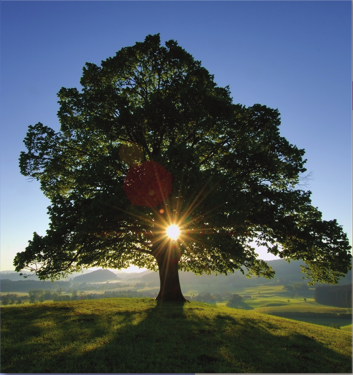
\includegraphics[width=\linewidth]{external/images/fig1.png}
\end{sbspanel}%
\end{sidebyside}%
\par
You may have heard that mathematics is the language of science.  In fact, professionals in nearly every discipline take advantage of mathematical methods to analyze data, identify trends, and predict the effects of change.  This process is called \terminology{mathematical modeling}.%
\par
A \terminology{model} is a simplified representation of reality that helps us understand a process or phenomenon.  Because it is a simplification, a model can never be completely accurate.  Instead, it should focus on those aspects of the real situation that will help us answer specific questions. Here is an example.%
\par
The world's population is growing at different rates in different nations.  Many factors, including economic and social forces, influence the birth rate.  Is there a connection between birth rates and education levels?%
\par
The figure shows the birth rate plotted against the female literacy rate in 148 countries.  Although the data points do not all lie precisely on a line, we see a generally decreasing trend:  the higher the literacy rate, the lower the birth rate.%
\begin{sidebyside}{1}{0.1}{0.1}{0}%
\begin{sbspanel}{0.8}%
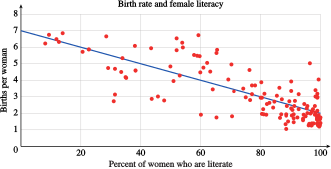
\includegraphics[width=\linewidth]{external/images/BirthRateVsFemaleLiteracy.pdf}
\end{sbspanel}%
\end{sidebyside}%
\par
The \terminology{regression line} provides a model for this trend, and a tool for analyzing the data. In this chapter we study the properties of linear models and some techniques for fitting a linear model to data.%
\end{introduction}%
%
%
\typeout{************************************************}
\typeout{Section 1.1 Linear Models}
\typeout{************************************************}
%
\begin{sectionptx}{Section}{Linear Models}{}{Linear Models}{}{}{section-LinMod}
\begin{introduction}{}%
\begin{investigation}{Investigation}{Sales on Commission.}{investigation-investigation-commission}%
Delbert is offered a part-time job selling restaurant equipment. He will be paid \textdollar{}1000 per month plus a 6\% commission on his sales. The sales manager tells Delbert he can expect to sell about \textdollar{}8000 worth of equipment per month. To help him decide whether to accept the job, Delbert does a few calculations.%
\par
%
\begin{enumerate}
\item{}Based on the sales manager’s estimate, what monthly income can Delbert expect from this job? What annual salary would that provide?%
\item{}What would Delbert’s monthly salary be if he sold only \textdollar{}5000 of equipment per month? What would his salary be if he sold \textdollar{}10,000 worth per month? Compute monthly incomes for each sales total shown in the table.%
\begin{sidebyside}{2}{0.0125}{0.0125}{0.025}%
\begin{sbspanel}{0.4}%
\resizebox{\ifdim\width > \linewidth\linewidth\else\width\fi}{!}{%
{\centering%
{\tabularfont%
\begin{tabular}{AcAcA}\hrulethick
Sales&Income\tabularnewline\hrulethin
5000&\tabularnewline\hrulethin
8000&\tabularnewline\hrulethin
10,000&\tabularnewline\hrulethin
12,000&\tabularnewline\hrulethin
15,000&\tabularnewline\hrulethin
18,000&\tabularnewline\hrulethin
20,000&\tabularnewline\hrulethin
25,000&\tabularnewline\hrulethin
30,000&\tabularnewline\hrulethin
35,000&\tabularnewline\hrulethin
~&\tabularnewline\hrulethin
~&\tabularnewline\hrulethin
\end{tabular}
}%
\par}
}%
\end{sbspanel}%
\begin{sbspanel}{0.55}%
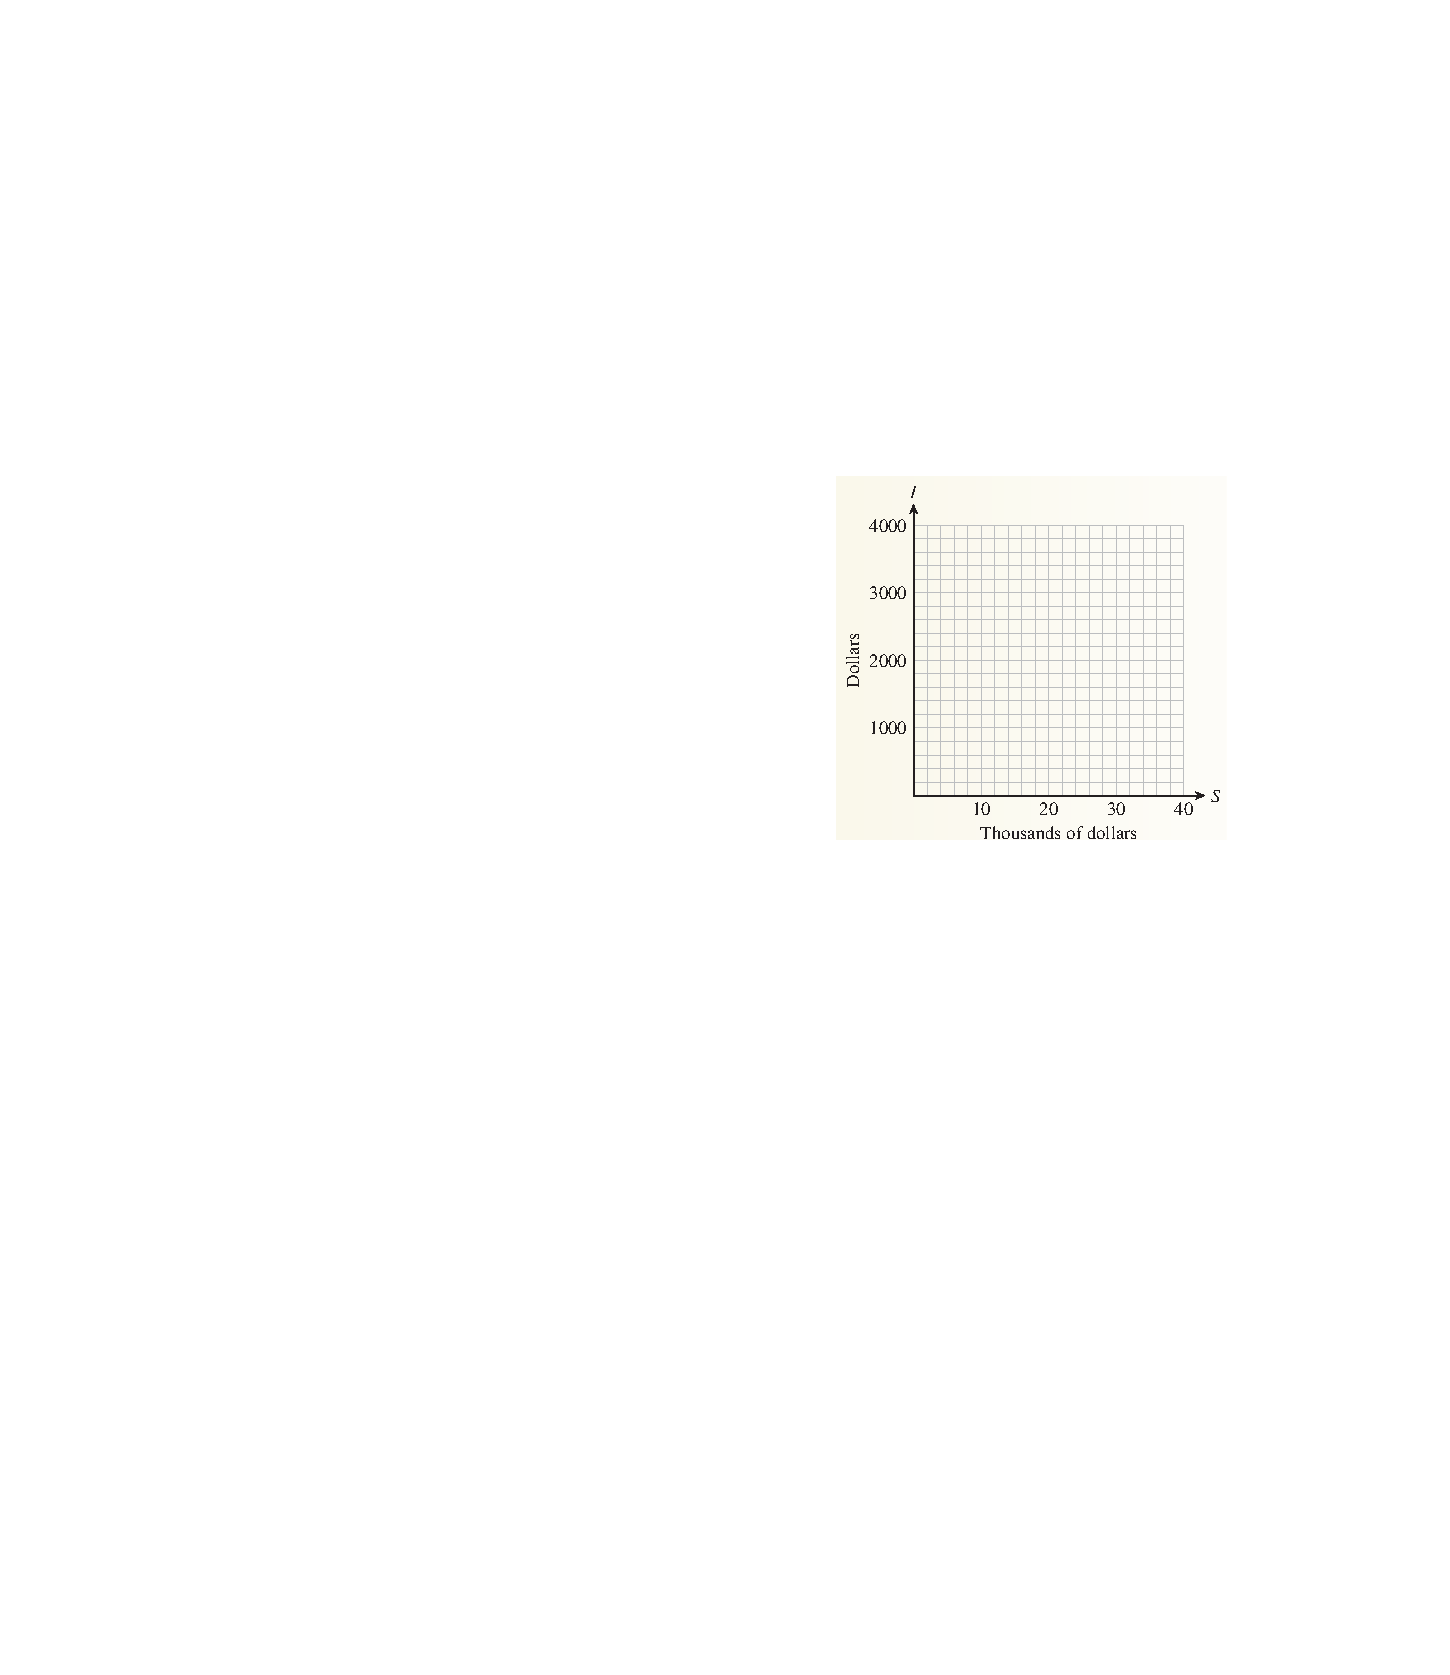
\includegraphics[width=\linewidth]{external/images/Investigation1Grid.pdf}
\end{sbspanel}%
\end{sidebyside}%
\item{}Plot your data points on a graph, using sales, \(S\), on the horizontal axis and income, \(I\), on the vertical axis, as shown in the figure. Connect the data points to show Delbert’s monthly income for all possible monthly sales totals.%
\item{}Add two new data points to the table by reading values from your graph.%
\item{}Write an algebraic expression for Delbert’s monthly income, \(I\), in terms of his monthly sales, \(S\). Use the description in the problem to help you:%
\par
He will be paid: \textdollar{}1000 . . . plus a 6\% commission on his sales.%
\par
\emph{Income} \(= \fillinmath{XXXXXXXXXXXXXXX}\)%
\item{}Test your formula from part (5) to see if it gives the same results as those you recorded in the table.%
\item{}Use your formula to find out what monthly sales total Delbert would need in order to have a monthly income of \textdollar{}2500.%
\item{}Each increase of \textdollar{}1000 in monthly sales increases Delbert’s monthly income by \fillintext{15}.%
\item{}Summarize the results of your work: In your own words, describe the relationship between Delbert’s monthly sales and his monthly income. Include in your discussion a description of your graph.%
\end{enumerate}
%
\end{investigation}%
\end{introduction}%
%
%
\typeout{************************************************}
\typeout{Subsection  Tables, Graphs and Equations}
\typeout{************************************************}
%
\begin{subsectionptx}{Subsection}{Tables, Graphs and Equations}{}{Tables, Graphs and Equations}{}{}{subsection-LinMod-c}
The first step in creating a model is to describe relationships between variables.  In \hyperref[investigation-investigation-commission]{Investigation~{\xreffont\ref{investigation-investigation-commission}}}, we analyzed the relationship between Delbert's sales and his income.  Starting from a verbal description, we represented the relationship in three different ways.%
\par
%
\begin{enumerate}
\item{}A \terminology{table of values}\index{table of values} displays specific data points with precise numerical values.%
\item{}A \terminology{graph}\index{graph} is a visual display of the data.  It is easier to spot trends and describe the overall behavior of the variables from a graph.%
\item{}An \terminology{algebraic equation}\index{algebraic equation} is a compact summary of the model.  It can be used to analyze the model and to make predictions%
\end{enumerate}
%
\par
We begin our study of modeling with some examples of \terminology{linear models}\index{linear models}.  In the examples that follow, observe the interplay among the three modeling tools, and how each contributes to the model.%
\begin{example}{Example}{}{example-example-Annelise}%
Annelise is on vacation at a seaside resort.  She can rent a bicycle from her hotel for \textdollar{}3 an hour, plus a \textdollar{}5 insurance fee.  (A fraction of an hour is charged as the same fraction of \textdollar{}3.)%
\par
%
\begin{enumerate}[label=\alph*]
\item{}Make a table of values showing the cost, \(C\), of renting a bike for various lengths of time, \(t\).%
\item{}Plot the points on a graph. Draw a curve through the data points.%
\item{}Write an equation for \(C\) in terms of \(t\).%
\end{enumerate}
%
\par\smallskip%
\noindent\textbf{\blocktitlefont Solution}.\hypertarget{solution-example-Annelise-b}{}\quad{}%
\begin{enumerate}[label=\alph*]
\item{}To find the cost, we multiply the time by \textdollar{}3, and add the result to the \textdollar{}5 insurance fee.  For example, the cost of a 1-hour bike ride is%
\begin{align*}
\text{Cost}\amp=(\$5\text{ insurance fee})+(\$3\text{ per hour})\times(\alert{1}\text{ hour})\\
C\amp=5+3(\alert{1})=8
\end{align*}
A 1-hour bike ride costs \textdollar{}8.  We record the results in a table, as shown here:%
\begin{sidebyside}{1}{0}{0}{0}%
\begin{sbspanel}{1}%
\resizebox{\ifdim\width > \linewidth\linewidth\else\width\fi}{!}{%
{\centering%
{\tabularfont%
\begin{tabular}{AcAcAcAcA}\crulethick{1-2}\crulethick{4-4}
\tablecelllines{c}{m}
{Length of rental\\
(hours)}
&\tablecelllines{c}{m}
{Cost of rental\\
(dollars)}
&&\((t,C)\)\tabularnewline\crulethin{1-2}\crulethin{4-4}
\(1\)&\(8\)&\(\quad C=5+3(\alert{1})\quad\)&\((1,8)\)\tabularnewline\crulethin{1-2}\crulethin{4-4}
\(2\)&\(11\)&\(C=5+3(\alert{2})\)&\((2,11)\)\tabularnewline\crulethin{1-2}\crulethin{4-4}
\(3\)&\(14\)&\(C=5+3(\alert{3})\)&\((3,14)\)\tabularnewline\crulethin{1-2}\crulethin{4-4}
\end{tabular}
}%
\par}
}%
\end{sbspanel}%
\end{sidebyside}%
\item{}\begin{sidebyside}{2}{0.0425}{0.0425}{0.085}%
\begin{sbspanel}{0.55}%
Each pair of values represents a point on the graph.  The first value gives the horizontal coordinate of the point, and the second value gives the vertical coordinate.  The points lie on a straight line, as shown in the figure.  The line extends infinitely in only one direction, because negative values of \(t\) do not make sense here.%
\end{sbspanel}%
\begin{sbspanel}{0.28}%
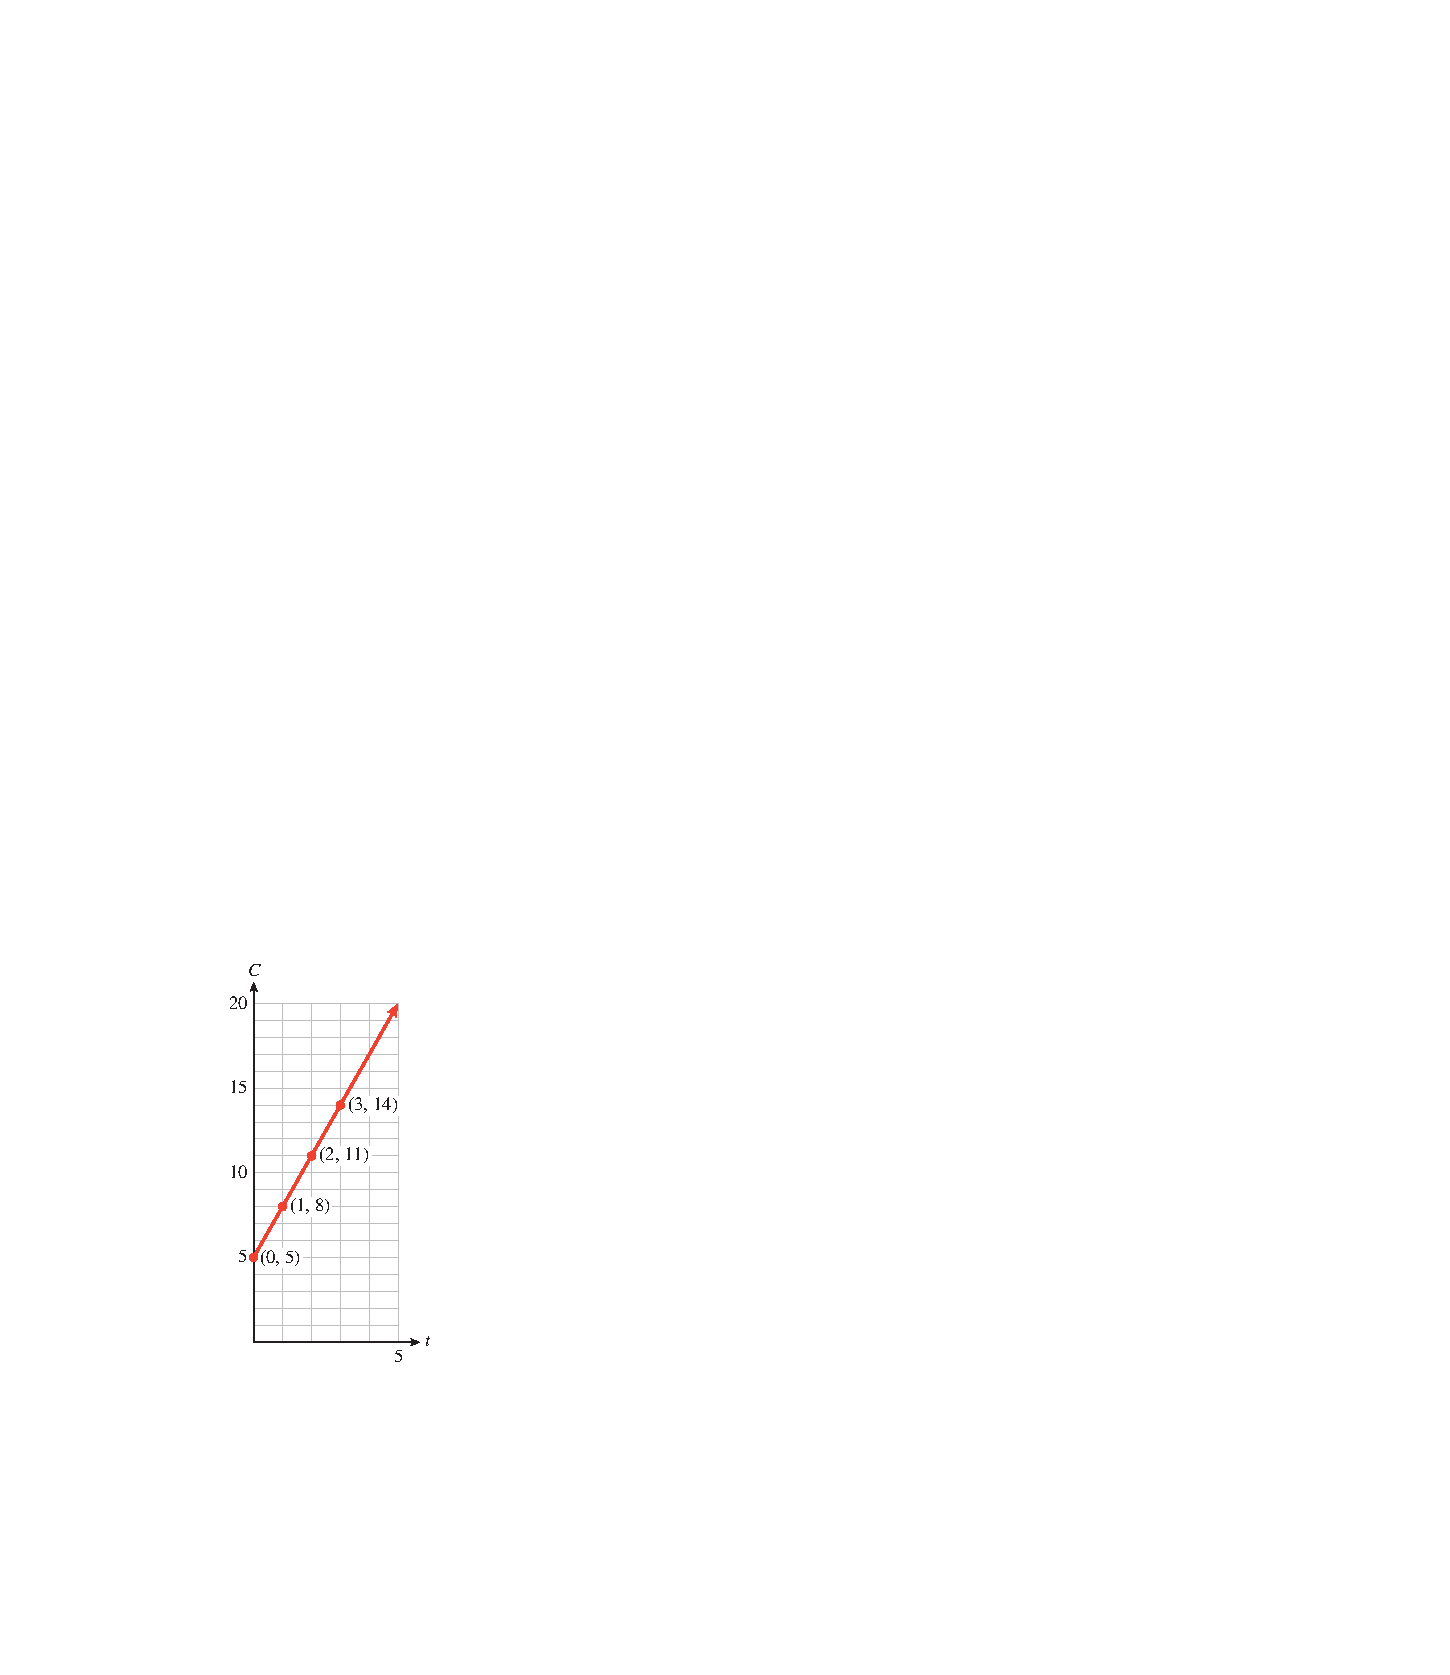
\includegraphics[width=\linewidth]{external/images/fig-Annelise-1.pdf}
\end{sbspanel}%
\end{sidebyside}%
%
\item{}To write an equation, we let \(C\) represent the cost of the rental, and we use \(t\) for the number of hours:%
\par
%
\begin{align*}
\text{Cost}\amp=(\$5\text{ insurance fee})+(\$3\text{ per hour})\times\text{(number of hours)}\\
C\amp=5+3\cdot t
\end{align*}
%
\end{enumerate}
%
\end{example}
\begin{inlineexercise}{Checkpoint}{QuickCheck 1.}{exercise-LinMod-c-f}%
When you graph the data given in a table, on which axis do you show the variable in the first row of the table?%
\par
\begin{itemize}[label=$\odot$,leftmargin=3em,]
\item{}The linear axis%
\item{}The horizontal axis%
\item{}The vertical axis%
\item{}Both axes%
\end{itemize}
%
\par\smallskip%
\noindent\textbf{\blocktitlefont Answer}.\hypertarget{answer-LinMod-c-f-c}{}\quad{}\(\text{The horizontal axis}\)%
\par\smallskip%
\noindent\textbf{\blocktitlefont Solution}.\hypertarget{solution-LinMod-c-f-d}{}\quad{}The horizontal axis%
\end{inlineexercise}%
\begin{example}{Example}{}{example-example-6hrbike}%
Use the equation \(C=5+3\cdot t\) you found in \hyperref[example-example-Annelise]{Example~{\xreffont\ref{example-example-Annelise}}} to answer the following questions.  Then show how to find the answers by using the graph.%
\par
%
\begin{enumerate}[label=\alph*]
\item{}How much will it cost Annelise to rent a bicycle for 6 hours?%
\item{}How long can Annelise bicycle for \textdollar{}18.50?%
\end{enumerate}
%
\par\smallskip%
\noindent\textbf{\blocktitlefont Solution}.\hypertarget{solution-example-6hrbike-b}{}\quad{}%
\begin{enumerate}[label=\alph*]
\item{}We substitute \(t=\alert{6}\) into the expression for \(C\) to find%
\begin{equation*}
C=5+3(\alert{6})=23
\end{equation*}
A 6-hour bike ride will cost \textdollar{}23.  The point \(P\) on the graph in the figure represents the cost of a 6-hour bike ride.  The value on the \(C\)-axis at the same height as point \(P\) is 23, so a 6-hour bike ride costs \textdollar{}23.%
\item{}\begin{sidebyside}{2}{0.0125}{0.0125}{0.025}%
\begin{sbspanel}{0.6}%
We substitute \(C=\alert{18.50}\) into the equation and solve for \(t\).%
\begin{align*}
\alert{18.50}\amp=5+3t\\
13.50\amp=3t\\
t\amp=4.5
\end{align*}
For \textdollar{}18.50 Annelise can bicycle for 4½ hours. The point \(Q\) on the graph represents an \textdollar{}18.50 bike ride. The value on the \(t\)-axis below point \(Q\) is 4.5, so \textdollar{}18.50 will buy a 4.5 hour bike ride.%
\end{sbspanel}%
\begin{sbspanel}{0.35}%
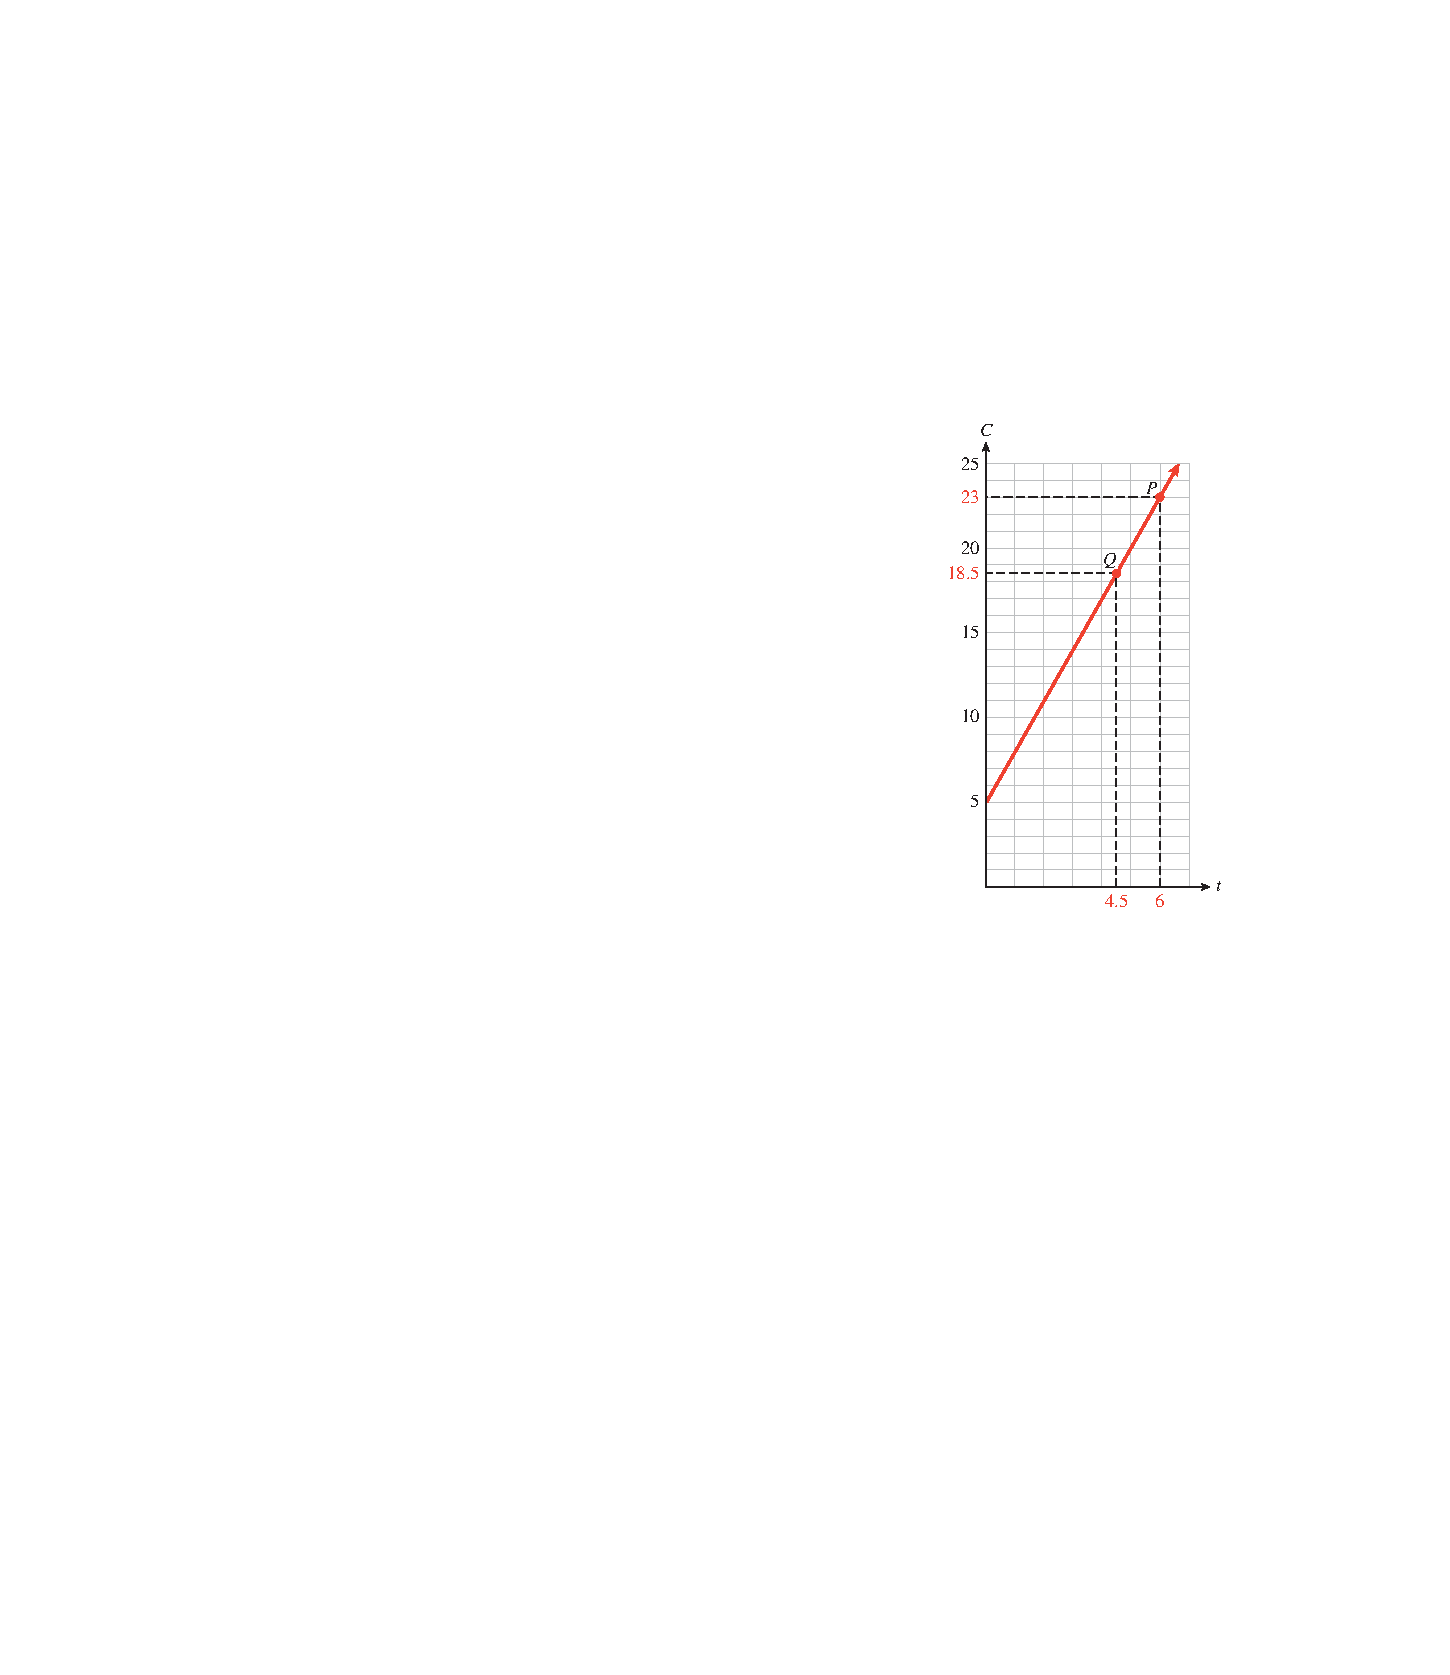
\includegraphics[width=\linewidth]{external/images/fig1-2.pdf}
\end{sbspanel}%
\end{sidebyside}%
%
\end{enumerate}
%
\end{example}
\begin{note}{Note}{}{note-LinMod-c-h}%
In \hyperref[example-example-6hrbike]{Example~{\xreffont\ref{example-example-6hrbike}}}, notice the different algebraic techniques we used in parts (a) and (b).%
\par
%
\begin{itemize}[label=\textbullet]
\item{}In part (a), we were given a value of \(t\) and we \terminology{evaluated the expression}  \(5+3t\) to find \(C\).%
\item{}In part (b) we were given a value of \(C\) and we \terminology{solved the equation} \(C=5+3t\) to find \(t\).%
\end{itemize}
%
\end{note}
\begin{inlineexercise}{Checkpoint}{Practice 1.}{exercise-exercise-Frank-plants}%
Frank plants a dozen corn seedlings, each 6 inches tall. With plenty of water and sunlight they will grow approximately 2 inches per day.   Complete the table of values for the height, \(h\text{,}\) of the seedlings after \(t\) days.%
\par
Complete the table of values for the height, \(h\) of the seedlings after \(t\) days.%
\begin{center}%
{\tabularfont%
\begin{tabular}{AcAcAcAcAcAcA}
\(t\)&\(0\)&\(5\)&\(10\)&\(15\)&\(20\)\tabularnewline\hrulethin
\(h\)&\fillintext{2}&\fillintext{2}&\fillintext{2}&\fillintext{2}&\fillintext{2}\tabularnewline\hrulethin
\end{tabular}
}%
\end{center}%
%
\begin{enumerate}[label=\alph*.]
\item{}Write an equation for the height \(h\) of the seedlings in terms of the number \(t\) of days since they were planted.%
\par
Equation: \fillintext{20}%
\item{}Graph the equation.%
\end{enumerate}
%
\par
The graph of seedling height vs time for part (b) is shown below.%
\begin{sidebyside}{1}{0}{0.75}{0}%
\begin{sbspanel}{0.25}%
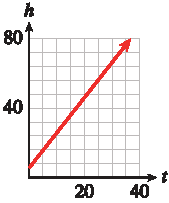
\includegraphics[width=\linewidth]{external/images/fig-in-ex-ans-1-1-1.pdf}
\end{sbspanel}%
\end{sidebyside}%
\par\smallskip%
\noindent\textbf{\blocktitlefont Answer 1}.\hypertarget{answer-exercise-Frank-plants-c}{}\quad{}\(6\)%
\par\smallskip%
\noindent\textbf{\blocktitlefont Answer 2}.\hypertarget{answer-exercise-Frank-plants-d}{}\quad{}\(16\)%
\par\smallskip%
\noindent\textbf{\blocktitlefont Answer 3}.\hypertarget{answer-exercise-Frank-plants-e}{}\quad{}\(26\)%
\par\smallskip%
\noindent\textbf{\blocktitlefont Answer 4}.\hypertarget{answer-exercise-Frank-plants-f}{}\quad{}\(36\)%
\par\smallskip%
\noindent\textbf{\blocktitlefont Answer 5}.\hypertarget{answer-exercise-Frank-plants-g}{}\quad{}\(46\)%
\par\smallskip%
\noindent\textbf{\blocktitlefont Answer 6}.\hypertarget{answer-exercise-Frank-plants-h}{}\quad{}\(h-2t = 6\)%
\par\smallskip%
\noindent\textbf{\blocktitlefont Solution}.\hypertarget{solution-exercise-Frank-plants-i}{}\quad{}\begin{center}%
{\tabularfont%
\begin{tabular}{AcAcAcAcAcAcA}
\(t\)&\(0\)&\(5\)&\(10\)&\(15\)&\(20\)\tabularnewline\hrulethin
\(h\)&6&16&26&36&46\tabularnewline\hrulethin
\end{tabular}
}%
\end{center}%
%
\begin{enumerate}[label=\alph*.]
\item{}\(\displaystyle h=6+2t\)%
\item{}The graph of seedling height vs time is shown below.%
\end{enumerate}
%
\end{inlineexercise}%
\begin{inlineexercise}{Checkpoint}{Practice 2.}{exercise-LinMod-c-j}%
Use your equation from Practice 1 to answer the questions.  Illustrate each answer on the graph.%
\par
%
\begin{enumerate}[label=\alph*.]
\item{}How tall is the corn after 3 weeks? Use ``ft'' for feet or ``in'' for inches.%
\par
Answer (including units): \fillintext{8}%
\item{}How long will it be before the corn is 6 feet tall? Use ``day'' for days.%
\par
Answer (including units): \fillintext{8}%
\end{enumerate}
%
\par
The graph below illustrates the answers.%
\begin{sidebyside}{1}{0}{0.75}{0}%
\begin{sbspanel}{0.25}%
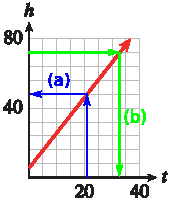
\includegraphics[width=\linewidth]{external/images/fig-in-ex-ans-1-1-2.pdf}
\end{sbspanel}%
\end{sidebyside}%
\par\smallskip%
\noindent\textbf{\blocktitlefont Answer 1}.\hypertarget{answer-LinMod-c-j-c}{}\quad{}\(48\ {\rm in}\)%
\par\smallskip%
\noindent\textbf{\blocktitlefont Answer 2}.\hypertarget{answer-LinMod-c-j-d}{}\quad{}\(33\ {\rm day}\)%
\par\smallskip%
\noindent\textbf{\blocktitlefont Solution}.\hypertarget{solution-LinMod-c-j-e}{}\quad{}%
\begin{enumerate}[label=\alph*.]
\item{}48 inches tall%
\item{}33 days%
\end{enumerate}
%
\par
A graph is below.%
\end{inlineexercise}%
\begin{inlineexercise}{Checkpoint}{Pause and Reflect.}{exercise-LinMod-c-k}%
What is the difference between an expression and an equation?%
\end{inlineexercise}%
\end{subsectionptx}
%
%
\typeout{************************************************}
\typeout{Subsection  Choosing Scales for the Axes}
\typeout{************************************************}
%
\begin{subsectionptx}{Subsection}{Choosing Scales for the Axes}{}{Choosing Scales for the Axes}{}{}{subsection-LinMod-d}
To create a useful graph, we must choose appropriate scales for the axes.%
\par
%
\begin{itemize}[label=\textbullet]
\item{}The axes must extend far enough to show the values of the variables.%
\item{}The tick marks should be equally spaced.%
\item{}Usually we should use no more than 10 or 15 tick marks.%
\end{itemize}
%
\begin{example}{Example}{}{example-example-home-price}%
In 1990, the median price of a home in the US was \textdollar{}92,000.  The median price increased by about \textdollar{}4700 per year over the next decade.%
\begin{enumerate}[label=\alph*]
\item{}Make a table of values showing the median price of a house in 1990, 1994, 1998, and 2000.%
\item{}Choose suitable scales for the axes and plot the values you found in part (a) on a graph. Use \(t\), the number of years since 1990, on the horizontal axis and the price of the house, \(P\), on the vertical axis.  Draw a curve through the points.%
\item{}Write an equation that expresses \(P\) in terms of \(t\).%
\item{}How much did the price of the house increase from 1990 to 1996?  Illustrate the increase on your graph.%
\end{enumerate}
%
\par\smallskip%
\noindent\textbf{\blocktitlefont Solution}.\hypertarget{solution-example-home-price-b}{}\quad{}%
\begin{enumerate}[label=\alph*]
\item{}In 1990 the median price was \textdollar{}92,000.  Four years later, in 1994, the price had increased by \(\alert{4}(4700)=18,800\) dollars, so%
\begin{equation*}
P=92,000+\alert{4}(4700)=110,800
\end{equation*}
In 1998 the price had increased by \(\alert{8}(4700)=37,600\)  dollars, so%
\begin{equation*}
P=92,000+\alert{8}(4700)=129,600
\end{equation*}
You can verify the price of the house in 2000 by a similar calculation.%
\begin{sidebyside}{1}{0}{0}{0}%
\begin{sbspanel}{1}%
\resizebox{\ifdim\width > \linewidth\linewidth\else\width\fi}{!}{%
{\centering%
{\tabularfont%
\begin{tabular}{AcAcAcA}\hrulethick
Year&Price of House)&\((t,P)\)\tabularnewline\hrulethin
\(1990\)&\(92,000\)&\((0,\, 92,000)\)\tabularnewline\hrulethin
\(1994\)&\(110,800\)&\((4,\, 110,800)\)\tabularnewline\hrulethin
\(1998\)&\(129,600\)&\((8,\, 129,600)\)\tabularnewline\hrulethin
\(2000\)&\(139,000\)&\((10,\, 139,000)\)\tabularnewline\hrulethin
\end{tabular}
}%
\par}
}%
\end{sbspanel}%
\end{sidebyside}%
\item{}We let \(t\) stand for the number of years since 1990, so that \(t=0\) in 1990, \(t=4\) in 1994, and so on.  To choose scales for the axes, we look at the values in the table.  For this graph we scale the horizontal axis, or \(t\)-axis, in 1-year intervals and the vertical axis, or \(P\)-axis, for \textdollar{}90,000 to \textdollar{}140,000 in intervals of \textdollar{}5,000. The points lie on a straight line, as shown in the figure.%
\begin{sidebyside}{1}{0.3}{0.3}{0}%
\begin{sbspanel}{0.4}%
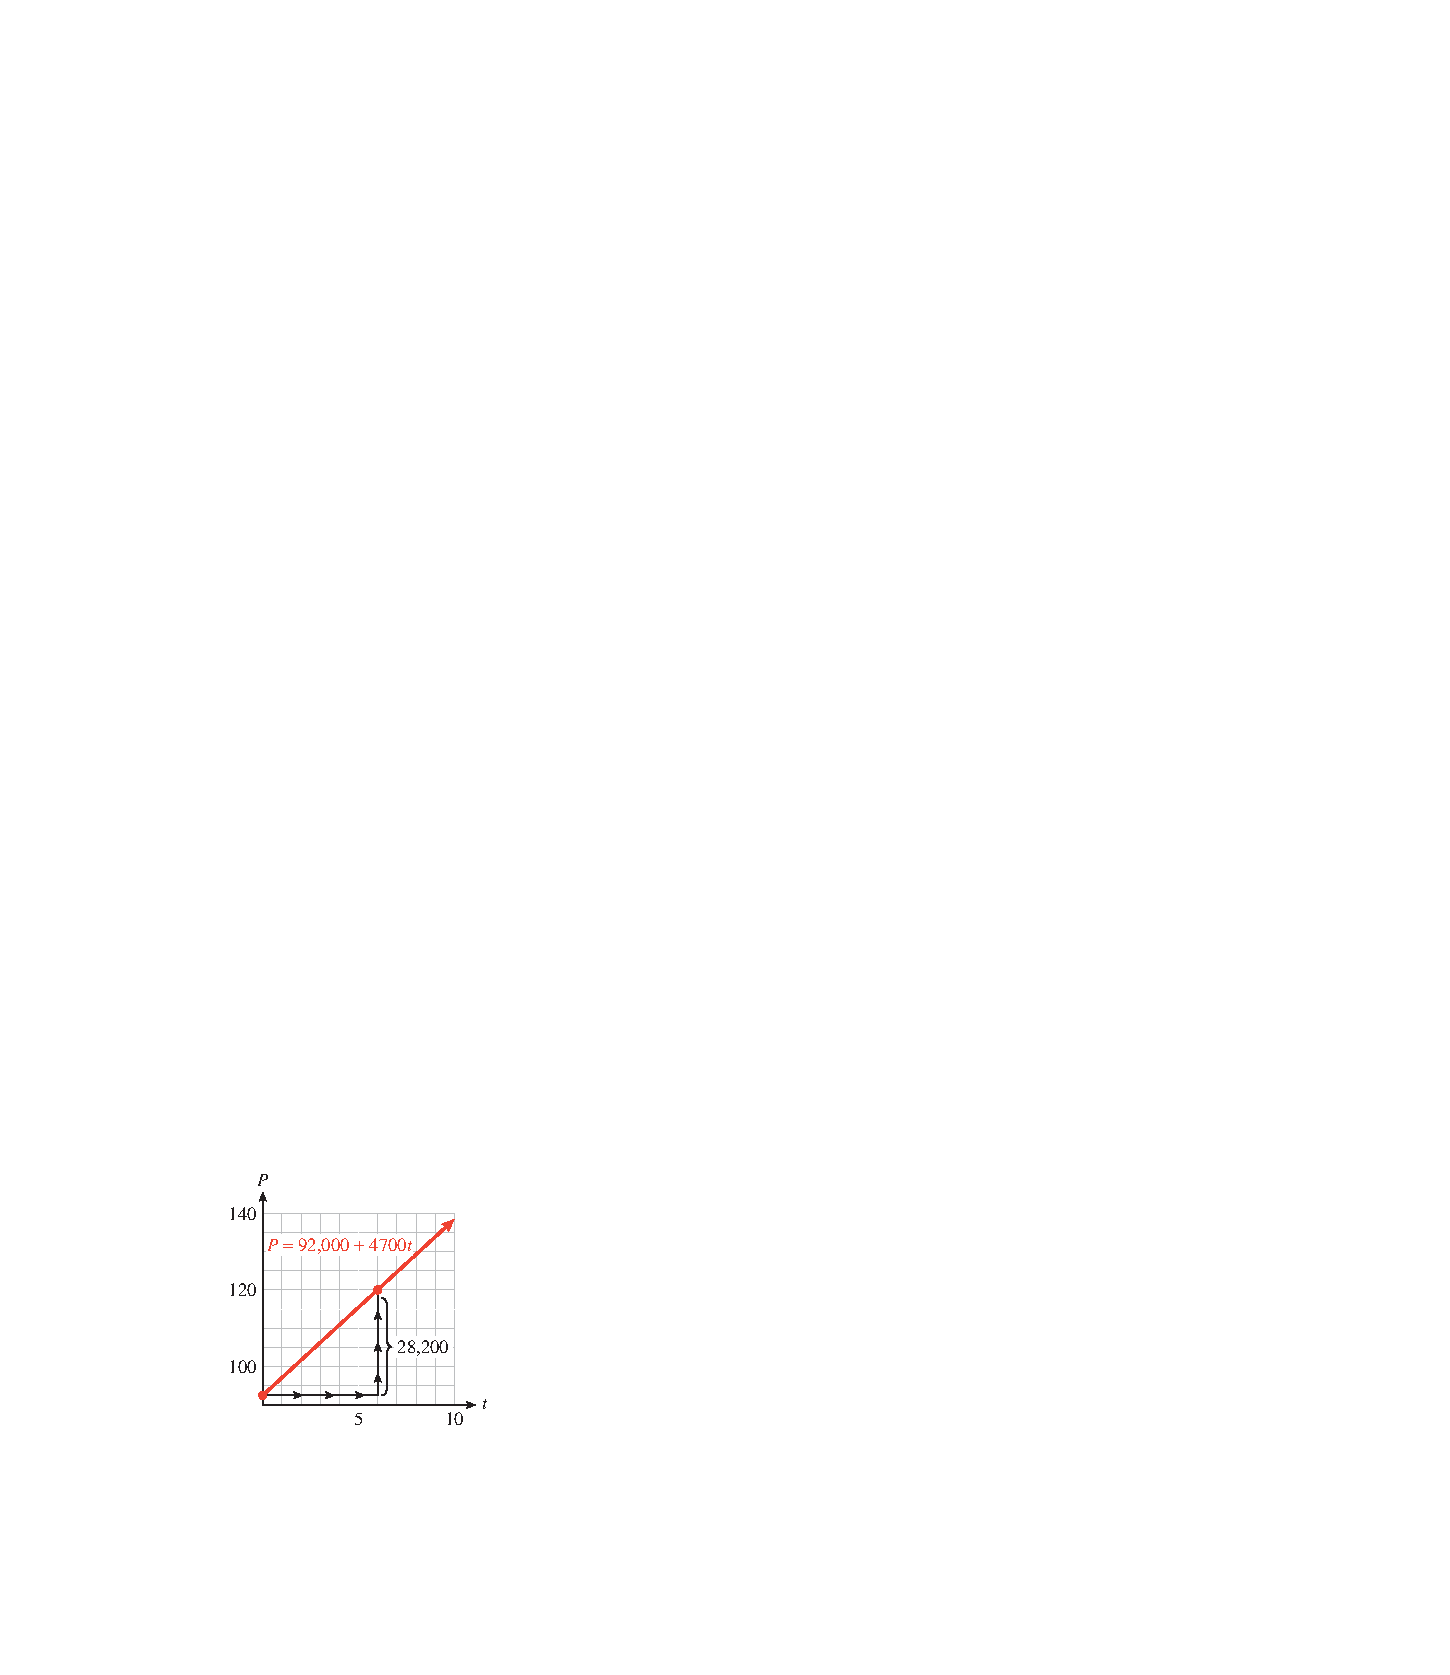
\includegraphics[width=\linewidth]{external/images/fig1-3.pdf}
\end{sbspanel}%
\end{sidebyside}%
\item{}Look back at the calculations in part (a).  The price of the house started at \textdollar{}92,000 in 1990 and increased by \(t \times 4700\) dollars after \(t\) years.  Thus,%
\begin{equation*}
P=92,000+4700t
\end{equation*}
%
\item{}We find the points on the graph for 1990 and 1996. These points lie above \(t=0\) and \(t=6\) on the \(t\)-axis.  Next we find the values on the \(P\)-axis corresponding to the two points.  The values are \(P=92,000\) in 1990 and \(P=120,200\) in 1996.  The increase in price is the difference of the two \(P\)-values.%
\begin{align*}
\text{increase in price}\amp=120,200-92,000\\
\amp=28,200
\end{align*}
The price of the home increased \textdollar{}28,200 between 1990 and 1996.  This increase is indicated by the arrows in the figure.%
\end{enumerate}
%
\end{example}
\begin{inlineexercise}{Checkpoint}{QuickCheck 2.}{exercise-LinMod-d-e}%
If \(C\) is expressed in terms of \(H\text{,}\) which variable goes on the horizontal axis?%
\par
\begin{itemize}[label=$\odot$,leftmargin=3em,]
\item{}\(\displaystyle C\)%
\item{}\(\displaystyle H\)%
\item{}\(\displaystyle x\)%
\item{}The smaller one%
\end{itemize}
%
\par\smallskip%
\noindent\textbf{\blocktitlefont Answer}.\hypertarget{answer-LinMod-d-e-c}{}\quad{}\(\text{Choice 2}\)%
\par\smallskip%
\noindent\textbf{\blocktitlefont Solution}.\hypertarget{solution-LinMod-d-e-d}{}\quad{}\(H\)%
\end{inlineexercise}%
\begin{note}{Note}{}{note-LinMod-d-f}%
The graphs in the preceding examples are \terminology{increasing graphs} \index{increasing graphs}.  As we move along the graph from left to right (in the direction of increasing \(t\) ), the second coordinate increases as well.  Try \hyperref[exercise-exercise-Silver-Lake]{Checkpoint~{\xreffont\ref{exercise-exercise-Silver-Lake}}}, which illustrates a \terminology{decreasing graph}\index{decreasing graph}.%
\end{note}
\begin{inlineexercise}{Checkpoint}{Practice 3.}{exercise-exercise-Silver-Lake}%
Silver Lake has been polluted by industrial waste products. The concentration of toxic chemicals in the water is currently 285 parts per million (ppm). Environmental officials would like to reduce the concentration by 15 ppm each year.%
\par
%
\begin{enumerate}[label=\alph*.]
\item{}Complete the table of values showing the desired concentration, \(C\text{,}\) of toxic chemicals \(t\) years from now. For each \(t\)-value, calculate the corresponding value for \(C\text{.}\)  Write your answers as ordered pairs.%
\begin{center}%
{\tabularfont%
\begin{tabular}{AcAcAcAcA}
\(t\)&\(C\)&&\((t,C)\)\tabularnewline\hrulethin
\(0\)&&\(C=285-15(\alert{0})\)&(0, \fillintext{3} )\tabularnewline\hrulethin
\(5\)&&\(C=285-15(\alert{5})\)&(5, \fillintext{3} )\tabularnewline\hrulethin
\(10\)&&\(C=285-15(\alert{10})\)&(10, \fillintext{3} )\tabularnewline\hrulethin
\(15\)&&\(C=285-15(\alert{15})\)&(15, \fillintext{3} )\tabularnewline\hrulethin
\end{tabular}
}%
\end{center}%
\item{}To choose scales for the axes, notice that the value of \(C\) starts at 285 and decreases from there. We'll scale the vertical axis up to 300, and use 10 tick marks at intervals of 30. Graph the ordered pairs on the grid, and connect them with a straight line.%
\item{}Write an equation for the concentration, \(C\text{,}\)  of toxic chemicals \(t\) years from now.%
\par
Equation: \fillintext{20}%
\end{enumerate}
%
\par
The graph for part(b):%
\begin{sidebyside}{1}{0.35}{0.35}{0}%
\begin{sbspanel}{0.3}%
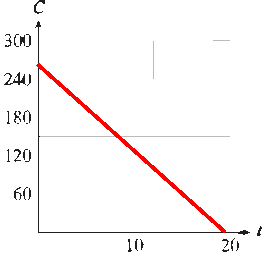
\includegraphics[width=\linewidth]{external/images/fig-in-ex-ans-1-1-3.pdf}
\end{sbspanel}%
\end{sidebyside}%
\par\smallskip%
\noindent\textbf{\blocktitlefont Hint}.\hypertarget{hint-exercise-Silver-Lake-c}{}\quad{}For part (c): The concentration is initially 285 ppm, and we subtract 15 ppm for each year that passes, or \(15 \times t\text{.}\)%
\par\smallskip%
\noindent\textbf{\blocktitlefont Answer 1}.\hypertarget{answer-exercise-Silver-Lake-d}{}\quad{}\(285\)%
\par\smallskip%
\noindent\textbf{\blocktitlefont Answer 2}.\hypertarget{answer-exercise-Silver-Lake-e}{}\quad{}\(210\)%
\par\smallskip%
\noindent\textbf{\blocktitlefont Answer 3}.\hypertarget{answer-exercise-Silver-Lake-f}{}\quad{}\(135\)%
\par\smallskip%
\noindent\textbf{\blocktitlefont Answer 4}.\hypertarget{answer-exercise-Silver-Lake-g}{}\quad{}\(60\)%
\par\smallskip%
\noindent\textbf{\blocktitlefont Answer 5}.\hypertarget{answer-exercise-Silver-Lake-h}{}\quad{}\(C+15t = 285\)%
\par\smallskip%
\noindent\textbf{\blocktitlefont Solution}.\hypertarget{solution-exercise-Silver-Lake-i}{}\quad{}%
\begin{enumerate}[label=\alph*.]
\item{}\begin{center}%
{\tabularfont%
\begin{tabular}{AcA}
\((t,C)\)\tabularnewline\hrulethin
\((0,285)\)\tabularnewline\hrulethin
\((5,210)\)\tabularnewline\hrulethin
\((10,135)\)\tabularnewline\hrulethin
\((15,60)\)\tabularnewline\hrulethin
\end{tabular}
}%
\end{center}%
%
\item{}The graph is shown below.%
\item{}\(\displaystyle C=285-15t\)%
\end{enumerate}
%
\end{inlineexercise}%
\begin{note}{Note}{}{note-LinMod-d-h}%
In the previous Exercise, we extend the graph until it reaches the horizontal axis, but no farther.  Points with negative \(C\)-coordinates have no meaning for the problem.%
\end{note}
\begin{inlineexercise}{Checkpoint}{QuickCheck 3.}{exercise-LinMod-d-i}%
If \(x \gt 5\text{,}\) what is true about \(-2x\text{?}\)%
\par
\begin{itemize}[label=$\odot$,leftmargin=3em,]
\item{}It is greater than 3%
\item{}It is less than 3%
\item{}It is greater than 10%
\item{}It is less than -10%
\end{itemize}
%
\par\smallskip%
\noindent\textbf{\blocktitlefont Answer}.\hypertarget{answer-LinMod-d-i-c}{}\quad{}\(\text{It is less than -10}\)%
\par\smallskip%
\noindent\textbf{\blocktitlefont Solution}.\hypertarget{solution-LinMod-d-i-d}{}\quad{}\(-2x\) is less than \(-10\text{.}\)%
\end{inlineexercise}%
\begin{technology}{Technology}{Graphing an Equation.}{technology-LinMod-d-j}%
We can use a graphing utililty to graph an equation. On most utilities, we follow three steps.%
\par
To Graph an Equation:%
\par
%
\begin{enumerate}
\item{}Press \kbd{Y=} and enter the equation you wish to graph.%
\item{}Press \kbd{WINDOW} and select a suitable graphing window.%
\item{}Press \kbd{GRAPH}%
\end{enumerate}
%
\end{technology}
\begin{example}{Example}{Using a Graphing Utility.}{example-graphing-calculator}%
In \hyperref[example-example-home-price]{Example~{\xreffont\ref{example-example-home-price}}}, we found the equation%
\begin{equation*}
P = 92,000 + 4700t
\end{equation*}
for the median price of a house \(t\) years after 1990. Graph this equation with technology.%
\par\smallskip%
\noindent\textbf{\blocktitlefont Solution}.\hypertarget{solution-graphing-calculator-c}{}\quad{}To begin, we press \kbd{Y=} and enter%
\begin{equation*}
Y1 = 92,000 + 4700X
\end{equation*}
%
\par
For this graph, we’ll use the grid in \hyperref[example-example-home-price]{Example~{\xreffont\ref{example-example-home-price}}} for our window settings, so we press \kbd{WINDOW} and enter%
\begin{sidebyside}{1}{0}{0}{0}%
\begin{sbspanel}{1}%
\resizebox{\ifdim\width > \linewidth\linewidth\else\width\fi}{!}{%
{\centering%
{\tabularfont%
\begin{tabular}{lll}
Xmin\(=0\)&&Xmax\(=10\)\tabularnewline[0pt]
Ymin\(=90,000\)&&Ymax\(=140,000\)
\end{tabular}
}%
\par}
}%
\end{sbspanel}%
\end{sidebyside}%
\par
Finally, we press \kbd{GRAPH}. The graph is shown in the figure.%
\begin{sidebyside}{1}{0.3}{0.3}{0}%
\begin{sbspanel}{0.4}%
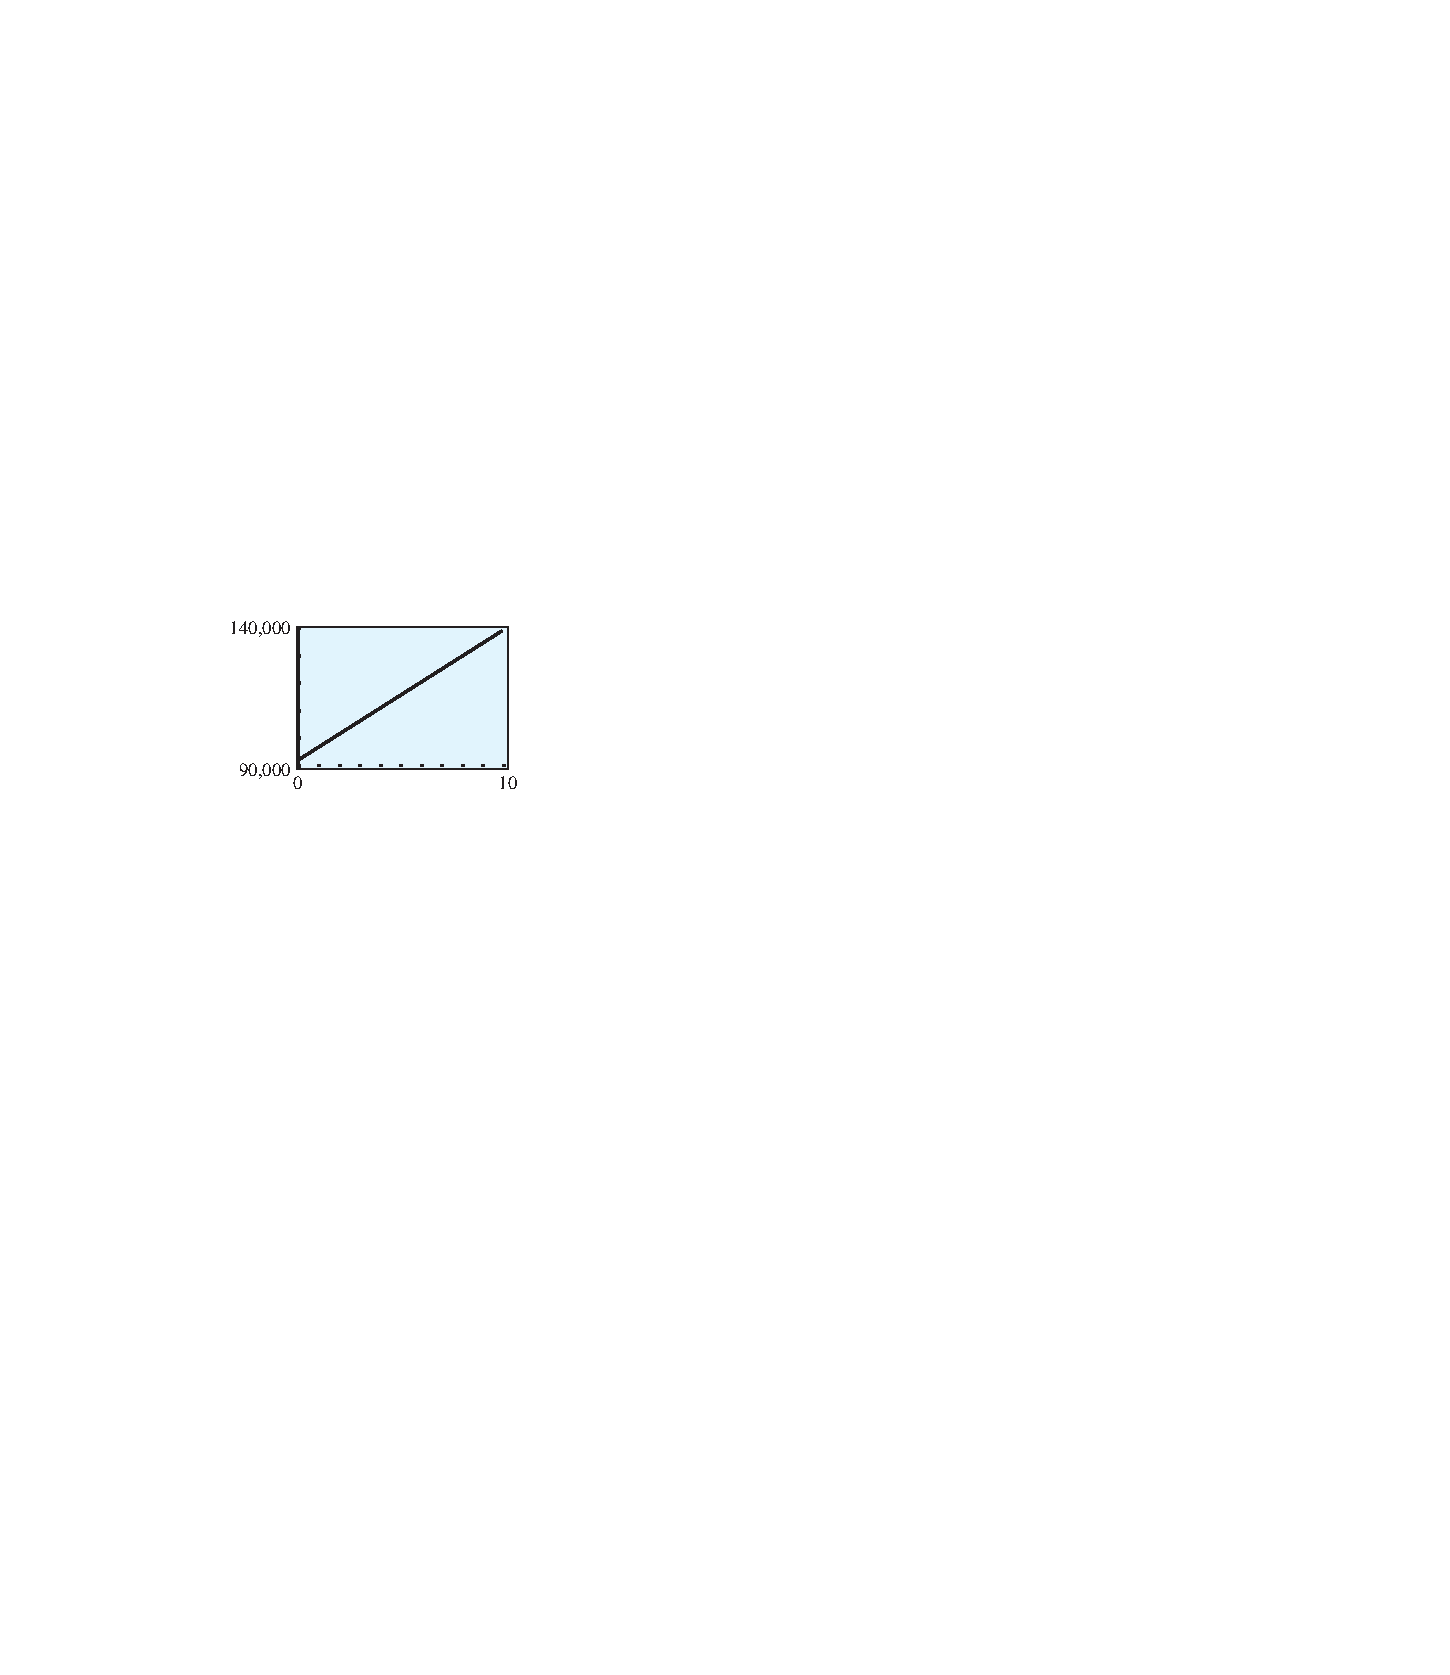
\includegraphics[width=\linewidth]{external/images/fig-GC-house-price.pdf}
\end{sbspanel}%
\end{sidebyside}%
\end{example}
\begin{inlineexercise}{Checkpoint}{Practice 4.}{exercise-LinMod-d-l}%
%
\begin{enumerate}[label=\alph*.]
\item{}Solve the equation \(2y-1575=45x\) for \(y\) in terms of \(x\text{.}\)%
\par
\(y=\)\fillintext{10}%
\item{}Graph the equation with a graphing utility. Use the window%
\begin{center}%
{\tabularfont%
\begin{tabular}{lllll}
Xmin\(=-50\)&&Xmax\(=50\)&&Xscl\(=5\)\tabularnewline[0pt]
Ymin\(=-500\)&&Ymax\(=1000\)&&Yscl\(=100\)
\end{tabular}
}%
\end{center}%
\item{}Sketch the graph on paper. Use the window settings to choose appropriate scales for the axes.%
\end{enumerate}
%
\par
The graph for (b):%
\begin{sidebyside}{1}{0.05}{0.6}{0}%
\begin{sbspanel}{0.3}%
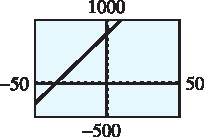
\includegraphics[width=\linewidth]{external/images/fig-in-ex-ans-1-1-4b.pdf}
\end{sbspanel}%
\end{sidebyside}%
\par
c.%
\begin{sidebyside}{1}{0.05}{0.65}{0}%
\begin{sbspanel}{0.25}%
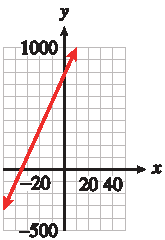
\includegraphics[width=\linewidth]{external/images/fig-in-ex-ans-1-1-4c.pdf}
\end{sbspanel}%
\end{sidebyside}%
\par\smallskip%
\noindent\textbf{\blocktitlefont Answer}.\hypertarget{answer-LinMod-d-l-c}{}\quad{}\(\frac{1575+45x}{2}\)%
\par\smallskip%
\noindent\textbf{\blocktitlefont Solution}.\hypertarget{solution-LinMod-d-l-d}{}\quad{}%
\begin{enumerate}[label=\alph*.]
\item{}\(\displaystyle y=(1575+45x)/2\)%
\item{}The calculator graph is shown below.%
\item{}The graph is shown below.%
\end{enumerate}
%
\end{inlineexercise}%
\begin{inlineexercise}{Checkpoint}{QuickCheck 4.}{exercise-LinMod-d-m}%
\begin{sidebyside}{1}{0.3}{0.3}{0}%
\begin{sbspanel}{0.4}%
\resizebox{\linewidth}{!}{%
\tikzset{%
}
\begin{tikzpicture} [scale=.8]
\draw[cyan] (0,0) grid (5,5);
\draw[black,thick,->,>=stealth'] (0,0)--(5.8,0);
\draw[black,thick,->,>=stealth'] (0,0)--(0,5.6);

\draw[black, thick] (1,0.14) --++(0,-.28) node[below, yshift=-2, fill=white, inner sep=1, scale=.9] {$5$};
\draw[black, thick] (2,0.14) --++(0,-.28) node[below, yshift=-2, fill=white, inner sep=1, scale=.9] {$20$};
\draw[black, thick] (3,0.14) --++(0,-.28) node[below, yshift=-2, fill=white, inner sep=1, scale=.9] {$30$};
\draw[black, thick] (4,0.14) --++(0,-.28) node[below, yshift=-2, fill=white, inner sep=1, scale=.9] {$50$};
\draw[black, thick] (5,0.14) --++(0,-.28) node[below, yshift=-2, fill=white, inner sep=1, scale=.9] {$100$};


\draw[black, thick] (0.14,1) --++(-.28,0) node[left, xshift=-2, fill=white, inner sep=1, scale=.9] {$20$};
\draw[black, thick] (0.14,2) --++(-.28,0) node[left, xshift=-2, fill=white, inner sep=1, scale=.9] {$25$};
\draw[black, thick] (0.14,3) --++(-.28,0) node[left, xshift=-2, fill=white, inner sep=1, scale=.9] {$30$};
\draw[black, thick] (0.14,4) --++(-.28,0) node[left, xshift=-2, fill=white, inner sep=1, scale=.9] {$35$};
\draw[black, thick] (0.14,5) --++(-.28,0) node[left, xshift=-2, fill=white, inner sep=1, scale=.9] {$40$};
\end{tikzpicture}
}%
\end{sbspanel}%
\end{sidebyside}%
\par
What is wrong with the grid above?%
\par
\begin{itemize}[label=$\odot$,leftmargin=3em,]
\item{}The grid lines on the \(x\)-axis are not evenly spaced.%
\item{}The scale on the \(y\)-axis does not start at 0.%
\item{}The axes are not labeled with the variables.%
\item{}All of the above.%
\end{itemize}
%
\par\smallskip%
\noindent\textbf{\blocktitlefont Answer}.\hypertarget{answer-LinMod-d-m-c}{}\quad{}\(\text{Choice 4}\)%
\end{inlineexercise}%
\end{subsectionptx}
%
%
\typeout{************************************************}
\typeout{Subsection  Linear Equations}
\typeout{************************************************}
%
\begin{subsectionptx}{Subsection}{Linear Equations}{}{Linear Equations}{}{}{subsection-LinMod-e}
All the models in the preceding examples have equations with a similar form:%
\begin{equation*}
\blert{y=\text{(starting value)}+\text{(rate of change)}\cdot x}
\end{equation*}
(We'll talk more about rate of change in \hyperref[section-slope-and-rate-of-change]{Section~{\xreffont\ref{section-slope-and-rate-of-change}}}.)  Their graphs were all portions of straight lines.  For this reason such equations are called  \terminology{linear equations}\index{linear equations}.  The order of the terms in the equation does not matter.  For example, the equation in \hyperref[example-example-Annelise]{Example~{\xreffont\ref{example-example-Annelise}}},%
\begin{equation*}
C=5+3t
\end{equation*}
can be written equivalently as%
\begin{equation*}
-3t+C=5
\end{equation*}
and the equation in \hyperref[example-example-home-price]{Example~{\xreffont\ref{example-example-home-price}}},%
\begin{equation*}
P=92,000+4700t
\end{equation*}
can be written as%
\begin{equation*}
-4700t +P=92,000
\end{equation*}
This form of a linear equation, \(Ax+By=C \), is called the \terminology{general form}\index{general form}.%
\begin{assemblage}{Assemblage}{General Form for a Linear Equation.}{assemblage-LinMod-e-c}%
The graph of any equation%
\begin{equation*}
Ax+By=C
\end{equation*}
where \(A\) and \(B\) are not both equal to zero, is a straight line.%
\end{assemblage}
\begin{example}{Example}{}{example-example-advertising}%
The manager at Albert's Appliances has \textdollar{}3000 to spend on advertising for the next fiscal quarter.  A 30-second spot on television costs \textdollar{}150 per broadcast, and a 30-second radio ad costs \textdollar{}50.%
\par
%
\begin{enumerate}[label=\alph*]
\item{}The manager decides to buy \(x\) television ads and \(y\) radio ads.  Write an equation relating \(x\) and \(y\).%
\item{}Make a table of values showing several choices for \(x\) and \(y\).%
\item{}Plot the points from your table, and graph the equation.%
\end{enumerate}
%
\par\smallskip%
\noindent\textbf{\blocktitlefont Solution}.\hypertarget{solution-example-advertising-b}{}\quad{}%
\begin{enumerate}[label=\alph*]
\item{}Each television ad costs \textdollar{}150, so \(x\) ads will cost \textdollar{}\(150x\).  Similarly, \(y\) radio ads will cost \textdollar{}\(50y\).  The manager has \textdollar{}3000 to spend, so the sum of the costs must be \textdollar{}3000.  Thus,%
\begin{equation*}
150x+50y=3000
\end{equation*}
%
\item{}We choose some values of \(x\), and solve the equation for the corresponding value of \(y\).  For example, if \(x=\alert{10}\) then%
\begin{align*}
150(\alert{10})+50y\amp=300\\
1500+50y\amp=3000\\
50y\amp=1500\\
y\amp=30
\end{align*}
If the manager buys 10 television ads, she can also buy 30 radio ads.  You can verify the other entries in the table.%
\begin{sidebyside}{1}{0}{0}{0}%
\begin{sbspanel}{1}%
\resizebox{\ifdim\width > \linewidth\linewidth\else\width\fi}{!}{%
{\centering%
{\tabularfont%
\begin{tabular}{AcAcAcAcAcA}\hrulethick
\(x\)&\(8\)&\(10\)&\(12\)&\(14\)\tabularnewline\hrulethin
\(y\)&\(36\)&\(30\)&\(24\)&\(18\)\tabularnewline\hrulethin
\end{tabular}
}%
\par}
}%
\end{sbspanel}%
\end{sidebyside}%
\item{}\begin{sidebyside}{2}{0}{0.02}{0.18}%
\begin{sbspanel}{0.5}%
We plot the points from the table. All the solutions lie on a straight line, as shown in the figure.%
\end{sbspanel}%
\begin{sbspanel}{0.3}%
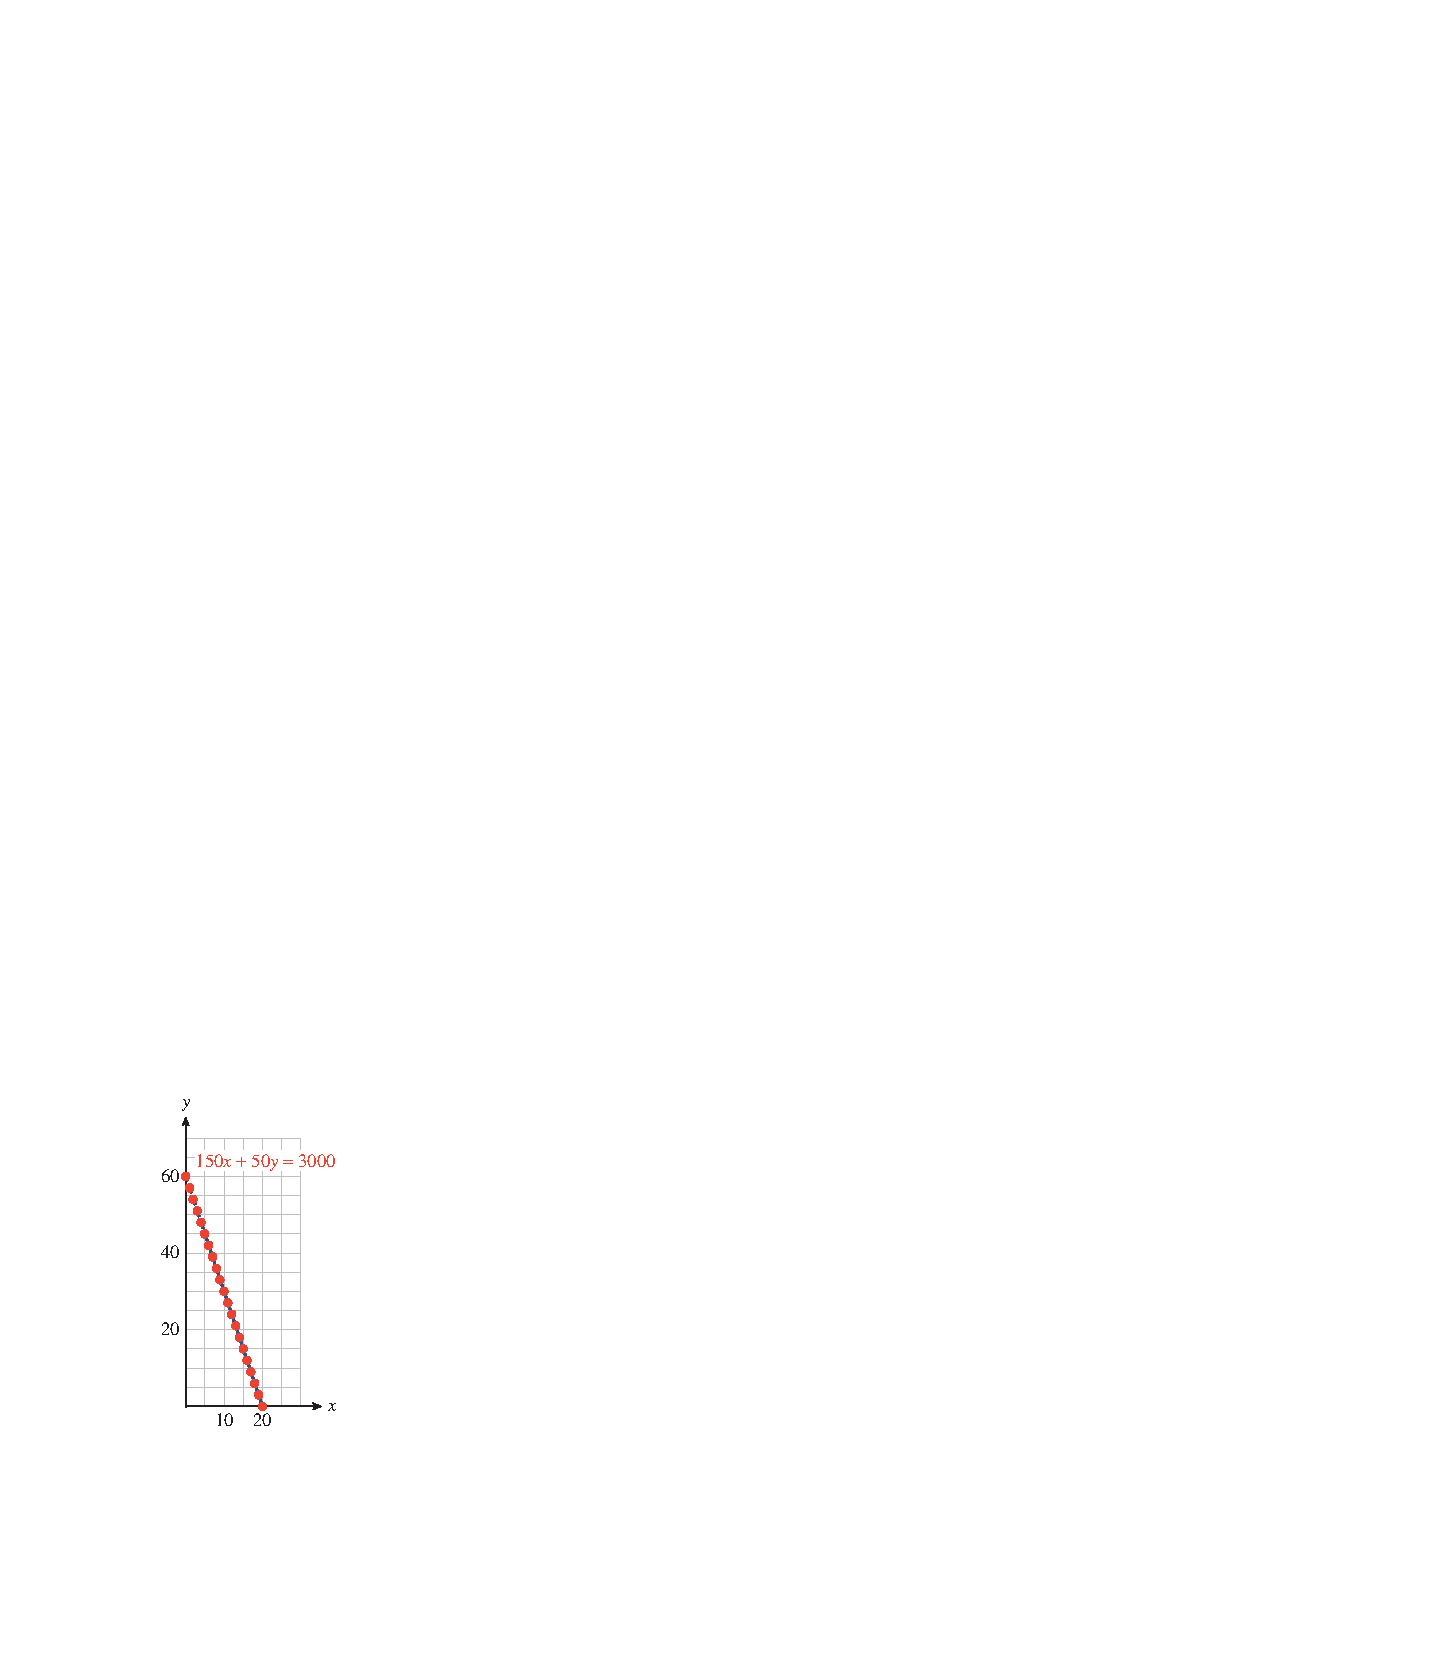
\includegraphics[width=\linewidth]{external/images/fig-example-advertising.pdf}
\end{sbspanel}%
\end{sidebyside}%
%
\end{enumerate}
%
\end{example}
\begin{inlineexercise}{Checkpoint}{Practice 5.}{exercise-exercise-crops}%
In central Nebraska, each acre of corn requires 25 acre-inches of water per year, and each acre of winter wheat requires 18 acre-inches of water. (An acre-inch is the amount of water needed to cover one acre of land to a depth of one inch.) A farmer can count on 9000 acre-inches of water for the coming year. (Source: Institute of Agriculture and Natural Resources, University of Nebraska)%
\par
%
\begin{enumerate}[label=\alph*.]
\item{}Write an equation relating the number of acres of corn, \(x\text{,}\)  and the number of acres of wheat, \(y\text{,}\)  that the farmer can plant.%
\item{}Complete the table. Round your answers to tenths.%
\begin{center}%
{\tabularfont%
\begin{tabular}{AcAcAcAcAcA}
\(x\)&\(50\)&\(100\)&\(150\)&\(200\)\tabularnewline\hrulethin
\(y\)&\fillintext{4}&\fillintext{4}&\fillintext{4}&\fillintext{4}\tabularnewline\hrulethin
\end{tabular}
}%
\end{center}%
\end{enumerate}
%
\par\smallskip%
\noindent\textbf{\blocktitlefont Answer 1}.\hypertarget{answer-exercise-crops-c}{}\quad{}\(25x+18y = 9000\)%
\par\smallskip%
\noindent\textbf{\blocktitlefont Answer 2}.\hypertarget{answer-exercise-crops-d}{}\quad{}\(430.556\)%
\par\smallskip%
\noindent\textbf{\blocktitlefont Answer 3}.\hypertarget{answer-exercise-crops-e}{}\quad{}\(361.111\)%
\par\smallskip%
\noindent\textbf{\blocktitlefont Answer 4}.\hypertarget{answer-exercise-crops-f}{}\quad{}\(291.667\)%
\par\smallskip%
\noindent\textbf{\blocktitlefont Answer 5}.\hypertarget{answer-exercise-crops-g}{}\quad{}\(222.222\)%
\par\smallskip%
\noindent\textbf{\blocktitlefont Solution}.\hypertarget{solution-exercise-crops-h}{}\quad{}%
\begin{enumerate}[label=\alph*.]
\item{}\(\displaystyle 25x+18y=9000\)%
\item{}\begin{center}%
{\tabularfont%
\begin{tabular}{AcAcAcAcAcA}
\(x\)&\(50\)&\(100\)&\(150\)&\(200\)\tabularnewline\hrulethin
\(y\)&\(430.6\)&\(361.1\)&\(291.7\)&\(222.2\)\tabularnewline\hrulethin
\end{tabular}
}%
\end{center}%
%
\end{enumerate}
%
\end{inlineexercise}%
\begin{inlineexercise}{Checkpoint}{Pause and Reflect.}{exercise-LinMod-e-f}%
Write down two different equation forms for linear models.  Which do you think is easier to use?%
\end{inlineexercise}%
\end{subsectionptx}
%
%
\typeout{************************************************}
\typeout{Subsection  Intercepts}
\typeout{************************************************}
%
\begin{subsectionptx}{Subsection}{Intercepts}{}{Intercepts}{}{}{subsection-LinMod-f}
\begin{sidebyside}{2}{0}{0}{0.05}%
\begin{sbspanel}{0.25}[center]%
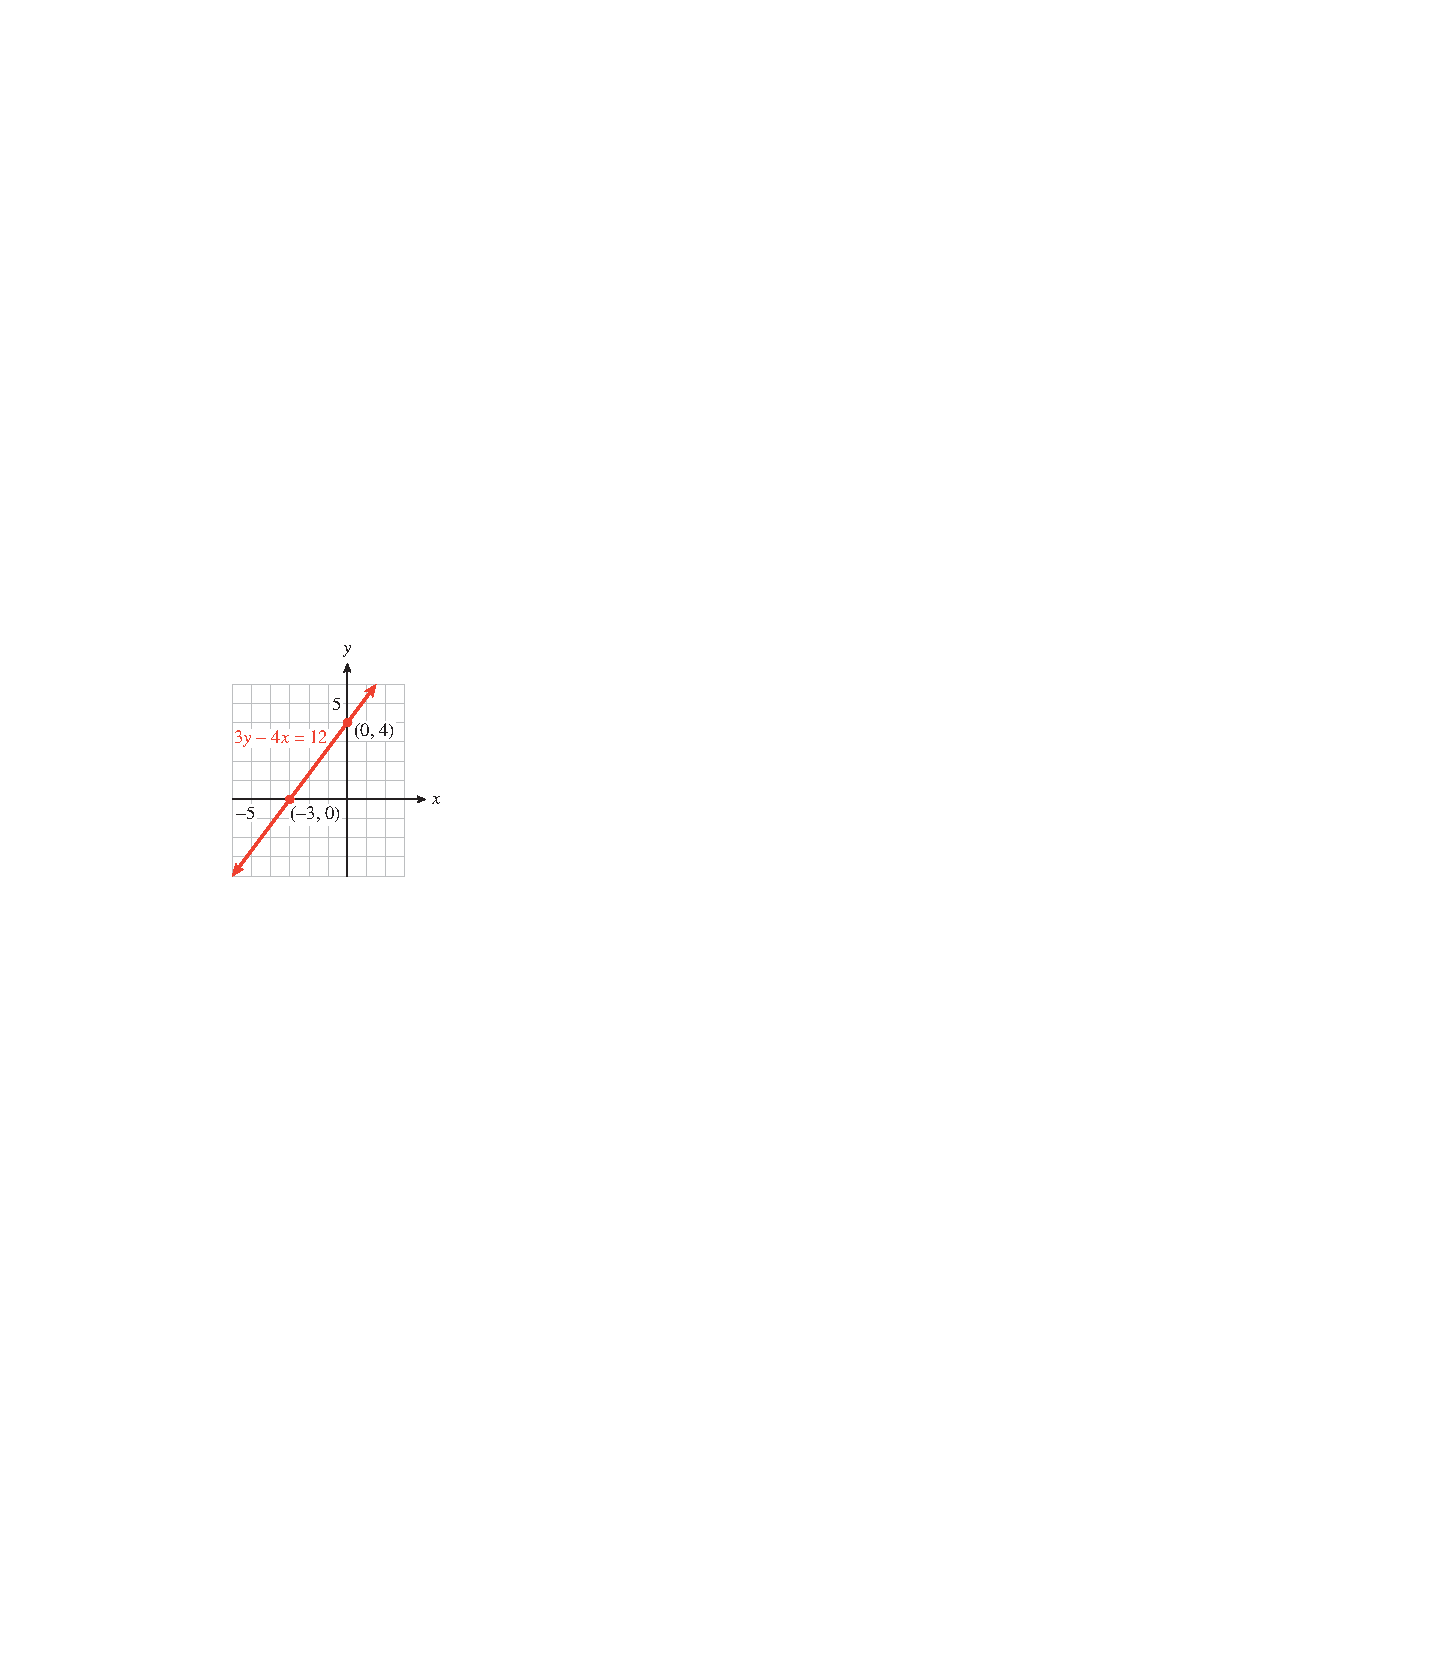
\includegraphics[width=\linewidth]{external/images/fig-intercepts.pdf}
\end{sbspanel}%
\begin{sbspanel}{0.7}[center]%
Consider the graph of the equation%
\begin{equation*}
3x-4y=12
\end{equation*}
shown at left. The points where the graph crosses the axes are called the \terminology{intercepts}\index{intercept} of the graph. The coordinates of these points are easy to find.%
\end{sbspanel}%
\end{sidebyside}%
\par
The \(y\)-coordinate of the \(x\)-intercept is zero, so we set \(y=\alert{0}\) in the equation to get%
\begin{align*}
3(\alert{0})-4x\amp=12\\
x=-3
\end{align*}
%
\par
The \(x\)-intercept is the point \((-3,0)\). Also, the \(x\)-coordinate of the \(y\)-intercept is zero, so we set \(x=\alert{0}\) in the equation to get%
\begin{gather*}
3y-4(\alert{0})=12\\
y=4
\end{gather*}
The \(y\)-intercept is \((0,4)\).%
\begin{inlineexercise}{Checkpoint}{QuickCheck 5.}{exercise-LinMod-f-e}%
What is the \(y\)-coordinate of any point on the \(x\)-axis?%
\par
\begin{itemize}[label=$\odot$,leftmargin=3em,]
\item{}\(\displaystyle (x,y)\)%
\item{}\(\displaystyle Y\)%
\item{}It depends on the value of \(x\)%
\item{}0%
\end{itemize}
%
\par\smallskip%
\noindent\textbf{\blocktitlefont Answer}.\hypertarget{answer-LinMod-f-e-c}{}\quad{}\(\text{Choice 4}\)%
\par\smallskip%
\noindent\textbf{\blocktitlefont Solution}.\hypertarget{solution-LinMod-f-e-d}{}\quad{}\(0\)%
\end{inlineexercise}%
\begin{assemblage}{Assemblage}{Intercepts of a Graph.}{assemblage-LinMod-f-f}%
The points where a graph crosses the axes are called the \terminology{intercepts of the graph}\index{intercept}.%
\begin{enumerate}
\item{}To find the \(y\)-intercept, set \(x=0\) and solve for \(y\).%
\item{}To find the \(x\)-intercept, set \(y=0\) and solve for \(x\)%
\end{enumerate}
%
\end{assemblage}
The intercepts of a graph tell us something about the situation it models.%
\begin{example}{Example}{}{example-example-intercepts}%
%
\begin{enumerate}[label=\alph*]
\item{}Find the intercepts of the graph in \hyperref[exercise-exercise-Silver-Lake]{Checkpoint~{\xreffont\ref{exercise-exercise-Silver-Lake}}}, about the pollution in Silver Lake.%
\item{}What do the intercepts tell us about the problem?%
\end{enumerate}
%
\par\smallskip%
\noindent\textbf{\blocktitlefont Solution}.\hypertarget{solution-example-intercepts-b}{}\quad{}%
\begin{enumerate}[label=\alph*]
\item{}An equation for the concentration of toxic chemicals is%
\begin{equation*}
C=285-15t
\end{equation*}
To find the \(C\)-intercept, set \(t\) equal to zero.%
\begin{equation*}
C=285-15(\alert{0})=285
\end{equation*}
The \(C\)-intercept is the point \((0, 285)\), or simply 285.%
\par
To find the \(t\)-intercept, set \(C\) equal to zero and solve for \(t\).%
\par
%
\begin{equation*}
\begin{aligned}[t]
\alert{0}\amp =285-15t \amp \amp \blert{\text{Add }15t \text{ to both sides.}}\\
15t\amp =285  \amp \amp \blert{\text{Divide both sides by 15.}}\\
t\amp =19 
\end{aligned}
\end{equation*}
%
\par
The \(t\)-intercept is the point \((19,0)\), or simply \(19\).%
\item{}The \(C\)-intercept represents the concentration of toxic chemicals in Silver Lake now:  When  \(t=0\), \(C=285\),  so the concentration is currently \(285\) ppm.%
\par
The \(t\)-intercept represents the number of years it will take for the concentration of toxic chemicals to drop to zero:  When \(C=0\), \(t=19\),  so it will take \(19\) years for the pollution to be eliminated entirely.%
\end{enumerate}
%
\end{example}
\begin{inlineexercise}{Checkpoint}{QuickCheck 6.}{exercise-LinMod-f-i}%
Delbert says that the intercepts of the line \(3x+5y=30\) are \((10,6)\text{.}\) What is wrong with his answer?%
\par
\begin{itemize}[label=$\odot$,leftmargin=3em,]
\item{}\((10,6)\) is not on the \(x\)-axis.%
\item{}An intercept must have a 0 coordinate.%
\item{}The line has two intercepts.%
\item{}All of the above%
\end{itemize}
%
\par\smallskip%
\noindent\textbf{\blocktitlefont Answer}.\hypertarget{answer-LinMod-f-i-c}{}\quad{}\(\text{Choice 4}\)%
\par\smallskip%
\noindent\textbf{\blocktitlefont Solution}.\hypertarget{solution-LinMod-f-i-d}{}\quad{}All of the above%
\end{inlineexercise}%
\begin{inlineexercise}{Checkpoint}{Practice 6.}{exercise-LinMod-f-j}%
Find the intercepts of the graph in \hyperref[example-example-advertising]{Example~{\xreffont\ref{example-example-advertising}}}, about the advertising budget for Albert's Appliances: \(150x + 50y = 3000\).%
\par
%
\begin{enumerate}[label=\alph*.]
\item{}Enter each intercept as an ordered pair.%
\par
The \(x\)-intercept is \fillintext{4}.%
\par
The \(y\)-intercept is \fillintext{4}.%
\item{}What do the intercepts tell us about the problem?%
\par
The \(x\)-intercept tells us:%
\par
\begin{itemize}[label=$\odot$,leftmargin=3em,]
\item{}A) the cost of the TV ads.%
\item{}B) the best number of TV ads.%
\item{}C) the most TV ads she can buy for the money.%
\item{}D) the average number of TV ads.%
\end{itemize}
%
\par
The \(y\)-intercept tells us:%
\par
\begin{itemize}[label=$\odot$,leftmargin=3em,]
\item{}A) the cost of the radio ads.%
\item{}B) the number of radio ads she bought%
\item{}C) the number of radio ads if no TV ads are bought.%
\item{}D) the average cost per ad.%
\end{itemize}
%
\end{enumerate}
%
\par\smallskip%
\noindent\textbf{\blocktitlefont Answer 1}.\hypertarget{answer-LinMod-f-j-c}{}\quad{}\(\left(20,0\right)\)%
\par\smallskip%
\noindent\textbf{\blocktitlefont Answer 2}.\hypertarget{answer-LinMod-f-j-d}{}\quad{}\(\left(0,60\right)\)%
\par\smallskip%
\noindent\textbf{\blocktitlefont Answer 3}.\hypertarget{answer-LinMod-f-j-e}{}\quad{}\(\text{C) the ... the money.}\)%
\par\smallskip%
\noindent\textbf{\blocktitlefont Answer 4}.\hypertarget{answer-LinMod-f-j-f}{}\quad{}\(\text{C) the ... are bought.}\)%
\par\smallskip%
\noindent\textbf{\blocktitlefont Solution}.\hypertarget{solution-LinMod-f-j-g}{}\quad{}%
\begin{enumerate}[label=\alph*.]
\item{}We find the \(x\)-intercept by setting \(y=0\) and solving for \(x\) to learn that \(x=20\text{,}\) so the \(x\)-intercept is \({\left(20,0\right)}\text{.}\)%
\par
We find the \(y\)-intercept by setting \(x=0\) and solving for \(y\) to learn that \(y=60\text{,}\) so the \(y\)-intercept is \({\left(0,60\right)}\text{.}\)%
\item{}The \(x\)-intercept has \(y=0\text{,}\) that is, it corresponds to when there are zero radio ads. The \(y\)-intercept has \(x=0\text{,}\) that is, it corresponds to when there are zero tv ads.%
\end{enumerate}
%
\end{inlineexercise}%
\begin{inlineexercise}{Checkpoint}{Pause and Reflect.}{exercise-LinMod-f-k}%
Explain how the words intercept and intersect are related, and how they are different.%
\end{inlineexercise}%
\end{subsectionptx}
%
%
\typeout{************************************************}
\typeout{Subsection  Intercept Method for Graphing Lines}
\typeout{************************************************}
%
\begin{subsectionptx}{Subsection}{Intercept Method for Graphing Lines}{}{Intercept Method for Graphing Lines}{}{}{subsection-LinMod-g}
Because we really only need two points to graph a linear equation, we might as well find the intercepts first and use them to draw the graph. The values of the intercepts will also help us choose suitable scales for the axes. It is always a good idea to find a third point as a check.%
\begin{example}{Example}{}{example-intercepts}%
%
\begin{enumerate}[label=\alph*]
\item{}Find the \(x\)- and \(y\)-intercepts of the graph of \(150x - 180y = 9000\).%
\item{}Use the intercepts to graph the equation. Find a third point as a check.%
\end{enumerate}
%
\par\smallskip%
\noindent\textbf{\blocktitlefont Solution}.\hypertarget{solution-intercepts-b}{}\quad{}%
\begin{enumerate}[label=\alph*]
\item{}To find the \(x\)-intercept, we set \(y = \alert{0}\).%
\par
%
\begin{equation*}
\begin{aligned}[t]
150x-18(\alert{0})\amp =9000 \amp \amp \blert{\text{Simpify.}}\\
150x\amp =9000 \amp \amp \blert{\text{Divide both sides by 150.}}\\
x\amp =60   \amp \amp  
\end{aligned}
\end{equation*}
%
\par
The \(x\)-intercept is the point \((60, 0)\). To find the \(y\)-intercept, we set \(x = \alert{0}\).%
\par
%
\begin{equation*}
\begin{aligned}[t]
150(\alert{0})-18y\amp =9000 \amp \amp \blert{\text{Simpify.}}\\
-180y\amp =9000 \amp \amp \blert{\text{Divide both sides by } -180\text{.}}\\
y\amp =-50   \amp \amp  
\end{aligned}
\end{equation*}
%
\par
The \(y\)-intercept is the point \((0, -50)\).%
\item{}We scale both axes in intervals of 10 and then plot the two intercepts, \((60, 0)\) and \((0, -50)\). We draw the line through them, as shown below. Finally, we find another point and check that it lies on this line. We choose \(x = \alert{20}\) and solve for \(y\).%
\begin{align*}
150(\alert{20}) -180y \amp = 9000\\
3000 -180y \amp = 9000\\
-180y \amp = 6000\\
y \amp =-33.\overline{3}
\end{align*}
We plot the point \((20, -33\frac{1}{3})\). Because this point lies on the line, we can be reasonably confident that our graph is correct.%
\begin{sidebyside}{1}{0.35}{0.35}{0}%
\begin{sbspanel}{0.3}%
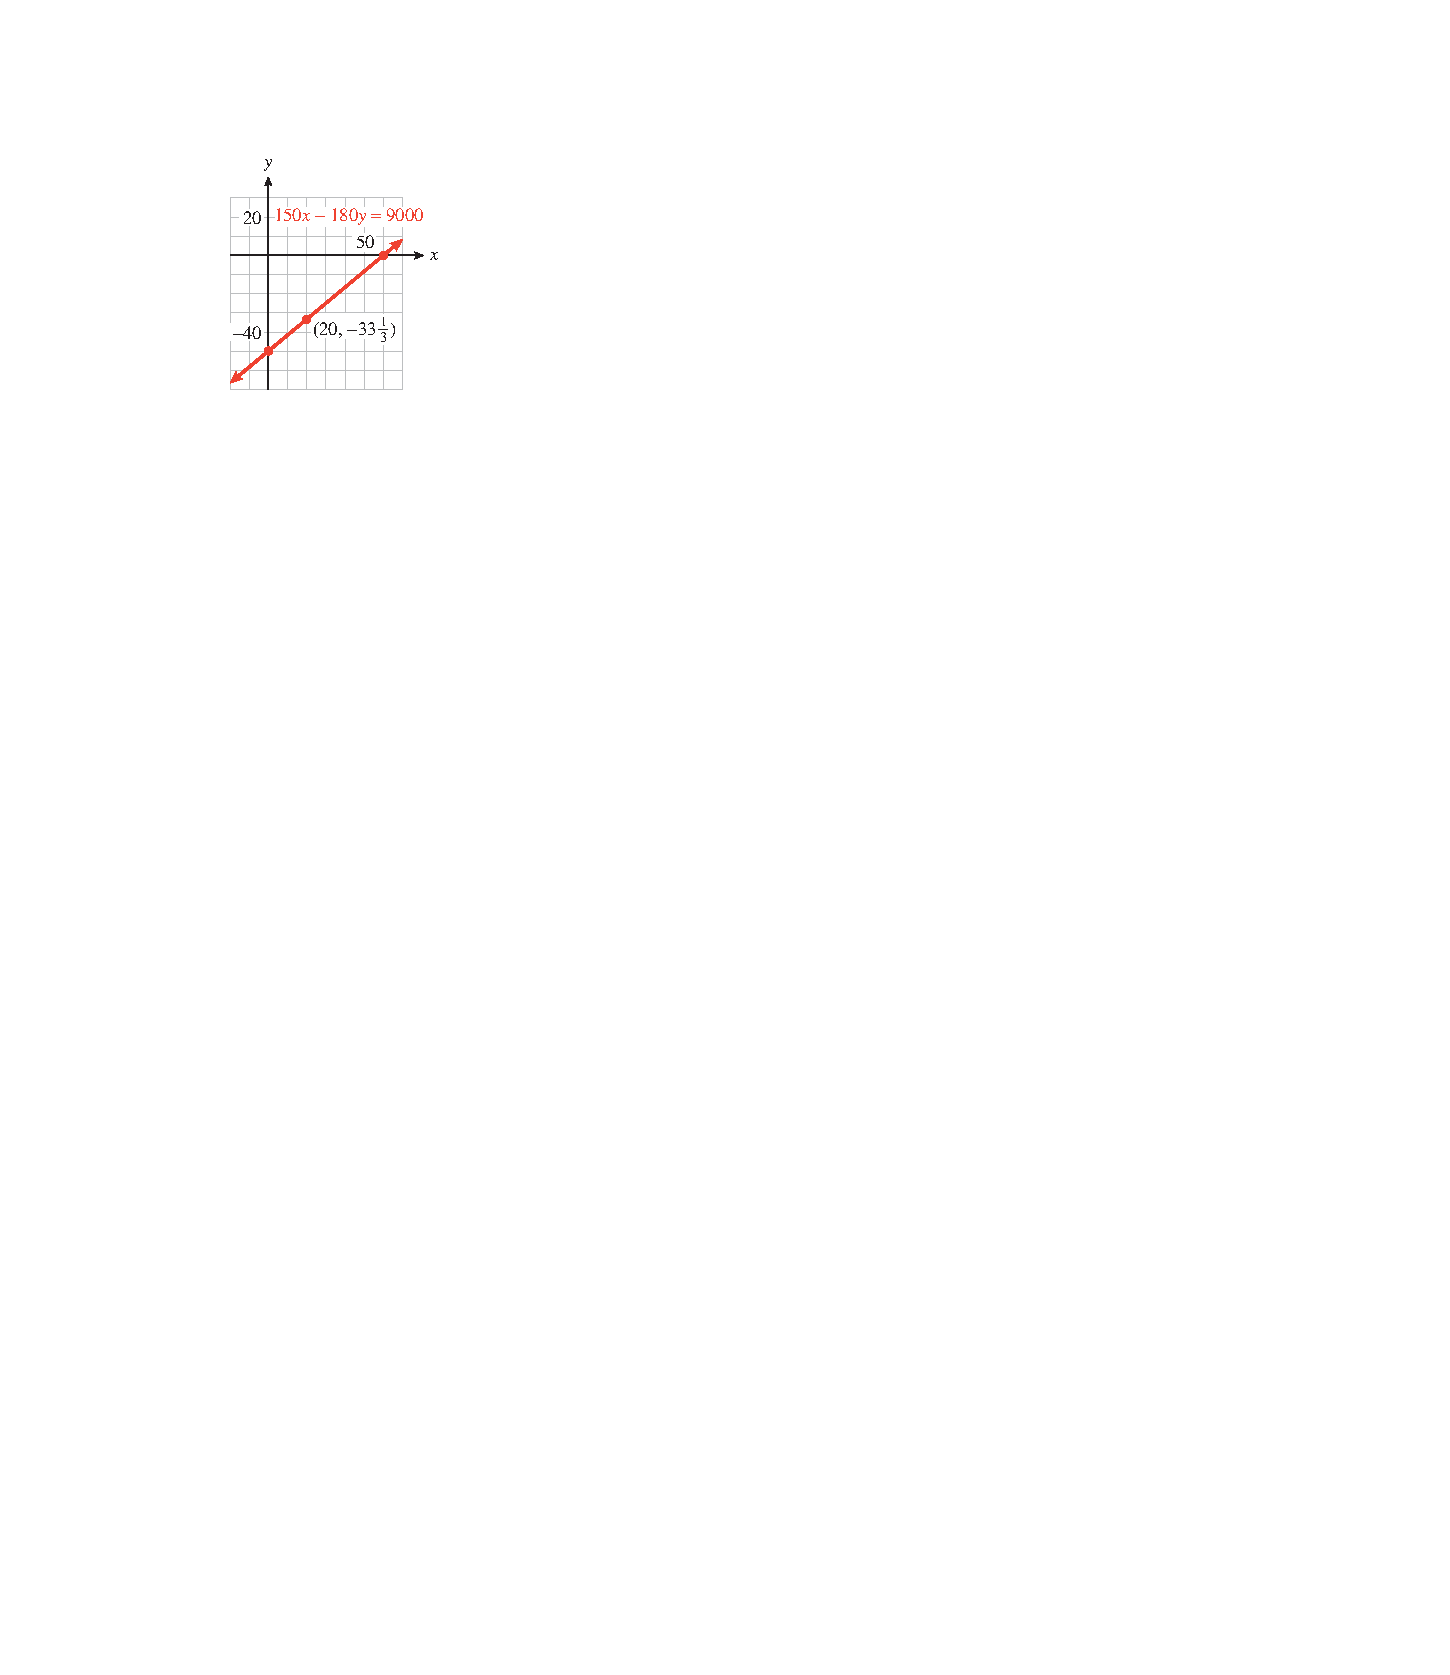
\includegraphics[width=\linewidth]{external/images/fig-example-graph-intercepts.pdf}
\end{sbspanel}%
\end{sidebyside}%
\end{enumerate}
%
\end{example}
\begin{inlineexercise}{Checkpoint}{QuickCheck 7.}{exercise-LinMod-g-d}%
Is it possible for the \(x\)-intercept and the \(y\)-intercept of a line to be the same point?%
\par
\begin{itemize}[label=$\odot$,leftmargin=3em,]
\item{}No%
\item{}Yes%
\item{}Only for a vertical line%
\item{}They are always the same point.%
\end{itemize}
%
\par\smallskip%
\noindent\textbf{\blocktitlefont Answer}.\hypertarget{answer-LinMod-g-d-c}{}\quad{}\(\text{Yes}\)%
\par\smallskip%
\noindent\textbf{\blocktitlefont Solution}.\hypertarget{solution-LinMod-g-d-d}{}\quad{}Yes%
\end{inlineexercise}%
\begin{assemblage}{Assemblage}{To Graph a Line Using the Intercept Method:.}{assemblage-LinMod-g-e}%
%
\begin{enumerate}[label=\arabic*]
\item{}Find the intercepts of the line.%
\begin{enumerate}[label=\alph*]
\item{}To find the \(x\)-intercept, set \(y=0\) and solve for \(x\).%
\item{}To find the \(y\)-intercept, set \(x=0\) and solve for \(y\).%
\end{enumerate}
%
\item{}Plot the intercepts.%
\item{}Choose a value for \(x\) and find a third point on the line.%
\item{}Draw a line through the points.%
\end{enumerate}
%
\end{assemblage}
\begin{inlineexercise}{Checkpoint}{QuickCheck 8.}{exercise-LinMod-g-f}%
How many points do you need to graph a linear equation?%
\par
\begin{itemize}[label=$\odot$,leftmargin=3em,]
\item{}Two%
\item{}Three%
\item{}One in each quadrant%
\item{}It depends on the equation%
\end{itemize}
%
\par\smallskip%
\noindent\textbf{\blocktitlefont Answer}.\hypertarget{answer-LinMod-g-f-c}{}\quad{}\(\text{Two}\)%
\par\smallskip%
\noindent\textbf{\blocktitlefont Solution}.\hypertarget{solution-LinMod-g-f-d}{}\quad{}Two%
\end{inlineexercise}%
\begin{technology}{Technology}{Choosing a Graphing Window.}{technology-LinMod-g-g}%
Knowing the intercepts can also help us choose a suitable window on a graphing utility. We would like the window to be large enough to show the intercepts. For the graph in the example above, we can enter the equation%
\begin{equation*}
Y = (9000 -150X)/{-180}
\end{equation*}
in the window%
\begin{sidebyside}{1}{0}{0}{0}%
\begin{sbspanel}{1}%
\resizebox{\ifdim\width > \linewidth\linewidth\else\width\fi}{!}{%
{\centering%
{\tabularfont%
\begin{tabular}{lll}
Xmin\(=-20\)&&Xmax\(=70\)\tabularnewline[0pt]
Ymin\(=-70\)&&Ymax\(=30\)
\end{tabular}
}%
\par}
}%
\end{sbspanel}%
\end{sidebyside}%
\end{technology}
\begin{inlineexercise}{Checkpoint}{Practice 7.}{exercise-LinMod-g-h}%
In \hyperref[exercise-exercise-crops]{Checkpoint~{\xreffont\ref{exercise-exercise-crops}}} you wrote an equation about crops in Nebraska.%
\par
%
\begin{enumerate}[label=\alph*.]
\item{}Find the intercepts of the graph.%
\par
Note: Enter each intercept as an ordered pair.%
\par
The \(x\)-intercept is \fillintext{6}.%
\par
The \(y\)-intercept is \fillintext{6}.%
\item{}Use the intercepts to help you choose appropriate scales for the axes, and then graph the equation.%
\item{}What do the intercepts tell us about the problem?%
\par
The \(x\)-intercept tells us:%
\par
\begin{itemize}[label=$\odot$,leftmargin=3em,]
\item{}A) the total water usage of corn.%
\item{}B) the cost of the corn if no wheat is planted.%
\item{}C) the optimal number of acres of corn.%
\item{}D) the total acres if all corn is planted.%
\end{itemize}
%
\par
The \(y\)-intercept tells us:%
\par
\begin{itemize}[label=$\odot$,leftmargin=3em,]
\item{}A) the largest possible number of acres of wheat.%
\item{}B) the amount of water used by the wheat.%
\item{}C) the total cost of the wheat.%
\item{}D) how many acres are left after the wheat is planted.%
\end{itemize}
%
\end{enumerate}
%
\par
A graph is shown below.%
\begin{sidebyside}{1}{0.375}{0.375}{0}%
\begin{sbspanel}{0.25}%
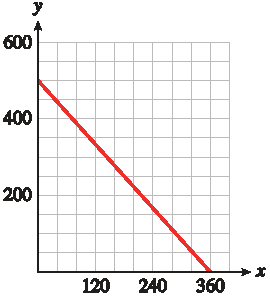
\includegraphics[width=\linewidth]{external/images/fig-in-ex-ans-1-1-7.pdf}
\end{sbspanel}%
\end{sidebyside}%
\par\smallskip%
\noindent\textbf{\blocktitlefont Answer 1}.\hypertarget{answer-LinMod-g-h-c}{}\quad{}\(\left(360,0\right)\)%
\par\smallskip%
\noindent\textbf{\blocktitlefont Answer 2}.\hypertarget{answer-LinMod-g-h-d}{}\quad{}\(\left(0,500\right)\)%
\par\smallskip%
\noindent\textbf{\blocktitlefont Answer 3}.\hypertarget{answer-LinMod-g-h-e}{}\quad{}\(\text{D) the ... is planted.}\)%
\par\smallskip%
\noindent\textbf{\blocktitlefont Answer 4}.\hypertarget{answer-LinMod-g-h-f}{}\quad{}\(\text{A) the ... of wheat.}\)%
\par\smallskip%
\noindent\textbf{\blocktitlefont Solution}.\hypertarget{solution-LinMod-g-h-g}{}\quad{}%
\begin{enumerate}[label=\alph*.]
\item{}We find the \(x\)-intercept by setting \(y=0\) and solving for \(x\) to learn that \(x=360\text{,}\) so the \(x\)-intercept is \({\left(360,0\right)}\text{.}\)%
\par
We find the \(y\)-intercept by setting \(x=0\) and solving for \(y\) to learn that \(y=500\text{,}\) so the \(y\)-intercept is \({\left(0,500\right)}\text{.}\)%
\item{}The \(x\)-intercept has \(y=0\text{,}\) that is, it corresponds to when there are zero radio ads. The \(y\)-intercept has \(x=0\text{,}\) that is, it corresponds to when there are zero tv ads.%
\end{enumerate}
%
\end{inlineexercise}%
\begin{note}{Note}{}{note-LinMod-g-i}%
The examples in this section model simple linear relationships between two variables. Such relationships, in which the value of one variable is determined by the value of the other, are called \terminology{functions}\index{function}. We will study various kinds of functions throughout the course.%
\end{note}
\begin{inlineexercise}{Checkpoint}{Pause and Reflect.}{exercise-LinMod-g-j}%
What was the most difficult part of this section to understand? Write a question whose answer would help you understand it.%
\end{inlineexercise}%
\end{subsectionptx}
%
%
\typeout{************************************************}
\typeout{Subsection  Section Summary}
\typeout{************************************************}
%
\begin{subsectionptx}{Subsection}{Section Summary}{}{Section Summary}{}{}{subsection-summary-1-1}
%
%
\typeout{************************************************}
\typeout{Subsubsection  Vocabulary}
\typeout{************************************************}
%
\begin{subsubsectionptx}{Subsubsection}{Vocabulary}{}{Vocabulary}{}{}{subsubsection-summary-1-1-b}
Look up the definitions of new terms in the Glossary.%
\begin{multicols}{3}
\begin{itemize}[label=\textbullet]
\item{}Variable%
\item{}Solve an equation%
\item{}Evaluate an expression%
\item{}Linear equation%
\item{}Increasing graph%
\item{}Decreasing graph%
\item{}Intercept%
\item{}Mathematical model%
\end{itemize}
\end{multicols}
%
\end{subsubsectionptx}
%
%
\typeout{************************************************}
\typeout{Subsubsection  CONCEPTS}
\typeout{************************************************}
%
\begin{subsubsectionptx}{Subsubsection}{CONCEPTS}{}{CONCEPTS}{}{}{subsubsection-summary-1-1-c}
%
\begin{enumerate}[label=\arabic*]
\item{}We can describe a relationship between variables with a table of values, a graph, or an equation.%
\item{}Linear models have equations of the following form:%
\begin{equation*}
y = (\text{starting value}) + (\text{rate of change})\cdot x
\end{equation*}
%
\item{}To make a useful graph, we must choose appropriate scales for the axes.%
\item{}\begin{assemblage}{Assemblage}{General Form for a Linear Equation.}{assemblage-summary-1-1-c-b-a-d-a}%
The graph of any equation%
\begin{equation*}
Ax+By=C
\end{equation*}
where \(A\) and \(B\) are not both equal to zero, is a straight line.%
\end{assemblage}
%
\item{}The intercepts of a graph are the points where the graph crosses the axes.%
\item{}We can use the intercepts to graph a line.%
\par
%
\begin{assemblage}{Assemblage}{To Graph a Line Using the Intercept Method:.}{assemblage-summary-1-1-c-b-a-f-c}%
%
\begin{enumerate}[label=\arabic*]
\item{}Find the intercepts of the line.%
\begin{enumerate}[label=\alph*]
\item{}To find the \(x\)-intercept, set \(y=0\) and solve for \(x\).%
\item{}To find the \(y\)-intercept, set \(x=0\) and solve for \(y\).%
\end{enumerate}
%
\item{}Plot the intercepts.%
\item{}Choose a value for \(x\) and find a third point on the line.%
\item{}Draw a line through the points.%
\end{enumerate}
%
\end{assemblage}
\item{}The intercepts are also useful for interpreting a model.%
\end{enumerate}
%
\end{subsubsectionptx}
%
%
\typeout{************************************************}
\typeout{Subsubsection  STUDY QUESTIONS}
\typeout{************************************************}
%
\begin{subsubsectionptx}{Subsubsection}{STUDY QUESTIONS}{}{STUDY QUESTIONS}{}{}{subsubsection-summary-1-1-d}
%
\begin{enumerate}[label=\arabic*]
\item{}Name three ways to represent a relationship between two variables.%
\item{}If \(C\) is expressed in terms of \(H\), which variable goes on the horizontal axis?%
\item{}Explain the difference between evaluating an expression and solving an equation.%
\item{}How many points do you need to graph a linear equation?%
\item{}Explain how the words \terminology{intercept} and \terminology{intersect} are related; explain how they are different.%
\item{}Delbert says that the intercepts of the line \(3x + 5y = 30\) are \((10, 6)\). What is wrong with his answer?%
\end{enumerate}
%
\end{subsubsectionptx}
%
%
\typeout{************************************************}
\typeout{Subsubsection  SKILLS}
\typeout{************************************************}
%
\begin{subsubsectionptx}{Subsubsection}{SKILLS}{}{SKILLS}{}{}{subsubsection-summary-1-1-e}
Practice each skill in the Homework problems listed.%
\begin{enumerate}[label=\arabic*]
\item{}Make a table of values: \#1\textendash{}4, 7 and 8%
\item{}Plot points and draw a graph: \#1\textendash{}4, 7 and 8%
\item{}Choose appropriate scales for the axes: \#5\textendash{}12%
\item{}Write a linear model of the form \(y = (\text{starting value}) + (\text{rate of change})\cdot x\): \#1\textendash{}8%
\item{}Write a linear model in general form: \#25\textendash{}28, 33\textendash{}36%
\item{}Evaluate a linear expression, algebraically and graphically: \#1\textendash{}4%
\item{}Solve a linear equation, algebraically and graphically: \#1\textendash{}4%
\item{}Find the intercepts of a graph: \#5 and 6, 13\textendash{}24, 45\textendash{}52%
\item{}Graph a line by the intercept method: \#5 and 6, 13\textendash{}24%
\item{}Interpret the meaning of the intercepts: \#5 and 6, 25\textendash{}28%
\item{}Use a graphing calculator to graph a line: \#37\textendash{}52%
\item{}Sketch on paper a graph obtained on a calculator: \#37\textendash{}44%
\end{enumerate}
%
\end{subsubsectionptx}
\end{subsectionptx}
%
%
\typeout{************************************************}
\typeout{Exercises  Homework 1.1}
\typeout{************************************************}
%
\begin{exercises-subsection}{Exercises}{Homework 1.1}{}{Homework 1.1}{}{}{exercises-section-1-1-exercises}
\begin{divisionexercise}{1}{}{}{exercise-section-1-1-exercises-b}%
The temperature in the desert at 6 a.m., just before sunrise, was \(65\degree\)F. The temperature rose \(5\) degrees every hour until it reached its maximum value at about 5 p.m. Complete the table of values for the temperature, \(T\), at \(h\) hours after 6 a.m.%
\begin{sidebyside}{1}{0}{0}{0}%
\begin{sbspanel}{1}%
\resizebox{\ifdim\width > \linewidth\linewidth\else\width\fi}{!}{%
{\centering%
{\tabularfont%
\begin{tabular}{AcAcAcAcAcAcA}\hrulethick
\(h\)&\(0\)&\(3\)&\(6\)&\(9\)&\(10\)\tabularnewline\hrulethin
\(T\)&\(\hphantom{0000}\)&\(\hphantom{0000}\)&\(\hphantom{0000}\)&\(\hphantom{0000}\)&\(\hphantom{0000}\)\tabularnewline\hrulethin
\end{tabular}
}%
\par}
}%
\end{sbspanel}%
\end{sidebyside}%
\par
%
\begin{enumerate}[label=\alph*]
\item{}Write an equation for the temperature, \(T\), in terms of \(h\).%
\item{}Graph the equation.%
\begin{sidebyside}{1}{0.3}{0.3}{0}%
\begin{sbspanel}{0.4}%
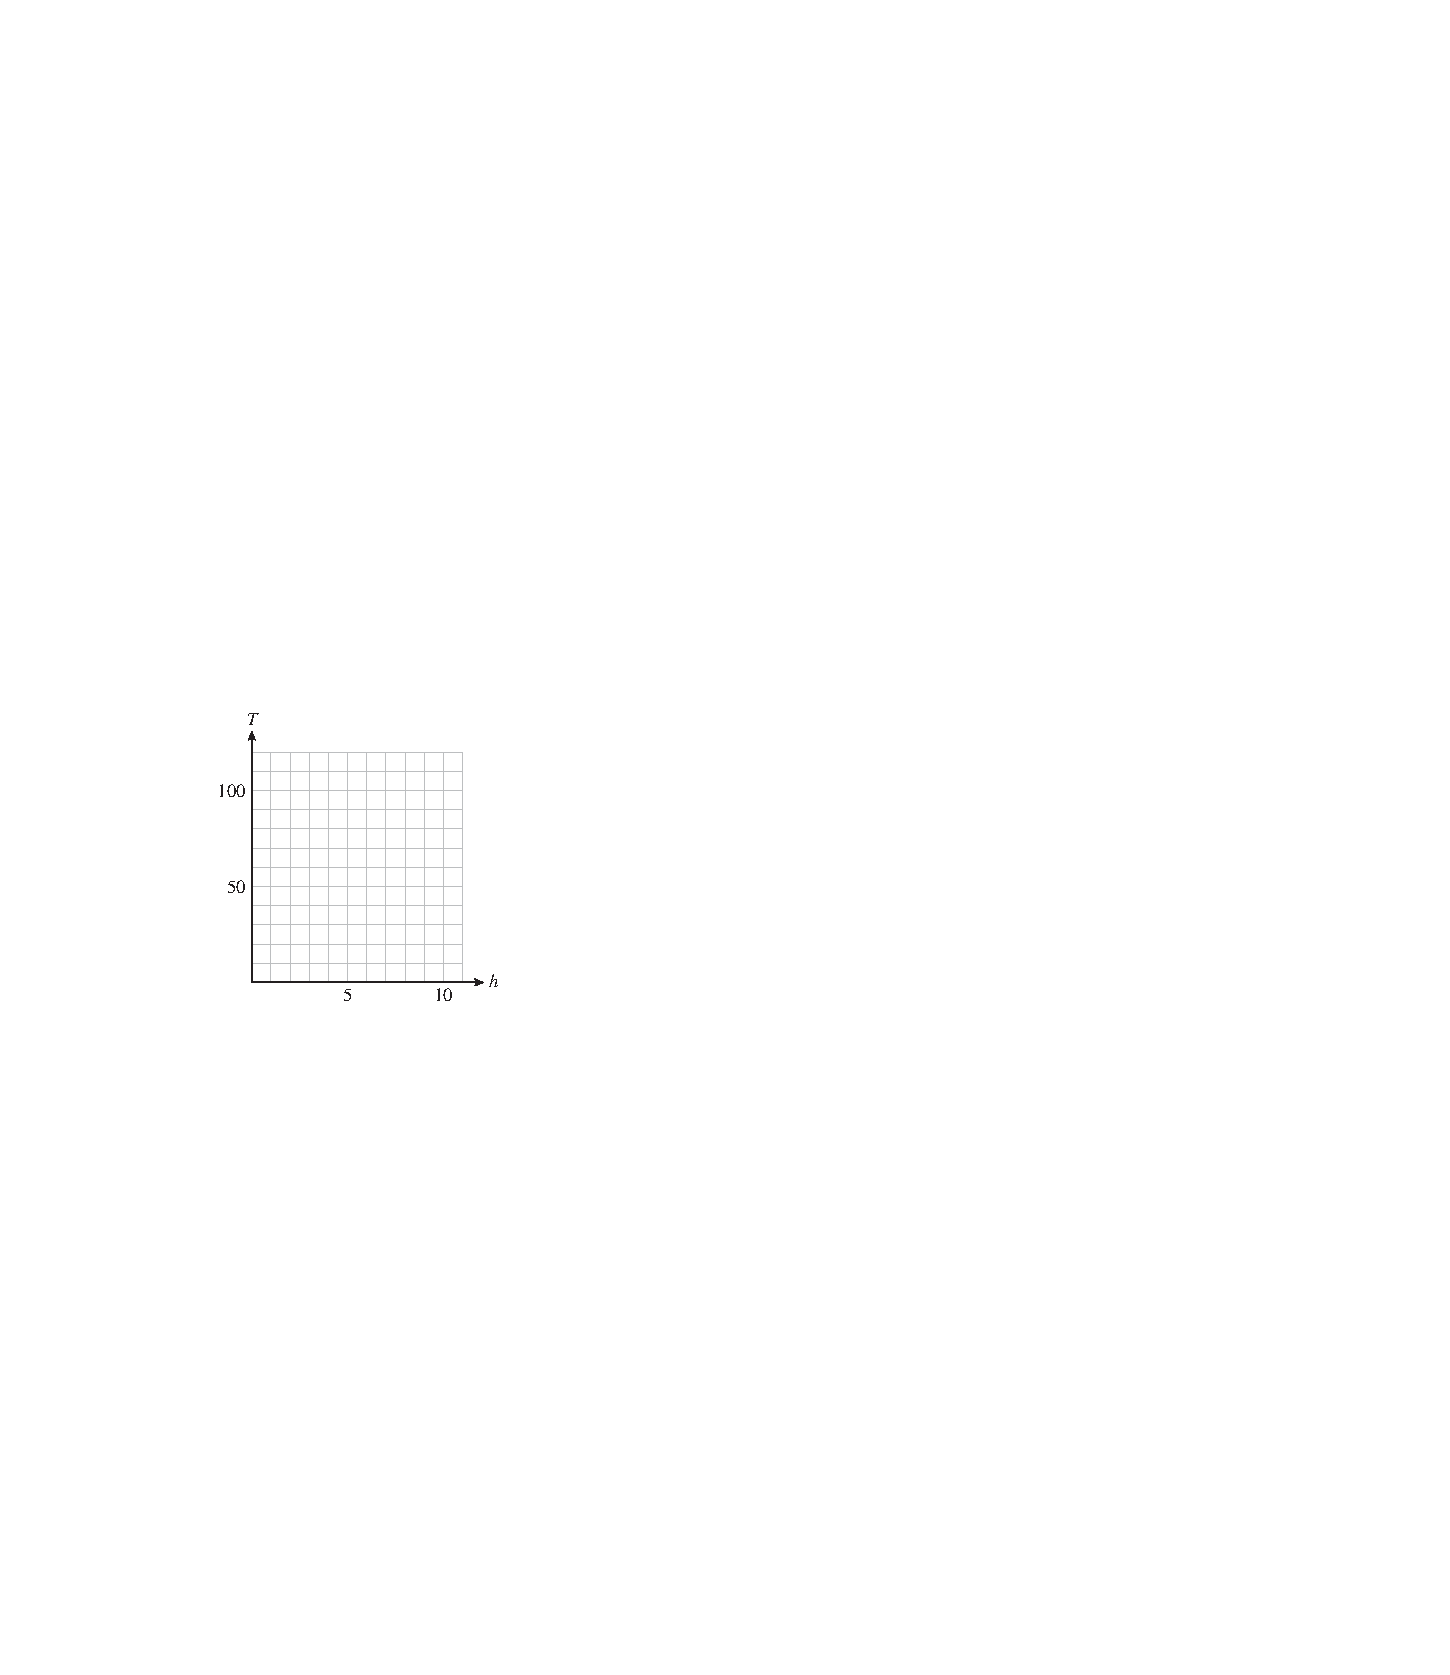
\includegraphics[width=\linewidth]{external/images/fig-ex-1-1-1.pdf}
\end{sbspanel}%
\end{sidebyside}%
\item{}How hot is it at noon? Illustrate the answer on your graph.%
\item{}When will the temperature be \(110\degree\)F? Illustrate the answer on your graph.%
\end{enumerate}
%
\end{divisionexercise}%
\begin{divisionexercise}{2}{}{}{exercise-section-1-1-exercises-c}%
The taxi out of Dulles Airport charges a traveler with one suitcase an initial fee of \textdollar{}\(2.00\), plus \textdollar{}\(1.50\) for each mile traveled. Complete the table of values showing the charge, \(C\), for a trip of \(n\) miles.%
\begin{sidebyside}{1}{0}{0}{0}%
\begin{sbspanel}{1}%
\resizebox{\ifdim\width > \linewidth\linewidth\else\width\fi}{!}{%
{\centering%
{\tabularfont%
\begin{tabular}{AcAcAcAcAcAcAcA}\hrulethick
\(n\)&\(0\)&\(5\)&\(10\)&\(15\)&\(20\)&\(25\)\tabularnewline\hrulethin
\(C\)&\(\hphantom{0000}\)&\(\hphantom{0000}\)&\(\hphantom{0000}\)&\(\hphantom{0000}\)&\(\hphantom{0000}\)&\(\hphantom{0000}\)\tabularnewline\hrulethin
\end{tabular}
}%
\par}
}%
\end{sbspanel}%
\end{sidebyside}%
\par
%
\begin{enumerate}[label=\alph*]
\item{}Write an equation for the charge, \(C\), in terms of the number of miles traveled, \(n\).%
\item{}Graph the equation.%
\begin{sidebyside}{1}{0.3}{0.3}{0}%
\begin{sbspanel}{0.4}%
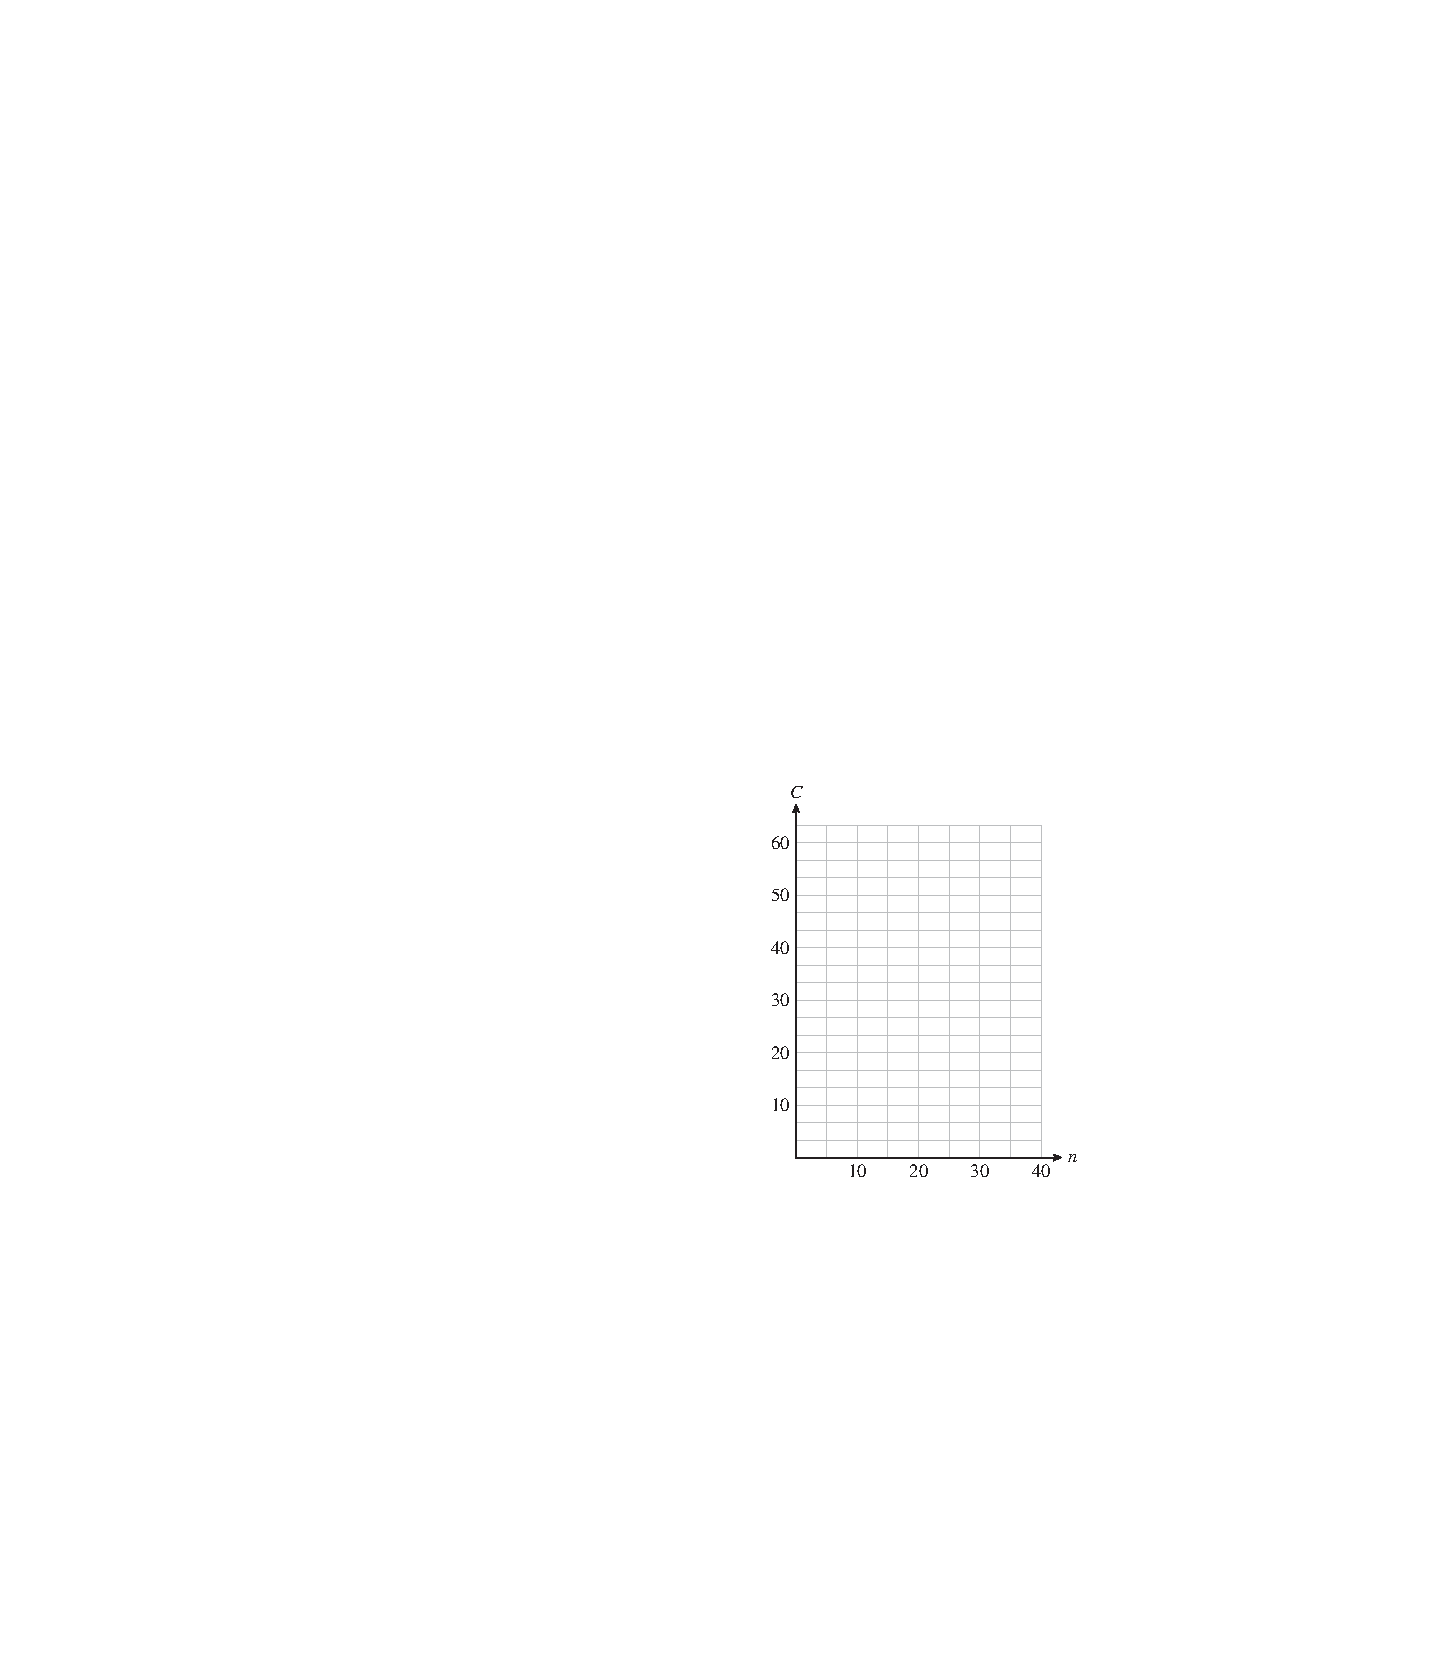
\includegraphics[width=\linewidth]{external/images/fig-ex-1-1-2.pdf}
\end{sbspanel}%
\end{sidebyside}%
\item{}What is the charge for a trip to Mount Vernon,  \(40\) miles from the airport? Illustrate the answer on your graph.%
\item{}If a ride to the National Institutes of Health (NIH) costs \textdollar{}\(39.50\), how far is it from the airport to the NIH? Illustrate the answer on your graph.%
\end{enumerate}
%
\end{divisionexercise}%
\begin{divisionexercise}{3}{}{}{exercise-section-1-1-exercises-d}%
On October 31, Betty and Paul fill their \(250\)-gallon oil tank for their heater. Beginning in November, they use an average of \(15\) gallons of oil per week. Complete the table of values for the amount of oil, \(A\), left in the tank after \(w\) weeks.%
\begin{sidebyside}{1}{0}{0}{0}%
\begin{sbspanel}{1}%
\resizebox{\ifdim\width > \linewidth\linewidth\else\width\fi}{!}{%
{\centering%
{\tabularfont%
\begin{tabular}{AcAcAcAcAcAcA}\hrulethick
\(w\)&\(0\)&\(4\)&\(8\)&\(12\)&\(16\)\tabularnewline\hrulethin
\(A\)&\(\hphantom{0000}\)&\(\hphantom{0000}\)&\(\hphantom{0000}\)&\(\hphantom{0000}\)&\(\hphantom{0000}\)\tabularnewline\hrulethin
\end{tabular}
}%
\par}
}%
\end{sbspanel}%
\end{sidebyside}%
\par
%
\begin{enumerate}[label=\alph*]
\item{}Write an equation that expresses the amount of oil, \(A\), in the tank in terms of the number of weeks, \(w\), since October 31.%
\item{}Graph the equation.%
\begin{sidebyside}{1}{0.3}{0.3}{0}%
\begin{sbspanel}{0.4}%
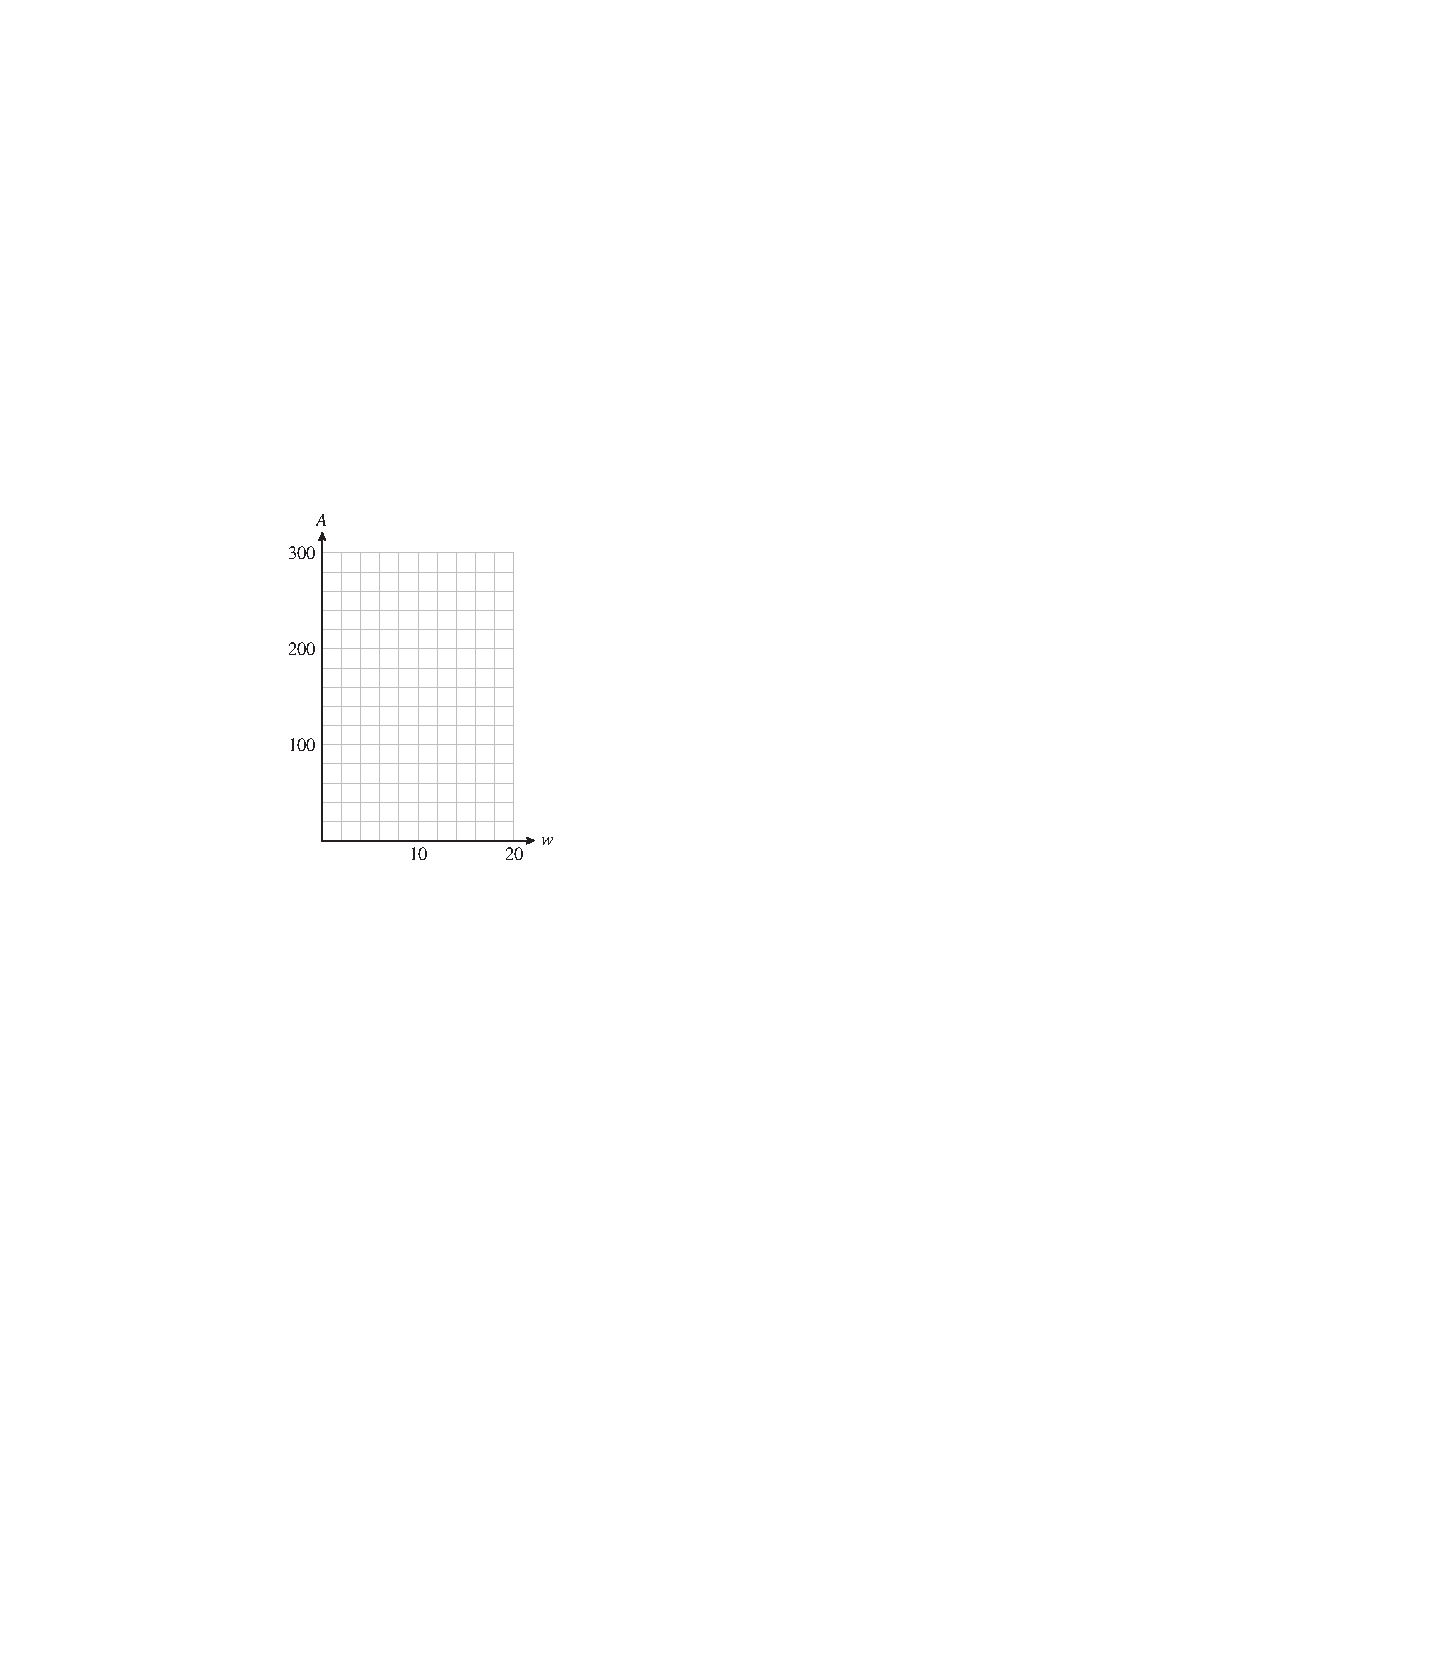
\includegraphics[width=\linewidth]{external/images/fig-ex-1-1-3.pdf}
\end{sbspanel}%
\end{sidebyside}%
\item{}How much did the amount of fuel oil in the tank decrease between the third week and the eighth week? Illustrate this amount on the graph.%
\item{}When will the tank contain more than \(175\) gallons of fuel oil? Illustrate on the graph.%
\end{enumerate}
%
\end{divisionexercise}%
\begin{divisionexercise}{4}{}{}{exercise-section-1-1-exercises-e}%
Leon's camper has a \(20\)-gallon gas tank, and he gets \(12\) miles to the gallon. (That is, he uses \(\frac{1}{12}\) gallon per mile.) Complete the table of values for the amount of gas, \(g\), left in Leon's tank after driving \(m\) miles.%
\begin{sidebyside}{1}{0}{0}{0}%
\begin{sbspanel}{1}%
\resizebox{\ifdim\width > \linewidth\linewidth\else\width\fi}{!}{%
{\centering%
{\tabularfont%
\begin{tabular}{AcAcAcAcAcAcA}\hrulethick
\(m\)&\(0\)&\(48\)&\(96\)&\(144\)&\(192\)\tabularnewline\hrulethin
\(g\)&\(\hphantom{0000}\)&\(\hphantom{0000}\)&\(\hphantom{0000}\)&\(\hphantom{0000}\)&\(\hphantom{0000}\)\tabularnewline\hrulethin
\end{tabular}
}%
\par}
}%
\end{sbspanel}%
\end{sidebyside}%
\par
%
\begin{enumerate}[label=\alph*]
\item{}Write an equation that expresses the amount of gas, \(g\), in Leon's fuel tank in terms of the number of miles, \(m\), he has driven.%
\item{}Graph the equation.%
\begin{sidebyside}{1}{0.3}{0.3}{0}%
\begin{sbspanel}{0.4}%
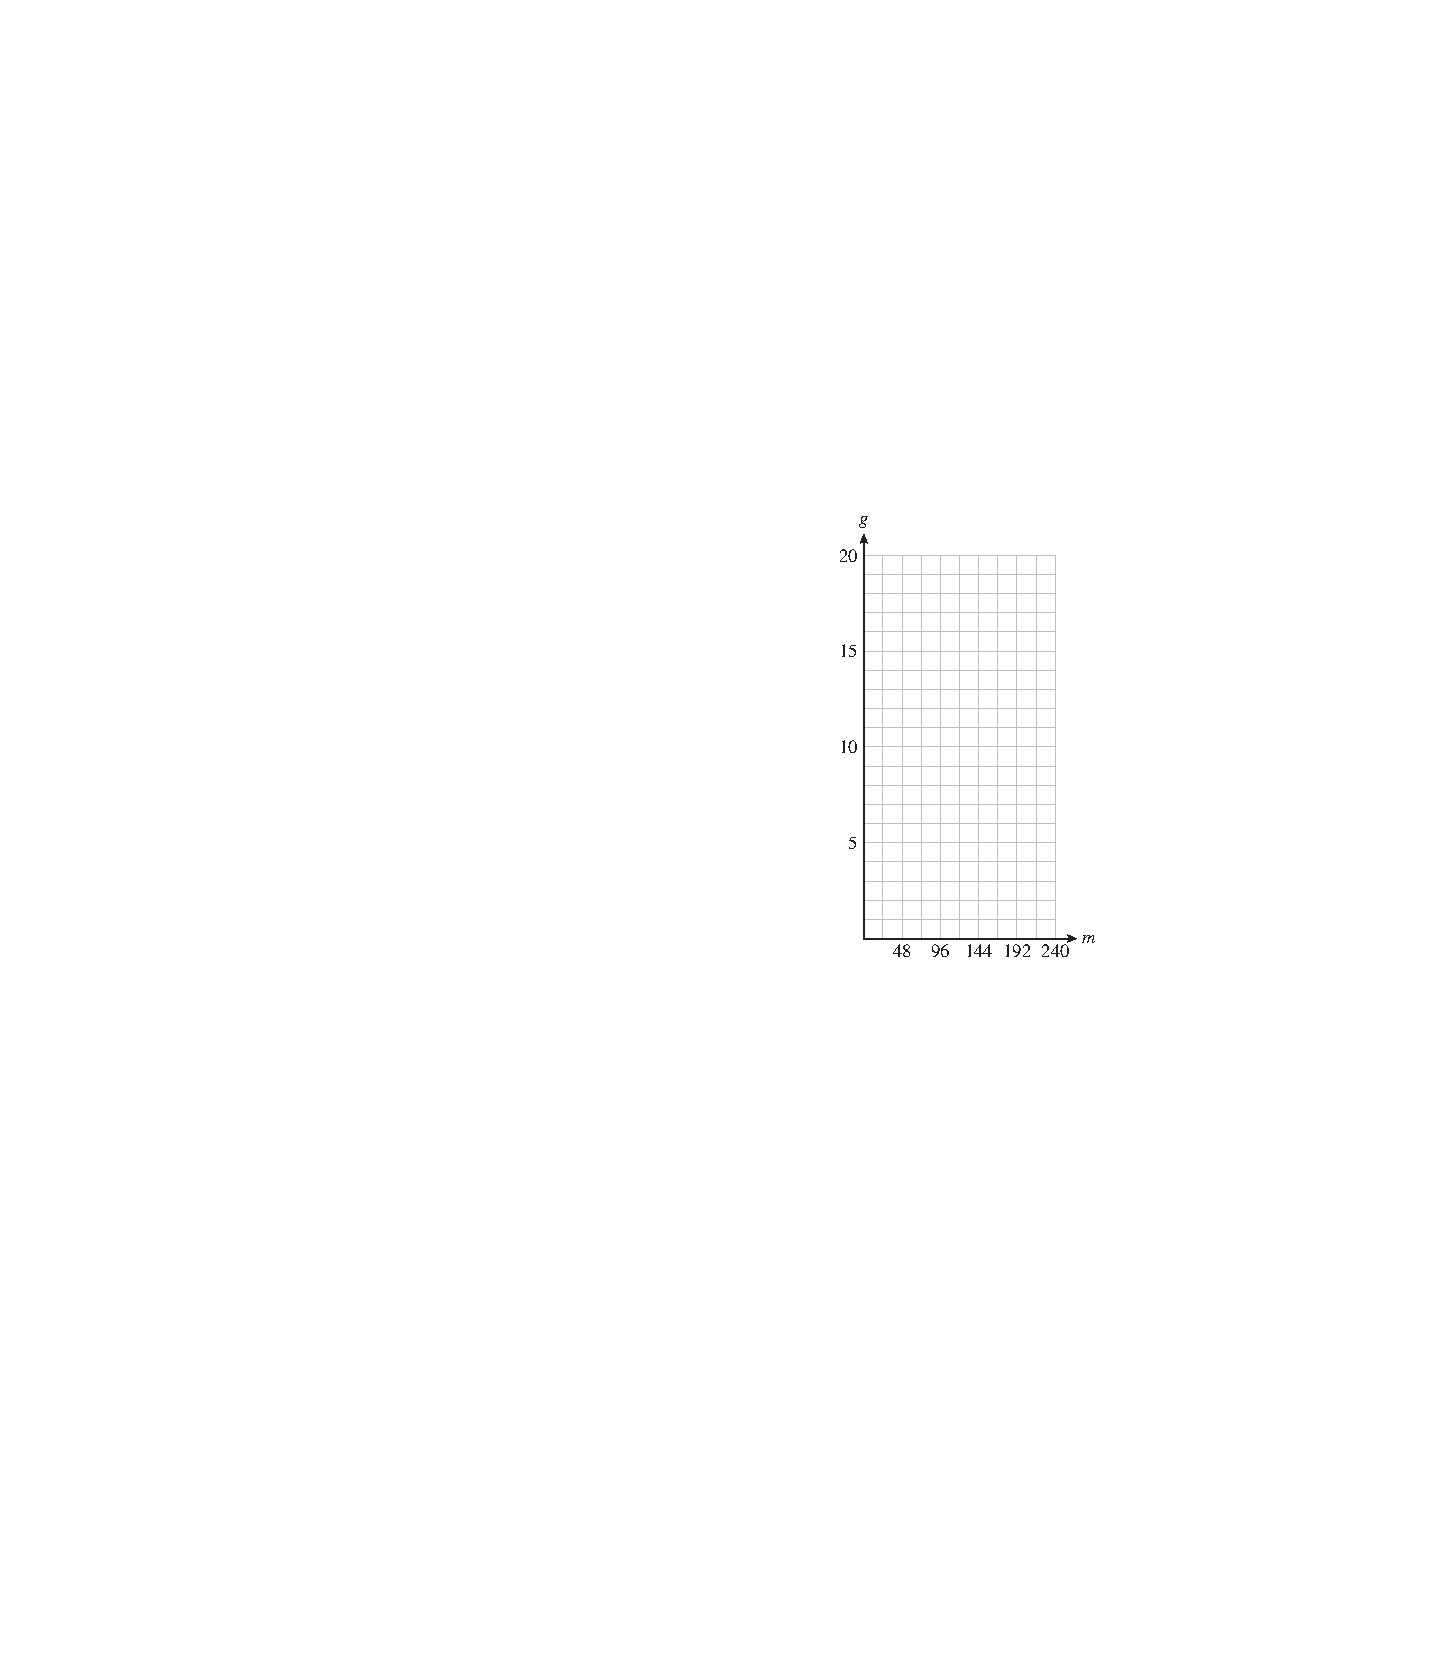
\includegraphics[width=\linewidth]{external/images/fig-ex-1-1-4.pdf}
\end{sbspanel}%
\end{sidebyside}%
\item{}How much gas will Leon use between 8 a.m., when his odometer reads \(96\) miles, and 9 a.m., when the odometer reads \(144\) miles? Illustrate on the graph.%
\item{}If Leon has less than \(5\) gallons of gas left, how many miles has he driven? Illustrate on the graph.%
\end{enumerate}
%
\end{divisionexercise}%
\begin{divisionexercise}{5}{}{}{exercise-section-1-1-exercises-f}%
Phil and Ernie buy a used photocopier for \textdollar{}\(800\) and set up a copy service on their campus. For each hour that the copier runs, Phil and Ernie make \textdollar{}\(40\).%
\begin{enumerate}[label=\alph*]
\item{}Write an equation that expresses Phil and Ernie's profit (or loss), \(P\), in terms of the number of hours, \(t\), they run the copier.%
\item{}Find the intercepts and sketch the graph. (Suggestion: Scale the horizontal axis from \(0\) to \(40\) in increments of \(5\), and scale the vertical axis from \(-1000\) to \(400\) in increments of \(100\).)%
\item{}What do the intercepts tell us about the profit?%
\end{enumerate}
%
\end{divisionexercise}%
\begin{divisionexercise}{6}{}{}{exercise-section-1-1-exercises-g}%
A deep-sea diver is taking some readings at a depth of \(400\) feet. He begins rising at \(20\) feet per minute.%
\begin{enumerate}[label=\alph*]
\item{}Write an equation that expresses the diver’s altitude, \(h\), in terms of the number of minutes, \(m\), elapsed. (Consider a depth of \(400\) feet as an altitude of \(-400\) feet.)%
\item{}Find the intercepts and sketch the graph. (Suggestion: Scale the horizontal axis from \(0\) to \(24\) in increments of \(2\), and scale the vertical axis from \(-500\) to \(100\) in increments of \(50\).)%
\item{}What do the intercepts tell us about the diver's depth?%
\end{enumerate}
%
\end{divisionexercise}%
\begin{divisionexercise}{7}{}{}{exercise-section-1-1-exercises-h}%
There are many formulas for estimating the annual cost of driving. The Automobile Club estimates that fixed costs for a small car—including insurance, registration, depreciation, and financing—total about \textdollar{}\(5000\) per year. The operating costs for gasoline, oil, maintenance, tires, and so forth are about \(12.5\) cents per mile. (Source: Automobile Association of America)%
\begin{enumerate}[label=\alph*]
\item{}Write an equation for the annual driving cost, \(C\), in terms of \(d\), the number of miles driven.%
\item{}Complete the table of values.%
\begin{sidebyside}{1}{0}{0}{0}%
\begin{sbspanel}{1}%
\resizebox{\ifdim\width > \linewidth\linewidth\else\width\fi}{!}{%
{\centering%
{\tabularfont%
\begin{tabular}{AlAcAcAcAcAcA}\hrulethick
Miles Driven&\(4000\)&\(8000\)&\(12,000\)&\(16,000\)&\(20,000\)\tabularnewline\hrulethin
Cost (\textdollar{})&\(\hphantom{0000}\)&\(\hphantom{0000}\)&\(\hphantom{0000}\)&\(\hphantom{0000}\)&\(\hphantom{0000}\)\tabularnewline\hrulethin
\end{tabular}
}%
\par}
}%
\end{sbspanel}%
\end{sidebyside}%
\item{}Choose scales for the axes and graph the equation.%
\item{}How much does the annual cost of driving increase when the mileage increases from \(8000\) to \(12,000\) miles? Illustrate this amount on the graph.%
\item{}How much mileage will cause the annual cost to exceed \textdollar{}\(7000\)? Illustrate on the graph.%
\end{enumerate}
%
\end{divisionexercise}%
\begin{divisionexercise}{8}{}{}{exercise-section-1-1-exercises-i}%
The boiling point of water changes with altitude. At sea level, water boils at \(212\degree\)F, and the boiling point diminishes by approximately \(0.002\degree\)F for each \(1\)-foot increase in altitude.%
\begin{enumerate}[label=\alph*]
\item{}Write an equation for the boiling point, \(B\), in terms of \(a\), the altitude in feet.%
\item{}Complete the table of values.%
\begin{sidebyside}{1}{0}{0}{0}%
\begin{sbspanel}{1}%
\resizebox{\ifdim\width > \linewidth\linewidth\else\width\fi}{!}{%
{\centering%
{\tabularfont%
\begin{tabular}{AlAcAcAcAcAcAcAcA}\hrulethick
Altitude (ft)&\(-500\)&\(0\)&\(1000\)&\(2000\)&\(3000\)&\(4000\)&\(5000\)\tabularnewline\hrulethin
Boiling point (\(\degree\)F)&\(\hphantom{0000}\)&\(\hphantom{0000}\)&\(\hphantom{0000}\)&\(\hphantom{0000}\)&\(\hphantom{0000}\)&\(\hphantom{0000}\)&\(\hphantom{0000}\)\tabularnewline\hrulethin
\end{tabular}
}%
\par}
}%
\end{sbspanel}%
\end{sidebyside}%
\item{}Choose scales for the axes and graph the equation.%
\item{}How much does the boiling point decrease when the altitude increases from \(1000\) to \(3000\) feet? Illustrate this amount on the graph.%
\item{}At what altitudes is the boiling point less than \(204\degree\)F? Illustrate on the graph.%
\end{enumerate}
%
\end{divisionexercise}%
\par\medskip\noindent%
\textbf{Exercise Group.}\space\space%
For each table, choose appropriate scales for the axes and plot the given points.%
\begin{exercisegroupcol}{2}
\begin{divisionexerciseegcol}{9}{}{}{exercise-section-1-1-exercises-j-b}%
\begin{sidebyside}{1}{0}{0}{0}%
\begin{sbspanel}{1}%
\resizebox{\ifdim\width > \linewidth\linewidth\else\width\fi}{!}{%
{\centering%
{\tabularfont%
\begin{tabular}{AlAcAcAcAcA}\hrulethick
\(x\)&\(0\)&\(80\)&\(90\)&\(120\)\tabularnewline\hrulethin
\(y\)&\(6\)&\(2\)&\(1.5\)&\(1\)\tabularnewline\hrulethin
\end{tabular}
}%
\par}
}%
\end{sbspanel}%
\end{sidebyside}%
\end{divisionexerciseegcol}%
\begin{divisionexerciseegcol}{10}{}{}{exercise-section-1-1-exercises-j-c}%
\begin{sidebyside}{1}{0}{0}{0}%
\begin{sbspanel}{1}%
\resizebox{\ifdim\width > \linewidth\linewidth\else\width\fi}{!}{%
{\centering%
{\tabularfont%
\begin{tabular}{AlAcAcAcAcA}\hrulethick
\(x\)&\(300\)&\(500\)&\(800\)&\(1100\)\tabularnewline\hrulethin
\(y\)&\(1.2\)&\(1.3\)&\(1.5\)&\(1.9\)\tabularnewline\hrulethin
\end{tabular}
}%
\par}
}%
\end{sbspanel}%
\end{sidebyside}%
\end{divisionexerciseegcol}%
\begin{divisionexerciseegcol}{11}{}{}{exercise-section-1-1-exercises-j-d}%
\begin{sidebyside}{1}{0}{0}{0}%
\begin{sbspanel}{1}%
\resizebox{\ifdim\width > \linewidth\linewidth\else\width\fi}{!}{%
{\centering%
{\tabularfont%
\begin{tabular}{AlAcAcAcAcA}\hrulethick
\(x\)&\(0.01\)&\(0.03\)&\(0.06\)&\(0.07\)\tabularnewline\hrulethin
\(y\)&\(-0.2\)&\(-1\)&\(-1.1\)&\(-2\)\tabularnewline\hrulethin
\end{tabular}
}%
\par}
}%
\end{sbspanel}%
\end{sidebyside}%
\end{divisionexerciseegcol}%
\begin{divisionexerciseegcol}{12}{}{}{exercise-section-1-1-exercises-j-e}%
\begin{sidebyside}{1}{0}{0}{0}%
\begin{sbspanel}{1}%
\resizebox{\ifdim\width > \linewidth\linewidth\else\width\fi}{!}{%
{\centering%
{\tabularfont%
\begin{tabular}{AlAcAcAcAcA}\hrulethick
\(x\)&\(0.003\)&\(0.005\)&\(0.008\)&\(0.011\)\tabularnewline\hrulethin
\(y\)&\(6\)&\(2\)&\(1.5\)&\(1\)\tabularnewline\hrulethin
\end{tabular}
}%
\par}
}%
\end{sbspanel}%
\end{sidebyside}%
\end{divisionexerciseegcol}%
\end{exercisegroupcol}
\par\medskip\noindent
\par\medskip\noindent%
\textbf{Exercise Group.}\space\space%
For Problems 13-18,%
\begin{enumerate}[label=(\alph*)]
\item{}Find the intercepts of the graph.%
\item{}Graph the equation by the intercept method.%
\end{enumerate}
%
\begin{exercisegroupcol}{2}
\begin{divisionexerciseegcol}{13}{}{}{exercise-section-1-1-exercises-k-b}%
\(x + 2y = 8\)%
\end{divisionexerciseegcol}%
\begin{divisionexerciseegcol}{14}{}{}{exercise-section-1-1-exercises-k-c}%
\(2x - y = 6\)%
\end{divisionexerciseegcol}%
\begin{divisionexerciseegcol}{15}{}{}{exercise-section-1-1-exercises-k-d}%
\(3x - 4y =12\)%
\end{divisionexerciseegcol}%
\begin{divisionexerciseegcol}{16}{}{}{exercise-section-1-1-exercises-k-e}%
\(2x + 6y = 6\)%
\end{divisionexerciseegcol}%
\begin{divisionexerciseegcol}{17}{}{}{exercise-section-1-1-exercises-k-f}%
\(\displaystyle{\frac{x}{9}- \frac{y}{4}= 1}\)%
\end{divisionexerciseegcol}%
\begin{divisionexerciseegcol}{18}{}{}{exercise-section-1-1-exercises-k-g}%
\(\displaystyle{\frac{x}{5}+ \frac{y}{8}= 1}\)%
\end{divisionexerciseegcol}%
\end{exercisegroupcol}
\par\medskip\noindent
\par\medskip\noindent%
\textbf{Exercise Group.}\space\space%
For Problems 19-24,%
\begin{enumerate}[label=(\alph*)]
\item{}Find the intercepts of the graph.%
\item{}Use the intercepts to choose scales for the axes, and then graph the equation by the intercept method.%
\end{enumerate}
%
\begin{exercisegroupcol}{2}
\begin{divisionexerciseegcol}{19}{}{}{exercise-section-1-1-exercises-l-b}%
\(20x = 30y - 45,000\)%
\end{divisionexerciseegcol}%
\begin{divisionexerciseegcol}{20}{}{}{exercise-section-1-1-exercises-l-c}%
\(30x = 45y + 60,000\)%
\end{divisionexerciseegcol}%
\begin{divisionexerciseegcol}{21}{}{}{exercise-section-1-1-exercises-l-d}%
\(0.4x + 1.2y = 4.8\)%
\end{divisionexerciseegcol}%
\begin{divisionexerciseegcol}{22}{}{}{exercise-section-1-1-exercises-l-e}%
\(3.2x - 0.8y = 12.8\)%
\end{divisionexerciseegcol}%
\begin{divisionexerciseegcol}{23}{}{}{exercise-section-1-1-exercises-l-f}%
\(\displaystyle{\frac{2x}{3}+ \frac{3y}{11}= 1}\)%
\end{divisionexerciseegcol}%
\begin{divisionexerciseegcol}{24}{}{}{exercise-section-1-1-exercises-l-g}%
\(\displaystyle{\frac{8x}{7}- \frac{2y}{7}= 1}\)%
\end{divisionexerciseegcol}%
\end{exercisegroupcol}
\par\medskip\noindent
\begin{divisionexercise}{25}{}{}{exercise-section-1-1-exercises-m}%
The owner of a gas station has \textdollar{}\(19,200\) to spend on unleaded gas this month. Regular unleaded costs him \textdollar{}\(2.40\) per gallon, and premium unleaded costs \textdollar{}\(3.20\) per gallon.%
%
\begin{enumerate}[label=\alph*]
\item{}How much do \(x\) gallons of regular cost? How much do \(y\) gallons of premium cost?%
\item{}Write an equation in general form that relates the amount of regular unleaded gasoline, \(x\), the owner can buy and the amount of premium unleaded, \(y\).%
\item{}Find the intercepts and sketch the graph.%
\item{}What do the intercepts tell us about the amount of gasoline the owner can purchase?%
\end{enumerate}
\end{divisionexercise}%
\begin{divisionexercise}{26}{}{}{exercise-section-1-1-exercises-n}%
Five pounds of body fat is equivalent to \(16,000\) calories. Carol can burn \(600\) calories per hour bicycling and \(400\) calories per hour swimming.%
%
\begin{enumerate}[label=\alph*]
\item{}How many calories will Carol burn in \(x\) hours of cycling? How many calories will she burn in \(y\) hours of swimming?%
\item{}Write an equation in general form that relates the number of hours, \(x\), of cycling and the number of hours, \(y\), of swimming Carol needs to perform in order to lose \(5\) pounds.%
\item{}Find the intercepts and sketch the graph.%
\item{}What do the intercepts tell us about Carol's exercise program?%
\end{enumerate}
\end{divisionexercise}%
\begin{divisionexercise}{27}{}{}{exercise-section-1-1-exercises-o}%
Delbert must increase his daily potassium intake by \(1800\) mg. He decides to eat a combination of figs and bananas, which are both low in sodium. There are \(9\) mg potassium per gram of fig, and \(4\) mg potassium per gram of banana.%
%
\begin{enumerate}[label=\alph*]
\item{}How much potassium is in \(x\) grams of fig? How much potassium is in \(y\) grams of banana?%
\item{}Write an equation in general form that relates the number of grams, \(x\), of fig and the number of grams, \(y\), of banana Delbert needs to get \(1800\) mg of potassium.%
\item{}Find the intercepts and sketch the graph.%
\item{}What do the intercepts tell us about Delbert's diet?%
\end{enumerate}
\end{divisionexercise}%
\begin{divisionexercise}{28}{}{}{exercise-section-1-1-exercises-p}%
Leslie plans to invest some money in two CD accounts. The first account pays \(3.6\%\) interest per year, and the second account pays \(2.8\%\) interest per year. Leslie would like to earn \textdollar{}\(500\) per year on her investment.%
%
\begin{enumerate}[label=\alph*]
\item{}If Leslie invests \(x\) dollars in the first account, how much interest will she earn? How much interest will she earn if she invests \(y\) dollars in the second account?%
\item{}Write an equation in general form that relates \(x\) and \(y\) if Leslie earns \(\$500\) interest.%
\item{}Find the intercepts and sketch the graph.%
\item{}What do the intercepts tell us about Leslie's investments?%
\end{enumerate}
\end{divisionexercise}%
\begin{divisionexercise}{29}{}{}{exercise-section-1-1-exercises-q}%
Find the intercepts of the graph for each equation.%
%
\begin{multicols}{2}
\begin{enumerate}[label=\alph*]
\item{}\(\displaystyle \displaystyle{\frac{x}{3}+\frac{y}{5}=1} \)%
\item{}\(\displaystyle \displaystyle{2x - 4y = 1} \)%
\item{}\(\displaystyle \displaystyle{\frac{2x}{5}-\frac{2y}{3}=1} \)%
\item{}\(\displaystyle \displaystyle{\frac{x}{p}+\frac{y}{q}=1} \)%
\end{enumerate}
\end{multicols}
\(\hphantom{00}\) e.  Why is the equation \(\displaystyle{\frac{x}{a}+\frac{y}{b}=1} \) called the \terminology{intercept form} for a line?%
\end{divisionexercise}%
\begin{divisionexercise}{30}{}{}{exercise-section-1-1-exercises-r}%
Write an equation in intercept form (see Problem 29) for the line with the given intercepts. Then write the equation in general form.%
%
\begin{multicols}{2}
\begin{enumerate}[label=\alph*]
\item{}\(\displaystyle (6, 0), (0, 2) \)%
\item{}\(\displaystyle (-3, 0), (0, 8) \)%
\item{}\(\displaystyle \left(\dfrac{3}{4}, 0\right), \left(0, \dfrac{-1}{4}\right) \)%
\item{}\(\displaystyle (v, 0), (0, -w) \)%
\item{}\(\displaystyle \left(\dfrac{1}{H}, 0\right), \left(0, \dfrac{1}{T}\right) \)%
\end{enumerate}
\end{multicols}
\end{divisionexercise}%
\begin{divisionexercise}{31}{}{}{exercise-section-1-1-exercises-s}%
%
\begin{enumerate}[label=\alph*]
\item{}Find the \(y\)-intercept of the line \(y = mx + b\).%
\item{}Find the \(x\)-intercept of the line \(y = mx + b\).%
\end{enumerate}
%
\end{divisionexercise}%
\begin{divisionexercise}{32}{}{}{exercise-section-1-1-exercises-t}%
%
\begin{enumerate}[label=\alph*]
\item{}Find the \(y\)-intercept of the line \(Ax + By = C\).%
\item{}Find the \(x\)-intercept of the line \(Ax + By = C\).%
\end{enumerate}
%
\end{divisionexercise}%
\par\medskip\noindent%
\textbf{Exercise Group.}\space\space%
Write an equation in general form for each line.%
\begin{exercisegroupcol}{2}
\begin{divisionexerciseegcol}{33}{}{}{exercise-section-1-1-exercises-u-b}%
\begin{sidebyside}{1}{0.1}{0.1}{0}%
\begin{sbspanel}{0.8}%
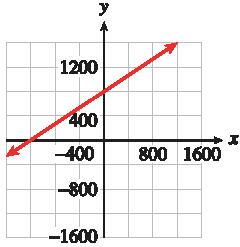
\includegraphics[width=\linewidth]{external/images/fig-ex-1-1-33.pdf}
\end{sbspanel}%
\end{sidebyside}%
\end{divisionexerciseegcol}%
\begin{divisionexerciseegcol}{34}{}{}{exercise-section-1-1-exercises-u-c}%
\begin{sidebyside}{1}{0.1}{0.1}{0}%
\begin{sbspanel}{0.8}%
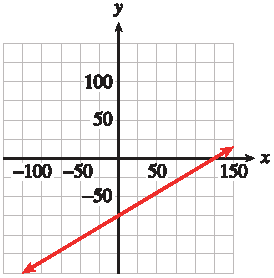
\includegraphics[width=\linewidth]{external/images/fig-ex-1-1-34.pdf}
\end{sbspanel}%
\end{sidebyside}%
\end{divisionexerciseegcol}%
\begin{divisionexerciseegcol}{35}{}{}{exercise-section-1-1-exercises-u-d}%
\begin{sidebyside}{1}{0.1}{0.1}{0}%
\begin{sbspanel}{0.8}%
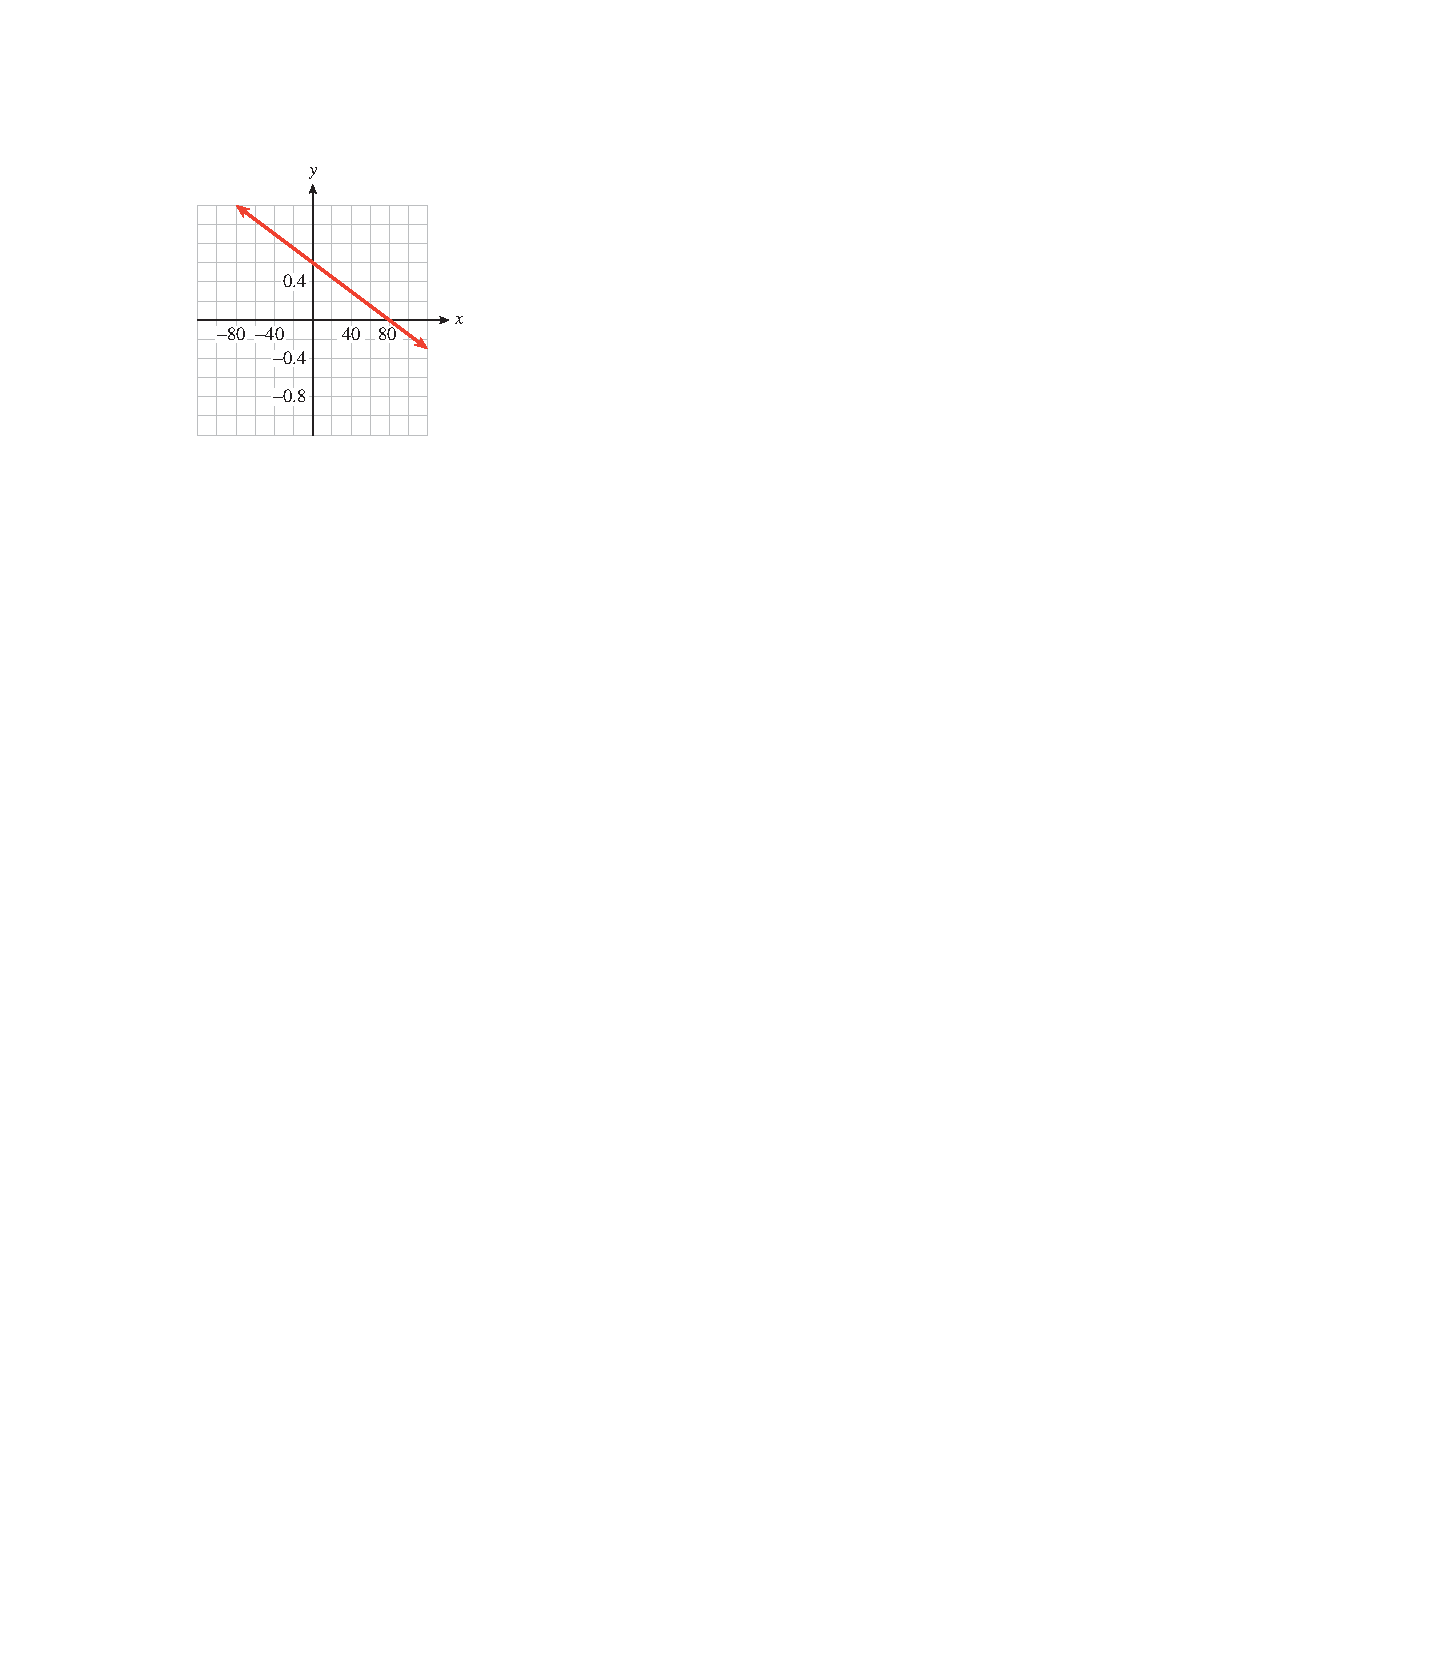
\includegraphics[width=\linewidth]{external/images/fig-ex-1-1-35.pdf}
\end{sbspanel}%
\end{sidebyside}%
\end{divisionexerciseegcol}%
\begin{divisionexerciseegcol}{36}{}{}{exercise-section-1-1-exercises-u-e}%
\begin{sidebyside}{1}{0.1}{0.1}{0}%
\begin{sbspanel}{0.8}%
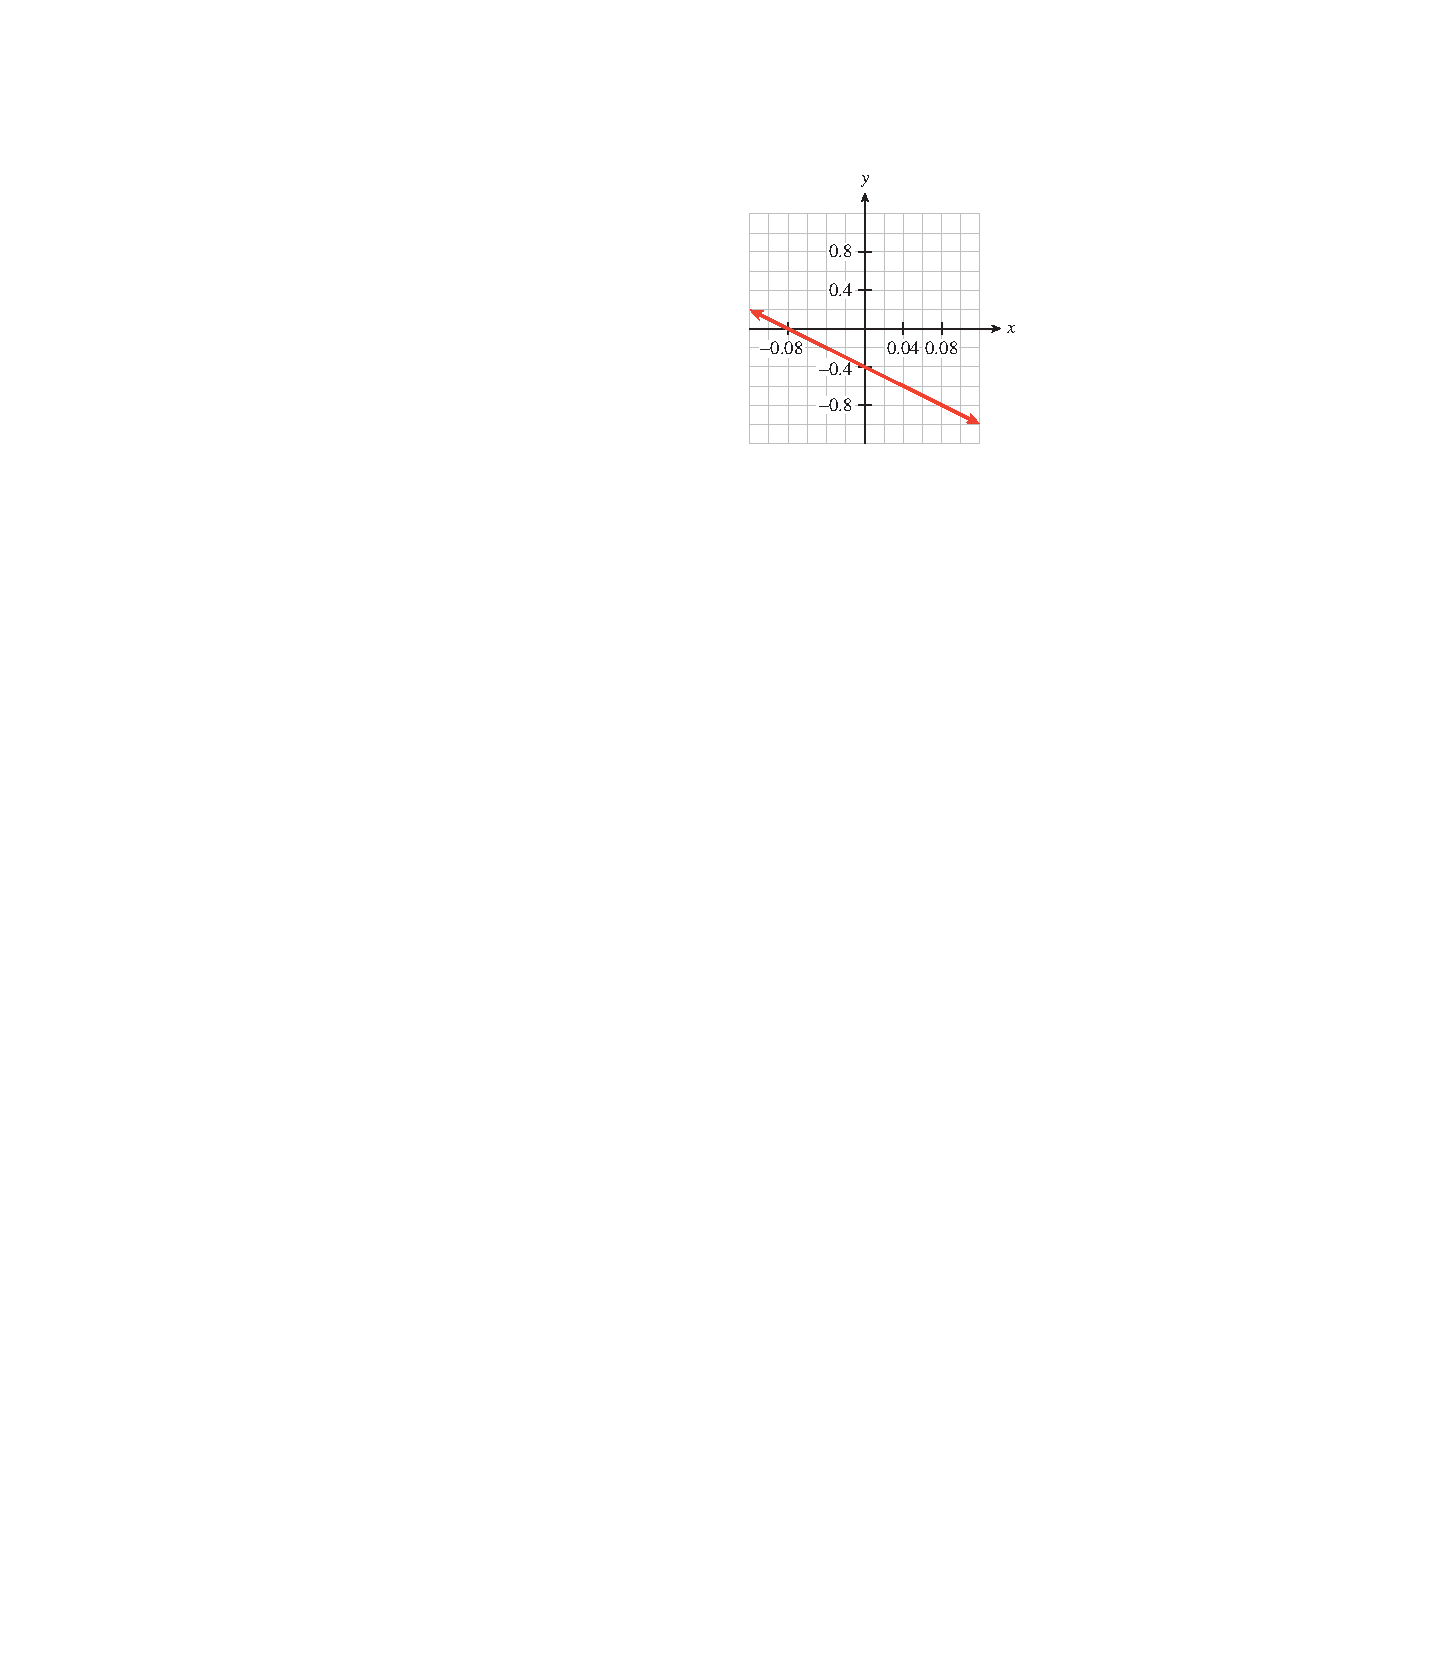
\includegraphics[width=\linewidth]{external/images/fig-ex-1-1-36.pdf}
\end{sbspanel}%
\end{sidebyside}%
\end{divisionexerciseegcol}%
\end{exercisegroupcol}
\par\medskip\noindent
\par\medskip\noindent%
\textbf{Exercise Group.}\space\space%
For Problems 37\textendash{}44,%
\begin{enumerate}[label=\alph*]
\item{}Solve each equation for \(y\) in terms of \(x\). (See the Algebra Skills Refresher \hyperref[section-appendix-Linear-Equations-and-Inequalities]{Section~{\xreffont\ref{section-appendix-Linear-Equations-and-Inequalities}}} to review this skill.)%
\item{}Graph the equation with your graphing utility in the specified window.%
\item{}Make a pencil and paper sketch of the graph. Label the scales on your axes, and the coordinates of the intercepts.%
\end{enumerate}
%
\begin{exercisegroupcol}{2}
\begin{divisionexerciseegcol}{37}{}{}{exercise-section-1-1-exercises-v-b}%
\(2+y=6\)%
\begin{align*}
{\text{Xmin}} \amp = -10 \amp\amp {\text{Ymin}} = -10\\
{\text{Xmax}} \amp = 10 \amp\amp {\text{Ymax}} = 10\\
{\text{Xscl}} \amp = 1 \amp\amp {\text{Yscl}} = 1
\end{align*}
%
\end{divisionexerciseegcol}%
\begin{divisionexerciseegcol}{38}{}{}{exercise-section-1-1-exercises-v-c}%
\(8 - y + 3x = 0\)%
\begin{align*}
{\text{Xmin}} \amp = -10 \amp\amp {\text{Ymin}} = -10\\
{\text{Xmax}} \amp = 10 \amp\amp {\text{Ymax}} = 10\\
{\text{Xscl}} \amp = 1 \amp\amp {\text{Yscl}} = 1
\end{align*}
%
\end{divisionexerciseegcol}%
\begin{divisionexerciseegcol}{39}{}{}{exercise-section-1-1-exercises-v-d}%
\(3x - 4y = 1200\)%
\begin{align*}
{\text{Xmin}} \amp = -1000 \amp\amp {\text{Ymin}} = -1000\\
{\text{Xmax}} \amp = 1000 \amp\amp {\text{Ymax}} = 1000\\
{\text{Xscl}} \amp = 100 \amp\amp {\text{Yscl}} = 100
\end{align*}
%
\end{divisionexerciseegcol}%
\begin{divisionexerciseegcol}{40}{}{}{exercise-section-1-1-exercises-v-e}%
\(x + 2y = 500\)%
\begin{align*}
{\text{Xmin}} \amp = -1000 \amp\amp {\text{Ymin}} = -1000\\
{\text{Xmax}} \amp = 1000 \amp\amp {\text{Ymax}} = 1000\\
{\text{Xscl}} \amp = 100 \amp\amp {\text{Yscl}} = 100
\end{align*}
%
\end{divisionexerciseegcol}%
\begin{divisionexerciseegcol}{41}{}{}{exercise-section-1-1-exercises-v-f}%
\(0.2x + 5y = 0.1\)%
\begin{align*}
{\text{Xmin}} \amp = -1 \amp\amp {\text{Ymin}} = -0.1\\
{\text{Xmax}} \amp = 1 \amp\amp {\text{Ymax}} = 0.1\\
{\text{Xscl}} \amp = 0.1 \amp\amp {\text{Yscl}} = 0.01
\end{align*}
%
\end{divisionexerciseegcol}%
\begin{divisionexerciseegcol}{42}{}{}{exercise-section-1-1-exercises-v-g}%
\(1.2x - 4.2y = 3.6\)%
\begin{align*}
{\text{Xmin}} \amp = -1 \amp\amp {\text{Ymin}} = -1\\
{\text{Xmax}} \amp = 4 \amp\amp {\text{Ymax}} = 1\\
{\text{Xscl}} \amp = 0.2 \amp\amp {\text{Yscl}} = 0.1
\end{align*}
%
\end{divisionexerciseegcol}%
\begin{divisionexerciseegcol}{43}{}{}{exercise-section-1-1-exercises-v-h}%
\(70x + 3y = y + 420\)%
\begin{align*}
{\text{Xmin}} \amp = 0 \amp\amp {\text{Ymin}} = 0\\
{\text{Xmax}} \amp = 10 \amp\amp {\text{Ymax}} = 250\\
{\text{Xscl}} \amp = 1 \amp\amp {\text{Yscl}} = 25
\end{align*}
%
\end{divisionexerciseegcol}%
\begin{divisionexerciseegcol}{44}{}{}{exercise-section-1-1-exercises-v-i}%
\(40y - 5x = 780 - 20y\)%
\begin{align*}
{\text{Xmin}} \amp = -200 \amp\amp {\text{Ymin}} = 0\\
{\text{Xmax}} \amp = 0 \amp\amp {\text{Ymax}} = 20\\
{\text{Xscl}} \amp = 20 \amp\amp {\text{Yscl}} = 2
\end{align*}
%
\end{divisionexerciseegcol}%
\end{exercisegroupcol}
\par\medskip\noindent
\par\medskip\noindent%
\textbf{Exercise Group.}\space\space%
For Problems 45\textendash{}52,%
\begin{enumerate}[label=\alph*]
\item{}Find the \(x\)- and \(y\)-intercepts.%
\item{}Solve the equation for \(y\).%
\item{}Choose a graphing window in which both intercepts are visible, and graph the equation with your graphing utility.%
\end{enumerate}
%
\begin{exercisegroupcol}{2}
\begin{divisionexerciseegcol}{45}{}{}{exercise-section-1-1-exercises-w-b}%
\(x + 4y = 100\)%
\end{divisionexerciseegcol}%
\begin{divisionexerciseegcol}{46}{}{}{exercise-section-1-1-exercises-w-c}%
\(2x - 3y = -72\)%
\end{divisionexerciseegcol}%
\begin{divisionexerciseegcol}{47}{}{}{exercise-section-1-1-exercises-w-d}%
\(25x - 20y = 1\)%
\end{divisionexerciseegcol}%
\begin{divisionexerciseegcol}{48}{}{}{exercise-section-1-1-exercises-w-e}%
\(4x + 75y = 60,000\)%
\end{divisionexerciseegcol}%
\begin{divisionexerciseegcol}{49}{}{}{exercise-section-1-1-exercises-w-f}%
\(\dfrac{y}{12} - \dfrac{x}{60}= 1\)%
\end{divisionexerciseegcol}%
\begin{divisionexerciseegcol}{50}{}{}{exercise-section-1-1-exercises-w-g}%
\(\dfrac{x}{80} + \dfrac{y}{400}= 1\)%
\end{divisionexerciseegcol}%
\begin{divisionexerciseegcol}{51}{}{}{exercise-section-1-1-exercises-w-h}%
\(-2x = 3y + 84\)%
\end{divisionexerciseegcol}%
\begin{divisionexerciseegcol}{52}{}{}{exercise-section-1-1-exercises-w-i}%
\(7x = 91 - 13y\)%
\end{divisionexerciseegcol}%
\end{exercisegroupcol}
\par\medskip\noindent
\end{exercises-subsection}
\end{sectionptx}
%
%
\typeout{************************************************}
\typeout{Section 1.2 Functions}
\typeout{************************************************}
%
\begin{sectionptx}{Section}{Functions}{}{Functions}{}{}{section-functions}
%
%
\typeout{************************************************}
\typeout{Subsection  Definition of Function}
\typeout{************************************************}
%
\begin{subsectionptx}{Subsection}{Definition of Function}{}{Definition of Function}{}{}{subsection-functions-b}
We often want to predict values of one variable from the values of a related variable. For example, when a physician prescribes a drug in a certain dosage, she needs to know how long the dose will remain in the bloodstream. A sales manager needs to know how the price of his product will affect its sales. A \terminology{function}\index{function} is a special type of relationship between variables that allows us to make such predictions.%
\par
Suppose it costs \textdollar{}800 for flying lessons, plus \textdollar{}30 per hour to rent a plane. If we let \(C\) represent the total cost for \(t\) hours of flying lessons, then%
\begin{equation*}
C=800+30t ~~~~ (t\ge 0)
\end{equation*}
Thus, for example%
\begin{sidebyside}{1}{0}{0}{0}%
\begin{sbspanel}{1}%
\resizebox{\ifdim\width > \linewidth\linewidth\else\width\fi}{!}{%
{\centering%
{\tabularfont%
\begin{tabular}{rll}
when&\(t=\alert{0}\),&\(C=800+30(\alert{0})=800\)\tabularnewline[0pt]
when&\(t=\alert{4}\),&\(C=800+30(\alert{4})=920\)\tabularnewline[0pt]
when&\(t=\alert{10}\),&\(C=800+30(\alert{10})=1100\)
\end{tabular}
}%
\par}
}%
\end{sbspanel}%
\end{sidebyside}%
\par
The variable \(t\) is called the \terminology{input}\index{input} or \terminology{independent}\index{independent} variable, and \(C\) is the \terminology{output}\index{output} or \terminology{dependent}\index{dependent} variable, because its values are determined by the value of \(t\). We can display the relationship between two variables by a table or by ordered pairs. The input variable is the first component of the ordered pair, and the output variable is the second component.%
\begin{sidebyside}{1}{0}{0}{0}%
\begin{sbspanel}{1}%
\resizebox{\ifdim\width > \linewidth\linewidth\else\width\fi}{!}{%
{\centering%
{\tabularfont%
\begin{tabular}{AcAcAcA}\hrulethick
\(t\)&\(C\)&\((t,C)\)\tabularnewline\hrulethin
\(0\)&\(800\)&\((0, 800)\)\tabularnewline\hrulethin
\(4\)&\(920\)&\((4, 920)\)\tabularnewline\hrulethin
\(10\)&\(1100\)&\((10,1100)\)\tabularnewline\hrulethin
\end{tabular}
}%
\par}
}%
\end{sbspanel}%
\end{sidebyside}%
\par
For this relationship, we can find the value of \(C\) for any given value of \(t\). All we have to do is substitute the value of \(t\) into the equation and solve for \(C\). Note that there can be only one value of \(C\) for each value of \(t\).%
\begin{assemblage}{Assemblage}{Definition of Function.}{assemblage-functions-b-h}%
A \terminology{function}\index{function} is a relationship between two variables for which a unique value of the \terminology{output}\index{output} variable can be determined from a value of the \terminology{input}\index{input} variable.%
\end{assemblage}
\begin{note}{Note}{}{note-functions-b-i}%
What distinguishes functions from other variable relationships? The definition of a function calls for a \emph{unique value}—that is, \emph{exactly one value} of the output variable corresponding to each value of the input variable. This property makes functions useful in applications because they can often be used to make predictions.%
\end{note}
\begin{example}{Example}{}{example-example-functions}%
%
\begin{enumerate}[label=\alph*]
\item{}The distance, \(d\), traveled by a car in 2 hours is a function of its speed, \(r\). If we know the speed of the car, we can determine the distance it travels by the formula \(d = r \cdot 2\).%
\item{}The cost of a fill-up with unleaded gasoline is a function of the number of gallons purchased. The gas pump represents the function by displaying the corresponding values of the input variable (number of gallons) and the output variable (cost).%
\item{}Score on the Scholastic Aptitude Test (SAT) is not a function of score on an IQ test, because two people with the same score on an IQ test may score differently on the SAT; that is, a person’s score on the SAT is not uniquely determined by his or her score on an IQ test.%
\end{enumerate}
%
\end{example}
\begin{inlineexercise}{Checkpoint}{Practice 1.}{exercise-functions-b-k}%
%
\begin{enumerate}[label=\alph*.]
\item{}As part of a project to improve the success rate of freshmen, the counseling department studied the grades earned by a group of students in English and algebra. Do you think that a student's grade in algebra is a function of his or her grade in English?\quad(\begin{itemize*}[label=$\square$,leftmargin=3em,itemjoin=\hspace{1em}]
\item{}Yes%
\item{}No%
\end{itemize*})\quad
%
\par
Explain why or why not.%
\par
\begin{itemize}[label=$\odot$,leftmargin=3em,]
\item{}A) Each value of \(x \) has exactly one value of \(y \) associated with it.%
\item{}B) Two students with the same grade English can have different grades in algebra.%
\item{}C) Two students with the same grade math will also have the same grade in English.%
\item{}D) Two students with the same grade math can have different grades in English.%
\end{itemize}
%
\item{}Phatburger features a soda bar, where you can serve your own soft drinks in any size. Do you think that the number of calories in a serving of Zap Kola is a function of the number of fluid ounces?\quad(\begin{itemize*}[label=$\square$,leftmargin=3em,itemjoin=\hspace{1em}]
\item{}Yes%
\item{}No%
\end{itemize*})\quad
%
\par
Explain why or why not.%
\par
\begin{itemize}[label=$\odot$,leftmargin=3em,]
\item{}A) The number of calories is proportional to the number of fluid ounces.%
\item{}B) Two servings with the same calories will have different fluid ounces.%
\item{}C) Two servings with the same flid ounces will have different calories.%
\end{itemize}
%
\end{enumerate}
%
\par\smallskip%
\noindent\textbf{\blocktitlefont Answer 1}.\hypertarget{answer-functions-b-k-c}{}\quad{}\(\text{No}\)%
\par\smallskip%
\noindent\textbf{\blocktitlefont Answer 2}.\hypertarget{answer-functions-b-k-d}{}\quad{}\(\text{Choice 2}\)%
\par\smallskip%
\noindent\textbf{\blocktitlefont Answer 3}.\hypertarget{answer-functions-b-k-e}{}\quad{}\(\text{Yes}\)%
\par\smallskip%
\noindent\textbf{\blocktitlefont Answer 4}.\hypertarget{answer-functions-b-k-f}{}\quad{}\(\text{A) The ... fluid ounces.}\)%
\par\smallskip%
\noindent\textbf{\blocktitlefont Solution}.\hypertarget{solution-functions-b-k-g}{}\quad{}%
\begin{enumerate}[label=\alph*.]
\item{}No, students with the same grade in English can have different grades in algebra.%
\item{}Yes, the number of calories is proportional to the number of fluid ounces.%
\end{enumerate}
%
\end{inlineexercise}%
\begin{inlineexercise}{Checkpoint}{QuickCheck 1.}{exercise-functions-b-l}%
What distinguishes a function from other variable relationships?%
\par
\begin{itemize}[label=$\odot$,leftmargin=3em,]
\item{}A) The variables are related by a formula.%
\item{}B) The values of the input and output variables must be different.%
\item{}C) There cannot be two output values for a single input value.%
\item{}D) There cannot be two input values for a single output value.%
\end{itemize}
%
\par\smallskip%
\noindent\textbf{\blocktitlefont Answer}.\hypertarget{answer-functions-b-l-c}{}\quad{}\(\text{C) There ... input value.}\)%
\par\smallskip%
\noindent\textbf{\blocktitlefont Solution}.\hypertarget{solution-functions-b-l-d}{}\quad{}There cannot be two output values for a single input value.%
\end{inlineexercise}%
A function can be described in several different ways. In the following examples, we consider functions defined by tables, by graphs, and by equations.%
\end{subsectionptx}
%
%
\typeout{************************************************}
\typeout{Subsection  Functions Defined by Tables}
\typeout{************************************************}
%
\begin{subsectionptx}{Subsection}{Functions Defined by Tables}{}{Functions Defined by Tables}{}{}{subsection-functions-c}
When we use a table to describe a function, the first variable in the table (the left column of a vertical table or the top row of a horizontal table) is the input variable, and the second variable is the output. We say that the output variable \emph{is a function of} the input.%
\begin{example}{Example}{}{example-example-table-functions}%
%
\begin{enumerate}[label=\alph*]
\item{}The table below shows data on sales compiled over several years by the accounting office for Eau Claire Auto Parts, a division of Major Motors. In this example, the year is the input variable, and total sales is the output. We say that total sales, \(S\), \emph{is a function of} \(t\).%
\begin{sidebyside}{1}{0}{0}{0}%
\begin{sbspanel}{1}%
\resizebox{\ifdim\width > \linewidth\linewidth\else\width\fi}{!}{%
{\centering%
{\tabularfont%
\begin{tabular}{AcAcA}\hrulethick
Year \((t)\)&Total sales \((S)\)\tabularnewline\hrulethin
2000&\textdollar{}612,000\tabularnewline\hrulethin
2001&\textdollar{}663,000\tabularnewline\hrulethin
2002&\textdollar{}692,000\tabularnewline\hrulethin
2003&\textdollar{}749,000\tabularnewline\hrulethin
2004&\textdollar{}904,000\tabularnewline\hrulethin
\end{tabular}
}%
\par}
}%
\end{sbspanel}%
\end{sidebyside}%
\item{}The table below gives the cost of sending printed material by first-class mail starting July 10, 2022. %
\begin{sidebyside}{1}{0}{0}{0}%
\begin{sbspanel}{1}%
\resizebox{\ifdim\width > \linewidth\linewidth\else\width\fi}{!}{%
{\centering%
{\tabularfont%
\begin{tabular}{AcAcA}\hrulethick
Weight in ounces \((w)\)&Postage \((P)\)\tabularnewline\hrulethin
\(0 \lt w \le 1 \)&\textdollar{}0.60\tabularnewline\hrulethin
\(1 \lt w \le 2 \)&\textdollar{}0.84\tabularnewline\hrulethin
\(2 \lt w \le 3 \)&\textdollar{}1.08\tabularnewline\hrulethin
\(3 \lt w \le 4 \)&\textdollar{}1.32\tabularnewline\hrulethin
\(4 \lt w \le 5 \)&\textdollar{}1.56\tabularnewline\hrulethin
\(5 \lt w \le 6 \)&\textdollar{}1.80\tabularnewline\hrulethin
\(6 \lt w \le 7 \)&\textdollar{}2.04\tabularnewline\hrulethin
\end{tabular}
}%
\par}
}%
\end{sbspanel}%
\end{sidebyside}%
\par
If we know the weight of the article being shipped, we can find the postage from the table. For instance, a catalog weighing 4.5 ounces would require  \textdollar{}1.56 in postage. In this example, \(w\) is the input variable and \(p\) is the output variable. We say that \(p\) \emph{is a function of} \(w\).%
\item{}The table below records the age and cholesterol count for 20 patients tested in a hospital survey.%
\begin{sidebyside}{1}{0}{0}{0}%
\begin{sbspanel}{1}%
\resizebox{\ifdim\width > \linewidth\linewidth\else\width\fi}{!}{%
{\centering%
{\tabularfont%
\begin{tabular}{AcAcAcAcAcA}\hrulethick
Age&Cholesterol count&&Age&Cholesterol count\tabularnewline\hrulethin
53&217&&\(\alert{51}\)&\(\alert{209}\)\tabularnewline\hrulethin
48&232&&53&241\tabularnewline\hrulethin
55&198&&49&186\tabularnewline\hrulethin
56&238&&\(\alert{51}\)&\(\alert{216}\)\tabularnewline\hrulethin
\(\alert{51}\)&\(\alert{227}\)&&57&208\tabularnewline\hrulethin
52&264&&52&248\tabularnewline\hrulethin
53&195&&50&214\tabularnewline\hrulethin
47&203&&56&271\tabularnewline\hrulethin
48&212&&53&193\tabularnewline\hrulethin
50&234&&48&172\tabularnewline\hrulethin
\end{tabular}
}%
\par}
}%
\end{sbspanel}%
\end{sidebyside}%
\par
According to these data, cholesterol count is \emph{not} a function of age, because several patients who are the same age have different cholesterol levels. For example, three different patients are 51 years old but have cholesterol counts of 227, 209, and 216, respectively. Thus, we cannot determine a \emph{unique} value of the output variable (cholesterol count) from the value of the input variable (age). Other factors besides age must influence a person’s cholesterol count.%
\end{enumerate}
%
\end{example}
\begin{note}{Note}{}{note-functions-c-d}%
Note that several different inputs for a function can have the same output.  For example, the inputs 4.5 and 4.25 in part (b) of the Example above have output \textdollar{}1.31. However, a single input cannot have more than one output, as illustrated in part (c) of the Example.%
\end{note}
\begin{inlineexercise}{Checkpoint}{Practice 2.}{exercise-functions-c-e}%
Decide whether each table describes \(y\) as a function of \(x\). Explain your choice.%
\par
%
\begin{enumerate}[label=\alph*.]
\item{}\begin{center}%
{\tabularfont%
\begin{tabular}{AcAcAcAcAcAcAcAcAcA}
\(x\)&\(3.5\)&\(2.0\)&\(2.5\)&\(3.5\)&\(2.5\)&\(4.0\)&\(2.5\)&\(3.0\)\tabularnewline\hrulethin
\(y\)&\(2.5\)&\(3.0\)&\(2.5\)&\(4.0\)&\(3.5\)&\(4.0\)&\(2.0\)&\(2.5\)\tabularnewline\hrulethin
\end{tabular}
}%
\end{center}%
%
\end{enumerate}
%
\par
Is  \(y\) a function of \(x\text{?}\)\quad(\begin{itemize*}[label=$\square$,leftmargin=3em,itemjoin=\hspace{1em}]
\item{}Yes%
\item{}No%
\end{itemize*})\quad
%
\par
\begin{itemize}[label=$\odot$,leftmargin=3em,]
\item{}Each value of \(x\) has exactly one value of \(y\) associated with it.%
\item{}For example, \(x=3.5\) corresponds both to \(y=2.5\) and also to \(y=4.0\)%
\end{itemize}
%
\par
%
\begin{enumerate}[label=\alph*.]
\item{}\begin{center}%
{\tabularfont%
\begin{tabular}{AcAcAcAcAcAcAcAcA}
\(x\)&\(-3\)&\(-2\)&\(-1\)&\(0\)&\(1\)&\(2\)&\(3\)\tabularnewline\hrulethin
\(y\)&\(17\)&\(3\)&\(0\)&\(-1\)&\(0\)&\(3\)&\(17\)\tabularnewline\hrulethin
\end{tabular}
}%
\end{center}%
%
\end{enumerate}
%
\par
Is  \(y\) a function of \(x\text{?}\)\quad(\begin{itemize*}[label=$\square$,leftmargin=3em,itemjoin=\hspace{1em}]
\item{}Yes%
\item{}No%
\end{itemize*})\quad
%
\par
\begin{itemize}[label=$\odot$,leftmargin=3em,]
\item{}Each value of \(x\) has exactly one value of \(y\) associated with it.%
\item{}For example, \(y=3\) corresponds both to \(x=-2\) and also to \(x=2\)%
\end{itemize}
%
\par\smallskip%
\noindent\textbf{\blocktitlefont Answer 1}.\hypertarget{answer-functions-c-e-c}{}\quad{}\(\text{No}\)%
\par\smallskip%
\noindent\textbf{\blocktitlefont Answer 2}.\hypertarget{answer-functions-c-e-d}{}\quad{}\(\text{Choice 2}\)%
\par\smallskip%
\noindent\textbf{\blocktitlefont Answer 3}.\hypertarget{answer-functions-c-e-e}{}\quad{}\(\text{Yes}\)%
\par\smallskip%
\noindent\textbf{\blocktitlefont Answer 4}.\hypertarget{answer-functions-c-e-f}{}\quad{}\(\text{Choice 1}\)%
\par\smallskip%
\noindent\textbf{\blocktitlefont Solution}.\hypertarget{solution-functions-c-e-g}{}\quad{}%
\begin{enumerate}[label=\alph*.]
\item{}No, for example, \(x=3.5\) corresponds both to \(y=2.5\) and also to \(y=4\text{.}\)%
\item{}Yes, each value of \(x\) has exactly one value of \(y\) associated with it.%
\end{enumerate}
%
\end{inlineexercise}%
\begin{inlineexercise}{Checkpoint}{QuickCheck 2.}{exercise-functions-c-f}%
How would you know if a table of values does not come from a function?%
\par
\begin{itemize}[label=$\odot$,leftmargin=3em,]
\item{}A) The output values are all the same.%
\item{}B) The input values are not evely spaced.%
\item{}C) Two different input values have the same output value.%
\item{}D) Two different output values have the same input value.%
\end{itemize}
%
\par\smallskip%
\noindent\textbf{\blocktitlefont Answer}.\hypertarget{answer-functions-c-f-c}{}\quad{}\(\text{D) Two ... input value.}\)%
\par\smallskip%
\noindent\textbf{\blocktitlefont Solution}.\hypertarget{solution-functions-c-f-d}{}\quad{}Two different output values have the same input value.%
\end{inlineexercise}%
\end{subsectionptx}
%
%
\typeout{************************************************}
\typeout{Subsection  Functions Defined by Graphs}
\typeout{************************************************}
%
\begin{subsectionptx}{Subsection}{Functions Defined by Graphs}{}{Functions Defined by Graphs}{}{}{subsection-functions-d}
We can also use a graph to define a function. The input variable is displayed on the horizontal axis, and the output variable on the vertical axis.%
\begin{example}{Example}{}{example-example-sun-hours}%
The graph  shows the number of hours, \(H\), that the sun is above the horizon in Peoria, Illinois, on day \(t\), where \(t = 0\) on January 1.%
\begin{sidebyside}{2}{0}{0.05}{0.05}%
\begin{sbspanel}{0.5}[center]%
%
\begin{enumerate}[label=\alph*]
\item{}Which variable is the input, and which is the output?%
\item{}How many hours of sunlight are there in Peoria on day 150?%
\item{}On which days are there 12 hours of sunlight?%
\item{}What are the maximum and minimum values of \(H\), and when do these values occur?%
\end{enumerate}
%
\end{sbspanel}%
\begin{sbspanel}{0.4}[center]%
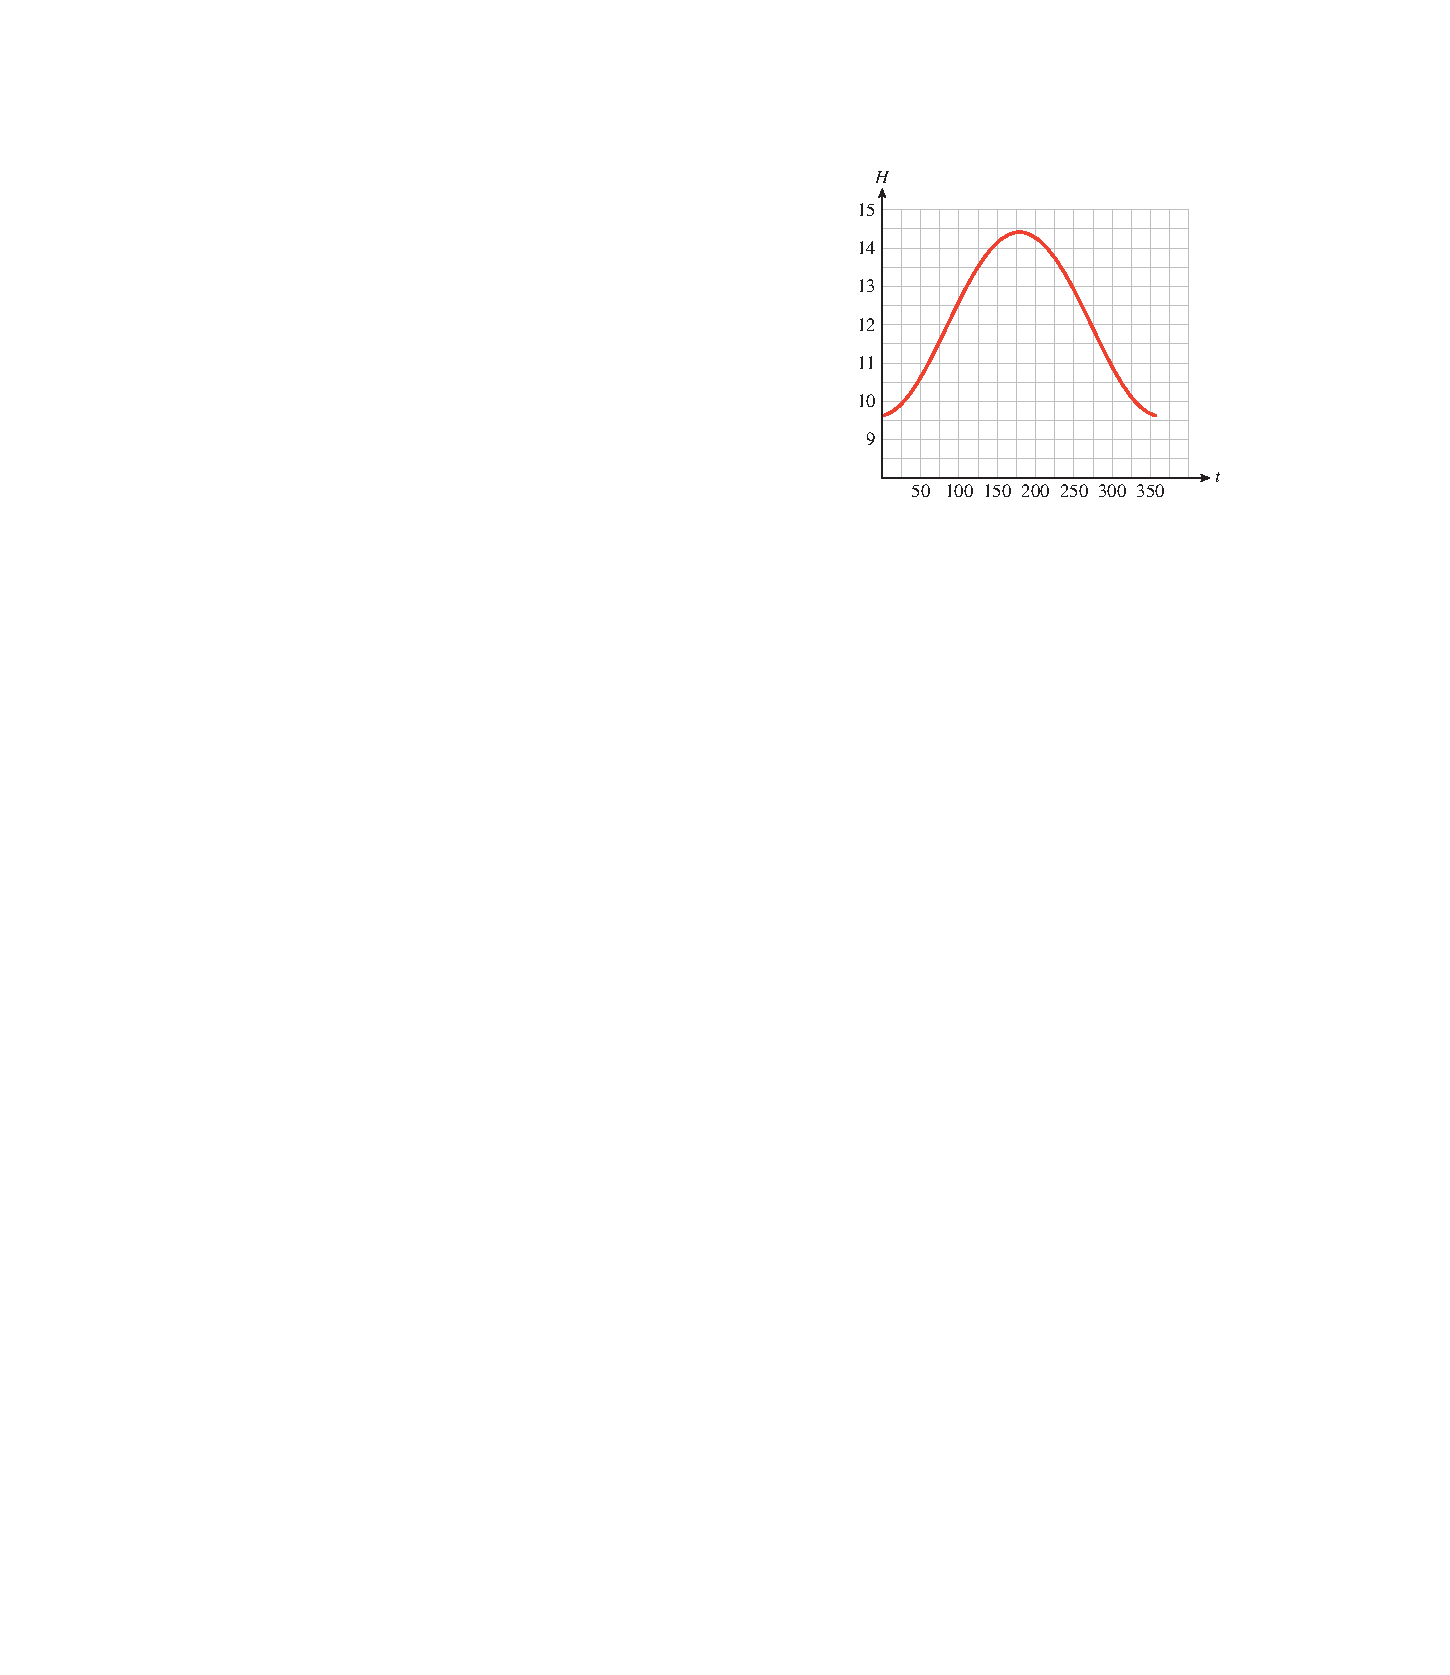
\includegraphics[width=\linewidth]{external/images/fig-sun-hours.pdf}
\end{sbspanel}%
\end{sidebyside}%
\par\smallskip%
\noindent\textbf{\blocktitlefont Solution}.\hypertarget{solution-example-sun-hours-b}{}\quad{}%
\begin{enumerate}[label=\alph*]
\item{}The input variable, \(t\), appears on the horizontal axis. The number of daylight hours, \(H\), is a function of the date. The output variable appears on the vertical axis.%
\item{}The point on the curve where \(t = 150\) has \(H \approx 14.1\), so Peoria gets about 14.1 hours of daylight when \(t = 150\), which is at the end of May.%
\item{}\(H = 12\) at the two points where \(t \approx 85\) (in late March) and \(t \approx 270\) (late September).%
\item{}The maximum value of 14.4 hours occurs on the longest day of the year, when \(t \approx 170\), about three weeks into June. The minimum of 9.6 hours occurs on the shortest day, when \(t \approx 355\), about three weeks into December.%
\end{enumerate}
%
\end{example}
\begin{inlineexercise}{Checkpoint}{Practice 3.}{exercise-functions-d-d}%
The graph shows the elevation in feet, \(a\), of the Los Angeles Marathon course at a distance \(d\) miles into the race. (Source: \emph{Los Angeles Times}, March 3, 2005)%
\begin{sidebyside}{1}{0.05}{0.05}{0}%
\begin{sbspanel}{0.9}%
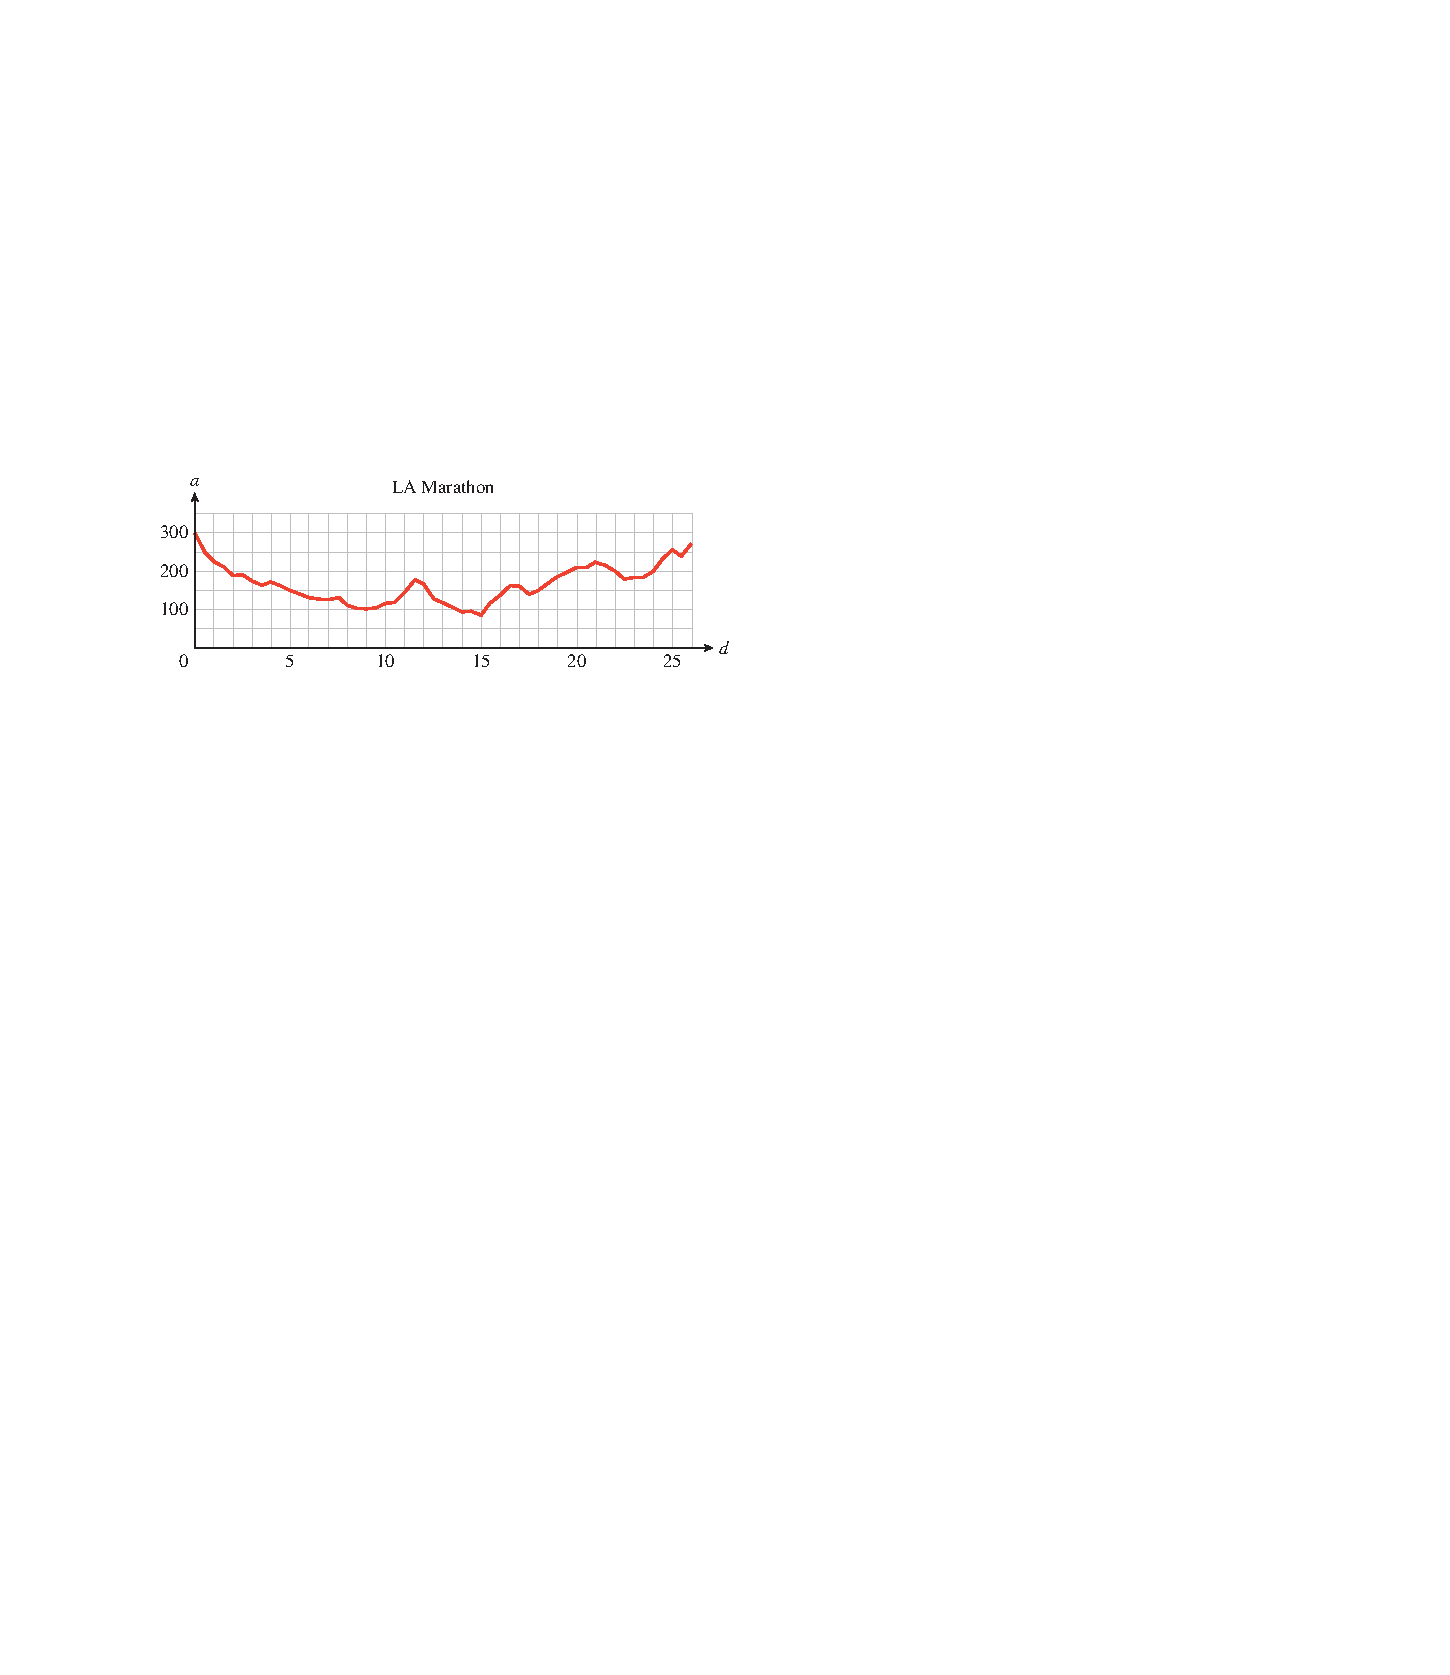
\includegraphics[width=\linewidth]{external/images/fig-LA-marathon.pdf}
\end{sbspanel}%
\end{sidebyside}%
\par
%
\begin{enumerate}[label=\alph*.]
\item{}Which variable is the input, and which is the output?%
\par
\begin{itemize}[label=$\odot$,leftmargin=3em,]
\item{}The input variable is \(d \), and the output variable is \(a \).%
\item{}The input variable is \(a \), and the output variable is \(d \).%
\end{itemize}
%
\item{}What is the elevation at mile 20?%
\par
Answer: \fillintext{3} feet%
\item{}At what distances is the elevation 150 feet?%
\par
The relevant distances (to the nearest half-mile) separated by commas: \fillintext{18} miles%
\item{}What are the maximum and minimum values of \(a \text{,}\) and when do these values occur?%
\par
The maximum elevation is \(a=\)\fillintext{3} feet which occurs at \(d=\)\fillintext{2}.%
\item{}The runners pass by the Los Angeles Coliseum at about 4.2 miles into the race. What is the elevation there?%
\par
Approximately (within 5) \fillintext{3} feet%
\end{enumerate}
%
\par\smallskip%
\noindent\textbf{\blocktitlefont Answer 1}.\hypertarget{answer-functions-d-d-c}{}\quad{}\(\text{Choice 1}\)%
\par\smallskip%
\noindent\textbf{\blocktitlefont Answer 2}.\hypertarget{answer-functions-d-d-d}{}\quad{}\(210\)%
\par\smallskip%
\noindent\textbf{\blocktitlefont Answer 3}.\hypertarget{answer-functions-d-d-e}{}\quad{}\(5, 11, 12, 16, 17.5, 18\)%
\par\smallskip%
\noindent\textbf{\blocktitlefont Answer 4}.\hypertarget{answer-functions-d-d-f}{}\quad{}\(300\)%
\par\smallskip%
\noindent\textbf{\blocktitlefont Answer 5}.\hypertarget{answer-functions-d-d-g}{}\quad{}\(0\)%
\par\smallskip%
\noindent\textbf{\blocktitlefont Answer 6}.\hypertarget{answer-functions-d-d-h}{}\quad{}\(165\)%
\par\smallskip%
\noindent\textbf{\blocktitlefont Solution}.\hypertarget{solution-functions-d-d-i}{}\quad{}%
\begin{enumerate}[label=\alph*.]
\item{}The input variable is \(d \text{,}\) and the output variable is \(a \text{.}\)%
\item{}Approximately 210 feet%
\item{}Approximately where \(d\approx 5 \text{,}\) \(d\approx 11 \text{,}\) \(d\approx 12 \text{,}\) \(d\approx 16 \text{,}\) \(d\approx 17.5 \text{,}\) and \(d\approx 18\)%
\item{}The maximum value of 300 feet occurs at the start, when \(d = 0 \text{.}\) The minimum of 85 feet occurs when \(d\approx 15 \text{.}\)%
\item{}Approximately 165 feet%
\end{enumerate}
%
\end{inlineexercise}%
\end{subsectionptx}
%
%
\typeout{************************************************}
\typeout{Subsection  Functions Defined by Equations}
\typeout{************************************************}
%
\begin{subsectionptx}{Subsection}{Functions Defined by Equations}{}{Functions Defined by Equations}{}{}{subsection-functions-e}
\hyperref[example-example-falling-book]{Example~{\xreffont\ref{example-example-falling-book}}} illustrates a function defined by an equation.%
\begin{example}{Example}{}{example-example-falling-book}%
As of 2020,  One World Trade Center in New York City is the nation’s tallest building, at 1776 feet. If an algebra book is dropped from the top of One World Trade Center, its height above the ground after \(t\) seconds is given by the equation%
\begin{equation*}
h = 1776 - 16t^2
\end{equation*}
Thus, after \(\alert{1}\) second the book’s height is%
\begin{equation*}
h = 1776 - 16(\alert{1})^2 = 1760 \text{ feet}
\end{equation*}
After \(\alert{2}\) seconds its height is%
\begin{equation*}
h = 1776 - 16(\alert{2})^2 = 1712 \text{ feet}
\end{equation*}
For this function, \(t\) is the input variable and \(h\) is the output variable. For any value of \(t\), a unique value of \(h\) can be determined from the equation for \(h\). We say that \(h\) \emph{is a function of} \(t\).%
\end{example}
\begin{inlineexercise}{Checkpoint}{Practice 4.}{exercise-functions-e-d}%
Write an equation that gives the volume, \(V\text{,}\) of a sphere as a function of its radius, \(r\text{.}\)%
\par
\(V=\)\fillintext{8}%
\par\smallskip%
\noindent\textbf{\blocktitlefont Answer}.\hypertarget{answer-functions-e-d-c}{}\quad{}\({\frac{4}{3}}\pi r^{3}\)%
\par\smallskip%
\noindent\textbf{\blocktitlefont Solution}.\hypertarget{solution-functions-e-d-d}{}\quad{}\(V=\dfrac{4}{3}\pi r^3\)%
\end{inlineexercise}%
\begin{inlineexercise}{Checkpoint}{QuickCheck 3.}{exercise-functions-e-e}%
Name three ways to describe a function.%
\par
\begin{itemize}[label=$\odot$,leftmargin=3em,]
\item{}A) By inputs, outputs, or evaluation%
\item{}B) By tables, equations, or graphs%
\item{}C) By the intercepts, the slope, or the vertex%
\item{}D) By numbers, letters, or diagrams%
\end{itemize}
%
\par\smallskip%
\noindent\textbf{\blocktitlefont Answer}.\hypertarget{answer-functions-e-e-c}{}\quad{}\(\text{B) By ... , or graphs}\)%
\par\smallskip%
\noindent\textbf{\blocktitlefont Solution}.\hypertarget{solution-functions-e-e-d}{}\quad{}By tables, equations, or graphs%
\end{inlineexercise}%
\begin{technology}{Technology}{Making a Table of Values with a Calculator.}{technology-functions-e-f}%
We can use a graphing calculator to make a table of values for a function defined by an equation. For the function in \hyperref[example-example-falling-book]{Example~{\xreffont\ref{example-example-falling-book}}},%
\begin{equation*}
h = 1776 - 16t^2
\end{equation*}
we follow the steps:%
\begin{itemize}[label=\textbullet]
\item{}Enter the equation: Press the \kbd{Y=} key, clear out any other equations, and define \(Y_1 = 1776 - 16X^2.\)%
\item{}Choose the \(x\)-values for the table. Press \kbd{2nd}\kbd{WINDOW} to access the \(TblSet\) (Table Setup) menu and set it to look like the figure at left below.%
\end{itemize}
%
\par
This setting will give us an initial x-value of 0 \((TblStart = 0)\) and an increment of one unit in the \(x\)-values, \((\Delta Tbl = 1)\). It also fills in values of both variables automatically.%
\par
%
\begin{itemize}[label=\textbullet]
\item{}Press \kbd{2nd} \kbd{GRAPH} to see the table of values, as shown in the figure at right below. From this table, we can check the heights we found in \hyperref[example-example-falling-book]{Example~{\xreffont\ref{example-example-falling-book}}}.%
\end{itemize}
%
\begin{sidebyside}{2}{0.1}{0.1}{0.2}%
\begin{sbspanel}{0.3}%
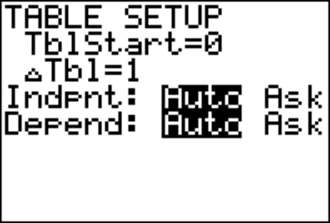
\includegraphics[width=\linewidth]{external/images/fig-TblSetup.pdf}
\end{sbspanel}%
\begin{sbspanel}{0.3}%
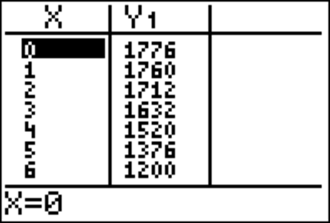
\includegraphics[width=\linewidth]{external/images/fig-GC-table.pdf}
\end{sbspanel}%
\end{sidebyside}%
\par
Now try making a table of values with \(TblStart = 0\) and \(\Delta Tbl = 0.5\). Use the   \kbd{\arrowkeyup} and  \kbd{\arrowkeydown} arrow keys to scroll up and down the table.%
\end{technology}
\begin{inlineexercise}{Checkpoint}{Pause and Reflect.}{exercise-functions-e-g}%
Write one question you still have about functions.%
\end{inlineexercise}%
\end{subsectionptx}
%
%
\typeout{************************************************}
\typeout{Subsection  Function Notation}
\typeout{************************************************}
%
\begin{subsectionptx}{Subsection}{Function Notation}{}{Function Notation}{}{}{subsection-functions-f}
There is a convenient notation for discussing functions. First, we choose a letter, such as \(f\), \(g\), or \(h\) (or \(F\), \(G\), or \(H\)), to name a particular function. (We can use any letter, but these are the most common choices.)%
\par
For instance, in \hyperref[example-example-falling-book]{Example~{\xreffont\ref{example-example-falling-book}}}, the height, \(h\), of a falling algebra book is a function of the elapsed time, \(t\). We might call this function \(f\). In other words, \(f\) is the name of the relationship between the variables \(h\) and \(t\). We write%
\begin{equation*}
h = f (t)
\end{equation*}
which means "\(h\) is a function of \(t\), and \(f\) is the name of the function."%
\begin{warning}{Caution}{}{warning-functions-f-d}%
The new symbol \(f(t)\), read "\(f\) of \(t\)," is another name for the height, \(h\). The parentheses in the symbol \(f(t)\) do not indicate multiplication. (It would not make sense to multiply the name of a function by a variable.) Think of the symbol \(f(t)\) as a single variable that represents the output value of the function.%
\end{warning}
With this new notation we may write%
\begin{equation*}
h = f (t) = 1776 - 16t^2
\end{equation*}
or just%
\begin{equation*}
f (t) = 1776 - 16t^2
\end{equation*}
instead of%
\begin{equation*}
h = 1776 - 16t^2
\end{equation*}
to describe the function.%
\begin{note}{Note}{}{note-functions-f-f}%
Perhaps it seems complicated to introduce a new symbol for \(h\), but the notation \(f(t)\) is very useful for showing the correspondence between specific values of the variables \(h\) and \(t\).%
\end{note}
\begin{example}{Example}{}{example-example-falling-book-2}%
In \hyperref[example-example-falling-book]{Example~{\xreffont\ref{example-example-falling-book}}}, the height of an algebra book dropped from the top of One World Trade Center is given by the equation%
\begin{equation*}
h = 1776 - 16t^2
\end{equation*}
We see that%
\begin{sidebyside}{1}{0}{0}{0}%
\begin{sbspanel}{1}%
\resizebox{\ifdim\width > \linewidth\linewidth\else\width\fi}{!}{%
{\centering%
{\tabularfont%
\begin{tabular}{lll}
when \(t=1\)&&\(h=1760\)\tabularnewline[0pt]
when \(t=2\)&&\(h=1712\)
\end{tabular}
}%
\par}
}%
\end{sbspanel}%
\end{sidebyside}%
\par
Using function notation, these relationships can be expressed more concisely as%
\begin{sidebyside}{1}{0}{0}{0}%
\begin{sbspanel}{1}%
\resizebox{\ifdim\width > \linewidth\linewidth\else\width\fi}{!}{%
{\centering%
{\tabularfont%
\begin{tabular}{lll}
\(f(1)=1760\)&and&\(f(2)=1712\)
\end{tabular}
}%
\par}
}%
\end{sbspanel}%
\end{sidebyside}%
\par
which we read as "\(f\) of 1 equals 1760" and "\(f\) of 2 equals 1712." The values for the input variable, \(t\), appear \emph{inside} the parentheses, and the values for the output variable, \(h\), appear on the other side of the equation.%
\end{example}
Remember that when we write \(y = f(x)\), the symbol \(f(x)\) is just another name for the output variable.%
\begin{assemblage}{Assemblage}{Function Notation.}{assemblage-functions-f-i}%
\begin{sidebyside}{1}{0.175}{0.175}{0}%
\begin{sbspanel}{0.65}%
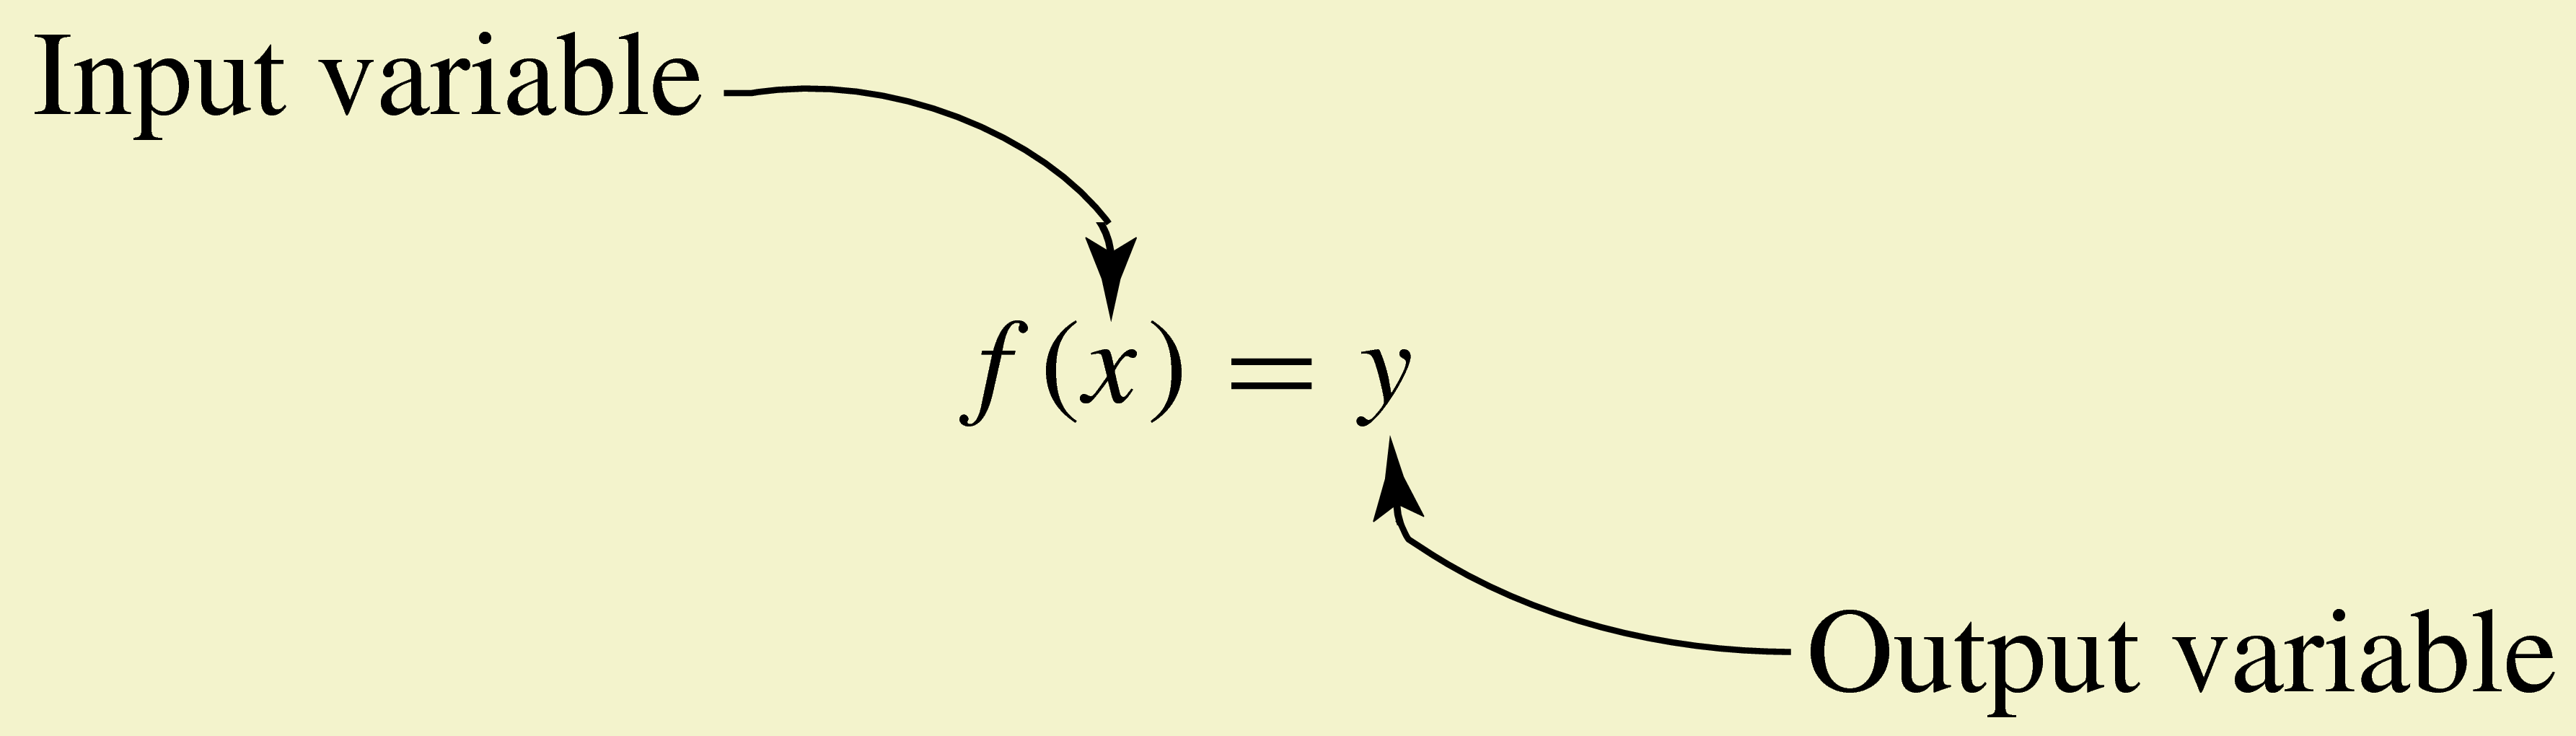
\includegraphics[width=\linewidth]{external/images/fig-Function-Notation.png}
\end{sbspanel}%
\end{sidebyside}%
\end{assemblage}
\begin{inlineexercise}{Checkpoint}{QuickCheck 4.}{exercise-functions-f-j}%
True or False.%
\begin{enumerate}[label=\alph*.]
\item{}The notation \(f(t)\) indicates the product of \(f\) and \(t\text{.}\)\quad(\begin{itemize*}[label=$\square$,leftmargin=3em,itemjoin=\hspace{1em}]
\item{}True%
\item{}False%
\end{itemize*})\quad
%
\item{}If \(y=f(x)\text{,}\) then \(f(x)\) gives the value of the input variable.\quad(\begin{itemize*}[label=$\square$,leftmargin=3em,itemjoin=\hspace{1em}]
\item{}True%
\item{}False%
\end{itemize*})\quad
%
\item{}If \(Q\) is a function of \(M\text{,}\) we may write \(M=f(Q)\text{.}\)\quad(\begin{itemize*}[label=$\square$,leftmargin=3em,itemjoin=\hspace{1em}]
\item{}True%
\item{}False%
\end{itemize*})\quad
%
\item{}In the equation \(d=g(n)\) the letters \(d,~g,\) and \(n\) are variables.\quad(\begin{itemize*}[label=$\square$,leftmargin=3em,itemjoin=\hspace{1em}]
\item{}True%
\item{}False%
\end{itemize*})\quad
%
\end{enumerate}
%
\par\smallskip%
\noindent\textbf{\blocktitlefont Answer 1}.\hypertarget{answer-functions-f-j-c}{}\quad{}\(\text{False}\)%
\par\smallskip%
\noindent\textbf{\blocktitlefont Answer 2}.\hypertarget{answer-functions-f-j-d}{}\quad{}\(\text{False}\)%
\par\smallskip%
\noindent\textbf{\blocktitlefont Answer 3}.\hypertarget{answer-functions-f-j-e}{}\quad{}\(\text{False}\)%
\par\smallskip%
\noindent\textbf{\blocktitlefont Answer 4}.\hypertarget{answer-functions-f-j-f}{}\quad{}\(\text{False}\)%
\par\smallskip%
\noindent\textbf{\blocktitlefont Solution}.\hypertarget{solution-functions-f-j-g}{}\quad{}%
\begin{enumerate}[label=\alph*.]
\item{}False%
\item{}False%
\item{}False%
\item{}False%
\end{enumerate}
%
\end{inlineexercise}%
\begin{inlineexercise}{Checkpoint}{Practice 5.}{exercise-functions-f-k}%
Let \(F \) be the name of the function defined by the graph in \hyperref[example-example-sun-hours]{Example~{\xreffont\ref{example-example-sun-hours}}}, the number of hours of daylight in Peoria \(t\) days after January 1.%
\par
%
\begin{enumerate}[label=\alph*.]
\item{}Use function notation to state that \(H\) is a function of \(t\text{.}\)%
\par
\begin{itemize}[label=$\odot$,leftmargin=3em,]
\item{}\(\displaystyle F=H(t) \)%
\item{}\(\displaystyle H=F(t) \)%
\item{}\(\displaystyle t=F(H) \)%
\item{}\(\displaystyle H=t(F) \)%
\end{itemize}
%
\item{}What does the statement \(F(15) = 9.7\) mean in the context of the problem?%
\par
\begin{itemize}[label=$\odot$,leftmargin=3em,]
\item{}A) The sun is 9.7 degrees above the horizon in Peoria on January 15.%
\item{}B) The sun is above the horizon in Peoria for 15 hours on January 10.%
\item{}C) The sun is above the horizon in Peoria for 9.7 hours on January 16.%
\end{itemize}
%
\end{enumerate}
%
\par\smallskip%
\noindent\textbf{\blocktitlefont Answer 1}.\hypertarget{answer-functions-f-k-c}{}\quad{}\(\text{Choice 2}\)%
\par\smallskip%
\noindent\textbf{\blocktitlefont Answer 2}.\hypertarget{answer-functions-f-k-d}{}\quad{}\(\text{C) The ... January 16.}\)%
\par\smallskip%
\noindent\textbf{\blocktitlefont Solution}.\hypertarget{solution-functions-f-k-e}{}\quad{}%
\begin{enumerate}[label=\alph*.]
\item{}\(\displaystyle H = F(t)\)%
\item{}The sun is above the horizon in Peoria for 9.7 hours on January 16.%
\end{enumerate}
%
\end{inlineexercise}%
\begin{inlineexercise}{Checkpoint}{QuickCheck 4.}{exercise-functions-f-l}%
Use function notation to write the statement ``\(L\) defines \(w\) as a function of \(p\text{.}\)''%
\par
\begin{itemize}[label=$\odot$,leftmargin=3em,]
\item{}\(\displaystyle L=w(p)\)%
\item{}\(\displaystyle w=L(p)\)%
\item{}\(\displaystyle p=L(w)\)%
\item{}\(\displaystyle L=p(w)\)%
\end{itemize}
%
\par\smallskip%
\noindent\textbf{\blocktitlefont Answer}.\hypertarget{answer-functions-f-l-c}{}\quad{}\(\text{Choice 2}\)%
\par\smallskip%
\noindent\textbf{\blocktitlefont Solution}.\hypertarget{solution-functions-f-l-d}{}\quad{}\(w=L(p)\)%
\end{inlineexercise}%
\end{subsectionptx}
%
%
\typeout{************************************************}
\typeout{Subsection  Using Function Notation}
\typeout{************************************************}
%
\begin{subsectionptx}{Subsection}{Using Function Notation}{}{Using Function Notation}{}{}{subsection-functions-g}
Finding the value of the output variable that corresponds to a particular value of the input variable is called \terminology{evaluating the function}\index{evaluating the function}.%
\begin{example}{Example}{}{example-example-postage2}%
Let \(g\) be the name of the postage function defined by the table in \hyperref[example-example-functions]{Example~{\xreffont\ref{example-example-functions}}} b. Find \(g(1)\), \(g(3)\), and \(g(6.75\)).%
\par\smallskip%
\noindent\textbf{\blocktitlefont Solution}.\hypertarget{solution-example-postage2-b}{}\quad{}According to the table,%
\begin{sidebyside}{1}{0}{0}{0}%
\begin{sbspanel}{1}%
\resizebox{\ifdim\width > \linewidth\linewidth\else\width\fi}{!}{%
{\centering%
{\tabularfont%
\begin{tabular}{lllll}
when \(w=1\),&&\(p=0.47\)&so&\(g(1)=0.47\)\tabularnewline[0pt]
when \(w=3\),&&\(p=0.89\)&so&\(g(3)=0.89\)\tabularnewline[0pt]
when \(w=6.75\),&&\(p=1.73\)&so&\(g(6.75)=1.73\)
\end{tabular}
}%
\par}
}%
\end{sbspanel}%
\end{sidebyside}%
\par
Thus, a letter weighing 1 ounce costs \textdollar{}0.47 to mail, a letter weighing 3 ounces costs \textdollar{}0.89, and a letter weighing 6.75 ounces costs \textdollar{}1.73.%
\end{example}
\begin{inlineexercise}{Checkpoint}{Practice 6.}{exercise-functions-g-d}%
When you exercise, your heart rate should increase until it reaches your target heart rate. The table shows target heart rate, \(r = f(a) \text{,}\) as a function of age.%
\begin{center}%
{\tabularfont%
\begin{tabular}{AcAcAcAcAcAcAcAcAcAcAcAcA}
\(a\)&20&25&30&35&40&45&50&55&60&65&70\tabularnewline\hrulethin
\(r\)&150&146&142&139&135&131&127&124&120&116&112\tabularnewline\hrulethin
\end{tabular}
}%
\end{center}%
%
\begin{enumerate}[label=\alph*.]
\item{}Find \(f(25)\) and \(f(50) \text{.}\)%
\par
\(f(25)=\)\fillintext{3}%
\par
\(f(50)=\)\fillintext{3}%
\item{}Find a value of \(a\) for which \(f(a) = 135 \text{.}\)%
\par
\(a=\)\fillintext{3}%
\end{enumerate}
%
\par\smallskip%
\noindent\textbf{\blocktitlefont Answer 1}.\hypertarget{answer-functions-g-d-c}{}\quad{}\(146\)%
\par\smallskip%
\noindent\textbf{\blocktitlefont Answer 2}.\hypertarget{answer-functions-g-d-d}{}\quad{}\(127\)%
\par\smallskip%
\noindent\textbf{\blocktitlefont Answer 3}.\hypertarget{answer-functions-g-d-e}{}\quad{}\(40\)%
\par\smallskip%
\noindent\textbf{\blocktitlefont Solution}.\hypertarget{solution-functions-g-d-f}{}\quad{}%
\begin{enumerate}[label=\alph*.]
\item{}\(f (25) = 146 \text{,}\)  \(f(50) = 127\)%
\item{}\(\displaystyle a = 40\)%
\end{enumerate}
%
\end{inlineexercise}%
\begin{inlineexercise}{Checkpoint}{QuickCheck 5.}{exercise-functions-g-e}%
If \(n=f(a)\text{,}\) what are the input and output variables?%
\par
\begin{itemize}[label=$\odot$,leftmargin=3em,]
\item{}\(f\) is the output and \(n\) is the input%
\item{}\(a\) is the input and \(f\) is the output%
\item{}\(a\) is the input and \(n\) is the output%
\item{}\(f(a)\) is the input and \(n\) is the output%
\end{itemize}
%
\par\smallskip%
\noindent\textbf{\blocktitlefont Answer}.\hypertarget{answer-functions-g-e-c}{}\quad{}\(\text{Choice 3}\)%
\par\smallskip%
\noindent\textbf{\blocktitlefont Solution}.\hypertarget{solution-functions-g-e-d}{}\quad{}\(a\) is the input and \(n\) is the output%
\end{inlineexercise}%
If a function is described by an equation, we simply substitute the given input value into the equation to find the corresponding output, or function value.%
\begin{example}{Example}{}{example-example-evaluate-function}%
The function \(H\) is defined by \(H=f(s) = \dfrac{\sqrt{s+3}}{s}\). Evaluate the function at the following values.%
\begin{enumerate}[label=\alph*]
\item{}\(\displaystyle s=6\)%
\item{}\(\displaystyle s=-1\)%
\end{enumerate}
%
\par\smallskip%
\noindent\textbf{\blocktitlefont Solution}.\hypertarget{solution-example-evaluate-function-b}{}\quad{}%
\begin{enumerate}[label=\alph*]
\item{}\(f(\alert{6})=\dfrac{\sqrt{\alert{6}+3}}{\alert{6}}=
\dfrac{\sqrt{9}}{6}=\dfrac{3}{6}=\dfrac{1}{2}\). Thus, \(f(6)=\dfrac{1}{2}\).%
\item{}\(f(\alert{-1})=\dfrac{\sqrt{\alert{-1}+3}}{\alert{-1}}=
\dfrac{\sqrt{2}}{-1}=-\sqrt{2}\). Thus, \(f(-1)=-\sqrt{2}\).%
\end{enumerate}
%
\end{example}
\begin{inlineexercise}{Checkpoint}{Practice 7.}{exercise-exercise-function-notation}%
Complete the table displaying ordered pairs for the function \(f(x) = 5 - x^3\text{.}\) Evaluate the function to find the corresponding \(f(x)\)-value for each value of \(x\text{.}\)%
\begin{center}%
{\tabularfont%
\begin{tabular}{AcAcAl}
\(x\)&\(f(x)\)&\tabularnewline\hrulethin
\(-2\)&\fillintext{3}&\(f(\alert{-2})=5-(\alert{-2})^3=~\)\tabularnewline\hrulethin
\(0\)&\fillintext{3}&\(f(\alert{0})=5-\alert{0}^3=\)\tabularnewline\hrulethin
\(1\)&\fillintext{3}&\(f(\alert{1})=5-\alert{1}^3=\)\tabularnewline\hrulethin
\(3\)&\fillintext{3}&\(f(\alert{3})=5-\alert{3}^3=\)\tabularnewline\hrulethin
\end{tabular}
}%
\end{center}%
\par\smallskip%
\noindent\textbf{\blocktitlefont Answer 1}.\hypertarget{answer-exercise-function-notation-c}{}\quad{}\(13\)%
\par\smallskip%
\noindent\textbf{\blocktitlefont Answer 2}.\hypertarget{answer-exercise-function-notation-d}{}\quad{}\(5\)%
\par\smallskip%
\noindent\textbf{\blocktitlefont Answer 3}.\hypertarget{answer-exercise-function-notation-e}{}\quad{}\(4\)%
\par\smallskip%
\noindent\textbf{\blocktitlefont Answer 4}.\hypertarget{answer-exercise-function-notation-f}{}\quad{}\(-22\)%
\par\smallskip%
\noindent\textbf{\blocktitlefont Solution}.\hypertarget{solution-exercise-function-notation-g}{}\quad{}\begin{center}%
{\tabularfont%
\begin{tabular}{AcAcA}
\(x\)&\(f(x)\)\tabularnewline\hrulethin
\(-2\)&\(13\)\tabularnewline\hrulethin
\(0\)&\(5\)\tabularnewline\hrulethin
\(1\)&\(4\)\tabularnewline\hrulethin
\(3\)&\(-22\)\tabularnewline\hrulethin
\end{tabular}
}%
\end{center}%
\end{inlineexercise}%
\begin{technology}{Technology}{Evaluating a Function.}{technology-functions-g-i}%
We can use the table feature on a graphing calculator to evaluate functions. Consider the function of \hyperref[exercise-exercise-function-notation]{Checkpoint~{\xreffont\ref{exercise-exercise-function-notation}}}, \(f(x) = 5 - x^3\).%
\par
%
\begin{itemize}[label=\textbullet]
\item{}Press \kbd{Y=}, clear any old functions, and enter%
\par
\(\qquad Y_1=5-X\) \textasciicircum{} \(3\)%
\item{}Press \kbd{TblSet} (\kbd{2nd} \kbd{WINDOW}) and choose \(Ask\) after \(Indpnt\), as shown in the figure at left below, and press \kbd{ENTER}. This setting allows you to enter any \(x\)-values you like.%
\item{}Press \kbd{TABLE} (using \kbd{2nd} \kbd{GRAPH}).%
\item{}To follow \hyperref[exercise-exercise-function-notation]{Checkpoint~{\xreffont\ref{exercise-exercise-function-notation}}}, key in \kbd{(-)} 2 \kbd{ENTER} for the \(x\)-value, and the calculator will fill in the \(y\)-value. Continue by entering 0, 1, 3, or any other \(x\)-values you choose.%
\end{itemize}
%
\par
One such table is shown in the figure at right below.%
\begin{sidebyside}{2}{0.1}{0.1}{0.2}%
\begin{sbspanel}{0.3}%
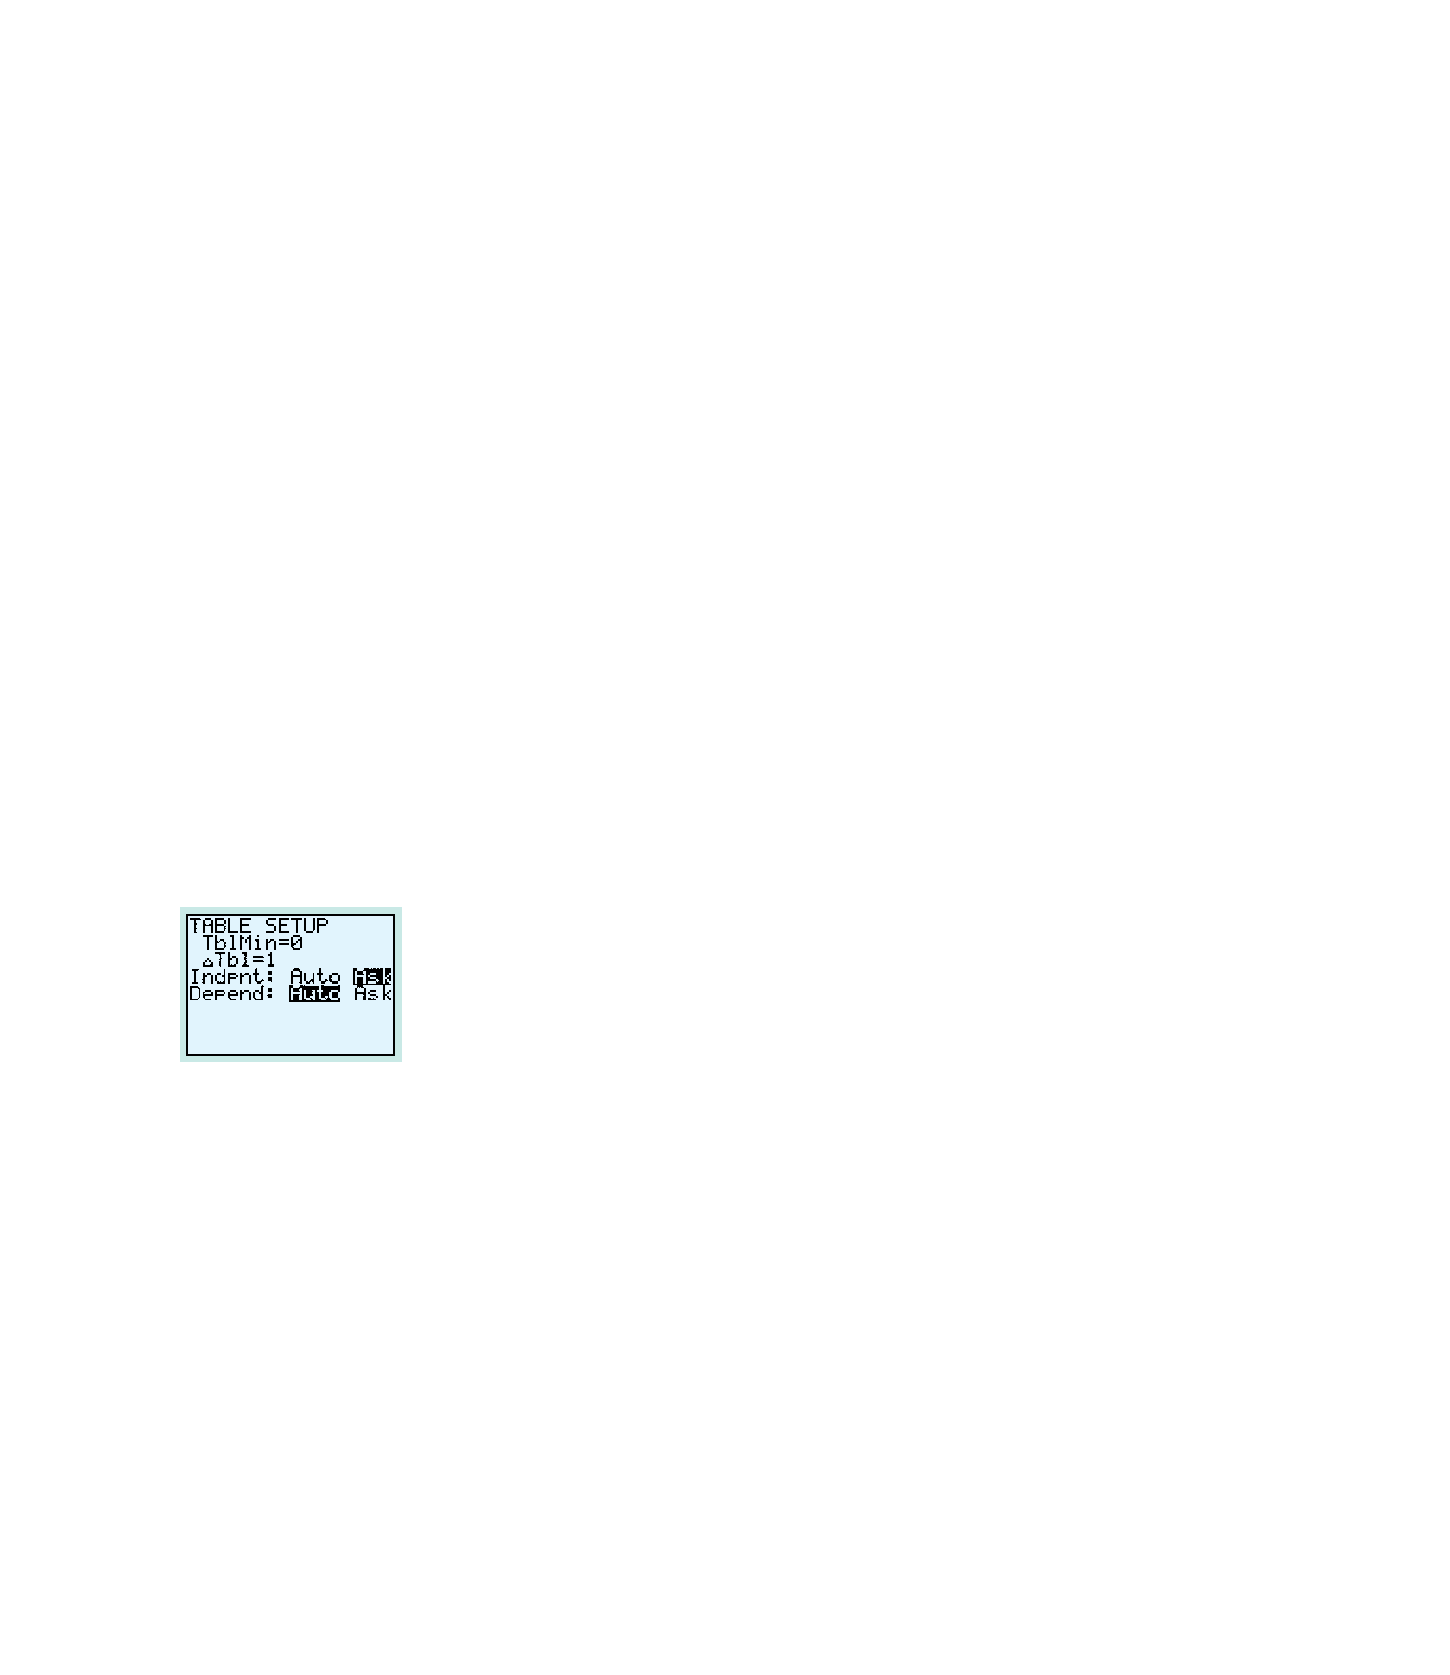
\includegraphics[width=\linewidth]{external/images/fig-TblSetup2.pdf}
\end{sbspanel}%
\begin{sbspanel}{0.3}%
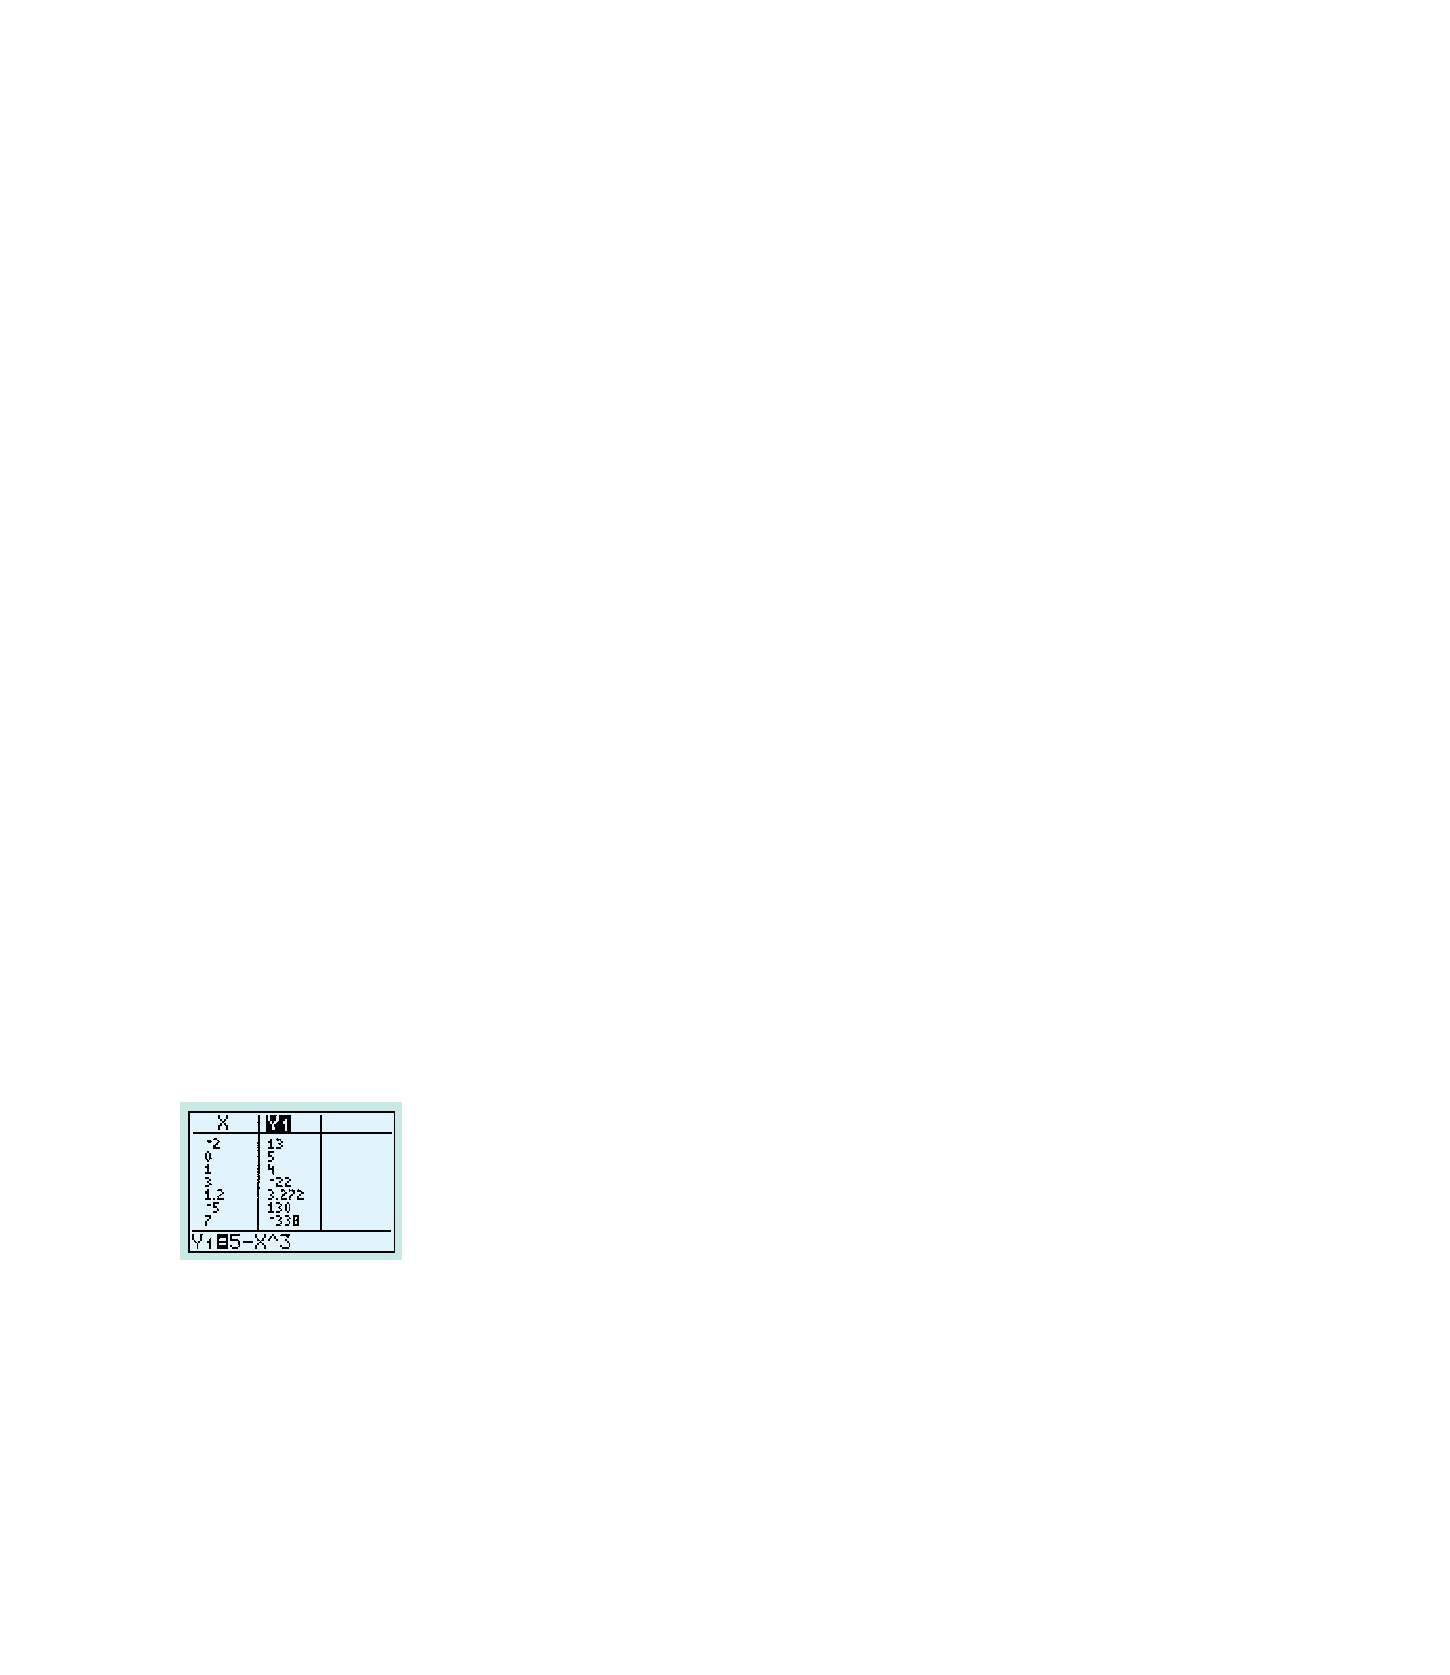
\includegraphics[width=\linewidth]{external/images/fig-GC-table2.pdf}
\end{sbspanel}%
\end{sidebyside}%
\par
If you would like to evaluate a new function, you do not have to return to the \kbd{Y=} screen. Use the \kbd{\arrowkeyright} and  \kbd{\arrowkeyup} arrow keys to highlight \(Y_1\) at the top of the second column. The definition of \(Y_1\) will appear at the bottom of the display, as shown above. You can key in a new definition here, and the second column will be updated automatically to show the \(y\)-values of the new function.%
\end{technology}
To simplify the notation, we sometimes use the same letter for the output variable and for the name of the function. In the next example, \(C\) is used in this way.%
\begin{example}{Example}{}{example-example-function-notation-abuse}%
TrailGear decides to market a line of backpacks. The cost, \(C\), of manufacturing backpacks is a function of the number, \(x\), of backpacks produced, given by the equation%
\begin{equation*}
C(x) = 3000 + 20x
\end{equation*}
where \(C(x)\) is measured in dollars. Find the cost of producing 500 backpacks.%
\par\smallskip%
\noindent\textbf{\blocktitlefont Solution}.\hypertarget{solution-example-function-notation-abuse-b}{}\quad{}To find the value of \(C\) that corresponds to \(x = \alert{500}\), evaluate \(C(500)\).%
\begin{equation*}
C(\alert{500}) = 3000 + 20(\alert{500}) = 13,000
\end{equation*}
The cost of producing 500 backpacks is \textdollar{}13,000.%
\end{example}
\begin{inlineexercise}{Checkpoint}{Practice 8.}{exercise-functions-g-l}%
The volume of a sphere of radius \(r\) centimeters is given by%
\par
%
\begin{equation*}
V = V(r) = \frac{4}{3}\pi r^3
\end{equation*}
%
\par
Evaluate \(V(10)\) and explain what it means.%
\par
\(V(10)=\)\fillintext{12}, which represents%
\par
\begin{itemize}[label=$\odot$,leftmargin=3em,]
\item{}A) the volume (in cm) of a sphere whose radius is 10 cu. cm%
\item{}B) the radius (in cm) of a sphere whose volume is 10 cm%
\item{}C) the volume (in sq. cm) of a sphere whose radius is 10 cm%
\item{}D) the volume (in cu. cm) of a sphere whose radius is 10 cm%
\end{itemize}
%
\par\smallskip%
\noindent\textbf{\blocktitlefont Answer 1}.\hypertarget{answer-functions-g-l-c}{}\quad{}\(4188.79\)%
\par\smallskip%
\noindent\textbf{\blocktitlefont Answer 2}.\hypertarget{answer-functions-g-l-d}{}\quad{}\(\text{D) the  ...  is 10 cm}\)%
\par\smallskip%
\noindent\textbf{\blocktitlefont Solution}.\hypertarget{solution-functions-g-l-e}{}\quad{}\(V(10) = 4000\pi/3\approx 4188.79 \text{ cm}^3\) is the volume of a sphere whose radius is 10 cm.%
\end{inlineexercise}%
\begin{inlineexercise}{Checkpoint}{Pause and Reflect.}{exercise-functions-g-m}%
Do linear equations \(y=mx+b\) and quadratic equations \(y=ax^2+bx+c\) define functions? Why or why not?%
\end{inlineexercise}%
\end{subsectionptx}
%
%
\typeout{************************************************}
\typeout{Subsection  Operations with Function Notation}
\typeout{************************************************}
%
\begin{subsectionptx}{Subsection}{Operations with Function Notation}{}{Operations with Function Notation}{}{}{subsection-functions-h}
Sometimes we need to evaluate a function at an algebraic expression rather than at a specific number.%
\begin{example}{Example}{}{example-example-backpacks}%
TrailGear manufactures backpacks at a cost of%
\begin{equation*}
C(x) = 3000 + 20x
\end{equation*}
for \(x\) backpacks. The company finds that the monthly demand for backpacks increases by 50\% during the summer. The backpacks are produced at several small co-ops in different states.%
\begin{enumerate}[label=\alph*]
\item{}If each co-op usually produces \(b\) backpacks per month, how many should it produce during the summer months?%
\item{}What costs for producing backpacks should the company expect during the summer?%
\end{enumerate}
%
\par\smallskip%
\noindent\textbf{\blocktitlefont Solution}.\hypertarget{solution-example-backpacks-b}{}\quad{}%
\begin{enumerate}[label=\alph*]
\item{}An increase of 50\% means an additional 50\% of the current production level, \(b\). Therefore, a co-op that produced \(b\) backpacks per month during the winter should increase production to \(b + 0.5b\), or \(1.5b\) backpacks per month in the summer.%
\item{}The cost of producing \(1.5b\) backpacks will be%
\begin{equation*}
C(\alert{1.5b}) = 3000 + 20(\alert{1.5b}) = 3000 + 30b
\end{equation*}
%
\end{enumerate}
%
\end{example}
\begin{inlineexercise}{Checkpoint}{Practice 9.}{exercise-functions-h-d}%
A spherical balloon has a radius of 10 centimeters.%
\begin{enumerate}[label=\alph*.]
\item{}If we increase the radius by \(h\) centimeters, what will the new volume be?%
\par
\begin{itemize}[label=$\odot$,leftmargin=3em,]
\item{}\(V(10)+h=\frac{4}{3}\pi(10^3)+h \) cu. cm%
\item{}\(V(10)+h=\frac{4}{3}\pi(10^{3+h}) \) cu. cm%
\item{}\(V(10+h)=\frac{4}{3}\pi\cdot 10^3+h \) cu. cm%
\item{}\(V(10+h)=\frac{4}{3}\pi(10+h)^3 \) cu. cm%
\end{itemize}
%
\item{}If \(h = 2 \text{,}\) how much did the volume increase? Round your answer to hundredths.%
\par
It increased by \fillintext{18} \(\text{cm}^3 \text{.}\)%
\end{enumerate}
%
\par\smallskip%
\noindent\textbf{\blocktitlefont Answer 1}.\hypertarget{answer-functions-h-d-c}{}\quad{}\(\text{Choice 4}\)%
\par\smallskip%
\noindent\textbf{\blocktitlefont Answer 2}.\hypertarget{answer-functions-h-d-d}{}\quad{}\(3049.44\)%
\par\smallskip%
\noindent\textbf{\blocktitlefont Solution}.\hypertarget{solution-functions-h-d-e}{}\quad{}%
\begin{enumerate}[label=\alph*.]
\item{}\(\displaystyle V(10 + h) = \dfrac{4}{3}\pi(10 + h)^3 \text{ cm}^3\)%
\item{}From \(V(10)\) to \(V(12)\) is an increase of about \(3049.44 \text{ cm}^3\)%
\end{enumerate}
%
\end{inlineexercise}%
\begin{example}{Example}{}{example-example-evaluate-quadratic}%
Evaluate the function \(f(x)=4x^2 - x + 5\) for the following expressions.%
\begin{multicols}{2}
\begin{enumerate}[label=\alph*]
\item{}\(\displaystyle x = 2h\)%
\item{}\(\displaystyle x = a + 3\)%
\end{enumerate}
\end{multicols}
%
\par\smallskip%
\noindent\textbf{\blocktitlefont Solution}.\hypertarget{solution-example-evaluate-quadratic-b}{}\quad{}%
\begin{enumerate}[label=\alph*]
\item{}~%
\par
\(\begin{aligned}[t]
f(\alert{2h}) \amp= 4(\alert{2h})^2-(\alert{2h}) + 5\\
\amp= 4(4h^2)-2h+5\\
\amp= 16h^2 - 2h + 5\\ 
\end{aligned}\)%
\item{}~%
\par
\(\begin{aligned}[t]
f(\alert{a+3}) \amp= 4(\alert{a+3})^2-(\alert{a+3})+5\\
\amp= 4(a^2+6a+9)-a-3+5\\
\amp= 4a^2+24a+36 - a + 2\\
\amp= 4a^2+23a + 38\\
\end{aligned}\)%
\end{enumerate}
%
\end{example}
\begin{warning}{Caution}{}{warning-functions-h-f}%
In \hyperref[example-example-evaluate-quadratic]{Example~{\xreffont\ref{example-example-evaluate-quadratic}}}, notice that%
\begin{equation*}
f(2h) \ne 2 f(h)
\end{equation*}
and%
\begin{equation*}
f(a + 3) \ne f(a) + f(3)
\end{equation*}
To compute \(f(a) + f(3)\), we must first compute \(f(a)\) and \(f(3)\), then add them:%
\par
%
\begin{equation*}
\begin{aligned}[t]
f(a)+f(3)\amp= (4a^2-a+5)+(4\cdot 3^2-3+5) \\
\amp= 4a^2 - a + 43\\
\end{aligned}
\end{equation*}
%
\par
In general, it is not true that \(f(a + b) = f(a) + f(b)\). Remember that the parentheses in the expression \(f(x)\) do not indicate multiplication, so the distributive law does not apply to the expression \(f(a + b)\).%
\end{warning}
\begin{inlineexercise}{Checkpoint}{QuickCheck 6.}{exercise-functions-h-g}%
Define the function \(f(x)=x^2\text{.}\) Which of these is equal to \(f(x+y)\text{?}\)%
\par
\begin{itemize}[label=$\odot$,leftmargin=3em,]
\item{}\(\displaystyle f(x)+f(y)\)%
\item{}\(\displaystyle f(x+y)^2\)%
\item{}\(\displaystyle x^2+y^2\)%
\item{}\(\displaystyle (x+y)^2\)%
\end{itemize}
%
\par\smallskip%
\noindent\textbf{\blocktitlefont Answer}.\hypertarget{answer-functions-h-g-c}{}\quad{}\(\text{Choice 4}\)%
\par\smallskip%
\noindent\textbf{\blocktitlefont Solution}.\hypertarget{solution-functions-h-g-d}{}\quad{}\((x+y)^2\)%
\end{inlineexercise}%
\begin{inlineexercise}{Checkpoint}{Practice 10.}{exercise-functions-h-h}%
Let \(f(x) = x^3 - 1\) and evaluate each expression.%
\begin{enumerate}[label=\alph*.]
\item{}\(f(2) + f(3)=\)\fillintext{7}%
\item{}\(f(2 + 3)=\)\fillintext{7}%
\item{}\(2 f(x) + 3\)\fillintext{7}%
\end{enumerate}
%
\par\smallskip%
\noindent\textbf{\blocktitlefont Answer 1}.\hypertarget{answer-functions-h-h-c}{}\quad{}\(33\)%
\par\smallskip%
\noindent\textbf{\blocktitlefont Answer 2}.\hypertarget{answer-functions-h-h-d}{}\quad{}\(124\)%
\par\smallskip%
\noindent\textbf{\blocktitlefont Answer 3}.\hypertarget{answer-functions-h-h-e}{}\quad{}\(2\!\left(x^{3}-1\right)+3\)%
\par\smallskip%
\noindent\textbf{\blocktitlefont Solution}.\hypertarget{solution-functions-h-h-f}{}\quad{}%
\begin{enumerate}[label=\alph*.]
\item{}\(\displaystyle 33\)%
\item{}\(\displaystyle 124\)%
\item{}\(\displaystyle 2x^3 + 1\)%
\end{enumerate}
%
\end{inlineexercise}%
\begin{inlineexercise}{Checkpoint}{Pause and Reflect.}{exercise-functions-h-i}%
Explain why \(f(a+b)\) is not the same as \(f(a)+f(b)\) for most functions.%
\end{inlineexercise}%
\end{subsectionptx}
%
%
\typeout{************************************************}
\typeout{Subsection  Section Summary}
\typeout{************************************************}
%
\begin{subsectionptx}{Subsection}{Section Summary}{}{Section Summary}{}{}{subsection-summary-1-2}
%
%
\typeout{************************************************}
\typeout{Subsubsection  Vocabulary}
\typeout{************************************************}
%
\begin{subsubsectionptx}{Subsubsection}{Vocabulary}{}{Vocabulary}{}{}{subsubsection-summary-1-2-b}
Look up the definitions of new terms in the Glossary.%
\begin{multicols}{3}
\begin{itemize}[label=\textbullet]
\item{}Function%
\item{}Input variable%
\item{}Independent variable%
\item{}Function value%
\item{}Dependent variable%
\item{}Output variable%
\end{itemize}
\end{multicols}
%
\end{subsubsectionptx}
%
%
\typeout{************************************************}
\typeout{Subsubsection  CONCEPTS}
\typeout{************************************************}
%
\begin{subsubsectionptx}{Subsubsection}{CONCEPTS}{}{CONCEPTS}{}{}{subsubsection-summary-1-2-c}
%
\begin{enumerate}[label=\arabic*]
\item{}A function is a rule that assigns to each value of the input variable a unique value of the output variable.%
\item{}Functions may be defined by words, tables, graphs, or equations.%
\item{}Function notation: \(y = f (x)\), where \(x\) is the input and \(y\) is the output.%
\end{enumerate}
%
\end{subsubsectionptx}
%
%
\typeout{************************************************}
\typeout{Subsubsection  STUDY QUESTIONS}
\typeout{************************************************}
%
\begin{subsubsectionptx}{Subsubsection}{STUDY QUESTIONS}{}{STUDY QUESTIONS}{}{}{subsubsection-summary-1-2-d}
%
\begin{enumerate}[label=\arabic*]
\item{}What property makes a relation between two variables a function?%
\item{}Name three ways to define a function.%
\item{}Give an example of a function in which two distinct values of the input variable correspond to the same value of the output variable.%
\item{}Use function notation to write the statement "\(G\) defines \(w\) as a function of \(p\)."%
\item{}Give an example of a function for which \(f (2 + 3)\ne f (2) + f (3)\).%
\end{enumerate}
%
\end{subsubsectionptx}
%
%
\typeout{************************************************}
\typeout{Subsubsection  SKILLS}
\typeout{************************************************}
%
\begin{subsubsectionptx}{Subsubsection}{SKILLS}{}{SKILLS}{}{}{subsubsection-summary-1-2-e}
Practice each skill in the Homework problems listed.%
\begin{enumerate}[label=\arabic*]
\item{}Decide whether a relationship between two variables is a function: \#1\textendash{}26%
\item{}Evaluate a function defined by a table, a graph, or an equation: \#27\textendash{}54%
\item{}Choose appropriate scales for the axes: \#5\textendash{}12%
\item{}Interpret function notation: \#31\textendash{}34, 49\textendash{}54%
\item{}Simplify expressions involving function notation: \#59\textendash{}76%
\end{enumerate}
%
\end{subsubsectionptx}
\end{subsectionptx}
%
%
\typeout{************************************************}
\typeout{Exercises  Homework 1.2}
\typeout{************************************************}
%
\begin{exercises-subsection}{Exercises}{Homework 1.2}{}{Homework 1.2}{}{}{exercises-section-1-2-exercises}
\par\medskip\noindent%
\textbf{Exercise Group.}\space\space%
For which of Problems 1-6 is the second quantity a function of the first? Explain your answers.%
\begin{exercisegroup}
\begin{divisionexerciseeg}{1}{}{}{exercise-section-1-2-exercises-b-b}%
Price of an item; sales tax on the item at 4\%%
\end{divisionexerciseeg}%
\begin{divisionexerciseeg}{2}{}{}{exercise-section-1-2-exercises-b-c}%
Time traveled at constant speed; distance traveled%
\end{divisionexerciseeg}%
\begin{divisionexerciseeg}{3}{}{}{exercise-section-1-2-exercises-b-d}%
Number of years of education; annual income%
\end{divisionexerciseeg}%
\begin{divisionexerciseeg}{4}{}{}{exercise-section-1-2-exercises-b-e}%
Distance flown in an airplane; price of the ticket%
\end{divisionexerciseeg}%
\begin{divisionexerciseeg}{5}{}{}{exercise-section-1-2-exercises-b-f}%
Volume of a container of water; the weight of the water%
\end{divisionexerciseeg}%
\begin{divisionexerciseeg}{6}{}{}{exercise-section-1-2-exercises-b-g}%
Amount of a paycheck; amount of Social Security tax withheld%
\end{divisionexerciseeg}%
\end{exercisegroup}
\par\medskip\noindent
\par\medskip\noindent%
\textbf{Exercise Group.}\space\space%
Each of the objects in Problems 7-14 establishes a correspondence between two variables. Suggest appropriate input and output variables and decide whether the relationship is a function.%
\begin{exercisegroupcol}{2}
\begin{divisionexerciseegcol}{7}{}{}{exercise-section-1-2-exercises-c-b}%
An itemized grocery receipt%
\end{divisionexerciseegcol}%
\begin{divisionexerciseegcol}{8}{}{}{exercise-section-1-2-exercises-c-c}%
An inventory list%
\end{divisionexerciseegcol}%
\begin{divisionexerciseegcol}{9}{}{}{exercise-section-1-2-exercises-c-d}%
An index%
\end{divisionexerciseegcol}%
\begin{divisionexerciseegcol}{10}{}{}{exercise-section-1-2-exercises-c-e}%
A will%
\end{divisionexerciseegcol}%
\begin{divisionexerciseegcol}{11}{}{}{exercise-section-1-2-exercises-c-f}%
An instructor's grade book%
\end{divisionexerciseegcol}%
\begin{divisionexerciseegcol}{12}{}{}{exercise-section-1-2-exercises-c-g}%
An address book%
\end{divisionexerciseegcol}%
\begin{divisionexerciseegcol}{13}{}{}{exercise-section-1-2-exercises-c-h}%
A bathroom scale%
\end{divisionexerciseegcol}%
\begin{divisionexerciseegcol}{14}{}{}{exercise-section-1-2-exercises-c-i}%
A radio dial%
\end{divisionexerciseegcol}%
\end{exercisegroupcol}
\par\medskip\noindent
\par\medskip\noindent%
\textbf{Exercise Group.}\space\space%
Which of the tables in Problems 15-26 define the second variable as a function of the first variable? Explain why or why not.%
\begin{exercisegroupcol}{4}
\begin{divisionexerciseegcol}{15}{}{}{exercise-section-1-2-exercises-d-b}%
\begin{sidebyside}{1}{0}{0}{0}%
\begin{sbspanel}{1}%
\resizebox{\ifdim\width > \linewidth\linewidth\else\width\fi}{!}{%
{\centering%
{\tabularfont%
\begin{tabular}{AcAcA}\hrulethick
\(x\)&\(t\)\tabularnewline\hrulethin
\(-1\)&\(2\)\tabularnewline\hrulethin
\(0\)&\(9\)\tabularnewline\hrulethin
\(1\)&\(-2\)\tabularnewline\hrulethin
\(0\)&\(-3\)\tabularnewline\hrulethin
\(-1\)&\(5\)\tabularnewline\hrulethin
\end{tabular}
}%
\par}
}%
\end{sbspanel}%
\end{sidebyside}%
\end{divisionexerciseegcol}%
\begin{divisionexerciseegcol}{16}{}{}{exercise-section-1-2-exercises-d-c}%
\begin{sidebyside}{1}{0}{0}{0}%
\begin{sbspanel}{1}%
\resizebox{\ifdim\width > \linewidth\linewidth\else\width\fi}{!}{%
{\centering%
{\tabularfont%
\begin{tabular}{AcAcA}\hrulethick
\(y\)&\(w\)\tabularnewline\hrulethin
\(0\)&\(8\)\tabularnewline\hrulethin
\(1\)&\(12\)\tabularnewline\hrulethin
\(3\)&\(7\)\tabularnewline\hrulethin
\(5\)&\(-3\)\tabularnewline\hrulethin
\(7\)&\(4\)\tabularnewline\hrulethin
\end{tabular}
}%
\par}
}%
\end{sbspanel}%
\end{sidebyside}%
\end{divisionexerciseegcol}%
\begin{divisionexerciseegcol}{17}{}{}{exercise-section-1-2-exercises-d-d}%
\begin{sidebyside}{1}{0}{0}{0}%
\begin{sbspanel}{1}%
\resizebox{\ifdim\width > \linewidth\linewidth\else\width\fi}{!}{%
{\centering%
{\tabularfont%
\begin{tabular}{AcAcA}\hrulethick
\(x\)&\(y\)\tabularnewline\hrulethin
\(-3\)&\(8\)\tabularnewline\hrulethin
\(-2\)&\(3\)\tabularnewline\hrulethin
\(-1\)&\(0\)\tabularnewline\hrulethin
\(0\)&\(-1\)\tabularnewline\hrulethin
\(1\)&\(0\)\tabularnewline\hrulethin
\(2\)&\(3\)\tabularnewline\hrulethin
\(3\)&\(8\)\tabularnewline\hrulethin
\end{tabular}
}%
\par}
}%
\end{sbspanel}%
\end{sidebyside}%
\end{divisionexerciseegcol}%
\begin{divisionexerciseegcol}{18}{}{}{exercise-section-1-2-exercises-d-e}%
\begin{sidebyside}{1}{0}{0}{0}%
\begin{sbspanel}{1}%
\resizebox{\ifdim\width > \linewidth\linewidth\else\width\fi}{!}{%
{\centering%
{\tabularfont%
\begin{tabular}{AcAcA}\hrulethick
\(s\)&\(t\)\tabularnewline\hrulethin
\(2\)&\(5\)\tabularnewline\hrulethin
\(4\)&\(10\)\tabularnewline\hrulethin
\(6\)&\(15\)\tabularnewline\hrulethin
\(8\)&\(20\)\tabularnewline\hrulethin
\(6\)&\(25\)\tabularnewline\hrulethin
\(4\)&\(30\)\tabularnewline\hrulethin
\(2\)&\(35\)\tabularnewline\hrulethin
\end{tabular}
}%
\par}
}%
\end{sbspanel}%
\end{sidebyside}%
\end{divisionexerciseegcol}%
\end{exercisegroupcol}
\par\medskip\noindent
\par\medskip\noindent%
\textbf{Exercise Group.}\space\space%
\begin{exercisegroupcol}{2}
\begin{divisionexerciseegcol}{19}{}{}{exercise-section-1-2-exercises-e-a}%
\begin{sidebyside}{1}{0}{0}{0}%
\begin{sbspanel}{1}%
\resizebox{\ifdim\width > \linewidth\linewidth\else\width\fi}{!}{%
{\centering%
{\tabularfont%
\begin{tabular}{AcAcAcAcAcAcA}\hrulethick
\(r\)&\(-4\)&\(-2\)&\(0\)&\(2\)&\(4\)\tabularnewline\hrulethin
\(v\)&\(6\)&\(6\)&\(3\)&\(6\)&\(8\)\tabularnewline\hrulethin
\end{tabular}
}%
\par}
}%
\end{sbspanel}%
\end{sidebyside}%
\end{divisionexerciseegcol}%
\begin{divisionexerciseegcol}{20}{}{}{exercise-section-1-2-exercises-e-b}%
\begin{sidebyside}{1}{0}{0}{0}%
\begin{sbspanel}{1}%
\resizebox{\ifdim\width > \linewidth\linewidth\else\width\fi}{!}{%
{\centering%
{\tabularfont%
\begin{tabular}{AcAcAcAcAcAcA}\hrulethick
\(p\)&\(-5\)&\(-4\)&\(-3\)&\(-2\)&\(-1\)\tabularnewline\hrulethin
\(d\)&\(-5\)&\(-4\)&\(-3\)&\(-2\)&\(-1\)\tabularnewline\hrulethin
\end{tabular}
}%
\par}
}%
\end{sbspanel}%
\end{sidebyside}%
\end{divisionexerciseegcol}%
\begin{divisionexerciseegcol}{21}{}{}{exercise-section-1-2-exercises-e-c}%
\begin{sidebyside}{1}{0}{0}{0}%
\begin{sbspanel}{1}%
\resizebox{\ifdim\width > \linewidth\linewidth\else\width\fi}{!}{%
{\centering%
{\tabularfont%
\begin{tabular}{AcAcA}\hrulethick
Pressure (\(p\))&Volume (\(v\))\tabularnewline\hrulethin
\(15\)&\(100.0\)\tabularnewline\hrulethin
\(20\)&\(75.0\)\tabularnewline\hrulethin
\(25\)&\(60.0\)\tabularnewline\hrulethin
\(30\)&\(50.0\)\tabularnewline\hrulethin
\(35\)&\(42.8\)\tabularnewline\hrulethin
\(40\)&\(37.5\)\tabularnewline\hrulethin
\(45\)&\(33.3\)\tabularnewline\hrulethin
\(50\)&\(30.0\)\tabularnewline\hrulethin
\end{tabular}
}%
\par}
}%
\end{sbspanel}%
\end{sidebyside}%
\end{divisionexerciseegcol}%
\begin{divisionexerciseegcol}{22}{}{}{exercise-section-1-2-exercises-e-d}%
\begin{sidebyside}{1}{0}{0}{0}%
\begin{sbspanel}{1}%
\resizebox{\ifdim\width > \linewidth\linewidth\else\width\fi}{!}{%
{\centering%
{\tabularfont%
\begin{tabular}{AcAcA}\hrulethick
Frequency (\(f\))&Wavelength (\(w\))\tabularnewline\hrulethin
\(5\)&\(60.0\)\tabularnewline\hrulethin
\(10\)&\(30.0\)\tabularnewline\hrulethin
\(20\)&\(15.0\)\tabularnewline\hrulethin
\(30\)&\(10.0\)\tabularnewline\hrulethin
\(40\)&\(7.5\)\tabularnewline\hrulethin
\(50\)&\(6.0\)\tabularnewline\hrulethin
\(60\)&\(5.0\)\tabularnewline\hrulethin
\(70\)&\(4.3\)\tabularnewline\hrulethin
\end{tabular}
}%
\par}
}%
\end{sbspanel}%
\end{sidebyside}%
\end{divisionexerciseegcol}%
\begin{divisionexerciseegcol}{23}{}{}{exercise-section-1-2-exercises-e-e}%
\begin{sidebyside}{1}{0}{0}{0}%
\begin{sbspanel}{1}%
\resizebox{\ifdim\width > \linewidth\linewidth\else\width\fi}{!}{%
{\centering%
{\tabularfont%
\begin{tabular}{AcAcA}\hrulethick
Temperature (\(T\))&Humidity (\(h\))\tabularnewline\hrulethin
Jan. 1 \(\hphantom{000}34\degree\)F&\(42\%\)\tabularnewline\hrulethin
Jan. 2 \(\hphantom{000}36\degree\)F&\(44\%\)\tabularnewline\hrulethin
Jan. 3 \(\hphantom{000}35\degree\)F&\(47\%\)\tabularnewline\hrulethin
Jan. 4 \(\hphantom{000}29\degree\)F&\(50\%\)\tabularnewline\hrulethin
Jan. 5 \(\hphantom{000}31\degree\)F&\(52\%\)\tabularnewline\hrulethin
Jan. 6 \(\hphantom{000}35\degree\)F&\(51\%\)\tabularnewline\hrulethin
Jan. 7 \(\hphantom{000}34\degree\)F&\(49\%\)\tabularnewline\hrulethin
\end{tabular}
}%
\par}
}%
\end{sbspanel}%
\end{sidebyside}%
\end{divisionexerciseegcol}%
\begin{divisionexerciseegcol}{24}{}{}{exercise-section-1-2-exercises-e-f}%
\begin{sidebyside}{1}{0}{0}{0}%
\begin{sbspanel}{1}%
\resizebox{\ifdim\width > \linewidth\linewidth\else\width\fi}{!}{%
{\centering%
{\tabularfont%
\begin{tabular}{AcAcA}\hrulethick
\tablecelllines{c}{m}
{Inflation\\
rate (\(I\))}
&\tablecelllines{c}{m}
{Unemployment\\
rate (\(U\))}
\tabularnewline\hrulethin
1972 \(\hphantom{000}5.6\%\)&\(5.1\%\)\tabularnewline\hrulethin
1973 \(\hphantom{000}6.2\%\)&\(4.5\%\)\tabularnewline\hrulethin
1974 \(\hphantom{000}10.1\%\)&\(4.9\%\)\tabularnewline\hrulethin
1975 \(\hphantom{000}9.2\%\)&\(7.4\%\)\tabularnewline\hrulethin
1976 \(\hphantom{000}5.8\%\)&\(6.7\%\)\tabularnewline\hrulethin
1977 \(\hphantom{000}5.6\%\)&\(6.8\%\)\tabularnewline\hrulethin
1978 \(\hphantom{000}6.7\%\)&\(7.4\%\)\tabularnewline\hrulethin
\end{tabular}
}%
\par}
}%
\end{sbspanel}%
\end{sidebyside}%
\end{divisionexerciseegcol}%
\begin{divisionexerciseegcol}{25}{}{}{exercise-section-1-2-exercises-e-g}%
\begin{sidebyside}{1}{0}{0}{0}%
\begin{sbspanel}{1}%
\resizebox{\ifdim\width > \linewidth\linewidth\else\width\fi}{!}{%
{\centering%
{\tabularfont%
\begin{tabular}{AcAcA}\hrulethick
\tablecelllines{c}{m}
{Adjusted gross\\
income (\(I\))}
&Tax bracket (\(T\))\tabularnewline\hrulethin
\textdollar{}\(0-2479\)&\(0\%\)\tabularnewline\hrulethin
\textdollar{}\(2480-3669\)&\(4.5\%\)\tabularnewline\hrulethin
\textdollar{}\(3670-4749\)&\(12\%\)\tabularnewline\hrulethin
\textdollar{}\(4750-7009\)&\(14\%\)\tabularnewline\hrulethin
\textdollar{}\(7010-9169\)&\(15\%\)\tabularnewline\hrulethin
\textdollar{}\(9170-11,649\)&\(16\%\)\tabularnewline\hrulethin
\textdollar{}\(11,650-13,919\)&\(18\%\)\tabularnewline\hrulethin
\end{tabular}
}%
\par}
}%
\end{sbspanel}%
\end{sidebyside}%
\end{divisionexerciseegcol}%
\begin{divisionexerciseegcol}{26}{}{}{exercise-section-1-2-exercises-e-h}%
\begin{sidebyside}{1}{0}{0}{0}%
\begin{sbspanel}{1}%
\resizebox{\ifdim\width > \linewidth\linewidth\else\width\fi}{!}{%
{\centering%
{\tabularfont%
\begin{tabular}{AcAcA}\hrulethick
\tablecelllines{c}{m}
{Cost of\\
merchandise (\(M\))}
&\tablecelllines{c}{m}
{Shipping\\
charge  (\(C\))}
\tabularnewline\hrulethin
\(\$0.01-10.00\)&\(\$2.50\)\tabularnewline\hrulethin
\(10.01-20.00\)&\(3.75\)\tabularnewline\hrulethin
\(20.01-35.00\)&\(4.85\)\tabularnewline\hrulethin
\(35.01-50.00\)&\(5.95\)\tabularnewline\hrulethin
\(50.01-75.00\)&\(6.95\)\tabularnewline\hrulethin
\(75.01-100.00\)&\(7.95\)\tabularnewline\hrulethin
Over \(100.00\)&\(8.95\)\tabularnewline\hrulethin
\end{tabular}
}%
\par}
}%
\end{sbspanel}%
\end{sidebyside}%
\end{divisionexerciseegcol}%
\end{exercisegroupcol}
\par\medskip\noindent
\begin{divisionexercise}{27}{}{}{exercise-section-1-2-exercises-f}%
The function described in Problem 21 is called \(g\), so that \(v = g( p)\). Find the following:%
\begin{enumerate}[label=\alph*]
\item{}\(\displaystyle g(25)\)%
\item{}\(\displaystyle g(40)\)%
\item{}\(x\) so that \(g(x) = 50\)%
\end{enumerate}
%
\end{divisionexercise}%
\begin{divisionexercise}{28}{}{}{exercise-section-1-2-exercises-g}%
The function described in Problem 22 is called \(h\), so that \(w = h( f)\). Find the following:%
\begin{enumerate}[label=\alph*]
\item{}\(\displaystyle h(20)\)%
\item{}\(\displaystyle h(60)\)%
\item{}\(x\) so that \(h(x) = 10\)%
\end{enumerate}
%
\end{divisionexercise}%
\begin{divisionexercise}{29}{}{}{exercise-section-1-2-exercises-h}%
The function described in Problem 25 is called \(T\), so that \(T = T( I)\). Find the following:%
\begin{enumerate}[label=\alph*]
\item{}\(\displaystyle T(8750)\)%
\item{}\(\displaystyle T(6249)\)%
\item{}\(x\) so that \(T(x) = 15\%\)%
\end{enumerate}
%
\end{divisionexercise}%
\begin{divisionexercise}{30}{}{}{exercise-section-1-2-exercises-i}%
The function described in Problem 26 is called \(C\), so that \(C = C( M)\). Find the following:%
\begin{enumerate}[label=\alph*]
\item{}\(\displaystyle C(11.50)\)%
\item{}\(\displaystyle C(47.24)\)%
\item{}\(x\) so that \(C(x) = 7.95\)%
\end{enumerate}
%
\end{divisionexercise}%
\begin{divisionexercise}{31}{}{}{exercise-section-1-2-exercises-j}%
Data indicate that U.S. women are delaying having children longer than their counterparts 50 years ago. The table shows \(f(t)\) the percent of 20\textendash{}24-year-old women in year \(t\) who had not yet had children. (Source: U.S. Dept of Health and Human Services)%
\begin{sidebyside}{1}{0}{0}{0}%
\begin{sbspanel}{1}%
\resizebox{\ifdim\width > \linewidth\linewidth\else\width\fi}{!}{%
{\centering%
{\tabularfont%
\begin{tabular}{AcAcAcAcAcAcAcAcAcAcA}\hrulethick
Year (\(t\))&\(1960\)&\(1965\)&\(1970\)&\(1975\)&\(1980\)&\(1985\)&\(1990\)&\(1995\)&\(2000\)\tabularnewline\hrulethin
\tablecelllines{c}{m}
{Percent of\\
women}
&\(47.5\)&\(51.4\)&\(47.0\)&\(62.5\)&\(66.2\)&\(67.7\)&\(68.3\)&\(65.5\)&\(66.0\)\tabularnewline\hrulethin
\end{tabular}
}%
\par}
}%
\end{sbspanel}%
\end{sidebyside}%
\par
%
\begin{enumerate}[label=\alph*]
\item{}Evaluate \(f (1985)\) and explain what it means.%
\item{}Estimate a solution to the equation \(f (t) = 68\) and explain what it means.%
\item{}In 1997, \(64.9\%\) of 20\textendash{}24-year-old women had not yet had children. Write an equation with function notation that states this fact.%
\end{enumerate}
%
\end{divisionexercise}%
\begin{divisionexercise}{32}{}{}{exercise-section-1-2-exercises-k}%
The table shows \(f (t)\), the death rate (per 100,000 people) from HIV among 15\textendash{}24-year-olds, and \(g(t)\), the death rate from HIV among 25\textendash{}34-year-olds, for selected years from 1997 to 2002. (Source: U.S. Dept of Health and Human Services)%
\begin{sidebyside}{1}{0}{0}{0}%
\begin{sbspanel}{1}%
\resizebox{\ifdim\width > \linewidth\linewidth\else\width\fi}{!}{%
{\centering%
{\tabularfont%
\begin{tabular}{AcAcAcAcAcAcAcAcAcAcAcA}\hrulethick
Year&\(1987\)&\(1988\)&\(1989\)&\(1990\)&\(1992\)&\(1994\)&\(1996\)&\(1998\)&\(2000\)&\(2002\)\tabularnewline\hrulethin
15\textendash{}24-year-olds&\(1.3\)&\(1.4\)&\(1.6\)&\(1.5\)&\(1.6\)&\(1.8\)&\(1.1\)&\(0.6\)&\(0.5\)&\(0.4\)\tabularnewline\hrulethin
25\textendash{}34-year-olds&\(11.7\)&\(14.0\)&\(17.9\)&\(19.7\)&\(24.2\)&\(28.6\)&\(19.2\)&\(8.1\)&\(6.1\)&\(4.6\)\tabularnewline\hrulethin
\end{tabular}
}%
\par}
}%
\end{sbspanel}%
\end{sidebyside}%
\par
%
\begin{enumerate}[label=\alph*]
\item{}Evaluate \(f (1995)\) and explain what it means.%
\item{}Find a solution to the equation \(g (t) = 28.6\) and explain what it means.%
\item{}In 1988, the death rate from HIV for 25\textendash{}34-year-olds was \(10\) times the corresponding rate for 15\textendash{}24-year-olds. Write an equation with function notation that states this fact.%
\end{enumerate}
%
\end{divisionexercise}%
\begin{divisionexercise}{33}{}{}{exercise-section-1-2-exercises-l}%
When you exercise, your heart rate should increase until it reaches your target heart rate. The table shows target heart rate, \(r = f (a)\), as a function of age.%
\begin{sidebyside}{1}{0}{0}{0}%
\begin{sbspanel}{1}%
\resizebox{\ifdim\width > \linewidth\linewidth\else\width\fi}{!}{%
{\centering%
{\tabularfont%
\begin{tabular}{AcAcAcAcAcAcAcAcAcAcAcAcA}\hrulethick
\(a\)&\(20\)&\(25\)&\(30\)&\(35\)&\(40\)&\(45\)&\(50\)&\(55\)&\(60\)&\(65\)&\(70\)\tabularnewline\hrulethin
\(r\)&\(150\)&\(146\)&\(142\)&\(139\)&\(135\)&\(131\)&\(127\)&\(124\)&\(120\)&\(116\)&\(112\)\tabularnewline\hrulethin
\end{tabular}
}%
\par}
}%
\end{sbspanel}%
\end{sidebyside}%
\par
%
\begin{enumerate}[label=\alph*]
\item{}Does \(f (50) = 2 f (25)\)?%
\item{}Find a value of a for which \(f (a) = 2a\). Is \(f (a) = 2a\) for all values of \(a\)?%
\item{}Is \(r = f (a)\) an increasing function or a decreasing function?%
\end{enumerate}
%
\end{divisionexercise}%
\begin{divisionexercise}{34}{}{}{exercise-section-1-2-exercises-m}%
The table shows \(M = f (d)\), the men's Olympic record time, and \(W = g(d)\), the women's Olympic record time, as a function of the length, \(d\), of the race. For example, the women’s record in the 100 meters is 10.62 seconds, and the men’s record in the 800 meters is 1 minute, 42.58 seconds. (Source: www.hickoksports.com)%
\begin{sidebyside}{1}{0}{0}{0}%
\begin{sbspanel}{1}%
\resizebox{\ifdim\width > \linewidth\linewidth\else\width\fi}{!}{%
{\centering%
{\tabularfont%
\begin{tabular}{AcAcAcAcAcAcAcAcA}\hrulethick
\tablecelllines{c}{m}
{Distance\\
(meters)}
&\(100\)&\(200\)&\(400\)&\(800\)&\(1500\)&\(5000\)&\(10,000\)\tabularnewline\hrulethin
Men&\(9.63\)&\(19.30\)&\(43.03\)&\(1:40.91\)&\(3:32.07\)&\(12:57.82\)&\(27:01.17\)\tabularnewline\hrulethin
Women&\(10.62\)&\(21.34\)&\(48.25\)&\(1:53.43\)&\(3:53.96\)&\(14:26.17\)&\(29:17.45\)\tabularnewline\hrulethin
\end{tabular}
}%
\par}
}%
\end{sbspanel}%
\end{sidebyside}%
\par
%
\begin{enumerate}[label=\alph*]
\item{}Does \(f (800) = 2 f (400)\)? Does \(g(400) = 2g(200)\)?%
\item{}Find a value of \(d\) for which \(f (2d)\lt 2f (d)\). Is there a value of \(d\) for which \(g(2d)\lt 2g(d)\)?%
\end{enumerate}
%
\end{divisionexercise}%
\par\medskip\noindent%
\textbf{Exercise Group.}\space\space%
In Problems 35\textemdash{}40, use the graph of the function to answer the questions.%
\begin{exercisegroup}
\begin{divisionexerciseeg}{35}{}{}{exercise-section-1-2-exercises-n-b}%
The graph shows \(C\) as a function of \(t\). \(C\) stands for the number of students (in thousands) at State University who consider themselves computer literate, and \(t\) represents time, measured in years since 1990.%
\begin{sidebyside}{1}{0.32}{0.32}{0}%
\begin{sbspanel}{0.36}%
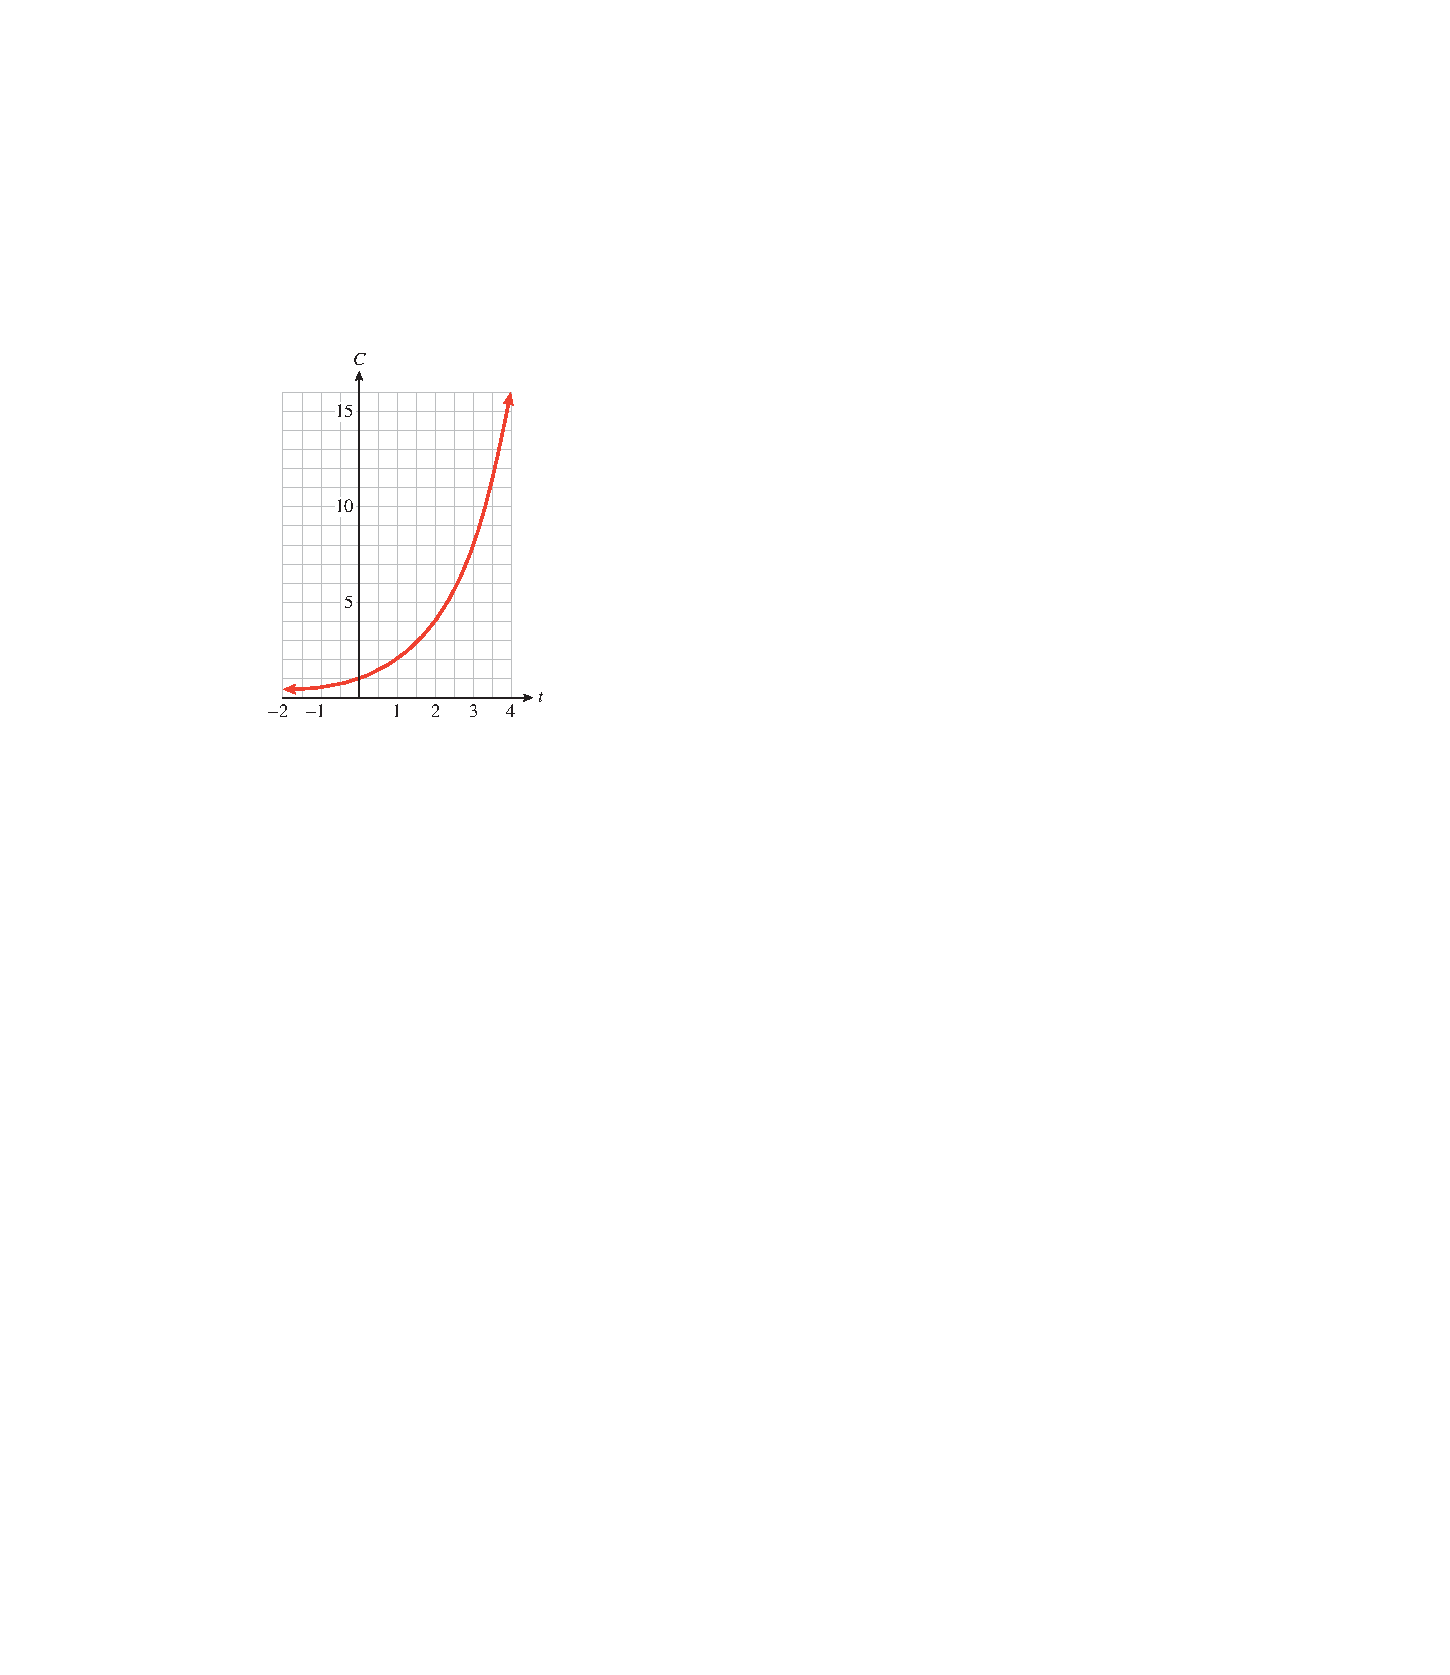
\includegraphics[width=\linewidth]{external/images/fig-ex-1-2-35.pdf}
\end{sbspanel}%
\end{sidebyside}%
\par
%
\begin{enumerate}[label=\alph*]
\item{}When did \(2000\) students consider themselves computer literate?%
\item{}How long did it take that number to double?%
\item{}How long did it take for the number to double again?%
\item{}How many students became computer literate between January 1992 and June 1993?%
\end{enumerate}
%
\end{divisionexerciseeg}%
\begin{divisionexerciseeg}{36}{}{}{exercise-section-1-2-exercises-n-c}%
The graph shows \(P\) as a function of \(t\). \(P\) is the number of people in Cedar Grove who owned a portable DVD player \(t\) years after 2000.%
\begin{sidebyside}{1}{0.32}{0.32}{0}%
\begin{sbspanel}{0.36}%
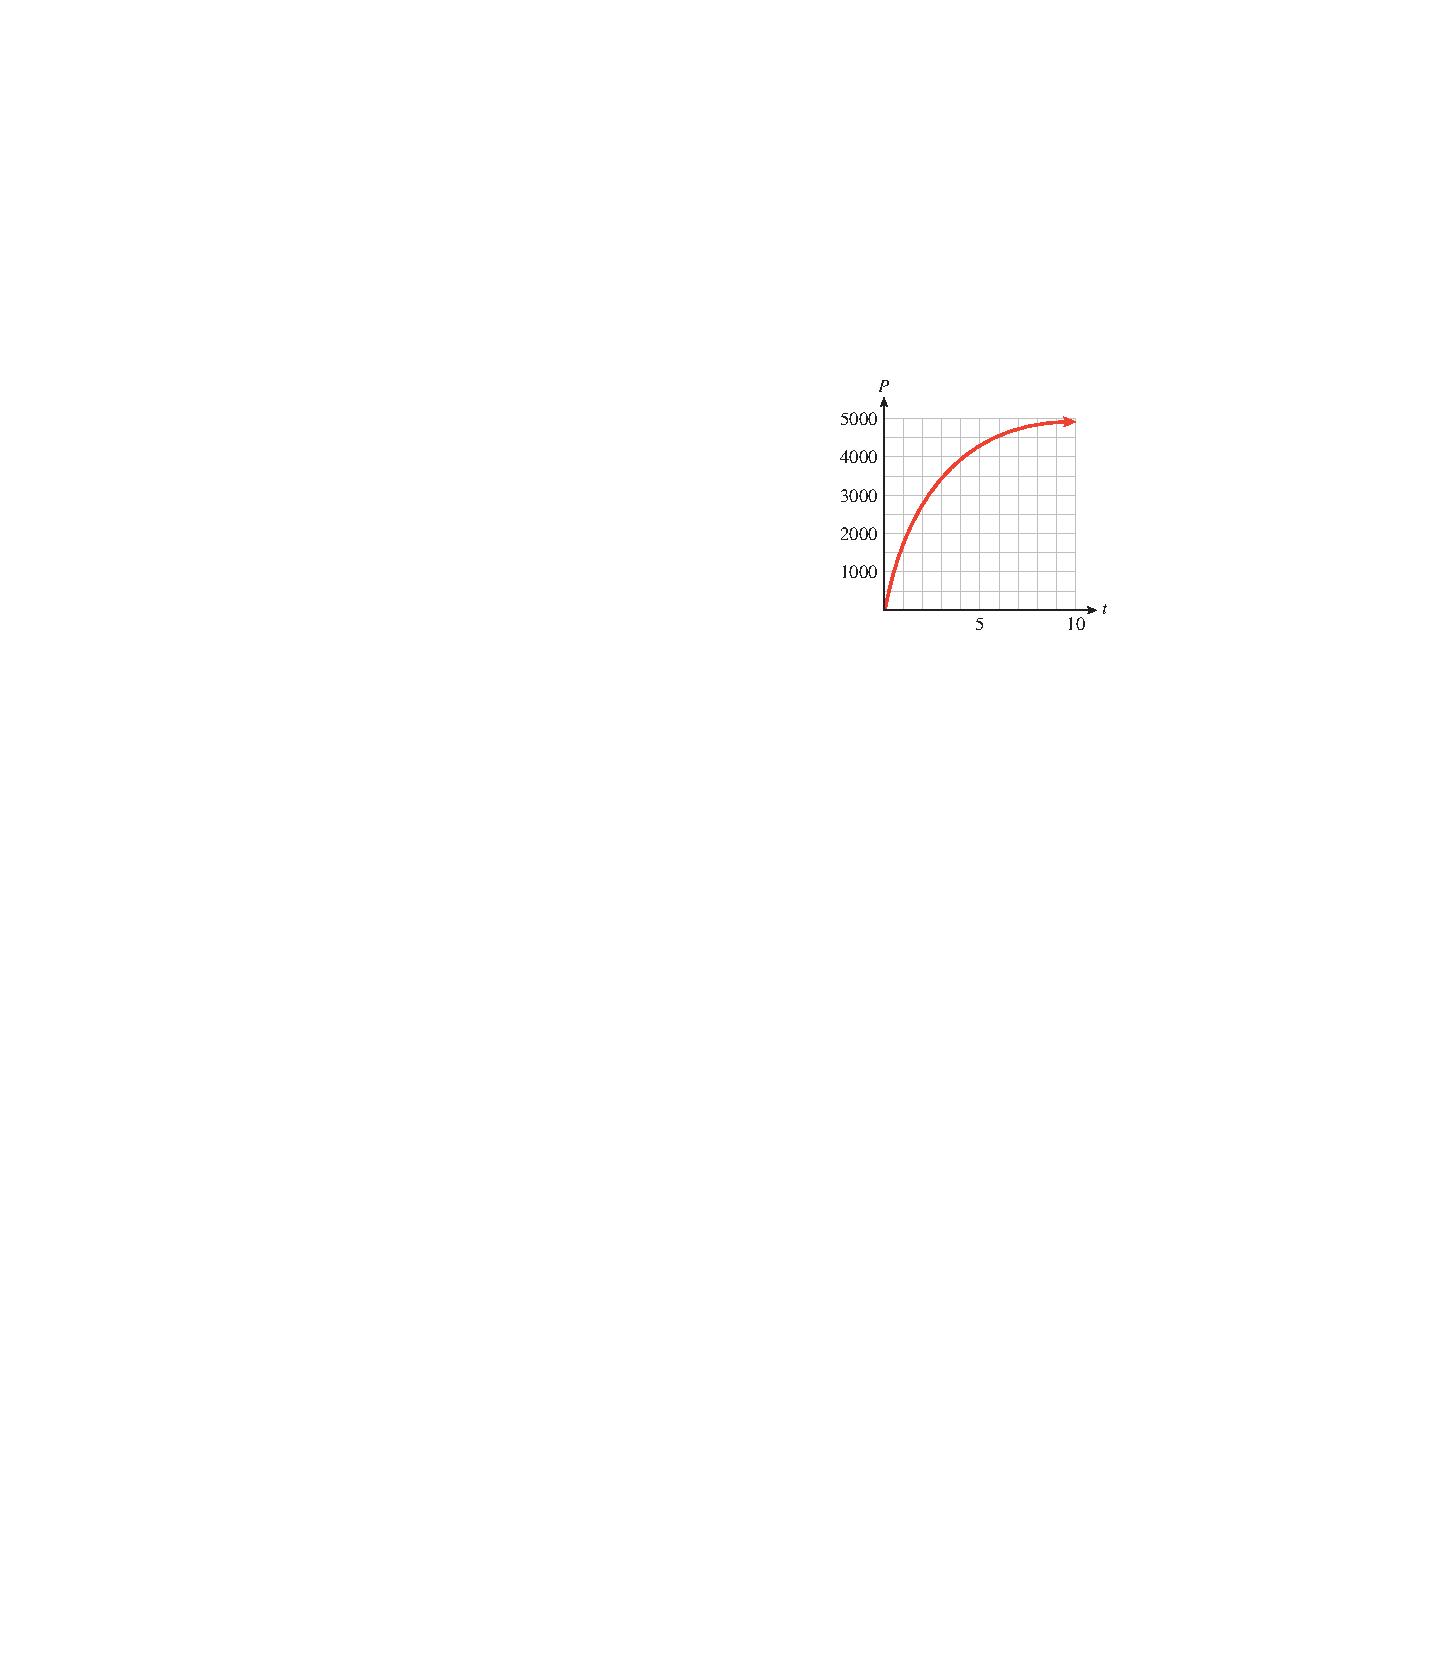
\includegraphics[width=\linewidth]{external/images/fig-ex-1-2-36.pdf}
\end{sbspanel}%
\end{sidebyside}%
%
\begin{enumerate}[label=\alph*]
\item{}When did 3500 people own portable DVD players?%
\item{}How many people owned portable DVD players in 2005?%
\item{}The number of owners of portable DVD players in Cedar Grove seems to be leveling off at what number?%
\item{}How many people acquired portable DVD players between 2001 and 2004?%
\end{enumerate}
\end{divisionexerciseeg}%
\begin{divisionexerciseeg}{37}{}{}{exercise-section-1-2-exercises-n-d}%
The graph shows the revenue, \(R\), a movie theater collects as a function of the price, \(d\), it charges for a ticket.%
\begin{sidebyside}{1}{0.3}{0.3}{0}%
\begin{sbspanel}{0.4}%
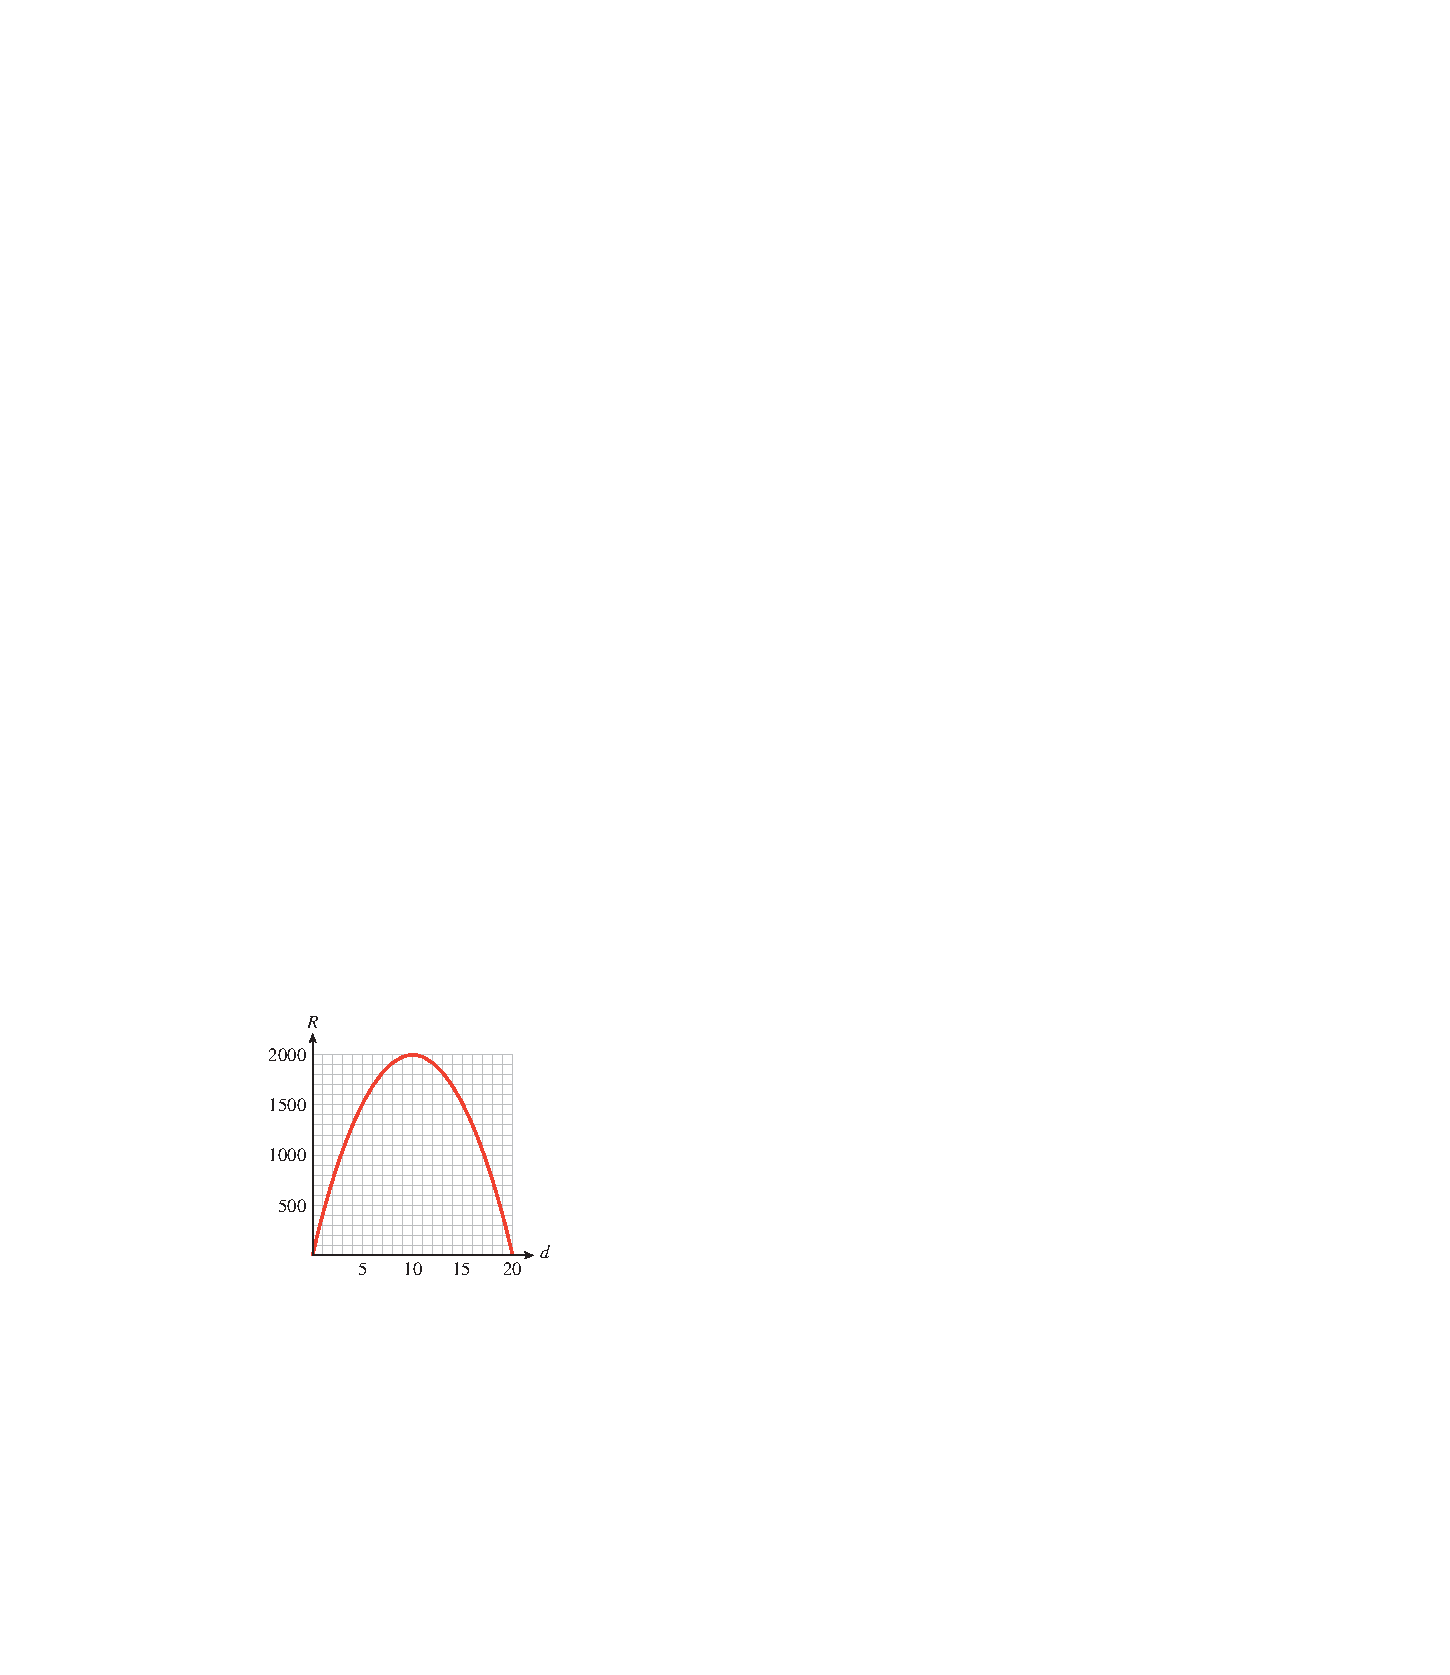
\includegraphics[width=\linewidth]{external/images/fig-ex-1-2-37.pdf}
\end{sbspanel}%
\end{sidebyside}%
%
\begin{enumerate}[label=\alph*]
\item{}What is the revenue if the theater charges \textdollar{}\(12.00\) for a ticket?%
\item{}What should the theater charge for a ticket in order to collect \textdollar{}\(1500\) in revenue?%
\item{}For what values of \(d\) is \(R\gt 1875\)?%
\end{enumerate}
\end{divisionexerciseeg}%
\begin{divisionexerciseeg}{38}{}{}{exercise-section-1-2-exercises-n-e}%
The graph shows \(S\) as a function of \(w\). \(S\) represents the weekly sales of a best-selling book, in thousands of dollars, \(w\) weeks after it is released.%
\begin{sidebyside}{1}{0.3}{0.3}{0}%
\begin{sbspanel}{0.4}%
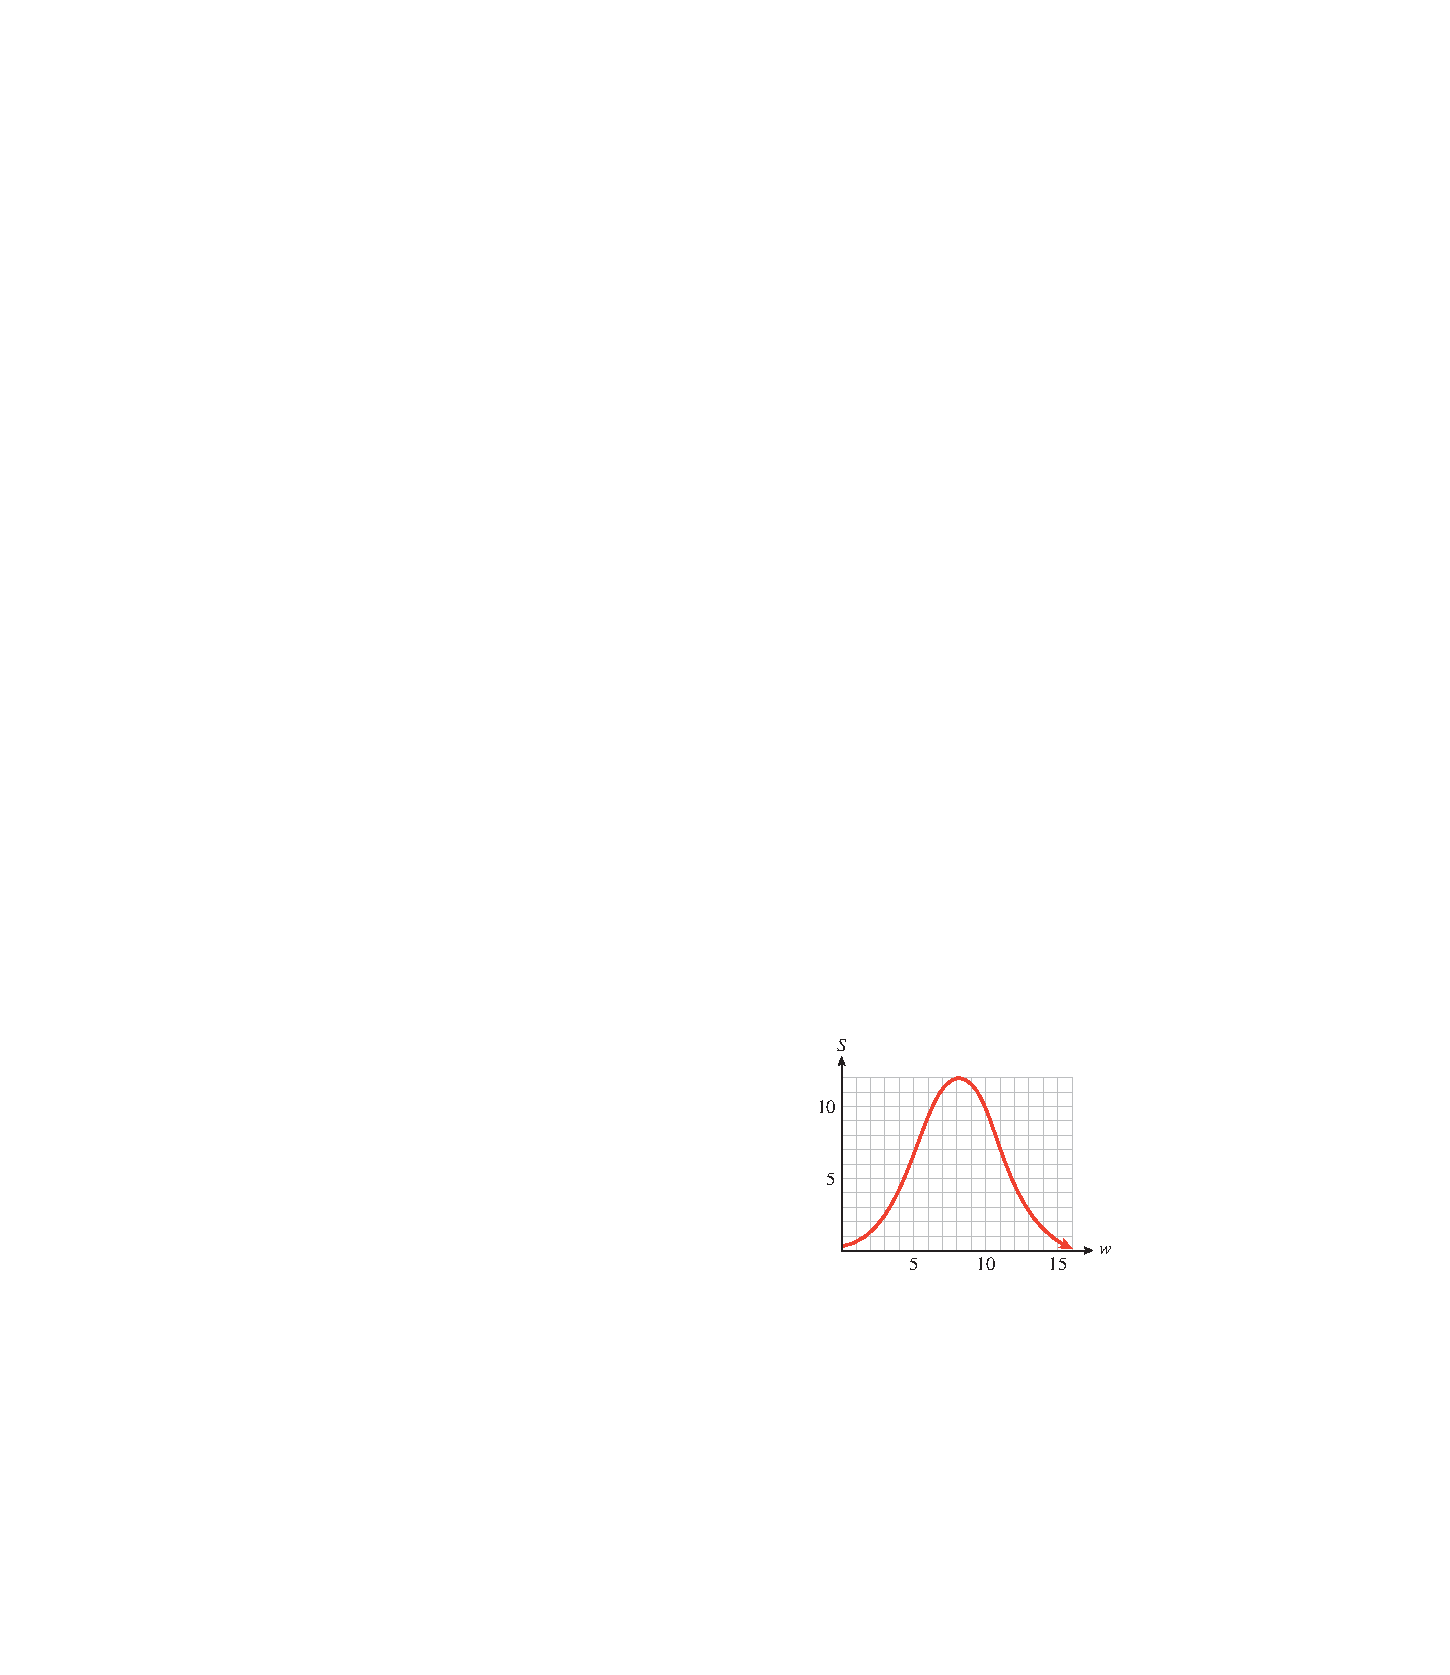
\includegraphics[width=\linewidth]{external/images/fig-ex-1-2-38.pdf}
\end{sbspanel}%
\end{sidebyside}%
%
\begin{enumerate}[label=\alph*]
\item{}In which weeks were sales over \textdollar{}\(7000\)?%
\item{}In which week did sales fall below \textdollar{}\(5000\) on their way down?%
\item{}For what values of \(w\) is \(S\gt 3.4\)?%
\end{enumerate}
\end{divisionexerciseeg}%
\begin{divisionexerciseeg}{39}{}{}{exercise-section-1-2-exercises-n-f}%
The graph shows the federal minimum wage, \(M\), as a function of time, \(t\), adjusted for inflation to reflect its buying power in 2004 dollars. (Source: www.infoplease.com)%
\begin{sidebyside}{1}{0}{0}{0}%
\begin{sbspanel}{1}%
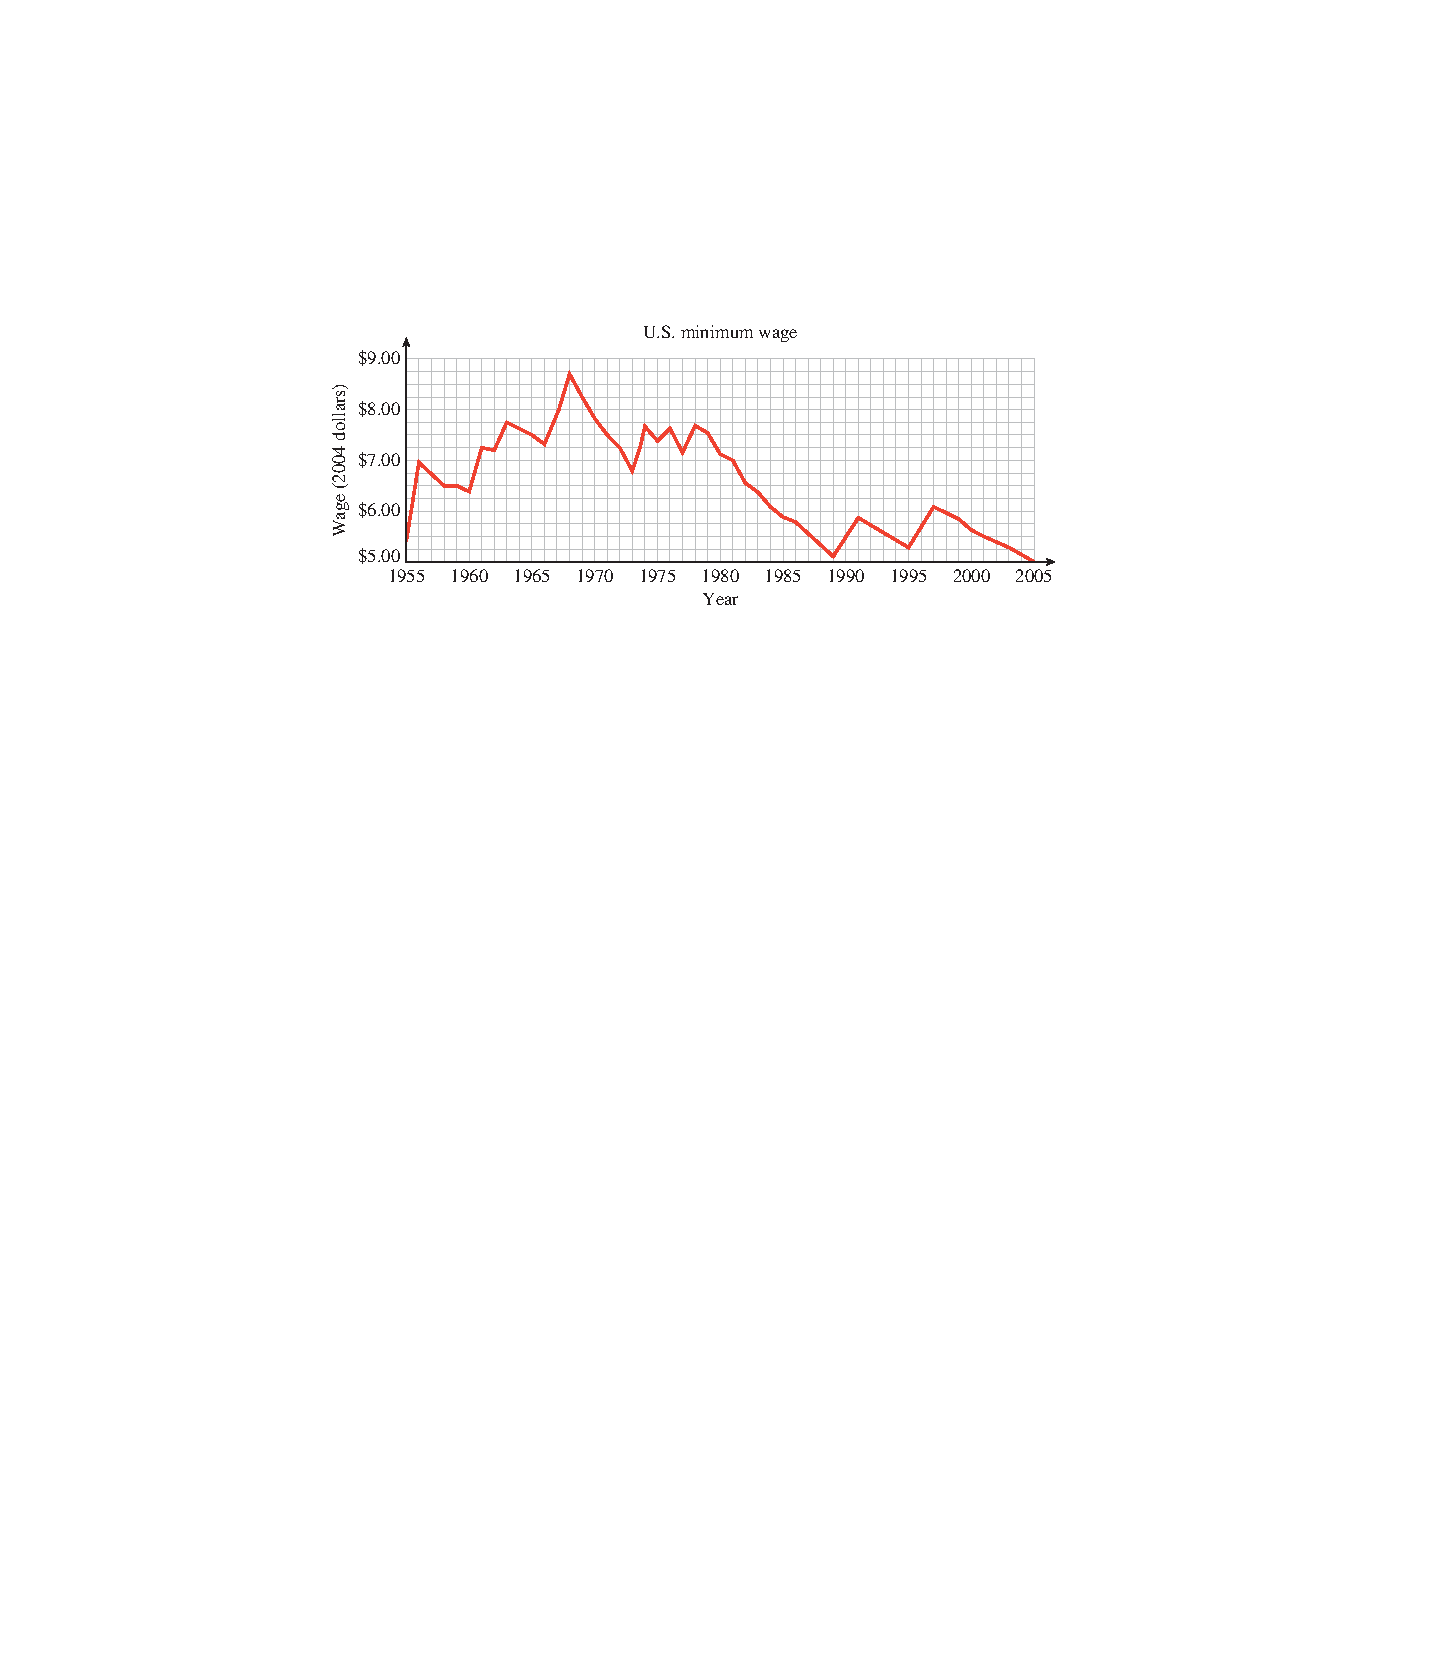
\includegraphics[width=\linewidth]{external/images/fig-ex-1-2-39.pdf}
\end{sbspanel}%
\end{sidebyside}%
\par
%
\begin{enumerate}[label=\alph*]
\item{}When did the minimum wage reach its highest buying power, and what was it worth in 2004 dollars?%
\item{}When did the minimum wage fall to its lowest buying power after its peak, and what was its worth at that time?%
\item{}Give two years in which the minimum wage was worth \textdollar{}\(8\) in 2004 dollars.%
\end{enumerate}
%
\end{divisionexerciseeg}%
\begin{divisionexerciseeg}{40}{}{}{exercise-section-1-2-exercises-n-g}%
The graph shows the U.S. unemployment rate, \(U\), as a function of time, \(t\), for the years 1985\textendash{}2004. (Source: U.S. Bureau of Labor Statistics)%
\begin{sidebyside}{1}{0.2}{0.2}{0}%
\begin{sbspanel}{0.6}%
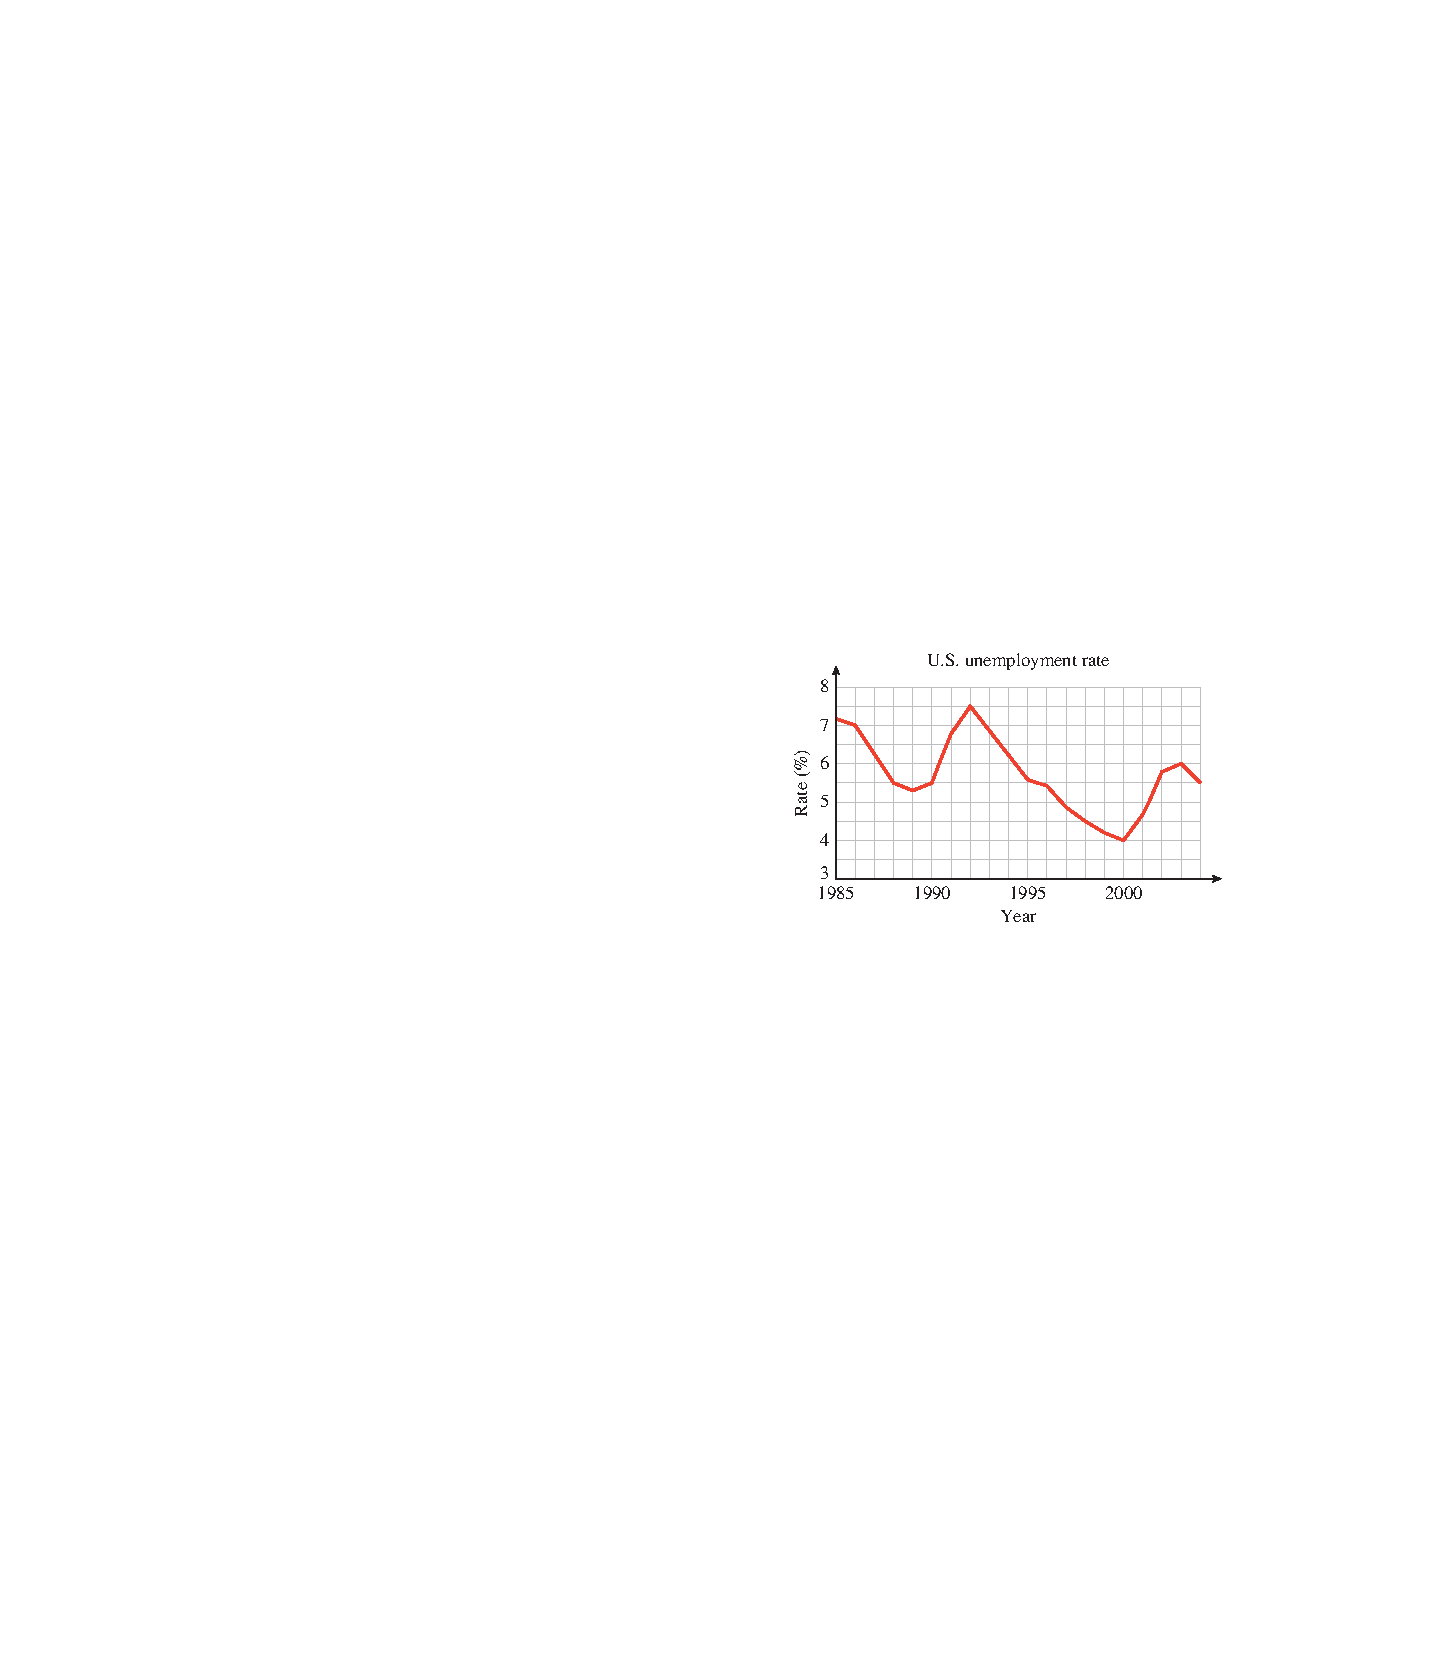
\includegraphics[width=\linewidth]{external/images/fig-ex-1-2-40.pdf}
\end{sbspanel}%
\end{sidebyside}%
\par
%
\begin{enumerate}[label=\alph*]
\item{}When did the unemployment rate reach its highest value, and what was its highest value?%
\item{}When did the unemployment rate fall to its lowest value, and what was its lowest value?%
\item{}Give two years in which the unemployment rate was \(4.5\%\).%
\end{enumerate}
%
\end{divisionexerciseeg}%
\end{exercisegroup}
\par\medskip\noindent
\par\medskip\noindent%
\textbf{Exercise Group.}\space\space%
In Problems 41\textendash{}48, evaluate each function for the given values.%
\begin{exercisegroupcol}{2}
\begin{divisionexerciseegcol}{41}{}{}{exercise-section-1-2-exercises-o-b}%
\(f (x) = 6 - 2x\)%
\begin{multicols}{2}
\begin{enumerate}[label=\alph*]
\item{}\(\displaystyle f(3)\)%
\item{}\(\displaystyle f(-2)\)%
\item{}\(\displaystyle f(12.7)\)%
\item{}\(\displaystyle f\left(\dfrac{2}{3}\right)\)%
\end{enumerate}
\end{multicols}
%
\end{divisionexerciseegcol}%
\begin{divisionexerciseegcol}{42}{}{}{exercise-section-1-2-exercises-o-c}%
\(g(t) = 5t - 3\)%
\begin{multicols}{2}
\begin{enumerate}[label=\alph*]
\item{}\(\displaystyle g(1)\)%
\item{}\(\displaystyle g(-4)\)%
\item{}\(\displaystyle g(14.1)\)%
\item{}\(\displaystyle g\left(\dfrac{3}{4}\right)\)%
\end{enumerate}
\end{multicols}
%
\end{divisionexerciseegcol}%
\begin{divisionexerciseegcol}{43}{}{}{exercise-section-1-2-exercises-o-d}%
\(h(v) = 2v^2 - 3v + 1\)%
\begin{multicols}{2}
\begin{enumerate}[label=\alph*]
\item{}\(\displaystyle h(0)\)%
\item{}\(\displaystyle h(-1)\)%
\item{}\(\displaystyle h\left(\dfrac{1}{4}\right)\)%
\item{}\(\displaystyle h(-6.2)\)%
\end{enumerate}
\end{multicols}
%
\end{divisionexerciseegcol}%
\begin{divisionexerciseegcol}{44}{}{}{exercise-section-1-2-exercises-o-e}%
\(r (s) = 2s - s^2\)%
\begin{multicols}{2}
\begin{enumerate}[label=\alph*]
\item{}\(\displaystyle r(2)\)%
\item{}\(\displaystyle r(-4)\)%
\item{}\(\displaystyle r\left(\dfrac{1}{3}\right)\)%
\item{}\(\displaystyle r(-1.3)\)%
\end{enumerate}
\end{multicols}
%
\end{divisionexerciseegcol}%
\begin{divisionexerciseegcol}{45}{}{}{exercise-section-1-2-exercises-o-f}%
\(H(z) = \dfrac{2z - 3}{z + 2}\)%
\begin{multicols}{2}
\begin{enumerate}[label=\alph*]
\item{}\(\displaystyle H(4)\)%
\item{}\(\displaystyle H(-3)\)%
\item{}\(\displaystyle H\left(\dfrac{4}{3}\right)\)%
\item{}\(\displaystyle H(4.5)\)%
\end{enumerate}
\end{multicols}
%
\end{divisionexerciseegcol}%
\begin{divisionexerciseegcol}{46}{}{}{exercise-section-1-2-exercises-o-g}%
\(F(x) = \dfrac{1-x}{2x-3}\)%
\begin{multicols}{2}
\begin{enumerate}[label=\alph*]
\item{}\(\displaystyle F(0)\)%
\item{}\(\displaystyle F(-3)\)%
\item{}\(\displaystyle F\left(\dfrac{5}{2}\right)\)%
\item{}\(\displaystyle F(9.8)\)%
\end{enumerate}
\end{multicols}
%
\end{divisionexerciseegcol}%
\begin{divisionexerciseegcol}{47}{}{}{exercise-section-1-2-exercises-o-h}%
\(E(t) =\sqrt{t-4}\)%
\begin{multicols}{2}
\begin{enumerate}[label=\alph*]
\item{}\(\displaystyle E(16)\)%
\item{}\(\displaystyle E(4)\)%
\item{}\(\displaystyle E(7)\)%
\item{}\(\displaystyle E(4.2)\)%
\end{enumerate}
\end{multicols}
%
\end{divisionexerciseegcol}%
\begin{divisionexerciseegcol}{48}{}{}{exercise-section-1-2-exercises-o-i}%
\(D(r) =\sqrt{5-r}\)%
\begin{multicols}{2}
\begin{enumerate}[label=\alph*]
\item{}\(\displaystyle D(4)\)%
\item{}\(\displaystyle D(-3)\)%
\item{}\(\displaystyle D(-9)\)%
\item{}\(\displaystyle D(4.6)\)%
\end{enumerate}
\end{multicols}
%
\end{divisionexerciseegcol}%
\end{exercisegroupcol}
\par\medskip\noindent
\begin{divisionexercise}{49}{}{}{exercise-section-1-2-exercises-p}%
A sport utility vehicle costs \textdollar{}\(28,000\) and depreciates according to the formula%
\begin{equation*}
V(t) = 28,000 (1 - 0.08t)
\end{equation*}
where \(V\) is the value of the vehicle after \(t\) years.%
\begin{enumerate}[label=\alph*]
\item{}Evaluate \(V(12)\) and explain what it means.%
\item{}Solve the equation \(V(t) = 0\) and explain what it means.%
\item{}If this year is \(t = n\), what does \(V(n + 2)\) mean?%
\end{enumerate}
%
\end{divisionexercise}%
\begin{divisionexercise}{50}{}{}{exercise-section-1-2-exercises-q}%
In a profit-sharing plan, an employee receives a salary of%
\begin{equation*}
S(x) = 20,000 + 0.01x
\end{equation*}
where \(x\) represents the company's profit for the year.%
\begin{enumerate}[label=\alph*]
\item{}Evaluate \(S(850,000)\) and explain what it means.%
\item{}Solve the equation \(S(x) = 30,000\) and explain what it means.%
\item{}If the company made a profit of \(p\) dollars this year, what does \(S(2p)\) mean?%
\end{enumerate}
%
\end{divisionexercise}%
\begin{divisionexercise}{51}{}{}{exercise-section-1-2-exercises-r}%
The number of compact cars that a large dealership can sell at price \(p\) is given by%
\begin{equation*}
N( p) = \dfrac{12,000,000}{p}
\end{equation*}
%
\begin{enumerate}[label=\alph*]
\item{}Evaluate \(N(6000)\) and explain what it means.%
\item{}As \(p\) increases, does \(N(p)\) increase or decrease? Why is this reasonable?%
\item{}If the current price for a compact car is \(D\), what does \(2N(D)\) mean?%
\end{enumerate}
%
\end{divisionexercise}%
\begin{divisionexercise}{52}{}{}{exercise-section-1-2-exercises-s}%
A department store finds that the market value of its Christmas-related merchandise is given by%
\begin{equation*}
M(t) = \dfrac{600,000}{t},~~ t\le 30
\end{equation*}
where \(t\) is the number of weeks after Christmas.%
\begin{enumerate}[label=\alph*]
\item{}Evaluate \(M(2)\) and explain what it means.%
\item{}As \(t\) increases, does \(M(t)\) increase or decrease? Why is this reasonable?%
\item{}If this week \(t = n\), what does \(M(n + 1)\) mean?%
\end{enumerate}
%
\end{divisionexercise}%
\begin{divisionexercise}{53}{}{}{exercise-section-1-2-exercises-t}%
The velocity of a car that brakes suddenly can be determined from the length of its skid marks, \(d\), by%
\begin{equation*}
v(d) = \sqrt{12d}
\end{equation*}
where \(d\) is in feet and \(v\) is in miles per hour.%
\begin{enumerate}[label=\alph*]
\item{}Evaluate \(v(250)\) and explain what it means.%
\item{}Estimate the length of the skid marks left by a car traveling at \(100\) miles per hour.%
\item{}Write your answer to part (b) with function notation.%
\end{enumerate}
%
\end{divisionexercise}%
\begin{divisionexercise}{54}{}{}{exercise-section-1-2-exercises-u}%
The distance, \(d\), in miles that a person can see on a clear day from a height, \(h\), in feet is given by%
\begin{equation*}
d(h) = 1.22\sqrt{h}
\end{equation*}
%
\begin{enumerate}[label=\alph*]
\item{}Evaluate \(d(20,320)\) and explain what it means.%
\item{}Estimate the height you need in order to see \(100\) miles.%
\item{}Write your answer to part (b) with function notation.%
\end{enumerate}
%
\end{divisionexercise}%
\begin{divisionexercise}{55}{}{}{exercise-section-1-2-exercises-v}%
The figure gives data about snowfall, air temperature, and number of avalanches on the Mikka glacier in Sarek, Lapland, in 1957. (Source: Leopold, Wolman, Miller, 1992)%
\begin{sidebyside}{1}{0.1}{0.1}{0}%
\begin{sbspanel}{0.8}%
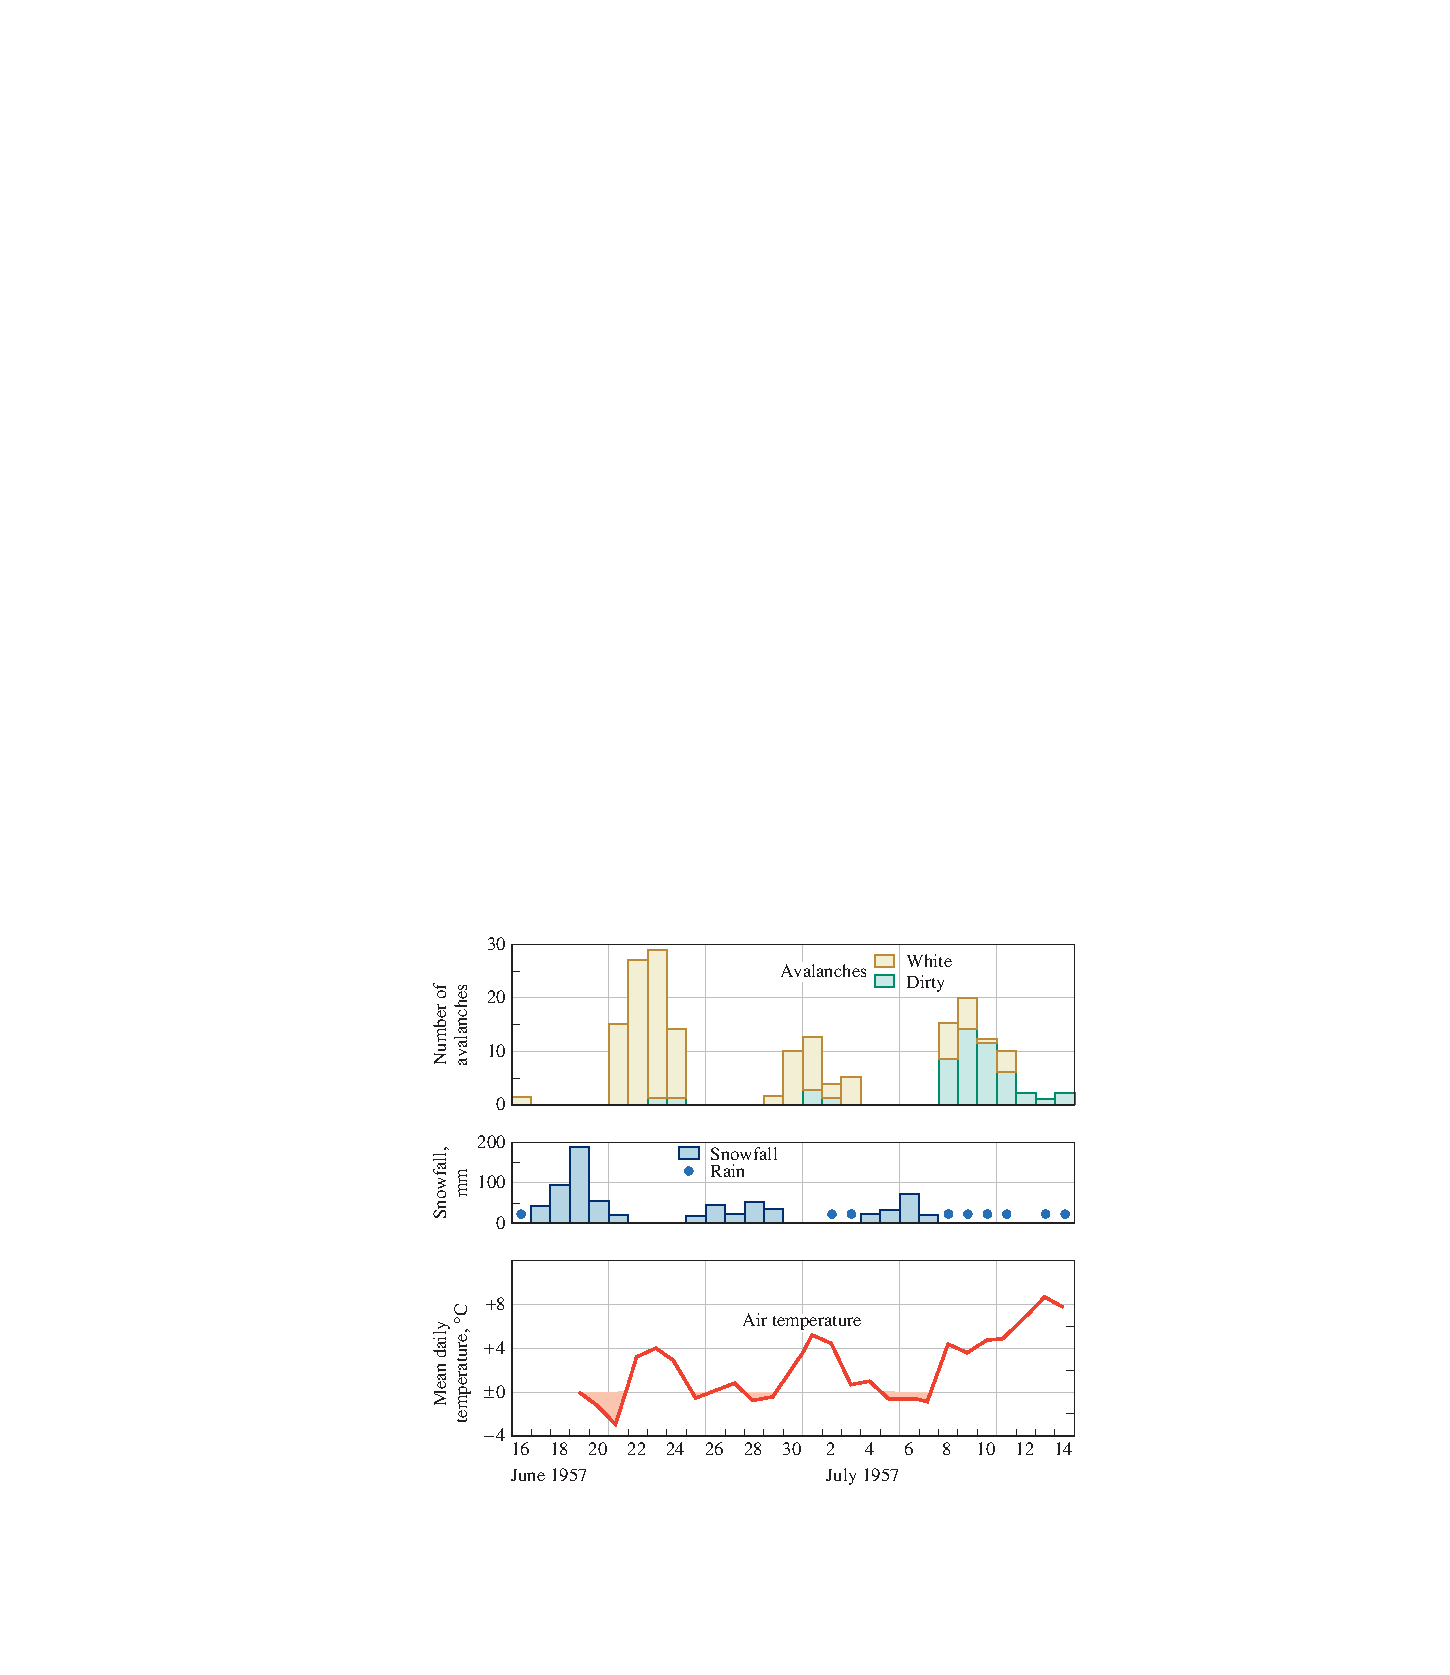
\includegraphics[width=\linewidth]{external/images/fig-ex-1-2-55.pdf}
\end{sbspanel}%
\end{sidebyside}%
\par
%
\begin{enumerate}[label=\alph*]
\item{}During June and July, avalanches occurred over three separate time intervals. What were they?%
\item{}Over what three time intervals did snow fall?%
\item{}When was the temperature above freezing (\(0\degree\)C)?%
\item{}Using your answers to parts (a)\textendash{}(c), make a conjecture about the conditions that encourage avalanches.%
\end{enumerate}
%
\end{divisionexercise}%
\begin{divisionexercise}{56}{}{}{exercise-section-1-2-exercises-w}%
The bar graph shows the percent of Earth's surface that lies at various altitudes or depths below the surface of the oceans. (Depths are given as negative altitudes.) (Source: Open University)%
\begin{sidebyside}{1}{0.15}{0.15}{0}%
\begin{sbspanel}{0.7}%
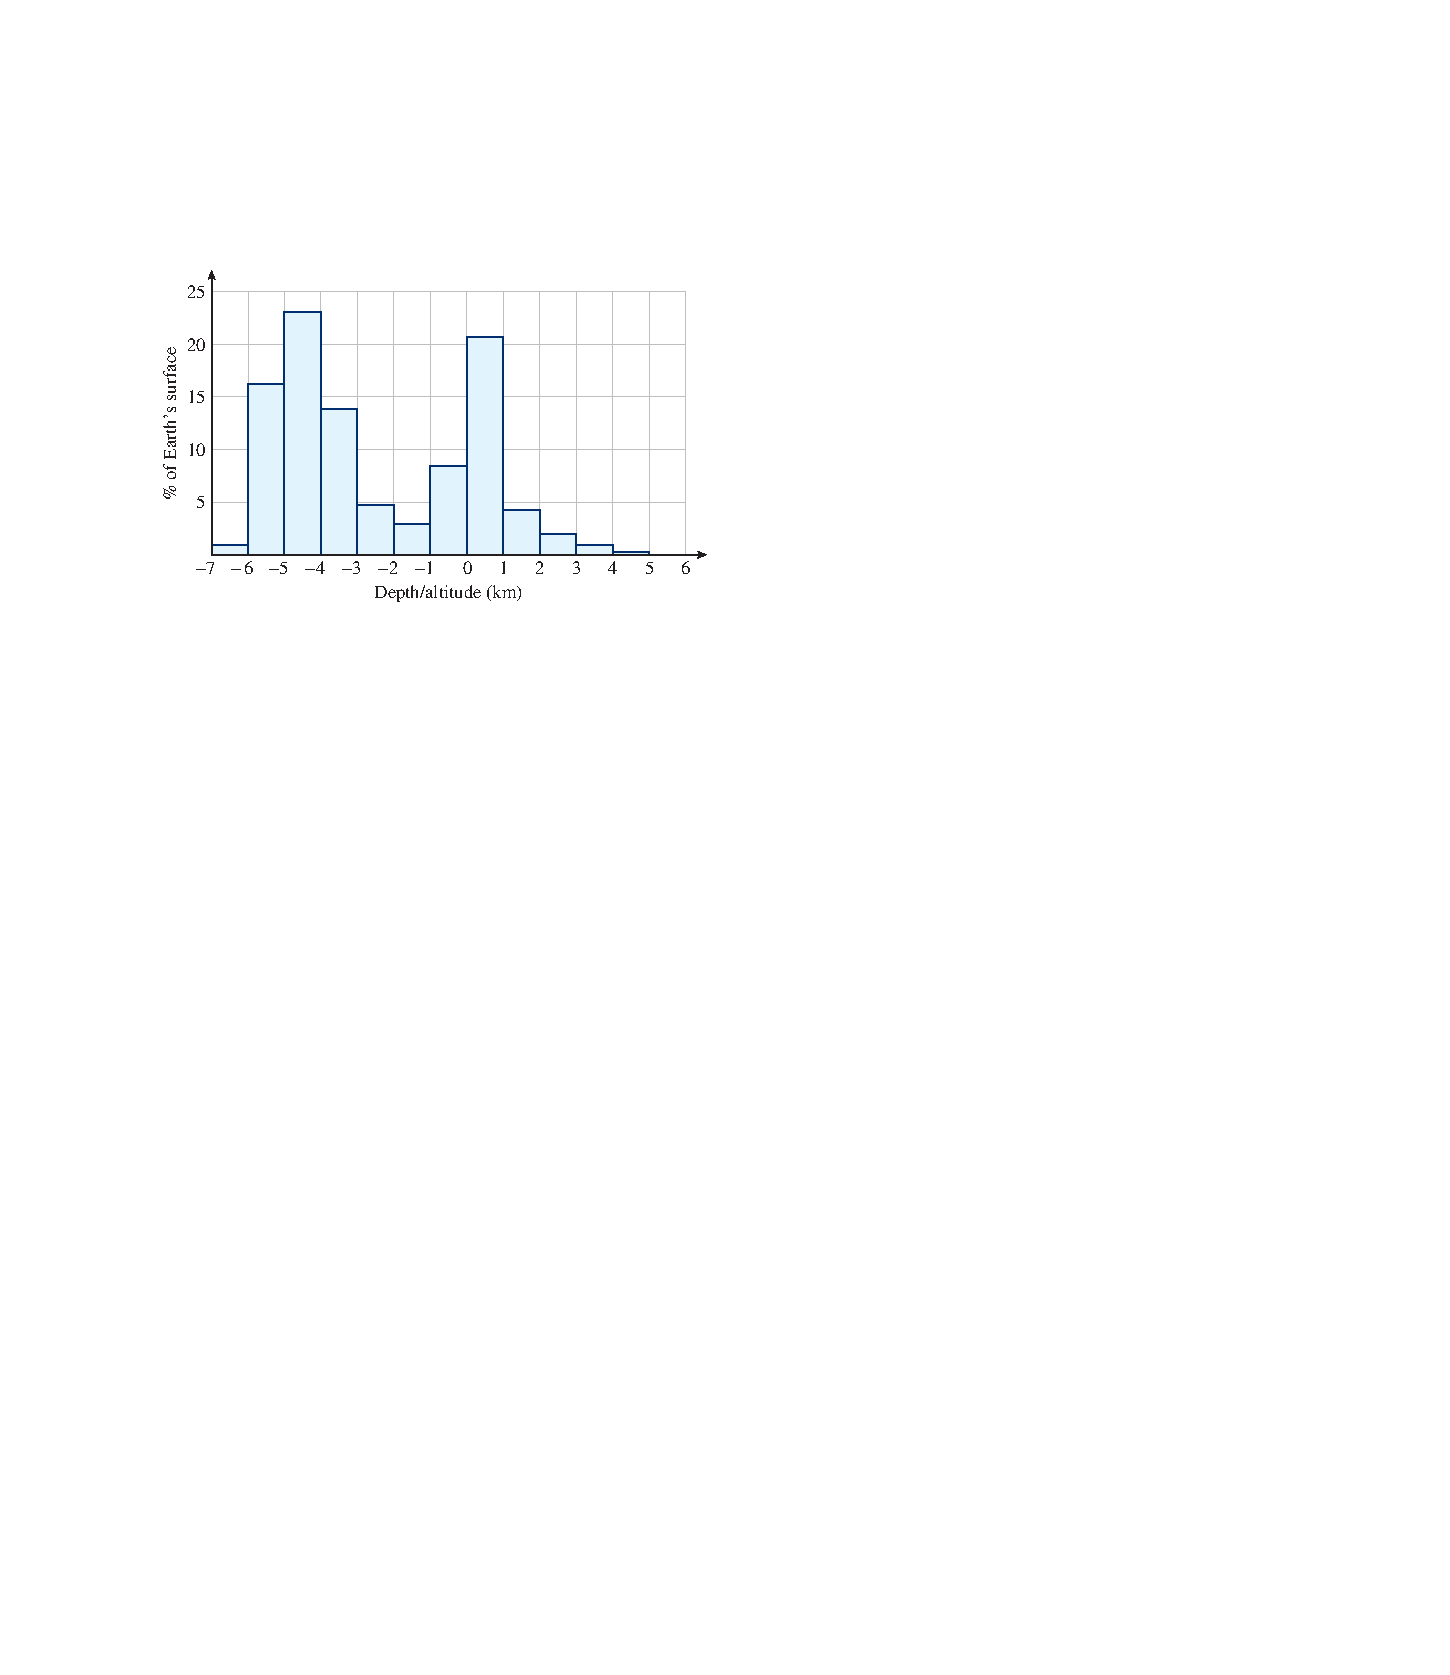
\includegraphics[width=\linewidth]{external/images/fig-ex-1-2-56.pdf}
\end{sbspanel}%
\end{sidebyside}%
\par
%
\begin{enumerate}[label=\alph*]
\item{}Read the graph and complete the table.%
\begin{sidebyside}{1}{0}{0}{0}%
\begin{sbspanel}{1}%
\resizebox{\ifdim\width > \linewidth\linewidth\else\width\fi}{!}{%
{\centering%
{\tabularfont%
\begin{tabular}{AcAcA}\hrulethick
Altitude (km)&\tablecelllines{c}{m}
{Percent of\\
Earth's surface}
\tabularnewline\hrulethin
\(-7\) to \(-6\)&\(\)\tabularnewline\hrulethin
\(-6\) to \(-5\)&\(\)\tabularnewline\hrulethin
\(-5\) to \(-4\)&\(\)\tabularnewline\hrulethin
\(-4\) to \(-3\)&\(\)\tabularnewline\hrulethin
\(-3\) to \(-2\)&\(\)\tabularnewline\hrulethin
\(-2\) to \(-1\)&\(\)\tabularnewline\hrulethin
\(-1\) to \(0\)&\(\)\tabularnewline\hrulethin
\(0\) to \(1\)&\(\)\tabularnewline\hrulethin
\(1\) to \(2\)&\(\)\tabularnewline\hrulethin
\(2\) to \(3\)&\(\)\tabularnewline\hrulethin
\(3\) to \(4\)&\(\)\tabularnewline\hrulethin
\(4\) to \(5\)&\(\)\tabularnewline\hrulethin
\end{tabular}
}%
\par}
}%
\end{sbspanel}%
\end{sidebyside}%
\item{}What is the most common altitude? What is the second most common altitude??%
\item{}Approximately what percent of the Earth's surface is below sea level?%
\item{}The height of Mt. Everest is \(8.85\) kilometers. Can you think of a reason why it is not included in the graph?%
\end{enumerate}
%
\end{divisionexercise}%
\begin{divisionexercise}{57}{}{}{exercise-section-1-2-exercises-x}%
The graph shows the temperature of the ocean at various depths. (Source: Open University)%
\begin{sidebyside}{2}{0.035}{0.035}{0.07}%
\begin{sbspanel}{0.36}%
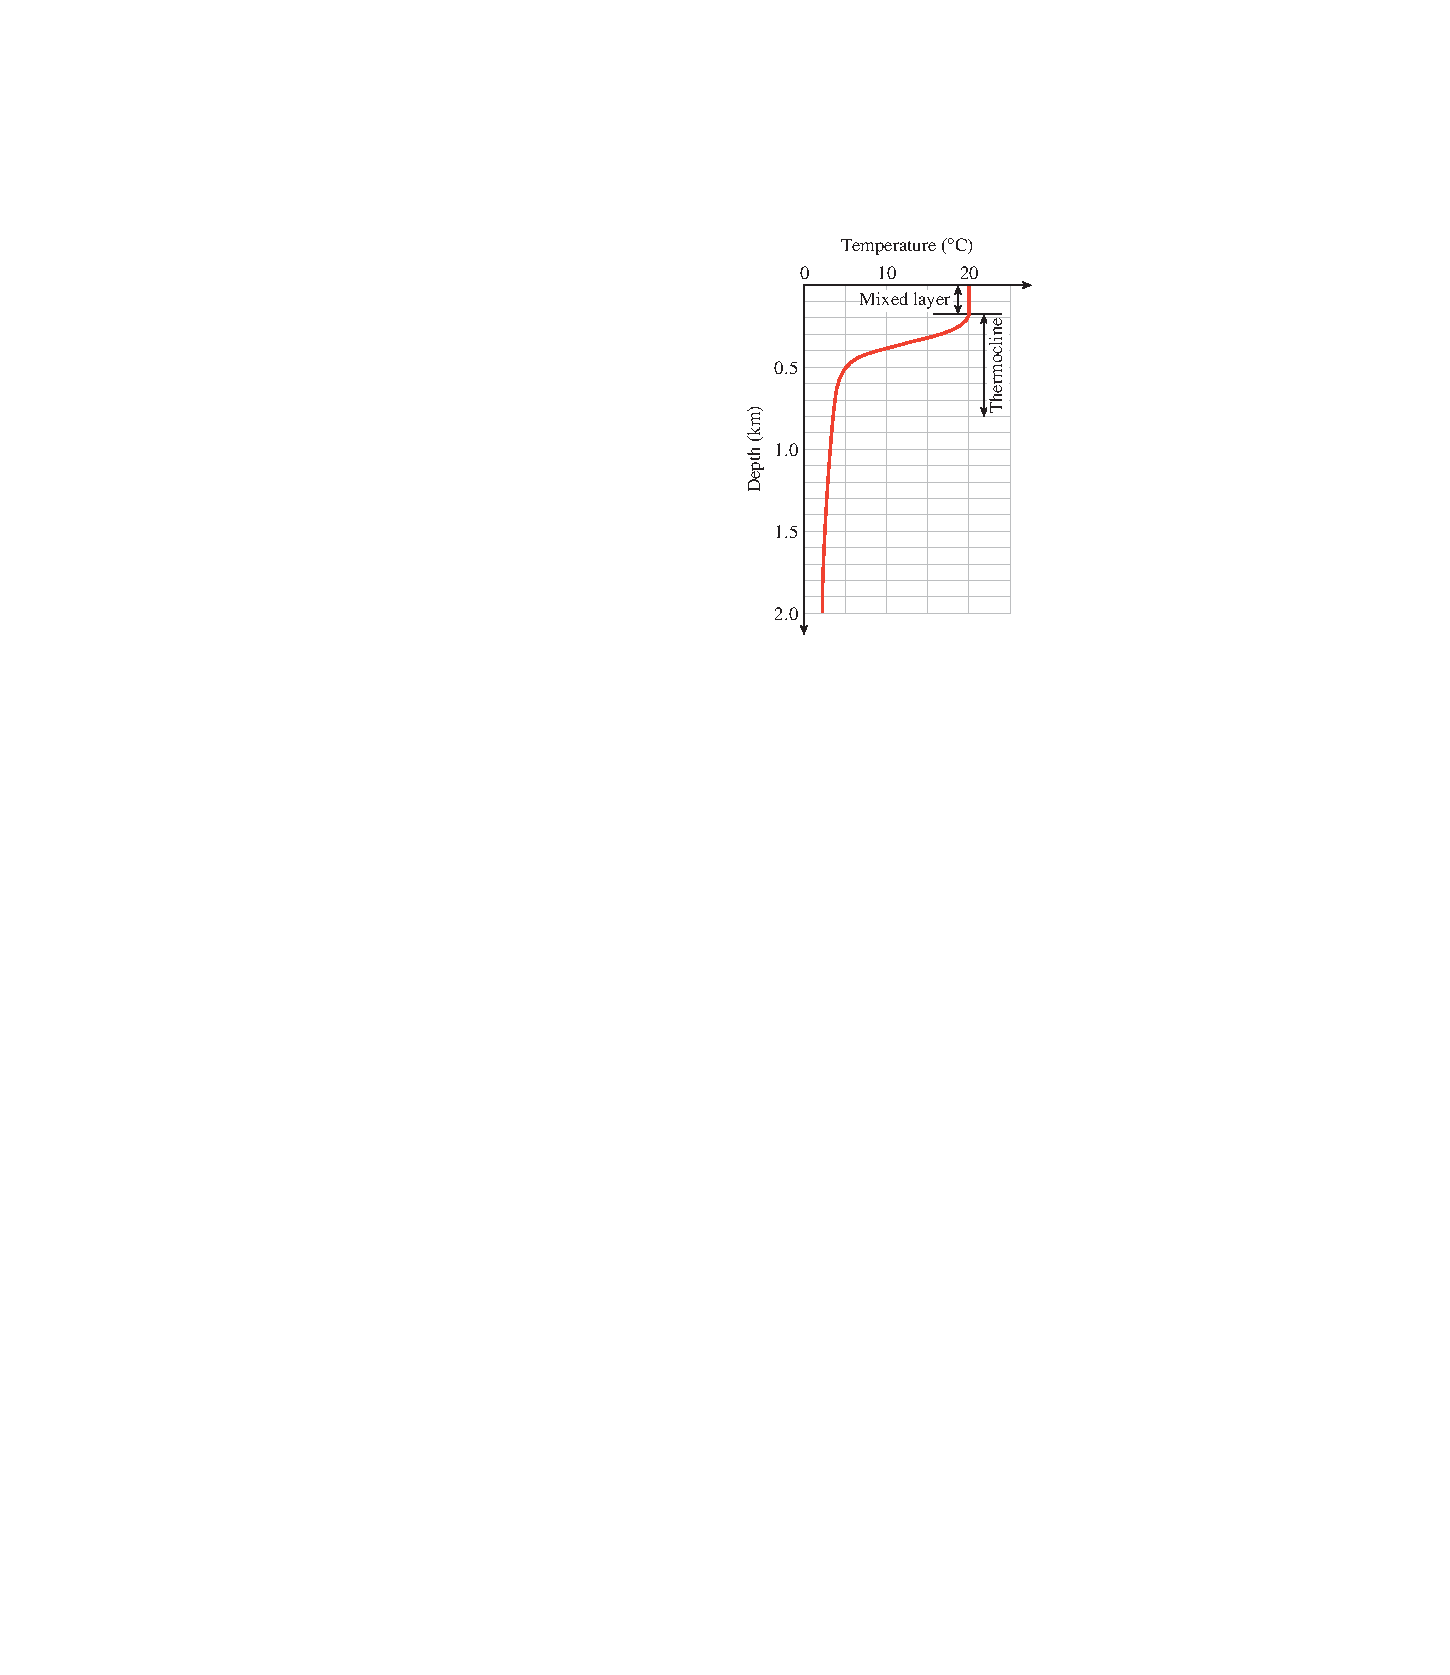
\includegraphics[width=\linewidth]{external/images/fig-ex-1-2-57.pdf}
\end{sbspanel}%
\begin{sbspanel}{0.5}%
%
\begin{enumerate}[label=\alph*]
\item{}Is depth a function of temperature?%
\item{}Is temperature a function of depth?%
\item{}The axes are scaled in an unusual way. Why is it useful to present the graph in this way?%
\end{enumerate}
%
\end{sbspanel}%
\end{sidebyside}%
\end{divisionexercise}%
\begin{divisionexercise}{58}{}{}{exercise-section-1-2-exercises-y}%
The graph shows the relationship between annual precipitation, \(p\), in a region and the amount of erosion, measured in tons per square mile, \(s\). (Source: Leopold, Wolman, Miller, 1992)%
\begin{sidebyside}{1}{0.25}{0.25}{0}%
\begin{sbspanel}{0.5}%
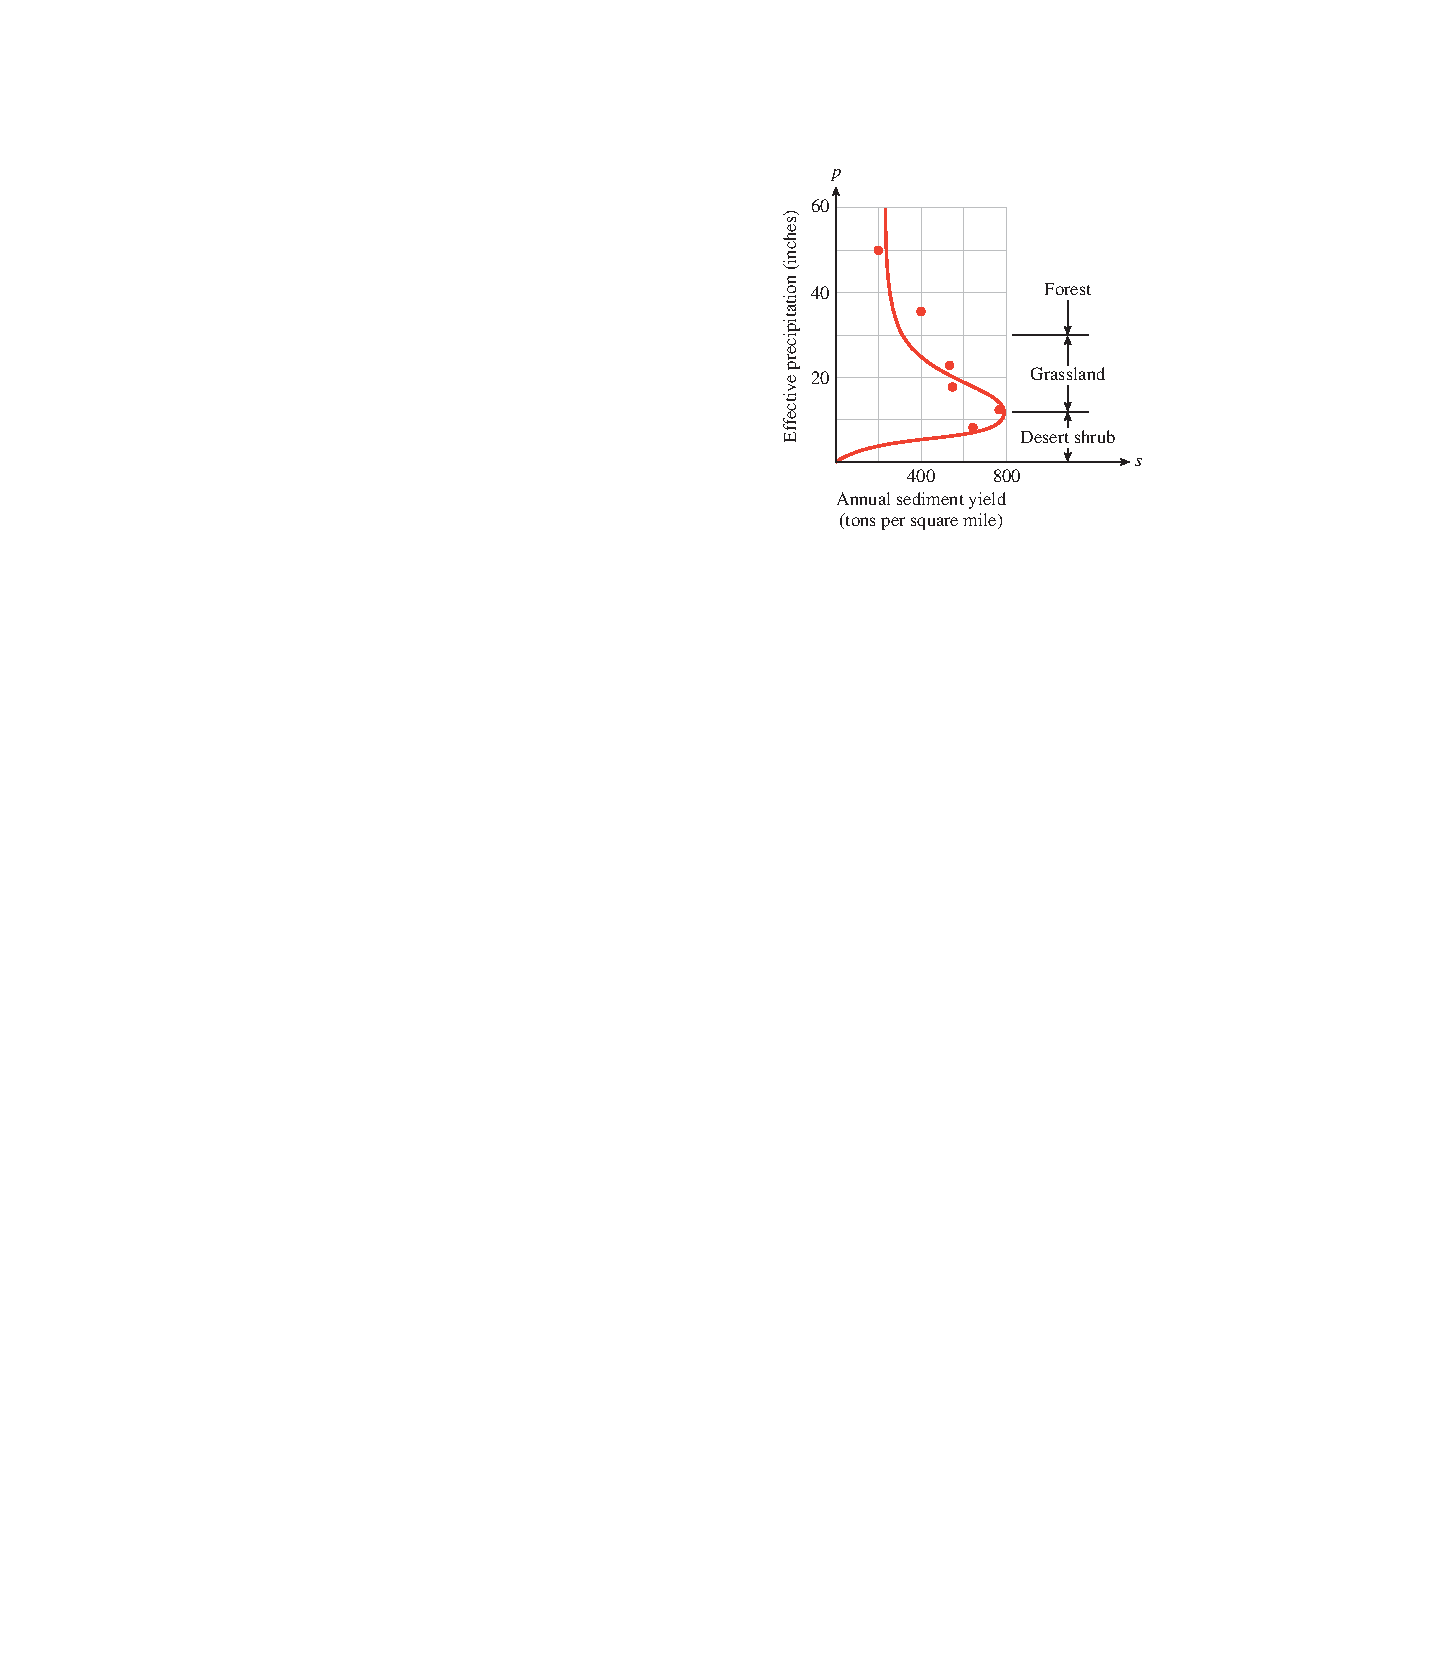
\includegraphics[width=\linewidth]{external/images/fig-ex-1-2-58.pdf}
\end{sbspanel}%
\end{sidebyside}%
\par
%
\begin{enumerate}[label=\alph*]
\item{}Is the amount of erosion a function of the amount of precipitation?%
\item{}At what annual precipitation is erosion at a maximum, and what is that maximum?%
\item{}Over what interval of annual precipitation does erosion decrease?%
\item{}An increase in vegetation inhibits erosion, and precipitation encourages vegetation. What happens to the amount of erosion as precipitation increases in each of these three environments?%
\begin{sidebyside}{1}{0}{0}{0}%
\begin{sbspanel}{1}%
\resizebox{\ifdim\width > \linewidth\linewidth\else\width\fi}{!}{%
{\centering%
{\tabularfont%
\begin{tabular}{ll}
desert shrub:&\(0\lt p\lt 12\)\tabularnewline[0pt]
grassland:&\(12\lt p\lt 30\)\tabularnewline[0pt]
forest:&\(30\lt p\lt 60\)
\end{tabular}
}%
\par}
}%
\end{sbspanel}%
\end{sidebyside}%
\end{enumerate}
%
\end{divisionexercise}%
\par\medskip\noindent%
\textbf{Exercise Group.}\space\space%
In Problems 59\textemdash{}64, evaluate the function and simplify.%
\begin{exercisegroupcol}{2}
\begin{divisionexerciseegcol}{59}{}{}{exercise-section-1-2-exercises-z-b}%
\(G(s) = 3s^2 - 6s\)%
\begin{multicols}{2}
\begin{enumerate}[label=\alph*]
\item{}\(\displaystyle G(3a)\)%
\item{}\(\displaystyle G(a + 2)\)%
\item{}\(\displaystyle G(a) + 2\)%
\item{}\(\displaystyle G(-a)\)%
\end{enumerate}
\end{multicols}
%
\end{divisionexerciseegcol}%
\begin{divisionexerciseegcol}{60}{}{}{exercise-section-1-2-exercises-z-c}%
\(h(x) = 2x^2 + 6x - 3\)%
\begin{multicols}{2}
\begin{enumerate}[label=\alph*]
\item{}\(\displaystyle h(2a)\)%
\item{}\(\displaystyle h(a + 3)\)%
\item{}\(\displaystyle h(a) + 3\)%
\item{}\(\displaystyle h(-a)\)%
\end{enumerate}
\end{multicols}
%
\end{divisionexerciseegcol}%
\begin{divisionexerciseegcol}{61}{}{}{exercise-section-1-2-exercises-z-d}%
\(g(x) = 8\)%
\begin{multicols}{2}
\begin{enumerate}[label=\alph*]
\item{}\(\displaystyle g(2)\)%
\item{}\(\displaystyle g(8)\)%
\item{}\(\displaystyle g(a + 1)\)%
\item{}\(\displaystyle g(-x)\)%
\end{enumerate}
\end{multicols}
%
\end{divisionexerciseegcol}%
\begin{divisionexerciseegcol}{62}{}{}{exercise-section-1-2-exercises-z-e}%
\(f (t) = -3\)%
\begin{multicols}{2}
\begin{enumerate}[label=\alph*]
\item{}\(\displaystyle f (4)\)%
\item{}\(\displaystyle f (-3)\)%
\item{}\(\displaystyle f (b - 2)\)%
\item{}\(\displaystyle f (-t)\)%
\end{enumerate}
\end{multicols}
%
\end{divisionexerciseegcol}%
\begin{divisionexerciseegcol}{63}{}{}{exercise-section-1-2-exercises-z-f}%
\(P(x) = x^3 - 1\)%
\begin{multicols}{2}
\begin{enumerate}[label=\alph*]
\item{}\(\displaystyle P(2x)\)%
\item{}\(\displaystyle 2P(x)\)%
\item{}\(\displaystyle P(x^2)\)%
\item{}\(\displaystyle [P(x)]^2\)%
\end{enumerate}
\end{multicols}
%
\end{divisionexerciseegcol}%
\begin{divisionexerciseegcol}{64}{}{}{exercise-section-1-2-exercises-z-g}%
\(Q(t) = 5t^3\)%
\begin{multicols}{2}
\begin{enumerate}[label=\alph*]
\item{}\(\displaystyle Q(2t)\)%
\item{}\(\displaystyle 2Q(t)\)%
\item{}\(\displaystyle Q(t^2)\)%
\item{}\(\displaystyle [Q(t)]^2\)%
\end{enumerate}
\end{multicols}
%
\end{divisionexerciseegcol}%
\end{exercisegroupcol}
\par\medskip\noindent
\par\medskip\noindent%
\textbf{Exercise Group.}\space\space%
In Problems 65\textemdash{}68, evaluate the function for the given expressions and simplify.%
\begin{exercisegroupcol}{2}
\begin{divisionexerciseegcol}{65}{}{}{exercise-section-1-2-exercises-aa-b}%
\(f (x) = x^3\)%
\begin{multicols}{2}
\begin{enumerate}[label=\alph*]
\item{}\(\displaystyle f (a^2)\)%
\item{}\(\displaystyle a^3 \cdot f (a^3)\)%
\item{}\(\displaystyle f (ab)\)%
\item{}\(\displaystyle f (a + b)\)%
\end{enumerate}
\end{multicols}
%
\end{divisionexerciseegcol}%
\begin{divisionexerciseegcol}{66}{}{}{exercise-section-1-2-exercises-aa-c}%
\(g(x) = x^4\)%
\begin{multicols}{2}
\begin{enumerate}[label=\alph*]
\item{}\(\displaystyle g(a^3)\)%
\item{}\(\displaystyle a^4\cdot g(a^4)\)%
\item{}\(\displaystyle g(ab)\)%
\item{}\(\displaystyle g(a + b)\)%
\end{enumerate}
\end{multicols}
%
\end{divisionexerciseegcol}%
\begin{divisionexerciseegcol}{67}{}{}{exercise-section-1-2-exercises-aa-d}%
\(F(x) = 3x^5\)%
\begin{multicols}{2}
\begin{enumerate}[label=\alph*]
\item{}\(\displaystyle F(2a)\)%
\item{}\(\displaystyle 2 F(a)\)%
\item{}\(\displaystyle F(a^2)\)%
\item{}\(\displaystyle [F(a)]^2\)%
\end{enumerate}
\end{multicols}
%
\end{divisionexerciseegcol}%
\begin{divisionexerciseegcol}{68}{}{}{exercise-section-1-2-exercises-aa-e}%
\(G(x) = 4x^3\)%
\begin{multicols}{2}
\begin{enumerate}[label=\alph*]
\item{}\(\displaystyle G(3a)\)%
\item{}\(\displaystyle 3G(a)\)%
\item{}\(\displaystyle G(a^4)\)%
\item{}\(\displaystyle [G(a)]^4\)%
\end{enumerate}
\end{multicols}
%
\end{divisionexerciseegcol}%
\end{exercisegroupcol}
\par\medskip\noindent
\par\medskip\noindent%
\textbf{Exercise Group.}\space\space%
For the functions in Problems 69\textendash{}76, compute the following:%
\begin{multicols}{4}
\begin{enumerate}[label=\alph*]
\item{}\(\displaystyle f (2) + f (3)\)%
\item{}\(\displaystyle f (2 + 3)\)%
\item{}\(\displaystyle f (a) + f (b)\)%
\item{}\(\displaystyle f (a + b)\)%
\end{enumerate}
\end{multicols}
For which functions does \(f (a + b) = f (a) + f (b)\) for all values of \(a\) and \(b\)?%
\begin{exercisegroupcol}{3}
\begin{divisionexerciseegcol}{69}{}{}{exercise-section-1-2-exercises-ab-b}%
\(f (x) = 3x - 2\)%
\end{divisionexerciseegcol}%
\begin{divisionexerciseegcol}{70}{}{}{exercise-section-1-2-exercises-ab-c}%
\(f (x) = 1 - 4x\)%
\end{divisionexerciseegcol}%
\begin{divisionexerciseegcol}{71}{}{}{exercise-section-1-2-exercises-ab-d}%
\(f (x) = x^2 + 3\)%
\end{divisionexerciseegcol}%
\begin{divisionexerciseegcol}{72}{}{}{exercise-section-1-2-exercises-ab-e}%
\(f (x) = x^2 - 1\)%
\end{divisionexerciseegcol}%
\begin{divisionexerciseegcol}{73}{}{}{exercise-section-1-2-exercises-ab-f}%
\(f (x) =\sqrt{x+1} \)%
\end{divisionexerciseegcol}%
\begin{divisionexerciseegcol}{74}{}{}{exercise-section-1-2-exercises-ab-g}%
\(f (x) = \sqrt{6-x}\)%
\end{divisionexerciseegcol}%
\begin{divisionexerciseegcol}{75}{}{}{exercise-section-1-2-exercises-ab-h}%
\(f (x) =\dfrac{-2}{x} \)%
\end{divisionexerciseegcol}%
\begin{divisionexerciseegcol}{76}{}{}{exercise-section-1-2-exercises-ab-i}%
\(f (x) = \dfrac{3}{x}\)%
\end{divisionexerciseegcol}%
\end{exercisegroupcol}
\par\medskip\noindent
\begin{divisionexercise}{77}{}{}{exercise-section-1-2-exercises-ac}%
Use a table of values to estimate a solution to%
\begin{equation*}
f (x) = 800 + 6x - 0.2x^2 = 500
\end{equation*}
as follows:%
\begin{enumerate}[label=\alph*]
\item{}Make a table starting at \(x = 0\) and increasing by \(\Delta x = 10\), as shown in the accompanying tables. Find two \(x\)-values \(a\) and \(b\) so that \(f (a)\gt 500\gt f (b)\).%
\begin{sidebyside}{1}{0}{0}{0}%
\begin{sbspanel}{1}%
\resizebox{\ifdim\width > \linewidth\linewidth\else\width\fi}{!}{%
{\centering%
{\tabularfont%
\begin{tabular}{AcAcAcAcAcAcAcAcAcAcAcAcA}\hrulethick
\(x\)&\(0\)&\(10\)&\(20\)&\(30\)&\(40\)&\(50\)&\(60\)&\(70\)&\(80\)&\(90\)&\(100\)\tabularnewline\hrulethin
\(f(x)\)&\(\)&\(\)&\(\)&\(\)&\(\)&\(\)&\(\)&\(\)&\(\)&\(\)&\(\)\tabularnewline\hrulethin
\end{tabular}
}%
\par}
}%
\end{sbspanel}%
\end{sidebyside}%
\item{}Make a new table starting at \(x = a\) and increasing by \(\Delta x = 1\). Find two \(x\)-values, \(c\) and \(d\), so that \(f (c)\gt 500\gt f (d)\).%
\item{}Make a new table starting at \(x = c\) and increasing by \(\Delta x = 0.1\). Find two \(x\)-values, \(p\) and \(q\), so that \(f (p)\gt 500\gt f (q)\).%
\item{}Take the average of \(p\) and \(q\), that is, set \(s = \dfrac{p + q}{2}\). Then \(s\) is an approximate solution that is off by at most \(0.05\).%
\item{}Evaluate \(f (s)\) to check that the output is approximately \(500\).%
\end{enumerate}
%
\end{divisionexercise}%
\begin{divisionexercise}{78}{}{}{exercise-section-1-2-exercises-ad}%
Use a table of values to estimate a solution to%
\begin{equation*}
f (x) = x^3 - 4x^2 + 5x = 18, 000
\end{equation*}
as follows:%
\begin{enumerate}[label=\alph*]
\item{}Make a table starting at \(x = 0\) and increasing by \(\Delta x = 10\), as shown in the accompanying tables. Find two \(x\)-values \(a\) and \(b\) so that \(f (a)\lt 18,000\lt f (b)\).%
\begin{sidebyside}{1}{0}{0}{0}%
\begin{sbspanel}{1}%
\resizebox{\ifdim\width > \linewidth\linewidth\else\width\fi}{!}{%
{\centering%
{\tabularfont%
\begin{tabular}{AcAcAcAcAcAcAcAcAcAcAcAcA}\hrulethick
\(x\)&\(0\)&\(10\)&\(20\)&\(30\)&\(40\)&\(50\)&\(60\)&\(70\)&\(80\)&\(90\)&\(100\)\tabularnewline\hrulethin
\(f(x)\)&\(\)&\(\)&\(\)&\(\)&\(\)&\(\)&\(\)&\(\)&\(\)&\(\)&\(\)\tabularnewline\hrulethin
\end{tabular}
}%
\par}
}%
\end{sbspanel}%
\end{sidebyside}%
\item{}Make a new table starting at \(x = a\) and increasing by \(\Delta x = 1\). Find two \(x\)-values, \(c\) and \(d\), so that \(f (c)\lt 18,000\lt f (d)\).%
\item{}Make a new table starting at \(x = c\) and increasing by \(\Delta x = 0.1\). Find two \(x\)-values, \(p\) and \(q\), so that \(f (p)\lt 18,000\lt f (q)\).%
\item{}Take the average of \(p\) and \(q\), that is, set \(s = \dfrac{p + q}{2}\). Then \(s\) is an approximate solution that is off by at most \(0.05\).%
\item{}Evaluate \(f (s)\) to check that the output is approximately \(18,000\).%
\end{enumerate}
%
\end{divisionexercise}%
\begin{divisionexercise}{79}{}{}{exercise-section-1-2-exercises-ae}%
Use tables of values to estimate the positive solution to%
\begin{equation*}
f (x) = x^2 - \dfrac{1}{x} = 9000\text{,}
\end{equation*}
accurate to within \(0.05\).%
\end{divisionexercise}%
\begin{divisionexercise}{80}{}{}{exercise-section-1-2-exercises-af}%
Use tables of values to estimate the positive solution to%
\begin{equation*}
f (x) = \dfrac{8}{x}+500-\dfrac{x^2}{9} = 300\text{,}
\end{equation*}
accurate to within \(0.05\).%
\end{divisionexercise}%
\end{exercises-subsection}
\end{sectionptx}
%
%
\typeout{************************************************}
\typeout{Section 1.3 Graphs of Functions}
\typeout{************************************************}
%
\begin{sectionptx}{Section}{Graphs of Functions}{}{Graphs of Functions}{}{}{section-graphs-of-functions}
%
%
\typeout{************************************************}
\typeout{Subsection  Reading Function Values from a Graph}
\typeout{************************************************}
%
\begin{subsectionptx}{Subsection}{Reading Function Values from a Graph}{}{Reading Function Values from a Graph}{}{}{subsection-graphs-of-functions-b}
The Dow-Jones Industrial Average (DJIA) gives the average of the stock prices of 30 major companies. The graph below shows the DJIA as a function of time during the stock market correction of October 1987. The DJIA is thus \(f(t)\), recorded at noon on day \(t\) of October.%
\begin{sidebyside}{1}{0.2}{0.2}{0}%
\begin{sbspanel}{0.6}%
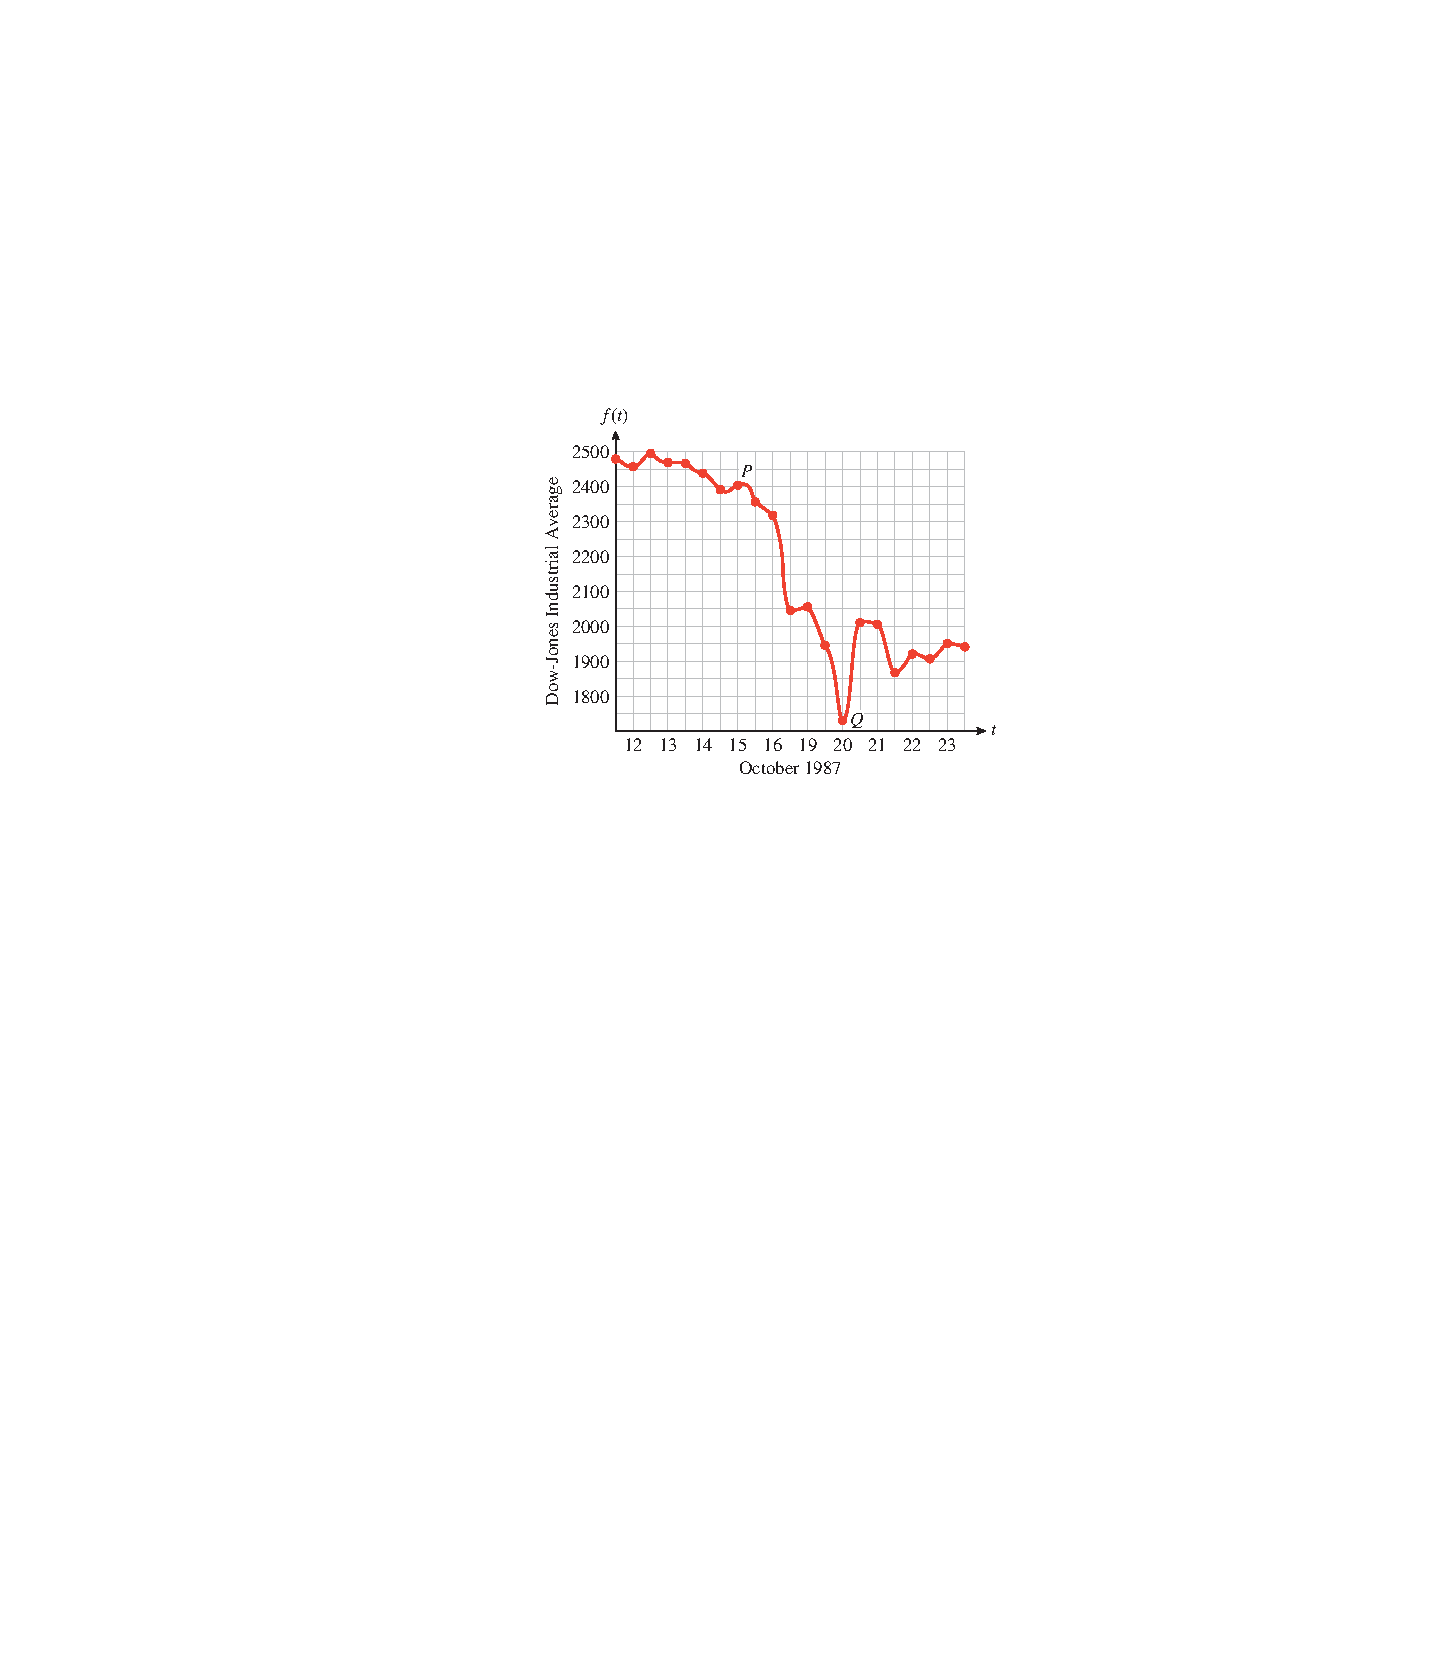
\includegraphics[width=\linewidth]{external/images/fig-DJIA.pdf}
\end{sbspanel}%
\end{sidebyside}%
\par
The values of the input variable, time, are displayed on the horizontal axis, and the values of the output variable, DJIA, are displayed on the vertical axis. There is no formula that gives the DJIA for a particular day; but it is still a function, defined by its graph. The value of \(f(t)\) is specified by the vertical coordinate of the point with the given \(t\)-coordinate.%
\begin{example}{Example}{}{example-example-DJIA}%
%
\begin{enumerate}[label=\alph*]
\item{}The coordinates of point \(P\) on the DJIA graph are \((15, 2412)\). What do the coordinates tell you about the function \(f\)?%
\item{}If the DJIA was 1726 at noon on October 20, what can you say about the graph of \(f\)?%
\end{enumerate}
%
\par\smallskip%
\noindent\textbf{\blocktitlefont Solution}.\hypertarget{solution-example-DJIA-b}{}\quad{}%
\begin{enumerate}[label=\alph*]
\item{}The coordinates of point \(P\) tell us that \(f(15) = 2412\), so the DJIA was 2412 at noon on October 15.%
\item{}We can say that \(f(20) = 1726\), so the point \((20, 1726)\) lies on the graph of \(f\). This point is labeled \(Q\) in the figure above.%
\end{enumerate}
%
\end{example}
Thus, the coordinates of each point on the graph of the function represent a pair of corresponding values of the two variables.%
\begin{assemblage}{Assemblage}{Graph of a Function.}{assemblage-graphs-of-functions-b-g}%
The point \((a, b)\) lies on the graph of the function \(f\) if and only if \(f(a)=b\).%
\end{assemblage}
\begin{inlineexercise}{Checkpoint}{QuickCheck 1.}{exercise-graphs-of-functions-b-h}%
Write an equation that says that the point \((8,17)\) lies on the graph of \(g\text{.}\)%
\par
\begin{itemize}[label=$\odot$,leftmargin=3em,]
\item{}\(\displaystyle 8+17=g\)%
\item{}\(\displaystyle g+8=17\)%
\item{}\(\displaystyle g(8)=17\)%
\item{}\(\displaystyle 8=\dfrac{17}{g}\)%
\end{itemize}
%
\par\smallskip%
\noindent\textbf{\blocktitlefont Answer}.\hypertarget{answer-graphs-of-functions-b-h-c}{}\quad{}\(\text{Choice 3}\)%
\par\smallskip%
\noindent\textbf{\blocktitlefont Solution}.\hypertarget{solution-graphs-of-functions-b-h-d}{}\quad{}\(g(8)=17\)%
\end{inlineexercise}%
\begin{inlineexercise}{Checkpoint}{Practice 1.}{exercise-graphs-of-functions-b-i}%
The water level in Lake Huron alters unpredictably over time. The graph below gives the average water level, \(L(t)\), in meters in the year \(t\) over a 20-year period. (Source: The Canadian Hydrographic Service)%
\begin{sidebyside}{1}{0.15}{0.15}{0}%
\begin{sbspanel}{0.7}%
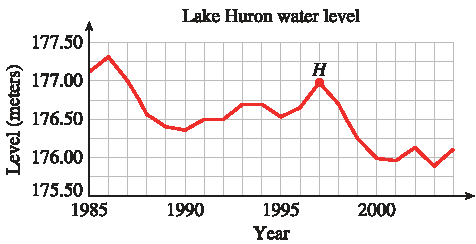
\includegraphics[width=\linewidth]{external/images/fig-Lake-Huron.pdf}
\end{sbspanel}%
\end{sidebyside}%
\par
%
\begin{enumerate}[label=\alph*.]
\item{}The coordinates of point \(H\) on the graph are \((1997, 176.98)\text{.}\) What do the coordinates tell you about the function \(L\text{?}\)%
\par
\begin{itemize}[label=$\odot$,leftmargin=3em,]
\item{}\(L(1997) = 176.98\); the average water level was 176.98 meters in 1997.%
\item{}\(L(176.98) = 176.98\); the average water level was 176.98 meters in 1997.%
\end{itemize}
%
\item{}The average water level in \(2004\) was \(176.11\) meters. Write this fact in function notation. What can you say about the graph of \(L\text{?}\)%
\par
\begin{itemize}[label=$\odot$,leftmargin=3em,]
\item{}\(L(176.11) = 2004\). The point \((176.11, 2004)\) lies on the graph of \(L\).%
\item{}\(L(2004) = 176.11\). The point \((2004, 176.11)\) lies on the graph of \(L\).%
\end{itemize}
%
\end{enumerate}
%
\par\smallskip%
\noindent\textbf{\blocktitlefont Answer 1}.\hypertarget{answer-graphs-of-functions-b-i-c}{}\quad{}\(\text{Choice 1}\)%
\par\smallskip%
\noindent\textbf{\blocktitlefont Answer 2}.\hypertarget{answer-graphs-of-functions-b-i-d}{}\quad{}\(\text{Choice 2}\)%
\par\smallskip%
\noindent\textbf{\blocktitlefont Solution}.\hypertarget{solution-graphs-of-functions-b-i-e}{}\quad{}%
\begin{enumerate}[label=\alph*.]
\item{}\(L(1997) = 176.98\text{;}\) the average water level was \(176.98\) meters in \(1997\text{.}\)%
\item{}\(L(2004) = 176.11\text{.}\) The point \((2004, 176.11)\) lies on the graph of \(L\text{.}\)%
\end{enumerate}
%
\end{inlineexercise}%
Here is another way of describing how a graph depicts a function.%
\begin{assemblage}{Assemblage}{Functions and Coordinates.}{assemblage-graphs-of-functions-b-k}%
Each point on the graph of the function \(f\) has coordinates \((x, f(x))\) for some value of \(x\).%
\end{assemblage}
\begin{example}{Example}{}{example-example-function-graph}%
The figure shows the graph of a function \(g\).%
\begin{sidebyside}{1}{0.35}{0.35}{0}%
\begin{sbspanel}{0.3}%
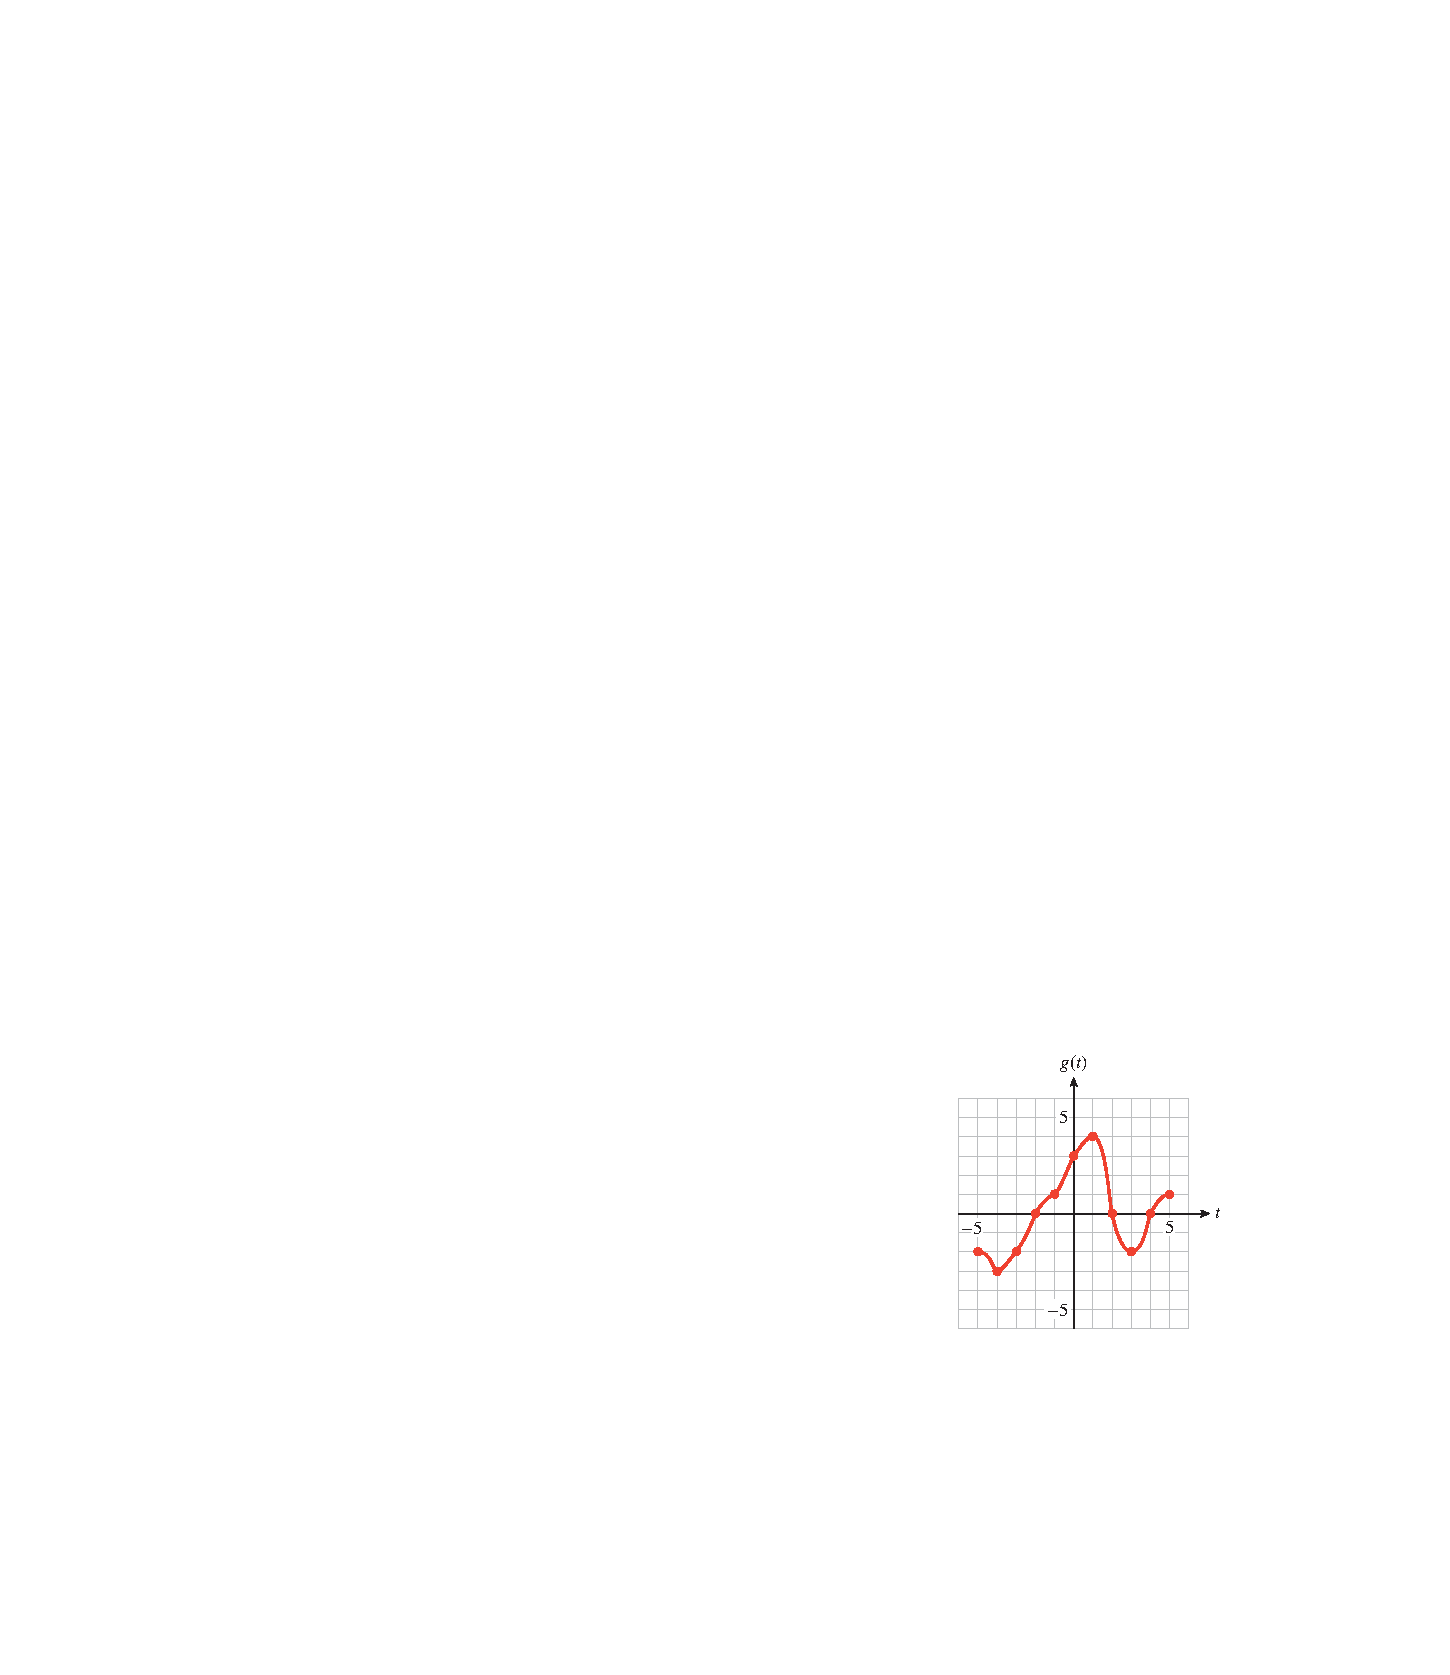
\includegraphics[width=\linewidth]{external/images/fig-function.pdf}
\end{sbspanel}%
\end{sidebyside}%
\par
%
\begin{enumerate}[label=\alph*]
\item{}Find \(g(-2)\) and \(g(5)\).%
\item{}For what value(s) of \(t\) is \(g(t) = -2\)?%
\item{}What is the largest, or maximum, value of \(g(t)\)? For what value of \(t\) does the function take on its maximum value?%
\item{}On what intervals is \(g\) increasing?%
\end{enumerate}
%
\par\smallskip%
\noindent\textbf{\blocktitlefont Solution}.\hypertarget{solution-example-function-graph-b}{}\quad{}%
\begin{enumerate}[label=\alph*]
\item{}To find \(g(-2)\), we look for the point with \(t\)-coordinate \(-2\). The point \((-2, 0)\) lies on the graph of \(g\), so \(g(-2) = 0\). Similarly, the point \((5, 1)\) lies on the graph, so \(g(5) = 1\).%
\item{}We look for points on the graph with \(y\)-coordinate \(-2\). Because the points \((-5, -2)\), \((-3, -2)\), and \((3, -2)\) lie on the graph, we know that \(g(-5) = -2\), \(g(-3) = -2\), and \(g(3) = -2\). Thus, the \(t\)-values we want are \(-5\), \(-3\), and \(3\).%
\item{}The highest point on the graph is \((1, 4)\), so the largest \(y\)-value is \(4\). Thus, the maximum value of \(g(t)\) is \(4\), and it occurs when \(t = 1\).%
\item{}A graph is increasing if the \(y\)-values get larger as we read from left to right. The graph of \(g\) is increasing for \(t\)-values between \(-4\) and \(1\), and between \(3\) and \(5\). Thus, \(g\) is increasing on the intervals \((-4, 1)\) and \((3, 5)\).%
\end{enumerate}
%
\end{example}
\begin{inlineexercise}{Checkpoint}{Practice 2.}{exercise-graphs-of-functions-b-m}%
Refer to the graph of the function \(g\) shown in \hyperref[example-example-function-graph]{Example~{\xreffont\ref{example-example-function-graph}}}.%
\begin{sidebyside}{1}{0.325}{0.325}{0}%
\begin{sbspanel}{0.35}%
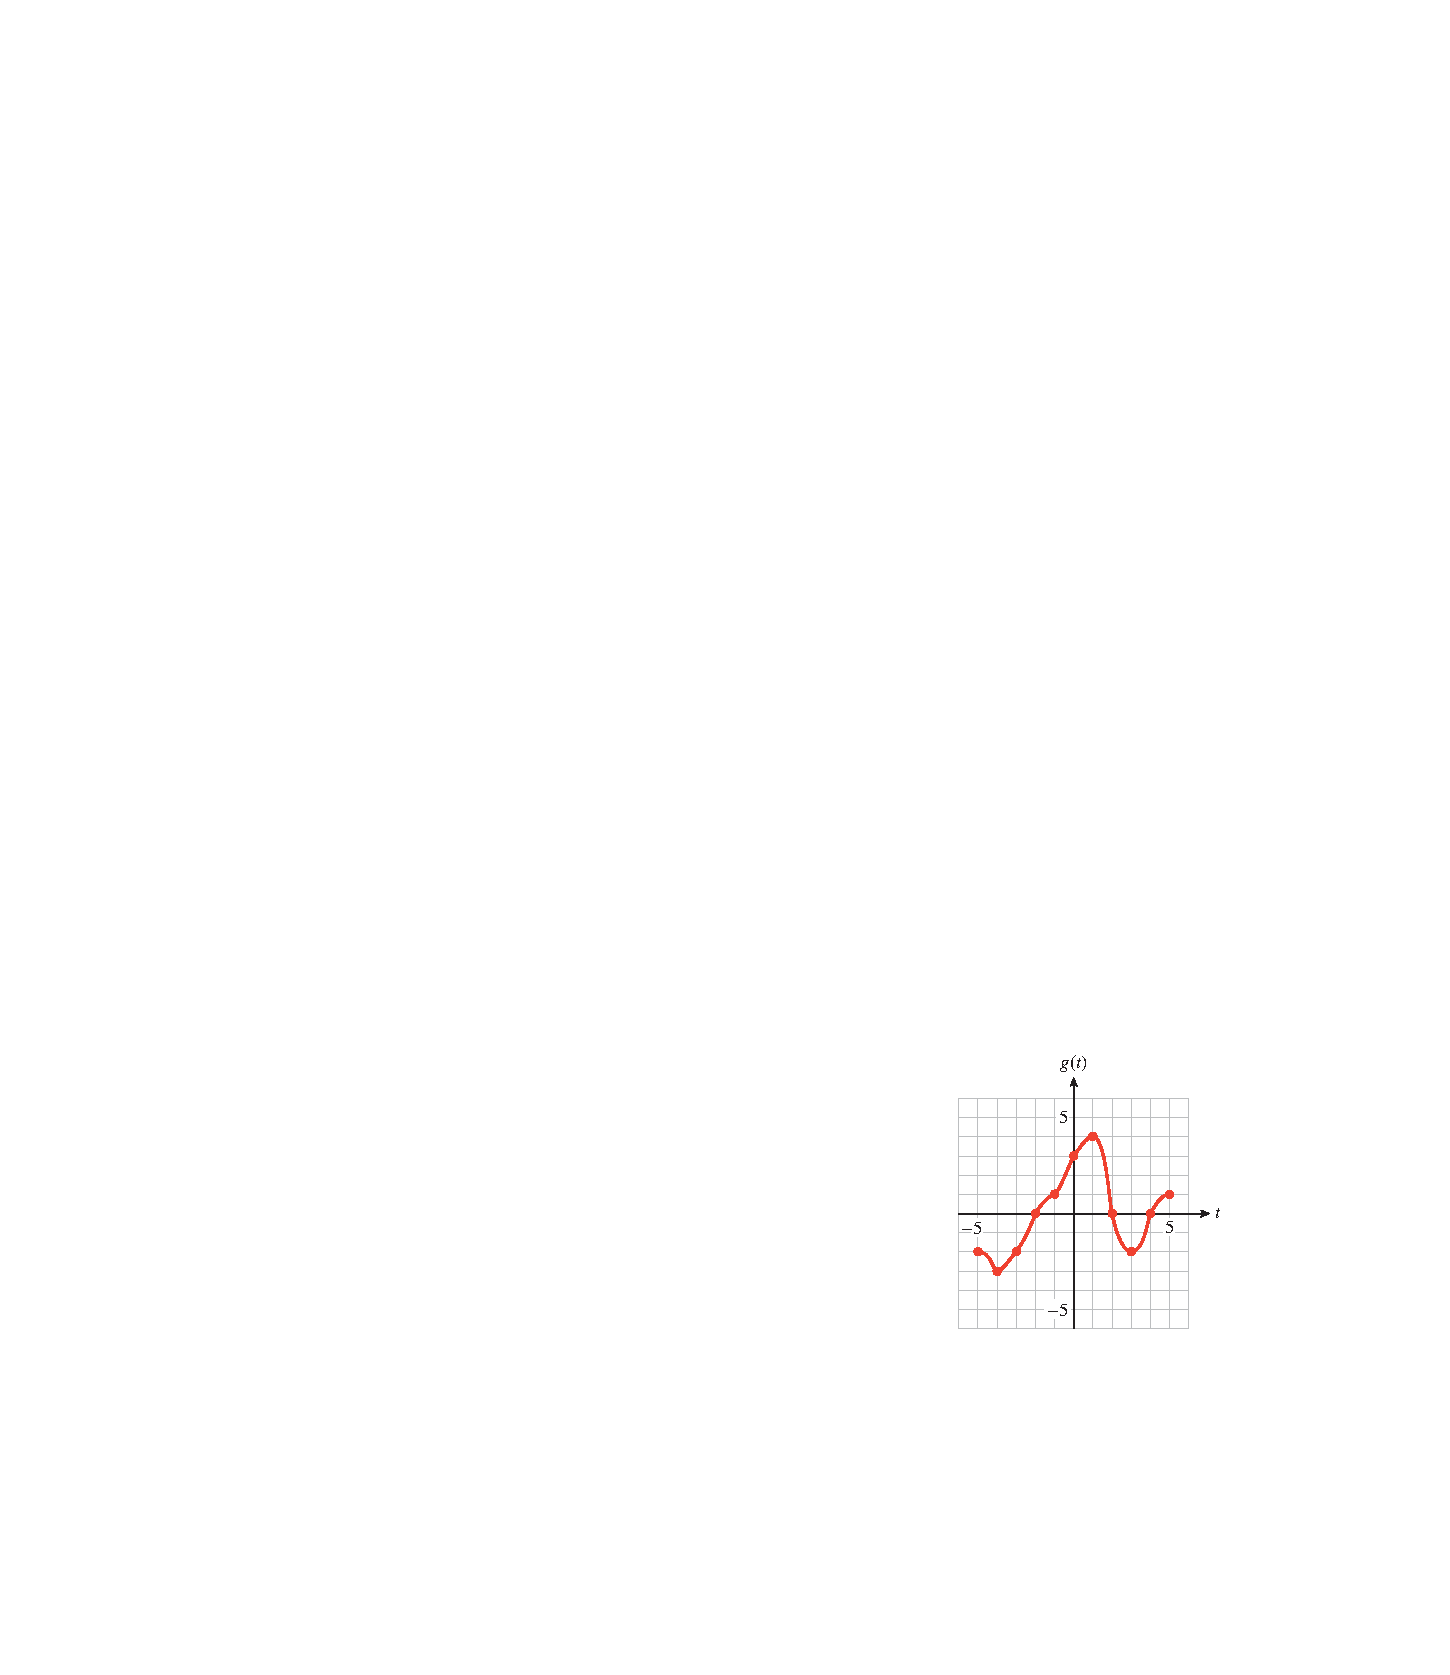
\includegraphics[width=\linewidth]{external/images/fig-function.pdf}
\end{sbspanel}%
\end{sidebyside}%
\par
%
\begin{enumerate}[label=\alph*.]
\item{}\(g(0)=\)\fillintext{3}%
\item{}List the value(s) of \(t\) for which \(g(t) = 0 \text{.}\) Separate different values with commas.%
\item{}What is the smallest, or minimum, value of \(g(t) \text{?}\)%
\par
Minimum: \fillintext{3}%
\par
For what value of \(t\) does the function take on its minimum value?%
\par
\(t=\)\fillintext{3}%
\item{}Select all the intervals listed below where \(g\) is decreasing.%
\par
From \(-5\) to \(-4\text{?}\)\quad(\begin{itemize*}[label=$\square$,leftmargin=3em,itemjoin=\hspace{1em}]
\item{}Yes%
\item{}No%
\end{itemize*})\quad
%
\par
From \(-5\) to \(-2\text{?}\)\quad(\begin{itemize*}[label=$\square$,leftmargin=3em,itemjoin=\hspace{1em}]
\item{}Yes%
\item{}No%
\end{itemize*})\quad
%
\par
From 2 to 4?\quad(\begin{itemize*}[label=$\square$,leftmargin=3em,itemjoin=\hspace{1em}]
\item{}Yes%
\item{}No%
\end{itemize*})\quad
%
\par
From 1 to 3?\quad(\begin{itemize*}[label=$\square$,leftmargin=3em,itemjoin=\hspace{1em}]
\item{}Yes%
\item{}No%
\end{itemize*})\quad
%
\end{enumerate}
%
\par\smallskip%
\noindent\textbf{\blocktitlefont Answer 1}.\hypertarget{answer-graphs-of-functions-b-m-c}{}\quad{}\(3\)%
\par\smallskip%
\noindent\textbf{\blocktitlefont Answer 2}.\hypertarget{answer-graphs-of-functions-b-m-d}{}\quad{}\(-2, 2, 4\)%
\par\smallskip%
\noindent\textbf{\blocktitlefont Answer 3}.\hypertarget{answer-graphs-of-functions-b-m-e}{}\quad{}\(-3\)%
\par\smallskip%
\noindent\textbf{\blocktitlefont Answer 4}.\hypertarget{answer-graphs-of-functions-b-m-f}{}\quad{}\(-4\)%
\par\smallskip%
\noindent\textbf{\blocktitlefont Answer 5}.\hypertarget{answer-graphs-of-functions-b-m-g}{}\quad{}\(\text{Yes}\)%
\par\smallskip%
\noindent\textbf{\blocktitlefont Answer 6}.\hypertarget{answer-graphs-of-functions-b-m-h}{}\quad{}\(\text{No}\)%
\par\smallskip%
\noindent\textbf{\blocktitlefont Answer 7}.\hypertarget{answer-graphs-of-functions-b-m-i}{}\quad{}\(\text{No}\)%
\par\smallskip%
\noindent\textbf{\blocktitlefont Answer 8}.\hypertarget{answer-graphs-of-functions-b-m-j}{}\quad{}\(\text{Yes}\)%
\par\smallskip%
\noindent\textbf{\blocktitlefont Solution}.\hypertarget{solution-graphs-of-functions-b-m-k}{}\quad{}%
\begin{enumerate}[label=\alph*.]
\item{}\(\displaystyle 3\)%
\item{}\(\displaystyle -2, 2, 4\)%
\item{}\(-3 \text{;}\) \(t = -4\)%
\item{}\((-5, -4)\) and \((1, 3)\)%
\end{enumerate}
%
\end{inlineexercise}%
\begin{inlineexercise}{Checkpoint}{QuickCheck 2.}{exercise-graphs-of-functions-b-n}%
Which of the following is true?%
\par
\begin{itemize}[label=$\odot$,leftmargin=3em,]
\item{}It is not possible for the function \(y=f(x)\) to take on the same \(y\)-value at two different \(x\)-values.%
\item{}The maximum value of \(y=f(x)\) may occur at two different \(x\)-values.%
\item{}The maximum value of the function \(y=f(x)\) is the largest \(x\)-value that appears on the graph.%
\item{}\(f(x)=0\) at the \(y\)-intercept of \(f(x)\).%
\end{itemize}
%
\par\smallskip%
\noindent\textbf{\blocktitlefont Answer}.\hypertarget{answer-graphs-of-functions-b-n-c}{}\quad{}\(\text{Choice 2}\)%
\par\smallskip%
\noindent\textbf{\blocktitlefont Solution}.\hypertarget{solution-graphs-of-functions-b-n-d}{}\quad{}The maximum value of \(y=f(x)\) may occur at two different \(x\)-values.%
\end{inlineexercise}%
\begin{technology}{Technology}{Finding Coordinates with a Graphing Utility.}{technology-graphs-of-functions-b-o}%
We can use the \kbd{TRACE} feature to find the coordinates of points on a graph. For example, graph the equation \(y = -2.6x - 5.4\) in the window%
\begin{sidebyside}{1}{0}{0}{0}%
\begin{sbspanel}{1}%
\resizebox{\ifdim\width > \linewidth\linewidth\else\width\fi}{!}{%
{\centering%
{\tabularfont%
\begin{tabular}{lll}
Xmin\(=-5\)&&Xmax\(=4.4\)\tabularnewline[0pt]
Ymin\(=-20\)&&Ymax\(=15\)
\end{tabular}
}%
\par}
}%
\end{sbspanel}%
\end{sidebyside}%
\begin{sidebyside}{1}{0.32}{0.32}{0}%
\begin{sbspanel}{0.36}%
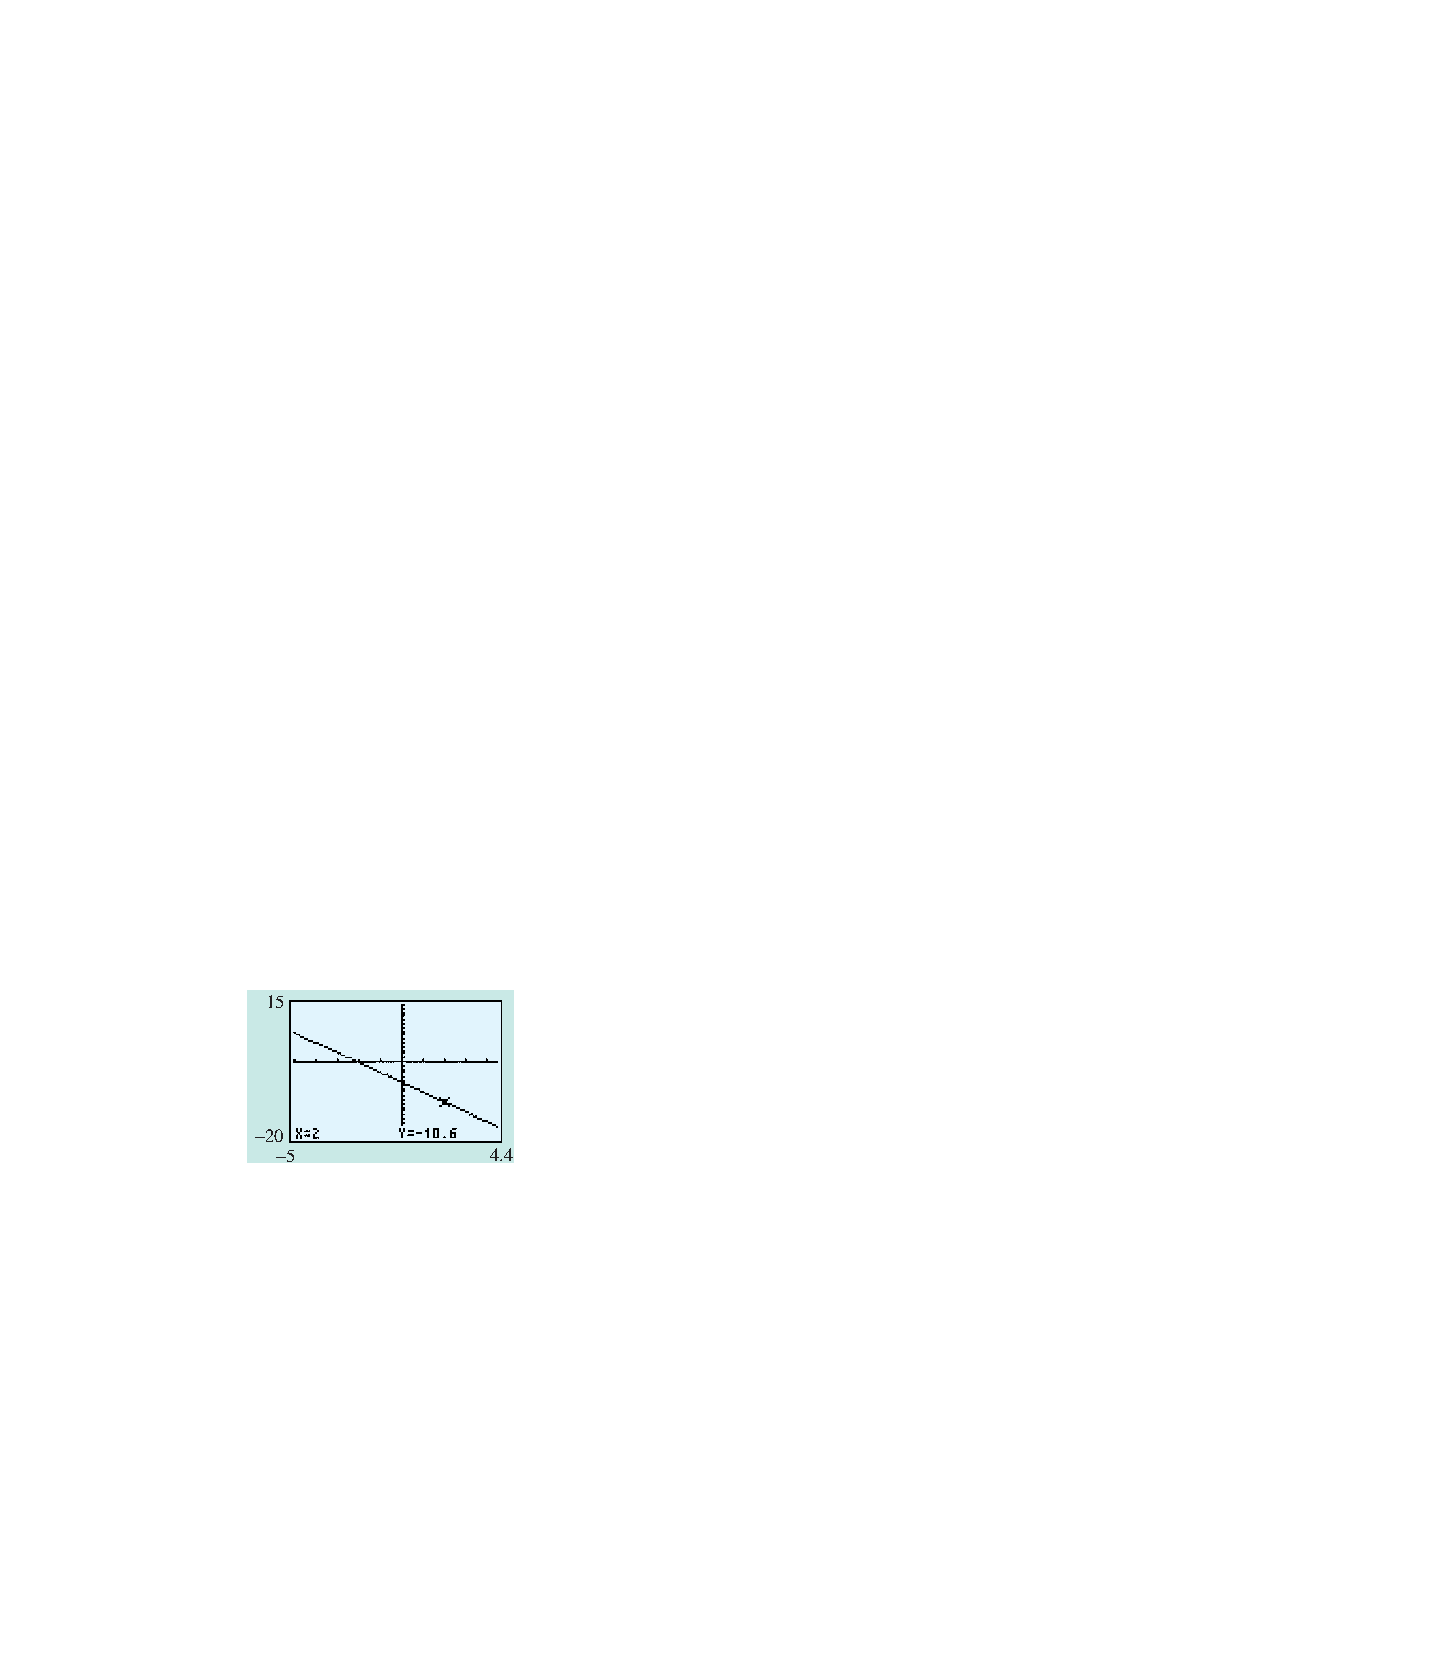
\includegraphics[width=\linewidth]{external/images/fig-GC-trace.pdf}
\end{sbspanel}%
\end{sidebyside}%
\par
Press \kbd{TRACE}, and a “bug” begins flashing on the display. The coordinates of the bug appear at the bottom of the display, as shown in the figure. Use the left and right arrows to move the bug along the graph. You can check that the coordinates of the point \((2, -10.6)\) do satisfy the equation \(y = -2.6x - 5.4\).%
\par
The points identified by the Trace bug depend on the window settings. If we want to find the \(y\)-coordinate for a particular \(x\)-value, we enter the \(x\)-coordinate of the desired point and press \kbd{ENTER}.%
\end{technology}
\end{subsectionptx}
%
%
\typeout{************************************************}
\typeout{Subsection  Constructing the Graph of a Function}
\typeout{************************************************}
%
\begin{subsectionptx}{Subsection}{Constructing the Graph of a Function}{}{Constructing the Graph of a Function}{}{}{subsection-graphs-of-functions-c}
Although some functions are defined by their graphs, we can also construct graphs for functions described by tables or equations. We make these graphs the same way we graph equations in two variables: by plotting points whose coordinates satisfy the equation.%
\begin{example}{Example}{}{example-example-graph-square-root}%
Graph the function \(f(x) = \sqrt{x + 4}\)%
\par\smallskip%
\noindent\textbf{\blocktitlefont Solution}.\hypertarget{solution-example-graph-square-root-b}{}\quad{}We choose several convenient values for \(x\) and evaluate the function to find the corresponding \(f(x)\)-values. For this function we cannot choose \(x\)-values less than \(-4\), because the square root of a negative number is not a real number.%
\begin{equation*}
f(\alert{-4}) =\sqrt{\alert{-4} + 4}=\sqrt{0}= 0
\end{equation*}
%
\begin{equation*}
f(\alert{-3}) =\sqrt{\alert{-3} + 4}=\sqrt{1}= 1
\end{equation*}
%
\begin{equation*}
f(\alert{0}) =\sqrt{\alert{0} + 4}=\sqrt{4}=2
\end{equation*}
%
\begin{equation*}
f(\alert{2}) =\sqrt{\alert{2} + 4}=\sqrt{6}\approx 2.45
\end{equation*}
%
\begin{equation*}
f(\alert{5}) =\sqrt{\alert{5} + 4}=\sqrt{9}=3
\end{equation*}
The results are shown in the table.%
\begin{sidebyside}{2}{0}{0.12}{0}%
\begin{sbspanel}{0.5}[center]%
\resizebox{\ifdim\width > \linewidth\linewidth\else\width\fi}{!}{%
{\centering%
{\tabularfont%
\begin{tabular}{AcAcA}\hrulethick
\(x\)&\(f(x)\)\tabularnewline\hrulethin
\(-4\)&\(0\)\tabularnewline\hrulethin
\(-3\)&\(1\)\tabularnewline\hrulethin
\(0\)&\(2\)\tabularnewline\hrulethin
\(2\)&\(\sqrt{6}\)\tabularnewline\hrulethin
\(5\)&\(3\)\tabularnewline\hrulethin
\end{tabular}
}%
\par}
}%
\end{sbspanel}%
\begin{sbspanel}{0.38}[center]%
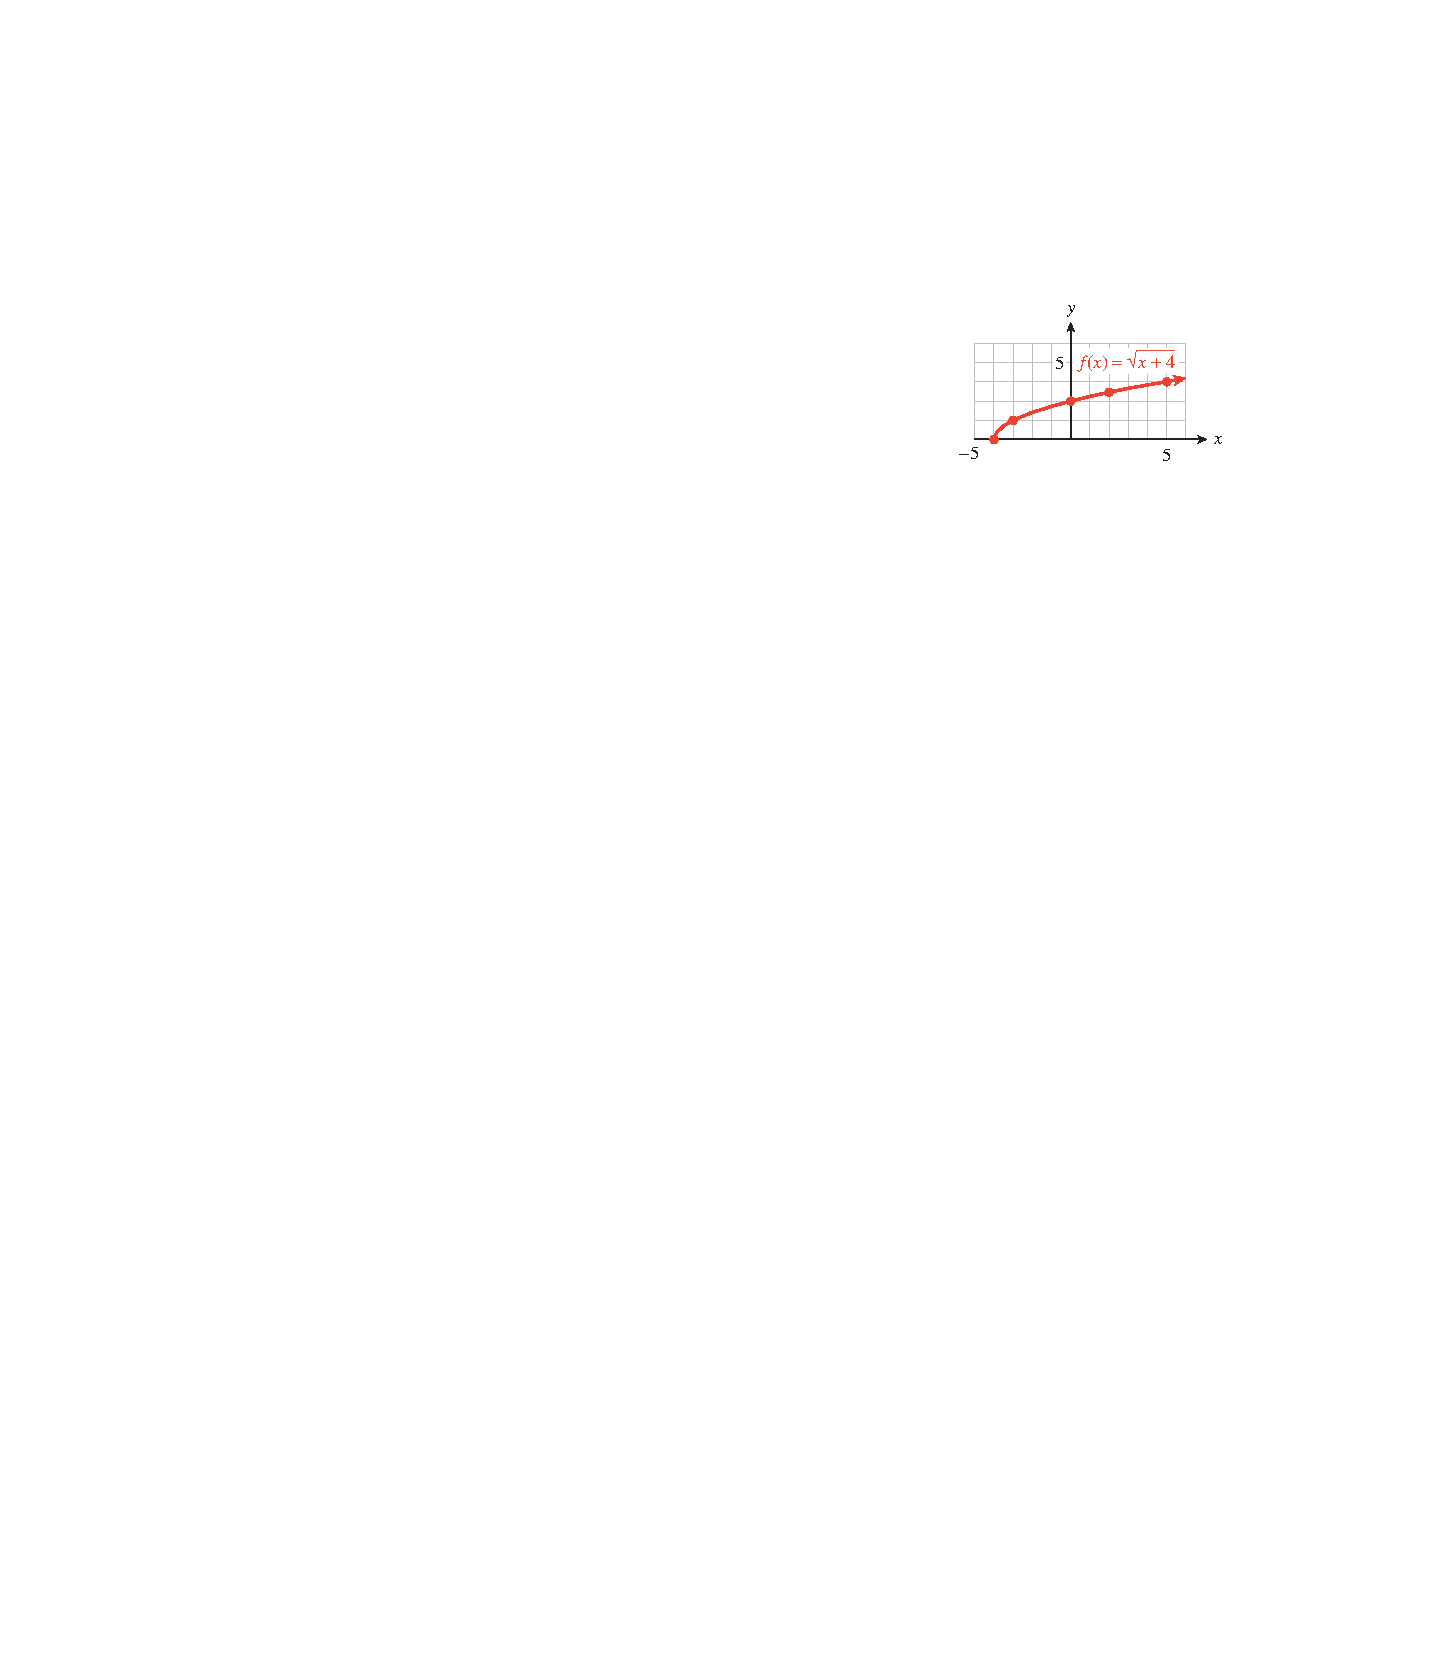
\includegraphics[width=\linewidth]{external/images/fig-sq-root.pdf}
\end{sbspanel}%
\end{sidebyside}%
\par
Points on the graph have coordinates \((x, f(x))\), so the vertical coordinate of each point is given by the value of \(f(x)\).  We plot the points and connect them with a smooth curve, as shown in the figure.  Notice that no points on the graph have \(x\)-coordinates less than \(-4\).%
\end{example}
\begin{inlineexercise}{Checkpoint}{QuickCheck 3.}{exercise-graphs-of-functions-c-d}%
How do we find the value of \(f(3)\) from a graph of \(f\text{?}\)%
\par
\begin{itemize}[label=$\odot$,leftmargin=3em,]
\item{}Find 3 on the \(x\)-axis, move vertically to the point, then horizontally to the \(y\)-axis.%
\item{}Find 3 on the \(y\)-axis, move horizontally to the point, then vertically to the \(x\)-axis.%
\item{}Substitue 3 for \(x\) into the formula for the function.%
\item{}Substitue 3 for \(y\) into the formula for the function.%
\end{itemize}
%
\par\smallskip%
\noindent\textbf{\blocktitlefont Answer}.\hypertarget{answer-graphs-of-functions-c-d-c}{}\quad{}\(\text{Choice 1}\)%
\par\smallskip%
\noindent\textbf{\blocktitlefont Solution}.\hypertarget{solution-graphs-of-functions-c-d-d}{}\quad{}Find 3 on the \(x\)-axis, move vertically to the point, then horizontally to the \(y\)-axis.%
\end{inlineexercise}%
\begin{technology}{Technology}{Using Technology to Graph a Function.}{technology-graphs-of-functions-c-e}%
We can also use a graphing utility to obtain a table and graph for the function in \hyperref[example-example-graph-square-root]{Example~{\xreffont\ref{example-example-graph-square-root}}}. We graph a function just as we graphed an equation. For this function, we enter \(Y_1 = \sqrt{\,}(X+4)\) and press \kbd{ZOOM} \(6\) for the standard window.  The graph is shown below.%
\begin{sidebyside}{1}{0.35}{0.35}{0}%
\begin{sbspanel}{0.3}%
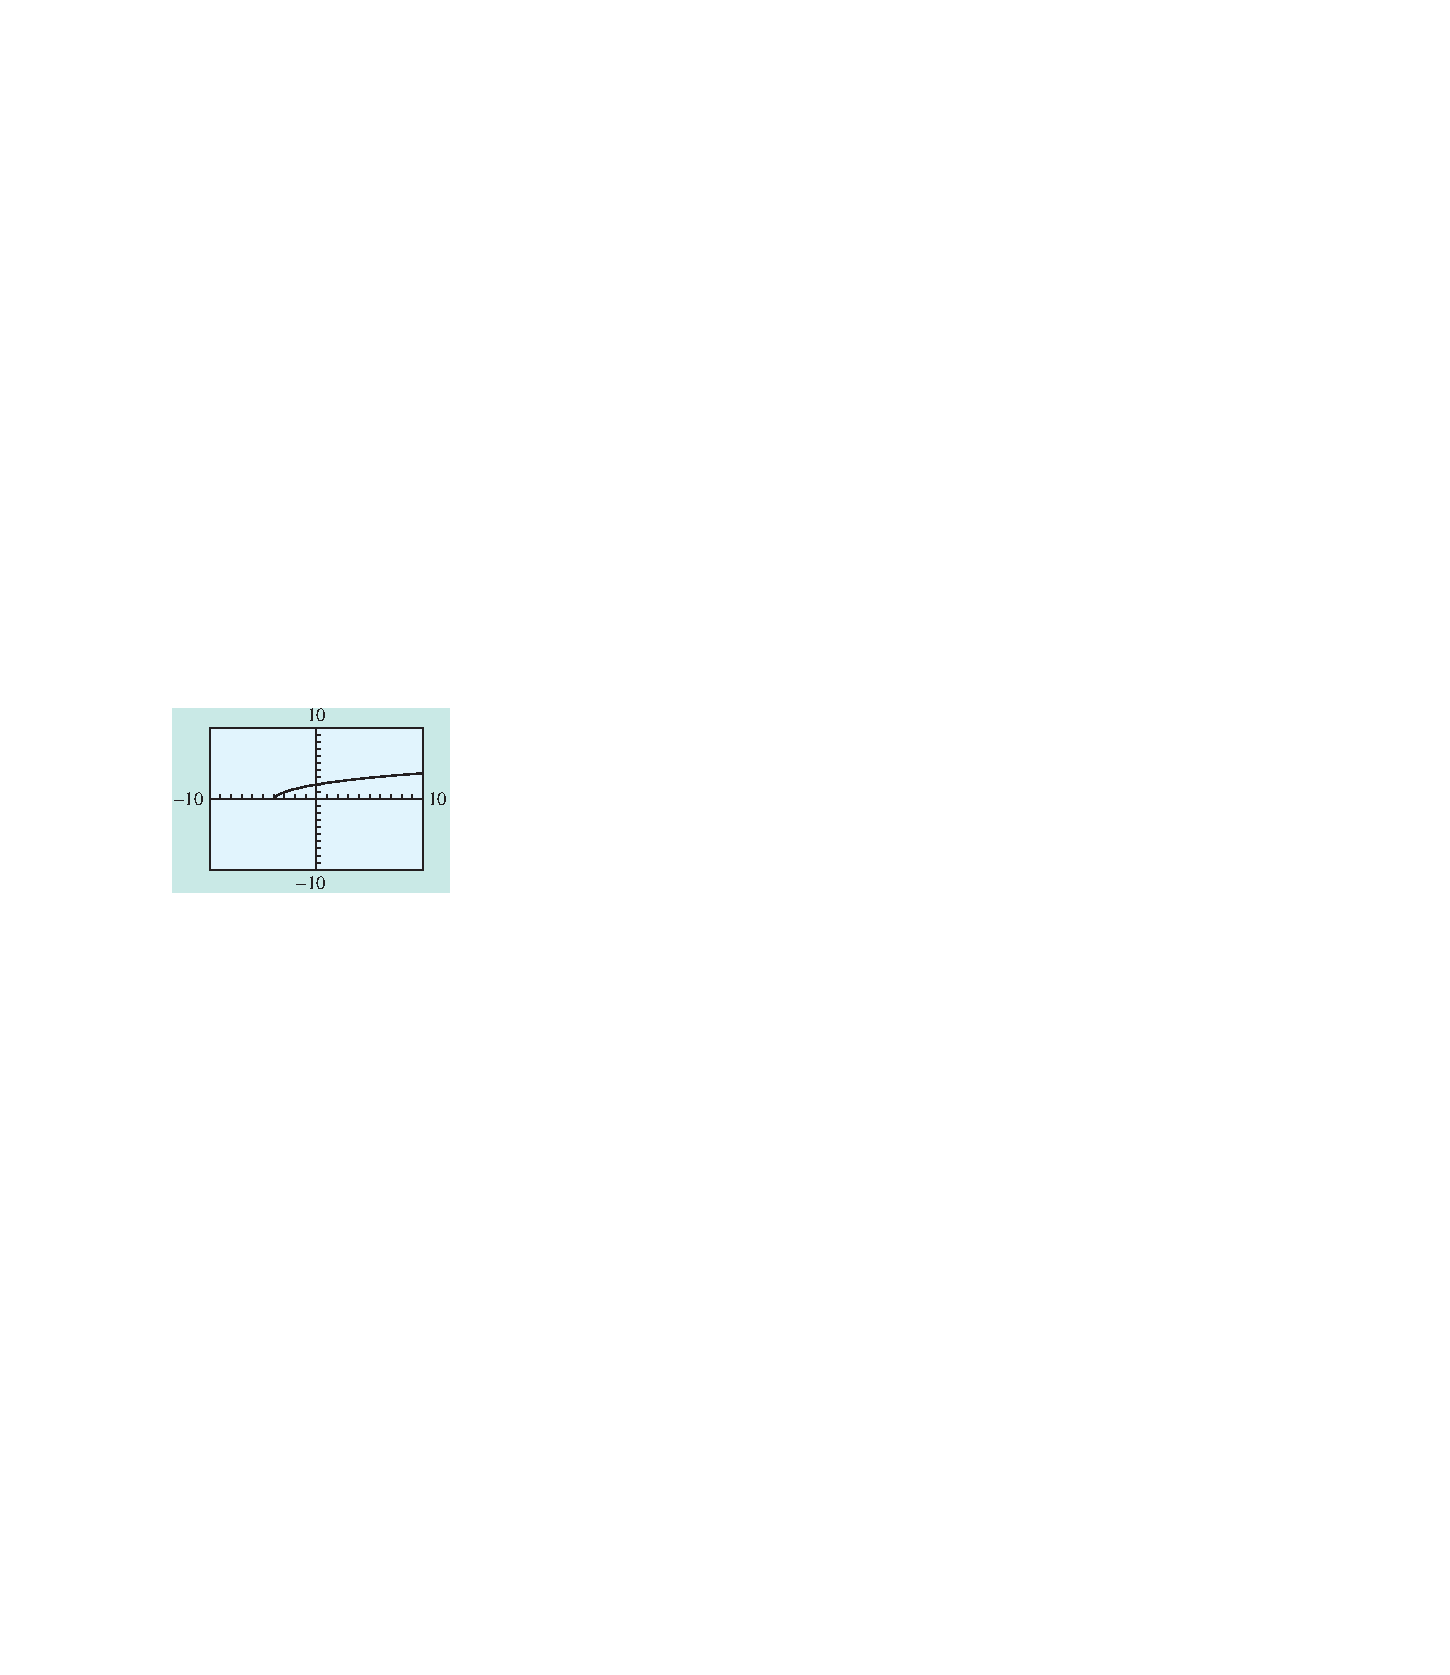
\includegraphics[width=\linewidth]{external/images/fig-GC-sq-root.pdf}
\end{sbspanel}%
\end{sidebyside}%
\end{technology}
\begin{inlineexercise}{Checkpoint}{Practice 3.}{exercise-graphs-of-functions-c-f}%
Let \(f(x) = {x^{3}-2}\)%
\par
Complete the table of values and sketch a graph of the function.%
\begin{center}%
{\tabularfont%
\begin{tabular}{AcAcAcAcAcAcAcAcA}
\(x\)&\(-2\)&\(-1\)&\(-\frac{1}{2}\)&\(0\)&\(\frac{1}{2}\)&\(1\)&\(2\)\tabularnewline\hrulethin
\(f(x)\)&\fillintext{2}&\fillintext{1}&\fillintext{2}&\fillintext{1}&\fillintext{2}&\fillintext{1}&\fillintext{1}\tabularnewline\hrulethin
\end{tabular}
}%
\end{center}%
\begin{sidebyside}{1}{0}{0.75}{0}%
\begin{sbspanel}{0.25}%
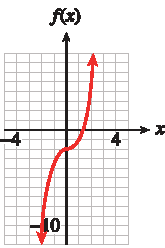
\includegraphics[width=\linewidth]{external/images/fig-in-ex-ans-1-3-3.pdf}
\end{sbspanel}%
\end{sidebyside}%
\par\smallskip%
\noindent\textbf{\blocktitlefont Answer 1}.\hypertarget{answer-graphs-of-functions-c-f-c}{}\quad{}\(-10\)%
\par\smallskip%
\noindent\textbf{\blocktitlefont Answer 2}.\hypertarget{answer-graphs-of-functions-c-f-d}{}\quad{}\(-3\)%
\par\smallskip%
\noindent\textbf{\blocktitlefont Answer 3}.\hypertarget{answer-graphs-of-functions-c-f-e}{}\quad{}\(-{\frac{17}{8}}\)%
\par\smallskip%
\noindent\textbf{\blocktitlefont Answer 4}.\hypertarget{answer-graphs-of-functions-c-f-f}{}\quad{}\(-2\)%
\par\smallskip%
\noindent\textbf{\blocktitlefont Answer 5}.\hypertarget{answer-graphs-of-functions-c-f-g}{}\quad{}\(-{\frac{15}{8}}\)%
\par\smallskip%
\noindent\textbf{\blocktitlefont Answer 6}.\hypertarget{answer-graphs-of-functions-c-f-h}{}\quad{}\(-1\)%
\par\smallskip%
\noindent\textbf{\blocktitlefont Answer 7}.\hypertarget{answer-graphs-of-functions-c-f-i}{}\quad{}\(6\)%
\par\smallskip%
\noindent\textbf{\blocktitlefont Solution}.\hypertarget{solution-graphs-of-functions-c-f-j}{}\quad{}\begin{center}%
{\tabularfont%
\begin{tabular}{AcAcAcAcAcAcAcAcA}
\(x\)&\(-2\)&\(-1\)&\(-\frac{1}{2}\)&\(0\)&\(\frac{1}{2}\)&\(1\)&\(2\)\tabularnewline\hrulethin
\(f(x)\)&\(-10\)&\(-3\)&\(\frac{-17}{8}\)&\(-2\)&\(\frac{-15}{8}\)&\(-1\)&\(6\)\tabularnewline\hrulethin
\end{tabular}
}%
\end{center}%
The graph is shown below.%
\end{inlineexercise}%
\begin{inlineexercise}{Checkpoint}{Pause and Reflect.}{exercise-graphs-of-functions-c-g}%
How is graphing a function different from graphing an equation?%
\end{inlineexercise}%
\end{subsectionptx}
%
%
\typeout{************************************************}
\typeout{Subsection  The Vertical Line Test}
\typeout{************************************************}
%
\begin{subsectionptx}{Subsection}{The Vertical Line Test}{}{The Vertical Line Test}{}{}{subsection-graphs-of-functions-d}
In a function, two different outputs cannot be related to the same input. This restriction means that two different ordered pairs cannot have the same first coordinate. What does it mean for the graph of the function?%
\par
Consider the graph shown in figure (a) below. Every vertical line intersects the graph in at most one point, so there is only one point on the graph for each \(x\)-value. This graph represents a function.%
\begin{sidebyside}{1}{0.175}{0.175}{0}%
\begin{sbspanel}{0.65}%
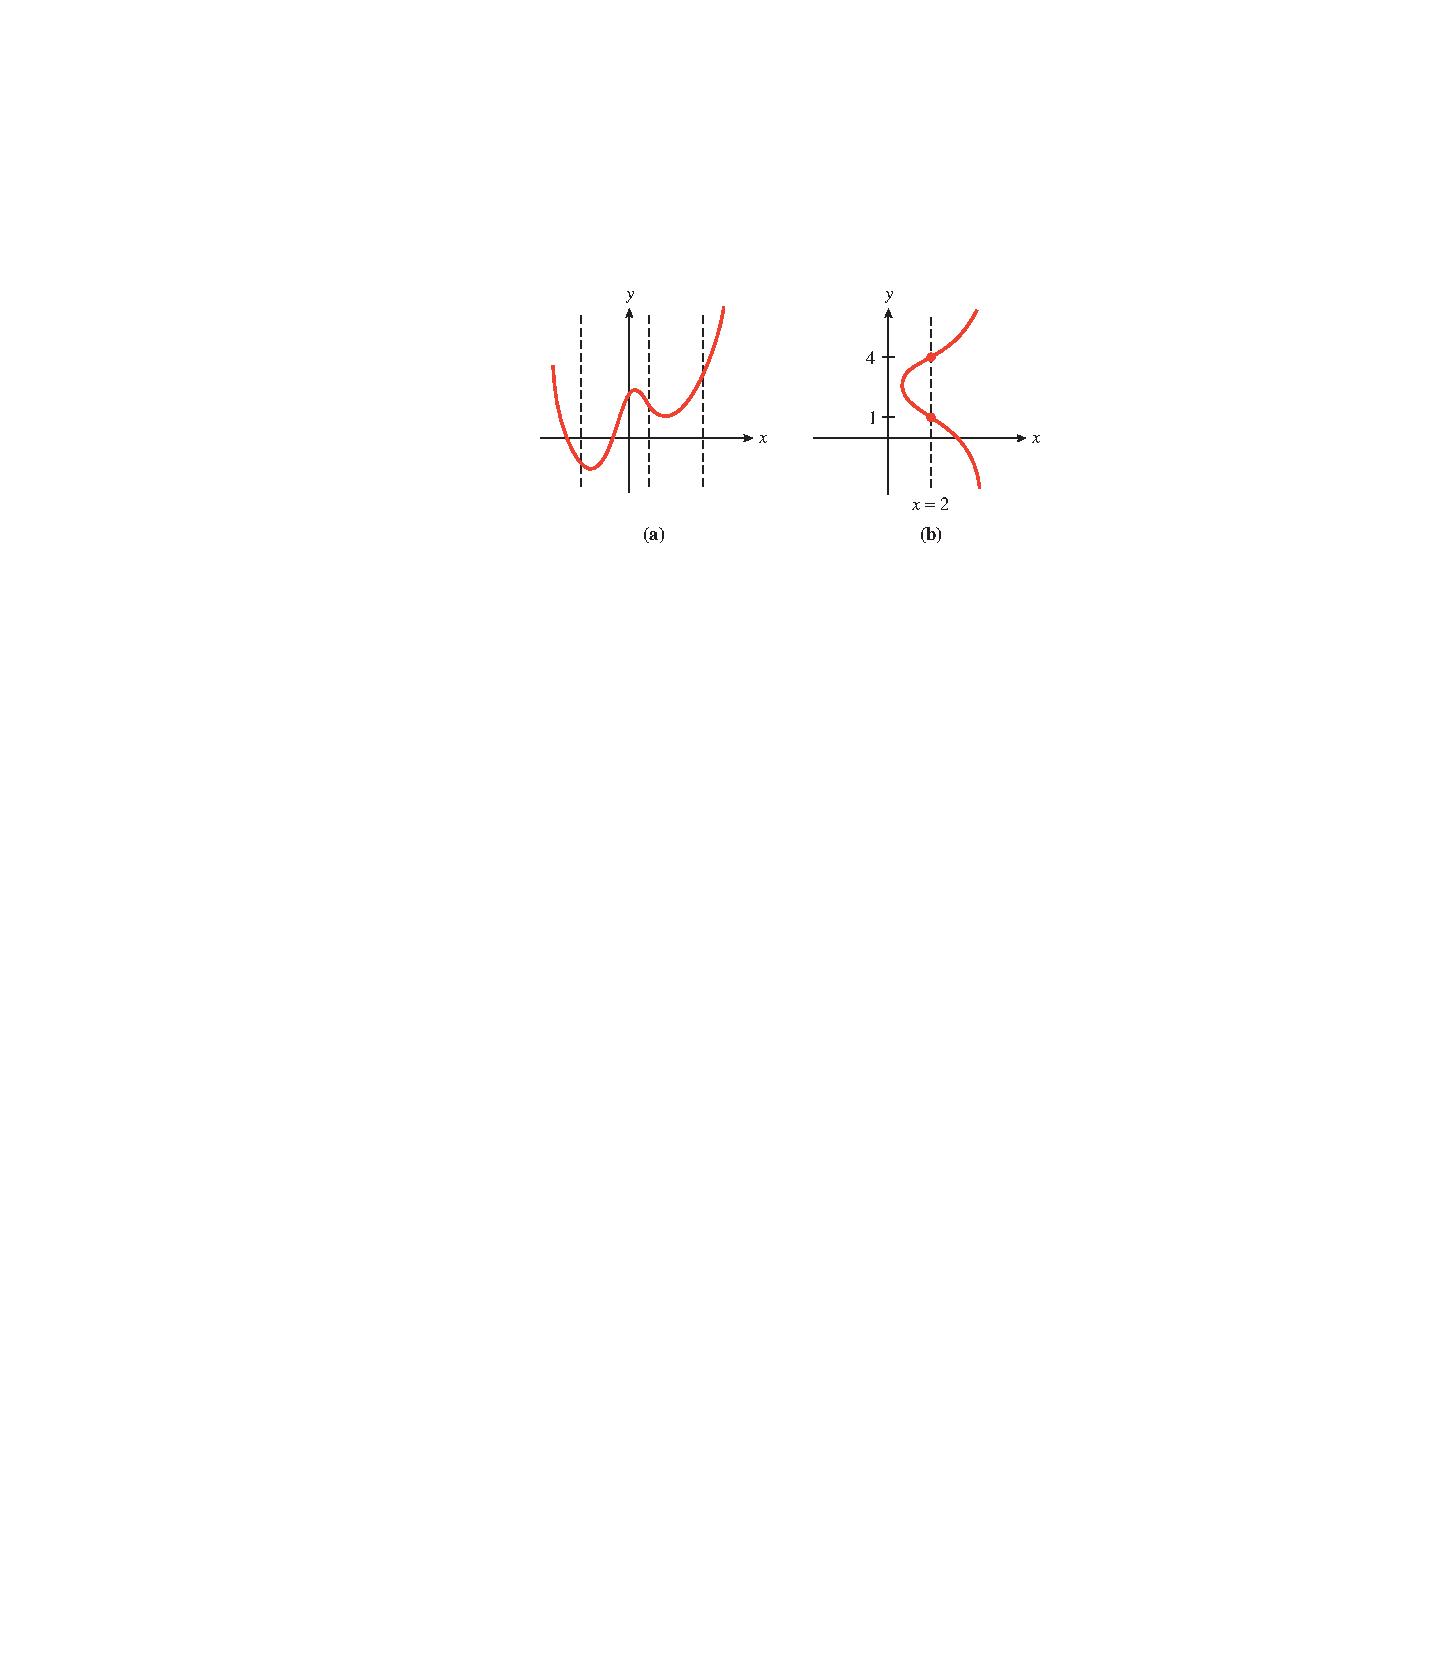
\includegraphics[width=\linewidth]{external/images/fig-vertical-line-test.pdf}
\end{sbspanel}%
\end{sidebyside}%
\par
In figure (b), however, the line \(x = 2\) intersects the graph at two points, \((2, 1)\) and \((2, 4)\). Two different \(y\)-values, \(1\) and \(4\), are related to the same \(x\)-value, \(2\). This graph cannot be the graph of a function.%
\par
We summarize these observations as follows.%
\begin{assemblage}{Assemblage}{The Vertical Line Test.}{assemblage-graphs-of-functions-d-g}%
A graph represents a function if and only if every vertical line intersects the graph in at most one point.%
\end{assemblage}
\begin{example}{Example}{}{example-example-vertical-line-test}%
Use the vertical line test to decide which of the graphs in the figure represent functions.%
\begin{sidebyside}{1}{0.1}{0.1}{0}%
\begin{sbspanel}{0.8}%
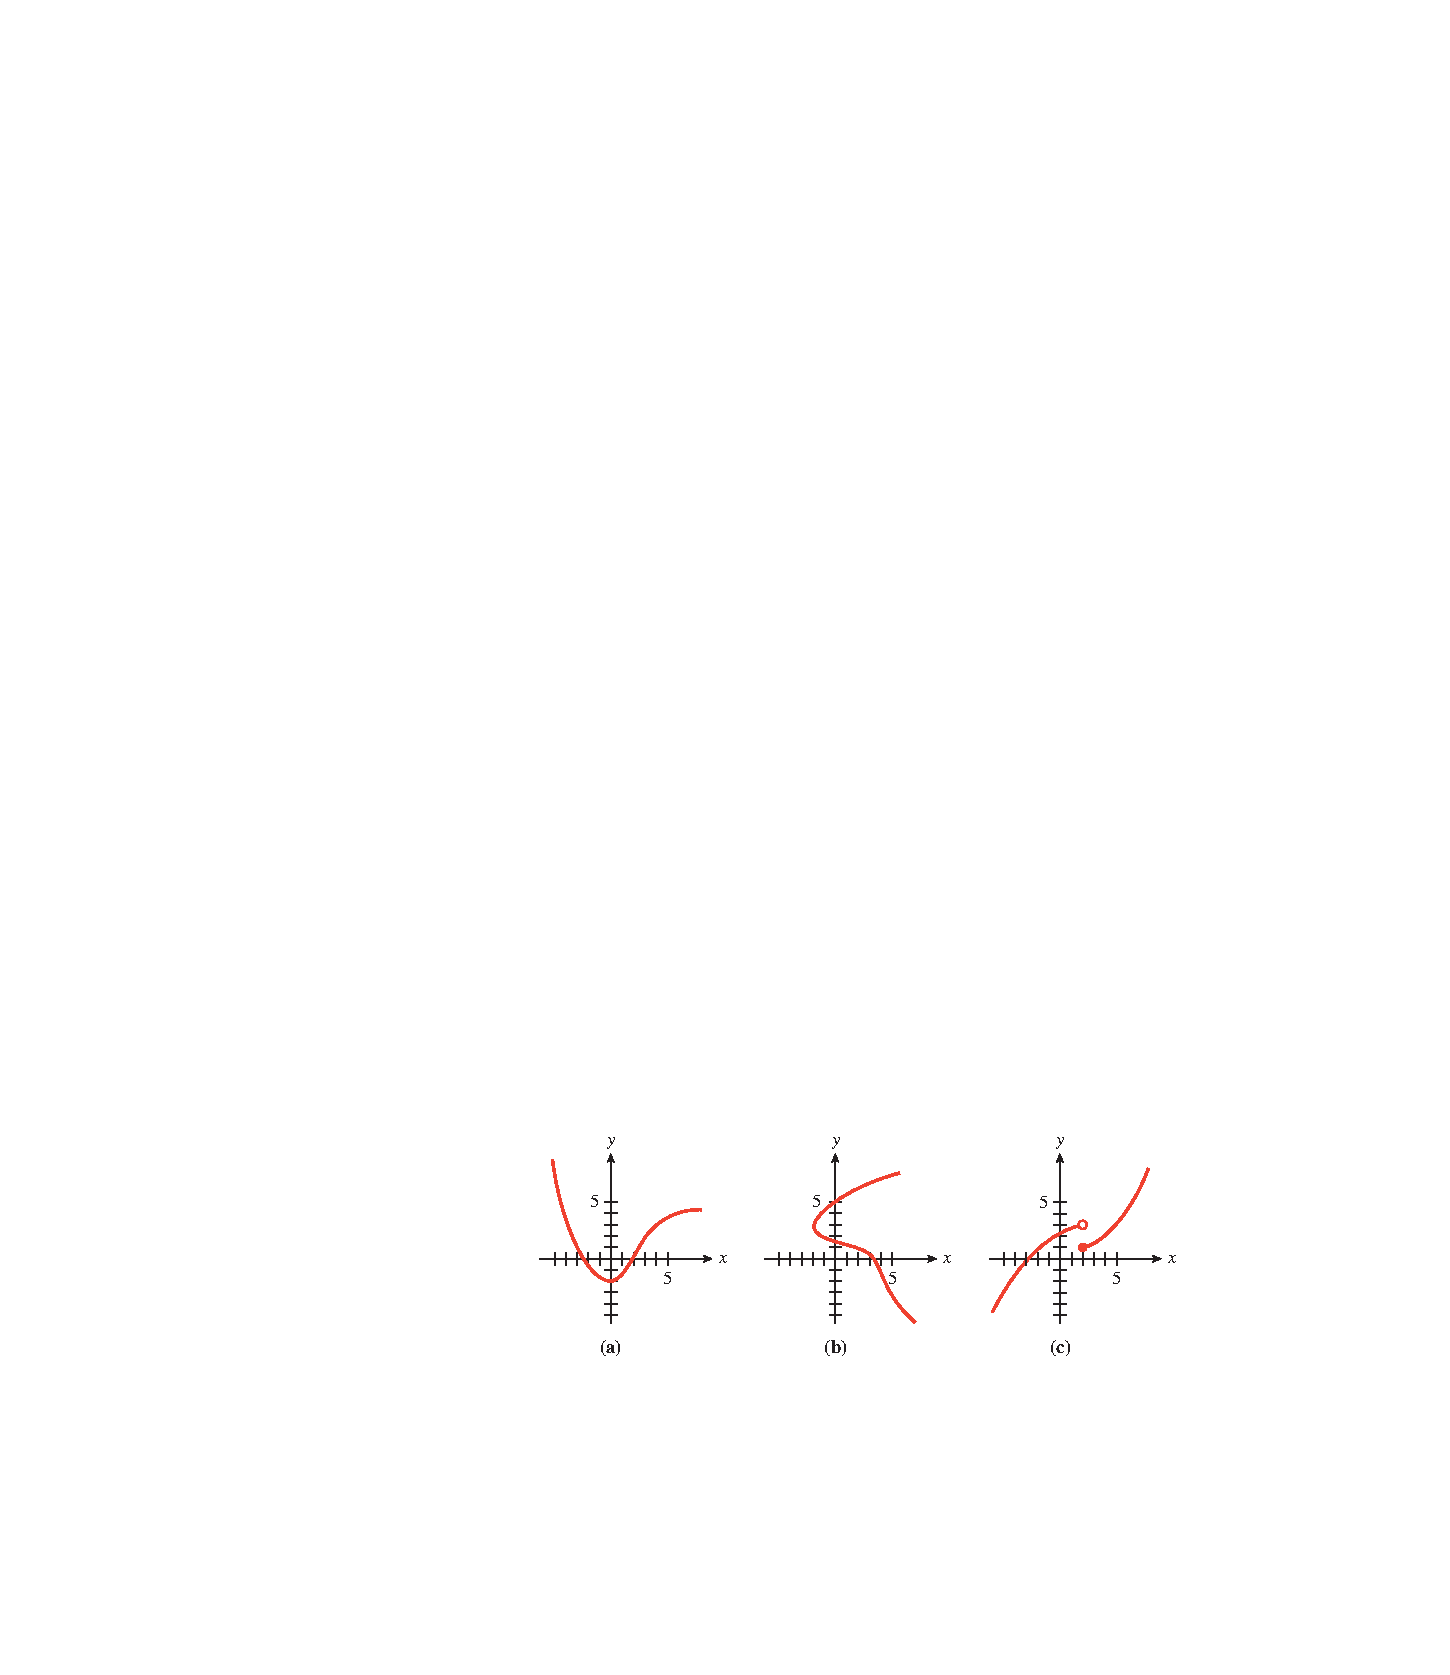
\includegraphics[width=\linewidth]{external/images/fig-vertical-line-test2.pdf}
\end{sbspanel}%
\end{sidebyside}%
\par\smallskip%
\noindent\textbf{\blocktitlefont Solution}.\hypertarget{solution-example-vertical-line-test-b}{}\quad{}%
\begin{itemize}[label=\textbullet]
\item{}Graph (a) represents a function, because it passes the vertical line test.%
\item{}Graph (b) is not the graph of a function, because the vertical line at (for example) \(x = 1\) intersects the graph at two points.%
\item{}For graph (c), notice the break in the curve at \(x = 2\): The solid dot at \((2, 1)\) is the only point on the graph with \(x = 2\); the open circle at \((2, 3)\) indicates that \((2, 3)\) is not a point on the graph. Thus, graph (c) is a function, with \(f(2) = 1\).%
\end{itemize}
%
\end{example}
\begin{inlineexercise}{Checkpoint}{QuickCheck 4.}{exercise-graphs-of-functions-d-i}%
What does the vertical line test tell us?%
\par
\begin{itemize}[label=$\odot$,leftmargin=3em,]
\item{}A) If the graph is a vertical line.%
\item{}B) If the graph is increasing.%
\item{}C) If the graph is decreasing.%
\item{}D) If the graph is a function.%
\end{itemize}
%
\par\smallskip%
\noindent\textbf{\blocktitlefont Answer}.\hypertarget{answer-graphs-of-functions-d-i-c}{}\quad{}\(\text{D) If ... a function.}\)%
\par\smallskip%
\noindent\textbf{\blocktitlefont Solution}.\hypertarget{solution-graphs-of-functions-d-i-d}{}\quad{}The vertical line test tells us if the graph is a function.%
\end{inlineexercise}%
\begin{inlineexercise}{Checkpoint}{Practice 4.}{exercise-graphs-of-functions-d-j}%
Use the vertical line test to determine which of the graphs below represent functions.%
\begin{sidebyside}{1}{0}{0}{0}%
\begin{sbspanel}{1}%
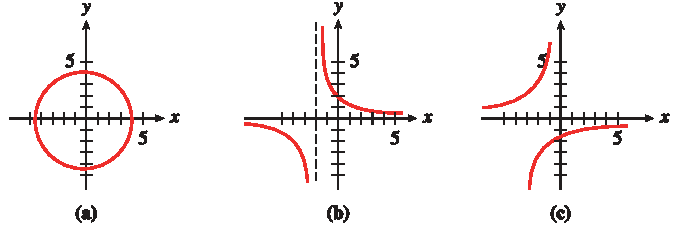
\includegraphics[width=\linewidth]{external/images/fig-vertical-line-test3.pdf}
\end{sbspanel}%
\end{sidebyside}%
\par
\begin{itemize}[label=$\odot$,leftmargin=3em,]
\item{}(a)%
\item{}(b)%
\item{}(c)%
\item{}None of the above%
\end{itemize}
%
\par\smallskip%
\noindent\textbf{\blocktitlefont Answer}.\hypertarget{answer-graphs-of-functions-d-j-c}{}\quad{}\(\text{(b)}\)%
\par\smallskip%
\noindent\textbf{\blocktitlefont Solution}.\hypertarget{solution-graphs-of-functions-d-j-d}{}\quad{}Only (b) is a function.%
\end{inlineexercise}%
\end{subsectionptx}
%
%
\typeout{************************************************}
\typeout{Subsection  Graphical Solution of Equations and Inequalities}
\typeout{************************************************}
%
\begin{subsectionptx}{Subsection}{Graphical Solution of Equations and Inequalities}{}{Graphical Solution of Equations and Inequalities}{}{}{subsection-graphs-of-functions-e}
The graph of an equation in two variables is just a picture of its solutions. When we read the coordinates of a point on the graph, we are reading a pair of \(x\)- and \(y\)-values that make the equation true.%
\begin{sidebyside}{2}{0}{0}{0.08}%
\begin{sbspanel}{0.65}[center]%
For example, the point \((2, 7)\) lies on the graph of \(y = 2x + 3\) shown at right, so we know that the ordered pair \((2, 7)\) is a solution of the equation \(y = 2x + 3\). You can verify algebraically that \(x = \alert{2}\) and \(y = \alert{7}\) satisfy the equation:%
\begin{equation*}
\text{Does }~\alert{7} = 2 (\alert{2}) + 3\text{?} ~~~~~~~~ \blert{\text{Yes}}
\end{equation*}
%
\end{sbspanel}%
\begin{sbspanel}{0.27}[center]%
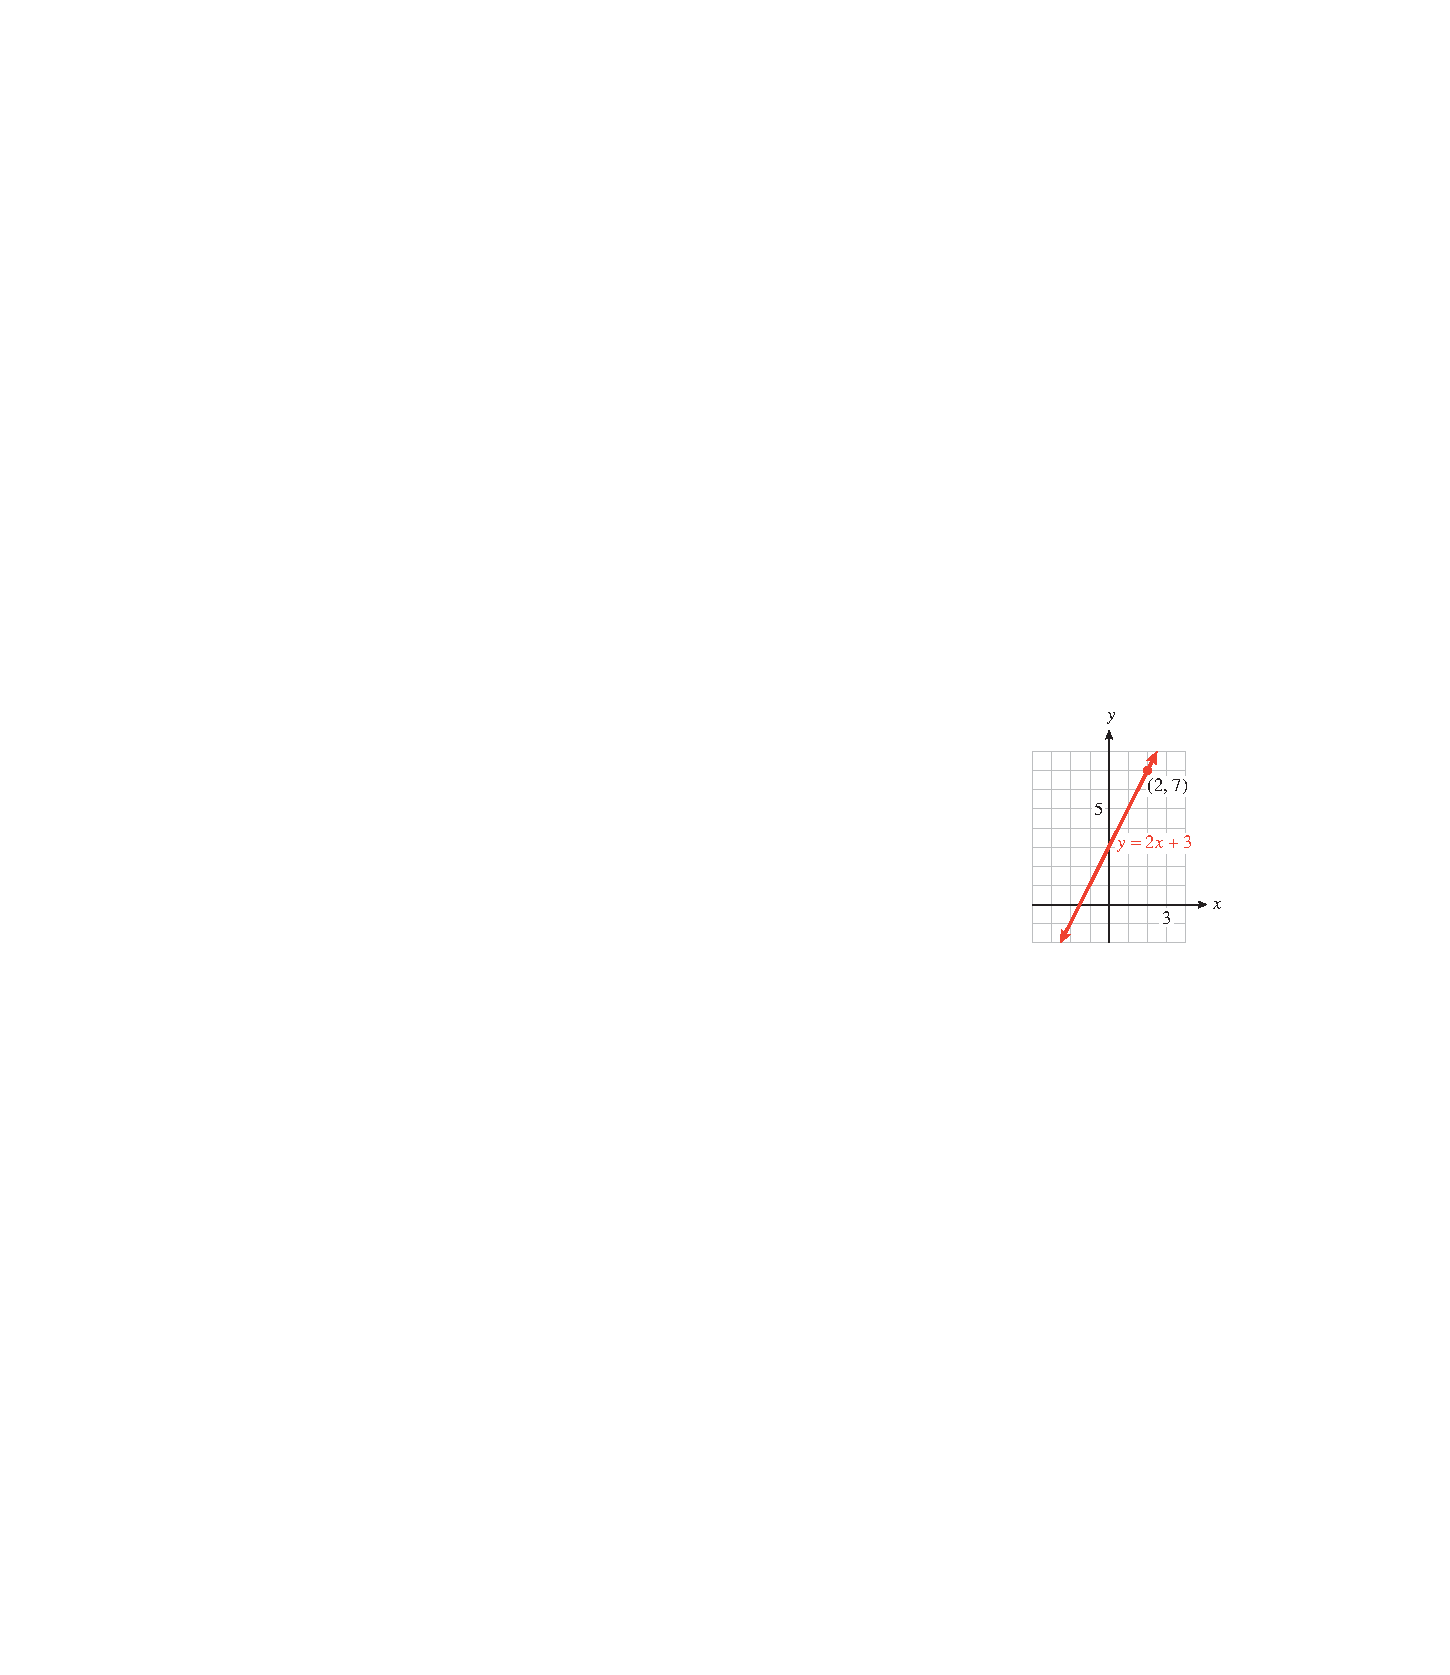
\includegraphics[width=\linewidth]{external/images/fig-function-graph.pdf}
\end{sbspanel}%
\end{sidebyside}%
\par
We can also say that \(x = 2\) is a solution of the one-variable equation \(2x + 3 = 7\). In fact, we can use the graph of \(y = 2x + 3\) to solve the equation \(2x + 3 = k\) for any value of \(k\). Thus, we can use graphs to find solutions to equations in one variable.%
\begin{example}{Example}{}{example-example-graph-to-solve}%
Use the graph of \(y = 285 - 15x\) to solve the equation \(150 = 285 - 15x\).%
\par\smallskip%
\noindent\textbf{\blocktitlefont Solution}.\hypertarget{solution-example-graph-to-solve-b}{}\quad{}\begin{sidebyside}{2}{0}{0.05}{0.05}%
\begin{sbspanel}{0.6}%
We begin by locating the point \(P\) on the graph for which \(y = 150\), as shown in the figure.%
\par
Next we find the \(x\)-coordinate of point \(P\) by drawing an imaginary line from \(P\) straight down to the \(x\)-axis. The \(x\)-coordinate of \(P\) is \(x = 9\).%
\par
Thus, \(P\) is the point \((9,150)\), and \(x = 9\) when \(y = 150\). The solution of the equation \(150 = 285 - 15x\) is \(x = 9\).%
\end{sbspanel}%
\begin{sbspanel}{0.3}%
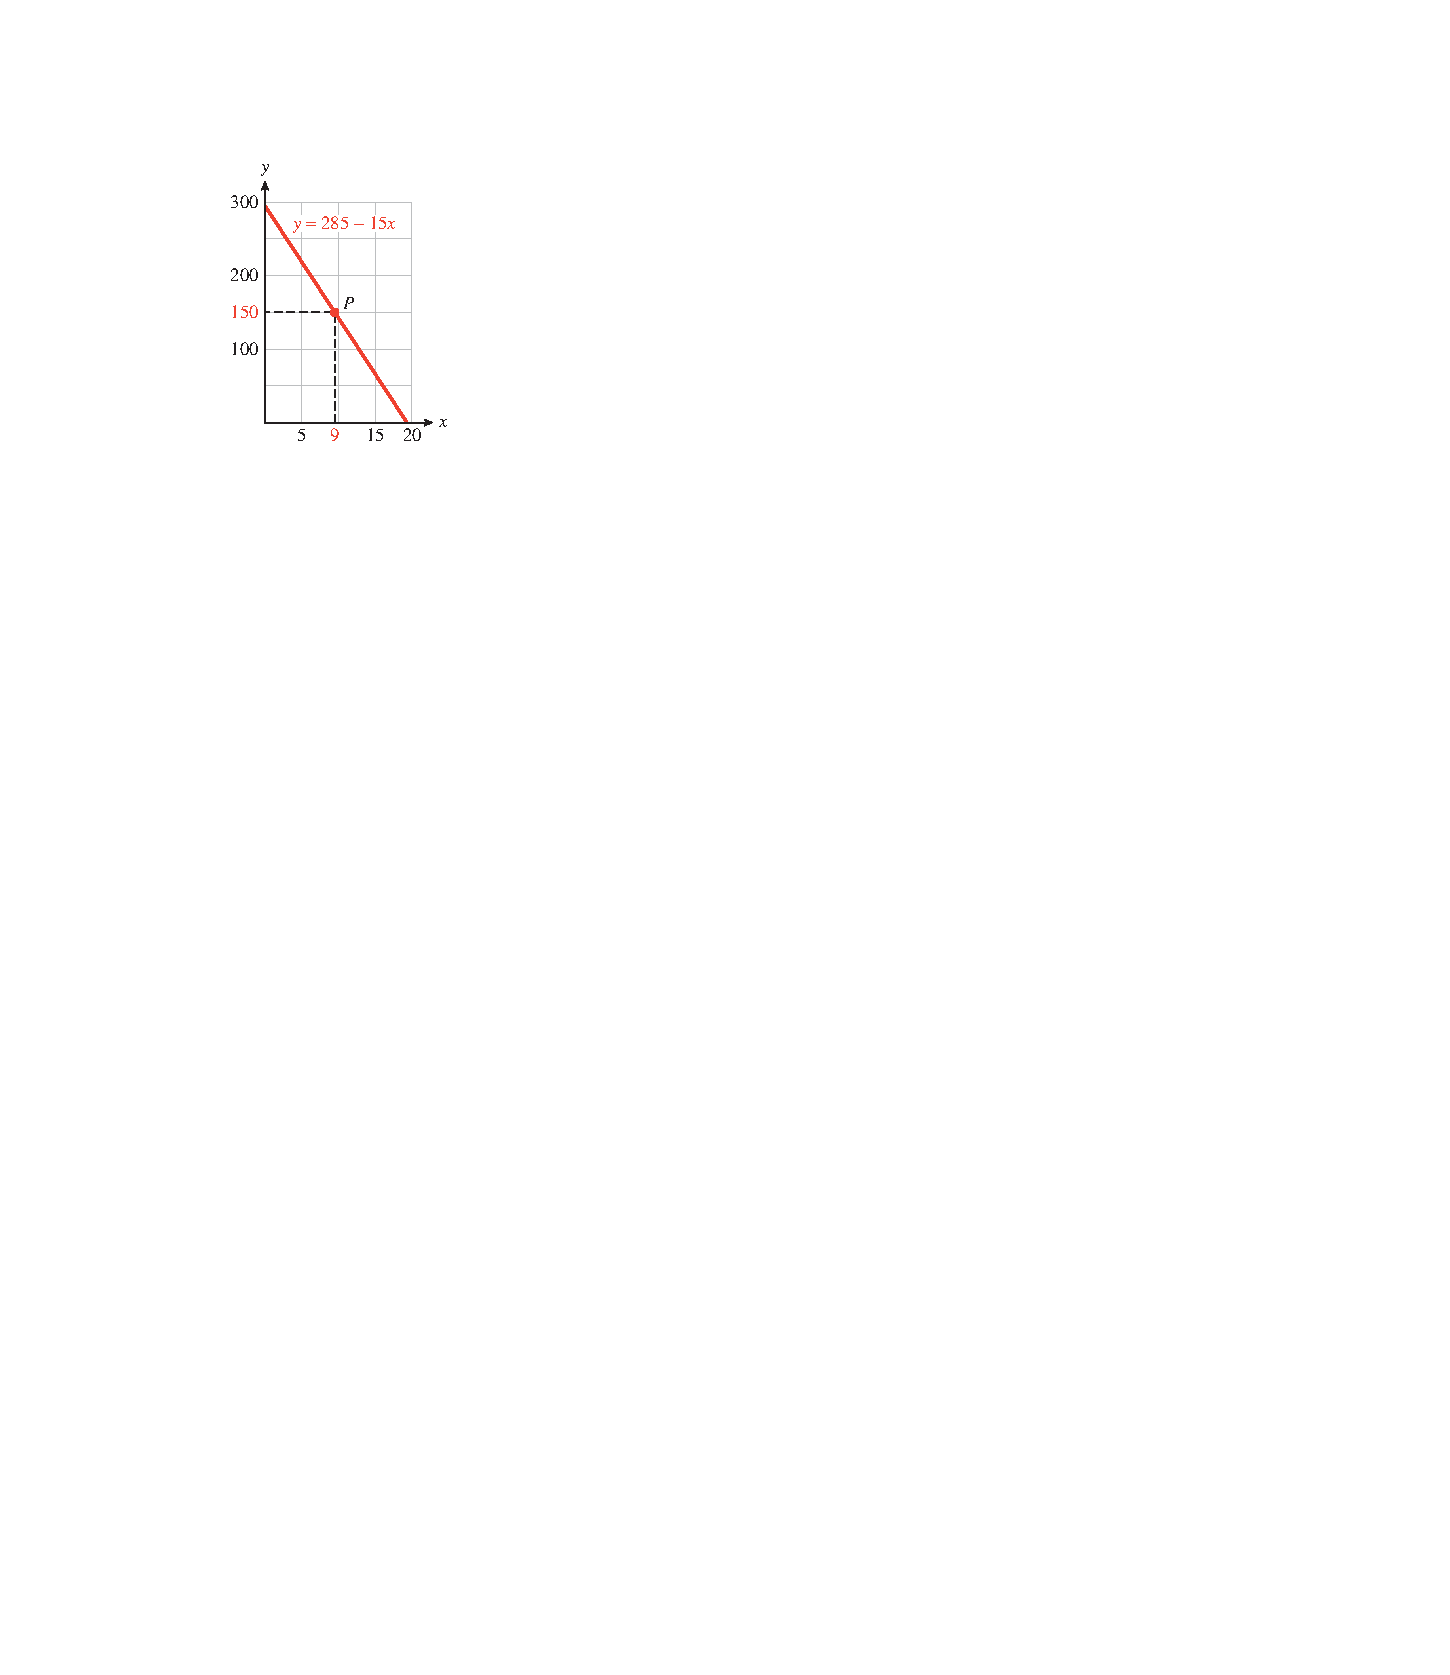
\includegraphics[width=\linewidth]{external/images/fig-graph-to-solve.pdf}
\end{sbspanel}%
\end{sidebyside}%
\par
You can verify the solution algebraically by substituting \(x = \alert{9}\) into the equation:%
\par
Does \(150 = 285 - 15(\alert{9})\)?%
\par
%
\begin{equation*}
285 - 15(\alert{9}) = 285 - 135 = 150. ~~~~~~\blert{\text{Yes}}
\end{equation*}
%
\end{example}
\begin{inlineexercise}{Checkpoint}{QuickCheck 5.}{exercise-graphs-of-functions-e-f}%
If \(f(8)=2\text{,}\) what point lies on the graph of \(f\text{?}\)%
\par
\begin{itemize}[label=$\odot$,leftmargin=3em,]
\item{}\(\displaystyle (8,2)\)%
\item{}\(\displaystyle (2,8)\)%
\item{}Both \((8,2)\) and \((2,8)\)%
\item{}All points between 2 and 8.%
\end{itemize}
%
\par\smallskip%
\noindent\textbf{\blocktitlefont Answer}.\hypertarget{answer-graphs-of-functions-e-f-c}{}\quad{}\(\text{Choice 1}\)%
\par\smallskip%
\noindent\textbf{\blocktitlefont Solution}.\hypertarget{solution-graphs-of-functions-e-f-d}{}\quad{}\((8,2)\)%
\end{inlineexercise}%
\begin{note}{Note}{}{note-graphs-of-functions-e-g}%
The relationship between an equation and its graph is an important one. For the previous example, make sure you understand that the following three statements are equivalent:%
\begin{itemize}[label=\textbullet]
\item{}The point \((9, 150)\) lies on the graph of \(y = 285 - 15x\).%
\item{}The ordered pair \((9, 150)\) is a solution of the equation \(y = 285 - 15x\).%
\item{}\(x = 9\) is a solution of the equation \(150 = 285 - 15x\).%
\end{itemize}
%
\end{note}
\begin{inlineexercise}{Checkpoint}{Practice 5.}{exercise-exercise-graph-to-solve-linear}%
\begin{sidebyside}{1}{0.35}{0.35}{0}%
\begin{sbspanel}{0.3}%
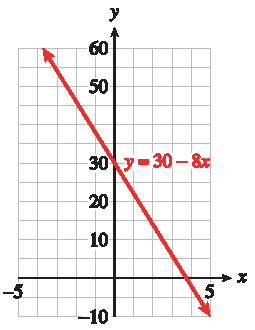
\includegraphics[width=\linewidth]{external/images/fig-graph-to-solve2.pdf}
\end{sbspanel}%
\end{sidebyside}%
\par
%
\begin{enumerate}[label=\alph*.]
\item{}Use the graph of \(y = 30 - 8x\) shown above to solve the equation%
\par
%
\begin{equation*}
30 - 8x = 50
\end{equation*}
%
\par
\(x=\)\fillintext{3}%
\item{}Verify your solution algebraically.%
\end{enumerate}
%
\par
For part (b):%
\par
We verify that we have an identity when we substitute \(x=-2.5\) into the equation \(30 - 8x = 50\).%
\par
%
\begin{align*}
30-8(\alert{-2.5}) \amp \stackrel{\text{?}}{=} 50\\
30 - (-20) \amp = 50 \amp \blert{\text{Yes!}}
\end{align*}
%
\par\smallskip%
\noindent\textbf{\blocktitlefont Answer}.\hypertarget{answer-exercise-graph-to-solve-linear-c}{}\quad{}\(-2.5\)%
\par\smallskip%
\noindent\textbf{\blocktitlefont Solution}.\hypertarget{solution-exercise-graph-to-solve-linear-d}{}\quad{}%
\begin{enumerate}[label=\alph*.]
\item{}The point on the line where the \(y\)-coordinate is 50 is the point \((-2.5,50)\text{,}\) so \(x=-2.5\) is the solution.%
\item{}We verify that we have an identity when we substitute \(x=-2.5\) into the equation \(30 - 8x = 50\text{.}\)%
\par
%
\begin{equation*}
\begin{aligned}
30-8(\alert{-2.5}) \amp \stackrel{\text{?}}{=} 50\\
30 - (-20) \amp = 50 \amp \blert{\text{Yes!}}
\end{aligned}
\end{equation*}
%
\end{enumerate}
%
\end{inlineexercise}%
In a similar fashion, we can solve inequalities with a graph.%
\begin{sidebyside}{2}{0}{0.05}{0.09}%
\begin{sbspanel}{0.58}[center]%
Consider again the graph of \(y = 2x + 3\), shown at right. We saw that \(x = 2\) is the solution of the equation \(2x + 3 = 7\). When we use \(x = 2\) as the input for the function \(f(x) = 2x + 3\), the output is \(y = 7\). Which input values for \(x\) produce output values greater than \(7\)?%
\par
You can see that \(x\)-values greater than \(2\) produce \(y\)-values greater than \(7\), because points on the graph with \(x\)-values greater than \(2\) have \(y\)-values greater than \(7\). Thus, the solutions of the inequality \(2x + 3 \gt 7\) are \(x\gt 2\). You can verify this result by solving the inequality algebraically.%
\end{sbspanel}%
\begin{sbspanel}{0.28}[center]%
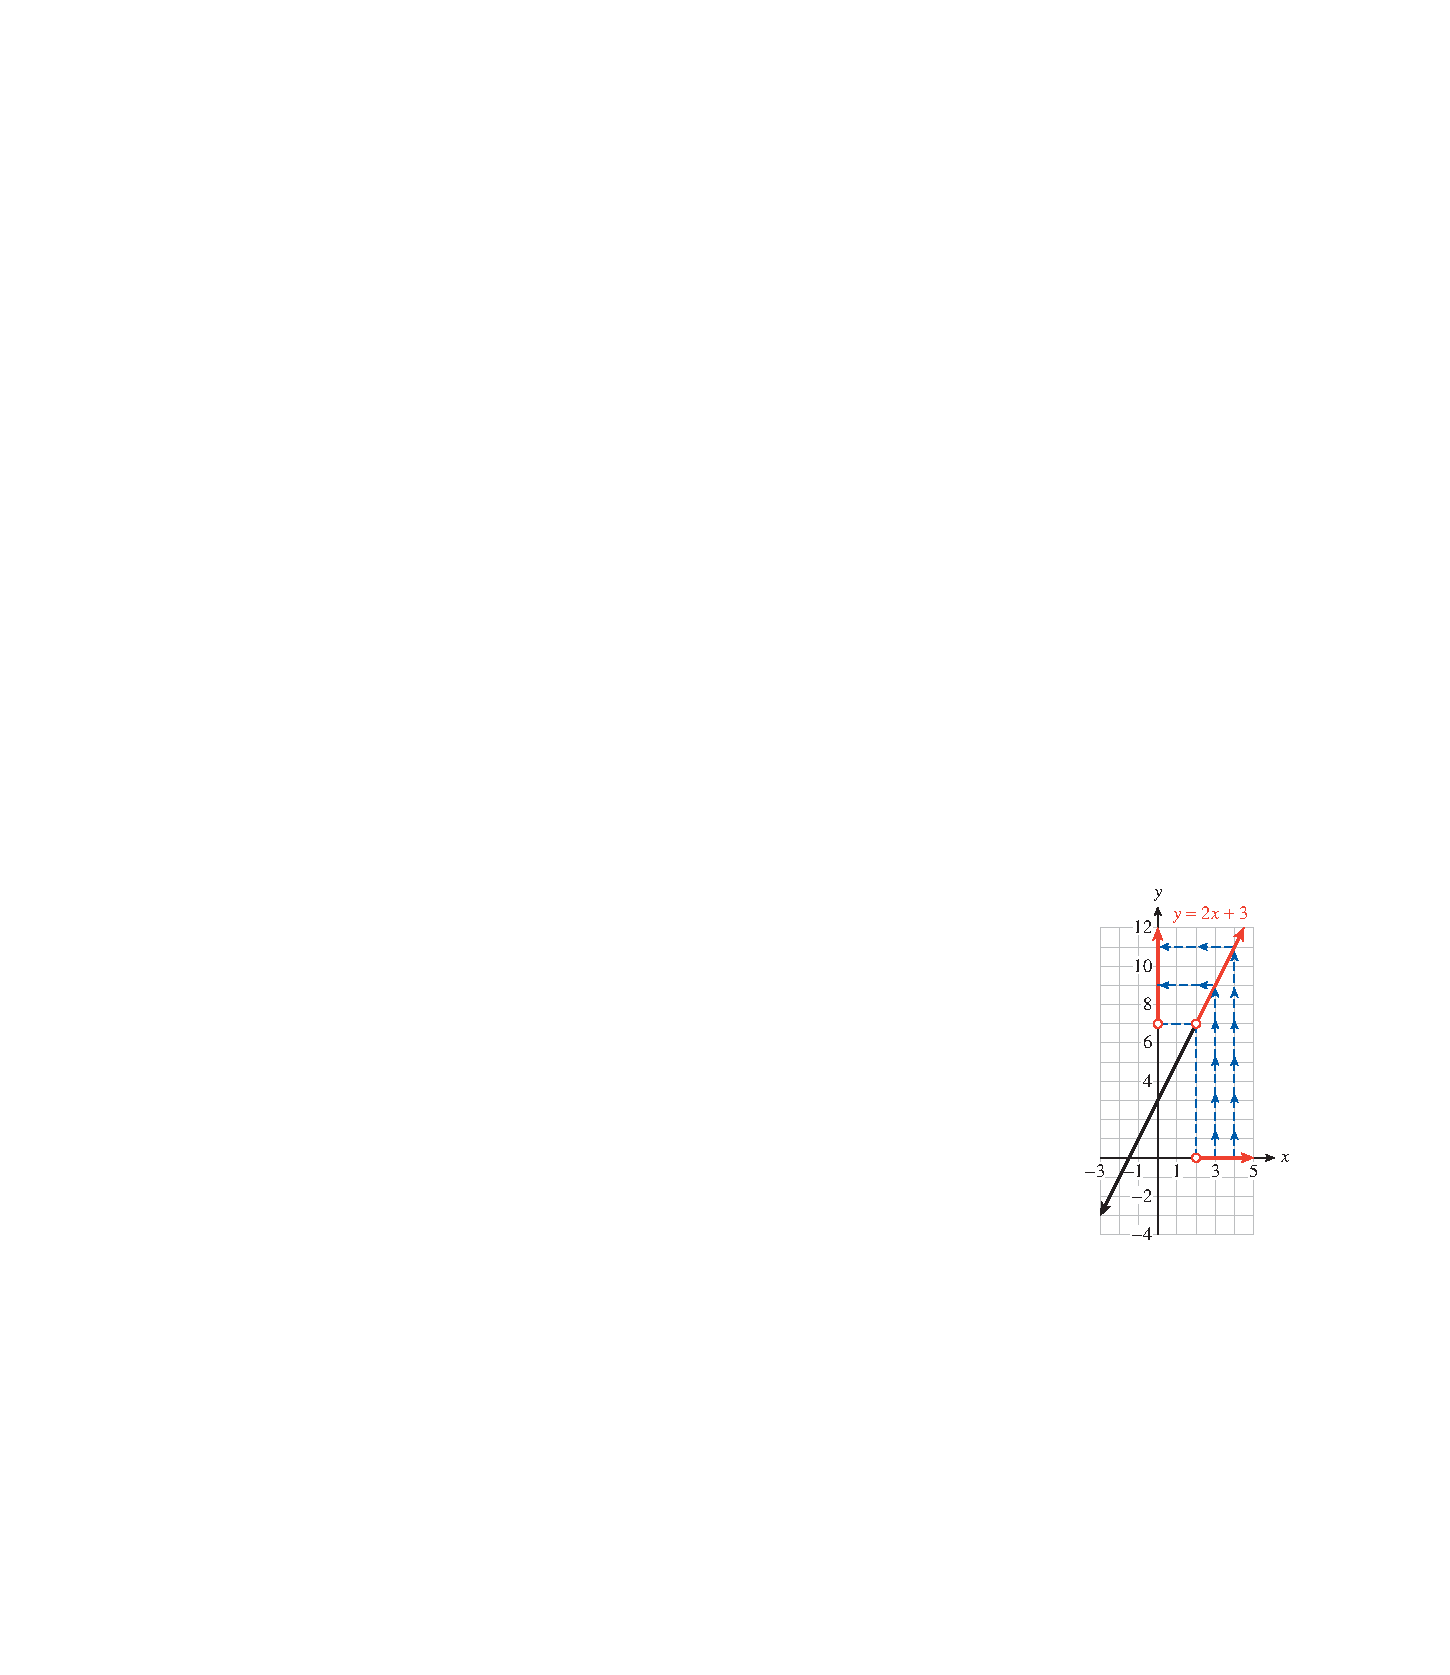
\includegraphics[width=\linewidth]{external/images/fig-graph-to-solve3.pdf}
\end{sbspanel}%
\end{sidebyside}%
\begin{example}{Example}{}{example-example-graph-to-solve2}%
Use the graph of \(y = 285 - 15x\) to solve the inequality%
\begin{equation*}
285 - 15x \gt 150
\end{equation*}
%
\par\smallskip%
\noindent\textbf{\blocktitlefont Solution}.\hypertarget{solution-example-graph-to-solve2-b}{}\quad{}We begin by locating the point \(P\) on the graph for which \(y = 150\). Its \(x\)-coordinate is \(x = 9\). Now, because \(y = 285 - 15x\) for points on the graph, the inequality%
\begin{equation*}
285-15x \gt 150
\end{equation*}
is equivalent to \(y \gt 150\).%
\begin{sidebyside}{1}{0.325}{0.325}{0}%
\begin{sbspanel}{0.35}%
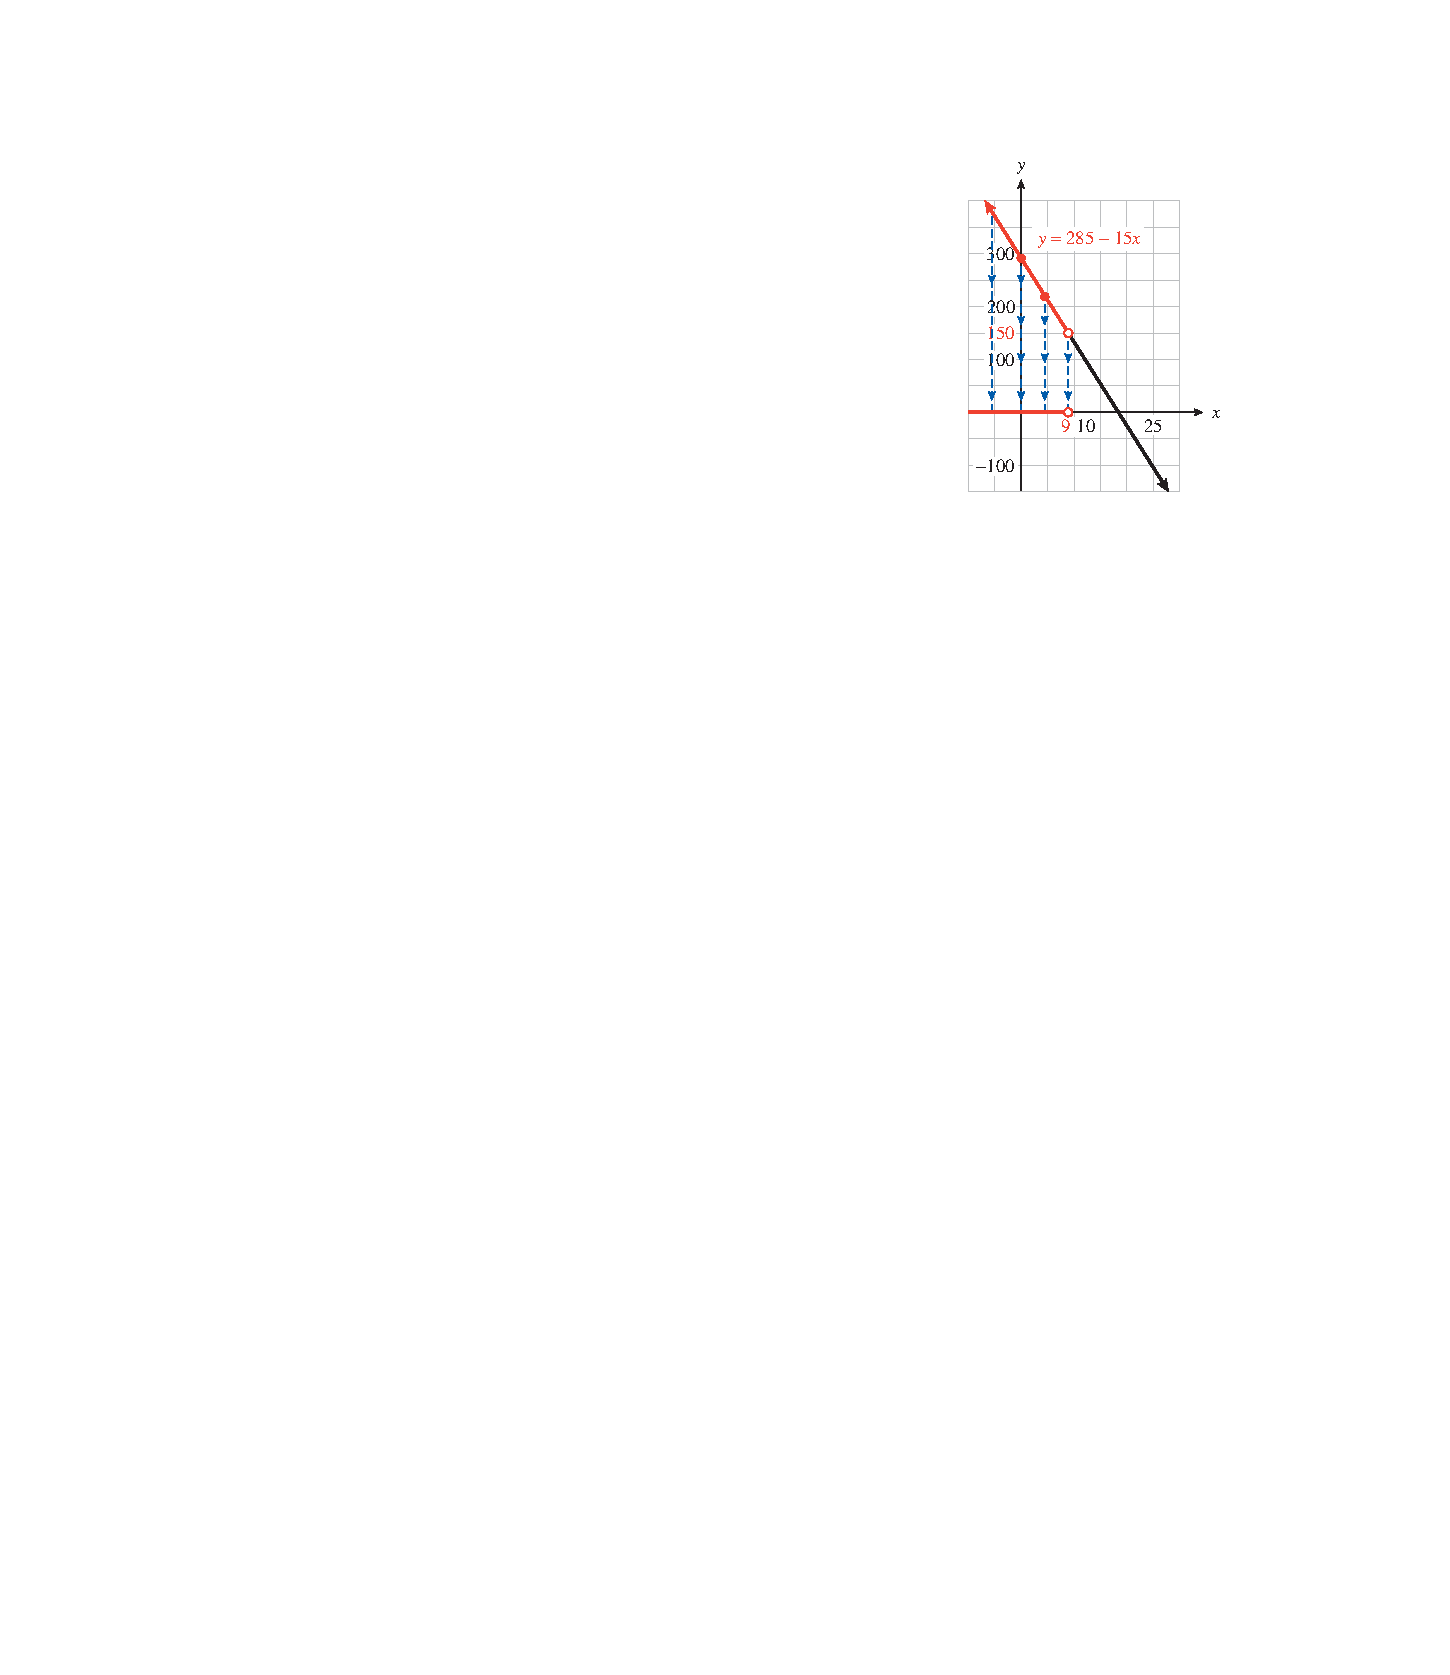
\includegraphics[width=\linewidth]{external/images/fig-graph-to-solve-inequality.pdf}
\end{sbspanel}%
\end{sidebyside}%
\par
So we are looking for points on the graph with \(y\)-coordinate greater than \(150\). These points are shown in red on the graph. The \(x\)-coordinates of these points are the \(x\)-values that satisfy the inequality. From the graph, we see that the solutions are \(x \lt 9\).%
\end{example}
\begin{inlineexercise}{Checkpoint}{QuickCheck 6.}{exercise-graphs-of-functions-e-l}%
You are using a graph of \(f(x)=48-3.5x\) to solve the inequality \(48-3.5x \gt -15\text{.}\)  You find that \(f(18)=-15\text{.}\) Your answer is:%
\par
\begin{itemize}[label=$\odot$,leftmargin=3em,]
\item{}\(\displaystyle x \gt -15\)%
\item{}\(\displaystyle x \lt -15\)%
\item{}\(\displaystyle x \gt 18\)%
\item{}\(\displaystyle x \lt 18\)%
\end{itemize}
%
\par\smallskip%
\noindent\textbf{\blocktitlefont Answer}.\hypertarget{answer-graphs-of-functions-e-l-c}{}\quad{}\(\text{Choice 4}\)%
\par\smallskip%
\noindent\textbf{\blocktitlefont Solution}.\hypertarget{solution-graphs-of-functions-e-l-d}{}\quad{}\(x \lt 18\)%
\end{inlineexercise}%
\begin{inlineexercise}{Checkpoint}{Practice 6.}{exercise-graphs-of-functions-e-m}%
\begin{sidebyside}{2}{0.05}{0.05}{0.1}%
\begin{sbspanel}{0.5}[center]%
Here is the graph from \hyperref[exercise-exercise-graph-to-solve-linear]{Checkpoint~{\xreffont\ref{exercise-exercise-graph-to-solve-linear}}} (Practice 5).%
\end{sbspanel}%
\begin{sbspanel}{0.3}[center]%
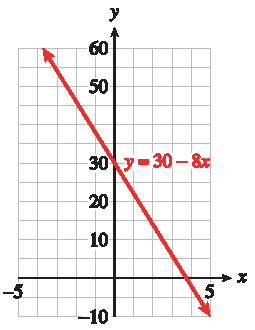
\includegraphics[width=\linewidth]{external/images/fig-graph-to-solve2.pdf}
\end{sbspanel}%
\end{sidebyside}%
\par
%
\begin{enumerate}[label=\alph*.]
\item{}Use the graph of \(y = 30 - 8x\) above to solve the inequality%
\par
%
\begin{equation*}
30 - 8x \le 50
\end{equation*}
%
\par
Answer: \fillintext{8}%
\par
Note: Use ``\(\lt=\)'' for the \(\le\) symbol, and use ``\(\gt=\)'' for \(\ge \text{.}\)%
\item{}Solve the inequality algebraically.%
\end{enumerate}
%
\par\smallskip%
\noindent\textbf{\blocktitlefont Answer}.\hypertarget{answer-graphs-of-functions-e-m-c}{}\quad{}\(x\ge -2.5\)%
\par\smallskip%
\noindent\textbf{\blocktitlefont Solution}.\hypertarget{solution-graphs-of-functions-e-m-d}{}\quad{}%
\begin{enumerate}[label=\alph*.]
\item{}As we found in the previous Checkpoint, the point on \(y=30-8x\) where \(y=50\) occurs when \(x=-2.5 \text{.}\) The \(y\)-coordinates are smaller as we move to the right on the graph, that is, for the points where \(x\ge -2.5 \text{.}\)%
\item{}~%
\par
%
\begin{equation*}
\begin{aligned}
30-8x \amp \le 50 \amp\amp\blert{{\small \text{Subtract 30 from both sides.}}} \\
-8x \amp \le 20 \amp\amp \blert{{\small \text{Divide by } {-8} \text{ and reverse inequality.}}} \\
x \amp \ge -2.5
\end{aligned}
\end{equation*}
%
\end{enumerate}
%
\end{inlineexercise}%
We can also use this graphical technique to solve nonlinear equations and inequalities.%
\begin{example}{Example}{}{example-example-graph-to-solve-cubic}%
Use a graph of \(f(x) = -2x^3 + x^2 + 16x\) to solve the equation%
\begin{equation*}
-2x^3 + x^2 + 16x = 15
\end{equation*}
%
\par\smallskip%
\noindent\textbf{\blocktitlefont Solution}.\hypertarget{solution-example-graph-to-solve-cubic-b}{}\quad{}If we sketch in the horizontal line \(y = 15\), we can see that there are three points on the graph of \(f\) that have \(y\)-coordinate \(15\), as shown below. The \(x\)-coordinates of these points are the solutions of the equation.%
\begin{sidebyside}{1}{0.325}{0.325}{0}%
\begin{sbspanel}{0.35}%
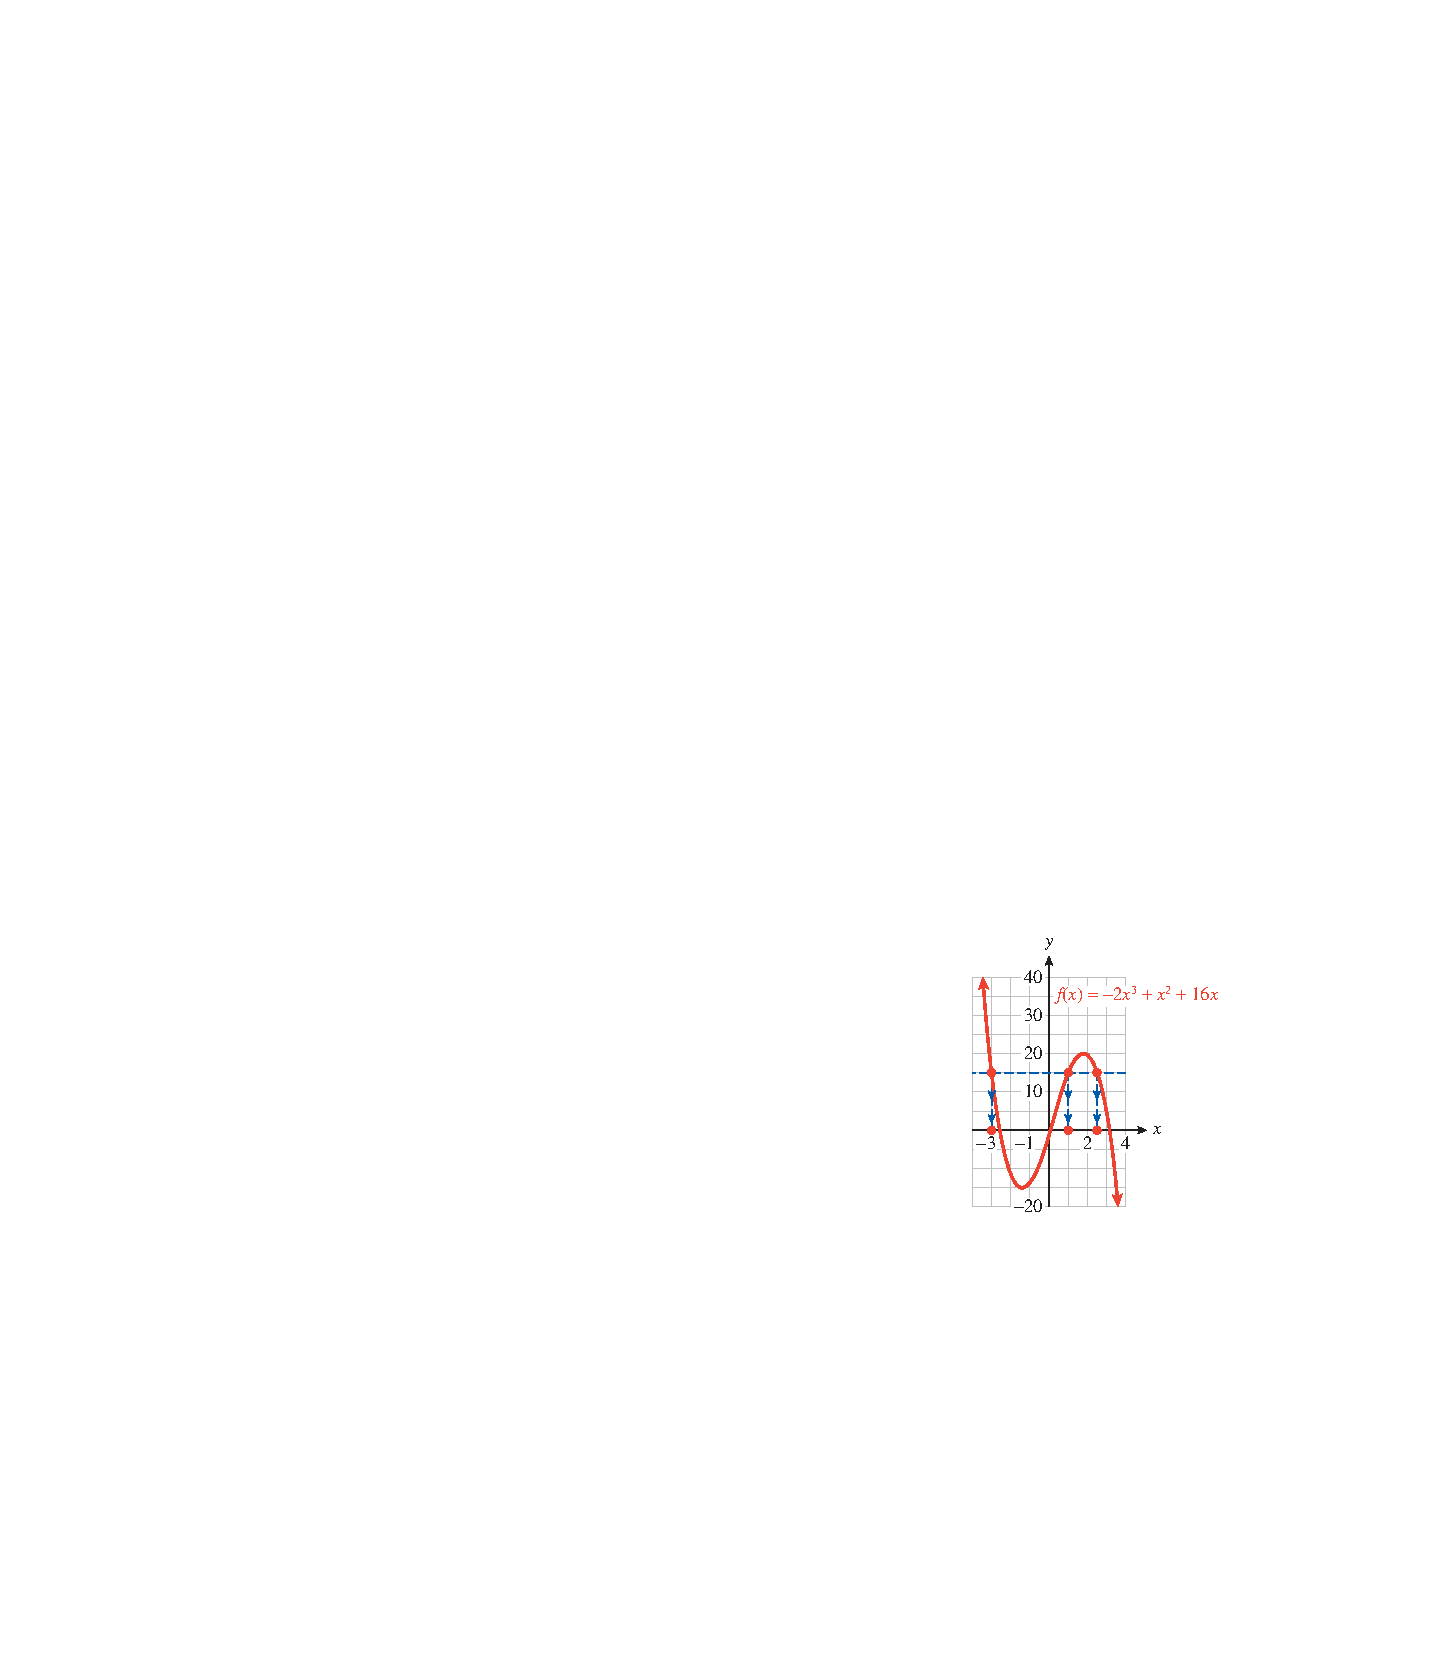
\includegraphics[width=\linewidth]{external/images/fig-graph-to-solve-cubic.pdf}
\end{sbspanel}%
\end{sidebyside}%
\par
From the graph, we see that the solutions are \(x = -3\), \(x = 1\), and approximately \(x = 2.5\). We can verify each solution algebraically.%
\par
For example, if \(x = \alert{-3}\), we have%
\begin{equation*}
\begin{aligned}[t]
f(\alert{-3})\amp= -2(\alert{-3})3 + (\alert{-3})^2 + 16(\alert{-3})\\
\amp= -2(-27) + 9 - 48\\
\amp =54 + 9 - 48 = 15  
\end{aligned}
\end{equation*}
so \(-3\) is a solution.  Similarly, you can check that \(x = 1\) and \(x = 2.5\) are solutions.%
\end{example}
\begin{inlineexercise}{Checkpoint}{Practice 7.}{exercise-exercise-graph-to-solve-quadratic}%
\begin{sidebyside}{1}{0.325}{0.325}{0}%
\begin{sbspanel}{0.35}%
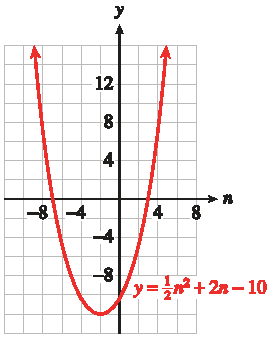
\includegraphics[width=\linewidth]{external/images/fig-graph-to-solve-quadratic.pdf}
\end{sbspanel}%
\end{sidebyside}%
\par
Use the graph of \(y = \frac{1}{2}n^2 + 2n - 10\) shown above  to solve%
\par
%
\begin{equation*}
\frac{1}{2}n^2 + 2n - 10 = 6
\end{equation*}
%
\par
and verify your solutions algebraically.%
\par
\(n=\)\fillintext{10}%
\par\smallskip%
\noindent\textbf{\blocktitlefont Answer}.\hypertarget{answer-exercise-graph-to-solve-quadratic-c}{}\quad{}\(-8, 4\)%
\par\smallskip%
\noindent\textbf{\blocktitlefont Solution}.\hypertarget{solution-exercise-graph-to-solve-quadratic-d}{}\quad{}\(-8, 4\)%
\end{inlineexercise}%
\begin{inlineexercise}{Checkpoint}{QuickCheck 7.}{exercise-graphs-of-functions-e-q}%
When is a function called decreasing?%
\par
\begin{itemize}[label=$\odot$,leftmargin=3em,]
\item{}If its \(x\)-values increase from left to right.%
\item{}If its \(y\)-values decrease when its \(x\)-values decrease.%
\item{}If its \(y\)-values decrease when its \(x\)-values increase.%
\item{}If the graph lies below the \(x\)-axis.%
\end{itemize}
%
\par\smallskip%
\noindent\textbf{\blocktitlefont Answer}.\hypertarget{answer-graphs-of-functions-e-q-c}{}\quad{}\(\text{Choice 3}\)%
\par\smallskip%
\noindent\textbf{\blocktitlefont Solution}.\hypertarget{solution-graphs-of-functions-e-q-d}{}\quad{}A function is called decreasing if its \(y\)-values decrease when its \(x\)-values increase.%
\end{inlineexercise}%
\begin{technology}{Technology}{Using the Trace Feature.}{technology-graphs-of-functions-e-r}%
You can use the Trace feature on a graphing utility to approximate solutions to equations. Graph the function \(f(x)\) in \hyperref[example-example-graph-to-solve-cubic]{Example~{\xreffont\ref{example-example-graph-to-solve-cubic}}}  in the window%
\begin{sidebyside}{1}{0}{0}{0}%
\begin{sbspanel}{1}%
\resizebox{\ifdim\width > \linewidth\linewidth\else\width\fi}{!}{%
{\centering%
{\tabularfont%
\begin{tabular}{lll}
Xmin\(=-4\)&&Xmax\(=4\)\tabularnewline[0pt]
Ymin\(=-20\)&&Ymax\(=40\)
\end{tabular}
}%
\par}
}%
\end{sbspanel}%
\end{sidebyside}%
\par
and trace along the curve to the point \((2.4680851, 15.512401)\). We are close to a solution, because the \(y\)-value is close to \(15\). Try entering \(x\)-values close to \(2.4680851\), for instance, \(x = 2.4\) and \(x = 2.5\), to find a better approximation for the solution.%
\end{technology}
\begin{example}{Example}{}{example-example-graph-to-solve-cubic2}%
Use the graph in \hyperref[example-example-graph-to-solve-cubic]{Example~{\xreffont\ref{example-example-graph-to-solve-cubic}}}  to solve the inequality%
\begin{equation*}
-2x^3 + x^2 + 16x \ge 15
\end{equation*}
%
\par\smallskip%
\noindent\textbf{\blocktitlefont Solution}.\hypertarget{solution-example-graph-to-solve-cubic2-b}{}\quad{}We first locate all points on the graph that have \(y\)-coordinates greater than or equal to \(15\). The \(x\)-coordinates of these points are the solutions of the inequality.%
\par
The figure below shows the points in red, and their \(x\)-coordinates as intervals on the \(x\)-axis. The solutions are \(x \le -3\) and \(1\le x \le 2.5\), or in interval notation, \((-\infty, -3] \cup [1, 2.5]\). (See \hyperref[subsection-Interval-notation]{Appendix A.2} to review interval notation.)%
\begin{sidebyside}{1}{0.325}{0.325}{0}%
\begin{sbspanel}{0.35}%
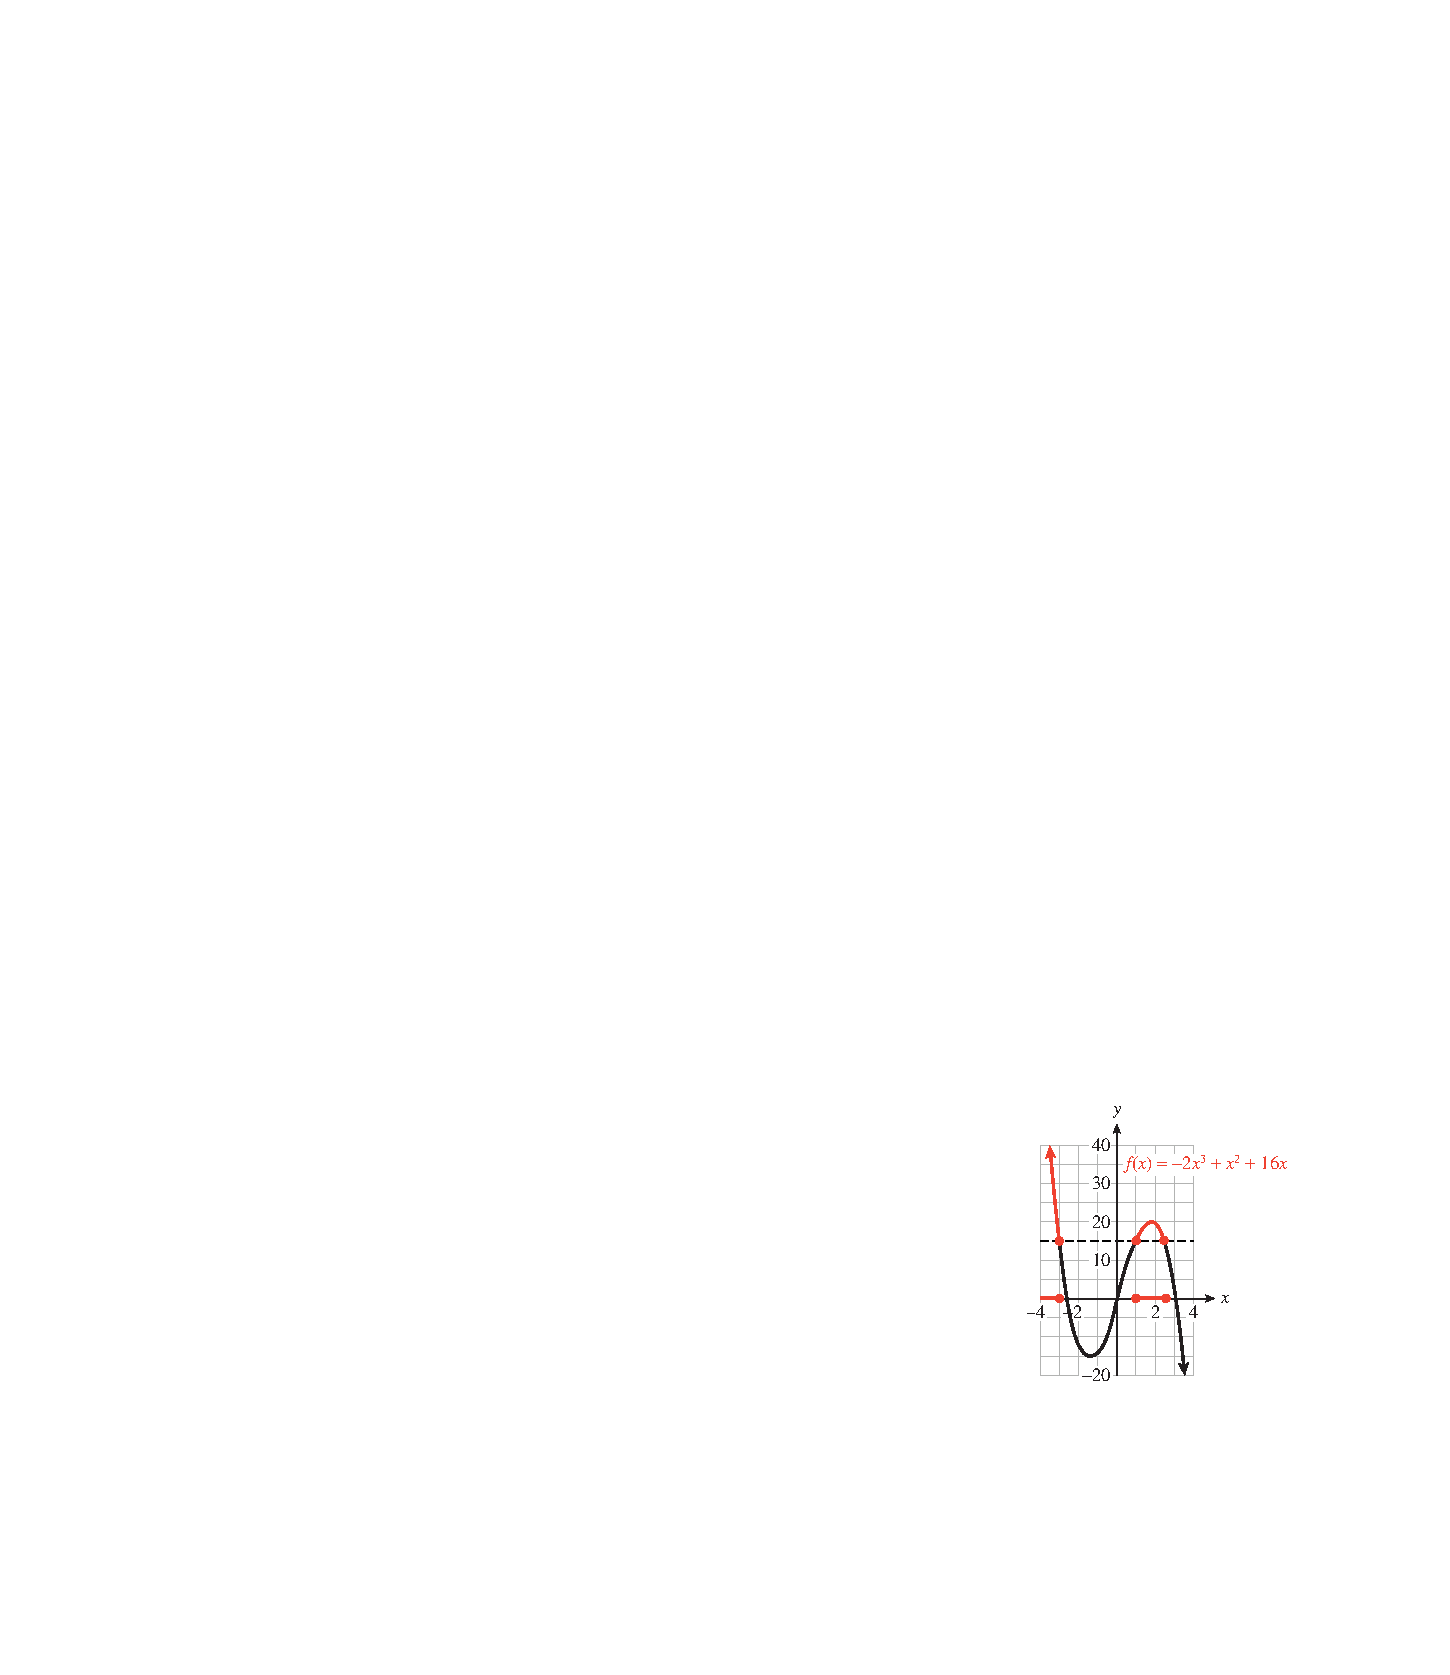
\includegraphics[width=\linewidth]{external/images/fig-graph-to-solve-cubic2.pdf}
\end{sbspanel}%
\end{sidebyside}%
\end{example}
\begin{inlineexercise}{Checkpoint}{Practice 8.}{exercise-graphs-of-functions-e-t}%
\begin{sidebyside}{1}{0.325}{0.325}{0}%
\begin{sbspanel}{0.35}%
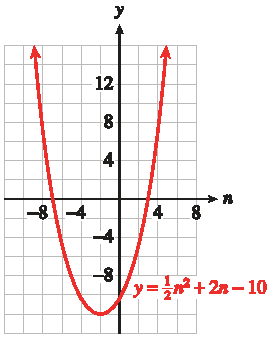
\includegraphics[width=\linewidth]{external/images/fig-graph-to-solve-quadratic.pdf}
\end{sbspanel}%
\end{sidebyside}%
\par
Use the graph above from Practice 7 above to solve the inequality%
\par
%
\begin{equation*}
\begin{gathered}
\frac{1}{2}n^2 + 2n - 10 \lt 6 
\end{gathered}
\end{equation*}
%
\par
Answer: \fillintext{12}%
\par\smallskip%
\noindent\textbf{\blocktitlefont Answer}.\hypertarget{answer-graphs-of-functions-e-t-c}{}\quad{}\(-8 < n < 4\)%
\par\smallskip%
\noindent\textbf{\blocktitlefont Solution}.\hypertarget{solution-graphs-of-functions-e-t-d}{}\quad{}\(-8 \lt n \lt 4 \text{,}\) or in interval notation, \((-8,4)\)%
\end{inlineexercise}%
\begin{inlineexercise}{Checkpoint}{Pause and Reflect.}{exercise-graphs-of-functions-e-u}%
Explain how to use the graph of \(y=x+\sqrt{x}\) to solve the equation \(x+\sqrt{x}=56\text{.}\)%
\end{inlineexercise}%
\end{subsectionptx}
%
%
\typeout{************************************************}
\typeout{Subsection  Section Summary}
\typeout{************************************************}
%
\begin{subsectionptx}{Subsection}{Section Summary}{}{Section Summary}{}{}{subsection-summary-1-3}
%
%
\typeout{************************************************}
\typeout{Subsubsection  Vocabulary}
\typeout{************************************************}
%
\begin{subsubsectionptx}{Subsubsection}{Vocabulary}{}{Vocabulary}{}{}{subsubsection-summary-1-3-b}
Look up the definitions of new terms in the Glossary.%
\begin{multicols}{3}
\begin{itemize}[label=\textbullet]
\item{}Coordinates%
\item{}Maximum%
\item{}Minimum%
\item{}Interval%
\item{}Vertical line test%
\item{}Inequality%
\item{}Algebraic solution%
\item{}Graphical solution%
\end{itemize}
\end{multicols}
%
\end{subsubsectionptx}
%
%
\typeout{************************************************}
\typeout{Subsubsection  CONCEPTS}
\typeout{************************************************}
%
\begin{subsubsectionptx}{Subsubsection}{CONCEPTS}{}{CONCEPTS}{}{}{subsubsection-summary-1-3-c}
%
\begin{enumerate}[label=\arabic*]
\item{}The point \((a, b)\) lies on the graph of the function \(f\) if and only if \(f (a) = b\).%
\item{}Each point on the graph of the function \(f\) has coordinates \((x, f (x))\) for some value of \(x\).%
\item{}The vertical line test tells us whether a graph represents a function.%
\item{}We can use a graph to solve equations and inequalities in one variable.%
\end{enumerate}
%
\end{subsubsectionptx}
%
%
\typeout{************************************************}
\typeout{Subsubsection  STUDY QUESTIONS}
\typeout{************************************************}
%
\begin{subsubsectionptx}{Subsubsection}{STUDY QUESTIONS}{}{STUDY QUESTIONS}{}{}{subsubsection-summary-1-3-d}
%
\begin{enumerate}[label=\arabic*]
\item{}How can you find the value of \(f (3)\) from a graph of \(f\)?%
\item{}If \(f (8) = 2\), what point lies on the graph of \(f\)?%
\item{}Explain how to construct the graph of a function from its equation.%
\item{}Explain how to use the vertical line test.%
\item{}How can you solve the equation \(x + \sqrt{x} = 56\) using the graph of \(y = x + \sqrt{x}\)?%
\end{enumerate}
%
\end{subsubsectionptx}
%
%
\typeout{************************************************}
\typeout{Subsubsection  SKILLS}
\typeout{************************************************}
%
\begin{subsubsectionptx}{Subsubsection}{SKILLS}{}{SKILLS}{}{}{subsubsection-summary-1-3-e}
Practice each skill in the Homework problems listed.%
\begin{enumerate}[label=\arabic*]
\item{}Read function values from a graph: \#1\textendash{}8, 17\textendash{}20, 33\textendash{}36%
\item{}Recognize the graph of a function: \#9\textendash{}10, 31 and 32%
\item{}Construct a table of values and a graph of a function: \#11\textendash{}16%
\item{}Solve equations and inequalities graphically: \#21\textendash{}30, 41\textendash{}50%
\end{enumerate}
%
\end{subsubsectionptx}
\end{subsectionptx}
%
%
\typeout{************************************************}
\typeout{Exercises  Homework 1.3}
\typeout{************************************************}
%
\begin{exercises-subsection}{Exercises}{Homework 1.3}{}{Homework 1.3}{}{}{exercises-section-1-3-exercises}
\par\medskip\noindent%
\textbf{Exercise Group.}\space\space%
In Problems 1\textendash{}8, use the graphs to answer the questions about the functions.%
\begin{exercisegroup}
\begin{divisionexerciseeg}{1}{}{}{exercise-section-1-3-exercises-b-b}%
%
\begin{enumerate}[label=\alph*]
\item{}Find \(h(-3)\), \(h(1)\), and \(h(3)\).%
\item{}For what value(s) of \(z\) is \(h(z) = 3\)?%
\item{}Find the intercepts of the graph. List the function values given by the intercepts.%
\item{}What is the maximum value of \(h(z)\)?%
\item{}For what value(s) of \(z\) does \(h\) take on its maximum value?%
\item{}On what intervals is the function increasing? Decreasing?%
\end{enumerate}
%
\begin{sidebyside}{1}{0.325}{0.325}{0}%
\begin{sbspanel}{0.35}%
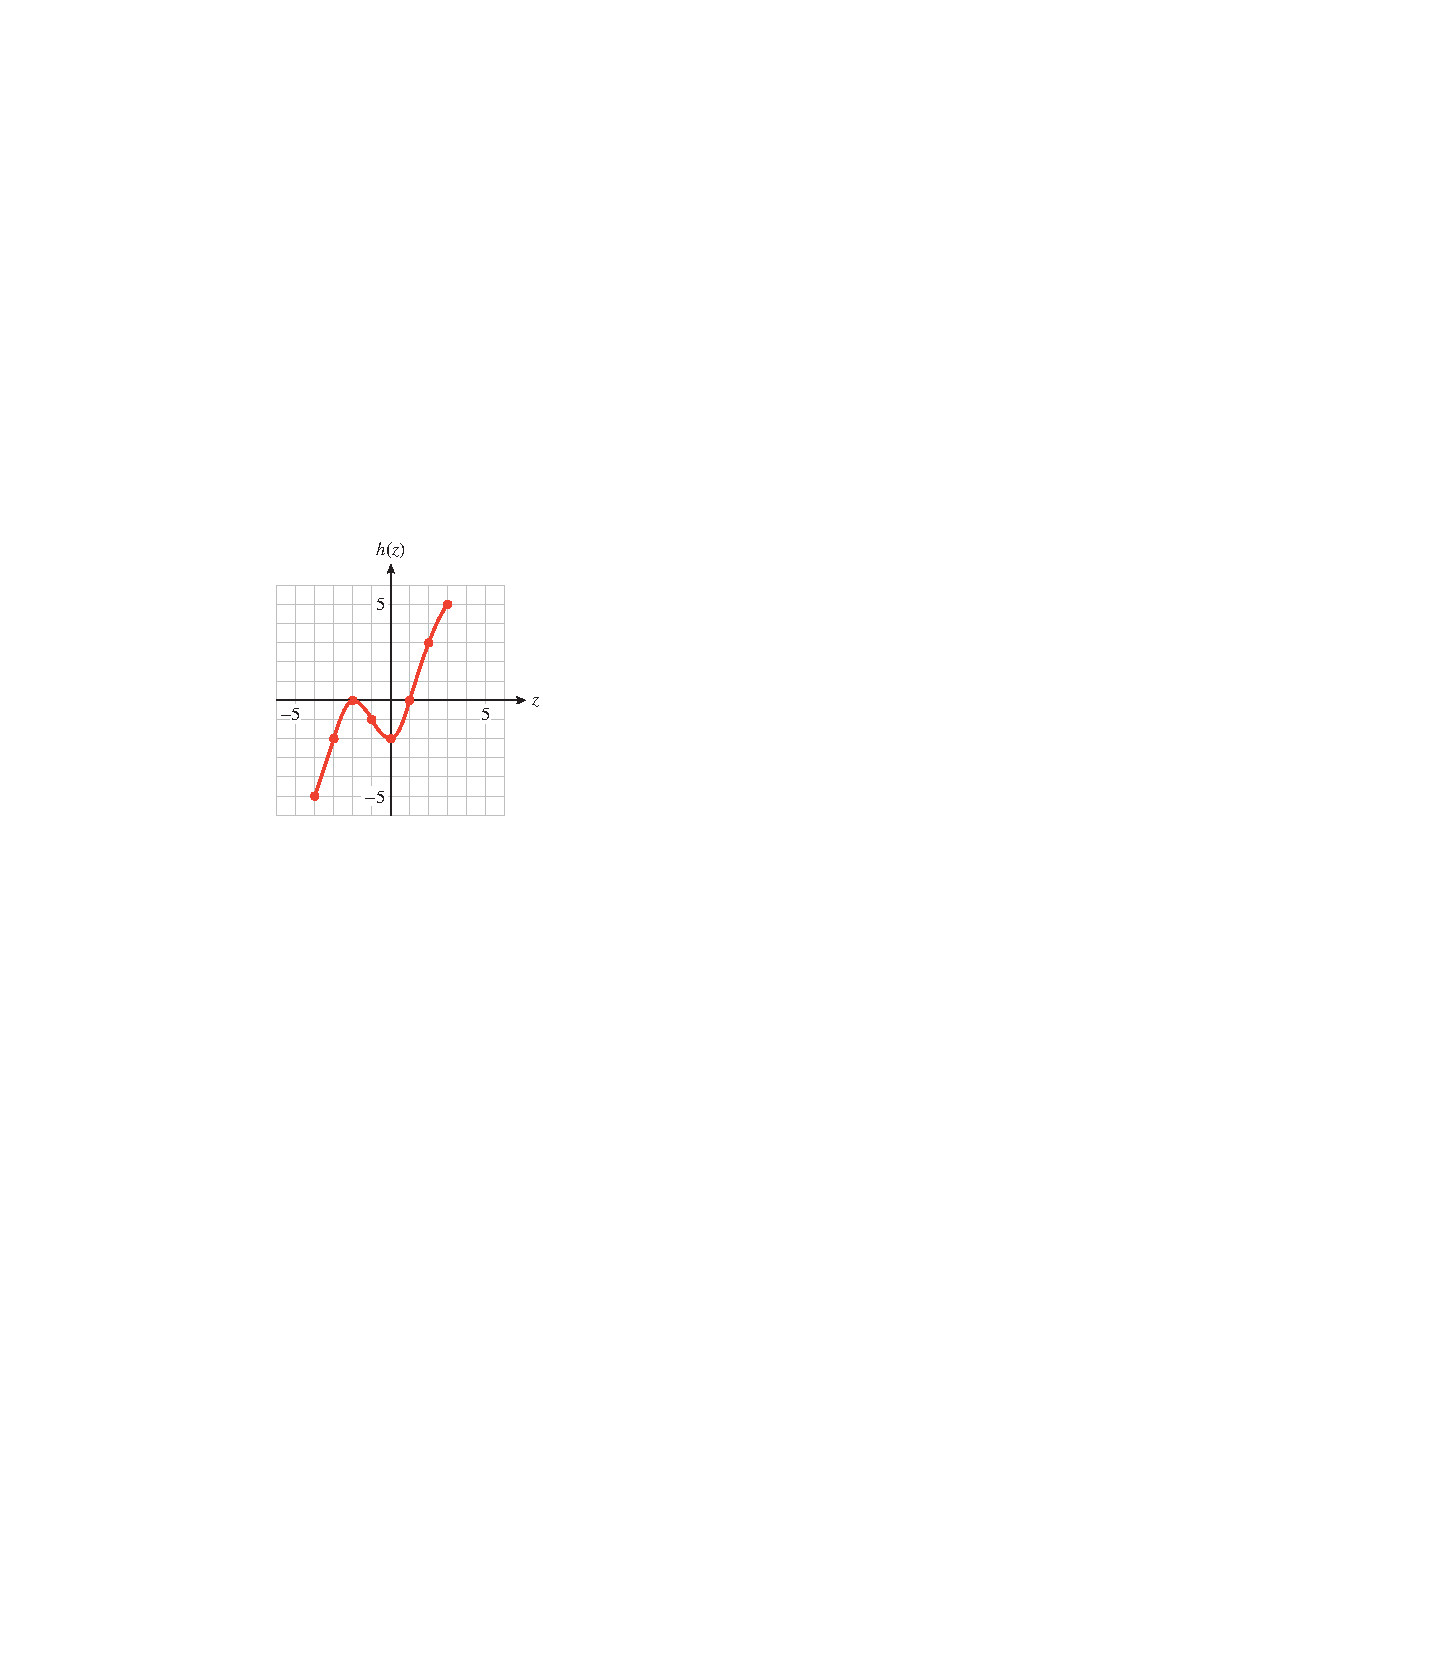
\includegraphics[width=\linewidth]{external/images/fig-ex-1-3-1.pdf}
\end{sbspanel}%
\end{sidebyside}%
\end{divisionexerciseeg}%
\begin{divisionexerciseeg}{2}{}{}{exercise-section-1-3-exercises-b-c}%
%
\begin{enumerate}[label=\alph*]
\item{}Find \(G(-3)\), \(G(-1)\), and \(G(2)\).%
\item{}For what value(s) of \(s\) is \(G(s) = 3\)?%
\item{}Find the intercepts of the graph. List the function values given by the intercepts.%
\item{}What is the minimum value of \(G(s)\)?%
\item{}For what value(s) of \(s\) does \(G\) take on its minimum value?%
\item{}On what intervals is the function increasing? Decreasing?%
\end{enumerate}
%
\begin{sidebyside}{1}{0.325}{0.325}{0}%
\begin{sbspanel}{0.35}%
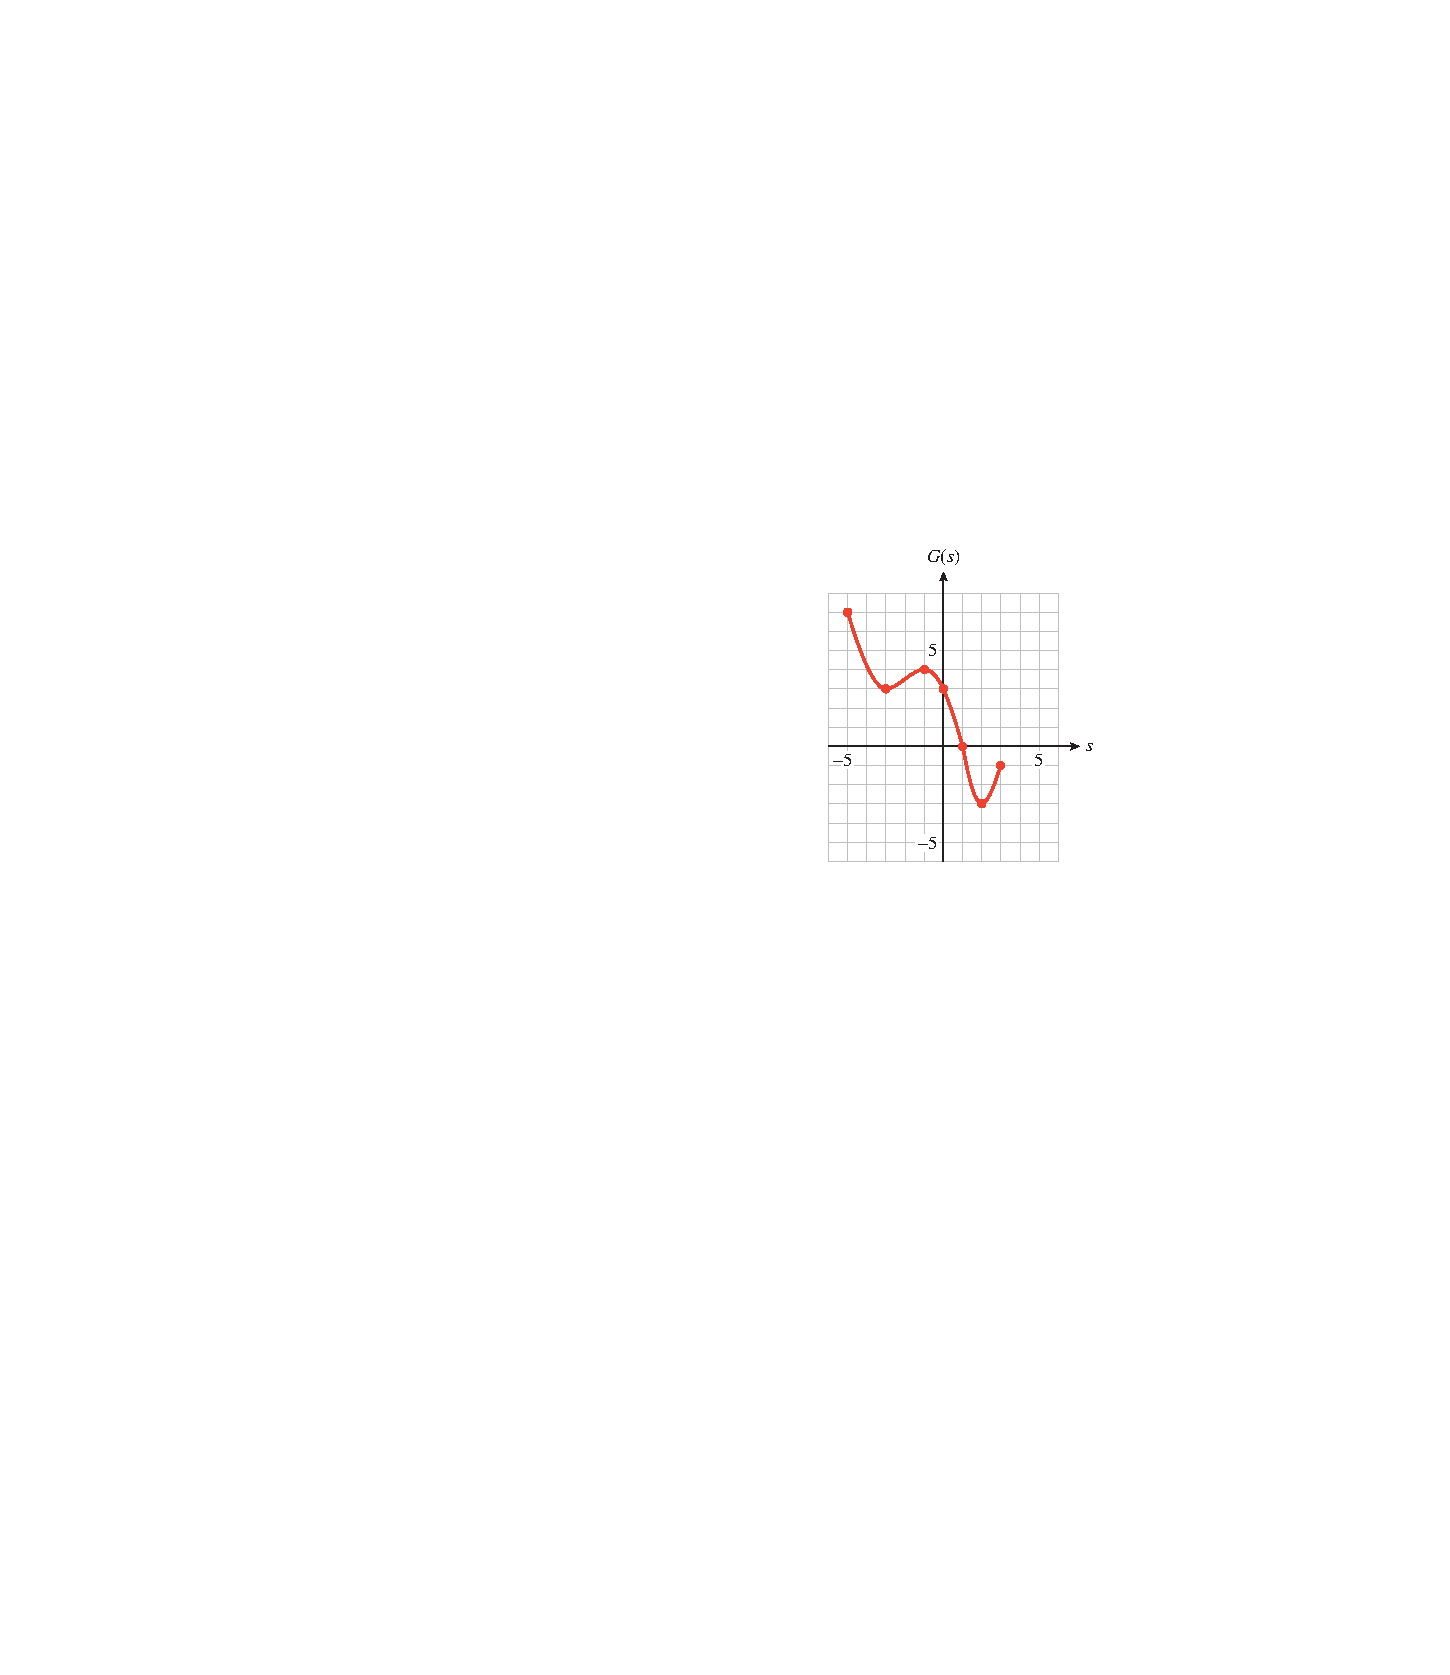
\includegraphics[width=\linewidth]{external/images/fig-ex-1-3-2.pdf}
\end{sbspanel}%
\end{sidebyside}%
\end{divisionexerciseeg}%
\begin{divisionexerciseeg}{3}{}{}{exercise-section-1-3-exercises-b-d}%
%
\begin{enumerate}[label=\alph*]
\item{}Find \(R(1)\) and \(R(3)\).%
\item{}For what value(s) of \(p\) is \(R(p)=2\)?%
\item{}Find the intercepts of the graph. List the function values given by the intercepts.%
\item{}Find the maximum and minimum values of \(R(p)\).%
\item{}For what value(s) of \(p\) does \(R\) take on its maximum and minimum values?%
\item{}On what intervals is the function increasing? Decreasing?%
\end{enumerate}
%
\begin{sidebyside}{1}{0.325}{0.325}{0}%
\begin{sbspanel}{0.35}%
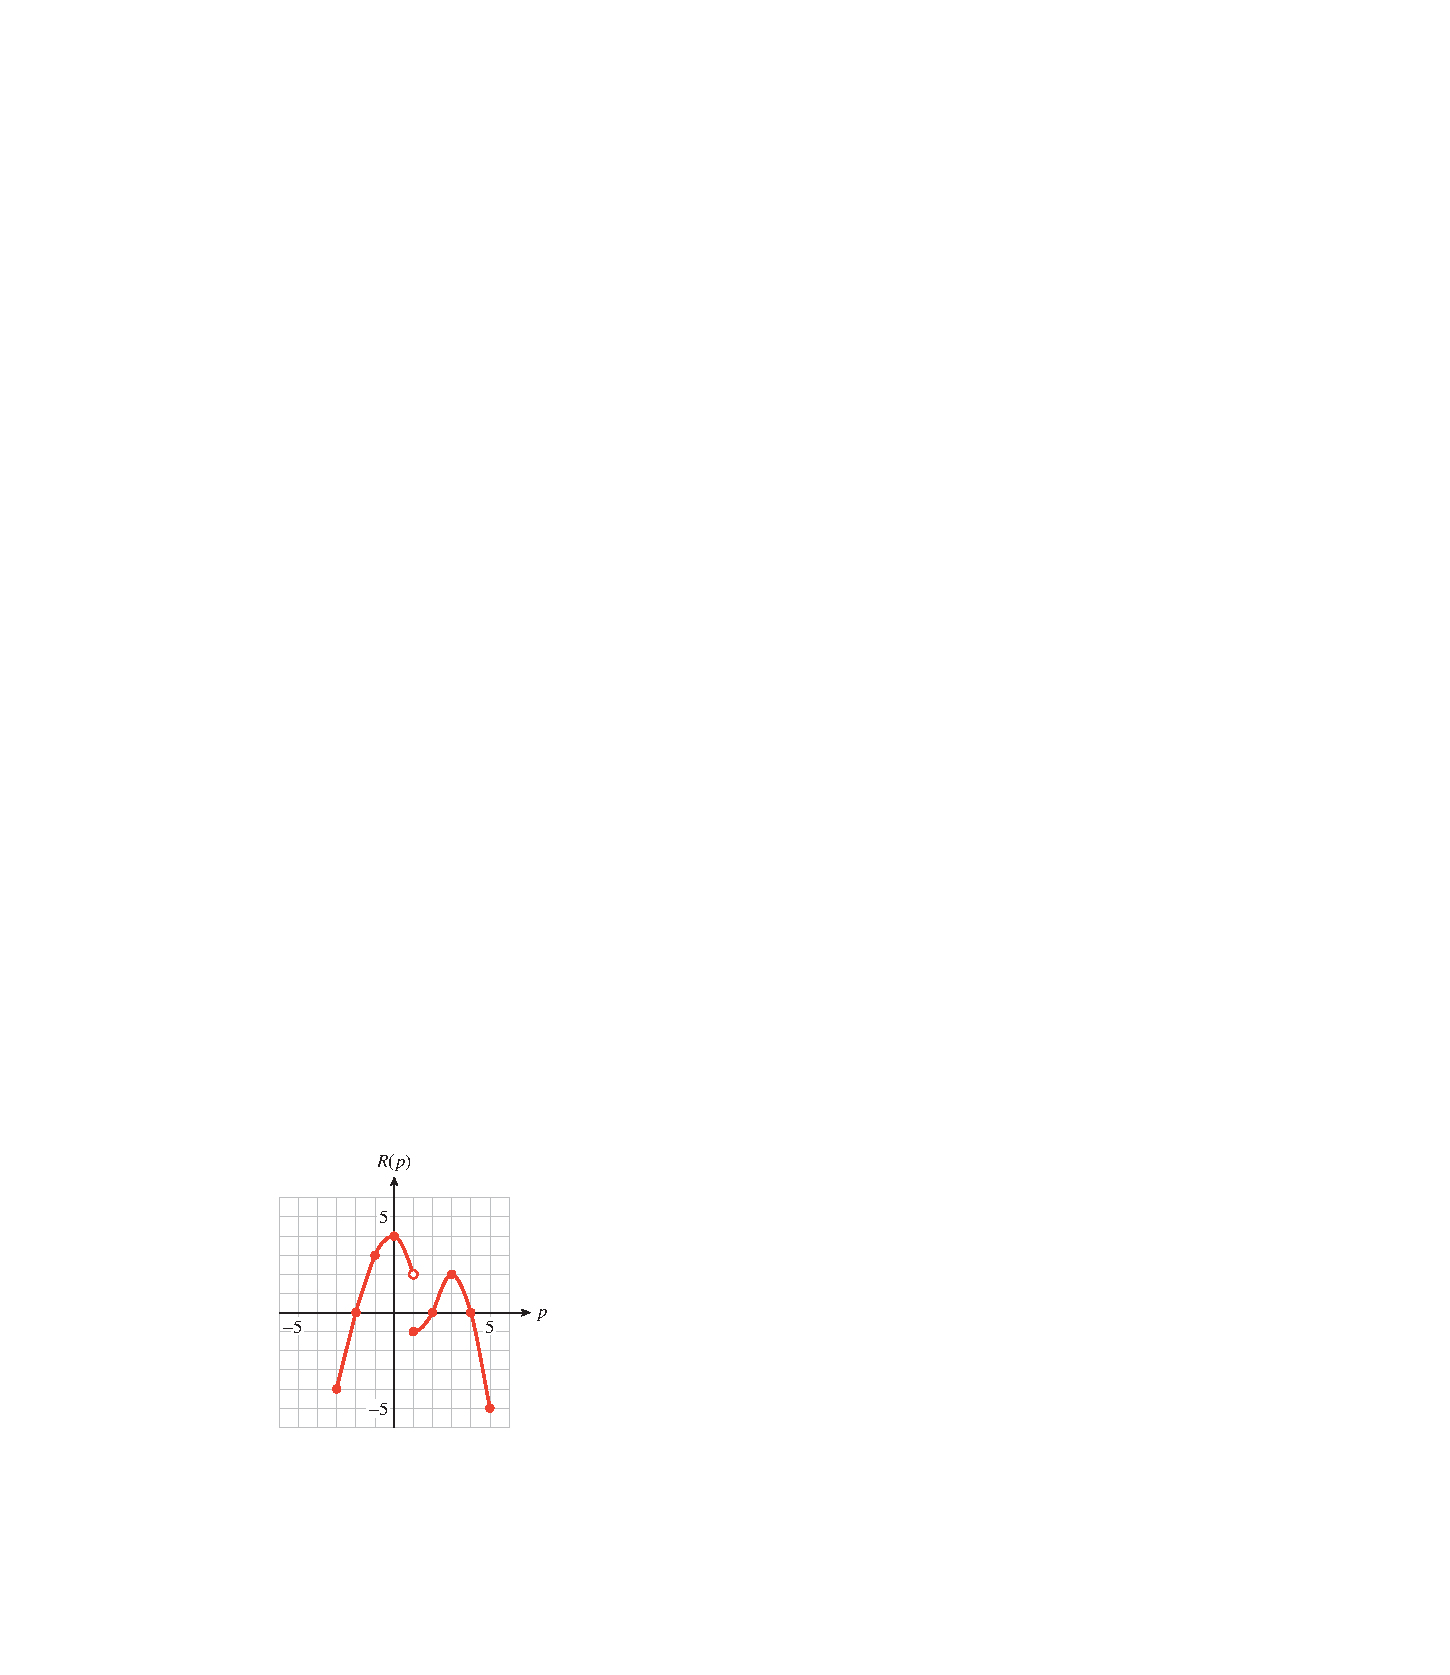
\includegraphics[width=\linewidth]{external/images/fig-ex-1-3-3.pdf}
\end{sbspanel}%
\end{sidebyside}%
\end{divisionexerciseeg}%
\begin{divisionexerciseeg}{4}{}{}{exercise-section-1-3-exercises-b-e}%
%
\begin{enumerate}[label=\alph*]
\item{}Find \(f (-1)\) and \(f (3)\).%
\item{}For what value(s) of \(t\) is \(f(t)=5\)?%
\item{}Find the intercepts of the graph. List the function values given by the intercepts.%
\item{}Find the maximum and minimum values of \(f(t)\).%
\item{}For what value(s) of \(t\) does \(f\) take on its maximum and minimum values?%
\item{}On what intervals is the function increasing? Decreasing?%
\end{enumerate}
%
\begin{sidebyside}{1}{0.325}{0.325}{0}%
\begin{sbspanel}{0.35}%
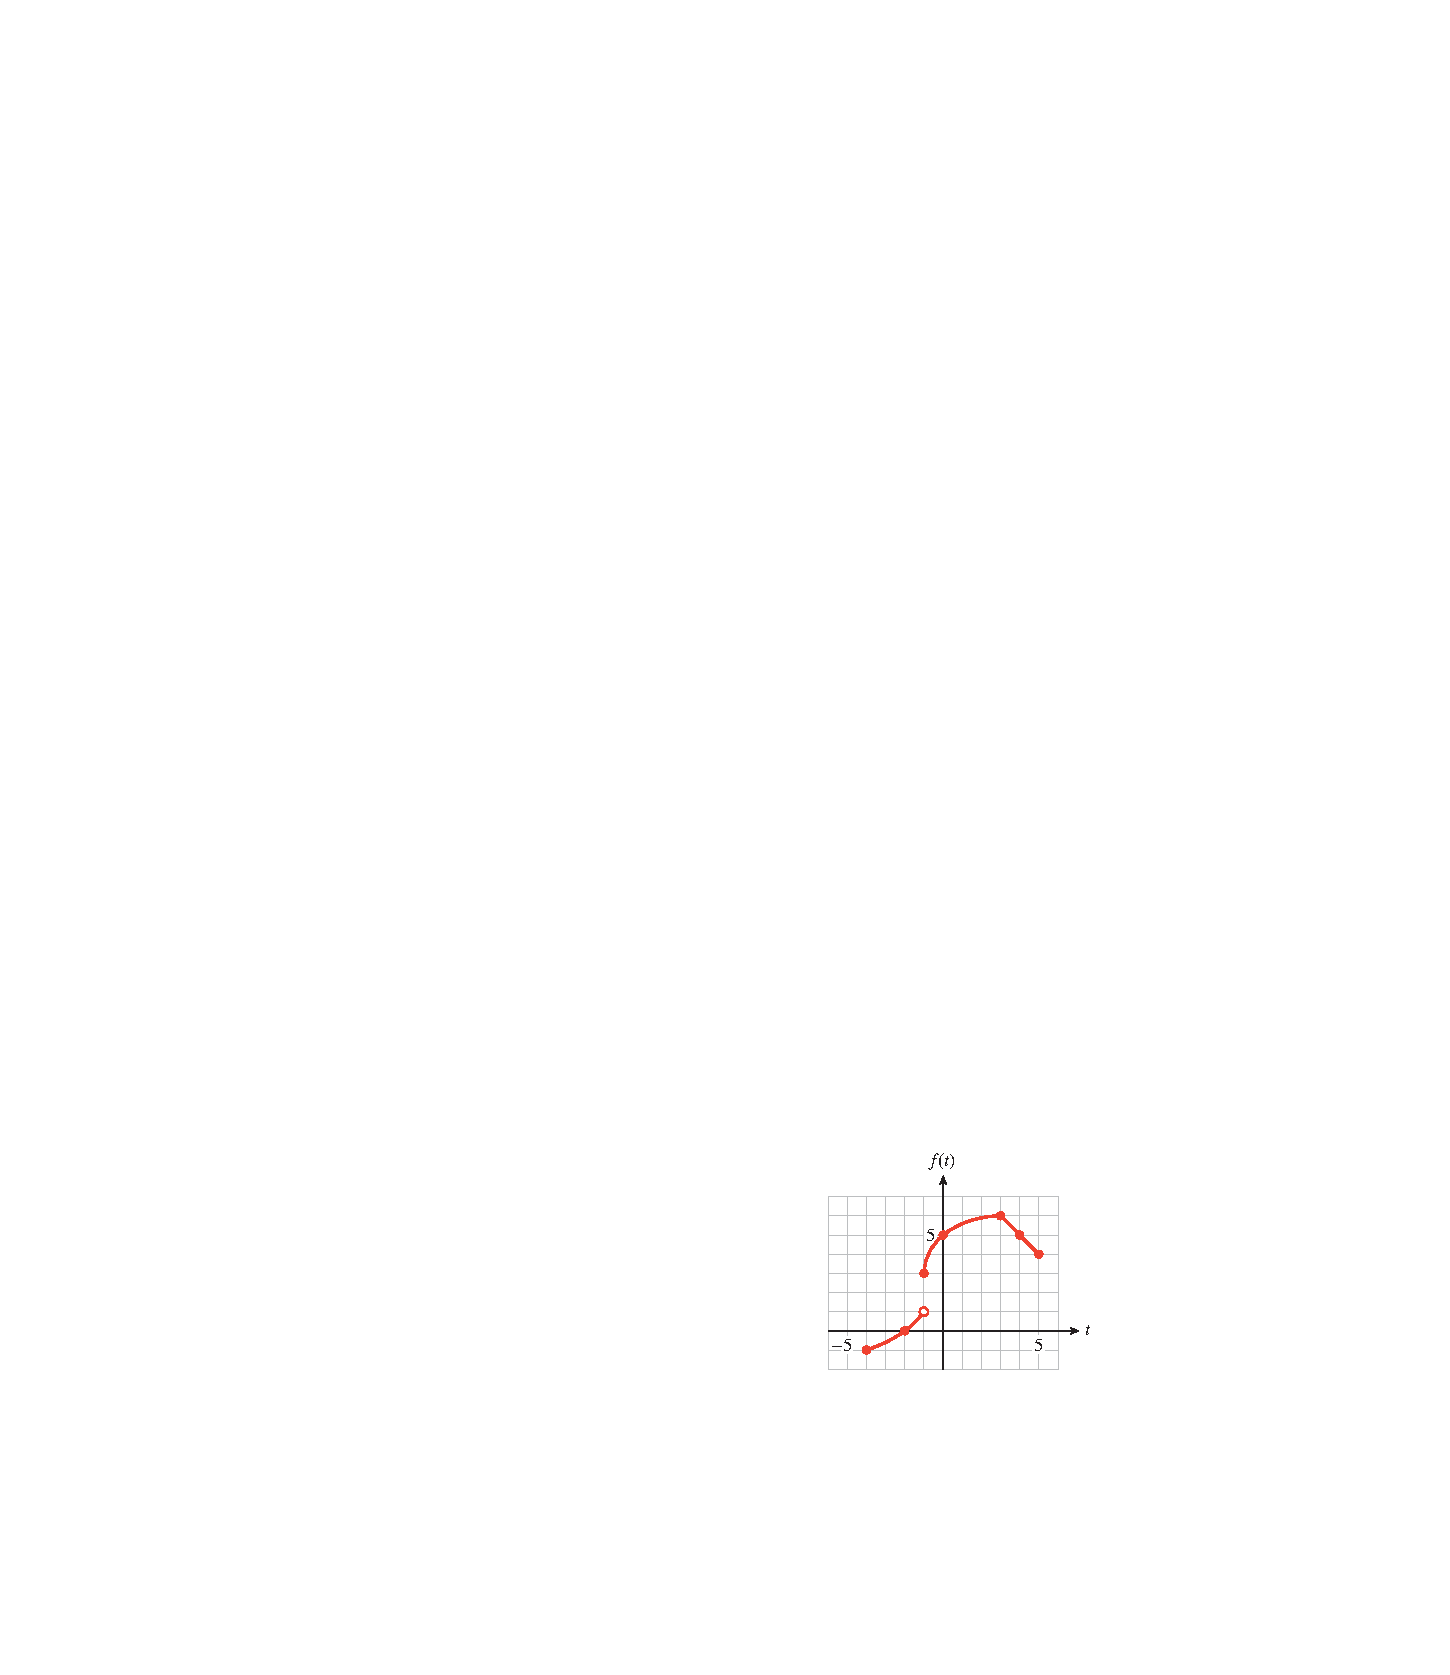
\includegraphics[width=\linewidth]{external/images/fig-ex-1-3-4.pdf}
\end{sbspanel}%
\end{sidebyside}%
\end{divisionexerciseeg}%
\begin{divisionexerciseeg}{5}{}{}{exercise-section-1-3-exercises-b-f}%
%
\begin{enumerate}[label=\alph*]
\item{}Find \(S(0)\), \(S\left(\dfrac{1}{6}\right)\), and \(S(-1)\).%
\item{}Estimate the value of \(S\left(\dfrac{1}{3}\right)\) from the graph.%
\item{}For what value(s) of \(x\) is \(S(x) = -\dfrac{1}{2}\)?%
\item{}Find the maximum and minimum values of \(S(x)\).%
\item{}For what value(s) of \(x\) does \(S\) take on its maximum and minimum values?%
\end{enumerate}
%
\begin{sidebyside}{1}{0.25}{0.25}{0}%
\begin{sbspanel}{0.5}%
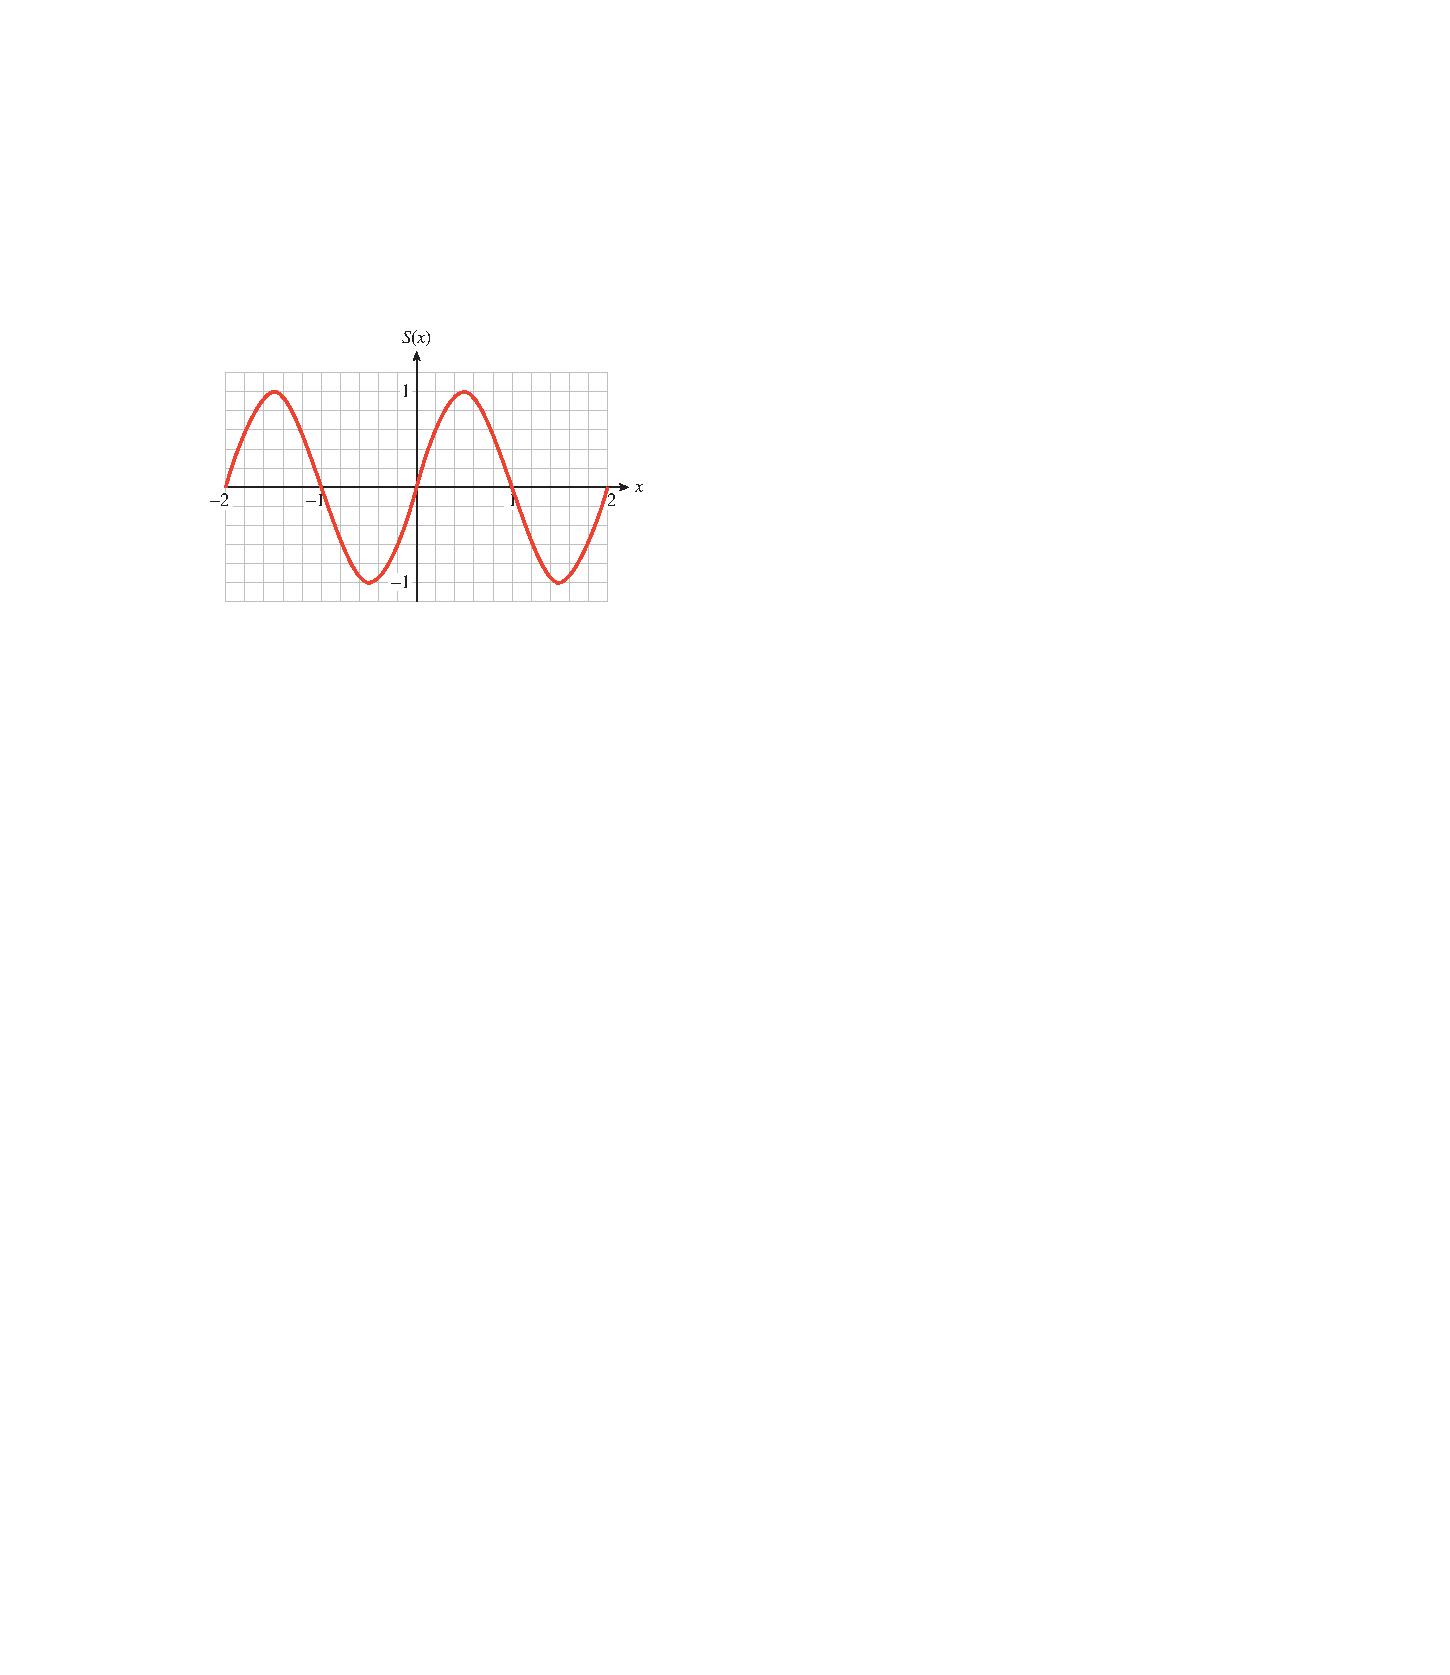
\includegraphics[width=\linewidth]{external/images/fig-ex-1-3-5.pdf}
\end{sbspanel}%
\end{sidebyside}%
\end{divisionexerciseeg}%
\begin{divisionexerciseeg}{6}{}{}{exercise-section-1-3-exercises-b-g}%
%
\begin{enumerate}[label=\alph*]
\item{}Find \(C(0)\), \(C\left(-\dfrac{1}{3}\right)\), and \(C(1)\).%
\item{}Estimate the value of \(C\left(\dfrac{1}{6}\right)\) from the graph.%
\item{}For what value(s) of \(x\) is \(C(x) = \dfrac{1}{2}\)?%
\item{}Find the maximum and minimum values of \(C(x)\).%
\item{}For what value(s) of \(x\) does \(C\) take on its maximum and minimum values?%
\end{enumerate}
%
\begin{sidebyside}{1}{0.25}{0.25}{0}%
\begin{sbspanel}{0.5}%
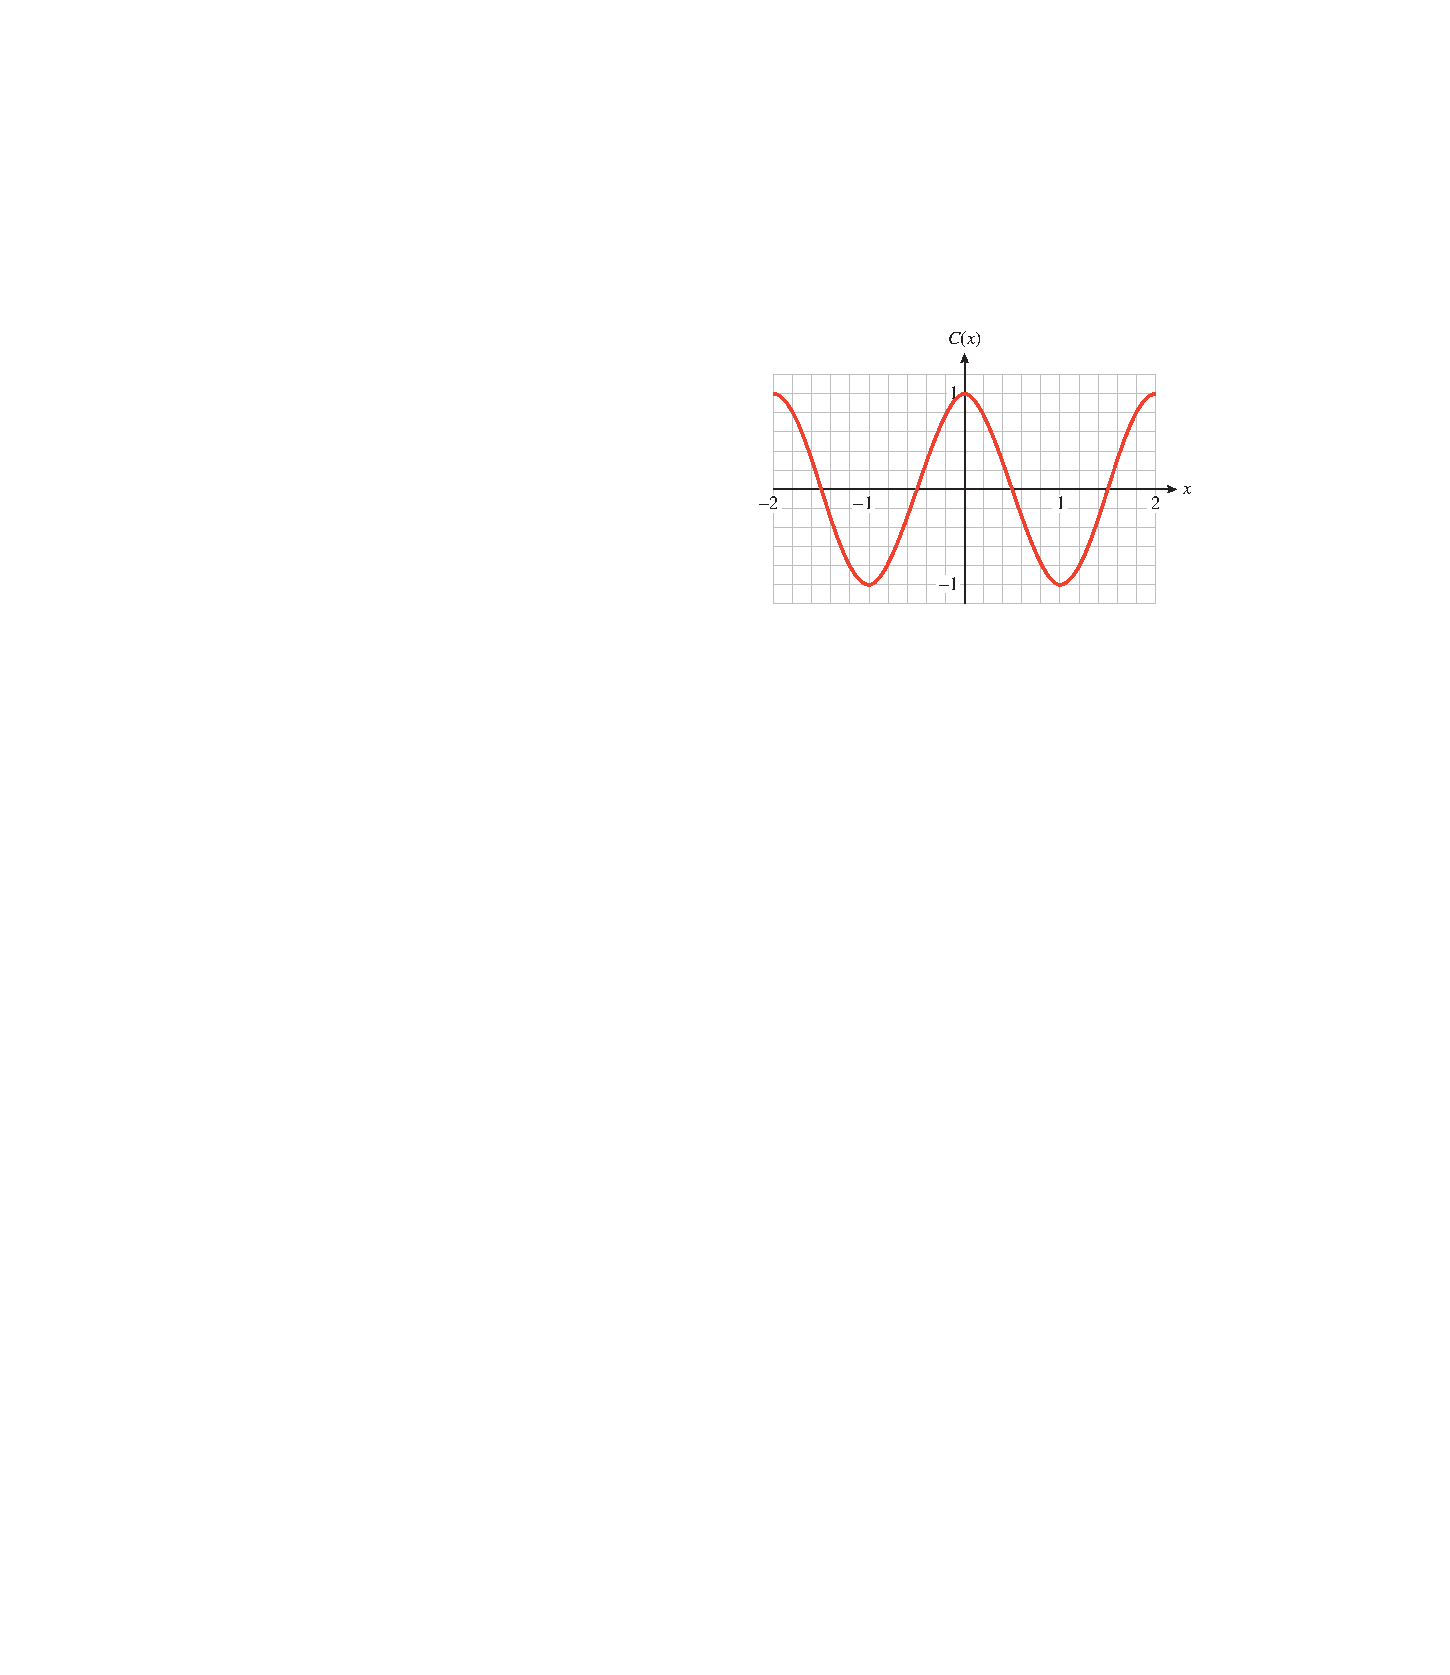
\includegraphics[width=\linewidth]{external/images/fig-ex-1-3-6.pdf}
\end{sbspanel}%
\end{sidebyside}%
\end{divisionexerciseeg}%
\begin{divisionexerciseeg}{7}{}{}{exercise-section-1-3-exercises-b-h}%
%
\begin{enumerate}[label=\alph*]
\item{}Find \(F(-3)\), \(F(-2)\), and \(F(2)\).%
\item{}For what value(s) of \(s\) is \(F(s) = -1\)?%
\item{}Find the maximum and minimum values of \(F(s)\).%
\item{}For what value(s) of \(s\) does \(F\) take on its maximum and minimum values?%
\end{enumerate}
%
\begin{sidebyside}{1}{0.3}{0.3}{0}%
\begin{sbspanel}{0.4}%
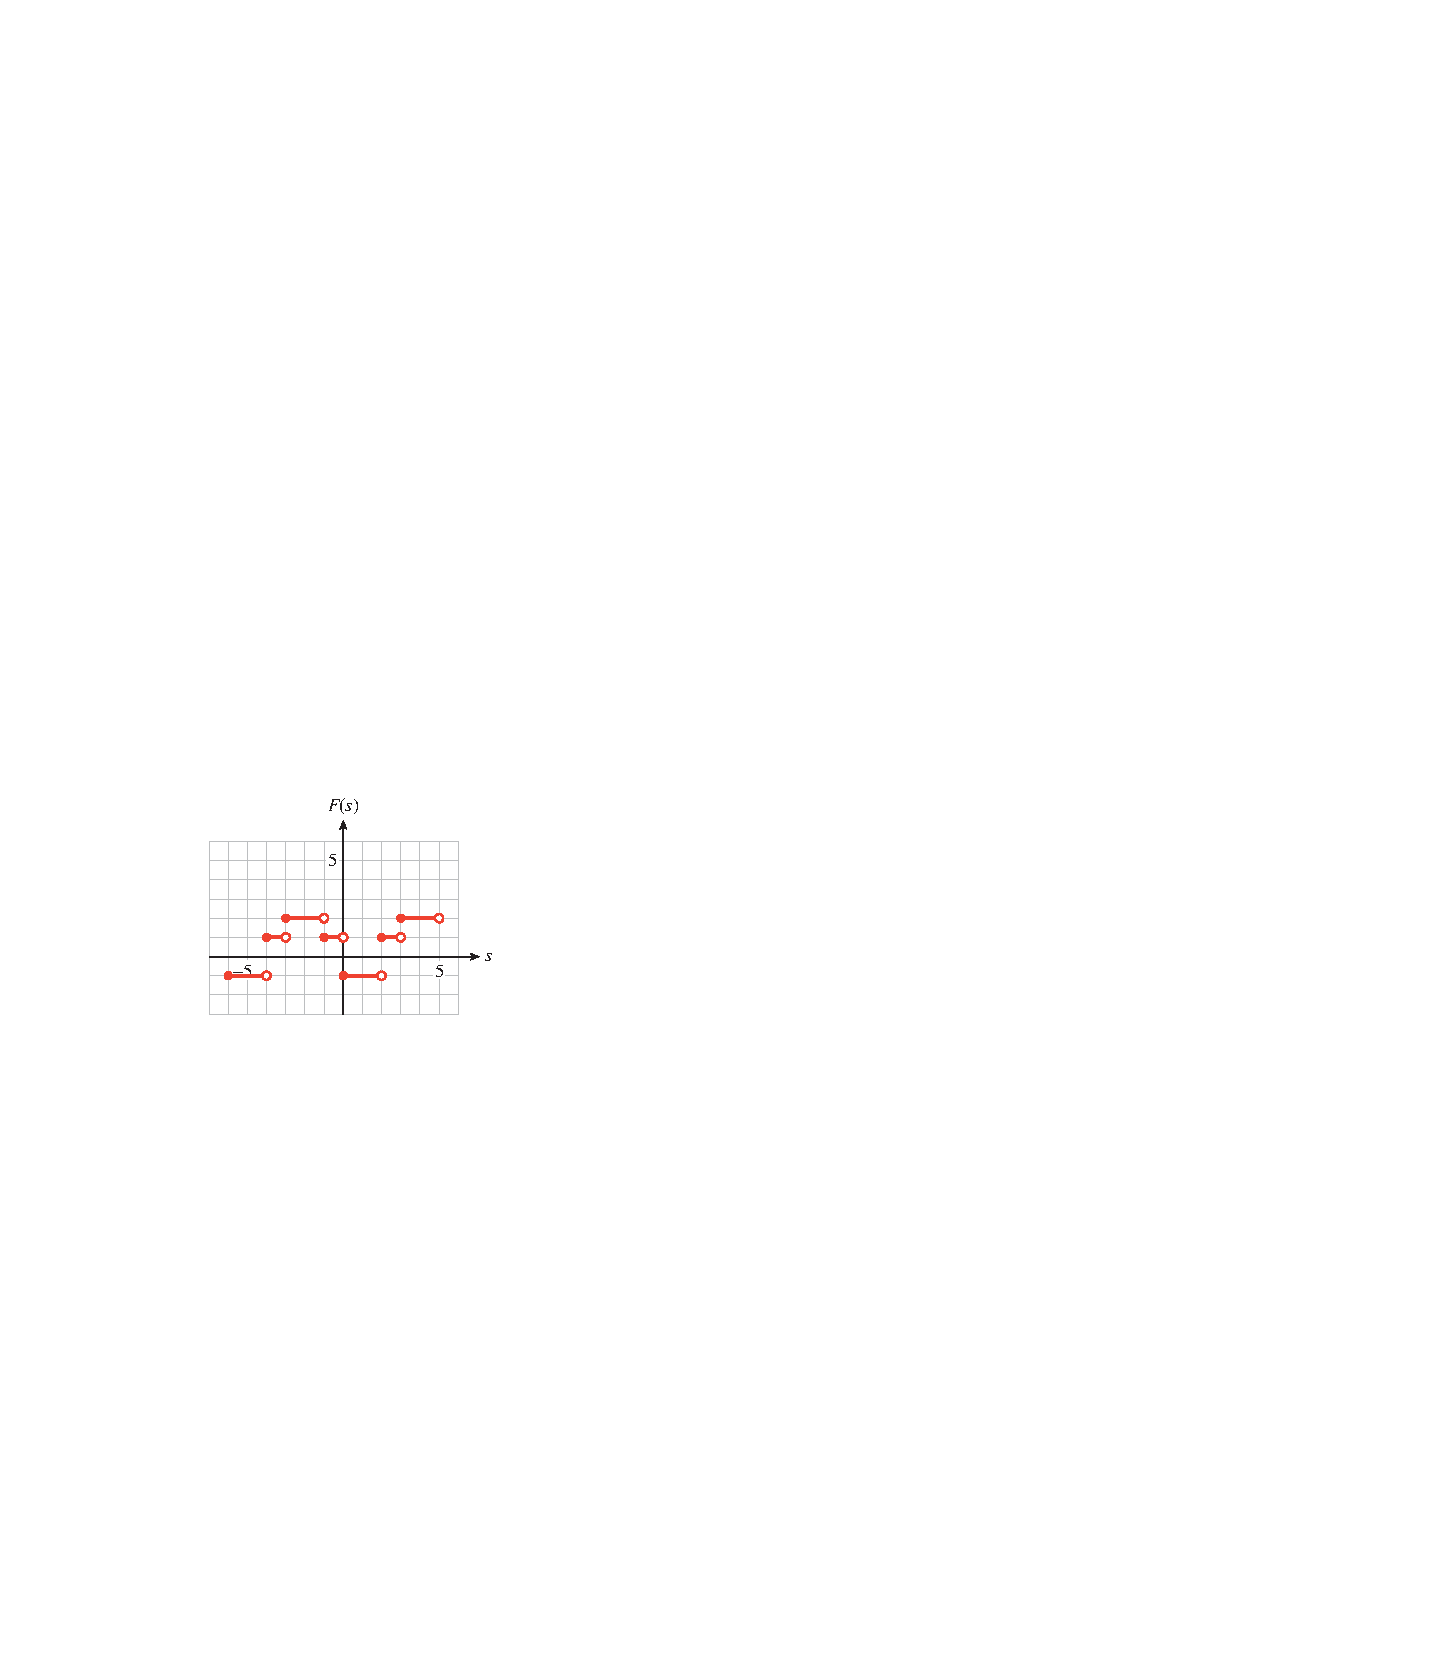
\includegraphics[width=\linewidth]{external/images/fig-ex-1-3-7.pdf}
\end{sbspanel}%
\end{sidebyside}%
\end{divisionexerciseeg}%
\begin{divisionexerciseeg}{8}{}{}{exercise-section-1-3-exercises-b-i}%
%
\begin{enumerate}[label=\alph*]
\item{}Find \(P(-3)\), \(P(-2)\), and \(P(1)\).%
\item{}For what value(s) of \(n\) is \(P(n) = 0\)?%
\item{}Find the maximum and minimum values of \(P(n)\).%
\item{}For what value(s) of \(n\) does \(P\) take on its maximum and minimum values?%
\end{enumerate}
%
\begin{sidebyside}{1}{0.3}{0.3}{0}%
\begin{sbspanel}{0.4}%
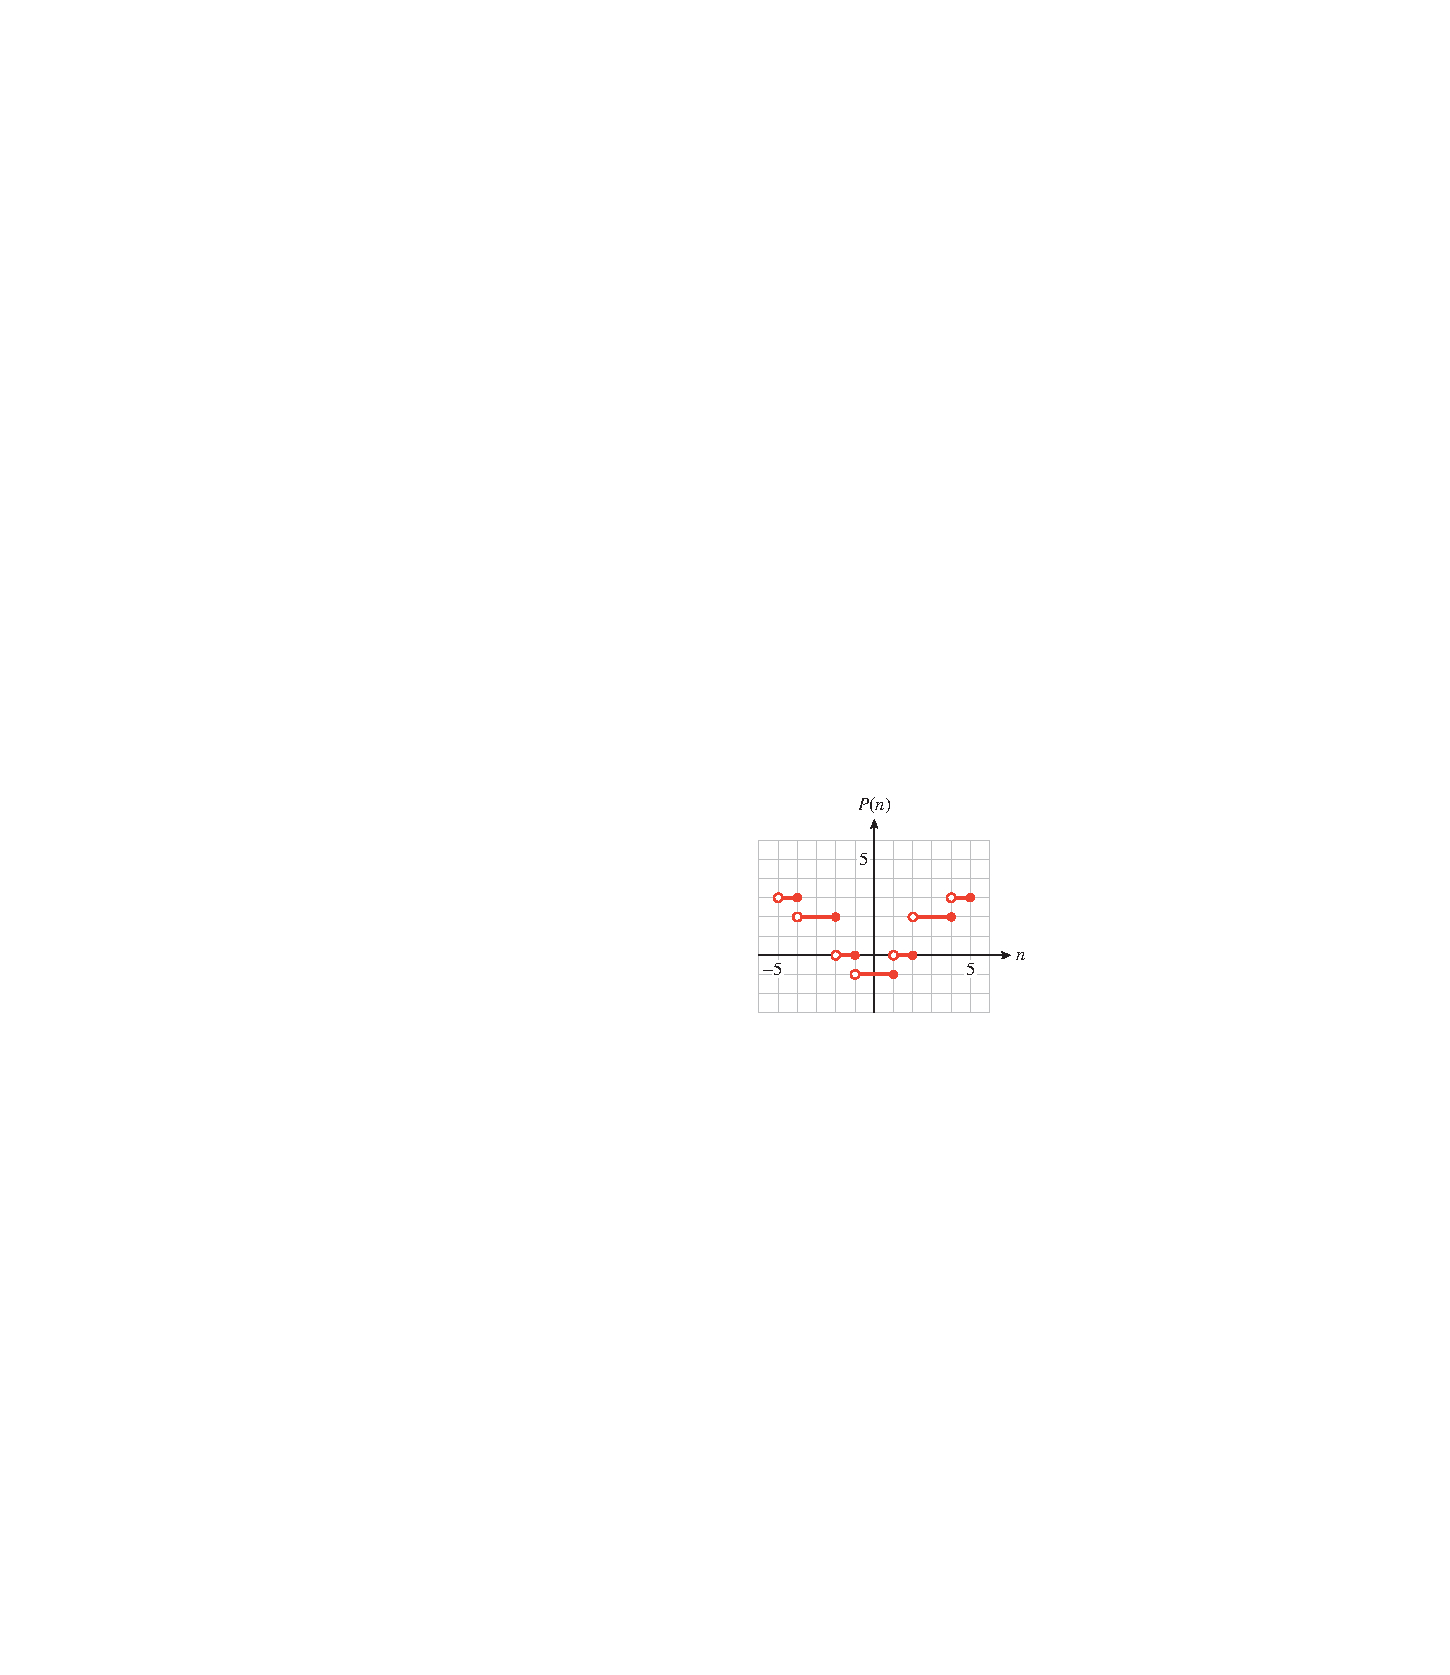
\includegraphics[width=\linewidth]{external/images/fig-ex-1-3-8.pdf}
\end{sbspanel}%
\end{sidebyside}%
\end{divisionexerciseeg}%
\end{exercisegroup}
\par\medskip\noindent
\par\medskip\noindent%
\textbf{Exercise Group.}\space\space%
Which of the graphs in Problems 9 and 10 represent functions?%
\begin{exercisegroup}
\begin{divisionexerciseeg}{9}{}{}{exercise-section-1-3-exercises-c-b}%
\begin{sidebyside}{1}{0}{0}{0}%
\begin{sbspanel}{1}%
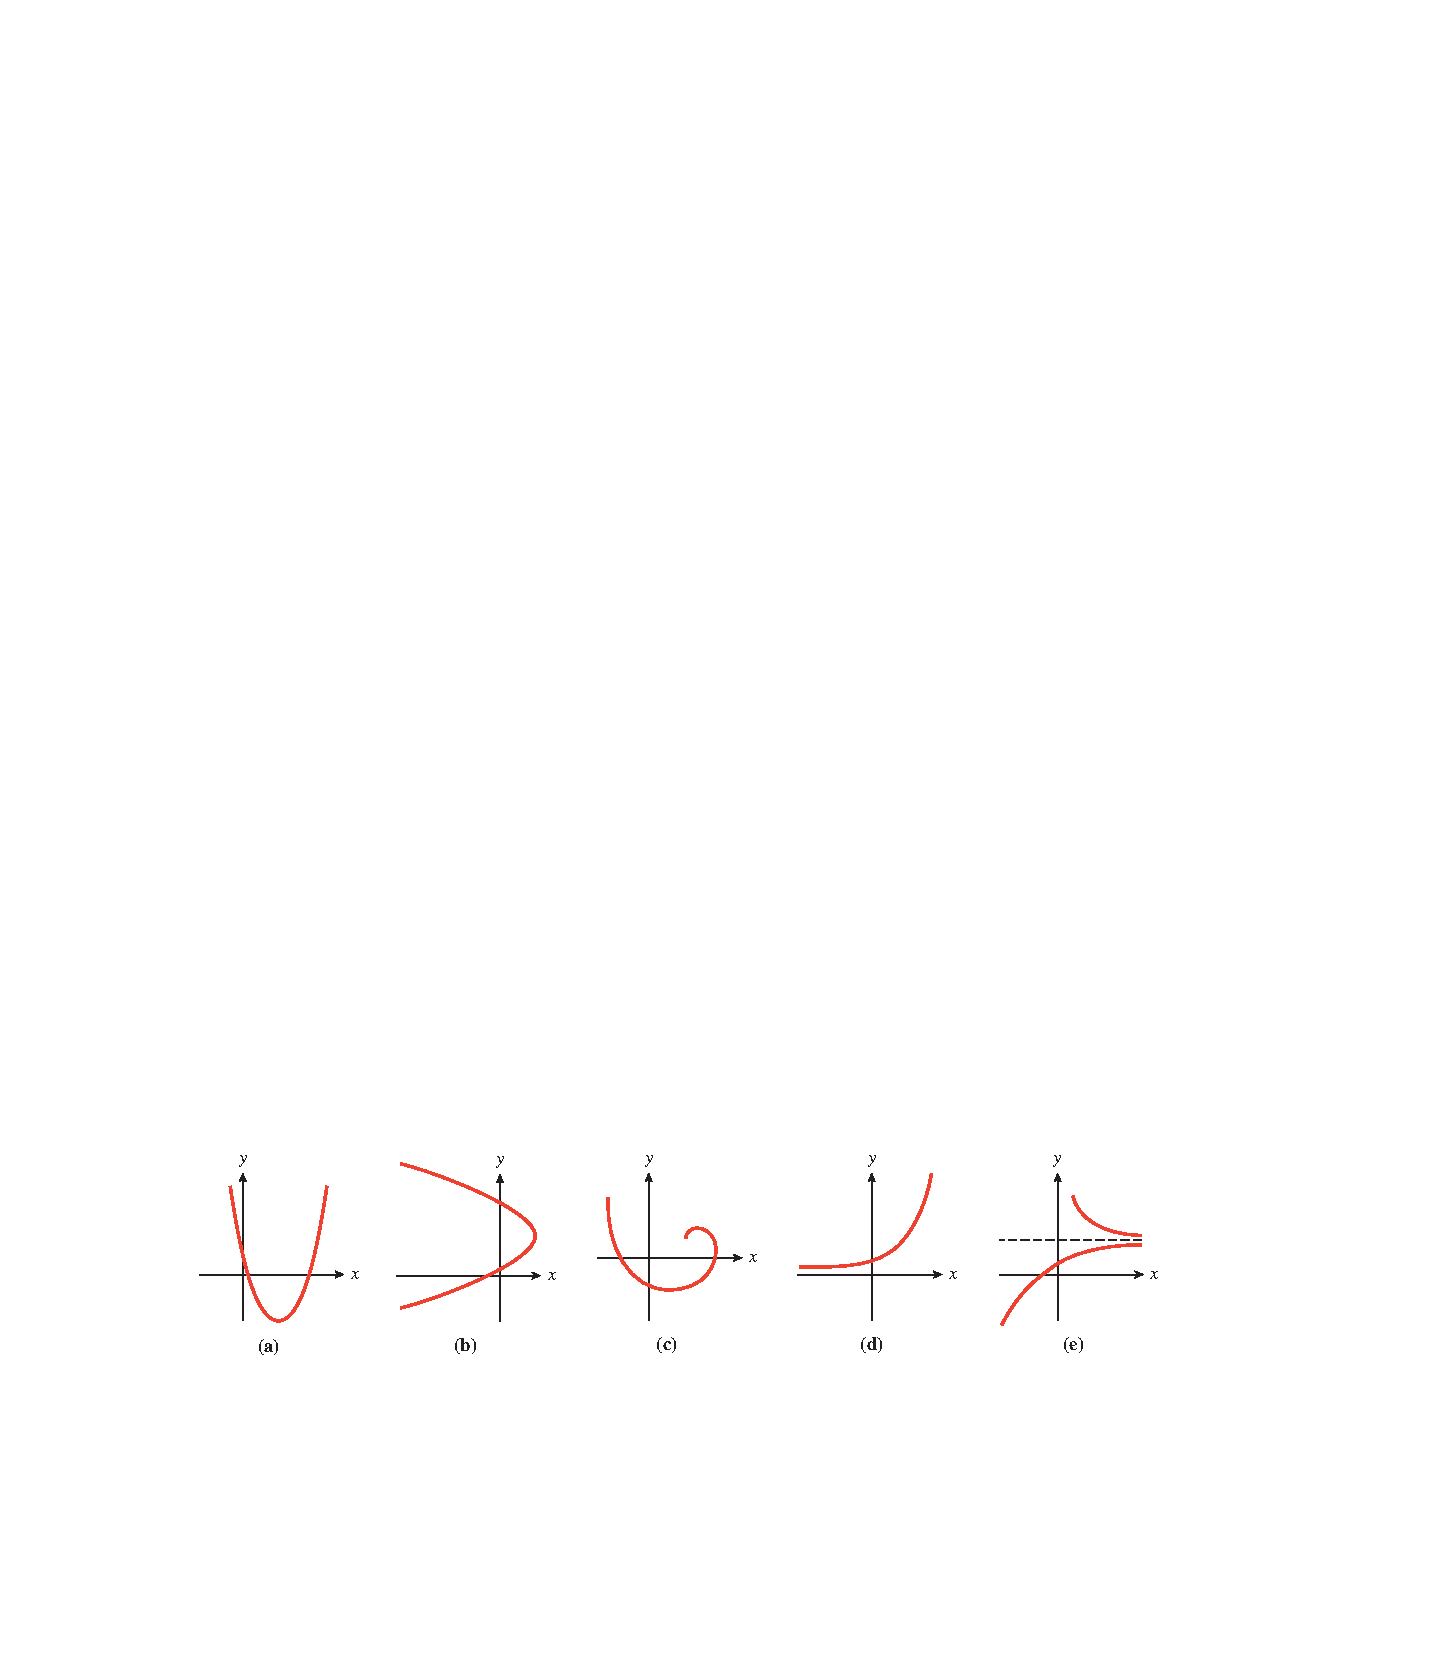
\includegraphics[width=\linewidth]{external/images/fig-ex-1-3-9.pdf}
\end{sbspanel}%
\end{sidebyside}%
\end{divisionexerciseeg}%
\begin{divisionexerciseeg}{10}{}{}{exercise-section-1-3-exercises-c-c}%
\begin{sidebyside}{1}{0}{0}{0}%
\begin{sbspanel}{1}%
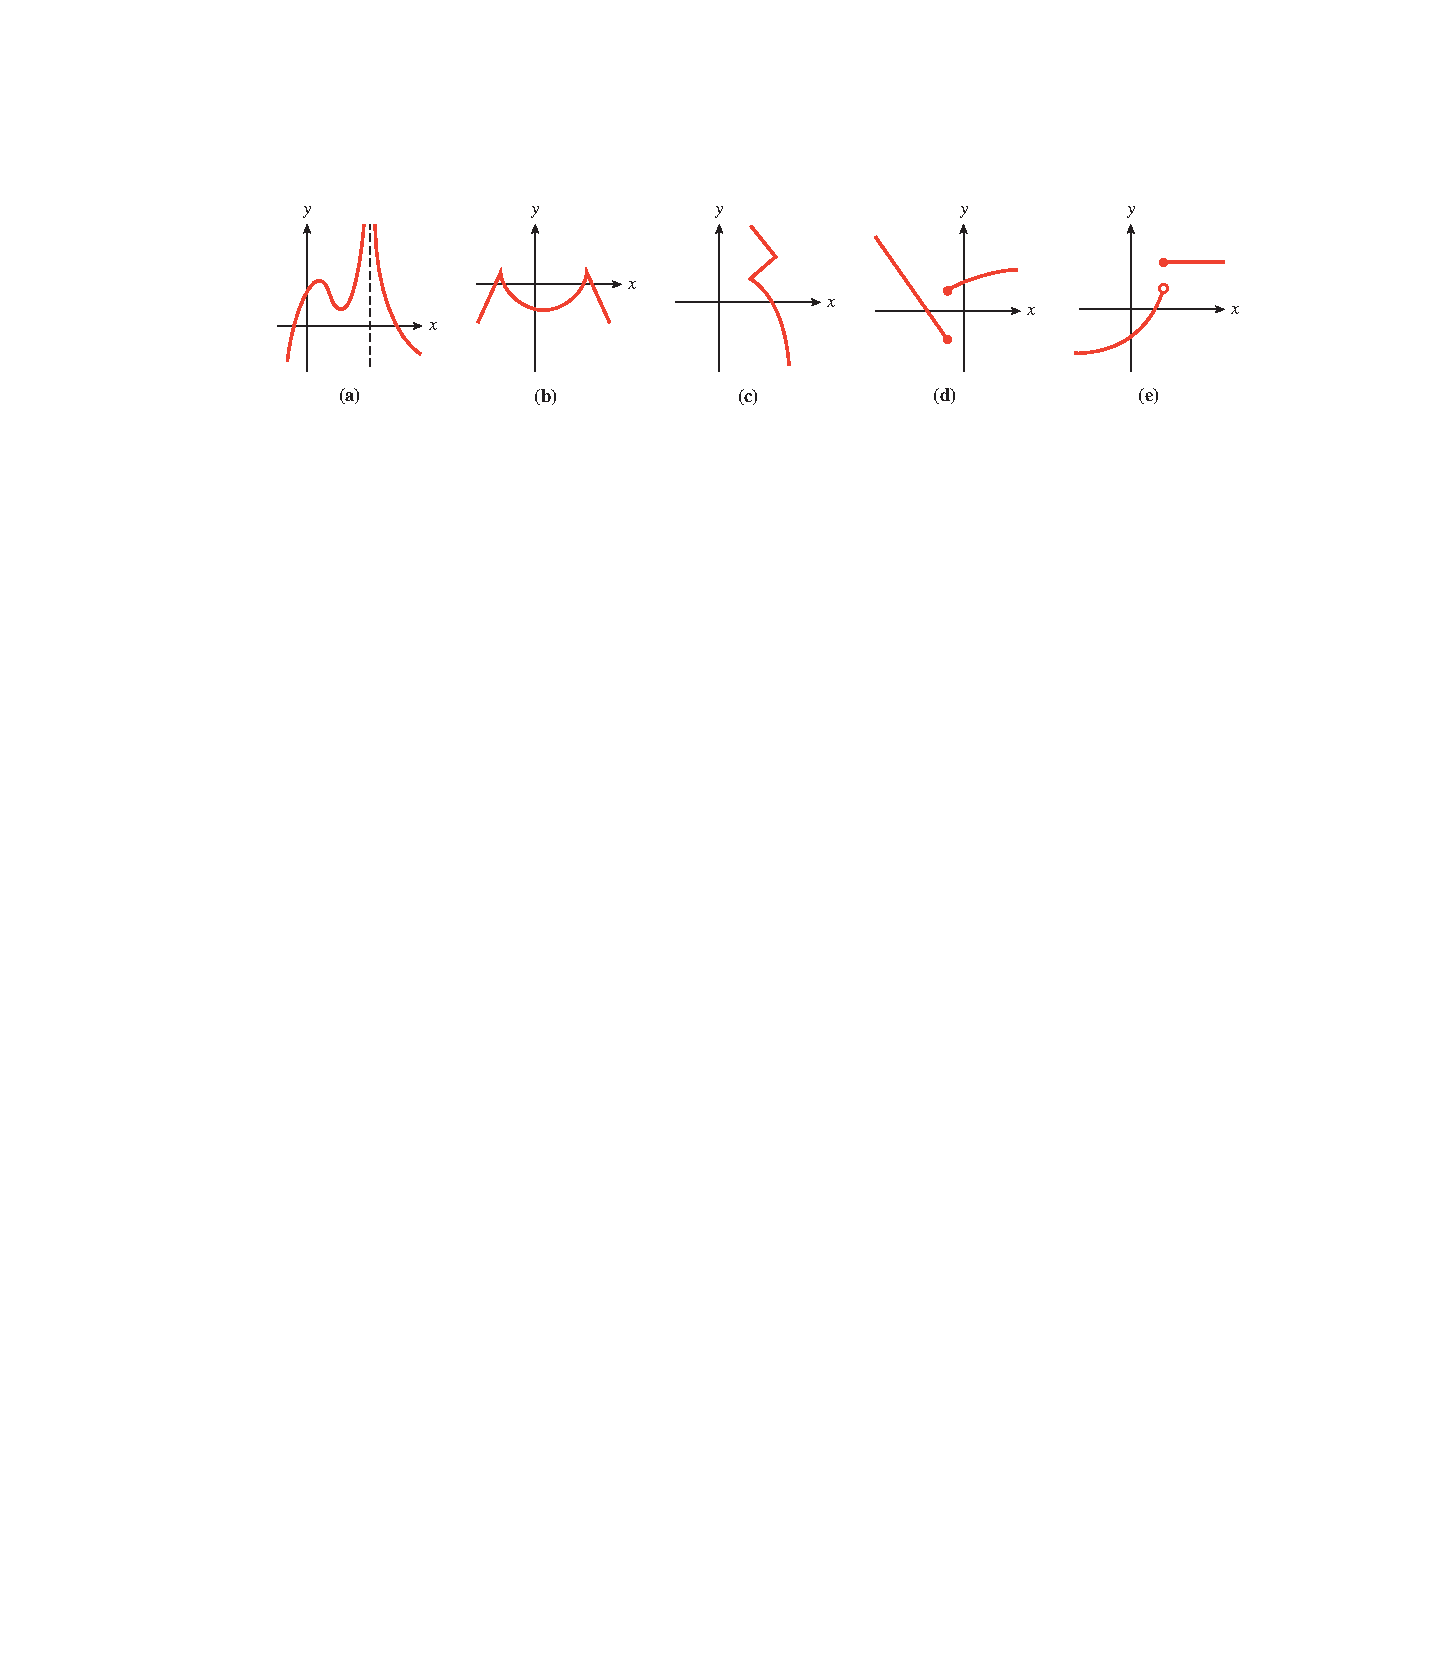
\includegraphics[width=\linewidth]{external/images/fig-ex-1-3-10.pdf}
\end{sbspanel}%
\end{sidebyside}%
\end{divisionexerciseeg}%
\end{exercisegroup}
\par\medskip\noindent
\par\medskip\noindent%
\textbf{Exercise Group.}\space\space%
In Problems 11\textendash{}16,%
\begin{enumerate}[label=\alph*]
\item{}Make a table of values and sketch a graph of the function by plotting points. (Use the suggested \(x\)-values.)%
\item{}Use a graphing utility to graph the function.%
\end{enumerate}
Compare the graphing utility's graph with your sketch.%
\begin{exercisegroupcol}{2}
\begin{divisionexerciseegcol}{11}{}{}{exercise-section-1-3-exercises-d-b}%
\(g(x) = x^3 + 4\); \(\hphantom{00000}x = -2, -1, \ldots , 2\)%
\end{divisionexerciseegcol}%
\begin{divisionexerciseegcol}{12}{}{}{exercise-section-1-3-exercises-d-c}%
\(h(x) = 2 +\sqrt{x}\); \(\hphantom{00000}x = 0,1, \ldots , 9\)%
\end{divisionexerciseegcol}%
\begin{divisionexerciseegcol}{13}{}{}{exercise-section-1-3-exercises-d-d}%
\(G(x) =\sqrt{4 - x}\); \(\hphantom{00000}x = -5, -4, \ldots , 4\)%
\end{divisionexerciseegcol}%
\begin{divisionexerciseegcol}{14}{}{}{exercise-section-1-3-exercises-d-e}%
\(F(x) = \sqrt{x-1}\); \(\hphantom{00000}x = 1,2, \ldots , 10\)%
\end{divisionexerciseegcol}%
\begin{divisionexerciseegcol}{15}{}{}{exercise-section-1-3-exercises-d-f}%
\(v(x) = 1 + 6x - x^3\); \(\hphantom{00000}x = -3, -2, \ldots , 3\)%
\end{divisionexerciseegcol}%
\begin{divisionexerciseegcol}{16}{}{}{exercise-section-1-3-exercises-d-g}%
\(w(x) = x^3 - 8x\); \(\hphantom{00000}x = -4, -3, \ldots , 4\)%
\end{divisionexerciseegcol}%
\end{exercisegroupcol}
\par\medskip\noindent
\begin{divisionexercise}{17}{}{}{exercise-section-1-3-exercises-e}%
The graph shows the speed of sound in the ocean as a function of depth, \(S = f (d)\). The speed of sound is affected both by increasing water pressure and by dropping temperature. (Source: Scientific American)%
\begin{sidebyside}{1}{0.3}{0.3}{0}%
\begin{sbspanel}{0.4}%
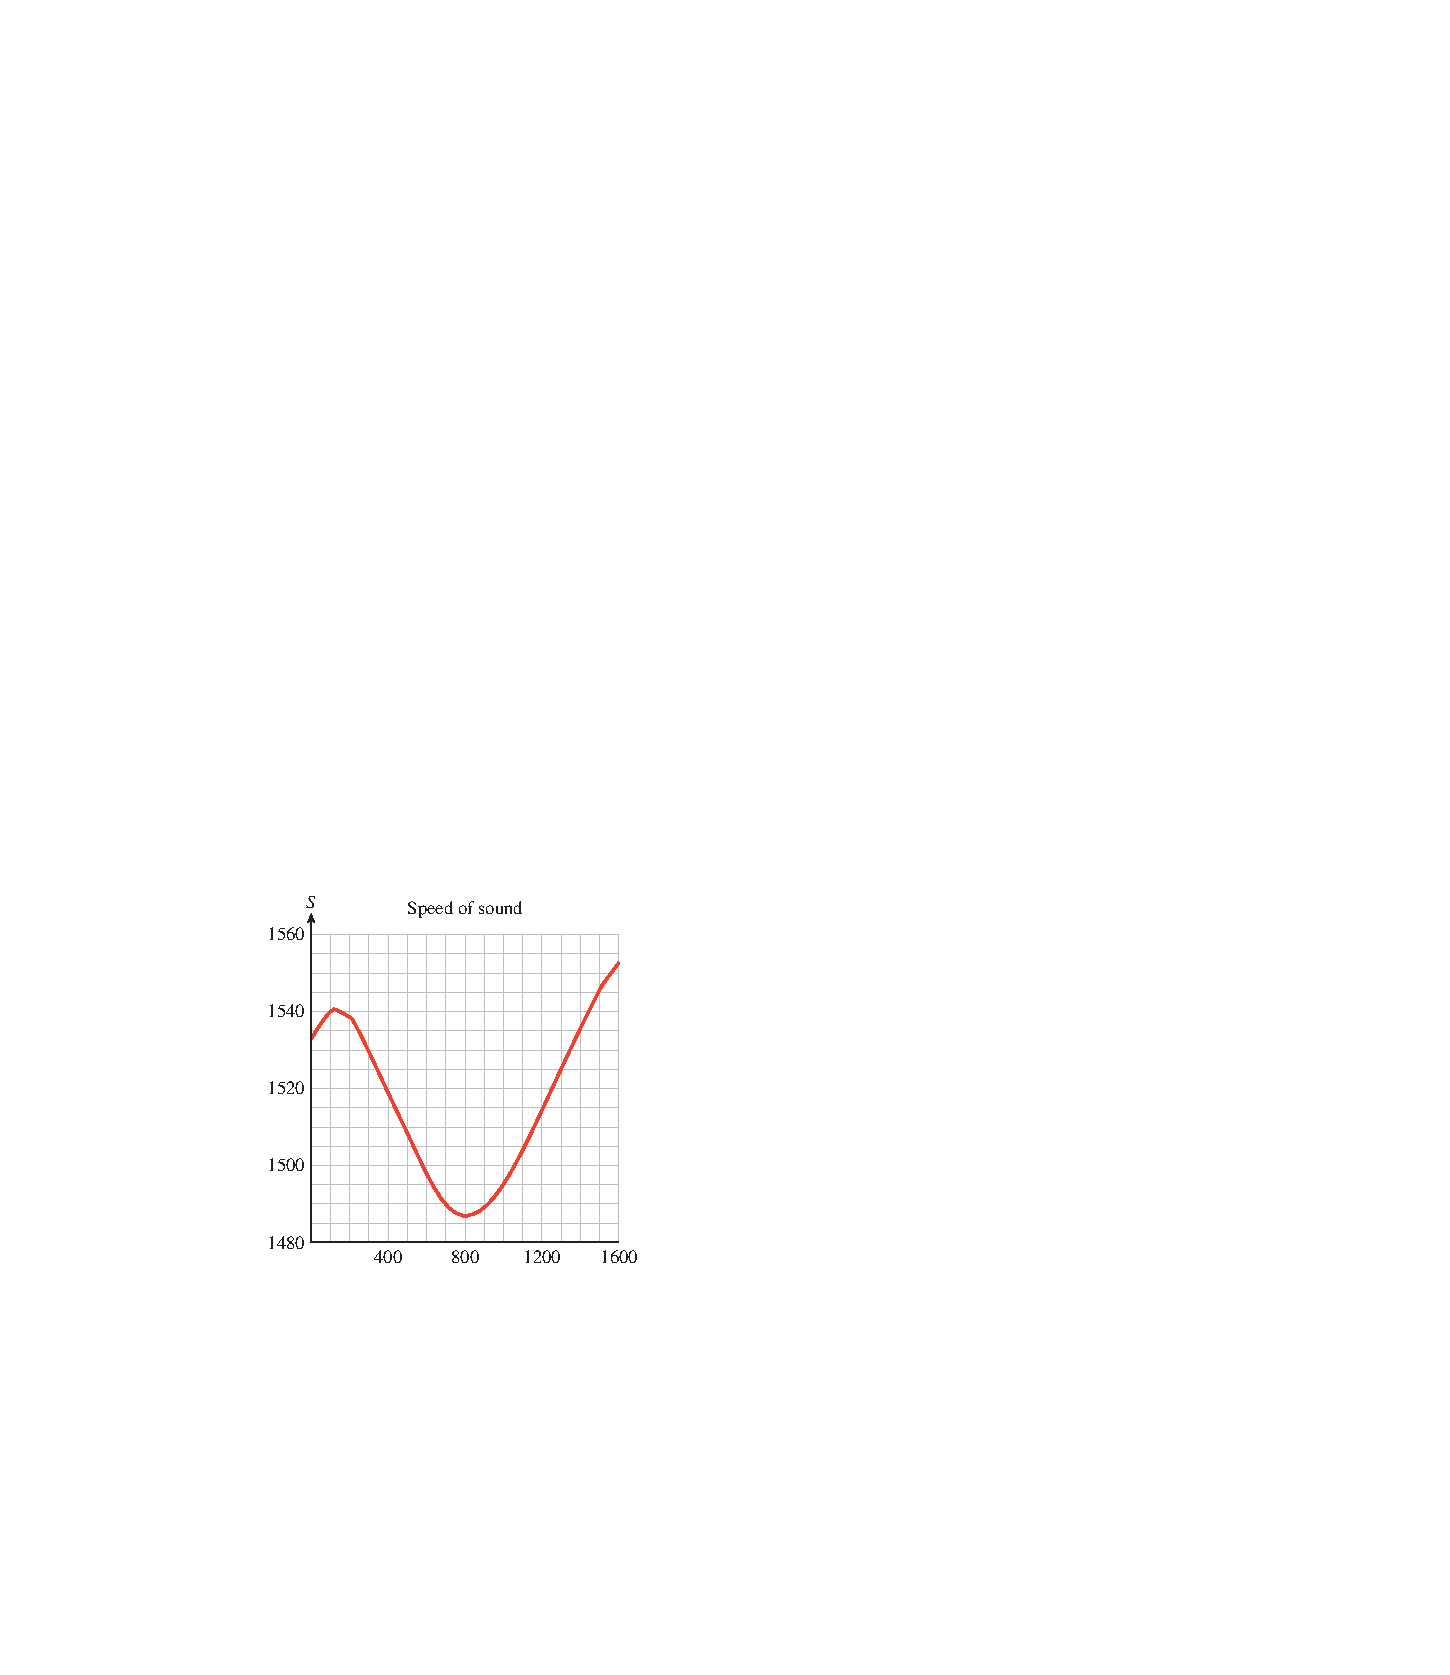
\includegraphics[width=\linewidth]{external/images/fig-ex-1-3-17.pdf}
\end{sbspanel}%
\end{sidebyside}%
\par
%
\begin{enumerate}[label=\alph*]
\item{}Evaluate \(f (1000)\) and explain its meaning.%
\item{}Solve \(f (d) = 1500\) and explain its meaning.%
\item{}At what depth is the speed of sound the slowest, and what is the speed? Write your answer with function notation.%
\item{}Describe the behavior of \(f (d)\) as \(d\) increases.%
\end{enumerate}
%
\end{divisionexercise}%
\begin{divisionexercise}{18}{}{}{exercise-section-1-3-exercises-f}%
The graph shows the water level in Lake Superior as a function of time, \(L = f (t)\). (Source: The Canadian Hydrographic Service)%
\begin{sidebyside}{1}{0.2}{0.2}{0}%
\begin{sbspanel}{0.6}%
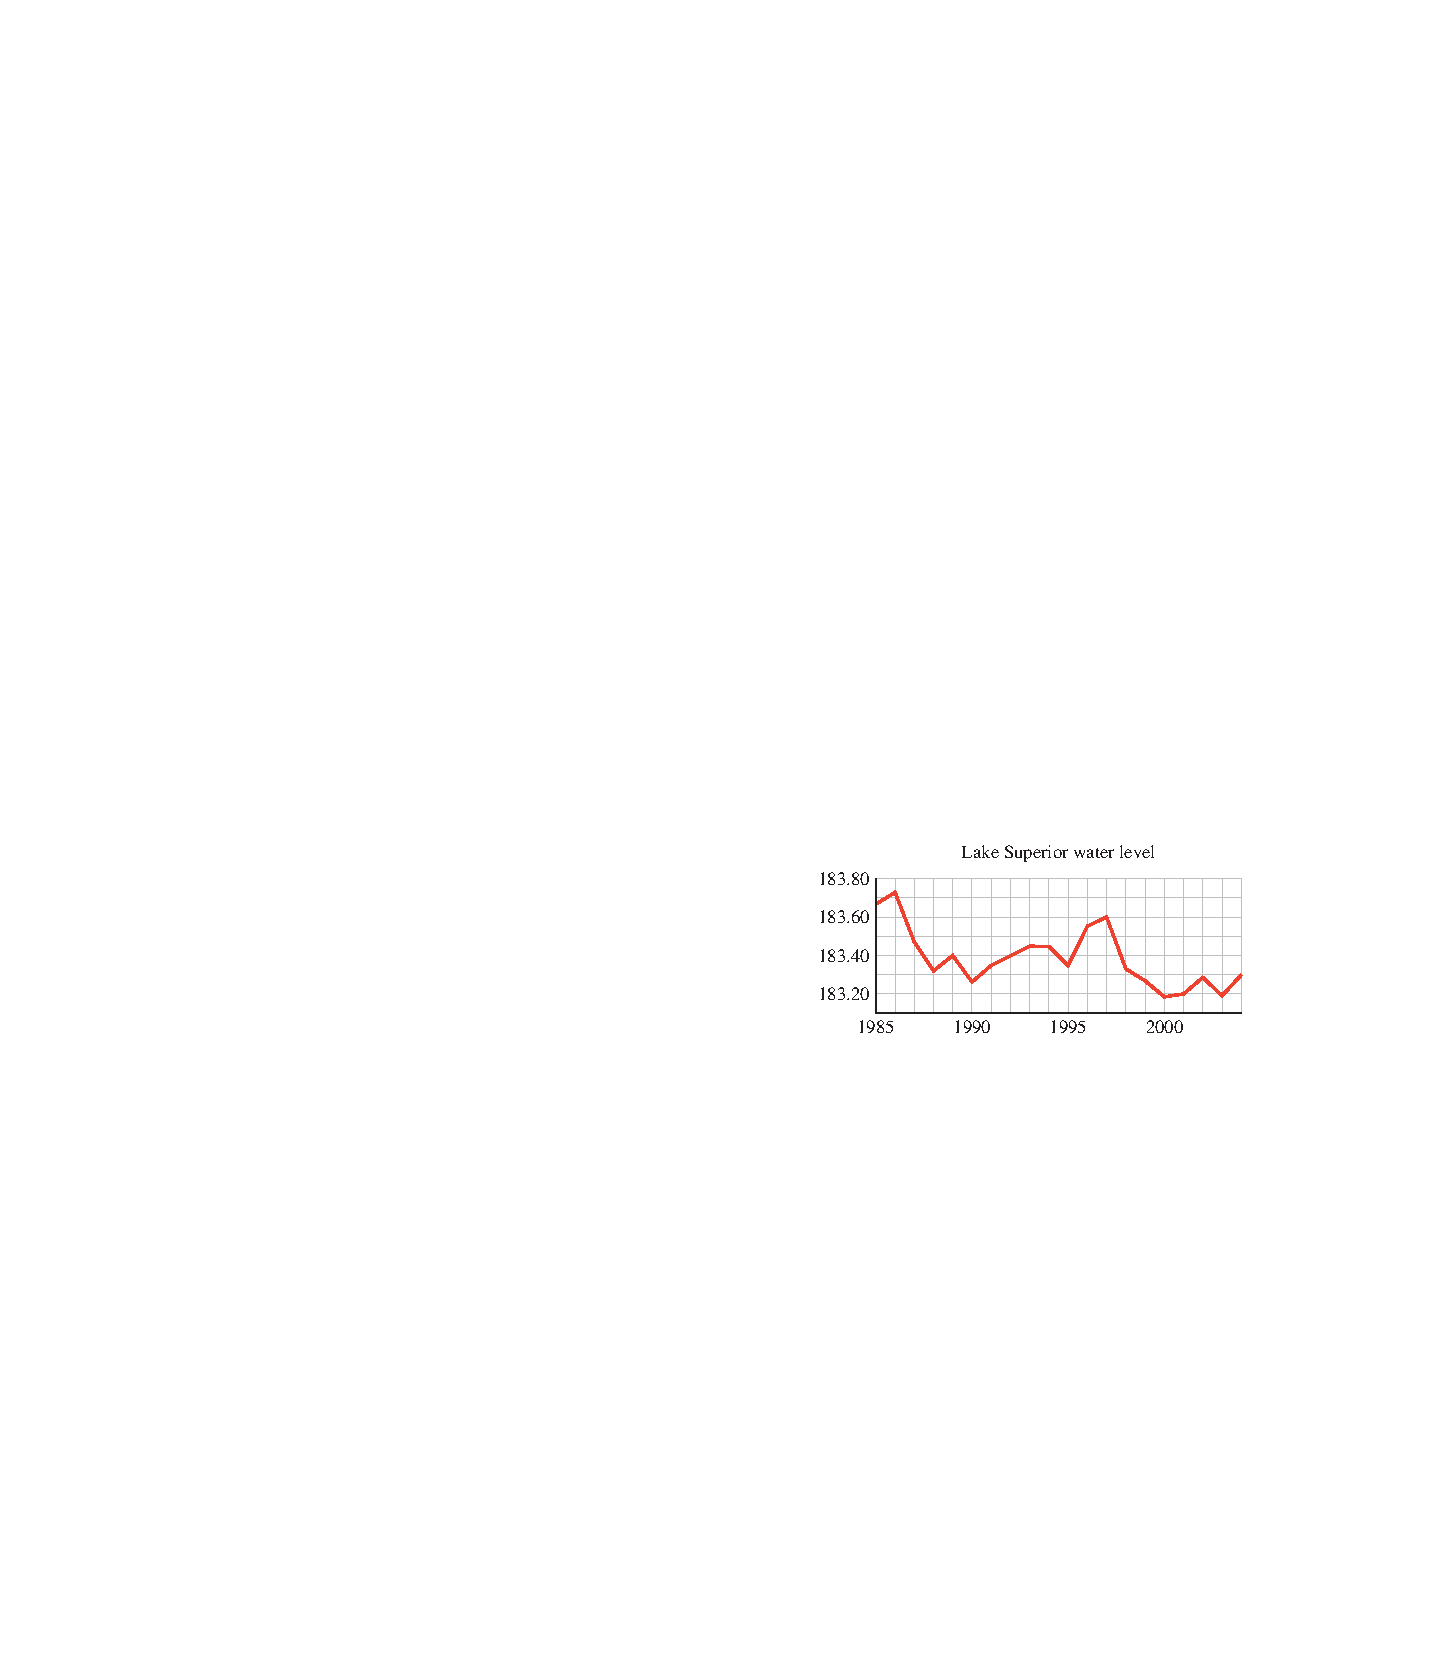
\includegraphics[width=\linewidth]{external/images/fig-ex-1-3-18.pdf}
\end{sbspanel}%
\end{sidebyside}%
\par
%
\begin{enumerate}[label=\alph*]
\item{}Evaluate \(f (1997)\) and explain its meaning.%
\item{}Solve \(f (t) = 183.5\) and explain its meaning.%
\item{}In which two years did Lake Superior reach its highest levels, and what were those levels? Write your answers with function notation.%
\item{}Over which two-year period did the water level drop the most?%
\end{enumerate}
%
\end{divisionexercise}%
\begin{divisionexercise}{19}{}{}{exercise-section-1-3-exercises-g}%
The graph shows the federal debt as a percentage of the gross domestic product (GDP), as a function of time, \(D = f (t)\). (Source: Office of Management and Budget)%
\begin{sidebyside}{1}{0.3}{0.3}{0}%
\begin{sbspanel}{0.4}%
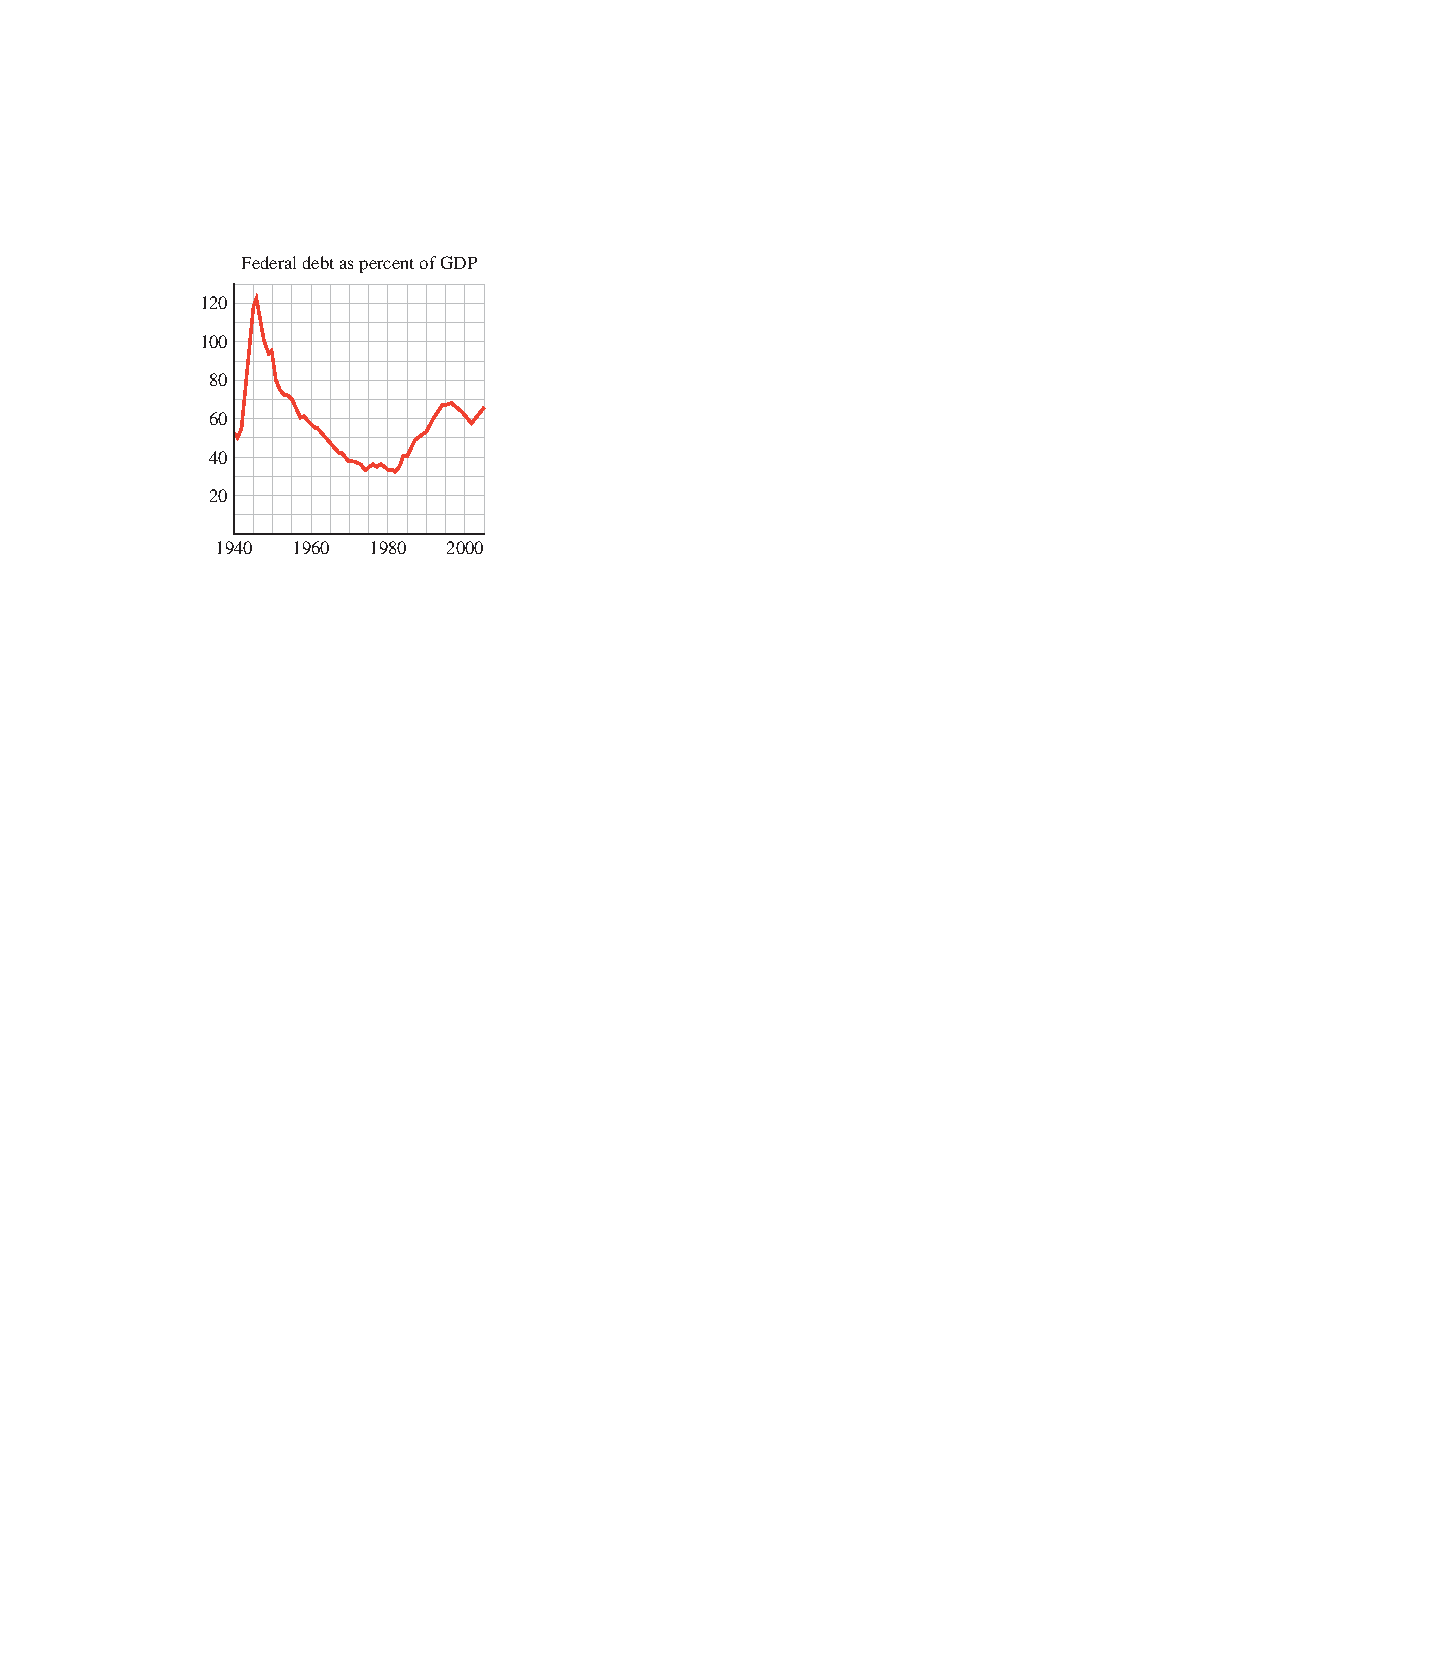
\includegraphics[width=\linewidth]{external/images/fig-ex-1-3-19.pdf}
\end{sbspanel}%
\end{sidebyside}%
\par
%
\begin{enumerate}[label=\alph*]
\item{}Evaluate \(f (1985)\) and explain its meaning.%
\item{}Solve \(f (t) = 70\) and explain its meaning.%
\item{}When did the federal debt reach its highest level since 1960, and what was that level? Write your answer with function notation.%
\item{}What is the longest time interval over which the federal debt was decreasing?%
\end{enumerate}
%
\end{divisionexercise}%
\begin{divisionexercise}{20}{}{}{exercise-section-1-3-exercises-h}%
The graph shows the elevation of the Los Angeles Marathon course as a function of the distance into the race, \(a = f (t)\). (Source: Los Angeles Times, March 3, 2005)%
\begin{sidebyside}{1}{0.15}{0.15}{0}%
\begin{sbspanel}{0.7}%
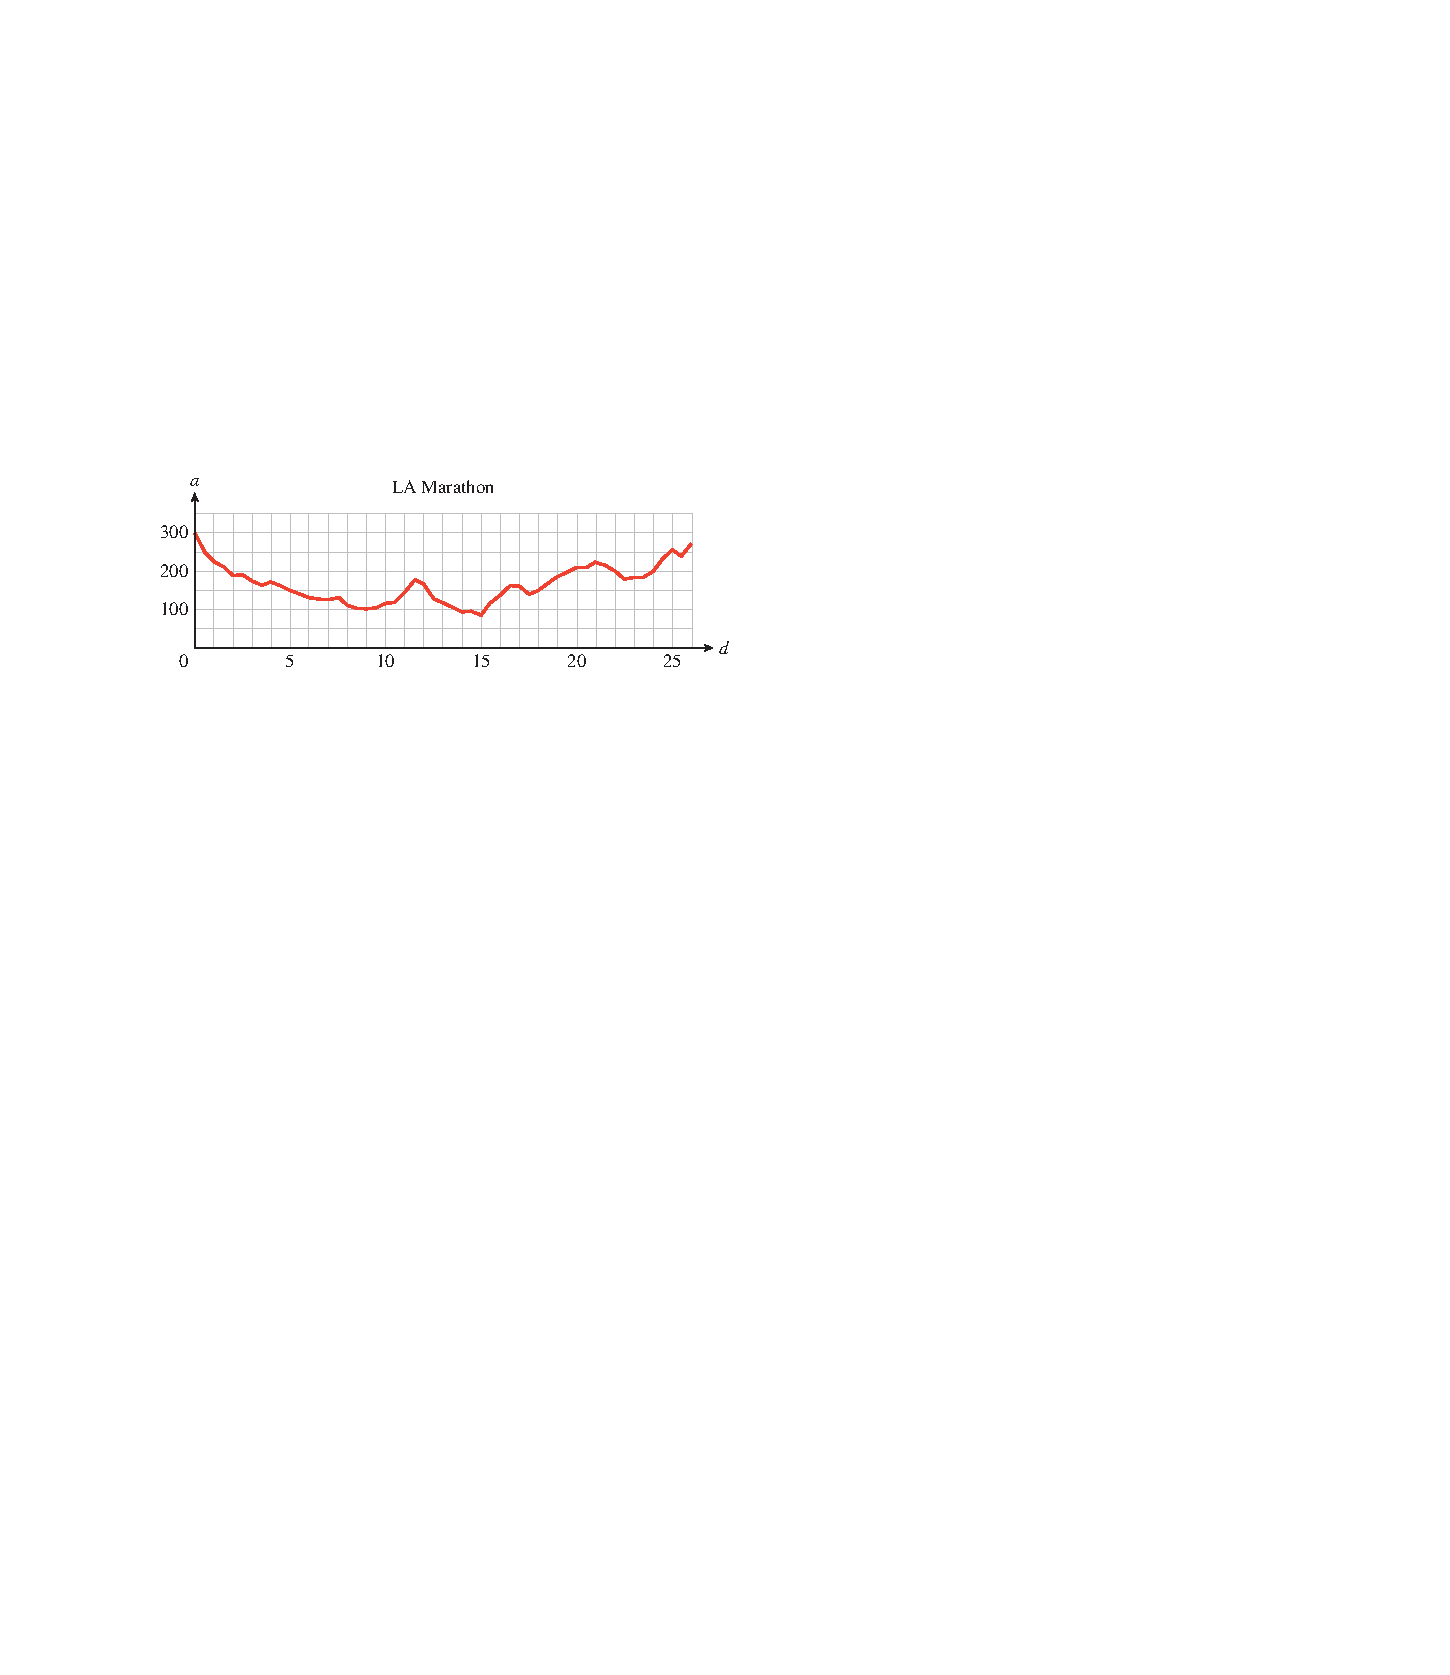
\includegraphics[width=\linewidth]{external/images/fig-LA-marathon.pdf}
\end{sbspanel}%
\end{sidebyside}%
\par
%
\begin{enumerate}[label=\alph*]
\item{}Evaluate \(f (5)\) and explain its meaning.%
\item{}Solve \(f (d) = 200\) and explain its meaning.%
\item{}When does the marathon course reach its lowest elevation, and what is that elevation? Write your answer with function notation.%
\item{}Give three intervals over which the elevation is increasing.%
\end{enumerate}
%
\end{divisionexercise}%
\begin{divisionexercise}{21}{}{}{exercise-section-1-3-exercises-i}%
The figure shows a graph of \(y = -2x + 6\).%
\begin{sidebyside}{1}{0.325}{0.325}{0}%
\begin{sbspanel}{0.35}%
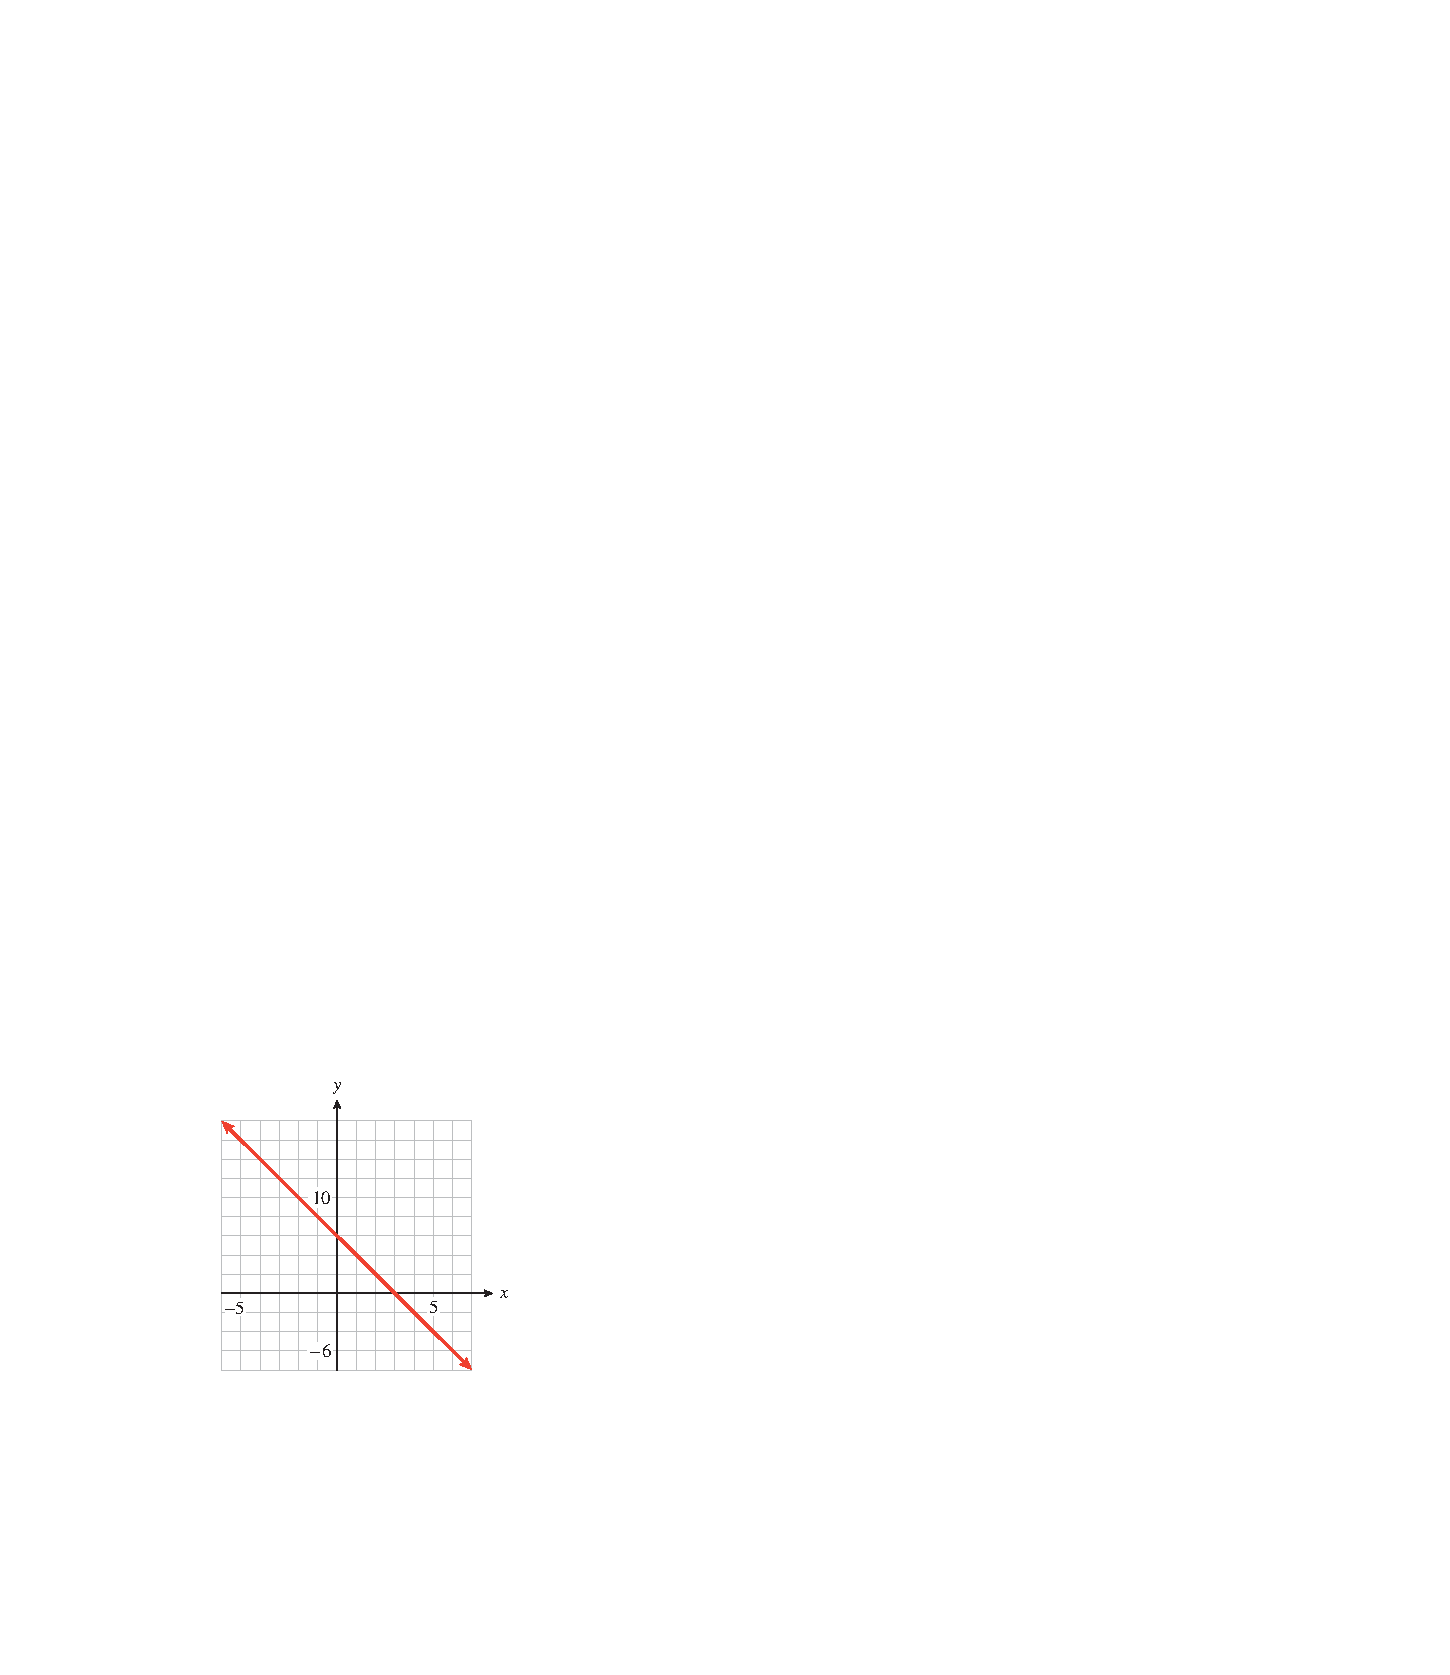
\includegraphics[width=\linewidth]{external/images/fig-ex-1-3-21.pdf}
\end{sbspanel}%
\end{sidebyside}%
\par
%
\begin{enumerate}[label=\alph*]
\item{}Use the graph to find all values of \(x\) for which%
\begin{enumerate}[label=\Roman*]
\item{}\(\displaystyle y=12\)%
\item{}\(\displaystyle y\gt 12\)%
\item{}\(\displaystyle y\lt 12\)%
\end{enumerate}
%
\item{}Use the graph to solve%
\begin{enumerate}[label=\Roman*]
\item{}\(\displaystyle -2x + 6=12\)%
\item{}\(\displaystyle -2x + 6\gt 12\)%
\item{}\(\displaystyle -2x + 6\lt 12\)%
\end{enumerate}
%
\item{}Explain why your answers to parts (a) and (b) are the same.%
\end{enumerate}
%
\end{divisionexercise}%
\begin{divisionexercise}{22}{}{}{exercise-section-1-3-exercises-j}%
The figure shows a graph of \(y =\dfrac{-x}{3} - 6\).%
\begin{sidebyside}{1}{0.3}{0.3}{0}%
\begin{sbspanel}{0.4}%
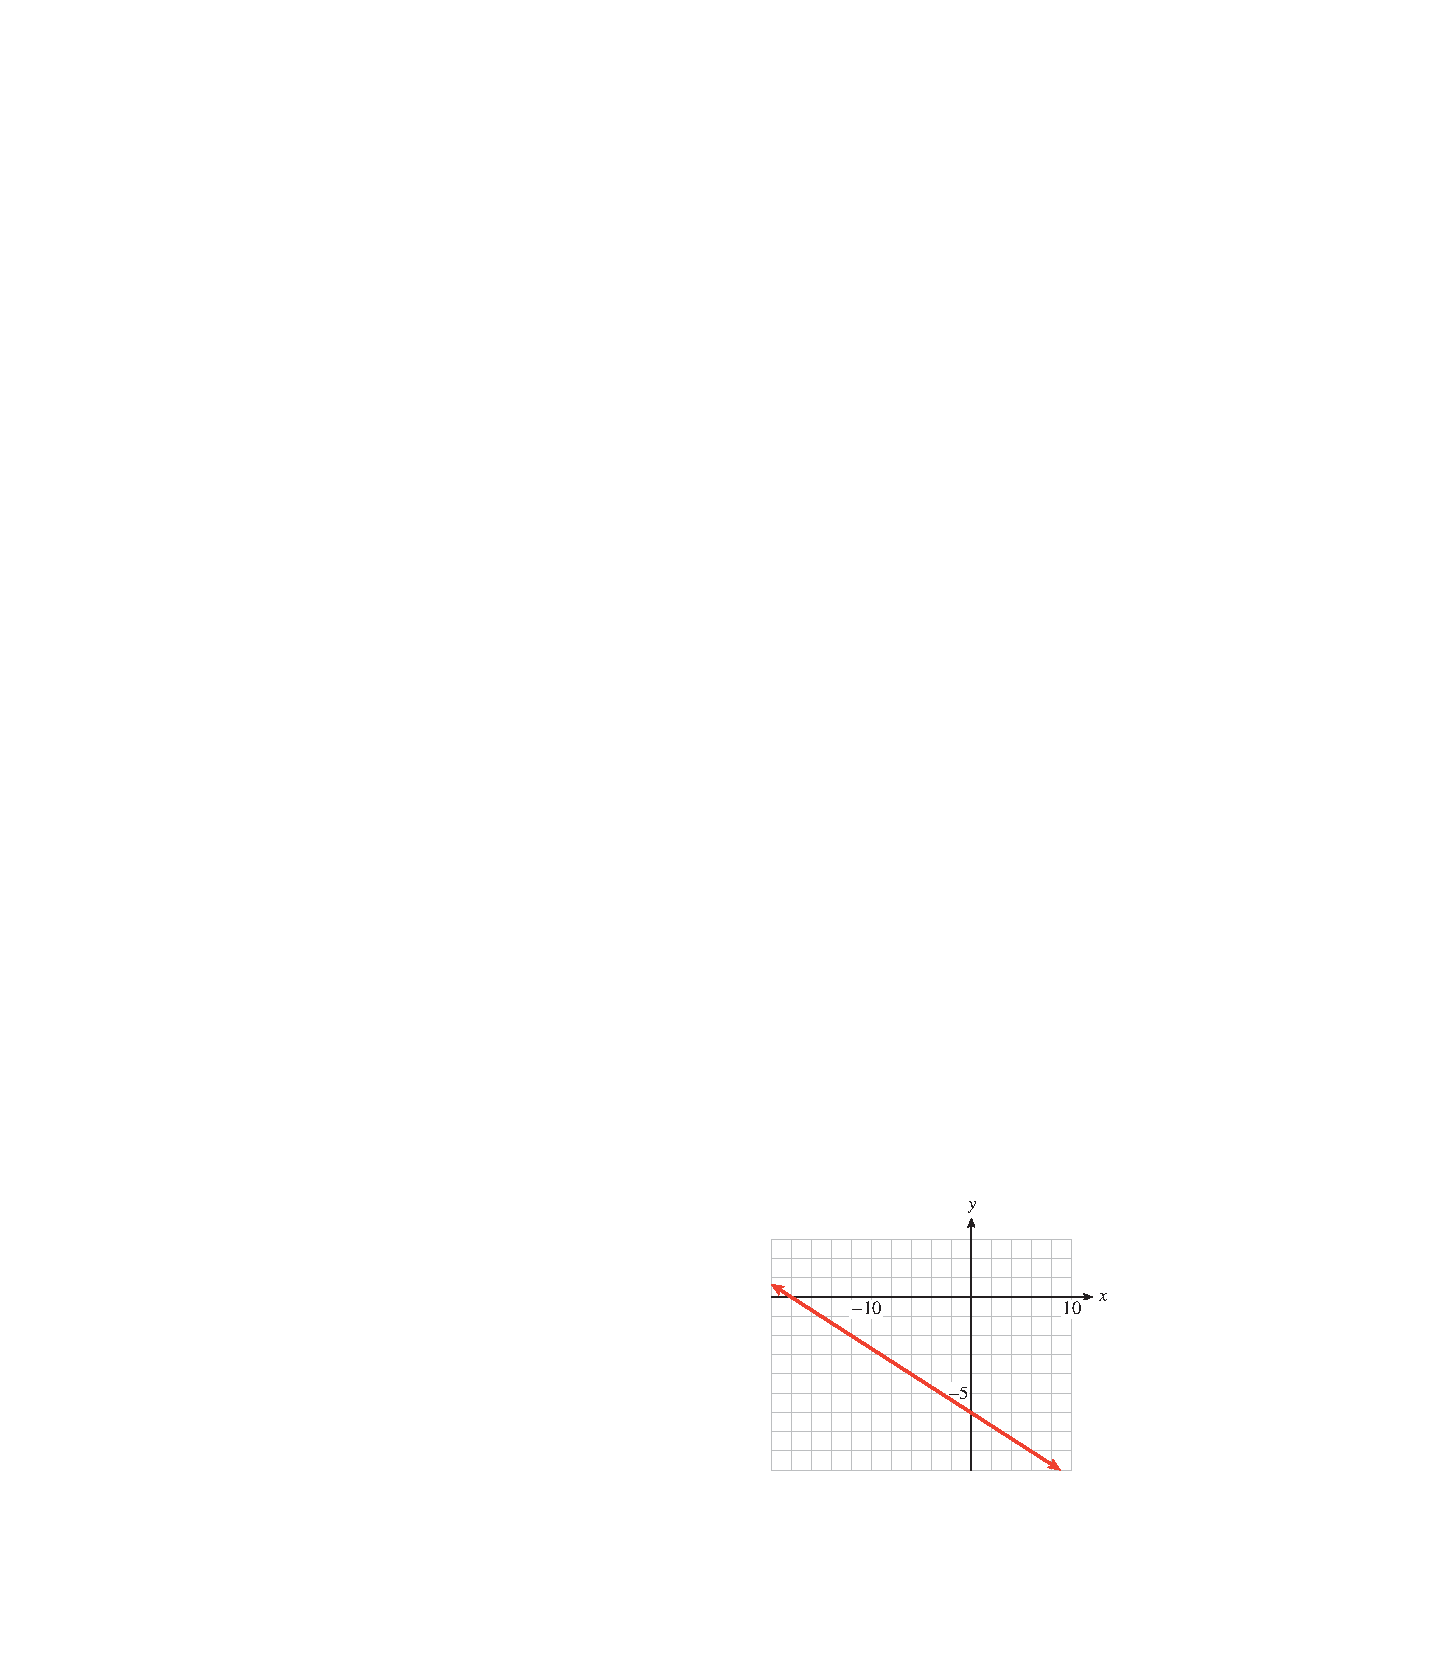
\includegraphics[width=\linewidth]{external/images/fig-ex-1-3-22.pdf}
\end{sbspanel}%
\end{sidebyside}%
\par
%
\begin{enumerate}[label=\alph*]
\item{}Use the graph to find all values of \(x\) for which%
\begin{enumerate}[label=\roman*]
\item{}\(\displaystyle y=-4\)%
\item{}\(\displaystyle y\gt -4\)%
\item{}\(\displaystyle y\lt -4\)%
\end{enumerate}
%
\item{}Use the graph to solve%
\begin{enumerate}[label=\roman*]
\item{}\(\displaystyle \dfrac{-x}{3} - 6=-4\)%
\item{}\(\displaystyle \dfrac{-x}{3} - 6\gt -4\)%
\item{}\(\displaystyle \dfrac{-x}{3} - 6\lt -4\)%
\end{enumerate}
%
\item{}Explain why your answers to parts (a) and (b) are the same.%
\end{enumerate}
%
\end{divisionexercise}%
\par\medskip\noindent%
\textbf{Exercise Group.}\space\space%
In Problems 23 and 24, use the graph to solve the equation or inequality, and then solve algebraically. (To review solving linear inequalities algebraically, see \hyperref[section-appendix-Linear-Equations-and-Inequalities]{Algebra Skills Refresher~{\xreffont\ref{section-appendix-Linear-Equations-and-Inequalities}}}.)%
\begin{exercisegroup}
\begin{divisionexerciseeg}{23}{}{}{exercise-section-1-3-exercises-k-b}%
The figure shows the graph of \(y = 1.4x - 0.64\). Solve the following:%
\begin{sidebyside}{1}{0.35}{0.35}{0}%
\begin{sbspanel}{0.3}%
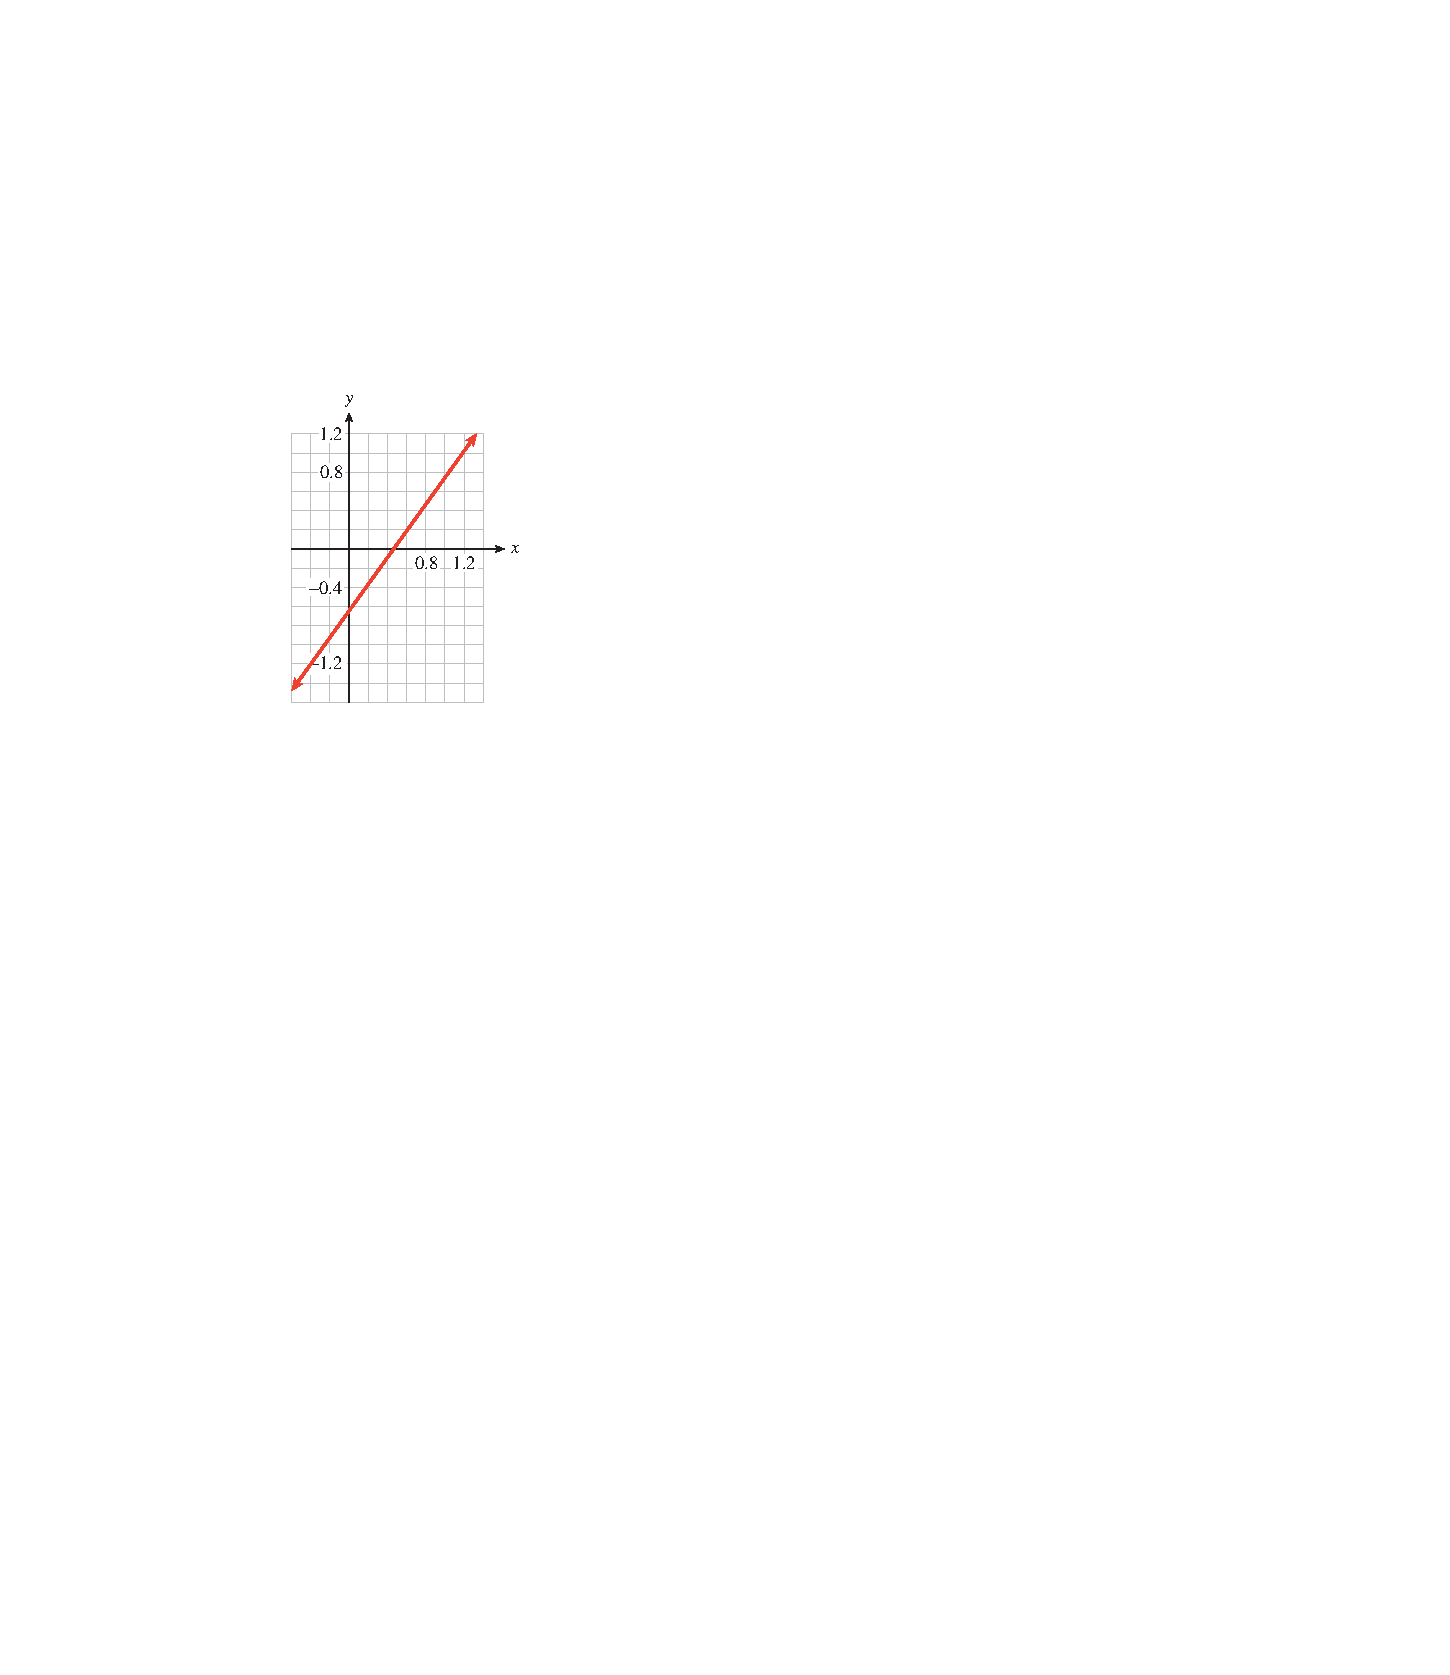
\includegraphics[width=\linewidth]{external/images/fig-ex-1-3-23.pdf}
\end{sbspanel}%
\end{sidebyside}%
\par
%
\begin{enumerate}[label=\alph*]
\item{}\(\displaystyle 1.4x - 0.64 = 0.2\)%
\item{}\(\displaystyle -1.2 = 1.4x - 0.64\)%
\item{}\(\displaystyle 1.4x - 0.64\gt 0.2\)%
\item{}\(\displaystyle -1.2\gt 1.4x - 0.64\)%
\end{enumerate}
%
\end{divisionexerciseeg}%
\begin{divisionexerciseeg}{24}{}{}{exercise-section-1-3-exercises-k-c}%
The figure shows the graph of \(y = -2.4x + 2.32\). Solve the following:%
\begin{sidebyside}{1}{0.325}{0.325}{0}%
\begin{sbspanel}{0.35}%
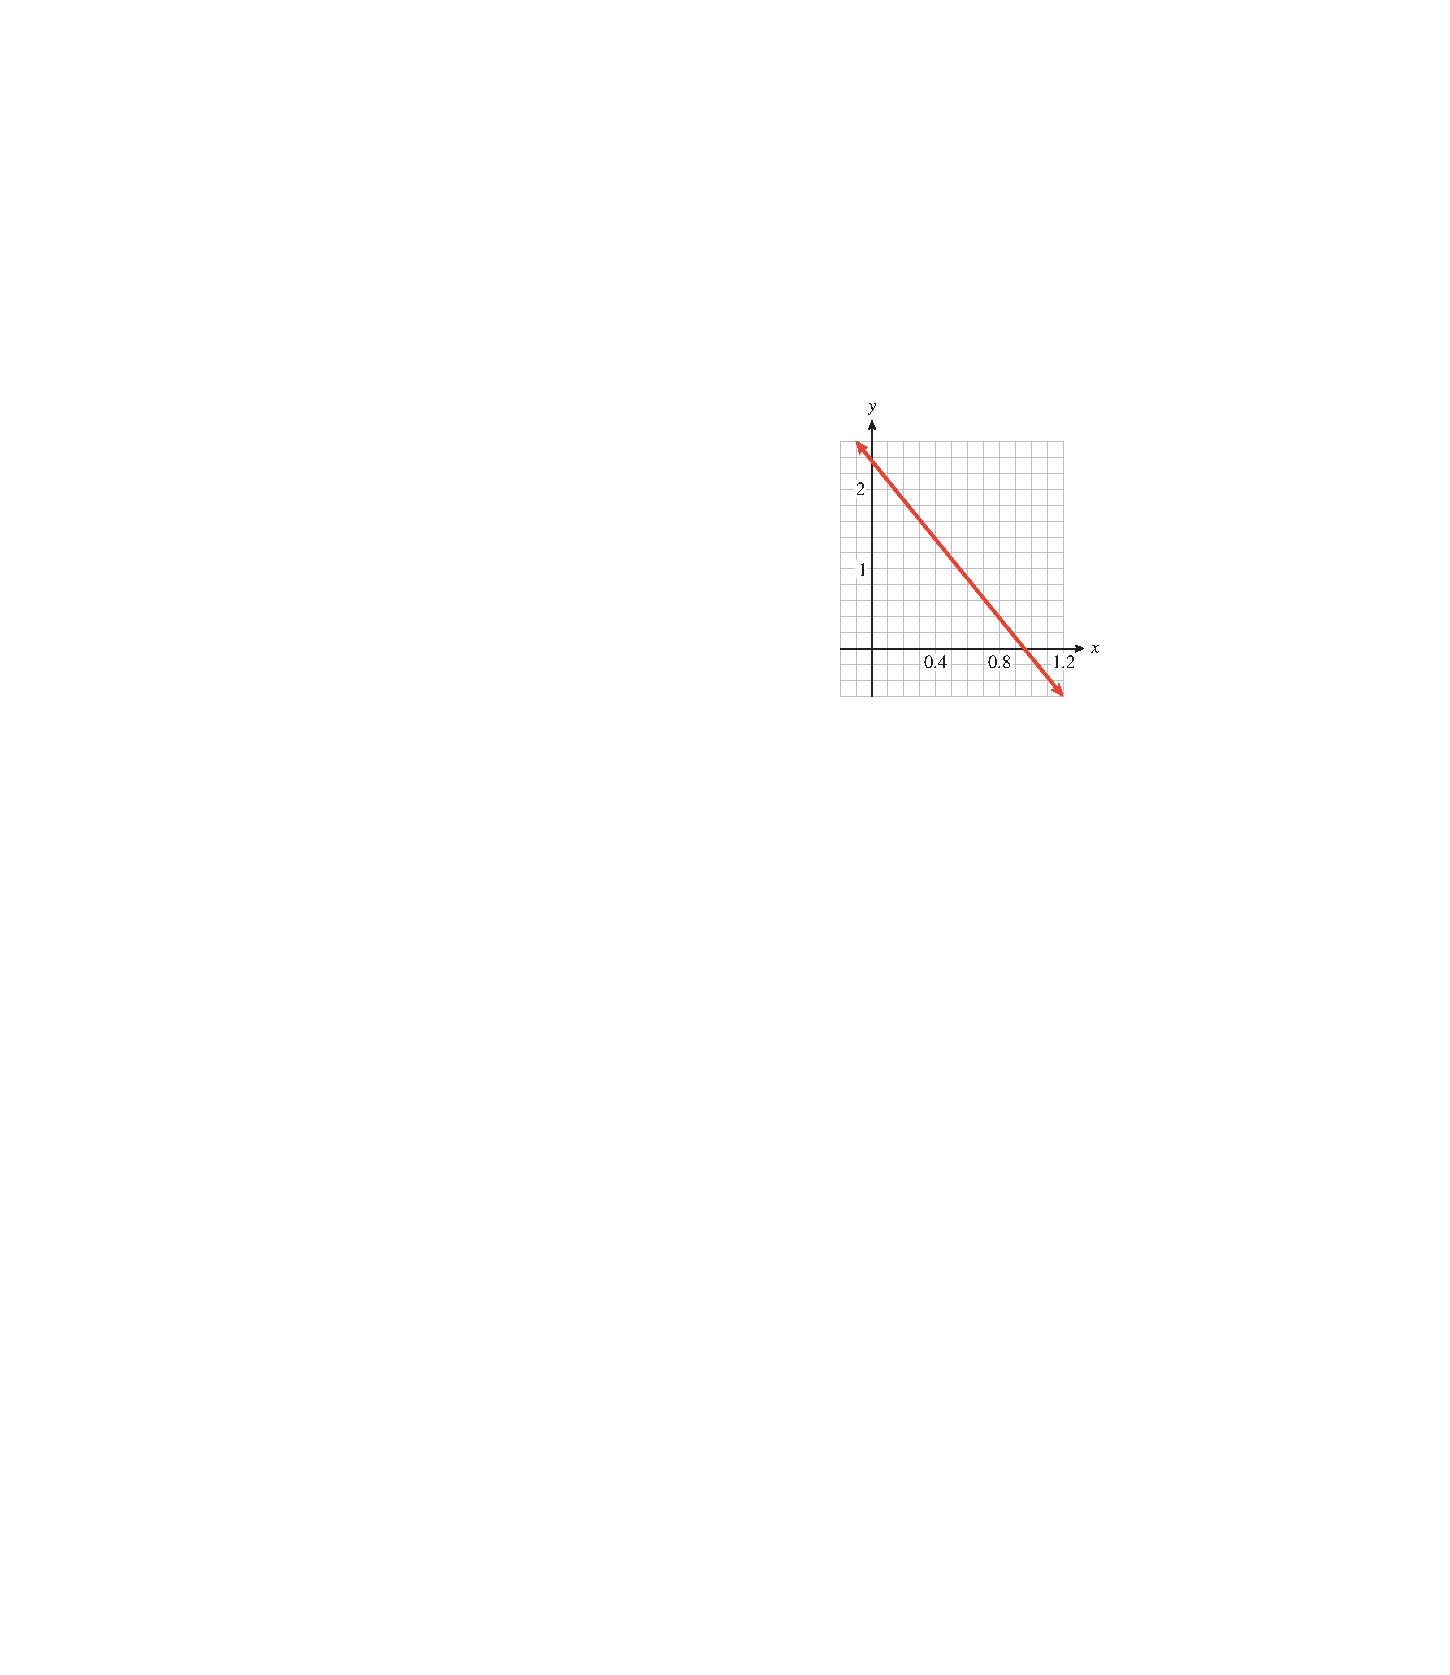
\includegraphics[width=\linewidth]{external/images/fig-ex-1-3-24.pdf}
\end{sbspanel}%
\end{sidebyside}%
\par
%
\begin{enumerate}[label=\alph*]
\item{}\(\displaystyle 1.6 = -2.4x + 2.32\)%
\item{}\(\displaystyle -2.4x + 2.32 = 0.4\)%
\item{}\(\displaystyle -2.4x + 2.32\ge 1.6\)%
\item{}\(\displaystyle 0.4\ge -2.4x + 2.32\)%
\end{enumerate}
%
\end{divisionexerciseeg}%
\end{exercisegroup}
\par\medskip\noindent
\par\medskip\noindent%
\textbf{Exercise Group.}\space\space%
For Problems 25\textendash{}30, use the graphs to estimate solutions to the equations and inequalities.%
\begin{exercisegroup}
\begin{divisionexerciseeg}{25}{}{}{exercise-section-1-3-exercises-l-b}%
The figure shows the graph of \(g(x) = \dfrac{12}{2 + x^2}\).%
\begin{sidebyside}{1}{0.325}{0.325}{0}%
\begin{sbspanel}{0.35}%
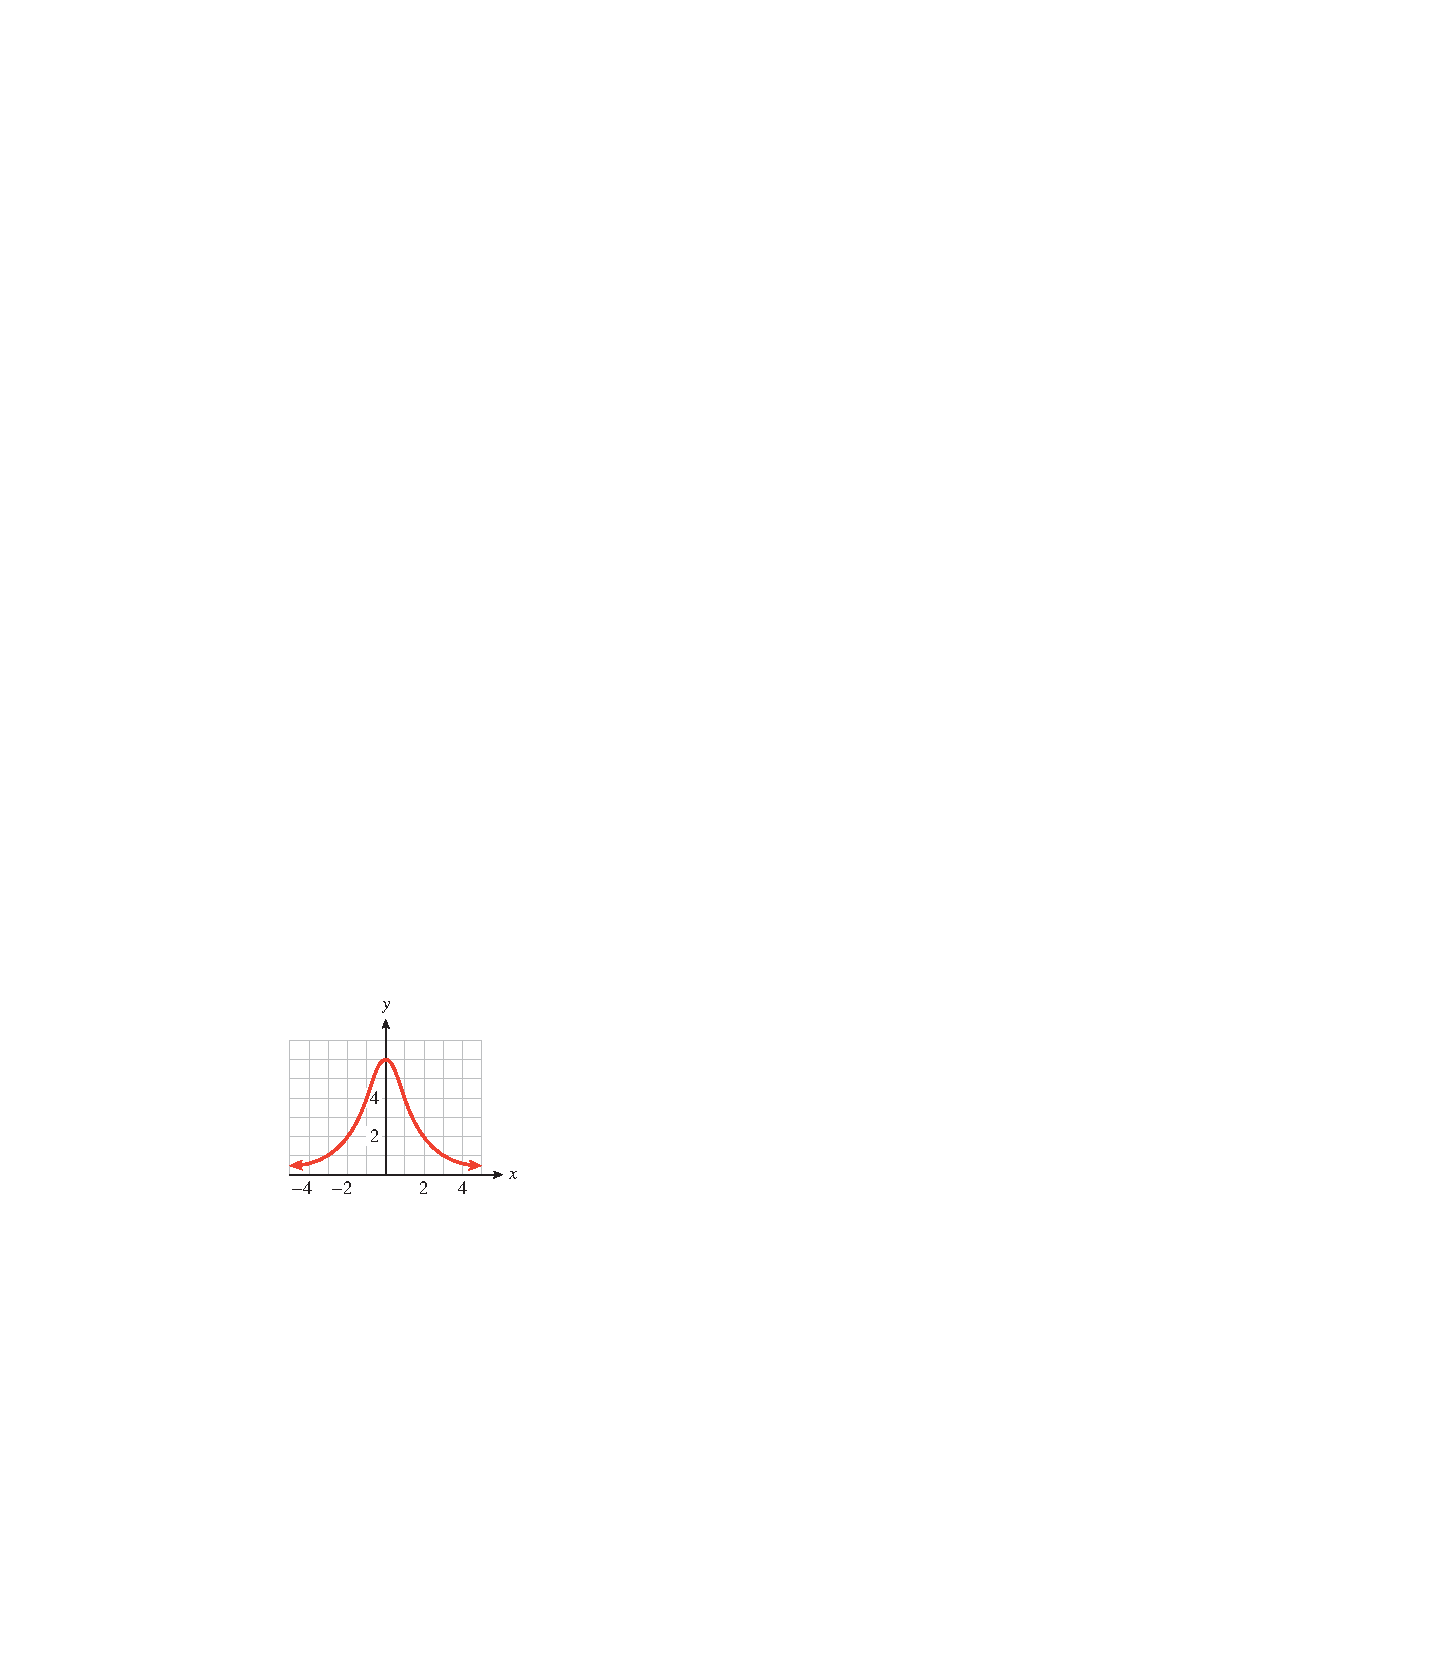
\includegraphics[width=\linewidth]{external/images/fig-ex-1-3-25.pdf}
\end{sbspanel}%
\end{sidebyside}%
\par
%
\begin{enumerate}[label=\alph*]
\item{}Solve \(\dfrac{12}{2 + x^2} = 4\)%
\item{}Solve \(1\le \dfrac{12}{2 + x^2} \le 2\)%
\end{enumerate}
%
\end{divisionexerciseeg}%
\begin{divisionexerciseeg}{26}{}{}{exercise-section-1-3-exercises-l-c}%
The figure shows the graph of \(f(x) = \dfrac{30\sqrt{x}}{1 + x}\).%
\begin{sidebyside}{1}{0.3}{0.3}{0}%
\begin{sbspanel}{0.4}%
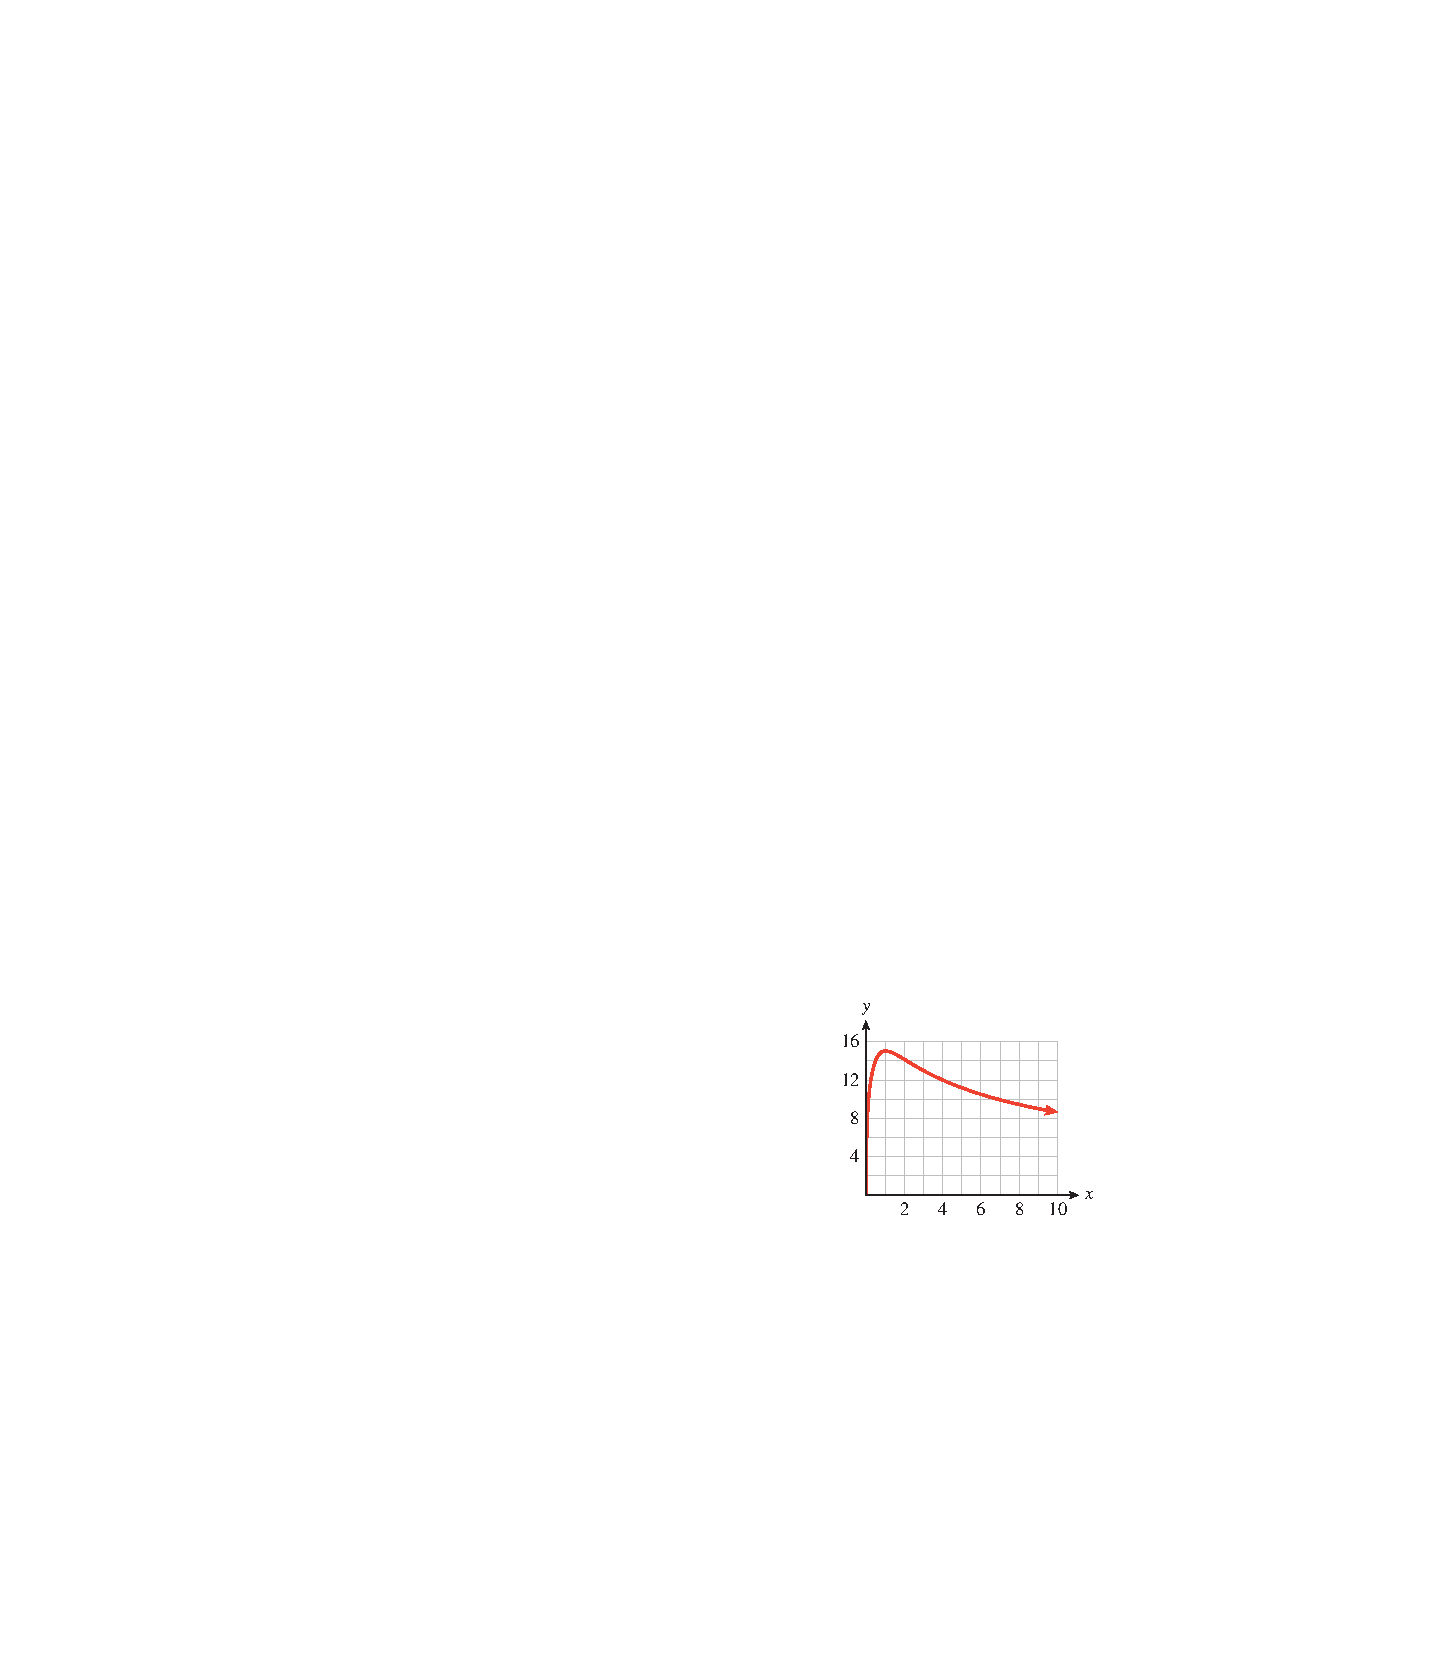
\includegraphics[width=\linewidth]{external/images/fig-ex-1-3-26.pdf}
\end{sbspanel}%
\end{sidebyside}%
\par
%
\begin{enumerate}[label=\alph*]
\item{}Solve \(\dfrac{30\sqrt{x}}{1 + x} = 15\)%
\item{}Solve \(\dfrac{30\sqrt{x}}{1 + x} \lt 12\)%
\end{enumerate}
%
\end{divisionexerciseeg}%
\begin{divisionexerciseeg}{27}{}{}{exercise-section-1-3-exercises-l-d}%
The figure shows a graph of \(B = \dfrac{1}{3}p^3 - 3p + 2\).%
\begin{sidebyside}{1}{0.3}{0.3}{0}%
\begin{sbspanel}{0.4}%
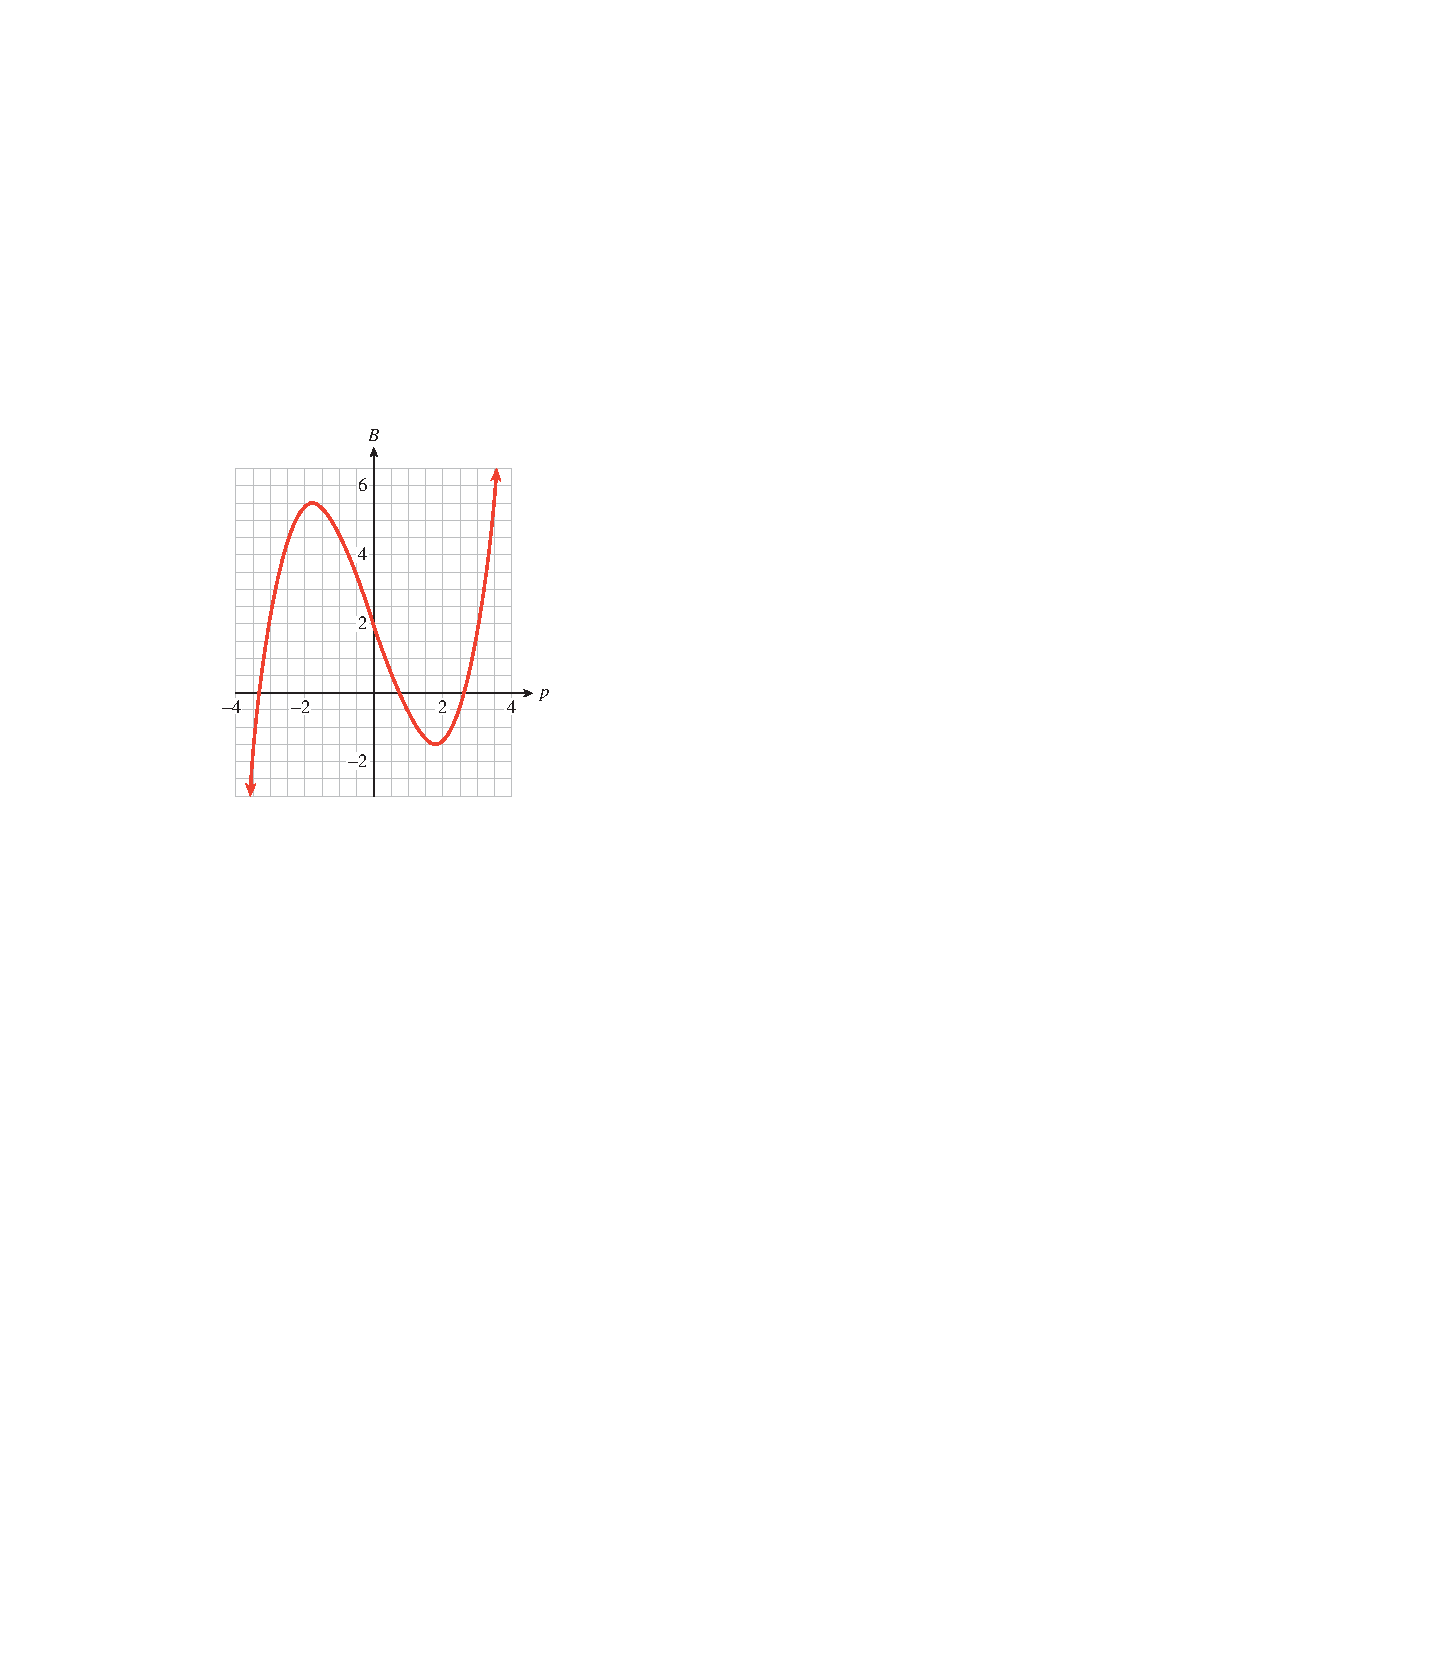
\includegraphics[width=\linewidth]{external/images/fig-ex-1-3-27.pdf}
\end{sbspanel}%
\end{sidebyside}%
\par
%
\begin{enumerate}[label=\alph*]
\item{}Solve \(\dfrac{1}{3}p^3 - 3p + 2 = 6\)%
\item{}Solve \(\dfrac{1}{3}p^3 - 3p + 2=5\)%
\item{}Solve \(\dfrac{1}{3}p^3 - 3p + 2\lt 1\)%
\item{}What range of values does \(B\) have for \(p\) between \(-2.5\) and \(0.5\)?%
\item{}For what values of \(p\) is \(B\) increasing?%
\end{enumerate}
%
\end{divisionexerciseeg}%
\begin{divisionexerciseeg}{28}{}{}{exercise-section-1-3-exercises-l-e}%
The figure shows a graph of \(H = t^3 - 4t^2 - 4t + 12\).%
\begin{sidebyside}{1}{0.325}{0.325}{0}%
\begin{sbspanel}{0.35}%
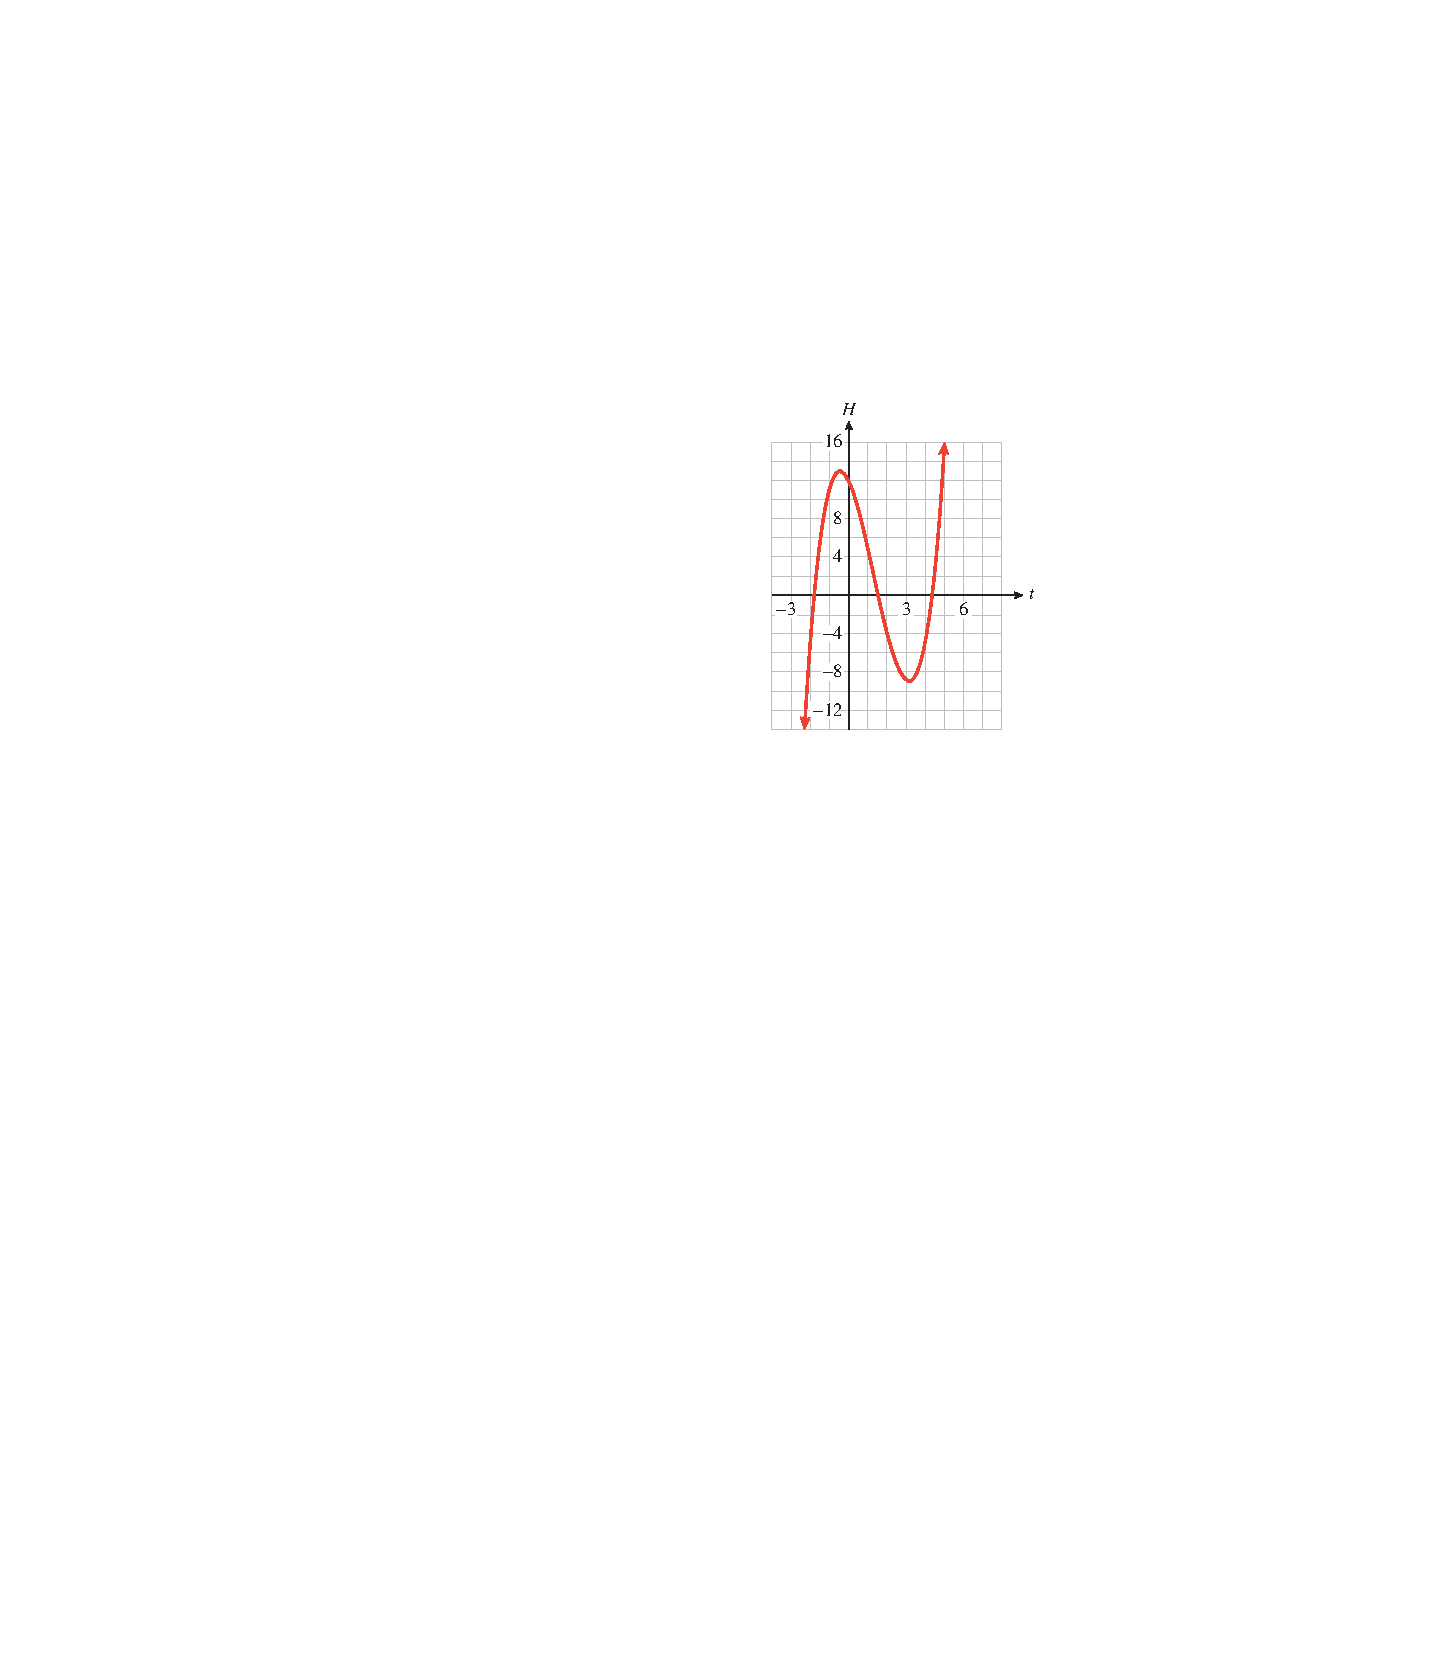
\includegraphics[width=\linewidth]{external/images/fig-ex-1-3-28.pdf}
\end{sbspanel}%
\end{sidebyside}%
\par
%
\begin{enumerate}[label=\alph*]
\item{}Solve \(t^3 - 4t^2 - 4t + 12 = -4\)%
\item{}Solve \(t^3 - 4t^2 - 4t + 12=16\)%
\item{}Solve \(t^3 - 4t^2 - 4t + 12\gt 6\)%
\item{}Estimate the horizontal and vertical intercepts of the graph.%
\item{}For what values of \(t\) is \(H\) increasing?%
\end{enumerate}
%
\end{divisionexerciseeg}%
\begin{divisionexerciseeg}{29}{}{}{exercise-section-1-3-exercises-l-f}%
The figure shows a graph of \(M = g(q)\).%
\begin{sidebyside}{1}{0.3}{0.3}{0}%
\begin{sbspanel}{0.4}%
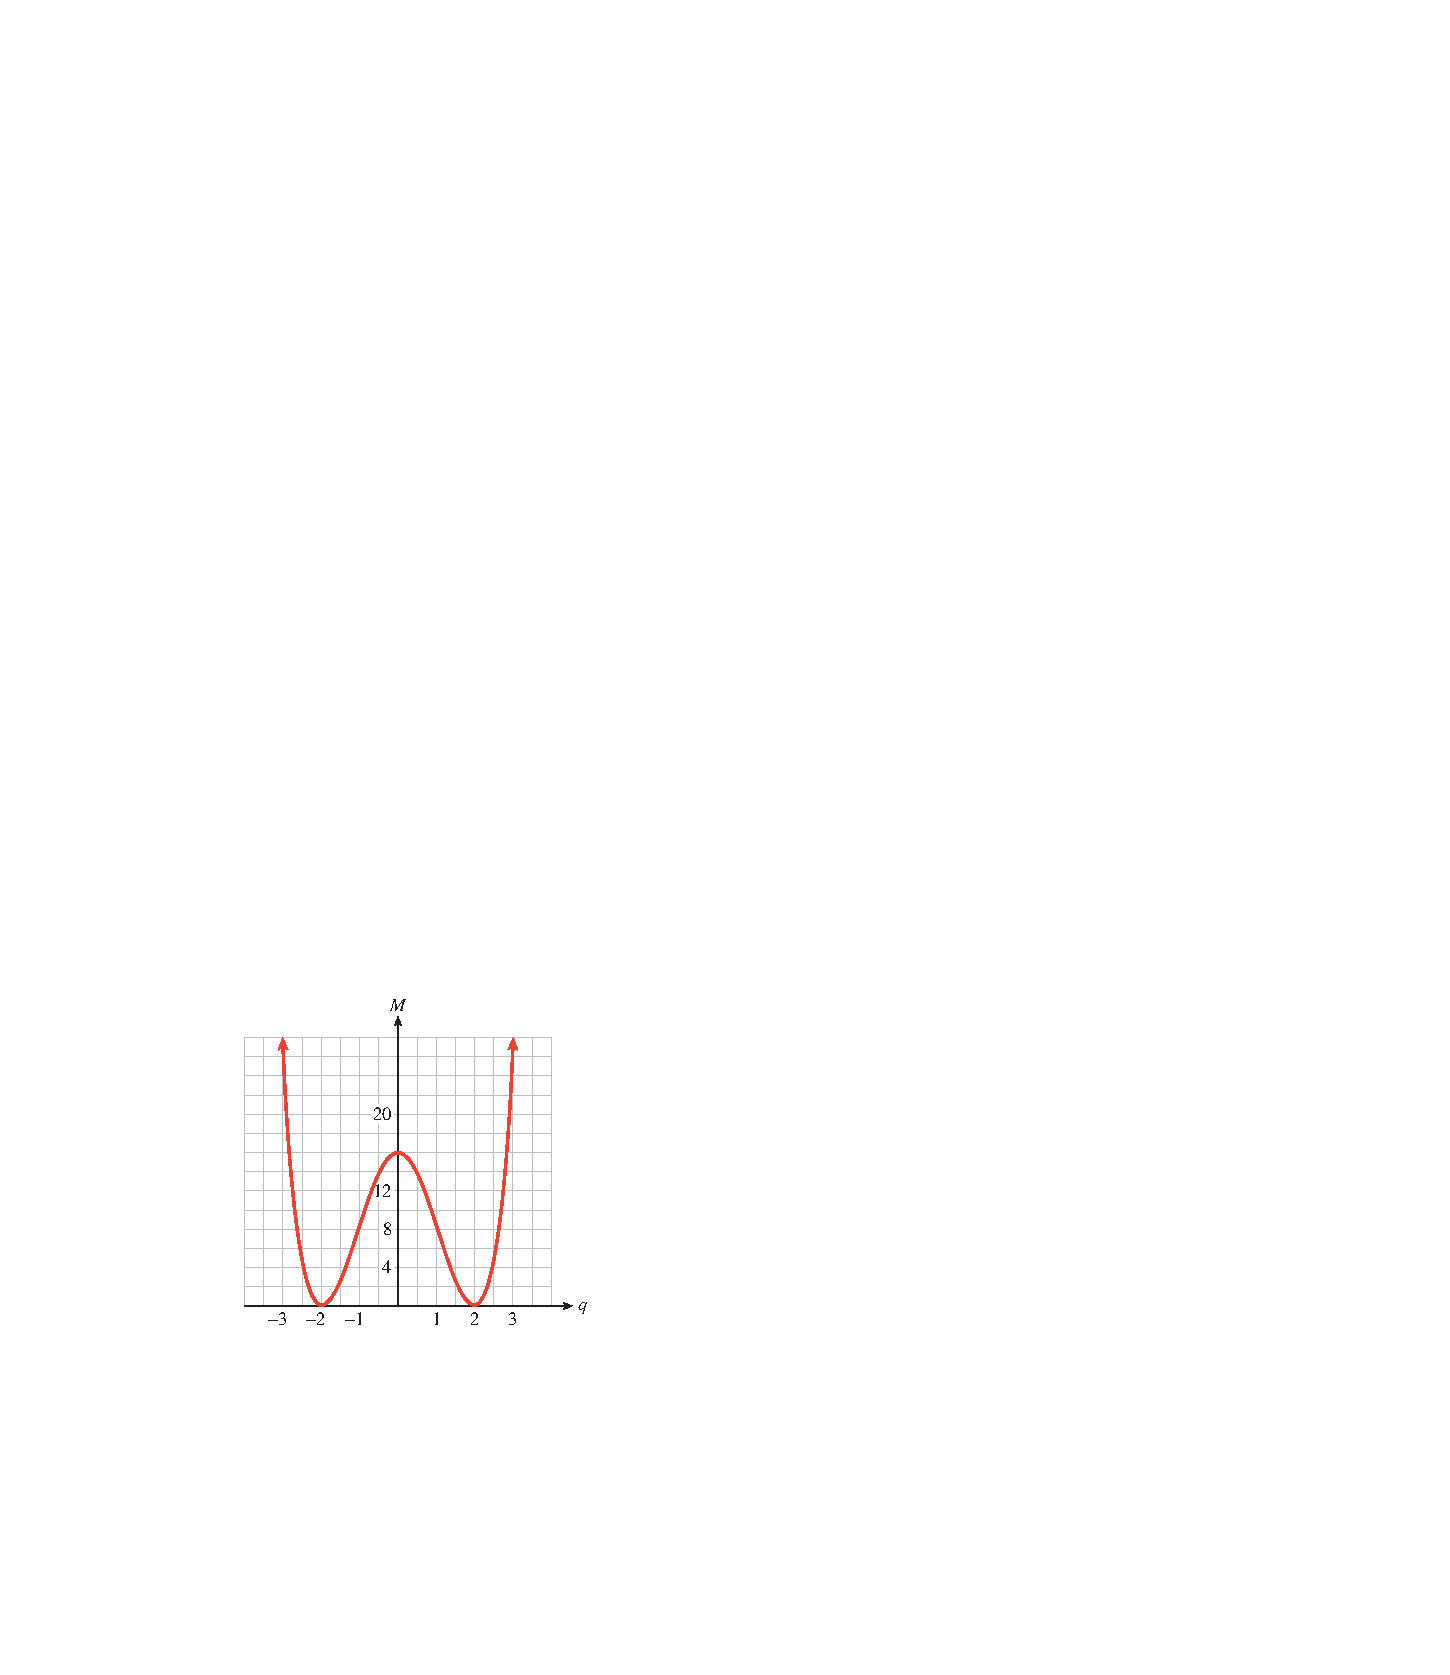
\includegraphics[width=\linewidth]{external/images/fig-ex-1-3-29.pdf}
\end{sbspanel}%
\end{sidebyside}%
\par
%
\begin{enumerate}[label=\alph*]
\item{}Find all values of \(q\) for which%
\begin{enumerate}[label=\Roman*]
\item{}\(\displaystyle g(q) = 0\)%
\item{}\(\displaystyle g(q) = 16\)%
\item{}\(\displaystyle g(q)\lt 6\)%
\end{enumerate}
%
\item{}For what values of \(q\) is \(g(q)\) increasing?%
\end{enumerate}
%
\end{divisionexerciseeg}%
\begin{divisionexerciseeg}{30}{}{}{exercise-section-1-3-exercises-l-g}%
The figure shows a graph of \(P = f (t)\).%
\begin{sidebyside}{1}{0.35}{0.35}{0}%
\begin{sbspanel}{0.3}%
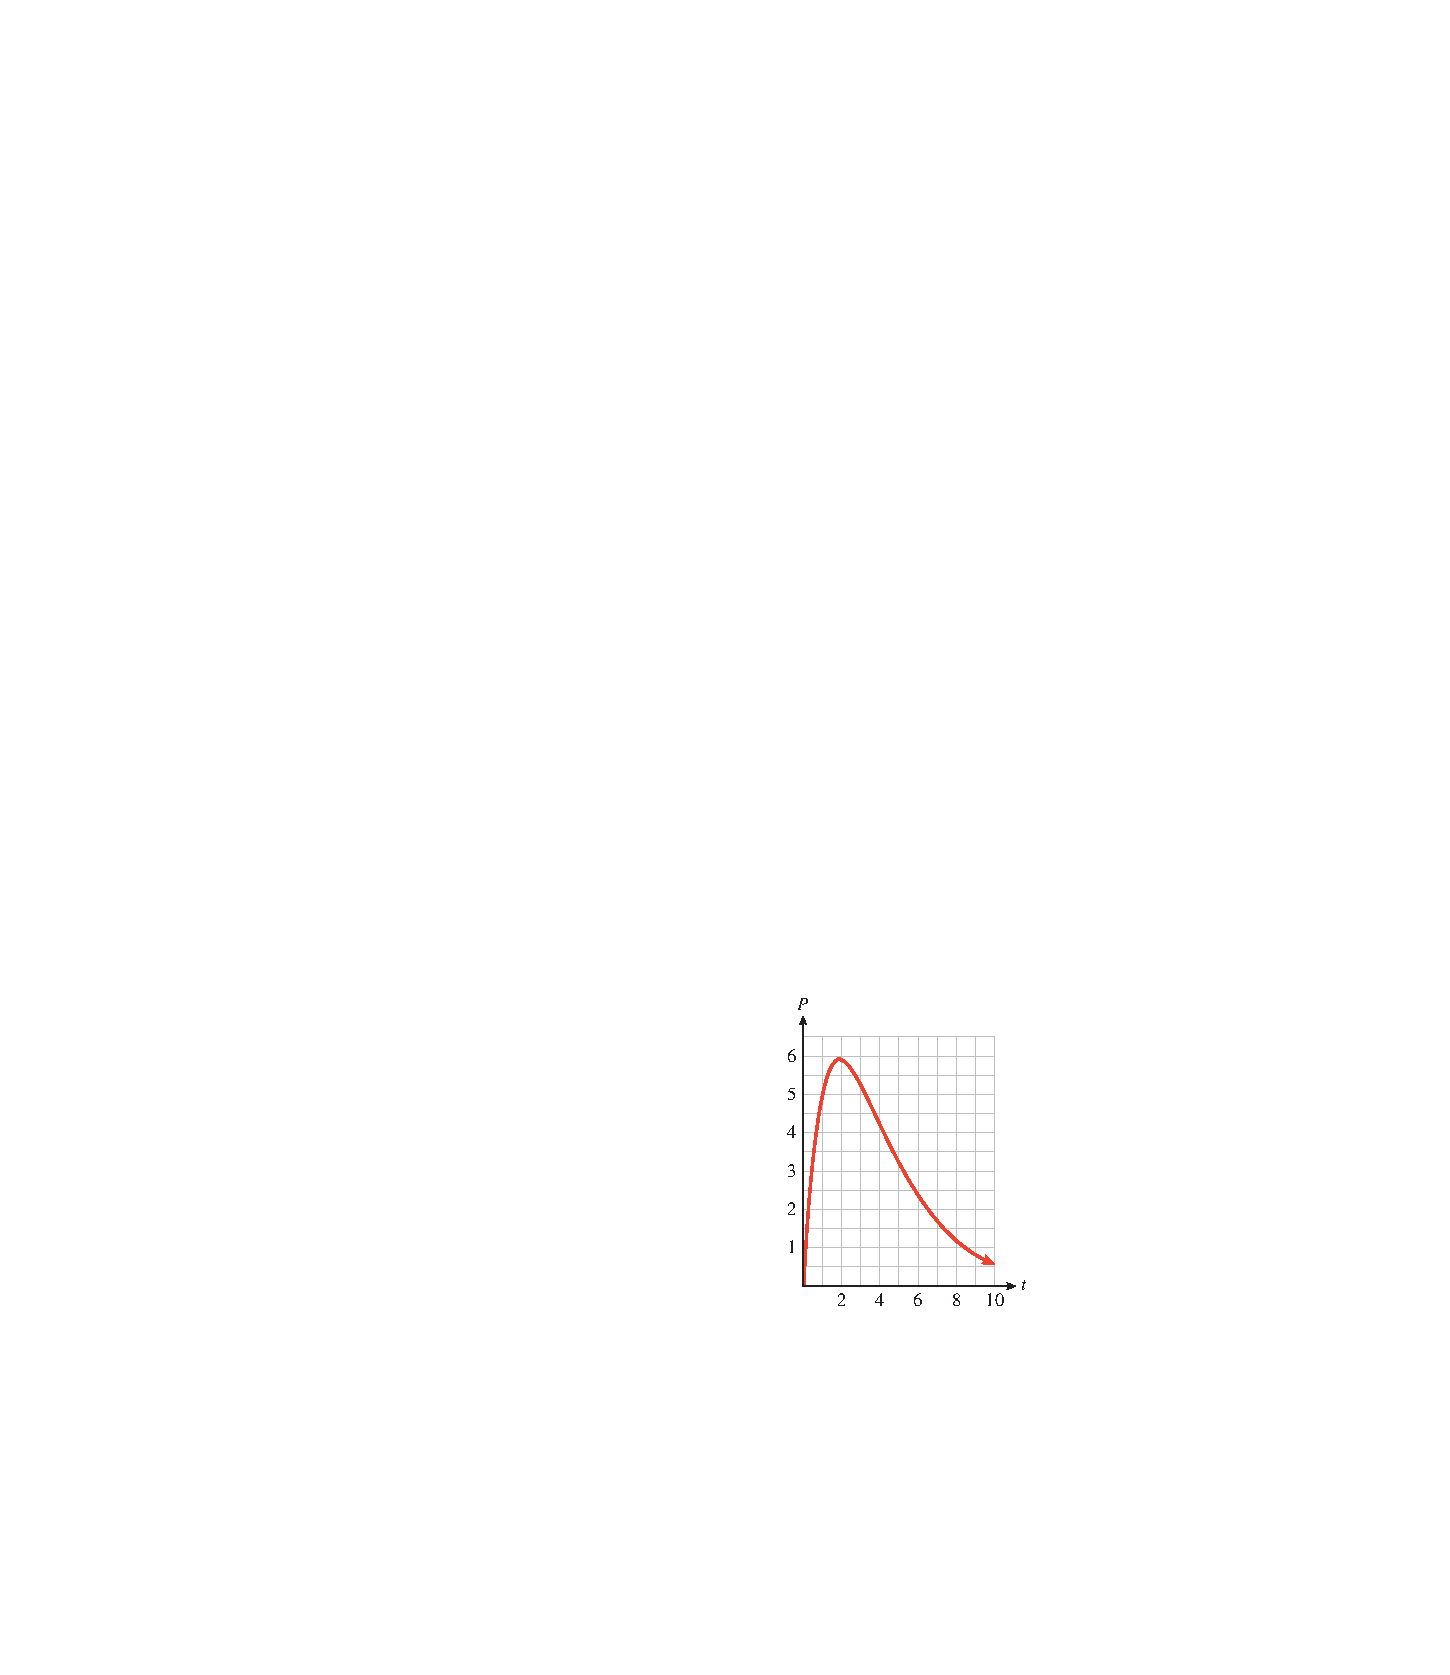
\includegraphics[width=\linewidth]{external/images/fig-ex-1-3-30.pdf}
\end{sbspanel}%
\end{sidebyside}%
\par
%
\begin{enumerate}[label=\alph*]
\item{}Find all values of \(t\) for which%
\begin{enumerate}[label=\Roman*]
\item{}\(\displaystyle f (t) = 3\)%
\item{}\(\displaystyle f (t)\gt 4.5\)%
\item{}\(\displaystyle 2\le f (t)\le 4\)%
\end{enumerate}
%
\item{}For what values of \(t\) is \(f (t)\) decreasing?%
\end{enumerate}
%
\end{divisionexerciseeg}%
\end{exercisegroup}
\par\medskip\noindent
\begin{divisionexercise}{31}{}{}{exercise-section-1-3-exercises-m}%
%
\begin{enumerate}[label=\alph*]
\item{}Delbert reads the following values from the graph of a function:%
\begin{equation*}
f (-3) = 5, ~f (-1) = 2, ~f (1) = 0,
\end{equation*}
%
\begin{equation*}
f (-1) = -4, ~f (-3) = -2
\end{equation*}
Can his readings be correct? Explain why or why not.%
\item{}Francine reads the following values from the graph of a function:%
\begin{equation*}
g(-2) = 6, ~g(0) = 0, ~g(2) = 6,
\end{equation*}
%
\begin{equation*}
g(4) = 0, ~g(6) = 6
\end{equation*}
Can her readings be correct? Explain why or why not.%
\end{enumerate}
%
\end{divisionexercise}%
\begin{divisionexercise}{32}{}{}{exercise-section-1-3-exercises-n}%
%
\begin{enumerate}[label=\alph*]
\item{}Sketch the graph of a function that has the following values:%
\begin{equation*}
F(-2) = 3, ~F(-1) = 3, ~F(0) = 3,
\end{equation*}
%
\begin{equation*}
F(1) = 3, ~F(2) = 3
\end{equation*}
%
\item{}Sketch the graph of a function that has the following values:%
\begin{equation*}
G(-2) = 1, ~G(-1) = 0, ~G(0) = -1,
\end{equation*}
%
\begin{equation*}
G(1) = 0, ~G(2) = 1
\end{equation*}
%
\end{enumerate}
%
\end{divisionexercise}%
\par\medskip\noindent%
\textbf{Exercise Group.}\space\space%
For Problems 33\textendash{}36, graph each function in the friendly window%
\begin{align*}
\text{Xmin} \amp = -9.4 \amp\amp \text{Xmax} = 9.4\\
\text{Ymin} \amp = -10 \amp\amp \text{Ymax} = 10
\end{align*}
Then answer the questions about the graph. (See \hyperref[appendix-appendix-b]{Appendix~{\xreffont\ref{appendix-appendix-b}}}  for an explanation of friendly windows.)%
\begin{exercisegroup}
\begin{divisionexerciseeg}{33}{}{}{exercise-section-1-3-exercises-o-b}%
\(g(x) =\sqrt{36 - x^2}\)%
\begin{enumerate}[label=\alph*]
\item{}Complete the table. (Round values to tenths.)%
\begin{sidebyside}{1}{0}{0}{0}%
\begin{sbspanel}{1}%
\resizebox{\ifdim\width > \linewidth\linewidth\else\width\fi}{!}{%
{\centering%
{\tabularfont%
\begin{tabular}{AcAcAcAcAcA}\hrulethick
\(x\)&\(-4\)&\(-2\)&\(3\)&\(5\)\tabularnewline\hrulethin
\(g(x)\)&\(\hphantom{000}\)&\(\hphantom{000}\)&\(\hphantom{000}\)&\(\hphantom{000}\)\tabularnewline\hrulethin
\end{tabular}
}%
\par}
}%
\end{sbspanel}%
\end{sidebyside}%
\item{}Find all points on the graph for which \(g(x) = 3.6\).%
\end{enumerate}
%
\end{divisionexerciseeg}%
\begin{divisionexerciseeg}{34}{}{}{exercise-section-1-3-exercises-o-c}%
\(g(x) =\sqrt{x^2}-6\)%
\begin{enumerate}[label=(\alph*)]
\item{}Complete the table. (Round values to tenths.)%
\begin{sidebyside}{1}{0}{0}{0}%
\begin{sbspanel}{1}%
\resizebox{\ifdim\width > \linewidth\linewidth\else\width\fi}{!}{%
{\centering%
{\tabularfont%
\begin{tabular}{AcAcAcAcAcA}\hrulethick
\(x\)&\(-8\)&\(-2\)&\(3\)&\(6\)\tabularnewline\hrulethin
\(f(x)\)&\(\hphantom{000}\)&\(\hphantom{000}\)&\(\hphantom{000}\)&\(\hphantom{000}\)\tabularnewline\hrulethin
\end{tabular}
}%
\par}
}%
\end{sbspanel}%
\end{sidebyside}%
\item{}Find all points on the graph for which \(f(x) = -2\).%
\end{enumerate}
%
\end{divisionexerciseeg}%
\begin{divisionexerciseeg}{35}{}{}{exercise-section-1-3-exercises-o-d}%
\(F(x) = 0.5x^3 - 4x\)%
\begin{enumerate}[label=\alph*]
\item{}Estimate the coordinates of the turning points of the graph, that is, where the graph changes from increasing to decreasing or vice versa.%
\item{}Write an equation of the form \(F(a) = b\) for each turning point.%
\end{enumerate}
%
\end{divisionexerciseeg}%
\begin{divisionexerciseeg}{36}{}{}{exercise-section-1-3-exercises-o-e}%
\(G(x) = 2 + 4x - x^3\)%
\begin{enumerate}[label=\alph*]
\item{}Estimate the coordinates of the turning points of the graph, that is, where the graph changes from increasing to decreasing or vice versa.%
\item{}Write an equation of the form \(G(a) = b\) for each turning point.%
\end{enumerate}
%
\end{divisionexerciseeg}%
\end{exercisegroup}
\par\medskip\noindent
\par\medskip\noindent%
\textbf{Exercise Group.}\space\space%
For Problems 37\textendash{}40, graph the function%
\begin{enumerate}[label=\alph*]
\item{}First using the standard window.%
\item{}Then using the suggested window. Explain how the window alters the appearance of the graph in each case.%
\end{enumerate}
%
\begin{exercisegroupcol}{2}
\begin{divisionexerciseegcol}{37}{}{}{exercise-section-1-3-exercises-p-b}%
\(h(x) = \dfrac{1}{x^2 + 10}\)%
\begin{align*}
{\text{Xmin}} \amp = -5 \amp\amp {\text{Xmax}} = 5\\
{\text{Ymin}} \amp = 0 \amp\amp {\text{Ymax}} = 0.5
\end{align*}
%
\end{divisionexerciseegcol}%
\begin{divisionexerciseegcol}{38}{}{}{exercise-section-1-3-exercises-p-c}%
\(H(x) =\sqrt{1-x^2} \)%
\begin{align*}
{\text{Xmin}} \amp = -2 \amp\amp {\text{Xmax}} = 2\\
{\text{Ymin}} \amp = -2 \amp\amp {\text{Ymax}} = 2
\end{align*}
%
\end{divisionexerciseegcol}%
\begin{divisionexerciseegcol}{39}{}{}{exercise-section-1-3-exercises-p-d}%
\(P(x) = (x - 8)(x + 6)(x - 15)\)%
\begin{align*}
{\text{Xmin}} \amp = -10 \amp\amp {\text{Xmax}} = 20\\
{\text{Ymin}} \amp = -250 \amp\amp {\text{Ymax}} = 750
\end{align*}
%
\end{divisionexerciseegcol}%
\begin{divisionexerciseegcol}{40}{}{}{exercise-section-1-3-exercises-p-e}%
\(p(x) = 200x^3\)%
\begin{align*}
{\text{Xmin}} \amp = -5 \amp\amp {\text{Xmax}} = 5\\
{\text{Ymin}} \amp = -10,000 \amp\amp {\text{Ymax}} = 10,000
\end{align*}
%
\end{divisionexerciseegcol}%
\end{exercisegroupcol}
\par\medskip\noindent
\par\medskip\noindent%
\textbf{Exercise Group.}\space\space%
For Problems 41\textendash{}44, graph the equation with the ZInteger setting. (Press \kbd{ZOOM} \(6\),then \kbd{ZOOM} \(8\) \kbd{ENTER}.) Use the graph to answer each question. Use the equation to verify your answers.%
\begin{exercisegroup}
\begin{divisionexerciseeg}{41}{}{}{exercise-section-1-3-exercises-q-b}%
Graph \(y = 2x - 3\)%
\begin{enumerate}[label=\alph*]
\item{}For what value of \(x\) is \(y = 5\)?%
\item{}For what value of \(x\) is \(y = -13\)?%
\item{}For what values of \(x\) is \(y\gt -1 \)?%
\item{}For what values of \(x\) is \(y\lt 25\)?%
\end{enumerate}
%
\end{divisionexerciseeg}%
\begin{divisionexerciseeg}{42}{}{}{exercise-section-1-3-exercises-q-c}%
Graph \(y = 4 - 2x\)%
\begin{enumerate}[label=\alph*]
\item{}For what value of \(x\) is \(y = 6\)?%
\item{}For what value of \(x\) is \(y = -4\)?%
\item{}For what values of \(x\) is \(y\gt -12 \)?%
\item{}For what values of \(x\) is \(y\lt 18\)?%
\end{enumerate}
%
\end{divisionexerciseeg}%
\begin{divisionexerciseeg}{43}{}{}{exercise-section-1-3-exercises-q-d}%
Graph \(y = 6.5 - 1.8x\)%
\begin{enumerate}[label=\alph*]
\item{}For what value of \(x\) is \(y = -13.3\)?%
\item{}For what value of \(x\) is \(y = 24.5\)?%
\item{}For what values of \(x\) is \(y\le 15.5 \)?%
\item{}For what values of \(x\) is \(y\ge -7.9\)?%
\end{enumerate}
%
\end{divisionexerciseeg}%
\begin{divisionexerciseeg}{44}{}{}{exercise-section-1-3-exercises-q-e}%
Graph \(y = 0.2x + 1.4\)%
\begin{enumerate}[label=\alph*]
\item{}For what value of \(x\) is \(y = -5.2\)?%
\item{}For what value of \(x\) is \(y = 2.8\)?%
\item{}For what values of \(x\) is \(y\le -3.2 \)?%
\item{}For what values of \(x\) is \(y\ge 4.4\)?%
\end{enumerate}
%
\end{divisionexerciseeg}%
\end{exercisegroup}
\par\medskip\noindent
\par\medskip\noindent%
\textbf{Exercise Group.}\space\space%
For Problems 45\textendash{}48, graph the equation with the ZInteger setting. Use the graph to solve each equation or inequality. Check your solutions algebraically.%
\begin{exercisegroup}
\begin{divisionexerciseeg}{45}{}{}{exercise-section-1-3-exercises-r-b}%
Graph \(y = -0.4x + 3.7\)%
\begin{enumerate}[label=\alph*]
\item{}Solve \(-0.4x + 3.7 = 2.1\)%
\item{}Solve \(-0.4x + 3.7\gt -5.1\)%
\end{enumerate}
%
\end{divisionexerciseeg}%
\begin{divisionexerciseeg}{46}{}{}{exercise-section-1-3-exercises-r-c}%
Graph \(y = 0.4 (x - 1.5)\)%
\begin{enumerate}[label=\alph*]
\item{}Solve \(0.4 (x - 1.5) = -8.6\)%
\item{}Solve \(0.4 (x - 1.5)\lt 8.6\)%
\end{enumerate}
%
\end{divisionexerciseeg}%
\begin{divisionexerciseeg}{47}{}{}{exercise-section-1-3-exercises-r-d}%
Graph \(y = \dfrac{2}{3}x - 24\)%
\begin{enumerate}[label=\alph*]
\item{}Solve \(\dfrac{2}{3}x - 24 = -10\dfrac{2}{3} \)%
\item{}Solve \(\dfrac{2}{3}x - 24\le -19\dfrac{1}{3} \)%
\end{enumerate}
%
\end{divisionexerciseeg}%
\begin{divisionexerciseeg}{48}{}{}{exercise-section-1-3-exercises-r-e}%
Graph \(y = \dfrac{80 - 3x}{5}\).%
\begin{enumerate}[label=\alph*]
\item{}Solve \(\dfrac{80 - 3x}{5} = 22\dfrac{3}{5} \).%
\item{}Solve \(\dfrac{80 - 3x}{5}\le -9\dfrac{2}{5} \).%
\end{enumerate}
%
\end{divisionexerciseeg}%
\end{exercisegroup}
\par\medskip\noindent
\begin{divisionexercise}{49}{}{}{exercise-section-1-3-exercises-s}%
Graph \(y = 0.01x^3 - 0.1x^2 - 2.75x + 15\).%
\begin{enumerate}[label=\alph*]
\item{}Use your graph to solve \(0.01x^3 - 0.1x^2 - 2.75x + 15 = 0\).%
\item{}Press \kbd{Y=} and enter \(Y_2 = 10\). Press \kbd{GRAPH}, and you should see the horizontal line \(y = 10\) superimposed on your previous graph. How many solutions does the equation%
\begin{equation*}
0.01x^3 - 0.1x^2 - 2.75x + 15 = 10
\end{equation*}
have? Estimate each solution to the nearest whole number.%
\end{enumerate}
%
\end{divisionexercise}%
\begin{divisionexercise}{50}{}{}{exercise-section-1-3-exercises-t}%
Graph \(y = 2.5x - 0.025x^2 - 0.005x^3\).%
\begin{enumerate}[label=\alph*]
\item{}Use your graph to solve \(2.5x - 0.025x^2 - 0.005x^3 = 0\).%
\item{}Press \kbd{Y=} and enter \(Y_2 = -5\). Press \kbd{GRAPH}, and you should see the horizontal line \(y = -5\) superimposed on your previous graph. How many solutions does the equation%
\begin{equation*}
2.5x - 0.025x^2 - 0.005x^3 = -5
\end{equation*}
have? Estimate each solution to the nearest whole number.%
\end{enumerate}
%
\end{divisionexercise}%
\end{exercises-subsection}
\end{sectionptx}
%
%
\typeout{************************************************}
\typeout{Section 1.4 Slope and Rate of Change}
\typeout{************************************************}
%
\begin{sectionptx}{Section}{Slope and Rate of Change}{}{Slope and Rate of Change}{}{}{section-slope-and-rate-of-change}
%
%
\typeout{************************************************}
\typeout{Subsection  Using Ratios for Comparison}
\typeout{************************************************}
%
\begin{subsectionptx}{Subsection}{Using Ratios for Comparison}{}{Using Ratios for Comparison}{}{}{subsection-slope-and-rate-of-change-b}
Which is more expensive, a 64-ounce bottle of Velvolux dish soap that costs \textdollar{}3.52, or a 60-ounce bottle of Rainfresh dish soap that costs \textdollar{}3.36?%
\par
You are probably familiar with the notion of comparison shopping. To decide which dish soap is the better buy, we compute the unit price, or price per ounce, for each bottle. The unit price for Velvolux is%
\begin{equation*}
\frac{352 \text{ cents}}{64 \text{ ounces}}= 5.5 \text{ cents per ounce}
\end{equation*}
and the unit price for Rainfresh is%
\begin{equation*}
\frac{336 \text{ cents}}{60 \text{ ounces}}= 5.6 \text{ cents per ounce}
\end{equation*}
%
\par
The Velvolux costs less per ounce, so it is the better buy. By computing the price of each brand for \emph{the same amount of soap}, it is easy to compare them.%
\par
In many situations, a ratio, similar to a unit price, can provide a basis for comparison. \hyperref[example-example-rate-of-growth]{Example~{\xreffont\ref{example-example-rate-of-growth}}} uses a ratio to measure a rate of growth.%
\begin{example}{Example}{}{example-example-rate-of-growth}%
Which grow faster, Hybrid A wheat seedlings, which grow 11.2 centimeters in 14 days, or Hybrid B seedlings, which grow 13.5 centimeters in 18 days?%
\par\smallskip%
\noindent\textbf{\blocktitlefont Solution}.\hypertarget{solution-example-rate-of-growth-b}{}\quad{}We compute the growth rate for each strain of wheat. Growth rate is expressed as a ratio, \(\dfrac{\text{centimeters}}{\text{days}}\), or centimeters per day. The growth rate for Hybrid A is%
\begin{equation*}
\frac{11.2 \text{ centimeters}}{14 \text{ days}}= 0.8 \text{ centimeters per day}
\end{equation*}
and the growth rate for Hybrid B is%
\begin{equation*}
\frac{13.5 \text{ centimeters}}{18 \text{ days}}= 0.75 \text{ centimeters per day}
\end{equation*}
Because their rate of growth is larger, the Hybrid A seedlings grow faster.%
\end{example}
By computing the growth of each strain of wheat seedling over the same unit of time, a single day, we have a basis for comparison. In this case, the ratio \(\dfrac{\text{centimeters}}{\text{day}}\) measures the rate of growth of the wheat seedlings.%
\begin{inlineexercise}{Checkpoint}{Practice 1.}{exercise-exercise-gas-mileage}%
Delbert traveled \(258\) miles on \(12\) gallons of gas, and Francine traveled \(182\) miles on \(8\) gallons of gas. Compute the ratio \(\dfrac{\text{miles}}{\text{gallon}}\) for each car.%
\par
Delbert: \fillintext{5} \(\dfrac{\text{miles}}{\text{gallon}}\)%
\par
Francine: \fillintext{5} \(\dfrac{\text{miles}}{\text{gallon}}\)%
\par
Whose car gets the better gas mileage?\quad(\begin{itemize*}[label=$\square$,leftmargin=3em,itemjoin=\hspace{1em}]
\item{}Delbert%
\item{}Francine%
\end{itemize*})\quad
%
\par\smallskip%
\noindent\textbf{\blocktitlefont Answer 1}.\hypertarget{answer-exercise-gas-mileage-c}{}\quad{}\(21.5\)%
\par\smallskip%
\noindent\textbf{\blocktitlefont Answer 2}.\hypertarget{answer-exercise-gas-mileage-d}{}\quad{}\(22.75\)%
\par\smallskip%
\noindent\textbf{\blocktitlefont Answer 3}.\hypertarget{answer-exercise-gas-mileage-e}{}\quad{}\(\text{Francine}\)%
\par\smallskip%
\noindent\textbf{\blocktitlefont Solution}.\hypertarget{solution-exercise-gas-mileage-f}{}\quad{}Delbert: \(\dfrac{258}{12}= 21.5\) mpg, Francine: \(\dfrac{182}{8}=22.75\) mpg. Francine gets better mileage.%
\end{inlineexercise}%
\begin{inlineexercise}{Checkpoint}{QuickCheck 1.}{exercise-slope-and-rate-of-change-b-i}%
The weight of \(12\) gallons of gasoline is \(67.5\) pounds, and the weight of \(5\) gallons of water is \(41.6\) pounds. Compute the ratio \(\dfrac{\text{pounds}}{\text{gallon}}\) for each liquid.%
\par
gasoline: \fillintext{5} \(\dfrac{\text{pounds}}{\text{gallon}}\)%
\par
water: \fillintext{5} \(\dfrac{\text{pounds}}{\text{gallon}}\)%
\par
Which liquid weighs more per gallon\quad(\begin{itemize*}[label=$\square$,leftmargin=3em,itemjoin=\hspace{1em}]
\item{}gasoline%
\item{}water%
\end{itemize*})\quad
%
\par\smallskip%
\noindent\textbf{\blocktitlefont Answer 1}.\hypertarget{answer-slope-and-rate-of-change-b-i-c}{}\quad{}\(5.625\)%
\par\smallskip%
\noindent\textbf{\blocktitlefont Answer 2}.\hypertarget{answer-slope-and-rate-of-change-b-i-d}{}\quad{}\(8.32\)%
\par\smallskip%
\noindent\textbf{\blocktitlefont Answer 3}.\hypertarget{answer-slope-and-rate-of-change-b-i-e}{}\quad{}\(\text{water}\)%
\par\smallskip%
\noindent\textbf{\blocktitlefont Solution}.\hypertarget{solution-slope-and-rate-of-change-b-i-f}{}\quad{}gasoline: \(\dfrac{67.5}{12}= 5.625\) pounds per gallon, water: \(\dfrac{41.6}{5}=8.32\) pounds per gallon. Water weighs more per gallon.%
\end{inlineexercise}%
In \hyperref[exercise-exercise-gas-mileage]{Checkpoint~{\xreffont\ref{exercise-exercise-gas-mileage}}}, the ratio \(\dfrac{\text{miles}}{\text{gallon}}\) measures the rate at which each car uses gasoline. By computing the mileage for each car for the same amount of gas, we have a basis for comparison. We can use this same idea, finding a common basis for comparison, to measure the steepness of an incline.%
\end{subsectionptx}
%
%
\typeout{************************************************}
\typeout{Subsection  Measuring Steepness}
\typeout{************************************************}
%
\begin{subsectionptx}{Subsection}{Measuring Steepness}{}{Measuring Steepness}{}{}{subsection-slope-and-rate-of-change-c}
Imagine you are an ant carrying a heavy burden along one of the two paths shown below. Which path is more difficult? Most ants would agree that the steeper path is more difficult.%
\begin{sidebyside}{2}{0.0125}{0.0125}{0.025}%
\begin{sbspanel}{0.5}%
But what exactly is steepness? It is not merely the gain in altitude, because even a gentle incline will reach a great height eventually. Steepness measures how sharply the altitude increases. An ant finds the second path more difficult, or steeper, because it rises 5 feet while the first path rises only 2 feet over the same horizontal distance.%
\end{sbspanel}%
\begin{sbspanel}{0.45}%
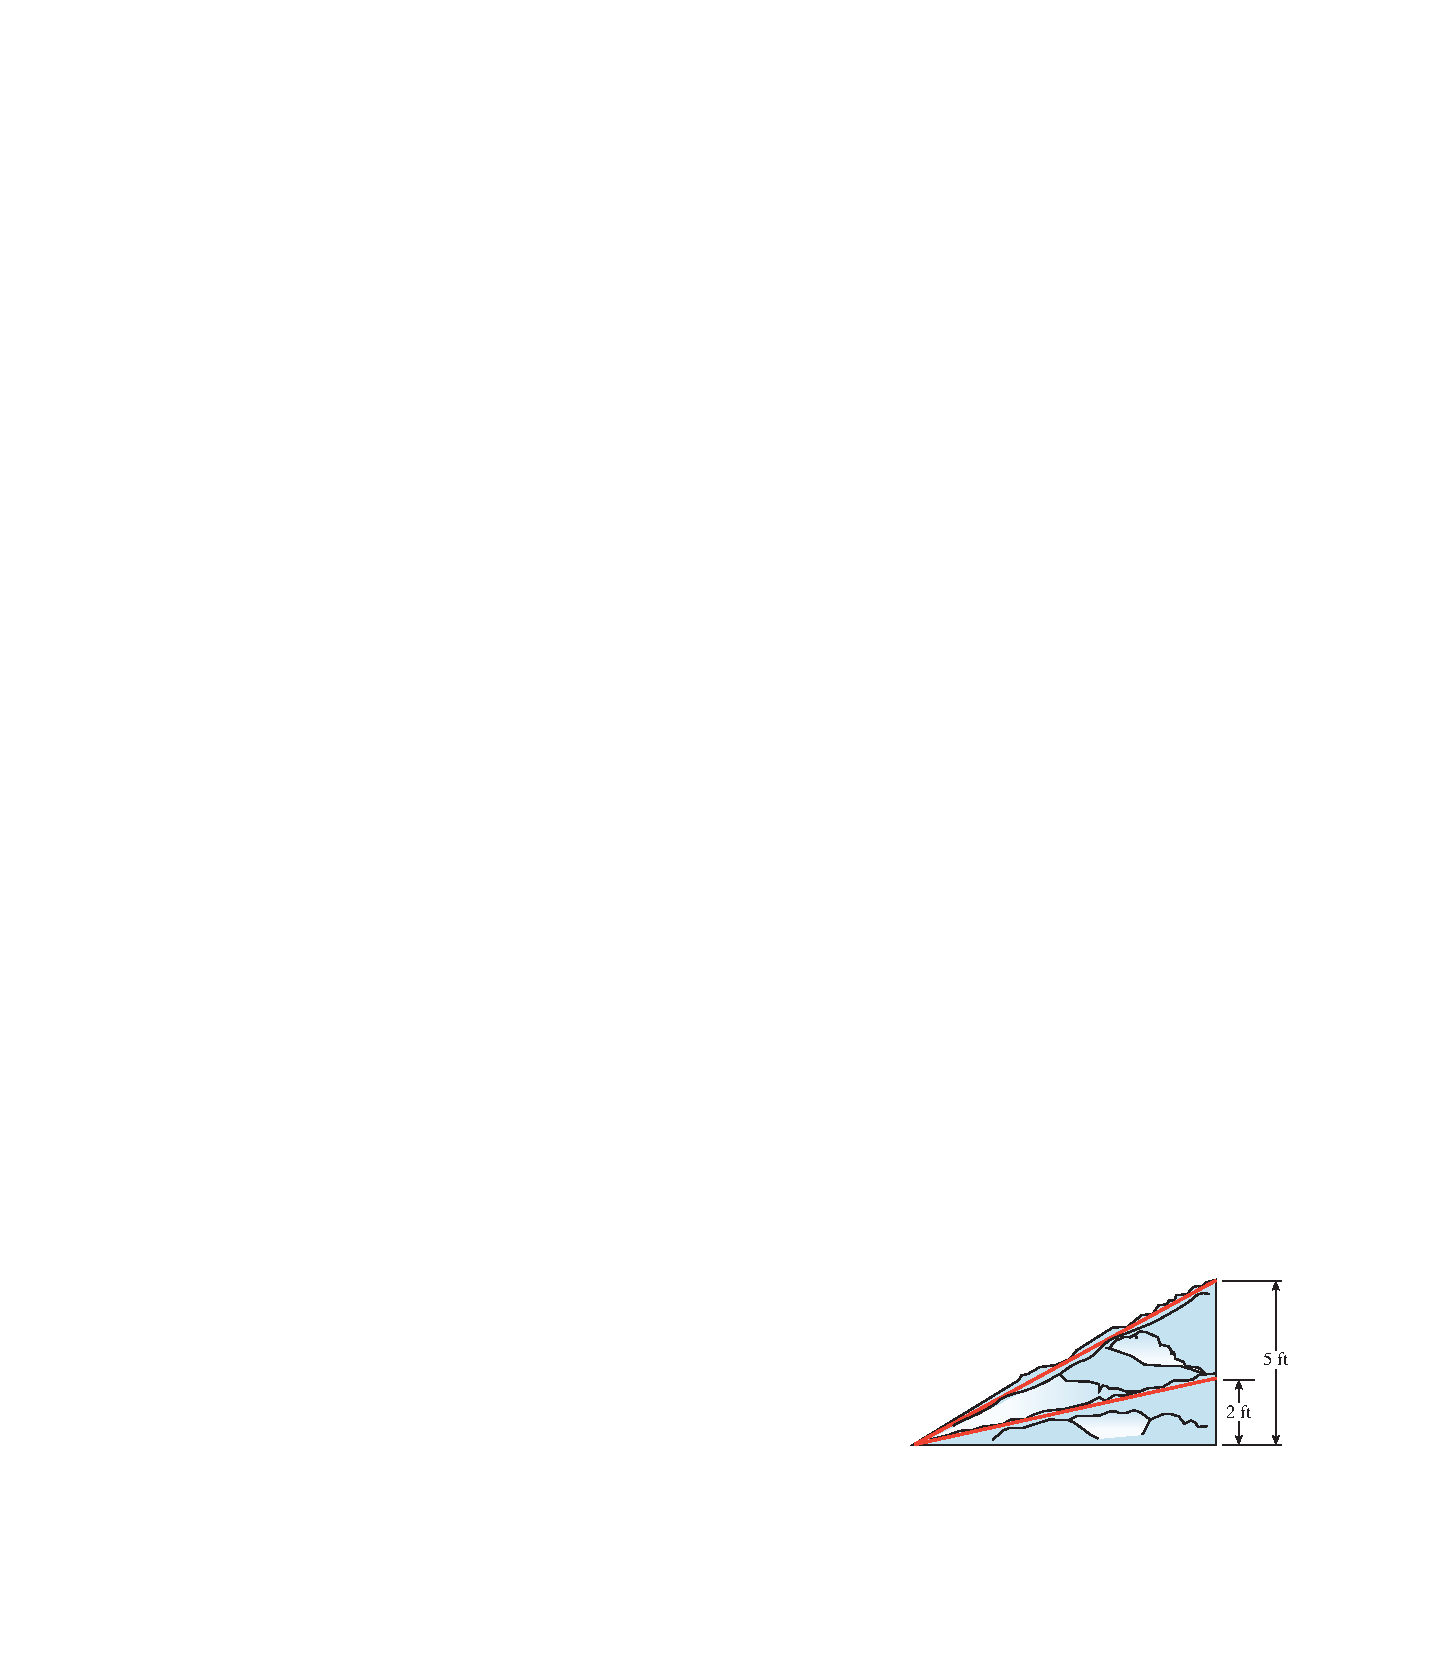
\includegraphics[width=\linewidth]{external/images/fig-ant-climb.pdf}
\end{sbspanel}%
\end{sidebyside}%
\par
To compare the steepness of two inclined paths, we compute the ratio of change in altitude to change in horizontal distance for each path.%
\begin{example}{Example}{}{example-example-steep-trail}%
Which is steeper, Stony Point trail, which climbs 400 feet over a horizontal distance of 2500 feet, or Lone Pine trail, which climbs 360 feet over a horizontal distance of 1800 feet?%
\par\smallskip%
\noindent\textbf{\blocktitlefont Solution}.\hypertarget{solution-example-steep-trail-b}{}\quad{}For each trail, we compute the ratio of vertical gain to horizontal distance. For Stony Point trail, the ratio is%
\begin{equation*}
\frac{400 \text{ feet}}{2500 \text{ feet}}= 0.16 
\end{equation*}
and for Lone Pine trail, the ratio is%
\begin{equation*}
\frac{360 \text{ feet}}{1800 \text{ feet}}= 0.20 
\end{equation*}
Lone Pine trail is steeper, because it has a vertical gain of 0.20 foot for every foot traveled horizontally. Or, in more practical units, Lone Pine trail rises 20 feet for every 100 feet of horizontal distance, whereas Stony Point trail rises only 16 feet over a horizontal distance of 100 feet.%
\end{example}
\begin{inlineexercise}{Checkpoint}{Practice 2.}{exercise-slope-and-rate-of-change-c-f}%
Which is steeper, a staircase that rises \(10\) feet over a horizontal distance of \(4\) feet, or the steps in the football stadium, which rise \(20\) yards over a horizontal distance of \(12\) yards?%
\par
Answer:\quad(\begin{itemize*}[label=$\square$,leftmargin=3em,itemjoin=\hspace{1em}]
\item{}staircase%
\item{}steps in stadium%
\end{itemize*})\quad
%
\par\smallskip%
\noindent\textbf{\blocktitlefont Answer}.\hypertarget{answer-slope-and-rate-of-change-c-f-c}{}\quad{}\(\text{staircase}\)%
\par\smallskip%
\noindent\textbf{\blocktitlefont Solution}.\hypertarget{solution-slope-and-rate-of-change-c-f-d}{}\quad{}Staircase: \(\dfrac{10}{4}= 2.5\text{,}\) Steps: \(\dfrac{20}{12}\approx 1.66666666666667\text{.}\) The staircase is steeper.%
\end{inlineexercise}%
\end{subsectionptx}
%
%
\typeout{************************************************}
\typeout{Subsection  Definition of Slope}
\typeout{************************************************}
%
\begin{subsectionptx}{Subsection}{Definition of Slope}{}{Definition of Slope}{}{}{subsection-slope-and-rate-of-change-d}
To compare the steepness of the two trails in \hyperref[example-example-steep-trail]{Example~{\xreffont\ref{example-example-steep-trail}}}, it is not enough to know which trail has the greater gain in elevation overall. Instead, we compare their elevation gains \emph{over the same horizontal distance.} Using the same horizontal distance provides a basis for comparison. The two trails are illustrated below as lines on a coordinate grid.%
\begin{sidebyside}{1}{0.15}{0.15}{0}%
\begin{sbspanel}{0.7}%
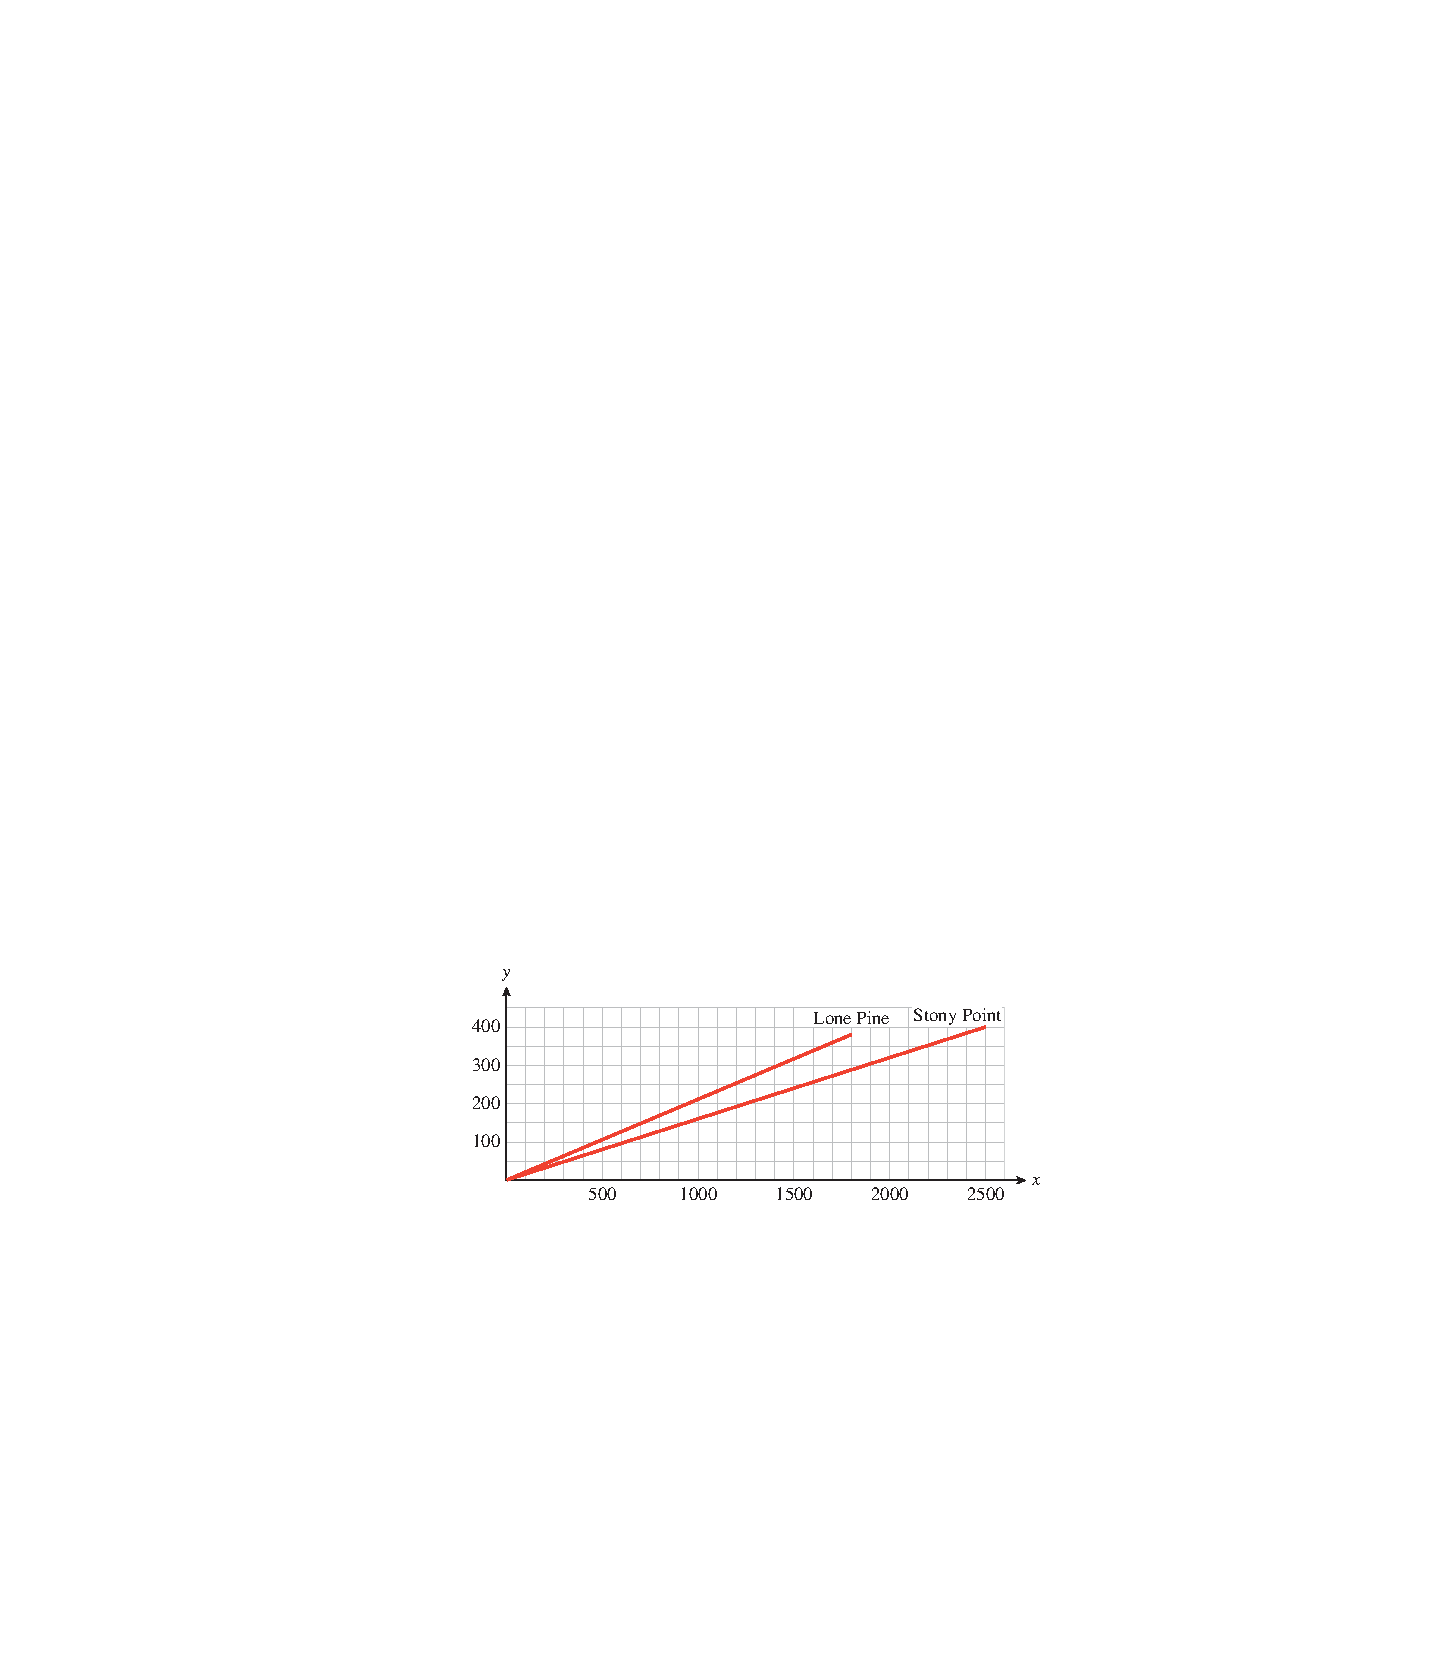
\includegraphics[width=\linewidth]{external/images/fig-trail-climb-grid.pdf}
\end{sbspanel}%
\end{sidebyside}%
\par
The ratio we computed in \hyperref[example-example-steep-trail]{Example~{\xreffont\ref{example-example-steep-trail}}},%
\begin{equation*}
\frac{\text{change in elevation}}{\text{change in horizontal position}}
\end{equation*}
appears on the graphs as%
\begin{equation*}
\frac{\text{change in }y\text{-coordinate}}{\text{change in }x\text{-coordinate}}
\end{equation*}
For example, as we travel along the line representing Stony Point trail, we move from the point \((0, 0)\) to the point \((2500, 400)\). The \(y\)-coordinate changes by \(400\) and the \(x\)-coordinate changes by \(2500\), giving the ratio \(0.16\) that we found in \hyperref[example-example-steep-trail]{Example~{\xreffont\ref{example-example-steep-trail}}}. We call this ratio the \terminology{slope} of the line.%
\begin{assemblage}{Assemblage}{Definition of Slope.}{assemblage-slope-and-rate-of-change-d-e}%
The \terminology{slope}\index{slope} of a line is the ratio%
\begin{equation*}
\frac{\text{change in }y\text{-coordinate}}{\text{change in }x\text{-coordinate}}
\end{equation*}
as we move from one point to another on the line.%
\end{assemblage}
\begin{example}{Example}{}{example-example-slope-grid}%
\begin{sidebyside}{2}{0.055}{0.055}{0.11}%
\begin{sbspanel}{0.5}[center]%
Compute the slope of the line that passes through points \(A\) and \(B\) on the graph at right.%
\end{sbspanel}%
\begin{sbspanel}{0.28}[center]%
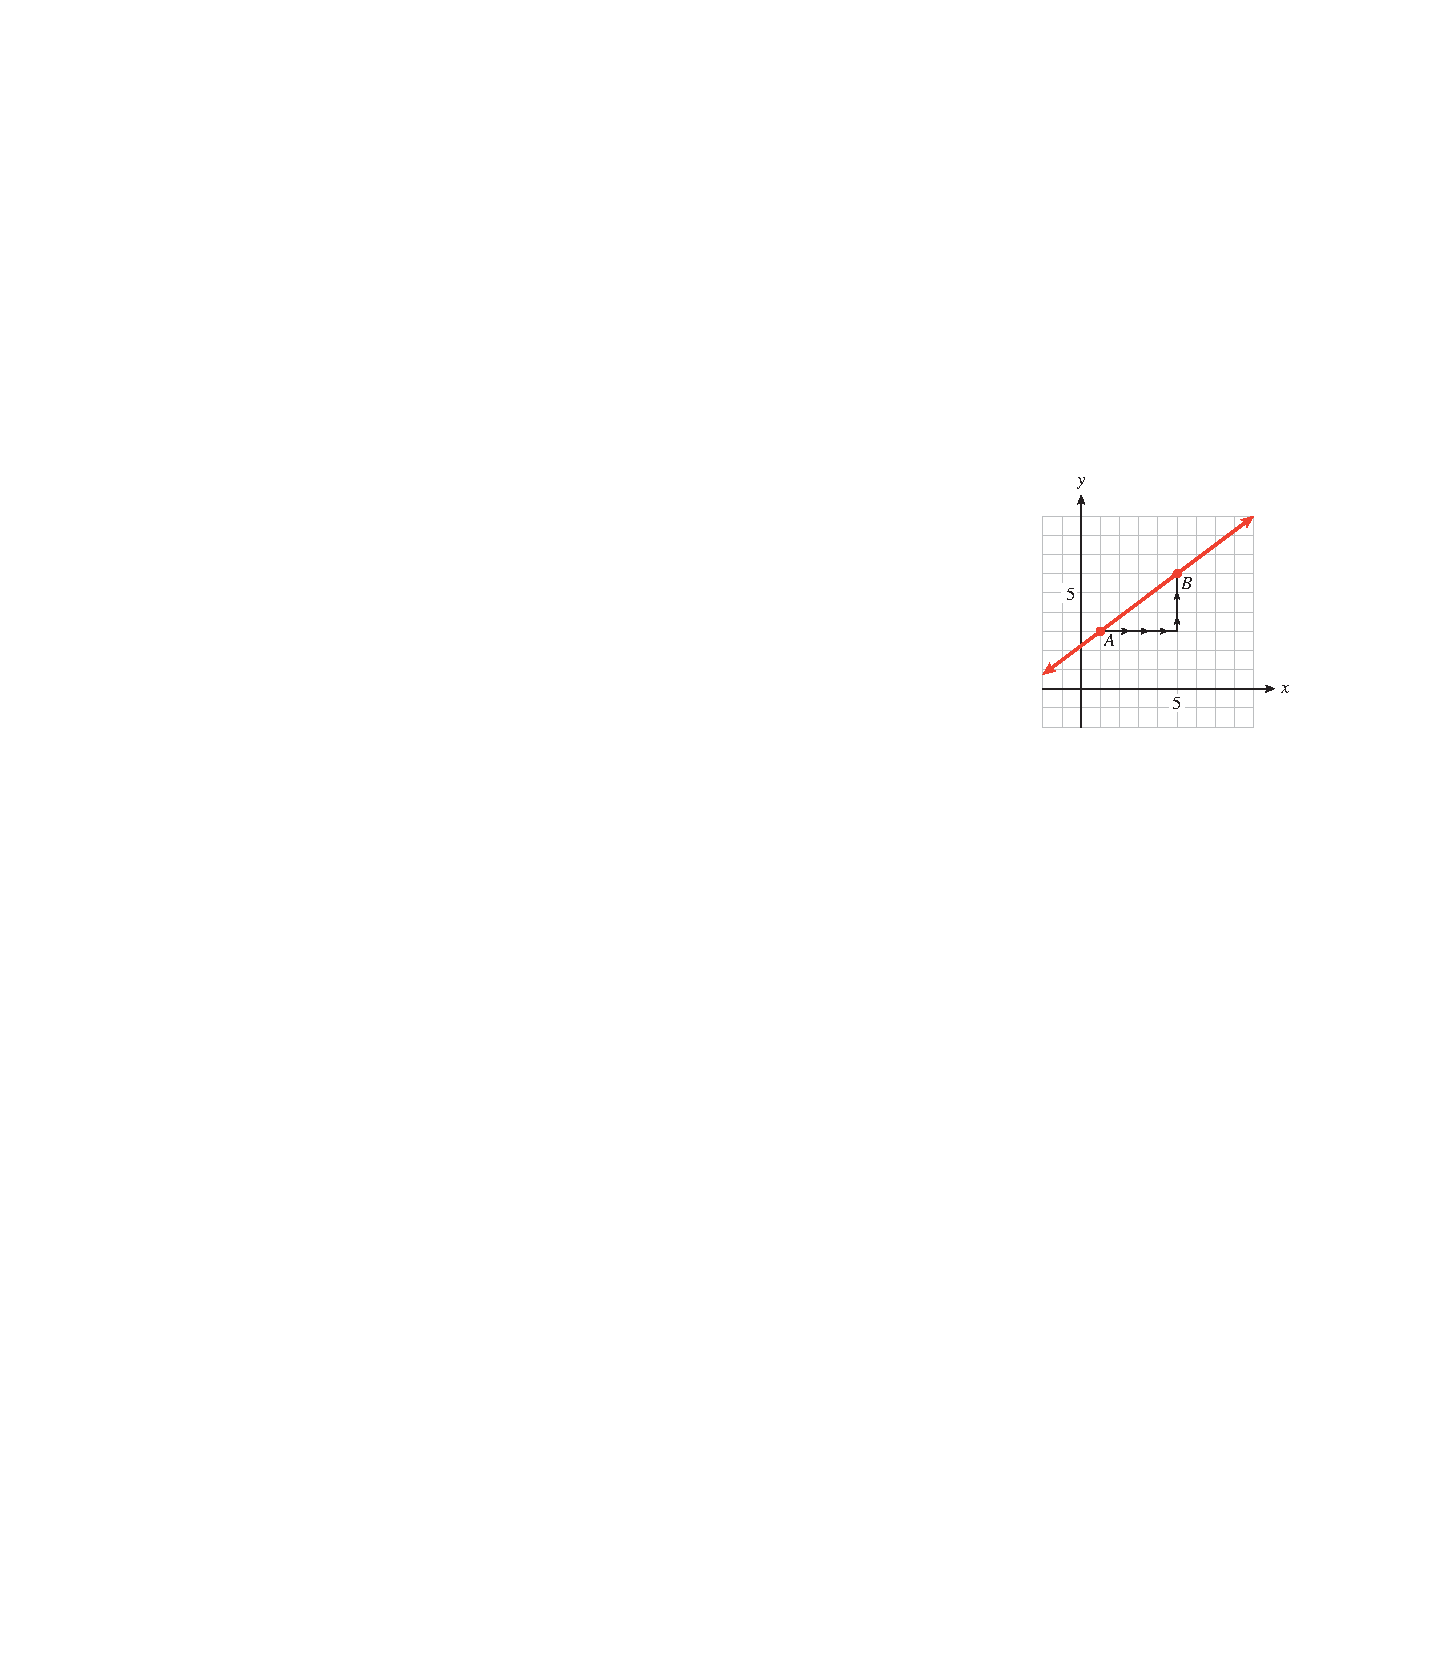
\includegraphics[width=\linewidth]{external/images/fig-slope-grid.pdf}
\end{sbspanel}%
\end{sidebyside}%
\par\smallskip%
\noindent\textbf{\blocktitlefont Solution}.\hypertarget{solution-example-slope-grid-b}{}\quad{}As we move along the line from \(A\) to \(B\), the \(y\)-coordinate changes by \(3\) units, and the \(x\)-coordinate changes by \(4\) units. The slope of the line is thus%
\begin{equation*}
\frac{\text{change in }y\text{-coordinate}}{\text{change in }x\text{-coordinate}}=\frac{3}{4}
\end{equation*}
%
\end{example}
\begin{inlineexercise}{Checkpoint}{Practice 3.}{exercise-slope-and-rate-of-change-d-g}%
\begin{sidebyside}{1}{0.36}{0.36}{0}%
\begin{sbspanel}{0.28}%
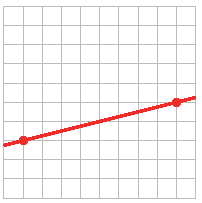
\includegraphics[width=\linewidth]{external/images/fig-slope-grid2.pdf}
\end{sbspanel}%
\end{sidebyside}%
\par
Compute the slope of the line through the indicated points on the graph above. On both axes, one square represents one unit.%
\par
\(\dfrac{\text{change in }y\text{-coordinate}}{\text{change in }x\text{-coordinate}}=\)\fillintext{3}%
\par\smallskip%
\noindent\textbf{\blocktitlefont Answer}.\hypertarget{answer-slope-and-rate-of-change-d-g-c}{}\quad{}\({\frac{1}{4}}\)%
\par\smallskip%
\noindent\textbf{\blocktitlefont Solution}.\hypertarget{solution-slope-and-rate-of-change-d-g-d}{}\quad{}\(\dfrac{2}{8}=\dfrac{1}{4}\)%
\end{inlineexercise}%
\begin{inlineexercise}{Checkpoint}{QuickCheck 3.}{exercise-slope-and-rate-of-change-d-h}%
What is wrong with the following reasoning? The point \((10,7)\) lies on the graph of a line, so the slope of the line is \(\dfrac{7}{10}\text{.}\)%
\par
\begin{itemize}[label=$\odot$,leftmargin=3em,]
\item{}The slope is \(\dfrac{10}{7}\).%
\item{}7 is not an intercept.%
\item{}We need two points to compute the slope.%
\item{}The line is decreasing.%
\end{itemize}
%
\par\smallskip%
\noindent\textbf{\blocktitlefont Answer}.\hypertarget{answer-slope-and-rate-of-change-d-h-c}{}\quad{}\(\text{Choice 3}\)%
\par\smallskip%
\noindent\textbf{\blocktitlefont Solution}.\hypertarget{solution-slope-and-rate-of-change-d-h-d}{}\quad{}We need two points to compute the slope.%
\end{inlineexercise}%
\begin{note}{Note}{}{note-slope-and-rate-of-change-d-i}%
The slope of a line is a \emph{number}. It tells us how much the \(y\)-coordinates of points on the line increase when we increase their \(x\)-coordinates by 1 unit. For instance, the slope \(\dfrac{3}{4}\) in \hyperref[example-example-slope-grid]{Example~{\xreffont\ref{example-example-slope-grid}}} means that the \(y\)-coordinate increases by \(\dfrac{3}{4}\) unit when the \(x\)-coordinate increases by 1 unit. For increasing graphs, a larger slope indicates a greater increase in altitude, and hence a steeper line.%
\end{note}
\end{subsectionptx}
%
%
\typeout{************************************************}
\typeout{Subsection  Notation for Slope}
\typeout{************************************************}
%
\begin{subsectionptx}{Subsection}{Notation for Slope}{}{Notation for Slope}{}{}{subsection-slope-and-rate-of-change-e}
We use a shorthand notation for the ratio that defines slope,%
\begin{equation*}
\frac{\text{change in }y\text{-coordinate}}{\text{change in }x\text{-coordinate}}
\end{equation*}
The symbol \(\Delta\) (the Greek letter delta) is used in mathematics to denote \emph{change in}. In particular, \(\Delta y\) means \emph{change in \(y\)-coordinate}, and \(\Delta x\) means \emph{change in \(x\)-coordinate}. We also use the letter \(m\) to stand for slope. With these symbols, we can write the definition of slope as follows.%
\begin{assemblage}{Assemblage}{Notation for Slope.}{assemblage-slope-and-rate-of-change-e-c}%
The \terminology{slope}\index{slope} of a line is given by%
\begin{equation*}
\frac{\Delta y}{\Delta x}=\frac{\text{change in }y\text{-coordinate}}{\text{change in }x\text{-coordinate}}\text{, }~\Delta x\ne 0
\end{equation*}
%
\begin{sidebyside}{1}{0.325}{0.325}{0}%
\begin{sbspanel}{0.35}%
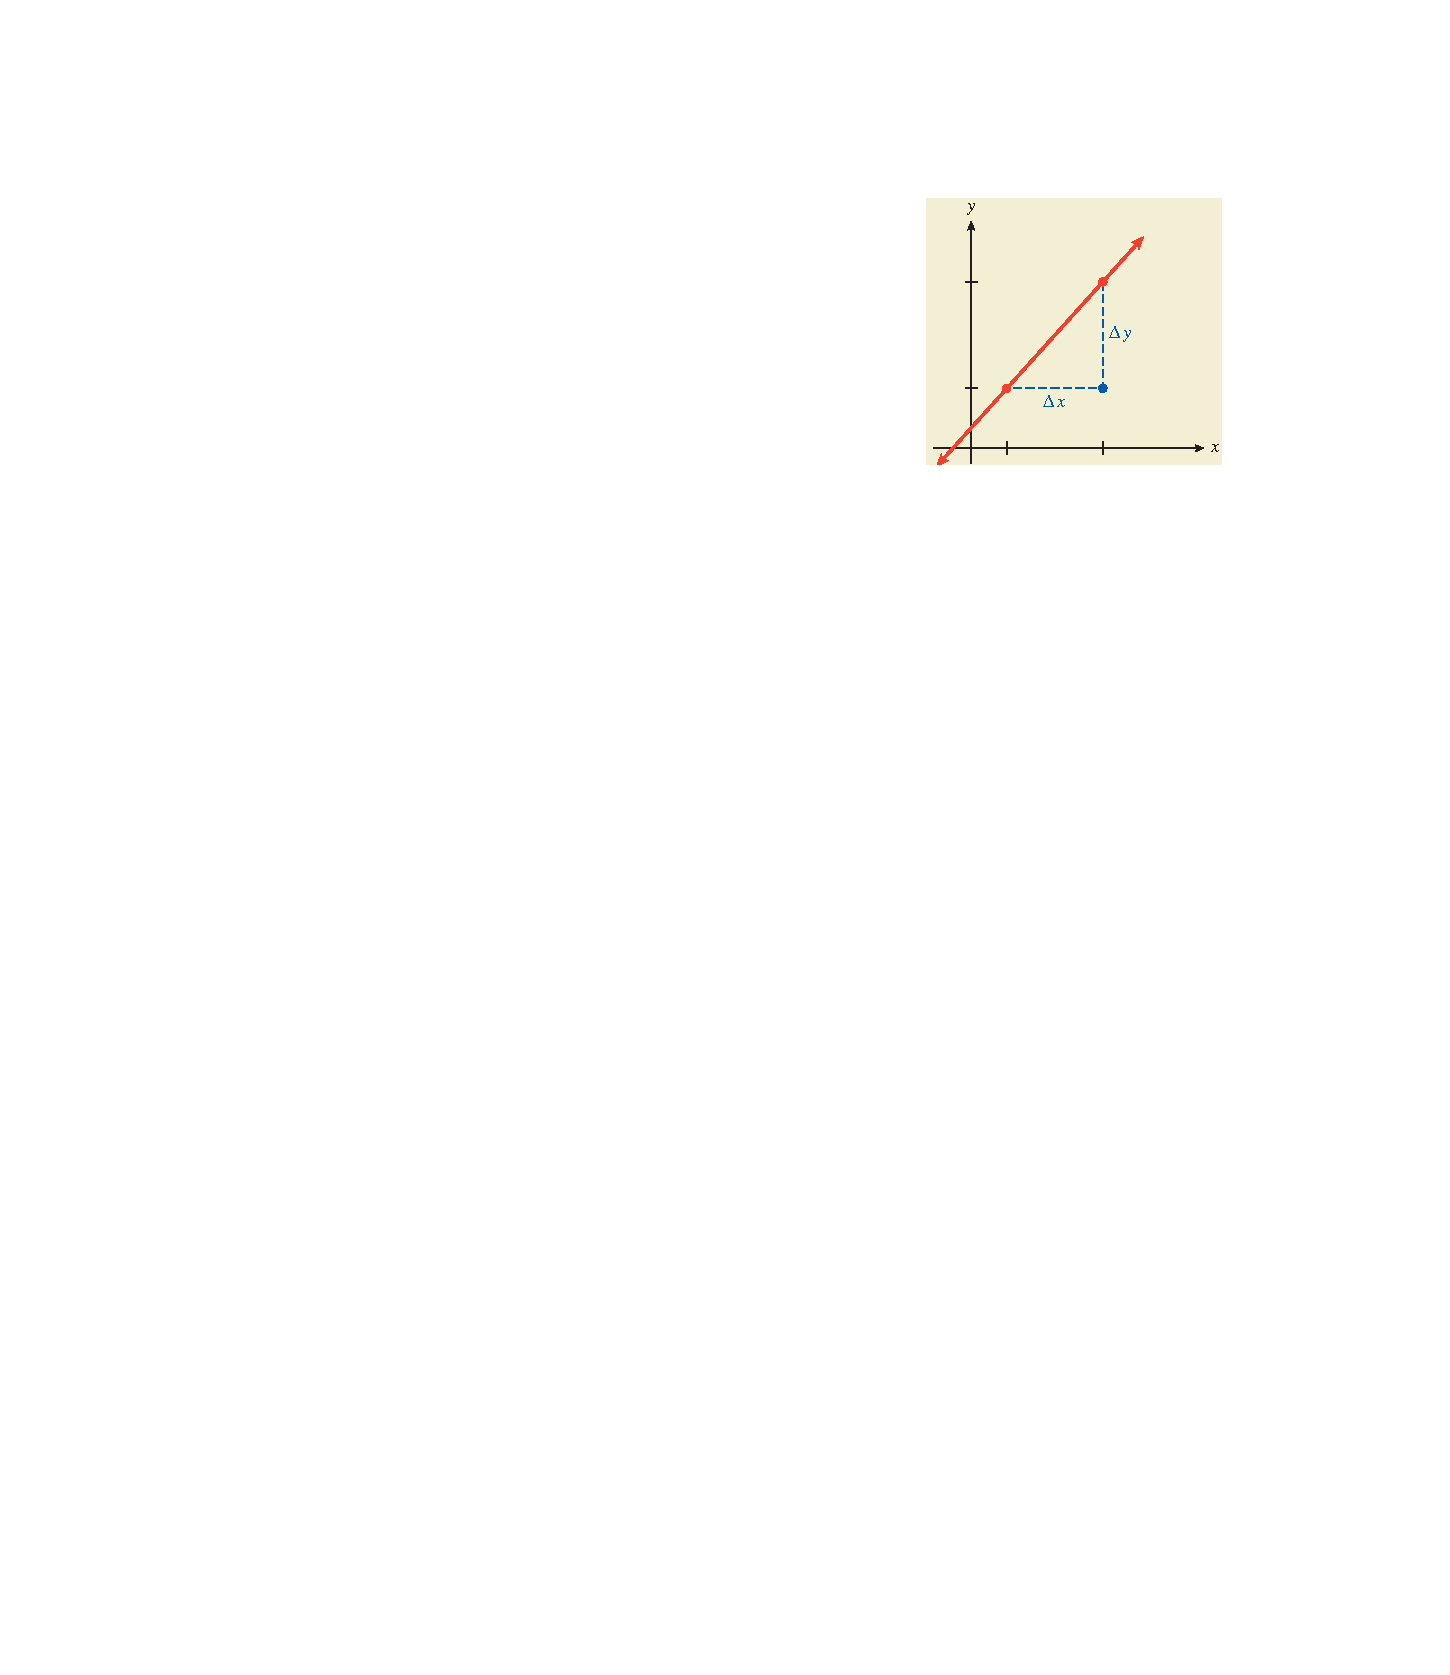
\includegraphics[width=\linewidth]{external/images/fig-slope-Delta.pdf}
\end{sbspanel}%
\end{sidebyside}%
\end{assemblage}
\begin{example}{Example}{}{example-example-Great-Pyramid}%
The Great Pyramid of Khufu in Egypt was built around 2550 B.C. It is 147 meters tall and has a square base 229 meters on each side. Calculate the slope of the sides of the pyramid, rounded to two decimal places.%
\par\smallskip%
\noindent\textbf{\blocktitlefont Solution}.\hypertarget{solution-example-Great-Pyramid-b}{}\quad{}\begin{sidebyside}{2}{0.025}{0.025}{0.05}%
\begin{sbspanel}{0.5}%
From the figure, we see that \(\Delta x\) is only half the base of the Great Pyramid, so%
\begin{equation*}
\Delta x = 0.5(229) = 114.5
\end{equation*}
and the slope of the side is%
\begin{equation*}
m=\frac{\Delta y}{\Delta x}= \frac{147}{114.5} = 1.28
\end{equation*}
%
\end{sbspanel}%
\begin{sbspanel}{0.4}%
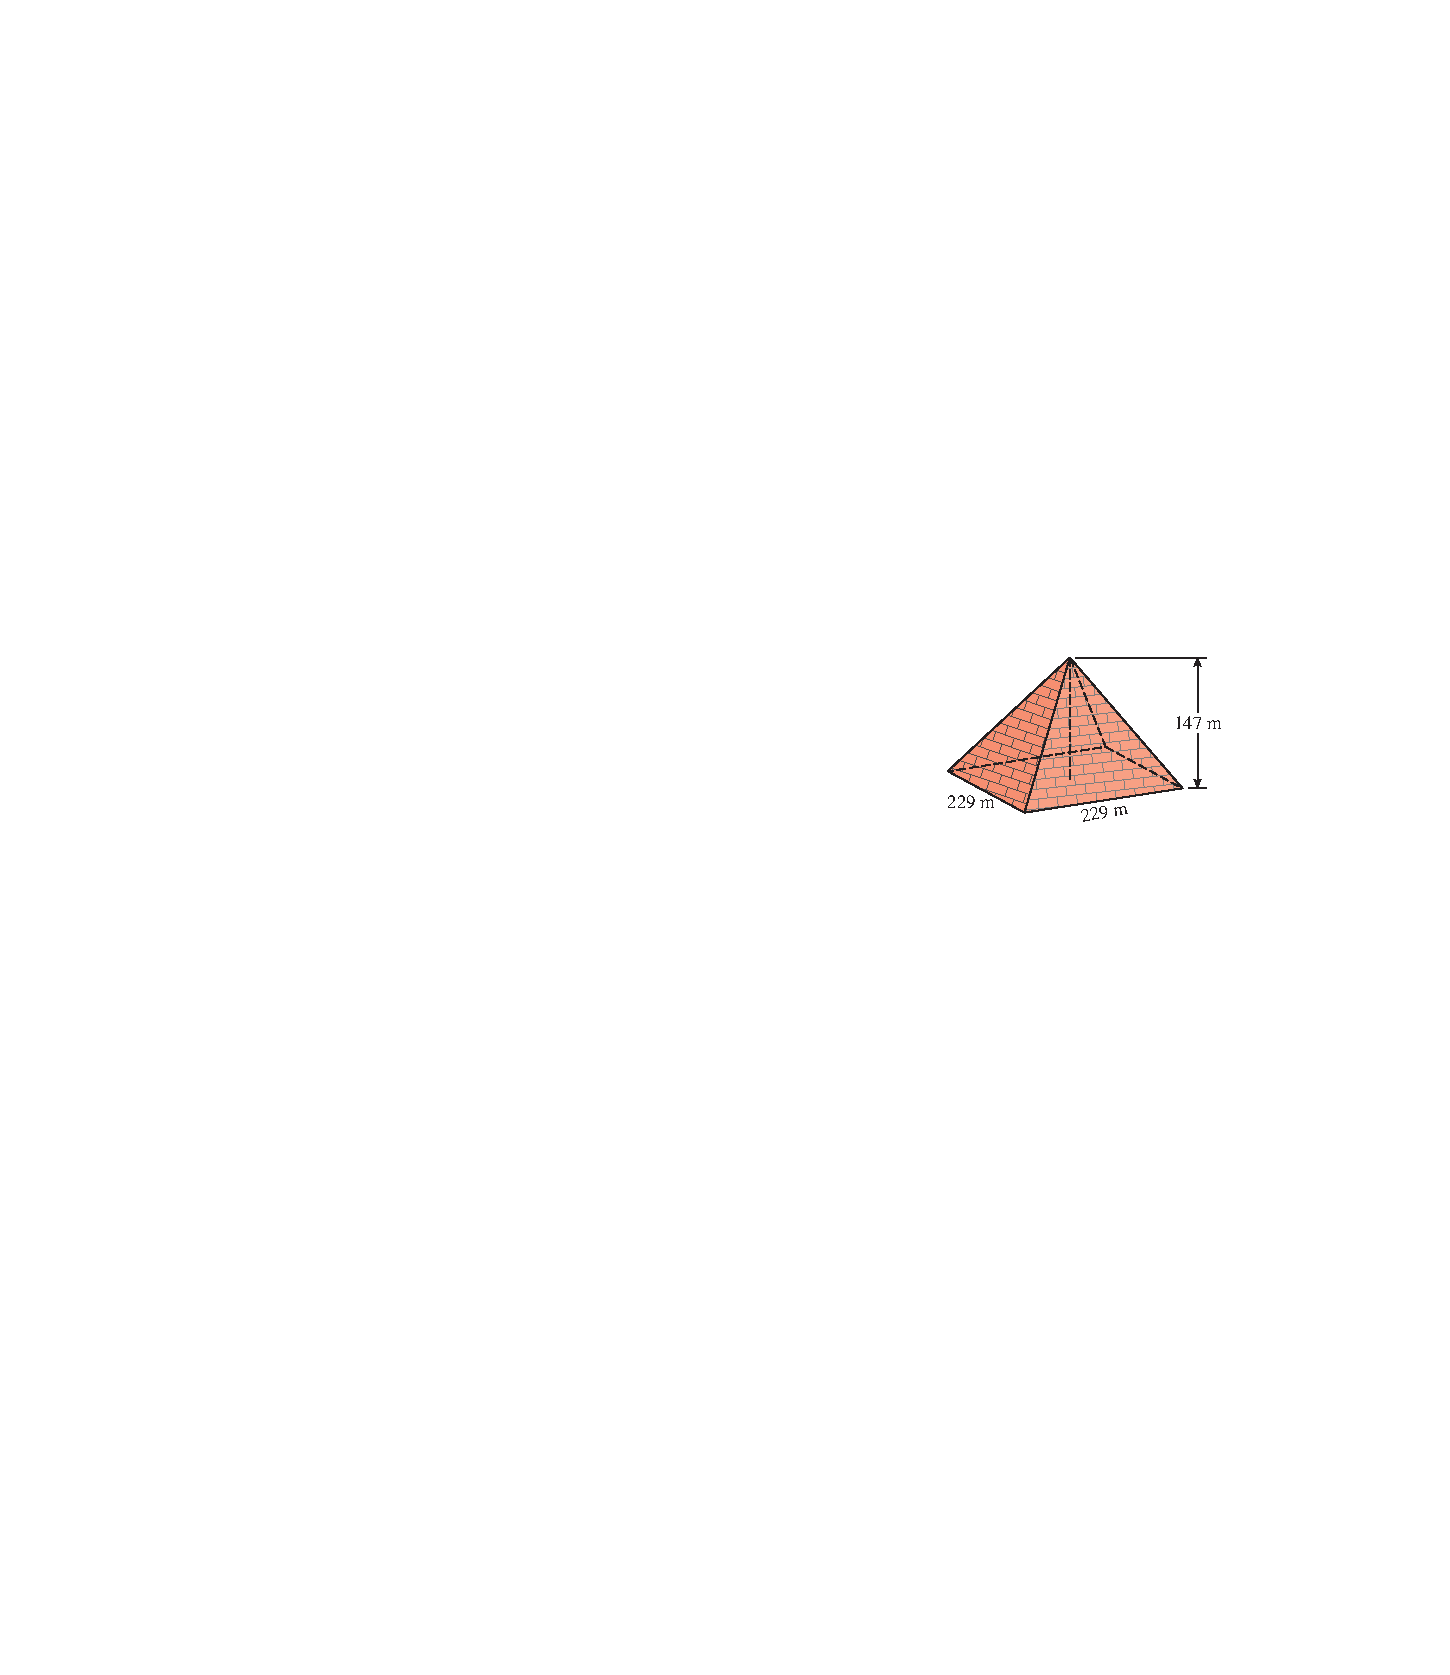
\includegraphics[width=\linewidth]{external/images/fig-Great-Pyramid.pdf}
\end{sbspanel}%
\end{sidebyside}%
\end{example}
\begin{inlineexercise}{Checkpoint}{Practice 4.}{exercise-slope-and-rate-of-change-e-e}%
\begin{sidebyside}{2}{0.005}{0.005}{0.01}%
\begin{sbspanel}{0.4}[center]%
The Kukulcan Pyramid at Chichen Itza in Mexico was built around 800 A.D. It is \(24\) meters high, with a temple built on its top platform, as shown at right.%
\end{sbspanel}%
\begin{sbspanel}{0.58}[center]%
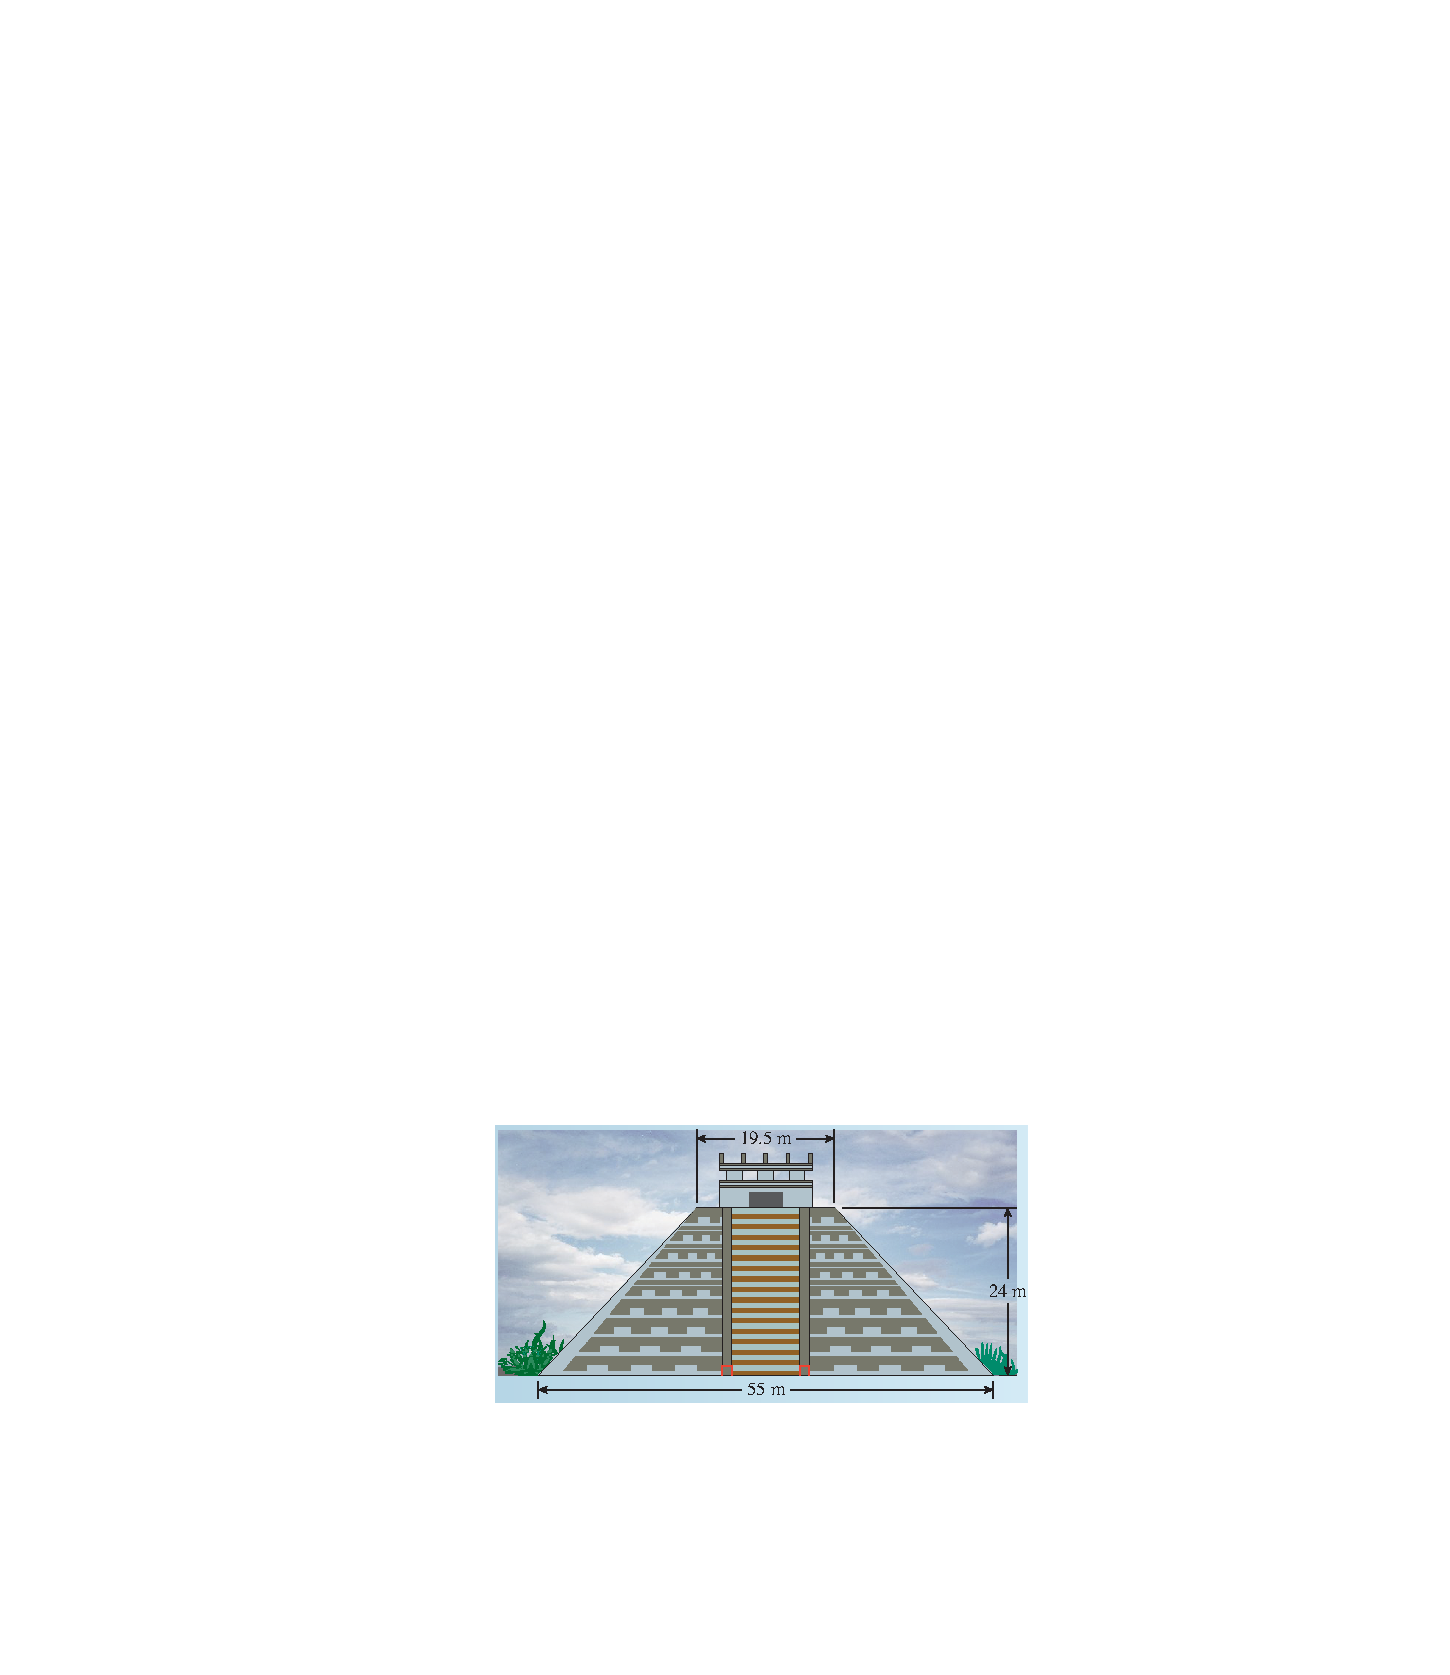
\includegraphics[width=\linewidth]{external/images/fig-Kukulcan-Pyramid.pdf}
\end{sbspanel}%
\end{sidebyside}%
\par
The square base is 55 meters on each side, and the top platform is 19.5 meters on each side. Calculate the slope of the sides of the pyramid. Which pyramid is steeper, Kukulcan or the Great Pyramid (whose slope, rounded to two decimals, is 1.28)?%
\par
Answer:\quad(\begin{itemize*}[label=$\square$,leftmargin=3em,itemjoin=\hspace{1em}]
\item{}Kukulcan%
\item{}Great Pyramid%
\end{itemize*})\quad
%
\par\smallskip%
\noindent\textbf{\blocktitlefont Hint}.\hypertarget{hint-slope-and-rate-of-change-e-e-c}{}\quad{}The horizontal change \(\Delta x\) is half the difference between the sides of the base and of the top platform.%
\par\smallskip%
\noindent\textbf{\blocktitlefont Answer}.\hypertarget{answer-slope-and-rate-of-change-e-e-d}{}\quad{}\(\text{Kukulcan}\)%
\par\smallskip%
\noindent\textbf{\blocktitlefont Solution}.\hypertarget{solution-slope-and-rate-of-change-e-e-e}{}\quad{}The horizontal change \(\Delta x\) is half the difference between the sides of the base and of the top platform: \(\Delta x=\frac{1}{2}(55-19.5)= 17.75\text{,}\) so the slope is \(m=\dfrac{\Delta y}{\Delta x}= \dfrac{24}{17.75} \approx {1.35211}\text{,}\) which is greater than 1.28. Kukulcan is steeper.%
\end{inlineexercise}%
So far, we have only considered examples in which \(\Delta x\) and \(\Delta y\) are positive numbers, but they can also be negative.%
\begin{equation*}
\Delta x = \begin{cases}
\text{positive if } x \text{ increases (move to the right)}\\
\text{negative if } x \text{ decreases (move to the left)}\\
\end{cases}
\end{equation*}
%
\begin{equation*}
\Delta y = \begin{cases}
\text{positive if } y \text{ increases (move up)}\\
\text{negative if } y \text{ decreases (move down)}~~~~~~~~~\\
\end{cases}
\end{equation*}
%
\begin{example}{Example}{}{example-example-negative-slope}%
\begin{sidebyside}{2}{0.0375}{0.0375}{0.075}%
\begin{sbspanel}{0.45}%
Compute the slope of the line that passes through the points \(P(-4, 2)\) and \(Q(5, -1)\) shown in at right. Illustrate \(\Delta y\) and \(\Delta x\) on the graph.%
\end{sbspanel}%
\begin{sbspanel}{0.4}%
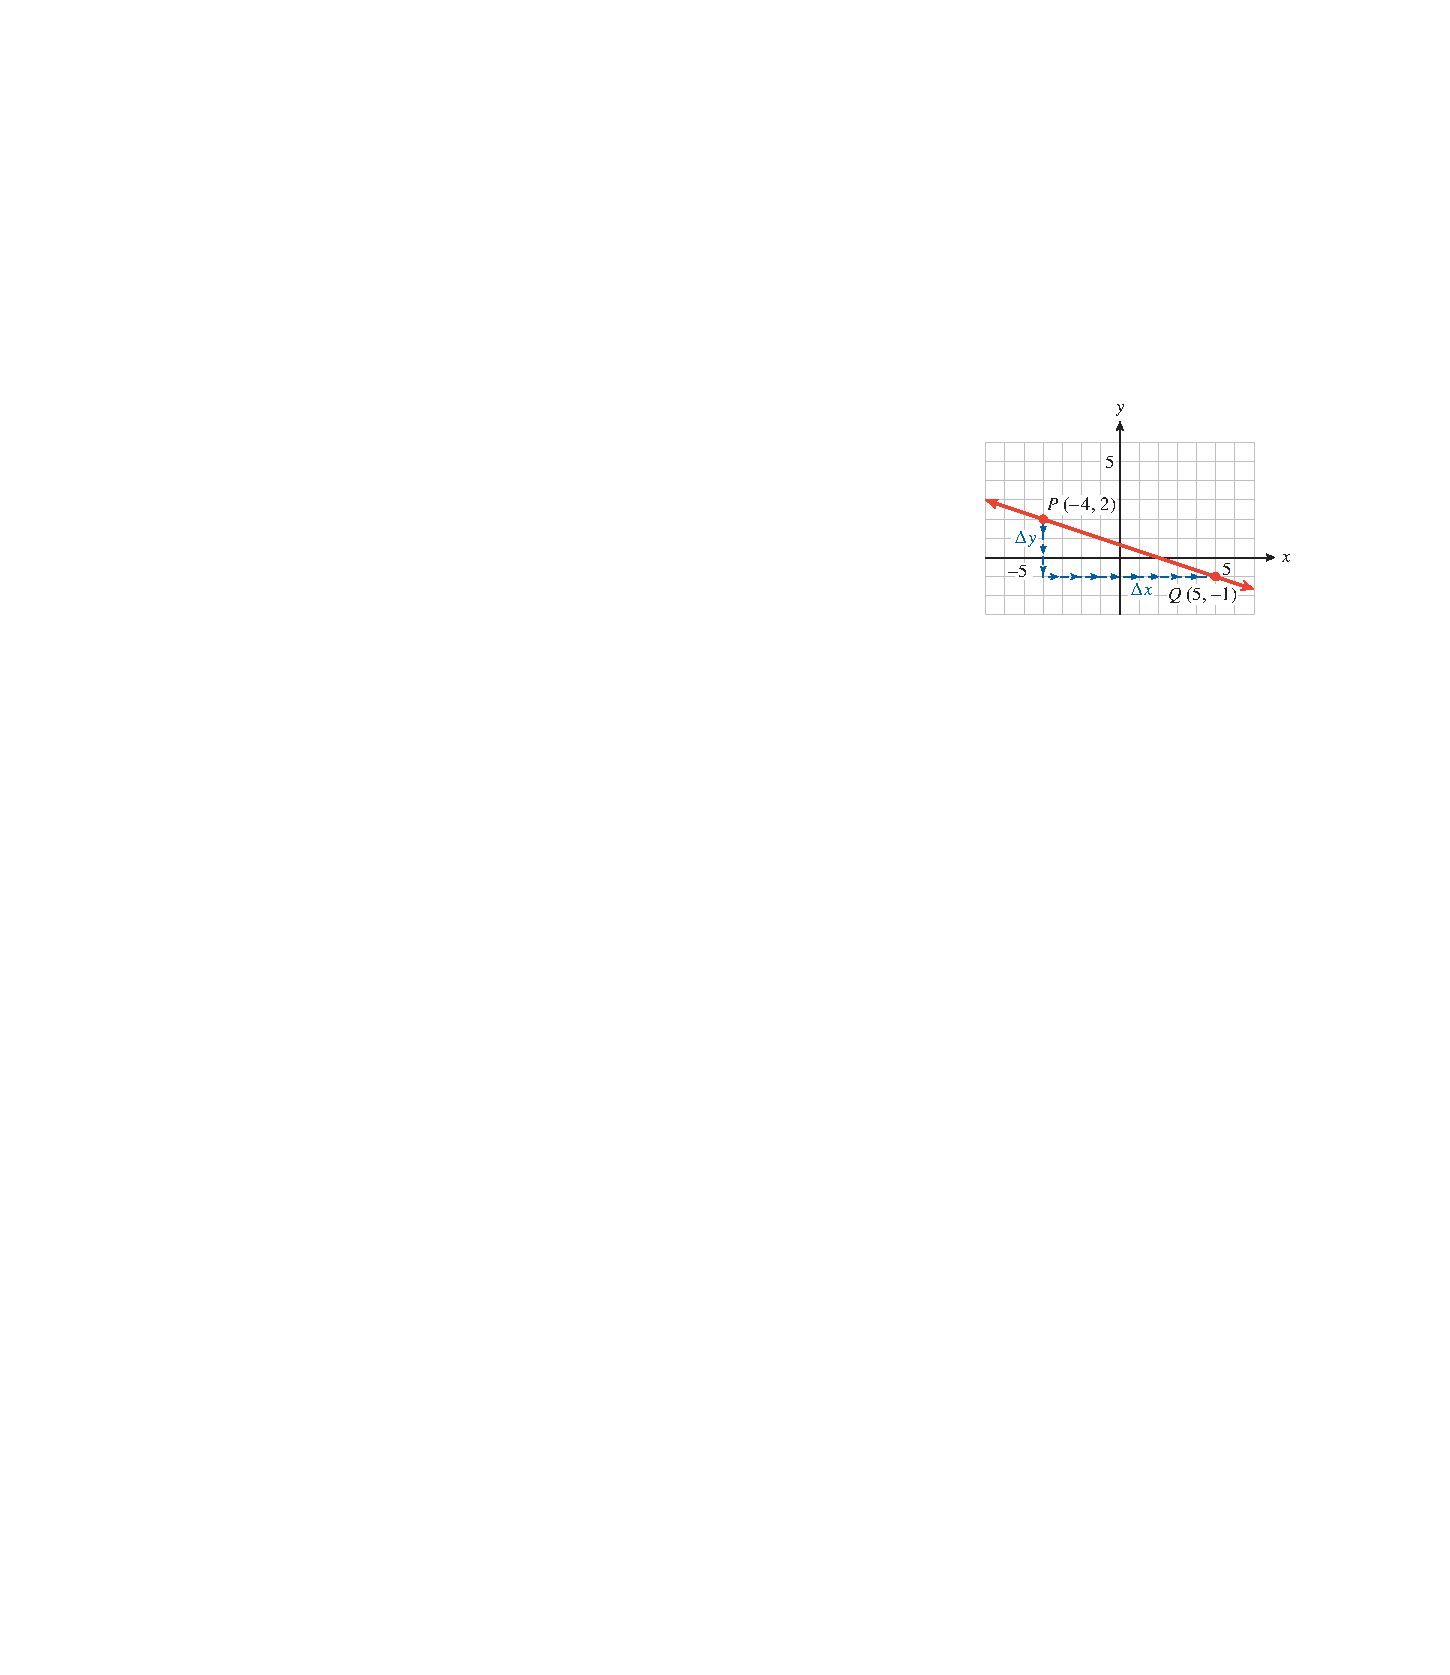
\includegraphics[width=\linewidth]{external/images/fig-negative-slope.pdf}
\end{sbspanel}%
\end{sidebyside}%
\par\smallskip%
\noindent\textbf{\blocktitlefont Solution}.\hypertarget{solution-example-negative-slope-b}{}\quad{}As we move from the point \(P(-4, 2)\) to the point \(Q(5, -1)\), we move \(3\) units \emph{down}, so \(\Delta y = -3\). We then move \(9\) units to the right, so \(\Delta x = 9\).Thus, the slope is%
\begin{equation*}
m = \frac{\Delta y}{\Delta x}=\frac{-3}{9}=\frac{-1}{3}
\end{equation*}
\(\Delta y\) and \(\Delta x\) are labeled on the graph.%
\end{example}
\begin{inlineexercise}{Checkpoint}{Pause and Reflect.}{exercise-slope-and-rate-of-change-e-h}%
Suppose \(x\) represents your distance from home, in miles.  Compare the meanings of the two statements \(x=30\) and \(\Delta x=30\text{.}\)%
\end{inlineexercise}%
We can move from point to point in either direction to compute the slope. The line graphed in \hyperref[example-example-negative-slope]{Example~{\xreffont\ref{example-example-negative-slope}}} \emph{decreases} as we move from left to right and hence has a negative slope.%
\begin{sidebyside}{2}{0.025}{0.025}{0.05}%
\begin{sbspanel}{0.5}%
The slope is the same if we move from point \(Q\) to point \(P\) instead of from \(P\) to \(Q\), as shown at right.  In that case, our computation looks like this:%
\begin{equation*}
m = \frac{\Delta y}{\Delta x}=\frac{3}{-9}=\frac{-1}{3}
\end{equation*}
\(\Delta y\) and \(\Delta x\) are labeled on the graph.%
\end{sbspanel}%
\begin{sbspanel}{0.4}%
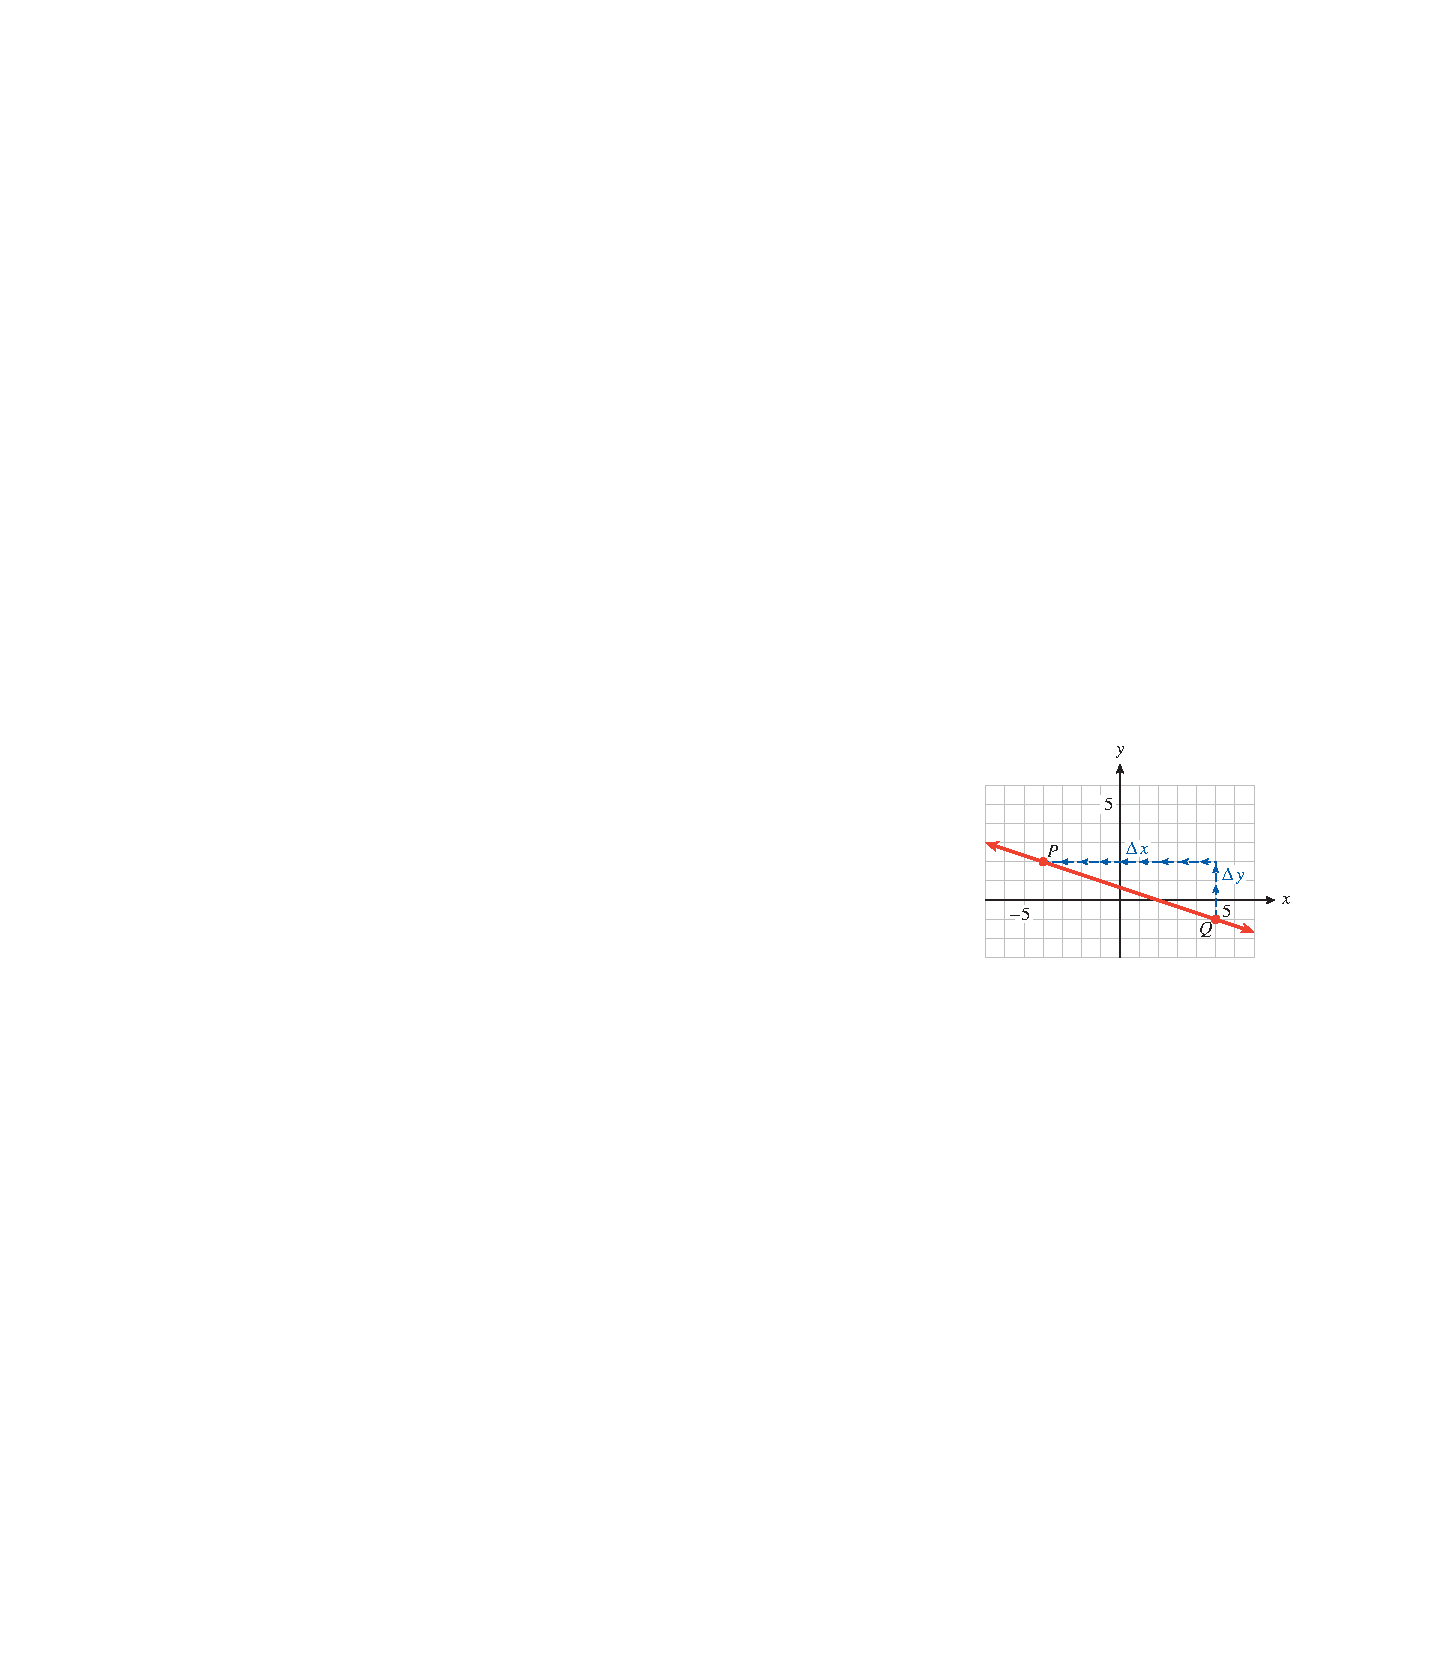
\includegraphics[width=\linewidth]{external/images/fig-negative-slope2.pdf}
\end{sbspanel}%
\end{sidebyside}%
\end{subsectionptx}
%
%
\typeout{************************************************}
\typeout{Subsection  Lines Have Constant Slope}
\typeout{************************************************}
%
\begin{subsectionptx}{Subsection}{Lines Have Constant Slope}{}{Lines Have Constant Slope}{}{}{subsection-slope-and-rate-of-change-f}
How do we know which two points to choose when we want to compute the slope of a line? It turns out that any two points on the line will do.%
\begin{inlineexercise}{Checkpoint}{Practice 5.}{exercise-exercise-slope-any-points}%
%
\begin{enumerate}[label=\alph*.]
\item{}Graph the line \(4x - 2y = 8\) by finding the \(x\)- and \(y\)-intercepts%
\par
\(x\)-intercept: \fillintext{5}%
\par
\(y\)-intercept: \fillintext{5}%
\par
Note: Enter each intercept as an ordered pair.%
\item{}Compute the slope of the line using the \(x\)-intercept and \(y\)-intercept.%
\par
\(m=\)\fillintext{2}%
\item{}Compute the slope of the line using the points \((4, 4)\) and \((1, -2)\text{.}\)%
\par
\(m=\)\fillintext{2}%
\end{enumerate}
%
\par
The graph for part (a):%
\begin{sidebyside}{1}{0.36}{0.36}{0}%
\begin{sbspanel}{0.28}%
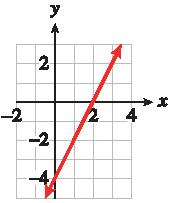
\includegraphics[width=\linewidth]{external/images/fig-in-ex-ans-1-4-5.pdf}
\end{sbspanel}%
\end{sidebyside}%
\par\smallskip%
\noindent\textbf{\blocktitlefont Answer 1}.\hypertarget{answer-exercise-slope-any-points-c}{}\quad{}\(\left(2,0\right)\)%
\par\smallskip%
\noindent\textbf{\blocktitlefont Answer 2}.\hypertarget{answer-exercise-slope-any-points-d}{}\quad{}\(\left(0,-4\right)\)%
\par\smallskip%
\noindent\textbf{\blocktitlefont Answer 3}.\hypertarget{answer-exercise-slope-any-points-e}{}\quad{}\(2\)%
\par\smallskip%
\noindent\textbf{\blocktitlefont Answer 4}.\hypertarget{answer-exercise-slope-any-points-f}{}\quad{}\(2\)%
\par\smallskip%
\noindent\textbf{\blocktitlefont Solution}.\hypertarget{solution-exercise-slope-any-points-g}{}\quad{}%
\begin{enumerate}[label=\alph*.]
\item{}A graph of the line is shown below this exercise.%
\item{}The \(x\)-intercept is \({\left(2,0\right)}\) and the \(y\)-intercept is \({\left(0,-4\right)}\text{.}\)%
\par
The slope is \(m=\dfrac{\Delta y}{\Delta x}= \dfrac{ + 4}{2} = 2\)%
\item{}The slope is \(m=\dfrac{\Delta y}{\Delta x}= \dfrac{-2-4}{1-4}=\dfrac{-6}{-3} = 2\)%
\end{enumerate}
%
\end{inlineexercise}%
\begin{note}{Note}{}{note-slope-and-rate-of-change-f-d}%
\hyperref[exercise-exercise-slope-any-points]{Checkpoint~{\xreffont\ref{exercise-exercise-slope-any-points}}} illustrates an important property of lines: They have constant slope. No matter which two points we use to calculate the slope, we will always get the same result. We will see later that lines are the only graphs that have this property.%
\end{note}
We can think of the slope as a \terminology{scale factor} that tells us how many units \(y\) increases (or decreases) for each unit of increase in \(x\). Compare the lines shown below.%
\begin{sidebyside}{1}{0.1}{0.1}{0}%
\begin{sbspanel}{0.8}%
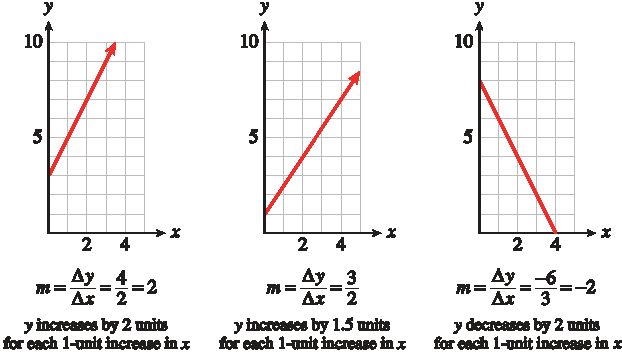
\includegraphics[width=\linewidth]{external/images/fig-slope-scale-factor.pdf}
\end{sbspanel}%
\end{sidebyside}%
\begin{inlineexercise}{Checkpoint}{QuickCheck 4.}{exercise-slope-and-rate-of-change-f-g}%
How can you tell from the equation of a line whether its graph is decreasing?%
\par
\begin{itemize}[label=$\odot$,leftmargin=3em,]
\item{}Its slope is positive.%
\item{}Its \(x\)-intercept is positive.%
\item{}Its slope is negative.%
\item{}Its \(x\)-intercept is negative.%
\end{itemize}
%
\par\smallskip%
\noindent\textbf{\blocktitlefont Answer}.\hypertarget{answer-slope-and-rate-of-change-f-g-c}{}\quad{}\(\text{Choice 3}\)%
\par\smallskip%
\noindent\textbf{\blocktitlefont Solution}.\hypertarget{solution-slope-and-rate-of-change-f-g-d}{}\quad{}The graph is decreasing when its slope is negative.%
\end{inlineexercise}%
Observe that a line with positive slope increases from left to right, and one with negative slope decreases. What sort of line has slope \(m = 0\)?%
\end{subsectionptx}
%
%
\typeout{************************************************}
\typeout{Subsection  Meaning of Slope}
\typeout{************************************************}
%
\begin{subsectionptx}{Subsection}{Meaning of Slope}{}{Meaning of Slope}{}{}{subsection-slope-and-rate-of-change-g}
\begin{sidebyside}{2}{0.03}{0.03}{0.06}%
\begin{sbspanel}{0.6}[center]%
In \hyperref[example-example-Annelise]{Example~1}, we graphed the equation \(C = 5 + 3t\) showing the cost of a bicycle rental in terms of the length of the rental. The graph is reproduced at right. We can choose any two points on the line to compute its slope. Using points \(P\) and \(Q\) as shown, we find that%
\begin{equation*}
m = \frac{\Delta C}{\Delta t}= \frac{9}{3}=3
\end{equation*}
The slope of the line is \(3\).%
\end{sbspanel}%
\begin{sbspanel}{0.28}[center]%
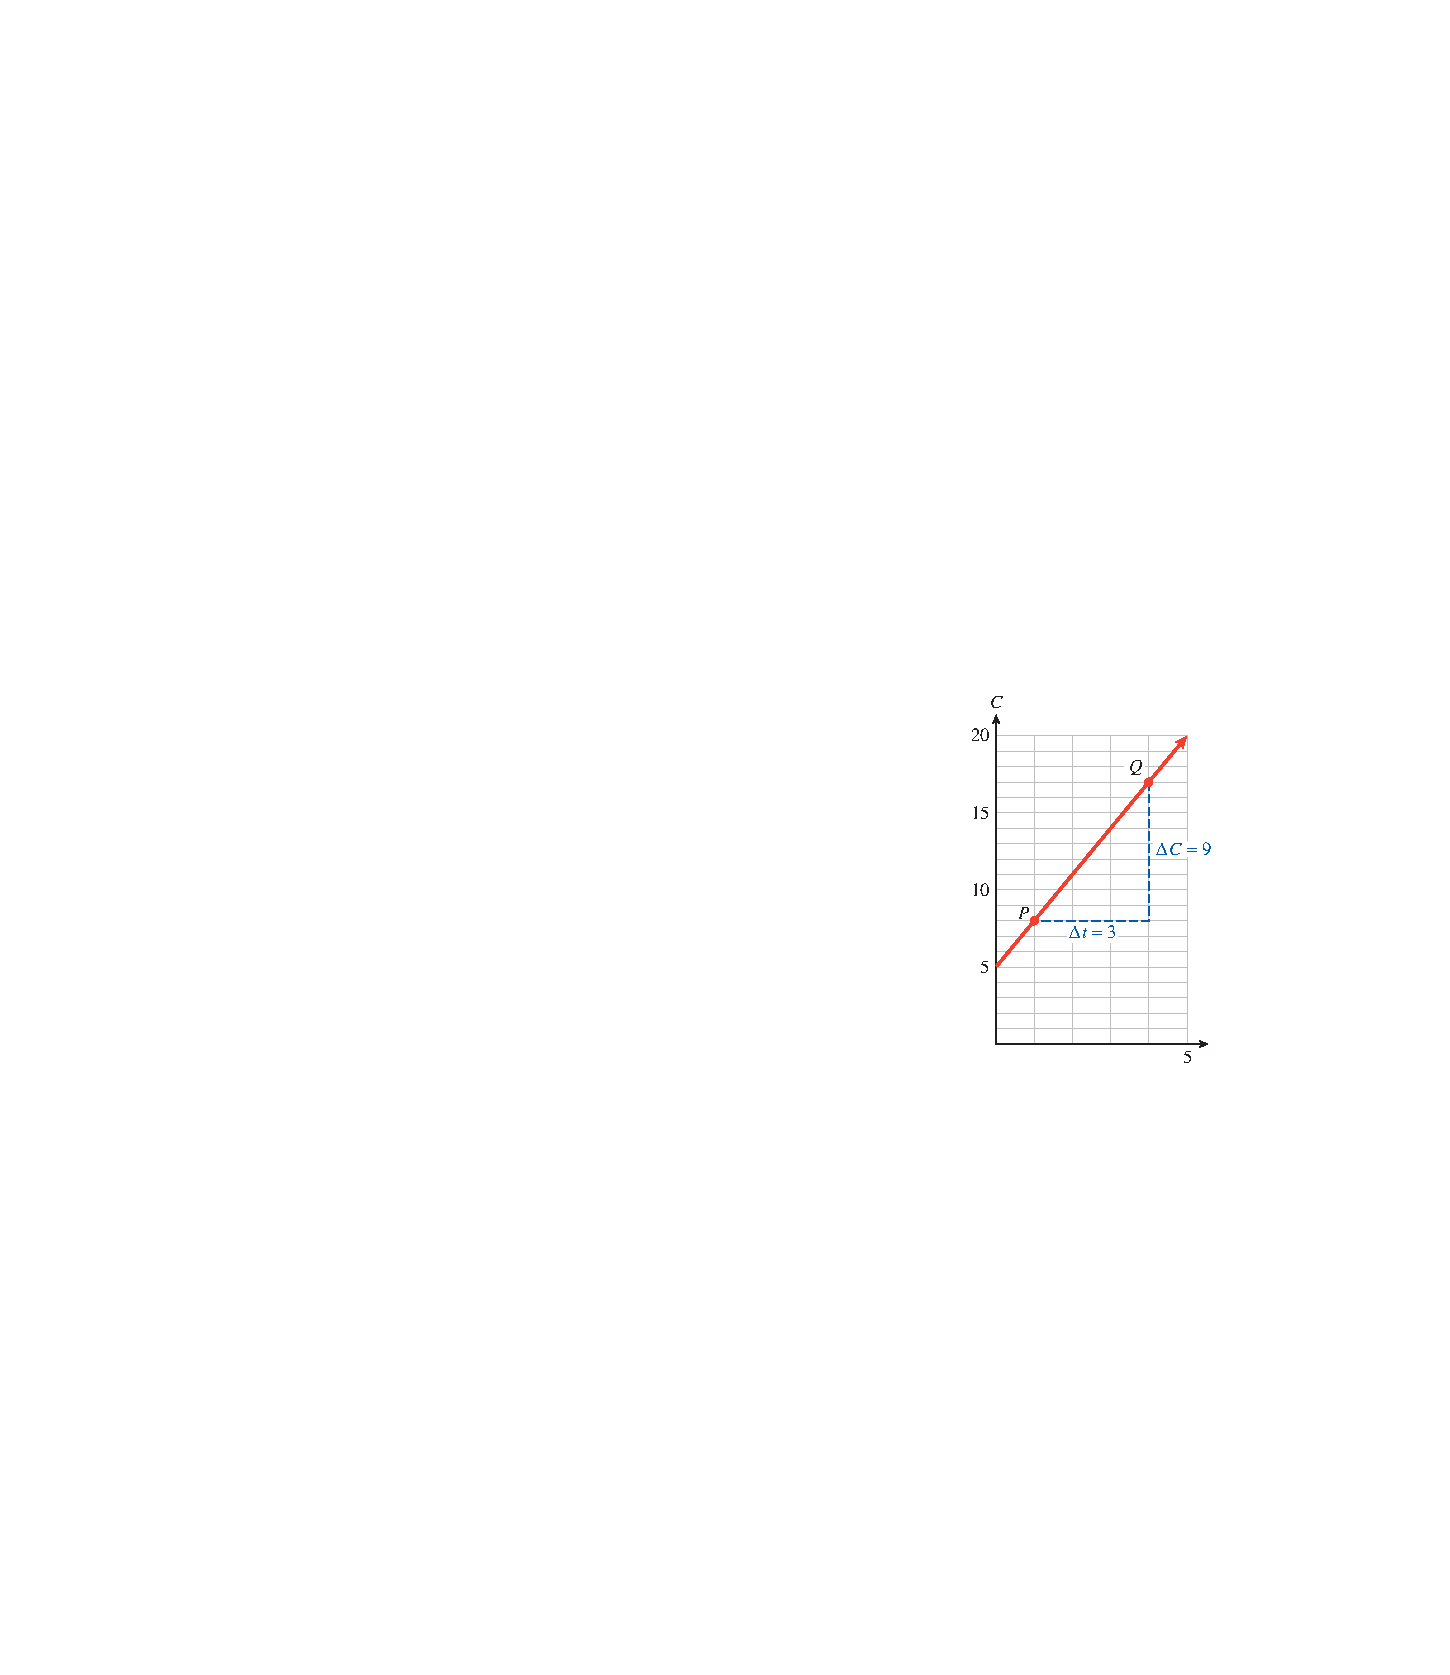
\includegraphics[width=\linewidth]{external/images/fig-meaning-slope.pdf}
\end{sbspanel}%
\end{sidebyside}%
\par
What does this value mean for the cost of renting a bicycle? The expression%
\begin{equation*}
\frac{\Delta C}{\Delta t}= \frac{9}{3}
\end{equation*}
stands for%
\begin{equation*}
\frac{\text{change in cost}}{\text{change in time}}= \frac{9 \text{ dollars }}{3 \text{ hours}}
\end{equation*}
%
\par
If we increase the length of the rental by 3 hours, the cost of the rental increases by 9 dollars. The slope gives the \emph{rate of increase} in the rental fee, 3 dollars per hour. In general, we can make the following statement.%
\begin{assemblage}{Assemblage}{Rate of Change.}{assemblage-slope-and-rate-of-change-g-e}%
The slope of a line measures the \terminology{rate of change}\index{rate of change} of the output variable with respect to the input variable.%
\end{assemblage}
Depending on the variables involved, this rate might be interpreted as a rate of growth or a rate of speed. A negative slope might represent a rate of decrease or a rate of consumption. The slope of a graph can give us valuable information about the variables.%
\begin{example}{Example}{}{example-example-truck-speed}%
\begin{sidebyside}{2}{0.0625}{0.0625}{0.125}%
\begin{sbspanel}{0.5}[center]%
The graph at right shows the distance in miles traveled by a big-rig truck driver after \(t\) hours on the road.%
\begin{enumerate}[label=\alph*]
\item{}Compute the slope of the graph.%
\item{}What does the slope tell us about the problem?%
\end{enumerate}
%
\end{sbspanel}%
\begin{sbspanel}{0.25}[center]%
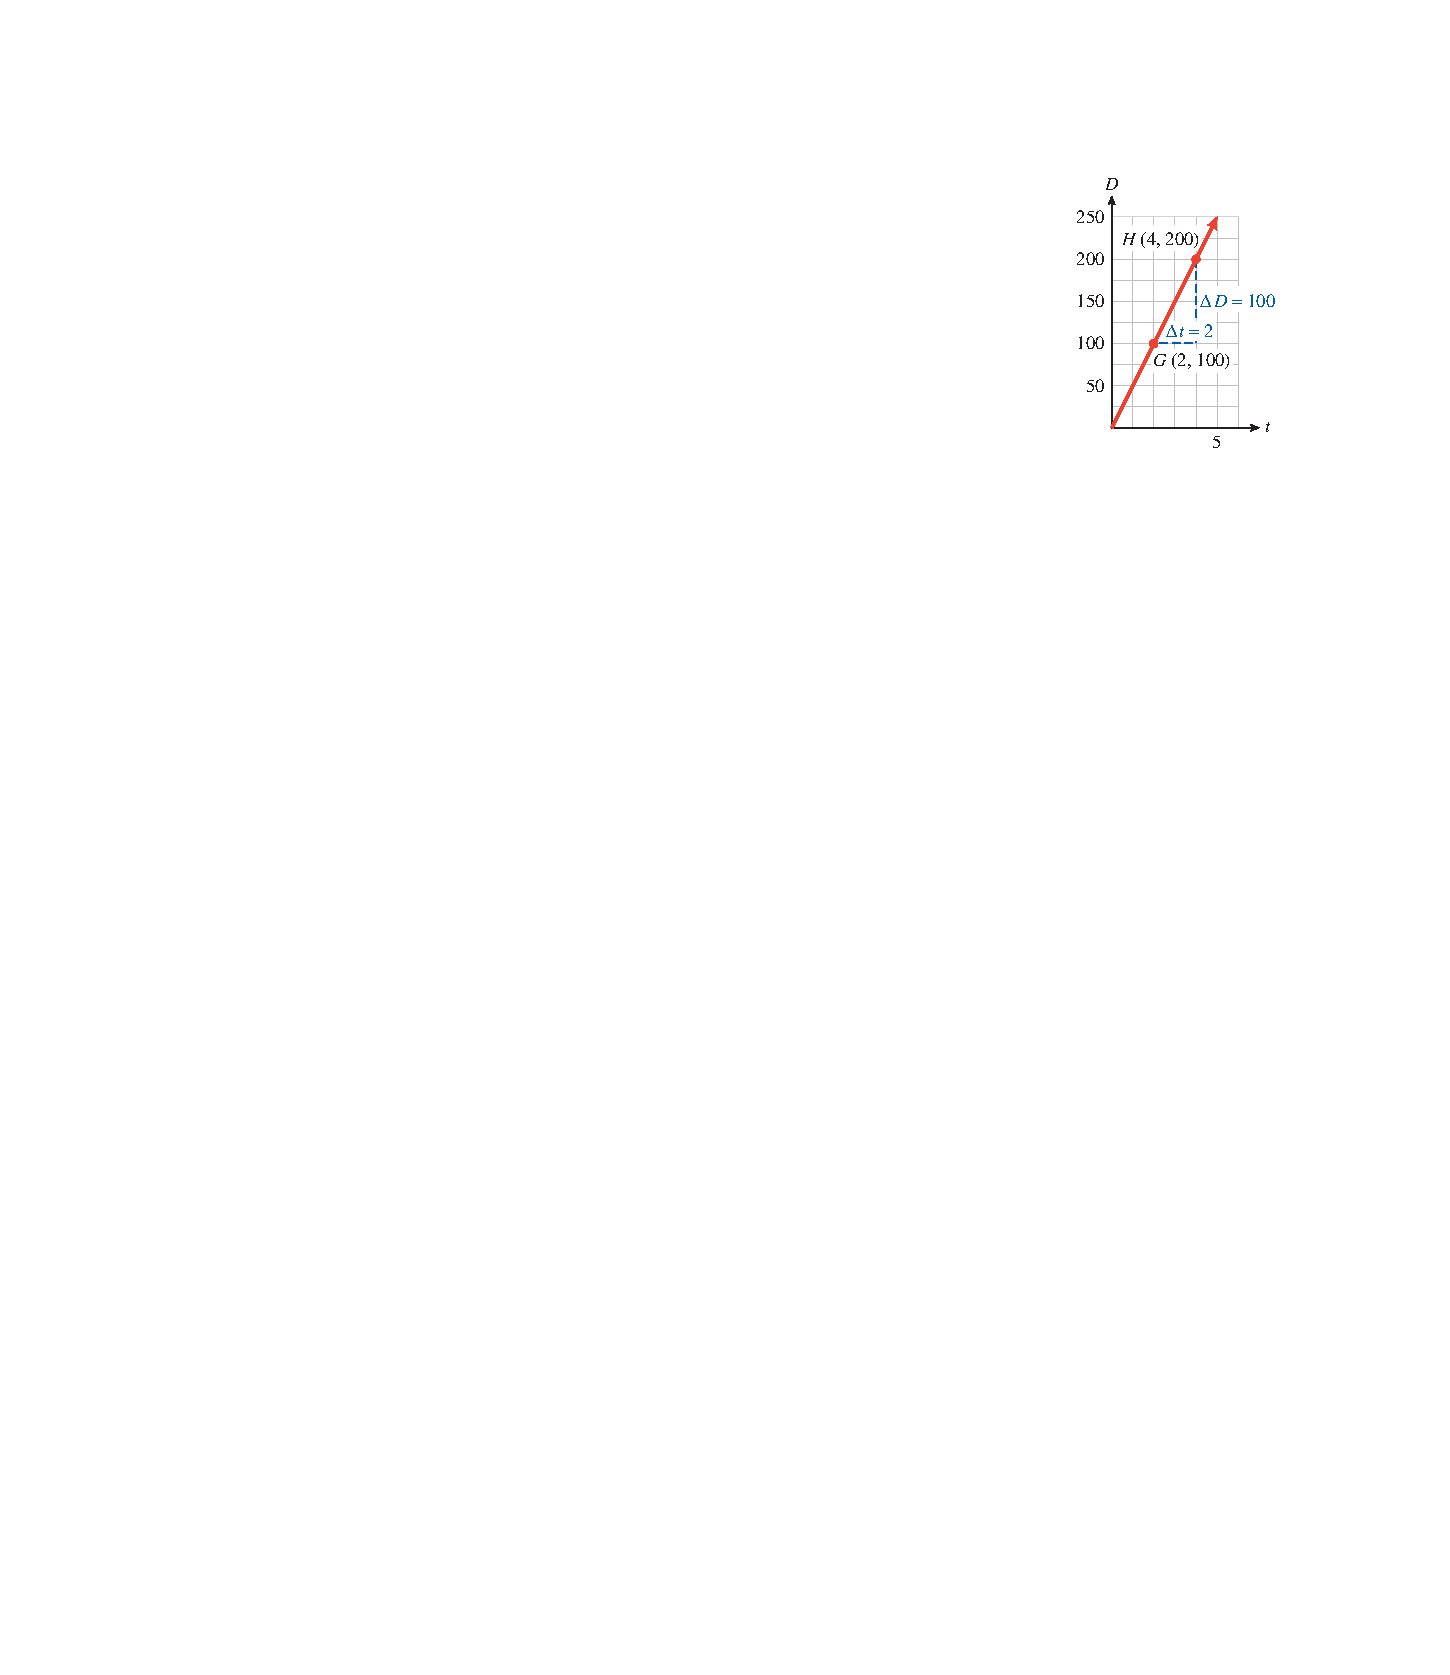
\includegraphics[width=\linewidth]{external/images/fig-truck-speed.pdf}
\end{sbspanel}%
\end{sidebyside}%
\par\smallskip%
\noindent\textbf{\blocktitlefont Solution}.\hypertarget{solution-example-truck-speed-b}{}\quad{}%
\begin{enumerate}[label=\alph*]
\item{}Choose any two points on the line, say \(G(2, 100)\) and \(H(4, 200)\), as shown. As we move from \(G\) to \(H\), we find%
\begin{equation*}
m = \frac{\Delta D}{\Delta t}=\frac{100}{2}=50
\end{equation*}
The slope of the line is 50.%
\item{}The best way to understand the slope is to include units in the calculation. For our example,%
\begin{equation*}
\frac{\Delta D}{\Delta t}~~~~ \text{ means }~~~~ \frac{\text{change in distance}}{\text{change in time}}
\end{equation*}
or%
\begin{equation*}
\frac{\Delta D}{\Delta t}
=\frac{100 \text{ miles}}{2\text{ hours}}
=50 \text{ miles per hour}
\end{equation*}
The slope represents the trucker’s average speed or velocity.%
\end{enumerate}
%
\end{example}
\begin{inlineexercise}{Checkpoint}{Practice 6.}{exercise-slope-and-rate-of-change-g-h}%
\begin{sidebyside}{2}{0.025}{0.025}{0.05}%
\begin{sbspanel}{0.55}[center]%
The graph shows the altitude, \(a\) (in feet), of a skier \(t\) minutes after getting on a ski lift.%
\end{sbspanel}%
\begin{sbspanel}{0.35}[center]%
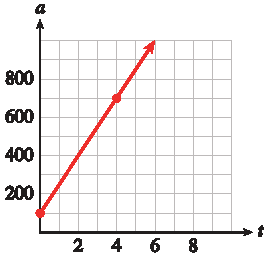
\includegraphics[width=\linewidth]{external/images/fig-ski-lift.pdf}
\end{sbspanel}%
\end{sidebyside}%
\par
%
\begin{enumerate}[label=\alph*.]
\item{}Choose two points and compute the slope (including units). (Note: Use ``ft'' for feet and use ``min'' for minutes.)%
\par
\(m=\)\fillintext{12}%
\item{}What does the slope tell us about the problem?%
\par
\begin{itemize}[label=$\odot$,leftmargin=3em,]
\item{}A) The steepness of the ski lift.%
\item{}B) The increase in altitude per minute.%
\item{}C) The time to rise a foot in altitude.%
\item{}D) The cost of using the ski lift.%
\end{itemize}
%
\end{enumerate}
%
\par\smallskip%
\noindent\textbf{\blocktitlefont Answer 1}.\hypertarget{answer-slope-and-rate-of-change-g-h-c}{}\quad{}\(150\ {\textstyle\frac{\rm\mathstrut ft}{\rm\mathstrut min}}\)%
\par\smallskip%
\noindent\textbf{\blocktitlefont Answer 2}.\hypertarget{answer-slope-and-rate-of-change-g-h-d}{}\quad{}\(\text{B) The ... per minute.}\)%
\par\smallskip%
\noindent\textbf{\blocktitlefont Solution}.\hypertarget{solution-slope-and-rate-of-change-g-h-e}{}\quad{}%
\begin{enumerate}[label=\alph*.]
\item{}\(\displaystyle m=\dfrac{\Delta y}{\Delta x}= \dfrac{700 \text{ ft}-100\text{ ft}}{4\text{ min}-0\text{ min}}= {150\ {\textstyle\frac{\rm\mathstrut ft}{\rm\mathstrut min}}}\)%
\item{}The skier's altitude increases by \(150\) feet per minute.%
\end{enumerate}
%
\end{inlineexercise}%
\begin{inlineexercise}{Checkpoint}{Pause and Reflect.}{exercise-slope-and-rate-of-change-g-i}%
How does slope measure rate of change?%
\end{inlineexercise}%
\end{subsectionptx}
%
%
\typeout{************************************************}
\typeout{Subsection  A Formula for Slope}
\typeout{************************************************}
%
\begin{subsectionptx}{Subsection}{A Formula for Slope}{}{A Formula for Slope}{}{}{subsection-slope-and-rate-of-change-h}
We have defined the slope of a line to be the ratio \(m = \dfrac{\Delta y}{\Delta x}\) as we move from one point to another on the line. So far, we have computed \(\Delta y\) and \(\Delta x\) by counting squares on the graph, but this method is not always practical. All we really need are the coordinates of two points on the graph.%
\begin{assemblage}{Assemblage}{Subscripts.}{assemblage-slope-and-rate-of-change-h-c}%
We will use \terminology{subscripts}\index{subscripts} to distinguish the two points:%
\begin{equation*}
P_1~~ \text{means "first point" and }~ P_2~~  \text{means "second point."}
\end{equation*}
We denote the coordinates of \(P_1\) by \((x_1, y_1)\) and the coordinates of \(P_2\) by \((x_2, y_2)\).%
\end{assemblage}
\begin{sidebyside}{2}{0.0325}{0.0325}{0.065}%
\begin{sbspanel}{0.32}%
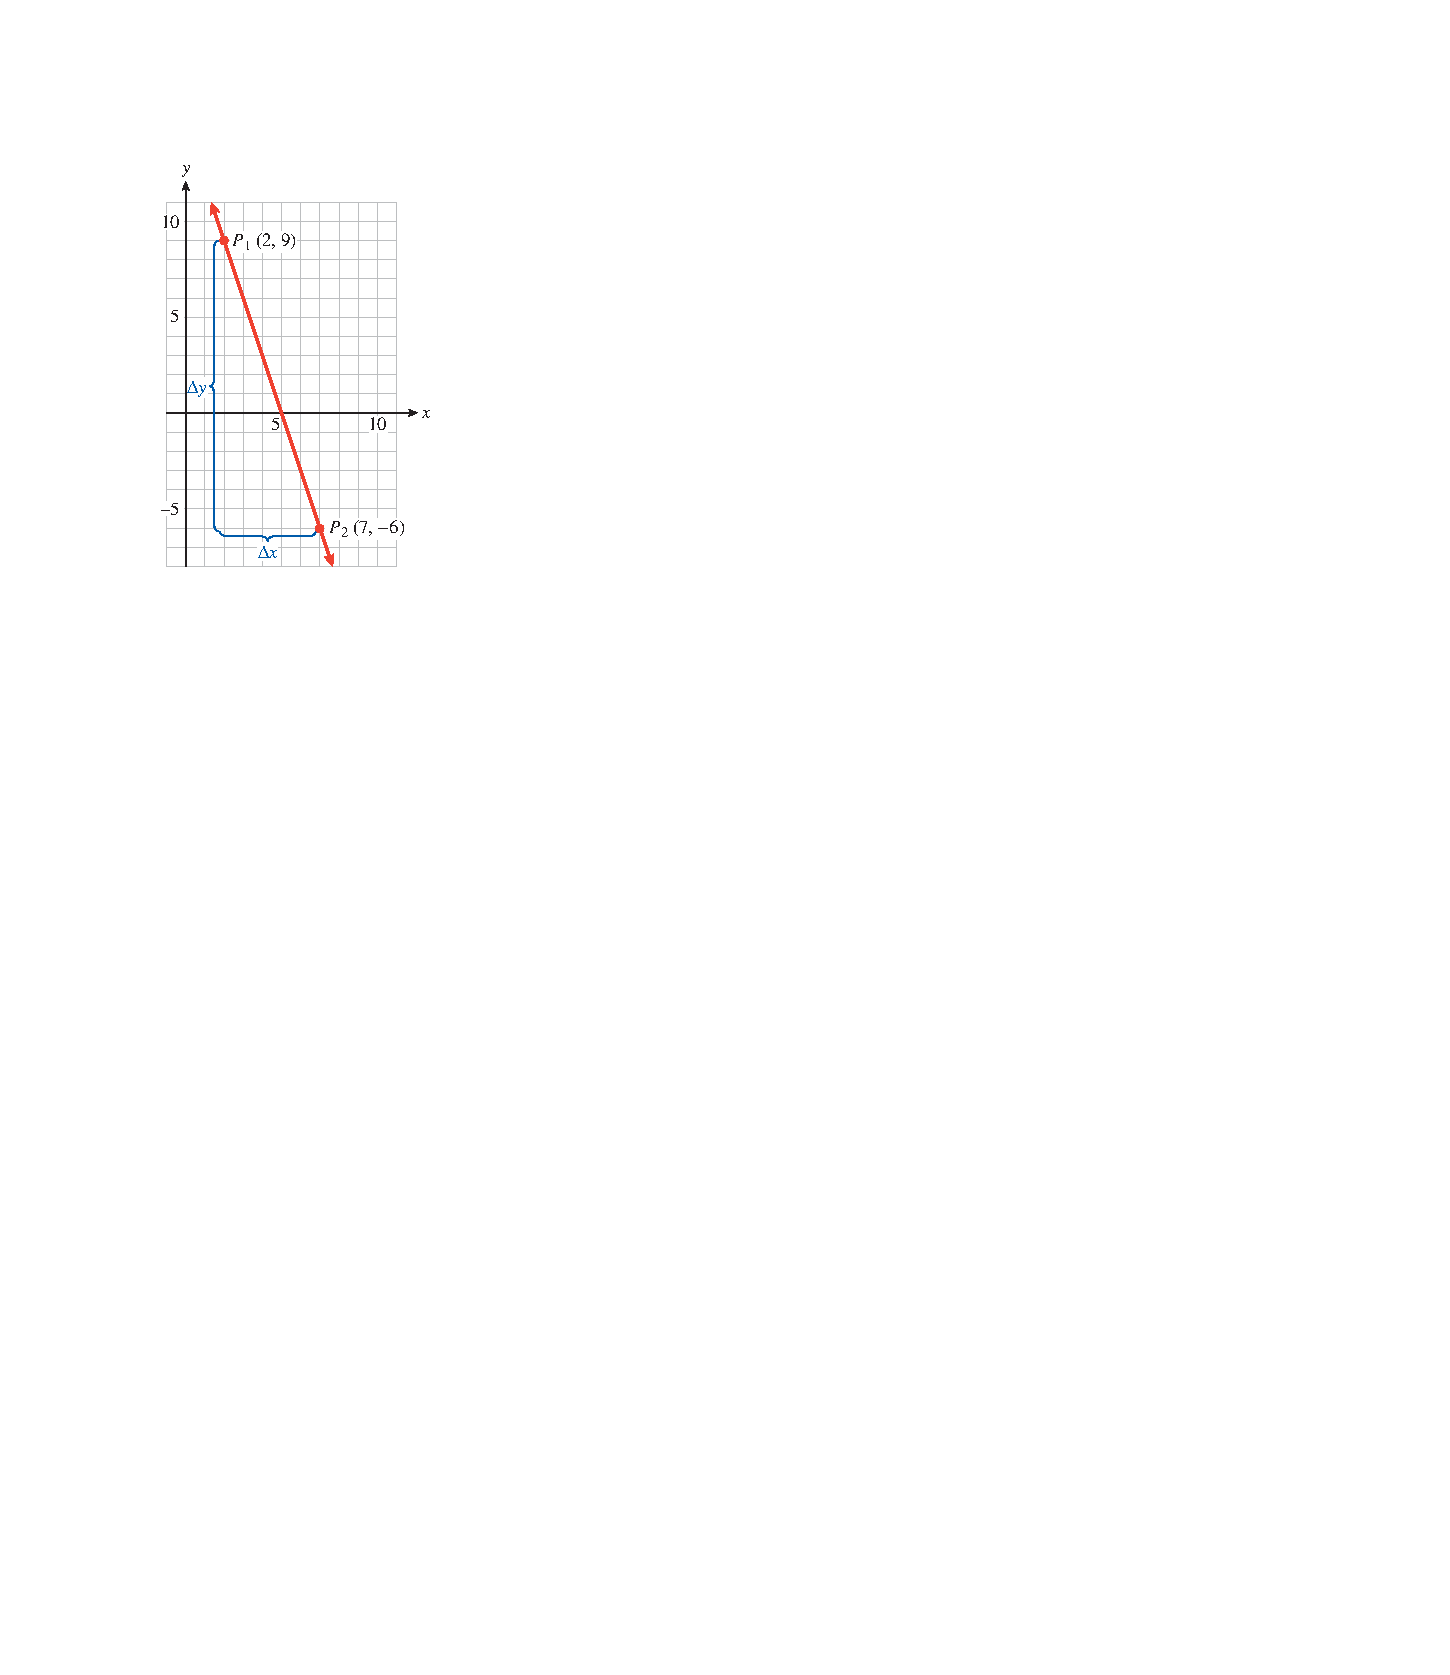
\includegraphics[width=\linewidth]{external/images/fig-slope-formula.pdf}
\end{sbspanel}%
\begin{sbspanel}{0.55}%
Now consider a specific example. The line through the two points \(P_1 (2, 9)\) and \(P_2 (7,-6)\) is shown at left. We can find \(\Delta x\) by subtracting the \(x\)-coordinates of the points:%
\begin{equation*}
\Delta x = 7 - 2 = 5 
\end{equation*}
In general, we have%
\begin{equation*}
\Delta x = x_2 - x_1 
\end{equation*}
and similarly%
\begin{equation*}
\Delta y = y_2 - y_1 
\end{equation*}
%
\end{sbspanel}%
\end{sidebyside}%
\par
These formulas work even if some of the coordinates are negative; in our example%
\begin{equation*}
\Delta y = y_2 - y_1 = -6 - 9 = -15
\end{equation*}
By counting squares \emph{down} from \(P_1\) to \(P_2\), we see that \(\Delta y\) is indeed \(-15\). The slope of the line is%
\begin{equation*}
m=\frac{\Delta y}{\Delta x}=\frac{y_2 - y_1}{x_2 - x_1} = \frac{-15}{5}  = -3
\end{equation*}
We now have a formula for the slope of a line that works even if we do not have a graph.%
\begin{assemblage}{Assemblage}{Two-Point Slope Formula.}{assemblage-slope-and-rate-of-change-h-f}%
The slope of the line passing through the points \(P_1 (x_1, y_1)\) and \(P_2 (x_2, y_2)\) is given by%
\begin{equation*}
m = \frac{\Delta y}{\Delta x}= \frac{y_2 - y_1}{x_2 - x_1} 
\text{, }~x_2 \ne x_1
\end{equation*}
%
\end{assemblage}
\begin{example}{Example}{}{example-example-two-point-slope}%
Compute the slope of the line above using the points \(Q_1 (6, -3)\) and \(Q_2 (4, 3)\).%
\par\smallskip%
\noindent\textbf{\blocktitlefont Solution}.\hypertarget{solution-example-two-point-slope-b}{}\quad{}We substitute the coordinates of \(Q_1\) and \(Q_2\) into the slope formula to find%
\begin{equation*}
m = \frac{y_2 - y_1}{x_2 - x_1}= \frac{3 - (-3)}{4 - 6} = \frac{6}{-2}= -3
\end{equation*}
This value for the slope, \(-3\), is the same value we found above.%
\end{example}
\begin{inlineexercise}{Checkpoint}{Practice 7.}{exercise-slope-and-rate-of-change-h-h}%
%
\begin{enumerate}[label=\alph*.]
\item{}Find the slope of the line passing through the points \((2, -3)\) and \(( -2, -1)\text{.}\)%
\par
\(m=\)\fillintext{3}%
\item{}Sketch a graph of the line by hand.%
\end{enumerate}
%
\par
A graph for part (b):%
\begin{sidebyside}{1}{0}{0.75}{0}%
\begin{sbspanel}{0.25}%
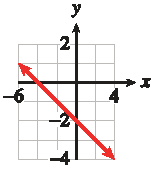
\includegraphics[width=\linewidth]{external/images/fig-in-ex-ans-1-4-7.pdf}
\end{sbspanel}%
\end{sidebyside}%
\par\smallskip%
\noindent\textbf{\blocktitlefont Answer}.\hypertarget{answer-slope-and-rate-of-change-h-h-c}{}\quad{}\(-{\frac{1}{2}}\)%
\par\smallskip%
\noindent\textbf{\blocktitlefont Solution}.\hypertarget{solution-slope-and-rate-of-change-h-h-d}{}\quad{}%
\begin{enumerate}[label=\alph*.]
\item{}\(\displaystyle m=\dfrac{\Delta y}{\Delta x}= \dfrac{-1  + 3}{-2-2}= {-{\frac{1}{2}}}\)%
\item{}A graph is shown below.%
\end{enumerate}
%
\end{inlineexercise}%
\begin{inlineexercise}{Checkpoint}{QuickCheck 5.}{exercise-slope-and-rate-of-change-h-i}%
Comment on the following calculation: The intercepts of a line are \((0,3)\) and \((5,0)\text{,}\) so the slope of the line is \(\dfrac{5}{3}\text{.}\)%
\par
\begin{itemize}[label=$\odot$,leftmargin=3em,]
\item{}It is true because we used two points.%
\item{}It is false because \(\Delta x\) and \(\Delta y\) have opposite signs.%
\item{}It is true because the values are increasing.%
\item{}It is false because the slope is \(\dfrac{3}{5}\).%
\end{itemize}
%
\par\smallskip%
\noindent\textbf{\blocktitlefont Answer}.\hypertarget{answer-slope-and-rate-of-change-h-i-c}{}\quad{}\(\text{Choice 2}\)%
\par\smallskip%
\noindent\textbf{\blocktitlefont Solution}.\hypertarget{solution-slope-and-rate-of-change-h-i-d}{}\quad{}It is false because \(\Delta x\) and \(\Delta y\) have opposite signs. (The slope of the line is \(\dfrac{-5}{3}\text{.}\))%
\end{inlineexercise}%
It will also be useful to write the slope formula with function notation. Recall that \(f (x)\) is another symbol for \(y\), and, in particular, that \(y_1 = f (x_1)\) and \(y_2 = f (x_2)\). Thus, if \(x_2 \ne x_1\), we have this formula.%
\begin{assemblage}{Assemblage}{Slope Formula in Function Notation.}{assemblage-slope-and-rate-of-change-h-k}%
%
\begin{equation*}
m = \frac{\Delta y}{\Delta x} = \frac{y_2 - y_1}{x_2 - x_1} = \frac{f(x_2) - f(x_1)}{x_2 - x_1} 
\text{, }~~~~x_2 \ne x_1
\end{equation*}
%
\end{assemblage}
\begin{example}{Example}{}{example-slopes-on-parabola}%
\begin{sidebyside}{2}{0.0425}{0.0425}{0.085}%
\begin{sbspanel}{0.5}%
The figure shows a graph of%
\begin{equation*}
f (x) = x^2 - 6x
\end{equation*}
%
\begin{enumerate}[label=\alph*]
\item{}Compute the slope of the line segment joining the points at \(x = 1\) and \(x = 4\).%
\item{}Compute the slope of the line segment joining the points at \(x = 2\) and \(x = 5\).%
\end{enumerate}
%
\end{sbspanel}%
\begin{sbspanel}{0.33}%
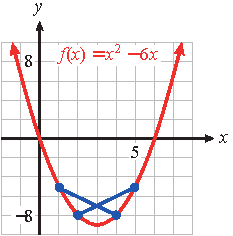
\includegraphics[width=\linewidth]{external/images/fig-slopes-on-parabola.pdf}
\end{sbspanel}%
\end{sidebyside}%
\par\smallskip%
\noindent\textbf{\blocktitlefont Solution}.\hypertarget{solution-slopes-on-parabola-b}{}\quad{}%
\begin{enumerate}[label=\alph*]
\item{}We set \(x_1 = \alert{1}\) and \(x_2 = \alert{4}\) and find the function values at each point.%
\begin{equation*}
f (x_1) = f (\alert{1}) = \alert{1}^2 - 6(\alert{1}) = -5
\end{equation*}
%
\begin{equation*}
f (x_2) = f (\alert{4}) = \alert{4}^2 - 6(\alert{4}) = -8
\end{equation*}
Then%
\begin{equation*}
m = \frac{f (x_2) - f (x_1)}{x_2 - x_1}
=\frac{-8 - (-5)}{4 - 1}=\frac{-3}{3}= -1
\end{equation*}
%
\item{}We set \(x_1 = \alert{2}\) and \(x_2 = \alert{5}\) and find the function values at each point.%
\begin{equation*}
f (x_1) = f (\alert{2}) = \alert{2}^2 - 6(\alert{2}) = -8
\end{equation*}
%
\begin{equation*}
f (x_2) = f (\alert{5}) = \alert{5}^2 - 6(\alert{5}) = -5
\end{equation*}
Then%
\begin{equation*}
m = \frac{f (x_2) - f (x_1)}{x_2 - x_1}
=\frac{-5 - (-8)}{5 - 2}=\frac{3}{3}= 1
\end{equation*}
%
\end{enumerate}
%
\end{example}
Note that the graph of \(f\) is not a straight line and that the slope is not constant.%
\begin{inlineexercise}{Checkpoint}{Practice 8.}{exercise-slope-and-rate-of-change-h-n}%
\begin{sidebyside}{2}{0.0375}{0.0375}{0.075}%
\begin{sbspanel}{0.5}[center]%
The figure shows the graph of a function \(f\).%
\end{sbspanel}%
\begin{sbspanel}{0.35}[center]%
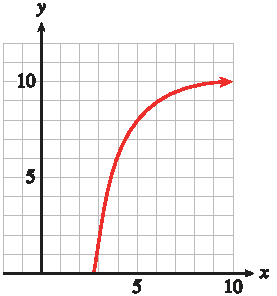
\includegraphics[width=\linewidth]{external/images/fig-slope-on-curve.pdf}
\end{sbspanel}%
\end{sidebyside}%
\par
%
\begin{enumerate}[label=\alph*.]
\item{}Find \(f (3)\) and \(f (5)\text{.}\)%
\par
\(f(3)=\)\fillintext{3}%
\par
\(f(5)=\)\fillintext{3}%
\item{}Compute the slope of the line segment joining the points at \(x = 3\) and \(x = 5\text{.}\)%
\par
\(m=\)\fillintext{3}%
\item{}Write an expression for the slope of the line segment joining the points at \(x = a\) and \(x = b\text{.}\)%
\par
\(m=\)\fillintext{20}%
\par
Note: Be careful to use appropriate parentheses. Press the ``Preview My Answers'' button below to see if you are entering an appropriate expression.%
\end{enumerate}
%
\par\smallskip%
\noindent\textbf{\blocktitlefont Answer 1}.\hypertarget{answer-slope-and-rate-of-change-h-n-c}{}\quad{}\(2\)%
\par\smallskip%
\noindent\textbf{\blocktitlefont Answer 2}.\hypertarget{answer-slope-and-rate-of-change-h-n-d}{}\quad{}\(8\)%
\par\smallskip%
\noindent\textbf{\blocktitlefont Answer 3}.\hypertarget{answer-slope-and-rate-of-change-h-n-e}{}\quad{}\(3\)%
\par\smallskip%
\noindent\textbf{\blocktitlefont Answer 4}.\hypertarget{answer-slope-and-rate-of-change-h-n-f}{}\quad{}\(\frac{f\!\left(b\right)-f\!\left(a\right)}{b-a}\)%
\par\smallskip%
\noindent\textbf{\blocktitlefont Solution}.\hypertarget{solution-slope-and-rate-of-change-h-n-g}{}\quad{}%
\begin{enumerate}[label=\alph*.]
\item{}\(\displaystyle f (3) = 2, ~f (5) = 8\)%
\item{}\(\displaystyle 3\)%
\item{}\(\displaystyle \dfrac{f(b)-f(a)}{b-a}\)%
\end{enumerate}
%
\end{inlineexercise}%
\begin{inlineexercise}{Checkpoint}{Pause and Reflect.}{exercise-slope-and-rate-of-change-h-o}%
Summarize what you learned about slope in this lesson.%
\end{inlineexercise}%
\end{subsectionptx}
%
%
\typeout{************************************************}
\typeout{Subsection  Section Summary}
\typeout{************************************************}
%
\begin{subsectionptx}{Subsection}{Section Summary}{}{Section Summary}{}{}{subsection-summary-1-4}
%
%
\typeout{************************************************}
\typeout{Subsubsection  Vocabulary}
\typeout{************************************************}
%
\begin{subsubsectionptx}{Subsubsection}{Vocabulary}{}{Vocabulary}{}{}{subsubsection-summary-1-4-b}
Look up the definitions of new terms in the Glossary.%
\begin{multicols}{3}
\begin{itemize}[label=\textbullet]
\item{}Ratio%
\item{}Rate of change%
\item{}Slope%
\item{}Scale factor%
\end{itemize}
\end{multicols}
%
\end{subsubsectionptx}
%
%
\typeout{************************************************}
\typeout{Subsubsection  CONCEPTS}
\typeout{************************************************}
%
\begin{subsubsectionptx}{Subsubsection}{CONCEPTS}{}{CONCEPTS}{}{}{subsubsection-summary-1-4-c}
%
\begin{enumerate}[label=\arabic*]
\item{}We can use ratios to compare quantities.%
\item{}The slope ratio, \(\dfrac{\text{change in y-coordinate}}{\text{change in }x\text{-coordinate}}\), measures the steepness of a line.%
\item{}Notation for slope: \(m = \dfrac{\Delta y}{\Delta x}\), \(\Delta x \ne 0\).%
\item{}Formula for slope: \(m =\dfrac{y_2 - y_1}{x_2 - x_1}\), \(~~x_2\ne x_1 \)%
\item{}Formula for slope: \(m =\dfrac{f(x_2) - f(x_1)}{x_2 - x_1}\), \(~~x_2\ne x_1 \)%
\item{}Lines have constant slope.%
\item{}Slope is a scale factor that tells us how many units \(\Delta y\) increases for each unit increase in \(\Delta x\) as we move along the line.%
\item{}The slope gives us the rate of change.%
\end{enumerate}
%
\end{subsubsectionptx}
%
%
\typeout{************************************************}
\typeout{Subsubsection  STUDY QUESTIONS}
\typeout{************************************************}
%
\begin{subsubsectionptx}{Subsubsection}{STUDY QUESTIONS}{}{STUDY QUESTIONS}{}{}{subsubsection-summary-1-4-d}
%
\begin{enumerate}[label=\arabic*]
\item{}Explain how to compare prices with unit pricing.%
\item{}Why is \(\Delta y\) the numerator of the slope ratio and \(\Delta x\) the denominator?%
\item{}Which line is steeper, one with \(m = -2\) or one with \(m = -5\)?%
\item{}A classmate says that you must always use the intercepts to calculate the slope of a line. Do you agree? Explain.%
\item{}In an application, what does the slope of the graph tell you about the situation?%
\end{enumerate}
%
\end{subsubsectionptx}
%
%
\typeout{************************************************}
\typeout{Subsubsection  SKILLS}
\typeout{************************************************}
%
\begin{subsubsectionptx}{Subsubsection}{SKILLS}{}{SKILLS}{}{}{subsubsection-summary-1-4-e}
Practice each skill in the Homework problems listed.%
\begin{enumerate}[label=\arabic*]
\item{}Use ratios for comparison: \#1\textendash{}4%
\item{}Compute slope from a graph: \#5\textendash{}16, 23\textendash{}26%
\item{}Use slope to find \(\Delta y\) or \(\Delta x\): \#17\textendash{}20, 27\textendash{}30%
\item{}Use slope to compare steepness: \#21 and 22%
\item{}Decide whether data points lie on a straight line: \#41\textendash{}46%
\item{}Interpret slope as a rate of change: \#31\textendash{}40%
\item{}Use function notation to discuss graphs and slope: \#53\textendash{}62%
\end{enumerate}
%
\end{subsubsectionptx}
\end{subsectionptx}
%
%
\typeout{************************************************}
\typeout{Exercises  Homework 1.4}
\typeout{************************************************}
%
\begin{exercises-subsection}{Exercises}{Homework 1.4}{}{Homework 1.4}{}{}{exercises-section-1-4-exercises}
\par\medskip\noindent%
\textbf{Exercise Group.}\space\space%
Compute ratios to answer the questions in Problems 1\textendash{}4.%
\begin{exercisegroup}
\begin{divisionexerciseeg}{1}{}{}{exercise-section-1-4-exercises-b-b}%
Carl runs \(100\) meters in \(10\) seconds. Anthony runs \(200\) meters in \(19.6\) seconds. Who has the faster average speed?%
\end{divisionexerciseeg}%
\begin{divisionexerciseeg}{2}{}{}{exercise-section-1-4-exercises-b-c}%
On his \(512\)-mile round trip to Las Vegas and back, Corey needed \(16\) gallons of gasoline. He used \(13\) gallons of gasoline on a \(429\)-mile trip to Los Angeles. On which trip did he get better fuel economy?%
\end{divisionexerciseeg}%
\begin{divisionexerciseeg}{3}{}{}{exercise-section-1-4-exercises-b-d}%
Grimy Gulch Pass rises \(0.6\) miles over a horizontal distance of \(26\) miles. Bob's driveway rises \(12\) feet over a horizontal distance of \(150\) feet. Which is steeper?%
\end{divisionexerciseeg}%
\begin{divisionexerciseeg}{4}{}{}{exercise-section-1-4-exercises-b-e}%
Which is steeper, the truck ramp for Acme Movers, which rises \(4\) feet over a horizontal distance of \(9\) feet, or a toy truck ramp, which rises \(3\) centimeters over a horizontal distance of \(7\) centimeters?%
\end{divisionexerciseeg}%
\end{exercisegroup}
\par\medskip\noindent
\par\medskip\noindent%
\textbf{Exercise Group.}\space\space%
In Problems 5-8, compute the slope of the line through the indicated points. On both axes, one square represents one unit.%
\begin{exercisegroupcol}{2}
\begin{divisionexerciseegcol}{5}{}{}{exercise-section-1-4-exercises-c-b}%
\begin{sidebyside}{1}{0.25}{0.25}{0}%
\begin{sbspanel}{0.5}%
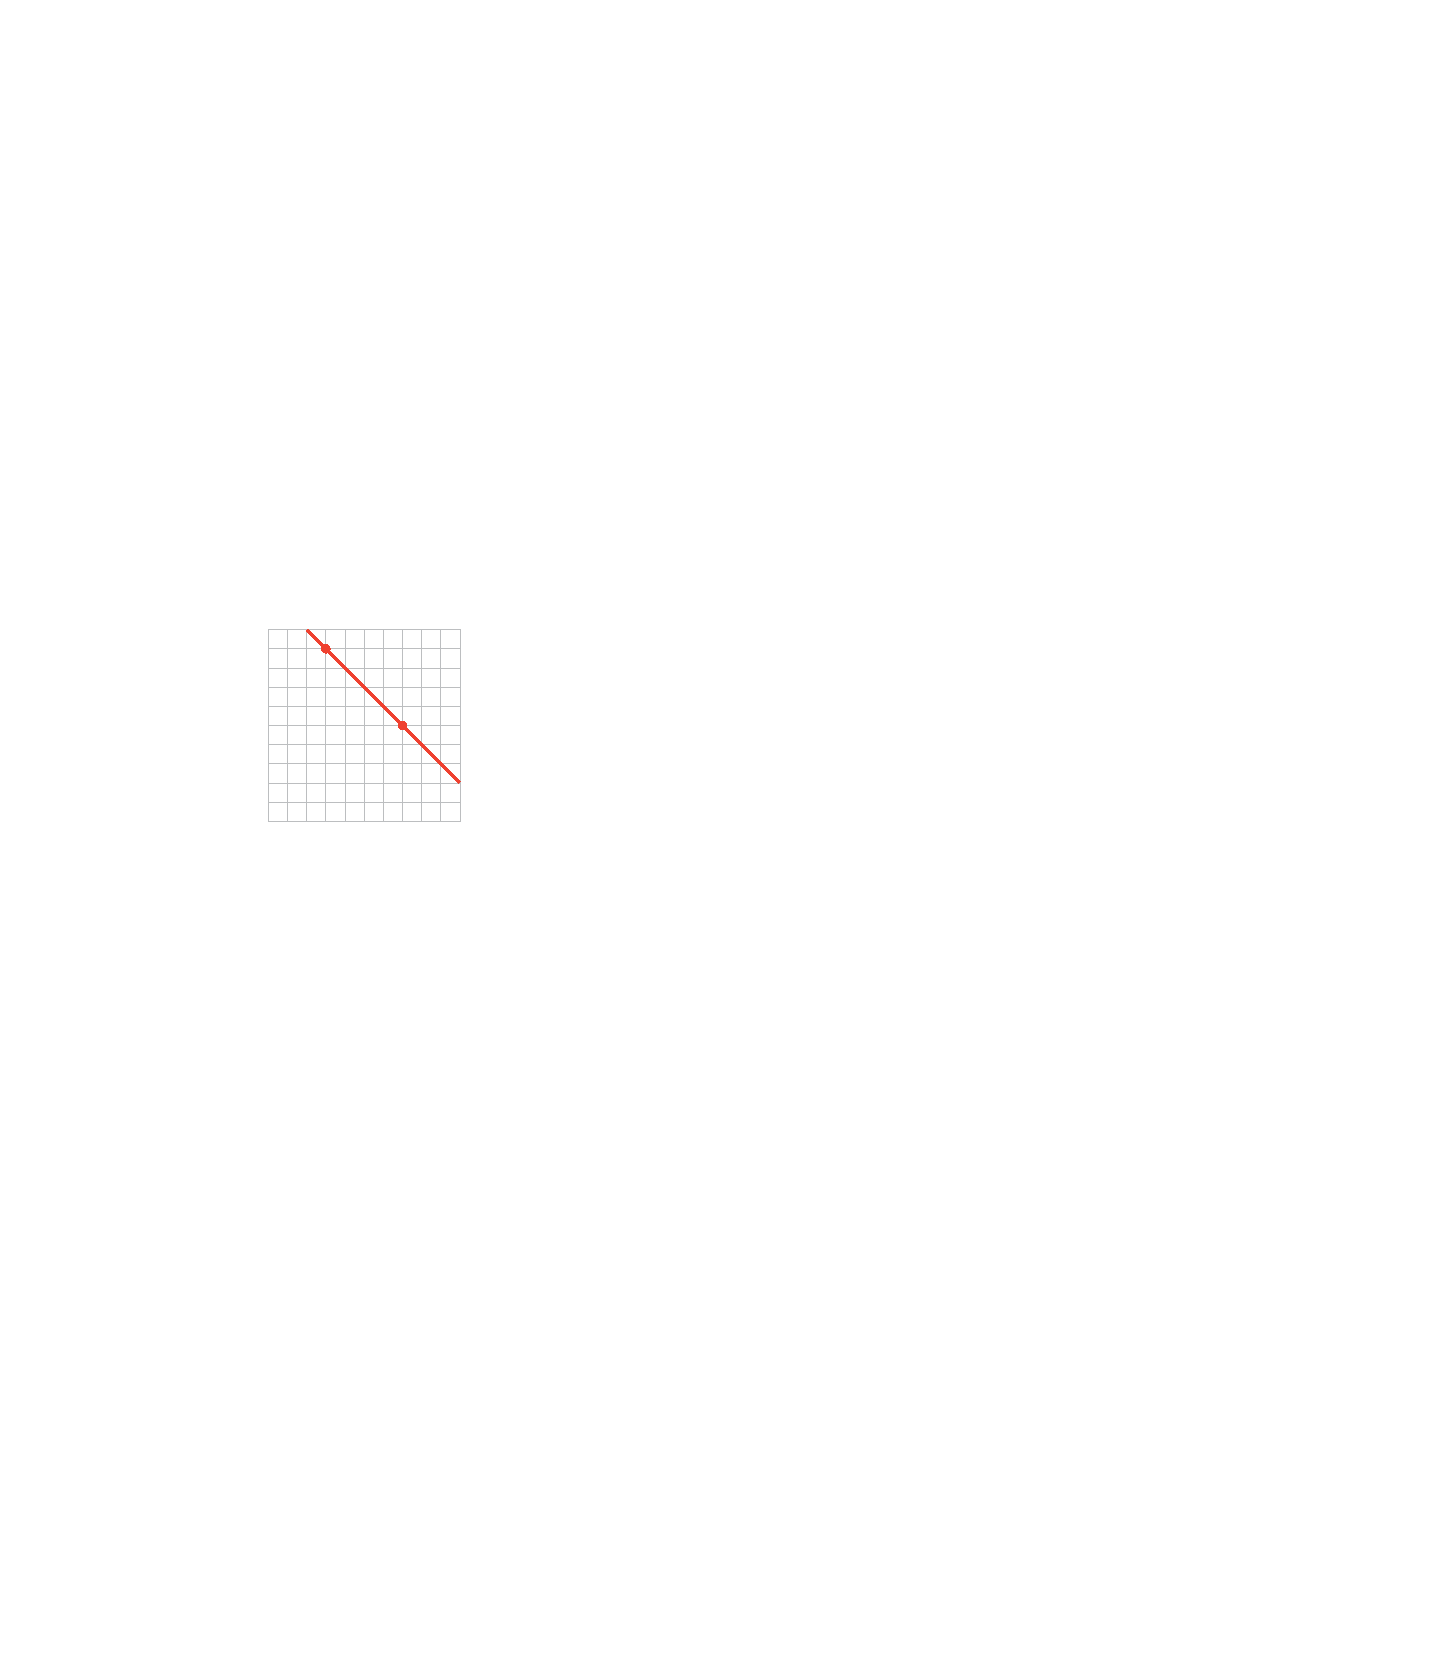
\includegraphics[width=\linewidth]{external/images/fig-ex-1-4-5.pdf}
\end{sbspanel}%
\end{sidebyside}%
\end{divisionexerciseegcol}%
\begin{divisionexerciseegcol}{6}{}{}{exercise-section-1-4-exercises-c-c}%
\begin{sidebyside}{1}{0.25}{0.25}{0}%
\begin{sbspanel}{0.5}%
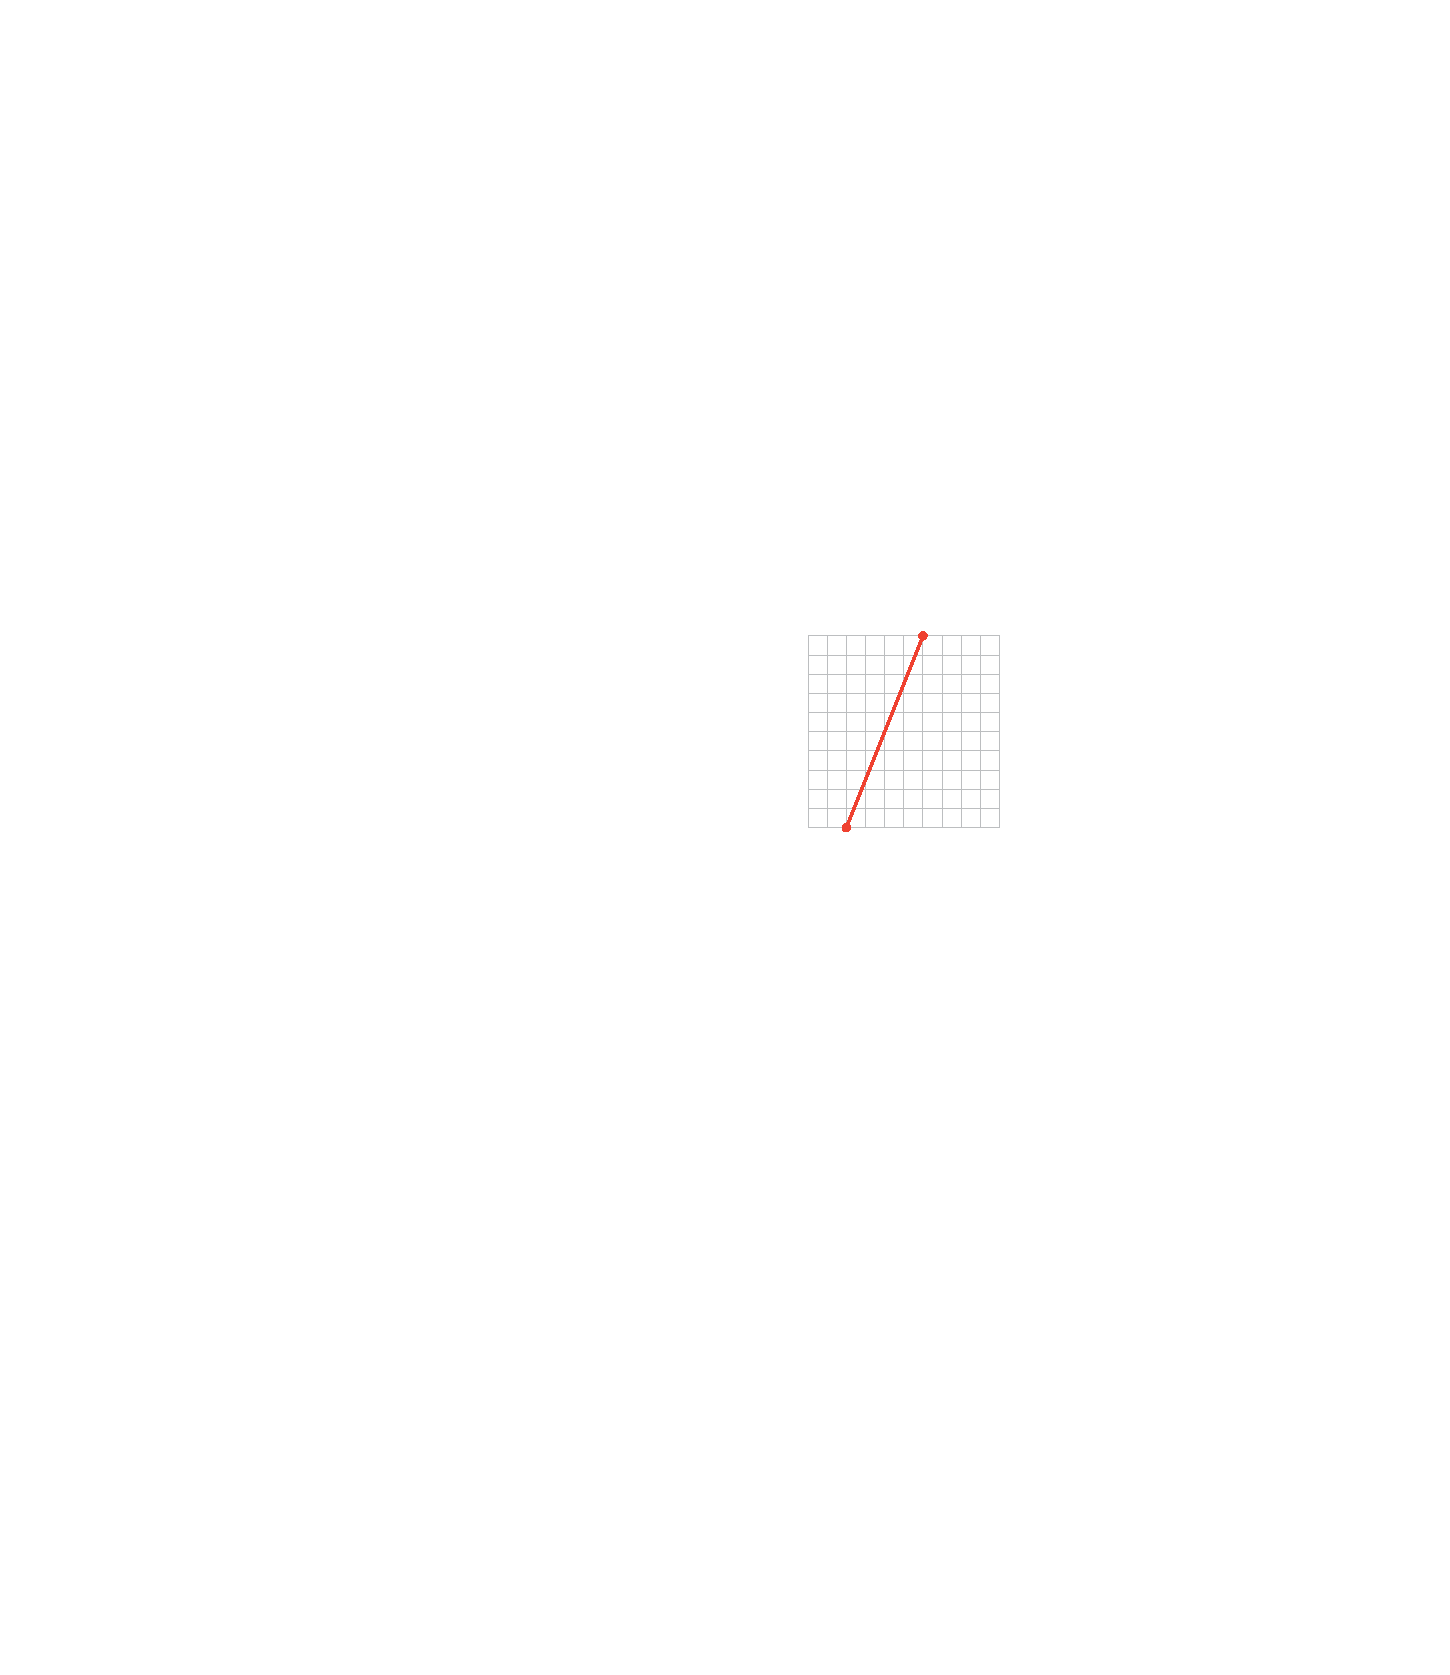
\includegraphics[width=\linewidth]{external/images/fig-ex-1-4-6.pdf}
\end{sbspanel}%
\end{sidebyside}%
\end{divisionexerciseegcol}%
\begin{divisionexerciseegcol}{7}{}{}{exercise-section-1-4-exercises-c-d}%
\begin{sidebyside}{1}{0.25}{0.25}{0}%
\begin{sbspanel}{0.5}%
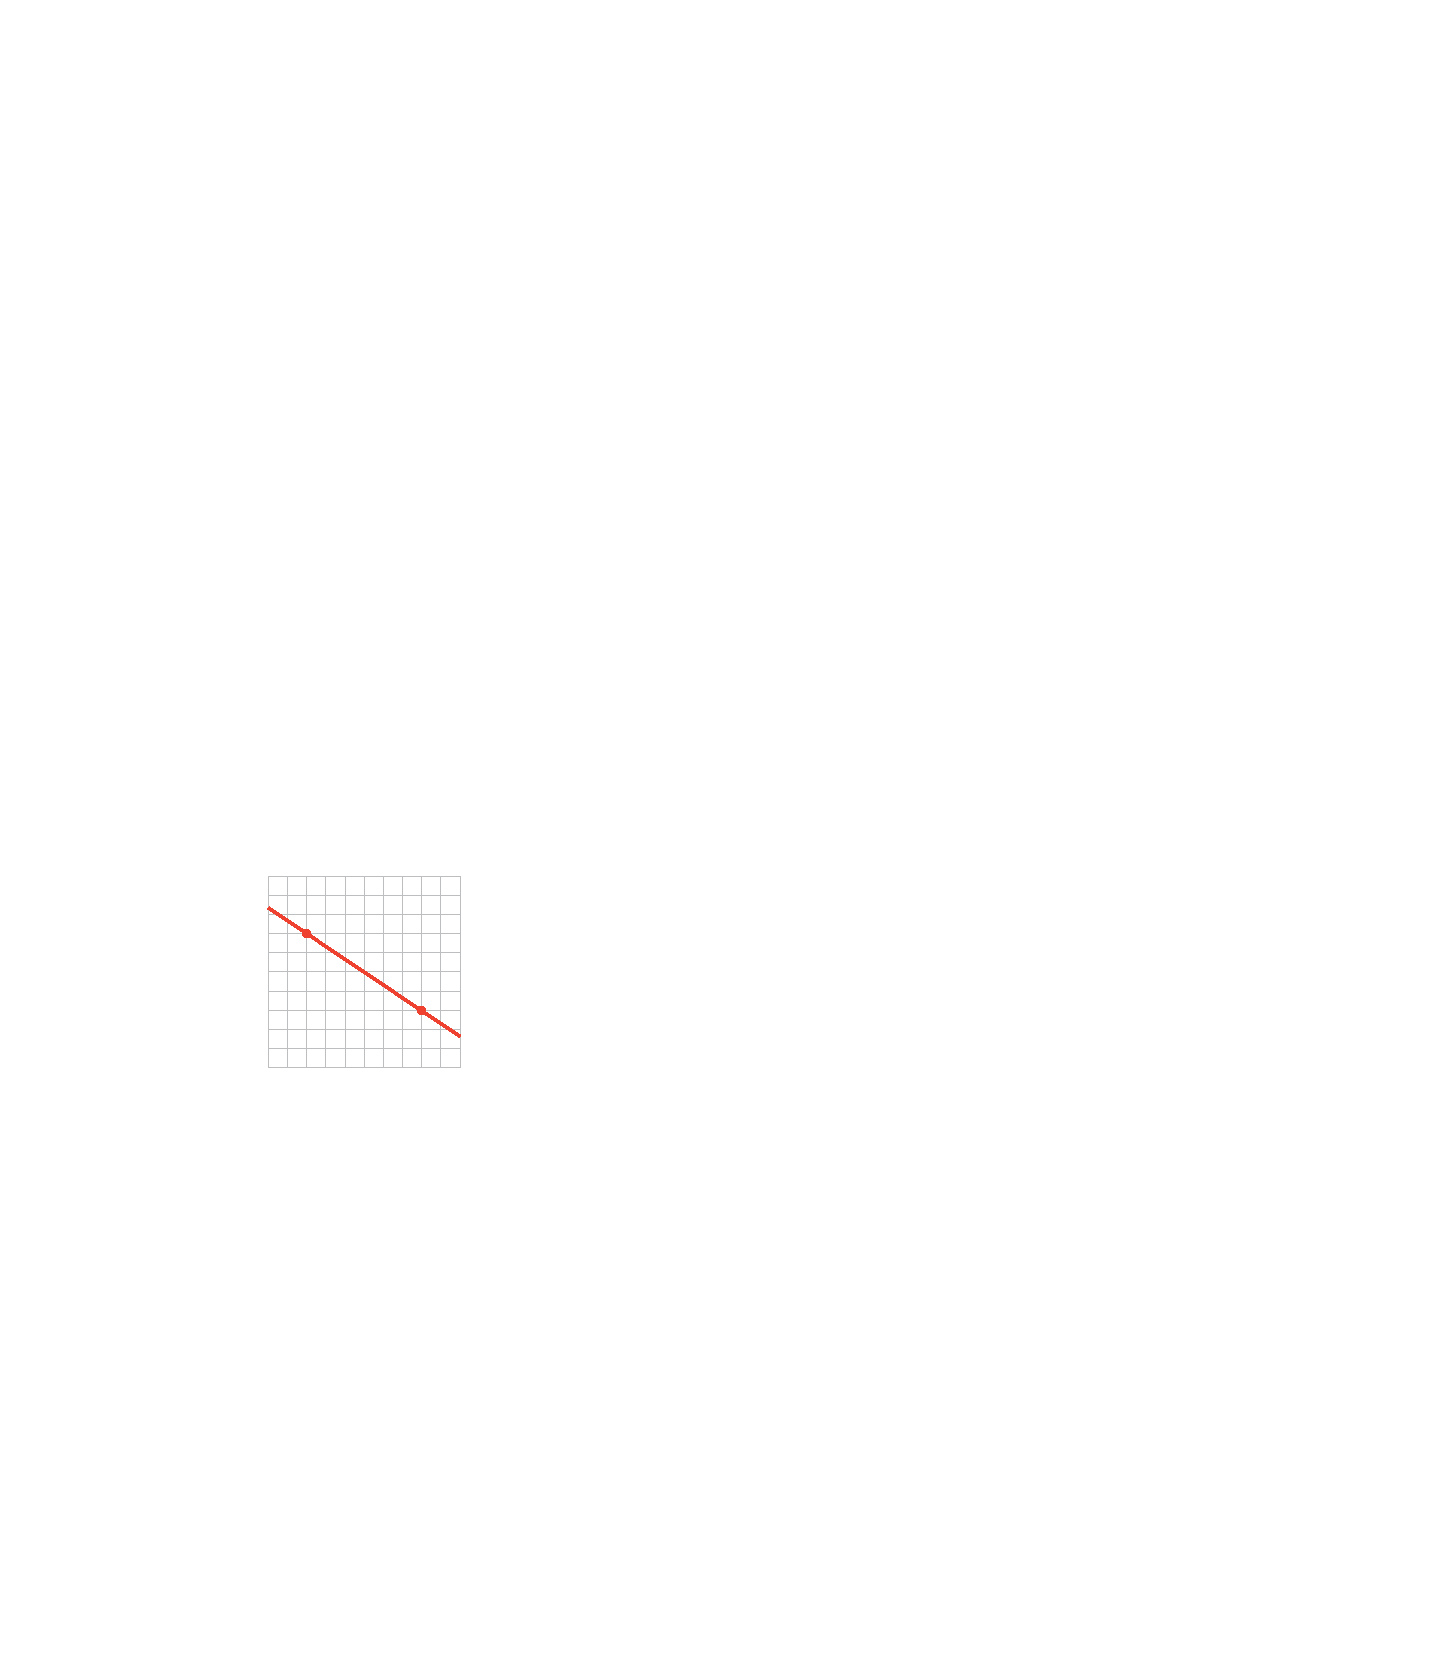
\includegraphics[width=\linewidth]{external/images/fig-ex-1-4-7.pdf}
\end{sbspanel}%
\end{sidebyside}%
\end{divisionexerciseegcol}%
\begin{divisionexerciseegcol}{8}{}{}{exercise-section-1-4-exercises-c-e}%
\begin{sidebyside}{1}{0.25}{0.25}{0}%
\begin{sbspanel}{0.5}%
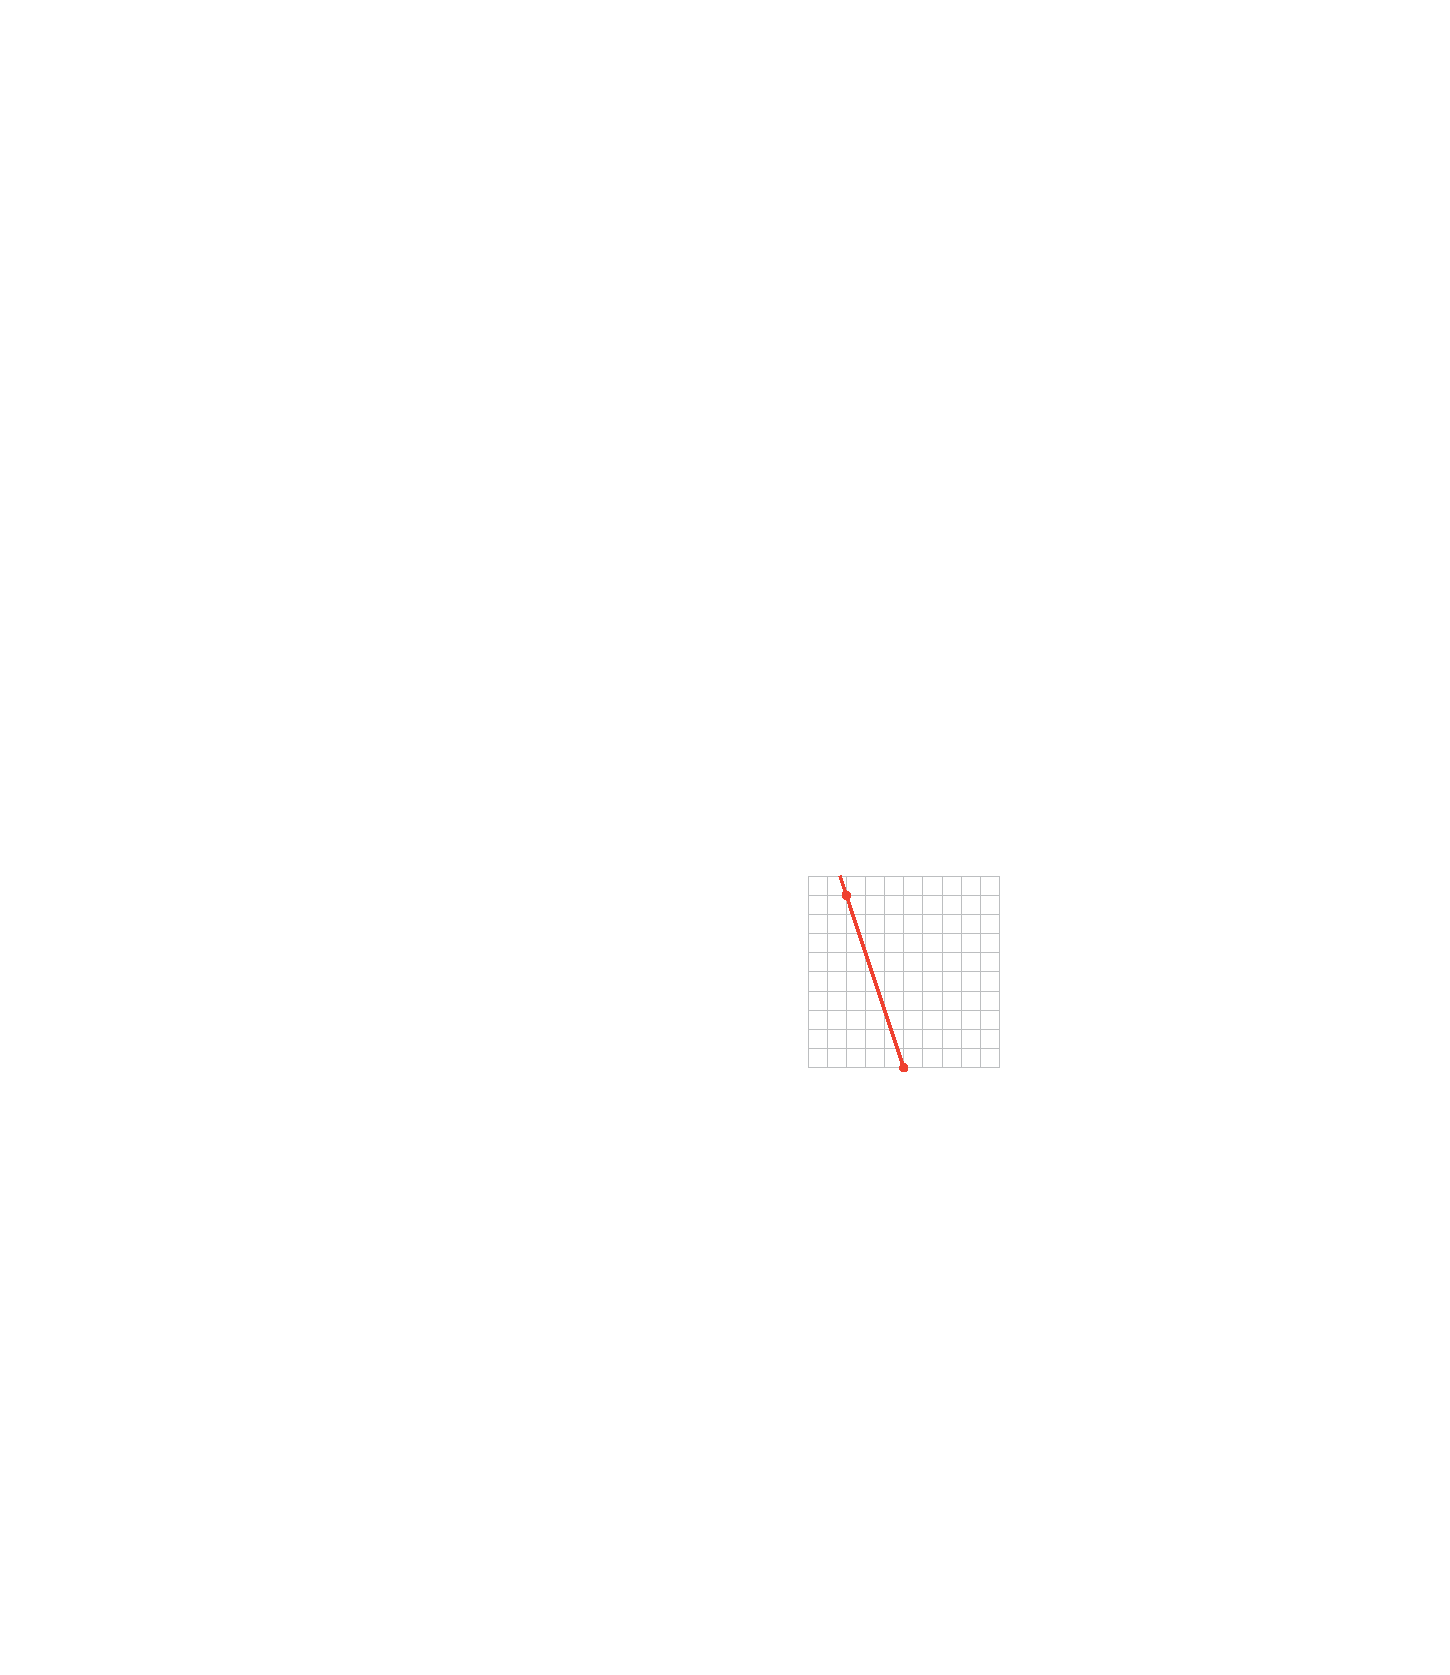
\includegraphics[width=\linewidth]{external/images/fig-ex-1-4-8.pdf}
\end{sbspanel}%
\end{sidebyside}%
\end{divisionexerciseegcol}%
\end{exercisegroupcol}
\par\medskip\noindent
\par\medskip\noindent%
\textbf{Exercise Group.}\space\space%
For Problems 9\textendash{}14,%
\begin{enumerate}[label=\alph*]
\item{}Graph each line by the intercept method.%
\item{}Use the intercepts to compute the slope.%
\end{enumerate}
%
\begin{exercisegroupcol}{2}
\begin{divisionexerciseegcol}{9}{}{}{exercise-section-1-4-exercises-d-b}%
\(3x - 4y = 12\)%
\end{divisionexerciseegcol}%
\begin{divisionexerciseegcol}{10}{}{}{exercise-section-1-4-exercises-d-c}%
\(2y - 5x = 10\)%
\end{divisionexerciseegcol}%
\begin{divisionexerciseegcol}{11}{}{}{exercise-section-1-4-exercises-d-d}%
\(2y + 6x = -18\)%
\end{divisionexerciseegcol}%
\begin{divisionexerciseegcol}{12}{}{}{exercise-section-1-4-exercises-d-e}%
\(9x + 12y = 36\)%
\end{divisionexerciseegcol}%
\begin{divisionexerciseegcol}{13}{}{}{exercise-section-1-4-exercises-d-f}%
\(\dfrac{x}{5}- \dfrac{y}{8}= 1\)%
\end{divisionexerciseegcol}%
\begin{divisionexerciseegcol}{14}{}{}{exercise-section-1-4-exercises-d-g}%
\(\dfrac{x}{7}- \dfrac{y}{4}= 1\)%
\end{divisionexerciseegcol}%
\end{exercisegroupcol}
\par\medskip\noindent
\begin{divisionexercise}{15}{}{}{exercise-section-1-4-exercises-e}%
%
\begin{enumerate}[label=\alph*]
\item{}Use the points \((0, 2)\) and \((4, 8)\) to compute the slope of the line. Illustrate \(\Delta y\) and \(\Delta x\) on the graph.%
\item{}Use the points \((-4, -4)\) and \((4, 8)\) to compute the slope of the line. Illustrate \(\Delta y\) and \(\Delta x\) on the graph.%
\item{}Use the points \((0, 2)\) and \((-6, -7)\) to compute the slope of the line. Illustrate \(\Delta y\) and \(\Delta x\) on the graph.%
\end{enumerate}
%
\begin{sidebyside}{1}{0.325}{0.325}{0}%
\begin{sbspanel}{0.35}%
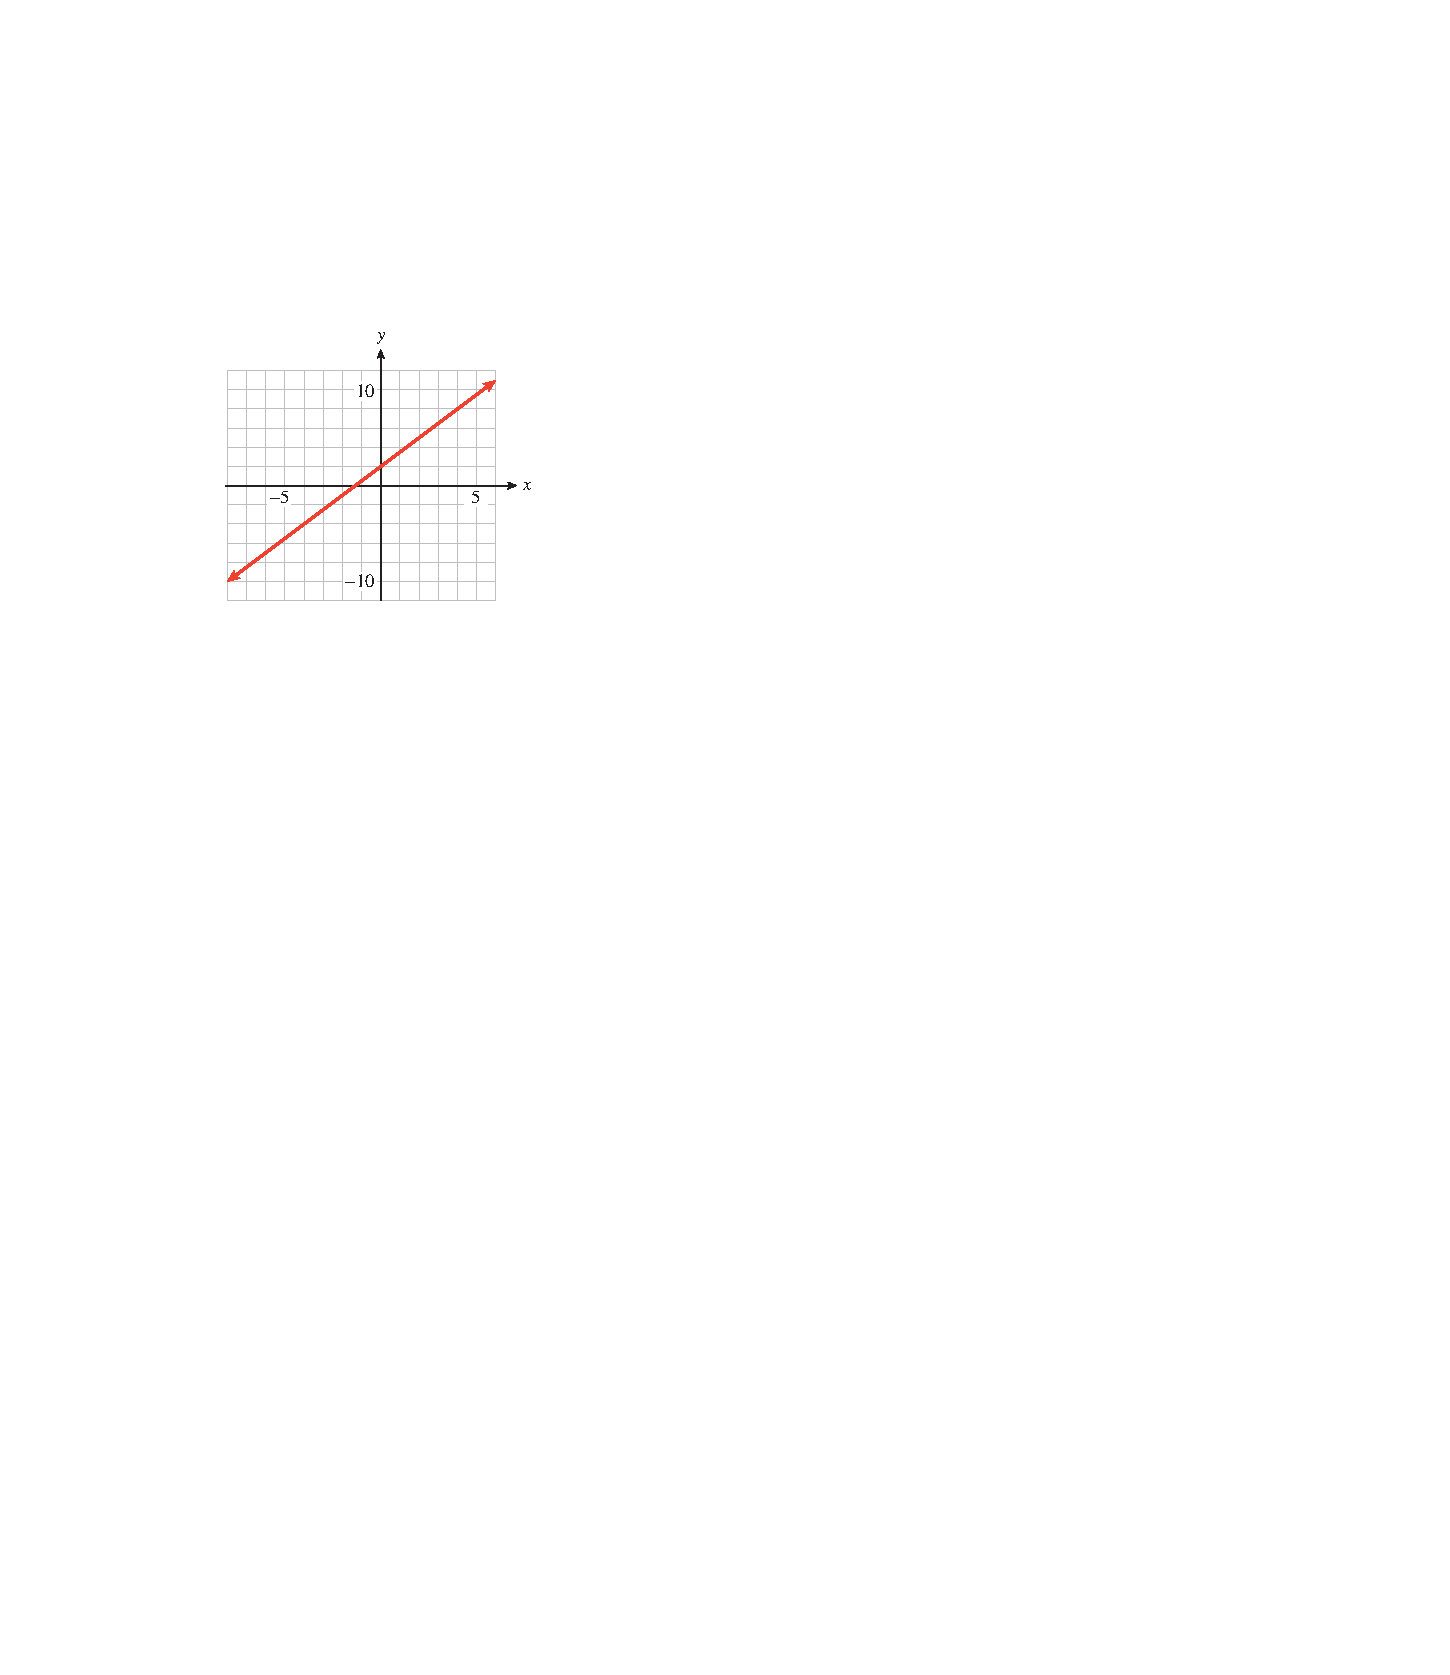
\includegraphics[width=\linewidth]{external/images/fig-ex-1-4-15.pdf}
\end{sbspanel}%
\end{sidebyside}%
\end{divisionexercise}%
\begin{divisionexercise}{16}{}{}{exercise-section-1-4-exercises-f}%
%
\begin{enumerate}[label=\alph*]
\item{}Use the points \((0, -6)\) and \((8, -12)\) to compute the slope of the line. Illustrate \(\Delta y\) and \(\Delta x\) on the graph.%
\item{}Use the points \((-8, 0)\) and \((4, -9)\) to compute the slope of the line. Illustrate \(\Delta y\) and \(\Delta x\) on the graph.%
\item{}Use the points \((4, -9)\) and \((0, -6)\) to compute the slope of the line. Illustrate \(\Delta y\) and \(\Delta x\) on the graph.%
\end{enumerate}
%
\begin{sidebyside}{1}{0.325}{0.325}{0}%
\begin{sbspanel}{0.35}%
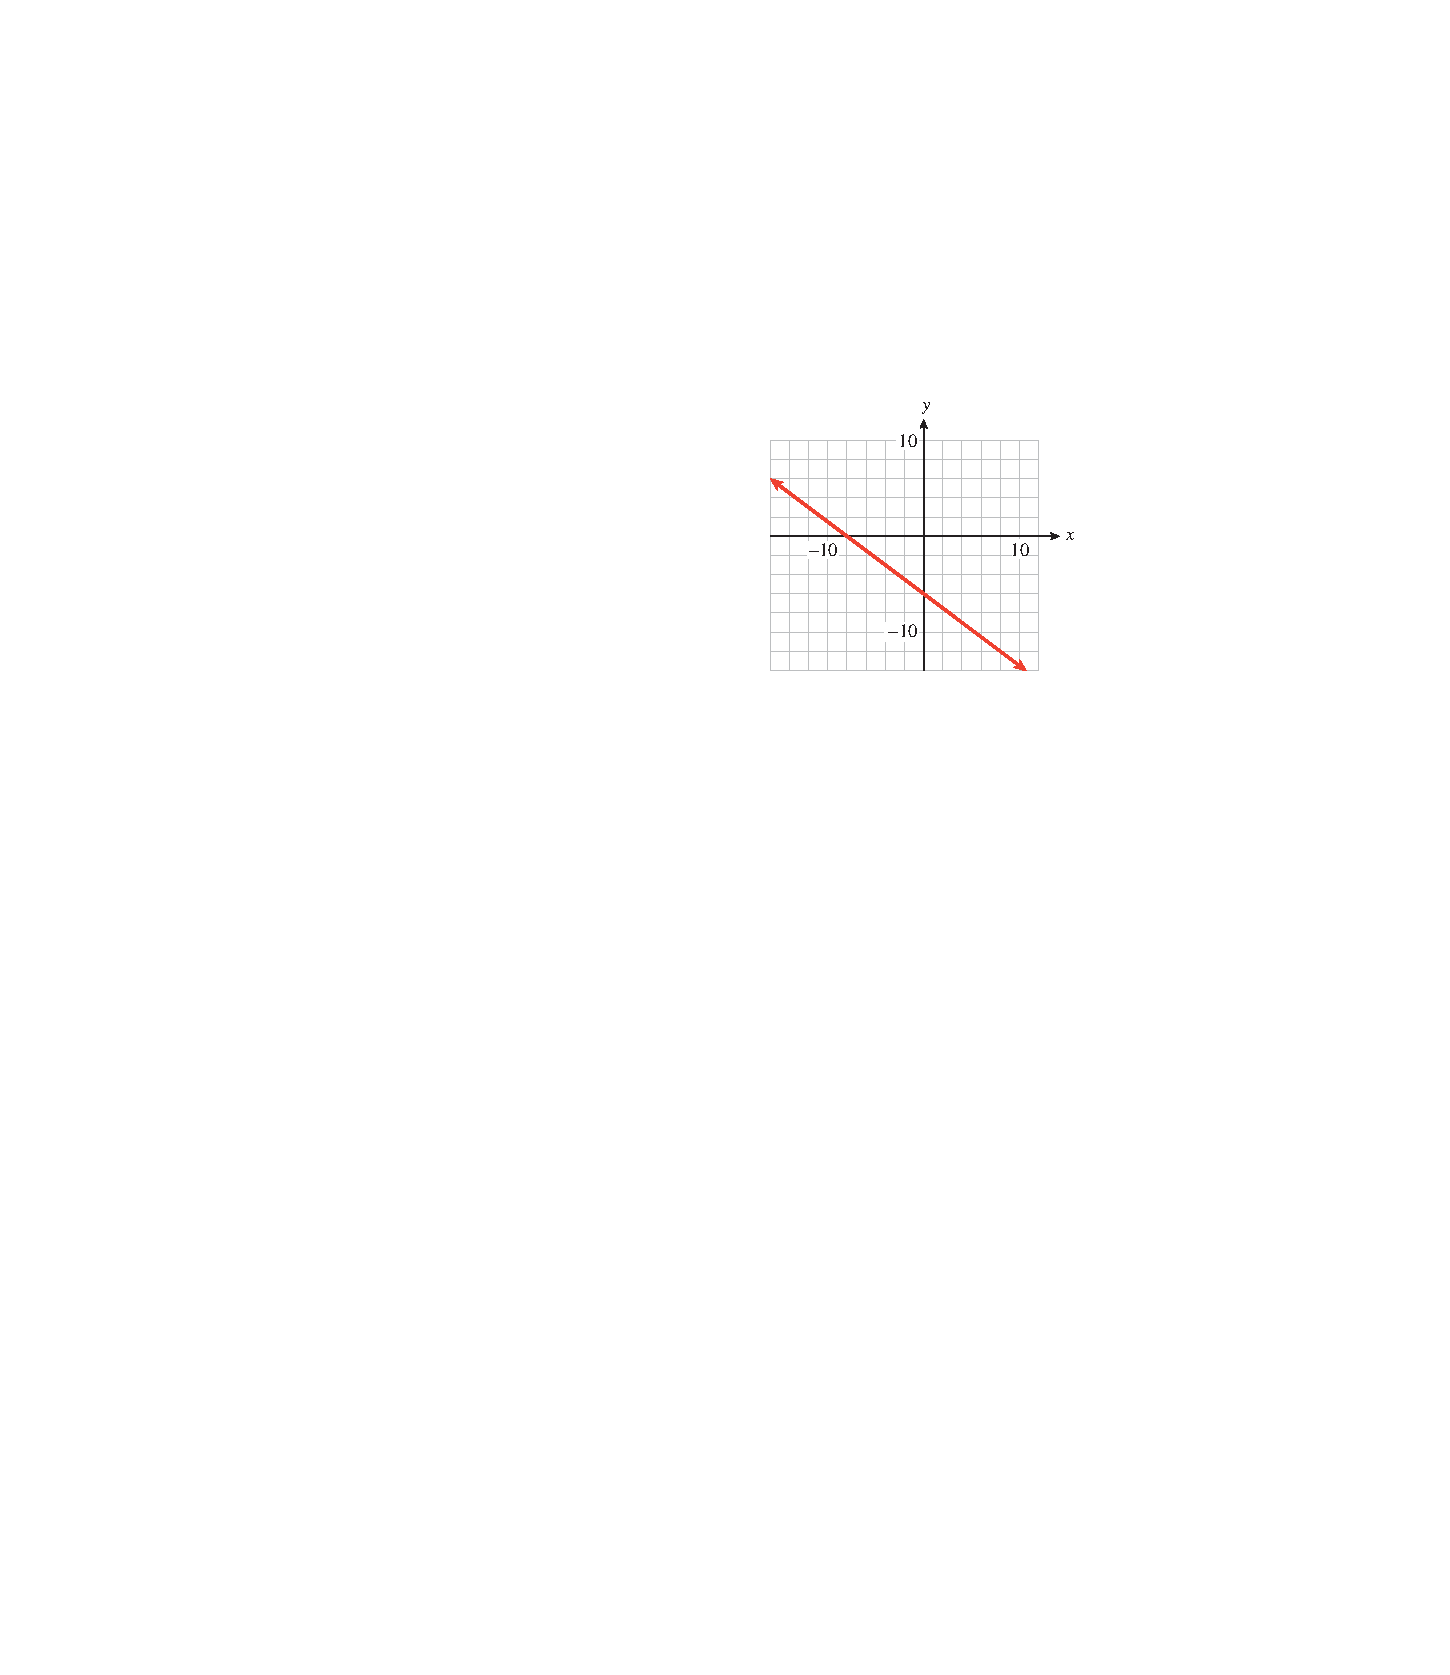
\includegraphics[width=\linewidth]{external/images/fig-ex-1-4-16.pdf}
\end{sbspanel}%
\end{sidebyside}%
\end{divisionexercise}%
\par\medskip\noindent%
\textbf{Exercise Group.}\space\space%
For Problems 17\textendash{}20, use the formula \(m=\dfrac{\Delta y}{\Delta x} \)%
\begin{exercisegroup}
\begin{divisionexerciseeg}{17}{}{}{exercise-section-1-4-exercises-g-b}%
A line has slope \(\dfrac{-3}{4}\).%
\begin{enumerate}[label=\alph*]
\item{}Find the vertical change associated with each horizontal change along the line.%
\begin{multicols}{2}
\begin{enumerate}[label=\roman*]
\item{}\(\displaystyle \Delta x = 4\)%
\item{}\(\displaystyle \Delta x = -8\)%
\item{}\(\displaystyle \Delta x = 2\)%
\item{}\(\displaystyle \Delta x = -6\)%
\end{enumerate}
\end{multicols}
%
\item{}Find the horizontal change associated with each vertical change along the line.%
\begin{multicols}{2}
\begin{enumerate}[label=\roman*]
\item{}\(\displaystyle \Delta y = 3\)%
\item{}\(\displaystyle \Delta y = -6\)%
\item{}\(\displaystyle \Delta y = -2\)%
\item{}\(\displaystyle \Delta y = 1\)%
\end{enumerate}
\end{multicols}
%
\end{enumerate}
%
\end{divisionexerciseeg}%
\begin{divisionexerciseeg}{18}{}{}{exercise-section-1-4-exercises-g-c}%
A line has slope \(\dfrac{5}{3}\).%
\begin{enumerate}[label=\alph*]
\item{}Find the vertical change associated with each horizontal change along the line.%
\begin{multicols}{2}
\begin{enumerate}[label=\roman*]
\item{}\(\displaystyle \Delta x = 3\)%
\item{}\(\displaystyle \Delta x = -6\)%
\item{}\(\displaystyle \Delta x = 1\)%
\item{}\(\displaystyle \Delta x = -24\)%
\end{enumerate}
\end{multicols}
%
\item{}Find the horizontal change associated with each vertical change along the line.%
\begin{multicols}{2}
\begin{enumerate}[label=\roman*]
\item{}\(\displaystyle \Delta y = -5\)%
\item{}\(\displaystyle \Delta y = -2.5\)%
\item{}\(\displaystyle \Delta y = -1\)%
\item{}\(\displaystyle \Delta y = 3\)%
\end{enumerate}
\end{multicols}
%
\end{enumerate}
%
\end{divisionexerciseeg}%
\begin{divisionexerciseeg}{19}{}{}{exercise-section-1-4-exercises-g-d}%
Residential staircases are usually built with a slope of \(70\%\), or \(\dfrac{7}{10}\). If the vertical distance between stories is \(10\) feet, how much horizontal space does the staircase require?%
\end{divisionexerciseeg}%
\begin{divisionexerciseeg}{20}{}{}{exercise-section-1-4-exercises-g-e}%
A straight section of highway in the Midwest maintains a grade (slope) of \(4\%\), or \(\dfrac{1}{25}\), for \(12\) miles. How much does your elevation change as you travel the road?%
\end{divisionexerciseeg}%
\end{exercisegroup}
\par\medskip\noindent
\begin{divisionexercise}{21}{}{}{exercise-section-1-4-exercises-h}%
Choose the line with the correct slope. The scales are the same on both axes.%
\begin{multicols}{4}
\begin{enumerate}[label=\alph*]
\item{}\(\displaystyle m=2\)%
\item{}\(\displaystyle m=-\dfrac{1}{2} \)%
\item{}\(\displaystyle m=\dfrac{2}{3} \)%
\item{}\(\displaystyle m=-\dfrac{5}{3} \)%
\end{enumerate}
\end{multicols}
%
\begin{sidebyside}{1}{0.25}{0.25}{0}%
\begin{sbspanel}{0.5}%
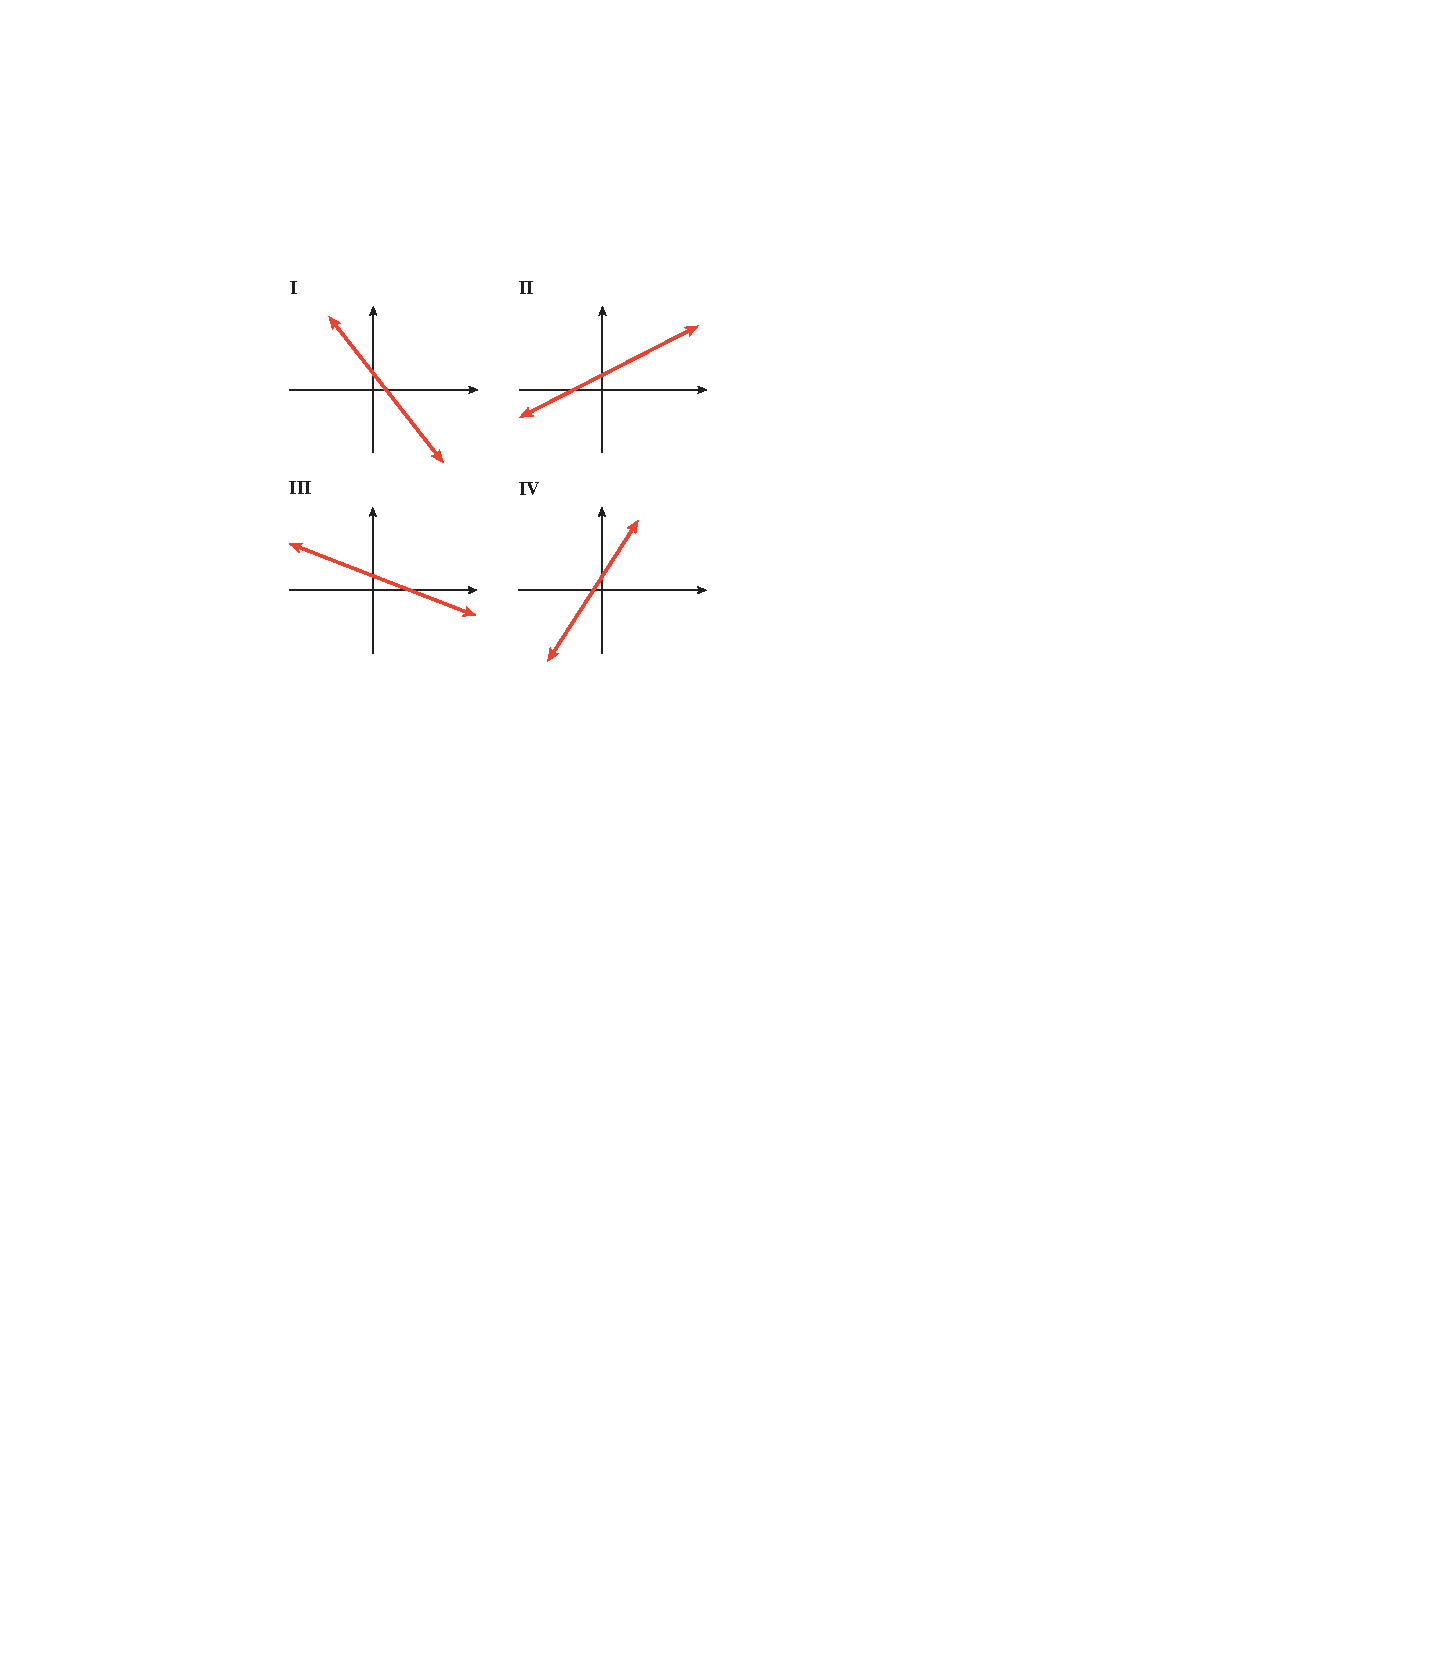
\includegraphics[width=\linewidth]{external/images/fig-ex-1-4-21.pdf}
\end{sbspanel}%
\end{sidebyside}%
\end{divisionexercise}%
\begin{divisionexercise}{22}{}{}{exercise-section-1-4-exercises-i}%
Choose the line with the correct slope. The scales are the same on both axes.%
\begin{multicols}{4}
\begin{enumerate}[label=\alph*]
\item{}\(\displaystyle 0\lt m \lt 1\)%
\item{}\(\displaystyle m \lt -1\)%
\item{}\(\displaystyle m= \gt 1 \)%
\item{}\(\displaystyle m=0 \)%
\end{enumerate}
\end{multicols}
%
\begin{sidebyside}{1}{0.25}{0.25}{0}%
\begin{sbspanel}{0.5}%
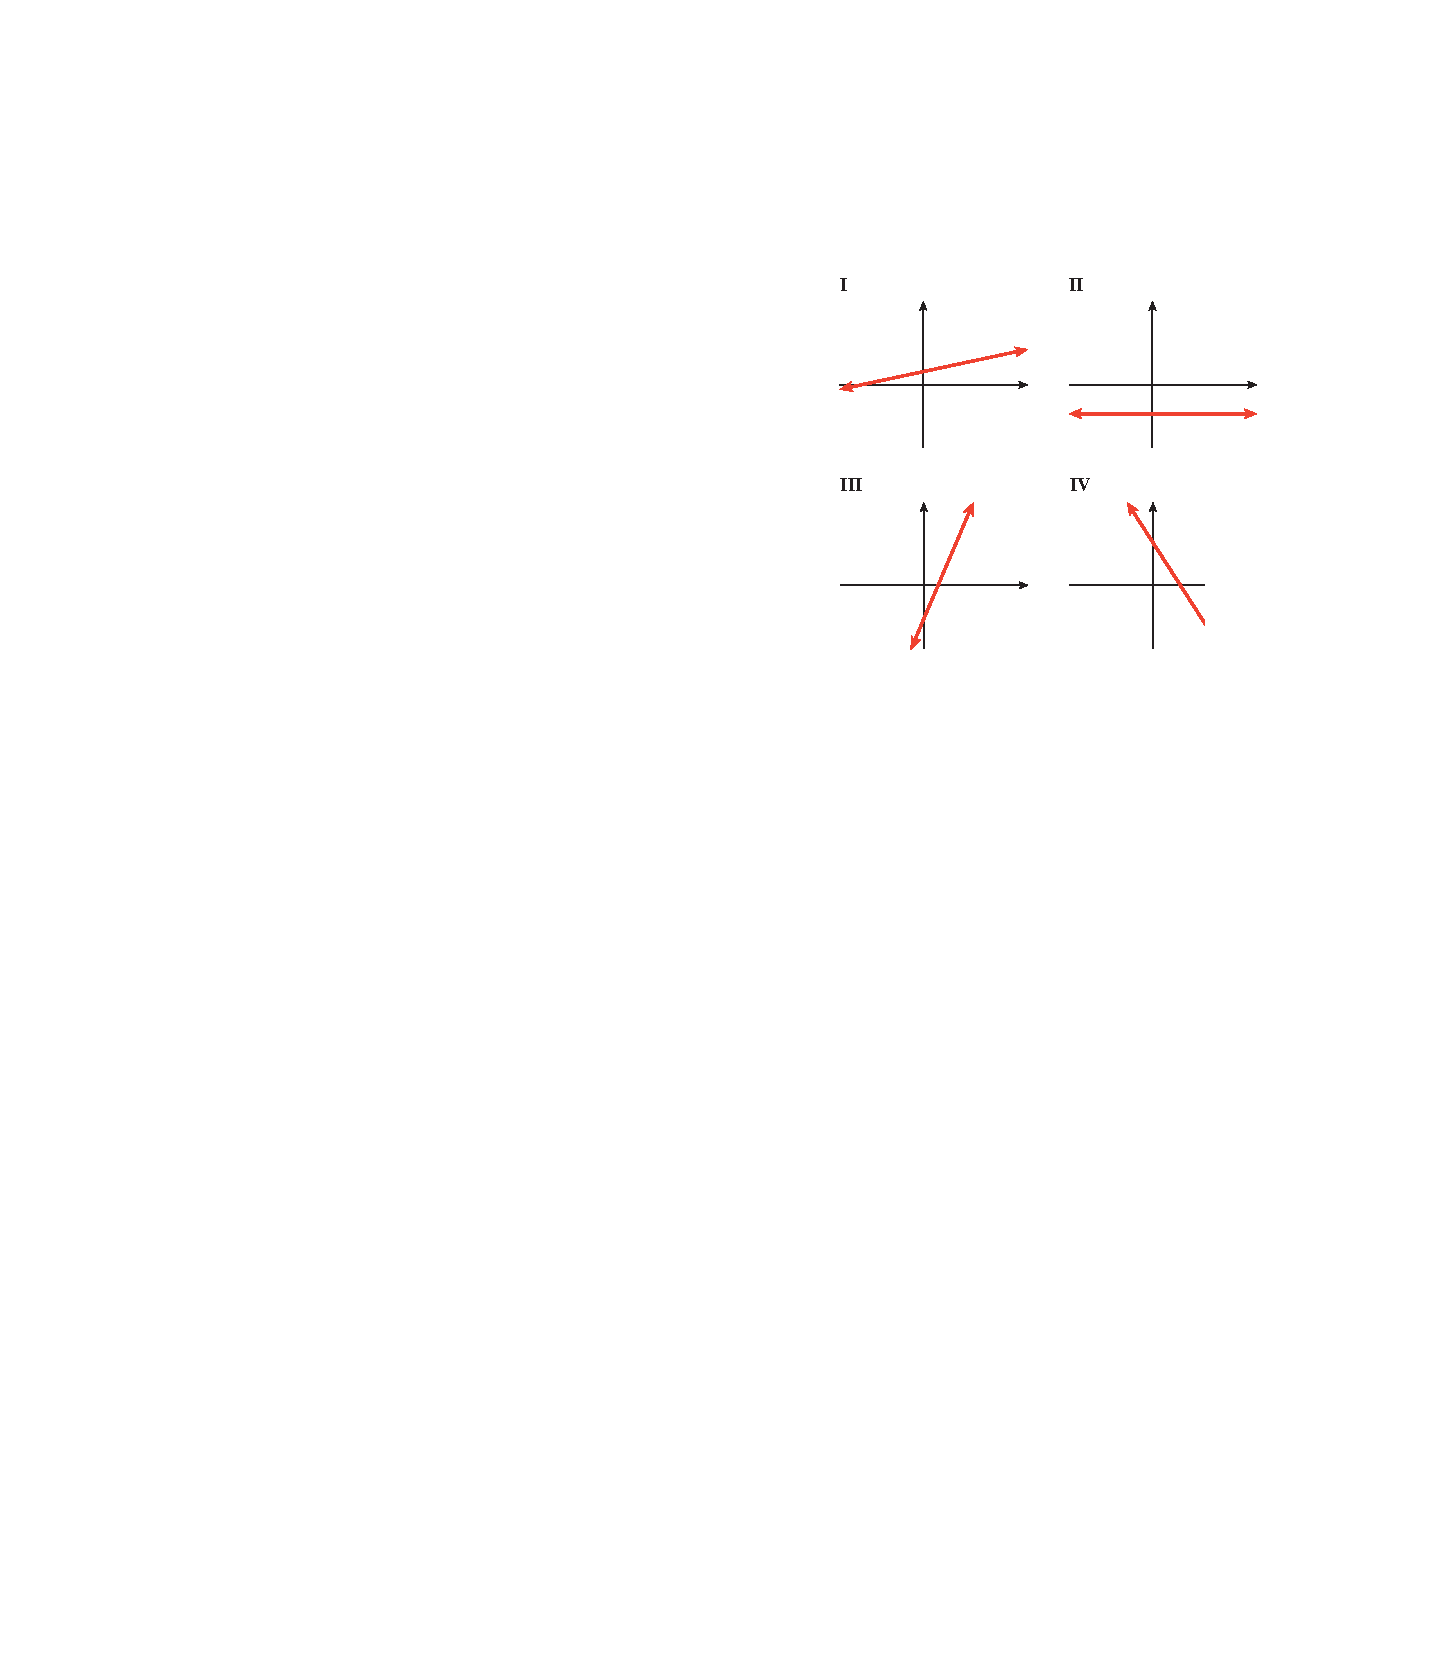
\includegraphics[width=\linewidth]{external/images/fig-ex-1-4-22.pdf}
\end{sbspanel}%
\end{sidebyside}%
\end{divisionexercise}%
\par\medskip\noindent%
\textbf{Exercise Group.}\space\space%
Compute the slope of the line in Problems 23-26. Note the scales on the axes.%
\begin{exercisegroupcol}{2}
\begin{divisionexerciseegcol}{23}{}{}{exercise-section-1-4-exercises-j-b}%
\begin{sidebyside}{1}{0.2}{0.2}{0}%
\begin{sbspanel}{0.6}%
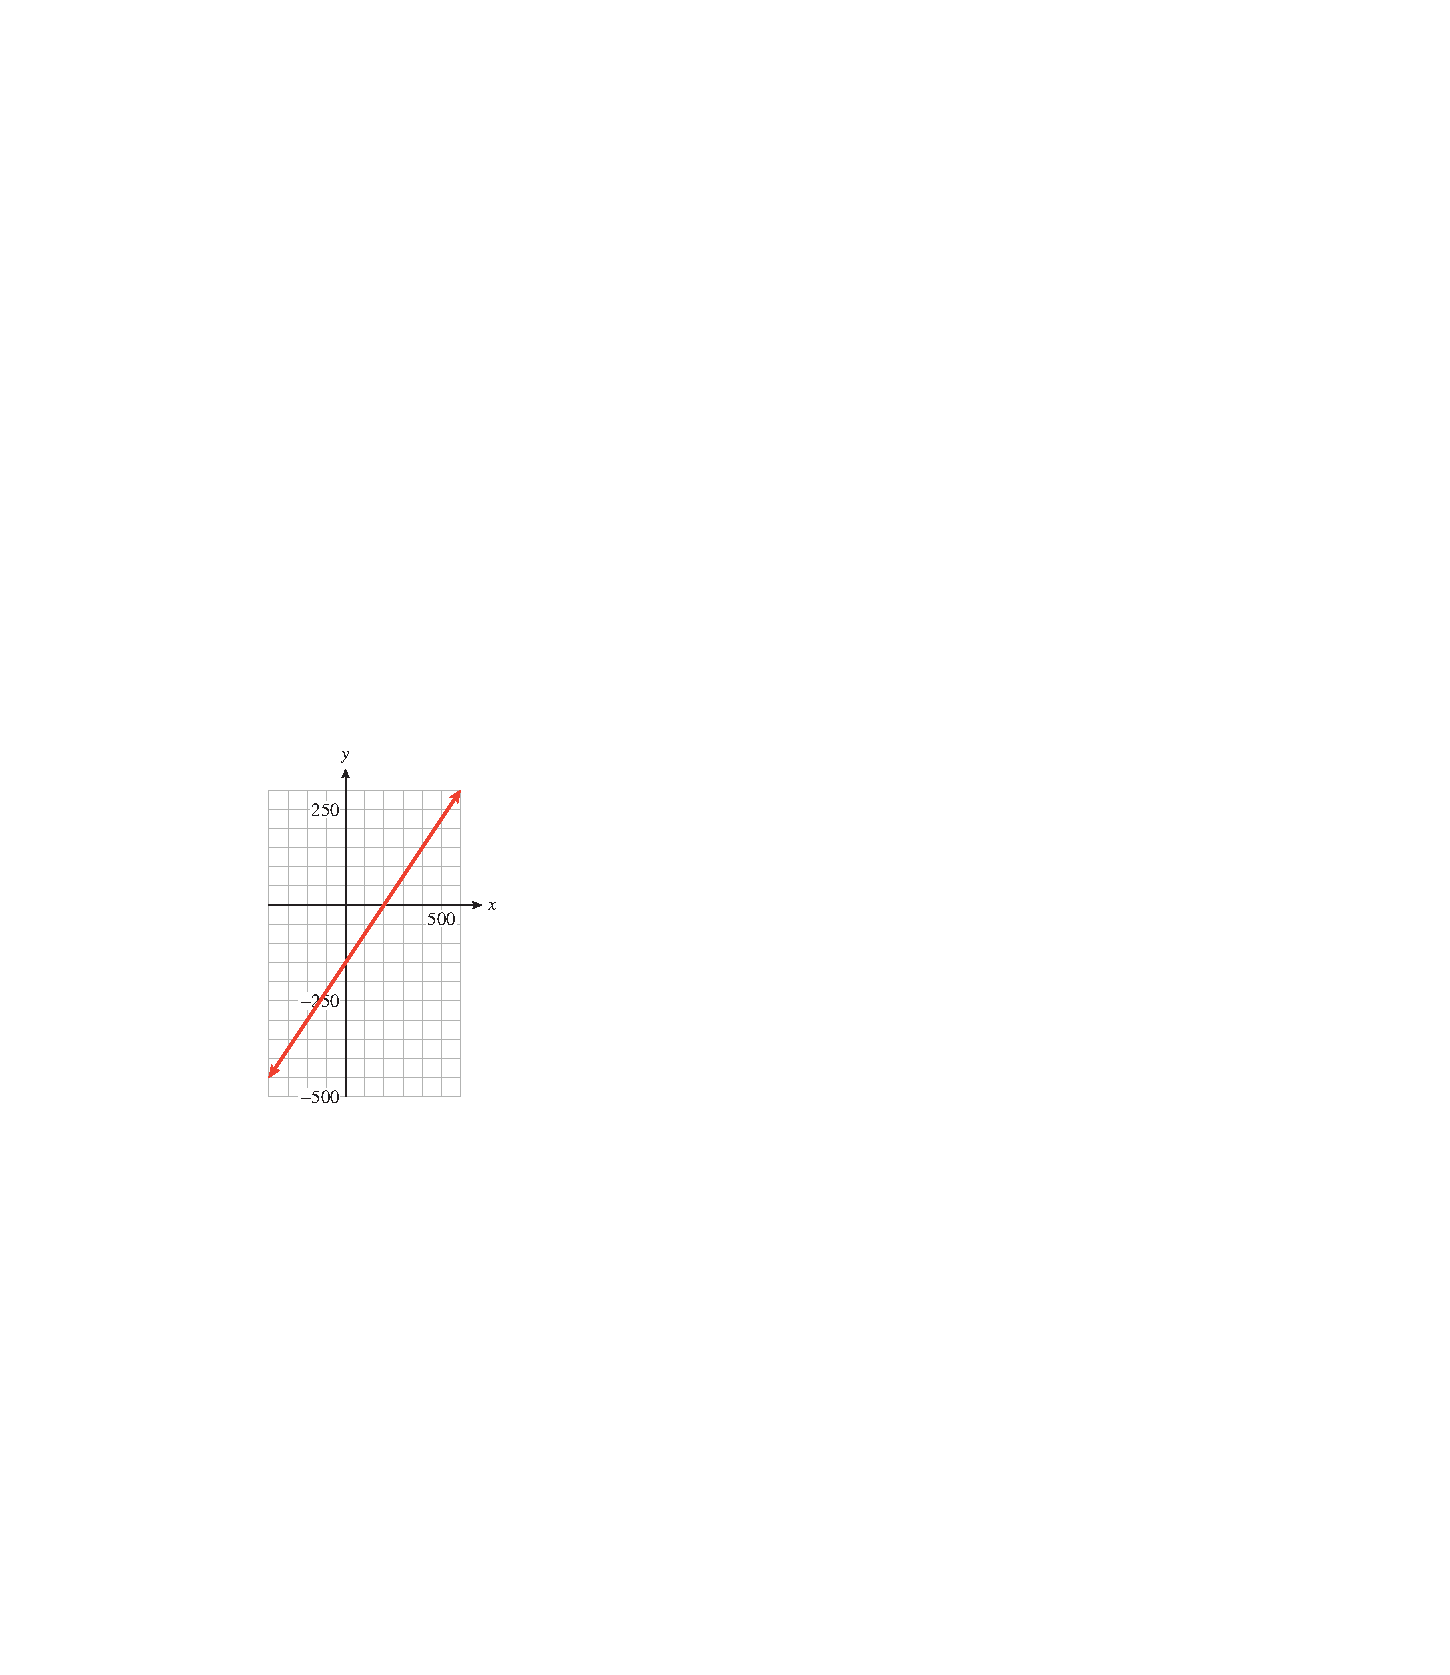
\includegraphics[width=\linewidth]{external/images/fig-ex-1-4-23.pdf}
\end{sbspanel}%
\end{sidebyside}%
\end{divisionexerciseegcol}%
\begin{divisionexerciseegcol}{24}{}{}{exercise-section-1-4-exercises-j-c}%
\begin{sidebyside}{1}{0.2}{0.2}{0}%
\begin{sbspanel}{0.6}%
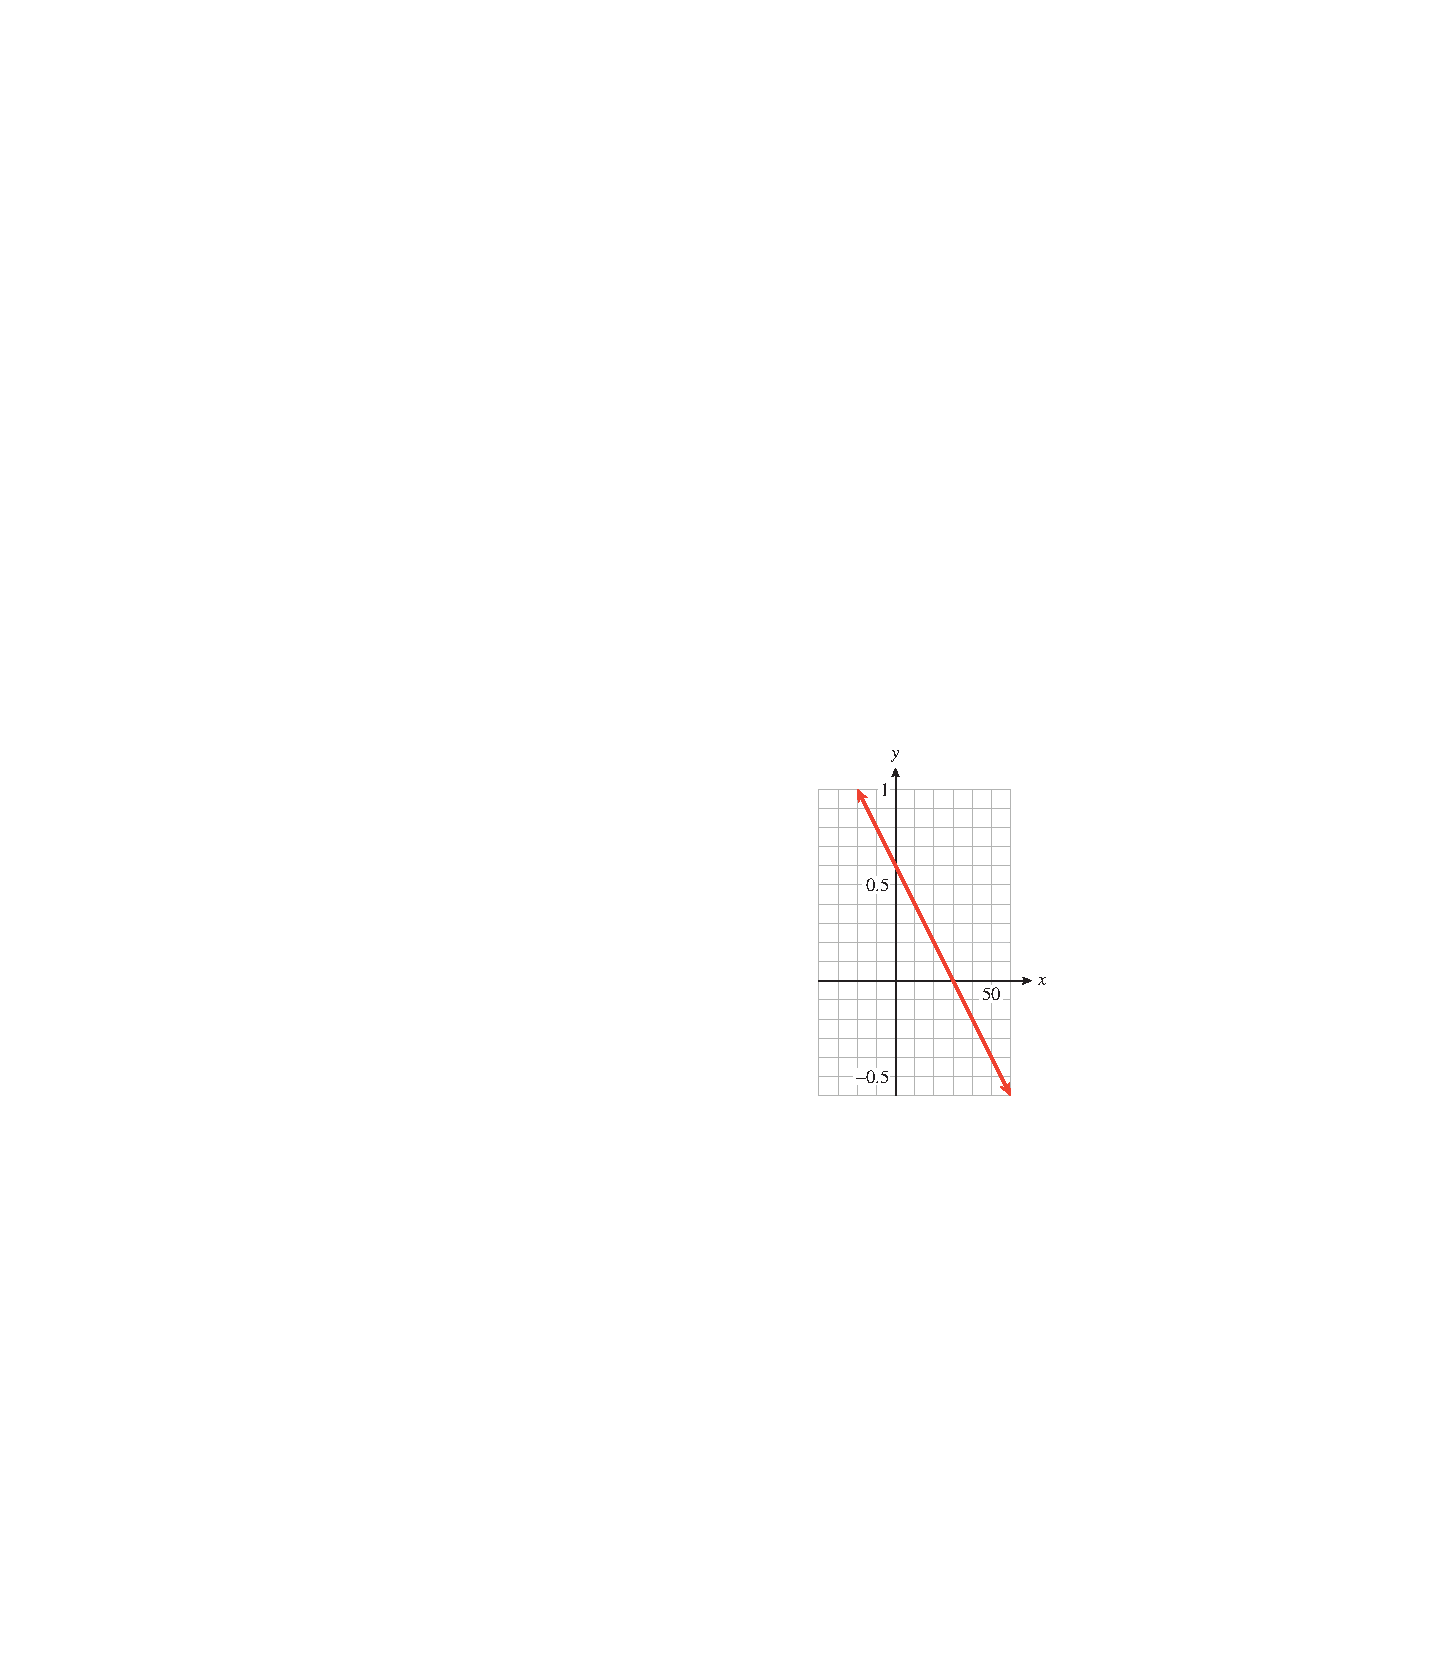
\includegraphics[width=\linewidth]{external/images/fig-ex-1-4-24.pdf}
\end{sbspanel}%
\end{sidebyside}%
\end{divisionexerciseegcol}%
\begin{divisionexerciseegcol}{25}{}{}{exercise-section-1-4-exercises-j-d}%
\begin{sidebyside}{1}{0.2}{0.2}{0}%
\begin{sbspanel}{0.6}%
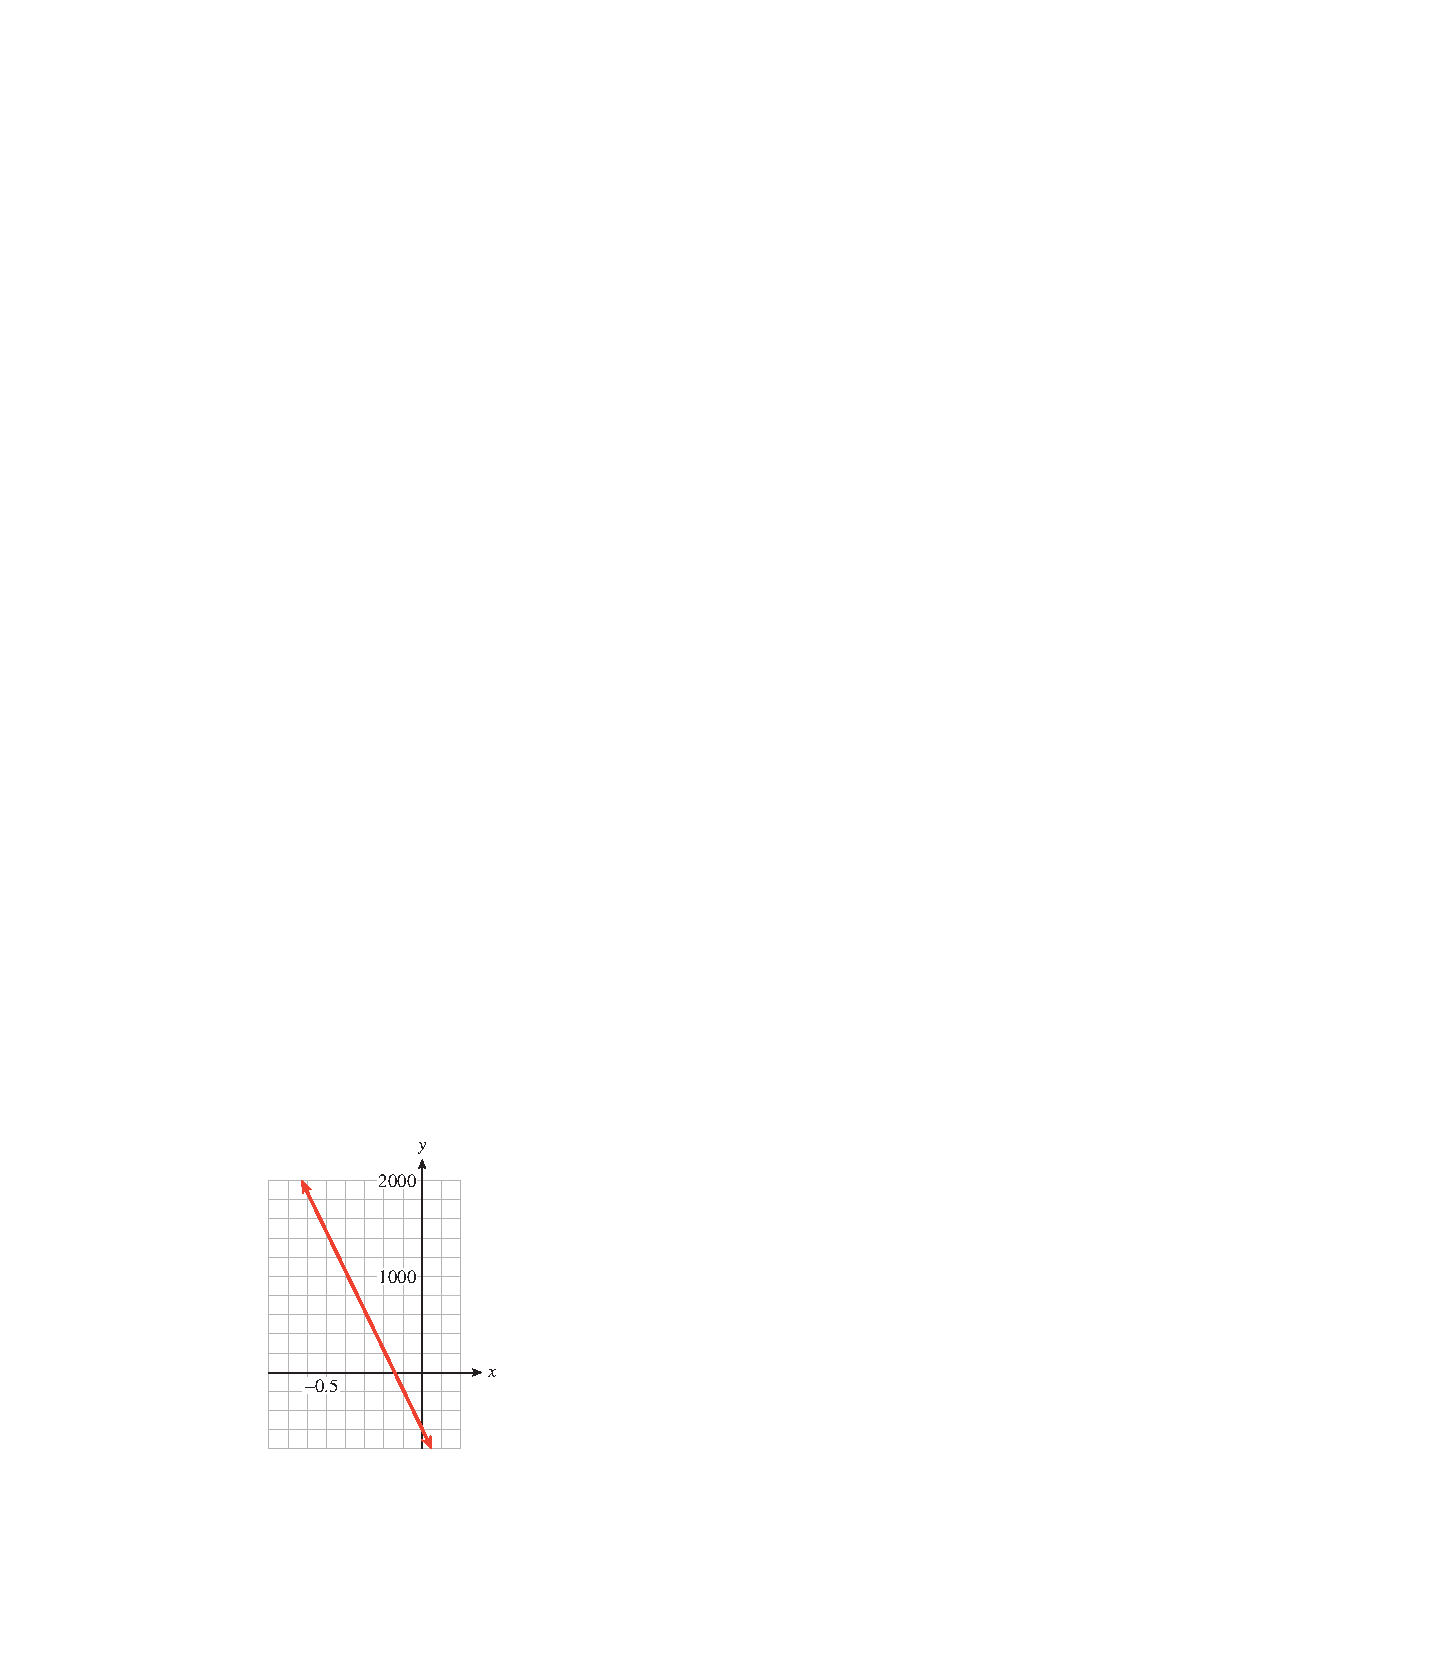
\includegraphics[width=\linewidth]{external/images/fig-ex-1-4-25.pdf}
\end{sbspanel}%
\end{sidebyside}%
\end{divisionexerciseegcol}%
\begin{divisionexerciseegcol}{26}{}{}{exercise-section-1-4-exercises-j-e}%
\begin{sidebyside}{1}{0.2}{0.2}{0}%
\begin{sbspanel}{0.6}%
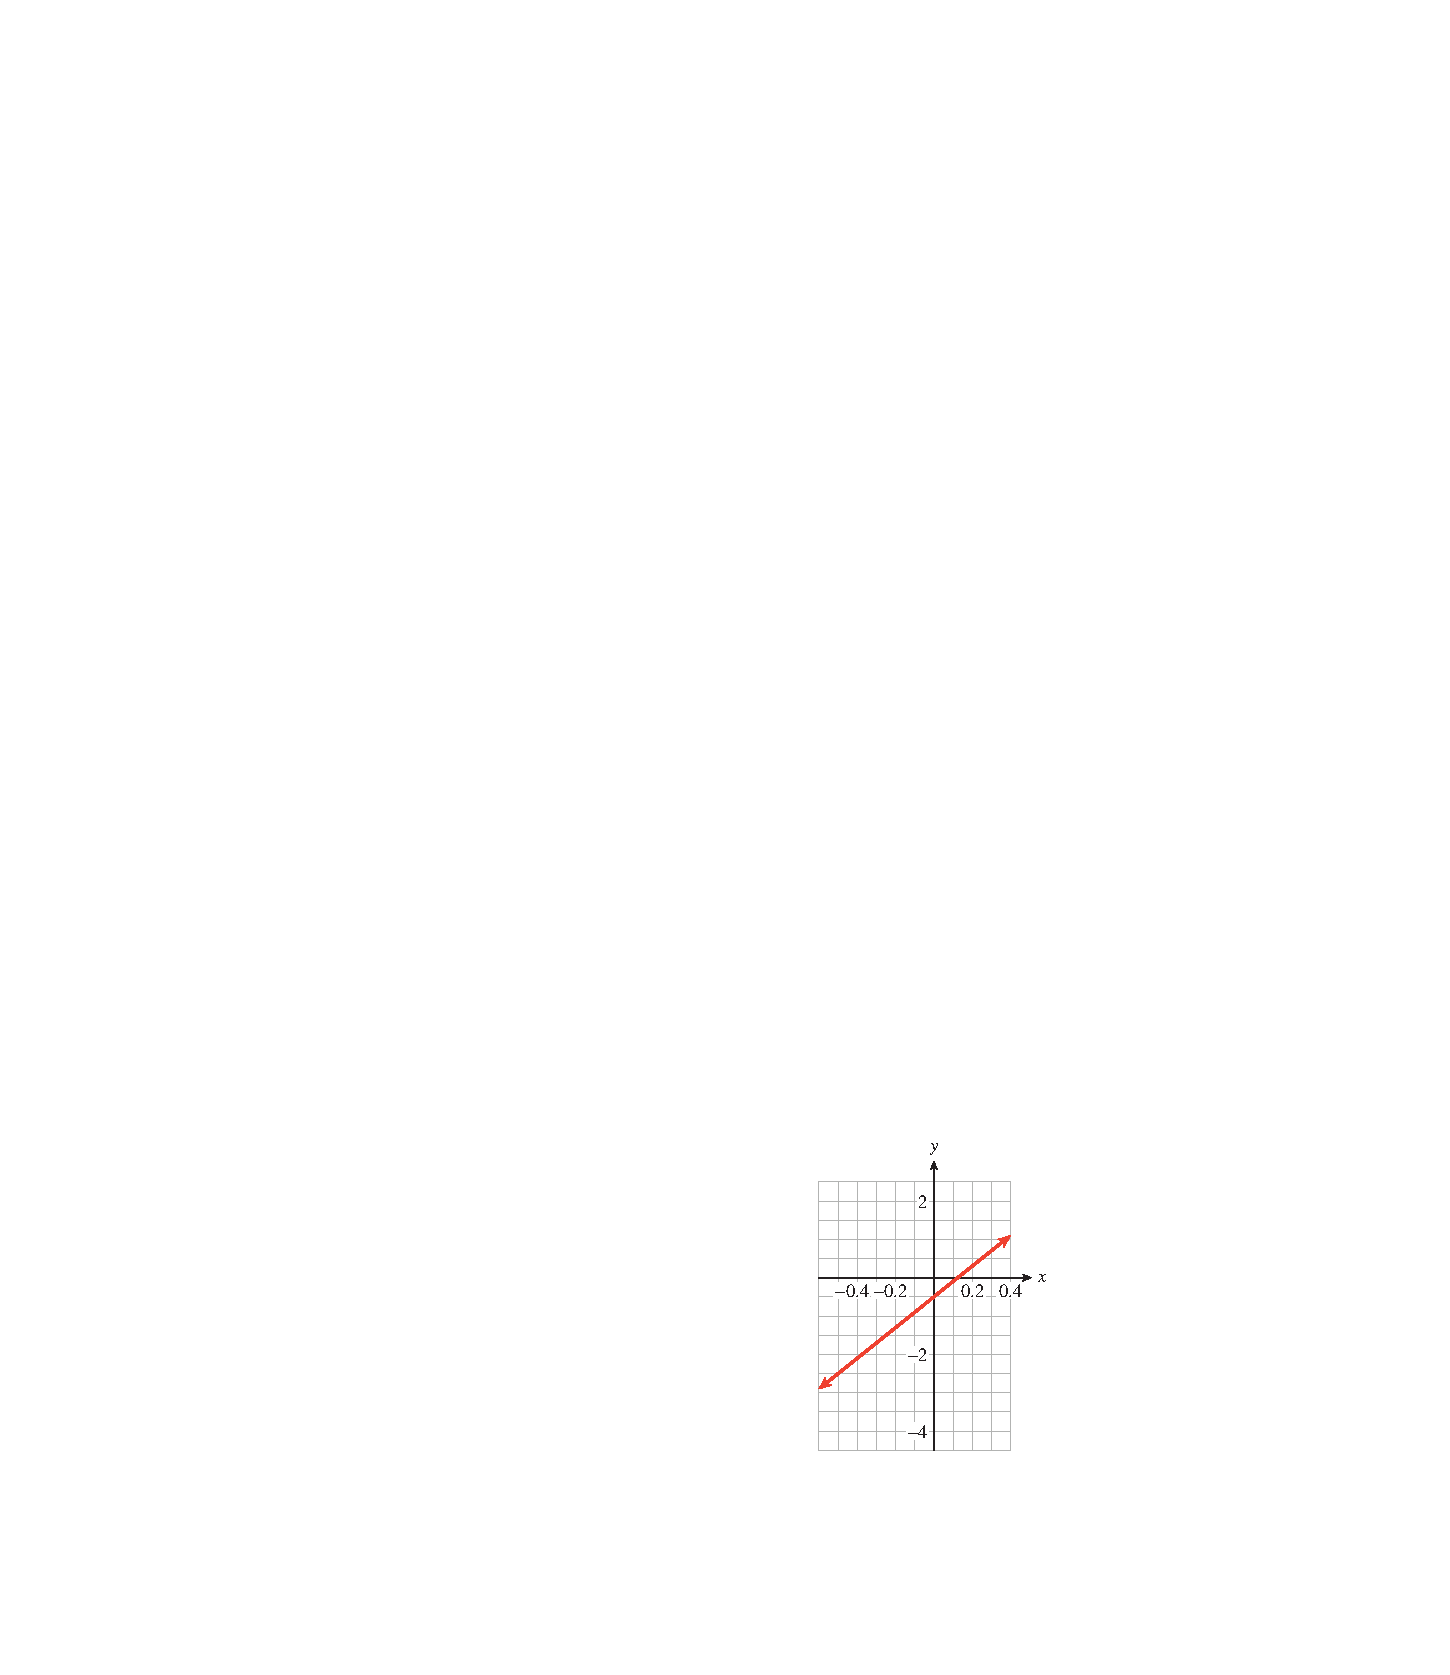
\includegraphics[width=\linewidth]{external/images/fig-ex-1-4-26.pdf}
\end{sbspanel}%
\end{sidebyside}%
\end{divisionexerciseegcol}%
\end{exercisegroupcol}
\par\medskip\noindent
\par\medskip\noindent%
\textbf{Exercise Group.}\space\space%
Each table in Problems 27\textendash{}30 gives the coordinates of points on a line.%
\begin{enumerate}[label=\alph*]
\item{}Find the slope of the line.%
\item{}Fill in the missing table entries.%
\end{enumerate}
%
\begin{exercisegroupcol}{4}
\begin{divisionexerciseegcol}{27}{}{}{exercise-section-1-4-exercises-k-b}%
\begin{sidebyside}{1}{0}{0}{0}%
\begin{sbspanel}{1}%
\resizebox{\ifdim\width > \linewidth\linewidth\else\width\fi}{!}{%
{\centering%
{\tabularfont%
\begin{tabular}{AcAcA}\hrulethick
\(x\)&\(y\)\tabularnewline\hrulethin
\(-4\)&\(-14\)\tabularnewline\hrulethin
\(-2\)&\(-9\)\tabularnewline\hrulethin
\(2\)&\(1\)\tabularnewline\hrulethin
\(3\)&\(\)\tabularnewline\hrulethin
\(\)&\(11\)\tabularnewline\hrulethin
\end{tabular}
}%
\par}
}%
\end{sbspanel}%
\end{sidebyside}%
\end{divisionexerciseegcol}%
\begin{divisionexerciseegcol}{28}{}{}{exercise-section-1-4-exercises-k-c}%
\begin{sidebyside}{1}{0}{0}{0}%
\begin{sbspanel}{1}%
\resizebox{\ifdim\width > \linewidth\linewidth\else\width\fi}{!}{%
{\centering%
{\tabularfont%
\begin{tabular}{AcAcA}\hrulethick
\(x\)&\(y\)\tabularnewline\hrulethin
\(-5\)&\(-3.8\)\tabularnewline\hrulethin
\(-1\)&\(-0.6\)\tabularnewline\hrulethin
\(2\)&\(1.8\)\tabularnewline\hrulethin
\(\)&\(4.2\)\tabularnewline\hrulethin
\(7\)&\(\)\tabularnewline\hrulethin
\end{tabular}
}%
\par}
}%
\end{sbspanel}%
\end{sidebyside}%
\end{divisionexerciseegcol}%
\begin{divisionexerciseegcol}{29}{}{}{exercise-section-1-4-exercises-k-d}%
\begin{sidebyside}{1}{0}{0}{0}%
\begin{sbspanel}{1}%
\resizebox{\ifdim\width > \linewidth\linewidth\else\width\fi}{!}{%
{\centering%
{\tabularfont%
\begin{tabular}{AcAcA}\hrulethick
\(x\)&\(y\)\tabularnewline\hrulethin
\(-3\)&\(36\)\tabularnewline\hrulethin
\(-1\)&\(\)\tabularnewline\hrulethin
\(\)&\(12\)\tabularnewline\hrulethin
\(6\)&\(9\)\tabularnewline\hrulethin
\(10\)&\(-3\)\tabularnewline\hrulethin
\end{tabular}
}%
\par}
}%
\end{sbspanel}%
\end{sidebyside}%
\end{divisionexerciseegcol}%
\begin{divisionexerciseegcol}{30}{}{}{exercise-section-1-4-exercises-k-e}%
\begin{sidebyside}{1}{0}{0}{0}%
\begin{sbspanel}{1}%
\resizebox{\ifdim\width > \linewidth\linewidth\else\width\fi}{!}{%
{\centering%
{\tabularfont%
\begin{tabular}{AcAcA}\hrulethick
\(x\)&\(y\)\tabularnewline\hrulethin
\(-10\)&\(800\)\tabularnewline\hrulethin
\(-2\)&\(\)\tabularnewline\hrulethin
\(5\)&\(440\)\tabularnewline\hrulethin
\(\)&\(368\)\tabularnewline\hrulethin
\(16\)&\(176\)\tabularnewline\hrulethin
\end{tabular}
}%
\par}
}%
\end{sbspanel}%
\end{sidebyside}%
\end{divisionexerciseegcol}%
\end{exercisegroupcol}
\par\medskip\noindent
\begin{divisionexercise}{31}{}{}{exercise-section-1-4-exercises-l}%
A temporary typist's paycheck (before deductions) is given, in dollars, by \(S = 8t\), where \(t\) is the number of hours she worked.%
\begin{enumerate}[label=(\alph*)]
\item{}Make a table of values for the function.%
\begin{sidebyside}{1}{0}{0}{0}%
\begin{sbspanel}{1}%
\resizebox{\ifdim\width > \linewidth\linewidth\else\width\fi}{!}{%
{\centering%
{\tabularfont%
\begin{tabular}{AcAcAcAcAcA}\hrulethick
\(t\)&\(4\)&\(8\)&\(20\)&\(40\)\tabularnewline\hrulethin
\(S\)&\(\hphantom{0000} \)&\(\hphantom{0000}\)&\(\hphantom{0000}\)&\(\hphantom{0000}\)\tabularnewline\hrulethin
\end{tabular}
}%
\par}
}%
\end{sbspanel}%
\end{sidebyside}%
\item{}Graph the function.%
\item{}Using two points on the graph, compute the slope \(\dfrac{\Delta S}{\Delta t}\), including units.%
\item{}What does the slope tell us about the typist's paycheck?%
\end{enumerate}
%
\end{divisionexercise}%
\begin{divisionexercise}{32}{}{}{exercise-section-1-4-exercises-m}%
The distance (in miles) covered by a cross-country competitor is given by \(d = 6t\), where \(t\) is the number of hours she runs.%
\begin{enumerate}[label=(\alph*)]
\item{}Make a table of values for the function.%
\begin{sidebyside}{1}{0}{0}{0}%
\begin{sbspanel}{1}%
\resizebox{\ifdim\width > \linewidth\linewidth\else\width\fi}{!}{%
{\centering%
{\tabularfont%
\begin{tabular}{AcAcAcAcAcA}\hrulethick
\(t\)&\(2\)&\(4\)&\(6\)&\(8\)\tabularnewline\hrulethin
\(d\)&\(\hphantom{0000} \)&\(\hphantom{0000}\)&\(\hphantom{0000}\)&\(\hphantom{0000}\)\tabularnewline\hrulethin
\end{tabular}
}%
\par}
}%
\end{sbspanel}%
\end{sidebyside}%
\item{}Graph the function.%
\item{}Using two points on the graph, compute the slope \(\dfrac{\Delta d}{\Delta t}\), including units.%
\item{}What does the slope tell us about the cross-country runner?%
\end{enumerate}
%
\end{divisionexercise}%
\par\medskip\noindent%
\textbf{Exercise Group.}\space\space%
In Problems 33\textendash{}40,%
\begin{enumerate}[label=\alph*]
\item{}Choose two points and compute the slope of the graph (including units).%
\item{}Explain what the slope measures in the context of the problem.%
\end{enumerate}
%
\begin{exercisegroup}
\begin{divisionexerciseeg}{33}{}{}{exercise-section-1-4-exercises-n-b}%
The graph shows the number of barrels of oil, \(B\), that has been pumped at a drill site \(t\) days after a new drill is installed.%
\begin{sidebyside}{1}{0.325}{0.325}{0}%
\begin{sbspanel}{0.35}%
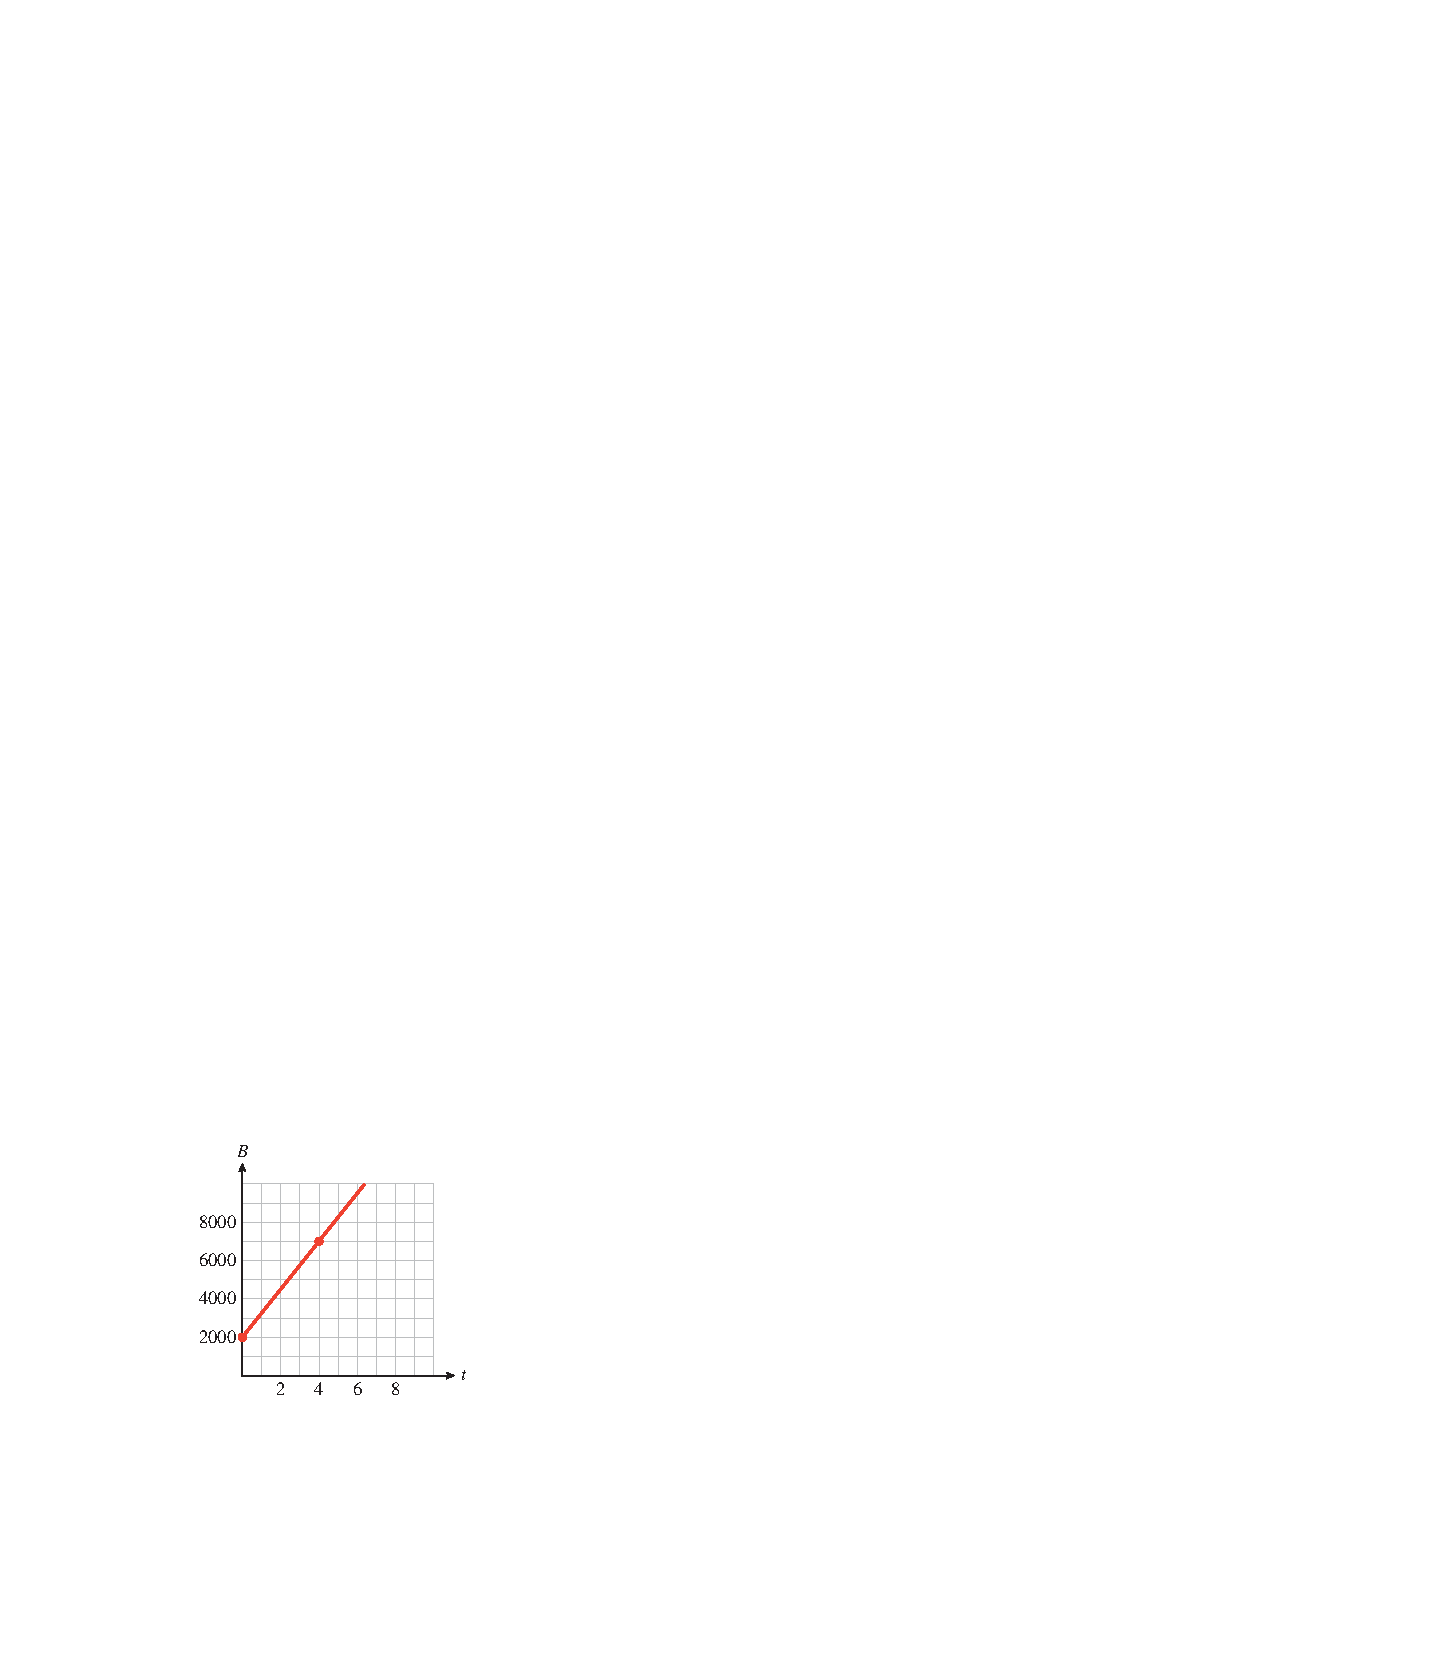
\includegraphics[width=\linewidth]{external/images/fig-ex-1-4-33.pdf}
\end{sbspanel}%
\end{sidebyside}%
\end{divisionexerciseeg}%
\begin{divisionexerciseeg}{34}{}{}{exercise-section-1-4-exercises-n-c}%
The graph shows the amount of garbage, \(G\) (in tons), that has been deposited at a dump site \(t\) years after new regulations go into effect.%
\begin{sidebyside}{1}{0.325}{0.325}{0}%
\begin{sbspanel}{0.35}%
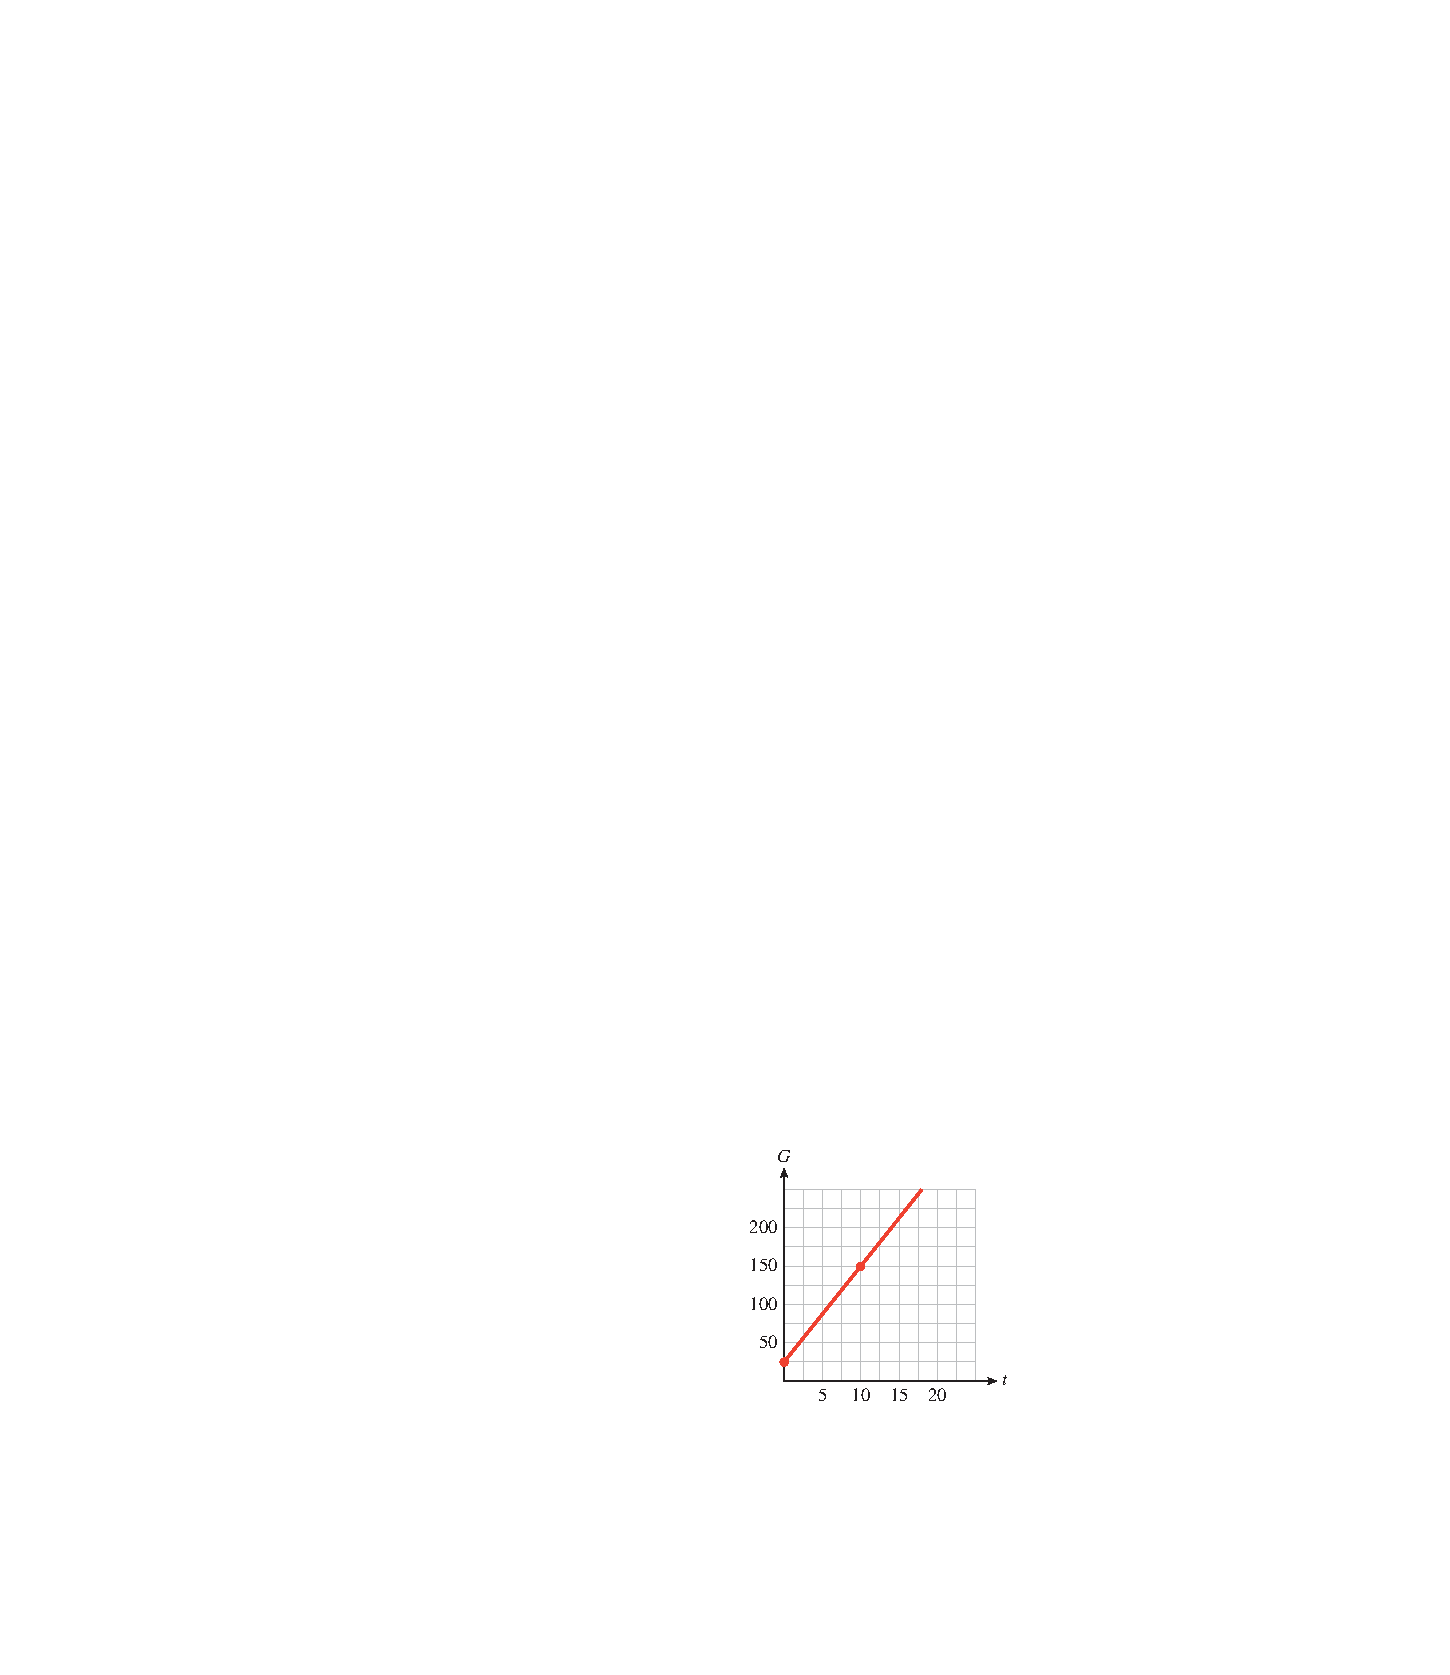
\includegraphics[width=\linewidth]{external/images/fig-ex-1-4-34.pdf}
\end{sbspanel}%
\end{sidebyside}%
\end{divisionexerciseeg}%
\begin{divisionexerciseeg}{35}{}{}{exercise-section-1-4-exercises-n-d}%
The graph shows the amount of emergency water, \(W\) (in liters), remaining in a southern California household \(t\) days after an earthquake.%
\begin{sidebyside}{1}{0.325}{0.325}{0}%
\begin{sbspanel}{0.35}%
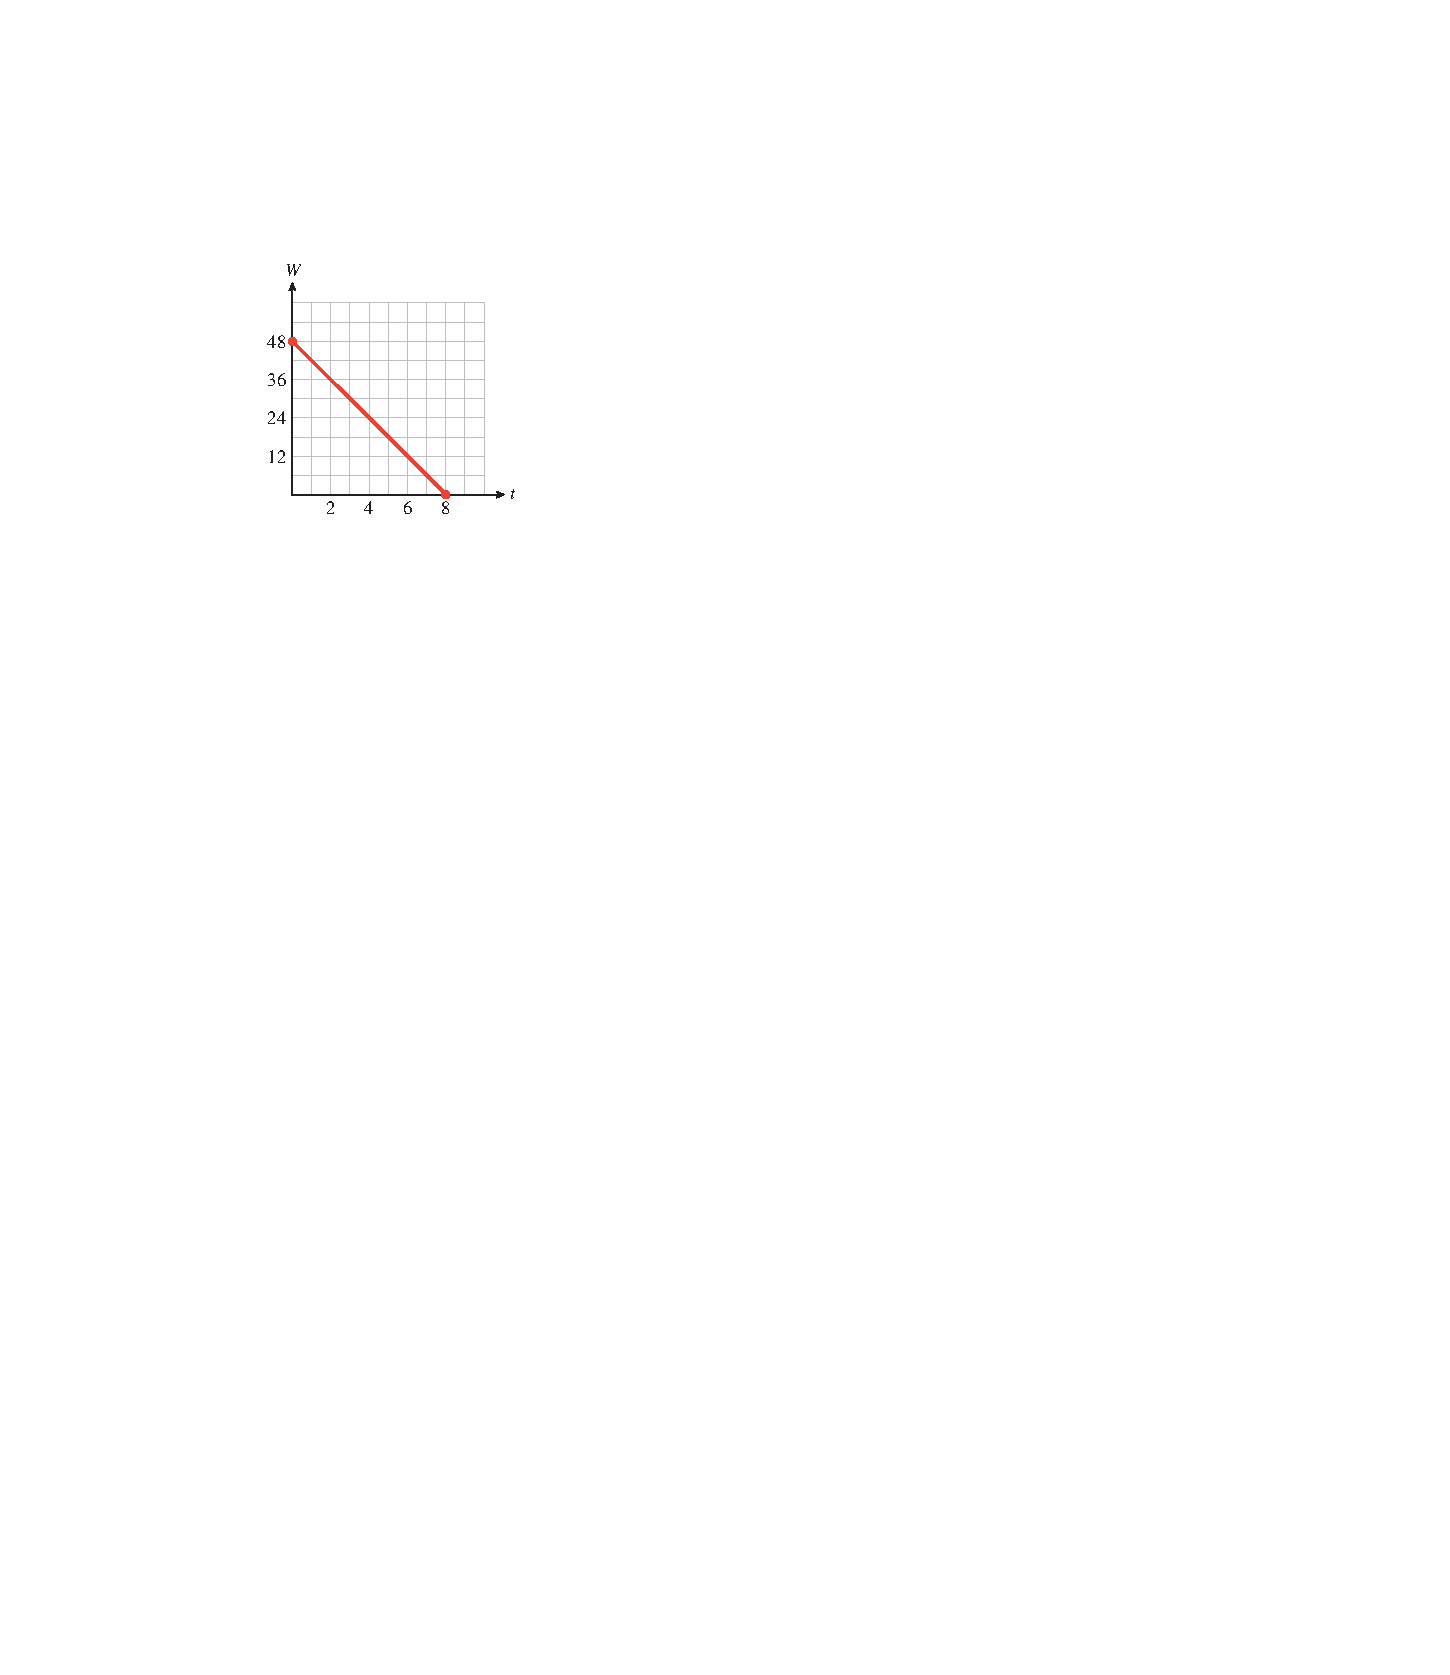
\includegraphics[width=\linewidth]{external/images/fig-ex-1-4-35.pdf}
\end{sbspanel}%
\end{sidebyside}%
\end{divisionexerciseeg}%
\begin{divisionexerciseeg}{36}{}{}{exercise-section-1-4-exercises-n-e}%
The graph shows the amount of money, \(M\) (in dollars), in Tammy's bank account \(w\) weeks after she loses all sources of income.%
\begin{sidebyside}{1}{0.325}{0.325}{0}%
\begin{sbspanel}{0.35}%
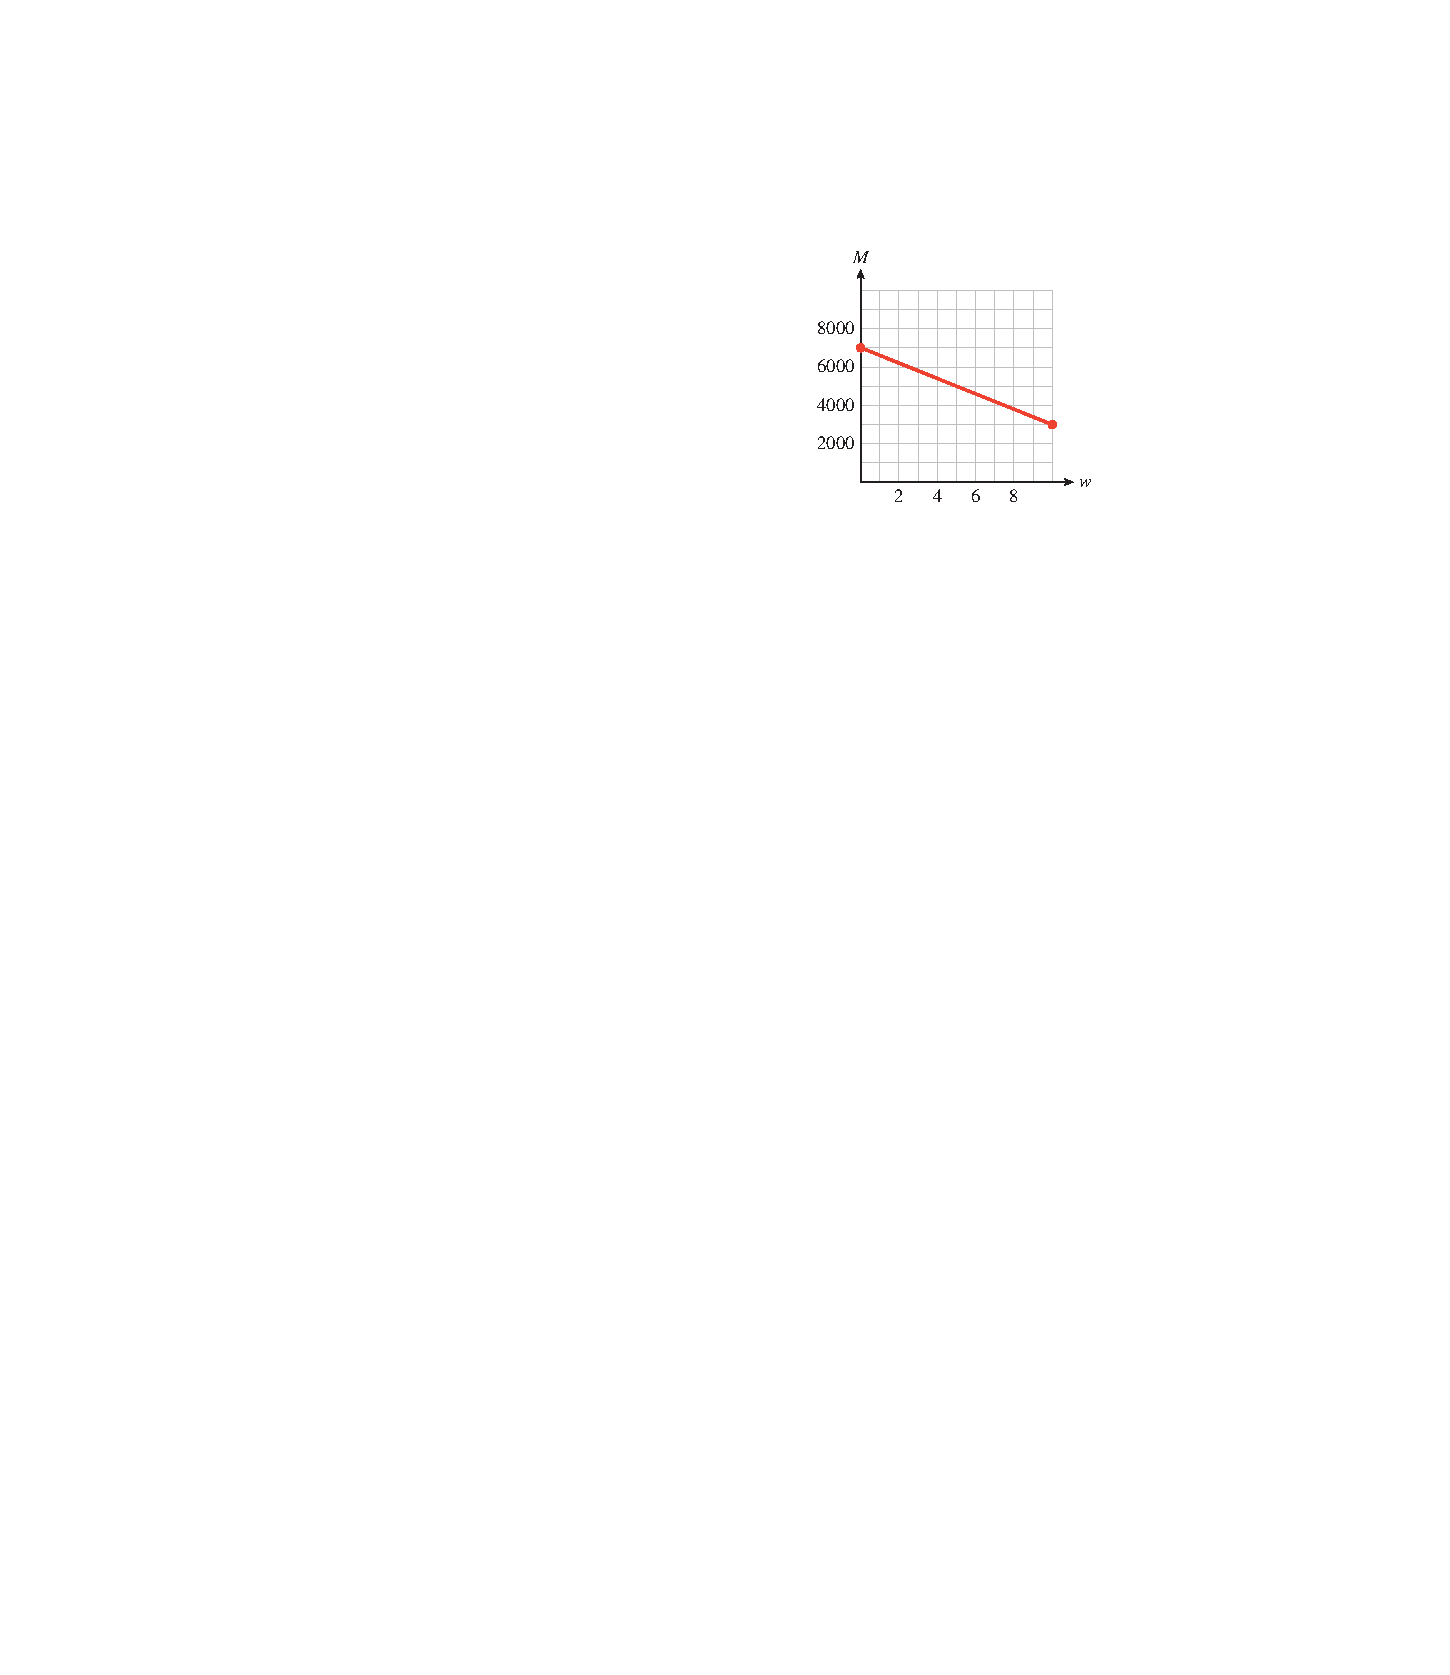
\includegraphics[width=\linewidth]{external/images/fig-ex-1-4-36.pdf}
\end{sbspanel}%
\end{sidebyside}%
\end{divisionexerciseeg}%
\begin{divisionexerciseeg}{37}{}{}{exercise-section-1-4-exercises-n-f}%
The graph shows the length in inches, \(i\), corresponding to various lengths in feet \(f\).%
\begin{sidebyside}{1}{0.325}{0.325}{0}%
\begin{sbspanel}{0.35}%
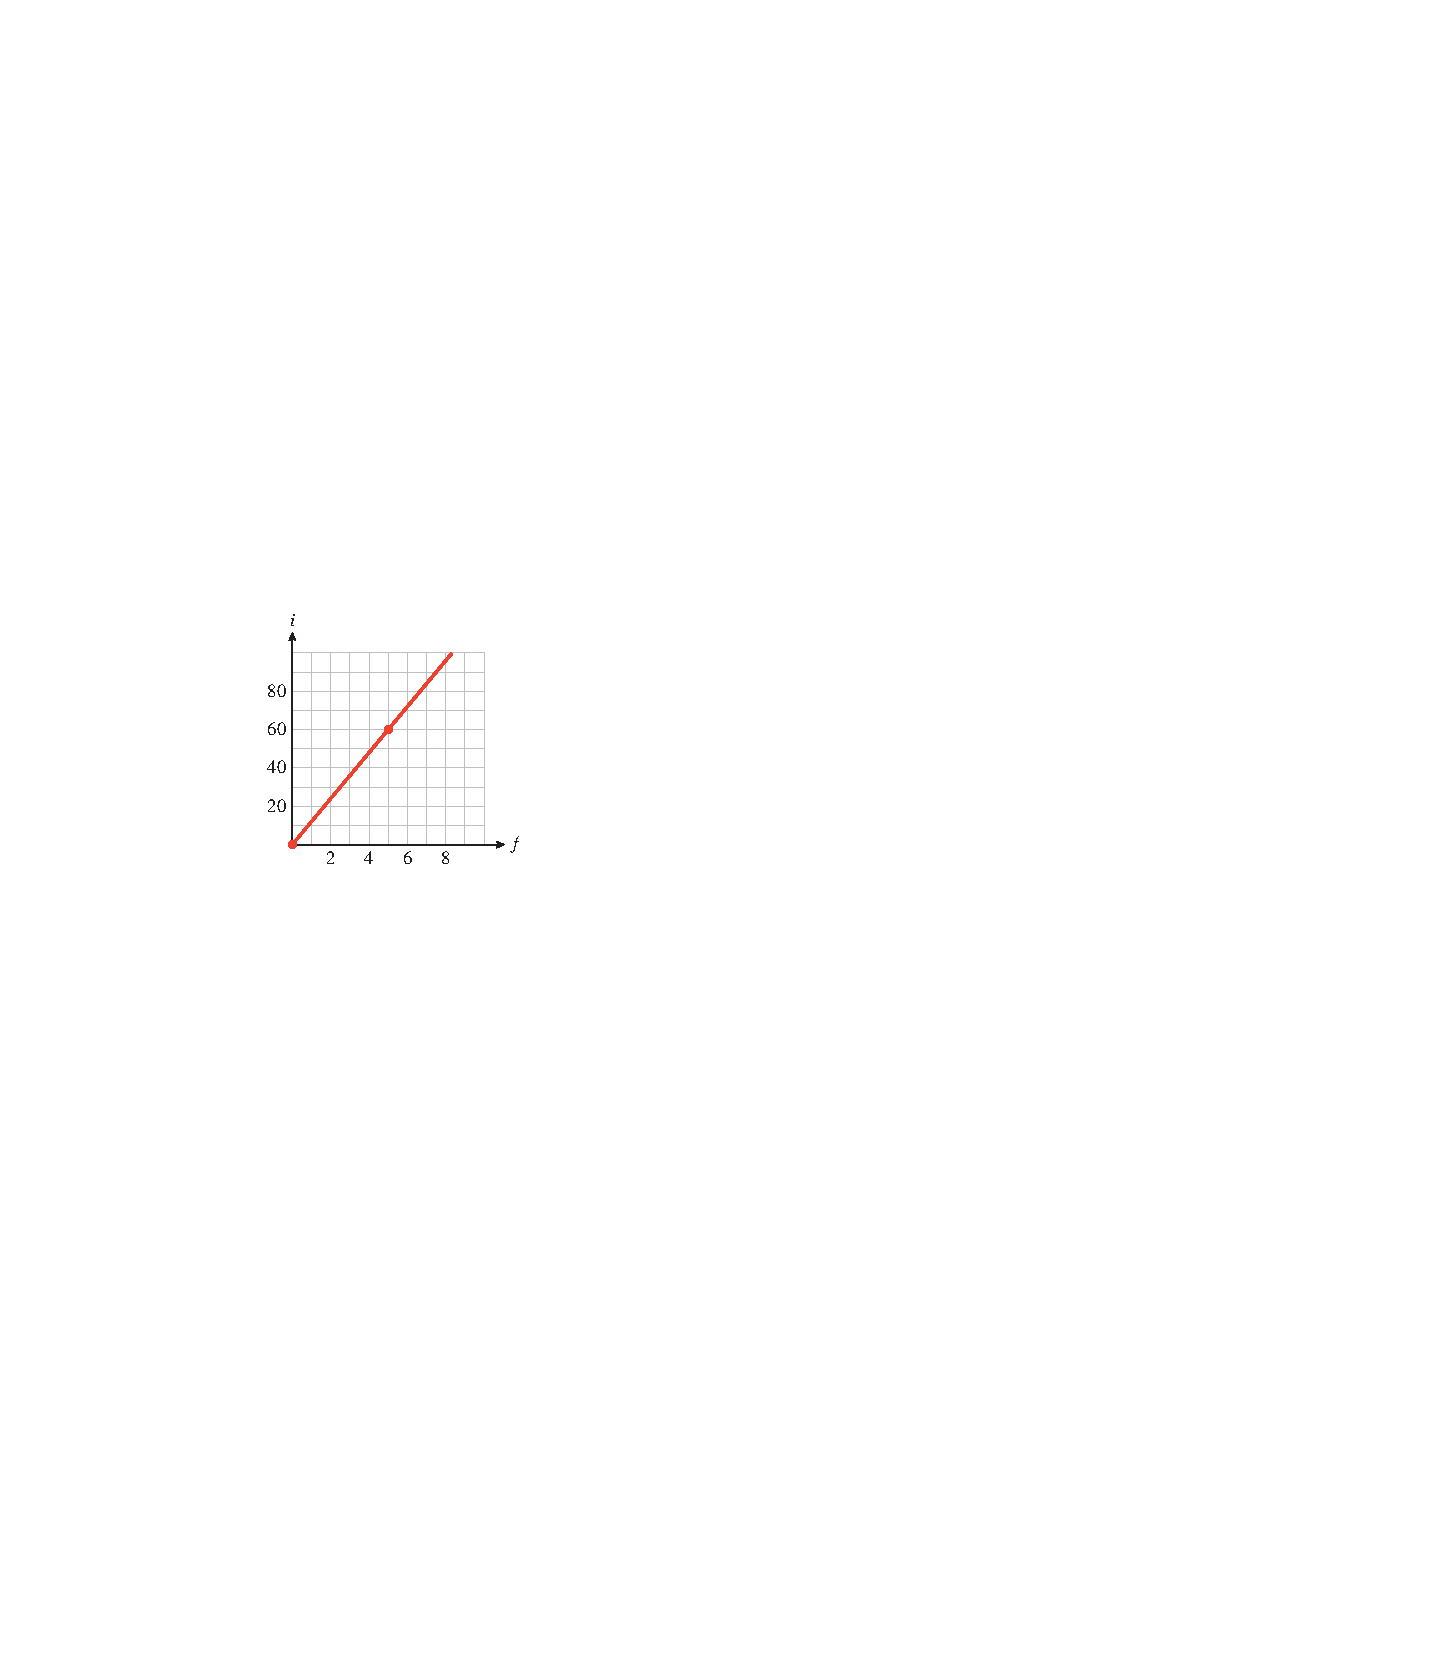
\includegraphics[width=\linewidth]{external/images/fig-ex-1-4-37.pdf}
\end{sbspanel}%
\end{sidebyside}%
\end{divisionexerciseeg}%
\begin{divisionexerciseeg}{38}{}{}{exercise-section-1-4-exercises-n-g}%
The graph shows the number of ounces, \(z\), that correspond to various weights measured in pounds, \(p\).%
\begin{sidebyside}{1}{0.325}{0.325}{0}%
\begin{sbspanel}{0.35}%
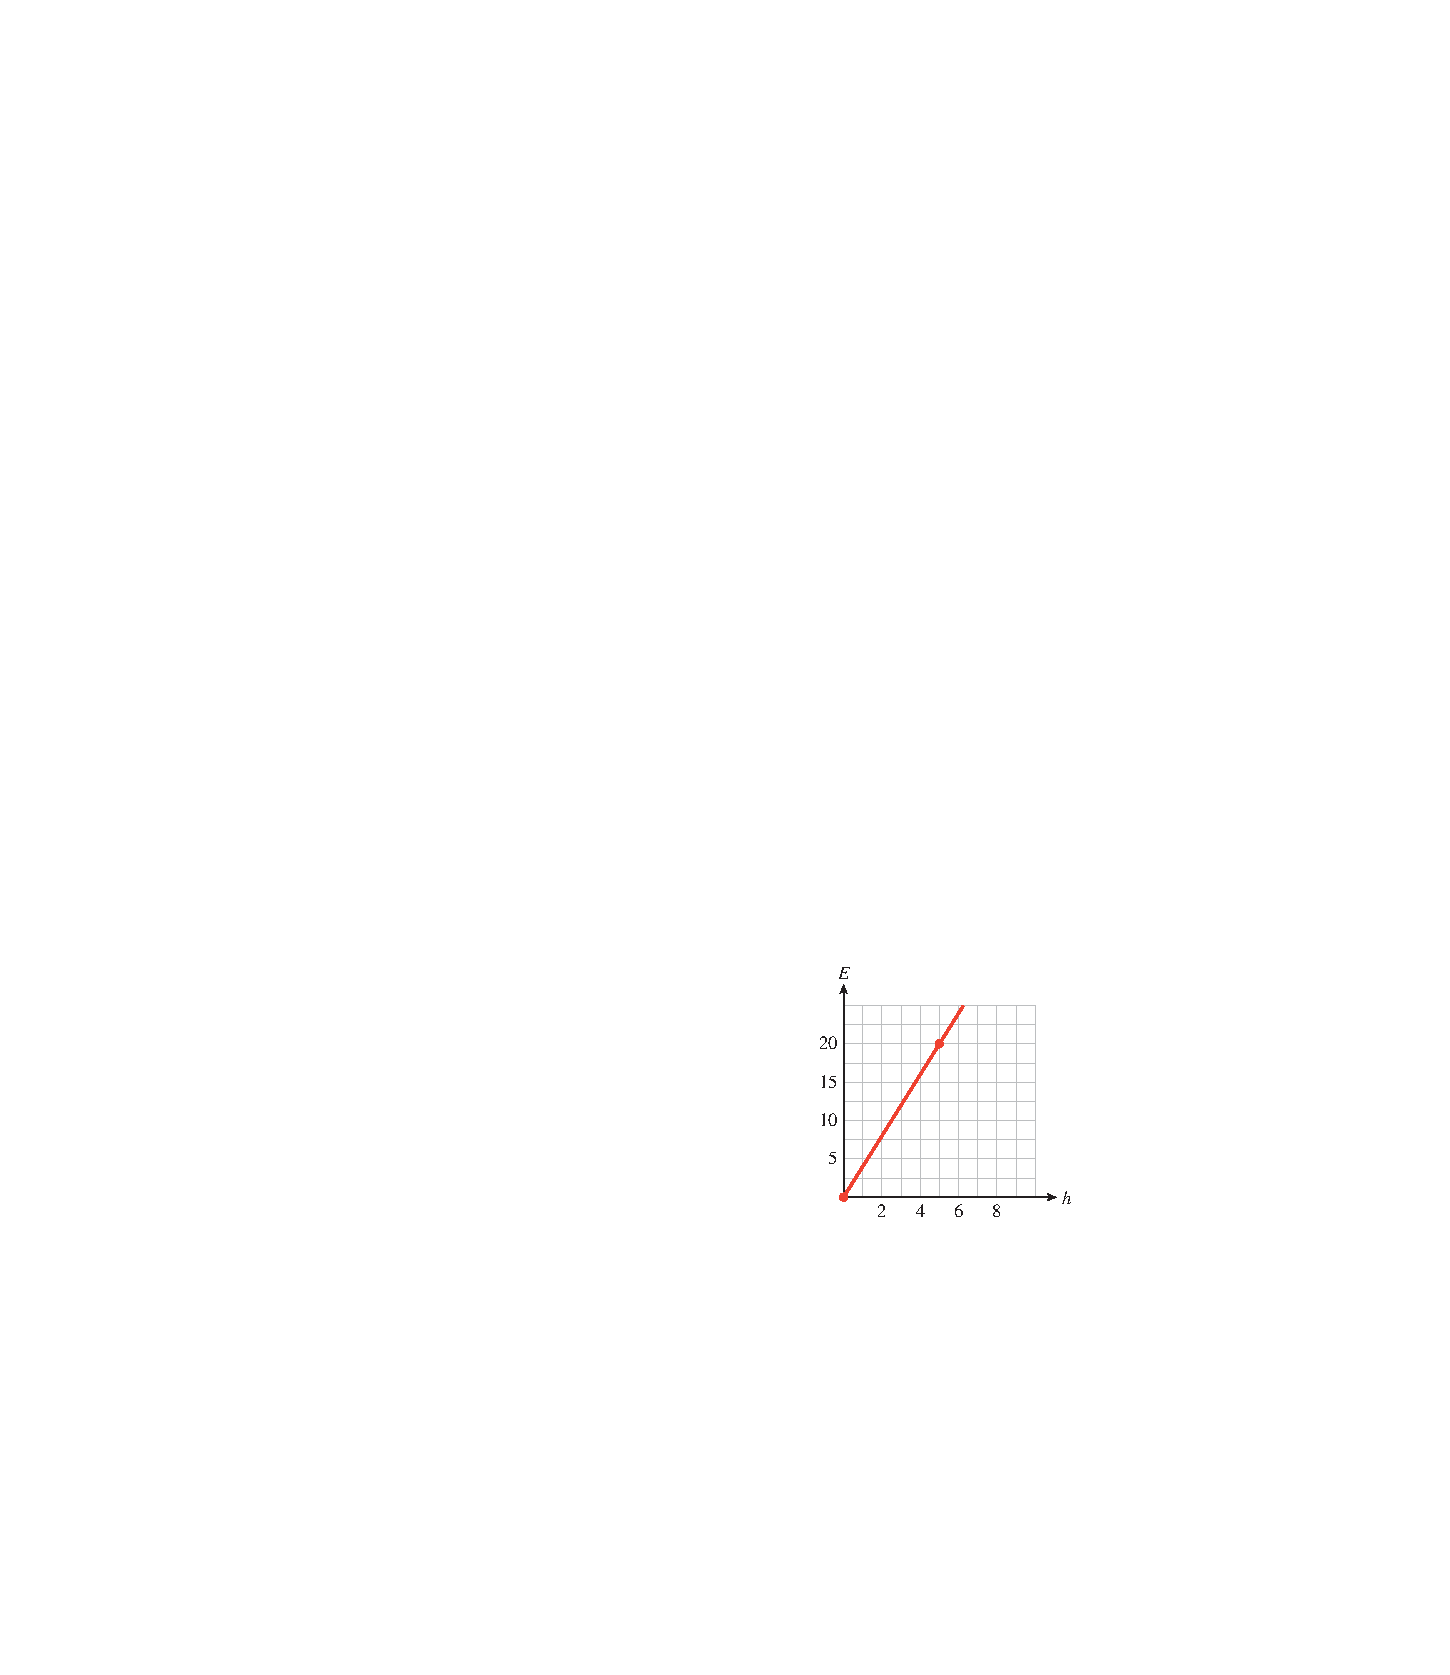
\includegraphics[width=\linewidth]{external/images/fig-ex-1-4-38.pdf}
\end{sbspanel}%
\end{sidebyside}%
\end{divisionexerciseeg}%
\begin{divisionexerciseeg}{39}{}{}{exercise-section-1-4-exercises-n-h}%
The graph shows the cost, \(C\) (in dollars), of coffee beans in terms of the amount of coffee, \(b\) (in kilograms).%
\begin{sidebyside}{1}{0.325}{0.325}{0}%
\begin{sbspanel}{0.35}%
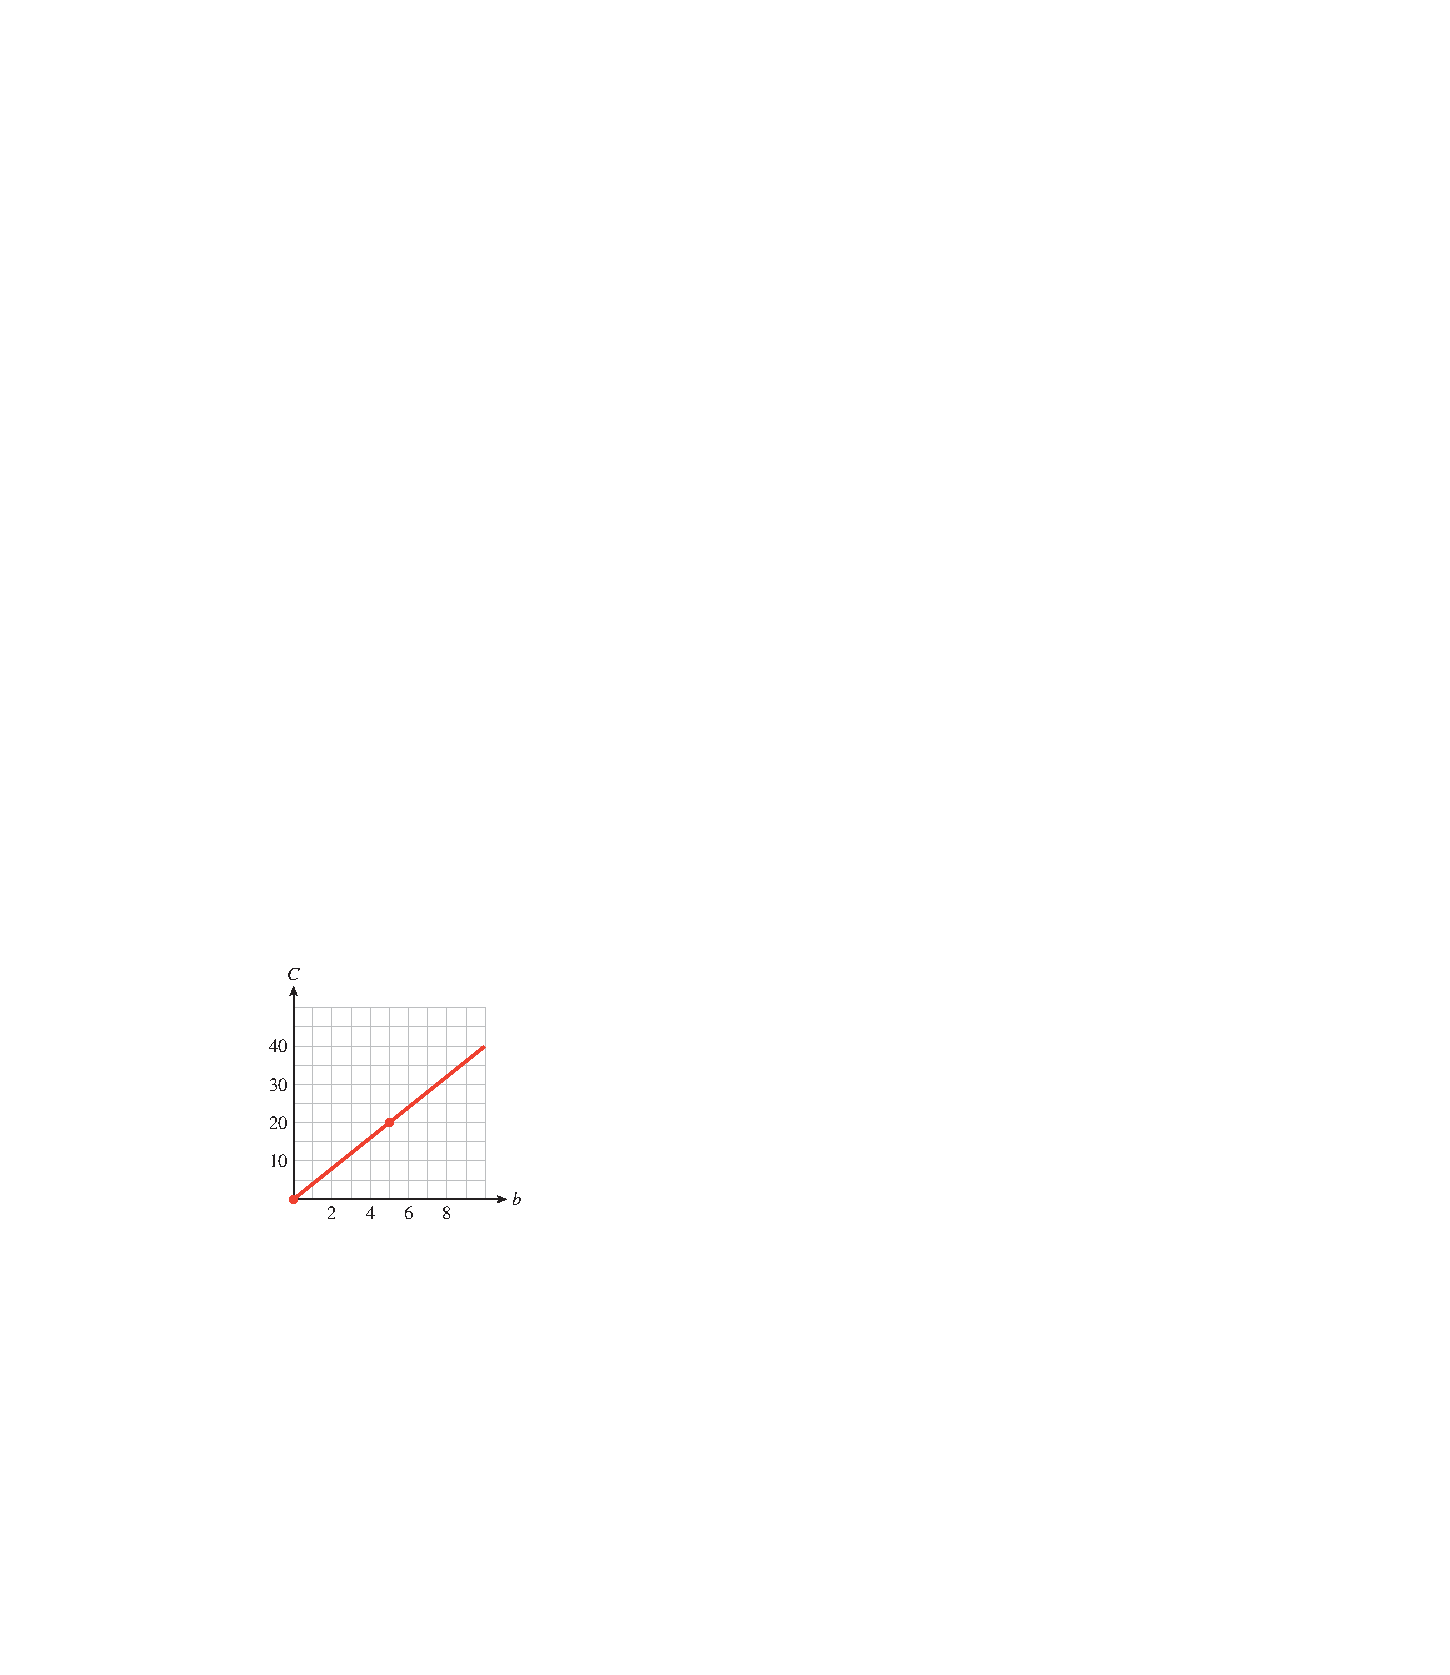
\includegraphics[width=\linewidth]{external/images/fig-ex-1-4-39.pdf}
\end{sbspanel}%
\end{sidebyside}%
\end{divisionexerciseeg}%
\begin{divisionexerciseeg}{40}{}{}{exercise-section-1-4-exercises-n-i}%
The graph shows Tracey's earnings, \(E\) (in dollars), in terms of the number of hours, \(h\), that she babysits.%
\begin{sidebyside}{1}{0.325}{0.325}{0}%
\begin{sbspanel}{0.35}%
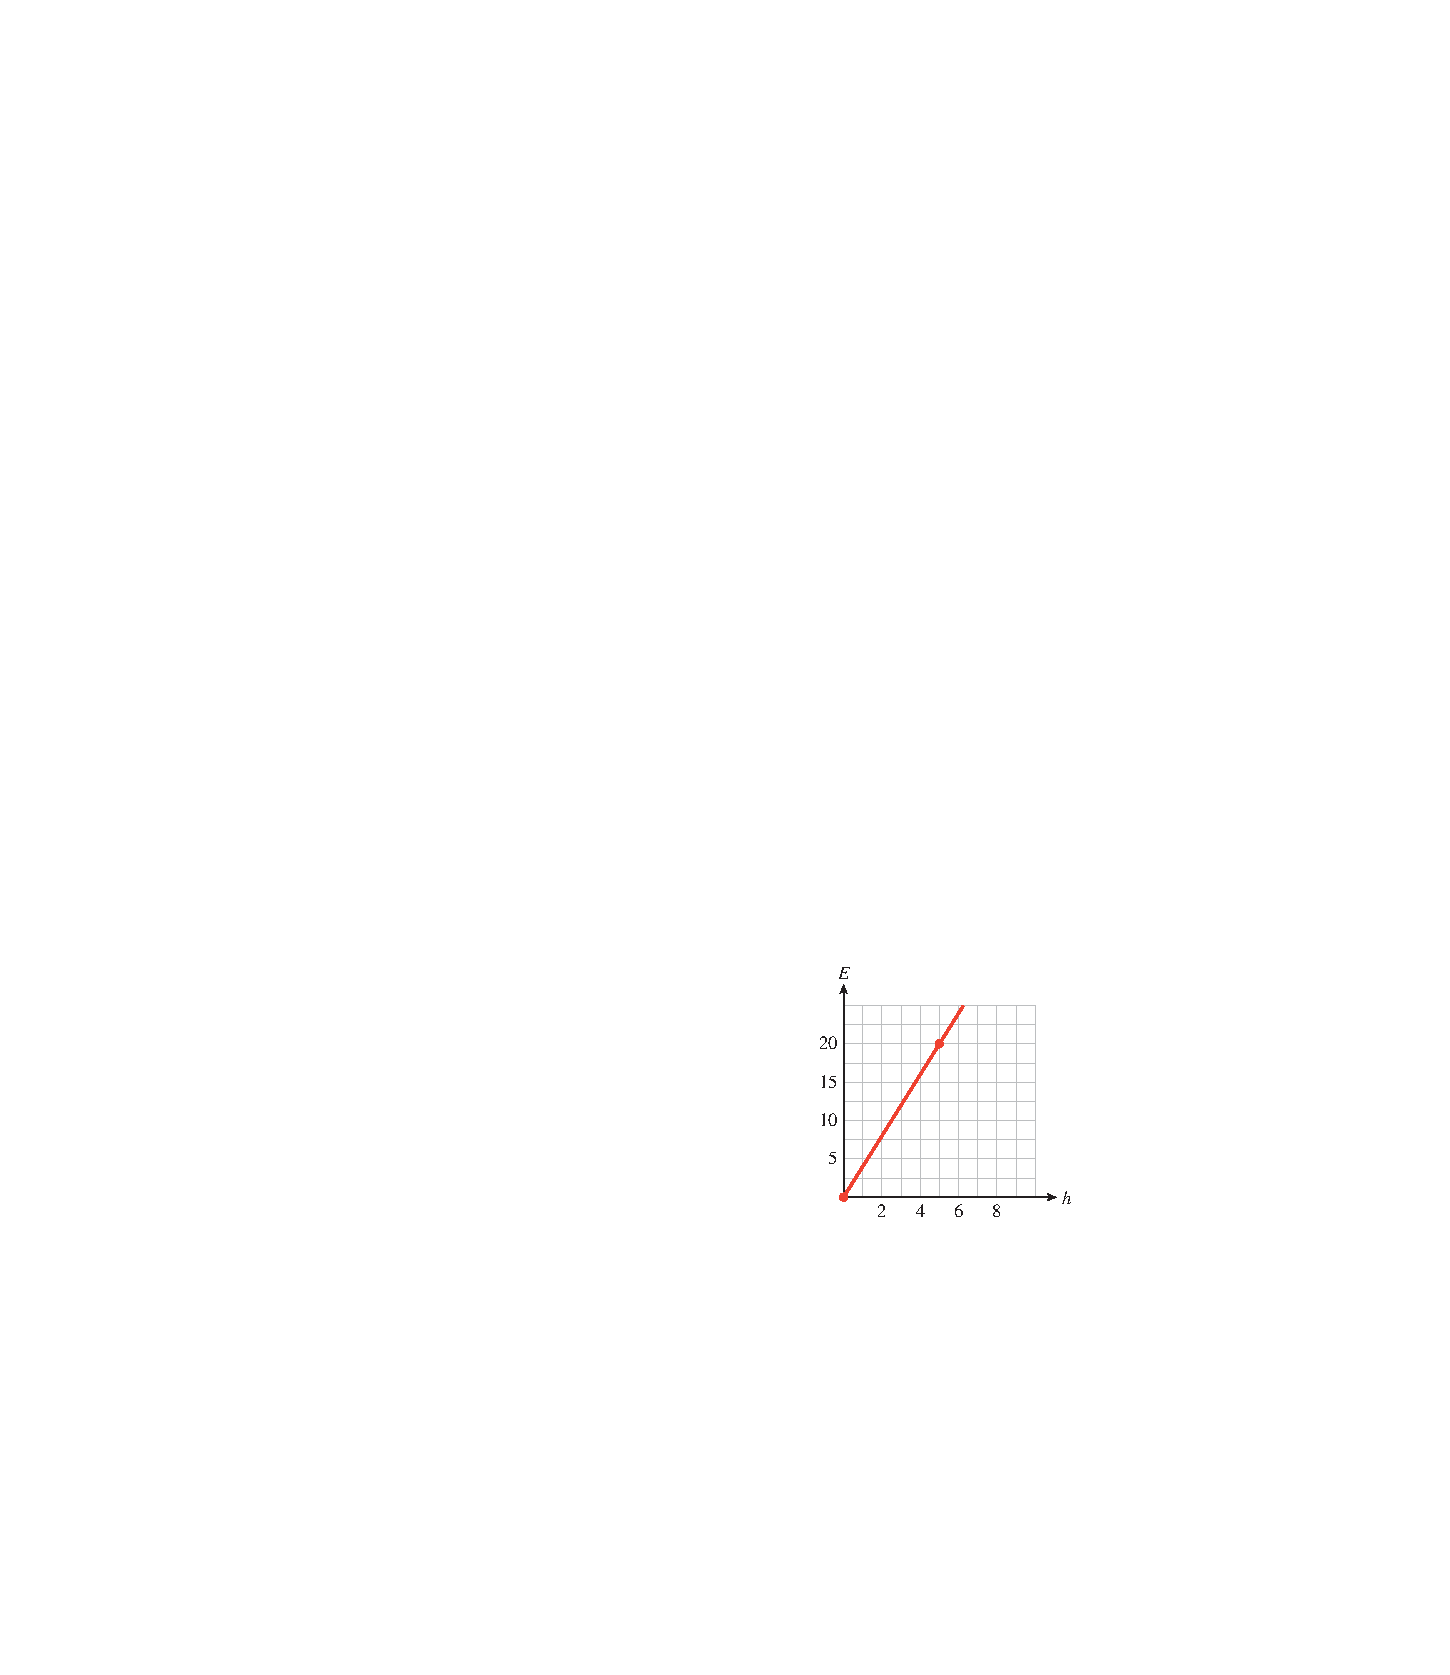
\includegraphics[width=\linewidth]{external/images/fig-ex-1-4-40.pdf}
\end{sbspanel}%
\end{sidebyside}%
\end{divisionexerciseeg}%
\end{exercisegroup}
\par\medskip\noindent
\par\medskip\noindent%
\textbf{Exercise Group.}\space\space%
Which of the tables in Problems 41 and 42 represent variables that are related by a linear function? (Hint: Which relationships have constant slope?)%
\begin{exercisegroup}
\begin{divisionexerciseeg}{41}{}{}{exercise-section-1-4-exercises-o-b}%
%
\begin{multicols}{2}
\begin{enumerate}[label=\alph*]
\item{}\begin{sidebyside}{1}{0}{0.75}{0}%
\begin{sbspanel}{0.25}%
\resizebox{\ifdim\width > \linewidth\linewidth\else\width\fi}{!}{%
{\centering%
{\tabularfont%
\begin{tabular}{AcAcA}\hrulethick
\(x\)&\(y\)\tabularnewline\hrulethin
\(2\)&\(12\)\tabularnewline\hrulethin
\(3\)&\(17\)\tabularnewline\hrulethin
\(4\)&\(22\)\tabularnewline\hrulethin
\(5\)&\(27\)\tabularnewline\hrulethin
\(6\)&\(32\)\tabularnewline\hrulethin
\end{tabular}
}%
\par}
}%
\end{sbspanel}%
\end{sidebyside}%
%
\item{}\begin{sidebyside}{1}{0}{0.75}{0}%
\begin{sbspanel}{0.25}%
\resizebox{\ifdim\width > \linewidth\linewidth\else\width\fi}{!}{%
{\centering%
{\tabularfont%
\begin{tabular}{AcAcA}\hrulethick
\(t\)&\(P\)\tabularnewline\hrulethin
\(2\)&\(4\)\tabularnewline\hrulethin
\(3\)&\(9\)\tabularnewline\hrulethin
\(4\)&\(16\)\tabularnewline\hrulethin
\(5\)&\(25\)\tabularnewline\hrulethin
\(6\)&\(36\)\tabularnewline\hrulethin
\end{tabular}
}%
\par}
}%
\end{sbspanel}%
\end{sidebyside}%
%
\end{enumerate}
\end{multicols}
%
\end{divisionexerciseeg}%
\begin{divisionexerciseeg}{42}{}{}{exercise-section-1-4-exercises-o-c}%
%
\begin{multicols}{2}
\begin{enumerate}[label=\alph*]
\item{}\begin{sidebyside}{1}{0}{0.75}{0}%
\begin{sbspanel}{0.25}%
\resizebox{\ifdim\width > \linewidth\linewidth\else\width\fi}{!}{%
{\centering%
{\tabularfont%
\begin{tabular}{AcAcA}\hrulethick
\(h\)&\(w\)\tabularnewline\hrulethin
\(-6\)&\(20\)\tabularnewline\hrulethin
\(-3\)&\(18\)\tabularnewline\hrulethin
\(0\)&\(16\)\tabularnewline\hrulethin
\(3\)&\(14\)\tabularnewline\hrulethin
\(6\)&\(12\)\tabularnewline\hrulethin
\end{tabular}
}%
\par}
}%
\end{sbspanel}%
\end{sidebyside}%
%
\item{}\begin{sidebyside}{1}{0}{0.75}{0}%
\begin{sbspanel}{0.25}%
\resizebox{\ifdim\width > \linewidth\linewidth\else\width\fi}{!}{%
{\centering%
{\tabularfont%
\begin{tabular}{AcAcA}\hrulethick
\(t\)&\(d\)\tabularnewline\hrulethin
\(5\)&\(0\)\tabularnewline\hrulethin
\(10\)&\(3\)\tabularnewline\hrulethin
\(15\)&\(6\)\tabularnewline\hrulethin
\(20\)&\(12\)\tabularnewline\hrulethin
\(25\)&\(24\)\tabularnewline\hrulethin
\end{tabular}
}%
\par}
}%
\end{sbspanel}%
\end{sidebyside}%
%
\end{enumerate}
\end{multicols}
%
\end{divisionexerciseeg}%
\end{exercisegroup}
\par\medskip\noindent
\begin{divisionexercise}{43}{}{}{exercise-section-1-4-exercises-p}%
The table shows the amount of ammonium chloride salt, in grams, that can be dissolved in 100 grams of water at different temperatures.%
\begin{sidebyside}{1}{0}{0}{0}%
\begin{sbspanel}{1}%
\resizebox{\ifdim\width > \linewidth\linewidth\else\width\fi}{!}{%
{\centering%
{\tabularfont%
\begin{tabular}{AlAcAcAcAcAcAcAcA}\hrulethick
Temperature,\(\degree\)C&\(10\)&\(12\)&\(15\)&\(21\)&\(25\)&\(40\)&\(52\)\tabularnewline\hrulethin
Grams of salt&\(33 \)&\(34\)&\(35.5\)&\(38.5\)&\(40.5\)&\(48\)&\(54\)\tabularnewline\hrulethin
\end{tabular}
}%
\par}
}%
\end{sbspanel}%
\end{sidebyside}%
\par
%
\begin{enumerate}[label=\alph*]
\item{}If you plot the data, will the points lie on a straight line? Why or why not?%
\item{}Calculate the rate of change of salt dissolved with respect to temperature.%
\end{enumerate}
%
\end{divisionexercise}%
\begin{divisionexercise}{44}{}{}{exercise-section-1-4-exercises-q}%
A spring is suspended from the ceiling. The table shows the length of the spring, in centimeters, as it is stretched by hanging various weights from it.%
\begin{sidebyside}{1}{0}{0}{0}%
\begin{sbspanel}{1}%
\resizebox{\ifdim\width > \linewidth\linewidth\else\width\fi}{!}{%
{\centering%
{\tabularfont%
\begin{tabular}{AlAcAcAcAcAcAcAcA}\hrulethick
Weight, kg&\(3\)&\(4\)&\(8\)&\(10\)&\(12\)&\(15\)&\(22\)\tabularnewline\hrulethin
Length, cm&\(25.87 \)&\(25.88\)&\(26.36\)&\(26.6\)&\(26.84\)&\(27.2\)&\(28.04\)\tabularnewline\hrulethin
\end{tabular}
}%
\par}
}%
\end{sbspanel}%
\end{sidebyside}%
\par
%
\begin{enumerate}[label=\alph*]
\item{}If you plot the data, will the points lie on a straight line? Why or why not?%
\item{}Calculate the rate of change of length with respect to weight.%
\end{enumerate}
%
\end{divisionexercise}%
\begin{divisionexercise}{45}{}{}{exercise-section-1-4-exercises-r}%
The table gives the radius and circumference of various circles, rounded to three decimal places.%
\begin{sidebyside}{1}{0}{0}{0}%
\begin{sbspanel}{1}%
\resizebox{\ifdim\width > \linewidth\linewidth\else\width\fi}{!}{%
{\centering%
{\tabularfont%
\begin{tabular}{AcAcA}\hrulethick
\(r\)&\(C\)\tabularnewline\hrulethin
\(4\)&\(25.133\)\tabularnewline\hrulethin
\(6\)&\(37.699\)\tabularnewline\hrulethin
\(10\)&\(62.832\)\tabularnewline\hrulethin
\(15\)&\(94.248\)\tabularnewline\hrulethin
\end{tabular}
}%
\par}
}%
\end{sbspanel}%
\end{sidebyside}%
\par
%
\begin{enumerate}[label=\alph*]
\item{}If we plot the data, will the points lie on a straight line?%
\item{}What familiar number does the slope turn out to be? (Hint: Recall a formula from geometry.)%
\end{enumerate}
%
\end{divisionexercise}%
\begin{divisionexercise}{46}{}{}{exercise-section-1-4-exercises-s}%
The table gives the side and the diagonal of various squares, rounded to three decimal places.%
\begin{sidebyside}{1}{0}{0}{0}%
\begin{sbspanel}{1}%
\resizebox{\ifdim\width > \linewidth\linewidth\else\width\fi}{!}{%
{\centering%
{\tabularfont%
\begin{tabular}{AcAcA}\hrulethick
\(s\)&\(d\)\tabularnewline\hrulethin
\(3\)&\(4.243\)\tabularnewline\hrulethin
\(6\)&\(8.485\)\tabularnewline\hrulethin
\(8\)&\(11.314\)\tabularnewline\hrulethin
\(10\)&\(14.142\)\tabularnewline\hrulethin
\end{tabular}
}%
\par}
}%
\end{sbspanel}%
\end{sidebyside}%
\par
%
\begin{enumerate}[label=\alph*]
\item{}If we plot the data, will the points lie on a straight line?%
\item{}What familiar number does the slope turn out to be? (Hint: Draw a picture of one of the squares and use the Pythagorean theorem to compute its diagonal.)%
\end{enumerate}
%
\end{divisionexercise}%
\begin{divisionexercise}{47}{}{}{exercise-section-1-4-exercises-t}%
Geologists can measure the depth of the ocean at different points using a technique called echo-sounding. Scientists on board a ship send a pulse of sound toward the ocean floor and measure the time interval until the echo returns to the ship. The speed of sound in seawater is about \(1500\) meters per second.%
\begin{enumerate}[label=\alph*]
\item{}Write the speed of sound as a ratio.%
\item{}If the echo returns in \(4.5\) seconds, what is the depth of the ocean at that point?%
\end{enumerate}
%
\end{divisionexercise}%
\begin{divisionexercise}{48}{}{}{exercise-section-1-4-exercises-u}%
Niagara Falls was discovered by Father Louis Hennepin in 1682. In 1952, much of the water of the Niagara River was diverted for hydroelectric power, but until that time erosion caused the Falls to recede upstream by \(3\) feet per year.%
\begin{enumerate}[label=\alph*]
\item{}How far did the Falls recede from 1682 to 1952?%
\item{}The Falls were formed about \(12,000\) years ago during the end of the last ice age. How far downstream from their current position were they then? (Give your answer in miles.)%
\end{enumerate}
%
\end{divisionexercise}%
\begin{divisionexercise}{49}{}{}{exercise-section-1-4-exercises-v}%
Geologists calculate the speed of seismic waves by plotting the travel times for waves to reach seismometers at known distances from the epicenter. The speed of the wave can help them determine the nature of the material it passes through. The graph shows a  travel-time graph for P-waves from a shallow earthquake.%
\begin{sidebyside}{1}{0.32}{0.32}{0}%
\begin{sbspanel}{0.36}%
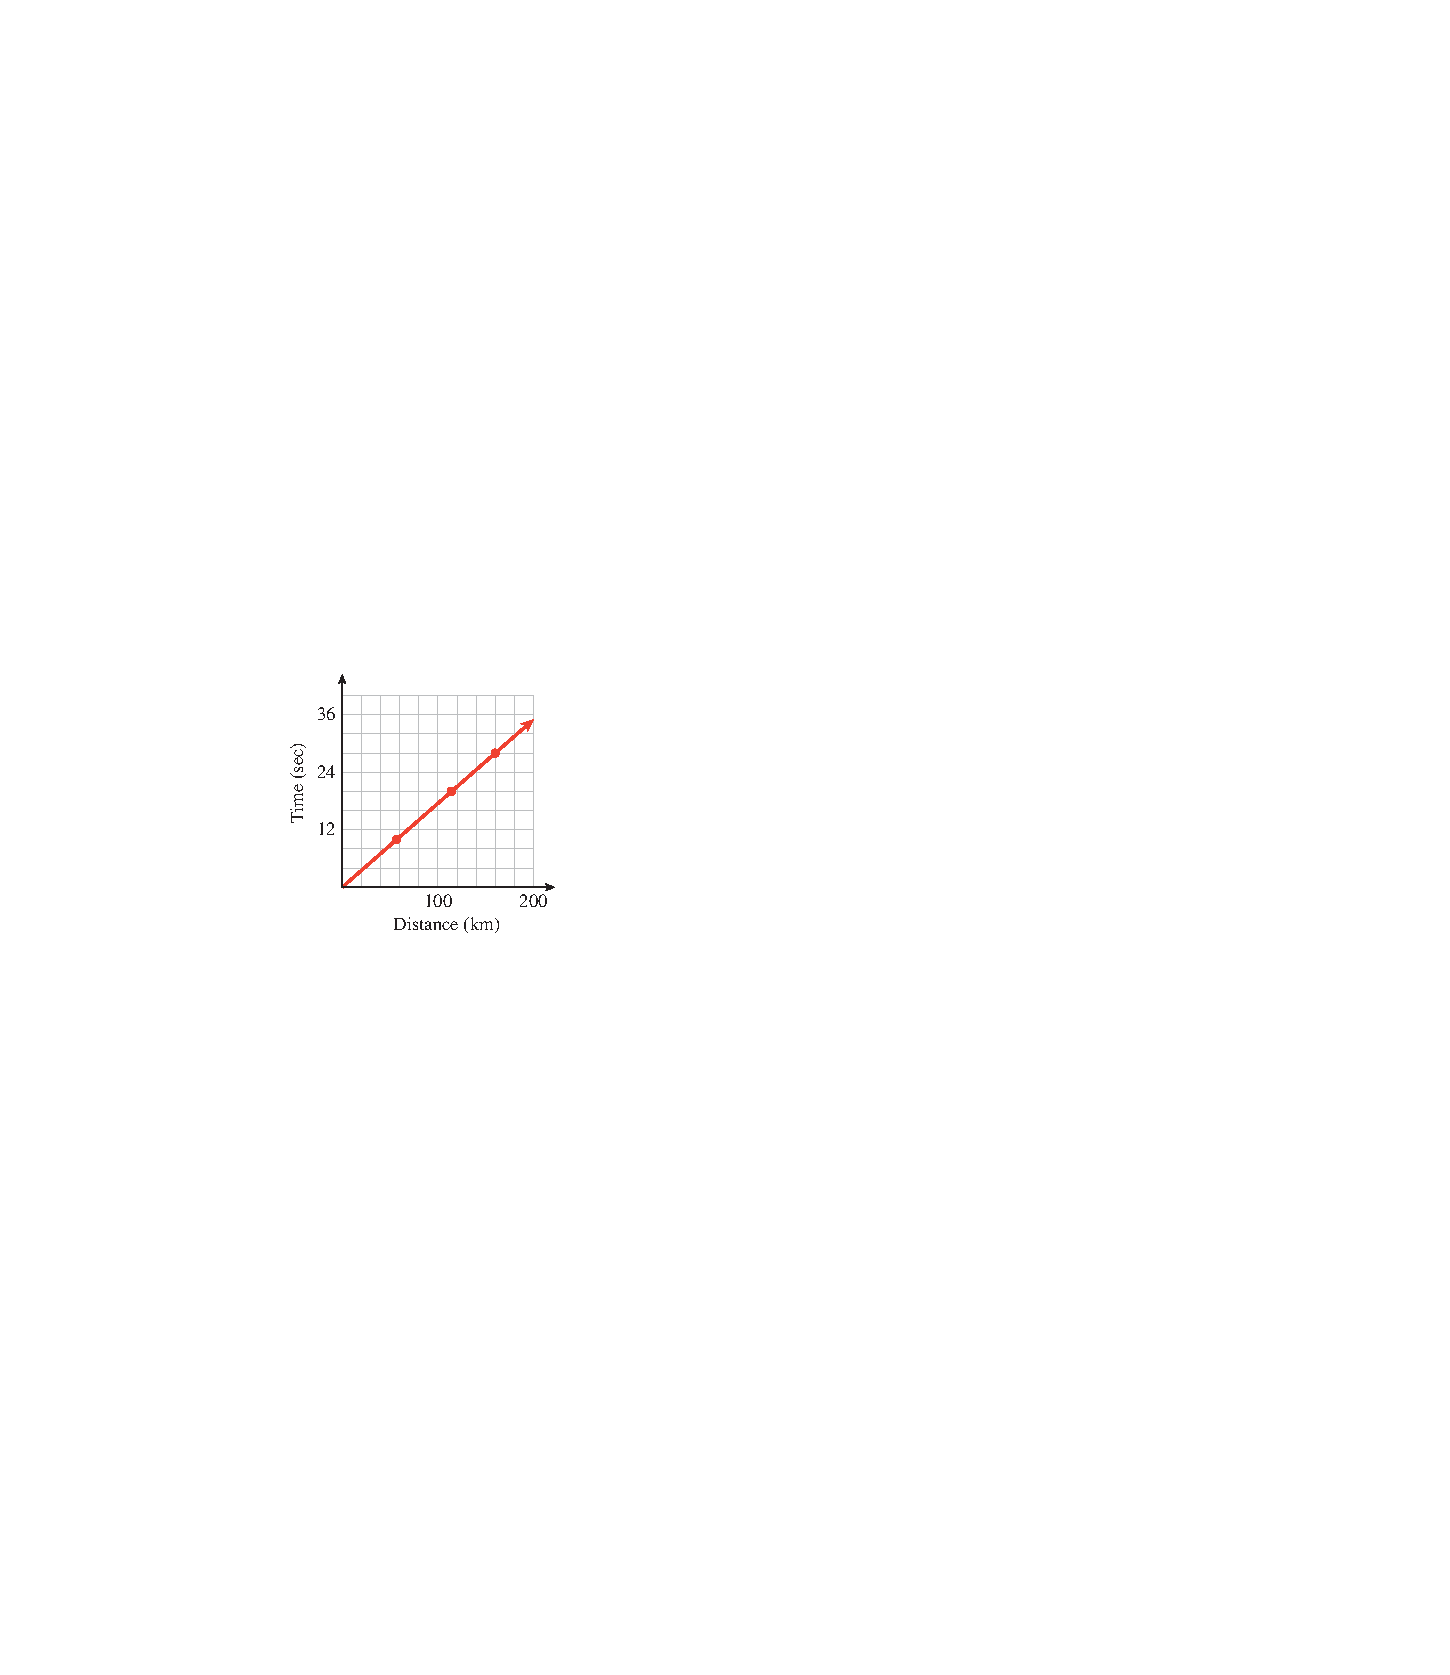
\includegraphics[width=\linewidth]{external/images/fig-ex-1-4-49.pdf}
\end{sbspanel}%
\end{sidebyside}%
\par
%
\begin{enumerate}[label=\alph*]
\item{}Why do you think the graph is plotted with distance as the input variable?%
\item{}Use the graph to calculate the speed of the wave.%
\end{enumerate}
%
\end{divisionexercise}%
\begin{divisionexercise}{50}{}{}{exercise-section-1-4-exercises-w}%
Energy (supplied by heat) is required to raise the temperature of a substance, and it is also needed to melt a solid substance to a liquid. The table shows data from heating a solid sample of stearic acid. Heat was applied at a constant rate throughout the experiment. (Source: J. A. Hunt and A. Sykes, 1984)%
\begin{sidebyside}{1}{0}{0}{0}%
\begin{sbspanel}{1}%
\resizebox{\ifdim\width > \linewidth\linewidth\else\width\fi}{!}{%
{\centering%
{\tabularfont%
\begin{tabular}{AlAcAcAcAcAcAcAcAcAcAcAcAcAcAcAcA}\hrulethick
Time (minutes&\(0\)&\(0.5\)&\(1.5\)&\(2\)&\(2.5\)&\(3\)&\(4\)&\(5\)&\(6\)&\(7\)&\(8\)&\(8.5\)&\(9\)&\(9.5\)&\(10\)\tabularnewline\hrulethin
Temperature, \(\degree\)C&\(19 \)&\(29\)&\(40\)&\(48\)&\(53\)&\(55\)&\(55\)&\(55 \)&\(55\)&\(55\)&\(55\)&\(64\)&\(70\)&\(73\)&\(74\)\tabularnewline\hrulethin
\end{tabular}
}%
\par}
}%
\end{sbspanel}%
\end{sidebyside}%
\par
%
\begin{enumerate}[label=\alph*]
\item{}Did the temperature rise at a constant rate? Describe the temperature as a function of time.%
\item{}Graph temperature as a function of time.%
\item{}What is the melting point of stearic acid? How long did it take the sample to melt?%
\end{enumerate}
%
\end{divisionexercise}%
\begin{divisionexercise}{51}{}{}{exercise-section-1-4-exercises-x}%
The graph shows the temperature of the ocean as a function of depth.%
\begin{sidebyside}{1}{0.32}{0.32}{0}%
\begin{sbspanel}{0.36}%
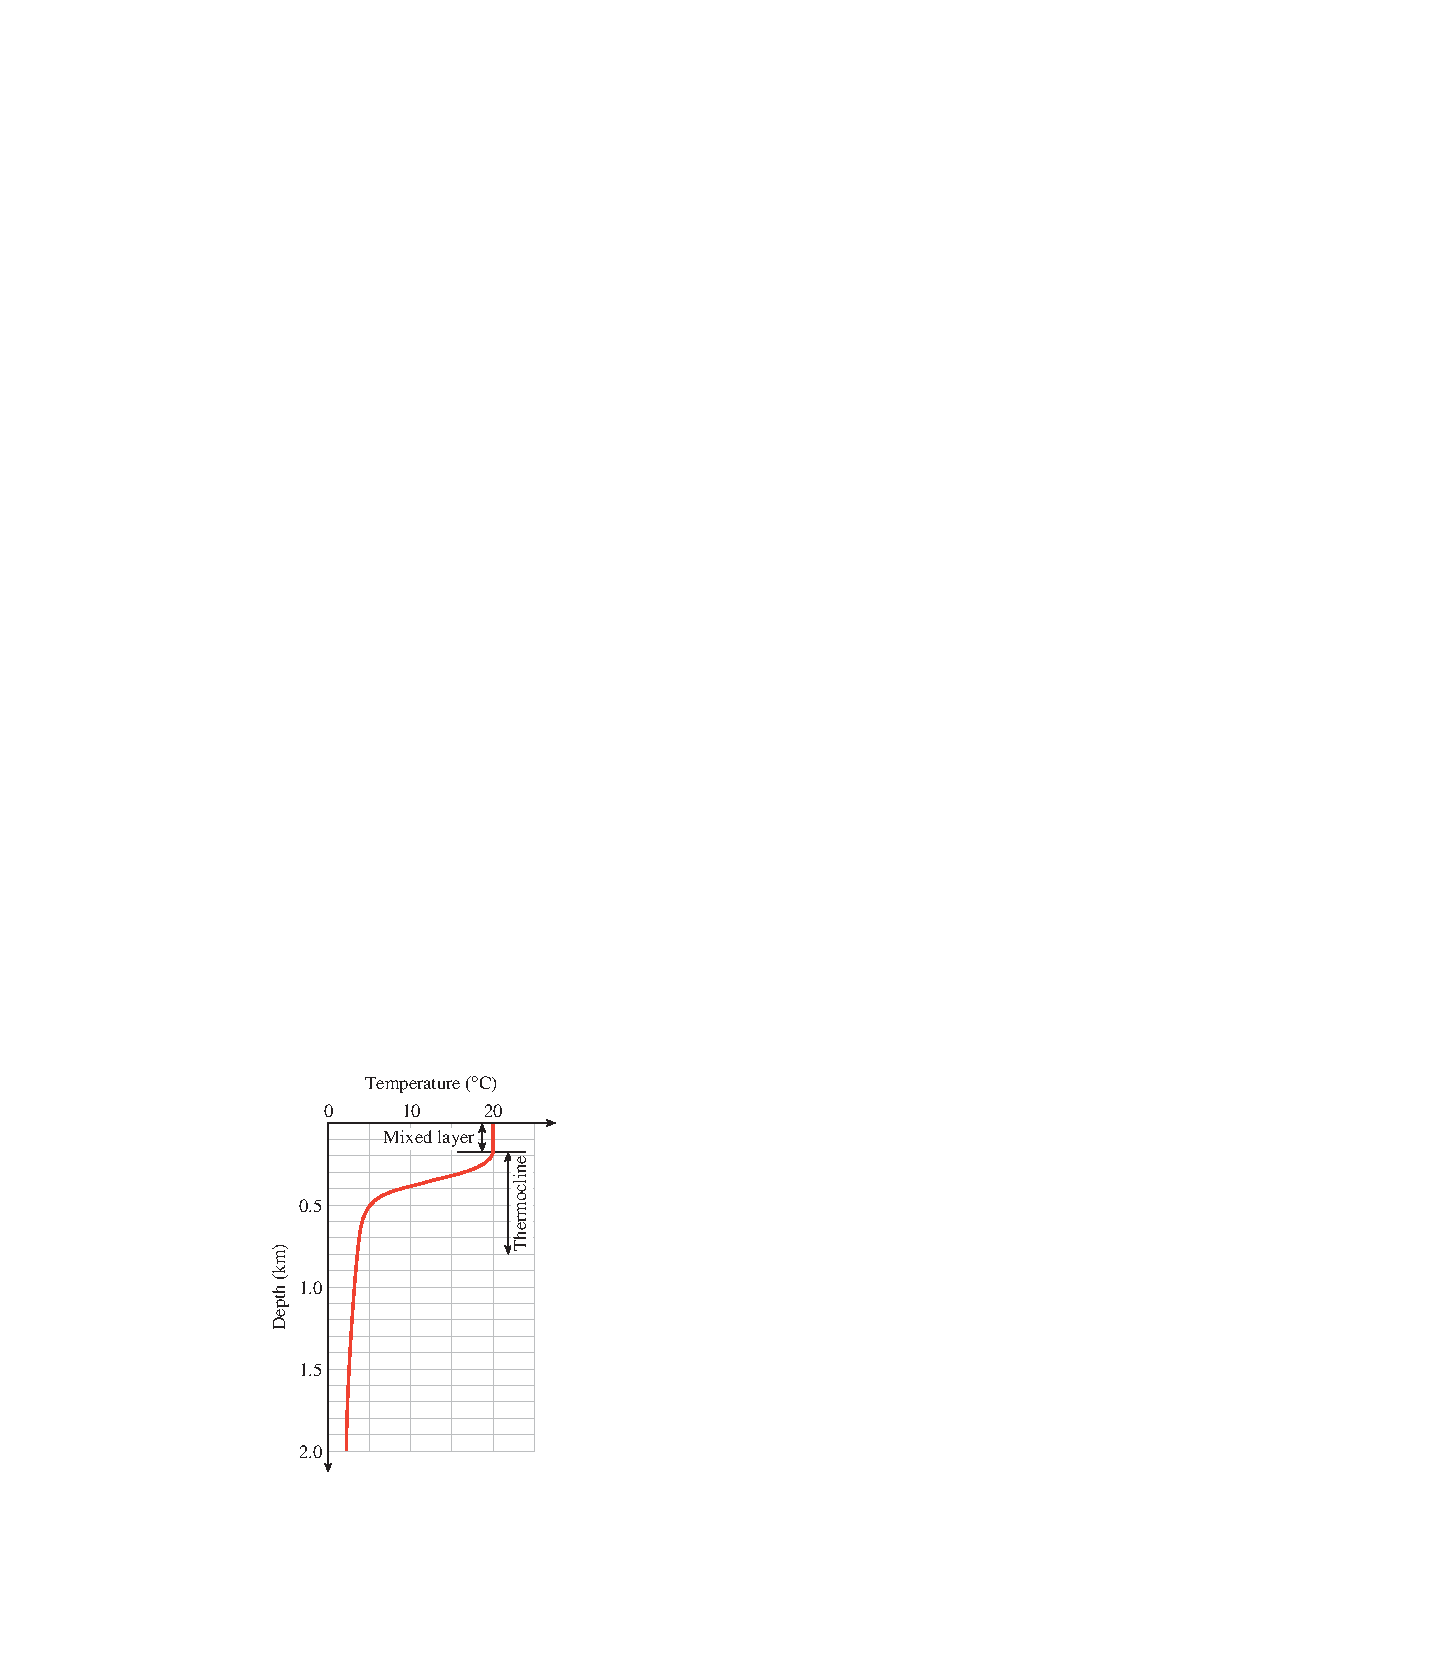
\includegraphics[width=\linewidth]{external/images/fig-ex-1-4-51.pdf}
\end{sbspanel}%
\end{sidebyside}%
\par
%
\begin{enumerate}[label=\alph*]
\item{}What is the difference in temperature between the surface of the ocean and the deepest level shown?%
\item{}Over what depths does the temperature change most rapidly?%
\item{}What is the average rate of change of temperature with respect to depth in the region called the thermocline?%
\end{enumerate}
%
\end{divisionexercise}%
\begin{divisionexercise}{52}{}{}{exercise-section-1-4-exercises-y}%
The graph shows the average air temperature as a function of altitude. (Figure (b) is an enlargement of the indicated region of Figure (a).) (Source: Ahrens, 1998)%
\begin{sidebyside}{1}{0}{0}{0}%
\begin{sbspanel}{1}%
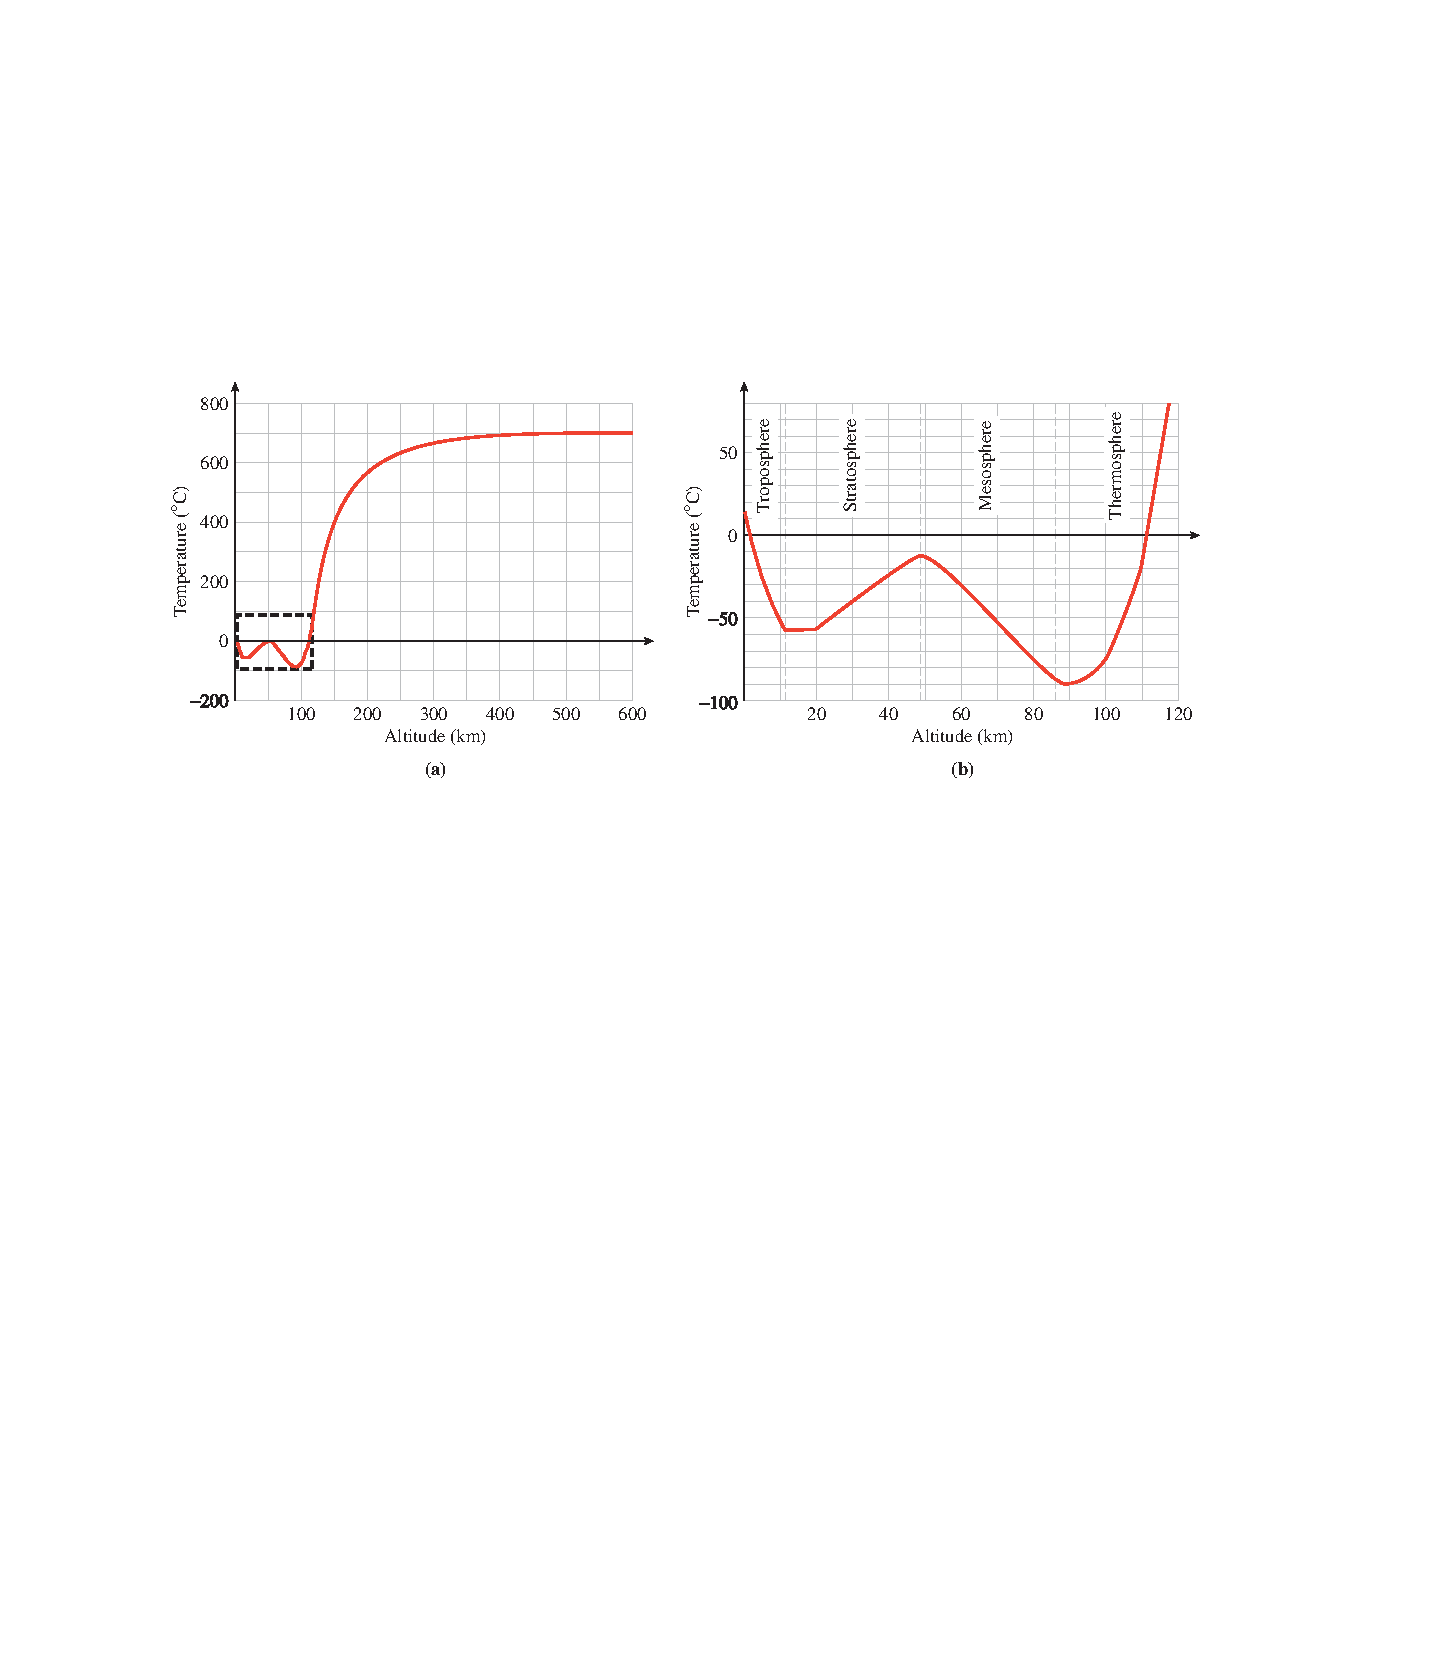
\includegraphics[width=\linewidth]{external/images/fig-ex-1-4-52.pdf}
\end{sbspanel}%
\end{sidebyside}%
\par
%
\begin{enumerate}[label=\alph*]
\item{}Is temperature a decreasing function of altitude?%
\item{}The \terminology{lapse rate} is the rate at which the temperature changes with altitude. In which regions of the atmosphere is the lapse rate positive?%
\item{}The region where the lapse rate is zero is called the isothermal zone. Give an interval of altitudes that describes the isothermal zone.%
\item{}What is the lapse rate in the mesosphere?%
\item{}Describe the temperature for altitudes greater than 90 kilometers.%
\end{enumerate}
%
\end{divisionexercise}%
\par\medskip\noindent%
\textbf{Exercise Group.}\space\space%
In Problems 53\textendash{}56, evaluate the function at \(x = a\) and \(x = b\), and then find the slope of the line segment joining the two corresponding points on the graph. Illustrate the line segment on a graph of the function.%
\begin{exercisegroupcol}{2}
\begin{divisionexerciseegcol}{53}{}{}{exercise-section-1-4-exercises-z-b}%
\(f (x) = x^2 - 2x - 8\)%
\begin{enumerate}[label=\alph*]
\item{}\(\displaystyle a=-2, b = 1\)%
\item{}\(\displaystyle a=-1, b = 5\)%
\end{enumerate}
%
\end{divisionexerciseegcol}%
\begin{divisionexerciseegcol}{54}{}{}{exercise-section-1-4-exercises-z-c}%
\(g(x) = \sqrt{x+4} \)%
\begin{enumerate}[label=\alph*]
\item{}\(\displaystyle a=-2, b = 0\)%
\item{}\(\displaystyle a = 0, b = 5\)%
\end{enumerate}
%
\end{divisionexerciseegcol}%
\begin{divisionexerciseegcol}{55}{}{}{exercise-section-1-4-exercises-z-d}%
\(h(x) =\dfrac{4}{x+2} \)%
\begin{enumerate}[label=\alph*]
\item{}\(\displaystyle a = 0, b = 6\)%
\item{}\(\displaystyle a=-1, b = 2\)%
\end{enumerate}
%
\end{divisionexerciseegcol}%
\begin{divisionexerciseegcol}{56}{}{}{exercise-section-1-4-exercises-z-e}%
\(q(x) = x^3 - 4x \)%
\begin{enumerate}[label=\alph*]
\item{}\(\displaystyle a=-1, b = 2\)%
\item{}\(\displaystyle a=-1, b = 3\)%
\end{enumerate}
%
\end{divisionexerciseegcol}%
\end{exercisegroupcol}
\par\medskip\noindent
\par\medskip\noindent%
\textbf{Exercise Group.}\space\space%
In Problems 57\textendash{}62, find the coordinates of the indicated points, then write an algebraic expression using function notation for the indicated quantity.%
\begin{exercisegroup}
\begin{divisionexerciseeg}{57}{}{}{exercise-section-1-4-exercises-aa-b}%
The length of the vertical line segment on the \(y\)-axis%
\begin{multicols}{2}
\begin{enumerate}[label=\alph*]
\item{}\begin{sidebyside}{1}{0.07}{0.07}{0}%
\begin{sbspanel}{0.86}%
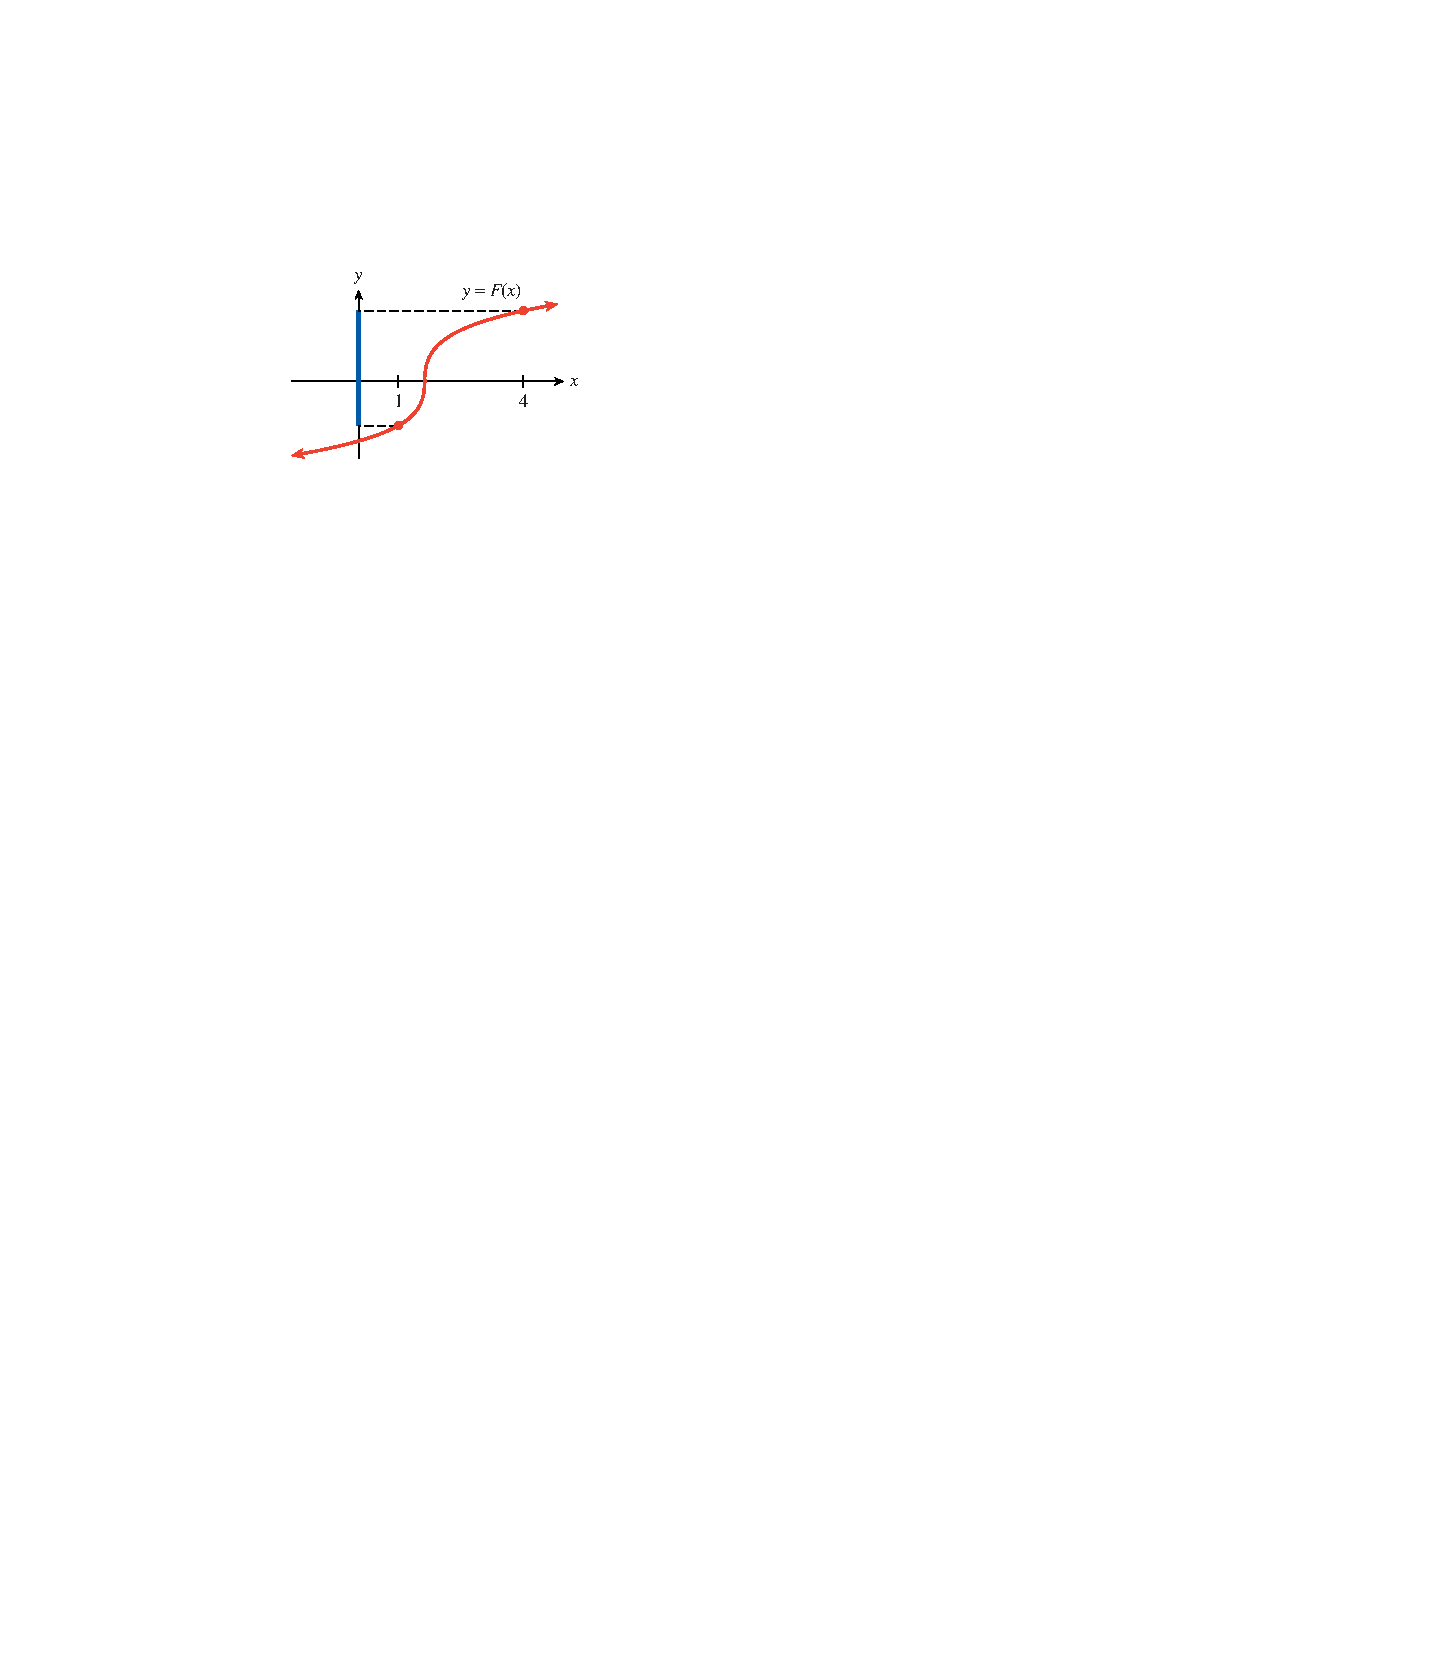
\includegraphics[width=\linewidth]{external/images/fig-ex-1-4-57a.pdf}
\end{sbspanel}%
\end{sidebyside}%
%
\item{}\begin{sidebyside}{1}{0.07}{0.07}{0}%
\begin{sbspanel}{0.86}%
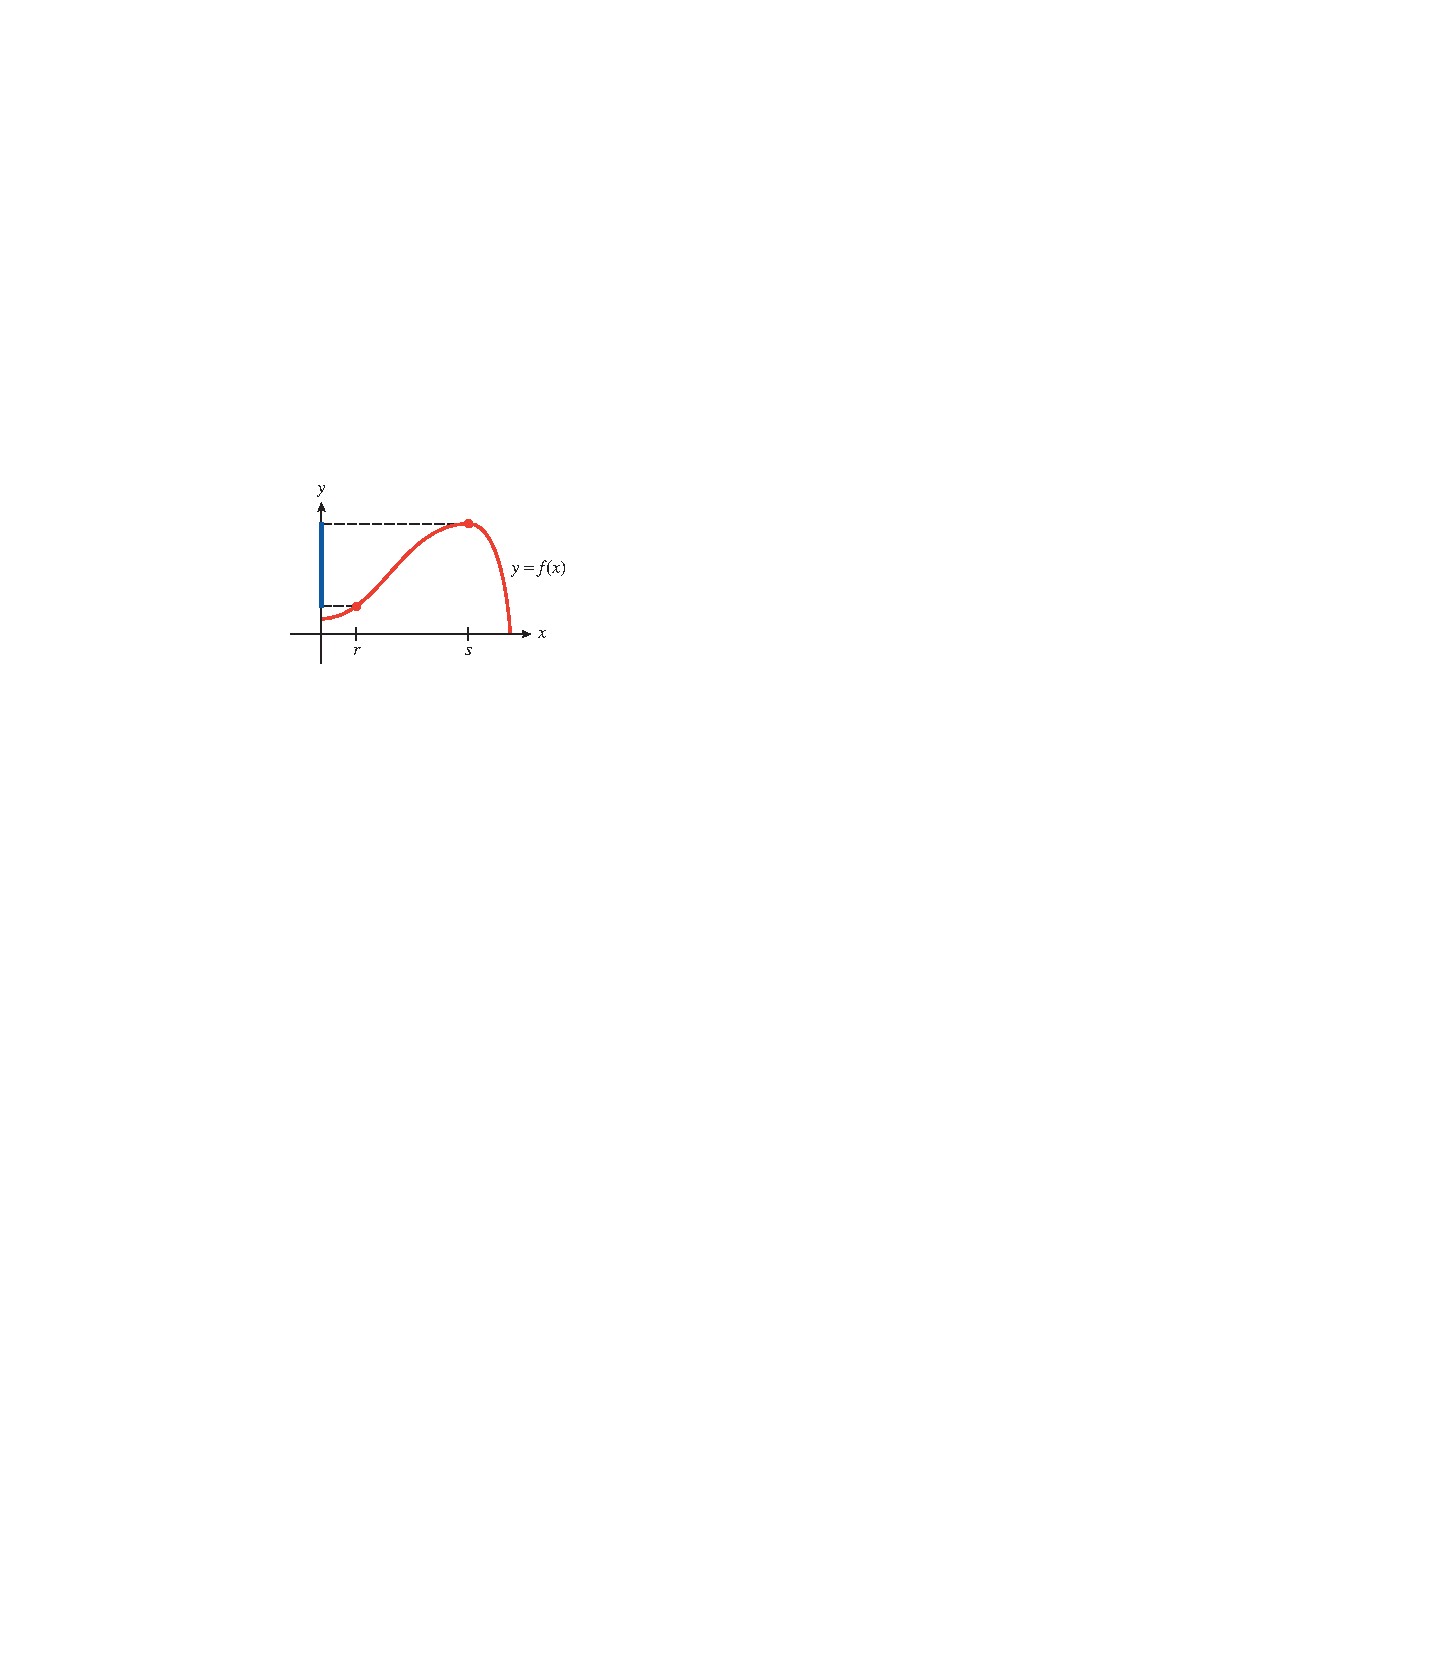
\includegraphics[width=\linewidth]{external/images/fig-ex-1-4-57b.pdf}
\end{sbspanel}%
\end{sidebyside}%
%
\end{enumerate}
\end{multicols}
%
\end{divisionexerciseeg}%
\begin{divisionexerciseeg}{58}{}{}{exercise-section-1-4-exercises-aa-c}%
The length of the vertical line segment on the \(y\)-axis%
\begin{multicols}{2}
\begin{enumerate}[label=\alph*]
\item{}\begin{sidebyside}{1}{0.07}{0.07}{0}%
\begin{sbspanel}{0.86}%
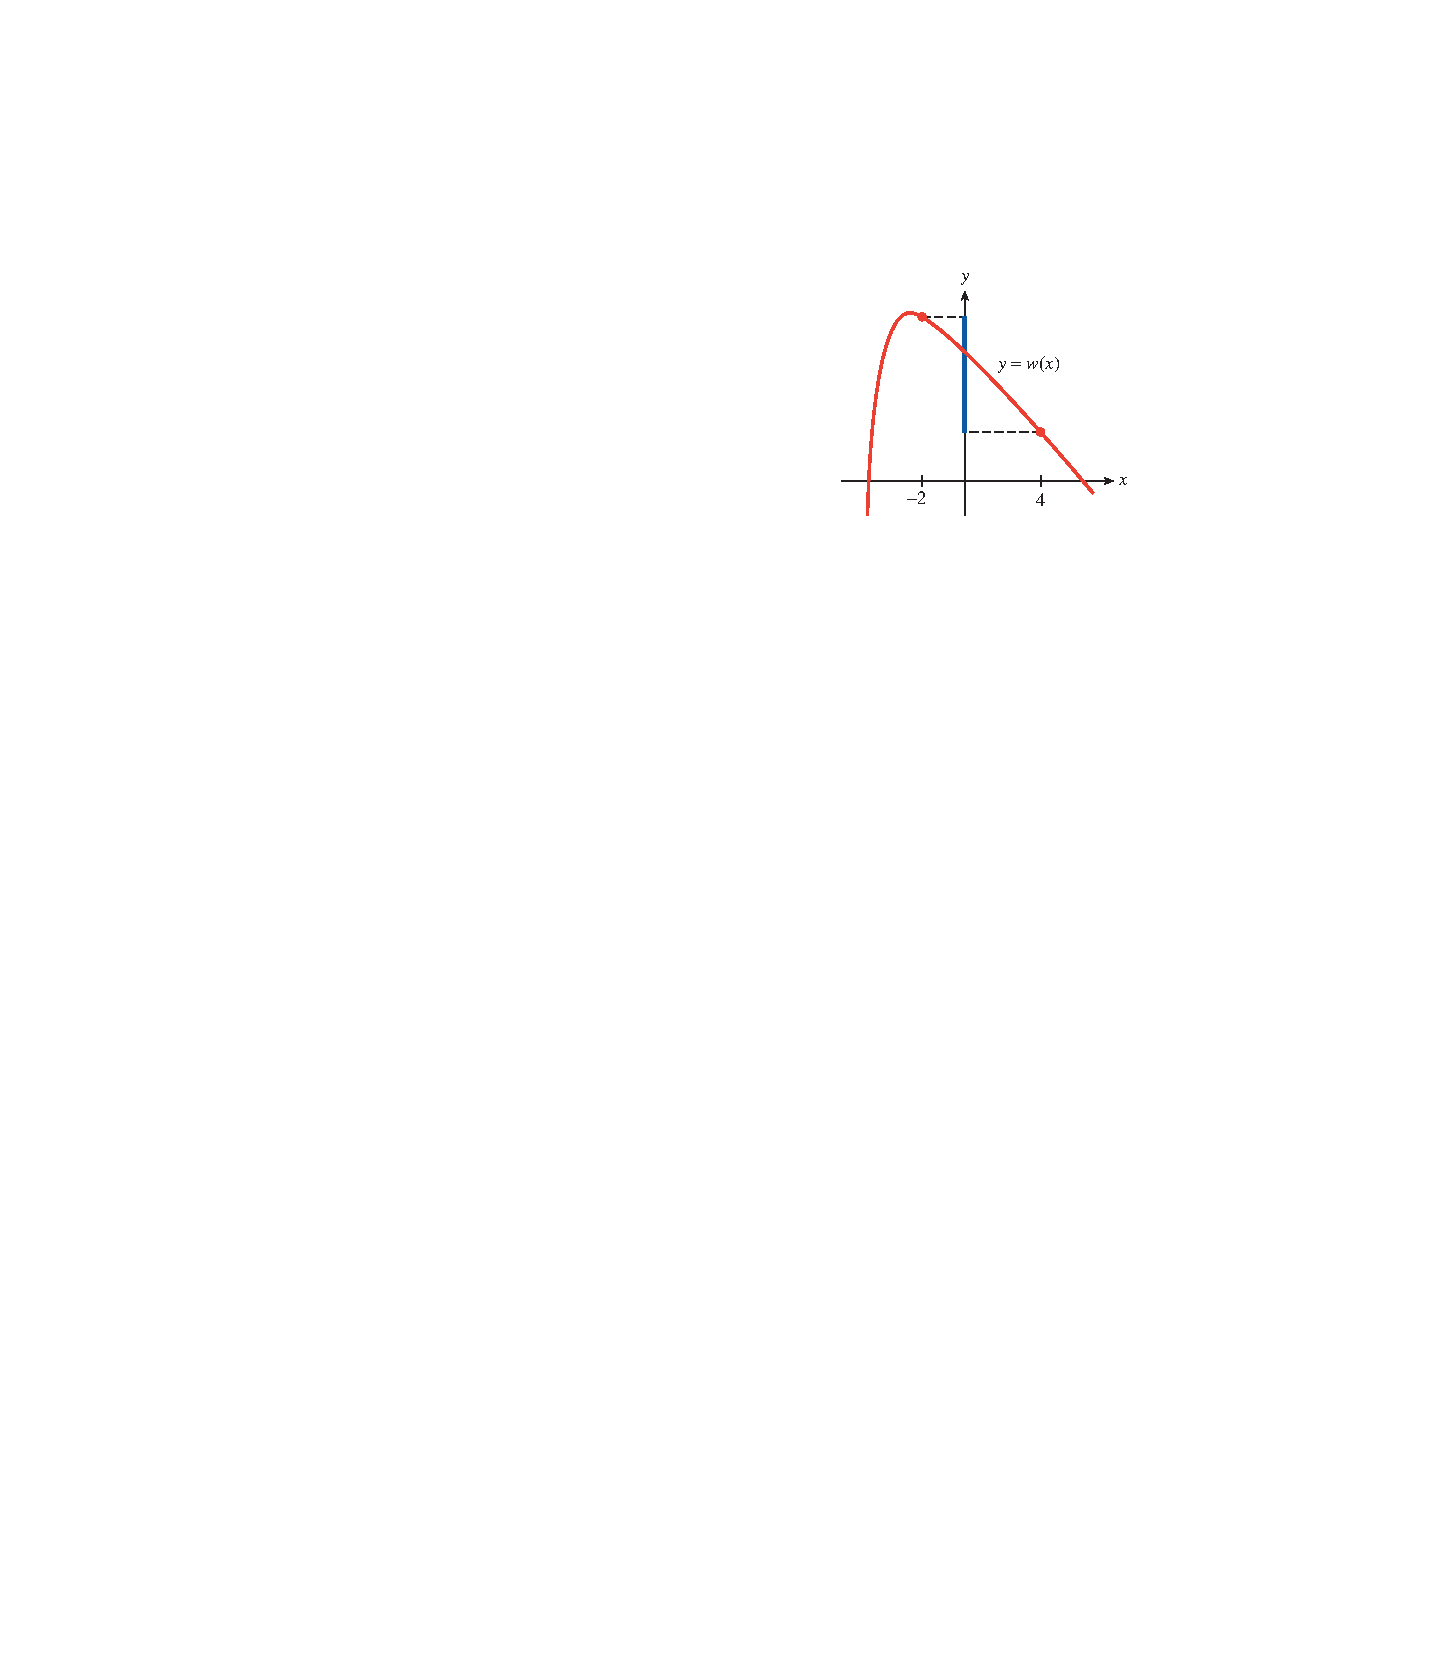
\includegraphics[width=\linewidth]{external/images/fig-ex-1-4-58a.pdf}
\end{sbspanel}%
\end{sidebyside}%
%
\item{}\begin{sidebyside}{1}{0.07}{0.07}{0}%
\begin{sbspanel}{0.86}%
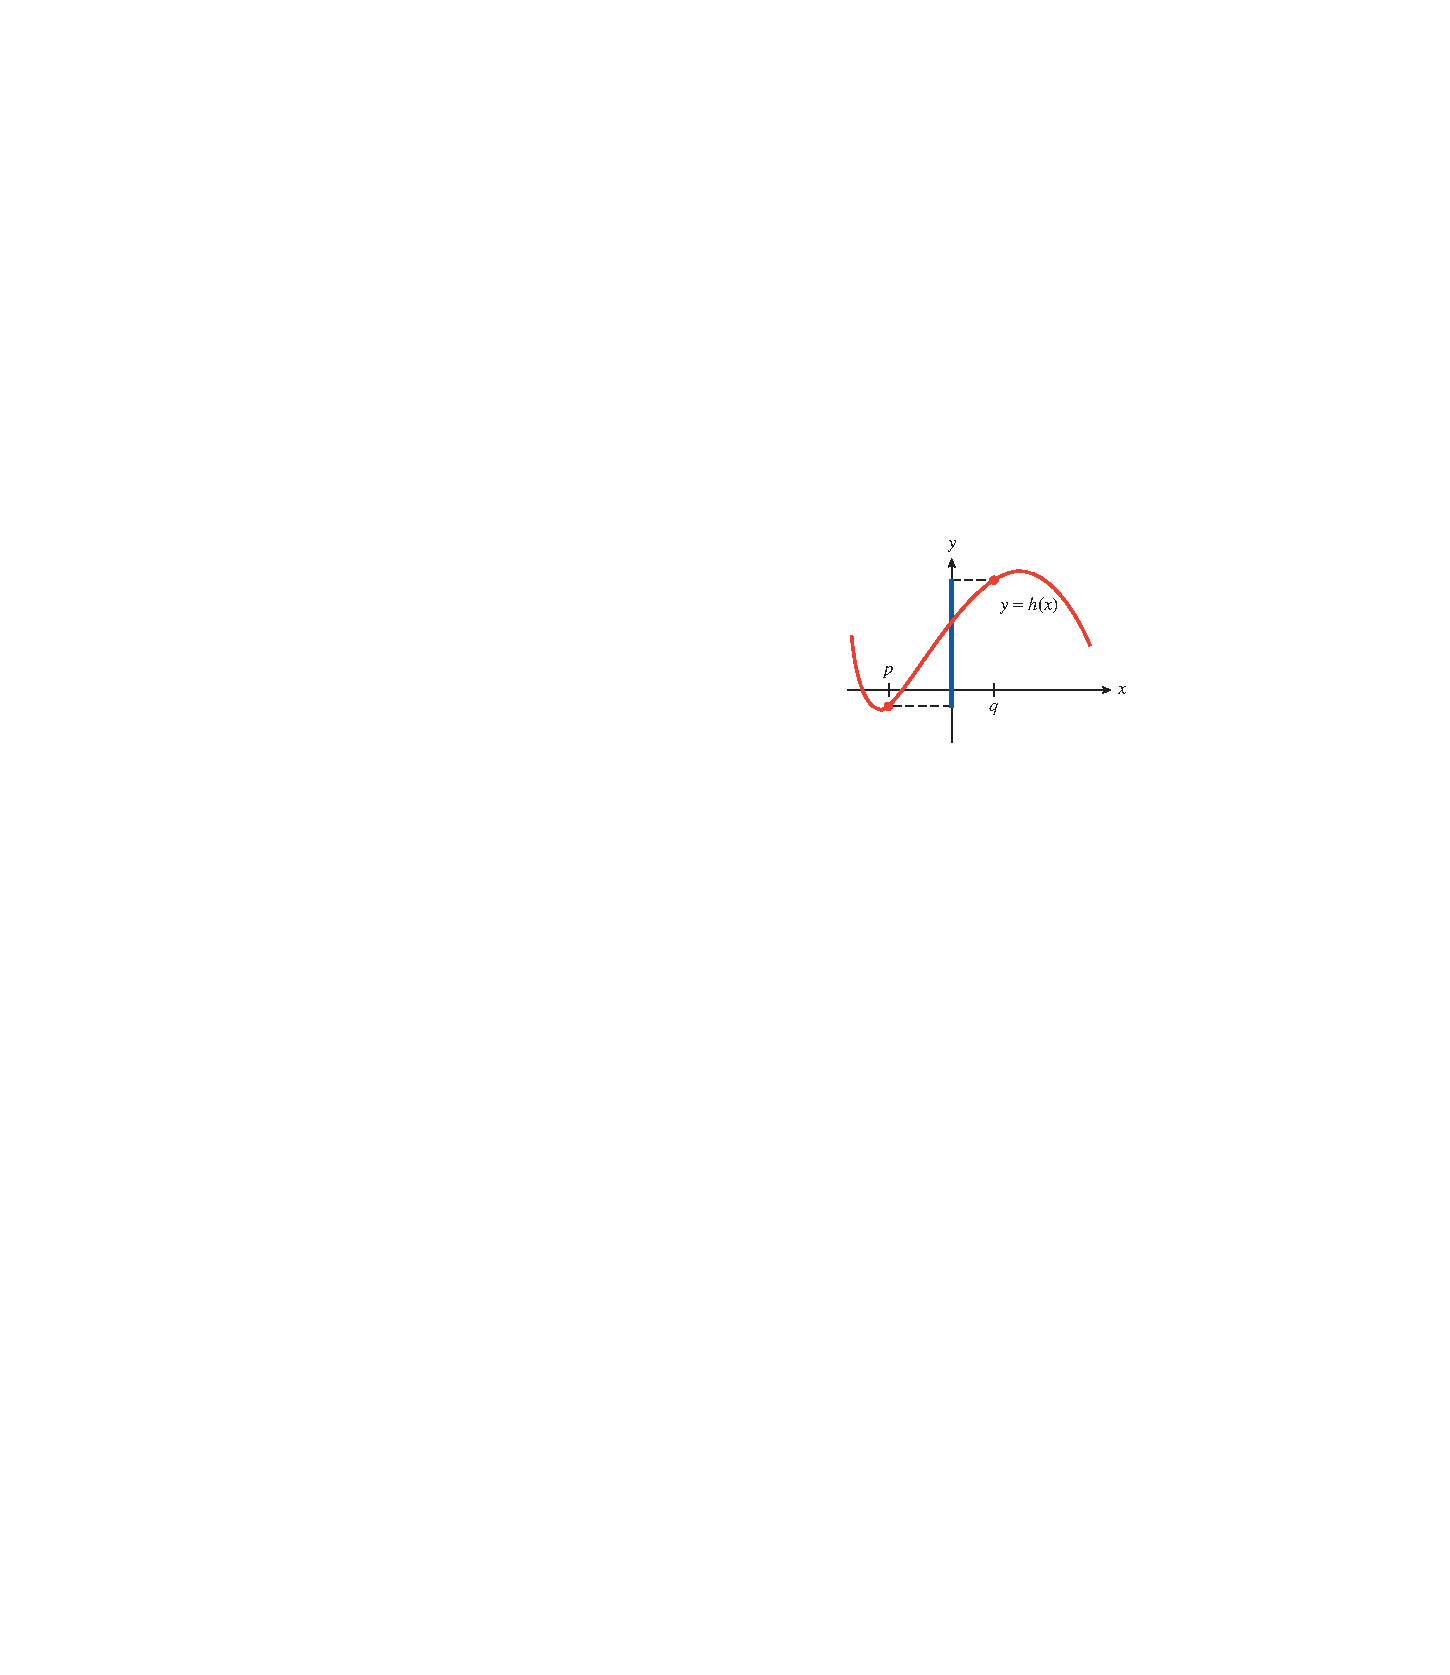
\includegraphics[width=\linewidth]{external/images/fig-ex-1-4-58b.pdf}
\end{sbspanel}%
\end{sidebyside}%
%
\end{enumerate}
\end{multicols}
%
\end{divisionexerciseeg}%
\begin{divisionexerciseeg}{59}{}{}{exercise-section-1-4-exercises-aa-d}%
%
\begin{multicols}{2}
\begin{enumerate}[label=\alph*]
\item{}The increase in \(y\) as \(x\) increases from \(2\) to \(3\)%
\begin{sidebyside}{1}{0.1}{0.1}{0}%
\begin{sbspanel}{0.8}%
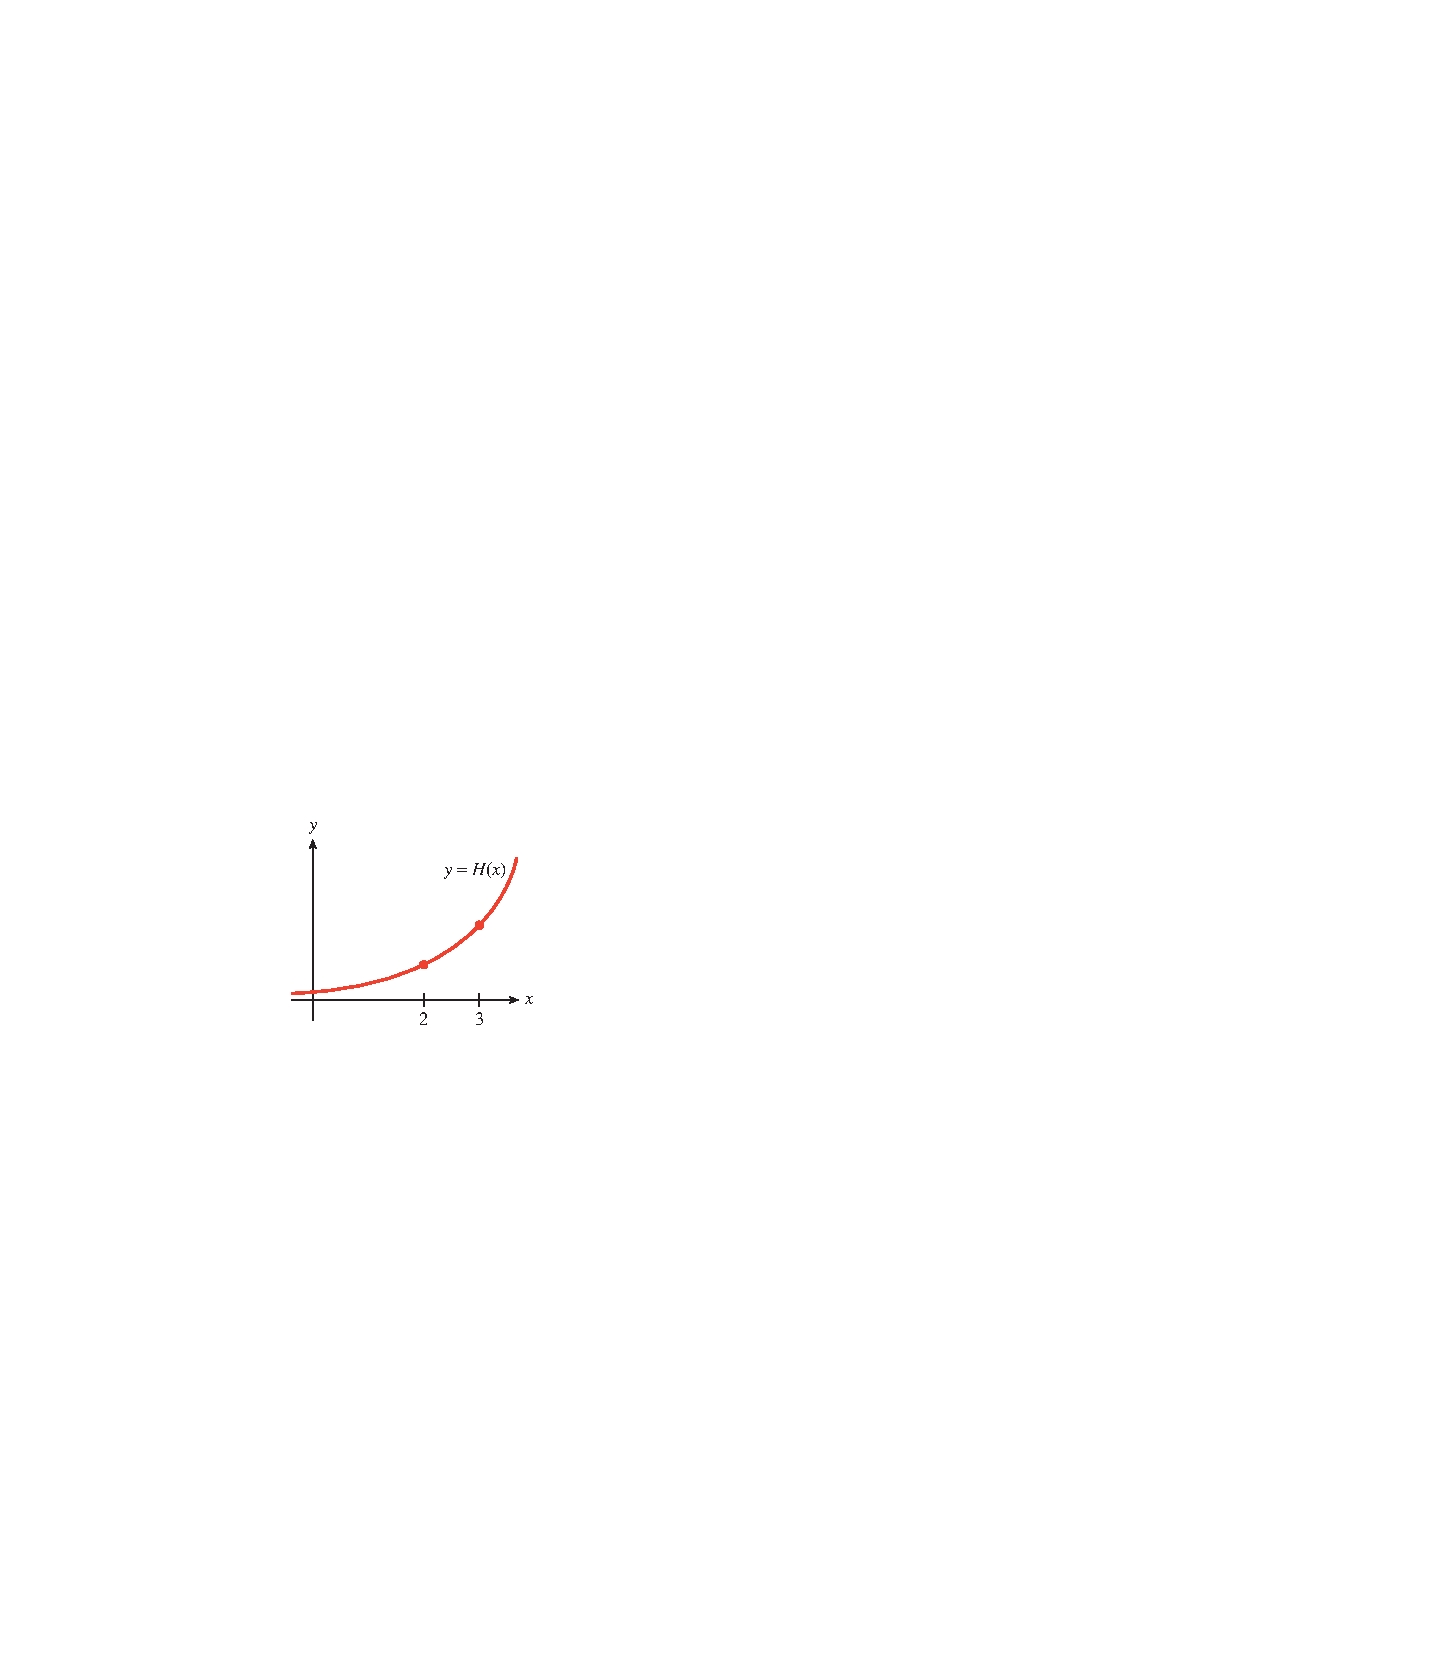
\includegraphics[width=\linewidth]{external/images/fig-ex-1-4-59a.pdf}
\end{sbspanel}%
\end{sidebyside}%
\item{}The increase in \(y\) as \(x\) increases from \(a\) to \(b\)%
\begin{sidebyside}{1}{0.1}{0.1}{0}%
\begin{sbspanel}{0.8}%
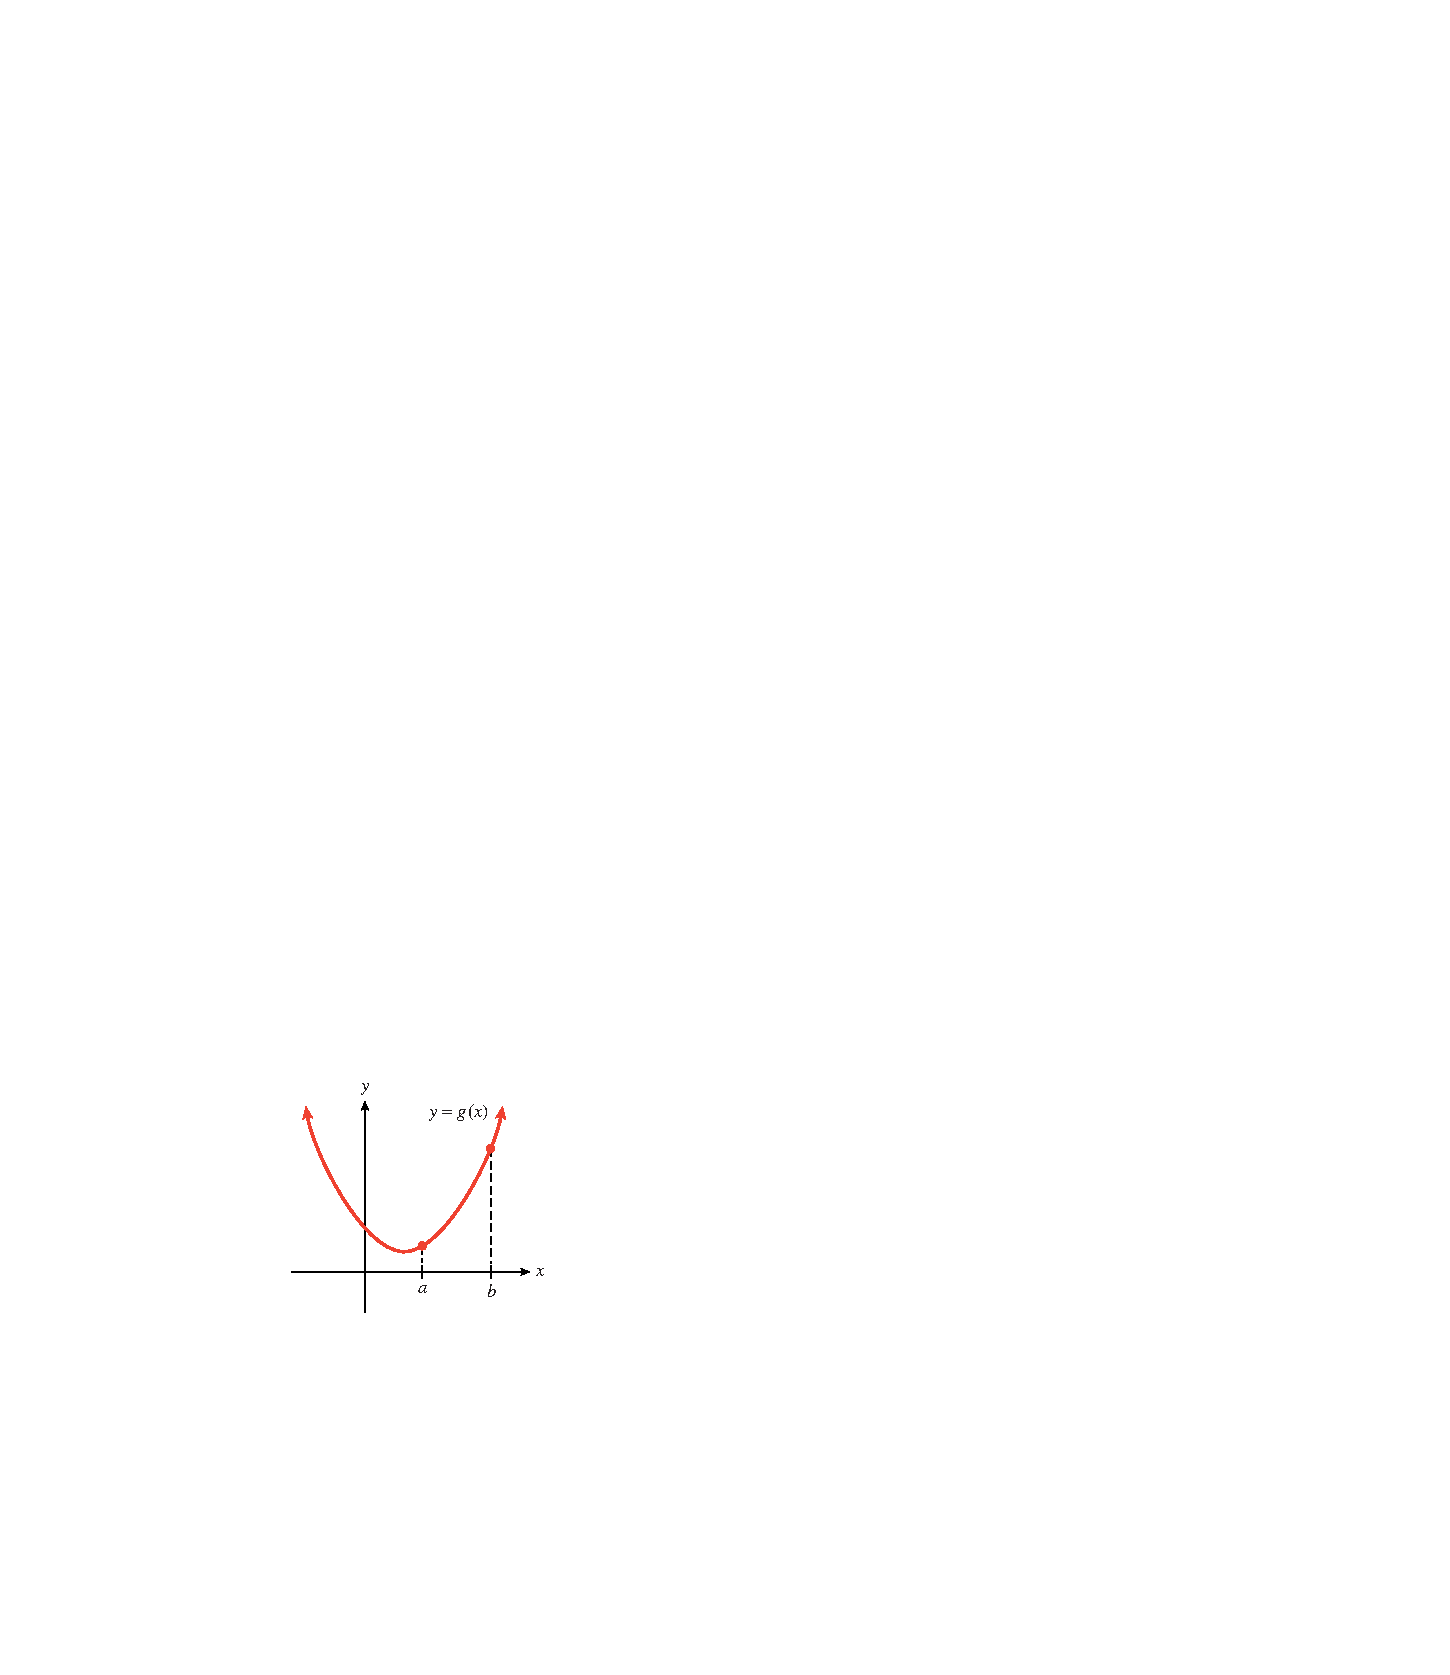
\includegraphics[width=\linewidth]{external/images/fig-ex-1-4-59b.pdf}
\end{sbspanel}%
\end{sidebyside}%
\end{enumerate}
\end{multicols}
%
\end{divisionexerciseeg}%
\begin{divisionexerciseeg}{60}{}{}{exercise-section-1-4-exercises-aa-e}%
%
\begin{multicols}{2}
\begin{enumerate}[label=\alph*]
\item{}The increase in \(y\) as \(x\) increases from \(-4\) to \(-1\)%
\begin{sidebyside}{1}{0.07}{0.07}{0}%
\begin{sbspanel}{0.86}%
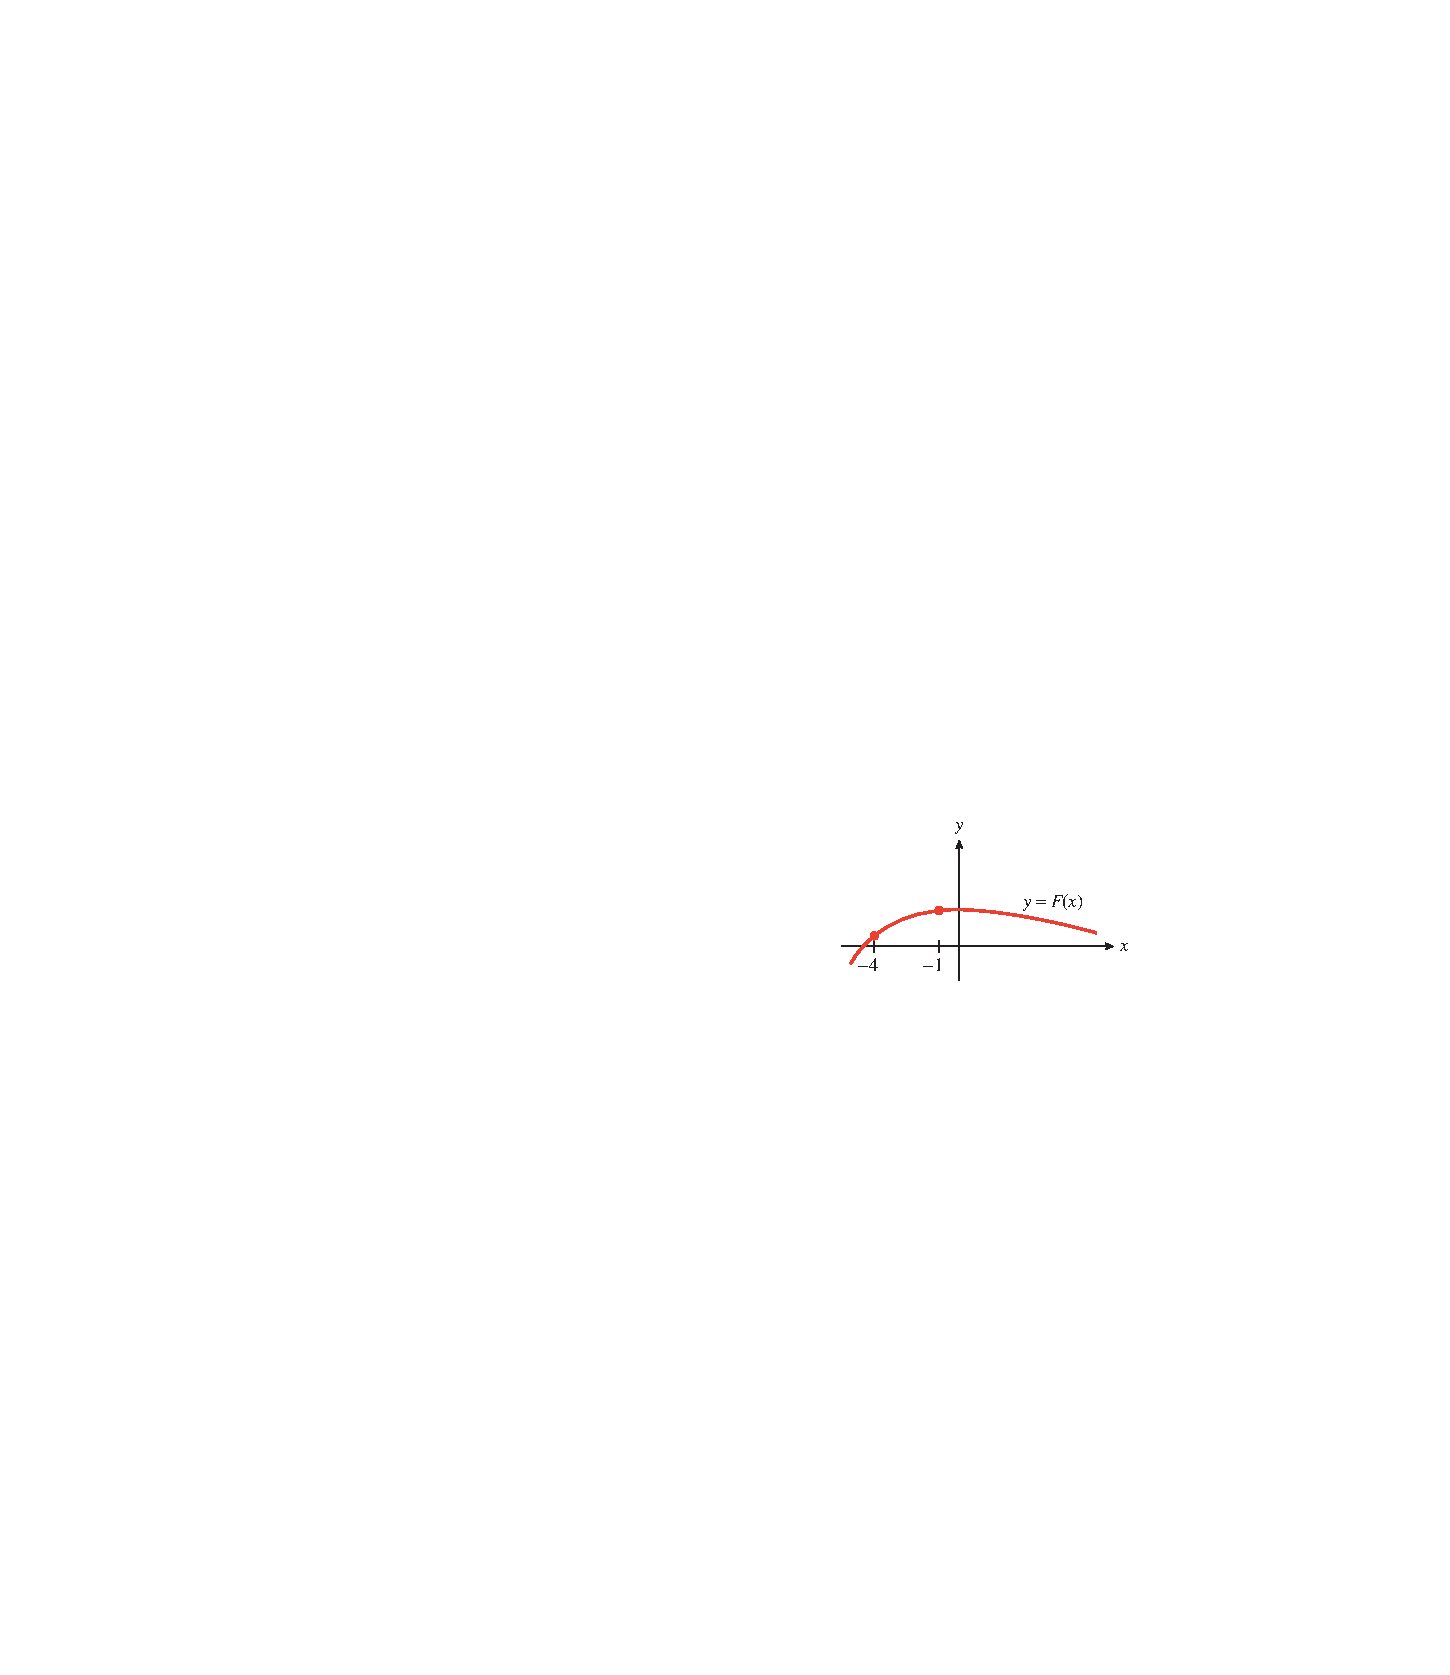
\includegraphics[width=\linewidth]{external/images/fig-ex-1-4-60a.pdf}
\end{sbspanel}%
\end{sidebyside}%
\item{}The increase in \(y\) as \(x\) increases from \(u\) to \(v\)%
\begin{sidebyside}{1}{0.07}{0.07}{0}%
\begin{sbspanel}{0.86}%
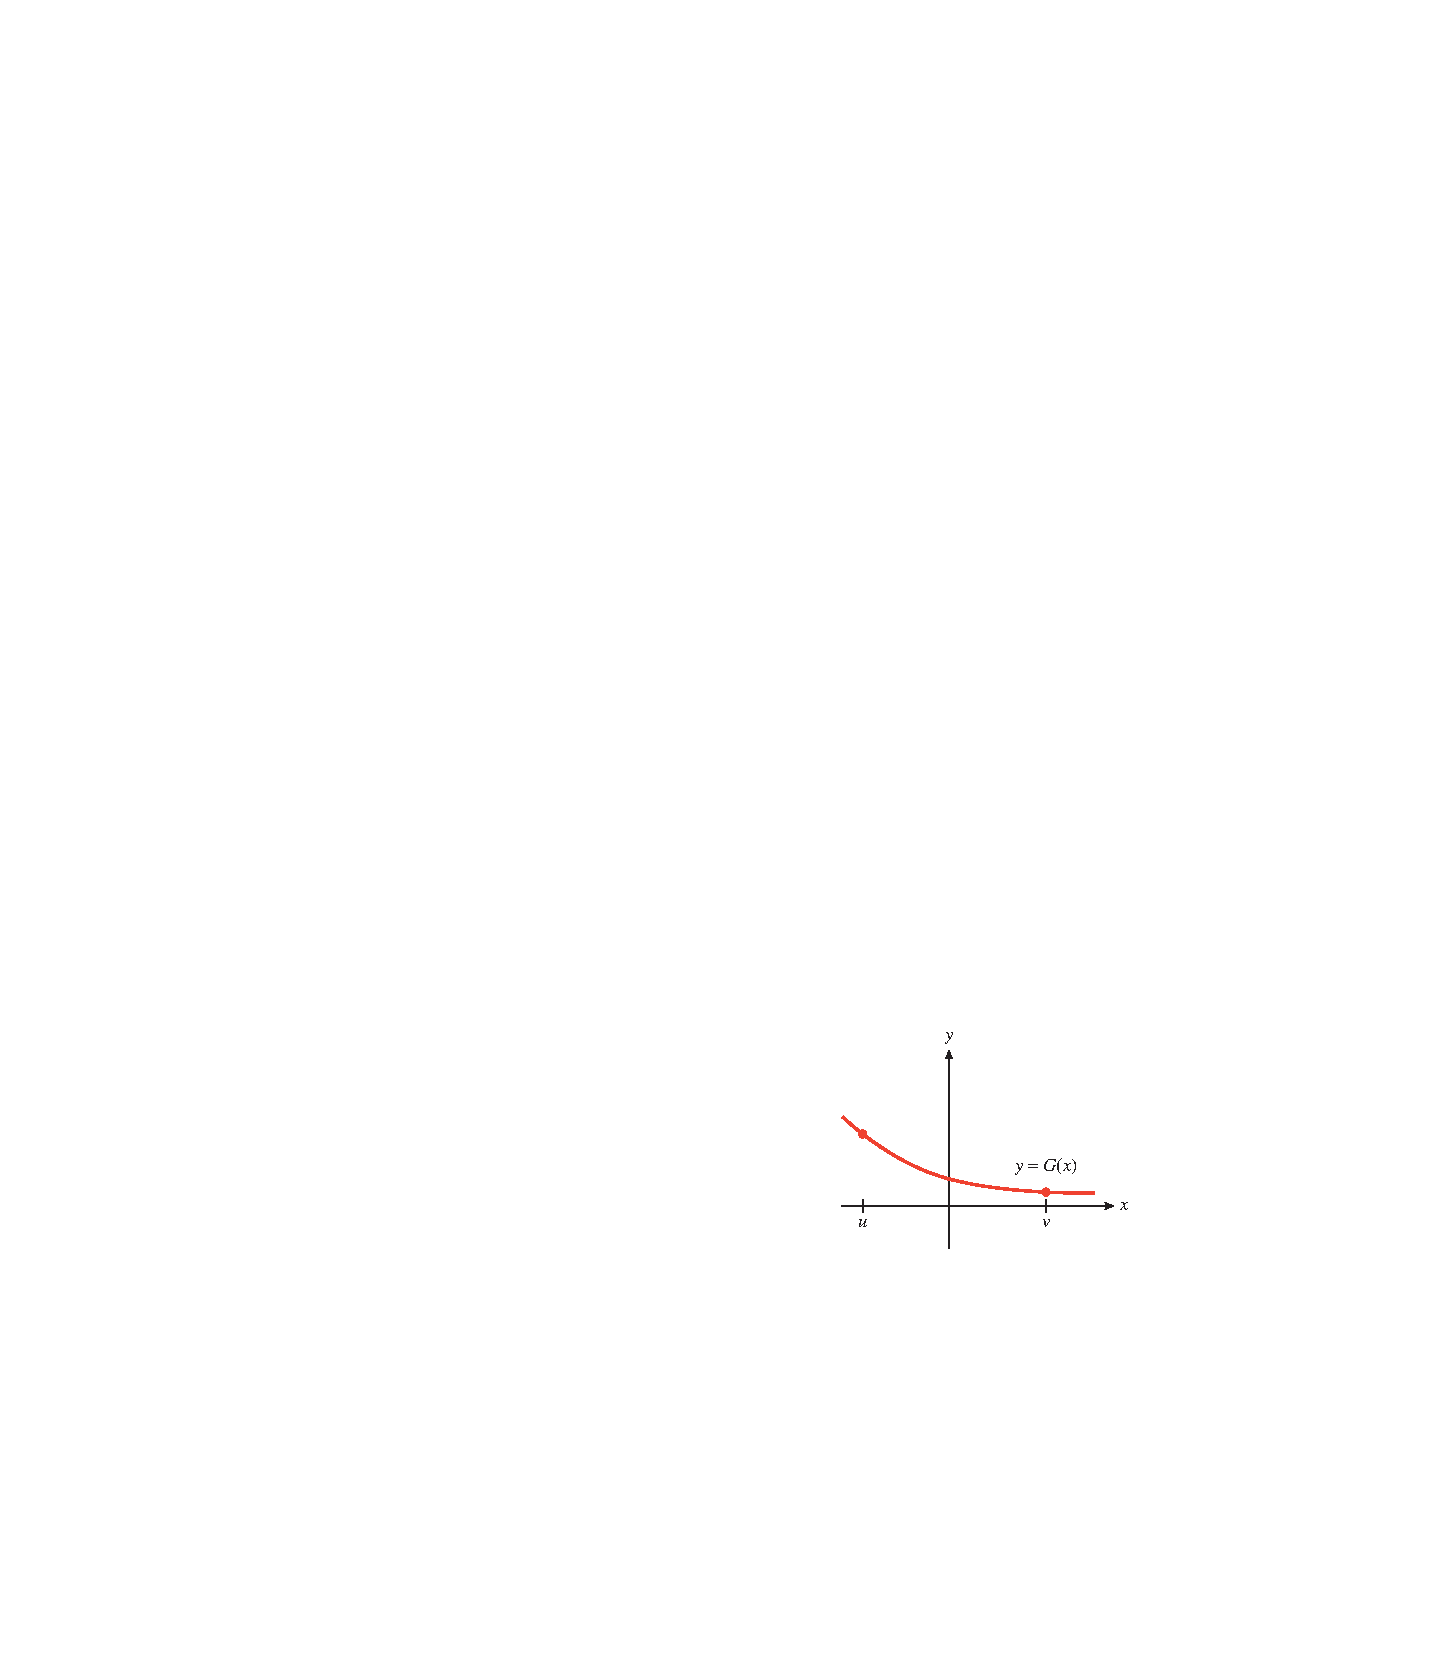
\includegraphics[width=\linewidth]{external/images/fig-ex-1-4-60b.pdf}
\end{sbspanel}%
\end{sidebyside}%
\end{enumerate}
\end{multicols}
%
\end{divisionexerciseeg}%
\begin{divisionexerciseeg}{61}{}{}{exercise-section-1-4-exercises-aa-f}%
The shaded area%
\begin{multicols}{2}
\begin{enumerate}[label=\alph*]
\item{}\begin{sidebyside}{1}{0.07}{0.07}{0}%
\begin{sbspanel}{0.86}%
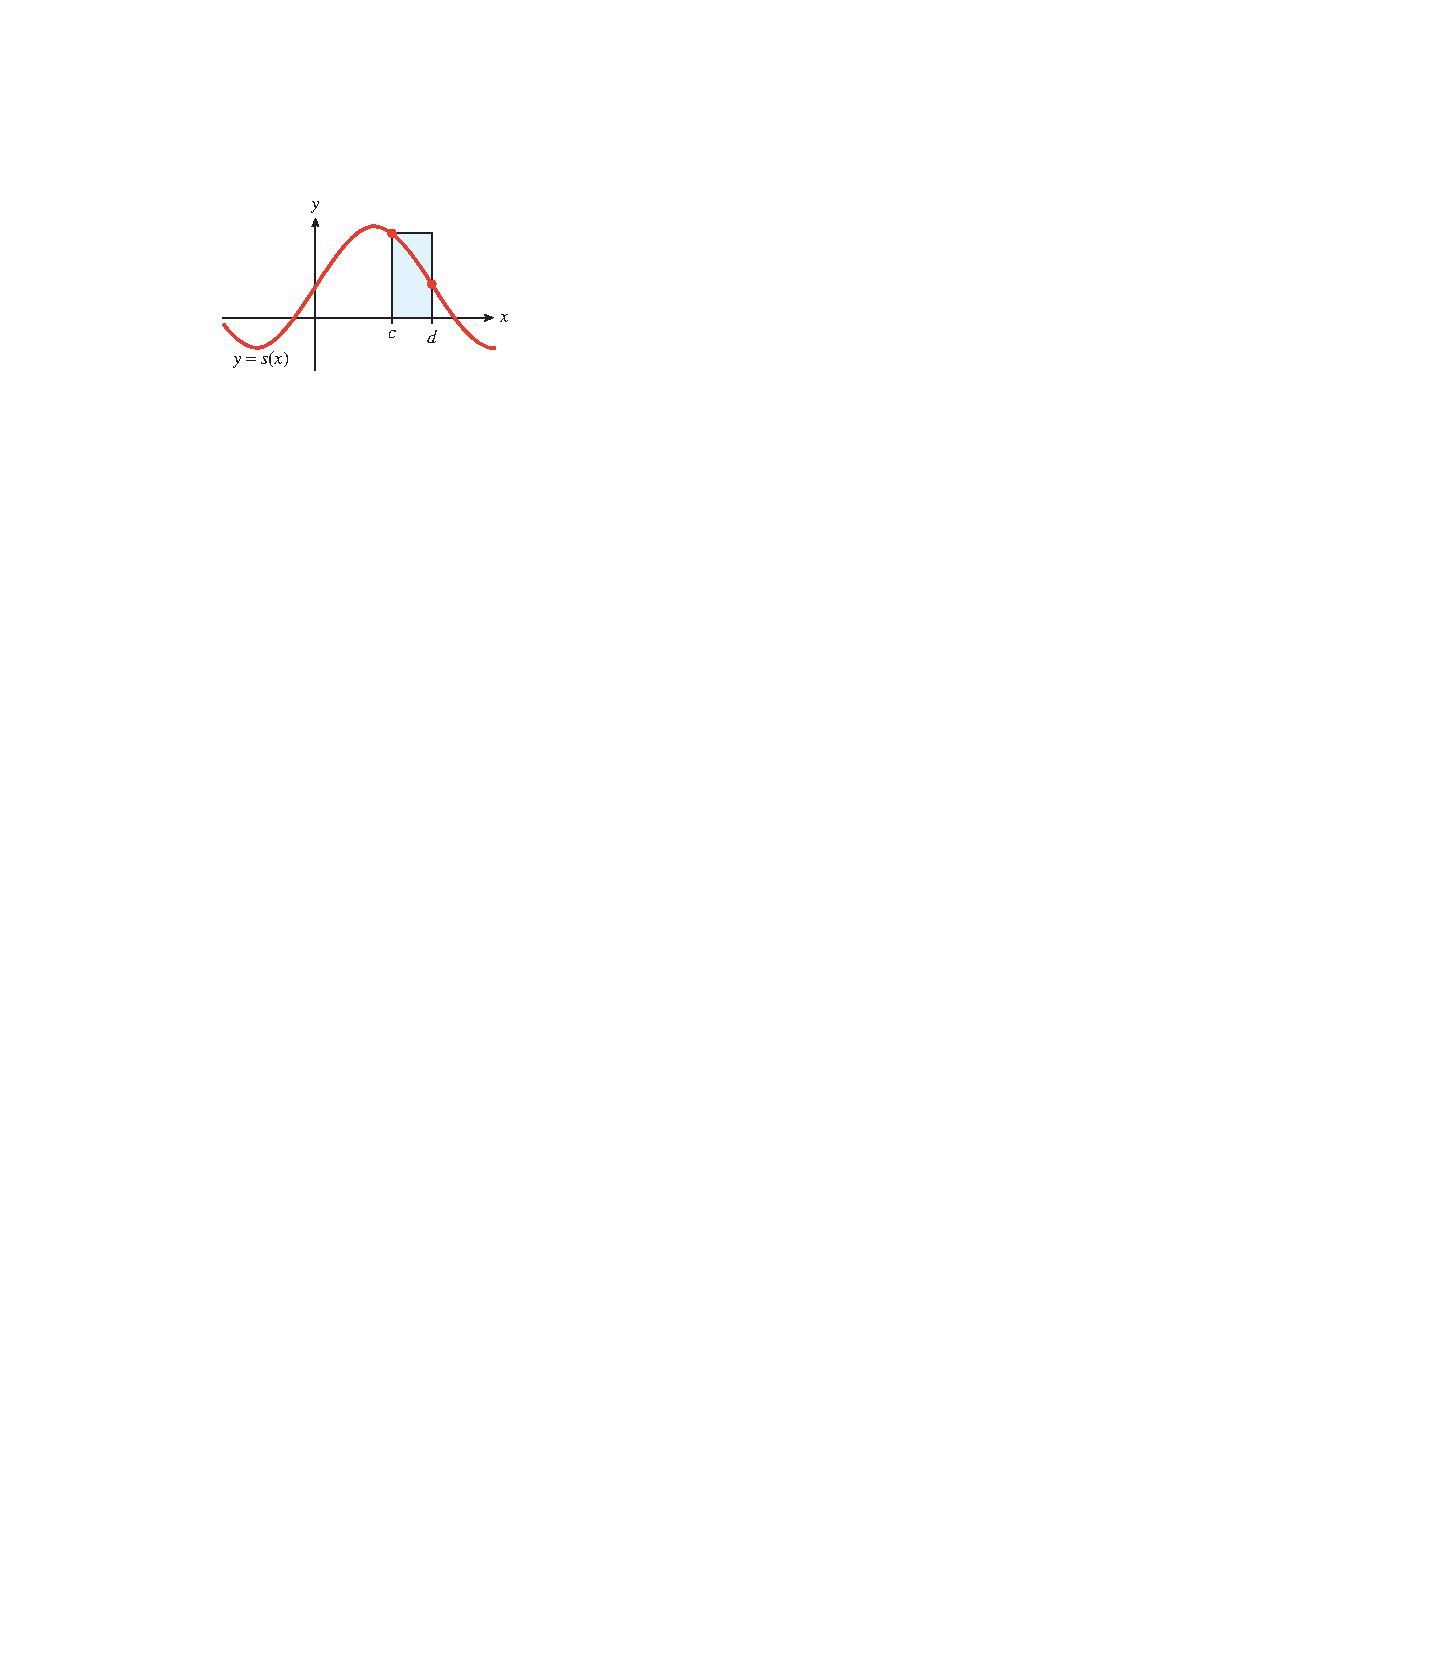
\includegraphics[width=\linewidth]{external/images/fig-ex-1-4-61a.pdf}
\end{sbspanel}%
\end{sidebyside}%
%
\item{}\begin{sidebyside}{1}{0.07}{0.07}{0}%
\begin{sbspanel}{0.86}%
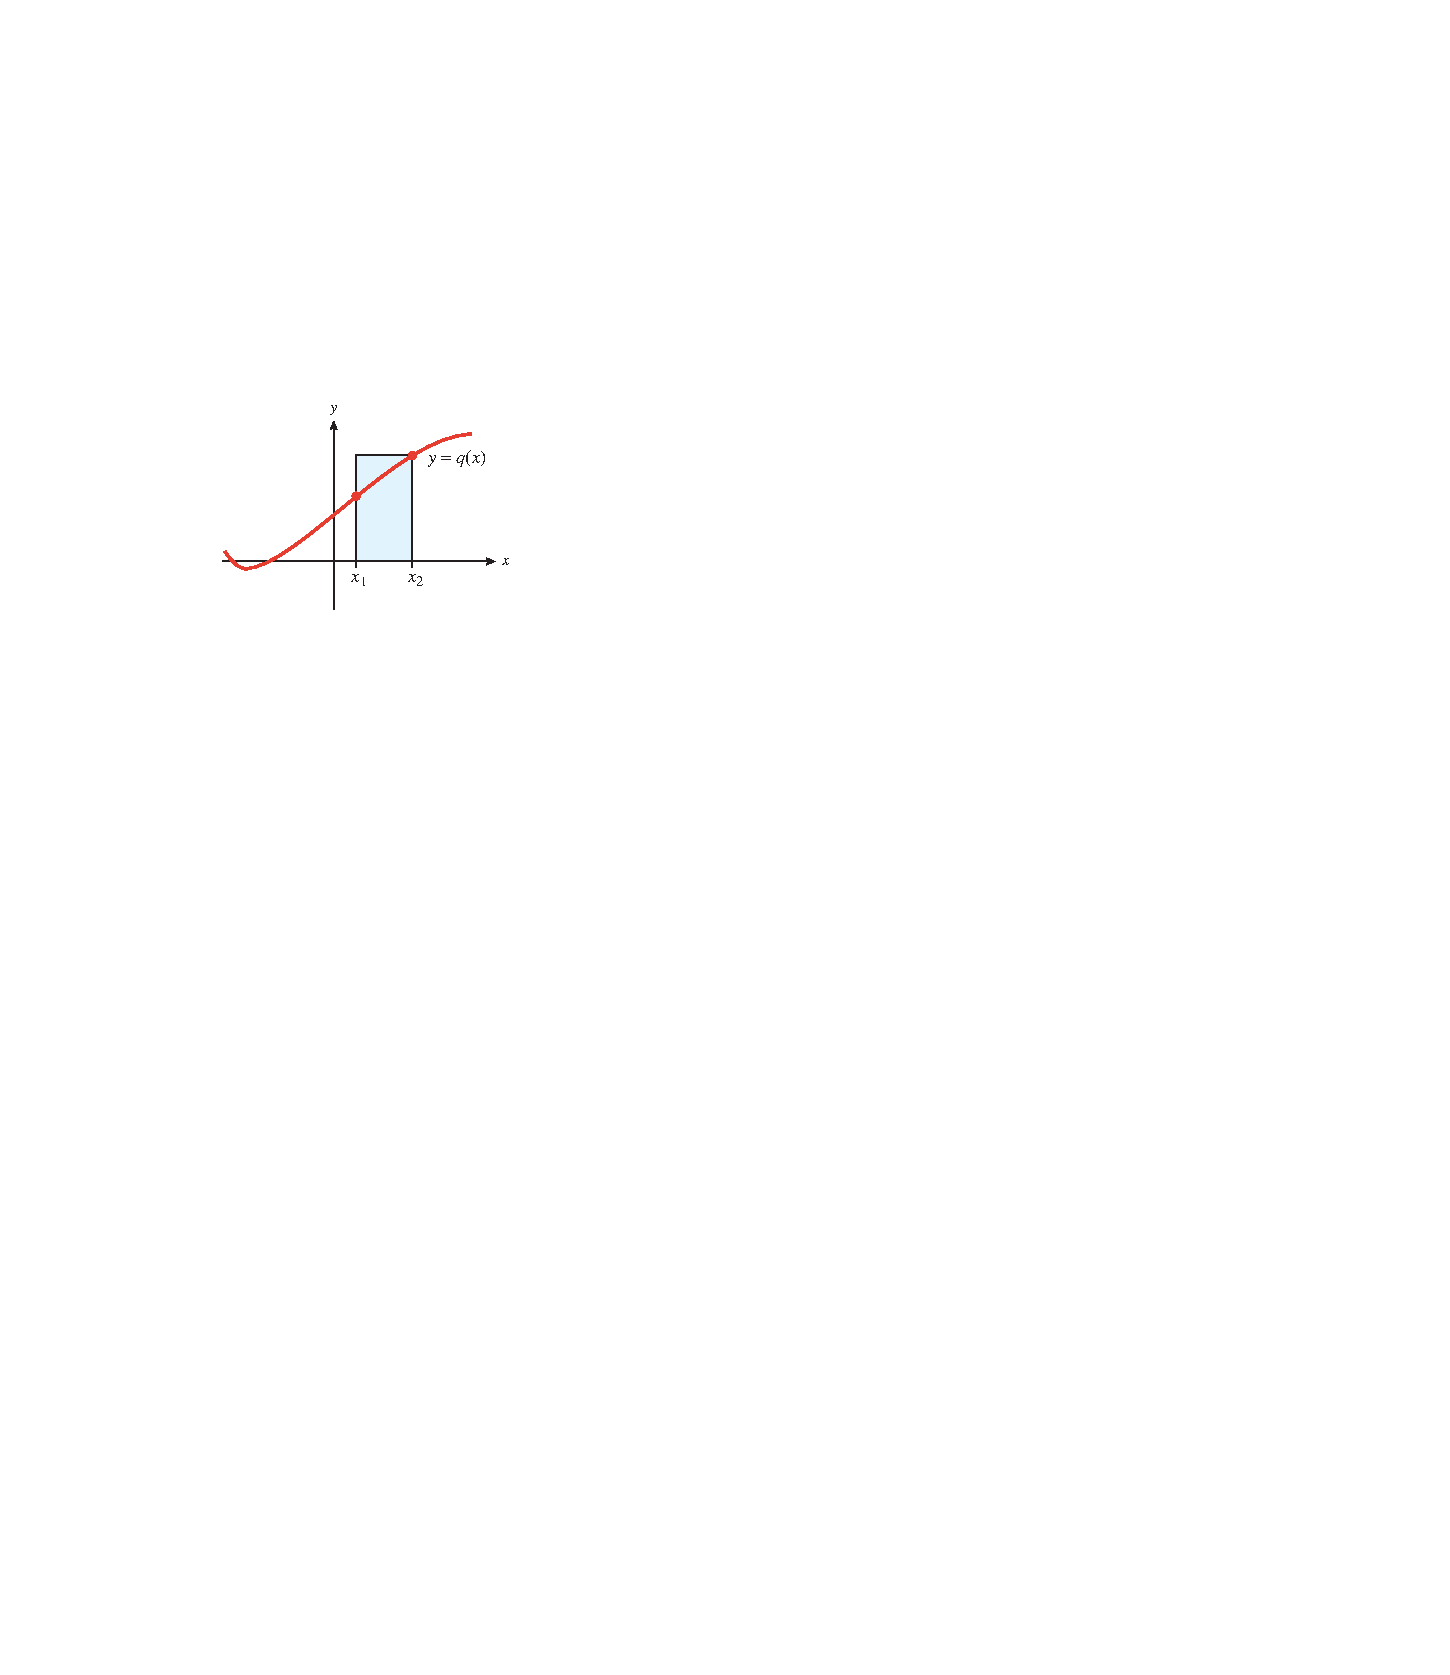
\includegraphics[width=\linewidth]{external/images/fig-ex-1-4-61b.pdf}
\end{sbspanel}%
\end{sidebyside}%
%
\end{enumerate}
\end{multicols}
%
\end{divisionexerciseeg}%
\begin{divisionexerciseeg}{62}{}{}{exercise-section-1-4-exercises-aa-g}%
The shaded area%
\begin{multicols}{2}
\begin{enumerate}[label=\alph*]
\item{}\begin{sidebyside}{1}{0.1}{0.1}{0}%
\begin{sbspanel}{0.8}%
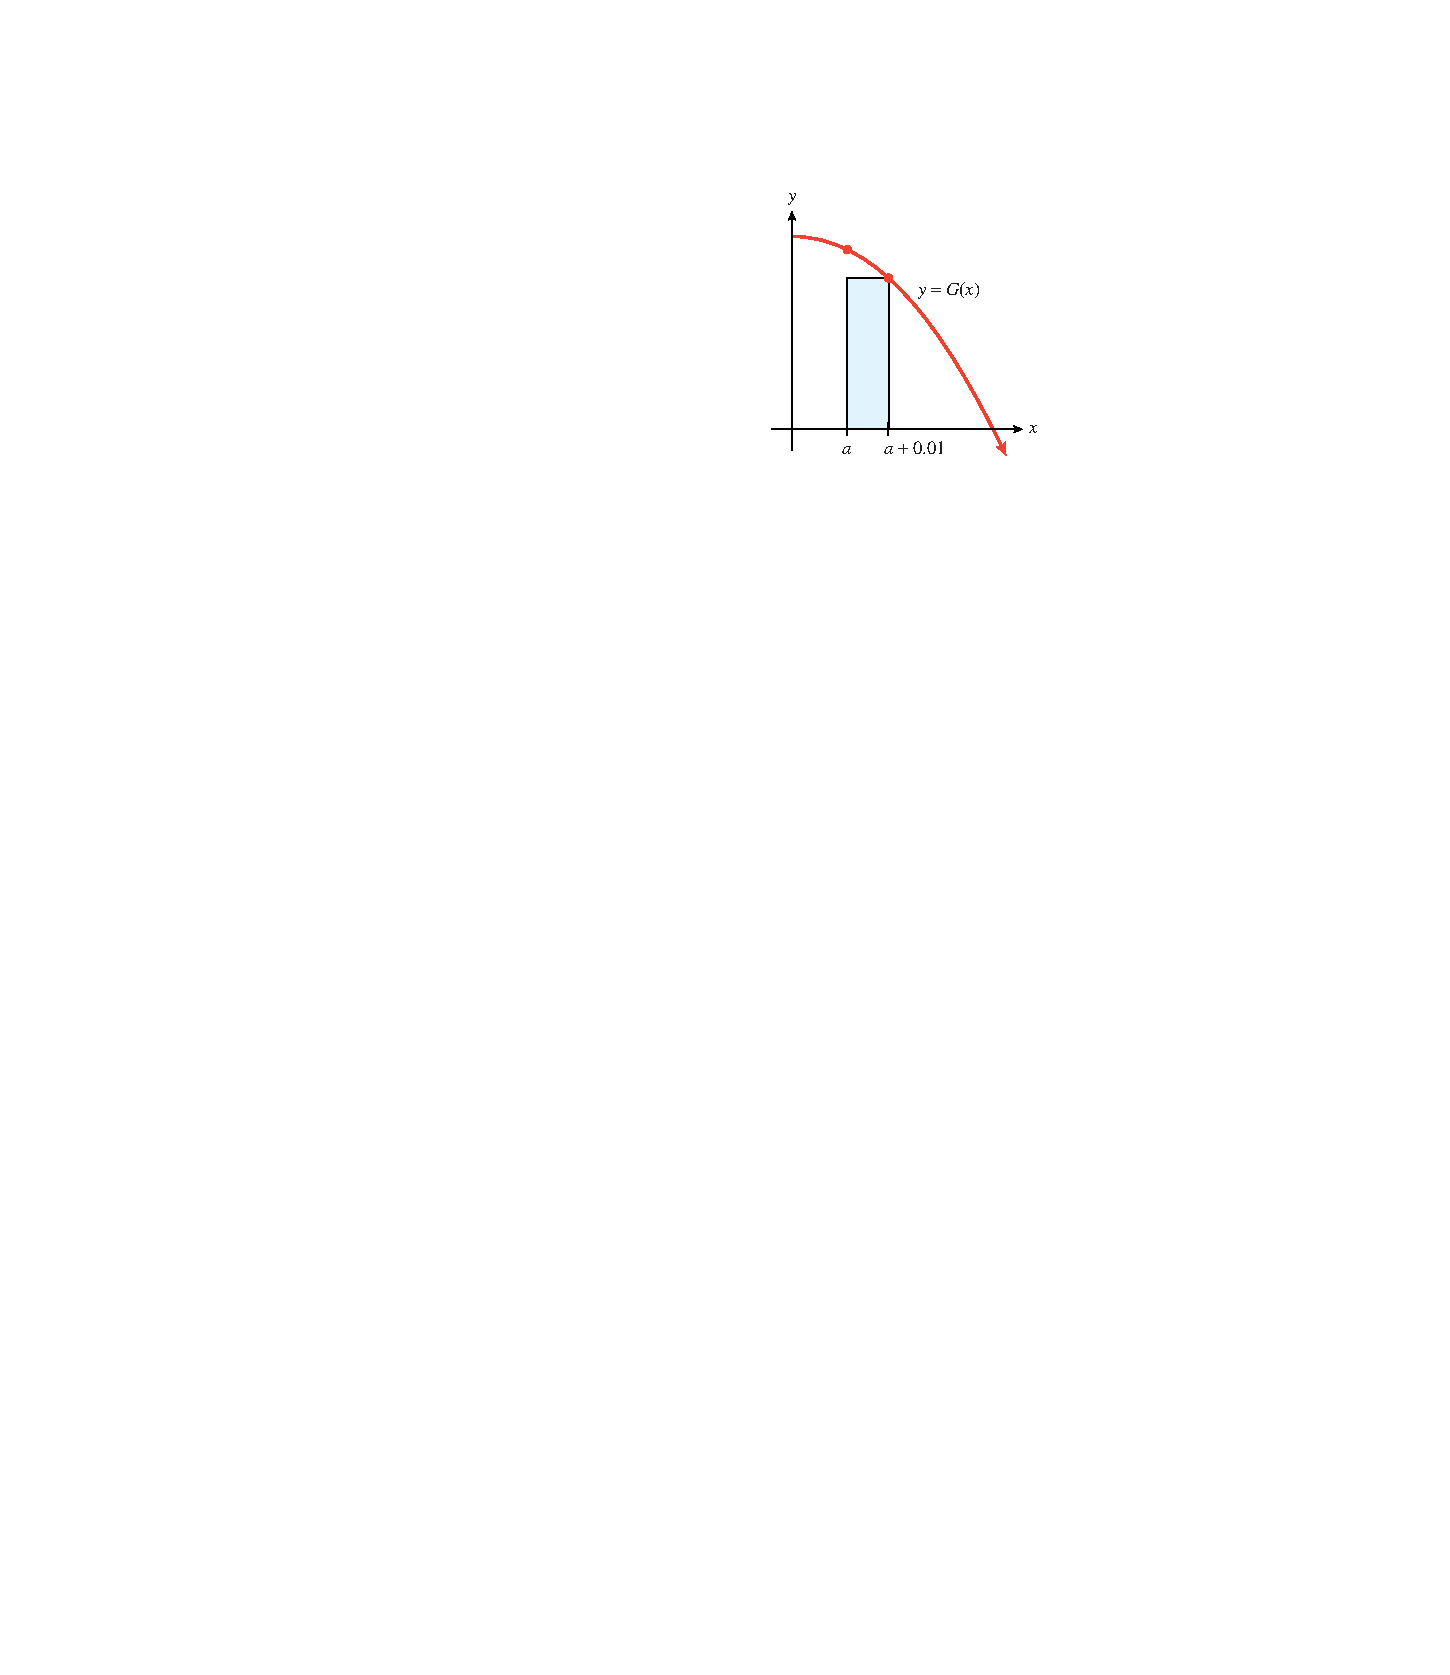
\includegraphics[width=\linewidth]{external/images/fig-ex-1-4-62a.pdf}
\end{sbspanel}%
\end{sidebyside}%
%
\item{}\begin{sidebyside}{1}{0.1}{0.1}{0}%
\begin{sbspanel}{0.8}%
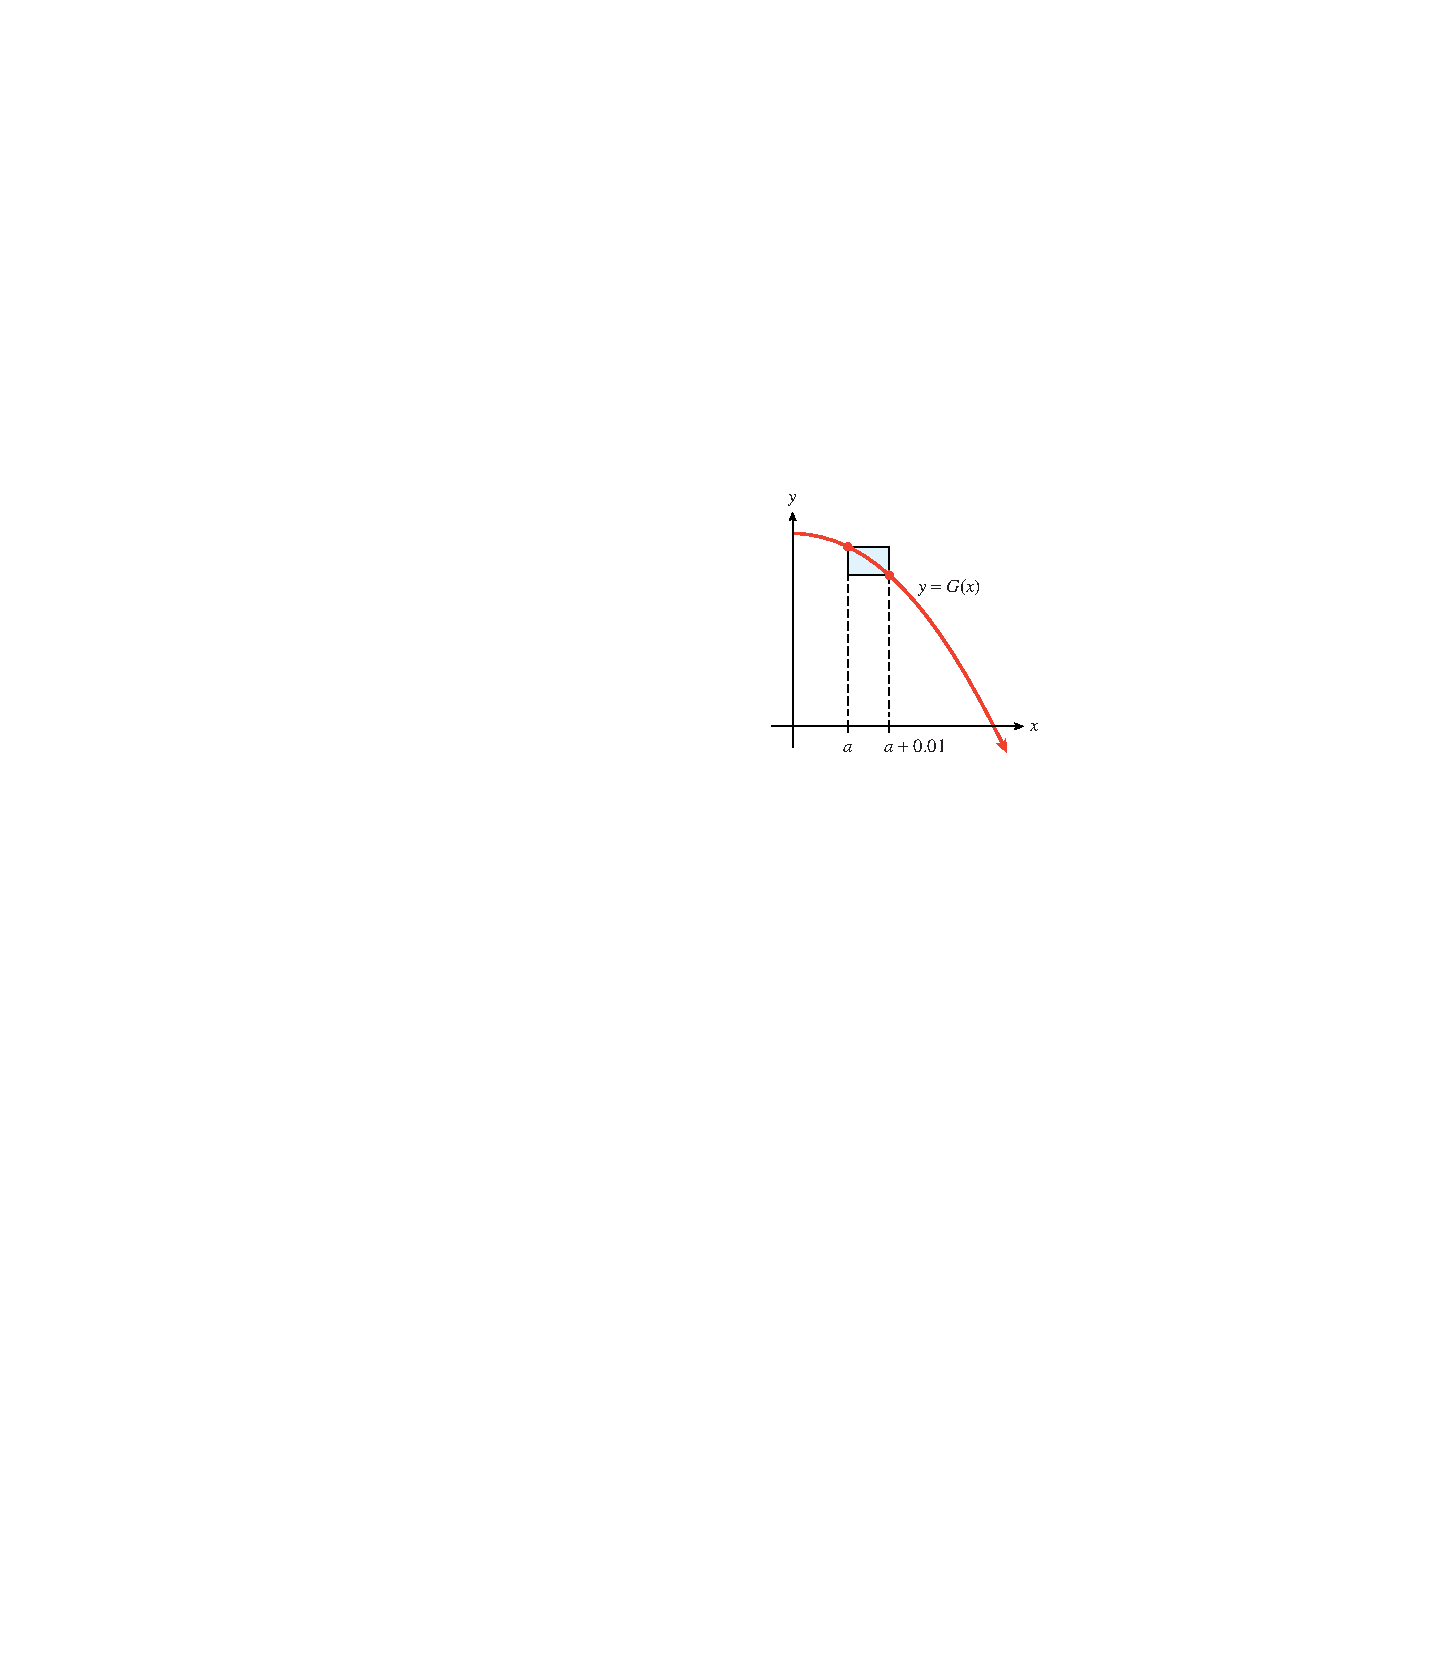
\includegraphics[width=\linewidth]{external/images/fig-ex-1-4-62b.pdf}
\end{sbspanel}%
\end{sidebyside}%
%
\end{enumerate}
\end{multicols}
%
\end{divisionexerciseeg}%
\end{exercisegroup}
\par\medskip\noindent
\par\medskip\noindent%
\textbf{Exercise Group.}\space\space%
In Problems 63\textendash{}66, find the coordinates of the indicated points on the graph of \(y = f (x)\) and write an algebraic expression using function notation for the slope of the line segment joining points \(P\) and \(Q\).%
\begin{exercisegroup}
\begin{divisionexerciseeg}{63}{}{}{exercise-section-1-4-exercises-ab-b}%
%
\begin{multicols}{2}
\begin{enumerate}[label=\alph*]
\item{}\begin{sidebyside}{1}{0.1}{0.1}{0}%
\begin{sbspanel}{0.8}%
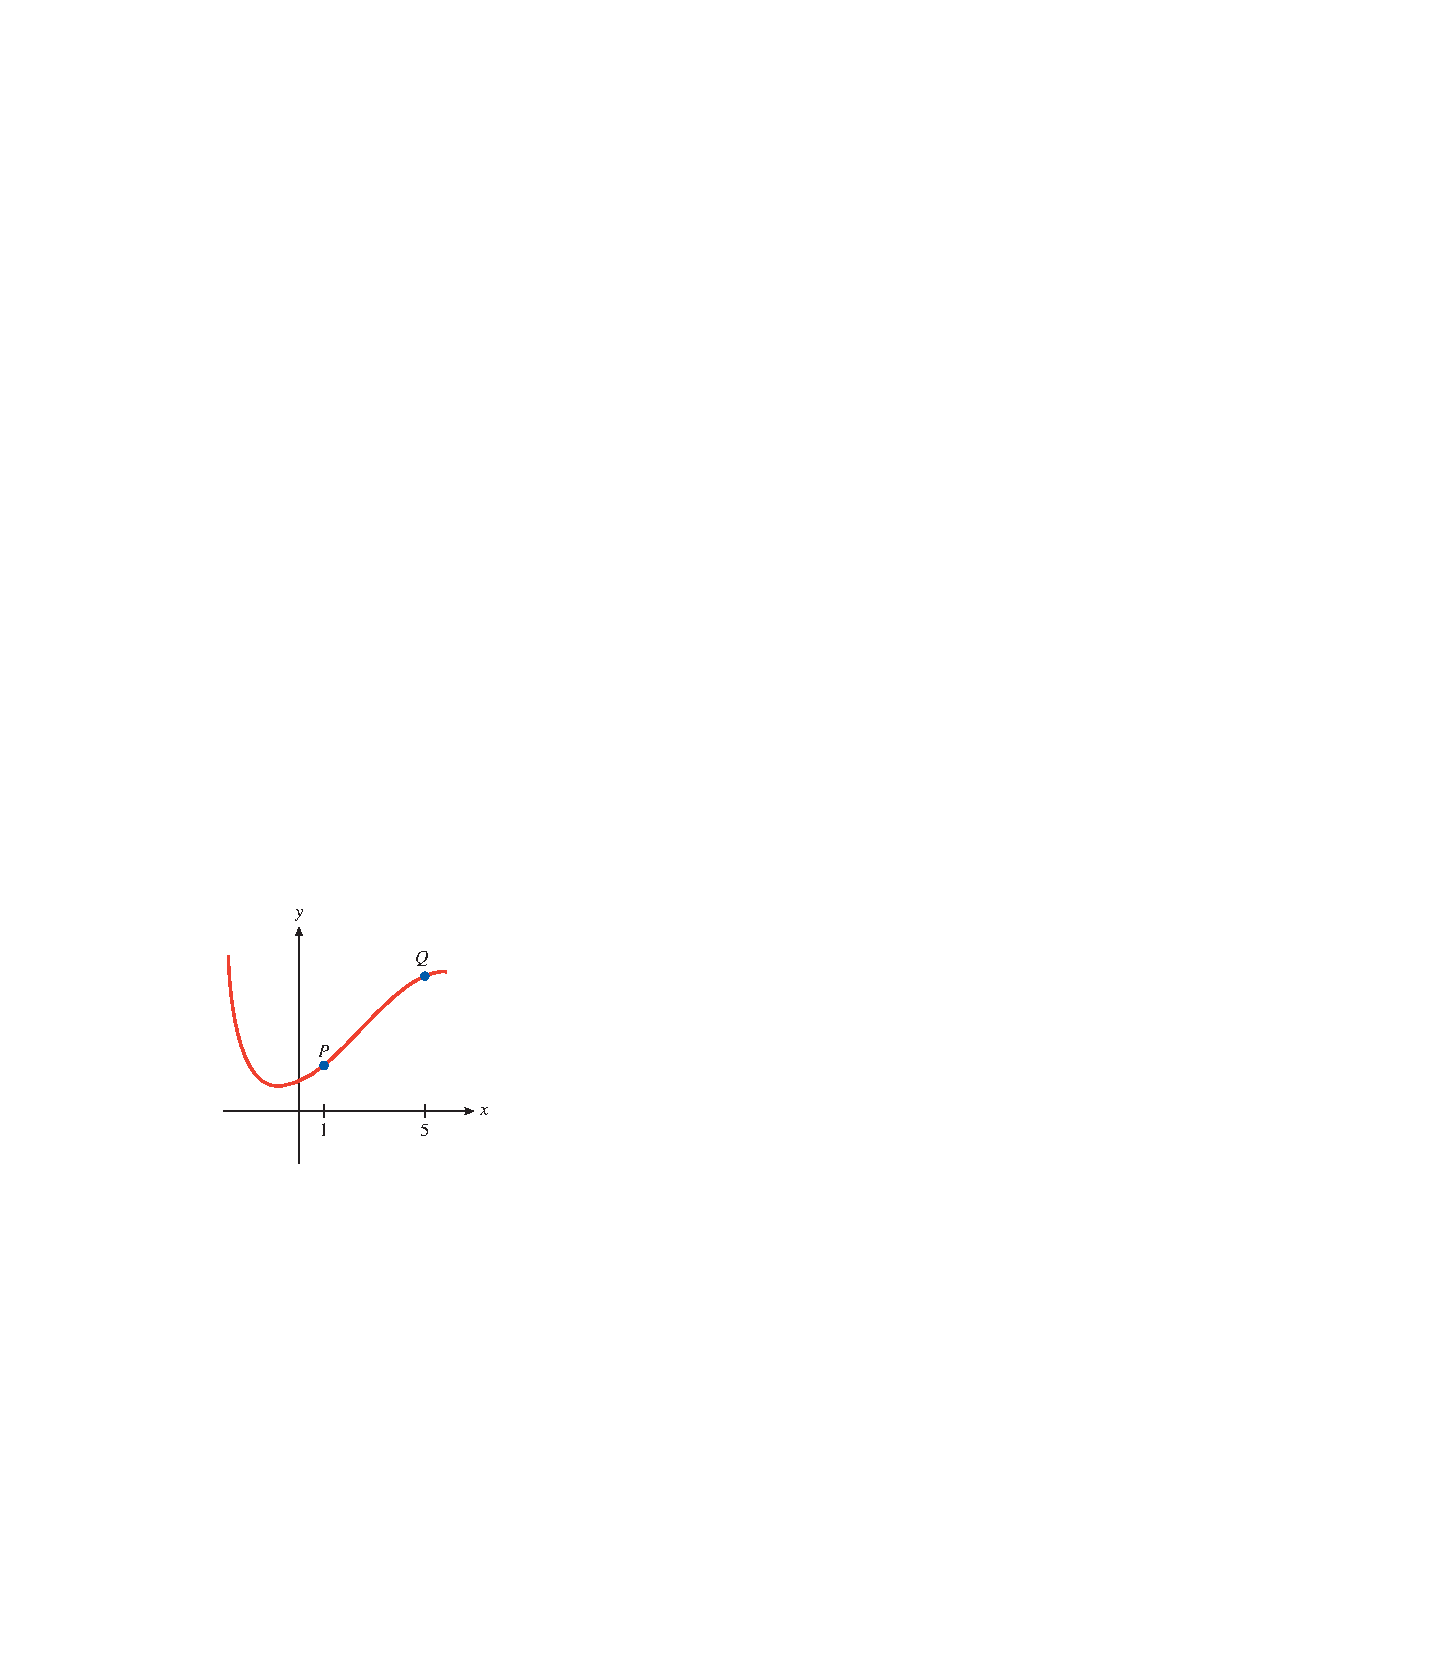
\includegraphics[width=\linewidth]{external/images/fig-ex-1-4-63a.pdf}
\end{sbspanel}%
\end{sidebyside}%
%
\item{}\begin{sidebyside}{1}{0.1}{0.1}{0}%
\begin{sbspanel}{0.8}%
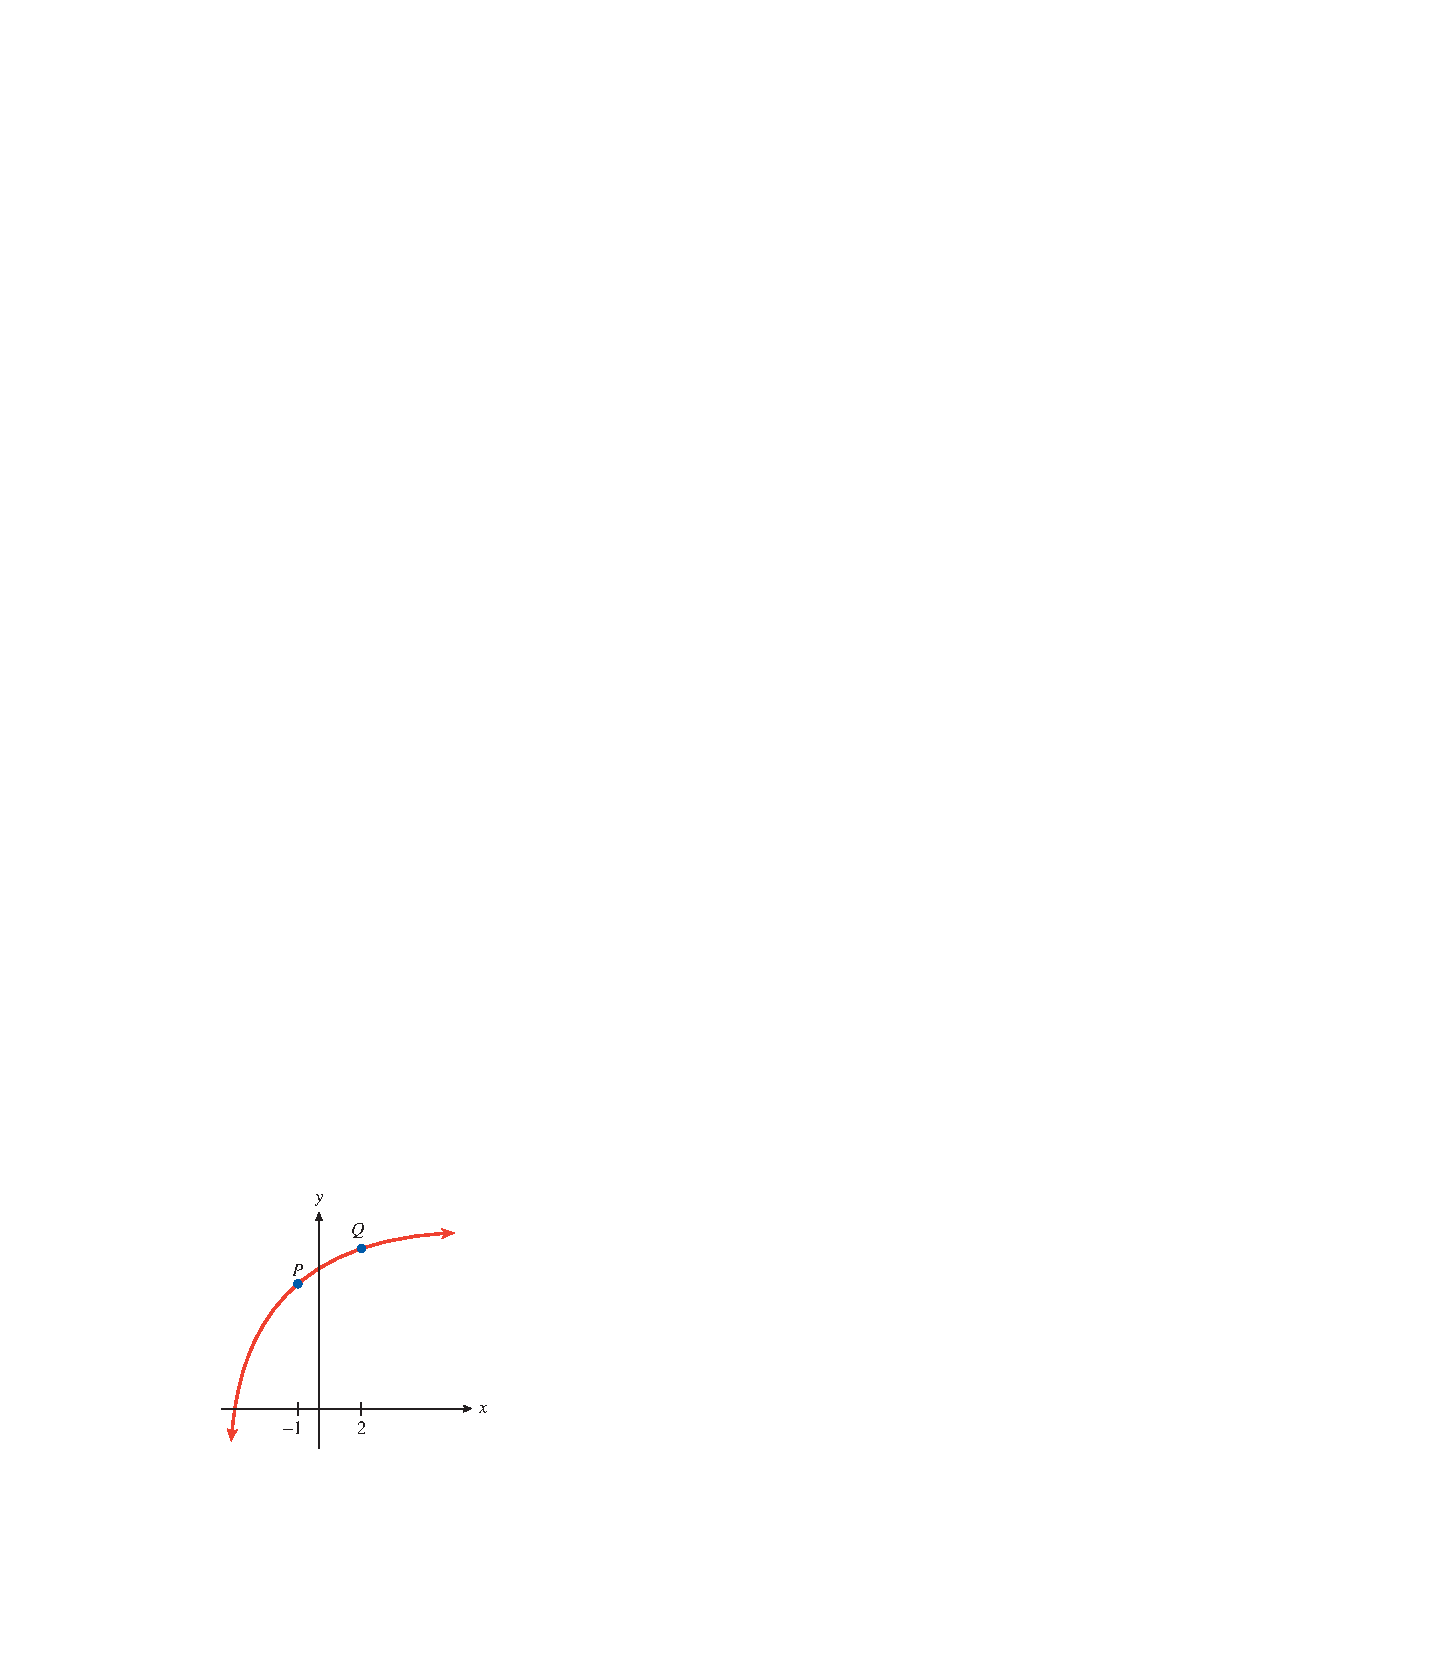
\includegraphics[width=\linewidth]{external/images/fig-ex-1-4-63b.pdf}
\end{sbspanel}%
\end{sidebyside}%
%
\end{enumerate}
\end{multicols}
%
\end{divisionexerciseeg}%
\begin{divisionexerciseeg}{64}{}{}{exercise-section-1-4-exercises-ab-c}%
%
\begin{multicols}{2}
\begin{enumerate}[label=\alph*]
\item{}\begin{sidebyside}{1}{0.1}{0.1}{0}%
\begin{sbspanel}{0.8}%
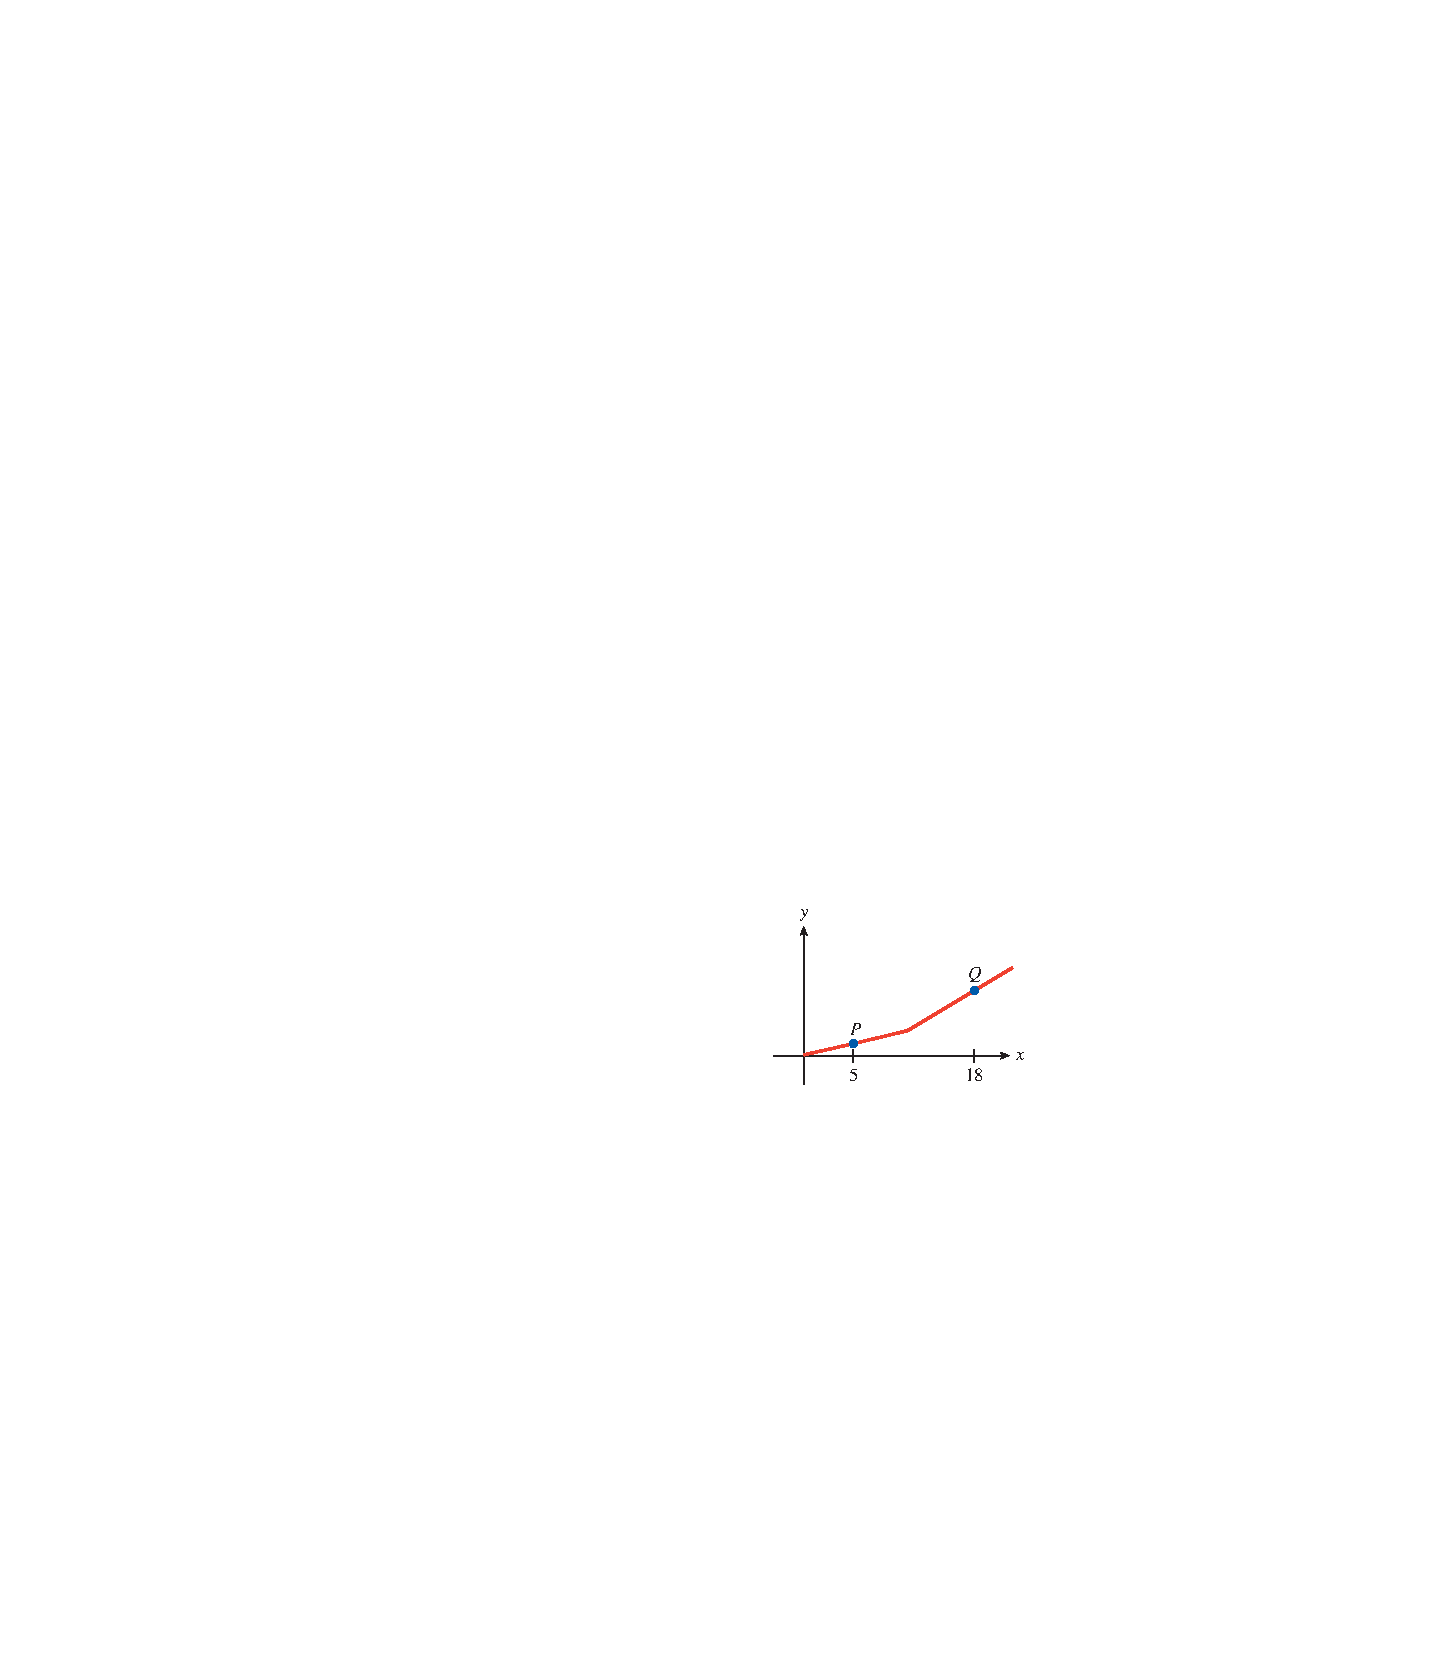
\includegraphics[width=\linewidth]{external/images/fig-ex-1-4-64a.pdf}
\end{sbspanel}%
\end{sidebyside}%
%
\item{}\begin{sidebyside}{1}{0.1}{0.1}{0}%
\begin{sbspanel}{0.8}%
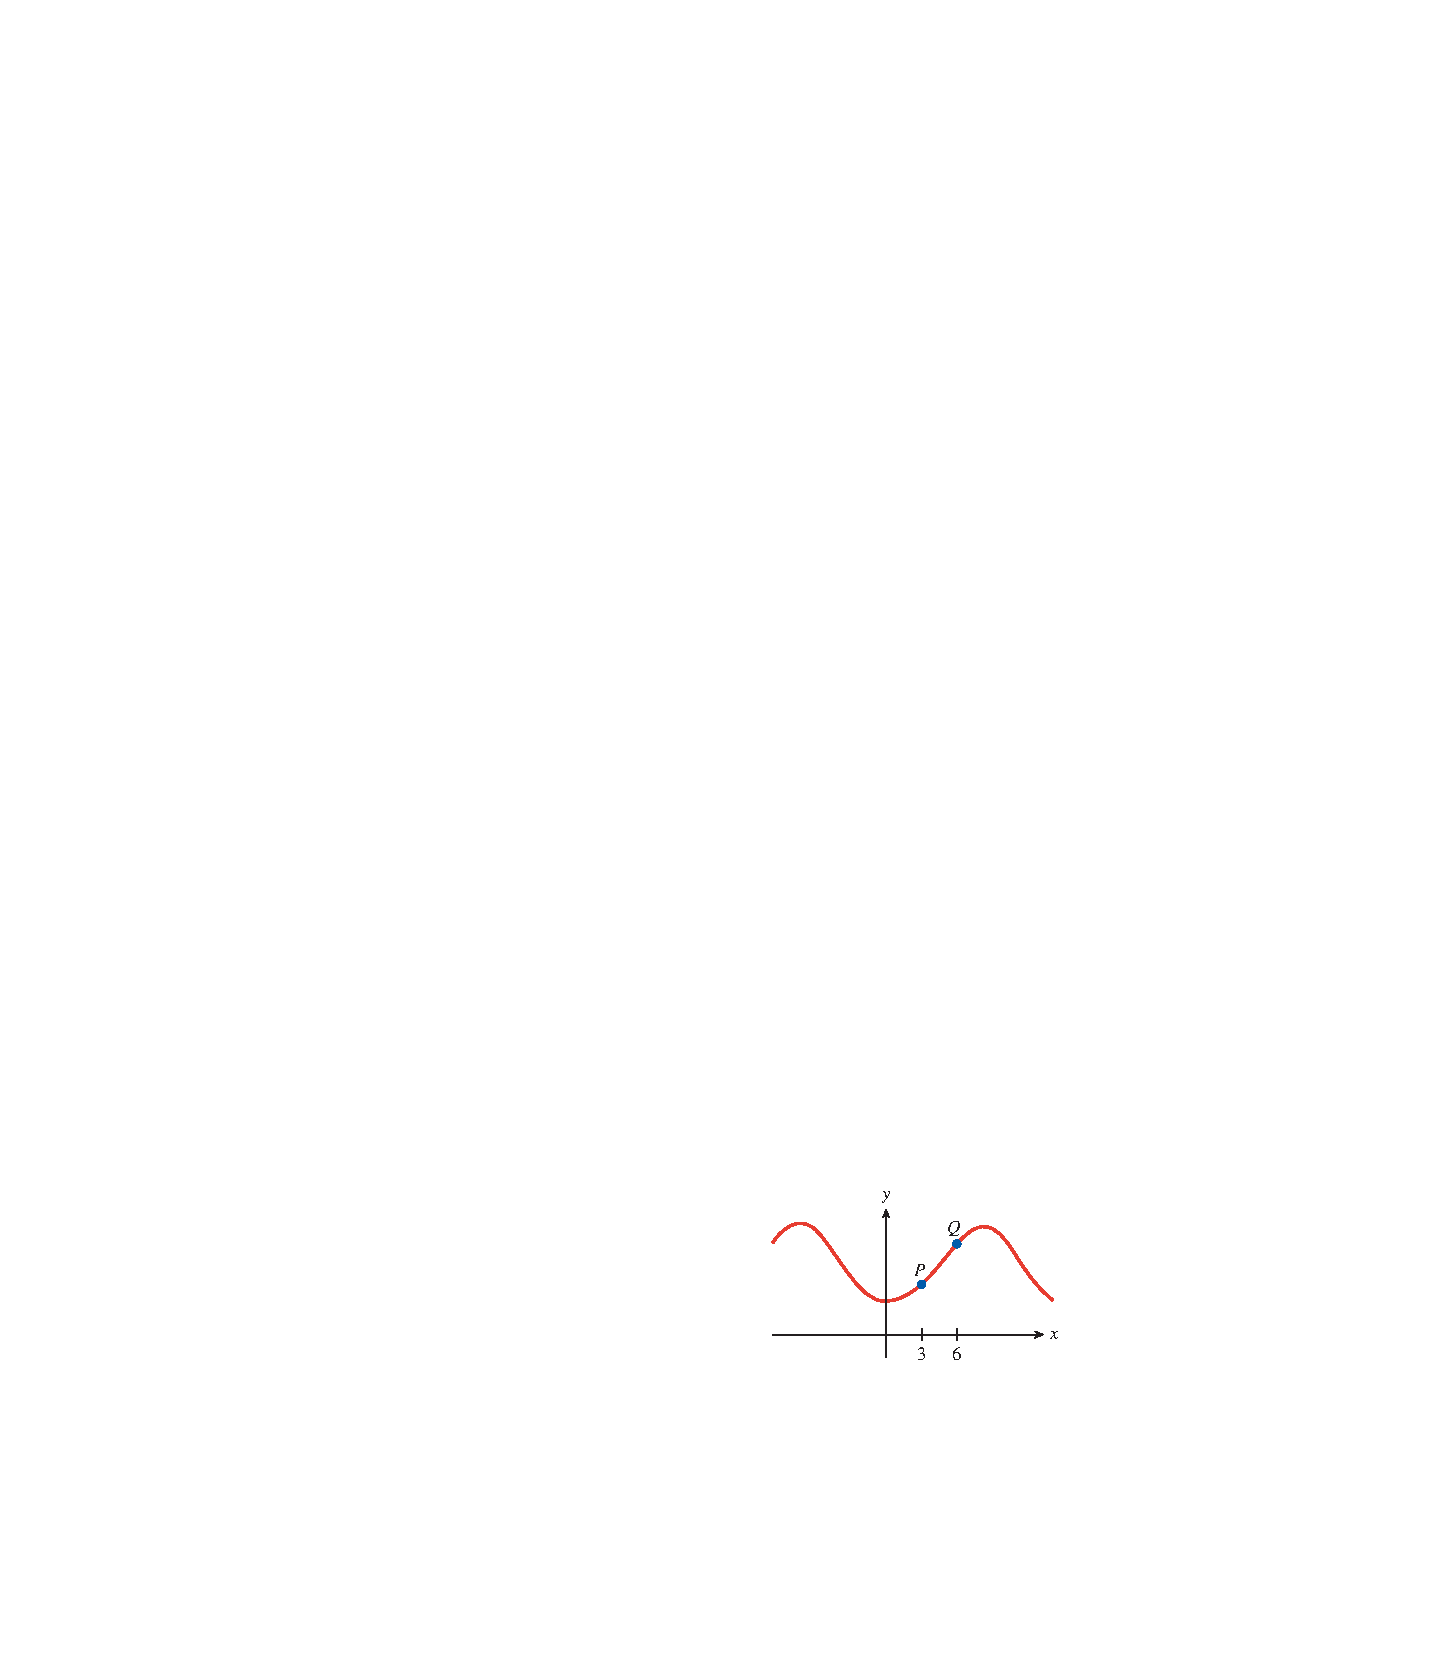
\includegraphics[width=\linewidth]{external/images/fig-ex-1-4-64b.pdf}
\end{sbspanel}%
\end{sidebyside}%
%
\end{enumerate}
\end{multicols}
%
\end{divisionexerciseeg}%
\begin{divisionexerciseeg}{65}{}{}{exercise-section-1-4-exercises-ab-d}%
%
\begin{multicols}{2}
\begin{enumerate}[label=\alph*]
\item{}\begin{sidebyside}{1}{0.1}{0.1}{0}%
\begin{sbspanel}{0.8}%
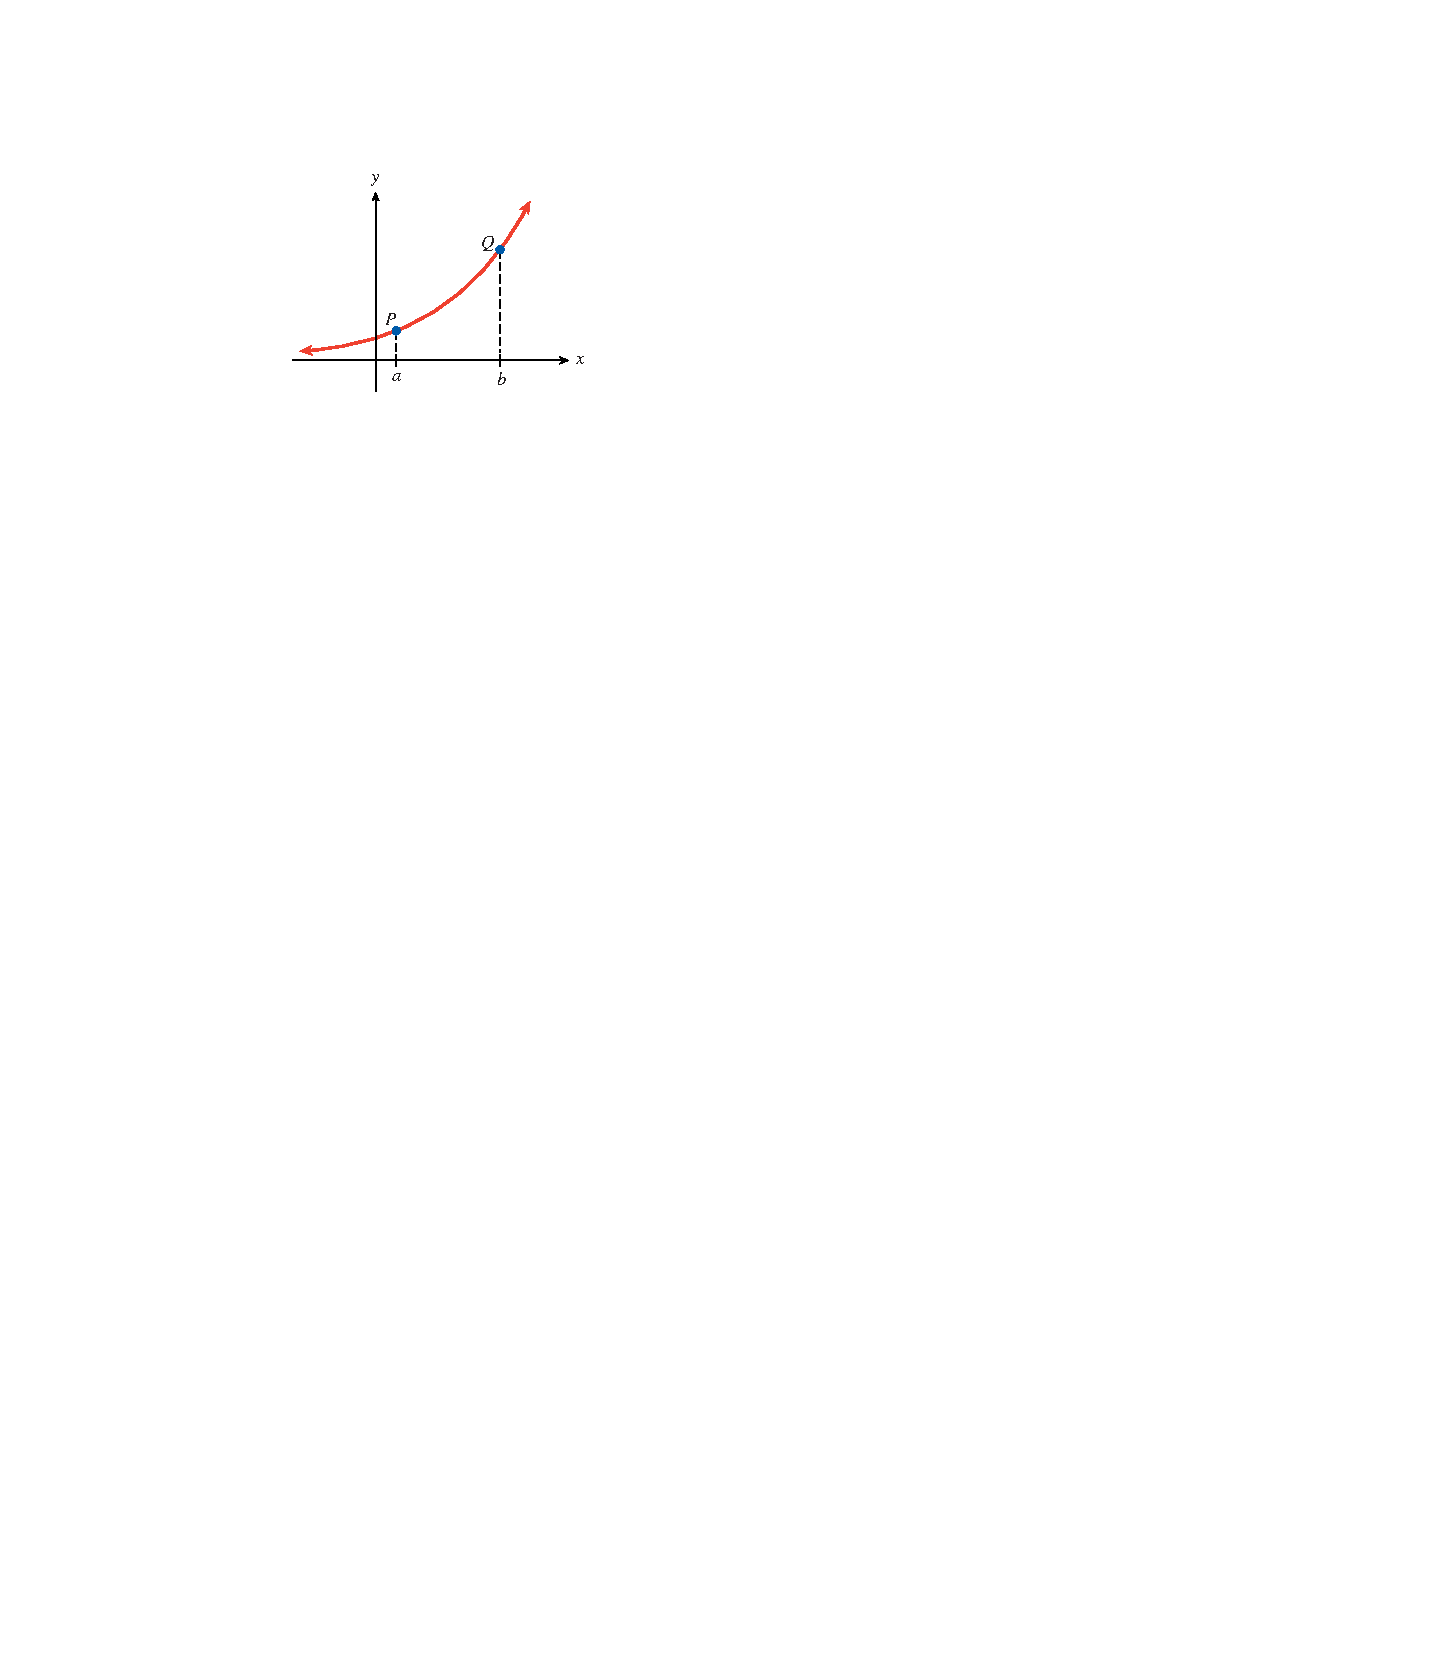
\includegraphics[width=\linewidth]{external/images/fig-ex-1-4-65a.pdf}
\end{sbspanel}%
\end{sidebyside}%
%
\item{}\begin{sidebyside}{1}{0.1}{0.1}{0}%
\begin{sbspanel}{0.8}%
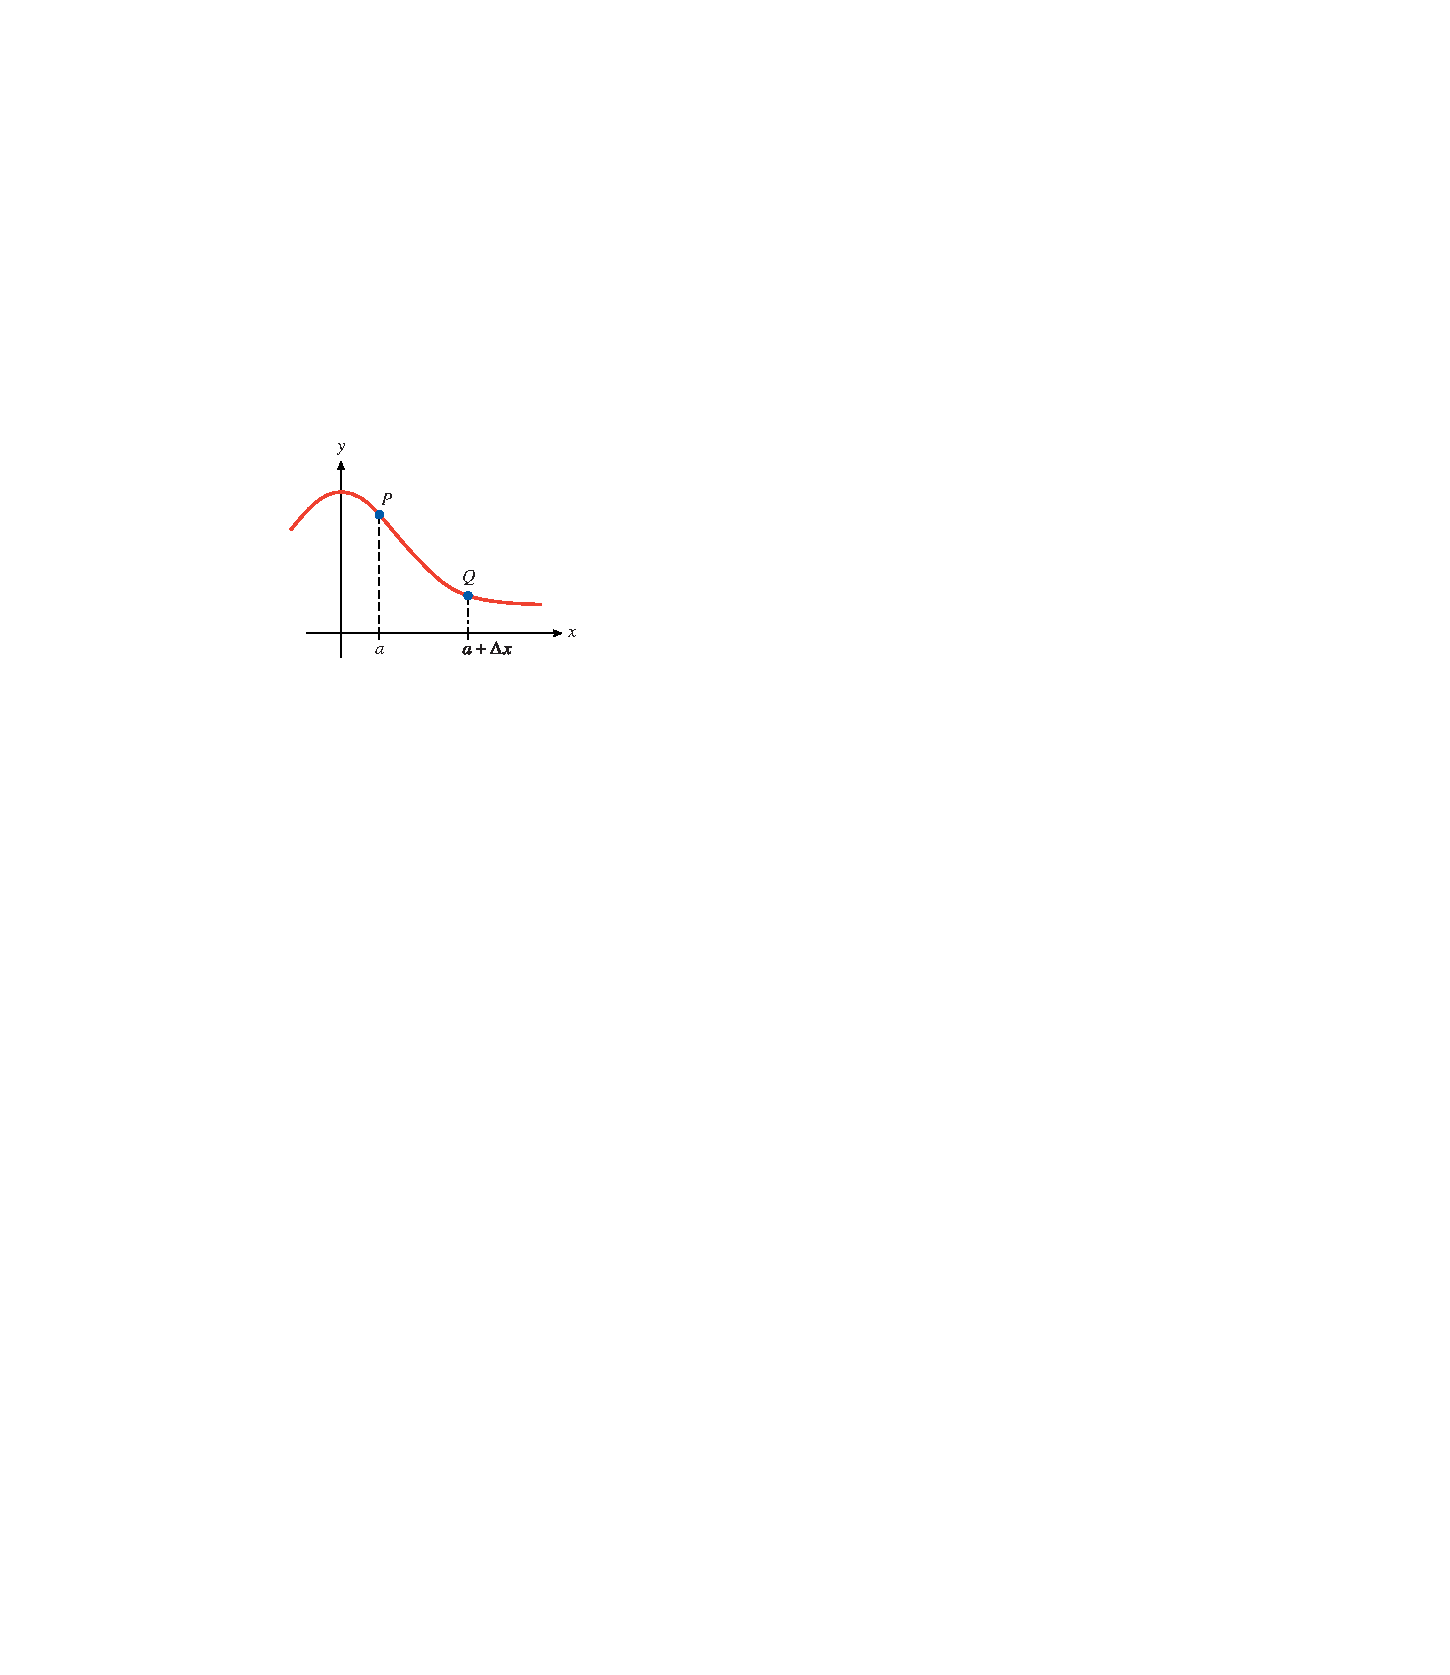
\includegraphics[width=\linewidth]{external/images/fig-ex-1-4-65b.pdf}
\end{sbspanel}%
\end{sidebyside}%
%
\end{enumerate}
\end{multicols}
%
\end{divisionexerciseeg}%
\begin{divisionexerciseeg}{66}{}{}{exercise-section-1-4-exercises-ab-e}%
%
\begin{multicols}{2}
\begin{enumerate}[label=\alph*]
\item{}\begin{sidebyside}{1}{0.1}{0.1}{0}%
\begin{sbspanel}{0.8}%
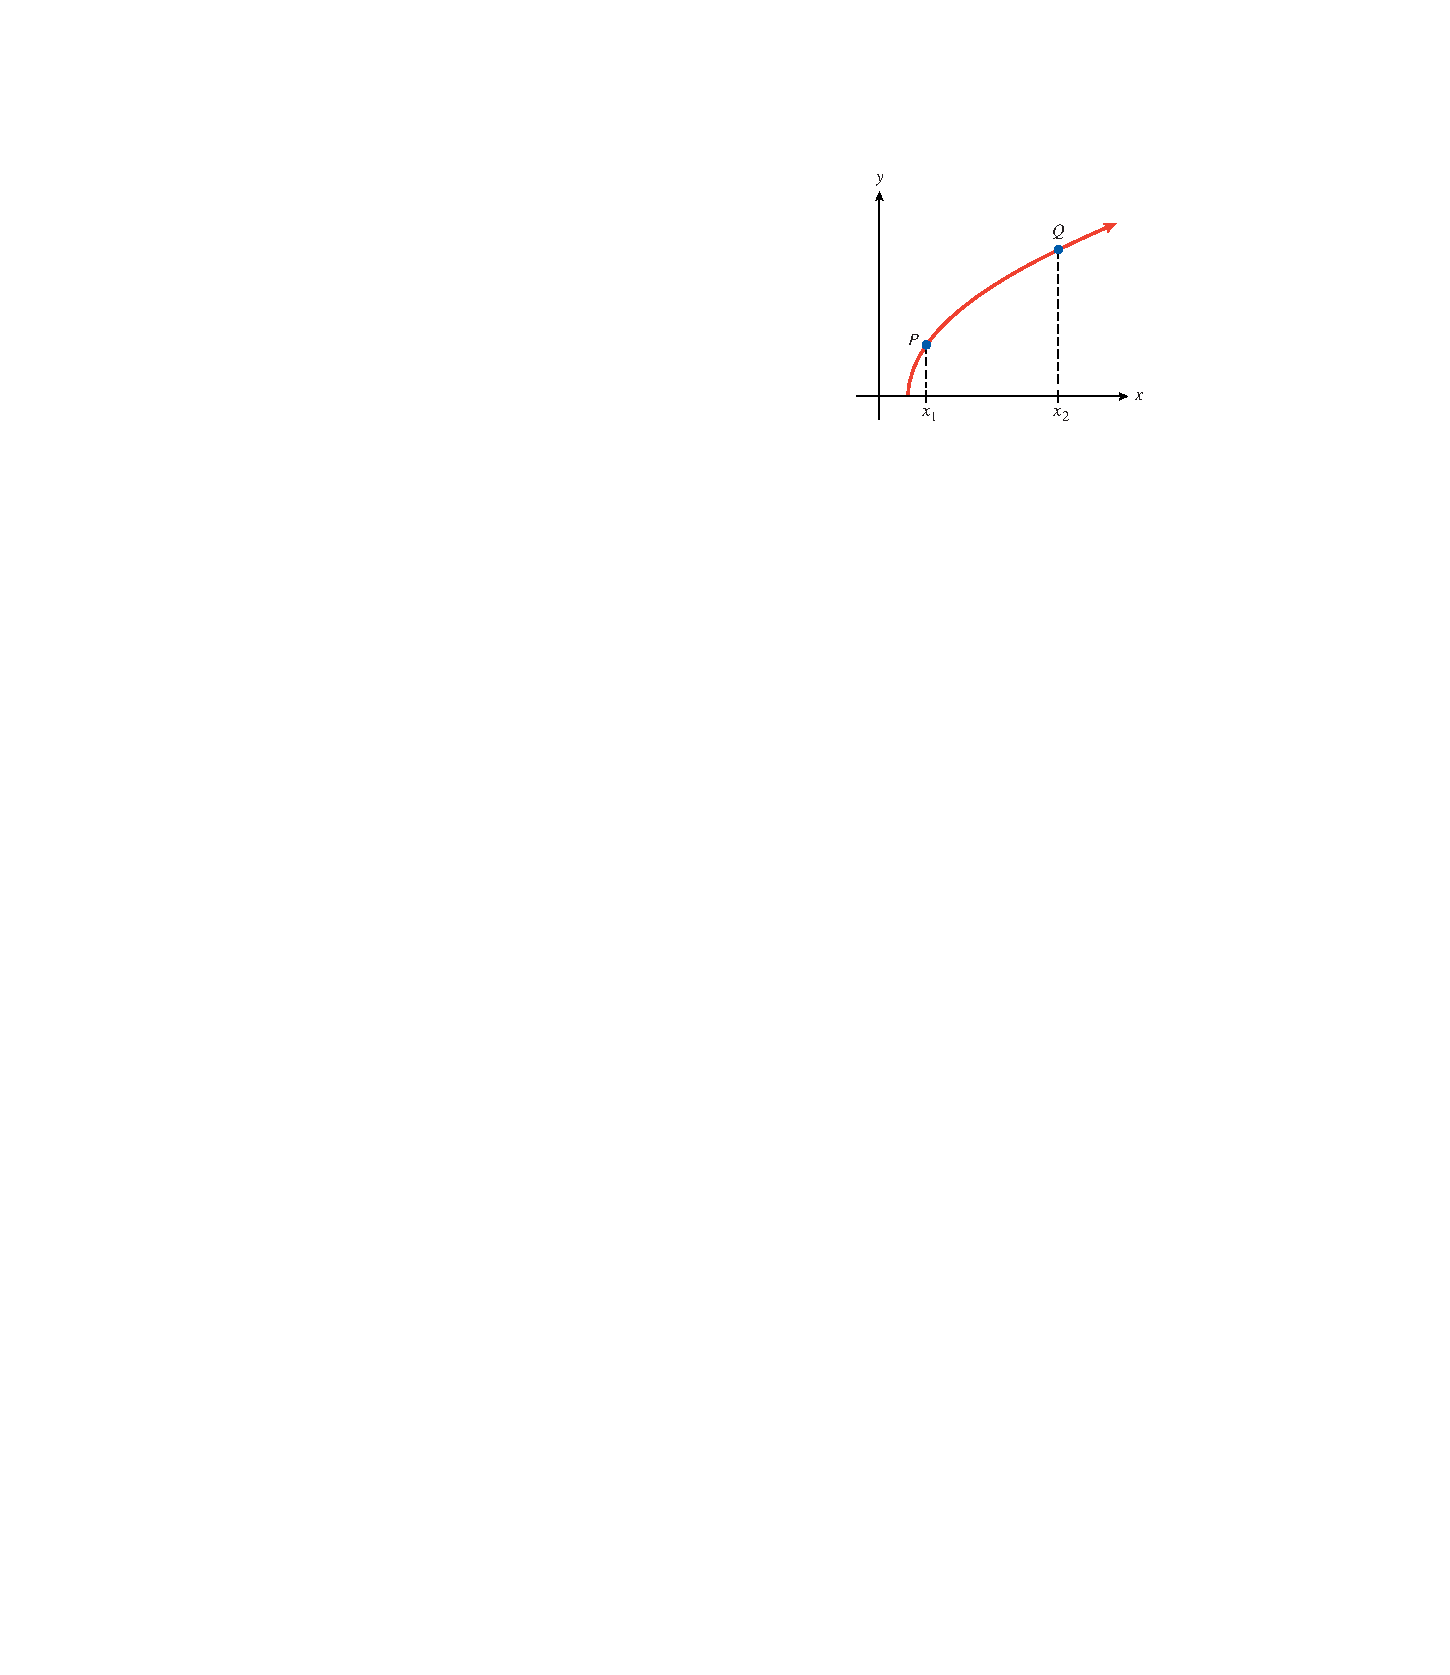
\includegraphics[width=\linewidth]{external/images/fig-ex-1-4-66a.pdf}
\end{sbspanel}%
\end{sidebyside}%
%
\item{}\begin{sidebyside}{1}{0.1}{0.1}{0}%
\begin{sbspanel}{0.8}%
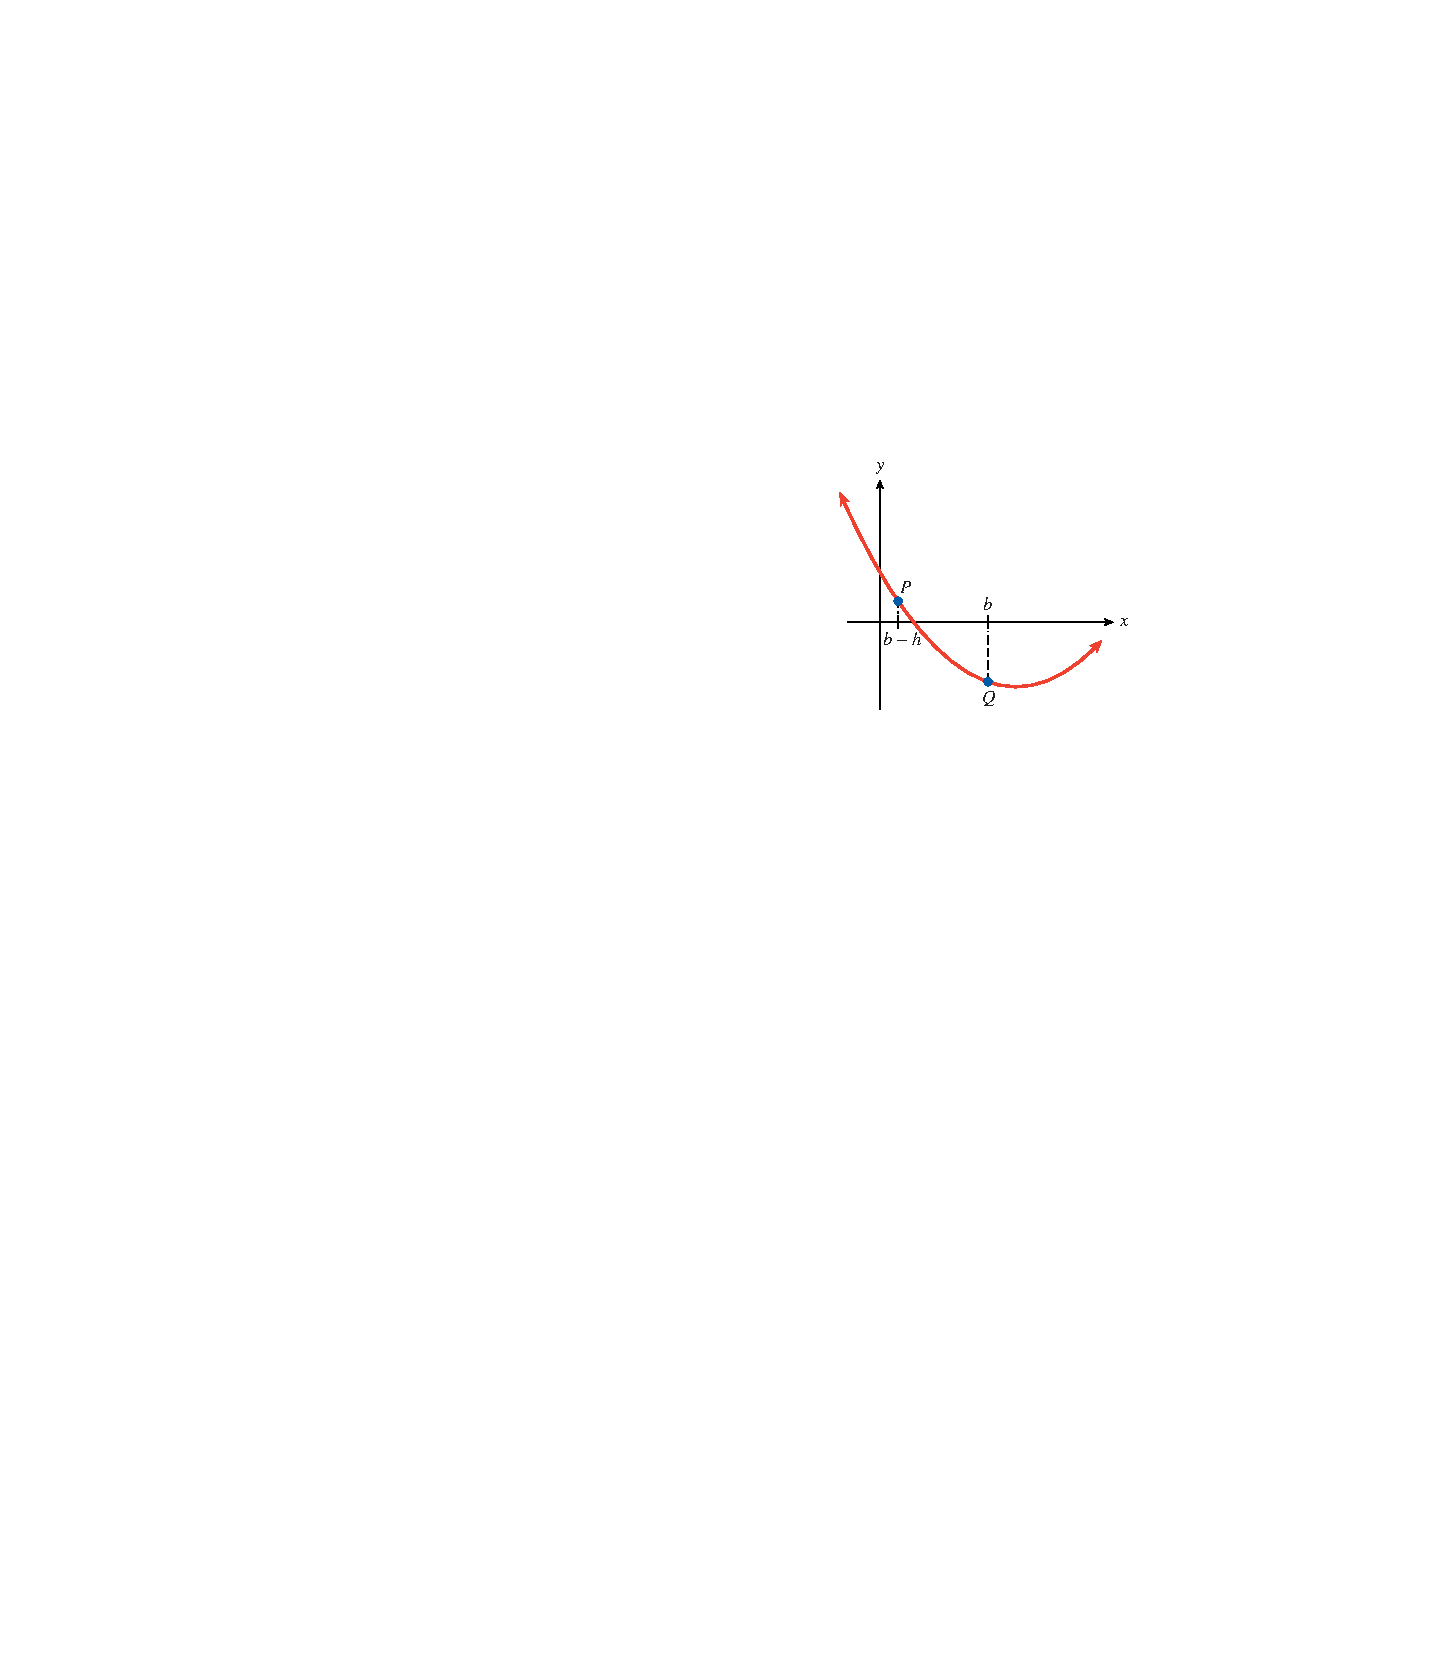
\includegraphics[width=\linewidth]{external/images/fig-ex-1-4-66b.pdf}
\end{sbspanel}%
\end{sidebyside}%
%
\end{enumerate}
\end{multicols}
%
\end{divisionexerciseeg}%
\end{exercisegroup}
\par\medskip\noindent
\end{exercises-subsection}
\end{sectionptx}
%
%
\typeout{************************************************}
\typeout{Section 1.5 Linear Functions}
\typeout{************************************************}
%
\begin{sectionptx}{Section}{Linear Functions}{}{Linear Functions}{}{}{section-linear-functions}
%
%
\typeout{************************************************}
\typeout{Subsection  Slope-Intercept Form}
\typeout{************************************************}
%
\begin{subsectionptx}{Subsection}{Slope-Intercept Form}{}{Slope-Intercept Form}{}{}{subsection-linear-functions-b}
As we saw in \hyperref[section-LinMod]{Section~{\xreffont\ref{section-LinMod}}}, many linear models \(y = f (x)\) have equations of the form%
\begin{equation*}
\blert{f(x) = (\text{starting value}) + (\text{rate of change}) \cdot x}
\end{equation*}
The starting value, or the value of \(y\) at \(x = 0\), is the \(y\)-intercept of the graph, and the rate of change is the slope of the graph. Thus, we can write the equation of a line as%
\begin{equation*}
\blert{f (x) = b + mx}
\end{equation*}
where the constant term, \(b\), is the \(y\)-intercept of the line, and \(m\), the coefficient of \(x\), is the slope of the line. This form for the equation of a line is called the \terminology{slope-intercept form}\index{slope-intercept form}.%
\begin{assemblage}{Assemblage}{Slope-Intercept Form.}{assemblage-linear-functions-b-c}%
If we write the equation of a linear function in the form,%
\begin{equation*}
f (x) = b + mx
\end{equation*}
then \(m\) is the \terminology{slope}\index{slope} of the line, and \(b\) is the \terminology{\(y\)-intercept}.%
\end{assemblage}
(You may have encountered the slope-intercept equation in the equivalent form \(y = mx + b\).)%
\par
For example, consider the two linear functions and their graphs shown below.%
\begin{sidebyside}{4}{0.02}{0.02}{0.04}%
\begin{sbspanel}{0.17}%
\(f (x) = 10 - 3x\)%
\par
%
\resizebox{\ifdim\width > \linewidth\linewidth\else\width\fi}{!}{%
\par
{\centering%
{\tabularfont%
\begin{tabular}{AcAcA}\hrulethick
\(\hphantom{00}x\hphantom{00}\)&\(\hphantom{0}f(x)\hphantom{0}\)\tabularnewline\hrulethin
\(0\)&\(10\)\tabularnewline\hrulethin
\(1\)&\(7\)\tabularnewline\hrulethin
\(2\)&\(4\)\tabularnewline\hrulethin
\(3\)&\(1\)\tabularnewline\hrulethin
\(4\)&\(-2\)\tabularnewline\hrulethin
\end{tabular}
}%
\par}
}%
\end{sbspanel}%
\begin{sbspanel}{0.25}[center]%
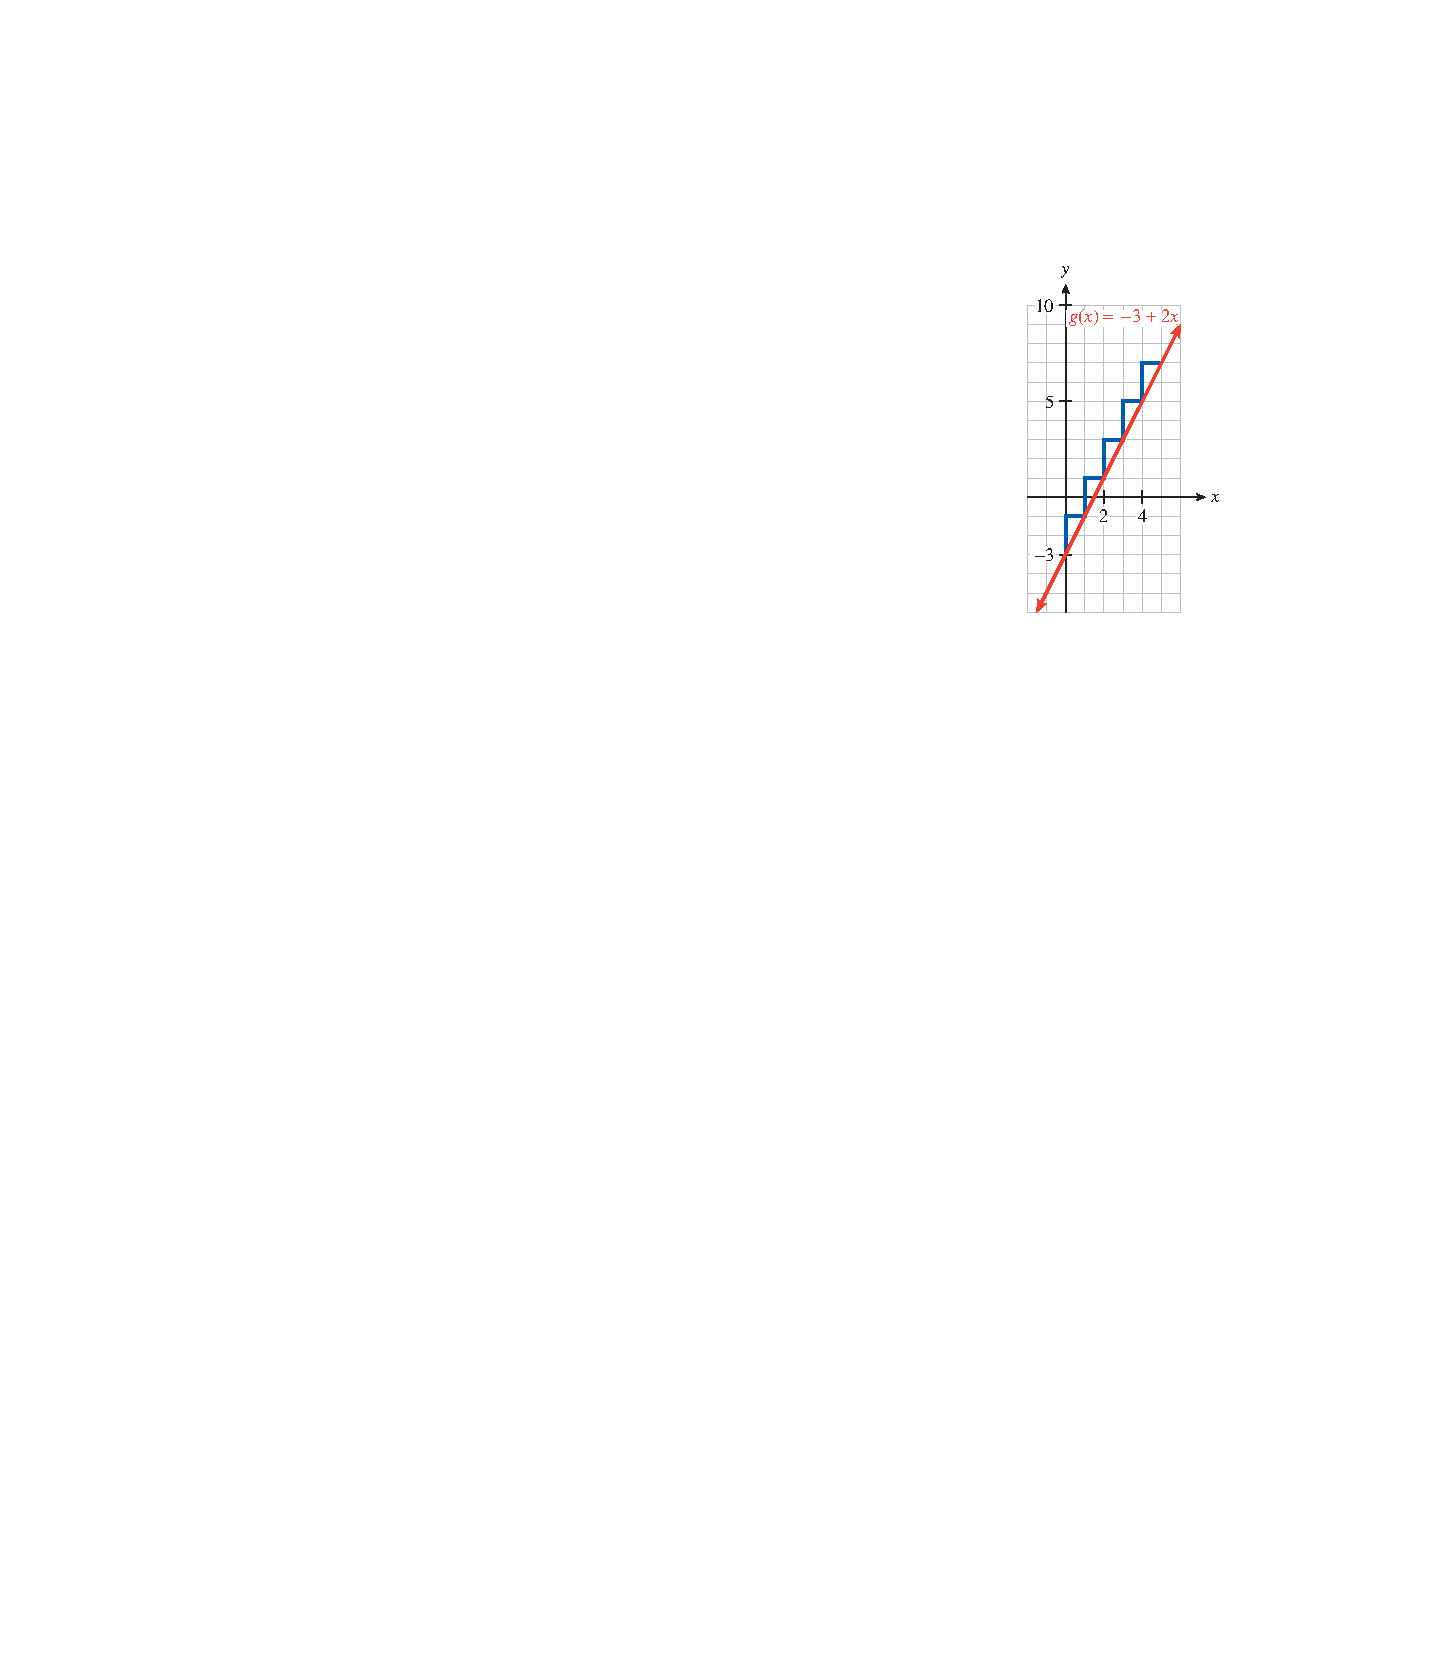
\includegraphics[width=\linewidth]{external/images/fig-decreasing-line.pdf}
\end{sbspanel}%
\begin{sbspanel}{0.17}%
\(g(x) = -3+2x\)%
\par
%
\resizebox{\ifdim\width > \linewidth\linewidth\else\width\fi}{!}{%
\par
{\centering%
{\tabularfont%
\begin{tabular}{AcAcA}\hrulethick
\(\hphantom{00}x\hphantom{00}\)&\(\hphantom{0}f(x)\hphantom{0}\)\tabularnewline\hrulethin
\(0\)&\(-3\)\tabularnewline\hrulethin
\(1\)&\(-1\)\tabularnewline\hrulethin
\(2\)&\(1\)\tabularnewline\hrulethin
\(3\)&\(3\)\tabularnewline\hrulethin
\(4\)&\(5\)\tabularnewline\hrulethin
\end{tabular}
}%
\par}
}%
\end{sbspanel}%
\begin{sbspanel}{0.25}[center]%
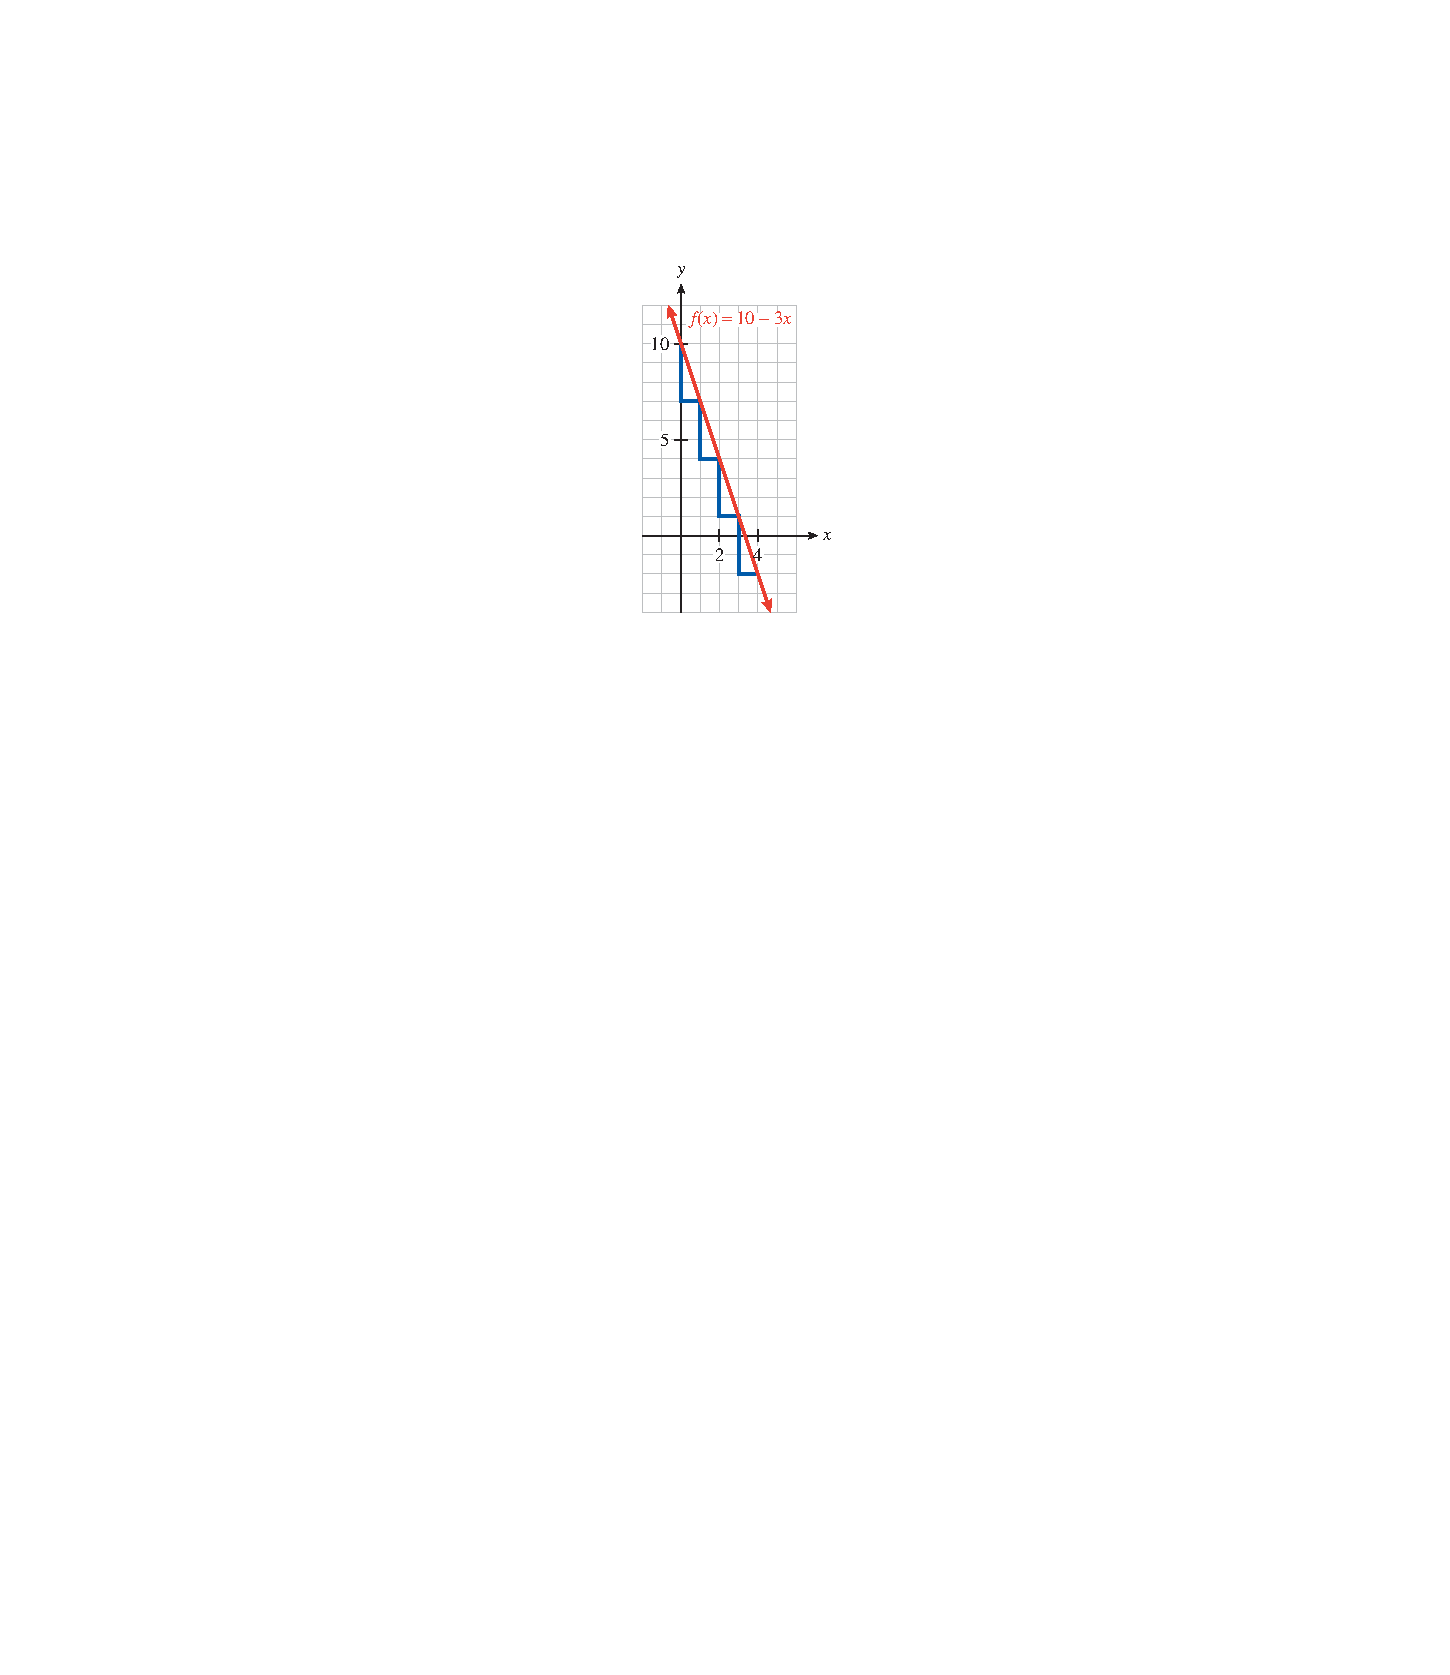
\includegraphics[width=\linewidth]{external/images/fig-increasing-line.pdf}
\end{sbspanel}%
\end{sidebyside}%
\par
Some observations:%
\begin{itemize}[label=\textbullet]
\item{}We can see that the \(y\)-intercept of each line is given by the constant term, \(b\).%
\item{}By examining the table of values, we can also see why the coefficient of \(x\)gives the slope of the line:%
\item{}For \(f (x)\), each time \(x\) increases by \(1\) unit, \(y\) decreases by \(3\) units.%
\item{}For \(g(x)\), each time \(x\) increases by \(1\) unit, \(y\) increases by \(2\) units.%
\end{itemize}
For each graph, the coefficient of \(x\) is a scale factor that tells us how many units \(y\) changes for \(1\) unit increase in \(x\). But that is exactly what the slope tells us about a line.%
\begin{example}{Example}{}{example-example-internet-providers}%
\begin{sidebyside}{2}{0.0375}{0.0375}{0.075}%
\begin{sbspanel}{0.5}%
Francine is choosing an Internet service provider. She paid \textdollar{}30 for a modem, and she is considering three companies for service:%
\begin{itemize}[label=\textbullet]
\item{}Juno charges \textdollar{}14.95 per month,%
\item{}ISP.com charges \textdollar{}12.95 per month,%
\item{}and peoplepc charges \textdollar{}15.95 per month.%
\end{itemize}
Match the graphs in the figure to Francine’s Internet cost with each company.%
\end{sbspanel}%
\begin{sbspanel}{0.35}%
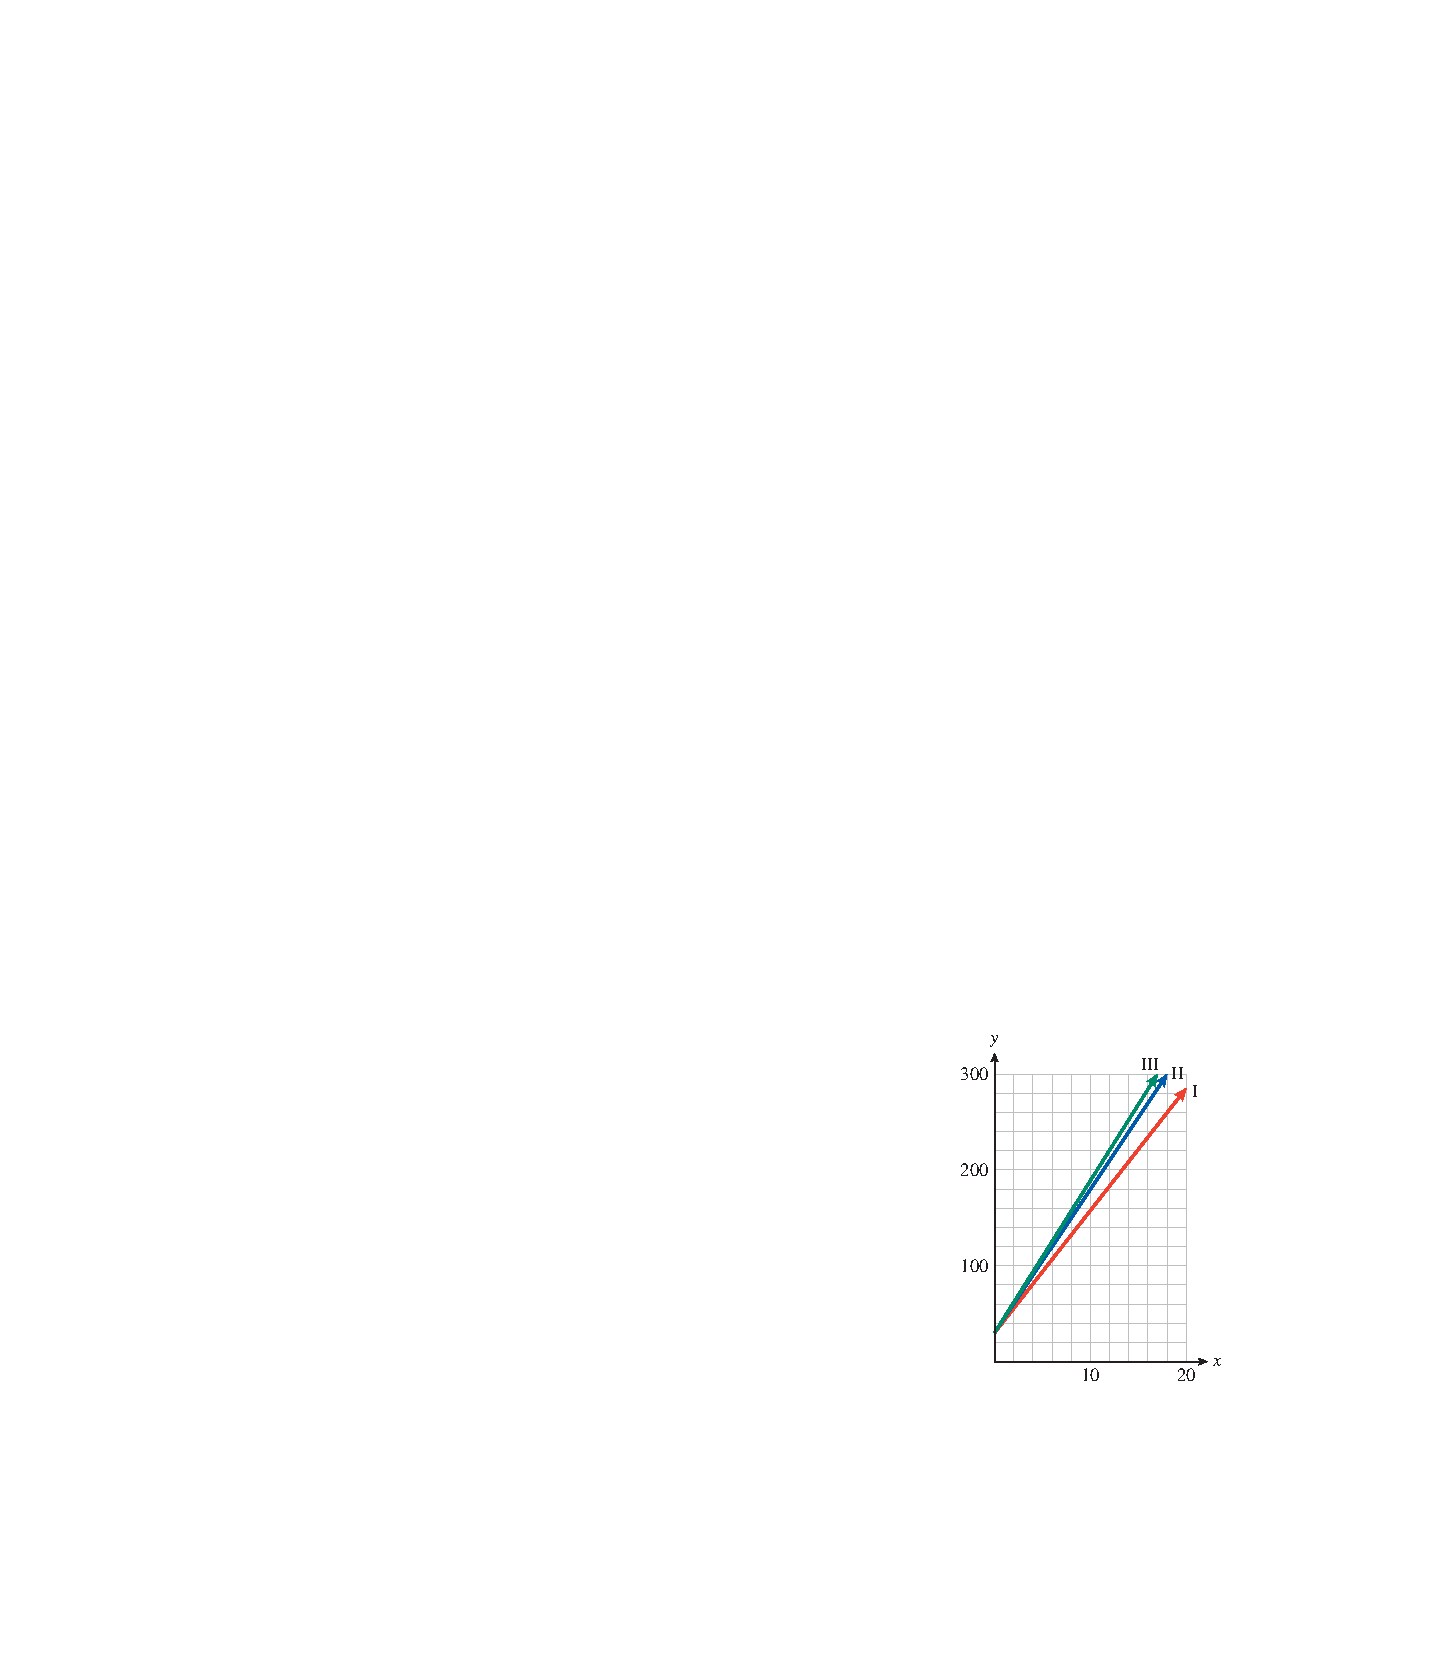
\includegraphics[width=\linewidth]{external/images/fig-internet-providers.pdf}
\end{sbspanel}%
\end{sidebyside}%
\par\smallskip%
\noindent\textbf{\blocktitlefont Solution}.\hypertarget{solution-example-internet-providers-b}{}\quad{}Francine pays the same initial amount, \textdollar{}30 for the modem, under each plan. The monthly fee is the rate of change of her total cost, in dollars per month. We can write a formula for her cost under each plan.%
\begin{equation*}
\text{Juno:   } f(x) = 30 + 14.95x
\end{equation*}
%
\begin{equation*}
\text{ISP.com:   } g(x) = 30 + 12.95x
\end{equation*}
%
\begin{equation*}
\text{peoplepc:   } h(x) = 30 + 15.95x
\end{equation*}
The graphs of these three functions all have the same \(y\)-intercept, but their slopes are determined by the monthly fees. The steepest graph, III, is the one with the largest monthly fee, peoplepc, and ISP.com, which has the lowest monthly fee, has the least steep graph, I.%
\end{example}
\begin{inlineexercise}{Checkpoint}{Practice 1.}{exercise-linear-functions-b-i}%
Delbert decides to use DSL for his Internet service. Earthlink charges a \textdollar{}99 activation fee and \textdollar{}39.95 per month, DigitalRain charges \textdollar{}50 for activation and \textdollar{}34.95 per month, and FreeAmerica charges \textdollar{}149 for activation and \textdollar{}34.95 per month.%
\begin{sidebyside}{1}{0.3}{0.3}{0}%
\begin{sbspanel}{0.4}%
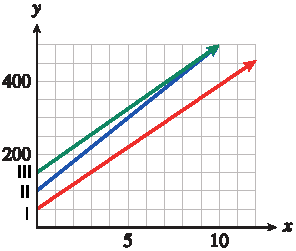
\includegraphics[width=\linewidth]{external/images/fig-dsl-price.pdf}
\end{sbspanel}%
\end{sidebyside}%
\par
%
\begin{enumerate}[label=\alph*.]
\item{}Write a formula for Delbert's Internet costs under each plan.%
\par
Earthlink: \(f(x)=\)\fillintext{10}%
\par
DigitalRain: \(g(x)=\)\fillintext{10}%
\par
FreeAmerica: \(h(x)=\)\fillintext{10}%
\item{}Match Delbert's Internet cost under each company with its graph shown above.%
\par
Line I:\quad(\begin{itemize*}[label=$\square$,leftmargin=3em,itemjoin=\hspace{1em}]
\item{}Earthlink%
\item{}DigitalRain%
\item{}FreeAmerica%
\end{itemize*})\quad
%
\par
Line II:\quad(\begin{itemize*}[label=$\square$,leftmargin=3em,itemjoin=\hspace{1em}]
\item{}Earthlink%
\item{}DigitalRain%
\item{}FreeAmerica%
\end{itemize*})\quad
%
\par
Line III:\quad(\begin{itemize*}[label=$\square$,leftmargin=3em,itemjoin=\hspace{1em}]
\item{}Earthlink%
\item{}DigitalRain%
\item{}FreeAmerica%
\end{itemize*})\quad
%
\end{enumerate}
%
\par\smallskip%
\noindent\textbf{\blocktitlefont Answer 1}.\hypertarget{answer-linear-functions-b-i-c}{}\quad{}\(99+39.95x\)%
\par\smallskip%
\noindent\textbf{\blocktitlefont Answer 2}.\hypertarget{answer-linear-functions-b-i-d}{}\quad{}\(50+34.95x\)%
\par\smallskip%
\noindent\textbf{\blocktitlefont Answer 3}.\hypertarget{answer-linear-functions-b-i-e}{}\quad{}\(149+34.95x\)%
\par\smallskip%
\noindent\textbf{\blocktitlefont Answer 4}.\hypertarget{answer-linear-functions-b-i-f}{}\quad{}\(\text{DigitalRain}\)%
\par\smallskip%
\noindent\textbf{\blocktitlefont Answer 5}.\hypertarget{answer-linear-functions-b-i-g}{}\quad{}\(\text{Earthlink}\)%
\par\smallskip%
\noindent\textbf{\blocktitlefont Answer 6}.\hypertarget{answer-linear-functions-b-i-h}{}\quad{}\(\text{FreeAmerica}\)%
\par\smallskip%
\noindent\textbf{\blocktitlefont Solution}.\hypertarget{solution-linear-functions-b-i-i}{}\quad{}%
\begin{enumerate}[label=\alph*.]
\item{}Earthlink: \(f(x)=99 + 39.95x\text{;}\) DigitalRain: \(g(x)=50 + 34.95x\text{;}\) FreeAmerica: \(h(x)=149 + 34.95x\)%
\item{}DigitalRain: I; Earthlink: II; FreeAmerica: III%
\end{enumerate}
%
\end{inlineexercise}%
\begin{inlineexercise}{Checkpoint}{QuickCheck 1.}{exercise-linear-functions-b-j}%
What do the coefficients in the slope-intercept form tell you about a line?%
\par
\begin{itemize}[label=$\odot$,leftmargin=3em,]
\item{}\(m\) is the slope; \(b\) is the \(x\)-intercept%
\item{}\(m\) is the slope; \(b\) is the \(y\)-intercept%
\item{}\((m,b)\) is a point on the line%
\item{}\(m\) is the \(x\)-intercept; \(b\) is the \(y\)-intercept%
\end{itemize}
%
\par\smallskip%
\noindent\textbf{\blocktitlefont Answer}.\hypertarget{answer-linear-functions-b-j-c}{}\quad{}\(\text{Choice 2}\)%
\par\smallskip%
\noindent\textbf{\blocktitlefont Solution}.\hypertarget{solution-linear-functions-b-j-d}{}\quad{}\(m\) is the slope; \(b\) is the \(y\)-intercept%
\end{inlineexercise}%
\begin{note}{Note}{}{note-linear-functions-b-k}%
In the equation \(f (x) = b + mx\), we call \(m\) and \(b\) \terminology{parameters}\index{parameters}. Their values are fixed for any particular linear equation; for example, in the equation \(y = 3+2x\), \(b=3\) and \(m=2\), and the variables are \(x\) and \(y\). By changing the values of \(m\) and \(b\), we can write the equation for any line except a vertical line. The collection of all linear functions \(f(x) = b + mx\) is called a \terminology{two-parameter}\index{two-parameter} family of functions.%
\end{note}
\begin{sidebyside}{1}{0.1}{0.1}{0}%
\begin{sbspanel}{0.8}%
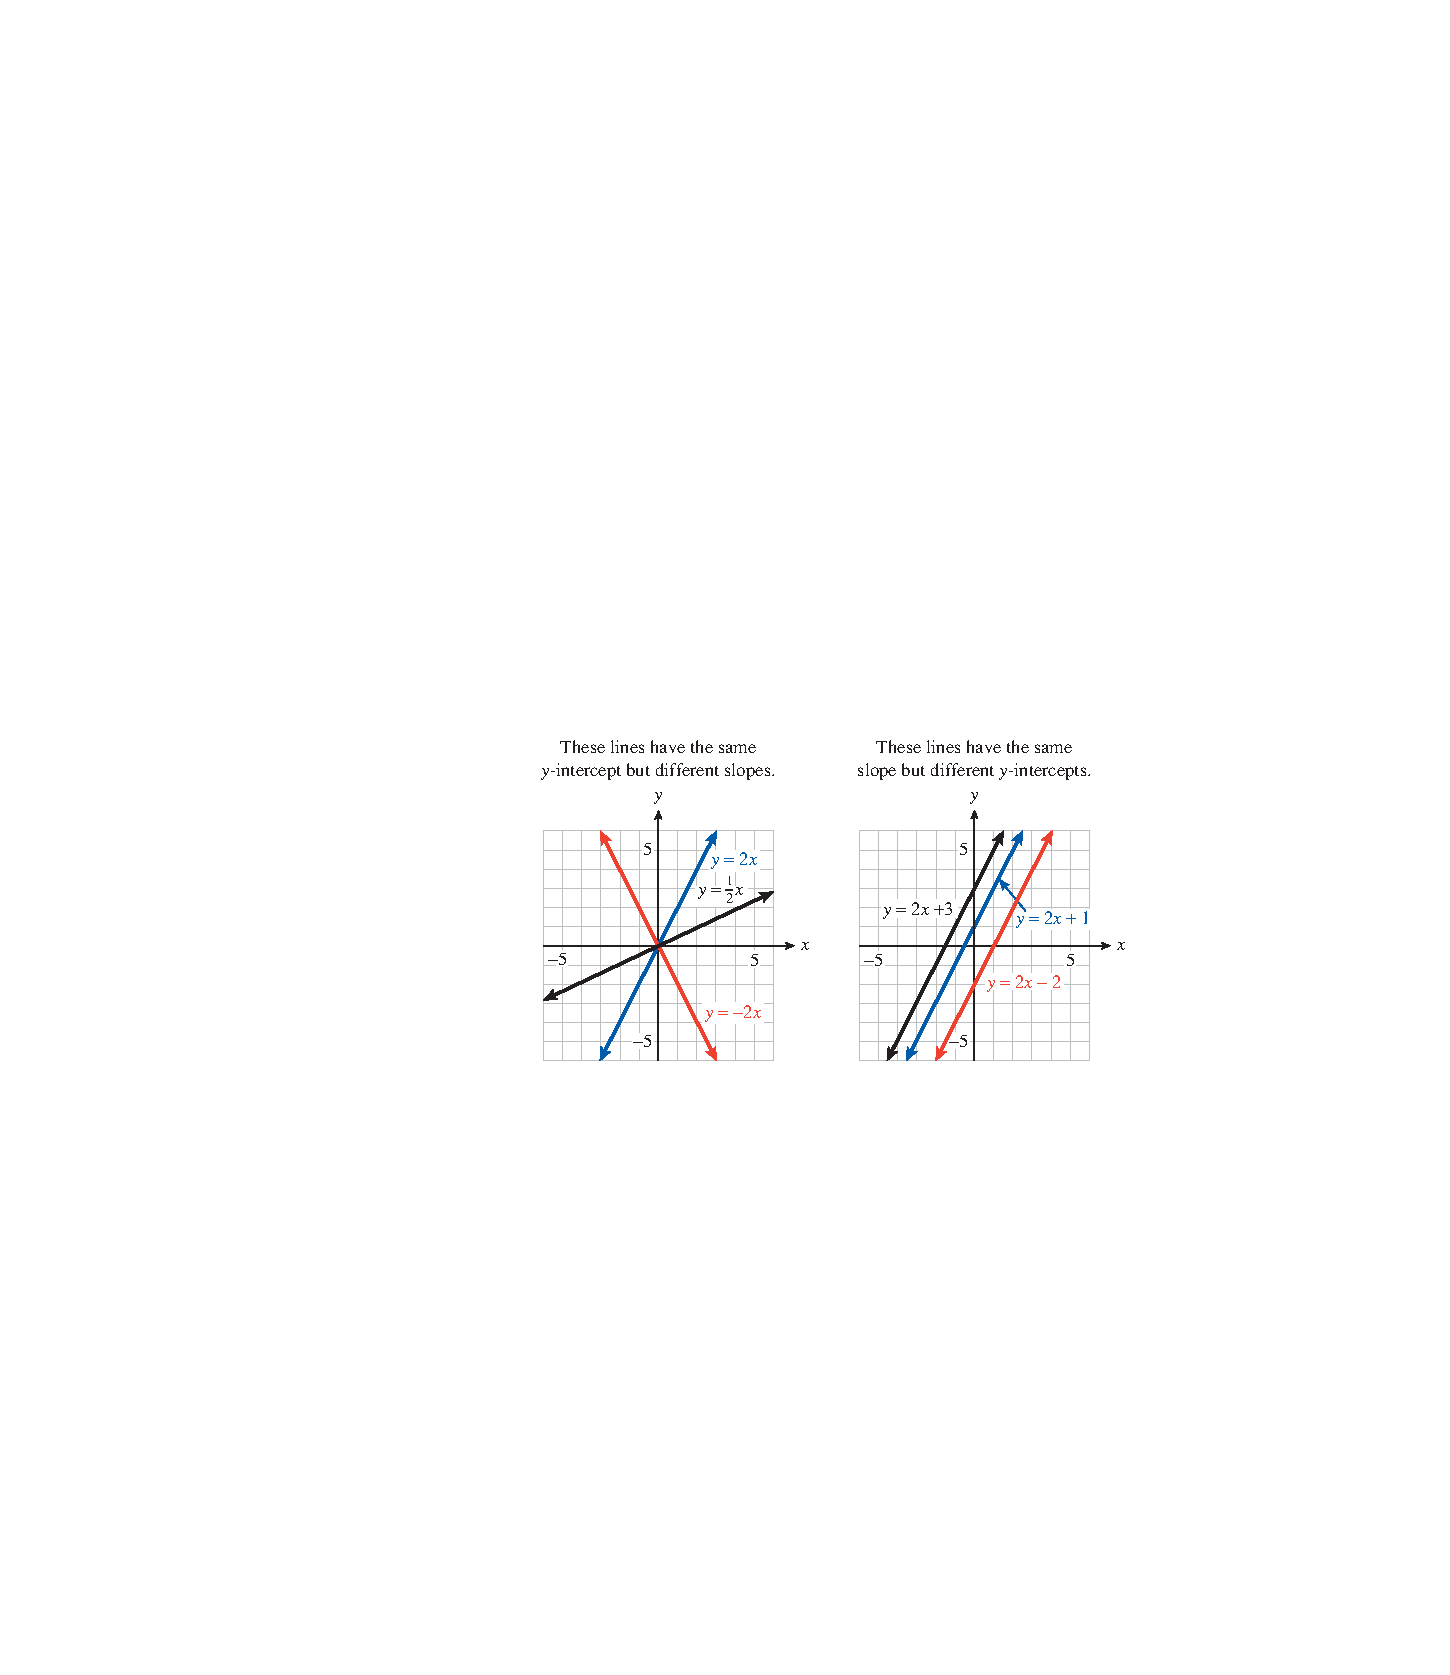
\includegraphics[width=\linewidth]{external/images/fig-slope-vs-intercept.pdf}
\end{sbspanel}%
\end{sidebyside}%
\begin{inlineexercise}{Checkpoint}{Pause and Reflect.}{exercise-linear-functions-b-m}%
Explain why the initial value for a linear model is often given by the \(y\)-intercept.%
\end{inlineexercise}%
\end{subsectionptx}
%
%
\typeout{************************************************}
\typeout{Subsection  Slope-Intercept Method of Graphing}
\typeout{************************************************}
%
\begin{subsectionptx}{Subsection}{Slope-Intercept Method of Graphing}{}{Slope-Intercept Method of Graphing}{}{}{subsection-linear-functions-c}
Look again at the lines in the previous figure: There is only one line that has a given slope and passes through a particular point. That is, the values of \(m\) and \(b\) determine the particular line. The value of \(b\) gives us a starting point, and the value of \(m\) tells us which direction to go to plot a second point. Thus, we can graph a line given in slope-intercept form without having to make a table of values.%
\begin{example}{Example}{}{example-example-slope-intercept}%
%
\begin{enumerate}[label=\alph*]
\item{}Write the equation \(4x - 3y = 6\) in slope-intercept form.%
\item{}Graph the line by hand.%
\end{enumerate}
%
\par\smallskip%
\noindent\textbf{\blocktitlefont Solution}.\hypertarget{solution-example-slope-intercept-b}{}\quad{}%
\begin{enumerate}[label=\alph*]
\item{}We solve the equation for \(y\) in terms of \(x\).%
\begin{equation*}
\begin{aligned}[t]
-3y \amp =6 - 4x \amp \amp \blert{\text{Divide both sides by } -3}\\
y \amp = \frac{6 - 4x}{-3}=\frac{6}{-3}+\frac{-4x}{-3}\\
y \amp = -2+\frac{4}{3}x
\end{aligned}
\end{equation*}
%
\item{}We see that the slope of the line is \(m = \dfrac{4}{3}\) and its \(y\)-intercept is \(b = -2\). We begin by plotting the \(y\)-intercept, \((0, -2)\). We then use the slope to find another point on the line. We have%
\begin{equation*}
m = \frac{\Delta y}{\Delta x}=\frac{4}{3}
\end{equation*}
so starting at \((0, -2)\), we move \(4\) units in the \(y\)-direction and \(3\) units in the \(x\)-direction, to arrive at the point \((3, 2)\). Finally, we draw the line through these two points.%
\end{enumerate}
%
\begin{sidebyside}{1}{0.325}{0.325}{0}%
\begin{sbspanel}{0.35}%
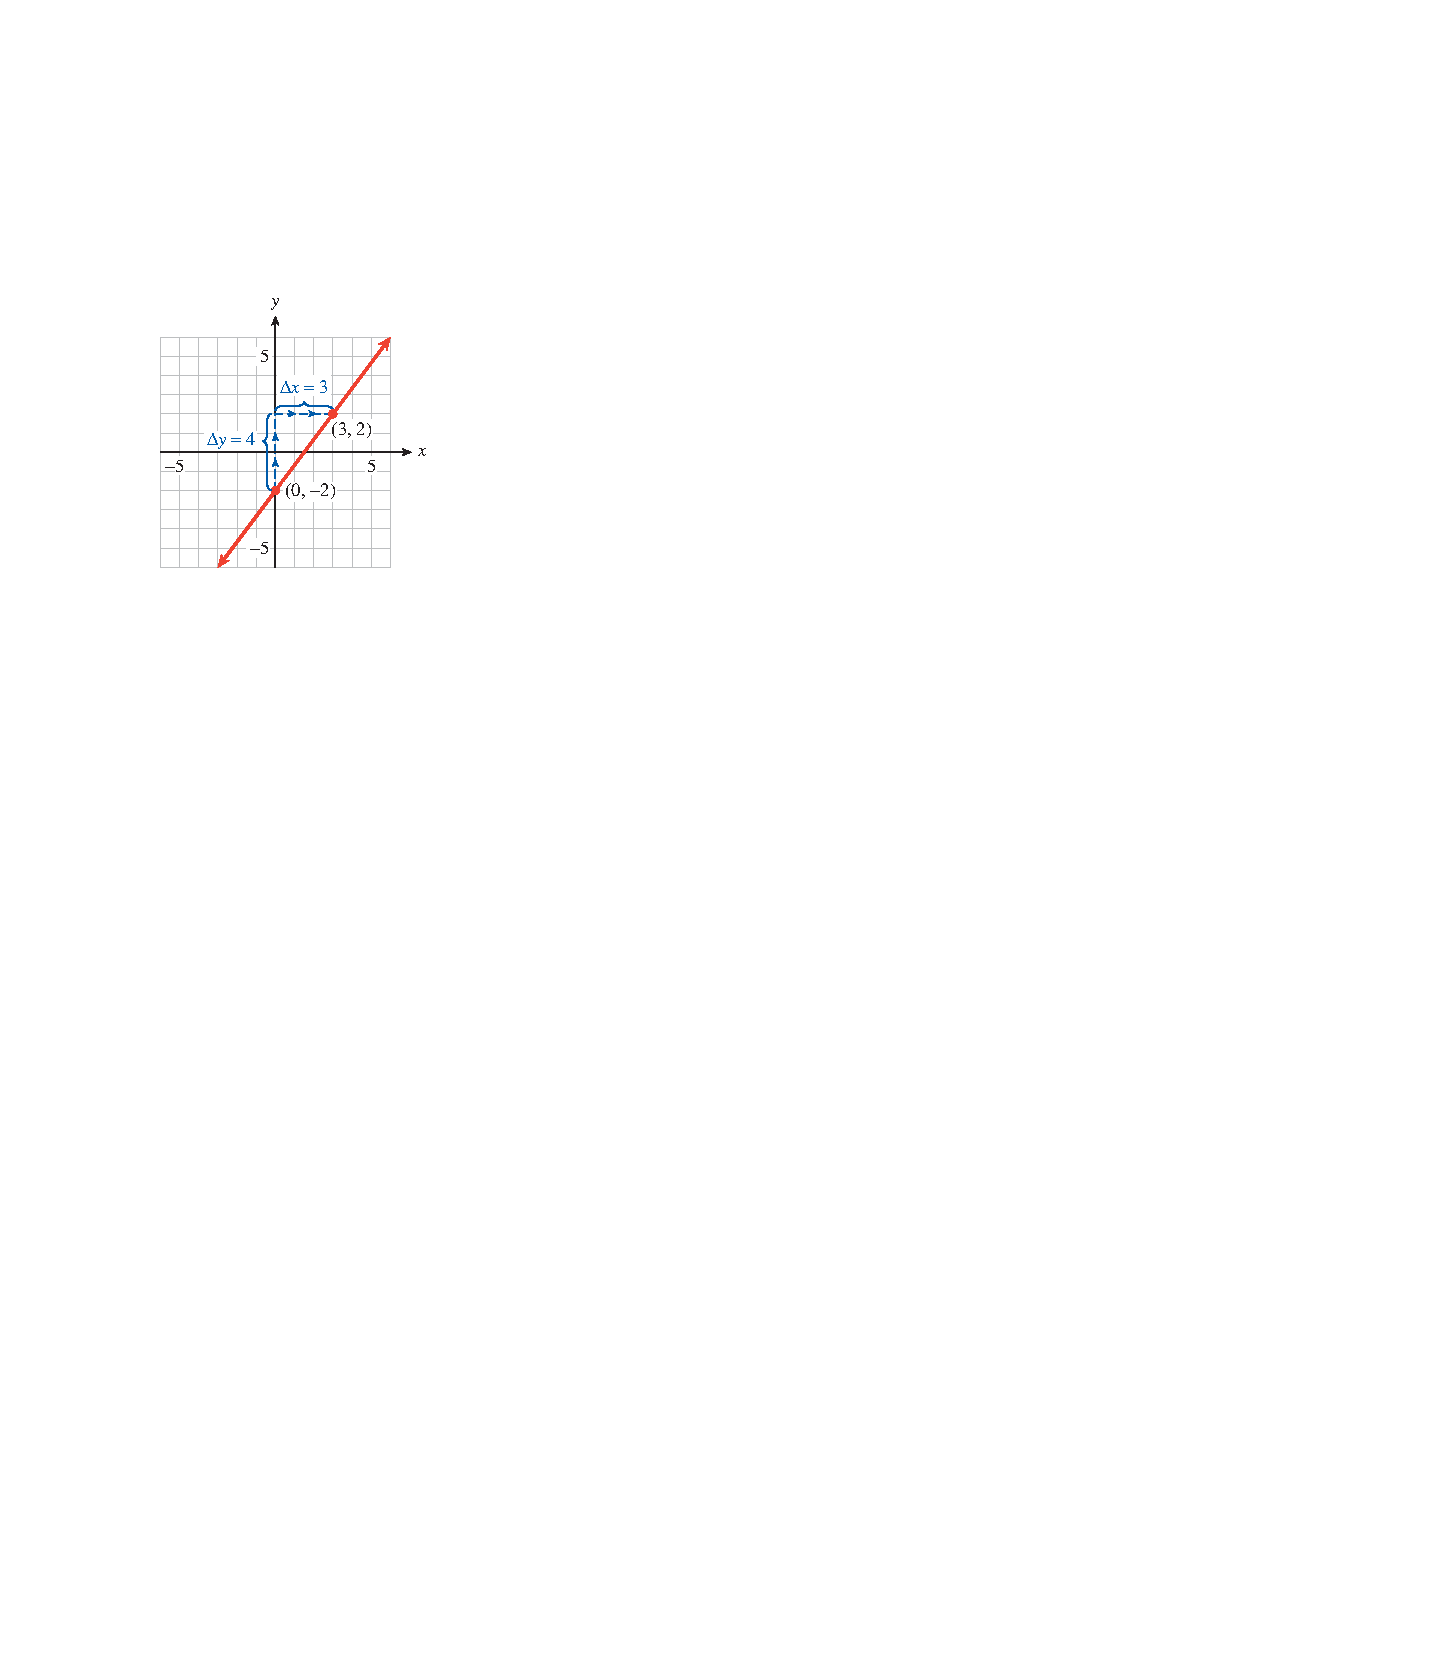
\includegraphics[width=\linewidth]{external/images/fig-slope-intercept.pdf}
\end{sbspanel}%
\end{sidebyside}%
\end{example}
\begin{note}{Note}{}{note-linear-functions-c-d}%
The slope of a line is a ratio and can be written in many equivalent ways. In \hyperref[example-example-slope-intercept]{Example~{\xreffont\ref{example-example-slope-intercept}}}, the slope is equal to \(\dfrac{8}{6}\), \(\dfrac{12}{9}\), and \(\dfrac{-4}{-3}\). We can use any of these fractions to locate a third point on the line as a check. If we use \(m = \dfrac{\Delta y}{\Delta x}= \dfrac{-4}{-3}\), we move down \(4\) units and left \(3\) units from the \(y\)-intercept to find the point \((-3, -6)\) on the line.%
\end{note}
\begin{assemblage}{Assemblage}{Slope-Intercept Method for Graphing a Line.}{assemblage-linear-functions-c-e}%
%
\begin{enumerate}[label=\alph*]
\item{}Plot the \(y\)-intercept \((0, b)\).%
\item{}Use the definition of slope to find a second point on the line: Starting at the \(y\)-intercept, move \(\Delta y\) units in the \(y\)-direction and \(\Delta x\) units in the \(x\)-direction. Plot a second point at this location.%
\item{}Use an equivalent form of the slope to find a third point, and draw a line through the points.%
\end{enumerate}
%
\begin{sidebyside}{1}{0.3}{0.3}{0}%
\begin{sbspanel}{0.4}%
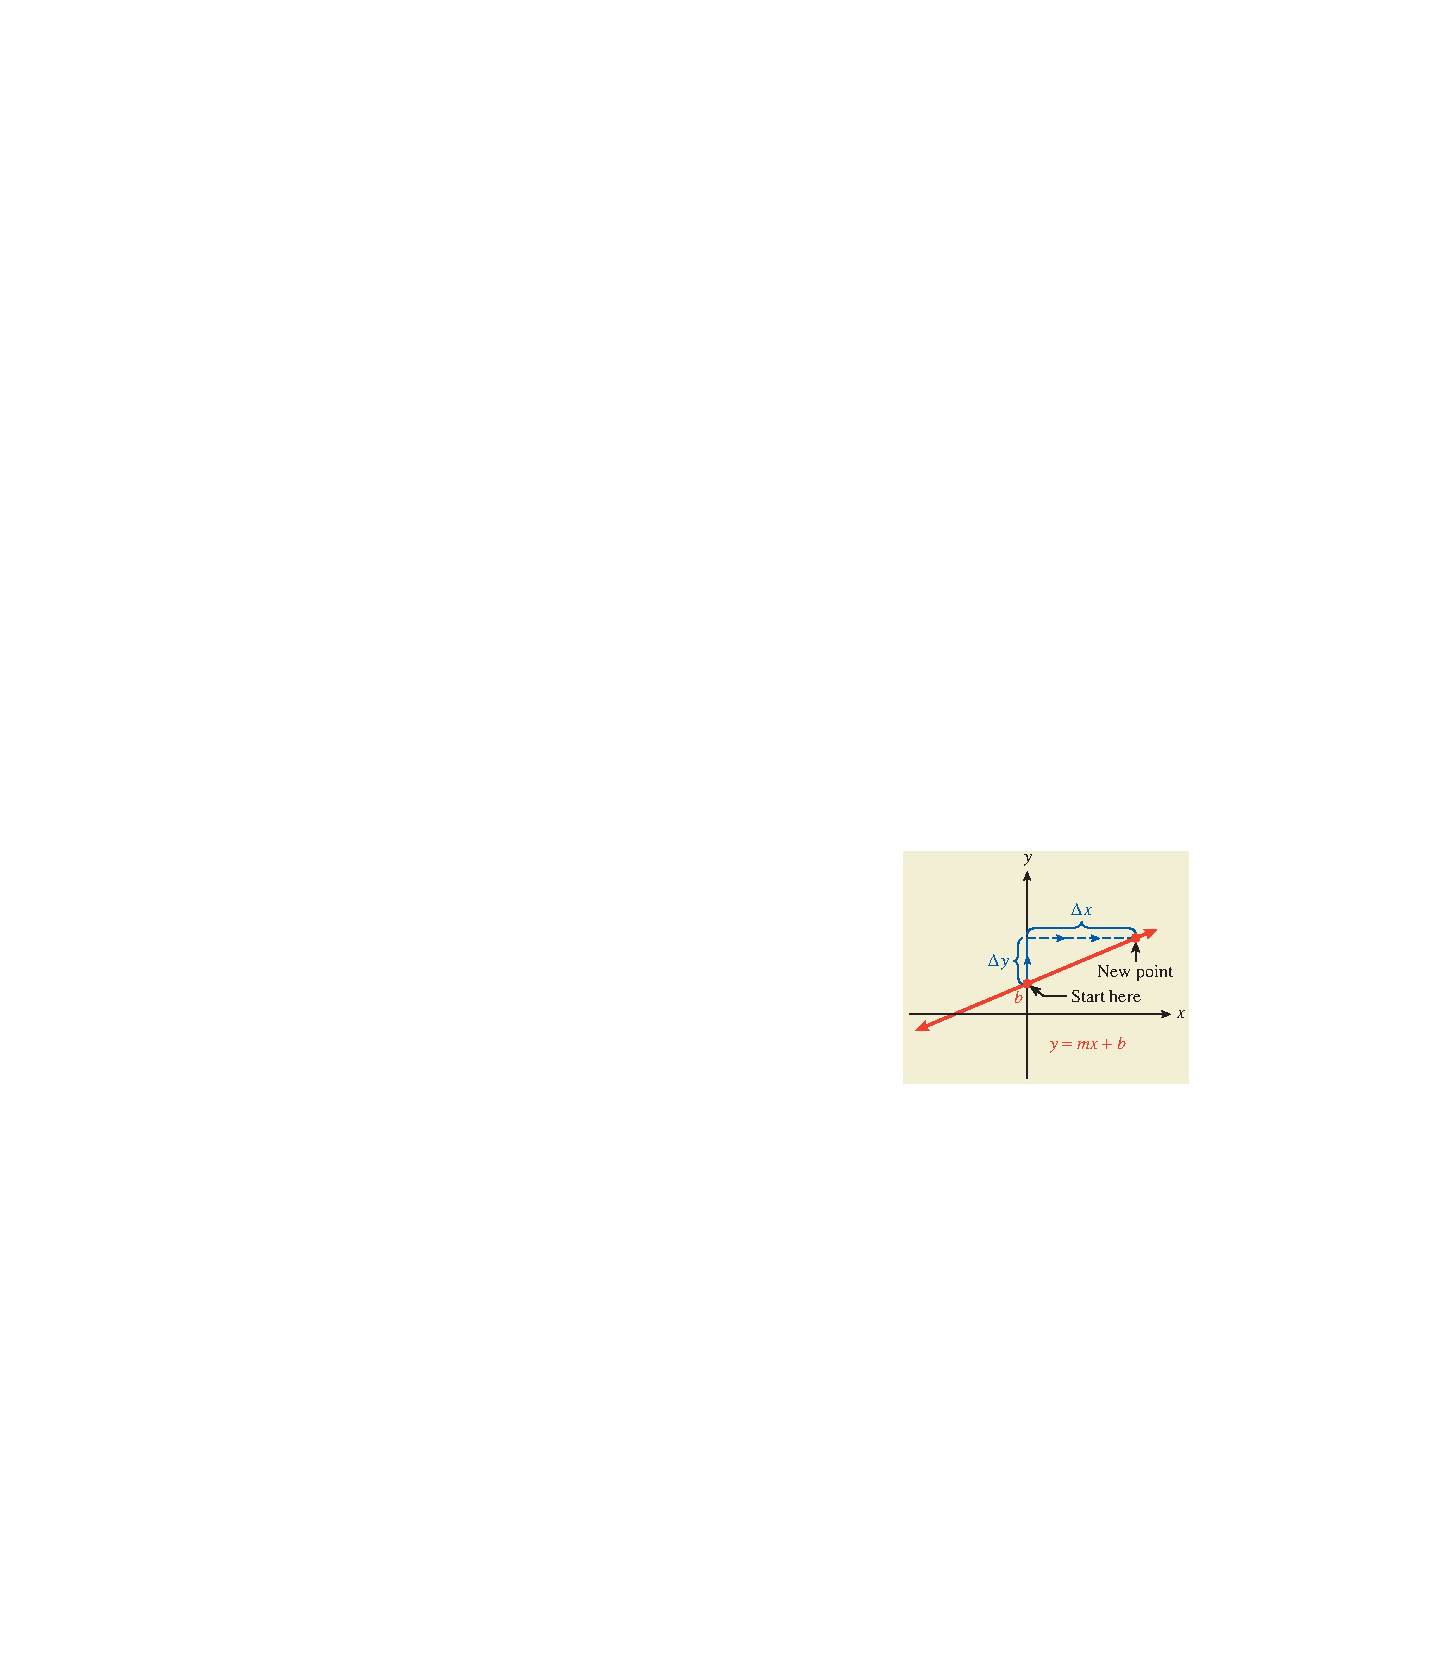
\includegraphics[width=\linewidth]{external/images/fig-slope-intercept0.pdf}
\end{sbspanel}%
\end{sidebyside}%
\end{assemblage}
\begin{inlineexercise}{Checkpoint}{Practice 2.}{exercise-linear-functions-c-f}%
%
\begin{enumerate}[label=\alph*.]
\item{}Write the equation \(2y + 3x + 4 = 0\) in slope-intercept form.%
\par
\(y=\)\fillintext{8}%
\item{}Use the slope-intercept method to graph the line.%
\end{enumerate}
%
\par
A graph for part (b):%
\begin{sidebyside}{1}{0}{0.7}{0}%
\begin{sbspanel}{0.3}%
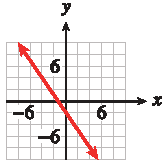
\includegraphics[width=\linewidth]{external/images/fig-in-ex-ans-1-5-2.pdf}
\end{sbspanel}%
\end{sidebyside}%
\par\smallskip%
\noindent\textbf{\blocktitlefont Answer}.\hypertarget{answer-linear-functions-c-f-c}{}\quad{}\(-2-{\frac{3}{2}}x\)%
\par\smallskip%
\noindent\textbf{\blocktitlefont Solution}.\hypertarget{solution-linear-functions-c-f-d}{}\quad{}%
\begin{enumerate}[label=\alph*.]
\item{}Solve the given equation for \(y\) to get: \(y=-2-\dfrac{3}{2}x\)%
\item{}A graph is shown below.%
\end{enumerate}
%
\end{inlineexercise}%
\begin{inlineexercise}{Checkpoint}{QuickCheck 2.}{exercise-linear-functions-c-g}%
What is the easiest way to find the slope of the line \(18x-42y=60\text{?}\)%
\par
\begin{itemize}[label=$\odot$,leftmargin=3em,]
\item{}Solve for \(y\) to get the slope-intercept form.%
\item{}Find the intercepts and use them to compute the slope.%
\item{}Graph the line and compute \(\dfrac{\Delta y}{\Delta x}\).%
\item{}Find values of \(x\) and \(y\) that make the equation true.%
\end{itemize}
%
\par\smallskip%
\noindent\textbf{\blocktitlefont Answer}.\hypertarget{answer-linear-functions-c-g-c}{}\quad{}\(\text{Choice 1}\)%
\end{inlineexercise}%
\end{subsectionptx}
%
%
\typeout{************************************************}
\typeout{Subsection  Finding a Linear Equation from a Graph}
\typeout{************************************************}
%
\begin{subsectionptx}{Subsection}{Finding a Linear Equation from a Graph}{}{Finding a Linear Equation from a Graph}{}{}{subsection-linear-functions-d}
We can also use the slope-intercept form to find the equation of a line from its graph. First, we note the value of the \(y\)-intercept from the graph, and then we calculate the slope using two convenient points.%
\begin{example}{Example}{}{example-example-lin-equation-from-graph}%
\begin{sidebyside}{2}{0.025}{0.025}{0.05}%
\begin{sbspanel}{0.6}%
Find an equation for the line shown at right.%
\end{sbspanel}%
\begin{sbspanel}{0.3}%
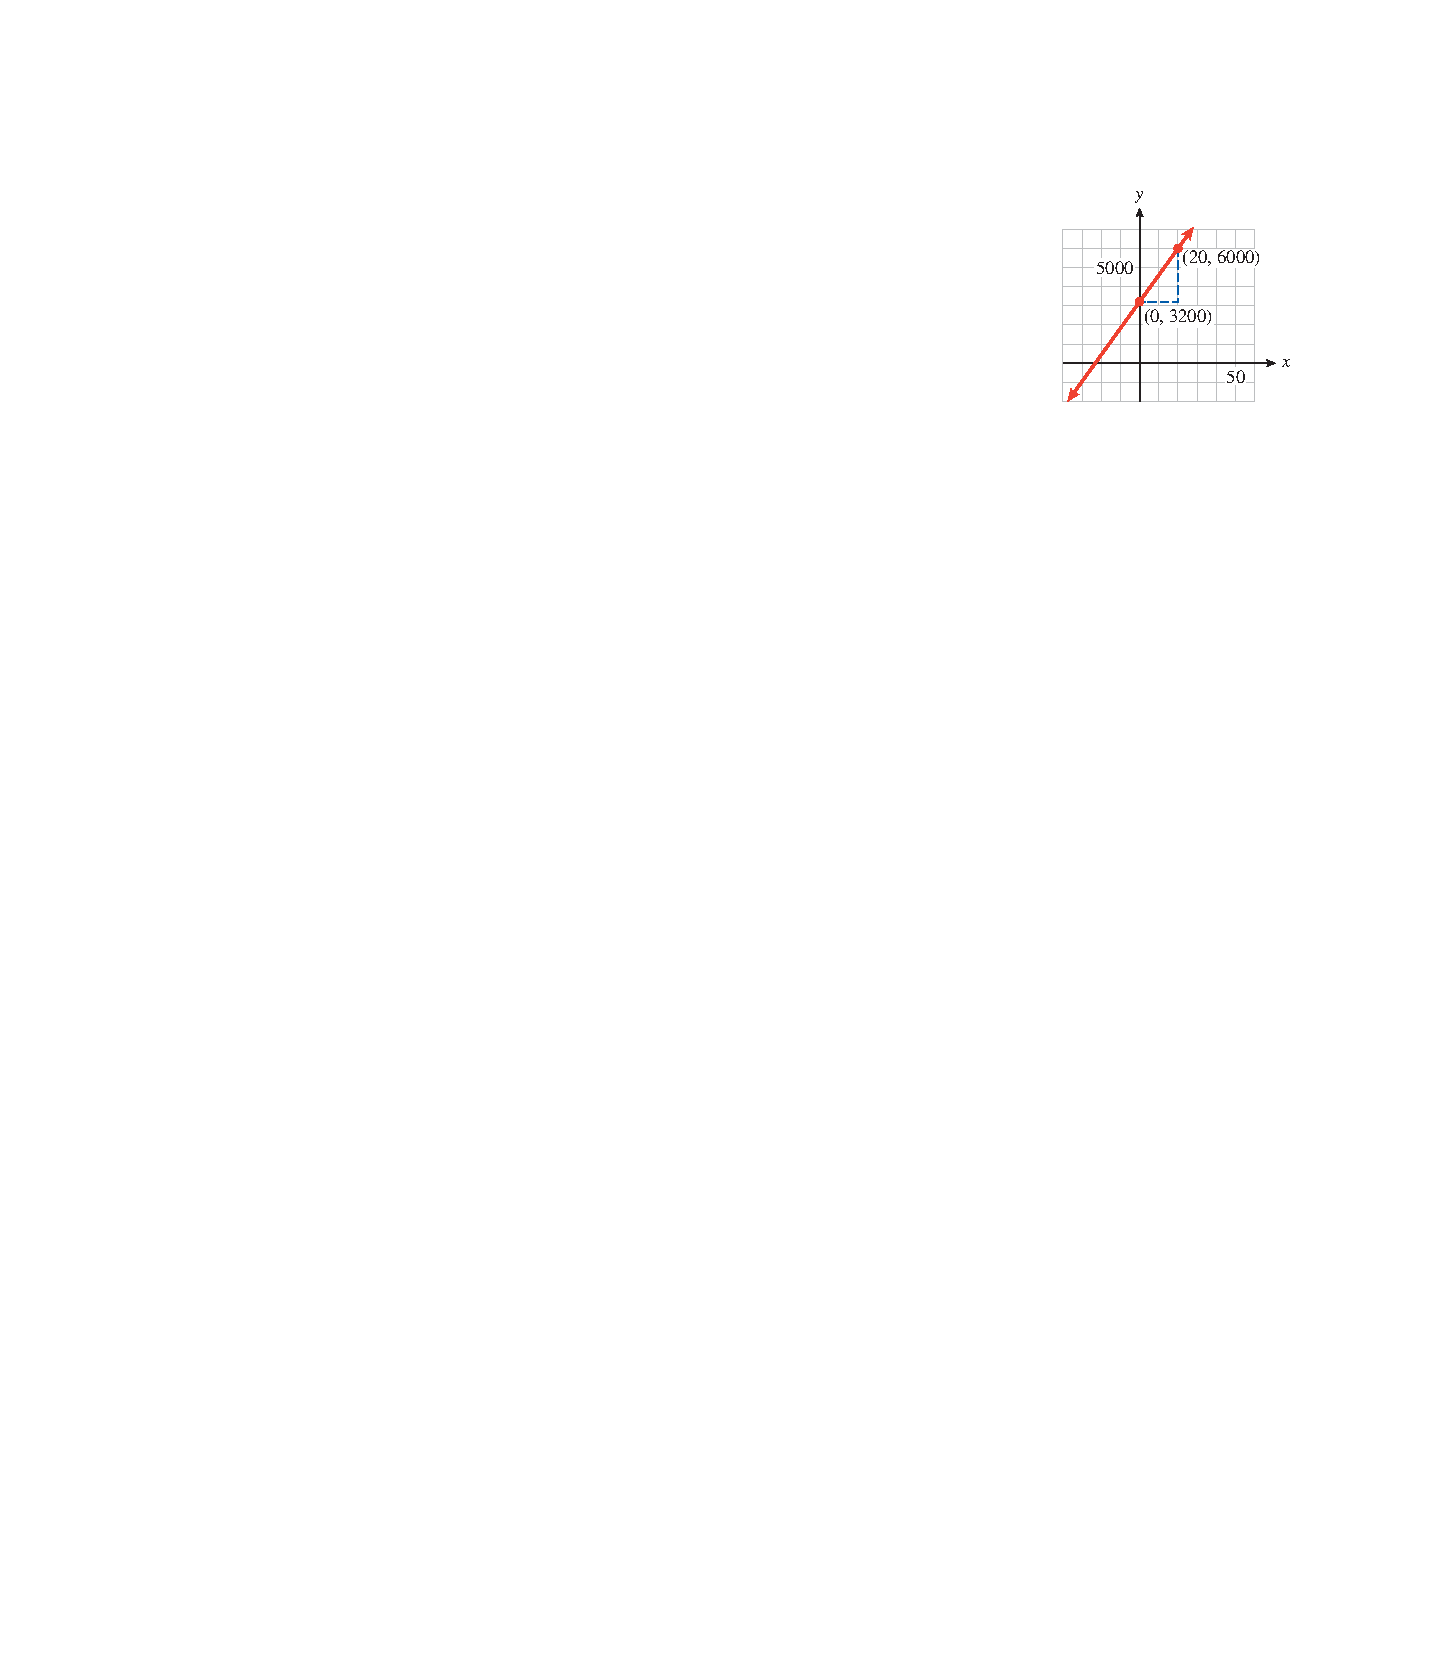
\includegraphics[width=\linewidth]{external/images/fig-lin-equation-from-graph.pdf}
\end{sbspanel}%
\end{sidebyside}%
\par\smallskip%
\noindent\textbf{\blocktitlefont Solution}.\hypertarget{solution-example-lin-equation-from-graph-b}{}\quad{}The line crosses the \(y\)-axis at the point \((0, 3200)\), so the \(y\)-intercept is \(3200\). To calculate the slope of the line, we locate another point, say \((20, 6000)\), and compute:%
\par
%
\begin{equation*}
\begin{aligned}[t]m \amp = \frac{\Delta y}{\Delta x}
= \frac{6000 - 3200}{20 - 0}\\
\amp =\frac{2800}{20}= 140
\end{aligned}
\end{equation*}
The slope-intercept form of the equation, with \(m = 140\) and \(b = 3200\), is%
\begin{equation*}
y = 3200 + 140x
\end{equation*}
%
\end{example}
\begin{inlineexercise}{Checkpoint}{Practice 3.}{exercise-linear-functions-d-d}%
\begin{sidebyside}{2}{0}{0.09}{0.01}%
\begin{sbspanel}{0.6}[center]%
Find an equation for the line shown at right.%
\end{sbspanel}%
\begin{sbspanel}{0.3}[center]%
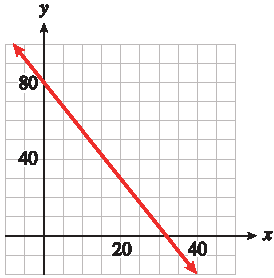
\includegraphics[width=\linewidth]{external/images/fig-lin-equation-from-graph2.pdf}
\end{sbspanel}%
\end{sidebyside}%
\par
\(b  =\)\fillintext{3}%
\par
\(m  =\)\fillintext{3}%
\par
\(y  =\)\fillintext{8}%
\par\smallskip%
\noindent\textbf{\blocktitlefont Answer 1}.\hypertarget{answer-linear-functions-d-d-c}{}\quad{}\(80\)%
\par\smallskip%
\noindent\textbf{\blocktitlefont Answer 2}.\hypertarget{answer-linear-functions-d-d-d}{}\quad{}\(-{\frac{5}{2}}\)%
\par\smallskip%
\noindent\textbf{\blocktitlefont Answer 3}.\hypertarget{answer-linear-functions-d-d-e}{}\quad{}\(\left(-{\frac{5}{2}}\right)x+80\)%
\par\smallskip%
\noindent\textbf{\blocktitlefont Solution}.\hypertarget{solution-linear-functions-d-d-f}{}\quad{}We can read the \(y\)-intercept from the graph, so \(b = 80\text{.}\) Another point is \((20,30)\text{,}\) and from those two points we can compute the slope  \(m =\dfrac{-5}{2}\text{.}\) So the slope-intercept form for the equation of the line is  \(y = 80 - \dfrac{5}{2}x\)%
\end{inlineexercise}%
\begin{inlineexercise}{Checkpoint}{Pause and Reflect.}{exercise-linear-functions-d-e}%
How can you find the equation of a line from its graph?%
\end{inlineexercise}%
\end{subsectionptx}
%
%
\typeout{************************************************}
\typeout{Subsection  Point-Slope Form}
\typeout{************************************************}
%
\begin{subsectionptx}{Subsection}{Point-Slope Form}{}{Point-Slope Form}{}{}{subsection-linear-functions-e}
We can find the equation for a line if we know its slope and \(y\)-intercept. What if we do not know the \(y\)-intercept, but instead know some other point on the line? There is only one line that passes through a given point and has a given slope, so we should be able to find its equation.%
\par
For example, we can graph the line of slope \(\dfrac{-3}{4}\) that passes through the point \((1, -4)\). We first plot the given point, \((1, -4)\), as shown in the figure below.%
\begin{sidebyside}{2}{0.0125}{0.0125}{0.025}%
\begin{sbspanel}{0.6}%
Then we use the slope to find another point on the line. The slope is%
\begin{equation*}
m =\frac{-3}{4}= \frac{\Delta y}{\Delta x}
\end{equation*}
so we move down \(3\) units and then \(4\) units to the right, starting from \((1, -4)\). This brings us to the point \((5, -7)\). We can then draw the line through these two points.%
\end{sbspanel}%
\begin{sbspanel}{0.35}%
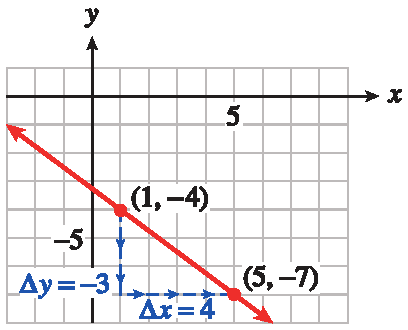
\includegraphics[width=\linewidth]{external/images/fig-point-slope.pdf}
\end{sbspanel}%
\end{sidebyside}%
\par
We can also find an equation for the line, as shown in \hyperref[example-example-point-slope]{Example~{\xreffont\ref{example-example-point-slope}}}.%
\begin{example}{Example}{}{example-example-point-slope}%
Find an equation for the line that passes through \((1, -4)\) and has slope \(\dfrac{-3}{4}\).%
\par\smallskip%
\noindent\textbf{\blocktitlefont Solution}.\hypertarget{solution-example-point-slope-b}{}\quad{}We will use the formula for slope,%
\begin{equation*}
m = \frac{y_2 - y_1}{x_2 - x_1}
\end{equation*}
We substitute \(\dfrac{-3}{4}\) for the slope, \(m\), and \((1, -4)\) for \((x_1, y_1)\). For the second point, \((x_2, y_2)\), we use the variable point \((x, y)\). Substituting these values into the slope formula gives us%
\begin{equation*}
\frac{-3}{4}= \frac{y - (-4)}{x - 1}=\frac{y + 4}{x - 1}
\end{equation*}
To solve for \(y\) we first multiply both sides by \(x - 1\).%
\begin{equation*}
\begin{aligned}[t]
\alert{(x-1)}\frac{-3}{4}\amp
=\frac{y +4}{x - 1}\alert{(x-1)} \amp\amp\\
\frac{-3}{4}(x-1)\amp=y+4  \amp\amp\blert{\text{Apply the distributive law.}}\\
\frac{-3}{4}x+\frac{3}{4}\amp=y+4   \amp\amp \blert{\text{Subtract 4 from both sides.}}\\
\frac{-3}{4}x-\frac{13}{4}\amp=y \amp\amp \blert{\frac{3}{4}-4=\frac{3}{4}-\frac{16}{4}=\frac{-13}{4}}\\
\end{aligned}
\end{equation*}
The equation of the line is  \(y=\dfrac{-13}{4}-\dfrac{3}{4}x\)%
\end{example}
\begin{inlineexercise}{Checkpoint}{QuickCheck 3.}{exercise-linear-functions-e-g}%
What will be wrong with your answer if you accidentally compute the slope as \(m=\dfrac{y_2-y_1}{x_1-x_2}\text{?}\)%
\par
\begin{itemize}[label=$\odot$,leftmargin=3em,]
\item{}A) The number will be too big.%
\item{}B) The line will be decreasing.%
\item{}C) That is the slope of the perpendicular line.%
\item{}D) It will have the wrong sign.%
\end{itemize}
%
\par\smallskip%
\noindent\textbf{\blocktitlefont Answer}.\hypertarget{answer-linear-functions-e-g-c}{}\quad{}\(\text{D) It ... wrong sign.}\)%
\par\smallskip%
\noindent\textbf{\blocktitlefont Solution}.\hypertarget{solution-linear-functions-e-g-d}{}\quad{}It will have the wrong sign.%
\end{inlineexercise}%
When we use the slope formula in this way to find the equation of a line, we substitute a variable point \((x, y)\) for the second point. This version of the formula,%
\begin{equation*}
m = \frac{y - y_1}{x - x_1}
\end{equation*}
is called the \terminology{point-slope form}\index{point-slope form} for a linear equation. It is sometimes stated in another form obtained by clearing the fraction to get%
\begin{equation*}
\begin{aligned}[t]
\alert{(x-x_1)}m\amp
=\frac{y -y_1}{x - x_1}\alert{(x-x_1)} \amp\amp
\blert{\text{Multiply both sides by }(x - x_1)}\\
(x - x_1) m\amp=y-y_1  \amp\amp\blert{\text{Clear fractions and solve for }y\text{.}}\\
y\amp=y_1+m(x-x_1)
\end{aligned}
\end{equation*}
%
\begin{assemblage}{Assemblage}{Point-Slope Form.}{assemblage-linear-functions-e-i}%
The equation of the line that passes through the point \((x_1, y_1)\) and has slope \(m\) is%
\begin{equation*}
y= y_1 + m(x- x_1)
\end{equation*}
%
\end{assemblage}
\begin{inlineexercise}{Checkpoint}{Practice 4.}{exercise-linear-functions-e-j}%
Use the point-slope form to find the equation of the line that passes through the point \((-3, 5)\) and has slope \(-1.4\text{.}\)%
\par
%
\begin{equation*}
\begin{aligned}[t]
y \amp= y_1 + m(x - x_1) \amp\amp\blert{{\small\text{Substitute }-1.4\text{ for }m\text{ and }(-3, 5)\text{ for }(x_1, y_1).}}\\
\amp\amp\amp\blert{{\small\text{Simplify: Apply the distributive law.}}}
\end{aligned}
\end{equation*}
%
\par
\(y=\)\fillintext{12}%
\par\smallskip%
\noindent\textbf{\blocktitlefont Answer}.\hypertarget{answer-linear-functions-e-j-c}{}\quad{}\(0.8-1.4x\)%
\par\smallskip%
\noindent\textbf{\blocktitlefont Solution}.\hypertarget{solution-linear-functions-e-j-d}{}\quad{}\(y = {0.8-1.4x}\)%
\end{inlineexercise}%
The point-slope form is useful for modeling linear functions when we don't know the initial value but do know some other point on the line.%
\begin{example}{Example}{}{example-example-income-tax}%
Under a proposed graduated income tax system, single taxpayers would owe \textdollar{}1500 plus 20\% of the amount of their income over \textdollar{}13,000. (For example, if your income is \textdollar{}18,000, you would pay \textdollar{}1500 plus 20\% of \textdollar{}5000.)%
\begin{enumerate}[label=\alph*]
\item{}Complete the table of values for the tax, \(T\), on various incomes, \(I\).%
\begin{sidebyside}{1}{0}{0}{0}%
\begin{sbspanel}{1}%
\resizebox{\ifdim\width > \linewidth\linewidth\else\width\fi}{!}{%
{\centering%
{\tabularfont%
\begin{tabular}{AcAcAcAcA}\hrulethick
\(I\)&\(15,000\)&\(20,000\)&\(22,000\)\tabularnewline\hrulethin
\(T\)&&&\tabularnewline\hrulethin
\end{tabular}
}%
\par}
}%
\end{sbspanel}%
\end{sidebyside}%
\item{}Write a linear equation in point-slope form for the tax, \(T\), on an income \(I\).%
\item{}Write the equation in slope-intercept form.%
\end{enumerate}
%
\par\smallskip%
\noindent\textbf{\blocktitlefont Solution}.\hypertarget{solution-example-income-tax-b}{}\quad{}%
\begin{enumerate}[label=\alph*]
\item{}On an income of \textdollar{}15,000, the amount of income over \textdollar{}13,000 is \textdollar{}15,000 - \textdollar{}13,000 = \textdollar{}2000, so you would pay \textdollar{}1500 plus 20\% of \textdollar{}2000, or%
\begin{equation*}
T = 1500 + 0.20(2000) = 1900
\end{equation*}
You can compute the other function values in the same way.%
\begin{sidebyside}{1}{0}{0}{0}%
\begin{sbspanel}{1}%
\resizebox{\ifdim\width > \linewidth\linewidth\else\width\fi}{!}{%
{\centering%
{\tabularfont%
\begin{tabular}{AcAcAcAcA}\hrulethick
\(I\)&\(15,000\)&\(20,000\)&\(22,000\)\tabularnewline\hrulethin
\(T\)&\(1900\)&\(2900\)&\(3300\)\tabularnewline\hrulethin
\end{tabular}
}%
\par}
}%
\end{sbspanel}%
\end{sidebyside}%
\item{}On an income of \(I\), the amount of income over \textdollar{}13,000 is \(I - \$13,000\), so you would pay \textdollar{}1500 plus 20\% of \(I - 13,000\), or%
\begin{equation*}
T = 1500 + 0.20 (I - 13,000)
\end{equation*}
%
\item{}Simplify the right side of the equation to get%
\begin{equation*}
\begin{aligned}[t]
T \amp = 1500 + 0.20I - 2600\\
T \amp = -1100 + 0.20I
\end{aligned}
\end{equation*}
%
\end{enumerate}
%
\end{example}
\begin{inlineexercise}{Checkpoint}{Practice 5.}{exercise-linear-functions-e-m}%
A healthy weight for a young woman of average height, 64 inches, is 120 pounds. To calculate a healthy weight for a woman taller than 64 inches, add 5 pounds for each inch of height over 64.%
\begin{enumerate}[label=\alph*.]
\item{}Write a linear equation in point-slope form for the healthy weight, \(W\text{,}\) for a woman of height, \(H\text{,}\) in inches.%
\par
\(W=\)\fillintext{12}%
\item{}Write the equation in slope-intercept form.%
\par
\(W=\)\fillintext{8}%
\end{enumerate}
%
\par\smallskip%
\noindent\textbf{\blocktitlefont Answer 1}.\hypertarget{answer-linear-functions-e-m-c}{}\quad{}\(120+5\!\left(H-64\right)\)%
\par\smallskip%
\noindent\textbf{\blocktitlefont Answer 2}.\hypertarget{answer-linear-functions-e-m-d}{}\quad{}\(-200+5H\)%
\par\smallskip%
\noindent\textbf{\blocktitlefont Solution}.\hypertarget{solution-linear-functions-e-m-e}{}\quad{}%
\begin{enumerate}[label=\alph*.]
\item{}\(\displaystyle W = 120 + 5(H - 64)\)%
\item{}\(\displaystyle W = {-200+5H}\)%
\end{enumerate}
%
\end{inlineexercise}%
\begin{inlineexercise}{Checkpoint}{QuickCheck 4.}{exercise-linear-functions-e-n}%
What do you get when you substitute the point \((0,b)\) into the point-slope formula?%
\par
\begin{itemize}[label=$\odot$,leftmargin=3em,]
\item{}\(\displaystyle x=0\)%
\item{}\(\displaystyle y=mx+b\)%
\item{}\(\displaystyle y=b\)%
\item{}\(\displaystyle ax+by=0\)%
\end{itemize}
%
\par\smallskip%
\noindent\textbf{\blocktitlefont Answer}.\hypertarget{answer-linear-functions-e-n-c}{}\quad{}\(\text{Choice 2}\)%
\par\smallskip%
\noindent\textbf{\blocktitlefont Solution}.\hypertarget{solution-linear-functions-e-n-d}{}\quad{}\(y=mx+b\)%
\end{inlineexercise}%
\begin{inlineexercise}{Checkpoint}{Pause and Reflect.}{exercise-linear-functions-e-o}%
Explain the difference between the slope-intercept form and the point-slope form for a linear equation.%
\end{inlineexercise}%
\end{subsectionptx}
%
%
\typeout{************************************************}
\typeout{Subsection  Section Summary}
\typeout{************************************************}
%
\begin{subsectionptx}{Subsection}{Section Summary}{}{Section Summary}{}{}{subsection-summary-1-5}
%
%
\typeout{************************************************}
\typeout{Subsubsection  Vocabulary}
\typeout{************************************************}
%
\begin{subsubsectionptx}{Subsubsection}{Vocabulary}{}{Vocabulary}{}{}{subsubsection-summary-1-5-b}
Look up the definitions of new terms in the Glossary.%
\begin{multicols}{2}
\begin{itemize}[label=\textbullet]
\item{}Slope-intercept form%
\item{}Point-slope form%
\item{}Parameter%
\end{itemize}
\end{multicols}
%
\end{subsubsectionptx}
%
%
\typeout{************************************************}
\typeout{Subsubsection  CONCEPTS}
\typeout{************************************************}
%
\begin{subsubsectionptx}{Subsubsection}{CONCEPTS}{}{CONCEPTS}{}{}{subsubsection-summary-1-5-c}
%
\begin{enumerate}[label=\arabic*]
\item{}Linear functions form a two-parameter family, \(f (x) = b + mx\).%
\item{}The initial value of a linear function and the \(y\)-intercept of its graph are given by \(b\). The rate of change of the function and the slope of its graph are given by \(m\).%
\item{}The slope-intercept form, \(y = b + mx\), is useful when we know the initial value and the rate of change.%
\item{}The point-slope form, \(y = y_1 + m(x - x_1)\), is useful when we know the rate of change and one point on the line.%
\end{enumerate}
%
\end{subsubsectionptx}
%
%
\typeout{************************************************}
\typeout{Subsubsection  STUDY QUESTIONS}
\typeout{************************************************}
%
\begin{subsubsectionptx}{Subsubsection}{STUDY QUESTIONS}{}{STUDY QUESTIONS}{}{}{subsubsection-summary-1-5-d}
%
\begin{enumerate}[label=\arabic*]
\item{}How can you put a linear equation into slope-intercept form?%
\item{}What do the coefficients in the slope-intercept form tell you about the line?%
\item{}Explain how to graph a line using the slope-intercept method.%
\item{}Explain how to find an equation for a line from its graph.%
\item{}Explain how to use the point-slope form for a linear equation.%
\item{}Francine says that the slope of the line \(y = 4x - 6\) is \(4x\). Is she correct? Explain your answer%
\item{}Delbert says that the slope of the line \(3x - 4y = 8\) is \(3\). Is he correct? Explain your answer.%
\end{enumerate}
%
\end{subsubsectionptx}
%
%
\typeout{************************************************}
\typeout{Subsubsection  SKILLS}
\typeout{************************************************}
%
\begin{subsubsectionptx}{Subsubsection}{SKILLS}{}{SKILLS}{}{}{subsubsection-summary-1-5-e}
Practice each skill in the Homework problems listed.%
\begin{enumerate}[label=\arabic*]
\item{}Write a linear equation in slope-intercept form: \#1\textendash{}14%
\item{}Identify the slope and \(y\)-intercept: \#1\textendash{}10%
\item{}Graph a line by the slope-intercept method: \#11\textendash{}14%
\item{}Find a linear equation from its graph: \#21\textendash{}26, 29\textendash{}32, 53\textendash{}56%
\item{}Interpret the slope and \(y\)-intercept: \#21\textendash{}28, 63 and 64%
\item{}Find a linear equation from one point and the slope: \#33\textendash{}50%
\end{enumerate}
%
\end{subsubsectionptx}
\end{subsectionptx}
%
%
\typeout{************************************************}
\typeout{Exercises  Homework 1.5}
\typeout{************************************************}
%
\begin{exercises-subsection}{Exercises}{Homework 1.5}{}{Homework 1.5}{}{}{exercises-section-1-5-exercises}
\par\medskip\noindent%
\textbf{Exercise Group.}\space\space%
In Problems 1\textendash{}10,%
\begin{enumerate}[label=\alph*]
\item{}Write each equation in slope-intercept form.%
\item{}State the slope and \(y\)-intercept of the line.%
\end{enumerate}
%
\begin{exercisegroupcol}{2}
\begin{divisionexerciseegcol}{1}{}{}{exercise-section-1-5-exercises-b-b}%
\(3x + 2y = 1\)%
\end{divisionexerciseegcol}%
\begin{divisionexerciseegcol}{2}{}{}{exercise-section-1-5-exercises-b-c}%
\(5x - 4y = 0\)%
\end{divisionexerciseegcol}%
\begin{divisionexerciseegcol}{3}{}{}{exercise-section-1-5-exercises-b-d}%
\(\dfrac{1}{4}x + \dfrac{3}{2}y = \dfrac{1}{6}\)%
\end{divisionexerciseegcol}%
\begin{divisionexerciseegcol}{4}{}{}{exercise-section-1-5-exercises-b-e}%
\(\dfrac{7}{6}x - \dfrac{2}{9}y = 3\)%
\end{divisionexerciseegcol}%
\begin{divisionexerciseegcol}{5}{}{}{exercise-section-1-5-exercises-b-f}%
\(4.2x - 0.3y = 6.6\)%
\end{divisionexerciseegcol}%
\begin{divisionexerciseegcol}{6}{}{}{exercise-section-1-5-exercises-b-g}%
\(0.8x + 0.004y = 0.24\)%
\end{divisionexerciseegcol}%
\begin{divisionexerciseegcol}{7}{}{}{exercise-section-1-5-exercises-b-h}%
\(y + 29 = 0\)%
\end{divisionexerciseegcol}%
\begin{divisionexerciseegcol}{8}{}{}{exercise-section-1-5-exercises-b-i}%
\(y - 37 = 0\)%
\end{divisionexerciseegcol}%
\begin{divisionexerciseegcol}{9}{}{}{exercise-section-1-5-exercises-b-j}%
\(250x + 150y = 2450\)%
\end{divisionexerciseegcol}%
\begin{divisionexerciseegcol}{10}{}{}{exercise-section-1-5-exercises-b-k}%
\(80x - 360y = 6120\)%
\end{divisionexerciseegcol}%
\end{exercisegroupcol}
\par\medskip\noindent
\par\medskip\noindent%
\textbf{Exercise Group.}\space\space%
In Problems 11\textendash{}14,%
\begin{enumerate}[label=\alph*]
\item{}Sketch by hand the graph of the line with the given slope and \(y\)-intercept.%
\item{}Write an equation for the line.%
\item{}Find the \(x\)-intercept of the line.%
\end{enumerate}
%
\begin{exercisegroupcol}{2}
\begin{divisionexerciseegcol}{11}{}{}{exercise-section-1-5-exercises-c-b}%
\(m = 3\) and \(b = -2\)%
\end{divisionexerciseegcol}%
\begin{divisionexerciseegcol}{12}{}{}{exercise-section-1-5-exercises-c-c}%
\(m = -4\) and \(b = 1\)%
\end{divisionexerciseegcol}%
\begin{divisionexerciseegcol}{13}{}{}{exercise-section-1-5-exercises-c-d}%
\(m =-\dfrac{5}{3} \) and \(b = -6\)%
\end{divisionexerciseegcol}%
\begin{divisionexerciseegcol}{14}{}{}{exercise-section-1-5-exercises-c-e}%
\(m = \dfrac{3}{4}\) and \(b = -2\)%
\end{divisionexerciseegcol}%
\end{exercisegroupcol}
\par\medskip\noindent
\begin{divisionexercise}{15}{}{}{exercise-section-1-5-exercises-d}%
The point \((2, -1)\) lies on the graph of \(f (x) = -3x + b\). Find \(b\).%
\end{divisionexercise}%
\begin{divisionexercise}{16}{}{}{exercise-section-1-5-exercises-e}%
The point \((-3, -8)\) lies on the graph of \(f (x) =\dfrac{2}{3} x + b\). Find \(b\).%
\end{divisionexercise}%
\begin{divisionexercise}{17}{}{}{exercise-section-1-5-exercises-f}%
The point \((8, -5)\) lies on the graph of \(f(x) = mx - 3\). Find \(m\).%
\end{divisionexercise}%
\begin{divisionexercise}{18}{}{}{exercise-section-1-5-exercises-g}%
The point \((-5, -6)\) lies on the graph of \(f(x) = mx +2\). Find \(m\).%
\end{divisionexercise}%
\begin{divisionexercise}{19}{}{}{exercise-section-1-5-exercises-h}%
Find the slope and intercepts of the line \(Ax + By = C\)%
\end{divisionexercise}%
\begin{divisionexercise}{20}{}{}{exercise-section-1-5-exercises-i}%
Find the slope and intercepts of the line \(\dfrac{x}{a}+\dfrac{y}{b}=1 \)%
\end{divisionexercise}%
\par\medskip\noindent%
\textbf{Exercise Group.}\space\space%
In Problems 21\textendash{}26,%
\begin{enumerate}[label=\alph*]
\item{}Find a formula for the function whose graph is shown.%
\item{}Say what the slope and the vertical intercept tell us about the problem.%
\end{enumerate}
%
\par
%
\begin{exercisegroupcol}{2}
\begin{divisionexerciseegcol}{21}{}{}{exercise-section-1-5-exercises-j-b}%
The graph shows the altitude, \(a\) (in feet), of a skier \(t\) minutes after getting on a ski lift.%
\begin{sidebyside}{1}{0.15}{0.15}{0}%
\begin{sbspanel}{0.7}%
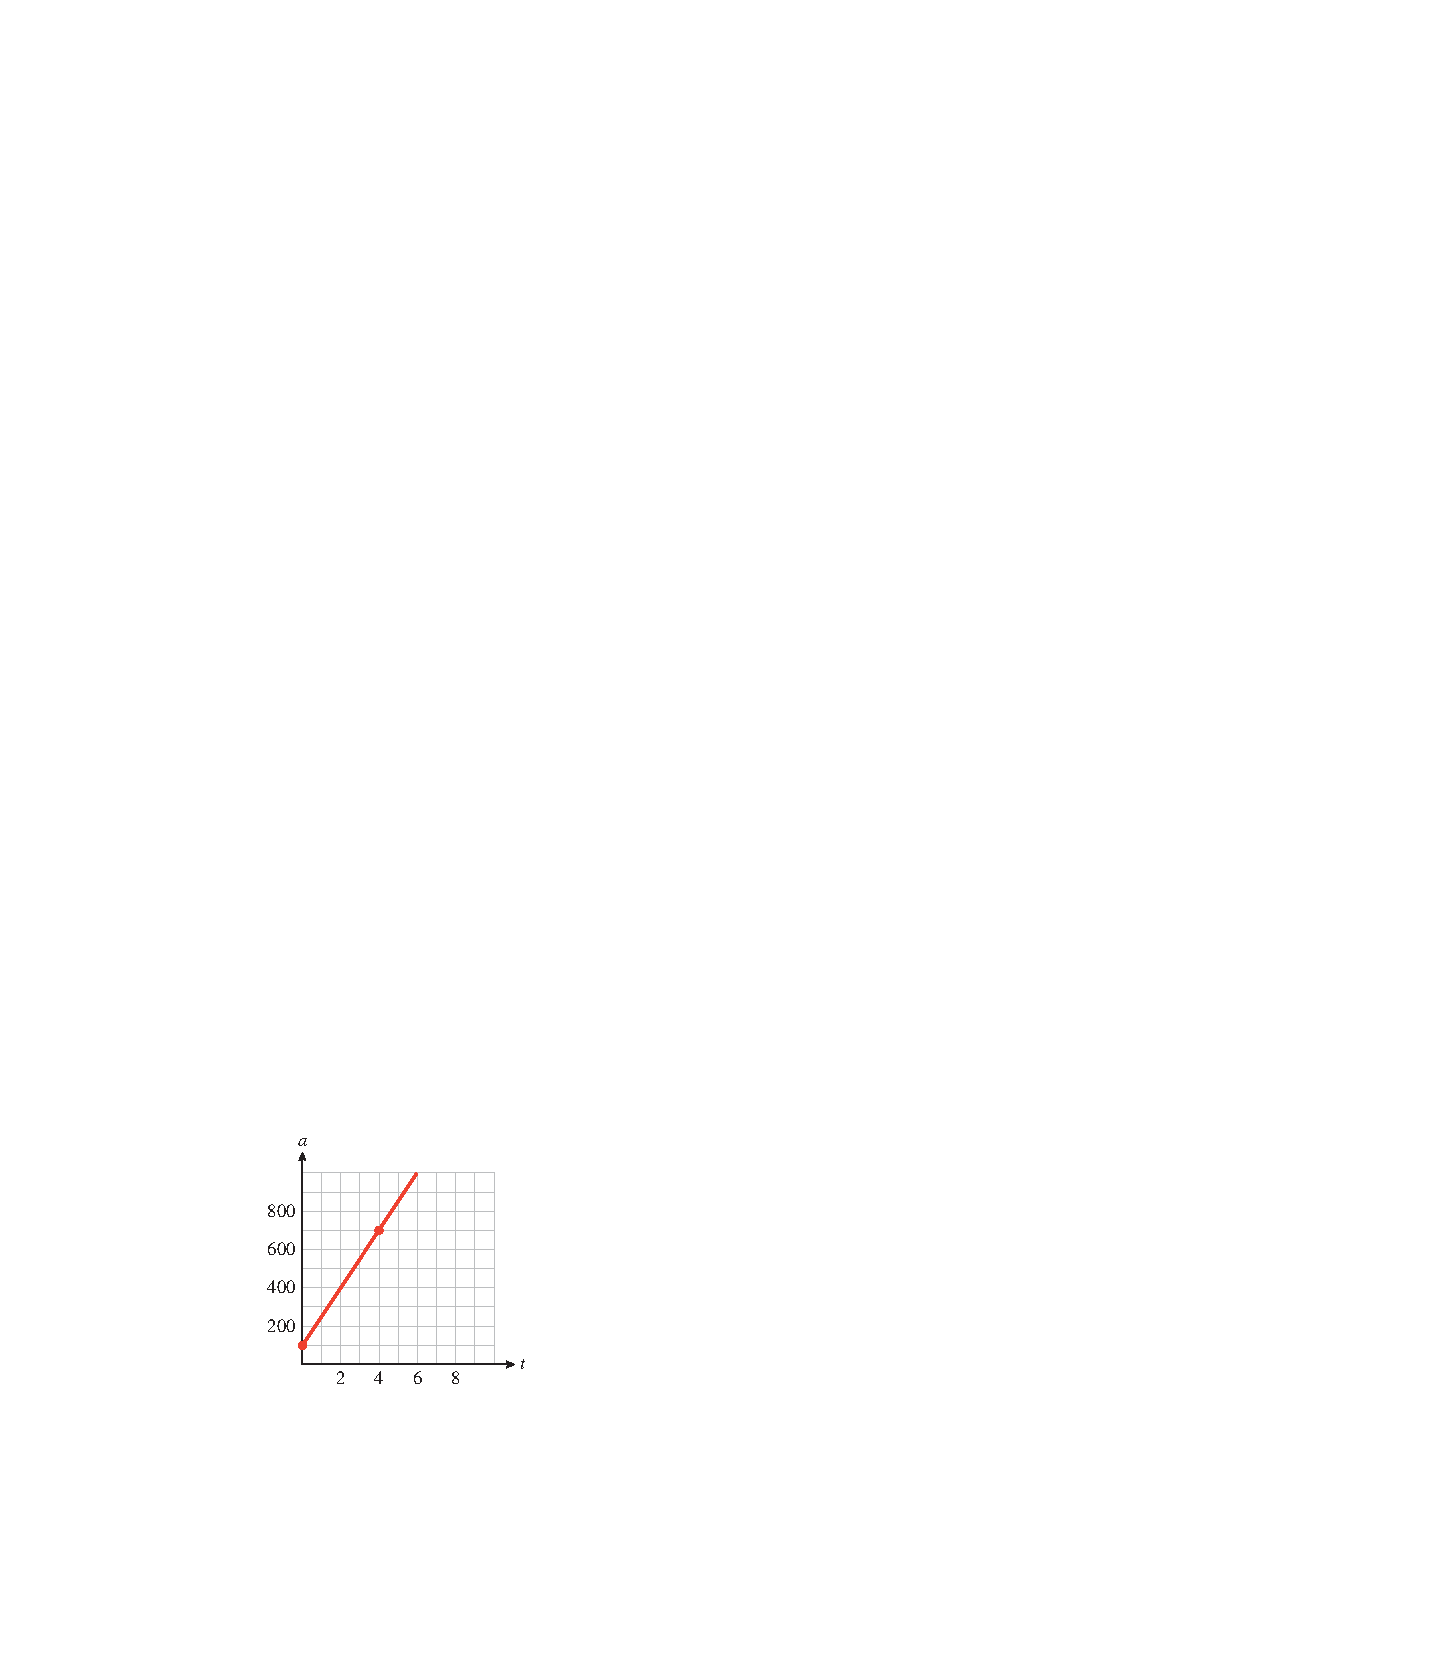
\includegraphics[width=\linewidth]{external/images/fig-ex-1-5-21.pdf}
\end{sbspanel}%
\end{sidebyside}%
\end{divisionexerciseegcol}%
\begin{divisionexerciseegcol}{22}{}{}{exercise-section-1-5-exercises-j-c}%
The graph shows the distance, \(d\) (in meters), traveled by a train \(t\) seconds after it passes an observer.%
\begin{sidebyside}{1}{0.15}{0.15}{0}%
\begin{sbspanel}{0.7}%
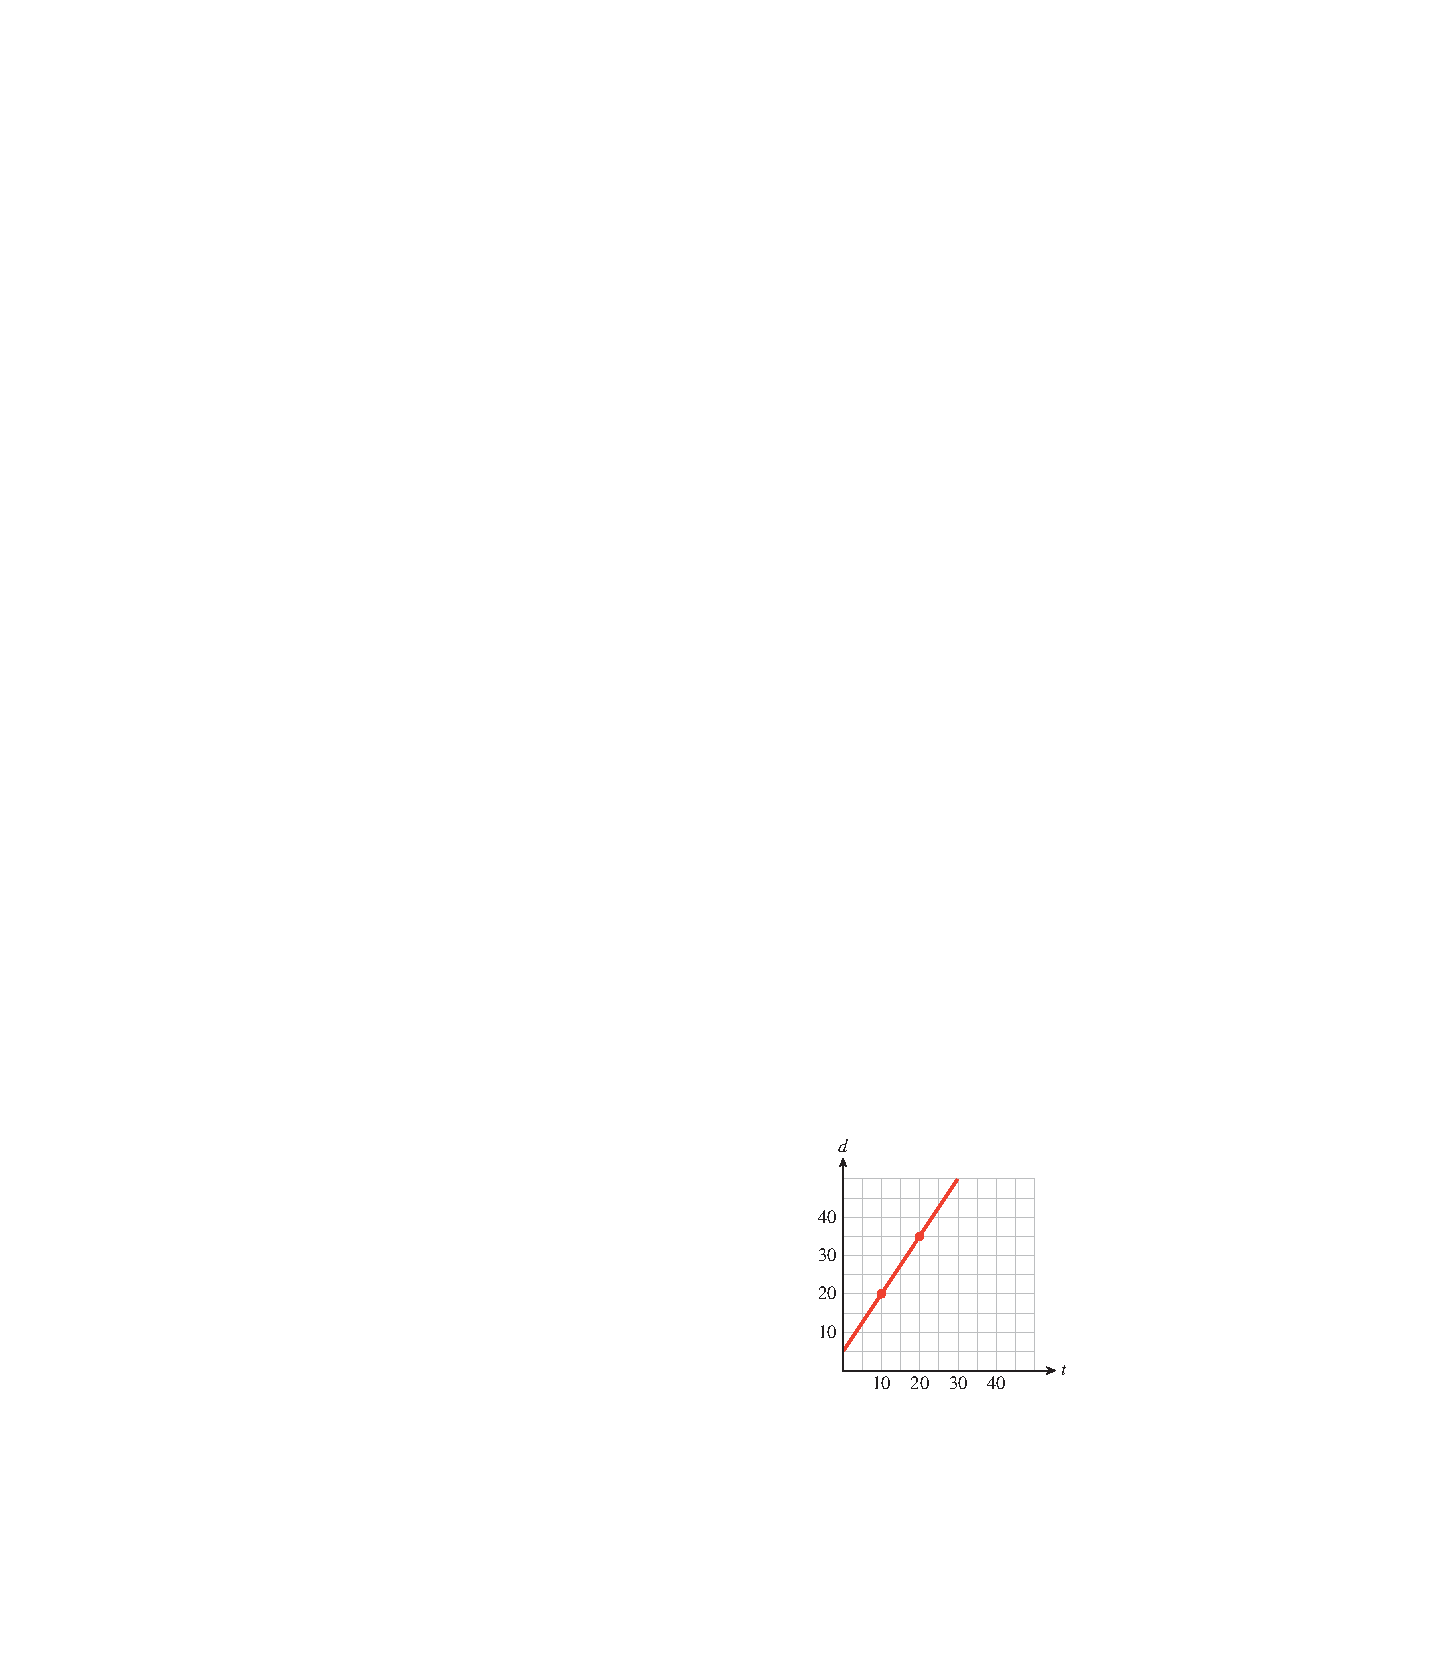
\includegraphics[width=\linewidth]{external/images/fig-ex-1-5-22.pdf}
\end{sbspanel}%
\end{sidebyside}%
\end{divisionexerciseegcol}%
\begin{divisionexerciseegcol}{23}{}{}{exercise-section-1-5-exercises-j-d}%
The graph shows the amount of garbage, \(G\) (in tons), that has been deposited at a dump site \(t\) years after new regulations go into effect.%
\begin{sidebyside}{1}{0.15}{0.15}{0}%
\begin{sbspanel}{0.7}%
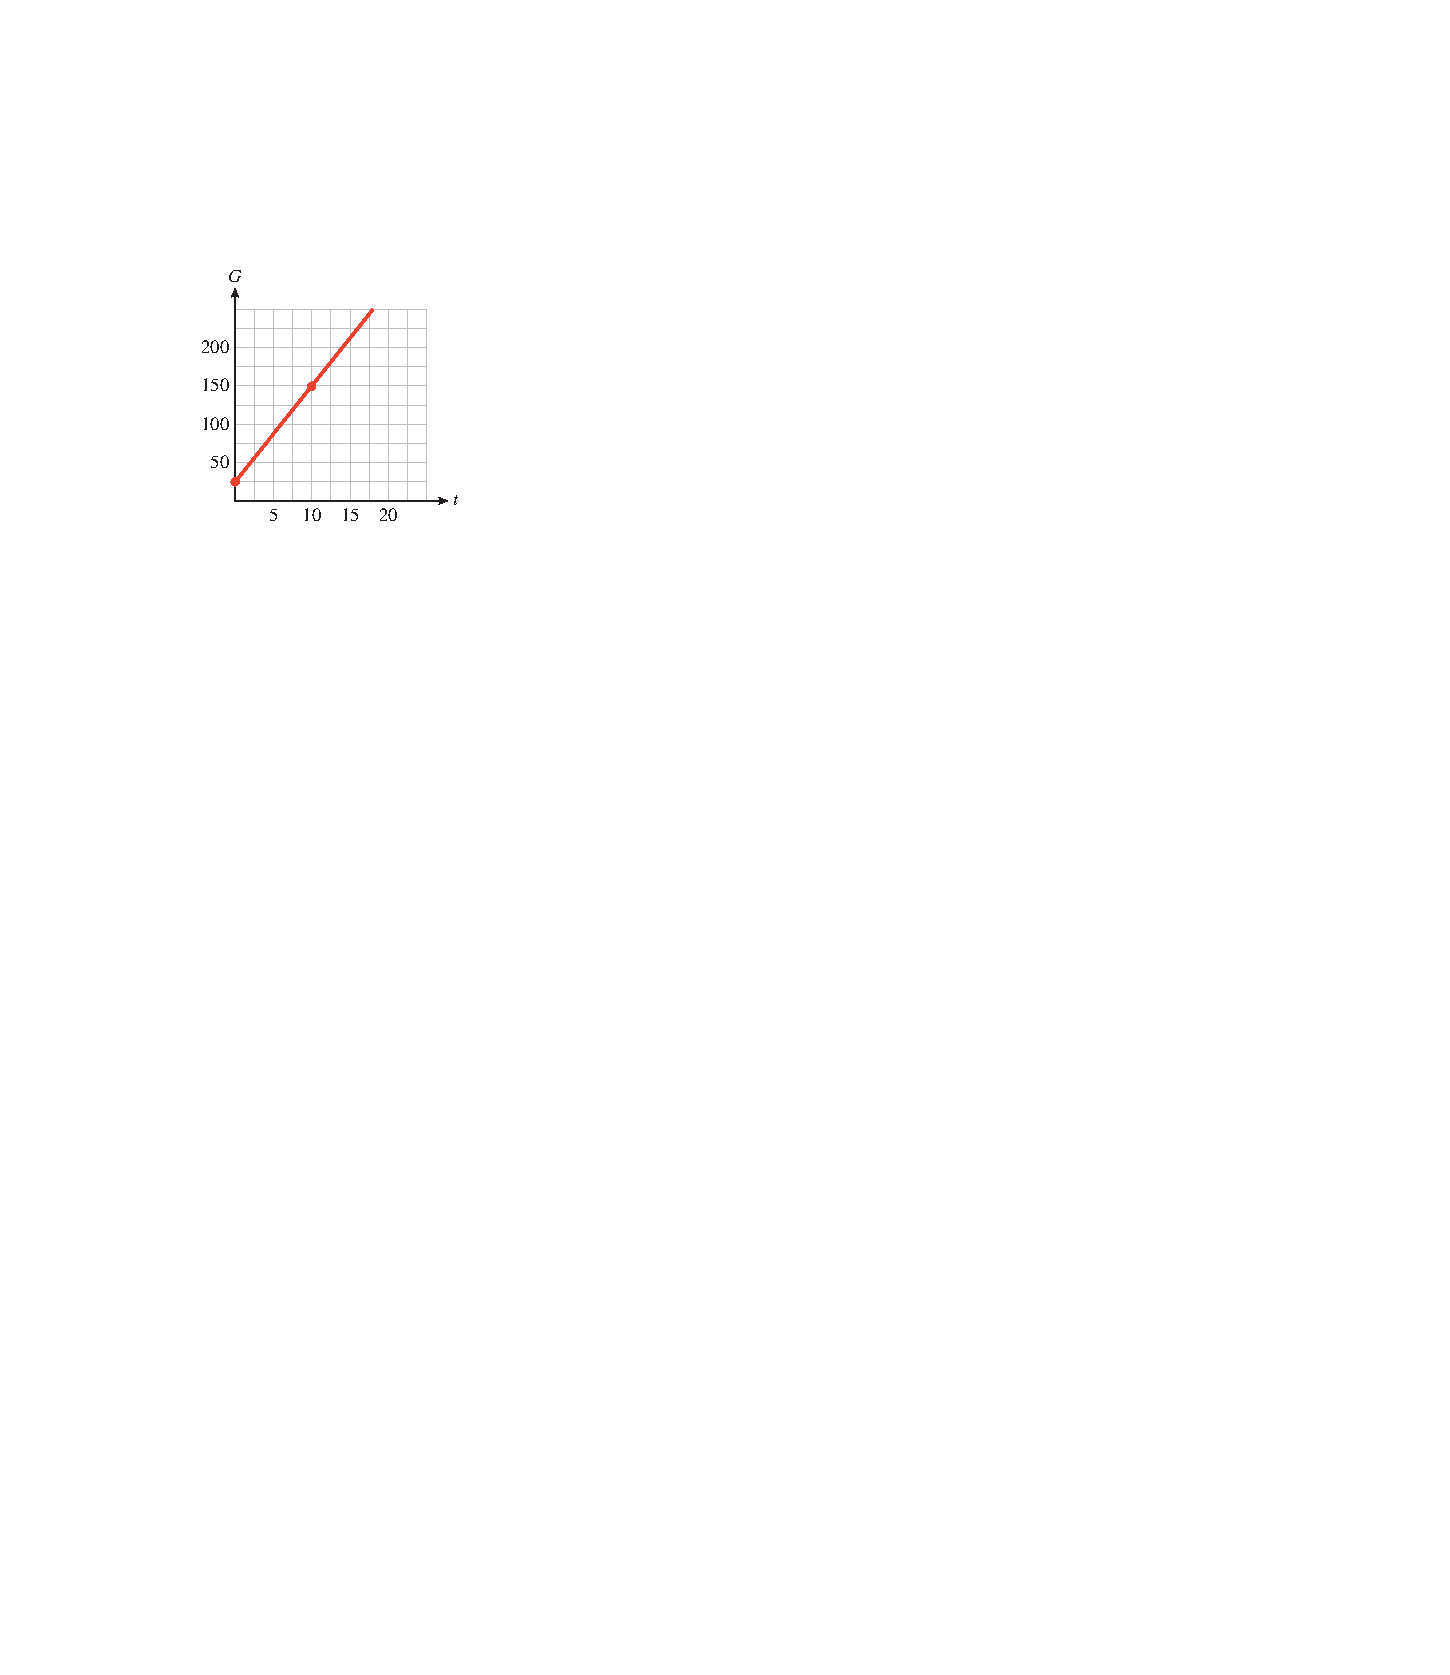
\includegraphics[width=\linewidth]{external/images/fig-ex-1-5-23.pdf}
\end{sbspanel}%
\end{sidebyside}%
\end{divisionexerciseegcol}%
\begin{divisionexerciseegcol}{24}{}{}{exercise-section-1-5-exercises-j-e}%
The graph shows the number of barrels of oil, \(B\), that has been pumped at a drill site \(t\) days after a new drill is installed.%
\begin{sidebyside}{1}{0.125}{0.125}{0}%
\begin{sbspanel}{0.75}%
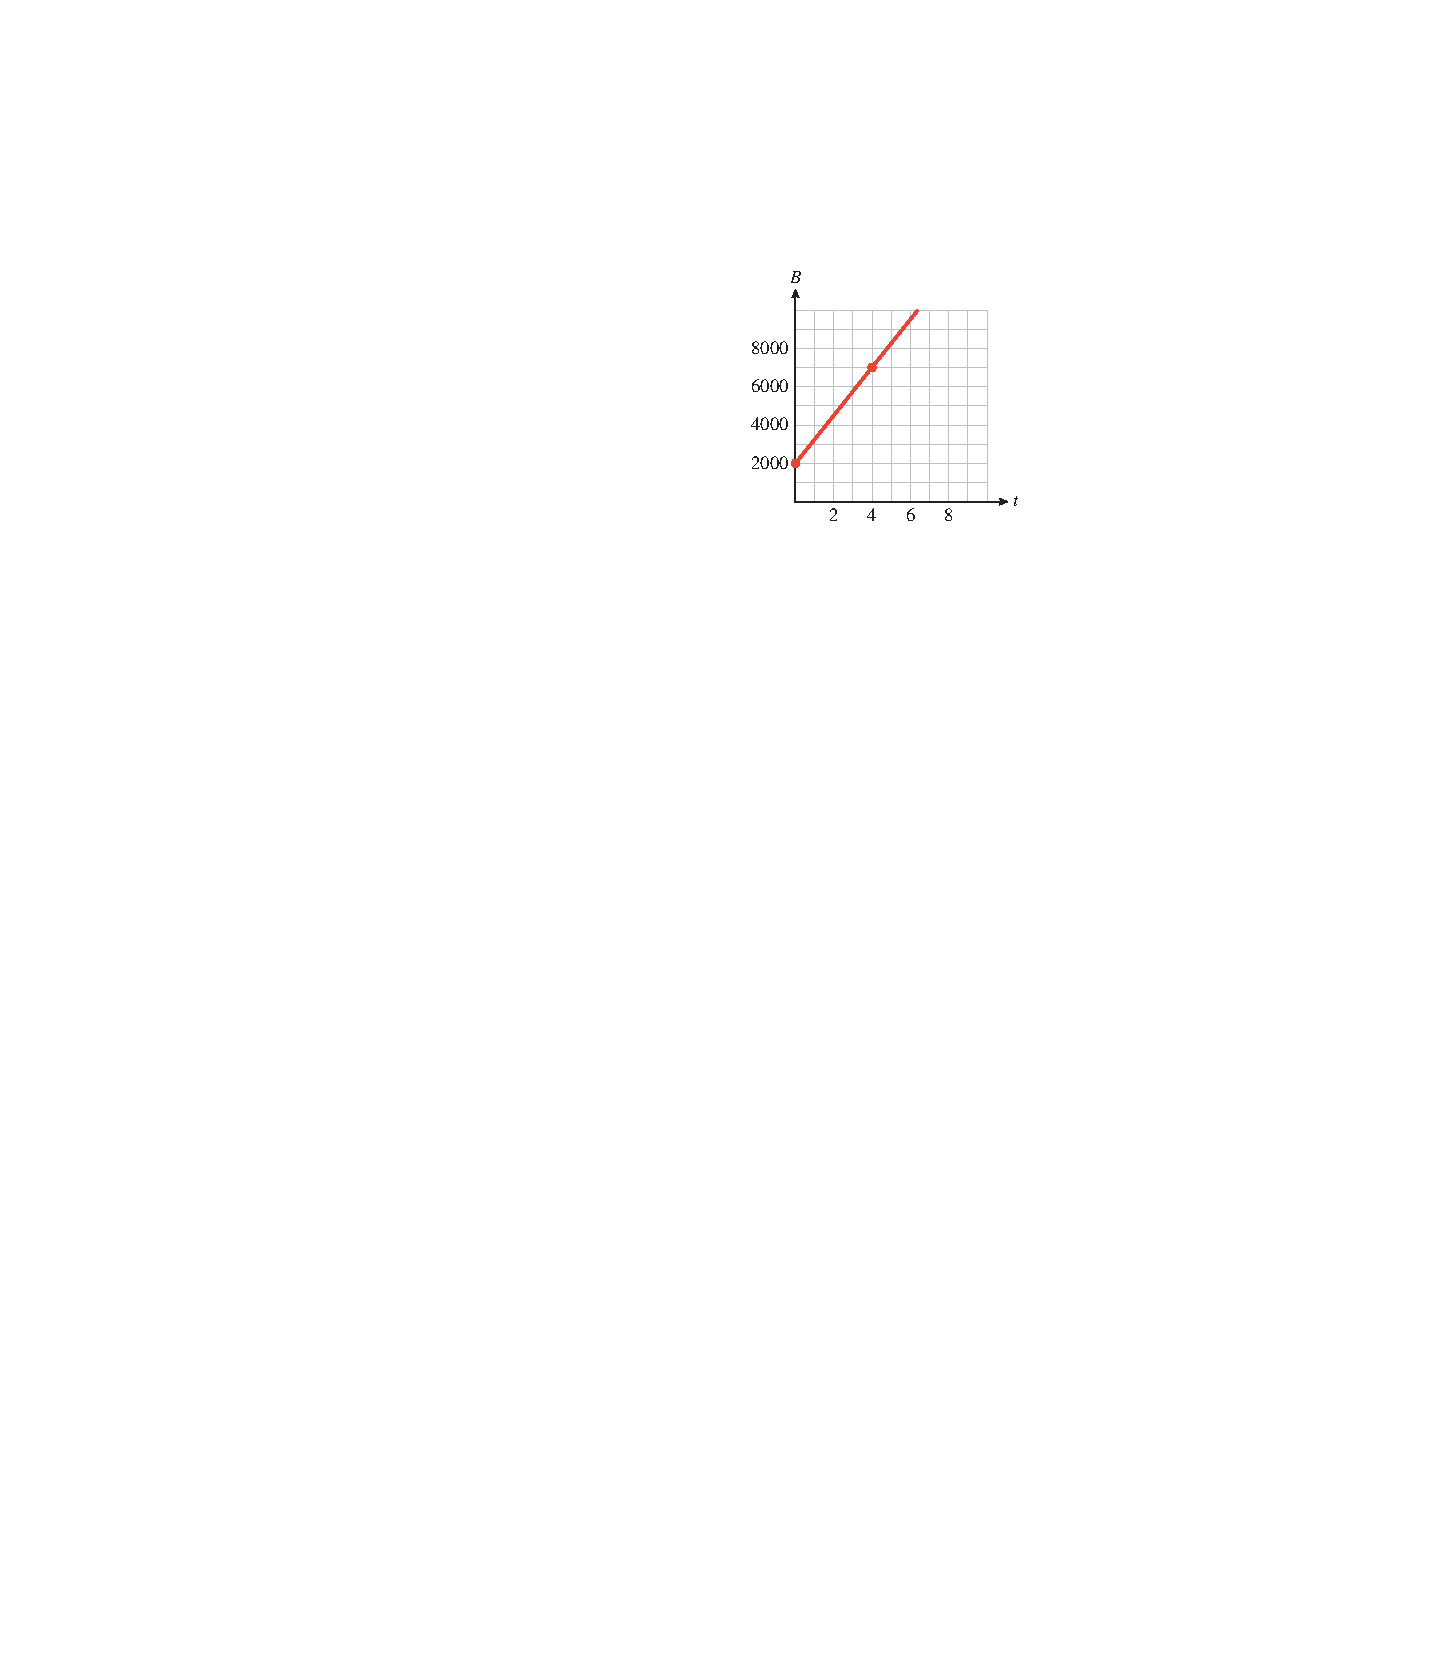
\includegraphics[width=\linewidth]{external/images/fig-ex-1-5-24.pdf}
\end{sbspanel}%
\end{sidebyside}%
\end{divisionexerciseegcol}%
\begin{divisionexerciseegcol}{25}{}{}{exercise-section-1-5-exercises-j-f}%
The graph shows the amount of money, \(M\) (in dollars), in Tammy’s bank account \(w\) weeks after she loses all sources of income.%
\begin{sidebyside}{1}{0.15}{0.15}{0}%
\begin{sbspanel}{0.7}%
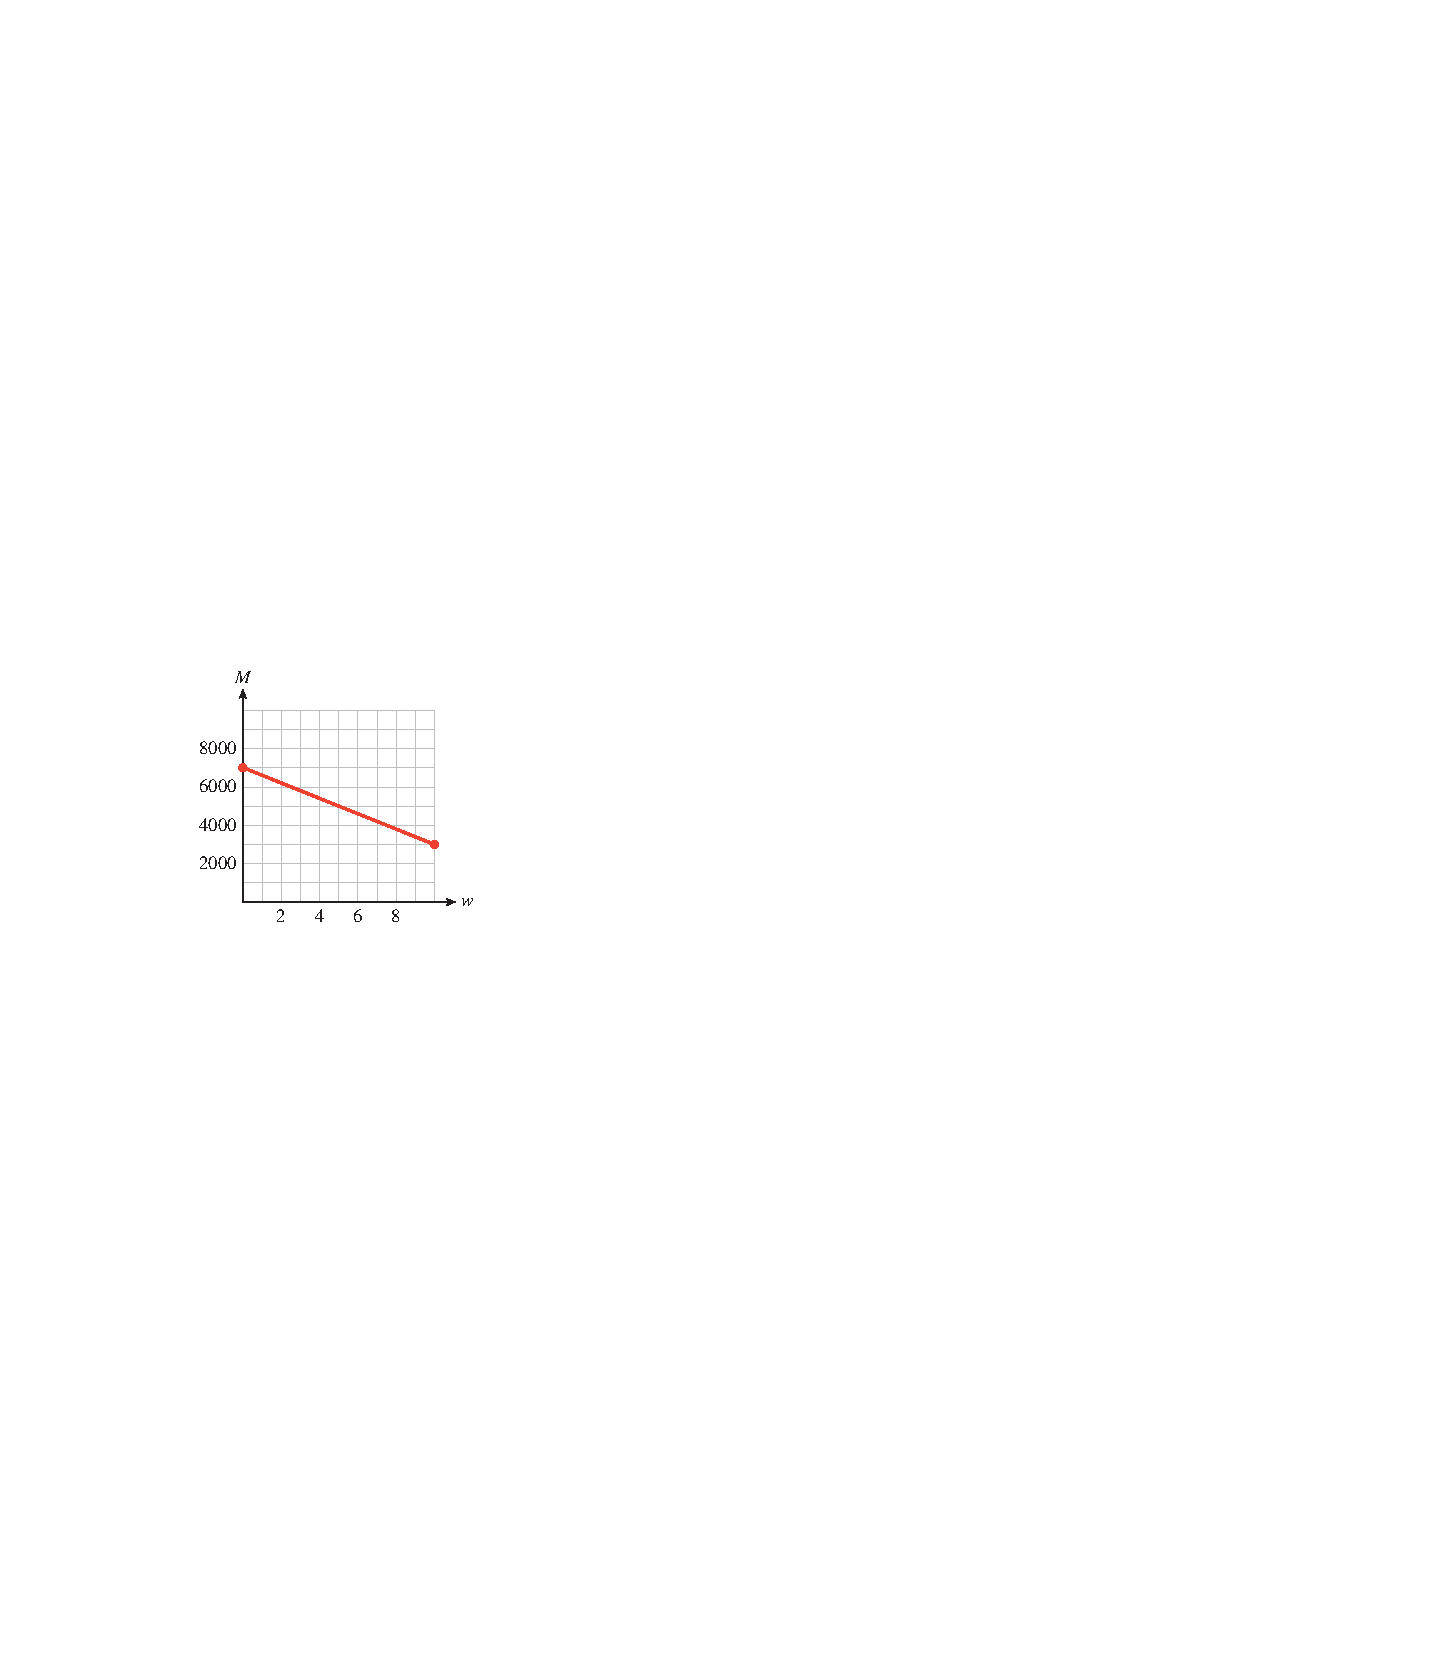
\includegraphics[width=\linewidth]{external/images/fig-ex-1-5-25.pdf}
\end{sbspanel}%
\end{sidebyside}%
\end{divisionexerciseegcol}%
\begin{divisionexerciseegcol}{26}{}{}{exercise-section-1-5-exercises-j-g}%
The graph shows the amount of emergency water, \(W\) (in liters), remaining in a southern California household \(t\) days after an earthquake.%
\begin{sidebyside}{1}{0.15}{0.15}{0}%
\begin{sbspanel}{0.7}%
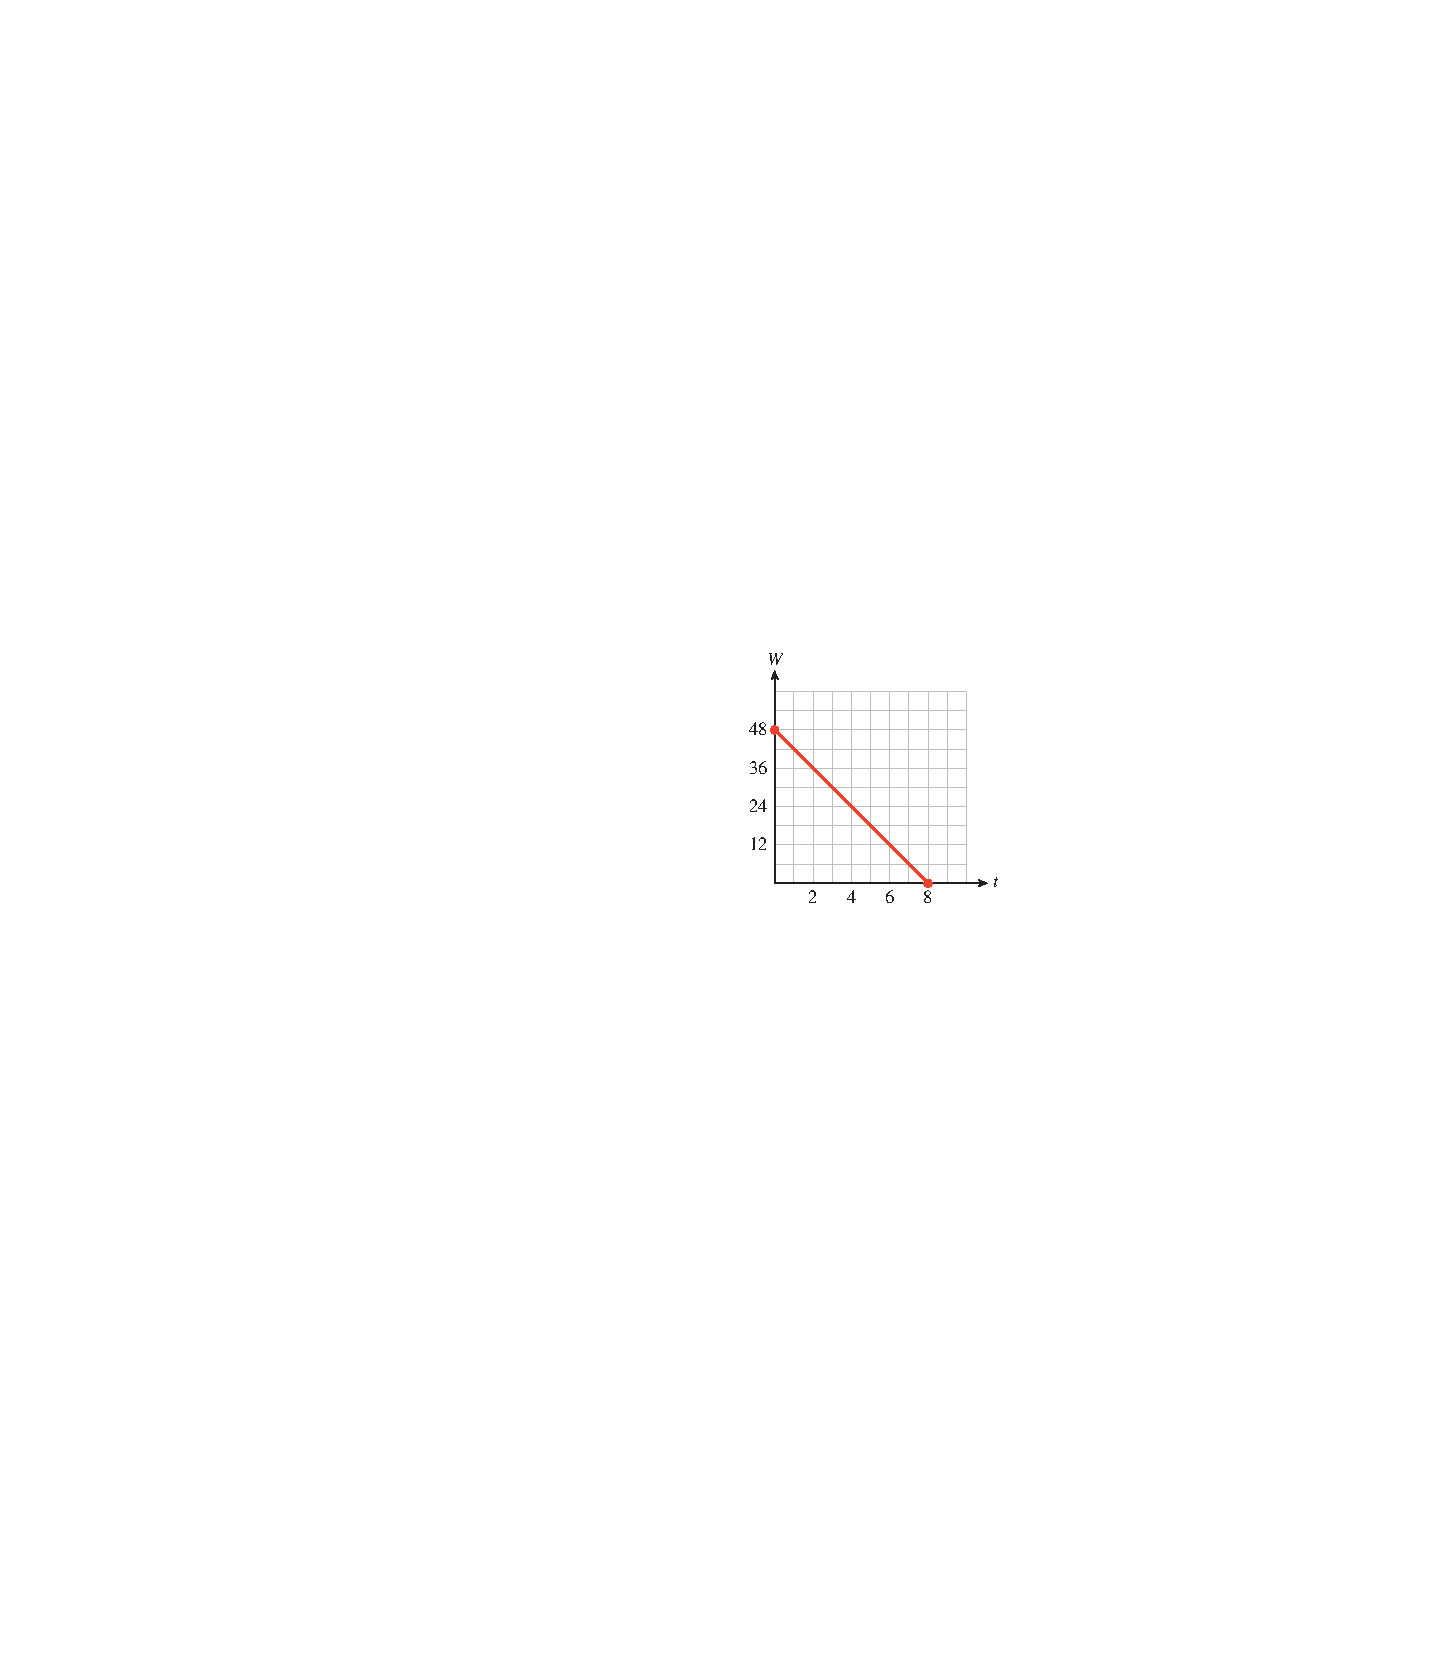
\includegraphics[width=\linewidth]{external/images/fig-ex-1-5-26.pdf}
\end{sbspanel}%
\end{sidebyside}%
\end{divisionexerciseegcol}%
\end{exercisegroupcol}
\par\medskip\noindent
\begin{divisionexercise}{27}{}{}{exercise-section-1-5-exercises-k}%
The formula \(F = \dfrac{9}{5}C + 32\) defines a function that converts the temperature in degrees Celsius to degrees Fahrenheit.%
\begin{enumerate}[label=\alph*]
\item{}What is the Fahrenheit temperature when it is \(10\degree\) Celsius?%
\item{}What is the Celsius temperature when it is \(-4\degree\) Fahrenheit?%
\item{}Choose appropriate \kbd{WINDOW} settings and graph the equation \(y = \dfrac{9}{5}x + 32\).%
\item{}Find the slope and explain its meaning for this problem.%
\item{}Find the intercepts and explain their meanings for this problem.%
\end{enumerate}
%
\end{divisionexercise}%
\begin{divisionexercise}{28}{}{}{exercise-section-1-5-exercises-l}%
If the temperature on the ground is \(70\degree\) Fahrenheit, the formula \(T = 70 - \dfrac{3}{820}h\) defines a function that gives the temperature at an altitude of \(h\) feet.%
\begin{enumerate}[label=\alph*]
\item{}What is the temperature at an altitude of \(4100\) feet?%
\item{}At what altitude is the temperature \(34\degree\) Fahrenheit?%
\item{}Choose appropriate \kbd{WINDOW} settings and graph the equation \(y = 70- \dfrac{3}{820}x\).%
\item{}Find the slope and explain its meaning for this problem.%
\item{}Find the intercepts and explain their meanings for this problem.%
\end{enumerate}
%
\end{divisionexercise}%
\begin{divisionexercise}{29}{}{}{exercise-section-1-5-exercises-m}%
In England, oven cooking temperatures are often given as Gas Marks rather than degrees Fahrenheit. The table shows the equivalent oven temperatures for various Gas Marks.%
\begin{sidebyside}{1}{0}{0}{0}%
\begin{sbspanel}{1}%
\resizebox{\ifdim\width > \linewidth\linewidth\else\width\fi}{!}{%
{\centering%
{\tabularfont%
\begin{tabular}{AcAcAcAcAcA}\hrulethick
Gas Mark&\(3\)&\(5\)&\(7\)&\(9\)\tabularnewline\hrulethin
Degrees (F)&\(325\)&\(375\)&\(425\)&\(475\)\tabularnewline\hrulethin
\end{tabular}
}%
\par}
}%
\end{sbspanel}%
\end{sidebyside}%
\par
%
\begin{enumerate}[label=\alph*]
\item{}Plot the data and draw a line through the data points.%
\item{}Calculate the slope of your line. Estimate the \(y\)-intercept from the graph.%
\item{}Find an equation that gives the temperature in degrees Fahrenheit in terms of the Gas Mark.%
\end{enumerate}
%
\end{divisionexercise}%
\begin{divisionexercise}{30}{}{}{exercise-section-1-5-exercises-n}%
European shoe sizes are scaled differently than American shoe sizes. The table shows the European equivalents for various American shoe sizes.%
\begin{sidebyside}{1}{0}{0}{0}%
\begin{sbspanel}{1}%
\resizebox{\ifdim\width > \linewidth\linewidth\else\width\fi}{!}{%
{\centering%
{\tabularfont%
\begin{tabular}{AcAcAcAcAcA}\hrulethick
American shoe size&\(5.5\)&\(6.5\)&\(7.5\)&\(8.5\)\tabularnewline\hrulethin
European shoe size&\(37\)&\(38\)&\(39\)&\(40\)\tabularnewline\hrulethin
\end{tabular}
}%
\par}
}%
\end{sbspanel}%
\end{sidebyside}%
\par
%
\begin{enumerate}[label=\alph*]
\item{}Plot the data and draw a line through the data points.%
\item{}Calculate the slope of your line. Estimate the \(y\)-intercept from the graph.%
\item{}Find an equation that gives the European shoe size in terms of American shoe size.%
\end{enumerate}
%
\end{divisionexercise}%
\begin{divisionexercise}{31}{}{}{exercise-section-1-5-exercises-o}%
A spring is suspended from the ceiling. The table shows the length of the spring in centimeters as it is stretched by hanging various weights from it.%
\begin{sidebyside}{1}{0}{0}{0}%
\begin{sbspanel}{1}%
\resizebox{\ifdim\width > \linewidth\linewidth\else\width\fi}{!}{%
{\centering%
{\tabularfont%
\begin{tabular}{AcAcAcAcAcAcAcAcA}\hrulethick
Weight, kg&\(3\)&\(4\)&\(8\)&\(10\)&\(12\)&\(15\)&\(22\)\tabularnewline\hrulethin
Length, cm&\(25.76\)&\(25.88\)&\(26.36\)&\(26.6\)&\(26.84\)&\(27.2\)&\(28.04\)\tabularnewline\hrulethin
\end{tabular}
}%
\par}
}%
\end{sbspanel}%
\end{sidebyside}%
\par
%
\begin{enumerate}[label=\alph*]
\item{}Plot the data on graph paper and draw a straight line through the points. Estimate the \(y\)-intercept of your graph.%
\item{}Find an equation for the line.%
\item{}If the spring is stretched to \(27.56\) cm, how heavy is the attached weight?%
\end{enumerate}
%
\end{divisionexercise}%
\begin{divisionexercise}{32}{}{}{exercise-section-1-5-exercises-p}%
The table shows the amount of ammonium chloride salt, in grams, that can be dissolved in \(100\) grams of water at different temperatures.%
\begin{sidebyside}{1}{0}{0}{0}%
\begin{sbspanel}{1}%
\resizebox{\ifdim\width > \linewidth\linewidth\else\width\fi}{!}{%
{\centering%
{\tabularfont%
\begin{tabular}{AcAcAcAcAcAcAcAcA}\hrulethick
Temperature, \(\degree\)C&\(10\)&\(12\)&\(15\)&\(21\)&\(25\)&\(40\)&\(52\)\tabularnewline\hrulethin
Grams of salt&\(33\)&\(34\)&\(35.5\)&\(38.5\)&\(40.5\)&\(48\)&\(54\)\tabularnewline\hrulethin
\end{tabular}
}%
\par}
}%
\end{sbspanel}%
\end{sidebyside}%
\par
%
\begin{enumerate}[label=\alph*]
\item{}Plot the data on graph paper and draw a straight line through the points. Estimate the \(y\)-intercept of your graph.%
\item{}Find an equation for the line.%
\item{}At what temperature will \(46\) grams of salt dissolve?%
\end{enumerate}
%
\end{divisionexercise}%
\par\medskip\noindent%
\textbf{Exercise Group.}\space\space%
In Problems 33\textendash{}36,%
\begin{enumerate}[label=\alph*]
\item{}Sketch by hand the graph of the line that passes through the given point and has the given slope.%
\item{}Write an equation for the line in point-slope form.%
\item{}Put your equation from part (b) into slope-intercept form.%
\end{enumerate}
%
\begin{exercisegroupcol}{2}
\begin{divisionexerciseegcol}{33}{}{}{exercise-section-1-5-exercises-q-b}%
\((2, -5)\); \(m = -3\)%
\end{divisionexerciseegcol}%
\begin{divisionexerciseegcol}{34}{}{}{exercise-section-1-5-exercises-q-c}%
\((-6, -1)\); \(m = 4\)%
\end{divisionexerciseegcol}%
\begin{divisionexerciseegcol}{35}{}{}{exercise-section-1-5-exercises-q-d}%
\((2, -1)\); \(m =\dfrac{5}{3} \)%
\end{divisionexerciseegcol}%
\begin{divisionexerciseegcol}{36}{}{}{exercise-section-1-5-exercises-q-e}%
\((-1, 2)\); \(m =-\dfrac{3}{2} \)%
\end{divisionexerciseegcol}%
\end{exercisegroupcol}
\par\medskip\noindent
\par\medskip\noindent%
\textbf{Exercise Group.}\space\space%
For Problems 37\textendash{}40,%
\begin{enumerate}[label=\alph*]
\item{}Write an equation in point-slope form for the line that passes through the given point and has the given slope.%
\item{}Put your equation from part (a) into slope-intercept form.%
\item{}Use your graphing calculator to graph the line.%
\end{enumerate}
%
\begin{exercisegroupcol}{2}
\begin{divisionexerciseegcol}{37}{}{}{exercise-section-1-5-exercises-r-b}%
\((-6.4, -3.5)\), \(m =-0.25 \)%
\end{divisionexerciseegcol}%
\begin{divisionexerciseegcol}{38}{}{}{exercise-section-1-5-exercises-r-c}%
\((7.2, -5.6)\), \(m =1.6 \)%
\end{divisionexerciseegcol}%
\begin{divisionexerciseegcol}{39}{}{}{exercise-section-1-5-exercises-r-d}%
\((80, -250)\), \(m =2.4 \)%
\end{divisionexerciseegcol}%
\begin{divisionexerciseegcol}{40}{}{}{exercise-section-1-5-exercises-r-e}%
\((-150, 1800)\), \(m =-24 \)%
\end{divisionexerciseegcol}%
\end{exercisegroupcol}
\par\medskip\noindent
\par\medskip\noindent%
\textbf{Exercise Group.}\space\space%
For Problems 41 and 42,%
\begin{enumerate}[label=\alph*]
\item{}Find the slope of the line. (Note that not all the labeled points lie on the line.)%
\item{}Find an equation for the line.%
\end{enumerate}
%
\begin{exercisegroupcol}{2}
\begin{divisionexerciseegcol}{41}{}{}{exercise-section-1-5-exercises-s-b}%
\begin{sidebyside}{1}{0.1}{0.1}{0}%
\begin{sbspanel}{0.8}%
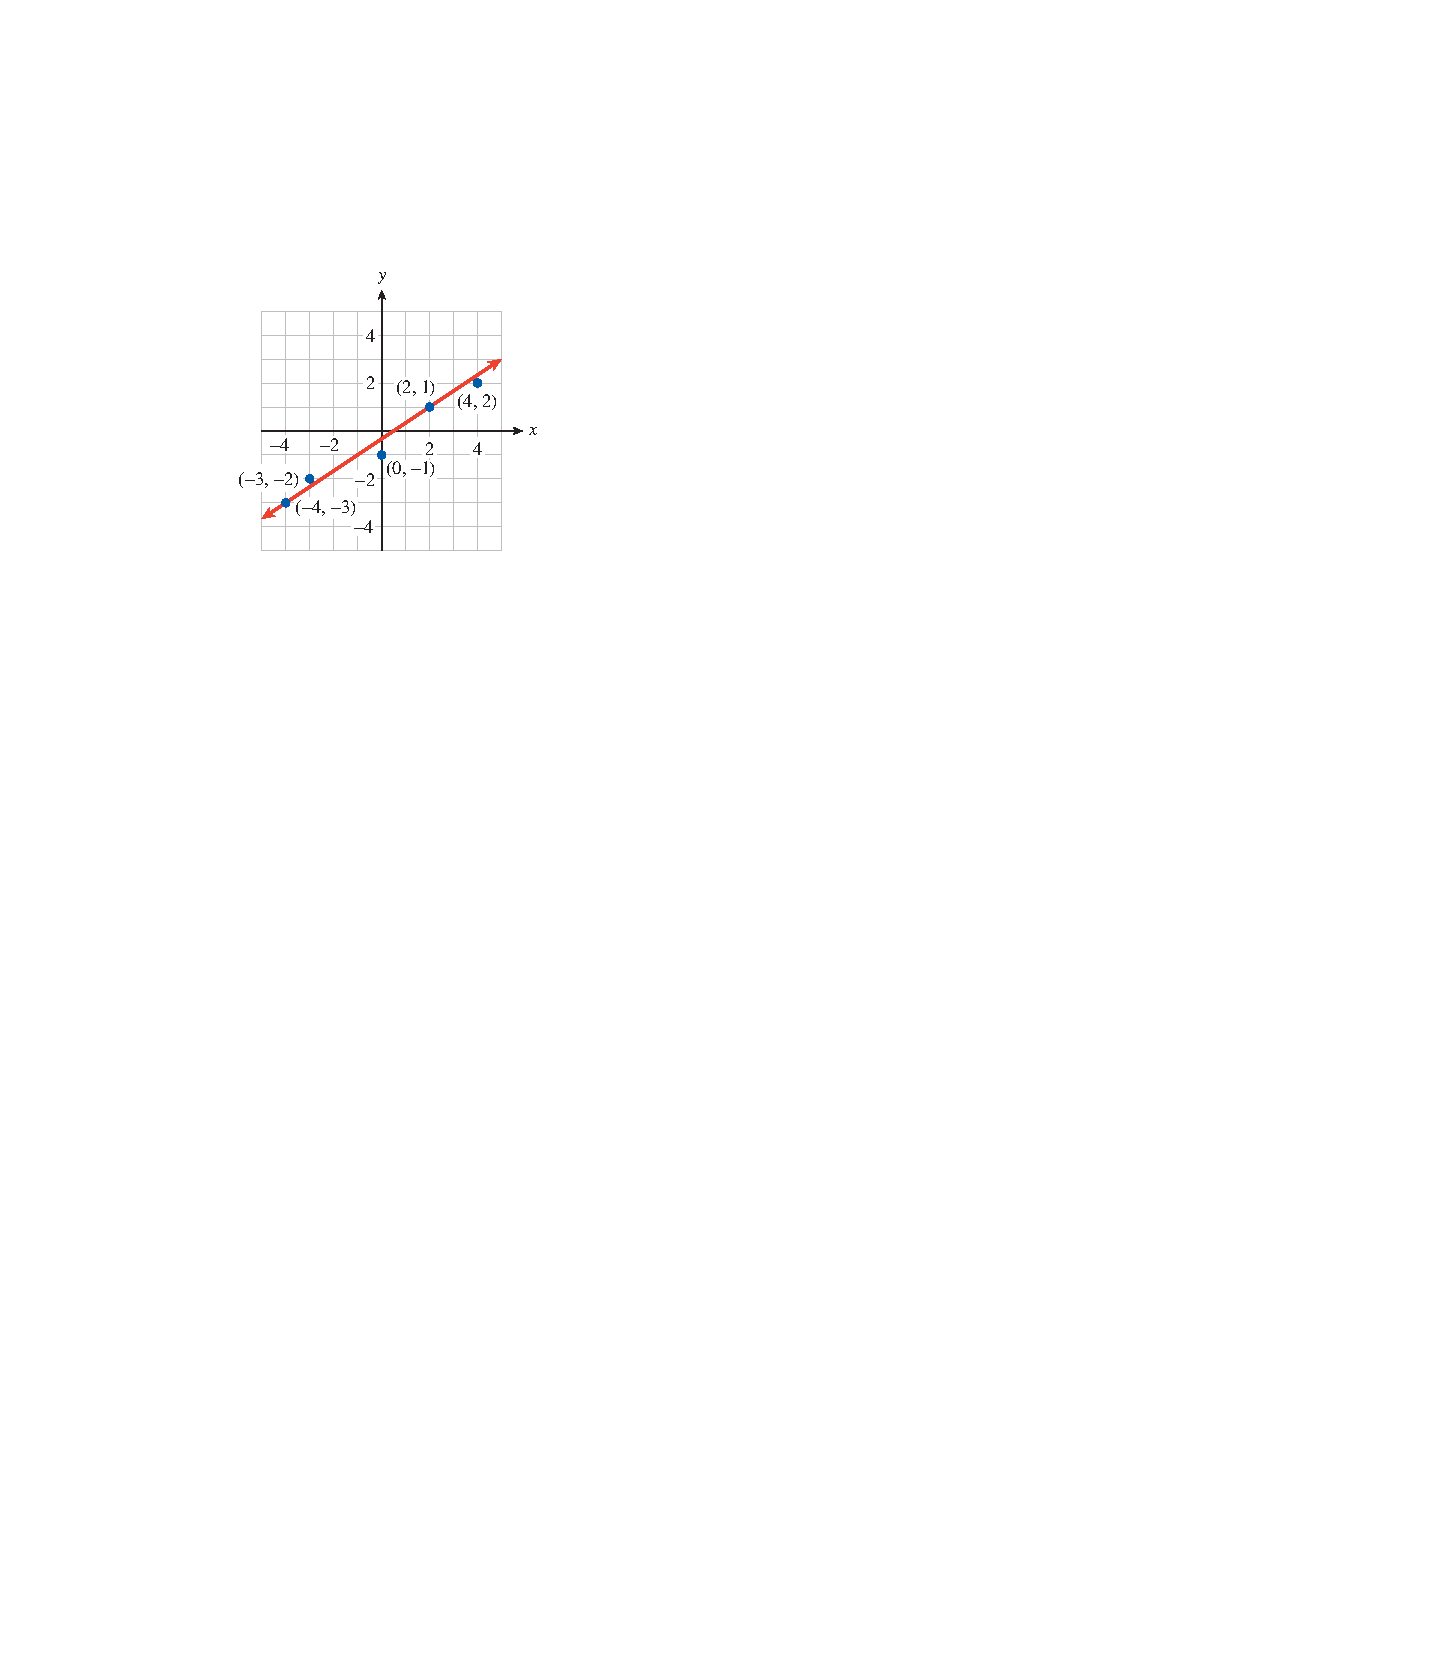
\includegraphics[width=\linewidth]{external/images/fig-ex-1-5-41.pdf}
\end{sbspanel}%
\end{sidebyside}%
\end{divisionexerciseegcol}%
\begin{divisionexerciseegcol}{42}{}{}{exercise-section-1-5-exercises-s-c}%
\begin{sidebyside}{1}{0.125}{0.125}{0}%
\begin{sbspanel}{0.75}%
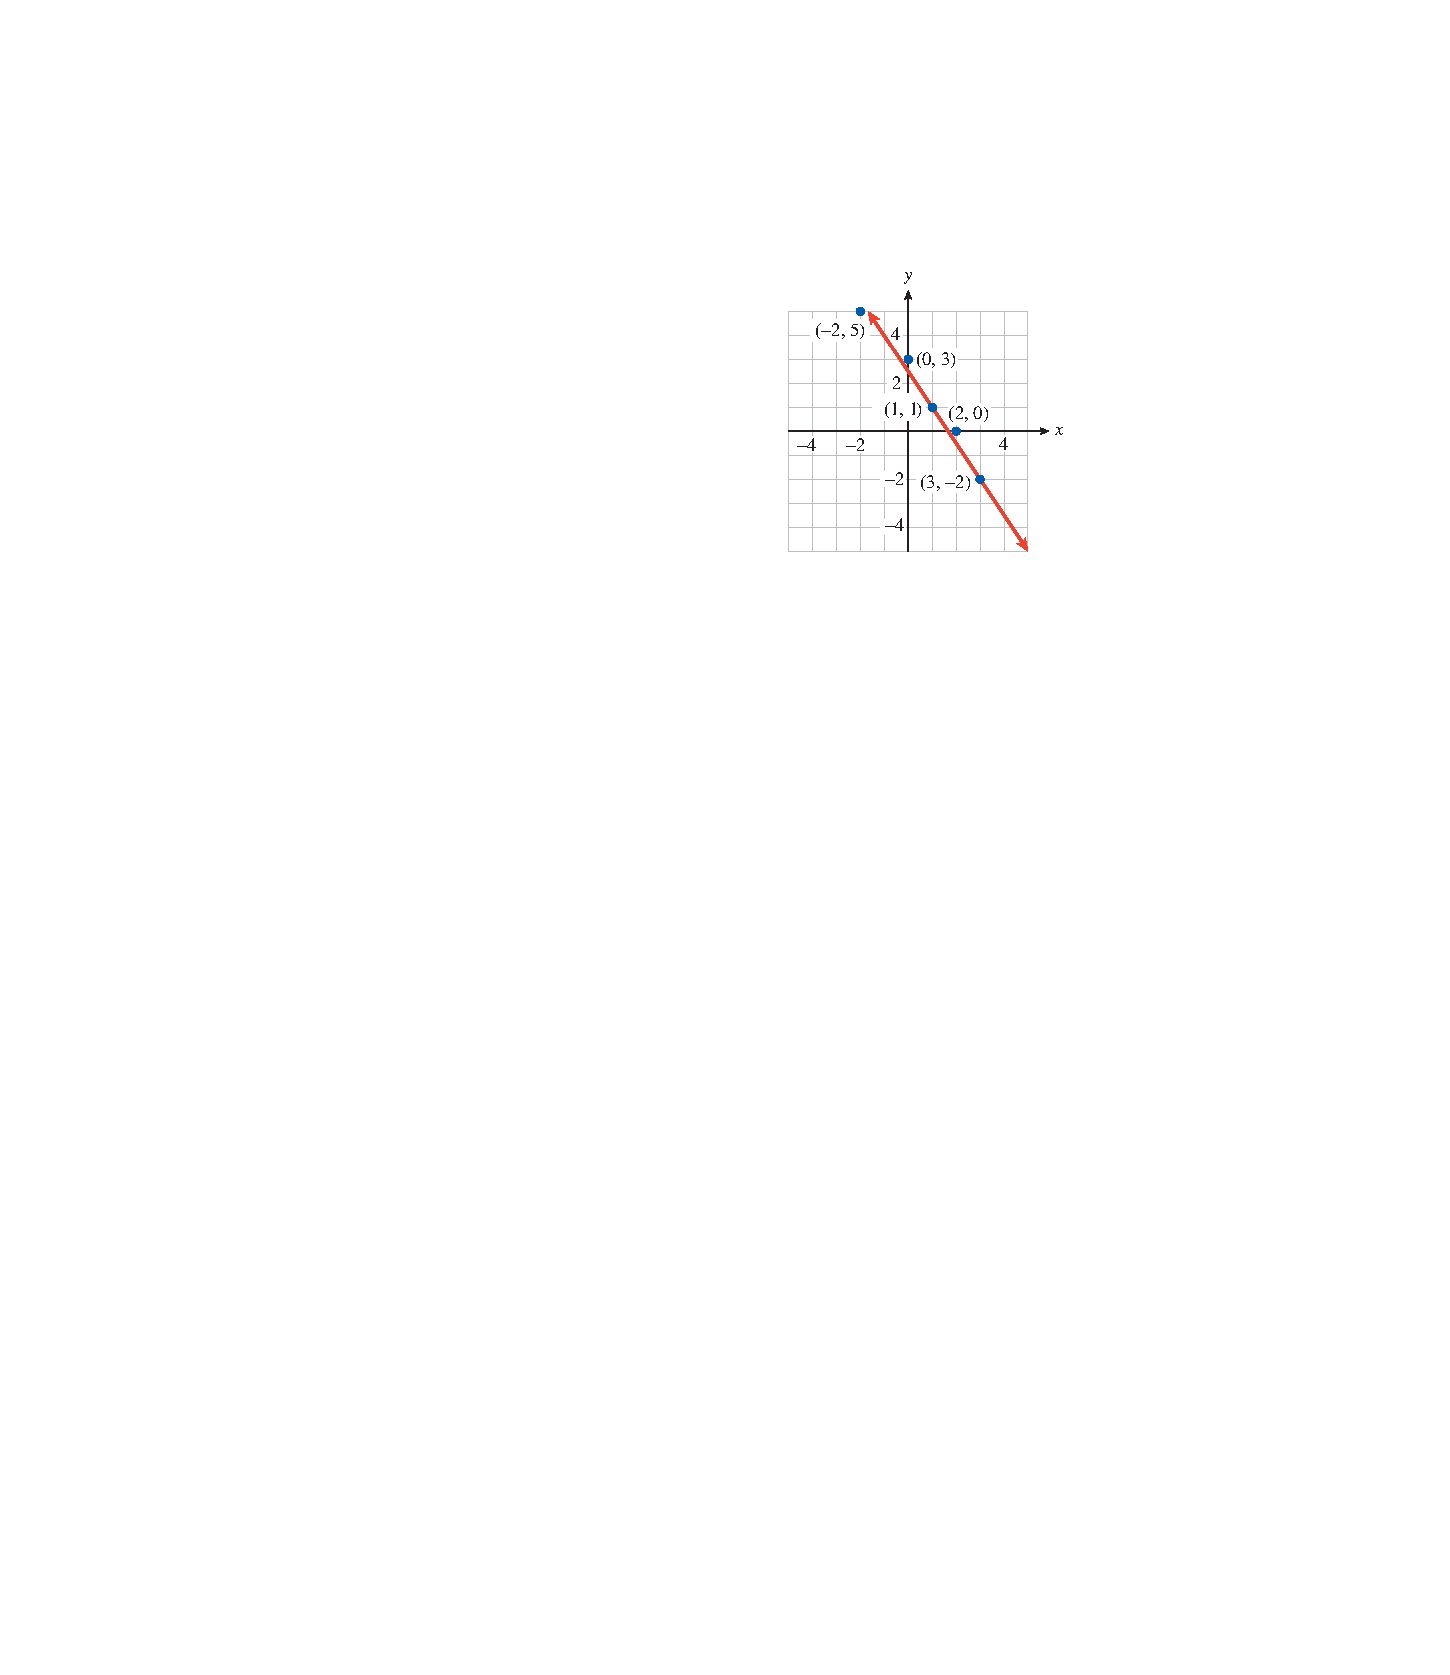
\includegraphics[width=\linewidth]{external/images/fig-ex-1-5-42.pdf}
\end{sbspanel}%
\end{sidebyside}%
\end{divisionexerciseegcol}%
\end{exercisegroupcol}
\par\medskip\noindent
\par\medskip\noindent%
\textbf{Exercise Group.}\space\space%
For Problems 43 and 44, the equation of line \(l_1\) is \(y = q + px\), and the equation of line \(l_2\) is \(y = v + tx\).%
\begin{enumerate}[label=\alph*]
\item{}Decide whether the coordinates of each labeled point are%
\begin{enumerate}[label=\Roman*]
\item{}a solution of \(y = q + px\),%
\item{}a solution of \(y = v + tx\),%
\item{}a solution of both equations, or%
\item{}a solution of neither equation.%
\end{enumerate}
%
\item{}Find \(p\), \(q\), \(t\), and \(v\).%
\end{enumerate}
%
\begin{exercisegroupcol}{2}
\begin{divisionexerciseegcol}{43}{}{}{exercise-section-1-5-exercises-t-b}%
\begin{sidebyside}{1}{0.125}{0.125}{0}%
\begin{sbspanel}{0.75}%
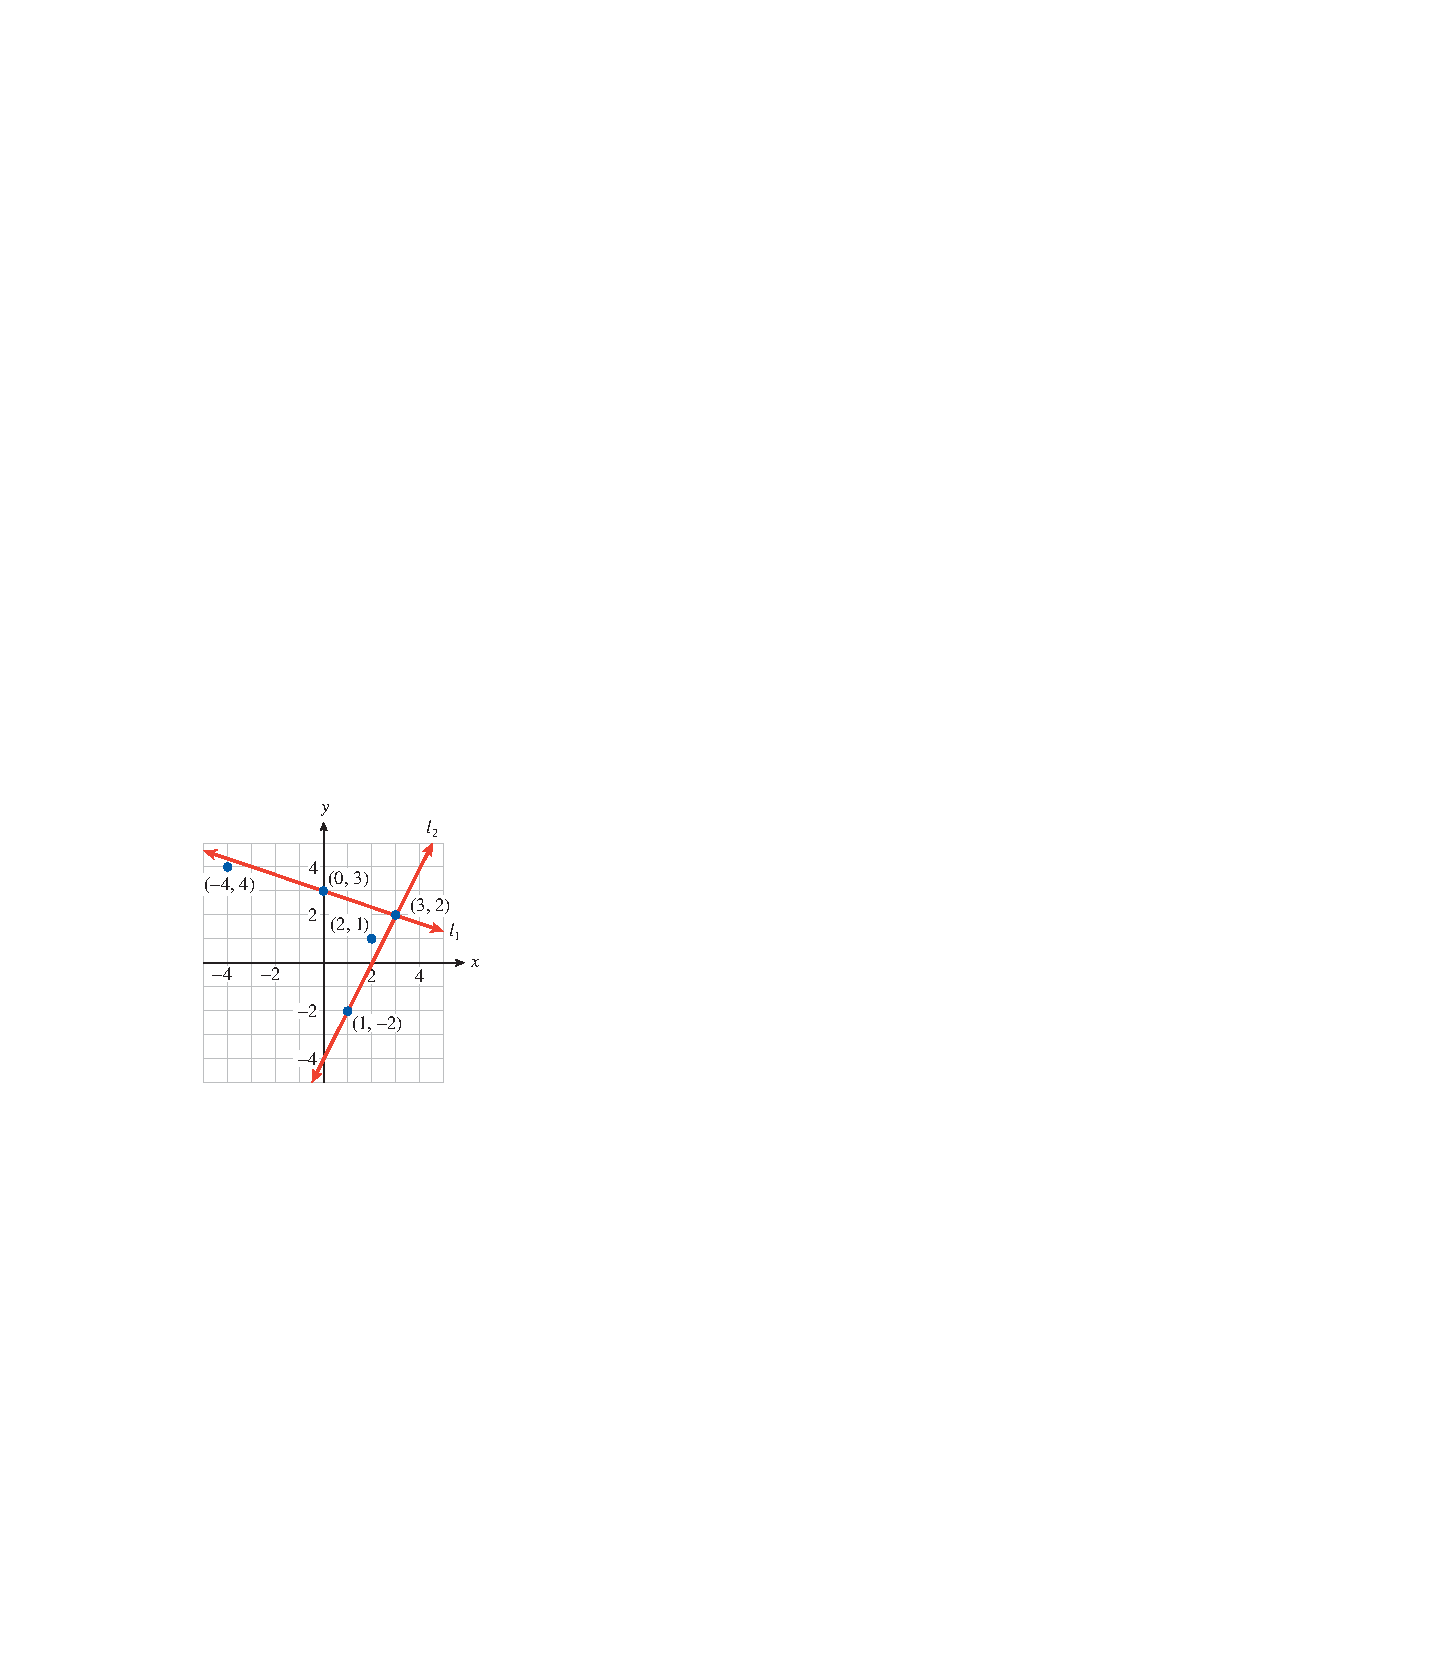
\includegraphics[width=\linewidth]{external/images/fig-ex-1-5-43.pdf}
\end{sbspanel}%
\end{sidebyside}%
\end{divisionexerciseegcol}%
\begin{divisionexerciseegcol}{44}{}{}{exercise-section-1-5-exercises-t-c}%
\begin{sidebyside}{1}{0.125}{0.125}{0}%
\begin{sbspanel}{0.75}%
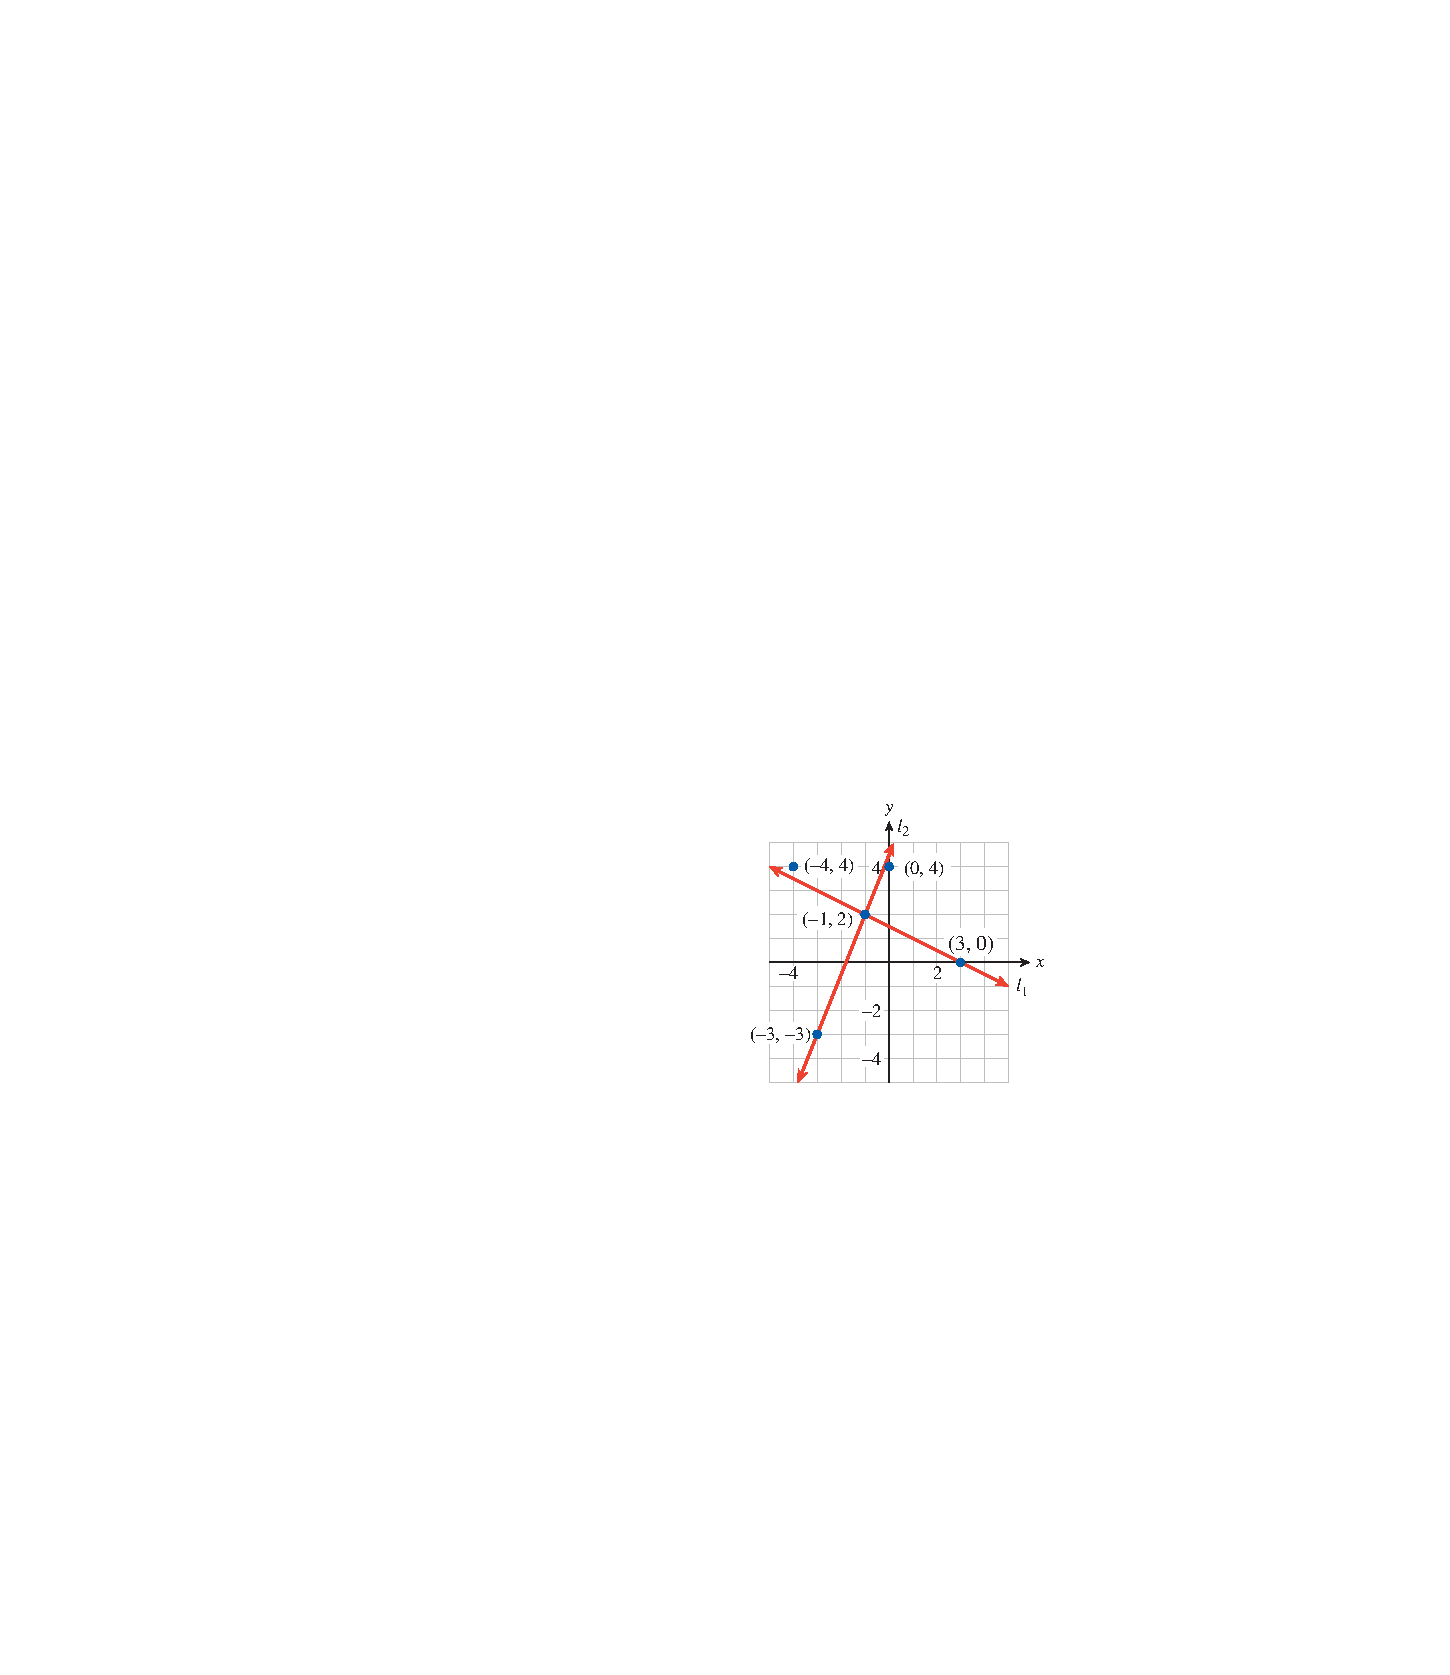
\includegraphics[width=\linewidth]{external/images/fig-ex-1-5-44.pdf}
\end{sbspanel}%
\end{sidebyside}%
\end{divisionexerciseegcol}%
\end{exercisegroupcol}
\par\medskip\noindent
\par\medskip\noindent%
\textbf{Exercise Group.}\space\space%
For Problems 45\textendash{}50,%
\begin{enumerate}[label=\alph*]
\item{}Estimate the slope and vertical intercept of each line. (Hint: To calculate the slope, find two points on the graph that lie on the intersection of grid lines.)%
\item{}Using your estimates from (a), write an equation for the line.%
\end{enumerate}
%
\begin{exercisegroupcol}{2}
\begin{divisionexerciseegcol}{45}{}{}{exercise-section-1-5-exercises-u-b}%
\begin{sidebyside}{1}{0.1}{0.1}{0}%
\begin{sbspanel}{0.8}%
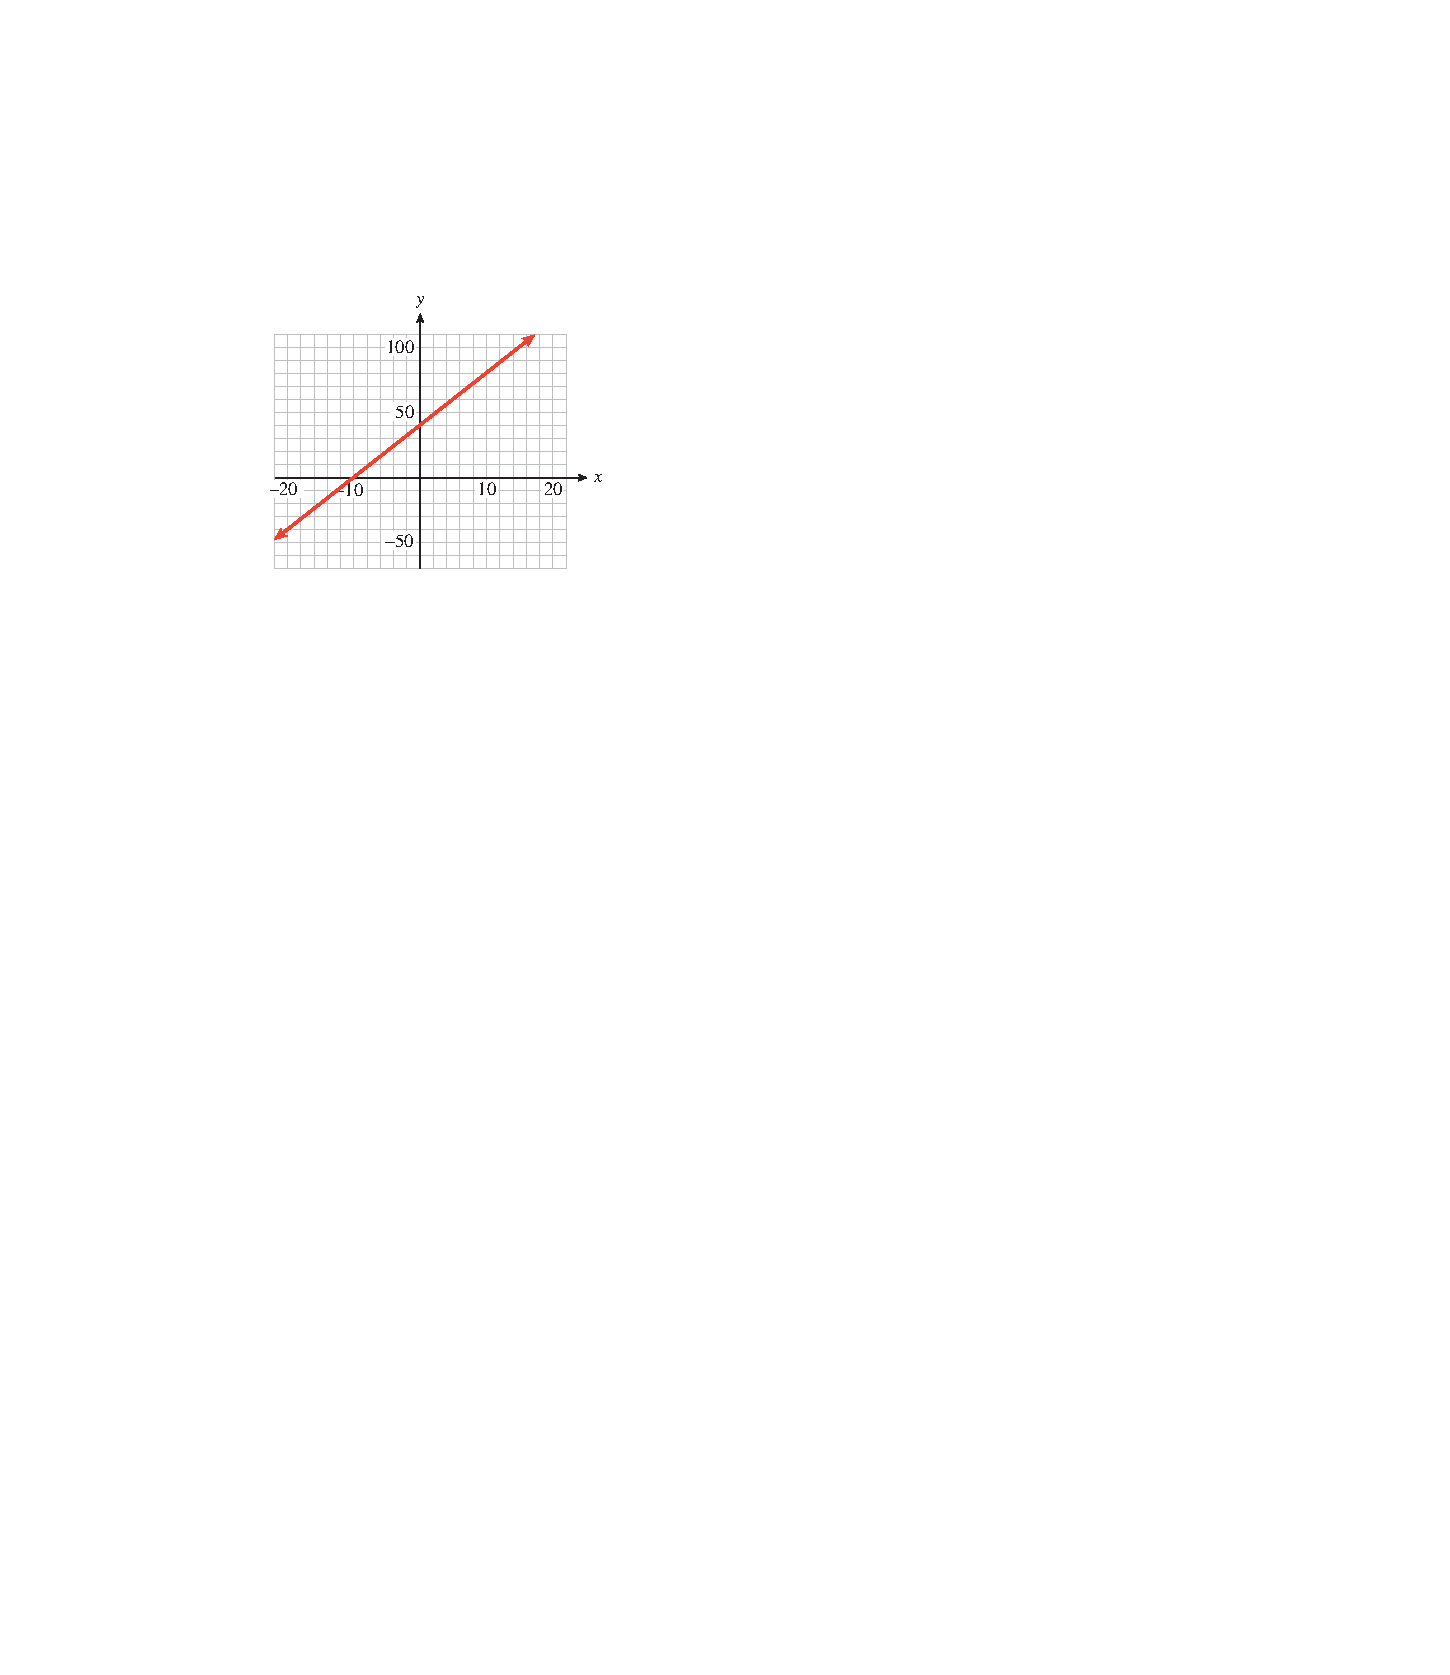
\includegraphics[width=\linewidth]{external/images/fig-ex-1-5-45.pdf}
\end{sbspanel}%
\end{sidebyside}%
\end{divisionexerciseegcol}%
\begin{divisionexerciseegcol}{46}{}{}{exercise-section-1-5-exercises-u-c}%
\begin{sidebyside}{1}{0.175}{0.175}{0}%
\begin{sbspanel}{0.65}%
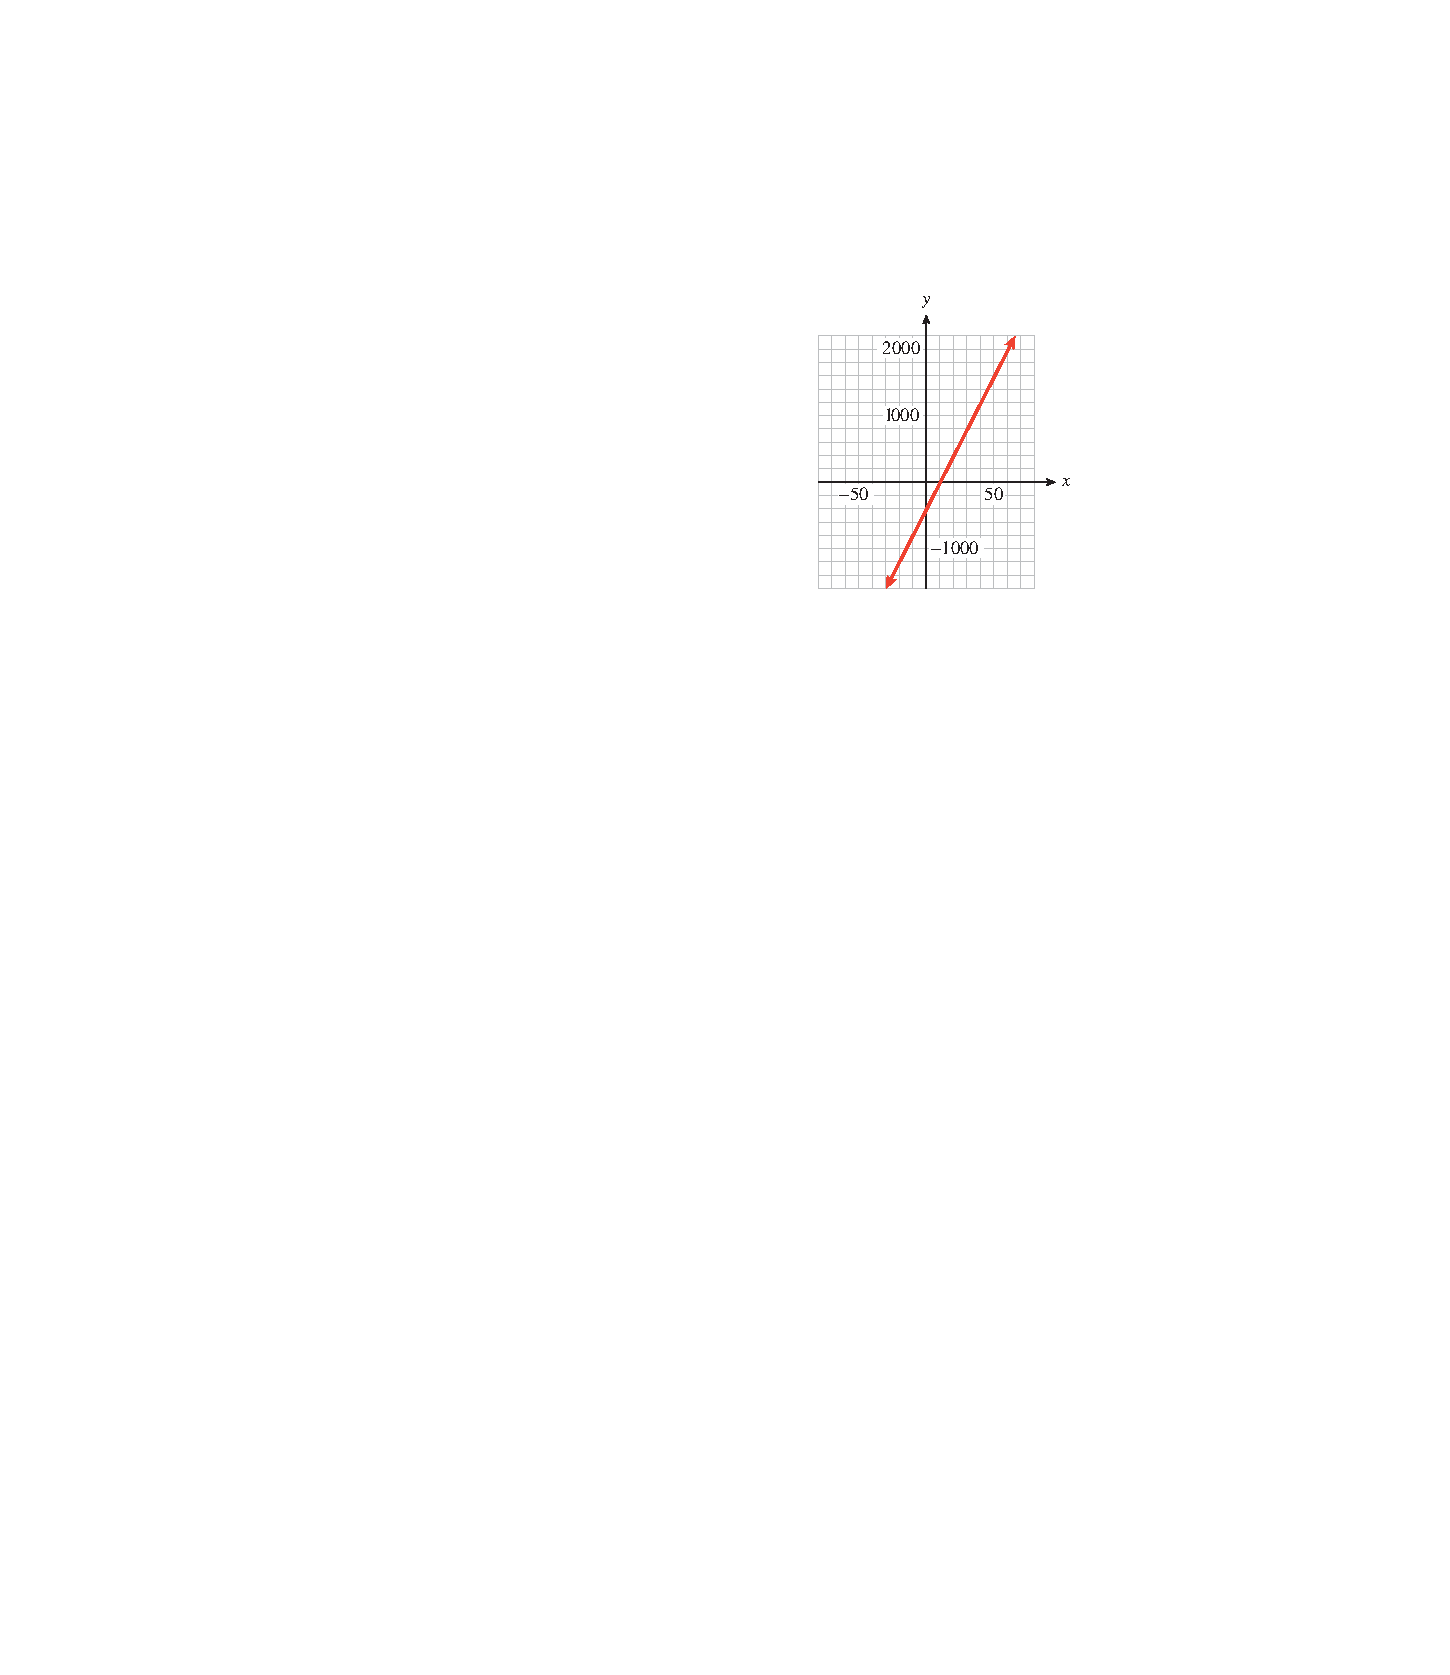
\includegraphics[width=\linewidth]{external/images/fig-ex-1-5-46.pdf}
\end{sbspanel}%
\end{sidebyside}%
\end{divisionexerciseegcol}%
\begin{divisionexerciseegcol}{47}{}{}{exercise-section-1-5-exercises-u-d}%
\begin{sidebyside}{1}{0.1}{0.1}{0}%
\begin{sbspanel}{0.8}%
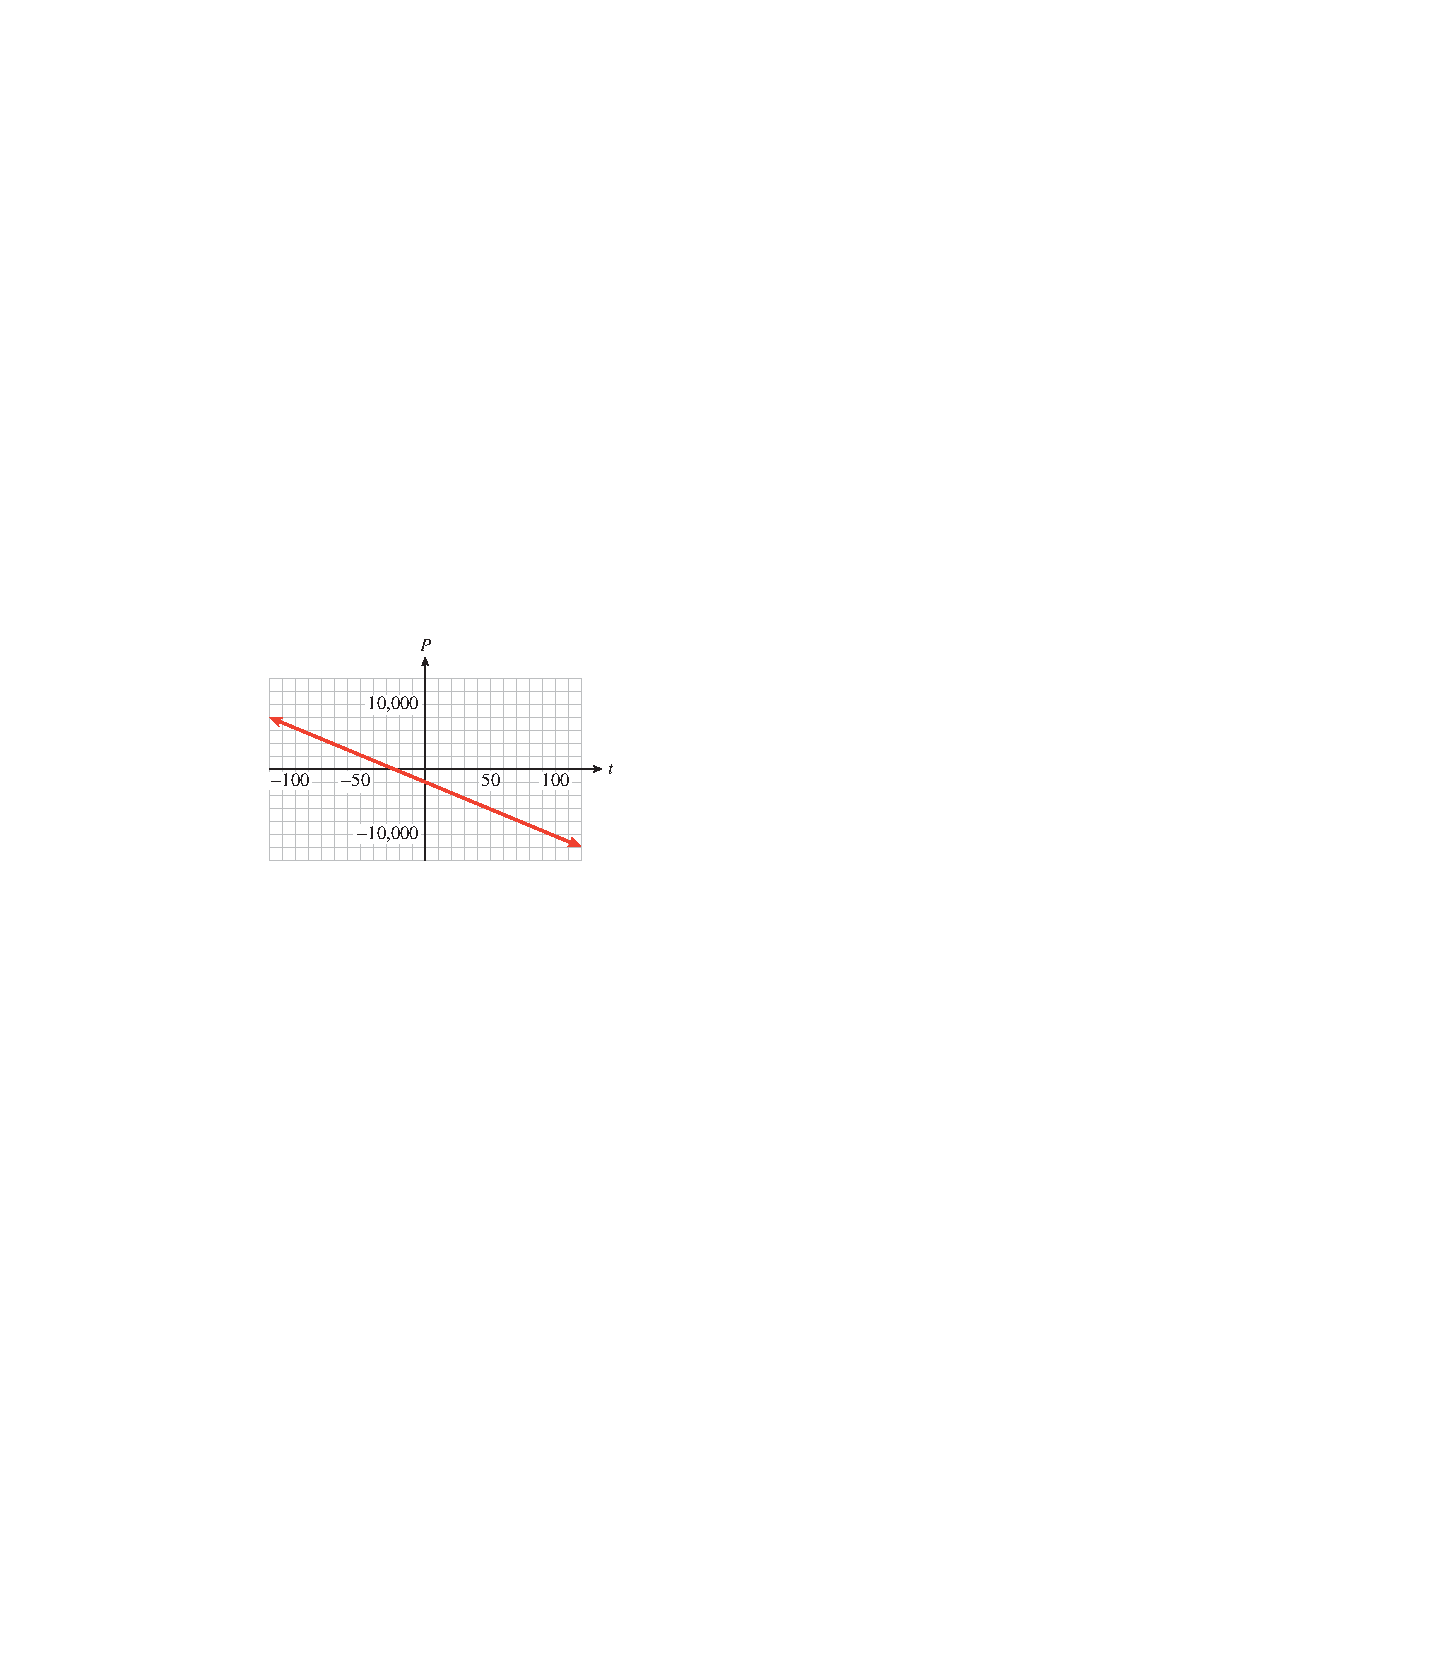
\includegraphics[width=\linewidth]{external/images/fig-ex-1-5-47.pdf}
\end{sbspanel}%
\end{sidebyside}%
\end{divisionexerciseegcol}%
\begin{divisionexerciseegcol}{48}{}{}{exercise-section-1-5-exercises-u-e}%
\begin{sidebyside}{1}{0.175}{0.175}{0}%
\begin{sbspanel}{0.65}%
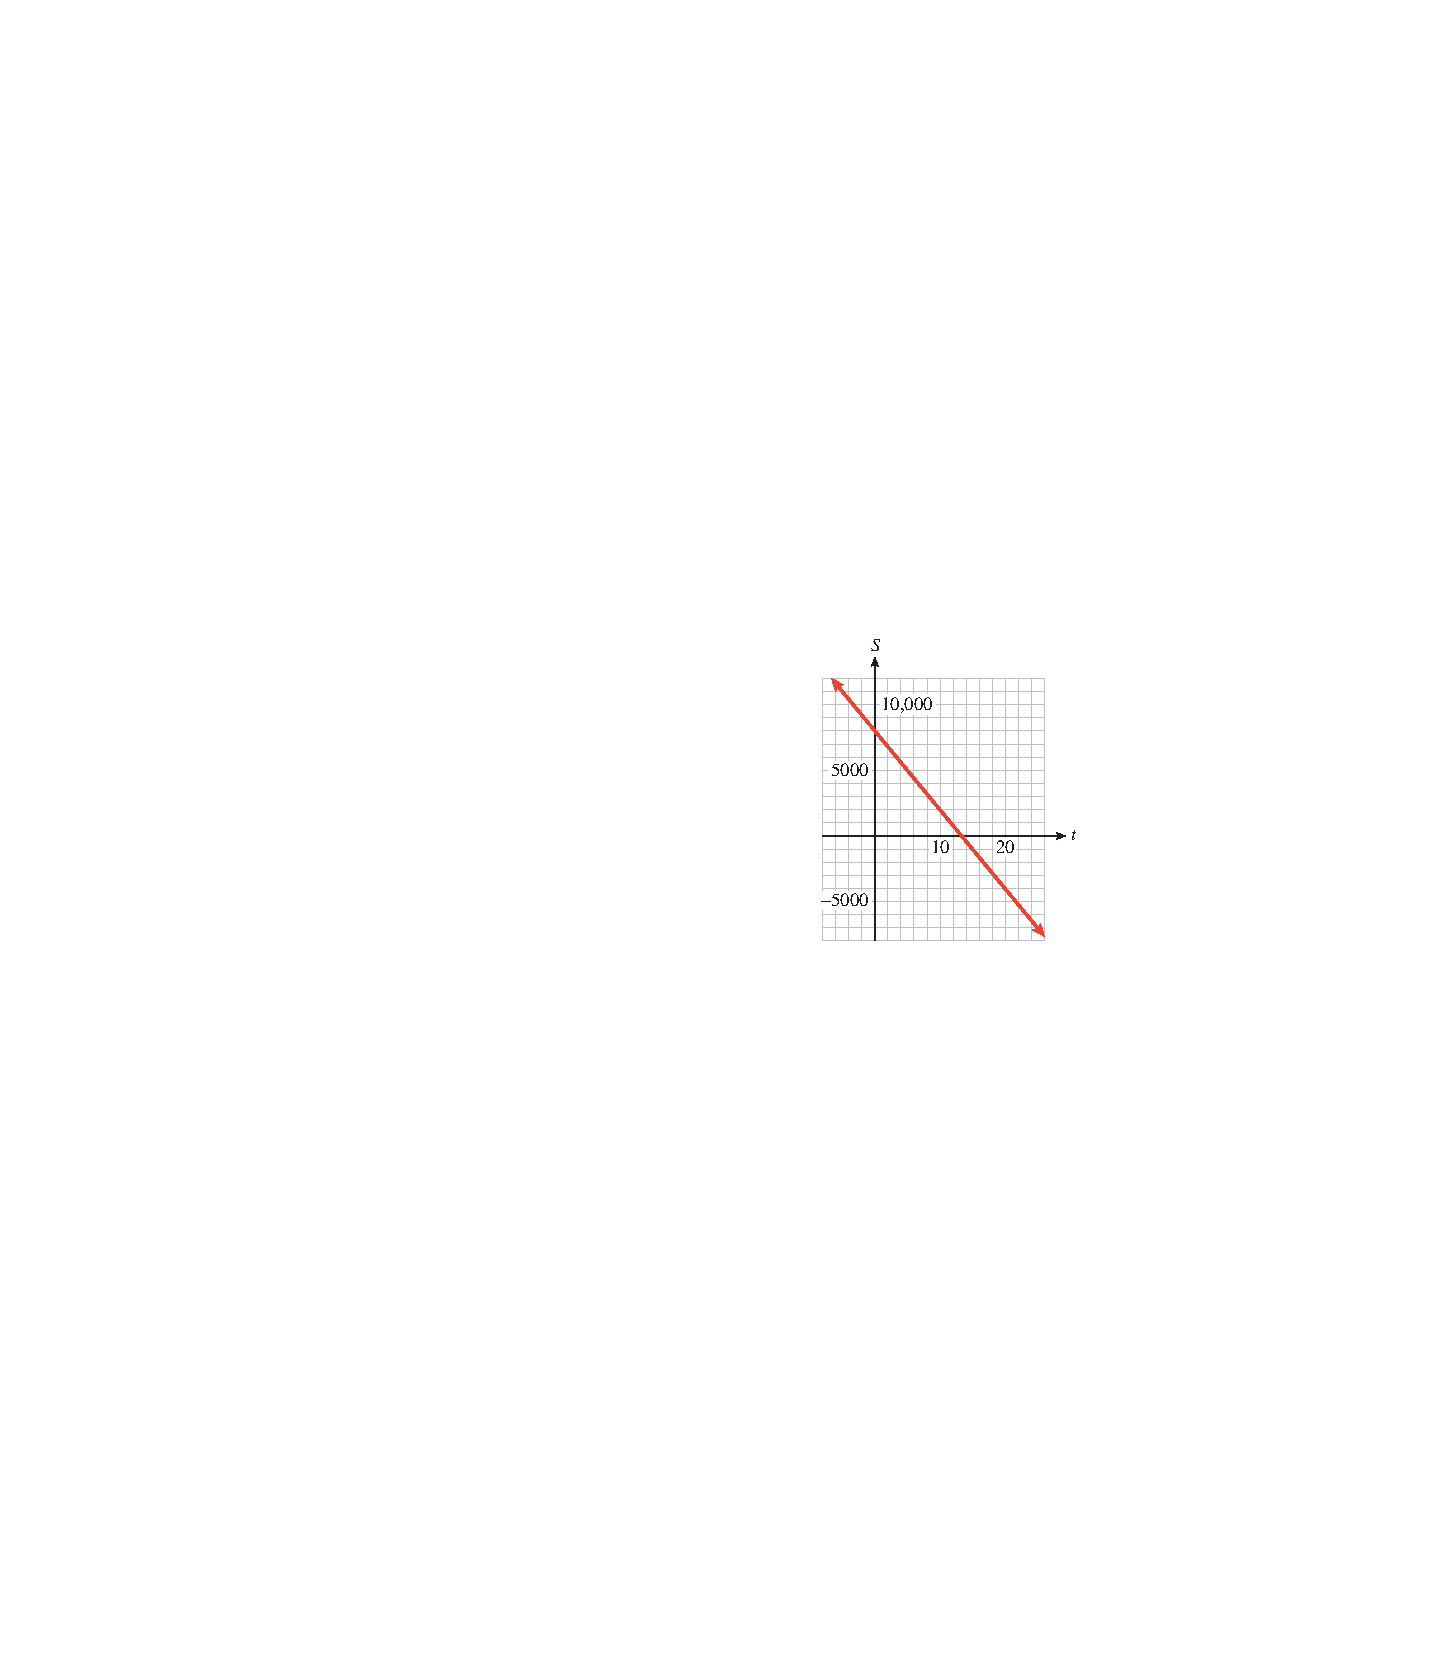
\includegraphics[width=\linewidth]{external/images/fig-ex-1-5-48.pdf}
\end{sbspanel}%
\end{sidebyside}%
\end{divisionexerciseegcol}%
\begin{divisionexerciseegcol}{49}{}{}{exercise-section-1-5-exercises-u-f}%
\begin{sidebyside}{1}{0}{0}{0}%
\begin{sbspanel}{1}%
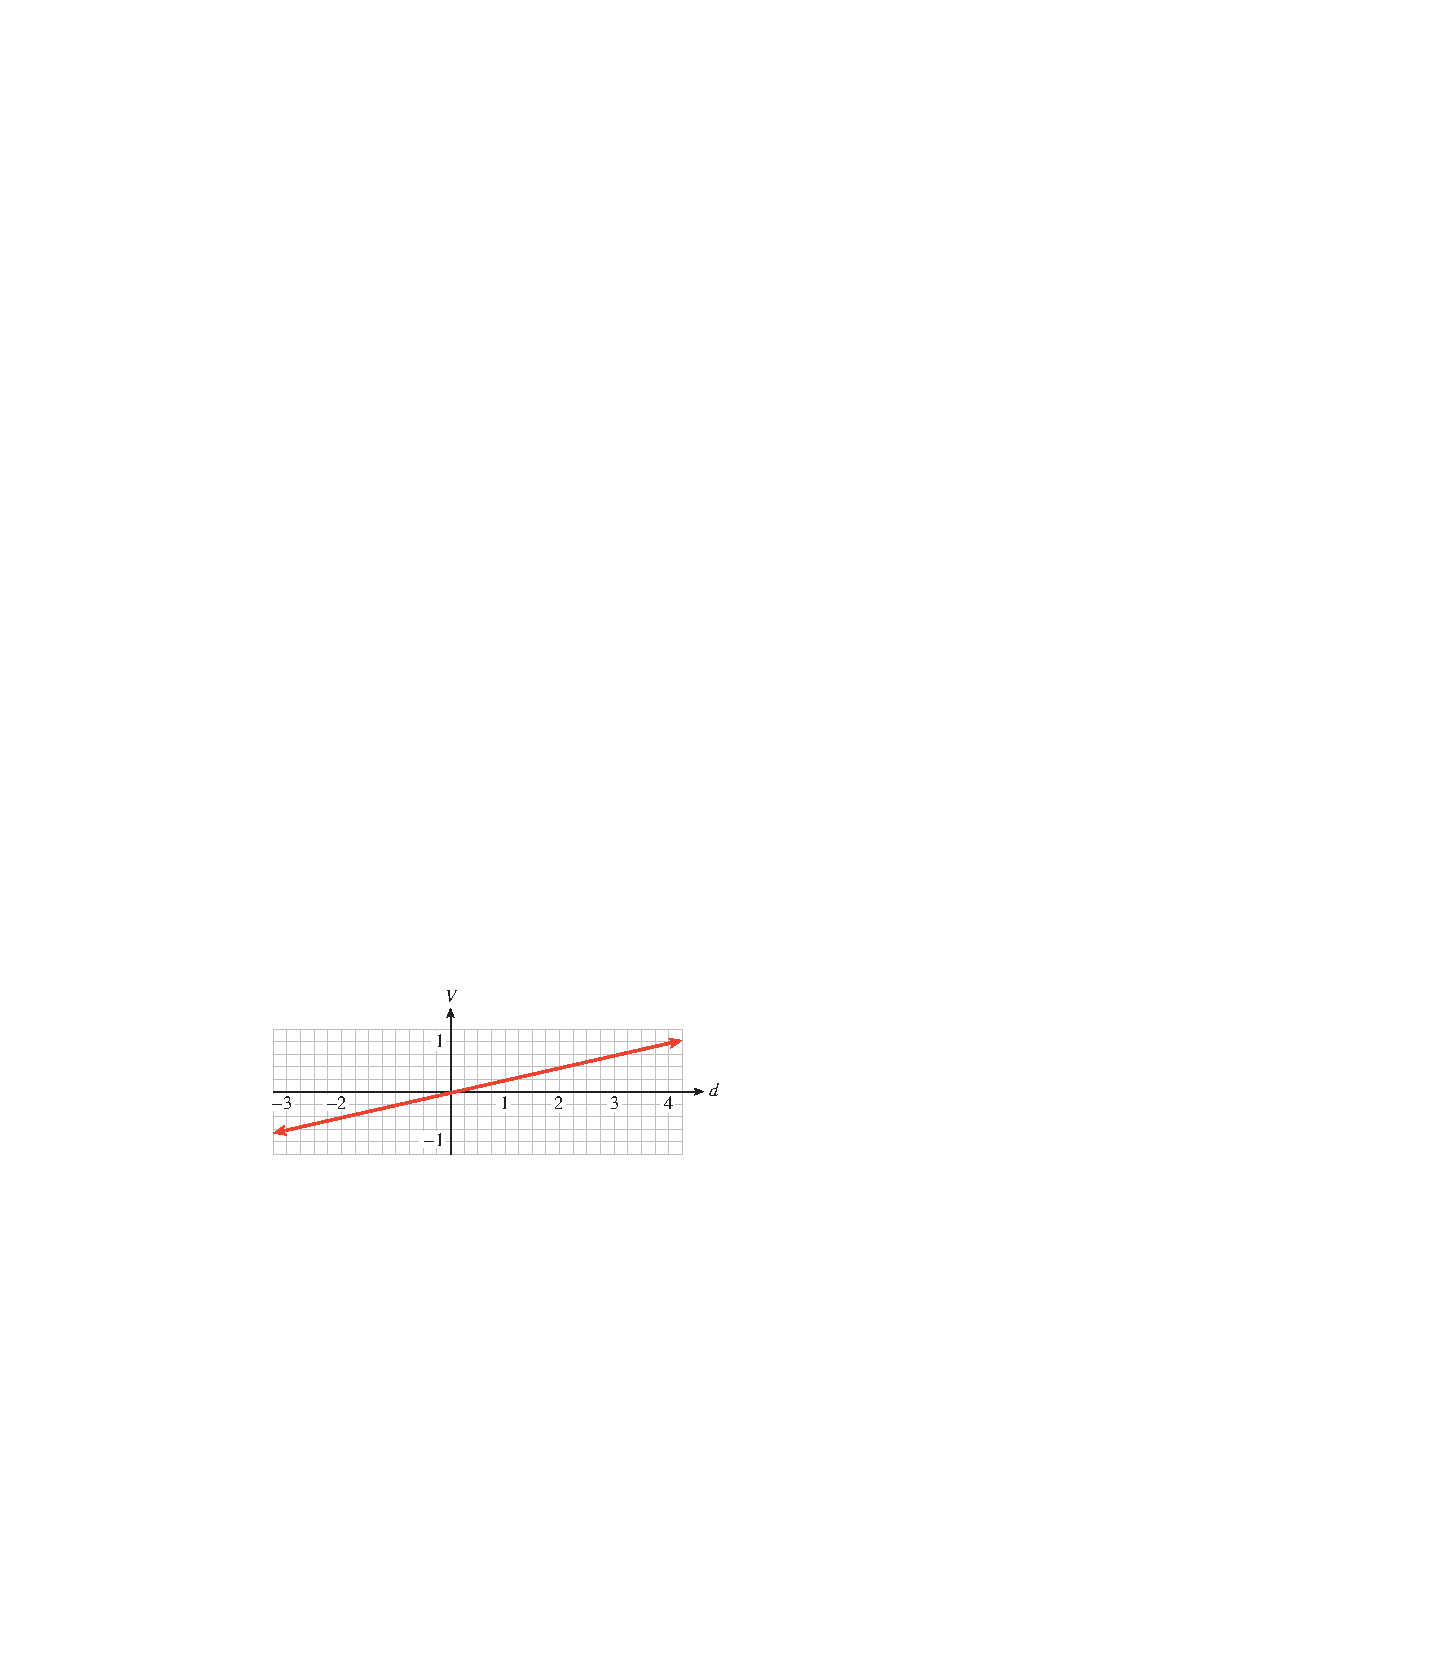
\includegraphics[width=\linewidth]{external/images/fig-ex-1-5-49.pdf}
\end{sbspanel}%
\end{sidebyside}%
\end{divisionexerciseegcol}%
\begin{divisionexerciseegcol}{50}{}{}{exercise-section-1-5-exercises-u-g}%
\begin{sidebyside}{1}{0.25}{0.25}{0}%
\begin{sbspanel}{0.5}%
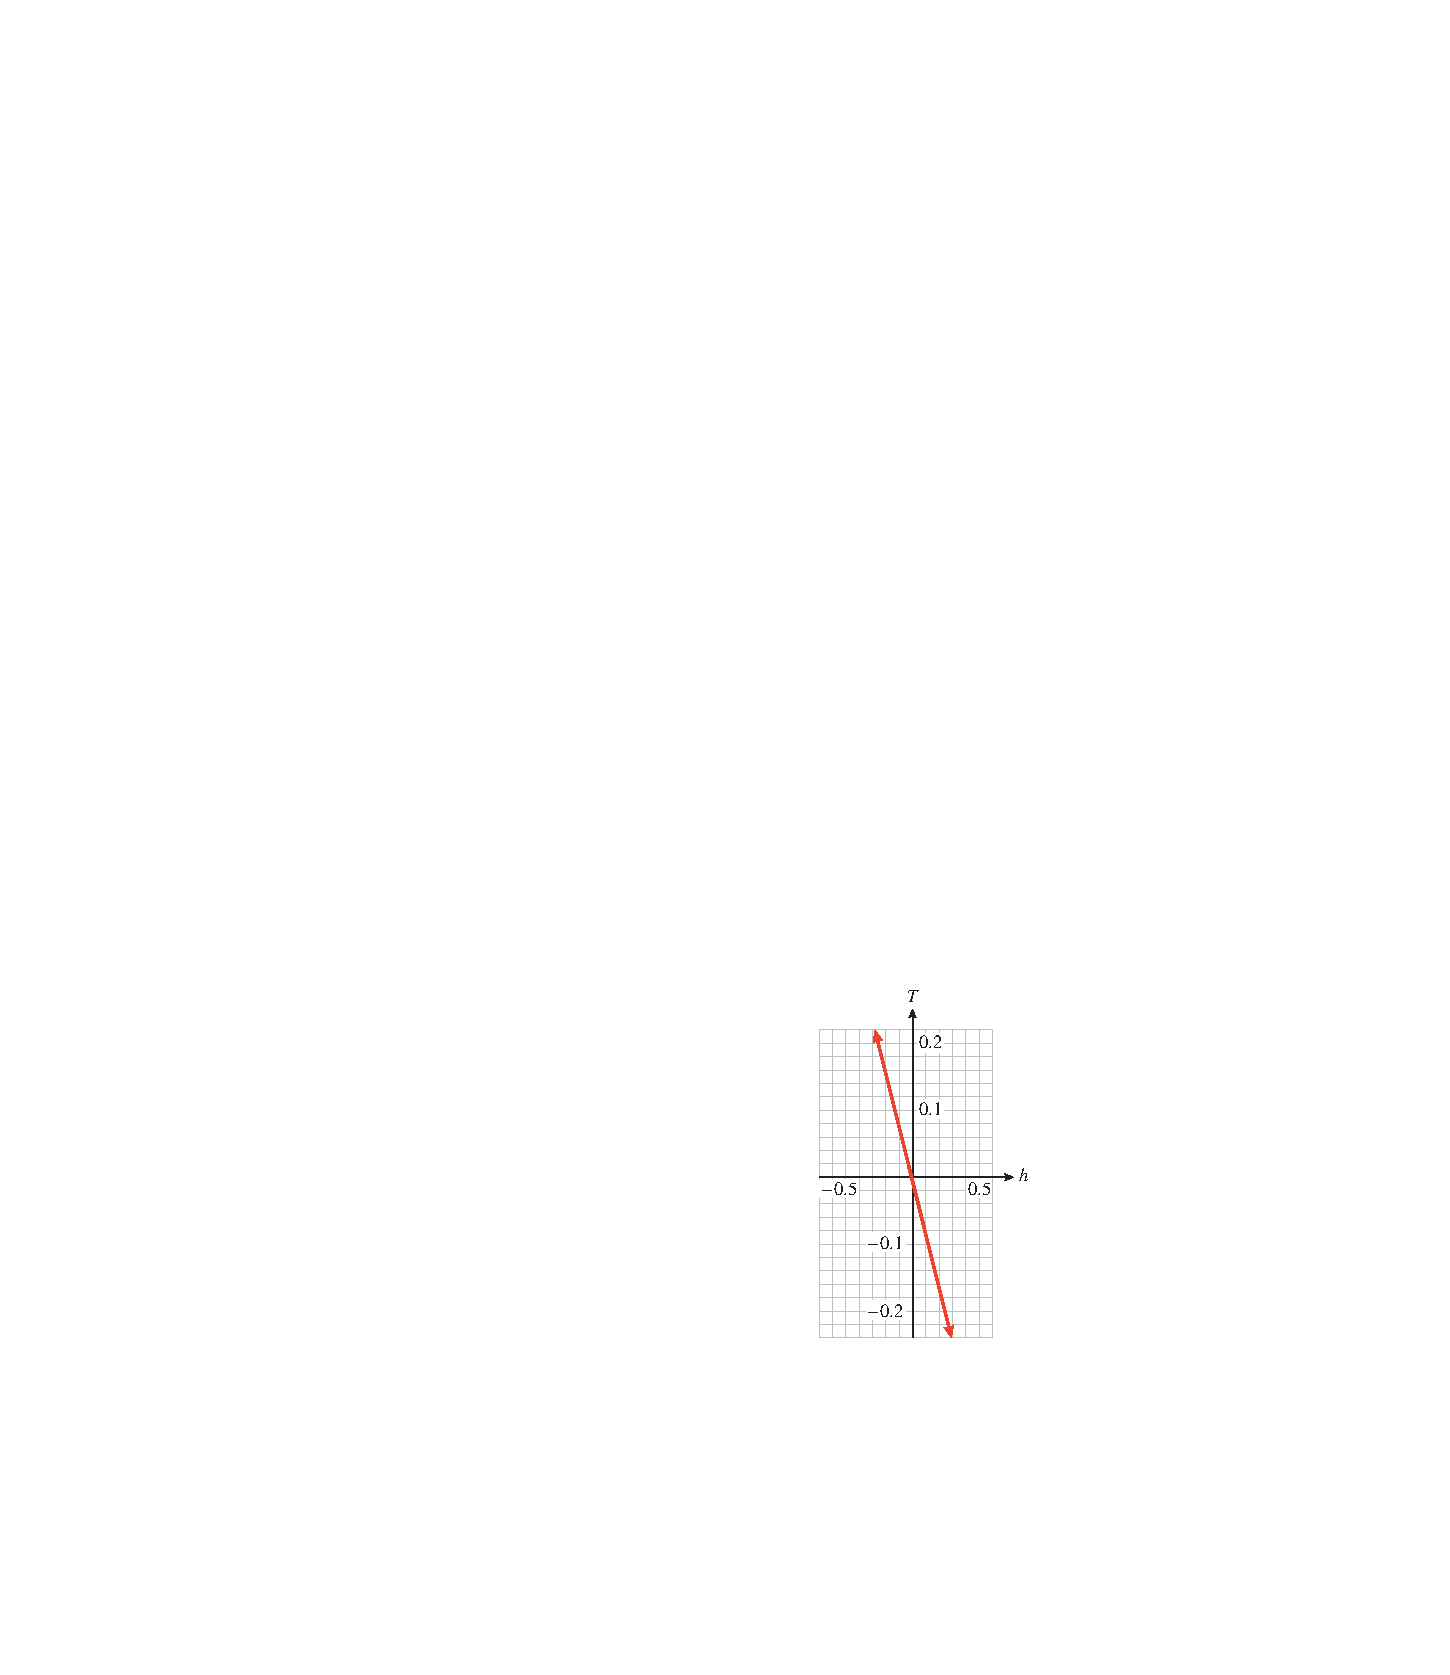
\includegraphics[width=\linewidth]{external/images/fig-ex-1-5-50.pdf}
\end{sbspanel}%
\end{sidebyside}%
\end{divisionexerciseegcol}%
\end{exercisegroupcol}
\par\medskip\noindent
\begin{divisionexercise}{51}{}{}{exercise-section-1-5-exercises-v}%
%
\begin{enumerate}[label=\alph*]
\item{}Write equations for three lines with slope \(m = \dfrac{3}{4}\). (Many answers are possible.)%
\item{}Graph all three lines in the same window. What do you notice about the lines?%
\end{enumerate}
%
\end{divisionexercise}%
\begin{divisionexercise}{52}{}{}{exercise-section-1-5-exercises-w}%
%
\begin{enumerate}[label=\alph*]
\item{}Write equations for three lines with slope \(m =0\). (Many answers are possible.)%
\item{}Graph all three lines in the same window. What do you notice about the lines?%
\end{enumerate}
%
\end{divisionexercise}%
\par\medskip\noindent%
\textbf{Exercise Group.}\space\space%
In Problems 53\textendash{}56, choose the correct graph for each equation. The scales on both axes are the same.%
\begin{exercisegroup}
\begin{divisionexerciseeg}{53}{}{}{exercise-section-1-5-exercises-x-b}%
%
\begin{multicols}{2}
\begin{enumerate}[label=\alph*]
\item{}\(\displaystyle y = \dfrac{3}{4}x + 2\)%
\item{}\(\displaystyle y = \dfrac{-3}{4}x + 2\)%
\item{}\(\displaystyle y = \dfrac{3}{4}x - 2 \)%
\item{}\(\displaystyle y =\dfrac{-3}{4}x - 2\)%
\end{enumerate}
\end{multicols}
%
\begin{sidebyside}{1}{0.15}{0.15}{0}%
\begin{sbspanel}{0.7}%
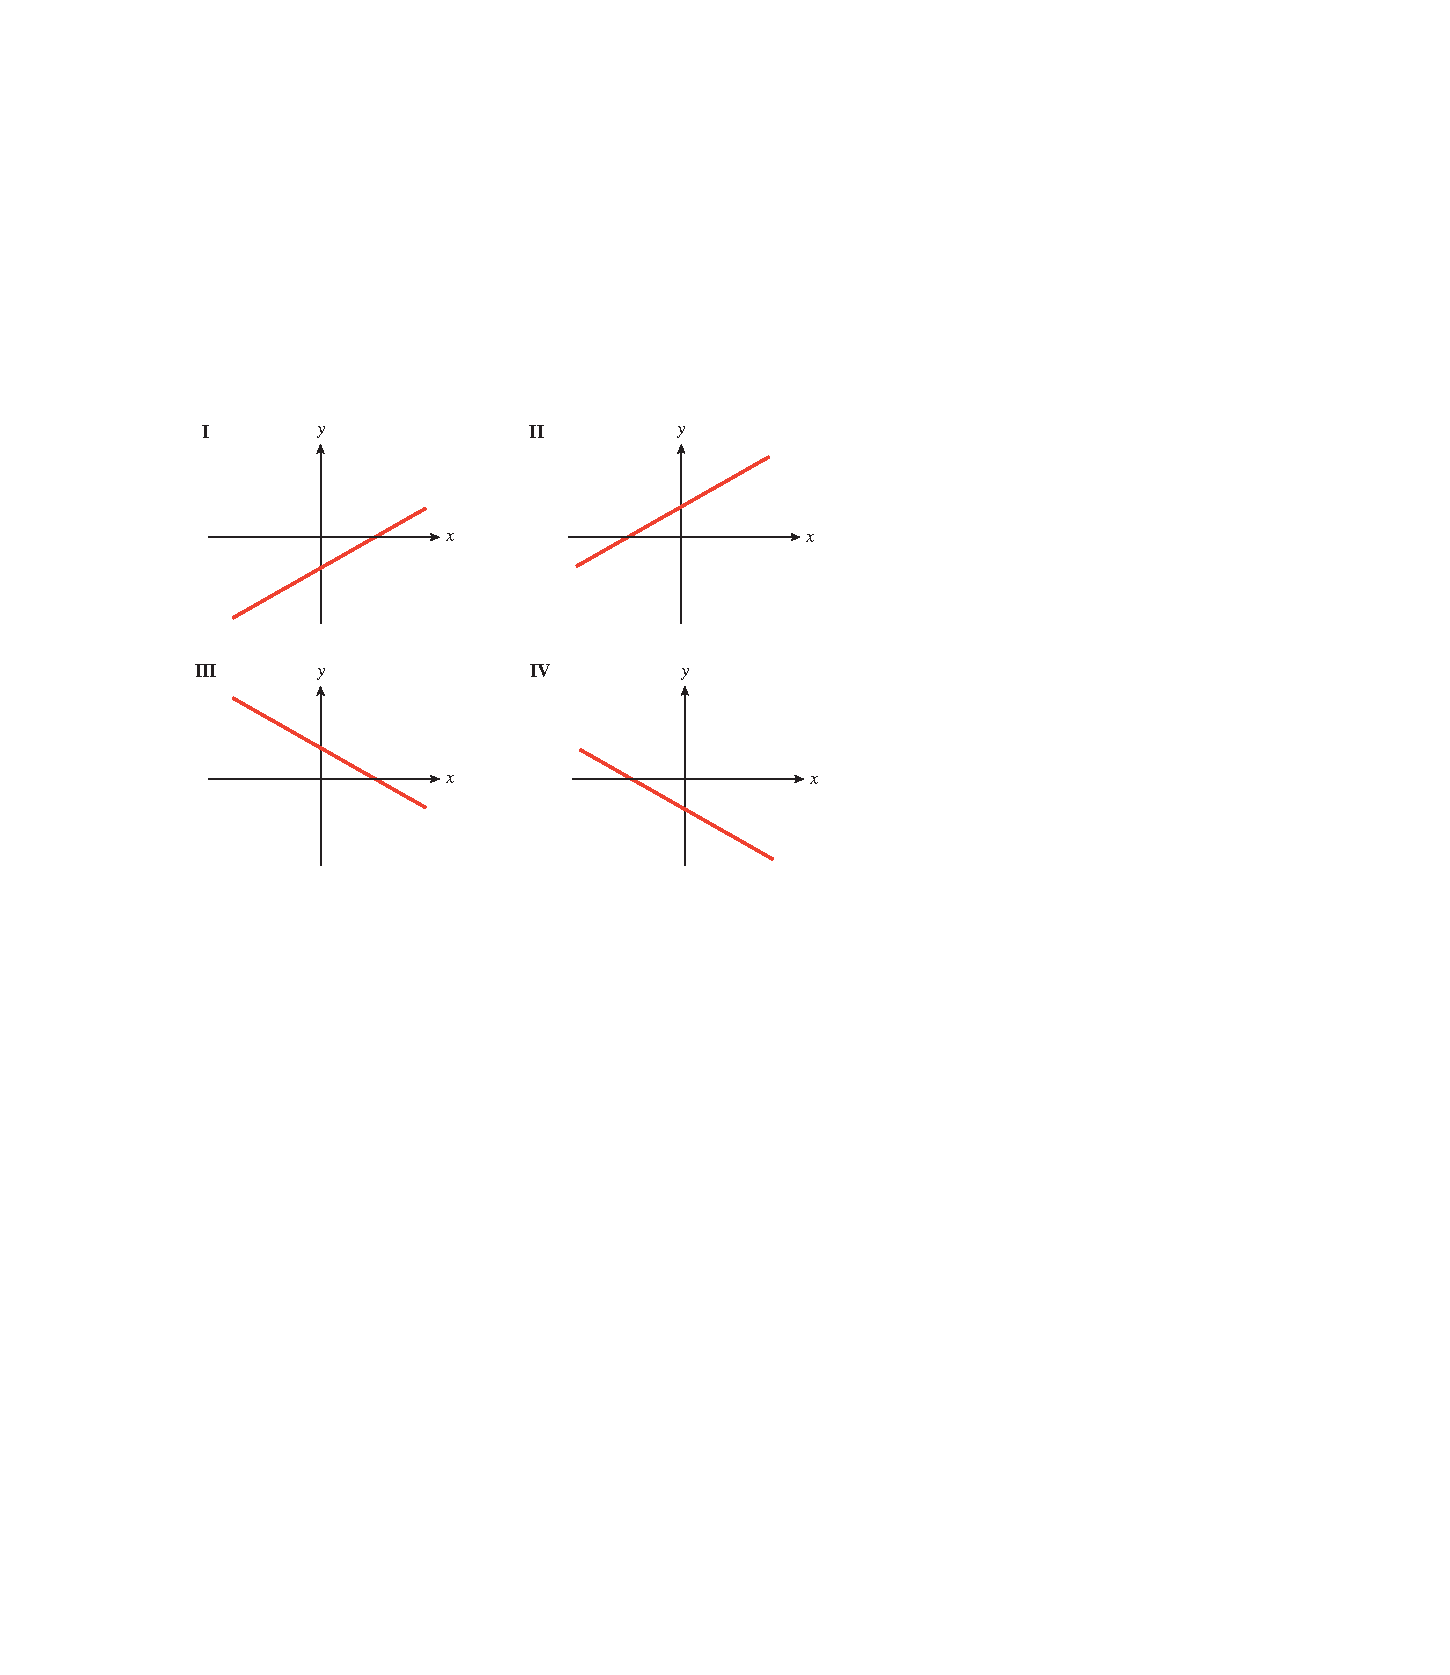
\includegraphics[width=\linewidth]{external/images/fig-ex-1-5-53.pdf}
\end{sbspanel}%
\end{sidebyside}%
\end{divisionexerciseeg}%
\begin{divisionexerciseeg}{54}{}{}{exercise-section-1-5-exercises-x-c}%
%
\begin{multicols}{2}
\begin{enumerate}[label=\alph*]
\item{}\(m\lt 0\), \(b\gt 0\)%
\item{}\(m\gt 1\), \(b\lt 0\)%
\item{}\(0\lt m\lt 1\), \(b\lt 0\)%
\item{}\(m\lt -1\), \(b\lt 0 \)%
\end{enumerate}
\end{multicols}
%
\begin{sidebyside}{1}{0.15}{0.15}{0}%
\begin{sbspanel}{0.7}%
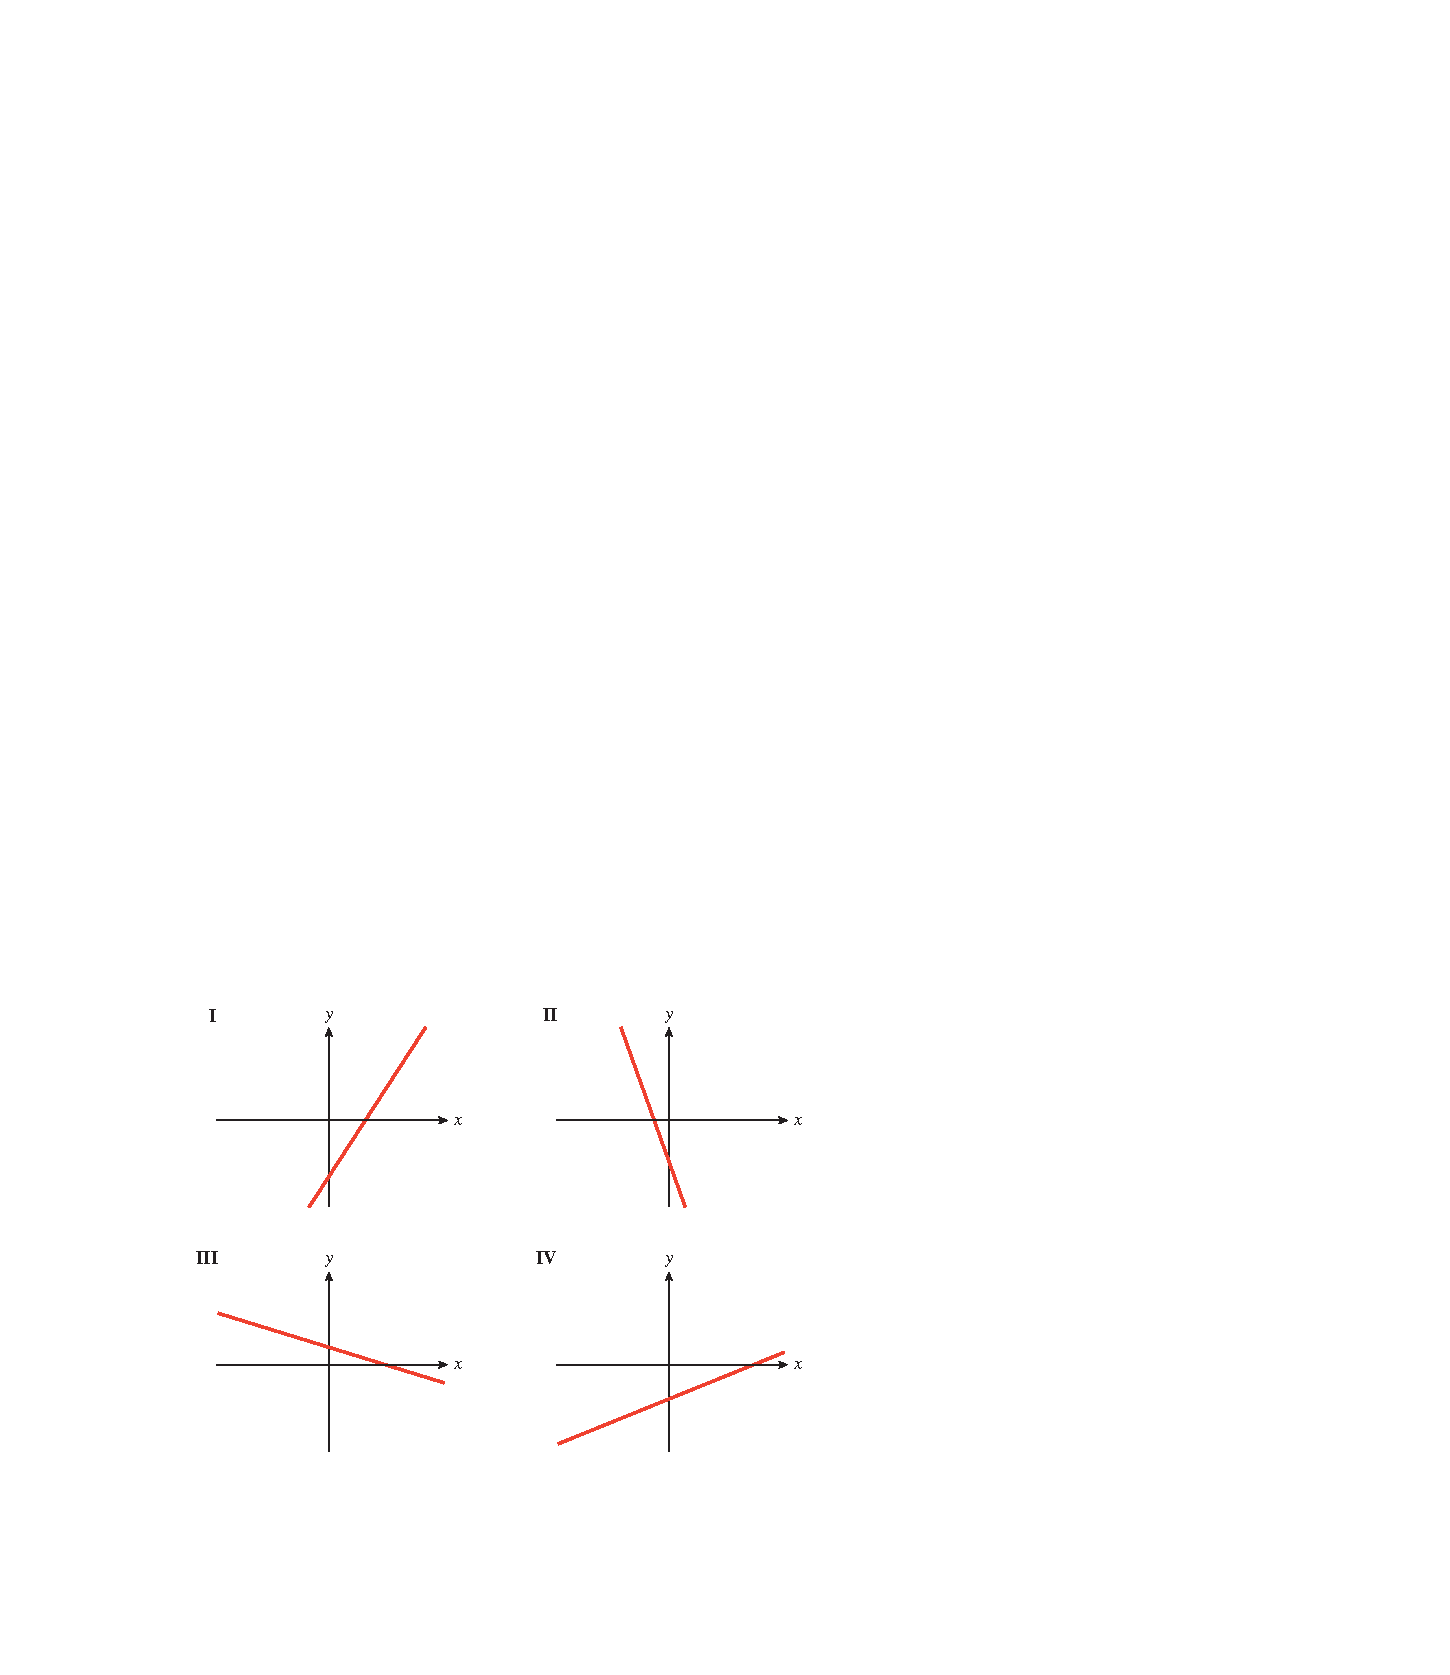
\includegraphics[width=\linewidth]{external/images/fig-ex-1-5-54.pdf}
\end{sbspanel}%
\end{sidebyside}%
\end{divisionexerciseeg}%
\begin{divisionexerciseeg}{55}{}{}{exercise-section-1-5-exercises-x-d}%
%
\begin{multicols}{2}
\begin{enumerate}[label=\alph*]
\item{}\(\displaystyle y = 1 + 2(x+3) \)%
\item{}\(\displaystyle y = -1 + 2(x-3)\)%
\item{}\(\displaystyle y = -1 + 2(x+3) \)%
\item{}\(\displaystyle y = 1 + 2(x-3) \)%
\end{enumerate}
\end{multicols}
%
\begin{sidebyside}{1}{0.15}{0.15}{0}%
\begin{sbspanel}{0.7}%
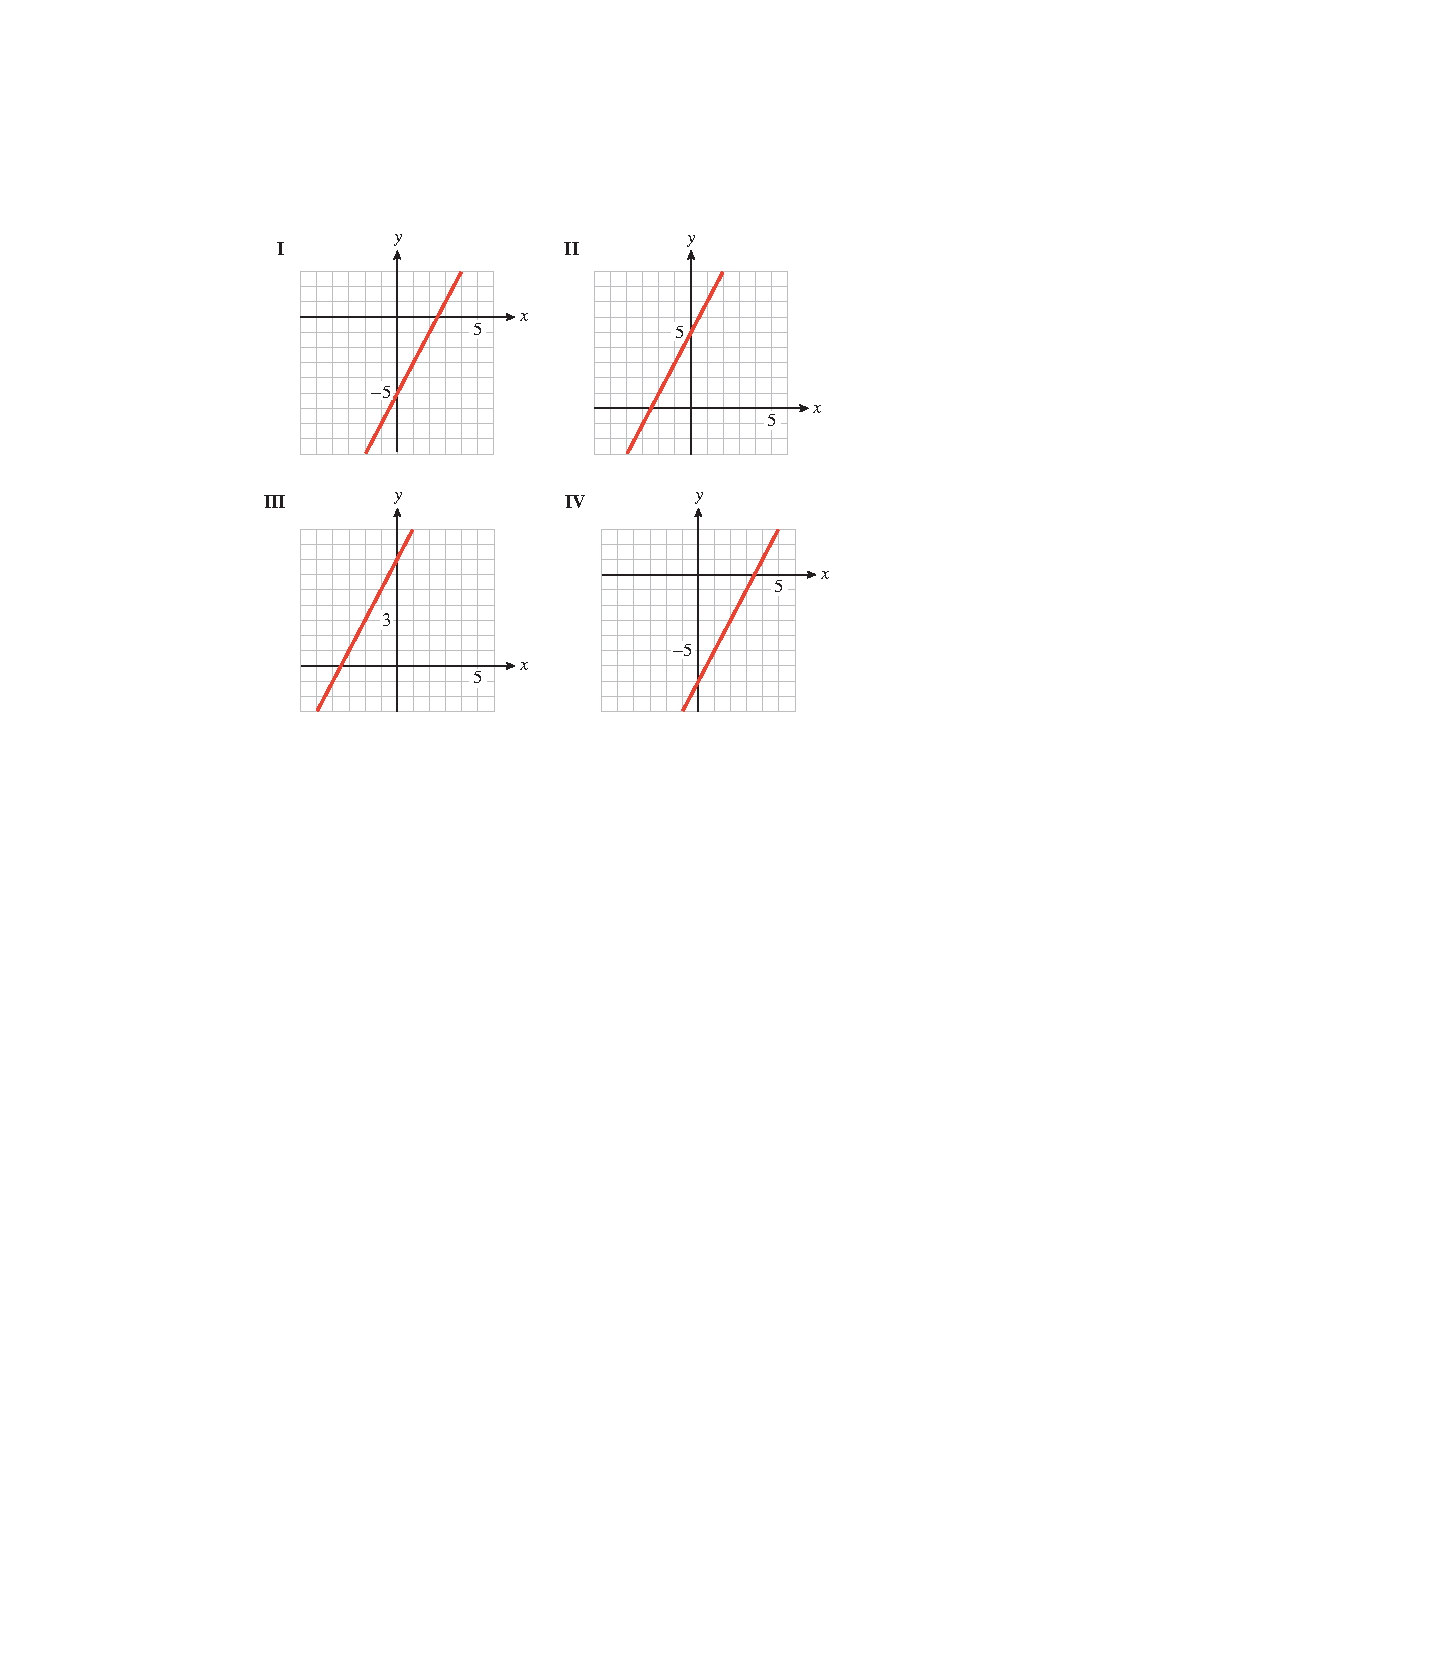
\includegraphics[width=\linewidth]{external/images/fig-ex-1-5-55.pdf}
\end{sbspanel}%
\end{sidebyside}%
\end{divisionexerciseeg}%
\begin{divisionexerciseeg}{56}{}{}{exercise-section-1-5-exercises-x-e}%
%
\begin{multicols}{2}
\begin{enumerate}[label=\alph*]
\item{}\(\displaystyle y = 2 - \dfrac{2}{3}(x - 3) \)%
\item{}\(\displaystyle y = 2 - \dfrac{3}{2}(x + 3) \)%
\item{}\(\displaystyle y = 2 + \dfrac{3}{2}(x - 3) \)%
\item{}\(\displaystyle y = 2 + \dfrac{2}{3}(x + 3) \)%
\end{enumerate}
\end{multicols}
%
\begin{sidebyside}{1}{0.15}{0.15}{0}%
\begin{sbspanel}{0.7}%
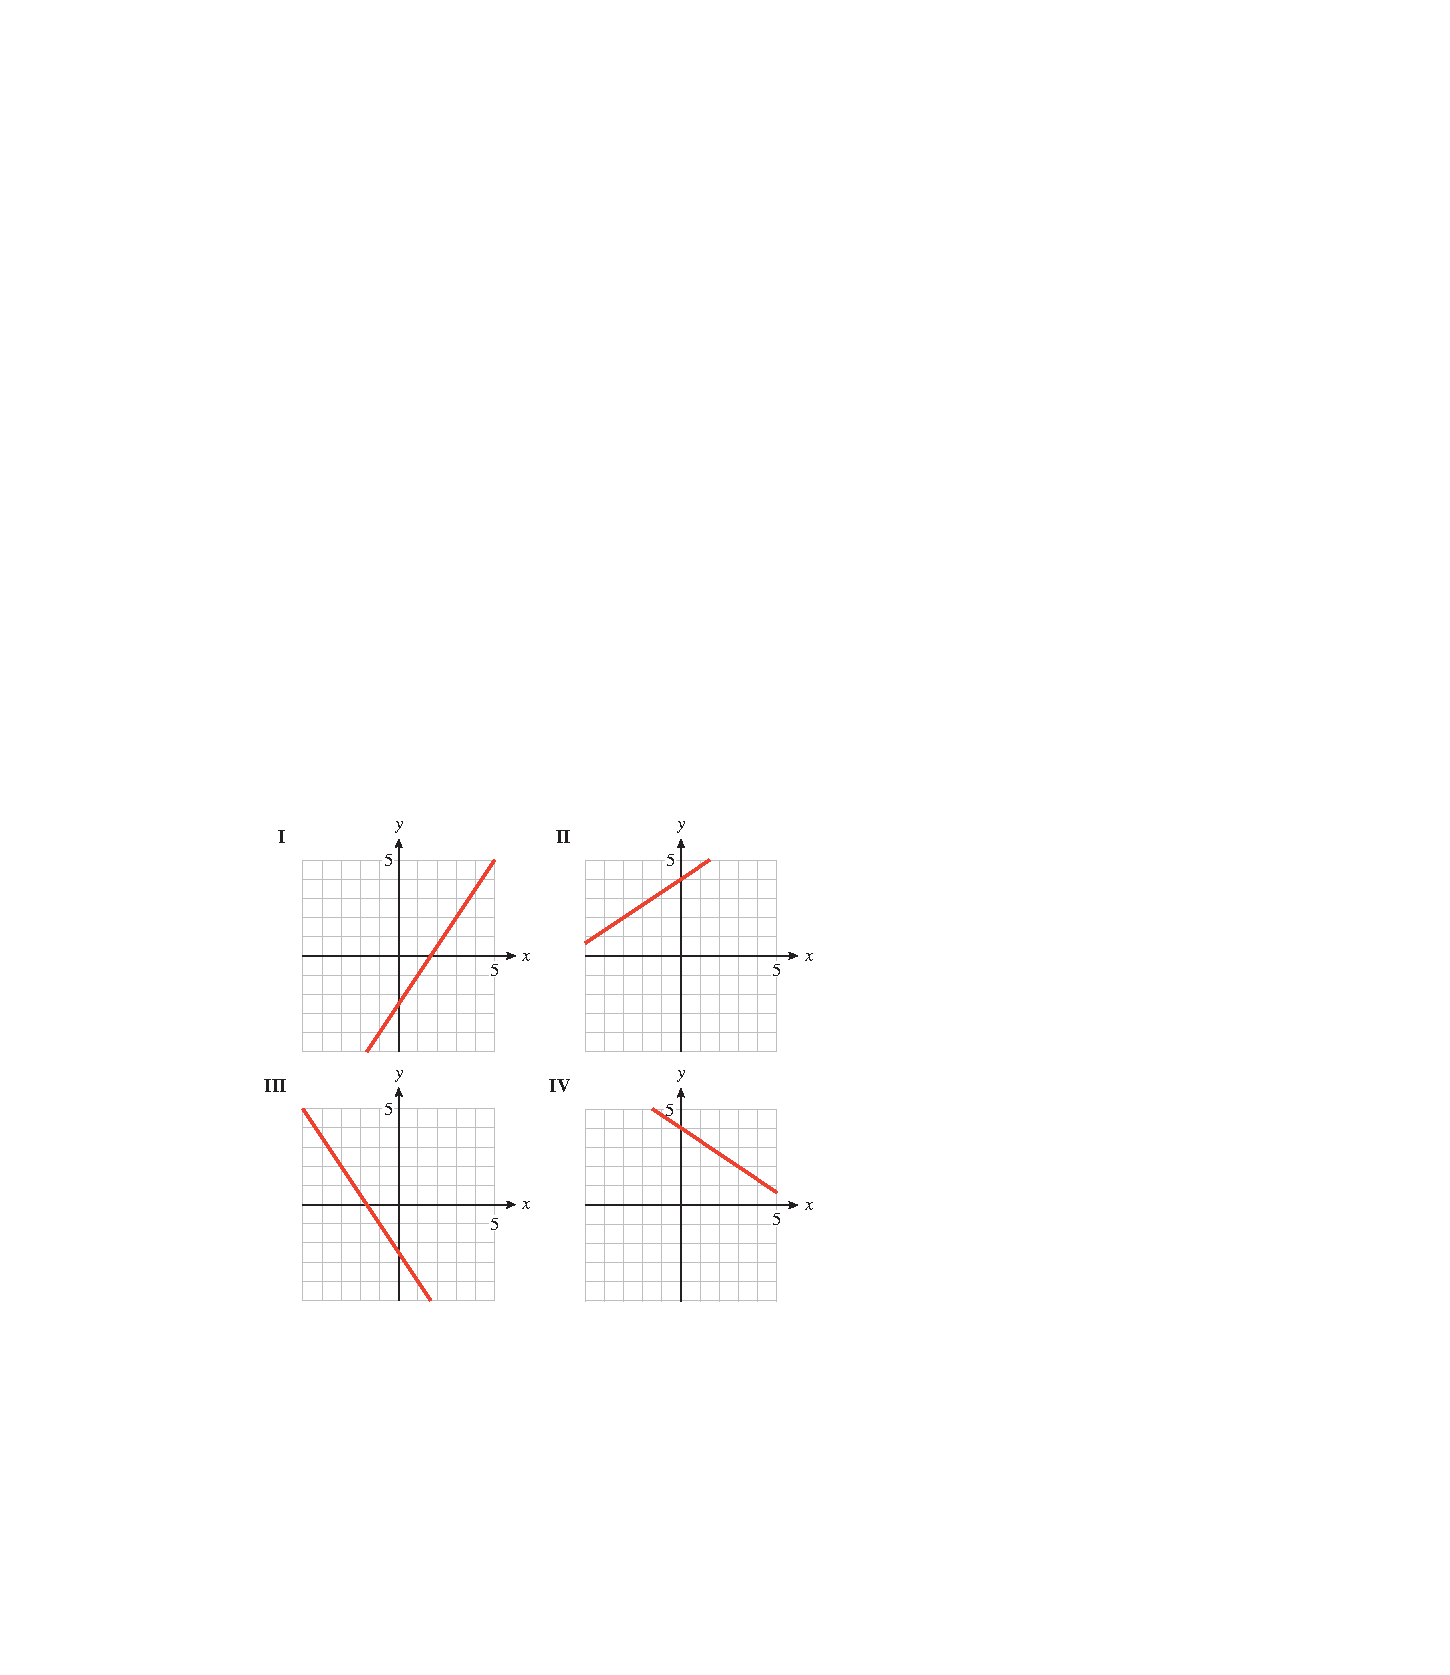
\includegraphics[width=\linewidth]{external/images/fig-ex-1-5-56.pdf}
\end{sbspanel}%
\end{sidebyside}%
\end{divisionexerciseeg}%
\end{exercisegroup}
\par\medskip\noindent
\par\medskip\noindent%
\textbf{Exercise Group.}\space\space%
In Problems 57\textendash{}60, find the slope of each line and the coordinates of one point on the line. (No calculation is necessary!)%
\begin{exercisegroupcol}{2}
\begin{divisionexerciseegcol}{57}{}{}{exercise-section-1-5-exercises-y-b}%
\(y + 1 = 2(x - 6)\)%
\end{divisionexerciseegcol}%
\begin{divisionexerciseegcol}{58}{}{}{exercise-section-1-5-exercises-y-c}%
\(2(y - 8) = 5(x + 2)\)%
\end{divisionexerciseegcol}%
\begin{divisionexerciseegcol}{59}{}{}{exercise-section-1-5-exercises-y-d}%
\(y = 3 - \dfrac{4}{3}(x + 5)\)%
\end{divisionexerciseegcol}%
\begin{divisionexerciseegcol}{60}{}{}{exercise-section-1-5-exercises-y-e}%
\(7x = -3y\)%
\end{divisionexerciseegcol}%
\end{exercisegroupcol}
\par\medskip\noindent
\begin{divisionexercise}{61}{}{}{exercise-section-1-5-exercises-z}%
%
\begin{enumerate}[label=\alph*]
\item{}Draw a set of coordinate axes with a square grid (i.e., with units the same size in both directions). Sketch four lines through the point (0, 4) with the following slopes:%
\begin{equation*}
m = 3, ~~~ m = -3,~~~ m = \frac{1}{3}, ~~~ m =\frac{-1}{3}
\end{equation*}
%
\item{}What do you notice about these lines?%
\end{enumerate}
%
\par\smallskip%
\noindent\textbf{\blocktitlefont Hint}.\hypertarget{hint-section-1-5-exercises-z-b}{}\quad{}Look for perpendicular lines.%
\end{divisionexercise}%
\begin{divisionexercise}{62}{}{}{exercise-section-1-5-exercises-aa}%
%
\begin{enumerate}[label=\alph*]
\item{}Draw a set of coordinate axes with a square grid (see Problem 61). Sketch four lines through the point (0, -3) with the following slopes:%
\begin{equation*}
m = \frac{2}{5}, ~~~ m = \frac{-2}{5},~~~ m = \frac{5}{2}, ~~~ m =\frac{-5}{2}
\end{equation*}
%
\item{}What do you notice about these lines?%
\end{enumerate}
%
\end{divisionexercise}%
\begin{divisionexercise}{63}{}{}{exercise-section-1-5-exercises-ab}%
The boiling point of water changes with altitude and is approximated by the formula%
\begin{equation*}
B = f (h) = 212 - 0.0018h
\end{equation*}
where \(B\) is in degrees and \(h\) is in feet. State the slope and vertical intercept of the graph, including units, and explain their meaning in this context.%
\end{divisionexercise}%
\begin{divisionexercise}{64}{}{}{exercise-section-1-5-exercises-ac}%
The height of a woman in centimeters is related to the length of her femur (in centimeters) by the formula%
\begin{equation*}
H = f (x) = 2.47x + 54.10
\end{equation*}
State the slope and the vertical intercept of the graph, including units, and explain their meaning in this context.%
\end{divisionexercise}%
\end{exercises-subsection}
\end{sectionptx}
%
%
\typeout{************************************************}
\typeout{Section 1.6 Linear Regression}
\typeout{************************************************}
%
\begin{sectionptx}{Section}{Linear Regression}{}{Linear Regression}{}{}{section-linear-regression}
\begin{introduction}{}%
We have spent most of this chapter analyzing models described by graphs or equations. To create a model, however, we often start with a quantity of data. Choosing an appropriate function for a model is a complicated process. In this section, we consider only linear models and explore methods for fitting a linear function to a collection of data points. First, we fit a line through two data points.%
\end{introduction}%
%
%
\typeout{************************************************}
\typeout{Subsection  Fitting a Line through Two Points}
\typeout{************************************************}
%
\begin{subsectionptx}{Subsection}{Fitting a Line through Two Points}{}{Fitting a Line through Two Points}{}{}{subsection-linear-regression-c}
If we already know that two variables are related by a linear function, we can find a formula from just two data points. For example, variables that increase or decrease at a constant rate can be described by linear functions.%
\begin{example}{Example}{}{example-example-wine}%
In 1993, Americans drank 188.6 million cases of wine. Wine consumption increased at a constant rate over the next decade, and we drank 258.3 million cases of wine in 2003. (Source: Los Angeles Times, Adams Beverage Group)%
\begin{enumerate}[label=\alph*]
\item{}Find a formula for wine consumption, \(W\), in millions of cases, as a linear function of time, \(t\), in years since 1990.%
\item{}State the slope as a rate of change. What does the slope tell us about this problem?%
\end{enumerate}
%
\par\smallskip%
\noindent\textbf{\blocktitlefont Solution}.\hypertarget{solution-example-wine-b}{}\quad{}%
\begin{enumerate}[label=\alph*]
\item{}We have two data points of the form \((t, W)\), namely \((3, 188.6)\) and \((13, 258.3)\). We use the point-slope formula to fit a line through these two points. First, we compute the slope.%
\begin{equation*}
\frac{\Delta W}{\Delta t}=\frac {258.3 - 188.6}{13 - 3}= 6.97
\end{equation*}
Next, we use the slope \(m = 6.97\) and either of the two data points in the point-slope formula.%
\begin{equation*}
\begin{aligned}[t]
W \amp =W_1 + m(t - t_1) \\
W \amp = 188.6 + 6.97(t - 3) \\
W \amp = 167.69 + 6.97t
\end{aligned}
\end{equation*}
Thus, \(W = f (t) = 167.69 + 6.97t\).%
\item{}The slope gives us the rate of change of the function, and the units of the variables can help us interpret the slope in context.%
\begin{equation*}
\frac{\Delta W}{\Delta t}= 
\frac{258.3 - 188.6 \text{ millions of cases}}{13 - 3\text{ years}}
= 6.97 \text{ millions of cases / year}
\end{equation*}
Over the 10 years between 1993 and 2003, wine consumption in the United States increased at a rate of 6.97 million cases per year.%
\end{enumerate}
%
\end{example}
\begin{assemblage}{Assemblage}{To Fit a Line through Two Points:.}{assemblage-linear-regression-c-d}%
%
\begin{enumerate}[label=\arabic*]
\item{}Compute the slope between the two points.%
\item{}Substitute the slope and either point into the point-slope formula%
\begin{equation*}
y = y_1 + m(x - x_1)
\end{equation*}
%
\end{enumerate}
%
\end{assemblage}
\begin{inlineexercise}{Checkpoint}{Practice 1.}{exercise-linear-regression-c-e}%
In 1991, there were 64.6 burglaries per 1000 households in the United States. The number of burglaries reported annually declined at a roughly constant rate over the next decade, and in 2001 there were 28.7 burglaries per 1000 households. (Source: U.S. Department of Justice)%
\begin{enumerate}[label=\alph*.]
\item{}Find a function for the number of burglaries, \(B\text{,}\) as a function of time, \(t\text{,}\) in years, since 1990.%
\par
\(y=\)\fillintext{15}%
\item{}State the slope as a rate of change.%
\par
\(m\) is \fillintext{3}\quad(\begin{itemize*}[label=$\square$,leftmargin=3em,itemjoin=\hspace{1em}]
\item{}burglaries per decade%
\item{}burglaries per 1000 households per year%
\item{}households per burglary per year%
\item{}burglaries per year%
\end{itemize*})\quad
%
\par
What does the slope tell us about this problem?%
\par
\begin{itemize}[label=$\odot$,leftmargin=3em,]
\item{}A) The burglary rate declined by 3.59 burglaries per decade%
\item{}B) The burglary rate declined by 3.59 burglaries per 1000 households every year%
\item{}C) The burglary rate declined by 3.59 burglaries per year%
\end{itemize}
%
\par
(in the years 1991 to 2001).%
\end{enumerate}
%
\par\smallskip%
\noindent\textbf{\blocktitlefont Answer 1}.\hypertarget{answer-linear-regression-c-e-c}{}\quad{}\(68.19-3.59t\)%
\par\smallskip%
\noindent\textbf{\blocktitlefont Answer 2}.\hypertarget{answer-linear-regression-c-e-d}{}\quad{}\(-3.59\)%
\par\smallskip%
\noindent\textbf{\blocktitlefont Answer 3}.\hypertarget{answer-linear-regression-c-e-e}{}\quad{}\(\text{burglaries per decade}\)%
\par\smallskip%
\noindent\textbf{\blocktitlefont Answer 4}.\hypertarget{answer-linear-regression-c-e-f}{}\quad{}\(\text{C) The ... burglaries per year}\)%
\par\smallskip%
\noindent\textbf{\blocktitlefont Solution}.\hypertarget{solution-linear-regression-c-e-g}{}\quad{}%
\begin{enumerate}[label=\alph*.]
\item{}Because \(t=0\) corresponds to 1990, we have the two points (1,64.6) and (11,28.7) to compute the slope \(m=-3.59\text{.}\) Using the point-slope formula with either point and then simplifying, we find that \(y = {68.19-3.59t}\)%
\item{}\(-3.59\) burglaries per 1000 households per year. From 1991 to 2001, the burglary rate declined by 3.59 burglaries per 1000 households every year.%
\end{enumerate}
%
\end{inlineexercise}%
\begin{inlineexercise}{Checkpoint}{QuickCheck 1.}{exercise-linear-regression-c-f}%
What are the two steps to find the equation of a line through two points?%
\par
\begin{itemize}[label=$\odot$,leftmargin=3em,]
\item{}Draw the line, use the point-slope formula%
\item{}Compute the slope, find the \(y\)-intercept%
\item{}Compute the slope, use the point-slope formula%
\item{}Find the intercepts, compute the slope%
\end{itemize}
%
\par\smallskip%
\noindent\textbf{\blocktitlefont Answer}.\hypertarget{answer-linear-regression-c-f-c}{}\quad{}\(\text{Choice 4}\)%
\par\smallskip%
\noindent\textbf{\blocktitlefont Solution}.\hypertarget{solution-linear-regression-c-f-d}{}\quad{}Compute the slope, use the point-slope formula%
\end{inlineexercise}%
\end{subsectionptx}
%
%
\typeout{************************************************}
\typeout{Subsection  Scatterplots}
\typeout{************************************************}
%
\begin{subsectionptx}{Subsection}{Scatterplots}{}{Scatterplots}{}{}{subsection-linear-regression-d}
Empirical data points in a linear relation may not lie exactly on a line. There are many factors that can affect experimental data, including measurement error, the influence of environmental conditions, and the presence of related variable quantities.%
\begin{example}{Example}{}{example-example-gas-mileage}%
A consumer group wants to test the gas mileage of a new model SUV. They test-drive six vehicles under similar conditions and record the distance each drove on various amounts of gasoline.%
\begin{sidebyside}{1}{0}{0}{0}%
\begin{sbspanel}{1}%
\resizebox{\ifdim\width > \linewidth\linewidth\else\width\fi}{!}{%
{\centering%
{\tabularfont%
\begin{tabular}{AcAcAcAcAcAcAcA}\hrulethick
Gasoline used (gal)&\(9.6\)&\(11.3\)&\(8.8\)&\(5.2\)&\(10.3\)&\(6.7\)\tabularnewline\hrulethin
Miles driven&\(155.8\)&\(183.6\)&\(139.6\)&\(80.4\)&\(167.1\)&\(99.7\)\tabularnewline\hrulethin
\end{tabular}
}%
\par}
}%
\end{sbspanel}%
\end{sidebyside}%
\par
%
\begin{enumerate}[label=\alph*]
\item{}Are the data linear?%
\item{}Draw a line that fits the data.%
\item{}What does the slope of the line tell us about the data?%
\end{enumerate}
%
\par\smallskip%
\noindent\textbf{\blocktitlefont Solution}.\hypertarget{solution-example-gas-mileage-b}{}\quad{}%
\begin{enumerate}[label=\alph*]
\item{}No, the data are not strictly linear. If we compute the slopes between successive data points, the values are not constant. We can see from an accurate plot of the data, shown below, that the points lie close to, but not precisely on, a straight line.%
\begin{sidebyside}{2}{0.025}{0.025}{0.05}%
\begin{sbspanel}{0.45}%
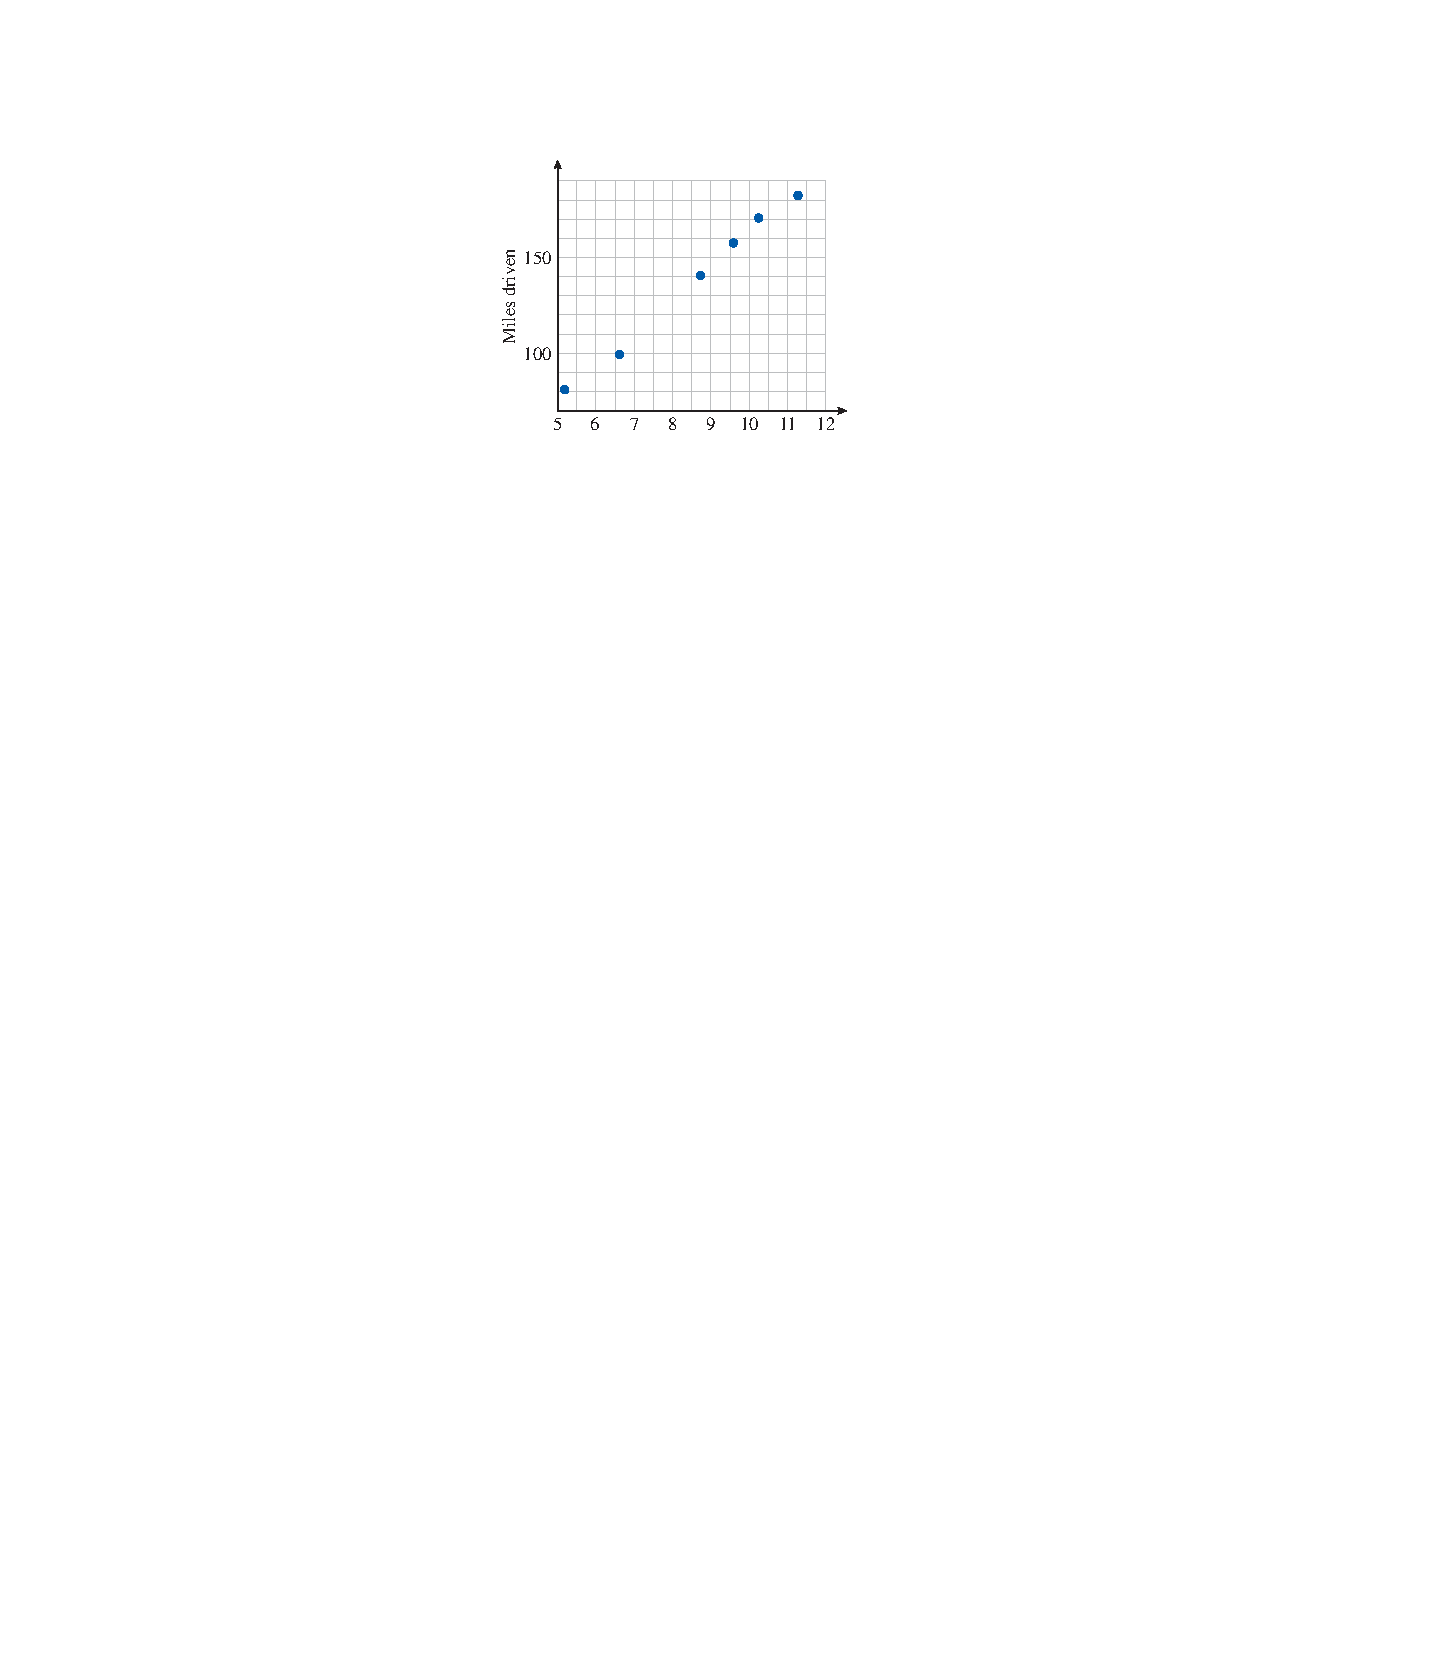
\includegraphics[width=\linewidth]{external/images/fig-gas-mileage.pdf}
\end{sbspanel}%
\begin{sbspanel}{0.45}%
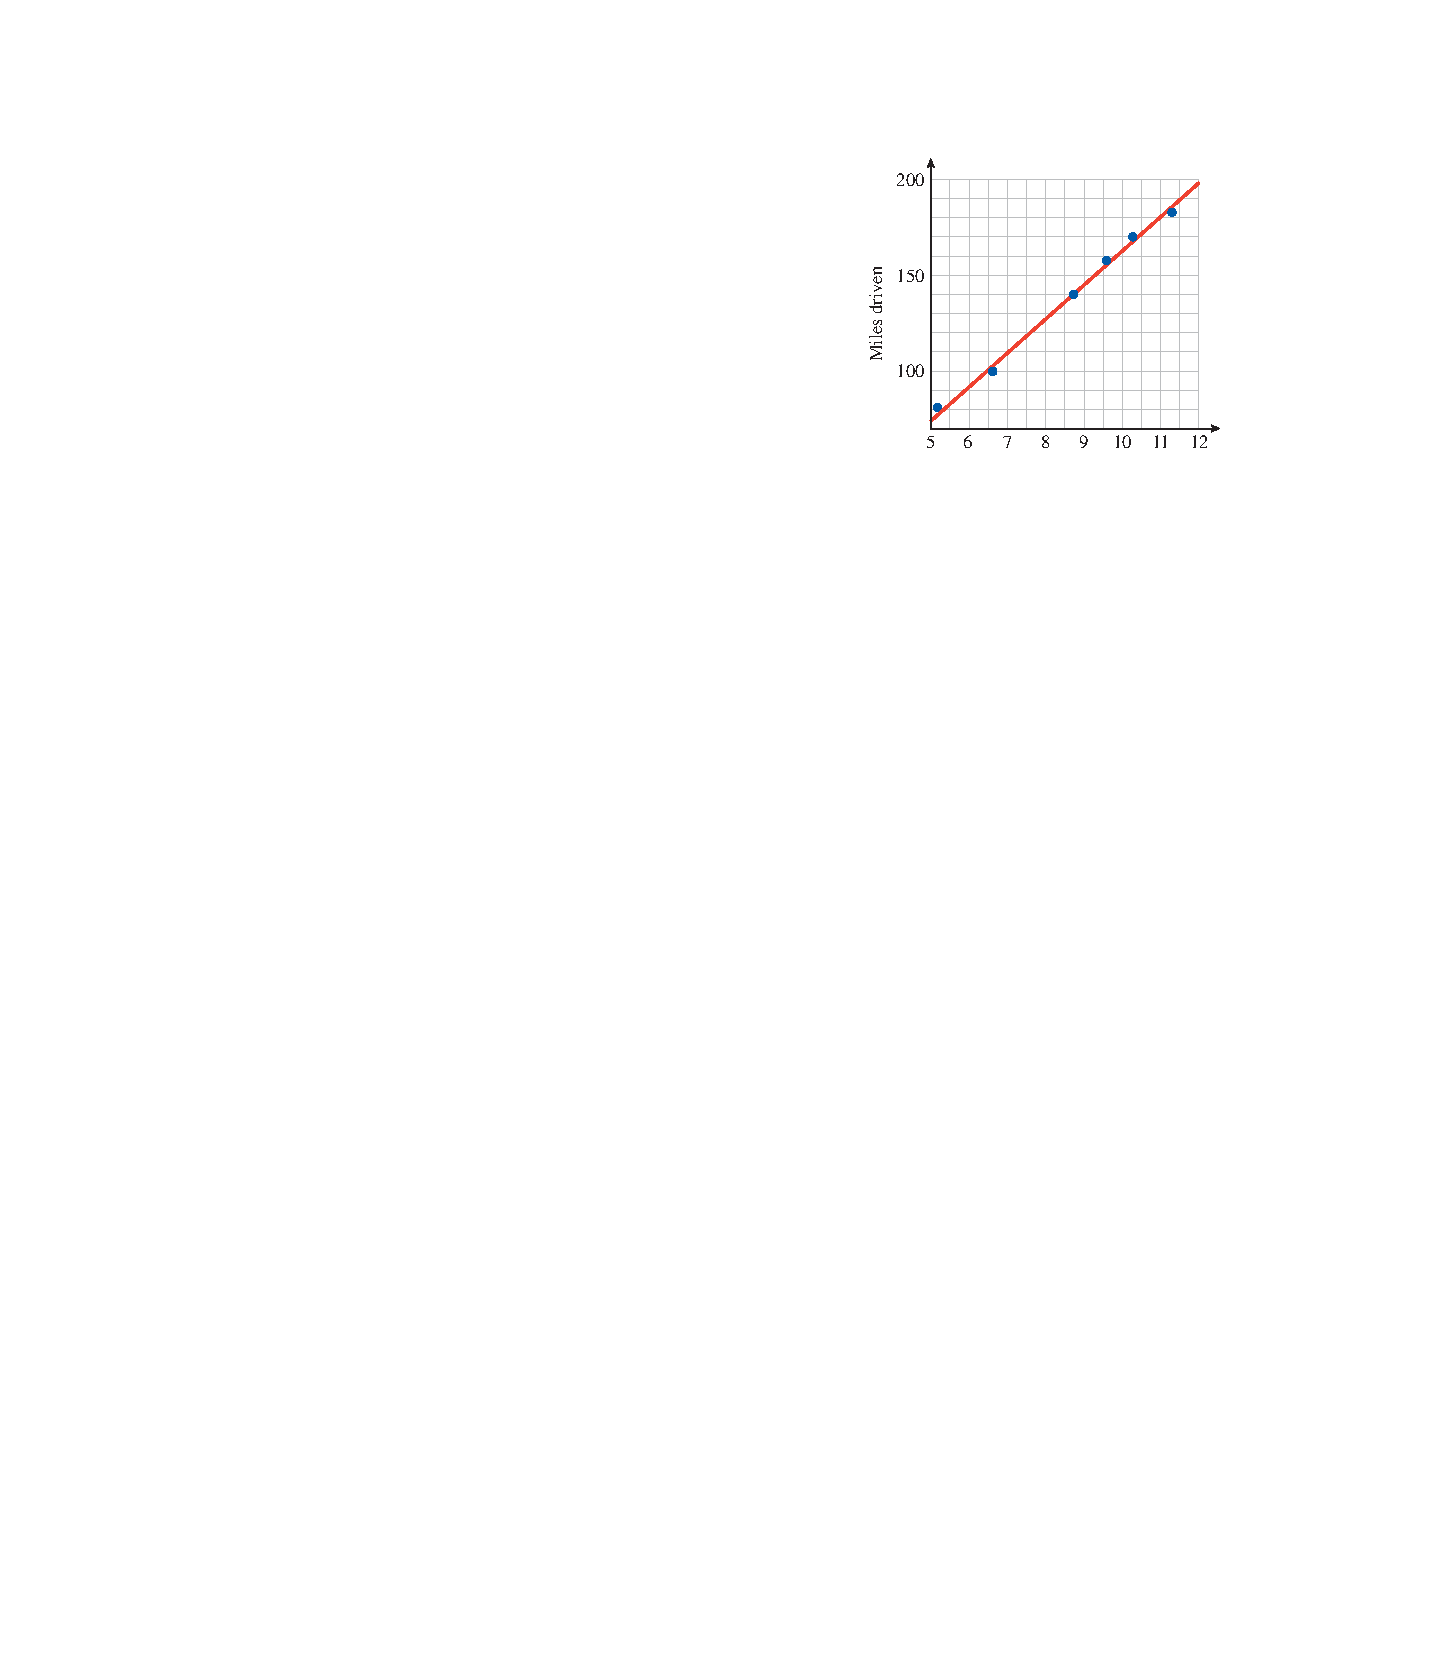
\includegraphics[width=\linewidth]{external/images/fig-gas-mileage2.pdf}
\end{sbspanel}%
\end{sidebyside}%
\item{}We would like to draw a line that comes as close as possible to all the data points, even though it may not pass precisely through any of them. In particular, we try to adjust the line so that we have the same number of data points above the line and below the line. One possible solution is shown above.%
\item{}To compute the slope of the our estimated line, we first choose two points on the line. Our line appears to pass through one of the data points,\((8.8, 139.6)\). We look for a second point on the line whose coordinates are easy to read, perhaps \((6.5,100)\). The slope is%
\begin{equation*}
m = \frac{139.6 - 100}{8.8 - 6.5}= 17.2\text{ miles per gallon}
\end{equation*}
According to our data, the SUV gets about 17.2 miles to the gallon.%
\end{enumerate}
%
\end{example}
\begin{warning}{Caution}{}{warning-linear-regression-d-d}%
To find the slope of your estimated line, be sure to choose points \emph{on the line}; do not choose any of the data points (unless they happen to lie on your line).%
\end{warning}
\begin{inlineexercise}{Checkpoint}{Practice 2.}{exercise-exercise-scatterplot}%
%
\begin{enumerate}[label=\alph*.]
\item{}Plot the data points. Do the points lie on a line?%
\par
\quad(\begin{itemize*}[label=$\square$,leftmargin=3em,itemjoin=\hspace{1em}]
\item{}Yes%
\item{}No%
\end{itemize*})\quad
%
\item{}Draw a line that fits the data.%
\end{enumerate}
%
\begin{center}%
{\tabularfont%
\begin{tabular}{AcAcAcAcAcAcAcA}
\(x\)&\(1.49\)&\(3.68\)&\(4.95\)&\(5.49\)&\(7.88\)&\(8.41\)\tabularnewline\hrulethin
\(y\)&\(2.69\)&\(3.7\)&\(4.6\)&\(5.2\)&\(7.2\)&\(7.3\)\tabularnewline\hrulethin
\end{tabular}
}%
\end{center}%
Graphs for both parts (a) and (b):%
\par
%
\begin{multicols}{2}
\begin{enumerate}[label=\alph*]
\item{}\begin{sidebyside}{1}{0.125}{0.125}{0}%
\begin{sbspanel}{0.75}%
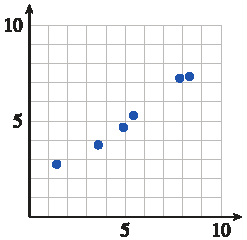
\includegraphics[width=\linewidth]{external/images/fig-in-ex-ans-1-6-2a.pdf}
\end{sbspanel}%
\end{sidebyside}%
%
\item{}\begin{sidebyside}{1}{0.125}{0.125}{0}%
\begin{sbspanel}{0.75}%
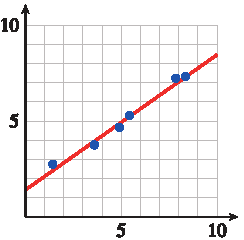
\includegraphics[width=\linewidth]{external/images/fig-in-ex-ans-1-6-2b.pdf}
\end{sbspanel}%
\end{sidebyside}%
%
\end{enumerate}
\end{multicols}
%
\par\smallskip%
\noindent\textbf{\blocktitlefont Answer}.\hypertarget{answer-exercise-scatterplot-c}{}\quad{}\(\text{No}\)%
\par\smallskip%
\noindent\textbf{\blocktitlefont Solution}.\hypertarget{solution-exercise-scatterplot-d}{}\quad{}%
\begin{enumerate}[label=\alph*.]
\item{}No. A scatterplot is shown below.%
\item{}See the graph below%
\end{enumerate}
%
\end{inlineexercise}%
The graph in \hyperref[example-example-gas-mileage]{Example~{\xreffont\ref{example-example-gas-mileage}}} is called a \terminology{scatterplot}\index{scatterplot}. The points on a scatterplot may or may not show some sort of pattern. Consider the three plots shown below.%
\begin{itemize}[label=\textbullet]
\item{}In figure (a), the data points resemble a cloud of gnats; there is no apparent pattern to their locations.%
\item{}In figure (b), the data follow a generally decreasing trend, but certainly do not all lie on the same line.%
\item{}The points in figure (c) are even more organized; they seem to lie very close to an imaginary line.%
\end{itemize}
%
\begin{sidebyside}{1}{0.1}{0.1}{0}%
\begin{sbspanel}{0.8}%
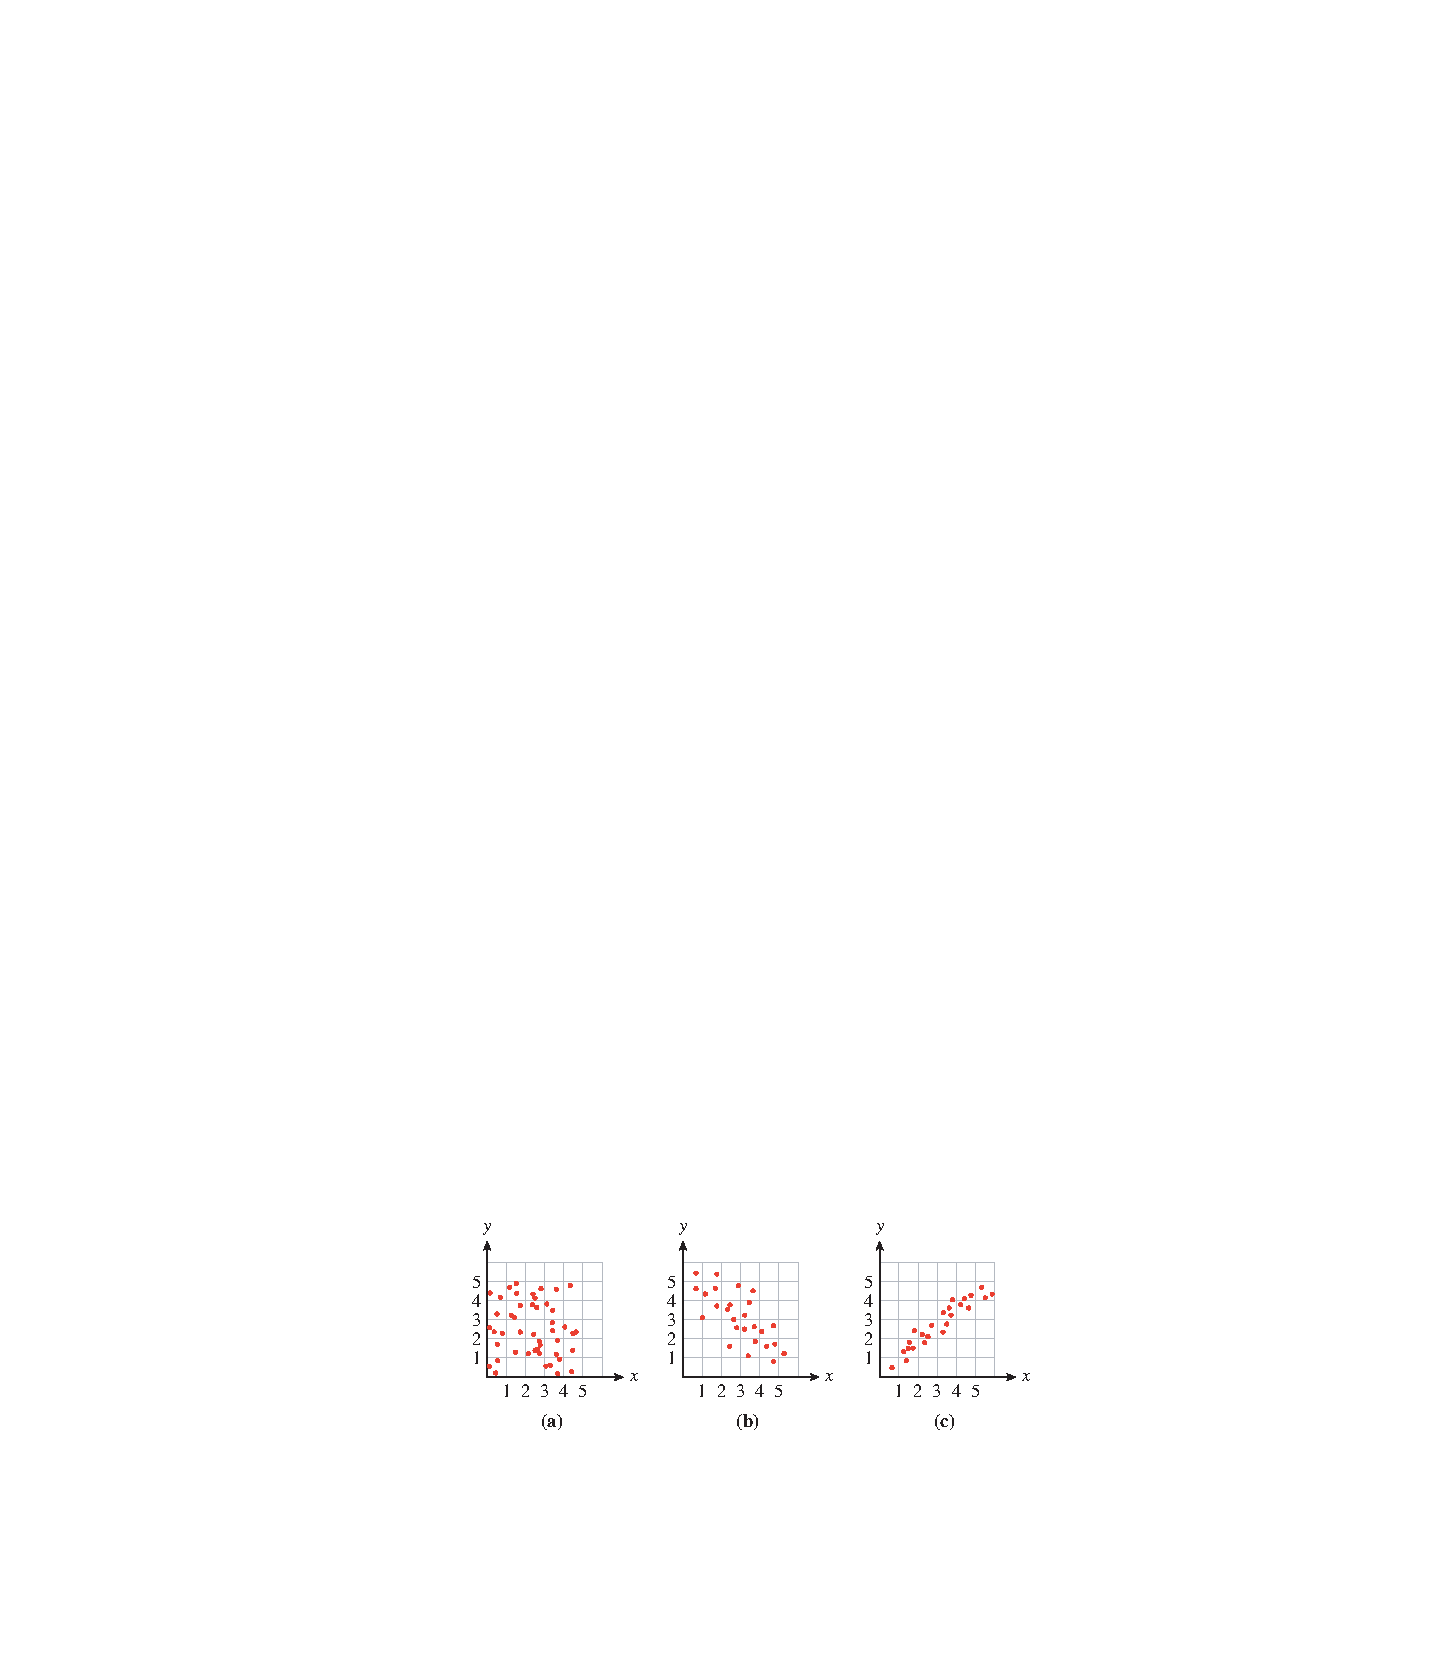
\includegraphics[width=\linewidth]{external/images/fig-scatterplots.pdf}
\end{sbspanel}%
\end{sidebyside}%
\begin{inlineexercise}{Checkpoint}{QuickCheck 2.}{exercise-linear-regression-d-h}%
Can two points on a scatterplot have the same \(x\)-coordinate? Can two points have the same \(y\)-coordinate?%
\par
\begin{itemize}[label=$\odot$,leftmargin=3em,]
\item{}Yes, Yes%
\item{}Yes, No%
\item{}No, Yes%
\item{}No, No%
\end{itemize}
%
\par\smallskip%
\noindent\textbf{\blocktitlefont Answer}.\hypertarget{answer-linear-regression-d-h-c}{}\quad{}\(\text{Yes, Yes}\)%
\par\smallskip%
\noindent\textbf{\blocktitlefont Solution}.\hypertarget{solution-linear-regression-d-h-d}{}\quad{}Yes, Yes%
\end{inlineexercise}%
If the data in a scatterplot are roughly linear, we can estimate the location of an imaginary \terminology{line of best fit}\index{line of best fit} that passes as close as possible to the data points. We can then use this line to make predictions about the data.%
\end{subsectionptx}
%
%
\typeout{************************************************}
\typeout{Subsection  Linear Regression}
\typeout{************************************************}
%
\begin{subsectionptx}{Subsection}{Linear Regression}{}{Linear Regression}{}{}{subsection-linear-regression-e}
One measure of a person's physical fitness is the \emph{body mass index}\index{body mass index}, or BMI. Your BMI is the ratio of your weight in kilograms to the square of your height in centimeters. Thus, thinner people have lower BMI scores, and fatter people have higher scores. The Centers for Disease Control considers a BMI between 18.5 and 24.9 to be healthy.%
\par
The points on the scatterplot below show the BMI of Miss America from 1921 to 1991. From the data in the scatterplot, can we see a trend in Americans’ ideal of female beauty?%
\begin{sidebyside}{1}{0.1}{0.1}{0}%
\begin{sbspanel}{0.8}%
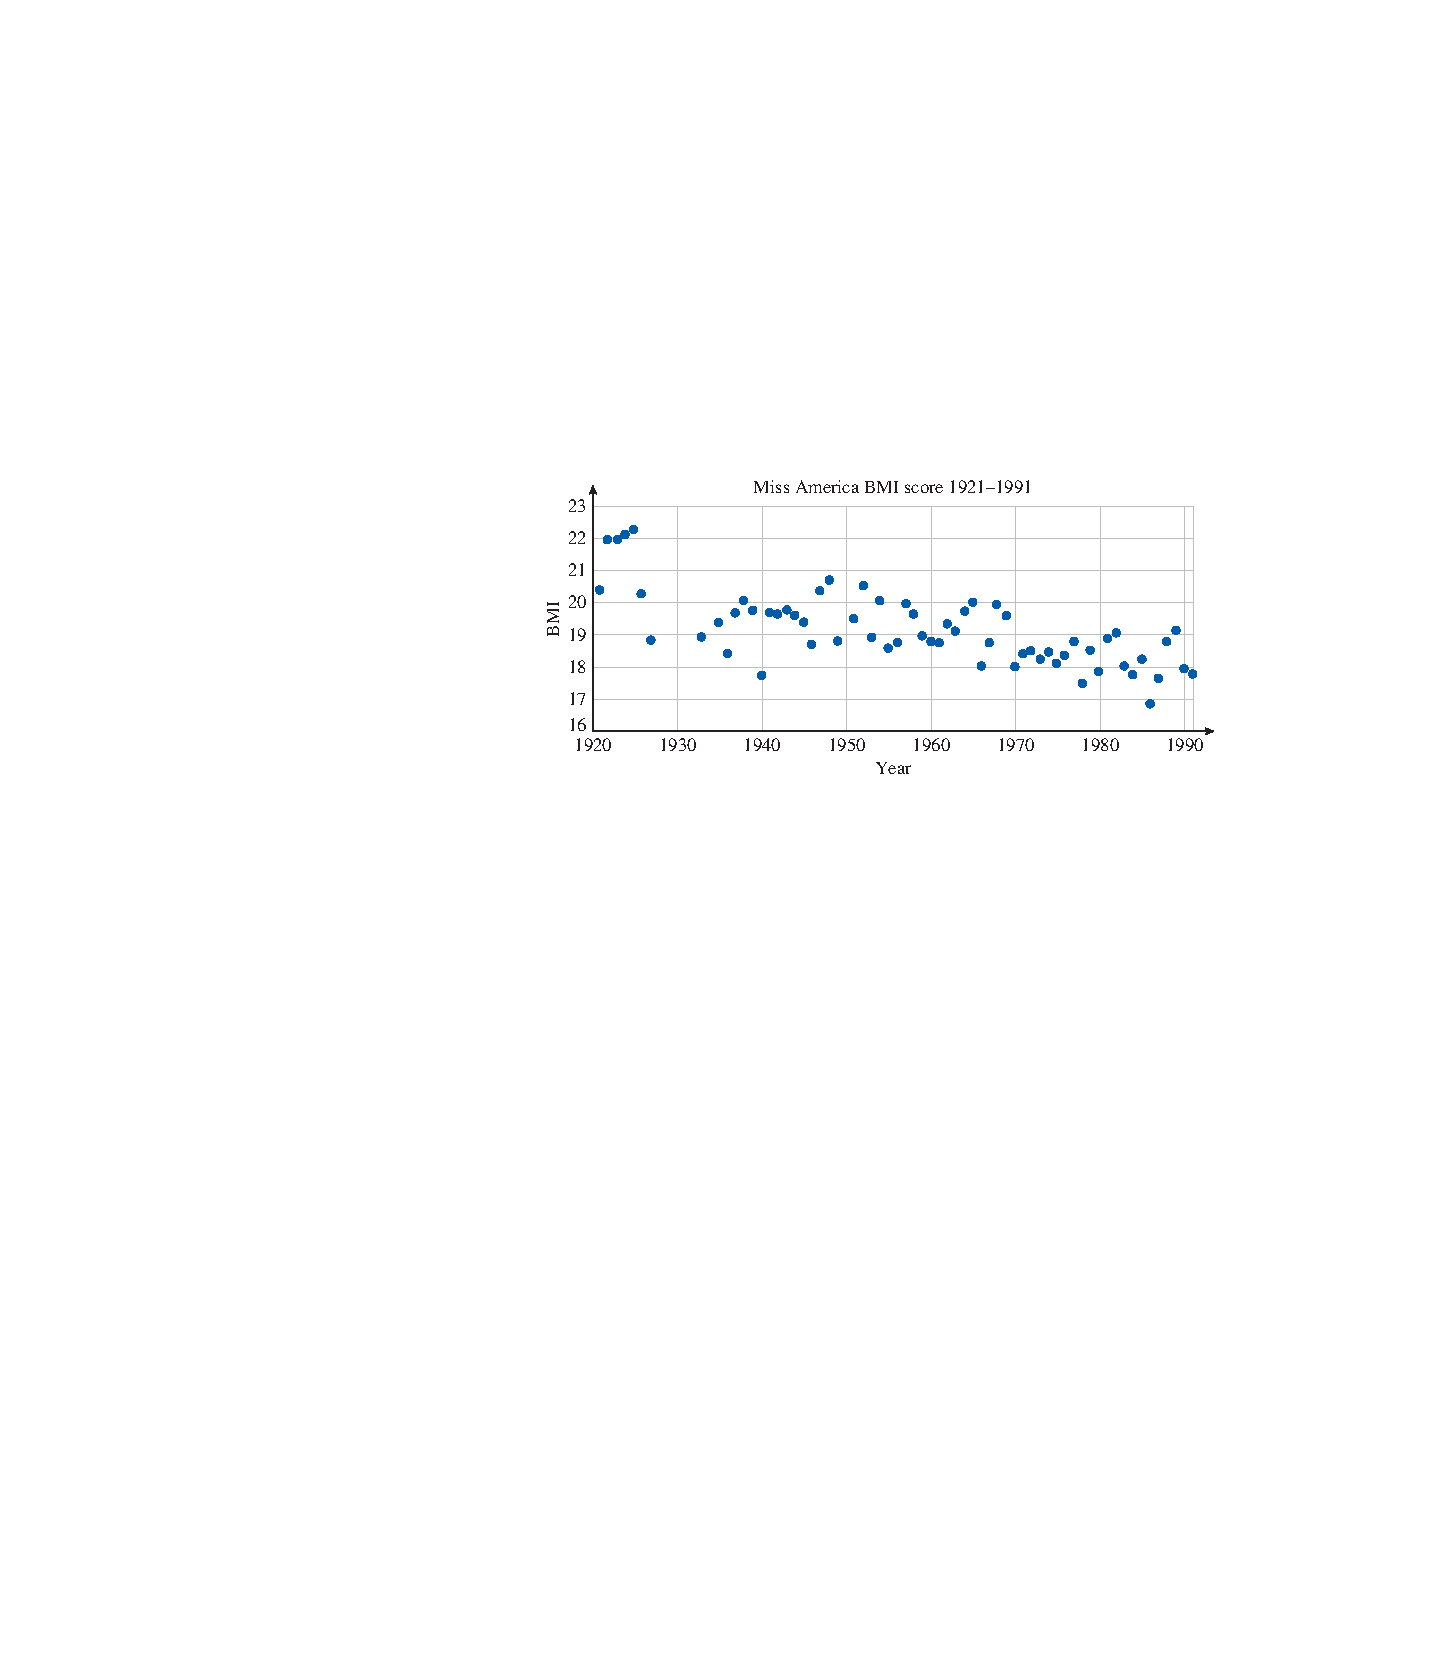
\includegraphics[width=\linewidth]{external/images/fig-BMI.pdf}
\end{sbspanel}%
\end{sidebyside}%
\begin{example}{Example}{}{example-example-BMI}%
%
\begin{enumerate}[label=\alph*]
\item{}Estimate a line of best fit for the scatterplot above. (Source: http:\slash{}\slash{}www.pbs.org)%
\item{}Use your line to estimate the BMI of Miss America 1980.%
\end{enumerate}
%
\par\smallskip%
\noindent\textbf{\blocktitlefont Solution}.\hypertarget{solution-example-BMI-b}{}\quad{}%
\begin{enumerate}[label=\alph*]
\item{}We draw a line that fits the data points as best we can, as shown below. (Note that we have set \(t = 0\) in 1920 on this graph.) We try to end up with roughly equal numbers of data points above and below our line.%
\begin{sidebyside}{1}{0.05}{0.05}{0}%
\begin{sbspanel}{0.9}%
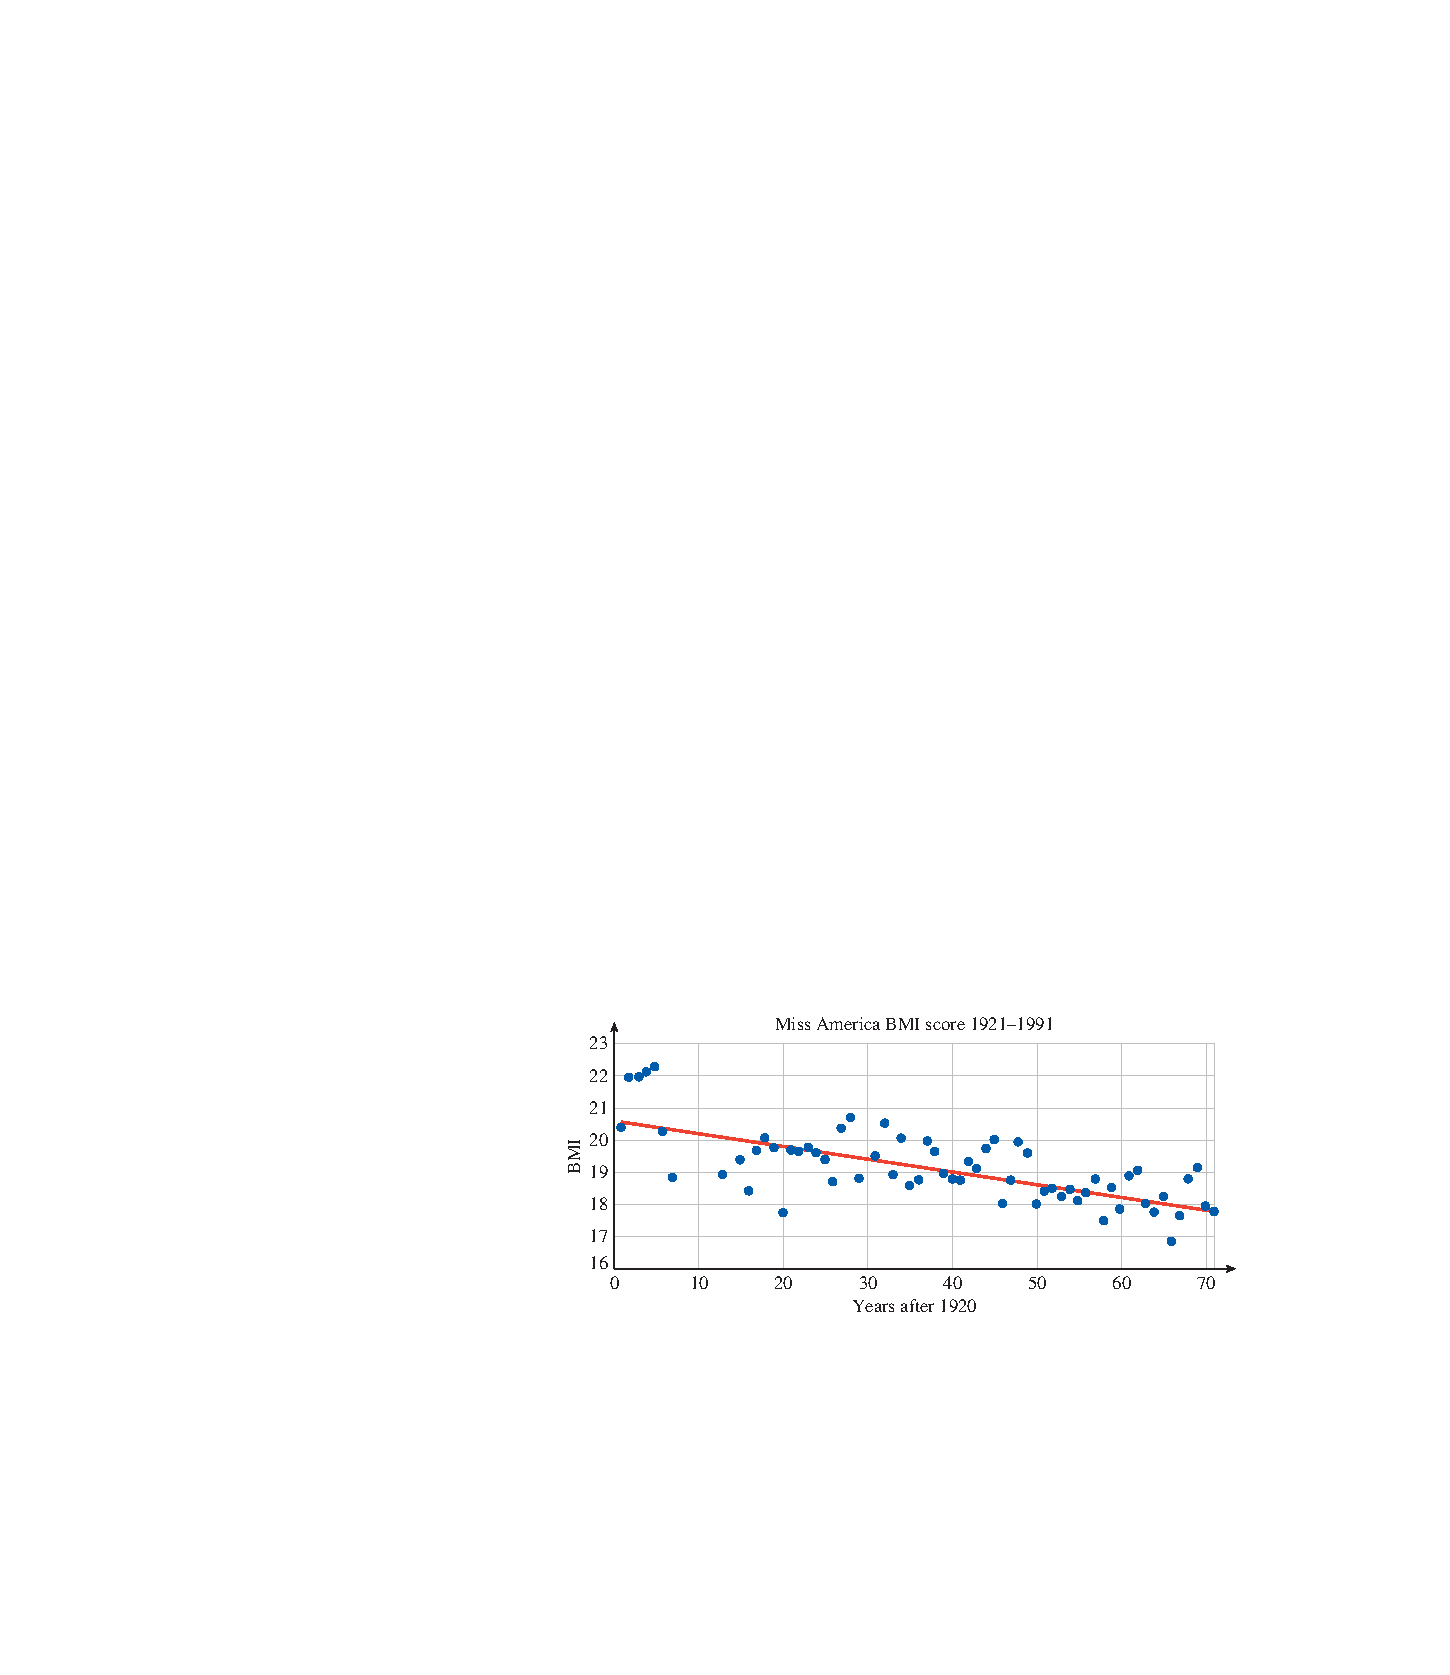
\includegraphics[width=\linewidth]{external/images/fig-BMI2.pdf}
\end{sbspanel}%
\end{sidebyside}%
\item{}We see that when \(t = 60\) on this line, the \(y\)-value is approximately 18.3. We therefore estimate that Miss America 1980 had a BMI of 18.3. (Her actual BMI was 17.85.)%
\end{enumerate}
%
\end{example}
\begin{inlineexercise}{Checkpoint}{QuickCheck 3.}{exercise-linear-regression-e-f}%
We can estimate a line of best fit by drawing the line that passes through:%
\par
\begin{itemize}[label=$\odot$,leftmargin=3em,]
\item{}The first and last data points%
\item{}Two data points in the middle%
\item{}Either of these%
\item{}None of these%
\end{itemize}
%
\par\smallskip%
\noindent\textbf{\blocktitlefont Answer}.\hypertarget{answer-linear-regression-e-f-c}{}\quad{}\(\text{None of these}\)%
\par\smallskip%
\noindent\textbf{\blocktitlefont Solution}.\hypertarget{solution-linear-regression-e-f-d}{}\quad{}None of these%
\end{inlineexercise}%
\begin{inlineexercise}{Checkpoint}{Practice 3.}{exercise-linear-regression-e-g}%
\begin{sidebyside}{1}{0.25}{0.25}{0}%
\begin{sbspanel}{0.5}%
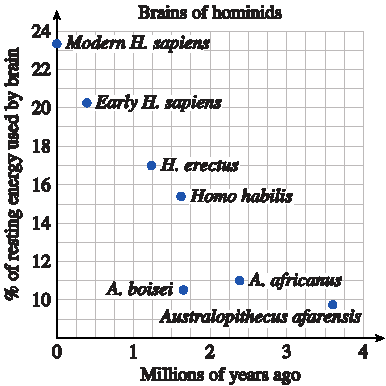
\includegraphics[width=\linewidth]{external/images/fig-hominid-brains.pdf}
\end{sbspanel}%
\end{sidebyside}%
\par
Human brains consume a large amount of energy, about 16 times as much as muscle tissue per unit weight. In fact, brain metabolism accounts for about 25\% of an adult human's energy needs, as compared to about 5\% for other mammals.%
\par
%
\begin{enumerate}[label=\alph*.]
\item{}Draw a line of best fit through the data points.%
\item{}Estimate the amount of energy used by the brain of a hominid species that lived three million years ago.%
\par
\fillintext{3}\%%
\end{enumerate}
%
\par
A graph for part (a):%
\begin{sidebyside}{1}{0}{0.6}{0}%
\begin{sbspanel}{0.6}%
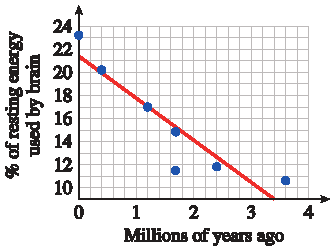
\includegraphics[width=\linewidth]{external/images/fig-in-ex-ans-1-6-3.pdf}
\end{sbspanel}%
\end{sidebyside}%
\par\smallskip%
\noindent\textbf{\blocktitlefont Answer}.\hypertarget{answer-linear-regression-e-g-c}{}\quad{}\(10.5\)%
\par\smallskip%
\noindent\textbf{\blocktitlefont Solution}.\hypertarget{solution-linear-regression-e-g-d}{}\quad{}%
\begin{enumerate}[label=\alph*.]
\item{}A graph is below.%
\item{}About 10.5\%%
\end{enumerate}
%
\end{inlineexercise}%
The process of predicting an output value based on a straight line that fits the data is called \terminology{linear regression}\index{linear regression}, and the line itself is called the \terminology{regression line}\index{regression line}. The equation of the regression line is usually used (instead of a graph) to predict values.%
\begin{example}{Example}{}{example-example-BMI-regression}%
%
\begin{enumerate}[label=\alph*]
\item{}Find the equation of the regression line in \hyperref[example-example-BMI]{Example~{\xreffont\ref{example-example-BMI}}}.%
\item{}Use the regression equation to predict the BMI of Miss America 1980.%
\end{enumerate}
%
\par\smallskip%
\noindent\textbf{\blocktitlefont Solution}.\hypertarget{solution-example-BMI-regression-b}{}\quad{}%
\begin{enumerate}[label=\alph*]
\item{}We first calculate the slope by choosing two points on the regression line. The points we choose are not necessarily any of the original data points; instead they should be points on the regression line itself. The line appears to pass through the points \((17, 20)\) and \((67, 18)\). The slope of the line is then%
\begin{equation*}
m = \frac{18 - 20}{67 - 17}\approx -0.04
\end{equation*}
Now we use the point-slope formula to find the equation of the line. (If you need to review the point-slope formula, see \hyperref[section-linear-functions]{Section~{\xreffont\ref{section-linear-functions}}}.) We substitute \(m = -0.04\) and use either of the two points for \((x_1, y_1)\); we will choose \((17, 20)\). The equation of the regression line is%
\begin{equation*}
\begin{aligned}[t]
y \amp = y_1 + m(x - x_1)\\
y \amp = 20-0.04(x-17) \amp \amp \blert{\text{Simplify.}}\\
y \amp = 20.68 - 0.04t\\
\end{aligned}
\end{equation*}
%
\item{}We will use the regression equation to make our prediction. For Miss America 1980, \(t = 60\) and%
\begin{equation*}
y = 20.68 - 0.04(60) = 18.28
\end{equation*}
This value agrees well with the estimate we made in \hyperref[example-example-BMI]{Example~{\xreffont\ref{example-example-BMI}}}.%
\end{enumerate}
%
\end{example}
\begin{inlineexercise}{Checkpoint}{QuickCheck 4.}{exercise-linear-regression-e-j}%
How many data points must a good regression line pass through?%
\par
\begin{itemize}[label=$\odot$,leftmargin=3em,]
\item{}Three%
\item{}Two%
\item{}One%
\item{}None%
\end{itemize}
%
\par\smallskip%
\noindent\textbf{\blocktitlefont Answer}.\hypertarget{answer-linear-regression-e-j-c}{}\quad{}\(\text{None}\)%
\par\smallskip%
\noindent\textbf{\blocktitlefont Solution}.\hypertarget{solution-linear-regression-e-j-d}{}\quad{}None: the regression line does not need to pass through any of the data points.%
\end{inlineexercise}%
\begin{inlineexercise}{Checkpoint}{Practice 4.}{exercise-linear-regression-e-k}%
\begin{image}{0.25}{0.5}{0.25}{-1.5\baselineskip}%
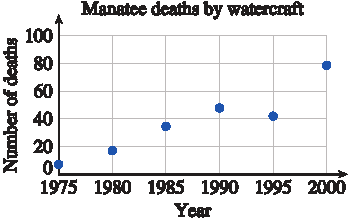
\includegraphics[width=\linewidth]{external/images/fig-manatees.pdf}
\end{image}%
The number of manatees killed by watercraft in Florida waters has been increasing since 1975. Data are given at 5-year intervals in the table. (Source: Florida Fish and Wildlife Conservation Commission)%
\begin{center}%
{\tabularfont%
\begin{tabular}{AcAcA}
Year&Manatee deaths\tabularnewline\hrulethin
\(1975\)&\(6\)\tabularnewline\hrulethin
\(1980\)&\(16\)\tabularnewline\hrulethin
\(1985\)&\(33\)\tabularnewline\hrulethin
\(1990\)&\(47\)\tabularnewline\hrulethin
\(1995\)&\(42\)\tabularnewline\hrulethin
\(2000\)&\(78\)\tabularnewline\hrulethin
\end{tabular}
}%
\end{center}%
%
\begin{enumerate}[label=\alph*.]
\item{}Draw a regression line through the data points shown in the figure.%
\item{}Find an equation for the regression line, using \(t\approx 0\) in 1975.%
\par
\(y=\)\fillintext{10}%
\item{}Use the regression equation to estimate the number of manatees killed by watercraft in 1998.%
\par
\fillintext{2} manatees%
\end{enumerate}
%
\par
A graph for part (a) is below.%
\begin{sidebyside}{1}{0}{0.55}{0}%
\begin{sbspanel}{0.45}%
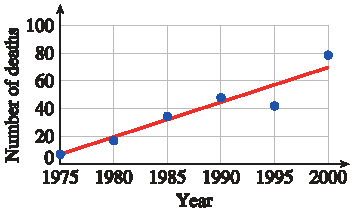
\includegraphics[width=\linewidth]{external/images/fig-in-ex-ans-1-6-4.pdf}
\end{sbspanel}%
\end{sidebyside}%
\par\smallskip%
\noindent\textbf{\blocktitlefont Answer 1}.\hypertarget{answer-linear-regression-e-k-c}{}\quad{}\(4.7+2.6t\)%
\par\smallskip%
\noindent\textbf{\blocktitlefont Answer 2}.\hypertarget{answer-linear-regression-e-k-d}{}\quad{}\(65\)%
\par\smallskip%
\noindent\textbf{\blocktitlefont Solution}.\hypertarget{solution-linear-regression-e-k-e}{}\quad{}%
\begin{enumerate}[label=\alph*.]
\item{}A graph is below.%
\item{}\(\displaystyle y = {4.7+2.6t}\)%
\item{}65%
\end{enumerate}
%
\end{inlineexercise}%
\begin{inlineexercise}{Checkpoint}{Pause and Reflect.}{exercise-linear-regression-e-l}%
Describe a strategy for sketching a line of best fit by eye.%
\end{inlineexercise}%
\end{subsectionptx}
%
%
\typeout{************************************************}
\typeout{Subsection  Linear Interpolation and Extrapolation}
\typeout{************************************************}
%
\begin{subsectionptx}{Subsection}{Linear Interpolation and Extrapolation}{}{Linear Interpolation and Extrapolation}{}{}{subsection-linear-regression-f}
Using a regression line to estimate values between known data points is called \terminology{interpolation}\index{interpolation}. Making predictions beyond the range of known data is called \terminology{extrapolation}\index{extrapolation}.%
\begin{example}{Example}{}{example-example-BMI-extrapolation}%
%
\begin{enumerate}[label=\alph*]
\item{}Use linear interpolation to estimate the BMI of Miss America 1960.%
\item{}Use linear extrapolation to predict the BMI of Miss America 2001.%
\end{enumerate}
%
\par\smallskip%
\noindent\textbf{\blocktitlefont Solution}.\hypertarget{solution-example-BMI-extrapolation-b}{}\quad{}%
\begin{enumerate}[label=\alph*]
\item{}For 1960, we substitute \(t = 40\) into the regression equation we found in \hyperref[example-example-BMI-regression]{Example~{\xreffont\ref{example-example-BMI-regression}}}.%
\begin{equation*}
y = 20.68 - 0.04(40) = 19.08
\end{equation*}
We estimate that Miss America 1960 had a BMI of 19.08. (Her BMI was actually 18.79.)%
\item{}For 2001, we substitute \(t = 81\) into the regression equation.%
\begin{equation*}
y = 20.68 - 0.04(81) = 17.44
\end{equation*}
%
\end{enumerate}
Our model predicts that Miss America 2001 had a BMI of 17.44. In fact, her BMI was 20.25. By the late 1990s, public concern over the self-image of young women had led to a reversal of the trend toward ever-thinner role models.%
\end{example}
\hyperref[example-example-BMI-extrapolation]{Example~{\xreffont\ref{example-example-BMI-extrapolation}}}b illustrates an important fact about extrapolation: If we try to extrapolate too far, we may get unreasonable results. For example, if we use our model to predict the BMI of Miss America 2520 (when \(t = 600\)), we get%
\begin{equation*}
y = 20.68 - 0.04(600) =-3.32
\end{equation*}
Even if the Miss America pageant is still operating in 600 years, the winner cannot have a negative BMI. Our linear model provides a fair approximation for 1920\textendash{}1990, but if we try to extrapolate too far beyond the known data, the model may no longer apply.%
\par
We can also use interpolation and extrapolation to make estimates for nonlinear functions. Sometimes a variable relationship is not linear, but a portion of its graph can be approximated by a line.%
\begin{sidebyside}{2}{0.025}{0.025}{0.05}%
\begin{sbspanel}{0.3}%
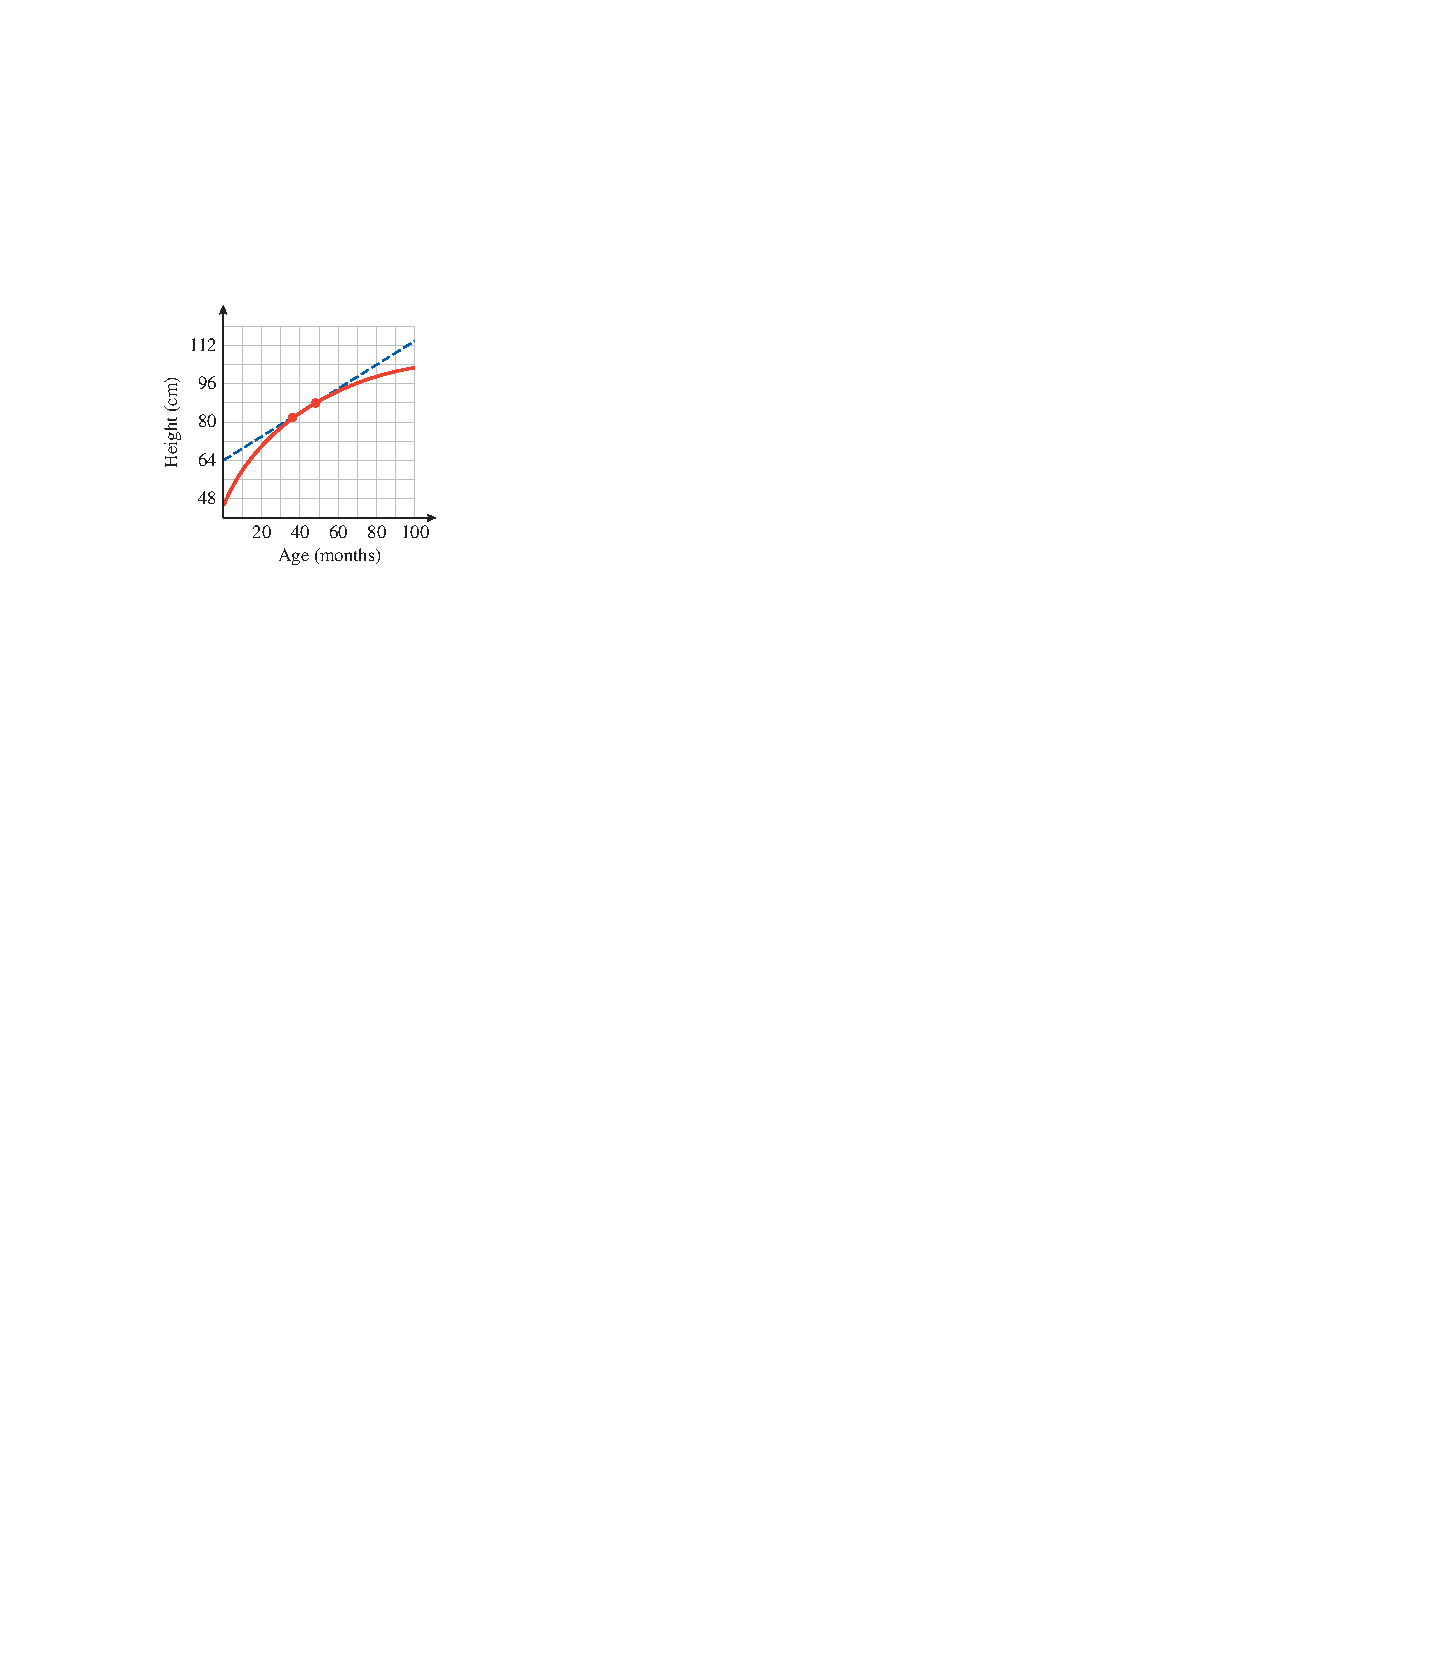
\includegraphics[width=\linewidth]{external/images/fig-Emily-height.pdf}
\end{sbspanel}%
\begin{sbspanel}{0.6}%
The graph at right shows a child’s height each month. The graph is not linear because her rate of growth is not constant; her growth slows down as she approaches her adult height. However, over a short time interval the graph is close to a line, and that line can be used to approximate the coordinates of points on the curve.%
\end{sbspanel}%
\end{sidebyside}%
\begin{inlineexercise}{Checkpoint}{QuickCheck 5.}{exercise-linear-regression-f-g}%
If you add more data points to the scatterplot, could the regression line change?%
\par
\begin{itemize}[label=$\odot$,leftmargin=3em,]
\item{}Yes%
\item{}No%
\item{}Only the slope could change.%
\item{}Only the intercept could change.%
\end{itemize}
%
\par\smallskip%
\noindent\textbf{\blocktitlefont Answer}.\hypertarget{answer-linear-regression-f-g-c}{}\quad{}\(\text{Yes}\)%
\par\smallskip%
\noindent\textbf{\blocktitlefont Solution}.\hypertarget{solution-linear-regression-f-g-d}{}\quad{}Yes%
\end{inlineexercise}%
\begin{inlineexercise}{Checkpoint}{Practice 5.}{exercise-linear-regression-f-h}%
Emily was 82 centimeters tall at age 36 months and 88 centimeters tall at age 48 months.%
\begin{enumerate}[label=\alph*.]
\item{}Find a linear equation that approximates Emily's height in terms of her age over the given time interval. Let \(t\) be Emily's age in months.%
\par
\(y=\)\fillintext{12}%
\item{}Use linear interpolation to estimate Emily's height when she was 38 months old, and extrapolate to predict her height at age 50 months.%
\par
Age 38 months: \fillintext{3} cm%
\par
Age 50 months: \fillintext{3} cm%
\item{}Predict Emily's height at age 25 (300 months).%
\par
Age 25 years: \fillintext{3} cm%
\par
Is your answer reasonable?\quad(\begin{itemize*}[label=$\square$,leftmargin=3em,itemjoin=\hspace{1em}]
\item{}Yes%
\item{}No%
\end{itemize*})\quad
%
\end{enumerate}
%
\par\smallskip%
\noindent\textbf{\blocktitlefont Answer 1}.\hypertarget{answer-linear-regression-f-h-c}{}\quad{}\(82+0.5\!\left(t-36\right)\)%
\par\smallskip%
\noindent\textbf{\blocktitlefont Answer 2}.\hypertarget{answer-linear-regression-f-h-d}{}\quad{}\(83\)%
\par\smallskip%
\noindent\textbf{\blocktitlefont Answer 3}.\hypertarget{answer-linear-regression-f-h-e}{}\quad{}\(89\)%
\par\smallskip%
\noindent\textbf{\blocktitlefont Answer 4}.\hypertarget{answer-linear-regression-f-h-f}{}\quad{}\(214\)%
\par\smallskip%
\noindent\textbf{\blocktitlefont Answer 5}.\hypertarget{answer-linear-regression-f-h-g}{}\quad{}\(\text{No}\)%
\par\smallskip%
\noindent\textbf{\blocktitlefont Solution}.\hypertarget{solution-linear-regression-f-h-h}{}\quad{}%
\begin{enumerate}[label=\alph*.]
\item{}\(\displaystyle y = 64 + 0.5t\)%
\item{}\(83\) cm, \(89\) cm%
\item{}\(214\) cm; No%
\end{enumerate}
%
\end{inlineexercise}%
\begin{inlineexercise}{Checkpoint}{Pause and Reflect.}{exercise-linear-regression-f-i}%
Explain the difference between interpolation and extrapolation.%
\end{inlineexercise}%
Estimating a line of best fit is a subjective process. Rather than base their estimates on such a line, statisticians often use the \terminology{least squares regression line}\index{least squares regression line}.%
\begin{sidebyside}{2}{0.0325}{0.0325}{0.065}%
\begin{sbspanel}{0.22}%
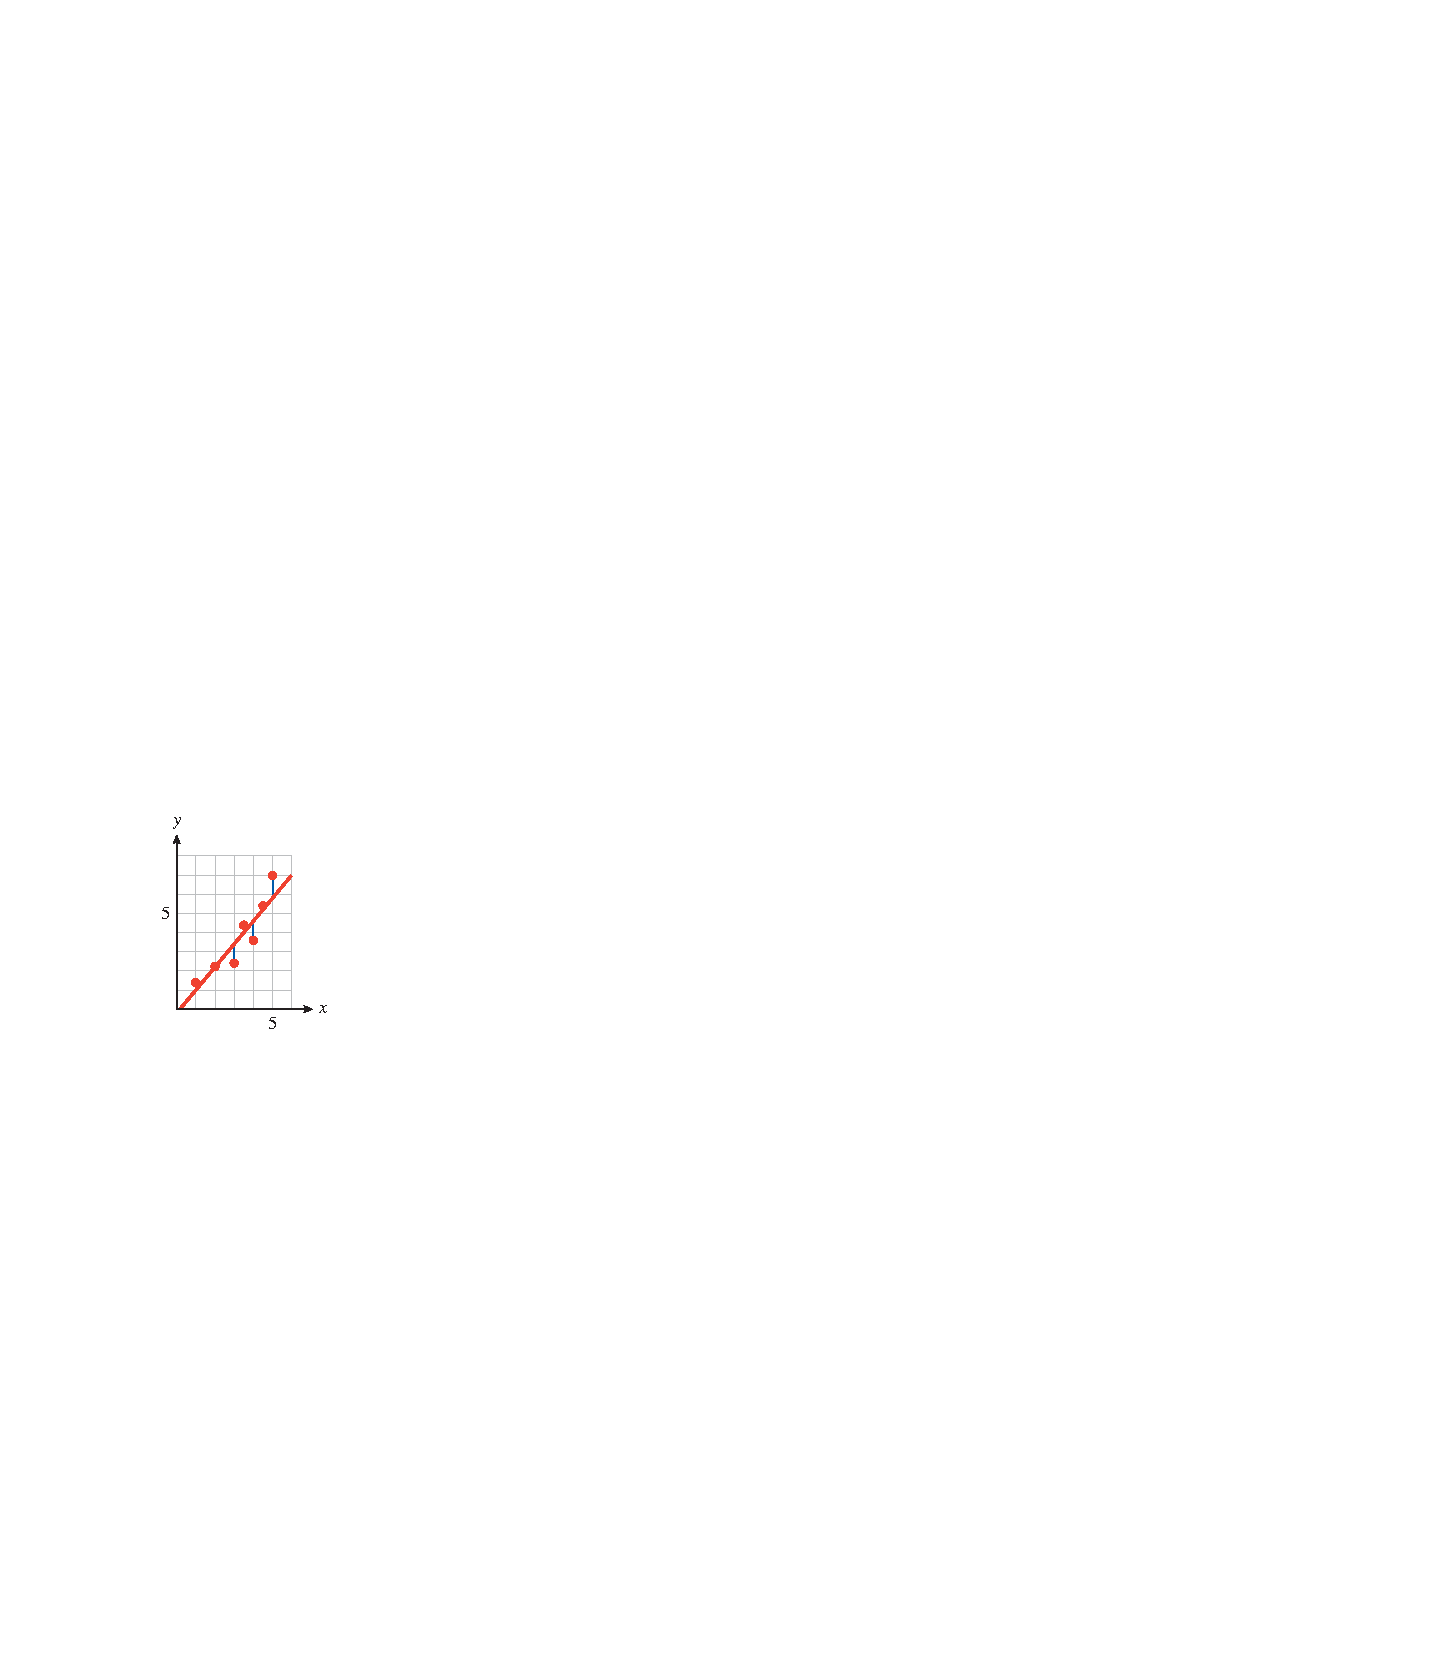
\includegraphics[width=\linewidth]{external/images/fig-least-squares.pdf}
\end{sbspanel}%
\begin{sbspanel}{0.65}%
This regression line minimizes the sum of the squares of all the vertical distances between the data points and the corresponding points on the line, as shown at left. Many calculators are programmed to find the least squares regression line, using an algorithm that depends only on the data, not on the appearance of the graph.%
\end{sbspanel}%
\end{sidebyside}%
\begin{technology}{Technology}{Using Technology for Linear Regression.}{technology-linear-regression-f-l}%
You can use a graphing calculator to make a scatterplot, find a regression line, and graph the regression line with the data points. On the TI-83 calculator, we use the statistics mode, which you can access by pressing \kbd{STAT}. You will see a display that looks like figure (a) below. Choose \(1\) to \(Edit\) (enter or alter) data.%
\begin{sidebyside}{1}{0.25}{0.25}{0}%
\begin{sbspanel}{0.5}%
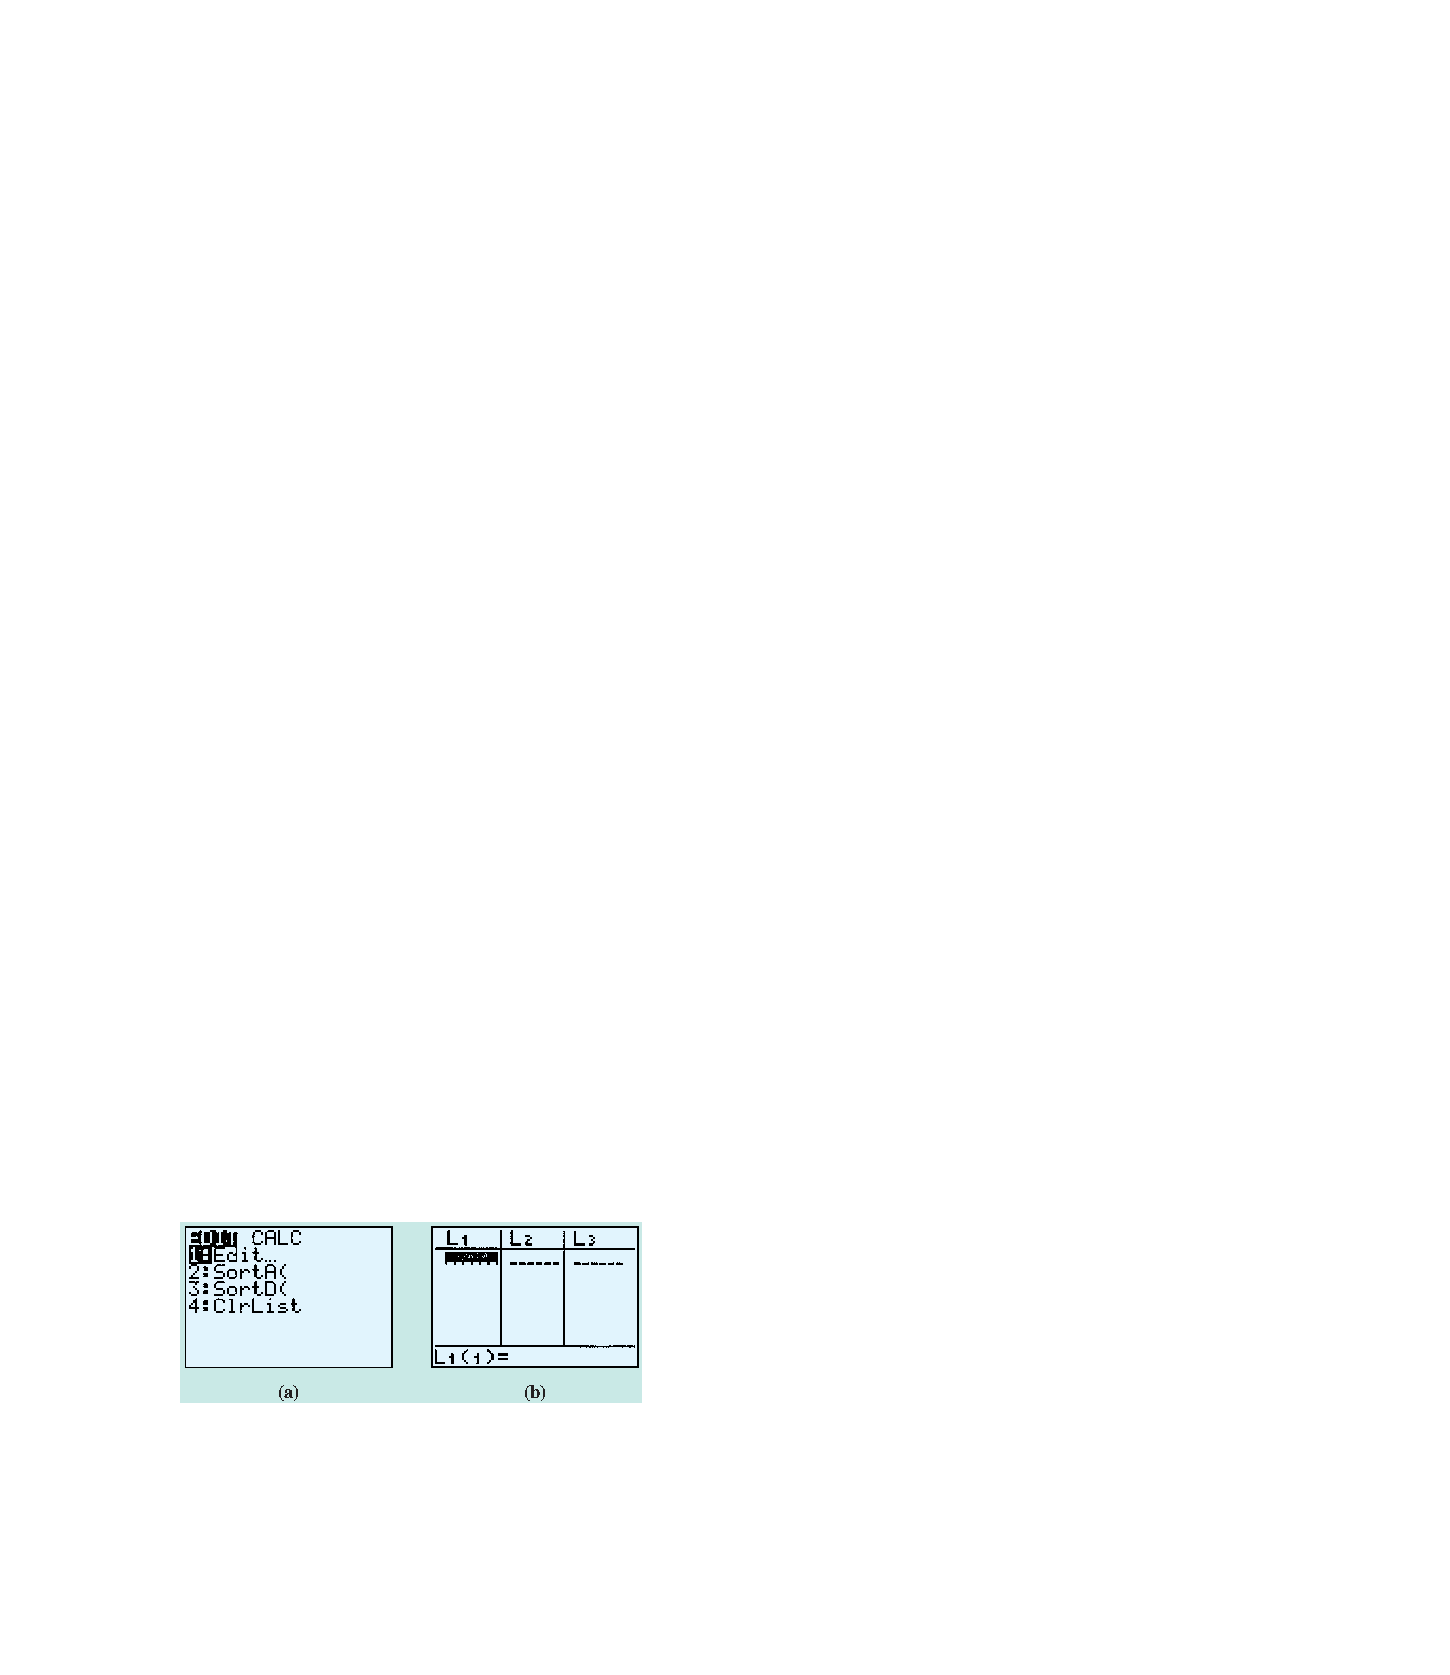
\includegraphics[width=\linewidth]{external/images/fig-GC-lists.pdf}
\end{sbspanel}%
\end{sidebyside}%
\par
Now follow the instructions in \hyperref[example-example-GC-regression]{Example~{\xreffont\ref{example-example-GC-regression}}} for using your calculator’s statistics features.%
\end{technology}
\begin{example}{Example}{}{example-example-GC-regression}%
%
\begin{enumerate}[label=\alph*]
\item{}Find the equation of the least squares regression line for the following data:%
\begin{equation*}
(10, 12), (11, 14), (12, 14), (12, 16), (14, 20)
\end{equation*}
%
\item{}Plot the data points and the least squares regression line on the same axes.%
\end{enumerate}
%
\par\smallskip%
\noindent\textbf{\blocktitlefont Solution}.\hypertarget{solution-example-GC-regression-b}{}\quad{}%
\begin{enumerate}[label=\alph*]
\item{}We must first enter the data.%
\begin{itemize}[label=\textbullet]
\item{}Press \kbd{STAT}\kbd{ENTER} to select \(Edit\).%
\item{}If there are data in column \(L_1\) or \(L_2\), clear them out: Use the  \kbd{\arrowkeyup}  key to select \(L_1\), press \kbd{CLEAR}, then do the same for \(L_2\).%
\item{}Enter the \(x\)-coordinates of the data points in the \(L_1\) column and enter the \(y\)-coordinates in the \(L_2\) column, as shown in figure (a) below.%
\begin{sidebyside}{1}{0.2}{0.2}{0}%
\begin{sbspanel}{0.6}%
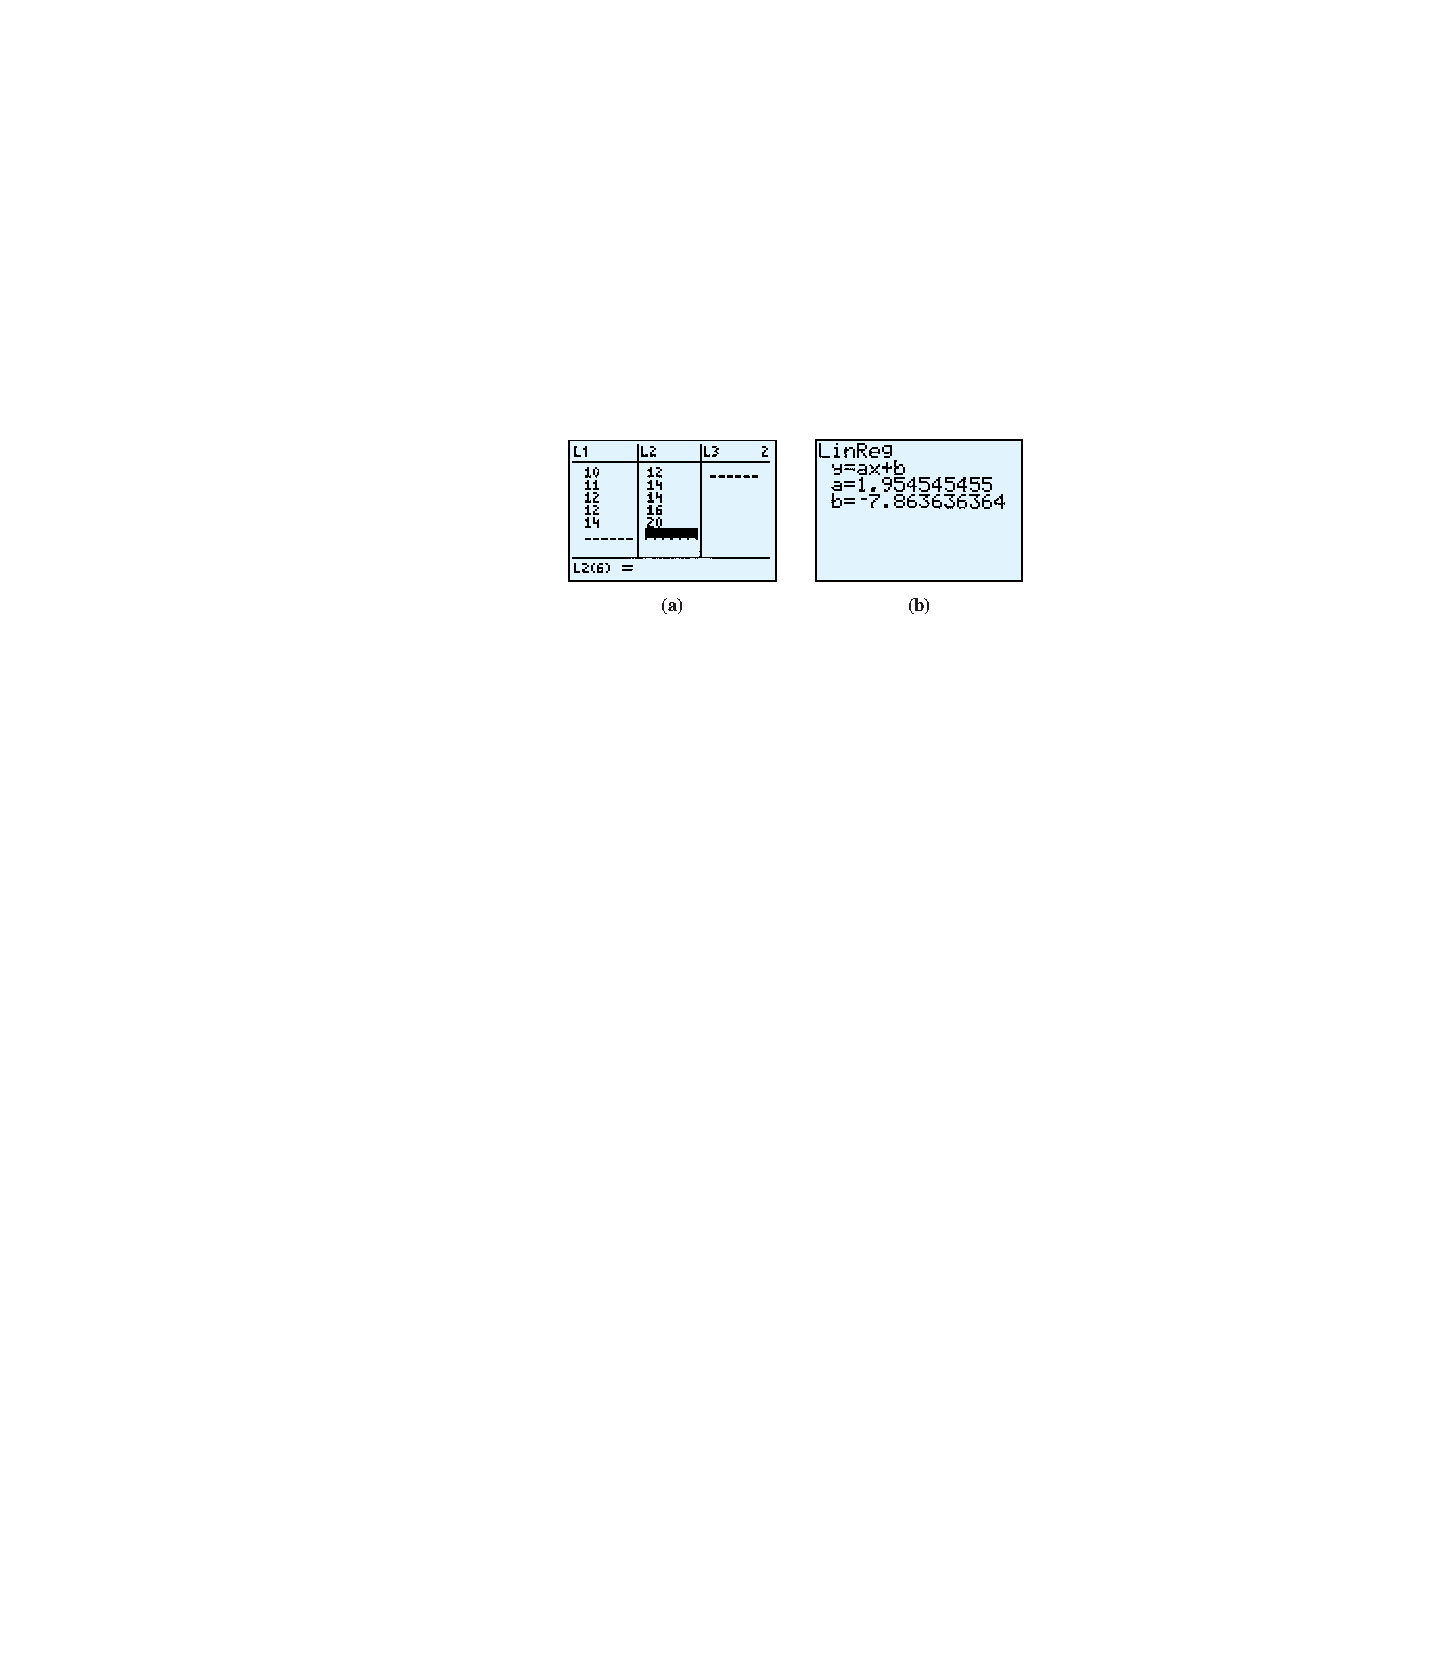
\includegraphics[width=\linewidth]{external/images/fig-GC-regression.pdf}
\end{sbspanel}%
\end{sidebyside}%
\par
Now we are ready to find the regression equation for our data.%
\item{}Press \kbd{STAT} \kbd{\arrowkeyright}  4 to select linear regression, or LinReg (ax + b), then press \kbd{ENTER}.%
\item{}The calculator will display the equation \(y = ax + b\) and the values for \(a\) and \(b\), as shown in figure (b).%
\end{itemize}
You should find that your regression line is approximately \(y = 1.95x - 7.86\).%
\item{}First, we first clear out any old definitions in the list.%
\begin{itemize}[label=\textbullet]
\item{}Position the cursor after \(Y_1 =\) and copy in the regression equation as follows:%
\item{}Press \kbd{VARS} \(5\)  \kbd{\arrowkeyright} \kbd{\arrowkeyright} \kbd{ENTER}.%
\item{}To draw a scatterplot, press \kbd{2nd}\kbd{Y=}\(1\) and set the Plot1 menu as shown in figure (a) below.%
\item{}Finally, press \kbd{ZOOM} \(9\) to see the scatterplot of the data and the regression line. The graph is shown in figure (b).%
\end{itemize}
%
\begin{sidebyside}{1}{0.2}{0.2}{0}%
\begin{sbspanel}{0.6}%
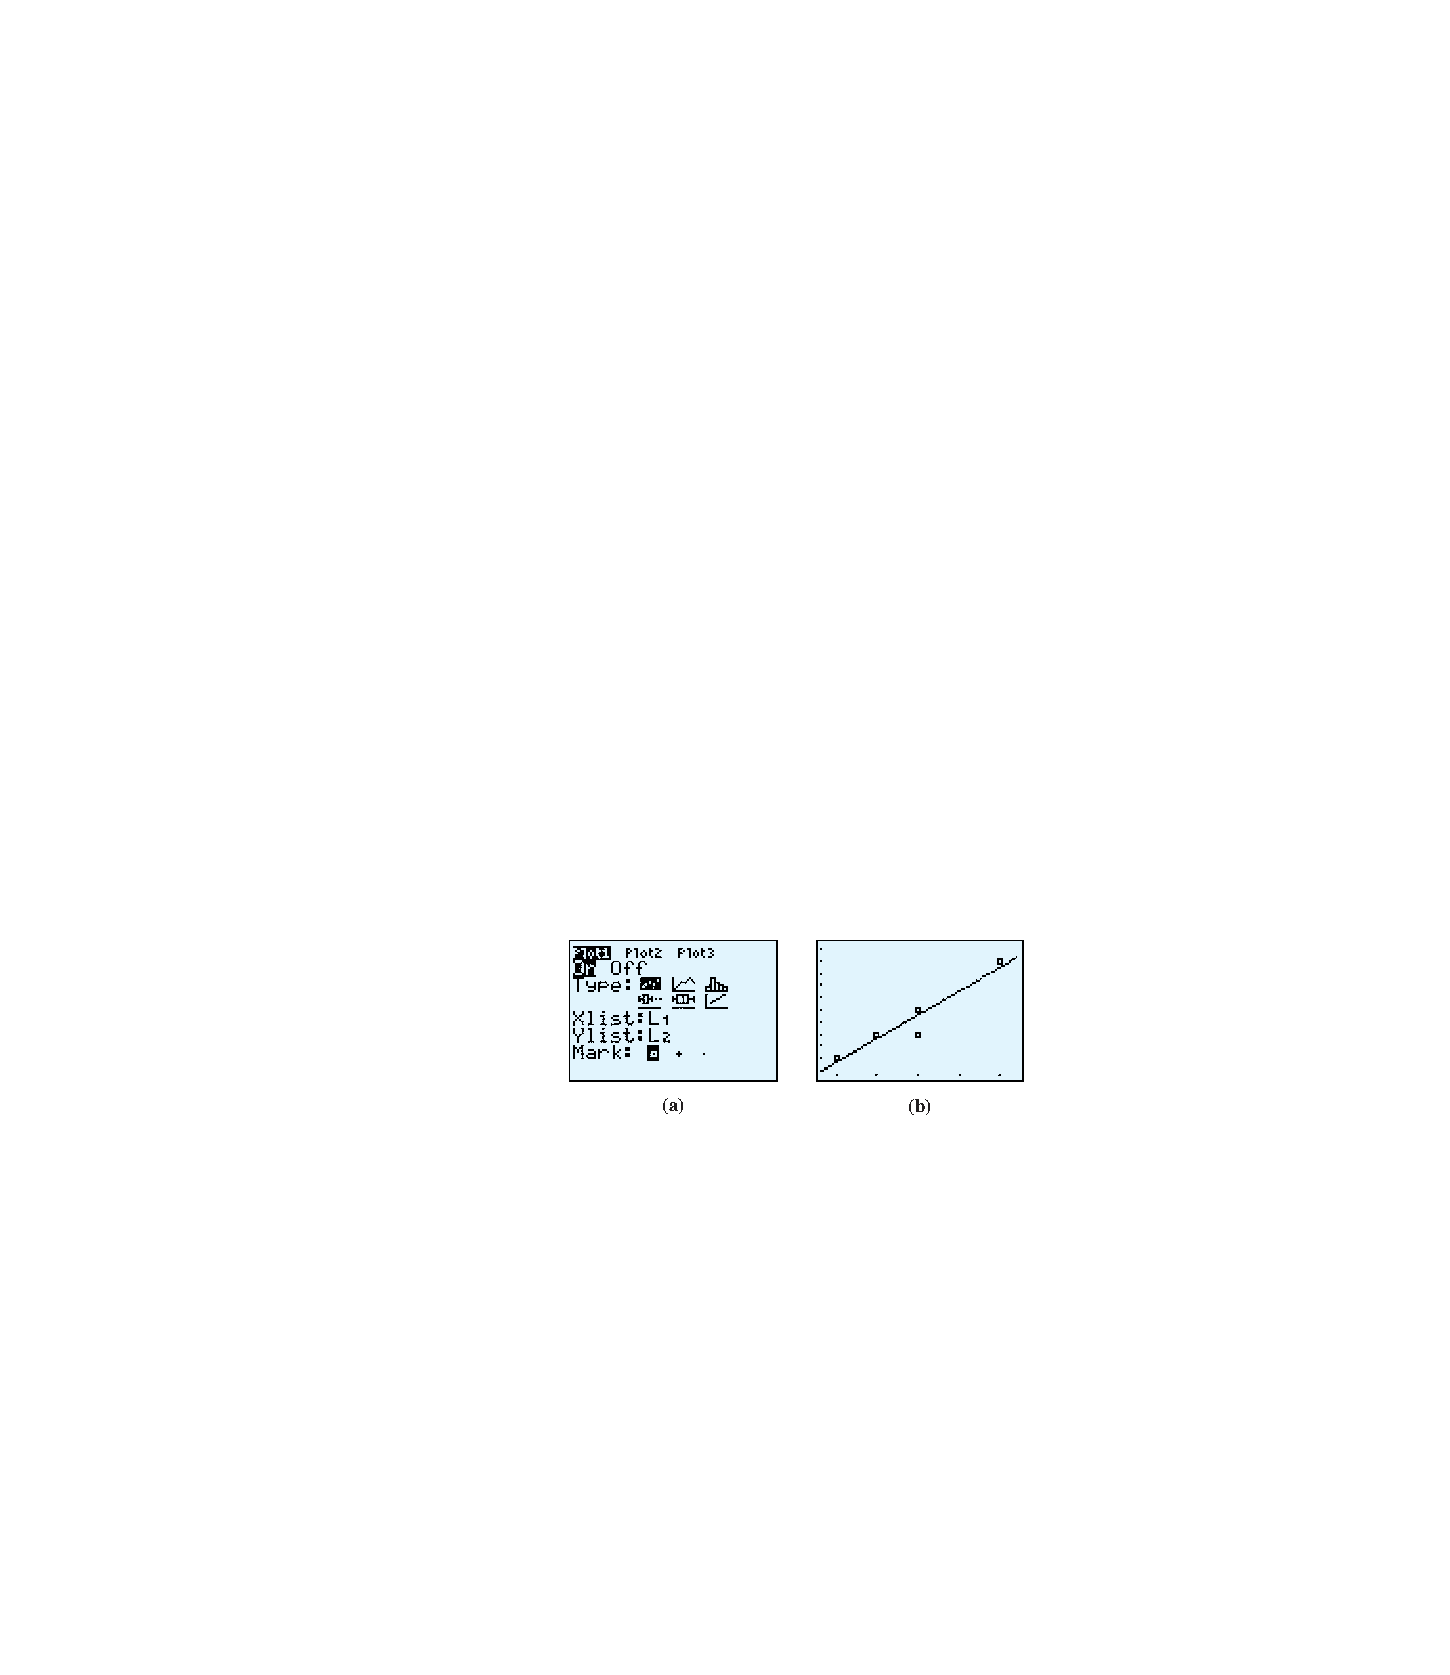
\includegraphics[width=\linewidth]{external/images/fig-GC-regression2.pdf}
\end{sbspanel}%
\end{sidebyside}%
\end{enumerate}
%
\end{example}
\begin{warning}{Caution}{}{warning-linear-regression-f-n}%
When you are through with the scatterplot, press \kbd{Y=}  \kbd{\arrowkeyup}  \kbd{ENTER} to turn off the \(Stat Plot\). If you neglect to do this, the calculator will continue to show the scatterplot even after you ask it to plot a new equation.%
\end{warning}
\begin{inlineexercise}{Checkpoint}{Practice 6.}{exercise-linear-regression-f-o}%
Use your calculator’s statistics features to find the least squares regression equation for the data in \hyperref[exercise-exercise-scatterplot]{Checkpoint~{\xreffont\ref{exercise-exercise-scatterplot}}}.%
\par
%
\begin{enumerate}[label=\alph*.]
\item{}The equation: \(y=\)\fillintext{10}%
\item{}Plot the data and the graph of the regression equation.%
\end{enumerate}
%
\par
A graph for part (b):%
\begin{sidebyside}{1}{0}{0.7}{0}%
\begin{sbspanel}{0.35}%
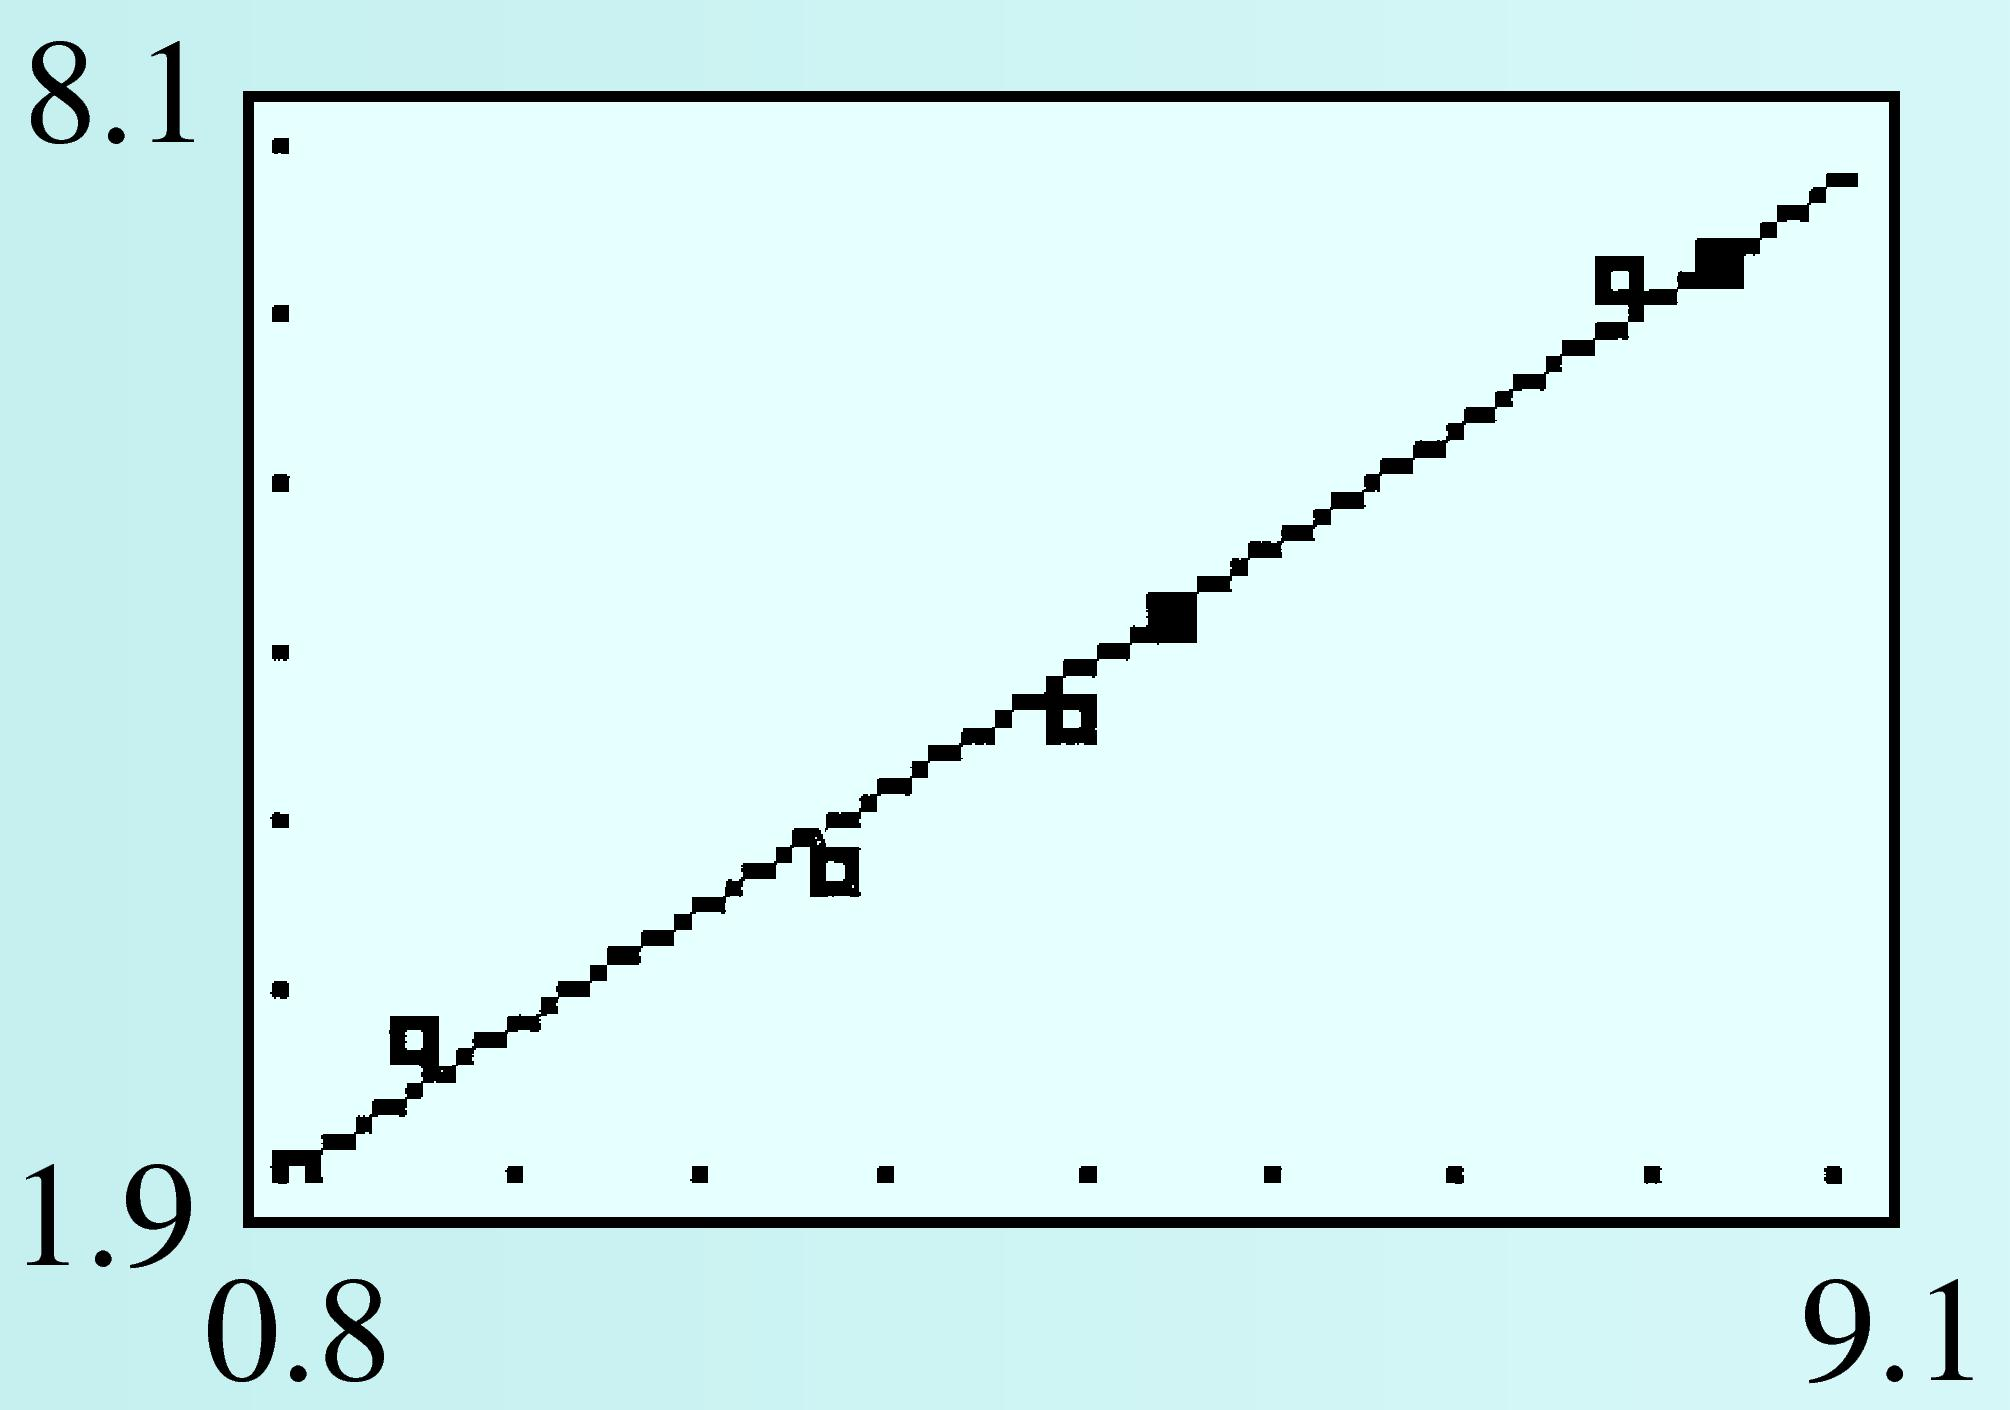
\includegraphics[width=\linewidth]{external/images/fig-in-ex-ans-1-6-6.jpg}
\end{sbspanel}%
\end{sidebyside}%
\par\smallskip%
\noindent\textbf{\blocktitlefont Answer}.\hypertarget{answer-linear-regression-f-o-c}{}\quad{}\(0.710838x+1.33571\)%
\par\smallskip%
\noindent\textbf{\blocktitlefont Solution}.\hypertarget{solution-linear-regression-f-o-d}{}\quad{}%
\begin{enumerate}[label=\alph*.]
\item{}\(\displaystyle y = 1.34 + 0.71x\)%
\item{}A graph is below.%
\end{enumerate}
%
\end{inlineexercise}%
\end{subsectionptx}
%
%
\typeout{************************************************}
\typeout{Subsection  Section Summary}
\typeout{************************************************}
%
\begin{subsectionptx}{Subsection}{Section Summary}{}{Section Summary}{}{}{subsection-summary-1-6}
%
%
\typeout{************************************************}
\typeout{Subsubsection  Vocabulary}
\typeout{************************************************}
%
\begin{subsubsectionptx}{Subsubsection}{Vocabulary}{}{Vocabulary}{}{}{subsubsection-summary-1-6-b}
Look up the definitions of new terms in the Glossary.%
\begin{multicols}{3}
\begin{itemize}[label=\textbullet]
\item{}Scatterplot%
\item{}Least squares regression line%
\item{}Extrapolate%
\item{}Regression line%
\item{}Interpolate%
\item{}Linear regression%
\end{itemize}
\end{multicols}
%
\end{subsubsectionptx}
%
%
\typeout{************************************************}
\typeout{Subsubsection  CONCEPTS}
\typeout{************************************************}
%
\begin{subsubsectionptx}{Subsubsection}{CONCEPTS}{}{CONCEPTS}{}{}{subsubsection-summary-1-6-c}
%
\begin{enumerate}[label=\arabic*]
\item{}Data points may not lie exactly on the graph of an equation.%
\item{}Points in a scatterplot may or may not exhibit a pattern.%
\item{}We can approximate a linear pattern by a regression line.%
\item{}We can use interpolation or extrapolation to make estimates and predictions.%
\item{}If we extrapolate too far beyond the known data, we may get unreasonable results.%
\end{enumerate}
%
\end{subsubsectionptx}
%
%
\typeout{************************************************}
\typeout{Subsubsection  STUDY QUESTIONS}
\typeout{************************************************}
%
\begin{subsubsectionptx}{Subsubsection}{STUDY QUESTIONS}{}{STUDY QUESTIONS}{}{}{subsubsection-summary-1-6-d}
%
\begin{enumerate}[label=\arabic*]
\item{}What is a regression line?%
\item{}State two formulas you will need to calculate the equation of a line through two points.%
\item{}Explain the difference between interpolation and extrapolation.%
\item{}In general, should you have more confidence in figures obtained by interpolation or by extrapolation? Why?%
\end{enumerate}
%
\end{subsubsectionptx}
%
%
\typeout{************************************************}
\typeout{Subsubsection  SKILLS}
\typeout{************************************************}
%
\begin{subsubsectionptx}{Subsubsection}{SKILLS}{}{SKILLS}{}{}{subsubsection-summary-1-6-e}
Practice each skill in the Homework problems listed.%
\begin{enumerate}[label=\arabic*]
\item{}Find the equation of a line through two points: \#1\textendash{}6, 29\textendash{}36%
\item{}Draw a line of best fit: \#7\textendash{}18%
\item{}Find the equation of a regression line: \#11\textendash{}28, 37\textendash{}40%
\item{}Use interpolation and extrapolation to make predictions: \#11\textendash{}40%
\end{enumerate}
%
\end{subsubsectionptx}
\end{subsectionptx}
%
%
\typeout{************************************************}
\typeout{Exercises  Homework 1.6}
\typeout{************************************************}
%
\begin{exercises-subsection}{Exercises}{Homework 1.6}{}{Homework 1.6}{}{}{exercises-section-1-6-exercises}
\par\medskip\noindent%
\textbf{Exercise Group.}\space\space%
In Problems 1\textendash{}6, we find a linear model from two data points.%
\begin{enumerate}[label=\alph*]
\item{}Make a table showing the coordinates of two data points for the model. (Which variable should be plotted on the horizontal axis?)%
\item{}Find a linear equation relating the variables.%
\item{}State the slope of the line, including units, and explain its meaning in the context of the problem.%
\end{enumerate}
%
\begin{exercisegroup}
\begin{divisionexerciseeg}{1}{}{}{exercise-section-1-6-exercises-b-b}%
It cost a bicycle company \textdollar{}\(9000\) to make \(40\) touring bikes in its first month of operation and \textdollar{}\(15,000\) to make \(125\) bikes during its second month. Express the company's monthly production cost, \(C\), in terms of the number, \(x\), of bikes it makes.%
\end{divisionexerciseeg}%
\begin{divisionexerciseeg}{2}{}{}{exercise-section-1-6-exercises-b-c}%
Flying lessons cost \textdollar{}\(645\) for an \(8\)-hour course and \textdollar{}\(1425\) for a \(20\)-hour course. Both prices include a fixed insurance fee. Express the cost, \(C\), of flying lessons in terms of the length, \(h\), of the course in hours.%
\end{divisionexerciseeg}%
\begin{divisionexerciseeg}{3}{}{}{exercise-section-1-6-exercises-b-d}%
Under ideal conditions, Andrea's Porsche can travel \(312\) miles on a full tank (\(12\) gallons of gasoline) and \(130\) miles on \(5\) gallons. Express the distance, \(d\), Andrea can drive in terms of the amount of gasoline, \(g\), she buys.%
\end{divisionexerciseeg}%
\begin{divisionexerciseeg}{4}{}{}{exercise-section-1-6-exercises-b-e}%
On an international flight, a passenger may check two bags each weighing \(70\) kilograms, or \(154\) pounds, and one carry-on bag weighing \(50\) kilograms, or \(110\) pounds. Express the weight, \(p\), of a bag in pounds in terms of its weight, \(k\), in kilograms.%
\end{divisionexerciseeg}%
\begin{divisionexerciseeg}{5}{}{}{exercise-section-1-6-exercises-b-f}%
A radio station in Detroit, Michigan, reports the high and low temperatures in the Detroit\slash{}Windsor area as \(59\degree\)F and \(23\degree\)F, respectively. A station in Windsor, Ontario, reports the same temperatures as \(15\degree\)C and \(-5\degree\)C. Express the Fahrenheit temperature, \(F\), in terms of the Celsius temperature, \(C\).%
\end{divisionexerciseeg}%
\begin{divisionexerciseeg}{6}{}{}{exercise-section-1-6-exercises-b-g}%
Ms. Randolph bought a used car in 2000. In 2002, the car was worth \($9000\), and in 2005 it was valued at \($4500\). Express the value, \(V\) , of Ms. Randolph's car in terms of the number of years, \(t\), she has owned it.%
\end{divisionexerciseeg}%
\end{exercisegroup}
\par\medskip\noindent
\par\medskip\noindent%
\textbf{Exercise Group.}\space\space%
Each regression line can be improved by adjusting either \(m\) or \(b\). Draw a line that fits the data points more closely.%
\begin{exercisegroupcol}{2}
\begin{divisionexerciseegcol}{7}{}{}{exercise-section-1-6-exercises-c-b}%
\begin{sidebyside}{1}{0.25}{0.25}{0}%
\begin{sbspanel}{0.5}%
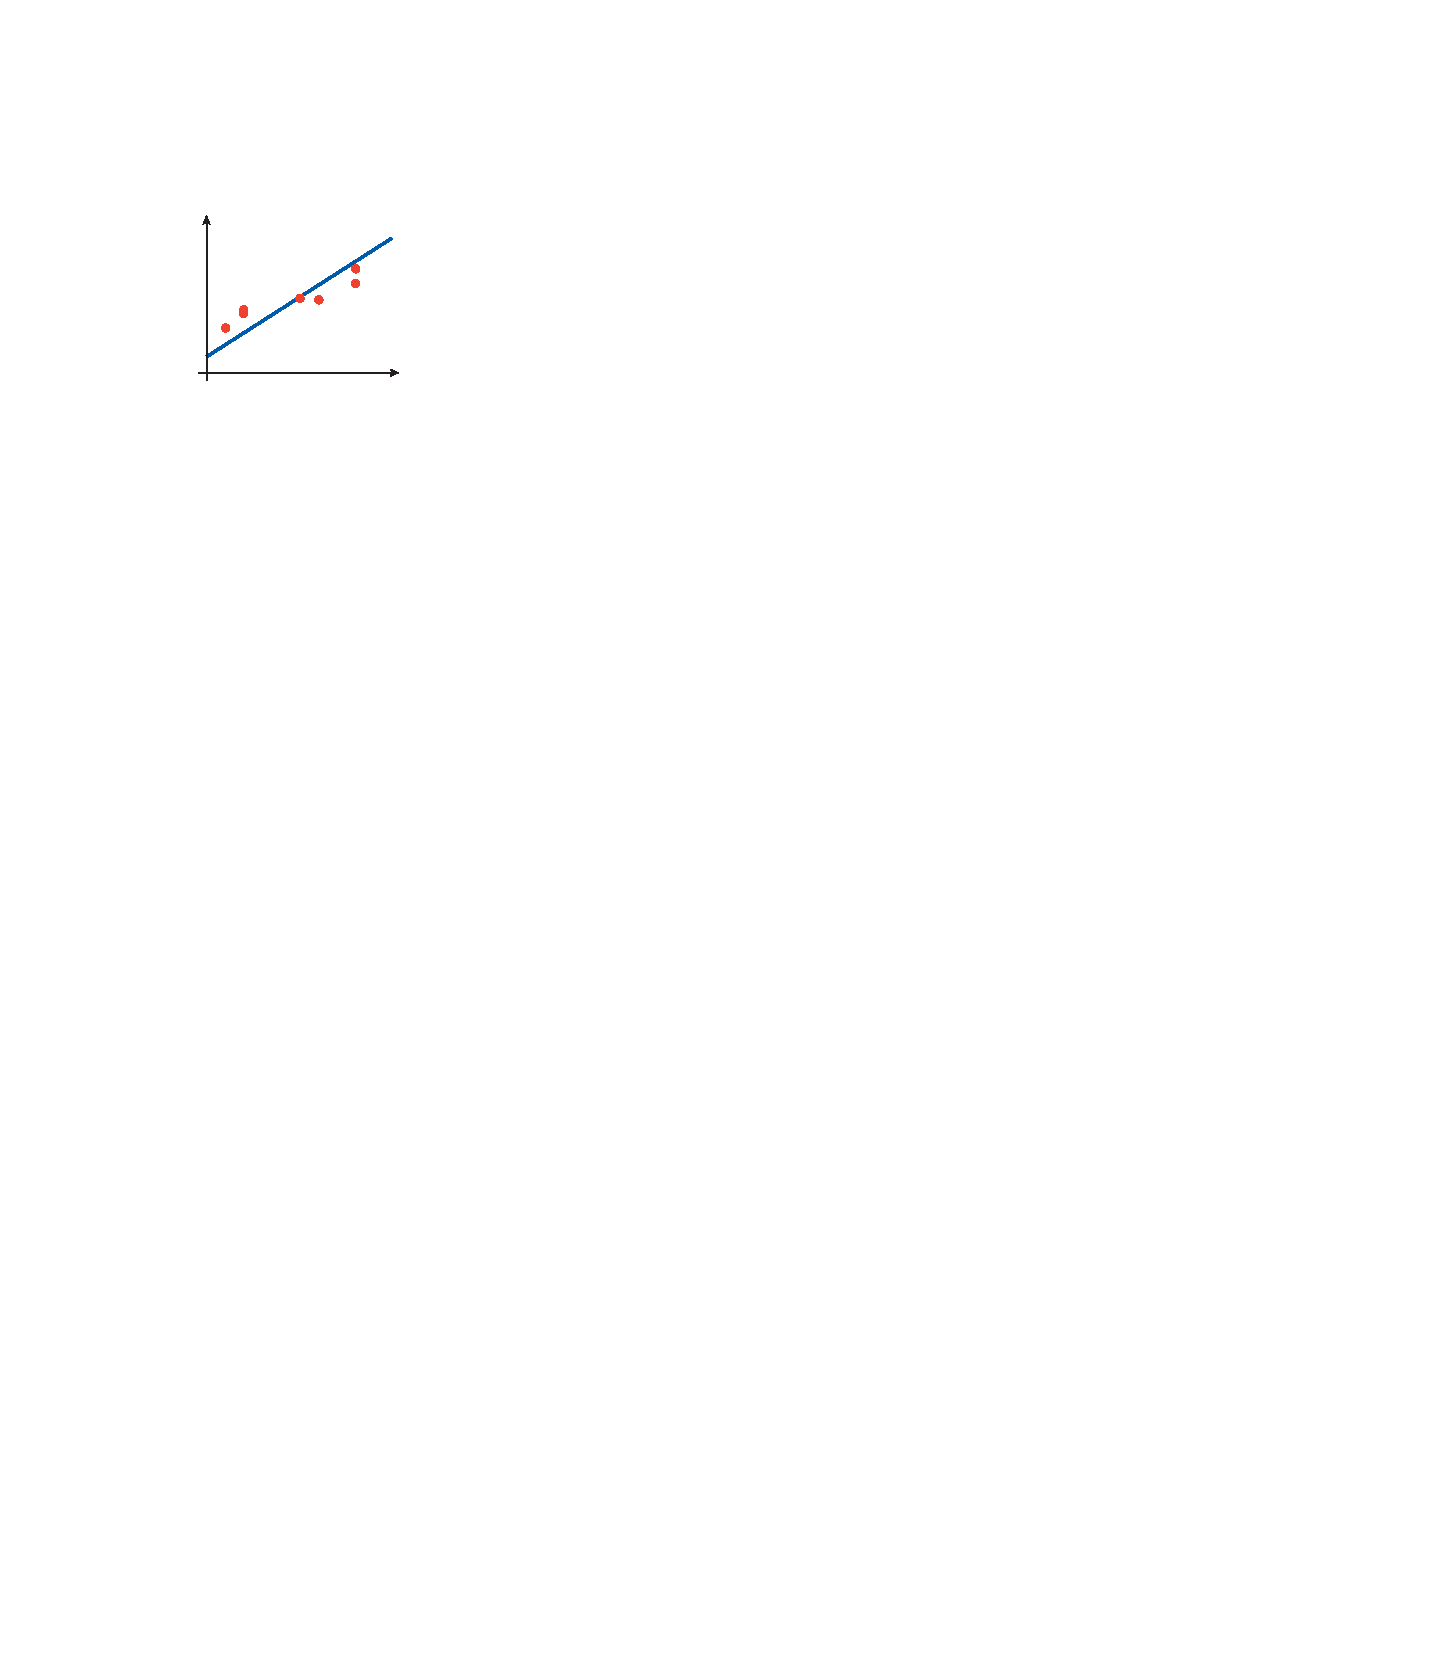
\includegraphics[width=\linewidth]{external/images/fig-ex-1-6-7.pdf}
\end{sbspanel}%
\end{sidebyside}%
\end{divisionexerciseegcol}%
\begin{divisionexerciseegcol}{8}{}{}{exercise-section-1-6-exercises-c-c}%
\begin{sidebyside}{1}{0.25}{0.25}{0}%
\begin{sbspanel}{0.5}%
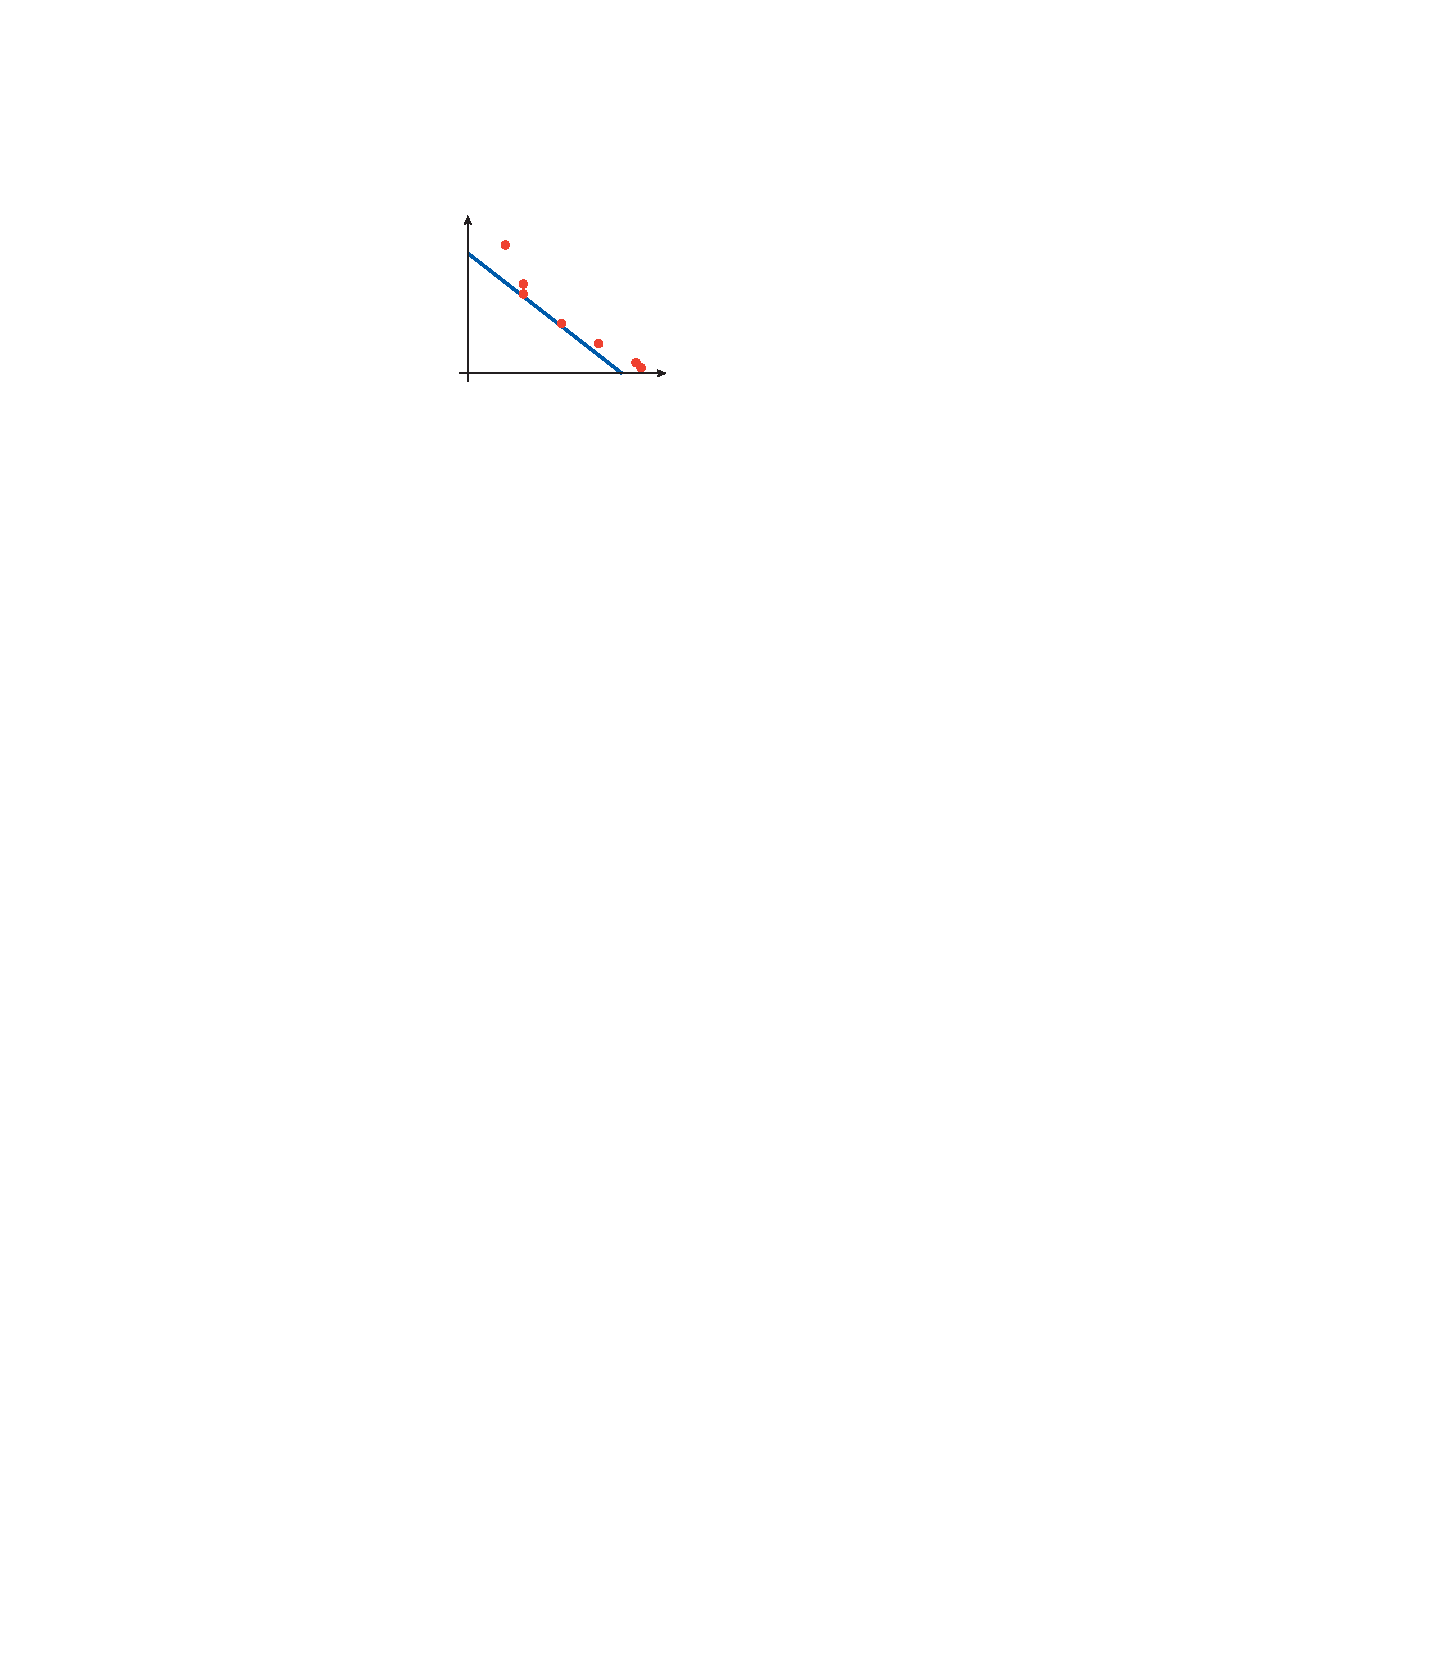
\includegraphics[width=\linewidth]{external/images/fig-ex-1-6-8.pdf}
\end{sbspanel}%
\end{sidebyside}%
\end{divisionexerciseegcol}%
\begin{divisionexerciseegcol}{9}{}{}{exercise-section-1-6-exercises-c-d}%
\begin{sidebyside}{1}{0.25}{0.25}{0}%
\begin{sbspanel}{0.5}%
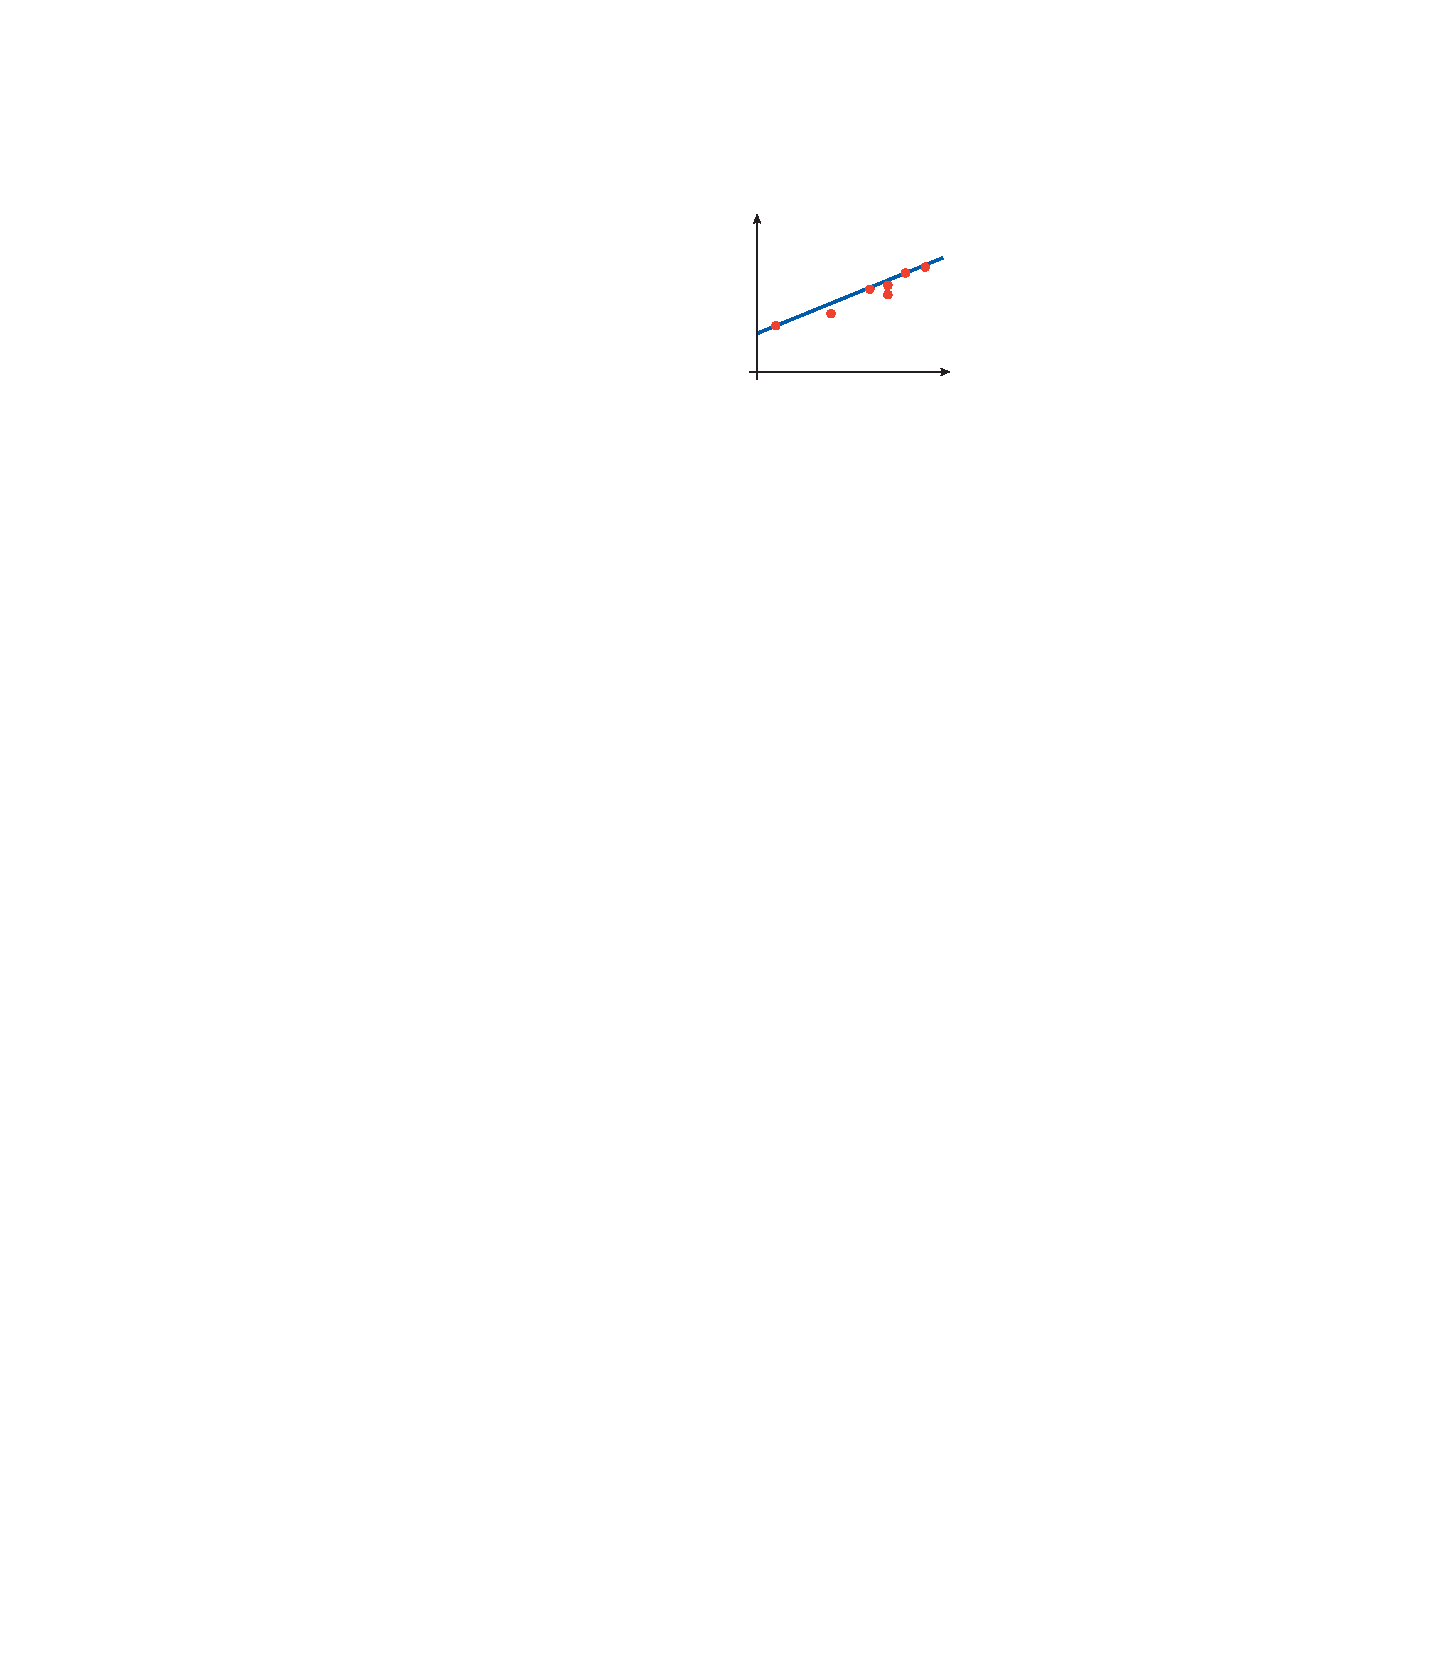
\includegraphics[width=\linewidth]{external/images/fig-ex-1-6-9.pdf}
\end{sbspanel}%
\end{sidebyside}%
\end{divisionexerciseegcol}%
\begin{divisionexerciseegcol}{10}{}{}{exercise-section-1-6-exercises-c-e}%
\begin{sidebyside}{1}{0.25}{0.25}{0}%
\begin{sbspanel}{0.5}%
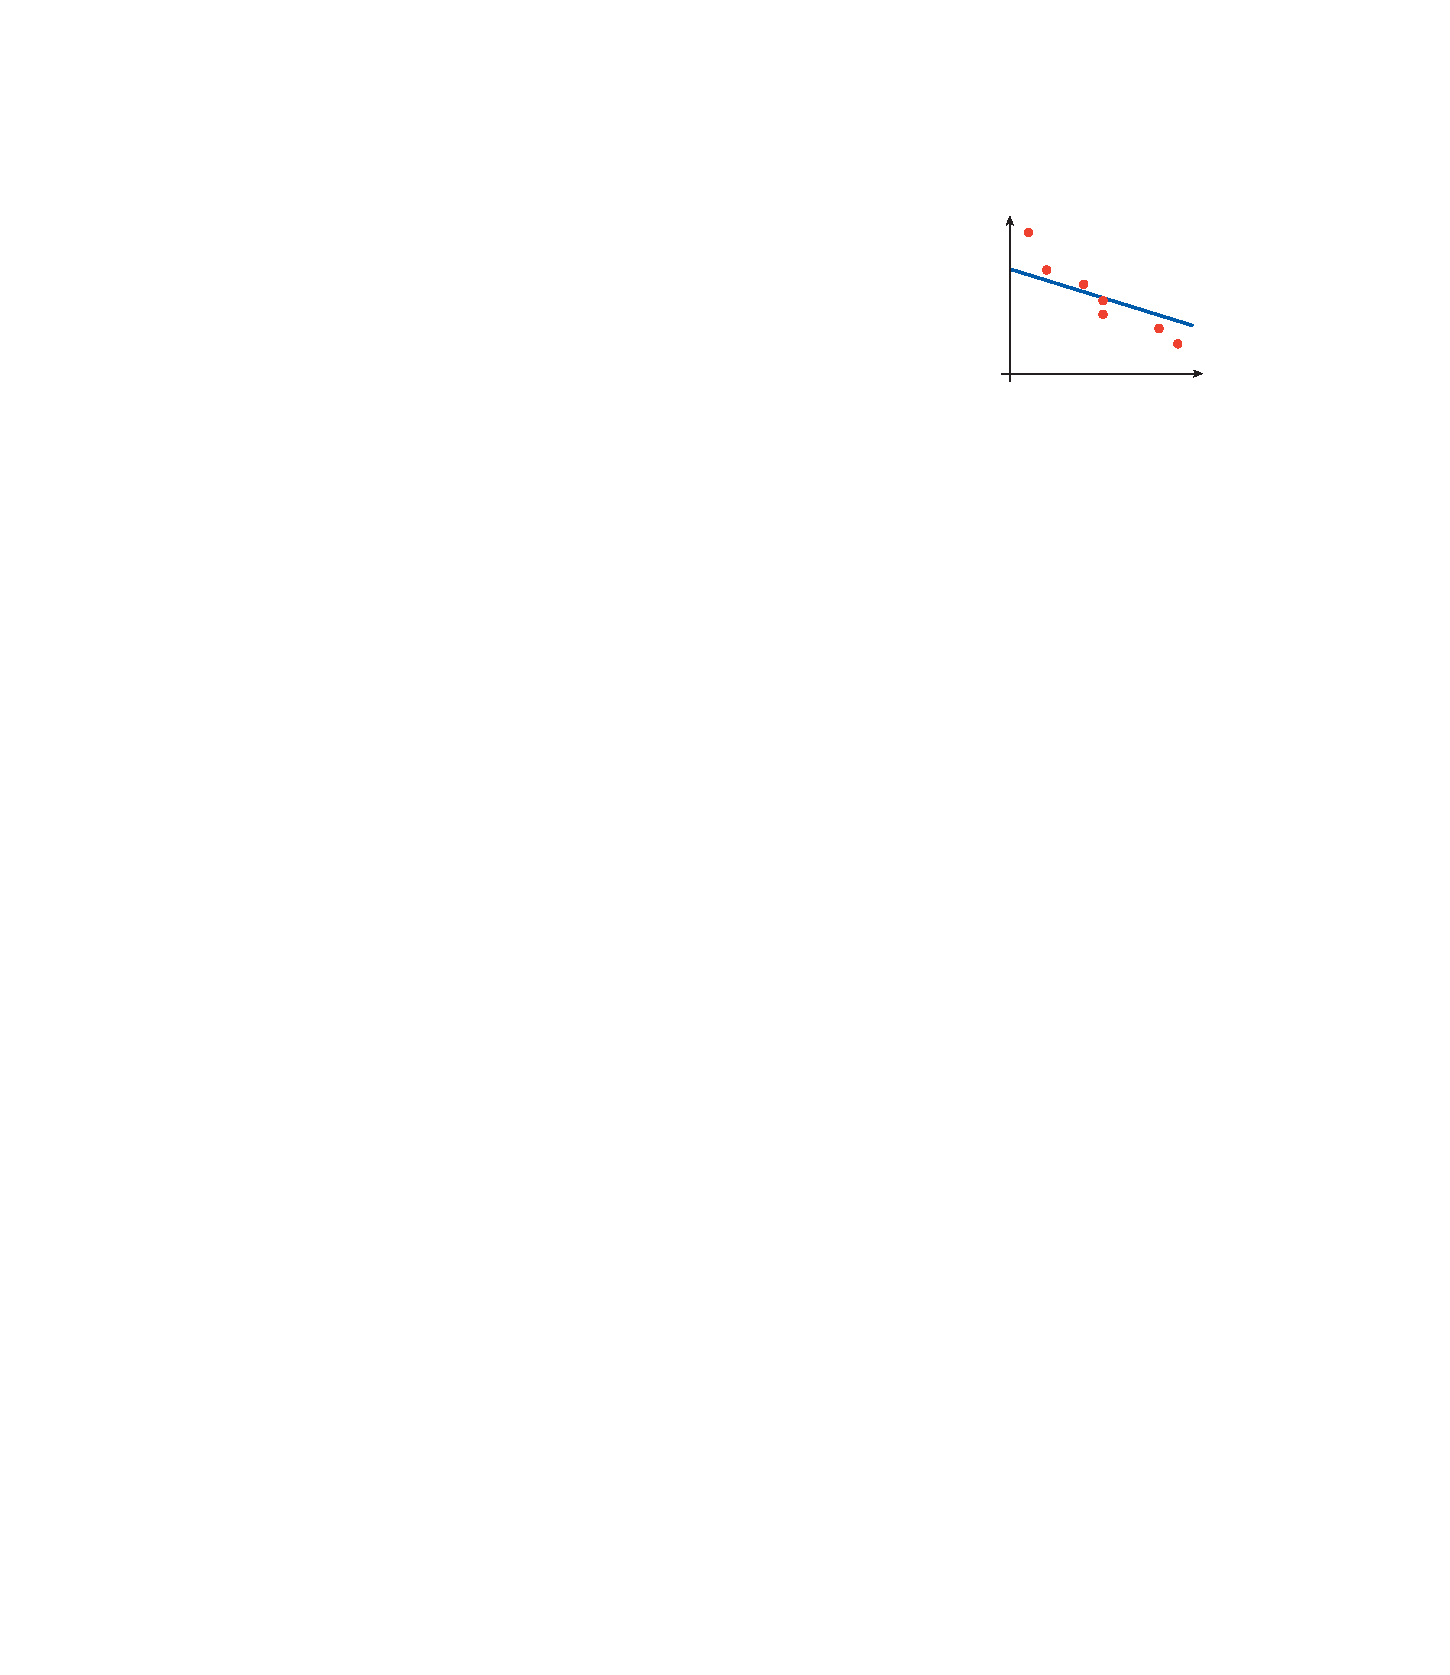
\includegraphics[width=\linewidth]{external/images/fig-ex-1-6-10.pdf}
\end{sbspanel}%
\end{sidebyside}%
\end{divisionexerciseegcol}%
\end{exercisegroupcol}
\par\medskip\noindent
\par\medskip\noindent%
\textbf{Exercise Group.}\space\space%
In Problems 11 and 12, use information from the graphs to answer the questions.%
\begin{exercisegroup}
\begin{divisionexerciseeg}{11}{}{}{exercise-section-1-6-exercises-d-b}%
The scatterplot shows the ages of 10 army drill sergeants and the time it took each to run 100 meters, in seconds.%
\begin{sidebyside}{1}{0.3}{0.3}{0}%
\begin{sbspanel}{0.4}%
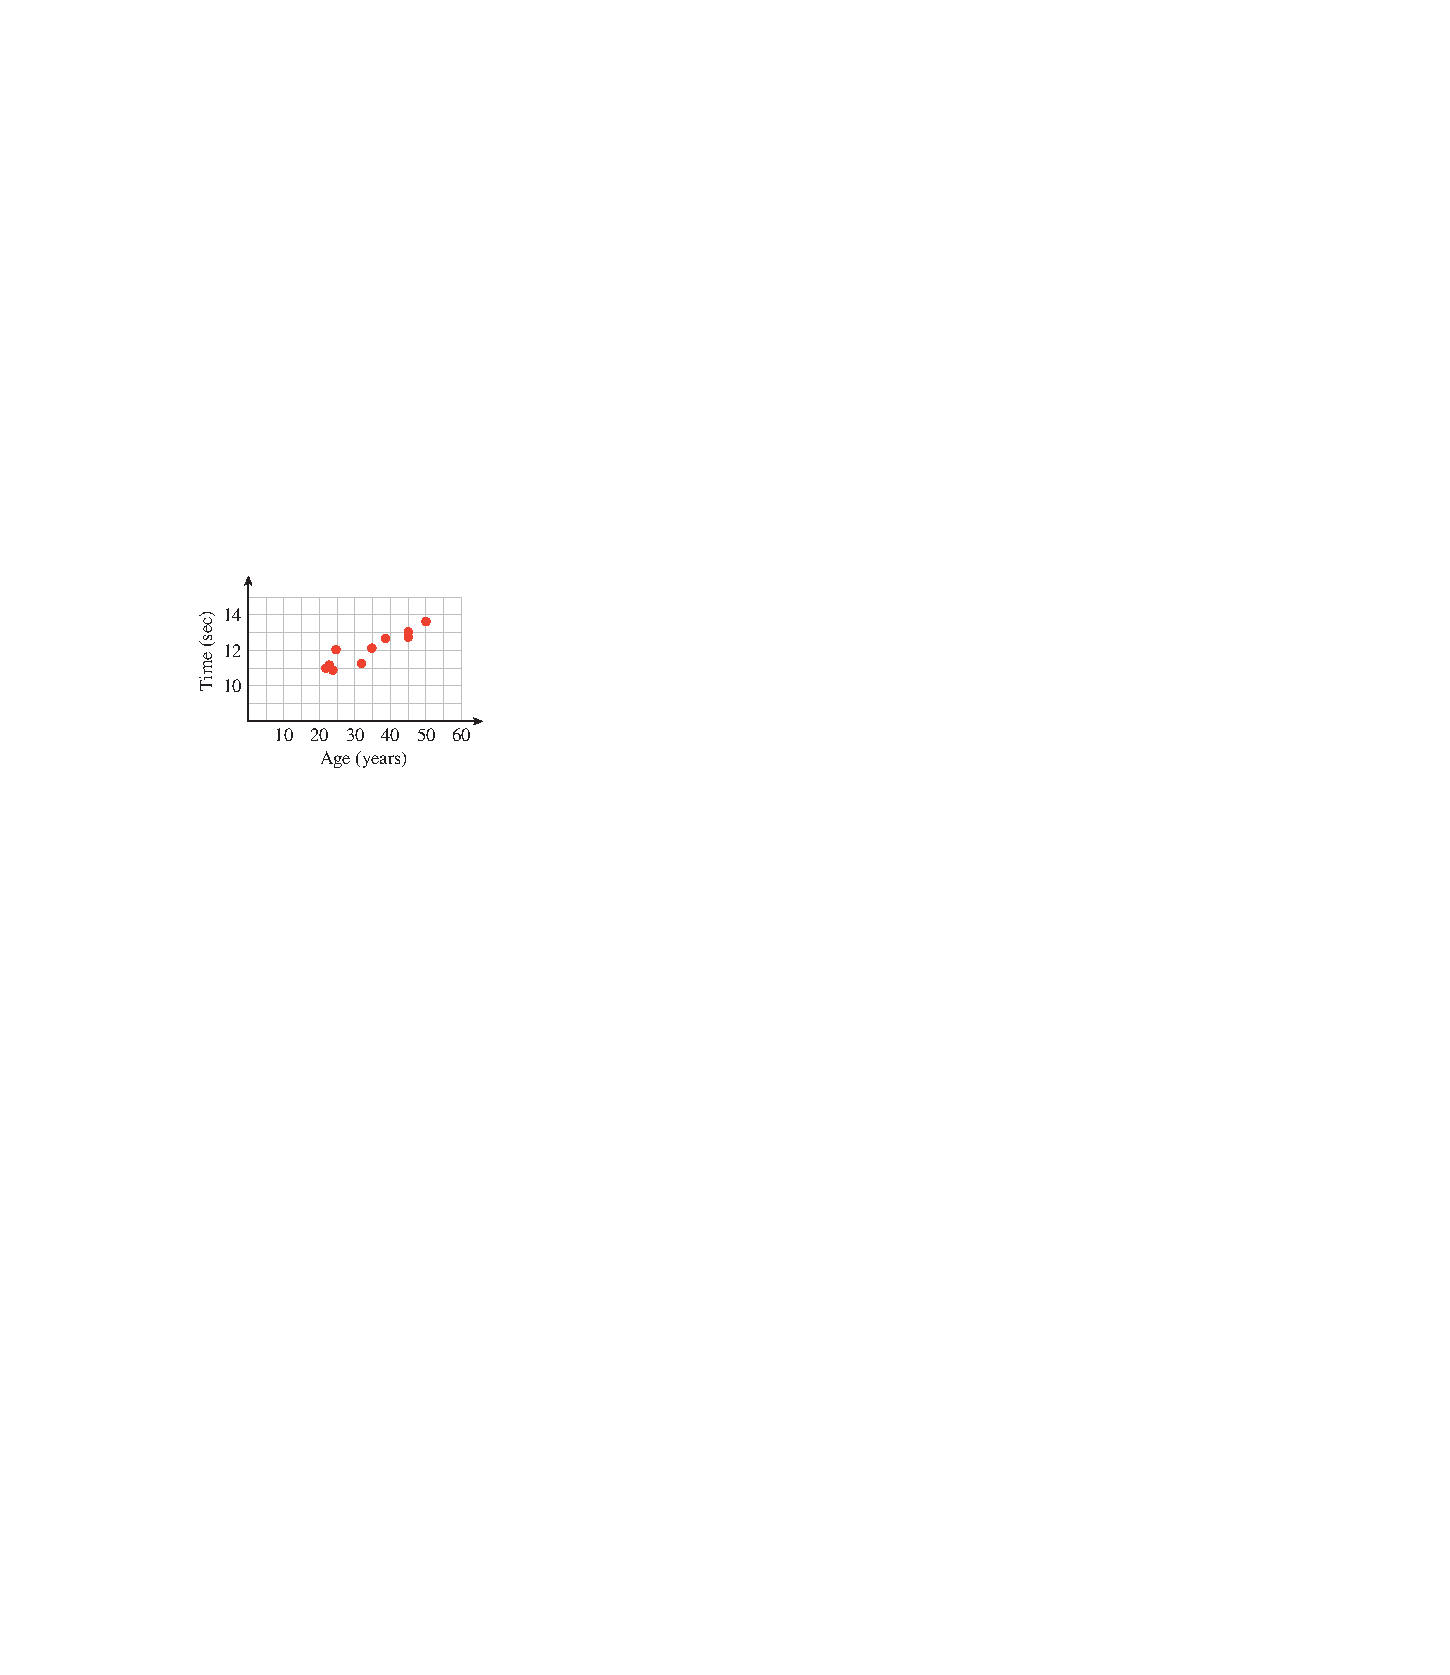
\includegraphics[width=\linewidth]{external/images/fig-ex-1-6-11.pdf}
\end{sbspanel}%
\end{sidebyside}%
\par
%
\begin{enumerate}[label=\alph*]
\item{}What was the hundred-meter time for the 25-year-old drill sergeant?%
\item{}How old was the drill sergeant whose hundred-meter time was \(12.6\) seconds?%
\item{}Use a straightedge to draw a line of best fit through the data points.%
\item{}Use your line of best fit to predict the hundred-meter time of a 28-year-old drill sergeant.%
\item{}Choose two points on your regression line and find its equation.%
\item{}Use the equation to predict the hundred-meter time of a 40-year-old drill sergeant and a 12 year-old drill sergeant. Are these predictions reasonable?%
\end{enumerate}
%
\end{divisionexerciseeg}%
\begin{divisionexerciseeg}{12}{}{}{exercise-section-1-6-exercises-d-c}%
The scatterplot shows the outside temperature and the number of cups of cocoa sold at an outdoor skating rink snack bar on 13 consecutive nights.%
\begin{sidebyside}{1}{0.2}{0.2}{0}%
\begin{sbspanel}{0.6}%
\includegraphics[width=\linewidth]{external/images/fig-ex-1-6-12.pdf}
\end{sbspanel}%
\end{sidebyside}%
\par
%
\begin{enumerate}[label=\alph*]
\item{}How many cups of cocoa were sold when the temperature was \(2\degree\)C?%
\item{}What was the temperature on the night when \(25\) cups of cocoa were sold?%
\item{}Use a straightedge to draw a line of best fit through the data points%
\item{}Use your line of best fit to predict the number of cups of cocoa that will be sold at the snack bar if the temperature is \(7\degree\)C.%
\item{}Choose two points on your regression line and find its equation.%
\item{}Use the equation to predict the number of cups of cocoa that will be sold when the temperature is \(10\degree\)C and when the temperature is \(24\degree\)C. Are these predictions reasonable?%
\end{enumerate}
%
\end{divisionexerciseeg}%
\end{exercisegroup}
\par\medskip\noindent
\begin{divisionexercise}{13}{}{}{exercise-section-1-6-exercises-e}%
With Americans' increased use of faxes, pagers, and cell phones, new area codes are being created at a steady rate. The table shows the number of area codes in the United States each year. (Source: USA Today, NeuStar, Inc.)%
\begin{sidebyside}{1}{0}{0}{0}%
\begin{sbspanel}{1}%
\resizebox{\ifdim\width > \linewidth\linewidth\else\width\fi}{!}{%
{\centering%
{\tabularfont%
\begin{tabular}{AlAcAcAcAcAcAcAcA}\hrulethin
Year&\(1997\)&\(1998\)&\(1999\)&\(2000\)&\(2001\)&\(2002\)&\(2003\)\tabularnewline\hrulethin
Number of area codes&\(151\)&\(186\)&\(204\)&\(226\)&\(239\)&\(262\)&\(274\)\tabularnewline\hrulethin
\end{tabular}
}%
\par}
}%
\end{sbspanel}%
\end{sidebyside}%
\par
%
\begin{enumerate}[label=\alph*]
\item{}Let \(t\) represent the number of years after 1995 and plot the data. Draw a line of best fit for the data points.%
\item{}Find an equation for your regression line.%
\item{}How many area codes do you predict for 2010?%
\end{enumerate}
%
\end{divisionexercise}%
\begin{divisionexercise}{14}{}{}{exercise-section-1-6-exercises-f}%
The number of mobile homes in the United States has been increasing since 1960. The data in the table are given in millions of mobile homes. (Source: USA Today, U.S. Census Bureau)%
\begin{sidebyside}{1}{0}{0}{0}%
\begin{sbspanel}{1}%
\resizebox{\ifdim\width > \linewidth\linewidth\else\width\fi}{!}{%
{\centering%
{\tabularfont%
\begin{tabular}{AlAcAcAcAcAcA}\hrulethin
Year&\(1960\)&\(1970\)&\(1980\)&\(1990\)&\(2000\)\tabularnewline\hrulethin
Number of mobile homes&\(0.8\)&\(2.1\)&\(4.7\)&\(7.4\)&\(8.8\)\tabularnewline\hrulethin
\end{tabular}
}%
\par}
}%
\end{sbspanel}%
\end{sidebyside}%
\par
%
\begin{enumerate}[label=\alph*]
\item{}Let \(t\) represent the number of years after 1960 and plot the data. Draw a line of best fit for the data points%
\item{}Find an equation for your regression line.%
\item{}How many mobile homes do you predict for 2010?%
\end{enumerate}
%
\end{divisionexercise}%
\begin{divisionexercise}{15}{}{}{exercise-section-1-6-exercises-g}%
Teenage birth rates in the United States declined from 1991 to 2000. The table shows the number of births per 1000 women in selected years. (Source: U.S. National Health Statistics)%
\begin{sidebyside}{1}{0}{0}{0}%
\begin{sbspanel}{1}%
\resizebox{\ifdim\width > \linewidth\linewidth\else\width\fi}{!}{%
{\centering%
{\tabularfont%
\begin{tabular}{AlAcAcAcAcAcAcA}\hrulethin
Year&\(1991\)&\(1993\)&\(1995\)&\(1996\)&\(1997\)&\(1998\)\tabularnewline\hrulethin
Births&\(62.1\)&\(59.6\)&\(56.8\)&\(54.4\)&\(52.3\)&\(51.1\)\tabularnewline\hrulethin
\end{tabular}
}%
\par}
}%
\end{sbspanel}%
\end{sidebyside}%
\par
%
\begin{enumerate}[label=\alph*]
\item{}Let \(t\) represent the number of years after 1990 and plot the data. Draw a line of best fit for the data points.%
\item{}Find an equation for your regression line.%
\item{}Estimate the teen birth rate in 1994.%
\item{}Predict the teen birth rate in 2010.%
\end{enumerate}
%
\end{divisionexercise}%
\begin{divisionexercise}{16}{}{}{exercise-section-1-6-exercises-h}%
The table shows the minimum wage in the United States at five-year intervals. (Source: Economic Policy Institute)%
\begin{sidebyside}{1}{0}{0}{0}%
\begin{sbspanel}{1}%
\resizebox{\ifdim\width > \linewidth\linewidth\else\width\fi}{!}{%
{\centering%
{\tabularfont%
\begin{tabular}{AlAcAcAcAcAcAcAcAcAcA}\hrulethin
Year&\(1960\)&\(1965\)&\(1970\)&\(1975\)&\(1980\)&\(1985\)&\(1990\)&\(1995\)&\(2000\)\tabularnewline\hrulethin
Minimum wage&\(1.00\)&\(1.25\)&\(1.60\)&\(2.10\)&\(3.10\)&\(3.35\)&\(3.80\)&\(4.25\)&\(5.15\)\tabularnewline\hrulethin
\end{tabular}
}%
\par}
}%
\end{sbspanel}%
\end{sidebyside}%
\par
%
\begin{enumerate}[label=\alph*]
\item{}Let \(t\) represent the number of years after 1960 and plot the data. Draw a line of best fit for the data points.%
\item{}Find an equation for your regression line.%
\item{}Estimate the minimum wage in 1972.%
\item{}Predict the minimum wage in 2010.%
\end{enumerate}
%
\end{divisionexercise}%
\begin{divisionexercise}{17}{}{}{exercise-section-1-6-exercises-i}%
Life expectancy in the United States has been rising since the nineteenth century. The table shows the U.S. life expectancy in selected years. (Source: http:\slash{}\slash{}www.infoplease.com)%
\begin{sidebyside}{1}{0}{0}{0}%
\begin{sbspanel}{1}%
\resizebox{\ifdim\width > \linewidth\linewidth\else\width\fi}{!}{%
{\centering%
{\tabularfont%
\begin{tabular}{AlAcAcAcAcAcAcA}\hrulethin
Year&\(1950\)&\(1960\)&\(1970\)&\(1980\)&\(1990\)&\(2000\)\tabularnewline\hrulethin
Life expectancy at birth&\(68.2\)&\(69.7\)&\(70.8\)&\(73.7\)&\(75.4\)&\(77\)\tabularnewline\hrulethin
\end{tabular}
}%
\par}
}%
\end{sbspanel}%
\end{sidebyside}%
\par
%
\begin{enumerate}[label=\alph*]
\item{}Let \(t\) represent the number of years after 1950, and plot the data. Draw a line of best fit for the data points.%
\item{}Find an equation for your regression line.%
\item{}Estimate the life expectancy of someone born in 1987.%
\item{}Predict the life expectancy of someone born in 2010.%
\end{enumerate}
%
\end{divisionexercise}%
\begin{divisionexercise}{18}{}{}{exercise-section-1-6-exercises-j}%
The table shows the per capita cigarette consumption in the United States at five-year intervals. (Source: http:\slash{}\slash{}www.infoplease.com)%
\begin{sidebyside}{1}{0}{0}{0}%
\begin{sbspanel}{1}%
\resizebox{\ifdim\width > \linewidth\linewidth\else\width\fi}{!}{%
{\centering%
{\tabularfont%
\begin{tabular}{AlAcAcAcAcAcA}\hrulethin
Year&\(1980\)&\(1985\)&\(1990\)&\(1995\)&\(2000\)\tabularnewline\hrulethin
Per capita cigarette consumption&\(3851\)&\(3461\)&\(2827\)&\(2515\)&\(2092\)\tabularnewline\hrulethin
\end{tabular}
}%
\par}
}%
\end{sbspanel}%
\end{sidebyside}%
\par
%
\begin{enumerate}[label=\alph*]
\item{}Let \(t\) represent the number of years after 1980, and plot the data. Draw a line of best fit for the data points.%
\item{}Find an equation for your regression line.%
\item{}Estimate the per capita cigarette consumption in 1998.%
\item{}Predict the per capita cigarette consumption in 2010.%
\end{enumerate}
%
\end{divisionexercise}%
\begin{divisionexercise}{19}{}{}{exercise-section-1-6-exercises-k}%
"The earnings gap between high-school and college graduates continues to widen, the Census Bureau says. On average, college graduates now earn just over \textdollar{}\(51,000\) a year, almost twice as much as high-school graduates. And those with no high-school diploma have actually seen their earnings drop in recent years." The table shows the unemployment rate and the median weekly earnings for employees with different levels of education. (Source: Morning Edition, National Public Radio, March 28, 2005)%
\begin{sidebyside}{1}{0}{0}{0}%
\begin{sbspanel}{1}%
\resizebox{\ifdim\width > \linewidth\linewidth\else\width\fi}{!}{%
{\centering%
{\tabularfont%
\begin{tabular}{AlAcAcAcA}\hrulethin
&\tablecelllines{c}{m}
{Years of\\
education}
&\tablecelllines{c}{m}
{Unemployment\\
rate}
&\tablecelllines{c}{m}
{Weekly\\
earnings (\textdollar{})}
\tabularnewline\hrulethin
\tablecelllines{l}{m}
{Some\\
high school\\
no diploma}
&\(10\)&\(8.8\)&\(396\)\tabularnewline\hrulethin
\tablecelllines{l}{m}
{High-school\\
graduate}
&\(12\)&\(5.5     \)&\(554\)\tabularnewline\hrulethin
\tablecelllines{l}{m}
{Some college\\
no degree}
&\(13\)&\(5.2\)&\(622\)\tabularnewline\hrulethin
\tablecelllines{l}{m}
{Associate's\\
degree}
&\(14\)&\(4.0\)&\(672\)\tabularnewline\hrulethin
\tablecelllines{l}{m}
{Bachelor's\\
degree}
&\(16\)&\(3.3\)&\(900\)\tabularnewline\hrulethin
\tablecelllines{l}{m}
{Master's\\
degree}
&\(18\)&\(2.9\)&\(1064\)\tabularnewline\hrulethin
\tablecelllines{l}{m}
{Professional\\
degree}
&\(20\)&\(1.7\)&\(1307\)\tabularnewline\hrulethin
\end{tabular}
}%
\par}
}%
\end{sbspanel}%
\end{sidebyside}%
\par
%
\begin{enumerate}[label=\alph*]
\item{}Plot years of education on the horizontal axis and weekly earnings on the vertical axis.%
\item{}Find an equation for the regression line.%
\item{}State the slope of the regression line, including units, and explain what it means in the context of the data.%
\item{}Do you think this model is useful for extrapolation or interpolation? For example, what weekly earnings does the model predict for someone with 15 years of education? For 25 years? Do you think these predictions are valid? Why or why not?%
\end{enumerate}
%
\end{divisionexercise}%
\begin{divisionexercise}{20}{}{}{exercise-section-1-6-exercises-l}%
The table shows the birth rate (in births per woman) and the female literacy rate (as a percent of the adult female population) in a number of nations. (Source: UNESCO, The World Fact Book, EarthTrends)%
\begin{sidebyside}{1}{0}{0}{0}%
\begin{sbspanel}{1}%
\resizebox{\ifdim\width > \linewidth\linewidth\else\width\fi}{!}{%
{\centering%
{\tabularfont%
\begin{tabular}{AlAcAcA}\hrulethin
Country&Literacy rate&Birth rate\tabularnewline\hrulethin
Brazil&\(88.6\)&\(1.93\)\tabularnewline\hrulethin
Egypt&\(43.6\)&\(2.88\)\tabularnewline\hrulethin
Germany&\(99\)&\(1.39\)\tabularnewline\hrulethin
Iraq&\(53\)&\(4.28\)\tabularnewline\hrulethin
Japan&\(99\)&\(1.39\)\tabularnewline\hrulethin
Niger&\(9.4\)&\(6.75\)\tabularnewline\hrulethin
Pakistan&\(35.2\)&\(4.14\)\tabularnewline\hrulethin
Peru&\(82.1\)&\(2.56\)\tabularnewline\hrulethin
Philippines&\(92.7\)&\(3.16\)\tabularnewline\hrulethin
Portugal&\(91\)&\(1.47\)\tabularnewline\hrulethin
Russian Federation&\(99.2\)&\(1.27\)\tabularnewline\hrulethin
Saudi Arabia&\(69.3\)&\(4.05\)\tabularnewline\hrulethin
United States&\(97\)&\(2.08\)\tabularnewline\hrulethin
\end{tabular}
}%
\par}
}%
\end{sbspanel}%
\end{sidebyside}%
\par
%
\begin{enumerate}[label=\alph*]
\item{}Plot the data with literacy rate on the horizontal axis. Draw a line of best fit for the data points.%
\item{}Find an equation for the regression line.%
\item{}What values for the input variable make sense for the model? What are the largest and smallest values predicted by the model for the output variable?%
\item{}State the slope of the regression line, including units, and explain what it means in the context of the data.%
\end{enumerate}
%
\end{divisionexercise}%
\begin{divisionexercise}{21}{}{}{exercise-section-1-6-exercises-m}%
The table shows the amount of carbon released into the atmosphere annually from burning fossil fuels, in billions of tons, at 5-year intervals from 1950 to 1995. (Source: www.worldwatch.org)%
\begin{sidebyside}{1}{0}{0}{0}%
\begin{sbspanel}{1}%
\resizebox{\ifdim\width > \linewidth\linewidth\else\width\fi}{!}{%
{\centering%
{\tabularfont%
\begin{tabular}{AlAcAcAcAcAcAcAcAcAcAcA}\hrulethin
Year&\(1950\)&\(1955\)&\(1960\)&\(1965\)&\(1970\)&\(1975\)&\(1980\)&\(1985\)&\(1990\)&\(1995\)\tabularnewline\hrulethin
\tablecelllines{l}{m}
{Carbon\\
emissions}
&\(1.6\)&\(2.0\)&\(2.5\)&\(3.1\)&\(4.0\)&\(4.5\)&\(5.2\)&\(5.3\)&\(5.9\)&\(6.2\)\tabularnewline\hrulethin
\end{tabular}
}%
\par}
}%
\end{sbspanel}%
\end{sidebyside}%
\par
%
\begin{enumerate}[label=\alph*]
\item{}Let \(t\) represent the number of years after 1950 and plot the data. Draw a line of best fit for the data points.%
\item{}Find an equation for your regression line.%
\item{}Estimate the amount of carbon released in 1992.%
\end{enumerate}
%
\end{divisionexercise}%
\begin{divisionexercise}{22}{}{}{exercise-section-1-6-exercises-n}%
High-frequency radiation is harmful to living things because it can cause changes in their genetic material. The data below, collected by C. P. Oliver in 1930, show the frequency of genetic transmutations induced in fruit flies by doses of X-rays, measured in roentgens. (Source: C. P. Oliver, 1930)%
\begin{sidebyside}{1}{0}{0}{0}%
\begin{sbspanel}{1}%
\resizebox{\ifdim\width > \linewidth\linewidth\else\width\fi}{!}{%
{\centering%
{\tabularfont%
\begin{tabular}{AlAcAcAcAcAcA}\hrulethin
\tablecelllines{l}{m}
{Dosage\\
(roentgens)}
&\(285\)&\(570\)&\(1640\)&\(3280\)&\(6560\)\tabularnewline\hrulethin
\tablecelllines{l}{m}
{Percentage of\\
mutated genes}
&\(1.18\)&\(2.99\)&\(4.56\)&\(9.63\)&\(15.85\)\tabularnewline\hrulethin
\end{tabular}
}%
\par}
}%
\end{sbspanel}%
\end{sidebyside}%
\par
%
\begin{enumerate}[label=\alph*]
\item{}Plot the data and draw a line of best fit through the data points.%
\item{}Find an equation for your regression line.%
\item{}Use the regression equation to predict the percent of mutations that might result from exposure to \(5000\) roentgens of radiation.%
\end{enumerate}
%
\end{divisionexercise}%
\begin{divisionexercise}{23}{}{}{exercise-section-1-6-exercises-o}%
Bracken, a type of fern, is one of the most successful plants in the world, growing on every continent except Antarctica. New plants, which are genetic clones of the original, spring from a network of underground stems, or rhizomes, to form a large circular colony. The graph shows the diameters of various colonies plotted against their age. (Source: Chapman et al.,1992)%
\begin{sidebyside}{1}{0.325}{0.325}{0}%
\begin{sbspanel}{0.35}%
\includegraphics[width=\linewidth]{external/images/fig-ex-1-6-23.pdf}
\end{sbspanel}%
\end{sidebyside}%
\par
%
\begin{enumerate}[label=\alph*]
\item{}Calculate the rate of growth of the diameter of a bracken colony, in meters per year.%
\item{}Find an equation for the line of best fit. (What should the vertical intercept of the line be?)%
\item{}In Finland, bracken colonies over \(450\) meters in diameter have been found. How old are these colonies?%
\end{enumerate}
%
\end{divisionexercise}%
\begin{divisionexercise}{24}{}{}{exercise-section-1-6-exercises-p}%
The European sedge warbler can sing several different songs consisting of trills, whistles, and buzzes. Male warblers who sing the largest number of songs are the first to acquire mates in the spring. The data below show the number of different songs sung by several male warblers and the day on which they acquired mates, where day 1 is April 20. (Source: Krebs and Davies, 1993)%
\begin{sidebyside}{1}{0}{0}{0}%
\begin{sbspanel}{1}%
\resizebox{\ifdim\width > \linewidth\linewidth\else\width\fi}{!}{%
{\centering%
{\tabularfont%
\begin{tabular}{AlAcAcAcAcAcAcAcAcAcAcA}\hrulethin
\tablecelllines{l}{m}
{Number\\
of songs}
&\(41\)&\(38\)&\(34\)&\(32\)&\(30\)&\(25\)&\(24\)&\(24\)&\(23\)&\(14\)\tabularnewline\hrulethin
Pairing day&\(20\)&\(24\)&\(25\)&\(21\)&\(24\)&\(27\)&\(31\)&\(35\)&\(40\)&\(42\)\tabularnewline\hrulethin
\end{tabular}
}%
\par}
}%
\end{sbspanel}%
\end{sidebyside}%
\par
%
\begin{enumerate}[label=\alph*]
\item{}Plot the data points, with number of songs on the horizontal axis. A regression line for the data is \(y = -0.85x + 53\). Graph this line on the same axes with the data.%
\item{}What does the slope of the regression line represent?%
\item{}When can a sedge warbler that knows \(10\) songs expect to find a mate?%
\item{}What do the intercepts of the regression line represent? Do these values make sense in context?%
\end{enumerate}
%
\end{divisionexercise}%
\begin{divisionexercise}{25}{}{}{exercise-section-1-6-exercises-q}%
One of the factors that determines the strength of a muscle is its cross-sectional area.  The data below show the cross-sectional area of the arm flexor muscle for several men and women, and their strength, measured by the maximum force they exerted against a resistance.  (Source:  Davis, Kimmet, Autry, 1986)%
\begin{sidebyside}{1}{0}{0}{0}%
\begin{sbspanel}{1}%
\resizebox{\ifdim\width > \linewidth\linewidth\else\width\fi}{!}{%
{\centering%
{\tabularfont%
\begin{tabular}{AlAcAcAcAcAcAcAcAcAcAcA}\hrulethin
Women&Area (sq cm)&\(11.5\)&\(10.8\)&\(11.7\)&\(12.0\)&\(12.5\)&\(12.7\)&\(14.4\)&\(14.4 \)&\(15.7\)\tabularnewline\hrulethin
&Strength (kg)&\(11.3\)&\(13.2\)&\(13.2\)&\(14.5\)&\(15.6\)&\(14.8\)&\(15.6\)&\(16.1 \)&\(18.4\)\tabularnewline\hrulethin
Men&Area (sq cm)&\(13.5\)&\(13.8\)&\(15.4\)&\(15.4\)&\(17.7\)&\(18.6\)&\(20.8\)&\(- \)&\(- \)\tabularnewline\hrulethin
&Strength (kg)&\(15.0\)&\(17.3\)&\(19.0\)&\(19.8\)&\(20.6\)&\(20.8\)&\(26.3\)&\(- \)&\(- \)\tabularnewline\hrulethin
\end{tabular}
}%
\par}
}%
\end{sbspanel}%
\end{sidebyside}%
\par
%
\begin{enumerate}[label=\alph*]
\item{}Plot the data for both men and women on the same graph using different symbols for the data points for men and the data points for women.%
\item{}Are the data for both men and women described reasonably well by the same regression line? Draw a line of best fit through the data.%
\item{}Find the equation of your line of best fit, or use a calculator to find the regression line for the data.%
\item{}What does the slope mean in this context?%
\end{enumerate}
%
\end{divisionexercise}%
\begin{divisionexercise}{26}{}{}{exercise-section-1-6-exercises-r}%
Astronomers use a numerical scale called \terminology{magnitude} to measure the brightness of a star, with brighter stars assigned smaller magnitudes. When we view a star from Earth, dust in the air absorbs some of the light, making the star appear fainter than it really is. Thus, the observed magnitude of a star, \(m\), depends on the distance its light rays must travel through the Earth's atmosphere. The observed magnitude is given by%
\begin{equation*}
m = m_0 + kx
\end{equation*}
where \(m_0\) is the actual magnitude of the star outside the atmosphere, \(x\) is the air mass (a measure of the distance through the atmosphere), and \(k\) is a constant called the \terminology{extinction coefficient}. To calculate \(m_0\), astronomers observe the same object several times during the night at different positions in the sky, and hence for different values of \(x\). Here are data from such observations. (Source: Karttunen et al., 1987)%
\begin{sidebyside}{1}{0}{0}{0}%
\begin{sbspanel}{1}%
\resizebox{\ifdim\width > \linewidth\linewidth\else\width\fi}{!}{%
{\centering%
{\tabularfont%
\begin{tabular}{AcAcAcA}\hrulethin
Altitude&Air mass, \(x\)&Magnitude, \(m\)\tabularnewline\hrulethin
\(50\degree\)&\(1.31\)&\(0.90\)\tabularnewline\hrulethin
\(35\degree\)&\(1.74\)&\(0.98\)\tabularnewline\hrulethin
\(25\degree\)&\(2.37\)&\(1.07\)\tabularnewline\hrulethin
\(20\degree\)&\(2.92\)&\(1.17\)\tabularnewline\hrulethin
\end{tabular}
}%
\par}
}%
\end{sbspanel}%
\end{sidebyside}%
\par
%
\begin{enumerate}[label=\alph*]
\item{}Plot observed magnitude against air mass, and draw a line of best fit through the data.%
\item{}Find the equation of your line of best fit, or use a calculator to find the regression line for the data.%
\item{}Find the equation of your line of best fit, or use a calculator to find the regression line for the data.%
\item{}What is the value of the extinction coefficient? What is the apparent magnitude of the star outside Earth's atmosphere?%
\end{enumerate}
%
\end{divisionexercise}%
\begin{divisionexercise}{27}{}{}{exercise-section-1-6-exercises-s}%
Six students are trying to identify an unknown chemical compound by heating the substance and measuring the density of the gas that evaporates. (Density \(=\) mass\slash{}volume.) The students record the mass lost by the solid substance and the volume of the gas that evaporated from it. They know that the mass lost by the solid must be the same as the mass of the gas that evaporated. (Source: Hunt and Sykes, 1984)%
\begin{sidebyside}{1}{0}{0}{0}%
\begin{sbspanel}{1}%
\resizebox{\ifdim\width > \linewidth\linewidth\else\width\fi}{!}{%
{\centering%
{\tabularfont%
\begin{tabular}{AlAcAcAcAcAcAcA}\hrulethin
Student&A&B&C&D&E&F\tabularnewline\hrulethin
\tablecelllines{l}{m}
{Volume of\\
gas (\(\text{cm}^3\))}
&\(48\)&\(60\)&\(24\)&\(81\)&\(76\)&\(54\)\tabularnewline\hrulethin
\tablecelllines{l}{m}
{Loss in\\
mass (mg)}
&\(64\)&\(81\)&\(32\)&\(107\)&\(88\)&\(72\)\tabularnewline\hrulethin
\end{tabular}
}%
\par}
}%
\end{sbspanel}%
\end{sidebyside}%
\par
%
\begin{enumerate}[label=\alph*]
\item{}Plot the data with volume on the horizontal axis. Which student made an error in the experiment?%
\item{}Ignoring the incorrect data point, draw a line of best fit through the other points.%
\item{}Find an equation of the form \(y = kx\) for the data. Why should you expect the regression line to pass through the origin?%
\item{}Use your equation to calculate the mass of \(1000\text{ cm}^3\) (one liter) of the gas.%
\item{}Here are the densities of some gases at room temperature:%
\begin{sidebyside}{1}{0}{0}{0}%
\begin{sbspanel}{1}%
\resizebox{\ifdim\width > \linewidth\linewidth\else\width\fi}{!}{%
{\centering%
{\tabularfont%
\begin{tabular}{lrl}
Hydrogen&\(8\)&mg\slash{}liter\tabularnewline[0pt]
Nitrogen&\(1160\)&mg\slash{}liter\tabularnewline[0pt]
Oxygen&\(1330\)&mg\slash{}liter\tabularnewline[0pt]
Carbon dioxide&\(1830\)&mg\slash{}liter
\end{tabular}
}%
\par}
}%
\end{sbspanel}%
\end{sidebyside}%
\par
Which of these might have been the gas that evaporated from the unknown substance?%
\end{enumerate}
%
\par\smallskip%
\noindent\textbf{\blocktitlefont Hint}.\hypertarget{hint-section-1-6-exercises-s-b}{}\quad{}Use your answer to part (d) to calculate the density of the gas. \(1 \text{ cm}^3 = 1 \text{ milliliter}\).%
\end{divisionexercise}%
\begin{divisionexercise}{28}{}{}{exercise-section-1-6-exercises-t}%
The formulas for many chemical compounds involve ratios of small integers. For example, the formula for water, H\(_2\)0, means that two atoms of hydrogen combine with one atom of oxygen to make one water molecule. Similarly, magnesium and oxygen combine to produce magnesium oxide. In this problem, we will discover the chemical formula for magnesium oxide. (Source: Hunt and Sykes, 1984)%
\begin{enumerate}[label=\alph*]
\item{}Twenty-four grams of magnesium contain the same number of atoms as sixteen grams of oxygen. Complete the table showing the amount of oxygen needed if the formula for magnesium oxide is \(\text{MgO}\), \(\text{Mg}_2\text{O}\), or \(\text{MgO}_2\).%
\begin{sidebyside}{1}{0}{0}{0}%
\begin{sbspanel}{1}%
\resizebox{\ifdim\width > \linewidth\linewidth\else\width\fi}{!}{%
{\centering%
{\tabularfont%
\begin{tabular}{AcAcAcAcA}\hrulethin
Grams of Mg&\tablecelllines{c}{m}
{Grams of\\
O (if MgO)}
&\tablecelllines{c}{m}
{Grams of\\
O (if Mg\(_2\)O)}
&\tablecelllines{c}{m}
{Grams of\\
O (if MgO\(_2\))}
\tabularnewline\hrulethin
\(24\)&\(16\)&\(\)&\(\)\tabularnewline\hrulethin
\(48\)&\(\)&\(\)&\(\)\tabularnewline\hrulethin
\(12\)&\(\)&\(\)&\(\)\tabularnewline\hrulethin
\(6\)&\(\)&\(\)&\(\)\tabularnewline\hrulethin
\end{tabular}
}%
\par}
}%
\end{sbspanel}%
\end{sidebyside}%
\item{}Graph three lines on the same axes to represent the three possibilities, with grams of magnesium on the horizontal axis and grams of oxygen on the vertical axis.%
\item{}Here are the results of some experiments synthesizing magnesium oxide.%
\begin{sidebyside}{1}{0}{0}{0}%
\begin{sbspanel}{1}%
\resizebox{\ifdim\width > \linewidth\linewidth\else\width\fi}{!}{%
{\centering%
{\tabularfont%
\begin{tabular}{AcAcAcA}\hrulethin
Experiment&\tablecelllines{c}{m}
{Grams of\\
Magnesium}
&\tablecelllines{c}{m}
{Grams\\
of oxygen}
\tabularnewline\hrulethin
\(1\)&\(15\)&\(10\)\tabularnewline\hrulethin
\(2\)&\(22\)&\(14\)\tabularnewline\hrulethin
\(3\)&\(30\)&\(20\)\tabularnewline\hrulethin
\(4\)&\(28\)&\(18\)\tabularnewline\hrulethin
\(5\)&\(10\)&\(6\)\tabularnewline\hrulethin
\end{tabular}
}%
\par}
}%
\end{sbspanel}%
\end{sidebyside}%
\par
Plot the data on your graph from part (b). Which is the correct formula for magnesium oxide?%
\end{enumerate}
%
\end{divisionexercise}%
\par\medskip\noindent%
\textbf{Exercise Group.}\space\space%
For Problems 29\textendash{}32,%
\begin{enumerate}[label=\alph*]
\item{}Use linear interpolation to give approximate answers.%
\item{}What is the meaning of the slope in the context of the problem?%
\end{enumerate}
%
\begin{exercisegroup}
\begin{divisionexerciseeg}{29}{}{}{exercise-section-1-6-exercises-u-b}%
The temperature in Encino dropped from \(81\degree\)F at 1 a.m. to \(73\degree\)F at 5 a.m. Estimate the temperature at 4 a.m.%
\end{divisionexerciseeg}%
\begin{divisionexerciseeg}{30}{}{}{exercise-section-1-6-exercises-u-c}%
Newborn blue whales are about \(24\) feet long and weigh \(3\) tons. The young whale nurses for \(7\) months, at which time it is \(53\) feet long. Estimate the length of a \(1\)-year-old blue whale.%
\end{divisionexerciseeg}%
\begin{divisionexerciseeg}{31}{}{}{exercise-section-1-6-exercises-u-d}%
A car starts from a standstill and accelerates to a speed of \(60\) miles per hour in \(6\) seconds. Estimate the car's speed \(2\) seconds after it began to accelerate.%
\end{divisionexerciseeg}%
\begin{divisionexerciseeg}{32}{}{}{exercise-section-1-6-exercises-u-e}%
A truck on a slippery road is moving at \(24\) feet per second when the driver steps on the brakes. The truck needs \(3\) seconds to come to a stop. Estimate the truck's speed \(2\) seconds after the brakes were applied.%
\end{divisionexerciseeg}%
\end{exercisegroup}
\par\medskip\noindent
\par\medskip\noindent%
\textbf{Exercise Group.}\space\space%
In Problems 33\textendash{}36, use linear interpolation or extrapolation to answer the questions.%
\begin{exercisegroup}
\begin{divisionexerciseeg}{33}{}{}{exercise-section-1-6-exercises-v-b}%
The temperature of an automobile engine is \(9\degree\) Celsius when the engine is started and \(51\degree\)C seven minutes later. Use a linear model to predict the engine temperature for both \(2\) minutes and \(2\) hours after it started. Are your predictions reasonable?%
\end{divisionexerciseeg}%
\begin{divisionexerciseeg}{34}{}{}{exercise-section-1-6-exercises-v-c}%
The temperature in Death Valley is \(95\degree\) Fahrenheit at 5 a.m. and rises to \(110\degree\) Fahrenheit by noon. Use a linear model to predict the temperature at 2 p.m. and at midnight. Are your predictions reasonable?%
\end{divisionexerciseeg}%
\begin{divisionexerciseeg}{35}{}{}{exercise-section-1-6-exercises-v-d}%
Ben weighed \(8\) pounds at birth and \(20\) pounds at age \(1\) year. How much will he weigh at age \(10\) if his weight increases at a constant rate?%
\end{divisionexerciseeg}%
\begin{divisionexerciseeg}{36}{}{}{exercise-section-1-6-exercises-v-e}%
The elephant at the City Zoo becomes ill and loses weight. She weighed \(10,012\) pounds when healthy and only \(9641\) pounds a week later. Predict her weight after \(10\) days of illness.%
\end{divisionexerciseeg}%
\end{exercisegroup}
\par\medskip\noindent
\begin{divisionexercise}{37}{}{}{exercise-section-1-6-exercises-w}%
Birds' nests are always in danger from predators. If there are other nests close by, the chances of predators finding the nest increase. The table shows the probability of a nest being found by predators and the distance to the nearest neighboring nest. (Source: Perrins, 1979)%
\begin{sidebyside}{1}{0}{0}{0}%
\begin{sbspanel}{1}%
\resizebox{\ifdim\width > \linewidth\linewidth\else\width\fi}{!}{%
{\centering%
{\tabularfont%
\begin{tabular}{AlAcAcAcAcAcA}\hrulethin
\tablecelllines{l}{m}
{Distance to\\
nearest neighbor\\
(meters)}
&\(20\)&\(40\)&\(60\)&\(80\)&\(100\)\tabularnewline\hrulethin
\tablecelllines{l}{m}
{Probability of\\
predators (\%)}
&\(47\)&\(34\)&\(32\)&\(17\)&\(1.5\)\tabularnewline\hrulethin
\end{tabular}
}%
\par}
}%
\end{sbspanel}%
\end{sidebyside}%
\par
%
\begin{enumerate}[label=\alph*]
\item{}Plot the data and the least squares regression line.%
\item{}Use the regression line to estimate the probability of predators finding a nest if its nearest neighbor is \(50\) meters away.%
\item{}If the probability of predators finding a nest is \(10\%\), how far away is its nearest neighbor?%
\item{}What is the probability of predators finding a nest if its nearest neighbor is \(120\) meters away? Is your answer reasonable?%
\end{enumerate}
%
\end{divisionexercise}%
\begin{divisionexercise}{38}{}{}{exercise-section-1-6-exercises-x}%
A trained cyclist pedals faster as he increases his cycling speed, even with a multiple-gear bicycle. The table shows the pedal frequency, \(p\) (in revolutions per minute), and the cycling speed, \(c\) (in kilometers per hour), of one cyclist. (Source: Pugh, 1974)%
\begin{sidebyside}{1}{0}{0}{0}%
\begin{sbspanel}{1}%
\resizebox{\ifdim\width > \linewidth\linewidth\else\width\fi}{!}{%
{\centering%
{\tabularfont%
\begin{tabular}{AlAcAcAcAcAcAcA}\hrulethin
\tablecelllines{l}{m}
{Speed\\
(km\slash{}hr)}
&\(8.8\)&\(12.5\)&\(16.2\)&\(24.4\)&\(31.9\)&\(35.0\)\tabularnewline\hrulethin
\tablecelllines{l}{m}
{Pedal\\
frequency (rpm)}
&\(44.5\)&\(50.7\)&\(60.6\)&\(77.9\)&\(81.9\)&\(95.3\)\tabularnewline\hrulethin
\end{tabular}
}%
\par}
}%
\end{sbspanel}%
\end{sidebyside}%
\par
%
\begin{enumerate}[label=\alph*]
\item{}Plot the data and the least squares regression line.%
\item{}Estimate the cyclist's pedal frequency at a speed of \(20\) kilometers per hour.%
\item{}Estimate the cyclist's speed when he is pedaling at \(70\) revolutions per minute.%
\item{}Does your regression line give a reasonable prediction for the pedaling frequency when the cyclist is not moving? Explain.%
\end{enumerate}
%
\end{divisionexercise}%
\begin{divisionexercise}{39}{}{}{exercise-section-1-6-exercises-y}%
In this problem we will calculate the efficiency of swimming as a means of locomotion. A swimmer generates power to maintain a constant speed in the water. If she must swim against an opposing force, the power increases. The following table shows the power expended by a swimmer while working against different amounts of force. (A positive force opposes the swimmer, and a negative force helps her.) (Source: diPrampero et al., 1974, and Alexander, 1992)%
\begin{sidebyside}{1}{0}{0}{0}%
\begin{sbspanel}{1}%
\resizebox{\ifdim\width > \linewidth\linewidth\else\width\fi}{!}{%
{\centering%
{\tabularfont%
\begin{tabular}{AlAcAcAcAcAcAcAcAcA}\hrulethin
\tablecelllines{l}{m}
{Force\\
(newtons)}
&\(-3.5\)&\(0\)&\(0\)&\(6\)&\(8\)&\(10\)&\(17\)&\(17\)\tabularnewline\hrulethin
\tablecelllines{l}{m}
{Metabolic\\
power\\
(watts)}
&\(100\)&\(190\)&\(230\)&\(320\)&\(380\)&\(450\)&\(560\)&\(600\)\tabularnewline\hrulethin
\end{tabular}
}%
\par}
}%
\end{sbspanel}%
\end{sidebyside}%
\par
%
\begin{enumerate}[label=\alph*]
\item{}Plot the data on the grid, or use the \terminology{StatPlot} feature on your calculator. Use your calculator to find the least squares regression line. Graph the regression line on top of the data.%
\item{}Use your regression line to estimate the power needed for the swimmer to overcome an opposing force of \(15\) newtons.%
\item{}Use your regression line to estimate the power generated by the swimmer when there is no force either hindering or helping her.%
\item{}Estimate the force needed to tow the swimmer at \(0.4\) meters per second while she rests. (If she is resting, she is not generating any power).%
\item{}The swimmer's \terminology{mechanical} power (or rate of work) is computed by multiplying her speed times the force needed to tow her at rest. Use your answer to part (d) to calculate the mechanical power she generates by swimming at \(0.4\) meters per second.%
\item{}The ratio of mechanical power to metabolic power is a measure of the swimmer's efficiency. Compute the efficiency of the swimmer when there is no external force opposing or helping her.%
\end{enumerate}
%
\end{divisionexercise}%
\begin{divisionexercise}{40}{}{}{exercise-section-1-6-exercises-z}%
In this problem, we calculate the amount of energy generated by a cyclist. An athlete uses oxygen slowly when resting but more quickly during physical exertion. In an experiment, several trained cyclists took turns pedaling on a bicycle ergometer, which measures their work rate. The table shows the work rate of the cyclists, in watts, measured against their oxygen intake, in liters per minute. (Source: Pugh, 1974)%
\begin{sidebyside}{1}{0}{0}{0}%
\begin{sbspanel}{1}%
\resizebox{\ifdim\width > \linewidth\linewidth\else\width\fi}{!}{%
{\centering%
{\tabularfont%
\begin{tabular}{AlAcAcAcAcAcAcAcAcA}\hrulethin
\tablecelllines{l}{m}
{Oxygen\\
consumption\\
(liters\slash{}min)}
&\(1\)&\(1.7\)&\(2\)&\(3.3\)&\(3.9\)&\(3.6\)&\(4.3\)&\(5\)\tabularnewline\hrulethin
\tablecelllines{l}{m}
{Work rate\\
(watts)}
&\(40\)&\(100\)&\(180\)&\(220\)&\(280\)&\(300\)&\(320\)&\(410\)\tabularnewline\hrulethin
\end{tabular}
}%
\par}
}%
\end{sbspanel}%
\end{sidebyside}%
\par
%
\begin{enumerate}[label=\alph*]
\item{}Plot the data on the grid, or use the \terminology{StatPlot} feature on your calculator. Use your calculator to find the least squares regression line. Graph the regression line on top of the data.%
\item{}Find the horizontal intercept of the regression line. What does the horizontal intercept tell you about this situation?%
\item{}Estimate the power produced by a cyclist consuming oxygen at \(5.9\) liters per minute.%
\item{}What is the slope of the regression line? The slope represents the amount of power, in watts, generated by a cyclist for each liter of oxygen consumed per minute. How many watts of power does a cyclist generate from each liter of oxygen?%
\item{}One watt of power represents an energy output of one joule per second. How many joules of energy does the cyclist generate in one minute?%
\item{}How many joules of energy can be extracted from each cubic centimeter of oxygen used? (One liter is equal to 1000 cubic centimeters.)%
\end{enumerate}
%
\end{divisionexercise}%
\end{exercises-subsection}
\end{sectionptx}
%
%
\typeout{************************************************}
\typeout{Section 1.7 Chapter Summary and Review}
\typeout{************************************************}
%
\begin{sectionptx}{Section}{Chapter Summary and Review}{}{Chapter Summary and Review}{}{}{section-chap1-summary}
%
%
\typeout{************************************************}
\typeout{Subsection  Key Concepts}
\typeout{************************************************}
%
\begin{subsectionptx}{Subsection}{Key Concepts}{}{Key Concepts}{}{}{subsection-chap1-summary-b}
%
\begin{enumerate}[label=\arabic*]
\item{}We can describe a relationship between variables with a table of values, a graph, or an equation.%
\item{}Linear models have equations of the following form:%
\begin{equation*}
y = (\text{starting value}) + (\text{rate of change}) \cdot x
\end{equation*}
%
\item{}The general form for a linear equation is \(Ax + By = C\).%
\item{}We can use the \terminology{intercepts} to graph a line. The intercepts are also useful for interpreting a model.%
\item{}A \terminology{function} is a rule that assigns to each value of the input variable a unique value of the output variable.%
\item{}Function notation: \(y = f (x)\), where \(x\) is the input and \(y\) is the output.%
\item{}The point \((a, b)\) lies on the graph of the function \(f\) if and only if \(f (a) = b\).%
\item{}Each point on the graph of the function \(f\) has coordinates \((x, f (x))\) for some value of \(x\).%
\item{}The \terminology{vertical line test} tells us whether a graph represents a function.%
\item{}Lines have constant slope.%
\item{}The slope of a line gives us the \terminology{rate of change} of one variable with respect to another.%
\item{}\begin{assemblage}{Assemblage}{Formulas for Linear Functions.}{assemblage-chap1-summary-b-b-a-l-a}%
%
\begin{equation*}
\begin{aligned}[t]
\text{Slope:}\amp\amp m \amp =\dfrac{\Delta y}{\Delta x}
= \dfrac{y_2 -y_1}{x_2 -x_1}\\
\amp\amp\amp = \dfrac{f(x_2) - f(x_1)}{x_2 -x_1}\\
\text{Slope-intercept form:}\amp\amp y \amp=b + mx\\
\text{Point-slope form:}\amp\amp y \amp=y_1 + m(x - x_1)
\end{aligned}
\end{equation*}
%
\end{assemblage}
%
\item{}The \terminology{slope-intercept form} is useful when we know the initial value and the rate of change.%
\item{}The \terminology{point-slope form} is useful when we know the rate of change and one point on the line.%
\item{}Linear functions form a \terminology{two-parameter family}, \(f (x) = b + mx\).%
\item{}We can approximate a linear pattern by a \terminology{regression line}.%
\item{}We can use \terminology{interpolation} or \terminology{extrapolation} to make estimates and predictions.%
\item{}If we extrapolate too far beyond the known data, we may get unreasonable results.%
\end{enumerate}
.%
\end{subsectionptx}
%
%
\typeout{************************************************}
\typeout{Exercises  Chapter 1 Review Problems}
\typeout{************************************************}
%
\begin{exercises-subsection}{Exercises}{Chapter 1 Review Problems}{}{Chapter 1 Review Problems}{}{}{exercises-chap1-rev-problems}
\par\medskip\noindent%
\textbf{Exercise Group.}\space\space%
Write and graph a linear equation for each situation. Then answer the questions.%
\begin{exercisegroup}
\begin{divisionexerciseeg}{1}{}{}{exercise-chap1-rev-problems-b-b}%
Last year, Pinwheel Industries introduced a new model calculator. It cost \textdollar{}\(2000\) to develop the calculator and \textdollar{}\(20\) to manufacture each one.%
\begin{enumerate}[label=\alph*]
\item{}Complete the table of values showing the total cost, \(C\), of producing \(n\) calculators.%
\begin{sidebyside}{1}{0}{0}{0}%
\begin{sbspanel}{1}%
\resizebox{\ifdim\width > \linewidth\linewidth\else\width\fi}{!}{%
{\centering%
{\tabularfont%
\begin{tabular}{AcAcAcAcAcAcA}\hrulethick
\(n\)&\(100\)&\(500\)&\(800\)&\(1200\)&\(1500\)\tabularnewline\hrulethin
\(C\)&\(\hphantom{0000}\)&\(\hphantom{0000}\)&\(\hphantom{0000}\)&\(\hphantom{0000}\)&\(\hphantom{0000}\)\tabularnewline\hrulethin
\end{tabular}
}%
\par}
}%
\end{sbspanel}%
\end{sidebyside}%
\item{}Write an equation that expresses \(C\) in terms of \(n\).%
\item{}Graph the equation by hand.%
\item{}What is the cost of producing \(1000\) calculators? Illustrate this as a point on your graph.%
\item{}How many calculators can be produced for \textdollar{}\(10,000\)? Illustrate this as a point on your graph.%
\end{enumerate}
%
\end{divisionexerciseeg}%
\begin{divisionexerciseeg}{2}{}{}{exercise-chap1-rev-problems-b-c}%
Megan weighed \(5\) pounds at birth and gained \(18\) ounces per month during her first year.%
\begin{enumerate}[label=\alph*]
\item{}Complete the table of values for Megan's weight, \(w\), in terms of her age, \(m\), in months.%
\begin{sidebyside}{1}{0}{0}{0}%
\begin{sbspanel}{1}%
\resizebox{\ifdim\width > \linewidth\linewidth\else\width\fi}{!}{%
{\centering%
{\tabularfont%
\begin{tabular}{AcAcAcAcAcAcA}\hrulethick
\(m\)&\(2\)&\(4\)&\(6\)&\(9\)&\(12\)\tabularnewline\hrulethin
\(w\)&\(\hphantom{0000}\)&\(\hphantom{0000}\)&\(\hphantom{0000}\)&\(\hphantom{0000}\)&\(\hphantom{0000}\)\tabularnewline\hrulethin
\end{tabular}
}%
\par}
}%
\end{sbspanel}%
\end{sidebyside}%
\item{}Write an equation that expresses \(2\) in terms of \(m\).%
\item{}Graph the equation by hand.%
\item{}How much did Megan weigh at \(9\) months? Illustrate this as a point on your graph.%
\item{}When did Megan weigh \(9\) pounds? Illustrate this as a point on your graph.%
\end{enumerate}
%
\end{divisionexerciseeg}%
\begin{divisionexerciseeg}{3}{}{}{exercise-chap1-rev-problems-b-d}%
The total amount of oil remaining in 2005 is estimated at \(2.1\) trillion barrels, and total annual consumption is about \(28\) billion barrels.%
\begin{enumerate}[label=\alph*]
\item{}Assuming that oil consumption continues at the same level, write an equation for the remaining oil, \(R\), as a function of time, \(t\) (in years since 2005).%
\item{}Find the intercepts and graph the equation by hand.%
\item{}What is the significance of the intercepts to the world's oil supply?%
\end{enumerate}
%
\end{divisionexerciseeg}%
\begin{divisionexerciseeg}{4}{}{}{exercise-chap1-rev-problems-b-e}%
The world's copper reserves were \(950\) million tons in 2004; total annual consumption was \(16.8\) million tons.%
\begin{enumerate}[label=\alph*]
\item{}Assuming that copper consumption continues at the same level, write an equation for the remaining copper reserves, \(R\), as a function of time, \(t\) (in years since 2004).%
\item{}Find the intercepts and graph the equation by hand.%
\item{}What is the significance of the intercepts to the world's copper supply?%
\end{enumerate}
%
\end{divisionexerciseeg}%
\begin{divisionexerciseeg}{5}{}{}{exercise-chap1-rev-problems-b-f}%
The owner of a movie theater needs to bring in \textdollar{}\(1000\) at each screening in order to stay in business. He sells adult tickets at \textdollar{}\(5\) apiece and children's tickets at \textdollar{}\(2\) each.%
\begin{enumerate}[label=\alph*]
\item{}Write an equation that relates the number of adult tickets, \(A\), he must sell and the number of children's tickets, \(C\).%
\item{}Find the intercepts and graph the equation by hand.%
\item{}If the owner sells \(120\) adult tickets, how many children's tickets must he sell?%
\item{}What is the significance of the intercepts to the sale of tickets?%
\end{enumerate}
%
\end{divisionexerciseeg}%
\begin{divisionexerciseeg}{6}{}{}{exercise-chap1-rev-problems-b-g}%
Alida plans to spend part of her vacation in Atlantic City and part in Saint-Tropez. She estimates that after airfare her vacation will cost \(\$60\) per day in Atlantic City and \(\$  100\) per day in Saint-Tropez. She has \(\$1200\) to spend after airfare.%
\begin{enumerate}[label=\alph*]
\item{}Write an equation that relates the number of days, \(C\), Alida can spend in Atlantic City and the number of days, \(T\), in Saint-Tropez.%
\item{}Find the intercepts and graph the equation by hand.%
\item{}If Alida spends \(10\) days in Atlantic City, how long can she spend in Saint-Tropez?%
\item{}What is the significance of the intercepts to Alida's vacation?%
\end{enumerate}
%
\end{divisionexerciseeg}%
\end{exercisegroup}
\par\medskip\noindent
\par\medskip\noindent%
\textbf{Exercise Group.}\space\space%
Graph each equation on graph paper. Use the most convenient method for each problem.%
\begin{exercisegroupcol}{2}
\begin{divisionexerciseegcol}{7}{}{}{exercise-chap1-rev-problems-c-b}%
\(4x - 3y = 12\)%
\end{divisionexerciseegcol}%
\begin{divisionexerciseegcol}{8}{}{}{exercise-chap1-rev-problems-c-c}%
\(\dfrac{x}{6}- \dfrac{y}{12}= 1\)%
\end{divisionexerciseegcol}%
\begin{divisionexerciseegcol}{9}{}{}{exercise-chap1-rev-problems-c-d}%
\(50x = 40y - 20,000\)%
\end{divisionexerciseegcol}%
\begin{divisionexerciseegcol}{10}{}{}{exercise-chap1-rev-problems-c-e}%
\(1.4x + 2.1y = 8.4\)%
\end{divisionexerciseegcol}%
\begin{divisionexerciseegcol}{11}{}{}{exercise-chap1-rev-problems-c-f}%
\(3x - 4y = 0\)%
\end{divisionexerciseegcol}%
\begin{divisionexerciseegcol}{12}{}{}{exercise-chap1-rev-problems-c-g}%
\(x = -4y\)%
\end{divisionexerciseegcol}%
\begin{divisionexerciseegcol}{13}{}{}{exercise-chap1-rev-problems-c-h}%
\(4x = -12\)%
\end{divisionexerciseegcol}%
\begin{divisionexerciseegcol}{14}{}{}{exercise-chap1-rev-problems-c-i}%
\(2y - x = 0\)%
\end{divisionexerciseegcol}%
\end{exercisegroupcol}
\par\medskip\noindent
\par\medskip\noindent%
\textbf{Exercise Group.}\space\space%
Which of the following tables describe functions? Explain.%
\begin{exercisegroupcol}{2}
\begin{divisionexerciseegcol}{15}{}{}{exercise-chap1-rev-problems-d-b}%
\begin{sidebyside}{1}{0}{0}{0}%
\begin{sbspanel}{1}%
\resizebox{\ifdim\width > \linewidth\linewidth\else\width\fi}{!}{%
{\centering%
{\tabularfont%
\begin{tabular}{AcAcAcAcAcAcAcA}\hrulethick
\(x\)&\(-2\)&\(-1\)&\(0\)&\(1\)&\(2\)&\(3\)\tabularnewline\hrulethin
\(y\)&\(6\)&\(0\)&\(1\)&\(2\)&\(6\)&\(8\)\tabularnewline\hrulethin
\end{tabular}
}%
\par}
}%
\end{sbspanel}%
\end{sidebyside}%
\end{divisionexerciseegcol}%
\begin{divisionexerciseegcol}{16}{}{}{exercise-chap1-rev-problems-d-c}%
\begin{sidebyside}{1}{0}{0}{0}%
\begin{sbspanel}{1}%
\resizebox{\ifdim\width > \linewidth\linewidth\else\width\fi}{!}{%
{\centering%
{\tabularfont%
\begin{tabular}{AcAcAcAcAcAcAcA}\hrulethick
\(p\)&\(3\)&\(-3\)&\(2\)&\(-2\)&\(-2\)&\(0\)\tabularnewline\hrulethin
\(q\)&\(2\)&\(-1\)&\(4\)&\(-4\)&\(3\)&\(0\)\tabularnewline\hrulethin
\end{tabular}
}%
\par}
}%
\end{sbspanel}%
\end{sidebyside}%
\end{divisionexerciseegcol}%
\begin{divisionexerciseegcol}{17}{}{}{exercise-chap1-rev-problems-d-d}%
\begin{sidebyside}{1}{0}{0}{0}%
\begin{sbspanel}{1}%
\resizebox{\ifdim\width > \linewidth\linewidth\else\width\fi}{!}{%
{\centering%
{\tabularfont%
\begin{tabular}{AcAcAcA}\hrulethick
Student&\tablecelllines{c}{m}
{Score on\\
IQ test}
&\tablecelllines{c}{m}
{Score on\\
SAT test}
\tabularnewline\hrulethin
(A)&\(118\)&\(649\)\tabularnewline\hrulethin
(B)&\(98\)&\(450\)\tabularnewline\hrulethin
(C)&\(110\)&\(590\)\tabularnewline\hrulethin
(D)&\(105\)&\(520\)\tabularnewline\hrulethin
(E)&\(98\)&\(490\)\tabularnewline\hrulethin
(F)&\(122\)&\(680\)\tabularnewline\hrulethin
\end{tabular}
}%
\par}
}%
\end{sbspanel}%
\end{sidebyside}%
\end{divisionexerciseegcol}%
\begin{divisionexerciseegcol}{18}{}{}{exercise-chap1-rev-problems-d-e}%
\begin{sidebyside}{1}{0}{0}{0}%
\begin{sbspanel}{1}%
\resizebox{\ifdim\width > \linewidth\linewidth\else\width\fi}{!}{%
{\centering%
{\tabularfont%
\begin{tabular}{AcAcAcA}\hrulethick
Student&\tablecelllines{c}{m}
{Correct answers\\
on math quiz}
&\tablecelllines{c}{m}
{Quiz\\
grade}
\tabularnewline\hrulethin
(A)&\(13\)&\(85\)\tabularnewline\hrulethin
(B)&\(15\)&\(89\)\tabularnewline\hrulethin
(C)&\(10\)&\(79\)\tabularnewline\hrulethin
(D)&\(12\)&\(82\)\tabularnewline\hrulethin
(E)&\(16\)&\(91\)\tabularnewline\hrulethin
(F)&\(18\)&\(95\)\tabularnewline\hrulethin
\end{tabular}
}%
\par}
}%
\end{sbspanel}%
\end{sidebyside}%
\end{divisionexerciseegcol}%
\end{exercisegroupcol}
\par\medskip\noindent
\begin{divisionexercise}{19}{}{}{exercise-chap1-rev-problems-e}%
The total number of barrels of oil pumped by the AQ oil company is given by the formula%
\begin{equation*}
N(t) = 2000 + 500t
\end{equation*}
where \(N\) is the number of barrels of oil \(t\) days after a new well is opened. Evaluate \(N(10)\) and explain what it means.%
\end{divisionexercise}%
\begin{divisionexercise}{20}{}{}{exercise-chap1-rev-problems-f}%
The number of hours required for a boat to travel upstream between two cities is given by the formula%
\begin{equation*}
H(v) = \dfrac{24}{v - 8}
\end{equation*}
where \(v\) represents the boat's top speed in miles per hour. Evaluate \(H(16)\) and explain what it means.%
\end{divisionexercise}%
\par\medskip\noindent%
\textbf{Exercise Group.}\space\space%
Which of the following graphs represent functions?%
\begin{exercisegroupcol}{4}
\begin{divisionexerciseegcol}{21}{}{}{exercise-chap1-rev-problems-g-b}%
\begin{sidebyside}{1}{0.05}{0.05}{0}%
\begin{sbspanel}{0.9}%
\includegraphics[width=\linewidth]{external/images/fig-chap1-rev-21.pdf}
\end{sbspanel}%
\end{sidebyside}%
\end{divisionexerciseegcol}%
\begin{divisionexerciseegcol}{22}{}{}{exercise-chap1-rev-problems-g-c}%
\begin{sidebyside}{1}{0.05}{0.05}{0}%
\begin{sbspanel}{0.9}%
\includegraphics[width=\linewidth]{external/images/fig-chap1-rev-22.pdf}
\end{sbspanel}%
\end{sidebyside}%
\end{divisionexerciseegcol}%
\begin{divisionexerciseegcol}{23}{}{}{exercise-chap1-rev-problems-g-d}%
\begin{sidebyside}{1}{0.05}{0.05}{0}%
\begin{sbspanel}{0.9}%
\includegraphics[width=\linewidth]{external/images/fig-chap1-rev-23.pdf}
\end{sbspanel}%
\end{sidebyside}%
\end{divisionexerciseegcol}%
\begin{divisionexerciseegcol}{24}{}{}{exercise-chap1-rev-problems-g-e}%
\begin{sidebyside}{1}{0.05}{0.05}{0}%
\begin{sbspanel}{0.9}%
\includegraphics[width=\linewidth]{external/images/fig-chap1-rev-24.pdf}
\end{sbspanel}%
\end{sidebyside}%
\end{divisionexerciseegcol}%
\end{exercisegroupcol}
\par\medskip\noindent
\par\medskip\noindent%
\textbf{Exercise Group.}\space\space%
Evaluate each function for the given values.%
\begin{exercisegroup}
\begin{divisionexerciseeg}{25}{}{}{exercise-chap1-rev-problems-h-b}%
\(F(t)=\sqrt{1+4t^2}\), \(~~F(0)~~\) and \(~~F(-3)\)%
\end{divisionexerciseeg}%
\begin{divisionexerciseeg}{26}{}{}{exercise-chap1-rev-problems-h-c}%
\(G(x)=\sqrt[3]{x-8}\), \(~~G(0)~~\) and \(~~G(20)\)%
\end{divisionexerciseeg}%
\begin{divisionexerciseeg}{27}{}{}{exercise-chap1-rev-problems-h-d}%
\(h(v)=6-\abs{4-2v} \), \(~~h(8)~~\) and \(~~h(-8)\)%
\end{divisionexerciseeg}%
\begin{divisionexerciseeg}{28}{}{}{exercise-chap1-rev-problems-h-e}%
\(m(p)=\dfrac{120}{p+15} \), \(~~m(5)~~\) and \(~~m(-40)\)%
\end{divisionexerciseeg}%
\end{exercisegroup}
\par\medskip\noindent
\par\medskip\noindent%
\textbf{Exercise Group.}\space\space%
Refer to the graphs shown for Problems 29 and 30.%
\begin{exercisegroup}
\begin{divisionexerciseeg}{29}{}{}{exercise-chap1-rev-problems-i-b}%
%
\begin{enumerate}[label=\alph*]
\item{}Find \(f (-2)\) and \(f (2)\).%
\item{}For what value(s) of \(t\) is \(f (t) = 4\)?%
\item{}Find the \(t\)- and \(f(t)\)-intercepts of the graph.%
\item{}What is the maximum value of \(f\)? For what value(s) of \(t\) does \(f\) take on its maximum value?%
\end{enumerate}
%
\begin{sidebyside}{1}{0.325}{0.325}{0}%
\begin{sbspanel}{0.35}%
\includegraphics[width=\linewidth]{external/images/fig-chap1-rev-29.pdf}
\end{sbspanel}%
\end{sidebyside}%
\end{divisionexerciseeg}%
\begin{divisionexerciseeg}{30}{}{}{exercise-chap1-rev-problems-i-c}%
%
\begin{enumerate}[label=\alph*]
\item{}Find \(P(-3)\) and \(P(3)\).%
\item{}For what value(s) of \(z\) is \(P(z) = 2\)?%
\item{}Find the \(z\)- and \(P(z)\)-intercepts of the graph.%
\item{}What is the minimum value of \(P\)? For what value(s) of \(z\) does \(P\) take on its minimum value?%
\end{enumerate}
%
\begin{sidebyside}{1}{0.325}{0.325}{0}%
\begin{sbspanel}{0.35}%
\includegraphics[width=\linewidth]{external/images/fig-chap1-rev-30.pdf}
\end{sbspanel}%
\end{sidebyside}%
\end{divisionexerciseeg}%
\end{exercisegroup}
\par\medskip\noindent
\par\medskip\noindent%
\textbf{Exercise Group.}\space\space%
Graph the given function on a graphing calculator. Then use the graph to solve the equations and inequalities. Round your answers to one decimal place if necessary.%
\begin{exercisegroup}
\begin{divisionexerciseeg}{31}{}{}{exercise-chap1-rev-problems-j-b}%
\(y=\sqrt[3]{x} \)%
\begin{multicols}{2}
\begin{enumerate}[label=\alph*]
\item{}Solve \(\sqrt[3]{x} = 0.8\)%
\item{}Solve \(\sqrt[3]{x} = 1.5\)%
\item{}Solve \(\sqrt[3]{x}\gt 1.7 \)%
\item{}Solve \(\sqrt[3]{x}\le 1.26 \)%
\end{enumerate}
\end{multicols}
%
\end{divisionexerciseeg}%
\begin{divisionexerciseeg}{32}{}{}{exercise-chap1-rev-problems-j-c}%
\(y=\dfrac{1}{x} \)%
\begin{multicols}{2}
\begin{enumerate}[label=\alph*]
\item{}Solve \(\dfrac{1}{x} = 2.5\)%
\item{}Solve \(\dfrac{1}{x} = 0.3125\)%
\item{}Solve \(\dfrac{1}{x}\ge 0.\overline{2} \)%
\item{}Solve \(\dfrac{1}{x}\lt 5\)%
\end{enumerate}
\end{multicols}
%
\end{divisionexerciseeg}%
\begin{divisionexerciseeg}{33}{}{}{exercise-chap1-rev-problems-j-d}%
\(y=\dfrac{1}{x^2} \)%
\begin{multicols}{2}
\begin{enumerate}[label=\alph*]
\item{}Solve \(\dfrac{1}{x^2} = 0.03\)%
\item{}Solve \(\dfrac{1}{x^2} = 6.25\)%
\item{}Solve \(\dfrac{1}{x^2}\gt 0.16 \)%
\item{}Solve \(\dfrac{1}{x^2}\le 4\)%
\end{enumerate}
\end{multicols}
%
\end{divisionexerciseeg}%
\begin{divisionexerciseeg}{34}{}{}{exercise-chap1-rev-problems-j-e}%
\(y=\sqrt{x} \)%
\begin{multicols}{2}
\begin{enumerate}[label=\alph*]
\item{}Solve \(\sqrt{x} = 0.707\)%
\item{}Solve \(\sqrt{x} = 1.7\)%
\item{}Solve \(\sqrt{x}\lt 1.5 \)%
\item{}Solve \(\sqrt{x}\ge 1.3 \)%
\end{enumerate}
\end{multicols}
%
\end{divisionexerciseeg}%
\end{exercisegroup}
\par\medskip\noindent
\par\medskip\noindent%
\textbf{Exercise Group.}\space\space%
Evaluate each function.%
\begin{exercisegroup}
\begin{divisionexerciseeg}{35}{}{}{exercise-chap1-rev-problems-k-b}%
\(H(t)=t^2+2t\), \(~~H(2a)~~\) and \(~~H(a+1)\)%
\end{divisionexerciseeg}%
\begin{divisionexerciseeg}{36}{}{}{exercise-chap1-rev-problems-k-c}%
\(F(x)=2-3x\), \(~~F(2)+F(3)~~\) and \(~~F(2+3)\)%
\end{divisionexerciseeg}%
\begin{divisionexerciseeg}{37}{}{}{exercise-chap1-rev-problems-k-d}%
\(f(x)=2x^2-4 \), \(~~f(a)+f(b)~~\) and \(~~f(a+b)\)%
\end{divisionexerciseeg}%
\begin{divisionexerciseeg}{38}{}{}{exercise-chap1-rev-problems-k-e}%
\(G(t)=1-t^2 \), \(~~G(3w)~~\) and \(~~G(s+1)\)%
\end{divisionexerciseeg}%
\end{exercisegroup}
\par\medskip\noindent
\begin{divisionexercise}{39}{}{}{exercise-chap1-rev-problems-l}%
A spiked volleyball travels \(6\) feet in \(0.04\) seconds. A pitched baseball travels \(66\) feet in \(0.48\) seconds. Which ball travels faster?%
\end{divisionexercise}%
\begin{divisionexercise}{40}{}{}{exercise-chap1-rev-problems-m}%
Kendra needs \(4\frac{1}{2}\) gallons of Luke's Brand primer to cover \(1710\) square feet of wall. She uses \(5\frac{1}{3}\) gallons of Slattery's Brand primer for \(2040\) square feet of wall. Which brand covered more wall per gallon?%
\end{divisionexercise}%
\begin{divisionexercise}{41}{}{}{exercise-chap1-rev-problems-n}%
Which is steeper, Stone Canyon Drive, which rises \(840\) feet over a horizontal distance of \(1500\) feet, or Highway 33, which rises \(1150\) feet over a horizontal distance of \(2000\) feet?%
\end{divisionexercise}%
\begin{divisionexercise}{42}{}{}{exercise-chap1-rev-problems-o}%
The top of Romeo's ladder is on Juliet's window sill that is \(11\) feet above the ground, and the bottom of the ladder is \(5\) feet from the base of the wall. Is the incline of this ladder as steep as a firefighter's ladder that rises a height of \(35\) feet over a horizontal distance of \(16\) feet?%
\end{divisionexercise}%
\begin{divisionexercise}{43}{}{}{exercise-chap1-rev-problems-p}%
The table shows the amount of oil, \(B\) (in thousands of barrels), left in a tanker \(t\) minutes after it hits an iceberg and springs a leak.%
\begin{sidebyside}{1}{0}{0}{0}%
\begin{sbspanel}{1}%
\resizebox{\ifdim\width > \linewidth\linewidth\else\width\fi}{!}{%
{\centering%
{\tabularfont%
\begin{tabular}{AcAcAcAcAcA}\hrulethick
\(t\)&\(0\)&\(10\)&\(20\)&\(30\)\tabularnewline\hrulethin
\(B\)&\(800\)&\(750\)&\(700\)&\(650\)\tabularnewline\hrulethin
\end{tabular}
}%
\par}
}%
\end{sbspanel}%
\end{sidebyside}%
\par
%
\begin{enumerate}[label=\alph*]
\item{}Write a linear function for \(B\) in terms of \(t\).%
\item{}Choose appropriate window settings on your calculator and graph your function.%
\item{}Give the slope of the graph, including units, and explain the meaning of the slope in terms of the oil leak.%
\end{enumerate}
%
\end{divisionexercise}%
\begin{divisionexercise}{44}{}{}{exercise-chap1-rev-problems-q}%
A traditional first experiment for chemistry students is to make \(98\) observations about a burning candle. Delbert records the height, \(h\), of the candle in inches at various times \(t\) minutes after he lit it.%
\begin{sidebyside}{1}{0}{0}{0}%
\begin{sbspanel}{1}%
\resizebox{\ifdim\width > \linewidth\linewidth\else\width\fi}{!}{%
{\centering%
{\tabularfont%
\begin{tabular}{AcAcAcAcAcA}\hrulethick
\(t\)&\(0\)&\(10\)&\(30\)&\(45\)\tabularnewline\hrulethin
\(h\)&\(12\)&\(11.5\)&\(10.5\)&\(9.75\)\tabularnewline\hrulethin
\end{tabular}
}%
\par}
}%
\end{sbspanel}%
\end{sidebyside}%
\par
%
\begin{enumerate}[label=\alph*]
\item{}Write a linear function for \(h\) in terms of \(t\).%
\item{}Choose appropriate window settings on your calculator and graph your function.%
\item{}Give the slope of the graph, including units, and explain the meaning of the slope in terms of the candle.%
\end{enumerate}
%
\end{divisionexercise}%
\begin{divisionexercise}{45}{}{}{exercise-chap1-rev-problems-r}%
An interior decorator bases her fee on the cost of a remodeling job. The accompanying table shows her fee, \(F\), for jobs of various costs, \(C\), both given in dollars.%
\begin{sidebyside}{1}{0}{0}{0}%
\begin{sbspanel}{1}%
\resizebox{\ifdim\width > \linewidth\linewidth\else\width\fi}{!}{%
{\centering%
{\tabularfont%
\begin{tabular}{AcAcAcAcAcA}\hrulethick
\(C\)&\(5000\)&\(10,000\)&\(20,000\)&\(50,000\)\tabularnewline\hrulethin
\(F\)&\(1000\)&\(1500\)&\(2500\)&\(5500\)\tabularnewline\hrulethin
\end{tabular}
}%
\par}
}%
\end{sbspanel}%
\end{sidebyside}%
\par
%
\begin{enumerate}[label=\alph*]
\item{}Write a linear function for \(F\) in terms of \(C\).%
\item{}Choose appropriate window settings on your calculator and graph your function.%
\item{}Give the slope of the graph, including units, and explain the meaning of the slope in terms of the the decorator's fee.%
\end{enumerate}
%
\end{divisionexercise}%
\begin{divisionexercise}{46}{}{}{exercise-chap1-rev-problems-s}%
Auto registration fees in Connie's home state depend on the value of the automobile. The table below shows the registration fee, \(R\), for a car whose value is \(V\), both given in dollars.%
\begin{sidebyside}{1}{0}{0}{0}%
\begin{sbspanel}{1}%
\resizebox{\ifdim\width > \linewidth\linewidth\else\width\fi}{!}{%
{\centering%
{\tabularfont%
\begin{tabular}{AcAcAcAcAcA}\hrulethick
\(V\)&\(5000\)&\(10,000\)&\(15,000\)&\(20,000\)\tabularnewline\hrulethin
\(R\)&\(135\)&\(235\)&\(335\)&\(435\)\tabularnewline\hrulethin
\end{tabular}
}%
\par}
}%
\end{sbspanel}%
\end{sidebyside}%
\par
%
\begin{enumerate}[label=\alph*]
\item{}Write a linear function for \(R\) in terms of \(V\).%
\item{}Choose appropriate window settings on your calculator and graph your function.%
\item{}Give the slope of the graph, including units, and explain the meaning of the slope in terms of the registration fee.%
\end{enumerate}
%
\end{divisionexercise}%
\par\medskip\noindent%
\textbf{Exercise Group.}\space\space%
Find the slope of the line segment joining each pair of points.%
\begin{exercisegroupcol}{2}
\begin{divisionexerciseegcol}{47}{}{}{exercise-chap1-rev-problems-t-b}%
\((-1, 4), ~(3, -2)\)%
\end{divisionexerciseegcol}%
\begin{divisionexerciseegcol}{48}{}{}{exercise-chap1-rev-problems-t-c}%
\((5, 0), ~(2, -6)\)%
\end{divisionexerciseegcol}%
\begin{divisionexerciseegcol}{49}{}{}{exercise-chap1-rev-problems-t-d}%
\((6.2, 1.4), ~(-2.1, 4.8)\)%
\end{divisionexerciseegcol}%
\begin{divisionexerciseegcol}{50}{}{}{exercise-chap1-rev-problems-t-e}%
\((0, -6.4), ~(-5.6, 3.2)\)%
\end{divisionexerciseegcol}%
\end{exercisegroupcol}
\par\medskip\noindent
\begin{divisionexercise}{51}{}{}{exercise-chap1-rev-problems-u}%
The planners at AquaWorld want the small water slide to have a slope of \(25\%\). If the slide is \(20\) feet tall, how far should the end of the slide be from the base of the ladder?%
\end{divisionexercise}%
\begin{divisionexercise}{52}{}{}{exercise-chap1-rev-problems-v}%
In areas with heavy snowfall, the pitch (or slope) of the roof of an A-frame house should be at least \(1.2\). If a small ski chalet is \(40\) feet wide at its base, how tall is the center of the roof?%
\end{divisionexercise}%
\par\medskip\noindent%
\textbf{Exercise Group.}\space\space%
Find the coordinates of the indicated points, and then write an algebraic expression using function notation for the indicated quantities.%
\begin{exercisegroupcol}{2}
\begin{divisionexerciseegcol}{53}{}{}{exercise-chap1-rev-problems-w-b}%
%
\begin{enumerate}[label=\alph*]
\item{}\(\Delta y\) as \(x\) increases from \(x_1\) to \(x_2\)%
\item{}The slope of the line segment joining \(P\) to \(Q\)%
\end{enumerate}
%
\begin{sidebyside}{1}{0.125}{0.125}{0}%
\begin{sbspanel}{0.75}%
\includegraphics[width=\linewidth]{external/images/fig-chap1-rev-53.pdf}
\end{sbspanel}%
\end{sidebyside}%
\end{divisionexerciseegcol}%
\begin{divisionexerciseegcol}{54}{}{}{exercise-chap1-rev-problems-w-c}%
%
\begin{enumerate}[label=\alph*]
\item{}\(\Delta y\) as \(x\) increases from \(2\) to \(2+h\)%
\item{}The slope of the line segment joining \(P\) to \(Q\)%
\end{enumerate}
%
\begin{sidebyside}{1}{0.15}{0.15}{0}%
\begin{sbspanel}{0.7}%
\includegraphics[width=\linewidth]{external/images/fig-chap1-rev-54.pdf}
\end{sbspanel}%
\end{sidebyside}%
\end{divisionexerciseegcol}%
\end{exercisegroupcol}
\par\medskip\noindent
\par\medskip\noindent%
\textbf{Exercise Group.}\space\space%
Which of the following tables could represent linear functions?%
\begin{exercisegroup}
\begin{divisionexerciseeg}{55}{}{}{exercise-chap1-rev-problems-x-b}%
%
\begin{multicols}{2}
\begin{enumerate}[label=\alph*]
\item{}\begin{sidebyside}{1}{0}{0}{0}%
\begin{sbspanel}{1}%
\resizebox{\ifdim\width > \linewidth\linewidth\else\width\fi}{!}{%
{\centering%
{\tabularfont%
\begin{tabular}{AcAcA}\hrulethick
\(r\)&\(E\)\tabularnewline\hrulethin
\(1\)&\(5\)\tabularnewline\hrulethin
\(2\)&\(\frac{5}{2}\)\tabularnewline\hrulethin
\(3\)&\(\frac{5}{3}\)\tabularnewline\hrulethin
\(4\)&\(\frac{5}{4}\)\tabularnewline\hrulethin
\(5\)&\(1\)\tabularnewline\hrulethin
\end{tabular}
}%
\par}
}%
\end{sbspanel}%
\end{sidebyside}%
%
\item{}\begin{sidebyside}{1}{0}{0}{0}%
\begin{sbspanel}{1}%
\resizebox{\ifdim\width > \linewidth\linewidth\else\width\fi}{!}{%
{\centering%
{\tabularfont%
\begin{tabular}{AcAcA}\hrulethick
\(s\)&\(t\)\tabularnewline\hrulethin
\(10\)&\(6.2\)\tabularnewline\hrulethin
\(20\)&\(9.7\)\tabularnewline\hrulethin
\(30\)&\(12.6\)\tabularnewline\hrulethin
\(40\)&\(15.8\)\tabularnewline\hrulethin
\(50\)&\(19.0\)\tabularnewline\hrulethin
\end{tabular}
}%
\par}
}%
\end{sbspanel}%
\end{sidebyside}%
%
\end{enumerate}
\end{multicols}
%
\end{divisionexerciseeg}%
\begin{divisionexerciseeg}{56}{}{}{exercise-chap1-rev-problems-x-c}%
%
\begin{multicols}{2}
\begin{enumerate}[label=\alph*]
\item{}\begin{sidebyside}{1}{0}{0}{0}%
\begin{sbspanel}{1}%
\resizebox{\ifdim\width > \linewidth\linewidth\else\width\fi}{!}{%
{\centering%
{\tabularfont%
\begin{tabular}{AcAcA}\hrulethick
\(w\)&\(A\)\tabularnewline\hrulethin
\(2\)&\(-13\)\tabularnewline\hrulethin
\(4\)&\(-23\)\tabularnewline\hrulethin
\(6\)&\(-33\)\tabularnewline\hrulethin
\(8\)&\(-43\)\tabularnewline\hrulethin
\(10\)&\(-53\)\tabularnewline\hrulethin
\end{tabular}
}%
\par}
}%
\end{sbspanel}%
\end{sidebyside}%
%
\item{}\begin{sidebyside}{1}{0}{0}{0}%
\begin{sbspanel}{1}%
\resizebox{\ifdim\width > \linewidth\linewidth\else\width\fi}{!}{%
{\centering%
{\tabularfont%
\begin{tabular}{AcAcA}\hrulethick
\(x\)&\(C\)\tabularnewline\hrulethin
\(0\)&\(0\)\tabularnewline\hrulethin
\(2\)&\(5\)\tabularnewline\hrulethin
\(4\)&\(10\)\tabularnewline\hrulethin
\(8\)&\(20\)\tabularnewline\hrulethin
\(16\)&\(40\)\tabularnewline\hrulethin
\end{tabular}
}%
\par}
}%
\end{sbspanel}%
\end{sidebyside}%
%
\end{enumerate}
\end{multicols}
%
\end{divisionexerciseeg}%
\end{exercisegroup}
\par\medskip\noindent
\par\medskip\noindent%
\textbf{Exercise Group.}\space\space%
Each table gives values for a linear function. Fill in the missing values.%
\begin{exercisegroupcol}{2}
\begin{divisionexerciseegcol}{57}{}{}{exercise-chap1-rev-problems-y-b}%
\begin{sidebyside}{1}{0}{0}{0}%
\begin{sbspanel}{1}%
\resizebox{\ifdim\width > \linewidth\linewidth\else\width\fi}{!}{%
{\centering%
{\tabularfont%
\begin{tabular}{AcAcA}\hrulethick
\(d\)&\(V\)\tabularnewline\hrulethin
\(-5\)&\(-4.8\)\tabularnewline\hrulethin
\(-2\)&\(-3\)\tabularnewline\hrulethin
\(\)&\(-1.2\)\tabularnewline\hrulethin
\(6\)&\(1.8\)\tabularnewline\hrulethin
\(10\)&\(\)\tabularnewline\hrulethin
\end{tabular}
}%
\par}
}%
\end{sbspanel}%
\end{sidebyside}%
\end{divisionexerciseegcol}%
\begin{divisionexerciseegcol}{58}{}{}{exercise-chap1-rev-problems-y-c}%
\begin{sidebyside}{1}{0}{0}{0}%
\begin{sbspanel}{1}%
\resizebox{\ifdim\width > \linewidth\linewidth\else\width\fi}{!}{%
{\centering%
{\tabularfont%
\begin{tabular}{AcAcA}\hrulethick
\(q\)&\(S\)\tabularnewline\hrulethin
\(-8\)&\(-8\)\tabularnewline\hrulethin
\(-4\)&\(56\)\tabularnewline\hrulethin
\(3\)&\(\)\tabularnewline\hrulethin
\(\)&\(200\)\tabularnewline\hrulethin
\(9\)&\(264\)\tabularnewline\hrulethin
\end{tabular}
}%
\par}
}%
\end{sbspanel}%
\end{sidebyside}%
\end{divisionexerciseegcol}%
\end{exercisegroupcol}
\par\medskip\noindent
\par\medskip\noindent%
\textbf{Exercise Group.}\space\space%
Find the slope and \(y\)-intercept of each line.%
\begin{exercisegroupcol}{2}
\begin{divisionexerciseegcol}{59}{}{}{exercise-chap1-rev-problems-z-b}%
\(2x - 4y = 5\)%
\end{divisionexerciseegcol}%
\begin{divisionexerciseegcol}{60}{}{}{exercise-chap1-rev-problems-z-c}%
\(\dfrac{1}{2}x + \dfrac{2}{3}y = \dfrac{5}{6}\)%
\end{divisionexerciseegcol}%
\begin{divisionexerciseegcol}{61}{}{}{exercise-chap1-rev-problems-z-d}%
\(8.4x + 2.1y = 6.3\)%
\end{divisionexerciseegcol}%
\begin{divisionexerciseegcol}{62}{}{}{exercise-chap1-rev-problems-z-e}%
\(y - 3 = 0\)%
\end{divisionexerciseegcol}%
\end{exercisegroupcol}
\par\medskip\noindent
\par\medskip\noindent%
\textbf{Exercise Group.}\space\space%
For Problems 63 and 64,%
\begin{enumerate}[label=\alph*]
\item{}Graph by hand the line that passes through the given point with the given slope.%
\item{}Find an equation for the line.%
\end{enumerate}
%
\begin{exercisegroupcol}{2}
\begin{divisionexerciseegcol}{63}{}{}{exercise-chap1-rev-problems-aa-b}%
\((-4, 6)\); \(m =\dfrac{-2}{3}\)%
\end{divisionexerciseegcol}%
\begin{divisionexerciseegcol}{64}{}{}{exercise-chap1-rev-problems-aa-c}%
\((2, -5)\); \(m =\dfrac{3}{2}\)%
\end{divisionexerciseegcol}%
\end{exercisegroupcol}
\par\medskip\noindent
\par\medskip\noindent%
\textbf{Exercise Group.}\space\space%
For Problems 65 and 66,%
\begin{enumerate}[label=\alph*]
\item{}Find the slope and \(y\)-intercept of each line.%
\item{}Write an equation for the line.%
\end{enumerate}
%
\begin{exercisegroupcol}{2}
\begin{divisionexerciseegcol}{65}{}{}{exercise-chap1-rev-problems-ab-b}%
\begin{sidebyside}{1}{0.15}{0.15}{0}%
\begin{sbspanel}{0.7}%
\includegraphics[width=\linewidth]{external/images/fig-chap1-rev-65.pdf}
\end{sbspanel}%
\end{sidebyside}%
\end{divisionexerciseegcol}%
\begin{divisionexerciseegcol}{66}{}{}{exercise-chap1-rev-problems-ab-c}%
\begin{sidebyside}{1}{0.15}{0.15}{0}%
\begin{sbspanel}{0.7}%
\includegraphics[width=\linewidth]{external/images/fig-chap1-rev-66.pdf}
\end{sbspanel}%
\end{sidebyside}%
\end{divisionexerciseegcol}%
\end{exercisegroupcol}
\par\medskip\noindent
\begin{divisionexercise}{67}{}{}{exercise-chap1-rev-problems-ac}%
What is the slope of the line whose intercepts are \((-5, 0)\) and \((0, 3)\)?%
\end{divisionexercise}%
\begin{divisionexercise}{68}{}{}{exercise-chap1-rev-problems-ad}%
%
\begin{enumerate}[label=\alph*]
\item{}Find the \(x\)- and \(y\)-intercepts of the line \(\dfrac{x}{4}- \dfrac{y}{6}= 1\).%
\item{}What is the slope of the line in part (a)?%
\end{enumerate}
%
\end{divisionexercise}%
\begin{divisionexercise}{69}{}{}{exercise-chap1-rev-problems-ae}%
%
\begin{enumerate}[label=\alph*]
\item{}What is the slope of the line \(y = 2 + \dfrac{3}{2}(x - 4)\)?%
\item{}Find the point on the line whose \(x\)-coordinate is \(4\). Can there be more than one such point?%
\item{}Use your answers from parts (a) and (b) to find another point on the line.%
\end{enumerate}
%
\end{divisionexercise}%
\begin{divisionexercise}{70}{}{}{exercise-chap1-rev-problems-af}%
A line passes through the point \((-5, 3)\) and has slope \(\dfrac{2}{3} \). Find the coordinates of two more points on the line.%
\end{divisionexercise}%
\begin{divisionexercise}{71}{}{}{exercise-chap1-rev-problems-ag}%
A line passes through the point \((-2, -6)\) and has slope \(-\dfrac{8}{5} \). Find the coordinates of two more points on the line.%
\end{divisionexercise}%
\begin{divisionexercise}{72}{}{}{exercise-chap1-rev-problems-ah}%
Find an equation in point-slope form for the line of slope \(\dfrac{6}{5}\) that passes through \((-3, -4)\).%
\end{divisionexercise}%
\begin{divisionexercise}{73}{}{}{exercise-chap1-rev-problems-ai}%
The rate at which air temperature decreases with altitude is called the lapse rate. In the troposphere, the layer of atmosphere that extends from the Earth’s surface to a height of about \(7\) miles, the lapse rate is about \(3.6\degree\)F for every \(1000\) feet. (Source: Ahrens, 1998)%
\begin{enumerate}[label=\alph*]
\item{}If the temperature on the ground is \(62\degree\)F, write an equation for the temperature, \(T\), at an altitude of \(h\) feet.%
\item{}What is the temperature outside an aircraft flying at an altitude of \(30,000\) feet? How much colder is that than the ground temperature?%
\item{}What is the temperature at the top of the troposphere?%
\end{enumerate}
%
\end{divisionexercise}%
\begin{divisionexercise}{74}{}{}{exercise-chap1-rev-problems-aj}%
In his television program \pubtitle{Notes from a Small Island}, aired in February 1999, Bill Bryson discussed the future of the British aristocracy. Because not all families produce an heir, 4 or 5 noble lines die out each year. At this rate, Mr. Bryson says, if no more peers are created, there will be no titled families left by the year 2175.%
\begin{enumerate}[label=\alph*]
\item{}Assuming that on average \(4.5\) titled families die out each year, write an equation for the number, \(N\), of noble houses left in year \(t\), where \(t = 0\) in the year 1999.%
\item{}Graph your equation.%
\item{}According to your graph, how many noble families existed in 1999? Which point on the graph corresponds to this information?%
\end{enumerate}
%
\end{divisionexercise}%
\par\medskip\noindent%
\textbf{Exercise Group.}\space\space%
Find an equation for the line passing through the two given points.%
\begin{exercisegroupcol}{2}
\begin{divisionexerciseegcol}{75}{}{}{exercise-chap1-rev-problems-ak-b}%
\((3, -5), ~(-2, 4)\)%
\end{divisionexerciseegcol}%
\begin{divisionexerciseegcol}{76}{}{}{exercise-chap1-rev-problems-ak-c}%
\((0, 8), ~(4, -2)\)%
\end{divisionexerciseegcol}%
\end{exercisegroupcol}
\par\medskip\noindent
\par\medskip\noindent%
\textbf{Exercise Group.}\space\space%
For Problems 77 and 78,%
\begin{enumerate}[label=\alph*]
\item{}Make a table of values showing two data points.%
\item{}Find a linear equation relating the variables.%
\item{}State the slope of the line, including units, and explain its meaning in the context of the problem.%
\end{enumerate}
%
\begin{exercisegroup}
\begin{divisionexerciseeg}{77}{}{}{exercise-chap1-rev-problems-al-b}%
The population of Maple Rapids was \(4800\) in 2005 and had grown to \(6780\) by 2020. Assume that the population increases at a constant rate. Express the population, \(P\), of Maple Rapids in terms of the number of years, \(t\), since 2005.%
\end{divisionexerciseeg}%
\begin{divisionexerciseeg}{78}{}{}{exercise-chap1-rev-problems-al-c}%
Cicely’s odometer read \(112\) miles when she filled up her \(14\)-gallon gas tank and \(308\) when the gas gauge read half full. Express her odometer reading, \(m\), in terms of the amount of gas, \(g\), she used.%
\end{divisionexerciseeg}%
\end{exercisegroup}
\par\medskip\noindent
\begin{divisionexercise}{79}{}{}{exercise-chap1-rev-problems-am}%
In 1986, the space shuttle Challenger exploded because of O-ring failure on a morning when the temperature was about \(30\degree\)F. Previously, there had been one incident of O-ring failure when the temperature was \(70\degree\)F and three incidents when the temperature was \(54\degree\)F. Use linear extrapolation to estimate the number of incidents of O-ring failure you would expect when the temperature is \(30\degree\)F.%
\end{divisionexercise}%
\begin{divisionexercise}{80}{}{}{exercise-chap1-rev-problems-an}%
Thelma typed a \(19\)-page technical report in \(40\) minutes. She required only \(18\) minutes for an \(8\)-page technical report. Use linear interpolation to estimate how long Thelma would require to type a \(12\)-page technical report.%
\end{divisionexercise}%
\begin{divisionexercise}{81}{}{}{exercise-chap1-rev-problems-ao}%
The scatterplot shows weights (in pounds) and heights (in inches) for a team of distance runners.%
\begin{sidebyside}{1}{0.35}{0.35}{0}%
\begin{sbspanel}{0.3}%
\includegraphics[width=\linewidth]{external/images/fig-chap1-rev-81.pdf}
\end{sbspanel}%
\end{sidebyside}%
\par
%
\begin{enumerate}[label=\alph*]
\item{}Use a straightedge to draw a line that fits the data.%
\item{}Use your line to predict the weight of a \(65\)-inch-tall runner and the weight of a \(71\)-inch-tall runner.%
\item{}Use your answers from part (b) to approximate the equation of a regression line.%
\item{}Use your answer to part (c) to predict the weight of a runner who is \(68\) inches tall.%
\item{}The points on the scatterplot are \((65.5, 130)\), \((66.5, 133)\), \((67, 135)\), \((69, 140)\), and \((70, 143)\). Use your calculator to find the least squares regression line.%
\item{}Use the regression line to predict the weight of a runner who is \(68\) inches tall.%
\end{enumerate}
%
\end{divisionexercise}%
\begin{divisionexercise}{82}{}{}{exercise-chap1-rev-problems-ap}%
The scatterplot shows best times for various women running 400 meters and 100 meters.%
\begin{sidebyside}{1}{0.35}{0.35}{0}%
\begin{sbspanel}{0.3}%
\includegraphics[width=\linewidth]{external/images/fig-chap1-rev-82.pdf}
\end{sbspanel}%
\end{sidebyside}%
\par
%
\begin{enumerate}[label=\alph*]
\item{}Use a straightedge to draw a line that fits the data.%
\item{}Use your line to predict the 400-meter time of a woman who runs the 100-meter dash in \(11.2\) seconds and the 400-meter time of a woman who runs the 100-meter dash in \(13.2\) seconds.%
\item{}Use your answers from part (b) to approximate the equation of a regression line.%
\item{}Use your answer to part (c) to predict the 400-meter time of a woman who runs the 100-meter dash in \(12.1\) seconds.%
\item{}The points on the scatterplot are \((11.1, 52.4)\), \((11.5, 54.7)\), \((11.9, 57.4)\), \((12.2, 57.9)\), \((12.7, 61.3)\), and \((13.0, 63.0)\). Use your calculator to find the least squares regression line.%
\item{}Use the regression line to predict the 400-meter time of a woman who runs the 100-meter dash in \(12.1\) seconds.%
\end{enumerate}
%
\end{divisionexercise}%
\begin{divisionexercise}{83}{}{}{exercise-chap1-rev-problems-aq}%
\terminology{Archaeopteryx} is an extinct creature with characteristics of both birds and reptiles. Only six fossil specimens are known, and only five of those include both a femur (leg bone) and a humerus (forearm bone) The scatterplot shows the lengths of femur and humerus for the five Archaeopteryx specimens.%
\begin{sidebyside}{1}{0.35}{0.35}{0}%
\begin{sbspanel}{0.3}%
\includegraphics[width=\linewidth]{external/images/fig-chap1-rev-83.pdf}
\end{sbspanel}%
\end{sidebyside}%
\par
%
\begin{enumerate}[label=\alph*]
\item{}Use a straightedge to draw a line that fits the data.%
\item{}Predict the humerus length of an Archaeopteryx whose femur is \(40\) centimeters.%
\item{}Predict the humerus length of an Archaeopteryx whose femur is \(75\) centimeters.%
\item{}Use your answers from parts (b) and (c) to approximate the equation of a regression line.%
\item{}Use your answer to part (d) to predict the humerus length of an Archaeopteryx whose femur is \(60\) centimeters.%
\item{}Use your calculator and the given points on the scatterplot to find the least squares regression line. Compare the score this equation gives for part (d) with what you predicted earlier. The ordered pairs defining the data are \((38, 41)\), \((56, 63)\), \((59, 70)\), \((64, 72)\), \((74, 84)\).%
\end{enumerate}
%
\end{divisionexercise}%
\begin{divisionexercise}{84}{}{}{exercise-chap1-rev-problems-ar}%
The scatterplot shows the boiling temperature of various substances on the horizontal axis and their heats of vaporization on the vertical axis. (The heat of vaporization is the energy needed to change the substance from liquid to gas at its boiling point.)%
\begin{sidebyside}{1}{0.275}{0.275}{0}%
\begin{sbspanel}{0.45}%
\includegraphics[width=\linewidth]{external/images/fig-chap1-rev-84.pdf}
\end{sbspanel}%
\end{sidebyside}%
\par
%
\begin{enumerate}[label=\alph*]
\item{}Use a straightedge to estimate a line of best fit for the scatterplot.%
\item{}Use your line to predict the heat of vaporization of silver, whose boiling temperature is \(2160\degree\)C.%
\item{}Find the equation of the regression line.%
\item{}Use the regression line to predict the heat of vaporization of potassium bromide, whose boiling temperature is \(1435\degree\)C.%
\end{enumerate}
%
\end{divisionexercise}%
\end{exercises-subsection}
\end{sectionptx}
%
%
\typeout{************************************************}
\typeout{Section 1.8 Projects for Chapter 1}
\typeout{************************************************}
%
\begin{sectionptx}{Section}{Projects for Chapter 1}{}{Projects for Chapter 1}{}{}{section-chap1-rev-projects}
\begin{project}{Project}{Optimal clutch size.}{project-chap1-rev-projects-b}%
The number of eggs (clutch size) that a bird lays varies greatly. Is there an optimal clutch size for birds of a given species, or does it depend on the individual bird?%
\par
In 1980, biologists in Sweden conducted an experiment on magpies as follows: They reduced or enlarged the natural clutch size by adding or removing eggs from the nests. They then computed the average number of fledglings successfully raised by the parent birds in each case.%
\par
The graph shows the results for magpies that initially laid 5, 6, 7, or 8 eggs. (Source: Högstedt, 1980, via Krebs as developed in Davies, 1993)%
\begin{sidebyside}{1}{0.15}{0.15}{0}%
\begin{sbspanel}{0.7}%
\includegraphics[width=\linewidth]{external/images/fig-chap1-proj-1.pdf}
\end{sbspanel}%
\end{sidebyside}%
\par
%
\begin{enumerate}[label=\alph*]
\item{}Use the graph to fill in the table of values for the number of fledglings raised in each situation.%
\begin{sidebyside}{1}{0}{0}{0}%
\begin{sbspanel}{1}%
\resizebox{\ifdim\width > \linewidth\linewidth\else\width\fi}{!}{%
{\centering%
{\tabularfont%
\begin{tabular}{AcAcAcAcAcAcA}\hrulethick
\multicolumn{1}{AlA}{\tablecelllines{l}{m}
{Initial clutch\\
size laid}
}&\multicolumn{5}{cA}{Experimental clutch size}\tabularnewline\hrulethin
&\(4\)&\(5\)&\(6\)&\(7\)&\(8\)\tabularnewline\hrulethin
5&\(\hphantom{000}\)&\(\hphantom{000}\)&\(\hphantom{000}\)&\(\hphantom{000}\)&\(\hphantom{000}\)\tabularnewline\hrulethin
6&\(\hphantom{000}\)&\(\hphantom{000}\)&\(\hphantom{000}\)&\(\hphantom{000}\)&\(\hphantom{000}\)\tabularnewline\hrulethin
7&\(\hphantom{000}\)&\(\hphantom{000}\)&\(\hphantom{000}\)&\(\hphantom{000}\)&\(\hphantom{000}\)\tabularnewline\hrulethin
8&\(\hphantom{000}\)&\(\hphantom{000}\)&\(\hphantom{000}\)&\(\hphantom{000}\)&\(\hphantom{000}\)\tabularnewline\hrulethin
\end{tabular}
}%
\par}
}%
\end{sbspanel}%
\end{sidebyside}%
\item{}For each initial clutch size, which experimental clutch size produced the most fledglings? Record your answers in the table.%
\begin{sidebyside}{1}{0}{0}{0}%
\begin{sbspanel}{1}%
\resizebox{\ifdim\width > \linewidth\linewidth\else\width\fi}{!}{%
{\centering%
{\tabularfont%
\begin{tabular}{AlAcAcAcAcA}\hrulethin
Initial clutch size&\(5\)&\(6\)&\(7\)&\(8\)\tabularnewline\hrulethin
Optimum clutch size&\(\hphantom{000}\)&\(\hphantom{000}\)&\(\hphantom{000}\)&\(\hphantom{000}\)\tabularnewline\hrulethin
\end{tabular}
}%
\par}
}%
\end{sbspanel}%
\end{sidebyside}%
\item{}What conclusions can you draw in response to the question in the problem?%
\end{enumerate}
%
\end{project}%
\begin{project}{Project}{Drift of Pacific tectonic plate.}{project-chap1-rev-projects-c}%
The Big Island of Hawaii is the last island in a chain of islands and submarine mountain peaks that stretch almost 6000 kilometers across the Pacific Ocean. All are extinct volcanoes except for the Big Island itself, which is still active.%
\par
The ages of the extinct peaks are roughly proportional to their distance from the Big Island. Geologists believe that the volcanic islands were formed as the tectonic plate drifted across a hot spot in the Earth's mantle. The figure shows a map of the islands, scaled in kilometers. (Source: Open University, 1998)%
\begin{sidebyside}{1}{0.05}{0.05}{0}%
\begin{sbspanel}{0.9}%
\includegraphics[width=\linewidth]{external/images/fig-chap1-proj-2.pdf}
\end{sbspanel}%
\end{sidebyside}%
\par
%
\begin{enumerate}[label=\alph*]
\item{}The tables give the ages of the islands, in millions of years. Estimate the distance from each island to the Big Island, along a straight-line path through their centers. Fill in the third row of the tables.%
\begin{sidebyside}{1}{0}{0}{0}%
\begin{sbspanel}{1}%
\resizebox{\ifdim\width > \linewidth\linewidth\else\width\fi}{!}{%
{\centering%
{\tabularfont%
\begin{tabular}{AlAcAcAcAcAcAcA}\hrulethin
Island&Hawaii&Maui&Lanai&Molokai&Oahu&Kauai\tabularnewline\hrulethin
Age&\(0.5\)&\(0.8\)&\(1.3\)&\(1.8\)&\(3.8\)&\(5.1\)\tabularnewline\hrulethin
Distance&&&&&&\tabularnewline\hrulethin
\end{tabular}
}%
\par}
}%
\end{sbspanel}%
\end{sidebyside}%
\begin{sidebyside}{1}{0}{0}{0}%
\begin{sbspanel}{1}%
\resizebox{\ifdim\width > \linewidth\linewidth\else\width\fi}{!}{%
{\centering%
{\tabularfont%
\begin{tabular}{AlAcAcAcAcAcAcA}\hrulethin
Island&Nihau&Nihoa&Necker&Laysan&Midway\tabularnewline\hrulethin
Age&\(4.9\)&\(7.5\)&\(10\)&\(20\)&\(27\)\tabularnewline\hrulethin
Distance&&&&&\tabularnewline\hrulethin
\end{tabular}
}%
\par}
}%
\end{sbspanel}%
\end{sidebyside}%
\item{}Make a scatterplot showing the age of each island along the horizontal axis and its distance from Hawaii on the vertical axis.%
\item{}Draw a line of best fit through the data.%
\item{}Calculate the slope of the line of best fit, including units.%
\item{}Explain why the slope provides an estimate for the speed of the Pacific plate.%
\end{enumerate}
%
\end{project}%
\begin{project}{Project}{Cross section of earth's surface.}{project-chap1-rev-projects-d}%
The graph shows a cross section of Earth's surface along an east-west line from the coast of Africa through the Atlantic Ocean to South America. Both axes are scaled in kilometers. Use the figure to estimate the distances in this problem. (Source: Open University, 1998)%
\begin{sidebyside}{1}{0}{0}{0}%
\begin{sbspanel}{1}%
\includegraphics[width=\linewidth]{external/images/fig-chap1-proj-3.pdf}
\end{sbspanel}%
\end{sidebyside}%
\par
%
\begin{enumerate}[label=\alph*]
\item{}What is the highest land elevation shown in the figure? What is the lowest ocean depth shown? Give the horizontal coordinates of these two points, in kilometers west of the \(75\degree\)W longitude line.%
\item{}How deep is the Atlantic Ocean directly above the crest of the Mid-Atlantic Ridge? How deep is the ocean above the abyssal plain on either side of the ridge?%
\item{}What is the height of the Mid-Atlantic Ridge above the abyssal plain? What is the width of the Mid-Atlantic Ridge?%
\item{}Using your answers to part (c), calculate the slope from the abyssal plain to the crest of the Mid-Atlantic Ridge, rounded to five decimal places%
\item{}Estimate the slopes of the continental shelf, the continental slope, and the continental rise. Use the coordinates of the points indicated on the figure%
\item{}Why do these slopes look much steeper in the accompanying figure than their numerical values suggest?%
\end{enumerate}
%
\end{project}%
\begin{project}{Project}{Mid-Atlantic Range.}{project-chap1-rev-projects-e}%
The Mid-Atlantic Ridge is a mountain range on the sea floor beneath the Atlantic Ocean. It was discovered in the late nineteenth century during the laying of transatlantic telephone cables. The ridge is volcanic, and the ocean floor is moving away from the ridge on either side.%
\par
Geologists have estimated the speed of this sea-floor spreading by recording the age of the rocks on the sea floor and their distance from the ridge. (The age of the rocks is calculated by measuring their magnetic polarity. At known intervals over the last four million years, the Earth reversed its polarity, and this information is encoded in the rocks.) (Source: Open University, 1998)%
\par
%
\begin{enumerate}[label=\alph*]
\item{}According to the table, rocks that are \(0.78\) million years old have moved \(17\) kilometers from the ridge. What was the speed of spreading over the past \(0.78\) million years? (This is the rate of spreading closest to the ridge.)%
\item{}Plot the data in the table, with age on the horizontal axis and separation distance on the vertical axis. Draw a line of best fit through the data.%
\item{}Calculate the slope of the regression line. What are the units of the slope?%
\item{}The slope you calculated in part (c) represents the average spreading rate over the past \(3.58\) million years. Is the average rate greater or smaller than the rate of spreading closest to the ridge?%
\item{}Convert the average spreading rate to millimeters per year%
\end{enumerate}
%
\begin{sidebyside}{1}{0}{0}{0}%
\begin{sbspanel}{1}%
\resizebox{\ifdim\width > \linewidth\linewidth\else\width\fi}{!}{%
{\centering%
{\tabularfont%
\begin{tabular}{AlAcAcAcAcAcAcAcAcAcAcAcA}\hrulethin
\tablecelllines{l}{m}
{Age\\
(millions of years)}
&\(0.78\)&\(0.99\)&\(1.07\)&\(1.79\)&\(1.95\)&\(2.60\)&\(3.04\)&\(3.11\)&\(3.22\)&\(3.33\)&\(3.58\)\tabularnewline\hrulethin
Distance (km)&\(17\)&\(18\)&\(21\)&\(32\)&\(39\)&\(48\)&\(58\)&\(59\)&\(62\)&\(65\)&\(66\)\tabularnewline\hrulethin
\end{tabular}
}%
\par}
}%
\end{sbspanel}%
\end{sidebyside}%
\end{project}%
\begin{project}{Project}{Naismith's rule.}{project-Naismith}%
Naismith's rule is used by runners and walkers to estimate journey times in hilly terrain. In 1892, Naismith wrote in the \pubtitle{Scottish Mountaineering Club Journal} that a person “in fair condition should allow for easy expeditions an hour for every three miles on the map, with an additional hour for every 2000 feet of ascent.” (Source: Scarf, 1998)%
\begin{enumerate}[label=\alph*]
\item{}According to Naismith, one unit of ascent requires the same time as how many units of horizontal travel? (Convert miles to feet.) This is called \terminology{Naismith's number}. Round your answer to one decimal place%
\item{}A walk in the Brecon Beacons in Wales covers \(3.75\) kilometers horizontally and climbs \(582\) meters. What is the equivalent flat distance?%
\item{}If you can walk at a pace of \(15\) minutes per kilometer over flat ground, how long will the walk in the Brecon Beacons take?%
\end{enumerate}
%
\end{project}%
\begin{project}{Project}{Improved Naismith's number.}{project-chap1-rev-projects-g}%
Empirical investigations have improved Naismith's number (see \hyperref[project-Naismith]{Project~{\xreffont\ref{project-Naismith}}}) to \(8.0\) for men and \(9.5\) for women. Part of the Karrimor International Mountain Marathon in the Arrochar Alps in Scotland has a choice of two routes. Route A is \(1.75\) kilometers long with a \(240\)-meter climb, and route B is \(3.25\) kilometers long with a \(90\)-meter climb. (Source: Scarf, 1998)%
\begin{enumerate}[label=\alph*]
\item{}Which route is faster for women?%
\item{}Which route is faster for men?%
\item{}At a pace of \(6\) minutes per flat kilometer, how much faster is the preferred route for women?%
\item{}At a pace of \(6\) minutes per flat kilometer, how much faster is the preferred route for men?%
\end{enumerate}
%
\end{project}%
\end{sectionptx}
\end{chapterptx}
%
%
\typeout{************************************************}
\typeout{Chapter 2 Modeling with Functions}
\typeout{************************************************}
%
\begin{chapterptx}{Chapter}{Modeling with Functions}{}{Modeling with Functions}{}{}{chapter-chap2}
\renewcommand*{\chaptername}{Chapter}
\begin{introduction}{}%
\begin{sidebyside}{1}{0}{0.4}{0}%
\begin{sbspanel}{0.6}%
\includegraphics[width=\linewidth]{external/images/globe.png}
\end{sbspanel}%
\end{sidebyside}%
\par
World3 is a computer model developed by a team of researchers at MIT. The model tracks population growth, use of resources, land development, industrial investment, pollution, and many other variables that describe human impact on the planet.%
\par
The figure below is taken from \emph{Limits to Growth: The 30-Year Update}. The graphs represent four possible answers to World3's core question: How may the global population and economy interact with and adapt to Earth's limited carrying capacity (the maximum it can sustain) over the coming decades?%
\begin{sidebyside}{1}{0.2}{0.2}{0}%
\begin{sbspanel}{0.6}%
\includegraphics[width=\linewidth]{external/images/world-population-limits.pdf}
\end{sbspanel}%
\end{sidebyside}%
\par
In this chapter, we examine the properties and features of some basic nonlinear functions and how they may be used as mathematical models.%
\begin{investigation}{Investigation}{Epidemics.}{investigation-investigation-Epidemics}%
A contagious disease whose spread is unchecked can devastate a confined population. For example, in the early sixteenth century Spanish troops introduced smallpox into the Aztec population in Central America, and the resulting epidemic contributed significantly to the fall of Montezuma’s empire.%
\par
Suppose that an outbreak of cholera follows severe flooding in an isolated town of 5000 people. Initially (on Day 0), 40 people are infected. Every day after that, 25\% of those still healthy fall ill.%
\par
%
\begin{enumerate}[label=\arabic*]
\item{}At the beginning of the first day (Day 1), how many people are still healthy? \fillintext{8}  How many will fall ill during the first day? \fillintext{8} What is the total number of people infected after the first day? \fillintext{8}%
\item{}Check your results against the first two rows of the table. Subtract the total number of infected residents from 5000 to find the number of healthy residents at the beginning of the second day. Then fill in the rest of the table for 10 days. (Round off decimal results to the nearest whole number.)%
\begin{sidebyside}{1}{0}{0}{0}%
\begin{sbspanel}{1}%
\resizebox{\ifdim\width > \linewidth\linewidth\else\width\fi}{!}{%
{\centering%
{\tabularfont%
\begin{tabular}{AcAcAcAcA}\hrulethick
Day&Number Healthy&New Patients&Total Infected\tabularnewline\hrulethin
0&5000&40&40\tabularnewline\hrulethin
1&4960&1240&1280\tabularnewline\hrulethin
2&&&\tabularnewline\hrulethin
3&&&\tabularnewline\hrulethin
4&&&\tabularnewline\hrulethin
5&&&\tabularnewline\hrulethin
6&&&\tabularnewline\hrulethin
7&&&\tabularnewline\hrulethin
8&&&\tabularnewline\hrulethin
9&&&\tabularnewline\hrulethin
10&&&\tabularnewline\hrulethin
\end{tabular}
}%
\par}
}%
\end{sbspanel}%
\end{sidebyside}%
\begin{sidebyside}{1}{0.225}{0.225}{0}%
\begin{sbspanel}{0.55}%
\includegraphics[width=\linewidth]{external/images/fig-epidemiology.pdf}
\end{sbspanel}%
\end{sidebyside}%
\item{}Use the last column of the table to plot the total number of infected residents, \(I\), against time, \(t\). Connect your data points with a smooth curve.%
\item{}Do the values of \(I\) approach some largest value? Draw a dotted horizontal line at that value of \(I\). Will the values of \(I\) ever exceed that value?%
\item{}What is the first day on which at least 95\% of the population is infected?%
\item{}Look back at the table. What is happening to the number of new patients each day as time goes on? How is this phenomenon reflected in the graph? How would your graph look if the number of new patients every day were a constant?%
\item{}Summarize your work: In your own words, describe how the number of residents infected with cholera changes with time. Include a description of your graph.%
\end{enumerate}
%
\end{investigation}%
\begin{investigation}{Investigation}{Perimeter and Area.}{investigation-investigation-Perimeter-and-Area}%
\begin{sidebyside}{2}{0}{0.1}{0.17}%
\begin{sbspanel}{0.45}[center]%
Do all rectangles with the same perimeter, say 36 inches, have the same area? Two different rectangles with perimeter 36 inches are shown at right. The first rectangle has base 10 inches and height 8 inches, and its area is 80 square inches. The second rectangle has base 12 inches and height 6 inches. Its area is 72 square inches.%
\end{sbspanel}%
\begin{sbspanel}{0.28}[center]%
\includegraphics[width=\linewidth]{external/images/fig-area-perimeter.pdf}
\end{sbspanel}%
\end{sidebyside}%
\par
Part I%
\begin{sidebyside}{2}{0}{0.1}{0.1}%
\begin{sbspanel}{0.5}[center]%
%
\begin{enumerate}[label=\arabic*]
\item{}The table shows the bases of various rectangles, in inches. Each rectangle has a perimeter of \(36\) inches. Fill in the height and the area of each rectangle. (To find the height of the rectangle, reason as follows: The base plus the height makes up half of the rectangle's perimeter.)%
\item{}What happens to the area of the rectangle when we change its base but still keep the perimeter at \(36\) inches? Plot the points with coordinates (Base, Area). (For this graph, we will not use the heights of the rectangles.) The first two points, \((10, 80)\) and \((12, 72)\), are shown. Connect your data points with a smooth curve.%
\item{}What are the coordinates of the highest point on your graph?%
\end{enumerate}
%
\end{sbspanel}%
\begin{sbspanel}{0.3}[center]%
\resizebox{\ifdim\width > \linewidth\linewidth\else\width\fi}{!}{%
{\centering%
{\tabularfont%
\begin{tabular}{AcAcAcA}\hrulethick
Base&Height&Area\tabularnewline\hrulethin
10&8&80\tabularnewline\hrulethin
12&6&72\tabularnewline\hrulethin
4&&\tabularnewline\hrulethin
14&&\tabularnewline\hrulethin
5&&\tabularnewline\hrulethin
17&&\tabularnewline\hrulethin
9&&\tabularnewline\hrulethin
2&&\tabularnewline\hrulethin
11&&\tabularnewline\hrulethin
4&&\tabularnewline\hrulethin
16&&\tabularnewline\hrulethin
15&&\tabularnewline\hrulethin
1&&\tabularnewline\hrulethin
6&&\tabularnewline\hrulethin
8&&\tabularnewline\hrulethin
4&&\tabularnewline\hrulethin
13&&\tabularnewline\hrulethin
7&&\tabularnewline\hrulethin
\end{tabular}
}%
\par}
}%
\end{sbspanel}%
\end{sidebyside}%
\begin{sidebyside}{1}{0.2}{0.2}{0}%
\begin{sbspanel}{0.6}%
\includegraphics[width=\linewidth]{external/images/fig-area-perimeter2.pdf}
\end{sbspanel}%
\end{sidebyside}%
\par
Part II%
\par
%
\begin{enumerate}[label=\arabic*]
\item{}Each point on your graph represents a particular rectangle with perimeter \(36\) inches. The first coordinate of the point gives the base of the rectangle, and the second coordinate gives the area of the rectangle. What is the largest area you found among rectangles with perimeter \(36\) inches? What is the base for that rectangle? What is its height?%
\item{}Give the dimensions of the rectangle that corresponds to the point \((13, 65)\).%
\item{}Find two points on your graph with vertical coordinate \(80\).%
\item{}If the rectangle has area \(80\) square inches, what is its base? Why are there two different answers? Describe the rectangle corresponding to each answer.%
\item{}Now we will write an algebraic expression for the area of the rectangle in terms of its base. Let \(x\) represent the base of the rectangle. First, express the height of the rectangle in terms of \(x\). (Hint: If the perimeter of the rectangle is \(36\) inches, what is the sum of the base and the height?) Now write an expression for the area of the rectangle in terms of \(x\).%
\item{}Use your formula from part (5) to compute the area of the rectangle when the base is \(5\) inches. Does your answer agree with the values in your table and the point on your graph?%
\item{}Use your formula to compute the area of the rectangle when \(x = 0\) and when \(x = 18\). Describe the rectangles that correspond to these data points.%
\item{}Continue your graph to include the points corresponding to \(x = 0\) and \(x = 18\).%
\end{enumerate}
%
\end{investigation}%
\end{introduction}%
%
%
\typeout{************************************************}
\typeout{Section 2.1 Nonlinear Models}
\typeout{************************************************}
%
\begin{sectionptx}{Section}{Nonlinear Models}{}{Nonlinear Models}{}{}{section-nonlinear-models}
\begin{introduction}{}%
In Chapter 1, we considered models described by linear functions. In this chapter, we begin our study of nonlinear models.%
\end{introduction}%
%
%
\typeout{************************************************}
\typeout{Subsection  Solving Nonlinear Equations}
\typeout{************************************************}
%
\begin{subsectionptx}{Subsection}{Solving Nonlinear Equations}{}{Solving Nonlinear Equations}{}{}{subsection-nonlinear-models-c}
When studying nonlinear models, we will need to solve nonlinear equations. For example, in \hyperref[investigation-investigation-Perimeter-and-Area]{Investigation~2} we used a graph to solve the quadratic equation%
\begin{equation*}
18x - x^2 = 80
\end{equation*}
%
\par
Here is another example. The figure shows a table and a graph for the function \(y = 2x^2 - 5\).%
\begin{sidebyside}{2}{0.06}{0.06}{0.08}%
\begin{sbspanel}{0.3}%
\includegraphics[width=\linewidth]{external/images/fig-parabola.pdf}
\end{sbspanel}%
\begin{sbspanel}{0.5}[center]%
\resizebox{\ifdim\width > \linewidth\linewidth\else\width\fi}{!}{%
{\centering%
{\tabularfont%
\begin{tabular}{AcAcAcAcAcAcAcAcA}\hrulethick
\(x\)&\(-3\)&\(-2\)&\(-1\)&\(0\)&\(1\)&\(2\)&\(3\)\tabularnewline\hrulethin
\(y\)&\(13\)&\(3\)&\(-3\)&\(-5\)&\(-3\)&\(3\)&\(13\)\tabularnewline\hrulethin
\end{tabular}
}%
\par}
}%
\end{sbspanel}%
\end{sidebyside}%
\par
You can see that there are two points on the graph for each \(y\)-value greater than \(-5\). For example, the two points with \(y\)-coordinate \(7\) are shown. To solve the equation%
\begin{equation*}
2x^2 - 5 = 7
\end{equation*}
we need only find the \(x\)-coordinates of these points. From the graph, the solutions appear to be about \(2.5\) and \(-2.5\).%
\par
How can we solve this equation algebraically? The opposite operation for squaring a number is taking a square root. So we can undo the operation of squaring by extracting square roots. We first solve for \(x^2\) to get%
\begin{equation*}
\begin{aligned}[t]
2x^2 \amp= 12 \\
x^2 \amp= 6\\
\end{aligned}
\end{equation*}
and then take square roots to find%
\begin{equation*}
x = \pm\sqrt{6}
\end{equation*}
%
\begin{warning}{Caution}{}{warning-nonlinear-models-c-g}%
Don't forget that every positive number has \emph{two} square roots. The symbol \(\blert{\pm}\) (read “plus or minus”) is a shorthand notation used to indicate both square roots of \(6\).%
\end{warning}
The exact solutions are thus \(\sqrt{6}\) and \(-\sqrt{6}\). We can also find decimal \emph{approximations} for the solutions using a calculator. Rounded to two decimal places, the approximate solutions are \(2.45\) and \(-2.45\).%
\begin{inlineexercise}{Checkpoint}{QuickCheck 1.}{exercise-nonlinear-models-c-i}%
Which statement is true?%
\par
\begin{itemize}[label=$\odot$,leftmargin=3em,]
\item{}A quadratic equation may include a linear or a constant term.%
\item{}The solutions of a quadratic equation are always of the form \(\pm k\) .%
\item{}Your calculator gives exact decimal values for square roots of integers.%
\item{}The coefficients of a quadratic equation are called parabolas.%
\end{itemize}
%
\par\smallskip%
\noindent\textbf{\blocktitlefont Answer}.\hypertarget{answer-nonlinear-models-c-i-c}{}\quad{}\(\text{Choice 1}\)%
\par\smallskip%
\noindent\textbf{\blocktitlefont Solution}.\hypertarget{solution-nonlinear-models-c-i-d}{}\quad{}A quadratic equation may include a linear or a constant term.%
\end{inlineexercise}%
In general, we can solve equations of the form \(ax^2 + c = 0\) by isolating \(x^2\) on one side of the equation and then taking the square root of each side. This method for solving equations is called \terminology{extraction of roots}\index{extraction of roots}.%
\begin{assemblage}{Assemblage}{Extraction of Roots.}{assemblage-nonlinear-models-c-k}%
To solve the equation%
\begin{equation*}
ax^2 + c = 0
\end{equation*}
%
\begin{enumerate}
\item{}Isolate \(x^2\).%
\item{}Take square roots of both sides. There are two solutions.%
\end{enumerate}
%
\end{assemblage}
\begin{example}{Example}{}{example-example-cat-falling}%
If a cat falls off a tree branch 20 feet above the ground, its height \(t\) seconds later is given by \(h = 20 - 16t^2\).%
\begin{enumerate}[label=\alph*]
\item{}What is the height of the cat \(0.5\) second later?%
\item{}How long does the cat have to get in position to land on its feet before it reaches the ground?%
\end{enumerate}
%
\par\smallskip%
\noindent\textbf{\blocktitlefont Solution}.\hypertarget{solution-example-cat-falling-b}{}\quad{}%
\begin{enumerate}[label=\alph*]
\item{}In this question, we are given a value of \(t\) and asked to find the corresponding value of \(h\). To do this, we evaluate the formula for \(t = 0.5\). We substitute \(\alert{0.5}\) for \(t\) into the formula and simplify.%
\begin{equation*}
\begin{aligned}[t]
h \amp= 20 - 16(\alert{0.5})^2 \amp\amp \blert{\text{Compute the power.}}\\
\amp = 20 - 16 (0.25) \amp\amp \blert{\text{Multiply; then subtract.}}\\
\amp = 20 - 4 = 16
\end{aligned}
\end{equation*}
The cat is \(16\) feet above the ground after \(0.5\) second.%
\item{}We would like to find the value of \(t\) when the height, \(h\), is known. We substitute \(h = \alert{0}\) into the equation to obtain%
\begin{equation*}
\alert{0} = 20 - 16t^2
\end{equation*}
To solve this equation, we use extraction of roots. First we isolate \(t^2\) on one side of the equation.%
\begin{equation*}
\begin{aligned}[t]
16t^2 \amp= 20 \amp\amp \blert{\text{Divide by 16.}}\\
t^2 \amp= \frac{20}{16}=1.25
\end{aligned}
\end{equation*}
Then we take the square root of both sides of the equation to find%
\begin{equation*}
t = \pm \sqrt{1.25} \approx \pm1.118
\end{equation*}
%
\end{enumerate}
%
\begin{sidebyside}{2}{0.08}{0.08}{0.09}%
\begin{sbspanel}{0.25}%
\includegraphics[width=\linewidth]{external/images/fig-cat-falling.pdf}
\end{sbspanel}%
\begin{sbspanel}{0.5}%
Only the positive solution makes sense here, so the cat has approximately 1.12 seconds to get into position for landing.%
\par
A graph of the cat's height after \(t\) seconds is shown at left. The points corresponding to parts (a) and (b) are labeled.%
\end{sbspanel}%
\end{sidebyside}%
\end{example}
\begin{inlineexercise}{Checkpoint}{QuickCheck 2.}{exercise-nonlinear-models-c-m}%
Which solutions are approximations?%
\par
\begin{itemize}[label=$\odot$,leftmargin=3em,]
\item{}\(x^2=40\); \(\ \pm 6.32455532\)%
\item{}\(t^2=\dfrac{81}{64}\);   \(\ \pm 1.125\)%
\item{}\(w^2=50\);   \(\ \pm 5\sqrt{2}\)%
\item{}\(b^2=(0.632)^2\);  \(\ \pm 0.632\)%
\end{itemize}
%
\par\smallskip%
\noindent\textbf{\blocktitlefont Answer}.\hypertarget{answer-nonlinear-models-c-m-c}{}\quad{}\(\text{Choice 1}\)%
\par\smallskip%
\noindent\textbf{\blocktitlefont Solution}.\hypertarget{solution-nonlinear-models-c-m-d}{}\quad{}\(x=\pm 6.32455532\)%
\end{inlineexercise}%
\begin{note}{Note}{}{note-nonlinear-models-c-n}%
In part (a) of \hyperref[example-example-cat-falling]{Example~{\xreffont\ref{example-example-cat-falling}}} we \terminology{evaluated} the expression \(20 - 16t^2\) to find a value for \(h\), and in part (b) we \terminology{solved} the equation \(0 = 20 - 16t^2\) to find a value for \(t\).%
\end{note}
\begin{inlineexercise}{Checkpoint}{Practice 1.}{exercise-nonlinear-models-c-o}%
%
\begin{enumerate}[label=\alph*.]
\item{}Solve by extracting roots \(\dfrac{3x^2 - 8}{5}= 10\text{.}\)%
\par
\(\blert{{\small\text{First, isolate } x^2.}} \hphantom{0000000000000000} x^2=\)\fillintext{5}%
\par
\(\blert{{\small\text{Take the square root of both sides.}}}\hphantom{000} x=\pm\)\fillintext{9}%
\par
Note: Use ``sqrt(2)'' to get \(\sqrt{2}\text{,}\) etc.%
\item{}Give exact answers above; then give approximations rounded to two decimal places.%
\par
\(x\approx\)\fillintext{12}%
\par
Note: Enter a comma between solutions.%
\end{enumerate}
%
\par\smallskip%
\noindent\textbf{\blocktitlefont Answer 1}.\hypertarget{answer-nonlinear-models-c-o-c}{}\quad{}\({\frac{58}{3}}\)%
\par\smallskip%
\noindent\textbf{\blocktitlefont Answer 2}.\hypertarget{answer-nonlinear-models-c-o-d}{}\quad{}\(\sqrt{\frac{58}{3}}\)%
\par\smallskip%
\noindent\textbf{\blocktitlefont Answer 3}.\hypertarget{answer-nonlinear-models-c-o-e}{}\quad{}\(4.4, -4.4\)%
\par\smallskip%
\noindent\textbf{\blocktitlefont Solution}.\hypertarget{solution-nonlinear-models-c-o-f}{}\quad{}\(x=\pm\sqrt{\dfrac{58}{3}}\approx \pm 4.40\)%
\end{inlineexercise}%
\begin{inlineexercise}{Checkpoint}{Pause and Reflect.}{exercise-nonlinear-models-c-p}%
Use graphs to explain why a linear equation can have only one solution, but a quadratic equation may have two solutions.%
\end{inlineexercise}%
\end{subsectionptx}
%
%
\typeout{************************************************}
\typeout{Subsection  Solving Formulas}
\typeout{************************************************}
%
\begin{subsectionptx}{Subsection}{Solving Formulas}{}{Solving Formulas}{}{}{subsection-nonlinear-models-d}
We can use extraction of roots to solve many formulas involving the square of the variable.%
\begin{example}{Example}{}{example-example-volume-cone}%
The formula \(V = \dfrac{1}{3} \pi r^2h\) gives the volume of a cone in terms of its height and radius. Solve the formula for \(r\) in terms of \(V\) and \(h\).%
\par\smallskip%
\noindent\textbf{\blocktitlefont Solution}.\hypertarget{solution-example-volume-cone-b}{}\quad{}Because the variable we want is squared, we use extraction of roots. First, we multiply both sides by \(3\) to clear the fraction.%
\begin{equation*}
\begin{aligned}[t]
\alert{3}V \amp = \alert{3}\left(\frac{1}{3} \pi r^2h\right)\\
3V \amp = \pi r^2h \amp\amp \blert{\text{Divide both sides by } \pi h.}\\
\frac{3V}{\pi h}\amp= r^2 \amp\amp \blert{\text{Take square roots.}}\\
\pm\sqrt{\dfrac{3V}{\pi h}}\amp= r
\end{aligned}
\end{equation*}
Because the radius of a cone must be a positive number, we use only the positive square root: \(r = \sqrt{\dfrac{3V}{\pi h}}\).%
\end{example}
\begin{inlineexercise}{Checkpoint}{Practice 2.}{exercise-nonlinear-models-d-d}%
Find a formula for the radius of a circle in terms of its area.%
\par
\(r=\)\fillintext{15}%
\par\smallskip%
\noindent\textbf{\blocktitlefont Hint}.\hypertarget{hint-nonlinear-models-d-d-c}{}\quad{}Start with the formula for the area of a circle: \(A =\)%
\par
Solve for \(r\) in terms of \(A\text{.}\)%
\par\smallskip%
\noindent\textbf{\blocktitlefont Answer}.\hypertarget{answer-nonlinear-models-d-d-d}{}\quad{}\(\sqrt{\frac{A}{\pi }}\)%
\par\smallskip%
\noindent\textbf{\blocktitlefont Solution}.\hypertarget{solution-nonlinear-models-d-d-e}{}\quad{}\(r=\sqrt{A/ \pi}\)%
\end{inlineexercise}%
\end{subsectionptx}
%
%
\typeout{************************************************}
\typeout{Subsection  More Extraction of Roots}
\typeout{************************************************}
%
\begin{subsectionptx}{Subsection}{More Extraction of Roots}{}{More Extraction of Roots}{}{}{subsection-nonlinear-models-e}
Equations of the form%
\begin{equation*}
\blert{a(px + q)^2 + r = 0}
\end{equation*}
can also be solved by extraction of roots after isolating the squared expression, \((px + q)^2\).%
\begin{example}{Example}{}{example-example-extracting-roots}%
Solve the equation \(~3(x - 2)^2 = 48\)%
\par\smallskip%
\noindent\textbf{\blocktitlefont Solution}.\hypertarget{solution-example-extracting-roots-b}{}\quad{}First, we isolate the perfect square, \((x - 2)^2\).%
\begin{equation*}
\begin{aligned}[t]
3(x - 2)^2 \amp = 48 \amp\amp\blert{\text{Divide both sides by }3.}\\
(x - 2)^2 \amp = 16 \amp\amp\blert{\text{Take the square root of each side.}}\\
x - 2 \amp = \pm\sqrt{16} = \pm 4
\end{aligned}
\end{equation*}
This gives us two equations for \(x\),%
\begin{equation*}
\begin{aligned}[t]
x - 2 \amp =4 \amp\amp \text{or }\amp x - 2 \amp =-4\amp\amp\blert{\text {Solve each equation.}}\\
x \amp=6 \amp\amp \text{or }\amp x \amp =-2
\end{aligned}
\end{equation*}
The solutions are \(6\) and \(-2\).%
\end{example}
Here is a general strategy for solving equations by extraction of roots.%
\begin{assemblage}{Assemblage}{Extraction of Roots.}{assemblage-nonlinear-models-e-e}%
To solve the equation%
\begin{equation*}
a(px+q)^2 +r=0
\end{equation*}
%
\begin{enumerate}
\item{}Isolate the squared expression, \((px + q)^2\).%
\item{}Take the square root of each side of the equation. Remember that a positive number has two square roots.%
\item{}Solve each equation. There are two solutions.%
\end{enumerate}
%
\end{assemblage}
\begin{inlineexercise}{Checkpoint}{Practice 3.}{exercise-nonlinear-models-e-f}%
Solve \(2(5x + 3)^2 = 38\) by extracting roots.%
\par
%
\begin{enumerate}[label=\alph*.]
\item{}Give your answers as exact values, separating the solutions with a comma.%
\par
Note: Use ``sqrt(2)'' to get \(\sqrt{2}\text{,}\) and take care to use parentheses appropriately.%
\par
Use the ``Preview My Answers'' button to see if you have entered valid syntax.%
\item{}Find approximations for the solutions to two decimal places, separating the solutions with a comma.%
\end{enumerate}
%
\par\smallskip%
\noindent\textbf{\blocktitlefont Answer 1}.\hypertarget{answer-nonlinear-models-e-f-c}{}\quad{}\(\frac{-3+\sqrt{19}}{5}, \frac{-3-\sqrt{19}}{5}\)%
\par\smallskip%
\noindent\textbf{\blocktitlefont Answer 2}.\hypertarget{answer-nonlinear-models-e-f-d}{}\quad{}\(0.27178, -1.47178\)%
\par\smallskip%
\noindent\textbf{\blocktitlefont Solution}.\hypertarget{solution-nonlinear-models-e-f-e}{}\quad{}%
\begin{enumerate}[label=\alph*.]
\item{}\(\displaystyle x=\dfrac{-3\pm \sqrt{19}}{5}\)%
\item{}\(x\approx -1.47\) or \(x\approx 0.27\)%
\end{enumerate}
%
\end{inlineexercise}%
\begin{inlineexercise}{Checkpoint}{QuickCheck 3.}{exercise-nonlinear-models-e-g}%
Which of the following equations cannot be solved by extraction of roots?%
\par
\begin{itemize}[label=$\odot$,leftmargin=3em,]
\item{}\(\displaystyle 2x^2+3=8\)%
\item{}\(\displaystyle 2x^2+3x=8\)%
\item{}\(\displaystyle 2(x+3)^2=8\)%
\item{}\(\displaystyle 2x^2-3=0\)%
\end{itemize}
%
\par\smallskip%
\noindent\textbf{\blocktitlefont Answer}.\hypertarget{answer-nonlinear-models-e-g-c}{}\quad{}\(\text{Choice 2}\)%
\par\smallskip%
\noindent\textbf{\blocktitlefont Solution}.\hypertarget{solution-nonlinear-models-e-g-d}{}\quad{}The equation \(2x^2+3x=8\) cannot be solved by extraction of roots.%
\end{inlineexercise}%
\end{subsectionptx}
%
%
\typeout{************************************************}
\typeout{Subsection  Compound Interest and Inflation}
\typeout{************************************************}
%
\begin{subsectionptx}{Subsection}{Compound Interest and Inflation}{}{Compound Interest and Inflation}{}{}{subsection-nonlinear-models-f}
Many savings institutions offer accounts on which the interest is \emph{compounded annually}. At the end of each year, the interest earned is added to the principal, and the interest for the next year is computed on this larger sum of money.%
\begin{assemblage}{Assemblage}{Compound Interest.}{assemblage-nonlinear-models-f-c}%
If interest is compounded annually for \(n\) years, the amount, \(A\), of money in an account is given by%
\begin{equation*}
A = P(1 + r)^n
\end{equation*}
where \(P\) is the principal and \(r\) is the interest rate, expressed as a decimal fraction.%
\end{assemblage}
\begin{example}{Example}{}{example-nonlinear-models-f-d}%
Carmella invests \textdollar{}3000 in an account that pays an interest rate, \(r\), compounded annually.%
\begin{enumerate}[label=\alph*]
\item{}Write an expression for the amount of money in Carmella’s account after two years.%
\item{}What interest rate would be necessary for Carmella's account to grow to \textdollar{}3500 in two years?%
\end{enumerate}
%
\par\smallskip%
\noindent\textbf{\blocktitlefont Solution}.\hypertarget{solution-nonlinear-models-f-d-b}{}\quad{}%
\begin{enumerate}[label=\alph*]
\item{}We use the formula above with \(P = 3000\) and \(n = 2\). Carmella’s account balance will be%
\begin{equation*}
A = 3000(1 + r)^2
\end{equation*}
%
\item{}We substitute \(3500\) for \(A\) in the equation.%
\begin{equation*}
\alert{3500} = 3000(1 + r)^2
\end{equation*}
We can solve this equation in \(r\) by extraction of roots. First, we isolate the perfect square.%
\begin{equation*}
\begin{aligned}[t]
3500 \amp = 3000(1 + r )^2 \amp\amp \blert{\text{Divide both sides by 3000.}} \\
1.1\overline{6} \amp = (1 + r )^2 \amp\amp \blert{\text{Take the square root of both sides.}} \\
\pm 1.0801 \amp\approx 1 + r \amp\amp \blert{\text{Subtract 1 from both sides.}}\\
r \amp\approx 0.0801   \text{  or  } r \approx -2.0801
\end{aligned}
\end{equation*}
Because the interest rate must be a positive number, we discard the negative solution. Carmella needs an account with interest rate \(r \approx 0.0801\), or just over 8\%, to achieve an account balance of \textdollar{}3500 in two years.%
\end{enumerate}
%
\end{example}
\begin{inlineexercise}{Checkpoint}{QuickCheck 4.}{exercise-nonlinear-models-f-e}%
What is the first step in solving the equation \(2(x+1)^2=17\text{?}\)%
\par
\begin{itemize}[label=$\odot$,leftmargin=3em,]
\item{}Expand \((x+1)^2\).%
\item{}Get zero on one side.%
\item{}Divide both sides by 2.%
\item{}Take the square root of both sides.%
\end{itemize}
%
\par\smallskip%
\noindent\textbf{\blocktitlefont Answer}.\hypertarget{answer-nonlinear-models-f-e-c}{}\quad{}\(\text{Choice 3}\)%
\par\smallskip%
\noindent\textbf{\blocktitlefont Solution}.\hypertarget{solution-nonlinear-models-f-e-d}{}\quad{}To solve \(2(x+1)^2=17\) by extraction of roots, we first divide both sides by 2.%
\end{inlineexercise}%
The formula for compound interest also applies to the effects of inflation. For instance, if there is a steady inflation rate of 4\% per year, in two years an item that now costs \textdollar{}100 will cost%
\begin{equation*}
\begin{aligned}[t]
A \amp= P(1 + r)^2\\
\amp = 100(1 + 0.04)^2 = \$108.16
\end{aligned}
\end{equation*}
%
\begin{inlineexercise}{Checkpoint}{Practice 4.}{exercise-nonlinear-models-f-g}%
Two years ago, the average cost of dinner and a movie was \textdollar{}24. This year the average cost is \textdollar{}25.44. What was the rate of inflation over the past two years?%
\par
\(r\approx\)\fillintext{3}\%%
\par\smallskip%
\noindent\textbf{\blocktitlefont Answer}.\hypertarget{answer-nonlinear-models-f-g-c}{}\quad{}\(100\!\left(\sqrt{\frac{25.44}{24}}-1\right)\)%
\par\smallskip%
\noindent\textbf{\blocktitlefont Solution}.\hypertarget{solution-nonlinear-models-f-g-d}{}\quad{}\(r=\sqrt{\dfrac{25.44}{24}}-1\text{,}\) or as a percent, \(r\approx 2.96\%\)%
\end{inlineexercise}%
\end{subsectionptx}
%
%
\typeout{************************************************}
\typeout{Subsection  Other Nonlinear Equations}
\typeout{************************************************}
%
\begin{subsectionptx}{Subsection}{Other Nonlinear Equations}{}{Other Nonlinear Equations}{}{}{subsection-nonlinear-models-g}
Because squaring and taking square roots are opposite operations, we can solve the equation%
\begin{equation*}
\sqrt{x} = 8.2
\end{equation*}
by squaring both sides to get%
\begin{equation*}
\begin{aligned}[t]
(\sqrt{x})^2 \amp= 8.2^2 \\
x \amp = 67.24
\end{aligned}
\end{equation*}
Similarly, we can solve%
\begin{equation*}
x^3 = 258
\end{equation*}
by taking the cube root of both sides, because cubing and taking cube roots are opposite operations. Rounding to three places, we find%
\begin{equation*}
\begin{aligned}[t]
\sqrt[3]{x^3}\amp=258\\
x \amp \approx 6.366
\end{aligned}
\end{equation*}
%
\begin{inlineexercise}{Checkpoint}{QuickCheck 5.}{exercise-nonlinear-models-g-c}%
Delbert squared \(-6\) by entering \(-6^2\) into his calculator, and got \(-36\text{.}\) What went wrong?%
\par
\begin{itemize}[label=$\odot$,leftmargin=3em,]
\item{}Nothing; that is the right answer.%
\item{}He should have put parentheses around \(6^2\).%
\item{}He should have put parentheses around \(-6\).%
\item{}You cannot square a negative number on a calculator.%
\end{itemize}
%
\par\smallskip%
\noindent\textbf{\blocktitlefont Answer}.\hypertarget{answer-nonlinear-models-g-c-c}{}\quad{}\(\text{Choice 3}\)%
\par\smallskip%
\noindent\textbf{\blocktitlefont Solution}.\hypertarget{solution-nonlinear-models-g-c-d}{}\quad{}To square \(-6\text{,}\) Delbert should have put parentheses around \(-6\text{.}\)%
\end{inlineexercise}%
The notion of undoing operations can help us solve a variety of simple nonlinear equations. The operation of taking a reciprocal is its own opposite, so we solve the equation%
\begin{equation*}
\frac{1}{x} = 50
\end{equation*}
by taking the reciprocal of both sides to get%
\begin{equation*}
x = \frac{1}{50}= 0.02
\end{equation*}
%
\begin{example}{Example}{}{example-example-nonlinear-equation}%
Solve \(~~\dfrac{3}{x - 2}= 4\)%
\par\smallskip%
\noindent\textbf{\blocktitlefont Solution}.\hypertarget{solution-example-nonlinear-equation-b}{}\quad{}We begin by taking the reciprocal of both sides of the equation to get%
\begin{equation*}
\frac{x - 2}{3}= \frac{1}{4}
\end{equation*}
We continue to undo the operations in reverse order. First, we multiply both sides by \(3\).%
\begin{equation*}
\begin{aligned}[t]
x - 2 \amp = \frac{3}{4} \amp\amp \blert{\text{Add 2 to both sides.}}\\
x \amp = 2 + \frac{3}{4}= \frac{11}{4} \amp\amp \blert{\tfrac{2}{1}=\tfrac{8}{4}
\text{, so } \tfrac{2}{1}+ \tfrac{3}{4}=\tfrac{8}{4}+\tfrac{3}{4}=\tfrac{11}{4}}\\
\end{aligned}
\end{equation*}
The solution is \(\dfrac{11}{4}\), or \(2.75\).%
\end{example}
\begin{inlineexercise}{Checkpoint}{QuickCheck 6.}{exercise-nonlinear-models-g-f}%
What is the reciprocal of \(\dfrac{1}{\sqrt{x}}\text{?}\)%
\par
\begin{itemize}[label=$\odot$,leftmargin=3em,]
\item{}\(\displaystyle \dfrac{1}{x}\)%
\item{}\(\displaystyle \dfrac{1}{x^2}\)%
\item{}\(\displaystyle x^2\)%
\item{}\(\displaystyle \sqrt{x}\)%
\end{itemize}
%
\par\smallskip%
\noindent\textbf{\blocktitlefont Answer}.\hypertarget{answer-nonlinear-models-g-f-c}{}\quad{}\(\text{Choice 4}\)%
\par\smallskip%
\noindent\textbf{\blocktitlefont Solution}.\hypertarget{solution-nonlinear-models-g-f-d}{}\quad{}The reciprocal of \(\dfrac{1}{\sqrt{x}}\) is \(\sqrt{x}\text{.}\)%
\end{inlineexercise}%
\begin{inlineexercise}{Checkpoint}{Practice 5.}{exercise-nonlinear-models-g-g}%
Solve \(2\sqrt{x + 4} = 6\)%
\par
\(x=\)\fillintext{2}%
\par\smallskip%
\noindent\textbf{\blocktitlefont Answer}.\hypertarget{answer-nonlinear-models-g-g-c}{}\quad{}\(5\)%
\par\smallskip%
\noindent\textbf{\blocktitlefont Solution}.\hypertarget{solution-nonlinear-models-g-g-d}{}\quad{}\(x=5\)%
\end{inlineexercise}%
\begin{inlineexercise}{Checkpoint}{Pause and Reflect.}{exercise-nonlinear-models-g-h}%
What is the difference between a rational number and an irrational number? Give examples of each. (See the section The Real Number System in Appendix A: Algebra Skills Refresher to review rational and irrational numbers.)%
\end{inlineexercise}%
\begin{technology}{Technology}{Using the Intersect Feature.}{technology-nonlinear-models-g-i}%
We can use the \emph{intersect} feature on a graphing calculator to solve equations.%
\end{technology}
\begin{example}{Example}{}{example-example-GC-nonlinear-equation}%
Use a graphing calculator to solve \(~~\dfrac{3}{x -2}= 4\)%
\par\smallskip%
\noindent\textbf{\blocktitlefont Solution}.\hypertarget{solution-example-GC-nonlinear-equation-b}{}\quad{}We would like to find the points on the graph of \(~~y = \dfrac{3}{x -2}~~\) that have \(y\)-coordinate equal to \(4\). We graph the two functions%
\begin{equation*}
\begin{aligned}[t]
Y_1 \amp = 3/(X - 2)  \\
Y_2 \amp = 4
\end{aligned}
\end{equation*}
in the window%
\begin{equation*}
\begin{aligned}[t]
\text{Xmin} \amp = -9.4 \amp\amp \text{Xmax} = 9.4\\
\text{Ymin} \amp = -10 \amp\amp \text{Ymax} = 10
\end{aligned}
\end{equation*}
The point where the two graphs intersect locates the solution of the equation. If we trace along the graph of \(Y_1\), the closest we can get to the intersection point is \((2.8, 3.75)\), as shown in figure (a). We get a better approximation using the \emph{intersect} feature.%
\begin{sidebyside}{1}{0.1}{0.1}{0}%
\begin{sbspanel}{0.8}%
\includegraphics[width=\linewidth]{external/images/fig-GC-nonlinear.pdf}
\end{sbspanel}%
\end{sidebyside}%
\par
Use the arrow keys to position the Trace bug as close to the intersection point as you can. Then press \kbd{2nd} \kbd{TRACE} to see the Calculate menu. Press \(5\) for intersect; then respond to each of the calculator's questions, \emph{First curve?}, \emph{Second curve?}, and \emph{Guess?} by pressing \kbd{ENTER}. The calculator will then display the intersection point, \(x = 2.75\), \(y = 4\), as shown in figure (b). The solution of the original equation is \(x = 2.75\).%
\end{example}
\begin{inlineexercise}{Checkpoint}{Practice 6.}{exercise-nonlinear-models-g-k}%
Use the intersect feature to solve the equation \(2x^2 - 5 = 7\text{.}\) Round your answers to three decimal places. Separate solutions with a comma.%
\par\smallskip%
\noindent\textbf{\blocktitlefont Answer}.\hypertarget{answer-nonlinear-models-g-k-c}{}\quad{}\(2.44949, -2.44949\)%
\par\smallskip%
\noindent\textbf{\blocktitlefont Solution}.\hypertarget{solution-nonlinear-models-g-k-d}{}\quad{}\(x=\pm\sqrt{6}\approx 2.449\)%
\end{inlineexercise}%
\end{subsectionptx}
%
%
\typeout{************************************************}
\typeout{Subsection  Section Summary}
\typeout{************************************************}
%
\begin{subsectionptx}{Subsection}{Section Summary}{}{Section Summary}{}{}{subsection-summary-2-1}
%
%
\typeout{************************************************}
\typeout{Subsubsection  Vocabulary}
\typeout{************************************************}
%
\begin{subsubsectionptx}{Subsubsection}{Vocabulary}{}{Vocabulary}{}{}{subsubsection-summary-2-1-b}
Look up the definitions of new terms in the Glossary.%
\begin{multicols}{3}
\begin{itemize}[label=\textbullet]
\item{}Quadratic%
\item{}Compound interest%
\item{}Exact solution%
\item{}Perfect square%
\item{}Extraction of roots%
\item{}Inflation%
\item{}Area%
\item{}Cube root%
\item{}Isolate%
\item{}Height%
\item{}Perimeter%
\item{}Reciprocal%
\end{itemize}
\end{multicols}
%
\end{subsubsectionptx}
%
%
\typeout{************************************************}
\typeout{Subsubsection  CONCEPTS}
\typeout{************************************************}
%
\begin{subsubsectionptx}{Subsubsection}{CONCEPTS}{}{CONCEPTS}{}{}{subsubsection-summary-2-1-c}
%
\begin{enumerate}[label=\arabic*]
\item{}\begin{assemblage}{Assemblage}{Extraction of Roots.}{assemblage-summary-2-1-c-b-a-a-a}%
To solve the equation%
\begin{equation*}
a(px+q)^2 +r=0
\end{equation*}
%
\begin{enumerate}[label=\arabic*]
\item{}Isolate the squared expression, \((px + q)^2\).%
\item{}Take the square root of each side of the equation. Remember that a positive number has two square roots.%
\item{}Solve each equation. There are two solutions.%
\end{enumerate}
%
\end{assemblage}
%
\item{}\begin{assemblage}{Assemblage}{Compound Interest.}{assemblage-summary-2-1-c-b-a-b-a-a}%
If interest is compounded annually for \(n\) years, the amount, \(A\), of money in an account is given by%
\begin{equation*}
A = P(1 + r)^n
\end{equation*}
where \(P\) is the principal and \(r\) is the interest rate, expressed as a decimal fraction.%
\end{assemblage}
%
\item{}We can give exact answers to a simple nonlinear equation, or we can give decimal approximations.%
\item{}Simple nonlinear equations can be solved by undoing the operations on the variable.%
\end{enumerate}
%
\end{subsubsectionptx}
%
%
\typeout{************************************************}
\typeout{Subsubsection  STUDY QUESTIONS}
\typeout{************************************************}
%
\begin{subsubsectionptx}{Subsubsection}{STUDY QUESTIONS}{}{STUDY QUESTIONS}{}{}{subsubsection-summary-2-1-d}
%
\begin{enumerate}[label=\arabic*]
\item{}How many square roots does a positive number have?%
\item{}What is the first step in solving the equation \(a(px + q)^2 = r\) by extraction of roots?%
\item{}Give the exact solutions of the equation \(x^2 = 10\), and then give decimal approximations rounded to hundredths.%
\item{}State a formula for the amount in an account on which \(5\%\) interest is compounded annually.%
\item{}Give an example of two rectangles with the same perimeter but different areas.%
\item{}The perimeter of a rectangle is \(50\) meters. Write an expression for the length of the rectangle in terms of its width.%
\item{}What is the opposite operation for taking a reciprocal?%
\item{}What is the reciprocal of \(\dfrac{1}{\sqrt{x}} \) ?%
\end{enumerate}
%
\end{subsubsectionptx}
%
%
\typeout{************************************************}
\typeout{Subsubsection  SKILLS}
\typeout{************************************************}
%
\begin{subsubsectionptx}{Subsubsection}{SKILLS}{}{SKILLS}{}{}{subsubsection-summary-2-1-e}
Practice each skill in the Homework problems listed.%
\begin{enumerate}[label=\arabic*]
\item{}Solve equations by extraction of roots: \#1\textendash{}12, 31\textendash{}42%
\item{}Solve formulas: \#13\textendash{}16, 63\textendash{}68%
\item{}Use the Pythagorean theorem: \#19\textendash{}24%
\item{}Solve equations graphically: \#25\textendash{}30%
\item{}Solve simple nonlinear equations: \#43\textendash{}54%
\item{}Solve problems: \#55\textendash{}62%
\end{enumerate}
%
\end{subsubsectionptx}
\end{subsectionptx}
%
%
\typeout{************************************************}
\typeout{Exercises  Homework 2.1}
\typeout{************************************************}
%
\begin{exercises-subsection}{Exercises}{Homework 2.1}{}{Homework 2.1}{}{}{exercises-section-2-1-exercises}
\par\medskip\noindent%
\textbf{Exercise Group.}\space\space%
For Problems 1\textendash{}6, solve by extracting roots. Give exact values for your answers.%
\begin{exercisegroupcol}{3}
\begin{divisionexerciseegcol}{1}{}{}{exercise-section-2-1-exercises-b-b}%
\(9x^2=25\)%
\end{divisionexerciseegcol}%
\begin{divisionexerciseegcol}{2}{}{}{exercise-section-2-1-exercises-b-c}%
\(4x^2=9\)%
\end{divisionexerciseegcol}%
\begin{divisionexerciseegcol}{3}{}{}{exercise-section-2-1-exercises-b-d}%
\(4x^2-24=0\)%
\end{divisionexerciseegcol}%
\begin{divisionexerciseegcol}{4}{}{}{exercise-section-2-1-exercises-b-e}%
\(3x^2-9=0\)%
\end{divisionexerciseegcol}%
\begin{divisionexerciseegcol}{5}{}{}{exercise-section-2-1-exercises-b-f}%
\(\dfrac{2x^2}{3} =4\)%
\end{divisionexerciseegcol}%
\begin{divisionexerciseegcol}{6}{}{}{exercise-section-2-1-exercises-b-g}%
\(\dfrac{3x^2}{5}=6\)%
\end{divisionexerciseegcol}%
\end{exercisegroupcol}
\par\medskip\noindent
\par\medskip\noindent%
\textbf{Exercise Group.}\space\space%
For Problems 7\textendash{}12, solve by extracting roots. Round your answers to two decimal places.%
\begin{exercisegroupcol}{2}
\begin{divisionexerciseegcol}{7}{}{}{exercise-section-2-1-exercises-c-b}%
\(2x^2 = 14\)%
\end{divisionexerciseegcol}%
\begin{divisionexerciseegcol}{8}{}{}{exercise-section-2-1-exercises-c-c}%
\(3x^2=15\)%
\end{divisionexerciseegcol}%
\begin{divisionexerciseegcol}{9}{}{}{exercise-section-2-1-exercises-c-d}%
\(1.5x^2 = 0.7x^2 + 26.2\)%
\end{divisionexerciseegcol}%
\begin{divisionexerciseegcol}{10}{}{}{exercise-section-2-1-exercises-c-e}%
\(0.4x^2 = 2x^2 - 8.6\)%
\end{divisionexerciseegcol}%
\begin{divisionexerciseegcol}{11}{}{}{exercise-section-2-1-exercises-c-f}%
\(5x^2 - 97 = 3.2x^2 - 38\)%
\end{divisionexerciseegcol}%
\begin{divisionexerciseegcol}{12}{}{}{exercise-section-2-1-exercises-c-g}%
\(17 - \dfrac{x^2}{4}= 43 - x^2\)%
\end{divisionexerciseegcol}%
\end{exercisegroupcol}
\par\medskip\noindent
\par\medskip\noindent%
\textbf{Exercise Group.}\space\space%
For Problems 13\textendash{}16, solve the formulas for the specified variable.%
\begin{exercisegroupcol}{2}
\begin{divisionexerciseegcol}{13}{}{}{exercise-section-2-1-exercises-d-b}%
\(F = \dfrac{mv^2}{r}\), for \(v\)%
\end{divisionexerciseegcol}%
\begin{divisionexerciseegcol}{14}{}{}{exercise-section-2-1-exercises-d-c}%
\(A =\dfrac{\sqrt{3}}{4}s^2\), for \(s\)%
\end{divisionexerciseegcol}%
\begin{divisionexerciseegcol}{15}{}{}{exercise-section-2-1-exercises-d-d}%
\(s = \dfrac{1}{2}gt^2\), for \(t\)%
\end{divisionexerciseegcol}%
\begin{divisionexerciseegcol}{16}{}{}{exercise-section-2-1-exercises-d-e}%
\(S = 4\pi r^2\), for \(r\)%
\end{divisionexerciseegcol}%
\end{exercisegroupcol}
\par\medskip\noindent
\par\medskip\noindent%
\textbf{Exercise Group.}\space\space%
For Problems 17 and 18, refer to the geometric formulas in  \hyperref[appendix-geometry]{Appendix~{\xreffont\ref{appendix-geometry}}}.%
\begin{exercisegroup}
\begin{divisionexerciseeg}{17}{}{}{exercise-section-2-1-exercises-e-b}%
A conical coffee filter is \(8.4\) centimeters tall.%
\begin{enumerate}[label=\alph*]
\item{}Write a formula for the filter's volume in terms of its widest radius (at the top of the filter).%
\item{}Complete the table of values for the volume equation. If you double the radius of the filter, by what factor does the volume increase?%
\begin{sidebyside}{1}{0}{0}{0}%
\begin{sbspanel}{1}%
\resizebox{\ifdim\width > \linewidth\linewidth\else\width\fi}{!}{%
{\centering%
{\tabularfont%
\begin{tabular}{AcAcAcAcAcAcAcAcAcA}\hrulethin
\(r\)&\(1\)&\(2\)&\(3\)&\(4\)&\(5\)&\(6\)&\(7\)&\(8\)\tabularnewline\hrulethin
\(V\)&\(\hphantom{000}\)&\(\hphantom{000}\)&\(\hphantom{000}\)&\(\hphantom{000}\)&\(\hphantom{000}\)&\(\hphantom{000}\)&\(\hphantom{000}\)&\(\hphantom{000}\)\tabularnewline\hrulethin
\end{tabular}
}%
\par}
}%
\end{sbspanel}%
\end{sidebyside}%
\item{}If the volume of the filter is \(302.4\) cubic centimeters, what is its radius?%
\item{}Use your calculator to graph the volume equation. Locate the point on the graph that corresponds to the filter in part (c).%
\end{enumerate}
%
\end{divisionexerciseeg}%
\begin{divisionexerciseeg}{18}{}{}{exercise-section-2-1-exercises-e-c}%
A large bottle of shampoo is \(20\) centimeters tall and cylindrical in shape.%
\begin{enumerate}[label=\alph*]
\item{}Write a formula for the volume of the bottle in terms of its radius.%
\item{}Complete the table of values for the volume equation. If you halve the radius of the bottle, by what factor does the volume decrease?%
\begin{sidebyside}{1}{0}{0}{0}%
\begin{sbspanel}{1}%
\resizebox{\ifdim\width > \linewidth\linewidth\else\width\fi}{!}{%
{\centering%
{\tabularfont%
\begin{tabular}{AcAcAcAcAcAcAcAcAcA}\hrulethin
\(r\)&\(1\)&\(2\)&\(3\)&\(4\)&\(5\)&\(6\)&\(7\)&\(8\)\tabularnewline\hrulethin
\(V\)&\(\hphantom{000}\)&\(\hphantom{000}\)&\(\hphantom{000}\)&\(\hphantom{000}\)&\(\hphantom{000}\)&\(\hphantom{000}\)&\(\hphantom{000}\)&\(\hphantom{000}\)\tabularnewline\hrulethin
\end{tabular}
}%
\par}
}%
\end{sbspanel}%
\end{sidebyside}%
\item{}What radius should the bottle have if it must hold \(240\) milliliters of shampoo? (One milliliter is equal to 1 cubic centimeter.)%
\item{}Use your calculator to graph the volume equation. Locate the point on the graph that corresponds to the bottle in part (c).%
\end{enumerate}
%
\end{divisionexerciseeg}%
\end{exercisegroup}
\par\medskip\noindent
\par\medskip\noindent%
\textbf{Exercise Group.}\space\space%
For Problems 19\textendash{}24,%
\begin{enumerate}[label=\alph*]
\item{}Make a sketch of the situation described, and label a right triangle.%
\item{}Use the Pythagorean theorem to solve each problem. (See Algebra Skills Refresher \hyperref[section-appendix-Facts-from-Geometry]{Section~{\xreffont\ref{section-appendix-Facts-from-Geometry}}} to review the Pythagorean theorem.)%
\end{enumerate}
%
\begin{exercisegroup}
\begin{divisionexerciseeg}{19}{}{}{exercise-section-2-1-exercises-f-b}%
The size of a TV screen is the length of its diagonal. If the width of a \(35\)-inch TV screen is \(28\) inches, what is its height?%
\begin{sidebyside}{1}{0.35}{0.35}{0}%
\begin{sbspanel}{0.3}%
\includegraphics[width=\linewidth]{external/images/fig-2-1-19.jpg}
\end{sbspanel}%
\end{sidebyside}%
\end{divisionexerciseeg}%
\begin{divisionexerciseeg}{20}{}{}{exercise-section-2-1-exercises-f-c}%
How high on a building will a \(25\)-foot ladder reach if its foot is \(15\) feet away from the base of the wall?%
\begin{sidebyside}{1}{0.35}{0.35}{0}%
\begin{sbspanel}{0.3}%
\includegraphics[width=\linewidth]{external/images/fig-2-1-20.jpg}
\end{sbspanel}%
\end{sidebyside}%
\end{divisionexerciseeg}%
\begin{divisionexerciseeg}{21}{}{}{exercise-section-2-1-exercises-f-d}%
If a \(30\)-meter pine tree casts a shadow of \(30\) meters, how far is the tip of the shadow from the top of the tree?%
\begin{sidebyside}{1}{0.35}{0.35}{0}%
\begin{sbspanel}{0.3}%
\includegraphics[width=\linewidth]{external/images/fig-2-1-21.jpg}
\end{sbspanel}%
\end{sidebyside}%
\end{divisionexerciseeg}%
\begin{divisionexerciseeg}{22}{}{}{exercise-section-2-1-exercises-f-e}%
A baseball diamond is a square whose sides are \(90\) feet in length. Find the straight-line distance from home plate to second base.%
\begin{sidebyside}{1}{0.35}{0.35}{0}%
\begin{sbspanel}{0.3}%
\includegraphics[width=\linewidth]{external/images/fig-2-1-22.jpg}
\end{sbspanel}%
\end{sidebyside}%
\end{divisionexerciseeg}%
\begin{divisionexerciseeg}{23}{}{}{exercise-section-2-1-exercises-f-f}%
What size square can be inscribed in a circle of radius \(8\) inches?%
\begin{sidebyside}{1}{0.375}{0.375}{0}%
\begin{sbspanel}{0.25}%
\includegraphics[width=\linewidth]{external/images/fig-2-1-23.jpg}
\end{sbspanel}%
\end{sidebyside}%
\end{divisionexerciseeg}%
\begin{divisionexerciseeg}{24}{}{}{exercise-section-2-1-exercises-f-g}%
What size rectangle can be inscribed in a circle of radius 30 feet if the length of the rectangle must be 3 times its width?%
\begin{sidebyside}{1}{0.375}{0.375}{0}%
\begin{sbspanel}{0.25}%
\includegraphics[width=\linewidth]{external/images/fig-2-1-24.jpg}
\end{sbspanel}%
\end{sidebyside}%
\end{divisionexerciseeg}%
\end{exercisegroup}
\par\medskip\noindent
\par\medskip\noindent%
\textbf{Exercise Group.}\space\space%
For Problems 25\textendash{}30,%
\begin{enumerate}[label=\alph*]
\item{}Use a calculator or computer to graph the function in the suggested window.%
\item{}Use your graph to find two solutions for the given equation. (See \hyperref[section-graphs-of-functions]{Section~{\xreffont\ref{section-graphs-of-functions}}} to review graphical solution of equations.)%
\item{}Check your solutions algebraically, using mental arithmetic.%
\end{enumerate}
%
\begin{exercisegroupcol}{2}
\begin{divisionexerciseegcol}{25}{}{}{exercise-section-2-1-exercises-g-b}%
%
\begin{enumerate}[label=\alph*]
\item{}\(y=\dfrac{1}{4}x^2 \)%
\begin{align*}
{\text{Xmin}} \amp = -15 \amp\amp {\text{Xmax}} = 15\\
{\text{Ymin}} \amp = -10 \amp\amp {\text{Ymax}} = 40
\end{align*}
%
\item{}\(\displaystyle \dfrac{1}{4}x^2=36 \)%
\end{enumerate}
%
\end{divisionexerciseegcol}%
\begin{divisionexerciseegcol}{26}{}{}{exercise-section-2-1-exercises-g-c}%
%
\begin{enumerate}[label=\alph*]
\item{}\(y=8x^2 \)%
\begin{align*}
{\text{Xmin}} \amp = -15 \amp\amp {\text{Xmax}} = 15\\
{\text{Ymin}} \amp = -50 \amp\amp {\text{Ymax}} = 450
\end{align*}
%
\item{}\(\displaystyle 8x^2=392 \)%
\end{enumerate}
%
\end{divisionexerciseegcol}%
\begin{divisionexerciseegcol}{27}{}{}{exercise-section-2-1-exercises-g-d}%
%
\begin{enumerate}[label=\alph*]
\item{}\(y=(x-5)^2 \)%
\begin{align*}
{\text{Xmin}} \amp = -5 \amp\amp {\text{Xmax}} = 15\\
{\text{Ymin}} \amp = -5 \amp\amp {\text{Ymax}} = 25
\end{align*}
%
\item{}\(\displaystyle (x-5)^2=16 \)%
\end{enumerate}
%
\end{divisionexerciseegcol}%
\begin{divisionexerciseegcol}{28}{}{}{exercise-section-2-1-exercises-g-e}%
%
\begin{enumerate}[label=\alph*]
\item{}\(y=(x+2)^2 \)%
\begin{align*}
{\text{Xmin}} \amp = -10 \amp\amp {\text{Xmax}} = 10\\
{\text{Ymin}} \amp = -2 \amp\amp {\text{Ymax}} = 12
\end{align*}
%
\item{}\(\displaystyle (x+2)^2=9 \)%
\end{enumerate}
%
\end{divisionexerciseegcol}%
\begin{divisionexerciseegcol}{29}{}{}{exercise-section-2-1-exercises-g-f}%
%
\begin{enumerate}[label=\alph*]
\item{}\(y=3(x-4)^2 \)%
\begin{align*}
{\text{Xmin}} \amp = -5 \amp\amp {\text{Xmax}} = 15\\
{\text{Ymin}} \amp = -20 \amp\amp {\text{Ymax}} = 130
\end{align*}
%
\item{}\(\displaystyle 3(x-4)^2=108 \)%
\end{enumerate}
%
\end{divisionexerciseegcol}%
\begin{divisionexerciseegcol}{30}{}{}{exercise-section-2-1-exercises-g-g}%
%
\begin{enumerate}[label=\alph*]
\item{}\(y=\dfrac{1}{2} (x+3)^2 \)%
\begin{align*}
{\text{Xmin}} \amp = -15 \amp\amp {\text{Xmax}} = 5\\
{\text{Ymin}} \amp = -5 \amp\amp {\text{Ymax}} = 15
\end{align*}
%
\item{}\(\displaystyle \dfrac{1}{2} (x+3)^2=8 \)%
\end{enumerate}
%
\end{divisionexerciseegcol}%
\end{exercisegroupcol}
\par\medskip\noindent
\par\medskip\noindent%
\textbf{Exercise Group.}\space\space%
For Problems 31\textendash{}42, solve by extraction of roots.%
\begin{exercisegroupcol}{3}
\begin{divisionexerciseegcol}{31}{}{}{exercise-section-2-1-exercises-h-b}%
\((x-2)^2=9 \)%
\end{divisionexerciseegcol}%
\begin{divisionexerciseegcol}{32}{}{}{exercise-section-2-1-exercises-h-c}%
\((x+3)^2=4 \)%
\end{divisionexerciseegcol}%
\begin{divisionexerciseegcol}{33}{}{}{exercise-section-2-1-exercises-h-d}%
\((2x-1)^2=16 \)%
\end{divisionexerciseegcol}%
\begin{divisionexerciseegcol}{34}{}{}{exercise-section-2-1-exercises-h-e}%
\((3x+1)^2=25 \)%
\end{divisionexerciseegcol}%
\begin{divisionexerciseegcol}{35}{}{}{exercise-section-2-1-exercises-h-f}%
\(4(x+2)^2=12 \)%
\end{divisionexerciseegcol}%
\begin{divisionexerciseegcol}{36}{}{}{exercise-section-2-1-exercises-h-g}%
\(6(x-5)^2=42 \)%
\end{divisionexerciseegcol}%
\begin{divisionexerciseegcol}{37}{}{}{exercise-section-2-1-exercises-h-h}%
\(\left(x-\dfrac{1}{2} \right)^2=\dfrac{3}{4} \)%
\end{divisionexerciseegcol}%
\begin{divisionexerciseegcol}{38}{}{}{exercise-section-2-1-exercises-h-i}%
\(\left(x-\dfrac{2}{3} \right)^2=\dfrac{5}{9} \)%
\end{divisionexerciseegcol}%
\begin{divisionexerciseegcol}{39}{}{}{exercise-section-2-1-exercises-h-j}%
\(81\left(x+\dfrac{1}{3} \right)^2=1 \)%
\end{divisionexerciseegcol}%
\begin{divisionexerciseegcol}{40}{}{}{exercise-section-2-1-exercises-h-k}%
\(16\left(x+\dfrac{1}{2} \right)^2=1 \)%
\end{divisionexerciseegcol}%
\begin{divisionexerciseegcol}{41}{}{}{exercise-section-2-1-exercises-h-l}%
\(3(8x-7)^2=24 \)%
\end{divisionexerciseegcol}%
\begin{divisionexerciseegcol}{42}{}{}{exercise-section-2-1-exercises-h-m}%
\(2(5x-12)^2=48 \)%
\end{divisionexerciseegcol}%
\end{exercisegroupcol}
\par\medskip\noindent
\par\medskip\noindent%
\textbf{Exercise Group.}\space\space%
For Problems 43\textendash{}54,%
\begin{enumerate}[label=\alph*]
\item{}Solve algebraically.%
\item{}Use the \terminology{intersect} feature on a graphing calculator to solve.%
\end{enumerate}
%
\begin{exercisegroupcol}{3}
\begin{divisionexerciseegcol}{43}{}{}{exercise-section-2-1-exercises-i-b}%
\(4x^3 - 12 = 852\)%
\end{divisionexerciseegcol}%
\begin{divisionexerciseegcol}{44}{}{}{exercise-section-2-1-exercises-i-c}%
\(\dfrac{8x^3 + 6}{3}= 74\)%
\end{divisionexerciseegcol}%
\begin{divisionexerciseegcol}{45}{}{}{exercise-section-2-1-exercises-i-d}%
\(5\sqrt{x} - 9 = 31\)%
\end{divisionexerciseegcol}%
\begin{divisionexerciseegcol}{46}{}{}{exercise-section-2-1-exercises-i-e}%
\(25-2\sqrt{x} =1\)%
\end{divisionexerciseegcol}%
\begin{divisionexerciseegcol}{47}{}{}{exercise-section-2-1-exercises-i-f}%
\(\dfrac{1}{2x-3}=\dfrac{3}{4} \)%
\end{divisionexerciseegcol}%
\begin{divisionexerciseegcol}{48}{}{}{exercise-section-2-1-exercises-i-g}%
\(\dfrac{15}{x+16}=3\)%
\end{divisionexerciseegcol}%
\begin{divisionexerciseegcol}{49}{}{}{exercise-section-2-1-exercises-i-h}%
\(8-6\sqrt[3]{x} =-4\)%
\end{divisionexerciseegcol}%
\begin{divisionexerciseegcol}{50}{}{}{exercise-section-2-1-exercises-i-i}%
\(\dfrac{4\sqrt[3]{x}}{5}+3 =7\)%
\end{divisionexerciseegcol}%
\begin{divisionexerciseegcol}{51}{}{}{exercise-section-2-1-exercises-i-j}%
\(\sqrt{3x-2}+3 =8\)%
\end{divisionexerciseegcol}%
\begin{divisionexerciseegcol}{52}{}{}{exercise-section-2-1-exercises-i-k}%
\(6\sqrt{1-2x} =30\)%
\end{divisionexerciseegcol}%
\begin{divisionexerciseegcol}{53}{}{}{exercise-section-2-1-exercises-i-l}%
\(\dfrac{2}{\sqrt{4x-2}} =8\)%
\end{divisionexerciseegcol}%
\begin{divisionexerciseegcol}{54}{}{}{exercise-section-2-1-exercises-i-m}%
\(\dfrac{1}{\sqrt{x+2}} =\dfrac{3}{4} \)%
\end{divisionexerciseegcol}%
\end{exercisegroupcol}
\par\medskip\noindent
\begin{divisionexercise}{55}{}{}{exercise-section-2-1-exercises-j}%
Cyril plans to invest \textdollar{}\(5000\) in a money market account that pays interest compounded annually.%
\begin{enumerate}[label=\alph*]
\item{}Write a formula for the balance, \(B\), in Cyril's account after two years as a function of the interest rate, \(r\).%
\item{}If Cyril would like to have \textdollar{}\(6250\) in two years, what interest rate must the account pay?%
\item{}Use your calculator to graph the formula for Cyril's account balance. Locate the point on the graph that corresponds to the amount in part (b).%
\end{enumerate}
%
\end{divisionexercise}%
\begin{divisionexercise}{56}{}{}{exercise-section-2-1-exercises-k}%
You plan to deposit your savings of \textdollar{}\(1600\) in an account that compounds interest annually.%
\begin{enumerate}[label=\alph*]
\item{}Write a formula for the amount in your savings account after two years as a function of the interest rate, \(r\).%
\item{}To the nearest tenth of a percent, what interest rate will you require if you want your \textdollar{}\(1600\) to grow to \textdollar{}\(2000\) in two years?%
\item{}Use your calculator to graph the formula for the account balance. Locate the point on the graph that corresponds to the amount in part (b).%
\end{enumerate}
%
\end{divisionexercise}%
\begin{divisionexercise}{57}{}{}{exercise-section-2-1-exercises-l}%
Carol's living expenses two years ago were \textdollar{}\(1200\) per month. This year, the same items cost Carol \textdollar{}\(1400\) per month. What was the annual inflation rate for the past two years?%
\end{divisionexercise}%
\begin{divisionexercise}{58}{}{}{exercise-section-2-1-exercises-m}%
Two years ago, the average price of a house in the suburbs was \textdollar{}\(188,600\). This year, the average price is \textdollar{}\(203,700\). What was the annual percent increase in the cost of a house?%
\end{divisionexercise}%
\begin{divisionexercise}{59}{}{}{exercise-section-2-1-exercises-n}%
A machinist wants to make a metal section of pipe that is \(80\) millimeters long and has an interior volume of \(9000\) cubic millimeters. If the pipe is \(2\) millimeters thick, its interior volume is given by the formula%
\begin{equation*}
V = \pi (r - 2)^2h
\end{equation*}
where \(h\) is the length of the pipe and \(r\) is its radius. What should the radius of the pipe be?%
\end{divisionexercise}%
\begin{divisionexercise}{60}{}{}{exercise-section-2-1-exercises-o}%
A storage box for sweaters is constructed from a square sheet of corrugated cardboard measuring \(x\) inches on a side. The volume of the box, in cubic inches, is%
\begin{equation*}
V = 10(x - 20)^2
\end{equation*}
If the box should have a volume of \(1960\) cubic inches, what size cardboard square is needed?%
\end{divisionexercise}%
\begin{divisionexercise}{61}{}{}{exercise-section-2-1-exercises-p}%
The area of an equilateral triangle is given by the formula \(A = \dfrac{\sqrt{3}}{4}s^2\), where \(s\) is the length of the side.%
\begin{enumerate}[label=\alph*]
\item{}Find the areas of equilateral triangles with sides of length \(2\) centimeters, \(4\) centimeters, and \(10\) centimeters. First give exact values, then approximations to hundredths.%
\item{}Graph the area equation in the window%
\begin{align*}
{\text{Xmin}} \amp = 0 \amp\amp {\text{Xmax}} = 14.1\\
{\text{Ymin}} \amp = 0 \amp\amp {\text{Ymax}} = 60
\end{align*}
Use the \kbd{TRACE} or \terminology{value} feature to verify your answers to part (a).%
\item{}Trace along the curve to the point \((5.1, 11.26266)\). What do the coordinates of this point represent?%
\item{}Use your graph to estimate the side of an equilateral triangle whose area is \(20\) square centimeters.%
\item{}Write and solve an equation to answer part (d).%
\item{}If the area of an equilateral triangle is \(100\sqrt{3}\) square centimeters, what is the length of its side?%
\end{enumerate}
%
\end{divisionexercise}%
\begin{divisionexercise}{62}{}{}{exercise-section-2-1-exercises-q}%
The area of the ring in the figure is given by the formula \(A =\pi R^2 -\pi r^2\), where \(R\) is the radius of the outer circle and \(r\) is the radius of the inner circle.%
\begin{sidebyside}{1}{0.395}{0.395}{0}%
\begin{sbspanel}{0.21}%
\includegraphics[width=\linewidth]{external/images/fig-2-1-62.pdf}
\end{sbspanel}%
\end{sidebyside}%
\par
%
\begin{enumerate}[label=\alph*]
\item{}Suppose the inner radius of the ring is kept fixed at \(r = 4\) centimeters, but the radius of the outer circle, \(R\), is allowed to vary. Find the area of the ring when the outer radius is \(6\) centimeters, \(8\) centimeters, and \(12\) centimeters. First give exact values, then approximations to hundredths.%
\item{}Graph the area equation, with r = 4, in the window%
\begin{align*}
{\text{Xmin}} \amp = 0 \amp\amp {\text{Xmax}} = 14.1\\
{\text{Ymin}} \amp = 0 \amp\amp {\text{Ymax}} = 400
\end{align*}
Use the \kbd{TRACE} feature to verify your answers to part (a).%
\item{}\terminology{Trace} along the curve to the point \((9.75, 248.38217)\). What do the coordinates of this point represent?%
\item{}Use your graph to estimate the outer radius of the ring when its area is \(100\) square centimeters.%
\item{}Write and solve an equation to answer part (d).%
\item{}If the area of the ring is \(9\pi\) square centimeters, what is the radius of the outer circle?%
\end{enumerate}
%
\end{divisionexercise}%
\par\medskip\noindent%
\textbf{Exercise Group.}\space\space%
For Problems 63\textendash{}68, solve for \(x\) in terms of \(a\), \(b\), and \(c\).%
\begin{exercisegroupcol}{3}
\begin{divisionexerciseegcol}{63}{}{}{exercise-section-2-1-exercises-r-b}%
\(\dfrac{ax^2}{b}=c \)%
\end{divisionexerciseegcol}%
\begin{divisionexerciseegcol}{64}{}{}{exercise-section-2-1-exercises-r-c}%
\(\dfrac{bx^2}{c}-a=0 \)%
\end{divisionexerciseegcol}%
\begin{divisionexerciseegcol}{65}{}{}{exercise-section-2-1-exercises-r-d}%
\((x-a)^2=16 \)%
\end{divisionexerciseegcol}%
\begin{divisionexerciseegcol}{66}{}{}{exercise-section-2-1-exercises-r-e}%
\((x+a)^2=36 \)%
\end{divisionexerciseegcol}%
\begin{divisionexerciseegcol}{67}{}{}{exercise-section-2-1-exercises-r-f}%
\((ax+b)^2=9 \)%
\end{divisionexerciseegcol}%
\begin{divisionexerciseegcol}{68}{}{}{exercise-section-2-1-exercises-r-g}%
\((ax-b)^2=25 \)%
\end{divisionexerciseegcol}%
\end{exercisegroupcol}
\par\medskip\noindent
\begin{divisionexercise}{69}{}{}{exercise-section-2-1-exercises-s}%
You have \(36\) feet of rope and you want to enclose a rectangular display area against one wall of an exhibit hall. The area enclosed depends on the dimensions of the rectangle you make. Because the wall makes one side of the rectangle, the length of the rope accounts for only three sides. Thus%
\begin{equation*}
\text{Base} + 2 (\text{Height}) = 36
\end{equation*}
%
\begin{sidebyside}{1}{0.3}{0.3}{0}%
\begin{sbspanel}{0.4}%
\includegraphics[width=\linewidth]{external/images/fig-2-1-69.pdf}
\end{sbspanel}%
\end{sidebyside}%
\par
%
\begin{enumerate}[label=\alph*]
\item{}Complete the table showing the base and the area of the rectangle for the given heights.%
\begin{sidebyside}{1}{0}{0}{0}%
\begin{sbspanel}{1}%
\resizebox{\ifdim\width > \linewidth\linewidth\else\width\fi}{!}{%
{\centering%
{\tabularfont%
\begin{tabular}{AcAcAcAcAcAcAcA}\crulethick{1-3}\crulethick{5-7}
Height&Base&Area&&Height&Base&Area\tabularnewline\crulethin{1-3}\crulethin{5-7}
\(1\)&\(34\)&\(34\)&&\(10\)&\(\)&\(\)\tabularnewline\crulethin{1-3}\crulethin{5-7}
\(2\)&\(32\)&\(64\)&&\(11\)&\(\)&\(\)\tabularnewline\crulethin{1-3}\crulethin{5-7}
\(3\)&\(\)&\(\)&&\(12\)&\(\)&\(\)\tabularnewline\crulethin{1-3}\crulethin{5-7}
\(4\)&\(\)&\(\)&&\(13\)&\(\)&\(\)\tabularnewline\crulethin{1-3}\crulethin{5-7}
\(5\)&\(\)&\(\)&&\(14\)&\(\)&\(\)\tabularnewline\crulethin{1-3}\crulethin{5-7}
\(6\)&\(\)&\(\)&&\(15\)&\(\)&\(\)\tabularnewline\crulethin{1-3}\crulethin{5-7}
\(7\)&\(\)&\(\)&&\(16\)&\(\)&\(\)\tabularnewline\crulethin{1-3}\crulethin{5-7}
\(8\)&\(\)&\(\)&&\(17\)&\(\)&\(\)\tabularnewline\crulethin{1-3}\crulethin{5-7}
\(9\)&\(\)&\(\)&&\(18\)&\(\)&\(\)\tabularnewline\crulethin{1-3}\crulethin{5-7}
\end{tabular}
}%
\par}
}%
\end{sbspanel}%
\end{sidebyside}%
\item{}Make a graph with \emph{Height} on the horizontal axis and \emph{Area} on the vertical axis. Draw a smooth curve through your data points.%
\item{}What is the area of the largest rectangle you can enclose in this way? What are its dimensions? On your graph, label the point that corresponds to this rectangle with the letter \(M\).%
\item{}Let \(x\) stand for the height of a rectangle and write algebraic expressions for the base and the area of the rectangle.%
\item{}Enter your algebraic expression for the area in your calculator, then use the \terminology{Table} feature to verify the entries in your table in part (a).%
\item{}Graph your formula for area on your graphing calculator. Use your table of values and your handdrawn graph to help you choose appropriate \kbd{WINDOW} settings.%
\item{}Use the \terminology{intersect} command to find the height of the rectangle whose area is \(149.5\) square feet.%
\end{enumerate}
%
\end{divisionexercise}%
\begin{divisionexercise}{70}{}{}{exercise-section-2-1-exercises-t}%
We are going to make an open box from a square piece of cardboard by cutting \(3\)-inch squares from each corner and then turning up the edges as shown in the figure.%
\begin{sidebyside}{1}{0.275}{0.275}{0}%
\begin{sbspanel}{0.45}%
\includegraphics[width=\linewidth]{external/images/fig-2-1-70.pdf}
\end{sbspanel}%
\end{sidebyside}%
\par
%
\begin{enumerate}[label=\alph*]
\item{}Complete the table showing the side of the original sheet of cardboard, the dimensions of the box created from it, and the volume of the box.%
\begin{sidebyside}{1}{0}{0}{0}%
\begin{sbspanel}{1}%
\resizebox{\ifdim\width > \linewidth\linewidth\else\width\fi}{!}{%
{\centering%
{\tabularfont%
\begin{tabular}{AcAcAcAcAcA}\hrulethick
Side&\tablecelllines{c}{m}
{Length\\
of box}
&\tablecelllines{c}{m}
{Width\\
of box}
&\tablecelllines{c}{m}
{Height\\
of box}
&\tablecelllines{c}{m}
{Volume\\
of box}
\tabularnewline\hrulethin
\(7\)&\(1\)&\(1\)&\(3\)&\(3\)\tabularnewline\hrulethin
\(8\)&\(2\)&\(2\)&\(3\)&\(12\)\tabularnewline\hrulethin
\(9\)&\(\)&\(\)&\(\)&\(\)\tabularnewline\hrulethin
\(10\)&\(\)&\(\)&\(\)&\(\)\tabularnewline\hrulethin
\(11\)&\(\)&\(\)&\(\)&\(\)\tabularnewline\hrulethin
\(12\)&\(\)&\(\)&\(\)&\(\)\tabularnewline\hrulethin
\(13\)&\(\)&\(\)&\(\)&\(\)\tabularnewline\hrulethin
\(14\)&\(\)&\(\)&\(\)&\(\)\tabularnewline\hrulethin
\(15\)&\(\)&\(\)&\(\)&\(\)\tabularnewline\hrulethin
\end{tabular}
}%
\par}
}%
\end{sbspanel}%
\end{sidebyside}%
\par
Explain why the side of the cardboard square cannot be smaller than \(6\) inches. What happens if the cardboard is exactly \(6\) inches on a side?%
\item{}Make a graph with \emph{Side} on the horizontal axis and \emph{Volume} on the vertical axis. Draw a smooth curve through your data points. (Use your table to help you decide on appropriate scales for the axes.)%
\item{}Let \(x\) represent the side of the original sheet of cardboard. Write algebraic expressions for the dimensions of the box and for its volume.%
\item{}Enter your expression for the volume of the box in your calculator; then use the \terminology{Table} feature to verify the values in your table in part (a).%
\item{}Graph your formula for volume on your graphing calculator. Use your table of values and your handdrawn graph to help you choose appropriate \kbd{WINDOW} settings.%
\item{}Use the \terminology{intersect} command to find out how large a square of cardboard you need to make a box with volume \(126.75\) cubic inches.%
\item{}Does your graph have a highest point? What happens to the volume of the box as you increase \(x\)?%
\end{enumerate}
%
\end{divisionexercise}%
\begin{divisionexercise}{71}{}{}{exercise-section-2-1-exercises-u}%
The jump height, \(J\), in meters, achieved by a pole vaulter is given approximately by \(J = v^2/(2g)\), where v is the vaulter's speed in meters per second at the end of his run, and \(g = 9.8\) is the gravitational acceleration. (Source: Alexander, 1992)%
\begin{enumerate}[label=\alph*]
\item{}Fill in the table of values for jump heights achieved with values of \(v\) from \(0\) to \(11\) meters per second.%
\begin{sidebyside}{1}{0}{0}{0}%
\begin{sbspanel}{1}%
\resizebox{\ifdim\width > \linewidth\linewidth\else\width\fi}{!}{%
{\centering%
{\tabularfont%
\begin{tabular}{AcAcAcAcAcAcAcAcAcAcAcAcAcA}\hrulethick
\(v\)&\(0\)&\(1\)&\(2\)&\(3\)&\(4\)&\(5\)&\(6\)&\(7\)&\(8\)&\(9\)&\(10\)&\(11\)\tabularnewline\hrulethin
\(J\)&\(\hphantom{000}\)&\(\hphantom{000}\)&\(\hphantom{000}\)&\(\hphantom{000}\)&\(\hphantom{000}\)&\(\hphantom{000}\)&\(\hphantom{000}\)&\(\hphantom{000}\)&\(\hphantom{000}\)&\(\hphantom{000}\)&\(\hphantom{000}\)&\(\hphantom{000}\)\tabularnewline\hrulethin
\end{tabular}
}%
\par}
}%
\end{sbspanel}%
\end{sidebyside}%
\item{}Graph the jump height versus final speed. (Use the table values to help you choose a window for the graph.)%
\item{}The jump height should be added to the height of the vaulter's center of gravity (at about hip level) to give the maximum height, \(H\), he can clear. For a typical pole vaulter, his center of gravity at the end of the run is \(0.9\) meters from the ground. Complete the table of values for maximum heights, \(H\), and graph \(H\) on your graph of \(J\).%
\begin{sidebyside}{1}{0}{0}{0}%
\begin{sbspanel}{1}%
\resizebox{\ifdim\width > \linewidth\linewidth\else\width\fi}{!}{%
{\centering%
{\tabularfont%
\begin{tabular}{AcAcAcAcAcAcAcAcAcAcAcAcAcA}\hrulethick
\(v\)&\(0\)&\(1\)&\(2\)&\(3\)&\(4\)&\(5\)&\(6\)&\(7\)&\(8\)&\(9\)&\(10\)&\(11\)\tabularnewline\hrulethin
\(H\)&\(\hphantom{000}\)&\(\hphantom{000}\)&\(\hphantom{000}\)&\(\hphantom{000}\)&\(\hphantom{000}\)&\(\hphantom{000}\)&\(\hphantom{000}\)&\(\hphantom{000}\)&\(\hphantom{000}\)&\(\hphantom{000}\)&\(\hphantom{000}\)&\(\hphantom{000}\)\tabularnewline\hrulethin
\end{tabular}
}%
\par}
}%
\end{sbspanel}%
\end{sidebyside}%
\item{}A good pole vaulter can reach a final speed of \(9.5\) meters per second. What height will he clear?%
\item{}In 2016, the world record in pole vaulting, established by Renaud Lavillenie in 2014, was 6.16 meters. What was the vaulter's speed at the end of his run?%
\end{enumerate}
%
\end{divisionexercise}%
\begin{divisionexercise}{72}{}{}{exercise-section-2-1-exercises-v}%
To be launched into space, a satellite must travel fast enough to escape Earth's gravity. This escape velocity, \(v\), satisfies the equation%
\begin{equation*}
\frac{1}{2}mv^2=\frac{GMm}{R} 
\end{equation*}
where \(m\) is the mass of the satellite, \(M\) is the mass of the Earth, \(R\) is the radius of the Earth, and \(G\) is the universal gravitational constant.%
\begin{enumerate}[label=\alph*]
\item{}Solve the equation for \(v\) in terms of the other variables.%
\item{}The equation%
\begin{equation*}
mg=\frac{GMm}{R^2} 
\end{equation*}
gives the force of gravity at the Earth's surface. We can use this equation to simplify the expression for \(v\): First, multiply both sides of the equation by \(\frac{R}{M}\). You now have an expression for \(\frac{GM}{R}\). Substitute this new expression into your formula for \(v\).%
\item{}The radius of the Earth is about \(6400\) km, and \(g = 0.0098\). Calculate the escape velocity from Earth in kilometers per second. Convert your answer to miles per hour. (One kilometer is \(0.621\) miles.)%
\item{}The radius of the moon is \(1740\) km, and the value of \(g\) at the moon's surface is \(0.0016\). Calculate the escape velocity from the moon in kilometers per second and convert to miles per hour.%
\end{enumerate}
%
\end{divisionexercise}%
\end{exercises-subsection}
\end{sectionptx}
%
%
\typeout{************************************************}
\typeout{Section 2.2 Some Basic Functions}
\typeout{************************************************}
%
\begin{sectionptx}{Section}{Some Basic Functions}{}{Some Basic Functions}{}{}{section-basic-functions}
\begin{introduction}{}%
In this section, we study the graphs of some important basic functions. Many functions fall into families or classes of similar functions, and recognizing the appropriate family for a given situation is an important part of modeling.%
\par
We begin by reviewing the absolute value.%
\end{introduction}%
%
%
\typeout{************************************************}
\typeout{Subsection  Absolute Value}
\typeout{************************************************}
%
\begin{subsectionptx}{Subsection}{Absolute Value}{}{Absolute Value}{}{}{subsection-basic-functions-c}
The absolute value is used to discuss problems involving distance. For example, consider the number line shown below. Starting at the origin, we travel in opposite directions to reach the two numbers \(6\) and \(-6\), but the \emph{distance} we travel in each case is the same.%
\begin{sidebyside}{1}{0.25}{0.25}{0}%
\begin{sbspanel}{0.5}%
\includegraphics[width=\linewidth]{external/images/fig-abs-six.pdf}
\end{sbspanel}%
\end{sidebyside}%
\par
The distance from a number \(c\) to the origin is called the \terminology{absolute value}\index{absolute value} of \(c\), denoted by \(\abs{c}\). Because distance is never negative, the absolute value of a number is always positive (or zero). Thus, \(\abs{6}= 6\) and \(\abs{-6} = 6\). In general, we define the absolute value of a number \(x\) as follows.%
\begin{assemblage}{Assemblage}{Absolute Value.}{assemblage-basic-functions-c-e}%
The absolute value of \(x\) is defined by%
\begin{equation*}
\abs{x} =
\begin{cases}
x \amp \text{if } x\ge 0\\
-x  \amp \text{if } x\lt 0
\end{cases}
\end{equation*}
%
\end{assemblage}
\begin{note}{Note}{}{note-basic-functions-c-f}%
This definition says that the absolute value of a positive number (or zero) is the same as the number. To find the absolute value of a negative number, we take the opposite of the number, which results in a positive number. For instance,%
\begin{equation*}
\abs{-6} = -(-6) = 6
\end{equation*}
%
\end{note}
\begin{inlineexercise}{Checkpoint}{QuickCheck 1.}{exercise-basic-functions-c-g}%
If \(\left| x \right| =-x \text{,}\) what can you say about \(x \text{?}\)%
\par
\begin{itemize}[label=$\odot$,leftmargin=3em,]
\item{}\(x \) must be zero.%
\item{}\(x \) must be negative.%
\item{}\(x \) must be zero or negative.%
\item{}This cannot happen for any value of \(x \).%
\end{itemize}
%
\par\smallskip%
\noindent\textbf{\blocktitlefont Answer}.\hypertarget{answer-basic-functions-c-g-c}{}\quad{}\(\text{Choice 3}\)%
\par\smallskip%
\noindent\textbf{\blocktitlefont Solution}.\hypertarget{solution-basic-functions-c-g-d}{}\quad{}\(x\) must be zero or negative if \(\left| x \right| =-x \text{.}\)%
\end{inlineexercise}%
Absolute value bars act like grouping devices in the order of operations: You should complete any operations that appear inside absolute value bars before you compute the absolute value.%
\begin{example}{Example}{}{example-example-abs}%
Simplify each expression.%
\begin{multicols}{2}
\begin{enumerate}[label=\alph*]
\item{}\(\displaystyle \abs{3 - 8}\)%
\item{}\(\displaystyle \abs{3} - \abs{8}\)%
\end{enumerate}
\end{multicols}
%
\par\smallskip%
\noindent\textbf{\blocktitlefont Solution}.\hypertarget{solution-example-abs-b}{}\quad{}%
\begin{enumerate}[label=\alph*]
\item{}We simplify the expression inside the absolute value bars first.%
\begin{equation*}
\abs{3 - 8} = \abs{-5} = 5
\end{equation*}
%
\item{}We simplify each absolute value; then subtract.%
\begin{equation*}
\abs{3} - \abs{8} = 3 - 8 = -5
\end{equation*}
%
\end{enumerate}
%
\end{example}
\begin{inlineexercise}{Checkpoint}{Practice 1.}{exercise-basic-functions-c-j}%
Simplify each expression.%
\par
%
\begin{enumerate}[label=\alph*.]
\item{}\(12 - 3 \left|-6\right|=\)\fillintext{2}%
\item{}\(-7 - 3\left|2 - 9\right|=\)\fillintext{2}%
\end{enumerate}
%
\par\smallskip%
\noindent\textbf{\blocktitlefont Answer 1}.\hypertarget{answer-basic-functions-c-j-c}{}\quad{}\(-6\)%
\par\smallskip%
\noindent\textbf{\blocktitlefont Answer 2}.\hypertarget{answer-basic-functions-c-j-d}{}\quad{}\(-28\)%
\par\smallskip%
\noindent\textbf{\blocktitlefont Solution}.\hypertarget{solution-basic-functions-c-j-e}{}\quad{}%
\begin{enumerate}[label=\alph*.]
\item{}\(\displaystyle -6\)%
\item{}\(\displaystyle -28\)%
\end{enumerate}
%
\end{inlineexercise}%
\end{subsectionptx}
%
%
\typeout{************************************************}
\typeout{Subsection  Examples of Models}
\typeout{************************************************}
%
\begin{subsectionptx}{Subsection}{Examples of Models}{}{Examples of Models}{}{}{subsection-basic-functions-d}
Many situations can be modeled by a handful of simple functions. The following examples represent applications of eight useful functions.%
\begin{sidebyside}{2}{0.025}{0.025}{0.05}%
\begin{sbspanel}{0.45}%
The contractor for a new hotel is estimating the cost of the marble tile for a circular lobby. The cost is a function of the \emph{square} of the diameter of the lobby.%
\end{sbspanel}%
\begin{sbspanel}{0.45}%
\par
The number of board-feet that can be cut from a Ponderosa pine is a function of the \emph{cube} of the circumference of the tree at a standard height.%
\end{sbspanel}%
\end{sidebyside}%
\begin{sidebyside}{2}{0.12}{0.12}{0.24}%
\begin{sbspanel}{0.26}%
\includegraphics[width=\linewidth]{external/images/fig-quadratic-model.pdf}
\end{sbspanel}%
\begin{sbspanel}{0.26}%
\includegraphics[width=\linewidth]{external/images/fig-cubic-model.pdf}
\end{sbspanel}%
\end{sidebyside}%
\begin{sidebyside}{2}{0.025}{0.025}{0.05}%
\begin{sbspanel}{0.45}%
The manager of an appliance store must decide how many coffee-makers to order every quarter. The optimal order size is a function of the \emph{square root} of the annual demand for coffeemakers.%
\end{sbspanel}%
\begin{sbspanel}{0.45}%
\par
Investors are deciding whether to support a windmill farm. The wind speed needed to generate a given amount of power is a function of the \emph{cube root} of the power.%
\end{sbspanel}%
\end{sidebyside}%
\begin{sidebyside}{2}{0.12}{0.12}{0.24}%
\begin{sbspanel}{0.26}%
\includegraphics[width=\linewidth]{external/images/fig-sqrt-model.pdf}
\end{sbspanel}%
\begin{sbspanel}{0.26}%
\includegraphics[width=\linewidth]{external/images/fig-cube-root-model.pdf}
\end{sbspanel}%
\end{sidebyside}%
\begin{sidebyside}{2}{0.025}{0.025}{0.05}%
\begin{sbspanel}{0.45}%
The frequency of the note produced by a violin string is a function of the \emph{reciprocal} of the length of the string.%
\end{sbspanel}%
\begin{sbspanel}{0.45}%
\par
The loudness, or intensity, of the music at a concert is a function of the \emph{reciprocal of the square} of your distance from the speakers.%
\end{sbspanel}%
\end{sidebyside}%
\begin{sidebyside}{2}{0.12}{0.12}{0.24}%
\begin{sbspanel}{0.26}%
\includegraphics[width=\linewidth]{external/images/fig-inverse-model.pdf}
\end{sbspanel}%
\begin{sbspanel}{0.26}%
\includegraphics[width=\linewidth]{external/images/fig-inverse-square-model.pdf}
\end{sbspanel}%
\end{sidebyside}%
\begin{sidebyside}{2}{0.025}{0.025}{0.05}%
\begin{sbspanel}{0.45}%
The annual return on an investment is a linear function of the interest rate.%
\end{sbspanel}%
\begin{sbspanel}{0.45}%
\par
You are flying from Los Angeles to New York. Your distance from the Mississippi River is an \emph{absolute value} function of time.%
\end{sbspanel}%
\end{sidebyside}%
\begin{sidebyside}{2}{0.12}{0.12}{0.24}%
\begin{sbspanel}{0.26}%
\includegraphics[width=\linewidth]{external/images/fig-linear-model.pdf}
\end{sbspanel}%
\begin{sbspanel}{0.26}%
\includegraphics[width=\linewidth]{external/images/fig-abs-model.pdf}
\end{sbspanel}%
\end{sidebyside}%
\par
We will consider each of these functions and their applications in more detail in later sections. For now, you should become familiar with the properties of each graph and be able to sketch them easily from memory.%
\begin{investigation}{Investigation}{Eight Basic Functions.}{investigation-Eight-basic-functions}%
Part I Some Powers%
\begin{sidebyside}{2}{0}{0}{0}%
\begin{sbspanel}{0.6}[center]%
%
\begin{enumerate}
\item{}Complete the table of values for the squaring function, \(f(x) = x^2\), and the cubing function, \(g(x) = x^3\). Then sketch each function on graph paper, using the table values to help you scale the axes.%
\item{}Verify both graphs with your graphing calculator.%
\item{}State the intervals on which each graph is increasing.%
\item{}Write a few sentences comparing the two graphs. The graph of \(y = x^2\) is called a \terminology{parabola}\index{parabola}, and the graph of \(y = x^3\) is called a \terminology{cubic}\index{cubic}.%
\end{enumerate}
%
\end{sbspanel}%
\begin{sbspanel}{0.4}[center]%
\resizebox{\ifdim\width > \linewidth\linewidth\else\width\fi}{!}{%
{\centering%
{\tabularfont%
\begin{tabular}{AcAcAcA}\hrulethick
\(x\)&\(f(x)=x^2\)&\(g(x)=x^3\)\tabularnewline\hrulethin
\(-3\)&\(\)&\(\)\tabularnewline\hrulethin
\(-2\)&\(\)&\(\)\tabularnewline\hrulethin
\(-1\)&\(\)&\(\)\tabularnewline\hrulethin
\(-\frac{1}{2}\)&\(\)&\(\)\tabularnewline\hrulethin
\(0\)&\(\)&\(\)\tabularnewline\hrulethin
\(\frac{1}{2}\)&\(\)&\(\)\tabularnewline\hrulethin
\(1\)&\(\)&\(\)\tabularnewline\hrulethin
\(2\)&\(\)&\(\)\tabularnewline\hrulethin
\(3\)&\(\)&\(\)\tabularnewline\hrulethin
\end{tabular}
}%
\par}
}%
\end{sbspanel}%
\end{sidebyside}%
\par
Part II Some Roots%
\begin{sidebyside}{3}{0.00833333333333333}{0.00833333333333333}{0.0166666666666667}%
\begin{sbspanel}{0.55}[center]%
%
\begin{enumerate}
\item{}Complete the tables for the square root function, \(f(x) = \sqrt{x}\), and the cube root function, \(g(x) = \sqrt[3]{x} \). (Round your answers to two decimal places.) Then sketch each function on graph paper, using the table values to help you scale the axes.%
\item{}Verify both graphs with your graphing calculator.%
\item{}State the intervals on which each graph is increasing.%
\item{}Write a few sentences comparing the two graphs.%
\end{enumerate}
%
\end{sbspanel}%
\begin{sbspanel}{0.2}[center]%
\resizebox{\ifdim\width > \linewidth\linewidth\else\width\fi}{!}{%
{\centering%
{\tabularfont%
\begin{tabular}{AcAcA}\hrulethick
\(x\)&\(f(x)=\sqrt{x}\)\tabularnewline\hrulethin
\(0\)&\(\)\tabularnewline\hrulethin
\(\frac{1}{2}\)&\(\)\tabularnewline\hrulethin
\(1\)&\(\)\tabularnewline\hrulethin
\(2\)&\(\)\tabularnewline\hrulethin
\(3\)&\(\)\tabularnewline\hrulethin
\(4\)&\(\)\tabularnewline\hrulethin
\(5\)&\(\)\tabularnewline\hrulethin
\(7\)&\(\)\tabularnewline\hrulethin
\(9\)&\(\)\tabularnewline\hrulethin
\end{tabular}
}%
\par}
}%
\end{sbspanel}%
\begin{sbspanel}{0.2}[center]%
\resizebox{\ifdim\width > \linewidth\linewidth\else\width\fi}{!}{%
{\centering%
{\tabularfont%
\begin{tabular}{AcAcA}\hrulethick
\(x\)&\(g(x)=\sqrt[3]{x}\)\tabularnewline\hrulethin
\(-8\)&\(\)\tabularnewline\hrulethin
\(-4\)&\(\)\tabularnewline\hrulethin
\(-1\)&\(\)\tabularnewline\hrulethin
\(-\frac{1}{2}\)&\(\)\tabularnewline\hrulethin
\(0\)&\(\)\tabularnewline\hrulethin
\(\frac{1}{2}\)&\(\)\tabularnewline\hrulethin
\(1\)&\(\)\tabularnewline\hrulethin
\(4\)&\(\)\tabularnewline\hrulethin
\(8\)&\(\)\tabularnewline\hrulethin
\end{tabular}
}%
\par}
}%
\end{sbspanel}%
\end{sidebyside}%
\par
Part III Asymptotes%
\begin{sidebyside}{2}{0}{0}{0}%
\begin{sbspanel}{0.6}[center]%
%
\begin{enumerate}
\item{}Complete the table for the functions%
\begin{equation*}
f(x)=\dfrac{1}{x} ~\text{ and } ~ g(x)=\dfrac{1}{x^2}
\end{equation*}
What is true about \(f(0)\) and \(g(0)\)?%
\item{}Prepare a grid on graph paper, scaling both axes from \(-5\) to \(5\). Plot the points from the table and connect them with smooth curves.%
\item{}As \(x\) increases through larger and larger values, what happens to the values of \(f (x)\)? Extend your graph to reflect your answer.%
\item{}What happens to \(f (x)\) as \(x\) decreases through larger and larger negative values (that is, for \(x = -5,-6,-7, \ldots \))? Extend your graph for these \(x\)-values.%
\end{enumerate}
%
\end{sbspanel}%
\begin{sbspanel}{0.4}[center]%
\resizebox{\ifdim\width > \linewidth\linewidth\else\width\fi}{!}{%
{\centering%
{\tabularfont%
\begin{tabular}{AcAcAcA}\hrulethick
\(x\)&\(f(x)=\dfrac{1}{x}\)&\(g(x)=\dfrac{1}{x^2}\)\tabularnewline\hrulethin
\(-4\)&\(\)&\(\)\tabularnewline\hrulethin
\(-3\)&\(\)&\(\)\tabularnewline\hrulethin
\(-2\)&\(\)&\(\)\tabularnewline\hrulethin
\(-1\)&\(\)&\(\)\tabularnewline\hrulethin
\(-\frac{1}{2}\)&\(\)&\(\)\tabularnewline\hrulethin
\(0\)&\(\)&\(\)\tabularnewline\hrulethin
\(\frac{1}{2}\)&\(\)&\(\)\tabularnewline\hrulethin
\(1\)&\(\)&\(\)\tabularnewline\hrulethin
\(2\)&\(\)&\(\)\tabularnewline\hrulethin
\(3\)&\(\)&\(\)\tabularnewline\hrulethin
\(4\)&\(\)&\(\)\tabularnewline\hrulethin
\end{tabular}
}%
\par}
}%
\end{sbspanel}%
\end{sidebyside}%
\par
As the values of \(x\) get larger in absolute value, the graph approaches the \(x\)-axis. However, because \(\dfrac{1}{x}\) never \emph{equals} zero for any \(x\)-value, the graph never actually touches the \(x\)-axis. We say that the \(x\)-axis is a \terminology{horizontal asymptote}\index{horizontal asymptote} for the graph.%
\par
Repeat step (3) for the graph of \(g(x)\).%
\par
Next we'll examine the graphs of \(f\) and \(g\) near \(x = 0\).%
\par
%
\begin{enumerate}
\item{}Use your calculator to evaluate \(f\) for several \(x\)-values close to zero and record the results in the tables below.%
\begin{sidebyside}{2}{0}{0}{0}%
\begin{sbspanel}{0.5}%
\resizebox{\ifdim\width > \linewidth\linewidth\else\width\fi}{!}{%
{\centering%
{\tabularfont%
\begin{tabular}{AcAcAcA}\hrulethick
\(x\)&\(f(x)=\dfrac{1}{x}\)&\(g(x)=\dfrac{1}{x^2}\)\tabularnewline\hrulethin
\(-2\)&\(\)&\(\)\tabularnewline\hrulethin
\(-1\)&\(\)&\(\)\tabularnewline\hrulethin
\(-0.1\)&\(\)&\(\)\tabularnewline\hrulethin
\(-0.01\)&\(\)&\(\)\tabularnewline\hrulethin
\(-0.001\)&\(\)&\(\)\tabularnewline\hrulethin
\end{tabular}
}%
\par}
}%
\end{sbspanel}%
\begin{sbspanel}{0.5}%
\resizebox{\ifdim\width > \linewidth\linewidth\else\width\fi}{!}{%
{\centering%
{\tabularfont%
\begin{tabular}{AcAcAcA}\hrulethick
\(x\)&\(f(x)=\dfrac{1}{x}\)&\(g(x)=\dfrac{1}{x^2}\)\tabularnewline\hrulethin
\(2\)&\(\)&\(\)\tabularnewline\hrulethin
\(1\)&\(\)&\(\)\tabularnewline\hrulethin
\(0.1\)&\(\)&\(\)\tabularnewline\hrulethin
\(0.01\)&\(\)&\(\)\tabularnewline\hrulethin
\(0.001\)&\(\)&\(\)\tabularnewline\hrulethin
\end{tabular}
}%
\par}
}%
\end{sbspanel}%
\end{sidebyside}%
\par
What happens to the values of \(f(x)\) as \(x\) approaches zero? Extend your graph of \(f\) to reflect your answer.%
\par
As \(x\) approaches zero from the left (through negative values), the function values decrease toward \(-\infty\). As \(x\) approaches zero from the right (through positive values), the function values increase toward \(\infty\). The graph approaches but never touches the vertical line \(x = 0\) (the \(y\)-axis.)We say that the graph of \(f\) has a \terminology{vertical asymptote}\index{vertical asymptote} at \(x = 0\).%
\item{}Repeat step (1) for the graph of \(g(x)\).%
\item{}The functions \(f(x) = \dfrac{1}{x}\) and \(g(x) = \dfrac{1}{x^2}\) are examples of \terminology{rational functions}\index{rational function}, so called because they are fractions, or ratios. Verify both graphs with your graphing calculator. Use the window%
\begin{equation*}
\begin{aligned}[t]
\text{Xmin} \amp = -4 \amp\amp \text{Xmax} = 4\\
\text{Ymin} \amp = -4 \amp\amp \text{Ymax} = 4
\end{aligned}
\end{equation*}
%
\item{}State the intervals on which each graph is increasing.%
\item{}Write a few sentences comparing the two graphs.%
\end{enumerate}
%
\par
Part IV Absolute Value%
\begin{sidebyside}{2}{0}{0}{0}%
\begin{sbspanel}{0.6}[center]%
%
\begin{enumerate}
\item{}Complete the table for the two functions \(f (x) = x\) and \(g(x) = \abs{x}\). Then sketch each function on graph paper, using the table values to help you scale the axes.%
\item{}Verify both graphs with your graphing calculator. Your calculator uses the notation \(abs (x)\) instead of \(\abs{x}\) for the absolute value of \(x\). First, position the cursor after \(Y_1 =\) in the graphing window. Now access the absolute value function by pressing \kbd{2nd} \(0\) for \emph{CATALOG}; then \kbd{ENTER} for \emph{abs(}. Don’t forget to press \(X\) if you want to graph \(y = \abs{x}\).%
\item{}State the intervals on which each graph is increasing.%
\item{}Write a few sentences comparing the two graphs.%
\end{enumerate}
%
\end{sbspanel}%
\begin{sbspanel}{0.4}[center]%
\resizebox{\ifdim\width > \linewidth\linewidth\else\width\fi}{!}{%
{\centering%
{\tabularfont%
\begin{tabular}{AcAcAcA}\hrulethick
\(x\)&\(f(x)=x\)&\(g(x)=\abs{x}\)\tabularnewline\hrulethin
\(-4\)&\(\)&\(\)\tabularnewline\hrulethin
\(-3\)&\(\)&\(\)\tabularnewline\hrulethin
\(-2\)&\(\)&\(\)\tabularnewline\hrulethin
\(-1\)&\(\)&\(\)\tabularnewline\hrulethin
\(-\frac{1}{2}\)&\(\)&\(\)\tabularnewline\hrulethin
\(0\)&\(\)&\(\)\tabularnewline\hrulethin
\(\frac{1}{2}\)&\(\)&\(\)\tabularnewline\hrulethin
\(1\)&\(\)&\(\)\tabularnewline\hrulethin
\(2\)&\(\)&\(\)\tabularnewline\hrulethin
\(3\)&\(\)&\(\)\tabularnewline\hrulethin
\(4\)&\(\)&\(\)\tabularnewline\hrulethin
\end{tabular}
}%
\par}
}%
\end{sbspanel}%
\end{sidebyside}%
\end{investigation}%
\end{subsectionptx}
%
%
\typeout{************************************************}
\typeout{Subsection  Graphs of Eight Basic Functions}
\typeout{************************************************}
%
\begin{subsectionptx}{Subsection}{Graphs of Eight Basic Functions}{}{Graphs of Eight Basic Functions}{}{}{subsection-basic-functions-e}
The graphs of the eight basic functions considered in \hyperref[investigation-Eight-basic-functions]{Investigation~{\xreffont\ref{investigation-Eight-basic-functions}}} are shown below. Once you know the shape of each graph, you can sketch an accurate picture by plotting a few guidepoints and drawing the curve through those points. Usually, points (or vertical asymptotes!) at \(x = -1\), \(0\), and \(1\) make good guidepoints.%
\begin{sidebyside}{1}{0}{0}{0}%
\begin{sbspanel}{1}%
\includegraphics[width=\linewidth]{external/images/fig-basic-a-c.pdf}
\end{sbspanel}%
\end{sidebyside}%
\begin{sidebyside}{1}{0}{0}{0}%
\begin{sbspanel}{1}%
\includegraphics[width=\linewidth]{external/images/fig-basic-d-f.pdf}
\end{sbspanel}%
\end{sidebyside}%
\begin{sidebyside}{1}{0.2}{0.2}{0}%
\begin{sbspanel}{0.6}%
\includegraphics[width=\linewidth]{external/images/fig-basic-g-h.pdf}
\end{sbspanel}%
\end{sidebyside}%
\begin{inlineexercise}{Checkpoint}{Pause and Reflect.}{exercise-basic-functions-e-f}%
Which of the eight basic functions are undefined at \(x=0\text{?}\) Which are undefined for negative \(x\text{?}\) Which are always positive?%
\end{inlineexercise}%
\end{subsectionptx}
%
%
\typeout{************************************************}
\typeout{Subsection  Some Properties of Absolute Value}
\typeout{************************************************}
%
\begin{subsectionptx}{Subsection}{Some Properties of Absolute Value}{}{Some Properties of Absolute Value}{}{}{subsection-basic-functions-f}
In \hyperref[section-functions]{Section~{\xreffont\ref{section-functions}}}, we saw that for most functions, \(f (a + b)\) is not equal to \(f (a) + f (b)\). We may be able to find \emph{some} values of \(a\) and \(b\) for which \(f (a + b) = f (a) + f (b)\) is true, but if it is not true for \emph{all} values of \(a\) and \(b\), we cannot claim that \(f (a + b) = f (a) + f (b)\) for that function.%
\par
For example, for the function \(f (x) = x^2\), if we choose \(a = 3\) and \(b = 4\), then%
\begin{align*}
f (3 + 4) \amp = f (7) = 7^2 = 49\\
\text{but }~~~~~ f (3) + f (4) \amp = 3^2 + 4^2 = 9 + 16 = 25
\end{align*}
so we have proved that \(f (a + b) \ne f (a) + f (b)\) for the squaring function. (In fact, we already knew this because \((a + b)^2 \ne a^2 + b^2\) as long as neither \(a\) nor \(b\) is \(0\).)%
\par
What about multiplication? Which of the basic functions have the property that \(f (ab) = f (a) f (b)\) for all \(a\) and \(b\)? You will consider this question in the homework problems, but in particular you will need to recall the following  properties of absolute value.%
\begin{assemblage}{Assemblage}{Properties of Absolute Value.}{assemblage-basic-functions-f-e}%
%
\begin{equation*}
\begin{aligned}[t]
\abs{a + b} \le \abs{a} + \abs{b} \amp\amp \text{Triangle inequality}\\
\abs{a  b} = \abs{a}  \abs{b} \amp\amp \text{Multiplicative property }
\end{aligned}
\end{equation*}
%
\end{assemblage}
\begin{example}{Example}{}{example-example-triangle-inequality}%
Verify the triangle inequality for three cases: \(a\) and \(b\) are both positive, \(a\) and \(b\) are both negative, and \(a\) and \(b\) have opposite signs.%
\par\smallskip%
\noindent\textbf{\blocktitlefont Solution}.\hypertarget{solution-example-triangle-inequality-b}{}\quad{}%
\begin{itemize}[label=\textbullet]
\item{}We choose positive values for \(a\) and \(b\), say \(a = 3\) and \(b = 5\). Then%
\begin{equation*}
\abs{3 + 5} = \abs{8} = 8 ~\text{ and } ~ \abs{3}+\abs{5}= 3 + 5 = 8
\end{equation*}
so \(\abs{3 + 5} = \abs{3} + \abs{5}\).%
\item{}For the second case, we choose \(a = -3\) and \(b = -5\). Then%
\begin{equation*}
\abs{-3 + (-5)} = \abs{-8} = 8 ~\text{ and } ~ \abs{-3}+\abs{-5} = 3 + 5 = 8
\end{equation*}
so \(\abs{-3 + (-5)} =\abs{-3}+\abs{-5}\).%
\item{}For the third case, we choose \(a = 3\) and \(b = -5\). Then%
\begin{equation*}
\abs{3 + (-5)}=\abs{-2} = 2  ~\text{ and } ~ \abs{3}+\abs{-5}=3 + 5 = 8
\end{equation*}
so \(\abs{3 + (-5)} \lt \abs{3}+\abs{-5}\). In each case, \(\abs{a + b}\le\abs{a} +\abs{b}\).%
\end{itemize}
%
\end{example}
\begin{note}{Note}{}{note-basic-functions-f-g}%
Note that \emph{verifying} a statement for one or two values of the variables does not \emph{prove} the statement is true for \emph{all} values of the variables. However, working with examples can help us understand the meaning and significance of mathematical properties.%
\end{note}
\begin{inlineexercise}{Checkpoint}{Practice 2.}{exercise-basic-functions-f-h}%
Verify the multiplicative property of absolute value for the three cases in the previous example.%
\par
%
\begin{itemize}[label=\textbullet]
\item{}Case \(a = 3\) and \(b = 5\)%
\par
Does \(\left|3\right| \left|5\right| = \left|3\cdot 5\right|\text{?}\)\quad(\begin{itemize*}[label=$\square$,leftmargin=3em,itemjoin=\hspace{1em}]
\item{}Yes%
\item{}No%
\end{itemize*})\quad
%
\item{}Case \(a = -3\) and \(b = -5\)%
\par
Does \(\left|-3\right|\left|-5\right| = \left|(-3)\cdot (-5)\right|\text{?}\)\quad(\begin{itemize*}[label=$\square$,leftmargin=3em,itemjoin=\hspace{1em}]
\item{}Yes%
\item{}No%
\end{itemize*})\quad
%
\item{}Case \(a = 3\) and \(b = -5\)%
\par
Does \(\left|3\right|\left|-5\right| = \left|3(-5)\right|\text{?}\)\quad(\begin{itemize*}[label=$\square$,leftmargin=3em,itemjoin=\hspace{1em}]
\item{}Yes%
\item{}No%
\end{itemize*})\quad
%
\end{itemize}
%
\par\smallskip%
\noindent\textbf{\blocktitlefont Answer 1}.\hypertarget{answer-basic-functions-f-h-c}{}\quad{}\(\text{Yes}\)%
\par\smallskip%
\noindent\textbf{\blocktitlefont Answer 2}.\hypertarget{answer-basic-functions-f-h-d}{}\quad{}\(\text{Yes}\)%
\par\smallskip%
\noindent\textbf{\blocktitlefont Answer 3}.\hypertarget{answer-basic-functions-f-h-e}{}\quad{}\(\text{Yes}\)%
\par\smallskip%
\noindent\textbf{\blocktitlefont Solution}.\hypertarget{solution-basic-functions-f-h-f}{}\quad{}%
\begin{itemize}[label=\textbullet]
\item{}\(\displaystyle \left|3\right| \left|5\right|=15=\left|3\cdot 5\right|\)%
\item{}\(\displaystyle \left|-3\right|\left|-5\right|=15=\left|(-3)\cdot (-5)\right|\)%
\item{}\(\displaystyle \left|3\right|\left|-5\right|=15=\left|3(-5)\right|\)%
\end{itemize}
%
\end{inlineexercise}%
\begin{inlineexercise}{Checkpoint}{QuickCheck 2.}{exercise-basic-functions-f-i}%
Which of these is true for all \(a\) and \(b\text{?}\)%
\par
\begin{itemize}[label=$\odot$,leftmargin=3em,]
\item{}\(\displaystyle \left| a-b \right| \le \left| a \right| - \left| b \right| \)%
\item{}\(\displaystyle \left| a-b \right| \ge \left| a \right| - \left| b \right| \)%
\item{}\(\displaystyle \left| a-b \right| \ge \left| a \right| + \left| b \right| \)%
\item{}\(\displaystyle \left| a+b \right| \ge \left| a \right| + \left| b \right| \)%
\end{itemize}
%
\par\smallskip%
\noindent\textbf{\blocktitlefont Answer}.\hypertarget{answer-basic-functions-f-i-c}{}\quad{}\(\text{Choice 2}\)%
\par\smallskip%
\noindent\textbf{\blocktitlefont Solution}.\hypertarget{solution-basic-functions-f-i-d}{}\quad{}\(\left| a-b \right| \ge \left| a \right| - \left| b \right|\) for all \(a\) and \(b\text{.}\)%
\end{inlineexercise}%
\end{subsectionptx}
%
%
\typeout{************************************************}
\typeout{Subsection  Functions Defined Piecewise}
\typeout{************************************************}
%
\begin{subsectionptx}{Subsection}{Functions Defined Piecewise}{}{Functions Defined Piecewise}{}{}{subsection-basic-functions-g}
A function may be defined by different formulas on different portions of the \(x\)-axis. Such a function is said to be defined \terminology{piecewise}\index{piecewise}. To graph a function defined piecewise, we consider each piece of the \(x\)-axis separately.%
\begin{example}{Example}{}{example-example-piecewise}%
Graph the function defined by%
\begin{equation*}
f(x) =
\begin{cases}
x +1  \amp \text{if } x\le 1\\
3  \amp \text{if } x\gt 1
\end{cases}
\end{equation*}
%
\par\smallskip%
\noindent\textbf{\blocktitlefont Solution}.\hypertarget{solution-example-piecewise-b}{}\quad{}Think of the plane as divided into two regions by the vertical line \(x = 1\), as shown below. In the left-hand region (\(x \le 1\)), we graph the line \(y = x + 1\). (The fastest way to graph the line is to plot its intercepts, \((-1, 0)\) and \((0, 1)\).)%
\begin{sidebyside}{2}{0.0125}{0.0125}{0.025}%
\begin{sbspanel}{0.55}%
Notice that the value \(x = 1\) is included in the first region, so \(f (1) = 1 + 1 = 2\), and the point \((1, 2)\) is included on the graph. We indicate this with a solid dot at the point \((1, 2)\).%
\par
In the right-hand region (\(x \gt 1\)), we graph the horizontal line \(y = 3\). The value \(x = 1\) is not included in the second region, so the point \((1, 3)\) is not part of the graph. We indicate this with an open circle at the point \((1, 3)\).%
\end{sbspanel}%
\begin{sbspanel}{0.4}%
\includegraphics[width=\linewidth]{external/images/fig-piecewise.pdf}
\end{sbspanel}%
\end{sidebyside}%
\end{example}
\begin{inlineexercise}{Checkpoint}{Practice 3.}{exercise-practice-piecewise-linear}%
Graph the piecewise defined function%
\begin{equation*}
g(x) =\begin{cases}
-1 - x \amp \text { if } x \le -1\\
x^3 \amp \text{ if } x \gt -1
\end{cases}
\end{equation*}
%
\par\smallskip%
\noindent\textbf{\blocktitlefont Answer}.\hypertarget{answer-practice-piecewise-linear-c}{}\quad{}\begin{image}{0.375}{0.25}{0.375}{}%
\includegraphics[width=\linewidth]{external/images/fig-in-ex-ans-2-2-3.pdf}
\end{image}%
\end{inlineexercise}%
\begin{inlineexercise}{Checkpoint}{QuickCheck 3.}{exercise-basic-functions-g-e}%
In Practice 3, what is the value of \(g(-1)\text{?}\)%
\par
\begin{itemize}[label=$\odot$,leftmargin=3em,]
\item{}\(\displaystyle 0\)%
\item{}\(\displaystyle -1\)%
\item{}\(\displaystyle -2\)%
\item{}undefined%
\end{itemize}
%
\par\smallskip%
\noindent\textbf{\blocktitlefont Answer}.\hypertarget{answer-basic-functions-g-e-c}{}\quad{}\(\text{Choice 1}\)%
\par\smallskip%
\noindent\textbf{\blocktitlefont Solution}.\hypertarget{solution-basic-functions-g-e-d}{}\quad{}\(g(-1)=0\)%
\end{inlineexercise}%
The absolute value function \(f (x) = \abs{x}\) is an example of a function that is defined piecewise.%
\begin{equation*}
f (x) =\abs{x} =
\begin{cases}
x \amp \text{if } x\ge 0\\
-x  \amp \text{if } x\lt 0
\end{cases}
\end{equation*}
To sketch the absolute value function, we graph the line \(y = x\) in the first quadrant and the line \(y = -x\) in the second quadrant.%
\begin{example}{Example}{}{example-example-piecewise-def}%
%
\begin{enumerate}[label=\alph*]
\item{}Write a piecewise definition for \(g(x) = \abs{x - 3}\).%
\item{}Sketch a graph of \(g(x) = \abs{x - 3}\).%
\end{enumerate}
%
\par\smallskip%
\noindent\textbf{\blocktitlefont Solution}.\hypertarget{solution-example-piecewise-def-b}{}\quad{}%
\begin{enumerate}[label=\alph*]
\item{}In the definition for \(\abs{x}\), we replace \(x\) by \(x - 3\) to get%
\begin{equation*}
g(x) =\abs{x-3} =
\begin{cases}
x-3 \amp \text{if }~ x-3\ge 0\\
-(x-3)  \amp \text{if }~ x-3\lt 0
\end{cases}
\end{equation*}
We can simplify this expression to%
\begin{equation*}
g(x) =\abs{x-3} =
\begin{cases}
x-3 \amp \text{if }~ x\ge 3\\
-x+3  \amp \text{if }~ x\lt 3
\end{cases}
\end{equation*}
%
\item{}In the first region, \(x \ge 3\), we graph the line \(y = x - 3\). Because \(x = 3\) is included in this region, the endpoint of this portion of the graph, \((3, 0)\), is included, too.%
\par
In the second region, \(x \lt 3\), we graph the line \(y = -x + 3\). Note that the two pieces of the graph meet at the point \((0, 3)\), as shown below.%
\begin{sidebyside}{1}{0.275}{0.275}{0}%
\begin{sbspanel}{0.45}%
\includegraphics[width=\linewidth]{external/images/fig-piecewise2.pdf}
\end{sbspanel}%
\end{sidebyside}%
\end{enumerate}
%
\end{example}
\begin{inlineexercise}{Checkpoint}{Practice 4.}{exercise-basic-functions-g-h}%
%
\begin{enumerate}[label=\alph*.]
\item{}Use your calculator to graph \(g(x) =\left|x-3\right|\) and \(h(x) =\left|x\right| + \left|-3\right|\text{.}\) Are the graphs the same?\quad(\begin{itemize*}[label=$\square$,leftmargin=3em,itemjoin=\hspace{1em}]
\item{}Yes%
\item{}No%
\end{itemize*})\quad
%
\item{}Explain why the functions \(f (x) =\left|x + k\right|\) and \(g(x) =\left|x\right| + \left|k\right|\) are not the same if \(k\ne 0\text{.}\)%
\par
\begin{itemize}[label=$\odot$,leftmargin=3em,]
\item{}Because \(\left|x + k\right| \ne \left|x\right| + \left|k\right|\) when \(x\) and \(k\) have opposite signs.%
\item{}Because \(\left|x + k\right| \ne \left|x\right| + \left|k\right|\) when \(x\) and \(k\) have the same sign.%
\item{}Because \(\left|x + k\right|\) can be negative.%
\item{}Because \(\left|x\right| + \left|k\right|\) can be negative.%
\end{itemize}
%
\end{enumerate}
%
\par\smallskip%
\noindent\textbf{\blocktitlefont Answer 1}.\hypertarget{answer-basic-functions-g-h-c}{}\quad{}\(\text{No}\)%
\par\smallskip%
\noindent\textbf{\blocktitlefont Answer 2}.\hypertarget{answer-basic-functions-g-h-d}{}\quad{}\(\text{Choice 1}\)%
\par\smallskip%
\noindent\textbf{\blocktitlefont Solution}.\hypertarget{solution-basic-functions-g-h-e}{}\quad{}%
\begin{enumerate}[label=\alph*.]
\item{}No, the graphs of  \(g(x) =\left|x-3\right|\) and \(h(x) =\left|x\right| + \left|-3\right|\) are not the same.%
\item{}Because \(\left|x + k\right| \ne \left|x\right| + \left|k\right|\) when \(x\) and \(k\) have opposite signs.%
\end{enumerate}
%
\end{inlineexercise}%
\begin{inlineexercise}{Checkpoint}{Pause and Reflect.}{exercise-basic-functions-g-i}%
What relationship do you see between the graphs of \(f(x)=x^3\) and \(g(x)=\sqrt[3]{x}\text{?}\)  Between the graphs of \(f(x)=x^2\) and \(g(x)=\sqrt{x}\text{?}\)%
\end{inlineexercise}%
\end{subsectionptx}
%
%
\typeout{************************************************}
\typeout{Subsection  Section Summary}
\typeout{************************************************}
%
\begin{subsectionptx}{Subsection}{Section Summary}{}{Section Summary}{}{}{subsection-summary-2-2}
%
%
\typeout{************************************************}
\typeout{Subsubsection  Vocabulary}
\typeout{************************************************}
%
\begin{subsubsectionptx}{Subsubsection}{Vocabulary}{}{Vocabulary}{}{}{subsubsection-summary-2-2-b}
Look up the definitions of new terms in the Glossary.%
\begin{multicols}{2}
\begin{itemize}[label=\textbullet]
\item{}Absolute value%
\item{}Verify%
\item{}Triangle inequality%
\item{}Vertical asymptote%
\item{}Rational function%
\item{}Parabola%
\item{}Piecewise defined function%
\item{}Multiplicative property%
\item{}Guidepoints%
\item{}Horizontal asymptote%
\item{}Cubic%
\end{itemize}
\end{multicols}
%
\end{subsubsectionptx}
%
%
\typeout{************************************************}
\typeout{Subsubsection  CONCEPTS}
\typeout{************************************************}
%
\begin{subsubsectionptx}{Subsubsection}{CONCEPTS}{}{CONCEPTS}{}{}{subsubsection-summary-2-2-c}
%
\begin{enumerate}[label=\arabic*]
\item{}The \terminology{absolute value} of \(x\) is defined by%
\begin{equation*}
\abs{x} =
\begin{cases}
x \amp \text{if } x\ge 0\\
-x  \amp \text{if } x\lt 0
\end{cases}
\end{equation*}
%
\item{}The absolute value has the following properties:%
\begin{sidebyside}{1}{0}{0}{0}%
\begin{sbspanel}{1}%
\resizebox{\ifdim\width > \linewidth\linewidth\else\width\fi}{!}{%
{\centering%
{\tabularfont%
\begin{tabular}{ll}
\(\abs{a + b}\le\abs{a}+\abs{b} \)&Triangle inequality\tabularnewline[0pt]
\(\abs{ab}=\abs{a}\abs{b} \)&Multiplicative property
\end{tabular}
}%
\par}
}%
\end{sbspanel}%
\end{sidebyside}%
\item{}Many useful functions fall into families or classes of variations on basic functions.%
\item{}We can make sketches of the eight basic functions using guidepoints.%
\item{}Functions can be defined piecewise, with different formulas on different intervals.%
\end{enumerate}
%
\end{subsubsectionptx}
%
%
\typeout{************************************************}
\typeout{Subsubsection  STUDY QUESTIONS}
\typeout{************************************************}
%
\begin{subsubsectionptx}{Subsubsection}{STUDY QUESTIONS}{}{STUDY QUESTIONS}{}{}{subsubsection-summary-2-2-d}
%
\begin{enumerate}[label=\arabic*]
\item{}Is it true that \(-x\) must be a negative number? Why or why not?%
\item{}Are there any numbers for which \(x = -x\)?%
\item{}If \(0\lt x\lt 1\), which is larger, \(x^2\) or \(x^3\)?%
\item{}If \(0\lt x\lt 1\), which is larger, \(\sqrt{x} \) or \(\sqrt[3]{x} \)?%
\item{}List the eight basic functions considered in this section.%
\item{}Which of the eight basic functions have a horizontal asymptote? A vertical asymptote?%
\item{}What does an open circle on a graph mean?%
\item{}For what value(s) of \(x\) does \(\abs{x + 6} = 0\)?%
\end{enumerate}
%
\end{subsubsectionptx}
%
%
\typeout{************************************************}
\typeout{Subsubsection  SKILLS}
\typeout{************************************************}
%
\begin{subsubsectionptx}{Subsubsection}{SKILLS}{}{SKILLS}{}{}{subsubsection-summary-2-2-e}
Practice each skill in the Homework problems listed.%
\begin{enumerate}[label=\arabic*]
\item{}Simplify expressions containing absolute values: \#1\textendash{}10%
\item{}Sketch graphs of the basic functions by hand: \#15\textendash{}18%
\item{}Identify the graph of a basic function: \#19\textendash{}26%
\item{}Solve equations and inequalities graphically: \#11\textendash{}14, 27\textendash{}34%
\item{}Graph functions defined piecewise: \#41\textendash{}58%
\end{enumerate}
%
\end{subsubsectionptx}
\end{subsectionptx}
%
%
\typeout{************************************************}
\typeout{Exercises  Homework 2.2}
\typeout{************************************************}
%
\begin{exercises-subsection}{Exercises}{Homework 2.2}{}{Homework 2.2}{}{}{exercises-section-2-2-exercises}
\par\medskip\noindent%
\textbf{Exercise Group.}\space\space%
For problems 1-10, simplify the expression according to the order of operations.%
\begin{exercisegroupcol}{2}
\begin{divisionexerciseegcol}{1}{}{}{exercise-section-2-2-exercises-b-b}%
%
\begin{enumerate}[label=\alph*]
\item{}\(\displaystyle -\abs{-9} \)%
\item{}\(\displaystyle -(-9) \)%
\end{enumerate}
\end{divisionexerciseegcol}%
\begin{divisionexerciseegcol}{2}{}{}{exercise-section-2-2-exercises-b-c}%
%
\begin{enumerate}[label=\alph*]
\item{}\(\displaystyle 2-(-6) \)%
\item{}\(\displaystyle 2-\abs{-6} \)%
\end{enumerate}
\end{divisionexerciseegcol}%
\begin{divisionexerciseegcol}{3}{}{}{exercise-section-2-2-exercises-b-d}%
%
\begin{enumerate}[label=\alph*]
\item{}\(\displaystyle \abs{-8}-\abs{12} \)%
\item{}\(\displaystyle \abs{-8-12} \)%
\end{enumerate}
\end{divisionexerciseegcol}%
\begin{divisionexerciseegcol}{4}{}{}{exercise-section-2-2-exercises-b-e}%
%
\begin{enumerate}[label=\alph*]
\item{}\(\displaystyle \abs{-3}+\abs{-5} \)%
\item{}\(\displaystyle \abs{-3+(-5)} \)%
\end{enumerate}
\end{divisionexerciseegcol}%
\begin{divisionexerciseegcol}{5}{}{}{exercise-section-2-2-exercises-b-f}%
\(4-9\abs{2-8} \)%
\end{divisionexerciseegcol}%
\begin{divisionexerciseegcol}{6}{}{}{exercise-section-2-2-exercises-b-g}%
\(2-5\abs{-6-3} \)%
\end{divisionexerciseegcol}%
\begin{divisionexerciseegcol}{7}{}{}{exercise-section-2-2-exercises-b-h}%
\(\abs{-4-5} \abs{1-3(-5)} \)%
\end{divisionexerciseegcol}%
\begin{divisionexerciseegcol}{8}{}{}{exercise-section-2-2-exercises-b-i}%
\(\abs{-3+7}\abs{-2(6-10)} \)%
\end{divisionexerciseegcol}%
\begin{divisionexerciseegcol}{9}{}{}{exercise-section-2-2-exercises-b-j}%
\(\abs{ \abs{-5}-\abs{-6}} \)%
\end{divisionexerciseegcol}%
\begin{divisionexerciseegcol}{10}{}{}{exercise-section-2-2-exercises-b-k}%
\(\abs{ \abs{4}-\abs{-6}} \)%
\end{divisionexerciseegcol}%
\end{exercisegroupcol}
\par\medskip\noindent
\par\medskip\noindent%
\textbf{Exercise Group.}\space\space%
In Problems 11\textendash{}14, show how to use the graphs to find the values. Estimate your answers to one decimal point. Compare your estimates to values obtained with a calculator.%
\begin{exercisegroup}
\begin{divisionexerciseeg}{11}{}{}{exercise-section-2-2-exercises-c-b}%
Refer to the graph of \(f (x) = x^3\).%
\begin{sidebyside}{2}{0.08}{0.08}{0.09}%
\begin{sbspanel}{0.45}[center]%
%
\begin{enumerate}[label=\alph*]
\item{}Estimate the value of \((1.4)^3\).%
\item{}Find all numbers whose cubes are \(-20\).%
\item{}Find all solutions of the equation \(x^3 = 6\).%
\item{}Estimate the value of \(\sqrt[3]{24} \).%
\end{enumerate}
%
\end{sbspanel}%
\begin{sbspanel}{0.3}%
\includegraphics[width=\linewidth]{external/images/fig-2-2-11.pdf}
\end{sbspanel}%
\end{sidebyside}%
\end{divisionexerciseeg}%
\begin{divisionexerciseeg}{12}{}{}{exercise-section-2-2-exercises-c-c}%
Refer to the graph of \(f (x) = x^2\).%
\begin{sidebyside}{2}{0.08}{0.08}{0.09}%
\begin{sbspanel}{0.45}[center]%
%
\begin{enumerate}[label=\alph*]
\item{}Estimate the value of \((-2.5)^2\).%
\item{}Find all numbers whose squares are \(12\).%
\item{}Find all solutions of the equation \(x^2 = 15\).%
\item{}Estimate the value of \(\sqrt{10.5} \).%
\end{enumerate}
%
\end{sbspanel}%
\begin{sbspanel}{0.3}%
\includegraphics[width=\linewidth]{external/images/fig-2-2-12.pdf}
\end{sbspanel}%
\end{sidebyside}%
\end{divisionexerciseeg}%
\begin{divisionexerciseeg}{13}{}{}{exercise-section-2-2-exercises-c-d}%
Refer to the graph of \(f (x) = \dfrac{1}{x} \).%
\begin{sidebyside}{1}{0.25}{0.25}{0}%
\begin{sbspanel}{0.5}%
\includegraphics[width=\linewidth]{external/images/fig-2-2-13.pdf}
\end{sbspanel}%
\end{sidebyside}%
\par
%
\begin{enumerate}[label=\alph*]
\item{}Estimate the value of \(\dfrac{1}{3.4}\).%
\item{}Find all numbers whose reciprocals are \(-2.5\).%
\item{}Find all solutions of the equation \(\dfrac{1}{x} = 4.8\).%
\end{enumerate}
%
\end{divisionexerciseeg}%
\begin{divisionexerciseeg}{14}{}{}{exercise-section-2-2-exercises-c-e}%
Refer to the graph of \(f (x) =\abs{x-2} \).%
\begin{sidebyside}{1}{0.23}{0.23}{0}%
\begin{sbspanel}{0.54}%
\includegraphics[width=\linewidth]{external/images/fig-2-2-14.pdf}
\end{sbspanel}%
\end{sidebyside}%
\par
%
\begin{enumerate}[label=\alph*]
\item{}Estimate the value of \(\abs{1.6-2} \).%
\item{}Find all values of \(x\) for which \(\abs{x-2}=3\).%
\item{}Find all solutions of the equation \(\abs{x-2} = 0.4\).%
\end{enumerate}
%
\end{divisionexerciseeg}%
\end{exercisegroup}
\par\medskip\noindent
\par\medskip\noindent%
\textbf{Exercise Group.}\space\space%
For Problems 15\textendash{}18,%
\begin{enumerate}[label=\alph*]
\item{}Sketch both functions on the same grid, paying attention to the shape of the graph. Plot at least three guidepoints for each graph to ensure accuracy.%
\item{}Use the graph to find all solutions of the equation \(f (x) = g(x)\).%
\item{}On what intervals is \(f (x)\gt g(x)\)?%
\end{enumerate}
%
\begin{exercisegroupcol}{2}
\begin{divisionexerciseegcol}{15}{}{}{exercise-section-2-2-exercises-d-b}%
\(f(x) = x^2, ~g(x) = x^3\)%
\end{divisionexerciseegcol}%
\begin{divisionexerciseegcol}{16}{}{}{exercise-section-2-2-exercises-d-c}%
\(f(x) =\sqrt{x}, ~g(x) =\sqrt[3]{x}\)%
\end{divisionexerciseegcol}%
\begin{divisionexerciseegcol}{17}{}{}{exercise-section-2-2-exercises-d-d}%
\(f(x) =\dfrac{1}{x} , ~g(x) = \dfrac{1}{x^2}\)%
\end{divisionexerciseegcol}%
\begin{divisionexerciseegcol}{18}{}{}{exercise-section-2-2-exercises-d-e}%
\(f(x) = x, ~g(x) = \abs{x}\)%
\end{divisionexerciseegcol}%
\end{exercisegroupcol}
\par\medskip\noindent
\par\medskip\noindent%
\textbf{Exercise Group.}\space\space%
For Problems 19-24, graph each set of functions together in the \terminology{ZDecimal} window. Describe how graphs (b) and (c) are different from the basic graph.%
\begin{exercisegroupcol}{2}
\begin{divisionexerciseegcol}{19}{}{}{exercise-section-2-2-exercises-e-b}%
%
\begin{enumerate}[label=\alph*]
\item{}\(\displaystyle f(x)=x^3\)%
\item{}\(\displaystyle g(x)=x^3-2\)%
\item{}\(\displaystyle h(x)=x^3+1\)%
\end{enumerate}
%
\end{divisionexerciseegcol}%
\begin{divisionexerciseegcol}{20}{}{}{exercise-section-2-2-exercises-e-c}%
%
\begin{enumerate}[label=\alph*]
\item{}\(\displaystyle f(x)=\abs{x} \)%
\item{}\(\displaystyle g(x)=\abs{x-2}\)%
\item{}\(\displaystyle h(x)=\abs{x+1}\)%
\end{enumerate}
%
\end{divisionexerciseegcol}%
\begin{divisionexerciseegcol}{21}{}{}{exercise-section-2-2-exercises-e-d}%
%
\begin{enumerate}[label=\alph*]
\item{}\(\displaystyle f(x)=\dfrac{1}{x} \)%
\item{}\(\displaystyle g(x)=\dfrac{1}{x+1.5} \)%
\item{}\(\displaystyle h(x)=\dfrac{1}{x-1} \)%
\end{enumerate}
%
\end{divisionexerciseegcol}%
\begin{divisionexerciseegcol}{22}{}{}{exercise-section-2-2-exercises-e-e}%
%
\begin{enumerate}[label=\alph*]
\item{}\(\displaystyle f(x)=\dfrac{1}{x^2} \)%
\item{}\(\displaystyle g(x)=\dfrac{1}{x^2}+2 \)%
\item{}\(\displaystyle h(x)=\dfrac{1}{x^2}-1 \)%
\end{enumerate}
%
\end{divisionexerciseegcol}%
\begin{divisionexerciseegcol}{23}{}{}{exercise-section-2-2-exercises-e-f}%
%
\begin{enumerate}[label=\alph*]
\item{}\(\displaystyle f(x)=\sqrt{x} \)%
\item{}\(\displaystyle g(x)=-\sqrt{x} \)%
\item{}\(\displaystyle h(x)=\sqrt{-x} \)%
\end{enumerate}
%
\end{divisionexerciseegcol}%
\begin{divisionexerciseegcol}{24}{}{}{exercise-section-2-2-exercises-e-g}%
%
\begin{enumerate}[label=\alph*]
\item{}\(\displaystyle f(x)=\sqrt[3]{x} \)%
\item{}\(\displaystyle g(x)=-\sqrt[3]{x} \)%
\item{}\(\displaystyle h(x)=\sqrt[3]{-x} \)%
\end{enumerate}
%
\end{divisionexerciseegcol}%
\end{exercisegroupcol}
\par\medskip\noindent
\par\medskip\noindent%
\textbf{Exercise Group.}\space\space%
Each graph in Problems 25-26 is a variation of one of the eight basic graphs of \hyperref[investigation-Eight-basic-functions]{Investigation~{\xreffont\ref{investigation-Eight-basic-functions}}}. Identify the basic graph for each problem.%
\begin{exercisegroupcol}{2}
\begin{divisionexerciseegcol}{25}{}{}{exercise-section-2-2-exercises-f-b}%
\begin{sidebyside}{1}{0}{0}{0}%
\begin{sbspanel}{1}%
\includegraphics[width=\linewidth]{external/images/fig-2-2-25.pdf}
\end{sbspanel}%
\end{sidebyside}%
\end{divisionexerciseegcol}%
\begin{divisionexerciseegcol}{26}{}{}{exercise-section-2-2-exercises-f-c}%
\begin{sidebyside}{1}{0}{0}{0}%
\begin{sbspanel}{1}%
\includegraphics[width=\linewidth]{external/images/fig-2-2-26.pdf}
\end{sbspanel}%
\end{sidebyside}%
\end{divisionexerciseegcol}%
\end{exercisegroupcol}
\par\medskip\noindent
\par\medskip\noindent%
\textbf{Exercise Group.}\space\space%
In Problems 27\textendash{}30, use the graph to estimate the solution to the equation or inequality. Show the solution or solutions on the graph. Then check your answers algebraically.%
\begin{exercisegroup}
\begin{divisionexerciseeg}{27}{}{}{exercise-section-2-2-exercises-g-b}%
The figure shows a graph of \(f (x) = \sqrt{x} - 2\), for \(x\gt 0\). Solve the following:%
\begin{sidebyside}{1}{0.2}{0.2}{0}%
\begin{sbspanel}{0.6}%
\includegraphics[width=\linewidth]{external/images/fig-2-2-27.pdf}
\end{sbspanel}%
\end{sidebyside}%
\par
%
\begin{multicols}{2}
\begin{enumerate}[label=\alph*]
\item{}\(\displaystyle \sqrt{x} - 2=1.5\)%
\item{}\(\displaystyle \sqrt{x} - 2=2.25\)%
\item{}\(\displaystyle \sqrt{x} - 2\lt 1\)%
\item{}\(\displaystyle \sqrt{x} - 2\gt -0.25\)%
\end{enumerate}
\end{multicols}
%
\end{divisionexerciseeg}%
\begin{divisionexerciseeg}{28}{}{}{exercise-section-2-2-exercises-g-c}%
The figure shows a graph of \(g(x) = \dfrac{4}{x+2} \), for \(x\gt -2\). Solve the following:%
\begin{sidebyside}{1}{0.325}{0.325}{0}%
\begin{sbspanel}{0.35}%
\includegraphics[width=\linewidth]{external/images/fig-2-2-28.pdf}
\end{sbspanel}%
\end{sidebyside}%
\par
%
\begin{multicols}{2}
\begin{enumerate}[label=\alph*]
\item{}\(\displaystyle \dfrac{4}{x+2}=4\)%
\item{}\(\displaystyle \dfrac{4}{x+2}=0.8\)%
\item{}\(\displaystyle \dfrac{4}{x+2}\gt 1\)%
\item{}\(\displaystyle \dfrac{4}{x+2}\lt 3\)%
\end{enumerate}
\end{multicols}
%
\end{divisionexerciseeg}%
\begin{divisionexerciseeg}{29}{}{}{exercise-section-2-2-exercises-g-d}%
The figure shows a graph of \(w(t) = -10(t+1)^3+10 \). Solve the following:%
\begin{sidebyside}{1}{0.3}{0.3}{0}%
\begin{sbspanel}{0.4}%
\includegraphics[width=\linewidth]{external/images/fig-2-2-29.pdf}
\end{sbspanel}%
\end{sidebyside}%
\par
%
\begin{multicols}{2}
\begin{enumerate}[label=\alph*]
\item{}\(\displaystyle -10(t+1)^3+10=100\)%
\item{}\(\displaystyle -10(t+1)^3+10=-140\)%
\item{}\(\displaystyle -10(t+1)^3+10\gt -50\)%
\item{}\(\displaystyle -20\lt -10(t+1)^3+10\lt 40\)%
\end{enumerate}
\end{multicols}
%
\end{divisionexerciseeg}%
\begin{divisionexerciseeg}{30}{}{}{exercise-section-2-2-exercises-g-e}%
The figure shows a graph of \(H(z) =4\sqrt[3]{z-4}+6 \). Solve the following:%
\begin{sidebyside}{1}{0.325}{0.325}{0}%
\begin{sbspanel}{0.35}%
\includegraphics[width=\linewidth]{external/images/fig-2-2-30.pdf}
\end{sbspanel}%
\end{sidebyside}%
\par
%
\begin{multicols}{2}
\begin{enumerate}[label=\alph*]
\item{}\(\displaystyle 4\sqrt[3]{z-4}+6=2\)%
\item{}\(\displaystyle 4\sqrt[3]{z-4}+6=12\)%
\item{}\(\displaystyle 4\sqrt[3]{z-4}+6\gt 14\)%
\item{}\(\displaystyle 4\sqrt[3]{z-4}+6\lt 6\)%
\end{enumerate}
\end{multicols}
%
\end{divisionexerciseeg}%
\end{exercisegroup}
\par\medskip\noindent
\par\medskip\noindent%
\textbf{Exercise Group.}\space\space%
For Problems 31-34, graph the function with the \terminology{ZInteger} setting. Use the graph to solve each equation or inequality. Check your solutions algebraically.%
\begin{exercisegroup}
\begin{divisionexerciseeg}{31}{}{}{exercise-section-2-2-exercises-h-b}%
Graph \(~~F(x) = 4\sqrt{x - 25}\).%
\begin{enumerate}[label=\alph*]
\item{}Solve \(~~4\sqrt{x - 25}=16\)%
\item{}Solve \(~~8\lt 4\sqrt{x - 25}\le 24\)%
\end{enumerate}
%
\end{divisionexerciseeg}%
\begin{divisionexerciseeg}{32}{}{}{exercise-section-2-2-exercises-h-c}%
Graph \(~~G(x) = 15 - 0.01(x - 2)^3 \).%
\begin{enumerate}[label=\alph*]
\item{}Solve \(~~15 - 0.01(x - 2)^3 =-18.75\)%
\item{}Solve \(~~15 - 0.01(x - 2)^3 \le 25\)%
\end{enumerate}
%
\end{divisionexerciseeg}%
\begin{divisionexerciseeg}{33}{}{}{exercise-section-2-2-exercises-h-d}%
Graph \(~~H(x) = 24 - 0.25(x - 6)^2\).%
\begin{enumerate}[label=\alph*]
\item{}Solve \(~~24 - 0.25(x - 6)^2=-6.25\)%
\item{}Solve \(~~24 - 0.25(x - 6)^2\gt 11.75\)%
\end{enumerate}
%
\end{divisionexerciseeg}%
\begin{divisionexerciseeg}{34}{}{}{exercise-section-2-2-exercises-h-e}%
Graph \(~~R(x) = 0.1(x + 12)^2 - 18 \).%
\begin{enumerate}[label=\alph*]
\item{}Solve \(~~0.1(x + 12)^2 - 18 =14.4\)%
\item{}Solve \(~~0.1(x + 12)^2 - 18 \lt 4.5\)%
\end{enumerate}
%
\end{divisionexerciseeg}%
\end{exercisegroup}
\par\medskip\noindent
\par\medskip\noindent%
\textbf{Exercise Group.}\space\space%
For Problems 35\textendash{}40,%
\begin{enumerate}[label=\alph*]
\item{}Graph the equation by completing the table and plotting points.%
\item{}Does the equation define \(y\) as a function of \(x\)? Why or why not?%
\end{enumerate}
%
\begin{exercisegroup}
\begin{divisionexerciseeg}{35}{}{}{exercise-section-2-2-exercises-i-b}%
\(x=y^2\)%
\begin{sidebyside}{1}{0}{0}{0}%
\begin{sbspanel}{1}%
\resizebox{\ifdim\width > \linewidth\linewidth\else\width\fi}{!}{%
{\centering%
{\tabularfont%
\begin{tabular}{AcAcAcAcAcAcAcAcA}\hrulethin
\(x\)&\(\hphantom{000} \)&\(\hphantom{000} \)&\(\hphantom{000} \)&\(\hphantom{000} \)&\(\hphantom{000} \)&\(\hphantom{000} \)&\(\hphantom{000} \)\tabularnewline\hrulethin
\(y\)&\(-2\)&\(-1 \)&\(-\frac{1}{2} \)&\(0 \)&\(\frac{1}{2} \)&\(1 \)&\(2 \)\tabularnewline\hrulethin
\end{tabular}
}%
\par}
}%
\end{sbspanel}%
\end{sidebyside}%
\end{divisionexerciseeg}%
\begin{divisionexerciseeg}{36}{}{}{exercise-section-2-2-exercises-i-c}%
\(x=y^3\)%
\begin{sidebyside}{1}{0}{0}{0}%
\begin{sbspanel}{1}%
\resizebox{\ifdim\width > \linewidth\linewidth\else\width\fi}{!}{%
{\centering%
{\tabularfont%
\begin{tabular}{AcAcAcAcAcAcAcAcA}\hrulethin
\(x\)&\(\hphantom{000} \)&\(\hphantom{000} \)&\(\hphantom{000} \)&\(\hphantom{000} \)&\(\hphantom{000} \)&\(\hphantom{000} \)&\(\hphantom{000} \)\tabularnewline\hrulethin
\(y\)&\(-2\)&\(-1 \)&\(-\frac{1}{2} \)&\(0 \)&\(\frac{1}{2} \)&\(1 \)&\(2 \)\tabularnewline\hrulethin
\end{tabular}
}%
\par}
}%
\end{sbspanel}%
\end{sidebyside}%
\end{divisionexerciseeg}%
\begin{divisionexerciseeg}{37}{}{}{exercise-section-2-2-exercises-i-d}%
\(x=\abs{y} \)%
\begin{sidebyside}{1}{0}{0}{0}%
\begin{sbspanel}{1}%
\resizebox{\ifdim\width > \linewidth\linewidth\else\width\fi}{!}{%
{\centering%
{\tabularfont%
\begin{tabular}{AcAcAcAcAcAcAcAcA}\hrulethin
\(x\)&\(\hphantom{000} \)&\(\hphantom{000} \)&\(\hphantom{000} \)&\(\hphantom{000} \)&\(\hphantom{000} \)&\(\hphantom{000} \)&\(\hphantom{000} \)\tabularnewline\hrulethin
\(y\)&\(-2\)&\(-1 \)&\(-\frac{1}{2} \)&\(0 \)&\(\frac{1}{2} \)&\(1 \)&\(2 \)\tabularnewline\hrulethin
\end{tabular}
}%
\par}
}%
\end{sbspanel}%
\end{sidebyside}%
\end{divisionexerciseeg}%
\begin{divisionexerciseeg}{38}{}{}{exercise-section-2-2-exercises-i-e}%
\(\abs{x}=\abs{y} \)%
\begin{sidebyside}{1}{0}{0}{0}%
\begin{sbspanel}{1}%
\resizebox{\ifdim\width > \linewidth\linewidth\else\width\fi}{!}{%
{\centering%
{\tabularfont%
\begin{tabular}{AcAcAcAcAcAcAcAcA}\hrulethin
\(x\)&\(\hphantom{000} \)&\(\hphantom{000} \)&\(\hphantom{000} \)&\(\hphantom{000} \)&\(\hphantom{000} \)&\(\hphantom{000} \)&\(\hphantom{000} \)\tabularnewline\hrulethin
\(y\)&\(-2\)&\(-1 \)&\(-\frac{1}{2} \)&\(0 \)&\(\frac{1}{2} \)&\(1 \)&\(2 \)\tabularnewline\hrulethin
\end{tabular}
}%
\par}
}%
\end{sbspanel}%
\end{sidebyside}%
\end{divisionexerciseeg}%
\begin{divisionexerciseeg}{39}{}{}{exercise-section-2-2-exercises-i-f}%
\(x=\dfrac{1}{y} \)%
\begin{sidebyside}{1}{0}{0}{0}%
\begin{sbspanel}{1}%
\resizebox{\ifdim\width > \linewidth\linewidth\else\width\fi}{!}{%
{\centering%
{\tabularfont%
\begin{tabular}{AcAcAcAcAcAcAcAcA}\hrulethin
\(x\)&\(\hphantom{000} \)&\(\hphantom{000} \)&\(\hphantom{000} \)&\(\hphantom{000} \)&\(\hphantom{000} \)&\(\hphantom{000} \)&\(\hphantom{000} \)\tabularnewline\hrulethin
\(y\)&\(-2\)&\(-1 \)&\(-\frac{1}{2} \)&\(0 \)&\(\frac{1}{2} \)&\(1 \)&\(2 \)\tabularnewline\hrulethin
\end{tabular}
}%
\par}
}%
\end{sbspanel}%
\end{sidebyside}%
\end{divisionexerciseeg}%
\begin{divisionexerciseeg}{40}{}{}{exercise-section-2-2-exercises-i-g}%
\(x=\dfrac{1}{y^2} \)%
\begin{sidebyside}{1}{0}{0}{0}%
\begin{sbspanel}{1}%
\resizebox{\ifdim\width > \linewidth\linewidth\else\width\fi}{!}{%
{\centering%
{\tabularfont%
\begin{tabular}{AcAcAcAcAcAcAcAcA}\hrulethin
\(x\)&\(\hphantom{000} \)&\(\hphantom{000} \)&\(\hphantom{000} \)&\(\hphantom{000} \)&\(\hphantom{000} \)&\(\hphantom{000} \)&\(\hphantom{000} \)\tabularnewline\hrulethin
\(y\)&\(-2\)&\(-1 \)&\(-\frac{1}{2} \)&\(0 \)&\(\frac{1}{2} \)&\(1 \)&\(2 \)\tabularnewline\hrulethin
\end{tabular}
}%
\par}
}%
\end{sbspanel}%
\end{sidebyside}%
\end{divisionexerciseeg}%
\end{exercisegroup}
\par\medskip\noindent
\par\medskip\noindent%
\textbf{Exercise Group.}\space\space%
For Problems 41\textendash{}52, graph the following piecewise defined functions. Indicate whether the endpoints of each piece are included on the graph.%
\begin{exercisegroupcol}{2}
\begin{divisionexerciseegcol}{41}{}{}{exercise-section-2-2-exercises-j-b}%
\(f(x) =
\begin{cases}
-2 \amp \text{if } x\le 1\\
x-3  \amp \text{if } x\gt 1
\end{cases}\)%
\end{divisionexerciseegcol}%
\begin{divisionexerciseegcol}{42}{}{}{exercise-section-2-2-exercises-j-c}%
\(h(x) =
\begin{cases}
-x+2 \amp \text{if } x\le -1\\
3  \amp \text{if } x\gt -1
\end{cases}\)%
\end{divisionexerciseegcol}%
\begin{divisionexerciseegcol}{43}{}{}{exercise-section-2-2-exercises-j-d}%
\(G(t) =
\begin{cases}
3t+9 \amp \text{if } t\lt -2\\
-3-\dfrac{1}{2}t  \amp \text{if } t\ge -2
\end{cases}\)%
\end{divisionexerciseegcol}%
\begin{divisionexerciseegcol}{44}{}{}{exercise-section-2-2-exercises-j-e}%
\(F(s) =
\begin{cases}
\dfrac{1}{3}s+3 \amp \text{if } s\lt 3\\
2s-3  \amp \text{if } s\ge 3
\end{cases}\)%
\end{divisionexerciseegcol}%
\begin{divisionexerciseegcol}{45}{}{}{exercise-section-2-2-exercises-j-f}%
\(H(t) =
\begin{cases}
t^2 \amp \text{if } t\le 1\\
\dfrac{1}{2}t+\dfrac{1}{2}  \amp \text{if } t\gt 1
\end{cases}\)%
\end{divisionexerciseegcol}%
\begin{divisionexerciseegcol}{46}{}{}{exercise-section-2-2-exercises-j-g}%
\(g(t) =
\begin{cases}
\dfrac{3}{2}t+7 \amp \text{if } t\le -2\\
t^2  \amp \text{if } t\gt -2
\end{cases}\)%
\end{divisionexerciseegcol}%
\begin{divisionexerciseegcol}{47}{}{}{exercise-section-2-2-exercises-j-h}%
\(k(x) =
\begin{cases}
\abs{x} \amp \text{if } x\le 2\\
\sqrt{x}  \amp \text{if } x\gt 2
\end{cases}\)%
\end{divisionexerciseegcol}%
\begin{divisionexerciseegcol}{48}{}{}{exercise-section-2-2-exercises-j-i}%
\(S(x) =
\begin{cases}
\dfrac{1}{x} \amp \text{if } x\lt 1\\
\abs{x}  \amp \text{if } x\ge 1
\end{cases}\)%
\end{divisionexerciseegcol}%
\begin{divisionexerciseegcol}{49}{}{}{exercise-section-2-2-exercises-j-j}%
\(D(x) =
\begin{cases}
\abs{x} \amp \text{if } x\lt -1\\
x^3  \amp \text{if } x\ge -1
\end{cases}\)%
\end{divisionexerciseegcol}%
\begin{divisionexerciseegcol}{50}{}{}{exercise-section-2-2-exercises-j-k}%
\(m(x) =
\begin{cases}
x^2 \amp \text{if } x\le \dfrac{1}{2} \\
\abs{x}  \amp \text{if } x\gt \dfrac{1}{2}
\end{cases}\)%
\end{divisionexerciseegcol}%
\begin{divisionexerciseegcol}{51}{}{}{exercise-section-2-2-exercises-j-l}%
\(P(t) =
\begin{cases}
t^3 \amp \text{if } t\le 1\\
\dfrac{1}{t^2}  \amp \text{if } t\gt 1
\end{cases}\)%
\end{divisionexerciseegcol}%
\begin{divisionexerciseegcol}{52}{}{}{exercise-section-2-2-exercises-j-m}%
\(Q(t) =
\begin{cases}
t^2 \amp \text{if } t\le -1\\
\sqrt[3]{t}  \amp \text{if } t\gt -1
\end{cases}\)%
\end{divisionexerciseegcol}%
\end{exercisegroupcol}
\par\medskip\noindent
\par\medskip\noindent%
\textbf{Exercise Group.}\space\space%
For Problems 53-58, write a piecewise definition for the function and sketch its graph.%
\begin{exercisegroupcol}{2}
\begin{divisionexerciseegcol}{53}{}{}{exercise-section-2-2-exercises-k-b}%
\(f(x)=\abs{2x-8} \)%
\end{divisionexerciseegcol}%
\begin{divisionexerciseegcol}{54}{}{}{exercise-section-2-2-exercises-k-c}%
\(g(x)=\abs{3x+6} \)%
\end{divisionexerciseegcol}%
\begin{divisionexerciseegcol}{55}{}{}{exercise-section-2-2-exercises-k-d}%
\(g(t)=\abs{1+\dfrac{t}{3} } \)%
\end{divisionexerciseegcol}%
\begin{divisionexerciseegcol}{56}{}{}{exercise-section-2-2-exercises-k-e}%
\(f(t)=\abs{\dfrac{1}{2}t-3} \)%
\end{divisionexerciseegcol}%
\begin{divisionexerciseegcol}{57}{}{}{exercise-section-2-2-exercises-k-f}%
\(F(x)=\abs{x^3 } \)%
\end{divisionexerciseegcol}%
\begin{divisionexerciseegcol}{58}{}{}{exercise-section-2-2-exercises-k-g}%
\(G(x) =\abs{\dfrac{1}{x} } \)%
\end{divisionexerciseegcol}%
\end{exercisegroupcol}
\par\medskip\noindent
\par\medskip\noindent%
\textbf{Exercise Group.}\space\space%
In Problems 59\textendash{}64, decide whether each statement is true for all values of \(a\) and \(b\). If the statement is true, give an algebraic justification. If it is false, find values of \(a\) and \(b\) to disprove it.%
\begin{multicols}{2}
\begin{enumerate}[label=\alph*]
\item{}\(\displaystyle f(a + b) = f(a) + f(b)\)%
\item{}\(\displaystyle f(ab) = f(a)f(b)\)%
\end{enumerate}
\end{multicols}
%
\begin{exercisegroupcol}{2}
\begin{divisionexerciseegcol}{59}{}{}{exercise-section-2-2-exercises-l-b}%
\(f(x)=x^2 \)%
\end{divisionexerciseegcol}%
\begin{divisionexerciseegcol}{60}{}{}{exercise-section-2-2-exercises-l-c}%
\(f(x)=x^3 \)%
\end{divisionexerciseegcol}%
\begin{divisionexerciseegcol}{61}{}{}{exercise-section-2-2-exercises-l-d}%
\(f(x)=\dfrac{1}{x} \)%
\end{divisionexerciseegcol}%
\begin{divisionexerciseegcol}{62}{}{}{exercise-section-2-2-exercises-l-e}%
\(f(x)=\sqrt{x} \)%
\end{divisionexerciseegcol}%
\begin{divisionexerciseegcol}{63}{}{}{exercise-section-2-2-exercises-l-f}%
\(f(x)=mx+b \)%
\end{divisionexerciseegcol}%
\begin{divisionexerciseegcol}{64}{}{}{exercise-section-2-2-exercises-l-g}%
\(f(x)=kx \)%
\end{divisionexerciseegcol}%
\end{exercisegroupcol}
\par\medskip\noindent
\begin{divisionexercise}{65}{}{}{exercise-section-2-2-exercises-m}%
Verify that \(\abs{a - b}\) gives the distance between \(a\) and \(b\) on a number line.%
\begin{multicols}{2}
\begin{enumerate}[label=\alph*]
\item{}\(\displaystyle a=3, ~b=8\)%
\item{}\(\displaystyle a=-2, ~b=-6\)%
\item{}\(\displaystyle a=4, ~b=-3\)%
\item{}\(\displaystyle a=-2, ~b=5\)%
\end{enumerate}
\end{multicols}
%
\end{divisionexercise}%
\begin{divisionexercise}{66}{}{}{exercise-section-2-2-exercises-n}%
Which of the following statements is true for all values of \(a\) and \(b\)?%
\begin{enumerate}[label=\arabic*]
\item{}\(\displaystyle \abs{a-b}=\abs{a}+\abs{b} \)%
\item{}\(\displaystyle \abs{a-b}\le \abs{a}+\abs{b} \)%
\item{}\(\displaystyle \abs{a-b}\ge \abs{a}+\abs{b} \)%
\end{enumerate}
%
\end{divisionexercise}%
\begin{divisionexercise}{67}{}{}{exercise-section-2-2-exercises-o}%
Explain how the distributive law, \(a(b + c) = ab + ac\), is different from the equation \(f (a + b) = f (a) + f (b)\) .%
\end{divisionexercise}%
\begin{divisionexercise}{68}{}{}{exercise-section-2-2-exercises-p}%
For each function, decide whether \(f (kx) = k f (x)\) for all \(x\ne 0\), where \(k\ne 0\) is a constant.%
\begin{multicols}{2}
\begin{enumerate}[label=\alph*]
\item{}\(\displaystyle f(x)=x^2 \)%
\item{}\(\displaystyle f(x)=\dfrac{1}{x} \)%
\item{}\(\displaystyle f(x)=\sqrt{x} \)%
\item{}\(\displaystyle f(x)=\abs{x} \)%
\end{enumerate}
\end{multicols}
%
\end{divisionexercise}%
\end{exercises-subsection}
\end{sectionptx}
%
%
\typeout{************************************************}
\typeout{Section 2.3 Transformations of Graphs}
\typeout{************************************************}
%
\begin{sectionptx}{Section}{Transformations of Graphs}{}{Transformations of Graphs}{}{}{section-transformations}
\begin{introduction}{}%
Models for real situations are often variations of the basic functions introduced in \hyperref[section-basic-functions]{Section~{\xreffont\ref{section-basic-functions}}}. In this section, we explore how certain changes in the formula for a function affect its graph. In particular, we will compare the graph of \(y = f (x)\) with the graphs of%
\begin{equation*}
y = f (x) + k,~~~~ y = f (x + h),~~~ \text{ and  }~~~  y = a f (x)
\end{equation*}
for different values of the constants \(k\), \(h\), and \(a\). Such variations are called \terminology{transformations}\index{transformations} of the graph.%
\end{introduction}%
%
%
\typeout{************************************************}
\typeout{Subsection  Vertical Translations}
\typeout{************************************************}
%
\begin{subsectionptx}{Subsection}{Vertical Translations}{}{Vertical Translations}{}{}{subsection-transformations-c}
The figure below shows the graphs of \(f(x) = x^2 + 4\), \(g(x) = x^2 - 4\), and the basic parabola, \(y = x^2\). By comparing tables of values, we can see exactly how the graphs of \(f\) and \(g\) are related to the basic parabola.%
\begin{sidebyside}{2}{0.0375}{0.0375}{0.075}%
\begin{sbspanel}{0.35}[center]%
\includegraphics[width=\linewidth]{external/images/fig-parabolas.pdf}
\end{sbspanel}%
\begin{sbspanel}{0.5}[center]%
\resizebox{\ifdim\width > \linewidth\linewidth\else\width\fi}{!}{%
{\centering%
{\tabularfont%
\begin{tabular}{AcAcAcAcAcAcA}\hrulethick
\(x\)&\(-2\)&\(-1\)&\(~0~\)&\(~~1~~\)&\(~2~\)\tabularnewline\hrulethin
\(y=x^2\)&\(4\)&\(1\)&\(0\)&\(1\)&\(4\)\tabularnewline\hrulethin
\(f(x)=x^2+4\)&\(8\)&\(5\)&\(4\)&\(5\)&\(8\)\tabularnewline\hrulethin
\end{tabular}
}%
\par}
}%
%
\resizebox{\ifdim\width > \linewidth\linewidth\else\width\fi}{!}{%
\par
{\centering%
{\tabularfont%
\begin{tabular}{AcAcAcAcAcAcA}\hrulethick
\(x\)&\(-2\)&\(-1\)&\(0\)&\(1\)&\(2\)\tabularnewline\hrulethin
\(y=x^2\)&\(4\)&\(1\)&\(0\)&\(1\)&\(4\)\tabularnewline\hrulethin
\(g(x)=x^2-4\)&\(0\)&\(-3\)&\(-4\)&\(-3\)&\(0\)\tabularnewline\hrulethin
\end{tabular}
}%
\par}
}%
\end{sbspanel}%
\end{sidebyside}%
\par
Each \(y\)-value in the table for \(f (x)\) is four units greater than the corresponding \(y\)-value for the basic parabola. Consequently, each point on the graph of \(f (x)\) is four units higher than the corresponding point on the basic parabola, as shown by the arrows. Similarly, each point on the graph of \(g(x)\) is four units lower than the corresponding point on the basic parabola.%
\par
The graphs of \(y = f (x)\) and \(y = g(x)\) are said to be \terminology{translations}\index{translations} of the graph of \(y = x^2\). They are shifted to a different location in the plane but retain the same size and shape as the original graph. In general, we have the following principles.%
\begin{assemblage}{Assemblage}{Vertical Translations.}{assemblage-transformations-c-f}%
%
\par
Compared with the graph of \(y = f (x)\),%
\begin{enumerate}
\item{}The graph of \(~~y=f(x)+k,~~(k\gt 0)~~\) is shifted \emph{upward} \(k\) units.%
\item{}The graph of \(~~y=f(x)-k,~~(k\gt 0~~)\) is shifted \emph{downward} \(k\) units.%
\end{enumerate}
%
\end{assemblage}
\begin{example}{Example}{}{example-example-translations}%
Graph the following functions.%
\begin{enumerate}[label=\alph*]
\item{}\(\displaystyle g(x) = \abs{x} + 3\)%
\item{}\(\displaystyle h(x) = \dfrac{1}{x}- 2\)%
\end{enumerate}
%
\par\smallskip%
\noindent\textbf{\blocktitlefont Solution}.\hypertarget{solution-example-translations-b}{}\quad{}%
\begin{enumerate}[label=\alph*]
\item{}The table shows that the \(y\)-values for \(g(x)\) are each three units greater than the corresponding \(y\)-values for the absolute value function. The graph of \(g(x) = \abs{x} + 3\) is a translation of the basic graph of \(y = \abs{x}\), shifted upward three units, as shown below.%
\begin{sidebyside}{2}{0.0625}{0.0625}{0.125}%
\begin{sbspanel}{0.25}[center]%
\includegraphics[width=\linewidth]{external/images/fig-translate-abs.pdf}
\end{sbspanel}%
\begin{sbspanel}{0.5}[center]%
\resizebox{\ifdim\width > \linewidth\linewidth\else\width\fi}{!}{%
{\centering%
{\tabularfont%
\begin{tabular}{AcAcAcAcAcAcA}\hrulethick
\(x\)&\(-2\)&\(-1\)&\(0\)&\(1\)&\(2\)\tabularnewline\hrulethin
\(y=\abs{x}\)&\(2\)&\(1\)&\(0\)&\(1\)&\(2\)\tabularnewline\hrulethin
\(g(x)=\abs{x}+3\)&\(5\)&\(4\)&\(3\)&\(4\)&\(5\)\tabularnewline\hrulethin
\end{tabular}
}%
\par}
}%
\end{sbspanel}%
\end{sidebyside}%
\item{}The table shows that the \(y\)-values for \(h(x)\) are each two units smaller than the corresponding \(y\)-values for \(y = \dfrac{1}{x}\). The graph of \(h(x) = \dfrac{1}{x} - 2\) is a translation of the basic graph of \(y = \dfrac{1}{x}\), shifted downward two units, as shown below.%
\par
%
\begin{sidebyside}{2}{0.0625}{0.0625}{0.125}%
\begin{sbspanel}{0.25}[center]%
\includegraphics[width=\linewidth]{external/images/fig-translate-reciprocal.pdf}
\end{sbspanel}%
\begin{sbspanel}{0.5}[center]%
\resizebox{\ifdim\width > \linewidth\linewidth\else\width\fi}{!}{%
{\centering%
{\tabularfont%
\begin{tabular}{AcAcAcAcAcAcA}\hrulethick
\(x\)&\(-2\)&\(-1\)&\(\dfrac{1}{2}\)&\(1\)&\(2\)\tabularnewline\hrulethin
\(y=\dfrac{1}{x}\)&\(\dfrac{-1}{2}\)&\(-1\)&\(2\)&\(1\)&\(\dfrac{1}{2}\)\tabularnewline\hrulethin
\(h(x)=\dfrac{1}{x}-2\)&\(\dfrac{-5}{2}\)&\(-3\)&\(0\)&\(-1\)&\(\dfrac{-3}{2}\)\tabularnewline\hrulethin
\end{tabular}
}%
\par}
}%
\end{sbspanel}%
\end{sidebyside}%
\end{enumerate}
%
\end{example}
\begin{inlineexercise}{Checkpoint}{QuickCheck 1.}{exercise-transformations-c-h}%
The graph of \(y=g(x)\) has a vertical asymptote at \(x=-4\text{.}\) What happens to the asymptote under a vertical translation?%
\par
\begin{itemize}[label=$\odot$,leftmargin=3em,]
\item{}Nothing.%
\item{}It is compressed vertically.%
\item{}It is translated vertically.%
\item{}It is eliminated.%
\end{itemize}
%
\par\smallskip%
\noindent\textbf{\blocktitlefont Answer}.\hypertarget{answer-transformations-c-h-c}{}\quad{}\(\text{Nothing.}\)%
\par\smallskip%
\noindent\textbf{\blocktitlefont Solution}.\hypertarget{solution-transformations-c-h-d}{}\quad{}Nothing: a vertical asymptote does not change when a graph undergoes a vertical translation.%
\end{inlineexercise}%
\begin{inlineexercise}{Checkpoint}{Practice 1.}{exercise-transformations-c-i}%
%
\begin{enumerate}[label=\alph*.]
\item{}Graph the function \(f (x) = \left|x\right| + 1\text{.}\)%
\item{}How is the graph of \(f\) different from the graph of \(y = \left|x\right|\text{?}\)%
\par
To get the graph of \(f\text{,}\)%
\par
\begin{itemize}[label=$\odot$,leftmargin=3em,]
\item{}Translate  \(y=\left|x\right|\) one unit right.%
\item{}Translate  \(y=\left|x\right|\) one unit left.%
\item{}Translate  \(y=\left|x\right|\) one unit up.%
\item{}Translate  \(y=\left|x\right|\) one unit down.%
\end{itemize}
%
\end{enumerate}
%
\par
A graph for part (a) is below.%
\begin{sidebyside}{1}{0}{0.75}{0}%
\begin{sbspanel}{0.25}%
\includegraphics[width=\linewidth]{external/images/fig-in-ex-ans-2-3-1.pdf}
\end{sbspanel}%
\end{sidebyside}%
\par\smallskip%
\noindent\textbf{\blocktitlefont Answer}.\hypertarget{answer-transformations-c-i-c}{}\quad{}\(\text{Choice 3}\)%
\par\smallskip%
\noindent\textbf{\blocktitlefont Solution}.\hypertarget{solution-transformations-c-i-d}{}\quad{}%
\begin{enumerate}[label=\alph*.]
\item{}A graph is below.%
\item{}Translate \(y =\left|x\right|\) one unit up.%
\end{enumerate}
%
\end{inlineexercise}%
\begin{example}{Example}{}{example-example-electrical}%
\begin{sidebyside}{2}{0.025}{0.025}{0.05}%
\begin{sbspanel}{0.5}%
The function \(E = f (h)\) graphed at right gives the amount of electrical power, in megawatts, drawn by a community from its local power plant as a function of time during a 24-hour period in 2002. Sketch a graph of \(y = f (h) + 300\) and interpret its meaning.%
\end{sbspanel}%
\begin{sbspanel}{0.4}%
\includegraphics[width=\linewidth]{external/images/fig-electrical.pdf}
\end{sbspanel}%
\end{sidebyside}%
\par\smallskip%
\noindent\textbf{\blocktitlefont Solution}.\hypertarget{solution-example-electrical-b}{}\quad{}\begin{sidebyside}{2}{0.0125}{0.0125}{0.025}%
\begin{sbspanel}{0.55}%
The graph of \(y = f (h) + 300\) is a vertical translation of the graph of \(f\), as shown at right. At each hour of the day, or for each value of \(h\), the \(y\)-coordinate is 300 greater than on the graph of \(f\). So at each hour, the community is drawing 300 megawatts more power than in 2002.%
\end{sbspanel}%
\begin{sbspanel}{0.4}%
\includegraphics[width=\linewidth]{external/images/fig-translate-electrical.pdf}
\end{sbspanel}%
\end{sidebyside}%
\end{example}
\begin{inlineexercise}{Checkpoint}{Practice 2.}{exercise-transformations-c-k}%
\begin{sidebyside}{1}{0.1}{0.1}{0}%
\begin{sbspanel}{0.8}%
\includegraphics[width=\linewidth]{external/images/fig-swamp-cooler.pdf}
\end{sbspanel}%
\end{sidebyside}%
\par
An evaporative cooler, or swamp cooler, is an energy-efficient type of air conditioner used in dry climates. A typical swamp cooler can reduce the temperature inside a house by 15 degrees.%
\par
Figure (a) shows the graph of \textbackslash{}(T = f (t)\textbackslash{}), the temperature inside Kate's house \textbackslash{}(t\textbackslash{}) hours after she turns on the swamp cooler. Write a formula in terms of \textbackslash{}(f\textbackslash{}) for the function \textbackslash{}(g\textbackslash{}) shown in figure (b), and give a possible explanation of its meaning.%
\par
\(g(t)=\)\fillintext{10}%
\par
\begin{itemize}[label=$\odot$,leftmargin=3em,]
\item{}\(g \) is the temperature in the house on a day that was \(10^\circ \) hotter.%
\item{}\(g \) is the temperature in the house on a day that was \(10^\circ \) cooler.%
\item{}\(g \) is the temperature in the house 10 hours after turning on the swamp cooler.%
\end{itemize}
%
\par\smallskip%
\noindent\textbf{\blocktitlefont Answer 1}.\hypertarget{answer-transformations-c-k-c}{}\quad{}\(f\!\left(t\right)+10\)%
\par\smallskip%
\noindent\textbf{\blocktitlefont Answer 2}.\hypertarget{answer-transformations-c-k-d}{}\quad{}\(\text{Choice 1}\)%
\par\smallskip%
\noindent\textbf{\blocktitlefont Solution}.\hypertarget{solution-transformations-c-k-e}{}\quad{}\(g(t) = f (t) + 10\text{.}\) The outside temperature was \(10^{\circ}\) hotter.%
\end{inlineexercise}%
\end{subsectionptx}
%
%
\typeout{************************************************}
\typeout{Subsection  Horizontal Translations}
\typeout{************************************************}
%
\begin{subsectionptx}{Subsection}{Horizontal Translations}{}{Horizontal Translations}{}{}{subsection-transformations-d}
Now consider the graphs of%
\begin{equation*}
f (x) = (x + 2)^2~~~~\text{and}  ~~~~g(x) = (x - 2)^2
\end{equation*}
shown below. Compared with the graph of the basic function \(y = x^2\), the graph of \(f (x) = (x + 2)^2\) is shifted two units to the \emph{left}, as shown by the arrows.%
\begin{sidebyside}{1}{0.325}{0.325}{0}%
\begin{sbspanel}{0.35}%
\includegraphics[width=\linewidth]{external/images/fig-translate-parabs.pdf}
\end{sbspanel}%
\end{sidebyside}%
\par
You can see why this happens by studying the function values in the table.%
\par
Locate a particular \(y\)-value for \(y = x^2\), say, \(y = 4\). You must move two units to the left in the table to find the same \(y\)-value for \(f (x)\), as shown by the arrow. In fact, each \(y\)-value for \(f (x)\) occurs two units to the left when compared to the same \(y\)-value for \(y = x^2\).%
\begin{sidebyside}{1}{0.15}{0.15}{0}%
\begin{sbspanel}{0.7}%
\includegraphics[width=\linewidth]{external/images/fig-table-translate-left.pdf}
\end{sbspanel}%
\end{sidebyside}%
\begin{sidebyside}{1}{0.15}{0.15}{0}%
\begin{sbspanel}{0.7}%
\includegraphics[width=\linewidth]{external/images/fig-table-translate-right.pdf}
\end{sbspanel}%
\end{sidebyside}%
\par
Similarly, the graph of \(g(x) = (x - 2)^2\) is shifted two units to the \emph{right} compared to the graph of \(y = x^2\). In the table for \(g\), each \(y\)-value for \(g(x)\) occurs two units to the right of the same \(y\)-value for \(y = x^2\). In general, we have the following principle.%
\begin{assemblage}{Assemblage}{Horizontal Translations.}{assemblage-transformations-d-i}%
%
\par
Compared with the graph of \(y = f(x)\),%
\begin{enumerate}
\item{}The graph of \(~~y = f(x + h),~ ~(h \gt 0)~~\) is shifted \(h\) units to the \emph{left}.%
\item{}The graph of \(~~y = f(x - h),~ ~(h \gt 0)~~\) is shifted \(h\) units to the \emph{right}.%
\end{enumerate}
%
\end{assemblage}
\begin{note}{Note}{}{note-transformations-d-j}%
At first, the direction of a horizontal translation may seem counterintuitive.  Look again at the tables above to help you see how the shift occurs.%
\end{note}
\begin{example}{Example}{}{example-example-horizontal-translations}%
Graph the following functions.%
\begin{multicols}{2}
\begin{enumerate}[label=\alph*]
\item{}\(\displaystyle g(x) =\sqrt{x + 1}\)%
\item{}\(\displaystyle h(x) = \dfrac{1}{(x - 3)^2}\)%
\end{enumerate}
\end{multicols}
%
\par\smallskip%
\noindent\textbf{\blocktitlefont Solution}.\hypertarget{solution-example-horizontal-translations-b}{}\quad{}%
\begin{enumerate}[label=\alph*]
\item{}Consider the table of values for the function.%
\begin{sidebyside}{1}{0}{0}{0}%
\begin{sbspanel}{1}%
\resizebox{\ifdim\width > \linewidth\linewidth\else\width\fi}{!}{%
{\centering%
{\tabularfont%
\begin{tabular}{AcAcAcAcAcAcA}\hrulethick
\(x\)&\(-1\)&\(0\)&\(1\)&\(2\)&\(3\)\tabularnewline\hrulethin
\(y=\sqrt{x}\)&undefined&\(0\)&\(1\)&\(1.414\)&\(1.732\)\tabularnewline\hrulethin
\(y=\sqrt{x+1}\)&\(0\)&\(1\)&\(1.414\)&\(1.732\)&\(2\)\tabularnewline\hrulethin
\end{tabular}
}%
\par}
}%
\end{sbspanel}%
\end{sidebyside}%
\begin{sidebyside}{2}{0.025}{0.025}{0.05}%
\begin{sbspanel}{0.6}%
The table shows that each \(y\)-value for \(g(x)\) occurs one unit to the left of the same \(y\)-value for the graph of \(y=\sqrt{x}\). Consequently, each point on the graph of \(y = g(x)\) is shifted one unit to the left of \(y =\sqrt{x}\), as shown at right.%
\end{sbspanel}%
\begin{sbspanel}{0.3}%
\includegraphics[width=\linewidth]{external/images/fig-shift-sqrt.pdf}
\end{sbspanel}%
\end{sidebyside}%
\item{}Consider the table of values for the function.%
\begin{sidebyside}{1}{0}{0}{0}%
\begin{sbspanel}{1}%
\resizebox{\ifdim\width > \linewidth\linewidth\else\width\fi}{!}{%
{\centering%
{\tabularfont%
\begin{tabular}{AcAcAcAcAcAcAcA}\hrulethick
\(x\)&\(-1\)&\(0\)&\(1\)&\(2\)&\(3\)&\(4\)\tabularnewline\hrulethin
\(y=\dfrac{1}{x}\)&\(1\)&undefined&\(1\)&\(\dfrac{1}{4}\)&\(\dfrac{1}{9}\)&\(\dfrac{1}{16}\)\tabularnewline\hrulethin
\(y=\dfrac{1}{(x-3)^2}\)&\(\dfrac{1}{16}\)&\(\dfrac{1}{9}\)&\(\dfrac{1}{4}\)&\(1\)&undefined&\(1\)\tabularnewline\hrulethin
\end{tabular}
}%
\par}
}%
\end{sbspanel}%
\end{sidebyside}%
\begin{sidebyside}{2}{0.0125}{0.0125}{0.025}%
\begin{sbspanel}{0.55}%
The table shows that each \(y\)-value for \(h(x)\) occurs three units to the right of the same \(y\)-value for the graph of \(y =\dfrac{1}{x^2}\). Consequently, each point on the graph of \(y = h(x)\) is shifted three units to the right of \(y =\dfrac{1}{x^2}\), as shown at right.%
\end{sbspanel}%
\begin{sbspanel}{0.4}%
\includegraphics[width=\linewidth]{external/images/fig-shift-inv-sq.pdf}
\end{sbspanel}%
\end{sidebyside}%
\end{enumerate}
%
\end{example}
\begin{inlineexercise}{Checkpoint}{QuickCheck 2.}{exercise-transformations-d-l}%
The \(y\)-intercept of the graph of \(y=f(x)\) is \((0,2)\text{.}\) What point lies on the graph of \(y=f(x+3)\text{?}\)%
\par
\begin{itemize}[label=$\odot$,leftmargin=3em,]
\item{}\(\displaystyle (0,5)\)%
\item{}\(\displaystyle (3,2)\)%
\item{}\(\displaystyle (-3,2)\)%
\item{}\(\displaystyle (3,5)\)%
\end{itemize}
%
\par\smallskip%
\noindent\textbf{\blocktitlefont Answer}.\hypertarget{answer-transformations-d-l-c}{}\quad{}\(\text{Choice 3}\)%
\par\smallskip%
\noindent\textbf{\blocktitlefont Solution}.\hypertarget{solution-transformations-d-l-d}{}\quad{}\((-3,2)\) lies on the graph of \(y=f(x+3)\text{.}\)%
\end{inlineexercise}%
\begin{inlineexercise}{Checkpoint}{Practice 3.}{exercise-transformations-d-m}%
%
\begin{enumerate}[label=\alph*.]
\item{}Graph the function \(f(x) = \left|x +1\right|\text{.}\)%
\item{}How is the graph of \(f\) different from the graph of \(y=\left|x\right|\text{?}\)%
\par
\begin{itemize}[label=$\odot$,leftmargin=3em,]
\item{}Translate  \(y=\left|x\right|\) one unit right.%
\item{}Translate  \(y=\left|x\right|\) one unit left.%
\item{}Translate  \(y=\left|x\right|\) one unit up.%
\item{}Translate  \(y=\left|x\right|\) one unit down.%
\end{itemize}
%
\end{enumerate}
%
\par
A graph for part (a) is shown below.%
\begin{sidebyside}{1}{0}{0.5}{0}%
\begin{sbspanel}{0.25}%
\includegraphics[width=\linewidth]{external/images/fig-in-ex-ans-2-3-3.pdf}
\end{sbspanel}%
\end{sidebyside}%
\par\smallskip%
\noindent\textbf{\blocktitlefont Answer}.\hypertarget{answer-transformations-d-m-c}{}\quad{}\(\text{Choice 2}\)%
\par\smallskip%
\noindent\textbf{\blocktitlefont Solution}.\hypertarget{solution-transformations-d-m-d}{}\quad{}%
\begin{enumerate}[label=\alph*.]
\item{}A graph is shown below.%
\item{}Translate \(y =\left|x\right|\) one unit left.%
\end{enumerate}
%
\end{inlineexercise}%
\begin{example}{Example}{}{example-example-shift-bell-curve}%
\begin{sidebyside}{2}{0.025}{0.025}{0.05}%
\begin{sbspanel}{0.5}[center]%
The function \(N = f(p)\) graphed at right gives the number of people who have a given eye pressure level \(p\) from a sample of 100 people with healthy eyes, and the function \(g\) gives the number of people with pressure level \(p\) in a sample of 100 glaucoma patients.%
\end{sbspanel}%
\begin{sbspanel}{0.4}[center]%
\includegraphics[width=\linewidth]{external/images/fig-shift-bell-curve.pdf}
\end{sbspanel}%
\end{sidebyside}%
\par
%
\begin{enumerate}[label=\alph*]
\item{}Write a formula for \(g\) as a transformation of \(f\).%
\item{}For what pressure readings could a doctor be fairly certain that a patient has glaucoma?%
\end{enumerate}
%
\par\smallskip%
\noindent\textbf{\blocktitlefont Solution}.\hypertarget{solution-example-shift-bell-curve-b}{}\quad{}%
\begin{enumerate}[label=\alph*]
\item{}The graph of \(g\) is translated \(10\) units to the right of \(f\), so \(g(p) = f (p - 10)\).%
\item{}Pressure readings above \(40\) are a strong indication of glaucoma. Readings between \(10\) and \(40\) cannot conclusively distinguish healthy eyes from those with glaucoma.%
\end{enumerate}
%
\end{example}
\begin{inlineexercise}{Checkpoint}{Practice 4.}{exercise-transformations-d-o}%
\begin{sidebyside}{1}{0.25}{0.25}{0}%
\begin{sbspanel}{0.5}%
\includegraphics[width=\linewidth]{external/images/fig-shift-surge-curve.pdf}
\end{sbspanel}%
\end{sidebyside}%
\par
The function \(C = f (t)\) shown above gives the caffeine level in Delbert's bloodstream at time \(t\) hours after he drinks a cup of coffee, and \(g(t)\) gives the caffeine level in Francine's bloodstream. Write a formula for \(g\) in terms of \(f\text{,}\) and explain what it tells you about Delbert and Francine.%
\par
\(g(t)=\)\fillintext{8}%
\par
\begin{itemize}[label=$\odot$,leftmargin=3em,]
\item{}A) Francine drank her coffee 3 hours after Delbert drank his.%
\item{}B) Delbert drank his coffee 3 hours after Francine drank hers.%
\item{}C) Francine drank 3 time as much coffee as Delbert drank.%
\item{}D) Francine drank 3 more cups of coffee than Delbert drank.%
\end{itemize}
%
\par\smallskip%
\noindent\textbf{\blocktitlefont Answer 1}.\hypertarget{answer-transformations-d-o-c}{}\quad{}\(f\!\left(t-3\right)\)%
\par\smallskip%
\noindent\textbf{\blocktitlefont Answer 2}.\hypertarget{answer-transformations-d-o-d}{}\quad{}\(\text{A) Francine ... drank his.}\)%
\par\smallskip%
\noindent\textbf{\blocktitlefont Solution}.\hypertarget{solution-transformations-d-o-e}{}\quad{}\(g(t) = f(t - 3)\text{.}\) Francine drank her coffee \(3\) hours after Delbert drank his.%
\end{inlineexercise}%
\begin{example}{Example}{}{example-example-translate-cubic}%
Graph \(~~f(x) = (x + 4)^3 + 2\)%
\par\smallskip%
\noindent\textbf{\blocktitlefont Solution}.\hypertarget{solution-example-translate-cubic-b}{}\quad{}We identify the basic graph from the structure of the formula for \(f (x)\). In this case, the basic graph is \(y = x^3\), so we begin by locating a few points on that graph, say, \((0,0),~(1,1),\) and \((-1,-1).\)%
\par
We'll perform the translations separately, following the order of operations. First, we sketch a graph of \(y = (x + 4)^3\) by shifting each point on the basic graph four units to the left. We then move each point up two units to obtain the graph of \(f(x) = (x + 4)^3 + 2\). All three graphs are shown below.%
\begin{sidebyside}{1}{0.3}{0.3}{0}%
\begin{sbspanel}{0.4}%
\includegraphics[width=\linewidth]{external/images/fig-translate-cubic.pdf}
\end{sbspanel}%
\end{sidebyside}%
\end{example}
\begin{inlineexercise}{Checkpoint}{Practice 5.}{exercise-transformations-d-q}%
%
\begin{enumerate}[label=\alph*.]
\item{}Graph the function \(f(x) = \left|x - 2\right| - 1\text{.}\)%
\item{}How is the graph of \(f\) different from the graph of \(y=\left|x\right|\text{?}\)%
\par
\begin{itemize}[label=$\odot$,leftmargin=3em,]
\item{}Translate  \(y=\left|x\right|\) two units left and one unit down.%
\item{}Translate  \(y=\left|x\right|\)  two units right and one unit down.%
\item{}Translate  \(y=\left|x\right|\)  two units left and one unit up.%
\item{}Translate  \(y=\left|x\right|\)  two units right and one unit up.%
\end{itemize}
%
\end{enumerate}
%
\par
A graph for part (a):%
\begin{sidebyside}{1}{0}{0.5}{0}%
\begin{sbspanel}{0.25}%
\includegraphics[width=\linewidth]{external/images/fig-in-ex-ans-2-3-5.pdf}
\end{sbspanel}%
\end{sidebyside}%
\par\smallskip%
\noindent\textbf{\blocktitlefont Answer}.\hypertarget{answer-transformations-d-q-c}{}\quad{}\(\text{Choice 2}\)%
\par\smallskip%
\noindent\textbf{\blocktitlefont Solution}.\hypertarget{solution-transformations-d-q-d}{}\quad{}%
\begin{enumerate}[label=\alph*.]
\item{}A graph is shown below.%
\item{}Translate \(y =\left|x\right|\) one unit down and two units right.%
\end{enumerate}
%
\end{inlineexercise}%
\begin{inlineexercise}{Checkpoint}{Pause and Reflect.}{exercise-transformations-d-r}%
Horizontal translations are less intuitive than vertical translations. What explanation helps you understand them?%
\end{inlineexercise}%
\end{subsectionptx}
%
%
\typeout{************************************************}
\typeout{Subsection  Scale Factors}
\typeout{************************************************}
%
\begin{subsectionptx}{Subsection}{Scale Factors}{}{Scale Factors}{}{}{subsection-transformations-e}
We have seen that \emph{adding} a constant to the expression defining a function results in a translation of its graph. What happens if we \emph{multiply} the expression by a constant? Consider the graphs of the functions%
\begin{equation*}
f(x)= 2x^2, \text{ } ~~~g(x)= \frac{1}{2}x^2,~~ \text{ and } ~~~h(x) = -x^2
\end{equation*}
shown below, and compare each to the graph of \(y = x^2\).%
\begin{sidebyside}{2}{0.05}{0.05}{0.1}%
\begin{sbspanel}{0.3}[center]%
\includegraphics[width=\linewidth]{external/images/fig-2x-sq.pdf}
\end{sbspanel}%
\begin{sbspanel}{0.5}[center]%
\resizebox{\ifdim\width > \linewidth\linewidth\else\width\fi}{!}{%
{\centering%
{\tabularfont%
\begin{tabular}{AcAcAcA}\hrulethick
\(x\)&\(y=x^2\)&\(f(x)=2x^2\)\tabularnewline\hrulethin
\(-2\)&\(4\)&\(8\)\tabularnewline\hrulethin
\(-1\)&\(1\)&\(2\)\tabularnewline\hrulethin
\(0\)&\(0\)&\(0\)\tabularnewline\hrulethin
\(1\)&\(1\)&\(2\)\tabularnewline\hrulethin
\(2\)&\(4\)&\(8\)\tabularnewline\hrulethin
\end{tabular}
}%
\par}
}%
\end{sbspanel}%
\end{sidebyside}%
\par
Compared to the graph of \(y = x^2\), the graph of \(f (x) = 2x^2\) is expanded, or stretched, vertically by a factor of \(2\). The \(y\)-coordinate of each point on the graph has been doubled, as you can see in the table of values, so each point on the graph of \(f\) is twice as far from the \(x\)-axis as its counterpart on the basic graph \(y = x^2\).%
\begin{sidebyside}{2}{0.05}{0.05}{0.1}%
\begin{sbspanel}{0.3}[center]%
\includegraphics[width=\linewidth]{external/images/fig-half-x-sq.pdf}
\end{sbspanel}%
\begin{sbspanel}{0.5}[center]%
\resizebox{\ifdim\width > \linewidth\linewidth\else\width\fi}{!}{%
{\centering%
{\tabularfont%
\begin{tabular}{AcAcAcA}\hrulethick
\(x\)&\(y=x^2\)&\(g(x)=\frac{1}{2}x^2\)\tabularnewline\hrulethin
\(-2\)&\(4\)&\(2\)\tabularnewline\hrulethin
\(-1\)&\(1\)&\(\frac{1}{2}\)\tabularnewline\hrulethin
\(0\)&\(0\)&\(0\)\tabularnewline\hrulethin
\(1\)&\(1\)&\(\frac{1}{2}\)\tabularnewline\hrulethin
\(2\)&\(4\)&\(2\)\tabularnewline\hrulethin
\end{tabular}
}%
\par}
}%
\end{sbspanel}%
\end{sidebyside}%
\par
The graph of \(g(x) = \dfrac{1}{2}x^2\) is compressed vertically by a factor of \(\dfrac{1}{2}\); each point is half as far from the \(x\)-axis as its counterpart on the graph of \(y = x^2\).%
\begin{sidebyside}{2}{0.05}{0.05}{0.1}%
\begin{sbspanel}{0.3}[center]%
\includegraphics[width=\linewidth]{external/images/fig-neg-x-sq.pdf}
\end{sbspanel}%
\begin{sbspanel}{0.5}[center]%
\resizebox{\ifdim\width > \linewidth\linewidth\else\width\fi}{!}{%
{\centering%
{\tabularfont%
\begin{tabular}{AcAcAcA}\hrulethick
\(x\)&\(y=x^2\)&\(h(x)=-x^2\)\tabularnewline\hrulethin
\(-2\)&\(4\)&\(-4\)\tabularnewline\hrulethin
\(-1\)&\(1\)&\(-1\)\tabularnewline\hrulethin
\(0\)&\(0\)&\(0\)\tabularnewline\hrulethin
\(1\)&\(1\)&\(-1\)\tabularnewline\hrulethin
\(2\)&\(4\)&\(-4\)\tabularnewline\hrulethin
\end{tabular}
}%
\par}
}%
\end{sbspanel}%
\end{sidebyside}%
\par
The graph of \(h(x) = -x^2\) is flipped, or reflected, about the \(x\)-axis; the \(y\)-coordinate of each point on the graph of \(y = x^2\) is replaced by its opposite.%
\par
In general, we have the following principles.%
\begin{assemblage}{Assemblage}{Scale Factors and Reflections.}{assemblage-transformations-e-j}%
Compared with the graph of \(y = f(x)\), the graph of \(y = af(x)\), where \(a \ne 0\), is%
\begin{enumerate}
\item{}stretched vertically by a factor of \(\abs{a}\) if \(\abs{a}\gt 1\),%
\item{}compressed vertically by a factor of \(\abs{a}\) if \(0\lt\abs{a}\lt 1\), and%
\item{}reflected about the \(x\)-axis if \(a\lt 0\).%
\end{enumerate}
%
\end{assemblage}
The constant \(a\) is called the \terminology{scale factor} for the graph.%
\begin{inlineexercise}{Checkpoint}{QuickCheck 3.}{exercise-transformations-e-l}%
The graph of \(y=F(x)\) is symmetric about the \(y\)-axis. Which of the following graphs is also symmetric about the \(y\)-axis??%
\par
\begin{itemize}[label=$\odot$,leftmargin=3em,]
\item{}(a) \(y=-3F(x)\)%
\item{}(b) \(y=F(x)-3\)%
\item{}(c) \(y=F(x-3)\)%
\item{}Both (a) and (b)%
\end{itemize}
%
\par\smallskip%
\noindent\textbf{\blocktitlefont Answer}.\hypertarget{answer-transformations-e-l-c}{}\quad{}\(\text{Choice 4}\)%
\par\smallskip%
\noindent\textbf{\blocktitlefont Solution}.\hypertarget{solution-transformations-e-l-d}{}\quad{}Both (a) \(y=-3F(x)\) and (b) \(y=F(x)-3\)%
\end{inlineexercise}%
\begin{example}{Example}{}{example-example-scale}%
Graph the following functions.%
\begin{multicols}{2}
\begin{enumerate}[label=\alph*]
\item{}\(\displaystyle g(x) = 3\sqrt[3]{x}\)%
\item{}\(\displaystyle h(x) =\dfrac{-1}{2}\abs{x}\)%
\end{enumerate}
\end{multicols}
%
\par\smallskip%
\noindent\textbf{\blocktitlefont Solution}.\hypertarget{solution-example-scale-b}{}\quad{}%
\begin{enumerate}[label=\alph*]
\item{}The graph of \(g(x) = 3\sqrt[3]{x}\) is a vertical expansion of the basic graph \(y = \sqrt[3]{x}\) by a factor of \(3\), as shown below . Each point on the basic graph has its \(y\)-coordinate tripled.%
\begin{sidebyside}{1}{0.325}{0.325}{0}%
\begin{sbspanel}{0.35}%
\includegraphics[width=\linewidth]{external/images/fig-scale-cube-root.pdf}
\end{sbspanel}%
\end{sidebyside}%
\item{}The graph of \(h(x) = \dfrac{-1}{2}\abs{x}\) is a vertical compression of the basic graph \(y = \abs{x}\) by a factor of \(\dfrac{1}{2}\), combined with a reflection about the \(x\)-axis. You may find it helpful to graph the function in two steps, as shown below.%
\begin{sidebyside}{1}{0.3}{0.3}{0}%
\begin{sbspanel}{0.4}%
\includegraphics[width=\linewidth]{external/images/fig-scale-abs.pdf}
\end{sbspanel}%
\end{sidebyside}%
\end{enumerate}
%
\end{example}
\begin{inlineexercise}{Checkpoint}{Practice 6.}{exercise-transformations-e-n}%
%
\begin{enumerate}[label=\alph*.]
\item{}Graph the function \(f (x) = 2\left|x\right|\text{.}\)%
\item{}How is the graph of \(f\) different from the graph of \(y =\left|x\right|\text{?}\)%
\par
\begin{itemize}[label=$\odot$,leftmargin=3em,]
\item{}Translate  \(y=\left|x\right|\) one unit up.%
\item{}Translate  \(y=\left|x\right|\) one unit right.%
\item{}Stretch  \(y=\left|x\right|\) by a factor of 2.%
\item{}Shrink  \(y=\left|x\right|\) by a factor of \(\frac{1}{2}\).%
\end{itemize}
%
\end{enumerate}
%
\par
A graph for part (a):%
\begin{sidebyside}{1}{0}{0.8}{0}%
\begin{sbspanel}{0.2}%
\includegraphics[width=\linewidth]{external/images/fig-in-ex-ans-2-3-6.pdf}
\end{sbspanel}%
\end{sidebyside}%
\par\smallskip%
\noindent\textbf{\blocktitlefont Answer}.\hypertarget{answer-transformations-e-n-c}{}\quad{}\(\text{Choice 3}\)%
\par\smallskip%
\noindent\textbf{\blocktitlefont Solution}.\hypertarget{solution-transformations-e-n-d}{}\quad{}%
\begin{enumerate}[label=\alph*.]
\item{}A graph is shown below.%
\item{}Stretch \(y =\left|x\right|\) vertically by a factor of 2 to obtain the graph of \(f\text{.}\)%
\end{enumerate}
%
\end{inlineexercise}%
\begin{inlineexercise}{Checkpoint}{QuickCheck 4.}{exercise-transformations-e-o}%
Under which transformations does the graph of a function keep the same shape?%
\par
\begin{itemize}[label=$\odot$,leftmargin=3em,]
\item{}Vertical translation%
\item{}Horizontal translation%
\item{}Reflection%
\item{}All of these%
\end{itemize}
%
\par\smallskip%
\noindent\textbf{\blocktitlefont Answer}.\hypertarget{answer-transformations-e-o-c}{}\quad{}\(\text{All of these}\)%
\par\smallskip%
\noindent\textbf{\blocktitlefont Solution}.\hypertarget{solution-transformations-e-o-d}{}\quad{}The graph of a function keep the same shape under all of these transformations.%
\end{inlineexercise}%
\begin{example}{Example}{}{example-example-alcohol-level}%
The function \(A = f(t)\) graphed below gives a person's blood alcohol level \(t\) hours after drinking a martini. Sketch a graph of \(g(t) = 2f(t)\) and explain what it tells you.%
\begin{sidebyside}{1}{0.3}{0.3}{0}%
\begin{sbspanel}{0.4}%
\includegraphics[width=\linewidth]{external/images/fig-surge-alcohol.pdf}
\end{sbspanel}%
\end{sidebyside}%
\par\smallskip%
\noindent\textbf{\blocktitlefont Solution}.\hypertarget{solution-example-alcohol-level-b}{}\quad{}To sketch a graph of \(g\), we stretch the graph of \(f\) vertically by a factor of \(2\), as shown below. At each time \(t\), the person’s blood alcohol level is twice the value given by \(f\). The function \(g\) could represent a person's blood alcohol level \(t\) hours after drinking two martinis.%
\begin{sidebyside}{1}{0.3}{0.3}{0}%
\begin{sbspanel}{0.4}%
\includegraphics[width=\linewidth]{external/images/fig-surge-alcohol2.pdf}
\end{sbspanel}%
\end{sidebyside}%
\end{example}
\begin{inlineexercise}{Checkpoint}{Practice 7.}{exercise-daylight-hours}%
\begin{sidebyside}{1}{0.15}{0.15}{0}%
\begin{sbspanel}{0.7}%
\includegraphics[width=\linewidth]{external/images/fig-daylight-hours.pdf}
\end{sbspanel}%
\end{sidebyside}%
\par
If the Earth were not tilted on its axis, there would be 12 daylight hours every day all over the planet. But in fact, the length of a day in a particular location depends on the latitude and the time of year.%
\par
The graph above shows \(H = f(t)\text{,}\) the length of a day in Helsinki, Finland, \(t\) days after January 1, and \(R = g(t)\text{,}\) the length of a day in Rome. Each is expressed as the number of hours greater or less than 12. Write a formula for \(f\) in terms of \(g\text{.}\)%
\par
\(f(t)=\)\fillintext{10}%
\par
What does this formula tell you?%
\par
On any given day, the number of daylight hours varies from 12 hours by about...%
\par
\begin{itemize}[label=$\odot$,leftmargin=3em,]
\item{}A) 2 hours more in Helsinki as in Rome.%
\item{}B) 3 hours more in Helsinki as in Rome.%
\item{}C) twice as much in Helsinki as in Rome.%
\item{}D) half as much in Helsinki as in Rome.%
\end{itemize}
%
\par\smallskip%
\noindent\textbf{\blocktitlefont Answer 1}.\hypertarget{answer-daylight-hours-c}{}\quad{}\(2g\!\left(t\right)\)%
\par\smallskip%
\noindent\textbf{\blocktitlefont Answer 2}.\hypertarget{answer-daylight-hours-d}{}\quad{}\(\text{C) twice ... in Rome.}\)%
\par\smallskip%
\noindent\textbf{\blocktitlefont Solution}.\hypertarget{solution-daylight-hours-e}{}\quad{}\(f(t)\approx 2g(t)\text{.}\) On any given day, the number of daylight hours  varies from \(12\) hours about twice as much in Helsinki as it does in Rome.%
\end{inlineexercise}%
\begin{inlineexercise}{Checkpoint}{Pause and Reflect.}{exercise-transformations-e-r}%
In this section we did not consider reflections about the \(y\)-axis. Can you think of a way to alter the formula for \(y=f(x)\) to reflect the graph about the \(y\)-axis? Which of the eight basic graphs would not be affected by such a reflection?%
\end{inlineexercise}%
\end{subsectionptx}
%
%
\typeout{************************************************}
\typeout{Subsection  Section Summary}
\typeout{************************************************}
%
\begin{subsectionptx}{Subsection}{Section Summary}{}{Section Summary}{}{}{subsection-summary-2-3}
%
%
\typeout{************************************************}
\typeout{Subsubsection  Vocabulary}
\typeout{************************************************}
%
\begin{subsubsectionptx}{Subsubsection}{Vocabulary}{}{Vocabulary}{}{}{subsubsection-summary-2-3-b}
Look up the definitions of new terms in the Glossary.%
\begin{multicols}{2}
\begin{itemize}[label=\textbullet]
\item{}Transformation%
\item{}Scale factor%
\item{}Vertical stretch%
\item{}Vertical compression%
\item{}Horizontal translation%
\end{itemize}
\end{multicols}
%
\end{subsubsectionptx}
%
%
\typeout{************************************************}
\typeout{Subsubsection  CONCEPTS}
\typeout{************************************************}
%
\begin{subsubsectionptx}{Subsubsection}{CONCEPTS}{}{CONCEPTS}{}{}{subsubsection-summary-2-3-c}
%
\begin{enumerate}[label=\arabic*]
\item{}\begin{assemblage}{Assemblage}{Vertical Translations.}{assemblage-summary-2-3-c-b-a-a-a}%
Compared with the graph of \(y = f (x)\),%
\begin{enumerate}[label=\arabic*]
\item{}The graph of \(y = f (x) + k ~~(k\gt 0)\) is shifted \emph{upward} \(k\) units.%
\item{}The graph of \(y = f (x) - k ~~(k\gt 0)\) is shifted \emph{downward} \(k\) units.%
\end{enumerate}
%
\end{assemblage}
%
\item{}\begin{assemblage}{Assemblage}{Horizontal Translations.}{assemblage-summary-2-3-c-b-a-b-a-a}%
Compared with the graph of \(y = f (x)\),%
\begin{enumerate}[label=\arabic*]
\item{}The graph of \(y = f (x+h) ~~(h\gt 0)\) is shifted \(h\) units to the  \emph{left}.%
\item{}The graph of \(y = f (x-h) ~~(h\gt 0)\) is shifted \(h\) units to the  \emph{right}.%
\end{enumerate}
%
\end{assemblage}
%
\item{}\begin{assemblage}{Assemblage}{Scale Factors and Reflections.}{assemblage-summary-2-3-c-b-a-c-a-a}%
Compared with the graph of \(y = f (x)\), the graph of \(y = a f (x)\), where \(a\ne 0\), is%
\begin{enumerate}[label=\arabic*]
\item{}stretched vertically by a factor of \(\abs{a} \) if \(\abs{a}\gt 1\),%
\item{}compressed vertically by a factor of \(\abs{a} \) if \(0\lt \abs{a}\lt 1\), and%
\item{}reflected about the \(x\)-axis if \(a\lt 0\).%
\end{enumerate}
%
\end{assemblage}
%
\end{enumerate}
%
\end{subsubsectionptx}
%
%
\typeout{************************************************}
\typeout{Subsubsection  STUDY QUESTIONS}
\typeout{************************************************}
%
\begin{subsubsectionptx}{Subsubsection}{STUDY QUESTIONS}{}{STUDY QUESTIONS}{}{}{subsubsection-summary-2-3-d}
%
\begin{enumerate}[label=\arabic*]
\item{}How does a vertical translation affect the formula for a function? Give an example.%
\item{}How does a horizontal translation affect the formula for a function? Give an example.%
\item{}How does a scale factor affect the formula for a function? Give an example.%
\item{}How is the graph of \(y = -f (x)\) different from the graph of \(y = f (x)\)?%
\end{enumerate}
%
\end{subsubsectionptx}
%
%
\typeout{************************************************}
\typeout{Subsubsection  SKILLS}
\typeout{************************************************}
%
\begin{subsubsectionptx}{Subsubsection}{SKILLS}{}{SKILLS}{}{}{subsubsection-summary-2-3-e}
Practice each skill in the Homework problems listed.%
\begin{enumerate}[label=\arabic*]
\item{}Write formulas for transformations of functions: \#1\textendash{}6, 19\textendash{}22, 35\textendash{}38%
\item{}Recognize and sketch translations of the basic graphs: \#7\textendash{}18%
\item{}Recognize and sketch expansions, compression, and reflections of the basic graphs: \#23\textendash{}34, 43\textendash{}50%
\item{}Identify transformations from tables of values: \#39\textendash{}42%
\item{}Sketch graphs obtained by two or more transformations of a basic graph: \#51\textendash{}62%
\item{}Write a formula for a transformation of a graph: \#63\textendash{}76%
\item{}Interpret transformations of graphs in context: \#71\textendash{}76%
\end{enumerate}
%
\end{subsubsectionptx}
\end{subsectionptx}
%
%
\typeout{************************************************}
\typeout{Exercises  Homework 2.3}
\typeout{************************************************}
%
\begin{exercises-subsection}{Exercises}{Homework 2.3}{}{Homework 2.3}{}{}{exercises-section-2-3-exercises}
\par\medskip\noindent%
\textbf{Exercise Group.}\space\space%
In Problems 1\textendash{}6, identify the graph as a translation of a basic function, and write a formula for the graph.%
\begin{exercisegroupcol}{2}
\begin{divisionexerciseegcol}{1}{}{}{exercise-section-2-3-exercises-b-b}%
\begin{sidebyside}{1}{0.2}{0.2}{0}%
\begin{sbspanel}{0.6}%
\includegraphics[width=\linewidth]{external/images/fig-2-3-1.pdf}
\end{sbspanel}%
\end{sidebyside}%
\end{divisionexerciseegcol}%
\begin{divisionexerciseegcol}{2}{}{}{exercise-section-2-3-exercises-b-c}%
\begin{sidebyside}{1}{0.2}{0.2}{0}%
\begin{sbspanel}{0.6}%
\includegraphics[width=\linewidth]{external/images/fig-2-3-2.pdf}
\end{sbspanel}%
\end{sidebyside}%
\end{divisionexerciseegcol}%
\begin{divisionexerciseegcol}{3}{}{}{exercise-section-2-3-exercises-b-d}%
\begin{sidebyside}{1}{0.2}{0.2}{0}%
\begin{sbspanel}{0.6}%
\includegraphics[width=\linewidth]{external/images/fig-2-3-3.pdf}
\end{sbspanel}%
\end{sidebyside}%
\end{divisionexerciseegcol}%
\begin{divisionexerciseegcol}{4}{}{}{exercise-section-2-3-exercises-b-e}%
\begin{sidebyside}{1}{0.2}{0.2}{0}%
\begin{sbspanel}{0.6}%
\includegraphics[width=\linewidth]{external/images/fig-2-3-4.pdf}
\end{sbspanel}%
\end{sidebyside}%
\end{divisionexerciseegcol}%
\begin{divisionexerciseegcol}{5}{}{}{exercise-section-2-3-exercises-b-f}%
\begin{sidebyside}{1}{0.2}{0.2}{0}%
\begin{sbspanel}{0.6}%
\includegraphics[width=\linewidth]{external/images/fig-2-3-5.pdf}
\end{sbspanel}%
\end{sidebyside}%
\end{divisionexerciseegcol}%
\begin{divisionexerciseegcol}{6}{}{}{exercise-section-2-3-exercises-b-g}%
\begin{sidebyside}{1}{0.2}{0.2}{0}%
\begin{sbspanel}{0.6}%
\includegraphics[width=\linewidth]{external/images/fig-2-3-6.pdf}
\end{sbspanel}%
\end{sidebyside}%
\end{divisionexerciseegcol}%
\end{exercisegroupcol}
\par\medskip\noindent
\par\medskip\noindent%
\textbf{Exercise Group.}\space\space%
For Problems 7\textendash{}18,%
\begin{enumerate}[label=\alph*]
\item{}Describe how to transform one of the basic graphs to obtain the graph of the given function.%
\item{}Using guidepoints, sketch the basic graph and the graph of the given function on the same axes. Label the coordinates of three points on the graph of the given function.%
\end{enumerate}
%
\begin{exercisegroupcol}{3}
\begin{divisionexerciseegcol}{7}{}{}{exercise-section-2-3-exercises-c-b}%
\(f(x)=\abs{x}-2 \)%
\end{divisionexerciseegcol}%
\begin{divisionexerciseegcol}{8}{}{}{exercise-section-2-3-exercises-c-c}%
\(g(x)=(x+1)^3 \)%
\end{divisionexerciseegcol}%
\begin{divisionexerciseegcol}{9}{}{}{exercise-section-2-3-exercises-c-d}%
\(g(s)=\sqrt[3]{s-4} \)%
\end{divisionexerciseegcol}%
\begin{divisionexerciseegcol}{10}{}{}{exercise-section-2-3-exercises-c-e}%
\(f(s)=s^2+3 \)%
\end{divisionexerciseegcol}%
\begin{divisionexerciseegcol}{11}{}{}{exercise-section-2-3-exercises-c-f}%
\(F(t)=\dfrac{1}{t^2}+1 \)%
\end{divisionexerciseegcol}%
\begin{divisionexerciseegcol}{12}{}{}{exercise-section-2-3-exercises-c-g}%
\(G(t)=\sqrt{t-2} \)%
\end{divisionexerciseegcol}%
\begin{divisionexerciseegcol}{13}{}{}{exercise-section-2-3-exercises-c-h}%
\(G(r)=(r+2)^3 \)%
\end{divisionexerciseegcol}%
\begin{divisionexerciseegcol}{14}{}{}{exercise-section-2-3-exercises-c-i}%
\(F(r)=\dfrac{1}{r-4} \)%
\end{divisionexerciseegcol}%
\begin{divisionexerciseegcol}{15}{}{}{exercise-section-2-3-exercises-c-j}%
\(H(d)=\sqrt{d}-3 \)%
\end{divisionexerciseegcol}%
\begin{divisionexerciseegcol}{16}{}{}{exercise-section-2-3-exercises-c-k}%
\(h(d)=\sqrt[3]{d}+5 \)%
\end{divisionexerciseegcol}%
\begin{divisionexerciseegcol}{17}{}{}{exercise-section-2-3-exercises-c-l}%
\(h(v)=\dfrac{1}{v+6} \)%
\end{divisionexerciseegcol}%
\begin{divisionexerciseegcol}{18}{}{}{exercise-section-2-3-exercises-c-m}%
\(H(v)=\dfrac{1}{v^2}-2 \)%
\end{divisionexerciseegcol}%
\end{exercisegroupcol}
\par\medskip\noindent
\par\medskip\noindent%
\textbf{Exercise Group.}\space\space%
For Problems 19-22, identify the graph as a stretch, compression, or reflection of a basic function, and write a formula for the graph.%
\begin{exercisegroupcol}{2}
\begin{divisionexerciseegcol}{19}{}{}{exercise-section-2-3-exercises-d-b}%
\begin{sidebyside}{1}{0.2}{0.2}{0}%
\begin{sbspanel}{0.6}%
\includegraphics[width=\linewidth]{external/images/fig-2-3-19.pdf}
\end{sbspanel}%
\end{sidebyside}%
\end{divisionexerciseegcol}%
\begin{divisionexerciseegcol}{20}{}{}{exercise-section-2-3-exercises-d-c}%
\begin{sidebyside}{1}{0.2}{0.2}{0}%
\begin{sbspanel}{0.6}%
\includegraphics[width=\linewidth]{external/images/fig-2-3-20.pdf}
\end{sbspanel}%
\end{sidebyside}%
\end{divisionexerciseegcol}%
\begin{divisionexerciseegcol}{21}{}{}{exercise-section-2-3-exercises-d-d}%
\begin{sidebyside}{1}{0.2}{0.2}{0}%
\begin{sbspanel}{0.6}%
\includegraphics[width=\linewidth]{external/images/fig-2-3-21.pdf}
\end{sbspanel}%
\end{sidebyside}%
\end{divisionexerciseegcol}%
\begin{divisionexerciseegcol}{22}{}{}{exercise-section-2-3-exercises-d-e}%
\begin{sidebyside}{1}{0.2}{0.2}{0}%
\begin{sbspanel}{0.6}%
\includegraphics[width=\linewidth]{external/images/fig-2-3-22.pdf}
\end{sbspanel}%
\end{sidebyside}%
\end{divisionexerciseegcol}%
\end{exercisegroupcol}
\par\medskip\noindent
\par\medskip\noindent%
\textbf{Exercise Group.}\space\space%
For Problems 23\textendash{}32,%
\begin{enumerate}[label=\alph*]
\item{}Identify the scale factor for each function and describe how it affects the graph of the corresponding basic function.%
\item{}Using guidepoints, sketch the basic graph and the graph of the given function on the same axes. Label the coordinates of three points on the graph of the given function.%
\end{enumerate}
%
\begin{exercisegroupcol}{3}
\begin{divisionexerciseegcol}{23}{}{}{exercise-section-2-3-exercises-e-b}%
\(f(x)=\dfrac{1}{3}\abs{x} \)%
\end{divisionexerciseegcol}%
\begin{divisionexerciseegcol}{24}{}{}{exercise-section-2-3-exercises-e-c}%
\(H(x)=-3\abs{x} \)%
\end{divisionexerciseegcol}%
\begin{divisionexerciseegcol}{25}{}{}{exercise-section-2-3-exercises-e-d}%
\(h(z)=\dfrac{-2}{z^2} \)%
\end{divisionexerciseegcol}%
\begin{divisionexerciseegcol}{26}{}{}{exercise-section-2-3-exercises-e-e}%
\(g(z)=\dfrac{2}{z} \)%
\end{divisionexerciseegcol}%
\begin{divisionexerciseegcol}{27}{}{}{exercise-section-2-3-exercises-e-f}%
\(G(v)=-3\sqrt{v} \)%
\end{divisionexerciseegcol}%
\begin{divisionexerciseegcol}{28}{}{}{exercise-section-2-3-exercises-e-g}%
\(F(v)= -4\sqrt[3]{v} \)%
\end{divisionexerciseegcol}%
\begin{divisionexerciseegcol}{29}{}{}{exercise-section-2-3-exercises-e-h}%
\(g(s)=\dfrac{-1}{2}s^3 \)%
\end{divisionexerciseegcol}%
\begin{divisionexerciseegcol}{30}{}{}{exercise-section-2-3-exercises-e-i}%
\(f(s)=\dfrac{1}{8}s^3 \)%
\end{divisionexerciseegcol}%
\begin{divisionexerciseegcol}{31}{}{}{exercise-section-2-3-exercises-e-j}%
\(H(x)=\dfrac{1}{3x} \)%
\end{divisionexerciseegcol}%
\begin{divisionexerciseegcol}{32}{}{}{exercise-section-2-3-exercises-e-k}%
\(h(x)=\dfrac{-1}{4x^2} \)%
\end{divisionexerciseegcol}%
\end{exercisegroupcol}
\par\medskip\noindent
\par\medskip\noindent%
\textbf{Exercise Group.}\space\space%
In Problems 33 and 34, match each graph with its equation.%
\begin{exercisegroup}
\begin{divisionexerciseeg}{33}{}{}{exercise-section-2-3-exercises-f-b}%
\begin{sidebyside}{1}{0.1}{0.1}{0}%
\begin{sbspanel}{0.8}%
\includegraphics[width=\linewidth]{external/images/fig-2-3-33.pdf}
\end{sbspanel}%
\end{sidebyside}%
\par
%
\begin{multicols}{3}
\begin{enumerate}[label=\roman*]
\item{}\(\displaystyle f(x)=3\sqrt{x} \)%
\item{}\(\displaystyle f(x)=2x^3 \)%
\item{}\(\displaystyle f(x)=\dfrac{x}{3} \)%
\item{}\(\displaystyle f(x)=\dfrac{3}{x} \)%
\item{}\(\displaystyle f(x)=2\sqrt[3]{x} \)%
\item{}\(\displaystyle f(x)=3x^2 \)%
\end{enumerate}
\end{multicols}
%
\end{divisionexerciseeg}%
\begin{divisionexerciseeg}{34}{}{}{exercise-section-2-3-exercises-f-c}%
\begin{sidebyside}{1}{0.1}{0.1}{0}%
\begin{sbspanel}{0.8}%
\includegraphics[width=\linewidth]{external/images/fig-2-3-34.pdf}
\end{sbspanel}%
\end{sidebyside}%
\par
%
\begin{multicols}{3}
\begin{enumerate}[label=\roman*]
\item{}\(\displaystyle f(x)=x^3-2 \)%
\item{}\(\displaystyle f(x)=\sqrt[3]{x}+2 \)%
\item{}\(\displaystyle f(x)=\dfrac{1}{(x-3)^2} \)%
\item{}\(\displaystyle f(x)=\abs{x}-3 \)%
\item{}\(\displaystyle f(x)=x^2+3 \)%
\item{}\(\displaystyle f(x)=\sqrt{x-3} \)%
\end{enumerate}
\end{multicols}
%
\end{divisionexerciseeg}%
\end{exercisegroup}
\par\medskip\noindent
\par\medskip\noindent%
\textbf{Exercise Group.}\space\space%
In Problems 35\textendash{}38, the graph of a function is shown. Describe each transformation of the graph; then give a formula for each in terms of the original function.%
\begin{exercisegroup}
\begin{divisionexerciseeg}{35}{}{}{exercise-section-2-3-exercises-g-b}%
\begin{sidebyside}{1}{0.1}{0.1}{0}%
\begin{sbspanel}{0.8}%
\includegraphics[width=\linewidth]{external/images/fig-2-3-35.pdf}
\end{sbspanel}%
\end{sidebyside}%
\end{divisionexerciseeg}%
\begin{divisionexerciseeg}{36}{}{}{exercise-section-2-3-exercises-g-c}%
\begin{sidebyside}{1}{0.1}{0.1}{0}%
\begin{sbspanel}{0.8}%
\includegraphics[width=\linewidth]{external/images/fig-2-3-36.pdf}
\end{sbspanel}%
\end{sidebyside}%
\end{divisionexerciseeg}%
\begin{divisionexerciseeg}{37}{}{}{exercise-section-2-3-exercises-g-d}%
\begin{sidebyside}{1}{0.1}{0.1}{0}%
\begin{sbspanel}{0.8}%
\includegraphics[width=\linewidth]{external/images/fig-2-3-37.pdf}
\end{sbspanel}%
\end{sidebyside}%
\end{divisionexerciseeg}%
\begin{divisionexerciseeg}{38}{}{}{exercise-section-2-3-exercises-g-e}%
\begin{sidebyside}{1}{0.1}{0.1}{0}%
\begin{sbspanel}{0.8}%
\includegraphics[width=\linewidth]{external/images/fig-2-3-38.pdf}
\end{sbspanel}%
\end{sidebyside}%
\end{divisionexerciseeg}%
\end{exercisegroup}
\par\medskip\noindent
\par\medskip\noindent%
\textbf{Exercise Group.}\space\space%
In Problems 39\textendash{}42, each table in parts (a)\textendash{}(d) describes a transformation of \(f (x)\). Identify the transformation and write a formula for the new function in terms of \(f\).%
\begin{exercisegroup}
\begin{divisionexerciseeg}{39}{}{}{exercise-section-2-3-exercises-h-b}%
\begin{sidebyside}{1}{0}{0}{0}%
\begin{sbspanel}{1}%
\resizebox{\ifdim\width > \linewidth\linewidth\else\width\fi}{!}{%
{\centering%
{\tabularfont%
\begin{tabular}{AcAcAcAcAcAcAcA}\hrulethin
\(x\)&\(~~1~~\)&\(~~2~~\)&\(~~3~~\)&\(~~4~~\)&\(~~5~~\)&\(~~6~~\)\tabularnewline\hrulethin
\(f(x)\)&\(8\)&\(6\)&\(4\)&\(2\)&\(0\)&\(2\)\tabularnewline\hrulethin
\end{tabular}
}%
\par}
}%
\end{sbspanel}%
\end{sidebyside}%
\par
%
\begin{enumerate}[label=\alph*]
\item{}\begin{sidebyside}{1}{0}{0}{0}%
\begin{sbspanel}{1}%
\resizebox{\ifdim\width > \linewidth\linewidth\else\width\fi}{!}{%
{\centering%
{\tabularfont%
\begin{tabular}{AcAcAcAcAcAcAcA}\hrulethin
\(~~x~~\)&\(~~1~~\)&\(~~2~~\)&\(~~3~~\)&\(~~4~~\)&\(~~5~~\)&\(~~6~~\)\tabularnewline\hrulethin
\(y\)&\(10\)&\(8\)&\(6\)&\(4\)&\(2\)&\(4\)\tabularnewline\hrulethin
\end{tabular}
}%
\par}
}%
\end{sbspanel}%
\end{sidebyside}%
%
\item{}\begin{sidebyside}{1}{0}{0}{0}%
\begin{sbspanel}{1}%
\resizebox{\ifdim\width > \linewidth\linewidth\else\width\fi}{!}{%
{\centering%
{\tabularfont%
\begin{tabular}{AcAcAcAcAcAcAcA}\hrulethin
\(~~x~~\)&\(~~1~~\)&\(~~2~~\)&\(~~3~~\)&\(~~4~~\)&\(~~5~~\)&\(~~6~~\)\tabularnewline\hrulethin
\(y\)&\(4\)&\(2\)&\(0\)&\(-2\)&\(-4\)&\(-2\)\tabularnewline\hrulethin
\end{tabular}
}%
\par}
}%
\end{sbspanel}%
\end{sidebyside}%
%
\item{}\begin{sidebyside}{1}{0}{0}{0}%
\begin{sbspanel}{1}%
\resizebox{\ifdim\width > \linewidth\linewidth\else\width\fi}{!}{%
{\centering%
{\tabularfont%
\begin{tabular}{AcAcAcAcAcAcAcA}\hrulethin
\(~~x~~\)&\(~~1~~\)&\(~~2~~\)&\(~~3~~\)&\(~~4~~\)&\(~~5~~\)&\(~~6~~\)\tabularnewline\hrulethin
\(y\)&\(4\)&\(3\)&\(2\)&\(1\)&\(0\)&\(1\)\tabularnewline\hrulethin
\end{tabular}
}%
\par}
}%
\end{sbspanel}%
\end{sidebyside}%
%
\item{}\begin{sidebyside}{1}{0}{0}{0}%
\begin{sbspanel}{1}%
\resizebox{\ifdim\width > \linewidth\linewidth\else\width\fi}{!}{%
{\centering%
{\tabularfont%
\begin{tabular}{AcAcAcAcAcAcAcA}\hrulethin
\(~~x~~\)&\(~~1~~\)&\(~~2~~\)&\(~~3~~\)&\(~~4~~\)&\(~~5~~\)&\(~~6~~\)\tabularnewline\hrulethin
\(y\)&\(10\)&\(8\)&\(6\)&\(4\)&\(2\)&\(0\)\tabularnewline\hrulethin
\end{tabular}
}%
\par}
}%
\end{sbspanel}%
\end{sidebyside}%
%
\end{enumerate}
%
\end{divisionexerciseeg}%
\begin{divisionexerciseeg}{40}{}{}{exercise-section-2-3-exercises-h-c}%
\begin{sidebyside}{1}{0}{0}{0}%
\begin{sbspanel}{1}%
\resizebox{\ifdim\width > \linewidth\linewidth\else\width\fi}{!}{%
{\centering%
{\tabularfont%
\begin{tabular}{AcAcAcAcAcAcAcA}\hrulethin
\(x\)&\(~-3~\)&\(~-2~\)&\(~-1~\)&\(~~0~~\)&\(~~1~~\)&\(~~2~~\)\tabularnewline\hrulethin
\(f(x)\)&\(13\)&\(3\)&\(-3\)&\(-5\)&\(-3\)&\(3\)\tabularnewline\hrulethin
\end{tabular}
}%
\par}
}%
\end{sbspanel}%
\end{sidebyside}%
\par
%
\begin{enumerate}[label=\alph*]
\item{}\begin{sidebyside}{1}{0}{0}{0}%
\begin{sbspanel}{1}%
\resizebox{\ifdim\width > \linewidth\linewidth\else\width\fi}{!}{%
{\centering%
{\tabularfont%
\begin{tabular}{AcAcAcAcAcAcAcA}\hrulethin
\(x\)&\(~-3~\)&\(~-2~\)&\(~-1~\)&\(~~0~~\)&\(~~1~~\)&\(~~2~~\)\tabularnewline\hrulethin
\(y\)&\(-26\)&\(-6\)&\(6\)&\(10\)&\(6\)&\(-6\)\tabularnewline\hrulethin
\end{tabular}
}%
\par}
}%
\end{sbspanel}%
\end{sidebyside}%
%
\item{}\begin{sidebyside}{1}{0}{0}{0}%
\begin{sbspanel}{1}%
\resizebox{\ifdim\width > \linewidth\linewidth\else\width\fi}{!}{%
{\centering%
{\tabularfont%
\begin{tabular}{AcAcAcAcAcAcAcA}\hrulethin
\(x\)&\(~-3~\)&\(~-2~\)&\(~-1~\)&\(~~0~~\)&\(~~1~~\)&\(~~2~~\)\tabularnewline\hrulethin
\(y\)&\(18\)&\(8\)&\(2\)&\(0\)&\(2\)&\(8\)\tabularnewline\hrulethin
\end{tabular}
}%
\par}
}%
\end{sbspanel}%
\end{sidebyside}%
%
\item{}\begin{sidebyside}{1}{0}{0}{0}%
\begin{sbspanel}{1}%
\resizebox{\ifdim\width > \linewidth\linewidth\else\width\fi}{!}{%
{\centering%
{\tabularfont%
\begin{tabular}{AcAcAcAcAcAcAcA}\hrulethin
\(x\)&\(~-3~\)&\(~-2~\)&\(~-1~\)&\(~~0~~\)&\(~~1~~\)&\(~~2~~\)\tabularnewline\hrulethin
\(y\)&\(-3\)&\(-5\)&\(-3\)&\(3\)&\(13\)&\(27\)\tabularnewline\hrulethin
\end{tabular}
}%
\par}
}%
\end{sbspanel}%
\end{sidebyside}%
%
\item{}\begin{sidebyside}{1}{0}{0}{0}%
\begin{sbspanel}{1}%
\resizebox{\ifdim\width > \linewidth\linewidth\else\width\fi}{!}{%
{\centering%
{\tabularfont%
\begin{tabular}{AcAcAcAcAcAcAcA}\hrulethin
\(x\)&\(~-3~\)&\(~-2~\)&\(~-1~\)&\(~~0~~\)&\(~~1~~\)&\(~~2~~\)\tabularnewline\hrulethin
\(y\)&\(2.6\)&\(0.6\)&\(-0.6\)&\(-1\)&\(-0.6\)&\(0.6\)\tabularnewline\hrulethin
\end{tabular}
}%
\par}
}%
\end{sbspanel}%
\end{sidebyside}%
%
\end{enumerate}
%
\end{divisionexerciseeg}%
\begin{divisionexerciseeg}{41}{}{}{exercise-section-2-3-exercises-h-d}%
\begin{sidebyside}{1}{0}{0}{0}%
\begin{sbspanel}{1}%
\resizebox{\ifdim\width > \linewidth\linewidth\else\width\fi}{!}{%
{\centering%
{\tabularfont%
\begin{tabular}{AcAcAcAcAcAcAcA}\hrulethin
\(x\)&\(~-2~\)&\(~-1~\)&\(~~0~~\)&\(~~1~~\)&\(~~2~~\)&\(~~3~~\)\tabularnewline\hrulethin
\(f(x)\)&\(-9\)&\(-8\)&\(-7\)&\(-6\)&\(1\)&\(20\)\tabularnewline\hrulethin
\end{tabular}
}%
\par}
}%
\end{sbspanel}%
\end{sidebyside}%
\par
%
\begin{enumerate}[label=\alph*]
\item{}\begin{sidebyside}{1}{0}{0}{0}%
\begin{sbspanel}{1}%
\resizebox{\ifdim\width > \linewidth\linewidth\else\width\fi}{!}{%
{\centering%
{\tabularfont%
\begin{tabular}{AcAcAcAcAcAcAcA}\hrulethin
\(~~x~~\)&\(~-2~\)&\(~-1~\)&\(~~0~~\)&\(~~1~~\)&\(~~2~~\)&\(~~3~~\)\tabularnewline\hrulethin
\(y\)&\(-34\)&\(-9\)&\(-8\)&\(-7\)&\(-6\)&\(1\)\tabularnewline\hrulethin
\end{tabular}
}%
\par}
}%
\end{sbspanel}%
\end{sidebyside}%
%
\item{}\begin{sidebyside}{1}{0}{0}{0}%
\begin{sbspanel}{1}%
\resizebox{\ifdim\width > \linewidth\linewidth\else\width\fi}{!}{%
{\centering%
{\tabularfont%
\begin{tabular}{AcAcAcAcAcAcAcA}\hrulethin
\(~~x~~\)&\(~-2~\)&\(~-1~\)&\(~~0~~\)&\(~~1~~\)&\(~~2~~\)&\(~~3~~\)\tabularnewline\hrulethin
\(y\)&\(-4\)&\(21\)&\(22\)&\(23\)&\(24\)&\(31\)\tabularnewline\hrulethin
\end{tabular}
}%
\par}
}%
\end{sbspanel}%
\end{sidebyside}%
%
\item{}\begin{sidebyside}{1}{0}{0}{0}%
\begin{sbspanel}{1}%
\resizebox{\ifdim\width > \linewidth\linewidth\else\width\fi}{!}{%
{\centering%
{\tabularfont%
\begin{tabular}{AcAcAcAcAcAcAcA}\hrulethin
\(~~x~~\)&\(~-2~\)&\(~-1~\)&\(~~0~~\)&\(~~1~~\)&\(~~2~~\)&\(~~3~~\)\tabularnewline\hrulethin
\(y\)&\(18\)&\(16\)&\(14\)&\(12\)&\(-2\)&\(-40\)\tabularnewline\hrulethin
\end{tabular}
}%
\par}
}%
\end{sbspanel}%
\end{sidebyside}%
%
\item{}\begin{sidebyside}{1}{0}{0}{0}%
\begin{sbspanel}{1}%
\resizebox{\ifdim\width > \linewidth\linewidth\else\width\fi}{!}{%
{\centering%
{\tabularfont%
\begin{tabular}{AcAcAcAcAcAcAcA}\hrulethin
\(~~x~~\)&\(~-2~\)&\(~-1~\)&\(~~0~~\)&\(~~1~~\)&\(~~2~~\)&\(~~3~~\)\tabularnewline\hrulethin
\(y\)&\(8\)&\(6\)&\(4\)&\(2\)&\(-12\)&\(-50\)\tabularnewline\hrulethin
\end{tabular}
}%
\par}
}%
\end{sbspanel}%
\end{sidebyside}%
%
\end{enumerate}
%
\end{divisionexerciseeg}%
\begin{divisionexerciseeg}{42}{}{}{exercise-section-2-3-exercises-h-e}%
\begin{sidebyside}{1}{0}{0}{0}%
\begin{sbspanel}{1}%
\resizebox{\ifdim\width > \linewidth\linewidth\else\width\fi}{!}{%
{\centering%
{\tabularfont%
\begin{tabular}{AcAcAcAcAcAcAcA}\hrulethin
\(x\)&\(~~1~~\)&\(~~2~~\)&\(~~3~~\)&\(~~4~~\)&\(~~5~~\)&\(~~6~~\)\tabularnewline\hrulethin
\(f(x)\)&\(60\)&\(30\)&\(20\)&\(15\)&\(12\)&\(10\)\tabularnewline\hrulethin
\end{tabular}
}%
\par}
}%
\end{sbspanel}%
\end{sidebyside}%
\par
%
\begin{enumerate}[label=\alph*]
\item{}\begin{sidebyside}{1}{0}{0}{0}%
\begin{sbspanel}{1}%
\resizebox{\ifdim\width > \linewidth\linewidth\else\width\fi}{!}{%
{\centering%
{\tabularfont%
\begin{tabular}{AcAcAcAcAcAcAcA}\hrulethin
\(x\)&\(~~1~~\)&\(~~2~~\)&\(~~3~~\)&\(~~4~~\)&\(~~5~~\)&\(~~6~~\)\tabularnewline\hrulethin
\(y\)&\(30\)&\(15\)&\(10\)&\(7.5\)&\(6\)&\(5\)\tabularnewline\hrulethin
\end{tabular}
}%
\par}
}%
\end{sbspanel}%
\end{sidebyside}%
%
\item{}\begin{sidebyside}{1}{0}{0}{0}%
\begin{sbspanel}{1}%
\resizebox{\ifdim\width > \linewidth\linewidth\else\width\fi}{!}{%
{\centering%
{\tabularfont%
\begin{tabular}{AcAcAcAcAcAcAcA}\hrulethin
\(x\)&\(~~1~~\)&\(~~2~~\)&\(~~3~~\)&\(~~4~~\)&\(~~5~~\)&\(~~6~~\)\tabularnewline\hrulethin
\(y\)&\(35\)&\(20\)&\(15\)&\(12.5\)&\(11\)&\(10\)\tabularnewline\hrulethin
\end{tabular}
}%
\par}
}%
\end{sbspanel}%
\end{sidebyside}%
%
\item{}\begin{sidebyside}{1}{0}{0}{0}%
\begin{sbspanel}{1}%
\resizebox{\ifdim\width > \linewidth\linewidth\else\width\fi}{!}{%
{\centering%
{\tabularfont%
\begin{tabular}{AcAcAcAcAcAcAcA}\hrulethin
\(x\)&\(~~1~~\)&\(~~2~~\)&\(~~3~~\)&\(~~4~~\)&\(~~5~~\)&\(~~6~~\)\tabularnewline\hrulethin
\(y\)&\(-12\)&\(-6\)&\(-4\)&\(-3\)&\(-2.4\)&\(-2\)\tabularnewline\hrulethin
\end{tabular}
}%
\par}
}%
\end{sbspanel}%
\end{sidebyside}%
%
\item{}\begin{sidebyside}{1}{0}{0}{0}%
\begin{sbspanel}{1}%
\resizebox{\ifdim\width > \linewidth\linewidth\else\width\fi}{!}{%
{\centering%
{\tabularfont%
\begin{tabular}{AcAcAcAcAcAcAcA}\hrulethin
\(x\)&\(~~1~~\)&\(~~2~~\)&\(~~3~~\)&\(~~4~~\)&\(~~5~~\)&\(~~6~~\)\tabularnewline\hrulethin
\(y\)&\(-10\)&\(-4\)&\(-2\)&\(-1\)&\(1.4\)&\(0\)\tabularnewline\hrulethin
\end{tabular}
}%
\par}
}%
\end{sbspanel}%
\end{sidebyside}%
%
\end{enumerate}
%
\end{divisionexerciseeg}%
\end{exercisegroup}
\par\medskip\noindent
\par\medskip\noindent%
\textbf{Exercise Group.}\space\space%
For Problems 43-50, write the function in the form \(y = kf(x)\), where \(f (x)\) is one of the basic functions. Describe how the graph differs from that of the basic function.%
\begin{exercisegroupcol}{4}
\begin{divisionexerciseegcol}{43}{}{}{exercise-section-2-3-exercises-i-b}%
\(y=\dfrac{1}{2x^2} \)%
\end{divisionexerciseegcol}%
\begin{divisionexerciseegcol}{44}{}{}{exercise-section-2-3-exercises-i-c}%
\(y=\sqrt{9x} \)%
\end{divisionexerciseegcol}%
\begin{divisionexerciseegcol}{45}{}{}{exercise-section-2-3-exercises-i-d}%
\(y=\sqrt[3]{8x} \)%
\end{divisionexerciseegcol}%
\begin{divisionexerciseegcol}{46}{}{}{exercise-section-2-3-exercises-i-e}%
\(y=\dfrac{1}{4x} \)%
\end{divisionexerciseegcol}%
\begin{divisionexerciseegcol}{47}{}{}{exercise-section-2-3-exercises-i-f}%
\(y=\abs{3x} \)%
\end{divisionexerciseegcol}%
\begin{divisionexerciseegcol}{48}{}{}{exercise-section-2-3-exercises-i-g}%
\(y=\left(\dfrac{x}{2}\right)^2 \)%
\end{divisionexerciseegcol}%
\begin{divisionexerciseegcol}{49}{}{}{exercise-section-2-3-exercises-i-h}%
\(y=\left(\dfrac{x}{2}\right)^3 \)%
\end{divisionexerciseegcol}%
\begin{divisionexerciseegcol}{50}{}{}{exercise-section-2-3-exercises-i-i}%
\(y=\abs{\dfrac{x}{5}} \)%
\end{divisionexerciseegcol}%
\end{exercisegroupcol}
\par\medskip\noindent
\par\medskip\noindent%
\textbf{Exercise Group.}\space\space%
For Problems 51\textendash{}62,%
\begin{enumerate}[label=\alph*]
\item{}The graph of each function can be obtained from one of the basic graphs by two or more transformations. Describe the transformations.%
\item{}Sketch the basic graph and the graph of the given function by hand on the same axes. Label the coordinates of three points on the graph of the given function.%
\end{enumerate}
%
\begin{exercisegroupcol}{2}
\begin{divisionexerciseegcol}{51}{}{}{exercise-section-2-3-exercises-j-b}%
\(f(x)=2+(x-3)^2  \)%
\end{divisionexerciseegcol}%
\begin{divisionexerciseegcol}{52}{}{}{exercise-section-2-3-exercises-j-c}%
\(f(x)=(x+4)^2+1  \)%
\end{divisionexerciseegcol}%
\begin{divisionexerciseegcol}{53}{}{}{exercise-section-2-3-exercises-j-d}%
\(g(z)=\dfrac{1}{z+2}-3  \)%
\end{divisionexerciseegcol}%
\begin{divisionexerciseegcol}{54}{}{}{exercise-section-2-3-exercises-j-e}%
\(g(z)=\dfrac{1}{z-1}+1\)%
\end{divisionexerciseegcol}%
\begin{divisionexerciseegcol}{55}{}{}{exercise-section-2-3-exercises-j-f}%
\(F(u)=-3\sqrt{u+4}+4  \)%
\end{divisionexerciseegcol}%
\begin{divisionexerciseegcol}{56}{}{}{exercise-section-2-3-exercises-j-g}%
\(F(u)=4\sqrt{u-3}-5  \)%
\end{divisionexerciseegcol}%
\begin{divisionexerciseegcol}{57}{}{}{exercise-section-2-3-exercises-j-h}%
\(G(t)=2\abs{t-5}-1  \)%
\end{divisionexerciseegcol}%
\begin{divisionexerciseegcol}{58}{}{}{exercise-section-2-3-exercises-j-i}%
\(G(t)=2-\abs{t+4}  \)%
\end{divisionexerciseegcol}%
\begin{divisionexerciseegcol}{59}{}{}{exercise-section-2-3-exercises-j-j}%
\(H(w)=6-\dfrac{2}{(w-1)^2}  \)%
\end{divisionexerciseegcol}%
\begin{divisionexerciseegcol}{60}{}{}{exercise-section-2-3-exercises-j-k}%
\(H(w)=\dfrac{3}{(w+2)^2}-1  \)%
\end{divisionexerciseegcol}%
\begin{divisionexerciseegcol}{61}{}{}{exercise-section-2-3-exercises-j-l}%
\(f(t)=\sqrt[3]{t-8}-1  \)%
\end{divisionexerciseegcol}%
\begin{divisionexerciseegcol}{62}{}{}{exercise-section-2-3-exercises-j-m}%
\(f(t)=\sqrt[3]{t+1}+8  \)%
\end{divisionexerciseegcol}%
\end{exercisegroupcol}
\par\medskip\noindent
\par\medskip\noindent%
\textbf{Exercise Group.}\space\space%
In Problems 63 and 64, each graph can be obtained by two transformations of the given graph. Describe the transformations and write a formula for the new graph in terms of f.%
\begin{exercisegroup}
\begin{divisionexerciseeg}{63}{}{}{exercise-section-2-3-exercises-k-b}%
\begin{sidebyside}{1}{0}{0}{0}%
\begin{sbspanel}{1}%
\includegraphics[width=\linewidth]{external/images/fig-2-3-63.pdf}
\end{sbspanel}%
\end{sidebyside}%
\end{divisionexerciseeg}%
\begin{divisionexerciseeg}{64}{}{}{exercise-section-2-3-exercises-k-c}%
\begin{sidebyside}{1}{0}{0}{0}%
\begin{sbspanel}{1}%
\includegraphics[width=\linewidth]{external/images/fig-2-3-64.pdf}
\end{sbspanel}%
\end{sidebyside}%
\end{divisionexerciseeg}%
\end{exercisegroup}
\par\medskip\noindent
\par\medskip\noindent%
\textbf{Exercise Group.}\space\space%
For Problems 65\textendash{}70,%
\begin{enumerate}[label=\alph*]
\item{}Describe the graph as a transformation of a basic function.%
\item{}Give an equation for the function shown.%
\end{enumerate}
%
\begin{exercisegroupcol}{2}
\begin{divisionexerciseegcol}{65}{}{}{exercise-section-2-3-exercises-l-b}%
\begin{sidebyside}{1}{0.125}{0.125}{0}%
\begin{sbspanel}{0.75}%
\includegraphics[width=\linewidth]{external/images/fig-2-3-65.pdf}
\end{sbspanel}%
\end{sidebyside}%
\end{divisionexerciseegcol}%
\begin{divisionexerciseegcol}{66}{}{}{exercise-section-2-3-exercises-l-c}%
\begin{sidebyside}{1}{0.15}{0.15}{0}%
\begin{sbspanel}{0.7}%
\includegraphics[width=\linewidth]{external/images/fig-2-3-66.pdf}
\end{sbspanel}%
\end{sidebyside}%
\end{divisionexerciseegcol}%
\begin{divisionexerciseegcol}{67}{}{}{exercise-section-2-3-exercises-l-d}%
\begin{sidebyside}{1}{0.05}{0.05}{0}%
\begin{sbspanel}{0.9}%
\includegraphics[width=\linewidth]{external/images/fig-2-3-67.pdf}
\end{sbspanel}%
\end{sidebyside}%
\end{divisionexerciseegcol}%
\begin{divisionexerciseegcol}{68}{}{}{exercise-section-2-3-exercises-l-e}%
\begin{sidebyside}{1}{0.175}{0.175}{0}%
\begin{sbspanel}{0.65}%
\includegraphics[width=\linewidth]{external/images/fig-2-3-68.pdf}
\end{sbspanel}%
\end{sidebyside}%
\end{divisionexerciseegcol}%
\begin{divisionexerciseegcol}{69}{}{}{exercise-section-2-3-exercises-l-f}%
\begin{sidebyside}{1}{0.175}{0.175}{0}%
\begin{sbspanel}{0.65}%
\includegraphics[width=\linewidth]{external/images/fig-2-3-69.pdf}
\end{sbspanel}%
\end{sidebyside}%
\end{divisionexerciseegcol}%
\begin{divisionexerciseegcol}{70}{}{}{exercise-section-2-3-exercises-l-g}%
\begin{sidebyside}{1}{0.175}{0.175}{0}%
\begin{sbspanel}{0.65}%
\includegraphics[width=\linewidth]{external/images/fig-2-3-70.pdf}
\end{sbspanel}%
\end{sidebyside}%
\end{divisionexerciseegcol}%
\end{exercisegroupcol}
\par\medskip\noindent
\begin{divisionexercise}{71}{}{}{exercise-section-2-3-exercises-m}%
\begin{sidebyside}{2}{0.0125}{0.0125}{0.025}%
\begin{sbspanel}{0.5}[center]%
The graph of \(f (x)\) shows the number of students in Professor Hilbert's class who scored \(x\) points on a quiz. Write a formula for each transformation of \(f\) ((a) and (b) of the figure below); then explain how the quiz results in that class compare to the results in Professor Hilbert's class.%
\end{sbspanel}%
\begin{sbspanel}{0.45}[center]%
\includegraphics[width=\linewidth]{external/images/fig-2-3-71.pdf}
\end{sbspanel}%
\end{sidebyside}%
\begin{sidebyside}{2}{0.025}{0.025}{0.05}%
\begin{sbspanel}{0.45}%
\includegraphics[width=\linewidth]{external/images/fig-2-3-71a.pdf}
\end{sbspanel}%
\begin{sbspanel}{0.45}%
\includegraphics[width=\linewidth]{external/images/fig-2-3-71b.pdf}
\end{sbspanel}%
\end{sidebyside}%
\end{divisionexercise}%
\begin{divisionexercise}{72}{}{}{exercise-section-2-3-exercises-n}%
\begin{sidebyside}{2}{0.0125}{0.0125}{0.025}%
\begin{sbspanel}{0.5}%
The graph of \(f(x)\) shows the number of men at Tyler College who are \(x\) inches tall. Write a formula for each transformation of \(f\) ; then explain how the heights in that population compare to the Tyler College men.%
\end{sbspanel}%
\begin{sbspanel}{0.45}%
\includegraphics[width=\linewidth]{external/images/fig-2-3-72.pdf}
\end{sbspanel}%
\end{sidebyside}%
\begin{sidebyside}{2}{0.025}{0.025}{0.05}%
\begin{sbspanel}{0.45}%
\includegraphics[width=\linewidth]{external/images/fig-2-3-72a.pdf}
\end{sbspanel}%
\begin{sbspanel}{0.45}%
\includegraphics[width=\linewidth]{external/images/fig-2-3-72b.pdf}
\end{sbspanel}%
\end{sidebyside}%
\end{divisionexercise}%
\begin{divisionexercise}{73}{}{}{exercise-section-2-3-exercises-o}%
\begin{sidebyside}{2}{0.025}{0.025}{0.05}%
\begin{sbspanel}{0.5}%
The graph of \(f (x)\) shows the California state income tax rate, in percent, for a single taxpayer whose annual taxable income is \(x\) dollars. Write a formula for each transformation of \(f\); then explain what it tells you about the income tax scheme in that state.%
\end{sbspanel}%
\begin{sbspanel}{0.4}%
\includegraphics[width=\linewidth]{external/images/fig-2-3-73.pdf}
\end{sbspanel}%
\end{sidebyside}%
\begin{sidebyside}{2}{0.025}{0.025}{0.05}%
\begin{sbspanel}{0.45}%
\includegraphics[width=\linewidth]{external/images/fig-2-3-73a.pdf}
\end{sbspanel}%
\begin{sbspanel}{0.45}%
\includegraphics[width=\linewidth]{external/images/fig-2-3-73b.pdf}
\end{sbspanel}%
\end{sidebyside}%
\end{divisionexercise}%
\begin{divisionexercise}{74}{}{}{exercise-section-2-3-exercises-p}%
\begin{sidebyside}{2}{0.025}{0.025}{0.05}%
\begin{sbspanel}{0.5}%
The graph of \(f (w)\) shows the shipping rate at SendIt for a package that weighs \(w\) pounds. Write a formula for each transformation of \(f\) and explain how the shipping rates compare to the rates at SendIt.%
\end{sbspanel}%
\begin{sbspanel}{0.4}%
\includegraphics[width=\linewidth]{external/images/fig-2-3-74.pdf}
\end{sbspanel}%
\end{sidebyside}%
\begin{sidebyside}{2}{0.025}{0.025}{0.05}%
\begin{sbspanel}{0.45}%
\includegraphics[width=\linewidth]{external/images/fig-2-3-74a.pdf}
\end{sbspanel}%
\begin{sbspanel}{0.45}%
\includegraphics[width=\linewidth]{external/images/fig-2-3-74b.pdf}
\end{sbspanel}%
\end{sidebyside}%
\end{divisionexercise}%
\begin{divisionexercise}{75}{}{}{exercise-section-2-3-exercises-q}%
\begin{sidebyside}{2}{0.0125}{0.0125}{0.025}%
\begin{sbspanel}{0.5}%
The graph of \(g(t)\) shows the population of marmots in a national park \(t\) months after January 1. Write a formula for each transformation of \(g\) and explain how the population of that species compares to the population of marmots.%
\end{sbspanel}%
\begin{sbspanel}{0.45}%
\includegraphics[width=\linewidth]{external/images/fig-2-3-75.pdf}
\end{sbspanel}%
\end{sidebyside}%
\begin{sidebyside}{2}{0.025}{0.025}{0.05}%
\begin{sbspanel}{0.45}%
\includegraphics[width=\linewidth]{external/images/fig-2-3-75a.pdf}
\end{sbspanel}%
\begin{sbspanel}{0.45}%
\includegraphics[width=\linewidth]{external/images/fig-2-3-75b.pdf}
\end{sbspanel}%
\end{sidebyside}%
\end{divisionexercise}%
\begin{divisionexercise}{76}{}{}{exercise-section-2-3-exercises-r}%
\begin{sidebyside}{2}{0.0125}{0.0125}{0.025}%
\begin{sbspanel}{0.5}%
The graph of \(f (x)\) is a dose-response curve. It shows the intensity of the response to a drug as a function of the dosage \(x\) milligrams administered. The intensity is given as a percentage of the maximum response. Write a formula for each transformation of \(f\) and explain what it tells you about the response to that drug%
\end{sbspanel}%
\begin{sbspanel}{0.45}%
\includegraphics[width=\linewidth]{external/images/fig-2-3-76.pdf}
\end{sbspanel}%
\end{sidebyside}%
\begin{sidebyside}{2}{0.025}{0.025}{0.05}%
\begin{sbspanel}{0.45}%
\includegraphics[width=\linewidth]{external/images/fig-2-3-76a.pdf}
\end{sbspanel}%
\begin{sbspanel}{0.45}%
\includegraphics[width=\linewidth]{external/images/fig-2-3-76b.pdf}
\end{sbspanel}%
\end{sidebyside}%
\end{divisionexercise}%
\end{exercises-subsection}
\end{sectionptx}
%
%
\typeout{************************************************}
\typeout{Section 2.4 Functions as Mathematical Models}
\typeout{************************************************}
%
\begin{sectionptx}{Section}{Functions as Mathematical Models}{}{Functions as Mathematical Models}{}{}{section-MathModels}
%
%
\typeout{************************************************}
\typeout{Subsection  The Shape of the Graph}
\typeout{************************************************}
%
\begin{subsectionptx}{Subsection}{The Shape of the Graph}{}{The Shape of the Graph}{}{}{subsection-MathModels-b}
Creating a good model for a situation often begins with deciding what kind of function to use. An appropriate model can depend on very qualitative considerations, such as the general shape of the graph. What sort of function has the right shape to describe the process we want to model? Should it be increasing or decreasing, or some combination of both? Is the slope constant or is it changing?%
\par
In Examples \hyperref[example-example-home-to-school]{{\xreffont\ref{example-example-home-to-school}}} and \hyperref[example-concavity]{{\xreffont\ref{example-concavity}}}, we investigate how the shape of a graph illustrates the nature of the process it models.%
\begin{example}{Example}{}{example-example-home-to-school}%
Forrest leaves his house to go to school. For each of the following situations, sketch a possible graph of Forrest's distance from home as a function of time.%
\begin{enumerate}[label=\alph*]
\item{}Forrest walks at a constant speed until he reaches the bus stop.%
\item{}Forrest walks at a constant speed until he reaches the bus stop; then he waits there until the bus arrives.%
\item{}Forrest walks at a constant speed until he reaches the bus stop, waits there until the bus arrives, and then the bus drives him to school at a constant speed.%
\end{enumerate}
%
\par\smallskip%
\noindent\textbf{\blocktitlefont Solution}.\hypertarget{solution-example-home-to-school-b}{}\quad{}%
\begin{enumerate}[label=\alph*]
\item{}The graph is a straight-line segment, as shown in figure (a). It begins at the origin because at the instant Forrest leaves the house, his distance from home is 0. (In other words, when \(t = 0, y = 0\).) The graph is a straight line because Forrest has a constant speed. The slope of the line is equal to Forrest’s walking speed.%
\begin{sidebyside}{1}{0}{0}{0}%
\begin{sbspanel}{1}%
\includegraphics[width=\linewidth]{external/images/fig-home-to-school.pdf}
\end{sbspanel}%
\end{sidebyside}%
\item{}The graph begins like the graph in part (a). But while Forrest waits for the bus, his distance from home remains constant, so the graph at that time is a horizontal line, as shown in figure (b). The line has slope \(0\) because while Forrest is waiting for the bus, his speed is \(0\).%
\item{}The graph begins like the graph in part (b). The last section of the graph represents the bus ride. It has a constant slope because the bus is moving at a constant speed. Because the bus (probably) moves faster than Forrest walks, the slope of this segment is greater than the slope for the walking section. The graph is shown in figure (c).%
\end{enumerate}
%
\end{example}
\begin{inlineexercise}{Checkpoint}{Practice 1.}{exercise-MathModels-b-e}%
Erin walks from her home to a convenience store, where she buys some cat food, and then walks back home. Sketch a possible graph of her distance from home as a function of time.%
\begin{image}{0.325}{0.35}{0.325}{}%
\includegraphics[width=\linewidth]{generated/webwork/images/webwork-132-image-1.png}
\end{image}%
\begin{image}{0.325}{0.35}{0.325}{}%
\includegraphics[width=\linewidth]{generated/webwork/images/webwork-132-image-2.png}
\end{image}%
\begin{image}{0.325}{0.35}{0.325}{}%
\includegraphics[width=\linewidth]{generated/webwork/images/webwork-132-image-3.png}
\end{image}%
\begin{image}{0.325}{0.35}{0.325}{}%
\includegraphics[width=\linewidth]{generated/webwork/images/webwork-132-image-4.png}
\end{image}%
The graph of Erin's distance from home is%
\par
\begin{itemize}[label=$\odot$,leftmargin=3em,]
\item{}(A)%
\item{}(B)%
\item{}(C)%
\item{}(D)%
\item{}none of the above%
\end{itemize}
%
\par
Alternate graph:%
\begin{image}{0.325}{0.35}{0.325}{}%
\includegraphics[width=\linewidth]{external/images/fig-in-ex-ans-2-4-1.pdf}
\end{image}%
\par\smallskip%
\noindent\textbf{\blocktitlefont Answer}.\hypertarget{answer-MathModels-b-e-c}{}\quad{}\(\text{(B)}\)%
\par\smallskip%
\noindent\textbf{\blocktitlefont Solution}.\hypertarget{solution-MathModels-b-e-d}{}\quad{}\begin{image}{0.325}{0.35}{0.325}{}%
\includegraphics[width=\linewidth]{generated/webwork/images/webwork-132-image-2.png}
\end{image}%
A graph is also shown below.%
\end{inlineexercise}%
The graphs in \hyperref[example-example-home-to-school]{Example~{\xreffont\ref{example-example-home-to-school}}} are piecewise linear, because Forrest traveled at a constant rate in each segment. In addition to choosing a graph that is increasing, decreasing, or constant to model a process, we can consider graphs that bend upward or downward. The bend is called the \terminology{concavity}\index{concavity} of the graph.%
\begin{example}{Example}{}{example-concavity}%
The two functions described in this example are both increasing functions, but they increase in different ways. Match each function to its graph and to the appropriate table of values.%
\begin{enumerate}[label=\alph*]
\item{}The number of flu cases reported at an urban medical center during an epidemic is an increasing function of time, and it is growing at a faster and faster rate.%
\item{}The temperature of a potato placed in a hot oven increases rapidly at first, then more slowly as it approaches the temperature of the oven.%
\end{enumerate}
%
\begin{sidebyside}{2}{0.075}{0.075}{0.15}%
\begin{sbspanel}{0.35}%
\((1)\)%
\resizebox{\ifdim\width > \linewidth\linewidth\else\width\fi}{!}{%
\par
{\centering%
{\tabularfont%
\begin{tabular}{AcAcAcAcAcAcA}\hrulethick
\(x\)&\(0\)&\(2\)&\(5\)&\(10\)&\(15\)\tabularnewline\hrulethin
\(y\)&\(70\)&\(89\)&\(123\)&\(217\)&\(383\)\tabularnewline\hrulethin
\end{tabular}
}%
\par}
}%
\end{sbspanel}%
\begin{sbspanel}{0.35}%
\((2)\)%
\resizebox{\ifdim\width > \linewidth\linewidth\else\width\fi}{!}{%
\par
{\centering%
{\tabularfont%
\begin{tabular}{AcAcAcAcAcAcA}\hrulethick
\(x\)&\(0\)&\(2\)&\(5\)&\(10\)&\(15\)\tabularnewline\hrulethin
\(y\)&\(70\)&\(219\)&\(341\)&\(419\)&\(441\)\tabularnewline\hrulethin
\end{tabular}
}%
\par}
}%
\end{sbspanel}%
\end{sidebyside}%
\begin{sidebyside}{1}{0.15}{0.15}{0}%
\begin{sbspanel}{0.7}%
\includegraphics[width=\linewidth]{external/images/fig-concavity.pdf}
\end{sbspanel}%
\end{sidebyside}%
\par\smallskip%
\noindent\textbf{\blocktitlefont Solution}.\hypertarget{solution-concavity-b}{}\quad{}%
\begin{enumerate}[label=\alph*]
\item{}The number of flu cases is described by  graph (A) and table (1). The function values in table (1) increase at an increasing rate. We can see this by computing the rate of change over successive time intervals.%
\begin{gather*}
x = 0 \text{ to } x = 5: ~~~~~~~~m = \frac{\Delta y}{\Delta x}=\frac{123-70}{5-0} = 10.6\\
\\
x = 5\text{ to }  x = 10:~~~~~~~~ m = \frac{\Delta y}{\Delta x}=\frac{217-123}{10-5} = 18.8\\
\\
x = 10 \text{ to } x = 15:~~~~~~~~m = \frac{\Delta y}{\Delta x} 
=\frac{383 - 217}{15 - 10} = 33.2
\end{gather*}
The increasing rates can be seen inthe figure below; the graph bends upward as the slopes increase.%
\begin{sidebyside}{1}{0.275}{0.275}{0}%
\begin{sbspanel}{0.45}%
\includegraphics[width=\linewidth]{external/images/fig-concave-up.pdf}
\end{sbspanel}%
\end{sidebyside}%
\item{}The temperature of the potato is described by  graph (B) and table (2). The function values in table (2) increase, but at a decreasing rate.%
\begin{gather*}
x = 0\text { to } x = 5:~~~~~~~~m =\frac{\Delta y}{\Delta x}=\frac{341-70}{5 - 0}= 54.2\\
\\
x = 5 \text{ to } x = 10:~~~~~~~~m =\frac{\Delta y}{\Delta x}=\frac{419 - 341}{10 - 5}= 15.6\\
\\
x = 10 \text{ to } x = 15:~~~~~~~~m =\frac{\Delta y}{\Delta x}=\frac{441 - 419}{15 - 10}= 4.4
\end{gather*}
The decreasing slopes can be seen in the figure below. The graph is increasing but bends downward.%
\begin{sidebyside}{1}{0.3}{0.3}{0}%
\begin{sbspanel}{0.4}%
\includegraphics[width=\linewidth]{external/images/fig-concave-down.pdf}
\end{sbspanel}%
\end{sidebyside}%
\end{enumerate}
%
\end{example}
A graph that bends upward is called \terminology{concave up}, and one that bends down is \terminology{concave down}.%
\begin{inlineexercise}{Checkpoint}{QuickCheck 1.}{exercise-MathModels-b-i}%
A graph whose slopes decrease for increasing \(x\) is called%
\par
\begin{itemize}[label=$\odot$,leftmargin=3em,]
\item{}increasing.%
\item{}decreasing.%
\item{}concave up.%
\item{}concave down.%
\end{itemize}
%
\par\smallskip%
\noindent\textbf{\blocktitlefont Answer}.\hypertarget{answer-MathModels-b-i-c}{}\quad{}\(\text{concave down.}\)%
\par\smallskip%
\noindent\textbf{\blocktitlefont Solution}.\hypertarget{solution-MathModels-b-i-d}{}\quad{}A graph whose slopes decrease for increasing \(x\) is called concave down.%
\end{inlineexercise}%
\begin{inlineexercise}{Checkpoint}{Practice 2.}{exercise-MathModels-b-j}%
\begin{sidebyside}{1}{0.275}{0.275}{0}%
\begin{sbspanel}{0.45}%
\includegraphics[width=\linewidth]{external/images/fig-concavity2.pdf}
\end{sbspanel}%
\end{sidebyside}%
\par
Francine bought a cup of cocoa at the cafeteria. The cocoa cooled off rapidly at first, and then gradually approached room temperature. Which graph more accurately reflects the temperature of the cocoa as a function of time?\quad(\begin{itemize*}[label=$\square$,leftmargin=3em,itemjoin=\hspace{1em}]
\item{}(a)%
\item{}(b)%
\end{itemize*})\quad
%
\par
Explain why. (Select all that apply.)%
\par
%
\begin{itemize}[label=\textbullet]
\item{}The graph has a steep negative slope at first, corresponding to an initial rapid drop in the temperature of the cocoa.\quad(\begin{itemize*}[label=$\square$,leftmargin=3em,itemjoin=\hspace{1em}]
\item{}Yes%
\item{}No%
\end{itemize*})\quad
%
\item{}The graph becomes closer to a horizontal line, corresponding to the cocoa approaching room temperature.\quad(\begin{itemize*}[label=$\square$,leftmargin=3em,itemjoin=\hspace{1em}]
\item{}Yes%
\item{}No%
\end{itemize*})\quad
%
\item{}The graph has a slight negative slope at first, corresponding to an initial rapid drop in the temperature of the cocoa.\quad(\begin{itemize*}[label=$\square$,leftmargin=3em,itemjoin=\hspace{1em}]
\item{}Yes%
\item{}No%
\end{itemize*})\quad
%
\item{}The graph becomes grows steeper and steeper, corresponding to the cocoa approaching room temperature.\quad(\begin{itemize*}[label=$\square$,leftmargin=3em,itemjoin=\hspace{1em}]
\item{}Yes%
\item{}No%
\end{itemize*})\quad
%
\end{itemize}
%
\par
Is the graph you chose concave up or concave down?\quad(\begin{itemize*}[label=$\square$,leftmargin=3em,itemjoin=\hspace{1em}]
\item{}Concave up%
\item{}Concave down%
\end{itemize*})\quad
%
\par\smallskip%
\noindent\textbf{\blocktitlefont Answer 1}.\hypertarget{answer-MathModels-b-j-c}{}\quad{}\(\text{(a)}\)%
\par\smallskip%
\noindent\textbf{\blocktitlefont Answer 2}.\hypertarget{answer-MathModels-b-j-d}{}\quad{}\(\text{Yes}\)%
\par\smallskip%
\noindent\textbf{\blocktitlefont Answer 3}.\hypertarget{answer-MathModels-b-j-e}{}\quad{}\(\text{Yes}\)%
\par\smallskip%
\noindent\textbf{\blocktitlefont Answer 4}.\hypertarget{answer-MathModels-b-j-f}{}\quad{}\(\text{No}\)%
\par\smallskip%
\noindent\textbf{\blocktitlefont Answer 5}.\hypertarget{answer-MathModels-b-j-g}{}\quad{}\(\text{No}\)%
\par\smallskip%
\noindent\textbf{\blocktitlefont Answer 6}.\hypertarget{answer-MathModels-b-j-h}{}\quad{}\(\text{Concave up}\)%
\par\smallskip%
\noindent\textbf{\blocktitlefont Solution}.\hypertarget{solution-MathModels-b-j-i}{}\quad{}Graph (a): The graph has a steep negative slope at first, corresponding to an initial rapid drop in the temperature of the cocoa. The graph becomes closer to a horizontal line, corresponding to the cocoa approaching room temperature. The graph is concave up.%
\end{inlineexercise}%
\begin{inlineexercise}{Checkpoint}{Pause and Reflect.}{exercise-MathModels-b-k}%
How can you tell from a table of values whether a function is concave up or concave down?%
\end{inlineexercise}%
\end{subsectionptx}
%
%
\typeout{************************************************}
\typeout{Subsection  Using the Basic Functions as Models}
\typeout{************************************************}
%
\begin{subsectionptx}{Subsection}{Using the Basic Functions as Models}{}{Using the Basic Functions as Models}{}{}{subsection-MathModels-c}
In this section, we consider some situations that can be modeled by the basic functions. \hyperref[example-example-sound]{Example~{\xreffont\ref{example-example-sound}}} illustrates an application of the function \(f (x) =\sqrt{x}\).%
\begin{example}{Example}{}{example-example-sound}%
The speed of sound is a function of the temperature of the air in kelvins. (The temperature, \(T\), in kelvins is given by \(T = C + 273\), where \(C\) is the temperature in degrees Celsius.) The table shows the speed of sound, \(s\), in meters per second, at various temperatures, \(T\).%
\begin{sidebyside}{1}{0}{0}{0}%
\begin{sbspanel}{1}%
\resizebox{\ifdim\width > \linewidth\linewidth\else\width\fi}{!}{%
{\centering%
{\tabularfont%
\begin{tabular}{AcAcAcAcAcAcAcA}\hrulethick
\(T ~ (\degree K)\)&\(0\)&\(20\)&\(50\)&\(100\)&\(200\)&\(400\)\tabularnewline\hrulethin
\(T ~ (\text{m/sec})\)&\(0\)&\(89.7\)&\(141.8\)&\(200.6\)&\(283.7\)&\(401.2\)\tabularnewline\hrulethin
\end{tabular}
}%
\par}
}%
\end{sbspanel}%
\end{sidebyside}%
\par
%
\begin{enumerate}[label=\alph*]
\item{}Plot the data to obtain a graph. Which of the basic functions does your graph most resemble?%
\item{}Find a value of \(k\) so that \(s = kf(T)\) fits the data.%
\item{}On a summer night when the temperature is \(20\degree\) Celsius, you see a flash of lightning, and \(6\) seconds later you hear the thunderclap. Use your function to estimate your distance from the thunderstorm.%
\end{enumerate}
%
\par\smallskip%
\noindent\textbf{\blocktitlefont Solution}.\hypertarget{solution-example-sound-b}{}\quad{}%
\begin{enumerate}[label=\alph*]
\item{}The graph of the data is shown below. The shape of the graph reminds us of the square root function, \(y = \sqrt{x}\).%
\begin{sidebyside}{1}{0.25}{0.25}{0}%
\begin{sbspanel}{0.5}%
\includegraphics[width=\linewidth]{external/images/fig-speed-sound.pdf}
\end{sbspanel}%
\end{sidebyside}%
\item{}We are looking for a value of \(k\) so that the function \(f(T) = k \sqrt{T}\) fits the data. We substitute one of the data points into the formula and solve for \(k\). If we choose the point \((100, 200.6)\), we obtain%
\begin{equation*}
200.6 = k \sqrt{100 }
\end{equation*}
and solving for \(k\) yields \(k = 20.06\). We can check that the formula \(s = 20.06 \sqrt{T} \) is a good fit for the rest of the data points as well. Thus, we suggest the function%
\begin{equation*}
f (T ) = 20.06\sqrt{T}
\end{equation*}
as a model for the speed of sound.%
\item{}First, we use the model to calculate the speed of sound at a temperature of \(20\degree\) Celsius. The Kelvin temperature is%
\begin{equation*}
T = 20 + 273 = 293
\end{equation*}
so we evaluate \(s = f (T )\) for \(T = 293\).%
\begin{equation*}
f (293) = 20.06\sqrt{293}\approx 343.4
\end{equation*}
Thus, \(s\) is approximately 343.4 meters per second.%
\par
%
\par
The lightning and the thunderclap occur simultaneously, and the speed of light is so fast (about 30,000,000 meters per second) that we see the lightning flash as it occurs. So if the sound of the thunderclap takes \(6\) seconds after the flash to reach us, we can use our calculated speed of sound to find our distance from the storm.%
\begin{equation*}
\begin{aligned}[t]
\text{distance} \amp= \text{speed} \times \text{time} \\
\amp = (343.4\text{  m/sec}) (6 \text{ sec}) = 2060.4 \text{ meters}
\end{aligned}
\end{equation*}
The thunderstorm is \(2060\) meters, or about \(1.3\) miles, away.%
\end{enumerate}
%
\end{example}
\begin{inlineexercise}{Checkpoint}{QuickCheck 2.}{exercise-MathModels-c-d}%
Which graph is concave down wherever it is defined?%
\par
\begin{itemize}[label=$\odot$,leftmargin=3em,]
\item{}\(\displaystyle y=x^3\)%
\item{}\(\displaystyle y=\dfrac{1}{x}\)%
\item{}\(\displaystyle y=\sqrt{3}{x}\)%
\item{}\(\displaystyle y=\sqrt{x}\)%
\end{itemize}
%
\par\smallskip%
\noindent\textbf{\blocktitlefont Answer}.\hypertarget{answer-MathModels-c-d-c}{}\quad{}\(\text{Choice 4}\)%
\par\smallskip%
\noindent\textbf{\blocktitlefont Solution}.\hypertarget{solution-MathModels-c-d-d}{}\quad{}The graph of \(y=\sqrt{x}\) is concave down.%
\end{inlineexercise}%
\begin{inlineexercise}{Checkpoint}{Practice 3.}{exercise-MathModels-c-e}%
The ultraviolet index (UVI) is issued by the National Weather Service as a forecast of the amount of ultraviolet radiation expected to reach Earth around noon on a given day. The data show how much exposure to the sun people can take before risking sunburn.%
\begin{center}%
{\tabularfont%
\begin{tabular}{AcAcAcAcAcAcAcAcAcA}
UVI&\(2\)&\(3\)&\(4\)&\(5\)&\(6\)&\(8\)&\(10\)&\(12\)\tabularnewline\hrulethin
Minutes to burn (more sensitive)&\(30\)&\(20\)&\(15\)&\(12\)&\(10\)&\(7.5\)&\(6\)&\(5\)\tabularnewline\hrulethin
Minutes to burn (more sensitive)&\(150\)&\(100\)&\(75\)&\(60\)&\(50\)&\(37.5\)&\(30\)&\(25\)\tabularnewline\hrulethin
\end{tabular}
}%
\end{center}%
%
\begin{enumerate}[label=\alph*.]
\item{}Plot \(m\text{,}\) the minutes to burn, against \(u\text{,}\) the UVI, to obtain two graphs, one for people who are more sensitive to sunburn, and another for people less sensitive to sunburn. Which of the basic functions do your graphs most resemble?%
\par
\begin{itemize}[label=$\odot$,leftmargin=3em,]
\item{}\(\displaystyle y= x^2 \)%
\item{}\(\displaystyle y= x^3 \)%
\item{}\(\displaystyle y= \sqrt{x} \)%
\item{}\(\displaystyle y= \sqrt[3]{x} \)%
\item{}\(\displaystyle y= \frac{1}{x} \)%
\item{}\(\displaystyle y= \frac{1}{x^2} \)%
\item{}\(\displaystyle y= x \)%
\item{}\(\displaystyle y= \left| x\right|\)%
\end{itemize}
%
\item{}For each graph, find a value of \(k\) so that \(m = k f(u)\) fits the data.%
\par
More sensitive: \(k=\)\fillintext{4}%
\par
Less sensitive: \(k=\)\fillintext{4}%
\end{enumerate}
%
\par
The graphs for part (a):%
\begin{sidebyside}{1}{0}{0.75}{0}%
\begin{sbspanel}{0.25}%
\includegraphics[width=\linewidth]{external/images/fig-in-ex-ans-2-4-3.pdf}
\end{sbspanel}%
\end{sidebyside}%
\par\smallskip%
\noindent\textbf{\blocktitlefont Answer 1}.\hypertarget{answer-MathModels-c-e-c}{}\quad{}\(\text{Choice 5}\)%
\par\smallskip%
\noindent\textbf{\blocktitlefont Answer 2}.\hypertarget{answer-MathModels-c-e-d}{}\quad{}\(60\)%
\par\smallskip%
\noindent\textbf{\blocktitlefont Answer 3}.\hypertarget{answer-MathModels-c-e-e}{}\quad{}\(300\)%
\par\smallskip%
\noindent\textbf{\blocktitlefont Solution}.\hypertarget{solution-MathModels-c-e-f}{}\quad{}%
\begin{enumerate}[label=\alph*.]
\item{}The graphs are shown below. The shapes of the graphs resemble \(f (x) = \dfrac{1}{x}\text{.}\)%
\item{}More sensitive: \(k = 60\text{,}\) Less sensitive: \(k = 300\)%
\end{enumerate}
%
\end{inlineexercise}%
\begin{inlineexercise}{Checkpoint}{QuickCheck 3.}{exercise-MathModels-c-f}%
To decide which basic function might model a set of data, we can%
\par
\begin{itemize}[label=$\odot$,leftmargin=3em,]
\item{}plot the data.%
\item{}look at the variables.%
\item{}choose scales for the axes.%
\item{}calculate the slope.%
\end{itemize}
%
\par\smallskip%
\noindent\textbf{\blocktitlefont Answer}.\hypertarget{answer-MathModels-c-f-c}{}\quad{}\(\text{plot the data.}\)%
\par\smallskip%
\noindent\textbf{\blocktitlefont Solution}.\hypertarget{solution-MathModels-c-f-d}{}\quad{}To decide which basic function might model a set of data, we can plot the data.%
\end{inlineexercise}%
At this point, a word of caution is in order. There is more to choosing a model than finding a curve that fits the data. A model based purely on the data is called an \terminology{empirical model}\index{empirical model}. However, many functions have similar shapes over small intervals of their input variables, and there may be several candidates that model the data. Such a model simply describes the general shape of the data set; the parameters of the model do not necessarily correspond to any actual process.%
\par
In contrast, \terminology{mechanistic models}\index{mechanistic models} provide insight into the biological, chemical, or physical process that is thought to govern the phenomenon under study. Parameters derived from mechanistic models are quantitative estimates of real system properties. Here is what GraphPad Software has to say about modeling:%
\par
"Choosing a model is a scientific decision. You should base your choice on your understanding of chemistry or physiology (or genetics, etc.). The choice should not be based solely on the shape of the graph.%
\par
"Some programs . . . automatically fit data to hundreds or thousands of equations and then present you with the equation(s) that fit the data best. Using such a program is appealing because it frees you from the need to choose an equation. The problem is that the program has no understanding of the scientific context of your experiment. The equations that fit the data best are unlikely to correspond to scientifically meaningful models. You will not be able to interpret the best-fit values of the variables, and the results are unlikely to be useful for data analysis."%
\par
(Source: \emph{Fitting Models to Biological Data Using Linear and Nonlinear Regression}, Motulsky \& Christopoulos, GraphPad Software, 2003)%
\begin{inlineexercise}{Checkpoint}{Pause and Reflect.}{exercise-MathModels-c-l}%
Explain the difference between an empirical model and a mechanistic model.%
\end{inlineexercise}%
\end{subsectionptx}
%
%
\typeout{************************************************}
\typeout{Subsection  Modeling with Piecewise Functions}
\typeout{************************************************}
%
\begin{subsectionptx}{Subsection}{Modeling with Piecewise Functions}{}{Modeling with Piecewise Functions}{}{}{subsection-MathModels-d}
Recall that a piecewise function is defined by different formulas on different portions of the \(x\)-axis.%
\begin{example}{Example}{}{example-MathModels-d-c}%
In 2005, the income tax \(T(x)\) for a single taxpayer with a taxable income \(x\) under \textdollar{}150,000 was given by the following table.%
\begin{sidebyside}{1}{0}{0}{0}%
\begin{sbspanel}{1}%
\resizebox{\ifdim\width > \linewidth\linewidth\else\width\fi}{!}{%
{\centering%
{\tabularfont%
\begin{tabular}{AcAcAcAcAcAcA}\hrulethick
\multicolumn{2}{AcA}{If taxpayer's income is...}&\multicolumn{3}{cA}{Then the estimated tax is...}\tabularnewline\hrulethin
Over&But not over&Base tax&+Rate&Of the amount over\tabularnewline\hrulemedium
\textdollar{}0&\textdollar{}7300&\textdollar{}0&10\%&\textdollar{}0\tabularnewline\hrulethin
\textdollar{}7300&\textdollar{}29,700&\textdollar{}730&15\%&\textdollar{}7300\tabularnewline\hrulethin
\textdollar{}29,700&\textdollar{}71,950&\textdollar{}4090&25\%&\textdollar{}29,700\tabularnewline\hrulethin
\textdollar{}71,950&\textdollar{}150,150&\textdollar{}14,652.50&28\%&\textdollar{}71,950\tabularnewline\hrulethin
\end{tabular}
}%
\par}
}%
\end{sbspanel}%
\end{sidebyside}%
\par
%
\begin{enumerate}[label=\alph*]
\item{}Calculate the tax on incomes of \textdollar{}500, \textdollar{}29,700, and \textdollar{}40,000.%
\item{}Write a piecewise function for \(T(x)\).%
\item{}Graph the function \(T(x)\).%
\end{enumerate}
%
\par\smallskip%
\noindent\textbf{\blocktitlefont Solution}.\hypertarget{solution-MathModels-d-c-b}{}\quad{}%
\begin{enumerate}[label=\alph*]
\item{}An income of \(x = \alert{500}\) is in the first tax bracket, so the tax is%
\begin{equation*}
T(\alert{500}) = 0 + 0.10(\alert{500}) = 50
\end{equation*}
The income \(x = 29,700\) is just on the upper edge of the second tax bracket. The amount over \textdollar{}7300 is \textdollar{}29,700 - \textdollar{}7300, so%
\begin{equation*}
T(\alert{29,700}) = 730 + 0.15(\alert{29,700} - 7300) = 4090
\end{equation*}
The income \(x = 40,000\) is in the third bracket, so the tax is%
\begin{equation*}
T (\alert{40,000}) = 4090 + 0.25(\alert{40,000} - 29,700) = 6665
\end{equation*}
%
\item{}The first two columns of the table give the tax brackets, or the \(x\)-intervals on which each piece of the function is defined. In each bracket, the tax \(T(x)\) is given by%
\begin{equation*}
\text{Base tax} + \text{Rate}\cdot(\text{Amount over bracket base}) 
\end{equation*}
For example, the tax in the second bracket is%
\begin{equation*}
T (x) = 730 + 0.15(x - 7300)
\end{equation*}
Writing the formulas for each of the four tax brackets gives us%
\begin{equation*}
T(x) =
\begin{cases}
0.10x \amp  0 \le x \le 7300\\
730 + 0.15(x - 7300)  \amp  7300\lt x\le 29,700\\
4090 + 0.25(x - 29,700) \amp  29,700\lt x\le 71,950\\
14,652.50 + 0.28(x - 71,950)\amp 71,950\lt x\le 150,150\\
\end{cases}
\end{equation*}
%
\item{}The graph of \(T\) is piecewise linear.%
\begin{itemize}[label=\textbullet]
\item{}The first piece starts at the origin and has slope \(0.10\).%
\item{}The second piece is in point-slope form, \(y = y_1 + m(x - x_1)\), so it has slope \(0.15\) and passes through the point \((7300,~ 730)\).%
\item{}Similarly, the third piece has slope \(0.25\) and passes through \((29,700,~~ 40,490)\).%
\item{}The fourth piece has slope \(0.28\) and passes through \((71,950,~~ 14,652.5)\).%
\end{itemize}
You can check that for this function, all four pieces are connected at their endpoints, as shown below.%
\begin{sidebyside}{1}{0.325}{0.325}{0}%
\begin{sbspanel}{0.35}%
\includegraphics[width=\linewidth]{external/images/fig-income-tax.pdf}
\end{sbspanel}%
\end{sidebyside}%
\end{enumerate}
%
\end{example}
\begin{inlineexercise}{Checkpoint}{QuickCheck 4.}{exercise-MathModels-d-d}%
A piecewise function%
\par
\begin{itemize}[label=$\odot$,leftmargin=3em,]
\item{}must have no breaks in its graph.%
\item{}can have more than one output at some inputs.%
\item{}cannot have concavity.%
\item{}none of the above%
\end{itemize}
%
\par\smallskip%
\noindent\textbf{\blocktitlefont Answer}.\hypertarget{answer-MathModels-d-d-c}{}\quad{}\(\text{none of the above}\)%
\par\smallskip%
\noindent\textbf{\blocktitlefont Solution}.\hypertarget{solution-MathModels-d-d-d}{}\quad{}none of the above%
\end{inlineexercise}%
\begin{inlineexercise}{Checkpoint}{Practice 4.}{exercise-exercise-water-bill}%
As part of a water conservation program, the utilities commission in Arid, New Mexico, establishes a two-tier system of monthly billing for residential water usage: The commission charges a \textdollar{}30 service fee plus \textdollar{}2 per hundred cubic feet (HCF) of water if you use 50 HCF or less, and a \textdollar{}50 service fee plus \textdollar{}3 per HCF of water if you use over 50 HCF (1 HCF of water is about 750 gallons).%
\par
%
\begin{enumerate}[label=\alph*.]
\item{}Write a piecewise formula for the water bill, \(B(w)\text{,}\) as a function of the amount of water used, \(w\text{,}\) in HCF.%
\par
\(B(w) =
\begin{cases}
f(w) \amp  0 \le w \le 50\\
g(w) \amp w \gt 50\\
\end{cases}\)%
\par
where \(f(w)=\)\fillintext{6}%
\par
and \(g(w)=\)\fillintext{5}%
\item{}Graph the function \(B\text{.}\)%
\end{enumerate}
%
\par
A graph for part (b):%
\begin{sidebyside}{1}{0}{0.6}{0}%
\begin{sbspanel}{0.4}%
\includegraphics[width=\linewidth]{external/images/fig-in-ex-ans-2-4-4.pdf}
\end{sbspanel}%
\end{sidebyside}%
\par\smallskip%
\noindent\textbf{\blocktitlefont Answer 1}.\hypertarget{answer-exercise-water-bill-c}{}\quad{}\(30+2w\)%
\par\smallskip%
\noindent\textbf{\blocktitlefont Answer 2}.\hypertarget{answer-exercise-water-bill-d}{}\quad{}\(50+3w\)%
\par\smallskip%
\noindent\textbf{\blocktitlefont Solution}.\hypertarget{solution-exercise-water-bill-e}{}\quad{}%
\begin{enumerate}[label=\alph*.]
\item{}\(\displaystyle B(w) =
\begin{cases}
30 + 2w \amp  0 \le w \le 50\\
50 + 3w \amp w \gt 50\\
\end{cases}\)%
\item{}A graph is below.%
\end{enumerate}
%
\end{inlineexercise}%
\begin{inlineexercise}{Checkpoint}{Pause and Reflect.}{exercise-MathModels-d-f}%
Explain how slope and concavity are related.%
\end{inlineexercise}%
\end{subsectionptx}
%
%
\typeout{************************************************}
\typeout{Subsection  Section Summary}
\typeout{************************************************}
%
\begin{subsectionptx}{Subsection}{Section Summary}{}{Section Summary}{}{}{subsection-summary-2-4}
%
%
\typeout{************************************************}
\typeout{Subsubsection  Vocabulary}
\typeout{************************************************}
%
\begin{subsubsectionptx}{Subsubsection}{Vocabulary}{}{Vocabulary}{}{}{subsubsection-summary-2-4-b}
Look up the definitions of new terms in the Glossary.%
\begin{multicols}{3}
\begin{itemize}[label=\textbullet]
\item{}Increasing%
\item{}Decreasing%
\item{}Concave up%
\item{}Concave down%
\item{}Empirical model%
\item{}Mechanistic model%
\end{itemize}
\end{multicols}
%
\end{subsubsectionptx}
%
%
\typeout{************************************************}
\typeout{Subsubsection  CONCEPTS}
\typeout{************************************************}
%
\begin{subsubsectionptx}{Subsubsection}{CONCEPTS}{}{CONCEPTS}{}{}{subsubsection-summary-2-4-c}
%
\begin{enumerate}[label=\arabic*]
\item{}The shape of a graph describes how the output variable changes.%
\item{}A nonlinear graph may be concave up or concave down. If a graph is concave up, its slope is increasing. If it is concave down, its slope is decreasing.%
\item{}The basic functions can be used to model physical situations.%
\item{}Some situations can be modeled by piecewise functions%
\item{}Fitting a curve to the data is not enough to produce a useful model; appropriate scientific principles should also be considered.%
\end{enumerate}
%
\end{subsubsectionptx}
%
%
\typeout{************************************************}
\typeout{Subsubsection  STUDY QUESTIONS}
\typeout{************************************************}
%
\begin{subsubsectionptx}{Subsubsection}{STUDY QUESTIONS}{}{STUDY QUESTIONS}{}{}{subsubsection-summary-2-4-d}
%
\begin{enumerate}[label=\arabic*]
\item{}Sketch the graph of a function whose slope is positive and increasing.%
\item{}Sketch the graph of a function whose slope is positive and decreasing.%
\item{}Which basic function is increasing but bending downward?%
\item{}Which basic function is decreasing but bending upward?%
\item{}Why is it bad practice to choose a model purely on the shape of the data plot?%
\end{enumerate}
%
\end{subsubsectionptx}
%
%
\typeout{************************************************}
\typeout{Subsubsection  SKILLS}
\typeout{************************************************}
%
\begin{subsubsectionptx}{Subsubsection}{SKILLS}{}{SKILLS}{}{}{subsubsection-summary-2-4-e}
Practice each skill in the Homework problems listed.%
\begin{enumerate}
\item{}Sketch a graph whose shape models a situation: \#1\textendash{}18%
\item{}Choose one of the basic graphs to fit a situation or a set of data: \#19\textendash{}24, 35\textendash{}44%
\item{}Decide whether the graph of a function is increasing or decreasing, concave up or concave down from a table of values: \#25\textendash{}28%
\item{}Write and sketch a piecewise define function to model a situation: \#45\textendash{}48%
\end{enumerate}
%
\end{subsubsectionptx}
\end{subsectionptx}
%
%
\typeout{************************************************}
\typeout{Exercises  Homework 2.4}
\typeout{************************************************}
%
\begin{exercises-subsection}{Exercises}{Homework 2.4}{}{Homework 2.4}{}{}{exercises-section-2-4-exercises}
\par\medskip\noindent%
\textbf{Exercise Group.}\space\space%
In Problems 1\textendash{}4, which graph best illustrates each of the following situations?%
\begin{exercisegroupcol}{2}
\begin{divisionexerciseegcol}{1}{}{}{exercise-section-2-4-exercises-b-b}%
Your pulse rate during an aerobics class%
\begin{sidebyside}{1}{0.025}{0.025}{0}%
\begin{sbspanel}{0.95}%
\includegraphics[width=\linewidth]{external/images/fig-2-4-1.pdf}
\end{sbspanel}%
\end{sidebyside}%
\end{divisionexerciseegcol}%
\begin{divisionexerciseegcol}{2}{}{}{exercise-section-2-4-exercises-b-c}%
The stopping distances for cars traveling at various speeds%
\begin{sidebyside}{1}{0.025}{0.025}{0}%
\begin{sbspanel}{0.95}%
\includegraphics[width=\linewidth]{external/images/fig-2-4-2.pdf}
\end{sbspanel}%
\end{sidebyside}%
\end{divisionexerciseegcol}%
\begin{divisionexerciseegcol}{3}{}{}{exercise-section-2-4-exercises-b-d}%
Your income in terms of the number of hours you worked%
\begin{sidebyside}{1}{0.025}{0.025}{0}%
\begin{sbspanel}{0.95}%
\includegraphics[width=\linewidth]{external/images/fig-2-4-3.pdf}
\end{sbspanel}%
\end{sidebyside}%
\end{divisionexerciseegcol}%
\begin{divisionexerciseegcol}{4}{}{}{exercise-section-2-4-exercises-b-e}%
Your temperature during an illness%
\begin{sidebyside}{1}{0.025}{0.025}{0}%
\begin{sbspanel}{0.95}%
\includegraphics[width=\linewidth]{external/images/fig-2-4-4.pdf}
\end{sbspanel}%
\end{sidebyside}%
\end{divisionexerciseegcol}%
\end{exercisegroupcol}
\par\medskip\noindent
\par\medskip\noindent%
\textbf{Exercise Group.}\space\space%
In Problems 5\textendash{}8, sketch graphs to illustrate the following situations%
\begin{exercisegroup}
\begin{divisionexerciseeg}{5}{}{}{exercise-section-2-4-exercises-c-b}%
Halfway from your English class to your math class, you realize that you left your math book in the classroom. You retrieve the book, then walk to your math class. Graph the distance between you and your English classroom as a function of time, from the moment you originally leave the English classroom until you reach the math classroom.%
\end{divisionexerciseeg}%
\begin{divisionexerciseeg}{6}{}{}{exercise-section-2-4-exercises-c-c}%
After you leave your math class, you start off toward your music class. Halfway there you meet an old friend, so you stop and chat for a while. Then you continue to the music class. Graph the distance between you and your math classroom as a function of time, from the moment you leave the math classroom until you reach the music classroom.%
\end{divisionexerciseeg}%
\begin{divisionexerciseeg}{7}{}{}{exercise-section-2-4-exercises-c-d}%
Toni drives from home to meet her friend at the gym, which is halfway between their homes. They work out together at the gym; then they both go to the friend's home for a snack. Finally Toni drives home. Graph the distance between Toni and her home as a function of time, from the moment she leaves home until she returns.%
\end{divisionexerciseeg}%
\begin{divisionexerciseeg}{8}{}{}{exercise-section-2-4-exercises-c-e}%
While bicycling from home to school, Greg gets a flat tire. He repairs the tire in just a few minutes but decides to backtrack a few miles to a service station, where he cleans up. Finally, he bicycles the rest of the way to school. Graph the distance between Greg and his home as a function of time, from the moment he leaves home until he arrives at school.%
\end{divisionexerciseeg}%
\end{exercisegroup}
\par\medskip\noindent
\par\medskip\noindent%
\textbf{Exercise Group.}\space\space%
Choose the graph that depicts the function described in Problems 9 and 10.%
\begin{exercisegroupcol}{2}
\begin{divisionexerciseegcol}{9}{}{}{exercise-section-2-4-exercises-d-b}%
Inflation is still rising, but by less each month.%
\begin{sidebyside}{1}{0.025}{0.025}{0}%
\begin{sbspanel}{0.95}%
\includegraphics[width=\linewidth]{external/images/fig-2-4-9.pdf}
\end{sbspanel}%
\end{sidebyside}%
\end{divisionexerciseegcol}%
\begin{divisionexerciseegcol}{10}{}{}{exercise-section-2-4-exercises-d-c}%
The price of wheat was rising more rapidly in 1996 than at any time during the previous decade.%
\begin{sidebyside}{1}{0.025}{0.025}{0}%
\begin{sbspanel}{0.95}%
\includegraphics[width=\linewidth]{external/images/fig-2-4-10.pdf}
\end{sbspanel}%
\end{sidebyside}%
\end{divisionexerciseegcol}%
\end{exercisegroupcol}
\par\medskip\noindent
\par\medskip\noindent%
\textbf{Exercise Group.}\space\space%
In Problems 11 and 12, match each graph with the function it illustrates.%
\begin{exercisegroup}
\begin{divisionexerciseeg}{11}{}{}{exercise-section-2-4-exercises-e-b}%
%
\begin{enumerate}[label=\alph*]
\item{}The volume of a cylindrical container of constant height as a function of its radius%
\item{}The time it takes to travel a fixed distance as a function of average speed%
\item{}The simple interest earned at a given interest rate as a function of the investment%
\item{}The number of Senators present versus the number absent in the U.S. Senate%
\end{enumerate}
%
\begin{sidebyside}{1}{0.1}{0.1}{0}%
\begin{sbspanel}{0.8}%
\includegraphics[width=\linewidth]{external/images/fig-2-4-11.pdf}
\end{sbspanel}%
\end{sidebyside}%
\end{divisionexerciseeg}%
\begin{divisionexerciseeg}{12}{}{}{exercise-section-2-4-exercises-e-c}%
%
\begin{enumerate}[label=\alph*]
\item{}Unemployment was falling but is now steady.%
\item{}Inflation, which rose slowly until last month, is now rising rapidly.%
\item{}The birthrate rose steadily until 1990 but is now beginning to fall.%
\item{}The price of gasoline has fallen steadily over the past few months.%
\end{enumerate}
%
\begin{sidebyside}{1}{0.1}{0.1}{0}%
\begin{sbspanel}{0.8}%
\includegraphics[width=\linewidth]{external/images/fig-2-4-12.pdf}
\end{sbspanel}%
\end{sidebyside}%
\end{divisionexerciseeg}%
\end{exercisegroup}
\par\medskip\noindent
\par\medskip\noindent%
\textbf{Exercise Group.}\space\space%
Sketch possible graphs to illustrate the situations described in Problems 13\textendash{}18.%
\begin{exercisegroup}
\begin{divisionexerciseeg}{13}{}{}{exercise-section-2-4-exercises-f-b}%
The height of a man as a function of his age, from birth to adulthood%
\end{divisionexerciseeg}%
\begin{divisionexerciseeg}{14}{}{}{exercise-section-2-4-exercises-f-c}%
The number of people willing to buy a new high-definition television, as a function of its price%
\end{divisionexerciseeg}%
\begin{divisionexerciseeg}{15}{}{}{exercise-section-2-4-exercises-f-d}%
The height of your head above the ground during a ride on a Ferris wheel%
\end{divisionexerciseeg}%
\begin{divisionexerciseeg}{16}{}{}{exercise-section-2-4-exercises-f-e}%
The height above the ground of a rubber ball dropped from the top of a \(10\)-foot ladder%
\end{divisionexerciseeg}%
\begin{divisionexerciseeg}{17}{}{}{exercise-section-2-4-exercises-f-f}%
The average age at which women first marry decreased from 1940 to 1960, but it has been increasing since then%
\end{divisionexerciseeg}%
\begin{divisionexerciseeg}{18}{}{}{exercise-section-2-4-exercises-f-g}%
When you learn a foreign language, the number of vocabulary words you know increases slowly at first, then increases more rapidly, and finally starts to level off.%
\end{divisionexerciseeg}%
\end{exercisegroup}
\par\medskip\noindent
\par\medskip\noindent%
\textbf{Exercise Group.}\space\space%
Each situation in Problems 19\textendash{}24 can be modeled by a transformation of a basic function. Name the basic function and sketch a possible graph.%
\begin{exercisegroup}
\begin{divisionexerciseeg}{19}{}{}{exercise-section-2-4-exercises-g-b}%
The volume of a hot air balloon, as a function of its radius%
\end{divisionexerciseeg}%
\begin{divisionexerciseeg}{20}{}{}{exercise-section-2-4-exercises-g-c}%
The length of a rectangle as a function of its width, if its area is \(24\) square feet%
\end{divisionexerciseeg}%
\begin{divisionexerciseeg}{21}{}{}{exercise-section-2-4-exercises-g-d}%
The time it takes you to travel \(600\) miles, as a function of your average speed%
\end{divisionexerciseeg}%
\begin{divisionexerciseeg}{22}{}{}{exercise-section-2-4-exercises-g-e}%
The sales tax on a purchase, as a function of its price%
\end{divisionexerciseeg}%
\begin{divisionexerciseeg}{23}{}{}{exercise-section-2-4-exercises-g-f}%
The width of a square skylight, as a function of its area%
\end{divisionexerciseeg}%
\begin{divisionexerciseeg}{24}{}{}{exercise-section-2-4-exercises-g-g}%
The sales tax on a purchase, as a function of its price%
\end{divisionexerciseeg}%
\end{exercisegroup}
\par\medskip\noindent
\par\medskip\noindent%
\textbf{Exercise Group.}\space\space%
In Problems 25\textendash{}28, use the table of values to answer the questions.%
\begin{enumerate}[label=\alph*]
\item{}Based on the given values, is the function increasing or decreasing?%
\item{}Could the function be concave up, concave down, or linear?%
\end{enumerate}
%
\begin{exercisegroupcol}{2}
\begin{divisionexerciseegcol}{25}{}{}{exercise-section-2-4-exercises-h-b}%
\begin{sidebyside}{1}{0}{0}{0}%
\begin{sbspanel}{1}%
\resizebox{\ifdim\width > \linewidth\linewidth\else\width\fi}{!}{%
{\centering%
{\tabularfont%
\begin{tabular}{AcAcAcAcAcAcA}\hrulethin
\(x\)&\(0\)&\(1\)&\(2\)&\(3\)&\(4\)\tabularnewline\hrulethin
\(f(x)\)&\(1\)&\(1.5\)&\(2.25\)&\(3.375\)&\(5.0625\)\tabularnewline\hrulethin
\end{tabular}
}%
\par}
}%
\end{sbspanel}%
\end{sidebyside}%
\end{divisionexerciseegcol}%
\begin{divisionexerciseegcol}{26}{}{}{exercise-section-2-4-exercises-h-c}%
\begin{sidebyside}{1}{0}{0}{0}%
\begin{sbspanel}{1}%
\resizebox{\ifdim\width > \linewidth\linewidth\else\width\fi}{!}{%
{\centering%
{\tabularfont%
\begin{tabular}{AcAcAcAcAcAcA}\hrulethin
\(x\)&\(0\)&\(1\)&\(2\)&\(3\)&\(4\)\tabularnewline\hrulethin
\(g(x)\)&\(1\)&\(0.8\)&\(0.64\)&\(0.512\)&\(0.4096\)\tabularnewline\hrulethin
\end{tabular}
}%
\par}
}%
\end{sbspanel}%
\end{sidebyside}%
\end{divisionexerciseegcol}%
\begin{divisionexerciseegcol}{27}{}{}{exercise-section-2-4-exercises-h-d}%
\begin{sidebyside}{1}{0}{0}{0}%
\begin{sbspanel}{1}%
\resizebox{\ifdim\width > \linewidth\linewidth\else\width\fi}{!}{%
{\centering%
{\tabularfont%
\begin{tabular}{AcAcAcAcAcAcA}\hrulethin
\(x\)&\(0\)&\(1\)&\(2\)&\(3\)&\(4\)\tabularnewline\hrulethin
\(f(x)\)&\(0\)&\(0.174\)&\(0.342\)&\(0.5\)&\(0.643\)\tabularnewline\hrulethin
\end{tabular}
}%
\par}
}%
\end{sbspanel}%
\end{sidebyside}%
\end{divisionexerciseegcol}%
\begin{divisionexerciseegcol}{28}{}{}{exercise-section-2-4-exercises-h-e}%
\begin{sidebyside}{1}{0}{0}{0}%
\begin{sbspanel}{1}%
\resizebox{\ifdim\width > \linewidth\linewidth\else\width\fi}{!}{%
{\centering%
{\tabularfont%
\begin{tabular}{AcAcAcAcAcAcA}\hrulethin
\(x\)&\(0\)&\(1\)&\(2\)&\(3\)&\(4\)\tabularnewline\hrulethin
\(c(x)\)&\(1\)&\(0.985\)&\(0.940\)&\(0.866\)&\(0.766\)\tabularnewline\hrulethin
\end{tabular}
}%
\par}
}%
\end{sbspanel}%
\end{sidebyside}%
\end{divisionexerciseegcol}%
\end{exercisegroupcol}
\par\medskip\noindent
\par\medskip\noindent%
\textbf{Exercise Group.}\space\space%
In Problems 29\textendash{}34,%
\begin{enumerate}[label=\alph*]
\item{}Is the graph increasing or decreasing, concave up or concave down?%
\item{}Match the graph of the function with the graph of its rate of change, shown in Figures A\textendash{}F.%
\end{enumerate}
%
\begin{sidebyside}{3}{0.0416666666666667}{0.0416666666666667}{0.0833333333333333}%
\begin{sbspanel}{0.25}%
\includegraphics[width=\linewidth]{external/images/fig-2-4-29-34A.pdf}
\end{sbspanel}%
\begin{sbspanel}{0.25}%
\includegraphics[width=\linewidth]{external/images/fig-2-4-29-34B.pdf}
\end{sbspanel}%
\begin{sbspanel}{0.25}%
\includegraphics[width=\linewidth]{external/images/fig-2-4-29-34C.pdf}
\end{sbspanel}%
\end{sidebyside}%
\begin{sidebyside}{3}{0.0416666666666667}{0.0416666666666667}{0.0833333333333333}%
\begin{sbspanel}{0.25}%
\includegraphics[width=\linewidth]{external/images/fig-2-4-29-34D.pdf}
\end{sbspanel}%
\begin{sbspanel}{0.25}%
\includegraphics[width=\linewidth]{external/images/fig-2-4-29-34E.pdf}
\end{sbspanel}%
\begin{sbspanel}{0.25}%
\includegraphics[width=\linewidth]{external/images/fig-2-4-29-34F.pdf}
\end{sbspanel}%
\end{sidebyside}%
\begin{exercisegroupcol}{3}
\begin{divisionexerciseegcol}{29}{}{}{exercise-section-2-4-exercises-i-b}%
\begin{sidebyside}{1}{0.1}{0.1}{0}%
\begin{sbspanel}{0.8}%
\includegraphics[width=\linewidth]{external/images/fig-2-4-29.pdf}
\end{sbspanel}%
\end{sidebyside}%
\end{divisionexerciseegcol}%
\begin{divisionexerciseegcol}{30}{}{}{exercise-section-2-4-exercises-i-c}%
\begin{sidebyside}{1}{0.1}{0.1}{0}%
\begin{sbspanel}{0.8}%
\includegraphics[width=\linewidth]{external/images/fig-2-4-30.pdf}
\end{sbspanel}%
\end{sidebyside}%
\end{divisionexerciseegcol}%
\begin{divisionexerciseegcol}{31}{}{}{exercise-section-2-4-exercises-i-d}%
\begin{sidebyside}{1}{0.1}{0.1}{0}%
\begin{sbspanel}{0.8}%
\includegraphics[width=\linewidth]{external/images/fig-2-4-31.pdf}
\end{sbspanel}%
\end{sidebyside}%
\end{divisionexerciseegcol}%
\begin{divisionexerciseegcol}{32}{}{}{exercise-section-2-4-exercises-i-e}%
\begin{sidebyside}{1}{0.1}{0.1}{0}%
\begin{sbspanel}{0.8}%
\includegraphics[width=\linewidth]{external/images/fig-2-4-32.pdf}
\end{sbspanel}%
\end{sidebyside}%
\end{divisionexerciseegcol}%
\begin{divisionexerciseegcol}{33}{}{}{exercise-section-2-4-exercises-i-f}%
\begin{sidebyside}{1}{0.1}{0.1}{0}%
\begin{sbspanel}{0.8}%
\includegraphics[width=\linewidth]{external/images/fig-2-4-33.pdf}
\end{sbspanel}%
\end{sidebyside}%
\end{divisionexerciseegcol}%
\begin{divisionexerciseegcol}{34}{}{}{exercise-section-2-4-exercises-i-g}%
\begin{sidebyside}{1}{0.1}{0.1}{0}%
\begin{sbspanel}{0.8}%
\includegraphics[width=\linewidth]{external/images/fig-2-4-34.pdf}
\end{sbspanel}%
\end{sidebyside}%
\end{divisionexerciseegcol}%
\end{exercisegroupcol}
\par\medskip\noindent
\par\medskip\noindent%
\textbf{Exercise Group.}\space\space%
For Problems 35\textendash{}40, plot the data; then decide which of the basic functions could describe the data.%
\begin{exercisegroupcol}{2}
\begin{divisionexerciseegcol}{35}{}{}{exercise-section-2-4-exercises-j-b}%
\begin{sidebyside}{1}{0}{0}{0}%
\begin{sbspanel}{1}%
\resizebox{\ifdim\width > \linewidth\linewidth\else\width\fi}{!}{%
{\centering%
{\tabularfont%
\begin{tabular}{AcAcAcAcAcAcA}\hrulethin
\(~x~\)&\(~0~\)&\(0.5\)&\(~1~\)&\(2\)&\(4\)\tabularnewline\hrulethin
\(y\)&\(0\)&\(3.17\)&\(4\)&\(5.04\)&\(6.35\)\tabularnewline\hrulethin
\end{tabular}
}%
\par}
}%
\end{sbspanel}%
\end{sidebyside}%
\end{divisionexerciseegcol}%
\begin{divisionexerciseegcol}{36}{}{}{exercise-section-2-4-exercises-j-c}%
\begin{sidebyside}{1}{0}{0}{0}%
\begin{sbspanel}{1}%
\resizebox{\ifdim\width > \linewidth\linewidth\else\width\fi}{!}{%
{\centering%
{\tabularfont%
\begin{tabular}{AcAcAcAcAcAcA}\hrulethin
\(~x~\)&\(~0~\)&\(0.5\)&\(~1~\)&\(2\)&\(4\)\tabularnewline\hrulethin
\(y\)&\(0\)&\(5.66\)&\(8\)&\(11.31\)&\(16\)\tabularnewline\hrulethin
\end{tabular}
}%
\par}
}%
\end{sbspanel}%
\end{sidebyside}%
\end{divisionexerciseegcol}%
\begin{divisionexerciseegcol}{37}{}{}{exercise-section-2-4-exercises-j-d}%
\begin{sidebyside}{1}{0}{0}{0}%
\begin{sbspanel}{1}%
\resizebox{\ifdim\width > \linewidth\linewidth\else\width\fi}{!}{%
{\centering%
{\tabularfont%
\begin{tabular}{AcAcAcAcAcAcA}\hrulethin
\(~x~\)&\(0.5\)&\(~1~\)&\(~2~\)&\(3\)&\(4\)\tabularnewline\hrulethin
\(y\)&\(12\)&\(3\)&\(0.75\)&\(0.33\)&\(0.1875\)\tabularnewline\hrulethin
\end{tabular}
}%
\par}
}%
\end{sbspanel}%
\end{sidebyside}%
\end{divisionexerciseegcol}%
\begin{divisionexerciseegcol}{38}{}{}{exercise-section-2-4-exercises-j-e}%
\begin{sidebyside}{1}{0}{0}{0}%
\begin{sbspanel}{1}%
\resizebox{\ifdim\width > \linewidth\linewidth\else\width\fi}{!}{%
{\centering%
{\tabularfont%
\begin{tabular}{AcAcAcAcAcAcA}\hrulethin
\(~x~\)&\(0.5\)&\(~1~\)&\(~2~\)&\(~3~\)&\(~4~\)\tabularnewline\hrulethin
\(y\)&\(12\)&\(6\)&\(3\)&\(2\)&\(1.5\)\tabularnewline\hrulethin
\end{tabular}
}%
\par}
}%
\end{sbspanel}%
\end{sidebyside}%
\end{divisionexerciseegcol}%
\begin{divisionexerciseegcol}{39}{}{}{exercise-section-2-4-exercises-j-f}%
\begin{sidebyside}{1}{0}{0}{0}%
\begin{sbspanel}{1}%
\resizebox{\ifdim\width > \linewidth\linewidth\else\width\fi}{!}{%
{\centering%
{\tabularfont%
\begin{tabular}{AcAcAcAcAcAcA}\hrulethin
\(~x~\)&\(~0~\)&\(0.5\)&\(~1~\)&\(~2~\)&\(3\)\tabularnewline\hrulethin
\(y\)&\(0\)&\(0.125\)&\(0.5\)&\(2\)&\(4.5\)\tabularnewline\hrulethin
\end{tabular}
}%
\par}
}%
\end{sbspanel}%
\end{sidebyside}%
\end{divisionexerciseegcol}%
\begin{divisionexerciseegcol}{40}{}{}{exercise-section-2-4-exercises-j-g}%
\begin{sidebyside}{1}{0}{0}{0}%
\begin{sbspanel}{1}%
\resizebox{\ifdim\width > \linewidth\linewidth\else\width\fi}{!}{%
{\centering%
{\tabularfont%
\begin{tabular}{AcAcAcAcAcAcA}\hrulethin
\(~x~\)&\(~0~\)&\(0.5\)&\(~1~\)&\(~2~\)&\(3\)\tabularnewline\hrulethin
\(y\)&\(0\)&\(0.0125\)&\(0.1\)&\(0.8\)&\(2.7\)\tabularnewline\hrulethin
\end{tabular}
}%
\par}
}%
\end{sbspanel}%
\end{sidebyside}%
\end{divisionexerciseegcol}%
\end{exercisegroupcol}
\par\medskip\noindent
\begin{divisionexercise}{41}{}{}{exercise-section-2-4-exercises-k}%
Four different functions are described below. Match each description with the appropriate table of values and with its graph.%
\begin{enumerate}[label=\alph*]
\item{}As a chemical pollutant pours into a lake, its concentration is a function of time. The concentration of the pollutant initially increases quite rapidly, but due to the natural mixing and self-cleansing action of the lake, the concentration levels off and stabilizes at some saturation level.%
\item{}An overnight express train travels at a constant speed across the Great Plains. The train's distance from its point of origin is a function of time.%
\item{}The population of a small suburb of a Florida city is a function of time. The population began increasing rather slowly, but it has continued to grow at a faster and faster rate.%
\item{}The level of production at a manufacturing plant is a function of capital outlay, that is, the amount of money invested in the plant. At first, small increases in capital outlay result in large increases in production, but eventually the investors begin to experience diminishing returns on their money, so that although production continues to increase, it is at a disappointingly slow rate.%
\end{enumerate}
%
\begin{enumerate}[label=\arabic*]
\item{}\begin{sidebyside}{1}{0}{0}{0}%
\begin{sbspanel}{1}%
\resizebox{\ifdim\width > \linewidth\linewidth\else\width\fi}{!}{%
{\centering%
{\tabularfont%
\begin{tabular}{AcAcAcAcAcAcAcAcAcA}\hrulethin
\(~x~\)&\(~1~\)&\(~2~\)&\(~3~\)&\(~4~\)&\(~5~\)&\(~6~\)&\(~7~\)&\(~8~\)\tabularnewline\hrulethin
\(y\)&\(60\)&\(72\)&\(86\)&\(104\)&\(124\)&\(149\)&\(179\)&\(215\)\tabularnewline\hrulethin
\end{tabular}
}%
\par}
}%
\end{sbspanel}%
\end{sidebyside}%
%
\item{}\begin{sidebyside}{1}{0}{0}{0}%
\begin{sbspanel}{1}%
\resizebox{\ifdim\width > \linewidth\linewidth\else\width\fi}{!}{%
{\centering%
{\tabularfont%
\begin{tabular}{AcAcAcAcAcAcAcAcAcA}\hrulethin
\(~x~\)&\(~1~\)&\(~2~\)&\(~3~\)&\(~4~\)&\(~5~\)&\(~6~\)&\(~7~\)&\(~8~\)\tabularnewline\hrulethin
\(y\)&\(60\)&\(85\)&\(103\)&\(120\)&\(134\)&\(147\)&\(159\)&\(169\)\tabularnewline\hrulethin
\end{tabular}
}%
\par}
}%
\end{sbspanel}%
\end{sidebyside}%
%
\item{}\begin{sidebyside}{1}{0}{0}{0}%
\begin{sbspanel}{1}%
\resizebox{\ifdim\width > \linewidth\linewidth\else\width\fi}{!}{%
{\centering%
{\tabularfont%
\begin{tabular}{AcAcAcAcAcAcAcAcAcA}\hrulethin
\(~x~\)&\(~1~\)&\(~2~\)&\(~3~\)&\(~4~\)&\(~5~\)&\(~6~\)&\(~7~\)&\(~8~\)\tabularnewline\hrulethin
\(y\)&\(60\)&\(120\)&\(180\)&\(240\)&\(300\)&\(360\)&\(420\)&\(480\)\tabularnewline\hrulethin
\end{tabular}
}%
\par}
}%
\end{sbspanel}%
\end{sidebyside}%
%
\item{}\begin{sidebyside}{1}{0}{0}{0}%
\begin{sbspanel}{1}%
\resizebox{\ifdim\width > \linewidth\linewidth\else\width\fi}{!}{%
{\centering%
{\tabularfont%
\begin{tabular}{AcAcAcAcAcAcAcAcAcA}\hrulethin
\(~x~\)&\(~1~\)&\(~2~\)&\(~3~\)&\(~4~\)&\(~5~\)&\(~6~\)&\(~7~\)&\(~8~\)\tabularnewline\hrulethin
\(y\)&\(60\)&\(96\)&\(118\)&\(131\)&\(138\)&\(143\)&\(146\)&\(147\)\tabularnewline\hrulethin
\end{tabular}
}%
\par}
}%
\end{sbspanel}%
\end{sidebyside}%
%
\end{enumerate}
%
\begin{sidebyside}{4}{0.025}{0.025}{0.05}%
\begin{sbspanel}{0.2}%
\includegraphics[width=\linewidth]{external/images/fig-2-4-41A.jpg}
\end{sbspanel}%
\begin{sbspanel}{0.2}%
\includegraphics[width=\linewidth]{external/images/fig-2-4-41B.jpg}
\end{sbspanel}%
\begin{sbspanel}{0.2}%
\includegraphics[width=\linewidth]{external/images/fig-2-4-41C.jpg}
\end{sbspanel}%
\begin{sbspanel}{0.2}%
\includegraphics[width=\linewidth]{external/images/fig-2-4-41D.jpg}
\end{sbspanel}%
\end{sidebyside}%
\end{divisionexercise}%
\begin{divisionexercise}{42}{}{}{exercise-section-2-4-exercises-l}%
Four different functions are described below. Match each description with the appropriate table of values and with its graph.%
\begin{enumerate}[label=\alph*]
\item{}Fresh water flowing through Crystal Lake has gradually reduced the phosphate concentration to its natural level, and it is now stable.%
\item{}The number of bacteria in a person during the course of an illness is a function of time. It increases rapidly at first, then decreases slowly as the patient recovers.%
\item{}A squirrel drops a pine cone from the top of a California redwood. The height of the pine cone is a function of time, decreasing ever more rapidly as gravity accelerates its descent.%
\item{}Enrollment in Ginny's Weight Reduction program is a function of time. It began declining last fall. After the holidays, enrollment stabilized for a while but soon began to fall off again.%
\end{enumerate}
%
\begin{enumerate}[label=\arabic*]
\item{}\begin{sidebyside}{1}{0}{0}{0}%
\begin{sbspanel}{1}%
\resizebox{\ifdim\width > \linewidth\linewidth\else\width\fi}{!}{%
{\centering%
{\tabularfont%
\begin{tabular}{AcAcAcAcAcAcA}\hrulethin
\(~x~\)&\(~0~\)&\(~1~\)&\(~2~\)&\(~3~\)&\(~4~\)\tabularnewline\hrulethin
\(y\)&\(160\)&\(144\)&\(96\)&\(16\)&\(0\)\tabularnewline\hrulethin
\end{tabular}
}%
\par}
}%
\end{sbspanel}%
\end{sidebyside}%
%
\item{}\begin{sidebyside}{1}{0}{0}{0}%
\begin{sbspanel}{1}%
\resizebox{\ifdim\width > \linewidth\linewidth\else\width\fi}{!}{%
{\centering%
{\tabularfont%
\begin{tabular}{AcAcAcAcAcAcA}\hrulethin
\(~x~\)&\(~0~\)&\(~1~\)&\(~2~\)&\(~3~\)&\(~4~\)\tabularnewline\hrulethin
\(y\)&\(20\)&\(560\)&\(230\)&\(90\)&\(30\)\tabularnewline\hrulethin
\end{tabular}
}%
\par}
}%
\end{sbspanel}%
\end{sidebyside}%
%
\item{}\begin{sidebyside}{1}{0}{0}{0}%
\begin{sbspanel}{1}%
\resizebox{\ifdim\width > \linewidth\linewidth\else\width\fi}{!}{%
{\centering%
{\tabularfont%
\begin{tabular}{AcAcAcAcAcAcA}\hrulethin
\(~x~\)&\(~0~\)&\(~1~\)&\(~2~\)&\(~3~\)&\(~4~\)\tabularnewline\hrulethin
\(y\)&\(480\)&\(340\)&\(240\)&\(160\)&\(120\)\tabularnewline\hrulethin
\end{tabular}
}%
\par}
}%
\end{sbspanel}%
\end{sidebyside}%
%
\item{}\begin{sidebyside}{1}{0}{0}{0}%
\begin{sbspanel}{1}%
\resizebox{\ifdim\width > \linewidth\linewidth\else\width\fi}{!}{%
{\centering%
{\tabularfont%
\begin{tabular}{AcAcAcAcAcAcA}\hrulethin
\(~x~\)&\(~0~\)&\(~1~\)&\(~2~\)&\(~3~\)&\(~4~\)\tabularnewline\hrulethin
\(y\)&\(250\)&\(180\)&\(170\)&\(150\)&\(80\)\tabularnewline\hrulethin
\end{tabular}
}%
\par}
}%
\end{sbspanel}%
\end{sidebyside}%
%
\end{enumerate}
%
\begin{sidebyside}{4}{0.025}{0.025}{0.05}%
\begin{sbspanel}{0.2}%
\includegraphics[width=\linewidth]{external/images/fig-2-4-42A.jpg}
\end{sbspanel}%
\begin{sbspanel}{0.2}%
\includegraphics[width=\linewidth]{external/images/fig-2-4-42B.jpg}
\end{sbspanel}%
\begin{sbspanel}{0.2}%
\includegraphics[width=\linewidth]{external/images/fig-2-4-42C.jpg}
\end{sbspanel}%
\begin{sbspanel}{0.2}%
\includegraphics[width=\linewidth]{external/images/fig-2-4-42D.jpg}
\end{sbspanel}%
\end{sidebyside}%
\end{divisionexercise}%
\begin{divisionexercise}{43}{}{}{exercise-section-2-4-exercises-m}%
The table shows the radii, \(r\), of several gold coins, in centimeters, and their value, \(v\), in dollars.%
\begin{sidebyside}{1}{0}{0}{0}%
\begin{sbspanel}{1}%
\resizebox{\ifdim\width > \linewidth\linewidth\else\width\fi}{!}{%
{\centering%
{\tabularfont%
\begin{tabular}{AcAcAcAcAcAcA}\hrulethin
\multicolumn{1}{AlA}{Radius}&\(0.5\)&\(1\)&\(1.5\)&\(2\)&\(2.5\)\tabularnewline\hrulethin
\multicolumn{1}{AlA}{Value}&\(200\)&\(800\)&\(1800\)&\(3200\)&\(5000\)\tabularnewline\hrulethin
\end{tabular}
}%
\par}
}%
\end{sbspanel}%
\end{sidebyside}%
\par
%
\begin{enumerate}[label=\alph*]
\item{}Which graph represents the data?%
\begin{sidebyside}{1}{0.1}{0.1}{0}%
\begin{sbspanel}{0.8}%
\includegraphics[width=\linewidth]{external/images/fig-2-4-43.pdf}
\end{sbspanel}%
\end{sidebyside}%
\item{}Which equation describes the function?%
\begin{multicols}{4}
\begin{enumerate}[label=\arabic*]
\item{}\(\displaystyle v=k\sqrt{r} \)%
\item{}\(\displaystyle v=kr\)%
\item{}\(\displaystyle v=kr^2\)%
\item{}\(\displaystyle v=\dfrac{k}{r} \)%
\end{enumerate}
\end{multicols}
%
\end{enumerate}
%
\end{divisionexercise}%
\begin{divisionexercise}{44}{}{}{exercise-section-2-4-exercises-n}%
The table shows how the amount of water, \(A\), flowing past a point on a river is related to the width, \(W\), of the river at that point.%
\begin{sidebyside}{1}{0}{0}{0}%
\begin{sbspanel}{1}%
\resizebox{\ifdim\width > \linewidth\linewidth\else\width\fi}{!}{%
{\centering%
{\tabularfont%
\begin{tabular}{AcAcAcAcAcA}\hrulethin
\multicolumn{1}{AlA}{Width (feet)}&\(11\)&\(23\)&\(34\)&\(46\)\tabularnewline\hrulethin
\tablecelllines{c}{m}
{Amount of water\\
\(\text{(ft}^3/\text{sec)} \)}
&\(23\)&\(34\)&\(41\)&\(47\)\tabularnewline\hrulethin
\end{tabular}
}%
\par}
}%
\end{sbspanel}%
\end{sidebyside}%
\par
%
\begin{enumerate}[label=\alph*]
\item{}Which graph represents the data?%
\begin{sidebyside}{1}{0.1}{0.1}{0}%
\begin{sbspanel}{0.8}%
\includegraphics[width=\linewidth]{external/images/fig-2-4-44.pdf}
\end{sbspanel}%
\end{sidebyside}%
\item{}Which equation describes the function?%
\begin{multicols}{4}
\begin{enumerate}[label=\arabic*]
\item{}\(\displaystyle A=k\sqrt{W} \)%
\item{}\(\displaystyle A=kW\)%
\item{}\(\displaystyle A=kW^2\)%
\item{}\(\displaystyle A=\dfrac{k}{W} \)%
\end{enumerate}
\end{multicols}
%
\end{enumerate}
%
\end{divisionexercise}%
\begin{divisionexercise}{45}{}{}{exercise-section-2-4-exercises-o}%
If you order from Coldwater Creek, the shipping charges are given by the following table.%
\begin{sidebyside}{1}{0}{0}{0}%
\begin{sbspanel}{1}%
\resizebox{\ifdim\width > \linewidth\linewidth\else\width\fi}{!}{%
{\centering%
{\tabularfont%
\begin{tabular}{AcAcA}\hrulethin
\tablecelllines{c}{m}
{Purchase\\
amount}
&\tablecelllines{c}{m}
{Shipping\\
charge}
\tabularnewline\hrulethin
Up to \textdollar{}25&\textdollar{}5.95\tabularnewline\hrulethin
\textdollar{}25.01 to \textdollar{}50&\textdollar{}7.95\tabularnewline\hrulethin
\textdollar{}50.01 to \textdollar{}75&\textdollar{}9.95\tabularnewline\hrulethin
\textdollar{}75.01 to \textdollar{}100&\textdollar{}10.95\tabularnewline\hrulethin
\end{tabular}
}%
\par}
}%
\end{sbspanel}%
\end{sidebyside}%
\par
%
\begin{enumerate}[label=\alph*]
\item{}Write a piecewise formula for \(S(x)\), the shipping charge as a function of the purchase amount, \(x\).%
\item{}Graph \(S(x)\).%
\end{enumerate}
%
\end{divisionexercise}%
\begin{divisionexercise}{46}{}{}{exercise-section-2-4-exercises-p}%
The Bopp-Busch Tool and Die Company markets its products to individuals, to contractors, and to wholesale distributors. The company offers three different price structures for its toggle bolts. If you order \(20\) or fewer boxes, the price is \textdollar{}\(2.50\) each. If you order more than \(20\) but no more than \(50\) boxes, the price is \textdollar{}\(2.25\) each. If you order more than \(50\) boxes, the price is \textdollar{}\(2.10\) each.%
\begin{enumerate}[label=\alph*]
\item{}Write a piecewise formula for \(C(x)\), the cost of ordering \(x\) boxes of toggle bolts.%
\item{}Graph \(C(x)\).%
\end{enumerate}
%
\end{divisionexercise}%
\begin{divisionexercise}{47}{}{}{exercise-section-2-4-exercises-q}%
Bob goes skydiving on his birthday. The function \(h(t)\) approximates Bob's altitude \(t\) seconds into the trip.%
\begin{equation*}
h(t) =
\begin{cases}
25t \amp  0\le t \lt 400\\
10,000  \amp  400\le t\lt 500\\
10,000-16(t-500)^2 \amp  500\le t\lt 520\\
3600-120(t-520) \amp 520\le t\le 550
\end{cases}
\end{equation*}
%
\begin{enumerate}[label=\alph*]
\item{}Graph \(h(t)\). Describe what you think is happening during each piece of the graph.%
\item{}Find two times when Bob is at an altitude of \(6000\) feet.%
\end{enumerate}
%
\end{divisionexercise}%
\begin{divisionexercise}{48}{}{}{exercise-section-2-4-exercises-r}%
Jenni lives in the San Fernando Valley, where it is hot during summer days but cools down at night. Jenni uses the air conditioner as little as possible. The function \(T(h)\) approximates the temperature in Jenni's house \(h\) hours after midnight.%
\begin{equation*}
T(h) =
\begin{cases}
65 \amp  0\le h \lt 8\\
25+5h  \amp  8\le h\lt 14\\
\dfrac{2240}{h}-65 \amp  14\le h\lt 16\\
75 \amp  16\le h \lt 20\\
125-2.5h \amp 20\le h\lt 24
\end{cases}
\end{equation*}
%
\begin{enumerate}[label=\alph*]
\item{}Graph \(T(h)\). Describe what you think is happening during each piece of the graph.%
\item{}Find two times when the temperature inside the house is \(85\degree\) Fahrenheit.%
\end{enumerate}
%
\end{divisionexercise}%
\begin{divisionexercise}{49}{}{}{exercise-section-2-4-exercises-s}%
Lead nitrate and potassium iodide react in solution to produce lead iodide, which settles out, or precipitates, as a yellow solid at the bottom of the container. As you add more lead nitrate to the solution, more lead iodide is produced until all the potassium iodide is used up. The table shows the height of the precipitate in the container as a function of the amount of lead nitrate added. (Source: Hunt and Sykes, 1984)%
\begin{sidebyside}{1}{0}{0}{0}%
\begin{sbspanel}{1}%
\resizebox{\ifdim\width > \linewidth\linewidth\else\width\fi}{!}{%
{\centering%
{\tabularfont%
\begin{tabular}{AcAcAcAcAcAcAcAcAcA}\hrulethin
\multicolumn{1}{AlA}{\tablecelllines{l}{m}
{Lead nitrate\\
solution (cc)}
}&\(0.5\)&\(1.0\)&\(1.5\)&\(2.0\)&\(2.5\)&\(3.0\)&\(3.5\)&\(4.0\)\tabularnewline\hrulethin
\multicolumn{1}{AlA}{\tablecelllines{l}{m}
{Height of\\
precipitate (mm)}
}&\(2.8\)&\(4.8\)&\(6.2\)&\(7.4\)&\(9.5\)&\(9.6\)&\(9.6\)&\(9.6\)\tabularnewline\hrulethin
\end{tabular}
}%
\par}
}%
\end{sbspanel}%
\end{sidebyside}%
\par
%
\begin{enumerate}[label=\alph*]
\item{}Plot the data. Sketch a piecewise linear function with two parts to fit the data points%
\item{}Calculate the slope of the increasing part of the graph, including units. What is the significance of the slope?%
\item{}Write a formula for your piecewise function.%
\item{}Interpret your graph in the context of the problem.%
\end{enumerate}
%
\end{divisionexercise}%
\begin{divisionexercise}{50}{}{}{exercise-section-2-4-exercises-t}%
The graph shows the temperature of \(1\) gram of water as a function of the amount of heat applied, in calories. Recall that water freezes at \(0\degree\)C and boils at \(100\degree\)C.%
\begin{sidebyside}{1}{0.2}{0.2}{0}%
\begin{sbspanel}{0.6}%
\includegraphics[width=\linewidth]{external/images/fig-2-4-50.pdf}
\end{sbspanel}%
\end{sidebyside}%
\par
%
\begin{enumerate}[label=\alph*]
\item{}How much heat is required to raise the temperature of \(1\) gram of water by \(1\) degree?%
\item{}How much heat is required to convert \(1\) gram of ice to water?%
\item{}How much heat is required to convert \(1\) gram of water to steam?%
\item{}Write a piecewise function to describe the graph.%
\end{enumerate}
%
\end{divisionexercise}%
\begin{divisionexercise}{51}{}{}{exercise-section-2-4-exercises-u}%
As the global population increases, many scientists believe it is approaching, or has already exceeded, the maximum number the Earth can sustain. This maximum number, or carrying capacity, depends on the finite natural resources of the planet—water, land, air, and materials—but also on how people use and preserve the resources. The graphs show four different ways that a growing population can approach its carrying capacity over time. (Source: Meadows, Randers, and Meadows, 2004)%
\begin{sidebyside}{1}{0.2}{0.2}{0}%
\begin{sbspanel}{0.6}%
\includegraphics[width=\linewidth]{external/images/fig-2-4-51.pdf}
\end{sbspanel}%
\end{sidebyside}%
\par
Match each graph to one of the scenarios described in (a)\textendash{}(d) and explain your choice.%
\begin{enumerate}[label=\alph*]
\item{}Sigmoid growth: The population levels off smoothly below the carrying capacity.%
\item{}Overshoot and collapse: The population exceeds the carrying capacity with severe damage to the resource base and is forced to decline rapidly to achieve a new balance with a reduced carrying capacity.%
\item{}Continued growth: The carrying capacity is far away, or growing faster than the population.%
\item{}Overshoot and oscillation: The population exceeds the carrying capacity without inflicting permanent damage, then oscillates around the limit before leveling off.%
\end{enumerate}
%
\end{divisionexercise}%
\begin{divisionexercise}{52}{}{}{exercise-section-2-4-exercises-v}%
The introduction of a new species into an environment can affect the growth of an existing species in various ways. The graphs show four hypothetical scenarios after Species A is introduced into an environment where Species B is established.%
\begin{sidebyside}{1}{0.2}{0.2}{0}%
\begin{sbspanel}{0.6}%
\includegraphics[width=\linewidth]{external/images/fig-2-4-52.pdf}
\end{sbspanel}%
\end{sidebyside}%
\par
Match each graph to one of the scenarios described in (a)\textendash{}(d) and explain your choice.%
\begin{enumerate}[label=\alph*]
\item{}Predator-prey (sustained): Species A becomes a predator population that grows when its prey, Species B, is abundant, but declines when the prey population is small. The prey population grows when predators are scarce but shrinks when predators are abundant.%
\item{}Predator-prey (extinction): Species A becomes a predator population that annihilates Species B, but then Species A itself declines toward extinction.%
\item{}Competition: Species A and B have a common food source, and the Species A replaces Species B in the environment.%
\item{}Symbiosis: Species A and B help each other to grow.%
\end{enumerate}
%
\end{divisionexercise}%
\end{exercises-subsection}
\end{sectionptx}
%
%
\typeout{************************************************}
\typeout{Section 2.5 The Absolute Value Function}
\typeout{************************************************}
%
\begin{sectionptx}{Section}{The Absolute Value Function}{}{The Absolute Value Function}{}{}{section-AbsoluteValue}
%
%
\typeout{************************************************}
\typeout{Subsection  Introduction}
\typeout{************************************************}
%
\begin{subsectionptx}{Subsection}{Introduction}{}{Introduction}{}{}{subsection-AbsoluteValue-b}
The absolute value function is used to model problems involving distance. Recall that the absolute value of a number gives the distance from the origin to that number on the number line.%
\begin{assemblage}{Assemblage}{Distance and Absolute Value.}{assemblage-AbsoluteValue-b-c}%
The distance between two points \(x\) and \(a\) is given by \(\abs{x - a}\).%
\end{assemblage}
For example, the equation \(\abs{x - 2} = 6\) means "the distance between \(x\) and \(2\) is \(6\) units." The number \(x\) could be to the left or the right of \(2\) on the number line. Thus, the equation has two solutions, \(8\) and \(-4\), as shown below.%
\begin{sidebyside}{1}{0.15}{0.15}{0}%
\begin{sbspanel}{0.7}%
\includegraphics[width=\linewidth]{external/images/fig-abs-x-minus-2-is-6.pdf}
\end{sbspanel}%
\end{sidebyside}%
\begin{inlineexercise}{Checkpoint}{QuickCheck 1.}{exercise-AbsoluteValue-b-f}%
To find the absolute value of a number, we can%
\par
\begin{itemize}[label=$\odot$,leftmargin=3em,]
\item{}change its sign.%
\item{}subtract it from 0.%
\item{}find its distance from 0.%
\item{}square it.%
\end{itemize}
%
\par\smallskip%
\noindent\textbf{\blocktitlefont Answer}.\hypertarget{answer-AbsoluteValue-b-f-c}{}\quad{}\(\text{square it.}\)%
\par\smallskip%
\noindent\textbf{\blocktitlefont Solution}.\hypertarget{solution-AbsoluteValue-b-f-d}{}\quad{}To find the absolute value of a number, we can find its distance from 0.%
\end{inlineexercise}%
\begin{example}{Example}{}{example-example-distances}%
Write each statement using absolute value notation. Illustrate the solutions on a number line.%
\begin{enumerate}[label=\alph*]
\item{}\(x\) is three units from the origin.%
\item{}\(p\) is two units from \(5\).%
\item{}\(a\) is within four units of \(-2\).%
\end{enumerate}
%
\par\smallskip%
\noindent\textbf{\blocktitlefont Solution}.\hypertarget{solution-example-distances-b}{}\quad{}First, restate each statement in terms of distance.%
\begin{enumerate}[label=\alph*]
\item{}The distance between \(x\) and the origin is three units, or \(\abs{x} = 3\). Thus, \(x\) can be \(3\) or \(-3\).%
\begin{sidebyside}{1}{0.15}{0.15}{0}%
\begin{sbspanel}{0.7}%
\includegraphics[width=\linewidth]{external/images/fig-abs-x-is-3.pdf}
\end{sbspanel}%
\end{sidebyside}%
\item{}The distance between \(p\) and \(5\) is two units, or \(\abs{p - 5} = 2\). If we count two units on either side of \(5\), we see that \(p\) can be \(3\) or \(7\).%
\begin{sidebyside}{1}{0.15}{0.15}{0}%
\begin{sbspanel}{0.7}%
\includegraphics[width=\linewidth]{external/images/fig-abs-p-minus-5-is-2.pdf}
\end{sbspanel}%
\end{sidebyside}%
\item{}The distance between \(a\) and \(-2\) is less than four units, or \(\abs{a - (-2)} \lt 4\), or \(\abs{a + 2} \lt 4\). Count four units on either side of \(-2\), to find \(-6\) and \(2\). Then \(a\) is between \(-6\) and \(2\), or \(-6 \lt a \lt 2\).%
\begin{sidebyside}{1}{0.15}{0.15}{0}%
\begin{sbspanel}{0.7}%
\includegraphics[width=\linewidth]{external/images/fig-4-units-from-negative-2.pdf}
\end{sbspanel}%
\end{sidebyside}%
\end{enumerate}
%
\end{example}
\begin{inlineexercise}{Checkpoint}{QuickCheck 2.}{exercise-AbsoluteValue-b-h}%
The notation \(|x-3|=5\) means%
\par
\begin{itemize}[label=$\odot$,leftmargin=3em,]
\item{}\(x\) is 3 units bigger than 5.%
\item{}the distance between \(x\) and 5 is 3 units.%
\item{}5 and 3 are \(x\) units apart.%
\item{}the distance between \(x\) and 3 is 5 units.%
\end{itemize}
%
\par\smallskip%
\noindent\textbf{\blocktitlefont Answer}.\hypertarget{answer-AbsoluteValue-b-h-c}{}\quad{}\(\text{Choice 4}\)%
\par\smallskip%
\noindent\textbf{\blocktitlefont Solution}.\hypertarget{solution-AbsoluteValue-b-h-d}{}\quad{}The notation \(|x-3|=5\) means that the distance between \(x\) and 3 is 5 units.%
\end{inlineexercise}%
\begin{inlineexercise}{Checkpoint}{Practice 1.}{exercise-exercise-write-abs}%
Write each statement using absolute value notation; then illustrate the solutions on a number line.%
\begin{enumerate}[label=\alph*.]
\item{}\(x\) is five units away from \(-3\text{.}\)%
\par
\fillintext{15}\(=\)\fillintext{2}%
\item{}\(x\) is at least six units away from \(4\text{.}\)%
\par
\fillintext{15}\(\ge\)\fillintext{2}%
\end{enumerate}
%
\par
Number lines:%
\par
%
\begin{enumerate}[label=\alph*]
\item{}\begin{sidebyside}{1}{0}{0.45}{0}%
\begin{sbspanel}{0.55}%
\resizebox{\linewidth}{!}{%
\tikzset{%
}
\begin{tikzpicture} [scale=.7]
\draw[black,thick,->,>=stealth'] (-9.4,0)--(2.85,0);
\foreach \x  in  {-8, -7, ..., 2}
 \draw[black] (\x,.15) --++(0,-.3);
\foreach \x in  {-8, -6, ..., 2} {
 \node[below] at (\x,-.1) {\x};
}
\draw [black, decorate, decoration={brace,amplitude=5pt}]
(-8,.25) -- ++(5,0) node [black,above,midway, yshift=.2cm] 
{Five units};
\draw [black, decorate, decoration={brace,amplitude=5pt}]
(-3,.25) -- ++(5,0) node [black,above,midway, yshift=.2cm] 
{Five units};
\filldraw[red] (-8,0) circle (.1);
\filldraw[red] (2,0) circle (.1);
\end{tikzpicture}
}%
\end{sbspanel}%
\end{sidebyside}%
%
\item{}\begin{sidebyside}{1}{0}{0.45}{0}%
\begin{sbspanel}{0.55}%
\resizebox{\linewidth}{!}{%
\tikzset{%
}
\begin{tikzpicture} [scale=.4]
\draw[black,thick] (-5.9,0)--(13.,0);
\foreach \x  in  {-5, -4, ..., 13}
 \draw[black] (\x,.25) --++(0,-.5);
\foreach \x in  {-4, -2, ..., 12} {
 \node[below] at (\x,-.2) {\x};
}
\draw [black, decorate, decoration={brace,amplitude=5pt}]
(-2,.35) -- ++(6,0) node [black,above,midway, yshift=.2cm] 
{Six units};
\draw [black, decorate, decoration={brace,amplitude=5pt}]
(4,.35) -- ++(6,0) node [black,above,midway, yshift=.2cm] 
{Six units};
\draw[red, ultra thick,->, >=stealth'] (-2,0)--(-5.9,0);
\draw[red, ultra thick,->, >=stealth'] (10,0)--(13.9,0);
\filldraw[red] (-2,0) circle (.15);
\filldraw[red] (10,0) circle (.15);
\end{tikzpicture}
}%
\end{sbspanel}%
\end{sidebyside}%
%
\end{enumerate}
%
\par\smallskip%
\noindent\textbf{\blocktitlefont Answer 1}.\hypertarget{answer-exercise-write-abs-c}{}\quad{}\(\left|x+3\right|\)%
\par\smallskip%
\noindent\textbf{\blocktitlefont Answer 2}.\hypertarget{answer-exercise-write-abs-d}{}\quad{}\(5\)%
\par\smallskip%
\noindent\textbf{\blocktitlefont Answer 3}.\hypertarget{answer-exercise-write-abs-e}{}\quad{}\(\left|x-4\right|\)%
\par\smallskip%
\noindent\textbf{\blocktitlefont Answer 4}.\hypertarget{answer-exercise-write-abs-f}{}\quad{}\(6\)%
\par\smallskip%
\noindent\textbf{\blocktitlefont Solution}.\hypertarget{solution-exercise-write-abs-g}{}\quad{}%
\begin{enumerate}[label=\alph*.]
\item{}\(\left|x+3\right|=5\)%
\par
A number line is shown below.%
\item{}\(\left|x-4\right|\ge 6\)%
\par
A number line is shown below.%
\end{enumerate}
%
\end{inlineexercise}%
\end{subsectionptx}
%
%
\typeout{************************************************}
\typeout{Subsection  Absolute Value Equations}
\typeout{************************************************}
%
\begin{subsectionptx}{Subsection}{Absolute Value Equations}{}{Absolute Value Equations}{}{}{subsection-AbsoluteValue-c}
We can use distances on a number line to solve simple equations such as%
\begin{equation*}
\abs{3x - 6} = 9
\end{equation*}
First, we factor out the coefficient of \(x\), to get \(\abs{3(x - 2)} = 9\). Because of the multiplicative property of the absolute value, namely that \(\abs{ab} = \abs{a}\abs{b}\), we can write the left side as%
\begin{equation*}
\begin{aligned}[t]
\abs{3}\abs{x - 2} \amp = 9 \\
3\abs{x - 2} \amp= 9 \amp\amp \blert{\text{Divide both sides by 3.}}\\
\abs{x - 2} \amp = 3 
\end{aligned}
\end{equation*}
which tells us that the distance between \(x\) and \(2\) is \(3\) units, so the solutions are \(x = -1\) and \(x = 5\).%
\begin{sidebyside}{2}{0}{0.05}{0.05}%
\begin{sbspanel}{0.55}[center]%
Alternatively, we can use graphs when working with absolute values. For example, we know that the simple equation \(\abs{x} = 5\) has two solutions, \(x = 5\) and \(x = -5\).%
\par
In fact, we can see from the graph at right that the equation \(\abs{x} = k\) has two solutions if \(k \gt 0\), one solution if \(k = 0\), and no solution if \(k \lt 0\).%
\end{sbspanel}%
\begin{sbspanel}{0.35}[center]%
\includegraphics[width=\linewidth]{external/images/fig-abs-x-is-k.pdf}
\end{sbspanel}%
\end{sidebyside}%
\begin{inlineexercise}{Checkpoint}{QuickCheck 3.}{exercise-AbsoluteValue-c-d}%
Which statement is true?%
\par
\begin{itemize}[label=$\odot$,leftmargin=3em,]
\item{}The graph of \(y=|2x-8|\) has no negative inputs.%
\item{}The equation \(|2x-8|=-4\) has two solutions.%
\item{}Depending on \(x,~|2x-8|\) can equal \(2x-8\) or \(8-2x\).%
\item{}The graph of \(y=|2x-8|\) is a straight line.%
\end{itemize}
%
\par\smallskip%
\noindent\textbf{\blocktitlefont Answer}.\hypertarget{answer-AbsoluteValue-c-d-c}{}\quad{}\(\text{Choice 3}\)%
\par\smallskip%
\noindent\textbf{\blocktitlefont Solution}.\hypertarget{solution-AbsoluteValue-c-d-d}{}\quad{}Depending on \(x\text{,}\) \(|2x-8|\) can equal \(2x-8\) or \(8-2x\text{.}\)%
\end{inlineexercise}%
\begin{example}{Example}{}{example-example-abs-equation}%
%
\begin{enumerate}[label=\alph*]
\item{}Use a graph of \(y = \abs{3x - 6}\) to solve the equation \(\abs{3x - 6} = 9\).%
\item{}Use a graph of \(y = \abs{3x - 6}\) to solve the equation \(\abs{3x - 6} = -2\).%
\end{enumerate}
%
\par\smallskip%
\noindent\textbf{\blocktitlefont Solution}.\hypertarget{solution-example-abs-equation-b}{}\quad{}\begin{sidebyside}{1}{0.35}{0.35}{0}%
\begin{sbspanel}{0.3}%
\includegraphics[width=\linewidth]{external/images/fig-abs-3x-6.pdf}
\end{sbspanel}%
\end{sidebyside}%
\par
%
\begin{enumerate}[label=\alph*]
\item{}The graph shows the graphs of \(y = \abs{3x - 6}\) and \(y = 9\). We see that there are two points on the graph of \(y = \abs{3x - 6}\) that have \(y = 9\), and those points have \(x\)-coordinates \(x = -1\) and \(x = 5\). We can verify algebraically that the solutions are \(-1\) and \(5\).%
\begin{equation*}
\begin{aligned}[t]
x \amp = \alert{-1}\text{: } 
~ ~ \abs{3(\alert{-1}) - 6} = \abs{-9} = 9\\
x \amp = \alert{5}\text{: } 
~ ~ \abs{3(\alert{5}) - 6} = \abs{9} = 9
\end{aligned}
\end{equation*}
%
\item{}There are no points on the graph of \(y = \abs{3x - 6}\) with \(y = -2\), so the equation \(\abs{3x - 6} = -2\) has no solutions.%
\end{enumerate}
%
\end{example}
\begin{technology}{Technology}{Solving Absolute Value Equations.}{technology-AbsoluteValue-c-f}%
We can use a graphing calculator to solve the equations in \hyperref[example-example-abs-equation]{Example~{\xreffont\ref{example-example-abs-equation}}}.%
\begin{sidebyside}{2}{0.025}{0.025}{0.05}%
\begin{sbspanel}{0.55}[center]%
The graph shows the graphs of \(Y_1 = \text{abs}(3X - 6)\) and \(Y_2 = 9\) in the window%
\begin{equation*}
\begin{aligned}[t]
\text{Xmin} \amp = -2.7 \amp\amp \text{Xmax} = 6.7\\
\text{Ymin} \amp = -2 \amp\amp \text{Ymax} = 12
\end{aligned}
\end{equation*}
We use the \kbd{Trace} or the \emph{intersect} feature to locate the intersection points at \((-1, 9)\) and \((5, 9)\).%
\end{sbspanel}%
\begin{sbspanel}{0.35}[center]%
\includegraphics[width=\linewidth]{external/images/fig-GC-abs-3x-6.pdf}
\end{sbspanel}%
\end{sidebyside}%
\end{technology}
\begin{inlineexercise}{Checkpoint}{Practice 2.}{exercise-exercise-GC-solve-abs-equation}%
%
\begin{enumerate}[label=\alph*.]
\item{}\begin{image}{0.325}{0.35}{0.325}{-1.5\baselineskip}%
\includegraphics[width=\linewidth]{generated/webwork/images/webwork-147-image-1.png}
\end{image}%
%
\end{enumerate}
%
\begin{image}{0.325}{0.35}{0.325}{}%
\includegraphics[width=\linewidth]{generated/webwork/images/webwork-147-image-2.png}
\end{image}%
\begin{image}{0.325}{0.35}{0.325}{}%
\includegraphics[width=\linewidth]{generated/webwork/images/webwork-147-image-3.png}
\end{image}%
\begin{image}{0.325}{0.35}{0.325}{}%
\includegraphics[width=\linewidth]{generated/webwork/images/webwork-147-image-4.png}
\end{image}%
The graph of \(y= |2x+7|\) is%
\par
\begin{itemize}[label=$\odot$,leftmargin=3em,]
\item{}(A)%
\item{}(B)%
\item{}(C)%
\item{}(D)%
\item{}none of the above%
\end{itemize}
%
\par
%
\begin{enumerate}[label=\alph*.]
\item{}Use your graph to solve the equation \(|2x + 7| = 11\text{.}\)%
\par
\(x=\)\fillintext{8}%
\end{enumerate}
%
\par
A graph for part (b):%
\begin{sidebyside}{1}{0}{0.6}{0}%
\begin{sbspanel}{0.4}%
\includegraphics[width=\linewidth]{external/images/exercise-2-5-2.pdf}
\end{sbspanel}%
\end{sidebyside}%
\par\smallskip%
\noindent\textbf{\blocktitlefont Answer 1}.\hypertarget{answer-exercise-GC-solve-abs-equation-c}{}\quad{}\(\text{(A)}\)%
\par\smallskip%
\noindent\textbf{\blocktitlefont Answer 2}.\hypertarget{answer-exercise-GC-solve-abs-equation-d}{}\quad{}\(-9, 2\)%
\par\smallskip%
\noindent\textbf{\blocktitlefont Solution}.\hypertarget{solution-exercise-GC-solve-abs-equation-e}{}\quad{}%
\begin{enumerate}[label=\alph*.]
\item{}\begin{image}{0.325}{0.35}{0.325}{-1.5\baselineskip}%
\includegraphics[width=\linewidth]{generated/webwork/images/webwork-147-image-1.png}
\end{image}%
%
\end{enumerate}
%
\par
A graph is also shown below for part (b).%
\par
%
\begin{enumerate}[label=\alph*.]
\item{}\(x=-9\) or \(x=2\)%
\end{enumerate}
%
\end{inlineexercise}%
To solve an absolute value equation algebraically, we use the definition of absolute value.%
\begin{example}{Example}{}{example-example-abs-algebraic}%
Solve the equation \(\abs{3x - 6} = 9\) algebraically.%
\par\smallskip%
\noindent\textbf{\blocktitlefont Solution}.\hypertarget{solution-example-abs-algebraic-b}{}\quad{}We write the piecewise definition of \(\abs{3x - 6}\).%
\begin{equation*}
\abs{3x-6} =
\begin{cases}
3x-6 \amp \text{if } 3x-6\ge 0 \text{, or  } x\ge 2\\
-(3x-6)  \amp \text{if } 3x - 6\lt 0  \text{, or  }x\lt 2
\end{cases}
\end{equation*}
Thus, the absolute value equation \(\abs{3x - 6} = 9\) is equivalent to two regular equations:%
\begin{equation*}
3x - 6 =9~~~  \text{ or }~~~ -(3x - 6) = 9
\end{equation*}
or, by simplifying the second equation,%
\begin{equation*}
3x - 6 =9~~~ \text{ or }~~~ 3x - 6 = -9
\end{equation*}
Solving these two equations gives us the same solutions we found in \hyperref[example-example-abs-equation]{Example~{\xreffont\ref{example-example-abs-equation}}}, namely \(x = 5\) and \(-1\).%
\end{example}
In general, we have the following strategy for solving absolute value equations.%
\begin{assemblage}{Assemblage}{Absolute Value Equations.}{assemblage-AbsoluteValue-c-k}%
%
\par
The equation%
\begin{equation*}
\abs{ax + b} = c \hphantom{break} (c \gt 0)
\end{equation*}
is equivalent to%
\begin{equation*}
ax + b = c ~~\text{ or }~~ ax + b = -c
\end{equation*}
%
\end{assemblage}
\begin{inlineexercise}{Checkpoint}{Practice 3.}{exercise-AbsoluteValue-c-l}%
Solve  \(|2x + 7| = 11\) algebraically.%
\par
\(x=\)\fillintext{8}%
\par\smallskip%
\noindent\textbf{\blocktitlefont Answer}.\hypertarget{answer-AbsoluteValue-c-l-c}{}\quad{}\(-9, 2\)%
\par\smallskip%
\noindent\textbf{\blocktitlefont Solution}.\hypertarget{solution-AbsoluteValue-c-l-d}{}\quad{}\(x=-9\) or \(x=2\)%
\end{inlineexercise}%
\begin{inlineexercise}{Checkpoint}{Pause and Reflect.}{exercise-AbsoluteValue-c-m}%
Explain how the equation \(|ax+b|=c\) can have two solutions, one solution, or no solutions.%
\end{inlineexercise}%
\end{subsectionptx}
%
%
\typeout{************************************************}
\typeout{Subsection  Absolute Value Inequalities}
\typeout{************************************************}
%
\begin{subsectionptx}{Subsection}{Absolute Value Inequalities}{}{Absolute Value Inequalities}{}{}{subsection-AbsoluteValue-d}
We can also use graphs to solve absolute value inequalities. Look again at the graph of \(y = \abs{3x - 6}\) in figure (a) below.%
\begin{sidebyside}{1}{0.15}{0.15}{0}%
\begin{sbspanel}{0.7}%
\includegraphics[width=\linewidth]{external/images/fig-abs-inequality.pdf}
\end{sbspanel}%
\end{sidebyside}%
\par
Because of the V-shape of the graph, all points with \(y\)-values less than \(9\) lie between the two solutions of \(~\abs{3x - 6} = 9~\), that is, between \(-1\) and \(5\). Thus, the solutions of the inequality \(~\abs{3x - 6} \lt 9~\) are \(-1 \lt x \lt 5\). (In the Homework Problems, you will be asked to show this algebraically.)%
\par
On the other hand, to solve the inequality \(~\abs{3x - 6} \gt 9~\), we look for points on the graph with \(y\)-values greater than \(9\). In figure (b), we see that these points have \(x\)-values outside the interval between \(-1\) and \(5\). In other words, the solutions of the inequality \(~\abs{3x - 6} \gt 9~\) are \(x \lt -1\) or \(x \gt 5\).%
\par
Thus, we can solve an absolute value inequality by first solving the related equation.%
\begin{assemblage}{Assemblage}{Absolute Value Inequalities.}{assemblage-AbsoluteValue-d-g}%
Suppose the solutions of the equation \(\abs{ax+b}=c\) are \(r\) and \(s\), with \(r \lt s\). Then%
\begin{enumerate}
\item{}The solutions of \(~\abs{ax+b} \lt c~\) are%
\begin{equation*}
r \lt  x \lt  s
\end{equation*}
%
\item{}The solutions of \(~\abs{ax+b} \gt c~\) are%
\begin{equation*}
x \lt  r ~~\text{ or }~~ x \gt  s
\end{equation*}
%
\end{enumerate}
%
\end{assemblage}
\begin{inlineexercise}{Checkpoint}{QuickCheck 4.}{exercise-AbsoluteValue-d-h}%
If \(|x-3| \gt 5\text{,}\) then%
\par
\begin{itemize}[label=$\odot$,leftmargin=3em,]
\item{}either \(x-3 \gt 5\) or \(x-3 \gt -5\).%
\item{}\(5 \gt x-3 \gt -5\).%
\item{}either \(x-3 \gt 5\) or \(x-3 \lt -5\).%
\item{}\(-5 \gt x-3 \lt 5\).%
\end{itemize}
%
\par\smallskip%
\noindent\textbf{\blocktitlefont Answer}.\hypertarget{answer-AbsoluteValue-d-h-c}{}\quad{}\(\text{Choice 3}\)%
\par\smallskip%
\noindent\textbf{\blocktitlefont Solution}.\hypertarget{solution-AbsoluteValue-d-h-d}{}\quad{}If \(|x-3| \gt 5\text{,}\) then either \(x-3 \gt 5\) or \(x-3 \lt -5\text{.}\)%
\end{inlineexercise}%
\begin{example}{Example}{}{example-example-abs-inequality}%
Solve \(~\abs{4x - 15} \lt 0.01\)%
\par\smallskip%
\noindent\textbf{\blocktitlefont Solution}.\hypertarget{solution-example-abs-inequality-b}{}\quad{}First, we solve the equation \(~\abs{4x - 15} = 0.01\). There are two cases:%
\begin{equation*}
\begin{aligned}[t]
4x - 15 \amp = 0.01 \amp \text{or} \amp\amp 4x - 15 \amp= -0.01 \\
4x \amp = 15.01 \amp\amp\amp 4x \amp = 14.99 \\
x \amp = 3.7525 \amp\amp\amp x \amp= 3.7475
\end{aligned}
\end{equation*}
Because the inequality symbol is \(\lt\), the solutions of the inequality are between these two values: \(3.7475 \lt x \lt 3.7525\). In interval notation, the solutions are \((3.7475, 3.7525)\).%
\end{example}
\begin{inlineexercise}{Checkpoint}{Practice 4.}{exercise-AbsoluteValue-d-j}%
%
\begin{enumerate}[label=\alph*.]
\item{}Solve the inequality \(|2x + 7| \lt 11\)%
\item{}Solve the inequality \(|2x + 7| \gt 11\)%
\end{enumerate}
%
\par\smallskip%
\noindent\textbf{\blocktitlefont Answer 1}.\hypertarget{answer-AbsoluteValue-d-j-c}{}\quad{}\(-9 < x < 2\)%
\par\smallskip%
\noindent\textbf{\blocktitlefont Answer 2}.\hypertarget{answer-AbsoluteValue-d-j-d}{}\quad{}\(x < -9\hbox{ or }x > 2\)%
\par\smallskip%
\noindent\textbf{\blocktitlefont Solution}.\hypertarget{solution-AbsoluteValue-d-j-e}{}\quad{}%
\begin{enumerate}[label=\alph*.]
\item{}\((-9,2)\text{,}\) or \(-9 \lt x \lt 2\)%
\item{}\((-\infty,-9) \cup (2, \infty)\text{;}\) as inequalities, \(x\lt -9\) or \(x\gt 2\)%
\end{enumerate}
%
\end{inlineexercise}%
\end{subsectionptx}
%
%
\typeout{************************************************}
\typeout{Subsection  Using the Absolute Value in Modeling}
\typeout{************************************************}
%
\begin{subsectionptx}{Subsection}{Using the Absolute Value in Modeling}{}{Using the Absolute Value in Modeling}{}{}{subsection-AbsoluteValue-e}
In the next Example, we use the absolute value function to model a problem about distances.%
\begin{example}{Example}{}{example-example-Marlene-highway}%
Marlene is driving to a new outlet mall on Highway 17. There is a gas station at Marlene's on-ramp, where she buys gas and resets her odometer to zero before getting on the highway. The mall is only 15 miles from Marlene’s on-ramp, but she mistakenly drives past the mall and continues down the highway. Marlene's distance from the mall is a function of how far she has driven on Highway 17.%
\begin{sidebyside}{1}{0.1}{0.1}{0}%
\begin{sbspanel}{0.8}%
\includegraphics[width=\linewidth]{external/images/fig-Marlene-highway.pdf}
\end{sbspanel}%
\end{sidebyside}%
\par
%
\begin{enumerate}[label=\alph*]
\item{}Make a table of values showing how far Marlene has driven on Highway 17 and how far she is from the mall.%
\item{}Make a graph of Marlene’s distance from the mall versus the number of miles she has driven on the highway. Which of the basic graphs from Section 2.2 does your graph most resemble?%
\item{}Find a piecewise defined formula that describes Marlene’s distance from the mall as a function of the distance she has driven on the highway.%
\end{enumerate}
%
\par\smallskip%
\noindent\textbf{\blocktitlefont Solution}.\hypertarget{solution-example-Marlene-highway-b}{}\quad{}%
\begin{enumerate}[label=\alph*]
\item{}Marlene gets closer to the mall for each mile that she has driven on the highway until she has driven 15 miles, and after that she gets farther from the mall.%
\begin{sidebyside}{1}{0}{0}{0}%
\begin{sbspanel}{1}%
\resizebox{\ifdim\width > \linewidth\linewidth\else\width\fi}{!}{%
{\centering%
{\tabularfont%
\begin{tabular}{AcAcAcAcAcAcAcAcA}\hrulethick
Miles on highway&\(0\)&\(5\)&\(10\)&\(15\)&\(20\)&\(25\)&\(30\)\tabularnewline\hrulethin
Miles from mall&\(15\)&\(10\)&\(5\)&\(0\)&\(5\)&\(10\)&\(15\)\tabularnewline\hrulethin
\end{tabular}
}%
\par}
}%
\end{sbspanel}%
\end{sidebyside}%
\item{}We plot the points in the table to obtain the graph shown below. This graph looks like the absolute value function defined in \hyperref[section-basic-functions]{Section~{\xreffont\ref{section-basic-functions}}}, except that the vertex is the point \((15, 0)\) instead of the origin.%
\begin{sidebyside}{1}{0.25}{0.25}{0}%
\begin{sbspanel}{0.5}%
\includegraphics[width=\linewidth]{external/images/fig-abs-highway-distance.pdf}
\end{sbspanel}%
\end{sidebyside}%
\item{}Let \(x\) represent the number of miles on the highway and \(f (x)\) the number of miles from the mall. For \(x\)-values less than \(15\), the graph is a straight line with slope \(-1\) and \(y\)-intercept at \((0, 15)\), so its equation is \(y = -x + 15\). Thus,%
\begin{equation*}
f (x) = -x + 15~~~ \text{ when } ~~~0 \le x \lt 15
\end{equation*}
On the other hand, when \(x \ge 15\), the graph of \(f\) is a straight line with slope \(1\) that passes through the point \((15, 0)\). The point-slope form of this line is%
\begin{equation*}
y = 0 + 1(x - 15)
\end{equation*}
so \(y = x - 15\). Thus,%
\begin{equation*}
f (x) = x - 15~~~ \text{ when }~~~  x \ge 15
\end{equation*}
Combining the two pieces, we obtain%
\begin{equation*}
f (x) =
\begin{cases}
-x + 15~~~ \amp \text{when }~~~ 0\le x\lt 15\\
x - 15~~~  \amp \text{when }~~~ x\ge 15
\end{cases}
\end{equation*}
The graph of \(f (x)\) is a part of the graph of \(y = \abs{x - 15}\). If we think of the highway as a portion of the real number line, with Marlene’s on-ramp located at the origin, then the outlet mall is located at \(15\). Marlene's coordinate as she drives along the highway is \(x\), and the distance from Marlene to the mall is given by \(f (x) = \abs{x - 15}\).%
\end{enumerate}
%
\end{example}
\begin{inlineexercise}{Checkpoint}{Practice 5.}{exercise-AbsoluteValue-e-d}%
\begin{sidebyside}{1}{0.275}{0.275}{0}%
\begin{sbspanel}{0.45}%
\includegraphics[width=\linewidth]{external/images/fig-abs-highway-distance.pdf}
\end{sbspanel}%
\end{sidebyside}%
\par
%
\begin{enumerate}[label=\alph*.]
\item{}Use the graph above from the previous example  to determine how far Marlene has driven when she is within 5 miles of the mall. Write and solve an absolute value inequality to verify your answer.%
\par
Inequality: \fillintext{10}\(\lt\) \fillintext{3} Note: Use ``abs(x)'' to get \(|x|\text{.}\)%
\par
Solution: \fillintext{15}%
\item{}Write and solve an absolute value inequality to determine how far Marlene has driven when she is at least \(10\) miles from the mall.%
\par
Inequality: \fillintext{10}\(\ge\) \fillintext{3} Note: Use ``abs(x)'' to get \(|x|\text{.}\)%
\par
Solution: \fillintext{15}%
\end{enumerate}
%
\par
Graphs are below.%
\par
%
\begin{enumerate}[label=\alph*]
\item{}\begin{sidebyside}{1}{0}{0.55}{0}%
\begin{sbspanel}{0.45}%
\includegraphics[width=\linewidth]{external/images/fig-ex-2-5-5a.pdf}
\end{sbspanel}%
\end{sidebyside}%
%
\item{}\begin{sidebyside}{1}{0}{0.55}{0}%
\begin{sbspanel}{0.45}%
\includegraphics[width=\linewidth]{external/images/fig-ex-2-5-5b.pdf}
\end{sbspanel}%
\end{sidebyside}%
%
\end{enumerate}
%
\par\smallskip%
\noindent\textbf{\blocktitlefont Answer 1}.\hypertarget{answer-AbsoluteValue-e-d-c}{}\quad{}\(\left|x-15\right|\)%
\par\smallskip%
\noindent\textbf{\blocktitlefont Answer 2}.\hypertarget{answer-AbsoluteValue-e-d-d}{}\quad{}\(5\)%
\par\smallskip%
\noindent\textbf{\blocktitlefont Answer 3}.\hypertarget{answer-AbsoluteValue-e-d-e}{}\quad{}\(10 < x < 20\)%
\par\smallskip%
\noindent\textbf{\blocktitlefont Answer 4}.\hypertarget{answer-AbsoluteValue-e-d-f}{}\quad{}\(\left|x-15\right|\)%
\par\smallskip%
\noindent\textbf{\blocktitlefont Answer 5}.\hypertarget{answer-AbsoluteValue-e-d-g}{}\quad{}\(10\)%
\par\smallskip%
\noindent\textbf{\blocktitlefont Answer 6}.\hypertarget{answer-AbsoluteValue-e-d-h}{}\quad{}\(x\le 5\hbox{ or }x\ge 25\)%
\par\smallskip%
\noindent\textbf{\blocktitlefont Solution}.\hypertarget{solution-AbsoluteValue-e-d-i}{}\quad{}%
\begin{enumerate}[label=\alph*.]
\item{}\(\abs{x-15} \lt 5\text{;}\) \(~10 \lt x \lt 20\)%
\par
A graph is below.%
\item{}\(\abs{x-15} \ge 10\text{;}\) \(~x\le 5~\) or \(~x\ge25\)%
\par
A graph is below.%
\end{enumerate}
%
\end{inlineexercise}%
\end{subsectionptx}
%
%
\typeout{************************************************}
\typeout{Subsection  Measurement Error}
\typeout{************************************************}
%
\begin{subsectionptx}{Subsection}{Measurement Error}{}{Measurement Error}{}{}{subsection-AbsoluteValue-f}
If you weigh a sample in chemistry lab, the scale’s digital readout might show \(6.0\) grams. But it is unlikely that the sample weighs \emph{exactly} \(6\) grams; there is always some error in measured values.%
\par
Because the scale shows the weight as \(6.0\) grams, we know that the true weight of the sample must be between \(5.95\) grams and \(6.05\) grams: If the weight were less than \(5.95\) grams, the scale would round down to \(5.9\) grams, and if the weight were more than \(6.05\) grams, the scale would round up to \(6.1\) grams. We should report the mass of the sample as \(6 \pm 0.05\) grams, which tells the reader that the error in the measurement is no more than \(0.05\) grams.%
\par
We can also describe this measurement error, or \terminology{error tolerance}\index{error tolerance}, using an absolute value inequality. Because the measured mass \(m\) can be no more than \(0.05\) from \(6\), we write%
\begin{equation*}
\abs{m - 6} \le 0.05
\end{equation*}
Note that the solution of this inequality is \(5.95 \le m \le 6.05\).%
\begin{example}{Example}{}{example-example-tolerance-chip-and-dosage}%
%
\begin{enumerate}[label=\alph*]
\item{}The specifications for a computer chip state that its thickness in millimeters must satisfy \(\abs{t - 0.023} \lt 0.001\). What are the acceptable values for the thickness of the chip?%
\item{}The safe dosage of a new drug is between \(250\) and \(450\) milligrams, inclusive. Write the safe dosage as an error tolerance involving absolute values.%
\end{enumerate}
%
\par\smallskip%
\noindent\textbf{\blocktitlefont Solution}.\hypertarget{solution-example-tolerance-chip-and-dosage-b}{}\quad{}%
\begin{enumerate}[label=\alph*]
\item{}The error tolerance can also be stated as \(t = 0.023 \pm 0.001\) millimeters, so the acceptable values are between \(0.022\) and \(0.024\) millimeters.%
\item{}The safe dosage \(d\) satisfies \(250 \le d \le 450\), as shown below.%
\begin{sidebyside}{1}{0.15}{0.15}{0}%
\begin{sbspanel}{0.7}%
\includegraphics[width=\linewidth]{external/images/fig-dosage-tolerance.pdf}
\end{sbspanel}%
\end{sidebyside}%
\par
The center of this interval is \(350\), and the endpoints are each \(100\) units from the center. Thus, the safe values are within \(100\) units of \(350\), or%
\begin{equation*}
\abs{d - 350} \le 100
\end{equation*}
%
\end{enumerate}
%
\end{example}
\begin{inlineexercise}{Checkpoint}{QuickCheck 5.}{exercise-AbsoluteValue-f-f}%
Which statement is false?%
\par
\begin{itemize}[label=$\odot$,leftmargin=3em,]
\item{}The equation \(|3x+12|=0 \) has one solution.%
\item{}The statement \(|T-0.1| \lt 0.05 \) describes an error tolerance of 0.05 units.%
\item{}\(|mx+b| \lt k \) is equivalent to \(-k \lt mx+b \lt k \).%
\item{}The solutions of \(|3x+12| \gt 6 \) form a closed interval.%
\end{itemize}
%
\par\smallskip%
\noindent\textbf{\blocktitlefont Answer}.\hypertarget{answer-AbsoluteValue-f-f-c}{}\quad{}\(\text{Choice 4}\)%
\par\smallskip%
\noindent\textbf{\blocktitlefont Solution}.\hypertarget{solution-AbsoluteValue-f-f-d}{}\quad{}``The solutions of \(|3x+12| \gt 6\) form a closed interval'' is a false statement.%
\end{inlineexercise}%
\begin{inlineexercise}{Checkpoint}{Practice 6.}{exercise-AbsoluteValue-f-g}%
The temperature, \(T\text{,}\) in a laboratory must remain between \(9^{\circ}\text{C}\) and \(12^{\circ}\text{C}\text{.}\)%
\begin{enumerate}[label=\alph*.]
\item{}Write the error tolerance as an absolute value inequality.%
\par
Inequality: \fillintext{10}\(\lt\) \fillintext{3} Note: Use ``abs(x)'' to get \(|x|\text{.}\)%
\item{}For a special experiment, the temperature in degrees celsius must satisfy \(\left|T - 6.7\right| \le 0.03\text{.}\) Give the interval of possible temperatures.%
\par
Interval: \fillintext{15}%
\end{enumerate}
%
\par\smallskip%
\noindent\textbf{\blocktitlefont Answer 1}.\hypertarget{answer-AbsoluteValue-f-g-c}{}\quad{}\(\left|T-10.5\right|\)%
\par\smallskip%
\noindent\textbf{\blocktitlefont Answer 2}.\hypertarget{answer-AbsoluteValue-f-g-d}{}\quad{}\(1.5\)%
\par\smallskip%
\noindent\textbf{\blocktitlefont Answer 3}.\hypertarget{answer-AbsoluteValue-f-g-e}{}\quad{}\(6.67\le x\le 6.73\)%
\par\smallskip%
\noindent\textbf{\blocktitlefont Solution}.\hypertarget{solution-AbsoluteValue-f-g-f}{}\quad{}%
\begin{enumerate}[label=\alph*.]
\item{}\(\displaystyle \left|T-10.5\right| \lt 1.5\)%
\item{}\(\displaystyle 6.67 \le T \le 6.73\)%
\end{enumerate}
%
\end{inlineexercise}%
\begin{inlineexercise}{Checkpoint}{Pause and Reflect.}{exercise-AbsoluteValue-f-h}%
What is error tolerance used for, and why do we need it?%
\end{inlineexercise}%
\end{subsectionptx}
%
%
\typeout{************************************************}
\typeout{Subsection  Section Summary}
\typeout{************************************************}
%
\begin{subsectionptx}{Subsection}{Section Summary}{}{Section Summary}{}{}{subsection-summary-2-5}
%
%
\typeout{************************************************}
\typeout{Subsubsection  Vocabulary}
\typeout{************************************************}
%
\begin{subsubsectionptx}{Subsubsection}{Vocabulary}{}{Vocabulary}{}{}{subsubsection-summary-2-5-b}
Look up the definitions of new terms in the Glossary.%
\begin{multicols}{2}
\begin{itemize}[label=\textbullet]
\item{}Absolute value equation%
\item{}Absolute value inequality%
\item{}Error tolerance%
\end{itemize}
\end{multicols}
%
\end{subsubsectionptx}
%
%
\typeout{************************************************}
\typeout{Subsubsection  CONCEPTS}
\typeout{************************************************}
%
\begin{subsubsectionptx}{Subsubsection}{CONCEPTS}{}{CONCEPTS}{}{}{subsubsection-summary-2-5-c}
%
\begin{enumerate}[label=\arabic*]
\item{}The absolute value is used to model distance: The \terminology{distance} between two points \(x\) and \(a\) is given by \(\abs{x - a}\).%
\item{}\begin{assemblage}{Assemblage}{Absolute Value Equations.}{assemblage-summary-2-5-c-b-a-b-a}%
%
\par
The equation%
\begin{equation*}
\abs{ax + b} = c \hphantom{break} (c \gt 0)
\end{equation*}
is equivalent to%
\begin{equation*}
ax + b = c ~~\text{ or }~~ ax + b = -c
\end{equation*}
%
\end{assemblage}
%
\item{}\begin{assemblage}{Assemblage}{Absolute Value Inequalities.}{assemblage-summary-2-5-c-b-a-c-a}%
Suppose the solutions of the equation \(\abs{ax+b}=c\) are \(r\) and \(s\), with \(r \lt s\). Then%
\begin{enumerate}
\item{}The solutions of \(\abs{ax+b} \lt c\) are%
\begin{equation*}
r \lt  x \lt  s
\end{equation*}
%
\item{}The solutions of \(\abs{ax+b} \gt c\) are%
\begin{equation*}
x \lt  r ~~\text{ or }~~ x \gt  s
\end{equation*}
%
\end{enumerate}
%
\end{assemblage}
%
\item{}The \terminology{error tolerance} \(e\) in a measurement \(M\) can be expressed as \(\abs{x - M}\lt e\), or as \(x = M \pm e\). Both indicate that \(M - e\lt x\lt M + e\).%
\end{enumerate}
%
\end{subsubsectionptx}
%
%
\typeout{************************************************}
\typeout{Subsubsection  STUDY QUESTIONS}
\typeout{************************************************}
%
\begin{subsubsectionptx}{Subsubsection}{STUDY QUESTIONS}{}{STUDY QUESTIONS}{}{}{subsubsection-summary-2-5-d}
%
\begin{enumerate}[label=\arabic*]
\item{}Write a function that models the distance between \(x\) and a fixed point \(k\) on the number line.%
\item{}For what values of \(c\) does the equation \(\abs{ax + b} = c\) have one solution? No solution?%
\item{}If you know that the solutions of \(\abs{ax + b}\lt c\) are \(-3\lt x\lt 6\), what are the solutions of \(\abs{ax + b}\gt c\)?%
\item{}What is the center of the interval \([220, 238]\)?%
\item{}What is the center of the interval \([a, b]\)?%
\end{enumerate}
%
\end{subsubsectionptx}
%
%
\typeout{************************************************}
\typeout{Subsubsection  SKILLS}
\typeout{************************************************}
%
\begin{subsubsectionptx}{Subsubsection}{SKILLS}{}{SKILLS}{}{}{subsubsection-summary-2-5-e}
Practice each skill in the Homework problems listed.%
\begin{enumerate}[label=\arabic*]
\item{}Use absolute value notation to write statements about distance: \#1\textendash{}8%
\item{}Use graphs to solve absolute value equations and inequalities: \#9\textendash{}12%
\item{}Solve absolute value equations: \#13\textendash{}24%
\item{}Solve absolute value inequalities: \#25\textendash{}40%
\item{}Express error tolerances using absolute value notation: \#41\textendash{}48%
\item{}Analyze absolute value functions: \#49\textendash{}56%
\item{}Model problems about distance using the absolute value function: \#57\textendash{}60%
\end{enumerate}
%
\end{subsubsectionptx}
\end{subsectionptx}
%
%
\typeout{************************************************}
\typeout{Exercises  Homework 2.5}
\typeout{************************************************}
%
\begin{exercises-subsection}{Exercises}{Homework 2.5}{}{Homework 2.5}{}{}{exercises-section-2-5-exercises}
\par\medskip\noindent%
\textbf{Exercise Group.}\space\space%
In Problems 1\textendash{}8,%
\begin{enumerate}[label=\alph*]
\item{}Use absolute value notation to write each expression as an equation or an inequality. (It may be helpful to restate each sentence using the word \emph{distance}.)%
\item{}Illustrate the solutions on a number line.%
\end{enumerate}
%
\begin{exercisegroup}
\begin{divisionexerciseeg}{1}{}{}{exercise-section-2-5-exercises-b-b}%
\(x\) is six units from the origin.%
\end{divisionexerciseeg}%
\begin{divisionexerciseeg}{2}{}{}{exercise-section-2-5-exercises-b-c}%
\(a\) is seven units from the origin.%
\end{divisionexerciseeg}%
\begin{divisionexerciseeg}{3}{}{}{exercise-section-2-5-exercises-b-d}%
The distance from \(p\) to \(-3\) is five units.%
\end{divisionexerciseeg}%
\begin{divisionexerciseeg}{4}{}{}{exercise-section-2-5-exercises-b-e}%
The distance from \(q\) to \(-7\) is two units.%
\end{divisionexerciseeg}%
\begin{divisionexerciseeg}{5}{}{}{exercise-section-2-5-exercises-b-f}%
\(t\) is within three units of \(6\).%
\end{divisionexerciseeg}%
\begin{divisionexerciseeg}{6}{}{}{exercise-section-2-5-exercises-b-g}%
\(w\) is no more than one unit from \(-5\).%
\end{divisionexerciseeg}%
\begin{divisionexerciseeg}{7}{}{}{exercise-section-2-5-exercises-b-h}%
\(b\) is at least \(0.5\) unit from \(-1\).%
\end{divisionexerciseeg}%
\begin{divisionexerciseeg}{8}{}{}{exercise-section-2-5-exercises-b-i}%
\(m\) is more than \(0.1\) unit from \(8\).%
\end{divisionexerciseeg}%
\end{exercisegroup}
\par\medskip\noindent
\begin{divisionexercise}{9}{}{}{exercise-section-2-5-exercises-c}%
Graph \(y = \abs{x + 3}\). Use your graph to solve the following equations and inequalities.%
\begin{multicols}{3}
\begin{enumerate}[label=\alph*]
\item{}\(\displaystyle \abs{x + 3} = 2 \)%
\item{}\(\displaystyle \abs{x+3}\le 4 \)%
\item{}\(\displaystyle \abs{x+3}\gt 5 \)%
\end{enumerate}
\end{multicols}
%
\end{divisionexercise}%
\begin{divisionexercise}{10}{}{}{exercise-section-2-5-exercises-d}%
Graph \(y = \abs{x -2}\). Use your graph to solve the following equations and inequalities.%
\begin{multicols}{3}
\begin{enumerate}[label=\alph*]
\item{}\(\displaystyle \abs{x-2} = 5 \)%
\item{}\(\displaystyle \abs{x-2}\lt 8 \)%
\item{}\(\displaystyle \abs{x-2}\ge 4 \)%
\end{enumerate}
\end{multicols}
%
\end{divisionexercise}%
\begin{divisionexercise}{11}{}{}{exercise-section-2-5-exercises-e}%
Graph \(y = \abs{2x-8}\). Use your graph to solve the following equations and inequalities.%
\begin{multicols}{3}
\begin{enumerate}[label=\alph*]
\item{}\(\displaystyle \abs{2x-8} = 0 \)%
\item{}\(\displaystyle \abs{2x-8}=-2 \)%
\item{}\(\displaystyle \abs{2x-8}\lt -6 \)%
\end{enumerate}
\end{multicols}
%
\end{divisionexercise}%
\begin{divisionexercise}{12}{}{}{exercise-section-2-5-exercises-f}%
Graph \(y = \abs{4x+8}\). Use your graph to solve the following equations and inequalities.%
\begin{multicols}{3}
\begin{enumerate}[label=\alph*]
\item{}\(\displaystyle \abs{4x+8} = 0 \)%
\item{}\(\displaystyle \abs{4x+8}\lt 0 \)%
\item{}\(\displaystyle \abs{4x+8}\gt -3 \)%
\end{enumerate}
\end{multicols}
%
\end{divisionexercise}%
\par\medskip\noindent%
\textbf{Exercise Group.}\space\space%
For Problems 13-24, solve.%
\begin{exercisegroupcol}{3}
\begin{divisionexerciseegcol}{13}{}{}{exercise-section-2-5-exercises-g-b}%
\(\abs{2x-1}=4 \)%
\end{divisionexerciseegcol}%
\begin{divisionexerciseegcol}{14}{}{}{exercise-section-2-5-exercises-g-c}%
\(\abs{3x-1}=5 \)%
\end{divisionexerciseegcol}%
\begin{divisionexerciseegcol}{15}{}{}{exercise-section-2-5-exercises-g-d}%
\(0=\abs{7+3q} \)%
\end{divisionexerciseegcol}%
\begin{divisionexerciseegcol}{16}{}{}{exercise-section-2-5-exercises-g-e}%
\(\abs{-11-5t}=0 \)%
\end{divisionexerciseegcol}%
\begin{divisionexerciseegcol}{17}{}{}{exercise-section-2-5-exercises-g-f}%
\(4=\dfrac{\abs{b+2}}{3} \)%
\end{divisionexerciseegcol}%
\begin{divisionexerciseegcol}{18}{}{}{exercise-section-2-5-exercises-g-g}%
\(6\abs{n+2}=9 \)%
\end{divisionexerciseegcol}%
\begin{divisionexerciseegcol}{19}{}{}{exercise-section-2-5-exercises-g-h}%
\(\abs{2(w-7)}=1 \)%
\end{divisionexerciseegcol}%
\begin{divisionexerciseegcol}{20}{}{}{exercise-section-2-5-exercises-g-i}%
\(2=\abs{\dfrac{a-4}{5}} \)%
\end{divisionexerciseegcol}%
\begin{divisionexerciseegcol}{21}{}{}{exercise-section-2-5-exercises-g-j}%
\(\abs{c-2}+3=1 \)%
\end{divisionexerciseegcol}%
\begin{divisionexerciseegcol}{22}{}{}{exercise-section-2-5-exercises-g-k}%
\(5=4-\abs{h+3} \)%
\end{divisionexerciseegcol}%
\begin{divisionexerciseegcol}{23}{}{}{exercise-section-2-5-exercises-g-l}%
\(-7=\abs{2m+3} \)%
\end{divisionexerciseegcol}%
\begin{divisionexerciseegcol}{24}{}{}{exercise-section-2-5-exercises-g-m}%
\(\abs{5r-3}=-2 \)%
\end{divisionexerciseegcol}%
\end{exercisegroupcol}
\par\medskip\noindent
\par\medskip\noindent%
\textbf{Exercise Group.}\space\space%
For Problems 25-36, solve.%
\begin{exercisegroupcol}{3}
\begin{divisionexerciseegcol}{25}{}{}{exercise-section-2-5-exercises-h-b}%
\(\abs{2x+6}\lt 3 \)%
\end{divisionexerciseegcol}%
\begin{divisionexerciseegcol}{26}{}{}{exercise-section-2-5-exercises-h-c}%
\(\abs{5-3x}\le 1 \)%
\end{divisionexerciseegcol}%
\begin{divisionexerciseegcol}{27}{}{}{exercise-section-2-5-exercises-h-d}%
\(7\le \abs{3-2d} \)%
\end{divisionexerciseegcol}%
\begin{divisionexerciseegcol}{28}{}{}{exercise-section-2-5-exercises-h-e}%
\(10 \lt \abs{3r+2} \)%
\end{divisionexerciseegcol}%
\begin{divisionexerciseegcol}{29}{}{}{exercise-section-2-5-exercises-h-f}%
\(\abs{6s+15}\gt -3 \)%
\end{divisionexerciseegcol}%
\begin{divisionexerciseegcol}{30}{}{}{exercise-section-2-5-exercises-h-g}%
\(\abs{8b-12}\lt -4 \)%
\end{divisionexerciseegcol}%
\begin{divisionexerciseegcol}{31}{}{}{exercise-section-2-5-exercises-h-h}%
\(\abs{t-1.5}\lt 0.1 \)%
\end{divisionexerciseegcol}%
\begin{divisionexerciseegcol}{32}{}{}{exercise-section-2-5-exercises-h-i}%
\(\abs{z-2.6}\le 0.1 \)%
\end{divisionexerciseegcol}%
\begin{divisionexerciseegcol}{33}{}{}{exercise-section-2-5-exercises-h-j}%
\(\abs{T-3.25}\ge 0.05 \)%
\end{divisionexerciseegcol}%
\begin{divisionexerciseegcol}{34}{}{}{exercise-section-2-5-exercises-h-k}%
\(\abs{P-0.6}\gt 0.01 \)%
\end{divisionexerciseegcol}%
\begin{divisionexerciseegcol}{35}{}{}{exercise-section-2-5-exercises-h-l}%
\(-1\ge \abs{\dfrac{n-3}{2}} \)%
\end{divisionexerciseegcol}%
\begin{divisionexerciseegcol}{36}{}{}{exercise-section-2-5-exercises-h-m}%
\(-0.1\le \abs{9(p+2)} \)%
\end{divisionexerciseegcol}%
\end{exercisegroupcol}
\par\medskip\noindent
\par\medskip\noindent%
\textbf{Exercise Group.}\space\space%
In Problems 37\textendash{}40, give an interval of possible values for the measurement.%
\begin{exercisegroup}
\begin{divisionexerciseeg}{37}{}{}{exercise-section-2-5-exercises-i-b}%
The length, \(l\), of a rod is given by \(\abs{l - 4.3}\lt 0.001\), in centimeters.%
\end{divisionexerciseeg}%
\begin{divisionexerciseeg}{38}{}{}{exercise-section-2-5-exercises-i-c}%
The mass, \(m\), of the device shall be \(\abs{m - 450}\lt 4\), in grams.%
\end{divisionexerciseeg}%
\begin{divisionexerciseeg}{39}{}{}{exercise-section-2-5-exercises-i-d}%
The candle will burn for \(t\) minutes, where \(\abs{t - 300}\le 50\).%
\end{divisionexerciseeg}%
\begin{divisionexerciseeg}{40}{}{}{exercise-section-2-5-exercises-i-e}%
The ramp will have angle of inclination \(\alpha\), and \(\abs{\alpha - 10\degree}\le 0.5\degree\).%
\end{divisionexerciseeg}%
\end{exercisegroup}
\par\medskip\noindent
\par\medskip\noindent%
\textbf{Exercise Group.}\space\space%
In Problems 41\textendash{}44, write the error tolerance using absolute values.%
\begin{exercisegroup}
\begin{divisionexerciseeg}{41}{}{}{exercise-section-2-5-exercises-j-b}%
The chemical compound must be maintained at a temperature, \(T\), between \(4.7\degree\) and \(5.3\degree\)C.%
\end{divisionexerciseeg}%
\begin{divisionexerciseeg}{42}{}{}{exercise-section-2-5-exercises-j-c}%
The diameter, \(d\), of the hole shall be in the range of \(24.98\) to \(25.02\) centimeters.%
\end{divisionexerciseeg}%
\begin{divisionexerciseeg}{43}{}{}{exercise-section-2-5-exercises-j-d}%
The subject will receive a dosage \(D\) from \(95\) to \(105\) milligrams of the drug.%
\end{divisionexerciseeg}%
\begin{divisionexerciseeg}{44}{}{}{exercise-section-2-5-exercises-j-e}%
The pendulum swings out and back in a time period \(t\) between \(0.9995\) and \(1.0005\) seconds.%
\end{divisionexerciseeg}%
\end{exercisegroup}
\par\medskip\noindent
\begin{divisionexercise}{45}{}{}{exercise-section-2-5-exercises-k}%
An electrical component of a high-tech sensor requires \(0.25\) ounce of gold. Assume that the actual amount of gold used, \(g\), is not in error by more than \(0.001\) ounce. Write an absolute value inequality for the possible error and show the possible values of \(g\) on a number line.%
\end{divisionexercise}%
\begin{divisionexercise}{46}{}{}{exercise-section-2-5-exercises-l}%
In a pasteurization process, milk is to be irradiated for \(10\) seconds. The actual period \(t\) of irradiation cannot be off by more than \(0.8\) second. Write an absolute value inequality for the possible error and show the possible values of \(t\) on a number line.%
\end{divisionexercise}%
\begin{divisionexercise}{47}{}{}{exercise-section-2-5-exercises-m}%
In a lab assignment, a student reports that a chemical reaction required \(200\) minutes to complete. Let \(t\) represent the actual time of the reaction.%
\begin{enumerate}[label=\alph*]
\item{}Write an absolute value inequality for \(t\), assuming that the student rounded his answer to the nearest \(100\) minutes. Give the smallest and largest possible value for \(t\).%
\item{}Write an absolute value inequality for \(t\), assuming that the student rounded his answer to the nearest minute. Give the smallest and largest possible value for \(t\).%
\item{}Write an absolute value inequality for \(t\), assuming that the student rounded his answer to the nearest \(0.1\) minute. Give the smallest and largest possible value for \(t\).%
\end{enumerate}
%
\par\smallskip%
\noindent\textbf{\blocktitlefont Hint}.\hypertarget{hint-section-2-5-exercises-m-b}{}\quad{}What is the shortest time that would round to \(200\) minutes? The greatest time?%
\end{divisionexercise}%
\begin{divisionexercise}{48}{}{}{exercise-section-2-5-exercises-n}%
An espresso machine has a square metal plate. The side of the plate is \(2\pm 0.01\) cm.%
\begin{enumerate}[label=\alph*]
\item{}Write an absolute value inequality for the length of the side, \(x\). Give the smallest and largest possible value for s.%
\item{}Compute the smallest and largest possible area of the plate, including units.%
\item{}Write an absolute value inequality for the area, \(A\).%
\end{enumerate}
%
\end{divisionexercise}%
\begin{divisionexercise}{49}{}{}{exercise-section-2-5-exercises-o}%
%
\begin{enumerate}[label=\alph*]
\item{}Write the piecewise definition for \(\abs{3x - 6}\).%
\item{}Use your answer to part (a) to write two inequalities that together are equivalent to \(\abs{3x - 6}\lt 9\).%
\item{}Solve the inequalities in part (b) and check that the solutions agree with the solutions of \(\abs{3x - 6}\lt 9\).%
\item{}Show that \(\abs{3x - 6}\lt 9\) is equivalent to the compound inequality \(-9\lt 3x - 6\lt 9\).%
\end{enumerate}
\end{divisionexercise}%
\begin{divisionexercise}{50}{}{}{exercise-section-2-5-exercises-p}%
%
\begin{enumerate}[label=\alph*]
\item{}Write the piecewise definition for \(\abs{3x - 6}\).%
\item{}Use your answer to part (a) to write two inequalities that together are equivalent to \(\abs{3x - 6}\gt 9\).%
\item{}Solve the inequalities in part (b) and check that the solutions agree with the solutions of \(\abs{3x - 6}\gt 9\).%
\item{}Show that \(\abs{3x - 6}\gt 9\) is equivalent to the compound inequality \(3x - 6\lt -9~\) or \(~3x-6\gt 9\).%
\end{enumerate}
\end{divisionexercise}%
\begin{divisionexercise}{51}{}{}{exercise-section-2-5-exercises-q}%
%
\begin{enumerate}[label=\alph*]
\item{}Write the piecewise definition for \(\abs{2x+5}\).%
\item{}Use your answer to part (a) to write two inequalities that together are equivalent to \(\abs{2x+5}\gt 7\).%
\item{}Solve the inequalities in part (b) and check that the solutions agree with the solutions of \(\abs{2x+5}\gt 7\).%
\item{}Show that \(\abs{2x+5}\gt 7\) is equivalent to the compound inequality \(2x+5\lt -7~\) or \(~2x+5\gt 7\).%
\end{enumerate}
\end{divisionexercise}%
\begin{divisionexercise}{52}{}{}{exercise-section-2-5-exercises-r}%
%
\begin{enumerate}[label=\alph*]
\item{}Write the piecewise definition for \(\abs{2x+5}\).%
\item{}Use your answer to part (a) to write two inequalities that together are equivalent to \(\abs{2x+5}\lt 7\).%
\item{}Solve the inequalities in part (b) and check that the solutions agree with the solutions of \(\abs{2x+5}\lt 7\).%
\item{}Show that \(\abs{2x+5}\lt 7\) is equivalent to the compound inequality \(-7\lt 2x+5\lt  7\).%
\end{enumerate}
\end{divisionexercise}%
\par\medskip\noindent%
\textbf{Exercise Group.}\space\space%
For Problems 53\textendash{}56, graph the function and answer the questions.%
\begin{exercisegroup}
\begin{divisionexerciseeg}{53}{}{}{exercise-section-2-5-exercises-s-b}%
\(f (x) = \abs{x + 4} + \abs{x - 4}\)%
\begin{enumerate}[label=\alph*]
\item{}Using your graph, write a piecewise formula for \(f (x)\).%
\item{}Experiment by graphing \(g(x) = \abs{x + p} + \abs{x - q}\) for different positive values of \(p\) and \(q\). Make a conjecture about how the graph depends on \(p\) and \(q\).%
\item{}Write a piecewise formula for \(g(x) = \abs{x + p} + \abs{x - q}\).%
\end{enumerate}
%
\end{divisionexerciseeg}%
\begin{divisionexerciseeg}{54}{}{}{exercise-section-2-5-exercises-s-c}%
\(f (x) = \abs{x + 4} - \abs{x - 4}\)%
\begin{enumerate}[label=\alph*]
\item{}Using your graph, write a piecewise formula for \(f (x)\).%
\item{}Experiment by graphing \(g(x) = \abs{x + p} - \abs{x - q}\) for different positive values of \(p\) and \(q\). Make a conjecture about how the graph depends on \(p\) and \(q\).%
\end{enumerate}
%
\end{divisionexerciseeg}%
\begin{divisionexerciseeg}{55}{}{}{exercise-section-2-5-exercises-s-d}%
\(f (x) = \abs{x + 4} +\abs{x} + \abs{x - 4}\)%
\begin{enumerate}[label=\alph*]
\item{}Using your graph, write a piecewise formula for \(f (x)\).%
\item{}What is the minimum value of \(f (x)\)?%
\item{}If \(p, q \ge 0\), what is the minimum value of  \(g(x) = \abs{x + p}+\abs{x} + \abs{x - q}\)?%
\end{enumerate}
%
\end{divisionexerciseeg}%
\begin{divisionexerciseeg}{56}{}{}{exercise-section-2-5-exercises-s-e}%
\(f(x) = \abs{x + 4} -\abs{x}+ \abs{x - 4}\)%
\begin{enumerate}[label=\alph*]
\item{}Using your graph, write a piecewise formula for \(f (x)\).%
\item{}What is the minimum value of \(f (x)\)?%
\item{}If \(p, q \ge 0\), what is the minimum value of  \(g(x) = \abs{x + p}-\abs{x} + \abs{x - q}\)?%
\end{enumerate}
%
\end{divisionexerciseeg}%
\end{exercisegroup}
\par\medskip\noindent
\par\medskip\noindent%
\textbf{Exercise Group.}\space\space%
Problems 57\textendash{}60 use the absolute value function to model distance. Use the strategy outlined in Problems 57 and 58 to solve Problems 59 and 60.%
\begin{exercisegroup}
\begin{divisionexerciseeg}{57}{}{}{exercise-section-2-5-exercises-t-b}%
A small pottery is setting up a workshop to produce mugs. Three machines are located on a long table, as shown in the figure. The potter must use each machine once in the course of producing a mug. Let \(x\) represent the coordinate of the potter's station.%
\begin{sidebyside}{1}{0.15}{0.15}{0}%
\begin{sbspanel}{0.7}%
\includegraphics[width=\linewidth]{external/images/fig-2-5-57.jpg}
\end{sbspanel}%
\end{sidebyside}%
\par
%
\begin{enumerate}[label=\alph*]
\item{}Write expressions for the distance from the potter's station to each of the machines.%
\item{}Write a function that gives the sum of the distances from the potter's station to the three machines.%
\item{}Graph your function for \(-20\le x\le 30\). Where should the potter stand in order to minimize the distance she must walk to the machines?%
\end{enumerate}
%
\end{divisionexerciseeg}%
\begin{divisionexerciseeg}{58}{}{}{exercise-section-2-5-exercises-t-c}%
Suppose the pottery in Problem 57 adds a fourth machine to the procedure for producing a mug, located at \(x = 16\) in the figure.%
\begin{enumerate}[label=\alph*]
\item{}Write and graph a new function for the sum of the potter's distances to the four machines.%
\item{}Where should the potter stand now to minimize the distance she has to walk while producing a mug?%
\end{enumerate}
%
\end{divisionexerciseeg}%
\begin{divisionexerciseeg}{59}{}{}{exercise-section-2-5-exercises-t-d}%
Richard and Marian are moving to Parkville to take jobs after they graduate. The main road through Parkville runs east and west, crossing a river in the center of town. Richard's job is located \(10\) miles east of the river on the main road, and Marian's job is \(6\) miles west of the river. There is a health club they both like located \(2\) miles east of the river. If they plan to visit the health club every workday, where should Richard and Marian look for an apartment to minimize their total daily driving distance?%
\end{divisionexerciseeg}%
\begin{divisionexerciseeg}{60}{}{}{exercise-section-2-5-exercises-t-e}%
Romina's Bakery has just signed contracts to provide baked goods for three new restaurants located on Route 28 outside of town. The Coffee Stop is \(2\) miles north of town center, Sneaky Pete's is \(8\) miles north, and the Sea Shell is \(12\) miles south. Romina wants to open a branch bakery on Route 28 to handle the new business. Where should she locate the bakery in order to minimize the distance she must drive for deliveries?%
\end{divisionexerciseeg}%
\end{exercisegroup}
\par\medskip\noindent
\end{exercises-subsection}
\end{sectionptx}
%
%
\typeout{************************************************}
\typeout{Section 2.6 Domain and Range}
\typeout{************************************************}
%
\begin{sectionptx}{Section}{Domain and Range}{}{Domain and Range}{}{}{section-Domain-Range}
%
%
\typeout{************************************************}
\typeout{Subsection  Definitions of Domain and Range}
\typeout{************************************************}
%
\begin{subsectionptx}{Subsection}{Definitions of Domain and Range}{}{Definitions of Domain and Range}{}{}{subsection-Domain-Range-b}
In \hyperref[example-example-graph-square-root]{Example~{\xreffont\ref{example-example-graph-square-root}}} of \hyperref[section-graphs-of-functions]{Section~{\xreffont\ref{section-graphs-of-functions}}}, we graphed the function \(f(x) =\sqrt{x + 4}\) and observed that \(f(x)\) is undefined for \(x\)-values less than \(-4\). For this function, we must choose \(x\)-values in the interval \([-4, \infty)\).%
\begin{sidebyside}{2}{0.025}{0.025}{0.05}%
\begin{sbspanel}{0.3}%
\includegraphics[width=\linewidth]{external/images/fig-sq-root.pdf}
\end{sbspanel}%
\begin{sbspanel}{0.6}%
All the points on the graph have \(x\)-coordinates greater than or equal to \(-4\), as shown at left. The set of all permissible values of the input variable is called the \terminology{domain}\index{domain} of the function \(f\).%
\end{sbspanel}%
\end{sidebyside}%
\par
We also see that there are no points with negative \(f (x)\)-values on the graph of \(f\): All the points have \(f (x)\)-values greater than or equal to zero. The set of all outputs or function values corresponding to the domain is called the \terminology{range}\index{range} of the function. Thus, the domain of the function \(f (x) =\sqrt{x + 4}\) is the interval \([-4, \infty)\), and its range is the interval \([0, \infty)\). In general, we make the following definitions.%
\begin{assemblage}{Assemblage}{Domain and Range.}{assemblage-Domain-Range-b-e}%
The \terminology{domain}\index{domain} of a function is the set of permissible values for the input variable. The \terminology{range}\index{range} is the set of function values (that is, values of the output variable) that correspond to the domain values.%
\end{assemblage}
Using the notions of domain and range, we restate the definition of a function as follows.%
\begin{assemblage}{Assemblage}{Definition of Function.}{assemblage-Domain-Range-b-g}%
A relationship between two variables is a \terminology{function}\index{function} if each element of the domain is paired with exactly one element of the range.%
\end{assemblage}
\begin{inlineexercise}{Checkpoint}{QuickCheck 1.}{exercise-Domain-Range-b-h}%
In a function, how many domain elements can be paired with one range element?%
\par
\begin{itemize}[label=$\odot$,leftmargin=3em,]
\item{}One%
\item{}Two%
\item{}None%
\item{}Infinitely many%
\end{itemize}
%
\par\smallskip%
\noindent\textbf{\blocktitlefont Answer}.\hypertarget{answer-Domain-Range-b-h-c}{}\quad{}\(\text{Infinitely many}\)%
\par\smallskip%
\noindent\textbf{\blocktitlefont Solution}.\hypertarget{solution-Domain-Range-b-h-d}{}\quad{}It is possible that infinitely many domain elements can be paired with one range element.%
\end{inlineexercise}%
\end{subsectionptx}
%
%
\typeout{************************************************}
\typeout{Subsection  Finding Domain and Range from a Graph}
\typeout{************************************************}
%
\begin{subsectionptx}{Subsection}{Finding Domain and Range from a Graph}{}{Finding Domain and Range from a Graph}{}{}{subsection-Domain-Range-c}
We can identify the domain and range of a function from its graph. The domain is the set of \(x\)-values of all points on the graph, and the range is the set of \(y\)-values.%
\begin{example}{Example}{}{example-example-domain-and-range-from-graph}%
\begin{sidebyside}{2}{0.0375}{0.0375}{0.075}%
\begin{sbspanel}{0.55}%
%
\begin{enumerate}[label=\alph*]
\item{}Determine the domain and range of the function \(h\) graphed at right.%
\item{}For the indicated points, show the domain values and their corresponding range values in the form of ordered pairs.%
\end{enumerate}
%
\end{sbspanel}%
\begin{sbspanel}{0.3}%
\includegraphics[width=\linewidth]{external/images/fig-domain-and-range-from-graph.pdf}
\end{sbspanel}%
\end{sidebyside}%
\par\smallskip%
\noindent\textbf{\blocktitlefont Solution}.\hypertarget{solution-example-domain-and-range-from-graph-b}{}\quad{}%
\begin{enumerate}[label=\alph*]
\item{}All the points on the graph have \(v\)-coordinates between \(1\) and \(10\), inclusive, so the domain of the function \(h\) is the interval \([1, 10]\). The \(h(v)\)-coordinates have values between \(-2\) and \(7\), inclusive, so the range of the function is the interval \([-2, 7]\).%
\item{}Recall that the points on the graph of a function have coordinates \((v, h(v))\). In other words, the coordinates of each point are made up of a domain value and its corresponding range value. Read the coordinates of the indicated points to obtain the ordered pairs \((1, 3)\), \((3,-2)\), \((6, -1)\), \((7, 0)\), and \((10, 7)\).%
\end{enumerate}
%
\end{example}
%
\begin{sidebyside}{2}{0.025}{0.025}{0.05}%
\begin{sbspanel}{0.35}%
\includegraphics[width=\linewidth]{external/images/fig-domain-and-range-from-graph2.pdf}
\end{sbspanel}%
\begin{sbspanel}{0.55}%
The figure at left shows the graph of the function \(h\) in \hyperref[example-example-domain-and-range-from-graph]{Example~{\xreffont\ref{example-example-domain-and-range-from-graph}}} with the domain values marked on the horizontal axis and the range values marked on the vertical axis. Imagine a rectangle whose length and width are determined by those segments, as shown in the figure.  All the points \((v, h(v))\) on the graph of the function lie within this rectangle.%
\end{sbspanel}%
\end{sidebyside}%
\par
The rectangle described above is a convenient window in the plane for viewing the function. Of course, if the domain or range of the function is an infinite interval, we can never include the whole graph within a viewing rectangle and must be satisfied with studying only the important parts of the graph.%
\begin{inlineexercise}{Checkpoint}{Practice 1.}{exercise-Domain-Range-c-g}%
\begin{sidebyside}{1}{0.35}{0.35}{0}%
\begin{sbspanel}{0.3}%
\includegraphics[width=\linewidth]{external/images/fig-domain-and-range-from-graph3.pdf}
\end{sbspanel}%
\end{sidebyside}%
\par
%
\begin{enumerate}[label=\alph*.]
\item{}Draw the smallest viewing window possible around the graph shown above.%
\item{}Find the domain and range of the function.%
\par
Domain: \fillintext{15}%
\par
Range: \fillintext{15}%
\end{enumerate}
%
\begin{sidebyside}{1}{0}{0.05}{0}%
\begin{sbspanel}{0.3}%
\includegraphics[width=\linewidth]{external/images/fig-in-ex-ans-2-6-1.pdf}
\end{sbspanel}%
\end{sidebyside}%
\par\smallskip%
\noindent\textbf{\blocktitlefont Answer 1}.\hypertarget{answer-Domain-Range-c-g-c}{}\quad{}\(-4\le x\le 2\)%
\par\smallskip%
\noindent\textbf{\blocktitlefont Answer 2}.\hypertarget{answer-Domain-Range-c-g-d}{}\quad{}\(-6\le y\le 10.1\)%
\par\smallskip%
\noindent\textbf{\blocktitlefont Solution}.\hypertarget{solution-Domain-Range-c-g-e}{}\quad{}A graph is shown below.%
\par
domain: \([-4, 2]\text{;}\) range: \([-6, 10.1]\)%
\end{inlineexercise}%
Sometimes the domain is given as part of the definition of a function.%
\begin{example}{Example}{}{example-example-parabola-with-finite-domain}%
Graph the function \(f (x) = x^2 - 6\) on the domain \(0 \le x \le 4\) and give its range.%
\par\smallskip%
\noindent\textbf{\blocktitlefont Solution}.\hypertarget{solution-example-parabola-with-finite-domain-b}{}\quad{}The graph is part of a parabola that opens upward. We obtain several points on the graph by evaluating the function at convenient \(x\)-values in the domain.%
\begin{sidebyside}{1}{0}{0}{0}%
\begin{sbspanel}{1}%
\resizebox{\ifdim\width > \linewidth\linewidth\else\width\fi}{!}{%
{\centering%
{\tabularfont%
\begin{tabular}{AcAcAcAlA}\crulethin{1-2}
\(x\)&\(f(x)\)&\multicolumn{1}{c}{}&\multicolumn{1}{l}{}\tabularnewline\crulethin{1-2}
\(0\)&\(-6\)&\multicolumn{1}{c}{}&\multicolumn{1}{l}{\(\text{since } f(\alert{0})=\alert{0}^2-6=-6\)}\tabularnewline\crulethin{1-2}
\(1\)&\(-5\)&\multicolumn{1}{c}{}&\multicolumn{1}{l}{\(\text{since } f(\alert{1})=\alert{1}^2-6=-5\)}\tabularnewline\crulethin{1-2}
\(2\)&\(-2\)&\multicolumn{1}{c}{}&\multicolumn{1}{l}{\(\text{since } f(\alert{2})=\alert{2}^2-6=-2\)}\tabularnewline\crulethin{1-2}
\(3\)&\(3\)&\multicolumn{1}{c}{}&\multicolumn{1}{l}{\(\text{since } f(\alert{3})=\alert{3}^2-6=3\)}\tabularnewline\crulethin{1-2}
\(4\)&\(10\)&\multicolumn{1}{c}{}&\multicolumn{1}{l}{\(\text{since } f(\alert{4})=\alert{4}^2-6=10\)}\tabularnewline\crulethin{1-2}
\end{tabular}
}%
\par}
}%
\end{sbspanel}%
\end{sidebyside}%
\begin{sidebyside}{2}{0.0375}{0.0375}{0.075}%
\begin{sbspanel}{0.55}%
The range of the function is the set of all \(f (x)\)-values that appear on the graph. We can see  that the lowest point on the graph is \((0, -6)\), so the smallest \(f (x)\)-value is \(-6\). The highest point on the graph is \((4, 10)\), so the largest \(f (x)\)-value is \(10\). Thus, the range of the function \(f\) is the interval \([-6, 10]\).%
\end{sbspanel}%
\begin{sbspanel}{0.3}%
\includegraphics[width=\linewidth]{external/images/fig-parabola-with-finite-domain.pdf}
\end{sbspanel}%
\end{sidebyside}%
\end{example}
\begin{inlineexercise}{Checkpoint}{Practice 2.}{exercise-Domain-Range-c-j}%
Graph the function \(g(x) = x^3 - 4\) on the domain \([-2, 3]\) and give its range.%
\par
Range: \fillintext{15}%
\par
A graph of \(g(x) = x^3 - 4\) on the domain \([-2, 3]\).%
\begin{sidebyside}{1}{0.375}{0.375}{0}%
\begin{sbspanel}{0.25}%
\resizebox{\linewidth}{!}{%
\tikzset{%
}
\begin{tikzpicture} [xscale=.4, yscale = .08]
\draw[lightgray] (-4,-15) grid[ystep=5] (4,25);
\draw[black,thick,->,>=stealth'] (-4,0)--(4.8,0) node[right] {$x$};
\draw[black,thick,->,>=stealth'] (0,-15)--(0,28) node[above] {$g(x)$};
\foreach \x   in  {-4, 4} {
 \draw[black, thick] (\x,0.8) --++(0,-1.6) node[below, yshift=-2, fill=white, inner sep=1, scale=.9] {$\x$};
};
 \draw[black, thick] (0.14,20) --++(-.28,0) node[left, xshift=-2, fill=white, inner sep=1, scale=.9] {$20$};

\draw[samples=65,domain=-2:3,smooth,variable=\x,red!80!black,ultra thick] plot ({\x},{\x^3 -4)});
\filldraw[red!80!black] (-2,-12) ellipse (.15 and .75);
\filldraw[red!80!black] (3,23) ellipse (.15 and .75);
\end{tikzpicture}
}%
\end{sbspanel}%
\end{sidebyside}%
\par\smallskip%
\noindent\textbf{\blocktitlefont Answer}.\hypertarget{answer-Domain-Range-c-j-c}{}\quad{}\(-12\le y\le 23\)%
\par\smallskip%
\noindent\textbf{\blocktitlefont Solution}.\hypertarget{solution-Domain-Range-c-j-d}{}\quad{}A graph is below.%
\par
range: \([-12, 23]\)%
\end{inlineexercise}%
\begin{inlineexercise}{Checkpoint}{QuickCheck 2.}{exercise-Domain-Range-c-k}%
Which function changes concavity on its domain?%
\par
\begin{itemize}[label=$\odot$,leftmargin=3em,]
\item{}\(\displaystyle y=x^2\)%
\item{}\(\displaystyle y=x^3\)%
\item{}\(\displaystyle y=\sqrt{x}\)%
\item{}\(\displaystyle y=|x|\)%
\end{itemize}
%
\par\smallskip%
\noindent\textbf{\blocktitlefont Answer}.\hypertarget{answer-Domain-Range-c-k-c}{}\quad{}\(\text{Choice 2}\)%
\par\smallskip%
\noindent\textbf{\blocktitlefont Solution}.\hypertarget{solution-Domain-Range-c-k-d}{}\quad{}The function \(y=x^3\) changes concavity on its domain.%
\end{inlineexercise}%
Not all functions have domains and ranges that are intervals.%
\begin{example}{Example}{}{example-example-postage-range}%
%
\begin{enumerate}[label=\alph*]
\item{}The table gives the postage for sending printed material by first-class mail in 2016. Graph the postage function \(p = g(w)\).%
\begin{sidebyside}{1}{0}{0}{0}%
\begin{sbspanel}{1}%
\resizebox{\ifdim\width > \linewidth\linewidth\else\width\fi}{!}{%
{\centering%
{\tabularfont%
\begin{tabular}{AcAcA}\hrulethick
Weight in ounces \((w)\)&Postage \((p)\)\tabularnewline\hrulethin
\(0 \lt w \le 1 \)&\textdollar{}0.47\tabularnewline\hrulethin
\(1 \lt w \le 2 \)&\textdollar{}0.68\tabularnewline\hrulethin
\(2 \lt w \le 3 \)&\textdollar{}0.89\tabularnewline\hrulethin
\(3 \lt w \le 4 \)&\textdollar{}1.10\tabularnewline\hrulethin
\(4 \lt w \le 5 \)&\textdollar{}1.31\tabularnewline\hrulethin
\(5 \lt w \le 6 \)&\textdollar{}1.52\tabularnewline\hrulethin
\(6 \lt w \le 7 \)&\textdollar{}1.73\tabularnewline\hrulethin
\end{tabular}
}%
\par}
}%
\end{sbspanel}%
\end{sidebyside}%
\item{}Determine the domain and range of the function.%
\end{enumerate}
%
\par\smallskip%
\noindent\textbf{\blocktitlefont Solution}.\hypertarget{solution-example-postage-range-b}{}\quad{}%
\begin{enumerate}[label=\alph*]
\item{}From the table, we see that articles of any weight up to \(1\) ounce require \textdollar{}0.47 postage. This means that for all \(w\)-values greater than \(0\) but less than or equal to \(1\), the \(p\)-value is \(0.47\). Thus, the graph of \(p = g(w)\) between \(w = 0\) and \(w = 1\) looks like a small piece of the horizontal line \(p = 0.47\).%
\par
Similarly, for all \(w\)-values greater than \(1\) but less than or equal to \(2\), the \(p\)-value is \(0.68\), so the graph on this interval looks like a small piece of the line \(p = 0.68\). Continue in this way to obtain the graph shown below.%
\begin{sidebyside}{1}{0.2}{0.2}{0}%
\begin{sbspanel}{0.6}%
\includegraphics[width=\linewidth]{external/images/fig-postage-2016.pdf}
\end{sbspanel}%
\end{sidebyside}%
\par
The open circles at the left endpoint of each horizontal segment indicate that that point is not included in the graph; the closed circles are points on the graph. For instance, if \(w = 3\), the postage, \(p\), is \textdollar{}0.89, not \textdollar{}1.10. Consequently, the point \((3, 0.89)\) is part of the graph of \(g\), but the point \((3, 1.10)\) is not.%
\item{}Postage rates are given for all weights greater than \(0\) ounces up to and including \(7\) ounces, so the domain of the function is the half-open interval \((0, 7]\). (The domain is an interval because there is a point on the graph for every \(w\)-value from \(0\) to \(7\).)%
\par
The range of the function is not an interval, however, because the possible values for \(p\) do not include all the real numbers between \(0.3\) and \(1.75\). The range is the set of discrete values \(0.47\), \(0.68\), \(0.89\), \(1.10\), \(1.31\), \(1.52\), and \(1.73\).%
\end{enumerate}
%
\end{example}
\begin{inlineexercise}{Checkpoint}{QuickCheck 3.}{exercise-Domain-Range-c-n}%
Which function includes all real numbers in its range?%
\par
\begin{itemize}[label=$\odot$,leftmargin=3em,]
\item{}\(\displaystyle y=x^2\)%
\item{}\(\displaystyle y=x^3\)%
\item{}\(\displaystyle y=\sqrt{x}\)%
\item{}\(\displaystyle y=|x|\)%
\end{itemize}
%
\par\smallskip%
\noindent\textbf{\blocktitlefont Answer}.\hypertarget{answer-Domain-Range-c-n-c}{}\quad{}\(\text{Choice 2}\)%
\par\smallskip%
\noindent\textbf{\blocktitlefont Solution}.\hypertarget{solution-Domain-Range-c-n-d}{}\quad{}The function \(y=x^3\) includes all real numbers in its range.%
\end{inlineexercise}%
\begin{inlineexercise}{Checkpoint}{Practice 3.}{exercise-Domain-Range-c-o}%
In \hyperref[exercise-exercise-water-bill]{Checkpoint~{\xreffont\ref{exercise-exercise-water-bill}}} of \hyperref[section-MathModels]{Section~{\xreffont\ref{section-MathModels}}}, you wrote a formula for residential water bills, \(B(w)\), in Arid, New Mexico:%
\begin{equation*}
B(w) =
\begin{cases}
30 + 2w\text{, } \amp   0 \le w \le 50\\
50 + 3w\text{, } \amp  w\gt 50
\end{cases}
\end{equation*}
%
\par
If the utilities commission imposes a cap on monthly water consumption at \(120\) HCF, find the domain and range of the function \(B(w)\text{.}\)%
\par
Domain: \fillintext{15}%
\par
Range: \fillintext{25}%
\par\smallskip%
\noindent\textbf{\blocktitlefont Answer 1}.\hypertarget{answer-Domain-Range-c-o-c}{}\quad{}\(\left[0,120\right]\)%
\par\smallskip%
\noindent\textbf{\blocktitlefont Answer 2}.\hypertarget{answer-Domain-Range-c-o-d}{}\quad{}\(\left[30,130\right]\cup \left(200,410\right]\)%
\par\smallskip%
\noindent\textbf{\blocktitlefont Solution}.\hypertarget{solution-Domain-Range-c-o-e}{}\quad{}domain: \([0, 120]\text{;}\) range: \([30, 130]\cup (200, 410]\)%
\end{inlineexercise}%
\begin{inlineexercise}{Checkpoint}{Pause and Reflect.}{exercise-Domain-Range-c-p}%
Do the largest and smallest values in the domain of a function result in the largest and smallest values of the range?  Give an example.%
\end{inlineexercise}%
\end{subsectionptx}
%
%
\typeout{************************************************}
\typeout{Subsection  Finding the Domain from a Formula}
\typeout{************************************************}
%
\begin{subsectionptx}{Subsection}{Finding the Domain from a Formula}{}{Finding the Domain from a Formula}{}{}{subsection-Domain-Range-d}
If the domain of a function is not given as part of its definition, we assume that the domain is as large as possible. We include in the domain all \(x\)-values that make sense when substituted into the function's formula.%
\begin{sidebyside}{2}{0.025}{0.025}{0.05}%
\begin{sbspanel}{0.6}%
For example, the domain of the function  \(f (x) =\sqrt{9 - x^2}\)  is the interval \([-3, 3]\), because \(x\)-values less than \(-3\) or greater than \(3\) result in square roots of negative numbers. You may recognize the graph of \(f\) as the upper half of the circle \(x^2 + y^2 = 9\), as shown at right.%
\end{sbspanel}%
\begin{sbspanel}{0.3}%
\includegraphics[width=\linewidth]{external/images/fig-semicircle.pdf}
\end{sbspanel}%
\end{sidebyside}%
\begin{inlineexercise}{Checkpoint}{QuickCheck 4.}{exercise-Domain-Range-d-d}%
The domain of the function \(f(x)\) is \([-4,4]\text{.}\) What is the domain of the function \(g(x)=\dfrac{1}{2}f(x)\text{?}\)%
\par
\begin{itemize}[label=$\odot$,leftmargin=3em,]
\item{}\(\displaystyle [-2,2]\)%
\item{}\(\displaystyle [-8,8]\)%
\item{}\(\displaystyle [-4,4]\)%
\item{}\(\displaystyle [4,-4]\)%
\end{itemize}
%
\par\smallskip%
\noindent\textbf{\blocktitlefont Answer}.\hypertarget{answer-Domain-Range-d-d-c}{}\quad{}\(\text{Choice 3}\)%
\par\smallskip%
\noindent\textbf{\blocktitlefont Solution}.\hypertarget{solution-Domain-Range-d-d-d}{}\quad{}The domain of \(g(x)\) is \([-4,4]\)%
\end{inlineexercise}%
\begin{example}{Example}{}{example-example-domain-reciprocal}%
Find the domain of the function \(~~g(x) = \dfrac{1}{x-3}\)%
\par\smallskip%
\noindent\textbf{\blocktitlefont Solution}.\hypertarget{solution-example-domain-reciprocal-b}{}\quad{}We must omit any \(x\)-values that do not make sense in the function's formula. Because division by zero is undefined, we cannot allow the denominator of \(\dfrac{1}{x-3}\) to be zero. Since \(x - 3 = 0\) when \(x = 3\), we exclude \(x = 3\) from the domain of \(g\). Thus, the domain of \(g\) is the set of all real numbers except \(3\).%
\end{example}
\begin{inlineexercise}{Checkpoint}{Practice 4.}{exercise-Domain-Range-d-f}%
%
\begin{enumerate}[label=\alph*.]
\item{}Find the domain of the function \(h(x) = \dfrac{1}{(x - 4)^2}\text{.}\)%
\par
Domain: \fillintext{15}%
\item{}Graph the function in the window%
\par
%
\begin{equation*}
\begin{aligned}[t]
\text{Xmin} \amp = -2 \amp\amp \text{Xmax} = 8\\
\text{Ymin} \amp = -2 \amp\amp \text{Ymax} = 8
\end{aligned}
\end{equation*}
%
\par
Use your graph and the function's formula to find its range.%
\par
Range: \fillintext{15}%
\end{enumerate}
%
\par
A graph for part (a):%
\begin{sidebyside}{1}{0}{0.05}{0}%
\begin{sbspanel}{0.3}%
\includegraphics[width=\linewidth]{external/images/fig-in-ex-ans-2-6-4.jpg}
\end{sbspanel}%
\end{sidebyside}%
\par\smallskip%
\noindent\textbf{\blocktitlefont Answer 1}.\hypertarget{answer-Domain-Range-d-f-c}{}\quad{}\(x > 4\hbox{ or }4 > x\)%
\par\smallskip%
\noindent\textbf{\blocktitlefont Answer 2}.\hypertarget{answer-Domain-Range-d-f-d}{}\quad{}\(y > 0\)%
\par\smallskip%
\noindent\textbf{\blocktitlefont Solution}.\hypertarget{solution-Domain-Range-d-f-e}{}\quad{}%
\begin{enumerate}[label=\alph*.]
\item{}Domain:  \(x\ne 4\)%
\par
A graph is shown below.%
\item{}Range: \(y\gt 0\)%
\end{enumerate}
%
\end{inlineexercise}%
For the functions we have studied so far, there are only two operations we must avoid when finding the domain: division by zero and taking the square root of a negative number.%
\par
Many common functions have as their domain the entire set of real numbers. In particular, a linear function \(~f(x) = b + mx~\) can be evaluated at any real number value of \(x\), so its domain is the set of all real numbers. This set is represented in interval notation as \((-\infty, \infty)\).%
\par
The range of the linear function \(~f(x) = b + mx~\) (if \(m \ne 0\)) is also the set of all real numbers, because the graph continues infinitely at both ends, as shown in figure (a). If \(m = 0\), then \(~f(x) = b~\), and the graph of \(f\) is a horizontal line. In this case, the range consists of a single number, \(b\).%
\begin{sidebyside}{1}{0.2}{0.2}{0}%
\begin{sbspanel}{0.6}%
\includegraphics[width=\linewidth]{external/images/fig-two-graphs-of-lines.pdf}
\end{sbspanel}%
\end{sidebyside}%
\begin{inlineexercise}{Checkpoint}{QuickCheck 5.}{exercise-Domain-Range-d-k}%
Which operations must we examine when finding the domain of a function?%
\par
\begin{itemize}[label=$\odot$,leftmargin=3em,]
\item{}absolute value and square roots%
\item{}square roots and cube roots%
\item{}square roots and division by zero%
\item{}absolute value and division by zero%
\end{itemize}
%
\par\smallskip%
\noindent\textbf{\blocktitlefont Answer}.\hypertarget{answer-Domain-Range-d-k-c}{}\quad{}\(\text{square roots ... by zero}\)%
\par\smallskip%
\noindent\textbf{\blocktitlefont Solution}.\hypertarget{solution-Domain-Range-d-k-d}{}\quad{}We must examine square roots and division by zero when finding the domain of a function defined by a formula.%
\end{inlineexercise}%
\begin{inlineexercise}{Checkpoint}{Pause and Reflect.}{exercise-Domain-Range-d-l}%
State the domain and range of each function:  \(f(x)=4,~ g(x)=4x,~ h(x)=4x^2\)%
\end{inlineexercise}%
\end{subsectionptx}
%
%
\typeout{************************************************}
\typeout{Subsection  Restricting the Domain}
\typeout{************************************************}
%
\begin{subsectionptx}{Subsection}{Restricting the Domain}{}{Restricting the Domain}{}{}{subsection-Domain-Range-e}
In many applications, we may restrict the domain of a function to suit the situation at hand.%
\begin{example}{Example}{}{example-example-falling-algebra-book}%
The function \(~h = f(t) = 1454 - 16t^2~\) gives the height of an algebra book dropped from the top of the Sears Tower as a function of time. Give a suitable domain for this application, and the corresponding range.%
\par\smallskip%
\noindent\textbf{\blocktitlefont Solution}.\hypertarget{solution-example-falling-algebra-book-b}{}\quad{}\begin{sidebyside}{2}{0.05}{0.05}{0.1}%
\begin{sbspanel}{0.5}%
You can use the window%
\begin{equation*}
\begin{aligned}[t]
\text{Xmin} \amp = -10 \amp\amp \text{Xmax} = 10\\
\text{Ymin} \amp = -100 \amp\amp \text{Ymax} = 1500
\end{aligned}
\end{equation*}
to obtain the graph shown at right.%
\end{sbspanel}%
\begin{sbspanel}{0.3}%
\includegraphics[width=\linewidth]{external/images/fig-GC-falling-algebra-book.pdf}
\end{sbspanel}%
\end{sidebyside}%
\par
Because \(t\) represents the time in seconds after the book was dropped, only positive \(t\)-values make sense for the problem. The book stops falling when it hits the ground, at \(h = 0\). You can verify that this happens at approximately \(t = 9.5\) seconds. Thus, only \(t\)-values between \(0\) and \(9.5\) are realistic for this application, so we restrict the domain of the function \(f\) to the interval \([0, 9.5]\).%
\begin{sidebyside}{2}{0.0375}{0.0375}{0.075}%
\begin{sbspanel}{0.55}%
During that time period, the height, \(h\), of the book decreases from \(1454\) feet to \(0\) feet. The range of the function on the domain \([0, 9.5]\) is \([0, 1454]\). The graph is shown at right.%
\end{sbspanel}%
\begin{sbspanel}{0.3}%
\includegraphics[width=\linewidth]{external/images/fig-falling-algebra-book.pdf}
\end{sbspanel}%
\end{sidebyside}%
\end{example}
\begin{inlineexercise}{Checkpoint}{Practice 5.}{exercise-Domain-Range-e-d}%
\begin{sidebyside}{1}{0.15}{0.15}{0}%
\begin{sbspanel}{0.7}%
\includegraphics[width=\linewidth]{external/images/fig-boxes.pdf}
\end{sbspanel}%
\end{sidebyside}%
\par
(See  \hyperref[appendix-geometry]{Appendix~{\xreffont\ref{appendix-geometry}}} for the formula for the volume of a box.)%
\par
The children in Francine's art class are going to make cardboard boxes. Each child is given a sheet of cardboard that measures 18 inches by 24 inches. To make a box, the child will cut out a square from each corner and turn up the edges, as shown below.%
\par
%
\begin{enumerate}[label=\alph*.]
\item{}Write a formula \(V = f (x)\) for the volume of the box in terms of \(x\text{,}\) the side of the cut-out square.%
\par
\(V=\)\fillintext{15}%
\item{}What is the domain of the function? (What are the largest and smallest possible values of \(x\text{?}\))%
\par
Domain: \fillintext{15}%
\item{}Graph the function and estimate its range.%
\par
Range: \fillintext{10}%
\end{enumerate}
%
\par
A graph for part (c):%
\begin{sidebyside}{1}{0}{0.65}{0}%
\begin{sbspanel}{0.35}%
\includegraphics[width=\linewidth]{external/images/fig-in-ex-ans-2-6-5.pdf}
\end{sbspanel}%
\end{sidebyside}%
\par\smallskip%
\noindent\textbf{\blocktitlefont Answer 1}.\hypertarget{answer-Domain-Range-e-d-c}{}\quad{}\(x\!\left(24-2x\right)\!\left(18-2x\right)\)%
\par\smallskip%
\noindent\textbf{\blocktitlefont Answer 2}.\hypertarget{answer-Domain-Range-e-d-d}{}\quad{}\(0 < x < 9\)%
\par\smallskip%
\noindent\textbf{\blocktitlefont Answer 3}.\hypertarget{answer-Domain-Range-e-d-e}{}\quad{}\(0 < V < 655\)%
\par\smallskip%
\noindent\textbf{\blocktitlefont Solution}.\hypertarget{solution-Domain-Range-e-d-f}{}\quad{}%
\begin{enumerate}[label=\alph*.]
\item{}\(\displaystyle V = f (x) = x(24 - 2x)(18 - 2x)\)%
\item{}\(\displaystyle (0,9)\)%
\item{}A graph is below. The range is approximately \((0, 655)\)%
\end{enumerate}
%
\end{inlineexercise}%
\end{subsectionptx}
%
%
\typeout{************************************************}
\typeout{Subsection  Section Summary}
\typeout{************************************************}
%
\begin{subsectionptx}{Subsection}{Section Summary}{}{Section Summary}{}{}{subsection-summary-2-6}
%
%
\typeout{************************************************}
\typeout{Subsubsection  Vocabulary}
\typeout{************************************************}
%
\begin{subsubsectionptx}{Subsubsection}{Vocabulary}{}{Vocabulary}{}{}{subsubsection-summary-2-6-b}
Look up the definitions of new terms in the Glossary.%
\begin{multicols}{3}
\begin{itemize}[label=\textbullet]
\item{}Domain%
\item{}Range%
\item{}Restricted domain%
\end{itemize}
\end{multicols}
%
\end{subsubsectionptx}
%
%
\typeout{************************************************}
\typeout{Subsubsection  CONCEPTS}
\typeout{************************************************}
%
\begin{subsubsectionptx}{Subsubsection}{CONCEPTS}{}{CONCEPTS}{}{}{subsubsection-summary-2-6-c}
%
\begin{enumerate}[label=\arabic*]
\item{}The \terminology{domain} of a function is the set of permissible values for the input variable.%
\item{}The \terminology{range} is the set of function values (that is, values of the output variable) that correspond to the domain values.%
\item{}A relationship between two variables is a \terminology{function} if each element of the domain is paired with only one element of the range.%
\item{}We can identify the domain and range of a function from its graph. The domain is the set of \(x\)-values of all points on the graph, and the range is the set of \(y\)-values.%
\item{}If the domain of a function is not given as part of its definition, we assume that the domain is as large as possible.%
\item{}In applications, we may restrict the domain and range of a function to suit the situation at hand.%
\end{enumerate}
%
\end{subsubsectionptx}
%
%
\typeout{************************************************}
\typeout{Subsubsection  STUDY QUESTIONS}
\typeout{************************************************}
%
\begin{subsubsectionptx}{Subsubsection}{STUDY QUESTIONS}{}{STUDY QUESTIONS}{}{}{subsubsection-summary-2-6-d}
%
\begin{enumerate}[label=\arabic*]
\item{}Explain how to find the domain and range of a function from its graph.%
\item{}What is the domain of the function \(f (x) = 4\)? What is its range?%
\item{}Which of the eight basic functions are increasing on their entire domain? Which are decreasing on their entire domain?%
\item{}Which of the eight basic functions are concave up on their entire domain? Which are concave down on their entire domain?%
\item{}Which of the eight basic functions can be evaluated at any real number? Which can take on any real number as a function value?%
\item{}Which of the eight basic functions can be graphed in one piece, without lifting the pencil from the paper?%
\end{enumerate}
%
\end{subsubsectionptx}
%
%
\typeout{************************************************}
\typeout{Subsubsection  SKILLS}
\typeout{************************************************}
%
\begin{subsubsectionptx}{Subsubsection}{SKILLS}{}{SKILLS}{}{}{subsubsection-summary-2-6-e}
Practice each skill in the Homework problems listed.%
\begin{enumerate}[label=\arabic*]
\item{}Find the domain and range of a function from its graph: \#1\textendash{}16%
\item{}Restrict the domain of a function to suit an application: \#17\textendash{}24%
\item{}Find the domain of a function from its algebraic formula: \#25\textendash{}30%
\item{}Find the corresponding domain value for a given range value: \#31\textendash{}38%
\item{}Find the range of a function on a given domain: \#39\textendash{}50%
\end{enumerate}
%
\end{subsubsectionptx}
\end{subsectionptx}
%
%
\typeout{************************************************}
\typeout{Exercises  Homework 2.6}
\typeout{************************************************}
%
\begin{exercises-subsection}{Exercises}{Homework 2.6}{}{Homework 2.6}{}{}{exercises-section-2-6-exercises}
\par\medskip\noindent%
\textbf{Exercise Group.}\space\space%
For Problems 1-8, find the domain and range of the function from its graph.%
\begin{exercisegroupcol}{2}
\begin{divisionexerciseegcol}{1}{}{}{exercise-section-2-6-exercises-b-b}%
\begin{sidebyside}{1}{0.15}{0.15}{0}%
\begin{sbspanel}{0.7}%
\includegraphics[width=\linewidth]{external/images/fig-2-6-1.pdf}
\end{sbspanel}%
\end{sidebyside}%
\end{divisionexerciseegcol}%
\begin{divisionexerciseegcol}{2}{}{}{exercise-section-2-6-exercises-b-c}%
\begin{sidebyside}{1}{0.15}{0.15}{0}%
\begin{sbspanel}{0.7}%
\includegraphics[width=\linewidth]{external/images/fig-2-6-2.pdf}
\end{sbspanel}%
\end{sidebyside}%
\end{divisionexerciseegcol}%
\begin{divisionexerciseegcol}{3}{}{}{exercise-section-2-6-exercises-b-d}%
\begin{sidebyside}{1}{0.15}{0.15}{0}%
\begin{sbspanel}{0.7}%
\includegraphics[width=\linewidth]{external/images/fig-2-6-3.pdf}
\end{sbspanel}%
\end{sidebyside}%
\end{divisionexerciseegcol}%
\begin{divisionexerciseegcol}{4}{}{}{exercise-section-2-6-exercises-b-e}%
\begin{sidebyside}{1}{0.15}{0.15}{0}%
\begin{sbspanel}{0.7}%
\includegraphics[width=\linewidth]{external/images/fig-2-6-4.pdf}
\end{sbspanel}%
\end{sidebyside}%
\end{divisionexerciseegcol}%
\begin{divisionexerciseegcol}{5}{}{}{exercise-section-2-6-exercises-b-f}%
\begin{sidebyside}{1}{0}{0}{0}%
\begin{sbspanel}{1}%
\includegraphics[width=\linewidth]{external/images/fig-2-6-5.pdf}
\end{sbspanel}%
\end{sidebyside}%
\end{divisionexerciseegcol}%
\begin{divisionexerciseegcol}{6}{}{}{exercise-section-2-6-exercises-b-g}%
\begin{sidebyside}{1}{0}{0}{0}%
\begin{sbspanel}{1}%
\includegraphics[width=\linewidth]{external/images/fig-2-6-6.pdf}
\end{sbspanel}%
\end{sidebyside}%
\end{divisionexerciseegcol}%
\begin{divisionexerciseegcol}{7}{}{}{exercise-section-2-6-exercises-b-h}%
\begin{sidebyside}{1}{0.1}{0.1}{0}%
\begin{sbspanel}{0.8}%
\includegraphics[width=\linewidth]{external/images/fig-2-6-7.pdf}
\end{sbspanel}%
\end{sidebyside}%
\end{divisionexerciseegcol}%
\begin{divisionexerciseegcol}{8}{}{}{exercise-section-2-6-exercises-b-i}%
\begin{sidebyside}{1}{0.1}{0.1}{0}%
\begin{sbspanel}{0.8}%
\includegraphics[width=\linewidth]{external/images/fig-2-6-8.pdf}
\end{sbspanel}%
\end{sidebyside}%
\end{divisionexerciseegcol}%
\end{exercisegroupcol}
\par\medskip\noindent
\par\medskip\noindent%
\textbf{Exercise Group.}\space\space%
For Problems 9\textendash{}2, state the domain and range of the basic function.%
\begin{exercisegroupcol}{2}
\begin{divisionexerciseegcol}{9}{}{}{exercise-section-2-6-exercises-c-b}%
%
\begin{enumerate}[label=\alph*]
\item{}\(\displaystyle f(x)=x^3\)%
\item{}\(\displaystyle g(x)=x^2\)%
\end{enumerate}
%
\end{divisionexerciseegcol}%
\begin{divisionexerciseegcol}{10}{}{}{exercise-section-2-6-exercises-c-c}%
%
\begin{enumerate}[label=\alph*]
\item{}\(\displaystyle F(x)=\abs{x} \)%
\item{}\(\displaystyle G(x)=x\)%
\end{enumerate}
%
\end{divisionexerciseegcol}%
\begin{divisionexerciseegcol}{11}{}{}{exercise-section-2-6-exercises-c-d}%
%
\begin{enumerate}[label=\alph*]
\item{}\(\displaystyle H(x)=\dfrac{1}{x^2} \)%
\item{}\(\displaystyle M(x)=\dfrac{1}{x} \)%
\end{enumerate}
%
\end{divisionexerciseegcol}%
\begin{divisionexerciseegcol}{12}{}{}{exercise-section-2-6-exercises-c-e}%
%
\begin{enumerate}[label=\alph*]
\item{}\(\displaystyle p(x)=\sqrt[3]{x} \)%
\item{}\(\displaystyle q(x)=\sqrt{x} \)%
\end{enumerate}
%
\end{divisionexerciseegcol}%
\end{exercisegroupcol}
\par\medskip\noindent
\begin{divisionexercise}{13}{}{}{exercise-section-2-6-exercises-d}%
The graph shows the elevation of the Los Angeles Marathon course as a function of the distance into the race, \(a = f (t)\). Estimate the domain and range of the function. (Source: Los Angeles Times)%
\begin{sidebyside}{1}{0.15}{0.15}{0}%
\begin{sbspanel}{0.7}%
\includegraphics[width=\linewidth]{external/images/fig-LA-marathon.pdf}
\end{sbspanel}%
\end{sidebyside}%
\end{divisionexercise}%
\begin{divisionexercise}{14}{}{}{exercise-section-2-6-exercises-e}%
The graph shows the federal debt as a percentage of the gross domestic product, as a function of time, \(D = f (t)\). Estimate the domain and range of the function. (Source: Office of Management and Budget)%
\begin{sidebyside}{1}{0.3}{0.3}{0}%
\begin{sbspanel}{0.4}%
\includegraphics[width=\linewidth]{external/images/fig-2-6-14.pdf}
\end{sbspanel}%
\end{sidebyside}%
\end{divisionexercise}%
\begin{divisionexercise}{15}{}{}{exercise-section-2-6-exercises-f}%
The graph shows the average air temperature as a function of altitude, \(T = f (h)\). Estimate the domain and range of the function. (Source: Ahrens, 1998)%
\begin{sidebyside}{1}{0.3}{0.3}{0}%
\begin{sbspanel}{0.4}%
\includegraphics[width=\linewidth]{external/images/fig-2-6-15.pdf}
\end{sbspanel}%
\end{sidebyside}%
\end{divisionexercise}%
\begin{divisionexercise}{16}{}{}{exercise-section-2-6-exercises-g}%
The graph shows the speed of sound in the ocean as a function of depth, \(S = f (d)\). Estimate the domain and range of the function. (Source: Scientific American)%
\begin{sidebyside}{1}{0.3}{0.3}{0}%
\begin{sbspanel}{0.4}%
\includegraphics[width=\linewidth]{external/images/fig-2-6-16.pdf}
\end{sbspanel}%
\end{sidebyside}%
\end{divisionexercise}%
\begin{divisionexercise}{17}{}{}{exercise-section-2-6-exercises-h}%
Clinton purchases \textdollar{}\(6000\) of photographic equipment to set up his studio. He estimates a salvage value of \textdollar{}\(500\) for the equipment in \(10\) years, and for tax purposes he uses straight-line depreciation.%
\begin{enumerate}[label=\alph*]
\item{}Write a formula for the value of the equipment, \(V(t)\), after \(t\) years.%
\item{}State the domain and range of the function \(V(t)\).%
\end{enumerate}
%
\end{divisionexercise}%
\begin{divisionexercise}{18}{}{}{exercise-section-2-6-exercises-i}%
Leslie plans to invest some money in two CD accounts. The first account pays \(3.6\%\) interest per year, and the second account pays \(2.8\%\) interest per year. Leslie would like to earn \textdollar{}\(500\) per year on her investment.%
\begin{enumerate}[label=\alph*]
\item{}Write a linear equation in general form that relates \(x\), the amount Leslie invests at \(3.4\%\), and \(y\), the amount she invests at \(2.8\%\).%
\item{}Use your equation from part (a) to write \(y\) as a function of \(x\), \(y = f (x)\).%
\item{}Find the domain and range of \(f\).%
\end{enumerate}
%
\end{divisionexercise}%
\begin{divisionexercise}{19}{}{}{exercise-section-2-6-exercises-j}%
The height of a golfball, in feet, \(t\) seconds after being hit is given by the function \(h = f(t)=-16(t-2)^2 + 64\).%
\begin{enumerate}[label=\alph*]
\item{}Graph the function.%
\item{}State the domain and range of the function and explain what they tell us about the golfball.%
\end{enumerate}
%
\end{divisionexercise}%
\begin{divisionexercise}{20}{}{}{exercise-section-2-6-exercises-k}%
Gameworld is marketing a new boardgame called Synaps. If Gameworld charges \(p\) dollars for the game, their revenue is given by the function \(R = f(p) = -50(p-10)^2+5000\).%
\begin{enumerate}[label=\alph*]
\item{}Graph the function.%
\item{}State the domain and range of the function and explain what they tell us about the revenue.%
\end{enumerate}
%
\end{divisionexercise}%
\begin{divisionexercise}{21}{}{}{exercise-section-2-6-exercises-l}%
In New York City, taxi cabs charge \textdollar{}2.50 for distances up to \(\dfrac{1}{3} \) mile, plus \textdollar{}0.40 for each additional \(\dfrac{1}{5} \) mile or portion thereof. (Source: www.visitnyc.com)%
\begin{enumerate}[label=\alph*]
\item{}Sketch a graph of \(F(d)\), which gives taxi fare as a function of distance traveled, on the domain \(0\lt d \lt 1\).%
\item{}State the range of \(F(d)\) on that domain.%
\item{}How much will it cost Renee to travel by taxi from Columbia University to Rockefeller Center, a distance of 5.7 miles?%
\end{enumerate}
%
\end{divisionexercise}%
\begin{divisionexercise}{22}{}{}{exercise-section-2-6-exercises-m}%
If you order from Coldwater Creek, the shipping charges are given by the following table.%
\begin{sidebyside}{1}{0}{0}{0}%
\begin{sbspanel}{1}%
\resizebox{\ifdim\width > \linewidth\linewidth\else\width\fi}{!}{%
{\centering%
{\tabularfont%
\begin{tabular}{AcAcA}\hrulethin
\tablecelllines{c}{m}
{Purchase\\
amount}
&\tablecelllines{c}{m}
{Shipping\\
charge}
\tabularnewline\hrulethin
\multicolumn{1}{AlA}{Up to \textdollar{}\(25\)}&\textdollar{}\(5.95\)\tabularnewline\hrulethin
\multicolumn{1}{AlA}{\textdollar{}\(25.01\) to \textdollar{}\(50\)}&\textdollar{}\(7.95\)\tabularnewline\hrulethin
\multicolumn{1}{AlA}{\textdollar{}\(50.01\) to \textdollar{}\(75\)}&\textdollar{}\(9.95\)\tabularnewline\hrulethin
\multicolumn{1}{AlA}{\textdollar{}\(75.01\) to 4\(100\)}&\textdollar{}\(10.95\)\tabularnewline\hrulethin
\end{tabular}
}%
\par}
}%
\end{sbspanel}%
\end{sidebyside}%
\par
State the domain and range of \(S(x)\), the shipping charge as a function of the purchase amount, \(x\).%
\end{divisionexercise}%
\begin{divisionexercise}{23}{}{}{exercise-section-2-6-exercises-n}%
The Bopp-Busch Tool and Die Company markets its products to individuals, to contractors, and to wholesale distributors. The company offers three different price structures for its toggle bolts. If you order \(20\) or fewer boxes, the price is \textdollar{}\(2.50\) each. If you order more than \(20\) but no more than \(50\) boxes, the price is \textdollar{}\(2.25\) each. If you order more than \(50\) boxes, the price is \textdollar{}\(2.10\) each. State the domain and range of \(C(x)\), the cost of ordering \(x\) boxes of toggle bolts.%
\end{divisionexercise}%
\begin{divisionexercise}{24}{}{}{exercise-section-2-6-exercises-o}%
The Java Stop uses paper cups at a rate of \(300\) per day. At opening on Tuesday morning Java Stop has on hand \(1200\) paper cups. On Friday mornings Java Stop takes delivery of a week's worth of cups.%
\begin{enumerate}[label=\alph*]
\item{}Write a piecewise function for the number of cups Java Stop has on hand for one week, starting Tuesday morning.%
\item{}Graph the function.%
\item{}State the domain and range of the function.%
\end{enumerate}
%
\end{divisionexercise}%
\par\medskip\noindent%
\textbf{Exercise Group.}\space\space%
For Problems 25-30, find the domain of each function algebraically. Then graph the function, and use the graph to help you find the range.%
\begin{exercisegroup}
\begin{divisionexerciseeg}{25}{}{}{exercise-section-2-6-exercises-p-b}%
%
\begin{multicols}{2}
\begin{enumerate}[label=\alph*]
\item{}\(\displaystyle f(x)=\dfrac{1}{(x-4)^2} \)%
\item{}\(\displaystyle h(x)=\dfrac{1}{x^2}-4 \)%
\end{enumerate}
\end{multicols}
\end{divisionexerciseeg}%
\begin{divisionexerciseeg}{26}{}{}{exercise-section-2-6-exercises-p-c}%
%
\begin{multicols}{2}
\begin{enumerate}[label=\alph*]
\item{}\(\displaystyle g(t)=\dfrac{1}{t}+2 \)%
\item{}\(\displaystyle F(t)=\dfrac{1}{t+2} \)%
\end{enumerate}
\end{multicols}
\end{divisionexerciseeg}%
\begin{divisionexerciseeg}{27}{}{}{exercise-section-2-6-exercises-p-d}%
%
\begin{multicols}{2}
\begin{enumerate}[label=\alph*]
\item{}\(\displaystyle G(v)=v^3+35 \)%
\item{}\(\displaystyle H(v)=(v+5)^3 \)%
\end{enumerate}
\end{multicols}
\end{divisionexerciseeg}%
\begin{divisionexerciseeg}{28}{}{}{exercise-section-2-6-exercises-p-e}%
%
\begin{multicols}{2}
\begin{enumerate}[label=\alph*]
\item{}\(\displaystyle h(n)=3+(n-1)^2 \)%
\item{}\(\displaystyle g(n)=3-(n+1)^2 \)%
\end{enumerate}
\end{multicols}
\end{divisionexerciseeg}%
\begin{divisionexerciseeg}{29}{}{}{exercise-section-2-6-exercises-p-f}%
%
\begin{multicols}{2}
\begin{enumerate}[label=\alph*]
\item{}\(\displaystyle T(z)=\sqrt{z-2} \)%
\item{}\(\displaystyle S(z)=\sqrt{z}-2 \)%
\end{enumerate}
\end{multicols}
\end{divisionexerciseeg}%
\begin{divisionexerciseeg}{30}{}{}{exercise-section-2-6-exercises-p-g}%
%
\begin{multicols}{2}
\begin{enumerate}[label=\alph*]
\item{}\(\displaystyle Q(x)=4-\abs{x} \)%
\item{}\(\displaystyle P(x)=\abs{4-x} \)%
\end{enumerate}
\end{multicols}
\end{divisionexerciseeg}%
\end{exercisegroup}
\par\medskip\noindent
\par\medskip\noindent%
\textbf{Exercise Group.}\space\space%
For Problems 31-38, decide whether the given value is in the range of the function. If so, find the domain value(s) that produce each range value.%
\begin{exercisegroupcol}{2}
\begin{divisionexerciseegcol}{31}{}{}{exercise-section-2-6-exercises-q-b}%
\(f(x)=6-\abs{2x+4} \)%
\begin{enumerate}[label=\alph*]
\item{}\(\displaystyle f(x)=8 \)%
\item{}\(\displaystyle f(x)=-2 \)%
\end{enumerate}
%
\end{divisionexerciseegcol}%
\begin{divisionexerciseegcol}{32}{}{}{exercise-section-2-6-exercises-q-c}%
\(g(x)=(x-5)^3+1 \)%
\begin{enumerate}[label=\alph*]
\item{}\(\displaystyle g(x)=0 \)%
\item{}\(\displaystyle g(x)=-7 \)%
\end{enumerate}
%
\end{divisionexerciseegcol}%
\begin{divisionexerciseegcol}{33}{}{}{exercise-section-2-6-exercises-q-d}%
\(h(t)=4+2\sqrt[3]{t} \)%
\begin{enumerate}[label=\alph*]
\item{}\(\displaystyle h(t)=-4 \)%
\item{}\(\displaystyle h(t)=0 \)%
\end{enumerate}
%
\end{divisionexerciseegcol}%
\begin{divisionexerciseegcol}{34}{}{}{exercise-section-2-6-exercises-q-e}%
\(F(t)=12+0.5(t-2)^2 \)%
\begin{enumerate}[label=\alph*]
\item{}\(\displaystyle F(t)=10 \)%
\item{}\(\displaystyle F(t)=20 \)%
\end{enumerate}
%
\end{divisionexerciseegcol}%
\begin{divisionexerciseegcol}{35}{}{}{exercise-section-2-6-exercises-q-f}%
\(G(w)=3+\dfrac{2}{w-1} \)%
\begin{enumerate}[label=\alph*]
\item{}\(\displaystyle G(w)=-1 \)%
\item{}\(\displaystyle G(w)=3 \)%
\end{enumerate}
%
\end{divisionexerciseegcol}%
\begin{divisionexerciseegcol}{36}{}{}{exercise-section-2-6-exercises-q-g}%
\(H(n)=\dfrac{4}{(n+2)^2}-5 \)%
\begin{enumerate}[label=\alph*]
\item{}\(\displaystyle H(n)=-6 \)%
\item{}\(\displaystyle H(n)=-1 \)%
\end{enumerate}
%
\end{divisionexerciseegcol}%
\begin{divisionexerciseegcol}{37}{}{}{exercise-section-2-6-exercises-q-h}%
\(Q(h)=2+\sqrt{h+5} \)%
\begin{enumerate}[label=\alph*]
\item{}\(\displaystyle Q(h)=1 \)%
\item{}\(\displaystyle Q(h)=5 \)%
\end{enumerate}
%
\end{divisionexerciseegcol}%
\begin{divisionexerciseegcol}{38}{}{}{exercise-section-2-6-exercises-q-i}%
\(P(q)=8-\sqrt{4-q} \)%
\begin{enumerate}[label=\alph*]
\item{}\(\displaystyle P(q)=4 \)%
\item{}\(\displaystyle P(q)=12 \)%
\end{enumerate}
%
\end{divisionexerciseegcol}%
\end{exercisegroupcol}
\par\medskip\noindent
\par\medskip\noindent%
\textbf{Exercise Group.}\space\space%
For Problems 39\textendash{}50,%
\begin{enumerate}[label=\alph*]
\item{}Use a graphing calculator to graph each function on the given domain. Using the \kbd{TRACE} key, adjust \terminology{Ymin} and \terminology{Ymax} until you can estimate the range of the function.%
\item{}Verify your answer algebraically by evaluating the function. State the domain and range in interval notation.%
\end{enumerate}
%
\begin{exercisegroupcol}{2}
\begin{divisionexerciseegcol}{39}{}{}{exercise-section-2-6-exercises-r-b}%
\(f (x) = x^2 - 4x \text{;} ~~ -2\le x\le 5\)%
\end{divisionexerciseegcol}%
\begin{divisionexerciseegcol}{40}{}{}{exercise-section-2-6-exercises-r-c}%
\(g(x)=6x-x^2 \text{;} ~~ -1\le x\le 5\)%
\end{divisionexerciseegcol}%
\begin{divisionexerciseegcol}{41}{}{}{exercise-section-2-6-exercises-r-d}%
\(g(t)=-t^2-2t \text{;} ~~ -5\le t\le 3\)%
\end{divisionexerciseegcol}%
\begin{divisionexerciseegcol}{42}{}{}{exercise-section-2-6-exercises-r-e}%
\(f(t)=-t^2-4t \text{;} ~~ -6\le t\le 2\)%
\end{divisionexerciseegcol}%
\begin{divisionexerciseegcol}{43}{}{}{exercise-section-2-6-exercises-r-f}%
\(h(x)=x^3-1 \text{;} ~~ -2\le x\le 2\)%
\end{divisionexerciseegcol}%
\begin{divisionexerciseegcol}{44}{}{}{exercise-section-2-6-exercises-r-g}%
\(q(x)=x^3+4 \text{;} ~~ -3\le x\le 2\)%
\end{divisionexerciseegcol}%
\begin{divisionexerciseegcol}{45}{}{}{exercise-section-2-6-exercises-r-h}%
\(F(t)=\sqrt{8-t} \text{;} ~~ -1\le t\le 8\)%
\end{divisionexerciseegcol}%
\begin{divisionexerciseegcol}{46}{}{}{exercise-section-2-6-exercises-r-i}%
\(G(t)=\sqrt{t+6} \text{;} ~~ -6\le t\le 3\)%
\end{divisionexerciseegcol}%
\begin{divisionexerciseegcol}{47}{}{}{exercise-section-2-6-exercises-r-j}%
\(G(x)=\dfrac{1}{3-x} \text{;} ~~ -1.25\le x\le 2.75\)%
\end{divisionexerciseegcol}%
\begin{divisionexerciseegcol}{48}{}{}{exercise-section-2-6-exercises-r-k}%
\(H(x)=\dfrac{1}{x-1} \text{;} ~~ -3.25\le x\le -1.25\)%
\end{divisionexerciseegcol}%
\begin{divisionexerciseegcol}{49}{}{}{exercise-section-2-6-exercises-r-l}%
\(G(x)=\dfrac{1}{3-x} \text{;} ~~ 3\lt x\le 6\)%
\end{divisionexerciseegcol}%
\begin{divisionexerciseegcol}{50}{}{}{exercise-section-2-6-exercises-r-m}%
\(H(x)=\dfrac{1}{x-1} \text{;} ~~ 1\lt x\le 4\)%
\end{divisionexerciseegcol}%
\end{exercisegroupcol}
\par\medskip\noindent
\begin{divisionexercise}{51}{}{}{exercise-section-2-6-exercises-s}%
%
\begin{enumerate}[label=\alph*]
\item{}Show that the graph of \(y=\sqrt{16-x^2} \) is a semicircle.%
\item{}State the domain and range of the function.%
\item{}Graph the function in the window%
\begin{align*}
{\text{Xmin}} \amp = -6 \amp\amp {\text{Xmax}} = 6\\
{\text{Ymin}} \amp = 0 \amp\amp {\text{Ymax}} = 8
\end{align*}
In what way is the calculator’s graph misleading?%
\end{enumerate}
%
\par\smallskip%
\noindent\textbf{\blocktitlefont Hint}.\hypertarget{hint-section-2-6-exercises-s-b}{}\quad{}(Hint: Write the equation in the form \(x^2 + y^2 = r^2\). See Algebra Skills Refresher \hyperref[section-appendix-Facts-from-Geometry]{Section~{\xreffont\ref{section-appendix-Facts-from-Geometry}}} to review circles.)%
\end{divisionexercise}%
\begin{divisionexercise}{52}{}{}{exercise-section-2-6-exercises-t}%
%
\begin{enumerate}[label=\alph*]
\item{}For what values of \(x\) is the function \(y = \dfrac{2x - 8}{x-2}\) undefined?%
\item{}Graph the function in the standard window. In what way is the calculator's graph misleading?%
\item{}Graph the function in the window%
\begin{align*}
{\text{Xmin}} \amp = -9.4 \amp\amp {\text{Xmax}} = 9.4\\
{\text{Ymin}} \amp = -10 \amp\amp {\text{Ymax}} = 10
\end{align*}
State the domain and range of the function.%
\end{enumerate}
%
\end{divisionexercise}%
\par\medskip\noindent%
\textbf{Exercise Group.}\space\space%
In Problems 53\textendash{}60, find the domain and range of each transformation of the given function.%
\begin{exercisegroupcol}{2}
\begin{divisionexerciseegcol}{53}{}{}{exercise-section-2-6-exercises-u-b}%
\(f(x)=\dfrac{1}{x^2} \)%
\begin{enumerate}[label=\alph*]
\item{}\(\displaystyle y=f(x-2) \)%
\item{}\(\displaystyle y=f(x)-2 \)%
\item{}\(\displaystyle y=f(x-3)-5 \)%
\end{enumerate}
%
\end{divisionexerciseegcol}%
\begin{divisionexerciseegcol}{54}{}{}{exercise-section-2-6-exercises-u-c}%
\(f(x)=\sqrt{x} \)%
\begin{enumerate}[label=\alph*]
\item{}\(\displaystyle y=-f(x) \)%
\item{}\(\displaystyle y=4+f(x) \)%
\item{}\(\displaystyle y=4-f(x) \)%
\end{enumerate}
%
\end{divisionexerciseegcol}%
\begin{divisionexerciseegcol}{55}{}{}{exercise-section-2-6-exercises-u-d}%
\(f(x)=x^2 \)%
\begin{enumerate}[label=\alph*]
\item{}\(\displaystyle y=-2f(x) \)%
\item{}\(\displaystyle y=6-2f(x) \)%
\item{}\(\displaystyle y=6-2f(x+3) \)%
\end{enumerate}
%
\end{divisionexerciseegcol}%
\begin{divisionexerciseegcol}{56}{}{}{exercise-section-2-6-exercises-u-e}%
\(f(x)=\dfrac{1}{x} \)%
\begin{enumerate}[label=\alph*]
\item{}\(\displaystyle y=3f(x) \)%
\item{}\(\displaystyle y=3+f(x-1) \)%
\item{}\(\displaystyle y=3-f(x-1) \)%
\end{enumerate}
%
\end{divisionexerciseegcol}%
\begin{divisionexerciseegcol}{57}{}{}{exercise-section-2-6-exercises-u-f}%
The domain of \(f\) is \([0, 10]\) and the range is \([-2, 2]\).%
\begin{enumerate}[label=\alph*]
\item{}\(\displaystyle y=f(x-3) \)%
\item{}\(\displaystyle y=3f(x) \)%
\item{}\(\displaystyle y=2f(x-5) \)%
\end{enumerate}
%
\end{divisionexerciseegcol}%
\begin{divisionexerciseegcol}{58}{}{}{exercise-section-2-6-exercises-u-g}%
The domain of \(f\) is \([-4, 4]\) and the range is \([3, 10]\).%
\begin{enumerate}[label=\alph*]
\item{}\(\displaystyle y=f(x)+10 \)%
\item{}\(\displaystyle y=f(x+10) \)%
\item{}\(\displaystyle y=f(x-1)+4 \)%
\end{enumerate}
%
\end{divisionexerciseegcol}%
\begin{divisionexerciseegcol}{59}{}{}{exercise-section-2-6-exercises-u-h}%
The domain of \(f\) is \((0,+\infty)\) and the range is \((0, 1)\).%
\begin{enumerate}[label=\alph*]
\item{}\(\displaystyle y=5f(x) \)%
\item{}\(\displaystyle y=3f(x+2) \)%
\item{}\(\displaystyle y=2f(x-3)+2 \)%
\end{enumerate}
%
\end{divisionexerciseegcol}%
\begin{divisionexerciseegcol}{60}{}{}{exercise-section-2-6-exercises-u-i}%
The domain of \(f\) is \((-1, 1)\) and the range is \((-\infty, 0)\).%
\begin{enumerate}[label=\alph*]
\item{}\(\displaystyle y=f(x+1) \)%
\item{}\(\displaystyle y=3-f(x+1) \)%
\item{}\(\displaystyle y=4+2f(x-1) \)%
\end{enumerate}
%
\end{divisionexerciseegcol}%
\end{exercisegroupcol}
\par\medskip\noindent
\par\medskip\noindent%
\textbf{Exercise Group.}\space\space%
In Problems 61\textendash{}64, use a graphing calculator to explore some properties of the basic functions.%
\begin{exercisegroup}
\begin{divisionexerciseeg}{61}{}{}{exercise-section-2-6-exercises-v-b}%
%
\begin{enumerate}[label=\alph*]
\item{}Graph \(f (x) = x^2\) and \(g(x) = x^3\) on the domain \([0, 1]\) and state the range of each function. On the interval \((0, 1)\), which is greater, \(f (x)\) or \(g(x)\)?%
\item{}Graph \(f (x) = x^2\) and \(g(x) = x^3\) on the domain \([1, 10]\) and state the range of each function. On the interval \((1, 100)\), which is greater, \(f(x)\) or \(g(x)\)?%
\end{enumerate}
%
\end{divisionexerciseeg}%
\begin{divisionexerciseeg}{62}{}{}{exercise-section-2-6-exercises-v-c}%
%
\begin{enumerate}[label=\alph*]
\item{}Graph \(f (x) =\sqrt{x} \) and \(g(x) =\sqrt[3]{x} \) on the domain \([0, 1]\) and state the range of each function. On the interval \((0, 1)\), which is greater, \(f (x)\) or \(g(x)\)?%
\item{}Graph \(f (x) = \sqrt{x}\) and \(g(x) = \sqrt[3]{x}\) on the domain \([1, 100]\) and state the range of each function. On the interval \((1, 100)\), which is greater, \(f(x)\) or \(g(x)\)?%
\end{enumerate}
%
\end{divisionexerciseeg}%
\begin{divisionexerciseeg}{63}{}{}{exercise-section-2-6-exercises-v-d}%
%
\begin{enumerate}[label=\alph*]
\item{}Graph \(f (x) =\dfrac{1}{x} \) and \(g(x) = \dfrac{1}{x^2}\) on the domain \([0.01, 1]\) and state the range of each function. On the interval \((0, 1)\), which is greater, \(f (x)\) or \(g(x)\)?%
\item{}Graph \(f (x) = \dfrac{1}{x}\) and \(g(x) = \dfrac{1}{x^2}\) on the domain \([1, 10]\) and state the range of each function. On the interval \((1, \infty)\), which is greater, \(f(x)\) or \(g(x)\)?%
\end{enumerate}
%
\end{divisionexerciseeg}%
\begin{divisionexerciseeg}{64}{}{}{exercise-section-2-6-exercises-v-e}%
%
\begin{enumerate}[label=\alph*]
\item{}Graph \(F (x) =\abs{x^3} \) in the \terminology{ZDecimal} window. How does the graph compare to the graph of \(y = x^3\)?%
\item{}Graph \(G (x) = \abs{\dfrac{1}{x}}\) in the \terminology{ZDecimal} window. How does the graph compare to the graph of \(y = \dfrac{1}{x}\)?%
\end{enumerate}
%
\end{divisionexerciseeg}%
\begin{divisionexerciseeg}{65}{}{}{exercise-section-2-6-exercises-v-f}%
The number of hours of daylight on the summer solstice is a function of latitude in the northern hemisphere. Give the domain and range of the function.%
\end{divisionexerciseeg}%
\begin{divisionexerciseeg}{66}{}{}{exercise-section-2-6-exercises-v-g}%
A semicircular window has a radius of 2 feet. The area of a sector of the window (a pie-shaped wedge) is a function of the angle at the center of the circle. Give the domain and range of this function.%
\end{divisionexerciseeg}%
\end{exercisegroup}
\par\medskip\noindent
\end{exercises-subsection}
\end{sectionptx}
%
%
\typeout{************************************************}
\typeout{Section 2.7 Chapter Summary and Review}
\typeout{************************************************}
%
\begin{sectionptx}{Section}{Chapter Summary and Review}{}{Chapter Summary and Review}{}{}{section-chap2-summary}
%
%
\typeout{************************************************}
\typeout{Subsection  Key Concepts}
\typeout{************************************************}
%
\begin{subsectionptx}{Subsection}{Key Concepts}{}{Key Concepts}{}{}{subsection-chap2-summary-b}
%
\begin{enumerate}[label=\arabic*]
\item{}We can solve equations of the form \(a(px + q)^2 + r = 0\) by extraction of roots.%
\item{}The formula for compound interest is \(A = P (1 + r)^n\).%
\item{}Simple nonlinear equations can be solved by undoing the operations on the variable.%
\item{}\begin{assemblage}{Assemblage}{.}{assemblage-chap2-summary-b-b-a-d-a}%
The absolute value of \(x\) is defined by%
\begin{equation*}
\abs{x} =
\begin{cases}
x \amp \text{if } x\ge 0\\
-x  \amp \text{if } x\lt 0
\end{cases}
\end{equation*}
%
\end{assemblage}
%
\item{}\begin{assemblage}{Assemblage}{.}{assemblage-chap2-summary-b-b-a-e-a}%
The absolute value has the following properties:%
\begin{sidebyside}{1}{0}{0}{0}%
\begin{sbspanel}{1}%
\resizebox{\ifdim\width > \linewidth\linewidth\else\width\fi}{!}{%
{\centering%
{\tabularfont%
\begin{tabular}{ll}
\(\abs{a + b}\le\abs{a}+\abs{b} \)&Triangle inequality\tabularnewline[0pt]
\(\abs{ab}=\abs{a}\abs{b} \)&Multiplicative property
\end{tabular}
}%
\par}
}%
\end{sbspanel}%
\end{sidebyside}%
\end{assemblage}
%
\item{}Many situations can be modeled by one of eight basic functions:%
\begin{sidebyside}{1}{0}{0}{0}%
\begin{sbspanel}{1}%
\resizebox{\ifdim\width > \linewidth\linewidth\else\width\fi}{!}{%
{\centering%
{\tabularfont%
\begin{tabular}{llll}
\(y=x\)&\(y=\abs{x} \)&\(y=x^2\)&\(y=x^3\)\tabularnewline[0pt]
\(y=\dfrac{1}{x} \)&\(y=\dfrac{1}{x^2} \)&\(y=\sqrt{x} \)&\(y=\sqrt[3]{x} \)
\end{tabular}
}%
\par}
}%
\end{sbspanel}%
\end{sidebyside}%
\item{}Functions can be defined piecewise, with different formulas on different intervals.%
\item{}\begin{assemblage}{Assemblage}{Transformations of Functions.}{assemblage-chap2-summary-b-b-a-h-a}%
%
\begin{itemize}[label=\textbullet]
\item{}The graph of \(y = f (x) + k\) is \terminology{shifted vertically} compared to the graph of \(y = f (x)\).%
\item{}The graph of \(y = f (x + h)\) is \terminology{shifted horizontally} compared to the graph of \(y = f (x)\).%
\item{}The graph of \(y = af(x)\) is \terminology{stretched or compressed vertically} compared to the graph of y = f (x).%
\item{}The graph of \(y=-f (x)\) is \terminology{reflected about the \(x\)-axis} compared to the graph of \(y = f (x)\).%
\end{itemize}
%
\end{assemblage}
%
\item{}A nonlinear graph may be \terminology{concave up} or \terminology{concave down}. If a graph is concave up, its slope is increasing. If it is concave down, its slope is decreasing.%
\item{}The absolute value is used to model distance: The distance between two points \(x\) and \(a\) is given by \(\abs{x - a}\).%
\item{}\begin{assemblage}{Assemblage}{Absolute Value Equations and Inequalities.}{assemblage-chap2-summary-b-b-a-k-a}%
%
\begin{itemize}[label=\textbullet]
\item{}The equation \(\abs{ax + b} = c ~~(c \gt 0)\) is equivalent to%
\begin{equation*}
ax + b = c \text{ or } ax + b =-c
\end{equation*}
%
\item{}If the solutions of the equation \(\abs{ax + b} = c\) are \(r\) and \(s\), with \(r\lt s\), then the solutions of \(\abs{ax + b}\lt c\) are \(r\lt x\lt s\).%
\item{}If the solutions of the equation \(\abs{ax + b} = c\) are \(r\) and \(s\), with \(r\lt s\), then the solutions of \(\abs{ax + b}\gt c\) are  \(x\lt r\) or \(x\gt s\).%
\end{itemize}
%
\end{assemblage}
%
\item{}We can use absolute value notation to express error tolerances in measurements.%
\item{}The \terminology{domain} of a function is the set of permissible values for the input variable. The \terminology{range} is the set of function values (that is, values of the output variable) that correspond to the domain values.%
\item{}A relationship between two variables is a \terminology{function} if each element of the domain is paired with only one element of the range.%
\item{}We can identify the domain and range of a function from its graph. The domain is the set of input values of all points on the graph, and the range is the set of output values.%
\item{}If the domain of a function is not given as part of its definition, we assume that the domain is as large as possible. In many applications, however, we may restrict the domain and range of a function to suit the situation at hand.%
\end{enumerate}
%
\end{subsectionptx}
%
%
\typeout{************************************************}
\typeout{Exercises  Chapter 2 Review Problems}
\typeout{************************************************}
%
\begin{exercises-subsection}{Exercises}{Chapter 2 Review Problems}{}{Chapter 2 Review Problems}{}{}{exercises-chap2-rev-problems}
\par\medskip\noindent%
\textbf{Exercise Group.}\space\space%
For Problems 1-4, solve by extraction of roots.%
\begin{exercisegroupcol}{2}
\begin{divisionexerciseegcol}{1}{}{}{exercise-chap2-rev-problems-b-b}%
\((2x - 5)^2 = 9\)%
\end{divisionexerciseegcol}%
\begin{divisionexerciseegcol}{2}{}{}{exercise-chap2-rev-problems-b-c}%
\((7x - 1)^2 = 15\)%
\end{divisionexerciseegcol}%
\begin{divisionexerciseegcol}{3}{}{}{exercise-chap2-rev-problems-b-d}%
\(6\left(\dfrac{w-1}{3} \right)^2- 4 = 2\)%
\end{divisionexerciseegcol}%
\begin{divisionexerciseegcol}{4}{}{}{exercise-chap2-rev-problems-b-e}%
\(\left(\dfrac{2p}{5} \right)^2=-3 \)%
\end{divisionexerciseegcol}%
\end{exercisegroupcol}
\par\medskip\noindent
\par\medskip\noindent%
\textbf{Exercise Group.}\space\space%
For problems 5-6, solve the formula for the specified variable.%
\begin{exercisegroupcol}{2}
\begin{divisionexerciseegcol}{5}{}{}{exercise-chap2-rev-problems-c-b}%
\(A = P(1 + r )^2\) , for \(r\)%
\end{divisionexerciseegcol}%
\begin{divisionexerciseegcol}{6}{}{}{exercise-chap2-rev-problems-c-c}%
\(V = \dfrac{4}{3}\pi r^3\), for \(r\)%
\end{divisionexerciseegcol}%
\end{exercisegroupcol}
\par\medskip\noindent
\begin{divisionexercise}{7}{}{}{exercise-chap2-rev-problems-d}%
Lewis invested \textdollar{}\(2000\) in an account that compounds interest annually. He made no deposits or withdrawals after that. Two years later, he closed the account, withdrawing \textdollar{}\(2464.20\). What interest rate did Lewis earn?%
\end{divisionexercise}%
\begin{divisionexercise}{8}{}{}{exercise-chap2-rev-problems-e}%
Earl borrowed \textdollar{}\(5500\) from his uncle for two years with interest compounded annually. At the end of two years, he owed his uncle \textdollar{}\(6474.74\). What was the interest rate on the loan?%
\end{divisionexercise}%
\par\medskip\noindent%
\textbf{Exercise Group.}\space\space%
For Problems 9-14, solve.%
\begin{exercisegroupcol}{2}
\begin{divisionexerciseegcol}{9}{}{}{exercise-chap2-rev-problems-f-b}%
\(\sqrt[3]{P-1}=0.1 \)%
\end{divisionexerciseegcol}%
\begin{divisionexerciseegcol}{10}{}{}{exercise-chap2-rev-problems-f-c}%
\(\dfrac{1}{1 - t}= \dfrac{2}{3}\)%
\end{divisionexerciseegcol}%
\begin{divisionexerciseegcol}{11}{}{}{exercise-chap2-rev-problems-f-d}%
\(\dfrac{3}{\sqrt{m+7}}=\dfrac{1}{2} \)%
\end{divisionexerciseegcol}%
\begin{divisionexerciseegcol}{12}{}{}{exercise-chap2-rev-problems-f-e}%
\(15 = 3\sqrt{w + 1}\)%
\end{divisionexerciseegcol}%
\begin{divisionexerciseegcol}{13}{}{}{exercise-chap2-rev-problems-f-f}%
\(4r^3 - 8 = 100\)%
\end{divisionexerciseegcol}%
\begin{divisionexerciseegcol}{14}{}{}{exercise-chap2-rev-problems-f-g}%
\(5s^2 + 6 = 3s^2 + 31\)%
\end{divisionexerciseegcol}%
\end{exercisegroupcol}
\par\medskip\noindent
\par\medskip\noindent%
\textbf{Exercise Group.}\space\space%
For Problems 15-16, use the Pythagorean theorem to write and solve an equation.%
\begin{exercisegroup}
\begin{divisionexerciseeg}{15}{}{}{exercise-chap2-rev-problems-g-b}%
A widescreen television measures \(96\) cm by \(54\) cm. How long is the diagonal?%
\end{divisionexerciseeg}%
\begin{divisionexerciseeg}{16}{}{}{exercise-chap2-rev-problems-g-c}%
A \(15\)-foot ladder leans to the top of a \(12\)-foot fence. How far is the foot of the ladder from the base of the fence?%
\end{divisionexerciseeg}%
\end{exercisegroup}
\par\medskip\noindent
\par\medskip\noindent%
\textbf{Exercise Group.}\space\space%
For Problems 17-20, simplify.%
\begin{exercisegroupcol}{2}
\begin{divisionexerciseegcol}{17}{}{}{exercise-chap2-rev-problems-h-b}%
\(\abs{-18}-\abs{20} \)%
\end{divisionexerciseegcol}%
\begin{divisionexerciseegcol}{18}{}{}{exercise-chap2-rev-problems-h-c}%
\(\abs{-2\cdot(3-18)} \)%
\end{divisionexerciseegcol}%
\begin{divisionexerciseegcol}{19}{}{}{exercise-chap2-rev-problems-h-d}%
\(\abs{-2\cdot 3 - 18} \)%
\end{divisionexerciseegcol}%
\begin{divisionexerciseegcol}{20}{}{}{exercise-chap2-rev-problems-h-e}%
\(-2\cdot \abs{3-18} \)%
\end{divisionexerciseegcol}%
\end{exercisegroupcol}
\par\medskip\noindent
\par\medskip\noindent%
\textbf{Exercise Group.}\space\space%
For Problems 21-24, use the graph to solve the equation or inequality.%
\begin{exercisegroup}
\begin{divisionexerciseeg}{21}{}{}{exercise-chap2-rev-problems-i-b}%
Refer to the graph of \(y = \abs{\dfrac{x}{2}-1}\)%
\begin{sidebyside}{1}{0.305}{0.305}{0}%
\begin{sbspanel}{0.39}%
\includegraphics[width=\linewidth]{external/images/fig-chap2-rev-21.pdf}
\end{sbspanel}%
\end{sidebyside}%
\par
%
\begin{enumerate}[label=(\alph*)]
\item{}Solve \(\abs{\dfrac{x}{2}-1}=2\)%
\item{}Solve \(\abs{\dfrac{x}{2}-1}\lt 2\)%
\item{}Solve \(\abs{\dfrac{x}{2}-1}\ge 2\)%
\end{enumerate}
%
\end{divisionexerciseeg}%
\begin{divisionexerciseeg}{22}{}{}{exercise-chap2-rev-problems-i-c}%
Refer to the graph of \(y = \dfrac{-x^2}{2}+x+1\)%
\begin{sidebyside}{1}{0.325}{0.325}{0}%
\begin{sbspanel}{0.35}%
\includegraphics[width=\linewidth]{external/images/fig-chap2-rev-22.pdf}
\end{sbspanel}%
\end{sidebyside}%
\par
%
\begin{enumerate}[label=(\alph*)]
\item{}Solve \(\dfrac{-x^2}{2}+x+1=-3\)%
\item{}Solve \(\dfrac{-x^2}{2}+x+1\ge -3\)%
\item{}Solve \(\dfrac{-x^2}{2}+x+1\le -3\)%
\end{enumerate}
%
\end{divisionexerciseeg}%
\begin{divisionexerciseeg}{23}{}{}{exercise-chap2-rev-problems-i-d}%
Refer to the graph of \(y = \dfrac{6}{x^2-3x+3}\)%
\begin{sidebyside}{1}{0.35}{0.35}{0}%
\begin{sbspanel}{0.3}%
\includegraphics[width=\linewidth]{external/images/fig-chap2-rev-23.pdf}
\end{sbspanel}%
\end{sidebyside}%
\par
%
\begin{enumerate}[label=(\alph*)]
\item{}Solve \(2=\dfrac{6}{x^2-3x+3}\)%
\item{}Solve \(2\gt\dfrac{6}{x^2-3x+3}\)%
\item{}Solve \(2\lt\dfrac{6}{x^2-3x+3}\)%
\end{enumerate}
%
\end{divisionexerciseeg}%
\begin{divisionexerciseeg}{24}{}{}{exercise-chap2-rev-problems-i-e}%
Refer to the graph of \(y = \abs{x^3 + 3x^2 + 3x +1}\)%
\begin{sidebyside}{1}{0.3}{0.3}{0}%
\begin{sbspanel}{0.4}%
\includegraphics[width=\linewidth]{external/images/fig-chap2-rev-24.pdf}
\end{sbspanel}%
\end{sidebyside}%
\par
%
\begin{enumerate}[label=(\alph*)]
\item{}Solve \(8=\abs{x^3 + 3x^2 + 3x +1}\)%
\item{}Solve \(8\gt\abs{x^3 + 3x^2 + 3x +1}\)%
\item{}Solve \(8\lt\abs{x^3 + 3x^2 + 3x +1}\)%
\end{enumerate}
%
\end{divisionexerciseeg}%
\end{exercisegroup}
\par\medskip\noindent
\par\medskip\noindent%
\textbf{Exercise Group.}\space\space%
For Problems 25-30, graph the piecewise defined function.%
\begin{exercisegroupcol}{2}
\begin{divisionexerciseegcol}{25}{}{}{exercise-chap2-rev-problems-j-b}%
\(f(x) =
\begin{cases}
x+1 \amp \text{if } x\le 0\\
x^2  \amp \text{if } x\gt 0
\end{cases}\)%
\end{divisionexerciseegcol}%
\begin{divisionexerciseegcol}{26}{}{}{exercise-chap2-rev-problems-j-c}%
\(g(x) =
\begin{cases}
x-1 \amp \text{if } x\le 1\\
x^3  \amp \text{if } x\gt 1
\end{cases}\)%
\end{divisionexerciseegcol}%
\begin{divisionexerciseegcol}{27}{}{}{exercise-chap2-rev-problems-j-d}%
\(H(x) =
\begin{cases}
x^2 \amp \text{if } x\le 0\\
\sqrt{x}  \amp \text{if } x\gt 0
\end{cases}\)%
\end{divisionexerciseegcol}%
\begin{divisionexerciseegcol}{28}{}{}{exercise-chap2-rev-problems-j-e}%
\(F(x) =
\begin{cases}
\abs{x} \amp \text{if } x\le 0\\
\dfrac{1}{x}  \amp \text{if } x\gt 0
\end{cases}\)%
\end{divisionexerciseegcol}%
\begin{divisionexerciseegcol}{29}{}{}{exercise-chap2-rev-problems-j-f}%
\(S(x) =
\begin{cases}
x^3 \amp \text{if } x\le 1\\
\abs{x}  \amp \text{if } x\gt 1
\end{cases}\)%
\end{divisionexerciseegcol}%
\begin{divisionexerciseegcol}{30}{}{}{exercise-chap2-rev-problems-j-g}%
\(T(x) =
\begin{cases}
\dfrac{1}{x^2} \amp \text{if } x\lt 0\\
\sqrt{x}  \amp \text{if } x\ge 0
\end{cases}\)%
\end{divisionexerciseegcol}%
\end{exercisegroupcol}
\par\medskip\noindent
\par\medskip\noindent%
\textbf{Exercise Group.}\space\space%
For Problems 31\textendash{}38,%
\begin{enumerate}[label=\alph*]
\item{}Describe each function as transformation of a basic function.%
\item{}Sketch a graph of the basic function and the given function on the same axes.%
\end{enumerate}
%
\begin{exercisegroupcol}{2}
\begin{divisionexerciseegcol}{31}{}{}{exercise-chap2-rev-problems-k-b}%
\(g(x) = \abs{x} + 2\)%
\end{divisionexerciseegcol}%
\begin{divisionexerciseegcol}{32}{}{}{exercise-chap2-rev-problems-k-c}%
\(F(t) = \dfrac{1}{t}- 2\)%
\end{divisionexerciseegcol}%
\begin{divisionexerciseegcol}{33}{}{}{exercise-chap2-rev-problems-k-d}%
\(f (s) =\sqrt{s} + 3\)%
\end{divisionexerciseegcol}%
\begin{divisionexerciseegcol}{34}{}{}{exercise-chap2-rev-problems-k-e}%
\(g(u) =\sqrt{u + 2} - 3\)%
\end{divisionexerciseegcol}%
\begin{divisionexerciseegcol}{35}{}{}{exercise-chap2-rev-problems-k-f}%
\(G(t) = \abs{t + 2} - 3\)%
\end{divisionexerciseegcol}%
\begin{divisionexerciseegcol}{36}{}{}{exercise-chap2-rev-problems-k-g}%
\(H(t) = \dfrac{1}{(t - 2)^2}+ 3\)%
\end{divisionexerciseegcol}%
\begin{divisionexerciseegcol}{37}{}{}{exercise-chap2-rev-problems-k-h}%
\(h(s) = -2\sqrt{s} \)%
\end{divisionexerciseegcol}%
\begin{divisionexerciseegcol}{38}{}{}{exercise-chap2-rev-problems-k-i}%
\(H(t) = \dfrac{1}{ 2}\abs{s} \)%
\end{divisionexerciseegcol}%
\end{exercisegroupcol}
\par\medskip\noindent
\par\medskip\noindent%
\textbf{Exercise Group.}\space\space%
In Problems 39\textendash{}42, write a formula for each transformation of the given function.%
\begin{exercisegroup}
\begin{divisionexerciseeg}{39}{}{}{exercise-chap2-rev-problems-l-b}%
\begin{sidebyside}{1}{0.1}{0.1}{0}%
\begin{sbspanel}{0.8}%
\includegraphics[width=\linewidth]{external/images/fig-chap2-rev-39.pdf}
\end{sbspanel}%
\end{sidebyside}%
\end{divisionexerciseeg}%
\begin{divisionexerciseeg}{40}{}{}{exercise-chap2-rev-problems-l-c}%
\begin{sidebyside}{1}{0.1}{0.1}{0}%
\begin{sbspanel}{0.8}%
\includegraphics[width=\linewidth]{external/images/fig-chap2-rev-40.pdf}
\end{sbspanel}%
\end{sidebyside}%
\end{divisionexerciseeg}%
\begin{divisionexerciseeg}{41}{}{}{exercise-chap2-rev-problems-l-d}%
\begin{sidebyside}{1}{0}{0}{0}%
\begin{sbspanel}{1}%
\resizebox{\ifdim\width > \linewidth\linewidth\else\width\fi}{!}{%
{\centering%
{\tabularfont%
\begin{tabular}{AcAcAcAcAcAcAcA}\hrulethick
\(t\)&\(0\)&\(1\)&\(2\)&\(3\)&\(4\)&\(5\)\tabularnewline\hrulethin
\(f(t)\)&\(243\)&\(81\)&\(27\)&\(9\)&\(3\)&\(1\)\tabularnewline\hrulethin
\end{tabular}
}%
\par}
}%
\end{sbspanel}%
\end{sidebyside}%
\par
%
\begin{enumerate}[label=\alph*]
\item{}\begin{sidebyside}{1}{0}{0}{0}%
\begin{sbspanel}{1}%
\resizebox{\ifdim\width > \linewidth\linewidth\else\width\fi}{!}{%
{\centering%
{\tabularfont%
\begin{tabular}{AcAcAcAcAcAcAcA}\hrulethick
\(t\)&\(1\)&\(2\)&\(3\)&\(4\)&\(5\)&\(6\)\tabularnewline\hrulethin
\(y\)&\(243\)&\(81\)&\(27\)&\(9\)&\(3\)&\(1\)\tabularnewline\hrulethin
\end{tabular}
}%
\par}
}%
\end{sbspanel}%
\end{sidebyside}%
%
\item{}\begin{sidebyside}{1}{0}{0}{0}%
\begin{sbspanel}{1}%
\resizebox{\ifdim\width > \linewidth\linewidth\else\width\fi}{!}{%
{\centering%
{\tabularfont%
\begin{tabular}{AcAcAcAcAcAcAcA}\hrulethick
\(t\)&\(1\)&\(2\)&\(3\)&\(4\)&\(5\)&\(6\)\tabularnewline\hrulethin
\(y\)&\(-243\)&\(-81\)&\(-27\)&\(-9\)&\(-3\)&\(-1\)\tabularnewline\hrulethin
\end{tabular}
}%
\par}
}%
\end{sbspanel}%
\end{sidebyside}%
%
\item{}\begin{sidebyside}{1}{0}{0}{0}%
\begin{sbspanel}{1}%
\resizebox{\ifdim\width > \linewidth\linewidth\else\width\fi}{!}{%
{\centering%
{\tabularfont%
\begin{tabular}{AcAcAcAcAcAcAcA}\hrulethick
\(t\)&\(1\)&\(2\)&\(3\)&\(4\)&\(5\)&\(6\)\tabularnewline\hrulethin
\(y\)&\(57\)&\(219\)&\(273\)&\(291\)&\(297\)&\(299\)\tabularnewline\hrulethin
\end{tabular}
}%
\par}
}%
\end{sbspanel}%
\end{sidebyside}%
%
\end{enumerate}
%
\end{divisionexerciseeg}%
\begin{divisionexerciseeg}{42}{}{}{exercise-chap2-rev-problems-l-e}%
\begin{sidebyside}{1}{0}{0}{0}%
\begin{sbspanel}{1}%
\resizebox{\ifdim\width > \linewidth\linewidth\else\width\fi}{!}{%
{\centering%
{\tabularfont%
\begin{tabular}{AcAcAcAcAcAcAcA}\hrulethick
\(x\)&\(1\)&\(2\)&\(3\)&\(4\)&\(5\)&\(6\)\tabularnewline\hrulethin
\(f(x)\)&\(25\)&\(24\)&\(21\)&\(16\)&\(9\)&\(0\)\tabularnewline\hrulethin
\end{tabular}
}%
\par}
}%
\end{sbspanel}%
\end{sidebyside}%
\par
%
\begin{enumerate}[label=\alph*]
\item{}\begin{sidebyside}{1}{0}{0}{0}%
\begin{sbspanel}{1}%
\resizebox{\ifdim\width > \linewidth\linewidth\else\width\fi}{!}{%
{\centering%
{\tabularfont%
\begin{tabular}{AcAcAcAcAcAcAcA}\hrulethick
\(x\)&\(-1\)&\(0\)&\(1\)&\(2\)&\(3\)&\(4\)\tabularnewline\hrulethin
\(y\)&\(25\)&\(24\)&\(21\)&\(16\)&\(9\)&\(0\)\tabularnewline\hrulethin
\end{tabular}
}%
\par}
}%
\end{sbspanel}%
\end{sidebyside}%
%
\item{}\begin{sidebyside}{1}{0}{0}{0}%
\begin{sbspanel}{1}%
\resizebox{\ifdim\width > \linewidth\linewidth\else\width\fi}{!}{%
{\centering%
{\tabularfont%
\begin{tabular}{AcAcAcAcAcAcAcA}\hrulethick
\(x\)&\(-1\)&\(0\)&\(1\)&\(2\)&\(3\)&\(4\)\tabularnewline\hrulethin
\(y\)&\(50\)&\(48\)&\(42\)&\(32\)&\(18\)&\(0\)\tabularnewline\hrulethin
\end{tabular}
}%
\par}
}%
\end{sbspanel}%
\end{sidebyside}%
%
\item{}\begin{sidebyside}{1}{0}{0}{0}%
\begin{sbspanel}{1}%
\resizebox{\ifdim\width > \linewidth\linewidth\else\width\fi}{!}{%
{\centering%
{\tabularfont%
\begin{tabular}{AcAcAcAcAcAcAcA}\hrulethick
\(x\)&\(-1\)&\(0\)&\(1\)&\(2\)&\(3\)&\(4\)\tabularnewline\hrulethin
\(y\)&\(70\)&\(68\)&\(62\)&\(52\)&\(38\)&\(20\)\tabularnewline\hrulethin
\end{tabular}
}%
\par}
}%
\end{sbspanel}%
\end{sidebyside}%
%
\end{enumerate}
%
\end{divisionexerciseeg}%
\end{exercisegroup}
\par\medskip\noindent
\par\medskip\noindent%
\textbf{Exercise Group.}\space\space%
For Problems 43-44, give an equation for the function graphed.%
\begin{exercisegroupcol}{2}
\begin{divisionexerciseegcol}{43}{}{}{exercise-chap2-rev-problems-m-b}%
\begin{sidebyside}{1}{0.175}{0.175}{0}%
\begin{sbspanel}{0.65}%
\includegraphics[width=\linewidth]{external/images/fig-chap2-rev-43.pdf}
\end{sbspanel}%
\end{sidebyside}%
\end{divisionexerciseegcol}%
\begin{divisionexerciseegcol}{44}{}{}{exercise-chap2-rev-problems-m-c}%
\begin{sidebyside}{1}{0.175}{0.175}{0}%
\begin{sbspanel}{0.65}%
\includegraphics[width=\linewidth]{external/images/fig-chap2-rev-44.pdf}
\end{sbspanel}%
\end{sidebyside}%
\end{divisionexerciseegcol}%
\end{exercisegroupcol}
\par\medskip\noindent
\par\medskip\noindent%
\textbf{Exercise Group.}\space\space%
Sketch graphs to illustrate the situations in Problems 45 and 46.%
\begin{exercisegroup}
\begin{divisionexerciseeg}{45}{}{}{exercise-chap2-rev-problems-n-b}%
Inga runs hot water into the bathtub until it is about half full. Because the water is too hot, she lets it sit for a while before getting into the tub. After several minutes of bathing, she gets out and drains the tub. Graph the water level in the bathtub as a function of time, from the moment Inga starts filling the tub until it is drained.%
\end{divisionexerciseeg}%
\begin{divisionexerciseeg}{46}{}{}{exercise-chap2-rev-problems-n-c}%
David turns on the oven and it heats up steadily until the proper baking temperature is reached. The oven maintains that temperature during the time David bakes a pot roast. When he turns the oven off, David leaves the oven door open for a few minutes, and the temperature drops fairly rapidly during that time. After David closes the door, the temperature continues to drop, but at a much slower rate. Graph the temperature of the oven as a function of time, from the moment David first turns on the oven until shortly after David closes the door when the oven is cooling.%
\end{divisionexerciseeg}%
\end{exercisegroup}
\par\medskip\noindent
\par\medskip\noindent%
\textbf{Exercise Group.}\space\space%
For Problems 47-48, match each table with its graph.%
\begin{exercisegroup}
\begin{divisionexerciseeg}{47}{}{}{exercise-chap2-rev-problems-o-b}%
%
\begin{multicols}{2}
\begin{enumerate}[label=\Roman*]
\item{}\begin{sidebyside}{1}{0}{0}{0}%
\begin{sbspanel}{1}%
\resizebox{\ifdim\width > \linewidth\linewidth\else\width\fi}{!}{%
{\centering%
{\tabularfont%
\begin{tabular}{AcAcAcAcAcAcA}\hrulethick
\(x\)&\(0\)&\(2\)&\(4\)&\(6\)&\(8\)\tabularnewline\hrulethin
\(y\)&\(10\)&\(14\)&\(21\)&\(30\)&\(43\)\tabularnewline\hrulethin
\end{tabular}
}%
\par}
}%
\end{sbspanel}%
\end{sidebyside}%
%
\item{}\begin{sidebyside}{1}{0}{0}{0}%
\begin{sbspanel}{1}%
\resizebox{\ifdim\width > \linewidth\linewidth\else\width\fi}{!}{%
{\centering%
{\tabularfont%
\begin{tabular}{AcAcAcAcAcAcA}\hrulethick
\(x\)&\(0\)&\(10\)&\(20\)&\(30\)&\(40\)\tabularnewline\hrulethin
\(y\)&\(20\)&\(52\)&\(65\)&\(75\)&\(83\)\tabularnewline\hrulethin
\end{tabular}
}%
\par}
}%
\end{sbspanel}%
\end{sidebyside}%
%
\item{}\begin{sidebyside}{1}{0}{0}{0}%
\begin{sbspanel}{1}%
\resizebox{\ifdim\width > \linewidth\linewidth\else\width\fi}{!}{%
{\centering%
{\tabularfont%
\begin{tabular}{AcAcAcAcAcAcA}\hrulethick
\(x\)&\(0\)&\(1\)&\(2\)&\(3\)&\(4\)\tabularnewline\hrulethin
\(y\)&\(140\)&\(190\)&\(240\)&\(290\)&\(340\)\tabularnewline\hrulethin
\end{tabular}
}%
\par}
}%
\end{sbspanel}%
\end{sidebyside}%
%
\end{enumerate}
\end{multicols}
%
\begin{sidebyside}{1}{0.25}{0.25}{0}%
\begin{sbspanel}{0.5}%
\includegraphics[width=\linewidth]{external/images/fig-chap2-rev-47.pdf}
\end{sbspanel}%
\end{sidebyside}%
\end{divisionexerciseeg}%
\begin{divisionexerciseeg}{48}{}{}{exercise-chap2-rev-problems-o-c}%
%
\begin{multicols}{2}
\begin{enumerate}[label=\Roman*]
\item{}\begin{sidebyside}{1}{0}{0}{0}%
\begin{sbspanel}{1}%
\resizebox{\ifdim\width > \linewidth\linewidth\else\width\fi}{!}{%
{\centering%
{\tabularfont%
\begin{tabular}{AcAcAcAcAcAcA}\hrulethick
\(x\)&\(0\)&\(0.1\)&\(0.2\)&\(0.3\)&\(0.4\)\tabularnewline\hrulethin
\(y\)&\(100\)&\(95\)&\(80\)&\(55\)&\(20\)\tabularnewline\hrulethin
\end{tabular}
}%
\par}
}%
\end{sbspanel}%
\end{sidebyside}%
%
\item{}\begin{sidebyside}{1}{0}{0}{0}%
\begin{sbspanel}{1}%
\resizebox{\ifdim\width > \linewidth\linewidth\else\width\fi}{!}{%
{\centering%
{\tabularfont%
\begin{tabular}{AcAcAcAcAcAcA}\hrulethick
\(x\)&\(0\)&\(1\)&\(2\)&\(3\)&\(4\)\tabularnewline\hrulethin
\(y\)&\(8.5\)&\(7.1\)&\(5.7\)&\(4.3\)&\(2.9\)\tabularnewline\hrulethin
\end{tabular}
}%
\par}
}%
\end{sbspanel}%
\end{sidebyside}%
%
\item{}\begin{sidebyside}{1}{0}{0}{0}%
\begin{sbspanel}{1}%
\resizebox{\ifdim\width > \linewidth\linewidth\else\width\fi}{!}{%
{\centering%
{\tabularfont%
\begin{tabular}{AcAcAcAcAcAcA}\hrulethick
\(x\)&\(0\)&\(10\)&\(20\)&\(30\)&\(40\)\tabularnewline\hrulethin
\(y\)&\(50\)&\(37\)&\(27\)&\(20\)&\(15\)\tabularnewline\hrulethin
\end{tabular}
}%
\par}
}%
\end{sbspanel}%
\end{sidebyside}%
%
\end{enumerate}
\end{multicols}
%
\begin{sidebyside}{1}{0.25}{0.25}{0}%
\begin{sbspanel}{0.5}%
\includegraphics[width=\linewidth]{external/images/fig-chap2-rev-48.pdf}
\end{sbspanel}%
\end{sidebyside}%
\end{divisionexerciseeg}%
\end{exercisegroup}
\par\medskip\noindent
\par\medskip\noindent%
\textbf{Exercise Group.}\space\space%
Write and graph a piecewise function for Problems 49 and 50.%
\begin{exercisegroup}
\begin{divisionexerciseeg}{49}{}{}{exercise-chap2-rev-problems-p-b}%
The fluid level in a tank is a function of the number of days since the year began. The level was initially at \(60\) inches and rose an inch a day for \(10\) days, remained constant for the next \(20\) days, then dropped a half-inch each day for \(30\) days.%
\end{divisionexerciseeg}%
\begin{divisionexerciseeg}{50}{}{}{exercise-chap2-rev-problems-p-c}%
The temperature at different locations in a large room is a function of distance from the window. Within \(2\) feet of the window, the temperature is \(66\degree\) Fahrenheit, but the temperature rises by \(0.5\degree\) for each of the next \(10\) feet, then maintains the temperature at \(12\) feet for the rest of the room.%
\end{divisionexerciseeg}%
\end{exercisegroup}
\par\medskip\noindent
\par\medskip\noindent%
\textbf{Exercise Group.}\space\space%
For Problems 51-54, use absolute value notation to write the expression as an equation or inequality.%
\begin{exercisegroupcol}{2}
\begin{divisionexerciseegcol}{51}{}{}{exercise-chap2-rev-problems-q-b}%
\(x\) is four units from the origin.%
\end{divisionexerciseegcol}%
\begin{divisionexerciseegcol}{52}{}{}{exercise-chap2-rev-problems-q-c}%
The distance from \(y\) to \(-5\) is three units.%
\end{divisionexerciseegcol}%
\begin{divisionexerciseegcol}{53}{}{}{exercise-chap2-rev-problems-q-d}%
\(p\) is within four units of \(7\).%
\end{divisionexerciseegcol}%
\begin{divisionexerciseegcol}{54}{}{}{exercise-chap2-rev-problems-q-e}%
\(q\) is at least \(\dfrac{3}{10}\) unit from \(-4\).%
\end{divisionexerciseegcol}%
\end{exercisegroupcol}
\par\medskip\noindent
\par\medskip\noindent%
\textbf{Exercise Group.}\space\space%
For Problems 55-64, solve.%
\begin{exercisegroupcol}{2}
\begin{divisionexerciseegcol}{55}{}{}{exercise-chap2-rev-problems-r-b}%
\(\abs{9 - 5t} = 3\)%
\end{divisionexerciseegcol}%
\begin{divisionexerciseegcol}{56}{}{}{exercise-chap2-rev-problems-r-c}%
\(1=\abs{4q-7} \)%
\end{divisionexerciseegcol}%
\begin{divisionexerciseegcol}{57}{}{}{exercise-chap2-rev-problems-r-d}%
\(-29=\abs{2w + 3}\)%
\end{divisionexerciseegcol}%
\begin{divisionexerciseegcol}{58}{}{}{exercise-chap2-rev-problems-r-e}%
\(\abs{\dfrac{8n+3}{5}}=-11 \)%
\end{divisionexerciseegcol}%
\begin{divisionexerciseegcol}{59}{}{}{exercise-chap2-rev-problems-r-f}%
\(1=\abs{\dfrac{7-2p}{5}}\)%
\end{divisionexerciseegcol}%
\begin{divisionexerciseegcol}{60}{}{}{exercise-chap2-rev-problems-r-g}%
\(\abs{6(r-10)}=30 \)%
\end{divisionexerciseegcol}%
\begin{divisionexerciseegcol}{61}{}{}{exercise-chap2-rev-problems-r-h}%
\(\abs{3x-2}\lt 4\)%
\end{divisionexerciseegcol}%
\begin{divisionexerciseegcol}{62}{}{}{exercise-chap2-rev-problems-r-i}%
\(\abs{2x + 0.3}\le  0.5 \)%
\end{divisionexerciseegcol}%
\begin{divisionexerciseegcol}{63}{}{}{exercise-chap2-rev-problems-r-j}%
\(\abs{3y + 1.2}\ge 1.5\)%
\end{divisionexerciseegcol}%
\begin{divisionexerciseegcol}{64}{}{}{exercise-chap2-rev-problems-r-k}%
\(\abs{3z+\dfrac{1}{2}}\gt  \dfrac{1}{3} \)%
\end{divisionexerciseegcol}%
\end{exercisegroupcol}
\par\medskip\noindent
\par\medskip\noindent%
\textbf{Exercise Group.}\space\space%
For Problems 65-66, express the error tolerance using absolute value.%
\begin{exercisegroup}
\begin{divisionexerciseeg}{65}{}{}{exercise-chap2-rev-problems-s-b}%
The height, \(H\), of a female trainee must be between \(56\) inches and \(75\) inches.%
\end{divisionexerciseeg}%
\begin{divisionexerciseeg}{66}{}{}{exercise-chap2-rev-problems-s-c}%
The time, \(t\), in freefall must be at least \(3.5\) seconds but no more than \(8.1\) seconds.%
\end{divisionexerciseeg}%
\end{exercisegroup}
\par\medskip\noindent
\par\medskip\noindent%
\textbf{Exercise Group.}\space\space%
For Problems 67-68, give an interval of possible values for the measurement.%
\begin{exercisegroup}
\begin{divisionexerciseeg}{67}{}{}{exercise-chap2-rev-problems-t-b}%
The mass, \(M\), of the sample must satisfy \(\abs{M - 2.1}\le 0.05\).%
\end{divisionexerciseeg}%
\begin{divisionexerciseeg}{68}{}{}{exercise-chap2-rev-problems-t-c}%
The temperature, \(T\), of the refrigerator is specified by \(\abs{T - 4.0}\lt 0.5\).%
\end{divisionexerciseeg}%
\end{exercisegroup}
\par\medskip\noindent
\par\medskip\noindent%
\textbf{Exercise Group.}\space\space%
In Problems 69 and 70,%
\begin{enumerate}[label=\alph*]
\item{}Plot the points and sketch a smooth curve through them.%
\item{}Use your graph to help you discover the equation that describes the function.%
\end{enumerate}
%
\begin{exercisegroupcol}{2}
\begin{divisionexerciseegcol}{69}{}{}{exercise-chap2-rev-problems-u-b}%
\begin{sidebyside}{1}{0}{0}{0}%
\begin{sbspanel}{1}%
\resizebox{\ifdim\width > \linewidth\linewidth\else\width\fi}{!}{%
{\centering%
{\tabularfont%
\begin{tabular}{AcAcA}\hrulethick
\(x\)&\(g(x)\)\tabularnewline\hrulethin
\(2\)&\(12\)\tabularnewline\hrulethin
\(3\)&\(8\)\tabularnewline\hrulethin
\(4\)&\(6\)\tabularnewline\hrulethin
\(6\)&\(4\)\tabularnewline\hrulethin
\(8\)&\(3\)\tabularnewline\hrulethin
\(12\)&\(2\)\tabularnewline\hrulethin
\end{tabular}
}%
\par}
}%
\end{sbspanel}%
\end{sidebyside}%
\end{divisionexerciseegcol}%
\begin{divisionexerciseegcol}{70}{}{}{exercise-chap2-rev-problems-u-c}%
\begin{sidebyside}{1}{0}{0}{0}%
\begin{sbspanel}{1}%
\resizebox{\ifdim\width > \linewidth\linewidth\else\width\fi}{!}{%
{\centering%
{\tabularfont%
\begin{tabular}{AcAcA}\hrulethick
\(x\)&\(F(x)\)\tabularnewline\hrulethin
\(-2\)&\(8\)\tabularnewline\hrulethin
\(-1\)&\(1\)\tabularnewline\hrulethin
\(0\)&\(0\)\tabularnewline\hrulethin
\(1\)&\(-1\)\tabularnewline\hrulethin
\(2\)&\(-8\)\tabularnewline\hrulethin
\(3\)&\(-27\)\tabularnewline\hrulethin
\end{tabular}
}%
\par}
}%
\end{sbspanel}%
\end{sidebyside}%
\end{divisionexerciseegcol}%
\end{exercisegroupcol}
\par\medskip\noindent
\par\medskip\noindent%
\textbf{Exercise Group.}\space\space%
In Problems 71\textendash{}76,%
\begin{enumerate}[label=\alph*]
\item{}Use the graph to complete the table of values.%
\item{}By finding a pattern in the table of values, write an equation for the graph.%
\end{enumerate}
%
\begin{exercisegroupcol}{2}
\begin{divisionexerciseegcol}{71}{}{}{exercise-chap2-rev-problems-v-b}%
\begin{sidebyside}{1}{0.125}{0.125}{0}%
\begin{sbspanel}{0.75}%
\includegraphics[width=\linewidth]{external/images/fig-chap2-rev-71.pdf}
\end{sbspanel}%
\end{sidebyside}%
\begin{sidebyside}{1}{0}{0}{0}%
\begin{sbspanel}{1}%
\resizebox{\ifdim\width > \linewidth\linewidth\else\width\fi}{!}{%
{\centering%
{\tabularfont%
\begin{tabular}{AcAcAcAcAcAcAcA}\hrulethin
\(x\)&\(0\)&\(4\)&\(8\)&\(\hphantom{000}\)&\(16\)&\(\hphantom{000}\)\tabularnewline\hrulethin
\(y\)&\(\hphantom{000}\)&\(\hphantom{000}\)&\(\hphantom{000}\)&\(10\)&\(\hphantom{000}\)&\(2\)\tabularnewline\hrulethin
\end{tabular}
}%
\par}
}%
\end{sbspanel}%
\end{sidebyside}%
\end{divisionexerciseegcol}%
\begin{divisionexerciseegcol}{72}{}{}{exercise-chap2-rev-problems-v-c}%
\begin{sidebyside}{1}{0.15}{0.15}{0}%
\begin{sbspanel}{0.7}%
\includegraphics[width=\linewidth]{external/images/fig-chap2-rev-72.pdf}
\end{sbspanel}%
\end{sidebyside}%
\begin{sidebyside}{1}{0}{0}{0}%
\begin{sbspanel}{1}%
\resizebox{\ifdim\width > \linewidth\linewidth\else\width\fi}{!}{%
{\centering%
{\tabularfont%
\begin{tabular}{AcAcAcAcAcAcAcA}\hrulethin
\(x\)&\(0\)&\(4\)&\(10\)&\(\hphantom{000}\)&\(14\)&\(\hphantom{000}\)\tabularnewline\hrulethin
\(y\)&\(\hphantom{000}\)&\(\hphantom{000}\)&\(\hphantom{000}\)&\(18\)&\(\hphantom{000}\)&\(24\)\tabularnewline\hrulethin
\end{tabular}
}%
\par}
}%
\end{sbspanel}%
\end{sidebyside}%
\end{divisionexerciseegcol}%
\begin{divisionexerciseegcol}{73}{}{}{exercise-chap2-rev-problems-v-d}%
\begin{sidebyside}{1}{0.125}{0.125}{0}%
\begin{sbspanel}{0.75}%
\includegraphics[width=\linewidth]{external/images/fig-chap2-rev-73.pdf}
\end{sbspanel}%
\end{sidebyside}%
\begin{sidebyside}{1}{0}{0}{0}%
\begin{sbspanel}{1}%
\resizebox{\ifdim\width > \linewidth\linewidth\else\width\fi}{!}{%
{\centering%
{\tabularfont%
\begin{tabular}{AcAcAcAcAcAcAcA}\hrulethin
\(x\)&\(0\)&\(\hphantom{000}\)&\(4\)&\(\hphantom{000}\)&\(16\)&\(25\)\tabularnewline\hrulethin
\(y\)&\(\hphantom{000}\)&\(1\)&\(\hphantom{000}\)&\(3\)&\(\hphantom{000}\)&\(\hphantom{000}\)\tabularnewline\hrulethin
\end{tabular}
}%
\par}
}%
\end{sbspanel}%
\end{sidebyside}%
\end{divisionexerciseegcol}%
\begin{divisionexerciseegcol}{74}{}{}{exercise-chap2-rev-problems-v-e}%
\begin{sidebyside}{1}{0.15}{0.15}{0}%
\begin{sbspanel}{0.7}%
\includegraphics[width=\linewidth]{external/images/fig-chap2-rev-74.pdf}
\end{sbspanel}%
\end{sidebyside}%
\begin{sidebyside}{1}{0}{0}{0}%
\begin{sbspanel}{1}%
\resizebox{\ifdim\width > \linewidth\linewidth\else\width\fi}{!}{%
{\centering%
{\tabularfont%
\begin{tabular}{AcAcAcAcAcAcAcA}\hrulethin
\(x\)&\(\hphantom{000}\)&\(0.5\)&\(1\)&\(1.5\)&\(\hphantom{000}\)&\(4\)\tabularnewline\hrulethin
\(y\)&\(4\)&\(\hphantom{000}\)&\(\hphantom{000}\)&\(\hphantom{000}\)&\(0.5\)&\(\hphantom{000}\)\tabularnewline\hrulethin
\end{tabular}
}%
\par}
}%
\end{sbspanel}%
\end{sidebyside}%
\end{divisionexerciseegcol}%
\begin{divisionexerciseegcol}{75}{}{}{exercise-chap2-rev-problems-v-f}%
\begin{sidebyside}{1}{0.15}{0.15}{0}%
\begin{sbspanel}{0.7}%
\includegraphics[width=\linewidth]{external/images/fig-chap2-rev-75.pdf}
\end{sbspanel}%
\end{sidebyside}%
\begin{sidebyside}{1}{0}{0}{0}%
\begin{sbspanel}{1}%
\resizebox{\ifdim\width > \linewidth\linewidth\else\width\fi}{!}{%
{\centering%
{\tabularfont%
\begin{tabular}{AcAcAcAcAcAcAcA}\hrulethin
\(x\)&\(-3\)&\(-2\)&\(\hphantom{000}\)&\(0\)&\(1\)&\(2\)\tabularnewline\hrulethin
\(y\)&\(\hphantom{000}\)&\(\hphantom{000}\)&\(-3\)&\(\hphantom{000}\)&\(\hphantom{000}\)&\(\hphantom{000}\)\tabularnewline\hrulethin
\end{tabular}
}%
\par}
}%
\end{sbspanel}%
\end{sidebyside}%
\end{divisionexerciseegcol}%
\begin{divisionexerciseegcol}{76}{}{}{exercise-chap2-rev-problems-v-g}%
\begin{sidebyside}{1}{0.175}{0.175}{0}%
\begin{sbspanel}{0.65}%
\includegraphics[width=\linewidth]{external/images/fig-chap2-rev-76.pdf}
\end{sbspanel}%
\end{sidebyside}%
\begin{sidebyside}{1}{0}{0}{0}%
\begin{sbspanel}{1}%
\resizebox{\ifdim\width > \linewidth\linewidth\else\width\fi}{!}{%
{\centering%
{\tabularfont%
\begin{tabular}{AcAcAcAcAcAcAcA}\hrulethin
\(x\)&\(-3\)&\(-2\)&\(\hphantom{000}\)&\(0\)&\(1\)&\(\hphantom{000}\)\tabularnewline\hrulethin
\(y\)&\(\hphantom{000}\)&\(\hphantom{000}\)&\(8\)&\(\hphantom{000}\)&\(\hphantom{000}\)&\(-7\)\tabularnewline\hrulethin
\end{tabular}
}%
\par}
}%
\end{sbspanel}%
\end{sidebyside}%
\end{divisionexerciseegcol}%
\end{exercisegroupcol}
\par\medskip\noindent
\par\medskip\noindent%
\textbf{Exercise Group.}\space\space%
For Problems 77-80, use a graphing calculator to graph the function on the given domain. Adjust \terminology{Ymin} and \terminology{Ymax} until you can determine the range of the function using the \kbd{TRACE} key. Then verify your answer algebraically by evaluating the function. State the domain and corresponding range in interval notation.%
\begin{exercisegroupcol}{2}
\begin{divisionexerciseegcol}{77}{}{}{exercise-chap2-rev-problems-w-b}%
\(f(t)=-t^2+3t\); \(~~-2\le t\le 4\)%
\end{divisionexerciseegcol}%
\begin{divisionexerciseegcol}{78}{}{}{exercise-chap2-rev-problems-w-c}%
\(g(x)=\sqrt{s-2} \); \(~~2\le s\le 6\)%
\end{divisionexerciseegcol}%
\begin{divisionexerciseegcol}{79}{}{}{exercise-chap2-rev-problems-w-d}%
\(F(x)=\dfrac{1}{x+2} \); \(~~-2\lt x\le 4\)%
\end{divisionexerciseegcol}%
\begin{divisionexerciseegcol}{80}{}{}{exercise-chap2-rev-problems-w-e}%
\(H(x)=\dfrac{1}{2-x} \); \(~~-4\le x\lt 2\)%
\end{divisionexerciseegcol}%
\end{exercisegroupcol}
\par\medskip\noindent
\end{exercises-subsection}
\end{sectionptx}
%
%
\typeout{************************************************}
\typeout{Section 2.8 Projects for Chapter 2: Periodic Functions}
\typeout{************************************************}
%
\begin{sectionptx}{Section}{Projects for Chapter 2: Periodic Functions}{}{Projects for Chapter 2: Periodic Functions}{}{}{section-chap2-rev-projects}
A \terminology{periodic function}\index{periodic function} is one whose values repeat at evenly spaced intervals, or \terminology{periods}\index{periods}, of the input variable. Periodic functions are used to model phenomena that exhibit cyclical behavior, such as growth patterns in plants and animals, radio waves, and planetary motion. In this project, we consider some applications of periodic functions.%
\begin{example}{Example}{}{example-chap2-rev-projects-c}%
Which of the functions in \hyperref[figure-fig-chap2-proj-example-1]{Figure~{\xreffont\ref{figure-fig-chap2-proj-example-1}}} are periodic? If the function is periodic, give its period.%
\begin{figureptx}{Figure}{}{figure-fig-chap2-proj-example-1}{}%
\begin{image}{0}{1}{0}{}%
\includegraphics[width=\linewidth]{external/images/fig-chap2-proj-example-1.pdf}
\end{image}%
\tcblower
\end{figureptx}%
\par\smallskip%
\noindent\textbf{\blocktitlefont Solution}.\hypertarget{solution-chap2-rev-projects-c-b}{}\quad{}%
\begin{enumerate}[label=\alph*]
\item{}This graph is periodic with period \(360\).%
\item{}This graph is not periodic.%
\item{}This graph is periodic with period \(8\).%
\end{enumerate}
%
\end{example}
\begin{project}{Project}{Part I.}{project-chap2-rev-projects-d}%
%
\begin{enumerate}[label=\arabic*]
\item{}Which of the functions are periodic? If the function is periodic, give its period.%
\begin{sidebyside}{1}{0}{0}{0}%
\begin{sbspanel}{1}%
\includegraphics[width=\linewidth]{external/images/fig-chap2-proj-ex-1-1.pdf}
\end{sbspanel}%
\end{sidebyside}%
\item{}Which of the functions are periodic? If the function is periodic, give its period.%
\begin{sidebyside}{1}{0}{0}{0}%
\begin{sbspanel}{1}%
\includegraphics[width=\linewidth]{external/images/fig-chap2-proj-ex-1-2.pdf}
\end{sbspanel}%
\end{sidebyside}%
\item{}Match each of the following situations with the appropriate graph.%
\begin{sidebyside}{1}{0}{0}{0}%
\begin{sbspanel}{1}%
\includegraphics[width=\linewidth]{external/images/fig-chap2-proj-ex-1-3.pdf}
\end{sbspanel}%
\end{sidebyside}%
\par
%
\begin{enumerate}[label=\alph*]
\item{}When the heart contracts, blood pressure in the arteries rises rapidly to a peak (systolic blood pressure) and then falls off quickly to a minimum (diastolic blood pressure). Blood pressure is a periodic function of time.%
\item{}After an injection is given to a patient, the amount of the drug present in his bloodstream decreases exponentially. The patient receives injections at regular intervals to restore the drug level to the prescribed level. The amount of the drug present is a periodic function of time.%
\item{}The monorail shuttle train between the north and south terminals at Gatwick Airport departs from the south terminal every 12 minutes. The distance from the train to the south terminal is a periodic function of time.%
\item{}Delbert gets a haircut every two weeks. The length of his hair is a periodic function of time.%
\end{enumerate}
%
\item{}A patient receives regular doses of medication to maintain a certain level of the drug in his body. After each dose, the patient's body eliminates a certain percent of the medication before the next dose is administered. The graph shows the amount of the drug, in milliliters, in the patient's body as a function of time in hours.%
\begin{sidebyside}{1}{0.25}{0.25}{0}%
\begin{sbspanel}{0.5}%
\includegraphics[width=\linewidth]{external/images/fig-chap2-proj-ex-1-4.pdf}
\end{sbspanel}%
\end{sidebyside}%
\par
%
\begin{enumerate}[label=\alph*]
\item{}How much of the medication is administered with each dose?%
\item{}How often is the medication administered?%
\item{}What percent of the drug is eliminated from the body between doses?%
\end{enumerate}
%
\item{}You are sitting on your front porch late one evening, and you see a light coming down the road tracing out the path shown below, with distances in inches. You realize that you are seeing a bicycle light, fixed to the front wheel of the bike.%
\begin{sidebyside}{1}{0.25}{0.25}{0}%
\begin{sbspanel}{0.5}%
\includegraphics[width=\linewidth]{external/images/fig-chap2-proj-ex-1-5.pdf}
\end{sbspanel}%
\end{sidebyside}%
\par
%
\begin{enumerate}[label=\alph*]
\item{}Approximately what is the period of the graph?%
\item{}How far above the ground is the light?%
\item{}What is the diameter of the bicycle wheel?%
\end{enumerate}
%
\item{}The graph shows arterial blood pressure, measured in millimeters of mercury (mmHg), as a function of time.%
\begin{sidebyside}{1}{0.225}{0.225}{0}%
\begin{sbspanel}{0.55}%
\includegraphics[width=\linewidth]{external/images/fig-chap2-proj-ex-1-6.pdf}
\end{sbspanel}%
\end{sidebyside}%
\par
%
\begin{enumerate}[label=\alph*]
\item{}What are the maximum (systolic) and minimum (diastolic) pressures? The \terminology{pulse pressure} is the difference of systolic and diastolic pressures. What is the pulse pressure?%
\item{}The \terminology{mean arterial pressure} is the diastolic pressure plus one-third of the pulse pressure. Calculate the mean arterial pressure and draw a horizontal line on the graph at that pressure.%
\item{}The blood pressure graph repeats its cycle with each heartbeat. What is the heart rate, in beats per minute, of the person whose blood pressure is shown in the graph?%
\end{enumerate}
%
\item{}At a ski slope, the lift chairs take 5 minutes to travel from the bottom, at an elevation of 3000 feet, to the top, at elevation 4000 feet. The cable supporting the ski lift chairs is a loop turning on pulleys at a constant speed. At the top and bottom, the chairs are at a constant elevation for a few seconds to allow skiers to get on and off.%
\begin{enumerate}[label=\alph*]
\item{}Sketch a graph of \(h(t)\), the height of one chair at time \(t\). Show at least two complete up-and-down trips.%
\item{}What is the period of \(h(t)\)?%
\end{enumerate}
%
\item{}The heater in Paul's house doesn’t have a thermostat; it runs on a timer. It uses \(300\) watts when it is running. Paul sets the heater to run from 6 a.m. to noon, and again from 4 p.m. to 10 p.m.%
\begin{enumerate}[label=\alph*]
\item{}Sketch a graph of \(P(t)\), the power drawn by the heater as a function of time. Show at least two days of heater use.%
\item{}What is the period of \(P(t)\)?%
\end{enumerate}
%
\item{}Francine adds water to her fish pond once a week to keep the depth at \(30\) centimeters. During the week, the water evaporates at a constant rate of \(0.5\) centimeter per day.%
\begin{enumerate}[label=\alph*]
\item{}Sketch a graph of \(D(t)\), the depth of the water, as a function of time. Show at least two weeks.%
\item{}What is the period of \(D(t)\)?%
\end{enumerate}
%
\item{}Erin's fox terrier, Casey, is very energetic and bounces excitedly at dinner time. Casey can jump \(30\) inches high,and each jump takes him \(0.8\) second.%
\begin{enumerate}[label=\alph*]
\item{}Sketch a graph of Casey's height, \(h(t)\), as a function of time. Show at least two jumps.%
\item{}What is the period of \(h(t)\)?%
\end{enumerate}
%
\end{enumerate}
%
\end{project}%
Many periodic functions have a characteristic wave shape like the graph shown in \hyperref[figure-fig-chap2-proj-part2]{Figure~{\xreffont\ref{figure-fig-chap2-proj-part2}}}. These graphs are called \terminology{sinusoidal}\index{sinusoidal}, after the trigonometric functions sine and cosine. They are often described by three parameters: the \terminology{period}\index{period}, \terminology{midline}\index{midline}, and \terminology{amplitude}\index{amplitude}.%
\par
The period of the graph is the smallest interval of input values on which the graph repeats. The midline is the horizontal line at the average of the maximum and minimum values of the output variable. The amplitude is the vertical distance between the maximum output value and the midline.%
\begin{figureptx}{Figure}{}{figure-fig-chap2-proj-part2}{}%
\begin{image}{0.05}{0.9}{0.05}{}%
\includegraphics[width=\linewidth]{external/images/fig-chap2-proj-part2.pdf}
\end{image}%
\tcblower
\end{figureptx}%
\begin{example}{Example}{}{example-chap2-rev-projects-h}%
The table shows the number of hours of daylight in Glasgow, Scotland, on the first of each month.%
\begin{sidebyside}{1}{0}{0}{0}%
\begin{sbspanel}{1}%
\resizebox{\ifdim\width > \linewidth\linewidth\else\width\fi}{!}{%
{\centering%
{\tabularfont%
\begin{tabular}{AlAcAcAcAcAcAcAcAcAcAcAcAcA}\hrulethin
Month&Jan&Feb&Mar&Apr&May&Jun&Jul&Aug&Sep&Oct&Nov&Dec\tabularnewline\hrulethin
\tablecelllines{l}{m}
{Daylight\\
hours}
&\(7.1\)&\(8.7\)&\(10.7\)&\(13.1\)&\(15.3\)&\(17.2\)&\(17.5\)&\(16.7\)&\(13.8\)&\(11.5\)&\(9.2\)&\(7.5\)\tabularnewline\hrulethin
\end{tabular}
}%
\par}
}%
\end{sbspanel}%
\end{sidebyside}%
\par
%
\begin{enumerate}[label=\alph*]
\item{}Sketch a sinusoidal graph of daylight hours as a function of time, with \(t = 1\) in January.%
\item{}Estimate the period, amplitude, and midline of the graph.%
\end{enumerate}
%
\par\smallskip%
\noindent\textbf{\blocktitlefont Solution}.\hypertarget{solution-chap2-rev-projects-h-b}{}\quad{}%
\begin{enumerate}[label=\alph*]
\item{}Plot the data points and fit a sinusoidal curve by eye, as shown in \hyperref[figure-fig-chap2-proj-example2]{Figure~{\xreffont\ref{figure-fig-chap2-proj-example2}}}.%
\begin{figureptx}{Figure}{}{figure-fig-chap2-proj-example2}{}%
\begin{image}{0.2}{0.6}{0.2}{}%
\includegraphics[width=\linewidth]{external/images/fig-chap2-proj-example2.pdf}
\end{image}%
\tcblower
\end{figureptx}%
\item{}The period of the graph is \(12\) months. The midline is approximately \(y = 12.25\), and the amplitude is approximately \(5.25\).%
\end{enumerate}
%
\end{example}
\begin{project}{Project}{Part II.}{project-chap2-rev-projects-i}%
%
\begin{enumerate}[label=\arabic*]
\item{}The graph shows the number of daylight hours in Jacksonville, in Anchorage, at the Arctic Circle, and at the Equator.%
\begin{sidebyside}{1}{0.125}{0.125}{0}%
\begin{sbspanel}{0.75}%
\includegraphics[width=\linewidth]{external/images/fig-chap2-proj-ex-2-1.pdf}
\end{sbspanel}%
\end{sidebyside}%
\par
%
\begin{enumerate}[label=\alph*]
\item{}Which graph corresponds to each location?%
\item{}What are the maximum and minimum number of daylight hours in Jacksonville?%
\item{}For how long are there \(24\) hours of daylight per day at the Arctic Circle?%
\end{enumerate}
%
\item{}Match each of the following situations with the appropriate graph.%
\begin{sidebyside}{2}{0}{0}{0.05}%
\begin{sbspanel}{0.5}%
%
\begin{enumerate}[label=\alph*]
\item{}The number of hours of daylight in Salt Lake City varies from a minimum of \(9.6\) hours on the winter solstice to a maximum of \(14.4\) hours on the summer solstice.%
\item{}A weight is \(6.5\) feet above the floor, suspended from the ceiling by a spring. The weight is pulled down to \(5\) feet above the floor and released, rising past \(6.5\) feet in \(0.5\) second before attaining its maximum height of \(8\) feet. Neglecting the effects of friction, the height of the weight will continue to oscillate between its minimum and maximum height.%
\item{}The voltage used in U.S. electrical current changes from \(155\) V to \(-155\) V and back \(60\) times each second.%
\item{}Although the moon is spherical, what we can see from Earth looks like a (sometimes only partly visible) disk. The percentage of the moon's disk that is visible varies between \(0\) (at new moon) to \(100\) (at full moon).%
\end{enumerate}
%
\end{sbspanel}%
\begin{sbspanel}{0.45}%
\includegraphics[width=\linewidth]{external/images/fig-chap2-proj-ex-2-2.pdf}
\end{sbspanel}%
\end{sidebyside}%
\item{}\begin{sidebyside}{2}{0}{0}{0.15}%
\begin{sbspanel}{0.45}%
As the moon revolves around the Earth, the percent of the disk that we see varies sinusoidally with a period of approximately 30 days. There are eight phases, starting with the new moon, when the moon's disk is dark, followed by waxing crescent, first quarter, waxing gibbous, full moon (when the disk is \(100\%\) visible), waning gibbous, last quarter, and waning crescent. Which graph best represents the phases of the moon?%
\end{sbspanel}%
\begin{sbspanel}{0.4}%
\includegraphics[width=\linewidth]{external/images/fig-chap2-proj-ex-2-3.pdf}
\end{sbspanel}%
\end{sidebyside}%
%
\item{}The table shows sunrise and sunset times in Los Angeles on the fifteenth of each month.%
\begin{sidebyside}{1}{0}{0}{0}%
\begin{sbspanel}{1}%
\resizebox{\ifdim\width > \linewidth\linewidth\else\width\fi}{!}{%
{\centering%
{\tabularfont%
\begin{tabular}{AlAcAcAcAcAcAcA}\hrulethin
Month&Oct&Nov&Dec&Jan&Feb&Mar\tabularnewline\hrulethin
Sunrise&5:58&6:26&6:51&6:59&6:39&6:04\tabularnewline\hrulethin
Sunset&17:20&16:50&16:45&17:07&17:37&18:01\tabularnewline\hrulethin
\end{tabular}
}%
\par}
}%
\end{sbspanel}%
\end{sidebyside}%
\begin{sidebyside}{1}{0}{0}{0}%
\begin{sbspanel}{1}%
\resizebox{\ifdim\width > \linewidth\linewidth\else\width\fi}{!}{%
{\centering%
{\tabularfont%
\begin{tabular}{AlAcAcAcAcAcAcA}\hrulethin
Month&Apr&May&Jun&Jul&Aug&Sep\tabularnewline\hrulethin
Sunrise&\(5:22\)&\(4:52\)&\(4:42\)&\(4:43\)&\(5:15\)&\(5:37\)\tabularnewline\hrulethin
Sunset&\(18:25\)&\(18:48\)&\(19:07\)&\(19:05\)&\(18:40\)&\(18:00\)\tabularnewline\hrulethin
\end{tabular}
}%
\par}
}%
\end{sbspanel}%
\end{sidebyside}%
\par
%
\begin{enumerate}[label=\alph*]
\item{}Use the grid (a) to plot the sunrise times and sketch a sinusoidal graph through the points%
\item{}Use the grid (b) to plot the sunset times and sketch a sinusoidal graph through the points.%
\end{enumerate}
%
\begin{sidebyside}{1}{0.115}{0.115}{0}%
\begin{sbspanel}{0.77}%
\includegraphics[width=\linewidth]{external/images/fig-chap2-proj-ex-2-4.pdf}
\end{sbspanel}%
\end{sidebyside}%
\item{}%
\begin{enumerate}[label=\alph*]
\item{}Use the data from Problem 4 to complete the table with the hours of sunlight in Los Angeles on the fifteenth of each month.%
\begin{sidebyside}{1}{0}{0}{0}%
\begin{sbspanel}{1}%
\resizebox{\ifdim\width > \linewidth\linewidth\else\width\fi}{!}{%
{\centering%
{\tabularfont%
\begin{tabular}{AlAcAcAcAcAcAcA}\hrulethin
Month&Oct&Nov&Dec&Jan&Feb&Mar\tabularnewline\hrulethin
\tablecelllines{l}{m}
{Hours of\\
daylight}
&\(\hphantom{00000}\)&\(\hphantom{00000}\)&\(\hphantom{00000}\)&\(\hphantom{00000}\)&\(\hphantom{00000}\)&\(\hphantom{00000}\)\tabularnewline\hrulethin
\end{tabular}
}%
\par}
}%
\end{sbspanel}%
\end{sidebyside}%
\begin{sidebyside}{1}{0}{0}{0}%
\begin{sbspanel}{1}%
\resizebox{\ifdim\width > \linewidth\linewidth\else\width\fi}{!}{%
{\centering%
{\tabularfont%
\begin{tabular}{AlAcAcAcAcAcAcA}\hrulethin
Month&Apr&May&Jun&Jul&Aug&Sep\tabularnewline\hrulethin
\tablecelllines{l}{m}
{Hours of\\
daylight}
&\(\hphantom{00000}\)&\(\hphantom{00000}\)&\(\hphantom{00000}\)&\(\hphantom{00000}\)&\(\hphantom{00000}\)&\(\hphantom{000000}\)\tabularnewline\hrulethin
\end{tabular}
}%
\par}
}%
\end{sbspanel}%
\end{sidebyside}%
\item{}Plot the daylight hours and sketch a sinusoidal graph through the points.%
\end{enumerate}
%
\item{}Many people who believe in astrology also believe in biorhythms. The graph shows an individual's three biorhythms—physical, emotional, and intellectual—for \(36\) days, from \(t = 0\) on September 30 to November 5.%
\begin{sidebyside}{1}{0.17}{0.17}{0}%
\begin{sbspanel}{0.66}%
\includegraphics[width=\linewidth]{external/images/fig-chap2-proj-ex-2-6.pdf}
\end{sbspanel}%
\end{sidebyside}%
\par
%
\begin{enumerate}[label=\alph*]
\item{}Find the dates of highest and lowest activity for each biorhythm during the month of October.%
\item{}Find the period of each biorhythm in days%
\item{}On the day of your birth, all three biorhythms are at their maximum. How old will you be before all three are again at the maximum level?%
\end{enumerate}
%
\item{}%
\begin{enumerate}[label=\alph*]
\item{}Is the function shown periodic? If so, what is its period? If not, explain why not.%
\begin{sidebyside}{1}{0.17}{0.17}{0}%
\begin{sbspanel}{0.66}%
\includegraphics[width=\linewidth]{external/images/fig-chap2-proj-ex-2-7.pdf}
\end{sbspanel}%
\end{sidebyside}%
\item{}Compute the difference between the maximum and minimum function values. Sketch in the midline of the graph.%
\item{}Find the smallest positive value of \(k\) for which \(f (x) = f (x + k)\) for all \(x\).%
\item{}Find the smallest positive values of \(a\) and \(b\) for which \(f (b) - f (a)\) is a maximum.%
\end{enumerate}
%
\item{}%
\begin{enumerate}[label=\alph*]
\item{}Find the period, the maximum and minimum values, and the midline of the graph of \(y = f (x)\).%
\begin{sidebyside}{1}{0.17}{0.17}{0}%
\begin{sbspanel}{0.66}%
\includegraphics[width=\linewidth]{external/images/fig-chap2-proj-ex-2-8.pdf}
\end{sbspanel}%
\end{sidebyside}%
\item{}Sketch a graph of \(y = 2 f (x)\).%
\item{}Sketch a graph of \(y = 2 + f (x)\).%
\item{}Modify the graph of \(f (x)\) so that the period is twice its current value.%
\end{enumerate}
%
\item{}The apparent magnitude of a star is a measure of its brightness as seen from Earth. Smaller values for the apparent magnitude correspond to brighter stars. The graph below, called a light curve, shows the apparent magnitude of the star Algol as a function of time. Algol is an eclipsing binary star, which means that it is actually a system of two stars, a bright principal star and its dimmer companion, in orbit around each other. As each star passes in front of the other, it eclipses some of the light that reaches Earth from the system. (Source: Gamow, 1965, Brandt \& Maran, 1972)%
\begin{sidebyside}{1}{0.05}{0.05}{0}%
\begin{sbspanel}{0.9}%
\includegraphics[width=\linewidth]{external/images/fig-chap2-proj-ex-2-9.pdf}
\end{sbspanel}%
\end{sidebyside}%
\par
%
\begin{enumerate}[label=\alph*]
\item{}The light curve is periodic. What is its period?%
\item{}What is the range of apparent magnitudes of the Algol system?%
\item{}Explain the large and small dips in the light curve. What is happening to cause the dips?%
\end{enumerate}
%
\item{}Some stars, called Cepheid variable stars, appear to pulse, getting brighter and dimmer periodically. The graph shows the light curve for the star Delta Cephei. (Source: Ingham, 1997)%
\begin{sidebyside}{1}{0}{0}{0}%
\begin{sbspanel}{1}%
\includegraphics[width=\linewidth]{external/images/fig-chap2-proj-ex-2-10.pdf}
\end{sbspanel}%
\end{sidebyside}%
\par
%
\begin{enumerate}[label=\alph*]
\item{}What is the period of the graph?%
\item{}What is the range of apparent magnitudes for Delta Cephei?%
\end{enumerate}
%
\item{}The figure is a tide chart for Los Angeles for the week of December 17\textendash{}23, 2000. The horizontal axis shows time in hours, with \(t = 12\) corresponding to noon on December 17. The vertical axis shows the height of the tide in feet above mean sea level.%
\begin{sidebyside}{1}{0.05}{0.05}{0}%
\begin{sbspanel}{0.9}%
\includegraphics[width=\linewidth]{external/images/fig-chap2-proj-ex-2-11.pdf}
\end{sbspanel}%
\end{sidebyside}%
\par
%
\begin{enumerate}[label=\alph*]
\item{}High tides occurred at 3:07 a.m. and 2:08 p.m. on December 17, and low tides at 8:41 a.m. and 9:02 p.m. Estimate the heights of the high and low tides on that day.%
\item{}Is tide height a periodic function of time? Use the information from part (a) to justify your answer.%
\item{}Make a table showing approximate times and heights for the high tides throughout the week. Make a similar table for the low tides%
\item{}Describe the trend in the heights of the high tides over the week. Describe the trend in the heights of the low tides.%
\item{}What is the largest height difference between consecutive high and low tides during the week shown? When does it occur?%
\end{enumerate}
%
\end{enumerate}
%
\end{project}%
\end{sectionptx}
\end{chapterptx}
%
%
\typeout{************************************************}
\typeout{Chapter 3 Power Functions}
\typeout{************************************************}
%
\begin{chapterptx}{Chapter}{Power Functions}{}{Power Functions}{}{}{chapter-chap3}
\renewcommand*{\chaptername}{Chapter}
\begin{introduction}{}%
\begin{sidebyside}{1}{0}{0.4}{0}%
\begin{sbspanel}{0.6}%
\includegraphics[width=\linewidth]{external/images/fig-mouse-to-elephant.png}
\end{sbspanel}%
\end{sidebyside}%
\par
We next turn our attention to a large and useful family of functions called \terminology{power functions}\index{power function}. This family includes transformations of several of the basic functions, such as%
\begin{equation*}
F(d) = \frac{k}{d^2} ~\text{ and } ~ S(T ) = 20.06\sqrt{T}
\end{equation*}
The first function gives the gravitational force, \(F\), exerted by the sun on an object at a distance, \(d\). The second function gives the speed of sound, \(S\), in terms of the air temperature, \(T\).%
\par
By extending our definition of exponent to include negative numbers and fractions, we will be able to express such functions in the form \(f (x) = kx^n\). Here is an example of a power function with a fractional exponent.%
\begin{sidebyside}{2}{0}{0.05}{0.05}%
\begin{sbspanel}{0.45}%
In 1932, Max Kleiber published a remarkable equation for the metabolic rate of an animal as a function of its mass. The table at right shows the mass of various animals in kilograms and their metabolic rates, in kilocalories per day. A plot of the data, resulting in the famous “mouse-to-elephant” curve, is shown in the figure.%
\par
\includegraphics[width=\linewidth]{external/images/fig-mouse-to-elephant-curve.pdf}
\end{sbspanel}%
\begin{sbspanel}{0.45}%
\resizebox{\ifdim\width > \linewidth\linewidth\else\width\fi}{!}{%
{\centering%
{\tabularfont%
\begin{tabular}{AlAcAcA}\hrulethick
Animal&Mass (kg)&\tablecelllines{c}{m}
{Metabolic rate\\
(kcal\slash{}day)}
\tabularnewline\hrulethin
Baboon&\(6.2\)&\(300\)\tabularnewline\hrulethin
Cat&\(3.0\)&\(150\)\tabularnewline\hrulethin
Chimpanzee&\(38\)&\(1110\)\tabularnewline\hrulethin
Cow&\(400\)&\(6080\)\tabularnewline\hrulethin
Dog&\(15.5\)&\(520\)\tabularnewline\hrulethin
Elephant&\(3670\)&\(48,800\)\tabularnewline\hrulethin
Guinea pig&\(0.8\)&\(48\)\tabularnewline\hrulethin
Human&\(65\)&\(1660\)\tabularnewline\hrulethin
Mouse&\(0.02\)&\(3.4\)\tabularnewline\hrulethin
Pig&\(250\)&\(4350\)\tabularnewline\hrulethin
Polar bear&\(600\)&\(8340\)\tabularnewline\hrulethin
Rabbit&\(3.5\)&\(165\)\tabularnewline\hrulethin
Rat&\(0.2\)&\(28\)\tabularnewline\hrulethin
Sheep&\(50\)&\(1300\)\tabularnewline\hrulethin
\end{tabular}
}%
\par}
}%
\end{sbspanel}%
\end{sidebyside}%
\par
Kleiber modeled his data by the power function%
\begin{equation*}
P(m) = 73.3m^{0.74}
\end{equation*}
where \(P\) is the metabolic rate and \(m\) is the mass of the animal.  Kleiber's rule initiated the use of \terminology{allometric equations}\index{allometric equation}, or power functions of mass, in physiology.%
\begin{investigation}{Investigation}{Inflating a Balloon.}{investigation-balloons}%
If you blow air into a balloon, what do you think will happen to the air pressure inside the balloon as it expands? Here is what two physics books have to say:%
\begin{quote}%
"The greater the pressure inside, the greater the balloon’s volume."%
\nopagebreak\par%
\hfill\textemdash{}{\setlength{\tabcolsep}{0pt}\begin{tabular}[t]{l@{}}
Boleman, Jay\\
\pubtitle{Physics, a Window on Our World}
\end{tabular}}\\\par
\end{quote}
\begin{quote}%
"Contrary to the process of blowing up a toy balloon, the pressure required to force air into a bubble decreases with bubble size."%
\nopagebreak\par%
\hfill\textemdash{}{\setlength{\tabcolsep}{0pt}\begin{tabular}[t]{l@{}}
Sears, Francis\\
\pubtitle{Mechanics, Heat, and Sound}
\end{tabular}}\\\par
\end{quote}
%
\begin{enumerate}
\item{}Based on these two quotes and your own intuition, sketch a graph showing how pressure changes as a function of the diameter of the balloon. Describe your graph: Is it increasing or decreasing? Is it concave up (bending upward) or concave down (bending downward)?%
\item{}\begin{sidebyside}{2}{0}{0}{0.05}%
\begin{sbspanel}{0.5}%
In 1998, two high school students, April Leonardo and Tolu Noah, decided to see for themselves how the pressure inside a balloon changes as the balloon expands. Using a column of water to measure pressure, they collected the following data while blowing up a balloon. Graph their data on the grid.%
\par
\includegraphics[width=\linewidth]{external/images/fig-balloon-pressure-vs-diameter.pdf}
\end{sbspanel}%
\begin{sbspanel}{0.45}%
\resizebox{\ifdim\width > \linewidth\linewidth\else\width\fi}{!}{%
{\centering%
{\tabularfont%
\begin{tabular}{AcAcA}\hrulethick
Diameter (cm)&\tablecelllines{c}{m}
{Pressure\\
(cm H2O)}
\tabularnewline\hrulethin
5.7&60.6\tabularnewline\hrulethin
7.3&57.2\tabularnewline\hrulethin
8.2&47.9\tabularnewline\hrulethin
10.7&38.1\tabularnewline\hrulethin
12.0&37.1\tabularnewline\hrulethin
14.6&31.9\tabularnewline\hrulethin
17.5&28.1\tabularnewline\hrulethin
20.5&26.4\tabularnewline\hrulethin
23.5&28\tabularnewline\hrulethin
25.2&31.4\tabularnewline\hrulethin
26.1&34.0\tabularnewline\hrulethin
27.5&37.2\tabularnewline\hrulethin
28.4&37.9\tabularnewline\hrulethin
29.0&40.7\tabularnewline\hrulethin
30.0&43.3\tabularnewline\hrulethin
30.6&46.6\tabularnewline\hrulethin
31.3&50.0\tabularnewline\hrulethin
32.2&61.9\tabularnewline\hrulethin
\end{tabular}
}%
\par}
}%
\end{sbspanel}%
\end{sidebyside}%
%
\item{}Describe the graph of April and Tolu's data. How does it compare to your graph in part (2)? Do their data confirm the predictions of the physics books? (We will return to April and Tolu’s experiment in \hyperref[section-Rational-Exponents]{Section~{\xreffont\ref{section-Rational-Exponents}}}.)%
\end{enumerate}
%
\end{investigation}%
\end{introduction}%
%
%
\typeout{************************************************}
\typeout{Section 3.1 Variation}
\typeout{************************************************}
%
\begin{sectionptx}{Section}{Variation}{}{Variation}{}{}{section-Variation}
\begin{introduction}{}%
Two types of functions are widely used in modeling and are known by special names: \terminology{direct variation} and \terminology{inverse variation}.%
\end{introduction}%
%
%
\typeout{************************************************}
\typeout{Subsection  Direct Variation}
\typeout{************************************************}
%
\begin{subsectionptx}{Subsection}{Direct Variation}{}{Direct Variation}{}{}{subsection-Variation-c}
\index{direct variation}%
Two variables are \terminology{directly proportional}\index{directly proportional} (or just \terminology{proportional}\index{proportional}) if the ratios of their corresponding values are always equal. Consider the functions described in the tables below. The first table shows the price of gasoline as a function of the number of gallons purchased.%
\begin{sidebyside}{2}{0}{0}{0}%
\begin{sbspanel}{0.5}%
\resizebox{\ifdim\width > \linewidth\linewidth\else\width\fi}{!}{%
{\centering%
{\tabularfont%
\begin{tabular}{AcAcAcA}\hrulethick
\tablecelllines{c}{m}
{Gallons of\\
gasoline}
&\tablecelllines{c}{m}
{Total\\
price}
&\tablecelllines{c}{m}
{Price\slash{}\\
Gallons}
\tabularnewline\hrulethin
\(4\)&\(\$9.60\)&\(\dfrac{9.60}{4}=2.40\)\tabularnewline\hrulethin
\(6\)&\(\$14.40\)&\(\dfrac{14.40}{6}=2.40\)\tabularnewline\hrulethin
\(8\)&\(\$19.20\)&\(\dfrac{19.20}{8}=2.40\)\tabularnewline\hrulethin
\(12\)&\(\$28.80\)&\(\dfrac{28.80}{12}=2.40\)\tabularnewline\hrulethin
\(15\)&\(\$36.00\)&\(\dfrac{36.00}{15}=2.40\)\tabularnewline\hrulethin
\end{tabular}
}%
\par}
}%
\end{sbspanel}%
\begin{sbspanel}{0.5}%
\resizebox{\ifdim\width > \linewidth\linewidth\else\width\fi}{!}{%
{\centering%
{\tabularfont%
\begin{tabular}{AcAcAcA}\hrulethick
Years&Population&People\slash{}Years\tabularnewline\hrulethin
\(10\)&\(432\)&\(\dfrac{432}{10}\approx 43\)\tabularnewline\hrulethin
\(20\)&\(932\)&\(\dfrac{932}{20}\approx 47\)\tabularnewline\hrulethin
\(30\)&\(2013\)&\(\dfrac{2013}{30}\approx 67\)\tabularnewline\hrulethin
\(40\)&\(4345\)&\(\dfrac{4345}{40}\approx 109\)\tabularnewline\hrulethin
\(50\)&\(9380\)&\(\dfrac{9380}{50}\approx 188\)\tabularnewline\hrulethin
\(60\)&\(20,251\)&\(\dfrac{20,251}{60}\approx 338\)\tabularnewline\hrulethin
\end{tabular}
}%
\par}
}%
\end{sbspanel}%
\end{sidebyside}%
\par
The ratio \(\dfrac{\text{total price}}{\text{number of gallons}}\), or price per gallon, is the same for each pair of values in the first table. This agrees with everyday experience: The price per gallon of gasoline is the same no matter how many gallons you buy. Thus, the total price of a gasoline purchase is directly proportional to the number of gallons purchased.%
\par
The second table shows the population of a small town as a function of the town’s age. The ratio \(\dfrac{\text{number of people}}{\text{number of years}}\) gives the average rate of growth of the population in people per year. You can see that this ratio is \emph{not} constant; in fact, it increases as time goes on. Thus, the population of the town is \emph{not} proportional to its age.%
\begin{inlineexercise}{Checkpoint}{QuickCheck 1.}{exercise-Variation-c-g}%
When does a table represent direct variation?%
\par
\begin{itemize}[label=$\odot$,leftmargin=3em,]
\item{}If it has a constant slope%
\item{}If it includes the point \((0,0)\)%
\item{}If the ratio output\slash{}input is constant%
\item{}If each output is double the previous one%
\end{itemize}
%
\par\smallskip%
\noindent\textbf{\blocktitlefont Answer}.\hypertarget{answer-Variation-c-g-c}{}\quad{}\(\text{Choice 3}\)%
\par\smallskip%
\noindent\textbf{\blocktitlefont Solution}.\hypertarget{solution-Variation-c-g-d}{}\quad{}A table can represent direct variation if the ratio output\slash{}input is constant%
\end{inlineexercise}%
The graphs of these two functions are shown below.%
\begin{sidebyside}{1}{0.1}{0.1}{0}%
\begin{sbspanel}{0.8}%
\includegraphics[width=\linewidth]{external/images/fig-gasoline-and-population-graphs.pdf}
\end{sbspanel}%
\end{sidebyside}%
\par
We see that the price, \(P\), of a fill-up is a linear function of the number of gallons, \(g\), purchased. This should not be surprising if we write an equation relating the variables \(g\) and \(P\). Because the ratio of their values is constant, we can write%
\begin{equation*}
\frac{P}{g}= k
\end{equation*}
where \(k\) is a constant. In this example, the constant \(k\) is \(2.40\), the price of gasoline per gallon. Solving for \(P\) in terms of \(g\), we have%
\begin{equation*}
P = kg = 2.40g
\end{equation*}
which we recognize as the equation of a line through the origin.%
\par
In general, we make the following definition.%
\begin{assemblage}{Assemblage}{Direct Variation.}{assemblage-Variation-c-l}%
\(y\) varies directly with \(x\) if%
\begin{equation*}
y = kx
\end{equation*}
where \(k\) is a positive constant called the \terminology{constant of variation}\index{constant of variation}.%
\end{assemblage}
\begin{note}{Note}{}{note-Variation-c-m}%
From the preceding discussion, we see that \emph{vary directly} means exactly the same thing as \emph{are directly proportional}. The two phrases are interchangeable.%
\end{note}
\begin{example}{Example}{}{example-example-circumference-and-simple-interest}%
%
\begin{enumerate}[label=\alph*]
\item{}The circumference, \(C\), of a circle varies directly with its radius, \(r\), because%
\begin{equation*}
C = 2\pi r 
\end{equation*}
The constant of variation is \(2\pi\), or about 6.28.%
\item{}The amount of interest, \(I\), earned in one year on an account paying 7\% simple interest, varies directly with the principal, \(P\), invested, because%
\begin{equation*}
I = 0.07P
\end{equation*}
%
\end{enumerate}
%
\end{example}
Direct variation defines a linear function of the form%
\begin{equation*}
y = f (x) = kx
\end{equation*}
The positive constant \(k\) in the equation \(y = kx\) is just the slope of the graph, so it tells us how rapidly the graph increases. Compared to the standard form for a linear function, \(y = b + mx\), the constant term, \(b\), is zero, so the graph of a direct variation passes through the origin.%
\begin{inlineexercise}{Checkpoint}{Practice 1.}{exercise-Variation-c-p}%
\begin{sidebyside}{1}{0.175}{0.175}{0}%
\begin{sbspanel}{0.65}%
\includegraphics[width=\linewidth]{external/images/fig-three-lines.pdf}
\end{sbspanel}%
\end{sidebyside}%
\par
Which of the graphs above could represent direct variation? Explain why.%
\par
\begin{itemize}[label=$\odot$,leftmargin=3em,]
\item{}(a) The graph is a straight line that increases.%
\item{}(b) The graph is a straight line through the origin.%
\item{}(c) The graph is a straight line that decreases.%
\item{}None of the above%
\end{itemize}
%
\par\smallskip%
\noindent\textbf{\blocktitlefont Answer}.\hypertarget{answer-Variation-c-p-c}{}\quad{}\(\text{(b)  ...  the origin.}\)%
\par\smallskip%
\noindent\textbf{\blocktitlefont Solution}.\hypertarget{solution-Variation-c-p-d}{}\quad{}(b): The graph is a straight line through the origin.%
\end{inlineexercise}%
\begin{inlineexercise}{Checkpoint}{QuickCheck 2.}{exercise-Variation-c-q}%
If \textbackslash{}(y\textbackslash{}) varies directly with \textbackslash{}(x\textbackslash{}), what does the constant of variation tell us?%
\par
\begin{itemize}[label=$\odot$,leftmargin=3em,]
\item{}The \(y\)-intercept of the graph%
\item{}The slope of the graph%
\item{}What happens to \(y\) when you double \(x\)%
\item{}The size of the input values%
\end{itemize}
%
\par\smallskip%
\noindent\textbf{\blocktitlefont Answer}.\hypertarget{answer-Variation-c-q-c}{}\quad{}\(\text{Choice 2}\)%
\par\smallskip%
\noindent\textbf{\blocktitlefont Solution}.\hypertarget{solution-Variation-c-q-d}{}\quad{}If \textbackslash{}(y\textbackslash{}) varies directly with \textbackslash{}(x\textbackslash{}), the constant of variation is the slope of the graph%
\end{inlineexercise}%
\end{subsectionptx}
%
%
\typeout{************************************************}
\typeout{Subsection  The Scaling Property of Direct Variation}
\typeout{************************************************}
%
\begin{subsectionptx}{Subsection}{The Scaling Property of Direct Variation}{}{The Scaling Property of Direct Variation}{}{}{subsection-Variation-d}
The fact that the constant term is zero in a direct variation is significant: If we double the value of \(x\), then the value of \(y\) will double also. In fact, increasing \(x\) by any factor causes \(y\) to increase by the same factor. For example, in the table of gasoline prices, doubling the number of gallons of gas purchased, say, from \(4\) gallons to \(8\) gallons or from \(6\) gallons to \(12\) gallons, causes the total price to double also.%
\par
Or, consider investing \textdollar{}\(800\) for one year at 7\% simple interest, as in \hyperref[example-example-circumference-and-simple-interest]{Example~{\xreffont\ref{example-example-circumference-and-simple-interest}}}b. The interest earned is%
\begin{equation*}
I = 0.07(800) = \$56
\end{equation*}
If we increase the investment by a factor of \(1.6\) to \(1.6 (800)\), or \textdollar{}\(1280\), the interest will be%
\begin{equation*}
I = 0.07(1280) = \$89.60
\end{equation*}
You can check that multiplying the original interest of \textdollar{}\(56\) by a factor of \(1.6\) does give the same figure for the new interest, \textdollar{}\(89.60\).%
\begin{example}{Example}{}{example-example-two-linear-functions}%
%
\begin{enumerate}[label=\alph*]
\item{}Tuition at Woodrow University is \textdollar{}400 plus \textdollar{}30 per unit. Is the tuition proportional to the number of units you take?%
\item{}Imogen makes a 15\% commission on her sales of environmentally friendly products marketed by her co-op. Do her earnings vary directly with her sales?%
\end{enumerate}
%
\par\smallskip%
\noindent\textbf{\blocktitlefont Solution}.\hypertarget{solution-example-two-linear-functions-b}{}\quad{}%
\begin{enumerate}[label=\alph*]
\item{}Let \(u\) represent the number of units you take, and let \(T(u)\) represent your tuition. Then%
\begin{equation*}
T(u) = 400 + 30u
\end{equation*}
Thus, \(T(u)\) is a linear function of \(u\), but the \(T\)-intercept is \(400\), not \(0\). Your tuition is \emph{not} proportional to the number of units you take, so this is not an example of direct variation. You can check that doubling the number of units does not double the tuition. For example,%
\begin{equation*}
T(6) = 400 + 30(6) = 580
\end{equation*}
and%
\begin{equation*}
T(12) = 400 + 30(12) = 760
\end{equation*}
Tuition for \(12\) units is not double the tuition for \(6\) units. The graph of \(T(u)\) in figure (a) does not pass through the origin.%
\begin{sidebyside}{1}{0}{0}{0}%
\begin{sbspanel}{1}%
\includegraphics[width=\linewidth]{external/images/fig-GC-graphs-of-two-linear-functions.pdf}
\end{sbspanel}%
\end{sidebyside}%
\item{}Let \(S\) represent Imogen’s sales, and let \(C(S)\) represent her commission. Then%
\begin{equation*}
C(S) = 0.15S
\end{equation*}
Thus, \(C(S)\) is a linear function of \(S\) with a \(C\)-intercept of zero, so Imogen's earnings do vary directly with her sales. This is an example of direct variation. (See figure (b).)%
\end{enumerate}
%
\end{example}
\begin{inlineexercise}{Checkpoint}{QuickCheck 3.}{exercise-Variation-d-e}%
What does the scaling property of direct variation mean?%
\par
\begin{itemize}[label=$\odot$,leftmargin=3em,]
\item{}The output is found by scaling the input.%
\item{}The output can be regarded as a scale.%
\item{}The constant of variation can be multiplied by any factor.%
\item{}If we multiply the input by \(p\), the output will also be multiplied by \(p\).%
\end{itemize}
%
\par\smallskip%
\noindent\textbf{\blocktitlefont Answer}.\hypertarget{answer-Variation-d-e-c}{}\quad{}\(\text{Choice 4}\)%
\par\smallskip%
\noindent\textbf{\blocktitlefont Solution}.\hypertarget{solution-Variation-d-e-d}{}\quad{}If we multiply the input by \(p\text{,}\) the output will also be multiplied by \(p\text{.}\)%
\end{inlineexercise}%
\begin{inlineexercise}{Checkpoint}{Practice 2.}{exercise-Variation-d-f}%
Which tables could represent direct variation? Explain why. (Hint: What happens to \(y\) if you multiply \(x\) by a constant?)%
\begin{enumerate}[label=\alph*.]
\item{}\begin{center}%
{\tabularfont%
\begin{tabular}{AcAcAcAcAcAcAcA}
\(x\)&\(1\)&\(2\)&\(3\)&\(6\)&\(8\)&\(9\)\tabularnewline\hrulethin
\(y\)&\(2.5\)&\(5\)&\(7.5\)&\(15\)&\(20\)&\(22.5\)\tabularnewline\hrulethin
\end{tabular}
}%
\end{center}%
%
\item{}\begin{center}%
{\tabularfont%
\begin{tabular}{AcAcAcAcAcAcAcA}
\(x\)&\(2\)&\(3\)&\(4\)&\(6\)&\(8\)&\(9\)\tabularnewline\hrulethin
\(y\)&\(2\)&\(3.5\)&\(5\)&\(7\)&\(8.5\)&\(10\)\tabularnewline\hrulethin
\end{tabular}
}%
\end{center}%
%
\end{enumerate}
%
\par
\begin{itemize}[label=$\odot$,leftmargin=3em,]
\item{}(a) If we multiply \(x\) by \(c\), \(y\) is also multiplied by \(c\).%
\item{}(b) If we increase \(x\), we also increase \(y\).%
\item{}None of the above%
\end{itemize}
%
\par\smallskip%
\noindent\textbf{\blocktitlefont Answer}.\hypertarget{answer-Variation-d-f-c}{}\quad{}\(\text{Choice 1}\)%
\par\smallskip%
\noindent\textbf{\blocktitlefont Solution}.\hypertarget{solution-Variation-d-f-d}{}\quad{}(a): If we multiply \(x\) by \(c\text{,}\) \(y\) is also multiplied by \(c\text{.}\)%
\end{inlineexercise}%
\end{subsectionptx}
%
%
\typeout{************************************************}
\typeout{Subsection  Finding a Formula for Direct Variation}
\typeout{************************************************}
%
\begin{subsectionptx}{Subsection}{Finding a Formula for Direct Variation}{}{Finding a Formula for Direct Variation}{}{}{subsection-Variation-e}
If we know any one pair of values for the variables in a direct variation, we can find the constant of variation. We can then use the constant to write a formula for one of the variables as a function of the other.%
\begin{example}{Example}{}{example-example-falling-into-grand-canyon}%
If an object is dropped from a great height, its speed, \(v\), varies directly with the time, \(t\), the object has been falling. A rock dropped off the rim of the Grand Canyon is falling at a speed of \(39.2\) meters per second when it passes a lizard on a ledge \(4\) seconds later.%
\begin{enumerate}[label=\alph*]
\item{}Express \(v\) as a function of \(t\).%
\item{}What is the speed of the rock after it has fallen for 6 seconds?%
\item{}Sketch a graph of \(v(t)\) versus \(t\).%
\end{enumerate}
%
\par\smallskip%
\noindent\textbf{\blocktitlefont Solution}.\hypertarget{solution-example-falling-into-grand-canyon-b}{}\quad{}%
\begin{enumerate}[label=\alph*]
\item{}Because \(v\) varies directly with \(t\), there is a positive constant \(k\) for which \(v = kt\). We substitute \(v = 39.2\) when \(t = 4\) and solve for \(k\) to find%
\begin{equation*}
\begin{aligned}[t]
39.2 \amp = k(4)\amp\amp \blert{\text{Divide both sides by 4.}}\\
k \amp = 9.8
\end{aligned}
\end{equation*}
Thus, \(v (t) = 9.8 t\).%
\item{}We evaluate the function found in part (a) for \(t = 6\).%
\begin{equation*}
v(\alert{6}) = 9.8(\alert{6}) = 58.8
\end{equation*}
At \(t = 6\) seconds, the rock is falling at a speed of \(58.8\) meters per second.%
\item{}You can use your calculator to graph the function \(v(t) = 9.8t\). The graph is shown below.%
\begin{sidebyside}{1}{0.3}{0.3}{0}%
\begin{sbspanel}{0.4}%
\includegraphics[width=\linewidth]{external/images/fig-GC-falling-into-grand-canyon.pdf}
\end{sbspanel}%
\end{sidebyside}%
\end{enumerate}
%
\end{example}
\begin{inlineexercise}{Checkpoint}{QuickCheck 4.}{exercise-Variation-e-d}%
Is the function \(f(x)=0.3x+5\) an example of direct variation?%
\par
\begin{itemize}[label=$\odot$,leftmargin=3em,]
\item{}(A) Yes, it is linear.%
\item{}(B) Yes, the scale factor is 0.3.%
\item{}(C) No, the graph does not pass through the origin.%
\item{}(D) No, its slope is less than 1.%
\end{itemize}
%
\par\smallskip%
\noindent\textbf{\blocktitlefont Answer}.\hypertarget{answer-Variation-e-d-c}{}\quad{}\(\text{(C)  ...  the origin.}\)%
\par\smallskip%
\noindent\textbf{\blocktitlefont Solution}.\hypertarget{solution-Variation-e-d-d}{}\quad{}No, the graph does not pass through the origin.%
\end{inlineexercise}%
\begin{inlineexercise}{Checkpoint}{Practice 3.}{exercise-Variation-e-e}%
The volume of a bag of rice, in cups, is directly proportional to the weight of the bag. A 2-pound bag contains 3.5 cups of rice.%
\begin{enumerate}[label=\alph*.]
\item{}Express the volume, \(V\text{,}\) of a bag of rice as a function of its weight, \(w\text{.}\)%
\par
\fillintext{2}\(=\)\fillintext{5}%
\item{}How many cups of rice are in a \(15\)-pound bag?%
\end{enumerate}
%
\par\smallskip%
\noindent\textbf{\blocktitlefont Answer 1}.\hypertarget{answer-Variation-e-e-c}{}\quad{}\(V;\,1.75w\)%
\par\smallskip%
\noindent\textbf{\blocktitlefont Answer 2}.\hypertarget{answer-Variation-e-e-d}{}\quad{}\(26.25\)%
\par\smallskip%
\noindent\textbf{\blocktitlefont Solution}.\hypertarget{solution-Variation-e-e-e}{}\quad{}%
\begin{enumerate}[label=\alph*.]
\item{}\(\displaystyle {V}={1.75w}\)%
\item{}\(\displaystyle 26.25\)%
\end{enumerate}
%
\end{inlineexercise}%
\end{subsectionptx}
%
%
\typeout{************************************************}
\typeout{Subsection  Direct Variation with a Power of \(x\)}
\typeout{************************************************}
%
\begin{subsectionptx}{Subsection}{Direct Variation with a Power of \(x\)}{}{Direct Variation with a Power of \(x\)}{}{}{subsection-Variation-f}
We can generalize the notion of direct variation to include situations in which \(y\) is proportional to a power of \(x\), instead of \(x\) itself.%
\begin{assemblage}{Assemblage}{Direct Variation with a Power.}{assemblage-Variation-f-c}%
%
\par
\(y\) \terminology{varies directly}\index{varies directly} with a power of \(x\) if%
\begin{equation*}
y = kx^n
\end{equation*}
where \(k\) and \(n\) are positive constants.%
\end{assemblage}
\begin{example}{Example}{}{example-example-sphere-surface-area}%
The surface area of a sphere varies directly with the \emph{square} of its radius. A balloon of radius \(5\) centimeters has surface area \(100\pi\) square centimeters, or about \(314\) square centimeters. Find a formula for the surface area of a sphere as a function of its radius.%
\par\smallskip%
\noindent\textbf{\blocktitlefont Solution}.\hypertarget{solution-example-sphere-surface-area-b}{}\quad{}If \(S\) stands for the surface area of a sphere of radius \(r\), then%
\begin{equation*}
S = f (r ) = kr^2
\end{equation*}
To find the constant of variation, \(k\), we substitute the values of \(S\) and \(r\).%
\begin{equation*}
\begin{aligned}[t]
100\pi \amp = k(5)^2\\
4\pi \amp= k
\end{aligned}
\end{equation*}
Thus, \(S = f (r ) = 4\pi r^2\).%
\end{example}
\begin{inlineexercise}{Checkpoint}{Practice 4.}{exercise-Variation-f-e}%
The volume of a sphere varies directly with the \emph{cube} of its radius. A balloon of radius 5 centimeters has volume \(\dfrac{500\pi}{3}\) cubic centimeters, or about 524 cubic centimeters. Find a formula for the volume, \(V\text{,}\) of a sphere as a function of its radius, \(r\text{.}\)%
\par
\fillintext{2}\(=\)\fillintext{10}%
\par\smallskip%
\noindent\textbf{\blocktitlefont Answer}.\hypertarget{answer-Variation-f-e-c}{}\quad{}\(V;\,{\frac{4}{3}}\pi r^{3}\)%
\par\smallskip%
\noindent\textbf{\blocktitlefont Solution}.\hypertarget{solution-Variation-f-e-d}{}\quad{}\(V=kr^3\text{,}\) and solving for \(k\) we find that \(k=\dfrac{4}{3}\pi\text{,}\) so \(V=\dfrac{4}{3}\pi r^3\)%
\end{inlineexercise}%
In any example of direct variation, as the input variable increases through positive values, the output variable increases also. Thus, a direct variation is an increasing function, as we can see when we consider the graphs of some typical direct variations shown below.%
\begin{sidebyside}{1}{0.1}{0.1}{0}%
\begin{sbspanel}{0.8}%
\includegraphics[width=\linewidth]{external/images/fig-vary-with-power.pdf}
\end{sbspanel}%
\end{sidebyside}%
\begin{warning}{Caution}{}{warning-Variation-f-h}%
The graph of a direct variation always passes through the origin, so when the input is zero, the output is also zero. Thus, the functions \(y = 3x + 2\) and \(y = 0.4x^2 - 2.3\), for example, are not direct variation, even though they are increasing functions for positive \(x\).%
\end{warning}
Even without an equation, we can check whether a table of data describes direct variation or merely an increasing function. If \(y\) varies directly with \(x^n\) , then \(y = kx^n\) , or, equivalently,\(\dfrac{y}{x^n} = k\).%
\begin{assemblage}{Assemblage}{Test for Direct Variation.}{assemblage-Variation-f-j}%
If the ratio \(\dfrac{y}{x^n}\) is constant, then \(y\) varies directly with \(x^n\).%
\end{assemblage}
\begin{example}{Example}{}{example-example-test-variation-with-square}%
Delbert collects the following data and would like to know if \(y\) varies directly with the square of \(x\). What should he calculate?%
\begin{sidebyside}{1}{0}{0}{0}%
\begin{sbspanel}{1}%
\resizebox{\ifdim\width > \linewidth\linewidth\else\width\fi}{!}{%
{\centering%
{\tabularfont%
\begin{tabular}{AcAcAcAcAcAcA}\hrulethick
\(x\)&\(2\)&\(5\)&\(8\)&\(10\)&\(12\)\tabularnewline\hrulethin
\(y\)&\(6\)&\(16.5\)&\(36\)&\(54\)&\(76\)\tabularnewline\hrulethin
\end{tabular}
}%
\par}
}%
\end{sbspanel}%
\end{sidebyside}%
\par\smallskip%
\noindent\textbf{\blocktitlefont Solution}.\hypertarget{solution-example-test-variation-with-square-b}{}\quad{}If \(y\) varies directly with \(x^2\), then \(y = kx^2\), or \(\dfrac{y}{x^2}= k\). Delbert should calculate the ratio \(\dfrac{y}{x^2}\) for each data point.%
\begin{sidebyside}{1}{0}{0}{0}%
\begin{sbspanel}{1}%
\resizebox{\ifdim\width > \linewidth\linewidth\else\width\fi}{!}{%
{\centering%
{\tabularfont%
\begin{tabular}{AcAcAcAcAcAcA}\hrulethick
\(x\)&\(2\)&\(5\)&\(8\)&\(10\)&\(12\)\tabularnewline\hrulethin
\(y\)&\(6\)&\(16.5\)&\(36\)&\(54\)&\(76\)\tabularnewline\hrulethin
\(\dfrac{y}{x^2}\)&\(1.5\)&\(0.66\)&\(0.56\)&\(0.54\)&\(0.53\)\tabularnewline\hrulethin
\end{tabular}
}%
\par}
}%
\end{sbspanel}%
\end{sidebyside}%
\par
Because the ratio \(\dfrac{y}{x^2}\) is not constant, \(y\) does not vary directly with \(x^2\).%
\end{example}
\begin{inlineexercise}{Checkpoint}{QuickCheck 5.}{exercise-Variation-f-l}%
How can you test whether a table for \(y=f(x)\) represents direct variation with a power?%
\par
\begin{itemize}[label=$\odot$,leftmargin=3em,]
\item{}Plot the points.%
\item{}Check whether \(y^n\) is a constant.%
\item{}Check whether \(y/x^n\) is a constant.%
\item{}Check whether \(y^n/x^n\) is a constant.%
\end{itemize}
%
\par\smallskip%
\noindent\textbf{\blocktitlefont Answer}.\hypertarget{answer-Variation-f-l-c}{}\quad{}\(\text{Choice 3}\)%
\par\smallskip%
\noindent\textbf{\blocktitlefont Solution}.\hypertarget{solution-Variation-f-l-d}{}\quad{}Check whether \(y/x^n\) is a constant.%
\end{inlineexercise}%
\begin{inlineexercise}{Checkpoint}{Practice 5.}{exercise-Variation-f-m}%
Does \(B\) vary directly with the cube of \(r\text{?}\) Explain your decision.%
\begin{center}%
{\tabularfont%
\begin{tabular}{AcAcAcAcAcAcA}
\(r\)&\(0.1\)&\(0.3\)&\(0.5\)&\(0.8\)&\(1.2\)\tabularnewline\hrulethin
\(B\)&\(0.072\)&\(1.944\)&\(9.0\)&\(16.864\)&\(124.416\)\tabularnewline\hrulethin
\end{tabular}
}%
\end{center}%
\begin{itemize}[label=$\odot$,leftmargin=3em,]
\item{}Yes, \(\dfrac{B}{r^3}\) is constant.%
\item{}No, \(B\) is not \(r^3\).%
\end{itemize}
%
\par\smallskip%
\noindent\textbf{\blocktitlefont Answer}.\hypertarget{answer-Variation-f-m-c}{}\quad{}\(\text{Choice 1}\)%
\par\smallskip%
\noindent\textbf{\blocktitlefont Solution}.\hypertarget{solution-Variation-f-m-d}{}\quad{}Yes, \(\dfrac{B}{r^3}\) is constant.%
\end{inlineexercise}%
\end{subsectionptx}
%
%
\typeout{************************************************}
\typeout{Subsection  Scaling}
\typeout{************************************************}
%
\begin{subsectionptx}{Subsection}{Scaling}{}{Scaling}{}{}{subsection-Variation-g}
\index{scaling}%
Recall that if \(y\) varies directly with \(x\), then doubling \(x\) causes \(y\) to double also. But:%
\begin{itemize}[label=\textbullet]
\item{}Is the area of a \(16\)-inch circular pizza double the area of an \(8\)-inch pizza?%
\item{}If you double the dimensions of a model of a skyscraper, will its weight double also?%
\end{itemize}
%
\par
You probably know that the answer to both of these questions is \emph{No}. The area of a circle is proportional to the \emph{square} of its radius, and the volume (and hence the weight) of an object is proportional to the \emph{cube} of its linear dimension. Variation with a power of \(x\) produces a different scaling effect.%
\begin{example}{Example}{}{example-example-scaling-weight}%
The Taipei 101 building is 1671 feet tall, and in 2006 it was the tallest skyscraper in the world. Show that doubling the dimensions of a model of the Taipei 101 building produces a model that weighs \(8\) times as much.%
\par\smallskip%
\noindent\textbf{\blocktitlefont Solution}.\hypertarget{solution-example-scaling-weight-b}{}\quad{}The Taipei 101 skyscraper is approximately box shaped, so its volume is given by the product of its linear dimensions, \(V = lwh\). The weight of an object is proportional to its volume, so the weight, \(W\), of the model is%
\begin{equation*}
W = klwh
\end{equation*}
where the constant \(k\) depends on the material of the model. If we double the length, width, and height of the model, then%
\begin{equation*}
\begin{aligned}[t]
W_\text{new} \amp = k(2l)(2w)(2h)\\
\amp = 2^3(klwh) = 8W_\text{old}
\end{aligned}
\end{equation*}
The weight of the new model is \(2^3 = 8\) times the weight of the original model.%
\end{example}
\begin{inlineexercise}{Checkpoint}{Practice 6.}{exercise-Variation-g-f}%
Use the formula for the area of a circle to show that doubling the diameter of a pizza quadruples its area.%
\par
The formula for the area of a circle of radius \(r\) is \(A=\)\fillintext{5}%
\par
If we double the diameter, the new radius is \fillintext{5}%
\par
Substitute this expression into the area formula to get the area of the new circle  \(A_\text{new}=\)\fillintext{6}%
\par
So \(A_\text{new}\) is \fillintext{2} times the original area.%
\par\smallskip%
\noindent\textbf{\blocktitlefont Answer 1}.\hypertarget{answer-Variation-g-f-c}{}\quad{}\(\pi r^{2}\)%
\par\smallskip%
\noindent\textbf{\blocktitlefont Answer 2}.\hypertarget{answer-Variation-g-f-d}{}\quad{}\(2r\)%
\par\smallskip%
\noindent\textbf{\blocktitlefont Answer 3}.\hypertarget{answer-Variation-g-f-e}{}\quad{}\(\pi \!\left(2r\right)^{2}\)%
\par\smallskip%
\noindent\textbf{\blocktitlefont Answer 4}.\hypertarget{answer-Variation-g-f-f}{}\quad{}\(4\)%
\par\smallskip%
\noindent\textbf{\blocktitlefont Solution}.\hypertarget{solution-Variation-g-f-g}{}\quad{}\(A= \pi r^2\)%
\par
Doubling the diameter means doubling the radius.%
\par
\(\begin{aligned}[t]
A_\text{new} \amp = \pi (2r)^2 \\
\amp = 4\pi r^2 \\
\amp= 4A_\text{old}
\end{aligned}\)%
\end{inlineexercise}%
In general, if \(y\) varies directly with a power of \(x\), that is, if \(y = kx^n\), then doubling the value of \(x\) causes \(y\) to increase by a factor of \(2^n\). In fact, if we multiply \(x\) by any positive number \(c\), then%
\begin{equation*}
\begin{aligned}[t]
y_\text{new} \amp =k(cx)^n\\
\amp =c^n(kx^n) = c^n(y_\text{old})
\end{aligned}
\end{equation*}
so the value of \(y\) is multiplied by \(c^n\).%
\par
We will call \(n\) the \terminology{scaling exponent}\index{scaling exponent}, and you will often see variation described in terms of scaling. For example, we might say that "the area of a circle scales as the square of its radius." (In many applications, the power \(n\) is called the \emph{scale factor}, even though it is not a factor but an exponent.)%
\end{subsectionptx}
%
%
\typeout{************************************************}
\typeout{Subsection  Inverse Variation}
\typeout{************************************************}
%
\begin{subsectionptx}{Subsection}{Inverse Variation}{}{Inverse Variation}{}{}{subsection-Variation-h}
\index{inverse variation}%
How long does it take to travel a distance of \(600\) miles? The answer depends on your average speed. If you are on a bicycle trip, your average speed might be \(15\) miles per hour. In that case, your traveling time will be%
\begin{equation*}
T = \frac{D}{R}= \frac{600}{15}= 40 \text{ hours}
\end{equation*}
(Of course, you will have to add time for rest stops; the \(40\) hours are just your travel time.)%
\par
If you are driving your car, you might average \(50\) miles per hour. Your travel time is then%
\begin{equation*}
T = \frac{D}{R}= \frac{600}{50}= 12 \text{ hours}
\end{equation*}
%
\par
If you take a commercial air flight, the plane’s speed might be \(400\) miles per hour, and the flight time would be%
\begin{equation*}
T = \frac{D}{R}= \frac{600}{400}= 1.5 \text{ hours}
\end{equation*}
%
\par
You can see that for higher average speeds, the travel time is shorter. In other words, the time needed for a \(600\)-mile journey is a decreasing function of average speed. In fact, a formula for the function is%
\begin{equation*}
T = f (R) = \frac{600}{R}
\end{equation*}
%
\par
This function is an example of \terminology{inverse variation}\index{inverse variation}. A table of values and a graph of the function are shown below.%
\begin{sidebyside}{2}{0.05}{0.05}{0.1}%
\begin{sbspanel}{0.5}%
\resizebox{\ifdim\width > \linewidth\linewidth\else\width\fi}{!}{%
{\centering%
{\tabularfont%
\begin{tabular}{AcAcA}\hrulethick
\(R\)&\(T\)\tabularnewline\hrulethin
\(10\)&\(60\)\tabularnewline\hrulethin
\(15\)&\(40\)\tabularnewline\hrulethin
\(20\)&\(30\)\tabularnewline\hrulethin
\(50\)&\(12\)\tabularnewline\hrulethin
\(200\)&\(3\)\tabularnewline\hrulethin
\(400\)&\(1.5\)\tabularnewline\hrulethin
\end{tabular}
}%
\par}
}%
\end{sbspanel}%
\begin{sbspanel}{0.3}%
\includegraphics[width=\linewidth]{external/images/fig-inverse-variation.pdf}
\end{sbspanel}%
\end{sidebyside}%
\begin{assemblage}{Assemblage}{Inverse Variation.}{assemblage-Variation-h-i}%
\(y\) \terminology{varies inversely}\index{varies inversely} with \(x\) if%
\begin{equation*}
y = \dfrac{k}{x}\text{, }x \ne 0
\end{equation*}
where \(k\) is a positive constant.%
\end{assemblage}
\begin{warning}{Caution}{}{warning-Variation-h-j}%
Inverse variation describes a decreasing function, but not every decreasing function represents inverse variation. People sometimes mistakenly use the phrase \emph{varies inversely} to describe any decreasing function, but if \(y\) varies inversely with \(x\), the variables must satisfy an equation of the form \(y = \dfrac{k}{x}\), or \(xy = k\).%
\end{warning}
To decide whether two variables truly vary inversely, we can check whether their product is constant. For instance, in the preceding travel-time example, we see from the table that \(RT = 600\).%
\begin{sidebyside}{1}{0}{0}{0}%
\begin{sbspanel}{1}%
\resizebox{\ifdim\width > \linewidth\linewidth\else\width\fi}{!}{%
{\centering%
{\tabularfont%
\begin{tabular}{AcAcAcAcAcAcAcA}\hrulethick
\(R\)&\(10\)&\(15\)&\(20\)&\(50\)&\(200\)&\(400\)\tabularnewline\hrulethin
\(T\)&\(60\)&\(40\)&\(30\)&\(12\)&\(3\)&\(1.5\)\tabularnewline\hrulethin
\(RT\)&\(600\)&\(600\)&\(600\)&\(600\)&\(600\)&\(600\)\tabularnewline\hrulethin
\end{tabular}
}%
\par}
}%
\end{sbspanel}%
\end{sidebyside}%
\begin{inlineexercise}{Checkpoint}{QuickCheck 6.}{exercise-Variation-h-m}%
How can you test whether a table for \(y=f(x)\) represents inverse variation?%
\par
\begin{itemize}[label=$\odot$,leftmargin=3em,]
\item{}Check whether \(xy\) is a constant.%
\item{}Check whether the function is decreasing.%
\item{}Check whether \(y\) is the reciprocal of \(x\).%
\item{}Check whether \(y/x\) is a constant.%
\end{itemize}
%
\par\smallskip%
\noindent\textbf{\blocktitlefont Answer}.\hypertarget{answer-Variation-h-m-c}{}\quad{}\(\text{Choice 1}\)%
\par\smallskip%
\noindent\textbf{\blocktitlefont Solution}.\hypertarget{solution-Variation-h-m-d}{}\quad{}Check whether \(xy\) is a constant.%
\end{inlineexercise}%
We can also define inverse variation with a power of the variable.%
\begin{assemblage}{Assemblage}{Inverse Variation with a power.}{assemblage-Variation-h-o}%
\(y\) \terminology{varies inversely}\index{varies inversely} with \(x^n\) if%
\begin{equation*}
y = \frac{k}{x^n}\text{, }x \ne 0
\end{equation*}
where \(k\) and \(n\) are positive constants.%
\end{assemblage}
We may also say that \(y\) is \terminology{inversely proportional}\index{inversely proportional} to \(x^n\).%
\begin{example}{Example}{}{example-example-weight-vs-distance-from-earth}%
The weight, \(w\), of an object varies inversely with the square of its distance, \(d\), from the center of the Earth. Thus,%
\begin{equation*}
w = \dfrac{k}{d^2}
\end{equation*}
If you double your distance from the center of the Earth, what happens to your weight? What if you triple the distance?%
\par\smallskip%
\noindent\textbf{\blocktitlefont Solution}.\hypertarget{solution-example-weight-vs-distance-from-earth-b}{}\quad{}Suppose you weigh \(W\) pounds at distance \(D\) from the center of the Earth. Then 	\(W = \dfrac{k}{D^2}\). At distance \(2D\), your weight will be%
\begin{equation*}
w = \frac{k}{(2D)^2}= \frac{k}{4D^2}= \frac{1}{4}\cdot\frac{k}{D^2}
= \frac{1}{4}W
\end{equation*}
Your new weight will be \(\dfrac{1}{4}\) of your old weight. By a similar calculation, you can check that by tripling the distance, your weight will be reduced to \(\dfrac{1}{9}\) of its original value.%
\end{example}
\begin{inlineexercise}{Checkpoint}{Practice 7.}{exercise-exercise-rusty-bolt}%
The amount of force, \(F\text{,}\) (in pounds) needed to loosen a rusty bolt with a wrench is inversely proportional to the length, \(l\text{,}\) of the wrench. Thus,%
\par
%
\begin{equation*}
F = \frac{k}{l}
\end{equation*}
%
\par
If you increase the length of the wrench by 50\% so that the new length is \(1.5l\text{,}\) what happens to the amount of force required to loosen the bolt?%
\par
\begin{itemize}[label=$\odot$,leftmargin=3em,]
\item{}\(\displaystyle F_\text{new}=\frac{1}{2}F_\text{old}  \)%
\item{}\(\displaystyle F_\text{new}=2F_\text{old}  \)%
\item{}\(\displaystyle F_\text{new}=\frac{3}{2}F_\text{old}  \)%
\item{}\(\displaystyle F_\text{new}=\frac{2}{3}F_\text{old}  \)%
\end{itemize}
%
\par\smallskip%
\noindent\textbf{\blocktitlefont Answer}.\hypertarget{answer-exercise-rusty-bolt-c}{}\quad{}\(\text{Choice 4}\)%
\par\smallskip%
\noindent\textbf{\blocktitlefont Solution}.\hypertarget{solution-exercise-rusty-bolt-d}{}\quad{}\(F_\text{new}=\dfrac{2}{3}F_\text{old}\)%
\end{inlineexercise}%
In \hyperref[example-example-weight-vs-distance-from-earth]{Example~{\xreffont\ref{example-example-weight-vs-distance-from-earth}}} and  \hyperref[exercise-exercise-rusty-bolt]{Checkpoint~{\xreffont\ref{exercise-exercise-rusty-bolt}}}, as the independent variable increases through positive values, the dependent variable decreases. An inverse variation is an example of a decreasing function. The graphs of some typical inverse variations are shown below. Notice that both graphs have a vertical asymptote at \(x=0\).%
\begin{sidebyside}{1}{0.25}{0.25}{0}%
\begin{sbspanel}{0.5}%
\includegraphics[width=\linewidth]{external/images/fig-inverse-variation-with-power.pdf}
\end{sbspanel}%
\end{sidebyside}%
\end{subsectionptx}
%
%
\typeout{************************************************}
\typeout{Subsection  Finding a Formula for Inverse Variation}
\typeout{************************************************}
%
\begin{subsectionptx}{Subsection}{Finding a Formula for Inverse Variation}{}{Finding a Formula for Inverse Variation}{}{}{subsection-Variation-i}
If we know that two variables vary inversely and we can find one pair of corresponding values for the variables, we can determine \(k\), the constant of variation.%
\begin{example}{Example}{}{example-example-EMR-vs-distance}%
The intensity of electromagnetic radiation, such as light or radio waves, varies inversely with the square of the distance from its source. Radio station KPCC broadcasts a signal that is measured at \(0.016\) watt per square meter by a receiver \(1\) kilometer away.%
\begin{enumerate}[label=\alph*]
\item{}Write a formula that gives signal strength as a function of distance.%
\item{}If you live \(5\) kilometers from the station, what is the strength of the signal you will receive?%
\end{enumerate}
%
\par\smallskip%
\noindent\textbf{\blocktitlefont Solution}.\hypertarget{solution-example-EMR-vs-distance-b}{}\quad{}%
\begin{enumerate}[label=\alph*]
\item{}Let \(I\) stand for the intensity of the signal in watts per square meter, and \(d\) for the distance from the station in kilometers. Then \(I = \dfrac{k}{d^2}\). To find the constant \(k\), we substitute \(0.016\) for \(I\) and \(1\) for \(d\). Solving for \(k\) gives us%
\begin{equation*}
\begin{aligned}[t]
0.016 \amp = \dfrac{k}{1^2} \\
k \amp = 0.016 (1^2) = 0.016
\end{aligned}
\end{equation*}
Thus, \(I = \dfrac{0.016}{d^2}\).%
\item{}Now we can substitute \(5\) for \(d\) and solve for \(I\).%
\begin{equation*}
I = \frac{0.016}{5^2}= 0.00064
\end{equation*}
At a distance of \(5\) kilometers from the station, the signal strength is \(0.00064\) watt per square meter.%
\end{enumerate}
%
\end{example}
\begin{inlineexercise}{Checkpoint}{Practice 8.}{exercise-Variation-i-d}%
Delbert's officemates want to buy a \textdollar{}120 gold watch for a colleague who is retiring. The cost per person is inversely proportional to the number of people who contribute.%
\par
%
\begin{enumerate}[label=\alph*.]
\item{}Express the cost per person, \(C\text{,}\) as a function of the number of people, \(p\text{,}\) who contribute.%
\par
\fillintext{2}\(=\)\fillintext{10}%
\item{}Sketch the function on the domain \(0 \le p \le 20\text{.}\)%
\begin{image}{0.325}{0.35}{0.325}{}%
\includegraphics[width=\linewidth]{generated/webwork/images/webwork-181-image-1.png}
\end{image}%
\begin{image}{0.325}{0.35}{0.325}{}%
\includegraphics[width=\linewidth]{generated/webwork/images/webwork-181-image-2.png}
\end{image}%
\begin{image}{0.325}{0.35}{0.325}{}%
\includegraphics[width=\linewidth]{generated/webwork/images/webwork-181-image-3.png}
\end{image}%
\begin{image}{0.325}{0.35}{0.325}{}%
\includegraphics[width=\linewidth]{generated/webwork/images/webwork-181-image-4.png}
\end{image}%
The graph of cost per person is%
\par
\begin{itemize}[label=$\odot$,leftmargin=3em,]
\item{}(A)%
\item{}(B)%
\item{}(C)%
\item{}(D)%
\item{}none of the above%
\end{itemize}
%
\end{enumerate}
%
\begin{sidebyside}{1}{0.35}{0.35}{0}%
\begin{sbspanel}{0.3}%
\includegraphics[width=\linewidth]{external/images/fig-in-ex-ans-3-1-8.pdf}
\end{sbspanel}%
\end{sidebyside}%
\par\smallskip%
\noindent\textbf{\blocktitlefont Answer 1}.\hypertarget{answer-Variation-i-d-c}{}\quad{}\(C;\,\frac{120}{p}\)%
\par\smallskip%
\noindent\textbf{\blocktitlefont Answer 2}.\hypertarget{answer-Variation-i-d-d}{}\quad{}\(\text{(D)}\)%
\par\smallskip%
\noindent\textbf{\blocktitlefont Solution}.\hypertarget{solution-Variation-i-d-e}{}\quad{}%
\begin{enumerate}[label=\alph*.]
\item{}\begin{image}{0.325}{0.35}{0.325}{-1.5\baselineskip}%
\includegraphics[width=\linewidth]{generated/webwork/images/webwork-181-image-4.png}
\end{image}%
%
\end{enumerate}
%
\par
A graph is also shown below..%
\par
%
\begin{enumerate}[label=\alph*.]
\item{}\(x=-9\) or \(x=2\)%
\end{enumerate}
%
\end{inlineexercise}%
\begin{inlineexercise}{Checkpoint}{Pause and Reflect.}{exercise-Variation-i-e}%
What distinguishes inverse variation from other decreasing functions?  Mention properties of the graph and the formula.%
\end{inlineexercise}%
\end{subsectionptx}
%
%
\typeout{************************************************}
\typeout{Subsection  Section Summary}
\typeout{************************************************}
%
\begin{subsectionptx}{Subsection}{Section Summary}{}{Section Summary}{}{}{subsection-summary-3-1}
%
%
\typeout{************************************************}
\typeout{Subsubsection  Vocabulary}
\typeout{************************************************}
%
\begin{subsubsectionptx}{Subsubsection}{Vocabulary}{}{Vocabulary}{}{}{subsubsection-summary-3-1-b}
Look up the definitions of new terms in the Glossary.%
\begin{multicols}{2}
\begin{itemize}[label=\textbullet]
\item{}Direct variation%
\item{}Directly proportional%
\item{}Constant of variation%
\item{}Scaling exponent%
\item{}Inverse variation%
\item{}Inversely proportional%
\end{itemize}
\end{multicols}
%
\end{subsubsectionptx}
%
%
\typeout{************************************************}
\typeout{Subsubsection  CONCEPTS}
\typeout{************************************************}
%
\begin{subsubsectionptx}{Subsubsection}{CONCEPTS}{}{CONCEPTS}{}{}{subsubsection-summary-3-1-c}
%
\begin{enumerate}[label=\arabic*]
\item{}\begin{assemblage}{Assemblage}{Direct and Inverse Variation.}{assemblage-summary-3-1-c-b-a-a-a}%
%
\begin{itemize}[label=\textbullet]
\item{}\terminology{\(y\) varies directly with \(x\)} if the ratio \(\dfrac{y}{x} \) is constant, that is, if \(y = kx\) .%
\item{}\terminology{\(y\) varies directly with a power of \(x\)} if the ratio \(\dfrac{y}{x^n} \) is constant, that is, if \(y = kx^n\) .%
\item{}\terminology{\(y\) varies inversely with \(x\)} if the product \(xy \) is constant, that is, if \(y =\dfrac{k}{x}\) .%
\item{}\terminology{\(y\) varies inversely with a power of \(x\)} if the product \(x^ny \) is constant, that is, if \(y =\dfrac{k}{x^n}\) .%
\end{itemize}
%
\end{assemblage}
%
\item{}The graph of a direct variation passes through the origin. The graph of an inverse variation has a vertical asymptote at the origin.%
\item{}If \(y = kx^n\) , we say that \(y\) \terminology{scales} as \(x^n\).%
\end{enumerate}
%
\end{subsubsectionptx}
%
%
\typeout{************************************************}
\typeout{Subsubsection  STUDY QUESTIONS}
\typeout{************************************************}
%
\begin{subsubsectionptx}{Subsubsection}{STUDY QUESTIONS}{}{STUDY QUESTIONS}{}{}{subsubsection-summary-3-1-d}
%
\begin{enumerate}[label=\arabic*]
\item{}Describe the graph of \(y = f (x)\) if \(y\) varies directly with \(x\).%
\item{}What is true about the ratio of two variables if they are directly proportional?%
\item{}If \(y\) is inversely proportional to \(x\), then the graph of \(y\) versus \(x\) is a transformation of which basic graph?%
\item{}If \(y\) varies directly with a power of \(x\), write a formula for \(y\) as a function of \(x\).%
\item{}If \(y\) varies inversely with a power of \(x\), write a formula for \(y\) as a function of \(x\).%
\item{}If \(y = kx^4\), what happens to \(y\) if you double \(x\)?%
\item{}State a test to determine whether \(y\) varies inversely with \(x^n\).%
\item{}If \(y = \dfrac{k}{x^2}\), and we double the value of \(x\), what happens to the value of \(y\)?%
\end{enumerate}
%
\end{subsubsectionptx}
%
%
\typeout{************************************************}
\typeout{Subsubsection  SKILLS}
\typeout{************************************************}
%
\begin{subsubsectionptx}{Subsubsection}{SKILLS}{}{SKILLS}{}{}{subsubsection-summary-3-1-e}
Practice each skill in the Homework problems listed.%
\begin{enumerate}[label=\arabic*]
\item{}Find the constant of variation: \#1\textendash{}4, 13\textendash{}26%
\item{}Write a formula for direct or inverse variation: \#1\textendash{}4, 13\textendash{}26, 35\textendash{}46%
\item{}Recognize direct and inverse variation from a table of values: \#27\textendash{}34, 39\textendash{}42%
\item{}Recognize direct or inverse variation from a graph: \#9\textendash{}12, 35\textendash{}38%
\item{}Use scaling in direct and inverse variation: \#13\textendash{}20, 43\textendash{}46%
\end{enumerate}
%
\end{subsubsectionptx}
\end{subsectionptx}
%
%
\typeout{************************************************}
\typeout{Exercises  Homework 3.1}
\typeout{************************************************}
%
\begin{exercises-subsection}{Exercises}{Homework 3.1}{}{Homework 3.1}{}{}{exercises-section-3-1-exercises}
\begin{divisionexercise}{1}{}{}{exercise-section-3-1-exercises-b}%
Delbert's credit card statement lists three purchases he made while on a business trip in the Midwest. His company's accountant would like to know the sales tax rate on the purchases.%
\begin{sidebyside}{1}{0}{0}{0}%
\begin{sbspanel}{1}%
\resizebox{\ifdim\width > \linewidth\linewidth\else\width\fi}{!}{%
{\centering%
{\tabularfont%
\begin{tabular}{AlCcAcAcA}\hrulethin
\(\text{Price of item} \)&\(18\)&\(28\)&\(12\)\tabularnewline\hrulethin
\(\text{Tax} \)&\(1.17\)&\(1.82\)&\(0.78\)\tabularnewline\hrulethin
\(\text{Tax}/\text{Price} \)&\(\hphantom{00000}\)&\(\hphantom{00000}\)&\(\hphantom{00000}\)\tabularnewline\hrulethin
\end{tabular}
}%
\par}
}%
\end{sbspanel}%
\end{sidebyside}%
\par
%
\begin{enumerate}[label=\alph*]
\item{}Compute the ratio of the tax to the price of each item. Is the tax proportional to the price? What is the tax rate?%
\item{}Express the tax, \(T\), as a function of the price, \(p\), of the item.%
\item{}Sketch a graph of the function by hand, and label the scales on the axes.%
\end{enumerate}
%
\end{divisionexercise}%
\begin{divisionexercise}{2}{}{}{exercise-section-3-1-exercises-c}%
At constant acceleration from rest, the distance traveled by a race car is proportional to the square of the time elapsed. The highest recorded road-tested acceleration is \(0\) to \(60\) miles per hour in \(3.07\) seconds, which produces the following data.%
\begin{sidebyside}{1}{0}{0}{0}%
\begin{sbspanel}{1}%
\resizebox{\ifdim\width > \linewidth\linewidth\else\width\fi}{!}{%
{\centering%
{\tabularfont%
\begin{tabular}{AlCcAcAcA}\hrulethin
\(\text{Time (seconds)} \)&\(2\)&\(2.5\)&\(3\)\tabularnewline\hrulethin
\(\text{Distance (feet)} \)&\(57.32\)&\(89.563\)&\(128.97\)\tabularnewline\hrulethin
\(\text{Distance/Time}^2\)&\(\hphantom{00000}\)&\(\hphantom{00000}\)&\(\hphantom{00000}\)\tabularnewline\hrulethin
\end{tabular}
}%
\par}
}%
\end{sbspanel}%
\end{sidebyside}%
\par
%
\begin{enumerate}[label=\alph*]
\item{}Compute the ratios of the distance traveled to the square of the time elapsed. What was the acceleration, in feet per second squared?%
\item{}Express the distance traveled, \(d\), as a function of time in seconds, \(t\).%
\item{}Sketch a graph of the function by hand, and label the scales on the axes.%
\end{enumerate}
%
\end{divisionexercise}%
\begin{divisionexercise}{3}{}{}{exercise-section-3-1-exercises-d}%
The marketing department for a paper company is testing wrapping paper rolls in various dimensions to see which shape consumers prefer. All the rolls contain the same amount of wrapping paper.%
\begin{sidebyside}{1}{0}{0}{0}%
\begin{sbspanel}{1}%
\resizebox{\ifdim\width > \linewidth\linewidth\else\width\fi}{!}{%
{\centering%
{\tabularfont%
\begin{tabular}{AlCcAcAcA}\hrulethin
\(\text{Width (feet)} \)&\(2\)&\(2.5\)&\(3\)\tabularnewline\hrulethin
\(\text{Length (feet)} \)&\(12\)&\(9.6\)&\(8\)\tabularnewline\hrulethin
\(\text{Length}\times \text{Width} \)&\(\hphantom{00000}\)&\(\hphantom{00000}\)&\(\hphantom{00000}\)\tabularnewline\hrulethin
\end{tabular}
}%
\par}
}%
\end{sbspanel}%
\end{sidebyside}%
\par
%
\begin{enumerate}[label=\alph*]
\item{}Compute the product of the length and width for each roll of wrapping paper. What is the constant of inverse proportionality?%
\item{}Express the length, \(L\), of the paper as a function of the width, \(w\), of the roll.%
\item{}Sketch a graph of the function by hand, and label the scales on the axes.%
\end{enumerate}
%
\end{divisionexercise}%
\begin{divisionexercise}{4}{}{}{exercise-section-3-1-exercises-e}%
The force of gravity on a \(1\)-kilogram mass is inversely proportional to the square of the object's distance from the center of the Earth. The table shows the force on the object, in newtons, at distances that are multiples of the Earth's radius.%
\begin{sidebyside}{1}{0}{0}{0}%
\begin{sbspanel}{1}%
\resizebox{\ifdim\width > \linewidth\linewidth\else\width\fi}{!}{%
{\centering%
{\tabularfont%
\begin{tabular}{AlCcAcAcA}\hrulethin
\(\text{Distance (Earth radii)} \)&\(1\)&\(2\)&\(4\)\tabularnewline\hrulethin
\(\text{Force (newtons)} \)&\(9.8\)&\(2.45\)&\(0.6125\)\tabularnewline\hrulethin
\(\text{Force}\times\text{distance}^2\)&\(\hphantom{00000}\)&\(\hphantom{00000}\)&\(\hphantom{00000}\)\tabularnewline\hrulethin
\end{tabular}
}%
\par}
}%
\end{sbspanel}%
\end{sidebyside}%
\par
%
\begin{enumerate}[label=\alph*]
\item{}Compute the products of the force and the square of the distance. What is the constant of inverse proportionality?%
\item{}Express the gravitational force, \(F,\) on a \(1\)-kilogram mass as a function of its distance, \(r,\) from the Earth's center, measured in Earth radii.%
\item{}Sketch a graph of the function by hand, and label the scales on the axes.%
\end{enumerate}
%
\end{divisionexercise}%
\begin{divisionexercise}{5}{}{}{exercise-section-3-1-exercises-f}%
%
\begin{enumerate}[label=\alph*]
\item{}How can you tell from a table of values whether \(y\) varies directly with \(x\)?%
\item{}How can you tell from a table of values whether \(y\) varies inversely with \(x\)?%
\end{enumerate}
%
\end{divisionexercise}%
\begin{divisionexercise}{6}{}{}{exercise-section-3-1-exercises-g}%
%
\begin{enumerate}[label=\alph*]
\item{}How can you tell from a table of values whether \(y\) varies directly with a power of \(x\)?%
\item{}How can you tell from a table of values whether \(y\) varies inversely with a power of \(x\)?%
\end{enumerate}
%
\end{divisionexercise}%
\begin{divisionexercise}{7}{}{}{exercise-section-3-1-exercises-h}%
The length of a rectangle is \(10\) inches, and its width is \(8\) inches. Suppose we increase the length of the rectangle while holding the width constant.%
\begin{enumerate}[label=\alph*]
\item{}Fill in the table.%
\begin{sidebyside}{1}{0}{0}{0}%
\begin{sbspanel}{1}%
\resizebox{\ifdim\width > \linewidth\linewidth\else\width\fi}{!}{%
{\centering%
{\tabularfont%
\begin{tabular}{AcAcAcAcA}\hrulethin
Length&Width&Perimeter&Area\tabularnewline\hrulethin
\(10\)&\(8\)&&\tabularnewline\hrulethin
\(12\)&\(8\)&&\tabularnewline\hrulethin
\(15\)&\(8\)&&\tabularnewline\hrulethin
\(20\)&\(8\)&&\tabularnewline\hrulethin
\end{tabular}
}%
\par}
}%
\end{sbspanel}%
\end{sidebyside}%
\item{}Does the perimeter vary directly with the length?%
\item{}Write a formula for the perimeter of the rectangle in terms of its length.%
\item{}Does the area vary directly with the length?%
\item{}Write a formula for the area of the rectangle in terms of its length.%
\end{enumerate}
%
\end{divisionexercise}%
\begin{divisionexercise}{8}{}{}{exercise-section-3-1-exercises-i}%
The base of an isosceles triangle is \(12\) centimeters, and the equal sides have length \(15\) centimeters. Suppose we increase the base of the triangle while holding the sides constant.%
\begin{enumerate}[label=\alph*]
\item{}Fill in the table.%
\begin{sidebyside}{1}{0}{0}{0}%
\begin{sbspanel}{1}%
\resizebox{\ifdim\width > \linewidth\linewidth\else\width\fi}{!}{%
{\centering%
{\tabularfont%
\begin{tabular}{AcAcAcAcAcA}\hrulethin
Base&Sides&Height&Perimeter&Area\tabularnewline\hrulethin
\(12\)&\(15\)&&&\tabularnewline\hrulethin
\(15\)&\(15\)&&&\tabularnewline\hrulethin
\(18\)&\(15\)&&&\tabularnewline\hrulethin
\(20\)&\(15\)&&&\tabularnewline\hrulethin
\end{tabular}
}%
\par}
}%
\end{sbspanel}%
\end{sidebyside}%
\item{}Does the perimeter vary directly with the base?%
\item{}Write a formula for the perimeter of the triangle in terms of its base.%
\item{}Write a formula for the area of the triangle in terms of its base.%
\item{}Does the area vary directly with the base?%
\end{enumerate}
%
\end{divisionexercise}%
\begin{divisionexercise}{9}{}{}{exercise-section-3-1-exercises-j}%
Which of the graphs could describe direct variation? Explain your answer.%
\begin{sidebyside}{1}{0.05}{0.05}{0}%
\begin{sbspanel}{0.9}%
\includegraphics[width=\linewidth]{external/images/fig-3-1-9.pdf}
\end{sbspanel}%
\end{sidebyside}%
\end{divisionexercise}%
\begin{divisionexercise}{10}{}{}{exercise-section-3-1-exercises-k}%
Which of the graphs could describe direct variation? Explain your answer.%
\begin{sidebyside}{1}{0.05}{0.05}{0}%
\begin{sbspanel}{0.9}%
\includegraphics[width=\linewidth]{external/images/fig-3-1-10.pdf}
\end{sbspanel}%
\end{sidebyside}%
\end{divisionexercise}%
\begin{divisionexercise}{11}{}{}{exercise-section-3-1-exercises-l}%
Which of the graphs could describe inverse variation? Explain your answer.%
\begin{sidebyside}{1}{0.05}{0.05}{0}%
\begin{sbspanel}{0.9}%
\includegraphics[width=\linewidth]{external/images/fig-3-1-11.pdf}
\end{sbspanel}%
\end{sidebyside}%
\end{divisionexercise}%
\begin{divisionexercise}{12}{}{}{exercise-section-3-1-exercises-m}%
Which of the graphs could describe inverse variation? Explain your answer.%
\begin{sidebyside}{1}{0.05}{0.05}{0}%
\begin{sbspanel}{0.9}%
\includegraphics[width=\linewidth]{external/images/fig-3-1-12.pdf}
\end{sbspanel}%
\end{sidebyside}%
\end{divisionexercise}%
\begin{divisionexercise}{13}{}{}{exercise-section-3-1-exercises-n}%
The weight of an object on the Moon varies directly with its weight on Earth. A person who weighs \(150\) pounds on Earth would weigh only \(24.75\) pounds on the Moon.%
\begin{enumerate}[label=\alph*]
\item{}Find a function that gives the weight \(m\) of an object on the Moon in terms of its weight \(w\) on Earth. Complete the table and graph your function in a suitable window.%
\begin{sidebyside}{1}{0}{0}{0}%
\begin{sbspanel}{1}%
\resizebox{\ifdim\width > \linewidth\linewidth\else\width\fi}{!}{%
{\centering%
{\tabularfont%
\begin{tabular}{AcAcAcAcAcA}\hrulethin
\(w\)&\(50\)&\(100\)&\(200\)&\(400\)\tabularnewline\hrulethin
\(m\)&\(\hphantom{0000}\)&\(\hphantom{0000}\)&\(\hphantom{0000}\)&\(\hphantom{0000}\)\tabularnewline\hrulethin
\end{tabular}
}%
\par}
}%
\end{sbspanel}%
\end{sidebyside}%
\item{}How much would a person weigh on the Moon if she weighs \(120\) pounds on Earth?%
\item{}A piece of rock weighs \(50\) pounds on the Moon. How much will it weigh back on Earth?%
\item{}If you double the weight of an object on Earth, what will happen to its weight on the Moon?%
\end{enumerate}
%
\end{divisionexercise}%
\begin{divisionexercise}{14}{}{}{exercise-section-3-1-exercises-o}%
Hubble's law says that distant galaxies are receding from us at a rate that varies directly with their distance. (The speeds of the galaxies are measured using a phenomenon called redshifting.) A galaxy in the constellation Ursa Major is \(980\) million light-years away and is receding at a speed of \(15,000\) kilometers per second.%
\begin{enumerate}[label=\alph*]
\item{}Find a function that gives the speed, \(v\), of a galaxy in terms of its distance, \(d\), from Earth. Complete the table and graph your function in a suitable window. (Distances are given in millions of light-years.)%
\begin{sidebyside}{1}{0}{0}{0}%
\begin{sbspanel}{1}%
\resizebox{\ifdim\width > \linewidth\linewidth\else\width\fi}{!}{%
{\centering%
{\tabularfont%
\begin{tabular}{AcAcAcAcAcA}\hrulethin
\(d\)&\(500\)&\(1000\)&\(2000\)&\(4000\)\tabularnewline\hrulethin
\(m\)&\(\hphantom{0000}\)&\(\hphantom{0000}\)&\(\hphantom{0000}\)&\(\hphantom{0000}\)\tabularnewline\hrulethin
\end{tabular}
}%
\par}
}%
\end{sbspanel}%
\end{sidebyside}%
\item{}How far away is a galaxy in the constellation Hydra that is receding at \(61,000\) kilometers per second?%
\item{}A galaxy in Leo is \(1240\) million light-years away. How fast is it receding from us?%
\item{}If one constellation is twice as distant as another, how do their speeds compare?%
\end{enumerate}
%
\end{divisionexercise}%
\begin{divisionexercise}{15}{}{}{exercise-section-3-1-exercises-p}%
The length, \(L\), of a pendulum varies directly with the square of its period, \(T\), the time required for the pendulum to make one complete swing back and forth. The pendulum on a grandfather clock is \(3.25\) feet long and has a period of \(2\) seconds.%
\begin{enumerate}[label=\alph*]
\item{}Express \(L\) as a function of \(T\). Complete the table and graph your function in a suitable window.%
\begin{sidebyside}{1}{0}{0}{0}%
\begin{sbspanel}{1}%
\resizebox{\ifdim\width > \linewidth\linewidth\else\width\fi}{!}{%
{\centering%
{\tabularfont%
\begin{tabular}{AcAcAcAcAcA}\hrulethin
\(T\)&\(1\)&\(5\)&\(10\)&\(20\)\tabularnewline\hrulethin
\(L\)&\(\hphantom{0000} \)&\(\hphantom{0000} \)&\(\hphantom{0000} \)&\(\hphantom{0000} \)\tabularnewline\hrulethin
\end{tabular}
}%
\par}
}%
\end{sbspanel}%
\end{sidebyside}%
\item{}How long is the Foucault pendulum in the Pantheon in Paris, which has a period of \(17\) seconds?%
\item{}A hypnotist uses a gold pendant as a pendulum to mesmerize his clients. If the chain on the pendant is \(9\) inches long, what is the period of its swing?%
\item{}In order to double the period of a pendulum, how must you vary its length?%
\end{enumerate}
%
\end{divisionexercise}%
\begin{divisionexercise}{16}{}{}{exercise-section-3-1-exercises-q}%
The load, \(L\), that a beam can support varies directly with the square of its vertical thickness, \(h\). A beam that is \(4\) inches thick can support a load of \(2000\) pounds.%
\begin{enumerate}[label=\alph*]
\item{}Express \(L\) as a function of \(h\). Complete the table and graph your function in a suitable window.%
\begin{sidebyside}{1}{0}{0}{0}%
\begin{sbspanel}{1}%
\resizebox{\ifdim\width > \linewidth\linewidth\else\width\fi}{!}{%
{\centering%
{\tabularfont%
\begin{tabular}{AcAcAcAcAcA}\hrulethin
\(h\)&\(1\)&\(2\)&\(4\)&\(8\)\tabularnewline\hrulethin
\(L\)&\(\hphantom{0000} \)&\(\hphantom{0000} \)&\(\hphantom{0000} \)&\(\hphantom{0000} \)\tabularnewline\hrulethin
\end{tabular}
}%
\par}
}%
\end{sbspanel}%
\end{sidebyside}%
\item{}What size load can be supported by a beam that is \(6\) inches thick?%
\item{}How thick a beam is needed to support a load of \(100\) pounds?%
\item{}If you double the thickness of a beam, how will the load it can support change?%
\end{enumerate}
%
\end{divisionexercise}%
\begin{divisionexercise}{17}{}{}{exercise-section-3-1-exercises-r}%
Computer monitors produce a magnetic field. The effect of the field, \(B\), on the user varies inversely with his or her distance, \(d\), from the screen. The field from a certain color monitor was measured at \(22\) milligauss \(4\) inches from the screen.%
\begin{enumerate}[label=\alph*]
\item{}Express the field strength as a function of distance from the screen. Complete the table and graph your function in a suitable window.%
\begin{sidebyside}{1}{0}{0}{0}%
\begin{sbspanel}{1}%
\resizebox{\ifdim\width > \linewidth\linewidth\else\width\fi}{!}{%
{\centering%
{\tabularfont%
\begin{tabular}{AcAcAcAcAcA}\hrulethin
\(d\)&\(1\)&\(2\)&\(12\)&\(24\)\tabularnewline\hrulethin
\(B\)&\(\hphantom{0000} \)&\(\hphantom{0000} \)&\(\hphantom{0000} \)&\(\hphantom{0000} \)\tabularnewline\hrulethin
\end{tabular}
}%
\par}
}%
\end{sbspanel}%
\end{sidebyside}%
\item{}What is the field strength \(10\) inches from the screen?%
\item{}An elevated risk of cancer can result from exposure to field strengths of \(4.3\) milligauss. How far from the screen should the computer user sit to keep the field level below \(4.3\) milligauss?%
\item{}If you double your distance from the screen, how does the field strength change?%
\end{enumerate}
%
\end{divisionexercise}%
\begin{divisionexercise}{18}{}{}{exercise-section-3-1-exercises-s}%
The amount of current, \(I\), that flows through a circuit varies inversely with the resistance, \(R\), on the circuit. An iron with a resistance of \(12\) ohms draws \(10\) amps of current.%
\begin{enumerate}[label=\alph*]
\item{}Express the current as a function of the resistance. Complete the table and graph your function in a suitable window.%
\begin{sidebyside}{1}{0}{0}{0}%
\begin{sbspanel}{1}%
\resizebox{\ifdim\width > \linewidth\linewidth\else\width\fi}{!}{%
{\centering%
{\tabularfont%
\begin{tabular}{AcAcAcAcAcA}\hrulethin
\(R\)&\(1\)&\(2\)&\(10\)&\(20\)\tabularnewline\hrulethin
\(I\)&\(\hphantom{0000} \)&\(\hphantom{0000} \)&\(\hphantom{0000} \)&\(\hphantom{0000} \)\tabularnewline\hrulethin
\end{tabular}
}%
\par}
}%
\end{sbspanel}%
\end{sidebyside}%
\item{}How much current is drawn by a light bulb with a resistance of \(533.3\) ohms?%
\item{}What is the resistance of a toaster that draws \(12.5\) amps of current?%
\item{}If the resistance of one appliance is double the resistance of a second appliance, how does the current they draw compare?%
\end{enumerate}
%
\end{divisionexercise}%
\begin{divisionexercise}{19}{}{}{exercise-section-3-1-exercises-t}%
The amount of power, \(P\), generated by a windmill varies directly with the cube of the wind speed, \(w\). A windmill on Oahu, Hawaii, produces \(7300\) kilowatts of power when the wind speed is \(32\) miles per hour.%
\begin{enumerate}[label=\alph*]
\item{}Express the power as a function of wind speed. Complete the table and graph your function in a suitable window.%
\begin{sidebyside}{1}{0}{0}{0}%
\begin{sbspanel}{1}%
\resizebox{\ifdim\width > \linewidth\linewidth\else\width\fi}{!}{%
{\centering%
{\tabularfont%
\begin{tabular}{AcAcAcAcAcA}\hrulethin
\(w\)&\(10\)&\(20\)&\(40\)&\(80\)\tabularnewline\hrulethin
\(P\)&\(\hphantom{0000} \)&\(\hphantom{0000} \)&\(\hphantom{0000} \)&\(\hphantom{0000} \)\tabularnewline\hrulethin
\end{tabular}
}%
\par}
}%
\end{sbspanel}%
\end{sidebyside}%
\item{}How much power would the windmill produce in a light breeze of \(15\) miles per hour?%
\item{}What wind speed is needed to produce \(10,000\) kilowatts of power?%
\item{}If the wind speed doubles, what  happens to the amount of power generated?%
\end{enumerate}
%
\end{divisionexercise}%
\begin{divisionexercise}{20}{}{}{exercise-section-3-1-exercises-u}%
A crystal form of pyrite (a compound of iron and sulfur) has the shape of a regular solid with \(12\) faces. Each face is a regular pentagon. This compound is called pyritohedron, and its mass, \(M\), varies directly with the cube of the length, \(L\), of one edge. If each edge is \(1.1\) centimeters, then the mass is \(51\) grams.%
\begin{enumerate}[label=\alph*]
\item{}Express the mass of pyritohedron as a function of the length of one edge. Complete the table and graph your function in a suitable window.%
\begin{sidebyside}{1}{0}{0}{0}%
\begin{sbspanel}{1}%
\resizebox{\ifdim\width > \linewidth\linewidth\else\width\fi}{!}{%
{\centering%
{\tabularfont%
\begin{tabular}{AcAcAcAcAcA}\hrulethin
\(L\)&\(0.5\)&\(1\)&\(2\)&\(4\)\tabularnewline\hrulethin
\(M\)&\(\hphantom{0000} \)&\(\hphantom{0000} \)&\(\hphantom{0000} \)&\(\hphantom{0000} \)\tabularnewline\hrulethin
\end{tabular}
}%
\par}
}%
\end{sbspanel}%
\end{sidebyside}%
\item{}What is the weight of a chunk of pyritohedron if each edge is \(2.2\) centimeters?%
\item{}How long would each edge be for a \(1643\)-gram piece of pyritohedron?%
\item{}If one chunk has double the length of a second chunk, how do their weights compare?%
\end{enumerate}
%
\end{divisionexercise}%
\par\medskip\noindent%
\textbf{Exercise Group.}\space\space%
For Problems 21\textendash{}26,%
\begin{enumerate}[label=\alph*]
\item{}Use the values in the table to find the constant of variation, \(k\), and write \(y\) as a function of \(x\).%
\item{}Fill in the rest of the table with the correct values.%
\item{}What happens to \(y\) when you double the value of \(x\)?%
\end{enumerate}
%
\begin{exercisegroupcol}{2}
\begin{divisionexerciseegcol}{21}{}{}{exercise-section-3-1-exercises-v-b}%
\(y\) varies directly with \(x\).%
\begin{sidebyside}{1}{0}{0}{0}%
\begin{sbspanel}{1}%
\resizebox{\ifdim\width > \linewidth\linewidth\else\width\fi}{!}{%
{\centering%
{\tabularfont%
\begin{tabular}{AcAcA}\hrulethin
\(x\)&\(y\)\tabularnewline\hrulethin
\(2\)&\(\hphantom{000}\)\tabularnewline\hrulethin
\(5\)&\(1.5\)\tabularnewline\hrulethin
\(\hphantom{000}\)&\(2.4\)\tabularnewline\hrulethin
\(12\)&\(\hphantom{000} \)\tabularnewline\hrulethin
\(\hphantom{000} \)&\(4.5\)\tabularnewline\hrulethin
\end{tabular}
}%
\par}
}%
\end{sbspanel}%
\end{sidebyside}%
\end{divisionexerciseegcol}%
\begin{divisionexerciseegcol}{22}{}{}{exercise-section-3-1-exercises-v-c}%
\(y\) varies directly with \(x\).%
\begin{sidebyside}{1}{0}{0}{0}%
\begin{sbspanel}{1}%
\resizebox{\ifdim\width > \linewidth\linewidth\else\width\fi}{!}{%
{\centering%
{\tabularfont%
\begin{tabular}{AcAcA}\hrulethin
\(x\)&\(y\)\tabularnewline\hrulethin
\(0.8\)&\(\hphantom{000}\)\tabularnewline\hrulethin
\(1.5\)&\(54\)\tabularnewline\hrulethin
\(\hphantom{000}\)&\(108\)\tabularnewline\hrulethin
\(\hphantom{000} \)&\(126 \)\tabularnewline\hrulethin
\(6 \)&\(\hphantom{000} \)\tabularnewline\hrulethin
\end{tabular}
}%
\par}
}%
\end{sbspanel}%
\end{sidebyside}%
\end{divisionexerciseegcol}%
\begin{divisionexerciseegcol}{23}{}{}{exercise-section-3-1-exercises-v-d}%
\(y\) varies directly with the square of \(x\).%
\begin{sidebyside}{1}{0}{0}{0}%
\begin{sbspanel}{1}%
\resizebox{\ifdim\width > \linewidth\linewidth\else\width\fi}{!}{%
{\centering%
{\tabularfont%
\begin{tabular}{AcAcA}\hrulethin
\(x\)&\(y\)\tabularnewline\hrulethin
\(3\)&\(\hphantom{000}\)\tabularnewline\hrulethin
\(6\)&\(24\)\tabularnewline\hrulethin
\(\hphantom{000}\)&\(54\)\tabularnewline\hrulethin
\(12\)&\(\hphantom{000} \)\tabularnewline\hrulethin
\(\hphantom{000} \)&\(150\)\tabularnewline\hrulethin
\end{tabular}
}%
\par}
}%
\end{sbspanel}%
\end{sidebyside}%
\end{divisionexerciseegcol}%
\begin{divisionexerciseegcol}{24}{}{}{exercise-section-3-1-exercises-v-e}%
\(y\) varies directly with the cube of \(x\).%
\begin{sidebyside}{1}{0}{0}{0}%
\begin{sbspanel}{1}%
\resizebox{\ifdim\width > \linewidth\linewidth\else\width\fi}{!}{%
{\centering%
{\tabularfont%
\begin{tabular}{AcAcA}\hrulethin
\(x\)&\(y\)\tabularnewline\hrulethin
\(2\)&\(120\)\tabularnewline\hrulethin
\(3\)&\(\hphantom{000}\)\tabularnewline\hrulethin
\(\hphantom{000}\)&\(1875\)\tabularnewline\hrulethin
\(6 \)&\(\hphantom{000} \)\tabularnewline\hrulethin
\(\hphantom{000} \)&\(15,000 \)\tabularnewline\hrulethin
\end{tabular}
}%
\par}
}%
\end{sbspanel}%
\end{sidebyside}%
\end{divisionexerciseegcol}%
\begin{divisionexerciseegcol}{25}{}{}{exercise-section-3-1-exercises-v-f}%
\(y\) varies inversely with \(x\).%
\begin{sidebyside}{1}{0}{0}{0}%
\begin{sbspanel}{1}%
\resizebox{\ifdim\width > \linewidth\linewidth\else\width\fi}{!}{%
{\centering%
{\tabularfont%
\begin{tabular}{AcAcA}\hrulethin
\(x\)&\(y\)\tabularnewline\hrulethin
\(4\)&\(\hphantom{000}\)\tabularnewline\hrulethin
\(\hphantom{000} \)&\(15\)\tabularnewline\hrulethin
\(20\)&\(6\)\tabularnewline\hrulethin
\(30\)&\(\hphantom{000} \)\tabularnewline\hrulethin
\(\hphantom{000} \)&\(3\)\tabularnewline\hrulethin
\end{tabular}
}%
\par}
}%
\end{sbspanel}%
\end{sidebyside}%
\end{divisionexerciseegcol}%
\begin{divisionexerciseegcol}{26}{}{}{exercise-section-3-1-exercises-v-g}%
\(y\) varies inversely with the square of \(x\).%
\begin{sidebyside}{1}{0}{0}{0}%
\begin{sbspanel}{1}%
\resizebox{\ifdim\width > \linewidth\linewidth\else\width\fi}{!}{%
{\centering%
{\tabularfont%
\begin{tabular}{AcAcA}\hrulethin
\(x\)&\(y\)\tabularnewline\hrulethin
\(0.2\)&\(\hphantom{000}\)\tabularnewline\hrulethin
\(\hphantom{000}\)&\(80\)\tabularnewline\hrulethin
\(2\)&\(\hphantom{000}\)\tabularnewline\hrulethin
\(4 \)&\(1.25 \)\tabularnewline\hrulethin
\(\hphantom{000} \)&\(0.8 \)\tabularnewline\hrulethin
\end{tabular}
}%
\par}
}%
\end{sbspanel}%
\end{sidebyside}%
\end{divisionexerciseegcol}%
\end{exercisegroupcol}
\par\medskip\noindent
\par\medskip\noindent%
\textbf{Exercise Group.}\space\space%
For Problems 27-30, decide whether%
\begin{enumerate}[label=\alph*]
\item{}\(y\) varies directly with \(x\),%
\item{}\(y\) varies directly with \(x^2\), or%
\item{}\(y\) does not vary directly with a power of \(x\).%
\end{enumerate}
Explain why your choice is correct. If your choice is (a) or (b), find the constant of variation.%
\begin{exercisegroupcol}{4}
\begin{divisionexerciseegcol}{27}{}{}{exercise-section-3-1-exercises-w-b}%
\begin{sidebyside}{1}{0}{0}{0}%
\begin{sbspanel}{1}%
\resizebox{\ifdim\width > \linewidth\linewidth\else\width\fi}{!}{%
{\centering%
{\tabularfont%
\begin{tabular}{AcAcA}\hrulethin
\(x\)&\(y\)\tabularnewline\hrulethin
\(2\)&\(2.0\)\tabularnewline\hrulethin
\(3 \)&\(4.5\)\tabularnewline\hrulethin
\(5\)&\(12.5\)\tabularnewline\hrulethin
\(8\)&\(32.0\)\tabularnewline\hrulethin
\end{tabular}
}%
\par}
}%
\end{sbspanel}%
\end{sidebyside}%
\end{divisionexerciseegcol}%
\begin{divisionexerciseegcol}{28}{}{}{exercise-section-3-1-exercises-w-c}%
\begin{sidebyside}{1}{0}{0}{0}%
\begin{sbspanel}{1}%
\resizebox{\ifdim\width > \linewidth\linewidth\else\width\fi}{!}{%
{\centering%
{\tabularfont%
\begin{tabular}{AcAcA}\hrulethin
\(x\)&\(y\)\tabularnewline\hrulethin
\(2\)&\(12\)\tabularnewline\hrulethin
\(4 \)&\(28\)\tabularnewline\hrulethin
\(6\)&\(44\)\tabularnewline\hrulethin
\(9\)&\(68\)\tabularnewline\hrulethin
\end{tabular}
}%
\par}
}%
\end{sbspanel}%
\end{sidebyside}%
\end{divisionexerciseegcol}%
\begin{divisionexerciseegcol}{29}{}{}{exercise-section-3-1-exercises-w-d}%
\begin{sidebyside}{1}{0}{0}{0}%
\begin{sbspanel}{1}%
\resizebox{\ifdim\width > \linewidth\linewidth\else\width\fi}{!}{%
{\centering%
{\tabularfont%
\begin{tabular}{AcAcA}\hrulethin
\(x\)&\(y\)\tabularnewline\hrulethin
\(1.5\)&\(3.0\)\tabularnewline\hrulethin
\(2.4 \)&\(5.3\)\tabularnewline\hrulethin
\(5.5\)&\(33\)\tabularnewline\hrulethin
\(8.2\)&\(73.8\)\tabularnewline\hrulethin
\end{tabular}
}%
\par}
}%
\end{sbspanel}%
\end{sidebyside}%
\end{divisionexerciseegcol}%
\begin{divisionexerciseegcol}{30}{}{}{exercise-section-3-1-exercises-w-e}%
\begin{sidebyside}{1}{0}{0}{0}%
\begin{sbspanel}{1}%
\resizebox{\ifdim\width > \linewidth\linewidth\else\width\fi}{!}{%
{\centering%
{\tabularfont%
\begin{tabular}{AcAcA}\hrulethin
\(x\)&\(y\)\tabularnewline\hrulethin
\(1.2\)&\(7.20\)\tabularnewline\hrulethin
\(2.5 \)&\(31.25\)\tabularnewline\hrulethin
\(6.4\)&\(204.80\)\tabularnewline\hrulethin
\(12\)&\(720.00\)\tabularnewline\hrulethin
\end{tabular}
}%
\par}
}%
\end{sbspanel}%
\end{sidebyside}%
\end{divisionexerciseegcol}%
\end{exercisegroupcol}
\par\medskip\noindent
\par\medskip\noindent%
\textbf{Exercise Group.}\space\space%
For Problems 31-34, decide whether%
\begin{enumerate}[label=\alph*]
\item{}\(y\) varies inversely with \(x\),%
\item{}\(y\) varies inversely with \(x^2\), or%
\item{}\(y\) does not vary inversely with a power of \(x\).%
\end{enumerate}
Explain why your choice is correct. If your choice is (a) or (b), find the constant of variation.%
\begin{exercisegroupcol}{4}
\begin{divisionexerciseegcol}{31}{}{}{exercise-section-3-1-exercises-x-b}%
\begin{sidebyside}{1}{0}{0}{0}%
\begin{sbspanel}{1}%
\resizebox{\ifdim\width > \linewidth\linewidth\else\width\fi}{!}{%
{\centering%
{\tabularfont%
\begin{tabular}{AcAcA}\hrulethin
\(x\)&\(y\)\tabularnewline\hrulethin
\(0.5\)&\(288\)\tabularnewline\hrulethin
\(2.0 \)&\(18\)\tabularnewline\hrulethin
\(3.0\)&\(8\)\tabularnewline\hrulethin
\(6.0\)&\(2\)\tabularnewline\hrulethin
\end{tabular}
}%
\par}
}%
\end{sbspanel}%
\end{sidebyside}%
\end{divisionexerciseegcol}%
\begin{divisionexerciseegcol}{32}{}{}{exercise-section-3-1-exercises-x-c}%
\begin{sidebyside}{1}{0}{0}{0}%
\begin{sbspanel}{1}%
\resizebox{\ifdim\width > \linewidth\linewidth\else\width\fi}{!}{%
{\centering%
{\tabularfont%
\begin{tabular}{AcAcA}\hrulethin
\(x\)&\(y\)\tabularnewline\hrulethin
\(0.5\)&\(100.0\)\tabularnewline\hrulethin
\(2.0 \)&\(25.0\)\tabularnewline\hrulethin
\(4.0\)&\(12.5\)\tabularnewline\hrulethin
\(5.0\)&\(10.0\)\tabularnewline\hrulethin
\end{tabular}
}%
\par}
}%
\end{sbspanel}%
\end{sidebyside}%
\end{divisionexerciseegcol}%
\begin{divisionexerciseegcol}{33}{}{}{exercise-section-3-1-exercises-x-d}%
\begin{sidebyside}{1}{0}{0}{0}%
\begin{sbspanel}{1}%
\resizebox{\ifdim\width > \linewidth\linewidth\else\width\fi}{!}{%
{\centering%
{\tabularfont%
\begin{tabular}{AcAcA}\hrulethin
\(x\)&\(y\)\tabularnewline\hrulethin
\(1.0\)&\(4.0\)\tabularnewline\hrulethin
\(1.3\)&\(3.7\)\tabularnewline\hrulethin
\(3.0\)&\(2.0\)\tabularnewline\hrulethin
\(4.0\)&\(1.0\)\tabularnewline\hrulethin
\end{tabular}
}%
\par}
}%
\end{sbspanel}%
\end{sidebyside}%
\end{divisionexerciseegcol}%
\begin{divisionexerciseegcol}{34}{}{}{exercise-section-3-1-exercises-x-e}%
\begin{sidebyside}{1}{0}{0}{0}%
\begin{sbspanel}{1}%
\resizebox{\ifdim\width > \linewidth\linewidth\else\width\fi}{!}{%
{\centering%
{\tabularfont%
\begin{tabular}{AcAcA}\hrulethin
\(x\)&\(y\)\tabularnewline\hrulethin
\(0.5\)&\(180.00\)\tabularnewline\hrulethin
\(2.0 \)&\(11.25\)\tabularnewline\hrulethin
\(3.0\)&\(5.00\)\tabularnewline\hrulethin
\(5.0\)&\(1.80\)\tabularnewline\hrulethin
\end{tabular}
}%
\par}
}%
\end{sbspanel}%
\end{sidebyside}%
\end{divisionexerciseegcol}%
\end{exercisegroupcol}
\par\medskip\noindent
\par\medskip\noindent%
\textbf{Exercise Group.}\space\space%
The functions described by a table of data or by a graph in Problems 35\textendash{}42 are examples of direct or inverse variation.%
\begin{enumerate}[label=\alph*]
\item{}Find an algebraic formula for the function, including the constant of variation, \(k\).%
\item{}Answer the question in the problem.%
\end{enumerate}
%
\begin{exercisegroup}
\begin{divisionexerciseeg}{35}{}{}{exercise-section-3-1-exercises-y-b}%
\begin{sidebyside}{2}{0.0575}{0.0575}{0.115}%
\begin{sbspanel}{0.5}[center]%
The faster a car moves, the more difficult it is to stop. The graph shows the distance, \(d\), required to stop a car as a function of its velocity, \(v\), before the brakes were applied. What distance is needed to stop a car moving at \(100\) kilometers per hour?%
\end{sbspanel}%
\begin{sbspanel}{0.27}[center]%
\includegraphics[width=\linewidth]{external/images/fig-3-1-35.pdf}
\end{sbspanel}%
\end{sidebyside}%
\end{divisionexerciseeg}%
\begin{divisionexerciseeg}{36}{}{}{exercise-section-3-1-exercises-y-c}%
\begin{sidebyside}{2}{0.0575}{0.0575}{0.115}%
\begin{sbspanel}{0.5}[center]%
A wide pipe can handle a greater water flow than a narrow pipe. The graph shows the water flow through a pipe, \(w\), as a function of its radius, \(r\). How great is the water flow through a pipe of radius of \(10\) inches?%
\end{sbspanel}%
\begin{sbspanel}{0.27}[center]%
\includegraphics[width=\linewidth]{external/images/fig-3-1-36.pdf}
\end{sbspanel}%
\end{sidebyside}%
\end{divisionexerciseeg}%
\begin{divisionexerciseeg}{37}{}{}{exercise-section-3-1-exercises-y-d}%
\begin{sidebyside}{2}{0.035}{0.035}{0.07}%
\begin{sbspanel}{0.5}[center]%
If the price of mushrooms goes up, the amount consumers are willing to buy goes down. The graph shows the number of tons of shiitake mushrooms, \(m\), sold in California each week as a function of their price, \(p\). If the price of shiitake mushrooms rises to \(\$10\) per pound, how many tons will be sold?%
\end{sbspanel}%
\begin{sbspanel}{0.36}[center]%
\includegraphics[width=\linewidth]{external/images/fig-3-1-37.pdf}
\end{sbspanel}%
\end{sidebyside}%
\end{divisionexerciseeg}%
\begin{divisionexerciseeg}{38}{}{}{exercise-section-3-1-exercises-y-e}%
\begin{sidebyside}{2}{0.035}{0.035}{0.07}%
\begin{sbspanel}{0.5}[center]%
When an adult plays with a small child on a seesaw, the adult must sit closer to the pivot point to balance the seesaw. The graph shows this distance, \(d\), as a function of the adult's weight, \(w\). How far from the pivot must Kareem sit if he weighs \(280\) pounds?%
\end{sbspanel}%
\begin{sbspanel}{0.36}[center]%
\includegraphics[width=\linewidth]{external/images/fig-3-1-38.pdf}
\end{sbspanel}%
\end{sidebyside}%
\end{divisionexerciseeg}%
\begin{divisionexerciseeg}{39}{}{}{exercise-section-3-1-exercises-y-f}%
Ocean temperatures are generally colder at the greater depths. The table shows the temperature of the water as a function of depth. What is the ocean temperature at a depth of \(6\) kilometers?%
\begin{sidebyside}{1}{0}{0}{0}%
\begin{sbspanel}{1}%
\resizebox{\ifdim\width > \linewidth\linewidth\else\width\fi}{!}{%
{\centering%
{\tabularfont%
\begin{tabular}{AcAcA}\hrulethin
Depth (km)&Temperature (\(\degree\)C)\tabularnewline\hrulethin
\(0.5\)&\(12\)\tabularnewline\hrulethin
\(1\)&\(6\)\tabularnewline\hrulethin
\(2\)&\(3\)\tabularnewline\hrulethin
\(3\)&\(2\)\tabularnewline\hrulethin
\end{tabular}
}%
\par}
}%
\end{sbspanel}%
\end{sidebyside}%
\end{divisionexerciseeg}%
\begin{divisionexerciseeg}{40}{}{}{exercise-section-3-1-exercises-y-g}%
The shorter the length of a vibrating guitar string, the higher the frequency of the vibrations. The fifth string is \(65\) centimeters long and is tuned to A (with a frequency of \(220\) vibrations per second). The placement of the fret relative to the bridge changes the effective length of the guitar string. The table shows frequency as a function of effective length. How far from the bridge should the fret be placed for the note C (\(256\) vibrations per second)?%
\begin{sidebyside}{1}{0}{0}{0}%
\begin{sbspanel}{1}%
\resizebox{\ifdim\width > \linewidth\linewidth\else\width\fi}{!}{%
{\centering%
{\tabularfont%
\begin{tabular}{AcAcA}\hrulethin
Length (cm)&Frequency\tabularnewline\hrulethin
\(55\)&\(260\)\tabularnewline\hrulethin
\(57.2\)&\(250\)\tabularnewline\hrulethin
\(65\)&\(220\)\tabularnewline\hrulethin
\(71.5\)&\(200\)\tabularnewline\hrulethin
\end{tabular}
}%
\par}
}%
\end{sbspanel}%
\end{sidebyside}%
\end{divisionexerciseeg}%
\begin{divisionexerciseeg}{41}{}{}{exercise-section-3-1-exercises-y-h}%
The strength of a cylindrical rod depends on its diameter. The greater the diameter of the rod, the more weight it can support before collapsing. The table shows the maximum weight supported by a rod as a function of its diameter. How much weight can a \(1.2\)-centimeter rod support before collapsing?%
\begin{sidebyside}{1}{0}{0}{0}%
\begin{sbspanel}{1}%
\resizebox{\ifdim\width > \linewidth\linewidth\else\width\fi}{!}{%
{\centering%
{\tabularfont%
\begin{tabular}{AcAcA}\hrulethin
Diameter (cm)&Weight (newtons)\tabularnewline\hrulethin
\(0.5\)&\(150\)\tabularnewline\hrulethin
\(1.0\)&\(600\)\tabularnewline\hrulethin
\(1.5\)&\(1350\)\tabularnewline\hrulethin
\(2.0\)&\(2400\)\tabularnewline\hrulethin
\end{tabular}
}%
\par}
}%
\end{sbspanel}%
\end{sidebyside}%
\end{divisionexerciseeg}%
\begin{divisionexerciseeg}{42}{}{}{exercise-section-3-1-exercises-y-i}%
The maximum height attained by a cannonball depends on the speed at which it was shot. The table shows maximum height as a function of initial speed. What height is attained by a cannonball whose initial upward speed was \(100\) feet per second?%
\begin{sidebyside}{1}{0}{0}{0}%
\begin{sbspanel}{1}%
\resizebox{\ifdim\width > \linewidth\linewidth\else\width\fi}{!}{%
{\centering%
{\tabularfont%
\begin{tabular}{AcAcA}\hrulethin
Speed (ft\slash{}sec)&Height (ft)\tabularnewline\hrulethin
\(40\)&\(200\)\tabularnewline\hrulethin
\(50\)&\(31.25\)\tabularnewline\hrulethin
\(60\)&\(450\)\tabularnewline\hrulethin
\(70\)&\(612.5\)\tabularnewline\hrulethin
\end{tabular}
}%
\par}
}%
\end{sbspanel}%
\end{sidebyside}%
\end{divisionexerciseeg}%
\end{exercisegroup}
\par\medskip\noindent
\begin{divisionexercise}{43}{}{}{exercise-section-3-1-exercises-z}%
The wind resistance, \(W\), experienced by a vehicle on the freeway varies directly with the square of its speed, \(v\).%
\begin{enumerate}[label=\alph*]
\item{}If you double your speed, what happens to the wind resistance?%
\item{}If you drive one-third as fast, what happens to the wind resistance?%
\item{}If you decrease your speed by \(10\%\), what happens to the wind resistance?%
\end{enumerate}
%
\end{divisionexercise}%
\begin{divisionexercise}{44}{}{}{exercise-section-3-1-exercises-aa}%
The weight, \(w\), of a bronze statue varies directly with the cube of its height, \(h\).%
\begin{enumerate}[label=\alph*]
\item{}If you double the height of the statue, what happens to its weight?%
\item{}If you make the statue one-fourth as tall, what happens to its weight?%
\item{}If you increase the height of the statue by \(50\%\), what happens to its weight?%
\end{enumerate}
%
\end{divisionexercise}%
\begin{divisionexercise}{45}{}{}{exercise-section-3-1-exercises-ab}%
The intensity of illumination, \(I\), from a lamp varies inversely with the square of your distance, \(d\), from the lamp.%
\begin{enumerate}[label=\alph*]
\item{}If you double your distance from a reading lamp, what happens to the illumination?%
\item{}If you triple the distance, what happens to the illumination?%
\item{}If you increase the distance by \(25\%\), what happens to the illumination?%
\end{enumerate}
%
\end{divisionexercise}%
\begin{divisionexercise}{46}{}{}{exercise-section-3-1-exercises-ac}%
The resistance, \(R\), of an electrical wire varies inversely with the square of its diameter, \(d\).%
\begin{enumerate}[label=\alph*]
\item{}If you replace an old wire with a new one whose diameter is half that of the old one, what happens to the resistance?%
\item{}If you replace an old wire with a new one whose diameter is two-thirds of the old one, what happens to the resistance?%
\item{}If you decrease the diameter of the wire by \(30\%\), what happens to the resistance?%
\end{enumerate}
%
\end{divisionexercise}%
\par\medskip\noindent%
\textbf{Exercise Group.}\space\space%
The quoted material in Problems 47\textendash{}50  is taken from the article "Quantum Black Holes," by Bernard J. Carr and Steven B. Giddings, in the May 2005 issue of \pubtitle{Scientific American}. (See Algebra Skills Refresher \hyperref[subsection-Scientific-Notation]{Scientific Notation} to review scientific notation.)%
\begin{exercisegroup}
\begin{divisionexerciseeg}{47}{}{}{exercise-section-3-1-exercises-ad-b}%
``The density to which matter must be squeezed [to create a black hole] scales as the inverse square of the mass. For a hole with the mass of the Sun, the density is about \(10^9\) kilograms per cubic meter, higher than that of an atomic nucleus.''%
\begin{enumerate}[label=\alph*]
\item{}Recall that the density of an object is its mass per unit volume. Given that the mass of the sun is about \(2\times 10^{30}\) kilograms, write a formula for the density, \(D\), of a black hole as a function of its mass, \(m\).%
\item{}``The known laws of physics allow for a matter density up to the so-called Planck value of \(10^{97}\) kilograms per cubic meter.'' If a black hole with this density could be created, it would be the smallest possible black hole. What would its mass be?%
\item{}Assuming that a black hole is spherical, what would be the radius of the smallest possible black hole?%
\end{enumerate}
%
\end{divisionexerciseeg}%
\begin{divisionexerciseeg}{48}{}{}{exercise-section-3-1-exercises-ad-c}%
``A black hole radiates thermally, like a hot coal, with a temperature inversely proportional to its mass. For a solar-mass black hole, the temperature is around a millionth of a kelvin.''%
\begin{enumerate}[label=\alph*]
\item{}The solar mass is given in Problem 47. Write a formula for the temperature, \(T\), of a black hole as a function of its mass, \(m\).%
\item{}What is the temperature of a black hole of mass \(10^{12}\) kilograms, about the mass of a mountain?%
\end{enumerate}
%
\end{divisionexerciseeg}%
\begin{divisionexerciseeg}{49}{}{}{exercise-section-3-1-exercises-ad-d}%
``The total time for a black hole to evaporate away is proportional to the cube of its initial mass. For a solar-mass hole, the lifetime is an unobservably long \(10^{64}\) years.''%
\begin{enumerate}[label=\alph*]
\item{}The solar mass is given in Problem 47. Write a formula for the lifetime, \(L\), of a black hole as a function of its mass, \(m\).%
\item{}The present age of the universe is about \(10^{10}\) years. What would be the mass of a black hole as old as the universe?%
\end{enumerate}
%
\end{divisionexerciseeg}%
\begin{divisionexerciseeg}{50}{}{}{exercise-section-3-1-exercises-ad-e}%
``String theory \(\ldots\) predicts that space has dimensions beyond the usual three. In three dimensions, the force of gravity quadruples as you halve the distance between two objects. But in nine dimensions, gravity would get \(256\) times as strong.''  In three dimensions, the force of gravity varies inversely with the square of distance. Write a formula for the force of gravity in nine dimensions.%
\end{divisionexerciseeg}%
\end{exercisegroup}
\par\medskip\noindent
\par\medskip\noindent%
\textbf{Exercise Group.}\space\space%
Use algebra to support your answers to Problems 51\textendash{}56. Begin with a formula for direct or inverse variation.%
\begin{exercisegroup}
\begin{divisionexerciseeg}{51}{}{}{exercise-section-3-1-exercises-ae-b}%
Suppose \(y\) varies directly with \(x\). Show that if you multiply \(x\) by any constant \(c\), then \(y\) will be multiplied by the same constant.%
\end{divisionexerciseeg}%
\begin{divisionexerciseeg}{52}{}{}{exercise-section-3-1-exercises-ae-c}%
Suppose \(y\) varies inversely with \(x\). Show that if you multiply \(x\) by any constant \(c\), then \(y\) will be divided by the same constant.%
\end{divisionexerciseeg}%
\begin{divisionexerciseeg}{53}{}{}{exercise-section-3-1-exercises-ae-d}%
Explain why the ratio \(\dfrac{y}{x^2}\) is a constant when \(y\) varies directly with \(x^2\).%
\end{divisionexerciseeg}%
\begin{divisionexerciseeg}{54}{}{}{exercise-section-3-1-exercises-ae-e}%
Explain why the product \(yx^2\) is a constant when \(y\) varies inversely with \(x^2\).%
\end{divisionexerciseeg}%
\begin{divisionexerciseeg}{55}{}{}{exercise-section-3-1-exercises-ae-f}%
If \(x\) varies directly with \(y\) and \(y\) varies directly with \(z\), does \(x\) vary directly with \(z\)?%
\end{divisionexerciseeg}%
\begin{divisionexerciseeg}{56}{}{}{exercise-section-3-1-exercises-ae-g}%
If \(x\) varies inversely with \(y\) and \(y\) varies inversely with \(z\), does \(x\) vary invesely with \(z\)?%
\end{divisionexerciseeg}%
\end{exercisegroup}
\par\medskip\noindent
\end{exercises-subsection}
\end{sectionptx}
%
%
\typeout{************************************************}
\typeout{Section 3.2 Integer Exponents}
\typeout{************************************************}
%
\begin{sectionptx}{Section}{Integer Exponents}{}{Integer Exponents}{}{}{section-Integer-Exponents}
\begin{introduction}{}%
Recall that a positive integer exponent tells us how many times its base occurs as a factor in an expression. For example,%
\begin{equation*}
4a^3b^2~~ \text{ means } ~~4aaabb
\end{equation*}
%
\end{introduction}%
%
%
\typeout{************************************************}
\typeout{Subsection  Negative Exponents}
\typeout{************************************************}
%
\begin{subsectionptx}{Subsection}{Negative Exponents}{}{Negative Exponents}{}{}{subsection-Integer-Exponents-c}
\index{negative exponents}%
\begin{sidebyside}{2}{0.05}{0.05}{0.1}%
\begin{sbspanel}{0.5}[center]%
Study the list of powers of \(2\) shown in Table (a) and observe the pattern as we move up the list from bottom to top. Each time the exponent increases by 1 we multiply by another factor of \(2\). We can continue up the list as far as we like.%
\end{sbspanel}%
\begin{sbspanel}{0.3}[center]%
\includegraphics[width=\linewidth]{external/images/fig-table-positive-exponents.pdf}
\(\hphantom{000000000000}\)a.%
\end{sbspanel}%
\end{sidebyside}%
\begin{sidebyside}{2}{0.05}{0.05}{0.1}%
\begin{sbspanel}{0.5}[center]%
If we move back down the list, we divide by \(2\) at each step, until we get to the bottom of the list, \(2^{1} = 2\).%
\par
What if we continue the list in the same way, dividing by \(2\) each time we decrease the exponent? The results are shown in Table (b).%
\par
As we continue to divide by \(2\), we generate fractions whose denominators are powers of \(2\). In particular,%
\end{sbspanel}%
\begin{sbspanel}{0.3}[center]%
\includegraphics[width=\linewidth]{external/images/fig-table-integer-exponents.pdf}
\(\hphantom{000000000000}\)b.%
\end{sbspanel}%
\end{sidebyside}%
\par
%
\begin{equation*}
2^{-1} = \frac{1}{2}= \frac{1}{2^1}~~~ ~ \text{ and } ~~~~ 2^{-2} = \frac{1}{4}= \frac{1}{2^2}
\end{equation*}
Based on these observations, we make the following definitions.%
\begin{assemblage}{Assemblage}{Definition of Negative and Zero Exponents.}{assemblage-Integer-Exponents-c-f}%
%
\begin{equation*}
\begin{aligned}[t]
a^{-n} \amp = \frac{1}{a^n} \amp\amp (a \ne 0) \\
a^0 \amp = 1  \amp\amp (a \ne 0)
\end{aligned}
\end{equation*}
%
\end{assemblage}
These definitions tell us that if the base \(a\) is not zero, then any number raised to the zero power is \(1\), and that a negative exponent denotes a reciprocal.%
\begin{example}{Example}{}{example-example-integer-exponents}%
%
\begin{multicols}{2}
\begin{enumerate}[label=\alph*]
\item{}\(\displaystyle 2^{-3} = \dfrac{1}{2^3}= \dfrac{1}{8}\)%
\item{}\(\displaystyle 9x^{-2} = 9 \cdot \dfrac{1}{x^2}= \dfrac{9}{x^2}\)%
\end{enumerate}
\end{multicols}
%
\end{example}
\begin{warning}{Caution}{}{warning-Integer-Exponents-c-i}%
%
\begin{enumerate}
\item{}A negative exponent does \emph{not} mean that the power is negative! For example,%
\begin{equation*}
2^{-3}\ne -2^3
\end{equation*}
%
\item{}In \hyperref[example-example-integer-exponents]{Example~{\xreffont\ref{example-example-integer-exponents}}}b, note that%
\begin{equation*}
9x^{-2} \ne  \frac{1}{9x^2}
\end{equation*}
The exponent, \(-2\), applies only to the base \(x\), not to \(9\).%
\end{enumerate}
%
\end{warning}
\begin{inlineexercise}{Checkpoint}{QuickCheck 1.}{exercise-Integer-Exponents-c-j}%
Which of these is equivalent to \(2x^{-4}\text{?}\)%
\par
\begin{itemize}[label=$\odot$,leftmargin=3em,]
\item{}\(\displaystyle -2x^4\)%
\item{}\(\displaystyle \dfrac{1}{2x^4}\)%
\item{}\(\displaystyle 2-x^4\)%
\item{}\(\displaystyle \dfrac{2}{x^4}\)%
\end{itemize}
%
\par\smallskip%
\noindent\textbf{\blocktitlefont Answer}.\hypertarget{answer-Integer-Exponents-c-j-c}{}\quad{}\(\text{Choice 4}\)%
\par\smallskip%
\noindent\textbf{\blocktitlefont Solution}.\hypertarget{solution-Integer-Exponents-c-j-d}{}\quad{}\(\dfrac{2}{x^4}\)is equivalent to \(2x^{-4}\text{.}\)%
\end{inlineexercise}%
\begin{inlineexercise}{Checkpoint}{Practice 1.}{exercise-Integer-Exponents-c-k}%
Write each expression without using negative exponents.%
\begin{enumerate}[label=\alph*.]
\item{}\(5^{-4}=\)\fillintext{10}%
\item{}\(5x^{-4}=\)\fillintext{10}%
\end{enumerate}
%
\par\smallskip%
\noindent\textbf{\blocktitlefont Answer 1}.\hypertarget{answer-Integer-Exponents-c-k-c}{}\quad{}\(\frac{1}{5^{4}}\)%
\par\smallskip%
\noindent\textbf{\blocktitlefont Answer 2}.\hypertarget{answer-Integer-Exponents-c-k-d}{}\quad{}\(\frac{5}{x^{4}}\)%
\par\smallskip%
\noindent\textbf{\blocktitlefont Solution}.\hypertarget{solution-Integer-Exponents-c-k-e}{}\quad{}%
\begin{enumerate}[label=\alph*.]
\item{}\(\displaystyle \dfrac{1}{5^4}\)%
\item{}\(\displaystyle \dfrac{5}{x^4}\)%
\end{enumerate}
%
\end{inlineexercise}%
In the next example, we see how to evaluate expressions that contain negative exponents and how to solve equations involving negative exponents.%
\begin{example}{Example}{}{example-example-BMI-index}%
The body mass index, or BMI, is one measure of a person’s physical fitness. Your body mass index is defined by%
\begin{equation*}
BMI = wh^{-2}
\end{equation*}
where \(w\) is your weight in kilograms and \(h\) is your height in meters. The World Health Organization classifies a person as obese if his or her BMI is \(25\) or higher.%
\begin{enumerate}[label=\alph*]
\item{}Calculate the BMI for a woman who is \(1.625\) meters (\(64\) inches) tall and weighs \(54\) kilograms (\(120\) pounds).%
\item{}For a fixed weight, how does BMI vary with height?%
\item{}The world’s heaviest athlete is the amateur sumo wrestler Emanuel Yarbrough, who weighs \(319\) kg (\(704\) pounds). What height would Yarbrough have to be to have a BMI under \(25\)?%
\end{enumerate}
%
\par\smallskip%
\noindent\textbf{\blocktitlefont Solution}.\hypertarget{solution-example-BMI-index-b}{}\quad{}%
\begin{enumerate}[label=\alph*]
\item{}\(\displaystyle BMI = 54(1.625^{-2})= 54(\dfrac{1}{1.625^2})= 20.45\)%
\item{}\(BMI = wh^{-2} = \dfrac{w}{h^2}\), so BMI varies inversely with the square of height. That is, for a fixed weight, BMI decreases as height increases.%
\item{}To find the height that gives a BMI of \(25\), we solve the equation \(25 = 319h^{-2}\). Note that the variable \(h\) appears in the denominator of a fraction, so we begin by clearing the denominator—in this case we multiply both sides of the equation by \(h^2\).%
\begin{equation*}
\begin{aligned}[t]
25 \amp = \frac{319}{h^2} \amp\amp \blert{\text{Multiply both sides by }h^2.}\\
25h^2 \amp = 319 \amp\amp \blert{\text{Divide both sides by }25.}\\
h^2 \amp = 12.76 \amp\amp \blert{\text{Extract square roots.}}\\ 
h \amp\approx 3.57
\end{aligned}
\end{equation*}
To have a BMI under \(25\), Yarbrough would have to be over \(3.57\) meters, or \(11\) feet \(8\) inches tall. (In fact, he is \(6\) feet \(8\) inches tall.)%
\end{enumerate}
%
\end{example}
\begin{inlineexercise}{Checkpoint}{Practice 2.}{exercise-Integer-Exponents-c-n}%
Solve the equation \(0.2x^{-3} = 1.5\)%
\par
\(x=\)\fillintext{12}%
\par\smallskip%
\noindent\textbf{\blocktitlefont Hint}.\hypertarget{hint-Integer-Exponents-c-n-c}{}\quad{}\(\blert{\text{Rewrite without a negative exponent.}}\)%
\par
\(\blert{\text{Clear the fraction.}}\)%
\par
\(\blert{\text{Isolate the variable.}}\)%
\par\smallskip%
\noindent\textbf{\blocktitlefont Answer}.\hypertarget{answer-Integer-Exponents-c-n-d}{}\quad{}\(\sqrt[3]{\frac{2}{15}}\)%
\par\smallskip%
\noindent\textbf{\blocktitlefont Solution}.\hypertarget{solution-Integer-Exponents-c-n-e}{}\quad{}\(x=\sqrt[3]{\dfrac{2}{15}}\approx 0.51\)%
\end{inlineexercise}%
\begin{inlineexercise}{Checkpoint}{Pause and Reflect.}{exercise-Integer-Exponents-c-o}%
Explain why \(\dfrac{1}{a^{-n}}=a^n\text{,}\) if \(a \not= 0.\)%
\end{inlineexercise}%
\end{subsectionptx}
%
%
\typeout{************************************************}
\typeout{Subsection  Power Functions}
\typeout{************************************************}
%
\begin{subsectionptx}{Subsection}{Power Functions}{}{Power Functions}{}{}{subsection-Integer-Exponents-d}
The functions that describe direct and inverse variation are part of a larger family of functions called \terminology{power functions}.%
\begin{assemblage}{Assemblage}{Power Function.}{assemblage-Integer-Exponents-d-c}%
A function of the form%
\begin{equation*}
f(x) = kx^p
\end{equation*}
where \(k\) and \(p\) are nonzero constants, is called a \terminology{power function}\index{power function}.%
\end{assemblage}
Examples of power functions are%
\begin{equation*}
V(r ) = \frac{4}{3}\pi r^3 ~~\text{ and }~~L(T ) = 0.8125T^2
\end{equation*}
In addition, the basic functions%
\begin{equation*}
f (x) = \frac{1}{x} ~~\text{ and }~~ g(x) = \frac{1}{x^2}
\end{equation*}
which we studied in \hyperref[chapter-chap2]{Chapter~{\xreffont\ref{chapter-chap2}}} can be written as%
\begin{equation*}
f (x) = x^{-1} ~~\text{ and }~~ g(x) = x^{-2} 
\end{equation*}
Their graphs are shown below. Note that the domains of power functions with negative exponents do not include zero.%
\begin{sidebyside}{1}{0.25}{0.25}{0}%
\begin{sbspanel}{0.5}%
\includegraphics[width=\linewidth]{external/images/fig-basic-reciprocal-functions.pdf}
\end{sbspanel}%
\end{sidebyside}%
\begin{example}{Example}{}{example-example-identify-power-functions}%
Which of the following are power functions?%
\begin{multicols}{3}
\begin{enumerate}[label=\alph*]
\item{}\(\displaystyle f(x) = \dfrac{1}{3}x^4 + 2\)%
\item{}\(\displaystyle g(x) = \dfrac{1}{3x^4}\)%
\item{}\(\displaystyle h(x) = \dfrac{x + 6}{x^3}\)%
\end{enumerate}
\end{multicols}
%
\par\smallskip%
\noindent\textbf{\blocktitlefont Solution}.\hypertarget{solution-example-identify-power-functions-b}{}\quad{}%
\begin{enumerate}[label=\alph*]
\item{}This is not a power function, because of the addition of the constant term.%
\item{}We can write \(g(x) = \frac{1}{3}x^{-4}\), so \(g\) is a power function.%
\item{}This is not a power function, but it can be treated as the sum of two power functions, because \(h(x) = x^{-2} + 6x^{-3}\).%
\end{enumerate}
%
\end{example}
\begin{inlineexercise}{Checkpoint}{Practice 3.}{exercise-Integer-Exponents-d-g}%
Write each function as a power function in the form \(y = kx ^p\text{.}\)%
\par
For this exercise, enter rational numbers in decimal form. For example, enter ``0.5'' rather than ``1\slash{}2''.%
\par
%
\begin{enumerate}[label=\alph*.]
\item{}\(f(x) = \dfrac{12}{x^2}=\)\fillintext{10}%
\item{}\(g(x) = \dfrac{1}{4x}=\)\fillintext{10}%
\item{}\(h(x) = \dfrac{2}{5x^6}=\)\fillintext{10}%
\end{enumerate}
%
\par\smallskip%
\noindent\textbf{\blocktitlefont Answer 1}.\hypertarget{answer-Integer-Exponents-d-g-c}{}\quad{}\(12x^{-2}\)%
\par\smallskip%
\noindent\textbf{\blocktitlefont Answer 2}.\hypertarget{answer-Integer-Exponents-d-g-d}{}\quad{}\(\left({\frac{1}{4}}\right)x^{-1}\)%
\par\smallskip%
\noindent\textbf{\blocktitlefont Answer 3}.\hypertarget{answer-Integer-Exponents-d-g-e}{}\quad{}\(\left({\frac{2}{5}}\right)x^{-6}\)%
\par\smallskip%
\noindent\textbf{\blocktitlefont Solution}.\hypertarget{solution-Integer-Exponents-d-g-f}{}\quad{}%
\begin{enumerate}[label=\alph*.]
\item{}\(\displaystyle f(x) = 12x^{-2}\)%
\item{}\(\displaystyle g(x)=\dfrac{1}{4}x^{-1}=0.25 x^{-1}\)%
\item{}\(\displaystyle h(x)=\dfrac{2}{5}x^{-6}=0.4 x^{-6}\)%
\end{enumerate}
%
\end{inlineexercise}%
\begin{inlineexercise}{Checkpoint}{QuickCheck 2.}{exercise-Integer-Exponents-d-h}%
Which statement is true about power functions?%
\par
\begin{itemize}[label=$\odot$,leftmargin=3em,]
\item{}They can describe direct or inverse variation.%
\item{}They involve a power of the output variable.%
\item{}The \(y\)-intercept must be a positive number.%
\item{}They include all linear and quadratic functions.%
\end{itemize}
%
\par\smallskip%
\noindent\textbf{\blocktitlefont Answer}.\hypertarget{answer-Integer-Exponents-d-h-c}{}\quad{}\(\text{Choice 1}\)%
\par\smallskip%
\noindent\textbf{\blocktitlefont Solution}.\hypertarget{solution-Integer-Exponents-d-h-d}{}\quad{}They can describe direct or inverse variation.%
\end{inlineexercise}%
Most applications are concerned with positive variables only, so many models use only the portion of the graph in the first quadrant.%
\begin{example}{Example}{}{example-example-trebuchet}%
In the Middle Ages in Europe, castles were built as defensive strongholds. An attacking force would build a huge catapult called a trebuchet to hurl rocks and scrap metal inside the castle walls. The engineers could adjust its range by varying the mass of the projectiles. The mass, \(m\), of the projectile should be inversely proportional to the square of the distance, \(d\), to the target.%
\begin{enumerate}[label=\alph*]
\item{}Use a negative exponent to write \(m\) as a function of \(d\), \(m = f (d)\).%
\item{}The engineers test the trebuchet with a \(20\)-kilogram projectile, which lands \(250\) meters away. Find the constant of proportionality; then rewrite your formula for \(m\).%
\item{}Graph \(m = f (d)\).%
\item{}The trebuchet is \(180\) meters from the courtyard within the castle. What size projectile will hit the target?%
\item{}The attacking force would like to hurl a \(100\)-kilogram projectile at the castle. How close must the attackers bring their trebuchet?%
\end{enumerate}
%
\par\smallskip%
\noindent\textbf{\blocktitlefont Solution}.\hypertarget{solution-example-trebuchet-b}{}\quad{}%
\begin{enumerate}[label=\alph*]
\item{}If we use \(k\) for the constant of proportionality, then \(m = \dfrac{k}{d^2}\). Rewriting this equation with a negative exponent gives \(m = kd^{-2}\).%
\item{}We substitute \(m = 20\) and \(d = 250\) to obtain%
\begin{equation*}
\begin{aligned}[t]
20 \amp = k(250)^{-2}\amp\amp \blert{\text{Multiply both sides by }250^2.}\\
1,250,000 \amp = k
\end{aligned}
\end{equation*}
Thus, \(m = 1,250,000 d^{-2}\).%
\item{}We evaluate the function for several values of \(m\), or use a calculator to obtain the graph below.%
\begin{sidebyside}{1}{0.35}{0.35}{0}%
\begin{sbspanel}{0.3}%
\includegraphics[width=\linewidth]{external/images/fig-trebuchet-graph.pdf}
\end{sbspanel}%
\end{sidebyside}%
\item{}We substitute \(d = \alert{180}\) into the formula:%
\begin{equation*}
\begin{aligned}[t]
m \amp = 1,250,000 (\alert{180} )^{-2} \\
\amp = \frac{1,250,000}{32,400} \\
\amp \approx 38.58
\end{aligned}
\end{equation*}
The attackers should use a mass of approximately \(38.6\) kilograms.%
\item{}We substitute \(m=\alert{100}\) into the formula and solve for \(d\).%
\begin{equation*}
\begin{aligned}[t]
\alert{100} \amp = 1,250,000 d^{-2} \amp\amp \blert{\text{Multiply by }d^2.}\\
100d^2 \amp = 1,250,000 \amp\amp \blert{\text{Divide by }100.}\\
d^2 \amp = 12,500 \amp\amp \blert{\text{Take sqwuare roots.}} \\
d \amp = \pm \sqrt{12,500}
\end{aligned}
\end{equation*}
They must locate the trebuchet \(\sqrt{12,500}\approx 111.8\) meters from the castle.%
\end{enumerate}
%
\end{example}
The function \(m = \dfrac{k}{d^2}\) is an example of an \terminology{inverse square law}\index{inverse square law}, because \(m\) varies inversely with the square of \(d\). Such laws are fairly common in physics and its applications, because gravitational and other forces behave in this way. Here is a more modern example of an inverse square law.%
\begin{inlineexercise}{Checkpoint}{Practice 4.}{exercise-Integer-Exponents-d-l}%
Cell phone towers typically transmit signals at 10 watts of power. The signal strength varies inversely with the square of distance from the tower, and 1 kilometer away the signal strength is 0.8 picowatt. (A picowatt is \(10^{-12}\) watt.) Cell phones can receive a signal as small as 0.01 picowatt. How far can you be from the nearest tower and still hope to have cell phone reception?%
\par
About \fillintext{2} km%
\par\smallskip%
\noindent\textbf{\blocktitlefont Answer}.\hypertarget{answer-Integer-Exponents-d-l-c}{}\quad{}\(\sqrt{\frac{0.8}{0.01}}\)%
\par\smallskip%
\noindent\textbf{\blocktitlefont Solution}.\hypertarget{solution-Integer-Exponents-d-l-d}{}\quad{}About 9 km%
\end{inlineexercise}%
\begin{inlineexercise}{Checkpoint}{Pause and Reflect.}{exercise-Integer-Exponents-d-m}%
What is an inverse square law?  Give an example.%
\end{inlineexercise}%
\end{subsectionptx}
%
%
\typeout{************************************************}
\typeout{Subsection  Working with Negative Exponents}
\typeout{************************************************}
%
\begin{subsectionptx}{Subsection}{Working with Negative Exponents}{}{Working with Negative Exponents}{}{}{subsection-Integer-Exponents-e}
A negative exponent denotes the \emph{reciprocal} of a power. Thus, to simplify a fraction with a  negative exponent, we compute the positive power of its reciprocal.%
\begin{example}{Example}{}{example-example-negative-exponents-on-fractions}%
%
\begin{enumerate}[label=\alph*]
\item{}\(\displaystyle \left(\dfrac{3}{5}\right)^{-2}= \dfrac{1}{\left(\dfrac{3}{5}\right)^2}
= \left(\dfrac{5}{3}\right)^2 =\dfrac{25}{9}\)%
\item{}\(\displaystyle \left(\dfrac{x^3}{4}\right)^{-3}=\left(\dfrac{4}{x^3}\right)^3
= \dfrac{(4)^3}{\left(x^3\right)^3}= \dfrac{64}{x^9}\)%
\end{enumerate}
%
\end{example}
\begin{inlineexercise}{Checkpoint}{Practice 5.}{exercise-Integer-Exponents-e-d}%
Simplify \(\left(\dfrac{2}{x^2} \right)^{-4}=\)\fillintext{10}%
\par\smallskip%
\noindent\textbf{\blocktitlefont Answer}.\hypertarget{answer-Integer-Exponents-e-d-c}{}\quad{}\(\frac{x^{8}}{16}\)%
\par\smallskip%
\noindent\textbf{\blocktitlefont Solution}.\hypertarget{solution-Integer-Exponents-e-d-d}{}\quad{}\(\dfrac{x^8}{16}\)%
\end{inlineexercise}%
Dividing by a power with a negative exponent is equivalent to multiplying by a power with a positive exponent.%
\begin{example}{Example}{}{example-example-dividing-negative-exponents}%
%
\begin{multicols}{2}
\begin{enumerate}[label=\alph*]
\item{}\(\displaystyle \begin{aligned}[t] \\ \\
\frac{1}{5^{-3}}\amp= 1 \div 5^{-3} \\
\amp = 1 \div \frac{1}{5^3} \\
\amp = 1 \times 5^3 = 125
\end{aligned}\)%
\item{}\(\displaystyle \begin{aligned}[t]\\ \\
\frac{k^2}{m^{-4}} \amp = k^2 \div m^{-4} \\
\amp = k^2 \div \frac{1}{m^4} \\
\amp = k^2m^4
\end{aligned}\)%
\end{enumerate}
\end{multicols}
%
\end{example}
\begin{inlineexercise}{Checkpoint}{Practice 6.}{exercise-Integer-Exponents-e-g}%
Write each expression without using negative exponents.%
\begin{enumerate}[label=\alph*.]
\item{}\(\left(\dfrac{3}{b^4}\right)^{-2}=\)\fillintext{10}%
\item{}\(\dfrac{12}{x^{-6}}=\)\fillintext{10}%
\end{enumerate}
%
\par\smallskip%
\noindent\textbf{\blocktitlefont Answer 1}.\hypertarget{answer-Integer-Exponents-e-g-c}{}\quad{}\(\frac{b^{8}}{9}\)%
\par\smallskip%
\noindent\textbf{\blocktitlefont Answer 2}.\hypertarget{answer-Integer-Exponents-e-g-d}{}\quad{}\(12x^{6}\)%
\par\smallskip%
\noindent\textbf{\blocktitlefont Solution}.\hypertarget{solution-Integer-Exponents-e-g-e}{}\quad{}%
\begin{enumerate}[label=\alph*.]
\item{}\(\displaystyle \dfrac{b^8}{9}\)%
\item{}\(\displaystyle 12x^6\)%
\end{enumerate}
%
\end{inlineexercise}%
\end{subsectionptx}
%
%
\typeout{************************************************}
\typeout{Subsection  Laws of Exponents}
\typeout{************************************************}
%
\begin{subsectionptx}{Subsection}{Laws of Exponents}{}{Laws of Exponents}{}{}{subsection-Integer-Exponents-f}
\index{laws of exponents}%
The laws of exponents apply to all integer exponents, positive, negative, and zero. When we allow negative exponents, we can simplify the rule for computing quotients of powers.%
\begin{assemblage}{Assemblage}{Quotient of Powers.}{assemblage-Integer-Exponents-f-d}%
II. \(\displaystyle{\frac{a^m}{a^n}= a^{m-n}\hphantom{blank} (a \ne 0)}\)%
\end{assemblage}
For example, by applying this new version of the law for quotients, we find%
\begin{equation*}
\frac{x^2}{x^5}= x^{2-5} = x^{-3}
\end{equation*}
which is consistent with our previous version of the rule,%
\begin{equation*}
\frac{x^2}{x^5}= \frac{1}{x^{5-2}}= \frac{1}{x^3}
\end{equation*}
%
\begin{inlineexercise}{Checkpoint}{QuickCheck 3.}{exercise-Integer-Exponents-f-f}%
Which of these is equivalent to \(\dfrac{m^2}{m^6}\text{?}\)%
\par
\begin{itemize}[label=$\odot$,leftmargin=3em,]
\item{}\(\displaystyle \dfrac{1}{m^3}\)%
\item{}\(\displaystyle -m^4\)%
\item{}\(\displaystyle \dfrac{1}{m^{-4}}\)%
\item{}\(\displaystyle m^{-4}\)%
\end{itemize}
%
\par\smallskip%
\noindent\textbf{\blocktitlefont Answer}.\hypertarget{answer-Integer-Exponents-f-f-c}{}\quad{}\(\text{Choice 4}\)%
\par\smallskip%
\noindent\textbf{\blocktitlefont Solution}.\hypertarget{solution-Integer-Exponents-f-f-d}{}\quad{}\(m^{-4}\)%
\end{inlineexercise}%
For reference, we restate the laws of exponents below. The laws are valid for all integer exponents \(m\) and \(n\), and for \(a, b \ne 0\).%
\begin{assemblage}{Assemblage}{Laws of Exponents.}{assemblage-Integer-Exponents-f-h}%
%
\begin{enumerate}[label=\Roman*]
\item{}\(\displaystyle \displaystyle{a^m\cdot a^n = a^{m+n}}\)%
\item{}\(\displaystyle \displaystyle{\frac{a^m}{a^n}=a^{m-n}}\)%
\item{}\(\displaystyle \displaystyle{\left(a^m\right)^n=a^{mn}}\)%
\item{}\(\displaystyle \displaystyle{\left(ab\right)^n=a^n b^n}\)%
\item{}\(\displaystyle \displaystyle{\left(\frac{a}{b}\right)^n=\frac{a^n}{b^n}}\)%
\end{enumerate}
%
\end{assemblage}
\begin{example}{Example}{}{example-example-laws-of-exponents}%
%
\begin{equation*}
\begin{aligned}[t]
\text{a}\amp. ~x^3\cdot x^{-5} = x^{3-5} = x^{-2} 
\amp\amp     \blert{\text{Apply the first law: Add exponents.}} \\
\text{b}\amp. ~\frac{8x^{-2}}{4x^{-6}}= \frac{8}{4}x^{-2-(-6)} = 2x^4
\amp\amp     \blert{\text{Apply the second law: Subtract exponents.}} \\
\text{c}\amp. ~\left(5x^{-3}\right)^{-2}= 5^{-2}(x^{-3})^{-2}=\frac{x^6}{25}
\amp\amp     \blert{\text{Apply laws IV and III.}}
\end{aligned}
\end{equation*}
%
\end{example}
You can check that each of the calculations in \hyperref[example-example-laws-of-exponents]{Example~{\xreffont\ref{example-example-laws-of-exponents}}} is shorter when we use negative exponents instead of converting the expressions into algebraic fractions.%
\begin{inlineexercise}{Checkpoint}{QuickCheck 4.}{exercise-Integer-Exponents-f-k}%
Which of the following is not one of the laws of exponents?%
\par
\begin{itemize}[label=$\odot$,leftmargin=3em,]
\item{}\(\displaystyle (x+y)^n=x^n+y^n\)%
\item{}\(\displaystyle \left(\dfrac{x}{y}\right)^n=\dfrac{x^n}{y^n}\)%
\item{}\(\displaystyle (xy)^n=x^ny^n\)%
\item{}\(\displaystyle x^n x^m=x^{n+m}\)%
\end{itemize}
%
\par\smallskip%
\noindent\textbf{\blocktitlefont Answer}.\hypertarget{answer-Integer-Exponents-f-k-c}{}\quad{}\(\text{Choice 1}\)%
\par\smallskip%
\noindent\textbf{\blocktitlefont Solution}.\hypertarget{solution-Integer-Exponents-f-k-d}{}\quad{}The equation \((x+y)^n=x^n+y^n\) is not one of the laws of exponents.%
\end{inlineexercise}%
\begin{inlineexercise}{Checkpoint}{Practice 7.}{exercise-Integer-Exponents-f-l}%
Simplify by applying the laws of exponents. Write without negative exponents.%
\begin{enumerate}[label=\alph*.]
\item{}\(\left(2a^{-4}\right) \left(-4a^2\right)=\)\fillintext{10}%
\item{}\(\dfrac{(r^2)^{-3}}{3r^{-4}}=\)\fillintext{10}%
\end{enumerate}
%
\par\smallskip%
\noindent\textbf{\blocktitlefont Answer 1}.\hypertarget{answer-Integer-Exponents-f-l-c}{}\quad{}\(\frac{-8}{a^{2}}\)%
\par\smallskip%
\noindent\textbf{\blocktitlefont Answer 2}.\hypertarget{answer-Integer-Exponents-f-l-d}{}\quad{}\(\frac{1}{3r^{2}}\)%
\par\smallskip%
\noindent\textbf{\blocktitlefont Solution}.\hypertarget{solution-Integer-Exponents-f-l-e}{}\quad{}%
\begin{enumerate}[label=\alph*.]
\item{}\(\displaystyle \dfrac{-8}{a^2}\)%
\item{}\(\displaystyle \dfrac{1}{3r^2}\)%
\end{enumerate}
%
\end{inlineexercise}%
\begin{warning}{Caution}{}{warning-Integer-Exponents-f-m}%
The laws of exponents do not apply to sums or differences of powers. We can add or subtract like terms, that is, powers with the same exponent. For example,%
\begin{equation*}
6x^{-2} + 3x^{-2} = 9x^{-2}
\end{equation*}
but \emph{we cannot add or subtract terms with different exponents}. Thus, for example,%
\begin{equation*}
\begin{aligned}[t]
4x^2 \amp- 3x^{-2} \amp\amp \text{cannot be simplified}\\
x^{-1} \amp + x^{-3}\amp\amp \text{cannot be simplified}
\end{aligned}
\end{equation*}
%
\end{warning}
At the start of this section, we saw that \(2^0 = 1\), and in fact \(a^0 = 1\) as long as \(a \ne 0\). Now we can see that this definition is consistent with the laws of exponents. The quotient of any (nonzero) number divided by itself is \(1\). But by applying the second law of exponents, we also have%
\begin{equation*}
1 = \frac{a^m}{a^m}= a^{m-m} = a^0
\end{equation*}
%
\par
Thus,%
\begin{assemblage}{Assemblage}{Zero as Exponent.}{assemblage-Integer-Exponents-f-p}%
%
\begin{equation*}
a^0 = 1, ~~ \text{ if } a \ne 0
\end{equation*}
%
\end{assemblage}
For example,%
\begin{equation*}
3^0 = 1, ~~ (-528)^0 = 1, ~~ \text{ and } ~~ (0.024)^0 = 1
\end{equation*}
%
\begin{inlineexercise}{Checkpoint}{Pause and Reflect.}{exercise-Integer-Exponents-f-r}%
Give a numerical example to show why we cannot add or subtract terms with the same variable but different exponents.%
\end{inlineexercise}%
\end{subsectionptx}
%
%
\typeout{************************************************}
\typeout{Subsection  Section Summary}
\typeout{************************************************}
%
\begin{subsectionptx}{Subsection}{Section Summary}{}{Section Summary}{}{}{subsection-summary-3-2}
%
%
\typeout{************************************************}
\typeout{Subsubsection  Vocabulary}
\typeout{************************************************}
%
\begin{subsubsectionptx}{Subsubsection}{Vocabulary}{}{Vocabulary}{}{}{subsubsection-summary-3-2-b}
Look up the definitions of new terms in the Glossary.%
\begin{multicols}{2}
\begin{itemize}[label=\textbullet]
\item{}Power function%
\item{}Inverse square law%
\end{itemize}
\end{multicols}
%
\end{subsubsectionptx}
%
%
\typeout{************************************************}
\typeout{Subsubsection  CONCEPTS}
\typeout{************************************************}
%
\begin{subsubsectionptx}{Subsubsection}{CONCEPTS}{}{CONCEPTS}{}{}{subsubsection-summary-3-2-c}
%
\begin{enumerate}[label=\arabic*]
\item{}A negative exponent denotes a reciprocal: \(a^{-n} = \dfrac{1}{a^n}\), if \(a\ne 0\).%
\item{}Any number (except zero) raised to the zero power is \(1\): \(a^0 = 1\), if \(a\ne 0\).%
\item{}A function of the form \(f (x) = kx^p\), where \(k\) and \(p\) are constants, is called a \terminology{power function}.%
\end{enumerate}
%
\begin{assemblage}{Assemblage}{Laws of Exponents.}{assemblage-summary-3-2-c-c}%
%
\begin{enumerate}[label=\Roman*]
\item{}\(\displaystyle \displaystyle{a^m\cdot a^n = a^{m+n}}\)%
\item{}\(\displaystyle \displaystyle{\frac{a^m}{a^n}=a^{m-n}}\)%
\item{}\(\displaystyle \displaystyle{\left(a^m\right)^n=a^{mn}}\)%
\item{}\(\displaystyle \displaystyle{\left(ab\right)^n=a^n b^n}\)%
\item{}\(\displaystyle \displaystyle{\left(\frac{a}{b}\right)^n=\frac{a^n}{b^n}}\)%
\end{enumerate}
%
\end{assemblage}
\end{subsubsectionptx}
%
%
\typeout{************************************************}
\typeout{Subsubsection  STUDY QUESTIONS}
\typeout{************************************************}
%
\begin{subsubsectionptx}{Subsubsection}{STUDY QUESTIONS}{}{STUDY QUESTIONS}{}{}{subsubsection-summary-3-2-d}
%
\begin{enumerate}[label=\arabic*]
\item{}Explain the difference between each pair of expressions.%
\begin{enumerate}[label=\alph*]
\item{}\(-2^3\)  and \(2^{-3}\)%
\item{}\(-x^4\) and \(x^{-4}\)%
\item{}\(-2^n\) and \(2^{-n}\)%
\end{enumerate}
%
\item{}Write a power function for "\(y\) varies inversely with the cube of \(x\)."?%
\item{}Explain why it makes sense to define \(10^0 = 1\).%
\item{}Why is zero excluded from the domain of \(f (x) = 3x^{-2}\)?%
\item{}Choose a value for \(\) to show that the following statement is false:%
\begin{equation*}
2x^{-2} + 4^{x-1} = 6^{x-3} \hphantom{00000}\text{False!}
\end{equation*}
%
\end{enumerate}
%
\end{subsubsectionptx}
%
%
\typeout{************************************************}
\typeout{Subsubsection  SKILLS}
\typeout{************************************************}
%
\begin{subsubsectionptx}{Subsubsection}{SKILLS}{}{SKILLS}{}{}{subsubsection-summary-3-2-e}
Practice each skill in the Homework problems listed.%
\begin{enumerate}[label=\arabic*]
\item{}Simplify expressions with negative exponents: \#1\textendash{}12%
\item{}Solve equations involving negative exponents: \#19\textendash{}24%
\item{}Write formulas for power functions: \#17 and 18, 25\textendash{}34%
\item{}Evaluate and analyze power functions: \#13\textendash{}16, 25\textendash{}34%
\item{}Apply the laws of exponents to simplify expressions: \#35\textendash{}62%
\end{enumerate}
%
\end{subsubsectionptx}
\end{subsectionptx}
%
%
\typeout{************************************************}
\typeout{Exercises  Homework 3.2}
\typeout{************************************************}
%
\begin{exercises-subsection}{Exercises}{Homework 3.2}{}{Homework 3.2}{}{}{exercises-section-3-2-exercises}
\begin{divisionexercise}{1}{}{}{exercise-section-3-2-exercises-b}%
Make a table showing powers of \(3\) from \(3^{-5}\) to \(3^5\). Illustrate why defining \(3^0 = 1\) makes sense.%
\end{divisionexercise}%
\begin{divisionexercise}{2}{}{}{exercise-section-3-2-exercises-c}%
Make a table showing powers of \(5\) from \(5^{-4}\) to \(5^4\). Illustrate why defining \(5^0 = 1\) makes sense.%
\end{divisionexercise}%
\par\medskip\noindent%
\textbf{Exercise Group.}\space\space%
For Problems 3\textendash{}6, compute each power.%
\begin{exercisegroup}
\begin{divisionexerciseeg}{3}{}{}{exercise-section-3-2-exercises-d-b}%
%
\begin{multicols}{4}
\begin{enumerate}[label=\alph*]
\item{}\(\displaystyle 2^3\)%
\item{}\(\displaystyle (-2)^3 \)%
\item{}\(\displaystyle 2^{-3}\)%
\item{}\(\displaystyle (-2)^{-3} \)%
\end{enumerate}
\end{multicols}
%
\end{divisionexerciseeg}%
\begin{divisionexerciseeg}{4}{}{}{exercise-section-3-2-exercises-d-c}%
%
\begin{multicols}{4}
\begin{enumerate}[label=\alph*]
\item{}\(\displaystyle 4^2\)%
\item{}\(\displaystyle (-4)^2 \)%
\item{}\(\displaystyle 4^{-2}\)%
\item{}\(\displaystyle (-4)^{-2} \)%
\end{enumerate}
\end{multicols}
%
\end{divisionexerciseeg}%
\begin{divisionexerciseeg}{5}{}{}{exercise-section-3-2-exercises-d-d}%
%
\begin{multicols}{4}
\begin{enumerate}[label=\alph*]
\item{}\(\displaystyle \left(\dfrac{1}{2} \right)^3\)%
\item{}\(\displaystyle \left(-\dfrac{1}{2} \right)^3 \)%
\item{}\(\displaystyle \left(\dfrac{1}{2} \right)^{-3}\)%
\item{}\(\displaystyle \left(-\dfrac{1}{2} \right)^{-3} \)%
\end{enumerate}
\end{multicols}
%
\end{divisionexerciseeg}%
\begin{divisionexerciseeg}{6}{}{}{exercise-section-3-2-exercises-d-e}%
%
\begin{multicols}{4}
\begin{enumerate}[label=\alph*]
\item{}\(\displaystyle \left(\dfrac{1}{4} \right)^2\)%
\item{}\(\displaystyle \left(-\dfrac{1}{4} \right)^2 \)%
\item{}\(\displaystyle \left(\dfrac{1}{4} \right)^{-2}\)%
\item{}\(\displaystyle \left(-\dfrac{1}{4} \right)^{-2} \)%
\end{enumerate}
\end{multicols}
%
\end{divisionexerciseeg}%
\end{exercisegroup}
\par\medskip\noindent
\par\medskip\noindent%
\textbf{Exercise Group.}\space\space%
For Problems 7\textendash{}12, write without negative exponents and simplify.%
\begin{exercisegroup}
\begin{divisionexerciseeg}{7}{}{}{exercise-section-3-2-exercises-e-b}%
%
\begin{multicols}{4}
\begin{enumerate}[label=\alph*]
\item{}\(\displaystyle 2^{-1}\)%
\item{}\(\displaystyle (-5)^{-2} \)%
\item{}\(\displaystyle \left(\dfrac{1}{3} \right)^{-3} \)%
\item{}\(\displaystyle \dfrac{1}{(-2)^{-4}} \)%
\end{enumerate}
\end{multicols}
%
\end{divisionexerciseeg}%
\begin{divisionexerciseeg}{8}{}{}{exercise-section-3-2-exercises-e-c}%
%
\begin{multicols}{4}
\begin{enumerate}[label=\alph*]
\item{}\(\displaystyle 3^{-2}\)%
\item{}\(\displaystyle (-2)^{-3} \)%
\item{}\(\displaystyle \left(\dfrac{3}{5} \right)^{-2} \)%
\item{}\(\displaystyle \dfrac{1}{(-3)^{-3}} \)%
\end{enumerate}
\end{multicols}
%
\end{divisionexerciseeg}%
\begin{divisionexerciseeg}{9}{}{}{exercise-section-3-2-exercises-e-d}%
%
\begin{multicols}{4}
\begin{enumerate}[label=\alph*]
\item{}\(\displaystyle \dfrac{5}{4^{-3}}\)%
\item{}\(\displaystyle (2q)^{-5} \)%
\item{}\(\displaystyle -4x^{-2} \)%
\item{}\(\displaystyle \dfrac{8}{b^{-3}} \)%
\end{enumerate}
\end{multicols}
%
\end{divisionexerciseeg}%
\begin{divisionexerciseeg}{10}{}{}{exercise-section-3-2-exercises-e-e}%
%
\begin{multicols}{4}
\begin{enumerate}[label=\alph*]
\item{}\(\displaystyle \dfrac{3}{2^{-6}} \)%
\item{}\(\displaystyle (4k)^{-3} \)%
\item{}\(\displaystyle -7x^{-4} \)%
\item{}\(\displaystyle \dfrac{5}{a^{-5}} \)%
\end{enumerate}
\end{multicols}
\end{divisionexerciseeg}%
\begin{divisionexerciseeg}{11}{}{}{exercise-section-3-2-exercises-e-f}%
%
\begin{multicols}{2}
\begin{enumerate}[label=\alph*]
\item{}\(\displaystyle (m-n)^{-2} \)%
\item{}\(\displaystyle y^{-2}+y^{-3} \)%
\item{}\(\displaystyle 2pq^{-4} \)%
\item{}\(\displaystyle \dfrac{-5y^{-2}}{x^{-5}} \)%
\end{enumerate}
\end{multicols}
%
\end{divisionexerciseeg}%
\begin{divisionexerciseeg}{12}{}{}{exercise-section-3-2-exercises-e-g}%
%
\begin{multicols}{2}
\begin{enumerate}[label=\alph*]
\item{}\(\displaystyle (p+q)^{-3} \)%
\item{}\(\displaystyle z^{-1}-z^{-2} \)%
\item{}\(\displaystyle 8m^{-2}n^2 \)%
\item{}\(\displaystyle \dfrac{-6y^{-3}}{x^{-3}} \)%
\end{enumerate}
\end{multicols}
%
\end{divisionexerciseeg}%
\end{exercisegroup}
\par\medskip\noindent
\par\medskip\noindent%
\textbf{Exercise Group.}\space\space%
Use your calculator to fill in the tables in Problems 13 and 14. Round your answers to two decimal places.%
\begin{exercisegroup}
\begin{divisionexerciseeg}{13}{}{}{exercise-section-3-2-exercises-f-b}%
\(f(x)=x^{-2}\)%
\begin{enumerate}[label=\alph*]
\item{}\begin{sidebyside}{1}{0}{0}{0}%
\begin{sbspanel}{1}%
\resizebox{\ifdim\width > \linewidth\linewidth\else\width\fi}{!}{%
{\centering%
{\tabularfont%
\begin{tabular}{AcAcAcAcAcAcA}\hrulethin
\(x\)&\(1\)&\(2\)&\(4\)&\(8\)&\(16\)\tabularnewline\hrulethin
\(f(x)\)&\(\hphantom{0000} \)&\(\hphantom{0000} \)&\(\hphantom{0000} \)&\(\hphantom{0000} \)&\(\hphantom{0000} \)\tabularnewline\hrulethin
\end{tabular}
}%
\par}
}%
\end{sbspanel}%
\end{sidebyside}%
%
\item{}What happens to the values of \(f (x)\) as the values of \(x\) increase? Explain why.%
\item{}\begin{sidebyside}{1}{0}{0}{0}%
\begin{sbspanel}{1}%
\resizebox{\ifdim\width > \linewidth\linewidth\else\width\fi}{!}{%
{\centering%
{\tabularfont%
\begin{tabular}{AcAcAcAcAcAcA}\hrulethin
\(x\)&\(1\)&\(0.5\)&\(0.25\)&\(0.125\)&\(0.0625\)\tabularnewline\hrulethin
\(f(x)\)&\(\hphantom{0000} \)&\(\hphantom{0000} \)&\(\hphantom{0000} \)&\(\hphantom{0000} \)&\(\hphantom{0000} \)\tabularnewline\hrulethin
\end{tabular}
}%
\par}
}%
\end{sbspanel}%
\end{sidebyside}%
%
\item{}What happens to the values of \(f (x)\) as the values of \(x\) decrease toward \(0\)? Explain why.%
\end{enumerate}
%
\end{divisionexerciseeg}%
\begin{divisionexerciseeg}{14}{}{}{exercise-section-3-2-exercises-f-c}%
\(g(x)=x^{-3}\)%
\begin{enumerate}[label=\alph*]
\item{}\begin{sidebyside}{1}{0}{0}{0}%
\begin{sbspanel}{1}%
\resizebox{\ifdim\width > \linewidth\linewidth\else\width\fi}{!}{%
{\centering%
{\tabularfont%
\begin{tabular}{AcAcAcAcAcAcA}\hrulethin
\(x\)&\(1\)&\(2\)&\(4.5\)&\(6.2\)&\(9.3\)\tabularnewline\hrulethin
\(g(x)\)&\(\hphantom{0000} \)&\(\hphantom{0000} \)&\(\hphantom{0000} \)&\(\hphantom{0000} \)&\(\hphantom{0000} \)\tabularnewline\hrulethin
\end{tabular}
}%
\par}
}%
\end{sbspanel}%
\end{sidebyside}%
%
\item{}What happens to the values of \(g(x)\) as the values of \(x\) increase? Explain why.%
\item{}\begin{sidebyside}{1}{0}{0}{0}%
\begin{sbspanel}{1}%
\resizebox{\ifdim\width > \linewidth\linewidth\else\width\fi}{!}{%
{\centering%
{\tabularfont%
\begin{tabular}{AcAcAcAcAcAcA}\hrulethin
\(x\)&\(1.5\)&\(0.6\)&\(0.1\)&\(0.03\)&\(0.002\)\tabularnewline\hrulethin
\(f(x)\)&\(\hphantom{0000} \)&\(\hphantom{0000} \)&\(\hphantom{0000} \)&\(\hphantom{0000} \)&\(\hphantom{0000} \)\tabularnewline\hrulethin
\end{tabular}
}%
\par}
}%
\end{sbspanel}%
\end{sidebyside}%
%
\item{}What happens to the values of \(g(x)\) as the values of \(x\) decrease toward \(0\)? Explain why.%
\end{enumerate}
%
\end{divisionexerciseeg}%
\end{exercisegroup}
\par\medskip\noindent
\begin{divisionexercise}{15}{}{}{exercise-section-3-2-exercises-g}%
%
\begin{enumerate}[label=(\alph*)]
\item{}Use your calculator to graph each of the following functions on the window%
\begin{align*}
{\text{Xmin}} \amp = -5 \amp\amp {\text{Xmax}} = 5\\
{\text{Ymin}} \amp = -2 \amp\amp {\text{Ymax}} = 10
\end{align*}
%
\begin{multicols}{2}
\begin{enumerate}[label=\roman*.]
\item{}\(\displaystyle f(x)=x^2\)%
\item{}\(\displaystyle f(x)=x^{-2} \)%
\item{}\(\displaystyle f(x)=\dfrac{1}{x^2} \)%
\item{}\(\displaystyle f(x)=\left(\dfrac{1}{x} \right)^2 \)%
\end{enumerate}
\end{multicols}
%
\item{}Which functions have the same graph? Explain your results.%
\end{enumerate}
%
\end{divisionexercise}%
\begin{divisionexercise}{16}{}{}{exercise-section-3-2-exercises-h}%
%
\begin{enumerate}[label=(\alph*)]
\item{}Use your calculator to graph each of the following functions on the window%
\begin{align*}
{\text{Xmin}} \amp = -3 \amp\amp {\text{Xmax}} = 5\\
{\text{Ymin}} \amp = -5 \amp\amp {\text{Ymax}} = 5
\end{align*}
%
\begin{multicols}{2}
\begin{enumerate}[label=\roman*.]
\item{}\(\displaystyle f(x)=x^3\)%
\item{}\(\displaystyle f(x)=x^{-3} \)%
\item{}\(\displaystyle f(x)=\dfrac{1}{x^3} \)%
\item{}\(\displaystyle f(x)=\left(\dfrac{1}{x} \right)^3 \)%
\end{enumerate}
\end{multicols}
%
\item{}Which functions have the same graph? Explain your results.%
\end{enumerate}
%
\end{divisionexercise}%
\par\medskip\noindent%
\textbf{Exercise Group.}\space\space%
For Problems 17\textendash{}18, write each expression as a power function using negative exponents.%
\begin{exercisegroup}
\begin{divisionexerciseeg}{17}{}{}{exercise-section-3-2-exercises-i-b}%
%
\begin{multicols}{3}
\begin{enumerate}[label=(\alph*)]
\item{}\(\displaystyle F(r)=\dfrac{3}{r^4} \)%
\item{}\(\displaystyle G(w)=\dfrac{2}{5w^3} \)%
\item{}\(\displaystyle H(z)=\dfrac{1}{(3z)^2} \)%
\end{enumerate}
\end{multicols}
%
\end{divisionexerciseeg}%
\begin{divisionexerciseeg}{18}{}{}{exercise-section-3-2-exercises-i-c}%
%
\begin{multicols}{3}
\begin{enumerate}[label=(\alph*)]
\item{}\(\displaystyle h(s)=\dfrac{9}{s^3} \)%
\item{}\(\displaystyle f(v)=\dfrac{3}{8v^6} \)%
\item{}\(\displaystyle g(t)=\dfrac{1}{(5t)^4} \)%
\end{enumerate}
\end{multicols}
%
\end{divisionexerciseeg}%
\end{exercisegroup}
\par\medskip\noindent
\par\medskip\noindent%
\textbf{Exercise Group.}\space\space%
For Problems 19\textendash{}24, solve.%
\begin{exercisegroupcol}{2}
\begin{divisionexerciseegcol}{19}{}{}{exercise-section-3-2-exercises-j-b}%
\(6x^{-2}=3.84 \)%
\end{divisionexerciseegcol}%
\begin{divisionexerciseegcol}{20}{}{}{exercise-section-3-2-exercises-j-c}%
\(0.8w^{-2} = 1.25 \)%
\end{divisionexerciseegcol}%
\begin{divisionexerciseegcol}{21}{}{}{exercise-section-3-2-exercises-j-d}%
\(12 + 0.04t^{-3} = 175.84 \)%
\end{divisionexerciseegcol}%
\begin{divisionexerciseegcol}{22}{}{}{exercise-section-3-2-exercises-j-e}%
\(854 - 48z^{-3} = 104 \)%
\end{divisionexerciseegcol}%
\begin{divisionexerciseegcol}{23}{}{}{exercise-section-3-2-exercises-j-f}%
\(100 - 0.15v^{-4} = 6.25 \)%
\end{divisionexerciseegcol}%
\begin{divisionexerciseegcol}{24}{}{}{exercise-section-3-2-exercises-j-g}%
\(8100p^{-4} - 250 = 3656.25 \)%
\end{divisionexerciseegcol}%
\end{exercisegroupcol}
\par\medskip\noindent
\begin{divisionexercise}{25}{}{}{exercise-section-3-2-exercises-k}%
When an automobile accelerates, the power, \(P\), needed to overcome air resistance varies directly with a power of the speed, \(v\).%
\begin{enumerate}[label=(\alph*)]
\item{}Use the data and the graph to find the scaling exponent and the constant of variation. Then write a formula for \(P\) as a power function of \(v\).%
\begin{sidebyside}{2}{0}{0}{0.04}%
\begin{sbspanel}{0.6}[center]%
\resizebox{\ifdim\width > \linewidth\linewidth\else\width\fi}{!}{%
{\centering%
{\tabularfont%
\begin{tabular}{AlCcAcAcAcA}\hrulethin
\(v\) (mph)&\(10\)&\(20\)&\(30\)&\(40\)\tabularnewline\hrulethin
\(P\) (watts)&\(355\)&\(2840\)&\(9585\)&\(22,720\)\tabularnewline\hrulethin
\end{tabular}
}%
\par}
}%
\end{sbspanel}%
\begin{sbspanel}{0.36}[center]%
\includegraphics[width=\linewidth]{external/images/fig-3-2-25.pdf}
\end{sbspanel}%
\end{sidebyside}%
\item{}Find the speed that requires \(50,000\) watts of power.%
\item{}If you increase your speed by \(50\%\), by what factor does the power requirement increase?%
\end{enumerate}
%
\end{divisionexercise}%
\begin{divisionexercise}{26}{}{}{exercise-section-3-2-exercises-l}%
The power, \(P\), generated by a windmill varies directly with a power of wind velocity, \(v\).%
\begin{enumerate}[label=(\alph*)]
\item{}Use the data and the graph to find the scaling exponent and the constant of variation. Then write a formula for \(P\) as a power function of \(v\).%
\begin{sidebyside}{2}{0.0375}{0.0375}{0.075}%
\begin{sbspanel}{0.5}[center]%
\resizebox{\ifdim\width > \linewidth\linewidth\else\width\fi}{!}{%
{\centering%
{\tabularfont%
\begin{tabular}{AlCcAcAcAcA}\hrulethin
\(v\) (mph)&\(10\)&\(20\)&\(30\)&\(40\)\tabularnewline\hrulethin
\(P\) (watts)&\(15\)&\(120\)&\(405\)&\(960\)\tabularnewline\hrulethin
\end{tabular}
}%
\par}
}%
\end{sbspanel}%
\begin{sbspanel}{0.35}[center]%
\includegraphics[width=\linewidth]{external/images/fig-3-2-26.pdf}
\end{sbspanel}%
\end{sidebyside}%
\item{}Find the wind velocity needed to generate \(500\) watts of power.%
\item{}If the wind speed drops by half, what happens to the power generated?%
\end{enumerate}
%
\end{divisionexercise}%
\begin{divisionexercise}{27}{}{}{exercise-section-3-2-exercises-m}%
The ``Rule of 70'' is used to estimate how long it takes an investment to double in value when interest is compounded annually. The doubling time, \(D\), is inversely proportional to the interest rate, \(i\). (Note that \(i\) is expressed as a percent, not as a decimal fraction. For example, if the interest rate is \(8\%\), then \(i = 8\).)%
\begin{enumerate}[label=(\alph*)]
\item{}Use the data and the graph to find the constant of proportionality and write \(D\) as a power function of \(i\).%
\begin{sidebyside}{2}{0.0375}{0.0375}{0.075}%
\begin{sbspanel}{0.5}[center]%
\resizebox{\ifdim\width > \linewidth\linewidth\else\width\fi}{!}{%
{\centering%
{\tabularfont%
\begin{tabular}{AlCcAcAcAcA}\hrulethin
\(i\) (mph)&\(4\)&\(6\)&\(8\)&\(10\)\tabularnewline\hrulethin
\(D\) (watts)&\(17.5\)&\(11.67\)&\(8.75\)&\(7\)\tabularnewline\hrulethin
\end{tabular}
}%
\par}
}%
\end{sbspanel}%
\begin{sbspanel}{0.35}[center]%
\includegraphics[width=\linewidth]{external/images/fig-3-2-26.pdf}
\end{sbspanel}%
\end{sidebyside}%
\item{}If the interest rate increases from \(5\%\) to \(6\%\), how will the doubling time change?%
\end{enumerate}
%
\end{divisionexercise}%
\begin{divisionexercise}{28}{}{}{exercise-section-3-2-exercises-n}%
The f-stop setting on a camera regulates the size of the aperture and thus the amount of light entering the camera. The f-stop \(f\) is inversely proportional to the diameter, \(d\), of the aperture.%
\begin{enumerate}[label=(\alph*)]
\item{}Use the data and the graph to find the constant of proportionality and write \(d\) as a power function of \(f\). Values of \(d\) have been rounded to one decimal place.%
\begin{sidebyside}{2}{0.025}{0.025}{0.05}%
\begin{sbspanel}{0.5}[center]%
\resizebox{\ifdim\width > \linewidth\linewidth\else\width\fi}{!}{%
{\centering%
{\tabularfont%
\begin{tabular}{AlCcAcAcAcAcA}\hrulethin
\(f\)&\(2.8\)&\(4\)&\(5.6\)&\(8\)&\(11\)\tabularnewline\hrulethin
\(d\)&\(17.9\)&\(12.5\)&\(8.9\)&\(6.3\)&\(4.5\)\tabularnewline\hrulethin
\end{tabular}
}%
\par}
}%
\end{sbspanel}%
\begin{sbspanel}{0.4}[center]%
\includegraphics[width=\linewidth]{external/images/fig-3-2-28.pdf}
\end{sbspanel}%
\end{sidebyside}%
\item{}Why are the f-stop settings labeled with the values given in the table?%
\end{enumerate}
%
\par\smallskip%
\noindent\textbf{\blocktitlefont Hint}.\hypertarget{hint-section-3-2-exercises-n-b}{}\quad{}As you stop down the aperture from one f-value to the next, by what factor does \(d\) increase?%
\end{divisionexercise}%
\begin{divisionexercise}{29}{}{}{exercise-section-3-2-exercises-o}%
The Stefan-Boltzmann law relates the total amount of radiation emitted by a star to its temperature, \(T\), in kelvins, by the following formula:%
\begin{equation*}
sT^4=\frac{L}{4\pi R^2} 
\end{equation*}
where \(R\) is the radius of the star, \(L\) is its luminosity, and \(s = 5.7\times 10^{-8} \text{ watt/m}^2\) is a constant governing radiation. (See Algebra Skills Refresher \hyperref[subsection-Scientific-Notation]{Scientific Notation} to review scientific notation.)%
\begin{enumerate}[label=\alph*]
\item{}Write a formula for luminosity as a power function of temperature for a fixed radius.%
\item{}The radius of the Sun is \(R = 9.96\times 10^8\) meters, and its luminosity is \(L = 3.9\times 10^{26}\) watts. Calculate the temperature of the Sun.%
\end{enumerate}
%
\end{divisionexercise}%
\begin{divisionexercise}{30}{}{}{exercise-section-3-2-exercises-p}%
Poiseuille's law for the flow of liquid through a tube can be used to describe blood flow through an artery. The rate of flow, \(F\), in liters per minute is proportional to the fourth power of the radius, \(r\), divided by the length, \(L\), of the artery.%
\begin{enumerate}[label=\alph*]
\item{}Write a formula for the rate of flow as a power function of radius.%
\item{}If the radius and length of the artery are measured in centimeters, then the constant of variation, \(k = 7.8\times 10^5\), is determined by blood pressure and viscosity. If a certain artery is \(20\) centimeters long, what should its radius be in order to allow a blood flow of \(5\) liters per minute?%
\end{enumerate}
%
\end{divisionexercise}%
\begin{divisionexercise}{31}{}{}{exercise-section-3-2-exercises-q}%
Airplanes use radar to detect the distances to other objects. A radar unit transmits a pulse of energy, which bounces off a distant object, and the echo of the pulse returns to the sender. The power, \(P\), of the returning echo is inversely proportional to the fourth power of the distance, \(d\), to the object. A radar operator receives an echo of \(5\times 10^{-10}\) watts from an aircraft \(2\) nautical miles away.%
\begin{enumerate}[label=\alph*]
\item{}Express the power of the echo received in picowatts. (\(1\) picowatt \(= 10^{-12}\) watts.)%
\item{}Write a function that expresses \(P\) in terms of d using negative exponents. Use picowatts for the units of power.%
\item{}Complete the table of values for the power of the echo received from objects at various distances.%
\begin{sidebyside}{1}{0}{0}{0}%
\begin{sbspanel}{1}%
\resizebox{\ifdim\width > \linewidth\linewidth\else\width\fi}{!}{%
{\centering%
{\tabularfont%
\begin{tabular}{AlAcAcAcAcA}\hrulethin
\(d\) (nautical miles)&\(4\)&\(5\)&\(7\)&\(10\)\tabularnewline\hrulethin
\(P\) (picowatts)&\(\hphantom{0000} \)&\(\hphantom{0000}\)&\(\hphantom{0000}\)&\(\hphantom{0000}\)\tabularnewline\hrulethin
\end{tabular}
}%
\par}
}%
\end{sbspanel}%
\end{sidebyside}%
\item{}Radar units can typically detect signals as low as \(10^{-13}\) watts. How far away is an aircraft whose echo is \(10^{-13}\) watts?%
\item{}Sketch a graph of \(P\) as a function of \(d\). Use units of picowatts on the vertical axis.%
\end{enumerate}
%
\par\smallskip%
\noindent\textbf{\blocktitlefont Hint}.\hypertarget{hint-section-3-2-exercises-q-b}{}\quad{}Convert \(10^{-13}\) watts to picowatts.%
\end{divisionexercise}%
\begin{divisionexercise}{32}{}{}{exercise-section-3-2-exercises-r}%
The lifetime of a star is roughly inversely proportional to the cube of its mass. Our Sun, which has a mass of one solar mass, will last for approximately \(10\) billion years.%
\begin{enumerate}[label=(\alph*)]
\item{}Write a power function for the lifetime, \(L\), of a star in terms of its mass, \(m\).%
\item{}Sketch a graph of the function using units of solar mass on the horizontal axis.%
\item{}How long will a star that is \(10\) times as massive as the Sun last?%
\item{}One solar mass is about \(2\times 10^{30}\) kilograms. Rewrite your formula for \(L\) with the units of mass in kilograms.%
\item{}How long will a star that is half as massive as the Sun last?%
\end{enumerate}
%
\end{divisionexercise}%
\begin{divisionexercise}{33}{}{}{exercise-section-3-2-exercises-s}%
The amount of force or thrust generated by the propeller of a ship is a function of two variables: the diameter of the propeller and its speed, in rotations per minute. The thrust, \(T\), in pounds, is proportional to the square of the speed, \(r\), and the fourth power of the diameter, \(d\), in feet.%
\begin{enumerate}[label=(\alph*)]
\item{}Write a formula for the thrust in terms of the speed if the diameter of the propeller is \(2\) feet.%
\item{}A propeller of diameter \(2\) feet generates a thrust of \(1000\) pounds at \(100\) rotations per minute. Find the constant of variation in the formula for thrust.%
\item{}Sketch a graph of the thrust as a function of the propeller speed for a propellor of diameter \(4\) feet. If the speed of the propeller is doubled, by what factor does the thrust increase?%
\end{enumerate}
%
\end{divisionexercise}%
\begin{divisionexercise}{34}{}{}{exercise-section-3-2-exercises-t}%
Refer to Problem 33.%
\begin{enumerate}[label=(\alph*)]
\item{}Write a formula for the thrust, \(T\), in terms of the diameter of the propeller if its speed is \(100\) rotations per minute.%
\item{}A propeller of diameter \(4\) feet generates a thrust of \(32,000\) pounds at \(100\) rotations per minute. Find the constant of variation in the formula for thrust.%
\item{}Sketch a graph of the thrust as a function of the diameter of the propeller at a speed of \(100\) rotations per minute. If the diameter of the propeller is doubled, by what factor does the thrust increase?%
\end{enumerate}
%
\end{divisionexercise}%
\par\medskip\noindent%
\textbf{Exercise Group.}\space\space%
For Problems 35\textendash{}40, use the laws of exponents to simplify and write without negative exponents.%
\begin{exercisegroup}
\begin{divisionexerciseeg}{35}{}{}{exercise-section-3-2-exercises-u-b}%
%
\begin{multicols}{2}
\begin{enumerate}[label=(\alph*)]
\item{}\(\displaystyle a^{-3}\cdot a^8 \)%
\item{}\(\displaystyle 5^{-4} \cdot 5^{-3} \)%
\item{}\(\displaystyle \dfrac{p^{-7}}{p^{-4}} \)%
\item{}\(\displaystyle \left(7^{-2} \right)^{5} \)%
\end{enumerate}
\end{multicols}
%
\end{divisionexerciseeg}%
\begin{divisionexerciseeg}{36}{}{}{exercise-section-3-2-exercises-u-c}%
%
\begin{multicols}{2}
\begin{enumerate}[label=(\alph*)]
\item{}\(\displaystyle b^{2}\cdot b^{-6} \)%
\item{}\(\displaystyle 4^{-2} \cdot 4^{-6} \)%
\item{}\(\displaystyle \dfrac{w^{-9}}{w^{2}} \)%
\item{}\(\displaystyle \left(9^{-4} \right)^{3} \)%
\end{enumerate}
\end{multicols}
%
\end{divisionexerciseeg}%
\begin{divisionexerciseeg}{37}{}{}{exercise-section-3-2-exercises-u-d}%
%
\begin{multicols}{3}
\begin{enumerate}[label=(\alph*)]
\item{}\(\displaystyle \left(4x^{-5} \right)\left(5x^2 \right) \)%
\item{}\(\displaystyle \dfrac{3u^{-3}}{9u^{9}} \)%
\item{}\(\displaystyle \dfrac{5^6 t^0}{5^{-2}t^{-1}} \)%
\end{enumerate}
\end{multicols}
%
\end{divisionexerciseeg}%
\begin{divisionexerciseeg}{38}{}{}{exercise-section-3-2-exercises-u-e}%
%
\begin{multicols}{3}
\begin{enumerate}[label=(\alph*)]
\item{}\(\displaystyle \left(3y^{-8} \right)\left(2y^4 \right) \)%
\item{}\(\displaystyle \dfrac{4c^{-4}}{8c^{-8}} \)%
\item{}\(\displaystyle \dfrac{3^{10}s^{-1}}{3^{-5}s^0} \)%
\end{enumerate}
\end{multicols}
%
\end{divisionexerciseeg}%
\begin{divisionexerciseeg}{39}{}{}{exercise-section-3-2-exercises-u-f}%
%
\begin{multicols}{3}
\begin{enumerate}[label=(\alph*)]
\item{}\(\displaystyle \left(3x^{-2}y^3 \right)^{-2} \)%
\item{}\(\displaystyle \left(\dfrac{6a^{-3}}{b^{2}} \right)^{-2} \)%
\item{}\(\displaystyle \dfrac{5h^{-3}(h^4)^{-2}}{6h^{-5}} \)%
\end{enumerate}
\end{multicols}
%
\end{divisionexerciseeg}%
\begin{divisionexerciseeg}{40}{}{}{exercise-section-3-2-exercises-u-g}%
%
\begin{multicols}{3}
\begin{enumerate}[label=(\alph*)]
\item{}\(\displaystyle \left(2x^{3}y^{-4} \right)^{-3} \)%
\item{}\(\displaystyle \left(\dfrac{a^{4}}{4b^{-5}}\right)^{-3} \)%
\item{}\(\displaystyle \dfrac{4v^{-5}(v^{-2})^{-4}}{3v^{-8}} \)%
\end{enumerate}
\end{multicols}
%
\end{divisionexerciseeg}%
\end{exercisegroup}
\par\medskip\noindent
\par\medskip\noindent%
\textbf{Exercise Group.}\space\space%
For Problems 41\textendash{}44, write each expression as a sum of terms of the form \(kx^p\).%
\begin{exercisegroup}
\begin{divisionexerciseeg}{41}{}{}{exercise-section-3-2-exercises-v-b}%
%
\begin{multicols}{2}
\begin{enumerate}[label=(\alph*)]
\item{}\(\displaystyle \dfrac{x}{3}+\dfrac{3}{x} \)%
\item{}\(\displaystyle \dfrac{x-6x^2}{4x^3} \)%
\end{enumerate}
\end{multicols}
%
\end{divisionexerciseeg}%
\begin{divisionexerciseeg}{42}{}{}{exercise-section-3-2-exercises-v-c}%
%
\begin{multicols}{2}
\begin{enumerate}[label=(\alph*)]
\item{}\(\displaystyle \dfrac{2}{x^2}-\dfrac{x^2}{2} \)%
\item{}\(\displaystyle \dfrac{5x+1}{(3x)^2} \)%
\end{enumerate}
\end{multicols}
%
\end{divisionexerciseeg}%
\begin{divisionexerciseeg}{43}{}{}{exercise-section-3-2-exercises-v-d}%
%
\begin{multicols}{2}
\begin{enumerate}[label=(\alph*)]
\item{}\(\displaystyle \dfrac{2}{x^4}\left(\dfrac{x^2}{4}+\dfrac{x}{2}-\dfrac{1}{4} \right) \)%
\item{}\(\displaystyle \dfrac{x^2}{3}\left(\dfrac{2}{x^4}-\dfrac{1}{3x^2}+\dfrac{1}{2} \right) \)%
\end{enumerate}
\end{multicols}
%
\end{divisionexerciseeg}%
\begin{divisionexerciseeg}{44}{}{}{exercise-section-3-2-exercises-v-e}%
%
\begin{multicols}{2}
\begin{enumerate}[label=(\alph*)]
\item{}\(\displaystyle \dfrac{9}{x^3}\left(\dfrac{x^3}{3}-1-\dfrac{1}{x^3} \right) \)%
\item{}\(\displaystyle \dfrac{x^2}{2}\left(\dfrac{3}{x}-\dfrac{5}{x^3}+\dfrac{7}{x^5} \right) \)%
\end{enumerate}
\end{multicols}
%
\end{divisionexerciseeg}%
\end{exercisegroup}
\par\medskip\noindent
\par\medskip\noindent%
\textbf{Exercise Group.}\space\space%
For Problems 45\textendash{}50, use the distributive law to write each product as a sum of power functions.%
\begin{exercisegroupcol}{2}
\begin{divisionexerciseegcol}{45}{}{}{exercise-section-3-2-exercises-w-b}%
\(x^{-1}(x^2 - 3x + 2)\)%
\end{divisionexerciseegcol}%
\begin{divisionexerciseegcol}{46}{}{}{exercise-section-3-2-exercises-w-c}%
\(3x^{-2}(2x^4 +x^2 -4)\)%
\end{divisionexerciseegcol}%
\begin{divisionexerciseegcol}{47}{}{}{exercise-section-3-2-exercises-w-d}%
\(-3t^{-2}(t^2 - 2 - 4t^{-2})\)%
\end{divisionexerciseegcol}%
\begin{divisionexerciseegcol}{48}{}{}{exercise-section-3-2-exercises-w-e}%
\(-t^{-3}(3t^2 - 1 - t^{-2})\)%
\end{divisionexerciseegcol}%
\begin{divisionexerciseegcol}{49}{}{}{exercise-section-3-2-exercises-w-f}%
\(2u^{-3}(-2u^3 - u^2 + 3u)\)%
\end{divisionexerciseegcol}%
\begin{divisionexerciseegcol}{50}{}{}{exercise-section-3-2-exercises-w-g}%
\(2u^{-1}(-1 - u - 2u^2)\)%
\end{divisionexerciseegcol}%
\end{exercisegroupcol}
\par\medskip\noindent
\par\medskip\noindent%
\textbf{Exercise Group.}\space\space%
For Problems 51\textendash{}54, factor as indicated, writing the second factor with positive exponents only.%
\begin{exercisegroupcol}{2}
\begin{divisionexerciseegcol}{51}{}{}{exercise-section-3-2-exercises-x-b}%
\(4x^2 + 16x^{-2} = 4x^{-2}(~~ \text{?} ~~)\)%
\end{divisionexerciseegcol}%
\begin{divisionexerciseegcol}{52}{}{}{exercise-section-3-2-exercises-x-c}%
\(20y - 15y^{-1} = 5y^{-1} (~~ \text{?} ~~)\)%
\end{divisionexerciseegcol}%
\begin{divisionexerciseegcol}{53}{}{}{exercise-section-3-2-exercises-x-d}%
\(3a^{-3} - 3a + a^3 = a^{-3} (~~ \text{?} ~~)\)%
\end{divisionexerciseegcol}%
\begin{divisionexerciseegcol}{54}{}{}{exercise-section-3-2-exercises-x-e}%
\(2 - 4q^{-2} - 8q^{-4} = 2q^{-4} (~~ \text{?} ~~)\)%
\end{divisionexerciseegcol}%
\end{exercisegroupcol}
\par\medskip\noindent
\begin{divisionexercise}{55}{}{}{exercise-section-3-2-exercises-y}%
%
\begin{enumerate}[label=(\alph*)]
\item{}Is it true that \((x + y)^{-2} = x^{-2} + y^{-2}\)? Explain why or why not.%
\item{}Give a numerical example to support your answer.%
\end{enumerate}
%
\end{divisionexercise}%
\begin{divisionexercise}{56}{}{}{exercise-section-3-2-exercises-z}%
%
\begin{enumerate}[label=(\alph*)]
\item{}Is it true that \((a - b)^{-1} = a^{-1} - b^{-1}\)? Explain why or why not.%
\item{}Give a numerical example to support your answer.%
\end{enumerate}
%
\end{divisionexercise}%
\begin{divisionexercise}{57}{}{}{exercise-section-3-2-exercises-aa}%
%
\begin{enumerate}[label=(\alph*)]
\item{}Show that \(x + x^{-1} = \dfrac{x^2 +1}{x}\).%
\item{}Show that \(x^3 + x^{-3} = \dfrac{x^6 +1}{x^3}\).%
\item{}Write \(x^n + x^{-n}\) as an algebraic fraction. Justify your answer.%
\end{enumerate}
%
\end{divisionexercise}%
\begin{divisionexercise}{58}{}{}{exercise-section-3-2-exercises-ab}%
%
\begin{enumerate}[label=(\alph*)]
\item{}Show that \(x^{-m} + x^{-n} = \dfrac{x^n +x^m}{x^{n +m}}\).%
\item{}If \(m \lt n\), show that \(x^{-m} + x^{-n} = \dfrac{x^{n-m} +1}{x^{n} }\).%
\end{enumerate}
%
\end{divisionexercise}%
\par\medskip\noindent%
\textbf{Exercise Group.}\space\space%
By rewriting the expressions in Problems 59\textendash{}62 as fractions, verify that the laws of exponents hold for negative exponents . Show where you apply the corresponding law for positive exponents. Here is the fourth law as an example:%
\begin{align*}
(ab)^{-3} \amp= \frac{1}{(ab)^3}= \frac{1}{a^3b^3} \amp\amp\text{By the fourth law of exponents.}\\
\amp= \frac{1}{a^3}\cdot\frac{1}{b^3}=a^{-3}b^{-3} 
\end{align*}
%
\begin{exercisegroupcol}{2}
\begin{divisionexerciseegcol}{59}{}{}{exercise-section-3-2-exercises-ac-b}%
\(a^{-2}a^{-3}=a^{-5} \)%
\end{divisionexerciseegcol}%
\begin{divisionexerciseegcol}{60}{}{}{exercise-section-3-2-exercises-ac-c}%
\(\dfrac{a^{-6}}{a^{-2}}=a^{-4}\)%
\end{divisionexerciseegcol}%
\begin{divisionexerciseegcol}{61}{}{}{exercise-section-3-2-exercises-ac-d}%
\(\dfrac{a^{-2}}{a^{-6}}=a^{4}\)%
\end{divisionexerciseegcol}%
\begin{divisionexerciseegcol}{62}{}{}{exercise-section-3-2-exercises-ac-e}%
\(\left(a^{-2}\right)^{-3}=a^6 \)%
\end{divisionexerciseegcol}%
\end{exercisegroupcol}
\par\medskip\noindent
\end{exercises-subsection}
\end{sectionptx}
%
%
\typeout{************************************************}
\typeout{Section 3.3 Roots and Radicals}
\typeout{************************************************}
%
\begin{sectionptx}{Section}{Roots and Radicals}{}{Roots and Radicals}{}{}{section-Roots-and-Radicals}
\begin{introduction}{}%
In \hyperref[section-Integer-Exponents]{Section~{\xreffont\ref{section-Integer-Exponents}}} we saw that inverse variation can be expressed as a power function by using negative exponents. We can also use exponents to denote square roots and other radicals.%
\end{introduction}%
%
%
\typeout{************************************************}
\typeout{Subsection  \(n\)th Roots}
\typeout{************************************************}
%
\begin{subsectionptx}{Subsection}{\(n\)th Roots}{}{\(n\)th Roots}{}{}{subsection-Roots-and-Radicals-c}
\index{nth roots}%
Recall that \(s\) is a square root of \(b\) if \(s^2 = b\), and \(s\) is a cube root of \(b\) if \(s^3 = b\). In a similar way, we can define the fourth, fifth, or sixth root of a number. For instance, the fourth root of \(b\) is a number \(s\) whose fourth power is \(b\). In general, we make the following definition.%
\begin{assemblage}{Assemblage}{\(n\)th Roots.}{assemblage-Roots-and-Radicals-c-d}%
\(s\) is called an \terminology{\(n\)th root of \(b\)} if \(s^n = b\).%
\end{assemblage}
We use the symbol \(\sqrt[n]{b}\) to denote the \(n\)th root of \(b\). An expression of the form \(\sqrt[n]{b}\) is called a \terminology{radical}\index{radical}, \(b\) is called the \terminology{radicand}\index{radicand}, and \(n\) is called the \terminology{index of the radical}\index{index of the radical}.%
\begin{example}{Example}{}{example-example-nth-roots}%
%
\begin{multicols}{2}
\begin{enumerate}[label=\alph*]
\item{}\(\sqrt[4]{81} = 3\) because \(3^4 = 81\)%
\item{}\(\sqrt[5]{32} = 2\) because \(2^5 = 32\)%
\item{}\(\sqrt[6]{64} = 2\) because \(2^6 = 64\)%
\item{}\(\sqrt[4]{1} = 1\) because \(1^4 = 1\)%
\item{}\(\sqrt[5]{100,000} = 10\) because \(10^5 = 100,000\)%
\end{enumerate}
\end{multicols}
%
\end{example}
\begin{inlineexercise}{Checkpoint}{Practice 1.}{exercise-exercise-nth-roots}%
Evaluate each radical.%
\begin{enumerate}[label=\alph*.]
\item{}\(\sqrt[4]{16}=\)\fillintext{2}%
\item{}\(\sqrt[5]{243}=\)\fillintext{2}%
\end{enumerate}
%
\par\smallskip%
\noindent\textbf{\blocktitlefont Answer 1}.\hypertarget{answer-exercise-nth-roots-c}{}\quad{}\(2\)%
\par\smallskip%
\noindent\textbf{\blocktitlefont Answer 2}.\hypertarget{answer-exercise-nth-roots-d}{}\quad{}\(3\)%
\par\smallskip%
\noindent\textbf{\blocktitlefont Solution}.\hypertarget{solution-exercise-nth-roots-e}{}\quad{}%
\begin{enumerate}[label=\alph*.]
\item{}\(\displaystyle 2\)%
\item{}\(\displaystyle 3\)%
\end{enumerate}
%
\end{inlineexercise}%
\end{subsectionptx}
%
%
\typeout{************************************************}
\typeout{Subsection  Exponential Notation for Radicals}
\typeout{************************************************}
%
\begin{subsectionptx}{Subsection}{Exponential Notation for Radicals}{}{Exponential Notation for Radicals}{}{}{subsection-Roots-and-Radicals-d}
A convenient notation for radicals uses fractional exponents. Consider the expression \(9^{1/2}\). What meaning can we attach to an exponent that is a fraction? The third law of exponents says that when we raise a power to a power, we multiply the exponents together:%
\begin{equation*}
\left(x^a\right)^b = x^{ab}
\end{equation*}
Therefore, if we square the number \(9^{1/2}\), we get%
\begin{equation*}
\left(9^{1/2}\right)^2 = 9^{(1/2)(2)} = 9^1 = 9
\end{equation*}
Thus, \(9^{1/2}\) is a number whose square is \(9\). But this means that \(9^{1/2}\) is a square root of \(9\), or%
\begin{equation*}
9^{1/2} =\sqrt{9} = 3
\end{equation*}
In general, any nonnegative number raised to the \(1/2\) power is equal to the positive square root of the number, or%
\begin{equation*}
a^{1/2} =\sqrt{a}
\end{equation*}
%
\begin{example}{Example}{}{example-example-exponential-notation}%
%
\begin{multicols}{2}
\begin{enumerate}[label=\alph*]
\item{}\(\displaystyle 25^{1/2} = 5\)%
\item{}\(\displaystyle -25^{1/2} = -5\)%
\item{}\((-25)^{1/2}\) is not a real number.%
\item{}\(\displaystyle 0^{1/2} = 0\)%
\end{enumerate}
\end{multicols}
%
\end{example}
\begin{inlineexercise}{Checkpoint}{Practice 2.}{exercise-Roots-and-Radicals-d-d}%
Evaluate each power.%
\begin{enumerate}[label=\alph*.]
\item{}\(4^{1/2}=\)\fillintext{3}%
\item{}\(4^{-2}=\)\fillintext{3}%
\item{}\(4^{-1/2}=\)\fillintext{3}%
\item{}\(\left(\dfrac{1}{4}\right)^{1/2}=\)\fillintext{3}%
\end{enumerate}
%
\par\smallskip%
\noindent\textbf{\blocktitlefont Answer 1}.\hypertarget{answer-Roots-and-Radicals-d-d-c}{}\quad{}\(2\)%
\par\smallskip%
\noindent\textbf{\blocktitlefont Answer 2}.\hypertarget{answer-Roots-and-Radicals-d-d-d}{}\quad{}\({\frac{1}{16}}\)%
\par\smallskip%
\noindent\textbf{\blocktitlefont Answer 3}.\hypertarget{answer-Roots-and-Radicals-d-d-e}{}\quad{}\({\frac{1}{2}}\)%
\par\smallskip%
\noindent\textbf{\blocktitlefont Answer 4}.\hypertarget{answer-Roots-and-Radicals-d-d-f}{}\quad{}\({\frac{1}{2}}\)%
\par\smallskip%
\noindent\textbf{\blocktitlefont Solution}.\hypertarget{solution-Roots-and-Radicals-d-d-g}{}\quad{}%
\begin{enumerate}[label=\alph*.]
\item{}\(\displaystyle 2\)%
\item{}\(\displaystyle \dfrac{1}{16}\)%
\item{}\(\displaystyle \dfrac{1}{2}\)%
\item{}\(\displaystyle \dfrac{1}{2}\)%
\end{enumerate}
%
\end{inlineexercise}%
The same reasoning works for roots with any index. For instance, \(8^{1/3}\) is the cube root of \(8\), because%
\begin{equation*}
\left(8^{1/3}\right)^3 = 8^{(1/3)(3)} = 8^1 = 8
\end{equation*}
In general, we make the following definition for fractional exponents.%
\begin{assemblage}{Assemblage}{Exponential Notation for Radicals.}{assemblage-Roots-and-Radicals-d-f}%
For any integer \(n \ge 2\) and for \(a \ge 0\),%
\begin{equation*}
a^{1/n} = \sqrt[n]{a}
\end{equation*}
%
\end{assemblage}
\begin{example}{Example}{}{example-example-exponential-notation2}%
%
\begin{multicols}{2}
\begin{enumerate}[label=\alph*]
\item{}\(\displaystyle 81^{1/4} = \sqrt[4]{81} = 3\)%
\item{}\(\displaystyle 125^{1/3} = \sqrt[3]{125} = 5\)%
\end{enumerate}
\end{multicols}
%
\end{example}
\begin{warning}{Caution}{}{warning-Roots-and-Radicals-d-h}%
Note that%
\begin{equation*}
25^{1/2} \ne \frac{1}{2}(25) ~~ \text{ and } ~~ 125^{1/3} \ne \frac{1}{3}(125)
\end{equation*}
An exponent of \(\dfrac{1}{2}\) denotes the square root of its base, and an exponent of \(\dfrac{1}{3}\) denotes the cube root of its base.%
\end{warning}
\begin{inlineexercise}{Checkpoint}{Practice 3.}{exercise-Roots-and-Radicals-d-i}%
Write each power with radical notation, and then evaluate.%
\par
%
\begin{enumerate}[label=\alph*.]
\item{}\(32^{1/5}\) is%
\par
\begin{itemize}[label=$\odot$,leftmargin=3em,]
\item{}\(\displaystyle \sqrt{32/5}\)%
\item{}\(\displaystyle \sqrt[5]{32}\)%
\item{}\(\displaystyle \sqrt{32^5}\)%
\end{itemize}
%
\par
\(32^{1/5}=\)\fillintext{2}%
\item{}\(625^{1/4}\) is%
\par
\begin{itemize}[label=$\odot$,leftmargin=3em,]
\item{}\(\displaystyle \sqrt{625/4}\)%
\item{}\(\displaystyle \sqrt{625^4}\)%
\item{}\(\displaystyle \sqrt[4]{625}\)%
\end{itemize}
%
\par
\(625^{1/4}=\)\fillintext{2}%
\end{enumerate}
%
\par\smallskip%
\noindent\textbf{\blocktitlefont Answer 1}.\hypertarget{answer-Roots-and-Radicals-d-i-c}{}\quad{}\(\text{Choice 2}\)%
\par\smallskip%
\noindent\textbf{\blocktitlefont Answer 2}.\hypertarget{answer-Roots-and-Radicals-d-i-d}{}\quad{}\(2\)%
\par\smallskip%
\noindent\textbf{\blocktitlefont Answer 3}.\hypertarget{answer-Roots-and-Radicals-d-i-e}{}\quad{}\(\text{Choice 3}\)%
\par\smallskip%
\noindent\textbf{\blocktitlefont Answer 4}.\hypertarget{answer-Roots-and-Radicals-d-i-f}{}\quad{}\(5\)%
\par\smallskip%
\noindent\textbf{\blocktitlefont Solution}.\hypertarget{solution-Roots-and-Radicals-d-i-g}{}\quad{}%
\begin{enumerate}[label=\alph*.]
\item{}\(\displaystyle \sqrt[5]{32}= 2\)%
\item{}\(\displaystyle \sqrt[4]{625}= 5\)%
\end{enumerate}
%
\end{inlineexercise}%
Of course, we can use decimal fractions for exponents as well. For example,%
\begin{equation*}
\sqrt{a} = a^{1/2} = a^{0.5} ~~~~\text{ and } ~~~~ \sqrt[4]{a} = a^{1/4} = a^{0.25}
\end{equation*}
%
\begin{inlineexercise}{Checkpoint}{QuickCheck 1.}{exercise-Roots-and-Radicals-d-k}%
Which of the following expressions is not equivalent to the other three?%
\par
\begin{itemize}[label=$\odot$,leftmargin=3em,]
\item{}\(\displaystyle B^{\frac{1}{8}}\)%
\item{}\(\displaystyle \sqrt[8]{B}\)%
\item{}\(\displaystyle B^{0.125}\)%
\item{}\(\displaystyle \dfrac{1}{B^8}\)%
\end{itemize}
%
\par\smallskip%
\noindent\textbf{\blocktitlefont Answer}.\hypertarget{answer-Roots-and-Radicals-d-k-c}{}\quad{}\(\text{Choice 4}\)%
\par\smallskip%
\noindent\textbf{\blocktitlefont Solution}.\hypertarget{solution-Roots-and-Radicals-d-k-d}{}\quad{}\(\dfrac{1}{B^8}\) is not equivalent to the other three expressions.%
\end{inlineexercise}%
\begin{example}{Example}{}{example-example-decimal-exponential-notation}%
%
\begin{multicols}{2}
\begin{enumerate}[label=\alph*]
\item{}\(\displaystyle 100^{0.5} = \sqrt{100} = 10\)%
\item{}\(\displaystyle 16^{0.25} = \sqrt[4]{16} = 2\)%
\end{enumerate}
\end{multicols}
%
\end{example}
\begin{inlineexercise}{Checkpoint}{Practice 4.}{exercise-Roots-and-Radicals-d-m}%
Write each power with radical notation, and then evaluate.%
\par
%
\begin{enumerate}[label=\alph*.]
\item{}\(100,000^{0.2}\) is%
\par
\begin{itemize}[label=$\odot$,leftmargin=3em,]
\item{}\(\displaystyle \sqrt[2]{100,000}\)%
\item{}\(\displaystyle \sqrt[5]{100,000}\)%
\item{}\(\displaystyle \sqrt{100,000\cdot 5}\)%
\end{itemize}
%
\par
\(100,000^{0.2}=\)\fillintext{2}%
\item{}\(81^{0.25}\) is%
\par
\begin{itemize}[label=$\odot$,leftmargin=3em,]
\item{}\(\displaystyle \sqrt{81/4}\)%
\item{}\(\displaystyle \sqrt[4]{81}\)%
\item{}\(\displaystyle \sqrt[25]{81}\)%
\end{itemize}
%
\par
\(81^{0.25}=\)\fillintext{2}%
\end{enumerate}
%
\par\smallskip%
\noindent\textbf{\blocktitlefont Answer 1}.\hypertarget{answer-Roots-and-Radicals-d-m-c}{}\quad{}\(\text{Choice 2}\)%
\par\smallskip%
\noindent\textbf{\blocktitlefont Answer 2}.\hypertarget{answer-Roots-and-Radicals-d-m-d}{}\quad{}\(10\)%
\par\smallskip%
\noindent\textbf{\blocktitlefont Answer 3}.\hypertarget{answer-Roots-and-Radicals-d-m-e}{}\quad{}\(\text{Choice 2}\)%
\par\smallskip%
\noindent\textbf{\blocktitlefont Answer 4}.\hypertarget{answer-Roots-and-Radicals-d-m-f}{}\quad{}\(3\)%
\par\smallskip%
\noindent\textbf{\blocktitlefont Solution}.\hypertarget{solution-Roots-and-Radicals-d-m-g}{}\quad{}%
\begin{enumerate}[label=\alph*.]
\item{}\(\displaystyle 100,000^{0.2}=\sqrt[5]{100,000}=10\)%
\item{}\(\displaystyle 81^{0.25}=\sqrt[4]{81}=3\)%
\end{enumerate}
%
\end{inlineexercise}%
\begin{inlineexercise}{Checkpoint}{Pause and Reflect.}{exercise-Roots-and-Radicals-d-n}%
Explain why \(x^{\frac{1}{4}}\) is a reasonable notation for \(\sqrt[4]{x}\text{.}\)%
\end{inlineexercise}%
\end{subsectionptx}
%
%
\typeout{************************************************}
\typeout{Subsection  Irrational Numbers}
\typeout{************************************************}
%
\begin{subsectionptx}{Subsection}{Irrational Numbers}{}{Irrational Numbers}{}{}{subsection-Roots-and-Radicals-e}
What about \(n\)th roots such as \(\sqrt{23}\) and \(5^{1/3}\) that cannot be evaluated easily? These are examples of \terminology{irrational numbers}\index{irrational numbers}. We can use a calculator to obtain decimal approximations for irrational numbers. For example, you can verify that%
\begin{equation*}
\sqrt{23} \approx 4.796 ~ \text{ and } ~ 5^{1/3}\approx 1.710
\end{equation*}
It is not possible to write down an exact decimal equivalent for an irrational number, but we can find an approximation to as many decimal places as we like.%
\begin{warning}{Caution}{}{warning-Roots-and-Radicals-e-c}%
The following keying sequence for evaluating the irrational number \(7^{1/5}\) is incorrect:%
\par
7 \kbd{\textasciicircum{}} 1  \kbd{÷} 5  \kbd{ENTER}%
\par
You can check that this sequence calculates \(\dfrac{7^1}{5}\), instead of \(7^{1/5}\). Recall that according to the order of operations, powers are computed before multiplications or divisions. We must enclose the exponent \(1/5\) in parentheses and enter%
\par
7 \kbd{\textasciicircum{}} ( 1 \kbd{÷} 5 ) \kbd{ENTER}%
\par
Or, because \(\frac{1}{5}= 0.2\), we can enter%
\par
7 \kbd{\textasciicircum{}} 0.2 \kbd{ENTER}%
\end{warning}
\end{subsectionptx}
%
%
\typeout{************************************************}
\typeout{Subsection  Working with Fractional Exponents}
\typeout{************************************************}
%
\begin{subsectionptx}{Subsection}{Working with Fractional Exponents}{}{Working with Fractional Exponents}{}{}{subsection-Roots-and-Radicals-f}
Fractional exponents simplify many calculations involving radicals. You should learn to convert easily between exponential and radical notation. Remember that a negative exponent denotes a reciprocal.%
\begin{example}{Example}{}{example-example-radical-to-exponential-notation}%
Convert each radical to exponential notation.%
\begin{multicols}{2}
\begin{enumerate}[label=\alph*]
\item{}\(\displaystyle \sqrt[3]{12} = 12^{1/3}\)%
\item{}\(\displaystyle \sqrt[4]{2y} = (2y)^{1/4} \text{ or } (2y)^{0.25}\)%
\end{enumerate}
\end{multicols}
%
\end{example}
\begin{inlineexercise}{Checkpoint}{Practice 5.}{exercise-Roots-and-Radicals-f-d}%
Convert each radical to exponential notation.%
\par
%
\begin{enumerate}[label=\alph*.]
\item{}\(\dfrac{1}{\sqrt[5]{ab}}=\)\fillintext{10}%
\item{}\(3\sqrt[6]{w}=\)\fillintext{10}%
\end{enumerate}
%
\par\smallskip%
\noindent\textbf{\blocktitlefont Answer 1}.\hypertarget{answer-Roots-and-Radicals-f-d-c}{}\quad{}\(\left(ab\right)^{\left(-{\frac{1}{5}}\right)}\)%
\par\smallskip%
\noindent\textbf{\blocktitlefont Answer 2}.\hypertarget{answer-Roots-and-Radicals-f-d-d}{}\quad{}\(3w^{\left({\frac{1}{6}}\right)}\)%
\par\smallskip%
\noindent\textbf{\blocktitlefont Solution}.\hypertarget{solution-Roots-and-Radicals-f-d-e}{}\quad{}%
\begin{enumerate}[label=\alph*.]
\item{}\(\displaystyle (ab)^{-1/5}\)%
\item{}\(\displaystyle 3w^{1/6}\)%
\end{enumerate}
%
\end{inlineexercise}%
\begin{example}{Example}{}{example-example-exponetial-to-radical-notation}%
Convert each power to radical notation.%
\begin{multicols}{2}
\begin{enumerate}[label=\alph*]
\item{}\(\displaystyle 5^{1/2} = \sqrt{5}\)%
\item{}\(\displaystyle x^{0.2} = \sqrt[5]{x}\)%
\item{}\(\displaystyle 2x^{1/3} = 2 \sqrt[3]{x}\)%
\item{}\(\displaystyle 8a^{-1/4} = \dfrac{8}{\sqrt[4]{a}}\)%
\end{enumerate}
\end{multicols}
%
\end{example}
\begin{note}{Note}{}{note-Roots-and-Radicals-f-f}%
In \hyperref[example-example-exponetial-to-radical-notation]{Example~{\xreffont\ref{example-example-exponetial-to-radical-notation}}}d, note that the exponent \(-1/4\) applies only to \(a\), not to \(8a\).%
\end{note}
\begin{inlineexercise}{Checkpoint}{Practice 6.}{exercise-Roots-and-Radicals-f-g}%
%
\begin{enumerate}[label=\alph*.]
\item{}Convert \(\dfrac{3}{\sqrt[4]{2x} }\) to exponential notation.%
\par
\begin{itemize}[label=$\odot$,leftmargin=3em,]
\item{}\(\displaystyle \dfrac{3}{2x^{1/4}} \)%
\item{}\(\displaystyle 3 (2x)^{-1/4} \)%
\item{}\(\displaystyle \dfrac{3}{2}x^{-1/4} \)%
\end{itemize}
%
\item{}Convert \(-5b^{0.125}\) to radical notation.%
\par
\begin{itemize}[label=$\odot$,leftmargin=3em,]
\item{}\(\displaystyle \sqrt[8]{-5b}\)%
\item{}\(\displaystyle -\sqrt[5]{b^8}\)%
\item{}\(\displaystyle -5\sqrt[8]{b}\)%
\end{itemize}
%
\end{enumerate}
%
\par\smallskip%
\noindent\textbf{\blocktitlefont Answer 1}.\hypertarget{answer-Roots-and-Radicals-f-g-c}{}\quad{}\(\text{Choice 2}\)%
\par\smallskip%
\noindent\textbf{\blocktitlefont Answer 2}.\hypertarget{answer-Roots-and-Radicals-f-g-d}{}\quad{}\(\text{Choice 3}\)%
\par\smallskip%
\noindent\textbf{\blocktitlefont Solution}.\hypertarget{solution-Roots-and-Radicals-f-g-e}{}\quad{}%
\begin{enumerate}[label=\alph*.]
\item{}\(\displaystyle \dfrac{3}{\sqrt[4]{2x} }=3(2x)^{-1/4}\)%
\item{}\(\displaystyle -5b^{0.125}-5\sqrt[8]{b}\)%
\end{enumerate}
%
\end{inlineexercise}%
\begin{inlineexercise}{Checkpoint}{QuickCheck 2.}{exercise-Roots-and-Radicals-f-h}%
Which of the following statements is true?%
\par
\begin{itemize}[label=$\odot$,leftmargin=3em,]
\item{}\(\displaystyle x^{\frac{1}{2}}+x^{\frac{1}{2}}=x\)%
\item{}\(\displaystyle x^{\frac{-1}{5}}=\dfrac{-1}{x^5}\)%
\item{}\(\displaystyle x^{\frac{1}{4}} \cdot x^4 = x\)%
\item{}\(\displaystyle x^{\frac{1}{3}} \cdot x^{\frac{1}{3}} \cdot x^{\frac{1}{3}} = x\)%
\end{itemize}
%
\par\smallskip%
\noindent\textbf{\blocktitlefont Answer}.\hypertarget{answer-Roots-and-Radicals-f-h-c}{}\quad{}\(\text{Choice 4}\)%
\par\smallskip%
\noindent\textbf{\blocktitlefont Solution}.\hypertarget{solution-Roots-and-Radicals-f-h-d}{}\quad{}\(x^{\frac{1}{3}} \cdot x^{\frac{1}{3}} \cdot x^{\frac{1}{3}} = x\)%
\end{inlineexercise}%
\end{subsectionptx}
%
%
\typeout{************************************************}
\typeout{Subsection  Using Fractional Exponents to Solve Equations}
\typeout{************************************************}
%
\begin{subsectionptx}{Subsection}{Using Fractional Exponents to Solve Equations}{}{Using Fractional Exponents to Solve Equations}{}{}{subsection-Roots-and-Radicals-g}
In Chapter 2, we learned that raising to powers and taking roots are inverse operations, that is, each operation undoes the effects of the other. This relationship is especially easy to see when the root is denoted by a fractional exponent. For example, to solve the equation%
\begin{equation*}
x^4 = 250
\end{equation*}
we would take the fourth root of each side. But instead of using radical notation, we can raise both sides of the equation to the power \(\dfrac{1}{4}\):%
\begin{equation*}
\begin{aligned}[t]
\left(x^4\right)^{1/4} \amp= 250^{1/4} \\
x \amp \approx 3.98
\end{aligned}
\end{equation*}
The third law of exponents tells us that \(\left(x^a\right)^b = x^{ab}\), so%
\begin{equation*}
\left(x^4\right)^{1/4} = x^{(1/4)(4)} = x^1
\end{equation*}
In general, to solve an equation involving a power function \(x^n\), we first isolate the power, then raise both sides to the exponent \(\dfrac{1}{n}\).%
\begin{example}{Example}{}{example-example-star-luminosity}%
For astronomers, the mass of a star is its most important property, but it is also the most difficult to measure directly. For many stars, their luminosity, or brightness, varies roughly as the fourth power of the mass.%
\begin{enumerate}[label=\alph*]
\item{}Our Sun has luminosity \(4 \times 10^{26}\) watts and mass \(2 \times 10^{30}\) kilograms. Because the numbers involved are so large, astronomers often use these solar constants as units of measure: The luminosity of the Sun is \(1\) solar luminosity, and its mass is \(1\) solar mass. Write a power function for the luminosity, \(L\), of a star in terms of its mass, \(M\), using units of solar mass and solar luminosity.%
\item{}The star Sirius is \(23\) times brighter than the Sun, so its luminosity is \(23\) solar luminosities. Estimate the mass of Sirius in units of solar mass.%
\end{enumerate}
%
\par\smallskip%
\noindent\textbf{\blocktitlefont Solution}.\hypertarget{solution-example-star-luminosity-b}{}\quad{}%
\begin{enumerate}[label=\alph*]
\item{}Because \(L\) varies as the fourth power of \(M\), we have%
\begin{equation*}
L = kM^4
\end{equation*}
Substituting the values of \(L\) and \(M\) for the Sun (namely, \(L = 1\) and \(M = 1\)), we find%
\begin{equation*}
1 = k(1)^4
\end{equation*}
so \(k = 1\) and \(L = M^4\).%
\item{}We substitute the luminosity of Sirius, \(L = 23\), to get%
\begin{equation*}
23 = M^4
\end{equation*}
To solve the equation for \(M\), we raise both sides to the \(\dfrac{1}{4}\) power.%
\begin{equation*}
\begin{aligned}[t]
(23)^{1/4} \amp = \left(M^4\right)^{1/4} \\
2.1899 \amp = M
\end{aligned}
\end{equation*}
The mass of Sirius is about \(2.2\) solar masses, or about \(2.2\) times the mass of the Sun.%
\end{enumerate}
%
\end{example}
\begin{inlineexercise}{Checkpoint}{Practice 7.}{exercise-Roots-and-Radicals-g-d}%
A spherical fish tank in the lobby of the Atlantis Hotel holds about 905 cubic feet of water. What is the radius of the fish tank?%
\par
Answer: About \fillintext{2} feet%
\par\smallskip%
\noindent\textbf{\blocktitlefont Answer}.\hypertarget{answer-Roots-and-Radicals-g-d-c}{}\quad{}\(\left(\frac{3\cdot 905}{4\pi }\right)^{\frac{1}{3}}\)%
\par\smallskip%
\noindent\textbf{\blocktitlefont Solution}.\hypertarget{solution-Roots-and-Radicals-g-d-d}{}\quad{}Solve \(\dfrac{4}{3}\pi r^3 = 905\) to find that the radius \(r\) is about \(6\) feet%
\end{inlineexercise}%
\end{subsectionptx}
%
%
\typeout{************************************************}
\typeout{Subsection  Power Functions}
\typeout{************************************************}
%
\begin{subsectionptx}{Subsection}{Power Functions}{}{Power Functions}{}{}{subsection-Roots-and-Radicals-h}
The basic functions \(y = \sqrt{x}\) and \(y = \sqrt[3]{x}\) are power functions of the form \(f (x) = x^{1/n}\), and the graphs of all such functions have shapes similar to those two, depending on whether the index of the root is even or odd.%
\par
Figure (a) shows the graphs of%
\begin{equation*}
y = x^{1/2}, ~~y = x^{1/4},~~ \text{and} ~~y = x^{1/6}
\end{equation*}
Figure (b) shows the graphs of%
\begin{equation*}
y = x^{1/3},~~ y = x^{1/5},~~ \text{and}~~ y = x^{1/7}
\end{equation*}
%
\begin{sidebyside}{1}{0.075}{0.075}{0}%
\begin{sbspanel}{0.85}%
\includegraphics[width=\linewidth]{external/images/fig-graphs-of-even-and-odd-roots.pdf}
\end{sbspanel}%
\end{sidebyside}%
\par
We cannot take an even root of a negative number. (See \hyperref[subsection-Roots-of-Negative-Numbers]{A Note on Roots of Negative Numbers} at the end of this section.) Hence, if \(n\) is even, the domain of \(f (x) = x^{1/n}\) is restricted to nonnegative real numbers, but if \(n\) is odd, the domain of \(f (x) = x^{1/n}\) is the set of all real numbers.%
\par
We will also encounter power functions with negative exponents. For example, an animal's heart rate is related to its size or mass, with smaller animals generally having faster heart rates. The heart rates of mammals are given approximately by the power function%
\begin{equation*}
H(m) = km^{-1/4}
\end{equation*}
where \(m\) is the animal's mass and \(k\) is a constant.%
\begin{example}{Example}{}{example-example-mammal-mass-HR}%
A typical human male weighs about \(70\) kilograms and has a resting heart rate of \(70\) beats per minute.%
\begin{enumerate}[label=\alph*]
\item{}Find the constant of proportionality, \(k\), and write a formula for \(H(m)\).%
\item{}Fill in the table with the heart rates of the mammals whose masses are given.%
\begin{sidebyside}{1}{0}{0}{0}%
\begin{sbspanel}{1}%
\resizebox{\ifdim\width > \linewidth\linewidth\else\width\fi}{!}{%
{\centering%
{\tabularfont%
\begin{tabular}{AcAcAcAcAcAcAcAcAcA}\hrulethick
Animal&Shrew&Rabbit&Cat&Wolf&Horse&Polar bear&Elephant&Whale\tabularnewline\hrulethin
Mass (kg)&\(0.004\)&\(2\)&\(4\)&\(80\)&\(300\)&\(600\)&\(5400\)&\(70,000\)\tabularnewline\hrulethin
Heart rate&\(\)&\(\)&\(\)&\(\)&\(\)&\(\)&\(\)&\(\)\tabularnewline\hrulethin
\end{tabular}
}%
\par}
}%
\end{sbspanel}%
\end{sidebyside}%
\item{}Sketch a graph of \(H\) for masses up to \(6000\) kilograms.%
\end{enumerate}
%
\par\smallskip%
\noindent\textbf{\blocktitlefont Solution}.\hypertarget{solution-example-mammal-mass-HR-b}{}\quad{}%
\begin{enumerate}[label=\alph*]
\item{}We substitute \(H = 70\) and \(m = 70\) into the equation; then solve for \(k\).%
\begin{equation*}
\begin{aligned}[t]
70 \amp = k \cdot  70^{-1/4} \\
k \amp= \frac{70}{70^{-1/4}} = 70^{5/4} \approx 202.5 \\
\end{aligned}
\end{equation*}
Thus, \(H(m) = 202.5m^{-1/4}\).%
\item{}We evaluate the function \(H\) for each of the masses given in the table.%
\begin{sidebyside}{1}{0}{0}{0}%
\begin{sbspanel}{1}%
\resizebox{\ifdim\width > \linewidth\linewidth\else\width\fi}{!}{%
{\centering%
{\tabularfont%
\begin{tabular}{AcAcAcAcAcAcAcAcAcA}\hrulethick
Animal&Shrew&Rabbit&Cat&Wolf&Horse&Polar bear&Elephant&Whale\tabularnewline\hrulethin
Mass (kg)&\(0.004\)&\(2\)&\(4\)&\(80\)&\(300\)&\(600\)&\(5400\)&\(70,000\)\tabularnewline\hrulethin
Heart rate&\(805\)&\(170\)&\(143\)&\(68\)&\(49\)&\(41\)&\(24\)&\(12\)\tabularnewline\hrulethin
\end{tabular}
}%
\par}
}%
\end{sbspanel}%
\end{sidebyside}%
\item{}We plot the points in the table to obtain the graph shown below.%
\begin{sidebyside}{1}{0.25}{0.25}{0}%
\begin{sbspanel}{0.5}%
\includegraphics[width=\linewidth]{external/images/fig-HR-vs-mass.pdf}
\end{sbspanel}%
\end{sidebyside}%
\end{enumerate}
%
\end{example}
Many properties relating to the growth of plants and animals can be described by power functions of their mass. The study of the relationship between the growth rates of different parts of an organism, or of organisms of similar type, is called \terminology{allometry}\index{allometry}. An equation of the form%
\begin{equation*}
\text{variable} = k(\text{mass})^p
\end{equation*}
used to describe such a relationship is called an \terminology{allometric equation}\index{allometric equation}.%
\par
Of course, power functions can be expressed using any of the notations we have discussed. For example, the function in \hyperref[example-example-mammal-mass-HR]{Example~{\xreffont\ref{example-example-mammal-mass-HR}}} can be written as%
\begin{equation*}
H(m) = 202.5m^{-1/4}~~~ \text{ or }~~~ H(m) = 202.5m^{-0.25}~~~ \text{ or} ~~~ H(m) = \frac{202.5}{\sqrt[4]{m}}
\end{equation*}
%
\begin{inlineexercise}{Checkpoint}{Practice 8.}{exercise-Roots-and-Radicals-h-j}%
%
\begin{enumerate}[label=\alph*.]
\item{}Complete the table of values for the power function \(f (x) = x^{-1/2}\text{.}\)%
\begin{center}%
{\tabularfont%
\begin{tabular}{AcAcAcAcAcAcA}
\(x\)&\(0.1\)&\(0.25\)&\(0.5\)&\(1\)&\(2\)\tabularnewline\hrulethin
\(f(x)\)&\fillintext{2}&\fillintext{2}&\fillintext{2}&\fillintext{2}&\fillintext{2}\tabularnewline\hrulethin
\end{tabular}
}%
\end{center}%
\begin{center}%
{\tabularfont%
\begin{tabular}{AcAcAcAcAcAcA}
\(x\)&\(4\)&\(8\)&\(10\)&\(20\)&\(200\)\tabularnewline\hrulethin
\(f(x)\)&\fillintext{2}&\fillintext{2}&\fillintext{2}&\fillintext{2}&\fillintext{2}\tabularnewline\hrulethin
\end{tabular}
}%
\end{center}%
\item{}Sketch the graph of \(y = f (x)\text{.}\)%
\item{}Write the formula for \(f (x)\) with a decimal exponent, and with radical notation.%
\par
\(f(x)\) is%
\par
\begin{itemize}[label=$\odot$,leftmargin=3em,]
\item{}\(\displaystyle x^{-2} \)%
\item{}\(\displaystyle x^{0.5} \)%
\item{}\(\displaystyle x^{-0.5} \)%
\end{itemize}
%
\par
and also, \(f(x)\) is%
\par
\begin{itemize}[label=$\odot$,leftmargin=3em,]
\item{}\(\displaystyle \dfrac{1}{\sqrt{x}} \)%
\item{}\(\displaystyle -\sqrt{x/2}\)%
\item{}\(\displaystyle \dfrac{-\sqrt{x}}{2}\)%
\end{itemize}
%
\end{enumerate}
%
\begin{sidebyside}{1}{0}{0.8}{0}%
\begin{sbspanel}{0.2}%
\includegraphics[width=\linewidth]{external/images/fig-in-ex-ans-3-3-8.pdf}
\end{sbspanel}%
\end{sidebyside}%
\par\smallskip%
\noindent\textbf{\blocktitlefont Answer 1}.\hypertarget{answer-Roots-and-Radicals-h-j-c}{}\quad{}\(3.16228\)%
\par\smallskip%
\noindent\textbf{\blocktitlefont Answer 2}.\hypertarget{answer-Roots-and-Radicals-h-j-d}{}\quad{}\(2\)%
\par\smallskip%
\noindent\textbf{\blocktitlefont Answer 3}.\hypertarget{answer-Roots-and-Radicals-h-j-e}{}\quad{}\(1.41421\)%
\par\smallskip%
\noindent\textbf{\blocktitlefont Answer 4}.\hypertarget{answer-Roots-and-Radicals-h-j-f}{}\quad{}\(1\)%
\par\smallskip%
\noindent\textbf{\blocktitlefont Answer 5}.\hypertarget{answer-Roots-and-Radicals-h-j-g}{}\quad{}\(0.707107\)%
\par\smallskip%
\noindent\textbf{\blocktitlefont Answer 6}.\hypertarget{answer-Roots-and-Radicals-h-j-h}{}\quad{}\(0.5\)%
\par\smallskip%
\noindent\textbf{\blocktitlefont Answer 7}.\hypertarget{answer-Roots-and-Radicals-h-j-i}{}\quad{}\(0.353553\)%
\par\smallskip%
\noindent\textbf{\blocktitlefont Answer 8}.\hypertarget{answer-Roots-and-Radicals-h-j-j}{}\quad{}\(0.316228\)%
\par\smallskip%
\noindent\textbf{\blocktitlefont Answer 9}.\hypertarget{answer-Roots-and-Radicals-h-j-k}{}\quad{}\(0.223607\)%
\par\smallskip%
\noindent\textbf{\blocktitlefont Answer 10}.\hypertarget{answer-Roots-and-Radicals-h-j-l}{}\quad{}\(0.0707107\)%
\par\smallskip%
\noindent\textbf{\blocktitlefont Answer 11}.\hypertarget{answer-Roots-and-Radicals-h-j-m}{}\quad{}\(\text{Choice 3}\)%
\par\smallskip%
\noindent\textbf{\blocktitlefont Answer 12}.\hypertarget{answer-Roots-and-Radicals-h-j-n}{}\quad{}\(\text{Choice 1}\)%
\par\smallskip%
\noindent\textbf{\blocktitlefont Solution}.\hypertarget{solution-Roots-and-Radicals-h-j-o}{}\quad{}%
\begin{enumerate}[label=\alph*.]
\item{}\begin{center}%
{\tabularfont%
\begin{tabular}{AcAcAcAcAcAcA}
\(x\)&\(0.1\)&\(0.25\)&\(0.5\)&\(1\)&\(2\)\tabularnewline\hrulethin
\(f(x)\)&\(3.2\)&\(2\)&\(1.4\)&\(1\)&\(0.71\)\tabularnewline\hrulethin
\end{tabular}
}%
\end{center}%
%
\end{enumerate}
%
\begin{center}%
{\tabularfont%
\begin{tabular}{AcAcAcAcAcAcA}
\(x\)&\(4\)&\(8\)&\(10\)&\(20\)&\(200\)\tabularnewline\hrulethin
\(f(x)\)&\(0.5\)&\(0.35\)&\(0.32\)&\(0.22\)&\(0.1\)\tabularnewline\hrulethin
\end{tabular}
}%
\end{center}%
%
\begin{enumerate}[label=\alph*.]
\item{}A graph is below.%
\item{}\(f (x) = x^{-0.5}\text{,}\) \(f(x)=\dfrac{1}{\sqrt{x}}\)%
\end{enumerate}
%
\end{inlineexercise}%
\begin{inlineexercise}{Checkpoint}{Pause and Reflect.}{exercise-Roots-and-Radicals-h-k}%
Describe the differences in the graphs of \(f(x)=x^{\frac{1}{n}}\) for \(n\) positive and negative, for \(x \gt 0\text{.}\)%
\end{inlineexercise}%
\end{subsectionptx}
%
%
\typeout{************************************************}
\typeout{Subsection  Solving Radical Equations}
\typeout{************************************************}
%
\begin{subsectionptx}{Subsection}{Solving Radical Equations}{}{Solving Radical Equations}{}{}{subsection-Roots-and-Radicals-i}
A \terminology{radical equation}\index{radical equation} is one in which the variable appears under a square root or other radical. The radical may be denoted by a fractional exponent. For example, the equation%
\begin{equation*}
5x^{1/3} = 32
\end{equation*}
is a radical equation because \(x^{1/3} = \sqrt[3]{x}\). To solve the equation, we first isolate the power to get%
\begin{equation*}
x^{1/3} = 6.4
\end{equation*}
Then we raise both sides of the equation to the reciprocal of \(\dfrac{1}{3}\), or \(3\).%
\begin{equation*}
\begin{aligned}[t]
\left(x^{1/3}\right)^3 \amp = 6.4^3 \\
x \amp = 262.144
\end{aligned}
\end{equation*}
%
\begin{example}{Example}{}{example-example-car-brakes}%
When a car brakes suddenly, its speed can be estimated from the length of the skid marks it leaves on the pavement. A formula for the car’s speed, in miles per hour, is \(v = f (d) = (24d)^{1/2}\), where the length of the skid marks, \(d\), is given in feet.%
\begin{enumerate}[label=\alph*]
\item{}If a car leaves skid marks \(80\) feet long, how fast was the car traveling when the driver applied the brakes?%
\item{}How far will a car skid if its driver applies the brakes while traveling \(80\) miles per hour?%
\end{enumerate}
%
\par\smallskip%
\noindent\textbf{\blocktitlefont Solution}.\hypertarget{solution-example-car-brakes-b}{}\quad{}%
\begin{enumerate}[label=\alph*]
\item{}To find the velocity of the car, we evaluate the function for \(d = \alert{80}\).%
\begin{equation*}
\begin{aligned}[t]
v\amp= (24 \cdot \alert{80})^{1/2} \\
\amp = (1920)^{1/2} \approx 43.8178046\\
\end{aligned}
\end{equation*}
The car was traveling at approximately \(44\) miles per hour.%
\item{}We would like to find the value of \(d\) when the value of \(v\) is known. We substitute \(v = \alert{80}\) into the formula and solve the equation%
\begin{equation*}
\alert{80} = (24d)^{1/2} ~~ \blert{\text{ Solve for }d.}
\end{equation*}
Because \(d\) appears to the power \(\frac{1}{2}\), we first square both sides of the equation to get%
\begin{equation*}
\begin{aligned}[t]
80^2 \amp = \left((24d)^{1/2}\right)^2 \amp\amp \blert{\text{Square both sides.}}\\
6400 \amp = 24d \amp\amp \blert{\text{Divide by }24.}\\
266.\overline{6} \amp = d
\end{aligned}
\end{equation*}
You can check that this value for \(d\) works in the original equation. Thus, the car will skid approximately \(267\) feet. A graph of the function \(v = (24d)^{1/2}\) is shown below, along with the points corresponding to the values in parts (a) and (b).%
\begin{sidebyside}{1}{0.25}{0.25}{0}%
\begin{sbspanel}{0.5}%
\includegraphics[width=\linewidth]{external/images/fig-velocity-vs-braking-distance.pdf}
\end{sbspanel}%
\end{sidebyside}%
\end{enumerate}
%
\end{example}
\begin{inlineexercise}{Checkpoint}{QuickCheck 4.}{exercise-Roots-and-Radicals-i-d}%
Which law of exponents do we use when solving \(24d^{\frac{1}{2}} = 80\text{?}\)%
\par
\begin{itemize}[label=$\odot$,leftmargin=3em,]
\item{}\(\displaystyle (x+y)^n=x^n+y^n\)%
\item{}\(\displaystyle (x^n)^m=x^{nm}\)%
\item{}\(\displaystyle (xy)^n=x^ny^n\)%
\item{}\(\displaystyle x^n x^m=x^{n+m}\)%
\end{itemize}
%
\par\smallskip%
\noindent\textbf{\blocktitlefont Answer}.\hypertarget{answer-Roots-and-Radicals-i-d-c}{}\quad{}\(\text{Choice 2}\)%
\par\smallskip%
\noindent\textbf{\blocktitlefont Solution}.\hypertarget{solution-Roots-and-Radicals-i-d-d}{}\quad{}\((x^n)^m=x^{nm}\)%
\end{inlineexercise}%
\begin{note}{Note}{}{note-Roots-and-Radicals-i-e}%
Thus, we can solve an equation where one side is an \(n\)th root of \(x\) by raising both sides of the equation to the \(n\)th power. We must be careful when raising both sides of an equation to an even power, since extraneous solutions may be introduced. However, because most applications of power functions deal with positive domains only, they do not usually involve extraneous solutions.%
\end{note}
\begin{inlineexercise}{Checkpoint}{Practice 9.}{exercise-Roots-and-Radicals-i-f}%
In \hyperref[example-example-mammal-mass-HR]{Example~{\xreffont\ref{example-example-mammal-mass-HR}}}, we found the heart-rate function, \(H(m) = 202.5m^{-1/4}\).%
\par
What would be the mass of an animal whose heart rate is \(120\) beats per minute?%
\par
Answer: \fillintext{3} kg%
\par\smallskip%
\noindent\textbf{\blocktitlefont Answer}.\hypertarget{answer-Roots-and-Radicals-i-f-c}{}\quad{}\(\left(\frac{120}{202.5}\right)^{-4}\)%
\par\smallskip%
\noindent\textbf{\blocktitlefont Solution}.\hypertarget{solution-Roots-and-Radicals-i-f-d}{}\quad{}We solve \(120=202.5m^{-1/4}\) to find \(m\approx 8.1\) kg%
\end{inlineexercise}%
\end{subsectionptx}
%
%
\typeout{************************************************}
\typeout{Subsection  A Note on Roots of Negative Numbers}
\typeout{************************************************}
%
\begin{subsectionptx}{Subsection}{A Note on Roots of Negative Numbers}{}{A Note on Roots of Negative Numbers}{}{}{subsection-Roots-of-Negative-Numbers}
You already know that \(\sqrt{-9}\) is not a real number, because there is no real number whose square is \(-9\). Similarly, \(\sqrt[4]{-16}\) is not a real number, because there is no real number \(r\) for which \(r^4 = -16\). (Both of these radicals are \terminology{complex numbers}\index{complex number}. Complex numbers are discussed in Chapter 7.) In general, we cannot find an even root (square root, fourth root, and so on) of a negative number.%
\par
On the other hand, every positive number has two even roots that are real numbers. For example, both \(3\) and \(-3\) are square roots of \(9\). The symbol \(\sqrt{9}\) refers only to the positive, or \terminology{principal root}, of \(9\). If we want to refer to the negative square root of \(9\), we must write \(-\sqrt{9} = -3\). Similarly, both \(2\) and \(-2\) are fourth roots of \(16\), because \(2^4 = 16\) and \((-2)^4 = 16\). However, the symbol \(\sqrt[4]{16}\) refers to the principal, or positive, fourth root only. Thus,%
\begin{equation*}
\sqrt[4]{16} = 2 ~~ \text{ and } ~~ -\sqrt[4]{16} = -2
\end{equation*}
%
\par
Things are simpler for odd roots (cube roots, fifth roots, and so on). Every real number, whether positive, negative, or zero, has exactly one real-valued odd root. For example,%
\begin{equation*}
\sqrt[5]{32} = 2 ~~ \text{ and } ~~ \sqrt[5]{-32} = -2
\end{equation*}
%
\par
Here is a summary of our discussion.%
\begin{assemblage}{Assemblage}{Roots of Real Numbers.}{assemblage-Roots-of-Negative-Numbers-f}%
%
\begin{enumerate}
\item{}Every positive number has two real-valued roots, one positive and one negative, if the index is even.%
\item{}A negative number has no real-valued root if the index is even.%
\item{}Every real number, positive, negative, or zero, has exactly one real-valued root if the index is odd.%
\end{enumerate}
%
\end{assemblage}
\begin{example}{Example}{}{example-example-roots-of-negatives}%
%
\begin{enumerate}[label=\alph*]
\item{}\(\sqrt[4]{-625}\) is not a real number.%
\item{}\(\displaystyle - \sqrt[4]{625} = -5\)%
\item{}\(\displaystyle \sqrt[5]{-1} = -1\)%
\item{}\(\sqrt[4]{-1}\) is not a real number.%
\end{enumerate}
%
\end{example}
The same principles apply to powers with fractional exponents. Thus%
\begin{equation*}
(-32)^{1/5} = -2
\end{equation*}
but \((-64)^{1/6}\) is not a real number. On the other hand,%
\begin{equation*}
-64^{1/6} = -2
\end{equation*}
because the exponent \(1/6\) applies only to \(64\), and the negative sign is applied after the root is computed.%
\begin{inlineexercise}{Checkpoint}{QuickCheck 5.}{exercise-Roots-of-Negative-Numbers-i}%
Which of the following is undefined for negative \(x\text{?}\)%
\par
\begin{itemize}[label=$\odot$,leftmargin=3em,]
\item{}\(\displaystyle x^{\frac{1}{4}}\)%
\item{}\(\displaystyle x^{-4}\)%
\item{}\(\displaystyle (-x)^{\frac{1}{4}}\)%
\item{}\(\displaystyle (-x)^{-4}\)%
\end{itemize}
%
\par\smallskip%
\noindent\textbf{\blocktitlefont Answer}.\hypertarget{answer-Roots-of-Negative-Numbers-i-c}{}\quad{}\(\text{Choice 1}\)%
\par\smallskip%
\noindent\textbf{\blocktitlefont Solution}.\hypertarget{solution-Roots-of-Negative-Numbers-i-d}{}\quad{}\(x^{\frac{1}{4}}\) is undefined for negative \(x\text{.}\)%
\end{inlineexercise}%
\begin{inlineexercise}{Checkpoint}{Practice 10.}{exercise-Roots-of-Negative-Numbers-j}%
Evaluate each power, if possible. Enter ``DNE'' if it is not possible to evaluate.%
\par
%
\begin{enumerate}[label=\alph*.]
\item{}\(-81^{1/4}=\)\fillintext{3}%
\item{}\((-81)^{1/4}=\)\fillintext{3}%
\item{}\(-64^{1/3}=\)\fillintext{3}%
\item{}\((-64)^{1/3}=\)\fillintext{3}%
\end{enumerate}
%
\par\smallskip%
\noindent\textbf{\blocktitlefont Answer 1}.\hypertarget{answer-Roots-of-Negative-Numbers-j-c}{}\quad{}\(-3\)%
\par\smallskip%
\noindent\textbf{\blocktitlefont Answer 2}.\hypertarget{answer-Roots-of-Negative-Numbers-j-d}{}\quad{}\(\text{DNE}\hbox{ or }\text{undefined}\)%
\par\smallskip%
\noindent\textbf{\blocktitlefont Answer 3}.\hypertarget{answer-Roots-of-Negative-Numbers-j-e}{}\quad{}\(-4\)%
\par\smallskip%
\noindent\textbf{\blocktitlefont Answer 4}.\hypertarget{answer-Roots-of-Negative-Numbers-j-f}{}\quad{}\(-4\)%
\par\smallskip%
\noindent\textbf{\blocktitlefont Solution}.\hypertarget{solution-Roots-of-Negative-Numbers-j-g}{}\quad{}%
\begin{enumerate}[label=\alph*.]
\item{}\(\displaystyle -3\)%
\item{}undefined%
\item{}\(\displaystyle -4\)%
\item{}\(\displaystyle -4\)%
\end{enumerate}
%
\end{inlineexercise}%
\begin{inlineexercise}{Checkpoint}{Pause and Reflect.}{exercise-Roots-of-Negative-Numbers-k}%
What is the domain of the function \(f(x)=x^{\frac{1}{2n}}\text{,}\) and why?%
\end{inlineexercise}%
\begin{inlineexercise}{Checkpoint}{Practice 11.}{exercise-Roots-of-Negative-Numbers-l}%
Solve the equation \(4y^2-x^2=16\) when \(y=1\text{.}\)  Enter ``DNE'' if there is no solution.%
\par
\(x=\)\fillintext{10}%
\par
What is the significance of the solutions to the graph of the equation?%
\par
\begin{itemize}[label=$\odot$,leftmargin=3em,]
\item{}The graph is shifted vertically.%
\item{}The graph is shifted horizontally.%
\item{}There are no points on the graph with \(y=1\).%
\item{}The graph does not have two branches.%
\end{itemize}
%
\par\smallskip%
\noindent\textbf{\blocktitlefont Answer 1}.\hypertarget{answer-Roots-of-Negative-Numbers-l-c}{}\quad{}\(\text{DNE}\hbox{, }\text{undefined}\hbox{, }\text{none}\hbox{, or }\text{does not exist}\)%
\par\smallskip%
\noindent\textbf{\blocktitlefont Answer 2}.\hypertarget{answer-Roots-of-Negative-Numbers-l-d}{}\quad{}\(\text{Choice 3}\)%
\par\smallskip%
\noindent\textbf{\blocktitlefont Solution}.\hypertarget{solution-Roots-of-Negative-Numbers-l-e}{}\quad{}There are no solutions when \(y=1\) because there are no points on the graph with \(y=1\text{.}\)%
\end{inlineexercise}%
\end{subsectionptx}
%
%
\typeout{************************************************}
\typeout{Subsection  Section Summary}
\typeout{************************************************}
%
\begin{subsectionptx}{Subsection}{Section Summary}{}{Section Summary}{}{}{subsection-summary-3-3}
%
%
\typeout{************************************************}
\typeout{Subsubsection  Vocabulary}
\typeout{************************************************}
%
\begin{subsubsectionptx}{Subsubsection}{Vocabulary}{}{Vocabulary}{}{}{subsubsection-summary-3-3-b}
Look up the definitions of new terms in the Glossary.%
\begin{multicols}{3}
\begin{itemize}[label=\textbullet]
\item{}\(n\)th root%
\item{}Radical%
\item{}Radical equation%
\item{}Radical notation%
\item{}Index%
\item{}Exponential notation%
\item{}Radicand%
\item{}Allometric equation%
\item{}Irrational number%
\end{itemize}
\end{multicols}
%
\end{subsubsectionptx}
%
%
\typeout{************************************************}
\typeout{Subsubsection  CONCEPTS}
\typeout{************************************************}
%
\begin{subsubsectionptx}{Subsubsection}{CONCEPTS}{}{CONCEPTS}{}{}{subsubsection-summary-3-3-c}
%
\begin{enumerate}[label=\arabic*]
\item{}\(n\)th roots: \(s\) is called an \terminology{\(n\)th root of \(b\)} if \(s^n = b\).%
\item{}Exponential notation: For any integer \(n\ge 2\) and for \(a\ge 0\), \(a^{1/n}=\sqrt[n]{a}\).%
\item{}We cannot write down an exact decimal equivalent for an \terminology{irrational number}, but we can approximate an irrational number to as many decimal places as we like.%
\item{}We can solve the equation \(x^n = b\) by raising both sides to the \(\dfrac{1}{n} \) power.%
\item{}An \terminology{allometric equation} is a power function of the form \(\text{variable} = k (\text{mass})^p\).%
\item{}We can solve the equation \(x^{1/n} = b\) by raising both sides to the \(n\)th power.%
\item{}\begin{assemblage}{Assemblage}{Roots of Real Numbers.}{assemblage-summary-3-3-c-b-a-g-a}%
%
\begin{itemize}[label=\textbullet]
\item{}Every positive number has two real-valued roots, one positive and one negative, if the index is even.%
\item{}A negative number has no real-valued root if the index is even.%
\item{}Every real number, positive, negative, or zero, has exactly one real-valued root if the index is odd.%
\end{itemize}
%
\end{assemblage}
%
\end{enumerate}
%
\end{subsubsectionptx}
%
%
\typeout{************************************************}
\typeout{Subsubsection  STUDY QUESTIONS}
\typeout{************************************************}
%
\begin{subsubsectionptx}{Subsubsection}{STUDY QUESTIONS}{}{STUDY QUESTIONS}{}{}{subsubsection-summary-3-3-d}
%
\begin{enumerate}[label=\arabic*]
\item{}Use an example to illustrate the terms radical, radicand, index, and principal root.%
\item{}Explain why \(x^{1/4}\) is a reasonable notation for \(\sqrt[4]{x} \).%
\item{}What does the notation \(x^{0.2}\) mean?%
\item{}Express each of the following algebraic notations in words; then evaluate each for \(= 16\):%
\begin{equation*}
4x, ~~x^4, ~~\frac{x}{4}, ~~\frac{1}{4}x, ~~x^{1/4}, ~~x-4, ~~x^{-1/4} 
\end{equation*}
%
\item{}How is the third law of exponents, \((x^a)^b = x^{ab},\) useful in solving equations?%
\end{enumerate}
%
\end{subsubsectionptx}
%
%
\typeout{************************************************}
\typeout{Subsubsection  SKILLS}
\typeout{************************************************}
%
\begin{subsubsectionptx}{Subsubsection}{SKILLS}{}{SKILLS}{}{}{subsubsection-summary-3-3-e}
Practice each skill in the Homework problems listed.%
\begin{enumerate}[label=\arabic*]
\item{}Evaluate powers and roots: \#1\textendash{}8, 17\textendash{}20%
\item{}Convert between radical and exponential  notation: \#9\textendash{}16, 21 and 22%
\item{}Solve radical equations: \#23\textendash{}38, 59 and 60%
\item{}Graph and analyze power functions: \#39\textendash{}58%
\item{}Work with fractional exponents: \#61\textendash{}68%
\end{enumerate}
%
\end{subsubsectionptx}
\end{subsectionptx}
%
%
\typeout{************************************************}
\typeout{Exercises  Homework 3.3}
\typeout{************************************************}
%
\begin{exercises-subsection}{Exercises}{Homework 3.3}{}{Homework 3.3}{}{}{exercises-section-3-3-exercises}
\par\medskip\noindent%
\textbf{Exercise Group.}\space\space%
For Problems 1-4, find the indicated root without using a calculator; then check your answers.%
\begin{exercisegroup}
\begin{divisionexerciseeg}{1}{}{}{exercise-section-3-3-exercises-b-b}%
%
\begin{multicols}{3}
\begin{enumerate}[label=(\alph*)]
\item{}\(\displaystyle \sqrt{121} \)%
\item{}\(\displaystyle \sqrt[3]{27} \)%
\item{}\(\displaystyle \sqrt[4]{625} \)%
\end{enumerate}
\end{multicols}
%
\end{divisionexerciseeg}%
\begin{divisionexerciseeg}{2}{}{}{exercise-section-3-3-exercises-b-c}%
%
\begin{multicols}{3}
\begin{enumerate}[label=(\alph*)]
\item{}\(\displaystyle \sqrt{169} \)%
\item{}\(\displaystyle \sqrt[3]{64} \)%
\item{}\(\displaystyle \sqrt[4]{81} \)%
\end{enumerate}
\end{multicols}
%
\end{divisionexerciseeg}%
\begin{divisionexerciseeg}{3}{}{}{exercise-section-3-3-exercises-b-d}%
%
\begin{multicols}{3}
\begin{enumerate}[label=(\alph*)]
\item{}\(\displaystyle \sqrt[5]{32} \)%
\item{}\(\displaystyle \sqrt[4]{16} \)%
\item{}\(\displaystyle \sqrt[3]{729} \)%
\end{enumerate}
\end{multicols}
%
\end{divisionexerciseeg}%
\begin{divisionexerciseeg}{4}{}{}{exercise-section-3-3-exercises-b-e}%
%
\begin{multicols}{3}
\begin{enumerate}[label=(\alph*)]
\item{}\(\displaystyle \sqrt[5]{100,000} \)%
\item{}\(\displaystyle \sqrt[4]{1296} \)%
\item{}\(\displaystyle \sqrt[3]{343} \)%
\end{enumerate}
\end{multicols}
%
\end{divisionexerciseeg}%
\end{exercisegroup}
\par\medskip\noindent
\par\medskip\noindent%
\textbf{Exercise Group.}\space\space%
For Problems 5-8, find the indicated power without using a calculator; then check your answers.%
\begin{exercisegroup}
\begin{divisionexerciseeg}{5}{}{}{exercise-section-3-3-exercises-c-b}%
%
\begin{multicols}{3}
\begin{enumerate}[label=(\alph*)]
\item{}\(\displaystyle 9^{1/2} \)%
\item{}\(\displaystyle 81^{1/4} \)%
\item{}\(\displaystyle 64^{1/6} \)%
\end{enumerate}
\end{multicols}
%
\end{divisionexerciseeg}%
\begin{divisionexerciseeg}{6}{}{}{exercise-section-3-3-exercises-c-c}%
%
\begin{multicols}{3}
\begin{enumerate}[label=(\alph*)]
\item{}\(\displaystyle 25^{1/2} \)%
\item{}\(\displaystyle 16^{1/4} \)%
\item{}\(\displaystyle 27^{1/3} \)%
\end{enumerate}
\end{multicols}
%
\end{divisionexerciseeg}%
\begin{divisionexerciseeg}{7}{}{}{exercise-section-3-3-exercises-c-d}%
%
\begin{multicols}{3}
\begin{enumerate}[label=(\alph*)]
\item{}\(\displaystyle 32^{0.2} \)%
\item{}\(\displaystyle 8^{-1/3} \)%
\item{}\(\displaystyle 64^{-0.5} \)%
\end{enumerate}
\end{multicols}
%
\end{divisionexerciseeg}%
\begin{divisionexerciseeg}{8}{}{}{exercise-section-3-3-exercises-c-e}%
%
\begin{multicols}{3}
\begin{enumerate}[label=(\alph*)]
\item{}\(\displaystyle 625^{0.25} \)%
\item{}\(\displaystyle 243^{-1/5} \)%
\item{}\(\displaystyle 49^{-0.5} \)%
\end{enumerate}
\end{multicols}
%
\end{divisionexerciseeg}%
\end{exercisegroup}
\par\medskip\noindent
\par\medskip\noindent%
\textbf{Exercise Group.}\space\space%
For Problems 9-12, write each expression in radical form.%
\begin{exercisegroup}
\begin{divisionexerciseeg}{9}{}{}{exercise-section-3-3-exercises-d-b}%
%
\begin{multicols}{3}
\begin{enumerate}[label=(\alph*)]
\item{}\(\displaystyle 3^{1/2} \)%
\item{}\(\displaystyle 4x^{1/3} \)%
\item{}\(\displaystyle (4x)^{0.2} \)%
\end{enumerate}
\end{multicols}
%
\end{divisionexerciseeg}%
\begin{divisionexerciseeg}{10}{}{}{exercise-section-3-3-exercises-d-c}%
%
\begin{multicols}{3}
\begin{enumerate}[label=(\alph*)]
\item{}\(\displaystyle 7^{1/2} \)%
\item{}\(\displaystyle 3x^{1/4} \)%
\item{}\(\displaystyle (3x)^{0.25} \)%
\end{enumerate}
\end{multicols}
%
\end{divisionexerciseeg}%
\begin{divisionexerciseeg}{11}{}{}{exercise-section-3-3-exercises-d-d}%
%
\begin{multicols}{3}
\begin{enumerate}[label=(\alph*)]
\item{}\(\displaystyle 6^{-1/3} \)%
\item{}\(\displaystyle 3(xy)^{-0.125} \)%
\item{}\(\displaystyle (x-2)^{1/4} \)%
\end{enumerate}
\end{multicols}
%
\end{divisionexerciseeg}%
\begin{divisionexerciseeg}{12}{}{}{exercise-section-3-3-exercises-d-e}%
%
\begin{multicols}{3}
\begin{enumerate}[label=(\alph*)]
\item{}\(\displaystyle 8^{-1/4} \)%
\item{}\(\displaystyle y(5x)^{-0.5} \)%
\item{}\(\displaystyle (y+2)^{1/3} \)%
\end{enumerate}
\end{multicols}
%
\end{divisionexerciseeg}%
\end{exercisegroup}
\par\medskip\noindent
\par\medskip\noindent%
\textbf{Exercise Group.}\space\space%
For Problems 13-16, write each expression in exponential form.%
\begin{exercisegroup}
\begin{divisionexerciseeg}{13}{}{}{exercise-section-3-3-exercises-e-b}%
%
\begin{multicols}{3}
\begin{enumerate}[label=(\alph*)]
\item{}\(\displaystyle \sqrt{7} \)%
\item{}\(\displaystyle \sqrt[3]{2x} \)%
\item{}\(\displaystyle 2\sqrt[5]{z} \)%
\end{enumerate}
\end{multicols}
%
\end{divisionexerciseeg}%
\begin{divisionexerciseeg}{14}{}{}{exercise-section-3-3-exercises-e-c}%
%
\begin{multicols}{3}
\begin{enumerate}[label=(\alph*)]
\item{}\(\displaystyle \sqrt{5} \)%
\item{}\(\displaystyle \sqrt[3]{4y} \)%
\item{}\(\displaystyle 5\sqrt[3]{x} \)%
\end{enumerate}
\end{multicols}
%
\end{divisionexerciseeg}%
\begin{divisionexerciseeg}{15}{}{}{exercise-section-3-3-exercises-e-d}%
%
\begin{multicols}{3}
\begin{enumerate}[label=(\alph*)]
\item{}\(\displaystyle \dfrac{-3} {\sqrt[4]{6} }\)%
\item{}\(\displaystyle \sqrt[4]{x-3y} \)%
\item{}\(\displaystyle \dfrac{-1} {\sqrt[5]{1+3b} } \)%
\end{enumerate}
\end{multicols}
%
\end{divisionexerciseeg}%
\begin{divisionexerciseeg}{16}{}{}{exercise-section-3-3-exercises-e-e}%
%
\begin{multicols}{3}
\begin{enumerate}[label=(\alph*)]
\item{}\(\displaystyle \dfrac{2} {\sqrt[5]{3} } \)%
\item{}\(\displaystyle \sqrt[3]{y+2x} \)%
\item{}\(\displaystyle \dfrac{-1} {\sqrt[4]{3a-2b} } \)%
\end{enumerate}
\end{multicols}
%
\end{divisionexerciseeg}%
\end{exercisegroup}
\par\medskip\noindent
\par\medskip\noindent%
\textbf{Exercise Group.}\space\space%
For Problems 17-18, simplify.%
\begin{exercisegroup}
\begin{divisionexerciseeg}{17}{}{}{exercise-section-3-3-exercises-f-b}%
%
\begin{multicols}{4}
\begin{enumerate}[label=(\alph*)]
\item{}\(\displaystyle \left(\sqrt[3]{125} \right)^3 \)%
\item{}\(\displaystyle \left(\sqrt[4]{2} \right)^4 \)%
\item{}\(\displaystyle \left(3\sqrt{7} \right)^2 \)%
\item{}\(\displaystyle \left(-x^2\sqrt[3]{2x} \right)^3 \)%
\end{enumerate}
\end{multicols}
%
\end{divisionexerciseeg}%
\begin{divisionexerciseeg}{18}{}{}{exercise-section-3-3-exercises-f-c}%
%
\begin{multicols}{4}
\begin{enumerate}[label=(\alph*)]
\item{}\(\displaystyle \left(\sqrt[4]{16} \right)^4 \)%
\item{}\(\displaystyle \left(\sqrt[3]{6} \right)^3 \)%
\item{}\(\displaystyle \left(2\sqrt[3]{12} \right)^3 \)%
\item{}\(\displaystyle \left(-a^3\sqrt[4]{a^2} \right)^4 \)%
\end{enumerate}
\end{multicols}
%
\end{divisionexerciseeg}%
\end{exercisegroup}
\par\medskip\noindent
\par\medskip\noindent%
\textbf{Exercise Group.}\space\space%
For Problems 19-20, use a calculator to approximate each irrational number to the nearest thousandth.%
\begin{exercisegroup}
\begin{divisionexerciseeg}{19}{}{}{exercise-section-3-3-exercises-g-b}%
%
\begin{multicols}{3}
\begin{enumerate}[label=(\alph*)]
\item{}\(\displaystyle 2^{1/2} \)%
\item{}\(\displaystyle \sqrt[3]{75} \)%
\item{}\(\displaystyle \sqrt[4]{1.6} \)%
\item{}\(\displaystyle 365^{-1/3} \)%
\item{}\(\displaystyle 0.006^{-0.2} \)%
\end{enumerate}
\end{multicols}
%
\end{divisionexerciseeg}%
\begin{divisionexerciseeg}{20}{}{}{exercise-section-3-3-exercises-g-c}%
%
\begin{multicols}{3}
\begin{enumerate}[label=(\alph*)]
\item{}\(\displaystyle 3^{1/2} \)%
\item{}\(\displaystyle \sqrt[4]{60} \)%
\item{}\(\displaystyle \sqrt[3]{1.4} \)%
\item{}\(\displaystyle 1058^{-1/5} \)%
\item{}\(\displaystyle 1.05^{-0.1} \)%
\end{enumerate}
\end{multicols}
%
\end{divisionexerciseeg}%
\end{exercisegroup}
\par\medskip\noindent
\par\medskip\noindent%
\textbf{Exercise Group.}\space\space%
For Problems 21-22, write each expression as a power function.%
\begin{exercisegroup}
\begin{divisionexerciseeg}{21}{}{}{exercise-section-3-3-exercises-h-b}%
%
\begin{multicols}{3}
\begin{enumerate}[label=(\alph*)]
\item{}\(\displaystyle g(x)=3.7 \sqrt[3]{x} \)%
\item{}\(\displaystyle H(x)=\sqrt[4]{85x} \)%
\item{}\(\displaystyle F(t)=\dfrac{25}{\sqrt[5]{t}} \)%
\end{enumerate}
\end{multicols}
%
\end{divisionexerciseeg}%
\begin{divisionexerciseeg}{22}{}{}{exercise-section-3-3-exercises-h-c}%
%
\begin{multicols}{3}
\begin{enumerate}[label=(\alph*)]
\item{}\(\displaystyle h(v)=12.7 \sqrt{v} \)%
\item{}\(\displaystyle F(p)=\sqrt[3]{2.9p} \)%
\item{}\(\displaystyle G(w)=\dfrac{5}{8\sqrt[8]{w}} \)%
\end{enumerate}
\end{multicols}
%
\end{divisionexerciseeg}%
\end{exercisegroup}
\par\medskip\noindent
\par\medskip\noindent%
\textbf{Exercise Group.}\space\space%
For Problems 23-30, solve.%
\begin{exercisegroupcol}{2}
\begin{divisionexerciseegcol}{23}{}{}{exercise-section-3-3-exercises-i-b}%
\(6.5x^{1/3} + 3.8 = 33.05\)%
\end{divisionexerciseegcol}%
\begin{divisionexerciseegcol}{24}{}{}{exercise-section-3-3-exercises-i-c}%
\(9.8 - 76x^{1/4} + 15 = 9.6\)%
\end{divisionexerciseegcol}%
\begin{divisionexerciseegcol}{25}{}{}{exercise-section-3-3-exercises-i-d}%
\(4(x + 2)^{1/5} = 12\)%
\end{divisionexerciseegcol}%
\begin{divisionexerciseegcol}{26}{}{}{exercise-section-3-3-exercises-i-e}%
\(-9(x - 3)^{1/5} = 18\)%
\end{divisionexerciseegcol}%
\begin{divisionexerciseegcol}{27}{}{}{exercise-section-3-3-exercises-i-f}%
\((2x - 3)^{-1/4} = \dfrac{1}{2}\)%
\end{divisionexerciseegcol}%
\begin{divisionexerciseegcol}{28}{}{}{exercise-section-3-3-exercises-i-g}%
\((5x + 2)^{-1/3} = \dfrac{1}{4}\)%
\end{divisionexerciseegcol}%
\begin{divisionexerciseegcol}{29}{}{}{exercise-section-3-3-exercises-i-h}%
\(\sqrt[3]{x^2-3} = 3\)%
\end{divisionexerciseegcol}%
\begin{divisionexerciseegcol}{30}{}{}{exercise-section-3-3-exercises-i-i}%
\(\sqrt[4]{x^3-7} = 2\)%
\end{divisionexerciseegcol}%
\end{exercisegroupcol}
\par\medskip\noindent
\par\medskip\noindent%
\textbf{Exercise Group.}\space\space%
For Problems 31-38, solve for the indicated variable.%
\begin{exercisegroupcol}{2}
\begin{divisionexerciseegcol}{31}{}{}{exercise-section-3-3-exercises-j-b}%
\(T = 2\pi\sqrt{\dfrac{L}{g}}~~~~\)  for \(L\)%
\end{divisionexerciseegcol}%
\begin{divisionexerciseegcol}{32}{}{}{exercise-section-3-3-exercises-j-c}%
\(T = 2\pi \sqrt{\dfrac{m}{k}}~~~~\) for \(m\)%
\end{divisionexerciseegcol}%
\begin{divisionexerciseegcol}{33}{}{}{exercise-section-3-3-exercises-j-d}%
\(r = \sqrt{t^2-s^2}~~~~\)  for \(s\)%
\end{divisionexerciseegcol}%
\begin{divisionexerciseegcol}{34}{}{}{exercise-section-3-3-exercises-j-e}%
\(c = \sqrt{a^2-b^2}~~~~\) for \(b\)%
\end{divisionexerciseegcol}%
\begin{divisionexerciseegcol}{35}{}{}{exercise-section-3-3-exercises-j-f}%
\(r = \sqrt[3] {\dfrac{3V}{4\pi}}~~~~\)  for \(V\)%
\end{divisionexerciseegcol}%
\begin{divisionexerciseegcol}{36}{}{}{exercise-section-3-3-exercises-j-g}%
\(d = \sqrt[3] {\dfrac{16Mr^2}{m}}~~~~\) for \(M\)%
\end{divisionexerciseegcol}%
\begin{divisionexerciseegcol}{37}{}{}{exercise-section-3-3-exercises-j-h}%
\(R = \sqrt[4] {\dfrac{8Lvf}{\pi p}}~~~~\)  for \(p\)%
\end{divisionexerciseegcol}%
\begin{divisionexerciseegcol}{38}{}{}{exercise-section-3-3-exercises-j-i}%
\(T = \sqrt[4] {\dfrac{E}{SA}}~~~~\) for \(A\)%
\end{divisionexerciseegcol}%
\end{exercisegroupcol}
\par\medskip\noindent
\begin{divisionexercise}{39}{}{}{exercise-section-3-3-exercises-k}%
The period of a pendulum is the time it takes for the pendulum to complete one entire swing, from left to right and back again. The greater the length, \(L\), of the pendulum, the longer its period, \(T\). In fact, if \(L\) is measured in feet, then the period is given in seconds by%
\begin{equation*}
T=2\pi\sqrt{\frac{L}{32}} 
\end{equation*}
%
\begin{enumerate}[label=(\alph*)]
\item{}Write the formula for \(T\) as a power function in the form \(f (x) = kx^p\).%
\item{}Suppose you are standing in the Convention Center in Portland, Oregon, and you time the period of its Foucault pendulum (the longest in the world). Its period is approximately \(10.54\) seconds. How long is the pendulum?%
\item{}Choose a reasonable domain for the function \(T = f (L)\) and graph the function.%
\end{enumerate}
%
\end{divisionexercise}%
\begin{divisionexercise}{40}{}{}{exercise-section-3-3-exercises-l}%
If you are flying in an airplane at an altitude of \(h\) miles, on a clear day you can see a distance of \(d\) miles to the horizon, where%
\begin{equation*}
d =\sqrt{7920h}
\end{equation*}
%
\begin{enumerate}[label=(\alph*)]
\item{}Write the formula for \(d\) as a power function in the form \(f (x) = kx^p\).%
\item{}Choose a reasonable domain for the function \(d = f (h)\) and graph the function.%
\item{}At what altitude will you be able to see for a distance of \(100\) miles? How high is that in feet?%
\end{enumerate}
%
\end{divisionexercise}%
\begin{divisionexercise}{41}{}{}{exercise-section-3-3-exercises-m}%
If you walk in the normal way, your maximum speed, \(v\), in meters per second, is limited by the length of your legs, \(r\), according to the formula%
\begin{equation*}
v=\sqrt{gr} 
\end{equation*}
where the constant \(g\) is approximately \(10\) meters per second squared. (Source: Alexander, 1992)%
\begin{enumerate}[label=(\alph*)]
\item{}A typical adult man has legs about \(0.9\) meter long. How fast can he walk?%
\item{}A typical four-year-old has legs \(0.5\) meter long. How fast can she walk?%
\item{}Graph maximum walking speed as a function of leg length.%
\item{}Race-walkers can walk as fast as \(4.4\) meters per second by rotating their hips so that the effective length of their legs is increased. What is that effective length?%
\item{}On the Moon the value of \(g\) is \(1.6\) meters per second squared. How fast can a typical adult man walk on the Moon?%
\end{enumerate}
%
\end{divisionexercise}%
\begin{divisionexercise}{42}{}{}{exercise-section-3-3-exercises-n}%
When a ship moves through the water, it creates waves that impede its own progress. Because of this resistance, there is an upper limit to the speed at which a ship can travel, given, in knots, by%
\begin{equation*}
v_{\text{max}}=1.3\sqrt{L} 
\end{equation*}
where \(L\) is the length of the vessel, in feet. (Source: Gilner, 1972)%
\begin{enumerate}[label=(\alph*)]
\item{}Graph maximum speed as a function of vessel length.%
\item{}The world's largest ship, the oil tanker \emph{Jahre Viking}, is \(1054\) feet long. What is its top speed?%
\item{}As a ship approaches its maximum speed, the power required increases sharply. Therefore, most merchant ships are designed to cruise at speeds no higher than \(v_c = 0.8\sqrt{L}\). Graph \(v_c\) on the same axes with \(v_\text{max}\).%
\item{}What is the cruising speed of the \emph{Jahre Viking}? What percent of its maximum speed is that?%
\end{enumerate}
%
\end{divisionexercise}%
\begin{divisionexercise}{43}{}{}{exercise-section-3-3-exercises-o}%
A rough estimate for the radius of the nucleus of an atom is provided by the formula%
\begin{equation*}
r=kA^{1/3}
\end{equation*}
where \(A\) is the mass number of the nucleus and \(k\approx 1.3 \times   10^{-13}\) centimeter.%
\begin{enumerate}[label=(\alph*)]
\item{}Estimate the radius of the nucleus of an atom of iodine-127, which has mass number \(127\). If the nucleus is roughly spherical, what is its volume?%
\item{}The nuclear mass of iodine-127 is \(2.1 \times 10^{-22}\) gram. What is the density of the nucleus? (Density is mass per unit volume.)%
\item{}Complete the table of values for the radii of various radioisotopes.%
\begin{sidebyside}{1}{0}{0}{0}%
\begin{sbspanel}{1}%
\resizebox{\ifdim\width > \linewidth\linewidth\else\width\fi}{!}{%
{\centering%
{\tabularfont%
\begin{tabular}{AlAcAcAcAcAcA}\hrulethin
Element&Carbon&Potassium&Cobalt&Technetium&Radium\tabularnewline\hrulethin
\tablecelllines{l}{m}
{Mass\\
number, \(A\)}
&\(14\)&\(40\)&\(60\)&\(99\)&\(226\)\tabularnewline\hrulethin
Radius, \(r\)&\(\)&\(\)&\(\)&\(\)&\(\)\tabularnewline\hrulethin
\end{tabular}
}%
\par}
}%
\end{sbspanel}%
\end{sidebyside}%
\item{}Sketch a graph of \(r\) as a function of \(A\). (Use units of \(10^{-13}\) centimeter on the vertical axis.)%
\end{enumerate}
%
\end{divisionexercise}%
\begin{divisionexercise}{44}{}{}{exercise-section-3-3-exercises-p}%
In the sport of crew racing, the best times vary closely with the number of men in the crew, according to the formula%
\begin{equation*}
t = kn^{-1/9}
\end{equation*}
where \(n\) is the number of men in the crew and \(t\) is the winning time, in minutes, for a \(2000\)-meter race.%
\begin{enumerate}[label=(\alph*)]
\item{}If the winning time for the \(8\)-man crew was \(5.73\) minutes, estimate the value of \(k\).%
\item{}Complete the table of values of predicted winning times for the other racing classes.%
\begin{sidebyside}{1}{0}{0}{0}%
\begin{sbspanel}{1}%
\resizebox{\ifdim\width > \linewidth\linewidth\else\width\fi}{!}{%
{\centering%
{\tabularfont%
\begin{tabular}{AcAcAcAcAcA}\hrulethin
\multicolumn{1}{AlA}{Size of crew, \(n\)}&\(1\)&\(2\)&\(4\)&\(8\)\tabularnewline\hrulethin
\multicolumn{1}{AlA}{Winning time, \(t\)}&\(\hphantom{0000} \)&\(\hphantom{0000} \)&\(\hphantom{0000} \)&\(\hphantom{0000} \)\tabularnewline\hrulethin
\end{tabular}
}%
\par}
}%
\end{sbspanel}%
\end{sidebyside}%
\item{}Sketch a graph of \(t\) as a function of \(n\).%
\end{enumerate}
%
\end{divisionexercise}%
\par\medskip\noindent%
\textbf{Exercise Group.}\space\space%
In Problems 45\textendash{}48, one quantity varies directly with the square root of the other, that is, \(y = k\sqrt{x}\).%
\begin{enumerate}[label=\alph*]
\item{}Find the value of \(k\) and write a power function relating the variables.%
\item{}Use your function to answer the question.%
\item{}Graph your function and verify your answer to part (b) on the graph.%
\end{enumerate}
%
\begin{exercisegroup}
\begin{divisionexerciseeg}{45}{}{}{exercise-section-3-3-exercises-q-b}%
The stream speed necessary to move a granite particle is a function of the diameter of the particle; faster river currents can move larger particles. The table shows the stream speed necessary to move particles of different sizes. What speed is needed to carry a particle with diameter \(0.36\) centimeter?%
\begin{sidebyside}{1}{0}{0}{0}%
\begin{sbspanel}{1}%
\resizebox{\ifdim\width > \linewidth\linewidth\else\width\fi}{!}{%
{\centering%
{\tabularfont%
\begin{tabular}{AcAcA}\hrulethin
Diameter, \(d\) (cm)&Speed, \(s\) (cm\slash{}sec)\tabularnewline\hrulethin
\(0.01\)&\(5\)\tabularnewline\hrulethin
\(0.04\)&\(10\)\tabularnewline\hrulethin
\(0.09\)&\(15\)\tabularnewline\hrulethin
\(0.16\)&\(20\)\tabularnewline\hrulethin
\end{tabular}
}%
\par}
}%
\end{sbspanel}%
\end{sidebyside}%
\end{divisionexerciseeg}%
\begin{divisionexerciseeg}{46}{}{}{exercise-section-3-3-exercises-q-c}%
The speed at which water comes out of the spigot at the bottom of a water jug is a function of the water level in the jug; it slows down as the water level drops. The table shows different water levels and the resulting flow speeds. What is the flow speed when the water level is at  \(16\) inches?%
\begin{sidebyside}{1}{0}{0}{0}%
\begin{sbspanel}{1}%
\resizebox{\ifdim\width > \linewidth\linewidth\else\width\fi}{!}{%
{\centering%
{\tabularfont%
\begin{tabular}{AcAcA}\hrulethin
Level, \(L\) (in)&Speed, \(s\) (gal\slash{}min)\tabularnewline\hrulethin
\(9\)&\(1.5\)\tabularnewline\hrulethin
\(6.25\)&\(1.25\)\tabularnewline\hrulethin
\(4\)&\(1\)\tabularnewline\hrulethin
\(2.25\)&\(0.75\)\tabularnewline\hrulethin
\end{tabular}
}%
\par}
}%
\end{sbspanel}%
\end{sidebyside}%
\end{divisionexerciseeg}%
\begin{divisionexerciseeg}{47}{}{}{exercise-section-3-3-exercises-q-d}%
The rate, \(r\), in feet per second, at which water flows from a fire hose is a function of the water pressure, \(P\), in psi (pounds per square inch). What is the rate of water flow at a typical water pressure of \(60\) psi?%
\begin{sidebyside}{1}{0}{0}{0}%
\begin{sbspanel}{1}%
\resizebox{\ifdim\width > \linewidth\linewidth\else\width\fi}{!}{%
{\centering%
{\tabularfont%
\begin{tabular}{AcAcAcAcAcA}\hrulethin
\(P\) (psi)&\(10\)&\(20\)&\(30\)&\(40\)\tabularnewline\hrulethin
\(r\) (ft\slash{}sec)&\(38.3\)&\(54.1\)&\(66.3\)&\(76.5\)\tabularnewline\hrulethin
\end{tabular}
}%
\par}
}%
\end{sbspanel}%
\end{sidebyside}%
\end{divisionexerciseeg}%
\begin{divisionexerciseeg}{48}{}{}{exercise-section-3-3-exercises-q-e}%
When a layer of ice forms on a pond, the thickness of the ice, \(d\), in centimeters, is a function of time, \(t\), in minutes. How thick is the ice after \(3\) hours?%
\begin{sidebyside}{1}{0}{0}{0}%
\begin{sbspanel}{1}%
\resizebox{\ifdim\width > \linewidth\linewidth\else\width\fi}{!}{%
{\centering%
{\tabularfont%
\begin{tabular}{AcAcAcAcAcA}\hrulethin
\(t\) (min)&\(10\)&\(30\)&\(40\)&\(60\)\tabularnewline\hrulethin
\(d\) (cm)&\(0.50\)&\(0.87\)&\(1.01\)&\(1.24\)\tabularnewline\hrulethin
\end{tabular}
}%
\par}
}%
\end{sbspanel}%
\end{sidebyside}%
\end{divisionexerciseeg}%
\end{exercisegroup}
\par\medskip\noindent
\begin{divisionexercise}{49}{}{}{exercise-section-3-3-exercises-r}%
Membership in the County Museum has been increasing since it was built in \(1980\). The number of members is given by the function%
\begin{equation*}
M(t) = 72 + 100 t^{1/3}
\end{equation*}
where \(t\) is the number of years since \(1980\).%
\begin{enumerate}[label=(\alph*)]
\item{}How many members were there in \(1990\)? In \(2000\)?%
\item{}In what year will the museum have \(400\) members? If the membership continues to grow according to the given function, when will the museum have \(500\) members?%
\item{}Graph the function \(M(t)\). How would you describe the growth of the membership over time?%
\end{enumerate}
%
\end{divisionexercise}%
\begin{divisionexercise}{50}{}{}{exercise-section-3-3-exercises-s}%
Due to improvements in technology, the annual electricity cost of running most major appliances has decreased steadily since \(1970\). The average annual cost of running a refrigerator is given, in dollars, by the function%
\begin{equation*}
C(t) = 148- 28 t^{1/3}
\end{equation*}
where \(t\) is the number of years since \(1970\).%
\begin{enumerate}[label=(\alph*)]
\item{}How much did it cost to run a refrigerator in \(1980\)? In \(1990\)?%
\item{}When was the cost of running a refrigerator half of the cost in \(1970\)? If the cost continues to decline according to the given function, when will it cost \textdollar{}\(50\) per year to run a refrigerator?%
\item{}Graph the function \(C(t)\). Do you think that the cost will continue to decline indefinitely according to the given function? Why or why not?%
\end{enumerate}
%
\end{divisionexercise}%
\begin{divisionexercise}{51}{}{}{exercise-section-3-3-exercises-t}%
Match each function with the description of its graph in the first quadrant.%
\begin{enumerate}[label=\Roman*]
\item{}\(\displaystyle f (x) = x^2\)%
\item{}\(\displaystyle f (x) = x^{-2}\)%
\item{}\(\displaystyle f (x) = x^{1/2}\)%
\end{enumerate}
%
\begin{enumerate}[label=(\alph*)]
\item{}Increasing and concave up%
\item{}Increasing and concave down%
\item{}Decreasing and concave up%
\item{}Decreasing and concave down%
\end{enumerate}
%
\end{divisionexercise}%
\begin{divisionexercise}{52}{}{}{exercise-section-3-3-exercises-u}%
In each pair, match the functions with their graphs.%
\begin{sidebyside}{1}{0.05}{0.05}{0}%
\begin{sbspanel}{0.9}%
\includegraphics[width=\linewidth]{external/images/fig-3-3-52.pdf}
\end{sbspanel}%
\end{sidebyside}%
\end{divisionexercise}%
\begin{divisionexercise}{53}{}{}{exercise-section-3-3-exercises-v}%
%
\begin{enumerate}[label=(\alph*)]
\item{}Graph the functions%
\begin{equation*}
y_1 = x^{1/2},~~~ y_2 = x^{1/3},~~~ y_3 = x^{1/4},~~~ y_4 = x^{1/5}
\end{equation*}
in the window%
\begin{align*}
{\text{Xmin}} \amp = 0 \amp\amp {\text{Xmax}} = 100\\
{\text{Ymin}} \amp = 0 \amp\amp {\text{Ymax}} = 10
\end{align*}
What do you observe?%
\item{}Use your graphs to evaluate \(100^{1/2}\), \(100^{1/3}\), \(100^{1/4}\), and \(100^{1/5}\).%
\item{}Use your calculator to evaluate \(100^{1/n}\) for \(n = 10\), \(n = 100\), and \(n = 1000\). What happens when \(n\) gets large?%
\end{enumerate}
%
\end{divisionexercise}%
\begin{divisionexercise}{54}{}{}{exercise-section-3-3-exercises-w}%
%
\begin{enumerate}[label=(\alph*)]
\item{}Graph the functions%
\begin{equation*}
y_1 = x^{1/2},~~~ y_2 = x^{1/3},~~~ y_3 = x^{1/4},~~~ y_4 = x^{1/5}
\end{equation*}
in the window%
\begin{align*}
{\text{Xmin}} \amp = 0 \amp\amp {\text{Xmax}} = 1\\
{\text{Ymin}} \amp = 0 \amp\amp {\text{Ymax}} = 1
\end{align*}
What do you observe?%
\item{}Use your graphs to evaluate \(0.5^{1/2}\), \(0.5^{1/3}\), \(0.5^{1/4}\), and \(0.5^{1/5}\).%
\item{}Use your calculator to evaluate \(0.5^{1/n}\) for \(n = 10\), \(n = 100\), and \(n = 1000\). What happens when \(n\) gets large?%
\end{enumerate}
%
\end{divisionexercise}%
\par\medskip\noindent%
\textbf{Exercise Group.}\space\space%
For Problems 55\textendash{}58, graph each set of functions in the given window. What do you observe?%
\begin{exercisegroupcol}{2}
\begin{divisionexerciseegcol}{55}{}{}{exercise-section-3-3-exercises-x-b}%
\(y_1 = \sqrt{x},~~~ y_2 = x^2,~~~ y_3 = x\)%
\begin{align*}
{\text{Xmin}} \amp = 0 \amp\amp {\text{Xmax}} = 4\\
{\text{Ymin}} \amp = 0 \amp\amp {\text{Ymax}} = 4
\end{align*}
%
\end{divisionexerciseegcol}%
\begin{divisionexerciseegcol}{56}{}{}{exercise-section-3-3-exercises-x-c}%
\(y_1 = \sqrt[3]{x},~~~y_2 = x^3,~~~y_3 = x\)%
\begin{align*}
{\text{Xmin}} \amp = -4 \amp\amp {\text{Xmax}} = 4\\
{\text{Ymin}} \amp = -4 \amp\amp {\text{Ymax}} = 4
\end{align*}
%
\end{divisionexerciseegcol}%
\begin{divisionexerciseegcol}{57}{}{}{exercise-section-3-3-exercises-x-d}%
\(y_1 = \sqrt[5]{x},~~~y_2 = x^5,~~~y_3 = x\)%
\begin{align*}
{\text{Xmin}} \amp = -2 \amp\amp {\text{Xmax}} = 2\\
{\text{Ymin}} \amp = -2 \amp\amp {\text{Ymax}} = 2
\end{align*}
%
\end{divisionexerciseegcol}%
\begin{divisionexerciseegcol}{58}{}{}{exercise-section-3-3-exercises-x-e}%
\(y_1 = \sqrt[4]{x},~~~y_2 = x^4,~~~y_3 = x\)%
\begin{align*}
{\text{Xmin}} \amp = 0 \amp\amp {\text{Xmax}} = 2\\
{\text{Ymin}} \amp = 0 \amp\amp {\text{Ymax}} = 2
\end{align*}
%
\end{divisionexerciseegcol}%
\end{exercisegroupcol}
\par\medskip\noindent
\begin{divisionexercise}{59}{}{}{exercise-section-3-3-exercises-y}%
%
\begin{enumerate}[label=(\alph*)]
\item{}Graph the functions \(~~f (x) = 4 \sqrt[3]{x - 9}~~\) and \(~~g(x) = 12~~\) in the window%
\begin{align*}
{\text{Xmin}} \amp = 0 \amp\amp {\text{Xmax}} = 47\\
{\text{Ymin}} \amp = -8 \amp\amp {\text{Ymax}} = 16
\end{align*}
%
\item{}Use the graph to solve the equation \(4 \sqrt[3]{x - 9}=12\).%
\item{}Solve the equation algebraically.%
\end{enumerate}
%
\end{divisionexercise}%
\begin{divisionexercise}{60}{}{}{exercise-section-3-3-exercises-z}%
%
\begin{enumerate}[label=(\alph*)]
\item{}Graph the functions \(~~f (x) = 6+2 \sqrt[4]{12-x}~~\) and \(~~g(x) = 10~~\) in the window%
\begin{align*}
{\text{Xmin}} \amp = -27 \amp\amp {\text{Xmax}} = 20\\
{\text{Ymin}} \amp = 4 \amp\amp {\text{Ymax}} = 12
\end{align*}
%
\item{}Use the graph to solve the equation \(6+2 \sqrt[4]{12-x}=10\).%
\item{}Solve the equation algebraically.%
\end{enumerate}
%
\end{divisionexercise}%
\begin{divisionexercise}{61}{}{}{exercise-section-3-3-exercises-aa}%
%
\begin{enumerate}[label=(\alph*)]
\item{}Write \(\sqrt{x}\) with a fractional exponent.%
\item{}Write \(\displaystyle{\sqrt{\sqrt{x}}}\) with a fractional exponents.%
\item{}Use the laws of exponents to show that \(\displaystyle{\sqrt{\sqrt{x}}=\sqrt[4]{x}} \).%
\end{enumerate}
%
\end{divisionexercise}%
\begin{divisionexercise}{62}{}{}{exercise-section-3-3-exercises-ab}%
%
\begin{enumerate}[label=(\alph*)]
\item{}Write \(\sqrt[3]{x}\) with a fractional exponent.%
\item{}Write \(\displaystyle{\sqrt{\sqrt[3]{x}}}\) with a fractional exponents.%
\item{}Use the laws of exponents to show that \(\displaystyle{\sqrt{\sqrt[3]{x}}=\sqrt[6]{x}} \).%
\end{enumerate}
%
\end{divisionexercise}%
\par\medskip\noindent%
\textbf{Exercise Group.}\space\space%
For Problems 63-68, write the expression as a sum of terms of the form \(kx^p\).%
\begin{exercisegroupcol}{2}
\begin{divisionexerciseegcol}{63}{}{}{exercise-section-3-3-exercises-ac-b}%
\(\dfrac{\sqrt{x}}{4}-\dfrac{2}{\sqrt{x}}+\dfrac{x}{\sqrt{2}}\)%
\end{divisionexerciseegcol}%
\begin{divisionexerciseegcol}{64}{}{}{exercise-section-3-3-exercises-ac-c}%
\(\dfrac{\sqrt{3}}{x}+\dfrac{3}{\sqrt{x}}-\dfrac{\sqrt{x}}{3}\)%
\end{divisionexerciseegcol}%
\begin{divisionexerciseegcol}{65}{}{}{exercise-section-3-3-exercises-ac-d}%
\(\dfrac{6-\sqrt[3]{x}}{2\sqrt[3]{x}}\)%
\end{divisionexerciseegcol}%
\begin{divisionexerciseegcol}{66}{}{}{exercise-section-3-3-exercises-ac-e}%
\(\dfrac{\sqrt[4]{x}+2}{2\sqrt[4]{x}}\)%
\end{divisionexerciseegcol}%
\begin{divisionexerciseegcol}{67}{}{}{exercise-section-3-3-exercises-ac-f}%
\(x^{-0.5}\left(x+x^{0.25}-x^{0.5} \right)\)%
\end{divisionexerciseegcol}%
\begin{divisionexerciseegcol}{68}{}{}{exercise-section-3-3-exercises-ac-g}%
\(x^{0.5}\left(x^{-1}+x^{-0.5}+x^{-0.25} \right)\)%
\end{divisionexerciseegcol}%
\end{exercisegroupcol}
\par\medskip\noindent
\end{exercises-subsection}
\end{sectionptx}
%
%
\typeout{************************************************}
\typeout{Section 3.4 Rational Exponents}
\typeout{************************************************}
%
\begin{sectionptx}{Section}{Rational Exponents}{}{Rational Exponents}{}{}{section-Rational-Exponents}
%
%
\typeout{************************************************}
\typeout{Subsection  Powers of the Form \(a^{m/n}\)}
\typeout{************************************************}
%
\begin{subsectionptx}{Subsection}{Powers of the Form \(a^{m/n}\)}{}{Powers of the Form \(a^{m/n}\)}{}{}{subsection-Rational-Exponents-b}
In the last section, we considered powers of the form \(a^{1/n}\), such as \(x^{1/3}\) and \(x^{-1/4}\), and saw that \(a^{1/n}\) is equivalent to the root \(\sqrt[n]{a}\). What about other fractional exponents? What meaning can we attach to a power of the form \(a^{m /n}\)?%
\par
Consider the power \(x^{3/2}\). Notice that the exponent \(\dfrac{3}{2}= 3(\dfrac{1}{2})\), and thus by the third law of exponents, we can write%
\begin{equation*}
(x^{1/2})^3 = x^{(1/2)^3} = x^{3/2}
\end{equation*}
In other words, we can compute \(x^{3/2}\) by first taking the square root of \(x\) and then cubing the result. For example,%
\begin{equation*}
\begin{aligned}[t]
100^{3/2} \amp = (\alert{100^{1/2}})^3 \amp\amp \blert{\text{Take the square root of 100.}}\\
\amp= \alert{10^3} = 1000  \amp\amp \blert{\text{Cube the result.}}
\end{aligned}
\end{equation*}
We will define fractional powers only when the base is a positive number.%
\begin{assemblage}{Assemblage}{Rational Exponents.}{assemblage-Rational-Exponents-b-d}%
%
\begin{equation*}
a^{m/n} = (a^{1/n})^m = (a^m)^{1/n},~~~~a \gt 0\text,~~ n \ne 0
\end{equation*}
%
\end{assemblage}
\begin{inlineexercise}{Checkpoint}{QuickCheck 1.}{exercise-Rational-Exponents-b-e}%
\(x^{\frac{3}{4}}\) means%
\par
\begin{itemize}[label=$\odot$,leftmargin=3em,]
\item{}the fourth root of \(x\) cubed%
\item{}the cube root of \(x\) to the fourth%
\item{}the 3\slash{}4 root of \(x\)%
\item{}the cube root of the fourth root of \(x\)%
\end{itemize}
%
\par\smallskip%
\noindent\textbf{\blocktitlefont Answer}.\hypertarget{answer-Rational-Exponents-b-e-c}{}\quad{}\(\text{Choice 1}\)%
\par\smallskip%
\noindent\textbf{\blocktitlefont Solution}.\hypertarget{solution-Rational-Exponents-b-e-d}{}\quad{}\(x^{\frac{3}{4}}\) means the fourth root of \(x\) cubed%
\end{inlineexercise}%
To compute \(a^{m/n}\), we can compute the \(n\)th root first, or the \(m\)th power, whichever is easier. For example,%
\begin{equation*}
8^{2/3} = \left(8^2\right)^{1/3} = 64^{1/3} = 4
\end{equation*}
or%
\begin{equation*}
8^{2/3} = \left(8^{1/3}\right)^2 = 2^2 = 4
\end{equation*}
%
\begin{example}{Example}{}{example-example-rational-exponent}%
%
\begin{multicols}{2}
\begin{enumerate}[label=\alph*]
\item{}%
\begin{equation*}
\begin{aligned}[t]
81^{3/4} \amp = \left(81^{1/4}\right)^3 \\
\amp = 3^3 = 27
\end{aligned}
\end{equation*}
%
\item{}%
\begin{equation*}
\begin{aligned}[t] 
-27^{5/3} \amp = -\left(27^{1/3}\right)^5 \\
\amp = -3^5 = -243
\end{aligned}
\end{equation*}
%
\item{}%
\begin{equation*}
\begin{aligned}[t]
27^{-2/3} \amp = \frac{1}{\left(27^{1/3}\right)^2} \\
\amp = \frac{1}{3^2}= \frac{1}{9}
\end{aligned}
\end{equation*}
%
\item{}%
\begin{equation*}
\begin{aligned}[t]
5^{3/2} \amp = \left(5^{1/2}\right)^3 \\
\amp \approx (2.236)^3 \approx 11.180
\end{aligned}
\end{equation*}
%
\end{enumerate}
\end{multicols}
%
\end{example}
\begin{note}{Note}{}{note-Rational-Exponents-b-h}%
You can verify all the calculations in \hyperref[example-example-rational-exponent]{Example~{\xreffont\ref{example-example-rational-exponent}}} on your calculator. For example, to evaluate \(81^{3/4}\), key in%
\par
81 \kbd{\textasciicircum{}} ( 3 \kbd{÷} 4 ) \kbd{ENTER}%
\par
or simply%
\par
81 \kbd{\textasciicircum{}} 0.75 \kbd{ENTER}%
\end{note}
\begin{inlineexercise}{Checkpoint}{Practice 1.}{exercise-Rational-Exponents-b-i}%
Evaluate each power.%
\begin{enumerate}[label=\alph*.]
\item{}\(32^{-3/5}=\)\fillintext{3}%
\item{}\(-81^{1.25}=\)\fillintext{3}%
\end{enumerate}
%
\par\smallskip%
\noindent\textbf{\blocktitlefont Answer 1}.\hypertarget{answer-Rational-Exponents-b-i-c}{}\quad{}\({\frac{1}{8}}\)%
\par\smallskip%
\noindent\textbf{\blocktitlefont Answer 2}.\hypertarget{answer-Rational-Exponents-b-i-d}{}\quad{}\(-243\)%
\par\smallskip%
\noindent\textbf{\blocktitlefont Solution}.\hypertarget{solution-Rational-Exponents-b-i-e}{}\quad{}%
\begin{enumerate}[label=\alph*.]
\item{}\(\displaystyle \dfrac{1}{8}\)%
\item{}\(\displaystyle -243\)%
\end{enumerate}
%
\end{inlineexercise}%
\begin{inlineexercise}{Checkpoint}{Pause and Reflect.}{exercise-Rational-Exponents-b-j}%
Explain how to evaluate \(f(x)=x^{\frac{-3}{4}}\) for \(x=625\) by hand.%
\end{inlineexercise}%
\end{subsectionptx}
%
%
\typeout{************************************************}
\typeout{Subsection  Power Functions}
\typeout{************************************************}
%
\begin{subsectionptx}{Subsection}{Power Functions}{}{Power Functions}{}{}{subsection-Rational-Exponents-c}
\index{power function}%
The graphs of power functions \(y = x^{m/n}\), where \(m/n\) is positive, are all increasing for \(x\ge 0\). If \(m/n \gt 1\), the graph is concave up. If \(0 \lt m/n \lt 1\), the graph is concave down. Some examples are shown below.%
\begin{sidebyside}{1}{0.3}{0.3}{0}%
\begin{sbspanel}{0.4}%
\includegraphics[width=\linewidth]{external/images/fig-power-functions.pdf}
\end{sbspanel}%
\end{sidebyside}%
\par
Perhaps the single most useful piece of information a scientist can have about an animal is its metabolic rate. The metabolic rate is the amount of energy the animal uses per unit of time for its usual activities, including locomotion, growth, and reproduction. The basal metabolic rate, or BMR, sometimes called the resting metabolic rate, is the minimum amount of energy the animal can expend in order to survive.%
\begin{example}{Example}{}{example-example-Kleiber-rule}%
A revised form of Kleiber's rule states that the basal metabolic rate for many groups of animals is given by%
\begin{equation*}
B(m) = 70m^{0.75}
\end{equation*}
where \(m\) is the mass of the animal in kilograms and the BMR is measured in kilocalories per day.%
\begin{enumerate}[label=\alph*]
\item{}Calculate the BMR for various animals whose masses are given in the table.%
\begin{sidebyside}{1}{0}{0}{0}%
\begin{sbspanel}{1}%
\resizebox{\ifdim\width > \linewidth\linewidth\else\width\fi}{!}{%
{\centering%
{\tabularfont%
\begin{tabular}{AcAcAcAcAcAcAcAcA}\hrulethick
Animal&Bat&Squirrel&Raccoon&Lynx&Human&Moose&Rhinoceros\tabularnewline\hrulethin
Weight (kg)&\(0.1\)&\(0.6\)&\(8\)&\(30\)&\(70\)&\(360\)&\(3500\)\tabularnewline\hrulethin
BMR (kcal\slash{}day)&\(\)&\(\)&\(\)&\(\)&\(\)&\(\)&\(\)\tabularnewline\hrulethin
\end{tabular}
}%
\par}
}%
\end{sbspanel}%
\end{sidebyside}%
\item{}Sketch a graph of Kleiber’s rule for \(0 \lt m \le 400\).%
\item{}Do larger species eat more or less, relative to their body mass, than smaller ones?%
\end{enumerate}
%
\par\smallskip%
\noindent\textbf{\blocktitlefont Solution}.\hypertarget{solution-example-Kleiber-rule-b}{}\quad{}%
\begin{enumerate}[label=\alph*]
\item{}We evaluate the function for the values of \(m\) given. For example, to calculate the BMR of a bat, we compute%
\begin{equation*}
B(0.1) = 70(0.1)^{0.75} = 12.4
\end{equation*}
A bat expends, and hence must consume, at least \(12\) kilocalories per day. We evaluate the function to complete the rest of the table.%
\begin{sidebyside}{1}{0}{0}{0}%
\begin{sbspanel}{1}%
\resizebox{\ifdim\width > \linewidth\linewidth\else\width\fi}{!}{%
{\centering%
{\tabularfont%
\begin{tabular}{AcAcAcAcAcAcAcAcA}\hrulethick
Animal&Bat&Squirrel&Raccoon&Lynx&Human&Moose&Rhinoceros\tabularnewline\hrulethin
Weight (kg)&\(0.1\)&\(0.6\)&\(8\)&\(30\)&\(70\)&\(360\)&\(3500\)\tabularnewline\hrulethin
BMR (kcal\slash{}day)&\(12\)&\(48\)&\(333\)&\(897\)&\(1694\)&\(5785\)&\(31,853\)\tabularnewline\hrulethin
\end{tabular}
}%
\par}
}%
\end{sbspanel}%
\end{sidebyside}%
\item{}We plot the data from the table to obtain the graph below.%
\begin{sidebyside}{1}{0.275}{0.275}{0}%
\begin{sbspanel}{0.45}%
\includegraphics[width=\linewidth]{external/images/fig-bat-to-rhino.pdf}
\end{sbspanel}%
\end{sidebyside}%
\item{}If energy consumption were proportional to body weight, the graph would be a straight line. But because the exponent in Kleiber’s rule, \(\dfrac{3}{4}\), is less than \(1\), the graph is concave down, or bends downward. Therefore, larger species eat less than smaller ones, relative to their body weight.%
\end{enumerate}
%
\end{example}
\begin{inlineexercise}{Checkpoint}{Practice 2.}{exercise-Rational-Exponents-c-g}%
%
\begin{enumerate}[label=\alph*.]
\item{}Complete the table of values for the function \(f (x) = x^{-3/4}\text{.}\)%
\begin{center}%
{\tabularfont%
\begin{tabular}{AcAcAcAcAcA}
\(x\)&\(0.1\)&\(0.2\)&\(0.5\)&\(1\)\tabularnewline\hrulethin
\(f (x)\)&\fillintext{4}&\fillintext{4}&\fillintext{4}&\fillintext{4}\tabularnewline\hrulethin
\end{tabular}
}%
\end{center}%
\begin{center}%
{\tabularfont%
\begin{tabular}{AcAcAcAcAcA}
\(x\)&\(2\)&\(5\)&\(8\)&\(10\)\tabularnewline\hrulethin
\(f (x)\)&\fillintext{4}&\fillintext{4}&\fillintext{4}&\fillintext{4}\tabularnewline\hrulethin
\end{tabular}
}%
\end{center}%
\item{}Sketch the graph of the function.%
\end{enumerate}
%
\begin{sidebyside}{1}{0}{0.05}{0}%
\begin{sbspanel}{0.35}%
\includegraphics[width=\linewidth]{external/images/fig-in-ex-ans-3-4-2.pdf}
\end{sbspanel}%
\end{sidebyside}%
\par\smallskip%
\noindent\textbf{\blocktitlefont Answer 1}.\hypertarget{answer-Rational-Exponents-c-g-c}{}\quad{}\(5.62341\)%
\par\smallskip%
\noindent\textbf{\blocktitlefont Answer 2}.\hypertarget{answer-Rational-Exponents-c-g-d}{}\quad{}\(3.3437\)%
\par\smallskip%
\noindent\textbf{\blocktitlefont Answer 3}.\hypertarget{answer-Rational-Exponents-c-g-e}{}\quad{}\(1.68179\)%
\par\smallskip%
\noindent\textbf{\blocktitlefont Answer 4}.\hypertarget{answer-Rational-Exponents-c-g-f}{}\quad{}\(1\)%
\par\smallskip%
\noindent\textbf{\blocktitlefont Answer 5}.\hypertarget{answer-Rational-Exponents-c-g-g}{}\quad{}\(0.594604\)%
\par\smallskip%
\noindent\textbf{\blocktitlefont Answer 6}.\hypertarget{answer-Rational-Exponents-c-g-h}{}\quad{}\(0.29907\)%
\par\smallskip%
\noindent\textbf{\blocktitlefont Answer 7}.\hypertarget{answer-Rational-Exponents-c-g-i}{}\quad{}\(0.210224\)%
\par\smallskip%
\noindent\textbf{\blocktitlefont Answer 8}.\hypertarget{answer-Rational-Exponents-c-g-j}{}\quad{}\(0.177828\)%
\par\smallskip%
\noindent\textbf{\blocktitlefont Solution}.\hypertarget{solution-Rational-Exponents-c-g-k}{}\quad{}%
\begin{enumerate}[label=\alph*.]
\item{}\begin{center}%
{\tabularfont%
\begin{tabular}{AcAcAcAcAcA}
\(x\)&\(0.1\)&\(0.2\)&\(0.5\)&\(1\)\tabularnewline\hrulethin
\(f (x)\)&\(5.623\)&\(3.344\)&\(1.682\)&\(1\)\tabularnewline\hrulethin
\end{tabular}
}%
\end{center}%
%
\end{enumerate}
%
\begin{center}%
{\tabularfont%
\begin{tabular}{AcAcAcAcAcA}
\(x\)&\(2\)&\(5\)&\(8\)&\(10\)\tabularnewline\hrulethin
\(f (x)\)&\(0.595\)&\(0.299\)&\(0.210\)&\(0.178\)\tabularnewline\hrulethin
\end{tabular}
}%
\end{center}%
%
\begin{enumerate}[label=\alph*.]
\item{}A graph is below.%
\end{enumerate}
%
\end{inlineexercise}%
\begin{inlineexercise}{Checkpoint}{QuickCheck 2.}{exercise-Rational-Exponents-c-h}%
Describe the concavity of the graph of \(f(x)=x^{\frac{a}{b}}\text{,}\) where \(\dfrac{a}{b} \gt 0\text{.}\)%
\par
\begin{itemize}[label=$\odot$,leftmargin=3em,]
\item{}It is concave up.%
\item{}It is concave down.%
\item{}It is concave up if \(\dfrac{a}{b} \gt 1\), and concave down if \(\dfrac{a}{b} \lt 1\).%
\item{}It is concave up if \(\dfrac{a}{b} \lt 1\), and concave down if \(\dfrac{a}{b} \gt 1\).%
\end{itemize}
%
\par\smallskip%
\noindent\textbf{\blocktitlefont Answer}.\hypertarget{answer-Rational-Exponents-c-h-c}{}\quad{}\(\text{Choice 3}\)%
\par\smallskip%
\noindent\textbf{\blocktitlefont Solution}.\hypertarget{solution-Rational-Exponents-c-h-d}{}\quad{}The graph is concave up if \(\dfrac{a}{b} \gt 1\text{,}\) and concave down if \(\dfrac{a}{b} \lt 1\text{.}\)%
\end{inlineexercise}%
\end{subsectionptx}
%
%
\typeout{************************************************}
\typeout{Subsection  More about Scaling}
\typeout{************************************************}
%
\begin{subsectionptx}{Subsection}{More about Scaling}{}{More about Scaling}{}{}{subsection-Rational-Exponents-d}
In \hyperref[example-example-Kleiber-rule]{Example~{\xreffont\ref{example-example-Kleiber-rule}}} we saw that large animals eat less than smaller ones, relative to their body weight. This is because the scaling exponent in Kleiber's rule is less than \(1\). For example, let \(s\) represent the mass of a squirrel. The mass of a moose is then \(600s\), and its metabolic rate is%
\begin{equation*}
\begin{aligned}[t]
B(600s) \amp = 70(600s)^{0.75} \\
\amp = 600^{0.75} \cdot 70s^{0.75} = 121B(s)
\end{aligned}
\end{equation*}
or \(121\) times the metabolic rate of the squirrel. Metabolic rate scales as \(k^{0.75}\), compared to the mass of the animal.%
\par
In a famous experiment in the 1960s, an elephant was given LSD. The dose was determined from a previous experiment in which a \(2.6\)-kg cat was given \(0.26\) gram of LSD. Because the elephant weighed \(2970\) kg, the experimenters used a direct proportion to calculate the dose for the elephant:%
\begin{equation*}
\frac{0.26 \text{ g}}{2.6 \text{ kg}}= \frac{x \text{ g}}{2970 \text{ kg}}
\end{equation*}
and arrived at the figure \(297\) g of LSD. Unfortunately, the elephant did not survive the experiment.%
\begin{example}{Example}{}{example-example-Kleiber-elephant-LSD-dose}%
Use Kleiber's rule and the dosage for a cat to estimate the corresponding dose for an elephant.%
\par\smallskip%
\noindent\textbf{\blocktitlefont Solution}.\hypertarget{solution-example-Kleiber-elephant-LSD-dose-b}{}\quad{}If the experimenters had taken into account the scaling exponent of \(0.75\) in metabolic rate, they would have used a smaller dose. Because the elephant weighs \(\dfrac{2970}{2.6}\) , or about \(1142\) times as much as the cat, the dose would be \(1142^{0.75} = 196\) times the dosage for a cat, or about \(51\) grams.%
\end{example}
\begin{inlineexercise}{Checkpoint}{Practice 3.}{exercise-Rational-Exponents-d-e}%
A human being weighs about \(70\) kg, and \(0.2\) mg of LSD is enough to induce severe psychotic symptoms. Use these data and Kleiber's rule to predict what dosage would produce a similar effect in an elephant.%
\par
About \fillintext{2} mg%
\par\smallskip%
\noindent\textbf{\blocktitlefont Answer}.\hypertarget{answer-Rational-Exponents-d-e-c}{}\quad{}\(\left(\frac{2970}{70}\right)^{0.75}\cdot 0.2\)%
\par\smallskip%
\noindent\textbf{\blocktitlefont Solution}.\hypertarget{solution-Rational-Exponents-d-e-d}{}\quad{}About \(3.3\) mg%
\end{inlineexercise}%
\end{subsectionptx}
%
%
\typeout{************************************************}
\typeout{Subsection  Radical Notation}
\typeout{************************************************}
%
\begin{subsectionptx}{Subsection}{Radical Notation}{}{Radical Notation}{}{}{subsection-Rational-Exponents-e}
\index{radical notation}%
Because \(a^{1/n} = \sqrt[n]{a}\), we can write any power with a fractional exponent in radical form as follows.%
\begin{assemblage}{Assemblage}{Rational Exponents and Radicals.}{assemblage-Rational-Exponents-e-d}%
%
\begin{equation*}
a^{m/n} = \sqrt[n]{a^m} =\left( \sqrt[n]{a}\right)^m
\end{equation*}
%
\end{assemblage}
\begin{example}{Example}{}{example-example-rational-exponent-to-radicals}%
%
\begin{enumerate}[label=\alph*]
\item{}\(\displaystyle 125^{4/3} = \sqrt[3]{125^4} \text{ or } \left(\sqrt[3]{125}\right)^4\)%
\item{}\(\displaystyle x^{0.4} = x^{2/5} = \sqrt[5]{x^2}\)%
\item{}\(\displaystyle 6w^{-3/4} = \dfrac{6}{\sqrt[4]{w^3}}\)%
\end{enumerate}
%
\end{example}
\begin{inlineexercise}{Checkpoint}{Practice 4.}{exercise-Rational-Exponents-e-f}%
Write each expression in radical notation.%
\begin{enumerate}[label=\alph*.]
\item{}\(5t^{1.25}\)%
\par
\begin{itemize}[label=$\odot$,leftmargin=3em,]
\item{}\(\displaystyle \sqrt[4]{5t^{5}} \)%
\item{}\(\displaystyle \sqrt[4]{(5t)^{5}} \)%
\item{}\(\displaystyle 5\sqrt[4]{t^{5}} \)%
\item{}\(\displaystyle 5\sqrt{(t/4)^{5}} \)%
\end{itemize}
%
\item{}\(3m^{-5/3}\)%
\par
\begin{itemize}[label=$\odot$,leftmargin=3em,]
\item{}\(\displaystyle \dfrac{3}{\sqrt[3]{m^{5}}} \)%
\item{}\(\displaystyle \dfrac{1}{\sqrt[3]{3m^{5}}} \)%
\item{}\(\displaystyle \dfrac{1}{3\sqrt[3]{m^{5}}} \)%
\item{}\(\displaystyle -3 \sqrt[3]{m^{5}} \)%
\end{itemize}
%
\end{enumerate}
%
\par\smallskip%
\noindent\textbf{\blocktitlefont Answer 1}.\hypertarget{answer-Rational-Exponents-e-f-c}{}\quad{}\(\text{Choice 3}\)%
\par\smallskip%
\noindent\textbf{\blocktitlefont Answer 2}.\hypertarget{answer-Rational-Exponents-e-f-d}{}\quad{}\(\text{Choice 1}\)%
\par\smallskip%
\noindent\textbf{\blocktitlefont Solution}.\hypertarget{solution-Rational-Exponents-e-f-e}{}\quad{}%
\begin{enumerate}[label=\alph*.]
\item{}\(\displaystyle 5t^{1.25}=5\sqrt[4]{t^5}\)%
\item{}\(\displaystyle 3m^{-5/3}=\dfrac{3}{\sqrt[3]{m^5} }\)%
\end{enumerate}
%
\end{inlineexercise}%
\begin{inlineexercise}{Checkpoint}{QuickCheck 3.}{exercise-Rational-Exponents-e-g}%
The notation \(a^{0.6}\) means%
\par
\begin{itemize}[label=$\odot$,leftmargin=3em,]
\item{}\(\displaystyle \sqrt[6]{a}\)%
\item{}\(\displaystyle \dfrac{1}{a^6}\)%
\item{}\(\displaystyle a^{\frac{1}{6}}\)%
\item{}\(\displaystyle a^{\frac{3}{5}}\)%
\end{itemize}
%
\par\smallskip%
\noindent\textbf{\blocktitlefont Answer}.\hypertarget{answer-Rational-Exponents-e-g-c}{}\quad{}\(\text{Choice 4}\)%
\par\smallskip%
\noindent\textbf{\blocktitlefont Solution}.\hypertarget{solution-Rational-Exponents-e-g-d}{}\quad{}\(a^{0.6}=a^{\frac{3}{5}}\)%
\end{inlineexercise}%
Usually, we will want to convert from radical notation to fractional exponents, since exponential notation is easier to use.%
\begin{example}{Example}{}{example-example-radical-to-exponential}%
%
\begin{multicols}{2}
\begin{enumerate}[label=\alph*]
\item{}\(\displaystyle \sqrt{x^5} = x^{5/2}\)%
\item{}\(\displaystyle 5 \sqrt[4]{p^3} = 5p^{3/4}\)%
\item{}\(\displaystyle \dfrac{3}{\sqrt[5]{t^2}}= 3t^{-2/5}\)%
\item{}\(\displaystyle \sqrt[3]{2y^2} = \left(2y^2\right)^{1/3} = 2^{1/3} y^{2/3}\)%
\end{enumerate}
\end{multicols}
%
\end{example}
\begin{inlineexercise}{Checkpoint}{Practice 5.}{exercise-Rational-Exponents-e-j}%
Convert to exponential notation.%
\par
%
\begin{enumerate}[label=\alph*.]
\item{}\(\sqrt[3]{6w^2}=\)\fillintext{12}%
\item{}\(\sqrt[4]{\dfrac{v^3}{s^5}}=\)\fillintext{12}%
\end{enumerate}
%
\par\smallskip%
\noindent\textbf{\blocktitlefont Answer 1}.\hypertarget{answer-Rational-Exponents-e-j-c}{}\quad{}\(1.81712w^{\left({\frac{2}{3}}\right)}\)%
\par\smallskip%
\noindent\textbf{\blocktitlefont Answer 2}.\hypertarget{answer-Rational-Exponents-e-j-d}{}\quad{}\(v^{\left({\frac{3}{4}}\right)}s^{\left(-{\frac{5}{4}}\right)}\)%
\par\smallskip%
\noindent\textbf{\blocktitlefont Solution}.\hypertarget{solution-Rational-Exponents-e-j-e}{}\quad{}%
\begin{enumerate}[label=\alph*.]
\item{}\(\displaystyle 6^{1/3} w^{2/3}\)%
\item{}\(\displaystyle v^{3/4} s^{-5/4}\)%
\end{enumerate}
%
\end{inlineexercise}%
\end{subsectionptx}
%
%
\typeout{************************************************}
\typeout{Subsection  Operations with Rational Exponents}
\typeout{************************************************}
%
\begin{subsectionptx}{Subsection}{Operations with Rational Exponents}{}{Operations with Rational Exponents}{}{}{subsection-Rational-Exponents-f}
Powers with rational exponents—positive, negative, or zero—obey the laws of exponents, which we discussed in \hyperref[section-Variation]{Section~{\xreffont\ref{section-Variation}}}. You may want to review those laws before studying the following examples.%
\begin{example}{Example}{}{example-example-operations-with-rational-exponents}%
%
\begin{enumerate}[label=\alph*]
\item{}%
\begin{equation*}
\begin{aligned}[t]
\frac{7^{0.75}}{7^{0.5}}\amp= 7^{0.75-0.5} = 7^{0.25}
\amp\amp \blert{\text{Apply the second law of exponents.}}
\end{aligned}
\end{equation*}
%
\item{}%
\begin{equation*}
\begin{aligned}[t]
v \cdot v^{-2/3}\amp= v^{1+(-2/3)}
\amp\amp \blert{\text{Apply the first law of exponents.}}\\
\amp  = v^{1/3}
\end{aligned}
\end{equation*}
%
\item{}%
\begin{equation*}
\begin{aligned}[t]
\left(x^8\right)^{0.5}\amp= x^{8(0.5))} = x^4
\amp\amp \blert{\text{Apply the third law of exponents.}}
\end{aligned}
\end{equation*}
%
\item{}%
\begin{equation*}
\begin{aligned}[t]
\frac{\left(5^{1/2}y^2\right)^2}{\left(5^{2/3} y\right)^3}  \amp= \frac{5y^4}{5^2 y^3}
\amp\amp \blert{\text{Apply the fourth law of exponents.}}\\
\amp = \frac{y^{4-3}}{5^{2-1}}=\frac{y}{5}
\amp\amp \blert{\text{Apply the second law of exponents.}}\\
\end{aligned}
\end{equation*}
%
\end{enumerate}
%
\end{example}
\begin{inlineexercise}{Checkpoint}{Practice 6.}{exercise-Rational-Exponents-f-d}%
Simplify by applying the laws of exponents.%
\par
%
\begin{enumerate}[label=\alph*.]
\item{}\(x^{1/3}\left(x + x^{2/3}\right)=\)\fillintext{12}%
\item{}\(\dfrac{n^{9/4}}{4n^{3/4}}=\)\fillintext{12}%
\end{enumerate}
%
\par\smallskip%
\noindent\textbf{\blocktitlefont Answer 1}.\hypertarget{answer-Rational-Exponents-f-d-c}{}\quad{}\(x^{\frac{4}{3}}+x\)%
\par\smallskip%
\noindent\textbf{\blocktitlefont Answer 2}.\hypertarget{answer-Rational-Exponents-f-d-d}{}\quad{}\(\frac{n^{\frac{3}{2}}}{4}\)%
\par\smallskip%
\noindent\textbf{\blocktitlefont Solution}.\hypertarget{solution-Rational-Exponents-f-d-e}{}\quad{}%
\begin{enumerate}[label=\alph*.]
\item{}\(\displaystyle x^{4/3}+x\)%
\item{}\(\displaystyle \dfrac{n^{3/2}}{4}\)%
\end{enumerate}
%
\end{inlineexercise}%
\begin{inlineexercise}{Checkpoint}{QuickCheck 4.}{exercise-Rational-Exponents-f-e}%
Which of the following is the correct way to evaluate \(15^{\frac{3}{5}}\) on a calculator?%
\par
\begin{itemize}[label=$\odot$,leftmargin=3em,]
\item{}\(\displaystyle 15 \wedge 3 \div 5\)%
\item{}\(\displaystyle 15 \div 3 \wedge 5\)%
\item{}\(\displaystyle (15 \div 5) \wedge 3\)%
\item{}\(\displaystyle 15 \wedge (3 \div 5)\)%
\end{itemize}
%
\par\smallskip%
\noindent\textbf{\blocktitlefont Answer}.\hypertarget{answer-Rational-Exponents-f-e-c}{}\quad{}\(\text{Choice 4}\)%
\par\smallskip%
\noindent\textbf{\blocktitlefont Solution}.\hypertarget{solution-Rational-Exponents-f-e-d}{}\quad{}\(15 \wedge (3 \div 5)\)%
\end{inlineexercise}%
\end{subsectionptx}
%
%
\typeout{************************************************}
\typeout{Subsection  Solving Equations}
\typeout{************************************************}
%
\begin{subsectionptx}{Subsection}{Solving Equations}{}{Solving Equations}{}{}{subsection-Rational-Exponents-g}
According to the third law of exponents, when we raise a power to another power, we multiply the exponents together. In particular, if the two exponents are reciprocals, then their product is \(1\). For example,%
\begin{equation*}
\left(x^{2/3}\right)^{3/2} = x^{(2/3) (3/2)} = x^1 = x
\end{equation*}
This observation can help us to solve equations involving fractional exponents. For instance, to solve the equation%
\begin{equation*}
x^{2/3} = 4
\end{equation*}
we raise both sides of the equation to the reciprocal power, \(3/2\). This gives us%
\begin{equation*}
\begin{aligned}[t]
\left(x^{2/3}\right)^{3/2} \amp = 4^{3/2} \\
x \amp = 8
\end{aligned}
\end{equation*}
The solution is \(8\).%
\begin{example}{Example}{}{example-example-equation-with-rational-exponents}%
Solve \(~~(2x + 1)^{3/4} = 27\)%
\par\smallskip%
\noindent\textbf{\blocktitlefont Solution}.\hypertarget{solution-example-equation-with-rational-exponents-b}{}\quad{}We raise both sides of the equation to the reciprocal power, \(\dfrac{4}{3}\).%
\begin{equation*}
\begin{aligned}[t]
\left[(2x + 1)^{3/4}\right]^{4/3} \amp= 27^{4/3} 
\amp\amp  \blert{\text{Apply the third law of exponents.}} \\
2x + 1 \amp = 81 \amp\amp \blert{\text{Solve as usual.}} \\
x \amp = 40
\end{aligned}
\end{equation*}
%
\end{example}
\begin{inlineexercise}{Checkpoint}{QuickCheck 5.}{exercise-Rational-Exponents-g-d}%
To solve the equation \(x^{\frac{2}{3}}=k\) we should%
\par
\begin{itemize}[label=$\odot$,leftmargin=3em,]
\item{}A) Raise both sides to the negative of the exponent%
\item{}B) Divide both sides by the exponent%
\item{}C) Raise both sides to the reciprocal of the exponent%
\item{}D) Raise the right side to the given exponent%
\end{itemize}
%
\par\smallskip%
\noindent\textbf{\blocktitlefont Answer}.\hypertarget{answer-Rational-Exponents-g-d-c}{}\quad{}\(\text{C)  ...  the exponent}\)%
\par\smallskip%
\noindent\textbf{\blocktitlefont Solution}.\hypertarget{solution-Rational-Exponents-g-d-d}{}\quad{}Raise both sides to the reciprocal of the exponent%
\end{inlineexercise}%
\begin{inlineexercise}{Checkpoint}{Practice 7.}{exercise-Rational-Exponents-g-e}%
Solve the equation \(3.2z^{0.6} - 9.7 = 8.7\text{.}\) Round your answer to two decimal places.%
\par
Answer: \fillintext{4}%
\par\smallskip%
\noindent\textbf{\blocktitlefont Hint}.\hypertarget{hint-Rational-Exponents-g-e-c}{}\quad{}\(\blert{\text{Isolate the power.}}\)%
\par
\(\blert{\text{Raise both sides to the reciprocal power}}.\)%
\par\smallskip%
\noindent\textbf{\blocktitlefont Answer}.\hypertarget{answer-Rational-Exponents-g-e-d}{}\quad{}\(\left(\frac{18.4}{3.2}\right)^{\frac{1}{0.6}}\)%
\par\smallskip%
\noindent\textbf{\blocktitlefont Solution}.\hypertarget{solution-Rational-Exponents-g-e-e}{}\quad{}\(18.45\)%
\end{inlineexercise}%
\begin{inlineexercise}{Checkpoint}{Pause and Reflect.}{exercise-Rational-Exponents-g-f}%
Explain why \(x\sqrt{x}=x^{1.5}\text{.}\)%
\end{inlineexercise}%
\begin{investigation}{Investigation}{Vampire Bats.}{investigation-Rational-Exponents-g-g}%
Small animals such as bats cannot survive for long without eating. The graph below shows how the weight, \(W\), of a typical vampire bat decreases over time until its next meal, until the bat reaches the point of starvation. The curve is the graph of the function%
\begin{equation*}
W(h) = 130.25h^{-0.126}
\end{equation*}
where \(h\) is the number of hours since the bat’s most recent meal. (Source: Wilkinson, 1984)%
\begin{sidebyside}{1}{0.25}{0.25}{0}%
\begin{sbspanel}{0.5}%
\includegraphics[width=\linewidth]{external/images/fig-vampire-bats.pdf}
\end{sbspanel}%
\end{sidebyside}%
\par
%
\begin{enumerate}
\item{}Use the graph to estimate answers to the following questions: How long can the bat survive after eating until its next meal? What is the bat’s weight at the point of starvation?%
\item{}Use the formula for \(W(h)\) to verify your answers.%
\item{}Write and solve an equation to answer the question: When the bat's weight has dropped to \(90\) grams, how long can it survive before eating again?%
\item{}Complete the table showing the number of hours since the bat last ate when its weight has dropped to the given values.%
\begin{sidebyside}{1}{0}{0}{0}%
\begin{sbspanel}{1}%
\resizebox{\ifdim\width > \linewidth\linewidth\else\width\fi}{!}{%
{\centering%
{\tabularfont%
\begin{tabular}{AcAcAcAcAcA}\hrulethick
Weight (grams)&\(97.5\)&\(92.5\)&\(85\)&\(80\)\tabularnewline\hrulethin
Hours since eating&\(\)&\(\)&\(\)&\(\)\tabularnewline\hrulethin
Point on graph&\(A\)&\(B\)&\(C\)&\(D\)\tabularnewline\hrulethin
\end{tabular}
}%
\par}
}%
\end{sbspanel}%
\end{sidebyside}%
\item{}Compute the slope of the line segments from point \(A\) to point \(B\), and from point \(C\) to point \(D\). Include units in your answers.%
\begin{sidebyside}{1}{0.25}{0.25}{0}%
\begin{sbspanel}{0.5}%
\includegraphics[width=\linewidth]{external/images/fig-vampire-bats2.pdf}
\end{sbspanel}%
\end{sidebyside}%
\item{}What happens to the slope of the curve as \(h\) increases? What does this tell you about the concavity of the curve?%
\item{}Suppose a bat that weighs \(80\) grams consumes \(5\) grams of blood. How many hours of life does it gain? Suppose a bat that weighs \(97.5\) grams gives up a meal of \(5\) grams of blood. How many hours of life does it forfeit?%
\item{}Vampire bats sometimes donate blood (through regurgitation) to other bats that are close to starvation. Suppose a bat at point \(A\) on the curve donates \(5\) grams of blood to a bat at point \(D\). Explain why this strategy is effective for the survival of the bat community.%
\end{enumerate}
%
\end{investigation}%
\end{subsectionptx}
%
%
\typeout{************************************************}
\typeout{Subsection  Section Summary}
\typeout{************************************************}
%
\begin{subsectionptx}{Subsection}{Section Summary}{}{Section Summary}{}{}{subsection-summary-3-4}
%
%
\typeout{************************************************}
\typeout{Subsubsection  Vocabulary}
\typeout{************************************************}
%
\begin{subsubsectionptx}{Subsubsection}{Vocabulary}{}{Vocabulary}{}{}{subsubsection-summary-3-4-b}
Look up the definitions of new terms in the Glossary.%
\begin{multicols}{3}
\begin{itemize}[label=\textbullet]
\item{}Rational exponent%
\end{itemize}
\end{multicols}
%
\end{subsubsectionptx}
%
%
\typeout{************************************************}
\typeout{Subsubsection  CONCEPTS}
\typeout{************************************************}
%
\begin{subsubsectionptx}{Subsubsection}{CONCEPTS}{}{CONCEPTS}{}{}{subsubsection-summary-3-4-c}
%
\begin{enumerate}[label=\arabic*]
\item{}Rational exponents: \(a^{m/n} = \left(a^{1/n}\right)^m = \left(a^m\right)^{1/n},~~~ a\gt 0,~~ n \ne 0.\)%
\item{}To compute \(a^{m/n}\), we can compute the \(n\)th root first, or the \(m\)th power, whichever is easier.%
\item{}The graphs of power functions \(y = x^{m/n}\), where \(m/n\) is positive, are all increasing for \(x\ge 0\). If \(m/n\gt 1\), the graph is concave up. If \(0 \lt m/n \lt 1\), the graph is concave down.%
\item{}Radical notation: \(a^{m/n} =\sqrt[n]{a^m} = \left( \sqrt[n]{a}\right)^m\).%
\item{}Powers with rational exponents\textemdash{}positive, negative, or zero\textemdash{}obey the laws of exponents.%
\item{}To solve the equation \(x^{m/n} = k\), we raise both sides to the power \(n/m\).%
\end{enumerate}
%
\end{subsubsectionptx}
%
%
\typeout{************************************************}
\typeout{Subsubsection  STUDY QUESTIONS}
\typeout{************************************************}
%
\begin{subsubsectionptx}{Subsubsection}{STUDY QUESTIONS}{}{STUDY QUESTIONS}{}{}{subsubsection-summary-3-4-d}
%
\begin{enumerate}[label=\arabic*]
\item{}What does the notation \(a^{0.98}\) mean?%
\item{}Explain how to evaluate the function \(f (x) = x^{-3/4}\) for \(x = 625\), without using a calculator.%
\item{}Explain why \(x \sqrt{x}=x^{1.5} \).%
\item{}What is the first step in solving the equation \((x - 2)^{-5/2} = 1.8\)?%
\item{}If the graph of \(f (x) = x^{a/b}\) is concave down, and \(a/b \gt 0\), what else can you say about \(a/b\)?%
\end{enumerate}
%
\end{subsubsectionptx}
%
%
\typeout{************************************************}
\typeout{Subsubsection  SKILLS}
\typeout{************************************************}
%
\begin{subsubsectionptx}{Subsubsection}{SKILLS}{}{SKILLS}{}{}{subsubsection-summary-3-4-e}
Practice each skill in the Homework problems listed.%
\begin{enumerate}[label=\arabic*]
\item{}Simplify and evaluate powers with rational exponents: \#1\textendash{}4, 13\textendash{}18%
\item{}Graph power functions with rational exponents: \#19\textendash{}22%
\item{}Solve radical equations: \#23\textendash{}38, 59 and 60%
\item{}Analyze power functions with rational exponents: \#23\textendash{}36%
\item{}Simplify expressions using the laws of exponents: \#37\textendash{}44, 57\textendash{}70%
\item{}Solve equations involving rational exponents: \#45\textendash{}56%
\end{enumerate}
%
\end{subsubsectionptx}
\end{subsectionptx}
%
%
\typeout{************************************************}
\typeout{Exercises  Homework 3.4}
\typeout{************************************************}
%
\begin{exercises-subsection}{Exercises}{Homework 3.4}{}{Homework 3.4}{}{}{exercises-section-3-4-exercises}
\begin{introduction}{}%
For the problems in Homework 3.4, assume that all variables represent positive numbers.%
\end{introduction}%
\par\medskip\noindent%
\textbf{Exercise Group.}\space\space%
For Problems 1-4, evaluate each power.%
\begin{exercisegroup}
\begin{divisionexerciseeg}{1}{}{}{exercise-section-3-4-exercises-c-b}%
%
\begin{multicols}{3}
\begin{enumerate}[label=(\alph*)]
\item{}\(\displaystyle 81^{3/4} \)%
\item{}\(\displaystyle 125^{2/3} \)%
\item{}\(\displaystyle 625^{0.75} \)%
\end{enumerate}
\end{multicols}
%
\end{divisionexerciseeg}%
\begin{divisionexerciseeg}{2}{}{}{exercise-section-3-4-exercises-c-c}%
%
\begin{multicols}{3}
\begin{enumerate}[label=(\alph*)]
\item{}\(\displaystyle -8^{2/3} \)%
\item{}\(\displaystyle -64^{2/3} \)%
\item{}\(\displaystyle 243^{0.4} \)%
\end{enumerate}
\end{multicols}
%
\end{divisionexerciseeg}%
\begin{divisionexerciseeg}{3}{}{}{exercise-section-3-4-exercises-c-d}%
%
\begin{multicols}{3}
\begin{enumerate}[label=(\alph*)]
\item{}\(\displaystyle 16^{-3/2} \)%
\item{}\(\displaystyle 8^{-4/3} \)%
\item{}\(\displaystyle 32^{-1.6} \)%
\end{enumerate}
\end{multicols}
%
\end{divisionexerciseeg}%
\begin{divisionexerciseeg}{4}{}{}{exercise-section-3-4-exercises-c-e}%
%
\begin{multicols}{3}
\begin{enumerate}[label=(\alph*)]
\item{}\(\displaystyle -125^{-4/3} \)%
\item{}\(\displaystyle -32^{-3/5} \)%
\item{}\(\displaystyle 100^{-2.5} \)%
\end{enumerate}
\end{multicols}
%
\end{divisionexerciseeg}%
\end{exercisegroup}
\par\medskip\noindent
\par\medskip\noindent%
\textbf{Exercise Group.}\space\space%
For Problems 5\textendash{}8, write each power in radical form.%
\begin{exercisegroup}
\begin{divisionexerciseeg}{5}{}{}{exercise-section-3-4-exercises-d-b}%
%
\begin{multicols}{3}
\begin{enumerate}[label=(\alph*)]
\item{}\(\displaystyle x^{4/5} \)%
\item{}\(\displaystyle b^{-5/6} \)%
\item{}\(\displaystyle (pq)^{-2/3} \)%
\end{enumerate}
\end{multicols}
%
\end{divisionexerciseeg}%
\begin{divisionexerciseeg}{6}{}{}{exercise-section-3-4-exercises-d-c}%
%
\begin{multicols}{3}
\begin{enumerate}[label=(\alph*)]
\item{}\(\displaystyle y^{3/4} \)%
\item{}\(\displaystyle a^{-2/7} \)%
\item{}\(\displaystyle (st)^{-3/5} \)%
\end{enumerate}
\end{multicols}
%
\end{divisionexerciseeg}%
\begin{divisionexerciseeg}{7}{}{}{exercise-section-3-4-exercises-d-d}%
%
\begin{multicols}{3}
\begin{enumerate}[label=(\alph*)]
\item{}\(\displaystyle 3x^{0.4} \)%
\item{}\(\displaystyle 4z^{-4/3} \)%
\item{}\(\displaystyle -2x^{0.25}y^{0.75} \)%
\end{enumerate}
\end{multicols}
%
\end{divisionexerciseeg}%
\begin{divisionexerciseeg}{8}{}{}{exercise-section-3-4-exercises-d-e}%
%
\begin{multicols}{3}
\begin{enumerate}[label=(\alph*)]
\item{}\(\displaystyle 5y^{2/3} \)%
\item{}\(\displaystyle 6w^{-1.5} \)%
\item{}\(\displaystyle -3x^{0.4}y^{0.6} \)%
\end{enumerate}
\end{multicols}
%
\end{divisionexerciseeg}%
\end{exercisegroup}
\par\medskip\noindent
\par\medskip\noindent%
\textbf{Exercise Group.}\space\space%
For Problems 9\textendash{}12, write each expression with fractional exponents.%
\begin{exercisegroup}
\begin{divisionexerciseeg}{9}{}{}{exercise-section-3-4-exercises-e-b}%
%
\begin{multicols}{3}
\begin{enumerate}[label=(\alph*)]
\item{}\(\displaystyle \sqrt[3]{x^2} \)%
\item{}\(\displaystyle 2\sqrt[5]{ab^3} \)%
\item{}\(\displaystyle \dfrac{-4m}{\sqrt[6]{p^7}} \)%
\end{enumerate}
\end{multicols}
%
\end{divisionexerciseeg}%
\begin{divisionexerciseeg}{10}{}{}{exercise-section-3-4-exercises-e-c}%
%
\begin{multicols}{3}
\begin{enumerate}[label=(\alph*)]
\item{}\(\displaystyle \sqrt{y^3} \)%
\item{}\(\displaystyle 6\sqrt[5]{(ab)^3} \)%
\item{}\(\displaystyle \dfrac{-2n}{\sqrt[8]{q^{11}}} \)%
\end{enumerate}
\end{multicols}
%
\end{divisionexerciseeg}%
\begin{divisionexerciseeg}{11}{}{}{exercise-section-3-4-exercises-e-d}%
%
\begin{multicols}{3}
\begin{enumerate}[label=(\alph*)]
\item{}\(\displaystyle \sqrt[3]{(ab)^{2}} \)%
\item{}\(\displaystyle \dfrac{8}{\sqrt[4]{x^3}} \)%
\item{}\(\displaystyle \dfrac{R}{3\sqrt{TK^5}} \)%
\end{enumerate}
\end{multicols}
%
\end{divisionexerciseeg}%
\begin{divisionexerciseeg}{12}{}{}{exercise-section-3-4-exercises-e-e}%
%
\begin{multicols}{3}
\begin{enumerate}[label=(\alph*)]
\item{}\(\displaystyle \sqrt[3]{ab^2} \)%
\item{}\(\displaystyle \dfrac{5}{\sqrt[3]{y^2}} \)%
\item{}\(\displaystyle \dfrac{S}{4\sqrt{VH^3}} \)%
\end{enumerate}
\end{multicols}
%
\end{divisionexerciseeg}%
\end{exercisegroup}
\par\medskip\noindent
\par\medskip\noindent%
\textbf{Exercise Group.}\space\space%
For Problems 13\textendash{}16, evaluate each root without using a calculator.%
\begin{exercisegroup}
\begin{divisionexerciseeg}{13}{}{}{exercise-section-3-4-exercises-f-b}%
%
\begin{multicols}{3}
\begin{enumerate}[label=(\alph*)]
\item{}\(\displaystyle \sqrt[5]{32^3} \)%
\item{}\(\displaystyle -\sqrt[3]{27^4} \)%
\item{}\(\displaystyle \sqrt[4]{16y^{12}} \)%
\end{enumerate}
\end{multicols}
%
\end{divisionexerciseeg}%
\begin{divisionexerciseeg}{14}{}{}{exercise-section-3-4-exercises-f-c}%
%
\begin{multicols}{3}
\begin{enumerate}[label=(\alph*)]
\item{}\(\displaystyle \sqrt[4]{16^5} \)%
\item{}\(\displaystyle -\sqrt[3]{125^2} \)%
\item{}\(\displaystyle \sqrt[5]{243x^{10}} \)%
\end{enumerate}
\end{multicols}
%
\end{divisionexerciseeg}%
\begin{divisionexerciseeg}{15}{}{}{exercise-section-3-4-exercises-f-d}%
%
\begin{multicols}{3}
\begin{enumerate}[label=(\alph*)]
\item{}\(\displaystyle -\sqrt{a^8b^{16}} \)%
\item{}\(\displaystyle \sqrt[3]{8x^9y^{27}} \)%
\item{}\(\displaystyle -\sqrt[4]{81a^8b^{12}} \)%
\end{enumerate}
\end{multicols}
%
\end{divisionexerciseeg}%
\begin{divisionexerciseeg}{16}{}{}{exercise-section-3-4-exercises-f-e}%
%
\begin{multicols}{3}
\begin{enumerate}[label=(\alph*)]
\item{}\(\displaystyle -\sqrt{a^{10} b^{36}} \)%
\item{}\(\displaystyle \sqrt[3]{64x^6 y^{18}} \)%
\item{}\(\displaystyle -\sqrt[5]{32x^{25}y^{5}} \)%
\end{enumerate}
\end{multicols}
%
\end{divisionexerciseeg}%
\end{exercisegroup}
\par\medskip\noindent
\par\medskip\noindent%
\textbf{Exercise Group.}\space\space%
For Problems 17\textendash{}18, use a calculator to approximate each power or root to the nearest thousandth.%
\begin{exercisegroup}
\begin{divisionexerciseeg}{17}{}{}{exercise-section-3-4-exercises-g-b}%
%
\begin{multicols}{4}
\begin{enumerate}[label=(\alph*)]
\item{}\(\displaystyle 12^{5/6} \)%
\item{}\(\displaystyle \sqrt[3]{6^4} \)%
\item{}\(\displaystyle 37^{-2/3} \)%
\item{}\(\displaystyle 4.7^{2.3} \)%
\end{enumerate}
\end{multicols}
%
\end{divisionexerciseeg}%
\begin{divisionexerciseeg}{18}{}{}{exercise-section-3-4-exercises-g-c}%
%
\begin{multicols}{4}
\begin{enumerate}[label=(\alph*)]
\item{}\(\displaystyle 20^{5/4} \)%
\item{}\(\displaystyle \sqrt[5]{8^3} \)%
\item{}\(\displaystyle 128^{-3/4} \)%
\item{}\(\displaystyle 16.1^{0.29} \)%
\end{enumerate}
\end{multicols}
%
\end{divisionexerciseeg}%
\end{exercisegroup}
\par\medskip\noindent
\begin{divisionexercise}{19}{}{}{exercise-section-3-4-exercises-h}%
During a flu epidemic in a small town, health officials estimate that the number of people infected \(t\) days after the first case was discovered is given by%
\begin{equation*}
I (t) = 50 t^{3/5}
\end{equation*}
%
\begin{enumerate}[label=(\alph*)]
\item{}Make a table of values for \(I (t)\) on the domain \(0\le t\le 20\). What is the range of the function on that domain?%
\begin{sidebyside}{1}{0}{0}{0}%
\begin{sbspanel}{1}%
\resizebox{\ifdim\width > \linewidth\linewidth\else\width\fi}{!}{%
{\centering%
{\tabularfont%
\begin{tabular}{AcAcAcAcAcA}\hrulethin
\(t\)&\(5\)&\(10\)&\(15\)&\(20\)\tabularnewline\hrulethin
\(I(t)\)&\(\hphantom{00000} \)&\(\hphantom{00000} \)&\(\hphantom{00000} \)&\(\hphantom{00000} \)\tabularnewline\hrulethin
\end{tabular}
}%
\par}
}%
\end{sbspanel}%
\end{sidebyside}%
\item{}How long will it be before \(300\) people are ill?%
\item{}Graph the function \(I(t)\) and verify your answer to part (b) on your graph.%
\end{enumerate}
%
\end{divisionexercise}%
\begin{divisionexercise}{20}{}{}{exercise-section-3-4-exercises-i}%
The research division of an advertising firm estimates that the number of people who have seen their ads \(t\) days after the campaign begins is given by the function%
\begin{equation*}
N (t) = 2000 t^{5/4}
\end{equation*}
%
\begin{enumerate}[label=(\alph*)]
\item{}Make a table of values for \(N (t)\) on the domain \(0\le t\le 20\). What is the range of the function on that domain?%
\begin{sidebyside}{1}{0}{0}{0}%
\begin{sbspanel}{1}%
\resizebox{\ifdim\width > \linewidth\linewidth\else\width\fi}{!}{%
{\centering%
{\tabularfont%
\begin{tabular}{AcAcAcAcAcA}\hrulethin
\(t\)&\(6\)&\(10\)&\(14\)&\(20\)\tabularnewline\hrulethin
\(N(t)\)&\(\hphantom{00000} \)&\(\hphantom{00000} \)&\(\hphantom{00000} \)&\(\hphantom{00000} \)\tabularnewline\hrulethin
\end{tabular}
}%
\par}
}%
\end{sbspanel}%
\end{sidebyside}%
\item{}How long will it be before \(75,000\) people have seen the ads?%
\item{}Graph the function \(N(t)\) and verify your answer to part (b) on your graph.%
\end{enumerate}
%
\end{divisionexercise}%
\par\medskip\noindent%
\textbf{Exercise Group.}\space\space%
In Problems 21\textendash{}22, graph each set of power functions in the suggested window and compare the graphs.%
\begin{exercisegroup}
\begin{divisionexerciseeg}{21}{}{}{exercise-section-3-4-exercises-j-b}%
\(y_1 = x,~~ y_2 = x^{5/4},~~ y_3 = x^{3/2},~~ y_4 = x^2,~~ y_5 = x^{5/2}\)%
\par
\({\text{Xmin}} = 0,~~~ {\text{Xmax}} = 6,~~~ {\text{Ymin}} = 0,~~~ {\text{Ymax}} = 10\)%
\end{divisionexerciseeg}%
\begin{divisionexerciseeg}{22}{}{}{exercise-section-3-4-exercises-j-c}%
\(y_1 = x^{2/5},~~ y_2 = x^{1/2},~~ y_3 = x^{2/3},~~ y_4 = x^{3/4},~~ y_5 = x\)%
\par
\({\text{Xmin}} = 0,~~~ {\text{Xmax}} = 6,~~~ {\text{Ymin}} = 0,~~~ {\text{Ymax}} = 4\)%
\end{divisionexerciseeg}%
\end{exercisegroup}
\par\medskip\noindent
\begin{divisionexercise}{23}{}{}{exercise-section-3-4-exercises-k}%
The \emph{surface to volume ratio} is important in studying how organisms grow and why animals of different sizes have different characteristics.%
\begin{enumerate}[label=(\alph*)]
\item{}Write formulas for the volume, \(V\), and the surface area, \(A\), of a cube in terms of its length, \(L\).%
\item{}Express the length of the cube as a function of its volume. Express the length of the cube as a function of its surface area.%
\item{}Express the surface area of the cube as a function of its volume.%
\item{}Express the surface to volume ratio of a cube in terms of its length. What happens to the surface to volume ratio as \(L\) increases?%
\end{enumerate}
%
\end{divisionexercise}%
\begin{divisionexercise}{24}{}{}{exercise-section-3-4-exercises-l}%
Repeat Problem 23 for the volume and surface area of a sphere in terms of its radius, \(R\).%
\begin{enumerate}[label=(\alph*)]
\item{}Write formulas for the volume, \(V\), and the surface area, \(A\), of a sphere in terms of its radius, \(R\).%
\item{}Express the radius of the sphere as a function of its volume. Express the radius of the sphere as a function of its surface area.%
\item{}Express the surface area of the sphere as a function of its volume.%
\item{}Express the surface to volume ratio of a sphere in terms of its radius. What happens to the surface to volume ratio as \(R\) increases?%
\end{enumerate}
%
\end{divisionexercise}%
\begin{divisionexercise}{25}{}{}{exercise-section-3-4-exercises-m}%
A brewery wants to replace its old vats with larger ones. To estimate the cost of the new equipment, the accountant uses the \(0.6\) rule for industrial costs, which states that the cost of a new container is approximately \(N = Cr^{0.6}\), where \(C\) is the cost of the old container and \(r\) is the ratio of the capacity of the new container to the old one.%
\begin{enumerate}[label=(\alph*)]
\item{}If an old vat cost \textdollar{}\(5000\), graph \(N\) as a function of \(r\).%
\item{}How much should the accountant budget for a new vat that holds \(1.8\) times as much as the old one?%
\end{enumerate}
%
\end{divisionexercise}%
\begin{divisionexercise}{26}{}{}{exercise-section-3-4-exercises-n}%
If a quantity of air expands without changing temperature, its pressure, in pounds per square inch, is given by \(P = kV^{-1.4}\), where \(V\) is the volume of the air in cubic inches and \(k = 2.79\times 10^4\).%
\begin{enumerate}[label=(\alph*)]
\item{}Graph \(P\) as a function of \(V\).%
\item{}Find the air pressure of an air sample when its volume is \(50\) cubic inches.%
\end{enumerate}
%
\end{divisionexercise}%
\begin{divisionexercise}{27}{}{}{exercise-section-3-4-exercises-o}%
In the 1970s, Jared Diamond studied the number of bird species on small islands near New Guinea. He found that larger islands support a larger number of different species, according to the formula%
\begin{equation*}
S = 15.1A^{0.22}
\end{equation*}
where \(S\) is the number of species on an island of area \(A\) square kilometers. (Source: Chapman and Reiss, 1992)%
\begin{enumerate}[label=(\alph*)]
\item{}Fill in the table.%
\begin{sidebyside}{1}{0}{0}{0}%
\begin{sbspanel}{1}%
\resizebox{\ifdim\width > \linewidth\linewidth\else\width\fi}{!}{%
{\centering%
{\tabularfont%
\begin{tabular}{AcAcAcAcAcAcA}\hrulethin
\(A\)&\(10\)&\(100\)&\(1000\)&\(5000\)&\(10,000\)\tabularnewline\hrulethin
\(S\)&\(\hphantom{000000} \)&\(\hphantom{000000} \)&\(\hphantom{000000} \)&\(\hphantom{000000} \)&\(\hphantom{000000} \)\tabularnewline\hrulethin
\end{tabular}
}%
\par}
}%
\end{sbspanel}%
\end{sidebyside}%
\item{}Graph the function on the domain \(0\lt A\le 10,000\).%
\item{}How many species of birds would you expect to find on Manus Island, with an area of \(2100\) square kilometers? On Lavongai, whose area is \(1140\) square kilometers?%
\item{}How large must an island be in order to support \(200\) different species of bird?%
\end{enumerate}
%
\end{divisionexercise}%
\begin{divisionexercise}{28}{}{}{exercise-section-3-4-exercises-p}%
The drainage basin of a river channel is the area of land that contributes water to the river. The table gives the lengths in miles of some of the world’s largest rivers and the areas of their drainage basins in square miles. (Source: Leopold, Wolman, and Miller 1992)%
\begin{sidebyside}{2}{0}{0}{0.02}%
\begin{sbspanel}{0.53}[center]%
%
\begin{enumerate}[label=(\alph*)]
\item{}Plot the data, using units of \(100,000\) on the horizontal axis and units of \(500\) on the vertical axis.%
\item{}The length, \(L\), of the channel is related to the area, \(A\), of its drainage basin according to the formula%
\begin{equation*}
L = 1.05A^{0.58}
\end{equation*}
Graph this function on top of the data points.%
\item{}The drainage basin for the Congo covers about \(1,600,000\) square miles. Estimate the length of the Congo River.%
\item{}The Rio Grande is \(1700\) miles long. What is the area of its drainage basin?%
\end{enumerate}
%
\end{sbspanel}%
\begin{sbspanel}{0.45}[center]%
\resizebox{\ifdim\width > \linewidth\linewidth\else\width\fi}{!}{%
{\centering%
{\tabularfont%
\begin{tabular}{AlAcAcA}\hrulethin
\multicolumn{1}{AcA}{River}&\tablecelllines{c}{m}
{Area of\\
drainage basin}
&Length\tabularnewline\hrulethin
Amazon&\(2,700,000\)&\(4300\)\tabularnewline\hrulethin
Nile&\(1,400,000\)&\(4200\)\tabularnewline\hrulethin
Mississippi&\(1,300,000\)&\(4100\)\tabularnewline\hrulethin
Yangtze&\(580,000\)&\(2900\)\tabularnewline\hrulethin
Volga&\(480,000\)&\(2300\)\tabularnewline\hrulethin
St. Lawrence&\(460,000\)&\(1900\)\tabularnewline\hrulethin
Ganges&\(440,000\)&\(1400\)\tabularnewline\hrulethin
Orinoco&\(380,000\)&\(1400\)\tabularnewline\hrulethin
Indus&\(360,000\)&\(2000\)\tabularnewline\hrulethin
Danube&\(350,000\)&\(1800\)\tabularnewline\hrulethin
Colorado&\(250,000\)&\(1700\)\tabularnewline\hrulethin
Platte&\(72,000\)&\(800\)\tabularnewline\hrulethin
Rhine&\(63,000\)&\(900\)\tabularnewline\hrulethin
Seine&\(48,000\)&\(500\)\tabularnewline\hrulethin
Delaware&\(12,000\)&\(200\)\tabularnewline\hrulethin
\end{tabular}
}%
\par}
}%
\end{sbspanel}%
\end{sidebyside}%
\end{divisionexercise}%
\begin{divisionexercise}{29}{}{}{exercise-section-3-4-exercises-q}%
\begin{sidebyside}{2}{0}{0}{0}%
\begin{sbspanel}{0.55}[center]%
The table at right shows the exponent, \(p\), in the allometric equation%
\begin{gather*}
\text{variable} = k (\text{body mass})^p
\end{gather*}
for some variables related to mammals. (Source: Chapman and Reiss, 1992)%
\end{sbspanel}%
\begin{sbspanel}{0.45}[center]%
\resizebox{\ifdim\width > \linewidth\linewidth\else\width\fi}{!}{%
{\centering%
{\tabularfont%
\begin{tabular}{AlAcA}\hrulethin
\multicolumn{1}{AcA}{Variable}&Exponent, \(p\)\tabularnewline\hrulethin
Home range size&\(1.26\)\tabularnewline\hrulethin
Lung volume&\(1.02\)\tabularnewline\hrulethin
Brain mass&\(0.70\)\tabularnewline\hrulethin
Respiration rate&\(-0.26\)\tabularnewline\hrulethin
\end{tabular}
}%
\par}
}%
\end{sbspanel}%
\end{sidebyside}%
\par
%
\begin{enumerate}[label=\alph*]
\item{}Match each equation to one of the graphs shown in the figure.%
\begin{sidebyside}{1}{0.05}{0.05}{0}%
\begin{sbspanel}{0.9}%
\includegraphics[width=\linewidth]{external/images/fig-3-4-29.pdf}
\end{sbspanel}%
\end{sidebyside}%
\item{}Explain how the value of \(p\) in the allometric equation determines the shape of the graph. Consider the cases \(p\gt 1\), \(0\lt p\lt 1\), and \(p\lt 0\).%
\end{enumerate}
%
\end{divisionexercise}%
\begin{divisionexercise}{30}{}{}{exercise-section-3-4-exercises-r}%
The average body mass of a dolphin is about \(140\) kilograms, twice the body mass of an average human male.%
\begin{enumerate}[label=(\alph*)]
\item{}Using the allometric equations in Problem 29, calculate the ratio of the brain mass of a dolphin to that of a human.%
\item{}A good-sized brown bear weighs about \(280\) kilograms, twice the weight of a dolphin. Calculate the ratio of the brain mass of a brown bear to that of a dolphin.%
\item{}Use a ratio to compare the heartbeat frequencies of a dolphin and a human, and those of a brown bear and a dolphin. (See \hyperref[example-example-mammal-mass-HR]{Example~{\xreffont\ref{example-example-mammal-mass-HR}}} of \hyperref[section-Roots-and-Radicals]{Section~{\xreffont\ref{section-Roots-and-Radicals}}}.)%
\end{enumerate}
%
\end{divisionexercise}%
\begin{divisionexercise}{31}{}{}{exercise-section-3-4-exercises-s}%
The gourd species \emph{Tricosanthes} grows according to the formula \(L = ad^{2.2}\), where \(L\)  is its length and \(d\) is its width. The species \emph{Lagenaria} has the growth law \(L = ad^{0.81}\). (Source: Burton, 1998)%
\begin{enumerate}[label=(\alph*)]
\item{}By comparing the exponents, predict which gourd grows into a long, thin shape, and which is relatively fatter. Which species is called the snake gourd, and which is the bottle gourd?%
\item{}The snake gourd reaches a length of \(2\) meters (\(200\) cm), with a diameter of only \(4\) cm. Find the value of \(a\) in its growth law.%
\item{}The bottle gourd is \(10\) cm long and \(7\) cm in diameter at maturity. Find the value of \(a\) in its growth law.%
\item{}The giant bottle gourd grows to a length of \(23\) cm with a diameter of \(20\) cm. Does it grow according to the same law as standard bottle gourds?%
\end{enumerate}
%
\end{divisionexercise}%
\begin{divisionexercise}{32}{}{}{exercise-section-3-4-exercises-t}%
As a fiddler crab grows, one claw (called the chela) grows much faster than the rest of the body. The table shows the mass of the chela, \(C\), versus the mass of the rest of the body, \(b\), for a number of fiddler crabs. (Source: Burton, 1998)%
\begin{sidebyside}{1}{0}{0}{0}%
\begin{sbspanel}{1}%
\resizebox{\ifdim\width > \linewidth\linewidth\else\width\fi}{!}{%
{\centering%
{\tabularfont%
\begin{tabular}{AcAcAcAcAcAcAcAcA}\hrulethin
\(b\)&\(65\)&\(110\)&\(170\)&\(205\)&\(300\)&\(360\)&\(615\)\tabularnewline\hrulethin
\(C\)&\(6\)&\(15\)&\(30\)&\(40\)&\(68\)&\(110\)&\(240\)\tabularnewline\hrulethin
\end{tabular}
}%
\par}
}%
\end{sbspanel}%
\end{sidebyside}%
\par
%
\begin{enumerate}[label=(\alph*)]
\item{}Plot the data.%
\item{}On the same axes, graph the function \(C = 0.007b^{1.63}\). How well does the function fit the data?%
\item{}Using the function in part (b), predict the chela mass of a fiddler crab if the rest of its body weighs \(400\) mg.%
\item{}The chela from a fiddler crab weighs \(250\) mg. How much does the rest of its body weigh?%
\item{}As the body mass of a fiddler crab doubles from \(100\) mg to \(200\) mg, by what factor does the mass of its chela increase? As the body mass doubles from \(200\) mg to \(400\) mg?%
\end{enumerate}
%
\end{divisionexercise}%
\begin{divisionexercise}{33}{}{}{exercise-section-3-4-exercises-u}%
The climate of a region has a great influence on the types of animals that can survive there. Extreme temperatures create difficult living conditions, so the diversity of wildlife decreases as the annual temperature range increases. Along the west coast of North America, the number of species of mammals, \(M\), is approximately related to the temperature range, \(R\), (in degrees Celsius) by the function \(M = f (R) = 433.8R^{-0.742}\). (Source: Chapman and Reiss, 1992)%
\begin{enumerate}[label=(\alph*)]
\item{}Graph the function for temperature ranges up to \(30\degree\)C.%
\item{}How many species would you expect to find in a region where the temperature range is \(10\degree \)C? Label the corresponding point on your graph.%
\item{}If \(50\) different species are found in a certain region, what temperature range would you expect the region to experience? Label the corresponding point on your graph.%
\item{}Evaluate the function to find \(f (9)\), \(f (10)\), \(f (19)\), and \(f (20)\). What do these values represent? Calculate the change in the number of species as the temperature range increases from \(9\degree\)C to \(10\degree\)C and from \(19\degree\)C to \(20\degree\)C. Which \(1\degree\) increase results in a greater decrease in diversity? Explain your answer in terms of slopes on your graph.%
\end{enumerate}
%
\end{divisionexercise}%
\begin{divisionexercise}{34}{}{}{exercise-section-3-4-exercises-v}%
A bicycle ergometer is used to measure the amount of power generated by a cyclist. The scatterplot shows how long an athlete was able to sustain various levels of power output. The curve is the graph of \(y = 500x^{-0.29}\), which approximately models the data. (Source: Alexander, 1992)%
\begin{sidebyside}{1}{0.3}{0.3}{0}%
\begin{sbspanel}{0.4}%
\includegraphics[width=\linewidth]{external/images/fig-3-4-34.pdf}
\end{sbspanel}%
\end{sidebyside}%
\par
%
\begin{enumerate}[label=(\alph*)]
\item{}In this graph, which variable is independent and which is dependent?%
\item{}The athlete maintained \(650\) watts of power for \(40\) seconds. What power output does the equation predict for \(40\) seconds?%
\item{}The athlete maintained \(300\) watts of power for \(10\) minutes. How long does the equation predict that power output can be maintained?%
\item{}In 1979, a remarkable pedal-powered aircraft called the Gossamer Albatross was successfully flown across the English Channel. The flight took \(3\) hours. According to the equation, what level of power can be maintained for \(3\) hours?%
\item{}The Gossamer Albatross needed \(250\) watts of power to keep it airborne. For how long can \(250\) watts be maintained according to the given equation?%
\end{enumerate}
%
\end{divisionexercise}%
\begin{divisionexercise}{35}{}{}{exercise-section-3-4-exercises-w}%
\hyperref[investigation-balloons]{Investigation~{\xreffont\ref{investigation-balloons}}} at the start of this chapter gives data for the pressure inside April and Tolu's balloon as a function of its diameter. As the diameter of the balloon increases from \(5\) cm to \(20\) cm, the pressure inside decreases. Can we find a function that describes this portion of the graph?%
\begin{enumerate}[label=(\alph*)]
\item{}Pressure is the force per unit area exerted by the balloon on the air inside, or \(P = \dfrac{F}{A}\). Because the balloon is spherical, its surface area, \(A\), is given by \(A = \pi d^2\). Because the force increases as the balloon expands, we will try a power function \(F = kd^p\), where \(k\) and \(p\) are constants, and see if this fits the data. Combine the three equations, \(P = \dfrac{F}{A}\), \(A = \pi d^2\), and \(F = kd^p\), to express \(P\) as a power function of \(d\).%
\item{}Use your calculator's power regression feature to find a power function that fits the data. Graph the function \(P = 211d^{-0.7}\) on top of the data. Do the data support the hypothesis that \(P\) is a power function of \(d\)?%
\item{}What is the value of the exponent \(p\) in \(F = kd^p\)?%
\end{enumerate}
%
\end{divisionexercise}%
\begin{divisionexercise}{36}{}{}{exercise-section-3-4-exercises-x}%
\begin{sidebyside}{2}{0.005}{0.005}{0.01}%
\begin{sbspanel}{0.68}[center]%
The table shows the total number of frequent flyer miles redeemed by customers through the given year. (Source: www.hotelnewsresource.com)%
\begin{enumerate}[label=(\alph*)]
\item{}Plot the data, with \(t = 0\) in 1980. What type of function might model the data?%
\item{}Graph the function \(f (t) = 3.13t^{2.33}\) on top of the data.%
\item{}Evaluate \(f (5)\) and \(f (25)\). What do those values mean in this context?%
\item{}Use the regression equation to predict when the total number of miles redeemed will reach 10 trillion.%
\end{enumerate}
%
\end{sbspanel}%
\begin{sbspanel}{0.3}[center]%
\resizebox{\ifdim\width > \linewidth\linewidth\else\width\fi}{!}{%
{\centering%
{\tabularfont%
\begin{tabular}{AcAcA}\hrulethin
Year&\tablecelllines{c}{m}
{Cumulative\\
miles redeemed\\
(billions)}
\tabularnewline\hrulethin
\(1982\)&\(14.8\)\tabularnewline\hrulethin
\(1984\)&\(85.3\)\tabularnewline\hrulethin
\(1986\)&\(215.4\)\tabularnewline\hrulethin
\(1988\)&\(387.5\)\tabularnewline\hrulethin
\(1990\)&\(641.3\)\tabularnewline\hrulethin
\(1992\)&\(975.2\)\tabularnewline\hrulethin
\(1994\)&\(1455.9\)\tabularnewline\hrulethin
\(1996\)&\(1996\)\tabularnewline\hrulethin
\(1998\)&\(2670.8\)\tabularnewline\hrulethin
\(2000\)&\(3379.1\)\tabularnewline\hrulethin
\(2002\)&\(4123.6\)\tabularnewline\hrulethin
\end{tabular}
}%
\par}
}%
\end{sbspanel}%
\end{sidebyside}%
\par\smallskip%
\noindent\textbf{\blocktitlefont Hint}.\hypertarget{hint-section-3-4-exercises-x-b}{}\quad{}(For part d): How many billions make a trillion?%
\end{divisionexercise}%
\par\medskip\noindent%
\textbf{Exercise Group.}\space\space%
For Problems 37\textendash{}42, simplify by applying the laws of exponents. Write your answers with positive exponents only.%
\begin{exercisegroup}
\begin{divisionexerciseeg}{37}{}{}{exercise-section-3-4-exercises-y-b}%
%
\begin{multicols}{2}
\begin{enumerate}[label=(\alph*)]
\item{}\(\displaystyle 4a^{6/5}a^{4/5} \)%
\item{}\(\displaystyle 9b^{4/3}b^{1/3}\)%
\end{enumerate}
\end{multicols}
%
\end{divisionexerciseeg}%
\begin{divisionexerciseeg}{38}{}{}{exercise-section-3-4-exercises-y-c}%
%
\begin{multicols}{2}
\begin{enumerate}[label=(\alph*)]
\item{}\(\displaystyle (-2m^{2/3})^4 \)%
\item{}\(\displaystyle (-5n^{3/4})^3\)%
\end{enumerate}
\end{multicols}
%
\end{divisionexerciseeg}%
\begin{divisionexerciseeg}{39}{}{}{exercise-section-3-4-exercises-y-d}%
%
\begin{multicols}{2}
\begin{enumerate}[label=(\alph*)]
\item{}\(\displaystyle \dfrac{8w^{9/4}}{2w^{3/4}} \)%
\item{}\(\displaystyle \dfrac{12z^{11/3}}{4z^{5/3}}\)%
\end{enumerate}
\end{multicols}
%
\end{divisionexerciseeg}%
\begin{divisionexerciseeg}{40}{}{}{exercise-section-3-4-exercises-y-e}%
%
\begin{multicols}{2}
\begin{enumerate}[label=(\alph*)]
\item{}\(\displaystyle (-3u^{5/3}) (5u^{-2/3}) \)%
\item{}\(\displaystyle (-2v^{7/8})(-3v^{-3/8})\)%
\end{enumerate}
\end{multicols}
%
\end{divisionexerciseeg}%
\begin{divisionexerciseeg}{41}{}{}{exercise-section-3-4-exercises-y-f}%
%
\begin{multicols}{2}
\begin{enumerate}[label=(\alph*)]
\item{}\(\displaystyle \dfrac{k^{3/4}}{2k} \)%
\item{}\(\displaystyle \dfrac{4h^{2/3}}{3h}\)%
\end{enumerate}
\end{multicols}
%
\end{divisionexerciseeg}%
\begin{divisionexerciseeg}{42}{}{}{exercise-section-3-4-exercises-y-g}%
%
\begin{multicols}{2}
\begin{enumerate}[label=(\alph*)]
\item{}\(\displaystyle c^{-2/3}\left(\dfrac{2}{3}c^2 \right) \)%
\item{}\(\displaystyle \dfrac{r^3}{4}(r^{-5/2}) \)%
\end{enumerate}
\end{multicols}
%
\end{divisionexerciseeg}%
\end{exercisegroup}
\par\medskip\noindent
\begin{divisionexercise}{43}{}{}{exercise-section-3-4-exercises-z}%
The incubation time for a bird's egg is a function of the mass, \(m\), of the egg, and has been experimentally determined as%
\begin{equation*}
I(m) = 12.0m^{0.217}
\end{equation*}
where \(m\) is measured in grams and \(I\) is in days. (Source: Burton, 1998)%
\begin{enumerate}[label=(\alph*)]
\item{}Calculate the incubation time (to the nearest day) for the wren, whose eggs weigh about \(2.5\) grams, and the greylag goose, whose eggs weigh \(46\) grams.%
\item{}During incubation, birds' eggs lose water vapor through their porous shells. The rate of water loss from the egg is also a function of its mass, and it appears to follow the rule%
\begin{equation*}
W(m) = 0.015m^{0.742}
\end{equation*}
in grams per day. Combine the functions \(I(m)\) and \(W(m)\) to calculate the fraction of the initial egg mass that is lost during the entire incubation period.%
\item{}Explain why your result shows that most eggs lose about \(18\%\) of their mass during incubation.%
\end{enumerate}
%
\end{divisionexercise}%
\begin{divisionexercise}{44}{}{}{exercise-section-3-4-exercises-aa}%
The incubation time for birds' eggs is given by%
\begin{equation*}
I(m) = 12.0m^{0.217}
\end{equation*}
where \(m\) is the weight of the egg in grams, and \(I\) is in days. (See Problem 43.) Before hatching, the eggs take in oxygen at the rate of%
\begin{equation*}
O(m) = 22.2m^{0.77}
\end{equation*}
in milliliters per day. (Source: Burton, 1998)%
\begin{enumerate}[label=(\alph*)]
\item{}Combine the functions \(I(m)\) and \(O(m)\) to calculate the total amount of oxygen taken in by the egg during its incubation.%
\item{}Use your result from part (a) to explain why total oxygen consumption per unit mass is approximately inversely proportional to incubation time.%
\item{}Predict the oxygen consumption per gram of a herring gull's eggs, given that their incubation time is \(26\) days. (The actual value is \(11\) milliliters per day.)%
\end{enumerate}
%
\end{divisionexercise}%
\par\medskip\noindent%
\textbf{Exercise Group.}\space\space%
For Problems 45\textendash{}50, solve. Round your answers to the nearest thousandth if necessary.%
\begin{exercisegroupcol}{3}
\begin{divisionexerciseegcol}{45}{}{}{exercise-section-3-4-exercises-ab-b}%
\(x^{2/3} - 1 = 15\)%
\end{divisionexerciseegcol}%
\begin{divisionexerciseegcol}{46}{}{}{exercise-section-3-4-exercises-ab-c}%
\(x^{3/4} + 3 = 11 \)%
\end{divisionexerciseegcol}%
\begin{divisionexerciseegcol}{47}{}{}{exercise-section-3-4-exercises-ab-d}%
\(x^{-2/5} = 9\)%
\end{divisionexerciseegcol}%
\begin{divisionexerciseegcol}{48}{}{}{exercise-section-3-4-exercises-ab-e}%
\(x^{-3/2} = 8 \)%
\end{divisionexerciseegcol}%
\begin{divisionexerciseegcol}{49}{}{}{exercise-section-3-4-exercises-ab-f}%
\(2(5.2 - x^{5/3}) = 1.4\)%
\end{divisionexerciseegcol}%
\begin{divisionexerciseegcol}{50}{}{}{exercise-section-3-4-exercises-ab-g}%
\(3(8.6 - x^{5/2}) = 6.5 \)%
\end{divisionexerciseegcol}%
\end{exercisegroupcol}
\par\medskip\noindent
\begin{divisionexercise}{51}{}{}{exercise-section-3-4-exercises-ac}%
Kepler's law gives a relation between the period, \(p\), of a planet's revolution, in years, and its average distance, \(a\), from the sun:%
\begin{equation*}
p^2 = Ka^3
\end{equation*}
where \(K = 1.243\times 10^{-24}\), \(a\) is measured in miles, and \(p\) is in years.%
\begin{enumerate}[label=(\alph*)]
\item{}Solve Kepler's law for \(p\) as a function of \(a\).%
\item{}Find the period of Mars if its average distance from the sun is \(1.417\times 10^8\) miles.%
\end{enumerate}
%
\end{divisionexercise}%
\begin{divisionexercise}{52}{}{}{exercise-section-3-4-exercises-ad}%
Refer to Kepler's law, \(p^2 = Ka^3\), in Problem 51.%
\begin{enumerate}[label=(\alph*)]
\item{}Solve Kepler's law for \(a\) as a function of \(p\).%
\item{}Find the distance from Venus to the sun if its period is \(0.615\) years.%
\end{enumerate}
%
\end{divisionexercise}%
\begin{divisionexercise}{53}{}{}{exercise-section-3-4-exercises-ae}%
If \(f (x) = (3x - 4)^{3/2}\), find \(x\) so that \(f (x) = 27\).%
\end{divisionexercise}%
\begin{divisionexercise}{54}{}{}{exercise-section-3-4-exercises-af}%
If \(g(x) = (6x - 2)^{5/3}\), find \(x\) so that \(g(x) = 32\).%
\end{divisionexercise}%
\begin{divisionexercise}{55}{}{}{exercise-section-3-4-exercises-ag}%
If \(S(x) = 12x^{-5/4}\), find \(x\) so that \(S(x) = 20\).%
\end{divisionexercise}%
\begin{divisionexercise}{56}{}{}{exercise-section-3-4-exercises-ah}%
If \(T (x) = 9x^{-6/5}\), find \(x\) so that \(T (x) = 15\).%
\end{divisionexercise}%
\par\medskip\noindent%
\textbf{Exercise Group.}\space\space%
For Problems 57\textendash{}64, use the distributive law to find the product.%
\begin{exercisegroupcol}{2}
\begin{divisionexerciseegcol}{57}{}{}{exercise-section-3-4-exercises-ai-b}%
\(2x^{1/2}(x-x^{1/2}) \)%
\end{divisionexerciseegcol}%
\begin{divisionexerciseegcol}{58}{}{}{exercise-section-3-4-exercises-ai-c}%
\(x^{1/3} (2x^{2/3} - x^{1/3})\)%
\end{divisionexerciseegcol}%
\begin{divisionexerciseegcol}{59}{}{}{exercise-section-3-4-exercises-ai-d}%
\(\dfrac{1}{2}y^{-1/3}(y^{2/3}+3y^{-5/6}) \)%
\end{divisionexerciseegcol}%
\begin{divisionexerciseegcol}{60}{}{}{exercise-section-3-4-exercises-ai-e}%
\(3y^{-3/8}\left(\dfrac{1}{4}y^{-1/4} + y^{3/4} \right)\)%
\end{divisionexerciseegcol}%
\begin{divisionexerciseegcol}{61}{}{}{exercise-section-3-4-exercises-ai-f}%
\((2x^{1/4} + 1) (x^{1/4} - 1) \)%
\end{divisionexerciseegcol}%
\begin{divisionexerciseegcol}{62}{}{}{exercise-section-3-4-exercises-ai-g}%
\((2x^{1/3} - 1) (x^{1/3} + 1)\)%
\end{divisionexerciseegcol}%
\begin{divisionexerciseegcol}{63}{}{}{exercise-section-3-4-exercises-ai-h}%
\((a^{3/4}-2)^2 \)%
\end{divisionexerciseegcol}%
\begin{divisionexerciseegcol}{64}{}{}{exercise-section-3-4-exercises-ai-i}%
\((a^{2/3}+3)^2\)%
\end{divisionexerciseegcol}%
\end{exercisegroupcol}
\par\medskip\noindent
\par\medskip\noindent%
\textbf{Exercise Group.}\space\space%
For Problems 65\textendash{}70, factor out the smallest power from each expression. Write your answers with positive exponents only.%
\begin{exercisegroupcol}{2}
\begin{divisionexerciseegcol}{65}{}{}{exercise-section-3-4-exercises-aj-b}%
\(x^{3/2} + x = x(~~\text{?}~~)\)%
\end{divisionexerciseegcol}%
\begin{divisionexerciseegcol}{66}{}{}{exercise-section-3-4-exercises-aj-c}%
\(y - y^{2/3} = y^{2/3}(~~\text{?}~~)\)%
\end{divisionexerciseegcol}%
\begin{divisionexerciseegcol}{67}{}{}{exercise-section-3-4-exercises-aj-d}%
\(y^{3/4} - y^{-1/4} = y^{-1/4}(~~\text{?}~~)\)%
\end{divisionexerciseegcol}%
\begin{divisionexerciseegcol}{68}{}{}{exercise-section-3-4-exercises-aj-e}%
\(x^{-3/2} + x^{-1/2} = x^{-3/2}(~~\text{?}~~)\)%
\end{divisionexerciseegcol}%
\begin{divisionexerciseegcol}{69}{}{}{exercise-section-3-4-exercises-aj-f}%
\(a^{1/3} + 3 - a^{-1/3} = a^{-1/3}(~~\text{?}~~)\)%
\end{divisionexerciseegcol}%
\begin{divisionexerciseegcol}{70}{}{}{exercise-section-3-4-exercises-aj-g}%
\(3b - b^{3/4} + 4b^{-3/4} = b^{-3/4}(~~\text{?}~~)\)%
\end{divisionexerciseegcol}%
\end{exercisegroupcol}
\par\medskip\noindent
\end{exercises-subsection}
\end{sectionptx}
%
%
\typeout{************************************************}
\typeout{Section 3.5 Joint Variation}
\typeout{************************************************}
%
\begin{sectionptx}{Section}{Joint Variation}{}{Joint Variation}{}{}{section-Joint-Variation}
%
%
\typeout{************************************************}
\typeout{Subsection  Functions of Two or More Variables}
\typeout{************************************************}
%
\begin{subsectionptx}{Subsection}{Functions of Two or More Variables}{}{Functions of Two or More Variables}{}{}{subsection-Joint-Variation-b}
So far, we have studied functions that relate values of an output variable to values of a single input variable. But it is not uncommon for an output variable to depend on two or more inputs. Many familiar formulas describe functions of several variables.%
\par
For example, the perimeter of a rectangle depends on its length and width. The volume of a cylinder depends on its radius and height. The distance you travel depends on your speed and the time you spent traveling. Each of these formulas can be written with function notation.%
\begin{equation*}
\begin{aligned}[t]
\amp P = f(l,w) = 2l + 2w \amp\amp \text{Perimeter is a function of length and width.}\\
\amp V = f(r, h) = \pi r^2h \amp\amp \text{Volume is a function of radius and height.}\\
\amp d = f(r, t) = rt \amp\amp \text{Distance is a function of rate and time.}
\end{aligned}
\end{equation*}
%
\begin{example}{Example}{}{example-example-rental-car}%
The cost, \(C\), of driving a rental car is given by the function%
\begin{equation*}
C = f(t, g) = 29.95t + 2.80g
\end{equation*}
where \(t\) is the number of days you rent the car and \(g\) is the number of gallons of gas you buy.%
\begin{enumerate}[label=\alph*]
\item{}Evaluate \(f(3,10)\) and explain what it means.%
\item{}You have \textdollar{}100 to rent a car for \(2\) days. How much gas can you buy?%
\end{enumerate}
%
\par\smallskip%
\noindent\textbf{\blocktitlefont Solution}.\hypertarget{solution-example-rental-car-b}{}\quad{}%
\begin{enumerate}[label=\alph*]
\item{}We substitute \(3\) for \(t\) and \(10\) for \(g\) to find%
\begin{equation*}
f(3, 10) = 29.95(3) + 2.80(10) = 117.85
\end{equation*}
It will cost \textdollar{}\(117.85\) to rent a car for \(3\) days and buy \(10\) gallons of gas.%
\item{}We would like to find the value of \(g\) when \(t = 2\) and \(C = 100\). That is, we want to solve the equation%
\begin{equation*}
\begin{aligned}[t]
100 \amp = f(2, g) = 29.95(2) + 2.80g \\
100 \amp = 59.90 + 2.80g \\
g \amp = 14.32
\end{aligned}
\end{equation*}
You can buy \(14.32\) gallons of gas.%
\end{enumerate}
%
\end{example}
\begin{inlineexercise}{Checkpoint}{QuickCheck 1.}{exercise-Joint-Variation-b-e}%
Which is true about a function of two variables?%
\par
\begin{itemize}[label=$\odot$,leftmargin=3em,]
\item{}A) It has one input and two outputs.%
\item{}B) It has two inputs and one output.%
\item{}C) It has two inputs and two outputs.%
\item{}D) None of the above.%
\end{itemize}
%
\par\smallskip%
\noindent\textbf{\blocktitlefont Answer}.\hypertarget{answer-Joint-Variation-b-e-c}{}\quad{}\(\text{B) It ... one output.}\)%
\par\smallskip%
\noindent\textbf{\blocktitlefont Solution}.\hypertarget{solution-Joint-Variation-b-e-d}{}\quad{}A function of two variables has two inputs and one output.%
\end{inlineexercise}%
\begin{inlineexercise}{Checkpoint}{Practice 1.}{exercise-Joint-Variation-b-f}%
The maximum height that the water stream from a fire hose can reach depends on the water pressure and the diameter of the nozzle, and is given by the function%
\par
%
\begin{equation*}
H = f(P, n) = 26 + \dfrac{5}{8}P + 5n
\end{equation*}
%
\par
where \(P\) is the nozzle pressure in psi, and \(n\) is measured in \(\dfrac{1}{8}\)-inch increments over the standard nozzle diameter of \(\dfrac{3}{4}\) inch.%
\par
%
\begin{enumerate}[label=\alph*.]
\item{}Evaluate \(f(40, 2)\) and explain what it means.%
\par
\(f(40,2)=\)\fillintext{2}%
\par
\begin{itemize}[label=$\odot$,leftmargin=3em,]
\item{}With  nozzle pressure of 40 psi and nozzle diameter of 2 in., the water will reach 61 feet.%
\item{}With  nozzle pressure of 40 psi and nozzle diameter of  \(\frac{1}{2}\) inch, the water will reach 61 feet.%
\item{}With  nozzle pressure of 40 psi and nozzle diameter of  \(\frac{3}{4}\) inch, the water will reach 61 feet.%
\item{}With  nozzle pressure of 40 psi and nozzle diameter of 1 inch, the water will reach 61 feet.%
\item{}With  nozzle pressure of 40 psi and nozzle diameter of  \(\frac{1}{2}\) inch, the water will reach 61 feet.%
\end{itemize}
%
\item{}What nozzle pressure is needed to reach a height of \(91\) feet with a \(1\dfrac{1}{8}\)-inch nozzle?%
\par
\fillintext{2}\quad(\begin{itemize*}[label=$\square$,leftmargin=3em,itemjoin=\hspace{1em}]
\item{}psi%
\item{}in%
\item{}ft%
\end{itemize*})\quad
%
\end{enumerate}
%
\par\smallskip%
\noindent\textbf{\blocktitlefont Answer 1}.\hypertarget{answer-Joint-Variation-b-f-c}{}\quad{}\(61\)%
\par\smallskip%
\noindent\textbf{\blocktitlefont Answer 2}.\hypertarget{answer-Joint-Variation-b-f-d}{}\quad{}\(\text{Choice 4}\)%
\par\smallskip%
\noindent\textbf{\blocktitlefont Answer 3}.\hypertarget{answer-Joint-Variation-b-f-e}{}\quad{}\(80\)%
\par\smallskip%
\noindent\textbf{\blocktitlefont Answer 4}.\hypertarget{answer-Joint-Variation-b-f-f}{}\quad{}\(\text{psi}\)%
\par\smallskip%
\noindent\textbf{\blocktitlefont Solution}.\hypertarget{solution-Joint-Variation-b-f-g}{}\quad{}%
\begin{enumerate}[label=\alph*.]
\item{}\(f(40, 2) = 61\text{.}\) With nozzle diameter \(1\) inch and nozzle pressure \(40\) psi, the water will reach \(61\) feet.%
\item{}The  \(1\frac{1}{8}\)-inch nozzle is three \(\frac{1}{8}\) increments over the standard nozzle diameter of \(\frac{3}{4}\) inch. We solve for \(P\) when \(H=91\) and \(n=3\text{:}\) \(P=80\) psi%
\end{enumerate}
%
\end{inlineexercise}%
\end{subsectionptx}
%
%
\typeout{************************************************}
\typeout{Subsection  Tables of Values}
\typeout{************************************************}
%
\begin{subsectionptx}{Subsection}{Tables of Values}{}{Tables of Values}{}{}{subsection-Joint-Variation-c}
Just as for functions of a single variable, we can use tables to describe functions of two variables, \(z = f (x, y)\). The row and column headings show the values of the two input variables, and the table entries show the values of the output variable.%
\begin{example}{Example}{}{example-example-wind-chill}%
Windchill is a function of two variables, temperature and wind speed, or \(W = f(s, t)\). The table shows the windchill factor for various combinations of temperature and wind speed.%
\begin{sidebyside}{1}{0}{0}{0}%
\begin{sbspanel}{1}%
\resizebox{\ifdim\width > \linewidth\linewidth\else\width\fi}{!}{%
{\centering%
{\tabularfont%
\begin{tabular}{AcArArArArArArArArA}\hrulethick
\multicolumn{9}{AcA}{Windchill Factors}\tabularnewline\hrulethin
&\multicolumn{8}{cA}{Temperature (\(\degree\)F)}\tabularnewline\hrulemedium
Wind speed (mph)&\(35\)&\(30\)&\(25\)&\(20\)&\(15\)&\(10\)&\(5\)&\(0\)\tabularnewline\hrulethin
\(5\)&\(33\)&\(27\)&\(21\)&\(16\)&\(12\)&\(7\)&\(0\)&\(-5\)\tabularnewline\hrulethin
\(10\)&\(22\)&\(16\)&\(10\)&\(3\)&\(-3\)&\(-9\)&\(-15\)&\(-22\)\tabularnewline\hrulethin
\(15\)&\(16\)&\(9\)&\(2\)&\(-5\)&\(-11\)&\(-18\)&\(-25\)&\(-31\)\tabularnewline\hrulethin
\(20\)&\(12\)&\(4\)&\(-3\)&\(-10\)&\(-17\)&\(-24\)&\(-31\)&\(-39\)\tabularnewline\hrulethin
\(25\)&\(8\)&\(1\)&\(-7\)&\(-15\)&\(-22\)&\(-29\)&\(-36\)&\(-44\)\tabularnewline\hrulethin
\end{tabular}
}%
\par}
}%
\end{sbspanel}%
\end{sidebyside}%
\par
%
\begin{enumerate}[label=\alph*]
\item{}What is the windchill factor when the temperature is \(15\degree\)F and the wind is blowing at \(20\) mph? Write this fact with function notation.%
\item{}Find a value for \(t\) so that \(f (10, t) =-15\). What does this equation tell you about the windchill factor?%
\item{}Solve the equation \(f (s, 30) = 1\). What does this tell you about the windchill factor?%
\end{enumerate}
%
\par\smallskip%
\noindent\textbf{\blocktitlefont Solution}.\hypertarget{solution-example-wind-chill-b}{}\quad{}%
\begin{enumerate}[label=\alph*]
\item{}We look in the row for \(20\) mph and the column for \(15\degree\). The associated windchill factor is \(-17\), so \(f(20, 15) = -17\).%
\item{}We look in the row for \(s = 10\) until we find the windchill factor of \(W = -15\). The column heading for that entry is \(5\), so \(t = 5\). When the wind speed is \(10\) mph and the windchill factor is \(-15\), the temperature is \(5\degree\)F.%
\item{}In the \(t = 30\degree\)F column, we find the windchill factor of \(1\) in the \(25\)-mph row, so \(s = 25\). The wind speed is \(25\) mph when the temperature is \(30\degree\)F and the windchill factor is \(1\).%
\end{enumerate}
%
\end{example}
\begin{inlineexercise}{Checkpoint}{Practice 2.}{exercise-Joint-Variation-c-d}%
A retirement plan requires employees to put aside a fixed amount of money each year until retirement. The amount accumulated, \(A\text{,}\) includes 8\% annual interest on employee's annual contribution, \(c\text{.}\) \(A\) is a function of \(c\) and the number of years, \(t\text{,}\) that the employee makes contributions, so \(A = f(c, t)\text{.}\)%
\begin{center}%
{\tabularfont%
\begin{tabular}{AcAcAcAcAcAcA}
\multicolumn{6}{AcA}{Retirement Fund Balance}\tabularnewline\hrulethin
&\multicolumn{5}{cA}{Number of years of contributions}\tabularnewline\crulemedium{1-1}\crulethin{2-6}
Annual contribution&\(10\)&\(20\)&\(30\)&\(40\)&\(50\)\tabularnewline\hrulethin
\(500\)&\(7243\)&\(22,881\)&\(56,642\)&\(129,528\)&\(286,885\)\tabularnewline\hrulethin
\(1000\)&\(14,487\)&\(45,762\)&\(113,283\)&\(259,057\)&\(573,770\)\tabularnewline\hrulethin
\(1500\)&\(21,730\)&\(68,643\)&\(169,925\)&\(388,585\)&\(860,655\)\tabularnewline\hrulethin
\(2000\)&\(28,973\)&\(91,524\)&\(226,566\)&\(518,113\)&\(1,147,540\)\tabularnewline\hrulethin
\(2500\)&\(43,460\)&\(137,286\)&\(339,850\)&\(777,170\)&\(1,721,310\)\tabularnewline\hrulethin
\(3000\)&\(50,703\)&\(160,167\)&\(396,491\)&\(906,698\)&\(2,008,196\)\tabularnewline\hrulethin
\end{tabular}
}%
\end{center}%
%
\begin{enumerate}[label=\alph*.]
\item{}How much will an employee accumulate if she contributes \textdollar{}500 a year for 40 years? (Do not enter any commas. For example, enter ``10000'' for 10,000.%
\par
\textdollar{}\fillintext{6}%
\par
Write your answer with function notation:%
\par
\(f\Big(\)\fillintext{2},\fillintext{2}\(\Big)=\)\fillintext{5}%
\item{}How much must she contribute each year in order to accumulate \textdollar{}573,770 after 50 years? \textdollar{}\fillintext{6}%
\par
Write your answer with function notation.%
\par
\(f\Big(\)\fillintext{3},\fillintext{2}\(\Big)=\)\fillintext{5}%
\item{}Find a value of \(t\) that solves the equation \(137,286 = f(2500, t)\text{.}\)%
\par
\(t=\)\fillintext{3}%
\par
What does this equation tell you about the retirement fund?%
\par
\begin{itemize}[label=$\odot$,leftmargin=3em,]
\item{}A) If you contribute 2500 dollars per year for 20 years, you will accumulate 137,286 dollars.%
\item{}B) If you contribute 137 dollars per year for 286 years, you will accumulate 20 dollars.%
\end{itemize}
%
\end{enumerate}
%
\par\smallskip%
\noindent\textbf{\blocktitlefont Answer 1}.\hypertarget{answer-Joint-Variation-c-d-c}{}\quad{}\(129528\)%
\par\smallskip%
\noindent\textbf{\blocktitlefont Answer 2}.\hypertarget{answer-Joint-Variation-c-d-d}{}\quad{}\(500\)%
\par\smallskip%
\noindent\textbf{\blocktitlefont Answer 3}.\hypertarget{answer-Joint-Variation-c-d-e}{}\quad{}\(40\)%
\par\smallskip%
\noindent\textbf{\blocktitlefont Answer 4}.\hypertarget{answer-Joint-Variation-c-d-f}{}\quad{}\(129528\)%
\par\smallskip%
\noindent\textbf{\blocktitlefont Answer 5}.\hypertarget{answer-Joint-Variation-c-d-g}{}\quad{}\(1000\)%
\par\smallskip%
\noindent\textbf{\blocktitlefont Answer 6}.\hypertarget{answer-Joint-Variation-c-d-h}{}\quad{}\(1000\)%
\par\smallskip%
\noindent\textbf{\blocktitlefont Answer 7}.\hypertarget{answer-Joint-Variation-c-d-i}{}\quad{}\(50\)%
\par\smallskip%
\noindent\textbf{\blocktitlefont Answer 8}.\hypertarget{answer-Joint-Variation-c-d-j}{}\quad{}\(573770\)%
\par\smallskip%
\noindent\textbf{\blocktitlefont Answer 9}.\hypertarget{answer-Joint-Variation-c-d-k}{}\quad{}\(20\)%
\par\smallskip%
\noindent\textbf{\blocktitlefont Answer 10}.\hypertarget{answer-Joint-Variation-c-d-l}{}\quad{}\(\text{A) If ... 286 dollars.}\)%
\par\smallskip%
\noindent\textbf{\blocktitlefont Solution}.\hypertarget{solution-Joint-Variation-c-d-m}{}\quad{}%
\begin{enumerate}[label=\alph*.]
\item{}\textdollar{}129,528, \(f(500, 40) = 129,528\)%
\item{}\textdollar{}1000, \(f(c, 50) = 573,770\)%
\item{}20 years. If you contribute \textdollar{}2500 per year for 20 years, you will accumulate \textdollar{}137,286.%
\end{enumerate}
%
\end{inlineexercise}%
\end{subsectionptx}
%
%
\typeout{************************************************}
\typeout{Subsection  Joint Variation}
\typeout{************************************************}
%
\begin{subsectionptx}{Subsection}{Joint Variation}{}{Joint Variation}{}{}{subsection-Joint-Variation-d}
\index{joint variation}%
Sometimes we can find patterns relating the entries in a table.%
\begin{example}{Example}{}{example-example-load}%
Rectangular beams of a given length can support a load, \(L\), that depends on both the width and the depth of the beam, so that \(L = f (w, d)\). The table shows some of the values.%
\begin{sidebyside}{1}{0}{0}{0}%
\begin{sbspanel}{1}%
\resizebox{\ifdim\width > \linewidth\linewidth\else\width\fi}{!}{%
{\centering%
{\tabularfont%
\begin{tabular}{AcAcAcAcAcAcAcA}\hrulethick
\multicolumn{7}{AcA}{Maximum Load (kilograms)}\tabularnewline\hrulethin
&\multicolumn{6}{cA}{Depth (cm)}\tabularnewline\hrulemedium
Width (cm)&\(0\)&\(1\)&\(2\)&\(3\)&\(4\)&\(5\)\tabularnewline\hrulethin
\(0\)&\(0\)&\(0\)&\(0\)&\(0\)&\(0\)&\(0\)\tabularnewline\hrulethin
\(1\)&\(0\)&\(10\)&\(40\)&\(90\)&\(160\)&\(250\)\tabularnewline\hrulethin
\(2\)&\(0\)&\(20\)&\(80\)&\(180\)&\(320\)&\(500\)\tabularnewline\hrulethin
\(3\)&\(0\)&\(30\)&\(120\)&\(270\)&\(480\)&\(750\)\tabularnewline\hrulethin
\(4\)&\(0\)&\(40\)&\(160\)&\(360\)&\(640\)&\(1000\)\tabularnewline\hrulethin
\(5\)&\(0\)&\(50\)&\(200\)&\(450\)&\(800\)&\(1250\)\tabularnewline\hrulethin
\end{tabular}
}%
\par}
}%
\end{sbspanel}%
\end{sidebyside}%
\par
%
\begin{enumerate}[label=\alph*]
\item{}Evaluate the function at \(f(2, 5)\). What does your answer tell you about beams?%
\item{}Is it true that \(f(2, 5) = f(5, 2)\)?%
\item{}Consider the row corresponding to a width of \(3\) cm. How does the load depend on the depth?%
\end{enumerate}
%
\par\smallskip%
\noindent\textbf{\blocktitlefont Solution}.\hypertarget{solution-example-load-b}{}\quad{}%
\begin{enumerate}[label=\alph*]
\item{}In the row for \(2\) cm and the column for \(5\) cm, we find that \(f (2, 5) = 500\). A beam of width \(2\) cm and depth \(5\) cm can support a maximum load of \(500\) kilograms.%
\item{}In the row for \(5\) cm and the column for \(2\) cm, we find that \(f (5, 2) = 200\), so \(f (2, 5) \ne f (5, 2)\).%
\item{}Using the row for width \(3\) cm, we make a new table showing the relationship between load and depth. The increase in load for each increase of \(1\) cm in depth is not a constant, so the graph shown below is not a straight line.%
\par
The curve does pass through the origin, so perhaps the data describe direct variation with a power of depth. If we try the equation \(L = kd^2\) and use the point \((1, 30)\), we find that \(30 = k \cdot  1^2\), so \(k = 30\). You can check that the equation \(L = 30d^2\) does fit the rest of the data points.%
\end{enumerate}
%
\begin{sidebyside}{2}{0.0375}{0.0375}{0.075}%
\begin{sbspanel}{0.45}[center]%
\resizebox{\ifdim\width > \linewidth\linewidth\else\width\fi}{!}{%
{\centering%
{\tabularfont%
\begin{tabular}{AcAcA}\hrulethick
Depth&Load\tabularnewline\hrulethin
\(0\)&\(0\)\tabularnewline\hrulethin
\(1\)&\(30\)\tabularnewline\hrulethin
\(2\)&\(120\)\tabularnewline\hrulethin
\(3\)&\(270\)\tabularnewline\hrulethin
\(4\)&\(480\)\tabularnewline\hrulethin
\(5\)&\(750\)\tabularnewline\hrulethin
\end{tabular}
}%
\par}
}%
\end{sbspanel}%
\begin{sbspanel}{0.4}[center]%
\includegraphics[width=\linewidth]{external/images/fig-load-vs-depth.pdf}
\end{sbspanel}%
\end{sidebyside}%
\end{example}
\begin{inlineexercise}{Checkpoint}{Practice 3.}{exercise-exercise-load}%
\begin{sidebyside}{1}{0}{0}{0}%
\begin{sbspanel}{1}%
\resizebox{\ifdim\width > \linewidth\linewidth\else\width\fi}{!}{%
{\centering%
{\tabularfont%
\begin{tabular}{AcAcAcAcAcAcAcA}\hrulethick
\multicolumn{7}{AcA}{Maximum Load (kilograms)}\tabularnewline\hrulethin
&\multicolumn{6}{cA}{Depth (cm)}\tabularnewline\hrulemedium
Width (cm)&\(0\)&\(1\)&\(2\)&\(3\)&\(4\)&\(5\)\tabularnewline\hrulethin
\(0\)&\(0\)&\(0\)&\(0\)&\(0\)&\(0\)&\(0\)\tabularnewline\hrulethin
\(1\)&\(0\)&\(10\)&\(40\)&\(90\)&\(160\)&\(250\)\tabularnewline\hrulethin
\(2\)&\(0\)&\(20\)&\(80\)&\(180\)&\(320\)&\(500\)\tabularnewline\hrulethin
\(3\)&\(0\)&\(30\)&\(120\)&\(270\)&\(480\)&\(750\)\tabularnewline\hrulethin
\(4\)&\(0\)&\(40\)&\(160\)&\(360\)&\(640\)&\(1000\)\tabularnewline\hrulethin
\(5\)&\(0\)&\(50\)&\(200\)&\(450\)&\(800\)&\(1250\)\tabularnewline\hrulethin
\end{tabular}
}%
\par}
}%
\end{sbspanel}%
\end{sidebyside}%
\par
%
\begin{enumerate}[label=\alph*.]
\item{}For the table in the previous example, consider the column corresponding to a beam depth of \(3\) cm. Graph \(L\) as a function of \(w\) when the depth is constant at \(d = 3\text{.}\)%
\item{}Find a formula for \(L\) as a function of \(w\) for \(d = 3\text{.}\)%
\par
\(L=\)\fillintext{5}%
\end{enumerate}
%
\begin{sidebyside}{1}{0}{0.55}{0}%
\begin{sbspanel}{0.45}%
\includegraphics[width=\linewidth]{external/images/fig-in-ex-ans-3-5-2.pdf}
\end{sbspanel}%
\end{sidebyside}%
\par\smallskip%
\noindent\textbf{\blocktitlefont Answer}.\hypertarget{answer-exercise-load-c}{}\quad{}\(90w\)%
\par\smallskip%
\noindent\textbf{\blocktitlefont Solution}.\hypertarget{solution-exercise-load-d}{}\quad{}%
\begin{enumerate}[label=\alph*.]
\item{}A graph of the line is below.%
\item{}\(\displaystyle L = 90w\)%
\end{enumerate}
%
\end{inlineexercise}%
In \hyperref[exercise-exercise-load]{Checkpoint~{\xreffont\ref{exercise-exercise-load}}}, you should find that the load varies directly with width when the depth is \(3\) centimeters. In fact, the load varies directly with width for any fixed depth.%
\par
In \hyperref[example-example-load]{Example~{\xreffont\ref{example-example-load}}}, we saw that the load varies with the square of depth when the width is \(3\) centimeters, and this relationship also holds for any value of \(w\). Consequently, we can find a constant \(k\) such that%
\begin{equation*}
\text{load} = k \cdot \text{width} \cdot \text{depth}^2
\end{equation*}
This relationship between variables is an example of \terminology{joint variation}\index{joint variation}.%
\begin{assemblage}{Assemblage}{Joint Variation.}{assemblage-Joint-Variation-d-h}%
%
\begin{itemize}[label=\textbullet]
\item{}We say that \(z\) \terminology{varies jointly}\index{varies jointly} with \(x\) and \(y\) if%
\begin{equation*}
z = kxy,~~~ k\ne 0
\end{equation*}
%
\item{}We say that \(z\) varies directly with \(x\) and inversely with \(y\) if%
\begin{equation*}
z = k\dfrac{x}{y},~~~ k\ne 0, ~~ y\ne 0
\end{equation*}
%
\end{itemize}
%
\end{assemblage}
\begin{inlineexercise}{Checkpoint}{QuickCheck 2.}{exercise-Joint-Variation-d-i}%
Which of the following functions represents joint variation, where \(k\) is a constant?%
\par
\begin{itemize}[label=$\odot$,leftmargin=3em,]
\item{}\(\displaystyle H=kst\)%
\item{}\(\displaystyle L=m+kn\)%
\item{}\(\displaystyle y=kr^2\)%
\item{}\(\displaystyle Z=k(x+y)\)%
\end{itemize}
%
\par\smallskip%
\noindent\textbf{\blocktitlefont Answer}.\hypertarget{answer-Joint-Variation-d-i-c}{}\quad{}\(\text{Choice 1}\)%
\par\smallskip%
\noindent\textbf{\blocktitlefont Solution}.\hypertarget{solution-Joint-Variation-d-i-d}{}\quad{}\(H=kst\)%
\end{inlineexercise}%
\begin{example}{Example}{}{example-example-load2}%
Find a formula for load as a function of width and depth for the data in \hyperref[example-example-load]{Example~{\xreffont\ref{example-example-load}}}.%
\par\smallskip%
\noindent\textbf{\blocktitlefont Solution}.\hypertarget{solution-example-load2-b}{}\quad{}The function we want has the form%
\begin{equation*}
L = f (w, d) = kwd^2
\end{equation*}
for some value of \(k\). We use the fact that \(L = 10\) when \(w = 1\) and \(d = 1\). Then%
\begin{equation*}
10 = k(1)(1^2)
\end{equation*}
so \(k = 10\). The formula for load as a function of width and depth is%
\begin{equation*}
L = 10wd^2
\end{equation*}
You can check that this formula works for all the values in the table.%
\end{example}
\begin{inlineexercise}{Checkpoint}{Practice 4.}{exercise-Joint-Variation-d-k}%
The cost, \(C\text{,}\) of tiling a rectangular floor depends on the dimensions (length and width) of the floor, so \(C = f (w, l)\text{.}\) The table shows the costs in dollars for some dimensions.%
\begin{center}%
{\tabularfont%
\begin{tabular}{AcAcAcAcAcAcAcA}
\multicolumn{7}{AcA}{Cost of Tiling a Floor}\tabularnewline\hrulethin
&\multicolumn{6}{cA}{Length (ft)}\tabularnewline\crulemedium{1-1}\crulethin{2-7}
Width (ft)&\(5\)&\(6\)&\(7\)&\(8\)&\(9\)&\(10\)\tabularnewline\hrulethin
\(5\)&\(400\)&\(480\)&\(560\)&\(640\)&\(720\)&\(800\)\tabularnewline\hrulethin
\(6\)&\(480\)&\(576\)&\(672\)&\(768\)&\(864\)&\(960\)\tabularnewline\hrulethin
\(7\)&\(560\)&\(672\)&\(784\)&\(896\)&\(1008\)&\(1120\)\tabularnewline\hrulethin
\(8\)&\(640\)&\(768\)&\(896\)&\(1024\)&\(1152\)&\(1280\)\tabularnewline\hrulethin
\(9\)&\(720\)&\(864\)&\(1008\)&\(1152\)&\(1296\)&\(1440\)\tabularnewline\hrulethin
\(10\)&\(800\)&\(960\)&\(1120\)&\(1280\)&\(1440\)&\(1600\)\tabularnewline\hrulethin
\end{tabular}
}%
\end{center}%
%
\begin{enumerate}[label=\alph*.]
\item{}Consider the row corresponding to \(6\) feet in width. Does cost vary directly with length?\quad(\begin{itemize*}[label=$\square$,leftmargin=3em,itemjoin=\hspace{1em}]
\item{}Yes%
\item{}No%
\end{itemize*})\quad
%
\item{}Consider the column corresponding to a length of \(10\) feet. Does the cost vary directly with width?\quad(\begin{itemize*}[label=$\square$,leftmargin=3em,itemjoin=\hspace{1em}]
\item{}Yes%
\item{}No%
\end{itemize*})\quad
%
\item{}Given that the cost varies jointly with the length and width of the floor, find a formula for \(C = f(w, l)\text{.}\)%
\par
\(C=\)\fillintext{5}%
\end{enumerate}
%
\par\smallskip%
\noindent\textbf{\blocktitlefont Answer 1}.\hypertarget{answer-Joint-Variation-d-k-c}{}\quad{}\(\text{Yes}\)%
\par\smallskip%
\noindent\textbf{\blocktitlefont Answer 2}.\hypertarget{answer-Joint-Variation-d-k-d}{}\quad{}\(\text{Yes}\)%
\par\smallskip%
\noindent\textbf{\blocktitlefont Answer 3}.\hypertarget{answer-Joint-Variation-d-k-e}{}\quad{}\(16wl\)%
\par\smallskip%
\noindent\textbf{\blocktitlefont Solution}.\hypertarget{solution-Joint-Variation-d-k-f}{}\quad{}%
\begin{enumerate}[label=\alph*.]
\item{}Yes%
\item{}Yes%
\item{}\(\displaystyle C = 16wl\)%
\end{enumerate}
%
\end{inlineexercise}%
\begin{inlineexercise}{Checkpoint}{Pause and Reflect.}{exercise-Joint-Variation-d-l}%
Explain the difference between the symbols \(f(ab)\) and \(f(a,b)\text{.}\)%
\end{inlineexercise}%
\end{subsectionptx}
%
%
\typeout{************************************************}
\typeout{Subsection  Graphs}
\typeout{************************************************}
%
\begin{subsectionptx}{Subsection}{Graphs}{}{Graphs}{}{}{subsection-Joint-Variation-e}
It is possible to make graphs in three dimensions for functions of two variables, but we will not do that here. Instead, we will represent such functions graphically by holding one of the two variables constant.%
\begin{example}{Example}{}{example-example-load3}%
In \hyperref[example-example-load2]{Example~{\xreffont\ref{example-example-load2}}}, we found a formula for the load a beam can support,%
\begin{equation*}
L = 10wd^2
\end{equation*}
%
\begin{enumerate}[label=\alph*]
\item{}Graph \(L\) as a function of \(w\) for \(d = 1, 2, 3,\) and \(4\).%
\item{}Graph \(L\) as a function of \(d\) for \(w = 1, 2, 3,\) and \(4\).%
\end{enumerate}
%
\par\smallskip%
\noindent\textbf{\blocktitlefont Solution}.\hypertarget{solution-example-load3-b}{}\quad{}%
\begin{enumerate}[label=\alph*]
\item{}We make four graphs on the same grid, one for each value of \(d\):%
\begin{equation*}
\begin{aligned}[t]
\text{when } d \amp= 1, \amp\amp L = 10w \\
\text{when } d \amp= 2, \amp\amp L = 40w \\
\text{when } d \amp= 3, \amp\amp L = 90w \\
\text{when } d \amp= 4, \amp\amp L = 160w
\end{aligned}
\end{equation*}
The graphs are shown at left below. We can see that \(L\) varies directly with the width of the beam for any fixed value of its depth.%
\begin{sidebyside}{2}{0.1}{0.1}{0.2}%
\begin{sbspanel}{0.3}%
\includegraphics[width=\linewidth]{external/images/fig-load-vs-width.pdf}
\end{sbspanel}%
\begin{sbspanel}{0.3}%
\includegraphics[width=\linewidth]{external/images/fig-load-vs-depth2.pdf}
\end{sbspanel}%
\end{sidebyside}%
\item{}We make one graph for each value of \(w\):%
\begin{equation*}
\begin{aligned}[t]
\text{when } w \amp= 1, \amp\amp L = 10d^2 \\
\text{when } w \amp= 2, \amp\amp L = 20d^2 \\
\text{when } w \amp= 3, \amp\amp L = 30d^2 \\
\text{when } w \amp= 4, \amp\amp L = 40d^2
\end{aligned}
\end{equation*}
The graphs are shown at right above. For any fixed value of its width, \(L\) varies directly with the square of depth.%
\end{enumerate}
%
\end{example}
\begin{inlineexercise}{Checkpoint}{QuickCheck 3.}{exercise-Joint-Variation-e-d}%
We can represent a function of two variables by%
\par
\begin{itemize}[label=$\odot$,leftmargin=3em,]
\item{}a table of values.%
\item{}a graph in three dimensions.%
\item{}several graphs in two dimensions.%
\item{}all of the above.%
\end{itemize}
%
\par\smallskip%
\noindent\textbf{\blocktitlefont Answer}.\hypertarget{answer-Joint-Variation-e-d-c}{}\quad{}\(\text{all of the above.}\)%
\par\smallskip%
\noindent\textbf{\blocktitlefont Solution}.\hypertarget{solution-Joint-Variation-e-d-d}{}\quad{}all of the above.%
\end{inlineexercise}%
\begin{inlineexercise}{Checkpoint}{Practice 5.}{exercise-Joint-Variation-e-e}%
The period of a satellite orbiting the Earth varies directly with the radius of the orbit and inversely with the speed of the satellite.%
\par
%
\begin{enumerate}[label=\alph*.]
\item{}Write a formula for the period, \(T\text{,}\) as a function of orbital radius, \(r\text{,}\) and velocity, \(v\text{.}\) Your formula should contain a constant of variation \(k\) (whose value we will determine later).%
\par
\(T=f(r,v)=\)\fillintext{5}%
\item{}GPS satellites orbit at an altitude of \(20,200\) kilometers and a speed of 233 kilometers per minute. The period of a GPS satellite is 11 hours and 58 minutes. Find the constant of variation in your formula for \(T\text{.}\) (The radius of the Earth is 6360 km.)%
\par
\(k\approx\)\fillintext{2}%
\item{}Satellites in polar orbits are used to measure ozone concentrations in the atmosphere.  One such satellite orbits at an altitude of 833 km and has a period of 101.2 minutes.  What is the speed of this satellite?%
\par
Speed: \fillintext{2}\quad(\begin{itemize*}[label=$\square$,leftmargin=3em,itemjoin=\hspace{1em}]
\item{}km%
\item{}min%
\item{}km\slash{}min%
\end{itemize*})\quad
%
\item{}Graph \(T\) as a function of \(v\) for \(r = 5000\text{,}\) \(r = 10,000\text{,}\) \(r = 20,000\text{,}\) and \(r = 30,000\text{.}\)%
\end{enumerate}
%
\begin{sidebyside}{1}{0.3}{0.3}{0}%
\begin{sbspanel}{0.4}%
\includegraphics[width=\linewidth]{external/images/fig-in-ex-ans-3-5-5.pdf}
\end{sbspanel}%
\end{sidebyside}%
\par\smallskip%
\noindent\textbf{\blocktitlefont Answer 1}.\hypertarget{answer-Joint-Variation-e-e-c}{}\quad{}\(\frac{kr}{v}\)%
\par\smallskip%
\noindent\textbf{\blocktitlefont Answer 2}.\hypertarget{answer-Joint-Variation-e-e-d}{}\quad{}\(\frac{718\cdot 233}{26560}\)%
\par\smallskip%
\noindent\textbf{\blocktitlefont Answer 3}.\hypertarget{answer-Joint-Variation-e-e-e}{}\quad{}\(\frac{6.29872\cdot 7193}{101.2}\)%
\par\smallskip%
\noindent\textbf{\blocktitlefont Answer 4}.\hypertarget{answer-Joint-Variation-e-e-f}{}\quad{}\({\text{km/min}}\)%
\par\smallskip%
\noindent\textbf{\blocktitlefont Solution}.\hypertarget{solution-Joint-Variation-e-e-g}{}\quad{}%
\begin{enumerate}[label=\alph*.]
\item{}\(\displaystyle T=f(r,v)=\dfrac{kr}{v}\)%
\item{}We first convert the period to minutes, then we substitute values into our formula and solve for \(k\) to find that \(k\approx 6.3\text{.}\) (Actually, \(k=2\pi\text{.}\))%
\item{}\(448\) km\slash{}min%
\item{}A graph is below.%
\end{enumerate}
%
\end{inlineexercise}%
\end{subsectionptx}
%
%
\typeout{************************************************}
\typeout{Subsection  Section Summary}
\typeout{************************************************}
%
\begin{subsectionptx}{Subsection}{Section Summary}{}{Section Summary}{}{}{subsection-summary-3-5}
%
%
\typeout{************************************************}
\typeout{Subsubsection  Vocabulary}
\typeout{************************************************}
%
\begin{subsubsectionptx}{Subsubsection}{Vocabulary}{}{Vocabulary}{}{}{subsubsection-summary-3-5-b}
Look up the definitions of new terms in the Glossary.%
\begin{multicols}{2}
\begin{itemize}[label=\textbullet]
\item{}Function of two variables%
\item{}Joint variation%
\end{itemize}
\end{multicols}
%
\end{subsubsectionptx}
%
%
\typeout{************************************************}
\typeout{Subsubsection  CONCEPTS}
\typeout{************************************************}
%
\begin{subsubsectionptx}{Subsubsection}{CONCEPTS}{}{CONCEPTS}{}{}{subsubsection-summary-3-5-c}
%
\begin{enumerate}[label=\arabic*]
\item{}The notation \(z = f (x, y)\) indicates that \(z\) is a function of two variables, \(x\) and \(y\).%
\item{}We can use a table with rows and columns to display the output values for a function of two variables.%
\item{}\begin{assemblage}{Assemblage}{Joint Variation.}{assemblage-summary-3-5-c-b-a-c-a}%
%
\begin{itemize}[label=\textbullet]
\item{}We say that \(z\) \terminology{varies jointly}\index{varies jointly} with \(x\) and \(y\) if%
\begin{equation*}
z = kxy,~~~ k\ne 0
\end{equation*}
%
\item{}We say that \(z\) varies directly with \(x\) and inversely with \(y\) if%
\begin{equation*}
z = k\dfrac{x}{y},~~~ k\ne 0, ~~ y\ne 0
\end{equation*}
%
\end{itemize}
%
\end{assemblage}
%
\item{}We can represent a function of two variables graphically by showing a set of graphs for several fixed values of one of the variables.%
\end{enumerate}
%
\end{subsubsectionptx}
%
%
\typeout{************************************************}
\typeout{Subsubsection  STUDY QUESTIONS}
\typeout{************************************************}
%
\begin{subsubsectionptx}{Subsubsection}{STUDY QUESTIONS}{}{STUDY QUESTIONS}{}{}{subsubsection-summary-3-5-d}
%
\begin{enumerate}[label=\arabic*]
\item{}Explain the difference between the symbols \(f (ab)\) and \(f (a, b)\).%
\item{}Why is it true that \(f (ab) = f (ba)\), but not usually true that \(f (a, b) = f (b, a)\)?%
\item{}If \(z\) varies jointly with \(x\) and \(y\), and we hold one of the input variables constant, what will the graph look like?%
\item{}What is wrong with the statement "\(z\) varies jointly with \(x\) and \(y\), so \(z = f (xy)\)?%
\end{enumerate}
%
\end{subsubsectionptx}
%
%
\typeout{************************************************}
\typeout{Subsubsection  SKILLS}
\typeout{************************************************}
%
\begin{subsubsectionptx}{Subsubsection}{SKILLS}{}{SKILLS}{}{}{subsubsection-summary-3-5-e}
Practice each skill in the Homework problems listed.%
\begin{enumerate}[label=\arabic*]
\item{}Evaluate the formula for a function of two or more variables, and interpret the result: \#1\textendash{}6%
\item{}Evaluate a function of two variables from a table: \#7\textendash{}10%
\item{}Write a formula for joint variation: \#11\textendash{}18%
\item{}Graph a function of two variables by fixing values of one of the variables: \#11, 12, 15, 16, 19, 20%
\end{enumerate}
%
\end{subsubsectionptx}
\end{subsectionptx}
%
%
\typeout{************************************************}
\typeout{Exercises  Homework 3.5}
\typeout{************************************************}
%
\begin{exercises-subsection}{Exercises}{Homework 3.5}{}{Homework 3.5}{}{}{exercises-section-3-5-exercises}
\begin{divisionexercise}{1}{}{}{exercise-section-3-5-exercises-b}%
Melody Airlines charges \textdollar{}\(129\) for a coach ticket from San Francisco to Seattle, and \textdollar{}\(240\) for a first-class ticket.%
\begin{enumerate}[label=(\alph*)]
\item{}Write a function of two variables for the revenue, \(R\), that Melody Airlines will collect from the flight.%
\item{}The airplane has \(12\) first-class seats and \(24\) coach seats. What is the maximum revenue the airline can collect? Write your answer with function notation.%
\end{enumerate}
%
\end{divisionexercise}%
\begin{divisionexercise}{2}{}{}{exercise-section-3-5-exercises-c}%
A manufacturing firm calculates its profit (or loss) by subtracting the cost of production from its revenue. The firm can produce 100 items per week, with fixed costs (overhead) of \textdollar{}\(500\).%
\begin{enumerate}[label=(\alph*)]
\item{}Write a function for the firm's weekly profit, \(P\), if they charge a price of \(p\) dollars per item and it costs them \(c\) dollars to produce each item.%
\item{}If each item costs \textdollar{}\(80\) to produce, what price should the firm charge in order to make a profit? Write your answer with function notation.%
\end{enumerate}
%
\end{divisionexercise}%
\begin{divisionexercise}{3}{}{}{exercise-section-3-5-exercises-d}%
Archaeologists can calculate the size of a pot from just a fragment, or sherd, of the original. If \(L\) and \(h\) are the dimensions of an arc of a circle, as shown in the figure, then the radius of the entire circle is given by the function%
\begin{sidebyside}{2}{0.0875}{0.0875}{0.175}%
\begin{sbspanel}{0.45}%
%
\begin{equation*}
r = f (L, h) = \frac{L^2}{8h}+\frac{h}{2} 
\end{equation*}
%
\end{sbspanel}%
\begin{sbspanel}{0.2}%
\includegraphics[width=\linewidth]{external/images/fig-3-5-3.pdf}
\end{sbspanel}%
\end{sidebyside}%
\par
%
\begin{enumerate}[label=(\alph*)]
\item{}A pottery sherd has dimensions \(L = 4\) inches and \(h = \dfrac{3}{2}\) inch. What was the radius of the whole pot? Write your answer with function notation.%
\item{}Does \(r\) vary directly with \(L^2\)? Why or why not?%
\item{}Show that the formula gives the correct value for \(r\) when the sherd is actually a semicircle.%
\end{enumerate}
%
\par\smallskip%
\noindent\textbf{\blocktitlefont Hint}.\hypertarget{hint-section-3-5-exercises-d-b}{}\quad{}For part (c): What are the values of \(L\) and \(h \) in this case?%
\end{divisionexercise}%
\begin{divisionexercise}{4}{}{}{exercise-section-3-5-exercises-e}%
The surface area of a cylinder is a function of its diameter and height,%
\begin{equation*}
S = f (d, h) = \pi dh + \frac{\pi}{2}d^2 
\end{equation*}
%
\begin{enumerate}[label=(\alph*)]
\item{}What is the surface area of a cylindrical oatmeal container with diameter \(4\) inches and height \(7\) inches? Write your answer with function notation.%
\item{}Write a formula in terms of \(d\) for the surface area of a cylinder whose height is equal to its diameter.%
\item{}How does the surface area of the cylinder in part (b) compare with the surface area of a sphere of the same diameter? Sketch both surfaces with the same center.%
\end{enumerate}
%
\end{divisionexercise}%
\begin{divisionexercise}{5}{}{}{exercise-section-3-5-exercises-f}%
The Dubois formula is used to estimate the surface area, \(S\), of a person in terms of his or her weight and height. A good estimate of surface area is critical to some forms of cancer treatment. In square centimeters, \(S\) is given by%
\begin{equation*}
S = f (w, h) = 71.84w^{0.425}h^{0.725}
\end{equation*}
where \(w\) is in kilograms and \(h\) is in centimeters.%
\begin{enumerate}[label=(\alph*)]
\item{}Use the Dubois formula to estimate the surface area of a person who weighs \(60\) kg and is \(160\) cm tall.%
\item{}Does surface area increase more rapidly with weight or with height?%
\item{}What percent increase in surface area does a \(10\%\) increase in weight produce?%
\end{enumerate}
%
\end{divisionexercise}%
\begin{divisionexercise}{6}{}{}{exercise-section-3-5-exercises-g}%
In the 1970s, McNeill Alexander proposed a relationship between an animal's running speed, \(v\), its hip height, \(h\), and its stride length, \(s\). If stride and hip height are measured in meters, the running speed is given in meters per second by%
\begin{equation*}
v = f (h, s) = 0.78s^{1.67}h^{-1.17}
\end{equation*}
%
\begin{enumerate}[label=(\alph*)]
\item{}What is the speed of a racehorse whose hip height is \(1.6\) meters and stride length is \(7\) meters?%
\item{}A cheetah can run at \(33\) meters per second. If its hip height is \(0.8\) meters, what is its stride length?%
\item{}A pronghorn antelope has the same stride length as a cheetah and its hip height is \(12\%\) greater than the cheetah's. How does its running speed compare to a cheetah's?%
\end{enumerate}
%
\end{divisionexercise}%
\begin{divisionexercise}{7}{}{}{exercise-section-3-5-exercises-h}%
If you walk for exercise, the number of calories, \(C\), you burn per mile depends on your walking speed, \(s\), and your weight, \(w\).%
\begin{sidebyside}{2}{0.0125}{0.0125}{0.025}%
\begin{sbspanel}{0.45}[center]%
%
\begin{enumerate}[label=(\alph*)]
\item{}Write this fact in function notation.%
\item{}Use the table to evaluate \(f (4.5, 160)\) and explain its meaning.%
\item{}Solve the inequality \(f (s,160)\gt 110\) and explain its meaning.%
\item{}If you weigh \(140\) pounds, how fast should you walk to burn the most calories per mile?%
\item{}How can you use the table to calculate how many calories you burn per hour while walking?%
\end{enumerate}
%
\end{sbspanel}%
\begin{sbspanel}{0.5}[center]%
\resizebox{\ifdim\width > \linewidth\linewidth\else\width\fi}{!}{%
{\centering%
{\tabularfont%
\begin{tabular}{AcAcAcAcAcAcAcAcA}\hrulethin
\multicolumn{8}{AcA}{Calories Burned per Mile}\tabularnewline\hrulethin
&\multicolumn{7}{cA}{Weight (pounds)}\tabularnewline\hrulethin
\tablecelllines{c}{m}
{Speed\\
(mph)}
&\(100\)&\(120\)&\(140\)&\(160\)&\(180\)&\(200\)&\(220\)\tabularnewline\crulethin{1-1}\crulethick{2-8}
\multicolumn{1}{AcC}{\(2.0\)}&\(65\)&\(80\)&\(93\)&\(105\)&\(120\)&\(133\)&\(145\)\tabularnewline\hrulethin
\multicolumn{1}{AcC}{\(2.5\)}&\(62\)&\(74\)&\(88\)&\(100\)&\(112\)&\(124\)&\(138\)\tabularnewline\hrulethin
\multicolumn{1}{AcC}{\(3.0\)}&\(60\)&\(72\)&\(83\)&\(95\)&\(108\)&\(120\)&\(132\)\tabularnewline\hrulethin
\multicolumn{1}{AcC}{\(3.5\)}&\(59\)&\(71\)&\(83\)&\(93\)&\(107\)&\(119\)&\(130\)\tabularnewline\hrulethin
\multicolumn{1}{AcC}{\(4.0\)}&\(59\)&\(70\)&\(81\)&\(94\)&\(105\)&\(118\)&\(129\)\tabularnewline\hrulethin
\multicolumn{1}{AcC}{\(4.5\)}&\(69\)&\(82\)&\(97\)&\(110\)&\(122\)&\(138\)&\(151\)\tabularnewline\hrulethin
\multicolumn{1}{AcC}{\(5.0\)}&\(77\)&\(92\)&\(108\)&\(123\)&\(138\)&\(154\)&\(169\)\tabularnewline\hrulethin
\multicolumn{1}{AcC}{\(6.0\)}&\(86\)&\(99\)&\(114\)&\(130\)&\(147\)&\(167\)&\(190\)\tabularnewline\hrulethin
\multicolumn{1}{AcC}{\(7.0\)}&\(96\)&\(111\)&\(128\)&\(146\)&\(165\)&\(187\)&\(212\)\tabularnewline\hrulethin
\end{tabular}
}%
\par}
}%
\end{sbspanel}%
\end{sidebyside}%
\end{divisionexercise}%
\begin{divisionexercise}{8}{}{}{exercise-section-3-5-exercises-i}%
The BMI (body mass index) is used to determine whether a person is a healthy weight, overweight, or obese. \(B\) is a function of height, \(h\), and weight, \(w\).%
\begin{enumerate}[label=(\alph*)]
\item{}Write this fact in function notation.%
\item{}Use the table to evaluate \(f (68,150),\) and explain its meaning.%
\item{}A person is deemed overweight if his or her BMI is at least \(25\) but less than \(30\). Write this fact in function notation. (A person is obese if the BMI is over \(30\).)%
\item{}Solve the inequality \(f (66,w)\lt 25\) and explain its meaning.%
\item{}Solve the inequality \(f (h, 200)\gt 30\) and explain its meaning.%
\end{enumerate}
%
\begin{sidebyside}{1}{0}{0}{0}%
\begin{sbspanel}{1}%
\resizebox{\ifdim\width > \linewidth\linewidth\else\width\fi}{!}{%
{\centering%
{\tabularfont%
\begin{tabular}{AcAcAcAcAcAcAcAcAcAcAcAcA}\hrulethin
\multicolumn{12}{AcA}{Body Mass Index}\tabularnewline\hrulethin
&\multicolumn{11}{cA}{Weight (pounds)}\tabularnewline\hrulethin
\tablecelllines{c}{m}
{Height\\
(inches)}
&\(120\)&\(130\)&\(140\)&\(150\)&\(160\)&\(170\)&\(180\)&\(190\)&\(200\)&\(210\)&\(220\)\tabularnewline\crulethin{1-1}\crulethick{2-12}
\multicolumn{1}{AcC}{\(58\)}&\(25\)&\(27\)&\(29\)&\(31\)&\(34\)&\(36\)&\(38\)&\(40\)&\(42\)&\(44\)&\(46\)\tabularnewline\hrulethin
\multicolumn{1}{AcC}{\(60\)}&\(23\)&\(25\)&\(27\)&\(29\)&\(31\)&\(33\)&\(35\)&\(37\)&\(39\)&\(41\)&\(43\)\tabularnewline\hrulethin
\multicolumn{1}{AcC}{\(62\)}&\(22\)&\(24\)&\(26\)&\(27\)&\(29\)&\(31\)&\(33\)&\(35\)&\(37\)&\(38\)&\(40\)\tabularnewline\hrulethin
\multicolumn{1}{AcC}{\(64\)}&\(21\)&\(22\)&\(24\)&\(26\)&\(28\)&\(29\)&\(31\)&\(33\)&\(34\)&\(36\)&\(38\)\tabularnewline\hrulethin
\multicolumn{1}{AcC}{\(66\)}&\(19\)&\(21\)&\(23\)&\(24\)&\(26\)&\(27\)&\(29\)&\(31\)&\(32\)&\(34\)&\(36\)\tabularnewline\hrulethin
\multicolumn{1}{AcC}{\(68\)}&\(18\)&\(20\)&\(21\)&\(23\)&\(24\)&\(26\)&\(27\)&\(29\)&\(30\)&\(32\)&\(34\)\tabularnewline\hrulethin
\multicolumn{1}{AcC}{\(70\)}&\(17\)&\(19\)&\(20\)&\(22\)&\(23\)&\(24\)&\(26\)&\(27\)&\(29\)&\(30\)&\(32\)\tabularnewline\hrulethin
\multicolumn{1}{AcC}{\(72\)}&\(16\)&\(18\)&\(19\)&\(20\)&\(22\)&\(23\)&\(24\)&\(26\)&\(27\)&\(28\)&\(30\)\tabularnewline\hrulethin
\multicolumn{1}{AcC}{\(74\)}&\(15\)&\(17\)&\(18\)&\(19\)&\(21\)&\(22\)&\(23\)&\(24\)&\(26\)&\(27\)&\(28\)\tabularnewline\hrulethin
\multicolumn{1}{AcC}{\(76\)}&\(15\)&\(16\)&\(17\)&\(18\)&\(20\)&\(21\)&\(22\)&\(23\)&\(24\)&\(26\)&\(27\)\tabularnewline\hrulethin
\end{tabular}
}%
\par}
}%
\end{sbspanel}%
\end{sidebyside}%
\end{divisionexercise}%
\begin{divisionexercise}{9}{}{}{exercise-section-3-5-exercises-j}%
\begin{sidebyside}{2}{0.0375}{0.0375}{0.075}%
\begin{sbspanel}{0.4}%
An \emph{amortization table} shows the monthly payments for a loan or mortgage. The table below gives monthly payments for a loan of \textdollar{}\(100,000\). The monthly payment, \(P\), is a function of the annual interest rate, \(r\), and the length of the loan, \(t\), in years.%
\end{sbspanel}%
\begin{sbspanel}{0.45}%
\resizebox{\ifdim\width > \linewidth\linewidth\else\width\fi}{!}{%
{\centering%
{\tabularfont%
\begin{tabular}{AcAcAcAcAcAcAcA}\hrulethin
\multicolumn{7}{AcA}{Monthly Payment}\tabularnewline\hrulethin
&\multicolumn{6}{cA}{Length of loan (years)}\tabularnewline\hrulethin
\tablecelllines{c}{m}
{Interest\\
rate}
&\(5\)&\(10\)&\(15\)&\(20\)&\(25\)&\(30\)\tabularnewline\crulethin{1-1}\crulethick{2-7}
\multicolumn{1}{AcC}{\(0.05\)}&\(1879\)&\(1056\)&\(788\)&\(657\)&\(582\)&\(535\)\tabularnewline\hrulethin
\multicolumn{1}{AcC}{\(0.06\)}&\(1924\)&\(1105\)&\(840\)&\(713\)&\(641\)&\(597\)\tabularnewline\hrulethin
\multicolumn{1}{AcC}{\(0.07\)}&\(1969\)&\(1154\)&\(894\)&\(771\)&\(703\)&\(661\)\tabularnewline\hrulethin
\multicolumn{1}{AcC}{\(0.08\)}&\(2014\)&\(1205\)&\(949\)&\(831\)&\(767\)&\(729\)\tabularnewline\hrulethin
\multicolumn{1}{AcC}{\(0.09\)}&\(2060\)&\(1257\)&\(1007\)&\(893\)&\(833\)&\(799\)\tabularnewline\hrulethin
\multicolumn{1}{AcC}{\(0.10\)}&\(2107\)&\(1311\)&\(1066\)&\(957\)&\(901\)&\(870\)\tabularnewline\hrulethin
\end{tabular}
}%
\par}
}%
\end{sbspanel}%
\end{sidebyside}%
\par
%
\begin{enumerate}[label=(\alph*)]
\item{}You would like to borrow \textdollar{}\(100,000\) for \(20\) years. What interest rate, to the nearest percent, can you accept if your monthly payments must be no more than \textdollar{}\(800\)? What interest rate can you accept if the loan is for \(30\) years? If \(P = f (r, t)\), use function notation to write both of these questions as inequalities.%
\item{}Suppose you borrow \textdollar{}\(100,000\) for \(10\) years at \(10\%\) interest. Which would cause a greater reduction in your monthly payment: Reducing the interest rate by \(5\%\) or increasing the length of the loan by \(5\) years?%
\item{}At a fixed interest rate of \(8\%\), is the monthly payment a linear function of the length of the loan?%
\item{}For a fixed loan period of \(25\) years, is the monthly payment a linear function of interest rate?%
\item{}Does a \(1\%\) increase in the interest rate have a greater affect on the monthly payment for a \(15\)-year loan or a \(30\)-year loan?%
\end{enumerate}
%
\end{divisionexercise}%
\begin{divisionexercise}{10}{}{}{exercise-section-3-5-exercises-k}%
Warmer air can hold more moisture than cooler air. Relative humidity is the amount of moisture in the air, as a fraction of the saturation level at the current temperature. A common measure of humidity is the dewpoint: the temperature at which the current humidity would saturate the air, so that dew forms. The table gives dewpoints, \(D\), in \(\degree\)F, as a function of temperature, \(T\), and relative humidity, \(H\), \(D = f (T, H)\).%
\begin{sidebyside}{1}{0}{0}{0}%
\begin{sbspanel}{1}%
\resizebox{\ifdim\width > \linewidth\linewidth\else\width\fi}{!}{%
{\centering%
{\tabularfont%
\begin{tabular}{AcAcAcAcAcAcAcAcAcAcAcAcA}\hrulethin
\multicolumn{12}{AcA}{Dewpoint}\tabularnewline\hrulethin
&\multicolumn{11}{cA}{Relative humidity (\(\%\))}\tabularnewline\hrulethin
Temperature (\(\degree\)F)&\(1\)&\(10\)&\(20\)&\(30\)&\(40\)&\(50\)&\(60\)&\(70\)&\(80\)&\(900\)&\(100\)\tabularnewline\crulethin{1-1}\crulethick{2-12}
\multicolumn{1}{AcC}{\(30\)}&\(-60\)&\(-20\)&\(-6\)&\(2\)&\(9\)&\(14\)&\(18\)&\(21\)&\(25\)&\(27\)&\(30\)\tabularnewline\hrulethin
\multicolumn{1}{AcC}{\(40\)}&\(-53\)&\(-12\)&\(2\)&\(11\)&\(18\)&\(23\)&\(28\)&\(31\)&\(34\)&\(37\)&\(40\)\tabularnewline\hrulethin
\multicolumn{1}{AcC}{\(50\)}&\(-47\)&\(-4\)&\(11\)&\(20\)&\(27\)&\(32\)&\(37\)&\(40\)&\(44\)&\(47\)&\(50\)\tabularnewline\hrulethin
\multicolumn{1}{AcC}{\(60\)}&\(-41\)&\(3\)&\(19\)&\(29\)&\(36\)&\(41\)&\(46\)&\(50\)&\(54\)&\(57\)&\(60\)\tabularnewline\hrulethin
\multicolumn{1}{AcC}{\(70\)}&\(-35\)&\(11\)&\(27\)&\(37\)&\(45\)&\(50\)&\(55\)&\(60\)&\(64\)&\(67\)&\(70\)\tabularnewline\hrulethin
\multicolumn{1}{AcC}{\(80\)}&\(-29\)&\(19\)&\(35\)&\(46\)&\(54\)&\(60\)&\(65\)&\(69\)&\(73\)&\(77\)&\(80\)\tabularnewline\hrulethin
\multicolumn{1}{AcC}{\(90\)}&\(-23\)&\(26\)&\(43\)&\(54\)&\(62\)&\(69\)&\(74\)&\(79\)&\(83\)&\(87\)&\(90\)\tabularnewline\hrulethin
\end{tabular}
}%
\par}
}%
\end{sbspanel}%
\end{sidebyside}%
\par
%
\begin{enumerate}[label=(\alph*)]
\item{}Estimate the relative humidity if the temperature is \(70\degree\)F and the dewpoint is \(40\degree\)F. Write your answer in function notation.%
\item{}Does the dewpoint rise or fall with temperature? (Hint: Consider any column in the table, and notice how dewpoint changes with increasing temperature.)%
\item{}Does the dewpoint rise or fall with humidity? (Hint: Consider any row in the table, and notice how dewpoint changes with increasing humidity.)%
\item{}Suppose that the temperature is \(70\degree\)F and the relative humidity is \(70\%\). Which would cause a larger change in dewpoint: a rise in temperature to \(80\degree\)F or an increase in humidity to \(80\%\)?%
\item{}Does dewpoint change more rapidly with temperature when the humidity is low or when the humidity is high?%
\end{enumerate}
%
\end{divisionexercise}%
\begin{divisionexercise}{11}{}{}{exercise-section-3-5-exercises-l}%
The table shows automobile fuel efficiency, \(E\), as a function of gasoline used, \(g\), and miles driven, \(m\). Values of \(E\) are rounded to tenths where necessary.%
\begin{sidebyside}{1}{0}{0}{0}%
\begin{sbspanel}{1}%
\resizebox{\ifdim\width > \linewidth\linewidth\else\width\fi}{!}{%
{\centering%
{\tabularfont%
\begin{tabular}{AcAcAcAcAcAcAcAcAcA}\hrulethin
\multicolumn{9}{AcA}{Fuel Efficiency}\tabularnewline\hrulethin
&\multicolumn{8}{cA}{Distance (miles)}\tabularnewline\hrulethin
\tablecelllines{c}{m}
{Gas\\
(gallons)}
&\(100\)&\(150\)&\(200\)&\(250\)&\(300\)&\(350\)&\(400\)&\(450\)\tabularnewline\crulethin{1-1}\crulethick{2-9}
\multicolumn{1}{AcC}{\(8\)}&\(12.5\)&\(18.75\)&\(25\)&\(31.25\)&\(37.5\)&\(43.75\)&\(50\)&\(56.25\)\tabularnewline\hrulethin
\multicolumn{1}{AcC}{\(10\)}&\(10\)&\(15\)&\(20\)&\(25\)&\(30\)&\(35\)&\(40\)&\(45\)\tabularnewline\hrulethin
\multicolumn{1}{AcC}{\(12\)}&\(8.3\)&\(12.5\)&\(16.7\)&\(20.8\)&\(25\)&\(29.2\)&\(33.3\)&\(37.5\)\tabularnewline\hrulethin
\multicolumn{1}{AcC}{\(14\)}&\(7.1\)&\(10.7\)&\(14.3\)&\(17.9\)&\(21.4\)&\(25\)&\(28.6\)&\(32.1\)\tabularnewline\hrulethin
\multicolumn{1}{AcC}{\(16\)}&\(6.3\)&\(9.4\)&\(12.5\)&\(15.6\)&\(18.8\)&\(21.9\)&\(25\)&\(28.1\)\tabularnewline\hrulethin
\multicolumn{1}{AcC}{\(18\)}&\(5.6\)&\(8.3\)&\(11.1\)&\(13.9\)&\(16.7\)&\(19.4\)&\(22.2\)&\(25\)\tabularnewline\hrulethin
\end{tabular}
}%
\par}
}%
\end{sbspanel}%
\end{sidebyside}%
\par
%
\begin{enumerate}[label=(\alph*)]
\item{}Choose one row of the table and decide if \(E\) varies directly with \(m\) or inversely with \(m\). Explain your method.%
\item{}Choose one column of the table and decide if \(E\) varies directly with \(g\) or inversely with \(g\). Explain your method.%
\item{}Find the constant of variation and write \(E\) as a function of \(g\) and \(m\). What are the units of \(E\)?%
\item{}Sketch a graph of \(E\) as a function of \(m\) for \(g = 8\), \(10\), \(12\), and \(14\).%
\item{}Sketch a graph of \(E\) as a function of \(g\) for \(m = 100\), \(200\), \(300\), and \(400\).%
\end{enumerate}
%
\end{divisionexercise}%
\begin{divisionexercise}{12}{}{}{exercise-section-3-5-exercises-m}%
The table shows the productivity, \(P\), of a manufacturing plant as a function of the number of items produced, \(I\), and the hours of labor used, \(w\). Values of \(P\) are rounded to tenths where necessary.%
\begin{sidebyside}{1}{0}{0}{0}%
\begin{sbspanel}{1}%
\resizebox{\ifdim\width > \linewidth\linewidth\else\width\fi}{!}{%
{\centering%
{\tabularfont%
\begin{tabular}{AcAcAcAcAcAcAcAcAcA}\hrulethin
\multicolumn{9}{AcA}{Productivity}\tabularnewline\hrulethin
&\multicolumn{8}{cA}{Labor (hours)}\tabularnewline\hrulethin
\tablecelllines{c}{m}
{Items\\
produced}
&\(100\)&\(150\)&\(200\)&\(250\)&\(300\)&\(350\)&\(400\)&\(450\)\tabularnewline\crulethin{1-1}\crulethick{2-9}
\multicolumn{1}{AcC}{\(500\)}&\(5\)&\(3.3\)&\(2.5\)&\(2\)&\(1.7\)&\(1.4\)&\(1.25\)&\(1.1\)\tabularnewline\hrulethin
\multicolumn{1}{AcC}{\(600\)}&\(6\)&\(4\)&\(3\)&\(2.4\)&\(2\)&\(1.7\)&\(1.5\)&\(1.3\)\tabularnewline\hrulethin
\multicolumn{1}{AcC}{\(700\)}&\(7\)&\(4.7\)&\(3.5\)&\(2.8\)&\(2.3\)&\(2\)&\(1.75\)&\(1.6\)\tabularnewline\hrulethin
\multicolumn{1}{AcC}{\(800\)}&\(8\)&\(5.3\)&\(4\)&\(3.2\)&\(2.7\)&\(2.3\)&\(2\)&\(1.8\)\tabularnewline\hrulethin
\multicolumn{1}{AcC}{\(900\)}&\(9\)&\(6\)&\(4.5\)&\(3.6\)&\(3\)&\(26\)&\(2.25\)&\(2.1\)\tabularnewline\hrulethin
\multicolumn{1}{AcC}{\(1000\)}&\(10\)&\(6.7\)&\(5\)&\(4\)&\(3.3\)&\(2.9\)&\(2.5\)&\(2.2\)\tabularnewline\hrulethin
\end{tabular}
}%
\par}
}%
\end{sbspanel}%
\end{sidebyside}%
\par
%
\begin{enumerate}[label=(\alph*)]
\item{}Choose one row of the table and decide if \(P\) varies directly with \(w\) or inversely with \(w\). Explain your method.%
\item{}Choose one column of the table and decide if \(P\) varies directly with \(I\) or inversely with \(I\). Explain your method.%
\item{}Find the constant of variation and write \(P\) as a function of \(I\) and \(w\). What are the units of \(E\)?%
\item{}Sketch a graph of \(P\) as a function of \(w\) for \(I = 500\), \(600\), \(800\), and \(1000\).%
\item{}Sketch a graph of \(P\) as a function of \(I\) for \(w = 100\), \(200\), \(300\), and \(400\).%
\end{enumerate}
%
\end{divisionexercise}%
\begin{divisionexercise}{13}{}{}{exercise-section-3-5-exercises-n}%
The water gushing out of a fire hose exerts a backward force that the firefighter must control. This force, called the nozzle reaction, \(R\), is a function of the diameter, \(d\), of the nozzle and the water pressure, \(P\), at the nozzle.%
\begin{sidebyside}{1}{0}{0}{0}%
\begin{sbspanel}{1}%
\resizebox{\ifdim\width > \linewidth\linewidth\else\width\fi}{!}{%
{\centering%
{\tabularfont%
\begin{tabular}{AcAcAcAcAcAcAcA}\hrulethin
\multicolumn{7}{AcA}{Nozzle Reaction (lb)}\tabularnewline\hrulethin
&\multicolumn{6}{cA}{Water pressure (psi)}\tabularnewline\hrulethin
\tablecelllines{c}{m}
{Nozzle\\
diameter\\
(in)}
&\(30\)&\(40\)&\(50\)&\(60\)&\(70\)&\(80\)\tabularnewline\crulethin{1-1}\crulethick{2-7}
\multicolumn{1}{AcC}{\(1.00\)}&\(47.1\)&\(62.8\)&\(78.5\)&\(94.2\)&\(109.9\)&\(125.6\)\tabularnewline\hrulethin
\multicolumn{1}{AcC}{\(1.25\)}&\(73.6\)&\(98.1\)&\(122.7\)&\(147.2\)&\(171.7\)&\(196.3\)\tabularnewline\hrulethin
\multicolumn{1}{AcC}{\(1.50\)}&\(106\)&\(141.3\)&\(176.6\)&\(212\)&\(247.3\)&\(282.6\)\tabularnewline\hrulethin
\multicolumn{1}{AcC}{\(1.75\)}&\(144.2\)&\(192.3\)&\(240.4\)&\(288.5\)&\(336.6\)&\(384.7\)\tabularnewline\hrulethin
\multicolumn{1}{AcC}{\(2.00\)}&\(188.4\)&\(251.2\)&\(314\)&\(376.8\)&\(439.6\)&\(502.4\)\tabularnewline\hrulethin
\end{tabular}
}%
\par}
}%
\end{sbspanel}%
\end{sidebyside}%
\par
%
\begin{enumerate}[label=(\alph*)]
\item{}Show that \(R\) varies directly with \(P\).%
\item{}Show that \(R\) varies directly with a power of \(d\). What is the power?%
\item{}Find the constant of variation and write a formula for \(R\) as a function of \(d\) and \(P\).%
\item{}A typical fire hose has nozzle diameter \(2\frac{1}{2}\) inches and nozzle pressure \(60\) psi. Use your formula to calculate the nozzle reaction.%
\end{enumerate}
%
\end{divisionexercise}%
\begin{divisionexercise}{14}{}{}{exercise-section-3-5-exercises-o}%
The resistance, \(R\), of a wire depends on its length, \(L\), and diameter, \(d\). The table shows the resistance of copper wires of gauges from \(10\) to \(20\). The diameters of the wires are given in mils, where \(1 \text{ mil} = 0.001 \text{ inch}\).%
\begin{sidebyside}{1}{0}{0}{0}%
\begin{sbspanel}{1}%
\resizebox{\ifdim\width > \linewidth\linewidth\else\width\fi}{!}{%
{\centering%
{\tabularfont%
\begin{tabular}{AcAcAcAcAcAcAcA}\hrulethin
\multicolumn{7}{AcA}{Resistance (ohms)}\tabularnewline\hrulethin
&\multicolumn{6}{cA}{Diameter (mils)}\tabularnewline\hrulethin
\tablecelllines{c}{m}
{Length\\
(ft)}
&\(102\)&\(81\)&\(64\)&\(51\)&\(40\)&\(32\)\tabularnewline\crulethin{1-1}\crulethick{2-7}
\multicolumn{1}{AcC}{\(50\)}&\(0.0500\)&\(0.0793\)&\(0.1270\)&\(0.1999\)&\(0.325\)&\(0.5078\)\tabularnewline\hrulethin
\multicolumn{1}{AcC}{\(100\)}&\(0.1000\)&\(0.1585\)&\(0.2539\)&\(0.3999\)&\(0.65\)&\(1.0156\)\tabularnewline\hrulethin
\multicolumn{1}{AcC}{\(150\)}&\(0.1499\)&\(0.2378\)&\(0.3809\)&\(0.5998\)&\(0.975\)&\(1.5234\)\tabularnewline\hrulethin
\multicolumn{1}{AcC}{\(200\)}&\(0.1999\)&\(0.3170\)&\(0.5078\)&\(0.7997\)&\(1.3\)&\(2.0313\)\tabularnewline\hrulethin
\end{tabular}
}%
\par}
}%
\end{sbspanel}%
\end{sidebyside}%
\par
%
\begin{enumerate}[label=(\alph*)]
\item{}Show that \(R\) varies directly with \(L\).%
\item{}Show that \(R\) varies directly with a power of \(d\). What is the power?%
\item{}Find the constant of variation and write a formula for \(R\) as a function of \(L\) and \(d\).%
\item{}Household current uses 12-gauge wire, with a diameter of 0.081 inches. Use your formula to calculate the resistance of a 100-foot length of 12-gauge wire, and verify with the table.%
\end{enumerate}
%
\end{divisionexercise}%
\begin{divisionexercise}{15}{}{}{exercise-section-3-5-exercises-p}%
In 2005, \pubtitle{Popular Mechanics} tested the acceleration from rest for eight sports cars.%
\begin{sidebyside}{1}{0}{0}{0}%
\begin{sbspanel}{1}%
\resizebox{\ifdim\width > \linewidth\linewidth\else\width\fi}{!}{%
{\centering%
{\tabularfont%
\begin{tabular}{AcAcAcAcA}\hrulethin
Car&\tablecelllines{c}{m}
{Time\\
(sec)}
&\tablecelllines{c}{m}
{Distance\\
(ft)}
&\tablecelllines{c}{m}
{Acceleration\\
(ft\slash{}sec \(^2\))}
\tabularnewline\hrulethin
Mercedes-Benz E55 AMG&\(5.06\)&\(222.64\)&\(17.39\)\tabularnewline\hrulethin
Lamborghini Gallardo&\(4.68\)&\(205.92\)&\(18.80\)\tabularnewline\hrulethin
Chevrolet Corvette Z06&\(4.58\)&\(201.52\)&\(19.21\)\tabularnewline\hrulethin
Mercedes-Benz SL600&\(4.62\)&\(203.29\)&\(\)\tabularnewline\hrulethin
Porsche 911 GT2&\(4.46\)&\(196.24\)&\(\)\tabularnewline\hrulethin
Dodge Viper SRT-10&\(4.30\)&\(189.20\)&\(\)\tabularnewline\hrulethin
Saleen S7 Competition&\(3.73\)&\(164.12\)&\(\)\tabularnewline\hrulethin
Ford Gran Torino&\(3.43\)&\(150.92\)&\(\)\tabularnewline\hrulethin
\end{tabular}
}%
\par}
}%
\end{sbspanel}%
\end{sidebyside}%
\par
%
\begin{enumerate}[label=(\alph*)]
\item{}Acceleration, \(a\), varies directly with distance, \(d\), and inversely with a power of time, \(t\). Use the information in the table to write \(a\) as a function of \(d\) and \(t\).%
\item{}Use your formula to compute the acceleration of the other five cars.%
\item{}Use your formula to plot \(a\) against \(d\) for \(t = 1\), \(2\), \(3\), and \(4\) seconds.%
\item{}Use your formula to plot \(a\) against \(t\) for \(d = 100\), \(200\), \(300\), and \(400\) feet.%
\end{enumerate}
%
\end{divisionexercise}%
\begin{divisionexercise}{16}{}{}{exercise-section-3-5-exercises-q}%
The rate of water flow, \(F\), through a fire hose is a function of the diameter, \(d\), of the nozzle and the nozzle pressure, \(p\).%
\begin{sidebyside}{1}{0}{0}{0}%
\begin{sbspanel}{1}%
\resizebox{\ifdim\width > \linewidth\linewidth\else\width\fi}{!}{%
{\centering%
{\tabularfont%
\begin{tabular}{AcAcAcAcAcAcAcA}\hrulethin
\multicolumn{7}{AcA}{Water pressure (psi)}\tabularnewline\hrulethin
&\multicolumn{6}{cA}{Water pressure (psi)}\tabularnewline\hrulethin
\tablecelllines{c}{m}
{Nozzle\\
diameter\\
(in)}
&\(30\)&\(40\)&\(50\)&\(60\)&\(70\)&\(80\)\tabularnewline\crulethin{1-1}\crulethick{2-7}
\multicolumn{1}{AcC}{\(1.00\)}&\(164\)&\(190\)&\(212\)&\(232\)&\(251\)&\(268\)\tabularnewline\hrulethin
\multicolumn{1}{AcC}{\(1.25\)}&\(257\)&\(296\)&\(331\)&\(363\)&\(392\)&\(419\)\tabularnewline\hrulethin
\multicolumn{1}{AcC}{\(1.50\)}&\(370\)&\(427\)&\(477\)&\(523\)&\(565\)&\(604\)\tabularnewline\hrulethin
\multicolumn{1}{AcC}{\(1.75\)}&\(503\)&\(581\)&\(650\)&\(712\)&\(769\)&\(822\)\tabularnewline\hrulethin
\multicolumn{1}{AcC}{\(2.00\)}&\(657\)&\(759\)&\(849\)&\(930\)&\(1004\)&\(1073\)\tabularnewline\hrulethin
\end{tabular}
}%
\par}
}%
\end{sbspanel}%
\end{sidebyside}%
\par
%
\begin{enumerate}[label=(\alph*)]
\item{}Plot \(F\) as a function of \(d\) for \(p = 30\), \(40\), \(50\), and \(60\). Which basic function do your graphs resemble?%
\item{}Plot \(F\) as a function of \(p\) for \(d = 1\), \(1.25\), \(1.5\), and \(1.75\). Which basic function do your graphs resemble?%
\item{}Write a formula for \(F\) as a function of \(d\) and \(p\), and find the constant of variation. Check your formula against the table.%
\end{enumerate}
%
\end{divisionexercise}%
\begin{divisionexercise}{17}{}{}{exercise-section-3-5-exercises-r}%
Railroad engineers use a transition curve between straight sections of track and bends, which are designed as arcs of circles. The length, \(L\), of the transition curve varies directly with the cube of the train's speed, \(v\), and inversely with the radius, \(R\), of the circular arc.%
\begin{enumerate}[label=(\alph*)]
\item{}On a section of track where the speed limit is \(50\) mph, a circular bend has a radius of \(2000\) feet, and the transition curve is \(200\) feet long. Find the constant of variation and write a formula for \(L\) as a function of \(v\) and \(R\).%
\item{}If the speed limit is increased by \(20\%\), how is the length of the transition curve affected?%
\item{}If the radius of the bend is increased by \(20\%\), how is the length of the transition curve affected?%
\end{enumerate}
%
\end{divisionexercise}%
\begin{divisionexercise}{18}{}{}{exercise-section-3-5-exercises-s}%
The density, \(D\), of a planet varies directly with its mass, \(M\), and inversely with the cube of its radius, \(r\).%
\begin{sidebyside}{1}{0}{0}{0}%
\begin{sbspanel}{1}%
\resizebox{\ifdim\width > \linewidth\linewidth\else\width\fi}{!}{%
{\centering%
{\tabularfont%
\begin{tabular}{AlArArArA}\hrulethin
\multicolumn{1}{AcA}{Planet}&\multicolumn{1}{cA}{\tablecelllines{c}{m}
{Radius\\
(km)}
}&\multicolumn{1}{cA}{\tablecelllines{c}{m}
{Mass\\
(\(10^{20}\text{ kg}\))}
}&\multicolumn{1}{cA}{\tablecelllines{c}{m}
{Density\\
(\(\text{kg}/\text{m}^3\))}
}\tabularnewline\hrulethin
Mercury&\(2440\)&\(3302\)&\(\)\tabularnewline\hrulethin
Venus&\(6052\)&\(48,690\)&\(\)\tabularnewline\hrulethin
Earth&\(6378\)&\(59,740\)&\(5497\)\tabularnewline\hrulethin
Mars&\(3397\)&\(6419\)&\(\)\tabularnewline\hrulethin
Jupiter&\(71,490\)&\(18,990,000\)&\(\)\tabularnewline\hrulethin
Saturn&\(60,270\)&\(5,685,000\)&\(\)\tabularnewline\hrulethin
Uranus&\(25,560\)&\(866,200\)&\(\)\tabularnewline\hrulethin
Neptune&\(24,765\)&\(1,028,000\)&\(\)\tabularnewline\hrulethin
Pluto&\(1150\)&\(150\)&\(\)\tabularnewline\hrulethin
\end{tabular}
}%
\par}
}%
\end{sbspanel}%
\end{sidebyside}%
\par
%
\begin{enumerate}[label=(\alph*)]
\item{}Use the data for Earth to find the constant of variation, then write a formula for \(D\) as a function of \(M\) and \(r\).%
\item{}Calculate the densities of the other planets.%
\item{}The planets are composed of three broad categories of materials: rocky materials, icy materials (including water), and the materials that dominate the sun, namely hydrogen and helium. The density of rock varies from \(3000\) to \(8000 \text{ kg}/\text{m}^3\). Which of the planets could be composed mainly of rock?%
\end{enumerate}
%
\end{divisionexercise}%
\begin{divisionexercise}{19}{}{}{exercise-section-3-5-exercises-t}%
Ammonia has many uses in industry and agriculture, including the production of fertilizers. It is produced in the laboratory from nitrogen and hydrogen, but the process requires high pressure and temperature for significant yield. The graph illustrates the relationship. (Source: Hunt and Sykes, 1984)%
\begin{sidebyside}{1}{0.25}{0.25}{0}%
\begin{sbspanel}{0.5}%
\includegraphics[width=\linewidth]{external/images/fig-3-5-19.pdf}
\end{sbspanel}%
\end{sidebyside}%
\par
%
\begin{enumerate}[label=(\alph*)]
\item{}Complete the table showing the yield of ammonia, as a percent of the gas mixture leaving the reactor, at various pressures and temperatures.%
\begin{sidebyside}{1}{0}{0}{0}%
\begin{sbspanel}{1}%
\resizebox{\ifdim\width > \linewidth\linewidth\else\width\fi}{!}{%
{\centering%
{\tabularfont%
\begin{tabular}{AcAcAcAcAcAcAcAcAcA}\hrulethin
\multicolumn{9}{AcA}{Percent Ammonia}\tabularnewline\hrulethin
&\multicolumn{8}{cA}{Pressure (atmospheres)}\tabularnewline\hrulethin
\tablecelllines{c}{m}
{Temperature\\
(\(\degree\)C)}
&\(50\)&\(100\)&\(150\)&\(200\)&\(250\)&\(300\)&\(350\)&\(400\)\tabularnewline\crulethin{1-1}\crulethick{2-9}
\multicolumn{1}{AcC}{\(350\)}&\(\hphantom{0000}\)&\(\hphantom{0000}\)&\(\hphantom{0000}\)&\(\hphantom{0000}\)&\(\hphantom{0000}\)&\(\hphantom{0000}\)&\(\hphantom{0000}\)&\(\hphantom{0000}\)\tabularnewline\hrulethin
\multicolumn{1}{AcC}{\(400\)}&\(\)&\(\)&\(\)&\(\)&\(\)&\(\)&\(\)&\(\)\tabularnewline\hrulethin
\multicolumn{1}{AcC}{\(450\)}&\(\)&\(\)&\(\)&\(\)&\(\)&\(\)&\(\)&\(\)\tabularnewline\hrulethin
\multicolumn{1}{AcC}{\(500\)}&\(\)&\(\)&\(\)&\(\)&\(\)&\(\)&\(\)&\(\)\tabularnewline\hrulethin
\multicolumn{1}{AcC}{\(550\)}&\(\)&\(\)&\(\)&\(\)&\(\)&\(\)&\(\)&\(\)\tabularnewline\hrulethin
\end{tabular}
}%
\par}
}%
\end{sbspanel}%
\end{sidebyside}%
\item{}What happens to the yield of ammonia if the pressure is held constant but the temperature is increased beyond \(350\degree\)C?%
\item{}Sketch a graph of the yield of ammonia as a function of temperature when the pressure is \(300\) atmospheres.%
\end{enumerate}
%
\end{divisionexercise}%
\begin{divisionexercise}{20}{}{}{exercise-section-3-5-exercises-u}%
The graph shows the heat index, which combines air temperature and relative humidity to determine an apparent temperature, or what the temperature actually feels like. (Source: Ahrens, 1998)%
\begin{sidebyside}{1}{0.2}{0.2}{0}%
\begin{sbspanel}{0.6}%
\includegraphics[width=\linewidth]{external/images/fig-3-5-20.pdf}
\end{sbspanel}%
\end{sidebyside}%
\par
%
\begin{enumerate}[label=(\alph*)]
\item{}Complete the table showing the heat index for various combinations of air temperature and relative humidity.%
\begin{sidebyside}{1}{0}{0}{0}%
\begin{sbspanel}{1}%
\resizebox{\ifdim\width > \linewidth\linewidth\else\width\fi}{!}{%
{\centering%
{\tabularfont%
\begin{tabular}{AcAcAcAcAcAcAcA}\hrulethin
\multicolumn{7}{AcA}{Heat Index}\tabularnewline\hrulethin
&\multicolumn{6}{cA}{Relative humidity (\(\%\))}\tabularnewline\hrulethin
\tablecelllines{c}{m}
{Air\\
temperature\\
(\(\degree\)F)}
&\(0\)&\(20\)&\(40\)&\(60\)&\(80\)&\(100\)\tabularnewline\crulethin{1-1}\crulethick{2-7}
\multicolumn{1}{AcC}{\(80\)}&\(\hphantom{0000}\)&\(\hphantom{0000}\)&\(\hphantom{0000}\)&\(\hphantom{0000}\)&\(\hphantom{0000}\)&\(\hphantom{0000}\)\tabularnewline\hrulethin
\multicolumn{1}{AcC}{\(90\)}&\(\)&\(\)&\(\)&\(\)&\(\)&\(\)\tabularnewline\hrulethin
\multicolumn{1}{AcC}{\(100\)}&\(\)&\(\)&\(\)&\(\)&\(\)&\(\)\tabularnewline\hrulethin
\multicolumn{1}{AcC}{\(110\)}&\(\)&\(\)&\(\)&\(\)&\(\)&\(\)\tabularnewline\hrulethin
\multicolumn{1}{AcC}{\(120\)}&\(\)&\(\)&\(\)&\(\)&\(\)&\(\)\tabularnewline\hrulethin
\end{tabular}
}%
\par}
}%
\end{sbspanel}%
\end{sidebyside}%
\item{}Complete the table showing the relative humidity at which the heat index is equal to the actual air temperature.%
\begin{sidebyside}{1}{0}{0}{0}%
\begin{sbspanel}{1}%
\resizebox{\ifdim\width > \linewidth\linewidth\else\width\fi}{!}{%
{\centering%
{\tabularfont%
\begin{tabular}{AcAcAcAcAcAcA}\hrulethin
Air Temperature (\(\degree\)F)&\(80\)&\(90\)&\(100\)&\(110\)&\(120\)\tabularnewline\hrulethin
Relative humidity (\(\%\))&\(\hphantom{0000}\)&\(\hphantom{0000}\)&\(\hphantom{0000}\)&\(\hphantom{0000}\)&\(\hphantom{0000}\)\tabularnewline\hrulethin
\end{tabular}
}%
\par}
}%
\end{sbspanel}%
\end{sidebyside}%
\item{}Sketch a graph of the heat index as a function of air temperature if the relative humidity is \(70\%\).%
\end{enumerate}
%
\end{divisionexercise}%
\end{exercises-subsection}
\end{sectionptx}
%
%
\typeout{************************************************}
\typeout{Section 3.6 Chapter Summary and Review}
\typeout{************************************************}
%
\begin{sectionptx}{Section}{Chapter Summary and Review}{}{Chapter Summary and Review}{}{}{section-chap3-summary}
%
%
\typeout{************************************************}
\typeout{Subsection  Key Concepts}
\typeout{************************************************}
%
\begin{subsectionptx}{Subsection}{Key Concepts}{}{Key Concepts}{}{}{subsection-chap3-summary-b}
%
\begin{enumerate}[label=\arabic*]
\item{}\begin{assemblage}{Assemblage}{Direct and Inverse Variation.}{assemblage-chap3-summary-b-b-a-a-a}%
%
\begin{itemize}[label=\textbullet]
\item{}\terminology{\(y\) varies directly with \(x\)} if the ratio \(\dfrac{y}{x} \) is constant, that is, if \(y = kx.\)%
\item{}\terminology{\(y\) varies directly with a power of \(x\)} if the ratio \(\dfrac{y}{x^n} \) is constant, that is, if \(y = kx^n\) .%
\item{}\terminology{\(y\) varies inversely with \(x\)} if the product \(xy \) is constant, that is, if \(y =\dfrac{k}{x}\) .%
\item{}\terminology{\(y\) varies inversely with a power of \(x\)} if the product \(x^ny \) is constant, that is, if \(y =\dfrac{k}{x^n}\) .%
\end{itemize}
%
\end{assemblage}
%
\item{}The graph of a direct variation passes through the origin. The graph of an inverse variation has a vertical asymptote at the origin.%
\item{}If \(y = kx^n\), we say that \(y\) \terminology{scales}\index{scales} as \(x^n\).%
\item{}\(n\)th roots: \(s\) is called an \(n\)th root of \(b\) if \(s^n = b\).%
\item{}\begin{assemblage}{Assemblage}{Exponential Notation.}{assemblage-chap3-summary-b-b-a-e-a}%
The absolute value has the following properties:%
\begin{alignat*}{2}
\amp a^{-n}=\frac{1}{x^n} \amp\hphantom{00000}  \amp a\ne 0\\
\amp a^{0}=1 \amp  \amp a\ne 0\\
\amp a^{1/n}=\sqrt[n]{a} \amp  \amp n \text{ an integer, } n\gt 2\\
\amp a^{m/n}=(a^{1/n})^m=(a^m)^{1/n}, \amp  \amp a\gt 0, ~n\ne 0
\end{alignat*}
%
\end{assemblage}
%
\item{}In particular, a negative exponent denotes a reciprocal, and a fractional exponent denotes a root.%
\item{}\(\displaystyle a^{m/n} = \sqrt[n]{a^m} =\left(\sqrt[n]{a}\right)^m\)%
\item{}To compute \(a^{m/n}\), we can compute the \(n\)th root first, or the \(m\)th power, whichever is easier.%
\item{}We cannot write down an exact decimal equivalent for an irrational number, but we can approximate an irrational number to as many decimal places as we like.%
\item{}The laws of exponents are valid for all exponents \(m\) and \(n\), and for \(b\ne 0\).%
\begin{assemblage}{Assemblage}{Laws of Exponents.}{assemblage-chap3-summary-b-b-a-j-b}%
%
\begin{multicols}{2}
\begin{enumerate}[label=\Roman*]
\item{}\(\displaystyle a^m\cdot a^n=a^{m+n}\)%
\item{}\(\displaystyle \dfrac{a^m}{a^n}=a^{m-n}\)%
\item{}\(\displaystyle \left(a^m\right)^n=a^{mn}\)%
\item{}\(\displaystyle \left(ab\right)^n=a^n b^n\)%
\item{}\(\displaystyle \left(\dfrac{a}{b}\right)^n=\dfrac{a^n}{b^n} \)%
\end{enumerate}
\end{multicols}
%
\end{assemblage}
\item{}A function of the form \(f (x) = kx^p\), where \(k\) and \(p\) are constants, is called a \terminology{power function}.%
\item{}An \terminology{allometric equation} is a power function of the form \(\text{variable} = k(\text{mass})^p\).%
\item{}We can solve the equation \(x^n = b\) by raising both sides to the \(\dfrac{1}{n}\) power%
\item{}We can solve the equation \(x^{1/n} = b\) by raising both sides to the \(n\)th power.%
\item{}To solve the equation \(x^{m/n} = k\), we raise both sides to the power \(n/m\).%
\item{}The graphs of power functions \(y = x^{m/n}\), where \(m/n\) is positive are all increasing for \(x\ge 0\). If \(m/n\gt 1\), the graph is concave up. If \(0\lt m/n \lt 1\), the graph is concave down.%
\item{}The notation \(z = f (x, y)\) indicates that \(z\) is a function of two variables, \(x\) and \(y\).%
\item{}We can use a table with rows and columns to display the output values for a function of two variables.%
\item{}\begin{assemblage}{Assemblage}{Joint Variation.}{assemblage-chap3-summary-b-b-a-s-a}%
%
\begin{itemize}[label=\textbullet]
\item{}We say that \(z\) \terminology{varies jointly}\index{varies jointly} with \(x\) and \(y\) if%
\begin{equation*}
z = kxy,~~~ k\ne 0
\end{equation*}
%
\item{}We say that \(z\) varies directly with \(x\) and inversely with \(y\) if%
\begin{equation*}
z = k\dfrac{x}{y},~~~ k\ne 0, ~~ y\ne 0
\end{equation*}
%
\end{itemize}
%
\end{assemblage}
%
\item{}We can represent a function of two variables graphically by showing a set of graphs for several fixed values of one of the variables.%
\item{}\begin{assemblage}{Assemblage}{Roots of Real Numbers.}{assemblage-chap3-summary-b-b-a-u-a}%
%
\begin{itemize}[label=\textbullet]
\item{}Every positive number has two real-valued roots, one positive and one negative, if the index is even.%
\item{}A negative number has no real-valued root if the index is even.%
\item{}Every real number, positive, negative, or zero, has exactly one real-valued root if the index is odd.%
\end{itemize}
%
\end{assemblage}
%
\end{enumerate}
.%
\end{subsectionptx}
%
%
\typeout{************************************************}
\typeout{Exercises  Chapter 3 Review Problems}
\typeout{************************************************}
%
\begin{exercises-subsection}{Exercises}{Chapter 3 Review Problems}{}{Chapter 3 Review Problems}{}{}{exercises-chap3-rev-problems}
\begin{divisionexercise}{1}{}{}{exercise-chap3-rev-problems-b}%
The distance s a pebble falls through a thick liquid varies directly with the square of the length of time \(t\) it falls.%
\begin{enumerate}[label=\alph*]
\item{}If the pebble falls \(28\) centimeters in \(4\) seconds, express the distance it will fall as a function of time.%
\item{}Find the distance the pebble will fall in \(6\) seconds.%
\end{enumerate}
%
\end{divisionexercise}%
\begin{divisionexercise}{2}{}{}{exercise-chap3-rev-problems-c}%
The volume, \(V\), of a gas varies directly with the temperature, \(T\), and inversely with the pressure, \(P\), of the gas.%
\begin{enumerate}[label=\alph*]
\item{}If \(V = 40\) when \(T = 300\) and \(P = 30\), express the volume of the gas as a function of the temperature and pressure of the gas.%
\item{}Find the volume when \(T = 320\) and \(P = 40\).%
\end{enumerate}
%
\end{divisionexercise}%
\begin{divisionexercise}{3}{}{}{exercise-chap3-rev-problems-d}%
The demand for bottled water is inversely proportional to the price per bottle. If Droplets can sell \(600\) bottles at \textdollar{}\(8\) each, how many bottles can the company sell at \textdollar{}\(10\) each?%
\end{divisionexercise}%
\begin{divisionexercise}{4}{}{}{exercise-chap3-rev-problems-e}%
The intensity of illumination from a light source varies inversely with the square of the distance from the source. If a reading lamp has an intensity of \(100\) lumens at a distance of \(3\) feet, what is its intensity \(8\) feet away?%
\end{divisionexercise}%
\begin{divisionexercise}{5}{}{}{exercise-chap3-rev-problems-f}%
A person's weight, \(w\), varies inversely with the square of his or her distance, \(r\), from the center of the Earth.%
\begin{enumerate}[label=\alph*]
\item{}Express \(w\) as a function of \(r\). Let \(k\) stand for the constant of variation.%
\item{}Make a rough graph of your function.%
\item{}How far from the center of the Earth must Neil be in order to weigh one-third of his weight on the surface? The radius of the Earth is about \(3960\) miles.%
\end{enumerate}
%
\end{divisionexercise}%
\begin{divisionexercise}{6}{}{}{exercise-chap3-rev-problems-g}%
The period, \(T\), of a pendulum varies directly with the square root of its length, \(L\).%
\begin{enumerate}[label=\alph*]
\item{}Express \(T\) as a function of \(L\). Let \(k\) stand for the constant of variation.%
\item{}Make a rough graph of your function.%
\item{}If a certain pendulum is replaced by a new one four-fifths as long as the old one, what happens to the period?%
\end{enumerate}
%
\end{divisionexercise}%
\par\medskip\noindent%
\textbf{Exercise Group.}\space\space%
In Problems 7\textendash{}10, \(y\) varies directly or inversely with a power of \(x\). Find the power of \(x\) and the constant of variation, \(k\). Write a formula for each function of the form \(y = kx^n\) or \(y = \dfrac{k}{x^n}\).%
\begin{exercisegroupcol}{4}
\begin{divisionexerciseegcol}{7}{}{}{exercise-chap3-rev-problems-h-b}%
\begin{sidebyside}{1}{0}{0}{0}%
\begin{sbspanel}{1}%
\resizebox{\ifdim\width > \linewidth\linewidth\else\width\fi}{!}{%
{\centering%
{\tabularfont%
\begin{tabular}{AcAcA}\hrulethin
\(x\)&\(y\)\tabularnewline\hrulethin
\(2\)&\(4.8\)\tabularnewline\hrulethin
\(5\)&\(30.0\)\tabularnewline\hrulethin
\(8\)&\(76.8\)\tabularnewline\hrulethin
\(11\)&\(145.2\)\tabularnewline\hrulethin
\end{tabular}
}%
\par}
}%
\end{sbspanel}%
\end{sidebyside}%
\end{divisionexerciseegcol}%
\begin{divisionexerciseegcol}{8}{}{}{exercise-chap3-rev-problems-h-c}%
\begin{sidebyside}{1}{0}{0}{0}%
\begin{sbspanel}{1}%
\resizebox{\ifdim\width > \linewidth\linewidth\else\width\fi}{!}{%
{\centering%
{\tabularfont%
\begin{tabular}{AcAcA}\hrulethin
\(x\)&\(y\)\tabularnewline\hrulethin
\(1.4\)&\(75.6\)\tabularnewline\hrulethin
\(2.3\)&\(124.2\)\tabularnewline\hrulethin
\(5.9\)&\(318.6\)\tabularnewline\hrulethin
\(8.3\)&\(448.2\)\tabularnewline\hrulethin
\end{tabular}
}%
\par}
}%
\end{sbspanel}%
\end{sidebyside}%
\end{divisionexerciseegcol}%
\begin{divisionexerciseegcol}{9}{}{}{exercise-chap3-rev-problems-h-d}%
\begin{sidebyside}{1}{0}{0}{0}%
\begin{sbspanel}{1}%
\resizebox{\ifdim\width > \linewidth\linewidth\else\width\fi}{!}{%
{\centering%
{\tabularfont%
\begin{tabular}{AcAcA}\hrulethin
\(x\)&\(y\)\tabularnewline\hrulethin
\(0.5\)&\(40.0\)\tabularnewline\hrulethin
\(2.0\)&\(10.0\)\tabularnewline\hrulethin
\(4.0\)&\(5.0\)\tabularnewline\hrulethin
\(8.0\)&\(2.5\)\tabularnewline\hrulethin
\end{tabular}
}%
\par}
}%
\end{sbspanel}%
\end{sidebyside}%
\end{divisionexerciseegcol}%
\begin{divisionexerciseegcol}{10}{}{}{exercise-chap3-rev-problems-h-e}%
\begin{sidebyside}{1}{0}{0}{0}%
\begin{sbspanel}{1}%
\resizebox{\ifdim\width > \linewidth\linewidth\else\width\fi}{!}{%
{\centering%
{\tabularfont%
\begin{tabular}{AcAcA}\hrulethin
\(x\)&\(y\)\tabularnewline\hrulethin
\(1.5\)&\(320.0\)\tabularnewline\hrulethin
\(2.5\)&\(115.2\)\tabularnewline\hrulethin
\(4.0\)&\(45.0\)\tabularnewline\hrulethin
\(6.0\)&\(20.0\)\tabularnewline\hrulethin
\end{tabular}
}%
\par}
}%
\end{sbspanel}%
\end{sidebyside}%
\end{divisionexerciseegcol}%
\end{exercisegroupcol}
\par\medskip\noindent
\par\medskip\noindent%
\textbf{Exercise Group.}\space\space%
For Problems 11\textendash{}16, write without negative exponents and simplify.%
\begin{exercisegroup}
\begin{divisionexerciseeg}{11}{}{}{exercise-chap3-rev-problems-i-b}%
%
\begin{multicols}{2}
\begin{enumerate}[label=\alph*]
\item{}\(\displaystyle (-3)^{-4} \)%
\item{}\(\displaystyle 4^{-3}\)%
\end{enumerate}
\end{multicols}
%
\end{divisionexerciseeg}%
\begin{divisionexerciseeg}{12}{}{}{exercise-chap3-rev-problems-i-c}%
%
\begin{multicols}{2}
\begin{enumerate}[label=\alph*]
\item{}\(\displaystyle \left(\dfrac{1}{3}\right)^{-2} \)%
\item{}\(\displaystyle \dfrac{3}{5^{-2}} \)%
\end{enumerate}
\end{multicols}
%
\end{divisionexerciseeg}%
\begin{divisionexerciseeg}{13}{}{}{exercise-chap3-rev-problems-i-d}%
%
\begin{multicols}{2}
\begin{enumerate}[label=\alph*]
\item{}\(\displaystyle (3m)^{-5} \)%
\item{}\(\displaystyle -7y^{-8}\)%
\end{enumerate}
\end{multicols}
%
\end{divisionexerciseeg}%
\begin{divisionexerciseeg}{14}{}{}{exercise-chap3-rev-problems-i-e}%
%
\begin{multicols}{2}
\begin{enumerate}[label=\alph*]
\item{}\(\displaystyle a^{-1}+ a^{-2} \)%
\item{}\(\displaystyle \dfrac{3q^{-9}}{r^{-2}} \)%
\end{enumerate}
\end{multicols}
%
\end{divisionexerciseeg}%
\begin{divisionexerciseeg}{15}{}{}{exercise-chap3-rev-problems-i-f}%
%
\begin{multicols}{2}
\begin{enumerate}[label=\alph*]
\item{}\(\displaystyle 6c^{-7}\cdot (3)^{-1} c^4 \)%
\item{}\(\displaystyle \dfrac{11z^{-7}}{3^{-2} z^{-5}}\)%
\end{enumerate}
\end{multicols}
%
\end{divisionexerciseeg}%
\begin{divisionexerciseeg}{16}{}{}{exercise-chap3-rev-problems-i-g}%
%
\begin{multicols}{2}
\begin{enumerate}[label=\alph*]
\item{}\(\displaystyle \left(2d^{-2}k^3 \right)^{-4} \)%
\item{}\(\displaystyle \dfrac{2w^3(w^{-2})^{-3}}{5w^{-5}} \)%
\end{enumerate}
\end{multicols}
%
\end{divisionexerciseeg}%
\end{exercisegroup}
\par\medskip\noindent
\par\medskip\noindent%
\textbf{Exercise Group.}\space\space%
For Problems 17\textendash{}20, write each power in radical form.%
\begin{exercisegroup}
\begin{divisionexerciseeg}{17}{}{}{exercise-chap3-rev-problems-j-b}%
%
\begin{multicols}{2}
\begin{enumerate}[label=\alph*]
\item{}\(\displaystyle 25m^{1/2} \)%
\item{}\(\displaystyle 8n^{-1/3} \)%
\end{enumerate}
\end{multicols}
%
\end{divisionexerciseeg}%
\begin{divisionexerciseeg}{18}{}{}{exercise-chap3-rev-problems-j-c}%
%
\begin{multicols}{2}
\begin{enumerate}[label=\alph*]
\item{}\(\displaystyle (13d)^{2/3} \)%
\item{}\(\displaystyle 6x^{2/5}y^{3/5} \)%
\end{enumerate}
\end{multicols}
%
\end{divisionexerciseeg}%
\begin{divisionexerciseeg}{19}{}{}{exercise-chap3-rev-problems-j-d}%
%
\begin{multicols}{2}
\begin{enumerate}[label=\alph*]
\item{}\(\displaystyle (3q)^{-3/4} \)%
\item{}\(\displaystyle 7(uv)^{3/2} \)%
\end{enumerate}
\end{multicols}
%
\end{divisionexerciseeg}%
\begin{divisionexerciseeg}{20}{}{}{exercise-chap3-rev-problems-j-e}%
%
\begin{multicols}{2}
\begin{enumerate}[label=\alph*]
\item{}\(\displaystyle (a^2+b^2)^{0.5} \)%
\item{}\(\displaystyle (16-x^2)^{0.25} \)%
\end{enumerate}
\end{multicols}
%
\end{divisionexerciseeg}%
\end{exercisegroup}
\par\medskip\noindent
\par\medskip\noindent%
\textbf{Exercise Group.}\space\space%
For Problems 21\textendash{}24, write each radical as a power with a fractional exponent.%
\begin{exercisegroup}
\begin{divisionexerciseeg}{21}{}{}{exercise-chap3-rev-problems-k-b}%
%
\begin{multicols}{2}
\begin{enumerate}[label=\alph*]
\item{}\(\displaystyle 2\sqrt[3]{x^2} \)%
\item{}\(\displaystyle \dfrac{1}{4}\sqrt[4]{x} \)%
\end{enumerate}
\end{multicols}
%
\end{divisionexerciseeg}%
\begin{divisionexerciseeg}{22}{}{}{exercise-chap3-rev-problems-k-c}%
%
\begin{multicols}{2}
\begin{enumerate}[label=\alph*]
\item{}\(\displaystyle z^2\sqrt{z} \)%
\item{}\(\displaystyle z\sqrt[3]{z} \)%
\end{enumerate}
\end{multicols}
%
\end{divisionexerciseeg}%
\begin{divisionexerciseeg}{23}{}{}{exercise-chap3-rev-problems-k-d}%
%
\begin{multicols}{2}
\begin{enumerate}[label=\alph*]
\item{}\(\displaystyle \dfrac{6}{\sqrt[4]{b^3}} \)%
\item{}\(\displaystyle \dfrac{-1}{3\sqrt[3]{b}} \)%
\end{enumerate}
\end{multicols}
%
\end{divisionexerciseeg}%
\begin{divisionexerciseeg}{24}{}{}{exercise-chap3-rev-problems-k-e}%
%
\begin{multicols}{2}
\begin{enumerate}[label=\alph*]
\item{}\(\displaystyle \dfrac{-4}{(\sqrt[4]{a})^2} \)%
\item{}\(\displaystyle \dfrac{2}{(\sqrt{a})^3} \)%
\end{enumerate}
\end{multicols}
%
\end{divisionexerciseeg}%
\end{exercisegroup}
\par\medskip\noindent
\par\medskip\noindent%
\textbf{Exercise Group.}\space\space%
For Problems 25\textendash{}28, sketch graphs by hand for each function on the domain \((0,\infty)\).%
\begin{exercisegroup}
\begin{divisionexerciseeg}{25}{}{}{exercise-chap3-rev-problems-l-b}%
\(y\) varies directly with \(x^2\). The constant of variation is \(k = 0.25\).%
\end{divisionexerciseeg}%
\begin{divisionexerciseeg}{26}{}{}{exercise-chap3-rev-problems-l-c}%
\(y\) varies directly with \(x\). The constant of variation is \(k = 1.5\).%
\end{divisionexerciseeg}%
\begin{divisionexerciseeg}{27}{}{}{exercise-chap3-rev-problems-l-d}%
\(y\) varies inversely with \(x\). The constant of variation is \(k = 2\).%
\end{divisionexerciseeg}%
\begin{divisionexerciseeg}{28}{}{}{exercise-chap3-rev-problems-l-e}%
\(y\) varies inversely with \(x^2\). The constant of variation is \(k = 4\).%
\end{divisionexerciseeg}%
\end{exercisegroup}
\par\medskip\noindent
\par\medskip\noindent%
\textbf{Exercise Group.}\space\space%
For Problems 29\textendash{}30, write each function in the form \(y = kx^p\).%
\begin{exercisegroupcol}{2}
\begin{divisionexerciseegcol}{29}{}{}{exercise-chap3-rev-problems-m-b}%
\(f(x)=\dfrac{2}{3x^4} \)%
\end{divisionexerciseegcol}%
\begin{divisionexerciseegcol}{30}{}{}{exercise-chap3-rev-problems-m-c}%
\(g(x)=\dfrac{8x^7}{29} \)%
\end{divisionexerciseegcol}%
\end{exercisegroupcol}
\par\medskip\noindent
\par\medskip\noindent%
\textbf{Exercise Group.}\space\space%
For Problems 31\textendash{}34,%
\begin{enumerate}[label=(\alph*)]
\item{}Evaluate each function for the given values.%
\item{}Graph the function.%
\end{enumerate}
%
\begin{exercisegroupcol}{2}
\begin{divisionexerciseegcol}{31}{}{}{exercise-chap3-rev-problems-n-b}%
\(Q(x)=4x^{5/2} \)%
\begin{sidebyside}{1}{0}{0}{0}%
\begin{sbspanel}{1}%
\resizebox{\ifdim\width > \linewidth\linewidth\else\width\fi}{!}{%
{\centering%
{\tabularfont%
\begin{tabular}{AcAcAcAcAcA}\hrulethin
\multicolumn{1}{AlA}{\(x\)}&\(16\)&\(\dfrac{1}{4} \)&\(3\)&\(100\)\tabularnewline\hrulethin
\multicolumn{1}{AlA}{\(Q(x)\)}&\(\hphantom{000} \)&\(\hphantom{000} \)&\(\hphantom{000}\)&\(\hphantom{000}\)\tabularnewline\hrulethin
\end{tabular}
}%
\par}
}%
\end{sbspanel}%
\end{sidebyside}%
\end{divisionexerciseegcol}%
\begin{divisionexerciseegcol}{32}{}{}{exercise-chap3-rev-problems-n-c}%
\(T(w)=-3w^{2/3} \)%
\begin{sidebyside}{1}{0}{0}{0}%
\begin{sbspanel}{1}%
\resizebox{\ifdim\width > \linewidth\linewidth\else\width\fi}{!}{%
{\centering%
{\tabularfont%
\begin{tabular}{AcAcAcAcAcA}\hrulethin
\multicolumn{1}{AlA}{\(w\)}&\(27\)&\(\dfrac{1}{8} \)&\(20\)&\(1000\)\tabularnewline\hrulethin
\multicolumn{1}{AlA}{\(T(w) \)}&\(\hphantom{000} \)&\(\hphantom{000} \)&\(\hphantom{000}\)&\(\hphantom{000}\)\tabularnewline\hrulethin
\end{tabular}
}%
\par}
}%
\end{sbspanel}%
\end{sidebyside}%
\end{divisionexerciseegcol}%
\begin{divisionexerciseegcol}{33}{}{}{exercise-chap3-rev-problems-n-d}%
\(f(x)=x^{0.3} \)%
\begin{sidebyside}{1}{0}{0}{0}%
\begin{sbspanel}{1}%
\resizebox{\ifdim\width > \linewidth\linewidth\else\width\fi}{!}{%
{\centering%
{\tabularfont%
\begin{tabular}{AcAcAcAcAcAcAcAcAcA}\hrulethin
\multicolumn{1}{AlA}{\(x\)}&\(0\)&\(1 \)&\(5\)&\(10\)&\(20\)&\(50\)&\(70\)&\(100\)\tabularnewline\hrulethin
\multicolumn{1}{AlA}{\(f(x)\)}&\(\hphantom{000} \)&\(\hphantom{000} \)&\(\hphantom{000}\)&\(\hphantom{000} \)&\(\hphantom{000} \)&\(\hphantom{000}\)&\(\hphantom{000}\)&\(\hphantom{000}\)\tabularnewline\hrulethin
\end{tabular}
}%
\par}
}%
\end{sbspanel}%
\end{sidebyside}%
\end{divisionexerciseegcol}%
\begin{divisionexerciseegcol}{34}{}{}{exercise-chap3-rev-problems-n-e}%
\(g(x)=-x^{-0.7} \)%
\begin{sidebyside}{1}{0}{0}{0}%
\begin{sbspanel}{1}%
\resizebox{\ifdim\width > \linewidth\linewidth\else\width\fi}{!}{%
{\centering%
{\tabularfont%
\begin{tabular}{AcAcAcAcAcAcAcAcAcA}\hrulethin
\multicolumn{1}{AlA}{\(x\)}&\(0.1\)&\(0.2 \)&\(0.5\)&\(1\)&\(2\)&\(5\)&\(8\)&\(10\)\tabularnewline\hrulethin
\multicolumn{1}{AlA}{\(g(x) \)}&\(\hphantom{000} \)&\(\hphantom{000} \)&\(\hphantom{000}\)&\(\hphantom{000}\)&\(\hphantom{000} \)&\(\hphantom{000} \)&\(\hphantom{000}\)&\(\hphantom{000}\)\tabularnewline\hrulethin
\end{tabular}
}%
\par}
}%
\end{sbspanel}%
\end{sidebyside}%
\end{divisionexerciseegcol}%
\end{exercisegroupcol}
\par\medskip\noindent
\begin{divisionexercise}{35}{}{}{exercise-chap3-rev-problems-o}%
According to the theory of relativity, the mass of an object traveling at velocity \(v\) is given by the function%
\begin{equation*}
m=\dfrac{M}{\sqrt{1-\dfrac{v^2}{c^2}}} 
\end{equation*}
where \(M\) is the mass of the object at rest and \(c\) is the speed of light. Find the mass of a man traveling at a velocity of \(0.7c\) if his rest mass is \(80\) kilograms.%
\end{divisionexercise}%
\begin{divisionexercise}{36}{}{}{exercise-chap3-rev-problems-p}%
The cylinder of smallest surface area for a given volume has a radius and height both equal to \(\sqrt[3]{\dfrac{V}{\pi}} \). Find the dimensions of the tin can of smallest surface area with volume \(60\) cubic inches.%
\end{divisionexercise}%
\begin{divisionexercise}{37}{}{}{exercise-chap3-rev-problems-q}%
Membership in the Wildlife Society has grown according to the function%
\begin{equation*}
M(t) = 30t^{3/4}
\end{equation*}
where \(t\) is the number of years since its founding in \(1970\).%
\begin{enumerate}[label=\alph*]
\item{}Sketch a graph of the function \(M(t)\).%
\item{}What was the society's membership in \(1990\)?%
\item{}In what year will the membership be \(810\) people?%
\end{enumerate}
%
\end{divisionexercise}%
\begin{divisionexercise}{38}{}{}{exercise-chap3-rev-problems-r}%
The heron population in Saltmarsh Refuge is estimated by conservationists at%
\begin{equation*}
P(t) = 360t^{-2/3}
\end{equation*}
where \(t\) is the number of years since the refuge was established in \(1990\).%
\begin{enumerate}[label=\alph*]
\item{}Sketch a graph of the function \(P(t)\).%
\item{}How many heron were there in \(1995\)?%
\item{}In what year will there be only \(40\) heron left?%
\end{enumerate}
%
\end{divisionexercise}%
\begin{divisionexercise}{39}{}{}{exercise-chap3-rev-problems-s}%
Manufacturers of ships (and other complex products) find that the average cost of producing a ship decreases as more of those ships are produced. This relationship is called the \terminology{experience curve}\index{experience curve}, given by the equation%
\begin{equation*}
C = ax^{-b}
\end{equation*}
where \(C\) is the average cost per ship in millions of dollars and \(x\) is the number of ships produced. The value of the constant \(b\) depends on the complexity of the ship. (Source: Storch, Hammon, and Bunch, 1988)%
\begin{enumerate}[label=\alph*]
\item{}What is the significance of the constant of proportionality \(a\)?%
\item{}For one kind of ship, \(b = \dfrac{1}{8}\), and the cost of producing the first ship is \textdollar{}\(12\) million. Write the equation for \(C\) as a function of \(x\) using radical notation.%
\item{}Compute the cost per ship when \(2\) ships have been built. By what percent does the cost per ship decrease? By what percent does the cost per ship decrease from building \(2\) ships to building \(4\) ships?%
\item{}By what percent does the average cost decrease from building \(n\) ships to building \(2n\) ships? (In the shipbuilding industry, the average cost per ship usually decreases by \(5\) to \(10\%\) each time the number of ships doubles.)%
\end{enumerate}
%
\par\smallskip%
\noindent\textbf{\blocktitlefont Hint}.\hypertarget{hint-chap3-rev-problems-s-b}{}\quad{}What is the value of \(C\) if only one ship is built?%
\end{divisionexercise}%
\begin{divisionexercise}{40}{}{}{exercise-chap3-rev-problems-t}%
A population is in a period of \terminology{supergrowth}\index{supergrowth} if its rate of growth, \(R\), at any time is proportional to \(P^k\), where \(P\) is the population at that time and \(k\) is a constant greater than \(1\). Suppose \(R\) is given by%
\begin{equation*}
R = 0.015 P^{1.2}
\end{equation*}
where \(P\) is measured in thousands and \(R\) is measured in thousands per year.%
\begin{enumerate}[label=\alph*]
\item{}Find \(R\) when \(P = 20\), when \(P = 40\), and when \(P = 60\).%
\item{}What will the population be when its rate of growth is \(5000\) per year?%
\item{}Graph \(R\) and use your graph to verify your answers to parts (a) and (b).%
\end{enumerate}
%
\end{divisionexercise}%
\par\medskip\noindent%
\textbf{Exercise Group.}\space\space%
For Problems 41\textendash{}50, solve%
\begin{exercisegroupcol}{2}
\begin{divisionexerciseegcol}{41}{}{}{exercise-chap3-rev-problems-u-b}%
\(6t^{-3} = \dfrac{3}{500}\)%
\end{divisionexerciseegcol}%
\begin{divisionexerciseegcol}{42}{}{}{exercise-chap3-rev-problems-u-c}%
\(3.5 - 2.4p^{-2} = -6.1\)%
\end{divisionexerciseegcol}%
\begin{divisionexerciseegcol}{43}{}{}{exercise-chap3-rev-problems-u-d}%
\(\sqrt[3]{x+1} = 2 \)%
\end{divisionexerciseegcol}%
\begin{divisionexerciseegcol}{44}{}{}{exercise-chap3-rev-problems-u-e}%
\(x^{2/3}+2 = 6\)%
\end{divisionexerciseegcol}%
\begin{divisionexerciseegcol}{45}{}{}{exercise-chap3-rev-problems-u-f}%
\((x-1)^{-3/2} = \dfrac{1}{8}\)%
\end{divisionexerciseegcol}%
\begin{divisionexerciseegcol}{46}{}{}{exercise-chap3-rev-problems-u-g}%
\((2x+1)^{-1/2} =\dfrac{1}{3} \)%
\end{divisionexerciseegcol}%
\begin{divisionexerciseegcol}{47}{}{}{exercise-chap3-rev-problems-u-h}%
\(8\sqrt[4]{x+6} =24 \)%
\end{divisionexerciseegcol}%
\begin{divisionexerciseegcol}{48}{}{}{exercise-chap3-rev-problems-u-i}%
\(9.8 =7\sqrt[3]{z-4} \)%
\end{divisionexerciseegcol}%
\begin{divisionexerciseegcol}{49}{}{}{exercise-chap3-rev-problems-u-j}%
\(\dfrac{2}{3} (2y+1)^{0.2} = 6\)%
\end{divisionexerciseegcol}%
\begin{divisionexerciseegcol}{50}{}{}{exercise-chap3-rev-problems-u-k}%
\(1.3w^{0.3}+4.7 =5.2 \)%
\end{divisionexerciseegcol}%
\end{exercisegroupcol}
\par\medskip\noindent
\par\medskip\noindent%
\textbf{Exercise Group.}\space\space%
For Problems 51\textendash{}54, solve each formula for the indicated variable.%
\begin{exercisegroupcol}{2}
\begin{divisionexerciseegcol}{51}{}{}{exercise-chap3-rev-problems-v-b}%
\(t=\sqrt{\dfrac{2v}{g}}~~~ \), for \(g\)%
\end{divisionexerciseegcol}%
\begin{divisionexerciseegcol}{52}{}{}{exercise-chap3-rev-problems-v-c}%
\(q-1=2\sqrt{\dfrac{r^2-1}{3}}~~~ \), for \(r\)%
\end{divisionexerciseegcol}%
\begin{divisionexerciseegcol}{53}{}{}{exercise-chap3-rev-problems-v-d}%
\(R=\dfrac{1+\sqrt{p^2+1}}{2}~~~ \), for \(p\)%
\end{divisionexerciseegcol}%
\begin{divisionexerciseegcol}{54}{}{}{exercise-chap3-rev-problems-v-e}%
\(q=\sqrt[3]{\dfrac{1+r^2}{2}}~~~ \), for \(r\)%
\end{divisionexerciseegcol}%
\end{exercisegroupcol}
\par\medskip\noindent
\par\medskip\noindent%
\textbf{Exercise Group.}\space\space%
For Problems 55\textendash{}60, simplify by applying the laws of exponents.%
\begin{exercisegroupcol}{3}
\begin{divisionexerciseegcol}{55}{}{}{exercise-chap3-rev-problems-w-b}%
\((7t)^3 (7t)^{-1} \)%
\end{divisionexerciseegcol}%
\begin{divisionexerciseegcol}{56}{}{}{exercise-chap3-rev-problems-w-c}%
\(\dfrac{36r^{-2}s}{9r^{-3}s^4} \)%
\end{divisionexerciseegcol}%
\begin{divisionexerciseegcol}{57}{}{}{exercise-chap3-rev-problems-w-d}%
\(\dfrac{(2k^{-1})^{-4}}{4k^{-3}} \)%
\end{divisionexerciseegcol}%
\begin{divisionexerciseegcol}{58}{}{}{exercise-chap3-rev-problems-w-e}%
\((2w^{-3})(2w^{-3})^{5}(-5w^2) \)%
\end{divisionexerciseegcol}%
\begin{divisionexerciseegcol}{59}{}{}{exercise-chap3-rev-problems-w-f}%
\(\dfrac{8a^{-3/4}}{a^{-11/4}} \)%
\end{divisionexerciseegcol}%
\begin{divisionexerciseegcol}{60}{}{}{exercise-chap3-rev-problems-w-g}%
\(b^{2/3}(4b^{-2/3}-b^{1/3}) \)%
\end{divisionexerciseegcol}%
\end{exercisegroupcol}
\par\medskip\noindent
\begin{divisionexercise}{61}{}{}{exercise-chap3-rev-problems-x}%
When the Concorde landed at Heathrow Airport in London, the width, \(w\), of the sonic boom felt on the ground is given in kilometers by the following formula:%
\begin{equation*}
w=4\left(\frac{Th}{m} \right)^{1/2} 
\end{equation*}
where \(T\) stands for the temperature on the ground in kelvins, \(h\) is the altitude of the Concorde when it breaks the sound barrier, and \(m\) is the drop in temperature for each gain in altitude of one kilometer.%
\begin{enumerate}[label=\alph*]
\item{}Find the width of the sonic boom if the ground temperature was \(293\) K, the altitude of the Concorde was \(15\) kilometers, and the temperature drop was \(4\) K per kilometer of altitude.%
\item{}Graph \(w\) as a function of \(h\) if \(T = 293\) and \(m = 4\).%
\end{enumerate}
%
\end{divisionexercise}%
\begin{divisionexercise}{62}{}{}{exercise-chap3-rev-problems-y}%
The manager of an office supply store must decide how many of each item in stock she should order. The Wilson lot size formula gives the most cost-efficient quantity, \(Q\), as a function of the cost, \(C\), of placing an order, the number of items, \(N\), sold per week, and the weekly inventory cost, \(I\), per item (cost of storage, maintenance, and so on).%
\begin{equation*}
Q=\left(\frac{2CN}{I} \right)^{1/2} 
\end{equation*}
%
\begin{enumerate}[label=\alph*]
\item{}How many reams of computer paper should she order if she sells on average \(80\) reams per week, the weekly inventory cost for a ream is \textdollar{}\(0.20\), and the cost of ordering, including delivery charges, is \textdollar{}\(25\)?%
\item{}Graph \(Q\) as a function of \(N\) if \(C = 25\) and \(I = 0.2\).%
\end{enumerate}
%
\end{divisionexercise}%
\begin{divisionexercise}{63}{}{}{exercise-chap3-rev-problems-z}%
Two businesswomen start a small company to produce saddle bags for bicycles. The number of saddle bags, \(q\), they can produce depends on the amount of money, \(m\), they invest and the number of hours of labor, \(w\), they employ, according to the Cobb-Douglas formula%
\begin{equation*}
q= 0.6m^{1/4}w^{3/4} 
\end{equation*}
where \(m\) is measured in thousands of dollars.%
\begin{enumerate}[label=\alph*]
\item{}If the businesswomen invest \textdollar{}\(100,000\) and employ \(1600\) hours of labor in their first month of production, how many saddle bags can they expect to produce?%
\item{}With the same initial investment, how many hours of labor would they need in order to produce \(200\) saddle bags?%
\end{enumerate}
%
\end{divisionexercise}%
\begin{divisionexercise}{64}{}{}{exercise-chap3-rev-problems-aa}%
A child who weighs \(w\) pounds and is \(h\) inches tall has a surface area (in square inches) given approximately by%
\begin{equation*}
S= 8.5 h^{0.35}w^{0.55} 
\end{equation*}
%
\begin{enumerate}[label=\alph*]
\item{}What is the surface area of a child who weighs \(60\) pounds and is \(40\) inches tall?%
\item{}What is the weight of a child who is \(50\) inches tall and whose surface area is \(397\) square inches?%
\end{enumerate}
%
\end{divisionexercise}%
\begin{divisionexercise}{65}{}{}{exercise-chap3-rev-problems-ab}%
The cost, \(C\), of insulating the ceiling in a building depends on the thickness of the insulation and the area of the ceiling. The table shows values of \(C = f (t, A)\), where \(t\) is the thickness of the insulation and \(A\) is the area of the ceiling.%
\begin{sidebyside}{1}{0}{0}{0}%
\begin{sbspanel}{1}%
\resizebox{\ifdim\width > \linewidth\linewidth\else\width\fi}{!}{%
{\centering%
{\tabularfont%
\begin{tabular}{AcCcAcAcAcAcAcA}\hrulethin
\multicolumn{7}{AcA}{Cost of Insulation (dollars)}\tabularnewline\hrulethin
&\multicolumn{6}{cA}{Area (sq m)}\tabularnewline\hrulethick
\tablecelllines{c}{m}
{Thickness\\
(cm)}
&\(100\)&\(200\)&\(300\)&\(400\)&\(500\)&\(600\)\tabularnewline\hrulethin
\(4\)&\(72\)&\(144\)&\(216\)&\(288\)&\(300\)&\(432\)\tabularnewline\hrulethin
\(5\)&\(90\)&\(180\)&\(270\)&\(360\)&\(450\)&\(540\)\tabularnewline\hrulethin
\(6\)&\(108\)&\(216\)&\(324\)&\(432\)&\(540\)&\(648\)\tabularnewline\hrulethin
\(7\)&\(126\)&\(252\)&\(378\)&\(504\)&\(630\)&\(756\)\tabularnewline\hrulethin
\(8\)&\(144\)&\(288\)&\(432\)&\(576\)&\(720\)&\(864\)\tabularnewline\hrulethin
\(9\)&\(162\)&\(324\)&\(486\)&\(648\)&\(810\)&\(972\)\tabularnewline\hrulethin
\end{tabular}
}%
\par}
}%
\end{sbspanel}%
\end{sidebyside}%
\par
%
\begin{enumerate}[label=\alph*]
\item{}What does it cost to insulate a ceiling with an area of \(500\) square meters with \(5\) cm of insulation? Write your answer in function notation.%
\item{}Solve the equation \(864 = f (t, 600)\) and interpret your answer.%
\item{}Consider the row corresponding to a thickness of \(4\) cm. How does the cost of insulating the ceiling depend on the area of the ceiling?%
\item{}Consider the column corresponding to an area of \(100\) square meters. How does the cost depend on the thickness of the insulation?%
\item{}Given that the cost varies jointly with the thickness of the insulation and the area of the ceiling, write an equation for cost as a function of area and thickness of insulation.%
\item{}Use your formula from part (e) to determine the cost of insulating a building with \(10\) centimeters of insulation if the area of the ceiling is \(800\) square meters.%
\end{enumerate}
%
\end{divisionexercise}%
\begin{divisionexercise}{66}{}{}{exercise-chap3-rev-problems-ac}%
The volume, \(V\), of a quantity of helium depends on both the temperature and the pressure of the gas. The table shows values of \(V = f (P, T )\) for temperature in kelvins and pressure in atmospheres.%
\begin{sidebyside}{1}{0}{0}{0}%
\begin{sbspanel}{1}%
\resizebox{\ifdim\width > \linewidth\linewidth\else\width\fi}{!}{%
{\centering%
{\tabularfont%
\begin{tabular}{AcCcAcAcAcAcAcA}\hrulethin
\multicolumn{7}{AcA}{Volume (cubic meters)}\tabularnewline\hrulethin
&\multicolumn{6}{cA}{Temperature (K)}\tabularnewline\hrulethick
\tablecelllines{c}{m}
{Pressure\\
(atmospheres)}
&\(100\)&\(150\)&\(200\)&\(250\)&\(300\)&\(350\)\tabularnewline\hrulethin
\(1\)&\(18\)&\(27\)&\(36\)&\(45\)&\(54\)&\(63\)\tabularnewline\hrulethin
\(2\)&\(9\)&\(13.5\)&\(18\)&\(22.5\)&\(27\)&\(31.5\)\tabularnewline\hrulethin
\(3\)&\(6\)&\(9\)&\(12\)&\(15\)&\(18\)&\(21\)\tabularnewline\hrulethin
\(4\)&\(4.5\)&\(6.75\)&\(9\)&\(11.25\)&\(13.5\)&\(15.75\)\tabularnewline\hrulethin
\end{tabular}
}%
\par}
}%
\end{sbspanel}%
\end{sidebyside}%
\par
%
\begin{enumerate}[label=\alph*]
\item{}What is the volume of helium when the pressure is \(4\) atmospheres and the temperature is \(350\) K? Write your answer in function notation.%
\item{}Solve the equation \(15 = f (3, T )\) and interpret your answer.%
\item{}Consider the row corresponding to \(2\) atmospheres. How is the volume related to the absolute temperature?%
\item{}Consider the column corresponding to \(300\) K. How is the volume related to the pressure?%
\item{}Given that the volume of the gas varies directly with temperature and inversely with pressure, write an equation for volume as a function of temperature and pressure.%
\item{}Use your formula from part (e) to determine the volume of the helium at \(50\) K and pressure of \(0.4\) atmospheres.%
\end{enumerate}
%
\end{divisionexercise}%
\begin{divisionexercise}{67}{}{}{exercise-chap3-rev-problems-ad}%
In his hiking guidebook, \pubtitle{Afoot and Afield in Los Angeles County}, Jerry Schad notes that the number of people on a wilderness trail is inversely proportional to "the square of the distance and the cube of the elevation gain from the nearest road."%
\begin{enumerate}[label=\alph*]
\item{}Choose variables and write a formula for this relationship.%
\item{}On a sunny Saturday afternoon, you count \(42\) people enjoying the Rock Pool at Malibu Creek State Park. The Rock Pool is \(1.5\) miles from the main parking lot, and the trail includes an elevation gain of \(250\) feet. Calculate the constant of variation in your formula from part (a).%
\par
Hint: Convert the elevation gain to miles.%
\item{}Lookout Trail leads \(1.9\) miles from the parking lot and involves an elevation gain of \(500\) feet. How many people would you expect to encounter at the end of the trail?%
\end{enumerate}
%
\end{divisionexercise}%
\begin{divisionexercise}{68}{}{}{exercise-chap3-rev-problems-ae}%
A company's monthly production, \(P\), depends on the capital, \(C\), the company has invested and the amount of labor, \(L\), available each month. The Cobb-Douglas model for production assumes that \(P\) varies jointly with \(C^a\) and \(L^b\), where \(a\) and \(b\) are positive constants less than \(1\). The Aztech Chip Company invested \(625\) units of capital and hired \(256\) workers and produces \(8000\) computer chips each month.%
\begin{enumerate}[label=\alph*]
\item{}Suppose that \(a = 0.25\), \(b = 0.75\). Find the constant of variation and a formula giving \(P\) in terms of \(C\) and \(L\).%
\item{}If Aztech increases its labor force to \(300\) workers, what production level can they expect?%
\item{}If Aztech maintains its labor force at \(256\) workers, what amount of capital outlay would be required for monthly production to reach \(16,000\) computer chips?%
\end{enumerate}
%
\end{divisionexercise}%
\end{exercises-subsection}
\end{sectionptx}
%
%
\typeout{************************************************}
\typeout{Section 3.7 Projects for Chapter 3}
\typeout{************************************************}
%
\begin{sectionptx}{Section}{Projects for Chapter 3}{}{Projects for Chapter 3}{}{}{section-chap3-rev-projects}
\begin{project}{Project}{Wien's Law.}{project-chap3-rev-projects-b}%
A hot object such as a light bulb or a star radiates energy over a range of wavelengths, but the wavelength with maximum energy is inversely proportional to the temperature of the object. If temperature is measured in kelvins, and wavelength in micrometers, the constant of proportionality is \(2898\). (One micrometer is one thousandth of a millimeter, or \(1 \mu m = 10^{-6}\) meter.)%
\begin{enumerate}[label=\alph*]
\item{}Write a formula for the wavelength of maximum energy, \(\lambda_{\text{max}}\), as a function of temperature, \(T\). This formula, called Wien's law, was discovered in 1894.%
\item{}Our sun's temperature is about \(5765\) K. At what wavelength is most of its energy radiated?%
\item{}The color of light depends on its wavelength, as shown in the table. Can you explain why the sun does not appear to be green? Use Wien's law to describe how the color of a star depends on its temperature.%
\begin{sidebyside}{1}{0}{0}{0}%
\begin{sbspanel}{1}%
\resizebox{\ifdim\width > \linewidth\linewidth\else\width\fi}{!}{%
{\centering%
{\tabularfont%
\begin{tabular}{AlAcA}\hrulethin
Color&Wavelength (\(\mu\)m)\tabularnewline\hrulethick
Red&0.64 \textendash{} 0.74\tabularnewline\hrulethin
Orange&0.59 \textendash{} 0.64\tabularnewline\hrulethin
Yellow&0.56 \textendash{} 0.59\tabularnewline\hrulethin
Green&0.50 \textendash{} 0.56\tabularnewline\hrulethin
Blue&0.44 \textendash{} 0.50\tabularnewline\hrulethin
Violet&0.39 \textendash{} 0.44\tabularnewline\hrulethin
\end{tabular}
}%
\par}
}%
\end{sbspanel}%
\end{sidebyside}%
\item{}Astronomers cannot measure the temperature of a star directly, but they can determine the color or wavelength of its light. Write a formula for \(T\) as a function of \(\lambda_{\text{max}}\).%
\item{}Estimate the temperatures of the following stars, given the approximate value of \(\lambda_{\text{max}}\) for each.%
\begin{sidebyside}{1}{0}{0}{0}%
\begin{sbspanel}{1}%
\resizebox{\ifdim\width > \linewidth\linewidth\else\width\fi}{!}{%
{\centering%
{\tabularfont%
\begin{tabular}{AlAcAcA}\hrulethin
\multicolumn{1}{AcA}{Star}&\(\lambda_{\text{max}}\)&Temperature\tabularnewline\hrulethin
R Cygni&\(1.115\)&\tabularnewline\hrulethin
Betelgeuse&\(0.966\)&\tabularnewline\hrulethin
Arcturus&\(0.725\)&\tabularnewline\hrulethin
Polaris&\(0.414\)&\tabularnewline\hrulethin
Sirius&\(0.322\)&\tabularnewline\hrulethin
Rigel&\(0.223\)&\tabularnewline\hrulethin
\end{tabular}
}%
\par}
}%
\end{sbspanel}%
\end{sidebyside}%
\item{}Sketch a graph of \(T\) as a function of \(\lambda_{\text{max}}\) and locate each star on the graph.%
\end{enumerate}
%
\end{project}%
\begin{project}{Project}{Halley's Comet.}{project-chap3-rev-projects-c}%
Halley's comet which orbits the sun every \(76\) years, was first observed in 240 B.C. Its orbit is highly elliptical, so that its closest approach to the Sun (\terminology{perihelion}\index{perihelion}) is only \(0.587\) AU, while at its greatest distance (\terminology{aphelion}\index{aphelion}) the comet is \(34.39\) AU from the Sun. (An AU, or astronomical unit, is the distance from the Earth to the Sun, \(1.5\times 10^8\) kilometers.)%
\begin{enumerate}[label=\alph*]
\item{}Calculate the distances in meters from the Sun to Halley's comet at perihelion and aphelion.%
\item{}Halley's comet has a volume of \(700\) cubic kilometers, and its density is about \(0.1\) gram per cubic centimeter. Calculate the mass of the comet in kilograms.%
\item{}The gravitational force (in newtons) exerted by the Sun on its satellites is inversely proportional to the square of the distance to the satellite in meters. The constant of variation is \(Gm_1 m_2\), where \(m_1 = 1.99\times 10^{30}\) kilograms is the mass of the Sun, \(m_2\) is the mass of the satellite, and \(G = 6.67\times 10^{-11}\) is the gravitational constant. Write a formula for the force, \(F\), exerted by the sun on Halley's comet at a distance of \(d\) meters.%
\item{}Calculate the force exerted by the sun on Halley's comet at perihelion and at aphelion.%
\end{enumerate}
%
\end{project}%
\begin{project}{Project}{World Records.}{project-fatigue}%
Are world record times for track events proportional to the length of the race? The table gives the men's and women's world records in 2005 for races from 1 kilometer to 100 kilometers in length.%
\begin{sidebyside}{1}{0}{0}{0}%
\begin{sbspanel}{1}%
\resizebox{\ifdim\width > \linewidth\linewidth\else\width\fi}{!}{%
{\centering%
{\tabularfont%
\begin{tabular}{AcAcAcA}\hrulethin
\tablecelllines{c}{m}
{Distance\\
(km)}
&\tablecelllines{c}{m}
{Men's\\
record (min)}
&\tablecelllines{c}{m}
{Women's\\
record (min)}
\tabularnewline\hrulethin
\(1\)&\(2.199\)&\(2.483\)\tabularnewline\hrulethin
\(1.5\)&\(3.433\)&\(3.841\)\tabularnewline\hrulethin
\(2\)&\(4.747\)&\(5.423\)\tabularnewline\hrulethin
\(3\)&\(7.345\)&\(8.102\)\tabularnewline\hrulethin
\(5\)&\(12.656\)&\(14.468\)\tabularnewline\hrulethin
\(10\)&\(26.379\)&\(29.530\)\tabularnewline\hrulethin
\(20\)&\(56.927\)&\(65.443\)\tabularnewline\hrulethin
\(25\)&\(73.93\)&\(87.098\)\tabularnewline\hrulethin
\(30\)&\(89.313\)&\(105.833\)\tabularnewline\hrulethin
\end{tabular}
}%
\par}
}%
\end{sbspanel}%
\end{sidebyside}%
\par
%
\begin{enumerate}[label=\alph*]
\item{}On separate graphs, plot the men's and women's times against distance. Does time appear to be proportional to distance?%
\item{}Use slopes to decide whether the graphs of time versus distance are in fact linear.%
\item{}Both sets of data can be modeled by power functions of the form \(t = kx^b\), where \(b\) is called the \terminology{fatigue index}\index{fatigue index}. Graph the function \(M(x) = 2.21x^{1.086}\) over the men's data points, and \(W(x) = 2.46x^{1.099}\) over the women's data. Describe how the graphs of the two functions differ. Explain why \(b\) is called the fatigue index.%
\end{enumerate}
%
\end{project}%
\begin{project}{Project}{Naismith's Number.}{project-chap3-rev-projects-e}%
Fell running is a popular sport in the hills, or fells, of the British Isles. Fell running records depend on the altitude gain over the course of the race as well as its length. The equivalent horizontal distance for a race of length \(x\) kilometers with an ascent of \(y\) kilometers is given by \(x + Ny\), where \(N\) is Naismith's number (see \hyperref[project-Naismith]{Project~{\xreffont\ref{project-Naismith}}}). The record times for women's races are approximated in minutes by \(t = 2.43(x + 9.5y)^{1.15}\), and men's times by \(t = 2.18(x + 8.0y)^{1.14}\). (Source: Scarf, 1998)%
\begin{enumerate}[label=\alph*]
\item{}Whose times show a greater fatigue index, men or women? (See \hyperref[project-fatigue]{Project~{\xreffont\ref{project-fatigue}}}.)%
\item{}Whose times are more strongly affected by ascents?%
\item{}Predict the winning times for both men and women in a \(56\)-kilometer race with an ascent of \(2750\) meters.%
\end{enumerate}
%
\end{project}%
\begin{project}{Project}{Elasticity.}{project-chap3-rev-projects-f}%
Elasticity is the property of an object that causes it to regain its original shape after being compressed or deformed. One measure of elasticity considers how high the object bounces when dropped onto a hard surface,%
\begin{equation*}
e=\sqrt{\dfrac{\text{height bounced}}{\text{height dropped}}} 
\end{equation*}
(Source: Davis, Kimmet, and Autry, 1986)%
\begin{enumerate}[label=\alph*]
\item{}The table gives the value of \(e\) for various types of balls. Calculate the bounce height for each ball when it is dropped from a height of \(6\) feet onto a wooden floor.%
\begin{sidebyside}{1}{0}{0}{0}%
\begin{sbspanel}{1}%
\resizebox{\ifdim\width > \linewidth\linewidth\else\width\fi}{!}{%
{\centering%
{\tabularfont%
\begin{tabular}{AcAcAcA}\hrulethin
Type of ball&Bounce height&\(e\)\tabularnewline\hrulethin
Baseball&&\(0.50\)\tabularnewline\hrulethin
Basketball&&\(0.75\)\tabularnewline\hrulethin
Golfball&&\(0.60\)\tabularnewline\hrulethin
Handball&&\(0.80\)\tabularnewline\hrulethin
Softball&&\(0.55\)\tabularnewline\hrulethin
Superball&&\(0.90\)\tabularnewline\hrulethin
Tennisball&&\(0.74\)\tabularnewline\hrulethin
Volleyball&&\(0.75\)\tabularnewline\hrulethin
\end{tabular}
}%
\par}
}%
\end{sbspanel}%
\end{sidebyside}%
\item{}Write a formula for \(e\) in terms of \(H\), the bounce height, for the data in part (a).%
\item{}Graph the function from part (b).%
\item{}If Ball A has twice the elasticity of Ball B, how much higher will Ball A bounce than Ball B?%
\end{enumerate}
%
\end{project}%
\begin{project}{Project}{Mersenne's Laws.}{project-chap3-rev-projects-g}%
The tone produced by a vibrating string depends on the frequency of the vibration. The frequency in turn depends on the length of the string, its weight, and its tension. In 1636, Marin Mersenne quantified these relationships as follows. The frequency, \(f\), of the vibration is%
\begin{enumerate}[label=\roman*]
\item{}inversely proportional to the string's length, \(L\),%
\item{}directly proportional to the square root of the string’s tension, \(T\), and%
\item{}inversely proportional to the square root of the string's weight per unit length, \(w\). (Source: Berg and Stork, 1982)%
\end{enumerate}
%
\begin{enumerate}[label=\alph*]
\item{}Write a formula for \(f\) that summarizes Mersenne's laws.%
\item{}Sketch a graph of \(f\) as a function of \(L\), assuming that \(T\) and \(w\) are constant. (You do not have enough information to put scales on the axes, but you can show the shape of the graph.)%
\item{}On a piano, the frequency of the highest note is about \(4200\) hertz. This frequency is \(150\) times the frequency of the lowest note, at about \(28\) hertz. Ideally, only the lengths of the strings should change, so that all the notes have the same tonal quality. If the string for the highest note is \(5\) centimeters long, how long should the string for the lowest note be?%
\item{}Sketch a graph of \(f\) as a function of \(T\), assuming that \(L\) and \(w\) are constant%
\item{}Sketch a graph of \(f\) as a function of \(w\), assuming that \(L\) and \(T\) are constant.%
\item{}The tension of all the strings in a piano should be about the same to avoid warping the frame. Suggest another way to produce a lower note.%
\par
Hint: Look at a piano's strings.%
\item{}The longest string on the piano in part (c) is \(133.5\) cm long. How much heavier (per unit length) is the longest string than the shortest string?%
\end{enumerate}
%
\end{project}%
\begin{project}{Project}{Damuth's Formula.}{project-chap3-rev-projects-h}%
In 1981, John Damuth collected data on the average body mass, \(m\), and the average population density, \(D\), for 307 species of herbivores. He found that, very roughly,%
\begin{equation*}
D = km^{-0.75}
\end{equation*}
(Source: Burton, 1998)%
\begin{enumerate}[label=\alph*]
\item{}Explain why you might expect an animal's rate of food consumption to be proportional to its metabolic rate. (See \hyperref[example-example-Kleiber-rule]{Example~{\xreffont\ref{example-example-Kleiber-rule}}} in \hyperref[section-Rational-Exponents]{Section~{\xreffont\ref{section-Rational-Exponents}}} for an explanation of metabolic rate.)%
\item{}Explain why you might expect the population density of a species to be inversely proportional to the rate of food consumption of an individual animal.%
\item{}Use Kleiber's rule and your answers to parts (a) and (b) to explain why Damuth's proposed formula for population density is reasonable.%
\item{}Sketch a graph of the function \(D\). You do not have enough information to put scales on the axes, but you can show the shape of the graph.%
\par
Hint: Graph the function for \(k = 1\).%
\end{enumerate}
%
\end{project}%
\begin{project}{Project}{Self-thinning Law.}{project-chap3-rev-projects-i}%
Studies on pine plantations in the 1930s showed that as the trees grow and compete for space, some of the die, so that the density of trees per unit area decreases. The average mass of an individual tree is a power function of the density, \(d\), of the trees per unit area, given by%
\begin{equation*}
M(d) = kd^{-1.5}
\end{equation*}
This formula is known as the \(\dfrac{-3}{2}\) \terminology{self-thinning law}. (Source: Chapman and Reiss, 1992)%
\begin{enumerate}[label=\alph*]
\item{}To simplify the calculations, suppose that a pine tree is shaped like a tall circular cone and that as it grows, its height is always a constant multiple of its base radius, \(r\). Explain why the base radius of the tree is proportional to the square root of the area the tree covers. Write \(r\) as a power function of \(d\).%
\item{}Write a formula for the volume of the tree in terms of its base radius, \(r\). Use part (b) to write the volume as a power function of \(d\).%
\item{}The mass (or weight) of a pine tree is roughly proportional to its volume, and the area taken up by a single tree is inversely proportional to the plant density, \(d\). Use these facts to justify the self-thinning law.%
\item{}Sketch a graph of the function \(M\). You do not have enough information to put scales on the axes, but you can show the shape of the graph.%
\par
Hint: Graph the function for \(k = 1\).%
\end{enumerate}
%
\end{project}%
\end{sectionptx}
\end{chapterptx}
%
%
\typeout{************************************************}
\typeout{Chapter 4 Exponential Functions}
\typeout{************************************************}
%
\begin{chapterptx}{Chapter}{Exponential Functions}{}{Exponential Functions}{}{}{chapter-chap4}
\renewcommand*{\chaptername}{Chapter}
\begin{introduction}{}%
\begin{sidebyside}{1}{0}{0.4}{0}%
\begin{sbspanel}{0.6}%
\includegraphics[width=\linewidth]{external/images/computer-chip.png}
\end{sbspanel}%
\end{sidebyside}%
\par
We next consider another important family of functions, called \terminology{exponential functions}. These functions describe growth by a constant factor in equal time periods. Exponential functions model many familiar processes, including the growth of populations, compound interest, and radioactive decay.  Here is an example.%
\begin{sidebyside}{2}{0.025}{0.025}{0.05}%
\begin{sbspanel}{0.45}%
In 1965, Gordon Moore, the cofounder of Intel, observed that the number of transistors on a computer chip had doubled every year since the integrated circuit was invented. Moore predicted that the pace would slow down a bit, but the number of transistors would continue to double every 2 years. More recently, data density has doubled approximately every 18 months, and this is the current definition of Moore's law. Most experts, including Moore himself, expected Moore's law to hold for at least another two decades.%
\end{sbspanel}%
\begin{sbspanel}{0.45}%
\resizebox{\ifdim\width > \linewidth\linewidth\else\width\fi}{!}{%
{\centering%
{\tabularfont%
\begin{tabular}{AcAcAcA}\hrulethin
Year&Name of circuit&Transistors\tabularnewline\hrulethin
\(1971\)&\(4004\)&\(2300\)\tabularnewline\hrulethin
\(1972\)&\(8008\)&\(3300\)\tabularnewline\hrulethin
\(1974\)&\(8080\)&\(6000\)\tabularnewline\hrulethin
\(1978\)&\(8086\)&\(29,000\)\tabularnewline\hrulethin
\(1979\)&\(8088\)&\(30,000\)\tabularnewline\hrulethin
\(1982\)&\(80286\)&\(134,000\)\tabularnewline\hrulethin
\(1985\)&\(80386\)&\(275,000\)\tabularnewline\hrulethin
\(1989\)&\(90486\)&\(1,200,000\)\tabularnewline\hrulethin
\(1993\)&Pentium&\(3,000,000\)\tabularnewline\hrulethin
\(1995\)&Pentium Pro&\(5,500,000\)\tabularnewline\hrulethin
\(1997\)&Pentium II&\(7,500,000\)\tabularnewline\hrulethin
\(1998\)&Pentium II Xeon&\(7,500,000\)\tabularnewline\hrulethin
\(1999\)&Pentium III&\(9,500,000\)\tabularnewline\hrulethin
\end{tabular}
}%
\par}
}%
\end{sbspanel}%
\end{sidebyside}%
\begin{sidebyside}{2}{0.0125}{0.0125}{0.025}%
\begin{sbspanel}{0.45}%
The data shown are modeled by the exponential function%
\begin{equation*}
N(t) = 2200(1.356)^t\text{,}
\end{equation*}
where \(t\) is the number of years since \(1970\).%
\end{sbspanel}%
\begin{sbspanel}{0.5}%
\includegraphics[width=\linewidth]{external/images/fig-Moores-Law.pdf}
\end{sbspanel}%
\end{sidebyside}%
\begin{investigation}{Investigation}{Population Growth.}{investigation-investigation-population-growth}%
%
\begin{enumerate}[label=\Alph*]
\item{}In a laboratory experiment, researchers establish a colony of \(100\) bacteria and monitor its growth. The colony triples in population every day.%
\begin{sidebyside}{2}{0.045}{0.045}{0.09}%
\begin{sbspanel}{0.5}%
%
\begin{enumerate}[label=\arabic*]
\item{}Fill in the table showing the population P(t) of bacteria t days later.%
\item{}Plot the data points from the table and connect them with a smooth curve.%
\item{}Write a function that gives the population of the colony at any time \(t\), in days. \emph{Hint:} Express the values you calculated in part (1) using powers of \(3\). Do you see a connection between the value of \(t\) and the exponent on \(3\)?%
\item{}Graph your function from part (3) using a calculator. (Use the table to choose an appropriate domain and range.) The graph should resemble your hand-drawn graph from part (2).%
\item{}Evaluate your function to find the number of bacteria present after \(8\) days. How many bacteria are present after \(36\) hours?%
\end{enumerate}
%
\end{sbspanel}%
\begin{sbspanel}{0.32}%
\resizebox{\ifdim\width > \linewidth\linewidth\else\width\fi}{!}{%
{\centering%
{\tabularfont%
\begin{tabular}{AcAcAcAlA}\crulethin{1-2}
\(t\)&\(P(t)\)&\multicolumn{1}{c}{}&\multicolumn{1}{l}{}\tabularnewline\crulethin{1-2}
\(0\)&\(100\)&\multicolumn{1}{c}{}&\multicolumn{1}{l}{\(P(0)=100\)}\tabularnewline\crulethin{1-2}
\(1\)&\(\)&\multicolumn{1}{c}{}&\multicolumn{1}{l}{\(P(1)=100\cdot 3=\)}\tabularnewline\crulethin{1-2}
\(2\)&\(\)&\multicolumn{1}{c}{}&\multicolumn{1}{l}{\(P(2)=[100\cdot 3]\cdot 3=\)}\tabularnewline\crulethin{1-2}
\(3\)&\(\)&\multicolumn{1}{c}{}&\multicolumn{1}{l}{\(P(3)=\)}\tabularnewline\crulethin{1-2}
\(4\)&\(\)&\multicolumn{1}{c}{}&\multicolumn{1}{l}{\(P(4)=\)}\tabularnewline\crulethin{1-2}
\(5\)&\(\)&\multicolumn{1}{c}{}&\multicolumn{1}{l}{\(P(5)=\)}\tabularnewline\crulethin{1-2}
\end{tabular}
}%
\par}
}%
%
\par
\includegraphics[width=\linewidth]{external/images/fig-grid-for-bacteria-population.pdf}
\end{sbspanel}%
\end{sidebyside}%
\item{}Under ideal conditions, the number of rabbits in a certain area can double every \(3\) months. A rancher estimates that \(60\) rabbits live on his land.%
\begin{sidebyside}{2}{0.025}{0.025}{0.05}%
\begin{sbspanel}{0.5}%
%
\begin{enumerate}[label=\arabic*]
\item{}Fill in the table showing the population \(P(t)\) of rabbits \(t\) months later.%
\item{}Plot the data points and connect them with a smooth curve.%
\item{}Write a function that gives the population of rabbits at any time \(t\), in months. \emph{Hint:} Express the values you calculated in part (1) using powers of \(2\). Note that the population of rabbits is multiplied by \(2\) every \(3\) months. If you know the value of \(t\), how do you find the corresponding exponent in \(P(t)\)?%
\item{}Graph your function from part (3) using a calculator. (Use the table to choose an appropriate domain and range.) The graph should resemble your hand-drawn graph from part (2).%
\item{}Evaluate your function to find the number of rabbits present after \(2\) years. How many rabbits are present after \(8\) months?%
\end{enumerate}
%
\end{sbspanel}%
\begin{sbspanel}{0.4}%
\resizebox{\ifdim\width > \linewidth\linewidth\else\width\fi}{!}{%
{\centering%
{\tabularfont%
\begin{tabular}{AcAcAcAlA}\crulethin{1-2}
\(t\)&\(P(t)\)&\multicolumn{1}{c}{}&\multicolumn{1}{l}{}\tabularnewline\crulethin{1-2}
\(0\)&\(60\)&\multicolumn{1}{c}{}&\multicolumn{1}{l}{\(P(0)=60\)}\tabularnewline\crulethin{1-2}
\(3\)&\(\)&\multicolumn{1}{c}{}&\multicolumn{1}{l}{\(P(3)=60\cdot 2=\)}\tabularnewline\crulethin{1-2}
\(6\)&\(\)&\multicolumn{1}{c}{}&\multicolumn{1}{l}{\(P(6)=[60\cdot 3]\cdot 2=\)}\tabularnewline\crulethin{1-2}
\(9\)&\(\)&\multicolumn{1}{c}{}&\multicolumn{1}{l}{\(P(9)=\)}\tabularnewline\crulethin{1-2}
\(12\)&\(\)&\multicolumn{1}{c}{}&\multicolumn{1}{l}{\(P(12)=\)}\tabularnewline\crulethin{1-2}
\(15\)&\(\)&\multicolumn{1}{c}{}&\multicolumn{1}{l}{\(P(15)=\)}\tabularnewline\crulethin{1-2}
\end{tabular}
}%
\par}
}%
%
\par
\includegraphics[width=\linewidth]{external/images/fig-grid-for-rabbit-population.pdf}
\end{sbspanel}%
\end{sidebyside}%
\end{enumerate}
%
\end{investigation}%
\end{introduction}%
%
%
\typeout{************************************************}
\typeout{Section 4.1 Exponential Growth and Decay}
\typeout{************************************************}
%
\begin{sectionptx}{Section}{Exponential Growth and Decay}{}{Exponential Growth and Decay}{}{}{section-Exponential-Growth-and-Decay}
%
%
\typeout{************************************************}
\typeout{Subsection  Exponential Growth}
\typeout{************************************************}
%
\begin{subsectionptx}{Subsection}{Exponential Growth}{}{Exponential Growth}{}{}{subsection-Exponential-Growth-and-Decay-b}
The functions in \hyperref[investigation-investigation-population-growth]{Investigation~{\xreffont\ref{investigation-investigation-population-growth}}} describe \terminology{exponential growth}. During each time interval of a fixed length, the population is multiplied by a certain constant amount. In Part A, the bacteria population grows by a factor of \(3\) every day.%
\begin{sidebyside}{1}{0.2}{0.2}{0}%
\begin{sbspanel}{0.6}%
\includegraphics[width=\linewidth]{external/images/fig-table-bacteria-population.pdf}
\end{sbspanel}%
\end{sidebyside}%
\par
For this reason, we say that \(3\) is the \terminology{growth factor}\index{growth factor} for the function. Functions that describe exponential growth can be expressed in a standard form.%
\begin{assemblage}{Assemblage}{Exponential Growth.}{assemblage-Exponential-Growth-and-Decay-b-e}%
\index{initial value}\index{growth factor}%
\begin{equation*}
\blert{P(t) = P_0 b^t}
\end{equation*}
%
\par
\(\begin{aligned}[t]
\amp\text{where }\amp\amp P_0 = P(0)\amp\amp\text{is the } \blert{\textbf{ initial value}},\\
\amp\text{and} \amp\amp b\amp\amp \text{is the }\blert{\textbf{ growth factor}}.
\end{aligned}\)%
\end{assemblage}
For the bacteria population, we have%
\begin{equation*}
P(t) = 100 \cdot 3^t
\end{equation*}
so \(P_0 = 100\) and \(b = 3\).%
\begin{inlineexercise}{Checkpoint}{QuickCheck 1.}{exercise-Exponential-Growth-and-Decay-b-g}%
How can you tell from a table of values that a function describes exponential growth?%
\par
\begin{itemize}[label=$\odot$,leftmargin=3em,]
\item{}During each equal time interval, the output increases by the same amount.%
\item{}During each equal time interval, the output increases by the same factor.%
\item{}During each equal time interval, the output increases as \(t^n\).%
\item{}During each equal time interval, the output increases towards an asymptote.%
\end{itemize}
%
\par\smallskip%
\noindent\textbf{\blocktitlefont Answer}.\hypertarget{answer-Exponential-Growth-and-Decay-b-g-c}{}\quad{}\(\text{Choice 2}\)%
\par\smallskip%
\noindent\textbf{\blocktitlefont Solution}.\hypertarget{solution-Exponential-Growth-and-Decay-b-g-d}{}\quad{}During each equal time interval, the output increases by the same factor.%
\end{inlineexercise}%
\begin{example}{Example}{}{example-example-bacteria}%
A colony of bacteria starts with \(300\) organisms and doubles every week.%
\begin{enumerate}[label=\alph*]
\item{}Write a formula for the population of the bacteria colony after \(t\) weeks.%
\item{}How many bacteria will there be after \(8\) weeks? After \(5\) days?%
\end{enumerate}
%
\par\smallskip%
\noindent\textbf{\blocktitlefont Solution}.\hypertarget{solution-example-bacteria-b}{}\quad{}%
\begin{enumerate}[label=\alph*]
\item{}The initial value of the population was \(P_0 = 300\), and its weekly growth factor is \(b = 2\). Thus, a formula for the population after \(t\) weeks is%
\begin{equation*}
P(t) = 300 \cdot 2^t
\end{equation*}
%
\item{}After \(8\) weeks, the population will be%
\begin{equation*}
P(\alert{8}) = 300 \cdot 2^\alert{8} = 76,800 \text{ bacteria}
\end{equation*}
Because \(5\) days is \(\frac{5}{7}\) of a week, after \(5\) days the population will be%
\begin{equation*}
P\left(\alert{\frac{5}{7}}\right)= 300 \cdot 2^{\alert{5/7}} = 492.2
\end{equation*}
We cannot have a fraction of a bacterium, so we round to the nearest whole number, \(492\).%
\end{enumerate}
%
\end{example}
\begin{warning}{Caution}{}{warning-Exponential-Growth-and-Decay-b-i}%
In \hyperref[example-example-bacteria]{Example~{\xreffont\ref{example-example-bacteria}}}a, note that%
\begin{equation*}
300 \cdot 2^8 \ne 600^8
\end{equation*}
According to the order of operations, we compute the power \(2^8\) first, then multiply by \(300\).%
\end{warning}
\begin{inlineexercise}{Checkpoint}{Practice 1.}{exercise-Exponential-Growth-and-Decay-b-j}%
A population of 24 fruit flies triples every month.%
\begin{enumerate}[label=\alph*.]
\item{}Write a formula for the population of fruit flies after \(t\) months.%
\par
\(P(t)=\)\fillintext{6}%
\item{}How many fruit flies will there be after 6 months? \fillintext{5} Note: Enter (large) numbers without any commas. That is, enter ``10000'' rather than ``10,000''.%
\par
After 3 weeks? \fillintext{2} (Assume that a month equals 4 weeks, and round your answer to the nearest whole number of flies.)%
\end{enumerate}
%
\par\smallskip%
\noindent\textbf{\blocktitlefont Answer 1}.\hypertarget{answer-Exponential-Growth-and-Decay-b-j-c}{}\quad{}\(24\cdot 3^{t}\)%
\par\smallskip%
\noindent\textbf{\blocktitlefont Answer 2}.\hypertarget{answer-Exponential-Growth-and-Decay-b-j-d}{}\quad{}\(17496\)%
\par\smallskip%
\noindent\textbf{\blocktitlefont Answer 3}.\hypertarget{answer-Exponential-Growth-and-Decay-b-j-e}{}\quad{}\(55\)%
\par\smallskip%
\noindent\textbf{\blocktitlefont Solution}.\hypertarget{solution-Exponential-Growth-and-Decay-b-j-f}{}\quad{}%
\begin{enumerate}[label=\alph*.]
\item{}\(\displaystyle P(t) = 24\cdot 3^t\)%
\item{}17,496; 55%
\end{enumerate}
%
\end{inlineexercise}%
\begin{inlineexercise}{Checkpoint}{QuickCheck 2.}{exercise-Exponential-Growth-and-Decay-b-k}%
Is \(5 \cdot 4^t\) equivalent to \(20^t\text{?}\)%
\par
\begin{itemize}[label=$\odot$,leftmargin=3em,]
\item{}Yes, we can simplify the product.%
\item{}Yes, it is exponential growth.%
\item{}No, powers are performed before products.%
\item{}No, it should be \(9^t\).%
\end{itemize}
%
\par\smallskip%
\noindent\textbf{\blocktitlefont Answer}.\hypertarget{answer-Exponential-Growth-and-Decay-b-k-c}{}\quad{}\(\text{Choice 3}\)%
\par\smallskip%
\noindent\textbf{\blocktitlefont Solution}.\hypertarget{solution-Exponential-Growth-and-Decay-b-k-d}{}\quad{}No, powers are performed before products.%
\end{inlineexercise}%
\end{subsectionptx}
%
%
\typeout{************************************************}
\typeout{Subsection  Growth Factors}
\typeout{************************************************}
%
\begin{subsectionptx}{Subsection}{Growth Factors}{}{Growth Factors}{}{}{subsection-Exponential-Growth-and-Decay-c}
In Part B of \hyperref[investigation-investigation-population-growth]{Investigation~{\xreffont\ref{investigation-investigation-population-growth}}}, the rabbit population grew by a factor of \(2\) every \(3\) months.%
\begin{sidebyside}{1}{0.2}{0.2}{0}%
\begin{sbspanel}{0.6}%
\includegraphics[width=\linewidth]{external/images/fig-table-rabbit-population.pdf}
\end{sbspanel}%
\end{sidebyside}%
\par
The variable \(t\) is given in months, so to write the growth formula for this population, we divide the value of \(t\) by \(3.\) The value of \(t/3\) gives us the number of doubling periods.%
\begin{equation*}
P(t) = 60 \cdot 2^{t/3}
\end{equation*}
Now we need some algebra to see the growth factor for the function. We use the third law of exponents to write \(2^{t/3}\) in another form. Recall that to raise a power to a power, we multiply exponents, so%
\begin{equation*}
\left(2^{1/3}\right)^t = 2^{t (1/3)} = 2^{t/3}
\end{equation*}
The growth law for the rabbit population is thus%
\begin{equation*}
P(t) = 60 \cdot \left(2^{1/3}\right)^t
\end{equation*}
The initial value of the function is \(P_0 = 60\), and the growth factor is \(b = 2^{1/3}\), or approximately \(1.26\). The rabbit population grows by a factor of about \(1.26\) every month.%
\begin{inlineexercise}{Checkpoint}{QuickCheck 3.}{exercise-Exponential-Growth-and-Decay-c-e}%
A population triples every four years. What is its annual growth factor?%
\par
\begin{itemize}[label=$\odot$,leftmargin=3em,]
\item{}\(\displaystyle \frac{3}{4}\)%
\item{}\(\displaystyle \sqrt[3]{4}\)%
\item{}\(\displaystyle 3^4\)%
\item{}\(\displaystyle 3^{\frac{1}{4}}\)%
\end{itemize}
%
\par\smallskip%
\noindent\textbf{\blocktitlefont Answer}.\hypertarget{answer-Exponential-Growth-and-Decay-c-e-c}{}\quad{}\(\text{Choice 4}\)%
\par\smallskip%
\noindent\textbf{\blocktitlefont Solution}.\hypertarget{solution-Exponential-Growth-and-Decay-c-e-d}{}\quad{}\(3^{\frac{1}{4}}\)%
\end{inlineexercise}%
If the units are the same, a population with a larger growth factor grows faster than one with a smaller growth factor.%
\begin{example}{Example}{}{example-example-compare-growth-factors}%
A lab technician compares the growth of \(2\) species of bacteria. She starts \(2\) colonies of \(50\) bacteria each. Species A doubles in population every \(2\) days, and species B triples every \(3\) days. Find the growth factor for each species.%
\par\smallskip%
\noindent\textbf{\blocktitlefont Solution}.\hypertarget{solution-example-compare-growth-factors-b}{}\quad{}A function describing the growth of species A is%
\begin{equation*}
P(t) = 50 \cdot 2^{t/2} = 50 \cdot \left(\alert{2^{1/2}}\right)^t
\end{equation*}
so the growth factor for species A is \(\alert{2^{1/2}}\), or approximately \(1.41\). For species B,%
\begin{equation*}
P(t) = 50 \cdot 3^{t/3} = 50 \cdot \left(\alert{3^{1/3}}\right)^t
\end{equation*}
so the growth factor for species B is \(\alert{3^{1/3}}\), or approximately \(1.44\). Species B grows faster than species A.%
\end{example}
\begin{inlineexercise}{Checkpoint}{Practice 2.}{exercise-Exponential-Growth-and-Decay-c-h}%
In 1999, analysts expected the number of Internet service providers to double in five years.%
\begin{enumerate}[label=\alph*.]
\item{}What was the annual growth factor for the number of Internet service providers?%
\par
Answer: \fillintext{5}%
\item{}If there were \(5078\) Internet service providers in April 1999, estimate the number of providers in April 2000 and in April 2001.%
\par
April 2000: \fillintext{4}%
\par
April 2001: \fillintext{4}%
\item{}Write a formula for \(I (t)\text{,}\) the number of Internet service providers \(t\) years after 1999.%
\par
\(I(t)=\)\fillintext{10}%
\end{enumerate}
%
\par
Source: LA Times, Sept. 6, 1999%
\par\smallskip%
\noindent\textbf{\blocktitlefont Answer 1}.\hypertarget{answer-Exponential-Growth-and-Decay-c-h-c}{}\quad{}\(2^{{\frac{1}{5}}}\)%
\par\smallskip%
\noindent\textbf{\blocktitlefont Answer 2}.\hypertarget{answer-Exponential-Growth-and-Decay-c-h-d}{}\quad{}\(5833.09\)%
\par\smallskip%
\noindent\textbf{\blocktitlefont Answer 3}.\hypertarget{answer-Exponential-Growth-and-Decay-c-h-e}{}\quad{}\(6700.46\)%
\par\smallskip%
\noindent\textbf{\blocktitlefont Answer 4}.\hypertarget{answer-Exponential-Growth-and-Decay-c-h-f}{}\quad{}\(5078\cdot 2^{\frac{t}{5}}\)%
\par\smallskip%
\noindent\textbf{\blocktitlefont Solution}.\hypertarget{solution-Exponential-Growth-and-Decay-c-h-g}{}\quad{}%
\begin{enumerate}[label=\alph*.]
\item{}\(\displaystyle 2^{1/5}\)%
\item{}\(5833\) and \(6700\)%
\item{}\(\displaystyle I (t) = 5078\cdot 2^{t/5}\)%
\end{enumerate}
%
\end{inlineexercise}%
\end{subsectionptx}
%
%
\typeout{************************************************}
\typeout{Subsection  Percent Increase}
\typeout{************************************************}
%
\begin{subsectionptx}{Subsection}{Percent Increase}{}{Percent Increase}{}{}{subsection-Exponential-Growth-and-Decay-d}
Exponential growth occurs in other circumstances, too. For example, if the interest on a savings account is compounded annually, the amount of money in the account grows exponentially.%
\par
Consider a principal of \textdollar{}100 invested at 5\% interest compounded annually. At the end of \(1\) year, the amount is%
\begin{equation*}
\begin{aligned}[t]
\text{Amount} \amp = \text{Principal}  + \text{Interest} \\
A \amp = P  + Pr\\
\amp = 100 + 100(0.05) = 105
\end{aligned}
\end{equation*}
It will be more useful to write the formula for the amount after \(1\) year in factored form.%
\begin{equation*}
\begin{aligned}[t]
A \amp = P + Pr \amp\amp \blert{\text{Factor out P.}} \\
\amp = P(1 + r)
\end{aligned}
\end{equation*}
With this version of the formula, the calculation for the amount at the end of \(1\) year looks like this:%
\begin{equation*}
\begin{aligned}[t]
A \amp = P(1 + r ) \\
\amp = 100(1 + 0.05) \\
\amp = 100(1.05) = \alert{105}
\end{aligned}
\end{equation*}
%
\par
The amount, \textdollar{}105, becomes the new principal for the second year. To find the amount at the end of the second year, we apply the formula again, with \(P = 105\).%
\begin{equation*}
\begin{aligned}[t]
A \amp = P(1 + r ) \\
\amp = \alert{105}(1 + 0.05) \\
\amp = 105(1.05) = 110.25
\end{aligned}
\end{equation*}
Observe that to find the amount at the end of each year, we multiply the principal by a factor of \(1 + r = 1.05\). Thus, we can express the amount at the end of the second year as%
\begin{equation*}
\begin{aligned}[t]
A \amp = [100(1.05)](1.05) \\
\amp = 100\alert{(1.05)^2}
\end{aligned}
\end{equation*}
and at the end of the third year as%
\begin{equation*}
\begin{aligned}[t]
A \amp = \left[100(1.05)^2\right](1.05) \\
\amp = 100\alert{(1.05)^3}
\end{aligned}
\end{equation*}
%
\begin{sidebyside}{2}{0}{0}{0}%
\begin{sbspanel}{0.6}[center]%
At the end of each year, we multiply the old balance by another factor of \(1.05\) to get the new amount. We organize our results into a table, where \(A(t)\) represents the amount of money in the account after \(t\) years. For this example, a formula for the amount after \(t\) years is%
\begin{equation*}
A(t) = 100(1.05)^t
\end{equation*}
%
\end{sbspanel}%
\begin{sbspanel}{0.4}[center]%
\resizebox{\ifdim\width > \linewidth\linewidth\else\width\fi}{!}{%
{\centering%
{\tabularfont%
\begin{tabular}{AcAcAcA}\hrulethick
\(t\)&\(P(1 + r)^t\)&\(A(t)\)\tabularnewline\hrulethin
\(0\)&\(100\)&\(100\)\tabularnewline\hrulethin
\(1\)&\(100(1.05)\)&\(105\)\tabularnewline\hrulethin
\(2\)&\(100(1.05)^2\)&\(110.25\)\tabularnewline\hrulethin
\(3\)&\(100(1.05)^3\)&\(115.76\)\tabularnewline\hrulethin
\end{tabular}
}%
\par}
}%
\end{sbspanel}%
\end{sidebyside}%
\par
In general, for an initial investment of \(P\) dollars at an interest rate \(r\) compounded annually, we have the following formula for the amount accumulated after \(t\) years.%
\begin{assemblage}{Assemblage}{Compound Interest.}{assemblage-Exponential-Growth-and-Decay-d-g}%
The \terminology{amount \(A(t)\)} accumulated (principal plus interest) in an account bearing interest compounded annually is%
\begin{equation*}
\blert{A(t) = P(1 + r)^t}
\end{equation*}
where%
\begin{equation*}
\begin{aligned}[t]
\amp P \amp\amp \text{is the principal invested,} \\
\amp r \amp\amp \text{is the interest rate,} \\
\amp t \amp\amp \text{is the time period, in years.}
\end{aligned}
\end{equation*}
%
\end{assemblage}
This function describes exponential growth with an initial value of \(P\) and a growth factor of \(b = 1 + r\).%
\begin{note}{Note}{}{note-Exponential-Growth-and-Decay-d-i}%
The notion of \terminology{percent increase}\index{percent increase} is often used to describe the growth factor for quantities that grow exponentially. Note carefully the distinction between the percent increase, \(r\), and the growth factor, \(b=1+r\).%
\end{note}
\begin{inlineexercise}{Checkpoint}{QuickCheck 4.}{exercise-Exponential-Growth-and-Decay-d-j}%
A population grows by 4.5\% per year. What is its annual growth factor?%
\par
\begin{itemize}[label=$\odot$,leftmargin=3em,]
\item{}4.5%
\item{}0.45%
\item{}0.045%
\item{}1.045%
\end{itemize}
%
\par\smallskip%
\noindent\textbf{\blocktitlefont Answer}.\hypertarget{answer-Exponential-Growth-and-Decay-d-j-c}{}\quad{}\(\text{1.045}\)%
\par\smallskip%
\noindent\textbf{\blocktitlefont Solution}.\hypertarget{solution-Exponential-Growth-and-Decay-d-j-d}{}\quad{}1.045%
\end{inlineexercise}%
\begin{example}{Example}{}{example-example-inflation}%
During a period of rapid inflation, prices rose by \(12\)\% over \(6\) months. At the beginning of the inflationary period, a pound of butter cost \textdollar{}\(2\).%
\begin{enumerate}[label=\alph*]
\item{}Make a table of values showing the rise in the cost of butter over the next \(2\) years.%
\item{}Write a function that gives the price of a pound of butter \(t\) years after inflation began.%
\item{}How much did a pound of butter cost after \(3\) years? After \(15\) months?%
\item{}Graph the function you found in part (b).%
\end{enumerate}
%
\par\smallskip%
\noindent\textbf{\blocktitlefont Solution}.\hypertarget{solution-example-inflation-b}{}\quad{}%
\begin{enumerate}[label=\alph*]
\item{}The percent increase in the price of butter is \(12\)\% every \(6\) months. Therefore, the growth factor for the price of butter is \(1 + 0.12 = 1.12\) every half-year. If \(P(t)\) represents the price of butter after \(t\) years, then \(P(0) = 2\), and every half-year we multiply the price by \(1.12\), as shown in the table.%
\begin{sidebyside}{1}{0.2}{0.2}{0}%
\begin{sbspanel}{0.6}%
\includegraphics[width=\linewidth]{external/images/fig-table-inflation.pdf}
\end{sbspanel}%
\end{sidebyside}%
\item{}Look closely at the second column of the table. After \(t\) years of inflation, the original price of \textdollar{}\(2\) has been multiplied by \(2t\) factors of \(1.12\). Thus,%
\begin{equation*}
P = 2(1.12)^{2t}
\end{equation*}
%
\item{}To find the price of butter at any time after inflation began, we evaluate the function at the appropriate value of \(t\).%
\begin{equation*}
\begin{aligned}[t]
P(\alert{3}) \amp = 2(1.12)^{2(\alert{3})} \\
\amp = 2(1.12)^6 \approx 3.95
\end{aligned}
\end{equation*}
After \(3\) years, the price was \textdollar{}\(3.95\). Fifteen months is \(1.25\) years, so we evaluate \(P(1.25)\).%
\begin{equation*}
\begin{aligned}[t]
P(\alert{1.25}) \amp = 2(1.12)^{2(\alert{1.25})} \\
\amp = 2(1.12)^{2.5} \approx 2.66 
\end{aligned}
\end{equation*}
After \(15\) months, the price of butter was \textdollar{}\(2.66\).%
\item{}Evaluate the function%
\begin{equation*}
P(t) = 2(1.12)^{2t}
\end{equation*}
for several values, as shown in the table below. We plot the points and connect them with a smooth curve to obtain the graph shown in the figure at right below.%
\begin{sidebyside}{2}{0}{0.15}{0.05}%
\begin{sbspanel}{0.45}[center]%
\resizebox{\ifdim\width > \linewidth\linewidth\else\width\fi}{!}{%
{\centering%
{\tabularfont%
\begin{tabular}{AcAcA}\hrulethin
\(t\)&\(P(t)\)\tabularnewline\hrulethin
\(0\)&\(2.00\)\tabularnewline\hrulethin
\(1\)&\(2.51\)\tabularnewline\hrulethin
\(2\)&\(3.15\)\tabularnewline\hrulethin
\(3\)&\(3.95\)\tabularnewline\hrulethin
\(4\)&\(4.95\)\tabularnewline\hrulethin
\end{tabular}
}%
\par}
}%
\end{sbspanel}%
\begin{sbspanel}{0.35}[center]%
\includegraphics[width=\linewidth]{external/images/fig-inflation.pdf}
\end{sbspanel}%
\end{sidebyside}%
\end{enumerate}
%
\end{example}
In \hyperref[example-example-inflation]{Example~{\xreffont\ref{example-example-inflation}}}, we can rewrite the formula for \(P(t)\) as follows:%
\begin{equation*}
\begin{aligned}[t]
P(t)\amp = 2(1.12)^{2t} \\
\amp = 2\left[(1.12)^2\right]^t = 2(1.2544)^t
\end{aligned}
\end{equation*}
Thus, the annual growth factor for the price of butter is \(1.2544\), and the annual percent growth rate is \(25.44\)\%.%
\begin{inlineexercise}{Checkpoint}{Practice 3.}{exercise-Exponential-Growth-and-Decay-d-m}%
In 2018, the average annual cost of attending a public college was \textdollar{}21370, and costs were climbing by 6.5\% per year.%
\par
%
\begin{enumerate}[label=\alph*.]
\item{}Write a formula for \(C(t)\text{,}\) the cost of one year of college \(t\) years after 2018.%
\par
\(C(t)=\)\fillintext{12}%
\item{}Complete the table and sketch a graph of \(C(t)\text{.}\) Enter values without commas, rounded to the nearest whole dollar.%
\begin{center}%
{\tabularfont%
\begin{tabular}{AcAcAcAcA}
\(t\)&\(0\)&\(5\)&\(10\)\tabularnewline\hrulethin
\(C(t)\)&\fillintext{4}&\fillintext{4}&\fillintext{4}\tabularnewline\hrulethin
\end{tabular}
}%
\end{center}%
\begin{center}%
{\tabularfont%
\begin{tabular}{AcAcAcAcA}
\(t\)&\(15\)&\(20\)&\(25\)\tabularnewline\hrulethin
\(C(t)\)&\fillintext{4}&\fillintext{4}&\fillintext{4}\tabularnewline\hrulethin
\end{tabular}
}%
\end{center}%
\item{}If the percent growth rate remained steady, how much did a year of college cost in 2025?%
\item{}If the percent growth rate continues to remain steady, how much will a year of college cost in 2040?%
\end{enumerate}
%
\par
Another graph:%
\begin{sidebyside}{1}{0}{0.05}{0}%
\begin{sbspanel}{0.3}%
\includegraphics[width=\linewidth]{external/images/fig-in-ex-ans-4-1-3.pdf}
\end{sbspanel}%
\end{sidebyside}%
\par\smallskip%
\noindent\textbf{\blocktitlefont Answer 1}.\hypertarget{answer-Exponential-Growth-and-Decay-d-m-c}{}\quad{}\(21370\cdot 1.065^{t}\)%
\par\smallskip%
\noindent\textbf{\blocktitlefont Answer 2}.\hypertarget{answer-Exponential-Growth-and-Decay-d-m-d}{}\quad{}\(21370\)%
\par\smallskip%
\noindent\textbf{\blocktitlefont Answer 3}.\hypertarget{answer-Exponential-Growth-and-Decay-d-m-e}{}\quad{}\(29278.8\)%
\par\smallskip%
\noindent\textbf{\blocktitlefont Answer 4}.\hypertarget{answer-Exponential-Growth-and-Decay-d-m-f}{}\quad{}\(40114.4\)%
\par\smallskip%
\noindent\textbf{\blocktitlefont Answer 5}.\hypertarget{answer-Exponential-Growth-and-Decay-d-m-g}{}\quad{}\(54960.2\)%
\par\smallskip%
\noindent\textbf{\blocktitlefont Answer 6}.\hypertarget{answer-Exponential-Growth-and-Decay-d-m-h}{}\quad{}\(75300.3\)%
\par\smallskip%
\noindent\textbf{\blocktitlefont Answer 7}.\hypertarget{answer-Exponential-Growth-and-Decay-d-m-i}{}\quad{}\(103168\)%
\par\smallskip%
\noindent\textbf{\blocktitlefont Solution}.\hypertarget{solution-Exponential-Growth-and-Decay-d-m-j}{}\quad{}%
\begin{enumerate}[label=\alph*.]
\item{}\(\displaystyle C(t) = 10,069\cdot 1.06^t\)%
\item{}\begin{center}%
{\tabularfont%
\begin{tabular}{AlAccc}
\(t\)&\(0\)&\(5\)&\(10\)\tabularnewline\hrulethin
\(C(t)\)&21370&29279&40114\tabularnewline\hrulethin
\end{tabular}
}%
\end{center}%
%
\end{enumerate}
%
\begin{center}%
{\tabularfont%
\begin{tabular}{AlAccc}
\(t\)&\(15\)&\(20\)&\(25\)\tabularnewline\hrulethin
\(C(t)\)&54960&75300&103168\tabularnewline\hrulethin
\end{tabular}
}%
\end{center}%
A graph is below.%
\begin{image}{0.25}{0.5}{0.25}{}%
\includegraphics[width=\linewidth]{generated/webwork/images/webwork-244-image-1.png}
\end{image}%
%
\begin{enumerate}[label=\alph*.]
\item{}\textdollar{}33209 per year%
\item{}\textdollar{}85408%
\end{enumerate}
%
\end{inlineexercise}%
\begin{inlineexercise}{Checkpoint}{Pause and Reflect.}{exercise-Exponential-Growth-and-Decay-d-n}%
Describe carefully the meanings of \(b\) and \(r\) in the formulas for exponential growth.%
\end{inlineexercise}%
\end{subsectionptx}
%
%
\typeout{************************************************}
\typeout{Subsection  Exponential Decay}
\typeout{************************************************}
%
\begin{subsectionptx}{Subsection}{Exponential Decay}{}{Exponential Decay}{}{}{subsection-Exponential-Growth-and-Decay-e}
In the preceding examples, exponential growth was modeled by increasing functions of the form%
\begin{equation*}
P(t) = P_0 b^t
\end{equation*}
where \(b \gt 1\). The function \(P(t) = P_0b^t\) is a \emph{decreasing} function if \(0 \lt b \lt 1\). In this case, we say that the function describes \terminology{exponential decay}, and the constant \(b\) is called the \terminology{decay factor}\index{decay factor}. In \hyperref[investigation-investigation-exponential-decay]{Investigation~{\xreffont\ref{investigation-investigation-exponential-decay}}}, we consider two examples of exponential decay.%
\begin{investigation}{Investigation}{Exponential Decay.}{investigation-investigation-exponential-decay}%
%
\begin{enumerate}[label=\Alph*]
\item{}A small coal-mining town has been losing population since 1940, when 5000 people lived there. At each census thereafter (taken at 10-year intervals), the population declined to approximately 0.90 of its earlier figure.%
\begin{sidebyside}{1}{0}{0}{0}%
\begin{sbspanel}{1}%
\resizebox{\ifdim\width > \linewidth\linewidth\else\width\fi}{!}{%
{\centering%
{\tabularfont%
\begin{tabular}{AcAcAcAlA}\crulethin{1-2}
\(t\)&\(P(t)\)&\multicolumn{1}{c}{}&\multicolumn{1}{l}{}\tabularnewline\crulethin{1-2}
\(0\)&\(5000\)&\multicolumn{1}{c}{}&\multicolumn{1}{l}{\(P(0)=5000\)}\tabularnewline\crulethin{1-2}
\(10\)&\(\)&\multicolumn{1}{c}{}&\multicolumn{1}{l}{\(P(10)=5000\cdot 0.90=\)}\tabularnewline\crulethin{1-2}
\(20\)&\(\)&\multicolumn{1}{c}{}&\multicolumn{1}{l}{\(P(20)=[5000\cdot 0.90]\cdot 0.90=\)}\tabularnewline\crulethin{1-2}
\(30\)&\(\)&\multicolumn{1}{c}{}&\multicolumn{1}{l}{\(P(3)=\)}\tabularnewline\crulethin{1-2}
\(40\)&\(\)&\multicolumn{1}{c}{}&\multicolumn{1}{l}{\(P(4)=\)}\tabularnewline\crulethin{1-2}
\(50\)&\(\)&\multicolumn{1}{c}{}&\multicolumn{1}{l}{\(P(5)=\)}\tabularnewline\crulethin{1-2}
\end{tabular}
}%
\par}
}%
\end{sbspanel}%
\end{sidebyside}%
\begin{sidebyside}{2}{0.015}{0.015}{0.03}%
\begin{sbspanel}{0.62}[center]%
%
\begin{enumerate}[label=\arabic*]
\item{}Fill in the table showing the population \(P(t)\) of the town \(t\) years after 1940.%
\item{}Plot the data points and connect them with a smooth curve.%
\item{}Write a function that gives the population of the town at any time \(t\) in years after 1940.%
\par
Hint: Express the values you calculated in part (1) using powers of \(0.90\). Do you see a connection between the value of \(t\) and the exponent on \(0.90\)?%
\item{}Graph your function from part (3) using a calculator. (Use the table to choose an appropriate domain and range.) The graph should resemble your hand-drawn graph from part (2).%
\item{}Evaluate your function to find the population of the town in 1995. What was the population in 2000?%
\end{enumerate}
%
\end{sbspanel}%
\begin{sbspanel}{0.32}[center]%
\includegraphics[width=\linewidth]{external/images/fig-grid-for-population-decay.pdf}
\end{sbspanel}%
\end{sidebyside}%
\item{}A plastic window coating \(1\) millimeter thick decreases the light coming through a window by \(25\)\%. This means that \(75\)\% of the original amount of light comes through \(1\) millimeter of the coating. Each additional millimeter of coating reduces the light by another \(25\)\%.%
\par
%
\begin{enumerate}[label=\arabic*]
\item{}Fill in the table showing the percent of the light, \(P(x)\), that shines through \(x\) millimeters of the window coating.%
\item{}Plot the data points and connect them with a smooth curve.%
\begin{sidebyside}{2}{0.03}{0.03}{0.06}%
\begin{sbspanel}{0.48}[center]%
\resizebox{\ifdim\width > \linewidth\linewidth\else\width\fi}{!}{%
{\centering%
{\tabularfont%
\begin{tabular}{AcAcAcAlA}\crulethin{1-2}
\(x\)&\(P(x)\)&\multicolumn{1}{c}{}&\multicolumn{1}{l}{}\tabularnewline\crulethin{1-2}
\(0\)&\(100\)&\multicolumn{1}{c}{}&\multicolumn{1}{l}{\(P(0)=100\)}\tabularnewline\crulethin{1-2}
\(1\)&\(\)&\multicolumn{1}{c}{}&\multicolumn{1}{l}{\(P(1)=100\cdot 0.75=\)}\tabularnewline\crulethin{1-2}
\(2\)&\(\)&\multicolumn{1}{c}{}&\multicolumn{1}{l}{\(P(2)=[100\cdot 0.75]\cdot 0.75=\)}\tabularnewline\crulethin{1-2}
\(3\)&\(\)&\multicolumn{1}{c}{}&\multicolumn{1}{l}{\(P(3)=\)}\tabularnewline\crulethin{1-2}
\(4\)&\(\)&\multicolumn{1}{c}{}&\multicolumn{1}{l}{\(P(4)=\)}\tabularnewline\crulethin{1-2}
\(5\)&\(\)&\multicolumn{1}{c}{}&\multicolumn{1}{l}{\(P(5)=\)}\tabularnewline\crulethin{1-2}
\end{tabular}
}%
\par}
}%
\end{sbspanel}%
\begin{sbspanel}{0.4}[center]%
\includegraphics[width=\linewidth]{external/images/fig-grid-for-light-decay.pdf}
\end{sbspanel}%
\end{sidebyside}%
\item{}Write a function that gives the percent of the light that shines through \(x\) millimeters of the coating.%
\par
Hint: Express the values you calculated in part (1) using powers of \(0.75\). Do you see a connection between the value of \(x\) and the exponent on \(0.75\)?%
\item{}Graph your function from part (3) using a calculator. (Use your table of values to choose an appropriate domain and range.) The graph should resemble your hand-drawn graph from part (2).%
\item{}Evaluate your function to find the percent of the light that comes through 6 millimeters of plastic coating.  What percent comes through \(\dfrac{1}{2}\) millimeter?%
\end{enumerate}
%
\end{enumerate}
%
\end{investigation}%
\end{subsectionptx}
%
%
\typeout{************************************************}
\typeout{Subsection  Decay Factors}
\typeout{************************************************}
%
\begin{subsectionptx}{Subsection}{Decay Factors}{}{Decay Factors}{}{}{subsection-Exponential-Growth-and-Decay-f}
Before \hyperref[example-example-inflation]{Example~{\xreffont\ref{example-example-inflation}}}, we noted that a percent increase of \(r\) (in decimal form) corresponds to a growth factor of \(b = 1 + r\). A percent \emph{decrease} of \(r\) corresponds to a \emph{decay} factor of \(b = 1 - r\). In Part B of \hyperref[investigation-investigation-exponential-decay]{Investigation~{\xreffont\ref{investigation-investigation-exponential-decay}}}, each millimeter of plastic reduced the amount of light by \(25\)\%, so \(r = 0.25\), and the decay factor for the function \(P(x)\) is%
\begin{equation*}
\begin{aligned}[t]
b \amp = 1 - r \\
\amp= 1 - 0.25 = 0.75
\end{aligned}
\end{equation*}
%
\begin{warning}{Caution}{}{warning-Exponential-Growth-and-Decay-f-c}%
Note the difference in the two expressions for \(b\):%
\begin{itemize}[label=\textbullet]
\item{}A percent increase of \(r\) produces a growth factor of \(b=1+r\).%
\item{}A percent decrease of \(r\) produces a decay factor of \(b=1-r\).%
\end{itemize}
%
\end{warning}
\begin{inlineexercise}{Checkpoint}{QuickCheck 5.}{exercise-Exponential-Growth-and-Decay-f-d}%
A population decreases by 12\% per year. What is its annual decay factor?%
\par
\begin{itemize}[label=$\odot$,leftmargin=3em,]
\item{}-0.12%
\item{}-1.12%
\item{}0.88%
\item{}1.88%
\end{itemize}
%
\par\smallskip%
\noindent\textbf{\blocktitlefont Answer}.\hypertarget{answer-Exponential-Growth-and-Decay-f-d-c}{}\quad{}\(\text{0.88}\)%
\par\smallskip%
\noindent\textbf{\blocktitlefont Solution}.\hypertarget{solution-Exponential-Growth-and-Decay-f-d-d}{}\quad{}0.88%
\end{inlineexercise}%
\begin{example}{Example}{}{example-example-computing-prices}%
David Reed writes in Context magazine: "Computing prices have been falling exponentially—50\% every 18 months—for the past 30 years and will probably stay on that curve for another couple of decades." An accounting firm invests \textdollar{}50,000 in new computer equipment.%
\begin{enumerate}[label=\alph*]
\item{}Write a formula for the value of the equipment \(t\) years from now.%
\item{}By what percent does the equipment depreciate each year?%
\item{}What will the equipment be worth in \(5\) years?%
\end{enumerate}
%
\par\smallskip%
\noindent\textbf{\blocktitlefont Solution}.\hypertarget{solution-example-computing-prices-b}{}\quad{}%
\begin{enumerate}[label=\alph*]
\item{}The initial value of the equipment is \(V_0 = 50,000\). Every \(18\) months, the value of the equipment is multiplied by%
\begin{equation*}
b = 1 - r = 1 - 0.50 = 0.50
\end{equation*}
However, because \(18\) months is \(1.5\) years, we must divide \(t\) by \(1.5\) in our formula, giving us%
\begin{equation*}
V(t) = 50,000(0.50)^{t/1.5}
\end{equation*}
%
\item{}After \(1\) year, we have%
\begin{equation*}
V(\alert{1}) = 50,000(0.50)^{\alert{1}/1.5} = 50,000(0.63)
\end{equation*}
The equipment is worth \(63\)\% of its original value, so it has depreciated by \(1 - 0.63\), or \(37\)\%.%
\item{}After \(5\) years,%
\begin{equation*}
V(\alert{5}) = 50,000(0.50)^{\alert{5}/1.5} = 4960.628
\end{equation*}
To the nearest dollar, the equipment is worth \textdollar{}4961.%
\end{enumerate}
%
\end{example}
\begin{inlineexercise}{Checkpoint}{Practice 4.}{exercise-Exponential-Growth-and-Decay-f-f}%
\begin{sidebyside}{1}{0}{0.1}{0}%
\begin{sbspanel}{0.4}%
\resizebox{\linewidth}{!}{%
\begin{tikzpicture} [scale=.5] 
\draw[cyan] (0,0) grid (10,8);
\draw[black,thick,->,>=stealth'] (0,0)--(10.6,0) node[above]{$t$};
\draw[black,thick,->,>=stealth'] (0,0)--(0,8.6) node[left, yshift=1mm]{$B$};
\foreach \x in {2,4,...,10} {
  \draw[black,thick] (\x,.15)--++(0,-.3) node[below, fill=white, inner sep=1, yshift=-2]{$\x$};
}
\foreach \x [evaluate=\x as \xi using int(500*\x)] in {2,4,...,8} {
  \draw[black,thick] (.15,\x)--++(-.3,0) node[left, fill=white, inner sep=1, xshift=-2]{$\xi$};
}
\end{tikzpicture}
}%
\end{sbspanel}%
\end{sidebyside}%
\par
The number of butterflies visiting a nature station is declining by 18\% per year. In 2012, 3600 butterflies visited the nature station.%
\par
%
\begin{enumerate}[label=\alph*.]
\item{}What is the decay factor in the annual butterfly count?%
\par
Answer: \fillintext{3}%
\item{}Write a formula for \(B(t)\text{,}\) the number of butterflies \(t\) years after 2012.%
\par
\(B(t)=\)\fillintext{12}%
\item{}Complete the table and sketch a graph of \(B(t)\text{.}\) A suggested grid is above.%
\begin{center}%
{\tabularfont%
\begin{tabular}{AcAcAcAcAcAcAcA}
\(t\)&\(0\)&\(2\)&\(4\)&\(6\)&\(8\)&\(10\)\tabularnewline\hrulethin
\(B(t)\)&\fillintext{2}&\fillintext{2}&\fillintext{2}&\fillintext{2}&\fillintext{2}&\fillintext{2}\tabularnewline\hrulethin
\end{tabular}
}%
\end{center}%
\end{enumerate}
%
\begin{sidebyside}{1}{0}{0.1}{0}%
\begin{sbspanel}{0.4}%
\resizebox{\linewidth}{!}{%
\begin{tikzpicture} [scale=.5] 
\draw[cyan] (0,0) grid (10,8);
\draw[black,thick,->,>=stealth'] (0,0)--(10.6,0) node[above]{$t$};
\draw[black,thick,->,>=stealth'] (0,0)--(0,8.6) node[left, yshift=1mm]{$B$};
\foreach \x in {2,4,...,10} {
  \draw[black,thick] (\x,.15)--++(0,-.3) node[below, fill=white, inner sep=1, yshift=-2]{$\x$};
}
\foreach \x [evaluate=\x as \xi using int(500*\x)] in {2,4,...,8} {
  \draw[black,thick] (.15,\x)--++(-.3,0) node[left, fill=white, inner sep=1, xshift=-2]{$\xi$};
}
\draw[samples=65,domain={0:10},smooth,variable=\x,red,very thick, ->,>=stealth'] plot (\x, {7.2*0.82^(2*\x)});
\end{tikzpicture}
}%
\end{sbspanel}%
\end{sidebyside}%
\par\smallskip%
\noindent\textbf{\blocktitlefont Answer 1}.\hypertarget{answer-Exponential-Growth-and-Decay-f-f-c}{}\quad{}\(0.82\)%
\par\smallskip%
\noindent\textbf{\blocktitlefont Answer 2}.\hypertarget{answer-Exponential-Growth-and-Decay-f-f-d}{}\quad{}\(3600\cdot 0.82^{t}\)%
\par\smallskip%
\noindent\textbf{\blocktitlefont Answer 3}.\hypertarget{answer-Exponential-Growth-and-Decay-f-f-e}{}\quad{}\(3600\)%
\par\smallskip%
\noindent\textbf{\blocktitlefont Answer 4}.\hypertarget{answer-Exponential-Growth-and-Decay-f-f-f}{}\quad{}\(2420.64\)%
\par\smallskip%
\noindent\textbf{\blocktitlefont Answer 5}.\hypertarget{answer-Exponential-Growth-and-Decay-f-f-g}{}\quad{}\(1627.64\)%
\par\smallskip%
\noindent\textbf{\blocktitlefont Answer 6}.\hypertarget{answer-Exponential-Growth-and-Decay-f-f-h}{}\quad{}\(1094.42\)%
\par\smallskip%
\noindent\textbf{\blocktitlefont Answer 7}.\hypertarget{answer-Exponential-Growth-and-Decay-f-f-i}{}\quad{}\(735.891\)%
\par\smallskip%
\noindent\textbf{\blocktitlefont Answer 8}.\hypertarget{answer-Exponential-Growth-and-Decay-f-f-j}{}\quad{}\(494.813\)%
\par\smallskip%
\noindent\textbf{\blocktitlefont Solution}.\hypertarget{solution-Exponential-Growth-and-Decay-f-f-k}{}\quad{}%
\begin{enumerate}[label=\alph*.]
\item{}\(\displaystyle 0.82\)%
\item{}\(\displaystyle B(t) = 3600\cdot 0.82^t\)%
\item{}\begin{center}%
{\tabularfont%
\begin{tabular}{AcAcAcAcAcAcAcA}
\(t\)&\(0\)&\(2\)&\(4\)&\(6\)&\(8\)&\(10\)\tabularnewline\hrulethin
\(B(t)\)&3600&2421&1628&1094&736&495\tabularnewline\hrulethin
\end{tabular}
}%
\end{center}%
%
\end{enumerate}
%
\par
A graph is below.%
\end{inlineexercise}%
We summarize our observations about exponential growth and decay functions as follows.%
\begin{assemblage}{Assemblage}{Exponential Growth and Decay.}{assemblage-Exponential-Growth-and-Decay-f-h}%
The function%
\begin{equation*}
P(t) = P_0 b^t
\end{equation*}
models exponential growth and decay.%
\par
%
\begin{itemize}[label=\textbullet]
\item{}\(P_0 =P(0)\) is the \terminology{initial value}\index{initial value} of \(P\);%
\item{}\(b\) is the \terminology{growth} \index{growth factor} or \terminology{decay factor}\index{decay factor}.%
\end{itemize}
%
\begin{enumerate}
\item{}If \(b \gt 1\), then \(P(t)\) is increasing, and \(b = 1 + r\), where \(r\) represents percent increase.%
\item{}If \(0 \lt b \lt 1\), then \(P(t)\) is decreasing, and \(b = 1 - r\), where \(r\) represents percent decrease.%
\end{enumerate}
%
\end{assemblage}
\begin{inlineexercise}{Checkpoint}{QuickCheck 6.}{exercise-Exponential-Growth-and-Decay-f-i}%
The function \(P(t)=P_0 b^t\) is decreasing if%
\par
\begin{itemize}[label=$\odot$,leftmargin=3em,]
\item{}\(P_0\) is negative%
\item{}\(b\) is negative%
\item{}\(\displaystyle 0 \lt b \lt 1\)%
\item{}\(\displaystyle 0 \lt P_0 \lt 1\)%
\end{itemize}
%
\par\smallskip%
\noindent\textbf{\blocktitlefont Answer}.\hypertarget{answer-Exponential-Growth-and-Decay-f-i-c}{}\quad{}\(\text{Choice 3}\)%
\par\smallskip%
\noindent\textbf{\blocktitlefont Solution}.\hypertarget{solution-Exponential-Growth-and-Decay-f-i-d}{}\quad{}\(0 \lt b \lt 1\)%
\end{inlineexercise}%
\end{subsectionptx}
%
%
\typeout{************************************************}
\typeout{Subsection  Comparing Linear Growth and Exponential Growth}
\typeout{************************************************}
%
\begin{subsectionptx}{Subsection}{Comparing Linear Growth and Exponential Growth}{}{Comparing Linear Growth and Exponential Growth}{}{}{subsection-Exponential-Growth-and-Decay-g}
It may be helpful to compare linear growth \index{linear growth} and \index{exponential growth} exponential growth. Consider the two functions%
\begin{equation*}
L(t) = 5 + 2t ~\text{ and } ~ E(t) = 5 \cdot 2^t ~~~ (t \ge 0)
\end{equation*}
whose graphs are shown below.%
\begin{sidebyside}{3}{0.05}{0.05}{0.1}%
\begin{sbspanel}{0.2}%
\resizebox{\ifdim\width > \linewidth\linewidth\else\width\fi}{!}{%
{\centering%
{\tabularfont%
\begin{tabular}{AcAcA}\hrulethick
\(t\)&\(L(t)\)\tabularnewline\hrulethin
\(0\)&\(5\)\tabularnewline\hrulethin
\(1\)&\(7\)\tabularnewline\hrulethin
\(2\)&\(9\)\tabularnewline\hrulethin
\(3\)&\(11\)\tabularnewline\hrulethin
\(4\)&\(13\)\tabularnewline\hrulethin
\end{tabular}
}%
\par}
}%
Slope \(m=2\)%
\end{sbspanel}%
\begin{sbspanel}{0.25}%
\resizebox{\ifdim\width > \linewidth\linewidth\else\width\fi}{!}{%
{\centering%
{\tabularfont%
\begin{tabular}{AcAcA}\hrulethick
\(t\)&\(E(t)\)\tabularnewline\hrulethin
\(0\)&\(5\)\tabularnewline\hrulethin
\(1\)&\(10\)\tabularnewline\hrulethin
\(2\)&\(20\)\tabularnewline\hrulethin
\(3\)&\(40\)\tabularnewline\hrulethin
\(4\)&\(80\)\tabularnewline\hrulethin
\end{tabular}
}%
\par}
}%
Growth factor \(b=2\)%
\end{sbspanel}%
\begin{sbspanel}{0.25}%
\includegraphics[width=\linewidth]{external/images/fig-linear-vs-exponential.pdf}
\end{sbspanel}%
\end{sidebyside}%
\par
\(L\) is a linear function with initial value \(5\) and slope \(2\); \(E\) is an exponential function with initial value \(5\) and growth factor \(2\). In a way, the growth factor of an exponential function is analogous to the slope of a linear function: Each measures how quickly the function is increasing (or decreasing).%
\par
However, for each unit increase in \(t\), \(2\) units are \emph{added} to the value of \(L(t)\), whereas the value of \(E(t)\) is \emph{multiplied} by \(2\). An exponential function with growth factor \(2\) eventually grows much more rapidly than a linear function with slope \(2\), as you can see by comparing the graphs in the figure or the function values in the tables.%
\begin{inlineexercise}{Checkpoint}{QuickCheck 7.}{exercise-Exponential-Growth-and-Decay-g-f}%
The graph of \(P(t)=P_0 b^t\text{,}\) where \(P_0 \gt 0\) and \(b \gt 0\text{,}\) is always%
\par
\begin{itemize}[label=$\odot$,leftmargin=3em,]
\item{}increasing%
\item{}concave up%
\item{}decreasing%
\item{}concave down%
\end{itemize}
%
\par\smallskip%
\noindent\textbf{\blocktitlefont Answer}.\hypertarget{answer-Exponential-Growth-and-Decay-g-f-c}{}\quad{}\(\text{concave up}\)%
\par\smallskip%
\noindent\textbf{\blocktitlefont Solution}.\hypertarget{solution-Exponential-Growth-and-Decay-g-f-d}{}\quad{}concave up%
\end{inlineexercise}%
\begin{example}{Example}{}{example-example-compare-linear-vs-exponential}%
A solar energy company sold \textdollar{}\(80,000\) worth of solar collectors last year, its first year of operation. This year its sales rose to \textdollar{}\(88,000\), an increase of \(10\)\%. The marketing department must estimate its projected sales for the next \(3\) years.%
\begin{enumerate}[label=\alph*]
\item{}If the marketing department predicts that sales will grow linearly, what should it expect the sales total to be next year? Graph the projected sales figures over the next \(3\) years, assuming that sales will grow linearly.%
\item{}If the marketing department predicts that sales will grow exponentially, what should it expect the sales total to be next year? Graph the projected sales figures over the next \(3\) years, assuming that sales will grow exponentially.%
\end{enumerate}
%
\par\smallskip%
\noindent\textbf{\blocktitlefont Solution}.\hypertarget{solution-example-compare-linear-vs-exponential-b}{}\quad{}%
\begin{enumerate}[label=\alph*]
\item{}Let \(L(t)\) represent the company's total sales \(t\) years after starting business, where \(t = 0\) is the first year of operation. If sales grow linearly, then \(L(t)\) has the form \(L(t) = b + mt.\) Now \(L(0) = 80,000\), so the intercept \(b\) is \(80,000\). The slope \(m\) of the graph is%
\begin{equation*}
\frac{\Delta S}{\Delta t}= 
\frac{8000 \text{ dollars}}{1\text{ year}}= 
8000 \text{ dollars/year}
\end{equation*}
where \(\Delta S = 8000\) is the increase in sales during the first year. Thus, \(L(t) = 80,000 + 8000t,\) and sales grow by adding \textdollar{}\(8000\) each year. The expected sales total for the next year is%
\begin{equation*}
L(2) =  80,000 + 8000(2) = 96,000
\end{equation*}
%
\item{}Let \(E(t)\) represent the company's sales assuming that sales will grow exponentially. Then \(E(t)\) has the form \(E(t) = E_0b^t\) . The percent increase in sales over the first year was \(r = 0.10\), so the growth rate is%
\begin{equation*}
b = 1 + r = 1.10
\end{equation*}
The initial value, \(E_0\), is \(80,000\). Thus, \(E(t) = 80,000(1.10)^t\), and sales grow by being multiplied each year by \(1.10\). The expected sales total for the next year is%
\begin{equation*}
E(2) = 80,000(1.10)^2= 96,800
\end{equation*}
%
\end{enumerate}
%
\par
We evaluate each function at several points to obtain the graphs shown in the figure.%
\begin{sidebyside}{2}{0.025}{0.025}{0.05}%
\begin{sbspanel}{0.45}%
\resizebox{\ifdim\width > \linewidth\linewidth\else\width\fi}{!}{%
{\centering%
{\tabularfont%
\begin{tabular}{AcAcAcA}\hrulethick
\(t\)&\(L(t)\)&\(E(t)\)\tabularnewline\hrulethin
\(0\)&\(80,000\)&\(80,000\)\tabularnewline\hrulethin
\(1\)&\(88,000\)&\(88,000\)\tabularnewline\hrulethin
\(2\)&\(96,000\)&\(96,800\)\tabularnewline\hrulethin
\(3\)&\(104,000\)&\(106,480\)\tabularnewline\hrulethin
\(4\)&\(112,000\)&\(117,128\)\tabularnewline\hrulethin
\end{tabular}
}%
\par}
}%
\end{sbspanel}%
\begin{sbspanel}{0.45}%
\includegraphics[width=\linewidth]{external/images/fig-linear-vs-exponential2.pdf}
\end{sbspanel}%
\end{sidebyside}%
\end{example}
\begin{inlineexercise}{Checkpoint}{Practice 5.}{exercise-Exponential-Growth-and-Decay-g-h}%
A new car begins to depreciate in value as soon as you drive it off the lot. Some models depreciate linearly, and others depreciate exponentially. Suppose you buy a new car for \textdollar{}20,000, and \(1\) year later its value has decreased to \textdollar{}17,000.%
\par
%
\begin{enumerate}[label=\alph*.]
\item{}If the value decreased linearly, what was its annual rate of decrease?%
\par
\textdollar{}\fillintext{4} per year%
\item{}If the value decreased exponentially, what was its annual decay factor? \fillintext{3} What was its annual percent depreciation? \fillintext{2}\%%
\item{}Calculate the value of your car when it is \(5\) years old under each assumption, linear or exponential depreciation.%
\par
Linear: \textdollar{}\fillintext{4}%
\par
Exponential: \textdollar{}\fillintext{4}%
\end{enumerate}
%
\par\smallskip%
\noindent\textbf{\blocktitlefont Answer 1}.\hypertarget{answer-Exponential-Growth-and-Decay-g-h-c}{}\quad{}\(3000\)%
\par\smallskip%
\noindent\textbf{\blocktitlefont Answer 2}.\hypertarget{answer-Exponential-Growth-and-Decay-g-h-d}{}\quad{}\(0.85\)%
\par\smallskip%
\noindent\textbf{\blocktitlefont Answer 3}.\hypertarget{answer-Exponential-Growth-and-Decay-g-h-e}{}\quad{}\(15\)%
\par\smallskip%
\noindent\textbf{\blocktitlefont Answer 4}.\hypertarget{answer-Exponential-Growth-and-Decay-g-h-f}{}\quad{}\(5000\)%
\par\smallskip%
\noindent\textbf{\blocktitlefont Answer 5}.\hypertarget{answer-Exponential-Growth-and-Decay-g-h-g}{}\quad{}\(20000\cdot 0.85^{5}\)%
\par\smallskip%
\noindent\textbf{\blocktitlefont Solution}.\hypertarget{solution-Exponential-Growth-and-Decay-g-h-h}{}\quad{}%
\begin{enumerate}[label=\alph*.]
\item{}\(\$3000\) per year%
\item{}\(0.85\text{;}\) \(15\%\)%
\item{}Linear: \(\$5000\text{;}\) Exponential: \(\$8874\)%
\end{enumerate}
%
\end{inlineexercise}%
\begin{inlineexercise}{Checkpoint}{Pause and Reflect.}{exercise-Exponential-Growth-and-Decay-g-i}%
Explain the difference between constant slope and constant growth factor.%
\end{inlineexercise}%
\end{subsectionptx}
%
%
\typeout{************************************************}
\typeout{Subsection  Section Summary}
\typeout{************************************************}
%
\begin{subsectionptx}{Subsection}{Section Summary}{}{Section Summary}{}{}{subsection-summary-4-1}
%
%
\typeout{************************************************}
\typeout{Subsubsection  Vocabulary}
\typeout{************************************************}
%
\begin{subsubsectionptx}{Subsubsection}{Vocabulary}{}{Vocabulary}{}{}{subsubsection-summary-4-1-b}
Look up the definitions of new terms in the Glossary.%
\begin{multicols}{3}
\begin{itemize}[label=\textbullet]
\item{}Exponential growth%
\item{}Initial value%
\item{}Exponential decay%
\item{}Percent increase%
\item{}Compound interest%
\item{}Growth factor%
\item{}Amount%
\end{itemize}
\end{multicols}
%
\end{subsubsectionptx}
%
%
\typeout{************************************************}
\typeout{Subsubsection  CONCEPTS}
\typeout{************************************************}
%
\begin{subsubsectionptx}{Subsubsection}{CONCEPTS}{}{CONCEPTS}{}{}{subsubsection-summary-4-1-c}
%
\begin{enumerate}[label=\arabic*]
\item{}If a quantity is multiplied by a constant factor, \(b\), in each time period, we say that it undergoes \terminology{exponential growth} or \terminology{decay}. The constant \(b\) is called the \terminology{growth factor} if \(b\gt 1\) and the \terminology{decay factor} if \(0 \lt b \lt 1\).%
\item{}Quantities that increase or decrease by a constant percent in each time period grow or decay exponentially.%
\item{}\begin{assemblage}{Assemblage}{Exponential Growth and Decay.}{assemblage-summary-4-1-c-b-a-c-a}%
The function%
\begin{equation*}
P(t) = P_0 b^t
\end{equation*}
models exponential growth and decay.%
\par
\(P_0 = P(0) \) is the \terminology{initial value} of \(P\);%
\par
\(b\) is the \terminology{growth} or \terminology{decay factor}.%
\begin{enumerate}
\item{}If \(b\gt 1\), then \(P(t)\) is increasing, and \(b = 1 + r\), where \(r\) represents percent increase.%
\item{}If \(0\lt b\lt 1\), then \(P(t)\) is decreasing, and \(b = 1 - r\), where \(r\) represents percent decrease.%
\end{enumerate}
%
\end{assemblage}
%
\item{}\begin{assemblage}{Assemblage}{Compound Interest.}{assemblage-summary-4-1-c-b-a-d-a}%
The amount \(A(t)\) accumulated (principal plus interest) in an account bearing interest compounded annually is%
\begin{equation*}
A(t) = P(1 + r)^t
\end{equation*}
where%
\begin{sidebyside}{1}{0}{0}{0}%
\begin{sbspanel}{1}%
\resizebox{\ifdim\width > \linewidth\linewidth\else\width\fi}{!}{%
{\centering%
{\tabularfont%
\begin{tabular}{lll}
\(P\)&\(\)&is the principal invested,\tabularnewline[0pt]
\(r\)&\(\)&is the interest rate,\tabularnewline[0pt]
\(t\)&\(\)&is the time period, in years
\end{tabular}
}%
\par}
}%
\end{sbspanel}%
\end{sidebyside}%
\end{assemblage}
%
\item{}In linear growth, a constant amount is \emph{added} to the output for each unit increase in the input. In exponential growth, the output is \emph{multiplied} by a constant factor for each unit increase in the input.%
\end{enumerate}
%
\end{subsubsectionptx}
%
%
\typeout{************************************************}
\typeout{Subsubsection  STUDY QUESTIONS}
\typeout{************************************************}
%
\begin{subsubsectionptx}{Subsubsection}{STUDY QUESTIONS}{}{STUDY QUESTIONS}{}{}{subsubsection-summary-4-1-d}
%
\begin{enumerate}[label=\arabic*]
\item{}Is it possible for two populations with the same initial value to grow at different percent rates?%
\item{}If you know the percent growth rate, how can you find the growth factor? If you know the percent decay rate, how can you find the decay factor?%
\item{}What is the growth factor for a population that grows \(4\%\) annually?%
\item{}What is the decay factor for a population that declines by \(4\%\) annually?%
\item{}What is the growth factor for a population that grows by \(100\%\) annually?%
\item{}Explain the difference between the slope in linear growth and the growth factor in exponential growth.%
\end{enumerate}
%
\end{subsubsectionptx}
%
%
\typeout{************************************************}
\typeout{Subsubsection  SKILLS}
\typeout{************************************************}
%
\begin{subsubsectionptx}{Subsubsection}{SKILLS}{}{SKILLS}{}{}{subsubsection-summary-4-1-e}
Practice each skill in the Homework problems listed.%
\begin{enumerate}[label=\arabic*]
\item{}Calculate percent increase or decrease: \#1\textendash{}10\textendash{}6%
\item{}Write a formula for exponential growth or decay: \#11\textendash{}22%
\item{}Evaluate an exponential growth or decay function: \#11\textendash{}22%
\item{}Simplify exponential expressions: \#23\textendash{}32%
\item{}Solve power equations: \#33\textendash{}40%
\item{}Find the growth factor or initial value: \#41\textendash{}58%
\item{}Solve for percent increase or decrease: \#63\textendash{}66%
\end{enumerate}
%
\end{subsubsectionptx}
\end{subsectionptx}
%
%
\typeout{************************************************}
\typeout{Exercises  Homework 4.1}
\typeout{************************************************}
%
\begin{exercises-subsection}{Exercises}{Homework 4.1}{}{Homework 4.1}{}{}{exercises-section-4-1-exercises}
\begin{divisionexercise}{1}{}{}{exercise-section-4-1-exercises-b}%
%
\begin{enumerate}[label=(\alph*)]
\item{}A parking permit at Huron College cost \textdollar{}\(25\) last year, but this year the price increased by \(12\%\). What is the price this year?%
\item{}If the price of a parking permit increases by \(12\%\) again next year, what will the price be then?%
\end{enumerate}
%
\end{divisionexercise}%
\begin{divisionexercise}{2}{}{}{exercise-section-4-1-exercises-c}%
%
\begin{enumerate}[label=(\alph*)]
\item{}The computer you want cost \textdollar{}\(1200\) when it first came on the market, but after \(3\) months the price was reduced by \(15\%\). What was the price then?%
\item{}If the price falls by another \(15\%\) next month, what will the price be then?%
\end{enumerate}
%
\end{divisionexercise}%
\begin{divisionexercise}{3}{}{}{exercise-section-4-1-exercises-d}%
The value of your stock portfolio fell \(10\%\) last year, but this year it increased by \(10\%\). How does the current value of your portfolio compare to what it was two years ago?%
\end{divisionexercise}%
\begin{divisionexercise}{4}{}{}{exercise-section-4-1-exercises-e}%
You got a \(5\%\) raise in January, but then in March everyone took a pay cut of \(5\%\). How does your new salary compare to what it was last December?%
\end{divisionexercise}%
\begin{divisionexercise}{5}{}{}{exercise-section-4-1-exercises-f}%
The population of Summerville is currently \(12\) hundred people.%
\begin{enumerate}[label=(\alph*)]
\item{}Write a formula for the population if it grows at a constant rate of \(1.5\) hundred people per year. What is the population after \(3\) years?%
\item{}Write a formula for the population if it has a constant growth factor of \(1.5\) per year. What is the population after \(3\) years?%
\end{enumerate}
%
\end{divisionexercise}%
\begin{divisionexercise}{6}{}{}{exercise-section-4-1-exercises-g}%
Delbert's sports car was worth  \textdollar{}\(45,000\) when he bought it.%
\begin{enumerate}[label=(\alph*)]
\item{}Write a formula for the value of the car if it depreciates at a constant rate of \textdollar{}\(7000\) per year. What is the value of the car after \(4\) years?%
\item{}Write a formula for the value of the car if it has a constant depreciation factor of \(0.70\) per year. What is the value of the car after \(4\) years?%
\end{enumerate}
%
\end{divisionexercise}%
\begin{divisionexercise}{7}{}{}{exercise-section-4-1-exercises-h}%
Francine's truck was worth \textdollar{}\(18,000\) when she bought it.%
\begin{enumerate}[label=(\alph*)]
\item{}Write a formula for the value of the truck if it depreciates by \textdollar{}\(2000\) per year. What is the value of the truck after \(5\) years?%
\item{}Write a formula for the value of the truck if it depreciates by \(20\%\) per year. What is the value of the truck after \(5\) years?%
\end{enumerate}
%
\end{divisionexercise}%
\begin{divisionexercise}{8}{}{}{exercise-section-4-1-exercises-i}%
The population of Lakeview is currently \(150,000\) people.%
\begin{enumerate}[label=(\alph*)]
\item{}Write a formula for the population if it grows by \(6000\) people per year. What is the population after \(2\) years?%
\item{}Write a formula for the population if grows by \(6\%\) per year. What is the population after \(2\) years?%
\end{enumerate}
%
\end{divisionexercise}%
\begin{divisionexercise}{9}{}{}{exercise-section-4-1-exercises-j}%
The table shows the growth factor for a number of different populations. For each population, find the percent growth rate.%
\begin{sidebyside}{1}{0}{0}{0}%
\begin{sbspanel}{1}%
\resizebox{\ifdim\width > \linewidth\linewidth\else\width\fi}{!}{%
{\centering%
{\tabularfont%
\begin{tabular}{AlAcAcAcAcAcA}\hrulethin
Population&\(A\)&\(B\)&\(C\)&\(D\)&\(E\)\tabularnewline\hrulethin
Growth factor&\(1.2\)&\(1.02\)&\(1.075\)&\(2.0\)&\(2.15\)\tabularnewline\hrulethin
Percent growth rate&\(\hphantom{00000}\)&\(\hphantom{00000}\)&\(\hphantom{00000}\)&\(\hphantom{00000}\)&\(\hphantom{00000}\)\tabularnewline\hrulethin
\end{tabular}
}%
\par}
}%
\end{sbspanel}%
\end{sidebyside}%
\end{divisionexercise}%
\begin{divisionexercise}{10}{}{}{exercise-section-4-1-exercises-k}%
The table shows the decay factor for a number of different populations. For each population, find the percent growth rate.%
\begin{sidebyside}{1}{0}{0}{0}%
\begin{sbspanel}{1}%
\resizebox{\ifdim\width > \linewidth\linewidth\else\width\fi}{!}{%
{\centering%
{\tabularfont%
\begin{tabular}{AlAcAcAcAcAcA}\hrulethin
Population&\(A\)&\(B\)&\(C\)&\(D\)&\(E\)\tabularnewline\hrulethin
Decay factor&\(0.6\)&\(0.06\)&\(0.96\)&\(0.996\)&\(0.096\)\tabularnewline\hrulethin
Percent decay rate&\(\hphantom{00000}\)&\(\hphantom{00000}\)&\(\hphantom{00000}\)&\(\hphantom{00000}\)&\(\hphantom{00000}\)\tabularnewline\hrulethin
\end{tabular}
}%
\par}
}%
\end{sbspanel}%
\end{sidebyside}%
\end{divisionexercise}%
\par\medskip\noindent%
\textbf{Exercise Group.}\space\space%
For Problems 11\textendash{}16,%
\begin{enumerate}[label=\alph*]
\item{}Write a function that describes exponential growth.%
\item{}Graph the function.%
\item{}Evaluate the function at the given values.%
\end{enumerate}
%
\begin{exercisegroup}
\begin{divisionexerciseeg}{11}{}{}{exercise-section-4-1-exercises-l-b}%
A typical beehive contains \(20,000\) insects. The population can increase in size by a factor of \(2.5\) every \(6\) weeks. How many bees could there be after \(4\) weeks? After \(20\) weeks?%
\end{divisionexerciseeg}%
\begin{divisionexerciseeg}{12}{}{}{exercise-section-4-1-exercises-l-c}%
A rancher who started with \(800\) head of cattle finds that his herd increases by a factor of \(1.8\) every \(3\) years. How many head of cattle will he have after \(1\) year? After \(10\) years?%
\end{divisionexerciseeg}%
\begin{divisionexerciseeg}{13}{}{}{exercise-section-4-1-exercises-l-d}%
A sum of \textdollar{}\(4000\) is invested in an account that pays \(8\%\) interest compounded annually. How much is in the account after \(2\) years? After \(10\) years?%
\end{divisionexerciseeg}%
\begin{divisionexerciseeg}{14}{}{}{exercise-section-4-1-exercises-l-e}%
Otto invests \textdollar{}\(600\) in an account that pays \(7.3\%\) interest compounded annually. How much is in Otto's account after \(3\) years? After \(6\) years?%
\end{divisionexerciseeg}%
\begin{divisionexerciseeg}{15}{}{}{exercise-section-4-1-exercises-l-f}%
Paul bought a house for \textdollar{}\(200,000\) in \(2003\). Since \(2003\), housing prices have risen an average of \(5\%\) per year. How much was the house worth in \(2015\)? How much will it be worth in 2030?%
\end{divisionexerciseeg}%
\begin{divisionexerciseeg}{16}{}{}{exercise-section-4-1-exercises-l-g}%
Sales of Windsurfers have increased \(12\%\) per year since \(2010\). If Sunsails sold \(1500\) Windsurfers in \(2010\), how many did it sell in \(2015\)? How many should it expect to sell in \(2022\)?%
\end{divisionexerciseeg}%
\end{exercisegroup}
\par\medskip\noindent
\par\medskip\noindent%
\textbf{Exercise Group.}\space\space%
For Problems 17\textendash{}22,%
\begin{enumerate}[label=\alph*]
\item{}Write a function that describes exponential decay.%
\item{}Graph the function.%
\item{}Evaluate the function at the given values.%
\end{enumerate}
%
\begin{exercisegroup}
\begin{divisionexerciseeg}{17}{}{}{exercise-section-4-1-exercises-m-b}%
During a vigorous spraying program, the mosquito population was reduced to \(\dfrac{3}{4} \) of its previous size every \(2\) weeks. If the mosquito population was originally estimated at \(250,000\), how many mosquitoes remained after \(3\) weeks of spraying? After \(8\) weeks?%
\end{divisionexerciseeg}%
\begin{divisionexerciseeg}{18}{}{}{exercise-section-4-1-exercises-m-c}%
The number of perch in Hidden Lake has declined to half of its previous value every \(5\) years since 1985, when the perch population was estimated at \(8000\). How many perch were there in 1995? In 2013?%
\end{divisionexerciseeg}%
\begin{divisionexerciseeg}{19}{}{}{exercise-section-4-1-exercises-m-d}%
Scuba divers find that the water in Emerald Lake filters out \(15\%\) of the sunlight for each \(4\) feet that they descend. How much sunlight penetrates to a depth of \(20\) feet? To a depth of \(45\) feet?%
\end{divisionexerciseeg}%
\begin{divisionexerciseeg}{20}{}{}{exercise-section-4-1-exercises-m-e}%
Arch's motorboat cost \textdollar{}\(15,000\) in \(2005\) and has depreciated by \(10\%\) every \(3\) years. How much was the boat worth in \(2014\)? In \(2015\)?%
\end{divisionexerciseeg}%
\begin{divisionexerciseeg}{21}{}{}{exercise-section-4-1-exercises-m-f}%
Plutonium-238 is a radioactive element that decays over time into a less harmful element at a rate of \(0.8\%\) per year. A power plant has \(50\) pounds of plutonium-238 to dispose of. How much plutonium-238 will be left after \(10\) years? After \(100\) years?%
\end{divisionexerciseeg}%
\begin{divisionexerciseeg}{22}{}{}{exercise-section-4-1-exercises-m-g}%
Iodine-131 is a radioactive element that decays at a rate of \(8.3\%\) per day. How much of a \(12\)-gram sample will be left after \(1\) week? After \(15\) days?%
\end{divisionexerciseeg}%
\end{exercisegroup}
\par\medskip\noindent
\par\medskip\noindent%
\textbf{Exercise Group.}\space\space%
In Problems 23\textendash{}26, use the laws of exponents to simplify.%
\begin{exercisegroup}
\begin{divisionexerciseeg}{23}{}{}{exercise-section-4-1-exercises-n-b}%
%
\begin{multicols}{3}
\begin{enumerate}[label=\alph*]
\item{}\(\displaystyle 3^x \, 3^4\)%
\item{}\(\displaystyle (3^x)^4\)%
\item{}\(\displaystyle 3^x \, 4^x\)%
\end{enumerate}
\end{multicols}
\end{divisionexerciseeg}%
\begin{divisionexerciseeg}{24}{}{}{exercise-section-4-1-exercises-n-c}%
%
\begin{multicols}{3}
\begin{enumerate}[label=\alph*]
\item{}\(\displaystyle 8^x \, 8^x\)%
\item{}\(\displaystyle 8^{x+2} \, 8^{x-1} \)%
\item{}\(\displaystyle \dfrac{8^{2x}}{8^x} \)%
\end{enumerate}
\end{multicols}
\end{divisionexerciseeg}%
\begin{divisionexerciseeg}{25}{}{}{exercise-section-4-1-exercises-n-d}%
%
\begin{multicols}{3}
\begin{enumerate}[label=\alph*]
\item{}\(\displaystyle b^{-4t} \, b^{2t} \)%
\item{}\(\displaystyle (b^t)^{1/2} \)%
\item{}\(\displaystyle b^{t-1} \, b^{1-t} \)%
\end{enumerate}
\end{multicols}
\end{divisionexerciseeg}%
\begin{divisionexerciseeg}{26}{}{}{exercise-section-4-1-exercises-n-e}%
%
\begin{multicols}{3}
\begin{enumerate}[label=\alph*]
\item{}\(\displaystyle b^{t/2} \, b^{t/2}  \)%
\item{}\(\displaystyle \dfrac{b^{2t}}{b} \)%
\item{}\(\displaystyle b^{1/t} \, b^t \)%
\end{enumerate}
\end{multicols}
\end{divisionexerciseeg}%
\end{exercisegroup}
\par\medskip\noindent
\begin{divisionexercise}{27}{}{}{exercise-section-4-1-exercises-o}%
Let \(P(t) = 12(3)^t\). Show that \(P(t + 1) = 3P(t)\).%
\end{divisionexercise}%
\begin{divisionexercise}{28}{}{}{exercise-section-4-1-exercises-p}%
Let \(N(t) = 8(5)^t\). Show that \(\dfrac{N(t + k)}{N(t)}= 5^k\)%
\end{divisionexercise}%
\begin{divisionexercise}{29}{}{}{exercise-section-4-1-exercises-q}%
Let \(P(x) = P_0 a^x\). Show that \(P(x+k) = a^k P(x)\).%
\end{divisionexercise}%
\begin{divisionexercise}{30}{}{}{exercise-section-4-1-exercises-r}%
Let \(N(x) = N_0 b^x\). Show that \(\dfrac{N(x+1)}{N(x)}= b\)%
\end{divisionexercise}%
\begin{divisionexercise}{31}{}{}{exercise-section-4-1-exercises-s}%
%
\begin{enumerate}[label=\alph*]
\item{}Explain why \(P(t) = 2\cdot 3^t\) and \(Q(t) = 6^t\) are not the same function.%
\item{}Complete the table of values for \(P\) and \(Q\), showing that their values are not the same.%
\begin{sidebyside}{1}{0}{0}{0}%
\begin{sbspanel}{1}%
\resizebox{\ifdim\width > \linewidth\linewidth\else\width\fi}{!}{%
{\centering%
{\tabularfont%
\begin{tabular}{AlAcAcAcA}\hrulethin
\(t\)&\(0\)&\(1\)&\(2\)\tabularnewline\hrulethin
\(P(t)\)&\(\hphantom{000} \)&\(\hphantom{000} \)&\(\hphantom{000} \)\tabularnewline\hrulethin
\(Q(t)\)&\(\hphantom{000} \)&\(\hphantom{000} \)&\(\hphantom{000} \)\tabularnewline\hrulethin
\end{tabular}
}%
\par}
}%
\end{sbspanel}%
\end{sidebyside}%
\end{enumerate}
%
\end{divisionexercise}%
\begin{divisionexercise}{32}{}{}{exercise-section-4-1-exercises-t}%
%
\begin{enumerate}[label=\alph*]
\item{}Explain why \(P(t) = 4\cdot \left(\dfrac{1}{2}\right)^t\) and \(Q(t) = 2^t\) are not the same function.%
\item{}Complete the table of values for \(P\) and \(Q\), showing that their values are not the same.%
\begin{sidebyside}{1}{0}{0}{0}%
\begin{sbspanel}{1}%
\resizebox{\ifdim\width > \linewidth\linewidth\else\width\fi}{!}{%
{\centering%
{\tabularfont%
\begin{tabular}{AlAcAcAcA}\hrulethin
\(t\)&\(0\)&\(1\)&\(2\)\tabularnewline\hrulethin
\(P(t)\)&\(\hphantom{000} \)&\(\hphantom{000} \)&\(\hphantom{000} \)\tabularnewline\hrulethin
\(Q(t)\)&\(\hphantom{000} \)&\(\hphantom{000} \)&\(\hphantom{000} \)\tabularnewline\hrulethin
\end{tabular}
}%
\par}
}%
\end{sbspanel}%
\end{sidebyside}%
\end{enumerate}
%
\end{divisionexercise}%
\par\medskip\noindent%
\textbf{Exercise Group.}\space\space%
Solve each equation. (See \hyperref[section-Roots-and-Radicals]{Section~{\xreffont\ref{section-Roots-and-Radicals}}} to review solving equations involving powers of the variable.) Round your answer to two places if necessary.%
\begin{exercisegroupcol}{2}
\begin{divisionexerciseegcol}{33}{}{}{exercise-section-4-1-exercises-u-b}%
\(768 = 12b^3\)%
\end{divisionexerciseegcol}%
\begin{divisionexerciseegcol}{34}{}{}{exercise-section-4-1-exercises-u-c}%
\(75 = 3b^4\)%
\end{divisionexerciseegcol}%
\begin{divisionexerciseegcol}{35}{}{}{exercise-section-4-1-exercises-u-d}%
\(14,929.92 = 5000b^6\)%
\end{divisionexerciseegcol}%
\begin{divisionexerciseegcol}{36}{}{}{exercise-section-4-1-exercises-u-e}%
\(151,875 = 20,000b^5\)%
\end{divisionexerciseegcol}%
\begin{divisionexerciseegcol}{37}{}{}{exercise-section-4-1-exercises-u-f}%
\(1253 = 260(1 + r )^{12}\)%
\end{divisionexerciseegcol}%
\begin{divisionexerciseegcol}{38}{}{}{exercise-section-4-1-exercises-u-g}%
\(116,473 = 48,600(1 + r )^{15}\)%
\end{divisionexerciseegcol}%
\begin{divisionexerciseegcol}{39}{}{}{exercise-section-4-1-exercises-u-h}%
\(56.27 = 78(1 - r )^8\)%
\end{divisionexerciseegcol}%
\begin{divisionexerciseegcol}{40}{}{}{exercise-section-4-1-exercises-u-i}%
\(10.56 = 12.4(1 - r )^{20}\)%
\end{divisionexerciseegcol}%
\end{exercisegroupcol}
\par\medskip\noindent
\begin{divisionexercise}{41}{}{}{exercise-section-4-1-exercises-v}%
%
\begin{enumerate}[label=\alph*]
\item{}Riverside County is the fastest growing county in California. In \(2000\), the population was \(1,545,387\). Write a formula for the population of Riverside County. (You do not know the value of the growth factor, \(b\), yet.)%
\item{}In \(2004\), the population had grown to \(1,871,950\). Find the growth factor and the percent rate of growth, rounded to the nearest tenth of a percent.%
\item{}Estimate the population of Riverside County in \(2010\).%
\end{enumerate}
%
\end{divisionexercise}%
\begin{divisionexercise}{42}{}{}{exercise-section-4-1-exercises-w}%
%
\begin{enumerate}[label=\alph*]
\item{}In \(2006\), a new Ford Focus cost \(\$15,574\). The value of a Focus decreases exponentially over time. Write a formula for the value of a Focus. (You do not know the value of the decay factor, \(b\), yet.)%
\item{}A \(2\)-year old Focus cost \(\$11,788\). Find the decay factor and the percent rate of depreciation, rounded to the nearest tenth of a percent.%
\item{}About how much would a \(4\)-year old Focus cost?%
\end{enumerate}
%
\end{divisionexercise}%
\begin{divisionexercise}{43}{}{}{exercise-section-4-1-exercises-x}%
In the 1940s, David Lack undertook a study of the European robin. He tagged \(130\) one-year-old robins and found that on average \(35.6\%\) of the birds survived each year. (Source: Burton, 1998)%
\begin{enumerate}[label=\alph*]
\item{}According to the data, how many robins would have originally hatched to produce \(130\) one-year-olds?%
\item{}Write a formula for the number of the original robins still alive after \(t\) years.%
\item{}Graph your function.%
\item{}One of the original robins actually survived for \(9\) years. How many robins does the model predict will survive for \(9\) years?%
\end{enumerate}
%
\end{divisionexercise}%
\begin{divisionexercise}{44}{}{}{exercise-section-4-1-exercises-y}%
Many insects grow by discrete amounts each time they shed their exoskeletons. Dyar's rule says that the size of the insect increases by a constant ratio at each stage. (Source: Burton, 1998)%
\begin{enumerate}[label=\alph*]
\item{}Dyar measured the width of the head of a caterpillar of a swallowtail butterfly at each stage. The caterpillar's head was initially approximately \(42\) millimeters wide, and \(63.84\) millimeters wide after its first stage. Find the growth ratio.%
\item{}Write a formula for the width of the caterpillar's head at the \(n\)th stage.%
\item{}Graph your function.%
\item{}What head width does the model predict after \(5\) stages?%
\end{enumerate}
%
\end{divisionexercise}%
\par\medskip\noindent%
\textbf{Exercise Group.}\space\space%
For Problems 45\textendash{}54,%
\begin{enumerate}[label=\alph*]
\item{}Each table describes exponential growth or decay. Find the growth or decay factor.%
\item{}Complete the table. Round values to two decimal places if necessary.%
\end{enumerate}
%
\begin{exercisegroupcol}{2}
\begin{divisionexerciseegcol}{45}{}{}{exercise-section-4-1-exercises-z-b}%
\begin{sidebyside}{1}{0}{0}{0}%
\begin{sbspanel}{1}%
\resizebox{\ifdim\width > \linewidth\linewidth\else\width\fi}{!}{%
{\centering%
{\tabularfont%
\begin{tabular}{AcAcAcAcAcAcA}\hrulethin
\(t\)&\(0\)&\(1\)&\(2\)&\(3\)&\(4\)\tabularnewline\hrulethin
\(P\)&\(~~8~~\)&\(12\)&\(18\)&\(\hphantom{000}\)&\(\hphantom{000}\)\tabularnewline\hrulethin
\end{tabular}
}%
\par}
}%
\end{sbspanel}%
\end{sidebyside}%
\end{divisionexerciseegcol}%
\begin{divisionexerciseegcol}{46}{}{}{exercise-section-4-1-exercises-z-c}%
\begin{sidebyside}{1}{0}{0}{0}%
\begin{sbspanel}{1}%
\resizebox{\ifdim\width > \linewidth\linewidth\else\width\fi}{!}{%
{\centering%
{\tabularfont%
\begin{tabular}{AcAcAcAcAcAcA}\hrulethin
\(t\)&\(0\)&\(1\)&\(2\)&\(3\)&\(4\)\tabularnewline\hrulethin
\(P\)&\(~~4~~\)&\(~~5~~\)&\(6.25\)&\(\hphantom{000}\)&\(\hphantom{000}\)\tabularnewline\hrulethin
\end{tabular}
}%
\par}
}%
\end{sbspanel}%
\end{sidebyside}%
\end{divisionexerciseegcol}%
\begin{divisionexerciseegcol}{47}{}{}{exercise-section-4-1-exercises-z-d}%
\begin{sidebyside}{1}{0}{0}{0}%
\begin{sbspanel}{1}%
\resizebox{\ifdim\width > \linewidth\linewidth\else\width\fi}{!}{%
{\centering%
{\tabularfont%
\begin{tabular}{AcAcAcAcAcAcA}\hrulethin
\(x\)&\(0\)&\(1\)&\(2\)&\(3\)&\(4\)\tabularnewline\hrulethin
\(Q\)&\(20\)&\(24\)&\(\hphantom{000}\)&\(\hphantom{000}\)&\(\hphantom{000}\)\tabularnewline\hrulethin
\end{tabular}
}%
\par}
}%
\end{sbspanel}%
\end{sidebyside}%
\end{divisionexerciseegcol}%
\begin{divisionexerciseegcol}{48}{}{}{exercise-section-4-1-exercises-z-e}%
\begin{sidebyside}{1}{0}{0}{0}%
\begin{sbspanel}{1}%
\resizebox{\ifdim\width > \linewidth\linewidth\else\width\fi}{!}{%
{\centering%
{\tabularfont%
\begin{tabular}{AcAcAcAcAcAcA}\hrulethin
\(x\)&\(0\)&\(1\)&\(2\)&\(3\)&\(4\)\tabularnewline\hrulethin
\(Q\)&\(100\)&\(105\)&\(\hphantom{000}\)&\(\hphantom{000}\)&\(\hphantom{000}\)\tabularnewline\hrulethin
\end{tabular}
}%
\par}
}%
\end{sbspanel}%
\end{sidebyside}%
\end{divisionexerciseegcol}%
\begin{divisionexerciseegcol}{49}{}{}{exercise-section-4-1-exercises-z-f}%
\begin{sidebyside}{1}{0}{0}{0}%
\begin{sbspanel}{1}%
\resizebox{\ifdim\width > \linewidth\linewidth\else\width\fi}{!}{%
{\centering%
{\tabularfont%
\begin{tabular}{AcAcAcAcAcAcA}\hrulethin
\(w\)&\(0\)&\(1\)&\(2\)&\(3\)&\(4\)\tabularnewline\hrulethin
\(N\)&\(120\)&\(96\)&\(\hphantom{000}\)&\(\hphantom{000}\)&\(\hphantom{000}\)\tabularnewline\hrulethin
\end{tabular}
}%
\par}
}%
\end{sbspanel}%
\end{sidebyside}%
\end{divisionexerciseegcol}%
\begin{divisionexerciseegcol}{50}{}{}{exercise-section-4-1-exercises-z-g}%
\begin{sidebyside}{1}{0}{0}{0}%
\begin{sbspanel}{1}%
\resizebox{\ifdim\width > \linewidth\linewidth\else\width\fi}{!}{%
{\centering%
{\tabularfont%
\begin{tabular}{AcAcAcAcAcAcA}\hrulethin
\(w\)&\(0\)&\(1\)&\(2\)&\(3\)&\(4\)\tabularnewline\hrulethin
\(N\)&\(640\)&\(480\)&\(\hphantom{000}\)&\(\hphantom{000}\)&\(\hphantom{000}\)\tabularnewline\hrulethin
\end{tabular}
}%
\par}
}%
\end{sbspanel}%
\end{sidebyside}%
\end{divisionexerciseegcol}%
\begin{divisionexerciseegcol}{51}{}{}{exercise-section-4-1-exercises-z-h}%
\begin{sidebyside}{1}{0}{0}{0}%
\begin{sbspanel}{1}%
\resizebox{\ifdim\width > \linewidth\linewidth\else\width\fi}{!}{%
{\centering%
{\tabularfont%
\begin{tabular}{AcAcAcAcAcAcA}\hrulethin
\(t\)&\(0\)&\(1\)&\(2\)&\(3\)&\(4\)\tabularnewline\hrulethin
\(C\)&\(10\)&\(\hphantom{000}\)&\(6.4\)&\(\hphantom{000}\)&\(\hphantom{000}\)\tabularnewline\hrulethin
\end{tabular}
}%
\par}
}%
\end{sbspanel}%
\end{sidebyside}%
\end{divisionexerciseegcol}%
\begin{divisionexerciseegcol}{52}{}{}{exercise-section-4-1-exercises-z-i}%
\begin{sidebyside}{1}{0}{0}{0}%
\begin{sbspanel}{1}%
\resizebox{\ifdim\width > \linewidth\linewidth\else\width\fi}{!}{%
{\centering%
{\tabularfont%
\begin{tabular}{AcAcAcAcAcAcA}\hrulethin
\(t\)&\(0\)&\(1\)&\(2\)&\(3\)&\(4\)\tabularnewline\hrulethin
\(C\)&\(20\)&\(\hphantom{000}\)&\(\hphantom{000}\)&\(2.5\)&\(\hphantom{000}\)\tabularnewline\hrulethin
\end{tabular}
}%
\par}
}%
\end{sbspanel}%
\end{sidebyside}%
\end{divisionexerciseegcol}%
\begin{divisionexerciseegcol}{53}{}{}{exercise-section-4-1-exercises-z-j}%
\begin{sidebyside}{1}{0}{0}{0}%
\begin{sbspanel}{1}%
\resizebox{\ifdim\width > \linewidth\linewidth\else\width\fi}{!}{%
{\centering%
{\tabularfont%
\begin{tabular}{AcAcAcAcAcAcA}\hrulethin
\(n\)&\(0\)&\(1\)&\(2\)&\(3\)&\(4\)\tabularnewline\hrulethin
\(B\)&\(200\)&\(\hphantom{000}\)&\(\hphantom{000}\)&\(266.2\)&\(\hphantom{000}\)\tabularnewline\hrulethin
\end{tabular}
}%
\par}
}%
\end{sbspanel}%
\end{sidebyside}%
\end{divisionexerciseegcol}%
\begin{divisionexerciseegcol}{54}{}{}{exercise-section-4-1-exercises-z-k}%
\begin{sidebyside}{1}{0}{0}{0}%
\begin{sbspanel}{1}%
\resizebox{\ifdim\width > \linewidth\linewidth\else\width\fi}{!}{%
{\centering%
{\tabularfont%
\begin{tabular}{AcAcAcAcAcAcA}\hrulethin
\(n\)&\(0\)&\(1\)&\(2\)&\(3\)&\(4\)\tabularnewline\hrulethin
\(B\)&\(40\)&\(\hphantom{000}\)&\(62.5\)&\(\hphantom{000}\)&\(\hphantom{000}\)\tabularnewline\hrulethin
\end{tabular}
}%
\par}
}%
\end{sbspanel}%
\end{sidebyside}%
\end{divisionexerciseegcol}%
\end{exercisegroupcol}
\par\medskip\noindent
\par\medskip\noindent%
\textbf{Exercise Group.}\space\space%
Each graph in Problems 55\textendash{}58 represents exponential growth or decay.%
\begin{enumerate}[label=(\alph*)]
\item{}Find the initial value and the growth or decay factor.%
\item{}Write a formula for the function.%
\end{enumerate}
%
\begin{exercisegroupcol}{2}
\begin{divisionexerciseegcol}{55}{}{}{exercise-section-4-1-exercises-aa-b}%
\begin{sidebyside}{1}{0.15}{0.15}{0}%
\begin{sbspanel}{0.7}%
\includegraphics[width=\linewidth]{external/images/fig-ex-4-1-55.pdf}
\end{sbspanel}%
\end{sidebyside}%
\end{divisionexerciseegcol}%
\begin{divisionexerciseegcol}{56}{}{}{exercise-section-4-1-exercises-aa-c}%
\begin{sidebyside}{1}{0.15}{0.15}{0}%
\begin{sbspanel}{0.7}%
\includegraphics[width=\linewidth]{external/images/fig-ex-4-1-56.pdf}
\end{sbspanel}%
\end{sidebyside}%
\end{divisionexerciseegcol}%
\begin{divisionexerciseegcol}{57}{}{}{exercise-section-4-1-exercises-aa-d}%
\begin{sidebyside}{1}{0.15}{0.15}{0}%
\begin{sbspanel}{0.7}%
\includegraphics[width=\linewidth]{external/images/fig-ex-4-1-57.pdf}
\end{sbspanel}%
\end{sidebyside}%
\end{divisionexerciseegcol}%
\begin{divisionexerciseegcol}{58}{}{}{exercise-section-4-1-exercises-aa-e}%
\begin{sidebyside}{1}{0.2}{0.2}{0}%
\begin{sbspanel}{0.6}%
\includegraphics[width=\linewidth]{external/images/fig-ex-4-1-58.pdf}
\end{sbspanel}%
\end{sidebyside}%
\end{divisionexerciseegcol}%
\end{exercisegroupcol}
\par\medskip\noindent
\begin{divisionexercise}{59}{}{}{exercise-section-4-1-exercises-ab}%
If \(8\%\) of the air leaks out of Brian's bicycle tire every day, what percent of the air will be left after \(2\) days? After a week?%
\end{divisionexercise}%
\begin{divisionexercise}{60}{}{}{exercise-section-4-1-exercises-ac}%
If housing prices are increasing by \(15\%\) per year, by what percent will they increase in \(2\) years? In \(3\) years?%
\end{divisionexercise}%
\begin{divisionexercise}{61}{}{}{exercise-section-4-1-exercises-ad}%
Francine says that if a population grew by \(48\%\) in \(6\) years, then it grew by \(8\%\) per year. Is she correct? Either justify or correct her calculation.%
\end{divisionexercise}%
\begin{divisionexercise}{62}{}{}{exercise-section-4-1-exercises-ae}%
Delbert says that if a population decreased by \(60\%\) in 5 years, then it decreased by \(12\%\) per year. Is he correct? Either justify or correct his calculation.%
\end{divisionexercise}%
\par\medskip\noindent%
\textbf{Exercise Group.}\space\space%
In Problems 63\textendash{}66, assume that each population grows exponentially with constant annual percent increase, \(r\).%
\begin{exercisegroup}
\begin{divisionexerciseeg}{63}{}{}{exercise-section-4-1-exercises-af-b}%
%
\begin{enumerate}[label=\alph*]
\item{}The population of the state of Texas was \(16,986,335\) in \(1990\). Write a formula in terms of \(r\) for the population of Texas \(t\) years later.%
\item{}In \(2000\), the population was \(20,851,820\). Write an equation and solve for \(r\). What was the annual percent increase to the nearest hundredth of a percent?%
\end{enumerate}
%
\end{divisionexerciseeg}%
\begin{divisionexerciseeg}{64}{}{}{exercise-section-4-1-exercises-af-c}%
%
\begin{enumerate}[label=\alph*]
\item{}The population of the state of Florida was \(12,937,926\) in \(1990\). Write a formula in terms of \(r\) for the population of Florida \(t\) years later.%
\item{}In \(2000\), the population was \(15,982,378\). Write an equation and solve for \(r\). What was the annual percent increase to the nearest hundredth of a percent?%
\end{enumerate}
%
\end{divisionexerciseeg}%
\begin{divisionexerciseeg}{65}{}{}{exercise-section-4-1-exercises-af-d}%
%
\begin{enumerate}[label=\alph*]
\item{}The population of Rainville was \(10,000\) in \(1990\) and doubled in \(20\) years. What was the annual percent increase to the nearest hundredth percent?%
\item{}The population of Elmira was \(350,000\) in \(1990\) and doubled in \(20\) years. What was the annual percent increase to the nearest hundredth of a percent?%
\item{}If a population doubles in \(20\) years, does the percent increase depend on the size of the original population?%
\item{}The population of Grayling doubled in \(20\) years. What was the annual percent increase to the nearest hundredth of a percent?%
\end{enumerate}
%
\end{divisionexerciseeg}%
\begin{divisionexerciseeg}{66}{}{}{exercise-section-4-1-exercises-af-e}%
%
\begin{enumerate}[label=\alph*]
\item{}The population of Boomtown was \(300\) in \(1908\) and tripled in \(7\) years. What was the annual percent increase to the nearest hundredth of a percent?%
\item{}The population of Fairview was \(15,000\) in \(1962\) and tripled in \(7\) years. What was the annual percent increase to the nearest hundredth of a percent?%
\item{}If a population triples in \(7\) years, does the percent increase depend on the size of the original population?%
\item{}The population of Pleasant Lake tripled in \(7\) years. What was the annual percent increase to the nearest hundredth of a percent?%
\end{enumerate}
%
\end{divisionexerciseeg}%
\begin{divisionexerciseeg}{67}{}{}{exercise-section-4-1-exercises-af-f}%
A researcher starts 2 populations of fruit flies of different species, each with \(30\) flies. Species A increases by \(30\%\) in \(6\) days and species B increases by \(20\%\) in \(4\) days.%
\begin{enumerate}[label=\alph*]
\item{}What was the population of species A after \(6\) days? Find the daily growth factor for species A.%
\item{}What was the population of species B after \(4\) days? Find the daily growth factor for species B.%
\item{}Which species multiplies more rapidly?%
\end{enumerate}
%
\end{divisionexerciseeg}%
\begin{divisionexerciseeg}{68}{}{}{exercise-section-4-1-exercises-af-g}%
A biologist isolates two strains of a particular virus and monitors the growth of each, starting with samples of \(0.01\) gram. Strain A increases by \(10\%\) in \(8\) hours and strain B increases by \(12\%\) in \(9\) hours.%
\begin{enumerate}[label=\alph*]
\item{}How much did the sample of strain A weigh after \(8\) hours? What was its hourly growth factor?%
\item{}How much did the sample of strain B weigh after \(9\) hours? What was its hourly growth factor?%
\item{}Which strain of virus grows more rapidly?%
\end{enumerate}
%
\end{divisionexerciseeg}%
\end{exercisegroup}
\par\medskip\noindent
\par\medskip\noindent%
\textbf{Exercise Group.}\space\space%
In Problems 69\textendash{}72, we compare linear and exponential growth.%
\begin{exercisegroup}
\begin{divisionexerciseeg}{69}{}{}{exercise-section-4-1-exercises-ag-b}%
At a large university \(3\) students start a rumor that final exams have been canceled. After \(2\) hours, \(6\) students (including the first \(3\)) have heard the rumor.%
\begin{enumerate}[label=\alph*]
\item{}Assuming that the rumor grows linearly, complete the table below for \(L(t)\), the number of students who have heard the rumor after \(t\) hours. Then write a formula for the function \(L(t)\). Graph the function.%
\begin{sidebyside}{1}{0}{0}{0}%
\begin{sbspanel}{1}%
\resizebox{\ifdim\width > \linewidth\linewidth\else\width\fi}{!}{%
{\centering%
{\tabularfont%
\begin{tabular}{AlAcAcAcAcAcA}\hrulethin
\(t\)&\(0\)&\(2\)&\(4\)&\(6\)&\(8\)\tabularnewline\hrulethin
\(L(t)\)&\(\hphantom{0000}\)&\(\hphantom{0000}\)&\(\hphantom{0000}\)&\(\hphantom{0000}\)&\(\hphantom{0000}\)\tabularnewline\hrulethin
\end{tabular}
}%
\par}
}%
\end{sbspanel}%
\end{sidebyside}%
\item{}Complete the table below, assuming that the rumor grows exponentially. Write a formula for the function \(E(t)\) and graph it on the same set of axes with \(L(t)\).%
\begin{sidebyside}{1}{0}{0}{0}%
\begin{sbspanel}{1}%
\resizebox{\ifdim\width > \linewidth\linewidth\else\width\fi}{!}{%
{\centering%
{\tabularfont%
\begin{tabular}{AlAcAcAcAcAcA}\hrulethin
\(t\)&\(0\)&\(2\)&\(4\)&\(6\)&\(8\)\tabularnewline\hrulethin
\(E(t)\)&\(\hphantom{0000}\)&\(\hphantom{0000}\)&\(\hphantom{0000}\)&\(\hphantom{0000}\)&\(\hphantom{0000}\)\tabularnewline\hrulethin
\end{tabular}
}%
\par}
}%
\end{sbspanel}%
\end{sidebyside}%
\end{enumerate}
%
\end{divisionexerciseeg}%
\begin{divisionexerciseeg}{70}{}{}{exercise-section-4-1-exercises-ag-c}%
Over the weekend the Midland Infirmary identifies four cases of Asian flu. Three days later it has treated a total of ten cases.%
\begin{enumerate}[label=\alph*]
\item{}Assuming that the number of flu cases grows linearly, complete the table below for \(L(t)\), the number of people infected after \(t\) days. Then write a formula for the function \(L(t)\). Graph the function.%
\begin{sidebyside}{1}{0}{0}{0}%
\begin{sbspanel}{1}%
\resizebox{\ifdim\width > \linewidth\linewidth\else\width\fi}{!}{%
{\centering%
{\tabularfont%
\begin{tabular}{AlAcAcAcAcAcA}\hrulethin
\(t\)&\(0\)&\(3\)&\(6\)&\(9\)&\(12\)\tabularnewline\hrulethin
\(L(t)\)&\(\hphantom{0000}\)&\(\hphantom{0000}\)&\(\hphantom{0000}\)&\(\hphantom{0000}\)&\(\hphantom{0000}\)\tabularnewline\hrulethin
\end{tabular}
}%
\par}
}%
\end{sbspanel}%
\end{sidebyside}%
\item{}Complete the table below, assuming that the flu grows exponentially. Write a formula for the function \(E(t)\) and graph it on the same set of axes with \(L(t)\).%
\begin{sidebyside}{1}{0}{0}{0}%
\begin{sbspanel}{1}%
\resizebox{\ifdim\width > \linewidth\linewidth\else\width\fi}{!}{%
{\centering%
{\tabularfont%
\begin{tabular}{AlAcAcAcAcAcA}\hrulethin
\(t\)&\(0\)&\(3\)&\(6\)&\(9\)&\(12\)\tabularnewline\hrulethin
\(E(t)\)&\(\hphantom{0000}\)&\(\hphantom{0000}\)&\(\hphantom{0000}\)&\(\hphantom{0000}\)&\(\hphantom{0000}\)\tabularnewline\hrulethin
\end{tabular}
}%
\par}
}%
\end{sbspanel}%
\end{sidebyside}%
\end{enumerate}
%
\end{divisionexerciseeg}%
\begin{divisionexerciseeg}{71}{}{}{exercise-section-4-1-exercises-ag-d}%
The world’s population of tigers declined from \(10,400\) in \(1980\) to \(6000\) in \(1998\).%
\begin{enumerate}[label=\alph*]
\item{}If the population declined linearly, what was its annual rate of decrease?%
\item{}If the population declined exponentially, what was its annual decay factor? What was its annual percent decrease?%
\item{}Predict the number of tigers in \(2010\) under each assumption, linear or exponential decline.%
\end{enumerate}
%
\end{divisionexerciseeg}%
\begin{divisionexerciseeg}{72}{}{}{exercise-section-4-1-exercises-ag-e}%
In 2003, the Center for Biological Diversity filed a lawsuit against the federal government for failing to protect Alaskan sea otters. The population of sea otters, which numbered between 150,000 and 300,000 before hunting began in 1741, declined from about 20,000 in 1992 to 6000 in 2000. (Source: Center for Biological Diversity)%
\begin{enumerate}[label=\alph*]
\item{}If the population declined linearly after 1992, what was its annual rate of decrease?%
\item{}If the population declined exponentially after 1992, what was its annual rate of decrease?%
\item{}Predict the number of sea otters in 2010 under each assumption, linear or exponential decline%
\end{enumerate}
%
\end{divisionexerciseeg}%
\end{exercisegroup}
\par\medskip\noindent
\end{exercises-subsection}
\end{sectionptx}
%
%
\typeout{************************************************}
\typeout{Section 4.2 Exponential Functions}
\typeout{************************************************}
%
\begin{sectionptx}{Section}{Exponential Functions}{}{Exponential Functions}{}{}{section-Exponential-Functions}
%
%
\typeout{************************************************}
\typeout{Subsection  Introduction}
\typeout{************************************************}
%
\begin{subsectionptx}{Subsection}{Introduction}{}{Introduction}{}{}{subsection-Exponential-Functions-b}
In \hyperref[section-Exponential-Growth-and-Decay]{Section~{\xreffont\ref{section-Exponential-Growth-and-Decay}}}, we studied functions that describe exponential growth or decay. More formally, we define an \terminology{exponential function} as follows.%
\begin{assemblage}{Assemblage}{Exponential Function.}{assemblage-Exponential-Functions-b-c}%
%
\begin{equation*}
f(x) = ab^x,~~~~ \text{ where } ~~~b \gt 0 ~~~\text{ and } ~~~b \ne 1 \text{, } ~~~a \ne 0
\end{equation*}
%
\end{assemblage}
Some examples of exponential functions are%
\begin{equation*}
f (x) = 5^x,~~~~  P(t) = 250(1.7)^t,~~~~ \text{and } ~~~~g(n) = 2.4(0.3)^n
\end{equation*}
The constant \(a\) is the \(y\)-intercept of the graph because%
\begin{equation*}
f (0) = a \cdot b^0 = a \cdot 1 = a
\end{equation*}
For the examples above, we find that the \(y\)-intercepts are%
\begin{equation*}
\begin{aligned}[t]
f(0) \amp= 5^0 = 1 \text{,} \\
P(0) \amp= 250(1.7)^0 = 250\text{, and} \\
g(0) \amp= 2.4(0.3)^0 = 2.4
\end{aligned}
\end{equation*}
%
\par
The positive constant \(b\) is called the \terminology{base} of the exponential function.%
\begin{inlineexercise}{Checkpoint}{QuickCheck 1.}{exercise-Exponential-Functions-b-f}%
Which of the following is an exponential function?%
\par
\begin{itemize}[label=$\odot$,leftmargin=3em,]
\item{}\(\displaystyle f(x)=3x^4\)%
\item{}\(\displaystyle f(x)=3(4)^x\)%
\item{}\(\displaystyle f(x)=2x^{\frac{3}{4}}\)%
\item{}\(\displaystyle f(x)=\dfrac{4}{x^3}\)%
\end{itemize}
%
\par\smallskip%
\noindent\textbf{\blocktitlefont Answer}.\hypertarget{answer-Exponential-Functions-b-f-c}{}\quad{}\(\text{Choice 2}\)%
\par\smallskip%
\noindent\textbf{\blocktitlefont Solution}.\hypertarget{solution-Exponential-Functions-b-f-d}{}\quad{}\(f(x)=3(4)^x\)%
\end{inlineexercise}%
\begin{note}{Note}{}{note-Exponential-Functions-b-g}%
%
\begin{itemize}[label=\textbullet]
\item{}We do not allow \(b\) to be negative, because if \(b \lt 0\), then \(b^x\) is not a real number for some values of \(x\). For example, if \(b = -4\) and \(f (x) = (-4)^x\), then \(f (1/2) = (-4)^{1/2}\) is an imaginary number.%
\item{}We also exclude \(b = 1\) as a base because \(1^x = 1\) for all values of \(x\); hence the function \(f (x) = 1^x\) is actually the constant function \(f (x) = 1\).%
\end{itemize}
%
\end{note}
\end{subsectionptx}
%
%
\typeout{************************************************}
\typeout{Subsection  Graphs of Exponential Functions}
\typeout{************************************************}
%
\begin{subsectionptx}{Subsection}{Graphs of Exponential Functions}{}{Graphs of Exponential Functions}{}{}{subsection-Exponential-Functions-c}
The graphs of exponential functions have two characteristic shapes, depending on whether the base, \(b\), is greater than \(1\) or less than \(1\). As typical examples, consider the graphs of \(f (x) = 2^x\) and \(g(x) =\left(\dfrac{1}{2}\right)^x\) shown below. Some values for \(f\) and \(g\) are recorded in the tables.%
\begin{sidebyside}{3}{0}{0}{0}%
\begin{sbspanel}{0.15}%
\resizebox{\ifdim\width > \linewidth\linewidth\else\width\fi}{!}{%
{\centering%
{\tabularfont%
\begin{tabular}{AcAcA}\hrulethick
\(x\)&\(f(x)\)\tabularnewline\hrulethin
\(-3\)&\(\frac{1}{8}\)\tabularnewline\hrulethin
\(-2\)&\(\frac{1}{4}\)\tabularnewline\hrulethin
\(-1\)&\(\frac{1}{2}\)\tabularnewline\hrulethin
\(0\)&\(1\)\tabularnewline\hrulethin
\(1\)&\(2\)\tabularnewline\hrulethin
\(2\)&\(4\)\tabularnewline\hrulethin
\(3\)&\(8\)\tabularnewline\hrulethin
\end{tabular}
}%
\par}
}%
\end{sbspanel}%
\begin{sbspanel}{0.15}%
\resizebox{\ifdim\width > \linewidth\linewidth\else\width\fi}{!}{%
{\centering%
{\tabularfont%
\begin{tabular}{AcAcA}\hrulethick
\(x\)&\(g(x)\)\tabularnewline\hrulethin
\(-3\)&\(8\)\tabularnewline\hrulethin
\(-2\)&\(4\)\tabularnewline\hrulethin
\(-1\)&\(2\)\tabularnewline\hrulethin
\(0\)&\(1\)\tabularnewline\hrulethin
\(1\)&\(\frac{1}{2}\)\tabularnewline\hrulethin
\(2\)&\(\frac{1}{4}\)\tabularnewline\hrulethin
\(3\)&\(\frac{1}{8}\)\tabularnewline\hrulethin
\end{tabular}
}%
\par}
}%
\end{sbspanel}%
\begin{sbspanel}{0.7}%
\includegraphics[width=\linewidth]{external/images/fig-exponential-growth-and-decay.pdf}
\end{sbspanel}%
\end{sidebyside}%
\par
Notice that \(f (x) = 2^x\) is an increasing function and \(g(x) = \left(\dfrac{1}{2}\right)^x\) is a decreasing function. Both are concave up. In general, exponential functions have the following properties.%
\begin{assemblage}{Assemblage}{Properties of Exponential Functions, \(f(x) = ab^x\), \(a \gt 0\).}{assemblage-Exponential-Functions-c-e}%
%
\begin{enumerate}
\item{}Domain: all real numbers.%
\item{}Range: all positive numbers.%
\item{}If \(b \gt 1\), the function is increasing and concave up;%
\par
if \(0 \lt b \lt 1\), the function is decreasing and concave up.%
\item{}The \(y\)-intercept is \((0, a)\). There is no \(x\)-intercept.%
\end{enumerate}
%
\end{assemblage}
In the table for \(f(x)\), you can see that as the \(x\)-values decrease toward negative infinity, the corresponding \(y\)-values decrease toward zero. As a result, the graph of \(f\) decreases toward the \(x\)-axis as we move to the left. Thus, the negative \(x\)-axis is a \terminology{horizontal asymptote} for exponential functions with \(b \gt 1\), as shown in figure (a).%
\par
For exponential functions with \(0 \lt b \lt 1\), the positive \(x\)-axis is an asymptote, as illustrated in figure (b). (See \hyperref[section-basic-functions]{Section~{\xreffont\ref{section-basic-functions}}} to review asymptotes.)%
\begin{inlineexercise}{Checkpoint}{QuickCheck 2.}{exercise-Exponential-Functions-c-h}%
Which statement is true?%
\par
\begin{itemize}[label=$\odot$,leftmargin=3em,]
\item{}An exponential function is not defined for negative inputs.%
\item{}The outputs of an exponential function cannot be negative.%
\item{}The \(y\)-intercept of the function \(f(x)=2(3)^x\) is \((0,6)\).%
\item{}The function \(f(x)=16(0.5)^x\) decreases by 8 each time we increase \(x\) by 1.%
\end{itemize}
%
\par\smallskip%
\noindent\textbf{\blocktitlefont Answer}.\hypertarget{answer-Exponential-Functions-c-h-c}{}\quad{}\(\text{Choice 2}\)%
\par\smallskip%
\noindent\textbf{\blocktitlefont Solution}.\hypertarget{solution-Exponential-Functions-c-h-d}{}\quad{}The outputs of an exponential function cannot be negative.%
\end{inlineexercise}%
In \hyperref[example-example-two-exponential-growth]{Example~{\xreffont\ref{example-example-two-exponential-growth}}}, we compare two increasing exponential functions. The larger the value of the base, \(b\), the faster the function grows. In this example, both functions have \(a = 1\).%
\begin{example}{Example}{}{example-example-two-exponential-growth}%
Compare the graphs of \(f (x) = 3^x\) and \(g(x) = 4^x\).%
\par\smallskip%
\noindent\textbf{\blocktitlefont Solution}.\hypertarget{solution-example-two-exponential-growth-b}{}\quad{}We evaluate each function for several convenient values, as shown in the table.%
\par
Then we plot the points for each function and connect them with smooth curves. For positive \(x\)-values, \(g(x)\) is always larger than \(f(x)\), and is increasing more rapidly. In the figure, we can see that \(g(x) = 4^x\) climbs more rapidly than \(f(x) = 3^x\). Both graphs cross the \(y\)-axis at (0, 1).%
\begin{sidebyside}{2}{0}{0.2}{0.1}%
\begin{sbspanel}{0.4}[center]%
\resizebox{\ifdim\width > \linewidth\linewidth\else\width\fi}{!}{%
{\centering%
{\tabularfont%
\begin{tabular}{AcAcAcA}\hrulethick
\(x\)&\(f(x)\)&\(g(x)\)\tabularnewline\hrulethin
\(-2\)&\(\dfrac{1}{9}\)&\(\dfrac{1}{16}\)\tabularnewline\hrulethin
\(-1\)&\(\dfrac{1}{3}\)&\(\dfrac{1}{4}\)\tabularnewline\hrulethin
\(0\)&\(1\)&\(1\)\tabularnewline\hrulethin
\(1\)&\(3\)&\(4\)\tabularnewline\hrulethin
\(2\)&\(9\)&\(16\)\tabularnewline\hrulethin
\end{tabular}
}%
\par}
}%
\end{sbspanel}%
\begin{sbspanel}{0.3}[center]%
\includegraphics[width=\linewidth]{external/images/fig-two-exponential-growth.pdf}
\end{sbspanel}%
\end{sidebyside}%
\end{example}
\begin{note}{Note}{}{note-Exponential-Functions-c-k}%
\begin{sidebyside}{2}{0.0325}{0.0325}{0.065}%
\begin{sbspanel}{0.55}%
For decreasing exponential functions, those with bases between \(0\) and \(1\), the smaller the base, the more steeply the graph decreases. For example, compare the graphs of \(p(x) = 0.8^x\) and \(q(x) = 0.5^x\) shown in the figure at right.%
\end{sbspanel}%
\begin{sbspanel}{0.32}%
\includegraphics[width=\linewidth]{external/images/fig-two-exponential-decay.pdf}
\end{sbspanel}%
\end{sidebyside}%
\end{note}
\begin{inlineexercise}{Checkpoint}{Practice 1.}{exercise-Exponential-Functions-c-l}%
%
\begin{enumerate}[label=\alph*.]
\item{}State the ranges of the functions \(f\) and \(g\) from the previous Example on the domain \([-2, 2]\text{.}\)%
\par
\(f:\) \fillintext{10}%
\par
\(g:\) \fillintext{10}%
\item{}State the ranges of the functions \(p\) and \(q\) shown in the Note above on the domain \([-2, 2]\text{.}\) Round your answers to two decimal places.%
\par
\(p:\) \fillintext{10}%
\par
\(q:\) \fillintext{10}%
\end{enumerate}
%
\par\smallskip%
\noindent\textbf{\blocktitlefont Answer 1}.\hypertarget{answer-Exponential-Functions-c-l-c}{}\quad{}\(\frac{1}{9}\le x\le 9\)%
\par\smallskip%
\noindent\textbf{\blocktitlefont Answer 2}.\hypertarget{answer-Exponential-Functions-c-l-d}{}\quad{}\(\frac{1}{16}\le x\le 16\)%
\par\smallskip%
\noindent\textbf{\blocktitlefont Answer 3}.\hypertarget{answer-Exponential-Functions-c-l-e}{}\quad{}\(0.64\le x\le \frac{25}{16}\)%
\par\smallskip%
\noindent\textbf{\blocktitlefont Answer 4}.\hypertarget{answer-Exponential-Functions-c-l-f}{}\quad{}\(\frac{1}{4}\le x\le 4\)%
\par\smallskip%
\noindent\textbf{\blocktitlefont Solution}.\hypertarget{solution-Exponential-Functions-c-l-g}{}\quad{}%
\begin{enumerate}[label=\alph*.]
\item{}\(f: \left[\dfrac{1}{9}, 9\right]\text{;}\) \(g: \left[\dfrac{1}{16}, 16\right]\)%
\item{}\(p: [0.64, 1.56]\text{;}\)  \(q: [0.25, 4]\)%
\end{enumerate}
%
\end{inlineexercise}%
\end{subsectionptx}
%
%
\typeout{************************************************}
\typeout{Subsection  Transformations of Exponential Functions}
\typeout{************************************************}
%
\begin{subsectionptx}{Subsection}{Transformations of Exponential Functions}{}{Transformations of Exponential Functions}{}{}{subsection-Exponential-Functions-d}
In \hyperref[chapter-chap2]{Chapter~{\xreffont\ref{chapter-chap2}}}, we considered transformations of the basic graphs. For instance, the graphs of the functions \(y = x^2 - 4\) and \(y = (x - 4)^2\) are shifts of the basic parabola, \(y = x^2\). In a similar way, we can shift or stretch the graph of an exponential function while the basic shape is preserved.%
\begin{example}{Example}{}{example-example-GC-shift-exponentials}%
Use your calculator to graph the following functions. Describe how these graphs compare with the graph of \(h(x) = 2^x\).%
\begin{multicols}{2}
\begin{enumerate}[label=\alph*]
\item{}\(\displaystyle f (x) = 2^x + 3\)%
\item{}\(\displaystyle g(x) = 2^{x+3}\)%
\end{enumerate}
\end{multicols}
%
\par\smallskip%
\noindent\textbf{\blocktitlefont Solution}.\hypertarget{solution-example-GC-shift-exponentials-b}{}\quad{}Enter the formulas for the three functions as shown below. Note the parentheses around the exponent in the keying sequence for \(Y_3 = g(x).\)%
\par
\(Y_1 = 2 \) \kbd{\textasciicircum{}} X%
\par
\(Y_2 = 2 \) \kbd{\textasciicircum{}} X \kbd{+} 3%
\par
\(Y_3 = 2 \) \kbd{\textasciicircum{}} \kbd{(} X \kbd{+} 3 \kbd{)}%
\par
The graphs of \(h(x) = 2^x\), \(f(x) = 2^x + 3\), and \(g(x) = 2^{x+3}\) in the standard window are shown below.%
\begin{sidebyside}{1}{0}{0}{0}%
\begin{sbspanel}{1}%
\includegraphics[width=\linewidth]{external/images/fig-GC-exponential-growth.pdf}
\end{sbspanel}%
\end{sidebyside}%
\par
%
\begin{enumerate}[label=\alph*]
\item{}The graph of \(f(x) = 2^x + 3\), shown in figure (b), has the same basic shape as that of \(h(x) = 2^x\), but it has a horizontal asymptote at \(y = 3\) instead of at \(y = 0\) (the \(x\)-axis). In fact, \(f(x) = h(x) + 3\), so the graph of \(f\) is a vertical translation of the graph of \(h\) by \(3\) units. If every point on the graph of \(h(x) = 2^x\) is moved \(3\) units upward, the result is the graph of \(f (x) = 2^x + 3\).%
\item{}First note that \(g(x) = 2^x+3 = h(x + 3)\). In fact, the graph of \(g(x) = 2^{x+3}\) shown in figure (c) has the same basic shape as \(h(x) = 2^x\) but has been translated \(3\) units to the left.%
\end{enumerate}
%
\end{example}
\begin{inlineexercise}{Checkpoint}{QuickCheck 3.}{exercise-Exponential-Functions-d-d}%
Which function translates the graph of \(y=8^x\) two units to the right?%
\par
\begin{itemize}[label=$\odot$,leftmargin=3em,]
\item{}\(\displaystyle f(x)=8^{x-2}\)%
\item{}\(\displaystyle f(x)=8^{2x}\)%
\item{}\(\displaystyle f(x)=2+(8)^x\)%
\item{}\(\displaystyle f(x)=8^x-2\)%
\end{itemize}
%
\par\smallskip%
\noindent\textbf{\blocktitlefont Answer}.\hypertarget{answer-Exponential-Functions-d-d-c}{}\quad{}\(\text{Choice 1}\)%
\par\smallskip%
\noindent\textbf{\blocktitlefont Solution}.\hypertarget{solution-Exponential-Functions-d-d-d}{}\quad{}\(f(x)=8^{x-2}\)%
\end{inlineexercise}%
What about reflections? Recall that the graph of \(y = -f (x)\) is the reflection about the \(x\)-axis of the graph of \(y = f (x)\). The graphs of \(y = 2^x\) and \(y = -2^x\) are shown at left below.%
\begin{sidebyside}{2}{0.105}{0.105}{0.21}%
\begin{sbspanel}{0.28}%
\includegraphics[width=\linewidth]{external/images/fig-exponential-vertical-flip.pdf}
\end{sbspanel}%
\begin{sbspanel}{0.3}%
\includegraphics[width=\linewidth]{external/images/fig-exponential-horizontal-flip.pdf}
\end{sbspanel}%
\end{sidebyside}%
\par
You may have also noticed a relationship between the graphs of \(f (x) = 2^x\) and \(g(x) = \left(\dfrac{1}{2}\right)^x\), which are shown at right above. The graph of \(g\) is the reflection of the graph of \(f\) about the \(y\)-axis. We can see why this is true by writing the formula for \(g(x)\) in another way:%
\begin{equation*}
g(x) =\left(\frac{1}{2}\right)^x= \left(2^{-1}\right)^x = 2^{-x}
\end{equation*}
We see that \(g(x)\) is the same function as \(f(-x)\). Replacing \(x\) by \(-x\) in the formula for a function switches every point \((p,q)\) on the graph with the point \((-p,q)\) and thus reflects the graph about the \(y\)-axis.%
\begin{assemblage}{Assemblage}{Reflections of Graphs.}{assemblage-Exponential-Functions-d-h}%
%
\begin{enumerate}
\item{}The graph of \(y = -f (x)\) is the reflection of the graph of \(y = f (x)\) about the \(x\)-axis.%
\item{}The graph of \(y = f (-x)\) is the reflection of the graph of \(y = f (x)\) about the \(y\)-axis.%
\end{enumerate}
%
\end{assemblage}
\begin{inlineexercise}{Checkpoint}{Practice 2.}{exercise-Exponential-Functions-d-i}%
Which of the functions below have the same graph? Explain why.%
\par
\begin{itemize}[label=$\odot$,leftmargin=3em,]
\item{}(a) and (b)%
\item{}(a) and (c)%
\item{}(b) and (c)%
\item{}None of the above%
\end{itemize}
%
\par
%
\begin{enumerate}[label=\alph*.]
\item{}\(\displaystyle f(x)= \left(\dfrac{1}{4} \right)^x\)%
\item{}\(\displaystyle g(x)= -4^x\)%
\item{}\(\displaystyle h(x)= 4^{-x}\)%
\end{enumerate}
%
\par\smallskip%
\noindent\textbf{\blocktitlefont Answer}.\hypertarget{answer-Exponential-Functions-d-i-c}{}\quad{}\(\text{(a) and (c)}\)%
\par\smallskip%
\noindent\textbf{\blocktitlefont Solution}.\hypertarget{solution-Exponential-Functions-d-i-d}{}\quad{}(a) and (c) are the same function.%
\end{inlineexercise}%
\begin{inlineexercise}{Checkpoint}{Pause and Reflect.}{exercise-Exponential-Functions-d-j}%
How are the graphs of \(f(x)=b^x\) and \(g(x)=(\frac{1}{b})^x\) related?%
\end{inlineexercise}%
\end{subsectionptx}
%
%
\typeout{************************************************}
\typeout{Subsection  Comparing Exponential and Power Functions}
\typeout{************************************************}
%
\begin{subsectionptx}{Subsection}{Comparing Exponential and Power Functions}{}{Comparing Exponential and Power Functions}{}{}{subsection-Exponential-Functions-e}
Exponential functions\index{exponential function} are not the same as the power functions \index{power function} we studied in \hyperref[chapter-chap3]{Chapter~{\xreffont\ref{chapter-chap3}}}. Although both involve expressions with exponents, it is the location of the variable that makes the difference.%
\begin{assemblage}{Assemblage}{Power Functions vs Exponential Functions.}{assemblage-Exponential-Functions-e-c}%
\begin{sidebyside}{1}{0}{0}{0}%
\begin{sbspanel}{1}%
\resizebox{\ifdim\width > \linewidth\linewidth\else\width\fi}{!}{%
{\centering%
{\tabularfont%
\begin{tabular}{lll}
\multicolumn{1}{m{0.5\linewidth}}{\raggedright%
\(\hphantom{General formula and m}\)%
}&\multicolumn{1}{m{0.25\linewidth}}{\raggedright%
\terminology{Power Functions}%
}&\multicolumn{1}{m{0.25\linewidth}}{\raggedright%
\terminology{Exponential Functions}%
}\tabularnewline[0pt]
\multicolumn{1}{m{0.5\linewidth}}{\raggedright%
\emph{General formula}%
}&\multicolumn{1}{m{0.25\linewidth}}{\raggedright%
\(h(x)=kx^p\)%
}&\multicolumn{1}{m{0.25\linewidth}}{\raggedright%
\(f(x)=ab^x\)%
}\tabularnewline[0pt]
\multicolumn{1}{m{0.5\linewidth}}{\raggedright%
\emph{Description}%
}&\multicolumn{1}{m{0.25\linewidth}}{\raggedright%
variable base and constant exponent%
}&\multicolumn{1}{m{0.25\linewidth}}{\raggedright%
constant base and variable exponent%
}\tabularnewline[0pt]
\multicolumn{1}{m{0.5\linewidth}}{\raggedright%
\emph{Example}%
}&\multicolumn{1}{m{0.25\linewidth}}{\raggedright%
\(h(x)=2x^3\)%
}&\multicolumn{1}{m{0.25\linewidth}}{\raggedright%
\(f(x)=2(3^x)\)%
}
\end{tabular}
}%
\par}
}%
\end{sbspanel}%
\end{sidebyside}%
\end{assemblage}
These two families of functions have very different properties, as well.%
\begin{example}{Example}{}{example-example-power-vs-exponential}%
Compare the power function \(h(x) = 2x^3\) and the exponential function \(f(x) = 2(3^x)\).%
\par\smallskip%
\noindent\textbf{\blocktitlefont Solution}.\hypertarget{solution-example-power-vs-exponential-b}{}\quad{}First, compare the values for these two functions shown in the table.%
\begin{sidebyside}{2}{0.025}{0.025}{0.05}%
\begin{sbspanel}{0.45}%
The scaling exponent for \(h(x)\) is \(3\), so that when \(x\) doubles, say, from \(1\) to \(2\), the output is multiplied by \(2^3\), or \(8\).%
\par
On the other hand, we can tell that \(f\) is exponential because its values increase by a factor of \(3\) for each unit increase in \(x\). (To see this, divide any function value by the previous one.)%
\end{sbspanel}%
\begin{sbspanel}{0.45}%
\resizebox{\ifdim\width > \linewidth\linewidth\else\width\fi}{!}{%
{\centering%
{\tabularfont%
\begin{tabular}{AcAcAcA}\hrulethick
\(x\)&\(h(x)=2x^3\)&\(f(x)=2(3^x)\)\tabularnewline\hrulethin
\(-3\)&\(-54\)&\(\dfrac{2}{27}\)\tabularnewline\hrulethin
\(-2\)&\(-16\)&\(\dfrac{1}{4}\)\tabularnewline\hrulethin
\(-1\)&\(-2\)&\(\dfrac{2}{3}\)\tabularnewline\hrulethin
\(0\)&\(0\)&\(2\)\tabularnewline\hrulethin
\(1\)&\(2\)&\(6\)\tabularnewline\hrulethin
\(2\)&\(16\)&\(18\)\tabularnewline\hrulethin
\(3\)&\(54\)&\(54\)\tabularnewline\hrulethin
\end{tabular}
}%
\par}
}%
\end{sbspanel}%
\end{sidebyside}%
\par
As you would expect, the graphs of the two functions are also quite different. For starters, note that the power function goes through the origin, while the exponential function has \(y\)-intercept \((0, 2)\)as shown at left below.%
\begin{sidebyside}{2}{0.0625}{0.0625}{0.125}%
\begin{sbspanel}{0.4}%
\includegraphics[width=\linewidth]{external/images/fig-power-vs-exponential-1.pdf}
\end{sbspanel}%
\begin{sbspanel}{0.35}%
\includegraphics[width=\linewidth]{external/images/fig-power-vs-exponential-2.pdf}
\end{sbspanel}%
\end{sidebyside}%
\par
From the table, we see that \(h(3) = f(3) = 54\), so the two graphs intersect at \(x = 3\). (They also intersect at approximately \(x = 2.48\).) However, if you compare the values of \(h(x) = 2x^3\) and \(f(x) = 2(3^x)\) for larger values of \(x\), you will see that eventually the exponential function overtakes the power function, as shown at right above.%
\end{example}
%
\begin{sidebyside}{2}{0.0175}{0.0175}{0.035}%
\begin{sbspanel}{0.35}%
\includegraphics[width=\linewidth]{external/images/fig-power-vs-exponential-3.pdf}
\end{sbspanel}%
\begin{sbspanel}{0.58}%
The relationship in \hyperref[example-example-power-vs-exponential]{Example~{\xreffont\ref{example-example-power-vs-exponential}}} holds true for all increasing power and exponential functions: For large enough values of \(x\), the exponential function will always be greater than the power function, regardless of the parameters in the functions. The figure at left  shows the graphs of \(f(x) = x^6\) and \(g(x) = 1.8^x\). At first, \(f (x) \gt g(x)\), but at around \(x = 37\), \(g(x)\) overtakes \(f (x)\), and \(g(x) \gt f (x)\) for all \(x \gt 37\).%
\end{sbspanel}%
\end{sidebyside}%
\begin{inlineexercise}{Checkpoint}{QuickCheck 4.}{exercise-Exponential-Functions-e-h}%
Which function grows faster in the long run?%
\par
\begin{itemize}[label=$\odot$,leftmargin=3em,]
\item{}\(\displaystyle f(x)=5x^2\)%
\item{}\(\displaystyle f(x)=3x^5\)%
\item{}\(\displaystyle f(x)=5(2^x)\)%
\item{}\(\displaystyle f(x)=2(3^x)\)%
\end{itemize}
%
\par\smallskip%
\noindent\textbf{\blocktitlefont Answer}.\hypertarget{answer-Exponential-Functions-e-h-c}{}\quad{}\(\text{Choice 4}\)%
\par\smallskip%
\noindent\textbf{\blocktitlefont Solution}.\hypertarget{solution-Exponential-Functions-e-h-d}{}\quad{}\(f(x)=2(3^x)\)%
\end{inlineexercise}%
\begin{inlineexercise}{Checkpoint}{Practice 3.}{exercise-exercise-identify-power-and-exponential-functions}%
Which of the following functions are exponential functions, and which are power functions?%
\begin{enumerate}[label=\alph*.]
\item{}\(F(x) = 1.5^x\)\quad(\begin{itemize*}[label=$\square$,leftmargin=3em,itemjoin=\hspace{1em}]
\item{}exponential%
\item{}power%
\item{}neither%
\end{itemize*})\quad
%
\item{}\(G(x) = 3x^{1.5}\)\quad(\begin{itemize*}[label=$\square$,leftmargin=3em,itemjoin=\hspace{1em}]
\item{}exponential%
\item{}power%
\item{}neither%
\end{itemize*})\quad
%
\item{}\(H(x) = 3^{1.5x}\)\quad(\begin{itemize*}[label=$\square$,leftmargin=3em,itemjoin=\hspace{1em}]
\item{}exponential%
\item{}power%
\item{}neither%
\end{itemize*})\quad
%
\item{}\(K(x) = (3x)^{1.5}\)\quad(\begin{itemize*}[label=$\square$,leftmargin=3em,itemjoin=\hspace{1em}]
\item{}exponential%
\item{}power%
\item{}neither%
\end{itemize*})\quad
%
\end{enumerate}
%
\par\smallskip%
\noindent\textbf{\blocktitlefont Answer 1}.\hypertarget{answer-exercise-identify-power-and-exponential-functions-c}{}\quad{}\(\text{exponential}\)%
\par\smallskip%
\noindent\textbf{\blocktitlefont Answer 2}.\hypertarget{answer-exercise-identify-power-and-exponential-functions-d}{}\quad{}\(\text{power}\)%
\par\smallskip%
\noindent\textbf{\blocktitlefont Answer 3}.\hypertarget{answer-exercise-identify-power-and-exponential-functions-e}{}\quad{}\(\text{exponential}\)%
\par\smallskip%
\noindent\textbf{\blocktitlefont Answer 4}.\hypertarget{answer-exercise-identify-power-and-exponential-functions-f}{}\quad{}\(\text{power}\)%
\par\smallskip%
\noindent\textbf{\blocktitlefont Solution}.\hypertarget{solution-exercise-identify-power-and-exponential-functions-g}{}\quad{}Exponential:  (a) and (c); power: (b) and (d)%
\end{inlineexercise}%
\begin{inlineexercise}{Checkpoint}{Pause and Reflect.}{exercise-Exponential-Functions-e-j}%
Discuss the differences between a power function and an exponential function.%
\end{inlineexercise}%
\end{subsectionptx}
%
%
\typeout{************************************************}
\typeout{Subsection  Exponential Equations}
\typeout{************************************************}
%
\begin{subsectionptx}{Subsection}{Exponential Equations}{}{Exponential Equations}{}{}{subsection-Exponential-Functions-f}
An \terminology{exponential equation}\index{exponential equation} is one in which the variable is part of an exponent. For example, the equation%
\begin{equation*}
3^x = 81
\end{equation*}
is exponential.%
\par
Many exponential equations can be solved by writing both sides of the equation as powers with the same base. To solve the equation above, we write%
\begin{equation*}
3^x = 3^4
\end{equation*}
which is true if and only if \(x = 4\).%
\par
In general, if two equivalent powers have the same base, then their exponents must be equal also, as long as the base is not \(0\) or \(\pm 1\).%
\par
Sometimes the laws of exponents can be used to express both sides of an equation as single powers of a common base.%
\begin{example}{Example}{}{example-example-exponential-equations}%
Solve the following equations.%
\begin{multicols}{2}
\begin{enumerate}[label=\alph*]
\item{}\(\displaystyle 3^{x-2} = 9^3\)%
\item{}\(\displaystyle 27 \cdot 3^{-2x} = 9^{x+1}\)%
\end{enumerate}
\end{multicols}
%
\par\smallskip%
\noindent\textbf{\blocktitlefont Solution}.\hypertarget{solution-example-exponential-equations-b}{}\quad{}%
\begin{enumerate}[label=\alph*]
\item{}Using the fact that \(9 = 3^2\), we write each side of the equation as a power of \(3\):%
\begin{equation*}
\begin{aligned}[t]
3^{x-2} \amp = \left(3^2\right)^3 \\
3^{x-2} \amp = 3^6 
\end{aligned}
\end{equation*}
Now we equate the exponents to obtain%
\begin{equation*}
\begin{aligned}[t]
x - 2 \amp = 6 \\
x  \amp = 8
\end{aligned}
\end{equation*}
%
\item{}We write each factor as a power of \(3\).%
\begin{equation*}
3^3 \cdot 3^{-2x} = \left(3^2\right)^{x+1}
\end{equation*}
We use the laws of exponents to simplify each side:%
\begin{equation*}
3^{3-2x} = 3^{2x+2}
\end{equation*}
Now we equate the exponents to obtain%
\begin{equation*}
\begin{aligned}[t]
3 - 2x \amp = 2x + 2 \\
-4x =\amp  -1
\end{aligned}
\end{equation*}
The solution is \(x = \dfrac{1}{4}\).%
\end{enumerate}
%
\end{example}
\begin{inlineexercise}{Checkpoint}{QuickCheck 5.}{exercise-Exponential-Functions-f-g}%
Which is a good strategy for solving \(3^{x-2}=81\text{?}\)%
\par
\begin{itemize}[label=$\odot$,leftmargin=3em,]
\item{}Divide both sides by 3.%
\item{}Add \(3^2\) to both sides.%
\item{}Simplify the left side.%
\item{}Write the right side as a power of 3.%
\end{itemize}
%
\par\smallskip%
\noindent\textbf{\blocktitlefont Answer}.\hypertarget{answer-Exponential-Functions-f-g-c}{}\quad{}\(\text{Choice 4}\)%
\par\smallskip%
\noindent\textbf{\blocktitlefont Solution}.\hypertarget{solution-Exponential-Functions-f-g-d}{}\quad{}Write the right side as a power of 3.%
\end{inlineexercise}%
\begin{inlineexercise}{Checkpoint}{Practice 4.}{exercise-Exponential-Functions-f-h}%
Solve the equation \(2^{x+2} = 128\text{.}\)%
\par
\(x=\)\fillintext{2}%
\par\smallskip%
\noindent\textbf{\blocktitlefont Hint}.\hypertarget{hint-Exponential-Functions-f-h-c}{}\quad{}\(\blert{\text{Write each side as a power of 2.}}\)%
\par
\(\blert{\text{Equate exponents.}}\)%
\par\smallskip%
\noindent\textbf{\blocktitlefont Answer}.\hypertarget{answer-Exponential-Functions-f-h-d}{}\quad{}\(5\)%
\par\smallskip%
\noindent\textbf{\blocktitlefont Solution}.\hypertarget{solution-Exponential-Functions-f-h-e}{}\quad{}\(x=5\)%
\end{inlineexercise}%
Exponential equations arise frequently in the study of exponential growth.%
\begin{example}{Example}{}{example-example-flea-population}%
During the summer a population of fleas doubles in number every \(5\) days. If a population starts with \(10\) fleas, how long will it be before there are \(10,240\) fleas?%
\par\smallskip%
\noindent\textbf{\blocktitlefont Solution}.\hypertarget{solution-example-flea-population-b}{}\quad{}Let \(P\) represent the number of fleas present after \(t\) days. The original population of \(10\) is multiplied by a factor of \(2\) every \(5\) days, or%
\begin{equation*}
P(t) = 10 \cdot 2^{t/5}
\end{equation*}
We set \(P = \alert{10,240}\) and solve for \(t\):%
\begin{equation*}
\begin{aligned}[t]
\alert{10,240} \amp = 10\cdot 2^{t/5}\amp\amp \blert{\text{Divide both sides by 10.}} \\
1024 \amp = 2^{t/5} \amp\amp \blert{\text {Write 1024 as a power of 2.}} \\
2^{10} \amp = 2^{t/5}
\end{aligned}
\end{equation*}
We equate the exponents to get \(10 = \dfrac{t}{5}\), or \(t = 50\). The population will grow to \(10,240\) fleas in \(50\) days.%
\end{example}
\begin{inlineexercise}{Checkpoint}{Practice 5.}{exercise-Exponential-Functions-f-k}%
During an advertising campaign in a large city, the makers of Chip-O's corn chips estimate that the number of people who have heard of Chip-O's increases by a factor of \(8\) every 4 days.%
\par
%
\begin{enumerate}[label=\alph*.]
\item{}If 100 people are given trial bags of Chip-O's to start the campaign, write a function, \(N(t)\text{,}\) for the number of people who have heard of Chip-O's after \(t\) days of advertising.%
\par
\(N(t)=\)\fillintext{10}%
\item{}Use your calculator to graph the function \(N(t)\) on the domain \(0 \le t \le 15\text{.}\)%
\item{}How many days should the makers run the campaign in order for Chip-O's to be familiar to \(51,200\) people? Use algebraic methods to find your answer and verify on your graph.%
\par
Answer: \fillintext{2} days%
\end{enumerate}
%
\par
A graph for part (b):%
\begin{sidebyside}{1}{0}{0.6}{0}%
\begin{sbspanel}{0.4}%
\includegraphics[width=\linewidth]{external/images/fig-4-2-ex5ans.pdf}
\end{sbspanel}%
\end{sidebyside}%
\par\smallskip%
\noindent\textbf{\blocktitlefont Answer 1}.\hypertarget{answer-Exponential-Functions-f-k-c}{}\quad{}\(100\cdot 8^{\frac{t}{4}}\)%
\par\smallskip%
\noindent\textbf{\blocktitlefont Answer 2}.\hypertarget{answer-Exponential-Functions-f-k-d}{}\quad{}\(12\)%
\par\smallskip%
\noindent\textbf{\blocktitlefont Solution}.\hypertarget{solution-Exponential-Functions-f-k-e}{}\quad{}%
\begin{enumerate}[label=\alph*.]
\item{}\(\displaystyle N(t)=100 \cdot 8^{t/4}\)%
\item{}A graph is below.%
\item{}12 days%
\end{enumerate}
%
\end{inlineexercise}%
\begin{inlineexercise}{Checkpoint}{QuickCheck 6.}{exercise-Exponential-Functions-f-l}%
Suppose \(g\) is an exponential function, with \(g(0)=48\) and \(g(1)=36\text{.}\) What is \(g(2)\text{?}\)%
\par
\begin{itemize}[label=$\odot$,leftmargin=3em,]
\item{}24%
\item{}27%
\item{}12%
\item{}18%
\end{itemize}
%
\par\smallskip%
\noindent\textbf{\blocktitlefont Answer}.\hypertarget{answer-Exponential-Functions-f-l-c}{}\quad{}\(\text{27}\)%
\par\smallskip%
\noindent\textbf{\blocktitlefont Solution}.\hypertarget{solution-Exponential-Functions-f-l-d}{}\quad{}27%
\end{inlineexercise}%
\begin{technology}{Technology}{Graphical Solution of Exponential Equations.}{technology-Exponential-Functions-f-m}%
It is not always so easy to express both sides of the equation as powers of the same base. In the following sections, we will develop more general methods for finding exact solutions to exponential equations. But we can use a graphing utility to obtain approximate solutions.%
\par
%
\begin{example}{Example}{}{example-example-gc-exponential-equation}%
Use the graph of \(y = 2^x\) to find an approximate solution to the equation \(2^x = 5\) accurate to the nearest hundredth.%
\par\smallskip%
\noindent\textbf{\blocktitlefont Solution}.\hypertarget{solution-example-gc-exponential-equation-c}{}\quad{}Enter \(Y_1 = 2\) \kbd{\textasciicircum{}} X and use the standard graphing window (\kbd{ZOOM} 6) to obtain the graph shown in figure (a). We are looking for a point on this graph with \(y\)-coordinate \(5\).%
\par
Using the TRACE feature, we see that the \(y\)-coordinates are too small when \(x \lt 2.1\) and too large when \(x \gt 2.4\). The solution we want lies somewhere between \(x = 2.1\) and \(x = 2.4\), but this approximation is not accurate enough.%
\begin{sidebyside}{1}{0.05}{0.05}{0}%
\begin{sbspanel}{0.9}%
\includegraphics[width=\linewidth]{external/images/fig-GC-exponential-equation.pdf}
\end{sbspanel}%
\end{sidebyside}%
\par
To improve our approximation, we will use the \terminology{intersect} feature. Set \(Y_2 = 5\) and press \kbd{GRAPH}. The \(x\)-coordinate of the intersection point of the two graphs is the solution of the equation \(2^x = 5\) Activating the \terminology{intersect} command results in figure (b), and we see that, to the nearest hundredth, the solution is \(2.32\).%
\par
We can verify that our estimate is reasonable by substituting into the equation:%
\begin{equation*}
2^{2.32}  \stackrel{?}{=} 5
\end{equation*}
We enter 2 \kbd{\textasciicircum{}} 2.32 \kbd{ENTER} to get \(4.993322196\). This number is not equal to \(5\), but it is close, so we believe that \(x = 2.32\) is a reasonable approximation to the solution of the equation \(2^x = 5\).%
\end{example}
\end{technology}
\begin{inlineexercise}{Checkpoint}{Practice 6.}{exercise-Exponential-Functions-f-n}%
Use the graph of \(y = 5^x\) to find an approximate solution to \(5^x = 285\text{,}\) accurate to two decimal places.%
\par
Answer: \(x\approx\)\fillintext{3}%
\par\smallskip%
\noindent\textbf{\blocktitlefont Answer}.\hypertarget{answer-Exponential-Functions-f-n-c}{}\quad{}\(3.51209\)%
\par\smallskip%
\noindent\textbf{\blocktitlefont Solution}.\hypertarget{solution-Exponential-Functions-f-n-d}{}\quad{}The point on the graph where \(y=285\) has \(x \approx 3.51\)%
\end{inlineexercise}%
\begin{inlineexercise}{Checkpoint}{Pause and Reflect.}{exercise-Exponential-Functions-f-o}%
Give an example of an exponential equation, and describe how to solve it.%
\end{inlineexercise}%
\end{subsectionptx}
%
%
\typeout{************************************************}
\typeout{Subsection  Section Summary}
\typeout{************************************************}
%
\begin{subsectionptx}{Subsection}{Section Summary}{}{Section Summary}{}{}{subsection-summary-4-2}
%
%
\typeout{************************************************}
\typeout{Subsubsection  Vocabulary}
\typeout{************************************************}
%
\begin{subsubsectionptx}{Subsubsection}{Vocabulary}{}{Vocabulary}{}{}{subsubsection-summary-4-2-b}
Look up the definitions of new terms in the Glossary.%
\begin{multicols}{2}
\begin{itemize}[label=\textbullet]
\item{}Exponential function%
\item{}Base%
\item{}Exponential equation%
\end{itemize}
\end{multicols}
%
\end{subsubsectionptx}
%
%
\typeout{************************************************}
\typeout{Subsubsection  CONCEPTS}
\typeout{************************************************}
%
\begin{subsubsectionptx}{Subsubsection}{CONCEPTS}{}{CONCEPTS}{}{}{subsubsection-summary-4-2-c}
%
\begin{enumerate}[label=\arabic*]
\item{}An exponential function has the form%
\begin{equation*}
f (x) = ab^x\text{, where }~b\gt 0~~\text{ and }~~b \ne 1, ~a\ne 0
\end{equation*}
%
\item{}Quantities that increase or decrease by a constant percent in each time period grow or decay exponentially.%
\item{}\begin{assemblage}{Assemblage}{Properties of Exponential Functions \(f(x)=ab^x, ~~a\gt 0\).}{assemblage-summary-4-2-c-b-a-c-a}%
%
\begin{enumerate}
\item{}Domain: all real numbers.%
\item{}Range: all positive numbers.%
\item{}If \(b\gt 1\), the function is increasing and concave up; if \(0\lt b\lt 1\), the function is decreasing and concave up.%
\item{}The \(y\)-intercept is \((0, a)\). There is no \(x\)-intercept.%
\end{enumerate}
%
\end{assemblage}
%
\item{}The graphs of exponential functions can be transformed by shifts, stretches, and reflections.%
\item{}\begin{assemblage}{Assemblage}{Reflections of Graphs.}{assemblage-summary-4-2-c-b-a-e-a}%
%
\begin{enumerate}[label=\arabic*]
\item{}The graph of \(y = -f (x)\) is the reflection of the graph of \(y = f (x)\) about the \(x\)-axis.%
\item{}The graph of \(y = f (-x)\) is the reflection of the graph of \(y = f (x)\) about the \(y\)-axis.%
\end{enumerate}
%
\end{assemblage}
%
\item{}Exponential functions \(f (x) = ab^x\) have different properties than power functions \(f (x) = kx^p\).%
\item{}We can solve some \terminology{exponential equations} by writing both sides with the same \terminology{base} and equating the exponents.%
\item{}We can use graphs to find approximate solutions to exponential equations.%
\end{enumerate}
%
\end{subsubsectionptx}
%
%
\typeout{************************************************}
\typeout{Subsubsection  STUDY QUESTIONS}
\typeout{************************************************}
%
\begin{subsubsectionptx}{Subsubsection}{STUDY QUESTIONS}{}{STUDY QUESTIONS}{}{}{subsubsection-summary-4-2-d}
%
\begin{enumerate}[label=\arabic*]
\item{}Give the general form for an exponential function. What restrictions do we place on the base of the function?%
\item{}Explain why the output of an exponential function \(f (x) = b^x\) is always positive, even if \(x\) is negative.%
\item{}How are the graphs of the functions \(f (x) = b^x\) and \(g(x) = \left(\dfrac{1}{b} \right)^x\) related?%
\item{}How is an exponential function different from a power function?%
\item{}Delbert says that \(8\left(\dfrac{1}{2} \right)^x\) is equivalent to \(4^x\). Convince him that he is mistaken.%
\item{}Explain the algebraic technique for solving exponential equations described in this section.%
\end{enumerate}
%
\end{subsubsectionptx}
%
%
\typeout{************************************************}
\typeout{Subsubsection  SKILLS}
\typeout{************************************************}
%
\begin{subsubsectionptx}{Subsubsection}{SKILLS}{}{SKILLS}{}{}{subsubsection-summary-4-2-e}
Practice each skill in the Homework problems listed.%
\begin{enumerate}[label=\arabic*]
\item{}Describe the graph of an exponential function: \#1\textendash{}14%
\item{}Graph transformations of exponential functions: \#15\textendash{}18, 53\textendash{}60%
\item{}Evaluate exponential functions: \#19\textendash{}22%
\item{}Find the equation of an exponential function from its graph: \#23\textendash{}26%
\item{}Solve exponential equations: \#27\textendash{}44%
\item{}Distinguish between power and exponential functions: \#45\textendash{}52, 65, and 66%
\end{enumerate}
%
\end{subsubsectionptx}
\end{subsectionptx}
%
%
\typeout{************************************************}
\typeout{Exercises  Homework 4.2}
\typeout{************************************************}
%
\begin{exercises-subsection}{Exercises}{Homework 4.2}{}{Homework 4.2}{}{}{exercises-section-4-2-exercises}
\par\medskip\noindent%
\textbf{Exercise Group.}\space\space%
For Problems 1 and 2, find the \(y\)-intercept of each exponential function and decide whether the graph is increasing or decreasing.%
\begin{exercisegroup}
\begin{divisionexerciseeg}{1}{}{}{exercise-section-4-2-exercises-b-b}%
%
\begin{multicols}{2}
\begin{enumerate}[label=(\alph*)]
\item{}\(\displaystyle f (x) = 26(1.4)^x\)%
\item{}\(\displaystyle g(x) = 1.2(0.84)^x\)%
\item{}\(\displaystyle h(x)=75\left(\dfrac{4}{5} \right)^x \)%
\item{}\(\displaystyle k(x)=\dfrac{2}{3}\left(\dfrac{9}{8} \right)^x \)%
\end{enumerate}
\end{multicols}
%
\end{divisionexerciseeg}%
\begin{divisionexerciseeg}{2}{}{}{exercise-section-4-2-exercises-b-c}%
%
\begin{multicols}{2}
\begin{enumerate}[label=(\alph*)]
\item{}\(\displaystyle M(x) = 1.5(0.05)^x\)%
\item{}\(\displaystyle N(x) = 0.05(1.05)^x\)%
\item{}\(\displaystyle P(x)=\left(\dfrac{5}{8} \right)^x \)%
\item{}\(\displaystyle Q(x)=\left(\dfrac{4}{3} \right)^x \)%
\end{enumerate}
\end{multicols}
%
\end{divisionexerciseeg}%
\end{exercisegroup}
\par\medskip\noindent
\par\medskip\noindent%
\textbf{Exercise Group.}\space\space%
For Problems 3\textendash{}6, make a table of values and graph each pair of functions by hand on the domain \([-3, 3]\). Describe the similarities and differences between the two graphs.%
\begin{exercisegroup}
\begin{divisionexerciseeg}{3}{}{}{exercise-section-4-2-exercises-c-b}%
%
\begin{multicols}{2}
\begin{enumerate}[label=\alph*]
\item{}\(\displaystyle f(x)=3^x \)%
\item{}\(\displaystyle g(x)=\left(\dfrac{1}{3} \right)^x \)%
\end{enumerate}
\end{multicols}
%
\end{divisionexerciseeg}%
\begin{divisionexerciseeg}{4}{}{}{exercise-section-4-2-exercises-c-c}%
%
\begin{multicols}{2}
\begin{enumerate}[label=\alph*]
\item{}\(\displaystyle F(x)=\left(\dfrac{1}{10} \right)^x \)%
\item{}\(\displaystyle G(x)=10^x \)%
\end{enumerate}
\end{multicols}
%
\end{divisionexerciseeg}%
\begin{divisionexerciseeg}{5}{}{}{exercise-section-4-2-exercises-c-d}%
%
\begin{multicols}{2}
\begin{enumerate}[label=\alph*]
\item{}\(\displaystyle h(t)=4^{-t} \)%
\item{}\(\displaystyle q(t)=-4^t \)%
\end{enumerate}
\end{multicols}
%
\end{divisionexerciseeg}%
\begin{divisionexerciseeg}{6}{}{}{exercise-section-4-2-exercises-c-e}%
%
\begin{multicols}{2}
\begin{enumerate}[label=\alph*]
\item{}\(\displaystyle P(t)=-5^t \)%
\item{}\(\displaystyle R(t)=5^{-t} \)%
\end{enumerate}
\end{multicols}
%
\end{divisionexerciseeg}%
\end{exercisegroup}
\par\medskip\noindent
\par\medskip\noindent%
\textbf{Exercise Group.}\space\space%
For Problems 7\textendash{}12, match each function with its graph.%
\begin{exercisegroup}
\begin{divisionexerciseeg}{7}{}{}{exercise-section-4-2-exercises-d-b}%
\begin{sidebyside}{1}{0.05}{0.05}{0}%
\begin{sbspanel}{0.9}%
\includegraphics[width=\linewidth]{external/images/fig-4-2-7.pdf}
\end{sbspanel}%
\end{sidebyside}%
\par
%
\begin{multicols}{2}
\begin{enumerate}[label=\alph*]
\item{}\(\displaystyle f(x)=3(2^x) \)%
\item{}\(\displaystyle f(x)=3\left(\dfrac{1}{2} \right)^x \)%
\item{}\(\displaystyle f(x)=3\left(\dfrac{1}{3} \right)^x  \)%
\item{}\(\displaystyle f(x)=3(3^x)\)%
\end{enumerate}
\end{multicols}
%
\end{divisionexerciseeg}%
\begin{divisionexerciseeg}{8}{}{}{exercise-section-4-2-exercises-d-c}%
\begin{sidebyside}{1}{0}{0}{0}%
\begin{sbspanel}{1}%
\includegraphics[width=\linewidth]{external/images/fig-4-2-8.pdf}
\end{sbspanel}%
\end{sidebyside}%
\par
%
\begin{multicols}{2}
\begin{enumerate}[label=\alph*]
\item{}\(\displaystyle g(x)=2(1.5^x) \)%
\item{}\(\displaystyle g(x)=2\left(1.25 \right)^x \)%
\item{}\(\displaystyle g(x)=2\left(0.75 \right)^x  \)%
\item{}\(\displaystyle g(x)=2(0.25)^x\)%
\end{enumerate}
\end{multicols}
%
\end{divisionexerciseeg}%
\end{exercisegroup}
\par\medskip\noindent
\par\medskip\noindent%
\textbf{Exercise Group.}\space\space%
For Problems 9\textendash{}12,%
\begin{enumerate}[label=\alph*]
\item{}Use a graphing calculator to graph the functions on the domain \([-5, 5]\).%
\item{}Give the range of the function on that domain, accurate to hundredths.%
\end{enumerate}
%
\begin{exercisegroupcol}{2}
\begin{divisionexerciseegcol}{9}{}{}{exercise-section-4-2-exercises-e-b}%
\(g(t) = 4(1.3^t )\)%
\end{divisionexerciseegcol}%
\begin{divisionexerciseegcol}{10}{}{}{exercise-section-4-2-exercises-e-c}%
\(h(t) = 3(2.4^t )\)%
\end{divisionexerciseegcol}%
\begin{divisionexerciseegcol}{11}{}{}{exercise-section-4-2-exercises-e-d}%
\(N(x) = 50(0.8^x)\)%
\end{divisionexerciseegcol}%
\begin{divisionexerciseegcol}{12}{}{}{exercise-section-4-2-exercises-e-e}%
\(P(x) = 80(0.7^x)\)%
\end{divisionexerciseegcol}%
\end{exercisegroupcol}
\par\medskip\noindent
\par\medskip\noindent%
\textbf{Exercise Group.}\space\space%
For Problems 13 and 14, in each group of functions, which have identical graphs? Explain why.%
\begin{exercisegroup}
\begin{divisionexerciseeg}{13}{}{}{exercise-section-4-2-exercises-f-b}%
%
\begin{multicols}{2}
\begin{enumerate}[label=\alph*]
\item{}\(\displaystyle h(x) = 6^x \)%
\item{}\(\displaystyle k(x)=\left(\dfrac{1}{6} \right)^x \)%
\item{}\(\displaystyle m(x)=6^{-x} \)%
\item{}\(\displaystyle n(x)=\dfrac{1}{6^x} \)%
\end{enumerate}
\end{multicols}
%
\end{divisionexerciseeg}%
\begin{divisionexerciseeg}{14}{}{}{exercise-section-4-2-exercises-f-c}%
%
\begin{multicols}{2}
\begin{enumerate}[label=\alph*]
\item{}\(\displaystyle Q(t)=5^t \)%
\item{}\(\displaystyle R(t)=\left(\dfrac{1}{5} \right)^t \)%
\item{}\(\displaystyle F(t)=\left(\dfrac{1}{5} \right)^{-t} \)%
\item{}\(\displaystyle G(t)=\dfrac{1}{5^{-t}} \)%
\end{enumerate}
\end{multicols}
%
\end{divisionexerciseeg}%
\end{exercisegroup}
\par\medskip\noindent
\par\medskip\noindent%
\textbf{Exercise Group.}\space\space%
For Problems 15\textendash{}18,%
\begin{enumerate}[label=\alph*]
\item{}Use the order of operations to explain why the two functions are different.%
\item{}Complete the table of values and graph both functions in the same window.%
\item{}Describe each as a transformation of \(y = 2^x\) or \(y = 3^x\).%
\end{enumerate}
%
\begin{exercisegroup}
\begin{divisionexerciseeg}{15}{}{}{exercise-section-4-2-exercises-g-b}%
\(f (x) = 2^{x-1}\), \(~g(x) = 2^x - 1\)%
\begin{sidebyside}{1}{0}{0}{0}%
\begin{sbspanel}{1}%
\resizebox{\ifdim\width > \linewidth\linewidth\else\width\fi}{!}{%
{\centering%
{\tabularfont%
\begin{tabular}{AcAcAcAcA}\hrulethin
\(x\)&\(y=2^x\)&\(f(x)\)&\(g(x)\)\tabularnewline\hrulethin
\(-2\)&\(\hphantom{0000} \)&\(\hphantom{0000} \)&\(\hphantom{0000} \)\tabularnewline\hrulethin
\(-1\)&\(\)&\(\)&\(\)\tabularnewline\hrulethin
\(0\)&\(\)&\(\)&\(\)\tabularnewline\hrulethin
\(1\)&\(\)&\(\)&\(\)\tabularnewline\hrulethin
\(2\)&\(\)&\(\)&\(\)\tabularnewline\hrulethin
\end{tabular}
}%
\par}
}%
\end{sbspanel}%
\end{sidebyside}%
\end{divisionexerciseeg}%
\begin{divisionexerciseeg}{16}{}{}{exercise-section-4-2-exercises-g-c}%
\(f (x) = 3^x+2\), \(~g(x) = 3^{x+2}\)%
\par
%
\begin{sidebyside}{1}{0}{0}{0}%
\begin{sbspanel}{1}%
\resizebox{\ifdim\width > \linewidth\linewidth\else\width\fi}{!}{%
{\centering%
{\tabularfont%
\begin{tabular}{AcAcAcAcA}\hrulethin
\(x\)&\(y=3^x\)&\(f(x)\)&\(g(x)\)\tabularnewline\hrulethin
\(-2\)&\(\hphantom{0000} \)&\(\hphantom{0000} \)&\(\hphantom{0000} \)\tabularnewline\hrulethin
\(-1\)&\(\)&\(\)&\(\)\tabularnewline\hrulethin
\(0\)&\(\)&\(\)&\(\)\tabularnewline\hrulethin
\(1\)&\(\)&\(\)&\(\)\tabularnewline\hrulethin
\(2\)&\(\)&\(\)&\(\)\tabularnewline\hrulethin
\end{tabular}
}%
\par}
}%
\end{sbspanel}%
\end{sidebyside}%
\end{divisionexerciseeg}%
\begin{divisionexerciseeg}{17}{}{}{exercise-section-4-2-exercises-g-d}%
\(f (x) = -3^{x}\), \(~g(x) = 3^{-x}\)%
\begin{sidebyside}{1}{0}{0}{0}%
\begin{sbspanel}{1}%
\resizebox{\ifdim\width > \linewidth\linewidth\else\width\fi}{!}{%
{\centering%
{\tabularfont%
\begin{tabular}{AcAcAcAcA}\hrulethin
\(x\)&\(y=3^x\)&\(f(x)\)&\(g(x)\)\tabularnewline\hrulethin
\(-2\)&\(\hphantom{0000} \)&\(\hphantom{0000} \)&\(\hphantom{0000} \)\tabularnewline\hrulethin
\(-1\)&\(\)&\(\)&\(\)\tabularnewline\hrulethin
\(0\)&\(\)&\(\)&\(\)\tabularnewline\hrulethin
\(1\)&\(\)&\(\)&\(\)\tabularnewline\hrulethin
\(2\)&\(\)&\(\)&\(\)\tabularnewline\hrulethin
\end{tabular}
}%
\par}
}%
\end{sbspanel}%
\end{sidebyside}%
\end{divisionexerciseeg}%
\begin{divisionexerciseeg}{18}{}{}{exercise-section-4-2-exercises-g-e}%
\(f (x) = 2^{-x}\), \(~g(x) = -2^{x}\)%
\begin{sidebyside}{1}{0}{0}{0}%
\begin{sbspanel}{1}%
\resizebox{\ifdim\width > \linewidth\linewidth\else\width\fi}{!}{%
{\centering%
{\tabularfont%
\begin{tabular}{AcAcAcAcA}\hrulethin
\(x\)&\(y=2^x\)&\(f(x)\)&\(g(x)\)\tabularnewline\hrulethin
\(-2\)&\(\hphantom{0000} \)&\(\hphantom{0000} \)&\(\hphantom{0000} \)\tabularnewline\hrulethin
\(-1\)&\(\)&\(\)&\(\)\tabularnewline\hrulethin
\(0\)&\(\)&\(\)&\(\)\tabularnewline\hrulethin
\(1\)&\(\)&\(\)&\(\)\tabularnewline\hrulethin
\(2\)&\(\)&\(\)&\(\)\tabularnewline\hrulethin
\end{tabular}
}%
\par}
}%
\end{sbspanel}%
\end{sidebyside}%
\end{divisionexerciseeg}%
\end{exercisegroup}
\par\medskip\noindent
\par\medskip\noindent%
\textbf{Exercise Group.}\space\space%
In Problems 19\textendash{}22, for the given function, evaluate each pair of expressions. Are they equivalent?%
\begin{exercisegroupcol}{2}
\begin{divisionexerciseegcol}{19}{}{}{exercise-section-4-2-exercises-h-b}%
\(f (x) = 3(5^x )\)%
\begin{enumerate}[label=\alph*]
\item{}\(f (a + 2)\) and \(9f (a)\)%
\item{}\(f (2a)\) and \(2 f (a)\)%
\end{enumerate}
%
\end{divisionexerciseegcol}%
\begin{divisionexerciseegcol}{20}{}{}{exercise-section-4-2-exercises-h-c}%
\(g(x) = 1.8^x\)%
\begin{enumerate}[label=\alph*]
\item{}\(g(h + 3)\) and \(g(h) g(3)\)%
\item{}\(g(2h)\) and \([g(h)]^2 \)%
\end{enumerate}
%
\end{divisionexerciseegcol}%
\begin{divisionexerciseegcol}{21}{}{}{exercise-section-4-2-exercises-h-d}%
\(P(t) = 8^t\)%
\begin{enumerate}[label=\alph*]
\item{}\(P(w)-P(z) \) and \(P(w-z) \)%
\item{}\(P(-x) \) and \(\dfrac{1}{P(x)} \)%
\end{enumerate}
%
\end{divisionexerciseegcol}%
\begin{divisionexerciseegcol}{22}{}{}{exercise-section-4-2-exercises-h-e}%
\(Q(t)=5(0.2)^t \)%
\begin{enumerate}[label=\alph*]
\item{}\(Q(b-1)\) and \(5Q(b) \)%
\item{}\(Q(a)Q(b) \) and \(5Q(a+b) \)%
\end{enumerate}
%
\end{divisionexerciseegcol}%
\end{exercisegroupcol}
\par\medskip\noindent
\begin{divisionexercise}{23}{}{}{exercise-section-4-2-exercises-i}%
The graph of \(f (x) = P_0 b^x\) is shown in the figure.%
\begin{sidebyside}{1}{0.375}{0.375}{0}%
\begin{sbspanel}{0.25}%
\includegraphics[width=\linewidth]{external/images/fig-4-2-23.pdf}
\end{sbspanel}%
\end{sidebyside}%
\par
%
\begin{enumerate}[label=\alph*]
\item{}Read the value of \(P_0\) from the graph.%
\item{}Make a short table of values for the function by reading values from the graph. Does your table confirm that the function is exponential?%
\item{}Use your table to calculate the growth factor, \(b\).%
\item{}Using your answers to parts (a) and (c), write a formula for \(f (x)\).%
\end{enumerate}
%
\end{divisionexercise}%
\begin{divisionexercise}{24}{}{}{exercise-section-4-2-exercises-j}%
The graph of \(g(x) = P_0 b^x\) is shown in the figure.%
\begin{sidebyside}{1}{0.375}{0.375}{0}%
\begin{sbspanel}{0.25}%
\includegraphics[width=\linewidth]{external/images/fig-4-2-24.pdf}
\end{sbspanel}%
\end{sidebyside}%
\par
%
\begin{enumerate}[label=\alph*]
\item{}Read the value of \(P_0\) from the graph.%
\item{}Make a short table of values for the function by reading values from the graph. Does your table confirm that the function is exponential?%
\item{}Use your table to calculate the decay factor, \(b\).%
\item{}Using your answers to parts (a) and (c), write a formula for \(g(x)\).%
\end{enumerate}
%
\end{divisionexercise}%
\begin{divisionexercise}{25}{}{}{exercise-section-4-2-exercises-k}%
For several days after the Northridge earthquake on January 17, 1994, the area received a number of significant aftershocks. The red graph shows that the number of aftershocks decreased exponentially over time. The graph of the function \(S(d) = S_0b^d\), shown in black, approximates the data. (Source: \pubtitle{Los Angeles Times}, June 27, 1995)%
\begin{sidebyside}{1}{0.32}{0.32}{0}%
\begin{sbspanel}{0.36}%
\includegraphics[width=\linewidth]{external/images/fig-4-2-25.pdf}
\end{sbspanel}%
\end{sidebyside}%
\par
%
\begin{enumerate}[label=\alph*]
\item{}Read the value of \(S_0\) from the graph.%
\item{}Find an approximation for the decay factor, \(b\), by comparing two points on the graph. (Some of the points on the graph of \(S(d)\) are approximately \((1, 82)\), \((2, 45)\), \((3, 25)\), and \((4, 14)\).)%
\item{}Using your answers to (a) and (b), write a formula for \(S(d)\).%
\end{enumerate}
%
\end{divisionexercise}%
\begin{divisionexercise}{26}{}{}{exercise-section-4-2-exercises-l}%
The frequency of a musical note depends on its pitch. The graph shows that the frequency increases exponentially. The function \(F(p) = F_0b^p\) gives the frequency as a function of the number of half-tones, \(p\), above the starting point on the scale%
\begin{sidebyside}{1}{0.345}{0.345}{0}%
\begin{sbspanel}{0.31}%
\includegraphics[width=\linewidth]{external/images/fig-4-2-26.pdf}
\end{sbspanel}%
\end{sidebyside}%
\par
%
\begin{enumerate}[label=\alph*]
\item{}Read the value of \(F_0\) from the graph. (This is the frequency of the note A above middle C.)%
\item{}Find an approximation for the growth factor, \(b\), by comparing two points on the graph. (Some of the points on the graph of \(F(p)\) are approximately \((1, 466)\), \((2, 494)\), \((3, 523)\), and \((4, 554)\).)%
\item{}Using your answers to (a) and (b), write a formula for \(F(p)\).%
\item{}The frequency doubles when you raise a note by one octave, which is equivalent to \(12\) half-tones. Use this information to find an exact value for \(b\).%
\end{enumerate}
%
\end{divisionexercise}%
\par\medskip\noindent%
\textbf{Exercise Group.}\space\space%
Solve each equation algebraically.%
\begin{exercisegroupcol}{3}
\begin{divisionexerciseegcol}{27}{}{}{exercise-section-4-2-exercises-m-b}%
\(5^{x+2} = 25^{4/3}\)%
\end{divisionexerciseegcol}%
\begin{divisionexerciseegcol}{28}{}{}{exercise-section-4-2-exercises-m-c}%
\(3^{x-1} = 27^{1/2}\)%
\end{divisionexerciseegcol}%
\begin{divisionexerciseegcol}{29}{}{}{exercise-section-4-2-exercises-m-d}%
\(3^{2x-1} =\dfrac{\sqrt{3}}{9} \)%
\end{divisionexerciseegcol}%
\begin{divisionexerciseegcol}{30}{}{}{exercise-section-4-2-exercises-m-e}%
\(2^{3x-1} =\dfrac{\sqrt{2}}{16} \)%
\end{divisionexerciseegcol}%
\begin{divisionexerciseegcol}{31}{}{}{exercise-section-4-2-exercises-m-f}%
\(4\cdot 2^{x-3} =8^{-2x} \)%
\end{divisionexerciseegcol}%
\begin{divisionexerciseegcol}{32}{}{}{exercise-section-4-2-exercises-m-g}%
\(9\cdot 3^{x+2} =81^{-x} \)%
\end{divisionexerciseegcol}%
\begin{divisionexerciseegcol}{33}{}{}{exercise-section-4-2-exercises-m-h}%
\(27^{4x+2} =81^{x-1} \)%
\end{divisionexerciseegcol}%
\begin{divisionexerciseegcol}{34}{}{}{exercise-section-4-2-exercises-m-i}%
\(16^{2-3x} =64^{x+5} \)%
\end{divisionexerciseegcol}%
\begin{divisionexerciseegcol}{35}{}{}{exercise-section-4-2-exercises-m-j}%
\(10^{x^2-1} =1000 \)%
\end{divisionexerciseegcol}%
\begin{divisionexerciseegcol}{36}{}{}{exercise-section-4-2-exercises-m-k}%
\(5^{x^2-x-4} =25 \)%
\end{divisionexerciseegcol}%
\end{exercisegroupcol}
\par\medskip\noindent
\begin{divisionexercise}{37}{}{}{exercise-section-4-2-exercises-n}%
Before the advent of antibiotics, an outbreak of cholera might spread through a city so that the number of cases doubled every \(6\) days.%
\begin{enumerate}[label=\alph*]
\item{}Twenty-six cases were discovered on July 5. Write a function for the number of cases of cholera \(t\) days later.%
\item{}Use your calculator to graph your function on the interval \(0 \le t\le 90\).%
\item{}When should hospitals expect to be treating \(106,496\) cases? Use algebraic methods to find your answer, and verify it on your graph.%
\end{enumerate}
%
\end{divisionexercise}%
\begin{divisionexercise}{38}{}{}{exercise-section-4-2-exercises-o}%
An outbreak of ungulate fever can sweep through the livestock in a region so that the number of animals affected triples every \(4\) days.%
\begin{enumerate}[label=\alph*]
\item{}A rancher discovers \(4\) cases of ungulate fever among his herd. Write a function for the number of cases of ungulate fever \(t\) days later.%
\item{}Use your calculator to graph your function on the interval \(0 \le t\le 20\).%
\item{}If the rancher does not act quickly, how long will it be until \(324\) head are affected? Use algebraic methods to find your answer, and verify it on your graph.%
\end{enumerate}
%
\end{divisionexercise}%
\begin{divisionexercise}{39}{}{}{exercise-section-4-2-exercises-p}%
A smart television set loses \(30\%\) of its value every \(2\) years.%
\begin{enumerate}[label=\alph*]
\item{}Write a function for the value of a television set \(t\) years after it was purchased if it cost \(\$700\) originally.%
\item{}Use your calculator to graph your function on the interval \(0 \le t\le 20\).%
\item{}How long will it be before a \(\$700\) television set depreciates to \(\$343\)? Use algebraic methods to find your answer, and verify it on your graph.%
\end{enumerate}
%
\end{divisionexercise}%
\begin{divisionexercise}{40}{}{}{exercise-section-4-2-exercises-q}%
A mobile home loses \(20\%\) of its value every \(3\) years.%
\begin{enumerate}[label=\alph*]
\item{}A certain mobile home costs \(\$20,000\). Write a function for its value after \(t\) years.%
\item{}Use your calculator to graph your function on the interval \(0 \le t\le 30\).%
\item{}How long will it be before a \(\$20,000\) mobile home depreciates to \(\$12,800\)? Use algebraic methods to find your answer, and verify it on your graph.%
\end{enumerate}
%
\end{divisionexercise}%
\par\medskip\noindent%
\textbf{Exercise Group.}\space\space%
For Problems 41\textendash{}44, use a graph to find an approximate solution accurate to the nearest hundredth.%
\begin{exercisegroupcol}{4}
\begin{divisionexerciseegcol}{41}{}{}{exercise-section-4-2-exercises-r-b}%
\(3^{x-1}=4 \)%
\end{divisionexerciseegcol}%
\begin{divisionexerciseegcol}{42}{}{}{exercise-section-4-2-exercises-r-c}%
\(2^{x+3}=5 \)%
\end{divisionexerciseegcol}%
\begin{divisionexerciseegcol}{43}{}{}{exercise-section-4-2-exercises-r-d}%
\(4^{-x}=7 \)%
\end{divisionexerciseegcol}%
\begin{divisionexerciseegcol}{44}{}{}{exercise-section-4-2-exercises-r-e}%
\(6^{-x}=3 \)%
\end{divisionexerciseegcol}%
\end{exercisegroupcol}
\par\medskip\noindent
\par\medskip\noindent%
\textbf{Exercise Group.}\space\space%
For Problems 45 and 46, decide whether each function is an exponential function, a power function, or neither.%
\begin{exercisegroup}
\begin{divisionexerciseeg}{45}{}{}{exercise-section-4-2-exercises-s-b}%
%
\begin{multicols}{2}
\begin{enumerate}[label=\alph*]
\item{}\(\displaystyle g(t)=3 t^{0.4} \)%
\item{}\(\displaystyle h(t)=4(0.3)^t \)%
\item{}\(\displaystyle D(x)=6x^{1/2} \)%
\item{}\(\displaystyle E(x)=4x+x^4 \)%
\end{enumerate}
\end{multicols}
%
\end{divisionexerciseeg}%
\begin{divisionexerciseeg}{46}{}{}{exercise-section-4-2-exercises-s-c}%
%
\begin{multicols}{2}
\begin{enumerate}[label=\alph*]
\item{}\(\displaystyle R(w) = 5(5)^{w-1} \)%
\item{}\(\displaystyle Q(w) = 2^w-w^2 \)%
\item{}\(\displaystyle M(z) = 0.2z^{1.3} \)%
\item{}\(\displaystyle N(z) = z^{-3} \)%
\end{enumerate}
\end{multicols}
%
\end{divisionexerciseeg}%
\end{exercisegroup}
\par\medskip\noindent
\par\medskip\noindent%
\textbf{Exercise Group.}\space\space%
For Problems 47\textendash{}50, decide whether the table could describe a linear function, a power function, an exponential function, or none of these. Find a formula for each linear, power, or exponential function.%
\begin{exercisegroupcol}{2}
\begin{divisionexerciseegcol}{47}{}{}{exercise-section-4-2-exercises-t-b}%
%
\begin{multicols}{2}
\begin{enumerate}[label=\alph*]
\item{}\begin{sidebyside}{1}{0}{0}{0}%
\begin{sbspanel}{1}%
\resizebox{\ifdim\width > \linewidth\linewidth\else\width\fi}{!}{%
{\centering%
{\tabularfont%
\begin{tabular}{AcArA}\hrulethin
\(x\)&\multicolumn{1}{cA}{\(y\)}\tabularnewline\hrulethin
\(0\)&\(3\)\tabularnewline\hrulethin
\(1\)&\(6\)\tabularnewline\hrulethin
\(2\)&\(12\)\tabularnewline\hrulethin
\(3\)&\(24\)\tabularnewline\hrulethin
\(4\)&\(48\)\tabularnewline\hrulethin
\end{tabular}
}%
\par}
}%
\end{sbspanel}%
\end{sidebyside}%
%
\item{}\begin{sidebyside}{1}{0}{0}{0}%
\begin{sbspanel}{1}%
\resizebox{\ifdim\width > \linewidth\linewidth\else\width\fi}{!}{%
{\centering%
{\tabularfont%
\begin{tabular}{AcArA}\hrulethin
\(t\)&\multicolumn{1}{cA}{\(P\)}\tabularnewline\hrulethin
\(0\)&\(0\)\tabularnewline\hrulethin
\(1\)&\(0.5\)\tabularnewline\hrulethin
\(2\)&\(2\)\tabularnewline\hrulethin
\(3\)&\(4.5\)\tabularnewline\hrulethin
\(4\)&\(8\)\tabularnewline\hrulethin
\end{tabular}
}%
\par}
}%
\end{sbspanel}%
\end{sidebyside}%
%
\end{enumerate}
\end{multicols}
%
\end{divisionexerciseegcol}%
\begin{divisionexerciseegcol}{48}{}{}{exercise-section-4-2-exercises-t-c}%
%
\begin{multicols}{2}
\begin{enumerate}[label=\alph*]
\item{}\begin{sidebyside}{1}{0}{0}{0}%
\begin{sbspanel}{1}%
\resizebox{\ifdim\width > \linewidth\linewidth\else\width\fi}{!}{%
{\centering%
{\tabularfont%
\begin{tabular}{AcArA}\hrulethin
\(x\)&\multicolumn{1}{cA}{\(N\)}\tabularnewline\hrulethin
\(0\)&\(0\)\tabularnewline\hrulethin
\(1\)&\(2\)\tabularnewline\hrulethin
\(2\)&\(16\)\tabularnewline\hrulethin
\(3\)&\(54\)\tabularnewline\hrulethin
\(4\)&\(128\)\tabularnewline\hrulethin
\end{tabular}
}%
\par}
}%
\end{sbspanel}%
\end{sidebyside}%
%
\item{}\begin{sidebyside}{1}{0}{0}{0}%
\begin{sbspanel}{1}%
\resizebox{\ifdim\width > \linewidth\linewidth\else\width\fi}{!}{%
{\centering%
{\tabularfont%
\begin{tabular}{AcArA}\hrulethin
\(p\)&\multicolumn{1}{cA}{\(R\)}\tabularnewline\hrulethin
\(0\)&\(405\)\tabularnewline\hrulethin
\(1\)&\(135\)\tabularnewline\hrulethin
\(2\)&\(45\)\tabularnewline\hrulethin
\(3\)&\(15\)\tabularnewline\hrulethin
\(4\)&\(5\)\tabularnewline\hrulethin
\end{tabular}
}%
\par}
}%
\end{sbspanel}%
\end{sidebyside}%
%
\end{enumerate}
\end{multicols}
%
\end{divisionexerciseegcol}%
\begin{divisionexerciseegcol}{49}{}{}{exercise-section-4-2-exercises-t-d}%
%
\begin{multicols}{2}
\begin{enumerate}[label=\alph*]
\item{}\begin{sidebyside}{1}{0}{0}{0}%
\begin{sbspanel}{1}%
\resizebox{\ifdim\width > \linewidth\linewidth\else\width\fi}{!}{%
{\centering%
{\tabularfont%
\begin{tabular}{AcArA}\hrulethin
\(t\)&\multicolumn{1}{cA}{\(y\)}\tabularnewline\hrulethin
\(1\)&\(100\)\tabularnewline\hrulethin
\(2\)&\(50\)\tabularnewline\hrulethin
\(3\)&\(33\frac{1}{3} \)\tabularnewline\hrulethin
\(4\)&\(25\)\tabularnewline\hrulethin
\(5\)&\(20\)\tabularnewline\hrulethin
\end{tabular}
}%
\par}
}%
\end{sbspanel}%
\end{sidebyside}%
%
\item{}\begin{sidebyside}{1}{0}{0}{0}%
\begin{sbspanel}{1}%
\resizebox{\ifdim\width > \linewidth\linewidth\else\width\fi}{!}{%
{\centering%
{\tabularfont%
\begin{tabular}{AcArA}\hrulethin
\(x\)&\multicolumn{1}{cA}{\(P\)}\tabularnewline\hrulethin
\(1\)&\(\frac{1}{2} \)\tabularnewline\hrulethin
\(2\)&\(1\)\tabularnewline\hrulethin
\(3\)&\(2\)\tabularnewline\hrulethin
\(4\)&\(4\)\tabularnewline\hrulethin
\(5\)&\(8\)\tabularnewline\hrulethin
\end{tabular}
}%
\par}
}%
\end{sbspanel}%
\end{sidebyside}%
%
\end{enumerate}
\end{multicols}
%
\end{divisionexerciseegcol}%
\begin{divisionexerciseegcol}{50}{}{}{exercise-section-4-2-exercises-t-e}%
%
\begin{multicols}{2}
\begin{enumerate}[label=\alph*]
\item{}\begin{sidebyside}{1}{0}{0}{0}%
\begin{sbspanel}{1}%
\resizebox{\ifdim\width > \linewidth\linewidth\else\width\fi}{!}{%
{\centering%
{\tabularfont%
\begin{tabular}{AcAlA}\hrulethin
\(h\)&\multicolumn{1}{cA}{\(a\)}\tabularnewline\hrulethin
\(0\)&\(70\)\tabularnewline\hrulethin
\(1\)&\(7\)\tabularnewline\hrulethin
\(2\)&\(0.7\)\tabularnewline\hrulethin
\(3\)&\(0.07\)\tabularnewline\hrulethin
\(4\)&\(0.007\)\tabularnewline\hrulethin
\end{tabular}
}%
\par}
}%
\end{sbspanel}%
\end{sidebyside}%
%
\item{}\begin{sidebyside}{1}{0}{0}{0}%
\begin{sbspanel}{1}%
\resizebox{\ifdim\width > \linewidth\linewidth\else\width\fi}{!}{%
{\centering%
{\tabularfont%
\begin{tabular}{AcArA}\hrulethin
\(t\)&\multicolumn{1}{cA}{\(Q\)}\tabularnewline\hrulethin
\(0\)&\(0\)\tabularnewline\hrulethin
\(1\)&\(\frac{1}{4} \)\tabularnewline\hrulethin
\(2\)&\(1\)\tabularnewline\hrulethin
\(3\)&\(\frac{9}{4} \)\tabularnewline\hrulethin
\(4\)&\(4\)\tabularnewline\hrulethin
\end{tabular}
}%
\par}
}%
\end{sbspanel}%
\end{sidebyside}%
%
\end{enumerate}
\end{multicols}
%
\end{divisionexerciseegcol}%
\end{exercisegroupcol}
\par\medskip\noindent
\par\medskip\noindent%
\textbf{Exercise Group.}\space\space%
For Problems 51 and 52, fill in the tables. Graph each pair of functions in the same window. Then answer the questions below.%
\begin{enumerate}[label=\alph*]
\item{}Give the range of \(f\) and the range of \(g\).%
\item{}For how many values of \(x\) does \(f (x) = g(x)\)?%
\item{}Estimate the value(s) of \(x\) for which \(f (x) = g(x)\).%
\item{}For what values of \(x\) is \(f (x)\lt g(x)\)?%
\item{}Which function grows more rapidly for large values of \(x\)?%
\end{enumerate}
%
\begin{exercisegroupcol}{2}
\begin{divisionexerciseegcol}{51}{}{}{exercise-section-4-2-exercises-u-b}%
\begin{sidebyside}{1}{0}{0}{0}%
\begin{sbspanel}{1}%
\resizebox{\ifdim\width > \linewidth\linewidth\else\width\fi}{!}{%
{\centering%
{\tabularfont%
\begin{tabular}{AcAcAcA}\hrulethin
\(x\)&\(f(x)=x^2\)&\(g(x)=2^x \)\tabularnewline\hrulethin
\(-2\)&&\tabularnewline\hrulethin
\(-1\)&&\tabularnewline\hrulethin
\(0\)&&\tabularnewline\hrulethin
\(1\)&&\tabularnewline\hrulethin
\(2\)&&\tabularnewline\hrulethin
\(3\)&&\tabularnewline\hrulethin
\(4\)&&\tabularnewline\hrulethin
\(5\)&&\tabularnewline\hrulethin
\end{tabular}
}%
\par}
}%
\end{sbspanel}%
\end{sidebyside}%
\end{divisionexerciseegcol}%
\begin{divisionexerciseegcol}{52}{}{}{exercise-section-4-2-exercises-u-c}%
\begin{sidebyside}{1}{0}{0}{0}%
\begin{sbspanel}{1}%
\resizebox{\ifdim\width > \linewidth\linewidth\else\width\fi}{!}{%
{\centering%
{\tabularfont%
\begin{tabular}{AcAcAcA}\hrulethin
\(x\)&\(f(x)=x^3\)&\(g(x)=3^x \)\tabularnewline\hrulethin
\(-2\)&&\tabularnewline\hrulethin
\(-1\)&&\tabularnewline\hrulethin
\(0\)&&\tabularnewline\hrulethin
\(1\)&&\tabularnewline\hrulethin
\(2\)&&\tabularnewline\hrulethin
\(3\)&&\tabularnewline\hrulethin
\(4\)&&\tabularnewline\hrulethin
\(5\)&&\tabularnewline\hrulethin
\end{tabular}
}%
\par}
}%
\end{sbspanel}%
\end{sidebyside}%
\end{divisionexerciseegcol}%
\end{exercisegroupcol}
\par\medskip\noindent
\par\medskip\noindent%
\textbf{Exercise Group.}\space\space%
For Problems 53\textendash{}60, sketch the graph of each transformation of the given function, then write a formula and check your sketch with a graphing calculator. State the domain and range of each transformation, its intercept(s), and any asymptotes.%
\begin{exercisegroupcol}{2}
\begin{divisionexerciseegcol}{53}{}{}{exercise-section-4-2-exercises-v-b}%
\(f(x)=3^x \)%
\begin{enumerate}[label=\alph*]
\item{}\(\displaystyle y = f (x) - 4\)%
\item{}\(\displaystyle y = f (x - 4)\)%
\item{}\(\displaystyle y = -4 f (x)\)%
\end{enumerate}
%
\end{divisionexerciseegcol}%
\begin{divisionexerciseegcol}{54}{}{}{exercise-section-4-2-exercises-v-c}%
\(g(x)=4^x \)%
\begin{enumerate}[label=\alph*]
\item{}\(\displaystyle y = g(x) +2\)%
\item{}\(\displaystyle y = g(x +2)\)%
\item{}\(\displaystyle y = 2g(x)\)%
\end{enumerate}
%
\end{divisionexerciseegcol}%
\begin{divisionexerciseegcol}{55}{}{}{exercise-section-4-2-exercises-v-d}%
\(h(t)=6^t \)%
\begin{enumerate}[label=\alph*]
\item{}\(\displaystyle y = -h(t) \)%
\item{}\(\displaystyle y = h(-t) \)%
\item{}\(\displaystyle y = -h(-t) \)%
\end{enumerate}
%
\end{divisionexerciseegcol}%
\begin{divisionexerciseegcol}{56}{}{}{exercise-section-4-2-exercises-v-e}%
\(j(t)=\left(\dfrac{1}{3} \right)^t \)%
\begin{enumerate}[label=\alph*]
\item{}\(\displaystyle y = j(-t) \)%
\item{}\(\displaystyle y = -j(t)\)%
\item{}\(\displaystyle y = -j(-t) \)%
\end{enumerate}
%
\end{divisionexerciseegcol}%
\begin{divisionexerciseegcol}{57}{}{}{exercise-section-4-2-exercises-v-f}%
\(g(x)=2^x \)%
\begin{enumerate}[label=\alph*]
\item{}\(\displaystyle y = g(x-3) \)%
\item{}\(\displaystyle y = g(x-3)+4 \)%
\end{enumerate}
%
\end{divisionexerciseegcol}%
\begin{divisionexerciseegcol}{58}{}{}{exercise-section-4-2-exercises-v-g}%
\(f(x)=10^x \)%
\begin{enumerate}[label=\alph*]
\item{}\(\displaystyle y = f(x+5) \)%
\item{}\(\displaystyle y = f(x+5)-20 \)%
\end{enumerate}
%
\end{divisionexerciseegcol}%
\begin{divisionexerciseegcol}{59}{}{}{exercise-section-4-2-exercises-v-h}%
\(N(t)=\left(\dfrac{1}{2} \right)^t \)%
\begin{enumerate}[label=\alph*]
\item{}\(\displaystyle y = -N(t) \)%
\item{}\(\displaystyle y = 6-N(t) \)%
\end{enumerate}
%
\end{divisionexerciseegcol}%
\begin{divisionexerciseegcol}{60}{}{}{exercise-section-4-2-exercises-v-i}%
\(P(t)=0.4^t \)%
\begin{enumerate}[label=\alph*]
\item{}\(\displaystyle y = -P(t) \)%
\item{}\(\displaystyle y = 8-P(t) \)%
\end{enumerate}
%
\end{divisionexerciseegcol}%
\end{exercisegroupcol}
\par\medskip\noindent
\par\medskip\noindent%
\textbf{Exercise Group.}\space\space%
For Problems 61\textendash{}64,%
\begin{enumerate}[label=\alph*]
\item{}Describe the graph as a transformation of \(y = 2^x\).%
\item{}Give an equation for the function graphed.%
\end{enumerate}
%
\begin{exercisegroupcol}{2}
\begin{divisionexerciseegcol}{61}{}{}{exercise-section-4-2-exercises-w-b}%
\begin{sidebyside}{1}{0.25}{0.25}{0}%
\begin{sbspanel}{0.5}%
\includegraphics[width=\linewidth]{external/images/fig-4-2-61.pdf}
\end{sbspanel}%
\end{sidebyside}%
\end{divisionexerciseegcol}%
\begin{divisionexerciseegcol}{62}{}{}{exercise-section-4-2-exercises-w-c}%
\begin{sidebyside}{1}{0.25}{0.25}{0}%
\begin{sbspanel}{0.5}%
\includegraphics[width=\linewidth]{external/images/fig-4-2-62.pdf}
\end{sbspanel}%
\end{sidebyside}%
\end{divisionexerciseegcol}%
\begin{divisionexerciseegcol}{63}{}{}{exercise-section-4-2-exercises-w-d}%
\begin{sidebyside}{1}{0.25}{0.25}{0}%
\begin{sbspanel}{0.5}%
\includegraphics[width=\linewidth]{external/images/fig-4-2-63.pdf}
\end{sbspanel}%
\end{sidebyside}%
\end{divisionexerciseegcol}%
\begin{divisionexerciseegcol}{64}{}{}{exercise-section-4-2-exercises-w-e}%
\begin{sidebyside}{1}{0.25}{0.25}{0}%
\begin{sbspanel}{0.5}%
\includegraphics[width=\linewidth]{external/images/fig-4-2-64.pdf}
\end{sbspanel}%
\end{sidebyside}%
\end{divisionexerciseegcol}%
\end{exercisegroupcol}
\par\medskip\noindent
\par\medskip\noindent%
\textbf{Exercise Group.}\space\space%
For Problems 65 and 66, match the graph of each function to its formula. In each formula, \(a\gt 0\) and \(b \gt 1\).%
\begin{exercisegroup}
\begin{divisionexerciseeg}{65}{}{}{exercise-section-4-2-exercises-x-b}%
%
\begin{multicols}{3}
\begin{enumerate}[label=\alph*]
\item{}\(\displaystyle y=ab^x\)%
\item{}\(\displaystyle y=ab^{-x} \)%
\item{}\(\displaystyle y=ax^b \)%
\end{enumerate}
\end{multicols}
%
\begin{sidebyside}{1}{0.15}{0.15}{0}%
\begin{sbspanel}{0.7}%
\includegraphics[width=\linewidth]{external/images/fig-4-2-65.pdf}
\end{sbspanel}%
\end{sidebyside}%
\end{divisionexerciseeg}%
\begin{divisionexerciseeg}{66}{}{}{exercise-section-4-2-exercises-x-c}%
%
\begin{multicols}{3}
\begin{enumerate}[label=\alph*]
\item{}\(\displaystyle y=ax^{-b}\)%
\item{}\(\displaystyle y=-ab^{x} \)%
\item{}\(\displaystyle y=ax^{1/b} \)%
\end{enumerate}
\end{multicols}
%
\begin{sidebyside}{1}{0.15}{0.15}{0}%
\begin{sbspanel}{0.7}%
\includegraphics[width=\linewidth]{external/images/fig-4-2-66.pdf}
\end{sbspanel}%
\end{sidebyside}%
\end{divisionexerciseeg}%
\end{exercisegroup}
\par\medskip\noindent
\begin{divisionexercise}{67}{}{}{exercise-section-4-2-exercises-y}%
The function \(f (t)\) describes a volunteer's heart rate during a treadmill test.%
\begin{equation*}
f (t) =
\begin{cases}
100 \amp 0 \le t \lt 3\\
56t - 68 \amp 3 \le t \lt 4\\
186 - 500(0.5)^t \amp 4 \le t \lt 9\\
100 + 6.6(0.6)^{t-14} \amp  9\le t \lt 20
\end{cases}
\end{equation*}
The heart rate is given in beats per minute and \(t\) is in minutes. (See \hyperref[section-basic-functions]{Section~{\xreffont\ref{section-basic-functions}}} to review functions defined piecewise.) (Source: Davis, Kimmet, and Autry, 1986)%
\begin{enumerate}[label=\alph*]
\item{}Evaluate the function to complete the table.%
\begin{sidebyside}{1}{0}{0}{0}%
\begin{sbspanel}{1}%
\resizebox{\ifdim\width > \linewidth\linewidth\else\width\fi}{!}{%
{\centering%
{\tabularfont%
\begin{tabular}{AcAcAcAcAcAcA}\hrulethin
\(t\)&\(3.5\)&\(4\)&\(8\)&\(10\)&\(15\)\tabularnewline\hrulethin
\(f(t)\)&\(\hphantom{0000}\)&\(\hphantom{0000}\)&\(\hphantom{0000}\)&\(\hphantom{0000}\)&\(\hphantom{0000}\)\tabularnewline\hrulethin
\end{tabular}
}%
\par}
}%
\end{sbspanel}%
\end{sidebyside}%
\item{}Sketch the graph of the function.%
\item{}The treadmill test began with walking at \(5.5\) kilometers per hour, then jogging, starting at \(12\) kilometers per hour and increasing to \(14\) kilometers per hour, and finished with a cool-down walking period. Identify each of these activities on the graph and describe the volunteer's heart rate during each phase.%
\end{enumerate}
%
\end{divisionexercise}%
\begin{divisionexercise}{68}{}{}{exercise-section-4-2-exercises-z}%
Carbon dioxide (\(\text{CO}_2\)) is called a greenhouse gas because it traps part of the Earth's outgoing energy. Animals release \(\text{CO}_2\) into the atmosphere, and plants remove \(\text{CO}_2\) through photosynthesis. In modern times, deforestation and the burning of fossil fuels both contribute to \(\text{CO}_2\) levels. The figure shows atmospheric concentrations of \(\text{CO}_2\), in parts per million, measured at the Mauna Loa Observatory in Hawaii.%
\begin{enumerate}[label=\alph*]
\item{}The red curve shows annual oscillations in \(\text{CO}_2\) levels. Can you explain why \(\text{CO}_2\) levels vary throughout the year?%
\item{}The blue curve shows the average annual \(\text{CO}_2\) readings. By approximately how much does the \(\text{CO}_2\) level vary from its average value during the year?%
\item{}In 1960, the average \(\text{CO}_2\) level was \(316.75\) parts per million, and the average level has been rising by \(0.4\%\) per year. If the level continues to rise at this rate, what \(\text{CO}_2\) readings can we expect in the year 2100?%
\end{enumerate}
%
\begin{sidebyside}{1}{0.15}{0.15}{0}%
\begin{sbspanel}{0.7}%
\includegraphics[width=\linewidth]{external/images/fig-4-2-68.pdf}
\end{sbspanel}%
\end{sidebyside}%
\par\smallskip%
\noindent\textbf{\blocktitlefont Hint}.\hypertarget{hint-section-4-2-exercises-z-b}{}\quad{}For part (a): Why would photosynthesis vary throughout the year?%
\end{divisionexercise}%
\end{exercises-subsection}
\end{sectionptx}
%
%
\typeout{************************************************}
\typeout{Section 4.3 Logarithms}
\typeout{************************************************}
%
\begin{sectionptx}{Section}{Logarithms}{}{Logarithms}{}{}{section-Logarithms}
%
%
\typeout{************************************************}
\typeout{Subsection  Introduction}
\typeout{************************************************}
%
\begin{subsectionptx}{Subsection}{Introduction}{}{Introduction}{}{}{subsection-Logarithms-b}
In this section, we introduce a new mathematical tool called a \terminology{logarithm}, which will help us solve exponential equations.%
\par
Suppose that a colony of bacteria doubles in size every day. If the colony starts with \(50\) bacteria, how long will it be before there are \(800\) bacteria? We answered questions of this type in \hyperref[section-Exponential-Functions]{Section~{\xreffont\ref{section-Exponential-Functions}}} by writing and solving an exponential equation. The function%
\begin{equation*}
P(t) = 50 \cdot 2^t
\end{equation*}
gives the number of bacteria present on day \(t\), so we must solve the equation%
\begin{equation*}
800 = 50 \cdot 2^t
\end{equation*}
Dividing both sides by 50 yields%
\begin{equation*}
16 = 2^t
\end{equation*}
The solution of this equation is the answer to the following question:%
\par
To what power must we raise \(2\) in order to get \(16\)?%
\par
The value of \(t\) that solves the equation is called the \terminology{base} \(2\) \terminology{logarithm}\index{logarithm} of \(16\). Because \(2^4 = 16\), the base \(2\) logarithm of \(16\) is \(4\). We write this as%
\begin{equation*}
\log_{2}16 = 4
\end{equation*}
In other words, we solve an exponential equation by computing a logarithm. You can check that \(t = \alert{4}\) solves the problem stated above:%
\begin{equation*}
P(\alert{4}) = 50 \cdot 2^{\alert{4}}= 800
\end{equation*}
%
\par
Thus, the unknown exponent is called a logarithm. In general, for positive values of \(b\) and \(x\), we make the following definition.%
\begin{assemblage}{Assemblage}{Definition of Logarithm.}{assemblage-Logarithms-b-g}%
For \(b\gt 0, b\ne 1\), the \terminology{base \(b\) logarithm of \(x\)}, \index{base} written \(\log_{b} x\), is the exponent to which \(b\) must be raised in order to yield \(x\).%
\end{assemblage}
\begin{note}{Note}{}{note-Logarithms-b-h}%
It will help to keep in mind that a logarithm is just an exponent.%
\end{note}
Some logarithms, like some square roots, are easy to evaluate, while others require a calculator. We will start with the easy ones.%
\begin{example}{Example}{}{example-example-easy-logarithm}%
Compute the logarithms.%
\begin{multicols}{2}
\begin{enumerate}[label=\alph*]
\item{}\(\displaystyle \log_3 9\)%
\item{}\(\displaystyle \log_5 125 \)%
\item{}\(\displaystyle \log_4 \dfrac{1}{16}\)%
\item{}\(\displaystyle \log_5 \sqrt{5}\)%
\end{enumerate}
\end{multicols}
%
\par\smallskip%
\noindent\textbf{\blocktitlefont Solution}.\hypertarget{solution-example-easy-logarithm-b}{}\quad{}%
\begin{enumerate}[label=\alph*]
\item{}To evaluate \(\log_3 9\), we ask what exponent on base \(3\) will produce \(9\). Or, 3 to what power equals 9? The exponent we need is \(\alert{2}\), so%
\begin{align*}
\log_3 9  = \alert{2}\amp\amp\amp \text{because} \amp\amp 3^{\alert{2}}  = 9
\end{align*}
We use similar reasoning to compute the other logarithms.%
\item{}\(\displaystyle \log_5{125} = \alert{3}~~ \text{ because } ~~5^{\alert{3}} = 125\)%
\item{}\(\displaystyle \log_4{\dfrac{1}{16}}= \alert{-2} ~~\text{ because } ~~4^{\alert{-2}} = \dfrac{1}{16}\)%
\item{}\(\displaystyle \log_5{\sqrt{5}} = \alert{\dfrac{1}{2}}~~ \text{ because }~~ 5^{\alert{1/2}} =\sqrt{5}\)%
\end{enumerate}
%
\end{example}
\begin{inlineexercise}{Checkpoint}{Practice 1.}{exercise-Logarithms-b-k}%
Find each logarithm.%
\par
%
\begin{enumerate}[label=\alph*.]
\item{}\(\log_{3}{81}=\)\fillintext{2}%
\item{}\(\log_{10}{\dfrac{1}{1000}}=\)\fillintext{2}%
\end{enumerate}
%
\par\smallskip%
\noindent\textbf{\blocktitlefont Answer 1}.\hypertarget{answer-Logarithms-b-k-c}{}\quad{}\(4\)%
\par\smallskip%
\noindent\textbf{\blocktitlefont Answer 2}.\hypertarget{answer-Logarithms-b-k-d}{}\quad{}\(-3\)%
\par\smallskip%
\noindent\textbf{\blocktitlefont Solution}.\hypertarget{solution-Logarithms-b-k-e}{}\quad{}%
\begin{enumerate}[label=\alph*.]
\item{}\(\displaystyle 4\)%
\item{}\(\displaystyle -3\)%
\end{enumerate}
%
\end{inlineexercise}%
\begin{inlineexercise}{Checkpoint}{QuickCheck 1.}{exercise-Logarithms-b-l}%
A logarithm is the same as%
\par
\begin{itemize}[label=$\odot$,leftmargin=3em,]
\item{}an exponent.%
\item{}a coefficient.%
\item{}a quotient.%
\item{}a radical.%
\end{itemize}
%
\par\smallskip%
\noindent\textbf{\blocktitlefont Answer}.\hypertarget{answer-Logarithms-b-l-c}{}\quad{}\(\text{an exponent.}\)%
\par\smallskip%
\noindent\textbf{\blocktitlefont Solution}.\hypertarget{solution-Logarithms-b-l-d}{}\quad{}an exponent%
\end{inlineexercise}%
From the definition of a logarithm and the examples above, we see that the following two statements are equivalent.%
\begin{assemblage}{Assemblage}{Logarithms and Exponents: Conversion Equations.}{assemblage-Logarithms-b-n}%
If \(b \gt 0\), \(b\ne 1\), and \(x \gt 0\),%
\begin{equation*}
\blert{y = \log_b x}~~~ \text{ if and only if }~~~ \blert{ x = b^y}
\end{equation*}
%
\end{assemblage}
In other words, the logarithm, \(y\), is the same as the \emph{exponent} in \(x = b^y\). We see again that \emph{a logarithm is an exponent}; it is the exponent to which \(b\) must be raised to yield \(x\).%
\par
These equations allow us to convert from logarithmic to exponential form, or vice versa. You should memorize the conversion equations, because we will use them frequently.%
\par
As special cases of the equivalence in (1), we can compute the following useful logarithms. For any base \(b \gt 0, b\ne 1\),%
\begin{assemblage}{Assemblage}{Some Useful Logarithms.}{assemblage-Logarithms-b-r}%
%
\begin{equation*}
\begin{aligned}[t]
\log_b b \amp = 1~~~ \text{ because } ~~~b^1 = b \\
\log_b 1 \amp = 0 ~~~ \text{ because } ~~~b^0 = 1 \\
\log_b{b^x} \amp = x~~~ \text{ because } ~~~b^x = b^x
\end{aligned}
\end{equation*}
%
\end{assemblage}
\begin{example}{Example}{}{example-example-useful-logarithms}%
%
\begin{multicols}{3}
\begin{enumerate}[label=\alph*]
\item{}\(\displaystyle \log_{2}{2} = 1\)%
\item{}\(\displaystyle \log_{5}{1} = 0\)%
\item{}\(\displaystyle \log_{3}{3^4} = 4\)%
\end{enumerate}
\end{multicols}
%
\end{example}
\begin{inlineexercise}{Checkpoint}{Practice 2.}{exercise-Logarithms-b-t}%
Find each logarithm.%
\par
%
\begin{enumerate}[label=\alph*.]
\item{}\(\log_{n}{1}=\)\fillintext{2}%
\item{}\(\log_{n}{n^3}=\)\fillintext{2}%
\end{enumerate}
%
\par\smallskip%
\noindent\textbf{\blocktitlefont Answer 1}.\hypertarget{answer-Logarithms-b-t-c}{}\quad{}\(0\)%
\par\smallskip%
\noindent\textbf{\blocktitlefont Answer 2}.\hypertarget{answer-Logarithms-b-t-d}{}\quad{}\(3\)%
\par\smallskip%
\noindent\textbf{\blocktitlefont Solution}.\hypertarget{solution-Logarithms-b-t-e}{}\quad{}%
\begin{enumerate}[label=\alph*.]
\item{}\(\displaystyle 0\)%
\item{}\(\displaystyle 3\)%
\end{enumerate}
%
\end{inlineexercise}%
\begin{inlineexercise}{Checkpoint}{QuickCheck 2.}{exercise-Logarithms-b-u}%
\(\log_b b=1\) becuase%
\par
\begin{itemize}[label=$\odot$,leftmargin=3em,]
\item{}\(\displaystyle \dfrac{b}{b}=1\)%
\item{}\(\displaystyle \sqrt[b]{b}=1\)%
\item{}\(\displaystyle b^1=b\)%
\item{}\(\displaystyle 1^b=1\)%
\end{itemize}
%
\par\smallskip%
\noindent\textbf{\blocktitlefont Answer}.\hypertarget{answer-Logarithms-b-u-c}{}\quad{}\(\text{Choice 3}\)%
\par\smallskip%
\noindent\textbf{\blocktitlefont Solution}.\hypertarget{solution-Logarithms-b-u-d}{}\quad{}\(b^1=b\)%
\end{inlineexercise}%
\end{subsectionptx}
%
%
\typeout{************************************************}
\typeout{Subsection  Using the Conversion Equations}
\typeout{************************************************}
%
\begin{subsectionptx}{Subsection}{Using the Conversion Equations}{}{Using the Conversion Equations}{}{}{subsection-Logarithms-c}
We use logarithms to solve exponential equations, just as we use square roots to solve quadratic equations. Consider the two equations%
\begin{equation*}
x^2 = 25 ~~~~ \text{ and } ~~~~ 2^x = 8
\end{equation*}
We solve the first equation by taking a square root, and we solve the second equation by computing a logarithm:%
\begin{equation*}
x = \pm\sqrt{25} = \pm 5 ~~~~ \text{ and } ~~~~ x = \log_{2}{8} = 3
\end{equation*}
The operation of taking a base \(b\) logarithm is the inverse operation for raising the base \(b\) to a power, just as extracting square roots is the inverse of squaring a number.%
\par
Every exponential equation can be rewritten in logarithmic form by using the conversion equations. Thus,%
\begin{equation*}
3 = \log_{2}{8}~~~~ \text{ and }~~~~ 8 = 2^3
\end{equation*}
are equivalent statements, just as%
\begin{equation*}
5 = \sqrt{25}~~~~ \text{ and }~~~~ 25 = 5^2
\end{equation*}
are equivalent statements. Rewriting an equation in logarithmic form is a basic  strategy for finding its solution.%
\begin{inlineexercise}{Checkpoint}{QuickCheck 3.}{exercise-Logarithms-c-d}%
To find \(\log_5 31\) means to find an exponent \(x\) that satisfies the equation%
\par
\begin{itemize}[label=$\odot$,leftmargin=3em,]
\item{}\(\displaystyle x^5=31\)%
\item{}\(\displaystyle \sqrt[5]{31}=x\)%
\item{}\(\displaystyle \sqrt[5]{x}=31\)%
\item{}\(\displaystyle 5^x=31\)%
\end{itemize}
%
\par\smallskip%
\noindent\textbf{\blocktitlefont Answer}.\hypertarget{answer-Logarithms-c-d-c}{}\quad{}\(\text{Choice 4}\)%
\par\smallskip%
\noindent\textbf{\blocktitlefont Solution}.\hypertarget{solution-Logarithms-c-d-d}{}\quad{}\(5^x=31\)%
\end{inlineexercise}%
\begin{example}{Example}{}{example-example-exponential-to-log-form}%
Rewrite each equation in logarithmic form.%
\begin{multicols}{2}
\begin{enumerate}[label=\alph*]
\item{}\(\displaystyle 2^{-1} = \dfrac{1}{2}\)%
\item{}\(\displaystyle a^{1/5} = 2.8\)%
\item{}\(\displaystyle 6^{1.5} = T\)%
\item{}\(\displaystyle M^v = 3K\)%
\end{enumerate}
\end{multicols}
%
\par\smallskip%
\noindent\textbf{\blocktitlefont Solution}.\hypertarget{solution-example-exponential-to-log-form-b}{}\quad{}First identify the base \(b\), and then the exponent or logarithm \(y\). Use the conversion equations to rewrite \(b^y = x\) in the form \(\log_{b}{x} = y\).%
\begin{enumerate}[label=\alph*]
\item{}The base is \(2\) and the exponent is \(-1\). Thus, \(\log_{2}{\dfrac{1}{2}}= -1\).%
\item{}The base is \(a\) and the exponent is \(\dfrac{1}{5}\). Thus, \(\log_{a}{2.8} = \dfrac{1}{5}\).%
\item{}The base is \(6\) and the exponent is \(1.5\). Thus, \(\log_{6}{T} = 1.5\).%
\item{}The base is \(M\) and the exponent is \(v\). Thus, \(\log_{M}{3K} = v\).%
\end{enumerate}
%
\end{example}
\begin{inlineexercise}{Checkpoint}{Practice 3.}{exercise-Logarithms-c-f}%
Rewrite each equation in logarithmic form.%
\par
%
\begin{enumerate}[label=\alph*.]
\item{}\(8^{-1/3} = \dfrac{1}{2}\)%
\par
The given equation is equivalent to one of the form \(\log_{b}m=n\text{,}\) where%
\par
\(b=\)\fillintext{3}%
\par
\(m=\)\fillintext{3}, and%
\par
\(n=\)\fillintext{3}%
\item{}\(5^x = 46\)%
\par
The given equation is equivalent to one of the form \(\log_{b}m=n\text{,}\) where%
\par
\(b=\)\fillintext{3}%
\par
\(m=\)\fillintext{3}, and%
\par
\(n=\)\fillintext{3}%
\end{enumerate}
%
\par\smallskip%
\noindent\textbf{\blocktitlefont Answer 1}.\hypertarget{answer-Logarithms-c-f-c}{}\quad{}\(8\)%
\par\smallskip%
\noindent\textbf{\blocktitlefont Answer 2}.\hypertarget{answer-Logarithms-c-f-d}{}\quad{}\({\frac{1}{2}}\)%
\par\smallskip%
\noindent\textbf{\blocktitlefont Answer 3}.\hypertarget{answer-Logarithms-c-f-e}{}\quad{}\(-{\frac{1}{3}}\)%
\par\smallskip%
\noindent\textbf{\blocktitlefont Answer 4}.\hypertarget{answer-Logarithms-c-f-f}{}\quad{}\(5\)%
\par\smallskip%
\noindent\textbf{\blocktitlefont Answer 5}.\hypertarget{answer-Logarithms-c-f-g}{}\quad{}\(46\)%
\par\smallskip%
\noindent\textbf{\blocktitlefont Answer 6}.\hypertarget{answer-Logarithms-c-f-h}{}\quad{}\(x\)%
\par\smallskip%
\noindent\textbf{\blocktitlefont Solution}.\hypertarget{solution-Logarithms-c-f-i}{}\quad{}%
\begin{enumerate}[label=\alph*.]
\item{}\(\displaystyle \log_8 \left(\dfrac{1}{2} \right)=\dfrac{-1}{3}\)%
\item{}\(\displaystyle \log_{5} 46=x\)%
\end{enumerate}
%
\end{inlineexercise}%
\begin{inlineexercise}{Checkpoint}{Pause and Reflect.}{exercise-Logarithms-c-g}%
If \(\log_2 x\) is negative, what can you say about \(x\text{?}\)%
\end{inlineexercise}%
\end{subsectionptx}
%
%
\typeout{************************************************}
\typeout{Subsection  Approximating Logarithms}
\typeout{************************************************}
%
\begin{subsectionptx}{Subsection}{Approximating Logarithms}{}{Approximating Logarithms}{}{}{subsection-Logarithms-d}
Suppose we would like to solve the equation%
\begin{equation*}
2^x = 26
\end{equation*}
The solution of this equation is \(x = \log_{2}{26}\), but can we find a decimal approximation for this value? There is no integer power of \(2\) that equals \(26\), because%
\begin{equation*}
\begin{aligned}[t]
2^4 \amp = 16 \\
\text{and }~~~~ 2^5 \amp = 32
\end{aligned}
\end{equation*}
Thus, \(\log_{2}{26}\) must be between \(4\) and \(5\). We can use trial and error to find the value of \(\log_{2}{26}\) to the nearest tenth. Use your calculator to make a table of values for \(y = 2^x\), starting with \(x = 4\) and using increments of \(0.1\).%
\begin{sidebyside}{1}{0}{0}{0}%
\begin{sbspanel}{1}%
\resizebox{\ifdim\width > \linewidth\linewidth\else\width\fi}{!}{%
{\centering%
{\tabularfont%
\begin{tabular}{AcAcAcAcAcA}\crulethin{1-2}\crulethin{4-5}
\(x\)&\(2^x\)&&\(x\)&\(2^x\)\tabularnewline\crulethick{1-2}\crulethick{4-5}
\(4\)&\(2^4=16\)&&\(4.5\)&\(2^{4.5}=22.627\)\tabularnewline\crulethin{1-2}\crulethin{4-5}
\(4.1\)&\(2^{4.1}=17.148\)&&\(4.6\)&\(2^{4.6}=24.251\)\tabularnewline\crulethin{1-2}\crulethin{4-5}
\(4.2\)&\(2^{4.2}=18.379\)&&\(\alert{4.7}\)&\(2^{\alert{4.7}}=25.992\)\tabularnewline\crulethin{1-2}\crulethin{4-5}
\(4.3\)&\(2^{4.3}=19.698\)&&\(\alert{4.8}\)&\(2^{\alert{4.8}}=27.858\)\tabularnewline\crulethin{1-2}\crulethin{4-5}
\(4.4\)&\(2^{4.4}=21.112\)&&\(4.9\)&\(2^{4.9}=29.857\)\tabularnewline\crulethin{1-2}\crulethin{4-5}
\end{tabular}
}%
\par}
}%
\end{sbspanel}%
\end{sidebyside}%
\par
From the table we see that \(26\) is between \(2^{4.7}\) and \(2^{4.8}\), and is closer to \(2^{4.7}\). To the nearest tenth, \(\log_{2}{26} \approx 4.7\).%
\par
Trial and error can be a time-consuming process. In Example 4, we illustrate a graphical method for estimating the value of a logarithm.%
\begin{example}{Example}{}{example-example-approximate-log}%
Approximate \(\log_{3}{7}\) to the nearest hundredth.%
\par\smallskip%
\noindent\textbf{\blocktitlefont Solution}.\hypertarget{solution-example-approximate-log-b}{}\quad{}If \(\log_{3}{7}=x\), then \(3^x = 7\). We will use the graph of \(y = 3^x\) to approximate a solution to \(3^x = 7\).%
\par
We graph \(Y_1 =3\)\kbd{\textasciicircum{}} X and \(Y_2 = 7\) in the standard window (\kbd{ZOOM} 6) to obtain the graph shown below. Next we activate the intersect feature to find that the two graphs intersect at the point \((1.7712437, 7)\). Because this point lies on the graph of \(y = 3^x\) , we know that%
\begin{equation*}
3^{1.7712437} \approx 7~~~\text{, or }~~~ \log_{3}{7} \approx 1.7712437
\end{equation*}
To the nearest hundredth, \(\log_{3}{7} \approx 1.77\).%
\begin{sidebyside}{1}{0.3}{0.3}{0}%
\begin{sbspanel}{0.4}%
\includegraphics[width=\linewidth]{external/images/fig-GC-approx-log.pdf}
\end{sbspanel}%
\end{sidebyside}%
\end{example}
\begin{inlineexercise}{Checkpoint}{Practice 4.}{exercise-Logarithms-d-g}%
%
\begin{enumerate}[label=\alph*.]
\item{}Rewrite the equation \(3^x = 90\) in logarithmic form.%
\par
The given equation is equivalent to one of the form \(\log_{b}m=n\text{,}\) where%
\par
\(b=\)\fillintext{3}%
\par
\(m=\)\fillintext{3}, and%
\par
\(n=\)\fillintext{3}%
\item{}Use a graph to approximate the solution to the equation in part (a). Round your answer to three decimal places.%
\par
\(x\approx\)\fillintext{5}%
\end{enumerate}
%
\par\smallskip%
\noindent\textbf{\blocktitlefont Answer 1}.\hypertarget{answer-Logarithms-d-g-c}{}\quad{}\(3\)%
\par\smallskip%
\noindent\textbf{\blocktitlefont Answer 2}.\hypertarget{answer-Logarithms-d-g-d}{}\quad{}\(90\)%
\par\smallskip%
\noindent\textbf{\blocktitlefont Answer 3}.\hypertarget{answer-Logarithms-d-g-e}{}\quad{}\(x\)%
\par\smallskip%
\noindent\textbf{\blocktitlefont Answer 4}.\hypertarget{answer-Logarithms-d-g-f}{}\quad{}\(4.0959\)%
\par\smallskip%
\noindent\textbf{\blocktitlefont Solution}.\hypertarget{solution-Logarithms-d-g-g}{}\quad{}%
\begin{enumerate}[label=\alph*.]
\item{}\(\displaystyle \log_8(90)=x\)%
\item{}\(\displaystyle x\approx 4.096\)%
\end{enumerate}
%
\end{inlineexercise}%
\end{subsectionptx}
%
%
\typeout{************************************************}
\typeout{Subsection  Base 10 Logarithms}
\typeout{************************************************}
%
\begin{subsectionptx}{Subsection}{Base 10 Logarithms}{}{Base 10 Logarithms}{}{}{subsection-Logarithms-e}
Some logarithms are used so frequently in applications that their values are programmed into scientific and graphing calculators. These are the base \(10\) logarithms, such as%
\begin{equation*}
\log_{10}{1000} = 3 ~~~\text{ and }~~~ \log_{10}{0.01} = -2
\end{equation*}
Base \(10\) logarithms are called \terminology{common logarithms}\index{common logarithms}, and the subscript \(10\) is often omitted, so that \(\log x\) is understood to mean \(\log_{10}{x}\).%
\begin{inlineexercise}{Checkpoint}{QuickCheck 4.}{exercise-Logarithms-e-c}%
If \(\log x = 2.5\text{,}\) what can you say about \(x\text{?}\)%
\par
\begin{itemize}[label=$\odot$,leftmargin=3em,]
\item{}\(\displaystyle x=25\)%
\item{}\(x\) is between 20 and 30%
\item{}\(x\) is between 100 and 1000%
\item{}\(\displaystyle x=\dfrac{1}{2.5}=0.4\)%
\end{itemize}
%
\par\smallskip%
\noindent\textbf{\blocktitlefont Answer}.\hypertarget{answer-Logarithms-e-c-c}{}\quad{}\(\text{Choice 3}\)%
\par\smallskip%
\noindent\textbf{\blocktitlefont Solution}.\hypertarget{solution-Logarithms-e-c-d}{}\quad{}\(x\) is between 100 and 1000%
\end{inlineexercise}%
To evaluate a base \(10\) logarithm, we use the \kbd{LOG} key on a calculator. Many logarithms are irrational numbers, and the calculator gives as many digits as its display allows. We can then round off to the desired accuracy.%
\begin{example}{Example}{}{example-example-calculator-log}%
Approximate the following logarithms to \(2\) decimal places.%
\begin{multicols}{2}
\begin{enumerate}[label=\alph*]
\item{}\(\displaystyle \log{6.5}\)%
\item{}\(\displaystyle \log{256}\)%
\end{enumerate}
\end{multicols}
%
\par\smallskip%
\noindent\textbf{\blocktitlefont Solution}.\hypertarget{solution-example-calculator-log-b}{}\quad{}%
\begin{enumerate}[label=\alph*]
\item{}The keying sequence \kbd{LOG} \(6.5\) \kbd{)}\kbd{ENTER} produces the display%
\begin{sidebyside}{1}{0}{0}{0}%
\begin{sbspanel}{1}%
\resizebox{\ifdim\width > \linewidth\linewidth\else\width\fi}{!}{%
{\centering%
{\tabularfont%
\begin{tabular}{llr}
\(\log {(6.5)}\)&\(\)&\(\)\tabularnewline[0pt]
\(\)&\(\)&\(.812913566\)
\end{tabular}
}%
\par}
}%
\end{sbspanel}%
\end{sidebyside}%
\par
so \(\log {6.5}\approx 0.81\).%
\item{}The keying sequence \kbd{LOG} \(256\) \kbd{)} \kbd{ENTER} yields \(2.408239965\), so \(\log {256} \approx 2.41\).%
\end{enumerate}
%
\end{example}
\begin{note}{Note}{}{note-Logarithms-e-f}%
We can check the approximations found in \hyperref[example-example-calculator-log]{Example~{\xreffont\ref{example-example-calculator-log}}} with our conversion equations. Remember that a logarithm is an exponent, and in this example the base is \(10\). We find that%
\begin{equation*}
\begin{aligned}[t]
\amp\amp 10^{0.81} \amp\approx 6.45654229 \\
\text{and} \amp\amp 10^{2.41} \amp\approx 257.0395783
\end{aligned}
\end{equation*}
so our approximations are reasonable, although you can see that rounding a logarithm to \(2\) decimal places does lose some accuracy.%
\par
For this reason, \emph{rounding logarithms to \(4\) decimal places is customary.}%
\end{note}
\begin{inlineexercise}{Checkpoint}{Practice 5.}{exercise-Logarithms-e-g}%
%
\begin{enumerate}[label=\alph*.]
\item{}Evaluate \(\log{250}\text{,}\) and round your answer to two decimal places. Check your answer using the conversion equations.%
\par
\(\log{250}\approx\)\fillintext{3} to two decimal places%
\item{}Evaluate \(\log{250}\text{,}\) and round your answer to four decimal places. Check your answer using the conversion equations.%
\par
\(\log{250}\approx\)\fillintext{5} to four decimal places%
\end{enumerate}
%
\par\smallskip%
\noindent\textbf{\blocktitlefont Answer 1}.\hypertarget{answer-Logarithms-e-g-c}{}\quad{}\(2.40\)%
\par\smallskip%
\noindent\textbf{\blocktitlefont Answer 2}.\hypertarget{answer-Logarithms-e-g-d}{}\quad{}\(2.3979\)%
\par\smallskip%
\noindent\textbf{\blocktitlefont Solution}.\hypertarget{solution-Logarithms-e-g-e}{}\quad{}%
\begin{enumerate}[label=\alph*.]
\item{}\(\displaystyle 2.40\)%
\item{}\(\displaystyle 2.3979\)%
\end{enumerate}
%
\end{inlineexercise}%
\begin{inlineexercise}{Checkpoint}{Pause and Reflect.}{exercise-Logarithms-e-h}%
Explain how to estimate \(\log_{10} x\) between two integers.%
\end{inlineexercise}%
\end{subsectionptx}
%
%
\typeout{************************************************}
\typeout{Subsection  Solving Exponential Equations}
\typeout{************************************************}
%
\begin{subsectionptx}{Subsection}{Solving Exponential Equations}{}{Solving Exponential Equations}{}{}{subsection-Logarithms-f}
We can now solve any exponential equation with base \(10\). For instance, to solve the equation \(16 \cdot 10^t = 360\), we first divide both sides by \(16\) to obtain%
\begin{equation*}
10^t = 22.5
\end{equation*}
Then we convert the equation to logarithmic form and evaluate:%
\begin{equation*}
t = \log_{10}{22.5} \approx 1.352182518
\end{equation*}
To \(4\) decimal places, the solution is \(1.3522\).%
\par
To solve exponential equations involving powers of 10, we can use the following steps.%
\begin{assemblage}{Assemblage}{Steps for Solving Base 10 Exponential Equations.}{assemblage-Logarithms-f-d}%
%
\begin{enumerate}
\item{}Isolate the power on one side of the equation.%
\item{}Rewrite the equation in logarithmic form.%
\item{}Use a calculator, if necessary, to evaluate the logarithm.%
\item{}Solve for the variable.%
\end{enumerate}
%
\end{assemblage}
\begin{example}{Example}{}{example-example-solve-exponential}%
Solve the equation \(~~38 = 95 - 15 \cdot 10^{0.4x}\)%
\par\smallskip%
\noindent\textbf{\blocktitlefont Solution}.\hypertarget{solution-example-solve-exponential-b}{}\quad{}First, we isolate the power of \(10\): We subtract \(95\) from both sides of the equation and divide by \(-15\) to obtain%
\begin{equation*}
\begin{aligned}[t]
-57 \amp = -15 \cdot 10^{0.4x} \amp\amp \blert{\text{Divide by }-15.} \\
3.8 \amp = 10^{0.4x}
\end{aligned}
\end{equation*}
Next, we convert the equation to logarithmic form as%
\begin{equation*}
\log_{10}{3.8} = 0.4x
\end{equation*}
Solving for \(x\) yields%
\begin{equation*}
\frac{\log_{10}{3.8}}{0.4}= x
\end{equation*}
We can evaluate this expression on the calculator by entering%
\par
\kbd{LOG} \(3.8\) \kbd{)} \kbd{÷} \(0.4\) \kbd{ENTER}%
\par
which yields \(1.449458992\). Thus, to four decimal places, \(x \approx 1.4495\).%
\end{example}
\begin{warning}{Caution}{}{warning-Logarithms-f-f}%
Be careful when using a calculator to evaluate expressions involving logs. We can evaluate a single logarithm like \(\log{3.8}\) by entering \kbd{LOG} \(3.8\)\kbd{ENTER} without an ending parenthesis, so that the calculator shows%
\begin{sidebyside}{1}{0}{0}{0}%
\begin{sbspanel}{1}%
\resizebox{\ifdim\width > \linewidth\linewidth\else\width\fi}{!}{%
{\centering%
{\tabularfont%
\begin{tabular}{llr}
\(\log {(3.8}\)&\(\)&\(\)\tabularnewline[0pt]
\(\)&\(\)&\(.5795835966\)
\end{tabular}
}%
\par}
}%
\end{sbspanel}%
\end{sidebyside}%
\par
But if we want to evaluate \(\dfrac{\log{3.8}}{0.4}\), we must enclose \(3.8\) in parentheses, as shown in \hyperref[example-example-solve-exponential]{Example~{\xreffont\ref{example-example-solve-exponential}}}. If we omit the parenthesis after \(3.8\), the calculator will interpret the expression as \(\log{\left(\dfrac{3.8}{0.4}\right)}\), which is not the expression we wanted.%
\end{warning}
\begin{inlineexercise}{Checkpoint}{QuickCheck 5.}{exercise-Logarithms-f-g}%
What is the first step in solving the equation \(5(10)^x=12\text{?}\)%
\par
\begin{itemize}[label=$\odot$,leftmargin=3em,]
\item{}Multiply 5 times 10.%
\item{}Take the log of both sides.%
\item{}Get zero on one side of the equation.%
\item{}Divide both sides by 5.%
\end{itemize}
%
\par\smallskip%
\noindent\textbf{\blocktitlefont Answer}.\hypertarget{answer-Logarithms-f-g-c}{}\quad{}\(\text{Divide both sides by 5.}\)%
\par\smallskip%
\noindent\textbf{\blocktitlefont Solution}.\hypertarget{solution-Logarithms-f-g-d}{}\quad{}Divide both sides by 5.%
\end{inlineexercise}%
\begin{inlineexercise}{Checkpoint}{Practice 6.}{exercise-Logarithms-f-h}%
Solve \(12 - 30(10^{-0.2x} ) = 11.25\)%
\par
\(x=\)\fillintext{12}%
\par\smallskip%
\noindent\textbf{\blocktitlefont Answer}.\hypertarget{answer-Logarithms-f-h-c}{}\quad{}\(-5\log\!\left(\frac{0.75}{30}\right)\)%
\par\smallskip%
\noindent\textbf{\blocktitlefont Solution}.\hypertarget{solution-Logarithms-f-h-d}{}\quad{}\(x=-5\log(0.025) \approx 8.01\)%
\end{inlineexercise}%
\end{subsectionptx}
%
%
\typeout{************************************************}
\typeout{Subsection  Application to Exponential Models}
\typeout{************************************************}
%
\begin{subsectionptx}{Subsection}{Application to Exponential Models}{}{Application to Exponential Models}{}{}{subsection-Logarithms-g}
We have seen that exponential functions are used to describe some applications of growth and decay, \(P(t) = P_0b^t\). There are two common questions that arise in connection with exponential models:%
\begin{enumerate}
\item{}Given a value of \(t\), what is the corresponding value of \(P(t)\)?%
\item{}Given a value of \(P(t)\), what is find the corresponding value of \(t\)?%
\end{enumerate}
To answer the first question, we evaluate the function \(P(t)\) at the appropriate value. To answer the second question, we must solve an exponential equation, and this usually involves logarithms.%
\begin{example}{Example}{}{example-example-tractor-depreciates}%
The value of a large tractor originally worth \textdollar{}\(30,000\) depreciates exponentially according to the formula%
\begin{equation*}
V(t) = 30,000(10)^{-0.04t}
\end{equation*}
where \(t\) is in years. When will the tractor be worth half its original value?%
\par\smallskip%
\noindent\textbf{\blocktitlefont Solution}.\hypertarget{solution-example-tractor-depreciates-b}{}\quad{}We want to find the value of \(t\) for which \(V(t) = 15,000\). That is, we want to solve the equation%
\begin{equation*}
15,000 = 30,000(10)^{-0.04t}
\end{equation*}
We divide both sides by 30,000 to obtain%
\begin{equation*}
0.5 = 10^{-0.04t}
\end{equation*}
We convert the equation to logarithmic form as%
\begin{equation*}
\log_{10}{0.5} = -0.04t
\end{equation*}
and divide by \(-0.04\) to obtain%
\begin{equation*}
\frac{\log_{10}{0.5}}{-0.04} = t 
\end{equation*}
To evaluate this expression, we key in%
\par
\kbd{LOG} \(0.5\) \kbd{)} \kbd{÷} \kbd{(-)} \(0.04\) \kbd{ENTER}%
\par
to find \(t \approx 7.525749892\). The tractor will be worth \textdollar{}15,000 in approximately \(7\frac{1}{2}\) years.%
\end{example}
\begin{inlineexercise}{Checkpoint}{Practice 7.}{exercise-Logarithms-g-d}%
The percentage of American homes with computers grew exponentially from 1994 to 1999. For \(t = 0\) in 1994, the growth law was%
\par
%
\begin{equation*}
P(t) = {25.85\cdot 10^{0.052t}}
\end{equation*}
%
\par
[Source: Los Angeles Times, August 20, 1999]%
\begin{enumerate}[label=\alph*.]
\item{}What percent of American homes had computers in 1994?%
\par
Answer: \fillintext{4}\%%
\item{}If the percentage of homes with computers continued to grow at the same rate, when did 90\% of American homes have a computer?%
\par
Answer: \(t\approx\)\fillintext{3}, which was the year\quad(\begin{itemize*}[label=$\square$,leftmargin=3em,itemjoin=\hspace{1em}]
\item{}2004%
\item{}2005%
\end{itemize*})\quad
%
\item{}Do you think that the function \(P(t)\) will continue to model the percentage of American homes with computers? Why or why not?%
\par
\begin{itemize}[label=$\odot$,leftmargin=3em,]
\item{}Yes: The percentage will continue increasing, faster and faster.%
\item{}No: the percent of homes with computers cannot exceed 100\%.%
\end{itemize}
%
\end{enumerate}
%
\par\smallskip%
\noindent\textbf{\blocktitlefont Answer 1}.\hypertarget{answer-Logarithms-g-d-c}{}\quad{}\(25.85\)%
\par\smallskip%
\noindent\textbf{\blocktitlefont Answer 2}.\hypertarget{answer-Logarithms-g-d-d}{}\quad{}\(\frac{\log\!\left(\frac{90}{25.85}\right)}{0.052}\)%
\par\smallskip%
\noindent\textbf{\blocktitlefont Answer 3}.\hypertarget{answer-Logarithms-g-d-e}{}\quad{}\(\text{2004}\)%
\par\smallskip%
\noindent\textbf{\blocktitlefont Answer 4}.\hypertarget{answer-Logarithms-g-d-f}{}\quad{}\(\text{Choice 2}\)%
\par\smallskip%
\noindent\textbf{\blocktitlefont Solution}.\hypertarget{solution-Logarithms-g-d-g}{}\quad{}%
\begin{enumerate}[label=\alph*.]
\item{}25.85\%%
\item{}\(t\approx 10.4\) (year 2004)%
\item{}No, the percent of homes with computers cannot exceed \(100\%\text{.}\)%
\end{enumerate}
%
\end{inlineexercise}%
At this stage, it seems we will only be able to solve exponential equations in which the base is \(10\). However, we will see in \hyperref[section-Properties-of-Logarithms]{Section~{\xreffont\ref{section-Properties-of-Logarithms}}} how the properties of logarithms enable us to solve exponential equations with any base.%
\begin{inlineexercise}{Checkpoint}{Pause and Reflect.}{exercise-Logarithms-g-f}%
The population of rabbits on an island grows according to \(P(t)=6(10)^{0.3t}\text{.}\) Explain the difference between the two problems: (1) given \(P\) find \(t\text{,}\) and (2) given \(t\) find \(P\text{.}\)%
\end{inlineexercise}%
\end{subsectionptx}
%
%
\typeout{************************************************}
\typeout{Subsection  Section Summary}
\typeout{************************************************}
%
\begin{subsectionptx}{Subsection}{Section Summary}{}{Section Summary}{}{}{subsection-summary-4-3}
%
%
\typeout{************************************************}
\typeout{Subsubsection  Vocabulary}
\typeout{************************************************}
%
\begin{subsubsectionptx}{Subsubsection}{Vocabulary}{}{Vocabulary}{}{}{subsubsection-summary-4-3-b}
Look up the definitions of new terms in the Glossary.%
\begin{multicols}{2}
\begin{itemize}[label=\textbullet]
\item{}Logarithm%
\item{}Common logarithm%
\end{itemize}
\end{multicols}
%
\end{subsubsectionptx}
%
%
\typeout{************************************************}
\typeout{Subsubsection  CONCEPTS}
\typeout{************************************************}
%
\begin{subsubsectionptx}{Subsubsection}{CONCEPTS}{}{CONCEPTS}{}{}{subsubsection-summary-4-3-c}
%
\begin{enumerate}[label=\arabic*]
\item{}We use logarithms to help us solve exponential equations.%
\item{}The \terminology{base \(b\) logarithm of \(x\)}, written \(\log_b x\), is the exponent to which \(b\) must be raised in order to yield \(x\).%
\item{}If \(b\gt 0\) and \(x \gt 0\),%
\begin{equation*}
y=\log_b x ~~~ \text{ if and only if } ~~~x=b^y
\end{equation*}
%
\item{}The operation of taking a base \(b\) logarithm is the inverse operation for raising the base \(b\) to a power.%
\item{}Base \(10\) logarithms are called \terminology{common logarithms}, and \(\log x\) means \(\log_{10} x\).%
\item{}\begin{assemblage}{Assemblage}{Steps for Solving Base 10 Exponential Equations.}{assemblage-summary-4-3-c-b-a-f-a}%
%
\begin{enumerate}
\item{}Isolate the power on one side of the equation.%
\item{}Rewrite the equation in logarithmic form.%
\item{}Use a calculator, if necessary, to evaluate the logarithm.%
\item{}Solve for the variable.%
\end{enumerate}
%
\end{assemblage}
%
\end{enumerate}
%
\end{subsubsectionptx}
%
%
\typeout{************************************************}
\typeout{Subsubsection  STUDY QUESTIONS}
\typeout{************************************************}
%
\begin{subsubsectionptx}{Subsubsection}{STUDY QUESTIONS}{}{STUDY QUESTIONS}{}{}{subsubsection-summary-4-3-d}
%
\begin{enumerate}[label=\arabic*]
\item{}To find \(\log_6 27\) means to find an exponent \(\) that satisfies the equation \fillintext{12}.%
\item{}Can a logarithm be a negative number?%
\item{}Evaluate the following logarithms:%
\begin{multicols}{3}
\begin{enumerate}[label=\alph*]
\item{}\(\displaystyle \log_8 8^{15}\)%
\item{}\(\displaystyle \log_5 5^{\sqrt{13}}\)%
\item{}\(\displaystyle \log_b b^{2.63}\)%
\end{enumerate}
\end{multicols}
%
\item{}Guess the solution of \(10^x = 750\). Now find an approximation correct to four decimal places. Was your guess too big or too small?%
\end{enumerate}
%
\end{subsubsectionptx}
%
%
\typeout{************************************************}
\typeout{Subsubsection  SKILLS}
\typeout{************************************************}
%
\begin{subsubsectionptx}{Subsubsection}{SKILLS}{}{SKILLS}{}{}{subsubsection-summary-4-3-e}
Practice each skill in the Homework problems listed.%
\begin{enumerate}[label=\arabic*]
\item{}Compute logs base \(b\) using the definition: \#1\textendash{}10, 59\textendash{}66%
\item{}Convert from exponential to logarithmic form: \#11\textendash{}22%
\item{}Approximate logarithms: \#23\textendash{}34%
\item{}Solve exponential equations base 10: \#35\textendash{}48%
\item{}Solve application problems: \#49\textendash{}58%
\end{enumerate}
%
\end{subsubsectionptx}
\end{subsectionptx}
%
%
\typeout{************************************************}
\typeout{Exercises  Homework 4.3}
\typeout{************************************************}
%
\begin{exercises-subsection}{Exercises}{Homework 4.3}{}{Homework 4.3}{}{}{exercises-section-4-3-exercises}
\par\medskip\noindent%
\textbf{Exercise Group.}\space\space%
For Problems 1\textendash{}10, find each logarithm without using a calculator.%
\begin{exercisegroupcol}{2}
\begin{divisionexerciseegcol}{1}{}{}{exercise-section-4-3-exercises-b-b}%
%
\begin{multicols}{2}
\begin{enumerate}[label=(\alph*)]
\item{}\(\displaystyle \log_7 49\)%
\item{}\(\displaystyle \log_2 32 \)%
\end{enumerate}
\end{multicols}
%
\end{divisionexerciseegcol}%
\begin{divisionexerciseegcol}{2}{}{}{exercise-section-4-3-exercises-b-c}%
%
\begin{multicols}{2}
\begin{enumerate}[label=(\alph*)]
\item{}\(\displaystyle \log_4 64\)%
\item{}\(\displaystyle \log_3 27 \)%
\end{enumerate}
\end{multicols}
%
\end{divisionexerciseegcol}%
\begin{divisionexerciseegcol}{3}{}{}{exercise-section-4-3-exercises-b-d}%
%
\begin{multicols}{2}
\begin{enumerate}[label=(\alph*)]
\item{}\(\displaystyle \log_3 \sqrt{3} \)%
\item{}\(\displaystyle \log_3 \dfrac{1}{3} \)%
\end{enumerate}
\end{multicols}
%
\end{divisionexerciseegcol}%
\begin{divisionexerciseegcol}{4}{}{}{exercise-section-4-3-exercises-b-e}%
%
\begin{multicols}{2}
\begin{enumerate}[label=(\alph*)]
\item{}\(\displaystyle \log_5 \dfrac{1}{5} \)%
\item{}\(\displaystyle \log_5 \sqrt{5} \)%
\end{enumerate}
\end{multicols}
%
\end{divisionexerciseegcol}%
\begin{divisionexerciseegcol}{5}{}{}{exercise-section-4-3-exercises-b-f}%
%
\begin{multicols}{2}
\begin{enumerate}[label=(\alph*)]
\item{}\(\displaystyle \log_4 4 \)%
\item{}\(\displaystyle \log_6 1 \)%
\end{enumerate}
\end{multicols}
%
\end{divisionexerciseegcol}%
\begin{divisionexerciseegcol}{6}{}{}{exercise-section-4-3-exercises-b-g}%
%
\begin{multicols}{2}
\begin{enumerate}[label=(\alph*)]
\item{}\(\displaystyle \log_{10} 1 \)%
\item{}\(\displaystyle \log_{10} 10^{-6} \)%
\end{enumerate}
\end{multicols}
%
\end{divisionexerciseegcol}%
\begin{divisionexerciseegcol}{7}{}{}{exercise-section-4-3-exercises-b-h}%
%
\begin{multicols}{2}
\begin{enumerate}[label=(\alph*)]
\item{}\(\displaystyle \log_8 8^5 \)%
\item{}\(\displaystyle \log_7 7^6 \)%
\end{enumerate}
\end{multicols}
%
\end{divisionexerciseegcol}%
\begin{divisionexerciseegcol}{8}{}{}{exercise-section-4-3-exercises-b-i}%
%
\begin{multicols}{2}
\begin{enumerate}[label=(\alph*)]
\item{}\(\displaystyle \log_{10} 10^{-4} \)%
\item{}\(\displaystyle \log_{10} 10^{-6} \)%
\end{enumerate}
\end{multicols}
%
\end{divisionexerciseegcol}%
\begin{divisionexerciseegcol}{9}{}{}{exercise-section-4-3-exercises-b-j}%
%
\begin{multicols}{2}
\begin{enumerate}[label=(\alph*)]
\item{}\(\displaystyle \log_{10} 0.1 \)%
\item{}\(\displaystyle \log_{10} 0.001 \)%
\end{enumerate}
\end{multicols}
%
\end{divisionexerciseegcol}%
\begin{divisionexerciseegcol}{10}{}{}{exercise-section-4-3-exercises-b-k}%
%
\begin{multicols}{2}
\begin{enumerate}[label=(\alph*)]
\item{}\(\displaystyle \log_{10} 10,000 \)%
\item{}\(\displaystyle \log_{10} 1000 \)%
\end{enumerate}
\end{multicols}
%
\end{divisionexerciseegcol}%
\end{exercisegroupcol}
\par\medskip\noindent
\par\medskip\noindent%
\textbf{Exercise Group.}\space\space%
For Problems 11\textendash{}22, rewrite the equation in logarithmic form.%
\begin{exercisegroupcol}{3}
\begin{divisionexerciseegcol}{11}{}{}{exercise-section-4-3-exercises-c-b}%
\(2^{10}=1024 \)%
\end{divisionexerciseegcol}%
\begin{divisionexerciseegcol}{12}{}{}{exercise-section-4-3-exercises-c-c}%
\(11^{4}=14,641 \)%
\end{divisionexerciseegcol}%
\begin{divisionexerciseegcol}{13}{}{}{exercise-section-4-3-exercises-c-d}%
\(10^{0.699}\approx 5 \)%
\end{divisionexerciseegcol}%
\begin{divisionexerciseegcol}{14}{}{}{exercise-section-4-3-exercises-c-e}%
\(10^{-0.602}\approx 0.25 \)%
\end{divisionexerciseegcol}%
\begin{divisionexerciseegcol}{15}{}{}{exercise-section-4-3-exercises-c-f}%
\(t^{3/2}=16 \)%
\end{divisionexerciseegcol}%
\begin{divisionexerciseegcol}{16}{}{}{exercise-section-4-3-exercises-c-g}%
\(v^{5/3}=12 \)%
\end{divisionexerciseegcol}%
\begin{divisionexerciseegcol}{17}{}{}{exercise-section-4-3-exercises-c-h}%
\(0.8^{1.2}=M \)%
\end{divisionexerciseegcol}%
\begin{divisionexerciseegcol}{18}{}{}{exercise-section-4-3-exercises-c-i}%
\(3.7^{2.5}=Q \)%
\end{divisionexerciseegcol}%
\begin{divisionexerciseegcol}{19}{}{}{exercise-section-4-3-exercises-c-j}%
\(x^{5t}=W-3 \)%
\end{divisionexerciseegcol}%
\begin{divisionexerciseegcol}{20}{}{}{exercise-section-4-3-exercises-c-k}%
\(z^{-3t}=2P+5 \)%
\end{divisionexerciseegcol}%
\begin{divisionexerciseegcol}{21}{}{}{exercise-section-4-3-exercises-c-l}%
\(3^{-0.2t}=2N_0 \)%
\end{divisionexerciseegcol}%
\begin{divisionexerciseegcol}{22}{}{}{exercise-section-4-3-exercises-c-m}%
\(10^{1.3t}=3M_0 \)%
\end{divisionexerciseegcol}%
\end{exercisegroupcol}
\par\medskip\noindent
\par\medskip\noindent%
\textbf{Exercise Group.}\space\space%
For Problems 23\textendash{}26,%
\begin{enumerate}[label=\alph*]
\item{}Solve each equation, writing your answer as a logarithm.%
\item{}Use trial and error to approximate the logarithm to one decimal place.%
\end{enumerate}
%
\begin{exercisegroupcol}{2}
\begin{divisionexerciseegcol}{23}{}{}{exercise-section-4-3-exercises-d-b}%
\(4^x=2.5 \)%
\end{divisionexerciseegcol}%
\begin{divisionexerciseegcol}{24}{}{}{exercise-section-4-3-exercises-d-c}%
\(2^x=0.2 \)%
\end{divisionexerciseegcol}%
\begin{divisionexerciseegcol}{25}{}{}{exercise-section-4-3-exercises-d-d}%
\(10^x=0.003 \)%
\end{divisionexerciseegcol}%
\begin{divisionexerciseegcol}{26}{}{}{exercise-section-4-3-exercises-d-e}%
\(10^x=4500 \)%
\end{divisionexerciseegcol}%
\end{exercisegroupcol}
\par\medskip\noindent
\par\medskip\noindent%
\textbf{Exercise Group.}\space\space%
For Problems 27\textendash{}30,%
\begin{enumerate}[label=\alph*]
\item{}By computing successive powers of the base, trap each log between two integers.%
\item{}Use a graph to approximate each logarithm to the nearest hundredth. (\emph{Hint}: Use the conversion equations to rewrite \(x = \log_b y\) as an appropriate exponential equation.)%
\end{enumerate}
%
\begin{exercisegroupcol}{4}
\begin{divisionexerciseegcol}{27}{}{}{exercise-section-4-3-exercises-e-b}%
\(\log_{10} 7 \)%
\end{divisionexerciseegcol}%
\begin{divisionexerciseegcol}{28}{}{}{exercise-section-4-3-exercises-e-c}%
\(\log_{10} 50 \)%
\end{divisionexerciseegcol}%
\begin{divisionexerciseegcol}{29}{}{}{exercise-section-4-3-exercises-e-d}%
\(\log_{3} 67.9 \)%
\end{divisionexerciseegcol}%
\begin{divisionexerciseegcol}{30}{}{}{exercise-section-4-3-exercises-e-e}%
\(\log_{5} 86.3 \)%
\end{divisionexerciseegcol}%
\end{exercisegroupcol}
\par\medskip\noindent
\par\medskip\noindent%
\textbf{Exercise Group.}\space\space%
For Problems 31\textendash{}34, use a calculator to approximate each logarithm to four decimal places. Make a conjecture about logarithms based on the results of each problem.%
\begin{exercisegroupcol}{2}
\begin{divisionexerciseegcol}{31}{}{}{exercise-section-4-3-exercises-f-b}%
%
\begin{enumerate}[label=(\alph*)]
\item{}\(\displaystyle \log_{10} 5.43\)%
\item{}\(\displaystyle \log_{10} 54.3\)%
\item{}\(\displaystyle \log_{10} 543\)%
\item{}\(\displaystyle \log_{10} 5430\)%
\end{enumerate}
%
\end{divisionexerciseegcol}%
\begin{divisionexerciseegcol}{32}{}{}{exercise-section-4-3-exercises-f-c}%
%
\begin{enumerate}[label=(\alph*)]
\item{}\(\displaystyle \log_{10} 0.625\)%
\item{}\(\displaystyle \log_{10} 0.0625\)%
\item{}\(\displaystyle \log_{10} 0.00625\)%
\item{}\(\displaystyle \log_{10} 0.000625\)%
\end{enumerate}
%
\end{divisionexerciseegcol}%
\begin{divisionexerciseegcol}{33}{}{}{exercise-section-4-3-exercises-f-d}%
%
\begin{enumerate}[label=(\alph*)]
\item{}\(\displaystyle \log 2\)%
\item{}\(\displaystyle \log 4 \)%
\item{}\(\displaystyle \log 8 \)%
\item{}\(\displaystyle \log 16\)%
\end{enumerate}
%
\end{divisionexerciseegcol}%
\begin{divisionexerciseegcol}{34}{}{}{exercise-section-4-3-exercises-f-e}%
%
\begin{enumerate}[label=(\alph*)]
\item{}\(\displaystyle \log 4\)%
\item{}\(\displaystyle \log 0.25\)%
\item{}\(\displaystyle \log 5\)%
\item{}\(\displaystyle \log 0.2\)%
\end{enumerate}
%
\end{divisionexerciseegcol}%
\end{exercisegroupcol}
\par\medskip\noindent
\par\medskip\noindent%
\textbf{Exercise Group.}\space\space%
For Problems 35\textendash{}44, solve for \(x\). Round your answers to hundredths.%
\begin{exercisegroupcol}{2}
\begin{divisionexerciseegcol}{35}{}{}{exercise-section-4-3-exercises-g-b}%
\(10^{-3x}=5 \)%
\end{divisionexerciseegcol}%
\begin{divisionexerciseegcol}{36}{}{}{exercise-section-4-3-exercises-g-c}%
\(10^{-5x}=76 \)%
\end{divisionexerciseegcol}%
\begin{divisionexerciseegcol}{37}{}{}{exercise-section-4-3-exercises-g-d}%
\(25\cdot 10^{0.2x}=80 \)%
\end{divisionexerciseegcol}%
\begin{divisionexerciseegcol}{36}{}{}{exercise-section-4-3-exercises-g-e}%
\(8\cdot 10^{1.6x}=312 \)%
\end{divisionexerciseegcol}%
\begin{divisionexerciseegcol}{39}{}{}{exercise-section-4-3-exercises-g-f}%
\(12.2=2\left(10^{1.4x}\right)-11.6 \)%
\end{divisionexerciseegcol}%
\begin{divisionexerciseegcol}{40}{}{}{exercise-section-4-3-exercises-g-g}%
\(163=3\left(10^{0.7x}\right)-49.3 \)%
\end{divisionexerciseegcol}%
\begin{divisionexerciseegcol}{41}{}{}{exercise-section-4-3-exercises-g-h}%
\(3\left(10^{-1.5x}\right)-14.7=17.1 \)%
\end{divisionexerciseegcol}%
\begin{divisionexerciseegcol}{42}{}{}{exercise-section-4-3-exercises-g-i}%
\(4\left(10^{-0.6x}\right)+16.1=28.2 \)%
\end{divisionexerciseegcol}%
\begin{divisionexerciseegcol}{43}{}{}{exercise-section-4-3-exercises-g-j}%
\(80\left(1-10^{-0.2x}\right) =65 \)%
\end{divisionexerciseegcol}%
\begin{divisionexerciseegcol}{44}{}{}{exercise-section-4-3-exercises-g-k}%
\(250\left(1-10^{-0.3x}\right) =100 \)%
\end{divisionexerciseegcol}%
\end{exercisegroupcol}
\par\medskip\noindent
\par\medskip\noindent%
\textbf{Exercise Group.}\space\space%
In Problems 45\textendash{}48, each calculation contains an error. Find and correct it.%
\begin{exercisegroupcol}{2}
\begin{divisionexerciseegcol}{45}{}{}{exercise-section-4-3-exercises-h-b}%
%
\begin{equation*}
\begin{aligned}[t]
2\cdot 5^x\amp =848 \amp\amp\\
10^x\amp = 848\\    
x\amp=\log 848  \amp\amp\bluetext{(Incorrect!)}
\end{aligned}
\end{equation*}
%
\end{divisionexerciseegcol}%
\begin{divisionexerciseegcol}{46}{}{}{exercise-section-4-3-exercises-h-c}%
%
\begin{equation*}
\begin{aligned}[t]
15\cdot 10^x\amp =20 \amp\amp\\
10^x\amp = 5\\    
x\amp=\log 5  \amp\amp\bluetext{(Incorrect!)}
\end{aligned}
\end{equation*}
%
\end{divisionexerciseegcol}%
\begin{divisionexerciseegcol}{47}{}{}{exercise-section-4-3-exercises-h-d}%
%
\begin{equation*}
\begin{aligned}[t]
10^{4x}\amp =20 \amp\amp\\
10^x\amp = 5\\    
x\amp=\log 5  \amp\amp\bluetext{(Incorrect!)}
\end{aligned}
\end{equation*}
%
\end{divisionexerciseegcol}%
\begin{divisionexerciseegcol}{48}{}{}{exercise-section-4-3-exercises-h-e}%
%
\begin{equation*}
\begin{aligned}[t]
12+ 6^x\amp =42 \amp\amp\\
6^x\amp = 30\\    
x\amp= 5  \amp\amp\bluetext{(Incorrect!)}
\end{aligned}
\end{equation*}
%
\end{divisionexerciseegcol}%
\end{exercisegroupcol}
\par\medskip\noindent
\begin{divisionexercise}{49}{}{}{exercise-section-4-3-exercises-i}%
The population of the state of California increased during the years 1990 to 2000 according to the formula%
\begin{equation*}
P(t) = 29,760,021 (10)^{0.0056t}
\end{equation*}
where \(t\) is measured in years since \(1990\).%
\begin{enumerate}[label=(\alph*)]
\item{}What was the population in \(2000\)?%
\item{}Assuming the same rate of growth, estimate the population of California in the years \(2010\), \(2015\), and \(2020\).%
\item{}When did the population of California reach \(35,000,000\)?%
\item{}When should the population reach \(40,000,000\)?%
\item{}Graph the function \(P\) with a suitable domain and range, then verify your answers to parts (a) through (d).%
\end{enumerate}
%
\end{divisionexercise}%
\begin{divisionexercise}{50}{}{}{exercise-section-4-3-exercises-j}%
The population of the state of New York increased during the years 1990 to 2000 according to the formula%
\begin{equation*}
P(t) = 17,990,455 (10)^{0.0023t}
\end{equation*}
where \(t\) is measured in years since \(1990\).%
\begin{enumerate}[label=(\alph*)]
\item{}What was the population in \(2000\)?%
\item{}Assuming the same rate of growth, estimate the population of New York in the years \(2010\), \(2015\), and \(2020\).%
\item{}When did the population of New York reach \(20,000,000\)?%
\item{}When should the population reach \(30,000,000\)?%
\item{}Graph the function \(P\) with a suitable domain and range, then verify your answers to parts (a) through (d).%
\end{enumerate}
%
\end{divisionexercise}%
\begin{divisionexercise}{51}{}{}{exercise-section-4-3-exercises-k}%
The absolute magnitude, \(M\), of a star is a measurement of its brightness. For example, our Sun, not a particularly bright star, has magnitude \(M = 4.83\). The magnitude in turn is a measure of the luminosity, \(L\), or amount of light energy emitted by the star, where%
\begin{equation*}
L = L_0 10^{-0.4M}
\end{equation*}
%
\begin{enumerate}[label=(\alph*)]
\item{}The luminosity of a star is measured in solar units, so that our Sun has luminosity \(L = 1\). Use the values of \(L\) and \(M\) for the Sun to calculate a value of \(L_0\) in the equation above.%
\item{}Is luminosity an increasing or decreasing function of magnitude? Graph the function on the domain \([-3, 3]\). What is its range on that domain?%
\item{}The luminosity of Sirius is \(22.5\) times that of the Sun, or \(L = 22.5\). Calculate the magnitude of Sirius.%
\item{}If two stars differ in magnitude by \(5\), what is the ratio of their luminosities?%
\item{}A decrease in magnitude by \(1\) corresponds to an increase in luminosity by what factor? Give an exact value and an approximation to four decimal places.%
\item{}Normal stars have magnitudes between \(-10\) and \(19\). What range of luminosities do stars exhibit?%
\end{enumerate}
%
\end{divisionexercise}%
\begin{divisionexercise}{52}{}{}{exercise-section-4-3-exercises-l}%
The loudness of a sound is a consequence of its intensity, \(I\), or the amount of energy it generates, in watts per square meter. The intensity is related to the decibel level, \(D\), which is another measure of loudness, by%
\begin{equation*}
I = 10^{-12+D/10}
\end{equation*}
%
\begin{enumerate}[label=(\alph*)]
\item{}Is intensity an increasing or decreasing function of decibel level? The faintest sound a healthy human can hear is \(0\) decibels. What is the intensity of a \(0\) decibel sound?%
\item{}A whisper produces an energy intensity of \(10^{-9}\) watts per square meter. What is the decibel level of a whisper?%
\item{}If two sounds differ in loudness by \(10\) decibels, what is the ratio of their intensities?%
\item{}An increase in loudness of \(1\) decibel produces a just noticeable difference to the human ear. By what factor does the intensity increase?%
\item{}Sounds of \(130\) decibels are at the threshold of pain for people. What is the range of the intensity function on the domain \([0, 130]\)?%
\end{enumerate}
%
\end{divisionexercise}%
\par\medskip\noindent%
\textbf{Exercise Group.}\space\space%
The atmospheric pressure decreases with altitude above the surface of the Earth. For Problems 53\textendash{}58, use the function%
\begin{equation*}
P(h) = 30 (10)^{-0.09h}
\end{equation*}
where altitude, \(h\), is given in miles and atmospheric pressure, \(P\), in inches of mercury. Graph this function in the window%
\begin{align*}
{\text{Xmin}} \amp = 0 \amp\amp {\text{Xmax}} = 9.4\\
{\text{Ymin}} \amp = 0 \amp\amp {\text{Ymax}} = 30
\end{align*}
Solve the problems below algebraically, and verify with your graph.%
\begin{exercisegroup}
\begin{divisionexerciseeg}{53}{}{}{exercise-section-4-3-exercises-m-b}%
The elevation of Mount Everest, the highest mountain in the world, is \(29,028\) feet. What is the atmospheric pressure at the top?%
\par\smallskip%
\noindent\textbf{\blocktitlefont Hint}.\hypertarget{hint-section-4-3-exercises-m-b-b}{}\quad{}\(1\) mile \(= 5280\) feet%
\end{divisionexerciseeg}%
\begin{divisionexerciseeg}{54}{}{}{exercise-section-4-3-exercises-m-c}%
The elevation of Mount McKinley, the highest mountain in the United States, is \(20,320\) feet. What is the atmospheric pressure at the top?%
\end{divisionexerciseeg}%
\begin{divisionexerciseeg}{55}{}{}{exercise-section-4-3-exercises-m-d}%
How high above sea level is the atmospheric pressure \(20.2\) inches of mercury?%
\end{divisionexerciseeg}%
\begin{divisionexerciseeg}{56}{}{}{exercise-section-4-3-exercises-m-e}%
How high above sea level is the atmospheric pressure \(16.1\) inches of mercury?%
\end{divisionexerciseeg}%
\begin{divisionexerciseeg}{57}{}{}{exercise-section-4-3-exercises-m-f}%
Find the height above sea level at which the atmospheric pressure is equal to one-half the pressure at sea level.%
\par\smallskip%
\noindent\textbf{\blocktitlefont Hint}.\hypertarget{hint-section-4-3-exercises-m-f-b}{}\quad{}What is the altitude at sea level?%
\end{divisionexerciseeg}%
\begin{divisionexerciseeg}{58}{}{}{exercise-section-4-3-exercises-m-g}%
Find the height above sea level at which the atmospheric pressure is equal to one-fourth the pressure at sea level.%
\par\smallskip%
\noindent\textbf{\blocktitlefont Hint}.\hypertarget{hint-section-4-3-exercises-m-g-b}{}\quad{}What is the altitude at sea level?%
\end{divisionexerciseeg}%
\end{exercisegroup}
\par\medskip\noindent
\par\medskip\noindent%
\textbf{Exercise Group.}\space\space%
For Problems 59\textendash{}66, simplify the expression.%
\begin{exercisegroupcol}{2}
\begin{divisionexerciseegcol}{59}{}{}{exercise-section-4-3-exercises-n-b}%
\(\log_2 (\log_4 16) \)%
\end{divisionexerciseegcol}%
\begin{divisionexerciseegcol}{60}{}{}{exercise-section-4-3-exercises-n-c}%
\(\log_5 (\log_5 5) \)%
\end{divisionexerciseegcol}%
\begin{divisionexerciseegcol}{61}{}{}{exercise-section-4-3-exercises-n-d}%
\(\log_{10} [\log_3(\log_5 125) ]  \)%
\end{divisionexerciseegcol}%
\begin{divisionexerciseegcol}{62}{}{}{exercise-section-4-3-exercises-n-e}%
\(\log_{10} [\log_2 (\log_3 9)] \)%
\end{divisionexerciseegcol}%
\begin{divisionexerciseegcol}{63}{}{}{exercise-section-4-3-exercises-n-f}%
\(\log_2[\log_2 (\log_3 81)] \)%
\end{divisionexerciseegcol}%
\begin{divisionexerciseegcol}{64}{}{}{exercise-section-4-3-exercises-n-g}%
\(\log_4 [\log_2 (\log_3 81)] \)%
\end{divisionexerciseegcol}%
\begin{divisionexerciseegcol}{65}{}{}{exercise-section-4-3-exercises-n-h}%
\(\log_{b} (\log_b b)  \)%
\end{divisionexerciseegcol}%
\begin{divisionexerciseegcol}{66}{}{}{exercise-section-4-3-exercises-n-i}%
\(\log_{b}  (\log_a a^b) \)%
\end{divisionexerciseegcol}%
\end{exercisegroupcol}
\par\medskip\noindent
\end{exercises-subsection}
\end{sectionptx}
%
%
\typeout{************************************************}
\typeout{Section 4.4 Properties of Logarithms}
\typeout{************************************************}
%
\begin{sectionptx}{Section}{Properties of Logarithms}{}{Properties of Logarithms}{}{}{section-Properties-of-Logarithms}
%
%
\typeout{************************************************}
\typeout{Subsection  Introduction}
\typeout{************************************************}
%
\begin{subsectionptx}{Subsection}{Introduction}{}{Introduction}{}{}{subsection-Properties-of-Logarithms-b}
Because logarithms are actually exponents, they have several properties that can be derived from the laws of exponents. Here are the laws we will need at present.%
\begin{assemblage}{Assemblage}{}{assemblage-Properties-of-Logarithms-b-c}%
%
\begin{enumerate}
\item{}To multiply two powers with the same base, add the exponents and leave the base unchanged.%
\begin{equation*}
a^m \cdot a^n = a^{m+n}
\end{equation*}
%
\item{}To divide two powers with the same base, subtract the exponents and leave the base unchanged.%
\begin{equation*}
\frac{a^m}{a^n} = a^{m-n}
\end{equation*}
%
\item{}To raise a power to a power, keep the same base and multiply the exponents.%
\begin{equation*}
\left(a^m\right)^n = a^{mn}
\end{equation*}
%
\end{enumerate}
%
\end{assemblage}
Each of these laws corresponds to one of three properties of logarithms.%
\begin{assemblage}{Assemblage}{Properties of Logarithms.}{assemblage-Properties-of-Logarithms-b-e}%
If \(x\), \(y\), \(b \gt 0\), and \(b\ne 1\), then%
\begin{enumerate}
\item{}\(\displaystyle \log_{b}{(xy)} = \log_{b}{x} + \log_{b}{y}\)%
\item{}\(\displaystyle \log_{b}\dfrac{x}{y} = \log_b x - \log_b y\)%
\item{}\(\displaystyle \log_b {x^k} = k \log_b x \)%
\end{enumerate}
%
\end{assemblage}
We will consider proofs of the three properties of logarithms in the Homework problems. For now, study the examples below, keeping in mind that a logarithm is an exponent.%
\begin{assemblage}{Assemblage}{}{assemblage-Properties-of-Logarithms-b-g}%
%
\begin{enumerate}
\item{}Property (1):%
\begin{equation*}
\begin{aligned}[t]
\log_{2}{32} \amp=\log_{2}{(4 \cdot 8)} \amp\amp=\log_2 4 +\log_2 8 \amp \text{ because } 2^{\alert{5}}  \amp= 2^{\alert{2}} \cdot 2^{\alert{3}} \\
\alert{5}      \amp\amp\amp = \alert{2} + \alert{3}        \amp 32                     \amp = 4 \cdot 8\\
\end{aligned}
\end{equation*}
%
\item{}Property (2):%
\begin{equation*}
\begin{aligned}[t]
\log_{2}{8} \amp=\log_{2}{\frac{16}{2}} \amp\amp=\log_2{16}-\log_2 {2} \amp \text{ because } 2^{\alert{3}}  \amp= \frac{2^{\alert{4}}}{2^{\alert{1}}} \\
\alert{3}      \amp\amp\amp = \alert{4} - \alert{1}        \amp 8                  \amp = \frac{16}{2}\\
\end{aligned}
\end{equation*}
%
\item{}Property (3):%
\begin{equation*}
\begin{aligned}[t]
\log_{2}{64} \amp=\log_{2}{(4)^3} \amp\amp=3\log_2 4  \amp \text{ because }\left(2^{\alert{2}}\right)^{\alert{3}}  \amp= 2^{\alert{6}}  \\
\alert{6}      \amp\amp\amp = \alert{3}\cdot \alert{2}     \amp (4)^{\alert{3}}                    \amp = 64\\
\end{aligned}
\end{equation*}
%
\end{enumerate}
%
\end{assemblage}
\begin{inlineexercise}{Checkpoint}{QuickCheck 1.}{exercise-Properties-of-Logarithms-b-h}%
Which statement is true?%
\par
\begin{itemize}[label=$\odot$,leftmargin=3em,]
\item{}\(\displaystyle \log (8+y)=\log 8+\log y\)%
\item{}\(\displaystyle \log (8y)=\log 8+\log y\)%
\item{}\(\displaystyle \log (8y)=\log 8 \cdot \log y\)%
\item{}\(\displaystyle \log \left(\dfrac{8}{y}\right)=\dfrac{\log 8}{\log y}\)%
\end{itemize}
%
\par\smallskip%
\noindent\textbf{\blocktitlefont Answer}.\hypertarget{answer-Properties-of-Logarithms-b-h-c}{}\quad{}\(\text{Choice 2}\)%
\par\smallskip%
\noindent\textbf{\blocktitlefont Solution}.\hypertarget{solution-Properties-of-Logarithms-b-h-d}{}\quad{}\(\log (8y)=\log 8+\log y\)%
\end{inlineexercise}%
\end{subsectionptx}
%
%
\typeout{************************************************}
\typeout{Subsection  Using the Properties of Logarithms}
\typeout{************************************************}
%
\begin{subsectionptx}{Subsection}{Using the Properties of Logarithms}{}{Using the Properties of Logarithms}{}{}{subsection-Properties-of-Logarithms-c}
Of course, these properties are useful not so much for computing logs but rather for simplifying expressions that contain variables. We will use them to solve exponential equations. But first, we will practice applying the properties. In the following \hyperref[example-example-use-log-property]{Example}, we rewrite one log in terms of simpler logs.%
\begin{example}{Example}{}{example-example-use-log-property}%
Simplify \(~~\log_{b}\sqrt{{xy}}\).%
\par\smallskip%
\noindent\textbf{\blocktitlefont Solution}.\hypertarget{solution-example-use-log-property-b}{}\quad{}First, we write \(\sqrt{xy}\) using a fractional exponent:%
\begin{equation*}
\log_{b}{xy} = \log_{b}{(xy)^{1/2}}
\end{equation*}
Then we apply Property (3) to rewrite the exponent as a coefficient:%
\begin{equation*}
\log_{b}{(xy)^{1/2}} = \frac{1}{2}\log_{b}{(xy)}
\end{equation*}
Finally, by Property (1) we write the log of a product as a sum of logs:%
\begin{equation*}
\frac{1}{2}(\log_{b}{xy}) = \frac{1}{2}(\log_{b}{x} + \log_{b}{y})
\end{equation*}
Thus, \(~~\log_{b}\sqrt{xy} = \frac{1}{2}(\log_{b}{x} + \log_{b}{y})\).%
\end{example}
\begin{inlineexercise}{Checkpoint}{Practice 1.}{exercise-Properties-of-Logarithms-c-d}%
Simplify \(\log_{b}\dfrac{x}{y^2}\text{.}\)%
\par
Answer: \(\log_b\)\fillintext{1}\(+\)\fillintext{1}\(\cdot\log_b\)\fillintext{1}%
\par\smallskip%
\noindent\textbf{\blocktitlefont Answer 1}.\hypertarget{answer-Properties-of-Logarithms-c-d-c}{}\quad{}\(x\)%
\par\smallskip%
\noindent\textbf{\blocktitlefont Answer 2}.\hypertarget{answer-Properties-of-Logarithms-c-d-d}{}\quad{}\(-2\)%
\par\smallskip%
\noindent\textbf{\blocktitlefont Answer 3}.\hypertarget{answer-Properties-of-Logarithms-c-d-e}{}\quad{}\(y\)%
\par\smallskip%
\noindent\textbf{\blocktitlefont Solution}.\hypertarget{solution-Properties-of-Logarithms-c-d-f}{}\quad{}\(\log_b x - 2\log_b y\)%
\end{inlineexercise}%
\begin{warning}{Caution}{}{warning-Properties-of-Logarithms-c-e}%
Be careful when using the properties of logarithms! Compare the statements below:%
\begin{enumerate}
\item{}\(\log_{b}{(2x)} = \log_{b}{2} + \log_{b}{x}~~~~    \text{ by Property 1,}\)%
\par
but%
\par
\(\log_{b}{(2 + x)} \ne \log_{b}{2} + \log_{b}{x}\)%
\par
%
\item{}\(\log_{b}{\left(\dfrac{x}{5}\right)}= \log_b x - \log_b 5~~~~   \text{ by Property 2,}\)%
\par
but%
\par
\(\log_{b}{\left(\dfrac{x}{5}\right)} \ne  \dfrac{\log_b x}{\log_b 5}\)%
\end{enumerate}
%
\end{warning}
We can also use the properties of logarithms to combine sums and differences of logarithms into one logarithm.%
\begin{example}{Example}{}{example-example-rewrite-as-single-log}%
Express \(~~3(\log_b x - \log_b y)\) as a single logarithm with a coefficient of \(1\).%
\par\smallskip%
\noindent\textbf{\blocktitlefont Solution}.\hypertarget{solution-example-rewrite-as-single-log-b}{}\quad{}We begin by applying Property (2) to combine the logs.%
\begin{equation*}
3(\log_b x - \log_b y) = 3 \log_{b}\left(\frac{x}{y}\right)
\end{equation*}
Then, using Property (3), we replace the coefficient \(3\) by an exponent \(3\).%
\begin{equation*}
3 \log_{b}\left(\frac{x}{y}\right)=\log_{b}\left(\frac{x}{y}\right)^3
\end{equation*}
%
\end{example}
\begin{inlineexercise}{Checkpoint}{Practice 2.}{exercise-Properties-of-Logarithms-c-h}%
Express \(2\log_b x + 4\log_{b}{(x + 3)}\) as a single logarithm with a coefficient of \(1\text{.}\)%
\par
Answer: \(\log_b\)\fillintext{12}%
\par\smallskip%
\noindent\textbf{\blocktitlefont Answer}.\hypertarget{answer-Properties-of-Logarithms-c-h-c}{}\quad{}\(x^{2}\!\left(x+3\right)^{4}\)%
\par\smallskip%
\noindent\textbf{\blocktitlefont Solution}.\hypertarget{solution-Properties-of-Logarithms-c-h-d}{}\quad{}\(\log_b x^2(x+3)^4\)%
\end{inlineexercise}%
\begin{inlineexercise}{Checkpoint}{QuickCheck 2.}{exercise-Properties-of-Logarithms-c-i}%
Which expression is equivalent to \(3\log_2 H-\log_2 T\text{?}\)%
\par
\begin{itemize}[label=$\odot$,leftmargin=3em,]
\item{}\(\displaystyle 3\log_2 (H-T)\)%
\item{}\(\displaystyle \log_2 (H^3-T)\)%
\item{}\(\displaystyle \log_2 \dfrac{H^3}{T}\)%
\item{}\(\displaystyle \log_2\left (\dfrac{H}{T}\right)^3\)%
\end{itemize}
%
\par\smallskip%
\noindent\textbf{\blocktitlefont Answer}.\hypertarget{answer-Properties-of-Logarithms-c-i-c}{}\quad{}\(\text{Choice 3}\)%
\par\smallskip%
\noindent\textbf{\blocktitlefont Solution}.\hypertarget{solution-Properties-of-Logarithms-c-i-d}{}\quad{}\(\log_2 \dfrac{H^3}{T}\)%
\end{inlineexercise}%
\end{subsectionptx}
%
%
\typeout{************************************************}
\typeout{Subsection  Solving Exponential Equations}
\typeout{************************************************}
%
\begin{subsectionptx}{Subsection}{Solving Exponential Equations}{}{Solving Exponential Equations}{}{}{subsection-Properties-of-Logarithms-d}
By using Property (3), we can now solve exponential equations in which the base is not \(10\). For example, to solve the equation%
\begin{equation*}
5^x = 7
\end{equation*}
we could rewrite the equation in logarithmic form to obtain the exact solution%
\begin{equation*}
x = \log_{5}{7}
\end{equation*}
However, we cannot evaluate \(\log_{5}{7}\); there is no log base \(5\) button on the calculator. If we want a decimal approximation for the solution, we begin by taking the base \(10\) logarithm of both sides, even though the base of the power is not \(10\). This gives us%
\begin{equation*}
\log_{10}{(5^x)} = \log_{10}{7}
\end{equation*}
Then we use Property (3) to rewrite the left side as%
\begin{equation*}
x \log_{10}{5} = \log_{10}{7}
\end{equation*}
Note how using Property (3) allows us to solve the equation: The variable, \(x\), is no longer in the exponent, and it is multiplied by a constant, \(\log_{10}{5}\). To finish the solution, we divide both sides by \(\log_{10}{5}\) to get%
\begin{equation*}
x = \frac{\log_{10}{7}}{\log_{10}{5}}
\end{equation*}
On your calculator, enter the sequence%
\par
\kbd{LOG} \(7\) \kbd{)} \kbd{÷} \kbd{LOG} \(5\) \kbd{)} \kbd{ENTER}%
\par
to find that \(x \approx 1.2091\).%
\begin{warning}{Caution}{}{warning-Properties-of-Logarithms-d-e}%
Do not confuse the expression \(\dfrac{\log_{10}{7}}{\log_{10}{5}}\) with \(\log_{10}{\left(\dfrac{7}{5}\right)}\); they are not the same! Property (2) allows us to simplify \(\log{\left(\dfrac{x}{y}\right)}\), but not \(\dfrac{\log x}{\log y}\). We cannot rewrite \(\dfrac{\log_{10}{7}}{\log_{10}{5}}\), so we must evaluate it as \((\log 7)/(\log 5)\). You can check on your calculator that%
\begin{equation*}
\dfrac{\log_{10}{7}}{\log_{10}{5}}\ne \log_{10}{\left(\dfrac{7}{5}\right)}= \log_{10}{1.4}\text{.}
\end{equation*}
%
\end{warning}
\begin{inlineexercise}{Checkpoint}{QuickCheck 3.}{exercise-Properties-of-Logarithms-d-f}%
How can we solve \(4^x=60\text{?}\)%
\par
\begin{itemize}[label=$\odot$,leftmargin=3em,]
\item{}A) Divide both sides by 4.%
\item{}B) Take log base 10 of both sides.%
\item{}C) Take the fourth root of 60.%
\item{}D) This equation has no solution.%
\end{itemize}
%
\par\smallskip%
\noindent\textbf{\blocktitlefont Answer}.\hypertarget{answer-Properties-of-Logarithms-d-f-c}{}\quad{}\(\text{B) Take ... both sides.}\)%
\par\smallskip%
\noindent\textbf{\blocktitlefont Solution}.\hypertarget{solution-Properties-of-Logarithms-d-f-d}{}\quad{}Take log base 10 of both sides.%
\end{inlineexercise}%
\begin{example}{Example}{}{example-example-solve-exp-equation}%
Solve \(~~1640 = 80 \cdot 6^{0.03x}\)%
\par\smallskip%
\noindent\textbf{\blocktitlefont Solution}.\hypertarget{solution-example-solve-exp-equation-b}{}\quad{}First we divide both sides by \(80\) to obtain%
\begin{equation*}
20.5 = 6^{0.03x}
\end{equation*}
Next, we take the base \(10\) logarithm of both sides of the equation and use Property (3) of logarithms to get%
\begin{equation*}
\log_{10}{20.5} = \log_{10}{6^{0.03x}}= 0.03x \log_{10}{6}
\end{equation*}
On the right side of the equation, \(x\) is multiplied by two constants, \(0.03\) and \(\log_{10}{6}\). So, to solve for \(x\) we must divide both sides of the equation by \(0.03 \log_{10}{6}\). We use a calculator to evaluate the answer:%
\begin{equation*}
x = \frac{\log_{10}{20.5}}{0.03 \log_{10}{6}}\approx 56.19
\end{equation*}
(On your calculator, remember to enclose the denominator, \(0.03 \log_{10}{6}\), in parentheses.)%
\end{example}
\begin{warning}{Caution}{}{warning-Properties-of-Logarithms-d-h}%
In \hyperref[example-example-solve-exp-equation]{Example~{\xreffont\ref{example-example-solve-exp-equation}}}, do not try to simplify%
\begin{equation*}
80 \cdot 6^{0.03x} \rightarrow 480^{0.03x}~~ \blert{\text{ Incorrect!}}
\end{equation*}
Remember that the order of operations tells us to compute the power \(6^{0.03x}\) before multiplying by \(80\).%
\end{warning}
We summarize our method for solving exponential equations as follows.%
\begin{assemblage}{Assemblage}{Steps for Solving Exponential Equations.}{assemblage-Properties-of-Logarithms-d-j}%
%
\begin{enumerate}
\item{}Isolate the power on one side of the equation.%
\item{}Take the log base \(10\) of both sides.%
\item{}Simplify by applying Log Property (3).%
\item{}Solve for the variable.%
\end{enumerate}
%
\end{assemblage}
\begin{inlineexercise}{Checkpoint}{Practice 3.}{exercise-Properties-of-Logarithms-d-k}%
Solve \(5(1.2)^{2.5x} = 77\)%
\par
\(x=\)\fillintext{12}%
\par\smallskip%
\noindent\textbf{\blocktitlefont Hint}.\hypertarget{hint-Properties-of-Logarithms-d-k-c}{}\quad{}\(\blert{\text{Divide both sides by 5.}}\)%
\par
\(\blert{\text{ the log of both sides.}}\)%
\par
\(\blert{\text{Apply Property (3) to simplify the left side.}}\)%
\par
\(\blert{\text{Solve for}~x.}\)%
\par\smallskip%
\noindent\textbf{\blocktitlefont Answer}.\hypertarget{answer-Properties-of-Logarithms-d-k-d}{}\quad{}\(\frac{\log\!\left(\frac{77}{5}\right)}{2.5\log\!\left(1.2\right)}\)%
\par\smallskip%
\noindent\textbf{\blocktitlefont Solution}.\hypertarget{solution-Properties-of-Logarithms-d-k-e}{}\quad{}\(x=\dfrac{\log 15.4}{2.5\log 1.2}\approx 5.999\)%
\end{inlineexercise}%
\begin{inlineexercise}{Checkpoint}{Pause and Reflect.}{exercise-Properties-of-Logarithms-d-l}%
Explain why the distributive law does not apply to the expression \(\log (a+b)\text{.}\)%
\end{inlineexercise}%
\end{subsectionptx}
%
%
\typeout{************************************************}
\typeout{Subsection  Applications}
\typeout{************************************************}
%
\begin{subsectionptx}{Subsection}{Applications}{}{Applications}{}{}{subsection-Properties-of-Logarithms-e}
By using the properties of logarithms, we can now solve equations that arise in exponential growth and decay models, no matter what base the exponential function uses.%
\begin{example}{Example}{}{example-example-population-growth}%
The population of Silicon City was \(6500\) in \(1990\) and has been tripling every \(12\) years. When will the population reach \(75,000\)?%
\par\smallskip%
\noindent\textbf{\blocktitlefont Solution}.\hypertarget{solution-example-population-growth-b}{}\quad{}The population of Silicon City grows according to the formula%
\begin{equation*}
P(t) = 6500 \cdot 3^{t/12}
\end{equation*}
where \(t\) is the number of years after \(1990\). We want to find the value of \(t\) for which \(P(t) = 75,000\); that is, we want to solve the equation%
\begin{equation*}
\begin{aligned}[t]
6500 \cdot 3^{t/12} \amp = 75,000\amp\amp \blert{\text{ Divide both sides by 6500.}}\\
3^{t/12} \amp = \frac{150}{13} 
\end{aligned}
\end{equation*}
Now we take the base \(10\) logarithm of both sides and solve for \(t\).%
\begin{equation*}
\begin{aligned}[t]
\log_{10}{(3^{t/12})} \amp = \log_{10}\left(\frac{150}{13}\right)
\amp\amp \blert{\text{Apply Property (3).}}\\
\frac{t}{12}\log_{10}{3} \amp= \log_{10}\left(\frac{150}{13}\right)
\amp\amp \blert{\text{Divide by }\log_{10}{3}\text{; multiply by 12.}}\\
t \amp = \frac{12 \left(\log_{10}{\frac{150}{13}}\right)}{\log_{10}{3}}\\
\amp\approx 26.71
\end{aligned}
\end{equation*}
The population of Silicon City will reach \(75,000\) about \(27\) years after \(1990\), or in \(2017\).%
\end{example}
\begin{inlineexercise}{Checkpoint}{Practice 4.}{exercise-Properties-of-Logarithms-e-d}%
Traffic on U.S. highways is growing by 2.7\% per year. (Source: \emph{Time}, Jan. 25, 1999)%
\begin{enumerate}[label=\alph*.]
\item{}Write a formula for the volume, \(V\text{,}\) of traffic as a function of time, using \(V_0\) for the current volume.  [Note: Enter ``V0'' to get \(V_0\text{.}\)]%
\par
\(V=\)\fillintext{12}%
\item{}How long will it take the volume of traffic to double? \emph{Hint:} Find the value of \(t\) that gives \(V = 2V_0\text{.}\)%
\par
Answer: about \fillintext{2} years%
\end{enumerate}
%
\par\smallskip%
\noindent\textbf{\blocktitlefont Answer 1}.\hypertarget{answer-Properties-of-Logarithms-e-d-c}{}\quad{}\(V_0\cdot 1.027^{t}\)%
\par\smallskip%
\noindent\textbf{\blocktitlefont Answer 2}.\hypertarget{answer-Properties-of-Logarithms-e-d-d}{}\quad{}\(\frac{\log\!\left(2\right)}{\log\!\left(1.027\right)}\)%
\par\smallskip%
\noindent\textbf{\blocktitlefont Solution}.\hypertarget{solution-Properties-of-Logarithms-e-d-e}{}\quad{}%
\begin{enumerate}[label=\alph*.]
\item{}\(\displaystyle V(t) = V_0(1.027)^t\)%
\item{}about \(26\) years%
\end{enumerate}
%
\end{inlineexercise}%
\begin{inlineexercise}{Checkpoint}{Pause and Reflect.}{exercise-Properties-of-Logarithms-e-e}%
How does Property (3) of logarithms help us solve exponential equations?%
\end{inlineexercise}%
\end{subsectionptx}
%
%
\typeout{************************************************}
\typeout{Subsection  Compound Interest}
\typeout{************************************************}
%
\begin{subsectionptx}{Subsection}{Compound Interest}{}{Compound Interest}{}{}{subsection-Properties-of-Logarithms-f}
The amount of money in an account that earns interest compounded annually grows exponentially according to the formula%
\begin{equation*}
A(t) = P(1 + r )^t
\end{equation*}
(See \hyperref[section-Exponential-Growth-and-Decay]{Section~{\xreffont\ref{section-Exponential-Growth-and-Decay}}} to review compound interest.) Many accounts compound interest more frequently than once a year. If the interest is compounded \(n\) times per year, then in \(t\) years there will be \(nt\) compounding periods, and in each period the account earns interest at a rate of \(\dfrac{r}{n}\). The amount accumulated is given by a generalization of our earlier formula.%
\begin{assemblage}{Assemblage}{Compound Interest.}{assemblage-Properties-of-Logarithms-f-c}%
The amount \(A(t)\) accumulated (principal plus interest) in an account bearing interest compounded \(n\) times annually is%
\begin{equation*}
A(t)=P\left(1+ \frac{r}{n}\right)^{nt}
\end{equation*}
where%
\begin{sidebyside}{1}{0}{0}{0}%
\begin{sbspanel}{1}%
\resizebox{\ifdim\width > \linewidth\linewidth\else\width\fi}{!}{%
{\centering%
{\tabularfont%
\begin{tabular}{llll}
&&\(P\)&is the principal invested,\tabularnewline[0pt]
&&\(r\)&is the interest rate,\tabularnewline[0pt]
&&\(t\)&is the time period, in years.
\end{tabular}
}%
\par}
}%
\end{sbspanel}%
\end{sidebyside}%
\end{assemblage}
\begin{example}{Example}{}{example-example-compound-interest}%
Rashad deposited \textdollar{}\(1000\) in an account that pays \(4\)\% interest. Calculate the amount in his account after \(5\) years if the interest is compounded%
\begin{enumerate}[label=\alph*]
\item{}semiannually%
\item{}quarterly%
\item{}monthly%
\end{enumerate}
%
\par\smallskip%
\noindent\textbf{\blocktitlefont Solution}.\hypertarget{solution-example-compound-interest-b}{}\quad{}%
\begin{enumerate}[label=\alph*]
\item{}\emph{Semiannually} means "twice a year,"" so we use the formula for compound interest with \(P = 1000\), \(r = 0.04\), \(n = 2\), and \(t = 5\).%
\begin{equation*}
\begin{aligned}[t]
A(5) \amp = 1000\left(1 + \frac{0.04}{2}\right)^{2(5)} \\
\amp = 1000(1.02)^{10} = 1218.99
\end{aligned}
\end{equation*}
If interest is compounded semiannually, the balance in the account after \(5\) years is \textdollar{}\(1218.99\).%
\item{}\emph{Quarterly} means "4 times a year,"" so we use the formula for compound interest with \(P = 1000\), \(r = 0.04\), \(n = 4\), and \(t = 5\).%
\begin{equation*}
\begin{aligned}[t]
A(5) \amp = 1000\left(1 + \frac{0.04}{4}\right)^{4(5)} \\
\amp = 1000(1.01)^{20} = 1220.19
\end{aligned}
\end{equation*}
If interest is compounded quarterly, the balance in the account after \(5\) years is \textdollar{}\(1220.19\).%
\item{}There are \(12\) months in a year, so we use the formula for compound interest with \(P = 1000\), \(r = 0.04\), \(n = 12\), and \(t = 5\).%
\begin{equation*}
\begin{aligned}[t]
A(5) \amp = 1000\left(1 + \frac{0.04}{12}\right)^{12(5)}\\
\amp = 1000(1.003)^{60} = 1221.00
\end{aligned}
\end{equation*}
If interest is compounded monthly, the balance in the account after \(5\) years is \textdollar{}\(1221\).%
\end{enumerate}
%
\end{example}
\begin{inlineexercise}{Checkpoint}{QuickCheck 4.}{exercise-Properties-of-Logarithms-f-e}%
Which formula gives the anount when interest is compounded quarterly?%
\par
\begin{itemize}[label=$\odot$,leftmargin=3em,]
\item{}\(\displaystyle P(1+4r)^t\)%
\item{}\(\displaystyle P(1+4r)^{4t}\)%
\item{}\(\displaystyle P\left(1+\dfrac{r}{4}\right)^{4t}\)%
\item{}\(\displaystyle P\left(1+\dfrac{r}{4}\right)^{\frac{t}{4}}\)%
\end{itemize}
%
\par\smallskip%
\noindent\textbf{\blocktitlefont Answer}.\hypertarget{answer-Properties-of-Logarithms-f-e-c}{}\quad{}\(\text{Choice 3}\)%
\par\smallskip%
\noindent\textbf{\blocktitlefont Solution}.\hypertarget{solution-Properties-of-Logarithms-f-e-d}{}\quad{}\(P\left(1+\dfrac{r}{4}\right)^{4t}\)%
\end{inlineexercise}%
\begin{note}{Note}{}{note-Properties-of-Logarithms-f-f}%
In \hyperref[example-example-compound-interest]{Example~{\xreffont\ref{example-example-compound-interest}}}, you can see that the larger the value of \(n\), the greater the value of \(A\), keeping the other parameters fixed. More frequent compounding periods result in a higher account balance.%
\end{note}
\begin{inlineexercise}{Checkpoint}{Practice 5.}{exercise-Properties-of-Logarithms-f-g}%
Calculate the amount in Rashad's account after 5 years if the interest is compounded daily. (See Example~4.88. There are 365 days in a year.)%
\par
Answer: \textdollar{}\fillintext{6}%
\par\smallskip%
\noindent\textbf{\blocktitlefont Answer}.\hypertarget{answer-Properties-of-Logarithms-f-g-c}{}\quad{}\(1000\cdot \left(1+\frac{0.04}{365}\right)^{365\cdot 5}\)%
\par\smallskip%
\noindent\textbf{\blocktitlefont Solution}.\hypertarget{solution-Properties-of-Logarithms-f-g-d}{}\quad{}\textdollar{}1221.39%
\end{inlineexercise}%
\end{subsectionptx}
%
%
\typeout{************************************************}
\typeout{Subsection  Solving Formulas}
\typeout{************************************************}
%
\begin{subsectionptx}{Subsection}{Solving Formulas}{}{Solving Formulas}{}{}{subsection-Properties-of-Logarithms-g}
The techniques for solving exponential equations can also be used to solve formulas involving exponential expressions for one variable in terms of the others.%
\begin{example}{Example}{}{example-example-exponential-formula}%
Solve \(~~2C = Cb^{kt}~~\) for \(t\). (Assume that \(C\) and \(k \ne 0\).)%
\par\smallskip%
\noindent\textbf{\blocktitlefont Solution}.\hypertarget{solution-example-exponential-formula-b}{}\quad{}First, we divide both sides by \(C\) to isolate the power.%
\begin{equation*}
b^{kt} = 2
\end{equation*}
Next, we take the log base \(10\) of both sides.%
\begin{equation*}
\begin{aligned}[t]
\log b^{kt} \amp = \log 2 \\
kt \log b \amp = \log 2 \amp\amp \blert{\text{Apply Log Property (3).}}
\end{aligned}
\end{equation*}
Finally, we divide both sides by \(k \log b\) to solve for \(t\).%
\begin{equation*}
t = \frac{\log 2}{k \log b}
\end{equation*}
%
\end{example}
\begin{inlineexercise}{Checkpoint}{Practice 6.}{exercise-Properties-of-Logarithms-g-d}%
Solve \(A = P(1 + r )^t\) for \(t\text{.}\)%
\par
\(t=\)\fillintext{15}%
\par\smallskip%
\noindent\textbf{\blocktitlefont Answer}.\hypertarget{answer-Properties-of-Logarithms-g-d-c}{}\quad{}\(\frac{\log\!\left(\frac{A}{P}\right)}{\log\!\left(1+r\right)}\)%
\par\smallskip%
\noindent\textbf{\blocktitlefont Solution}.\hypertarget{solution-Properties-of-Logarithms-g-d-d}{}\quad{}\(t=\dfrac{\log(A/P)}{\log(1+r)}\)%
\end{inlineexercise}%
\end{subsectionptx}
%
%
\typeout{************************************************}
\typeout{Subsection  Section Summary}
\typeout{************************************************}
%
\begin{subsectionptx}{Subsection}{Section Summary}{}{Section Summary}{}{}{subsection-summary-4-4}
%
%
\typeout{************************************************}
\typeout{Subsubsection  Vocabulary}
\typeout{************************************************}
%
\begin{subsubsectionptx}{Subsubsection}{Vocabulary}{}{Vocabulary}{}{}{subsubsection-summary-4-4-b}
Look up the definitions of new terms in the Glossary.%
\begin{multicols}{2}
\begin{itemize}[label=\textbullet]
\item{}Compounding period%
\end{itemize}
\end{multicols}
%
\end{subsubsectionptx}
%
%
\typeout{************************************************}
\typeout{Subsubsection  CONCEPTS}
\typeout{************************************************}
%
\begin{subsubsectionptx}{Subsubsection}{CONCEPTS}{}{CONCEPTS}{}{}{subsubsection-summary-4-4-c}
%
\begin{enumerate}[label=\arabic*]
\item{}\begin{assemblage}{Assemblage}{Properties of Logarithms.}{assemblage-summary-4-4-c-b-a-a-a}%
If \(x\), \(y\), \(b \gt 0\), and \(b\ne 1\), then%
\begin{enumerate}
\item{}\(\displaystyle \log_{b}{(xy)} = \log_{b}{x} + \log_{b}{y}\)%
\item{}\(\displaystyle \log_{b}\dfrac{x}{y} = \log_b x - \log_b y\)%
\item{}\(\displaystyle \log_b {x^k} = k \log_b x \)%
\end{enumerate}
%
\end{assemblage}
%
\item{}We can use the properties of logarithms to solve exponential equations with any base.%
\begin{assemblage}{Assemblage}{Steps for Solving Exponential Equations.}{assemblage-summary-4-4-c-b-a-b-b}%
%
\begin{enumerate}
\item{}Isolate the power on one side of the equation.%
\item{}Take the log base \(10\) of both sides.%
\item{}Simplify by applying Log Property (3).%
\item{}Solve for the variable.%
\end{enumerate}
%
\end{assemblage}
\item{}The amount in an account earning interest compounded \(n\) times per year is an exponential function of time.%
\begin{assemblage}{Assemblage}{Compound Interest.}{assemblage-summary-4-4-c-b-a-c-b}%
The amount \(A(t)\) accumulated (principal plus interest) in an account bearing interest compounded \(n\) times annually is%
\begin{equation*}
A(t)=P\left(1+ \frac{r}{n}\right)^{nt}
\end{equation*}
where%
\begin{sidebyside}{1}{0}{0}{0}%
\begin{sbspanel}{1}%
\resizebox{\ifdim\width > \linewidth\linewidth\else\width\fi}{!}{%
{\centering%
{\tabularfont%
\begin{tabular}{llll}
&&\(P\)&is the principal invested,\tabularnewline[0pt]
&&\(r\)&is the interest rate,\tabularnewline[0pt]
&&\(t\)&is the time period, in years.
\end{tabular}
}%
\par}
}%
\end{sbspanel}%
\end{sidebyside}%
\end{assemblage}
\end{enumerate}
%
\end{subsubsectionptx}
%
%
\typeout{************************************************}
\typeout{Subsubsection  STUDY QUESTIONS}
\typeout{************************************************}
%
\begin{subsubsectionptx}{Subsubsection}{STUDY QUESTIONS}{}{STUDY QUESTIONS}{}{}{subsubsection-summary-4-4-d}
%
\begin{enumerate}[label=\arabic*]
\item{}The properties of logs are really another form of which familiar laws?%
\item{}Which log property allows us to solve an exponential equation whose base is not \(10\)?%
\item{}Explain why \(12\cdot 10^{3x}\) is not the same as \(120^{3x}\).%
\item{}Which of the following expressions are equivalent?%
\begin{equation*}
\log\left(\dfrac{x}{4} \right) ~~~~~ \dfrac{\log x}{\log 4} ~~~~~~~ \log(x-4) ~~~ \log x - \log 4 
\end{equation*}
%
\item{}Which of the following expressions are equivalent?%
\begin{equation*}
\log(x+2)  ~~~~~ \log x+\log 2 ~~~~~ \log(2x) ~~~~~ (\log 2) (\log x) 
\end{equation*}
%
\item{}Which of the following expressions are equivalent?%
\begin{equation*}
\log x^3 ~~~~~(\log 3)(\log x) ~~~~~ 3\log x ~~~~~  \log 3^x 
\end{equation*}
%
\end{enumerate}
%
\end{subsubsectionptx}
%
%
\typeout{************************************************}
\typeout{Subsubsection  SKILLS}
\typeout{************************************************}
%
\begin{subsubsectionptx}{Subsubsection}{SKILLS}{}{SKILLS}{}{}{subsubsection-summary-4-4-e}
Practice each skill in the Homework problems listed.%
\begin{enumerate}[label=\arabic*]
\item{}Use the properties of logarithms to simplify expressions: \#1\textendash{}24, \#45\textendash{}52%
\item{}Solve exponential equations using logs base 10: \#25\textendash{}36%
\item{}Solve problems about exponential models: \#37\textendash{}44%
\item{}Solve problems about compound interest: \#53\textendash{}58%
\item{}Solve formulas involving exponential expressions: \#59\textendash{}64%
\end{enumerate}
%
\end{subsubsectionptx}
\end{subsectionptx}
%
%
\typeout{************************************************}
\typeout{Exercises  Homework 4.4}
\typeout{************************************************}
%
\begin{exercises-subsection}{Exercises}{Homework 4.4}{}{Homework 4.4}{}{}{exercises-section-4-4-exercises}
\begin{divisionexercise}{1}{}{}{exercise-section-4-4-exercises-b}%
%
\begin{enumerate}[label=(\alph*)]
\item{}Simplify \(10^2 \cdot 10^6\).%
\item{}Compute \(\log 10^2\), \(\log 10^6\), and \(\log(10^2\cdot 10^6)\). How are they related?%
\end{enumerate}
%
\end{divisionexercise}%
\begin{divisionexercise}{2}{}{}{exercise-section-4-4-exercises-c}%
%
\begin{enumerate}[label=(\alph*)]
\item{}Simplify \(\dfrac{10^9}{10^6} \).%
\item{}Compute \(\log 10^9\), \(\log 10^6\), and \(\log\left(\dfrac{10^9}{10^6} \right) \). How are they related?%
\end{enumerate}
%
\end{divisionexercise}%
\begin{divisionexercise}{3}{}{}{exercise-section-4-4-exercises-d}%
%
\begin{enumerate}[label=(\alph*)]
\item{}Simplify \(\dfrac{b^8}{b^5} \).%
\item{}Compute \(\log_b b^8\), \(\log_b b^5\), and \(\log_b\left(\dfrac{b^8}{b^5} \right) \). How are they related?%
\end{enumerate}
%
\end{divisionexercise}%
\begin{divisionexercise}{4}{}{}{exercise-section-4-4-exercises-e}%
%
\begin{enumerate}[label=(\alph*)]
\item{}Simplify \(b^4 \cdot b^3\).%
\item{}Compute \(\log_b b^4\), \(\log_b b^3\), and \(\log_b(b^4\cdot b^3)\). How are they related?%
\end{enumerate}
%
\end{divisionexercise}%
\begin{divisionexercise}{5}{}{}{exercise-section-4-4-exercises-f}%
%
\begin{enumerate}[label=(\alph*)]
\item{}Simplify \(\left(10^3 \right)^5 \).%
\item{}Compute \(\log \left(10^3 \right)^5\)  and \(\log\left(10^3 \right) \). How are they related?%
\end{enumerate}
%
\end{divisionexercise}%
\begin{divisionexercise}{6}{}{}{exercise-section-4-4-exercises-g}%
%
\begin{enumerate}[label=(\alph*)]
\item{}Simplify \(\left(b^2 \right)^6 \).%
\item{}Compute \(\log_b \left(b^2 \right)^6\)  and \(\log_b\left(b^2 \right) \). How are they related?%
\end{enumerate}
%
\end{divisionexercise}%
\par\medskip\noindent%
\textbf{Exercise Group.}\space\space%
For Problems 7-14, use the properties of logarithms to expand each expression in terms of simpler logarithms. Assume that all variable expressions denote positive numbers.%
\begin{exercisegroupcol}{2}
\begin{divisionexerciseegcol}{7}{}{}{exercise-section-4-4-exercises-h-b}%
%
\begin{multicols}{2}
\begin{enumerate}[label=(\alph*)]
\item{}\(\displaystyle \log_b 2x \)%
\item{}\(\displaystyle \log_b\dfrac{x}{2} \)%
\end{enumerate}
\end{multicols}
%
\end{divisionexerciseegcol}%
\begin{divisionexerciseegcol}{8}{}{}{exercise-section-4-4-exercises-h-c}%
%
\begin{multicols}{2}
\begin{enumerate}[label=(\alph*)]
\item{}\(\displaystyle \log_b\dfrac{2x}{x-2} \)%
\item{}\(\displaystyle \log_b x(2x+3) \)%
\end{enumerate}
\end{multicols}
%
\end{divisionexerciseegcol}%
\begin{divisionexerciseegcol}{9}{}{}{exercise-section-4-4-exercises-h-d}%
%
\begin{multicols}{2}
\begin{enumerate}[label=(\alph*)]
\item{}\(\displaystyle \log_3 (3x^4) \)%
\item{}\(\displaystyle \log_5 1.1^{1/t} \)%
\end{enumerate}
\end{multicols}
%
\end{divisionexerciseegcol}%
\begin{divisionexerciseegcol}{10}{}{}{exercise-section-4-4-exercises-h-e}%
%
\begin{multicols}{2}
\begin{enumerate}[label=(\alph*)]
\item{}\(\displaystyle \log_b (4b)^t \)%
\item{}\(\displaystyle \log_2 5(2^x) \)%
\end{enumerate}
\end{multicols}
%
\end{divisionexerciseegcol}%
\begin{divisionexerciseegcol}{11}{}{}{exercise-section-4-4-exercises-h-f}%
%
\begin{multicols}{2}
\begin{enumerate}[label=(\alph*)]
\item{}\(\displaystyle \log_b \sqrt{bx} \)%
\item{}\(\displaystyle \log_3 \sqrt[3]{x^2+1} \)%
\end{enumerate}
\end{multicols}
%
\end{divisionexerciseegcol}%
\begin{divisionexerciseegcol}{12}{}{}{exercise-section-4-4-exercises-h-g}%
%
\begin{multicols}{2}
\begin{enumerate}[label=(\alph*)]
\item{}\(\displaystyle \log_{10} \sqrt{\dfrac{2L}{R^2}} \)%
\item{}\(\displaystyle \log_{10} 2\pi\sqrt{\dfrac{l}{g}} \)%
\end{enumerate}
\end{multicols}
%
\end{divisionexerciseegcol}%
\begin{divisionexerciseegcol}{13}{}{}{exercise-section-4-4-exercises-h-h}%
%
\begin{enumerate}[label=(\alph*)]
\item{}\(\displaystyle \log P_0 (1-m)^t \)%
\item{}\(\displaystyle \log_4 \left(1+\dfrac{r}{4}\right)^{4t} \)%
\end{enumerate}
%
\end{divisionexerciseegcol}%
\begin{divisionexerciseegcol}{14}{}{}{exercise-section-4-4-exercises-h-i}%
%
\begin{enumerate}[label=(\alph*)]
\item{}\(\displaystyle \log_3 \dfrac{a^2-2}{a^5} \)%
\item{}\(\displaystyle \log \dfrac{a^3b^2}{(a+b)^{3/2}} \)%
\end{enumerate}
%
\end{divisionexerciseegcol}%
\end{exercisegroupcol}
\par\medskip\noindent
\par\medskip\noindent%
\textbf{Exercise Group.}\space\space%
For Problems 15-20, combine into one logarithm and simplify. Assume all expressions are defined.%
\begin{exercisegroupcol}{2}
\begin{divisionexerciseegcol}{15}{}{}{exercise-section-4-4-exercises-i-b}%
%
\begin{enumerate}[label=(\alph*)]
\item{}\(\displaystyle \log_b 8 - \log_b 2\)%
\item{}\(\displaystyle 2 \log_4 x + 3 \log_4 y\)%
\end{enumerate}
%
\end{divisionexerciseegcol}%
\begin{divisionexerciseegcol}{16}{}{}{exercise-section-4-4-exercises-i-c}%
%
\begin{enumerate}[label=(\alph*)]
\item{}\(\displaystyle \log_b 5 + \log_b 2\)%
\item{}\(\displaystyle \dfrac{1}{4} \log_5 x - \dfrac{3}{4} \log_5 y\)%
\end{enumerate}
%
\end{divisionexerciseegcol}%
\begin{divisionexerciseegcol}{17}{}{}{exercise-section-4-4-exercises-i-d}%
%
\begin{enumerate}[label=(\alph*)]
\item{}\(\displaystyle \log 2x+ 2\log x -\log\sqrt{x} \)%
\item{}\(\displaystyle \log(t^2-16)-\log(t+4) \)%
\end{enumerate}
%
\end{divisionexerciseegcol}%
\begin{divisionexerciseegcol}{18}{}{}{exercise-section-4-4-exercises-i-e}%
%
\begin{enumerate}[label=(\alph*)]
\item{}\(\displaystyle \log x^2 + \log  x^3-5\log x\)%
\item{}\(\displaystyle \log(x^2-x)-\log\sqrt{x^3} \)%
\end{enumerate}
%
\end{divisionexerciseegcol}%
\begin{divisionexerciseegcol}{19}{}{}{exercise-section-4-4-exercises-i-f}%
%
\begin{enumerate}[label=(\alph*)]
\item{}\(\displaystyle 3-3\log 30 \)%
\item{}\(\displaystyle \dfrac{1}{3}\log_6(8w^6) \)%
\end{enumerate}
%
\end{divisionexerciseegcol}%
\begin{divisionexerciseegcol}{20}{}{}{exercise-section-4-4-exercises-i-g}%
%
\begin{enumerate}[label=(\alph*)]
\item{}\(\displaystyle 2-\log_4 (16z^2) \)%
\item{}\(\displaystyle 1-2\log_3 x \)%
\end{enumerate}
%
\end{divisionexerciseegcol}%
\end{exercisegroupcol}
\par\medskip\noindent
\par\medskip\noindent%
\textbf{Exercise Group.}\space\space%
For Problems 21-24, use the three logs below to find the value of each expression.%
\begin{equation*}
\log_b 2 = 0.6931, ~~\log_b 3 = 1.0986, ~~\log_b 5 = 1.6094
\end{equation*}
(\emph{Hint}: For example, \(\log_b 15 = \log_b 3 + \log_b 5\).)%
\begin{exercisegroupcol}{2}
\begin{divisionexerciseegcol}{21}{}{}{exercise-section-4-4-exercises-j-b}%
%
\begin{multicols}{2}
\begin{enumerate}[label=(\alph*)]
\item{}\(\displaystyle \log_b 6\)%
\item{}\(\displaystyle \log_b\dfrac{2}{5} \)%
\end{enumerate}
\end{multicols}
%
\end{divisionexerciseegcol}%
\begin{divisionexerciseegcol}{22}{}{}{exercise-section-4-4-exercises-j-c}%
%
\begin{multicols}{2}
\begin{enumerate}[label=(\alph*)]
\item{}\(\displaystyle \log_b 10\)%
\item{}\(\displaystyle \log_b\dfrac{3}{2} \)%
\end{enumerate}
\end{multicols}
%
\end{divisionexerciseegcol}%
\begin{divisionexerciseegcol}{23}{}{}{exercise-section-4-4-exercises-j-d}%
%
\begin{multicols}{2}
\begin{enumerate}[label=(\alph*)]
\item{}\(\displaystyle \log_b 9\)%
\item{}\(\displaystyle \log_b\sqrt{50} \)%
\end{enumerate}
\end{multicols}
%
\end{divisionexerciseegcol}%
\begin{divisionexerciseegcol}{24}{}{}{exercise-section-4-4-exercises-j-e}%
%
\begin{multicols}{2}
\begin{enumerate}[label=(\alph*)]
\item{}\(\displaystyle \log_b 25\)%
\item{}\(\displaystyle \log_b 75 \)%
\end{enumerate}
\end{multicols}
%
\end{divisionexerciseegcol}%
\end{exercisegroupcol}
\par\medskip\noindent
\par\medskip\noindent%
\textbf{Exercise Group.}\space\space%
For Problems 25-36, solve the equation by using logarithms base \(10\). Round answers to four decimal places.%
\begin{exercisegroupcol}{3}
\begin{divisionexerciseegcol}{25}{}{}{exercise-section-4-4-exercises-k-b}%
\(2^x=7 \)%
\end{divisionexerciseegcol}%
\begin{divisionexerciseegcol}{26}{}{}{exercise-section-4-4-exercises-k-c}%
\(3^x=4 \)%
\end{divisionexerciseegcol}%
\begin{divisionexerciseegcol}{27}{}{}{exercise-section-4-4-exercises-k-d}%
\(3^{x+1}=8 \)%
\end{divisionexerciseegcol}%
\begin{divisionexerciseegcol}{28}{}{}{exercise-section-4-4-exercises-k-e}%
\(2^{x-1}=9 \)%
\end{divisionexerciseegcol}%
\begin{divisionexerciseegcol}{29}{}{}{exercise-section-4-4-exercises-k-f}%
\(4^{x^2}=15 \)%
\end{divisionexerciseegcol}%
\begin{divisionexerciseegcol}{30}{}{}{exercise-section-4-4-exercises-k-g}%
\(3^{x^2}=21 \)%
\end{divisionexerciseegcol}%
\begin{divisionexerciseegcol}{31}{}{}{exercise-section-4-4-exercises-k-h}%
\(4.26^{-x}=10.3 \)%
\end{divisionexerciseegcol}%
\begin{divisionexerciseegcol}{32}{}{}{exercise-section-4-4-exercises-k-i}%
\(2.13^{-x}=8.1 \)%
\end{divisionexerciseegcol}%
\begin{divisionexerciseegcol}{33}{}{}{exercise-section-4-4-exercises-k-j}%
\(25\cdot 3^{2.1x}=47 \)%
\end{divisionexerciseegcol}%
\begin{divisionexerciseegcol}{34}{}{}{exercise-section-4-4-exercises-k-k}%
\(12\cdot 5^{1.5x}=85 \)%
\end{divisionexerciseegcol}%
\begin{divisionexerciseegcol}{35}{}{}{exercise-section-4-4-exercises-k-l}%
\(3600=20\cdot 8^{-0.2x} \)%
\end{divisionexerciseegcol}%
\begin{divisionexerciseegcol}{36}{}{}{exercise-section-4-4-exercises-k-m}%
\(0.06=50\cdot 4^{-0.6x} \)%
\end{divisionexerciseegcol}%
\end{exercisegroupcol}
\par\medskip\noindent
\begin{divisionexercise}{37}{}{}{exercise-section-4-4-exercises-l}%
If raw meat is allowed to thaw at \(50\degree\)F, Salmonella grows at a rate of \(9\%\) per hour.%
\begin{enumerate}[label=(\alph*)]
\item{}Write a formula for the amount of Salmonella present after \(t\) hours, if the initial amount is \(S_0\).%
\item{}Health officials advise that the amount of Salmonella initially present in meat should not be allowed to increase by more than \(50\%\). How long can meat be left to thaw at \(50\degree\)F?%
\end{enumerate}
%
\end{divisionexercise}%
\begin{divisionexercise}{38}{}{}{exercise-section-4-4-exercises-m}%
Starting in 1998, the demand for electricity in Ireland grew at a rate of \(5.8\%\) per year. In 1998, \(20,500\) gigawatts were used. (Source: Electricity Supply Board of Ireland)%
\begin{enumerate}[label=(\alph*)]
\item{}Write a formula for electricity demand in Ireland as a function of time.%
\item{}If demand continues to grow at the same rate, when would it reach \(30,000\) gigawatts?%
\end{enumerate}
%
\end{divisionexercise}%
\begin{divisionexercise}{39}{}{}{exercise-section-4-4-exercises-n}%
The concentration of a certain drug injected into the bloodstream decreases by \(20\%\) each hour as the drug is eliminated from the body. The initial dose creates a concentration of \(0.7\) milligrams per milliliter.%
\begin{enumerate}[label=(\alph*)]
\item{}Write a function for the concentration of the drug as a function of time.%
\item{}The minimum effective concentration of the drug is \(0.4\) milligrams per milliliter. When should the second dose be administered?%
\item{}Verify your answer with a graph.%
\end{enumerate}
%
\end{divisionexercise}%
\begin{divisionexercise}{40}{}{}{exercise-section-4-4-exercises-o}%
A small pond is tested for pollution, and the concentration of toxic chemicals is found to be \(80\) parts per million. Clean water enters the pond from a stream, mixes with the polluted water, then leaves the pond so that the pollution level is reduced by \(10\%\) each month.%
\begin{enumerate}[label=(\alph*)]
\item{}Write a function for the concentration of toxic chemicals as a function of time.%
\item{}How long will it be before the concentration of toxic chemicals reaches a safe level of \(25\) parts per million?%
\item{}Verify your answer with a graph.%
\end{enumerate}
%
\end{divisionexercise}%
\begin{divisionexercise}{41}{}{}{exercise-section-4-4-exercises-p}%
According to the National Council of Churches, the fastest growing denomination in the United States in \(2004\) was the Jehovah's Witnesses, with an annual growth rate of \(1.82\%\).%
\begin{enumerate}[label=(\alph*)]
\item{}The Jehovah's Witnesses had \(1,041,000\) members in \(2004\). Write a formula for the membership in the Jehovah's Witnesses as a function of time, assuming that the church continues to grow at the same rate.%
\item{}When will the Jehovah's Witnesses have \(2,000,000\) members?%
\end{enumerate}
%
\end{divisionexercise}%
\begin{divisionexercise}{42}{}{}{exercise-section-4-4-exercises-q}%
In \(2004\), the Presbyterian Church had \(3,241,000\) members, but membership was declining by \(4.87\%\) annually.%
\begin{enumerate}[label=(\alph*)]
\item{}Write a formula for the membership in the Presbyterian Church as a function of time, assuming that the membership continues to decline at the same rate.%
\item{}When will the Presbyterian Church have \(2,000,000\) members?%
\end{enumerate}
%
\end{divisionexercise}%
\begin{divisionexercise}{43}{}{}{exercise-section-4-4-exercises-r}%
Sodium-24 is a radioactive isotope that is used in diagnosing circulatory disease. It decays into stable isotopes of sodium at a rate of \(4.73\%\) per hour.%
\begin{enumerate}[label=(\alph*)]
\item{}Technicians inject a quantity of sodium-24 into a patient's bloodstream. Write a formula for the amount of sodium-24 present in the bloodstream as a function of time.%
\item{}How long will it take for \(75\%\) of the isotope to decay?%
\end{enumerate}
%
\end{divisionexercise}%
\begin{divisionexercise}{44}{}{}{exercise-section-4-4-exercises-s}%
The population of Afghanistan is growing at \(2.6\%\) per year.%
\begin{enumerate}[label=(\alph*)]
\item{}Write a formula for the population of Afghanistan as a function of time.%
\item{}In 2005, the population of Afghanistan was \(29.9\) million. At the given rate of growth, how long would it take the population to reach \(40\) million?%
\end{enumerate}
%
\end{divisionexercise}%
\par\medskip\noindent%
\textbf{Exercise Group.}\space\space%
For Problems 46-52, evaluate each expression. Which (if any) are equal?%
\begin{exercisegroup}
\begin{divisionexerciseeg}{45}{}{}{exercise-section-4-4-exercises-t-b}%
%
\begin{multicols}{3}
\begin{enumerate}[label=(\alph*)]
\item{}\(\displaystyle \log_2(4\cdot 8) \)%
\item{}\(\displaystyle (\log_2 4)(\log_2 8) \)%
\item{}\(\displaystyle \log_2 4 + \log_2 8 \)%
\end{enumerate}
\end{multicols}
%
\end{divisionexerciseeg}%
\begin{divisionexerciseeg}{46}{}{}{exercise-section-4-4-exercises-t-c}%
%
\begin{multicols}{3}
\begin{enumerate}[label=(\alph*)]
\item{}\(\displaystyle \log_2(16+16) \)%
\item{}\(\displaystyle \log_2 16+\log_2 16 \)%
\item{}\(\displaystyle \log_2 2 + \log_2 16 \)%
\end{enumerate}
\end{multicols}
%
\end{divisionexerciseeg}%
\begin{divisionexerciseeg}{47}{}{}{exercise-section-4-4-exercises-t-d}%
%
\begin{multicols}{3}
\begin{enumerate}[label=(\alph*)]
\item{}\(\displaystyle \log_3(27^2) \)%
\item{}\(\displaystyle (\log_3 27)^2 \)%
\item{}\(\displaystyle \log_3 27 + \log_3 27 \)%
\end{enumerate}
\end{multicols}
%
\end{divisionexerciseeg}%
\begin{divisionexerciseeg}{48}{}{}{exercise-section-4-4-exercises-t-e}%
%
\begin{multicols}{3}
\begin{enumerate}[label=(\alph*)]
\item{}\(\displaystyle \log_3(3 \cdot 27) \)%
\item{}\(\displaystyle \log_3 3 +\log_3 27 \)%
\item{}\(\displaystyle \log_3 3 \cdot \log_3 27 \)%
\end{enumerate}
\end{multicols}
%
\end{divisionexerciseeg}%
\begin{divisionexerciseeg}{49}{}{}{exercise-section-4-4-exercises-t-f}%
%
\begin{multicols}{3}
\begin{enumerate}[label=(\alph*)]
\item{}\(\displaystyle \log_{10}\left(\dfrac{240}{10} \right) \)%
\item{}\(\displaystyle \dfrac{\log_{10} 240}{\log_{10} 10} \)%
\item{}\(\displaystyle \log_{10} (240-10) \)%
\end{enumerate}
\end{multicols}
%
\end{divisionexerciseeg}%
\begin{divisionexerciseeg}{50}{}{}{exercise-section-4-4-exercises-t-g}%
%
\begin{multicols}{3}
\begin{enumerate}[label=(\alph*)]
\item{}\(\displaystyle \log_{10}\left(\dfrac{1}{2}\cdot 80 \right) \)%
\item{}\(\displaystyle \dfrac{1}{2} \log_{10} 80 \)%
\item{}\(\displaystyle \log_{10} \sqrt{80} \)%
\end{enumerate}
\end{multicols}
%
\end{divisionexerciseeg}%
\begin{divisionexerciseeg}{51}{}{}{exercise-section-4-4-exercises-t-h}%
%
\begin{multicols}{3}
\begin{enumerate}[label=(\alph*)]
\item{}\(\displaystyle \log_{10} (75-15) \)%
\item{}\(\displaystyle \log_{10} 75-\log_{10}{15} \)%
\item{}\(\displaystyle \dfrac{\log_{10}75}{\log_{10}15}  \)%
\end{enumerate}
\end{multicols}
%
\end{divisionexerciseeg}%
\begin{divisionexerciseeg}{52}{}{}{exercise-section-4-4-exercises-t-i}%
%
\begin{multicols}{3}
\begin{enumerate}[label=(\alph*)]
\item{}\(\displaystyle \log_{10}\left(8\cdot 25 \right) \)%
\item{}\(\displaystyle \log_{10} (25^8) \)%
\item{}\(\displaystyle \log_{10} 8+25 \)%
\end{enumerate}
\end{multicols}
%
\end{divisionexerciseeg}%
\end{exercisegroup}
\par\medskip\noindent
\par\medskip\noindent%
\textbf{Exercise Group.}\space\space%
For Problems 53\textendash{}58, use the formula for compound interest,%
\begin{equation*}
A=P\left(1+\dfrac{r}{n} \right)^{nt} 
\end{equation*}
%
\begin{exercisegroup}
\begin{divisionexerciseeg}{53}{}{}{exercise-section-4-4-exercises-u-b}%
What rate of interest is required so that \(\$1000\) will yield \(\$1900\) after \(5\) years if the interest rate is compounded monthly?%
\end{divisionexerciseeg}%
\begin{divisionexerciseeg}{54}{}{}{exercise-section-4-4-exercises-u-c}%
What rate of interest is required so that \(\$400\) will yield \(\$600\) after \(3\) years if the interest rate is compounded quarterly?%
\end{divisionexerciseeg}%
\begin{divisionexerciseeg}{55}{}{}{exercise-section-4-4-exercises-u-d}%
How long will it take a sum of money to triple if it is invested at \(10\%\) compounded daily?%
\end{divisionexerciseeg}%
\begin{divisionexerciseeg}{56}{}{}{exercise-section-4-4-exercises-u-e}%
How long will it take a sum of money to increase by a factor of \(5\) if it is invested at \(10\%\) compounded quarterly?%
\end{divisionexerciseeg}%
\begin{divisionexerciseeg}{57}{}{}{exercise-section-4-4-exercises-u-f}%
%
\begin{enumerate}[label=(\alph*)]
\item{}Suppose you invest \(\$1000\) at \(12\%\) annual interest for \(5\) years. In this problem, we will investigate how the number of compounding periods,\(n\), affects the amount, \(A\). Write \(A\) as a function of \(n\), with \(P = 1000\), \(r = 0.12\), and \(t = 5\).%
\item{}Use your calculator to make a table of values for \(A\) as a function of \(n\). What happens to \(A\) as \(n\) increases?%
\item{}What value of \(n\) is necessary to produce an amount \(A\gt 1818\)? To produce \(A\gt 1820\)? To produce \(A\gt 1822\)?%
\item{}Graph the function \(A(n)\) in the window%
\begin{align*}
{\text{Xmin}} \amp = 0 \amp\amp {\text{Xmax}} = 52\\
{\text{Ymin}} \amp = 1750 \amp\amp {\text{Ymax}} = 1850
\end{align*}
Describe the graph: Is it increasing or decreasing? Concave up or down? Does it appear to have an asymptote? Give your best estimate for the asymptote.%
\end{enumerate}
%
\end{divisionexerciseeg}%
\begin{divisionexerciseeg}{58}{}{}{exercise-section-4-4-exercises-u-g}%
%
\begin{enumerate}[label=(\alph*)]
\item{}In this problem we will repeat Problem 49 for \(4\%\) interest. Write \(A\) as a function of \(n\), with \(P = 1000\), \(r = 0.04\), and \(t = 5\).%
\item{}Use your calculator to make a table of values for \(A\) as a function of \(n\). What happens to \(A\) as \(n\) increases?%
\item{}What value of \(n\) is necessary to produce an amount \(A\gt 1218\)? To produce \(A\gt 1220\)? To produce \(A\gt 1221.40\)?%
\item{}Graph the function \(A(n)\) in the window%
\begin{align*}
{\text{Xmin}} \amp = 0 \amp\amp {\text{Xmax}} = 52\\
{\text{Ymin}} \amp = 1210 \amp\amp {\text{Ymax}} = 1225
\end{align*}
Describe the graph: Is it increasing or decreasing? Concave up or down? Does it appear to have an asymptote? Give your best estimate for the asymptote.%
\end{enumerate}
%
\end{divisionexerciseeg}%
\end{exercisegroup}
\par\medskip\noindent
\par\medskip\noindent%
\textbf{Exercise Group.}\space\space%
For Problems 59-64, solve the formula for the specified variable.%
\begin{exercisegroupcol}{2}
\begin{divisionexerciseegcol}{59}{}{}{exercise-section-4-4-exercises-v-b}%
\(N = N_0a^{kt}\), for \(k\)%
\end{divisionexerciseegcol}%
\begin{divisionexerciseegcol}{60}{}{}{exercise-section-4-4-exercises-v-c}%
\(Q=Q_0 b^{t/2} \), for \(t\)%
\end{divisionexerciseegcol}%
\begin{divisionexerciseegcol}{61}{}{}{exercise-section-4-4-exercises-v-d}%
\(A = A_0(10^{kt}-1)\), for \(t\)%
\end{divisionexerciseegcol}%
\begin{divisionexerciseegcol}{62}{}{}{exercise-section-4-4-exercises-v-e}%
\(B=B_0 (1-10^{-kt}) \), for \(t\)%
\end{divisionexerciseegcol}%
\begin{divisionexerciseegcol}{63}{}{}{exercise-section-4-4-exercises-v-f}%
\(w = pv^q\), for \(q\)%
\end{divisionexerciseegcol}%
\begin{divisionexerciseegcol}{64}{}{}{exercise-section-4-4-exercises-v-g}%
\(l=p^a q^b \), for \(b\)%
\end{divisionexerciseegcol}%
\end{exercisegroupcol}
\par\medskip\noindent
\par\medskip\noindent%
\textbf{Exercise Group.}\space\space%
In Problems 65\textendash{}68 we use the laws of exponents to prove the properties of logarithms.%
\begin{exercisegroup}
\begin{divisionexerciseeg}{65}{}{}{exercise-section-4-4-exercises-w-b}%
We will use the first law of exponents, \(a^p\cdot a^q = a^{p+q}\), to prove the first property of logarithms.%
\begin{enumerate}[label=(\alph*)]
\item{}Let \(m = \log_b x\) and \(n = \log_b y\). Rewrite these equations in exponential form:%
\begin{equation*}
x=\fillinmath{XXXXXXXXXXXXXXX}~~~ \text{ and } ~~~y=\fillinmath{XXXXXXXXXXXXXXX} 
\end{equation*}
%
\item{}Now consider the expression \(\log_b (xy)\). Replace \(x\) and \(y\) by your answers to part (a).%
\item{}Apply the first law of exponents to your expression in part (b).%
\item{}Use the definition of logarithm to simplify your answer to part (c).%
\item{}Refer to the definitions of \(m\) and \(n\) in part (a) to finish the proof.%
\end{enumerate}
%
\end{divisionexerciseeg}%
\begin{divisionexerciseeg}{66}{}{}{exercise-section-4-4-exercises-w-c}%
We will use the second law of exponents, \(\dfrac{a^p}{a^q}=a^{p-q} \), to prove the second property of logarithms.%
\begin{enumerate}[label=(\alph*)]
\item{}Let \(m = \log_b x\) and \(n = \log_b y\). Rewrite these equations in exponential form:%
\begin{equation*}
x=\fillinmath{XXXXXXXXXXXXXXX}~~~ \text{ and } ~~~y=\fillinmath{XXXXXXXXXXXXXXX} 
\end{equation*}
%
\item{}Now consider the expression \(\log_b (\frac{x}{y})\). Replace \(x\) and \(y\) by your answers to part (a).%
\item{}Apply the second law of exponents to your expression in part (b).%
\item{}Use the definition of logarithm to simplify your answer to part (c).%
\item{}Refer to the definitions of \(m\) and \(n\) in part (a) to finish the proof.%
\end{enumerate}
%
\end{divisionexerciseeg}%
\begin{divisionexerciseeg}{67}{}{}{exercise-section-4-4-exercises-w-d}%
We will use the third law of exponents, \((a^p)^q = a^{pq}\), to prove the third property of logarithms.%
\begin{enumerate}[label=(\alph*)]
\item{}Let \(m = \log_b x\). Rewrite this equation in exponential form:%
\begin{equation*}
x=\fillinmath{XXXXXXXXXXXXXXX}
\end{equation*}
%
\item{}Now consider the expression \(\log_b (x^k)\). Replace \(x\) by your answers to part (a).%
\item{}Apply the third law of exponents to your expression in part (b).%
\item{}Use the definition of logarithm to simplify your answer to part (c).%
\item{}Refer to the definitions of \(m\) in part (a) to finish the proof.%
\end{enumerate}
%
\end{divisionexerciseeg}%
\begin{divisionexerciseeg}{68}{}{}{exercise-section-4-4-exercises-w-e}%
%
\begin{enumerate}[label=(\alph*)]
\item{}Use the laws of exponents to explain why \(\log_b 1 = 0\).%
\item{}Use the laws of exponents to explain why \(\log_b b^x = x\).%
\item{}Use the laws of exponents to explain why \(b^{\log_b x} = x\).%
\end{enumerate}
%
\end{divisionexerciseeg}%
\end{exercisegroup}
\par\medskip\noindent
\end{exercises-subsection}
\end{sectionptx}
%
%
\typeout{************************************************}
\typeout{Section 4.5 Exponential Models}
\typeout{************************************************}
%
\begin{sectionptx}{Section}{Exponential Models}{}{Exponential Models}{}{}{section-Exponential-Models}
%
%
\typeout{************************************************}
\typeout{Subsection  Fitting an Exponential Function through Two Points}
\typeout{************************************************}
%
\begin{subsectionptx}{Subsection}{Fitting an Exponential Function through Two Points}{}{Fitting an Exponential Function through Two Points}{}{}{subsection-Exponential-Models-b}
To write a formula for an exponential function, we need to know the initial value, \(a\), and the growth or decay factor, \(b\). We can find these two parameters if we know any two function values.%
\begin{example}{Example}{}{example-example-fit-exponential}%
Find an exponential function that has the values \(f (2) = 4.5\) and \(f (5) = 121.5\).%
\par\smallskip%
\noindent\textbf{\blocktitlefont Solution}.\hypertarget{solution-example-fit-exponential-b}{}\quad{}We would like to find values of \(a\) and \(b\) so that the given function values satisfy \(f (x) = ab^x\) . By substituting the function values into the formula, we can write two equations.%
\begin{equation*}
\begin{aligned}[t]
f (2) \amp= 4.5~~~ \text{ means }~~~x = 2, y = 4.5, \amp\amp\text{so }ab^2 = 4.5\\
f (5) \amp= 121.5~~~ \text{ means }~~~x = 5, y = 121.5, \amp\amp\text{so }ab^5 = 121.5
\end{aligned}
\end{equation*}
This is a system of equations in the two unknowns, \(a\) and \(b\), but it is not a linear system. We can solve the system by the method of elimination, but we will divide one of the equations by the other.%
\begin{equation*}
\begin{aligned}[t]
\frac{ab^5}{ab^2}\amp= \frac{121.5}{4.5}\\
b^3 \amp = 27
\end{aligned}
\end{equation*}
Note that by dividing the two equations, we eliminated \(a\), and we can now solve for \(b\).%
\begin{equation*}
\begin{aligned}[t]
b^3 \amp = 27 \\
b \amp = \sqrt[3]{27} = 3
\end{aligned}
\end{equation*}
Next we substitute \(b = 3\) into either of the two equations and solve for \(a\).%
\begin{equation*}
\begin{aligned}[t]
a(3)^2 \amp = 4.5 \\
a \amp= \frac{4.5}{9} \\
\amp = 0.5
\end{aligned}
\end{equation*}
Thus, \(a = 0.5\) and \(b = 3\), so the function is \(f (x) = 0.5(3^ x )\).%
\end{example}
\begin{warning}{Caution}{}{warning-Exponential-Models-b-d}%
Knowing only two points on the graph of f is not enough to tell us what \emph{kind} of function \(f\) is. Through the two points in \hyperref[example-example-fit-exponential]{Example~{\xreffont\ref{example-example-fit-exponential}}}, we can also fit a linear function or a power function.%
\begin{sidebyside}{2}{0.0375}{0.0375}{0.075}%
\begin{sbspanel}{0.5}%
You can check that the three functions below all satisfy \(f (2) = 4.5\) and \(f (5) = 121.5\). The graphs of the functions are shown at right.%
\begin{equation*}
\begin{aligned}[t]
L(x) \amp = -73.5 + 39x \\
P(x) \amp = 0.372x^{3.6} \\
E(x) \amp = 0.5(3^x ) \\
\end{aligned}
\end{equation*}
%
\end{sbspanel}%
\begin{sbspanel}{0.35}%
\includegraphics[width=\linewidth]{external/images/fig-fit-3-functions.pdf}
\end{sbspanel}%
\end{sidebyside}%
\end{warning}
However, if we already know that we are looking for an exponential function, we can follow the steps below to find its formula. This method is sometimes called the \terminology{ratio method}\index{ratio method}. (Of course, if one of the known function values is the initial value, we can find \(b\) without resorting to the ratio method.)%
\begin{assemblage}{Assemblage}{To find an exponential function \(f(x)=ab^x\) through two points:.}{assemblage-Exponential-Models-b-f}%
%
\begin{enumerate}[label=\arabic*]
\item{}Use the coordinates of the points to write two equations in \(a\) and \(b\).%
\item{}Divide one equation by the other to eliminate \(a\).%
\item{}Solve for \(b\).%
\item{}Substitute \(b\) into either equation and solve for \(a\).%
\end{enumerate}
%
\end{assemblage}
\begin{inlineexercise}{Checkpoint}{Practice 1.}{exercise-Exponential-Models-b-g}%
Use the ratio method to find an exponential function whose graph includes the points \((1, 20)\) and \((3, 125)\text{.}\)%
\par
\(f(x)=\)\fillintext{10}%
\par\smallskip%
\noindent\textbf{\blocktitlefont Answer}.\hypertarget{answer-Exponential-Models-b-g-c}{}\quad{}\(8\cdot 2.5^{x}\)%
\par\smallskip%
\noindent\textbf{\blocktitlefont Solution}.\hypertarget{solution-Exponential-Models-b-g-d}{}\quad{}\(f (x) = 8(2.5)^x\)%
\end{inlineexercise}%
\begin{inlineexercise}{Checkpoint}{QuickCheck 1.}{exercise-Exponential-Models-b-h}%
You have written a system of equations to fit an exponential function through two points. What is the next step?%
\par
\begin{itemize}[label=$\odot$,leftmargin=3em,]
\item{}A) Calculate the slope.%
\item{}B) Subtract one equation from the other.%
\item{}C) Divide one equation by the other.%
\item{}D) Take the log of both sides.%
\end{itemize}
%
\par\smallskip%
\noindent\textbf{\blocktitlefont Answer}.\hypertarget{answer-Exponential-Models-b-h-c}{}\quad{}\(\text{C) Divide ... the other.}\)%
\par\smallskip%
\noindent\textbf{\blocktitlefont Solution}.\hypertarget{solution-Exponential-Models-b-h-d}{}\quad{}Divide one equation by the other.%
\end{inlineexercise}%
We can use the ratio method to find an exponential growth or decay model if we know two function values.%
\begin{example}{Example}{}{example-example-cedi-inflation}%
The unit of currency in Ghana is the cedi, denoted by ¢. Beginning in 1986, the cedi underwent a period of exponential inflation. In 1993, one U.S. dollar was worth ¢720, and in 1996, the dollar was worth about ¢1620. Find a formula for the number of cedi to the dollar as a function of time since 1986. What was the annual inflation rate?%
\par\smallskip%
\noindent\textbf{\blocktitlefont Solution}.\hypertarget{solution-example-cedi-inflation-b}{}\quad{}We want to find a function \(C(t) = ab^t\) for the number of cedi to the dollar, where \(t = 0\) in 1986. We have two function values, \(C(7) = 720\), and \(C(10) = 1620\), and with these values we can write two equations.%
\begin{equation*}
\begin{aligned}[t]
ab^7 \amp = 720 \\
ab^{10} \amp = 1620
\end{aligned}
\end{equation*}
We divide the second equation by the first to find%
\begin{equation*}
\begin{aligned}[t]
\frac{ab^{10}}{ab^7} \amp= \frac{1620}{720} \\
b^3 \amp= 2.25
\end{aligned}
\end{equation*}
Now we can solve this last equation for \(b\) to get \(b = \sqrt[3]{2.25}\approx 1.31\). Finally, we substitute \(b = 1.31\) into the first equation to find \(a\).%
\begin{equation*}
\begin{aligned}[t]
a(1.31)^7 \amp = 720 \\
a \amp = \frac{720}{1.317} \\
\amp = 108.75
\end{aligned}
\end{equation*}
Thus, \(C(t) = 108.75(1.31)^t\) , and the annual inflation rate was \(31\)\%.%
\end{example}
\begin{inlineexercise}{Checkpoint}{Practice 2.}{exercise-Exponential-Models-b-k}%
The number of earthquakes that occur worldwide is a decreasing exponential function of their magnitude on the Richter scale. Between 2000 and 2005, there were 7480 earthquakes of magnitude 5 and 793 earthquakes of magnitude 6. (Source: National Earthquake Information Center, U.S. Geological Survey)%
\par
%
\begin{enumerate}[label=\alph*.]
\item{}Find a formula for the number of earthquakes, \(N(m)\text{,}\) in terms of their magnitude.%
\par
\(N(m)=\)\fillintext{20}%
\par
Do not use any commas: For example, instead of ``10,000'' enter simply ``10000''.%
\item{}It is difficult to keep an accurate count of small earthquakes. Use your formula to estimate the number of magnitude 1 earthquakes that occurred between 2000 and 2005. \fillintext{8}%
\par
How many earthquakes of magnitude 8 occurred?  \fillintext{2}%
\end{enumerate}
%
\par\smallskip%
\noindent\textbf{\blocktitlefont Answer 1}.\hypertarget{answer-Exponential-Models-b-k-c}{}\quad{}\(5.58527\times 10^{8}\cdot 0.106016^{m}\)%
\par\smallskip%
\noindent\textbf{\blocktitlefont Answer 2}.\hypertarget{answer-Exponential-Models-b-k-d}{}\quad{}\(5.92128\times 10^{7}\)%
\par\smallskip%
\noindent\textbf{\blocktitlefont Answer 3}.\hypertarget{answer-Exponential-Models-b-k-e}{}\quad{}\(8.91283\)%
\par\smallskip%
\noindent\textbf{\blocktitlefont Solution}.\hypertarget{solution-Exponential-Models-b-k-f}{}\quad{}%
\begin{enumerate}[label=\alph*.]
\item{}\(\displaystyle N(m) = 558,526,329(0.106)^m\)%
\item{}\(59,212,751\text{;}\) \(~9\)%
\end{enumerate}
%
\end{inlineexercise}%
\end{subsectionptx}
%
%
\typeout{************************************************}
\typeout{Subsection  Doubling Time}
\typeout{************************************************}
%
\begin{subsectionptx}{Subsection}{Doubling Time}{}{Doubling Time}{}{}{subsection-Exponential-Models-c}
\index{doubling time}%
Instead of giving the rate of growth of a population, we can specify its rate of growth by giving the time it takes for the population to double.%
\begin{example}{Example}{}{example-example-doubling-time}%
In 2005, the population of Egypt was \(74\) million and was growing by \(2\)\% per year.%
\begin{enumerate}[label=\alph*]
\item{}If it continues to grow at the same rate, how long will it take the population of Egypt to double?%
\item{}How long will it take the population to double again?%
\item{}Illustrate the results on a graph.%
\end{enumerate}
%
\par\smallskip%
\noindent\textbf{\blocktitlefont Solution}.\hypertarget{solution-example-doubling-time-b}{}\quad{}%
\begin{enumerate}[label=\alph*]
\item{}The population of Egypt is growing according to the formula \(P(t) = 74(1.02)^t\), where \(t\) is in years and \(P(t)\) is in millions. We would like to know when the population will reach \(148\) million (twice \(74\) million), so we solve the equation%
\begin{equation*}
\begin{aligned}[t]
74(1.02)^t \amp= 148\amp\amp \blert{\text{Divide both sides by }74.}\\
1.02^t \amp= 2\amp\amp \blert{\text{Take the log of both sides.}}\\
t \log 1.02 \amp= \log 2\amp\amp \blert{\text{Divide both sides by log 1.02.}}\\
t \amp= \frac{\log 2}{\log 1.02}\\
\amp\approx 35 \text{ years}
\end{aligned}
\end{equation*}
It will take the population about \(35\) years to double.%
\item{}Twice 148 million is 296 million, so we solve the equation%
\begin{equation*}
\begin{aligned}[t]
148(1.02)^t \amp= 296\amp\amp \blert{\text{Divide both sides by }148.}\\
1.02^t \amp= 2\amp\amp \blert{\text{Take the log of both sides.}}\\
t \log 1.02 \amp= \log 2\amp\amp \blert{\text{Divide both sides by log 1.02.}}\\
t \amp= \frac{\log 2}{\log 1.02}\\
\amp\approx 35 \text{ years}
\end{aligned}
\end{equation*}
It will take the population about \(35\) years to double again.%
\item{}A graph of \(P(t) = 74(1.02)^t\) is shown below. Note that the population doubles every 35 years.%
\begin{sidebyside}{1}{0.3}{0.3}{0}%
\begin{sbspanel}{0.4}%
\includegraphics[width=\linewidth]{external/images/fig-doubling-time.pdf}
\end{sbspanel}%
\end{sidebyside}%
\end{enumerate}
%
\end{example}
In \hyperref[example-example-doubling-time]{Example~{\xreffont\ref{example-example-doubling-time}}}, it took the population \(35\) years to double. Notice that the calculations in parts (a) and (b) are identical after the first step. In fact, we can start at any point, and it will take the population \(35\) years to double. We say that \(35\) years is the \terminology{doubling time} for this population. In the Homework problems, you will show that any increasing exponential function has a constant doubling time.%
\begin{inlineexercise}{Checkpoint}{QuickCheck 2.}{exercise-Exponential-Models-c-f}%
Which statement is true?%
\par
\begin{itemize}[label=$\odot$,leftmargin=3em,]
\item{}A) The doubling time of a population depends on its initial value.%
\item{}B) An increasing exponential function has a constant doubling time.%
\item{}C) The doubling time is twice the percent growth rate.%
\item{}D) The doubling time is half the percent growth rate.%
\end{itemize}
%
\par\smallskip%
\noindent\textbf{\blocktitlefont Answer}.\hypertarget{answer-Exponential-Models-c-f-c}{}\quad{}\(\text{B) An ... doubling time.}\)%
\par\smallskip%
\noindent\textbf{\blocktitlefont Solution}.\hypertarget{solution-Exponential-Models-c-f-d}{}\quad{}An increasing exponential function has a constant doubling time.%
\end{inlineexercise}%
\begin{inlineexercise}{Checkpoint}{Practice 3.}{exercise-Exponential-Models-c-g}%
In 2005, the population of Uganda was 26.9 million people and was growing by 3.2\% per year.%
\par
%
\begin{enumerate}[label=\alph*.]
\item{}Write a formula for the population of Uganda as a function of years since 2005.%
\par
\(P(t)=\)\fillintext{12} million%
\item{}How long will it take the population of Uganda to double?%
\par
\fillintext{2} years%
\item{}Use your formula from part (a) to verify the doubling time for three doubling periods.%
\end{enumerate}
%
\par\smallskip%
\noindent\textbf{\blocktitlefont Answer 1}.\hypertarget{answer-Exponential-Models-c-g-c}{}\quad{}\(26.9\cdot 1.032^{t}\)%
\par\smallskip%
\noindent\textbf{\blocktitlefont Answer 2}.\hypertarget{answer-Exponential-Models-c-g-d}{}\quad{}\(\frac{\log\!\left(2\right)}{\log\!\left(1.032\right)}\)%
\par\smallskip%
\noindent\textbf{\blocktitlefont Solution}.\hypertarget{solution-Exponential-Models-c-g-e}{}\quad{}%
\begin{enumerate}[label=\alph*.]
\item{}\(P(t) = 26.9(1.032)^t\) million%
\item{}\(22\) years%
\item{}\(P(0) = 26.9\text{;}\) \(P(22)\approx 53.8\text{,}\) i.e.,  \(P(22)\approx 2\cdot P(0)\text{;}\) \(P(44)\approx 107.6\text{,}\) i.e.,  \(P(44)\approx 2\cdot P(22)\text{;}\) \(P(66)\approx 215.1\text{,}\) i.e.,  \(P(66)\approx 2\cdot P(44)\)%
\end{enumerate}
%
\end{inlineexercise}%
If we know the doubling time for a population, we can immediately write down its growth law. Because the population of Egypt doubles in 35 years, we can write%
\begin{equation*}
P(t) = 74 \cdot  2^{t/35}
\end{equation*}
In this form, the growth factor for the population is \(2^{1/35}\), and you can check that, to five decimal places, \(2^{1/35} = 1.02000\).%
\begin{assemblage}{Assemblage}{Doubling Time.}{assemblage-Exponential-Models-c-i}%
If \(D\) is the doubling time for an exponential function \(P(t)\), then%
\begin{equation*}
P(t) = P_0 2^{t/D}
\end{equation*}
%
\end{assemblage}
\begin{inlineexercise}{Checkpoint}{QuickCheck 3.}{exercise-Exponential-Models-c-j}%
The formula \(P(t)=P_0 2^{t/D}\) tells us that:%
\par
\begin{itemize}[label=$\odot$,leftmargin=3em,]
\item{}\(P(t)\) is twice the initial value.%
\item{}After 2 years, \(P(t)=D\).%
\item{}After \(D\) years, \(P(t)=2P_0\).%
\item{}\(P(t)\) grows by a factor of \(D\).%
\end{itemize}
%
\par\smallskip%
\noindent\textbf{\blocktitlefont Answer}.\hypertarget{answer-Exponential-Models-c-j-c}{}\quad{}\(\text{Choice 3}\)%
\par\smallskip%
\noindent\textbf{\blocktitlefont Solution}.\hypertarget{solution-Exponential-Models-c-j-d}{}\quad{}After \(D\) years, \(P(t)=2P_0\text{.}\)%
\end{inlineexercise}%
So, from knowing the doubling time, we can easily find the growth rate of a population.%
\begin{example}{Example}{}{example-example-US-population}%
At its current rate of growth, the population of the United States will double in \(115.87\) years.%
\begin{enumerate}[label=\alph*]
\item{}Write a formula for the population of the United States as a function of time.%
\item{}What is the annual percent growth rate of the population?%
\end{enumerate}
%
\par\smallskip%
\noindent\textbf{\blocktitlefont Solution}.\hypertarget{solution-example-US-population-b}{}\quad{}%
\begin{enumerate}[label=\alph*]
\item{}The current population of the United States is not given, so we represent it by \(P_0\). With \(t\) expressed in years, the formula is then%
\begin{equation*}
P(t) = P_0 2^{t/115.87}
\end{equation*}
%
\item{}We write \(2^{t/115.87}\) in the form \(\left(2^{1/115.87}\right)^t\) to see that the growth factor is \(b = 2^{1/115.87}\), or \(1.006\). For exponential growth, \(b = 1 + r\), so \(r = 0.006\), or \(0.6\)\%.%
\end{enumerate}
%
\end{example}
\begin{inlineexercise}{Checkpoint}{Practice 4.}{exercise-Exponential-Models-c-m}%
At its current rate of growth, the population of Mexico will double in 36.8 years. What is its annual percent rate of growth?%
\par
Answer: \fillintext{3}\%%
\par\smallskip%
\noindent\textbf{\blocktitlefont Answer}.\hypertarget{answer-Exponential-Models-c-m-c}{}\quad{}\(100\cdot \left(2^{\frac{1}{36.8}}-1\right)\)%
\par\smallskip%
\noindent\textbf{\blocktitlefont Solution}.\hypertarget{solution-Exponential-Models-c-m-d}{}\quad{}1.9\%%
\end{inlineexercise}%
\begin{inlineexercise}{Checkpoint}{Pause and Reflect.}{exercise-Exponential-Models-c-n}%
How can you find the growth factor for an exponential function when you know its doubling time?%
\end{inlineexercise}%
\end{subsectionptx}
%
%
\typeout{************************************************}
\typeout{Subsection  Half-Life}
\typeout{************************************************}
%
\begin{subsectionptx}{Subsection}{Half-Life}{}{Half-Life}{}{}{subsection-Exponential-Models-d}
The \terminology{half-life}\index{half-life} of a decreasing exponential function is the time it takes for the output to decrease to half its original value. For example, the half-life of a radioactive isotope is the time it takes for half of the substance to decay. The half-life of a drug is the time it takes for half of the drug to be eliminated from the body. Like the doubling time, the half-life is constant for a particular function; no matter where you start, it takes the same amount of time to reach half that value.%
\begin{example}{Example}{}{example-example-ibuprofen}%
If you take \(200\) mg of ibuprofen to relieve sore muscles, the amount of the drug left in your body after \(t\) hours is \(Q(t) = 200(0.73)^t\).%
\begin{enumerate}[label=\alph*]
\item{}What is the half-life of ibuprofen?%
\item{}When will \(50\) mg of ibuprofen remain in your body?%
\item{}Use the half-life to sketch a graph of \(Q(t)\).%
\end{enumerate}
%
\par\smallskip%
\noindent\textbf{\blocktitlefont Solution}.\hypertarget{solution-example-ibuprofen-b}{}\quad{}%
\begin{enumerate}[label=\alph*]
\item{}To find the half-life, we calculate the time elapsed when only half the original amount, or \(100\) mg, is left.%
\begin{equation*}
\begin{aligned}[t]
200(0.73)^t \amp = 100\amp\amp \blert{\text{Divide both sides by 200.}} \\
0.73^t \amp = 0.5\amp\amp \blert{\text{Take the log of both sides.}} \\
t\log 0.73 \amp = \log 0.5\amp\amp \blert{\text{Divide both sides by log 0.73.}} \\
t \amp= \frac{\log 0.5}{\log 0.73} \\
\amp= 2.2
\end{aligned}
\end{equation*}
The half-life is \(2.2\) hours.%
\item{}After \(2.2\) hours, \(100\) mg of ibuprofen is left in the body. After another \(2.2\) hours, half of that amount, or \(50\) mg, is left. Thus, \(50\) mg remain after \(4.4\) hours.%
\item{}We locate multiples of \(2.2\) hours on the horizontal axis. After each interval of \(2.2\) hours, the amount of ibuprofen is reduced to half its previous value. The graph is shown below.%
\begin{sidebyside}{2}{0.0625}{0.0625}{0.125}%
\begin{sbspanel}{0.35}[center]%
\includegraphics[width=\linewidth]{external/images/fig-half-life.pdf}
\end{sbspanel}%
\begin{sbspanel}{0.4}[center]%
\resizebox{\ifdim\width > \linewidth\linewidth\else\width\fi}{!}{%
{\centering%
{\tabularfont%
\begin{tabular}{AcAcAcAcAcAcA}\hrulethick
\(t\)&\(0\)&\(2.2\)&\(4.4\)&\(6.6\)&\(8.8\)\tabularnewline\hrulethin
\(Q(t)\)&\(200\)&\(100\)&\(50\)&\(25\)&\(12.5\)\tabularnewline\hrulethin
\end{tabular}
}%
\par}
}%
\end{sbspanel}%
\end{sidebyside}%
\end{enumerate}
%
\end{example}
\begin{inlineexercise}{Checkpoint}{QuickCheck 4.}{exercise-Exponential-Models-d-d}%
The half-life of DDT is 15 years. This means that:%
\par
\begin{itemize}[label=$\odot$,leftmargin=3em,]
\item{}A) 30 pounds of DDT dissolve in one year.%
\item{}B) 100 pounds of DDT dissolve in 30 years.%
\item{}C) After 30 years, 100 pounds of DDT is reduced to 25 pounds.%
\item{}D) Each half-pound of DDT takes 15 years to dissolve.%
\end{itemize}
%
\par\smallskip%
\noindent\textbf{\blocktitlefont Answer}.\hypertarget{answer-Exponential-Models-d-d-c}{}\quad{}\(\text{C) After ... 25 pounds.}\)%
\par\smallskip%
\noindent\textbf{\blocktitlefont Solution}.\hypertarget{solution-Exponential-Models-d-d-d}{}\quad{}After 30 years, 100 pounds of DDT is reduced to 25 pounds.%
\end{inlineexercise}%
\begin{inlineexercise}{Checkpoint}{Practice 5.}{exercise-Exponential-Models-d-e}%
Alcohol is eliminated from the body at a rate of 15\% per hour.%
\par
%
\begin{enumerate}[label=\alph*.]
\item{}Write a decay formula for the amount of alcohol remaining in the body, using \(A_0\) for the initial amount of alcohol.  [Note: Enter ``A'' to get \(A_0\text{.}\)].%
\par
\(A(t)=\)\fillintext{15}%
\item{}What is the half-life of alcohol in the body?%
\par
\fillintext{3} hours%
\end{enumerate}
%
\par\smallskip%
\noindent\textbf{\blocktitlefont Answer 1}.\hypertarget{answer-Exponential-Models-d-e-c}{}\quad{}\(A_0\cdot 0.85^{t}\)%
\par\smallskip%
\noindent\textbf{\blocktitlefont Answer 2}.\hypertarget{answer-Exponential-Models-d-e-d}{}\quad{}\(\frac{\log\!\left(\frac{1}{2}\right)}{\log\!\left(0.85\right)}\)%
\par\smallskip%
\noindent\textbf{\blocktitlefont Solution}.\hypertarget{solution-Exponential-Models-d-e-e}{}\quad{}%
\begin{enumerate}[label=\alph*.]
\item{}\(\displaystyle A(t) = A_0(0.85)^t\)%
\item{}\(4.3\) hours%
\end{enumerate}
%
\end{inlineexercise}%
Just as we can write an exponential growth law in terms of its doubling time, we can use the half-life to write a formula for exponential decay. For example, the  half-life of ibuprofen is \(2.2\) hours, so every \(2.2\) hours the amount remaining is reduced by a factor of \(0.5\). After \(t\) hours a \(200\)-mg dose will be reduced to%
\begin{equation*}
Q(t) = 200(0.5)^{t/2.2}
\end{equation*}
Once again, you can check that this formula is equivalent to the decay function given in \hyperref[example-example-ibuprofen]{Example~{\xreffont\ref{example-example-ibuprofen}}}.%
\begin{assemblage}{Assemblage}{Half-Life.}{assemblage-Exponential-Models-d-g}%
If \(H\) is the half-life for an exponential function \(Q(t)\), then%
\begin{equation*}
Q(t)=Q_0 (0.5)^{t/H}
\end{equation*}
%
\end{assemblage}
Radioactive isotopes are molecules that decay into more stable molecules, emitting radiation in the process. Although radiation in large doses is harmful to living things, radioactive isotopes are useful as tracers in medicine and industry, and as treatment against cancer. The decay laws for radioactive isotopes are often given in terms of their half-lives.%
\begin{example}{Example}{}{example-example-cobalt-60}%
Cobalt-60 is used in cold pasteurization to sterilize certain types of food. Gamma rays emitted by the isotope during radioactive decay kill any bacteria present without damaging the food. The half-life of cobalt-60 is \(5.27\) years.%
\begin{enumerate}[label=\alph*]
\item{}Write a decay law for cobalt-60.%
\item{}What is the annual decay rate for cobalt-60?%
\end{enumerate}
%
\par\smallskip%
\noindent\textbf{\blocktitlefont Solution}.\hypertarget{solution-example-cobalt-60-b}{}\quad{}%
\begin{enumerate}[label=\alph*]
\item{}We let \(Q(t)\) denote the amount of cobalt-60 left after \(t\) years, and let \(Q_0\) denote the initial amount. Every \(5.27\) years, \(Q(t)\) is reduced by a factor of \(0.5\), so%
\begin{equation*}
Q(t) = Q_0 (0.5)^{t/5.27}
\end{equation*}
%
\item{}We rewrite the decay law in the form \(Q(t) = Q_0 (1 - r )^t\) as follows:%
\begin{equation*}
Q(t) = Q_0 (0.5)^{t/5.27}=Q_0 \left((0.5)^{1/5.27}\right)^t = Q_0 (0.8768)^t
\end{equation*}
Thus, \(1 - r = 0.8768\), so \(r = 0.1232\), or \(12.32\)\%.%
\end{enumerate}
%
\end{example}
\begin{inlineexercise}{Checkpoint}{Practice 6.}{exercise-Exponential-Models-d-j}%
Cesium-137, with a half-life of 30 years, is one of the most dangerous by-products of nuclear fission. What is the annual decay rate for cesium-137?%
\par
Answer: \fillintext{3}\%%
\par\smallskip%
\noindent\textbf{\blocktitlefont Answer}.\hypertarget{answer-Exponential-Models-d-j-c}{}\quad{}\(100\cdot \left(1-\frac{1}{2^{\frac{1}{30}}}\right)\)%
\par\smallskip%
\noindent\textbf{\blocktitlefont Solution}.\hypertarget{solution-Exponential-Models-d-j-d}{}\quad{}\(2.28\%\)%
\end{inlineexercise}%
\begin{inlineexercise}{Checkpoint}{Pause and Reflect.}{exercise-Exponential-Models-d-k}%
How can you use the half-life to sketch a graph of an exponential function?%
\end{inlineexercise}%
\end{subsectionptx}
%
%
\typeout{************************************************}
\typeout{Subsection  Annuities and Amortization}
\typeout{************************************************}
%
\begin{subsectionptx}{Subsection}{Annuities and Amortization}{}{Annuities and Amortization}{}{}{subsection-Exponential-Models-e}
An \terminology{annuity}\index{annuity} is a sequence of equal payments or deposits made at equal time intervals. A retirement fund is an example of an annuity. For ordinary annuities, payments are made at the end of each compounding period. The \terminology{future value}\index{future value} of an annuity is the sum of all the payments plus all the interest earned.%
\begin{assemblage}{Assemblage}{Future Value of an Annuity.}{assemblage-Exponential-Models-e-c}%
If you make \(n\) payments per year for \(t\) years into an annuity that pays interest rate \(r\) compounded \(n\) times per year, the \terminology{future value}\index{future value}, \(FV\), of the annuity is%
\begin{equation*}
FV =\dfrac{P\left[\left(1+\dfrac{r}{n}\right)^{nt}-1\right]}{\dfrac{r}{n}}
\end{equation*}
where each payment is \(P\) dollars.%
\end{assemblage}
\begin{example}{Example}{}{example-example-future-value}%
Greta plans to contribute \textdollar{}\(200\) a month to a retirement fund that pays \(5\)\% interest compounded monthly.%
\begin{enumerate}[label=\alph*]
\item{}What is the future value of Greta's retirement fund after \(15\) years?%
\item{}For how many years must she contribute in order to accumulate \textdollar{}100,000?%
\end{enumerate}
%
\par\smallskip%
\noindent\textbf{\blocktitlefont Solution}.\hypertarget{solution-example-future-value-b}{}\quad{}%
\begin{enumerate}[label=\alph*]
\item{}We evaluate the formula for \(FV\) when \(P = 200\), \(r = 0.05\), \(n = 12\), and \(t = 15\). Substituting these values into the formula, we find%
\begin{equation*}
\begin{aligned}[t]
FV \amp=\frac{200\left[\left(1+\frac{0.05}{12}\right)^{12(15)}-1\right]}{\frac{0.05}{12}} \\
\amp = \frac{200[(1.00416)^{180}-1]}{0.0041\overline{6}} \\
\amp = 53,457.79
\end{aligned}
\end{equation*}
In \(15\) years, Greta's retirement fund will be worth \textdollar{}\(53,457.79\).%
\item{}We would like to find the value of \(t\) when \(P = 200\), \(r = 0.05\), \(n = 12\), and \(FV = 100,000\), so we must solve the equation%
\begin{equation*}
\begin{aligned}[t]
100,000\amp=\frac{200\left[\left(1+\frac{0.05}{12}\right)^{12t}-1\right]}{\frac{0.05}{12}}\\
\amp \blert{\text{Isolate the expression in brackets.}} \\
\frac{1}{200}\left(\frac{0.05}{12}\right)100,000\amp = \left(1+\frac{0.05}{12}\right)^{12t}-1\\ 
\amp \blert{\text{Simplify. Add 1 to both sides.}} \\
2.08\overline{3} + 1 \amp = (1.0041\overline{6})^{12t}\\
\amp \blert{\text{Take the log of both sides.}}\\
\log 3.08\overline{3} \amp = 12t\log(1.0041\overline{6})
~~~~~~~~ \blert{\text{Solve for } t.}\\
t\amp = \frac{\log 3.08\overline{3}}{12\log(1.0041\overline{6})}\\
\amp\approx 22.6
\end{aligned}
\end{equation*}
Greta must contribute for over \(22\) years in order to accumulate \textdollar{}\(100,000\).%
\end{enumerate}
%
\end{example}
\begin{inlineexercise}{Checkpoint}{Practice 7.}{exercise-Exponential-Models-e-e}%
Rufus is saving for a new car. He puts \textdollar{}2500 a year into an account that pays 4\% interest compounded annually. How many years will it take him to accumulate \textdollar{}20,000? (Round up to the next whole year.)%
\par
Answer: \fillintext{2} years%
\par\smallskip%
\noindent\textbf{\blocktitlefont Answer}.\hypertarget{answer-Exponential-Models-e-e-c}{}\quad{}\(8\)%
\par\smallskip%
\noindent\textbf{\blocktitlefont Solution}.\hypertarget{solution-Exponential-Models-e-e-d}{}\quad{}8 years%
\end{inlineexercise}%
In \hyperref[example-example-future-value]{Example~{\xreffont\ref{example-example-future-value}}}, we knew the monthly deposits into the annuity and calculated how much the sum of all the deposits (plus interest) would be in the future. Now imagine that you have just retired and you want to begin drawing monthly payments from your retirement fund. The total amount accumulated in your fund is now its \terminology{present value}, and that amount must cover your future withdrawal payments.%
\begin{assemblage}{Assemblage}{Present Value of an Annuity.}{assemblage-Exponential-Models-e-g}%
If you wish to receive \(n\) payments per year for \(t\) years from a fund that earns interest rate \(r\) compounded \(n\) times per year, the \terminology{present value}\index{present value}, \(PV\), of the annuity must be%
\begin{equation*}
PV =\frac{P\left[1-\left(1+\dfrac{r}{n}\right)^{-nt}\right]}{\dfrac{r}{n}}
\end{equation*}
where each payment is \(P\) dollars.%
\end{assemblage}
\begin{example}{Example}{}{example-example-present-value}%
Candace Welthy is setting up a college fund for her nephew Delbert that will provide \textdollar{}\(400\) a month for the next \(5\) years. If the interest rate is \(4\)\% compounded monthly, how much money should she deposit now to cover the fund?%
\par\smallskip%
\noindent\textbf{\blocktitlefont Solution}.\hypertarget{solution-example-present-value-b}{}\quad{}We would like to find the present value of an annuity in which \(P = 400\), \(r = 0.04\), \(n = 12\), and \(t = 5\). Substituting these values into the formula gives%
\begin{equation*}
\begin{aligned}[t]
PV \amp = \frac{400\left[1-\left(1+\frac{0.04}{12}\right)^{-(12)(5)}\right]}{\frac{0.04}{12}}\\
\amp= \frac{400[1 - (1.00\overline{3})]^{-60}}{0.00\overline{3}}\\
\amp= 21,719.63
\end{aligned}
\end{equation*}
Delbert's Aunt Welthy should deposit \textdollar{}\(21,719.63\).%
\end{example}
Payments on a loan, such as a home mortgage, are also an annuity, but in this case the monthly payments do not collect interest; instead, we must pay interest on the present value of the loan. Repaying a loan (plus interest) by making a sequence of equal payments is called \terminology{amortizing}\index{amortize} the loan.%
\begin{inlineexercise}{Checkpoint}{Practice 8.}{exercise-Exponential-Models-e-j}%
Use the formula for the present value of an annuity to calculate your monthly mortgage payment on a home loan of \textdollar{}250,000 amortized over 30 years at 6\% interest compounded monthly.%
\par
\textdollar{}\fillintext{8}%
\par\smallskip%
\noindent\textbf{\blocktitlefont Answer}.\hypertarget{answer-Exponential-Models-e-j-c}{}\quad{}\(\frac{250000.00\cdot 0.06}{12.00\cdot \left(1.00-\left(1.00+\frac{0.06}{12.00}\right)^{-12.00\cdot 30.00}\right)}\)%
\par\smallskip%
\noindent\textbf{\blocktitlefont Solution}.\hypertarget{solution-Exponential-Models-e-j-d}{}\quad{}\(\$1498.88\)%
\end{inlineexercise}%
\end{subsectionptx}
%
%
\typeout{************************************************}
\typeout{Subsection  Section Summary}
\typeout{************************************************}
%
\begin{subsectionptx}{Subsection}{Section Summary}{}{Section Summary}{}{}{subsection-summary-4-5}
%
%
\typeout{************************************************}
\typeout{Subsubsection  Vocabulary}
\typeout{************************************************}
%
\begin{subsubsectionptx}{Subsubsection}{Vocabulary}{}{Vocabulary}{}{}{subsubsection-summary-4-5-b}
Look up the definitions of new terms in the Glossary.%
\begin{multicols}{2}
\begin{itemize}[label=\textbullet]
\item{}Doubling time%
\item{}Amortization%
\item{}Half-life%
\item{}Annuity%
\end{itemize}
\end{multicols}
%
\end{subsubsectionptx}
%
%
\typeout{************************************************}
\typeout{Subsubsection  CONCEPTS}
\typeout{************************************************}
%
\begin{subsubsectionptx}{Subsubsection}{CONCEPTS}{}{CONCEPTS}{}{}{subsubsection-summary-4-5-c}
%
\begin{enumerate}[label=\arabic*]
\item{}We can use the ratio method to fit an exponential function through two points.%
\begin{assemblage}{Assemblage}{To find an exponential function \(f(x)=ab^x\) through two points:.}{assemblage-summary-4-5-c-b-a-a-b}%
%
\begin{enumerate}[label=\arabic*]
\item{}Use the coordinates of the points to write two equations in \(a\) and \(b\).%
\item{}Divide one equation by the other to eliminate \(a\).%
\item{}Solve for \(b\).%
\item{}Substitute \(b\) into either equation and solve for \(a\).%
\end{enumerate}
%
\end{assemblage}
\item{}Every increasing exponential has a fixed \terminology{doubling time}. Every decreasing exponential function has a fixed \terminology{half-life}.%
\item{}If \(D\) is the doubling time for a population, its growth law can be written as \(P(t) = P_0 2^{t/D}\).%
\item{}If \(H\) is the half-life for a quantity, its decay law can be written as \(Q(t) = Q_0(0.5)^{t/H}\).%
\item{}\begin{assemblage}{Assemblage}{Future Value of an Annuity.}{assemblage-summary-4-5-c-b-a-e-a}%
If you make \(n\) payments per year for \(t\) years into an annuity that pays interest rate \(r\) compounded \(n\) times per year, the \terminology{future value}\index{future value}, \(FV\), of the annuity is%
\begin{equation*}
FV =\dfrac{P\left[\left(1+\dfrac{r}{n}\right)^{nt}-1\right]}{\dfrac{r}{n}}
\end{equation*}
where each payment is \(P\) dollars.%
\end{assemblage}
%
\item{}\begin{assemblage}{Assemblage}{Present Value of an Annuity.}{assemblage-summary-4-5-c-b-a-f-a}%
If you wish to receive \(n\) payments per year for \(t\) years from a fund that earns interest rate \(r\) compounded \(n\) times per year, the \terminology{present value}\index{present value}, \(PV\), of the annuity must be%
\begin{equation*}
PV =\frac{P\left[1-\left(1+\dfrac{r}{n}\right)^{-nt}\right]}{\dfrac{r}{n}}
\end{equation*}
where each payment is \(P\) dollars.%
\end{assemblage}
%
\end{enumerate}
%
\end{subsubsectionptx}
%
%
\typeout{************************************************}
\typeout{Subsubsection  STUDY QUESTIONS}
\typeout{************************************************}
%
\begin{subsubsectionptx}{Subsubsection}{STUDY QUESTIONS}{}{STUDY QUESTIONS}{}{}{subsubsection-summary-4-5-d}
%
\begin{enumerate}[label=\arabic*]
\item{}Compare the methods for fitting a line through two points and fitting an exponential function through two points.%
\item{}A population of \(3\) million people has a doubling time of \(15\) years. What is the population \(15\) years from now? \(30\) years from now? \(60\) years from now?%
\item{}Francine says that because the half-life of radium-223 is \(11.7\) days, after \(23.4\) days it will have all decayed. Is she correct? Why or why not?%
\item{}Which is larger: the sum of all the deposits you make into your retirement fund, or the future value of the fund? Why?%
\item{}Which is larger: the sum of all the payments you make towards your mortgage, or the amount of the loan? Why?%
\end{enumerate}
%
\end{subsubsectionptx}
%
%
\typeout{************************************************}
\typeout{Subsubsection  SKILLS}
\typeout{************************************************}
%
\begin{subsubsectionptx}{Subsubsection}{SKILLS}{}{SKILLS}{}{}{subsubsection-summary-4-5-e}
Practice each skill in the Homework problems listed.%
\begin{enumerate}[label=\arabic*]
\item{}Fit an exponential function through two points: \#1\textendash{}18%
\item{}Find the doubling time or half-life: \#19\textendash{}26%
\item{}Write an exponential function, given the doubling time or half-life: \#27\textendash{}34, \#39\textendash{}42%
\item{}Use the formula for future value of an annuity: \#43 and 44%
\item{}Use the formula for present value of an annuity: \#45 and 46%
\end{enumerate}
%
\end{subsubsectionptx}
\end{subsectionptx}
%
%
\typeout{************************************************}
\typeout{Exercises  Homework 4.5}
\typeout{************************************************}
%
\begin{exercises-subsection}{Exercises}{Homework 4.5}{}{Homework 4.5}{}{}{exercises-section-4-5-exercises}
\par\medskip\noindent%
\textbf{Exercise Group.}\space\space%
For Problems 1-8, find an exponential function that has the given values.%
\begin{exercisegroupcol}{2}
\begin{divisionexerciseegcol}{1}{}{}{exercise-section-4-5-exercises-b-b}%
\(A(0) = 0.14\), \(A(3) = 7\)%
\end{divisionexerciseegcol}%
\begin{divisionexerciseegcol}{2}{}{}{exercise-section-4-5-exercises-b-c}%
\(B(0) = 28\), \(B(5) = 0.25\)%
\end{divisionexerciseegcol}%
\begin{divisionexerciseegcol}{3}{}{}{exercise-section-4-5-exercises-b-d}%
\(f(7) = 12\), \(f(8) = 9\)%
\end{divisionexerciseegcol}%
\begin{divisionexerciseegcol}{4}{}{}{exercise-section-4-5-exercises-b-e}%
\(g(2) = 2.6\), \(g(3) = 3.9 \)%
\end{divisionexerciseegcol}%
\begin{divisionexerciseegcol}{5}{}{}{exercise-section-4-5-exercises-b-f}%
\(M(4) = 100\), \(M(7) = 0.8\)%
\end{divisionexerciseegcol}%
\begin{divisionexerciseegcol}{6}{}{}{exercise-section-4-5-exercises-b-g}%
\(N(12) = 512,000\), \(N(14) = 1,024,000 \)%
\end{divisionexerciseegcol}%
\begin{divisionexerciseegcol}{7}{}{}{exercise-section-4-5-exercises-b-h}%
\(s(3.5) = 16.2\), \(s(6) = 3936.6\)%
\end{divisionexerciseegcol}%
\begin{divisionexerciseegcol}{8}{}{}{exercise-section-4-5-exercises-b-i}%
\(T(1.2) = 15\), \(T(1.8) = 1.875 \)%
\end{divisionexerciseegcol}%
\end{exercisegroupcol}
\par\medskip\noindent
\par\medskip\noindent%
\textbf{Exercise Group.}\space\space%
For Problems 9\textendash{}12, find a formula for the exponential function shown.%
\begin{exercisegroupcol}{2}
\begin{divisionexerciseegcol}{9}{}{}{exercise-section-4-5-exercises-c-b}%
\begin{sidebyside}{1}{0.2}{0.2}{0}%
\begin{sbspanel}{0.6}%
\includegraphics[width=\linewidth]{external/images/fig-4-5-9.pdf}
\end{sbspanel}%
\end{sidebyside}%
\end{divisionexerciseegcol}%
\begin{divisionexerciseegcol}{10}{}{}{exercise-section-4-5-exercises-c-c}%
\begin{sidebyside}{1}{0.2}{0.2}{0}%
\begin{sbspanel}{0.6}%
\includegraphics[width=\linewidth]{external/images/fig-4-5-10.pdf}
\end{sbspanel}%
\end{sidebyside}%
\end{divisionexerciseegcol}%
\begin{divisionexerciseegcol}{11}{}{}{exercise-section-4-5-exercises-c-d}%
\begin{sidebyside}{1}{0.2}{0.2}{0}%
\begin{sbspanel}{0.6}%
\includegraphics[width=\linewidth]{external/images/fig-4-5-11.pdf}
\end{sbspanel}%
\end{sidebyside}%
\end{divisionexerciseegcol}%
\begin{divisionexerciseegcol}{12}{}{}{exercise-section-4-5-exercises-c-e}%
\begin{sidebyside}{1}{0.15}{0.15}{0}%
\begin{sbspanel}{0.7}%
\includegraphics[width=\linewidth]{external/images/fig-4-5-12.pdf}
\end{sbspanel}%
\end{sidebyside}%
\end{divisionexerciseegcol}%
\end{exercisegroupcol}
\par\medskip\noindent
\par\medskip\noindent%
\textbf{Exercise Group.}\space\space%
For Problems 13\textendash{}18,%
\begin{enumerate}[label=\alph*]
\item{}Fit a linear function to the points.%
\item{}Fit an exponential function to the points.%
\item{}Graph both functions in the same window.%
\end{enumerate}
%
\begin{exercisegroupcol}{2}
\begin{divisionexerciseegcol}{13}{}{}{exercise-section-4-5-exercises-d-b}%
\((0, 2.6), ~(1, 1.3)\)%
\end{divisionexerciseegcol}%
\begin{divisionexerciseegcol}{14}{}{}{exercise-section-4-5-exercises-d-c}%
\((0, 0.48), ~(1, 0.16)\)%
\end{divisionexerciseegcol}%
\begin{divisionexerciseegcol}{15}{}{}{exercise-section-4-5-exercises-d-d}%
\((-6, 60), ~(-3, 12)\)%
\end{divisionexerciseegcol}%
\begin{divisionexerciseegcol}{16}{}{}{exercise-section-4-5-exercises-d-e}%
\((2, 1.5), ~(4, 4.5)\)%
\end{divisionexerciseegcol}%
\begin{divisionexerciseegcol}{17}{}{}{exercise-section-4-5-exercises-d-f}%
\((-2, 0.75), ~(4,6)\)%
\end{divisionexerciseegcol}%
\begin{divisionexerciseegcol}{18}{}{}{exercise-section-4-5-exercises-d-g}%
\((-1, 0.5), ~(1,1)\)%
\end{divisionexerciseegcol}%
\end{exercisegroupcol}
\par\medskip\noindent
\begin{divisionexercise}{19}{}{}{exercise-section-4-5-exercises-e}%
Nevada was the fastest growing state in the nation between \(1990\) and \(2000\), with an annual growth rate of over \(5.2\%\).%
\begin{enumerate}[label=\alph*]
\item{}Write a function for the population of Nevada as a function of time. Let the initial population be \(P_0\).%
\item{}How long will it take for the population to double?%
\item{}In \(1990\), the population of Nevada was \(12\) hundred thousand. Graph your function in the window \(\text{Xmin} = 0\), \(\text{Xmax} = 47\), \(\text{Ymin} = 0\), \(\text{Ymax} = 100\).%
\item{}Use \terminology{intersect} to verify that the population doubles from \(12\) to \(24\), from \(24\) to \(48\), and from \(48\) to \(96\) hundred thousand people in equal periods of time.%
\end{enumerate}
%
\end{divisionexercise}%
\begin{divisionexercise}{20}{}{}{exercise-section-4-5-exercises-f}%
In 1986, the inflation rate in Bolivia was \(8000\%\) annually. The unit of currency in Bolivia is the boliviano.%
\begin{enumerate}[label=\alph*]
\item{}Write a formula for the price of an item as a function of time. Let \(P_0\) be its initial price.%
\item{}How long did it take for prices to double? Give both an exact value and a decimal approximation rounded to two decimal places.%
\item{}Suppose \(P_0 = 5\) bolivianos. Graph your function in the window \(\text{Xmin} = 0\), \(\text{Xmax} = 0.94\), \(\text{Ymin} = 0\), \(\text{Ymax} = 100\).%
\item{}Use \terminology{intersect} to verify that the price of the item doubles from \(5\) to \(10\) bolivianos, from \(10\) to \(20\), and from \(20\) to \(40\) in equal periods of time.%
\end{enumerate}
%
\end{divisionexercise}%
\begin{divisionexercise}{21}{}{}{exercise-section-4-5-exercises-g}%
The gross domestic product (GDP) of the United Kingdom was \(1\) million pounds in the year \(2000\) and is growing at a rate of \(2.8\%\) per year. (The unit of currency in the U.K. is the pound, denoted by £.)%
\begin{enumerate}[label=\alph*]
\item{}Write a formula for the GDP as a function of years since \(2000\).%
\item{}How long will it take for the GDP to grow to \(2\) million pounds? Give both an exact value and a decimal approximation rounded to two decimal places.%
\item{}How long should it take for the GDP to \(4\) million pounds?%
\item{}Using your answers to (b) and (c), make a rough sketch of the function.%
\end{enumerate}
%
\end{divisionexercise}%
\begin{divisionexercise}{22}{}{}{exercise-section-4-5-exercises-h}%
The number of phishing Web sites (fraudulent Web sites designed to trick victims into revealing personal financial information) is growing by \(15\%\) each month. In June \(2005\), there were \(4000\) phishing Web sites. (Source: www.itnews.com.au\slash{}newsstory)%
\begin{enumerate}[label=\alph*]
\item{}Write a formula for the number of phishing Web sites as a function of months since June \(2005\).%
\item{}How long will it take for the number of sites to reach \(8000\)? Give both an exact value and a decimal approximation rounded to two decimal places.%
\item{}How long should it take for the number of sites to reach \(16,000\)?%
\item{}Using your answers to (b) and (c), make a rough sketch of the function.%
\end{enumerate}
%
\end{divisionexercise}%
\begin{divisionexercise}{23}{}{}{exercise-section-4-5-exercises-i}%
Radioactive potassium-42, which is used by cardiologists as a tracer, decays at a rate of \(5.4\%\) per hour.%
\begin{enumerate}[label=\alph*]
\item{}Find the half-life of potassium-42.%
\item{}How long will it take for three-fourths of the sample to decay? For seven-eighths of the sample?%
\item{}Suppose you start with \(400\) milligrams of potassium-42. Using your answers to (a) and (b), make a rough sketch of the decay function.%
\end{enumerate}
%
\end{divisionexercise}%
\begin{divisionexercise}{24}{}{}{exercise-section-4-5-exercises-j}%
In October 2005, the \pubtitle{Los Angeles Times} published an article about efforts to save the endangered Channel Island foxes. "Their population declined by \(95\%\) to about \(120\) between \(1994\) and \(2000\), according to the park service."%
\begin{enumerate}[label=\alph*]
\item{}What was the fox population in \(1994\)?%
\item{}Write a formula for the fox population as a function of time since \(1994\), assuming that their numbers declined exponentially.%
\item{}How long did it take for the fox population to be reduced to half its \(1994\) level? To one-quarter of the \(1994\) level?%
\item{}Using your answers to part (c), make a rough sketch of the decay function.%
\end{enumerate}
%
\end{divisionexercise}%
\begin{divisionexercise}{25}{}{}{exercise-section-4-5-exercises-k}%
Caffeine leaves the body at a rate of \(15.6\%\) each hour. Your first cup of coffee in the morning has \(100\) mg of caffeine.%
\begin{enumerate}[label=\alph*]
\item{}How long will it take before you have \(50\) mg of that caffeine in your body?%
\item{}How long will it take before you have \(25\) mg of that caffeine in your body?%
\item{}Using your answers to (a) and (b), make a rough sketch of the decay function.%
\end{enumerate}
%
\end{divisionexercise}%
\begin{divisionexercise}{26}{}{}{exercise-section-4-5-exercises-l}%
Pregnant women should monitor their intake of caffeine, because it leaves the body more slowly during pregnancy and can be absorbed by the unborn child through the bloodstream. Caffeine leaves a pregnant woman's body at a rate of \(6.7\%\) each hour.%
\begin{enumerate}[label=\alph*]
\item{}How long will it take before the \(100\) mg of caffeine in a cup of coffee is reduced to \(50\) mg?%
\item{}How long will it take before the \(100\) mg of caffeine in a cup of coffee is reduced to \(25\) mg?%
\item{}Make a rough sketch of the decay function, and compare with the graph in Problem 25.%
\end{enumerate}
%
\end{divisionexercise}%
\par\medskip\noindent%
\textbf{Exercise Group.}\space\space%
For Problems 27\textendash{}30,%
\begin{enumerate}[label=\alph*]
\item{}Write a growth or decay formula for the exponential function.%
\item{}Find the percent growth or decay rate.%
\end{enumerate}
%
\begin{exercisegroup}
\begin{divisionexerciseeg}{27}{}{}{exercise-section-4-5-exercises-m-b}%
A population starts with \(2000\) and has a doubling time of \(5\) years.%
\end{divisionexerciseeg}%
\begin{divisionexerciseeg}{28}{}{}{exercise-section-4-5-exercises-m-c}%
You have \(10\) grams of a radioactive isotope whose half-life is \(42\) years.%
\end{divisionexerciseeg}%
\begin{divisionexerciseeg}{29}{}{}{exercise-section-4-5-exercises-m-d}%
A certain medication has a half-life of \(18\) hours in the body. You are given an initial dose of \(D_0\) mg.%
\end{divisionexerciseeg}%
\begin{divisionexerciseeg}{30}{}{}{exercise-section-4-5-exercises-m-e}%
The doubling time of a certain financial investment is \(8\) years. You invest an amount \(M_0\).%
\end{divisionexerciseeg}%
\end{exercisegroup}
\par\medskip\noindent
\begin{divisionexercise}{31}{}{}{exercise-section-4-5-exercises-n}%
The half-life of radium-226 is \(1620\) years.%
\begin{enumerate}[label=\alph*]
\item{}Write a decay law for radium-226.%
\item{}What is the annual decay rate for radium-226?%
\end{enumerate}
%
\end{divisionexercise}%
\begin{divisionexercise}{32}{}{}{exercise-section-4-5-exercises-o}%
Dichloro-diphenyl-trichloroethane (DDT) is a pesticide that was used in the middle decades of the twentieth century to control malaria. After 1945, it was also widely used on crops in the United States, and as much as one ton might be sprayed on a single cotton field. However, after the toxic effects of DDT on the environment began to appear, the chemical was banned in 1972.%
\begin{enumerate}[label=\alph*]
\item{}A common estimate for the half-life of DDT in the soil is \(15\) years. Write a decay law for DDT in the soil.%
\item{}In 1970, many soil samples in the United States contained about \(0.5\) mg of DDT per kg of soil. The NOAA (National Oceanic and Atmospheric Administration) safe level for DDT in the soil is \(0.008\) mg\slash{}kg. When will DDT content in the soil be reduced to a safe level?%
\end{enumerate}
%
\end{divisionexercise}%
\begin{divisionexercise}{33}{}{}{exercise-section-4-5-exercises-p}%
In 1798, the English political economist Thomas R. Malthus claimed that human populations, unchecked by environmental or social constraints, double every \(25\) years, regardless of the initial population size.%
\begin{enumerate}[label=\alph*]
\item{}Write a growth law for human populations under these conditions.%
\item{}What is the growth rate in unconstrained conditions?%
\end{enumerate}
%
\end{divisionexercise}%
\begin{divisionexercise}{34}{}{}{exercise-section-4-5-exercises-q}%
David Sifry observed in 2005 that over the previous two years, the number of Weblogs, or blogs, was doubling every \(5\) months. (Source: www.sifry.com\slash{}alerts\slash{}archives)%
\begin{enumerate}[label=\alph*]
\item{}Write a formula for the number of blogs \(t\) years after January 2005, assuming it continues to grow at the same rate.%
\item{}What is the growth rate for the number of blogs?%
\end{enumerate}
%
\end{divisionexercise}%
\begin{divisionexercise}{35}{}{}{exercise-section-4-5-exercises-r}%
Let \(y = f (t) = ab^t\) be an exponential growth function, with \(a \gt 0\) and \(b\gt 1\).%
\begin{enumerate}[label=\alph*]
\item{}Suppose that the value of \(y\) doubles from \(t = 0\) to \(t = D\), so that%
\begin{equation*}
f (D) = 2\cdot f (0)
\end{equation*}
Rewrite this fact as an equation in terms of \(a\), \(b\), and \(D\).%
\item{}What does your answer to (a) tell you about the value of \(b^D\)?%
\item{}Use the first law of exponents and your result from (b) to rewrite \(f (t + D)\) in terms of \(f (t)\).%
\item{}Explain why your result from (c) shows that the doubling time is constant.%
\end{enumerate}
%
\end{divisionexercise}%
\begin{divisionexercise}{36}{}{}{exercise-section-4-5-exercises-s}%
Let \(y = g(t) = ab^t\) be an exponential decay function, with \(a \gt 0\) and \(0\lt b\lt 1\).%
\begin{enumerate}[label=\alph*]
\item{}Suppose that the value of \(y\) is halved from \(t = 0\) to \(t = H\), so that%
\begin{equation*}
g(H) = \dfrac{1}{2}\cdot g(0)
\end{equation*}
Rewrite this fact as an equation in terms of \(a\), \(b\), and \(H\).%
\item{}What does your answer to (a) tell you about the value of \(b^H\)?%
\item{}Use the first law of exponents and your result from (b) to rewrite \(g(t + H)\) in terms of \(g(t)\).%
\item{}Explain why your result from (c) shows that the half-life is constant.%
\end{enumerate}
%
\end{divisionexercise}%
\begin{divisionexercise}{37}{}{}{exercise-section-4-5-exercises-t}%
Let \(y = g(t) = ab^t\) be an exponential decay function, with \(a \gt 0\) and \(0\lt b\lt 1\). In this problem, we will show that there is a fixed value \(R\) such that \(y\) is decreased by a factor of \(\dfrac{1}{3} \) every \(R\) units.%
\begin{enumerate}[label=\alph*]
\item{}Suppose that  \(g(R) = \dfrac{1}{3} \cdot g(0)\). Rewrite this fact as an equation in terms of \(a\), \(b\), and \(R\).%
\item{}What does your answer to (a) tell you about the value of \(b^R\)?%
\item{}Use the first law of exponents and your result from (b) to rewrite \(g(t + R)\) in terms of \(g(t)\).%
\item{}Explain why your result from (c) shows that an exponential decay function has a constant "one-third-life."%
\end{enumerate}
%
\end{divisionexercise}%
\begin{divisionexercise}{38}{}{}{exercise-section-4-5-exercises-u}%
Let \(y = f(t) = ab^t\) be an exponential decay function, with \(a \gt 0\) and \(b\gt 1\). In this problem, we will show that there is a fixed value \(T\) such that \(y\) triples every \(T\) units.%
\begin{enumerate}[label=\alph*]
\item{}Suppose that  \(f(T) = 3 \cdot f(0)\). Rewrite this fact as an equation in terms of \(a\), \(b\), and \(T\).%
\item{}What does your answer to (a) tell you about the value of \(b^T\)?%
\item{}Use the first law of exponents and your result from (b) to rewrite \(f(t + T)\) in terms of \(f(t)\).%
\item{}Explain why your result from (c) shows that an exponential decay function has a constant tripling time.%
\end{enumerate}
%
\end{divisionexercise}%
\par\medskip\noindent%
\textbf{Exercise Group.}\space\space%
In Problems 39\textendash{}42,%
\begin{enumerate}[label=\alph*]
\item{}Write a decay law for the isotope.%
\item{}Use the decay law to answer the question. (Round to the nearest ten years.)%
\end{enumerate}
%
\begin{exercisegroup}
\begin{divisionexerciseeg}{39}{}{}{exercise-section-4-5-exercises-v-b}%
Carbon-14 occurs in living organisms with a fixed ratio to nonradioactive carbon-12. After a plant or animal dies, the carbon-14 decays into stable carbon with a halflife of \(5730\) years. When samples from the Shroud of Turin were analyzed in 1988, they were found to have \(91.2\%\) of their original carbon-14. How old were those samples in 1988?%
\end{divisionexerciseeg}%
\begin{divisionexerciseeg}{40}{}{}{exercise-section-4-5-exercises-v-c}%
Rubidium-strontium radioactive dating is used in geologic studies to measure the age of minerals. Rubidium-87 decays into strontium-87 with a half-life of \(48.8\) billion years. Several meteors were found to have \(93.7\%\) of their original rubidium. How old are the meteors?%
\end{divisionexerciseeg}%
\begin{divisionexerciseeg}{41}{}{}{exercise-section-4-5-exercises-v-d}%
Americium-241 (Am-241) is used in residential smoke detectors. Particles emitted as Am-241 decays cause the air in a smoke alarm to ionize, allowing current to flow between two electrodes. If smoke absorbs the particles, the current changes and sets off the alarm. The half-life of Am-241 is \(432\) years. How long will it take for \(30\%\) of the Am-241 to decay?%
\end{divisionexerciseeg}%
\begin{divisionexerciseeg}{42}{}{}{exercise-section-4-5-exercises-v-e}%
Doctors can measure the amount of blood in a patient by injecting a known volume of red blood cells tagged with chromium-51. After allowing the blood to mix, they measure the percentage of tagged cells in a sample of the patient's blood and use a proportion to compute the original blood volume. Chromium-51 has a half-life of \(27.7\) days. How much of the original chromium-51 will still be present after \(2\) days?%
\end{divisionexerciseeg}%
\end{exercisegroup}
\par\medskip\noindent
\par\medskip\noindent%
\textbf{Exercise Group.}\space\space%
For Problems 43 and 44, use the formula for future value of an annuity.%
\begin{exercisegroup}
\begin{divisionexerciseeg}{43}{}{}{exercise-section-4-5-exercises-w-b}%
You want to retire with a nest egg of one million dollars. You plan to make fixed monthly payments of \textdollar{}\(1000\) into a savings account until then. How long will you need to make payments if the account earns \(6\%\) interest compounded monthly? What if the annual interest rate is \(5\%\)?%
\end{divisionexerciseeg}%
\begin{divisionexerciseeg}{44}{}{}{exercise-section-4-5-exercises-w-c}%
Francine plans to make monthly payments into an account to save up for a cruise vacation. She wants to save \textdollar{}\(25,000\) for the trip. How many \textdollar{}\(200\) payments will she need if the account pays \(3\%\) interest compounded monthly? What if the rate is \(4\%\)?%
\end{divisionexerciseeg}%
\end{exercisegroup}
\par\medskip\noindent
\par\medskip\noindent%
\textbf{Exercise Group.}\space\space%
For Problems 45 and 46, use the formula for present value of an annuity.%
\begin{exercisegroup}
\begin{divisionexerciseeg}{45}{}{}{exercise-section-4-5-exercises-x-b}%
You want to finance \textdollar{}\(25,000\) to purchase a new car, and your financing institution charges an annual interest rate of \(2.7\%\), compounded monthly. How large will your monthly payment be to pay off the loan in \(5\) years? In \(6\) years?%
\end{divisionexerciseeg}%
\begin{divisionexerciseeg}{46}{}{}{exercise-section-4-5-exercises-x-c}%
Delbert has accumulated \textdollar{}\(5000\) in credit card debt. The account charges an annual interest rate of \(17\%\), compounded monthly. Delbert decides not to make any further charges to his account and to pay it off in equal monthly payments. What will the payment be if Delbert decides to pay off the entire amount in \(5\) years? In \(10\) years?%
\end{divisionexerciseeg}%
\end{exercisegroup}
\par\medskip\noindent
\begin{divisionexercise}{47}{}{}{exercise-section-4-5-exercises-y}%
Moore's law predicts that the number of transistors per computer chip will continue to grow exponentially, with a doubling time of \(18\) months.%
\begin{enumerate}[label=(\alph*)]
\item{}Write a formula for Moore's law, with \(t\) in years and \(M_0 = 2200\) in \(1970\).%
\item{}From \(1970\) to \(1999\), the number of transistors per chip was actually modeled approximately by \(N(t) = 2200(1.356)^t\). How does this function compare with your answer to part (a)?%
\item{}Complete the table showing the number of transistors per chip in recent years, the number predicted by Moore's law, and the number predicted by \(N(t)\).%
\begin{sidebyside}{1}{0}{0}{0}%
\begin{sbspanel}{1}%
\resizebox{\ifdim\width > \linewidth\linewidth\else\width\fi}{!}{%
{\centering%
{\tabularfont%
\begin{tabular}{AlAcAcAcAcA}\hrulethin
Name of chip&Year&\tablecelllines{c}{m}
{Moore's\\
law}
&\(N(t)\)&\tablecelllines{c}{m}
{Actual\\
number}
\tabularnewline\hrulethin
Pentium IV&\(2000\)&&&\(42,000,000\)\tabularnewline\hrulethin
Pentium M (Banias)&\(2003\)&&&\(77,000,000\)\tabularnewline\hrulethin
Pentium M (Dothan)&\(2004\)&&&\(140,000,000\)\tabularnewline\hrulethin
\end{tabular}
}%
\par}
}%
\end{sbspanel}%
\end{sidebyside}%
\item{}What is the doubling time for \(N(t)\)?%
\end{enumerate}
%
\end{divisionexercise}%
\begin{divisionexercise}{48}{}{}{exercise-section-4-5-exercises-z}%
If the population of a particular animal is very small, inbreeding will cause a loss of genetic diversity. In a population of \(N\) individuals, the percent of the species' original genetic variation that remains after \(t\) generations is given by%
\begin{equation*}
V=V_0\left(1-\dfrac{1}{2N} \right)^t 
\end{equation*}
(Source: Chapman and Reiss, 1992)%
\begin{enumerate}[label=(\alph*)]
\item{}Assuming \(V_0 = 100\), graph \(V\) as a function of \(t\) for three different values of \(N\): \(N = 1000\), \(100\), and \(10\).%
\item{}Fill in the table to compare the values of \(V\) after \(5\), \(50\), and \(100\) generations.%
\begin{sidebyside}{1}{0}{0}{0}%
\begin{sbspanel}{1}%
\resizebox{\ifdim\width > \linewidth\linewidth\else\width\fi}{!}{%
{\centering%
{\tabularfont%
\begin{tabular}{AcAcAcAcA}\hrulethin
Population size&\multicolumn{3}{cA}{Number of generations}\tabularnewline\hrulethin
&\(5\)&\(50\)&\(100\)\tabularnewline\hrulethin
\(1000\)&&&\tabularnewline\hrulethin
\(100\)&&&\tabularnewline\hrulethin
\(10\)&&&\tabularnewline\hrulethin
\end{tabular}
}%
\par}
}%
\end{sbspanel}%
\end{sidebyside}%
\item{}Studies of the cheetah have revealed variation at only \(3.2\%\) of its genes. (Other species show variation at \(10\%\) to \(43\%\) of their genes.) The population of cheetah may be less than \(5000\). Assuming the population can be maintained at its current level, how many generations will it take before the cheetah's genetic variation is reduced to \(1\%\)?%
\end{enumerate}
%
\end{divisionexercise}%
\end{exercises-subsection}
\end{sectionptx}
%
%
\typeout{************************************************}
\typeout{Section 4.6 Chapter Summary and Review}
\typeout{************************************************}
%
\begin{sectionptx}{Section}{Chapter Summary and Review}{}{Chapter Summary and Review}{}{}{section-chap4-summary}
%
%
\typeout{************************************************}
\typeout{Subsection  Key Concepts}
\typeout{************************************************}
%
\begin{subsectionptx}{Subsection}{Key Concepts}{}{Key Concepts}{}{}{subsection-chap4-summary-b}
%
\begin{enumerate}[label=\arabic*]
\item{}If a quantity is multiplied by a constant factor, \(b\), in each time period, we say that it undergoes \terminology{exponential growth}\index{exponential growth} or \terminology{decay} . The constant \(b\) is called the \terminology{growth factor}\index{growth factor} if \(b\gt 1\) and the \terminology{decay factor}\index{decay factor} if \(0 \lt b \lt 1\).%
\item{}Quantities that increase or decrease by a constant percent in each time period grow or decay exponentially.%
\item{}\begin{assemblage}{Assemblage}{Exponential Growth and Decay.}{assemblage-chap4-summary-b-b-a-c-a}%
The function%
\begin{equation*}
P(t)=P_0 b^t
\end{equation*}
models exponential growth and decay.%
\par
\(P_0 = P(0)\) is the initial value of \(P\);%
\par
\(b\) is the growth or decay factor.%
\par
%
\begin{enumerate}[label=\arabic*]
\item{}If \(b\gt 1\), then \(P(t)\) is increasing, and \(b = 1 + r\), where \(r\) represents percent increase.%
\item{}If \(0\lt b \lt 1\), then \(P(t)\) is decreasing, and \(b= 1 - r\), where \(r\) represents percent decrease.%
\end{enumerate}
%
\end{assemblage}
%
\item{}\begin{assemblage}{Assemblage}{Interest Compounded Annually.}{assemblage-chap4-summary-b-b-a-d-a}%
The amount \(A(t)\) accumulated (principal plus interest) in an account bearing interest compounded annually is%
\begin{equation*}
A(t)=(1 + r)^t
\end{equation*}
where%
\begin{sidebyside}{1}{0}{0}{0}%
\begin{sbspanel}{1}%
\resizebox{\ifdim\width > \linewidth\linewidth\else\width\fi}{!}{%
{\centering%
{\tabularfont%
\begin{tabular}{llll}
&&\(P\)&is the principal invested,\tabularnewline[0pt]
&&\(r\)&is the interest rate,\tabularnewline[0pt]
&&\(t\)&is the time period, in years.
\end{tabular}
}%
\par}
}%
\end{sbspanel}%
\end{sidebyside}%
\end{assemblage}
%
\item{}In linear growth, a constant amount is \emph{added} to the output for each unit increase in the input. In exponential growth, the output is \emph{multiplied} by a constant factor for each unit increase in the input.%
\item{}An \terminology{exponential function}\index{exponential function} has the form%
\begin{equation*}
f (x) = ab^x,~~ \text{ where }~~ b\gt 0 ~~\text{ and } b \ne 1, ~~~a\ne 0
\end{equation*}
%
\item{}\begin{assemblage}{Assemblage}{Properties of Exponential Functions, \(f(x)=ab^x, ~~a\gt 0 \).}{assemblage-chap4-summary-b-b-a-g-a}%
%
\begin{enumerate}[label=\arabic*]
\item{}Domain: all real numbers%
\item{}Range: all positive numbers%
\item{}If \(b\gt 1\), the function is increasing and concave up; if \(0\lt b \lt 1\), the function is decreasing and concave up.%
\item{}The \(y\)-intercept is \((a, 0)\). There is no \(x\)-intercept%
\end{enumerate}
%
\end{assemblage}
%
\item{}The graphs of exponential functions can be transformed by shifts, stretches, and reflections.%
\item{}\begin{assemblage}{Assemblage}{Reflections of Graphs.}{assemblage-chap4-summary-b-b-a-i-a}%
%
\begin{enumerate}[label=\arabic*]
\item{}The graph of \(y = -f (x)\) is the reflection of the graph of \(y = f (x)\) about the \(x\)-axis.%
\item{}The graph of \(y = f (-x)\) is the reflection of the graph of \(y = f (x)\) about the \(y\)-axis.%
\end{enumerate}
%
\end{assemblage}
%
\item{}Exponential functions \(f (x) = ab^x\) have different properties than power functions \(f (x) = kx^p\).%
\item{}We can solve \terminology{exponential equations} by writing both sides with the same base and equating the exponents.%
\item{}We can use graphs to find approximate solutions to exponential equations.%
\item{}We use logrithms to help us solve exponential equations.%
\item{}The \terminology{base \(b\) logarithm of \(x\)}, written \(\log_b x\), is the exponent to which \(b\) must be raised in order to yield \(x\).%
\item{}If \(b \gt 0\), \(b \ne 1\), and \(x\gt 0\),%
\begin{equation*}
y = \log_b x~~~ \text{ if and only if }~~~x = b^y
\end{equation*}
%
\item{}The operation of taking a base \(b\) logarithm is the inverse operation for raising the base \(b\) to a power.%
\item{}Base 10 logarithms are called \terminology{common logarithms}, and \(\log x\) means \(\log_{10} x\).%
\item{}\begin{assemblage}{Assemblage}{Steps for Solving Base 10 Exponential Equations.}{assemblage-chap4-summary-b-b-a-r-a}%
%
\begin{enumerate}[label=\arabic*]
\item{}Isolate the power on one side of the equation.%
\item{}Rewrite the equation in logarithmic form.%
\item{}Use a calculator, if necessary, to evaluate the logarithm.%
\item{}Solve for the variable.%
\end{enumerate}
%
\end{assemblage}
%
\item{}\begin{assemblage}{Assemblage}{Properties of Logarithms.}{assemblage-chap4-summary-b-b-a-s-a}%
If \(x\), \(y\), \(b\gt 0\), and \(b\ne 1\), then%
\begin{enumerate}[label=\arabic*]
\item{}\(\displaystyle \log_b(xy)=\log_b x + \log_b y \)%
\item{}\(\displaystyle \log_b\dfrac{x}{y}=\log_b x - \log_b y \)%
\item{}\(\displaystyle \log_b x^k= k\log_b x \)%
\end{enumerate}
%
\end{assemblage}
%
\item{}We can use the properties of logarithms to solve exponential equations with any base.%
\item{}\begin{assemblage}{Assemblage}{Compounded Interest.}{assemblage-chap4-summary-b-b-a-u-a}%
The amount \(A(t)\) accumulated (principal plus interest) in an account bearing interest compounded \(n\) times annually is%
\begin{equation*}
A(t)=\left(1 + \dfrac{r}{n} \right)^{nt}
\end{equation*}
where%
\begin{sidebyside}{1}{0}{0}{0}%
\begin{sbspanel}{1}%
\resizebox{\ifdim\width > \linewidth\linewidth\else\width\fi}{!}{%
{\centering%
{\tabularfont%
\begin{tabular}{llll}
&&\(P\)&is the principal invested,\tabularnewline[0pt]
&&\(r\)&is the interest rate,\tabularnewline[0pt]
&&\(t\)&is the time period, in years.
\end{tabular}
}%
\par}
}%
\end{sbspanel}%
\end{sidebyside}%
\end{assemblage}
%
\item{}We can use the ratio method to fit an exponential function through two points.%
\begin{assemblage}{Assemblage}{To find an exponential function \(f (x) = ab^x\) through two points:.}{assemblage-chap4-summary-b-b-a-v-b}%
%
\begin{enumerate}[label=\arabic*]
\item{}Use the coordinates of the points to write two equations in \(a\) and \(b\).%
\item{}Divide one equation by the other to eliminate \(a\).%
\item{}Solve for \(b\).%
\item{}Substitute \(b\) into either equation and solve for \(a\).%
\end{enumerate}
%
\end{assemblage}
\item{}Every increasing exponential has a fixed \terminology{doubling time}. Every decreasing exponential function has a fixed \terminology{half-life}.%
\item{}If \(D\) is the doubling time for a population, its growth law can be written as \(P(t) = P_0 2^{t/D}\).%
\item{}If \(H\) is the half-life for a quantity, its decay law can be written as \(Q(t) = Q_0 (0.5)^{t/H}\).%
\item{}\begin{assemblage}{Assemblage}{Future Value of an Annuity.}{assemblage-chap4-summary-b-b-a-z-a}%
If you make \(n\) payments per year for \(t\) years into an annuity that pays interest rate \(r\) compounded \(n\) times per year, the \terminology{future value}\index{future value}, \(FV\), of the annuity is%
\begin{equation*}
FV =\dfrac{P\left[\left(1+\dfrac{r}{n}\right)^{nt}-1\right]}{\dfrac{r}{n}}
\end{equation*}
where each payment is \(P\) dollars.%
\end{assemblage}
%
\item{}\begin{assemblage}{Assemblage}{Present Value of an Annuity.}{assemblage-chap4-summary-b-b-a-aa-a}%
If you wish to receive \(n\) payments per year for \(t\) years from a fund that earns interest rate \(r\) compounded \(n\) times per year, the \terminology{present value}\index{present value}, \(PV\), of the annuity must be%
\begin{equation*}
PV =\frac{P\left[1-\left(1+\dfrac{r}{n}\right)^{-nt}\right]}{\dfrac{r}{n}}
\end{equation*}
where each payment is \(P\) dollars.%
\end{assemblage}
%
\end{enumerate}
.%
\end{subsectionptx}
%
%
\typeout{************************************************}
\typeout{Exercises  Chapter 4 Review Problems}
\typeout{************************************************}
%
\begin{exercises-subsection}{Exercises}{Chapter 4 Review Problems}{}{Chapter 4 Review Problems}{}{}{exercises-chap4-rev-problems}
\par\medskip\noindent%
\textbf{Exercise Group.}\space\space%
For Problems 1\textendash{}4,%
\begin{enumerate}[label=\alph*]
\item{}Write a function that describes exponential growth or decay.%
\item{}Evaluate the function at the given values.%
\end{enumerate}
%
\begin{exercisegroup}
\begin{divisionexerciseeg}{1}{}{}{exercise-chap4-rev-problems-b-b}%
The number of computer science degrees awarded by Monroe College has increased by a factor of \(1.5\) every \(5\) years since 1984. If the college granted \(8\) degrees in 1984, how many did it award in 1994? In 2005?%
\end{divisionexerciseeg}%
\begin{divisionexerciseeg}{2}{}{}{exercise-chap4-rev-problems-b-c}%
The price of public transportation has been rising by \(10\%\) per year since \(1975\). If it cost \textdollar{}\(0.25\) to ride the bus in \(1975\), how much did it cost in \(1985\)? How much will it cost in the year \(2010\) if the current trend continues?%
\end{divisionexerciseeg}%
\begin{divisionexerciseeg}{3}{}{}{exercise-chap4-rev-problems-b-d}%
A certain medication is eliminated from the body at a rate of \(15\%\) per hour. If an initial dose of \(100\) milligrams is taken at \(8\) a.m., how much is left at \(12\) noon? At \(6\) p.m.?%
\end{divisionexerciseeg}%
\begin{divisionexerciseeg}{4}{}{}{exercise-chap4-rev-problems-b-e}%
After the World Series, sales of T-shirts and other baseball memorabilia decline \(30\%\) per week. If \textdollar{}\(200,000\) worth of souvenirs were sold during the Series, how much will be sold \(4\) weeks later? After \(6\) weeks?%
\end{divisionexerciseeg}%
\end{exercisegroup}
\par\medskip\noindent
\par\medskip\noindent%
\textbf{Exercise Group.}\space\space%
For Problems 5-8, use the laws of exponents to simplify.%
\begin{exercisegroupcol}{2}
\begin{divisionexerciseegcol}{5}{}{}{exercise-chap4-rev-problems-c-b}%
\((4n^{x+5})^2\)%
\end{divisionexerciseegcol}%
\begin{divisionexerciseegcol}{6}{}{}{exercise-chap4-rev-problems-c-c}%
\(9^x\cdot 3^{x-3}\)%
\end{divisionexerciseegcol}%
\begin{divisionexerciseegcol}{7}{}{}{exercise-chap4-rev-problems-c-d}%
\(\dfrac{m^{x+2}}{m^{2x+4}} \)%
\end{divisionexerciseegcol}%
\begin{divisionexerciseegcol}{8}{}{}{exercise-chap4-rev-problems-c-e}%
\(\sqrt[3]{8^{2x+1}\cdot 8^{x-2}} \)%
\end{divisionexerciseegcol}%
\end{exercisegroupcol}
\par\medskip\noindent
\par\medskip\noindent%
\textbf{Exercise Group.}\space\space%
For Problems 5-8, find a growth or decay law for the function.%
\begin{exercisegroupcol}{2}
\begin{divisionexerciseegcol}{9}{}{}{exercise-chap4-rev-problems-d-b}%
\begin{sidebyside}{1}{0}{0}{0}%
\begin{sbspanel}{1}%
\resizebox{\ifdim\width > \linewidth\linewidth\else\width\fi}{!}{%
{\centering%
{\tabularfont%
\begin{tabular}{AcAcAcAcAcA}\hrulethin
\(t\)&\(0\)&\(1\)&\(2\)&\(3\)\tabularnewline\hrulethin
\(g(t)\)&\(16\)&\(13.6\)&\(11.56\)&\(9.83\)\tabularnewline\hrulethin
\end{tabular}
}%
\par}
}%
\end{sbspanel}%
\end{sidebyside}%
\end{divisionexerciseegcol}%
\begin{divisionexerciseegcol}{10}{}{}{exercise-chap4-rev-problems-d-c}%
\begin{sidebyside}{1}{0}{0}{0}%
\begin{sbspanel}{1}%
\resizebox{\ifdim\width > \linewidth\linewidth\else\width\fi}{!}{%
{\centering%
{\tabularfont%
\begin{tabular}{AcAcAcAcAcA}\hrulethin
\(t\)&\(0\)&\(1\)&\(2\)&\(3\)\tabularnewline\hrulethin
\(f(t)\)&\(12\)&\(19.2\)&\(30.72\)&\(49.15\)\tabularnewline\hrulethin
\end{tabular}
}%
\par}
}%
\end{sbspanel}%
\end{sidebyside}%
\end{divisionexerciseegcol}%
\begin{divisionexerciseegcol}{11}{}{}{exercise-chap4-rev-problems-d-d}%
\begin{sidebyside}{1}{0.15}{0.15}{0}%
\begin{sbspanel}{0.7}%
\includegraphics[width=\linewidth]{external/images/fig-chap4-rev-11.pdf}
\end{sbspanel}%
\end{sidebyside}%
\end{divisionexerciseegcol}%
\begin{divisionexerciseegcol}{12}{}{}{exercise-chap4-rev-problems-d-e}%
\begin{sidebyside}{1}{0.2}{0.2}{0}%
\begin{sbspanel}{0.6}%
\includegraphics[width=\linewidth]{external/images/fig-chap4-rev-12.pdf}
\end{sbspanel}%
\end{sidebyside}%
\end{divisionexerciseegcol}%
\end{exercisegroupcol}
\par\medskip\noindent
\begin{divisionexercise}{13}{}{}{exercise-chap4-rev-problems-e}%
The president's approval rating increased by \(12\%\) and then decreased by \(15\%\). What was the net change in his approval rating?%
\end{divisionexercise}%
\begin{divisionexercise}{14}{}{}{exercise-chap4-rev-problems-f}%
The number of students at Salt Creek Elementary School fell by \(18\%\) last year but increased by \(26\%\) this year. What was the net change in the number of students?%
\end{divisionexercise}%
\begin{divisionexercise}{15}{}{}{exercise-chap4-rev-problems-g}%
Enviroco's stock is growing exponentially in value and increased by \(33.8\%\) over the past \(5\) years. What was its annual rate of increase?%
\end{divisionexercise}%
\begin{divisionexercise}{16}{}{}{exercise-chap4-rev-problems-h}%
Sales of the software package Home Accountant 3.0 fell exponentially when the new version came out, decreasing by \(60\%\) over the past 3 months. What was the monthly rate of decrease?%
\end{divisionexercise}%
\par\medskip\noindent%
\textbf{Exercise Group.}\space\space%
For Problems 17\textendash{}20,%
\begin{enumerate}[label=(\alph*)]
\item{}Graph the function.%
\item{}List all intercepts and asymptotes.%
\item{}Give the range of the function on the domain \([-3, 3]\).%
\end{enumerate}
%
\begin{exercisegroupcol}{2}
\begin{divisionexerciseegcol}{17}{}{}{exercise-chap4-rev-problems-i-b}%
\(f (t) = 6(1.2)^t\)%
\end{divisionexerciseegcol}%
\begin{divisionexerciseegcol}{18}{}{}{exercise-chap4-rev-problems-i-c}%
\(g(t) = 35(0.6)^{-t}\)%
\end{divisionexerciseegcol}%
\begin{divisionexerciseegcol}{19}{}{}{exercise-chap4-rev-problems-i-d}%
\(P(x) = 2^x - 3\)%
\end{divisionexerciseegcol}%
\begin{divisionexerciseegcol}{20}{}{}{exercise-chap4-rev-problems-i-e}%
\(R(x) = 2^{x+3}\)%
\end{divisionexerciseegcol}%
\end{exercisegroupcol}
\par\medskip\noindent
\par\medskip\noindent%
\textbf{Exercise Group.}\space\space%
For Problems 21-24, solve the equation.%
\begin{exercisegroupcol}{2}
\begin{divisionexerciseegcol}{21}{}{}{exercise-chap4-rev-problems-j-b}%
\(3^{x+2} = 9^{1/3}\)%
\end{divisionexerciseegcol}%
\begin{divisionexerciseegcol}{22}{}{}{exercise-chap4-rev-problems-j-c}%
\(2^{x-1} = 8^{-2x}\)%
\end{divisionexerciseegcol}%
\begin{divisionexerciseegcol}{23}{}{}{exercise-chap4-rev-problems-j-d}%
\(4^{2x+1} = 8^{x-3}\)%
\end{divisionexerciseegcol}%
\begin{divisionexerciseegcol}{24}{}{}{exercise-chap4-rev-problems-j-e}%
\(3^{x^2-4} = 27\)%
\end{divisionexerciseegcol}%
\end{exercisegroupcol}
\par\medskip\noindent
\par\medskip\noindent%
\textbf{Exercise Group.}\space\space%
For Problems 25\textendash{}28,%
\begin{enumerate}[label=\alph*]
\item{}Graph both functions in the same window. Are they equivalent?%
\item{}Justify your answer to part (a) algebraically.%
\end{enumerate}
%
\begin{exercisegroup}
\begin{divisionexerciseeg}{25}{}{}{exercise-chap4-rev-problems-k-b}%
\(P(t) = 5(2^{t/8}), ~~~Q(t) = 5(1.0905)^t\)%
\end{divisionexerciseeg}%
\begin{divisionexerciseeg}{26}{}{}{exercise-chap4-rev-problems-k-c}%
\(M(x) = 4(3^{x/5}), ~~~N(x) = 4(1.2457)^x\)%
\end{divisionexerciseeg}%
\begin{divisionexerciseeg}{27}{}{}{exercise-chap4-rev-problems-k-d}%
\(H(x) =\left(\dfrac{1}{3}  \right)^{x-2}, ~~~G(x) = 9\left(\dfrac{1}{3} \right)^x\)%
\end{divisionexerciseeg}%
\begin{divisionexerciseeg}{28}{}{}{exercise-chap4-rev-problems-k-e}%
\(F(x) = \left(\dfrac{1}{2} \right)^{2x-3}, ~~~L(x) = 8\left(\dfrac{1}{4} \right)^{x}\)%
\end{divisionexerciseeg}%
\end{exercisegroup}
\par\medskip\noindent
\par\medskip\noindent%
\textbf{Exercise Group.}\space\space%
For Problems 29\textendash{}32, \(f (x) = 2^x\).%
\begin{enumerate}[label=(\alph*)]
\item{}Write a formula for the function.%
\item{}Use transformations to sketch the graph, indicating any intercepts and asymptotes.%
\end{enumerate}
%
\begin{exercisegroupcol}{2}
\begin{divisionexerciseegcol}{29}{}{}{exercise-chap4-rev-problems-l-b}%
\(y = 4 + f (x + 1)\)%
\end{divisionexerciseegcol}%
\begin{divisionexerciseegcol}{30}{}{}{exercise-chap4-rev-problems-l-c}%
\(y =-3 +f(x-2)\)%
\end{divisionexerciseegcol}%
\begin{divisionexerciseegcol}{31}{}{}{exercise-chap4-rev-problems-l-d}%
\(y = 6 - 3 f(x)\)%
\end{divisionexerciseegcol}%
\begin{divisionexerciseegcol}{32}{}{}{exercise-chap4-rev-problems-l-e}%
\(y = 10 - 4 f (x)\)%
\end{divisionexerciseegcol}%
\end{exercisegroupcol}
\par\medskip\noindent
\par\medskip\noindent%
\textbf{Exercise Group.}\space\space%
In Problems 33\textendash{}36, we compare power and exponential functions. Let%
\begin{equation*}
f (x) = 4x^{1.5}, ~~~g(x) = 4(1.5)^x
\end{equation*}
%
\begin{exercisegroup}
\begin{divisionexerciseeg}{33}{}{}{exercise-chap4-rev-problems-m-b}%
Graph both functions in the window \(\text{Xmin} = 0\), \(\text{Xmax} = 10\), \(\text{Ymin} = 0\), \(\text{Ymax} = 120\). Which function grows more rapidly for large values of \(x\)?%
\end{divisionexerciseeg}%
\begin{divisionexerciseeg}{34}{}{}{exercise-chap4-rev-problems-m-c}%
Estimate the solutions of \(f (x) = g(x)\). For what values of \(x\) is \(f (x) \gt g(x)\)?%
\end{divisionexerciseeg}%
\begin{divisionexerciseeg}{35}{}{}{exercise-chap4-rev-problems-m-d}%
When \(x\) doubles from \(2\) to \(4\), \(f (x)\) grows by a factor of \fillintext{4}, and \(g(x)\) grows by a factor of \fillintext{4}.%
\end{divisionexerciseeg}%
\begin{divisionexerciseeg}{36}{}{}{exercise-chap4-rev-problems-m-e}%
What is the range of \(f (x)\) on the domain \([0, 100]\)? What is the range of \(g(x)\) on the same domain?%
\end{divisionexerciseeg}%
\end{exercisegroup}
\par\medskip\noindent
\begin{divisionexercise}{37}{}{}{exercise-chap4-rev-problems-n}%
"Within belts of uniform moisture conditions and comparable vegetation, the organic matter content of soil decreases exponentially with increasing temperature." Data indicate that the organic content doubles with each \(10\degree\)C decrease in temperature. Write a formula for this function, stating clearly what each variable represents. (Source: Leopold, Wolman, Gordon, and Miller, 1992)%
\end{divisionexercise}%
\begin{divisionexercise}{38}{}{}{exercise-chap4-rev-problems-o}%
In 1951, a study of barley yields under diverse soil conditions led to the formula%
\begin{equation*}
Y = cV^aG^b
\end{equation*}
where \(V\) is a soil texture rating, \(G\) is a drainage rating, and \(a\), \(b\), and \(c\) are constants. In fields with similar drainage systems, the formula gives barley yields, \(Y\), as a function of \(V\), the soil texture. What type of function is it? If it is an increasing function, what can you say about \(a\)? (Source: Briggs and Courtney, 1985)%
\end{divisionexercise}%
\par\medskip\noindent%
\textbf{Exercise Group.}\space\space%
For Problems 39-44, find the logarithm.%
\begin{exercisegroupcol}{3}
\begin{divisionexerciseegcol}{39}{}{}{exercise-chap4-rev-problems-p-b}%
\(\log_2 16 \)%
\end{divisionexerciseegcol}%
\begin{divisionexerciseegcol}{40}{}{}{exercise-chap4-rev-problems-p-c}%
\(\log_4 2 \)%
\end{divisionexerciseegcol}%
\begin{divisionexerciseegcol}{41}{}{}{exercise-chap4-rev-problems-p-d}%
\(\log_3 \dfrac{1}{3} \)%
\end{divisionexerciseegcol}%
\begin{divisionexerciseegcol}{42}{}{}{exercise-chap4-rev-problems-p-e}%
\(\log_7 7 \)%
\end{divisionexerciseegcol}%
\begin{divisionexerciseegcol}{43}{}{}{exercise-chap4-rev-problems-p-f}%
\(\log_{10} 10^{-3} \)%
\end{divisionexerciseegcol}%
\begin{divisionexerciseegcol}{44}{}{}{exercise-chap4-rev-problems-p-g}%
\(\log_{10} 0.0001 \)%
\end{divisionexerciseegcol}%
\end{exercisegroupcol}
\par\medskip\noindent
\par\medskip\noindent%
\textbf{Exercise Group.}\space\space%
For Problems 45-46, write the equation in logarithmic form.%
\begin{exercisegroupcol}{2}
\begin{divisionexerciseegcol}{45}{}{}{exercise-chap4-rev-problems-q-b}%
\(0.3^{-2} = x + 1\)%
\end{divisionexerciseegcol}%
\begin{divisionexerciseegcol}{46}{}{}{exercise-chap4-rev-problems-q-c}%
\(4^{0.3 t} = 3N_0\)%
\end{divisionexerciseegcol}%
\end{exercisegroupcol}
\par\medskip\noindent
\par\medskip\noindent%
\textbf{Exercise Group.}\space\space%
For Problems 47-50, solve.%
\begin{exercisegroupcol}{2}
\begin{divisionexerciseegcol}{47}{}{}{exercise-chap4-rev-problems-r-b}%
\(4\cdot 10^{1.3x} = 20.4\)%
\end{divisionexerciseegcol}%
\begin{divisionexerciseegcol}{48}{}{}{exercise-chap4-rev-problems-r-c}%
\(127= 2(10^{0.5x} )-17.3\)%
\end{divisionexerciseegcol}%
\begin{divisionexerciseegcol}{49}{}{}{exercise-chap4-rev-problems-r-d}%
\(3 (10^{-0.7x})+6.1 = 9\)%
\end{divisionexerciseegcol}%
\begin{divisionexerciseegcol}{50}{}{}{exercise-chap4-rev-problems-r-e}%
\(40(1-10^{-1.2x} )=30\)%
\end{divisionexerciseegcol}%
\end{exercisegroupcol}
\par\medskip\noindent
\par\medskip\noindent%
\textbf{Exercise Group.}\space\space%
For Problems 51-54, write the expression in terms of simpler logarithms. (Assume that all variables and variable expressions denote positive real numbers.)%
\begin{exercisegroupcol}{2}
\begin{divisionexerciseegcol}{51}{}{}{exercise-chap4-rev-problems-s-b}%
\(\log_b \left(\dfrac{xy^{1/3}}{z^2} \right) \)%
\end{divisionexerciseegcol}%
\begin{divisionexerciseegcol}{52}{}{}{exercise-chap4-rev-problems-s-c}%
\(\log_b \sqrt{\dfrac{L^2}{2R} } \)%
\end{divisionexerciseegcol}%
\begin{divisionexerciseegcol}{53}{}{}{exercise-chap4-rev-problems-s-d}%
\(\log_{10} \left(x\sqrt[3]{\dfrac{x}{y} } \right) \)%
\end{divisionexerciseegcol}%
\begin{divisionexerciseegcol}{54}{}{}{exercise-chap4-rev-problems-s-e}%
\(\log_{10} \sqrt{(s-a)(s-g)^2 } \)%
\end{divisionexerciseegcol}%
\end{exercisegroupcol}
\par\medskip\noindent
\par\medskip\noindent%
\textbf{Exercise Group.}\space\space%
For Problems 55-58, write the expression as a single logarithm with coefficient \(1\).%
\begin{exercisegroupcol}{2}
\begin{divisionexerciseegcol}{55}{}{}{exercise-chap4-rev-problems-t-b}%
\(\dfrac{1}{3}\left(\log_{10} x-2\log_{10}y \right) \)%
\end{divisionexerciseegcol}%
\begin{divisionexerciseegcol}{56}{}{}{exercise-chap4-rev-problems-t-c}%
\(\dfrac{1}{2}\log_{10}( 3x)-\dfrac{2}{3}\log_{10}y  \)%
\end{divisionexerciseegcol}%
\begin{divisionexerciseegcol}{57}{}{}{exercise-chap4-rev-problems-t-d}%
\(\dfrac{1}{3} \log_{10} 8 -2\left(\log_{10}8-\log_{10} 2 \right) \)%
\end{divisionexerciseegcol}%
\begin{divisionexerciseegcol}{58}{}{}{exercise-chap4-rev-problems-t-e}%
\(\dfrac{1}{2}(\log_{10}9+2\log_{10}4)+2\log_{10}5\)%
\end{divisionexerciseegcol}%
\end{exercisegroupcol}
\par\medskip\noindent
\par\medskip\noindent%
\textbf{Exercise Group.}\space\space%
For Problems 59\textendash{}62, solve the equation by using base 10 logarithms.%
\begin{exercisegroupcol}{2}
\begin{divisionexerciseegcol}{59}{}{}{exercise-chap4-rev-problems-u-b}%
\(3^{x-2}=7 \)%
\end{divisionexerciseegcol}%
\begin{divisionexerciseegcol}{60}{}{}{exercise-chap4-rev-problems-u-c}%
\(4\cdot 2^{1.2x}=64 \)%
\end{divisionexerciseegcol}%
\begin{divisionexerciseegcol}{61}{}{}{exercise-chap4-rev-problems-u-d}%
\(1200=24\cdot 6^{-0.3x} \)%
\end{divisionexerciseegcol}%
\begin{divisionexerciseegcol}{62}{}{}{exercise-chap4-rev-problems-u-e}%
\(0.08=12\cdot 3^{-1.5x} \)%
\end{divisionexerciseegcol}%
\end{exercisegroupcol}
\par\medskip\noindent
\begin{divisionexercise}{63}{}{}{exercise-chap4-rev-problems-v}%
Solve \(N = N_0(10^{kt} )\) for \(t\).%
\end{divisionexercise}%
\begin{divisionexercise}{64}{}{}{exercise-chap4-rev-problems-w}%
Solve \(Q = R_0+R \log_{10} kt\) for \(t\).%
\end{divisionexercise}%
\begin{divisionexercise}{65}{}{}{exercise-chap4-rev-problems-x}%
The population of Dry Gulch has been declining according to the function%
\begin{equation*}
P(t) = 3800 \cdot  2^{-t/20}
\end{equation*}
where \(t\) is the number of years since the town's heyday in \(1910\).%
\begin{enumerate}[label=(\alph*)]
\item{}What was the population of Dry Gulch in 1990?%
\item{}In what year did the population dip below \(120\) people?%
\end{enumerate}
%
\end{divisionexercise}%
\begin{divisionexercise}{66}{}{}{exercise-chap4-rev-problems-y}%
The number of compact discs produced each year by Delta Discs is given by the function%
\begin{equation*}
N(t)=8000\cdot 3^{t/4}
\end{equation*}
where \(t\) is the number of years since discs were introduced in \(1980\).%
\begin{enumerate}[label=(\alph*)]
\item{}How many discs did Delta produce in \(1989\)?%
\item{}In what year did Delta first produce over 2 million discs?%
\end{enumerate}
%
\end{divisionexercise}%
\begin{divisionexercise}{67}{}{}{exercise-chap4-rev-problems-z}%
%
\begin{enumerate}[label=(\alph*)]
\item{}Write a formula for the cost of a camera \(t\) years from now if it costs \textdollar{}\(90\) now and the inflation rate is \(6\%\) annually.%
\item{}How much will the camera cost \(10\) months from now?%
\item{}How long will it be before the camera costs \textdollar{}120?%
\end{enumerate}
%
\end{divisionexercise}%
\begin{divisionexercise}{68}{}{}{exercise-chap4-rev-problems-aa}%
%
\begin{enumerate}[label=(\alph*)]
\item{}Write a formula for the cost of a sofa \(t\) years from now if it costs \textdollar{}\(1200\) now and the inflation rate is \(8\%\) annually.%
\item{}How much will the sofa cost \(20\) months from now?%
\item{}How long will it be before the sofa costs \textdollar{}\(1500\)?%
\end{enumerate}
%
\end{divisionexercise}%
\begin{divisionexercise}{69}{}{}{exercise-chap4-rev-problems-ab}%
Francine inherited \textdollar{}\(5000\) and plans to deposit the money in an account that compounds interest monthly.%
\begin{enumerate}[label=(\alph*)]
\item{}If she can get \(5.5\%\) interest, how long will it take for the money to grow to \($7500\)?%
\item{}What interest rate will she need if she would like the money to grow to \($6000\) in \(3\) years?%
\end{enumerate}
%
\end{divisionexercise}%
\begin{divisionexercise}{70}{}{}{exercise-chap4-rev-problems-ac}%
Delbert received a signing bonus of \textdollar{}\(2500\) and wants to invest the money in a certificate of deposit (CD) that compounds interest quarterly.%
\begin{enumerate}[label=(\alph*)]
\item{}If the CD pays \(4.8\%\) interest, how long will it take his money to grow to \($3000\)?%
\item{}What interest rate will he need if he would like the money to grow to \($3000\) in \(1\) year?%
\end{enumerate}
%
\end{divisionexercise}%
\par\medskip\noindent%
\textbf{Exercise Group.}\space\space%
For Problems 71-74, find an exponential growth or decay function that fits the data.%
\begin{exercisegroupcol}{2}
\begin{divisionexerciseegcol}{71}{}{}{exercise-chap4-rev-problems-ad-b}%
\(f(2) = 1714, ~~~f (4) = 1836\)%
\end{divisionexerciseegcol}%
\begin{divisionexerciseegcol}{72}{}{}{exercise-chap4-rev-problems-ad-c}%
\(g(1) = 10,665, ~~~ g(6) = 24,920\)%
\end{divisionexerciseegcol}%
\begin{divisionexerciseegcol}{73}{}{}{exercise-chap4-rev-problems-ad-d}%
\(g(1) = 45, ~~~ g(5) = 0.00142\)%
\end{divisionexerciseegcol}%
\begin{divisionexerciseegcol}{74}{}{}{exercise-chap4-rev-problems-ad-e}%
\(f(2) = 17,464, ~~~f (5) = 16.690\)%
\end{divisionexerciseegcol}%
\end{exercisegroupcol}
\par\medskip\noindent
\begin{divisionexercise}{75}{}{}{exercise-chap4-rev-problems-ae}%
The population of Sweden is growing at \(0.1\%\) annually.%
\begin{enumerate}[label=(\alph*)]
\item{}What is the doubling time for Sweden's population?%
\item{}In \(2005\), the population of Sweden was \(9\) million. At the current rate of growth, how long will it take the population to reach \(10\) million?%
\end{enumerate}
%
\end{divisionexercise}%
\begin{divisionexercise}{76}{}{}{exercise-chap4-rev-problems-af}%
The bacteria \emph{E. sakazakii} is found in powdered infant formula and has a doubling time of \(4.98\) hours even if kept chilled to \(50\degree\)F.%
\begin{enumerate}[label=(\alph*)]
\item{}What is the hourly growth rate for \emph{E. sakazakii?}%
\item{}How long would it take a colony of \emph{E. sakazakii} to increase by \(50\%\)?%
\end{enumerate}
%
\end{divisionexercise}%
\begin{divisionexercise}{77}{}{}{exercise-chap4-rev-problems-ag}%
Manganese-53 decays to chromium-53 with a half-life of \(3.7\) million years and is used to estimate the age of meteorites. What is the decay rate of manganese-53, with time expressed in millions of years?%
\end{divisionexercise}%
\begin{divisionexercise}{78}{}{}{exercise-chap4-rev-problems-ah}%
The cold medication pseudoephedrine decays at a rate of \(5.95\%\) per hour in the body. What is the half-life of pseudoephedrine?%
\end{divisionexercise}%
\begin{divisionexercise}{79}{}{}{exercise-chap4-rev-problems-ai}%
You would like to buy a house with a \(20\)-year mortgage for \textdollar{}\(300,000\), at an interest rate of \(6.25\%\), compounded monthly. Use the formula for the present value of an annuity to calculate your monthly payment.%
\end{divisionexercise}%
\begin{divisionexercise}{80}{}{}{exercise-chap4-rev-problems-aj}%
Rosalie's retirement fund pays \(7\%\) interest compounded monthly. Use the formula for the future value of an annuity to calculate how much should she contribute monthly in order to have \textdollar{}\(500,000\) in \(25\) years.%
\end{divisionexercise}%
\begin{divisionexercise}{81}{}{}{exercise-chap4-rev-problems-ak}%
An eccentric millionaire offers you a summer job for the month of June. She will pay you \(2\) cents for your first day of work and will double your wages every day thereafter. (Assume that you work every day, including weekends.)%
\begin{enumerate}[label=(\alph*)]
\item{}Make a table showing your wages on each day. Do you see a pattern?%
\item{}Write a function that gives your wages in terms of the number of days you have worked.%
\item{}How much will you make on June 15? On June 30?%
\end{enumerate}
%
\end{divisionexercise}%
\begin{divisionexercise}{82}{}{}{exercise-chap4-rev-problems-al}%
The king of Persia offered one of his subjects anything he desired in return for services rendered. The subject requested that the king give him an amount of grain calculated as follows: Place one grain of wheat on the first square of a chessboard, two grains on the second square, four grains on the third square, and so on, until the entire chessboard is covered.%
\begin{enumerate}[label=(\alph*)]
\item{}Make a table showing the number of grains of wheat on each square of the chessboard.%
\item{}Write a function for the amount of wheat on each square.%
\item{}How many grains of wheat should be placed on the last (64th) square?%
\end{enumerate}
%
\end{divisionexercise}%
\end{exercises-subsection}
\end{sectionptx}
%
%
\typeout{************************************************}
\typeout{Section 4.7 Projects for Chapter 4}
\typeout{************************************************}
%
\begin{sectionptx}{Section}{Projects for Chapter 4}{}{Projects for Chapter 4}{}{}{section-chap4-rev-projects}
\begin{project}{Project}{Bode's Law.}{project-chap4-rev-projects-b}%
In 1772, the astronomer Johann Bode promoted a formula for the orbital radii of the six planets known at the time. This formula calculated the orbital radius, \(r\), as a function of the planet's position, \(n\), in line from the Sun. (Source: Bolton, 1974)%
\begin{enumerate}[label=\alph*]
\item{}Evaluate Bode's law,%
\begin{equation*}
r (n) = 0.4 + 0.3(2^{n-1})
\end{equation*}
for the values in the table. (Use a large negative number, such as \(n = -100\), to approximate \(r (-\infty)\).)%
\begin{sidebyside}{1}{0}{0}{0}%
\begin{sbspanel}{1}%
\resizebox{\ifdim\width > \linewidth\linewidth\else\width\fi}{!}{%
{\centering%
{\tabularfont%
\begin{tabular}{AcAcAcAcAcAcAcAcA}\hrulethin
\(n\)&\(-\infty\)&\(1\)&\(2\)&\(3\)&\(4\)&\(5\)&\(6\)\tabularnewline\hrulethin
\(r(n)\)&\(\hphantom{000}\)&\(\hphantom{000}\)&\(\hphantom{000}\)&\(\hphantom{000}\)&\(\hphantom{000}\)&\(\hphantom{000}\)&\(\hphantom{000}\)\tabularnewline\hrulethin
\end{tabular}
}%
\par}
}%
\end{sbspanel}%
\end{sidebyside}%
\item{}How do the values of \(r(n)\) compare with the actual orbital radii of the planets shown in the table? (The radii are given in astronomical units (AU). One AU is the distance from the Earth to the Sun, about \(149.6\times 10^6\) kilometers.) Assign values of \(n\) to each of the planets so that they conform to Bode's law.%
\begin{sidebyside}{1}{0}{0}{0}%
\begin{sbspanel}{1}%
\resizebox{\ifdim\width > \linewidth\linewidth\else\width\fi}{!}{%
{\centering%
{\tabularfont%
\begin{tabular}{AlAcAcAcAcAcAcA}\hrulethin
Planet&Mercury&Venus&Earth&Mars&Jupiter&Saturn\tabularnewline\hrulethin
Orbitan radius (AU)&\(0.39\)&\(0.72\)&\(1.00\)&\(1.52\)&\(5.20\)&\(9.54\)\tabularnewline\hrulethin
\(n\)&\(\)&\(\)&\(\)&\(\)&\(\)&\(\)\tabularnewline\hrulethin
\end{tabular}
}%
\par}
}%
\end{sbspanel}%
\end{sidebyside}%
\item{}In 1781, William Herschel discovered the planet Uranus at a distance of \(19.18\) AU from the Sun. If \(n = 7\) for Uranus, what does Bode's law predict for the orbital radius of Uranus?%
\item{}None of the planets’ orbital radii corresponds to \(n = 2\) in Bode's law. However, in 1801 the first of a group of asteroids between the orbits of Mars and Jupiter was discovered. The asteroids have orbital radii between \(2.5\) and \(3.0\) AU. If we consider the asteroids as one planet, what orbital radius does Bode's law predict?%
\item{}In 1846, Neptune was discovered \(30.6\) AU from the Sun, and Pluto was discovered in 1930 \(39.4\) AU from the Sun. What orbital radii does Bode's law predict for these planets?%
\end{enumerate}
%
\end{project}%
\begin{project}{Project}{Plague.}{project-chap4-rev-projects-c}%
In 1665, there was an outbreak of the plague in London. The table shows the number of people who died of plague during each week of the summer that year. (Source: Bolton, 1974)%
\begin{sidebyside}{1}{0}{0}{0}%
\begin{sbspanel}{1}%
\resizebox{\ifdim\width > \linewidth\linewidth\else\width\fi}{!}{%
{\centering%
{\tabularfont%
\begin{tabular}{AlArAlAlArA}\crulethin{1-2}\crulethin{4-5}
Week&Deaths&&Week&Deaths\tabularnewline\crulethin{1-2}\crulethin{4-5}
\(0\), May 9&\(9\)&&\(12\), August 1&\(2010\)\tabularnewline\crulethin{1-2}\crulethin{4-5}
\(1\), May 16&\(3\)&&\(13\), August 8&\(2817\)\tabularnewline\crulethin{1-2}\crulethin{4-5}
\(2\), May 23&\(14\)&&\(14\), August 15&\(3880\)\tabularnewline\crulethin{1-2}\crulethin{4-5}
\(3\), May 30&\(17\)&&\(15\), August 22&\(4237\)\tabularnewline\crulethin{1-2}\crulethin{4-5}
\(4\), June 6&\(43\)&&\(16\), August 29&\(6102\)\tabularnewline\crulethin{1-2}\crulethin{4-5}
\(5\), June 13&\(112\)&&\(17\), September 5&\(6988\)\tabularnewline\crulethin{1-2}\crulethin{4-5}
\(6\), June 20&\(168\)&&\(18\), September 12&\(6544\)\tabularnewline\crulethin{1-2}\crulethin{4-5}
\(7\), June 27&\(267\)&&\(19\), September 19&\(7165\)\tabularnewline\crulethin{1-2}\crulethin{4-5}
\(8\), July 4&\(470\)&&\(20\), September 26&\(5533\)\tabularnewline\crulethin{1-2}\crulethin{4-5}
\(9\), July 11&\(725\)&&\(21\), October 3&\(4929\)\tabularnewline\crulethin{1-2}\crulethin{4-5}
\(10\), July 18&\(1089\)&&\(22\), October 10&\(4327\)\tabularnewline\crulethin{1-2}\crulethin{4-5}
\(11\), July 25&\(1843\)&&&\(\)\tabularnewline\crulethin{1-2}\crulethin{4-5}
\end{tabular}
}%
\par}
}%
\end{sbspanel}%
\end{sidebyside}%
\par
%
\begin{enumerate}
\item{}Scale horizontal and vertical axes for the entire data set, but plot only the data for the first 8 weeks of the epidemic, from May 9 through July 4. On the same axes, graph the function \(f (x) = 2.18 (1.83)^x\).%
\item{}By what weekly percent rate did the number of victims increase during the first eight weeks?%
\item{}Add data points for July 11 through October 10 to your graph. Describe the progress of the epidemic relative to the function \(f\) and offer an explanation.%
\item{}Make a table showing the total number of plague victims at the end of each week and plot the data. Describe the graph.%
\end{enumerate}
%
\end{project}%
\begin{project}{Project}{Koch snowflake.}{project-chap4-rev-projects-d}%
The Koch snowflake is an example of a fractal. It is named in honor of the Swiss mathematician Niels Fabian Helge von Koch (1870\textendash{}1924). Here is how to construct a Koch snowflake:%
\begin{itemize}[label=\textbullet]
\item{}Draw an equilateral triangle with sides of length \(1\) unit. This is stage \(n = 0\).%
\item{}Divide each side into \(3\) equal segments and draw a smaller equilateral triangle on each middle segment, as shown in the figure. The new figure (stage \(n = 1\)) is a \(6\)-pointed star with \(12\) sides.%
\item{}Repeat the process to obtain stage \(n = 2\): Trisect each of the \(12\) sides and draw an equilateral triangle on each middle third.%
\item{}If you continue this process forever, the resulting figure is the \terminology{Koch snowflake}.%
\end{itemize}
%
\begin{sidebyside}{1}{0.1}{0.1}{0}%
\begin{sbspanel}{0.8}%
\includegraphics[width=\linewidth]{external/images/fig-4-projects-3.pdf}
\end{sbspanel}%
\end{sidebyside}%
\par
%
\begin{enumerate}[label=\alph*]
\item{}We will consider several functions related to the Koch snowflake:%
\begin{sidebyside}{1}{0}{0}{0}%
\begin{sbspanel}{1}%
\resizebox{\ifdim\width > \linewidth\linewidth\else\width\fi}{!}{%
{\centering%
{\tabularfont%
\begin{tabular}{l}
\(S(n)\) is the length of each side in stage \(n\)\tabularnewline[0pt]
\(N(n)\) is the number of sides in stage \(n\)\tabularnewline[0pt]
\(P(n)\) is the perimeter of the snowflake at stage \(n\)
\end{tabular}
}%
\par}
}%
\end{sbspanel}%
\end{sidebyside}%
\par
Fill in the table describing the snowflake at each stage.%
\begin{sidebyside}{1}{0}{0}{0}%
\begin{sbspanel}{1}%
\resizebox{\ifdim\width > \linewidth\linewidth\else\width\fi}{!}{%
{\centering%
{\tabularfont%
\begin{tabular}{AcAcAcAcA}\hrulethin
Stage \(n\)&\(S(n)\)&\(N(n)\)&\(P(n)\)\tabularnewline\hrulethin
\(0\)&&&\tabularnewline\hrulethin
\(1\)&&&\tabularnewline\hrulethin
\(2\)&&&\tabularnewline\hrulethin
\(3\)&&&\tabularnewline\hrulethin
\end{tabular}
}%
\par}
}%
\end{sbspanel}%
\end{sidebyside}%
\item{}Write an expression for \(S(n)\).%
\item{}Write an expression for \(N(n)\).%
\item{}Write an expression for \(P(n)\).%
\item{}What happens to the perimeter as \(n\) gets larger and larger?%
\item{}As \(n\) increases, the area of the snowflake increases also. Is the area of the completed Koch snowflake finite or infinite?%
\end{enumerate}
%
\end{project}%
\begin{project}{Project}{Sierpinski carpet.}{project-chap4-rev-projects-e}%
The Sierpinski carpet is another fractal. It is named for the Polish mathematician Waclaw Sierpinski (1882\textendash{}1969). Here is how to build a Sierpinski carpet:%
\begin{itemize}[label=\textbullet]
\item{}Start with a unit square (sides of length 1 unit.)%
\item{}For stage \(n = 1\), trisect each side and partition the square into 9 smaller squares. Remove the center square, leaving a hole surrounded by 8 squares, as shown in the figure.%
\item{}For stage \(n = 2\), repeat the process on each of the remaining 8 squares.%
\item{}If you continue this process forever, the resulting is the \terminology{Sierpinski carpet}.%
\end{itemize}
%
\begin{sidebyside}{1}{0.25}{0.25}{0}%
\begin{sbspanel}{0.5}%
\includegraphics[width=\linewidth]{external/images/fig-4-projects-4.pdf}
\end{sbspanel}%
\end{sidebyside}%
\par
%
\begin{enumerate}[label=\alph*]
\item{}We will consider several functions related to the Sierpinski carpet:%
\begin{sidebyside}{1}{0}{0}{0}%
\begin{sbspanel}{1}%
\resizebox{\ifdim\width > \linewidth\linewidth\else\width\fi}{!}{%
{\centering%
{\tabularfont%
\begin{tabular}{l}
\(S(n)\) is the side of a new square at stage \(n\)\tabularnewline[0pt]
\(A(n)\) is the area of a new square at stage \(n\)\tabularnewline[0pt]
\(N(n)\) is the number of new squares removed at stage \(n\)\tabularnewline[0pt]
\(R(n)\) is the total area removed at stage \(n\)\tabularnewline[0pt]
\(T(n)\) is the total area remaining at stage \(n\)
\end{tabular}
}%
\par}
}%
\end{sbspanel}%
\end{sidebyside}%
\par
Fill in the table describing the carpet at each stage.%
\begin{sidebyside}{1}{0}{0}{0}%
\begin{sbspanel}{1}%
\resizebox{\ifdim\width > \linewidth\linewidth\else\width\fi}{!}{%
{\centering%
{\tabularfont%
\begin{tabular}{AcAcAcAcAcAcA}\hrulethin
Stage \(n\)&\(S(n)\)&\(A(n)\)&\(N(n)\)&\(R(n)\)&\(T(n)\)\tabularnewline\hrulethin
\(0\)&&&&&\tabularnewline\hrulethin
\(1\)&&&&&\tabularnewline\hrulethin
\(2\)&&&&&\tabularnewline\hrulethin
\(3\)&&&&&\tabularnewline\hrulethin
\end{tabular}
}%
\par}
}%
\end{sbspanel}%
\end{sidebyside}%
\item{}Write an expression for \(S(n)\).%
\item{}Write an expression for \(A(n)\).%
\item{}Write an expression for \(N(n)\).%
\item{}Write an expression for \(R(n)\).%
\item{}Write an expression for \(T(n)\).%
\item{}What happens to the area remaining as \(n\) approaches infinity?%
\end{enumerate}
%
\end{project}%
\begin{project}{Project}{Stream order.}{project-chap4-rev-projects-f}%
The \terminology{order} of a stream or river is a measure of its relative size. A first-order stream is the smallest, one that has no tributaries. Second-order streams have only first-order streams as tributaries. Third-order streams may have first- and second-order streams as tributaries, and so on. The Mississippi River is an example of a tenth-order stream, and the Columbia River is ninth order.%
\par
Both the number of streams of a given order and their average length are exponential functions of their order. In this problem, we consider all streams in the United States. (Source: Leopold, Luna, Gordon, and Miller, 1992)%
\begin{enumerate}[label=\alph*]
\item{}Using the given values, find a function \(N(x) = ab^{x-1}\) for the number of streams of a given order.%
\item{}Complete the column for number of streams of each order. (Round to the nearest whole number of streams for each order.)%
\item{}Find a function \(L(x) = ab^{x-1}\) for the average lengthof streams of a given order, then complete that column.%
\item{}Find the total length of all streams of each order, hence estimating the total length of all stream channels in the United States.%
\end{enumerate}
%
\begin{sidebyside}{1}{0}{0}{0}%
\begin{sbspanel}{1}%
\resizebox{\ifdim\width > \linewidth\linewidth\else\width\fi}{!}{%
{\centering%
{\tabularfont%
\begin{tabular}{AcAcAcAcA}\hrulethin
Order&Number&Average Length&Total Length\tabularnewline\hrulethin
\(1\)&\(1,600,000\)&\(1\)&\tabularnewline\hrulethin
\(2\)&\(339,200\)&\(2.3\)&\tabularnewline\hrulethin
\(3\)&&&\tabularnewline\hrulethin
\(4\)&&&\tabularnewline\hrulethin
\(5\)&&&\tabularnewline\hrulethin
\(6\)&&&\tabularnewline\hrulethin
\(7\)&&&\tabularnewline\hrulethin
\(8\)&&&\tabularnewline\hrulethin
\(9\)&&&\tabularnewline\hrulethin
\(10\)&&&\tabularnewline\hrulethin
\end{tabular}
}%
\par}
}%
\end{sbspanel}%
\end{sidebyside}%
\end{project}%
\begin{project}{Project}{Species rank.}{project-chap4-rev-projects-g}%
Related species living in the same area often evolve in different sizes to minimize competition for food and habitat. Here are the masses of eight species of fruit pigeon found in New Guinea, ranked from smallest to largest. (Source: Burton, 1998)%
\begin{sidebyside}{1}{0}{0}{0}%
\begin{sbspanel}{1}%
\resizebox{\ifdim\width > \linewidth\linewidth\else\width\fi}{!}{%
{\centering%
{\tabularfont%
\begin{tabular}{AlAcAcAcAcA}\hrulethin
Size rank&\(1\)&\(2\)&\(3\)&\(4\)\tabularnewline\hrulethin
Mass (grams)&\(49\)&\(76\)&\(123\)&\(163\)\tabularnewline\hrulethin
\multicolumn{1}{l}{}&\multicolumn{1}{c}{}&\multicolumn{1}{c}{}&\multicolumn{1}{c}{}&\multicolumn{1}{c}{}\tabularnewline\hrulethin
Size rank&\(5\)&\(6\)&\(7\)&\(8\)\tabularnewline\hrulethin
Mass (grams)&\(245\)&\(414\)&\(592\)&\(802\)\tabularnewline\hrulethin
\end{tabular}
}%
\par}
}%
\end{sbspanel}%
\end{sidebyside}%
\par
%
\begin{enumerate}[label=\alph*]
\item{}Plot the masses of the pigeons against their order of increasing size. What kind of function might fit the data?%
\item{}Compute the ratios of the masses of successive sizes of fruit pigeons. Are the ratios approximately constant? What does this information tell you about your answer to part (a)?%
\item{}Compute the average ratio to two decimal places. Using this ratio, estimate the mass of a hypothetical fruit pigeon of size rank \(0\).%
\item{}Using your answers to part (c), write an exponential function that approximates the data. Graph this function on top of the data and evaluate the fit.%
\end{enumerate}
%
\end{project}%
In Projects 7 and 8, we will prove the formulas in \hyperref[section-Exponential-Models]{Section~{\xreffont\ref{section-Exponential-Models}}}  for the present and future values of an annuity.%
\par
The \terminology{future value}\index{future value} of \(\$M\) of money is its value in the future: its current value plus the interest it will accrue in the interval.%
\par
The \terminology{present value}\index{present value} of \(\$M\) of money is the amount you would need to deposit now so that it will grow to \(\$M\) in the future.%
\begin{project}{Project}{Future value.}{project-chap4-rev-projects-k}%
Suppose you deposit \(\$100\) at the end of every \(6\) months into an account that pays \(4\%\) compounded annually. How much money will be in the account at the end of \(3\) years?%
\begin{enumerate}[label=\alph*]
\item{}During the \(3\) years, you will make \(6\) deposits. Use the formula \(F = P(1 + \dfrac{r}{n})^{nt}\) to write an expression for the future value (principal plus interest) of each deposit. (Do not evaluate the expression!)%
\begin{sidebyside}{1}{0}{0}{0}%
\begin{sbspanel}{1}%
\resizebox{\ifdim\width > \linewidth\linewidth\else\width\fi}{!}{%
{\centering%
{\tabularfont%
\begin{tabular}{AcAcAcAcA}\hrulethin
\tablecelllines{c}{m}
{Deposit\\
number}
&\tablecelllines{c}{m}
{Amount\\
deposited}
&\tablecelllines{c}{m}
{Time in\\
account}
&\tablecelllines{c}{m}
{Future\\
value}
\tabularnewline\hrulethin
\(1\)&\(100\)&\(2.5\)&\(100(1.02)^5\)\tabularnewline\hrulethin
\(2\)&\(100\)&\(2\)&\(\)\tabularnewline\hrulethin
\(3\)&\(100\)&\(1.5\)&\(\)\tabularnewline\hrulethin
\(4\)&\(100\)&\(1\)&\(\)\tabularnewline\hrulethin
\(5\)&\(100\)&\(0.5\)&\(\)\tabularnewline\hrulethin
\(6\)&\(100\)&\(0\)&\(\)\tabularnewline\hrulethin
\end{tabular}
}%
\par}
}%
\end{sbspanel}%
\end{sidebyside}%
\item{}Let \(S\) stand for the sum of the future values of all the deposits. Write out the sum, without evaluating the terms you found in part (a).%
\begin{equation*}
S = \hphantom{000000}
\end{equation*}
%
\item{}You could find \(S\) by working out all the terms and adding them up, but what if there were \(100\) terms, or more? We will use a trick to find the sum in an easier way. Multiply both sides of the equation in part (b) by \(1.02\). (Use the distributive law on the right side!)%
\begin{equation*}
1.02S = \hphantom{000000}
\end{equation*}
%
\item{}Now subtract the equation in part (b) from the equation in part (c). Be sure to line up like terms on the right side.%
\begin{align*}
1.02S \amp=\amp\amp~~~~\\
-S \amp=\\
0.02S \amp=
\end{align*}
%
\item{}Finally, solve for \(S\). If you factor \(100\) from the numerator on the right side, your expression should look a lot like the formula for the future value of an annuity. (To help you see this, note that, for this example, \(\dfrac{r}{n}=\text{?} \) and \(nt=\text{?} \))%
\item{}Try to repeat the argument above, using letters for the parameters instead of numerical values.%
\end{enumerate}
%
\end{project}%
\begin{project}{Project}{Present value.}{project-chap4-rev-projects-l}%
You would like to set up an account that pays \(4\%\) interest compounded semiannually so that you can withdraw \(\$100\) at the end of every \(6\) months for the next \(3\) years. How much should you deposit now?%
\begin{enumerate}[label=\alph*]
\item{}During the \(3\) years, you will make \(6\) withdrawals. Use the formula \(P = A(1 + \dfrac{r}{n})^{-nt}\) to write an expression for the present value of those withdrawals. (Do not evaluate the expression!)%
\begin{sidebyside}{1}{0}{0}{0}%
\begin{sbspanel}{1}%
\resizebox{\ifdim\width > \linewidth\linewidth\else\width\fi}{!}{%
{\centering%
{\tabularfont%
\begin{tabular}{AcAcAcAcA}\hrulethin
\tablecelllines{c}{m}
{Withdrawal\\
number}
&\tablecelllines{c}{m}
{Amount\\
withdrawn}
&\tablecelllines{c}{m}
{Time in\\
account}
&\tablecelllines{c}{m}
{Present\\
value}
\tabularnewline\hrulethin
\(1\)&\(100\)&\(0.5\)&\(100(1.02)^{-1}\)\tabularnewline\hrulethin
\(2\)&\(100\)&\(1\)&\(\)\tabularnewline\hrulethin
\(3\)&\(100\)&\(1.5\)&\(\)\tabularnewline\hrulethin
\(4\)&\(100\)&\(2\)&\(\)\tabularnewline\hrulethin
\(5\)&\(100\)&\(2.5\)&\(\)\tabularnewline\hrulethin
\(6\)&\(100\)&\(3\)&\(\)\tabularnewline\hrulethin
\end{tabular}
}%
\par}
}%
\end{sbspanel}%
\end{sidebyside}%
\item{}Let \(S\) stand for the sum of the present values of all the withdrawals. Write out the sum, without evaluating the terms you found in part (a).%
\begin{equation*}
S = \hphantom{000000}
\end{equation*}
%
\item{}We will use a trick to evaluate the sum. Multiply both sides of the equation in part (b) by \(1.02\). (Use the distributive law on the right side!)%
\begin{equation*}
1.02S = \hphantom{000000}
\end{equation*}
%
\item{}Now subtract the equation in part (b) from the equation in part (c). Be sure to line up like terms on the right side.%
\begin{align*}
1.02S \amp=\amp\amp~~~~\\
-S \amp=\\
0.02S \amp=
\end{align*}
%
\item{}Finally, solve for \(S\). If you factor \(100\) from the numerator on the right side, your expression should look a lot like the formula for the present value of an annuity. (To help you see this, note that, for this example, \(\dfrac{r}{n}=\text{?} \) and \(nt=\text{?} \))%
\item{}Try to repeat the argument above, using letters for the parameters instead of numerical values.%
\end{enumerate}
%
\end{project}%
\end{sectionptx}
\end{chapterptx}
%
%
\typeout{************************************************}
\typeout{Chapter 5 Logarithmic Functions}
\typeout{************************************************}
%
\begin{chapterptx}{Chapter}{Logarithmic Functions}{}{Logarithmic Functions}{}{}{chapter-chap5}
\renewcommand*{\chaptername}{Chapter}
\begin{introduction}{}%
\begin{sidebyside}{1}{0}{0.4}{0}%
\begin{sbspanel}{0.6}%
\includegraphics[width=\linewidth]{external/images/neurons.png}
\end{sbspanel}%
\end{sidebyside}%
\par
In \hyperref[chapter-chap4]{Chapter~{\xreffont\ref{chapter-chap4}}}, we used logarithms to solve exponential equations. In this chapter, we consider logarithmic functions as models in their own right. We also study another base for exponential and logarithmic functions, the natural base \(e\), which is the most useful base for many scientific applications.%
\par
In 1885, the German philosopher Hermann Ebbinghaus conducted one of the first experiments on memory, using himself as a subject. He memorized lists of nonsense syllables and then tested his memory of the syllables at intervals ranging from 20 minutes to 31 days. After one hour, he remembered less than 50\% of the items, but he found that the rate of forgetting leveled off over time. He modeled his data by the function%
\begin{equation*}
y = \frac{184}{2.88 \log t + 1.84}
\end{equation*}
%
\begin{sidebyside}{2}{0}{0}{0}%
\begin{sbspanel}{0.5}%
\resizebox{\ifdim\width > \linewidth\linewidth\else\width\fi}{!}{%
{\centering%
{\tabularfont%
\begin{tabular}{AcAcA}\hrulethick
Time elapsed&Percent remembered\tabularnewline\hrulethin
\(20\) minutes&\(58.2\%\)\tabularnewline\hrulethin
\(1\) hour&\(44.2\%\)\tabularnewline\hrulethin
\(9\) hours&\(35.8\%\)\tabularnewline\hrulethin
\(1\) day&\(33.7\%\)\tabularnewline\hrulethin
\(2\) days&\(27.8\%\)\tabularnewline\hrulethin
\(6\) days&\(25.4\%\)\tabularnewline\hrulethin
\(31\) days&\(21.1\%\)\tabularnewline\hrulethin
\end{tabular}
}%
\par}
}%
\end{sbspanel}%
\begin{sbspanel}{0.5}%
\includegraphics[width=\linewidth]{external/images/fig-Ebbinghaus.pdf}
\end{sbspanel}%
\end{sidebyside}%
\par
Ebbinghaus's model uses a logarithmic function. The graph of the data, shown above with \(t\) in minutes and \(y\) in percents, is called the "forgetting curve." Ebbinghaus's work, including his application of the scientific method to his research, provides part of the foundation of modern psychology.%
\end{introduction}%
%
%
\typeout{************************************************}
\typeout{Section 5.1 Inverse Functions}
\typeout{************************************************}
%
\begin{sectionptx}{Section}{Inverse Functions}{}{Inverse Functions}{}{}{section-Inverse-Functions}
%
%
\typeout{************************************************}
\typeout{Subsection  Introduction}
\typeout{************************************************}
%
\begin{subsectionptx}{Subsection}{Introduction}{}{Introduction}{}{}{subsection-Inverse-Functions-b}
When you buy a house, your monthly mortgage payment is a function of the size of the loan. The table shows mortgage payments on \(30\)-year loans of various sizes at \(6\)\% interest.%
\begin{sidebyside}{1}{0}{0}{0}%
\begin{sbspanel}{1}%
\resizebox{\ifdim\width > \linewidth\linewidth\else\width\fi}{!}{%
{\centering%
{\tabularfont%
\begin{tabular}{AlAcAcAcAcAcA}\hrulethick
Loan amount, \(L\)&\(150,000\)&\(175,000\)&\(200,000\)&\(225,000\)&\(250,000\)\tabularnewline\hrulethin
Mortgage payment, \(M\)&\(899.33\)&\(1049.21\)&\(1199.10\)&\(1348.99\)&\(1498.88\)\tabularnewline\hrulethin
\end{tabular}
}%
\par}
}%
\end{sbspanel}%
\end{sidebyside}%
\par
For the function \(M = f (L)\), the input value is the amount of the loan, and the output is the mortgage payment.%
\par
However, when you are shopping for a house, you may think of the mortgage payment as the input variable: If you can afford a certain monthly mortgage payment, how large a loan can you finance? Now the mortgage payment is the input value, and the loan amount is the output. By interchanging the inputs and outputs, we define a new function, \(L = g(M)\), shown below.%
\begin{sidebyside}{1}{0}{0}{0}%
\begin{sbspanel}{1}%
\resizebox{\ifdim\width > \linewidth\linewidth\else\width\fi}{!}{%
{\centering%
{\tabularfont%
\begin{tabular}{AlAcAcAcAcAcA}\hrulethick
Mortgage payment, \(M\)&\(899.33\)&\(1049.21\)&\(1199.10\)&\(1348.99\)&\(1498.88\)\tabularnewline\hrulethin
Loan amount, \(L\)&\(150,000\)&\(175,000\)&\(200,000\)&\(225,000\)&\(250,000\)\tabularnewline\hrulethin
\end{tabular}
}%
\par}
}%
\end{sbspanel}%
\end{sidebyside}%
\par
This new function gives the same information as the original function, \(f\), but from a different point of view. We call the function \(g\) the \terminology{inverse function}\index{inverse function} for \(f\).%
\par
The elements of the \emph{range} of \(f\) are used as the input values for \(g\), and the output values of \(g\) are the corresponding domain elements of \(f\). For example, from the tables you can verify that \(f (200,000) = 1199.10\), and \(g(1199.10) = 200,000\). In fact, this property defines the inverse function.%
\begin{assemblage}{Assemblage}{Inverse Functions.}{assemblage-Inverse-Functions-b-i}%
Suppose \(g\) is the \terminology{inverse function}\index{inverse function} for \(f\). Then%
\begin{equation*}
g(b) = a~~~~~ \text{ if and only if }~~~~~f(a) = b
\end{equation*}
%
\end{assemblage}
\begin{example}{Example}{}{example-example-inverse-functions}%
Suppose \(g\) is the inverse function for \(f\), and we know the following function values for \(f\):%
\begin{equation*}
f (-3) = 5, ~~ f (2) = 1, ~~ f (5) = 0
\end{equation*}
Find \(g(5)\) and \(g(0)\).%
\par\smallskip%
\noindent\textbf{\blocktitlefont Solution}.\hypertarget{solution-example-inverse-functions-b}{}\quad{}We know that \(g(5) = -3\) because \(f (-3) = 5\), and \(g(0) = 5\) because \(f (5) = 0\). Tables may be helpful in visualizing the two functions, as shown below.%
\begin{sidebyside}{3}{0.07}{0.07}{0.015}%
\begin{sbspanel}{0.19}[center]%
\resizebox{\ifdim\width > \linewidth\linewidth\else\width\fi}{!}{%
{\centering%
{\tabularfont%
\begin{tabular}{AcAcA}\hrulethick
\multicolumn{2}{AcA}{\(y=f(x)\)}\tabularnewline\hrulethin
\(x\)&\(y\)\tabularnewline\hrulethin
\(-3\)&\(5\)\tabularnewline\hrulethin
\(2\)&\(1\)\tabularnewline\hrulethin
\(5\)&\(0\)\tabularnewline\hrulethin
\end{tabular}
}%
\par}
}%
\end{sbspanel}%
\begin{sbspanel}{0.45}[center]%
\(\blert{~~~~~~\text{→ Interchange the columns →}}\)%
\end{sbspanel}%
\begin{sbspanel}{0.19}[center]%
\resizebox{\ifdim\width > \linewidth\linewidth\else\width\fi}{!}{%
{\centering%
{\tabularfont%
\begin{tabular}{AcAcA}\hrulethick
\multicolumn{2}{AcA}{\(x=g(y)\)}\tabularnewline\hrulethin
\(y\)&\(x\)\tabularnewline\hrulethin
\(5\)&\(-3\)\tabularnewline\hrulethin
\(1\)&\(2\)\tabularnewline\hrulethin
\(0\)&\(5\)\tabularnewline\hrulethin
\end{tabular}
}%
\par}
}%
\end{sbspanel}%
\end{sidebyside}%
\par
For the function \(f\), the input variable is \(x\) and the output variable is \(y\). For the inverse function \(g\), the roles of the variables are interchanged: \(y\) is now the input and \(x\) is the output.%
\end{example}
\begin{inlineexercise}{Checkpoint}{Practice 1.}{exercise-Inverse-Functions-b-k}%
Suppose \(g\) is the inverse function for \(f\text{,}\) and suppose we know the following function values for f :%
\par
%
\begin{equation*}
f (-1) = 0, ~ f (0) = 1, ~ f (1) = 2
\end{equation*}
%
\par
Find \(g(0)\) and \(g(1)\text{.}\)%
\par
\(g(0)=\)\fillintext{2}%
\par
\(g(1)=\)\fillintext{2}%
\par\smallskip%
\noindent\textbf{\blocktitlefont Answer 1}.\hypertarget{answer-Inverse-Functions-b-k-c}{}\quad{}\(-1\)%
\par\smallskip%
\noindent\textbf{\blocktitlefont Answer 2}.\hypertarget{answer-Inverse-Functions-b-k-d}{}\quad{}\(0\)%
\par\smallskip%
\noindent\textbf{\blocktitlefont Solution}.\hypertarget{solution-Inverse-Functions-b-k-e}{}\quad{}\(g(0) = -1\text{;}\) \(g(1) = 0\)%
\end{inlineexercise}%
\begin{inlineexercise}{Checkpoint}{QuickCheck 1.}{exercise-Inverse-Functions-b-l}%
If the point \((3,-4)\) lies on the graph of \(f\text{,}\) what point lies on the graph of its inverse function?%
\par
\begin{itemize}[label=$\odot$,leftmargin=3em,]
\item{}\(\displaystyle (-3,4)\)%
\item{}\(\displaystyle (-4,3)\)%
\item{}\(\displaystyle (4,-3)\)%
\item{}\(\displaystyle \left(\dfrac{1}{3}, -\dfrac{1}{4}\right)\)%
\end{itemize}
%
\par\smallskip%
\noindent\textbf{\blocktitlefont Answer}.\hypertarget{answer-Inverse-Functions-b-l-c}{}\quad{}\(\text{Choice 2}\)%
\par\smallskip%
\noindent\textbf{\blocktitlefont Solution}.\hypertarget{solution-Inverse-Functions-b-l-d}{}\quad{}\((-4,3)\)%
\end{inlineexercise}%
\end{subsectionptx}
%
%
\typeout{************************************************}
\typeout{Subsection  Finding a Formula for the Inverse Function}
\typeout{************************************************}
%
\begin{subsectionptx}{Subsection}{Finding a Formula for the Inverse Function}{}{Finding a Formula for the Inverse Function}{}{}{subsection-Inverse-Functions-c}
If a function is given by a table of values, we can interchange the columns (or rows) of the table to obtain the inverse function. Swapping the columns works because we are really interchanging the input and output variables. If a function is defined by an equation, we can find a formula for its inverse function in the same way: Interchange the roles of the variables in the equation so that the old output variable becomes the new input variable.%
\begin{example}{Example}{}{example-example-inverse-formula}%
%
\begin{enumerate}[label=\alph*]
\item{}The function \(H = f (t) = 6 + 2t\) gives the height of corn seedlings, in inches, \(t\) days after they are planted. Find a formula for the inverse function and explain its meaning in this context.%
\item{}Make a table of values for \(f (t)\) and a table for its inverse function.%
\end{enumerate}
%
\par\smallskip%
\noindent\textbf{\blocktitlefont Solution}.\hypertarget{solution-example-inverse-formula-b}{}\quad{}%
\begin{enumerate}[label=\alph*]
\item{}Write the equation for \(f\) in the form%
\begin{equation*}
H = 6 + 2t
\end{equation*}
In this equation, \(t\) is the input and \(H\) is the output. We interchange the roles of the variables by solving for \(t\) to obtain%
\begin{equation*}
t = \frac{H - 6}{2}
\end{equation*}
In this equation, \(H\) is the input and \(t\) is the output. The formula for the inverse function is%
\begin{equation*}
t=g(H) = \dfrac{H - 6}{2}
\end{equation*}
The function \(g\) gives the number of days it will take the corn seedlings to grow to a height of \(H\) inches.%
\item{}To make a table for \(f\), we choose values for \(t\) and evaluate \(f (t) = 6 + 2t\) at those \(t\)-values, as shown at left below.%
\begin{sidebyside}{2}{0.1}{0.2}{0}%
\begin{sbspanel}{0.35}%
\resizebox{\ifdim\width > \linewidth\linewidth\else\width\fi}{!}{%
{\centering%
{\tabularfont%
\begin{tabular}{AcAcA}\hrulethick
\multicolumn{2}{AcA}{\(H=f(t)\)}\tabularnewline\hrulethin
\(t\)&\(H\)\tabularnewline\hrulethin
\(0\)&\(6\)\tabularnewline\hrulethin
\(1\)&\(8\)\tabularnewline\hrulethin
\(2\)&\(10\)\tabularnewline\hrulethin
\(3\)&\(12\)\tabularnewline\hrulethin
\end{tabular}
}%
\par}
}%
\end{sbspanel}%
\begin{sbspanel}{0.35}%
\resizebox{\ifdim\width > \linewidth\linewidth\else\width\fi}{!}{%
{\centering%
{\tabularfont%
\begin{tabular}{AcAcA}\hrulethick
\multicolumn{2}{AcA}{\(t=g(H)\)}\tabularnewline\hrulethin
\(H\)&\(t\)\tabularnewline\hrulethin
\(6\)&\(0\)\tabularnewline\hrulethin
\(8\)&\(1\)\tabularnewline\hrulethin
\(10\)&\(2\)\tabularnewline\hrulethin
\(12\)&\(3\)\tabularnewline\hrulethin
\end{tabular}
}%
\par}
}%
\end{sbspanel}%
\end{sidebyside}%
\par
To make a table for \(g\), we could choose values for \(H\) and evaluate \(\dfrac{H-6}{2}\), but because \(g\) is the inverse function for \(f\), we can simply interchange the columns in our table for \(f\), as shown at right above.%
\par
You can check that the values in the second table do satisfy the formula for the inverse function, \(g(H)=\dfrac{H-6}{2}\).%
\end{enumerate}
%
\end{example}
\begin{note}{Note}{}{note-Inverse-Functions-c-d}%
Note once again that the two tables show the same relationship between \(t\) and \(H\), but the roles of input and output have been interchanged. The function \(f\) tells us the height of the seedlings after \(t\) days, and \(g\) tells us how long it will take the seedlings to grow to height \(H\).%
\end{note}
\begin{inlineexercise}{Checkpoint}{QuickCheck 2.}{exercise-Inverse-Functions-c-e}%
Which of these is the inverse of the function \(h=3m-2\) ?%
\par
\begin{itemize}[label=$\odot$,leftmargin=3em,]
\item{}\(\displaystyle m=\dfrac{h+2}{3}\)%
\item{}\(\displaystyle m=2h-3\)%
\item{}\(\displaystyle m=\dfrac{h-3}{2}\)%
\item{}\(\displaystyle m=\dfrac{1}{3h-2}\)%
\end{itemize}
%
\par\smallskip%
\noindent\textbf{\blocktitlefont Answer}.\hypertarget{answer-Inverse-Functions-c-e-c}{}\quad{}\(\text{Choice 1}\)%
\par\smallskip%
\noindent\textbf{\blocktitlefont Solution}.\hypertarget{solution-Inverse-Functions-c-e-d}{}\quad{}\(m=\dfrac{h+2}{3}\)%
\end{inlineexercise}%
\begin{inlineexercise}{Checkpoint}{Practice 2.}{exercise-Inverse-Functions-c-f}%
Carol can burn 600 calories per hour bicycling and 400 calories per hour swimming. She would like to lose 5 pounds, which is equivalent to 16,000 calories.%
\par
%
\begin{enumerate}[label=\alph*.]
\item{}Write an equation relating the number of hours of cycling, \(x\text{,}\) and the number of hours swimming, \(y\text{,}\) that Carol must spend to lose 5 pounds. [Do not use commas: For example, enter ``10000'' rather than ``10,000''.%
\par
Answer: \fillintext{15}%
\item{}Write \(y\) as a function of \(x\text{,}\) \(y = f (x)\text{.}\)%
\par
\(y =f(x)=\)\fillintext{8}%
\par
What does \(f (10)=\)\fillintext{3} tell you?%
\par
\begin{itemize}[label=$\odot$,leftmargin=3em,]
\item{}If Carol cycles for 10 hrs, she must swim for \(f(10)\) hrs.%
\item{}If Carol cycles for \(f(10)\) hrs, she must swim for 10 hrs.%
\end{itemize}
%
\item{}Find the inverse function, \(x = g(y)\text{.}\)%
\par
\(x=g(y)=\)\fillintext{8}%
\par
What does \(g(10)=\)\fillintext{3} tell you?%
\par
\begin{itemize}[label=$\odot$,leftmargin=3em,]
\item{}If Carol swims for 10 hrs, she must cycle for \(g(10)\) hrs.%
\item{}If Carol swims for \(g(10)\) hrs, she must cycle for 10 hrs.%
\end{itemize}
%
\end{enumerate}
%
\par\smallskip%
\noindent\textbf{\blocktitlefont Answer 1}.\hypertarget{answer-Inverse-Functions-c-f-c}{}\quad{}\(600x+400y = 16000\)%
\par\smallskip%
\noindent\textbf{\blocktitlefont Answer 2}.\hypertarget{answer-Inverse-Functions-c-f-d}{}\quad{}\(\frac{16000-600x}{400}\)%
\par\smallskip%
\noindent\textbf{\blocktitlefont Answer 3}.\hypertarget{answer-Inverse-Functions-c-f-e}{}\quad{}\(25\)%
\par\smallskip%
\noindent\textbf{\blocktitlefont Answer 4}.\hypertarget{answer-Inverse-Functions-c-f-f}{}\quad{}\(\text{Choice 1}\)%
\par\smallskip%
\noindent\textbf{\blocktitlefont Answer 5}.\hypertarget{answer-Inverse-Functions-c-f-g}{}\quad{}\(\frac{16000-400y}{600}\)%
\par\smallskip%
\noindent\textbf{\blocktitlefont Answer 6}.\hypertarget{answer-Inverse-Functions-c-f-h}{}\quad{}\(20\)%
\par\smallskip%
\noindent\textbf{\blocktitlefont Answer 7}.\hypertarget{answer-Inverse-Functions-c-f-i}{}\quad{}\(\text{Choice 1}\)%
\par\smallskip%
\noindent\textbf{\blocktitlefont Solution}.\hypertarget{solution-Inverse-Functions-c-f-j}{}\quad{}%
\begin{enumerate}[label=\alph*.]
\item{}\(\displaystyle 600x + 400y = 16,000\)%
\item{}\(y = f (x) = 40 - 1.5x\text{;}\) \(f (10) = 25\text{;}\) If Carol cycles for 10 hrs, she must swim for 25 hrs.%
\item{}\(x = g(y) = 26\frac{2}{3} - \frac{2}{3} y\text{;}\) \(g(10) = 20\text{;}\) If Carol swims for \(10\) hrs, she must cycle for \(20\) hrs.%
\end{enumerate}
%
\end{inlineexercise}%
\end{subsectionptx}
%
%
\typeout{************************************************}
\typeout{Subsection  Inverse Function Notation}
\typeout{************************************************}
%
\begin{subsectionptx}{Subsection}{Inverse Function Notation}{}{Inverse Function Notation}{}{}{subsection-Inverse-Functions-d}
\index{inverse function notation}%
If the inverse of a function \(f\) is also a function, we denote the inverse by the symbol \(f^{-1}\), read "\(f\) inverse." This notation makes it clear that the two functions are related in a special way. For example, the function \(f (t) = 6 + 2t\) in \hyperref[example-example-inverse-formula]{Example~{\xreffont\ref{example-example-inverse-formula}}} has inverse function \(f^{-1}(H) = \dfrac{H -6}{2}\).%
\begin{example}{Example}{}{example-example-inverse-function-notation}%
If \(~~y = f (x) = x^3 + 2,~~\) find \(~~f^{-1}(10)\).%
\par\smallskip%
\noindent\textbf{\blocktitlefont Solution}.\hypertarget{solution-example-inverse-function-notation-b}{}\quad{}We first find the inverse function for \(y = x^3 + 2\) by solving for \(x\):%
\begin{equation*}
\begin{aligned}[t]
x^3 \amp = y - 2 \amp\amp \blert{\text{Substract 2 from both sides.}} \\
x \amp = \sqrt[3]{y - 2}\amp\amp \blert{\text{Take cube roots.}}
\end{aligned}
\end{equation*}
The inverse function is \(x = f^{-1}(y) = \sqrt[3]{y - 2}\). Now we evaluate the inverse function at \(y = 10\):%
\begin{equation*}
f^{-1}(10) = \sqrt[3]{10 - 2} = 2
\end{equation*}
%
\end{example}
\begin{warning}{Caution}{}{warning-Inverse-Functions-d-e}%
Although the same symbol, \(^{-1}\), is used for both reciprocals and inverse functions, the two notions are \emph{not} equivalent. That is, the inverse of a given function is usually not the same as the reciprocal of that function. In \hyperref[example-example-inverse-formula]{Example~{\xreffont\ref{example-example-inverse-formula}}}, note that \(f^{-1}(y)\) is not the same as the reciprocal of \(f (y)\), because%
\begin{equation*}
\frac{1}{f(y)}= \frac{1}{y^3+ 2} ~~\text{ but }~~ f^{-1}(y)= \sqrt[3]{y - 2}
\end{equation*}
To avoid confusion, we use the notation \(\dfrac{1}{f}\) to refer to the reciprocal of the function \(f\).%
\end{warning}
\begin{note}{Note}{}{note-Inverse-Functions-d-f}%
In \hyperref[example-example-inverse-formula]{Example~{\xreffont\ref{example-example-inverse-formula}}}, you can check that \(f(2) = 10\). In fact, the two statements%
\begin{equation*}
f^{-1}(10) = 2 ~~\text{ and } ~~ f(2) = 10
\end{equation*}
are equivalent; they convey the same information. This fact is a restatement of our earlier observation about inverse functions, this time using inverse function notation.%
\end{note}
\begin{inlineexercise}{Checkpoint}{QuickCheck 3.}{exercise-Inverse-Functions-d-g}%
If \(f(5)=2\text{,}\) what is \(f^{-1}(2)\) equal to?%
\par
\begin{itemize}[label=$\odot$,leftmargin=3em,]
\item{}\(\displaystyle \dfrac{1}{2}\)%
\item{}\(\displaystyle \dfrac{1}{5}\)%
\item{}\(\displaystyle 5\)%
\item{}\(\displaystyle -5\)%
\end{itemize}
%
\par\smallskip%
\noindent\textbf{\blocktitlefont Answer}.\hypertarget{answer-Inverse-Functions-d-g-c}{}\quad{}\(\text{Choice 3}\)%
\par\smallskip%
\noindent\textbf{\blocktitlefont Solution}.\hypertarget{solution-Inverse-Functions-d-g-d}{}\quad{}\(5\)%
\end{inlineexercise}%
\begin{assemblage}{Assemblage}{Inverse Functions.}{assemblage-Inverse-Functions-d-h}%
Suppose the inverse of \(f\) is a function, denoted by \(f^{-1}\). Then%
\begin{equation*}
f^{-1}(y) = x~~~~ \text{ if and only if }~~~~f(x) = y
\end{equation*}
%
\end{assemblage}
\begin{inlineexercise}{Checkpoint}{Practice 3.}{exercise-Inverse-Functions-d-i}%
%
\begin{enumerate}[label=\alph*.]
\item{}If \(z = f (w) = \dfrac{1}{w + 3}\text{,}\) find \(f^{-1}(1)\text{.}\)%
\par
\(f^{-1}(1)=\)\fillintext{2}%
\item{}Write two equations about the value of \(f^{-1}(1)\text{,}\) one using \(f^{-1}\) and one using \(f\text{.}\)%
\par
\(f^{-1}(1)=\)\fillintext{2}, and \(f(-2)=\)\fillintext{2}%
\item{}Show that \(f^{-1}(1)\) is not equal to \(\dfrac{1}{f(1)}\text{.}\)%
\par
\(f^{-1}(1)=\)\fillintext{2}, but \(\dfrac{1}{f(1)} =\)\fillintext{2}, which\quad(\begin{itemize*}[label=$\square$,leftmargin=3em,itemjoin=\hspace{1em}]
\item{}is the same.%
\item{}is not the same.%
\end{itemize*})\quad
%
\end{enumerate}
%
\par\smallskip%
\noindent\textbf{\blocktitlefont Answer 1}.\hypertarget{answer-Inverse-Functions-d-i-c}{}\quad{}\(-2\)%
\par\smallskip%
\noindent\textbf{\blocktitlefont Answer 2}.\hypertarget{answer-Inverse-Functions-d-i-d}{}\quad{}\(-2\)%
\par\smallskip%
\noindent\textbf{\blocktitlefont Answer 3}.\hypertarget{answer-Inverse-Functions-d-i-e}{}\quad{}\(1\)%
\par\smallskip%
\noindent\textbf{\blocktitlefont Answer 4}.\hypertarget{answer-Inverse-Functions-d-i-f}{}\quad{}\(-2\)%
\par\smallskip%
\noindent\textbf{\blocktitlefont Answer 5}.\hypertarget{answer-Inverse-Functions-d-i-g}{}\quad{}\(4\)%
\par\smallskip%
\noindent\textbf{\blocktitlefont Answer 6}.\hypertarget{answer-Inverse-Functions-d-i-h}{}\quad{}\(\text{is not the same.}\)%
\par\smallskip%
\noindent\textbf{\blocktitlefont Solution}.\hypertarget{solution-Inverse-Functions-d-i-i}{}\quad{}%
\begin{enumerate}[label=\alph*.]
\item{}\(\displaystyle -2\)%
\item{}\(f^{-1}(1) = -2\text{,}\) \(f (-2) = 1\)%
\item{}\(f^{-1}(1) = -2\text{,}\) but \(\dfrac{1}{f (1)}= 4\)%
\end{enumerate}
%
\end{inlineexercise}%
We can use a graph of a function \(y = f (x)\) to find values of the inverse function \(x = f^{-1}(y)\). The figure below shows the graph of \(f(x) = x^3 + 2\).%
\begin{sidebyside}{2}{0.025}{0.025}{0.05}%
\begin{sbspanel}{0.65}%
You already know how to evaluate a function from its graph: We start with the horizontal axis. For instance, to evaluate \(f(-2)\), we find \(-2\) on the \(x\)-axis, move vertically to the point on the graph with \(x = -2\), in this case \((-2, -6)\), and read the \(y\)-coordinate of the point. We see that \(f(-2) = -6\).%
\par
To evaluate the inverse function, we start with the vertical axis. For example, to find \(f^{-1}(10)\), we find \(10\) on the vertical axis and move horizontally to the point on the graph with \(y = 10\). In this case, the point is \((2, 10)\), so \(f^{-1}(10) = 2\).%
\end{sbspanel}%
\begin{sbspanel}{0.25}%
\includegraphics[width=\linewidth]{external/images/fig-read-f-inverse-from-f.pdf}
\end{sbspanel}%
\end{sidebyside}%
\begin{example}{Example}{}{example-example-Celsius-and-Fahrenheit}%
The function \(C = h(F)\) gives Celsius temperature as a function of Fahrenheit temperature. The graph of the function is shown below. Use the graph to evaluate \(h(68)\) and \(h^{-1}(10)\), and then explain their meaning in this context.%
\begin{sidebyside}{1}{0.2}{0.2}{0}%
\begin{sbspanel}{0.6}%
\includegraphics[width=\linewidth]{external/images/fig-Celsius-and-Fahrenheit.pdf}
\end{sbspanel}%
\end{sidebyside}%
\par\smallskip%
\noindent\textbf{\blocktitlefont Solution}.\hypertarget{solution-example-Celsius-and-Fahrenheit-b}{}\quad{}To evaluate \(h(68)\), we find the input \(F = 68\) on the horizontal axis, then find the point on the graph with \(F = 68\) and read its vertical coordinate. We see that the point \((68, 20)\) lies on the graph, so \(h(68) = 20\). When the Fahrenheit temperature is \(68\degree\), the Celsius temperature is \(20\degree\).%
\par
The inverse function reverses the roles of input and output. Because \(C = h(F)\), \(F = h^{-1}(C)\), so the inverse function gives us the Fahrenheit temperature if we know the Celsius temperature. In particular, \(h^{-1}(10)\) is the Fahrenheit temperature when the Celsius temperature is \(10\degree\).%
\par
To use the graph of \(h\) to find values of \(h^{-1}\), we start with the vertical axis and find the point on the graph with \(C = 10\). This point is \((50, 10)\), so \(F = 50\) when \(C = 10\), or \(h^{-1}(10) = 50\). When the Celsius temperature is \(10\degree\), the Fahrenheit temperature is \(50\degree\).%
\end{example}
\begin{inlineexercise}{Checkpoint}{Practice 4.}{exercise-Inverse-Functions-d-m}%
Use the graph of \(h\) in \hyperref[example-example-Celsius-and-Fahrenheit]{Example~{\xreffont\ref{example-example-Celsius-and-Fahrenheit}}}.%
\par
%
\begin{enumerate}[label=\alph*.]
\item{}Find \(h^{-1}(-10)\text{.}\)%
\par
\(h^{-1}(-10)=\)\fillintext{2}%
\item{}Does \(h^{-1}(-10) = -h^{-1}(10)\text{?}\)\quad(\begin{itemize*}[label=$\square$,leftmargin=3em,itemjoin=\hspace{1em}]
\item{}Yes%
\item{}No%
\end{itemize*})\quad
%
\item{}Select two equations, one using \(h\) and one using \(h^{-1}\text{,}\) stating the Fahrenheit temperature when the Celsius temperature is \(0^\circ\text{.}\)%
\par
%
\begin{itemize}[label=\textbullet]
\item{}\(h(32)=0\)\quad(\begin{itemize*}[label=$\square$,leftmargin=3em,itemjoin=\hspace{1em}]
\item{}Yes%
\item{}No%
\end{itemize*})\quad
%
\item{}\(h(0)=32\)\quad(\begin{itemize*}[label=$\square$,leftmargin=3em,itemjoin=\hspace{1em}]
\item{}Yes%
\item{}No%
\end{itemize*})\quad
%
\item{}\(h^{-1}(32)=0\)\quad(\begin{itemize*}[label=$\square$,leftmargin=3em,itemjoin=\hspace{1em}]
\item{}Yes%
\item{}No%
\end{itemize*})\quad
%
\item{}\(h^{-1}(0)=32\)\quad(\begin{itemize*}[label=$\square$,leftmargin=3em,itemjoin=\hspace{1em}]
\item{}Yes%
\item{}No%
\end{itemize*})\quad
%
\end{itemize}
%
\end{enumerate}
%
\par\smallskip%
\noindent\textbf{\blocktitlefont Answer 1}.\hypertarget{answer-Inverse-Functions-d-m-c}{}\quad{}\(14\)%
\par\smallskip%
\noindent\textbf{\blocktitlefont Answer 2}.\hypertarget{answer-Inverse-Functions-d-m-d}{}\quad{}\(\text{No}\)%
\par\smallskip%
\noindent\textbf{\blocktitlefont Answer 3}.\hypertarget{answer-Inverse-Functions-d-m-e}{}\quad{}\(\text{Yes}\)%
\par\smallskip%
\noindent\textbf{\blocktitlefont Answer 4}.\hypertarget{answer-Inverse-Functions-d-m-f}{}\quad{}\(\text{No}\)%
\par\smallskip%
\noindent\textbf{\blocktitlefont Answer 5}.\hypertarget{answer-Inverse-Functions-d-m-g}{}\quad{}\(\text{No}\)%
\par\smallskip%
\noindent\textbf{\blocktitlefont Answer 6}.\hypertarget{answer-Inverse-Functions-d-m-h}{}\quad{}\(\text{Yes}\)%
\par\smallskip%
\noindent\textbf{\blocktitlefont Solution}.\hypertarget{solution-Inverse-Functions-d-m-i}{}\quad{}%
\begin{enumerate}[label=\alph*.]
\item{}\(14\text{:}\) On the graph of \(h\text{,}\) when \(C=-10\text{,}\) \(F=14\text{.}\)%
\item{}No%
\item{}\(h(32) = 0\text{,}\) \(h^{-1}(0) = 32\)%
\end{enumerate}
%
\end{inlineexercise}%
\begin{inlineexercise}{Checkpoint}{Pause and Reflect.}{exercise-Inverse-Functions-d-n}%
If the function \(f\) tells you how much money is in your account after \(t\) years, what does the function \(f^{-1}\) tell you?%
\end{inlineexercise}%
\end{subsectionptx}
%
%
\typeout{************************************************}
\typeout{Subsection  Graph of the Inverse Function}
\typeout{************************************************}
%
\begin{subsectionptx}{Subsection}{Graph of the Inverse Function}{}{Graph of the Inverse Function}{}{}{subsection-Inverse-Functions-e}
\begin{sidebyside}{2}{0.0325}{0.0325}{0.065}%
\begin{sbspanel}{0.55}%
In \hyperref[example-example-Celsius-and-Fahrenheit]{Example~{\xreffont\ref{example-example-Celsius-and-Fahrenheit}}}, we used a graph of \(h\) to read values of \(h^{-1}\). But we can also plot the graph of \(h^{-1}\) itself. Because \(C\) is the input variable for \(h^{-1}\), we plot \(C\) on the horizontal axis and \(F\) on the vertical axis. To find some points on the graph of \(h^{-1}\), we interchange the coordinates of points on the graph of \(h\). The graph of \(h^{-1}\) is shown at right.%
\resizebox{\ifdim\width > \linewidth\linewidth\else\width\fi}{!}{%
\par
{\centering%
{\tabularfont%
\begin{tabular}{AcAcAcAcAcA}\crulethick{1-2}\crulethick{4-5}
\multicolumn{2}{AcA}{\(C=h(F)\)}&&\multicolumn{2}{cA}{\(F=h^{-1}(C)\)}\tabularnewline\crulethin{1-2}\crulethin{4-5}
\(F\)&\(C\)&\(\hphantom{00000}\)&\(C\)&\(F\)\tabularnewline\crulethin{1-2}\crulethin{4-5}
\(14\)&\(-10\)&&\(-10\)&\(14\)\tabularnewline\crulethin{1-2}\crulethin{4-5}
\(32\)&\(0\)&&\(0\)&\(32\)\tabularnewline\crulethin{1-2}\crulethin{4-5}
\(50\)&\(10\)&&\(10\)&\(50\)\tabularnewline\crulethin{1-2}\crulethin{4-5}
\(68\)&\(20\)&&\(20\)&\(68\)\tabularnewline\crulethin{1-2}\crulethin{4-5}
\end{tabular}
}%
\par}
}%
\end{sbspanel}%
\begin{sbspanel}{0.32}%
\includegraphics[width=\linewidth]{external/images/fig-Fahrenheit-vs-Celsius.pdf}
\end{sbspanel}%
\end{sidebyside}%
\begin{example}{Example}{}{example-example-cubic-pheasant}%
The Park Service introduced a flock of \(12\) endangered pheasant into a wildlife preserve. After \(t\) years, the population of the flock was given by%
\begin{equation*}
P = f (t) = 12 + 2t^3
\end{equation*}
%
\begin{enumerate}[label=\alph*]
\item{}Graph the function on the domain \([0, 5]\).%
\item{}Find a formula for the inverse function, \(t = f^{-1}(P)\). What is the meaning of the inverse function in this context?%
\item{}Sketch a graph of the inverse function.%
\end{enumerate}
%
\par\smallskip%
\noindent\textbf{\blocktitlefont Solution}.\hypertarget{solution-example-cubic-pheasant-b}{}\quad{}%
\begin{enumerate}[label=\alph*]
\item{}\begin{sidebyside}{2}{0}{0.2}{0.05}%
\begin{sbspanel}{0.5}[center]%
The graph of \(f\) is shown at right, with \(t\) on the horizontal axis and \(P\) on the vertical axis.%
\end{sbspanel}%
\begin{sbspanel}{0.25}[center]%
\includegraphics[width=\linewidth]{external/images/fig-cubic-pheasant.pdf}
\end{sbspanel}%
\end{sidebyside}%
%
\item{}We solve \(P = 12 + 2t^3\) for \(t\) in terms of \(P\).%
\begin{equation*}
\begin{aligned}[t]
2t^3 \amp = P - 12\amp\amp \blert{\text{Substract 12 from both sides.}}\\
t^3 \amp = \frac{P - 12}{2}\amp\amp \blert{\text{Divide both sides by 2.}}\\
t \amp = \sqrt[3]{\frac{P - 12}{2}}\amp\amp \blert{\text{Take cube roots.}}
\end{aligned}
\end{equation*}
The inverse function is \(t = f^{-1}(P) =\sqrt[3]{\dfrac{P - 12}{2}}\). It tells us the number of years it takes for the pheasant population to grow to size \(P\).%
\item{}The graph of \(f^{-1}\) is shown below, with \(P\) on the horizontal axis and \(t\) on the vertical axis.%
\begin{sidebyside}{1}{0.275}{0.275}{0}%
\begin{sbspanel}{0.45}%
\includegraphics[width=\linewidth]{external/images/fig-cubic-pheasant-inv.pdf}
\end{sbspanel}%
\end{sidebyside}%
\end{enumerate}
%
\end{example}
\begin{inlineexercise}{Checkpoint}{Practice 5.}{exercise-Inverse-Functions-e-d}%
The formula \(T = f(L) = 2\pi \sqrt{\dfrac{L}{32}}\) gives the period in seconds, \(T\text{,}\) of a pendulum as a function of its length in feet, \(L\text{.}\)%
\par
%
\begin{enumerate}[label=\alph*.]
\item{}Graph the function on the domain \([0, 5]\text{.}\)%
\item{}Find a formula for the inverse function, \(L = f^{-1}(T )\text{.}\) [Enter ``pi'' to get \(\pi\text{.}\)]%
\par
\(L=f^{-1}(T)=\)\fillintext{12}%
\par
What is the meaning of the inverse function in this context?%
\par
\begin{itemize}[label=$\odot$,leftmargin=3em,]
\item{}\(f^{-1} \) gives the length of the pendulum as a function of its period.%
\item{}\(f^{-1} \) gives the period of the pendulum as a function of its length.%
\item{}\(f^{-1} \) gives the reciprocal of the period of the pendulum.%
\end{itemize}
%
\item{}Sketch a graph of the inverse function.%
\end{enumerate}
%
\begin{sidebyside}{1}{0}{0.05}{0}%
\begin{sbspanel}{0.35}%
\includegraphics[width=\linewidth]{external/images/fig-in-ex-ans-5-1-5.jpg}
\end{sbspanel}%
\end{sidebyside}%
\par\smallskip%
\noindent\textbf{\blocktitlefont Answer 1}.\hypertarget{answer-Inverse-Functions-e-d-c}{}\quad{}\(\frac{8}{\pi ^{2}}T^{2}\)%
\par\smallskip%
\noindent\textbf{\blocktitlefont Answer 2}.\hypertarget{answer-Inverse-Functions-e-d-d}{}\quad{}\(\text{Choice 1}\)%
\par\smallskip%
\noindent\textbf{\blocktitlefont Solution}.\hypertarget{solution-Inverse-Functions-e-d-e}{}\quad{}%
\begin{enumerate}[label=\alph*.]
\item{}A graph is below for both parts (a) and (c).%
\item{}\(L = f^{-1}(T ) =\dfrac{8}{\pi^2} T^2.\\\) \(~f^{-1}\) gives the length of a pendulum as a function of its period.%
\item{}See graph for part(a) below.%
\end{enumerate}
%
\end{inlineexercise}%
\end{subsectionptx}
%
%
\typeout{************************************************}
\typeout{Subsection  When Is the Inverse a Function?}
\typeout{************************************************}
%
\begin{subsectionptx}{Subsection}{When Is the Inverse a Function?}{}{When Is the Inverse a Function?}{}{}{subsection-Inverse-Functions-f}
We can always find the inverse of a function simply by interchanging the input and output variables. In the preceding examples, interchanging the variables created a new function. However, the inverse of a function does not always turn out to be a function itself.%
\par
For example, to find the inverse of \(y = f (x) = x^2\), we solve for \(x\) to get \(x = \pm\sqrt{y}\). When we regard \(y\) as the input and \(x\) as the output, the relationship does not describe a function. The graphs of \(f\) and its inverse are shown below. (Note that for the graph of the inverse, we plot \(y\) on the horizontal axis and \(x\) on the vertical axis.) Because the graph of the inverse does not pass the vertical line test, it is not a function.%
\begin{sidebyside}{1}{0.2}{0.2}{0}%
\begin{sbspanel}{0.6}%
\includegraphics[width=\linewidth]{external/images/fig-graphs-of-f-and-inverse.pdf}
\end{sbspanel}%
\end{sidebyside}%
\par
For many applications, it is important to know whether or not the inverse of \(f\) is a function. This can be determined from the graph of \(f\). When we interchange the roles of the input and output variables, horizontal lines of the form \(y = k\) become vertical lines.%
\par
Thus, if the graph of the \emph{inverse} is going to pass the vertical line test, the graph of the \emph{original function} must pass the \terminology{horizontal line test}\index{horizontal line test}, namely, that no horizontal line should intersect the graph in more than one point.%
\begin{assemblage}{Assemblage}{Horizontal Line Test.}{assemblage-Inverse-Functions-f-g}%
If no horizontal line intersects the graph of a function more than once, then its inverse is also a function.%
\end{assemblage}
Notice that the graph of \(f(x) = x^2\) does not pass the horizontal line test, so we would not expect its inverse to be a function.%
\begin{example}{Example}{}{example-example-invertible-or-not}%
Which of the functions shown below have inverses that are also functions?%
\begin{sidebyside}{1}{0.1}{0.1}{0}%
\begin{sbspanel}{0.8}%
\includegraphics[width=\linewidth]{external/images/fig-invertible-or-not.pdf}
\end{sbspanel}%
\end{sidebyside}%
\par\smallskip%
\noindent\textbf{\blocktitlefont Solution}.\hypertarget{solution-example-invertible-or-not-b}{}\quad{}In each case, we apply the horizontal line test to determine whether the inverse is a function. Because no horizontal line intersects their graphs more than once, the functions pictured in figures (a) and (c) have inverses that are also functions. The functions in figures (b) and (d) do not have inverses that are functions.%
\end{example}
\begin{inlineexercise}{Checkpoint}{Practice 6.}{exercise-Inverse-Functions-f-j}%
\begin{sidebyside}{1}{0.05}{0.05}{0}%
\begin{sbspanel}{0.9}%
\includegraphics[width=\linewidth]{external/images/fig-invertible-or-not2.pdf}
\end{sbspanel}%
\end{sidebyside}%
\par
Which of the functions whose graphs are shown above have inverses that are also functions?%
\par
%
\begin{enumerate}[label=\alph*.]
\item{}\quad(\begin{itemize*}[label=$\square$,leftmargin=3em,itemjoin=\hspace{1em}]
\item{}Yes%
\item{}No%
\end{itemize*})\quad
%
\item{}\quad(\begin{itemize*}[label=$\square$,leftmargin=3em,itemjoin=\hspace{1em}]
\item{}Yes%
\item{}No%
\end{itemize*})\quad
%
\item{}\quad(\begin{itemize*}[label=$\square$,leftmargin=3em,itemjoin=\hspace{1em}]
\item{}Yes%
\item{}No%
\end{itemize*})\quad
%
\item{}\quad(\begin{itemize*}[label=$\square$,leftmargin=3em,itemjoin=\hspace{1em}]
\item{}Yes%
\item{}No%
\end{itemize*})\quad
%
\end{enumerate}
%
\par\smallskip%
\noindent\textbf{\blocktitlefont Answer 1}.\hypertarget{answer-Inverse-Functions-f-j-c}{}\quad{}\(\text{Yes}\)%
\par\smallskip%
\noindent\textbf{\blocktitlefont Answer 2}.\hypertarget{answer-Inverse-Functions-f-j-d}{}\quad{}\(\text{No}\)%
\par\smallskip%
\noindent\textbf{\blocktitlefont Answer 3}.\hypertarget{answer-Inverse-Functions-f-j-e}{}\quad{}\(\text{No}\)%
\par\smallskip%
\noindent\textbf{\blocktitlefont Answer 4}.\hypertarget{answer-Inverse-Functions-f-j-f}{}\quad{}\(\text{Yes}\)%
\par\smallskip%
\noindent\textbf{\blocktitlefont Solution}.\hypertarget{solution-Inverse-Functions-f-j-g}{}\quad{}(a) and (d)%
\end{inlineexercise}%
A function that passes the horizontal line test is called \terminology{one-to-one}\index{one-to-one}, because each input has only one output and each output has only one input. A one-to-one function passes the horizontal line test as well as the vertical line test. With this terminology, we can state the following theorem.%
\begin{assemblage}{Assemblage}{One-to-one Functions.}{assemblage-Inverse-Functions-f-l}%
The inverse of a function \(f\) is also a function if and only if \(f\) is one-to-one.%
\end{assemblage}
\begin{warning}{Caution}{}{warning-Inverse-Functions-f-m}%
A function may have an inverse function even if we cannot find its formula. The function \(f (x) = x^5 + x + 1\) shown in figure (a) is one-to-one, so it has an inverse function. We can even graph the inverse function, as shown in figure (b), by interchanging the coordinates of points on the graph of \(f\).%
\begin{sidebyside}{1}{0.2}{0.2}{0}%
\begin{sbspanel}{0.6}%
\includegraphics[width=\linewidth]{external/images/fig-5-8.pdf}
\end{sbspanel}%
\end{sidebyside}%
\par
However, we cannot find a formula for the inverse function because we cannot solve the equation \(y = x^5 + x + 1\) for \(x\) in terms of \(y\).%
\end{warning}
\begin{inlineexercise}{Checkpoint}{Pause and Reflect.}{exercise-Inverse-Functions-f-n}%
What does the term one-to-one mean?  Give an example.%
\end{inlineexercise}%
\end{subsectionptx}
%
%
\typeout{************************************************}
\typeout{Subsection  Mathematical Properties of the Inverse Function}
\typeout{************************************************}
%
\begin{subsectionptx}{Subsection}{Mathematical Properties of the Inverse Function}{}{Mathematical Properties of the Inverse Function}{}{}{subsection-Inverse-Functions-g}
The inverse function \(f^{-1}\) undoes the effect of the function \(f\). In \hyperref[example-example-inverse-formula]{Example~{\xreffont\ref{example-example-inverse-formula}}}, the function \(f(t) = 6 + 2t\) multiplies the input by \(2\) and then adds \(6\) to the result. The inverse function \(f^{-1}(H) = \dfrac{H -6}{2}\) undoes those operations in reverse order: It subtracts \(6\) from the input and then divides the result by \(2\).%
\par
If we apply the function \(f\) to a given input value and then apply the function \(f^{-1}\) to the output from \(f\), the end result will be the original input value. For example, if we choose \(t = \alert{5}\) as an input value, we find that%
\begin{equation*}
\begin{aligned}[t]
f(\alert{5})\amp= 6 + 2(\alert{5}) 
= \blert{16}\amp\amp \blert{\text{ Multiply by 2, then add 6.}}\\
\text{and } f^{-1}(\blert{16}) \amp = \frac{\blert{16} - 6}{2}
= \alert{5}\amp\amp \blert{\text{Subtract 6, then divide by 2.}}
\end{aligned}
\end{equation*}
%
\begin{sidebyside}{1}{0.25}{0.25}{0}%
\begin{sbspanel}{0.5}%
\includegraphics[width=\linewidth]{external/images/fig-function-and-inverse-diagram.pdf}
\end{sbspanel}%
\end{sidebyside}%
\par
We return to the original input value, \(5\), as illustrated above.%
\begin{inlineexercise}{Checkpoint}{QuickCheck 4.}{exercise-Inverse-Functions-g-f}%
An inverse function%
\par
\begin{itemize}[label=$\odot$,leftmargin=3em,]
\item{}A) makes the output negative.%
\item{}B) makes the input negative.%
\item{}C) interchanges the input and output.%
\item{}D) takes the reciprocal of the output.%
\end{itemize}
%
\par\smallskip%
\noindent\textbf{\blocktitlefont Answer}.\hypertarget{answer-Inverse-Functions-g-f-c}{}\quad{}\(\text{C) interchanges ... and output.}\)%
\par\smallskip%
\noindent\textbf{\blocktitlefont Solution}.\hypertarget{solution-Inverse-Functions-g-f-d}{}\quad{}interchanges the input and output.%
\end{inlineexercise}%
\hyperref[example-example-inverse-of-inverse]{Example~{\xreffont\ref{example-example-inverse-of-inverse}}} illustrates the fact that if \(f^{-1}\) is the inverse function for \(f\), then \(f\) is also the inverse function for \(f^{-1}\).%
\begin{example}{Example}{}{example-example-inverse-of-inverse}%
Consider the function \(f(x) = x^3 + 2\) and its inverse, \(f^{-1}(y) = \sqrt[3]{y - 2}\).%
\begin{enumerate}[label=\alph*]
\item{}Show that the inverse function undoes the effect of \(f\) on \(x = 2\).%
\item{}Show that \(f\) undoes the effect of the inverse function on \(y = -25\).%
\end{enumerate}
%
\par\smallskip%
\noindent\textbf{\blocktitlefont Solution}.\hypertarget{solution-example-inverse-of-inverse-b}{}\quad{}%
\begin{enumerate}[label=\alph*]
\item{}We first evaluate the function \(f\) for \(x = 2\):%
\begin{equation*}
f(\alert{2}) = \alert{2}^3 + 2 = \blert{10}
\end{equation*}
Then we evaluate the inverse function \(f^{-1}\) at \(y = 10\):%
\begin{equation*}
f^{-1}(\blert{10}) = \sqrt[3]{\blert{10} - 2} = \sqrt[3]{8}= \alert{2}
\end{equation*}
We started and ended with \(2\).%
\item{}We first evaluate the function \(f^{-1}\) for \(y = -25\):%
\begin{equation*}
f^{-1}(\alert{-25}) = \sqrt[3]{\alert{-25} - 2} = \blert{-3}
\end{equation*}
Then we evaluate the function \(f\) for \(x = -3\):%
\begin{equation*}
f (\blert{-3}) = (\blert{-3})^3 + 2 = \alert{-25}
\end{equation*}
We started and ended with \(-25\).%
\end{enumerate}
%
\end{example}
\begin{inlineexercise}{Checkpoint}{Practice 7.}{exercise-exercise-inverse-of-inverse}%
%
\begin{enumerate}[label=\alph*.]
\item{}Find a formula for the inverse of the function \(f(x)=\dfrac{2}{x - 1}\) Use \(y\) as in input variable for \(f^{-1} \text{.}\)%
\par
\(f^{-1}(y)=\)\fillintext{12}%
\item{}Show that \(f^{-1}\) undoes the effect of \(f\) on \(x = {3} \text{.}\)%
\par
\(f({3} )=\)\fillintext{2} and \(f^{-1}({1} )=\)\fillintext{2}%
\item{}Show that \(f\) undoes the effect of \(f^{-1}\) on \(y = -2\text{.}\)%
\par
\(f^{-1}({-2} )=\)\fillintext{2} and \(f({0} )=\)\fillintext{2}%
\end{enumerate}
%
\par\smallskip%
\noindent\textbf{\blocktitlefont Answer 1}.\hypertarget{answer-exercise-inverse-of-inverse-c}{}\quad{}\(1+\frac{2}{y}\)%
\par\smallskip%
\noindent\textbf{\blocktitlefont Answer 2}.\hypertarget{answer-exercise-inverse-of-inverse-d}{}\quad{}\(1\)%
\par\smallskip%
\noindent\textbf{\blocktitlefont Answer 3}.\hypertarget{answer-exercise-inverse-of-inverse-e}{}\quad{}\(3\)%
\par\smallskip%
\noindent\textbf{\blocktitlefont Answer 4}.\hypertarget{answer-exercise-inverse-of-inverse-f}{}\quad{}\(0\)%
\par\smallskip%
\noindent\textbf{\blocktitlefont Answer 5}.\hypertarget{answer-exercise-inverse-of-inverse-g}{}\quad{}\(-2\)%
\par\smallskip%
\noindent\textbf{\blocktitlefont Solution}.\hypertarget{solution-exercise-inverse-of-inverse-h}{}\quad{}%
\begin{enumerate}[label=\alph*.]
\item{}\(\displaystyle f^{-1}(y) = 1 + \dfrac{2}{y}\)%
\item{}\(f(3)=1 \text{,}\) and \(f^{-1}(1)=3\)%
\item{}\(f^{-1}(-2)=0\) and \(f(0)=-2\)%
\end{enumerate}
%
\end{inlineexercise}%
\begin{assemblage}{Assemblage}{Functions and Inverse Functions.}{assemblage-Inverse-Functions-g-j}%
Suppose \(f^{-1}\) is the inverse function for \(f\). Then%
\begin{equation*}
f^{-1}\left(f(x)\right) = x~\text{ and }~f\left(f^{-1}( y)\right) = y
\end{equation*}
as long as \(x\) is in the domain of \(f\), and \(y\) is in the domain of \(f^{-1}\).%
\end{assemblage}
\end{subsectionptx}
%
%
\typeout{************************************************}
\typeout{Subsection  Symmetry}
\typeout{************************************************}
%
\begin{subsectionptx}{Subsection}{Symmetry}{}{Symmetry}{}{}{subsection-Inverse-Functions-h}
So far we have been careful to keep track of the input and output variables when we work with inverse functions. This is important when we are dealing with applications; the names of the variables are usually chosen because they have a meaning in the context of the application, and it would be confusing to change them.%
\par
However, we can also study inverse functions purely as mathematical objects. There is a relationship between the graph of a function and the graph of its inverse that is easier to see if we plot them both on the same set of axes.%
\par
A graph does not change if we change the names of the variables, so we can let \(x\) represent the input for both functions, and let \(y\) represent the output. Consider the function \(C = h(F)\) from \hyperref[example-example-Celsius-and-Fahrenheit]{Example~{\xreffont\ref{example-example-Celsius-and-Fahrenheit}}}, and its inverse function, \(F = h^{-1}(C)\). The formulas for these functions are%
\begin{equation*}
\begin{aligned}[t]
C \amp = h(F) = \frac{5}{9}(F - 32)\\
F \amp = h^{-1}(C) = 32 + \frac{9}{5}C
\end{aligned}
\end{equation*}
But their graphs are the same if we write them as%
\begin{equation*}
\begin{aligned}[t]
y \amp = h(x) =\frac{5}{9}(x - 32)\\
y \amp= h^{-1}(x) = 32 + \frac{9}{5}x
\end{aligned}
\end{equation*}
The graphs are shown below.%
\begin{sidebyside}{1}{0.275}{0.275}{0}%
\begin{sbspanel}{0.45}%
\includegraphics[width=\linewidth]{external/images/fig-temperature-inverses.pdf}
\end{sbspanel}%
\end{sidebyside}%
\par
Now, for every point \((a, b)\) on the graph of \(f\), the point \((b, a)\) is on the graph of the inverse function. Observe that the points \((a, b)\) and \((b, a)\) are always located symmetrically across the line \(y=x\). The graphs are \terminology{symmetric about the line \(y=x\)}, which means that if  we were to place a mirror along the line \(y=x\), each graph would be the reflection of the other.%
\begin{inlineexercise}{Checkpoint}{QuickCheck 5.}{exercise-Inverse-Functions-h-g}%
The graphs of \(f\) and \(f^{-1}\) are symmetric about%
\par
\begin{itemize}[label=$\odot$,leftmargin=3em,]
\item{}the \(x\)-axis.%
\item{}the \(y\)-axis.%
\item{}the asymptote.%
\item{}the line \(y=x\).%
\end{itemize}
%
\par\smallskip%
\noindent\textbf{\blocktitlefont Answer}.\hypertarget{answer-Inverse-Functions-h-g-c}{}\quad{}\(\text{Choice 4}\)%
\par\smallskip%
\noindent\textbf{\blocktitlefont Solution}.\hypertarget{solution-Inverse-Functions-h-g-d}{}\quad{}the line \(y=x\text{.}\)%
\end{inlineexercise}%
\begin{example}{Example}{}{example-example-graph-inverse}%
Graph the function \(f (x) = 2\sqrt{x + 4}\) on the domain \([-4, 12]\). Graph its inverse function \(f^{-1}\) on the same grid.%
\par\smallskip%
\noindent\textbf{\blocktitlefont Solution}.\hypertarget{solution-example-graph-inverse-b}{}\quad{}The graph of \(f\) has the same shape as the graph of \(y = \sqrt{x}\), shifted \(4\) units to the left and stretched vertically by a factor of \(2\). The figure at left below shows the graph of \(f\), along with a table of values. By interchanging the rows of the table, we obtain points on the graph of the inverse function, shown at right.%
\begin{sidebyside}{1}{0.075}{0.075}{0}%
\begin{sbspanel}{0.85}%
\includegraphics[width=\linewidth]{external/images/fig-graphs-and-tables-of-inverses.pdf}
\end{sbspanel}%
\end{sidebyside}%
\begin{sidebyside}{2}{0.0375}{0.0375}{0.075}%
\begin{sbspanel}{0.45}[center]%
If we use \(x\) as the input variable for both functions, and \(y\) as the output, we can graph \(f\) and \(f^{-1}\) on the same grid, as shown at right. The two graphs are symmetric about the line \(y = x\).%
\end{sbspanel}%
\begin{sbspanel}{0.4}[center]%
\includegraphics[width=\linewidth]{external/images/fig-inverses-on-same-grid.pdf}
\end{sbspanel}%
\end{sidebyside}%
\end{example}
\begin{inlineexercise}{Checkpoint}{Practice 8.}{exercise-Inverse-Functions-h-i}%
Graph the function \(f (x) = x^3 + 2\) and its inverse \(f^{-1}(x) = \sqrt[3]{x - 2}\) on the same set of axes, along with the line \(y = x\).%
\par\smallskip%
\noindent\textbf{\blocktitlefont Answer}.\hypertarget{answer-Inverse-Functions-h-i-c}{}\quad{}\begin{sidebyside}{1}{0.35}{0.35}{0}%
\begin{sbspanel}{0.3}%
\includegraphics[width=\linewidth]{external/images/fig-in-ex-ans-5-1-8.pdf}
\end{sbspanel}%
\end{sidebyside}%
\end{inlineexercise}%
\begin{inlineexercise}{Checkpoint}{Pause and Reflect.}{exercise-Inverse-Functions-h-j}%
Explain the difference between the meaning of the notation \(p^{-1}\) if \(p\) is a function or if \(p\) is a variable.%
\end{inlineexercise}%
\end{subsectionptx}
%
%
\typeout{************************************************}
\typeout{Subsection  Domain and Range}
\typeout{************************************************}
%
\begin{subsectionptx}{Subsection}{Domain and Range}{}{Domain and Range}{}{}{subsection-Inverse-Functions-i}
When we interchange the input and output variables to obtain the inverse function, we interchange the domain and range of the function. For the functions graphed in \hyperref[example-example-graph-inverse]{Example~{\xreffont\ref{example-example-graph-inverse}}}, you can see that%
\begin{equation*}
\begin{aligned}[t]
\text{Domain} (f) \amp=[-4, 12] \amp\text{and}\amp\amp  \text{Domain} ( f^{-1}) \amp= [0, 8]\\
\text{Range} ( f ) \amp = [0, 8] \amp\amp\amp \text{Range} ( f -1) \amp = [-4, 12]
\end{aligned}
\end{equation*}
This relationship between the domain and range of a function and its inverse holds in general.%
\begin{assemblage}{Assemblage}{Domain and Range of the Inverse Function.}{assemblage-Inverse-Functions-i-c}%
If \(f^{-1}\) is the inverse function for \(f, \) then%
\begin{align*}
\blert{\textbf{Domain}}\left(f^{-1}\right) \amp= \blert{\textbf{Range}}\left(f\right) \\
\blert{\textbf{Range}}\left(f^{-1}\right) \amp= \blert{\textbf{Domain}}\left(f\right) 
\end{align*}
%
\end{assemblage}
\begin{example}{Example}{}{example-example-GC-graph-inverse}%
%
\begin{enumerate}[label=\alph*]
\item{}Graph the function \(y = f (x) = \dfrac{1}{x +3}\) in the window%
\begin{equation*}
\begin{aligned}[t]
\text{Xmin} \amp = -6 \amp\amp \text{Xmax} = 3.4\\
\text{Ymin} \amp = -6 \amp\amp \text{Ymax} = 3
\end{aligned}
\end{equation*}
%
\item{}Graph the inverse function in the same window, along with the line \(y = x\).%
\item{}State the domain and range of \(f\), and of \(f^{-1}\).%
\end{enumerate}
%
\par\smallskip%
\noindent\textbf{\blocktitlefont Solution}.\hypertarget{solution-example-GC-graph-inverse-b}{}\quad{}%
\begin{enumerate}[label=\alph*]
\item{}The graph of \(f\) is shown below. It looks like the graph of \(y = \dfrac{1}{x}\), shifted \(3\) units to the left.%
\item{}To find the inverse function, we solve for \(x\). Take the reciprocal of both sides of the equation.%
\begin{equation*}
\begin{aligned}[t]
\dfrac{1}{y} \amp= x + 3\amp\amp \blert{\text{Subtract 3 from both sides.}}\\
x \amp = \dfrac{1}{y}- 3
\end{aligned}
\end{equation*}
The inverse function is \(x = f^{-1}(y) = \dfrac{1}{y}- 3\), or, using \(x\) for the input variable, \(f^{-1}(x) = \dfrac{1}{x}- 3\). The graph of \(f^{-1}\) looks like the graph of \(y = \dfrac{1}{x}\), shifted down \(3\) units, as shown below.%
\begin{sidebyside}{1}{0.3}{0.3}{0}%
\begin{sbspanel}{0.4}%
\includegraphics[width=\linewidth]{external/images/fig-GC-graph-inverse.pdf}
\end{sbspanel}%
\end{sidebyside}%
\item{}Because \(f\) is undefined at \(x = -3\), the domain of \(f\) is all real numbers except \(-3\). The graph has a horizontal asymptote at \(y = 0\), so the range is all real numbers except \(0\).%
\par
The inverse function \(f^{-1}(x) = \dfrac{1}{x}- 3\) is undefined at \(x = 0\), so its domain is all real numbers except \(0\). The graph of \(f^{-1}\) has a horizontal asymptote at \(y = -3\), so its range is all real numbers except \(-3\).%
\end{enumerate}
%
\end{example}
\begin{inlineexercise}{Checkpoint}{Practice 9.}{exercise-Inverse-Functions-i-e}%
%
\begin{enumerate}[label=\alph*.]
\item{}Graph the function \(f(x) = \dfrac{2}{x -1}\) and its inverse function, \(f^{-1}\) (which you found above in Practice 7, on the same set of axes, along with the line \(y = x\text{.}\)%
\item{}State the domain and range of \(f\text{,}\) and of \(f^{-1}\text{.}\)%
\par
The domain of \(f\) includes all real numbers except \fillintext{2}, and the range of \(f\) includes all real number except \fillintext{2}%
\par
The domain of \(f^{-1}\) includes all real numbers except \fillintext{2}, and the range of \(f^{-1}\) includes all real number except \fillintext{2}%
\end{enumerate}
%
\par
Another graph of \(f\) and \(f^{-1}\)%
\begin{sidebyside}{1}{0}{0.05}{0}%
\begin{sbspanel}{0.35}%
\includegraphics[width=\linewidth]{external/images/fig-in-ex-ans-5-1-9.pdf}
\end{sbspanel}%
\end{sidebyside}%
\par\smallskip%
\noindent\textbf{\blocktitlefont Answer 1}.\hypertarget{answer-Inverse-Functions-i-e-c}{}\quad{}\(1\)%
\par\smallskip%
\noindent\textbf{\blocktitlefont Answer 2}.\hypertarget{answer-Inverse-Functions-i-e-d}{}\quad{}\(0\)%
\par\smallskip%
\noindent\textbf{\blocktitlefont Answer 3}.\hypertarget{answer-Inverse-Functions-i-e-e}{}\quad{}\(0\)%
\par\smallskip%
\noindent\textbf{\blocktitlefont Answer 4}.\hypertarget{answer-Inverse-Functions-i-e-f}{}\quad{}\(1\)%
\par\smallskip%
\noindent\textbf{\blocktitlefont Solution}.\hypertarget{solution-Inverse-Functions-i-e-g}{}\quad{}%
\begin{enumerate}[label=\alph*.]
\item{}A graph is below.%
\begin{image}{0.25}{0.5}{0.25}{}%
\includegraphics[width=\linewidth]{generated/webwork/images/webwork-323-image-1.png}
\end{image}%
\item{}Domain of \(f\text{:}\)  all real numbers except \(1\text{,}\) Range of \(f\text{:}\) all real numbers except \(0\text{,}\) Domain of \(f^{-1}\text{:}\) all real numbers except \(0\text{,}\) Range of \(f^{-1}\text{:}\) all real numbers except \(1\)%
\end{enumerate}
%
\end{inlineexercise}%
\end{subsectionptx}
%
%
\typeout{************************************************}
\typeout{Subsection  Section Summary}
\typeout{************************************************}
%
\begin{subsectionptx}{Subsection}{Section Summary}{}{Section Summary}{}{}{subsection-summary-5-1}
%
%
\typeout{************************************************}
\typeout{Subsubsection  Vocabulary}
\typeout{************************************************}
%
\begin{subsubsectionptx}{Subsubsection}{Vocabulary}{}{Vocabulary}{}{}{subsubsection-summary-5-1-b}
Look up the definitions of new terms in the Glossary.%
\begin{multicols}{3}
\begin{itemize}[label=\textbullet]
\item{}Inverse function%
\item{}Horizontal line test%
\item{}One-to-one%
\end{itemize}
\end{multicols}
%
\end{subsubsectionptx}
%
%
\typeout{************************************************}
\typeout{Subsubsection  CONCEPTS}
\typeout{************************************************}
%
\begin{subsubsectionptx}{Subsubsection}{CONCEPTS}{}{CONCEPTS}{}{}{subsubsection-summary-5-1-c}
%
\begin{enumerate}[label=\arabic*]
\item{}The \terminology{inverse} of a function describes the same relationship between two variables but interchanges the roles of the input and output.%
\item{}\begin{assemblage}{Assemblage}{Inverse Functions.}{assemblage-summary-5-1-c-b-a-b-a}%
If the inverse of a function \(f\) is also a function, then the inverse is denoted by the symbol \(f^{-1}\), and%
\begin{equation*}
f^{-1} (b) = a~~ \text{ if and only if } ~~f(a) = b
\end{equation*}
%
\end{assemblage}
%
\item{}We can make a table of values for the inverse function, \(f^{-1}\), by interchanging the columns of a table for \(f\).%
\item{}If a function is defined by a formula in the form \(y = f (x)\), we can find a formula for its inverse function by solving the equation for \(x\) to get \(x = f^{-1}(y)\).%
\item{}The inverse function \(f^{-1}\) undoes the effect of the function \(f\), that is, if we apply the inverse function to the output of \(f\), we return to the original input value.%
\item{}If \(f^{-1}\) is the inverse function for \(f\), then \(f\) is also the inverse function for \(f^{-1}\).%
\item{}The graphs of \(f\) and its inverse function are \terminology{symmetric about the line \(y = x\)} .%
\item{}\terminology{Horizontal line test}: If no horizontal line intersects the graph of a function more than once, then the inverse is also a function.%
\item{}A function that passes the horizontal line test is called \terminology{one-to-one}.%
\item{}The inverse of a function \(f\) is also a function if and only if \(f\) is one-to-one.%
\item{}\begin{assemblage}{Assemblage}{Functions and Inverse Functions.}{assemblage-summary-5-1-c-b-a-k-a}%
Suppose \(f^{-1}\) is the inverse function for \(f\). Then%
\begin{equation*}
f^{-1}\left(f(x)\right) = x~\text{ and }~f\left(f^{-1}( y)\right) = y
\end{equation*}
as long as \(x\) is in the domain of \(f\), and \(y\) is in the domain of \(f^{-1}\).%
\end{assemblage}
%
\item{}\begin{assemblage}{Assemblage}{Domain and Range of the Inverse Function.}{assemblage-summary-5-1-c-b-a-l-a}%
If \(f^{-1}\) is the inverse function for \(f, \) then%
\begin{align*}
\blert{\textbf{Domain}}\left(f^{-1}\right) \amp= \blert{\textbf{Range}}\left(f\right) \\
\blert{\textbf{Range}}\left(f^{-1}\right) \amp= \blert{\textbf{Domain}}\left(f\right) 
\end{align*}
%
\end{assemblage}
%
\end{enumerate}
%
\end{subsubsectionptx}
%
%
\typeout{************************************************}
\typeout{Subsubsection  STUDY QUESTIONS}
\typeout{************************************************}
%
\begin{subsubsectionptx}{Subsubsection}{STUDY QUESTIONS}{}{STUDY QUESTIONS}{}{}{subsubsection-summary-5-1-d}
%
\begin{enumerate}[label=\arabic*]
\item{}Explain how the terms \terminology{inverse function}, \terminology{one-to-one}, and \terminology{horizontal line test} are related.%
\item{}If you know that \(f^{-1}(3) = -7\), what can you say about the values of \(f\) ?%
\item{}Explain how to use a graph of the function \(g\) to evaluate \(g^{-1}(2)\).%
\item{}Evaluate \(f ( f^{-1}(5))\).%
\item{}Delbert says that if \(f (x) = x^{3/5}\), then \(f^{-1}(x) = x^{-3/5}\). Is he correct? Why or why not?%
\end{enumerate}
%
\end{subsubsectionptx}
%
%
\typeout{************************************************}
\typeout{Subsubsection  SKILLS}
\typeout{************************************************}
%
\begin{subsubsectionptx}{Subsubsection}{SKILLS}{}{SKILLS}{}{}{subsubsection-summary-5-1-e}
Practice each skill in the Homework problems listed.%
\begin{enumerate}[label=\arabic*]
\item{}Given certain function values, find values of the inverse function: \#1\textendash{}4%
\item{}Interpret values of the inverse function: \#5\textendash{}12%
\item{}Find a formula for the inverse function: \#9\textendash{}22, 27\textendash{}34%
\item{}Graph the inverse function: \#15 and 16, 23\textendash{}34%
\item{}Find the domain and range of the inverse function: \#33 and 34%
\item{}Use the horizontal line test to identify one-to-one functions: \#35\textendash{}42%
\end{enumerate}
%
\end{subsubsectionptx}
\end{subsectionptx}
%
%
\typeout{************************************************}
\typeout{Exercises  Homework 5.1}
\typeout{************************************************}
%
\begin{exercises-subsection}{Exercises}{Homework 5.1}{}{Homework 5.1}{}{}{exercises-section-5-1-exercises}
\begin{divisionexercise}{1}{}{}{exercise-section-5-1-exercises-b}%
Let \(f (-1) = 0\), \(f (0) = 1\), \(f (1) = -2\), and \(f (2) = -1\).%
\begin{enumerate}[label=(\alph*)]
\item{}Make a table of values for \(f (x)\) and another table for its inverse function.%
\item{}Find \(f^{-1}(1) \)%
\item{}Find \(f^{-1}(-1) \)%
\end{enumerate}
%
\end{divisionexercise}%
\begin{divisionexercise}{2}{}{}{exercise-section-5-1-exercises-c}%
Let \(f (-1) = 1\), \(f (-1) = -2\), \(f (0) = 0\), and \(f (1) = -1\).%
\begin{enumerate}[label=(\alph*)]
\item{}Make a table of values for \(f (x)\) and another table for its inverse function.%
\item{}Find \(f^{-1}(-1) \)%
\item{}Find \(f^{-1}(1) \)%
\end{enumerate}
%
\end{divisionexercise}%
\begin{divisionexercise}{3}{}{}{exercise-section-5-1-exercises-d}%
\(f (x) = x^3+x+1\)%
\begin{enumerate}[label=(\alph*)]
\item{}Make a table of values for \(f (x)\) and another table for its inverse function.%
\item{}Find \(f^{-1}(1) \)%
\item{}Find \(f^{-1}(3) \)%
\end{enumerate}
%
\end{divisionexercise}%
\begin{divisionexercise}{4}{}{}{exercise-section-5-1-exercises-e}%
\(f (x) =x^5+x^3+7 \)%
\begin{enumerate}[label=(\alph*)]
\item{}Make a table of values for \(f (x)\) and another table for its inverse function.%
\item{}Find \(f^{-1}(7) \)%
\item{}Find \(f^{-1}(5) \)%
\end{enumerate}
%
\end{divisionexercise}%
\par\medskip\noindent%
\textbf{Exercise Group.}\space\space%
For Problems 5-8, use the graph to evaluate each expression.%
\begin{exercisegroup}
\begin{divisionexerciseeg}{5}{}{}{exercise-section-5-1-exercises-f-b}%
An insurance investigator measures the length, \(d\), of the skid marks at an accident scene, in feet. The graph shows the function \(v = f (d)\), which gives the velocity, \(v\) (mph), at which a car was traveling when it hit the brakes.%
\begin{sidebyside}{1}{0.3}{0.3}{0}%
\begin{sbspanel}{0.4}%
\includegraphics[width=\linewidth]{external/images/fig-5-1-5.pdf}
\end{sbspanel}%
\end{sidebyside}%
\par
%
\begin{enumerate}[label=(\alph*)]
\item{}Use the graph to estimate \(f (60)\) and explain its meaning in this context.%
\item{}Use the graph to estimate \(f^{-1}(60)\) and explain its meaning in this context.%
\end{enumerate}
%
\end{divisionexerciseeg}%
\begin{divisionexerciseeg}{6}{}{}{exercise-section-5-1-exercises-f-c}%
The weight, \(m\), of a missile launched from a catapult is a function of the distance, \(d\), to the target. The graph shows the function \(m = f (d)\), where \(d\) is in meters and \(m\) is in kilograms.%
\begin{sidebyside}{1}{0.35}{0.35}{0}%
\begin{sbspanel}{0.3}%
\includegraphics[width=\linewidth]{external/images/fig-5-1-6.pdf}
\end{sbspanel}%
\end{sidebyside}%
\par
%
\begin{enumerate}[label=(\alph*)]
\item{}Use the graph to estimate \(f (100)\) and explain its meaning in this context.%
\item{}Use the graph to estimate \(f^{-1}(100)\) and explain its meaning in this context.%
\end{enumerate}
%
\end{divisionexerciseeg}%
\begin{divisionexerciseeg}{7}{}{}{exercise-section-5-1-exercises-f-d}%
After eating, the weight of a vampire bat drops steadily until its next meal. The graph shows the function \(W = f (t)\), which gives the weight, \(W\), of the bat in grams \(t\) hours since its last meal.%
\begin{sidebyside}{1}{0.25}{0.25}{0}%
\begin{sbspanel}{0.5}%
\includegraphics[width=\linewidth]{external/images/fig-5-1-7.pdf}
\end{sbspanel}%
\end{sidebyside}%
\par
%
\begin{enumerate}[label=(\alph*)]
\item{}Estimate the coordinates of the point of starvation. Include units in your answer.%
\item{}Use the graph to estimate \(f^{-1}(90)\) and explain what it tells us about vampire bats.%
\end{enumerate}
%
\end{divisionexerciseeg}%
\begin{divisionexerciseeg}{8}{}{}{exercise-section-5-1-exercises-f-e}%
The amount of money, \(A\), in an interest-bearing savings account is a function of the number of years, \(t\), it remains in the account. The graph shows \(A = f (t)\), where \(A\) is in thousands of dollars.%
\begin{sidebyside}{1}{0.35}{0.35}{0}%
\begin{sbspanel}{0.3}%
\includegraphics[width=\linewidth]{external/images/fig-5-1-8.pdf}
\end{sbspanel}%
\end{sidebyside}%
\par
%
\begin{enumerate}[label=(\alph*)]
\item{}Use the graph to estimate \(f (30)\) and explain what it tells us about the account.%
\item{}Use the graph to estimate \(f^{-1}(30)\) and explain what it tells us about the account.%
\end{enumerate}
%
\end{divisionexerciseeg}%
\end{exercisegroup}
\par\medskip\noindent
\begin{divisionexercise}{9}{}{}{exercise-section-5-1-exercises-g}%
The function \(I = g(r ) = (1 + r )^5 - 1\) gives the interest, \(I\), that a dollar earns in \(5\) years in terms of the interest rate, \(r\).%
\begin{enumerate}[label=(\alph*)]
\item{}Evaluate \(g(0.05)\) and explain what it tells us about the interest.%
\item{}Find the interest rate needed to earn \(\$0.50\) by substituting \(I = 0.50\) in the formula and solving for \(r\).%
\item{}Find a formula for the inverse function.%
\item{}Write your answer to part (b) with inverse function notation.%
\end{enumerate}
%
\end{divisionexercise}%
\begin{divisionexercise}{10}{}{}{exercise-section-5-1-exercises-h}%
The function \(C = h(F) = \dfrac{5}{9}(F - 32)\) gives the Celsius temperature \(C\) in terms of the Fahrenheit temperature \(F\).%
\begin{enumerate}[label=(\alph*)]
\item{}Evaluate \(h(104)\) and explain what it tells us about the temperature.%
\item{}Find the Fahrenheit temperature of \(37\degree\) Celsius by substituting \(C = 37\) in the formula and solving for \(F\).%
\item{}Find a formula for the inverse function.%
\item{}Write your answer to part (b) with inverse function notation.%
\end{enumerate}
%
\end{divisionexercise}%
\begin{divisionexercise}{11}{}{}{exercise-section-5-1-exercises-i}%
If you are flying in an airplane at an altitude of \(h\) miles, on a clear day you can see a distance of \(d\) miles to the horizon, where \(d = f (h) = \sqrt{7920h}\).%
\begin{enumerate}[label=(\alph*)]
\item{}Evaluate \(f(0.5)\) and explain what it tells us about the horizon.%
\item{}Find the altitude needed in order to see a distance of \(10\) mile by substituting \(d = 10\) in the formula and solving for \(h\).%
\item{}Find a formula for the inverse function.%
\item{}Write your answer to part (b) with inverse function notation.%
\end{enumerate}
%
\end{divisionexercise}%
\begin{divisionexercise}{12}{}{}{exercise-section-5-1-exercises-j}%
A moving ship creates waves that impede its own speed. The function \(v = f (L) = 1.3\sqrt{L}\) gives the ship's maximum speed in knots in terms of its length, \(L\), in feet.%
\begin{enumerate}[label=(\alph*)]
\item{}Evaluate \(f(400)\) and explain what it tells us about the ship's speed.%
\item{}Find the length needed for a maximum speed of \(35\) knots by substituting \(v = 35\) in the formula and solving for \(L\).%
\item{}Find a formula for the inverse function.%
\item{}Write your answer to part (b) with inverse function notation.%
\end{enumerate}
%
\end{divisionexercise}%
\begin{divisionexercise}{13}{}{}{exercise-section-5-1-exercises-k}%
%
\begin{enumerate}[label=(\alph*)]
\item{}Use the graph of \(h(x) = \sqrt{5 - x}\) to find \(h^{-1}(3)\).%
\item{}Find a formula for \(h^{-1}(x)\) and evaluate \(h^{-1}(3)\).%
\end{enumerate}
%
\begin{sidebyside}{1}{0.325}{0.325}{0}%
\begin{sbspanel}{0.35}%
\includegraphics[width=\linewidth]{external/images/fig-5-1-13.pdf}
\end{sbspanel}%
\end{sidebyside}%
\end{divisionexercise}%
\begin{divisionexercise}{14}{}{}{exercise-section-5-1-exercises-l}%
%
\begin{enumerate}[label=(\alph*)]
\item{}Use the graph of \(g(x) = \dfrac{1}{3 - x}\) to find \(g^{-1}(-2)\).%
\item{}Find a formula for \(g^{-1}(x)\) and evaluate \(g^{-1}(-2)\).%
\end{enumerate}
%
\begin{sidebyside}{1}{0.3}{0.3}{0}%
\begin{sbspanel}{0.4}%
\resizebox{\linewidth}{!}{%
\tikzset{%
}
\begin{tikzpicture} [xscale=.5, yscale = .25]
\draw[lightgray!80!white] (-4,-8) grid[ystep=2] (8,8);
\draw[black,thick,->,>=stealth'] (-4,0)--(8.8,0) node[right] {$x$};
\draw[black,thick,->,>=stealth'] (0,-8)--(0,9.2) node[above] {$y$};
\foreach \x   in  {-3,5} {
 \draw[black, thick] (\x,0.15) --++(0,-.3) node[below, yshift=-2, fill=white, inner sep=1, scale=.9] {$\x$};
};
\foreach \y   in  {-8, -4, 4, 8} {
 \draw[black, thick] (0.14,\y) --++(-.28,0) node[left, xshift=-2, fill=white, inner sep=1, scale=.9] {$\y$};
};

\draw[dashed] (3,-8)--(3,8);
\draw[samples=65,domain=-4:23/8,smooth,variable=\x,red!95!black,very thick, <->, >=stealth'] plot ({\x},{1/(3-\x)});
\draw[samples=65,domain=25/8:8,smooth,variable=\x,red!95!black,very thick, <->, >=stealth'] plot ({\x},{1/(3-\x)});
\node[right, text=red, fill=white, inner sep = 2] at (3.,4) {$\displaystyle g(x) = \frac{1}{3-x}$};
\end{tikzpicture}
}%
\end{sbspanel}%
\end{sidebyside}%
\end{divisionexercise}%
\begin{divisionexercise}{15}{}{}{exercise-section-5-1-exercises-m}%
%
\begin{enumerate}[label=(\alph*)]
\item{}Find \(f^{-1}\) for the function \(f (x) = (x - 2)^3\).%
\item{}Show that \(f^{-1}\) undoes the effect of \(f\) on \(x = 4\).%
\item{}Show that \(f\) undoes the effect of \(f^{-1}\) on \(x = -8\).%
\item{}Graph the function and its inverse on the same grid, along with the graph of \(y = x\).%
\end{enumerate}
%
\end{divisionexercise}%
\begin{divisionexercise}{16}{}{}{exercise-section-5-1-exercises-n}%
%
\begin{enumerate}[label=(\alph*)]
\item{}Find \(f^{-1}\) for the function \(f (x) = \dfrac{2}{x+1} \).%
\item{}Show that \(f^{-1}\) undoes the effect of \(f\) on \(x = 3\).%
\item{}Show that \(f\) undoes the effect of \(f^{-1}\) on \(x = -1\).%
\item{}Graph the function and its inverse on the same grid, along with the graph of \(y = x\).%
\end{enumerate}
%
\end{divisionexercise}%
\begin{divisionexercise}{17}{}{}{exercise-section-5-1-exercises-o}%
If \(F(t) = \dfrac{2}{3}t + 1\), find \(F^{-1}(5)\).%
\end{divisionexercise}%
\begin{divisionexercise}{18}{}{}{exercise-section-5-1-exercises-p}%
If \(G(s) = \dfrac{s-3}{4} \), find \(G^{-1}(-2)\).%
\end{divisionexercise}%
\begin{divisionexercise}{19}{}{}{exercise-section-5-1-exercises-q}%
If \(m(v) =6- \dfrac{2}{v}\), find \(m^{-1}(-3)\).%
\end{divisionexercise}%
\begin{divisionexercise}{20}{}{}{exercise-section-5-1-exercises-r}%
If \(p(z) = 1- 2z^3 \), find \(p^{-1}(7)\).%
\end{divisionexercise}%
\begin{divisionexercise}{21}{}{}{exercise-section-5-1-exercises-s}%
If \(f(x) = \dfrac{x+2}{x-1}\), find \(f^{-1}(2)\).%
\end{divisionexercise}%
\begin{divisionexercise}{22}{}{}{exercise-section-5-1-exercises-t}%
If \(g(n) = \dfrac{3n+1}{n-3} \), find \(g^{-1}(-2)\).%
\end{divisionexercise}%
\par\medskip\noindent%
\textbf{Exercise Group.}\space\space%
For Problems 23\textendash{}26,%
\begin{enumerate}[label=\alph*]
\item{}Use the graph to make a table of values for the function \(y = f (x)\).%
\item{}Make a table of values and a graph of the inverse function.%
\end{enumerate}
%
\begin{exercisegroupcol}{2}
\begin{divisionexerciseegcol}{23}{}{}{exercise-section-5-1-exercises-u-b}%
\begin{sidebyside}{1}{0.2}{0.2}{0}%
\begin{sbspanel}{0.6}%
\includegraphics[width=\linewidth]{external/images/fig-5-1-23.pdf}
\end{sbspanel}%
\end{sidebyside}%
\end{divisionexerciseegcol}%
\begin{divisionexerciseegcol}{24}{}{}{exercise-section-5-1-exercises-u-c}%
\begin{sidebyside}{1}{0.225}{0.225}{0}%
\begin{sbspanel}{0.55}%
\includegraphics[width=\linewidth]{external/images/fig-5-1-24.pdf}
\end{sbspanel}%
\end{sidebyside}%
\end{divisionexerciseegcol}%
\begin{divisionexerciseegcol}{25}{}{}{exercise-section-5-1-exercises-u-d}%
\begin{sidebyside}{1}{0.225}{0.225}{0}%
\begin{sbspanel}{0.55}%
\includegraphics[width=\linewidth]{external/images/fig-5-1-25.pdf}
\end{sbspanel}%
\end{sidebyside}%
\end{divisionexerciseegcol}%
\begin{divisionexerciseegcol}{26}{}{}{exercise-section-5-1-exercises-u-e}%
\begin{sidebyside}{1}{0.15}{0.15}{0}%
\begin{sbspanel}{0.7}%
\includegraphics[width=\linewidth]{external/images/fig-5-1-26.pdf}
\end{sbspanel}%
\end{sidebyside}%
\end{divisionexerciseegcol}%
\end{exercisegroupcol}
\par\medskip\noindent
\par\medskip\noindent%
\textbf{Exercise Group.}\space\space%
For Problems 27\textendash{}32,%
\begin{enumerate}[label=\alph*]
\item{}Find a formula for the inverse of the function.%
\item{}Graph the function and its inverse on the same set of axes, along with the graph of \(y = x\).%
\end{enumerate}
%
\begin{exercisegroupcol}{3}
\begin{divisionexerciseegcol}{27}{}{}{exercise-section-5-1-exercises-v-b}%
\(f(x)=2x-6 \)%
\end{divisionexerciseegcol}%
\begin{divisionexerciseegcol}{28}{}{}{exercise-section-5-1-exercises-v-c}%
\(f(x)=3x-1 \)%
\end{divisionexerciseegcol}%
\begin{divisionexerciseegcol}{29}{}{}{exercise-section-5-1-exercises-v-d}%
\(f(x)=x^3+1 \)%
\end{divisionexerciseegcol}%
\begin{divisionexerciseegcol}{30}{}{}{exercise-section-5-1-exercises-v-e}%
\(f(x)=\sqrt[3]{x+1} \)%
\end{divisionexerciseegcol}%
\begin{divisionexerciseegcol}{31}{}{}{exercise-section-5-1-exercises-v-f}%
\(f(x)=\dfrac{1}{x-1} \)%
\end{divisionexerciseegcol}%
\begin{divisionexerciseegcol}{32}{}{}{exercise-section-5-1-exercises-v-g}%
\(f(x)=\dfrac{1}{x}-3 \)%
\end{divisionexerciseegcol}%
\end{exercisegroupcol}
\par\medskip\noindent
\begin{divisionexercise}{33}{}{}{exercise-section-5-1-exercises-w}%
%
\begin{enumerate}[label=(\alph*)]
\item{}Find the domain and range of the function \(g(x) = \sqrt{4 - x}\).%
\item{}Find a formula for \(g^{-1}(x)\).%
\item{}State the domain and range of \(g^{-1}(x)\).%
\item{}Graph \(g\) and \(g^{-1}\) on the same grid.%
\end{enumerate}
%
\end{divisionexercise}%
\begin{divisionexercise}{34}{}{}{exercise-section-5-1-exercises-x}%
%
\begin{enumerate}[label=(\alph*)]
\item{}Find the domain and range of the function \(g(x) =8- \sqrt{x}\).%
\item{}Find a formula for \(g^{-1}(x)\).%
\item{}State the domain and range of \(g^{-1}(x)\).%
\item{}Graph \(g\) and \(g^{-1}\) on the same grid.%
\end{enumerate}
%
\end{divisionexercise}%
\par\medskip\noindent%
\textbf{Exercise Group.}\space\space%
Which of the functions in Problems 35\textendash{}42 have inverses that are also functions?%
\begin{exercisegroupcol}{2}
\begin{divisionexerciseegcol}{35}{}{}{exercise-section-5-1-exercises-y-b}%
\begin{sidebyside}{1}{0.025}{0.025}{0}%
\begin{sbspanel}{0.95}%
\includegraphics[width=\linewidth]{external/images/fig-5-1-35.pdf}
\end{sbspanel}%
\end{sidebyside}%
\end{divisionexerciseegcol}%
\begin{divisionexerciseegcol}{36}{}{}{exercise-section-5-1-exercises-y-c}%
\begin{sidebyside}{1}{0.025}{0.025}{0}%
\begin{sbspanel}{0.95}%
\includegraphics[width=\linewidth]{external/images/fig-5-1-36.pdf}
\end{sbspanel}%
\end{sidebyside}%
\end{divisionexerciseegcol}%
\begin{divisionexerciseegcol}{37}{}{}{exercise-section-5-1-exercises-y-d}%
%
\begin{enumerate}[label=(\alph*)]
\item{}\(\displaystyle f(x)=x \)%
\item{}\(\displaystyle f(x)=x^2 \)%
\end{enumerate}
%
\end{divisionexerciseegcol}%
\begin{divisionexerciseegcol}{38}{}{}{exercise-section-5-1-exercises-y-e}%
%
\begin{enumerate}[label=(\alph*)]
\item{}\(\displaystyle f(x)=x^3 \)%
\item{}\(\displaystyle f(x)=\abs{x} \)%
\end{enumerate}
%
\end{divisionexerciseegcol}%
\begin{divisionexerciseegcol}{39}{}{}{exercise-section-5-1-exercises-y-f}%
%
\begin{enumerate}[label=(\alph*)]
\item{}\(\displaystyle f(x)=\dfrac{1}{x} \)%
\item{}\(\displaystyle f(x)=\dfrac{1}{x^2} \)%
\end{enumerate}
%
\end{divisionexerciseegcol}%
\begin{divisionexerciseegcol}{40}{}{}{exercise-section-5-1-exercises-y-g}%
%
\begin{enumerate}[label=(\alph*)]
\item{}\(\displaystyle f(x)=\sqrt{x} \)%
\item{}\(\displaystyle f(x)=\sqrt[3]{x} \)%
\end{enumerate}
%
\end{divisionexerciseegcol}%
\begin{divisionexerciseegcol}{41}{}{}{exercise-section-5-1-exercises-y-h}%
%
\begin{enumerate}[label=(\alph*)]
\item{}\(\displaystyle f(x)=2^x \)%
\item{}\(\displaystyle f(x)=\left(\dfrac{1}{2}\right)^x \)%
\end{enumerate}
%
\end{divisionexerciseegcol}%
\begin{divisionexerciseegcol}{42}{}{}{exercise-section-5-1-exercises-y-i}%
%
\begin{enumerate}[label=(\alph*)]
\item{}\(\displaystyle f(x)=x^3+x^2 \)%
\item{}\(\displaystyle f(x)=x^3+x \)%
\end{enumerate}
%
\end{divisionexerciseegcol}%
\end{exercisegroupcol}
\par\medskip\noindent
\begin{divisionexercise}{43}{}{}{exercise-section-5-1-exercises-z}%
Find a formula for each function shown in (a)\textendash{}(d). Then match each function with its inverse from I\textendash{}IV.%
\begin{sidebyside}{1}{0.2}{0.2}{0}%
\begin{sbspanel}{0.6}%
\includegraphics[width=\linewidth]{external/images/fig-5-1-43.pdf}
\end{sbspanel}%
\end{sidebyside}%
\end{divisionexercise}%
\begin{divisionexercise}{44}{}{}{exercise-section-5-1-exercises-aa}%
Find a formula for each function shown in (a)\textendash{}(d). Then match each function with its inverse from I\textendash{}IV.%
\begin{sidebyside}{1}{0.15}{0.15}{0}%
\begin{sbspanel}{0.7}%
\includegraphics[width=\linewidth]{external/images/fig-5-1-44.pdf}
\end{sbspanel}%
\end{sidebyside}%
\end{divisionexercise}%
\par\medskip\noindent%
\textbf{Exercise Group.}\space\space%
For Problems 45 and 46, use the graph of \(f\) to match the other graphs with the appropriate function. (\emph{Hint}: Look at the coordinates of some specific points.)%
\begin{exercisegroup}
\begin{divisionexerciseeg}{45}{}{}{exercise-section-5-1-exercises-ab-b}%
\begin{sidebyside}{2}{0.1}{0.1}{0.05}%
\begin{sbspanel}{0.25}%
\includegraphics[width=\linewidth]{external/images/fig-5-1-45.pdf}
\end{sbspanel}%
\begin{sbspanel}{0.5}%
%
\begin{enumerate}[label=\alph*]
\item{}\(\displaystyle -f\)%
\item{}\(\displaystyle \dfrac{1}{f} \)%
\item{}\(\displaystyle f^{-1} \)%
\end{enumerate}
%
\end{sbspanel}%
\end{sidebyside}%
\par
%
\begin{multicols}{3}
\begin{enumerate}[label=\Roman*]
\item{}\begin{sidebyside}{1}{0.1}{0.1}{0}%
\begin{sbspanel}{0.8}%
\includegraphics[width=\linewidth]{external/images/fig-5-1-45-I.pdf}
\end{sbspanel}%
\end{sidebyside}%
%
\item{}\begin{sidebyside}{1}{0.1}{0.1}{0}%
\begin{sbspanel}{0.8}%
\includegraphics[width=\linewidth]{external/images/fig-5-1-45-II.pdf}
\end{sbspanel}%
\end{sidebyside}%
%
\item{}\begin{sidebyside}{1}{0.1}{0.1}{0}%
\begin{sbspanel}{0.8}%
\includegraphics[width=\linewidth]{external/images/fig-5-1-45-III.pdf}
\end{sbspanel}%
\end{sidebyside}%
%
\end{enumerate}
\end{multicols}
%
\end{divisionexerciseeg}%
\begin{divisionexerciseeg}{46}{}{}{exercise-section-5-1-exercises-ab-c}%
\begin{sidebyside}{2}{0.1}{0.1}{0.05}%
\begin{sbspanel}{0.25}%
\includegraphics[width=\linewidth]{external/images/fig-5-1-46.pdf}
\end{sbspanel}%
\begin{sbspanel}{0.5}%
%
\begin{enumerate}[label=\alph*]
\item{}\(\displaystyle -f\)%
\item{}\(\displaystyle \dfrac{1}{f} \)%
\item{}\(\displaystyle f^{-1} \)%
\end{enumerate}
%
\end{sbspanel}%
\end{sidebyside}%
\par
%
\begin{multicols}{3}
\begin{enumerate}[label=\Roman*]
\item{}\begin{sidebyside}{1}{0.1}{0.1}{0}%
\begin{sbspanel}{0.8}%
\includegraphics[width=\linewidth]{external/images/fig-5-1-46-I.pdf}
\end{sbspanel}%
\end{sidebyside}%
%
\item{}\begin{sidebyside}{1}{0.1}{0.1}{0}%
\begin{sbspanel}{0.8}%
\includegraphics[width=\linewidth]{external/images/fig-5-1-46-II.pdf}
\end{sbspanel}%
\end{sidebyside}%
%
\item{}\begin{sidebyside}{1}{0.1}{0.1}{0}%
\begin{sbspanel}{0.8}%
\includegraphics[width=\linewidth]{external/images/fig-5-1-46-III.pdf}
\end{sbspanel}%
\end{sidebyside}%
%
\end{enumerate}
\end{multicols}
%
\end{divisionexerciseeg}%
\end{exercisegroup}
\par\medskip\noindent
\end{exercises-subsection}
\end{sectionptx}
%
%
\typeout{************************************************}
\typeout{Section 5.2 Logarithmic Functions}
\typeout{************************************************}
%
\begin{sectionptx}{Section}{Logarithmic Functions}{}{Logarithmic Functions}{}{}{section-Logarithmic-Functions}
%
%
\typeout{************************************************}
\typeout{Subsection  Inverse of the Exponential Function}
\typeout{************************************************}
%
\begin{subsectionptx}{Subsection}{Inverse of the Exponential Function}{}{Inverse of the Exponential Function}{}{}{subsection-Logarithmic-Functions-b}
Inverse functions are really a generalization of inverse operations. For example, raising to the \(n\)th power and taking \(n\)th roots are inverse operations. In fact, we use the following rule to define cube roots:%
\begin{equation*}
b = \sqrt[3]{a} ~~~~\text{ if and only if }~~~~ a = b^3
\end{equation*}
Compare this rule to the definition of inverse functions from \hyperref[section-Inverse-Functions]{Section~{\xreffont\ref{section-Inverse-Functions}}}. In this case, if \(f(x) = x^3\) and \(g(x) = \sqrt[3]{x}\), we see that%
\begin{equation*}
b = g(a) ~~~~\text{ if and only if }~~~~ a = f (b)
\end{equation*}
We have shown that the two functions \(f(x) = x^3\) and \(g(x) = \sqrt[3]{x}\) are inverse functions.%
\par
In \hyperref[chapter-chap4]{Chapter~{\xreffont\ref{chapter-chap4}}}, we saw that a similar rule relates the operations of raising a base \(b\) to a power and taking a base \(b\) logarithm, because they are inverse operations.%
\begin{assemblage}{Assemblage}{Conversion Formulas for Logarithms.}{assemblage-Logarithmic-Functions-b-d}%
For any base \(b \gt 0, b\ne 1\),%
\begin{equation*}
\blert{y = \log_{b}{x}} ~~~~\text{ if and only if }~~~~ \blert{x = b^y}
\end{equation*}
%
\end{assemblage}
We can now define the \terminology{logarithmic function}, \(g(x) = \log_{b}{x}\), that takes the log base \(b\) of its input values. The conversion formulas tell us that the log function, \(g(x) = \log_{b}{x}\), is the inverse of the exponential function, \(f(x) = b^x\).%
\begin{assemblage}{Assemblage}{Logarithmic Function.}{assemblage-Logarithmic-Functions-b-f}%
The \terminology{logarithmic function}\index{logarithmic function} base \(b\), \(g(x) = \log_b x\), is the inverse of the exponential function of the same base, \(f(x) = b^x\).%
\end{assemblage}
\begin{inlineexercise}{Checkpoint}{QuickCheck 1.}{exercise-Logarithmic-Functions-b-g}%
The domain of the function \(g(x)=\log_3 x\) is%
\par
\begin{itemize}[label=$\odot$,leftmargin=3em,]
\item{}all real numbers.%
\item{}all multiples of 3.%
\item{}all non-negative numbers.%
\item{}all positive numbers.%
\end{itemize}
%
\par\smallskip%
\noindent\textbf{\blocktitlefont Answer}.\hypertarget{answer-Logarithmic-Functions-b-g-c}{}\quad{}\(\text{all positive numbers.}\)%
\par\smallskip%
\noindent\textbf{\blocktitlefont Solution}.\hypertarget{solution-Logarithmic-Functions-b-g-d}{}\quad{}The domain of the function \(g(x)=\log_3 x\) is all positive numbers.%
\end{inlineexercise}%
For example, the function \(g(x) = \log_2 x\) is the inverse of \(f(x) = 2^x\). Each function undoes the effect of the other. So, if we start with \(x = 3\), apply \(f\), and then apply \(g\) to the result, we return to the original number, 3.%
\begin{equation*}
x=\alert{3}\mathrel{\mathop{\rightarrow}^{\blert{\text{Apply the}}}_{\blert{\text{exponential function}}}}
f(\alert{3})=2^{\alert{3}}=8		
\mathrel{\mathop{\rightarrow}^{\blert{\text{Apply the}}}_{\blert{\text{log function}}}}
g(8)=\log_2 8 = 
\mathrel{\mathop{\alert{3}}^{\blert{\text{Original}}}_{\blert{\text{number}}}}
\end{equation*}
We can write both calculations together as%
\begin{equation*}
\log_{2}\left(2^{\alert{3}}\right) = \alert{3}
\end{equation*}
A similar equation holds for any value of \(x\) and for any base \(b \gt 0\). In other words, applying first the exponential function and then the log function returns the original input value, so that%
\begin{equation*}
\blert{\log_{b}{b^x} = x}
\end{equation*}
%
\begin{example}{Example}{}{example-example-log-of-exp}%
Simplify each expression.%
\begin{multicols}{2}
\begin{enumerate}[label=\alph*]
\item{}\(\displaystyle \log_{4}{4^6}\)%
\item{}\(\displaystyle \log_{8}{8^{2a+3}}\)%
\end{enumerate}
\end{multicols}
%
\par\smallskip%
\noindent\textbf{\blocktitlefont Solution}.\hypertarget{solution-example-log-of-exp-b}{}\quad{}%
\begin{enumerate}[label=\alph*]
\item{}In this expression, we start with \(6\), apply the exponential function with base \(4\), and then take a logarithm base \(4\). Because the logarithm is the inverse of the exponential function, we return to the original number, \(6\).%
\begin{equation*}
x=\alert{6}\mathrel{\mathop{\rightarrow}^{\blert{\text{Apply the}}}_{\blert{\text{exponential function}}}}
4^{\alert{6}}		
\mathrel{\mathop{\rightarrow}^{\blert{\text{Apply the}}}_{\blert{\text{log function}}}}
\log_{4}\left(4^{\alert{6}}\right) = 
\mathrel{\mathop{\alert{6}}^{\blert{\text{Original}}}_{\blert{\text{number}}}}
\end{equation*}
%
\item{}The input of the exponential function is the expression \(2a + 3\). Because the bases of the log and the exponential function are both \(8\), they are inverse functions, and applying them in succession returns us to the original input. Thus, \(\log_{8}{8^{2a+3}} = 2a + 3\).%
\end{enumerate}
%
\end{example}
\begin{inlineexercise}{Checkpoint}{Practice 1.}{exercise-Logarithmic-Functions-b-j}%
Simplify each expression.%
\begin{enumerate}[label=\alph*.]
\item{}\(\log_{10}{10^6}=\)\fillintext{2}%
\item{}\(\log_{w}{w^{x+1}}=\)\fillintext{2} , for \(w \gt 0, ~ w\ne 1\)%
\end{enumerate}
%
\par\smallskip%
\noindent\textbf{\blocktitlefont Answer 1}.\hypertarget{answer-Logarithmic-Functions-b-j-c}{}\quad{}\(6\)%
\par\smallskip%
\noindent\textbf{\blocktitlefont Answer 2}.\hypertarget{answer-Logarithmic-Functions-b-j-d}{}\quad{}\(x+1\)%
\par\smallskip%
\noindent\textbf{\blocktitlefont Solution}.\hypertarget{solution-Logarithmic-Functions-b-j-e}{}\quad{}%
\begin{enumerate}[label=\alph*.]
\item{}\(\displaystyle 6\)%
\item{}\(\displaystyle x+1\)%
\end{enumerate}
%
\end{inlineexercise}%
We can also apply the two functions in the opposite order. For example,%
\begin{equation*}
2^{\log_2 \alert{8} }= \alert{8}
\end{equation*}
To see that this equation is true, we simplify the exponent first. We start with \(8\), and apply the log base \(2\) function. Because \(\log_2 8 = 3\), we have%
\begin{equation*}
\alert{8}\mathrel{\mathop{\rightarrow}^{\blert{\text{Apply the}}}_{\blert{\text{log function}}}}
\log_{2}{\alert{8}}=3		
\mathrel{\mathop{\rightarrow}^{\blert{\text{Apply the}}}_{\blert{\text{exponential function}}}} =
2^{\log_2 \alert{8} } = 2^3 = 
\mathrel{\mathop{\alert{8}}^{\blert{\text{Original}}}_{\blert{\text{number}}}}
\end{equation*}
Of course, a similar equation holds for any positive value of \(x\) and any base \(b \gt 0, b\ne 1\):%
\begin{equation*}
\blert{b^{\log_b x} = x}
\end{equation*}
%
\begin{example}{Example}{}{example-example-exp-of-log}%
Simplify each expression.%
\begin{enumerate}[label=\alph*]
\item{}\(\displaystyle 10^{\log_{10}{1000}}\)%
\item{}\(\displaystyle Q^{\log_{Q}{25}}\text{, for } Q \gt 0, Q\ne 1\)%
\end{enumerate}
%
\par\smallskip%
\noindent\textbf{\blocktitlefont Solution}.\hypertarget{solution-example-exp-of-log-b}{}\quad{}%
\begin{enumerate}[label=\alph*]
\item{}In this expression, we start with \(1000\), take the logarithm base \(10\), and then apply the exponential function base \(10\) to the result. We return to the original input, so%
\begin{equation*}
10^{\log_{10}{1000}} = 1000
\end{equation*}
%
\item{}The log function, \(\log_{Q}{x}\), and the exponential function, \(Q^x\), are inverse functions, so%
\begin{equation*}
Q^{\log_{Q}{25}} = 25
\end{equation*}
%
\end{enumerate}
%
\end{example}
\begin{inlineexercise}{Checkpoint}{Practice 2.}{exercise-Logarithmic-Functions-b-m}%
Simplify each expression.%
\begin{enumerate}[label=\alph*.]
\item{}\(4^{\log_4 {64}}=\)\fillintext{2}%
\item{}\(2^{\log_{2}{(x^2+1)}}=\)\fillintext{4}%
\end{enumerate}
%
\par\smallskip%
\noindent\textbf{\blocktitlefont Answer 1}.\hypertarget{answer-Logarithmic-Functions-b-m-c}{}\quad{}\(64\)%
\par\smallskip%
\noindent\textbf{\blocktitlefont Answer 2}.\hypertarget{answer-Logarithmic-Functions-b-m-d}{}\quad{}\(x^{2}+1\)%
\par\smallskip%
\noindent\textbf{\blocktitlefont Solution}.\hypertarget{solution-Logarithmic-Functions-b-m-e}{}\quad{}%
\begin{enumerate}[label=\alph*.]
\item{}\(\displaystyle 64\)%
\item{}\(\displaystyle x^2+1\)%
\end{enumerate}
%
\end{inlineexercise}%
We summarize these relationships as follows.%
\begin{assemblage}{Assemblage}{Exponential and Logarithmic Functions.}{assemblage-Logarithmic-Functions-b-o}%
Because \(f(x) = b^x\) and \(g(x) = \log_{b}{x}\) are inverse functions for \(b \gt 0, b\ne 1\),%
\begin{equation*}
\blert{\log_{b}{b^x} = x}\text{,   for all }x ~~~~~\text{ and }~~~~~\blert{b^{\log_b x} = x}\text{,   for }x \gt 0
\end{equation*}
%
\end{assemblage}
\end{subsectionptx}
%
%
\typeout{************************************************}
\typeout{Subsection  Graphs of Logarithmic Functions}
\typeout{************************************************}
%
\begin{subsectionptx}{Subsection}{Graphs of Logarithmic Functions}{}{Graphs of Logarithmic Functions}{}{}{subsection-Logarithmic-Functions-c}
We can obtain a table of values for \(g(x) = \log_2 x\) by making a table for \(f(x) = 2^x\) and then interchanging the columns, as shown in the tables below. You can see that the graphs of \(f(x) = 2^x\) and \(g(x) = \log_2 x\), shown in the figre, are symmetric about the line \(y = x\).%
\begin{sidebyside}{3}{0.1}{0.1}{0.04}%
\begin{sbspanel}{0.2}[center]%
\resizebox{\ifdim\width > \linewidth\linewidth\else\width\fi}{!}{%
{\centering%
{\tabularfont%
\begin{tabular}{AcAcA}\hrulethick
\(x\)&\(f(x)=2^x\)\tabularnewline\hrulethin
\(-2\)&\(\dfrac{1}{4}\)\tabularnewline\hrulethin
\(-1\)&\(\dfrac{1}{2}\)\tabularnewline\hrulethin
\(0\)&\(1\)\tabularnewline\hrulethin
\(1\)&\(2\)\tabularnewline\hrulethin
\(2\)&\(4\)\tabularnewline\hrulethin
\end{tabular}
}%
\par}
}%
\end{sbspanel}%
\begin{sbspanel}{0.2}[center]%
\resizebox{\ifdim\width > \linewidth\linewidth\else\width\fi}{!}{%
{\centering%
{\tabularfont%
\begin{tabular}{AcAcA}\hrulethick
\(x\)&\(g(x)=\log_{2}{x}\)\tabularnewline\hrulethin
\(\dfrac{1}{4}\)&\(-2\)\tabularnewline\hrulethin
\(\dfrac{1}{2}\)&\(-1\)\tabularnewline\hrulethin
\(1\)&\(0\)\tabularnewline\hrulethin
\(2\)&\(1\)\tabularnewline\hrulethin
\(4\)&\(2\)\tabularnewline\hrulethin
\end{tabular}
}%
\par}
}%
\end{sbspanel}%
\begin{sbspanel}{0.32}[center]%
\includegraphics[width=\linewidth]{external/images/fig-log-and-exp-on-same-grid.pdf}
\end{sbspanel}%
\end{sidebyside}%
\par
The same procedure works for graphing log functions with any base:  If we want to find values for the function \(y=\log_b x\), we can find the values for the exponential function \(y=b^x\), and then interchange the \(x\) and \(y\) values in each ordered pair.%
\begin{inlineexercise}{Checkpoint}{QuickCheck 2.}{exercise-Logarithmic-Functions-c-e}%
What is the \(y\)-intercept of the graph of \(y=\log_5 x\) ?%
\par
\begin{itemize}[label=$\odot$,leftmargin=3em,]
\item{}\(\displaystyle (0,1)\)%
\item{}\(\displaystyle (1,0)\)%
\item{}\(\displaystyle (0,5)\)%
\item{}There is none.%
\end{itemize}
%
\par\smallskip%
\noindent\textbf{\blocktitlefont Answer}.\hypertarget{answer-Logarithmic-Functions-c-e-c}{}\quad{}\(\text{Choice 4}\)%
\par\smallskip%
\noindent\textbf{\blocktitlefont Solution}.\hypertarget{solution-Logarithmic-Functions-c-e-d}{}\quad{}There is none: the graph of \(y=\log_5 x\) has no \(y\)-intercept.%
\end{inlineexercise}%
\begin{example}{Example}{}{example-example-log10-and-exp}%
Graph the function \(f(x)=10^x\) and its inverse \(g(x)=\log_{10}{x}\) on the same axes.%
\par\smallskip%
\noindent\textbf{\blocktitlefont Solution}.\hypertarget{solution-example-log10-and-exp-b}{}\quad{}We start by making a table of values for the function \(f(x)=10^x\). We can make a table of values for the inverse function, \(g(x) = \log_{10}{x}\), by interchanging the components of each ordered pair in the table for \(f\).%
\begin{sidebyside}{3}{0}{0}{0}%
\begin{sbspanel}{0.25}[center]%
\resizebox{\ifdim\width > \linewidth\linewidth\else\width\fi}{!}{%
{\centering%
{\tabularfont%
\begin{tabular}{AcAcA}\hrulethick
\(x\)&\(f(x)\)\tabularnewline\hrulethin
\(-2\)&\(0.01\)\tabularnewline\hrulethin
\(-1\)&\(0.1\)\tabularnewline\hrulethin
\(0\)&\(1\)\tabularnewline\hrulethin
\(1\)&\(10\)\tabularnewline\hrulethin
\(2\)&\(100\)\tabularnewline\hrulethin
\end{tabular}
}%
\par}
}%
\end{sbspanel}%
\begin{sbspanel}{0.25}[center]%
\resizebox{\ifdim\width > \linewidth\linewidth\else\width\fi}{!}{%
{\centering%
{\tabularfont%
\begin{tabular}{AcAcA}\hrulethick
\(x\)&\(g(x)\)\tabularnewline\hrulethin
\(0.01\)&\(-2\)\tabularnewline\hrulethin
\(0.1\)&\(-1\)\tabularnewline\hrulethin
\(1\)&\(0\)\tabularnewline\hrulethin
\(10\)&\(1\)\tabularnewline\hrulethin
\(100\)&\(2\)\tabularnewline\hrulethin
\end{tabular}
}%
\par}
}%
\end{sbspanel}%
\begin{sbspanel}{0.5}[center]%
\includegraphics[width=\linewidth]{external/images/fig-log10-and-exp-on-same-grid.pdf}
\end{sbspanel}%
\end{sidebyside}%
\par
We plot each set of points and connect them with smooth curves to obtain the graphs shown above.%
\end{example}
\begin{inlineexercise}{Checkpoint}{Practice 3.}{exercise-Logarithmic-Functions-c-g}%
Make a table of values and graph the function \(h(x) = \log_4 x\text{.}\)%
\begin{center}%
{\tabularfont%
\begin{tabular}{AcAcAcAcAcAcA}
\(x\)&\(\frac{1}{4}\)&\(1\)&\(2\)&\(4\)&\(16\)\tabularnewline\hrulethin
\(\log_4 x\)&\fillintext{2}&\fillintext{2}&\fillintext{2}&\fillintext{2}&\fillintext{2}\tabularnewline\hrulethin
\end{tabular}
}%
\end{center}%
\begin{sidebyside}{1}{0}{0.05}{0}%
\begin{sbspanel}{0.3}%
\includegraphics[width=\linewidth]{external/images/fig-in-ex-ans-5-2-3.pdf}
\end{sbspanel}%
\end{sidebyside}%
\par\smallskip%
\noindent\textbf{\blocktitlefont Answer 1}.\hypertarget{answer-Logarithmic-Functions-c-g-c}{}\quad{}\(-1\)%
\par\smallskip%
\noindent\textbf{\blocktitlefont Answer 2}.\hypertarget{answer-Logarithmic-Functions-c-g-d}{}\quad{}\(0\)%
\par\smallskip%
\noindent\textbf{\blocktitlefont Answer 3}.\hypertarget{answer-Logarithmic-Functions-c-g-e}{}\quad{}\({\frac{1}{2}}\)%
\par\smallskip%
\noindent\textbf{\blocktitlefont Answer 4}.\hypertarget{answer-Logarithmic-Functions-c-g-f}{}\quad{}\(1\)%
\par\smallskip%
\noindent\textbf{\blocktitlefont Answer 5}.\hypertarget{answer-Logarithmic-Functions-c-g-g}{}\quad{}\(2\)%
\par\smallskip%
\noindent\textbf{\blocktitlefont Solution}.\hypertarget{solution-Logarithmic-Functions-c-g-h}{}\quad{}\begin{center}%
{\tabularfont%
\begin{tabular}{AcAcAcAcAcAcA}
\(x\)&\(\frac{1}{4}\)&\(1\)&\(2\)&\(4\)&\(16\)\tabularnewline\hrulethin
\(\log_4 x\)&\(-1\)&\(0\)&\(1/2\)&\(1\)&\(2\)\tabularnewline\hrulethin
\end{tabular}
}%
\end{center}%
A graph is below.%
\end{inlineexercise}%
While an exponential growth function increases very rapidly for positive values, its inverse, the logarithmic function, grows extremely slowly, as you can see in \hyperref[example-example-log10-and-exp]{Example~{\xreffont\ref{example-example-log10-and-exp}}}. In addition, the logarithmic function \(y = \log_b x\) for any base \(b \gt 0, b \ne 1\), has the following properties.%
\begin{assemblage}{Assemblage}{Logarithmic Functions \(y = \log_b x\).}{assemblage-Logarithmic-Functions-c-i}%
%
\begin{enumerate}[label=\arabic*]
\item{}Domain: all positive real numbers%
\item{}Range: all real numbers%
\item{}\(x\)-intercept: \((1, 0)\)%
\item{}\(y\)-intercept: none%
\item{}Vertical asymptote at \(x = 0\)%
\item{}The graphs of \(y = \log_b x\) and \(y = b^x\) are symmetric about the line \(y = x\).%
\end{enumerate}
%
\end{assemblage}
\begin{inlineexercise}{Checkpoint}{Pause and Reflect.}{exercise-Logarithmic-Functions-c-j}%
Why does the function \(f(x)=\log x\) grow so slowly?%
\end{inlineexercise}%
Because the domain of a logarithmic function includes only the positive real numbers, the logarithm of a negative number or zero is undefined.%
\begin{example}{Example}{}{example-example-invert-translated-exponential}%
%
\begin{enumerate}[label=\alph*]
\item{}Find the inverse of the function \(f(x) = 2^{x-3} - 4\).%
\item{}Graph \(f\) and \(f^{-1}\) on the same grid.%
\item{}State the domain and range of \(f\) and of \(f^{-1}\).%
\end{enumerate}
%
\par\smallskip%
\noindent\textbf{\blocktitlefont Solution}.\hypertarget{solution-example-invert-translated-exponential-b}{}\quad{}%
\begin{enumerate}[label=\alph*]
\item{}We write the function as \(y = 2^{x-3} - 4\), and solve for \(x\) in terms of \(y\). First, we isolate the power:%
\begin{equation*}
\begin{aligned}[t]
y + 4 \amp= 2^{x-3}\amp\amp \blert{\text{Take logs base 2.}}\\
\log_{2}{(y + 4)} \amp= \log_{2}{2}^{x-3}  = x - 3\\
x \amp = 3 + \log_{2}{(y + 4)}
\end{aligned}
\end{equation*}
The inverse function is \(f^{-1}(y) = 3 + \log_{2}{(y + 4)}\). However, to graph both \(f\) and \(f^{-1}\) on the same grid, we write the inverse function as \(f^{-1}(x) = 3 + \log_{2}{(x + 4)}\).%
\item{}To graph \(f\), we translate the graph of \(y = 2^x\) by \(3\) units to the right and \(4\) units down. The graph of \(f^{-1}\) looks like the graph of \(y = \log_2 x\), but shifted \(4\) units to the left and \(3\) units up. The graphs are shown below, along with the line \(y = x\).%
\begin{sidebyside}{1}{0.2}{0.2}{0}%
\begin{sbspanel}{0.6}%
\includegraphics[width=\linewidth]{external/images/fig-invert-translated-exponential.pdf}
\end{sbspanel}%
\end{sidebyside}%
\item{}The function \(f\) is a translation of an exponential function, and its domain consists of all real numbers. Because the graph is shifted \(4\) units down, the range of \(f\) is \((-4,\infty)\). Because the log of a negative number or zero is undefined, for \(f^{-1}(x) = 3 + \log_{2}{(x + 4)}\), we must have \(x + 4 \gt 0\), or \(x \gt -4\). We can verify on the graph that the range of \(f^{-1}\) includes all real numbers. Thus,%
\begin{equation*}
\begin{aligned}[t]
\amp\text{Domain}(f) = \text{all real numbers} = \text{Range}(f^{-1})\\
\amp\text{Range}(f) = (-4,\infty) = \text{Domain} (f^{-1})
\end{aligned}
\end{equation*}
%
\end{enumerate}
%
\end{example}
\begin{inlineexercise}{Checkpoint}{Practice 4.}{exercise-Logarithmic-Functions-c-m}%
%
\begin{enumerate}[label=\alph*.]
\item{}Find the inverse function for \(f(x) = 2 \log(x + 1)\text{.}\)%
\par
\(f^{-1}(x)=\)\fillintext{10}%
\item{}Graph \(f\) and \(f^{-1}\) in the window%
\par
%
\begin{equation*}
\begin{aligned}[t]
\text{Xmin} \amp = -6 \amp\amp \text{Xmax} = 6\\
\text{Ymin} \amp = -4 \amp\amp \text{Ymax} = 4
\end{aligned}
\end{equation*}
%
\item{}State the domain and range of \(f\) and \(f^{-1}\text{.}\) Use ``inf'' for \(\infty\text{.}\)%
\par
Domain of \(f\text{:}\) \fillintext{10}; Range of \(f\text{:}\) \fillintext{10}%
\par
Domain of \(f^{-1}\text{:}\) \fillintext{10}; Range of \(f^{-1} \text{:}\) \fillintext{10}%
\end{enumerate}
%
\begin{sidebyside}{1}{0}{0.05}{0}%
\begin{sbspanel}{0.3}%
\includegraphics[width=\linewidth]{external/images/fig-in-ex-ans-5-2-4.jpg}
\end{sbspanel}%
\end{sidebyside}%
\par\smallskip%
\noindent\textbf{\blocktitlefont Answer 1}.\hypertarget{answer-Logarithmic-Functions-c-m-c}{}\quad{}\(10^{\frac{x}{2}}-1\)%
\par\smallskip%
\noindent\textbf{\blocktitlefont Answer 2}.\hypertarget{answer-Logarithmic-Functions-c-m-d}{}\quad{}\(\left(-1,\infty \right)\)%
\par\smallskip%
\noindent\textbf{\blocktitlefont Answer 3}.\hypertarget{answer-Logarithmic-Functions-c-m-e}{}\quad{}\(\left(-\infty ,\infty \right)\)%
\par\smallskip%
\noindent\textbf{\blocktitlefont Answer 4}.\hypertarget{answer-Logarithmic-Functions-c-m-f}{}\quad{}\(\left(-\infty ,\infty \right)\)%
\par\smallskip%
\noindent\textbf{\blocktitlefont Answer 5}.\hypertarget{answer-Logarithmic-Functions-c-m-g}{}\quad{}\(\left(-1,\infty \right)\)%
\par\smallskip%
\noindent\textbf{\blocktitlefont Solution}.\hypertarget{solution-Logarithmic-Functions-c-m-h}{}\quad{}%
\begin{enumerate}[label=\alph*.]
\item{}\(\displaystyle f^{-1}(x) = 10^{x/2} - 1\)%
\item{}A graph is below.%
\item{}Domain of \(f\text{:}\)  \((-1,\infty)\text{;}\) Range of \(f\text{:}\) all real numbers; Domain of \(f^{-1}\text{:}\) all real numbers; Range of \(f^{-1}\text{:}\)  \((-1, \infty)\)%
\end{enumerate}
%
\end{inlineexercise}%
\begin{inlineexercise}{Checkpoint}{Pause and Reflect.}{exercise-Logarithmic-Functions-c-n}%
Compare the graphs of \(f(x)=\log \dfrac{1}{x}\) and \(g(x)=-\log x\text{,}\) and explain.%
\end{inlineexercise}%
\end{subsectionptx}
%
%
\typeout{************************************************}
\typeout{Subsection  Evaluating Logarithmic Functions}
\typeout{************************************************}
%
\begin{subsectionptx}{Subsection}{Evaluating Logarithmic Functions}{}{Evaluating Logarithmic Functions}{}{}{subsection-Logarithmic-Functions-d}
We can use the \kbd{LOG} key on a calculator to evaluate the function \(f(x) = \log_{10}{x}\).%
\begin{example}{Example}{}{example-example-GC-evaluate-logs}%
Let \(f(x) = \log_{10}{x}\). Evaluate the following expressions.%
\begin{multicols}{3}
\begin{enumerate}[label=\alph*]
\item{}\(\displaystyle f(35)\)%
\item{}\(\displaystyle f(-8)\)%
\item{}\(\displaystyle 2 f(16) + 1\)%
\end{enumerate}
\end{multicols}
%
\par\smallskip%
\noindent\textbf{\blocktitlefont Solution}.\hypertarget{solution-example-GC-evaluate-logs-b}{}\quad{}%
\begin{enumerate}[label=\alph*]
\item{}\(\displaystyle f (35) = \log_{10}{35}\approx 1.544\)%
\item{}Because \(-8\) is not in the domain of \(f\), \(f(-8)\), or \(\log_{10}{(-8)}\), is undefined.%
\item{}\(\displaystyle 2 f(16) + 1 = 2(\log_{10}{16}) + 1\approx2(1.204) + 1 = 3.408\)%
\end{enumerate}
%
\end{example}
\begin{inlineexercise}{Checkpoint}{QuickCheck 3.}{exercise-Logarithmic-Functions-d-d}%
Which statement is true?%
\par
\begin{itemize}[label=$\odot$,leftmargin=3em,]
\item{}A) The log of a number is never negative.%
\item{}B) We cannot take the log of a negative number.%
\item{}C) The log of a fraction is called a common log.%
\item{}D) The log of 0 is 1.%
\end{itemize}
%
\par\smallskip%
\noindent\textbf{\blocktitlefont Answer}.\hypertarget{answer-Logarithmic-Functions-d-d-c}{}\quad{}\(\text{B) We ... negative number.}\)%
\par\smallskip%
\noindent\textbf{\blocktitlefont Solution}.\hypertarget{solution-Logarithmic-Functions-d-d-d}{}\quad{}We cannot take the log of a negative number.%
\end{inlineexercise}%
\begin{inlineexercise}{Checkpoint}{Practice 5.}{exercise-Logarithmic-Functions-d-e}%
The formula \(T = \dfrac{\log 2 \cdot t_i}{3 \log(D_f /D_0)}\) is used by X-ray technicians to calculate the doubling time of a malignant tumor. \(D_0\) is the diameter of the tumor when first detected, \(D_f\) is its diameter at the next reading, and \(t_i\) is the time interval between readings, in days. Calculate the doubling time of the following tumor: its diameter when first detected was 1 cm, and 7 days later its diameter was 1.05 cm.%
\par
\fillintext{2} days%
\par\smallskip%
\noindent\textbf{\blocktitlefont Answer}.\hypertarget{answer-Logarithmic-Functions-d-e-c}{}\quad{}\(33.149\)%
\par\smallskip%
\noindent\textbf{\blocktitlefont Solution}.\hypertarget{solution-Logarithmic-Functions-d-e-d}{}\quad{}33 days%
\end{inlineexercise}%
\end{subsectionptx}
%
%
\typeout{************************************************}
\typeout{Subsection  Logarithmic Equations}
\typeout{************************************************}
%
\begin{subsectionptx}{Subsection}{Logarithmic Equations}{}{Logarithmic Equations}{}{}{subsection-Logarithmic-Functions-e}
A \terminology{logarithmic equation}\index{logarithmic equation} is one in which the variable appears inside of a logarithm. For example,%
\begin{equation*}
\log_4 x = 3
\end{equation*}
is a log equation. To solve a log equation, remember that logarithms and exponentials with the same base are inverse functions. Therefore,%
\begin{equation*}
\blert{y = \log_{b}{x}} ~~~~\text{ if and only if }~~~~ \blert{x = b^y}
\end{equation*}
Thus, we can rewrite a logarithmic equation in exponential form.%
\begin{example}{Example}{}{example-example-log-equations}%
Solve for \(x\).%
\begin{multicols}{2}
\begin{enumerate}[label=\alph*]
\item{}\(\displaystyle 2(\log_3 x) - 1 = 4\)%
\item{}\(\displaystyle \log_{10}{(2x + 100)} = 3\)%
\end{enumerate}
\end{multicols}
%
\par\smallskip%
\noindent\textbf{\blocktitlefont Solution}.\hypertarget{solution-example-log-equations-b}{}\quad{}%
\begin{enumerate}[label=\alph*]
\item{}We isolate the logarithm, then rewrite the equation in exponential form:%
\begin{equation*}
\begin{aligned}[t]
2(\log_3 x) \amp = 5\amp\amp \blert{\text{Divide both sides by 5.}}\\
\log_3 x \amp = \frac{5}{2}\amp\amp \blert{\text{Convert to exponential form.}}\\
x \amp = 3^{5/2}
\end{aligned}
\end{equation*}
%
\item{}First, we convert the equation to exponential form.%
\begin{equation*}
2x + 100 = 10^3 = 1000
\end{equation*}
Now we can solve for \(x\) to find \(2x = 900\), or \(x = 450\).%
\end{enumerate}
%
\end{example}
\begin{inlineexercise}{Checkpoint}{Practice 6.}{exercise-Logarithmic-Functions-e-d}%
Solve for the unknown value in each equation.%
\begin{enumerate}[label=\alph*.]
\item{}\(\log_b 2 = \dfrac{1}{2}\)%
\par
\(b=\)\fillintext{2}%
\item{}\(\log_{3}{(2x - 1)} = 4\)%
\par
\(x=\)\fillintext{2}%
\end{enumerate}
%
\par\smallskip%
\noindent\textbf{\blocktitlefont Answer 1}.\hypertarget{answer-Logarithmic-Functions-e-d-c}{}\quad{}\(4\)%
\par\smallskip%
\noindent\textbf{\blocktitlefont Answer 2}.\hypertarget{answer-Logarithmic-Functions-e-d-d}{}\quad{}\(41\)%
\par\smallskip%
\noindent\textbf{\blocktitlefont Solution}.\hypertarget{solution-Logarithmic-Functions-e-d-e}{}\quad{}%
\begin{enumerate}[label=\alph*.]
\item{}\(\displaystyle b=4\)%
\item{}\(\displaystyle x=41\)%
\end{enumerate}
%
\end{inlineexercise}%
\begin{example}{Example}{}{example-example-common-log-equation}%
If \(f(x) = \log_{10}{x}\), find \(x\) so that \(f(x)=-3.2\).%
\par\smallskip%
\noindent\textbf{\blocktitlefont Solution}.\hypertarget{solution-example-common-log-equation-b}{}\quad{}We must solve the equation \(\log_{10}{x} = -3.2\). Rewriting the equation in exponential form yields%
\begin{equation*}
x = 10^{-3.2}\approx 0.00063
\end{equation*}
%
\end{example}
\begin{note}{Note}{Evaluating \(10^x\).}{note-Logarithmic-Functions-e-f}%
In \hyperref[example-example-common-log-equation]{Example~{\xreffont\ref{example-example-common-log-equation}}}, the expression \(10^{-3.2}\) can be evaluated in two different ways with a calculator. We can use the \kbd{\textasciicircum{}} key and press%
\par
\(10\) \kbd{\textasciicircum{}} \kbd{(-)} \(3.2\) \kbd{ENTER}%
\par
which gives \kbd{6.30957344 E -4}, or approximately \(0.00063\). Alternatively, because \(10^x\) is the inverse function for \(\log x\), we can press%
\par
\kbd{2nd} \kbd{LOG} \kbd{(-)} \(3.2\) \kbd{ENTER}%
\par
which gives the same answer as before.%
\end{note}
\begin{inlineexercise}{Checkpoint}{Practice 7.}{exercise-Logarithmic-Functions-e-g}%
Imagine the graph of \(f(x) = \log_{10}{x}\text{.}\) How far must you travel along the \(x\)-axis until the \(y\)-coordinate reaches a height of 5.25?%
\par
Answer: Until \(x=\)\fillintext{15}%
\par\smallskip%
\noindent\textbf{\blocktitlefont Answer}.\hypertarget{answer-Logarithmic-Functions-e-g-c}{}\quad{}\(10^{5.25}\)%
\par\smallskip%
\noindent\textbf{\blocktitlefont Solution}.\hypertarget{solution-Logarithmic-Functions-e-g-d}{}\quad{}\(x = 177,827.941\)%
\end{inlineexercise}%
\end{subsectionptx}
%
%
\typeout{************************************************}
\typeout{Subsection  Using the Properties of Logarithms}
\typeout{************************************************}
%
\begin{subsectionptx}{Subsection}{Using the Properties of Logarithms}{}{Using the Properties of Logarithms}{}{}{subsection-Logarithmic-Functions-f}
The properties of logarithms are useful in solving both exponential and logarithmic equations. To solve logarithmic equations, we first combine any expressions involving logs into a single logarithm.%
\begin{example}{Example}{}{example-example-solve-log-equation}%
Solve \(~~\log_{10}{(x + 1)} + \log_{10}{(x - 2)}= 1\).%
\par\smallskip%
\noindent\textbf{\blocktitlefont Solution}.\hypertarget{solution-example-solve-log-equation-b}{}\quad{}We use Property (1) of logarithms to rewrite the left-hand side as a single logarithm:%
\begin{equation*}
\log_{10}{(x + 1)(x - 2)} = 1
\end{equation*}
Once the left-hand side is expressed as a single logarithm, we can rewrite the equation in exponential form as%
\begin{equation*}
(x + 1)(x - 2) = 10^1
\end{equation*}
from which%
\begin{equation*}
\begin{aligned}[t]
x^2 - x - 2 \amp = 10\amp\amp \blert{\text{Subtract 10 from both sides.}}\\
x^2 - x - 12 \amp = 0\amp\amp \blert{\text{Factor the left side.}}\\
(x - 4)(x + 3) \amp= 0\amp\amp \blert{\text{Apply the zero-factor principle.}}
\end{aligned}
\end{equation*}
Thus, \(x = 4\) or \(x = -3\). The number \(-3\) is not a solution of the original equation, because neither \(\log_{10}{(x + 1)}\) nor \(\log_{10}{(x - 2)}\) is defined for \(x = -3\). The solution of the original equation is \(4\).%
\end{example}
In \hyperref[example-example-solve-log-equation]{Example~{\xreffont\ref{example-example-solve-log-equation}}}, the apparent solution \(x = -3\) is called \terminology{extraneous}\index{extraneous solution} because it does not solve the original equation. We should always check for extraneous solutions when solving log equations. The following steps give a rough outline for solving log equations.%
\begin{assemblage}{Assemblage}{Steps for Solving Logarithmic Equations.}{assemblage-Logarithmic-Functions-f-e}%
%
\begin{enumerate}[label=\arabic*]
\item{}Use the properties of logarithms to combine all logs into one log.%
\item{}Isolate the log on one side of the equation.%
\item{}Convert the equation to exponential form.%
\item{}Solve for the variable.%
\item{}Check for extraneous solutions.%
\end{enumerate}
%
\end{assemblage}
\begin{inlineexercise}{Checkpoint}{QuickCheck 4.}{exercise-Logarithmic-Functions-f-f}%
Which of these is the first step in solving the equation \(\log x + \log (x-1)=2\) ?%
\par
\begin{itemize}[label=$\odot$,leftmargin=3em,]
\item{}\(\displaystyle \log (2x-1)=2\)%
\item{}\(\displaystyle \log x = 2 - \log (x-1)\)%
\item{}\(\displaystyle \log x(x-1)=2\)%
\item{}\(\displaystyle x+x-1=2^x\)%
\end{itemize}
%
\par\smallskip%
\noindent\textbf{\blocktitlefont Answer}.\hypertarget{answer-Logarithmic-Functions-f-f-c}{}\quad{}\(\text{Choice 3}\)%
\par\smallskip%
\noindent\textbf{\blocktitlefont Solution}.\hypertarget{solution-Logarithmic-Functions-f-f-d}{}\quad{}\(\log x(x-1)=2\)%
\end{inlineexercise}%
\begin{inlineexercise}{Checkpoint}{Practice 8.}{exercise-Logarithmic-Functions-f-g}%
Solve \(\log_2 x + \log_{2}{(x - 2)} = 3\text{.}\)%
\par
\(x=\)\fillintext{2}  [Separate multiple solutions with commas when appropriate.]%
\par\smallskip%
\noindent\textbf{\blocktitlefont Hint}.\hypertarget{hint-Logarithmic-Functions-f-g-c}{}\quad{}Rewrite the left side as a single logarithm.%
\par
Rewrite the equation in exponential form.%
\par
Solve for \(x\text{.}\)%
\par
Check for extraneous solutions.%
\par\smallskip%
\noindent\textbf{\blocktitlefont Answer}.\hypertarget{answer-Logarithmic-Functions-f-g-d}{}\quad{}\(4\)%
\par\smallskip%
\noindent\textbf{\blocktitlefont Solution}.\hypertarget{solution-Logarithmic-Functions-f-g-e}{}\quad{}\(x=4\)%
\end{inlineexercise}%
\begin{inlineexercise}{Checkpoint}{Pause and Reflect.}{exercise-Logarithmic-Functions-f-h}%
What is an extraneous solution?%
\end{inlineexercise}%
\end{subsectionptx}
%
%
\typeout{************************************************}
\typeout{Subsection  Section Summary}
\typeout{************************************************}
%
\begin{subsectionptx}{Subsection}{Section Summary}{}{Section Summary}{}{}{subsection-summary-5-2}
%
%
\typeout{************************************************}
\typeout{Subsubsection  Vocabulary}
\typeout{************************************************}
%
\begin{subsubsectionptx}{Subsubsection}{Vocabulary}{}{Vocabulary}{}{}{subsubsection-summary-5-2-b}
Look up the definitions of new terms in the Glossary.%
\begin{multicols}{2}
\begin{itemize}[label=\textbullet]
\item{}Logarithmic function%
\item{}Logarithmic equation%
\item{}Extraneous solution%
\end{itemize}
\end{multicols}
%
\end{subsubsectionptx}
%
%
\typeout{************************************************}
\typeout{Subsubsection  CONCEPTS}
\typeout{************************************************}
%
\begin{subsubsectionptx}{Subsubsection}{CONCEPTS}{}{CONCEPTS}{}{}{subsubsection-summary-5-2-c}
%
\begin{enumerate}[label=\arabic*]
\item{}We define the \terminology{logarithmic function}, \(g(x) = \log_b x\), which takes the log base \(b\) of its input values. The log function \(g(x) = \log_b x\) is the inverse of the exponential function \(f (x) = b^x\).%
\item{}\begin{assemblage}{Assemblage}{Exponential and Logarithmic Functions.}{assemblage-summary-5-2-c-b-a-b-a}%
Because \(f(x) = b^x\) and \(g(x) = \log_{b}{x}\) are inverse functions for \(b \gt 0, b\ne 1\),%
\begin{equation*}
\blert{\log_{b}{b^x} = x}\text{,   for all }x ~~~~~\text{ and }~~~~~\blert{b^{\log_b x} = x}\text{,   for }x \gt 0
\end{equation*}
%
\end{assemblage}
%
\item{}\begin{assemblage}{Assemblage}{Logarithmic Functions \(y = \log_b x\).}{assemblage-summary-5-2-c-b-a-c-a}%
%
\begin{enumerate}[label=\arabic*]
\item{}Domain: all positive real numbers%
\item{}Range: all real numbers%
\item{}\(x\)-intercept: \((1, 0)\)%
\item{}\(y\)-intercept: none%
\item{}Vertical asymptote at \(x = 0\)%
\item{}The graphs of \(y = \log_b x\) and \(y = b^x\) are symmetric about the line \(y = x\).%
\end{enumerate}
%
\end{assemblage}
%
\item{}A \terminology{logarithmic equation} is one in which the variable appears inside of a logarithm. We can solve logarithmic equations by converting to exponential form.%
\item{}\begin{assemblage}{Assemblage}{Steps for Solving Logarithmic Equations.}{assemblage-summary-5-2-c-b-a-e-a}%
%
\begin{enumerate}[label=\arabic*]
\item{}Use the properties of logarithms to combine all logs into one log.%
\item{}Isolate the log on one side of the equation.%
\item{}Convert the equation to exponential form.%
\item{}Solve for the variable.%
\item{}Check for extraneous solutions.%
\end{enumerate}
%
\end{assemblage}
%
\end{enumerate}
%
\end{subsubsectionptx}
%
%
\typeout{************************************************}
\typeout{Subsubsection  STUDY QUESTIONS}
\typeout{************************************************}
%
\begin{subsubsectionptx}{Subsubsection}{STUDY QUESTIONS}{}{STUDY QUESTIONS}{}{}{subsubsection-summary-5-2-d}
%
\begin{enumerate}[label=\arabic*]
\item{}Can the output of the function \(y = \log_b x\) be negative?%
\item{}Francine says that \(\log_2 \dfrac{1}{x}= -\log_2 x\). Is she correct? Why or why not?%
\item{}Sketch a typical logarithmic function.%
\item{}Simplify:%
\begin{multicols}{2}
\begin{enumerate}[label=\alph*]
\item{}\(\displaystyle 10^{\log 13} \)%
\item{}\(\displaystyle 7^{\log_7 13} \)%
\end{enumerate}
\end{multicols}
%
\item{}Why is the following attempt to solve the equation incorrect?%
\begin{align*}
\blert{\text{Solve:}}\hphantom{blank}\log x + \log(x + 1) \amp= 2\\
x + x + 1 \amp= 10^2
\end{align*}
%
\end{enumerate}
%
\end{subsubsectionptx}
%
%
\typeout{************************************************}
\typeout{Subsubsection  SKILLS}
\typeout{************************************************}
%
\begin{subsubsectionptx}{Subsubsection}{SKILLS}{}{SKILLS}{}{}{subsubsection-summary-5-2-e}
Practice each skill in the Homework problems listed.%
\begin{enumerate}[label=\arabic*]
\item{}Evaluate log functions: \#1\textendash{}16, 27 and 28%
\item{}Simplify expressions involving logs: \#15 and 16, 19, and 20%
\item{}Graph logarithmic functions and transformations of log functions: \#1\textendash{}4, 25\textendash{}28%
\item{}Find formulas for inverse functions: \#17\textendash{}24%
\item{}Solve logarithmic equations: \#29\textendash{}54%
\item{}Solve formulas involving logs: \#55\textendash{}60%
\end{enumerate}
%
\end{subsubsectionptx}
\end{subsectionptx}
%
%
\typeout{************************************************}
\typeout{Exercises  Homework 5.2}
\typeout{************************************************}
%
\begin{exercises-subsection}{Exercises}{Homework 5.2}{}{Homework 5.2}{}{}{exercises-section-5-2-exercises}
\par\medskip\noindent%
\textbf{Exercise Group.}\space\space%
In Problems 1\textendash{}4,%
\begin{enumerate}[label=\alph*]
\item{}Make tables of values for each exponential function and its inverse logarithmic function.%
\item{}Graph both functions on the same set of axes.%
\end{enumerate}
%
\begin{exercisegroupcol}{2}
\begin{divisionexerciseegcol}{1}{}{}{exercise-section-5-2-exercises-b-b}%
\(f(x)=2^x \)%
\end{divisionexerciseegcol}%
\begin{divisionexerciseegcol}{2}{}{}{exercise-section-5-2-exercises-b-c}%
\(f(x)=3^x \)%
\end{divisionexerciseegcol}%
\begin{divisionexerciseegcol}{3}{}{}{exercise-section-5-2-exercises-b-d}%
\(f(x)=\left(\dfrac{1}{3} \right)^x \)%
\end{divisionexerciseegcol}%
\begin{divisionexerciseegcol}{4}{}{}{exercise-section-5-2-exercises-b-e}%
\(f(x)=\left(\dfrac{1}{2} \right)^x \)%
\end{divisionexerciseegcol}%
\end{exercisegroupcol}
\par\medskip\noindent
\begin{divisionexercise}{5}{}{}{exercise-section-5-2-exercises-c}%
%
\begin{enumerate}[label=(\alph*)]
\item{}How large must \(x\) be before the graph of \(y = \log_{10} x\) reaches a height of \(4\)?%
\item{}How large must \(x\) be before the graph of \(y = \log_{10} x\) reaches a height of \(8\)?%
\end{enumerate}
%
\end{divisionexercise}%
\begin{divisionexercise}{6}{}{}{exercise-section-5-2-exercises-d}%
%
\begin{enumerate}[label=(\alph*)]
\item{}How large must \(x\) be before the graph of \(y = \log_{2} x\) reaches a height of \(5\)?%
\item{}How large must \(x\) be before the graph of \(y = \log_{10} x\) reaches a height of \(10\)?%
\end{enumerate}
%
\end{divisionexercise}%
\begin{divisionexercise}{7}{}{}{exercise-section-5-2-exercises-e}%
For what values of \(x\) is \(y = \log_{10} x \lt -2\)?%
\end{divisionexercise}%
\begin{divisionexercise}{8}{}{}{exercise-section-5-2-exercises-f}%
For what values of \(x\) is \(y = \log_{2} x \lt -3\)?%
\end{divisionexercise}%
\par\medskip\noindent%
\textbf{Exercise Group.}\space\space%
In Problems 9\textendash{}14, \(f(x) = \log_{10} x\). Evaluate.%
\begin{exercisegroupcol}{2}
\begin{divisionexerciseegcol}{9}{}{}{exercise-section-5-2-exercises-g-b}%
%
\begin{enumerate}[label=(\alph*)]
\item{}\(\displaystyle f(487)+f(206) \)%
\item{}\(\displaystyle f(487+206) \)%
\end{enumerate}
%
\end{divisionexerciseegcol}%
\begin{divisionexerciseegcol}{10}{}{}{exercise-section-5-2-exercises-g-c}%
%
\begin{enumerate}[label=(\alph*)]
\item{}\(\displaystyle f(93)+f(1500) \)%
\item{}\(\displaystyle f(93+1500) \)%
\end{enumerate}
%
\end{divisionexerciseegcol}%
\begin{divisionexerciseegcol}{11}{}{}{exercise-section-5-2-exercises-g-d}%
%
\begin{enumerate}[label=(\alph*)]
\item{}\(\displaystyle f(-7) \)%
\item{}\(\displaystyle 6f(28) \)%
\end{enumerate}
%
\end{divisionexerciseegcol}%
\begin{divisionexerciseegcol}{12}{}{}{exercise-section-5-2-exercises-g-e}%
%
\begin{enumerate}[label=(\alph*)]
\item{}\(\displaystyle f(0) \)%
\item{}\(\displaystyle 3f(41 ) \)%
\end{enumerate}
%
\end{divisionexerciseegcol}%
\begin{divisionexerciseegcol}{13}{}{}{exercise-section-5-2-exercises-g-f}%
%
\begin{enumerate}[label=(\alph*)]
\item{}\(\displaystyle 18-5f(3) \)%
\item{}\(\displaystyle \dfrac{2}{5+f(0.6)} \)%
\end{enumerate}
%
\end{divisionexerciseegcol}%
\begin{divisionexerciseegcol}{14}{}{}{exercise-section-5-2-exercises-g-g}%
%
\begin{enumerate}[label=(\alph*)]
\item{}\(\displaystyle 15-4f(7) \)%
\item{}\(\displaystyle \dfrac{3}{2+f(0.2)} \)%
\end{enumerate}
%
\end{divisionexerciseegcol}%
\end{exercisegroupcol}
\par\medskip\noindent
\begin{divisionexercise}{15}{}{}{exercise-section-5-2-exercises-h}%
Let \(f(x) = 3^x\) and \(g(x) = \log_3 x\).%
\begin{enumerate}[label=(\alph*)]
\item{}Compute \(f (4)\).%
\item{}Compute \(g[ f (4)]\).%
\item{}Explain why \(\log_3 3^x = x\) for any \(x\).%
\item{}Compute \(\log_3 3^{1.8}\).%
\item{}Simplify \(\log_3 3^a\).%
\end{enumerate}
%
\end{divisionexercise}%
\begin{divisionexercise}{16}{}{}{exercise-section-5-2-exercises-i}%
Let \(f(x) = 2^x\) and \(g(x) = \log_2 x\).%
\begin{enumerate}[label=(\alph*)]
\item{}Compute \(f (32)\).%
\item{}Compute \(g[ f (32)]\).%
\item{}Explain why \(2^{\log_2 x} = x\) for any \(x\gt 0\).%
\item{}Compute \(2^{\log_2 6} \).%
\item{}Simplify \(2^{\log_2 Q}\).%
\end{enumerate}
%
\end{divisionexercise}%
\begin{divisionexercise}{17}{}{}{exercise-section-5-2-exercises-j}%
%
\begin{enumerate}[label=(\alph*)]
\item{}If \(h(r ) = \log_2 r\), find \(h^{-1}(8)\).%
\item{}If \(H(w) = 3^w\), find \(H^{-1}\left(\dfrac{1}{9} \right) \).%
\end{enumerate}
%
\end{divisionexercise}%
\begin{divisionexercise}{18}{}{}{exercise-section-5-2-exercises-k}%
%
\begin{enumerate}[label=(\alph*)]
\item{}If \(g(z ) = \log_3 z\), find \(g^{-1}(-3)\).%
\item{}If \(G(q) = 2^q\), find \(G^{-1}(1) \).%
\end{enumerate}
%
\end{divisionexercise}%
\par\medskip\noindent%
\textbf{Exercise Group.}\space\space%
For Problems 19\textendash{}20, simplify.%
\begin{exercisegroupcol}{2}
\begin{divisionexerciseegcol}{19}{}{}{exercise-section-5-2-exercises-l-b}%
%
\begin{enumerate}[label=(\alph*)]
\item{}\(\displaystyle 10^{\log 2k} \)%
\item{}\(\displaystyle 10^{3\log x} \)%
\item{}\(\displaystyle (\sqrt{10})^{\log x} \)%
\item{}\(\displaystyle \log 100^m \)%
\end{enumerate}
%
\end{divisionexerciseegcol}%
\begin{divisionexerciseegcol}{20}{}{}{exercise-section-5-2-exercises-l-c}%
%
\begin{enumerate}[label=(\alph*)]
\item{}\(\displaystyle \log 10^{(1-x)} \)%
\item{}\(\displaystyle 100^{\log 2x} \)%
\item{}\(\displaystyle (0.1)^{\log (x-1)} \)%
\item{}\(\displaystyle \log 10^{\log 10} \)%
\end{enumerate}
%
\end{divisionexerciseegcol}%
\end{exercisegroupcol}
\par\medskip\noindent
\begin{divisionexercise}{21}{}{}{exercise-section-5-2-exercises-m}%
%
\begin{enumerate}[label=(\alph*)]
\item{}What is the domain of the function \(f(x) = 4 + \log_3(x - 9)\)?%
\item{}Find a formula for \(f^{-1}(x)\).%
\end{enumerate}
%
\end{divisionexercise}%
\begin{divisionexercise}{22}{}{}{exercise-section-5-2-exercises-n}%
%
\begin{enumerate}[label=(\alph*)]
\item{}What is the domain of the function \(f(x) = 1- \log_2(16-4x)\)?%
\item{}Find a formula for \(f^{-1}(x)\).%
\end{enumerate}
%
\end{divisionexercise}%
\begin{divisionexercise}{23}{}{}{exercise-section-5-2-exercises-o}%
%
\begin{enumerate}[label=(\alph*)]
\item{}Find the inverse of the function \(f (x) = 100 - 4^{x+2}\).%
\item{}Show that \(f^{-1}\) undoes the effect of \(f\) on \(x = 1\).%
\item{}Show that \(f\) undoes the effect of \(f^{-1}\) on \(x = 84\).%
\end{enumerate}
%
\end{divisionexercise}%
\begin{divisionexercise}{24}{}{}{exercise-section-5-2-exercises-p}%
%
\begin{enumerate}[label=(\alph*)]
\item{}Find the inverse of the function \(f (x) = 5 + 2^{-x}\).%
\item{}Show that \(f^{-1}\) undoes the effect of \(f\) on \(x = -2\).%
\item{}Show that \(f\) undoes the effect of \(f^{-1}\) on \(x = 6\).%
\end{enumerate}
%
\end{divisionexercise}%
\par\medskip\noindent%
\textbf{Exercise Group.}\space\space%
For Problems 25\textendash{}26, match each graph to its equation.%
\begin{exercisegroup}
\begin{divisionexerciseeg}{25}{}{}{exercise-section-5-2-exercises-q-b}%
%
\begin{multicols}{2}
\begin{enumerate}[label=(\alph*)]
\item{}\(\displaystyle y = \log_2(x - 3) \)%
\item{}\(\displaystyle y = 3 + \log_2 x \)%
\item{}\(\displaystyle y=2 - \log_2 x \)%
\item{}\(\displaystyle y = \log_2(x + 4) - 1 \)%
\end{enumerate}
\end{multicols}
%
\par
%
\begin{multicols}{2}
\begin{enumerate}[label=\Roman*]
\item{}\begin{sidebyside}{1}{0.2}{0.2}{0}%
\begin{sbspanel}{0.6}%
\includegraphics[width=\linewidth]{external/images/fig-5-2-25-I.pdf}
\end{sbspanel}%
\end{sidebyside}%
%
\item{}\begin{sidebyside}{1}{0.2}{0.2}{0}%
\begin{sbspanel}{0.6}%
\includegraphics[width=\linewidth]{external/images/fig-5-2-25-II.pdf}
\end{sbspanel}%
\end{sidebyside}%
%
\item{}\begin{sidebyside}{1}{0.2}{0.2}{0}%
\begin{sbspanel}{0.6}%
\includegraphics[width=\linewidth]{external/images/fig-5-2-25-III.pdf}
\end{sbspanel}%
\end{sidebyside}%
%
\item{}\begin{sidebyside}{1}{0.2}{0.2}{0}%
\begin{sbspanel}{0.6}%
\resizebox{\linewidth}{!}{%
\tikzset{%
}
\begin{tikzpicture} [xscale=.04, yscale = .4]
\draw[lightgray] (0,-2) grid[xstep=20, ystep=2] (100,8);
\draw[black,thick,->,>=stealth'] (0,0)--(108,0) node[right] {$x$};
\draw[black,thick,->,>=stealth'] (0,-2)--(0,8.8) node[above] {$y$};
\foreach \x   in  {20,60,100} {
 \draw[black, thick] (\x,0.15) --++(0,-.3) node[below, yshift=-2, fill=white, inner sep=1, scale=.9] {$\x$};
};
\foreach \y   in  {4,8} {
 \draw[black, thick] (2,\y) --++(-4,0) node[left, xshift=-2, fill=white, inner sep=1, scale=.9] {$\y$};
};

\draw[samples=65,domain={3+1/2^2}:100,smooth,variable=\x,red!95!black,very thick, <->, >=stealth'] plot ({\x},{ln(\x -3)/ln(2)});
\end{tikzpicture}
}%
\end{sbspanel}%
\end{sidebyside}%
%
\end{enumerate}
\end{multicols}
%
\end{divisionexerciseeg}%
\begin{divisionexerciseeg}{26}{}{}{exercise-section-5-2-exercises-q-c}%
%
\begin{multicols}{2}
\begin{enumerate}[label=(\alph*)]
\item{}\(\displaystyle y = 5\log x \)%
\item{}\(\displaystyle y = \log \dfrac{x}{2} \)%
\item{}\(\displaystyle y= \log \dfrac{1}{x} \)%
\item{}\(\displaystyle y = \log(-x) \)%
\end{enumerate}
\end{multicols}
%
\par
%
\begin{multicols}{2}
\begin{enumerate}[label=\Roman*]
\item{}\begin{sidebyside}{1}{0.2}{0.2}{0}%
\begin{sbspanel}{0.6}%
\includegraphics[width=\linewidth]{external/images/fig-5-2-26-I.pdf}
\end{sbspanel}%
\end{sidebyside}%
%
\item{}\begin{sidebyside}{1}{0.2}{0.2}{0}%
\begin{sbspanel}{0.6}%
\includegraphics[width=\linewidth]{external/images/fig-5-2-26-II.pdf}
\end{sbspanel}%
\end{sidebyside}%
%
\item{}\begin{sidebyside}{1}{0.2}{0.2}{0}%
\begin{sbspanel}{0.6}%
\includegraphics[width=\linewidth]{external/images/fig-5-2-26-III.pdf}
\end{sbspanel}%
\end{sidebyside}%
%
\item{}\begin{sidebyside}{1}{0.2}{0.2}{0}%
\begin{sbspanel}{0.6}%
\includegraphics[width=\linewidth]{external/images/fig-5-2-26-IV.pdf}
\end{sbspanel}%
\end{sidebyside}%
%
\end{enumerate}
\end{multicols}
%
\end{divisionexerciseeg}%
\end{exercisegroup}
\par\medskip\noindent
\begin{divisionexercise}{27}{}{}{exercise-section-5-2-exercises-r}%
In a psychology experiment, volunteers were asked to memorize a list of nonsense words, then 24 hours later were tested to see how many of the words they recalled. On average, the subjects had forgotten \(20\%\) of the words. The researchers found that the more lists their volunteers memorized, the larger the fraction of words they were unable to recall. (Source: Underwood, \pubtitle{Scientific American}, vol. 210, no. 3)%
\begin{sidebyside}{1}{0}{0}{0}%
\begin{sbspanel}{1}%
\resizebox{\ifdim\width > \linewidth\linewidth\else\width\fi}{!}{%
{\centering%
{\tabularfont%
\begin{tabular}{AlAcAcAcAcAcAcA}\hrulethin
Number of lists, \(n\)&\(1\)&\(4\)&\(8\)&\(12\)&\(16\)&\(20\)\tabularnewline\hrulethin
Percent forgotten, \(F\)&\(20\)&\(40\)&\(55\)&\(66\)&\(74\)&\(80\)\tabularnewline\hrulethin
\end{tabular}
}%
\par}
}%
\end{sbspanel}%
\end{sidebyside}%
\par
%
\begin{enumerate}[label=(\alph*)]
\item{}Plot the data. What sort of function seems to fit the data points?%
\item{}Psychologists often describe rates of forgetting by logarithmic functions. Graph the function%
\begin{equation*}
f (n) = 16.6 + 46.3 \log n
\end{equation*}
on the same graph with your data. Comment on the fit.%
\item{}What happens to the function \(f (n)\) as \(n\) grows increasingly large? Does this behavior accurately reflect the situation being modeled?%
\end{enumerate}
%
\end{divisionexercise}%
\begin{divisionexercise}{28}{}{}{exercise-section-5-2-exercises-s}%
The water velocity at any point in a stream or river is related to the logarithm of the depth at that point. For the Hoback River near Bondurant, Wyoming,%
\begin{equation*}
v = 2.63 + 1.03 \log d
\end{equation*}
where \(v\) is the velocity of the water, in feet per second, and \(d\) is the vertical distance from the stream bed, in feet, at that point. For Pole Creek near Pinedale, Wyoming,%
\begin{equation*}
v = 1.96 + 0.65 \log d
\end{equation*}
Both streams are \(1.2\) feet deep at the locations mentioned. (Source: Leopold, Luna, Wolman, and Gordon, 1992)%
\begin{enumerate}[label=(\alph*)]
\item{}Complete the table of values for each stream.%
\begin{sidebyside}{1}{0}{0}{0}%
\begin{sbspanel}{1}%
\resizebox{\ifdim\width > \linewidth\linewidth\else\width\fi}{!}{%
{\centering%
{\tabularfont%
\begin{tabular}{AlAlAlAlAlAlAlA}\hrulethin
Distance from bed (feet)&\(0.2\)&\(0.4\)&\(0.6\)&\(0.8\)&\(1.0\)&\(1.2\)\tabularnewline\hrulethin
\tablecelllines{l}{m}
{Velocity, Hoback\\
River, (ft\slash{}sec)}
&&&&&&\tabularnewline\hrulethin
Velocity, Pole Creek (ft\slash{}sec)&&&&&&\tabularnewline\hrulethin
\end{tabular}
}%
\par}
}%
\end{sbspanel}%
\end{sidebyside}%
\item{}If you double the distance from the bed, by how much does the velocity increase in each stream?%
\item{}Plot both functions on the same graph.%
\item{}The average velocity of the entire stream can be closely approximated as follows: Measure the velocity at \(20\%\) of the total depth of the stream from the surface and at \(80\%\) of the total depth, then average these two values. Find the average velocity for the Hoback River and for Pole Creek.%
\end{enumerate}
%
\end{divisionexercise}%
\par\medskip\noindent%
\textbf{Exercise Group.}\space\space%
In Problems 29\textendash{}30, \(f (x) = \log_{10} x\). Solve for \(x\).%
\begin{exercisegroup}
\begin{divisionexerciseeg}{29}{}{}{exercise-section-5-2-exercises-t-b}%
%
\begin{multicols}{3}
\begin{enumerate}[label=(\alph*)]
\item{}\(\displaystyle f (x) = 1.41\)%
\item{}\(\displaystyle f (x) = -1.69\)%
\item{}\(\displaystyle f (x) = 0.52\)%
\end{enumerate}
\end{multicols}
%
\end{divisionexerciseeg}%
\begin{divisionexerciseeg}{30}{}{}{exercise-section-5-2-exercises-t-c}%
%
\begin{multicols}{3}
\begin{enumerate}[label=(\alph*)]
\item{}\(\displaystyle f (x) = 2.3\)%
\item{}\(\displaystyle f (x) = -1.3\)%
\item{}\(\displaystyle f (x) = 0.8\)%
\end{enumerate}
\end{multicols}
%
\end{divisionexerciseeg}%
\end{exercisegroup}
\par\medskip\noindent
\par\medskip\noindent%
\textbf{Exercise Group.}\space\space%
For Problems 3138, convert the logarithmic equation to exponential form.%
\begin{exercisegroupcol}{3}
\begin{divisionexerciseegcol}{31}{}{}{exercise-section-5-2-exercises-u-b}%
\(\log_{16}256 = w\)%
\end{divisionexerciseegcol}%
\begin{divisionexerciseegcol}{32}{}{}{exercise-section-5-2-exercises-u-c}%
\(\log_{9}729 = y\)%
\end{divisionexerciseegcol}%
\begin{divisionexerciseegcol}{33}{}{}{exercise-section-5-2-exercises-u-d}%
\(\log_{b}9 = -2\)%
\end{divisionexerciseegcol}%
\begin{divisionexerciseegcol}{34}{}{}{exercise-section-5-2-exercises-u-e}%
\(\log_{b}8 = -3\)%
\end{divisionexerciseegcol}%
\begin{divisionexerciseegcol}{35}{}{}{exercise-section-5-2-exercises-u-f}%
\(\log_{10}A = -2.3\)%
\end{divisionexerciseegcol}%
\begin{divisionexerciseegcol}{36}{}{}{exercise-section-5-2-exercises-u-g}%
\(\log_{10}C = -4.5\)%
\end{divisionexerciseegcol}%
\begin{divisionexerciseegcol}{37}{}{}{exercise-section-5-2-exercises-u-h}%
\(\log_{u}v = w\)%
\end{divisionexerciseegcol}%
\begin{divisionexerciseegcol}{38}{}{}{exercise-section-5-2-exercises-u-i}%
\(\log_{m}n = p\)%
\end{divisionexerciseegcol}%
\end{exercisegroupcol}
\par\medskip\noindent
\par\medskip\noindent%
\textbf{Exercise Group.}\space\space%
For Problems 3946, solve for the unknown value.%
\begin{exercisegroupcol}{2}
\begin{divisionexerciseegcol}{39}{}{}{exercise-section-5-2-exercises-v-b}%
\(\log_{b} 8 = 3\)%
\end{divisionexerciseegcol}%
\begin{divisionexerciseegcol}{40}{}{}{exercise-section-5-2-exercises-v-c}%
\(\log_{b} 625 = 4\)%
\end{divisionexerciseegcol}%
\begin{divisionexerciseegcol}{41}{}{}{exercise-section-5-2-exercises-v-d}%
\(\log_{b} 10 = \dfrac{1}{2} \)%
\end{divisionexerciseegcol}%
\begin{divisionexerciseegcol}{42}{}{}{exercise-section-5-2-exercises-v-e}%
\(\log_{b} 0.1 = -1\)%
\end{divisionexerciseegcol}%
\begin{divisionexerciseegcol}{43}{}{}{exercise-section-5-2-exercises-v-f}%
\(\log_{2} (3x-1) = 5 \)%
\end{divisionexerciseegcol}%
\begin{divisionexerciseegcol}{44}{}{}{exercise-section-5-2-exercises-v-g}%
\(\log_{5} (9-4x) = 3\)%
\end{divisionexerciseegcol}%
\begin{divisionexerciseegcol}{45}{}{}{exercise-section-5-2-exercises-v-h}%
\(3(\log_{7} x) + 5=7 \)%
\end{divisionexerciseegcol}%
\begin{divisionexerciseegcol}{46}{}{}{exercise-section-5-2-exercises-v-i}%
\(5(\log_{2} x)+6 = -14\)%
\end{divisionexerciseegcol}%
\end{exercisegroupcol}
\par\medskip\noindent
\par\medskip\noindent%
\textbf{Exercise Group.}\space\space%
For Problems 47-54, solve the logarithmic equation.%
\begin{exercisegroupcol}{2}
\begin{divisionexerciseegcol}{47}{}{}{exercise-section-5-2-exercises-w-b}%
\(\log_{10} x + \log_{10}(x + 21) = 2\)%
\end{divisionexerciseegcol}%
\begin{divisionexerciseegcol}{48}{}{}{exercise-section-5-2-exercises-w-c}%
\(\log_{10} (x+3) + \log_{10}x = 1\)%
\end{divisionexerciseegcol}%
\begin{divisionexerciseegcol}{49}{}{}{exercise-section-5-2-exercises-w-d}%
\(\log_{8} (x+5) - \log_{8}2 = 1\)%
\end{divisionexerciseegcol}%
\begin{divisionexerciseegcol}{50}{}{}{exercise-section-5-2-exercises-w-e}%
\(\log_{10} (x-1) - \log_{10}4 = 2\)%
\end{divisionexerciseegcol}%
\begin{divisionexerciseegcol}{51}{}{}{exercise-section-5-2-exercises-w-f}%
\(\log_{10} (x+2) + \log_{10}(x-1) = 1\)%
\end{divisionexerciseegcol}%
\begin{divisionexerciseegcol}{52}{}{}{exercise-section-5-2-exercises-w-g}%
\(\log_{4} (x+8) - \log_{4}(x+2) = 2\)%
\end{divisionexerciseegcol}%
\begin{divisionexerciseegcol}{53}{}{}{exercise-section-5-2-exercises-w-h}%
\(\log_{3} (x-2) - \log_{3}(x+1) = 3\)%
\end{divisionexerciseegcol}%
\begin{divisionexerciseegcol}{54}{}{}{exercise-section-5-2-exercises-w-i}%
\(\log_{10} (x+3) - \log_{10}(x-1) = 1\)%
\end{divisionexerciseegcol}%
\end{exercisegroupcol}
\par\medskip\noindent
\par\medskip\noindent%
\textbf{Exercise Group.}\space\space%
For Problems 5560, solve for the indicated variable.%
\begin{exercisegroup}
\begin{divisionexerciseeg}{55}{}{}{exercise-section-5-2-exercises-x-b}%
\(t = T \log_{10}\left(1+\dfrac{A}{k} \right)\), for \(A\)%
\end{divisionexerciseeg}%
\begin{divisionexerciseeg}{56}{}{}{exercise-section-5-2-exercises-x-c}%
\(\log_{10} R= \log_{10} R_0 +kt \), for \(R\)%
\end{divisionexerciseeg}%
\begin{divisionexerciseeg}{57}{}{}{exercise-section-5-2-exercises-x-d}%
\(N=N_0 \log_b (ks) \), for \(s\)%
\end{divisionexerciseeg}%
\begin{divisionexerciseeg}{58}{}{}{exercise-section-5-2-exercises-x-e}%
\(T=\dfrac{H\log_{10}\dfrac{N}{N _0} }{\log_{10} \dfrac{1}{2}} \), for \(N\)%
\end{divisionexerciseeg}%
\begin{divisionexerciseeg}{59}{}{}{exercise-section-5-2-exercises-x-f}%
\(M=\sqrt{\dfrac{\log_{10}H}{k\log_{10} H_0}} \), for \(H\)%
\end{divisionexerciseeg}%
\begin{divisionexerciseeg}{60}{}{}{exercise-section-5-2-exercises-x-g}%
\(h=a-\sqrt{\dfrac{\log_{10}B}{t}} \), for \(B\)%
\end{divisionexerciseeg}%
\end{exercisegroup}
\par\medskip\noindent
\begin{divisionexercise}{61}{}{}{exercise-section-5-2-exercises-y}%
Choose the graph for each function described below.%
\begin{sidebyside}{2}{0.02}{0.02}{0.04}%
\begin{sbspanel}{0.5}[center]%
%
\begin{enumerate}[label=(\alph*)]
\item{}The area, \(A\), of a pentagon is a quadratic function of the length, \(l\), of its side.%
\item{}The strength, \(F\), of a hurricane varies inversely with its speed, \(s\).%
\item{}The price of food has increased by \(3\%\) every year for a decade.%
\item{}The magnitude, \(M\), of a star is a logarithmic function of its brightness, \(I\).%
\item{}The speed of the train increased at a constant rate.%
\item{}If you do not practice a foreign language, you lose \(\frac{1}{8} \) of the words in your working vocabulary, \(V\), each year.%
\end{enumerate}
%
\end{sbspanel}%
\begin{sbspanel}{0.42}[center]%
\includegraphics[width=\linewidth]{external/images/fig-5-2-61.pdf}
\end{sbspanel}%
\end{sidebyside}%
\end{divisionexercise}%
\begin{divisionexercise}{62}{}{}{exercise-section-5-2-exercises-z}%
For each of the functions listed below, select the graph of its inverse function, if possible, from the figures labeled I\textendash{}VI. (The inverse of one of the functions is not shown.)%
\begin{multicols}{3}
\begin{enumerate}[label=(\alph*)]
\item{}\(\displaystyle f (x) = 2^x\)%
\item{}\(\displaystyle f (x) = x^2, ~~x \ge 0\)%
\item{}\(\displaystyle f (x) = \dfrac{2}{x} \)%
\item{}\(\displaystyle f(x)=\sqrt{x} \)%
\item{}\(\displaystyle f (x) = \log_2 x\)%
\item{}\(\displaystyle f(x)=\left(\dfrac{1}{2} \right)^x \)%
\end{enumerate}
\end{multicols}
%
\begin{sidebyside}{1}{0.25}{0.25}{0}%
\begin{sbspanel}{0.5}%
\includegraphics[width=\linewidth]{external/images/fig-5-2-62-I-II.pdf}
\end{sbspanel}%
\end{sidebyside}%
\begin{sidebyside}{1}{0.25}{0.25}{0}%
\begin{sbspanel}{0.5}%
\includegraphics[width=\linewidth]{external/images/fig-5-2-62-III-IV.pdf}
\end{sbspanel}%
\end{sidebyside}%
\begin{sidebyside}{1}{0.25}{0.25}{0}%
\begin{sbspanel}{0.5}%
\includegraphics[width=\linewidth]{external/images/fig-5-2-62-V-VI.pdf}
\end{sbspanel}%
\end{sidebyside}%
\end{divisionexercise}%
\par\medskip\noindent%
\textbf{Exercise Group.}\space\space%
For Problems 6364, graph the function on the domain \([-4, 4]\) and a suitable range. Which have inverses that are also functions?%
\begin{exercisegroupcol}{2}
\begin{divisionexerciseegcol}{63}{}{}{exercise-section-5-2-exercises-aa-b}%
%
\begin{enumerate}[label=(\alph*)]
\item{}\(\displaystyle f (x) = 5(2^{-x^2})\)%
\item{}\(\displaystyle f (x) = 2^x + 2^{-x}\)%
\end{enumerate}
%
\end{divisionexerciseegcol}%
\begin{divisionexerciseegcol}{64}{}{}{exercise-section-5-2-exercises-aa-c}%
%
\begin{enumerate}[label=(\alph*)]
\item{}\(\displaystyle f(x)=5(\log(x))^2+1 \)%
\item{}\(\displaystyle f(x)=5\log(x^2+1) \)%
\end{enumerate}
%
\end{divisionexerciseegcol}%
\end{exercisegroupcol}
\par\medskip\noindent
\par\medskip\noindent%
\textbf{Exercise Group.}\space\space%
For Problems 6568, graph the pair of functions on your calculator. Explain the result.%
\begin{exercisegroup}
\begin{divisionexerciseeg}{65}{}{}{exercise-section-5-2-exercises-ab-b}%
\(f (x) = \log(2x), ~~~g(x) = \log 2 + \log x\)%
\end{divisionexerciseeg}%
\begin{divisionexerciseeg}{66}{}{}{exercise-section-5-2-exercises-ab-c}%
\(f (x) = \log\left(\dfrac{x}{3}\right), ~~~g(x) = \log x - \log 3\)%
\end{divisionexerciseeg}%
\begin{divisionexerciseeg}{67}{}{}{exercise-section-5-2-exercises-ab-d}%
\(f (x) =\log\left(\dfrac{1}{x}\right), ~~~g(x) = -\log x\)%
\end{divisionexerciseeg}%
\begin{divisionexerciseeg}{68}{}{}{exercise-section-5-2-exercises-ab-e}%
\(f (x) = \log(x^3), ~~~g(x) = 3 \log x\)%
\end{divisionexerciseeg}%
\end{exercisegroup}
\par\medskip\noindent
\begin{divisionexercise}{69}{}{}{exercise-section-5-2-exercises-ac}%
%
\begin{enumerate}[label=(\alph*)]
\item{}Complete the following table.%
\begin{sidebyside}{1}{0}{0}{0}%
\begin{sbspanel}{1}%
\resizebox{\ifdim\width > \linewidth\linewidth\else\width\fi}{!}{%
{\centering%
{\tabularfont%
\begin{tabular}{AcAcAcAcA}\hrulethin
\(x\)&\(x^2\)&\(\log_{10}x\)&\(\log_{10}x^2 \)\tabularnewline\hrulethin
\(1\)&\(\hphantom{00000}\)&\(\hphantom{0000000}\)&\(\hphantom{0000000}\)\tabularnewline\hrulethin
\(2\)&\(\hphantom{00000}\)&\(\hphantom{00000}\)&\(\hphantom{00000}\)\tabularnewline\hrulethin
\(3\)&\(\hphantom{00000}\)&\(\hphantom{00000}\)&\(\hphantom{00000}\)\tabularnewline\hrulethin
\(4\)&\(\hphantom{00000}\)&\(\hphantom{00000}\)&\(\hphantom{00000}\)\tabularnewline\hrulethin
\(5\)&\(\hphantom{00000}\)&\(\hphantom{00000}\)&\(\hphantom{00000}\)\tabularnewline\hrulethin
\(6\)&\(\hphantom{00000}\)&\(\hphantom{00000}\)&\(\hphantom{00000}\)\tabularnewline\hrulethin
\end{tabular}
}%
\par}
}%
\end{sbspanel}%
\end{sidebyside}%
\item{}Do you notice a relationship between \(\log_{10} x\) and \(\log_{10} x^2\)? State the relationship as an equation.%
\end{enumerate}
%
\end{divisionexercise}%
\begin{divisionexercise}{70}{}{}{exercise-section-5-2-exercises-ad}%
%
\begin{enumerate}[label=(\alph*)]
\item{}Complete the following table.%
\begin{sidebyside}{1}{0}{0}{0}%
\begin{sbspanel}{1}%
\resizebox{\ifdim\width > \linewidth\linewidth\else\width\fi}{!}{%
{\centering%
{\tabularfont%
\begin{tabular}{AcAcAcAcA}\hrulethin
\(x\)&\(\dfrac{1}{x} \)&\(\log_{10}x\)&\(\log_{10}\dfrac{1}{x} \)\tabularnewline\hrulethin
\(1\)&\(\hphantom{00000}\)&\(\hphantom{0000000}\)&\(\hphantom{0000000}\)\tabularnewline\hrulethin
\(2\)&\(\hphantom{00000}\)&\(\hphantom{00000}\)&\(\hphantom{00000}\)\tabularnewline\hrulethin
\(3\)&\(\hphantom{00000}\)&\(\hphantom{00000}\)&\(\hphantom{00000}\)\tabularnewline\hrulethin
\(4\)&\(\hphantom{00000}\)&\(\hphantom{00000}\)&\(\hphantom{00000}\)\tabularnewline\hrulethin
\(5\)&\(\hphantom{00000}\)&\(\hphantom{00000}\)&\(\hphantom{00000}\)\tabularnewline\hrulethin
\(6\)&\(\hphantom{00000}\)&\(\hphantom{00000}\)&\(\hphantom{00000}\)\tabularnewline\hrulethin
\end{tabular}
}%
\par}
}%
\end{sbspanel}%
\end{sidebyside}%
\item{}Do you notice a relationship between \(\log_{10} x\) and \(\log_{10} \dfrac{1}{x} \)? State the relationship as an equation.%
\end{enumerate}
%
\end{divisionexercise}%
\par\medskip\noindent%
\textbf{Exercise Group.}\space\space%
In Problems 71 and 72, you found relationships between \(\log_{10} x\) and \(\log_{10} x^2\), and between \(\log_{10} x\) and \(\log_{10} \dfrac{1}{x}\). Assuming that those relationships hold for any base, complete the following tables and use them to graph the given functions.%
\begin{exercisegroupcol}{2}
\begin{divisionexerciseegcol}{71}{}{}{exercise-section-5-2-exercises-ae-b}%
\begin{sidebyside}{1}{0}{0}{0}%
\begin{sbspanel}{1}%
\resizebox{\ifdim\width > \linewidth\linewidth\else\width\fi}{!}{%
{\centering%
{\tabularfont%
\begin{tabular}{AcAcA}\hrulethin
\(x\)&\(y=\log_e x \)\tabularnewline\hrulethin
\(1\)&\(0\)\tabularnewline\hrulethin
\(2\)&\(0.693\)\tabularnewline\hrulethin
\(4\)&\tabularnewline\hrulethin
\(16\)&\(\)\tabularnewline\hrulethin
\(\frac{1}{2} \)&\tabularnewline\hrulethin
\(\frac{1}{4} \)&\(\)\tabularnewline\hrulethin
\(\frac{1}{16} \)&\(\)\tabularnewline\hrulethin
\end{tabular}
}%
\par}
}%
\end{sbspanel}%
\end{sidebyside}%
\end{divisionexerciseegcol}%
\begin{divisionexerciseegcol}{72}{}{}{exercise-section-5-2-exercises-ae-c}%
\begin{sidebyside}{1}{0}{0}{0}%
\begin{sbspanel}{1}%
\resizebox{\ifdim\width > \linewidth\linewidth\else\width\fi}{!}{%
{\centering%
{\tabularfont%
\begin{tabular}{AcAcA}\hrulethin
\(x\)&\(y=\log_f x \)\tabularnewline\hrulethin
\(1\)&\(0\)\tabularnewline\hrulethin
\(2\)&\(0.431\)\tabularnewline\hrulethin
\(4\)&\tabularnewline\hrulethin
\(16\)&\(\)\tabularnewline\hrulethin
\(\frac{1}{2} \)&\tabularnewline\hrulethin
\(\frac{1}{4} \)&\(\)\tabularnewline\hrulethin
\(\frac{1}{16} \)&\(\)\tabularnewline\hrulethin
\end{tabular}
}%
\par}
}%
\end{sbspanel}%
\end{sidebyside}%
\end{divisionexerciseegcol}%
\end{exercisegroupcol}
\par\medskip\noindent
\end{exercises-subsection}
%
%
\typeout{************************************************}
\typeout{Subsection  Investigation}
\typeout{************************************************}
%
\begin{subsectionptx}{Subsection}{Investigation}{}{Investigation}{}{}{subsection-Logarithmic-Functions-i}
\begin{investigation}{Investigation}{Interest Compounded Continuously.}{investigation-Logarithmic-Functions-i-b}%
We learned in \hyperref[section-Properties-of-Logarithms]{Section~{\xreffont\ref{section-Properties-of-Logarithms}}} that the amount, \(A\) (principal plus interest), accumulated in an account with interest compounded \(n\) times annually is%
\begin{equation*}
A=P\left(1+\dfrac{r}{n} \right)^{nt} 
\end{equation*}
where \(P\) is the principal invested, \(r\) is the interest rate, and \(t\) is the time period, in years.%
\begin{enumerate}[label=\arabic*]
\item{}Suppose you keep \(\$1000\) in an account that pays \(8\%\) interest. How much is the amount \(A\) after \(1\) year if the interest is compounded twice a year? Four times a year?%
\begin{gather*}
n = \alert{2}: A = 1000\left(1 + \frac{0.08}{\alert{2}} \right)^{\alert{2}(1)}= \\
n = \alert{4}: A = 1000\left(1 + \frac{0.08}{\alert{4}} \right)^{\alert{4}(1)}= 
\end{gather*}
%
\item{}What happens to \(A\) as we increase \(n\), the number of compounding periods per year? Fill in the table showing the amount in the account for different values of \(n\).%
\begin{sidebyside}{2}{0.07}{0.07}{0.05}%
\begin{sbspanel}{0.4}%
\resizebox{\ifdim\width > \linewidth\linewidth\else\width\fi}{!}{%
{\centering%
{\tabularfont%
\begin{tabular}{AlAcA}\hrulethin
\multicolumn{1}{AcA}{\(n\)}&\(A\)\tabularnewline\hrulethin
\(1\) (annually)&\(1080\)\tabularnewline\hrulethin
\(2\) (semiannually)&\(\)\tabularnewline\hrulethin
\(4\) (quarterly)&\(\)\tabularnewline\hrulethin
\(6\) (bimonthly)&\(\)\tabularnewline\hrulethin
\(12\) (monthly)&\(\)\tabularnewline\hrulethin
\(365\) (daily)&\(\)\tabularnewline\hrulethin
\(1000\)&\(\)\tabularnewline\hrulethin
\(10,000\)&\(\)\tabularnewline\hrulethin
\end{tabular}
}%
\par}
}%
\end{sbspanel}%
\begin{sbspanel}{0.41}%
\includegraphics[width=\linewidth]{external/images/fig-investigation-9.pdf}
\end{sbspanel}%
\end{sidebyside}%
\item{}Plot the values in the table from \(n = 1\) to \(n = 12\), and connect them with a smooth curve. Describe the curve: What is happening to the value of \(A\)?%
\item{}In part (2), as you increased the value of \(n\), the other parameters in the formula stayed the same. In other words, \(A\) is a function of \(n\), given by \(A = 1000 \left(1 + \dfrac{0.08}{n} \right)^n\). Use your calculator to graph A on successively larger domains:%
\begin{enumerate}[label=\alph*]
\item{}\(\displaystyle \text{Xmin} = 0, \text{Xmax} = 12; \text{Ymin} = 1080, \text{Ymax} = 1084\)%
\item{}\(\displaystyle \text{Xmin} = 0, \text{Xmax} = 50; \text{Ymin} = 1080, \text{Ymax} = 1084\)%
\item{}\(\displaystyle \text{Xmin} = 0, \text{Xmax} = 365; \text{Ymin} = 1080, \text{Ymax} = 1084\)%
\end{enumerate}
%
\item{}Use the \terminology{Trace} feature or the \terminology{Table} feature to evaluate \(A\) for very large values of \(n\). Rounded to the nearest penny, what is the largest value of \(A\) that you can find?%
\item{}As \(n\) increases, the values of \(A\) approach a limiting value. Although \(A\) continues to increase, it does so by smaller and smaller increments and will never exceed \(\$1083.29\). When the number of compounding periods increases without bound, we call the limiting result \terminology{continuous compounding}\index{continuous compounding}.%
\item{}Is there an easier way to compute \(A\) under continues compounding? Yes! Compute \(1000e^{0.08}\) on your calculator. (Press \kbd{2nd}  \kbd{LN} to enter \(e^x\).) Compare the value to your answer in part (5) for the limiting value. The number \(e\) is called the \terminology{natural base}\index{natural base}. We'll compute its value shortly.%
\item{}Repeat your calculations for two other interest rates, \(15\%\) and (an extremely unrealistic) \(100\%\), again for an investment of \(\$1000\) for \(1\) year. In each case, compare the limiting value of \(A\), and compare to the value of \(1000e^r\).%
\begin{multicols}{2}
\begin{enumerate}[label=\alph*]
\item{}\begin{sidebyside}{1}{0}{0}{0}%
\begin{sbspanel}{1}%
\resizebox{\ifdim\width > \linewidth\linewidth\else\width\fi}{!}{%
{\centering%
{\tabularfont%
\begin{tabular}{ArAcA}\hrulethin
\multicolumn{2}{AcA}{\(r=0.15\)}\tabularnewline\hrulethin
\multicolumn{1}{AcA}{\(n\)}&\(A\)\tabularnewline\hrulethin
\(1\)&\(115\)\tabularnewline\hrulethin
\(2\)&\(\hphantom{00000}\)\tabularnewline\hrulethin
\(4\)&\(\)\tabularnewline\hrulethin
\(6\)&\(\)\tabularnewline\hrulethin
\(12\)&\(\)\tabularnewline\hrulethin
\(3652\)&\(\)\tabularnewline\hrulethin
\(1000\)&\(\)\tabularnewline\hrulethin
\(10,000\)&\(\)\tabularnewline\hrulethin
\multicolumn{2}{l}{}\tabularnewline[0pt]
\multicolumn{2}{l}{\(~~1000e^{0.15}= \)}
\end{tabular}
}%
\par}
}%
\end{sbspanel}%
\end{sidebyside}%
%
\item{}\begin{sidebyside}{1}{0}{0}{0}%
\begin{sbspanel}{1}%
\resizebox{\ifdim\width > \linewidth\linewidth\else\width\fi}{!}{%
{\centering%
{\tabularfont%
\begin{tabular}{ArAcA}\hrulethin
\multicolumn{2}{AcA}{\(r=1\)}\tabularnewline\hrulethin
\multicolumn{1}{AcA}{\(n\)}&\(A\)\tabularnewline\hrulethin
\(1\)&\(200\)\tabularnewline\hrulethin
\(2\)&\(\hphantom{00000}\)\tabularnewline\hrulethin
\(4\)&\(\)\tabularnewline\hrulethin
\(6\)&\(\)\tabularnewline\hrulethin
\(12\)&\(\)\tabularnewline\hrulethin
\(3652\)&\(\)\tabularnewline\hrulethin
\(1000\)&\(\)\tabularnewline\hrulethin
\(10,000\)&\(\)\tabularnewline\hrulethin
\multicolumn{2}{l}{}\tabularnewline[0pt]
\multicolumn{2}{l}{\(~~1000e^{1}= \)}
\end{tabular}
}%
\par}
}%
\end{sbspanel}%
\end{sidebyside}%
%
\end{enumerate}
\end{multicols}
%
\item{}In part (8b), you have computed an approximation for \(1000e\). What is the value of \(e\), rounded to \(5\) decimal places?%
\item{}Complete the table of values. What does \(\left(1 + \dfrac{1}{n} \right)^n\) appear to approach as \(n\) increases?%
\begin{sidebyside}{1}{0}{0}{0}%
\begin{sbspanel}{1}%
\resizebox{\ifdim\width > \linewidth\linewidth\else\width\fi}{!}{%
{\centering%
{\tabularfont%
\begin{tabular}{AlAlAlAlAlA}\hrulethin
\(n\)&\(100\)&\(1000\)&\(10,000\)&\(100,000\)\tabularnewline\hrulethin
\(\left(1+\frac{1}{n} \right)^n \)&&&&\tabularnewline\hrulethin
\end{tabular}
}%
\par}
}%
\end{sbspanel}%
\end{sidebyside}%
\end{enumerate}
%
\end{investigation}%
\end{subsectionptx}
\end{sectionptx}
%
%
\typeout{************************************************}
\typeout{Section 5.3 The Natural Base}
\typeout{************************************************}
%
\begin{sectionptx}{Section}{The Natural Base}{}{The Natural Base}{}{}{section-The-Natural-Base}
\index{\emph{e}}%
\begin{introduction}{}%
There is another base for logarithms and exponential functions that is often used in applications. This base is an irrational number called \(e\), where%
\begin{equation*}
\blert{e \approx 2.71828182845}
\end{equation*}
The number \(e\) is essential for many advanced topics, and it is often called the \terminology{natural base}.\index{natural base}%
\end{introduction}%
%
%
\typeout{************************************************}
\typeout{Subsection  The Natural Exponential Function}
\typeout{************************************************}
%
\begin{subsectionptx}{Subsection}{The Natural Exponential Function}{}{The Natural Exponential Function}{}{}{subsection-The-Natural-Base-d}
The \terminology{natural exponential function}\index{natural exponential function} is the function \(f(x) = e^x\). Values for \(e^x\) can be obtained with a calculator using the \(\boxed{e^x}\) key ( \kbd{2nd} \kbd{LN} on most calculators). For example, you can evaluate \(e^1\) by pressing%
\par
\kbd{2nd} \kbd{LN} \(1\)%
\par
to confirm the value of \(e\) given above.%
\par
Because \(e\) is a number between \(2\) and \(3\), the graph of \(f(x) = e^x\) lies between the graphs of \(y = 2^x\) and \(y = 3^x\). Compare the tables of values and the graphs of the three functions below. You can verify the table and graphs on your calculator.%
\begin{sidebyside}{2}{0.05}{0.05}{0.1}%
\begin{sbspanel}{0.5}[center]%
\resizebox{\ifdim\width > \linewidth\linewidth\else\width\fi}{!}{%
{\centering%
{\tabularfont%
\begin{tabular}{AcAcAcAcA}\hrulethick
\(x\)&\(y=2^x\)&\(y=e^x\)&\(y=3^x\)\tabularnewline\hrulethick
\(-3\)&\(0.125\)&\(0.050\)&\(0.037\)\tabularnewline\hrulethin
\(-2\)&\(0.250\)&\(0.135\)&\(0.111\)\tabularnewline\hrulethin
\(-1\)&\(0.500\)&\(0.368\)&\(0.333\)\tabularnewline\hrulethin
\(0\)&\(1\)&\(1\)&\(1\)\tabularnewline\hrulethin
\(1\)&\(2\)&\(2.718\)&\(3\)\tabularnewline\hrulethin
\(2\)&\(4\)&\(7.389\)&\(9\)\tabularnewline\hrulethin
\(3\)&\(8\)&\(20.086\)&\(27\)\tabularnewline\hrulethin
\end{tabular}
}%
\par}
}%
\end{sbspanel}%
\begin{sbspanel}{0.3}[center]%
\includegraphics[width=\linewidth]{external/images/fig-3-exponentials.pdf}
\end{sbspanel}%
\end{sidebyside}%
\begin{inlineexercise}{Checkpoint}{QuickCheck 1.}{exercise-The-Natural-Base-d-g}%
The value of \(e^2\) is closest to%
\par
\begin{itemize}[label=$\odot$,leftmargin=3em,]
\item{}\(\displaystyle 3\)%
\item{}\(\displaystyle 5\)%
\item{}\(\displaystyle 7\)%
\item{}\(\displaystyle 9\)%
\end{itemize}
%
\par\smallskip%
\noindent\textbf{\blocktitlefont Answer}.\hypertarget{answer-The-Natural-Base-d-g-c}{}\quad{}\(\text{Choice 3}\)%
\par\smallskip%
\noindent\textbf{\blocktitlefont Solution}.\hypertarget{solution-The-Natural-Base-d-g-d}{}\quad{}7%
\end{inlineexercise}%
\begin{example}{Example}{}{example-example-translate-exponential}%
Use technology to graph each function. How does each graph differ from the graph of \(y = e^x\)?%
\begin{multicols}{2}
\begin{enumerate}[label=\alph*]
\item{}\(\displaystyle g(x) = e^{x+2}\)%
\item{}\(\displaystyle h(x) = e^x + 2\)%
\end{enumerate}
\end{multicols}
%
\par\smallskip%
\noindent\textbf{\blocktitlefont Solution}.\hypertarget{solution-example-translate-exponential-b}{}\quad{}\begin{sidebyside}{1}{0.35}{0.35}{0}%
\begin{sbspanel}{0.3}%
\includegraphics[width=\linewidth]{external/images/fig-translate-exponential.pdf}
\end{sbspanel}%
\end{sidebyside}%
\par
The graph of \(g\) is shifted \(2\) units to the left of \(y = e^x\). The graph of \(h\) is shifted \(2\) units up from \(y = e^x\). The graphs are shown above.%
\end{example}
\begin{inlineexercise}{Checkpoint}{Practice 1.}{exercise-The-Natural-Base-d-i}%
Use your calculator to evaluate the following powers.%
\begin{enumerate}[label=\alph*.]
\item{}\(e^2\approx\)\fillintext{5}%
\item{}\(e^{3.5}\approx\)\fillintext{5}%
\item{}\(e^{-0.5}\approx\)\fillintext{5}%
\end{enumerate}
%
\par\smallskip%
\noindent\textbf{\blocktitlefont Answer 1}.\hypertarget{answer-The-Natural-Base-d-i-c}{}\quad{}\(e^{2}\)%
\par\smallskip%
\noindent\textbf{\blocktitlefont Answer 2}.\hypertarget{answer-The-Natural-Base-d-i-d}{}\quad{}\(e^{3.5}\)%
\par\smallskip%
\noindent\textbf{\blocktitlefont Answer 3}.\hypertarget{answer-The-Natural-Base-d-i-e}{}\quad{}\(e^{-0.5}\)%
\par\smallskip%
\noindent\textbf{\blocktitlefont Solution}.\hypertarget{solution-The-Natural-Base-d-i-f}{}\quad{}%
\begin{enumerate}[label=\alph*.]
\item{}\(\displaystyle e^2\approx 7.389\)%
\item{}\(\displaystyle e^{3.5}\approx 33.115\)%
\item{}\(\displaystyle e^{-0.5}\approx 0.6065\)%
\end{enumerate}
%
\end{inlineexercise}%
\end{subsectionptx}
%
%
\typeout{************************************************}
\typeout{Subsection  The Natural Logarithmic Function}
\typeout{************************************************}
%
\begin{subsectionptx}{Subsection}{The Natural Logarithmic Function}{}{The Natural Logarithmic Function}{}{}{subsection-The-Natural-Base-e}
The base \(e\) logarithm of a number \(x\), or \(\log_ e x\), is called the \terminology{natural logarithm}\index{natural logarithm} of \(x\) and is denoted by \(\ln x\).%
\begin{assemblage}{Assemblage}{The Natural Logarithm.}{assemblage-The-Natural-Base-e-c}%
The natural logarithm is the logarithm base \(e\).%
\begin{equation*}
\ln x = \log_{e}{x}, ~~~~ x\gt 0
\end{equation*}
%
\end{assemblage}
The natural logarithm of \(x\) is the exponent to which \(e\) must be raised to produce \(x\). For example, the natural logarithm of \(10\), or \(\ln 10\), is the solution of the equation%
\begin{equation*}
e^y = 10
\end{equation*}
You can verify on your calculator that%
\begin{equation*}
e^{\alert{2.3}} ~~ \approx 10 \text{ or } ~~ \ln 10 \approx \alert{2.3}
\end{equation*}
In general, natural logs obey the same conversion formulas that work for logs to other bases.%
\begin{assemblage}{Assemblage}{Conversion Formulas for Natural Logs.}{assemblage-The-Natural-Base-e-e}%
%
\begin{equation*}
\blert{y = \ln x} ~~\text{ if and only if } ~~ \blert{e^y = x}
\end{equation*}
%
\end{assemblage}
\begin{inlineexercise}{Checkpoint}{QuickCheck 2.}{exercise-The-Natural-Base-e-f}%
Which of the following is equivalent to \(e^x=k\) ?%
\par
\begin{itemize}[label=$\odot$,leftmargin=3em,]
\item{}\(\displaystyle e^k=x\)%
\item{}\(\displaystyle \ln e=x\)%
\item{}\(\displaystyle \ln k=x\)%
\item{}\(\displaystyle k^x=e\)%
\end{itemize}
%
\par\smallskip%
\noindent\textbf{\blocktitlefont Answer}.\hypertarget{answer-The-Natural-Base-e-f-c}{}\quad{}\(\text{Choice 3}\)%
\par\smallskip%
\noindent\textbf{\blocktitlefont Solution}.\hypertarget{solution-The-Natural-Base-e-f-d}{}\quad{}\(\ln k=x\)%
\end{inlineexercise}%
In particular,%
\begin{equation*}
\begin{aligned}[t]
\ln e \amp = 1 \text{ because } e^1 = e \\
\ln 1 \amp = 0  \text{ because } e^0 = 1 \\
\end{aligned}
\end{equation*}
%
\par
The conversion formulas tell us that the \terminology{natural log function}\index{natural log function}, \(g(x) = \ln x\), is the inverse function for the natural exponential function, \(f(x) = e^x\).%
\begin{example}{Example}{}{example-example-ln-and-exponential}%
%
\begin{enumerate}[label=\alph*]
\item{}Graph \(f(x) = e^x\) and \(f^{-1}(x) = \ln x\) on the same grid.%
\item{}Give the domain and range of the natural log function.%
\end{enumerate}
%
\par\smallskip%
\noindent\textbf{\blocktitlefont Solution}.\hypertarget{solution-example-ln-and-exponential-b}{}\quad{}%
\begin{enumerate}[label=\alph*]
\item{}We can make a table of values for \(f^{-1}(x) = \ln x\) by interchanging the columns in the table for \(f(x) = e^x\). Plotting the points gives us the graph below.%
\par
%
\begin{sidebyside}{2}{0.0375}{0.0375}{0.075}%
\begin{sbspanel}{0.5}[center]%
\resizebox{\ifdim\width > \linewidth\linewidth\else\width\fi}{!}{%
{\centering%
{\tabularfont%
\begin{tabular}{AcAcA}\hrulethick
\(x\)&\(y=\ln x\)\tabularnewline\hrulethick
\(0.050\)&\(-3\)\tabularnewline\hrulethin
\(0.135\)&\(-2\)\tabularnewline\hrulethin
\(0.368\)&\(-1\)\tabularnewline\hrulethin
\(1\)&\(0\)\tabularnewline\hrulethin
\(2.718\)&\(1\)\tabularnewline\hrulethin
\(7.389\)&\(2\)\tabularnewline\hrulethin
\(20.086\)&\(3\)\tabularnewline\hrulethin
\end{tabular}
}%
\par}
}%
\end{sbspanel}%
\begin{sbspanel}{0.35}[center]%
\includegraphics[width=\linewidth]{external/images/fig-ln-and-exponential.pdf}
\end{sbspanel}%
\end{sidebyside}%
\item{}The domain of the natural log function is the same as the range of \(y = e^x\), or all positive numbers. The range of \(y = \ln x\) is the same as the domain of \(y = e^x\), or all real numbers. These results are confirmed by the graph of \(y = \ln x\).%
\end{enumerate}
%
\end{example}
\begin{warning}{Caution}{}{warning-The-Natural-Base-e-j}%
Observe that the natural log of a number greater than \(1\) is positive, while the logs of fractions between \(0\) and \(1\) are negative. In addition, \emph{the natural logs of negative numbers and zero are undefined}.%
\end{warning}
\begin{inlineexercise}{Checkpoint}{Practice 2.}{exercise-The-Natural-Base-e-k}%
Use your calculator to evaluate each logarithm. Round your answers to four decimal places.%
\par
%
\begin{enumerate}[label=\alph*.]
\item{}\(\ln 100\approx\)\fillintext{5}%
\item{}\(\ln 0.01\approx\)\fillintext{5}%
\item{}\(\ln e^3\approx\)\fillintext{5}%
\end{enumerate}
%
\par\smallskip%
\noindent\textbf{\blocktitlefont Answer 1}.\hypertarget{answer-The-Natural-Base-e-k-c}{}\quad{}\(4.60517\)%
\par\smallskip%
\noindent\textbf{\blocktitlefont Answer 2}.\hypertarget{answer-The-Natural-Base-e-k-d}{}\quad{}\(-4.60517\)%
\par\smallskip%
\noindent\textbf{\blocktitlefont Answer 3}.\hypertarget{answer-The-Natural-Base-e-k-e}{}\quad{}\(3\)%
\par\smallskip%
\noindent\textbf{\blocktitlefont Solution}.\hypertarget{solution-The-Natural-Base-e-k-f}{}\quad{}%
\begin{enumerate}[label=\alph*.]
\item{}\(\displaystyle \ln 100\approx 4.6052\)%
\item{}\(\displaystyle \ln 0.01\approx -4.6052\)%
\item{}\(\displaystyle \ln e^3 =3\)%
\end{enumerate}
%
\end{inlineexercise}%
\begin{inlineexercise}{Checkpoint}{Pause and Reflect.}{exercise-The-Natural-Base-e-l}%
Explain why \(\ln\dfrac{1}{e^3} = -3\text{.}\)%
\end{inlineexercise}%
\end{subsectionptx}
%
%
\typeout{************************************************}
\typeout{Subsection  Properties of the Natural Logarithm}
\typeout{************************************************}
%
\begin{subsectionptx}{Subsection}{Properties of the Natural Logarithm}{}{Properties of the Natural Logarithm}{}{}{subsection-The-Natural-Base-f}
We use natural logarithms in the same way that we use logs to other bases. The properties of logarithms that we studied in \hyperref[section-Properties-of-Logarithms]{Section~{\xreffont\ref{section-Properties-of-Logarithms}}} also apply to logarithms base \(e\).%
\begin{assemblage}{Assemblage}{Properties of Natural Logarithms.}{assemblage-The-Natural-Base-f-c}%
If \(x, y \gt 0\), then%
\begin{enumerate}[label=\arabic*]
\item{}\(\displaystyle \ln{(xy)} = \ln{x} + \ln{y}\)%
\item{}\(\displaystyle \ln\dfrac{x}{y} = \ln x - \ln y\)%
\item{}\(\displaystyle \ln{x^k} = k \ln x \)%
\end{enumerate}
%
\end{assemblage}
Because the functions \(y = e^x\) and \(y = \ln x\) are inverse functions, the following properties are also true.%
\begin{assemblage}{Assemblage}{The Natural log and \(e^x\).}{assemblage-The-Natural-Base-f-e}%
%
\begin{equation*}
\ln{e^x} = x,~~\text{ for all }x, ~~~~~\text{ and }~~~e^{\ln x} = x,~~\text{ for }x \gt 0
\end{equation*}
%
\end{assemblage}
\begin{example}{Example}{}{example-example-simplify-ln-and-exp}%
Simplify each expression.%
\begin{multicols}{2}
\begin{enumerate}[label=\alph*]
\item{}\(\displaystyle \ln e^{0.3x}\)%
\item{}\(\displaystyle e^{2 \ln(x+3)}\)%
\end{enumerate}
\end{multicols}
%
\par\smallskip%
\noindent\textbf{\blocktitlefont Solution}.\hypertarget{solution-example-simplify-ln-and-exp-b}{}\quad{}%
\begin{enumerate}[label=\alph*]
\item{}The natural log is the log base \(e\), and hence the inverse of \(e^x\). Therefore,%
\begin{equation*}
\ln {e^{0.3x}} = 0.3x
\end{equation*}
%
\item{}First, we simplify the exponent using the third property of logs to get%
\begin{equation*}
2 \ln(x + 3) = \ln(x + 3)^2
\end{equation*}
Then \(e^{2 \ln(x+3)} = e^{\ln(x+3)^2} = (x + 3)^2\).%
\end{enumerate}
%
\end{example}
\begin{inlineexercise}{Checkpoint}{Practice 3.}{exercise-The-Natural-Base-f-g}%
Simplify each expression. Use ``sqrt(x)'' to get \(\sqrt{x}\text{.}\)%
\par
%
\begin{enumerate}[label=\alph*.]
\item{}\(e^{(\ln x)/2}=\)\fillintext{6}%
\item{}\(\ln\left(\dfrac{1}{e^{4x}}\right)=\)\fillintext{6}%
\end{enumerate}
%
\par\smallskip%
\noindent\textbf{\blocktitlefont Answer 1}.\hypertarget{answer-The-Natural-Base-f-g-c}{}\quad{}\(\sqrt{x}\)%
\par\smallskip%
\noindent\textbf{\blocktitlefont Answer 2}.\hypertarget{answer-The-Natural-Base-f-g-d}{}\quad{}\(-4x\)%
\par\smallskip%
\noindent\textbf{\blocktitlefont Solution}.\hypertarget{solution-The-Natural-Base-f-g-e}{}\quad{}%
\begin{enumerate}[label=\alph*.]
\item{}\(\displaystyle \sqrt{x}\)%
\item{}\(\displaystyle -4x\)%
\end{enumerate}
%
\end{inlineexercise}%
\end{subsectionptx}
%
%
\typeout{************************************************}
\typeout{Subsection  Solving Equations}
\typeout{************************************************}
%
\begin{subsectionptx}{Subsection}{Solving Equations}{}{Solving Equations}{}{}{subsection-The-Natural-Base-g}
We use the natural logarithm to solve exponential equations with base \(e\). The techniques we've learned for solving other exponential equations also apply to equations with base \(e\).%
\begin{example}{Example}{}{example-example-solve-ln-equation}%
Solve each equation for \(x\).%
\begin{multicols}{2}
\begin{enumerate}[label=\alph*]
\item{}\(\displaystyle e^x = 0.24\)%
\item{}\(\displaystyle \ln x = 3.5\)%
\end{enumerate}
\end{multicols}
%
\par\smallskip%
\noindent\textbf{\blocktitlefont Solution}.\hypertarget{solution-example-solve-ln-equation-b}{}\quad{}%
\begin{enumerate}[label=\alph*]
\item{}We convert the equation to logarithmic form and evaluate using a calculator.%
\begin{equation*}
x = \ln 0.24 \approx -1.427
\end{equation*}
%
\item{}We convert the equation to exponential form and evaluate.%
\begin{equation*}
x = e^{3.5} \approx 33.1155
\end{equation*}
%
\end{enumerate}
%
\end{example}
\begin{inlineexercise}{Checkpoint}{Practice 4.}{exercise-The-Natural-Base-g-d}%
Solve each equation. Round your answers to four decimal places.%
\begin{enumerate}[label=\alph*.]
\item{}\(\ln x =-0.2\)%
\par
\(x\approx\)\fillintext{6}%
\item{}\(e^x = 8\)%
\par
\(x\approx\)\fillintext{6}%
\end{enumerate}
%
\par\smallskip%
\noindent\textbf{\blocktitlefont Answer 1}.\hypertarget{answer-The-Natural-Base-g-d-c}{}\quad{}\(e^{-0.2}\)%
\par\smallskip%
\noindent\textbf{\blocktitlefont Answer 2}.\hypertarget{answer-The-Natural-Base-g-d-d}{}\quad{}\(\ln\!\left(8\right)\)%
\par\smallskip%
\noindent\textbf{\blocktitlefont Solution}.\hypertarget{solution-The-Natural-Base-g-d-e}{}\quad{}%
\begin{enumerate}[label=\alph*.]
\item{}\(\displaystyle 0.8187\)%
\item{}\(\displaystyle 2.0794\)%
\end{enumerate}
%
\end{inlineexercise}%
\begin{inlineexercise}{Checkpoint}{QuickCheck 3.}{exercise-The-Natural-Base-g-e}%
Why is the equation \(e^x=6.5\) easier to solve than \(8^x=6.5\) ?%
\par
\begin{itemize}[label=$\odot$,leftmargin=3em,]
\item{}8 is larger than 6.5.%
\item{}\(k\) is a constant.%
\item{}There is a button for log base e on the calculator, but not a button for log base 8.%
\item{}Because \(e\) is an irrational number.%
\end{itemize}
%
\par\smallskip%
\noindent\textbf{\blocktitlefont Answer}.\hypertarget{answer-The-Natural-Base-g-e-c}{}\quad{}\(\text{Choice 3}\)%
\par\smallskip%
\noindent\textbf{\blocktitlefont Solution}.\hypertarget{solution-The-Natural-Base-g-e-d}{}\quad{}There is a button for log base  on the calculator, but not a button for log base 8.%
\end{inlineexercise}%
To solve more complicated exponential equations, we isolate the power on one side of the equation before converting to logarithmic form.%
\begin{example}{Example}{}{example-example-solve-natural-exponential}%
Solve \(140 = 20 e^{0.4x}\).%
\par\smallskip%
\noindent\textbf{\blocktitlefont Solution}.\hypertarget{solution-example-solve-natural-exponential-b}{}\quad{}First, we divide each side by \(20\) to obtain%
\begin{equation*}
7 = e^{0.4x}
\end{equation*}
Then we convert the equation to logarithmic form.%
\begin{equation*}
\begin{aligned}[t]
0.4x \amp = \ln 7 \amp\amp \blert{\text{Divide both sides by 0.4.}}\\
x \amp= \frac{\ln 7}{0.4}
\end{aligned}
\end{equation*}
Rounded to four decimal places, \(x \approx 4.8648\).%
\end{example}
\begin{note}{Note}{}{note-The-Natural-Base-g-h}%
We can also solve the equation in \hyperref[example-example-solve-natural-exponential]{Example~{\xreffont\ref{example-example-solve-natural-exponential}}},%
\begin{equation*}
7 = e^{0.4x}
\end{equation*}
by taking the natural logarithm of both sides. This gives us%
\begin{equation*}
\begin{aligned}[t]
\ln 7 \amp = \ln e^{0.4x}\amp\amp \blert{\text{Simplify the right side.}} \\
\ln 7 \amp = 0.4x
\end{aligned}
\end{equation*}
because \(\ln{e^a} = a\) for any number \(a\). We then proceed with the solution as before.%
\end{note}
\begin{inlineexercise}{Checkpoint}{Practice 5.}{exercise-The-Natural-Base-g-i}%
Solve%
\par
%
\begin{equation*}
80 -16e^{-0.2x} = 70.3
\end{equation*}
%
\par
\(x=\)\fillintext{15}%
\par\smallskip%
\noindent\textbf{\blocktitlefont Answer}.\hypertarget{answer-The-Natural-Base-g-i-c}{}\quad{}\(-5\ln\!\left(\frac{9.7}{16}\right)\)%
\par\smallskip%
\noindent\textbf{\blocktitlefont Solution}.\hypertarget{solution-The-Natural-Base-g-i-d}{}\quad{}\(x = -5 \ln \left(\dfrac{9.7}{16} \right)\approx 2.5023\)%
\end{inlineexercise}%
\begin{example}{Example}{}{example-example-solve-logistic}%
Solve \(P = \dfrac{a}{1 + be^{-kt}}\) for \(t\).%
\par\smallskip%
\noindent\textbf{\blocktitlefont Solution}.\hypertarget{solution-example-solve-logistic-b}{}\quad{}We multiply both sides of the equation by the denominator, \(1 + be^{-kt}\), to get%
\begin{equation*}
P(1 + be^{-kt} ) = a
\end{equation*}
Then we isolate the power, \(e^{-kt}\), as follows:%
\begin{equation*}
\begin{aligned}[t]
1 + be^{-kt} \amp = \frac{a}{P}\amp\amp \blert{\text{Subtract 1 from both sides.}}\\
be^{-kt} \amp = \frac{a}{P}- 1 \amp\amp \blert{\text{Rewrite the right side. }}\\
be^{-kt} \amp = \frac{a - P}{P}\amp\amp \blert{\text{Divide both sides by }b.}\\
e^{-kt} \amp= \frac{a - P}{bP}
\end{aligned}
\end{equation*}
Next, we take the natural logarithm of both sides to get%
\begin{equation*}
\ln {e^{-kt}} = \ln{\frac{a - P}{bP}}
\end{equation*}
and recall that \(\ln {e^x} = x\) to simplify the left side.%
\begin{equation*}
-kt = \ln{\frac{a - P}{bP}}
\end{equation*}
Finally, we divide both sides by \(-k\) to solve for \(t\).%
\begin{equation*}
t =\frac{-1}{k}\ln{\frac{a-P}{bP}}
\end{equation*}
%
\end{example}
\begin{inlineexercise}{Checkpoint}{Practice 6.}{exercise-The-Natural-Base-g-k}%
Solve \(N = Ae^{-kt}\) for \(k\text{.}\)%
\par
\(k=\)\fillintext{15}%
\par\smallskip%
\noindent\textbf{\blocktitlefont Hint}.\hypertarget{hint-The-Natural-Base-g-k-c}{}\quad{}\(\blert{\text{Divide both sides by}~ A.}\)%
\par
\(\blert{\text{Take the natural log of both sides.}}\)%
\par
\(\blert{\text{Divide both sides by}~ -t.}\)%
\par\smallskip%
\noindent\textbf{\blocktitlefont Answer}.\hypertarget{answer-The-Natural-Base-g-k-d}{}\quad{}\(\frac{-\ln\!\left(\frac{N}{A}\right)}{t}\)%
\par\smallskip%
\noindent\textbf{\blocktitlefont Solution}.\hypertarget{solution-The-Natural-Base-g-k-e}{}\quad{}\(k=\dfrac{-\ln(N/A) }{t}\)%
\end{inlineexercise}%
\begin{inlineexercise}{Checkpoint}{Pause and Reflect.}{exercise-The-Natural-Base-g-l}%
Delbert says that he will begin solving the equation \(100e^{0.6t}=40\) by computing \(e^{0.6t}\text{.}\) Is this a good strategy? Why or why not?%
\end{inlineexercise}%
\end{subsectionptx}
%
%
\typeout{************************************************}
\typeout{Subsection  Exponential Growth and Decay}
\typeout{************************************************}
%
\begin{subsectionptx}{Subsection}{Exponential Growth and Decay}{}{Exponential Growth and Decay}{}{}{subsection-The-Natural-Base-h}
In \hyperref[section-Exponential-Growth-and-Decay]{Section~{\xreffont\ref{section-Exponential-Growth-and-Decay}}}, we considered functions of the form%
\begin{equation*}
P(t) = P_0\cdot b^t 
\end{equation*}
which describe exponential growth when \(b \gt 1\) and exponential decay when \(0 \lt b \lt 1\). Exponential growth and decay can also be modeled by functions of the form%
\begin{equation*}
\blert{P(t) = P_0 \cdot e^{kt}}
\end{equation*}
where we have substituted \(e^k\) for the growth factor \(b\), so that%
\begin{equation*}
\begin{aligned}[t]
P(t) \amp = P_0 \cdot b^t\\
\amp = P_0 \cdot \left(e^k\right)^t = P_0 \cdot e^{kt}\\
\end{aligned}
\end{equation*}
We can find the value of \(k\) by solving the equation \(b = e^k\) for \(k\), to get \(k = \ln b\).%
\par
For instance, in \hyperref[example-example-bacteria]{Example~{\xreffont\ref{example-example-bacteria}}} in \hyperref[section-Exponential-Growth-and-Decay]{Section~{\xreffont\ref{section-Exponential-Growth-and-Decay}}} we found that a colony of bacteria grew according to the formula%
\begin{equation*}
P(t) = 100 \cdot \alert{3^t}
\end{equation*}
We can express this function in the form \(P(t) = 100 \cdot \alert{e^{kt}}\) if we set%
\begin{equation*}
3 = e^k ~ \text{ or } ~ k = \ln 3 \approx 1.0986
\end{equation*}
Thus, the growth law for the colony of bacteria can be written%
\begin{equation*}
P(t) \approx 100 \cdot e^{1.0986t}
\end{equation*}
By graphing both functions on your calculator, you can verify that%
\begin{equation*}
P(t) = 100 \cdot 3t~~~\text{and}~~~P(t) = 100 \cdot e^{1.0986t}
\end{equation*}
are just two ways of writing the same function.%
\begin{example}{Example}{}{example-example-population-growth-e}%
From 1990 to 2000, the population of Clark County, Nevada, grew by \(6.4\%\) per year.%
\begin{enumerate}[label=\alph*]
\item{}What was the growth factor for the population of Clark County from 1990 to 2000? If the population of Clark County was \(768,000\) in 1990, write a formula for the population \(t\) years later.%
\item{}Write a growth formula for Clark County using base \(e\).%
\end{enumerate}
%
\par\smallskip%
\noindent\textbf{\blocktitlefont Solution}.\hypertarget{solution-example-population-growth-e-b}{}\quad{}%
\begin{enumerate}[label=\alph*]
\item{}The growth factor was \(b = 1 + r = 1.064\). The population \(t\) years later was%
\begin{equation*}
P(t) = 768,000 (1.064)^t
\end{equation*}
%
\item{}We use the formula \(P(t) = P_0 \cdot e^{kt}\), where \(e^k = 1.064\). Solving for \(k\), we find%
\begin{equation*}
k = \ln 1.064 = 0.062
\end{equation*}
so \(P(t) = 768,000 e^{0.062t}\).%
\end{enumerate}
%
\end{example}
\begin{inlineexercise}{Checkpoint}{Practice 7.}{exercise-The-Natural-Base-h-e}%
From 1994 to 1998, the number of personal computers connected to the Internet grew according to the formula \(N(t) = 2.8e^{0.85t}\text{,}\) where \(t = 0\) in 1994 and \(N\) is in millions. (Source: Los Angeles Times, September 6, 1999)%
\par
%
\begin{enumerate}[label=\alph*.]
\item{}Evaluate \(N(1)=\)\fillintext{3} . By what percent did the number of Internet users grow in one year?%
\par
About \fillintext{3}\%%
\item{}Express the growth law in the form \(N(t) = N_0 (1 + r)^t\text{.}\)%
\par
\(N(t)=\)\fillintext{15}%
\end{enumerate}
%
\par\smallskip%
\noindent\textbf{\blocktitlefont Hint}.\hypertarget{hint-The-Natural-Base-h-e-c}{}\quad{}\(e^k = 1 + r\)%
\par\smallskip%
\noindent\textbf{\blocktitlefont Answer 1}.\hypertarget{answer-The-Natural-Base-h-e-d}{}\quad{}\(2.8e^{0.85}\)%
\par\smallskip%
\noindent\textbf{\blocktitlefont Answer 2}.\hypertarget{answer-The-Natural-Base-h-e-e}{}\quad{}\(\left(e^{0.85}-1\right)\cdot 100\)%
\par\smallskip%
\noindent\textbf{\blocktitlefont Answer 3}.\hypertarget{answer-The-Natural-Base-h-e-f}{}\quad{}\(2.8\cdot 2.33965^{t}\)%
\par\smallskip%
\noindent\textbf{\blocktitlefont Solution}.\hypertarget{solution-The-Natural-Base-h-e-g}{}\quad{}%
\begin{enumerate}[label=\alph*.]
\item{}\(N(1)\approx 6.55\text{,}\) \(~134\%\)%
\item{}\(\displaystyle N(t)\approx 2.8 (2.3396)^t\)%
\end{enumerate}
%
\end{inlineexercise}%
If \(k\) is negative, then \(e^k\) is a fraction less than \(1\). For example, if \(k = -2\),%
\begin{equation*}
e^{-2} = \frac{1}{e^2} \approx \frac{1}{7.3891} \approx 0.1353
\end{equation*}
Thus, for negative values of \(k\), the function \(P(t) = P_0 e^{kt}\) describes exponential decay.%
\begin{assemblage}{Assemblage}{Exponential Growth and Decay.}{assemblage-The-Natural-Base-h-g}%
The function%
\begin{equation*}
\blert{P(t) = P_0 e^{kt}}
\end{equation*}
describes exponential growth if \(k \gt 0\), and exponential decay if \(k \lt 0\).%
\end{assemblage}
\begin{inlineexercise}{Checkpoint}{QuickCheck 4.}{exercise-The-Natural-Base-h-h}%
The natural log of a fraction between 0 and 1 is%
\par
\begin{itemize}[label=$\odot$,leftmargin=3em,]
\item{}positive.%
\item{}negative.%
\item{}undefined.%
\item{}between \(e^0\) and \(e^1\).%
\end{itemize}
%
\par\smallskip%
\noindent\textbf{\blocktitlefont Answer}.\hypertarget{answer-The-Natural-Base-h-h-c}{}\quad{}\(\text{Choice 2}\)%
\par\smallskip%
\noindent\textbf{\blocktitlefont Solution}.\hypertarget{solution-The-Natural-Base-h-h-d}{}\quad{}negative.%
\end{inlineexercise}%
\begin{example}{Example}{}{example-example-write-decay-with-e}%
Express the decay law \(N(t) = 60 (0.8)^t\) in the form \(N(t) = N_0 e^{kt}\).%
\par\smallskip%
\noindent\textbf{\blocktitlefont Solution}.\hypertarget{solution-example-write-decay-with-e-b}{}\quad{}For this decay law, \(N_0 = 60\) and \(b = 0.8\). We would like to find a value for \(k\) so that \(e^k = b = 0.8\), that is, we must solve the equation%
\begin{equation*}
\begin{aligned}[t]
e^k \amp = 0.8\amp\amp \blert{\text{Take natural log of both sides.}}\\
\ln e^k\amp = \ln 0.8\amp\amp \blert{\text{Simplify.}}\\
k\amp = \ln 0.8 \approx -0.2231
\end{aligned}
\end{equation*}
Replacing \(b\) with \(e^k\), we find that the decay law is%
\begin{equation*}
N(t) \approx 60e^{-0.2231t}
\end{equation*}
%
\end{example}
\begin{inlineexercise}{Checkpoint}{Practice 8.}{exercise-The-Natural-Base-h-j}%
A scientist isolates \(25\) grams of krypton-91, which decays according to the formula%
\par
%
\begin{equation*}
N(t) = 25e^{-0.07t}\text{,}
\end{equation*}
%
\par
where \(t\) is in seconds.%
\begin{enumerate}[label=\alph*.]
\item{}Complete the table of values showing the amount of krypton-91 left at \(10\)-second intervals over the first minute.%
\begin{center}%
{\tabularfont%
\begin{tabular}{AcAcAcAcAcA}
\multicolumn{1}{cA}{\(t\)}&\(0\)&\(10\)&\(20\)&\(30\)\tabularnewline\hrulethin
\multicolumn{1}{cA}{\(N(t)\)}&\fillintext{3}&\fillintext{3}&\fillintext{3}&\fillintext{3}\tabularnewline\hrulethin
\end{tabular}
}%
\end{center}%
\begin{center}%
{\tabularfont%
\begin{tabular}{AcAcAcAcA}
\multicolumn{1}{cA}{\(t\)}&\(40\)&\(50\)&\(60\)\tabularnewline\hrulethin
\multicolumn{1}{cA}{\(N(t)\)}&\fillintext{3}&\fillintext{3}&\fillintext{3}\tabularnewline\hrulethin
\end{tabular}
}%
\end{center}%
\item{}Use the table to choose a suitable window and graph the function \(N(t)\text{.}\)%
\item{}Write and solve an equation to answer the question: How long does it take for 60\% of the krypton-91 to decay?%
\par
\begin{itemize}[label=$\odot$,leftmargin=3em,]
\item{}\(\displaystyle 25e^{-0.07t}= 0.60   \)%
\item{}\(\displaystyle 25e^{-0.07t}= 0.60 (25)   \)%
\item{}\(\displaystyle 25e^{-0.07t}= 0.40   \)%
\item{}\(\displaystyle 25e^{-0.07t}= 0.40 (25)   \)%
\item{}None of the above%
\end{itemize}
%
\par
Answer: \(t=\)\fillintext{12} seconds%
\end{enumerate}
%
\par
Graph for part (b):%
\begin{sidebyside}{1}{0}{0.05}{0}%
\begin{sbspanel}{0.35}%
\includegraphics[width=\linewidth]{external/images/fig-krypton-91-decay.pdf}
\end{sbspanel}%
\end{sidebyside}%
\par\smallskip%
\noindent\textbf{\blocktitlefont Hint}.\hypertarget{hint-The-Natural-Base-h-j-c}{}\quad{}If \(60\%\) of the krypton-91 has decayed, \(40\%\) of the original \(25\) grams remains.%
\par\smallskip%
\noindent\textbf{\blocktitlefont Answer 1}.\hypertarget{answer-The-Natural-Base-h-j-d}{}\quad{}\(25\)%
\par\smallskip%
\noindent\textbf{\blocktitlefont Answer 2}.\hypertarget{answer-The-Natural-Base-h-j-e}{}\quad{}\(12.4146\)%
\par\smallskip%
\noindent\textbf{\blocktitlefont Answer 3}.\hypertarget{answer-The-Natural-Base-h-j-f}{}\quad{}\(6.16492\)%
\par\smallskip%
\noindent\textbf{\blocktitlefont Answer 4}.\hypertarget{answer-The-Natural-Base-h-j-g}{}\quad{}\(3.06141\)%
\par\smallskip%
\noindent\textbf{\blocktitlefont Answer 5}.\hypertarget{answer-The-Natural-Base-h-j-h}{}\quad{}\(1.52025\)%
\par\smallskip%
\noindent\textbf{\blocktitlefont Answer 6}.\hypertarget{answer-The-Natural-Base-h-j-i}{}\quad{}\(0.754935\)%
\par\smallskip%
\noindent\textbf{\blocktitlefont Answer 7}.\hypertarget{answer-The-Natural-Base-h-j-j}{}\quad{}\(0.374889\)%
\par\smallskip%
\noindent\textbf{\blocktitlefont Answer 8}.\hypertarget{answer-The-Natural-Base-h-j-k}{}\quad{}\(\text{Choice 4}\)%
\par\smallskip%
\noindent\textbf{\blocktitlefont Answer 9}.\hypertarget{answer-The-Natural-Base-h-j-l}{}\quad{}\(\frac{\ln\!\left(0.4\right)}{-0.07}\)%
\par\smallskip%
\noindent\textbf{\blocktitlefont Solution}.\hypertarget{solution-The-Natural-Base-h-j-m}{}\quad{}%
\begin{enumerate}[label=\alph*.]
\item{}\begin{center}%
{\tabularfont%
\begin{tabular}{AcAcAcAcAcAcAcAcA}
\multicolumn{1}{cA}{\(t\)}&\(0\)&\(10\)&\(20\)&\(30\)&\(40\)&\(50\)&\(60\)\tabularnewline\hrulethin
\multicolumn{1}{cA}{\(N(t)\)}&\(25\)&\(12.41\)&\(6.16\)&\(3.06\)&\(1.52\)&\(0.75\)&\(0.37\)\tabularnewline\hrulethin
\end{tabular}
}%
\end{center}%
%
\item{}A graph is below.%
\item{}\(25 e^{-0.07t} = 0.40(25)\text{;}\) \(t=\dfrac{\ln(0.4)}{-0.07}\approx 13.09\) seconds%
\end{enumerate}
%
\end{inlineexercise}%
\begin{inlineexercise}{Checkpoint}{Pause and Reflect.}{exercise-The-Natural-Base-h-k}%
Explain how to rewrite \(P(t)=P_0 b^t\) with the natural base.%
\end{inlineexercise}%
\end{subsectionptx}
%
%
\typeout{************************************************}
\typeout{Subsection  Continuous Compounding}
\typeout{************************************************}
%
\begin{subsectionptx}{Subsection}{Continuous Compounding}{}{Continuous Compounding}{}{}{subsection-The-Natural-Base-i}
Some savings institutions offer accounts on which the interest is \terminology{compounded continuously}\index{compounded continuously}. The amount accumulated in such an account after \(t\) years at interest rate \(r\) is given by the function%
\begin{equation*}
\blert{A(t) = Pe^{rt}}
\end{equation*}
where \(P\) is the principal invested.%
\begin{example}{Example}{}{example-example-continuous-compounding}%
Suppose you invest \textdollar{}\(500\) in an account that pays \(8\%\) interest compounded continuously. You leave the money in the account without making any additional deposits or withdrawals.%
\begin{enumerate}[label=\alph*]
\item{}Write a formula that gives the value of your account \(A(t)\) after \(t\) years.%
\item{}Make a table of values showing \(A(t)\) for the first \(5\) years.%
\item{}Graph the function \(A(t)\).%
\item{}How much will the account be worth after \(10\) years?%
\item{}How long will it be before the account is worth \textdollar{}\(1000\)?%
\end{enumerate}
%
\par\smallskip%
\noindent\textbf{\blocktitlefont Solution}.\hypertarget{solution-example-continuous-compounding-b}{}\quad{}%
\begin{enumerate}[label=\alph*]
\item{}We substitute \(500\) for \(P\), and \(0.08\) for \(r\) to find%
\begin{equation*}
A(t) = 500e^{0.08t}
\end{equation*}
%
\item{}We evaluate the formula for \(A(t)\) to obtain a table.%
\begin{sidebyside}{2}{0.075}{0.075}{0.15}%
\begin{sbspanel}{0.3}[center]%
\resizebox{\ifdim\width > \linewidth\linewidth\else\width\fi}{!}{%
{\centering%
{\tabularfont%
\begin{tabular}{AcAcA}\hrulethick
\(t\)&\(A(t)\)\tabularnewline\hrulethin
\(0\)&\(500\)\tabularnewline\hrulethin
\(1\)&\(541.64\)\tabularnewline\hrulethin
\(2\)&\(586.76\)\tabularnewline\hrulethin
\(3\)&\(635.62\)\tabularnewline\hrulethin
\(4\)&\(688.56\)\tabularnewline\hrulethin
\(5\)&\(745.91\)\tabularnewline\hrulethin
\end{tabular}
}%
\par}
}%
\end{sbspanel}%
\begin{sbspanel}{0.4}[center]%
\includegraphics[width=\linewidth]{external/images/fig-continuous-compound.pdf}
\end{sbspanel}%
\end{sidebyside}%
\item{}The graph of \(A(t)\) is shown above.%
\item{}We evaluate \(A(t)\) for \(t = 10\).%
\begin{equation*}
\begin{aligned}[t]
A(10) \amp= 500 e^{0.08(10)}\\
\amp = 500 e^{0.8}\\
\amp \approx 500(2.2255) = 1112.77
\end{aligned}
\end{equation*}
The account will be worth \textdollar{}\(1112.77\) after \(10\) years.%
\item{}We substitute \(1000\) for \(A(t)\) and solve the equation.%
\begin{equation*}
\begin{aligned}[t]
1000 \amp= 500 e^{0.08t}\amp\amp \blert{\text{Divide both sides by 500.}}\\
2 \amp = e^{0.08t}\amp\amp \blert{\text{Take natural log of both sides.}}\\
\ln 2 \amp= \ln e^{0.08t} = 0.08t\amp\amp \blert{\text{Divide both sides by 0.08.}}\\
t \amp= \frac{\ln 2}{0.08}\approx 8.6643
\end{aligned}
\end{equation*}
The account will be worth \textdollar{}\(1000\) after approximately \(8.7\) years.%
\end{enumerate}
%
\end{example}
\begin{inlineexercise}{Checkpoint}{Practice 9.}{exercise-The-Natural-Base-i-d}%
Zelda invested \textdollar{}1000 in an account that pays 4.5\% interest compounded continuously. How long will it be before the account is worth \textdollar{}2000?%
\par
Answer: about \fillintext{3} years.%
\par\smallskip%
\noindent\textbf{\blocktitlefont Answer}.\hypertarget{answer-The-Natural-Base-i-d-c}{}\quad{}\(\frac{\ln\!\left(2\right)}{0.045}\)%
\par\smallskip%
\noindent\textbf{\blocktitlefont Solution}.\hypertarget{solution-The-Natural-Base-i-d-d}{}\quad{}About 15.4 years%
\end{inlineexercise}%
\begin{inlineexercise}{Checkpoint}{Pause and Reflect.}{exercise-The-Natural-Base-i-e}%
Explain why solving exponential equations in base \(e\) is no harder than solving exponential equations in base 10.%
\end{inlineexercise}%
\end{subsectionptx}
%
%
\typeout{************************************************}
\typeout{Subsection  Section Summary}
\typeout{************************************************}
%
\begin{subsectionptx}{Subsection}{Section Summary}{}{Section Summary}{}{}{subsection-summary-5-3}
%
%
\typeout{************************************************}
\typeout{Subsubsection  Vocabulary}
\typeout{************************************************}
%
\begin{subsubsectionptx}{Subsubsection}{Vocabulary}{}{Vocabulary}{}{}{subsubsection-summary-5-3-b}
Look up the definitions of new terms in the Glossary.%
\begin{multicols}{2}
\begin{itemize}[label=\textbullet]
\item{}Natural exponential function%
\item{}Natural logarithm%
\item{}Continuous compounding%
\end{itemize}
\end{multicols}
%
\end{subsubsectionptx}
%
%
\typeout{************************************************}
\typeout{Subsubsection  CONCEPTS}
\typeout{************************************************}
%
\begin{subsubsectionptx}{Subsubsection}{CONCEPTS}{}{CONCEPTS}{}{}{subsubsection-summary-5-3-c}
%
\begin{enumerate}[label=\arabic*]
\item{}The \terminology{natural base}\index{natural base} is an irrational number called \(e\), where%
\begin{equation*}
e\approx2.71828182845
\end{equation*}
%
\item{}The \terminology{natural exponential function}\index{natural exponential function} is the function \(f (x) = e^x\). The \terminology{natural log function}\index{natural log function} is the function \(g(x) = \ln x = \log_e x\).%
\item{}\begin{assemblage}{Assemblage}{Conversion Formulas for Natural Logs.}{assemblage-summary-5-3-c-b-a-c-a}%
%
\begin{equation*}
\blert{y = \ln x} ~~\text{ if and only if } ~~ \blert{e^y = x}
\end{equation*}
%
\end{assemblage}
%
\item{}\begin{assemblage}{Assemblage}{Properties of Natural Logarithms.}{assemblage-summary-5-3-c-b-a-d-a}%
If \(x, y \gt 0\), then%
\begin{enumerate}[label=\arabic*]
\item{}\(\displaystyle \ln{(xy)} = \ln{x} + \ln{y}\)%
\item{}\(\displaystyle \ln\dfrac{x}{y} = \ln x - \ln y\)%
\item{}\(\displaystyle \ln{x^k} = k \ln x \)%
\end{enumerate}
%
\end{assemblage}
%
\item{}We use the natural logarithm to solve exponential equations with base \(e\).%
\item{}\begin{assemblage}{Assemblage}{Exponential Growth and Decay.}{assemblage-summary-5-3-c-b-a-f-a}%
The function%
\begin{equation*}
\blert{P(t) = P_0 e^{kt}}
\end{equation*}
describes exponential growth if \(k \gt 0\), and exponential decay if \(k \lt 0\).%
\end{assemblage}
%
\item{}\terminology{Continuous compounding}: The amount accumulated in an account after \(t\) years at interest rate \(r\) compounded continuously is given by%
\begin{equation*}
A(t) = Pe^{rt}
\end{equation*}
where \(P\) is the principal invested.%
\end{enumerate}
%
\end{subsubsectionptx}
%
%
\typeout{************************************************}
\typeout{Subsubsection  STUDY QUESTIONS}
\typeout{************************************************}
%
\begin{subsubsectionptx}{Subsubsection}{STUDY QUESTIONS}{}{STUDY QUESTIONS}{}{}{subsubsection-summary-5-3-d}
%
\begin{enumerate}[label=\arabic*]
\item{}State the value of \(e\) to \(3\) decimal places. Memorize this value.%
\item{}Explain why \(\ln e^x = x\).%
\item{}State the formula for exponential growth using base \(e\).%
\item{}How is the formula for exponential decay in base \(e\) different from the formula for exponential growth?%
\end{enumerate}
%
\end{subsubsectionptx}
%
%
\typeout{************************************************}
\typeout{Subsubsection  SKILLS}
\typeout{************************************************}
%
\begin{subsubsectionptx}{Subsubsection}{SKILLS}{}{SKILLS}{}{}{subsubsection-summary-5-3-e}
Practice each skill in the Homework problems listed.%
\begin{enumerate}[label=\arabic*]
\item{}Graph exponential functions base \(e\): \#1\textendash{}4%
\item{}Simplify expressions: \#5 and 6%
\item{}Solve exponential and log equations base \(e\): \#7\textendash{}10, 23\textendash{}30%
\item{}Use the properties of logs and exponents with the natural base: \#19\textendash{}22, 37\textendash{}40%
\item{}Use the natural exponential function in applications: \#11\textendash{}14, 47\textendash{}58%
\item{}Convert between \(P(t) = P_0(1 + r )^t\) and \(P(t) = P_0e^{kt}\): \#15\textendash{}18, 41\textendash{}46%
\end{enumerate}
%
\end{subsubsectionptx}
\end{subsectionptx}
%
%
\typeout{************************************************}
\typeout{Exercises  Homework 5.3}
\typeout{************************************************}
%
\begin{exercises-subsection}{Exercises}{Homework 5.3}{}{Homework 5.3}{}{}{exercises-section-5-3-exercises}
\par\medskip\noindent%
\textbf{Exercise Group.}\space\space%
For Problems 1\textendash{}4, use your calculator to complete the table for each function. Then choose a suitable window and graph the function.%
\begin{sidebyside}{1}{0}{0}{0}%
\begin{sbspanel}{1}%
\resizebox{\ifdim\width > \linewidth\linewidth\else\width\fi}{!}{%
{\centering%
{\tabularfont%
\begin{tabular}{AcAcAcAcAcAcAcAcA}\hrulethin
\(x\)&\(-10\)&\(-5\)&\(0\)&\(5\)&\(10\)&\(15\)&\(20\)\tabularnewline\hrulethin
\(f(x)\)&\(\hphantom{0000}\)&\(\hphantom{0000}\)&\(\hphantom{0000}\)&\(\hphantom{0000}\)&\(\hphantom{0000}\)&\(\hphantom{0000}\)&\(\hphantom{0000}\)\tabularnewline\hrulethin
\end{tabular}
}%
\par}
}%
\end{sbspanel}%
\end{sidebyside}%
\begin{exercisegroupcol}{2}
\begin{divisionexerciseegcol}{1}{}{}{exercise-section-5-3-exercises-b-b}%
\(f(x)=e^{0.2x} \)%
\end{divisionexerciseegcol}%
\begin{divisionexerciseegcol}{2}{}{}{exercise-section-5-3-exercises-b-c}%
\(f(x)=e^{0.6x} \)%
\end{divisionexerciseegcol}%
\begin{divisionexerciseegcol}{3}{}{}{exercise-section-5-3-exercises-b-d}%
\(f(x)= e^{-0.3x} \)%
\end{divisionexerciseegcol}%
\begin{divisionexerciseegcol}{4}{}{}{exercise-section-5-3-exercises-b-e}%
\(f(x)=e^{-0.1x} \)%
\end{divisionexerciseegcol}%
\end{exercisegroupcol}
\par\medskip\noindent
\par\medskip\noindent%
\textbf{Exercise Group.}\space\space%
For Problems 5\textendash{}6, simplify.%
\begin{exercisegroup}
\begin{divisionexerciseeg}{5}{}{}{exercise-section-5-3-exercises-c-b}%
%
\begin{multicols}{4}
\begin{enumerate}[label=(\alph*)]
\item{}\(\displaystyle \ln e^2\)%
\item{}\(\displaystyle e^{\ln 5t} \)%
\item{}\(\displaystyle e^{-\ln x} \)%
\item{}\(\displaystyle \ln \sqrt{e} \)%
\end{enumerate}
\end{multicols}
%
\end{divisionexerciseeg}%
\begin{divisionexerciseeg}{6}{}{}{exercise-section-5-3-exercises-c-c}%
%
\begin{multicols}{4}
\begin{enumerate}[label=(\alph*)]
\item{}\(\displaystyle \ln e^{x^4}\)%
\item{}\(\displaystyle e^{3 \ln x} \)%
\item{}\(\displaystyle e^{\ln x -\ln y} \)%
\item{}\(\displaystyle \ln \left(\dfrac{1}{e^{2t}} \right) \)%
\end{enumerate}
\end{multicols}
%
\end{divisionexerciseeg}%
\end{exercisegroup}
\par\medskip\noindent
\par\medskip\noindent%
\textbf{Exercise Group.}\space\space%
For Problems 7\textendash{}10, solve for \(x\). Round your answers to two decimal places.%
\begin{exercisegroup}
\begin{divisionexerciseeg}{7}{}{}{exercise-section-5-3-exercises-d-b}%
%
\begin{multicols}{3}
\begin{enumerate}[label=(\alph*)]
\item{}\(\displaystyle e^x=1.9\)%
\item{}\(\displaystyle e^x=45\)%
\item{}\(\displaystyle e^x=0.3\)%
\end{enumerate}
\end{multicols}
%
\end{divisionexerciseeg}%
\begin{divisionexerciseeg}{8}{}{}{exercise-section-5-3-exercises-d-c}%
%
\begin{multicols}{3}
\begin{enumerate}[label=(\alph*)]
\item{}\(\displaystyle e^x=2.1\)%
\item{}\(\displaystyle e^x=60\)%
\item{}\(\displaystyle e^x=0.9\)%
\end{enumerate}
\end{multicols}
%
\end{divisionexerciseeg}%
\begin{divisionexerciseeg}{9}{}{}{exercise-section-5-3-exercises-d-d}%
%
\begin{multicols}{3}
\begin{enumerate}[label=(\alph*)]
\item{}\(\displaystyle \ln x=1.42\)%
\item{}\(\displaystyle \ln x = 0.63\)%
\item{}\(\displaystyle \ln x = -2.6\)%
\end{enumerate}
\end{multicols}
%
\end{divisionexerciseeg}%
\begin{divisionexerciseeg}{10}{}{}{exercise-section-5-3-exercises-d-e}%
%
\begin{multicols}{3}
\begin{enumerate}[label=(\alph*)]
\item{}\(\displaystyle \ln x=2.03\)%
\item{}\(\displaystyle \ln x = 0.59\)%
\item{}\(\displaystyle \ln x = -3.4\)%
\end{enumerate}
\end{multicols}
%
\end{divisionexerciseeg}%
\end{exercisegroup}
\par\medskip\noindent
\begin{divisionexercise}{11}{}{}{exercise-section-5-3-exercises-e}%
The number of bacteria in a culture grows according to the function%
\begin{equation*}
N(t) = N_0 e^{0.04t}
\end{equation*}
where \(N_0\) is the number of bacteria present at time \(t = 0\) and \(t\) is the time in hours.%
\begin{enumerate}[label=(\alph*)]
\item{}Write a growth law for a sample in which \(6000\) bacteria were present initially.%
\item{}Make a table of values for \(N(t)\) in \(5\)-hour intervals over the first \(30\) hours.%
\item{}Graph \(N(t) \).%
\item{}How many bacteria were present at \(t = 24\) hours?%
\item{}How much time must elapse (to the nearest tenth of an hour) for the original \(6000\) bacteria to increase to \(100,000\)?%
\end{enumerate}
%
\end{divisionexercise}%
\begin{divisionexercise}{12}{}{}{exercise-section-5-3-exercises-f}%
Hope invests \(\$2000\) in a savings account that pays \(5\frac{1}{2}\%\) annual interest compounded continuously.%
\begin{enumerate}[label=(\alph*)]
\item{}Write a formula that gives the amount of money \(A(t)\) in Hope’s account after \(t\) years.%
\item{}Make a table of values for \(A(t)\) in \(2\)-year intervals over the first \(10\) years.%
\item{}Graph \(A(t) \).%
\item{}How much will Hope's account be worth after \(7\) years?%
\item{}How long will it take for the account to grow to \(\$5000\)?%
\end{enumerate}
%
\end{divisionexercise}%
\begin{divisionexercise}{13}{}{}{exercise-section-5-3-exercises-g}%
The intensity, \(I\) (in lumens), of a light beam after passing through \(t\) centimeters of a filter having an absorption coefficient of \(0.1\) is given by the function%
\begin{equation*}
I (t) = 1000e^{-0.1t}
\end{equation*}
%
\begin{enumerate}[label=(\alph*)]
\item{}Graph \(I (t)\).%
\item{}What is the intensity (to the nearest tenth of a lumen) of a light beam that has passed through \(0.6\) centimeter of the filter?%
\item{}How many centimeters (to the nearest tenth) of the filter will reduce the illumination to \(800\) lumens?%
\end{enumerate}
%
\end{divisionexercise}%
\begin{divisionexercise}{14}{}{}{exercise-section-5-3-exercises-h}%
X-rays can be absorbed by a lead plate so that%
\begin{equation*}
I (t) = I_0 e^{-1.88t}
\end{equation*}
where \(I_0\) is the X-ray count at the source and \(I (t)\) is the X-ray count behind a lead plate of thickness \(t\) inches.%
\begin{enumerate}[label=(\alph*)]
\item{}Graph \(I (t)\).%
\item{}What percent of an X-ray beam will penetrate a lead plate \(\frac{1}{2}\) inch thick?%
\item{}How thick should the lead plate be in order to screen out \(70\%\) of the X-rays?%
\end{enumerate}
%
\end{divisionexercise}%
\par\medskip\noindent%
\textbf{Exercise Group.}\space\space%
For problems 15\textendash{}18, express each exponential function in the form \(P(t) = P_0b^t\). Is the function increasing or decreasing? What is itsinitial value?%
\begin{exercisegroupcol}{2}
\begin{divisionexerciseegcol}{15}{}{}{exercise-section-5-3-exercises-i-b}%
\(P(t) = 20e^{0.4t}\)%
\end{divisionexerciseegcol}%
\begin{divisionexerciseegcol}{16}{}{}{exercise-section-5-3-exercises-i-c}%
\(P(t)=0.8 e^{1.3t} \)%
\end{divisionexerciseegcol}%
\begin{divisionexerciseegcol}{17}{}{}{exercise-section-5-3-exercises-i-d}%
\(P(t) = 6500e^{-2.5t}\)%
\end{divisionexerciseegcol}%
\begin{divisionexerciseegcol}{18}{}{}{exercise-section-5-3-exercises-i-e}%
\(P(t)=1.7 e^{-0.02t} \)%
\end{divisionexerciseegcol}%
\end{exercisegroupcol}
\par\medskip\noindent
\begin{divisionexercise}{19}{}{}{exercise-section-5-3-exercises-j}%
%
\begin{enumerate}[label=(\alph*)]
\item{}Fill in the table, rounding your answers to four decimal places.%
\begin{sidebyside}{1}{0}{0}{0}%
\begin{sbspanel}{1}%
\resizebox{\ifdim\width > \linewidth\linewidth\else\width\fi}{!}{%
{\centering%
{\tabularfont%
\begin{tabular}{AcAcAcAcAcAcAcA}\hrulethin
\(x\)&\(0\)&\(0.5\)&\(1\)&\(1.5\)&\(2\)&\(2.5\)\tabularnewline\hrulethin
\(e^x\)&\(\phantom{000} \)&\(\phantom{000}\)&\(\phantom{000}\)&\(\phantom{000}\)&\(\phantom{000}\)&\(\phantom{000}\)\tabularnewline\hrulethin
\end{tabular}
}%
\par}
}%
\end{sbspanel}%
\end{sidebyside}%
\item{}Compute the ratio of each function value to the previous one. Explain the result.%
\end{enumerate}
%
\end{divisionexercise}%
\begin{divisionexercise}{20}{}{}{exercise-section-5-3-exercises-k}%
%
\begin{enumerate}[label=(\alph*)]
\item{}Fill in the table, rounding your answers to four decimal places.%
\begin{sidebyside}{1}{0}{0}{0}%
\begin{sbspanel}{1}%
\resizebox{\ifdim\width > \linewidth\linewidth\else\width\fi}{!}{%
{\centering%
{\tabularfont%
\begin{tabular}{AcAcAcAcAcAcAcA}\hrulethin
\(x\)&\(0\)&\(2\)&\(4\)&\(6\)&\(8\)&\(10\)\tabularnewline\hrulethin
\(e^x\)&\(\phantom{000} \)&\(\phantom{000}\)&\(\phantom{000}\)&\(\phantom{000}\)&\(\phantom{000}\)&\(\phantom{000}\)\tabularnewline\hrulethin
\end{tabular}
}%
\par}
}%
\end{sbspanel}%
\end{sidebyside}%
\item{}Compute the ratio of each function value to the previous one. Explain the result.%
\end{enumerate}
%
\end{divisionexercise}%
\begin{divisionexercise}{21}{}{}{exercise-section-5-3-exercises-l}%
%
\begin{enumerate}[label=(\alph*)]
\item{}Fill in the table, rounding your answers to the nearest integer.%
\begin{sidebyside}{1}{0}{0}{0}%
\begin{sbspanel}{1}%
\resizebox{\ifdim\width > \linewidth\linewidth\else\width\fi}{!}{%
{\centering%
{\tabularfont%
\begin{tabular}{AcAcAcAcAcAcAcAcA}\hrulethin
\(x\)&\(0\)&\(0.6931\)&\(1.3863\)&\(2.0794\)&\(2.7726\)&\(3.4657\)&\(4.1589\)\tabularnewline\hrulethin
\(e^x\)&\(\phantom{000} \)&\(\phantom{000}\)&\(\phantom{000}\)&\(\phantom{000}\)&\(\phantom{000}\)&\(\phantom{000}\)&\(\phantom{000}\)\tabularnewline\hrulethin
\end{tabular}
}%
\par}
}%
\end{sbspanel}%
\end{sidebyside}%
\item{}Subtract each \(x\)-value from the next one. Explain the result.%
\end{enumerate}
%
\end{divisionexercise}%
\begin{divisionexercise}{22}{}{}{exercise-section-5-3-exercises-m}%
%
\begin{enumerate}[label=(\alph*)]
\item{}Fill in the table, rounding your answers to the nearest integer.%
\begin{sidebyside}{1}{0}{0}{0}%
\begin{sbspanel}{1}%
\resizebox{\ifdim\width > \linewidth\linewidth\else\width\fi}{!}{%
{\centering%
{\tabularfont%
\begin{tabular}{AcAcAcAcAcAcAcAcA}\hrulethin
\(x\)&\(0\)&\(1.0986\)&\(2.1972\)&\(3.2958\)&\(4.3944\)&\(5.4931\)&\(6.5917\)\tabularnewline\hrulethin
\(e^x\)&\(\phantom{000} \)&\(\phantom{000}\)&\(\phantom{000}\)&\(\phantom{000}\)&\(\phantom{000}\)&\(\phantom{000}\)&\(\phantom{000}\)\tabularnewline\hrulethin
\end{tabular}
}%
\par}
}%
\end{sbspanel}%
\end{sidebyside}%
\item{}Subtract each \(x\)-value from the next one. Explain the result.%
\end{enumerate}
%
\end{divisionexercise}%
\par\medskip\noindent%
\textbf{Exercise Group.}\space\space%
For Problems 23\textendash{}30, solve. Round your answers to two decimal places.%
\begin{exercisegroupcol}{2}
\begin{divisionexerciseegcol}{23}{}{}{exercise-section-5-3-exercises-n-b}%
\(6.21 = 2.3e^{1.2x}\)%
\end{divisionexerciseegcol}%
\begin{divisionexerciseegcol}{24}{}{}{exercise-section-5-3-exercises-n-c}%
\(22.26 = 5.3e^{0.4x}\)%
\end{divisionexerciseegcol}%
\begin{divisionexerciseegcol}{25}{}{}{exercise-section-5-3-exercises-n-d}%
\(6.4 = 20e^{0.3x} - 1.8 \)%
\end{divisionexerciseegcol}%
\begin{divisionexerciseegcol}{26}{}{}{exercise-section-5-3-exercises-n-e}%
\(4.5 = 4e^{2.1x} + 3.3 \)%
\end{divisionexerciseegcol}%
\begin{divisionexerciseegcol}{27}{}{}{exercise-section-5-3-exercises-n-f}%
\(46.52 = 3.1e^{1.2x} + 24.2 \)%
\end{divisionexerciseegcol}%
\begin{divisionexerciseegcol}{28}{}{}{exercise-section-5-3-exercises-n-g}%
\(1.23 = 1.3e^{2.1x} - 17.1 \)%
\end{divisionexerciseegcol}%
\begin{divisionexerciseegcol}{29}{}{}{exercise-section-5-3-exercises-n-h}%
\(16.24 = 0.7e^{-1.3x} - 21.7 \)%
\end{divisionexerciseegcol}%
\begin{divisionexerciseegcol}{30}{}{}{exercise-section-5-3-exercises-n-i}%
\(55.68 = 0.6e^{-0.7x} + 23.1 \)%
\end{divisionexerciseegcol}%
\end{exercisegroupcol}
\par\medskip\noindent
\par\medskip\noindent%
\textbf{Exercise Group.}\space\space%
For Problems 31\textendash{}36, solve the equation for the specified variable.%
\begin{exercisegroupcol}{2}
\begin{divisionexerciseegcol}{31}{}{}{exercise-section-5-3-exercises-o-b}%
\(y = e^{kt},~~\) for \(t\)%
\end{divisionexerciseegcol}%
\begin{divisionexerciseegcol}{32}{}{}{exercise-section-5-3-exercises-o-c}%
\(\dfrac{T}{R} = e^{t/2},~~\) for \(t\)%
\end{divisionexerciseegcol}%
\begin{divisionexerciseegcol}{33}{}{}{exercise-section-5-3-exercises-o-d}%
\(y = k(1-e^{-t}),~~\) for \(t\)%
\end{divisionexerciseegcol}%
\begin{divisionexerciseegcol}{34}{}{}{exercise-section-5-3-exercises-o-e}%
\(B - 2 = (A + 3)e^{-t/3},~~\) for \(t\)%
\end{divisionexerciseegcol}%
\begin{divisionexerciseegcol}{35}{}{}{exercise-section-5-3-exercises-o-f}%
\(T = T_0 \ln(k + 10),~~\) for \(k\)%
\end{divisionexerciseegcol}%
\begin{divisionexerciseegcol}{36}{}{}{exercise-section-5-3-exercises-o-g}%
\(P = P_0 + \ln 10k,~~\) for \(k\)%
\end{divisionexerciseegcol}%
\end{exercisegroupcol}
\par\medskip\noindent
\begin{divisionexercise}{37}{}{}{exercise-section-5-3-exercises-p}%
%
\begin{enumerate}[label=(\alph*)]
\item{}Fill in the table, rounding your answers to three decimal places.%
\begin{sidebyside}{1}{0}{0}{0}%
\begin{sbspanel}{1}%
\resizebox{\ifdim\width > \linewidth\linewidth\else\width\fi}{!}{%
{\centering%
{\tabularfont%
\begin{tabular}{AlAcAcAcAcA}\hrulethin
\(n\)&\(0.39\)&\(3.9\)&\(39\)&\(390\)\tabularnewline\hrulethin
\(\ln n\)&\(\hphantom{0000} \)&\(\hphantom{0000} \)&\(\hphantom{0000} \)&\(\hphantom{0000} \)\tabularnewline\hrulethin
\end{tabular}
}%
\par}
}%
\end{sbspanel}%
\end{sidebyside}%
\item{}Subtract each natural logarithm in your table from the next one. (For example, compute \(\ln 3.9 - \ln 0.39\).) Explain the result.%
\end{enumerate}
%
\end{divisionexercise}%
\begin{divisionexercise}{38}{}{}{exercise-section-5-3-exercises-q}%
%
\begin{enumerate}[label=(\alph*)]
\item{}Fill in the table, rounding your answers to three decimal places.%
\begin{sidebyside}{1}{0}{0}{0}%
\begin{sbspanel}{1}%
\resizebox{\ifdim\width > \linewidth\linewidth\else\width\fi}{!}{%
{\centering%
{\tabularfont%
\begin{tabular}{AlAcAcAcAcA}\hrulethin
\(n\)&\(0.64\)&\(6.4\)&\(64\)&\(640\)\tabularnewline\hrulethin
\(\ln n\)&\(\hphantom{0000} \)&\(\hphantom{0000} \)&\(\hphantom{0000} \)&\(\hphantom{0000} \)\tabularnewline\hrulethin
\end{tabular}
}%
\par}
}%
\end{sbspanel}%
\end{sidebyside}%
\item{}Subtract each natural logarithm in your table from the next one. (For example, compute \(\ln 6.4 - \ln 0.64\).) Explain the result.%
\end{enumerate}
%
\end{divisionexercise}%
\begin{divisionexercise}{39}{}{}{exercise-section-5-3-exercises-r}%
%
\begin{enumerate}[label=(\alph*)]
\item{}Fill in the table, rounding your answers to three decimal places.%
\begin{sidebyside}{1}{0}{0}{0}%
\begin{sbspanel}{1}%
\resizebox{\ifdim\width > \linewidth\linewidth\else\width\fi}{!}{%
{\centering%
{\tabularfont%
\begin{tabular}{AlAcAcAcAcA}\hrulethin
\(n\)&\(2\)&\(4\)&\(8\)&\(16\)\tabularnewline\hrulethin
\(\ln n\)&\(\hphantom{0000} \)&\(\hphantom{0000} \)&\(\hphantom{0000} \)&\(\hphantom{0000} \)\tabularnewline\hrulethin
\end{tabular}
}%
\par}
}%
\end{sbspanel}%
\end{sidebyside}%
\item{}Divide each natural logarithm in your table by \(\ln 2\). Explain the result.%
\end{enumerate}
%
\end{divisionexercise}%
\begin{divisionexercise}{40}{}{}{exercise-section-5-3-exercises-s}%
%
\begin{enumerate}[label=(\alph*)]
\item{}Fill in the table, rounding your answers to three decimal places.%
\begin{sidebyside}{1}{0}{0}{0}%
\begin{sbspanel}{1}%
\resizebox{\ifdim\width > \linewidth\linewidth\else\width\fi}{!}{%
{\centering%
{\tabularfont%
\begin{tabular}{AlAcAcAcAcA}\hrulethin
\(n\)&\(5\)&\(25\)&\(125\)&\(625\)\tabularnewline\hrulethin
\(\ln n\)&\(\hphantom{0000} \)&\(\hphantom{0000} \)&\(\hphantom{0000} \)&\(\hphantom{0000} \)\tabularnewline\hrulethin
\end{tabular}
}%
\par}
}%
\end{sbspanel}%
\end{sidebyside}%
\item{}Divide each natural logarithm in your table by \(\ln 5\). Explain the result.%
\end{enumerate}
%
\end{divisionexercise}%
\par\medskip\noindent%
\textbf{Exercise Group.}\space\space%
For Problems 41\textendash{}46,%
\begin{enumerate}[label=\alph*]
\item{}Express each growth or decay law in the form \(N(t) = N_0e^{kt}\).%
\item{}Check your answer by graphing both forms of the function on the same axes. Do they have the same graph?%
\end{enumerate}
%
\begin{exercisegroupcol}{2}
\begin{divisionexerciseegcol}{41}{}{}{exercise-section-5-3-exercises-t-b}%
\(N(t) = 100\cdot 2^t\)%
\end{divisionexerciseegcol}%
\begin{divisionexerciseegcol}{42}{}{}{exercise-section-5-3-exercises-t-c}%
\(N(t) = 50\cdot 3^t\)%
\end{divisionexerciseegcol}%
\begin{divisionexerciseegcol}{43}{}{}{exercise-section-5-3-exercises-t-d}%
\(N(t) = 1200(0.6)^t\)%
\end{divisionexerciseegcol}%
\begin{divisionexerciseegcol}{44}{}{}{exercise-section-5-3-exercises-t-e}%
\(N(t) = 300(0.8)^t\)%
\end{divisionexerciseegcol}%
\begin{divisionexerciseegcol}{45}{}{}{exercise-section-5-3-exercises-t-f}%
\(N(t) = 10(1.15)^t\)%
\end{divisionexerciseegcol}%
\begin{divisionexerciseegcol}{46}{}{}{exercise-section-5-3-exercises-t-g}%
\(N(t) = 1000(1.04)^t\)%
\end{divisionexerciseegcol}%
\end{exercisegroupcol}
\par\medskip\noindent
\begin{divisionexercise}{47}{}{}{exercise-section-5-3-exercises-u}%
The population of Citrus Valley was \(20,000\) in \(2000\). In \(2010\), it was \(35,000\).%
\begin{enumerate}[label=(\alph*)]
\item{}What is \(P_0\) if \(t = 0\) in \(2000\)?%
\item{}Use the population in \(2010\) to find the growth factor \(e^k\).%
\item{}Write a growth law of the form \(P(t) = P_0 e^{kt}\) for the population of Citrus Valley.%
\item{}If it continues at the same rate of growth, what will the population be in \(2030\)?%
\end{enumerate}
%
\end{divisionexercise}%
\begin{divisionexercise}{48}{}{}{exercise-section-5-3-exercises-v}%
A copy of \pubtitle{Time} magazine cost \textdollar{}\(1.50\) in \(1981.~\) In \(1988\), the cover price had increased to \textdollar{}\(2.00\).%
\begin{enumerate}[label=(\alph*)]
\item{}What is \(P_0\) if \(t = 0\) in \(1981\)?%
\item{}Use the price in \(1988\) to find the growth factor \(e^k\).%
\item{}Find a growth law of the form \(P(t) = P_0e^{kt}\) for the price of \pubtitle{Time}.%
\item{}In \(1999\), a copy of \pubtitle{Time} cost \textdollar{}\(3.50\). Did the price of the magazine continue to grow at the same rate from \(1981\) to \(1999\)?%
\end{enumerate}
%
\end{divisionexercise}%
\begin{divisionexercise}{49}{}{}{exercise-section-5-3-exercises-w}%
Cobalt-60 is a radioactive isotope used in the treatment of cancer. A \(500\)-milligram sample of cobalt-60 decays to \(385\) milligrams after \(2\) years.%
\begin{enumerate}[label=(\alph*)]
\item{}Using \(P_0 = 500\), find the decay factor \(e^k\) for cobalt-60.%
\item{}Write a decay law \(N(t) = N_0e^{kt}\) for cobalt-60.%
\item{}How much of the original sample will be left after \(10\) years?%
\end{enumerate}
%
\end{divisionexercise}%
\begin{divisionexercise}{50}{}{}{exercise-section-5-3-exercises-x}%
Weed seeds can survive for a number of years in the soil. An experiment on cultivated land found \(155\) million weed seeds per acre, and in the following years the experimenters prevented the seeds from coming to maturity and producing new weeds. Four years later, there were \(13.6\) million seeds per acre. (Source: Burton, 1998)%
\begin{enumerate}[label=(\alph*)]
\item{}Find the annual decay factor \(e^k\) for the number of weed seeds in the soil.%
\item{}Write an exponential formula with base \(e\) for the number of weed seeds that survived after \(t\) years.%
\end{enumerate}
%
\end{divisionexercise}%
\par\medskip\noindent%
\textbf{Exercise Group.}\space\space%
Problems 51\textendash{}58 are about doubling time and half-life.%
\begin{exercisegroup}
\begin{divisionexerciseeg}{51}{}{}{exercise-section-5-3-exercises-y-b}%
Delbert invests \textdollar{}\(500\) in an account that pays \(9.5\%\) interest compounded continuously.%
\begin{enumerate}[label=(\alph*)]
\item{}Write a formula for \(A(t)\) that gives the amount of money in Delbert's account after \(t\) years.%
\item{}How long will it take Delbert's investment to double to \textdollar{}\(1000\)?%
\item{}How long will it take Delbert's money to double again, to \textdollar{}\(2000\)?%
\item{}Graph \(A(t)\) and illustrate the doubling time on your graph.%
\item{}Choose any point \((t_1, A_1)\) on the graph, then find the point on the graph with vertical coordinate \(2A_1\). Verify that the difference in the \(t\)-coordinates of the two points is the doubling time.%
\end{enumerate}
%
\end{divisionexerciseeg}%
\begin{divisionexerciseeg}{52}{}{}{exercise-section-5-3-exercises-y-c}%
\begin{sidebyside}{2}{0.015}{0.015}{0.03}%
\begin{sbspanel}{0.4}%
The growth of plant populations can be measured by the amount of pollen they produce. The pollen from a population of pine trees that lived more than \(9500\) years ago in Norfolk, England, was deposited in the layers of sediment in a lake basin and dated with radiocarbon techniques.%
\end{sbspanel}%
\begin{sbspanel}{0.54}%
\includegraphics[width=\linewidth]{external/images/fig-5-3-52.pdf}
\end{sbspanel}%
\end{sidebyside}%
\par
The figure shows the rate of pollen accumulation plotted against time, and the fitted curve \(P(t) = 650e^{0.00932t}\). (Source: Burton, 1998)%
\begin{enumerate}[label=(\alph*)]
\item{}What was the annual rate of growth in pollen accumulation?%
\item{}Find the doubling time for the pollen accumulation, that is, the time it took for the accumulation rate to double.%
\item{}By what factor did the pollen accumulation rate increase over a period of \(500\) years?%
\end{enumerate}
%
\end{divisionexerciseeg}%
\begin{divisionexerciseeg}{53}{}{}{exercise-section-5-3-exercises-y-d}%
Technetium-99m (Tc-99m) is an artificially produced radionuclide used as a tracer for producing images of internal organs such as the heart, liver, and thyroid. A solution of Tc-99m with initial radioactivity of \(10,000\) becquerels (Bq) decays according to the formula%
\begin{equation*}
N(t) = 10,000e^{-0.1155t}
\end{equation*}
where \(t\) is in hours.%
\begin{enumerate}[label=(\alph*)]
\item{}How long will it take the radioactivity to fall to half its initial value, or \(5000\) Bq?%
\item{}How long will it take the radioactivity to be halved again?%
\item{}Graph \(N(t)\) and illustrate the half-life on your graph.%
\item{}Choose any point \((t_1, N_1)\) on the graph, then find the point on the graph with vertical coordinate \(0.5N_1\). Verify that the difference in the \(t\)-coordinates of the two points is the half-life.%
\end{enumerate}
%
\end{divisionexerciseeg}%
\begin{divisionexerciseeg}{54}{}{}{exercise-section-5-3-exercises-y-e}%
All living things contain a certain amount of the isotope carbon-14. When an organism dies, the carbon-14 decays according to the formula%
\begin{equation*}
N(t) = N_0e^{-0.000124t}
\end{equation*}
where \(t\) is measured in years. Scientists can estimate the age of an organic object by measuring the amount of carbon-14 remaining.%
\begin{enumerate}[label=(\alph*)]
\item{}When the Dead Sea scrolls were discovered in 1947, they had \(78.8\%\) of their original carbon-14. How old were the Dead Sea scrolls then?%
\item{}What is the half-life of carbon-14, that is, how long does it take for half of an object's carbon-14 to decay?%
\end{enumerate}
%
\end{divisionexerciseeg}%
\begin{divisionexerciseeg}{55}{}{}{exercise-section-5-3-exercises-y-f}%
The half-life of iodine-131 is approximately \(8\) days.%
\begin{enumerate}[label=(\alph*)]
\item{}If a sample initially contains \(N_0\) grams of iodine-131, how much will it contain after \(8\) days? How much will it contain after \(16\) days? After \(32\) days?%
\item{}Use your answers to part (a) to sketch a graph of \(N(t)\), the amount of iodine-131 remaining, versus time. (Choose an arbitrary height for \(N_0\) on the vertical axis.)%
\item{}Calculate \(k\), and hence find a decay law of the form \(N(t) = N_0e^{kt}\), where \(k \lt 0\), for iodine-131.%
\end{enumerate}
%
\end{divisionexerciseeg}%
\begin{divisionexerciseeg}{56}{}{}{exercise-section-5-3-exercises-y-g}%
The half-life of hydrogen-3 is \(12.5\) years.%
\begin{enumerate}[label=(\alph*)]
\item{}If a sample initially contains \(N_0\) grams of hydrogen-3, how much will it contain after \(12.5\) years? How much will it contain after \(25\) years?%
\item{}Use your answers to part (a) to sketch a graph of \(N(t)\), the amount of hydrogen-3 remaining, versus time. (Choose an arbitrary height for \(N_0\) on the vertical axis.)%
\item{}Calculate \(k\), and hence find a decay law of the form \(N(t) = N_0e^{kt}\), where \(k\lt 0\), for hydrogen-3.%
\end{enumerate}
%
\end{divisionexerciseeg}%
\begin{divisionexerciseeg}{57}{}{}{exercise-section-5-3-exercises-y-h}%
A Geiger counter measures the amount of radioactive material present in a substance. The table shows the count rate for a sample of iodine-128 as a function of time. (Source: Hunt and Sykes, 1984)%
\begin{sidebyside}{1}{0}{0}{0}%
\begin{sbspanel}{1}%
\resizebox{\ifdim\width > \linewidth\linewidth\else\width\fi}{!}{%
{\centering%
{\tabularfont%
\begin{tabular}{AlAcAcAcAcAcAcAcAcAcAcA}\hrulethin
Time (min)&\(0\)&\(10\)&\(20\)&\(30\)&\(40\)&\(50\)&\(60\)&\(70\)&\(80\)&\(90\)\tabularnewline\hrulethin
Counts\slash{}sec&\(120\)&\(90\)&\(69\)&\(54\)&\(42\)&\(33\)&\(25\)&\(19\)&\(15\)&\(13\)\tabularnewline\hrulethin
\end{tabular}
}%
\par}
}%
\end{sbspanel}%
\end{sidebyside}%
\par
%
\begin{enumerate}[label=(\alph*)]
\item{}Graph the data and use your calculator's exponential regression feature to fit a curve to them.%
\item{}Write your equation in the form \(G(t) = G_0e^{kt}\).%
\item{}Calculate the half-life of iodine-128.%
\end{enumerate}
%
\end{divisionexerciseeg}%
\begin{divisionexerciseeg}{58}{}{}{exercise-section-5-3-exercises-y-i}%
The table shows the count rate for sodium-24 registered by a Geiger counter as a function of time. (Source: Hunt and Sykes, 1984)%
\begin{sidebyside}{1}{0}{0}{0}%
\begin{sbspanel}{1}%
\resizebox{\ifdim\width > \linewidth\linewidth\else\width\fi}{!}{%
{\centering%
{\tabularfont%
\begin{tabular}{AlAcAcAcAcAcAcAcAcAcAcA}\hrulethin
Time (min)&\(0\)&\(10\)&\(20\)&\(30\)&\(40\)&\(50\)&\(60\)&\(70\)&\(80\)&\(90\)\tabularnewline\hrulethin
Counts\slash{}sec&\(180\)&\(112\)&\(71\)&\(45\)&\(28\)&\(18\)&\(11\)&\(7\)&\(4\)&\(3\)\tabularnewline\hrulethin
\end{tabular}
}%
\par}
}%
\end{sbspanel}%
\end{sidebyside}%
\par
%
\begin{enumerate}[label=(\alph*)]
\item{}Graph the data and use your calculator's exponential regression feature to fit a curve to them.%
\item{}Write your equation in the form \(G(t) = G_0e^{kt}\).%
\item{}Calculate the half-life of sodium-24.%
\end{enumerate}
%
\end{divisionexerciseeg}%
\end{exercisegroup}
\par\medskip\noindent
\end{exercises-subsection}
\end{sectionptx}
%
%
\typeout{************************************************}
\typeout{Section 5.4 Logarithmic Scales}
\typeout{************************************************}
%
\begin{sectionptx}{Section}{Logarithmic Scales}{}{Logarithmic Scales}{}{}{section-Logarithm-Scales}
%
%
\typeout{************************************************}
\typeout{Subsection  Introduction}
\typeout{************************************************}
%
\begin{subsectionptx}{Subsection}{Introduction}{}{Introduction}{}{}{subsection-Logarithm-Scales-b}
Because logarithmic functions grow very slowly, they are useful for modeling phenomena that take on a very wide range of values. For example, biologists study how metabolic functions such as heart rate are related to an animal’s weight, or mass. The table shows the mass in kilograms of several mammals.%
\begin{sidebyside}{1}{0}{0}{0}%
\begin{sbspanel}{1}%
\resizebox{\ifdim\width > \linewidth\linewidth\else\width\fi}{!}{%
{\centering%
{\tabularfont%
\begin{tabular}{AcAcAcAcAcAcAcA}\hrulethick
\multicolumn{1}{AlA}{Animal}&Shrew&Cat&Wolf&Horse&Elephant&Whale\tabularnewline\hrulethin
\multicolumn{1}{AlA}{Mass, kg}&\(0.004\)&\(4\)&\(80\)&\(300\)&\(5400\)&\(70,000\)\tabularnewline\hrulethin
\end{tabular}
}%
\par}
}%
\end{sbspanel}%
\end{sidebyside}%
\par
Imagine trying to scale the \(x\)-axis to show all of these values. If we set tick marks at intervals of \(10,000\) kg, as shown below, we can plot the mass of the whale, and maybe the elephant, but the dots for the smaller animals will be indistinguishable.%
\begin{sidebyside}{1}{0.125}{0.125}{0}%
\begin{sbspanel}{0.75}%
\includegraphics[width=\linewidth]{external/images/fig-numline-mammal-mass.pdf}
\end{sbspanel}%
\end{sidebyside}%
\par
On the other hand, we can plot the mass of the cat if we set tick marks at intervals of \(1\) kg,  but the axis will have to be extremely long to include even the wolf. We cannot show the masses of all these animals on the same scale%
\begin{sidebyside}{1}{0.125}{0.125}{0}%
\begin{sbspanel}{0.75}%
\includegraphics[width=\linewidth]{external/images/fig-numline-mammal-mass2.pdf}
\end{sbspanel}%
\end{sidebyside}%
\par
To get around this problem, we can plot the log of the mass, instead of the mass itself. The table below shows the base 10 log of each animal's mass, rounded to \(2\) decimal places.%
\begin{sidebyside}{1}{0}{0}{0}%
\begin{sbspanel}{1}%
\resizebox{\ifdim\width > \linewidth\linewidth\else\width\fi}{!}{%
{\centering%
{\tabularfont%
\begin{tabular}{AcAcAcAcAcAcAcA}\hrulethick
\multicolumn{1}{AlA}{\emph{Animal}}&Shrew&Cat&Wolf&Horse&Elephant&Whale\tabularnewline\hrulethin
\multicolumn{1}{AlA}{Mass, kg}&\(0.004\)&\(4\)&\(80\)&\(300\)&\(5400\)&\(70,000\)\tabularnewline\hrulethin
\multicolumn{1}{AlA}{Log (mass)}&\(-2.40\)&\(0.60\)&\(1.90\)&\(2.48\)&\(3.73\)&\(4.85\)\tabularnewline\hrulethin
\end{tabular}
}%
\par}
}%
\end{sbspanel}%
\end{sidebyside}%
\par
The logs of the masses range from \(-2.40\) to \(4.85\). We can easily plot these values on a single scale, as shown below.%
\begin{sidebyside}{1}{0.1}{0.1}{0}%
\begin{sbspanel}{0.8}%
\includegraphics[width=\linewidth]{external/images/fig-logscale-mammal-mass.pdf}
\end{sbspanel}%
\end{sidebyside}%
\par
The scale above is called a \terminology{logarithmic scale}\index{logarithmic scale}, or log scale. The tick marks are labeled with powers of \(10\), because, as you recall, a logarithm is actually an exponent. For example, the mass of the horse is \(300\) kg, and%
\begin{equation*}
\log 300 = 2.48 ~~ \text{ so } ~~ 10^{2.48} = 300
\end{equation*}
When we plot \(2.48\) for the horse, we are really plotting the power of \(10\) that gives its mass, because \(10^{2.48} = 300\) kg. The exponents on base \(10\) are evenly spaced on a log scale, so we plot \(10^{2.48}\) about halfway between \(10^2\) and \(10^3\).%
\begin{example}{Example}{}{example-example-plot-logscale}%
Plot the values on a log scale.%
\begin{sidebyside}{1}{0}{0}{0}%
\begin{sbspanel}{1}%
\resizebox{\ifdim\width > \linewidth\linewidth\else\width\fi}{!}{%
{\centering%
{\tabularfont%
\begin{tabular}{AcAcAcAcAcAcAcA}\hrulethick
\(x\)&\(0.0007\)&\(0.2\)&\(3.5\)&\(1600\)&\(72,000\)&\(4 \times 10^8\)\tabularnewline\hrulethin
\end{tabular}
}%
\par}
}%
\end{sbspanel}%
\end{sidebyside}%
\par\smallskip%
\noindent\textbf{\blocktitlefont Solution}.\hypertarget{solution-example-plot-logscale-b}{}\quad{}We actually plot the logs of the values, so we first compute the base \(10\) logarithm of each number.%
\begin{sidebyside}{1}{0}{0}{0}%
\begin{sbspanel}{1}%
\resizebox{\ifdim\width > \linewidth\linewidth\else\width\fi}{!}{%
{\centering%
{\tabularfont%
\begin{tabular}{AcAcAcAcAcAcAcA}\hrulethick
\(x\)&\(0.0007\)&\(0.2\)&\(3.5\)&\(1600\)&\(72,000\)&\(4 \times 10^8\)\tabularnewline\hrulethin
\(\log x\)&\(-3.15\)&\(-0.70\)&\(0.54\)&\(3.20\)&\(4.86\)&\(8.60\)\tabularnewline\hrulethin
\end{tabular}
}%
\par}
}%
\end{sbspanel}%
\end{sidebyside}%
\par
Then we plot each logarithm, estimating its position between integer exponents. For example, we plot the first value, \(-3.15\), closer to \(-3\) than to \(-4\). The finished plot is shown below.%
\begin{sidebyside}{1}{0}{0}{0}%
\begin{sbspanel}{1}%
\includegraphics[width=\linewidth]{external/images/fig-logscale.pdf}
\end{sbspanel}%
\end{sidebyside}%
\end{example}
\begin{inlineexercise}{Checkpoint}{QuickCheck 1.}{exercise-Logarithm-Scales-b-n}%
A value of 5682.7 would be plotted between which two integers on a log scale?%
\par
\begin{itemize}[label=$\odot$,leftmargin=3em,]
\item{}5682 and 5683%
\item{}5000 and 6000%
\item{}5 and 6%
\item{}3 and 4%
\end{itemize}
%
\par\smallskip%
\noindent\textbf{\blocktitlefont Answer}.\hypertarget{answer-Logarithm-Scales-b-n-c}{}\quad{}\(\text{3 and 4}\)%
\par\smallskip%
\noindent\textbf{\blocktitlefont Solution}.\hypertarget{solution-Logarithm-Scales-b-n-d}{}\quad{}3 and 4%
\end{inlineexercise}%
\begin{inlineexercise}{Checkpoint}{Practice 1.}{exercise-Logarithm-Scales-b-o}%
\begin{sidebyside}{1}{0.05}{0.05}{0}%
\begin{sbspanel}{0.9}%
\includegraphics[width=\linewidth]{external/images/fig-read-logscale.pdf}
\end{sbspanel}%
\end{sidebyside}%
\par
Complete the table by estimating the logarithm of each point plotted on the log scale above. Then use a calculator to give a decimal value for each point.%
\begin{center}%
{\tabularfont%
\begin{tabular}{AcAcAcAcAcA}
\(\log x\)&\fillintext{3}&\fillintext{3}&\fillintext{3}&\fillintext{3}\tabularnewline\hrulethin
\(x\)&\fillintext{5}&\fillintext{5}&\fillintext{5}&\fillintext{5}\tabularnewline\hrulethin
\end{tabular}
}%
\end{center}%
\par\smallskip%
\noindent\textbf{\blocktitlefont Answer 1}.\hypertarget{answer-Logarithm-Scales-b-o-c}{}\quad{}\(-4\)%
\par\smallskip%
\noindent\textbf{\blocktitlefont Answer 2}.\hypertarget{answer-Logarithm-Scales-b-o-d}{}\quad{}\(-2.5\)%
\par\smallskip%
\noindent\textbf{\blocktitlefont Answer 3}.\hypertarget{answer-Logarithm-Scales-b-o-e}{}\quad{}\(1.5\)%
\par\smallskip%
\noindent\textbf{\blocktitlefont Answer 4}.\hypertarget{answer-Logarithm-Scales-b-o-f}{}\quad{}\(4.25\)%
\par\smallskip%
\noindent\textbf{\blocktitlefont Answer 5}.\hypertarget{answer-Logarithm-Scales-b-o-g}{}\quad{}\(0.0001\)%
\par\smallskip%
\noindent\textbf{\blocktitlefont Answer 6}.\hypertarget{answer-Logarithm-Scales-b-o-h}{}\quad{}\(0.00316228\)%
\par\smallskip%
\noindent\textbf{\blocktitlefont Answer 7}.\hypertarget{answer-Logarithm-Scales-b-o-i}{}\quad{}\(31.6228\)%
\par\smallskip%
\noindent\textbf{\blocktitlefont Answer 8}.\hypertarget{answer-Logarithm-Scales-b-o-j}{}\quad{}\(17782.8\)%
\par\smallskip%
\noindent\textbf{\blocktitlefont Solution}.\hypertarget{solution-Logarithm-Scales-b-o-k}{}\quad{}\begin{center}%
{\tabularfont%
\begin{tabular}{AcAcAcAcAcA}
\(\log x\)&\(-4\)&\(-2.5\)&\(1.5\)&\(4.25\)\tabularnewline\hrulethin
\(x\)&\(0.0001\)&\(0.00316\)&\(31.6\)&\(17,782.8\)\tabularnewline\hrulethin
\end{tabular}
}%
\end{center}%
\end{inlineexercise}%
\begin{inlineexercise}{Checkpoint}{QuickCheck 2.}{exercise-Logarithm-Scales-b-p}%
What is a log scale used for?%
\par
\begin{itemize}[label=$\odot$,leftmargin=3em,]
\item{}A) To find the logarithm of a number.%
\item{}B) To plot data that covers a wide range of values.%
\item{}C) To highlight the curvature in the graph of an exponential function.%
\item{}D) To convert logarithms to base 10.%
\end{itemize}
%
\par\smallskip%
\noindent\textbf{\blocktitlefont Answer}.\hypertarget{answer-Logarithm-Scales-b-p-c}{}\quad{}\(\text{B) To ... of values.}\)%
\par\smallskip%
\noindent\textbf{\blocktitlefont Solution}.\hypertarget{solution-Logarithm-Scales-b-p-d}{}\quad{}To plot data that covers a wide range of values.%
\end{inlineexercise}%
\end{subsectionptx}
%
%
\typeout{************************************************}
\typeout{Subsection  Using Log Scales}
\typeout{************************************************}
%
\begin{subsectionptx}{Subsection}{Using Log Scales}{}{Using Log Scales}{}{}{subsection-Logarithm-Scales-c}
By now, you have noticed that the values represented by points on a log scale increase rapidly as we move to the right along the scale. Also notice that \(10^0 = 1\), so the "middle" of a log scale represents \(1\) (not zero, as on a linear scale).%
\par
Points to the left of \(10^0\) represent fractions between \(0\) and \(1\), because powers of \(10\) with negative exponents are numbers less than \(1\). Their values decrease toward \(0\) as we move to the left, but they never become negative.%
\par
We cannot plot negative numbers or zero on a log scale, because the log of a negative number or zero is undefined.%
\begin{example}{Example}{}{example-example-log-timeline}%
The figure shows a timeline for life on Earth, in units of Mya (million years ago).%
\begin{sidebyside}{1}{0}{0}{0}%
\begin{sbspanel}{1}%
\includegraphics[width=\linewidth]{external/images/fig-log-timeline.pdf}
\end{sbspanel}%
\end{sidebyside}%
\par
Approximately how long ago did each of the following events occur?%
\begin{multicols}{2}
\begin{enumerate}[label=\alph*]
\item{}Formation of Earth%
\item{}Dinosaurs became extinct%
\item{}The last ice age%
\item{}The Crusades%
\end{enumerate}
\end{multicols}
%
\par\smallskip%
\noindent\textbf{\blocktitlefont Solution}.\hypertarget{solution-example-log-timeline-b}{}\quad{}%
\begin{enumerate}[label=\alph*]
\item{}We read from the timeline that the Earth was formed between \(10^3\) and \(10^4\), or between \(1000\) and \(10,000\) million years ago. We estimate that Earth formed \(5000\) million years ago.%
\item{}The extinction of the dinosaurs is plotted between \(10^1\) and \(10^2\), or between \(10\) and \(100\) million years ago. Because the point is closer to \(10^2\), we estimate their extinction at \(70\) million years ago.%
\item{}The last ice age is plotted just after \(10^{-2}\), or \(0.01\) million years ago. One-hundredth of a million is \(10,000\), so we estimate that the ice age occurred a little more than \(10,000\) years ago.%
\item{}The Crusades occurred about \(10^{-3}\), or about \(0.001\) million years ago. One-thousandth of a million is \(1000\), so the Crusades occurred about \(1000\) years ago, or about \(1000\) A.D.%
\end{enumerate}
%
\end{example}
\begin{inlineexercise}{Checkpoint}{Practice 2.}{exercise-Logarithm-Scales-c-f}%
Plot the following dollar values on a log scale.%
\begin{center}%
{\tabularfont%
\begin{tabular}{AlAlA}
Postage stamp&\(0.47\)\tabularnewline\hrulethin
Notebook computer&\(679\)\tabularnewline\hrulethin
One year at Harvard&\(88,600\)\tabularnewline\hrulethin
2016 Lamborghini&\(530,075\)\tabularnewline\hrulethin
Kobe Bryant salary&\(25,000,000\)\tabularnewline\hrulethin
Bill Gates financial worth&\(79,400,000,000\)\tabularnewline\hrulethin
U.S. National debt&\(19,341,810,000\)\tabularnewline\hrulethin
\end{tabular}
}%
\end{center}%
\begin{sidebyside}{1}{0}{0}{0}%
\begin{sbspanel}{1}%
\includegraphics[width=\linewidth]{external/images/fig-in-ex-ans-5-4-2.pdf}
\end{sbspanel}%
\end{sidebyside}%
\par\smallskip%
\noindent\textbf{\blocktitlefont Solution}.\hypertarget{solution-Logarithm-Scales-c-f-c}{}\quad{}A graph is below.%
\end{inlineexercise}%
\begin{inlineexercise}{Checkpoint}{Pause and Reflect.}{exercise-Logarithm-Scales-c-g}%
How does a log scale differ from a linear scale?%
\end{inlineexercise}%
\end{subsectionptx}
%
%
\typeout{************************************************}
\typeout{Subsection  Equal Increments on a Log Scale}
\typeout{************************************************}
%
\begin{subsectionptx}{Subsection}{Equal Increments on a Log Scale}{}{Equal Increments on a Log Scale}{}{}{subsection-Logarithm-Scales-d}
Log scales allow us to plot a wide range of values, but there is a trade-off. Equal increments on a log scale do not correspond to equal differences in value, as they do on a linear scale. You can see why in the figure below: The difference between \(10^1\) and \(10^0\) is \(10 - 1 = 9\), but the difference between \(10^2\) and \(10^1\) is \(100 - 10 = 90\).%
\begin{sidebyside}{1}{0.2}{0.2}{0}%
\begin{sbspanel}{0.6}%
\includegraphics[width=\linewidth]{external/images/fig-logscale-increments.pdf}
\end{sbspanel}%
\end{sidebyside}%
\par
If we include tick marks for intermediate values on the log scale, they look like this.%
\begin{sidebyside}{1}{0}{0}{0}%
\begin{sbspanel}{1}%
\includegraphics[width=\linewidth]{external/images/fig-logscale-increments2.pdf}
\end{sbspanel}%
\end{sidebyside}%
\par
Once again, the difference between, say, \(10^{0.1}\) and \(10^{0.2}\) is not the same as the difference between \(10^{0.2}\) and \(10^{0.3}\). The decimal values of the powers \(10^{0.1}\) through \(10^{0.9}\), rounded to two places, are shown below.%
\begin{sidebyside}{1}{0.15}{0.15}{0}%
\begin{sbspanel}{0.7}%
\includegraphics[width=\linewidth]{external/images/fig-logscale-increments3.pdf}
\end{sbspanel}%
\end{sidebyside}%
\par
As we move from left to right on this scale, we \emph{multiply} the value at the previous tick mark by \(10^{0.1}\), or about \(1.258\). For example,%
\begin{equation*}
\begin{aligned}[t]
10^{0.2} \amp = 1.258 \times   10^{0.1} = 1.585\\
10^{0.3} \amp = 1.585 \times   10^{0.1} = 1.995
\end{aligned}
\end{equation*}
and so on. Moving up by equal increments on a log scale does not add equal amounts to the values plotted; it \emph{multiplies} the values by equal \emph{factors}.%
\begin{inlineexercise}{Checkpoint}{QuickCheck 3.}{exercise-Logarithm-Scales-d-i}%
Which statement is false?%
\par
\begin{itemize}[label=$\odot$,leftmargin=3em,]
\item{}A) We use log scales to graph a variable that has a wide range of values.%
\item{}B) On a log scale, we actually plot exponents.%
\item{}C) Values less than one appear as negative numbers on a log scale.%
\item{}D) Equal increments on a log scale correspond to equal differences in value.%
\end{itemize}
%
\par\smallskip%
\noindent\textbf{\blocktitlefont Answer}.\hypertarget{answer-Logarithm-Scales-d-i-c}{}\quad{}\(\text{D) Equal ... in value.}\)%
\par\smallskip%
\noindent\textbf{\blocktitlefont Solution}.\hypertarget{solution-Logarithm-Scales-d-i-d}{}\quad{}``Equal increments on a log scale correspond to equal differences in value'' is a false statement.%
\end{inlineexercise}%
\begin{example}{Example}{}{example-example-logscale-half-step}%
What number is halfway between \(10\) and \(100\) on a log scale?%
\par\smallskip%
\noindent\textbf{\blocktitlefont Solution}.\hypertarget{solution-example-logscale-half-step-b}{}\quad{}On a log scale, the number \(10^{1.5}\) is halfway between \(10^1\) and \(10^2\), as shown below.%
\begin{sidebyside}{1}{0.2}{0.2}{0}%
\begin{sbspanel}{0.6}%
\includegraphics[width=\linewidth]{external/images/fig-logscale-half-step.pdf}
\end{sbspanel}%
\end{sidebyside}%
\par
Now, \(10^{1.5} = 10\sqrt{10}\), or approximately \(31.62\). Note how equal increments of \(0.5\) on the log scale correspond to equal factors of \(10^{0.5}\) in the values plotted:%
\begin{equation*}
\begin{aligned}[t]
10 \times 3.162 \amp = 31.62~~~~ \text{ and }~~~~ 31.62 \times 3.162 = 100\\
10^1 \times 10^{0.5} \amp = 101.5~~~~ \text{ and }~~~~  101.5 \times 10^{0.5} = 10^2
\end{aligned}
\end{equation*}
%
\end{example}
\begin{inlineexercise}{Checkpoint}{Practice 3.}{exercise-Logarithm-Scales-d-k}%
What number is halfway between \(10^{1.5}\) and \(10^2\) on a log scale?%
\par
Answer: \fillintext{4}%
\par\smallskip%
\noindent\textbf{\blocktitlefont Answer}.\hypertarget{answer-Logarithm-Scales-d-k-c}{}\quad{}\(10^{1.75}\)%
\par\smallskip%
\noindent\textbf{\blocktitlefont Solution}.\hypertarget{solution-Logarithm-Scales-d-k-d}{}\quad{}\(56.23\)%
\end{inlineexercise}%
If we would like to label the log scale with integers, we get a very different-looking scale, one in which the tick marks are not evenly spaced.%
\begin{example}{Example}{}{example-example-logscale-integer-labels}%
Plot the integer values 2 through 9 and 20 through 90 on a log scale.%
\par\smallskip%
\noindent\textbf{\blocktitlefont Solution}.\hypertarget{solution-example-logscale-integer-labels-b}{}\quad{}We compute the logarithm of each integer value.%
\begin{sidebyside}{1}{0}{0}{0}%
\begin{sbspanel}{1}%
\resizebox{\ifdim\width > \linewidth\linewidth\else\width\fi}{!}{%
{\centering%
{\tabularfont%
\begin{tabular}{AcAcAcAcAcAcAcAcAcA}\hrulethick
\(x\)&\(2\)&\(3\)&\(4\)&\(5\)&\(6\)&\(7\)&\(8\)&\(9\)\tabularnewline\hrulethin
\(\log x\)&\(0.301\)&\(0.477\)&\(0.602\)&\(0.699\)&\(0.778\)&\(0.845\)&\(0.903\)&\(0.954\)\tabularnewline\hrulethin
\end{tabular}
}%
\par}
}%
\end{sbspanel}%
\end{sidebyside}%
\begin{sidebyside}{1}{0}{0}{0}%
\begin{sbspanel}{1}%
\resizebox{\ifdim\width > \linewidth\linewidth\else\width\fi}{!}{%
{\centering%
{\tabularfont%
\begin{tabular}{AcAcAcAcAcAcAcAcAcA}\hrulethick
\(x\)&\(20\)&\(30\)&\(40\)&\(50\)&\(60\)&\(70\)&\(80\)&\(90\)\tabularnewline\hrulethin
\(\log x\)&\(1.301\)&\(1.477\)&\(1.602\)&\(1.699\)&\(1.778\)&\(1.845\)&\(1.903\)&\(1.954\)\tabularnewline\hrulethin
\end{tabular}
}%
\par}
}%
\end{sbspanel}%
\end{sidebyside}%
\par
We plot on a log scale, as shown below.%
\begin{sidebyside}{1}{0}{0}{0}%
\begin{sbspanel}{1}%
\includegraphics[width=\linewidth]{external/images/fig-logscale-integer-labels.pdf}
\end{sbspanel}%
\end{sidebyside}%
\end{example}
On the log scale in \hyperref[example-example-logscale-integer-labels]{Example~{\xreffont\ref{example-example-logscale-integer-labels}}}, notice how the integer values are spaced: They get closer together as they approach the next power of \(10\). You will often see log scales labeled not with powers of \(10\), but with integer values, like this:%
\begin{sidebyside}{1}{0.05}{0.05}{0}%
\begin{sbspanel}{0.9}%
\includegraphics[width=\linewidth]{external/images/fig-logscale-integer-labels2.pdf}
\end{sbspanel}%
\end{sidebyside}%
\par
In fact, \terminology{log-log graph paper}\index{log-log graph paper} scales both axes with logarithmic scales.%
\begin{inlineexercise}{Checkpoint}{Practice 4.}{exercise-Logarithm-Scales-d-q}%
\begin{sidebyside}{1}{0.1}{0.1}{0}%
\begin{sbspanel}{0.8}%
\includegraphics[width=\linewidth]{external/images/fig-log-log-graph.pdf}
\end{sbspanel}%
\end{sidebyside}%
\par
The opening page of Chapter~3 shows the ``mouse-to-elephant'' curve, a graph of the metabolic rate of mammals as a function of their mass. (The elephant does not appear on that graph, because its mass is too big.) The figure above shows the same function, graphed on log-log paper.%
\par
Use this graph to estimate the mass and metabolic rate for the following animals, labeled on the graph.%
\begin{center}%
{\tabularfont%
\begin{tabular}{AlAlAlAlA}
Animal&Mouse&Dog&Sheep\tabularnewline\hrulethin
Mass (kg)&\fillintext{4}&\fillintext{4}&\fillintext{4}\tabularnewline\hrulethin
Metabolic rate (kcal\slash{}day)&\fillintext{4}&\fillintext{4}&\fillintext{4}\tabularnewline\hrulethin
\end{tabular}
}%
\end{center}%
\begin{center}%
{\tabularfont%
\begin{tabular}{AlAlAlA}
Animal&Cow&Elephant\tabularnewline\hrulethin
Mass (kg)&\fillintext{4}&\fillintext{4}\tabularnewline\hrulethin
Metabolic rate (kcal\slash{}day)&\fillintext{4}&\fillintext{4}\tabularnewline\hrulethin
\end{tabular}
}%
\end{center}%
\par\smallskip%
\noindent\textbf{\blocktitlefont Answer 1}.\hypertarget{answer-Logarithm-Scales-d-q-c}{}\quad{}\(0.02\)%
\par\smallskip%
\noindent\textbf{\blocktitlefont Answer 2}.\hypertarget{answer-Logarithm-Scales-d-q-d}{}\quad{}\(15\)%
\par\smallskip%
\noindent\textbf{\blocktitlefont Answer 3}.\hypertarget{answer-Logarithm-Scales-d-q-e}{}\quad{}\(50\)%
\par\smallskip%
\noindent\textbf{\blocktitlefont Answer 4}.\hypertarget{answer-Logarithm-Scales-d-q-f}{}\quad{}\(3.5\)%
\par\smallskip%
\noindent\textbf{\blocktitlefont Answer 5}.\hypertarget{answer-Logarithm-Scales-d-q-g}{}\quad{}\(500\)%
\par\smallskip%
\noindent\textbf{\blocktitlefont Answer 6}.\hypertarget{answer-Logarithm-Scales-d-q-h}{}\quad{}\(1500\)%
\par\smallskip%
\noindent\textbf{\blocktitlefont Answer 7}.\hypertarget{answer-Logarithm-Scales-d-q-i}{}\quad{}\(500\)%
\par\smallskip%
\noindent\textbf{\blocktitlefont Answer 8}.\hypertarget{answer-Logarithm-Scales-d-q-j}{}\quad{}\(4000\)%
\par\smallskip%
\noindent\textbf{\blocktitlefont Answer 9}.\hypertarget{answer-Logarithm-Scales-d-q-k}{}\quad{}\(6000\)%
\par\smallskip%
\noindent\textbf{\blocktitlefont Answer 10}.\hypertarget{answer-Logarithm-Scales-d-q-l}{}\quad{}\(50000\)%
\par\smallskip%
\noindent\textbf{\blocktitlefont Solution}.\hypertarget{solution-Logarithm-Scales-d-q-m}{}\quad{}\begin{center}%
{\tabularfont%
\begin{tabular}{AlAccccc}
Animal&Mouse&Dog&Sheep&Cow&Elephant\tabularnewline\hrulethin
Mass (kg)&\(0.02\)&\(15\)&\(50\)&\(500\)&\(4000\)\tabularnewline\hrulethin
Metabolic rate (kcal\slash{}day)&\(3.5\)&\(500\)&\(1500\)&\(6000\)&\(50,000\)\tabularnewline\hrulethin
\end{tabular}
}%
\end{center}%
\end{inlineexercise}%
\begin{inlineexercise}{Checkpoint}{Pause and Reflect.}{exercise-Logarithm-Scales-d-r}%
If \(B=100A\text{,}\) the difference between \(A\) and \(B\) on a log scale is 2 units. Use the properties of logarithms to explain why this is true.%
\end{inlineexercise}%
\end{subsectionptx}
%
%
\typeout{************************************************}
\typeout{Subsection  Acidity and the pH Scale}
\typeout{************************************************}
%
\begin{subsectionptx}{Subsection}{Acidity and the pH Scale}{}{Acidity and the pH Scale}{}{}{subsection-Logarithm-Scales-e}
You may have already encountered log scales in some everyday applications. A simple example is the \terminology{pH scale}\index{pH scale}, used by chemists to measure the acidity of a substance or chemical compound. This scale is based on the concentration of hydrogen ions in the substance, denoted by \([H^+]\). The pH value is defined by the formula%
\begin{equation*}
\text{pH}=-\log_{10}[H^+]
\end{equation*}
Values for pH fall between \(0\) and \(14\), with \(7\) indicating a neutral solution. The lower the pH value, the more acidic the substance. Some common substances and their pH values are shown in the table.%
\begin{sidebyside}{1}{0}{0}{0}%
\begin{sbspanel}{1}%
\resizebox{\ifdim\width > \linewidth\linewidth\else\width\fi}{!}{%
{\centering%
{\tabularfont%
\begin{tabular}{AlAcAcA}\hrulethick
Substance&pH&\([H^+]\)\tabularnewline\hrulethick
Battery acid&\(1\)&\(0.1\)\tabularnewline\hrulethin
Lemon juice&\(2\)&\(0.01\)\tabularnewline\hrulethin
Vinegar&\(3\)&\(0.001\)\tabularnewline\hrulethin
Milk&\(6.4\)&\(10^{-6.4}\)\tabularnewline\hrulethin
Baking soda&\(8.4\)&\(10^{-8.4}\)\tabularnewline\hrulethin
Milk of magnesia&\(10.5\)&\(10^{-10.5}\)\tabularnewline\hrulethin
Lye&\(13\)&\(10^{-13}\)\tabularnewline\hrulethin
\end{tabular}
}%
\par}
}%
\end{sbspanel}%
\end{sidebyside}%
\begin{example}{Example}{}{example-example-pH}%
%
\begin{enumerate}[label=\alph*]
\item{}Calculate the pH of a solution with a hydrogen ion concentration of \(3.98 \times 10^{-5}\).%
\item{}The water in a swimming pool should be maintained at a pH of \(7.5\). What is the hydrogen ion concentration of the water?%
\end{enumerate}
%
\par\smallskip%
\noindent\textbf{\blocktitlefont Solution}.\hypertarget{solution-example-pH-b}{}\quad{}%
\begin{enumerate}[label=\alph*]
\item{}We use a calculator to evaluate the pH formula with \([H^+] = 3.98\times10^{-5}\).%
\begin{equation*}
\text{pH} = -\log_{10}{(3.98 \times   10^{-5})} \approx 4.4
\end{equation*}
%
\item{}We solve the equation%
\begin{equation*}
7.5 = -\log_{10}[H^+]
\end{equation*}
for \([H^+]\). First, we write%
\begin{equation*}
-7.5 = \log_{10}[H^+]
\end{equation*}
Then we convert the equation to exponential form to get%
\begin{equation*}
[H^+] = 10^{-7.5}\approx 3.2 \times 10^{-8}
\end{equation*}
The hydrogen ion concentration of the water is \(3.2 \times 10^{-8}\).%
\end{enumerate}
%
\end{example}
\begin{inlineexercise}{Checkpoint}{Practice 5.}{exercise-Logarithm-Scales-e-e}%
The pH of the water in a tide pool is \(8.3\text{.}\) What is the hydrogen ion concentration of the water?%
\par
Answer: \fillintext{12}%
\par\smallskip%
\noindent\textbf{\blocktitlefont Answer}.\hypertarget{answer-Logarithm-Scales-e-e-c}{}\quad{}\(10^{-8.3}\)%
\par\smallskip%
\noindent\textbf{\blocktitlefont Solution}.\hypertarget{solution-Logarithm-Scales-e-e-d}{}\quad{}\(10^{-8.3}\approx 5.01\times 10^{-9}\)%
\end{inlineexercise}%
A decrease of \(1\) on the pH scale corresponds to an increase in acidity by a factor of \(10\). Thus, lemon juice is \(10\) times more acidic than vinegar, and battery acid is \(100\) times more acidic than vinegar.%
\end{subsectionptx}
%
%
\typeout{************************************************}
\typeout{Subsection  Decibels}
\typeout{************************************************}
%
\begin{subsectionptx}{Subsection}{Decibels}{}{Decibels}{}{}{subsection-Logarithm-Scales-f}
The \terminology{decibel scale}\index{decibel scale}, used to measure the loudness or intensity of a sound, is another example of a logarithmic scale. The loudness of a sound is measured in decibels, \(D, \) by%
\begin{equation*}
D=10 \log_{10}\left(\frac{I}{10^{-12}}\right)
\end{equation*}
where \(I\) is the intensity of its sound waves (in watts per square meter). The table below shows the intensity of some common sounds, measured in watts per square meter.%
\begin{sidebyside}{1}{0}{0}{0}%
\begin{sbspanel}{1}%
\resizebox{\ifdim\width > \linewidth\linewidth\else\width\fi}{!}{%
{\centering%
{\tabularfont%
\begin{tabular}{AlAcAcA}\hrulethick
Sound&Intensity (watts\slash{}m\(^2\))&Decibels\tabularnewline\hrulethick
Whisper&\(10^{-10}\)&\(20\)\tabularnewline\hrulethin
Background music&\(10^{-8}\)&\(40\)\tabularnewline\hrulethin
Loud conversation&\(10^{-6}\)&\(60\)\tabularnewline\hrulethin
Heavy traffic&\(10^{-4}\)&\(80\)\tabularnewline\hrulethin
Jet airplane&\(10^{-2}\)&\(100\)\tabularnewline\hrulethin
Thunder&\(10^{-1}\)&\(110\)\tabularnewline\hrulethin
\end{tabular}
}%
\par}
}%
\end{sbspanel}%
\end{sidebyside}%
\par
Consider the ratio of the intensity of thunder to that of a whisper:%
\begin{equation*}
\frac{\text{Intensity of thunder}}{\text{Intensity of a whisper}}
= \frac{10^{-1}}{10^{-10}}= 10^9
\end{equation*}
Thunder is \(10^9\), or one billion times more intense than a whisper. It would be impossible to show such a wide range of values on a graph. When we use a log scale, however, there is a difference of only 90 decibels between a whisper and thunder.%
\begin{example}{Example}{}{example-example-decibels}%
%
\begin{enumerate}[label=\alph*]
\item{}Normal breathing generates about \(10^{-11}\) watts per square meter at a distance of \(3\) feet. Find the number of decibels for a breath \(3\) feet away.%
\item{}Normal conversation registers at about \(40\) decibels. How many times more intense than breathing is normal conversation?%
\end{enumerate}
%
\par\smallskip%
\noindent\textbf{\blocktitlefont Solution}.\hypertarget{solution-example-decibels-b}{}\quad{}%
\begin{enumerate}[label=\alph*]
\item{}We evaluate the decibel formula with \(I = \alert{10^{-11}}\) to find%
\begin{equation*}
\begin{aligned}[t]
D \amp = 10 \log_{10}\left(\frac{\alert{10^{-11}}} {10^{-12}}\right)
= 10 \log_{10} {10^1}\\ 
\amp = 10(1) = 10 \text{ decibels}
\end{aligned}
\end{equation*}
%
\item{}We let \(I_b\) stand for the sound intensity of breathing, and \(I_c\) stand for the intensity of normal conversation. We are looking for the ratio \(I_c/I_b\). From part (a), we know that%
\begin{equation*}
I_w = 10^{-11}
\end{equation*}
and from the formula for decibels, we have%
\begin{equation*}
40 = 10 \log_{10}\left(\frac{I_c}{10^{-12}}\right)
\end{equation*}
which we can solve for \(I_c\). Dividing both sides of the equation by \(10\) and rewriting in exponential form, we have%
\begin{equation*}
\begin{aligned}[t]
\dfrac{I_c}{10^{-12}} \amp = 10^4\amp\amp \blert{\text{Multiply both sides by }10^{-12}.}\\
I_c \amp = 10^4(10^{-12}) = 10^{-8}
\end{aligned}
\end{equation*}
Finally, we compute the ratio \(\dfrac{I_c}{I_b}\):%
\begin{equation*}
\frac{I_c}{I_b}= \frac{10^{-8}}{10^{-11}}= 10^3
\end{equation*}
Normal conversation is \(1000\) times more intense than breathing.%
\end{enumerate}
%
\end{example}
\begin{inlineexercise}{Checkpoint}{Practice 6.}{exercise-Logarithm-Scales-f-f}%
The noise of city traffic registers at about \(70\) decibels.%
\par
%
\begin{enumerate}[label=\alph*.]
\item{}What is the intensity of traffic noise, in watts per square meter?%
\par
Answer: \(I=\)\fillintext{12}  watts\slash{}m\(^2\)%
\item{}How many times more intense is traffic noise than conversation?%
\par
Answer: \fillintext{3} times%
\end{enumerate}
%
\par\smallskip%
\noindent\textbf{\blocktitlefont Answer 1}.\hypertarget{answer-Logarithm-Scales-f-f-c}{}\quad{}\(10^{\frac{70}{10}-12}\)%
\par\smallskip%
\noindent\textbf{\blocktitlefont Answer 2}.\hypertarget{answer-Logarithm-Scales-f-f-d}{}\quad{}\(10^{\frac{70-40}{10}}\)%
\par\smallskip%
\noindent\textbf{\blocktitlefont Solution}.\hypertarget{solution-Logarithm-Scales-f-f-e}{}\quad{}%
\begin{enumerate}[label=\alph*.]
\item{}\(I = 10^{-5}\) watts\slash{}m\(^2\)%
\item{}\(\displaystyle 1000\)%
\end{enumerate}
%
\end{inlineexercise}%
\begin{warning}{Caution}{}{warning-Logarithm-Scales-f-g}%
Both the decibel model and the Richter scale in the next example use expressions of the form \(\log\left(\dfrac{a}{b}\right)\). Be careful to follow the order of operations when using these models. We must compute the quotient \(\dfrac{a}{b}\) before taking a logarithm. In particular, recall that  \(\log\left(\dfrac{a}{b}\right)\)  is \emph{not} equivalent to \(\dfrac{\log a}{\log b}\).%
\end{warning}
\end{subsectionptx}
%
%
\typeout{************************************************}
\typeout{Subsection  The Richter Scale}
\typeout{************************************************}
%
\begin{subsectionptx}{Subsection}{The Richter Scale}{}{The Richter Scale}{}{}{subsection-Logarithm-Scales-g}
One method for measuring the magnitude of an earthquake compares the amplitude \(A\) of its seismographic trace with the amplitude \(A_0\) of the smallest detectable earthquake. The log of their ratio is the Richter\index{Richter} magnitude, \(M\). Thus,%
\begin{equation*}
M=\log_{10}\left(\frac{A}{A_0} \right)
\end{equation*}
%
\begin{example}{Example}{}{example-example-northridge-earthquake}%
%
\begin{enumerate}[label=\alph*]
\item{}The Northridge earthquake of January 1994 registered 6.9 on the Richter scale. What would be the magnitude of an earthquake 100 times as powerful as the Northridge quake?%
\item{}How many times more powerful than the Northridge quake was the San Francisco earthquake of 1989, which registered 7.1 on the Richter scale?%
\end{enumerate}
%
\par\smallskip%
\noindent\textbf{\blocktitlefont Solution}.\hypertarget{solution-example-northridge-earthquake-b}{}\quad{}%
\begin{enumerate}[label=\alph*]
\item{}We let \(A_N\) represent the amplitude of the Northridge quake and \(A_H\) represent the amplitude of a quake \(100\) times more powerful. From the Richter model, we have%
\begin{equation*}
6.9 = \log_{10}\left(\frac{A_N}{A_0}\right)
\end{equation*}
or, rewriting in exponential form,%
\begin{equation*}
\frac{A_N}{A_0}= 10^{6.9}
\end{equation*}
Now, \(A_H = 100A_N\) , so%
\begin{equation*}
\begin{aligned}[t]
\frac{A_H}{A_0}\amp= \frac{100A_N}{A_0}\\
\amp = 100\left(\frac{A_N}{A_0}\right)
= 10^2(10^{6.9})\\
\amp = 10^{8.9}
\end{aligned}
\end{equation*}
Thus, the magnitude of the more powerful quake is%
\begin{equation*}
\begin{aligned}[t]
\log_{10}\left(\frac{A_H}{A_0}\right)
\amp = \log_{10} 10^{8.9}\\
\amp = 8.9
\end{aligned}
\end{equation*}
%
\item{}We let \(A_S\) stand for the amplitude of the San Francisco earthquake. We are looking for the ratio \(A_S/A_N\). First, we use the Richter formula to compute values for \(A_S\) and \(A_N\).%
\begin{equation*}
6.9 = \log_{10}\left(\frac{A_N}{A_0}\right)
~~\text{ and }~~ 7.1 = \log_{10}\left(\frac{A_s}{A_0}\right)
\end{equation*}
Rewriting each equation in exponential form, we have%
\begin{equation*}
\frac{A_N}{A_0}= 10^{6.9}
~~\text{ and }~~ \frac{A_S}{A_0}= 10^{7.1}
\end{equation*}
or%
\begin{equation*}
A_N = 10^{6.9}A_0 ~~\text{ and }~~A_S = 10^{7.1}A_0
\end{equation*}
Now we can compute the ratio we want:%
\begin{equation*}
\frac{A_S}{A_N}= \frac{10^{7.1}A_0}{10^{6.9}A_0}= 10^{0.2}
\end{equation*}
The San Francisco earthquake was \(10^{0.2}\), or approximately \(1.58\) times as powerful as the Northridge quake.%
\end{enumerate}
%
\end{example}
\begin{inlineexercise}{Checkpoint}{Practice 7.}{exercise-Logarithm-Scales-g-d}%
In October 2005, a magnitude 7.6 earthquake struck Pakistan. How much more powerful was this earthquake than the 1989 San Francisco earthquake of magnitude 7.1?%
\par
Answer: \fillintext{3}%
\par\smallskip%
\noindent\textbf{\blocktitlefont Answer}.\hypertarget{answer-Logarithm-Scales-g-d-c}{}\quad{}\(10^{7.6-7.1}\)%
\par\smallskip%
\noindent\textbf{\blocktitlefont Solution}.\hypertarget{solution-Logarithm-Scales-g-d-d}{}\quad{}\(10^{.5}\approx 3.16\)%
\end{inlineexercise}%
\begin{note}{Note}{}{note-Logarithm-Scales-g-e}%
An earthquake \(100\), or \(10^2\), times as strong is only two units greater in magnitude on the Richter scale. In general, a difference of \(K\) units on the Richter scale (or any logarithmic scale) corresponds to a factor of \(10^K\) units in the intensity of the quake.%
\end{note}
\begin{inlineexercise}{Checkpoint}{QuickCheck 4.}{exercise-Logarithm-Scales-g-f}%
How much stronger is magnitude 4 earthquake than a magnitude 2 earthquake?%
\par
\begin{itemize}[label=$\odot$,leftmargin=3em,]
\item{}Twice as strong.%
\item{}Four times as strong.%
\item{}16 times as strong.%
\item{}100 times as strong.%
\end{itemize}
%
\par\smallskip%
\noindent\textbf{\blocktitlefont Answer}.\hypertarget{answer-Logarithm-Scales-g-f-c}{}\quad{}\(\text{100 times as strong.}\)%
\par\smallskip%
\noindent\textbf{\blocktitlefont Solution}.\hypertarget{solution-Logarithm-Scales-g-f-d}{}\quad{}100 times as strong.%
\end{inlineexercise}%
\begin{example}{Example}{}{example-example-compare-logscale}%
On a log scale, the weights of two animals differ by \(1.6\) units. What is the ratio of their actual weights?%
\par\smallskip%
\noindent\textbf{\blocktitlefont Solution}.\hypertarget{solution-example-compare-logscale-b}{}\quad{}A difference of \(1.6\) on a log scale corresponds to a factor of \(10^{1.6}\) in the actual weights. Thus, the heavier animal is \(10^{1.6}\), or \(39.8\) times as heavy as the lighter animal.%
\end{example}
\begin{inlineexercise}{Checkpoint}{Practice 8.}{exercise-Logarithm-Scales-g-h}%
Two points, labeled \(A\) and \(B\text{,}\) differ by \(2.5\) units on a log scale. What is the ratio of their decimal values?%
\par
Answer: \fillintext{5}%
\par\smallskip%
\noindent\textbf{\blocktitlefont Answer}.\hypertarget{answer-Logarithm-Scales-g-h-c}{}\quad{}\(10^{2.5}\)%
\par\smallskip%
\noindent\textbf{\blocktitlefont Solution}.\hypertarget{solution-Logarithm-Scales-g-h-d}{}\quad{}\(10^{2.5}\approx 316.2\)%
\end{inlineexercise}%
\begin{inlineexercise}{Checkpoint}{Pause and Reflect.}{exercise-Logarithm-Scales-g-i}%
Explain what negative values on a log scale mean.%
\end{inlineexercise}%
\end{subsectionptx}
%
%
\typeout{************************************************}
\typeout{Subsection  Section Summary}
\typeout{************************************************}
%
\begin{subsectionptx}{Subsection}{Section Summary}{}{Section Summary}{}{}{subsection-summary-5-4}
%
%
\typeout{************************************************}
\typeout{Subsubsection  Vocabulary}
\typeout{************************************************}
%
\begin{subsubsectionptx}{Subsubsection}{Vocabulary}{}{Vocabulary}{}{}{subsubsection-summary-5-4-b}
Look up the definitions of new terms in the Glossary.%
\begin{multicols}{2}
\begin{itemize}[label=\textbullet]
\item{}Log scale%
\item{}Log-log paper%
\end{itemize}
\end{multicols}
%
\end{subsubsectionptx}
%
%
\typeout{************************************************}
\typeout{Subsubsection  CONCEPTS}
\typeout{************************************************}
%
\begin{subsubsectionptx}{Subsubsection}{CONCEPTS}{}{CONCEPTS}{}{}{subsubsection-summary-5-4-c}
%
\begin{enumerate}[label=\arabic*]
\item{}A \terminology{log scale} is useful for plotting values that vary greatly in magnitude. We plot the log of the variable instead of the variable itself.%
\item{}A log scale is a \terminology{multiplicative scale}: Each increment of equal length on the scale indicates that the value is multiplied by an equal amount.%
\item{}The pH value of a substance is defined by the formula%
\begin{equation*}
\text{pH}=-\log_{10}[H^+]
\end{equation*}
where \([H^+]\) denotes the concentration of hydrogen ions in the substance.%
\item{}The loudness of a sound is measured in decibels, \(D\), by%
\begin{equation*}
D=10 \log_{10}\left(\frac{I}{10^{-12}}\right)
\end{equation*}
where \(I\) is the intensity of its sound waves (in watts per square meter).%
\item{}The Richter magnitude, \(M\), of an earthquake is given by%
\begin{equation*}
M=\log_{10}\left(\frac{A}{A_0} \right)
\end{equation*}
where \(A\) is the amplitude of its seismographic trace and \(A_0\) is the amplitude of the smallest detectable earthquake.%
\item{}A \emph{difference} of \(K\) units on a logarithmic scale corresponds to a \emph{factor} of \(10^K\) units in the value of the variable.%
\end{enumerate}
%
\end{subsubsectionptx}
%
%
\typeout{************************************************}
\typeout{Subsubsection  STUDY QUESTIONS}
\typeout{************************************************}
%
\begin{subsubsectionptx}{Subsubsection}{STUDY QUESTIONS}{}{STUDY QUESTIONS}{}{}{subsubsection-summary-5-4-d}
%
\begin{enumerate}[label=\arabic*]
\item{}What numbers are used to label the axis on a log scale?%
\item{}What does it mean to say that a log scale is a multiplicative scale?%
\item{}Delbert says that \(80\) decibels is twice as loud as \(40\) decibels. Is he correct? Why or why not?%
\item{}Which is farther on a log scale, the distance between \(5\) and \(15\), or the distance between \(0.5\) and \(1.5\)?%
\end{enumerate}
%
\end{subsubsectionptx}
%
%
\typeout{************************************************}
\typeout{Subsubsection  SKILLS}
\typeout{************************************************}
%
\begin{subsubsectionptx}{Subsubsection}{SKILLS}{}{SKILLS}{}{}{subsubsection-summary-5-4-e}
Practice each skill in the Homework problems listed.%
\begin{enumerate}[label=\arabic*]
\item{}Plot values on a log scale: \#1\textendash{}4, 9 and 10%
\item{}Read values from a log scale: \#5\textendash{}8, 11\textendash{}14, 19 and 20%
\item{}Compare values on a log scale: \#15\textendash{}18%
\item{}Use log scales in applications: \#21\textendash{}40%
\end{enumerate}
%
\end{subsubsectionptx}
\end{subsectionptx}
%
%
\typeout{************************************************}
\typeout{Exercises  Homework 5.4}
\typeout{************************************************}
%
\begin{exercises-subsection}{Exercises}{Homework 5.4}{}{Homework 5.4}{}{}{exercises-section-5-4-exercises}
\begin{divisionexercise}{1}{}{}{exercise-section-5-4-exercises-b}%
%
\begin{enumerate}[label=(\alph*)]
\item{}The log scale is labeled with powers of \(10\). Finish labeling the tick marks in the figure with their corresponding decimal values.%
\begin{sidebyside}{1}{0.15}{0.15}{0}%
\begin{sbspanel}{0.7}%
\includegraphics[width=\linewidth]{external/images/fig-5-4-1.pdf}
\end{sbspanel}%
\end{sidebyside}%
\item{}The log scale is labeled with integer values. Label the tick marks in the figure with the corresponding powers of \(10\).%
\begin{sidebyside}{1}{0.1}{0.1}{0}%
\begin{sbspanel}{0.8}%
\includegraphics[width=\linewidth]{external/images/fig-5-4-1b.pdf}
\end{sbspanel}%
\end{sidebyside}%
\end{enumerate}
%
\end{divisionexercise}%
\begin{divisionexercise}{2}{}{}{exercise-section-5-4-exercises-c}%
%
\begin{enumerate}[label=(\alph*)]
\item{}The log scale is labeled with powers of \(10\). Finish labeling the tick marks in the figure with their corresponding decimal values.%
\begin{sidebyside}{1}{0.1}{0.1}{0}%
\begin{sbspanel}{0.8}%
\includegraphics[width=\linewidth]{external/images/fig-5-4-2.pdf}
\end{sbspanel}%
\end{sidebyside}%
\item{}The log scale is labeled with integer values. Label the tick marks in the figure with the corresponding powers of \(10\).%
\begin{sidebyside}{1}{0.1}{0.1}{0}%
\begin{sbspanel}{0.8}%
\includegraphics[width=\linewidth]{external/images/fig-5-4-2b.pdf}
\end{sbspanel}%
\end{sidebyside}%
\end{enumerate}
%
\end{divisionexercise}%
\begin{divisionexercise}{3}{}{}{exercise-section-5-4-exercises-d}%
Plot the values on a log scale.%
\begin{sidebyside}{1}{0}{0}{0}%
\begin{sbspanel}{1}%
\resizebox{\ifdim\width > \linewidth\linewidth\else\width\fi}{!}{%
{\centering%
{\tabularfont%
\begin{tabular}{AcAcAcAcAcAcA}\hrulethin
\(x\)&\(0.075\)&\(1.3\)&\(4200\)&\(87,000\)&\(6.5\times 10^7 \)\tabularnewline\hrulethin
\end{tabular}
}%
\par}
}%
\end{sbspanel}%
\end{sidebyside}%
\end{divisionexercise}%
\begin{divisionexercise}{4}{}{}{exercise-section-5-4-exercises-e}%
Plot the values on a log scale.%
\begin{sidebyside}{1}{0}{0}{0}%
\begin{sbspanel}{1}%
\resizebox{\ifdim\width > \linewidth\linewidth\else\width\fi}{!}{%
{\centering%
{\tabularfont%
\begin{tabular}{AcAcAcAcAcAcA}\hrulethin
\(x\)&\(4\times 10^{-4} \)&\(0.008\)&\(0.9\)&\(27\)&\(90 \)\tabularnewline\hrulethin
\end{tabular}
}%
\par}
}%
\end{sbspanel}%
\end{sidebyside}%
\end{divisionexercise}%
\begin{divisionexercise}{5}{}{}{exercise-section-5-4-exercises-f}%
Estimate the decimal value of each point on the log scale.%
\begin{sidebyside}{1}{0.05}{0.05}{0}%
\begin{sbspanel}{0.9}%
\includegraphics[width=\linewidth]{external/images/fig-5-4-5.pdf}
\end{sbspanel}%
\end{sidebyside}%
\end{divisionexercise}%
\begin{divisionexercise}{6}{}{}{exercise-section-5-4-exercises-g}%
Estimate the decimal value of each point on the log scale.%
\begin{sidebyside}{1}{0.05}{0.05}{0}%
\begin{sbspanel}{0.9}%
\includegraphics[width=\linewidth]{external/images/fig-5-4-6.pdf}
\end{sbspanel}%
\end{sidebyside}%
\end{divisionexercise}%
\begin{divisionexercise}{7}{}{}{exercise-section-5-4-exercises-h}%
The log scale shows various temperatures in Kelvins. Estimate the temperatures of the events indicated.%
\begin{sidebyside}{1}{0.05}{0.05}{0}%
\begin{sbspanel}{0.9}%
\includegraphics[width=\linewidth]{external/images/fig-5-4-7.pdf}
\end{sbspanel}%
\end{sidebyside}%
\end{divisionexercise}%
\begin{divisionexercise}{8}{}{}{exercise-section-5-4-exercises-i}%
The log scale shows the size of various objects, in meters. Estimate the sizes of the objects indicated.%
\begin{sidebyside}{1}{0.05}{0.05}{0}%
\begin{sbspanel}{0.9}%
\includegraphics[width=\linewidth]{external/images/fig-5-4-8.pdf}
\end{sbspanel}%
\end{sidebyside}%
\end{divisionexercise}%
\begin{divisionexercise}{9}{}{}{exercise-section-5-4-exercises-j}%
Plot the values of \([H^+]\) in the section "Acidity and the pH Scale" on a log scale.%
\end{divisionexercise}%
\begin{divisionexercise}{10}{}{}{exercise-section-5-4-exercises-k}%
Plot the values of sound intensity in the section "Decibels" on a log scale.%
\end{divisionexercise}%
\begin{divisionexercise}{11}{}{}{exercise-section-5-4-exercises-l}%
The magnitude of a star is a measure of its brightness. It is given by the formula%
\begin{equation*}
m = 4.83 - 2.5 \log L
\end{equation*}
where \(L\) is the luminosity of the star, measured in solar units. Calculate the magnitude of the stars whose luminosities are given in the figure.%
\begin{sidebyside}{1}{0.1}{0.1}{0}%
\begin{sbspanel}{0.8}%
\includegraphics[width=\linewidth]{external/images/fig-5-4-11.pdf}
\end{sbspanel}%
\end{sidebyside}%
\end{divisionexercise}%
\begin{divisionexercise}{12}{}{}{exercise-section-5-4-exercises-m}%
Estimate the wavelength, in meters, of the types of electromagnetic radiation shown in the figure.%
\begin{sidebyside}{1}{0.15}{0.15}{0}%
\begin{sbspanel}{0.7}%
\includegraphics[width=\linewidth]{external/images/fig-5-4-12.pdf}
\end{sbspanel}%
\end{sidebyside}%
\end{divisionexercise}%
\begin{divisionexercise}{13}{}{}{exercise-section-5-4-exercises-n}%
The \terminology{risk magnitude} of an event is defined by \(R = 10+ \log p\), where \(p\) is the probability of the event occurring. Calculate the probability of each event.%
\begin{enumerate}[label=(\alph*)]
\item{}The sun will rise tomorrow, \(R = 10\).%
\item{}The next child born in Arizona will be a boy, \(R = 9.7\).%
\item{}A major hurricane will strike North Carolina this year, \(R = 9.1\).%
\item{}A 100-meter asteroid will collide with Earth this year, \(R = 8.0\).%
\item{}You will be involved in an automobile accident during a 10-mile trip, \(R = 5.9\).%
\item{}A comet will collide with Earth this year, \(R = 3.5\).%
\item{}You will die in an automobile accident on a 1000-mile trip, \(R=2.3\)%
\item{}You will die in a plane crash on a 1000-mile trip, \(R = 0.9\).%
\end{enumerate}
%
\end{divisionexercise}%
\begin{divisionexercise}{14}{}{}{exercise-section-5-4-exercises-o}%
Have you ever wondered why time seems to pass more quickly as we grow older? One theory suggests that the human mind judges the length of a long period of time by comparing it with its current age. For example, a year is \(20\%\) of a \(5\)-year-old's lifetime, but only \(5\%\) of a \(20\)-year-old's, so a year feels longer to a \(5\)-year-old. Thus, psychological time follows a log scale, like the one shown in the figure.%
\begin{sidebyside}{1}{0.15}{0.15}{0}%
\begin{sbspanel}{0.7}%
\includegraphics[width=\linewidth]{external/images/fig-5-4-14.pdf}
\end{sbspanel}%
\end{sidebyside}%
\par
%
\begin{enumerate}[label=(\alph*)]
\item{}Label the tick marks with their base \(10\) logarithms, rounded to \(3\) decimal places. What do you notice about the values?%
\item{}By computing their logs, locate \(18\) and \(22\) on the scale%
\item{}Four years of college seems like a long time to an \(18\)-year-old. What length of time feels the same to a \(40\)-year-old?%
\item{}How long will the rest of your life feel? Let \(A\) be your current age, and let \(L\) be the age to which you think you will live. Compute the difference of their logs. Now move backward on the log scale an equal distance from your current age. What is the age at that spot? Call that age \(B\). The rest of your life will feel the same as your life from age \(B\) until now.%
\item{}Compute \(B\) using a proportion instead of logs.%
\end{enumerate}
%
\end{divisionexercise}%
\begin{divisionexercise}{15}{}{}{exercise-section-5-4-exercises-p}%
%
\begin{enumerate}[label=(\alph*)]
\item{}What number is halfway between \(10^{1.5}\) and \(10^2\) on a log scale?%
\item{}What number is halfway between \(20\) and \(30\) on a log scale?%
\end{enumerate}
%
\end{divisionexercise}%
\begin{divisionexercise}{16}{}{}{exercise-section-5-4-exercises-q}%
%
\begin{enumerate}[label=(\alph*)]
\item{}What number is halfway between \(10^{3.0}\) and \(10^{3.5}\) on a log scale?%
\item{}What number is halfway between \(500\) and \(600\) on a log scale?%
\end{enumerate}
%
\end{divisionexercise}%
\begin{divisionexercise}{17}{}{}{exercise-section-5-4-exercises-r}%
The distances to two stars are separated by \(3.4\) units on a log scale. What is the ratio of their distances?%
\end{divisionexercise}%
\begin{divisionexercise}{18}{}{}{exercise-section-5-4-exercises-s}%
The populations of two cities are separated by \(2.8\) units on a log scale. What is the ratio of their populations?%
\end{divisionexercise}%
\begin{divisionexercise}{19}{}{}{exercise-section-5-4-exercises-t}%
\begin{sidebyside}{2}{0}{0}{0}%
\begin{sbspanel}{0.35}%
The probability of discovering an oil field increases with its diameter, defined to be the square root of its area. Use the graph to estimate the diameter of the oil fields at the labeled points, and their probability of discovery. (Source: Deffeyes, 2001)%
\end{sbspanel}%
\begin{sbspanel}{0.65}%
\includegraphics[width=\linewidth]{external/images/fig-5-4-19.pdf}
\end{sbspanel}%
\end{sidebyside}%
\end{divisionexercise}%
\begin{divisionexercise}{20}{}{}{exercise-section-5-4-exercises-u}%
\begin{sidebyside}{2}{0.05}{0.05}{0.1}%
\begin{sbspanel}{0.5}%
The \terminology{order} of a stream is a measure of its size. Use the graph to estimate the drainage area, in square miles, for streams of orders \(1\) through \(4\). (Source: Leopold, Wolman, and Miller)%
\end{sbspanel}%
\begin{sbspanel}{0.3}%
\includegraphics[width=\linewidth]{external/images/fig-5-4-20.pdf}
\end{sbspanel}%
\end{sidebyside}%
\end{divisionexercise}%
\par\medskip\noindent%
\textbf{Exercise Group.}\space\space%
In Problems 21\textendash{}40, use the appropriate formulas for logarithmic models.%
\begin{exercisegroup}
\begin{divisionexerciseeg}{21}{}{}{exercise-section-5-4-exercises-v-b}%
The hydrogen ion concentration of vinegar is about \(6.3\times 10^{-4}\). Calculate the pH of vinegar.%
\end{divisionexerciseeg}%
\begin{divisionexerciseeg}{22}{}{}{exercise-section-5-4-exercises-v-c}%
The hydrogen ion concentration of spinach is about \(3.2\times 10^{-6}\). Calculate the pH of spinach.%
\end{divisionexerciseeg}%
\begin{divisionexerciseeg}{23}{}{}{exercise-section-5-4-exercises-v-d}%
The pH of lime juice is \(1.9\). Calculate its hydrogen ion concentration.%
\end{divisionexerciseeg}%
\begin{divisionexerciseeg}{24}{}{}{exercise-section-5-4-exercises-v-e}%
The pH of ammonia is \(9.8\). Calculate its hydrogen ion concentration.%
\end{divisionexerciseeg}%
\begin{divisionexerciseeg}{25}{}{}{exercise-section-5-4-exercises-v-f}%
A lawn mower generates a noise of intensity \(10^{-2}\) watts per square meter. Find the decibel level of the sound of a lawn mower.%
\end{divisionexerciseeg}%
\begin{divisionexerciseeg}{26}{}{}{exercise-section-5-4-exercises-v-g}%
A jet airplane generates \(100\) watts per square meter at a distance of \(100\) feet. Find the decibel level for a jet airplane.%
\end{divisionexerciseeg}%
\begin{divisionexerciseeg}{27}{}{}{exercise-section-5-4-exercises-v-h}%
The loudest sound emitted by any living source is made by the blue whale. Its whistles have been measured at \(188\) decibels and are detectable \(500\) miles away. Find the intensity of the blue whale's whistle in watts per square meter.%
\end{divisionexerciseeg}%
\begin{divisionexerciseeg}{28}{}{}{exercise-section-5-4-exercises-v-i}%
The loudest sound created in a laboratory registered at \(210\) decibels. The energy from such a sound is sufficient to bore holes in solid material. Find the intensity of a \(210\)-decibel sound.%
\end{divisionexerciseeg}%
\begin{divisionexerciseeg}{29}{}{}{exercise-section-5-4-exercises-v-j}%
At a concert by The Who in 1976, the sound level \(50\) meters from the stage registered \(120\) decibels. How many times more intense was this than a \(90\)-decibel sound (the threshold of pain for the human ear)?%
\end{divisionexerciseeg}%
\begin{divisionexerciseeg}{30}{}{}{exercise-section-5-4-exercises-v-k}%
The loudest scientifically measured shouting by a human being registered \(123.2\) decibels. How many times more intense was this than normal conversation at \(40\) decibels?%
\end{divisionexerciseeg}%
\begin{divisionexerciseeg}{31}{}{}{exercise-section-5-4-exercises-v-l}%
The pH of normal rain is \(5.6\). Some areas of Ontario have experienced acid rain with a pH of \(4.5\). How many times more acidic is acid rain than normal rain?%
\end{divisionexerciseeg}%
\begin{divisionexerciseeg}{32}{}{}{exercise-section-5-4-exercises-v-m}%
The pH of normal hair is about \(5\), the average pH of shampoo is \(8\), and \(4\) for conditioner. Compare the acidity of normal hair, shampoo, and conditioner.%
\end{divisionexerciseeg}%
\begin{divisionexerciseeg}{33}{}{}{exercise-section-5-4-exercises-v-n}%
How much more acidic is milk than baking soda? (Refer to the table in this section.)%
\end{divisionexerciseeg}%
\begin{divisionexerciseeg}{34}{}{}{exercise-section-5-4-exercises-v-o}%
Compare the acidity of lye and milk of magnesia. (Refer to the table in this section.)%
\end{divisionexerciseeg}%
\begin{divisionexerciseeg}{35}{}{}{exercise-section-5-4-exercises-v-p}%
In 1964, an earthquake in Alaska measured \(8.4\) on the Richter scale. An earthquake measuring \(4.0\) is considered small and causes little damage. How many times stronger was the Alaska quake than one measuring \(4.0\)?%
\end{divisionexerciseeg}%
\begin{divisionexerciseeg}{36}{}{}{exercise-section-5-4-exercises-v-q}%
On April 30, 1986, an earthquake in Mexico City measured \(7.0\) on the Richter scale. On September 21, a second earthquake, this one measuring \(8.1\), hit Mexico City. How many times stronger was the September quake than the one in April?%
\end{divisionexerciseeg}%
\begin{divisionexerciseeg}{37}{}{}{exercise-section-5-4-exercises-v-r}%
A small earthquake measured \(4.2\) on the Richter scale. What is the magnitude of an earthquake three times as strong?%
\end{divisionexerciseeg}%
\begin{divisionexerciseeg}{38}{}{}{exercise-section-5-4-exercises-v-s}%
Earthquakes measuring \(3.0\) on the Richter scale often go unnoticed. What is the magnitude of a quake \(200\) times as strong as a \(3.0\) quake?%
\end{divisionexerciseeg}%
\begin{divisionexerciseeg}{39}{}{}{exercise-section-5-4-exercises-v-t}%
The sound of rainfall registers at \(50\) decibels. What is the decibel level of a sound twice as loud?%
\end{divisionexerciseeg}%
\begin{divisionexerciseeg}{40}{}{}{exercise-section-5-4-exercises-v-u}%
The magnitude, \(m\), of a star is a function of its luminosity, \(L\), given by%
\begin{equation*}
m = 4.83 - 2.5 \log L
\end{equation*}
If one star is \(10\) times as luminous as another star,  is the difference in their magnitudes?%
\end{divisionexerciseeg}%
\end{exercisegroup}
\par\medskip\noindent
\end{exercises-subsection}
\end{sectionptx}
%
%
\typeout{************************************************}
\typeout{Section 5.5 Chapter Summary and Review}
\typeout{************************************************}
%
\begin{sectionptx}{Section}{Chapter Summary and Review}{}{Chapter Summary and Review}{}{}{section-chap5-summary}
%
%
\typeout{************************************************}
\typeout{Subsection  Key Concepts}
\typeout{************************************************}
%
\begin{subsectionptx}{Subsection}{Key Concepts}{}{Key Concepts}{}{}{subsection-chap5-summary-b}
%
\begin{enumerate}[label=\arabic*]
\item{}\begin{assemblage}{Assemblage}{Inverse Functions.}{assemblage-chap5-summary-b-b-a-a-a}%
If the inverse of a function \(f\) is also a function, then the inverse is denoted by the symbol \(f^{-1}\), and%
\begin{equation*}
f^{-1} (b) = a~~ \text{ if and only if } ~~f(a) = b
\end{equation*}
%
\end{assemblage}
%
\item{}We can make a table of values for the inverse function, \(f^{-1}\), by interchanging the columns of a table for \(f\).%
\item{}If a function is defined by a formula in the form \(y = f (x)\), we can find a formula for its inverse function by solving the equation for \(x\) to get \(x = f^{-1}(y)\).%
\item{}The inverse function \(f^{-1}\) undoes the effect of the function \(f\), that is, if we apply the inverse function to the output of \(f\), we return to the original input value.%
\item{}If \(f^{-1}\) is the inverse function for \(f\), then \(f\) is also the inverse function for \(f^{ -1}\).%
\item{}The graphs of \(f\) and its inverse function are \terminology{symmetric about the line \(y = x\)}.%
\item{}\terminology{Horizontal line test}: If no horizontal line intersects the graph of a function more than once, then the inverse is also a function.%
\item{}A function that passes the horizontal line test is called \terminology{one-to-one}.%
\item{}The inverse of a function \(f\) is also a function if and only if \(f\) is one-to-one.%
\item{}We define the logarithmic function, \(g(x) = \log_b x\), which takes the log base \(b\) of its input values. The log function \(g(x) = \log_b x\) is the inverse of the exponential function \(f (x) = b^x\).%
\item{}\begin{assemblage}{Assemblage}{}{assemblage-chap5-summary-b-b-a-k-a}%
Because \(f (x) = b^x\) and \(g(x) = \log_b x\) are inverse functions for \(b\gt 0, ~b\ne 1\),%
\begin{equation*}
\log_b b^x = x~~\text{, for all }x~~\text{  and  }~~~b^{\log_b x} = x~~\text{, for }x\gt 0
\end{equation*}
%
\end{assemblage}
%
\item{}\begin{assemblage}{Assemblage}{Logarithmic Functions \(y = \log_b x\).}{assemblage-chap5-summary-b-b-a-l-a}%
%
\begin{enumerate}[label=\arabic*]
\item{}Domain: all positive real numbers%
\item{}Range: all real numbers%
\item{}\(x\)-intercept: \((1, 0)\)%
\item{}\(y\)-intercept: none%
\item{}Vertical asymptote at \(x = 0\)%
\item{}The graphs of \(y = \log_b x\) and \(y = b^x\) are symmetric about the line \(y = x\).%
\end{enumerate}
%
\end{assemblage}
%
\item{}A \terminology{logarithmic equation} is one where the variable appears inside of a logarithm. We can solve logarithmic equations by converting to exponential form.%
\item{}\begin{assemblage}{Assemblage}{Steps for Solving Logarithmic Equations.}{assemblage-chap5-summary-b-b-a-n-a}%
%
\begin{enumerate}[label=\arabic*]
\item{}Use the properties of logarithms to combine all logs into one log.%
\item{}Isolate the log on one side of the equation.%
\item{}Convert the equation to exponential form.%
\item{}Solve for the variable.%
\item{}Check for extraneous solutions.%
\end{enumerate}
%
\end{assemblage}
%
\item{}The natural base is an irrational number called \(e\), where%
\begin{equation*}
e\approx 2.71828182845
\end{equation*}
%
\item{}The \terminology{natural exponential function} is the function \(f (x) = e^x\). The \terminology{natural log function} is the function \(g(x) = \ln x = \log_e x\).%
\item{}\begin{assemblage}{Assemblage}{Conversion Formulas for Natural Logs.}{assemblage-chap5-summary-b-b-a-q-a}%
%
\begin{equation*}
\blert{y = \ln x} ~~\text{ if and only if } ~~ \blert{e^y = x}
\end{equation*}
%
\end{assemblage}
%
\item{}\begin{assemblage}{Assemblage}{Properties of Natural Logarithms.}{assemblage-chap5-summary-b-b-a-r-a}%
If \(x, y \gt 0\), then%
\begin{enumerate}[label=\arabic*]
\item{}\(\displaystyle \ln{(xy)} = \ln{x} + \ln{y}\)%
\item{}\(\displaystyle \ln\dfrac{x}{y} = \ln x - \ln y\)%
\item{}\(\displaystyle \ln{x^k} = k \ln x \)%
\end{enumerate}
%
\par
also%
\begin{equation*}
\ln e^x = x\text{,  for all }x\text{ and  }e^{\ln x}=x\text{, for  }x \gt 0
\end{equation*}
%
\end{assemblage}
%
\item{}We use the natural logarithm to solve exponential equations with base \(e\).%
\item{}\begin{assemblage}{Assemblage}{Exponential Growth and Decay.}{assemblage-chap5-summary-b-b-a-t-a}%
The function%
\begin{equation*}
\blert{P(t) = P_0 e^{kt}}
\end{equation*}
describes exponential growth if \(k \gt 0\), and exponential decay if \(k \lt 0\).%
\end{assemblage}
%
\item{}\terminology{Continuous compounding}: The amount accumulated in an account after \(t\) years at interest rate \(r\) compounded continuously is given by%
\begin{equation*}
A(t) = Pe^{rt}
\end{equation*}
where \(P\) is the principal invested.%
\item{}A \terminology{log scale} is useful for plotting values that vary greatly in magnitude. We plot the log of the variable, instead of the variable itself.%
\item{}A log scale is a \terminology{multiplicative scale}: Each increment of equal length on the scale indicates that the value is multiplied by an equal amount.%
\item{}The pH value of a substance is defined by the formula%
\begin{equation*}
\text{pH}=-\log_{10}[H^+]
\end{equation*}
where \([H^+]\) denotes the concentration of hydrogen ions in the substance.%
\item{}The loudness of a sound is measured in decibels, \(D\), by%
\begin{equation*}
D=10 \log_{10}\left(\frac{I}{10^{-12}}\right)
\end{equation*}
where \(I\) is the intensity of its sound waves (in watts per square meter).%
\item{}The Richter magnitude, \(M\), of an earthquake is given by%
\begin{equation*}
M=\log_{10}\left(\frac{A}{A_0} \right)
\end{equation*}
where \(A\) is the amplitude of its seismographic trace and \(A_0\) is the amplitude of the smallest detectable earthquake.%
\item{}A \emph{difference} of \(K\) units on a logarithmic scale corresponds to a \emph{factor} of \(10^K\) units in the value of the variable.%
\end{enumerate}
.%
\end{subsectionptx}
%
%
\typeout{************************************************}
\typeout{Exercises  Chapter 5 Review Problems}
\typeout{************************************************}
%
\begin{exercises-subsection}{Exercises}{Chapter 5 Review Problems}{}{Chapter 5 Review Problems}{}{}{exercises-chap5-rev-problems}
\par\medskip\noindent%
\textbf{Exercise Group.}\space\space%
For Problems 1\textendash{}4, make a table of values for the inverse function.%
\begin{exercisegroupcol}{2}
\begin{divisionexerciseegcol}{1}{}{}{exercise-chap5-rev-problems-b-b}%
\(f (x) = x^3 + x + 1\)%
\end{divisionexerciseegcol}%
\begin{divisionexerciseegcol}{2}{}{}{exercise-chap5-rev-problems-b-c}%
\(g(x)=x+6\sqrt[3]{x} \)%
\end{divisionexerciseegcol}%
\begin{divisionexerciseegcol}{3}{}{}{exercise-chap5-rev-problems-b-d}%
\(g(w)=\dfrac{1+w}{w-3} \)%
\end{divisionexerciseegcol}%
\begin{divisionexerciseegcol}{4}{}{}{exercise-chap5-rev-problems-b-e}%
\(f(n)=\dfrac{n}{1+n} \)%
\end{divisionexerciseegcol}%
\end{exercisegroupcol}
\par\medskip\noindent
\par\medskip\noindent%
\textbf{Exercise Group.}\space\space%
For Problems 5\textendash{}6, use the graph to find the function values.%
\begin{exercisegroupcol}{2}
\begin{divisionexerciseegcol}{5}{}{}{exercise-chap5-rev-problems-c-b}%
\begin{sidebyside}{1}{0.15}{0.15}{0}%
\begin{sbspanel}{0.7}%
\includegraphics[width=\linewidth]{external/images/fig-chap5-rev-5.pdf}
\end{sbspanel}%
\end{sidebyside}%
\par
%
\begin{multicols}{2}
\begin{enumerate}[label=(\alph*)]
\item{}\(\displaystyle P^{-1}(350) \)%
\item{}\(\displaystyle P^{-1}(100)  \)%
\end{enumerate}
\end{multicols}
%
\end{divisionexerciseegcol}%
\begin{divisionexerciseegcol}{6}{}{}{exercise-chap5-rev-problems-c-c}%
\begin{sidebyside}{1}{0.11}{0.11}{0}%
\begin{sbspanel}{0.78}%
\includegraphics[width=\linewidth]{external/images/fig-chap5-rev-6.pdf}
\end{sbspanel}%
\end{sidebyside}%
\par
%
\begin{multicols}{2}
\begin{enumerate}[label=(\alph*)]
\item{}\(\displaystyle H^{-1}(200) \)%
\item{}\(\displaystyle H^{-1}(75)  \)%
\end{enumerate}
\end{multicols}
%
\end{divisionexerciseegcol}%
\end{exercisegroupcol}
\par\medskip\noindent
\par\medskip\noindent%
\textbf{Exercise Group.}\space\space%
For Problems 7\textendash{}12,%
\begin{enumerate}[label=\alph*]
\item{}Find a formula for the inverse \(f^{-1} \) of each function.%
\item{}Graph the function and its inverse on the same set of axes, along with the graph of \(y=x\).%
\end{enumerate}
%
\begin{exercisegroupcol}{2}
\begin{divisionexerciseegcol}{7}{}{}{exercise-chap5-rev-problems-d-b}%
\(f(x)=x+4 \)%
\end{divisionexerciseegcol}%
\begin{divisionexerciseegcol}{8}{}{}{exercise-chap5-rev-problems-d-c}%
\(f(x)=\dfrac{x-2}{4} \)%
\end{divisionexerciseegcol}%
\begin{divisionexerciseegcol}{9}{}{}{exercise-chap5-rev-problems-d-d}%
\(f(x)=x^3-1 \)%
\end{divisionexerciseegcol}%
\begin{divisionexerciseegcol}{10}{}{}{exercise-chap5-rev-problems-d-e}%
\(f(x)=\dfrac{1}{x+2} \)%
\end{divisionexerciseegcol}%
\begin{divisionexerciseegcol}{11}{}{}{exercise-chap5-rev-problems-d-f}%
\(f(x)=\dfrac{1}{x}+2 \)%
\end{divisionexerciseegcol}%
\begin{divisionexerciseegcol}{12}{}{}{exercise-chap5-rev-problems-d-g}%
\(f(x)=\sqrt[3]{x}-2 \)%
\end{divisionexerciseegcol}%
\end{exercisegroupcol}
\par\medskip\noindent
\begin{divisionexercise}{13}{}{}{exercise-chap5-rev-problems-e}%
If \(F(t) = \dfrac{3}{4}t + 2\), find \(F^{-1}(2)\).%
\end{divisionexercise}%
\begin{divisionexercise}{14}{}{}{exercise-chap5-rev-problems-f}%
If \(G(x) = \dfrac{1}{x}-4\), find \(G^{-1}(3)\).%
\end{divisionexercise}%
\begin{divisionexercise}{15}{}{}{exercise-chap5-rev-problems-g}%
The table shows the revenue, \(R\), from sales of the Miracle Mop as a function of the number of dollars spent on advertising, \(A\). Let \(f\) be the name of the function defined by the table, so \(R = f (A)\).%
\begin{sidebyside}{1}{0}{0}{0}%
\begin{sbspanel}{1}%
\resizebox{\ifdim\width > \linewidth\linewidth\else\width\fi}{!}{%
{\centering%
{\tabularfont%
\begin{tabular}{AlAcAcAcAcAcA}\hrulethin
\tablecelllines{l}{m}
{\(A\) (thousands\\
of dollars)}
&\(100\)&\(150\)&\(200\)&\(250\)&\(300\)\tabularnewline\hrulethin
\tablecelllines{l}{m}
{\(R\) (thousands\\
of dollars)}
&\(250\)&\(280\)&\(300\)&\(310\)&\(315\)\tabularnewline\hrulethin
\end{tabular}
}%
\par}
}%
\end{sbspanel}%
\end{sidebyside}%
\par
%
\begin{enumerate}[label=(\alph*)]
\item{}Evaluate \(f^{ -1}(300)\). Explain its meaning in this context.%
\item{}Write two equations to answer the following question, one using \(f\) and one using \(f^{ -1}\): How much should we spend on advertising to generate revenue of \(\$250,000\)?%
\end{enumerate}
%
\end{divisionexercise}%
\begin{divisionexercise}{16}{}{}{exercise-chap5-rev-problems-h}%
The table shows the systolic blood pressure, \(S\), of a patient as a function of the dosage, \(d\), of medication he receives. Let \(g\) be the name of the function defined by the table, so \(S = g(d)\).%
\begin{sidebyside}{1}{0}{0}{0}%
\begin{sbspanel}{1}%
\resizebox{\ifdim\width > \linewidth\linewidth\else\width\fi}{!}{%
{\centering%
{\tabularfont%
\begin{tabular}{AlAcAcAcAcAcA}\hrulethin
\(d\) (mg)&\(190\)&\(195\)&\(200\)&\(210\)&\(220\)\tabularnewline\hrulethin
\(S\) (mm Hg)&\(220\)&\(200\)&\(190\)&\(185\)&\(183\)\tabularnewline\hrulethin
\end{tabular}
}%
\par}
}%
\end{sbspanel}%
\end{sidebyside}%
\par
%
\begin{enumerate}[label=(\alph*)]
\item{}Evaluate \(g^{ -1}(200)\). Explain its meaning in this context.%
\item{}Write two equations to answer the following question, one using \(g\) and one using \(g^{ -1}\): What dosage results in systolic blood pressure of \(220\)?%
\end{enumerate}
%
\end{divisionexercise}%
\par\medskip\noindent%
\textbf{Exercise Group.}\space\space%
For Problems 17\textendash{}24, write the equation in exponential form.%
\begin{exercisegroupcol}{2}
\begin{divisionexerciseegcol}{17}{}{}{exercise-chap5-rev-problems-i-b}%
\(\log_{10} 0.001 = z\)%
\end{divisionexerciseegcol}%
\begin{divisionexerciseegcol}{18}{}{}{exercise-chap5-rev-problems-i-c}%
\(\log_{3} 20 = t\)%
\end{divisionexerciseegcol}%
\begin{divisionexerciseegcol}{19}{}{}{exercise-chap5-rev-problems-i-d}%
\(\log_{2} 3 = x-2\)%
\end{divisionexerciseegcol}%
\begin{divisionexerciseegcol}{20}{}{}{exercise-chap5-rev-problems-i-e}%
\(\log_{5} 3 = 6-2p\)%
\end{divisionexerciseegcol}%
\begin{divisionexerciseegcol}{21}{}{}{exercise-chap5-rev-problems-i-f}%
\(\log_{b} (3x+1) = 3\)%
\end{divisionexerciseegcol}%
\begin{divisionexerciseegcol}{22}{}{}{exercise-chap5-rev-problems-i-g}%
\(\log_{m} 8 = 4t\)%
\end{divisionexerciseegcol}%
\begin{divisionexerciseegcol}{23}{}{}{exercise-chap5-rev-problems-i-h}%
\(\log_{n} q = p-1\)%
\end{divisionexerciseegcol}%
\begin{divisionexerciseegcol}{24}{}{}{exercise-chap5-rev-problems-i-i}%
\(\log_{q} (p+2) = w\)%
\end{divisionexerciseegcol}%
\end{exercisegroupcol}
\par\medskip\noindent
\par\medskip\noindent%
\textbf{Exercise Group.}\space\space%
For Problems 25\textendash{}28, simplify.%
\begin{exercisegroupcol}{4}
\begin{divisionexerciseegcol}{25}{}{}{exercise-chap5-rev-problems-j-b}%
\(10^{\log 6n} \)%
\end{divisionexerciseegcol}%
\begin{divisionexerciseegcol}{26}{}{}{exercise-chap5-rev-problems-j-c}%
\(\log 100^x \)%
\end{divisionexerciseegcol}%
\begin{divisionexerciseegcol}{27}{}{}{exercise-chap5-rev-problems-j-d}%
\(\log_2 4^{x+3} \)%
\end{divisionexerciseegcol}%
\begin{divisionexerciseegcol}{28}{}{}{exercise-chap5-rev-problems-j-e}%
\(3^{2\log_3 t} \)%
\end{divisionexerciseegcol}%
\end{exercisegroupcol}
\par\medskip\noindent
\par\medskip\noindent%
\textbf{Exercise Group.}\space\space%
For Problems 29\textendash{}36, solve.%
\begin{exercisegroupcol}{2}
\begin{divisionexerciseegcol}{29}{}{}{exercise-chap5-rev-problems-k-b}%
\(\log_{3}\dfrac{1}{3}=y \)%
\end{divisionexerciseegcol}%
\begin{divisionexerciseegcol}{30}{}{}{exercise-chap5-rev-problems-k-c}%
\(\log_{3}x=4 \)%
\end{divisionexerciseegcol}%
\begin{divisionexerciseegcol}{31}{}{}{exercise-chap5-rev-problems-k-d}%
\(\log_{2}y=-1 \)%
\end{divisionexerciseegcol}%
\begin{divisionexerciseegcol}{32}{}{}{exercise-chap5-rev-problems-k-e}%
\(\log_{5}y=-2 \)%
\end{divisionexerciseegcol}%
\begin{divisionexerciseegcol}{33}{}{}{exercise-chap5-rev-problems-k-f}%
\(\log_{b} 16=2 \)%
\end{divisionexerciseegcol}%
\begin{divisionexerciseegcol}{34}{}{}{exercise-chap5-rev-problems-k-g}%
\(\log_{b}9=\dfrac{1}{2} \)%
\end{divisionexerciseegcol}%
\begin{divisionexerciseegcol}{35}{}{}{exercise-chap5-rev-problems-k-h}%
\(\log_{4}\left(\dfrac{1}{2}t+1\right)=-2 \)%
\end{divisionexerciseegcol}%
\begin{divisionexerciseegcol}{36}{}{}{exercise-chap5-rev-problems-k-i}%
\(\log_{2}(3x-1)=3 \)%
\end{divisionexerciseegcol}%
\end{exercisegroupcol}
\par\medskip\noindent
\par\medskip\noindent%
\textbf{Exercise Group.}\space\space%
For Problems 37\textendash{}40, solve.%
\begin{exercisegroup}
\begin{divisionexerciseeg}{37}{}{}{exercise-chap5-rev-problems-l-b}%
\(\log_3 x + \log_3 4 = 2\)%
\end{divisionexerciseeg}%
\begin{divisionexerciseeg}{38}{}{}{exercise-chap5-rev-problems-l-c}%
\(\log_2(x + 2) - \log_2 3 = 6\)%
\end{divisionexerciseeg}%
\begin{divisionexerciseeg}{39}{}{}{exercise-chap5-rev-problems-l-d}%
\(\log_{10}(x-1) + \log_{10} (x+2) = 1\)%
\end{divisionexerciseeg}%
\begin{divisionexerciseeg}{40}{}{}{exercise-chap5-rev-problems-l-e}%
\(\log_{10}(x + 2) - \log_{10} (x-3) = 1\)%
\end{divisionexerciseeg}%
\end{exercisegroup}
\par\medskip\noindent
\par\medskip\noindent%
\textbf{Exercise Group.}\space\space%
For Problems 41\textendash{}46, solve.%
\begin{exercisegroupcol}{3}
\begin{divisionexerciseegcol}{41}{}{}{exercise-chap5-rev-problems-m-b}%
\(e^x=4.7 \)%
\end{divisionexerciseegcol}%
\begin{divisionexerciseegcol}{42}{}{}{exercise-chap5-rev-problems-m-c}%
\(e^x=0.5 \)%
\end{divisionexerciseegcol}%
\begin{divisionexerciseegcol}{43}{}{}{exercise-chap5-rev-problems-m-d}%
\(\ln x =6.02 \)%
\end{divisionexerciseegcol}%
\begin{divisionexerciseegcol}{44}{}{}{exercise-chap5-rev-problems-m-e}%
\(\ln x=-1.4 \)%
\end{divisionexerciseegcol}%
\begin{divisionexerciseegcol}{45}{}{}{exercise-chap5-rev-problems-m-f}%
\(4.73=1.2e^{0.6x} \)%
\end{divisionexerciseegcol}%
\begin{divisionexerciseegcol}{46}{}{}{exercise-chap5-rev-problems-m-g}%
\(1.75=0.3e^{-1.2x} \)%
\end{divisionexerciseegcol}%
\end{exercisegroupcol}
\par\medskip\noindent
\par\medskip\noindent%
\textbf{Exercise Group.}\space\space%
For Problems 47\textendash{}50, simplify.%
\begin{exercisegroupcol}{4}
\begin{divisionexerciseegcol}{47}{}{}{exercise-chap5-rev-problems-n-b}%
\(e^{(\ln x)/2} \)%
\end{divisionexerciseegcol}%
\begin{divisionexerciseegcol}{48}{}{}{exercise-chap5-rev-problems-n-c}%
\(\ln \left(\dfrac{1}{e} \right)^{2n} \)%
\end{divisionexerciseegcol}%
\begin{divisionexerciseegcol}{49}{}{}{exercise-chap5-rev-problems-n-d}%
\(\ln \left(\dfrac{e^k}{e^3} \right) \)%
\end{divisionexerciseegcol}%
\begin{divisionexerciseegcol}{50}{}{}{exercise-chap5-rev-problems-n-e}%
\(e^{\ln(e+x)} \)%
\end{divisionexerciseegcol}%
\end{exercisegroupcol}
\par\medskip\noindent
\begin{divisionexercise}{51}{}{}{exercise-chap5-rev-problems-o}%
In 1970, the population of New York City was \(7,894,862\). In 1980, the population had fallen to \(7,071,639\).%
\begin{enumerate}[label=(\alph*)]
\item{}Write an exponential function using base \(e\) for the population of New York over that decade.%
\item{}By what percent did the population decline annually?%
\end{enumerate}
%
\end{divisionexercise}%
\begin{divisionexercise}{52}{}{}{exercise-chap5-rev-problems-p}%
In 1990, the population of New York City was \(7,322,564\). In 2000, the population was \(8,008,278\).%
\begin{enumerate}[label=(\alph*)]
\item{}Write an exponential function using base \(e\) for the population of New York over that decade.%
\item{}By what percent did the population increase annually?%
\end{enumerate}
%
\end{divisionexercise}%
\begin{divisionexercise}{53}{}{}{exercise-chap5-rev-problems-q}%
You deposit \textdollar{}\(1000\) in a savings account paying \(5\%\) interest compounded continuously.%
\begin{enumerate}[label=(\alph*)]
\item{}Find the amount in the account after \(7\) years.%
\item{}How long will it take for the original principal to double?%
\item{}Find a formula for the time \(t\) required for the amount to reach \(A\).%
\end{enumerate}
%
\end{divisionexercise}%
\begin{divisionexercise}{54}{}{}{exercise-chap5-rev-problems-r}%
The voltage, \(V\), across a capacitor in a certain circuit is given by the function%
\begin{equation*}
V(t) = 100(1-e^{-0.5t}) 
\end{equation*}
where \(t\) is the time in seconds.%
\begin{enumerate}[label=(\alph*)]
\item{}Make a table of values and graph \(V(t)\) for \(t = 0\) to \(t = 10\).%
\item{}Describe the graph. What happens to the voltage in the long run?%
\item{}How much time must elapse (to the nearest hundredth of a second) for the voltage to reach \(75\) volts?%
\end{enumerate}
%
\end{divisionexercise}%
\begin{divisionexercise}{55}{}{}{exercise-chap5-rev-problems-s}%
Solve for \(t\): \(~~y = 12 e^{-kt} + 6\)%
\end{divisionexercise}%
\begin{divisionexercise}{56}{}{}{exercise-chap5-rev-problems-t}%
Solve for \(k\): \(~~N = N_0 + 4 \ln(k + 10)\)%
\end{divisionexercise}%
\begin{divisionexercise}{57}{}{}{exercise-chap5-rev-problems-u}%
Solve for \(M\): \(~~Q=\dfrac{1}{t}\left(\dfrac{\log M}{\log N} \right) \)%
\end{divisionexercise}%
\begin{divisionexercise}{58}{}{}{exercise-chap5-rev-problems-v}%
Solve for \(t\): \(~~C_H = C_L\cdot 10^{k}t \)%
\end{divisionexercise}%
\begin{divisionexercise}{59}{}{}{exercise-chap5-rev-problems-w}%
Express \(P(t) = 750e^{0.32t}\) in the form \(P(t) = P_0b^t\).%
\end{divisionexercise}%
\begin{divisionexercise}{60}{}{}{exercise-chap5-rev-problems-x}%
Express \(P(t) = 80e^{-0.6t}\) in the form \(P(t) = P_0 b^t\).%
\end{divisionexercise}%
\begin{divisionexercise}{61}{}{}{exercise-chap5-rev-problems-y}%
Express \(N(t) =600(0.4)^{t}\) in the form \(N(t) = N_0 e^{kt}\).%
\end{divisionexercise}%
\begin{divisionexercise}{62}{}{}{exercise-chap5-rev-problems-z}%
Express \(N(t) =100(1.06)^{t}\) in the form \(N(t) = N_0 e^{kt}\).%
\end{divisionexercise}%
\begin{divisionexercise}{63}{}{}{exercise-chap5-rev-problems-aa}%
Plot the values on a log scale.%
\begin{sidebyside}{1}{0}{0}{0}%
\begin{sbspanel}{1}%
\resizebox{\ifdim\width > \linewidth\linewidth\else\width\fi}{!}{%
{\centering%
{\tabularfont%
\begin{tabular}{AlClAlAlAlA}\hrulethin
\(x\)&\(0.04\)&\(45\)&\(1200\)&\(560,000\)\tabularnewline\hrulethin
\end{tabular}
}%
\par}
}%
\end{sbspanel}%
\end{sidebyside}%
\end{divisionexercise}%
\begin{divisionexercise}{64}{}{}{exercise-chap5-rev-problems-ab}%
Plot the values on a log scale.%
\begin{sidebyside}{1}{0}{0}{0}%
\begin{sbspanel}{1}%
\resizebox{\ifdim\width > \linewidth\linewidth\else\width\fi}{!}{%
{\centering%
{\tabularfont%
\begin{tabular}{AlClAlAlAlA}\hrulethin
\(x\)&\(0.0007\)&\(0.8\)&\(3.2\)&\(2500\)\tabularnewline\hrulethin
\end{tabular}
}%
\par}
}%
\end{sbspanel}%
\end{sidebyside}%
\end{divisionexercise}%
\begin{divisionexercise}{65}{}{}{exercise-chap5-rev-problems-ac}%
\begin{sidebyside}{2}{0.05}{0.05}{0.1}%
\begin{sbspanel}{0.5}%
The graph describes a network of streams near Santa Fe, New Mexico. It shows the number of streams of a given order, which is a measure of their size. Use the graph to estimate the number of streams of orders \(3\), \(4\), \(8\), and \(9\). (Source: Leopold, Wolman, and Miller)%
\end{sbspanel}%
\begin{sbspanel}{0.3}%
\includegraphics[width=\linewidth]{external/images/fig-chap5-rev-65.pdf}
\end{sbspanel}%
\end{sidebyside}%
\end{divisionexercise}%
\begin{divisionexercise}{66}{}{}{exercise-chap5-rev-problems-ad}%
Large animals use oxygen more efficiently when running than small animals do. The graph shows the amount of oxygen various animals use, per gram of their body weight, to run \(1\) kilometer. Estimate the body mass and oxygen use for a kangaroo rat, a dog, and a horse. (Source: Schmidt-Neilsen, 1972)%
\begin{sidebyside}{1}{0.15}{0.15}{0}%
\begin{sbspanel}{0.7}%
\includegraphics[width=\linewidth]{external/images/fig-chap5-rev-66.pdf}
\end{sbspanel}%
\end{sidebyside}%
\end{divisionexercise}%
\begin{divisionexercise}{67}{}{}{exercise-chap5-rev-problems-ae}%
The pH of an unknown substance is \(6.3\). What is its hydrogen ion concentration?%
\end{divisionexercise}%
\begin{divisionexercise}{68}{}{}{exercise-chap5-rev-problems-af}%
The noise of a leaf blower was measured at \(110\) decibels. What was the intensity of the sound waves?%
\end{divisionexercise}%
\begin{divisionexercise}{69}{}{}{exercise-chap5-rev-problems-ag}%
A refrigerator produces \(50\) decibels of noise, and a vacuum cleaner produces \(85\) decibels. How much more intense are the sound waves from a vacuum cleaner than those from a refrigerator?%
\end{divisionexercise}%
\begin{divisionexercise}{70}{}{}{exercise-chap5-rev-problems-ah}%
In 2004, a magnitude \(9.0\) earthquake struck Sumatra in Indonesia. How much more powerful was this quake than the 1906 San Francisco earthquake of magnitude \(8.3\)?%
\end{divisionexercise}%
\end{exercises-subsection}
\end{sectionptx}
%
%
\typeout{************************************************}
\typeout{Section 5.6 Projects for Chapter 5}
\typeout{************************************************}
%
\begin{sectionptx}{Section}{Projects for Chapter 5}{}{Projects for Chapter 5}{}{}{section-chap5-rev-projects}
\begin{project}{Project}{The Logistic Function.}{project-chap5-rev-projects-b}%
\index{logistic function}%
\index{logistic function}%
In this project, we investigate the graph of the logistic function.%
\begin{enumerate}[label=\alph*]
\item{}Graph the \terminology{sigmoid function}\index{sigmoid function}, \(s(t) = \dfrac{1}{1+e^{-t}}\), in the window%
\begin{align*}
{\text{Xmin}} \amp = -4 \amp\amp {\text{Xmax}} = 4\\
{\text{Ymin}} \amp = -1 \amp\amp {\text{Ymax}} = 2
\end{align*}
What are the domain and range of the function? List the intercepts of the graph, as well as any horizontal or vertical asymptotes. Estimate the coordinates of the \terminology{inflection point}\index{inflection point}, where the graph changes concavity.%
\item{}Graph the two functions \(Y_1(t) = \dfrac{5}{1+4e^{-t}}\) and \(Y_2 = \dfrac{10}{1+9e^{-t}}\) in the window%
\begin{align*}
{\text{Xmin}} \amp = -2 \amp\amp {\text{Xmax}} = 10\\
{\text{Ymin}} \amp = -1 \amp\amp {\text{Ymax}} = 11
\end{align*}
How do the graphs of these functions differ from the sigmoid function? State the domain and range, intercepts, and asymptotes of \(Y_1\) and \(Y_2\). Estimate the coordinates of their inflection points.%
\item{}The function \(P(t) =\dfrac{K P_0}{P_0 + (K - P_0)e^{-rt}}\) is called a \terminology{logistic function}\index{logistic function}. It is used to model population growth, among other things. It has three parameters, \(K\), \(P_0\), and \(r\). The parameter \(K\) is called the \terminology{carrying capacity}\index{carrying capacity}. The functions \(Y_1\) and \(Y_2\) in part (b) are logistic functions with \(P_0  = 1 \) and \(r=1\). What does the value of \(K\) tell you about the graph? What do you notice about the vertical coordinate of the inflection point?%
\item{}Graph the function \(P(t) = \dfrac{10P_0}{P_0 + (10 - P_0)e^{-t}}\) for \(P_0 = 3\), \(4\), and \(5\). What does the value of \(P_0\) tell you about the graph?%
\item{}Graph the function \(P(t) = \dfrac{20}{2 + 8e^{-rt}}\) for \(r = 0.5\), \(1\), and \(2\). What does the value of \(r\) tell you about the graph?%
\end{enumerate}
%
\end{project}%
\begin{project}{Project}{Bell-shaped Curve.}{project-chap5-rev-projects-c}%
\index{bell-shaped curve}%
\index{bell-shaped curve}%
In this project, we investigate the normal or bell-shaped curve.%
\begin{enumerate}[label=\alph*]
\item{}Graph the function \(f(x) = e^{-x^2} \), in the window%
\begin{align*}
{\text{Xmin}} \amp = -2 \amp\amp {\text{Xmax}} = 2\\
{\text{Ymin}} \amp = -1 \amp\amp {\text{Ymax}} = 2
\end{align*}
What are the domain and range of the function? List the intercepts of the graph, as well as any horizontal or vertical asymptotes. Estimate the coordinates of the \terminology{inflection point}\index{inflection point}, where the graph changes concavity.%
\item{}Graph the function \(f (x) = e^{-(x-m)^2}\) for \(m = -1\), \(0\), \(1\), and \(2\). How does the value of \(m\) affect the graph?%
\item{}The function%
\begin{equation*}
N(x) = \dfrac{1}{s\sqrt{2\pi}}e^{-(x-m)^2/2s^2}
\end{equation*}
is called the \terminology{normal} curve. It is used in statistics to describe the distribution of a variable, such as height, among a population. The parameter \(m\) gives the \terminology{mean} of the distribution, and \(s\) gives the \terminology{standard deviation}. For example, the distribution of height among American women has a mean of \(64\) inches and a standard deviation of \(2.5\) inches. Graph \(N(x)\) for these values.%
\item{}Graph the function%
\begin{equation*}
N(x) =  \dfrac{1}{s\sqrt{2\pi}}e^{-(x-m)^2/2s^2}
\end{equation*}
for \(s = 0.5\), \(0.8\), \(1\), and \(1.2\). (You may have to adjust the window to get a good graph.) How does the value of \(s\) affect the graph?%
\end{enumerate}
%
\end{project}%
\begin{project}{Project}{}{project-chap5-rev-projects-d}%
Do hedgerows planted at the boundaries of a field have a good or bad effect on crop yields? Hedges provide some shelter for the crops and retain moisture, but they may compete for nutrients or create too much shade. Results of studies on the microclimates produced by hedges are summarized in the figure, which shows how crop yields increase or decrease as a function of distance from the hedgerow. (Source: Briggs, David, and Courtney, 1985)%
\begin{sidebyside}{1}{0.225}{0.225}{0}%
\begin{sbspanel}{0.55}%
\includegraphics[width=\linewidth]{external/images/fig-chap5-proj-3.pdf}
\end{sbspanel}%
\end{sidebyside}%
\par
%
\begin{enumerate}[label=\alph*]
\item{}We will use trial-and-improvement to fit a curve to the graph. First, graph \(y_1 = xe^{-x}\) in the window \(\text{Xmin} = -2\), \(\text{Xmax} = 5\), \(\text{Ymin} = -1\), \(\text{Ymax} = 1\) to see that it has the right shape.%
\item{}Graph \(y_2 = (x - 2)e^{-(x-2)}\) on the same axes. How is the graph of \(y_2\) different from the graph of \(y_1\)?%
\item{}Next we'll find the correct scale by trying functions of the form \(y = a(x - 2)e^{-(x-2)/b}\). Experiment with different whole number values of \(a\) and \(b\). How do the values of \(a\) and \(b\) affect the curve?%
\item{}Graph \(y = 5(x - 2)e^{-(x-2)/4}\) in the window \(\text{Xmin} = -5\), \(\text{Xmax} = 25\), \(\text{Ymin} = -20\), \(\text{Ymax} = 25\). This function is a reasonable approximation for the curve in the figure. Compare the area of decreased yield (below the \(x\)-axis) with the area of increased yield (above the \(x\)-axis). Which area is larger? Is the overall effect of hedgerows on crop yield good or bad?%
\item{}About how far from the hedgerow do the beneficial effects extend? If the average hedgerow is about \(2.5\) meters tall, how large should the field be to exploit their advantages?%
\end{enumerate}
%
\end{project}%
\begin{project}{Project}{Carbon Content.}{project-chap5-rev-projects-e}%
Organic matter in the ground decomposes over time, and if the soil is cultivated properly, the fraction of its original organic carbon content is given by%
\begin{equation*}
C(t)=\dfrac{a}{b}-\dfrac{a-b}{b}e^{-bt} 
\end{equation*}
where \(t\) is in years, and \(a\) and \(b\) are constants. (Source: Briggs, David, and Courtney, 1985)%
\begin{enumerate}[label=\alph*]
\item{}Write and simplify the formula for \(C(t)\) if \(a = 0.01\), \(b = 0.028\).%
\item{}Graph \(C(t)\) in the window \(\text{Xmin} = 0\), \(\text{Xmax} = 200\), \(\text{Ymin} = 0\), \(\text{Ymax} = 1.5\).%
\item{}What value does \(C(t)\) approach as \(t\) increases? Compare this value to \(\dfrac{a}{b}\).%
\item{}The half-life of this function is the amount of time until \(C(t)\) declines halfway to its limiting value, \(\dfrac{a}{b} \). What is the half-life?%
\end{enumerate}
%
\end{project}%
\begin{project}{Project}{Change of Base.}{project-chap5-rev-projects-f}%
This project derives the \terminology{change of base}\index{change of base} formula.%
\begin{enumerate}[label=\alph*]
\item{}Follow the steps below to calculate \(\log_8 20\).%
\begin{descriptionlist}
\begin{dlimedium}{Step 1}{li-chap5-rev-projects-f-b-c-a-a-b-a}%
Let \(x = \log_8 20\). Write the equation in exponential form.%
\end{dlimedium}%
\begin{dlimedium}{Step 2}{li-chap5-rev-projects-f-b-c-a-a-b-b}%
Take the logarithm base \(10\) of both sides of your new equation.%
\end{dlimedium}%
\begin{dlimedium}{Step 3}{li-chap5-rev-projects-f-b-c-a-a-b-c}%
Simplify and solve for \(x\).%
\end{dlimedium}%
\end{descriptionlist}
%
\item{}Follow the steps in part (a) to calculate \(\log_8 5\).%
\item{}Use part (a) to find a formula for calculating \(\log_8 Q\), where \(Q\) is any positive number.%
\item{}Find a formula for calculating \(\log_b Q\), where \(b\gt 1\) and \(Q\) is any positive number.%
\item{}Find a formula for calculating \(\ln Q\) in terms of \(\log_{10} Q\).%
\item{}Find a formula for calculating \(\log_{10} Q\) in terms of \(\ln Q\).%
\end{enumerate}
%
\end{project}%
\begin{project}{Project}{Log Equations.}{project-chap5-rev-projects-g}%
In this project, we solve logarithm equations with a graphing calculator. We have already used the \terminology{Intersect} feature to find approximate solutions for linear, exponential, and other types of equations in one variable. The same technique works for equations that involve common or natural logarithms.%
\begin{enumerate}[label=\alph*]
\item{}Solve \(\log_{10}(x + 1) + \log_{10}(x - 2) = 1\) using the \terminology{Intersect} feature by setting \(Y_1 = \log(x + 1) + \log(x - 2)\) and \(Y_2 = 1\). What about logarithmic equations with other bases? The calculator typically does not have a log key for bases other than \(10\) or \(e\). However, by using the change of base formula from Project 5, we can rewrite any logarithm in terms of a common or natural logarithm.%
\item{}Use the change of base formula to write \(y = \log_2 x\) and \(y = \log_2(x - 2)\) in terms of common logarithms.%
\item{}Solve \(\log_2 x + \log_2(x - 2) = 3\) by using the \terminology{Intersect} feature on your calculator.%
\item{}Solve \(\log_3(x - 2) - \log_3(x + 1) = 3\) by using the \terminology{Intersect} feature on your calculator.%
\end{enumerate}
%
\end{project}%
\end{sectionptx}
\end{chapterptx}
%
%
\typeout{************************************************}
\typeout{Chapter 6 Quadratic Functions}
\typeout{************************************************}
%
\begin{chapterptx}{Chapter}{Quadratic Functions}{}{Quadratic Functions}{}{}{chapter-chap6}
\renewcommand*{\chaptername}{Chapter}
\begin{introduction}{}%
\begin{sidebyside}{1}{0}{0.4}{0}%
\begin{sbspanel}{0.6}%
\includegraphics[width=\linewidth]{external/images/water-arcs.png}
\end{sbspanel}%
\end{sidebyside}%
\par
The models we have explored so far, namely, linear, exponential, logarithmic, and power, are \terminology{monotonic} functions, that is, always increasing or always decreasing on their domains. (Remember that we used power functions as models in the first quadrant only.) In this chapter, we investigate problems where the output variable may change from increasing to decreasing, or vice versa. The simplest sort of function that models this behavior is a quadratic function, one that involves the square of the variable.%
\par
Around 1600, Galileo began to study the motion of falling objects. He used a ball rolling down an inclined plane or ramp to slow down the motion.%
\begin{sidebyside}{1}{0.17}{0.17}{0}%
\begin{sbspanel}{0.66}%
\includegraphics[width=\linewidth]{external/images/fig-inclined-plane.pdf}
\end{sbspanel}%
\end{sidebyside}%
\begin{sidebyside}{2}{0}{0}{0.05}%
\begin{sbspanel}{0.65}[center]%
Galileo had no accurate way to measure time; clocks had not been invented yet. So he used water running into a jar to mark equal time intervals. After many trials, Galileo found that the ball traveled \(1\) unit of distance down the plane in the first time interval, \(3\) units in the second time interval, \(5\) units in the third time interval, and so on, as shown in the figure, with the distances increasing through odd units of distance as time went on.%
\end{sbspanel}%
\begin{sbspanel}{0.3}[center]%
\resizebox{\ifdim\width > \linewidth\linewidth\else\width\fi}{!}{%
{\centering%
{\tabularfont%
\begin{tabular}{AcAcAcA}\hrulethick
Time&\tablecelllines{c}{m}
{Distance\\
traveled}
&\tablecelllines{c}{m}
{Total\\
distance}
\tabularnewline\hrulethick
\(1\)&\(1\)&\(1\)\tabularnewline\hrulethin
\(2\)&\(3\)&\(5\)\tabularnewline\hrulethin
\(3\)&\(5\)&\(9\)\tabularnewline\hrulethin
\(4\)&\(7\)&\(16\)\tabularnewline\hrulethin
\(5\)&\(9\)&\(25\)\tabularnewline\hrulethin
\end{tabular}
}%
\par}
}%
\end{sbspanel}%
\end{sidebyside}%
\begin{sidebyside}{2}{0}{0.2}{0.1}%
\begin{sbspanel}{0.5}[center]%
As you can see in the table above, the total distance traveled by the ball is proportional to the square of the time elapsed, \(s = kt^2\). Galileo found that this relationship held no matter how steep he made the ramp. Plotting the height of the ball as a function of time, we obtain a portion of the graph of a quadratic function.%
\end{sbspanel}%
\begin{sbspanel}{0.2}[center]%
\includegraphics[width=\linewidth]{external/images/fig-inclined-plane-graph.pdf}
\end{sbspanel}%
\end{sidebyside}%
\par
%
\begin{investigation}{Investigation}{Height of a Baseball.}{investigation-investigation-height-of-baseball}%
Suppose a baseball player pops up, that is, hits the baseball straight up into the air. The height, \(h\), of the baseball \(t\) seconds after it leaves the bat can be calculated using a formula from physics. This formula takes into account the initial speed of the ball (\(64\) feet per second) and its height when it was hit (\(4\) feet). The formula for the height of the ball (in feet) is%
\begin{equation*}
h = -16t^2 + 64t + 4
\end{equation*}
%
\par
%
\begin{enumerate}
\item{}Evaluate the formula to complete the table of values for the height of the baseball.%
\begin{sidebyside}{1}{0}{0}{0}%
\begin{sbspanel}{1}%
\resizebox{\ifdim\width > \linewidth\linewidth\else\width\fi}{!}{%
{\centering%
{\tabularfont%
\begin{tabular}{AcCcAcAcAcAcA}\hrulethin
\(t\)&\(0\)&\(1\)&\(2\)&\(3\)&\(4\)\tabularnewline\hrulethin
\(h\)&\(\hphantom{blank}\)&\(\hphantom{blank}\)&\(\hphantom{blank}\)&\(\hphantom{blank}\)&\(\hphantom{blank}\)\tabularnewline\hrulethin
\end{tabular}
}%
\par}
}%
\end{sbspanel}%
\end{sidebyside}%
\item{}Graph the height of the baseball as a function of time. Plot data points from your table, then connect the points with a smooth curve.%
\begin{sidebyside}{1}{0.35}{0.35}{0}%
\begin{sbspanel}{0.3}%
\includegraphics[width=\linewidth]{external/images/fig-grid-for-popup.pdf}
\end{sbspanel}%
\end{sidebyside}%
\item{}What are the coordinates of the highest point on the graph? When does the baseball reach its maximum height, and what is that height?%
\item{}Use the formula to find the height of the baseball after \(\dfrac{1}{2}\) second.%
\item{}Check that your answer to part (4) corresponds to a point on your graph. Approximate from your graph another time at which the baseball is at the same height as your answer to part (4).%
\item{}Use your graph to find two times when the baseball is at a height of \(64\) feet.%
\item{}Use your graph to approximate two times when the baseball is at a height of \(20\) feet. Then use the formula to find the actual heights at those times.%
\item{}Suppose the catcher catches the baseball at a height of \(4\) feet, before it strikes the ground. At what time was the ball caught?%
\item{}Use your calculator to make a table of values for the equation \(h = -16t^2 + 64t + 4\) with TblStart = \(0\) and \(\Delta\)Tbl \(= 0.5\).%
\item{}Use your calculator to graph the equation for the height of the ball, with window settings%
\begin{equation*}
\begin{aligned}[t]
\text{Xmin} \amp = 0, \amp\amp \text{Xmax} = 4.5, \amp\amp \text{Yscl} = 5\\
\text{Ymin} \amp = 0, \amp\amp \text{Ymax} = 70, \amp\amp \text{Yscl} = 5
\end{aligned}
\end{equation*}
%
\item{}Use the \emph{intersect} command to verify your answer part (7): Estimate two times when the baseball is at a height of \(20\) feet.%
\item{}Use the \emph{intersect} command to verify your answer to part (8): At what time was the ball caught if it was caught at a height of \(4\) feet?%
\end{enumerate}
%
\end{investigation}%
\end{introduction}%
%
%
\typeout{************************************************}
\typeout{Section 6.1 Factors and \(x\)-Intercepts}
\typeout{************************************************}
%
\begin{sectionptx}{Section}{Factors and \(x\)-Intercepts}{}{Factors and \(x\)-Intercepts}{}{}{section-Factors-and-x-Intercepts}
\begin{introduction}{}%
In \hyperref[investigation-investigation-height-of-baseball]{Investigation~{\xreffont\ref{investigation-investigation-height-of-baseball}}}, perhaps you recognized the graph of the baseball's height as a parabola. In this chapter, we shall see that the graph of any quadratic function is a parabola.%
\begin{assemblage}{Assemblage}{Quadratic Function.}{assemblage-Factors-and-x-Intercepts-b-b}%
A \terminology{quadratic function}\index{quadratic function} is one that can be written in the form%
\begin{equation*}
f(x) = ax^2 + bx + c
\end{equation*}
where \(a\), \(b\), and \(c\) are constants, and \(a\) is not equal to zero.%
\end{assemblage}
\begin{note}{Note}{}{note-Factors-and-x-Intercepts-b-c}%
In the definition above, notice that if \(a\) is zero, there is no \(x\)-squared term, so the function is not quadratic.%
\end{note}
In \hyperref[investigation-investigation-height-of-baseball]{Investigation~{\xreffont\ref{investigation-investigation-height-of-baseball}}}, the height of a baseball \(t\) seconds after being hit was given by%
\begin{equation*}
h = -16t^2 + 64t + 4
\end{equation*}
We used a graph to find two times when the baseball was \(64\) feet high. Can we solve the same problem algebraically?%
\par
We are looking for values of \(t\) that produce \(h = 64\) in the height equation. So, if we substitute \(h = 64\) into the height equation, we would like to solve the \terminology{quadratic equation}%
\begin{equation*}
64 = -16t^2 + 64t + 4
\end{equation*}
This equation cannot be solved by extraction of roots, because there are two terms containing the variable \(t\), and they cannot be combined. To solve this equation, we will appeal to a property of our number system, called the \terminology{zero-factor principle}.%
\end{introduction}%
%
%
\typeout{************************************************}
\typeout{Subsection  Zero-Factor Principle}
\typeout{************************************************}
%
\begin{subsectionptx}{Subsection}{Zero-Factor Principle}{}{Zero-Factor Principle}{}{}{subsection-Factors-and-x-Intercepts-c}
Can you multiply two numbers together and obtain a product of zero? Only if one of the two numbers happens to be zero. This property of numbers is called the \terminology{zero-factor principle}.%
\begin{assemblage}{Assemblage}{Zero-Factor Principle.}{assemblage-Factors-and-x-Intercepts-c-c}%
The product of two factors equals zero if and only if one or both of the factors equals zero. In symbols,%
\begin{equation*}
ab=0  ~~\text{ if and only if }~~ a=0 ~~\text{ or }~~ b=0
\end{equation*}
%
\end{assemblage}
The principle is true even if the numbers \(a\) and \(b\) are represented by algebraic expressions, such as \(x - 5\) or \(2x + 1\). For example, if%
\begin{equation*}
(x - 5)(2x + 1) = 0
\end{equation*}
then it must be true that either \(x - 5 = 0\) or \(2x + 1 = 0\). Thus, we can use the zero-factor principle to solve equations.%
\begin{example}{Example}{}{example-example-ZFP}%
%
\begin{enumerate}[label=\alph*]
\item{}Solve the equation \((x - 6)(x + 2) = 0\).%
\item{}Find the \(x\)-intercepts of the graph of \(f(x) = x^2 - 4x - 12\).%
\end{enumerate}
%
\par\smallskip%
\noindent\textbf{\blocktitlefont Solution}.\hypertarget{solution-example-ZFP-b}{}\quad{}%
\begin{enumerate}[label=\alph*]
\item{}We apply the zero-factor principle to the product \((x - 6)(x + 2)\).%
\begin{equation*}
\begin{aligned}[t]
(x - 6)(x+ 2) \amp = 0 \amp\amp \blert{\text{Set each factor equal to zero.}}\\
x - 6 = 0~~ \amp\text{or} ~~ x+2=0 \amp\amp \blert{\text{Solve each equation.}}\\
~~~x=6~~  \amp\text{or} ~~ x=-2
\end{aligned}
\end{equation*}
There are two solutions, \(6\) and \(-2\). (You should check that both of these values satisfy the original equation.)%
\item{}To find the \(x\)-intercepts of the graph, we set \(y = 0\) and solve the equation%
\begin{equation*}
0 = x^2 - 4x - 12
\end{equation*}
But this is the equation we solved in part (a), because \((x - 6)(x + 2) = x^2 - 4x - 12\). The solutions of that equation were \(6\) and \(-2\), so the \(x\)-intercepts of the graph are \(6\) and \(-2\). You can see this by graphing the equation on your calculator, as shown below.%
\begin{sidebyside}{1}{0.3}{0.3}{0}%
\begin{sbspanel}{0.4}%
\includegraphics[width=\linewidth]{external/images/fig-GC-parab-with-x-intercepts.pdf}
\end{sbspanel}%
\end{sidebyside}%
\end{enumerate}
%
\end{example}
\hyperref[example-example-ZFP]{Example~{\xreffont\ref{example-example-ZFP}}} illustrates an important fact about the \(x\)-intercepts of a graph.%
\begin{assemblage}{Assemblage}{\(x\)-Intercepts of a Graph.}{assemblage-Factors-and-x-Intercepts-c-g}%
The \(x\)-intercepts of the graph of \(y = f(x)\) are the solutions of the equation \(f(x) = 0\).%
\end{assemblage}
\begin{inlineexercise}{Checkpoint}{QuickCheck 1.}{exercise-Factors-and-x-Intercepts-c-h}%
What are the \(x\)-intercepts of the graph of \(y=(2x-7)(x+2)\) ?%
\par
\begin{itemize}[label=$\odot$,leftmargin=3em,]
\item{}\(\dfrac{7}{2}\) and \(-2\)%
\item{}\(-\dfrac{7}{2}\) and \(2\)%
\item{}\(\dfrac{2}{7}\) and \(-2\)%
\item{}\(-\dfrac{2}{7}\) and \(2\)%
\end{itemize}
%
\par\smallskip%
\noindent\textbf{\blocktitlefont Answer}.\hypertarget{answer-Factors-and-x-Intercepts-c-h-c}{}\quad{}\(\text{Choice 1}\)%
\par\smallskip%
\noindent\textbf{\blocktitlefont Solution}.\hypertarget{solution-Factors-and-x-Intercepts-c-h-d}{}\quad{}\(\dfrac{7}{2}\) and \(-2\)%
\end{inlineexercise}%
\begin{inlineexercise}{Checkpoint}{Practice 1.}{exercise-Factors-and-x-Intercepts-c-i}%
Graph the function%
\par
%
\begin{equation*}
f(x) = (x - 3)(2x + 3)
\end{equation*}
%
\par
on a calculator, and use your graph to solve the equation \(f(x) = 0\text{.}\) (Use \(\text{Xmin} = -9.4\text{,}\) \(\text{Xmax} = 9.4\text{.}\))%
\par
Solutions: \(x=\)\fillintext{10} [Separate different values with a comma.]%
\par
Check your answer with the zero-factor principle.%
\par\smallskip%
\noindent\textbf{\blocktitlefont Answer}.\hypertarget{answer-Factors-and-x-Intercepts-c-i-c}{}\quad{}\(-{\frac{3}{2}}, 3\)%
\par\smallskip%
\noindent\textbf{\blocktitlefont Solution}.\hypertarget{solution-Factors-and-x-Intercepts-c-i-d}{}\quad{}\(x=-\dfrac{3}{2} \text{,}\) \(x=3\)%
\end{inlineexercise}%
\begin{inlineexercise}{Checkpoint}{Pause and Reflect.}{exercise-Factors-and-x-Intercepts-c-j}%
How can you use a graph to factor a quadratic expression?%
\end{inlineexercise}%
\end{subsectionptx}
%
%
\typeout{************************************************}
\typeout{Subsection  Solving Quadratic Equations by Factoring}
\typeout{************************************************}
%
\begin{subsectionptx}{Subsection}{Solving Quadratic Equations by Factoring}{}{Solving Quadratic Equations by Factoring}{}{}{subsection-Factors-and-x-Intercepts-d}
Before we apply the zero-factor principle to solve a quadratic equation, we must first write the equation so that one side of the equation is zero. Let us introduce some terminology.%
\begin{assemblage}{Assemblage}{Forms for Quadratic Equations.}{assemblage-Factors-and-x-Intercepts-d-c}%
%
\begin{enumerate}
\item{}A quadratic equation written%
\begin{equation*}
ax^2 + bx + c = 0
\end{equation*}
is in \terminology{standard form}\index{standard form}.%
\item{}A quadratic equation written%
\begin{equation*}
a(x - r_1)(x - r_2) = 0
\end{equation*}
is in \terminology{factored form}\index{factored form}.%
\end{enumerate}
%
\end{assemblage}
Once we have written the equation in standard form, we factor the left side and set each variable factor equal to zero separately. (See \hyperref[section-appendix-Factoring-Quadratic-Trinomials]{Appendix A.8 Factoring Quadratic Trinomials} to review factoring.)%
\begin{example}{Example}{}{example-example-quadratic-via-factoring}%
Solve \(~~3x(x + 1) = 2x + 2\)%
\par\smallskip%
\noindent\textbf{\blocktitlefont Solution}.\hypertarget{solution-example-quadratic-via-factoring-b}{}\quad{}First, we write the equation in standard form.%
\begin{equation*}
\begin{aligned}[t]
3x(x + 1) \amp = 2x + 2\amp\amp \blert{\text{Apply the distributive law to the left side.}}\\
3x^2 + 3x \amp = 2x + 2\amp\amp \blert{\text{Subtract }2x + 2 \text{ from both sides.}}\\
3x^2 + x - 2 \amp = 0
\end{aligned}
\end{equation*}
Next, we factor the left side to obtain%
\begin{equation*}
(3x - 2)(x + 1) = 0
\end{equation*}
We then apply the zero-factor principle by setting each factor equal to zero.%
\begin{equation*}
3x - 2 =0 ~~\text{ or }~~ x + 1 = 0
\end{equation*}
Finally, we solve each equation to find%
\begin{equation*}
x = \frac{2}{3} ~~\text{ or }~~ x = -1
\end{equation*}
The solutions are \(\dfrac{2}{3}\) and \(-1\).%
\end{example}
\begin{warning}{Caution}{}{warning-Factors-and-x-Intercepts-d-f}%
When we apply the zero-factor principle, one side of the equation \emph{must be zero}. For example, to solve the equation%
\begin{equation*}
(x - 2)(x - 4) = 15
\end{equation*}
it is incorrect to set each factor equal to \(15\)! (There are many ways that the product of two numbers can equal \(15\); it is not necessary that one of the numbers be \(15\).) We must first simplify the left side and write the equation in standard form. (The correct solutions are \(7\) and \(-1\); make sure you can find these solutions.)%
\end{warning}
We summarize the factoring method for solving quadratic equations as follows.%
\begin{assemblage}{Assemblage}{To Solve a Quadratic Equation by Factoring.}{assemblage-Factors-and-x-Intercepts-d-h}%
%
\begin{enumerate}[label=\arabic*]
\item{}Write the equation in standard form.%
\item{}Factor the left side of the equation.%
\item{}Apply the zero-factor principle: Set each factor equal to zero.%
\item{}Solve each equation. There are two solutions (which may be equal).%
\end{enumerate}
%
\end{assemblage}
\begin{inlineexercise}{Checkpoint}{Practice 2.}{exercise-Factors-and-x-Intercepts-d-i}%
Solve by factoring: \((t - 3)^2 = 3(9 - t)\)%
\par
Solutions: \(t=\)\fillintext{10} [Separate different values with a comma.]%
\par\smallskip%
\noindent\textbf{\blocktitlefont Answer}.\hypertarget{answer-Factors-and-x-Intercepts-d-i-c}{}\quad{}\(-3, 6\)%
\par\smallskip%
\noindent\textbf{\blocktitlefont Solution}.\hypertarget{solution-Factors-and-x-Intercepts-d-i-d}{}\quad{}After rewriting the equation in standard form and then factoring, we find \(t=-3\text{,}\) \(t=6\text{.}\)%
\end{inlineexercise}%
We can use factoring to solve the equation from \hyperref[investigation-investigation-height-of-baseball]{Investigation~{\xreffont\ref{investigation-investigation-height-of-baseball}}}.%
\begin{example}{Example}{}{example-example-height-of-baseball}%
The height, \(h\), of a baseball \(t\) seconds after being hit is given by%
\begin{equation*}
h = -16t^2 + 64t + 4
\end{equation*}
When will the baseball reach a height of \(64\) feet?%
\par\smallskip%
\noindent\textbf{\blocktitlefont Solution}.\hypertarget{solution-example-height-of-baseball-b}{}\quad{}We substitute \(64\) for \(h\) in the formula, and solve for \(t\).%
\begin{equation*}
\begin{aligned}[t]
64 = -16t^2 + 64t \amp + 4\amp\amp \blert{\text{Write the equation in standard form.}}\\
16t^2 - 64t + 60 \amp= 0\amp\amp \blert{\text{Factor 4 from the left side.}}\\
4(4t^2 - 16t + 15) \amp= 0\amp\amp \blert{\text{Factor the quadratic expression.}}\\
4(2t - 3)(2t - 5) \amp= 0\amp\amp \blert{\text{Set each variable factor equal to zero.}}\\
2t - 3 =0 ~~\text{ or }~~ 2t - 5 \amp= 0\amp\amp \blert{\text{Solve each equation.}}\\
t = \frac{3}{2}  ~~\text{ or }~~  t \amp = \frac{5}{2}
\end{aligned}
\end{equation*}
There are two solutions to the quadratic equation. At \(t = \dfrac{3}{2}\) seconds, the ball reaches a height of \(64\) feet on the way up, and at \(t = \dfrac{5}{2}\) seconds, the ball is \(64\) feet high on its way down.%
\begin{sidebyside}{1}{0.35}{0.35}{0}%
\begin{sbspanel}{0.3}%
\includegraphics[width=\linewidth]{external/images/fig-height-of-baseball.pdf}
\end{sbspanel}%
\end{sidebyside}%
\end{example}
In the solution to \hyperref[example-example-height-of-baseball]{Example~{\xreffont\ref{example-example-height-of-baseball}}}, the factor \(4\) does not affect the solutions of the equation at all. You can understand why this is true by looking at some graphs. First, check that the two equations%
\begin{equation*}
x^2 - 4x + 3 = 0 ~~\text{ and }~~ 4(x^2 - 4x + 3) = 0
\end{equation*}
have the same solutions, \(x = 1\) and \(x = 3\). Then use your graphing calculator to graph the equation%
\begin{equation*}
Y_1 = X^2 - 4X + 3
\end{equation*}
in the window%
\begin{equation*}
\begin{aligned}[t]
\text{Xmin} \amp = -2 \amp\amp \text{Xmax} = 8\\
\text{Ymin} \amp = -5 \amp\amp \text{Ymax} = 10
\end{aligned}
\end{equation*}
Notice that when \(y = 0\), \(x = 3\) or \(x = 1\). These two points are the \(x\)-intercepts of the graph. In the same window, now graph%
\begin{equation*}
Y_2 = 4(X^2 - 4X + 3)
\end{equation*}
This graph has the same \(x\)-values when \(y = 0\). The factor of \(4\) stretches the graph vertically but does not change the location of the \(x\)-intercepts.%
\begin{sidebyside}{1}{0.325}{0.325}{0}%
\begin{sbspanel}{0.35}%
\includegraphics[width=\linewidth]{external/images/fig-GC-scaled-parabola.pdf}
\end{sbspanel}%
\end{sidebyside}%
\begin{inlineexercise}{Checkpoint}{QuickCheck 2.}{exercise-Factors-and-x-Intercepts-d-n}%
What happens to the \(x\)-intercepts when you multiply the right side of \(y=ax^2+bx+c\) by 3?%
\par
\begin{itemize}[label=$\odot$,leftmargin=3em,]
\item{}They are tripled.%
\item{}They are divided by 3.%
\item{}They move 3 units to the right.%
\item{}They are unchanged.%
\end{itemize}
%
\par\smallskip%
\noindent\textbf{\blocktitlefont Answer}.\hypertarget{answer-Factors-and-x-Intercepts-d-n-c}{}\quad{}\(\text{They are unchanged.}\)%
\par\smallskip%
\noindent\textbf{\blocktitlefont Solution}.\hypertarget{solution-Factors-and-x-Intercepts-d-n-d}{}\quad{}They are unchanged.%
\end{inlineexercise}%
The value of the constant factor \(a\) in the factored form of a quadratic function, \(f(x) = a(x - r_1)(x - r_2)\), does not affect the location of the \(x\)-intercepts, because it does not affect the solutions of the equation \(a(x - r_1)(x - r_2) = 0\).%
\begin{inlineexercise}{Checkpoint}{Practice 3.}{exercise-Factors-and-x-Intercepts-d-p}%
%
\begin{enumerate}[label=\alph*.]
\item{}Solve \(f(t) = 4t - t^2 = 0\) by factoring.%
\par
Solutions: \(t=\)\fillintext{5} [Separate different values with a comma.]%
\item{}Solve \(g(t) = 20t - 5t^2 = 0\) by factoring.%
\par
Solutions: \(t=\)\fillintext{5} [Separate different values with a comma.]%
\item{}Graph \(y = f(t)\) and \(y = g(t)\) together in the window%
\par
%
\begin{equation*}
\begin{aligned}[t]
\text{Xmin} \amp = -2 \amp\amp \text{Xmax} = 6\\
\text{Ymin} \amp = -20 \amp\amp \text{Ymax} = 25
\end{aligned}
\end{equation*}
%
\par
and locate the horizontal intercepts of each graph.%
\par
Horizontal intercepts: \fillintext{8} [Separate different ordered pairs with a comma.]%
\end{enumerate}
%
\par\smallskip%
\noindent\textbf{\blocktitlefont Answer 1}.\hypertarget{answer-Factors-and-x-Intercepts-d-p-c}{}\quad{}\(0, 4\)%
\par\smallskip%
\noindent\textbf{\blocktitlefont Answer 2}.\hypertarget{answer-Factors-and-x-Intercepts-d-p-d}{}\quad{}\(0, 4\)%
\par\smallskip%
\noindent\textbf{\blocktitlefont Answer 3}.\hypertarget{answer-Factors-and-x-Intercepts-d-p-e}{}\quad{}\(\left(0,0\right), \left(4,0\right)\)%
\par\smallskip%
\noindent\textbf{\blocktitlefont Solution}.\hypertarget{solution-Factors-and-x-Intercepts-d-p-f}{}\quad{}%
\begin{enumerate}[label=\alph*.]
\item{}\(t=0\text{,}\) \(t=4\)%
\item{}\(t=0\text{,}\)  \(t=4\)%
\item{}\((0,0) \text{,}\) \((4,0)\)%
\end{enumerate}
%
\end{inlineexercise}%
\begin{inlineexercise}{Checkpoint}{Pause and Reflect.}{exercise-Factors-and-x-Intercepts-d-q}%
Explain why the solutions of \((x-3)(x-6)=10\) are not 3 and 6.%
\end{inlineexercise}%
\end{subsectionptx}
%
%
\typeout{************************************************}
\typeout{Subsection  Applications}
\typeout{************************************************}
%
\begin{subsectionptx}{Subsection}{Applications}{}{Applications}{}{}{subsection-Factors-and-x-Intercepts-e}
Here is another example of how quadratic equations arise in applications.%
\begin{example}{Example}{}{example-example-computer-screen}%
\begin{sidebyside}{2}{0.05}{0.05}{0.1}%
\begin{sbspanel}{0.2}[center]%
\includegraphics[width=\linewidth]{external/images/fig-computer-screen.pdf}
\end{sbspanel}%
\begin{sbspanel}{0.6}[center]%
The size of a rectangular computer monitor screen is given by the length of its diagonal, as shown at left. If the length of the screen should be \(3\) inches greater than its width, what are the dimensions of a \(15\)-inch monitor?%
\end{sbspanel}%
\end{sidebyside}%
\par\smallskip%
\noindent\textbf{\blocktitlefont Solution}.\hypertarget{solution-example-computer-screen-b}{}\quad{}We express the two dimensions of the screen in terms of a single variable:%
\begin{sidebyside}{1}{0}{0}{0}%
\begin{sbspanel}{1}%
\resizebox{\ifdim\width > \linewidth\linewidth\else\width\fi}{!}{%
{\centering%
{\tabularfont%
\begin{tabular}{l}
Width of screen: \(~~ w\)\tabularnewline[0pt]
Length of screen: \(~~ w + 3\)
\end{tabular}
}%
\par}
}%
\end{sbspanel}%
\end{sidebyside}%
\par
We can use the Pythagorean theorem to write an equation.%
\begin{equation*}
w^2 + (w + 3)^2 = 15^2
\end{equation*}
Solve the equation. Begin by simplifying the left side.%
\begin{equation*}
\begin{aligned}[t]
w^2 + w^2 + 6w + 9 \amp = 225\amp\amp \blert{\text{Write the equation in standard form.}}\\
2w^2 + 6w - 216 \amp= 0\amp\amp \blert{\text{Factor 2 from the left side.}}\\
2(w^2 + 3w - 108) \amp = 0\amp\amp \blert{\text{Factor the quadratic expression.}}\\
2(w - 9)(w + 12) \amp= 0\amp\amp \blert{\text{Set each variable factor equal to zero.}}\\
w - 9 =0~~ \text{ or }~~ w + 12 \amp= 0\amp\amp \blert{\text{Solve each equation.}}\\
w =9{} ~~~\text{ or } ~~~{}w \amp= -12
\end{aligned}
\end{equation*}
Because the width of the screen cannot be a negative number, we discard the solution \(w = -12\). Thus, the width is \(w = 9\) inches, and the length is \(w + 3 = 12\) inches.%
\end{example}
\begin{inlineexercise}{Checkpoint}{Practice 4.}{exercise-Factors-and-x-Intercepts-e-d}%
\begin{sidebyside}{1}{0.375}{0.375}{0}%
\begin{sbspanel}{0.25}%
\includegraphics[width=\linewidth]{external/images/fig-garden.pdf}
\end{sbspanel}%
\end{sidebyside}%
\par
Francine is designing the layout for a botanical garden. The plan includes a square herb garden, with a path 5 feet wide through the center of the garden, as shown above. To include all the species of herbs, the planted area must be 300 square feet. Find the dimensions of the herb garden.%
\par
Answer: \fillintext{2} feet by  \fillintext{2} feet%
\par\smallskip%
\noindent\textbf{\blocktitlefont Answer 1}.\hypertarget{answer-Factors-and-x-Intercepts-e-d-c}{}\quad{}\(20\)%
\par\smallskip%
\noindent\textbf{\blocktitlefont Answer 2}.\hypertarget{answer-Factors-and-x-Intercepts-e-d-d}{}\quad{}\(20\)%
\par\smallskip%
\noindent\textbf{\blocktitlefont Solution}.\hypertarget{solution-Factors-and-x-Intercepts-e-d-e}{}\quad{}20 feet by 20 feet%
\end{inlineexercise}%
\begin{inlineexercise}{Checkpoint}{QuickCheck 3.}{exercise-Factors-and-x-Intercepts-e-e}%
If the perimeter of a rectangle is 56 inches and its width is \(x\) inches, what is an expression for its length?%
\par
\begin{itemize}[label=$\odot$,leftmargin=3em,]
\item{}\(\displaystyle 56-x\)%
\item{}\(\displaystyle 28-x\)%
\item{}\(\displaystyle 56x\)%
\item{}\(\displaystyle \dfrac{28}{x}\)%
\end{itemize}
%
\par\smallskip%
\noindent\textbf{\blocktitlefont Answer}.\hypertarget{answer-Factors-and-x-Intercepts-e-e-c}{}\quad{}\(\text{Choice 2}\)%
\par\smallskip%
\noindent\textbf{\blocktitlefont Solution}.\hypertarget{solution-Factors-and-x-Intercepts-e-e-d}{}\quad{}\(28-x\)%
\end{inlineexercise}%
\end{subsectionptx}
%
%
\typeout{************************************************}
\typeout{Subsection  Solutions of Quadratic Equations}
\typeout{************************************************}
%
\begin{subsectionptx}{Subsection}{Solutions of Quadratic Equations}{}{Solutions of Quadratic Equations}{}{}{subsection-Factors-and-x-Intercepts-f}
We have seen that the solutions of the quadratic equation%
\begin{equation*}
a(x - r_1)(x - r_2) = 0
\end{equation*}
are \(r_1\) and \(r_2\). Thus, if we know the two solutions of a quadratic equation, we can work backward and reconstruct the equation, starting from its factored form. We can then write the equation in standard form by multiplying together the factors.%
\begin{example}{Example}{}{example-example-quadratic-equation-from-solutions}%
Find a quadratic equation whose solutions are \(\dfrac{1}{2}\) and \(-3\).%
\par\smallskip%
\noindent\textbf{\blocktitlefont Solution}.\hypertarget{solution-example-quadratic-equation-from-solutions-b}{}\quad{}The quadratic equation is%
\begin{equation*}
\begin{aligned}[t]
\left(x-\frac{1}{2}\right)\left[x-(-3)\right] \amp= 0\\
\left(x-\frac{1}{2}\right)(x + 3) \amp = 0
\end{aligned}
\end{equation*}
To write the equation in standard form, we multiply the factors together.%
\begin{equation*}
x^2 + \frac{5}{2}x - \frac{3}{2}= 0
\end{equation*}
We can also find an equation with integer coefficients if we clear the equation of fractions. Multiply both sides by \(2\):%
\begin{equation*}
\begin{aligned}[t]
2\left(x^2 + \frac{5}{2}x - \frac{3}{2}\right)\amp= 2(0)\\
2x^2 + 5x - 3 \amp = 0
\end{aligned}
\end{equation*}
You can check that the solutions of this last equation are in fact \(\dfrac{1}{2}\) and \(-3\). Multiplying both sides of an equation by a constant factor does not change its solutions.%
\end{example}
\begin{inlineexercise}{Checkpoint}{QuickCheck 4.}{exercise-Factors-and-x-Intercepts-f-d}%
Which statement is true?%
\par
\begin{itemize}[label=$\odot$,leftmargin=3em,]
\item{}All rectangles with the same perimeter have the same area.%
\item{}The solutions of \(x(18-x)=80\) are 18 and 80.%
\item{}If the perimeter of a rectangle is 20 cm, the largest area it can have is 20 sq cm.%
\item{}If you know the \(x\)-intercepts of the graph of \(y=x^2+bx+c\), you can write it in factored form.%
\end{itemize}
%
\par\smallskip%
\noindent\textbf{\blocktitlefont Answer}.\hypertarget{answer-Factors-and-x-Intercepts-f-d-c}{}\quad{}\(\text{Choice 4}\)%
\par\smallskip%
\noindent\textbf{\blocktitlefont Solution}.\hypertarget{solution-Factors-and-x-Intercepts-f-d-d}{}\quad{}If you know the \(x\)-intercepts of the graph of \(y=x^2+bx+c\text{,}\) you can write it in factored form.%
\end{inlineexercise}%
\begin{inlineexercise}{Checkpoint}{Practice 5.}{exercise-Factors-and-x-Intercepts-f-e}%
Find a quadratic equation with integer coefficients whose solutions are \(\dfrac{2}{3}\) and \(-5\text{.}\) Use the smallest possible positive coefficient for \(x^2\text{.}\)%
\par
\fillintext{10}\(=0\)%
\par\smallskip%
\noindent\textbf{\blocktitlefont Answer}.\hypertarget{answer-Factors-and-x-Intercepts-f-e-c}{}\quad{}\(3x^{2}+13x-10\)%
\par\smallskip%
\noindent\textbf{\blocktitlefont Solution}.\hypertarget{solution-Factors-and-x-Intercepts-f-e-d}{}\quad{}\(3x^2 + 13x - 10 = 0\)%
\end{inlineexercise}%
\begin{note}{Note}{}{note-Factors-and-x-Intercepts-f-f}%
A quadratic equation in one variable always has two solutions. However, in some cases, the solutions may be equal. For example, the equation \(x^2 - 2x + 1 = 0\) can be solved by factoring as follows:%
\begin{equation*}
\begin{aligned}[t]
(x - 1)(x - 1) \amp = 0\amp\amp \blert{\text{Apply the zero-factor principle.}}\\
x - 1 =0 ~~\text{ or } ~~ x - 1 \amp= 0
\end{aligned}
\end{equation*}
Both of these equations have solution \(1\). We say that \(1\) is a solution of \terminology{multiplicity}\index{multiplicity} two, meaning that it occurs twice as a solution of the quadratic equation.%
\end{note}
\end{subsectionptx}
%
%
\typeout{************************************************}
\typeout{Subsection  Equations Quadratic in Form}
\typeout{************************************************}
%
\begin{subsectionptx}{Subsection}{Equations Quadratic in Form}{}{Equations Quadratic in Form}{}{}{subsection-Factors-and-x-Intercepts-g}
The equation%
\begin{equation*}
x^6 - 4x^3 - 5 = 0
\end{equation*}
is not quadratic, but if we make the substitution \(u = x^3\), the equation becomes%
\begin{equation*}
u^2 - 4u - 5 = 0
\end{equation*}
An equation is called \terminology{quadratic in form}\index{quadratic in form} if we can use a substitution to write it as%
\begin{equation*}
au^2 + bu + c = 0
\end{equation*}
where \(u\) stands for an algebraic expression. Such equations can be solved by the same techniques we use to solve quadratic equations.%
\begin{example}{Example}{}{example-example-quadratic-in-form}%
Use the substitution \(u = x^3\) to solve the equation%
\begin{equation*}
x^6 - 4x^3 - 5 = 0
\end{equation*}
%
\par\smallskip%
\noindent\textbf{\blocktitlefont Solution}.\hypertarget{solution-example-quadratic-in-form-b}{}\quad{}We set \(u = x^3\), so that \(u^2 = \left(x^3\right)^2 = x^6\). The original equation then becomes a quadratic equation in the variable \(u\), which we can solve by factoring.%
\begin{equation*}
\begin{aligned}[t]
u^2 - 4u - 5 \amp = 0 \amp\amp \blert{\text{Factor the left side.}}\\
(u + 1)(u - 5) \amp = 0 \amp\amp \blert{\text{Apply the zero-factor principle.}}\\
u + 1 \amp = 0~~ \text{  or }~~u - 5 = 0\amp\amp \blert{\text{Solve each equation for }u.}\\
u \amp = -1 ~~ \text{  or }~~ u = 5
\end{aligned}
\end{equation*}
Finally, we replace \(u\) by \(x^3\) and solve for \(x\).%
\begin{equation*}
\begin{aligned}[t]
x^3 \amp = -1 ~~~~~~~\text{ or } \amp x^3 \amp= 5\amp\amp \blert{\text{Take cube roots.}}\\
x\amp= \sqrt[3]{-1} = -1 ~~~\text{ or } \amp x \amp = \sqrt[3]{5}
\end{aligned}
\end{equation*}
You can verify that the solutions of the original equation are \(-1\) and \(\sqrt[3]{5}\).%
\end{example}
We say that the equation in \hyperref[example-example-quadratic-in-form]{Example~{\xreffont\ref{example-example-quadratic-in-form}}}, \(x^6 - 4x^3 - 5 = 0\), is \terminology{quadratic in}\index{quadratic in} \(x^3\). We chose the substitution \(u = x^3\) because \(x^6 = u^2\).%
\begin{inlineexercise}{Checkpoint}{Practice 6.}{exercise-exercise-quadratic-in-form}%
Use the substitution \(u = x^2\) to solve the equation \(x^4 - 5x^2 + 6 = 0\text{.}\)%
\par
Solutions: \(x=\)\fillintext{25}%
\par\smallskip%
\noindent\textbf{\blocktitlefont Answer}.\hypertarget{answer-exercise-quadratic-in-form-c}{}\quad{}\(\sqrt{2}, -\sqrt{2}, \sqrt{3}, -\sqrt{3}\)%
\par\smallskip%
\noindent\textbf{\blocktitlefont Solution}.\hypertarget{solution-exercise-quadratic-in-form-d}{}\quad{}\(x=\pm\sqrt{2} \text{,}\) \(x=\pm\sqrt{3}\)%
\end{inlineexercise}%
Usually, you can choose the simpler variable term in the equation for the \(u\)-substitution. For example, in  \hyperref[exercise-exercise-quadratic-in-form]{Checkpoint~{\xreffont\ref{exercise-exercise-quadratic-in-form}}} we chose \(u = x^2\) because \(u^2 = \left(x^2\right)^2 = x^4\), which is the first term of the equation. Once you have chosen the \(u\)-substitution, you should check that the other variable term is then a multiple of \(u^2\); otherwise, the equation is not quadratic in form.%
\begin{example}{Example}{}{example-example-quadratic-in-form2}%
Solve the equation \(e^{2x} - 7e^x + 12 = 0\).%
\par\smallskip%
\noindent\textbf{\blocktitlefont Solution}.\hypertarget{solution-example-quadratic-in-form2-b}{}\quad{}We use the substitution \(u = e^x\), because \(u^2 = \left(e^x\right)^2 = e^{2x}\). The original equation then becomes%
\begin{equation*}
\begin{aligned}[t]
u^2 - 7u + 12 \amp = 0 \amp\amp \blert{\text{Factor the left side.}}\\
(u - 3)(u - 4) \amp = 0 \amp\amp \blert{\text{Apply the zero-factor principle.}}\\
u - 3 \amp = 0 ~~\text{ or } ~~  u - 4 = 0 \amp\amp \blert{\text{Solve each equation for} u.}\\
u \amp =3 ~~\text{ or } ~~ u = 4
\end{aligned}
\end{equation*}
Finally, we replace \(u\) by \(e^x\) and solve for \(x\).%
\begin{equation*}
\begin{aligned}[t]
e^x \amp =3  ~~~~~\text{ or }\amp  e^x \amp= 4\\
x \amp = \ln 3  ~~~\text{ or }\amp x \amp= \ln 4
\end{aligned}
\end{equation*}
You should verify that the solutions of the original equation are \(\ln 3\) and \(\ln 4\).%
\end{example}
\begin{inlineexercise}{Checkpoint}{Practice 7.}{exercise-Factors-and-x-Intercepts-g-h}%
Solve the equation \(10^{2x} - 3 \cdot 10^x + 2 = 0\text{,}\) and check the solutions.%
\par
Solutions: \(x=\)\fillintext{20}%
\par\smallskip%
\noindent\textbf{\blocktitlefont Answer}.\hypertarget{answer-Factors-and-x-Intercepts-g-h-c}{}\quad{}\(0, \log\!\left(2\right)\)%
\par\smallskip%
\noindent\textbf{\blocktitlefont Solution}.\hypertarget{solution-Factors-and-x-Intercepts-g-h-d}{}\quad{}\(x=0\text{,}\) \(x=\log 2\)%
\end{inlineexercise}%
\begin{inlineexercise}{Checkpoint}{Pause and Reflect.}{exercise-Factors-and-x-Intercepts-g-i}%
Explain why we cannot ``cancel'' \((x-5)\) from both sides of the equation \(3x(x-5)=6(x-5)\text{.}\) What are the solutions of the equation?%
\end{inlineexercise}%
\end{subsectionptx}
%
%
\typeout{************************************************}
\typeout{Subsection  Section Summary}
\typeout{************************************************}
%
\begin{subsectionptx}{Subsection}{Section Summary}{}{Section Summary}{}{}{subsection-summary-6-1}
%
%
\typeout{************************************************}
\typeout{Subsubsection  Vocabulary}
\typeout{************************************************}
%
\begin{subsubsectionptx}{Subsubsection}{Vocabulary}{}{Vocabulary}{}{}{subsubsection-summary-6-1-b}
Look up the definitions of new terms in the Glossary.%
\begin{multicols}{2}
\begin{itemize}[label=\textbullet]
\item{}Quadratic function%
\item{}Zero-factor principle%
\item{}Standard form%
\item{}Factored form%
\item{}Multiplicity%
\item{}Monotonic%
\end{itemize}
\end{multicols}
%
\end{subsubsectionptx}
%
%
\typeout{************************************************}
\typeout{Subsubsection  CONCEPTS}
\typeout{************************************************}
%
\begin{subsubsectionptx}{Subsubsection}{CONCEPTS}{}{CONCEPTS}{}{}{subsubsection-summary-6-1-c}
%
\begin{enumerate}[label=\arabic*]
\item{}\begin{assemblage}{Assemblage}{Quadratic Function.}{assemblage-summary-6-1-c-b-a-a-a}%
A \terminology{quadratic function}\index{quadratic function} is one that can be written in the form%
\begin{equation*}
f(x) = ax^2 + bx + c
\end{equation*}
where \(a\), \(b\), and \(c\) are constants, and \(a\) is not equal to zero.%
\end{assemblage}
%
\item{}\begin{assemblage}{Assemblage}{Zero-Factor Principle.}{assemblage-summary-6-1-c-b-a-b-a}%
The product of two factors equals zero if and only if one or both of the factors equals zero. In symbols,%
\begin{equation*}
ab=0  ~~\text{ if and only if }~~ a=0 ~~\text{ or }~~ b=0
\end{equation*}
%
\end{assemblage}
%
\item{}\begin{assemblage}{Assemblage}{\(x\)-Intercepts of a Graph.}{assemblage-summary-6-1-c-b-a-c-a}%
The \(x\)-intercepts of the graph of \(y = f(x)\) are the solutions of the equation \(f(x) = 0\).%
\end{assemblage}
%
\item{}A quadratic equation written as \(ax^2 + bx + c = 0\) is in \terminology{standard form}.%
\par
A quadratic equation written as \(a (x - r_1) (x - r_2) = 0\) is in \terminology{factored form}.%
\item{}\begin{assemblage}{Assemblage}{To Solve a Quadratic Equation by Factoring.}{assemblage-summary-6-1-c-b-a-e-a}%
%
\begin{enumerate}[label=\arabic*]
\item{}Write the equation in standard form.%
\item{}Factor the left side of the equation.%
\item{}Apply the zero-factor principle: Set each factor equal to zero.%
\item{}Solve each equation. There are two solutions (which may be equal).%
\end{enumerate}
%
\end{assemblage}
%
\item{}Every quadratic equation has two solutions, which may be the same.%
\item{}The value of the constant \(a\) in the factored form of a quadratic equation does not affect the solutions.%
\item{}Each solution of a quadratic equation corresponds to a factor in the factored form.%
\item{}An equation is called \terminology{quadratic in form} if we can use a substitution to write it as \(au^2 + bu + c = 0\), where \(u\) stands for an algebraic expression.%
\end{enumerate}
%
\end{subsubsectionptx}
%
%
\typeout{************************************************}
\typeout{Subsubsection  STUDY QUESTIONS}
\typeout{************************************************}
%
\begin{subsubsectionptx}{Subsubsection}{STUDY QUESTIONS}{}{STUDY QUESTIONS}{}{}{subsubsection-summary-6-1-d}
%
\begin{enumerate}[label=\arabic*]
\item{}%
\begin{enumerate}[label=\alph*]
\item{}Find a pair of numbers whose product is \(6\). Now find a different pair of numbers whose product is \(6\). Can you find more such pairs?%
\item{}Find a pair of numbers whose product is \(0\). What is true about any such pair?%
\end{enumerate}
%
\item{}Before you begin factoring to solve a quadratic equation, what should you do?%
\item{}How can you find the \(x\)-intercepts of the graph of \(y = f (x)\) without looking at the graph?%
\item{}How many solutions does a quadratic equation have?%
\item{}%
\begin{enumerate}[label=\alph*]
\item{}Write a linear equation whose only solution is \(x = 3\).%
\item{}Write a quadratic equation whose only solution is \(x = 3\).%
\end{enumerate}
%
\item{}If you know the solutions of \(ax^2 + bx + c = 0\), how can you find the solutions of \(5(ax^2 + bx + c) = 0\)?%
\item{}Is the equation \(x^9 - 6x^3 + 8 = 0\) quadratic in form? Why or why not?%
\item{}Delbert says that he can solve the equation \(x(x + 5) = 2(x + 5)\) by canceling the factor \((x + 5)\) to get \(x = 2\). Comment on his method.%
\end{enumerate}
%
\end{subsubsectionptx}
%
%
\typeout{************************************************}
\typeout{Subsubsection  SKILLS}
\typeout{************************************************}
%
\begin{subsubsectionptx}{Subsubsection}{SKILLS}{}{SKILLS}{}{}{subsubsection-summary-6-1-e}
Practice each skill in the Homework problems listed.%
\begin{enumerate}[label=\arabic*]
\item{}Use the zero-factor principle and find \(x\)-intercepts: \#3\textendash{}10%
\item{}Solve quadratic equations by factoring: \#11\textendash{}24%
\item{}Use the \(x\)-intercepts of the graph to factor a quadratic equation: \#25\textendash{}28, 37\textendash{}40%
\item{}Write a quadratic equation with given solutions: \#29\textendash{}36%
\item{}Solve applied problems involving quadratic equations: \#41\textendash{}50%
\item{}Solve equations that are quadratic in form: \#51\textendash{}62%
\end{enumerate}
%
\end{subsubsectionptx}
\end{subsectionptx}
%
%
\typeout{************************************************}
\typeout{Exercises  Homework 6.1}
\typeout{************************************************}
%
\begin{exercises-subsection}{Exercises}{Homework 6.1}{}{Homework 6.1}{}{}{exercises-section-6-1-exercises}
\begin{divisionexercise}{1}{}{}{exercise-section-6-1-exercises-b}%
Delbert stands at the top of a \(300\)-foot cliff and throws his algebra book directly upward with a velocity of \(20\) feet per second. The height of his book above the ground \(t\) seconds later is given by the equation%
\begin{equation*}
h = -16t^2 + 20t + 300
\end{equation*}
where \(h\) is in feet.%
\begin{enumerate}[label=(\alph*)]
\item{}Use your calculator to make a table of values for the height function, with increments of \(0.5\) second.%
\item{}Graph the height function on your calculator. Use your table of values to help you choose appropriate window settings.%
\item{}What is the highest altitude Delbert’s book reaches? When does it reach that height? Use the \kbd{TRACE} feature to find approximate answers first. Then use the \terminology{Table} feature to improve your estimate.%
\item{}When does Delbert's book pass him on its way down? (Delbert is standing at a height of \(300\) feet.) Use the \terminology{intersect} command.%
\item{}How long will it take Delbert's book to hit the ground at the bottom of the cliff?%
\end{enumerate}
%
\end{divisionexercise}%
\begin{divisionexercise}{2}{}{}{exercise-section-6-1-exercises-c}%
James Bond stands on top of a \(240\)-foot building and throws a film canister upward to a fellow agent in a helicopter \(16\) feet above the building. The height of the film above the ground \(t\) seconds later is given by the formula%
\begin{equation*}
h = -16t^2 + 32t + 240
\end{equation*}
where \(h\) is in feet.%
\begin{enumerate}[label=(\alph*)]
\item{}Use your calculator to make a table of values for the height function, with increments of \(0.5\) second.%
\item{}Graph the height function on your calculator. Use your table of values to help you choose appropriate window settings.%
\item{}How long will it take the film canister to reach the agent in the helicopter? (What is the agent's altitude?) Use the \kbd{TRACE} feature to find approximate answers first. Then use the \terminology{Table} feature to improve your estimate.%
\item{}If the agent misses the canister, when will it pass James Bond on the way down? Use the intersect command.%
\item{}How long will it take it to hit the ground?%
\end{enumerate}
%
\end{divisionexercise}%
\par\medskip\noindent%
\textbf{Exercise Group.}\space\space%
In Problems 3\textendash{}10, use a graph to solve the equation \(y = 0\). (Use \(\text{Xmin} =-9.4\), \(\text{Xmax} = 9.4\).) Check your answers with the zero-factor principle.%
\begin{exercisegroupcol}{2}
\begin{divisionexerciseegcol}{3}{}{}{exercise-section-6-1-exercises-d-b}%
\(y = (2x + 5)(x - 2)\)%
\end{divisionexerciseegcol}%
\begin{divisionexerciseegcol}{4}{}{}{exercise-section-6-1-exercises-d-c}%
\(y = (x + 1)(4x - 1)\)%
\end{divisionexerciseegcol}%
\begin{divisionexerciseegcol}{5}{}{}{exercise-section-6-1-exercises-d-d}%
\(y =x(3x + 10)\)%
\end{divisionexerciseegcol}%
\begin{divisionexerciseegcol}{6}{}{}{exercise-section-6-1-exercises-d-e}%
\(y =x(3x - 7)\)%
\end{divisionexerciseegcol}%
\begin{divisionexerciseegcol}{7}{}{}{exercise-section-6-1-exercises-d-f}%
\(y =(4x + 3)(x + 8)\)%
\end{divisionexerciseegcol}%
\begin{divisionexerciseegcol}{8}{}{}{exercise-section-6-1-exercises-d-g}%
\(y =(x - 2)(x - 9)\)%
\end{divisionexerciseegcol}%
\begin{divisionexerciseegcol}{9}{}{}{exercise-section-6-1-exercises-d-h}%
\(y =(x - 4)^2\)%
\end{divisionexerciseegcol}%
\begin{divisionexerciseegcol}{10}{}{}{exercise-section-6-1-exercises-d-i}%
\(y =(x + 6)^2\)%
\end{divisionexerciseegcol}%
\end{exercisegroupcol}
\par\medskip\noindent
\par\medskip\noindent%
\textbf{Exercise Group.}\space\space%
For Problems 11-24, solve by factoring. (See Algebra Skills Refresher \hyperref[section-appendix-Factoring-Quadratic-Trinomials]{Appendix~{\xreffont\ref{section-appendix-Factoring-Quadratic-Trinomials}}} to review factoring.)%
\begin{exercisegroupcol}{2}
\begin{divisionexerciseegcol}{11}{}{}{exercise-section-6-1-exercises-e-b}%
\(2a^2 + 5a - 3 = 0\)%
\end{divisionexerciseegcol}%
\begin{divisionexerciseegcol}{12}{}{}{exercise-section-6-1-exercises-e-c}%
\(3b^2 - 4b - 4 = 0 \)%
\end{divisionexerciseegcol}%
\begin{divisionexerciseegcol}{13}{}{}{exercise-section-6-1-exercises-e-d}%
\(2x^2 = 6x \)%
\end{divisionexerciseegcol}%
\begin{divisionexerciseegcol}{14}{}{}{exercise-section-6-1-exercises-e-e}%
\(5z^2 = 5z \)%
\end{divisionexerciseegcol}%
\begin{divisionexerciseegcol}{15}{}{}{exercise-section-6-1-exercises-e-f}%
\(3y^2 - 6y = -3 \)%
\end{divisionexerciseegcol}%
\begin{divisionexerciseegcol}{16}{}{}{exercise-section-6-1-exercises-e-g}%
\(4y^2 + 4y = 8 \)%
\end{divisionexerciseegcol}%
\begin{divisionexerciseegcol}{17}{}{}{exercise-section-6-1-exercises-e-h}%
\(x(2x - 3) = -1 \)%
\end{divisionexerciseegcol}%
\begin{divisionexerciseegcol}{18}{}{}{exercise-section-6-1-exercises-e-i}%
\(2x(x - 2) = x + 3 \)%
\end{divisionexerciseegcol}%
\begin{divisionexerciseegcol}{19}{}{}{exercise-section-6-1-exercises-e-j}%
\(t (t - 3) = 2(t - 3) \)%
\end{divisionexerciseegcol}%
\begin{divisionexerciseegcol}{20}{}{}{exercise-section-6-1-exercises-e-k}%
\(5(t + 2) = t (t + 2)\)%
\end{divisionexerciseegcol}%
\begin{divisionexerciseegcol}{21}{}{}{exercise-section-6-1-exercises-e-l}%
\(z(3z + 2) = (z + 2)^2 \)%
\end{divisionexerciseegcol}%
\begin{divisionexerciseegcol}{22}{}{}{exercise-section-6-1-exercises-e-m}%
\((z - 1)^2 = 2z^2 + 3z - 5 \)%
\end{divisionexerciseegcol}%
\begin{divisionexerciseegcol}{23}{}{}{exercise-section-6-1-exercises-e-n}%
\((v + 2)(v - 5) = 8 \)%
\end{divisionexerciseegcol}%
\begin{divisionexerciseegcol}{24}{}{}{exercise-section-6-1-exercises-e-o}%
\((w + 1)(2w - 3) = 3 \)%
\end{divisionexerciseegcol}%
\end{exercisegroupcol}
\par\medskip\noindent
\par\medskip\noindent%
\textbf{Exercise Group.}\space\space%
In Problems 25\textendash{}28, graph each set of functions in the standard window.What do you notice about the \(x\)-intercepts? Generalize your observation, and test your idea with examples.%
\begin{exercisegroupcol}{2}
\begin{divisionexerciseegcol}{25}{}{}{exercise-section-6-1-exercises-f-b}%
%
\begin{enumerate}[label=(\alph*)]
\item{}\(\displaystyle f(x) = x^2 - x - 20\)%
\item{}\(\displaystyle g(x) = 2(x^2 - x - 20)\)%
\item{}\(\displaystyle h(x) = 0.5(x^2 - x - 20)\)%
\end{enumerate}
%
\end{divisionexerciseegcol}%
\begin{divisionexerciseegcol}{26}{}{}{exercise-section-6-1-exercises-f-c}%
%
\begin{enumerate}[label=(\alph*)]
\item{}\(\displaystyle f(x) = x^2 + 2x - 15 \)%
\item{}\(\displaystyle g(x)= 3(x^2 + 2x - 15)\)%
\item{}\(\displaystyle h(x) = 0.2(x^2 + 2x - 15)\)%
\end{enumerate}
%
\end{divisionexerciseegcol}%
\begin{divisionexerciseegcol}{27}{}{}{exercise-section-6-1-exercises-f-d}%
%
\begin{enumerate}[label=(\alph*)]
\item{}\(\displaystyle f(x) = x^2 + 6x - 16 \)%
\item{}\(\displaystyle g(x) = -2(x^2 + 6x - 16)\)%
\item{}\(\displaystyle h(x) = -0.1(x^2 + 6x - 16)\)%
\end{enumerate}
%
\end{divisionexerciseegcol}%
\begin{divisionexerciseegcol}{28}{}{}{exercise-section-6-1-exercises-f-e}%
%
\begin{enumerate}[label=(\alph*)]
\item{}\(\displaystyle f(x) = x^2 - 16 \)%
\item{}\(\displaystyle g(x) = -1.5(x^2 - 16)\)%
\item{}\(\displaystyle h(x) = -0.4(x^2 - 16)\)%
\end{enumerate}
%
\end{divisionexerciseegcol}%
\end{exercisegroupcol}
\par\medskip\noindent
\par\medskip\noindent%
\textbf{Exercise Group.}\space\space%
In Problems 29\textendash{}36, write a quadratic equation whose solutions are given. The equation should be in standard form with integer coefficients.%
\begin{exercisegroupcol}{3}
\begin{divisionexerciseegcol}{29}{}{}{exercise-section-6-1-exercises-g-b}%
\(-2\) and \(1\)%
\end{divisionexerciseegcol}%
\begin{divisionexerciseegcol}{30}{}{}{exercise-section-6-1-exercises-g-c}%
\(-4\) and \(3\)%
\end{divisionexerciseegcol}%
\begin{divisionexerciseegcol}{31}{}{}{exercise-section-6-1-exercises-g-d}%
\(0\) and \(-5\)%
\end{divisionexerciseegcol}%
\begin{divisionexerciseegcol}{32}{}{}{exercise-section-6-1-exercises-g-e}%
\(0\) and \(5\)%
\end{divisionexerciseegcol}%
\begin{divisionexerciseegcol}{33}{}{}{exercise-section-6-1-exercises-g-f}%
\(-3\) and \(\dfrac{1}{2} \)%
\end{divisionexerciseegcol}%
\begin{divisionexerciseegcol}{34}{}{}{exercise-section-6-1-exercises-g-g}%
\(\dfrac{-2}{3} \) and \(4\)%
\end{divisionexerciseegcol}%
\begin{divisionexerciseegcol}{35}{}{}{exercise-section-6-1-exercises-g-h}%
\(\dfrac{-1}{4} \) and \(\dfrac{3}{2} \)%
\end{divisionexerciseegcol}%
\begin{divisionexerciseegcol}{36}{}{}{exercise-section-6-1-exercises-g-i}%
\(\dfrac{-1}{3} \) and \(\dfrac{-1}{2} \)%
\end{divisionexerciseegcol}%
\end{exercisegroupcol}
\par\medskip\noindent
\par\medskip\noindent%
\textbf{Exercise Group.}\space\space%
For problems 37-40, graph the function in the \terminology{ZInteger} window, and locate the \(x\)-intercepts of the graph. Use the \(x\)-intercepts to write the quadratic expression in factored form.%
\begin{exercisegroupcol}{2}
\begin{divisionexerciseegcol}{37}{}{}{exercise-section-6-1-exercises-h-b}%
\(f(x) = 0.1(x^2 - 3x - 270)\)%
\end{divisionexerciseegcol}%
\begin{divisionexerciseegcol}{38}{}{}{exercise-section-6-1-exercises-h-c}%
\(h(x) = 0.1(x^2 + 9x - 360)\)%
\end{divisionexerciseegcol}%
\begin{divisionexerciseegcol}{39}{}{}{exercise-section-6-1-exercises-h-d}%
\(g(x) = -0.08(x^2 + 14x - 576)\)%
\end{divisionexerciseegcol}%
\begin{divisionexerciseegcol}{40}{}{}{exercise-section-6-1-exercises-h-e}%
\(F(x) = -0.06(x^2 - 22x - 504)\)%
\end{divisionexerciseegcol}%
\end{exercisegroupcol}
\par\medskip\noindent
\par\medskip\noindent%
\textbf{Exercise Group.}\space\space%
Use the Pythagorean theorem to solve Problems 41 and 42. (See Algebra Skills Refresher \hyperref[section-appendix-Facts-from-Geometry]{Appendix~{\xreffont\ref{section-appendix-Facts-from-Geometry}}} to review the Pythagorean theorem.)%
\begin{exercisegroup}
\begin{divisionexerciseeg}{41}{}{}{exercise-section-6-1-exercises-i-b}%
\begin{sidebyside}{2}{0.0125}{0.0125}{0.025}%
\begin{sbspanel}{0.65}%
One end of a ladder is \(10\) feet from the base of a wall, and the other end reaches a window in the wall. The ladder is \(2\) feet longer than the height of the window.%
\begin{enumerate}[label=(\alph*)]
\item{}Write a quadratic equation about the height of the window.%
\item{}Solve your equation to find the height of the window.%
\end{enumerate}
%
\end{sbspanel}%
\begin{sbspanel}{0.3}%
\includegraphics[width=\linewidth]{external/images/fig-6-1-41.pdf}
\end{sbspanel}%
\end{sidebyside}%
\end{divisionexerciseeg}%
\begin{divisionexerciseeg}{42}{}{}{exercise-section-6-1-exercises-i-c}%
The diagonal of a rectangle is \(20\) inches. One side of the rectangle is \(4\) inches shorter than the other side.%
\begin{enumerate}[label=(\alph*)]
\item{}Write a quadratic equation about the length of the rectangle.%
\item{}Solve your equation to find the dimensions of the rectangle.%
\end{enumerate}
%
\end{divisionexerciseeg}%
\end{exercisegroup}
\par\medskip\noindent
\par\medskip\noindent%
\textbf{Exercise Group.}\space\space%
Use the following formula to answer Problems 43 and 44. If an object is thrown into the air from a height \(s_0\) above the ground with an initial velocity \(v_0\), its height \(t\) seconds later is given by the formula%
\begin{equation*}
h=-\frac{1}{2}gt^2+v_0 t + s_0 
\end{equation*}
where \(g\) is a constant that measures the force of gravity.%
\begin{exercisegroup}
\begin{divisionexerciseeg}{43}{}{}{exercise-section-6-1-exercises-j-b}%
A tennis ball is thrown into the air with an initial velocity of \(16\) feet per second from a height of \(8\) feet. The value of \(g\) is \(32\).%
\begin{enumerate}[label=(\alph*)]
\item{}Write a quadratic function that gives the height of the tennis ball at time \(t\).%
\item{}Find the height of the tennis ball at \(t = \dfrac{1}{2}\) second and at \(t = 1\) second.%
\item{}Write and solve an equation to answer the question: At what time is the tennis ball \(11\) feet high?%
\item{}Use the Table feature on your calculator to verify your answers to parts (b) and (c). (What value of \(\Delta \text{Tbl}\) is useful for this problem?)%
\item{}Graph your function from part (a) on your calculator. Use your table to help you choose an appropriate window.%
\item{}If nobody hits the tennis ball, approximately how long will it be in the air?%
\end{enumerate}
%
\end{divisionexerciseeg}%
\begin{divisionexerciseeg}{44}{}{}{exercise-section-6-1-exercises-j-c}%
A mountain climber stands on a ledge \(80\) feet above the ground and tosses a rope down to a companion clinging to the rock face below the ledge. The initial velocity of the rope is \(-8\) feet per second, and the value of \(g\) is \(32\).%
\begin{enumerate}[label=(\alph*)]
\item{}Write a quadratic function that gives the height of the rope at time \(t\).%
\item{}What is the height of the rope after \(\dfrac{1}{2} \) second? After \(1\) second?%
\item{}Write and solve an equation to answer the question: How long does it take the rope to reach the second climber, who is \(17\) feet above the ground?%
\item{}Use the Table feature on your calculator to verify your answers to parts (b) and (c). (What value of \(\Delta \text{Tbl}\) is useful for this problem?)%
\item{}Graph your function from part (a) on your calculator. Use your table to help you choose an appropriate window.%
\item{}If the second climber misses the rope, approximately how long will the rope take to reach the ground?%
\end{enumerate}
%
\end{divisionexerciseeg}%
\end{exercisegroup}
\par\medskip\noindent
\par\medskip\noindent%
\textbf{Exercise Group.}\space\space%
For Problems 45 and 46, you may want to review \hyperref[investigation-investigation-Perimeter-and-Area]{Investigation~{\xreffont\ref{investigation-investigation-Perimeter-and-Area}}}, Perimeter and Area, in \hyperref[chapter-chap2]{Chapter~{\xreffont\ref{chapter-chap2}}}.%
\begin{exercisegroup}
\begin{divisionexerciseeg}{45}{}{}{exercise-section-6-1-exercises-k-b}%
A rancher has \(360\) yards of fence to enclose a rectangular pasture. If the pasture should be \(8000\) square yards in area, what should its dimensions be? We will use 3 methods to solve this problem: a table of values, a graph, and an algebraic equation.%
\begin{enumerate}[label=(\alph*)]
\item{}Make a table by hand that shows the areas of pastures of various widths, as shown here.%
\begin{sidebyside}{1}{0}{0}{0}%
\begin{sbspanel}{1}%
\resizebox{\ifdim\width > \linewidth\linewidth\else\width\fi}{!}{%
{\centering%
{\tabularfont%
\begin{tabular}{AcAcAcA}\hrulethin
Width&Length&Area\tabularnewline\hrulethin
\(10\)&\(170\)&\(1700\)\tabularnewline\hrulethin
\(\vdots\)&\(\vdots\)&\(\vdots\)\tabularnewline\hrulethin
\end{tabular}
}%
\par}
}%
\end{sbspanel}%
\end{sidebyside}%
\par
(To find the length of each pasture, ask yourself, What is the sum of the length plus the width if there are \(360\) yards of fence?) Continue the table until you find the pasture whose area is \(8000\) square yards.%
\item{}Write an expression for the length of the pasture if its width is \(x\). Next, write an expression for the area, \(A\), of the pasture if its width is \(x\). Graph the equation for \(A\) on your calculator, and use the graph to find the pasture of area \(8000\) square yards.%
\item{}Write an equation for the area, \(A\), of the pasture in terms of its width \(x\). Solve your equation algebraically for \(A = 8000\). Explain why there are two solutions.%
\end{enumerate}
%
\end{divisionexerciseeg}%
\begin{divisionexerciseeg}{46}{}{}{exercise-section-6-1-exercises-k-c}%
If the rancher in Problem 45 uses a riverbank to border one side of the pasture as shown in the figure, he can enclose \(16,000\) square yards with \(360\) yards of fence. What will the dimensions of the pasture be then? We will use three methods to solve this problem: a table of values, a graph, and an algebraic equation.%
\begin{sidebyside}{1}{0.3}{0.3}{0}%
\begin{sbspanel}{0.4}%
\includegraphics[width=\linewidth]{external/images/fig-6-1-46.pdf}
\end{sbspanel}%
\end{sidebyside}%
\par
%
\begin{enumerate}[label=(\alph*)]
\item{}Make a table by hand that shows the areas of pastures of various widths, as shown here.%
\begin{sidebyside}{1}{0}{0}{0}%
\begin{sbspanel}{1}%
\resizebox{\ifdim\width > \linewidth\linewidth\else\width\fi}{!}{%
{\centering%
{\tabularfont%
\begin{tabular}{AcAcAcA}\hrulethin
Width&Length&Area\tabularnewline\hrulethin
\(10\)&\(340\)&\(3400\)\tabularnewline\hrulethin
\(20\)&\(320\)&\(6400\)\tabularnewline\hrulethin
\(\vdots\)&\(\vdots\)&\(\vdots\)\tabularnewline\hrulethin
\end{tabular}
}%
\par}
}%
\end{sbspanel}%
\end{sidebyside}%
\par
(Be careful computing the length of the pasture: Remember that one side of the pasture does not need any fence!) Continue the table until you find the pasture whose area is \(16,000\) square yards.%
\item{}Write an expression for the length of the pasture if its width is \(x\). Next, write an expression for the area, \(A\), of the pasture if its width is \(x\). Graph the equation for \(A\), and use the graph to find the pasture of area \(16,000\) square yards.%
\item{}Write an equation for the area, \(A\), of the pasture in terms of its width \(x\). Solve your equation algebraically for \(A = 16,000\).%
\end{enumerate}
%
\end{divisionexerciseeg}%
\end{exercisegroup}
\par\medskip\noindent
\par\medskip\noindent%
\textbf{Exercise Group.}\space\space%
For Problems 47 and 48, you will need the formula for the volume of a box.%
\begin{exercisegroup}
\begin{divisionexerciseeg}{47}{}{}{exercise-section-6-1-exercises-l-b}%
A box is made from a square piece of cardboard by cutting \(2\)-inch squares from each corner and turning up the edges.%
\begin{sidebyside}{1}{0.2}{0.2}{0}%
\begin{sbspanel}{0.6}%
\includegraphics[width=\linewidth]{external/images/fig-6-1-47.pdf}
\end{sbspanel}%
\end{sidebyside}%
\par
%
\begin{enumerate}[label=(\alph*)]
\item{}If the piece of cardboard is \(x\) inches square, write expressions for the length, width, and height of the box. Then write an expression for the volume, \(V\), of the box in terms of \(x\).%
\item{}Use your calculator to make a table of values showing the volumes of boxes made from cardboard squares of side \(4\) inches, \(5\) inches, and so on.%
\item{}Graph your function for the volume on your calculator. What happens to \(V\) as \(x\) increases?%
\item{}Use your table or your graph to find what size cardboard you need to make a box with volume \(50\) cubic inches.%
\item{}Write and solve a quadratic equation to answer part (d).%
\end{enumerate}
%
\end{divisionexerciseeg}%
\begin{divisionexerciseeg}{48}{}{}{exercise-section-6-1-exercises-l-c}%
A length of rain gutter is made from a piece of aluminum \(6\) feet long and \(1\) foot wide.%
\begin{enumerate}[label=(\alph*)]
\item{}If a strip of width \(x\) is turned up along each long edge, write expressions for the length, width, and height of the gutter. Then write an expression for the volume, \(V\), of the gutter in terms of \(x\).%
\begin{sidebyside}{1}{0.2}{0.2}{0}%
\begin{sbspanel}{0.6}%
\includegraphics[width=\linewidth]{external/images/fig-6-1-48.pdf}
\end{sbspanel}%
\end{sidebyside}%
\item{}Use your calculator to make a table of values showing the volumes of various rain gutters formed by turning up edges of \(0.1\) foot, \(0.2\) foot, and so on.%
\item{}Graph your function for the volume. What happens to \(V\) as \(x\) increases?%
\item{}Use your table or your graph to discover how much metal should be turned up along each long edge so that the gutter has a capacity of \(\dfrac{3}{4} \) cubic foot of rainwater.%
\item{}Write and solve a quadratic equation to answer part (d).%
\end{enumerate}
%
\end{divisionexerciseeg}%
\end{exercisegroup}
\par\medskip\noindent
\par\medskip\noindent%
\textbf{Exercise Group.}\space\space%
Problems 49 and 50 deal with wildlife management. The annual increase, \(I\), in a population often depends on the size \(x\) of the population, according to the formula%
\begin{equation*}
I = kCx - kx^2
\end{equation*}
where \(k\) and \(C\) are constants related to the fertility of the population and the availability of food.%
\begin{exercisegroup}
\begin{divisionexerciseeg}{49}{}{}{exercise-section-6-1-exercises-m-b}%
The annual increase, \(f (x)\), in the deer population in a national park is given by%
\begin{equation*}
f (x) = 1.2x - 0.0002x^2
\end{equation*}
where \(x\) is the size of the population that year.%
\begin{enumerate}[label=(\alph*)]
\item{}Make a table of values for \(f (x)\) for \(0 \le x \le 7000\). Use increments of \(500\) in \(x\).%
\item{}How much will a population of \(2000\) deer increase? A population of \(5000\) deer? A population of \(7000\) deer?%
\item{}Use your calculator to graph the annual increase, \(f (x)\), versus the size of the population, \(x\), for \(0 \le x \le 7000\).%
\item{}What do the \(x\)-intercepts tell us about the deer population?%
\item{}Estimate the population size that results in the largest annual increase. What is that increase?%
\end{enumerate}
%
\end{divisionexerciseeg}%
\begin{divisionexerciseeg}{50}{}{}{exercise-section-6-1-exercises-m-c}%
Commercial fishermen rely on a steady supply of fish in their area. To avoid overfishing, they adjust their harvest to the size of the population. The function%
\begin{equation*}
g(x) = 0.4x - 0.0001x^2
\end{equation*}
gives the annual rate of growth, in tons per year, of a fish population of biomass \(x\) tons.%
\begin{enumerate}[label=(\alph*)]
\item{}Make a table of values for \(g(x)\) for \(0 \le x\le 5000\). Use increments of \(500\) in \(x\).%
\item{}How much will a population of \(1000\) tons increase? A population of \(3000\) tons? A population of \(5000\) tons?%
\item{}Use your calculator to graph the annual increase, \(g(x)\), versus the size of the population, \(x\), for \(0\le x\le 5000\).%
\item{}What do the \(x\)-intercepts tell us about the fish population?%
\item{}Estimate the population size that results in the largest annual increase. What is that increase?%
\end{enumerate}
%
\end{divisionexerciseeg}%
\end{exercisegroup}
\par\medskip\noindent
\par\medskip\noindent%
\textbf{Exercise Group.}\space\space%
For Problems 51-62, use a substitution to solve the equation.%
\begin{exercisegroupcol}{2}
\begin{divisionexerciseegcol}{51}{}{}{exercise-section-6-1-exercises-n-b}%
\(a^4 + a^2 - 2 = 0\)%
\end{divisionexerciseegcol}%
\begin{divisionexerciseegcol}{52}{}{}{exercise-section-6-1-exercises-n-c}%
\(t^6 - t^3 - 6 = 0\)%
\end{divisionexerciseegcol}%
\begin{divisionexerciseegcol}{53}{}{}{exercise-section-6-1-exercises-n-d}%
\(4b^6 - 3 = b^3\)%
\end{divisionexerciseegcol}%
\begin{divisionexerciseegcol}{54}{}{}{exercise-section-6-1-exercises-n-e}%
\(3x^4 + 1 = 4x^2\)%
\end{divisionexerciseegcol}%
\begin{divisionexerciseegcol}{55}{}{}{exercise-section-6-1-exercises-n-f}%
\(c^{2/3} + 2c^{1/3} - 3 = 0\)%
\end{divisionexerciseegcol}%
\begin{divisionexerciseegcol}{56}{}{}{exercise-section-6-1-exercises-n-g}%
\(y^{1/2} - 3y^{1/4} - 4 = 0\)%
\end{divisionexerciseegcol}%
\begin{divisionexerciseegcol}{57}{}{}{exercise-section-6-1-exercises-n-h}%
\(10^{2w}-5\cdot 10^w + 6 = 0\)%
\end{divisionexerciseegcol}%
\begin{divisionexerciseegcol}{58}{}{}{exercise-section-6-1-exercises-n-i}%
\(e^{2x} - 5e^x + 4 = 0\)%
\end{divisionexerciseegcol}%
\begin{divisionexerciseegcol}{59}{}{}{exercise-section-6-1-exercises-n-j}%
\(5^{2t} - 30\cdot 5^t + 125 = 0\)%
\end{divisionexerciseegcol}%
\begin{divisionexerciseegcol}{60}{}{}{exercise-section-6-1-exercises-n-k}%
\(e^{4r} - 3e^{2r} + 2 = 0\)%
\end{divisionexerciseegcol}%
\begin{divisionexerciseegcol}{61}{}{}{exercise-section-6-1-exercises-n-l}%
\(\dfrac{1}{m^2}+ \dfrac{5}{m} - 6 = 0\)%
\end{divisionexerciseegcol}%
\begin{divisionexerciseegcol}{62}{}{}{exercise-section-6-1-exercises-n-m}%
\(\dfrac{1}{s^2}+ \dfrac{4}{s} - 5 = 0\)%
\end{divisionexerciseegcol}%
\end{exercisegroupcol}
\par\medskip\noindent
\begin{divisionexercise}{63}{}{}{exercise-section-6-1-exercises-o}%
The sail in the figure is a right triangle of base and height \(x\). It has a colored stripe along the hypotenuse and a white triangle of base and height \(y\) in the lower corner.%
\begin{sidebyside}{1}{0.375}{0.375}{0}%
\begin{sbspanel}{0.25}%
\includegraphics[width=\linewidth]{external/images/fig-6-1-63.pdf}
\end{sbspanel}%
\end{sidebyside}%
\par
%
\begin{enumerate}[label=(\alph*)]
\item{}Write an expression for the area of the colored stripe.%
\item{}Express the area of the stripe in factored form.%
\item{}If the sail is \(7\frac{1}{2} \) feet high and the white strip is \(4\frac{1}{2} \) feet high, use your answer to (b) to calculate mentally the area of the stripe.%
\end{enumerate}
%
\end{divisionexercise}%
\begin{divisionexercise}{64}{}{}{exercise-section-6-1-exercises-p}%
An hors d'oeuvres tray has radius \(x\), and the dip container has radius \(y\), as shown in the figure.%
\begin{sidebyside}{1}{0.375}{0.375}{0}%
\begin{sbspanel}{0.25}%
\includegraphics[width=\linewidth]{external/images/fig-6-1-64.pdf}
\end{sbspanel}%
\end{sidebyside}%
\par
%
\begin{enumerate}[label=(\alph*)]
\item{}Write an expression for the area for the chips (shaded region).%
\item{}Express the area in factored form.%
\item{}If the tray has radius \(8\frac{1}{2} \) inches and the space for the dip has radius \(2\frac{1}{2} \) inches, use your answer to part (b) to calculate mentally the area for chips. (Express your answer as a multiple of \(\pi\).)%
\end{enumerate}
%
\end{divisionexercise}%
\end{exercises-subsection}
\end{sectionptx}
%
%
\typeout{************************************************}
\typeout{Section 6.2 Solving Quadratic Equations}
\typeout{************************************************}
%
\begin{sectionptx}{Section}{Solving Quadratic Equations}{}{Solving Quadratic Equations}{}{}{section-Solving-Quadratic-Equations}
\begin{introduction}{}%
Not every quadratic equation can be solved by factoring or by extraction of roots. For example, the expression \(x^2 + x - 1\) cannot be factored, so the equation \(x^2 + x - 1 = 0\) cannot be solved by factoring. For other equations, factoring may be difficult. In this section we learn two methods that can be used to solve any quadratic equation.%
\end{introduction}%
%
%
\typeout{************************************************}
\typeout{Subsection  Squares of Binomials}
\typeout{************************************************}
%
\begin{subsectionptx}{Subsection}{Squares of Binomials}{}{Squares of Binomials}{}{}{subsection-Solving-Quadratic-Equations-c}
In \hyperref[section-nonlinear-models]{Section~{\xreffont\ref{section-nonlinear-models}}} we used extraction of roots to solve equations of the form%
\begin{equation*}
a( px + q)^2 + r = 0
\end{equation*}
where the left side of the equation includes the square of a binomial, or a \terminology{perfect square}\index{perfect square}. We can write any quadratic equation in this form by \terminology{completing the square}.%
\par
Consider the following squares of binomials.%
\begin{sidebyside}{1}{0}{0}{0}%
\begin{sbspanel}{1}%
\resizebox{\ifdim\width > \linewidth\linewidth\else\width\fi}{!}{%
{\centering%
{\tabularfont%
\begin{tabular}{AcAcAcAcA}\hrulethick
Square of binomial \((x+p)^2\)&\(p\)&\(2p\)&\(p^2\)\tabularnewline\hrulethick
1.  \((x+\alert{5})^2=x^2+10x+25\)&\(\alert{5}\)&\(2(\alert{5})=10\)&\(\alert{5}^2=25\)\tabularnewline\hrulethin
2.  \((x\alert{{}-{}3})^2=x^2-6x+9\)&\(\alert{-3}\)&\(2(\alert{-3})=-6\)&\(\alert{-3}^2=9\)\tabularnewline\hrulethin
3.  \((x\alert{{}-{}12})^2=x^2-24x+144\)&\(\alert{-12}\)&\(2(\alert{-12})=-24\)&\(\alert{-12}^2=144\)\tabularnewline\hrulethin
\end{tabular}
}%
\par}
}%
\end{sbspanel}%
\end{sidebyside}%
\par
In each case, the square of the binomial is a quadratic trinomial,%
\begin{equation*}
(x + p)^2= x^2 + 2px + p^2
\end{equation*}
Note that the coefficient of the linear term, \(2p\), is twice the constant in the binomial, and the constant term of the trinomial, \(p^2\), is its square.%
\begin{inlineexercise}{Checkpoint}{QuickCheck 1.}{exercise-Solving-Quadratic-Equations-c-f}%
What is the linear term of \((x+6)^2\) ?%
\par
\begin{itemize}[label=$\odot$,leftmargin=3em,]
\item{}\(\displaystyle x^2\)%
\item{}\(\displaystyle 6x\)%
\item{}\(\displaystyle 12x\)%
\item{}\(\displaystyle 36\)%
\end{itemize}
%
\par\smallskip%
\noindent\textbf{\blocktitlefont Answer}.\hypertarget{answer-Solving-Quadratic-Equations-c-f-c}{}\quad{}\(\text{Choice 3}\)%
\par\smallskip%
\noindent\textbf{\blocktitlefont Solution}.\hypertarget{solution-Solving-Quadratic-Equations-c-f-d}{}\quad{}\(12x\)%
\end{inlineexercise}%
We would like to reverse the process and write a quadratic expression as the square of a binomial. For example, what constant term can we add to%
\begin{equation*}
x^2 - 16x
\end{equation*}
to produce a perfect square trinomial? Compare the expression to the formula above:%
\begin{equation*}
\begin{alignedat}{4}
x^2 \amp {}+{} \amp 2px \amp {}+{} \amp p^2 \amp {}={} \amp (x + p)^2 \\
x^2 \amp {}-{} \amp 16x \amp {}+{} \amp \text{?} \amp {}={} \amp (x + \text{?})^2 \\
\end{alignedat}
\end{equation*}
We see that%
\begin{equation*}
2p = -16,~~\text{ so }~~p = \frac{1}{2}(-16) = \alert{-8}
\end{equation*}
and%
\begin{equation*}
p^2 = (-8)^2 = \alert{64}
\end{equation*}
We substitute these values for \(p^2\) and \(p\) into the equation to find%
\begin{equation*}
x^2 - 16x + \alert{64} = (x \alert{-8})^2
\end{equation*}
Notice that in the resulting trinomial, the constant term is equal to \emph{the square of one-half the coefficient of} \(x\). In other words, we can find the constant term by taking one-half the coefficient of \(x\) and then squaring the result. Adding a constant term obtained in this way is called \terminology{completing the square}\index{completing the square}.%
\begin{example}{Example}{}{example-example-completing-the-square}%
Complete the square by adding an appropriate constant; write the result as the square of a binomial.%
\begin{multicols}{2}
\begin{enumerate}[label=\alph*]
\item{}\(\displaystyle x^2 - 12x + {}\fillinmath{XXXXXX}\)%
\item{}\(\displaystyle x^2 + 5x + {}\fillinmath{XXXXXX}\)%
\end{enumerate}
\end{multicols}
%
\par\smallskip%
\noindent\textbf{\blocktitlefont Solution}.\hypertarget{solution-example-completing-the-square-b}{}\quad{}%
\begin{enumerate}[label=\alph*]
\item{}One-half of \(-12\) is \(-6\), so the constant term is \((-6)^2\), or \(36\). We add \(36\) to obtain%
\begin{align*}
x^2 - 12x \alert{{}+{}36}=(x - 6)^2\amp\amp\amp  {\large\blert{\underset{p^2\, = \,(-6)^2 \,=\, 36\hphantom{0}}{\stackrel {p\, = \,\frac{1}{2}(-12) \,=\, -6}{}}}}
\end{align*}
%
\item{}One-half of \(5\) is \(\dfrac{5}{2}\), so the constant term is \(\left(\dfrac{5}{2}\right)^2\), or \(\dfrac{25}{4}\). We add \(\dfrac{25}{4}\) to obtain%
\begin{align*}
x^2 +5x \alert{{}+{}\frac{25}{4}}=\left(x +\frac{5}{2}\right)^2 \amp\amp\amp {\large \blert{\underset{p^2\, = \,(\frac{5}{2})^2 \,= \,\frac{25}{4}}{\stackrel {p \,= \,\frac{1}{2}(5) \,=\, \frac{5}{2}~~ }{}}}}
\end{align*}
%
\end{enumerate}
%
\end{example}
\begin{note}{Note}{}{note-Solving-Quadratic-Equations-c-i}%
You may find it helpful to visualize completing the square geometrically. We can think of the expression \(x^2 + 2px\) as the area of a rectangle with dimensions \(x\) and \(x + 2p\).  Here is an example.%
\par
%
\begin{itemize}[label=\textbullet]
\item{}The rectangle with length \(x + 10\) and width \(x\) has area \(x(x + 10) = x^2 + 10x\), as shown in figure (a).%
\item{}We would like to cut the rectangle into pieces and rearrange them so that we can make a square.%
\item{}In figure (b), we move half of the \(x\)-term so that each side of the square has length \(x + 5\) (note that \(p = \frac{1}{2} (10) = 5\)).%
\item{}In figure (c) we see that the missing corner piece has area \(p^2 = 5^2 = 25\).%
\end{itemize}
%
\begin{sidebyside}{1}{0.15}{0.15}{0}%
\begin{sbspanel}{0.7}%
\includegraphics[width=\linewidth]{external/images/fig-completing-the-square.pdf}
\end{sbspanel}%
\end{sidebyside}%
\end{note}
\begin{inlineexercise}{Checkpoint}{Practice 1.}{exercise-Solving-Quadratic-Equations-c-j}%
Complete the square by adding an appropriate constant; write the result as the square of a binomial.%
\begin{enumerate}[label=\alph*.]
\item{}\(x^2 - 18x{} +\)\fillintext{2}\(= (x+\)\fillintext{2} \()^2\)%
\item{}\(x^2 +9x{} +\)\fillintext{2}\(= (x+\)\fillintext{2} \()^2\)%
\end{enumerate}
%
\par\smallskip%
\noindent\textbf{\blocktitlefont Hint}.\hypertarget{hint-Solving-Quadratic-Equations-c-j-c}{}\quad{}For part (a): \(p=\frac{1}{2}(-18)={}\)\textunderscore{}\textunderscore{}\textunderscore{}\textunderscore{}\textunderscore{} , \(p^2={}\) \textunderscore{}\textunderscore{}\textunderscore{}\textunderscore{}\textunderscore{}\textunderscore{}%
\par
For part (b): \(p=\frac{1}{2}(9)={}\)\textunderscore{}\textunderscore{}\textunderscore{}\textunderscore{}\textunderscore{} , \(p^2={}\) \textunderscore{}\textunderscore{}\textunderscore{}\textunderscore{}\textunderscore{}\textunderscore{}%
\par\smallskip%
\noindent\textbf{\blocktitlefont Answer 1}.\hypertarget{answer-Solving-Quadratic-Equations-c-j-d}{}\quad{}\(81\)%
\par\smallskip%
\noindent\textbf{\blocktitlefont Answer 2}.\hypertarget{answer-Solving-Quadratic-Equations-c-j-e}{}\quad{}\(-9\)%
\par\smallskip%
\noindent\textbf{\blocktitlefont Answer 3}.\hypertarget{answer-Solving-Quadratic-Equations-c-j-f}{}\quad{}\({\frac{81}{4}}\)%
\par\smallskip%
\noindent\textbf{\blocktitlefont Answer 4}.\hypertarget{answer-Solving-Quadratic-Equations-c-j-g}{}\quad{}\({\frac{9}{2}}\)%
\par\smallskip%
\noindent\textbf{\blocktitlefont Solution}.\hypertarget{solution-Solving-Quadratic-Equations-c-j-h}{}\quad{}%
\begin{enumerate}[label=\alph*.]
\item{}\(\displaystyle x^2 - 18x + 81 = (x - 9)^2\)%
\item{}\(\displaystyle x^2+9x+\dfrac{81}{4}=\left(x+\dfrac{9}{2}\right)^2\)%
\end{enumerate}
%
\end{inlineexercise}%
\end{subsectionptx}
%
%
\typeout{************************************************}
\typeout{Subsection  Solving Quadratic Equations by Completing the Square}
\typeout{************************************************}
%
\begin{subsectionptx}{Subsection}{Solving Quadratic Equations by Completing the Square}{}{Solving Quadratic Equations by Completing the Square}{}{}{subsection-Solving-Quadratic-Equations-d}
\index{completing the square}%
Now we will use completing the square to solve quadratic equations. First, we will solve equations in which the coefficient of the squared term is 1. Consider the equation%
\begin{equation*}
x^2 - 6x - 7 = 0
\end{equation*}
and follow the steps to find the solutions.%
\par
\emph{Step 1}%
\par
Begin by moving the constant term to the other side of the equation, to get%
\begin{equation*}
x^2 - 6x{}\fillinmath{XXXXXX} = 7
\end{equation*}
%
\par
\emph{Step 2}%
\par
Now complete the square on the left. Because%
\begin{equation*}
p = \frac{1}{2}(-6) = -3 ~~~\text{ and } ~~~ p^2 = (-3)^2 = 9
\end{equation*}
we add \(9\) to \emph{both} sides of our equation to get%
\begin{equation*}
x^2 - 6x \alert{{}+9}=7\alert{{}+9}
\end{equation*}
%
\par
\emph{Step 3}%
\par
The left side of the equation is now the square of a binomial, namely \((x - 3)^2\). We write the left side in its square form and simplify the right side, which gives us%
\begin{equation*}
(x - 3)^2 =16
\end{equation*}
(You can check that this equation is equivalent to the original one; if you expand the left side and collect like terms, you will return to the original equation.)%
\par
\emph{Step 4}%
\par
We can now use extraction of roots to find the solutions. Taking square roots of both sides, we get%
\begin{equation*}
\begin{aligned}[t]
x - 3 \amp =4 \amp\text{or}\amp\amp x - 3 \amp= -4\amp \blert{\text{Solve each equation.}}\\
x \amp =7 \amp\text{or}\amp\amp x \amp= -1
\end{aligned}
\end{equation*}
The solutions are \(7\) and \(-1\).%
\begin{note}{Note}{}{note-Solving-Quadratic-Equations-d-l}%
\begin{sidebyside}{2}{0.0625}{0.0625}{0.125}%
\begin{sbspanel}{0.25}[center]%
\includegraphics[width=\linewidth]{external/images/fig-parabola-with-symmetry-line.pdf}
\end{sbspanel}%
\begin{sbspanel}{0.5}[center]%
The graph of \(y = x^2 - 6x - 7\) is shown in at left. Note that the \(x\)-intercepts of the graph are \(x = 7\) and \(x = -1\), and the parabola is symmetric about the vertical line halfway between the intercepts, at \(x = 3\).%
\end{sbspanel}%
\end{sidebyside}%
\end{note}
We can also solve \(x^2 - 6x - 7 = 0\) by factoring instead of completing the square. Of course, we get the same solutions by either method. In \hyperref[example-example-completing-the-square2]{Example~{\xreffont\ref{example-example-completing-the-square2}}}, we will solve an equation that cannot be solved by factoring.%
\begin{example}{Example}{}{example-example-completing-the-square2}%
Solve \(x^2 - 4x - 3 = 0\) by completing the square.%
\par\smallskip%
\noindent\textbf{\blocktitlefont Solution}.\hypertarget{solution-example-completing-the-square2-b}{}\quad{}%
\begin{enumerate}[label=\arabic*]
\item{}First, write the equation with the constant term on the right side.%
\begin{equation*}
x^2 - 4x{} ~ \fillinmath{XXXXXX} {}=3
\end{equation*}
%
\item{}Now complete the square on the left side. The coefficient of \(x\) is \(-4\), so%
\begin{equation*}
p = \frac{1}{2}(-4) = -2 ~~~\text{ and } ~~~ p^2 = (-2)^2 = 4
\end{equation*}
We add \(4\) to both sides of our equation:%
\begin{equation*}
x^2 - 4x  \alert{{}+4}=3\alert{{}+4}
\end{equation*}
%
\item{}Write the left side as the square of a binomial, and combine terms on the right side:%
\begin{equation*}
(x - 2)^2 =7
\end{equation*}
%
\item{}Finally, use extraction of roots to obtain%
\par
%
\begin{align*}
x - 2  \amp =\sqrt{7}  \amp\text{or} \amp\amp x - 2  \amp= -\sqrt{7} \amp \blert{\text{Solve each equation.}}\\
x  \amp =2+\sqrt{7}  \amp\text{or} \amp\amp x  \amp=2 -\sqrt{7}
\end{align*}
%
\par
The solutions are \(2+\sqrt{7}\approx 4.646\) and \(2-\sqrt{7}\approx -0.646\). The graph of \(y = x^2 - 4x - 3\) is shown below.%
\begin{sidebyside}{1}{0.325}{0.325}{0}%
\begin{sbspanel}{0.35}%
\resizebox{\linewidth}{!}{%
\tikzset{%
}
\begin{tikzpicture} [scale = .45]
    \draw[cyan] (-3,-8) grid (7,6);
    \draw[black,thick,->,>=stealth'] (-3,0)--(7.4,0) node[right]{$x$};
    \draw[black,thick,->,>=stealth'] (0,-8)--(0, 6.4) node[above]{$y$};
    \foreach \y in {-8,-6, ..., -2, 2,4,6} {
    \draw[black] (.1,\y) --++ (-.2,0) node[left]{$\y$};
    }
    \draw[black,densely dashed, thick] (2,-8)--(2,6);
    \foreach \x in {-2,2,4,6} {
    \draw[black] (\x,.1) --++ (0,-.2) node[below, yshift=-2, fill=white, inner sep=1]{$\x$};
    }
    \draw[domain={-sqrt(13)+2}:{sqrt(13)+2},smooth, samples=17,variable=\x,red,very thick,<->,>=stealth'] plot (\x,{(\x)^2-4*\x-3)});
    \node[below] at (2,-8) {\color{red}$y=x^2-4x-3$};
\end{tikzpicture}
}%
\end{sbspanel}%
\end{sidebyside}%
\end{enumerate}
%
\end{example}
\begin{inlineexercise}{Checkpoint}{QuickCheck 2.}{exercise-Solving-Quadratic-Equations-d-o}%
What should we add to \(x^2-5x\) to create a perfect square?%
\par
\begin{itemize}[label=$\odot$,leftmargin=3em,]
\item{}\(\displaystyle 25\)%
\item{}\(\displaystyle -25\)%
\item{}\(\displaystyle \dfrac{25}{4}\)%
\item{}\(\displaystyle 10\)%
\end{itemize}
%
\par\smallskip%
\noindent\textbf{\blocktitlefont Answer}.\hypertarget{answer-Solving-Quadratic-Equations-d-o-c}{}\quad{}\(\text{Choice 3}\)%
\par\smallskip%
\noindent\textbf{\blocktitlefont Solution}.\hypertarget{solution-Solving-Quadratic-Equations-d-o-d}{}\quad{}\(\dfrac{25}{4}\)%
\end{inlineexercise}%
\begin{inlineexercise}{Checkpoint}{Practice 2.}{exercise-exercise-completing-the-square2}%
%
\begin{enumerate}[label=\alph*.]
\item{}Follow the steps to solve by completing the square: \(x^2 - 1 = 3x\text{.}\)%
\par
%
\begin{enumerate}[label=\arabic*.]
\item{}Write the equation with the constant on the right.%
\par
\fillintext{5}\(=\)\fillintext{2}%
\item{}Complete the square on the left:%
\par
\(p = \dfrac{1}{2}(-3) ={}\)\fillintext{4}, \(p^2={}\)\fillintext{4}%
\par
Add \(p^2\) to both sides.%
\par
\fillintext{9}\(=\)\fillintext{5}%
\item{}Write the left side as a perfect square; simplify the right side.%
\par
\(\large(\)\fillintext{3}\(\large)^2=\)\fillintext{3}%
\item{}Solve by extracting roots.%
\par
Solutions: \(x=\)\fillintext{25}%
\par
List all the values that are solutions. Use a comma to separate different solutions.%
\end{enumerate}
%
\item{}Find approximations to two decimal places for the solutions.%
\par
Solutions: \(x=\)\fillintext{8}%
\par
List all the values that are solutions. Use a comma to separate different solutions.%
\item{}Graph the parabola \(y = x^2 - 3x - 1\) in the window%
\par
%
\begin{equation*}
\begin{aligned}[t]
\text{Xmin} \amp = -4.7 \amp\amp \text{Xmax} = 4.7\\
\text{Ymin} \amp = -5 \amp\amp \text{Ymax} = 5
\end{aligned}
\end{equation*}
%
\end{enumerate}
%
\par\smallskip%
\noindent\textbf{\blocktitlefont Answer 1}.\hypertarget{answer-exercise-completing-the-square2-c}{}\quad{}\(x^{2}-3x\)%
\par\smallskip%
\noindent\textbf{\blocktitlefont Answer 2}.\hypertarget{answer-exercise-completing-the-square2-d}{}\quad{}\(1\)%
\par\smallskip%
\noindent\textbf{\blocktitlefont Answer 3}.\hypertarget{answer-exercise-completing-the-square2-e}{}\quad{}\(-{\frac{3}{2}}\)%
\par\smallskip%
\noindent\textbf{\blocktitlefont Answer 4}.\hypertarget{answer-exercise-completing-the-square2-f}{}\quad{}\({\frac{9}{4}}\)%
\par\smallskip%
\noindent\textbf{\blocktitlefont Answer 5}.\hypertarget{answer-exercise-completing-the-square2-g}{}\quad{}\(x^{2}-3x+{\frac{9}{4}}\)%
\par\smallskip%
\noindent\textbf{\blocktitlefont Answer 6}.\hypertarget{answer-exercise-completing-the-square2-h}{}\quad{}\(1+{\frac{9}{4}}\)%
\par\smallskip%
\noindent\textbf{\blocktitlefont Answer 7}.\hypertarget{answer-exercise-completing-the-square2-i}{}\quad{}\(x+-{\frac{3}{2}}\)%
\par\smallskip%
\noindent\textbf{\blocktitlefont Answer 8}.\hypertarget{answer-exercise-completing-the-square2-j}{}\quad{}\({\frac{13}{4}}\)%
\par\smallskip%
\noindent\textbf{\blocktitlefont Answer 9}.\hypertarget{answer-exercise-completing-the-square2-k}{}\quad{}\({\frac{3}{2}}+\sqrt{{\frac{13}{4}}}, {\frac{3}{2}}-\sqrt{{\frac{13}{4}}}\)%
\par\smallskip%
\noindent\textbf{\blocktitlefont Answer 10}.\hypertarget{answer-exercise-completing-the-square2-l}{}\quad{}\(3.30278, -0.302776\)%
\par\smallskip%
\noindent\textbf{\blocktitlefont Solution}.\hypertarget{solution-exercise-completing-the-square2-m}{}\quad{}%
\begin{enumerate}[label=\alph*.]
\item{}\(\displaystyle x=\dfrac{3}{2}\pm\sqrt{\frac{13}{4}}\)%
\item{}\(x\approx -0.30\) or \(x\approx 3.30\)%
\end{enumerate}
%
\end{inlineexercise}%
\begin{inlineexercise}{Checkpoint}{Pause and Reflect.}{exercise-Solving-Quadratic-Equations-d-q}%
Explain how to tell whether \(x^2+bx+c\) is the square of a binomial.%
\end{inlineexercise}%
\end{subsectionptx}
%
%
\typeout{************************************************}
\typeout{Subsection  The General Case}
\typeout{************************************************}
%
\begin{subsectionptx}{Subsection}{The General Case}{}{The General Case}{}{}{subsection-Solving-Quadratic-Equations-e}
Our method for completing the square works only if the coefficient of \(x^2\) is \(1\). If we want to solve a quadratic equation whose lead coefficient is not \(1\), we first divide each term of the equation by the lead coefficient.%
\begin{example}{Example}{}{example-example-general-quadratic}%
Solve \(~~2x^2 - 6x - 5 = 0\).%
\par\smallskip%
\noindent\textbf{\blocktitlefont Solution}.\hypertarget{solution-example-general-quadratic-b}{}\quad{}%
\begin{enumerate}[label=\arabic*]
\item{}Because the coefficient of \(x^2\) is \(2\), we must divide each term of the equation by \(2\).%
\begin{equation*}
x^2 - 3x - \frac{5}{2}= 0
\end{equation*}
Now we proceed as before. Rewrite the equation with the constant on the right side.%
\begin{equation*}
x^2 - 3x ~\fillinmath{XXXXXX} = \frac{5}{2}
\end{equation*}
%
\item{}Complete the square:%
\begin{equation*}
p = \frac{1}{2}(-3) = \frac{-3}{2} ~~~\text{ and } ~~~ p^2 = \left(\frac{-3}{2}\right)^2 = \frac{9}{4}
\end{equation*}
Add \(\frac{9}{4}\) to both sides of our equation:%
\begin{equation*}
x^2 - 3x  \alert{{}+\frac{9}{4}}=\frac{5}{2}\alert{{}+\frac{9}{4}}
\end{equation*}
%
\item{}Rewrite the left side as the square of a binomial and simplify the right side to get%
\begin{equation*}
\left(x - \frac{3}{2}\right)^2 =\frac{19}{4}
\end{equation*}
%
\item{}Finally, extract roots and solve each equation for \(x\).%
\begin{equation*}
x - \frac{3}{2}  =\sqrt{\frac{19}{4}} ~~~\text{ or }~~~ x - \frac{3}{2} = -\sqrt{\frac{19}{4}} 
\end{equation*}
The solutions are \(\dfrac{3}{2}+\sqrt{\dfrac{19}{4}}\) and \(\dfrac{3}{2}-\sqrt{\dfrac{19}{4}}\).%
\par
Using a calculator, we can find decimal approximations for the solutions: \(3.679\) and \(-0.679\).%
\end{enumerate}
%
\end{example}
\begin{warning}{Caution}{}{warning-Solving-Quadratic-Equations-e-d}%
In \hyperref[example-example-general-quadratic]{the Example above}, it is essential that we first divide each term of the equation by \(2, \) the coefficient of \(x^2\). The following attempt at a solution is \emph{incorrect}.%
\begin{align*}
2x^2 - 6x \amp= 5\\
2x^2 - 6x + 9 \amp= 5 + 9\\
(2x - 3)^2 \amp= 14 ~~~ \rightarrow ~~~ \blert{\text{ Incorrect!}}
\end{align*}
You can check that \((2x - 3)^2\) is not equal to \(2x^2 - 6x + 9\). We have not written the left side of the equation as a perfect square, so the solutions we obtain by extracting roots will not be correct.%
\end{warning}
\begin{inlineexercise}{Checkpoint}{QuickCheck 3.}{exercise-Solving-Quadratic-Equations-e-e}%
What is the first step in solving \(3x^2-6x=2\) ?%
\par
\begin{itemize}[label=$\odot$,leftmargin=3em,]
\item{}Divide \(-6\) by 2%
\item{}Get zero on one side%
\item{}Divide both sides by 3%
\item{}Factor the left side%
\end{itemize}
%
\par\smallskip%
\noindent\textbf{\blocktitlefont Answer}.\hypertarget{answer-Solving-Quadratic-Equations-e-e-c}{}\quad{}\(\text{Choice 3}\)%
\par\smallskip%
\noindent\textbf{\blocktitlefont Solution}.\hypertarget{solution-Solving-Quadratic-Equations-e-e-d}{}\quad{}Divide both sides by 3%
\end{inlineexercise}%
\begin{inlineexercise}{Checkpoint}{Practice 3.}{exercise-Solving-Quadratic-Equations-e-f}%
%
\begin{enumerate}[label=\alph*.]
\item{}Follow the steps to solve by completing the square:%
\par
%
\begin{equation*}
-4x^2- 36x-65 = 0\text{.}
\end{equation*}
%
\par
%
\begin{enumerate}[label=\arabic*.]
\item{}Divide each term by \(-4\text{.}\) Write the equation with the constant on the right.%
\par
\fillintext{5}\(=\)\fillintext{3}%
\item{}Complete the square on the left:%
\par
\(p = \dfrac{1}{2}(9) ={}\)\fillintext{4}, \(p^2={}\)\fillintext{4}%
\par
Add \(p^2\) to both sides.%
\par
\fillintext{9}\(=\)\fillintext{7}%
\item{}Write the left side as a perfect square; simplify the right side.%
\par
\(\large(\)\fillintext{4}\(\large)^2=\)\fillintext{3}%
\item{}Solve by extracting roots.%
\par
Solutions: \(x=\)\fillintext{25}%
\par
List all the values that are solutions. Use a comma to separate different solutions.%
\end{enumerate}
%
\item{}Graph \(y = -4x^2 - 36x - 65\) in the window%
\par
%
\begin{equation*}
\begin{aligned}[t]
\text{Xmin} \amp = -9.4 \amp\amp \text{Xmax} = 0\\
\text{Ymin} \amp = -10 \amp\amp \text{Ymax} = 20
\end{aligned}
\end{equation*}
%
\end{enumerate}
%
\par\smallskip%
\noindent\textbf{\blocktitlefont Answer 1}.\hypertarget{answer-Solving-Quadratic-Equations-e-f-c}{}\quad{}\(x^{2}+9x\)%
\par\smallskip%
\noindent\textbf{\blocktitlefont Answer 2}.\hypertarget{answer-Solving-Quadratic-Equations-e-f-d}{}\quad{}\(-{\frac{65}{4}}\)%
\par\smallskip%
\noindent\textbf{\blocktitlefont Answer 3}.\hypertarget{answer-Solving-Quadratic-Equations-e-f-e}{}\quad{}\({\frac{9}{2}}\)%
\par\smallskip%
\noindent\textbf{\blocktitlefont Answer 4}.\hypertarget{answer-Solving-Quadratic-Equations-e-f-f}{}\quad{}\({\frac{81}{4}}\)%
\par\smallskip%
\noindent\textbf{\blocktitlefont Answer 5}.\hypertarget{answer-Solving-Quadratic-Equations-e-f-g}{}\quad{}\(x^{2}+9x+{\frac{81}{4}}\)%
\par\smallskip%
\noindent\textbf{\blocktitlefont Answer 6}.\hypertarget{answer-Solving-Quadratic-Equations-e-f-h}{}\quad{}\(-{\frac{65}{4}}+{\frac{81}{4}}\)%
\par\smallskip%
\noindent\textbf{\blocktitlefont Answer 7}.\hypertarget{answer-Solving-Quadratic-Equations-e-f-i}{}\quad{}\(x+{\frac{9}{2}}\)%
\par\smallskip%
\noindent\textbf{\blocktitlefont Answer 8}.\hypertarget{answer-Solving-Quadratic-Equations-e-f-j}{}\quad{}\(4\)%
\par\smallskip%
\noindent\textbf{\blocktitlefont Answer 9}.\hypertarget{answer-Solving-Quadratic-Equations-e-f-k}{}\quad{}\(-{\frac{5}{2}}, -{\frac{13}{2}}\)%
\par\smallskip%
\noindent\textbf{\blocktitlefont Solution}.\hypertarget{solution-Solving-Quadratic-Equations-e-f-l}{}\quad{}\(x=\dfrac{-13}{2} \text{,}\) \(x=\dfrac{-5}{2}\)%
\end{inlineexercise}%
Here is a summary of the steps for solving quadratic equations by completing the square.%
\begin{assemblage}{Assemblage}{To Solve a Quadratic Equation by Completing the Square.}{assemblage-Solving-Quadratic-Equations-e-h}%
%
\begin{enumerate}[label=\arabic*]
\item{}%
\begin{enumerate}[label=\alph*]
\item{}Write the equation in standard form.%
\item{}Divide both sides of the equation by the coefficient of the quadratic term, and subtract the constant term from both sides.%
\end{enumerate}
%
\item{}Complete the square on the left side:%
\begin{enumerate}[label=\alph*]
\item{}Multiply the coefficient of the first-degree term by one-half, then square the result.%
\item{}Add the value obtained in (a) to both sides of the equation.%
\end{enumerate}
%
\item{}Write the left side of the equation as the square of a binomial. Simplify the right side.%
\item{}Use extraction of roots to finish the solution.%
\end{enumerate}
%
\end{assemblage}
\begin{inlineexercise}{Checkpoint}{Pause and Reflect.}{exercise-Solving-Quadratic-Equations-e-i}%
How does creating the square of a binomial help us solve a quadratic equation?%
\end{inlineexercise}%
\end{subsectionptx}
%
%
\typeout{************************************************}
\typeout{Subsection  Quadratic Formula}
\typeout{************************************************}
%
\begin{subsectionptx}{Subsection}{Quadratic Formula}{}{Quadratic Formula}{}{}{subsection-Solving-Quadratic-Equations-f}
\index{quadratic formula}%
Instead of completing the square every time we solve a new quadratic equation, we can complete the square on the general quadratic equation,%
\begin{equation*}
ax^2 + bx + c = 0\text{, }~~~ a \ne 0
\end{equation*}
and obtain a formula for the solutions of any quadratic equation.%
\begin{assemblage}{Assemblage}{The Quadratic Formula.}{assemblage-Solving-Quadratic-Equations-f-d}%
The solutions of the equation \(ax^2 + bx + c = 0\text{, }~~~ a \ne 0\), are%
\begin{equation*}
\blert{x=\frac{-b \pm \sqrt{b^2 - 4ac}}{2a}}
\end{equation*}
%
\end{assemblage}
\begin{inlineexercise}{Checkpoint}{QuickCheck 4.}{exercise-Solving-Quadratic-Equations-f-e}%
Does \(\sqrt{b^2-4ac}=b-\sqrt{4ac}\) ? Why or why not?%
\par
\begin{itemize}[label=$\odot$,leftmargin=3em,]
\item{}No, it should be \(b-2\sqrt{ac}\).%
\item{}Yes, we take the square root of each term.%
\item{}No, we cannot take the square root of a negative number.%
\item{}No, \(\sqrt{x+y} \not= \sqrt{x}+\sqrt{y}\).%
\end{itemize}
%
\par\smallskip%
\noindent\textbf{\blocktitlefont Answer}.\hypertarget{answer-Solving-Quadratic-Equations-f-e-c}{}\quad{}\(\text{Choice 4}\)%
\par\smallskip%
\noindent\textbf{\blocktitlefont Solution}.\hypertarget{solution-Solving-Quadratic-Equations-f-e-d}{}\quad{}No, \(\sqrt{x+y} \not= \sqrt{x}+\sqrt{y}\text{.}\)%
\end{inlineexercise}%
This formula expresses the solutions of a quadratic equation in terms of its coefficients. (The proof of the formula is considered in the Homework problems.) The symbol \(\pm\), read "plus or minus," is used to combine the two equations%
\begin{equation*}
x =\dfrac{-b + \sqrt{b^2 - 4ac}}{2a} ~~~~ \text{and} ~~~~x =\dfrac{-b - \sqrt{b^2 - 4ac}}{2a}
\end{equation*}
into a single equation.%
\begin{note}{Note}{}{note-Solving-Quadratic-Equations-f-g}%
Notice that the two solutions can be written as%
\begin{equation*}
x =\dfrac{-b}{2a} + \dfrac{\sqrt{b^2 - 4ac}}{2a} ~~~~ \text{and} ~~~~x =\dfrac{-b}{2a} - \dfrac{\sqrt{b^2 - 4ac}}{2a}
\end{equation*}
These expressions show us again that the \(x\)-intercepts of the graph of \(y=ax^2+bx+c~~\) lie an equal distance on either side of the vertical line \(x=\dfrac{-b}{2a}\), which is the axis of symmetry of the parabola. We'll consider these facts more fully in the next section, Graphing Parabolas.%
\end{note}
To solve a quadratic equation using the quadratic formula, all we have to do is substitute the coefficients \(a\), \(b\), and \(c\) into the formula.%
\begin{example}{Example}{}{example-example-quadratic-formula}%
Solve \(~~2x^2 + 1 = 4x\).%
\par\smallskip%
\noindent\textbf{\blocktitlefont Solution}.\hypertarget{solution-example-quadratic-formula-b}{}\quad{}Write the equation in standard form as%
\begin{equation*}
2x^2 - 4x + 1 = 0
\end{equation*}
Substitute \(\alert{2}\) for \(a\), \(\alert{-4}\) for \(b\), and \(\alert{1}\) for \(c\) into the quadratic formula, then simplify.%
\begin{align*}
x \amp =\frac{-(\alert{-4})\pm \sqrt{(\alert{-4})^2 - 4(\alert{2})(\alert{1})}}{2(\alert{2})} \\
\amp = \frac{4 \pm \sqrt{8}}{4}= \frac{4 \pm 2\sqrt{2}}{4}= \frac{2 \pm \sqrt{2}}{2}
\end{align*}
(See \hyperref[section-appendix-Working-with-Radicals]{Appendix A.8 Working with Radicals}, to review simplifying radicals.) Using a calculator, we find that the solutions are approximately \(1.707\) and \(0.293\).%
\par
We can also verify that the \(x\)-intercepts of the graph of \(y = 2x^2 - 4x + 1\) are approximately \(1.707\) and \(0.293\), as shown below.%
\begin{sidebyside}{1}{0.35}{0.35}{0}%
\begin{sbspanel}{0.3}%
\includegraphics[width=\linewidth]{external/images/fig-parabola-intercepts.pdf}
\end{sbspanel}%
\end{sidebyside}%
\end{example}
\begin{inlineexercise}{Checkpoint}{Practice 4.}{exercise-Solving-Quadratic-Equations-f-j}%
Use the quadratic formula to solve \(x^2 - 3x = 1\text{.}\)%
\par
Solutions: \(x=\)\fillintext{25}%
\par\smallskip%
\noindent\textbf{\blocktitlefont Answer}.\hypertarget{answer-Solving-Quadratic-Equations-f-j-c}{}\quad{}\(\frac{3+\sqrt{13}}{2}, \frac{3-\sqrt{13}}{2}\)%
\par\smallskip%
\noindent\textbf{\blocktitlefont Solution}.\hypertarget{solution-Solving-Quadratic-Equations-f-j-d}{}\quad{}\(x=\dfrac{3\pm \sqrt{13}}{2}\)%
\end{inlineexercise}%
Note that the solutions to this equation are the same as the solutions we found in \hyperref[exercise-exercise-completing-the-square2]{Checkpoint~{\xreffont\ref{exercise-exercise-completing-the-square2}}}.%
\begin{inlineexercise}{Checkpoint}{Pause and Reflect.}{exercise-Solving-Quadratic-Equations-f-l}%
How can you decide which of the four methods for solving a quadratic equation you should use?%
\end{inlineexercise}%
\end{subsectionptx}
%
%
\typeout{************************************************}
\typeout{Subsection  Applications}
\typeout{************************************************}
%
\begin{subsectionptx}{Subsection}{Applications}{}{Applications}{}{}{subsection-Solving-Quadratic-Equations-g}
We have now seen four different algebraic methods for solving quadratic equations:%
\begin{enumerate}
\item{}Factoring%
\item{}Extraction of roots%
\item{}Completing the square%
\item{}Quadratic formula%
\end{enumerate}
Factoring and extraction of roots are relatively fast and simple, but they do not work on all quadratic equations. The quadratic formula will work on any quadratic equation.%
\begin{inlineexercise}{Checkpoint}{QuickCheck 5.}{exercise-Solving-Quadratic-Equations-g-c}%
What is wrong with this statement of the quadratic formula? \(x=-b \pm \dfrac{\sqrt{b^2-4ac}}{2a}\)%
\par
\begin{itemize}[label=$\odot$,leftmargin=3em,]
\item{}Nothing.%
\item{}We should simplify the radical.%
\item{}\(-b\) should be over \(2a\).%
\item{}It should be \(\pm b\).%
\end{itemize}
%
\par\smallskip%
\noindent\textbf{\blocktitlefont Answer}.\hypertarget{answer-Solving-Quadratic-Equations-g-c-c}{}\quad{}\(\text{Choice 3}\)%
\par\smallskip%
\noindent\textbf{\blocktitlefont Solution}.\hypertarget{solution-Solving-Quadratic-Equations-g-c-d}{}\quad{}\(-b\) should be over \(2a\text{.}\)%
\end{inlineexercise}%
\begin{example}{Example}{}{example-example-fencing-areas}%
The owners of a day-care center plan to enclose a divided play area against the back wall of their building, as shown below. They have \(300\) feet of picket fence and would like the total area of the playground to be \(6000\) square feet. Can they enclose the playground with the fence they have, and if so, what should the dimensions of the playground be?%
\begin{sidebyside}{1}{0.35}{0.35}{0}%
\begin{sbspanel}{0.3}%
\includegraphics[width=\linewidth]{external/images/fig-fencing-areas.pdf}
\end{sbspanel}%
\end{sidebyside}%
\par\smallskip%
\noindent\textbf{\blocktitlefont Solution}.\hypertarget{solution-example-fencing-areas-b}{}\quad{}Suppose the width of the play area is \(x\) feet. Because there are three sections of fence along the width of the play area, that leaves \(300 - 3x\) feet of fence for its length. The area of the play area should be \(6000\) square feet, so we have the equation%
\begin{equation*}
x(300 - 3x) = 6000
\end{equation*}
This is a quadratic equation. In standard form,%
\begin{equation*}
\begin{aligned}[t]
3x^2 - 300x + 6000 \amp= 0\amp\amp \blert{\text{Divide each term by 3.}}\\
x^2 - 100x + 2000 \amp= 0
\end{aligned}
\end{equation*}
The left side cannot be factored, so we use the quadratic formula with \(a = \alert{1}\), \(b = \alert{-100}\), and \(c = \alert{2000}\).%
\begin{equation*}
\begin{aligned}[t]
x \amp=\frac{-(\alert{-100}) \pm\sqrt{(\alert{-100})^2 - 4(\alert{1})(\alert{2000})}}{2(\alert{1})}\\
\amp= \frac{100 \pm\sqrt{2000}}{2}\approx \frac{100 \pm 44.7}{2}
\end{aligned}
\end{equation*}
Simplifying the last fraction, we find that \(x \approx 72.35\) or \(x\approx 27.65\). Both values give solutions to the problem.%
\begin{itemize}[label=\textbullet]
\item{}If the width of the play area is \(72.35\) feet, then the length is \(300 - 3(72.35)\), or \(82.95\) feet.%
\item{}If the width is \(27.65\) feet, the length is \(300 - 3(27.65)\), or \(217.05\) feet.%
\end{itemize}
%
\end{example}
\begin{inlineexercise}{Checkpoint}{Practice 5.}{exercise-Solving-Quadratic-Equations-g-e}%
In Investigation~6.1, we considered the height of a baseball, given by the equation%
\par
%
\begin{equation*}
h = -16t^2 + 64t + 4
\end{equation*}
%
\par
Find two times when the ball is at a height of \(20\) feet. Give your answers to two decimal places.%
\par
Answer: \fillintext{8} sec%
\par\smallskip%
\noindent\textbf{\blocktitlefont Answer}.\hypertarget{answer-Solving-Quadratic-Equations-g-e-c}{}\quad{}\(3.73205, 0.267949\)%
\par\smallskip%
\noindent\textbf{\blocktitlefont Solution}.\hypertarget{solution-Solving-Quadratic-Equations-g-e-d}{}\quad{}\(0.27\) sec, \(3.73\) sec%
\end{inlineexercise}%
Sometimes it is useful to solve a quadratic equation for one variable in terms of the others.%
\begin{example}{Example}{}{example-example-quadratic-in-two-variables}%
Solve \(~~x^2 - xy + y = 2~~\) for \(x\) in terms of \(y\).%
\par\smallskip%
\noindent\textbf{\blocktitlefont Solution}.\hypertarget{solution-example-quadratic-in-two-variables-b}{}\quad{}We first write the equation in standard form as a quadratic equation in the variable \(x\).%
\begin{equation*}
x^2 - yx + (y - 2) = 0
\end{equation*}
Expressions in \(y\) are treated as constants with respect to \(x\), so that \(a = \alert{1}\), \(b = \alert{-y}\), and \(c = \alert{y - 2}\). Substitute these expressions into the quadratic formula.%
\begin{equation*}
\begin{aligned}[t]
x \amp=\frac{-(\alert{-y}) \pm\sqrt{(\alert{-y})^2 - 4(\alert{1})(\alert{y - 2})}}{2(\alert{1})}\\
\amp = \frac{y \pm\sqrt{y^2 - 4y + 8}}{2}
\end{aligned}
\end{equation*}
%
\end{example}
\begin{inlineexercise}{Checkpoint}{Practice 6.}{exercise-exercise-quadratic-in-two-variables}%
Solve \(2x^2 + kx + k^2 = 1\) for \(x\) in terms of \(k\text{.}\)%
\par
Solutions: \(x=\)\fillintext{35}%
\par\smallskip%
\noindent\textbf{\blocktitlefont Answer}.\hypertarget{answer-exercise-quadratic-in-two-variables-c}{}\quad{}\(\frac{-k+\sqrt{8-7k^{2}}}{4}, \frac{-k-\sqrt{8-7k^{2}}}{4}\)%
\par\smallskip%
\noindent\textbf{\blocktitlefont Solution}.\hypertarget{solution-exercise-quadratic-in-two-variables-d}{}\quad{}\(x=\dfrac{-k\pm\sqrt{8-7k^2}}{4}\)%
\end{inlineexercise}%
\begin{inlineexercise}{Checkpoint}{Pause and Reflect.}{exercise-Solving-Quadratic-Equations-g-i}%
Explain in words how to evaluate the quadratic formula.%
\end{inlineexercise}%
\end{subsectionptx}
%
%
\typeout{************************************************}
\typeout{Subsection  Section Summary}
\typeout{************************************************}
%
\begin{subsectionptx}{Subsection}{Section Summary}{}{Section Summary}{}{}{subsection-summary-6-2}
%
%
\typeout{************************************************}
\typeout{Subsubsection  Vocabulary}
\typeout{************************************************}
%
\begin{subsubsectionptx}{Subsubsection}{Vocabulary}{}{Vocabulary}{}{}{subsubsection-summary-6-2-b}
Look up the definitions of new terms in the Glossary.%
\begin{multicols}{2}
\begin{itemize}[label=\textbullet]
\item{}Quadratic trinomial%
\item{}Complete the square%
\item{}Quadratic formula%
\end{itemize}
\end{multicols}
%
\end{subsubsectionptx}
%
%
\typeout{************************************************}
\typeout{Subsubsection  CONCEPTS}
\typeout{************************************************}
%
\begin{subsubsectionptx}{Subsubsection}{CONCEPTS}{}{CONCEPTS}{}{}{subsubsection-summary-6-2-c}
%
\begin{enumerate}[label=\arabic*]
\item{}The square of the binomial \((x+p)\) is a \terminology{quadratic trinomial},%
\begin{equation*}
(x + p)^2 = x^2 + 2px + p^2
\end{equation*}
%
\item{}\begin{assemblage}{Assemblage}{To Solve a Quadratic Equation by Completing the Square.}{assemblage-summary-6-2-c-b-a-b-a}%
%
\begin{enumerate}[label=\arabic*]
\item{}%
\begin{enumerate}[label=\alph*]
\item{}Write the equation in standard form.%
\item{}Divide both sides of the equation by the coefficient of the quadratic term, and subtract the constant term from both sides.%
\end{enumerate}
%
\item{}Complete the square on the left side:%
\begin{enumerate}[label=\alph*]
\item{}Multiply the coefficient of the first-degree term by one-half, then square the result.%
\item{}Add the value obtained in (a) to both sides of the equation.%
\end{enumerate}
%
\item{}Write the left side of the equation as the square of a binomial. Simplify the right side.%
\item{}Use extraction of roots to finish the solution.%
\end{enumerate}
%
\end{assemblage}
%
\item{}\begin{assemblage}{Assemblage}{The Quadratic Formula.}{assemblage-summary-6-2-c-b-a-c-a}%
The solutions of the equation \(ax^2 + bx + c = 0\text{, }~~~ a \ne 0\), are%
\begin{equation*}
\blert{x=\frac{-b \pm \sqrt{b^2 - 4ac}}{2a}}
\end{equation*}
%
\end{assemblage}
%
\item{}We have four methods for solving quadratic equations: extracting of roots, factoring, completing the square, and using the quadratic formula. The first two methods are faster, but they don't work on all equations. The last two methods work on any quadratic equation.%
\end{enumerate}
%
\end{subsubsectionptx}
%
%
\typeout{************************************************}
\typeout{Subsubsection  STUDY QUESTIONS}
\typeout{************************************************}
%
\begin{subsubsectionptx}{Subsubsection}{STUDY QUESTIONS}{}{STUDY QUESTIONS}{}{}{subsubsection-summary-6-2-d}
%
\begin{enumerate}[label=\arabic*]
\item{}Name four algebraic methods for solving a quadratic equation.%
\item{}Give an example of a quadratic trinomial that is the square of a binomial.%
\item{}What number must be added to \(x^2 - 26x\) to make it the square of a binomial?%
\item{}After completing the square, how do we finish solving the quadratic equation?%
\item{}What is the first step in solving the equation \(2x^2 - 6x = 5\) by completing the square?%
\end{enumerate}
%
\end{subsubsectionptx}
%
%
\typeout{************************************************}
\typeout{Subsubsection  SKILLS}
\typeout{************************************************}
%
\begin{subsubsectionptx}{Subsubsection}{SKILLS}{}{SKILLS}{}{}{subsubsection-summary-6-2-e}
Practice each skill in the Homework problems listed.%
\begin{enumerate}[label=\arabic*]
\item{}Solve quadratic equations by completing the square: \#3\textendash{}24%
\item{}Solve quadratic equations by using the quadratic formula: \#27\textendash{}36%
\item{}Solve problems by writing and solving quadratic equations: \#37\textendash{}44%
\item{}Solve formulas: \#45\textendash{}64%
\end{enumerate}
%
\end{subsubsectionptx}
\end{subsectionptx}
%
%
\typeout{************************************************}
\typeout{Exercises  Homework 6.2}
\typeout{************************************************}
%
\begin{exercises-subsection}{Exercises}{Homework 6.2}{}{Homework 6.2}{}{}{exercises-section-6-2-exercises}
\par\medskip\noindent%
\textbf{Exercise Group.}\space\space%
For Problems 1\textendash{}2, complete the square and write the result as the square of a binomial.%
\begin{exercisegroup}
\begin{divisionexerciseeg}{1}{}{}{exercise-section-6-2-exercises-b-b}%
%
\begin{multicols}{2}
\begin{enumerate}[label=(\alph*)]
\item{}\(\displaystyle x^2+8x\)%
\item{}\(\displaystyle x^2-7x\)%
\item{}\(\displaystyle x^2+\dfrac{3}{2}x \)%
\item{}\(\displaystyle x^2-\dfrac{4}{5}x \)%
\end{enumerate}
\end{multicols}
%
\end{divisionexerciseeg}%
\begin{divisionexerciseeg}{2}{}{}{exercise-section-6-2-exercises-b-c}%
%
\begin{multicols}{2}
\begin{enumerate}[label=(\alph*)]
\item{}\(\displaystyle x^2-14x\)%
\item{}\(\displaystyle x^2+3x\)%
\item{}\(\displaystyle x^2-\dfrac{5}{2}x \)%
\item{}\(\displaystyle x^2+\dfrac{2}{3}x \)%
\end{enumerate}
\end{multicols}
%
\end{divisionexerciseeg}%
\end{exercisegroup}
\par\medskip\noindent
\par\medskip\noindent%
\textbf{Exercise Group.}\space\space%
For Problems 3-18, solve by completing the square.%
\begin{exercisegroupcol}{2}
\begin{divisionexerciseegcol}{3}{}{}{exercise-section-6-2-exercises-c-b}%
\(x^2 - 2x + 1 = 0\)%
\end{divisionexerciseegcol}%
\begin{divisionexerciseegcol}{4}{}{}{exercise-section-6-2-exercises-c-c}%
\(x^2 +4x + 4 = 0\)%
\end{divisionexerciseegcol}%
\begin{divisionexerciseegcol}{5}{}{}{exercise-section-6-2-exercises-c-d}%
\(x^2 +9x + 20 = 0 \)%
\end{divisionexerciseegcol}%
\begin{divisionexerciseegcol}{6}{}{}{exercise-section-6-2-exercises-c-e}%
\(x^2 - x - 20 = 0\)%
\end{divisionexerciseegcol}%
\begin{divisionexerciseegcol}{7}{}{}{exercise-section-6-2-exercises-c-f}%
\(x^2 = 3 - 3x\)%
\end{divisionexerciseegcol}%
\begin{divisionexerciseegcol}{8}{}{}{exercise-section-6-2-exercises-c-g}%
\(x^2 = 5 - 5x\)%
\end{divisionexerciseegcol}%
\begin{divisionexerciseegcol}{9}{}{}{exercise-section-6-2-exercises-c-h}%
\(2x^2 + 4x - 3 = 0\)%
\end{divisionexerciseegcol}%
\begin{divisionexerciseegcol}{10}{}{}{exercise-section-6-2-exercises-c-i}%
\(3x^2 + 12x + 2 = 0\)%
\end{divisionexerciseegcol}%
\begin{divisionexerciseegcol}{11}{}{}{exercise-section-6-2-exercises-c-j}%
\(3x^2 + x = 4\)%
\end{divisionexerciseegcol}%
\begin{divisionexerciseegcol}{12}{}{}{exercise-section-6-2-exercises-c-k}%
\(4x^2 + 6x = 3\)%
\end{divisionexerciseegcol}%
\begin{divisionexerciseegcol}{13}{}{}{exercise-section-6-2-exercises-c-l}%
\(4x^2 - 3 = 2x\)%
\end{divisionexerciseegcol}%
\begin{divisionexerciseegcol}{14}{}{}{exercise-section-6-2-exercises-c-m}%
\(2x^2 - 5 = 3x\)%
\end{divisionexerciseegcol}%
\begin{divisionexerciseegcol}{15}{}{}{exercise-section-6-2-exercises-c-n}%
\(3x^2 - x - 4 = 0\)%
\end{divisionexerciseegcol}%
\begin{divisionexerciseegcol}{16}{}{}{exercise-section-6-2-exercises-c-o}%
\(2x^2 - x - 3 = 0\)%
\end{divisionexerciseegcol}%
\begin{divisionexerciseegcol}{17}{}{}{exercise-section-6-2-exercises-c-p}%
\(5x^2 + 8x = 4\)%
\end{divisionexerciseegcol}%
\begin{divisionexerciseegcol}{18}{}{}{exercise-section-6-2-exercises-c-q}%
\(9x^2 - 12x - 5 = 0\)%
\end{divisionexerciseegcol}%
\end{exercisegroupcol}
\par\medskip\noindent
\par\medskip\noindent%
\textbf{Exercise Group.}\space\space%
For Problems 19-24, solve by completing the square. Your answers will involve \(a\), \(b\), or \(c\).%
\begin{exercisegroupcol}{3}
\begin{divisionexerciseegcol}{19}{}{}{exercise-section-6-2-exercises-d-b}%
\(x^2 + 2x + c = 0 \)%
\end{divisionexerciseegcol}%
\begin{divisionexerciseegcol}{20}{}{}{exercise-section-6-2-exercises-d-c}%
\(x^2 - 4x + c = 0 \)%
\end{divisionexerciseegcol}%
\begin{divisionexerciseegcol}{21}{}{}{exercise-section-6-2-exercises-d-d}%
\(x^2 + bx + 1 = 0 \)%
\end{divisionexerciseegcol}%
\begin{divisionexerciseegcol}{22}{}{}{exercise-section-6-2-exercises-d-e}%
\(x^2 + bx - 4 = 0 \)%
\end{divisionexerciseegcol}%
\begin{divisionexerciseegcol}{23}{}{}{exercise-section-6-2-exercises-d-f}%
\(ax^2 + 2x - 4 = 0 \)%
\end{divisionexerciseegcol}%
\begin{divisionexerciseegcol}{24}{}{}{exercise-section-6-2-exercises-d-g}%
\(ax^2 - 4x + 9 = 0 \)%
\end{divisionexerciseegcol}%
\end{exercisegroupcol}
\par\medskip\noindent
\begin{divisionexercise}{25}{}{}{exercise-section-6-2-exercises-e}%
\begin{sidebyside}{2}{0.02}{0.02}{0.04}%
\begin{sbspanel}{0.7}[center]%
%
\begin{enumerate}[label=(\alph*)]
\item{}Write an expression for the area of the square in the figure.%
\item{}Express the area as a polynomial.%
\item{}Divide the square into four pieces whose areas are given by the terms of your answer to part (b).%
\end{enumerate}
%
\end{sbspanel}%
\begin{sbspanel}{0.22}[center]%
\includegraphics[width=\linewidth]{external/images/fig-6-2-25.pdf}
\end{sbspanel}%
\end{sidebyside}%
\end{divisionexercise}%
\begin{divisionexercise}{26}{}{}{exercise-section-6-2-exercises-f}%
\begin{sidebyside}{2}{0.02}{0.02}{0.04}%
\begin{sbspanel}{0.7}[center]%
%
\begin{enumerate}[label=(\alph*)]
\item{}Write an expression for the area of the shaded region in the figure.%
\item{}Express the area in factored form.%
\item{}By making one cut in the shaded region, rearrange the pieces into a rectangle whose area is given by your answer to part (b).%
\end{enumerate}
%
\end{sbspanel}%
\begin{sbspanel}{0.22}[center]%
\includegraphics[width=\linewidth]{external/images/fig-6-2-26.pdf}
\end{sbspanel}%
\end{sidebyside}%
\end{divisionexercise}%
\par\medskip\noindent%
\textbf{Exercise Group.}\space\space%
For Problems 23-36, solve using the quadratic formula. Round your answers to three decimal places.%
\begin{exercisegroupcol}{2}
\begin{divisionexerciseegcol}{27}{}{}{exercise-section-6-2-exercises-g-b}%
\(x^2 - x - 1 = 0\)%
\end{divisionexerciseegcol}%
\begin{divisionexerciseegcol}{28}{}{}{exercise-section-6-2-exercises-g-c}%
\(x^2 + x - 1 = 0\)%
\end{divisionexerciseegcol}%
\begin{divisionexerciseegcol}{29}{}{}{exercise-section-6-2-exercises-g-d}%
\(y^2 + 2y = 5\)%
\end{divisionexerciseegcol}%
\begin{divisionexerciseegcol}{30}{}{}{exercise-section-6-2-exercises-g-e}%
\(y^2 - 4y = 4\)%
\end{divisionexerciseegcol}%
\begin{divisionexerciseegcol}{31}{}{}{exercise-section-6-2-exercises-g-f}%
\(3z^2 = 4.2z + 1.5\)%
\end{divisionexerciseegcol}%
\begin{divisionexerciseegcol}{32}{}{}{exercise-section-6-2-exercises-g-g}%
\(2z^2 = 7.5z - 6.3\)%
\end{divisionexerciseegcol}%
\begin{divisionexerciseegcol}{33}{}{}{exercise-section-6-2-exercises-g-h}%
\(0=x^2- \dfrac{5}{3}x+\dfrac{1}{3} \)%
\end{divisionexerciseegcol}%
\begin{divisionexerciseegcol}{34}{}{}{exercise-section-6-2-exercises-g-i}%
\(0 = -x^2 + \dfrac{5}{2}x-\dfrac{1}{2} \)%
\end{divisionexerciseegcol}%
\begin{divisionexerciseegcol}{35}{}{}{exercise-section-6-2-exercises-g-j}%
\(-5.2z^2 + 176z + 1218 = 0 \)%
\end{divisionexerciseegcol}%
\begin{divisionexerciseegcol}{36}{}{}{exercise-section-6-2-exercises-g-k}%
\(15z^2 - 18z - 2750 = 0 \)%
\end{divisionexerciseegcol}%
\end{exercisegroupcol}
\par\medskip\noindent
\begin{divisionexercise}{37}{}{}{exercise-section-6-2-exercises-h}%
A car traveling at \(s\) miles per hour on a dry road surface requires approximately \(d\) feet to stop, where \(d\) is given by the function%
\begin{equation*}
d = f(s) = \dfrac{s^2}{24}+\dfrac{s}{2} 
\end{equation*}
%
\begin{enumerate}[label=(\alph*)]
\item{}Make a table showing the stopping distance, \(d\), for speeds of \(10\), \(20\), \(\ldots\) , \(100\) miles per hour. (Use the \terminology{Table} feature of your calculator.)%
\item{}Graph the function for \(d\) in terms of \(s\). Use your table values to help you choose appropriate window settings.%
\item{}Write and solve an equation to answer the question: If a car must be able to stop in \(50\) feet, what is the maximum safe speed it can travel? Verify your answer on your graph.%
\end{enumerate}
%
\end{divisionexercise}%
\begin{divisionexercise}{38}{}{}{exercise-section-6-2-exercises-i}%
A car traveling at \(s\) miles per hour on a wet road surface requires approximately \(d\) feet to stop, where \(d\) is given by the function%
\begin{equation*}
d = f(s) = \dfrac{s^2}{12}+\dfrac{s}{2} 
\end{equation*}
%
\begin{enumerate}[label=(\alph*)]
\item{}Make a table showing the stopping distance, \(d\), for speeds of \(10\), \(20\), \(\ldots\) , \(100\) miles per hour. (Use the \terminology{Table} feature of your calculator.)%
\item{}Graph the function for \(d\) in terms of \(s\). Use your table values to help you choose appropriate window settings.%
\item{}Insurance investigators at the scene of an accident find skid marks \(100\) feet long leading up to the point of impact. Write and solve an equation to discover how fast the car was traveling when it put on the brakes. Verify your answer on your graph.%
\end{enumerate}
%
\end{divisionexercise}%
\begin{divisionexercise}{39}{}{}{exercise-section-6-2-exercises-j}%
A skydiver jumps out of an airplane at \(11,000\) feet. While she is in free-fall, her altitude in feet \(t\) seconds after jumping is given by the function%
\begin{equation*}
h = f(t) = -16t^2 - 16t + 11,000
\end{equation*}
%
\begin{enumerate}[label=(\alph*)]
\item{}Make a table of values showing the skydiver's altitude at \(5\)-second intervals after she jumps from the airplane. (Use the \terminology{Table} feature of your calculator.)%
\item{}Graph the function. Use your table of values to choose appropriate window settings.%
\item{}If the skydiver must open her parachute at an altitude of \(1000\) feet, how long can she free-fall? Write and solve an equation to find the answer.%
\item{}If the skydiver drops a marker just before she opens her parachute, how long will it take the marker to hit the ground? (\emph{Hint}: The marker continues to fall according to the equation given above.)%
\item{}Find points on your graph that correspond to your answers to parts (c) and (d).%
\end{enumerate}
%
\end{divisionexercise}%
\begin{divisionexercise}{40}{}{}{exercise-section-6-2-exercises-k}%
A high diver jumps from the \(10\)-meter springboard. His height in meters above the water \(t\) seconds after leaving the board is given by the function%
\begin{equation*}
h = f(t) = -4.9t^2 +8t + 10
\end{equation*}
%
\begin{enumerate}[label=(\alph*)]
\item{}Make a table of values showing the diver's altitude at \(0.25\)-second intervals after he jumps from the airplane. (Use the \terminology{Table} feature of your calculator.)%
\item{}Graph the function. Use your table of values to choose appropriate window settings.%
\item{}How long is it before the diver passes the board on the way down?%
\item{}How long is it before the diver hits the water?%
\item{}Find points on your graph that correspond to your answers to parts (c) and (d).%
\end{enumerate}
%
\end{divisionexercise}%
\begin{divisionexercise}{41}{}{}{exercise-section-6-2-exercises-l}%
A dog trainer has \(100\) meters of chain link fence. She wants to enclose \(250\) square meters in three pens of equal size, as shown in the figure.%
\begin{sidebyside}{1}{0.35}{0.35}{0}%
\begin{sbspanel}{0.3}%
\includegraphics[width=\linewidth]{external/images/fig-6-2-41.pdf}
\end{sbspanel}%
\end{sidebyside}%
\par
%
\begin{enumerate}[label=(\alph*)]
\item{}Let \(l\) and \(w\) represent the length and width, respectively, of the entire area. Write an equation about the amount of chain link fence.%
\item{}Solve your equation for \(l\) in terms \(w\).%
\item{}Write and solve an equation in \(w\) for the total area enclosed.%
\item{}Find the dimensions of each pen.%
\end{enumerate}
%
\end{divisionexercise}%
\begin{divisionexercise}{42}{}{}{exercise-section-6-2-exercises-m}%
\begin{sidebyside}{2}{0.0375}{0.0375}{0.075}%
\begin{sbspanel}{0.65}%
An architect is planning to include a rectangular window topped by a semicircle in his plans for a new house, as shown in the figure. In order to admit enough light, the window should have an area of \(120\) square feet. The architect wants the rectangular portion of the window to be \(2\) feet wider than it is tall.%
\end{sbspanel}%
\begin{sbspanel}{0.2}%
\includegraphics[width=\linewidth]{external/images/fig-6-2-42.pdf}
\end{sbspanel}%
\end{sidebyside}%
\par
%
\begin{enumerate}[label=(\alph*)]
\item{}Let \(x\) stand for the horizontal width of the window. Write expressions for the height of the rectangular portion and for the radius of the semicircular portion.%
\item{}Write an expression for the total area of the window.%
\item{}Write and solve an equation to find the width and overall height of the window.%
\end{enumerate}
%
\end{divisionexercise}%
\begin{divisionexercise}{43}{}{}{exercise-section-6-2-exercises-n}%
\begin{sidebyside}{2}{0.025}{0.025}{0.05}%
\begin{sbspanel}{0.7}%
When you look down from a height, say a tall building or a mountain peak, your line of sight is tangent to the Earth at the horizon, as shown in the figure.%
\end{sbspanel}%
\begin{sbspanel}{0.2}%
\includegraphics[width=\linewidth]{external/images/fig-6-2-43.pdf}
\end{sbspanel}%
\end{sidebyside}%
\par
%
\begin{enumerate}[label=(\alph*)]
\item{}Suppose you are standing on top of the Petronas Tower in Kuala Lumpur, \(1483\) feet high. How far can you see on a clear day? (You will need to use the Pythagorean theorem and the fact that the radius of the Earth is \(3960\) miles. Do not forget to convert the height of the Petronas Tower to miles.)%
\item{}How tall a building should you stand on in order to see \(100\) miles?%
\end{enumerate}
%
\end{divisionexercise}%
\begin{divisionexercise}{44}{}{}{exercise-section-6-2-exercises-o}%
%
\begin{enumerate}[label=(\alph*)]
\item{}If the radius of the Earth is \(6370\) kilometers, how far can you see from an airplane at an altitude of \(10,000\) meters? (\emph{Hint}: See Problem 43.)%
\item{}b. How high would the airplane have to be in order for you to see a distance of \(10\) kilometers?%
\end{enumerate}
%
\end{divisionexercise}%
\par\medskip\noindent%
\textbf{Exercise Group.}\space\space%
For Problems 45-52, use the quadratic formula to solve each equation for the indicated variable.%
\begin{exercisegroupcol}{2}
\begin{divisionexerciseegcol}{45}{}{}{exercise-section-6-2-exercises-p-b}%
\(A = 2w^2 + 4lw ,~~\) for \(w\)%
\end{divisionexerciseegcol}%
\begin{divisionexerciseegcol}{46}{}{}{exercise-section-6-2-exercises-p-c}%
\(A = \pi r^2 + \pi rs ,~~\) for \(r\)%
\end{divisionexerciseegcol}%
\begin{divisionexerciseegcol}{47}{}{}{exercise-section-6-2-exercises-p-d}%
\(h = 4t - 16t^2 ,~~\) for \(t\)%
\end{divisionexerciseegcol}%
\begin{divisionexerciseegcol}{48}{}{}{exercise-section-6-2-exercises-p-e}%
\(P = IE - RI^2 ,~~\) for \(I\)%
\end{divisionexerciseegcol}%
\begin{divisionexerciseegcol}{49}{}{}{exercise-section-6-2-exercises-p-f}%
\(s=vt-\dfrac{1}{2} at^2 ,~~\) for \(t\)%
\end{divisionexerciseegcol}%
\begin{divisionexerciseegcol}{50}{}{}{exercise-section-6-2-exercises-p-g}%
\(S=\dfrac{n^2+n}{2} ,~~ \) for \(n\)%
\end{divisionexerciseegcol}%
\begin{divisionexerciseegcol}{51}{}{}{exercise-section-6-2-exercises-p-h}%
\(3x^2 + xy + y^2 = 2 ,~~\) for \(y\)%
\end{divisionexerciseegcol}%
\begin{divisionexerciseegcol}{52}{}{}{exercise-section-6-2-exercises-p-i}%
\(y^2 - 3xy + x^2 = 3 ,~~ \) for \(x\)%
\end{divisionexerciseegcol}%
\end{exercisegroupcol}
\par\medskip\noindent
\par\medskip\noindent%
\textbf{Exercise Group.}\space\space%
For Problems 53-60, solve for \(y\) in terms of \(x\). Use whichever method of solution seems easiest.%
\begin{exercisegroupcol}{3}
\begin{divisionexerciseegcol}{53}{}{}{exercise-section-6-2-exercises-q-b}%
\(x^2 y - y^2 = 0\)%
\end{divisionexerciseegcol}%
\begin{divisionexerciseegcol}{54}{}{}{exercise-section-6-2-exercises-q-c}%
\(x^2 y^2 - y = 0\)%
\end{divisionexerciseegcol}%
\begin{divisionexerciseegcol}{55}{}{}{exercise-section-6-2-exercises-q-d}%
\((2y + 3x)^2 = 9\)%
\end{divisionexerciseegcol}%
\begin{divisionexerciseegcol}{56}{}{}{exercise-section-6-2-exercises-q-e}%
\((3y - 2x)^2 = 4\)%
\end{divisionexerciseegcol}%
\begin{divisionexerciseegcol}{57}{}{}{exercise-section-6-2-exercises-q-f}%
\(4x^2 - 9y^2 = 36\)%
\end{divisionexerciseegcol}%
\begin{divisionexerciseegcol}{58}{}{}{exercise-section-6-2-exercises-q-g}%
\(9x^2 + 4y^2 = 36\)%
\end{divisionexerciseegcol}%
\begin{divisionexerciseegcol}{59}{}{}{exercise-section-6-2-exercises-q-h}%
\(4x^2 - 25y^2 = 0\)%
\end{divisionexerciseegcol}%
\begin{divisionexerciseegcol}{60}{}{}{exercise-section-6-2-exercises-q-i}%
\((2x - 5y)^2 = 0\)%
\end{divisionexerciseegcol}%
\end{exercisegroupcol}
\par\medskip\noindent
\par\medskip\noindent%
\textbf{Exercise Group.}\space\space%
For Problems 61-66, solve the formula for the indicated variable.%
\begin{exercisegroupcol}{2}
\begin{divisionexerciseegcol}{61}{}{}{exercise-section-6-2-exercises-r-b}%
\(V = \pi (r - 3)^2h , ~~ \) for \(r\)%
\end{divisionexerciseegcol}%
\begin{divisionexerciseegcol}{62}{}{}{exercise-section-6-2-exercises-r-c}%
\(A = P(1 + r )^2 , ~~ \) for \(r\)%
\end{divisionexerciseegcol}%
\begin{divisionexerciseegcol}{63}{}{}{exercise-section-6-2-exercises-r-d}%
\(E = \dfrac{1}{2} mv^2 + mgh , ~~ \) for \(v\)%
\end{divisionexerciseegcol}%
\begin{divisionexerciseegcol}{64}{}{}{exercise-section-6-2-exercises-r-e}%
\(h = \dfrac{1}{2}gt^2 + dl , ~~ \) for \(t\)%
\end{divisionexerciseegcol}%
\begin{divisionexerciseegcol}{65}{}{}{exercise-section-6-2-exercises-r-f}%
\(V = 2(s^2 + t^2)w , ~~ \) for \(t\)%
\end{divisionexerciseegcol}%
\begin{divisionexerciseegcol}{66}{}{}{exercise-section-6-2-exercises-r-g}%
\(V = \pi(r ^2 + R^2)h , ~~ \) for \(R\)%
\end{divisionexerciseegcol}%
\end{exercisegroupcol}
\par\medskip\noindent
\begin{divisionexercise}{67}{}{}{exercise-section-6-2-exercises-s}%
What is the sum of the two solutions of the quadratic equation \(ax^2 + bx + c = 0\)?%
\par\smallskip%
\noindent\textbf{\blocktitlefont Hint}.\hypertarget{hint-section-6-2-exercises-s-b}{}\quad{}The two solutions are given by the quadratic formula.%
\end{divisionexercise}%
\begin{divisionexercise}{68}{}{}{exercise-section-6-2-exercises-t}%
What is the product of the two solutions of the quadratic equation \(ax^2 + bx + c = 0\)?%
\par\smallskip%
\noindent\textbf{\blocktitlefont Hint}.\hypertarget{hint-section-6-2-exercises-t-b}{}\quad{}Do \emph{not} try to multiply the two solutions given by the quadratic formula! Think about the factored form of the equation%
\end{divisionexercise}%
\par\medskip\noindent%
\textbf{Exercise Group.}\space\space%
In Problems 69 and 70, we prove the quadratic formula.%
\begin{exercisegroup}
\begin{divisionexerciseeg}{69}{}{}{exercise-section-6-2-exercises-u-b}%
Complete the square to find the solutions of the equation \(x^2 + bx + c = 0\). (Your answers will be expressions in \(b\) and \(c\).)%
\end{divisionexerciseeg}%
\begin{divisionexerciseeg}{70}{}{}{exercise-section-6-2-exercises-u-c}%
Complete the square to find the solutions of the equation \(ax^2 + bx + c = 0\). (Your answers will be expressions in \(a\), \(b\), and \(c\).)%
\end{divisionexerciseeg}%
\end{exercisegroup}
\par\medskip\noindent
\end{exercises-subsection}
\end{sectionptx}
%
%
\typeout{************************************************}
\typeout{Section 6.3 Graphing Parabolas}
\typeout{************************************************}
%
\begin{sectionptx}{Section}{Graphing Parabolas}{}{Graphing Parabolas}{}{}{section-Graphing-Parabolas}
%
%
\typeout{************************************************}
\typeout{Subsection  Introduction}
\typeout{************************************************}
%
\begin{subsectionptx}{Subsection}{Introduction}{}{Introduction}{}{}{subsection-Graphing-Parabolas-b}
The graph of a quadratic function \(f(x) = ax^2 + bx + c\) is called a \terminology{parabola}\index{parabola}. Some parabolas are shown below.%
\begin{sidebyside}{1}{0}{0}{0}%
\begin{sbspanel}{1}%
\includegraphics[width=\linewidth]{external/images/fig-parabola-diagram.pdf}
\end{sbspanel}%
\end{sidebyside}%
\par
All these parabolas share certain features.%
\begin{itemize}[label=\textbullet]
\item{}The graph has either a highest point (if the parabola opens downward, as in figure (a) or a lowest point (if the parabola opens upward, as in figure (b). This high or low point is called the \terminology{vertex}\index{vertex} of the graph.%
\item{}The parabola is symmetric about a vertical line, called the \terminology{axis of symmetry}\index{axis of symmetry}, that runs through the vertex.%
\item{}The \(y\)-intercept is the point where the parabola intersects the \(y\)-axis. The graph of a quadratic function always has exactly one \(y\)-\terminology{intercept}\index{intercept}.%
\item{}However, the graph may cross the \(x\)-axis at one point, at two points, or not at all. Points where the parabola intersects the \(x\)-axis are called the \(x\)-\terminology{intercepts}. If there are two \(x\)-intercepts, they are equidistant from the axis of symmetry.%
\item{}The values of the constants \(a\), \(b\), and \(c\) determine the location and orientation of the parabola. We will begin by considering each of these constants separately.%
\end{itemize}
%
\begin{inlineexercise}{Checkpoint}{QuickCheck 1.}{exercise-Graphing-Parabolas-b-e}%
Which point on a parabola always lies on the axis of symmetry?%
\par
\begin{itemize}[label=$\odot$,leftmargin=3em,]
\item{}The \(x\)-intercept%
\item{}The \(y\)-intercept%
\item{}The vertex%
\item{}The origin%
\end{itemize}
%
\par\smallskip%
\noindent\textbf{\blocktitlefont Answer}.\hypertarget{answer-Graphing-Parabolas-b-e-c}{}\quad{}\(\text{Choice 3}\)%
\par\smallskip%
\noindent\textbf{\blocktitlefont Solution}.\hypertarget{solution-Graphing-Parabolas-b-e-d}{}\quad{}The vertex%
\end{inlineexercise}%
\end{subsectionptx}
%
%
\typeout{************************************************}
\typeout{Subsection  The Graph of \(y = ax^2\)}
\typeout{************************************************}
%
\begin{subsectionptx}{Subsection}{The Graph of \(y = ax^2\)}{}{The Graph of \(y = ax^2\)}{}{}{subsection-Graphing-Parabolas-c}
In \hyperref[chapter-chap2]{Chapter~{\xreffont\ref{chapter-chap2}}}, we saw that the graph of \(y = a f(x)\) is a transformation of the graph of \(y = f(x)\). The scale factor, \(a\), stretches  or compresses the graph vertically, and if \(a\) is negative, the graph is reflected about the \(x\)-axis.%
\begin{example}{Example}{}{example-Graphing-Parabolas-c-c}%
Sketch a graph of each quadratic function by hand.%
\begin{multicols}{2}
\begin{enumerate}[label=\alph*]
\item{}\(\displaystyle y = 2x^2\)%
\item{}\(\displaystyle y = -\dfrac{1}{2}x^2\)%
\end{enumerate}
\end{multicols}
%
\par\smallskip%
\noindent\textbf{\blocktitlefont Solution}.\hypertarget{solution-Graphing-Parabolas-c-c-b}{}\quad{}Both functions are of the form \(y = ax^2\). The graph of \(y = 2x^2\) opens upward because \(a = 2 \gt 0\), and the graph of \(y = -\dfrac{1}{2}x^2\) opens downward because \(a = -\dfrac{1}{2}\lt 0\).%
\par
To make a reasonable sketch by hand, it is enough to plot a few \emph{guidepoints}; the points with \(x\)-coordinates \(1\) and \(-1\) are easy to compute.%
\begin{sidebyside}{2}{0.045}{0.045}{0.09}%
\begin{sbspanel}{0.27}[center]%
\includegraphics[width=\linewidth]{external/images/fig-parabolas-vertically-scaled.pdf}
\end{sbspanel}%
\begin{sbspanel}{0.55}[center]%
\resizebox{\ifdim\width > \linewidth\linewidth\else\width\fi}{!}{%
{\centering%
{\tabularfont%
\begin{tabular}{AcAcAcA}\hrulethick
\(x\)&\(y=2x^2\)&\(y=-\frac{1}{2}x^2\)\tabularnewline\hrulethin
\(-1\)&\(2\)&\(-\dfrac{1}{2}\)\tabularnewline\hrulethin
\(0\)&\(0\)&\(0\)\tabularnewline\hrulethin
\(1\)&\(2\)&\(-\dfrac{1}{2}\)\tabularnewline\hrulethin
\end{tabular}
}%
\par}
}%
We sketch parabolas through each set of guidepoints, as shown at left.%
\end{sbspanel}%
\end{sidebyside}%
\end{example}
\begin{inlineexercise}{Checkpoint}{QuickCheck 2.}{exercise-Graphing-Parabolas-c-d}%
What does the value of \(a\) tell us about the graph of \(y=ax^2+bx+c\) ?%
\par
\begin{itemize}[label=$\odot$,leftmargin=3em,]
\item{}The \(y\)-intercept%
\item{}The number of \(x\)-intercepts%
\item{}The \(x\)-coordinate of the vertex%
\item{}The width of the parabola%
\end{itemize}
%
\par\smallskip%
\noindent\textbf{\blocktitlefont Answer}.\hypertarget{answer-Graphing-Parabolas-c-d-c}{}\quad{}\(\text{Choice 4}\)%
\par\smallskip%
\noindent\textbf{\blocktitlefont Solution}.\hypertarget{solution-Graphing-Parabolas-c-d-d}{}\quad{}The width of the parabola%
\end{inlineexercise}%
\begin{inlineexercise}{Checkpoint}{Practice 1.}{exercise-Graphing-Parabolas-c-e}%
\begin{sidebyside}{1}{0.375}{0.375}{0}%
\begin{sbspanel}{0.25}%
\includegraphics[width=\linewidth]{external/images/fig-parabolas-vertically-scaled2.pdf}
\end{sbspanel}%
\end{sidebyside}%
\par
Match each parabola in the figure above with its equation. The basic parabola is shown in black.%
\par
%
\begin{enumerate}[label=\alph*.]
\item{}\(y = -\dfrac{3}{4}x^2\)\quad(\begin{itemize*}[label=$\square$,leftmargin=3em,itemjoin=\hspace{1em}]
\item{}I%
\item{}II%
\item{}III%
\item{}IV%
\end{itemize*})\quad
%
\item{}\(y = \dfrac{1}{4}x^2\)\quad(\begin{itemize*}[label=$\square$,leftmargin=3em,itemjoin=\hspace{1em}]
\item{}I%
\item{}II%
\item{}III%
\item{}IV%
\end{itemize*})\quad
%
\item{}\(y = \dfrac{5}{2}x^2\)\quad(\begin{itemize*}[label=$\square$,leftmargin=3em,itemjoin=\hspace{1em}]
\item{}I%
\item{}II%
\item{}III%
\item{}IV%
\end{itemize*})\quad
%
\item{}\(y = -\dfrac{5}{4}x^2\)\quad(\begin{itemize*}[label=$\square$,leftmargin=3em,itemjoin=\hspace{1em}]
\item{}I%
\item{}II%
\item{}III%
\item{}IV%
\end{itemize*})\quad
%
\end{enumerate}
%
\par\smallskip%
\noindent\textbf{\blocktitlefont Answer 1}.\hypertarget{answer-Graphing-Parabolas-c-e-c}{}\quad{}\(\text{III}\)%
\par\smallskip%
\noindent\textbf{\blocktitlefont Answer 2}.\hypertarget{answer-Graphing-Parabolas-c-e-d}{}\quad{}\(\text{II}\)%
\par\smallskip%
\noindent\textbf{\blocktitlefont Answer 3}.\hypertarget{answer-Graphing-Parabolas-c-e-e}{}\quad{}\(\text{I}\)%
\par\smallskip%
\noindent\textbf{\blocktitlefont Answer 4}.\hypertarget{answer-Graphing-Parabolas-c-e-f}{}\quad{}\(\text{IV}\)%
\par\smallskip%
\noindent\textbf{\blocktitlefont Solution}.\hypertarget{solution-Graphing-Parabolas-c-e-g}{}\quad{}%
\begin{enumerate}[label=\alph*.]
\item{}III%
\item{}II%
\item{}I%
\item{}IV%
\end{enumerate}
%
\end{inlineexercise}%
\end{subsectionptx}
%
%
\typeout{************************************************}
\typeout{Subsection  The Graph of \(y= x^2 + c\)}
\typeout{************************************************}
%
\begin{subsectionptx}{Subsection}{The Graph of \(y= x^2 + c\)}{}{The Graph of \(y= x^2 + c\)}{}{}{subsection-Graphing-Parabolas-d}
Next, we consider the effect of the constant term, \(c\), on the graph. Adding a constant \(c\) to the formula for \(y = f(x)\) causes a vertical translation of the graph.%
\begin{example}{Example}{}{example-example-parabolas-vertically-shifted}%
Sketch graphs for the following quadratic functions.%
\begin{multicols}{2}
\begin{enumerate}[label=\alph*]
\item{}\(\displaystyle y = x^2 - 2\)%
\item{}\(\displaystyle y = -x^2 + 4\)%
\end{enumerate}
\end{multicols}
%
\par\smallskip%
\noindent\textbf{\blocktitlefont Solution}.\hypertarget{solution-example-parabolas-vertically-shifted-b}{}\quad{}%
\begin{enumerate}[label=\alph*]
\item{}The graph of \(y = x^2 - 2\) is shifted downward by two units, compared to the basic parabola. The vertex is the point \((0, -2)\) and the \(x\)-intercepts are the solutions of the equation%
\begin{equation*}
0 = x^2 - 2
\end{equation*}
or \(\sqrt{2}\) and \(-\sqrt{2}\). The graph is shown below.%
\begin{sidebyside}{1}{0.35}{0.35}{0}%
\begin{sbspanel}{0.3}%
\includegraphics[width=\linewidth]{external/images/fig-parabolas-vertically-shifted.pdf}
\end{sbspanel}%
\end{sidebyside}%
\item{}The graph of \(y = -x^2 + 4\) opens downward and is shifted \(4\) units up, compared to the basic parabola. Its vertex is the point \((0, 4)\). Its \(x\)-intercepts are the solutions of the equation%
\begin{equation*}
0 = -x^2 + 4
\end{equation*}
or \(2\) and \(-2\). You can verify both graphs with your graphing calculator.%
\end{enumerate}
%
\end{example}
\begin{inlineexercise}{Checkpoint}{QuickCheck 3.}{exercise-Graphing-Parabolas-d-d}%
Which of these is the equation of a parabola that has no \(x\)-intercepts?%
\par
\begin{itemize}[label=$\odot$,leftmargin=3em,]
\item{}\(\displaystyle y=x^2\)%
\item{}\(\displaystyle y=x^2+4\)%
\item{}\(\displaystyle y=x^2-4\)%
\item{}\(\displaystyle y=x^2+x\)%
\end{itemize}
%
\par\smallskip%
\noindent\textbf{\blocktitlefont Answer}.\hypertarget{answer-Graphing-Parabolas-d-d-c}{}\quad{}\(\text{Choice 2}\)%
\par\smallskip%
\noindent\textbf{\blocktitlefont Solution}.\hypertarget{solution-Graphing-Parabolas-d-d-d}{}\quad{}\(y=x^2+4\)%
\end{inlineexercise}%
\begin{inlineexercise}{Checkpoint}{Practice 2.}{exercise-Graphing-Parabolas-d-e}%
\begin{sidebyside}{1}{0.375}{0.375}{0}%
\begin{sbspanel}{0.25}%
\includegraphics[width=\linewidth]{external/images/fig-vertically-shifted-parabola.pdf}
\end{sbspanel}%
\end{sidebyside}%
\par
%
\begin{enumerate}[label=\alph*.]
\item{}Find an equation for the parabola shown above.%
\par
\(y=\)\fillintext{8}%
\item{}Give the \(x\)- and \(y\)-intercepts of the graph.%
\par
\(x\)-intercepts: \fillintext{18} Note: Use a comma to separate different points.%
\par
\(y\)-intercept: \fillintext{18}%
\end{enumerate}
%
\par\smallskip%
\noindent\textbf{\blocktitlefont Answer 1}.\hypertarget{answer-Graphing-Parabolas-d-e-c}{}\quad{}\(x^{2}-5\)%
\par\smallskip%
\noindent\textbf{\blocktitlefont Answer 2}.\hypertarget{answer-Graphing-Parabolas-d-e-d}{}\quad{}\(\left(\sqrt{5},0\right), \left(-\sqrt{5},0\right)\)%
\par\smallskip%
\noindent\textbf{\blocktitlefont Answer 3}.\hypertarget{answer-Graphing-Parabolas-d-e-e}{}\quad{}\(\left(0,-5\right)\)%
\par\smallskip%
\noindent\textbf{\blocktitlefont Solution}.\hypertarget{solution-Graphing-Parabolas-d-e-f}{}\quad{}%
\begin{enumerate}[label=\alph*.]
\item{}\(\displaystyle y = x^2 - 5\)%
\item{}\(x\)-intercepts: \((-\sqrt{5},0),(\sqrt{5},0)\text{;}\) \(y\)-intercept: \((0,-5)\)%
\end{enumerate}
%
\end{inlineexercise}%
\begin{inlineexercise}{Checkpoint}{Pause and Reflect.}{exercise-Graphing-Parabolas-d-f}%
Describe what the parameters \(a\) and \(c\) tell you about the graph of \(y=ax^2+c\text{.}\)%
\end{inlineexercise}%
\end{subsectionptx}
%
%
\typeout{************************************************}
\typeout{Subsection  The Graph of \(y = ax^2 + bx\)}
\typeout{************************************************}
%
\begin{subsectionptx}{Subsection}{The Graph of \(y = ax^2 + bx\)}{}{The Graph of \(y = ax^2 + bx\)}{}{}{subsection-Graphing-Parabolas-e}
\begin{sidebyside}{2}{0.0125}{0.0125}{0.025}%
\begin{sbspanel}{0.6}%
How does the linear term, \(bx\), affect the graph? Let us begin by considering an example. Graph the function%
\begin{equation*}
y = 2x^2 + 8x
\end{equation*}
on your calculator. The graph is shown at right.%
\end{sbspanel}%
\begin{sbspanel}{0.35}%
\includegraphics[width=\linewidth]{external/images/fig-GC-horizontally-shifted-parabola.pdf}
\end{sbspanel}%
\end{sidebyside}%
\par
Note that \(a = 2\) and that \(2 \gt 0\), so the parabola opens upward. We can find the \(x\)-intercepts of the graph by setting \(y\) equal to zero:%
\begin{equation*}
\begin{aligned}[t]
0 \amp= 2x^2 + 8x\\
\amp= 2x(x + 4)
\end{aligned}
\end{equation*}
The solutions of this equation are \(0\) and \(-4\), so the \(x\)-intercepts are the points \((0, 0)\) and \((-4, 0)\).%
\par
Recall that the parabola is symmetric about a vertical line through its vertex. (We will prove that this is true in the Homework problems.) The two \(x\)-intercepts are equidistant from this line of symmetry, so the \(x\)-coordinate of the vertex lies exactly halfway between the \(x\)-intercepts. We can average their values to find%
\begin{equation*}
x=\frac{1}{2}[0 + (-4)] = -2
\end{equation*}
To find the \(y\)-coordinate of the vertex, substitute \(x = -2\) into the equation for the parabola:%
\begin{equation*}
\begin{aligned}[t]
y \amp= 2(\alert{-2})^2 + 8(\alert{-2})\\
\amp= 8 - 16 = -8
\end{aligned}
\end{equation*}
Thus, the vertex is the point \((-2,-8)\).%
\begin{inlineexercise}{Checkpoint}{Practice 3.}{exercise-Graphing-Parabolas-e-e}%
%
\begin{enumerate}[label=\alph*.]
\item{}Find the \(x\)-intercepts and the vertex of the parabola \(y = 6x - x^2\text{.}\)%
\par
\(x\)-intercepts: \fillintext{12} Note: Use a comma to separate different points.%
\par
Vertex: \fillintext{5}%
\item{}Verify your answers by graphing the function in the window%
\par
%
\begin{equation*}
\begin{aligned}[t]
\text{Xmin} \amp = -9.4 \amp\amp \text{Xmax} = 9.4\\
\text{Ymin} \amp = -10 \amp\amp \text{Ymax} = 10
\end{aligned}
\end{equation*}
%
\end{enumerate}
%
\par\smallskip%
\noindent\textbf{\blocktitlefont Answer 1}.\hypertarget{answer-Graphing-Parabolas-e-e-c}{}\quad{}\(\left(0,0\right), \left(6,0\right)\)%
\par\smallskip%
\noindent\textbf{\blocktitlefont Answer 2}.\hypertarget{answer-Graphing-Parabolas-e-e-d}{}\quad{}\(\left(3,9\right)\)%
\par\smallskip%
\noindent\textbf{\blocktitlefont Solution}.\hypertarget{solution-Graphing-Parabolas-e-e-e}{}\quad{}\(x\)-intercepts: \((0, 0)\) and \((6, 0)\text{;}\) vertex: \((3, 9)\)%
\end{inlineexercise}%
\end{subsectionptx}
%
%
\typeout{************************************************}
\typeout{Subsection  Finding the Vertex}
\typeout{************************************************}
%
\begin{subsectionptx}{Subsection}{Finding the Vertex}{}{Finding the Vertex}{}{}{subsection-Graphing-Parabolas-f}
We can use the same method to find a formula for the vertex of any parabola of the form%
\begin{equation*}
y = ax^2 + bx
\end{equation*}
We proceed as we did in the previous example.%
\begin{sidebyside}{2}{0.0125}{0.0125}{0.025}%
\begin{sbspanel}{0.55}[center]%
First, find the \(x\)-intercepts of the graph by setting \(y\) equal to zero and solving for \(x\).%
\begin{equation*}
\begin{aligned}[t]
0 \amp= ax^2 + bx\amp\amp \blert{\text{Factor.}} \\
\amp= x(ax + b)
\end{aligned}
\end{equation*}
Thus,%
\begin{equation*}
\begin{aligned}[t]
x \amp=0 \amp\text{or}\amp \amp ax + b \amp= 0\\
x \amp=0 \amp\text{or}\amp \amp  x \amp =\frac{-b}{a}
\end{aligned}
\end{equation*}
The \(x\)-intercepts are the points \((0, 0)\) and \((\dfrac{-b}{a}, 0)\).%
\end{sbspanel}%
\begin{sbspanel}{0.4}[center]%
\includegraphics[width=\linewidth]{external/images/fig-parabola-vertex.pdf}
\end{sbspanel}%
\end{sidebyside}%
\par
Next, we find the \(x\)-coordinate of the vertex by taking the average of the two \(x\)-intercepts found above:%
\begin{equation*}
x=\frac{1}{2}\left[0+\left(\frac{-b}{a}\right)\right]=\frac{-b}{2a}
\end{equation*}
This gives us a formula for the \(x\)-coordinate of the vertex.%
\begin{assemblage}{Assemblage}{Vertex of a Parabola.}{assemblage-Graphing-Parabolas-f-e}%
For the graph of \(y = ax^2 + bx\), the \(x\)-coordinate of the vertex is%
\begin{equation*}
x_v=\frac{-b}{2a}
\end{equation*}
%
\end{assemblage}
Also, the axis of symmetry is the vertical line \(x = \dfrac{-b}{2a}\)as shown in the figure above. Finally, we find the \(y\)-coordinate of the vertex by substituting its \(x\)-coordinate into the equation for the parabola.%
\begin{example}{Example}{}{example-example-parabola-vertex}%
%
\begin{enumerate}[label=\alph*]
\item{}Find the vertex of the graph of \(f(x) = -1.8x^2 - 16.2x\).%
\item{}Find the \(x\)-intercepts of the graph.%
\end{enumerate}
%
\par\smallskip%
\noindent\textbf{\blocktitlefont Solution}.\hypertarget{solution-example-parabola-vertex-b}{}\quad{}%
\begin{enumerate}[label=\alph*]
\item{}The \(x\)-coordinate of the vertex is%
\begin{equation*}
x_v=\frac{-b}{2a}=\frac{-(-16.2)}{2(-1.8)}=-4.5
\end{equation*}
To find the \(y\)-coordinate of the vertex, evaluate \(f(x)\) at \(x = \alert{-4.5}\).%
\begin{equation*}
y_v=-1.8(\alert{-4.5})^2 - 16.2(\alert{-4.5}) = 36.45
\end{equation*}
The vertex is \((-4.5, 36.45)\).%
\item{}To find the \(x\)-intercepts of the graph, set \(f(x) = 0\) and solve.%
\begin{equation*}
\begin{aligned}[t]
-1.8x^2 - 16.2x \amp= 0\amp\amp \blert{\text{Factor.}}\\
-x(1.8x + 16.2) \amp= 0\amp\amp \blert{\text{Set each factor equal to zero.}}\\
-x =0 \hphantom{blank} 1.8x + 16.2 \amp = 0\amp\amp \blert{\text{Solve each equation.}}\\
x = 0 \hphantom{blankblankblan} x  \amp= -9
\end{aligned}
\end{equation*}
The \(x\)-intercepts of the graph are \((0, 0)\) and \((-9, 0)\). The graph is shown below.%
\end{enumerate}
%
\begin{sidebyside}{1}{0.3}{0.3}{0}%
\begin{sbspanel}{0.4}%
\includegraphics[width=\linewidth]{external/images/fig-parabola-vertex2.pdf}
\end{sbspanel}%
\end{sidebyside}%
\end{example}
\begin{inlineexercise}{Checkpoint}{Pause and Reflect.}{exercise-Graphing-Parabolas-f-h}%
Explain why the \(x\)-coordinate of the vertex is the average of the \(x\)-intercepts of the graph.%
\end{inlineexercise}%
\end{subsectionptx}
%
%
\typeout{************************************************}
\typeout{Subsection  The Graph of \(y = ax^2 + bx + c\)}
\typeout{************************************************}
%
\begin{subsectionptx}{Subsection}{The Graph of \(y = ax^2 + bx + c\)}{}{The Graph of \(y = ax^2 + bx + c\)}{}{}{subsection-Graphing-Parabolas-g}
Now we will see that the vertex formula holds for any parabola. Consider the function%
\begin{sidebyside}{2}{0.0125}{0.0125}{0.025}%
\begin{sbspanel}{0.65}%
%
\begin{equation*}
y = 2x^2 + 8x + 6
\end{equation*}
Adding \(6\) to \(2x^2 + 8x\) shifts each point on the graph \(6\) units upward, as shown at right. The \(x\)-coordinate of the vertex will not be affected by an upward shift. Thus, the formula%
\begin{equation*}
x_v=\frac{-b}{2a}
\end{equation*}
for the \(x\)-coordinate of the vertex still holds. We have%
\begin{equation*}
x_v=\frac{-8}{2(2)}=-2
\end{equation*}
%
\end{sbspanel}%
\begin{sbspanel}{0.3}%
\includegraphics[width=\linewidth]{external/images/fig-scaled-and-shifted-parabola.pdf}
\end{sbspanel}%
\end{sidebyside}%
\par
We find the \(y\)-coordinate of the vertex by substituting \(x_v = \alert{-2}\) into the equation for the parabola.%
\begin{equation*}
\begin{aligned}[t]
y_v \amp= 2(\alert{-2})^2 + 8(\alert{-2}) + 6\\
\amp= 8 - 16 + 6 = -2
\end{aligned}
\end{equation*}
So the vertex is the point \((-2,-2)\). (Notice that this point is shifted \(6\) units upward from the vertex of \(y = 2x^2 + 8x\).)%
\par
We find the \(x\)-intercepts of the graph by setting \(y\) equal to zero.%
\begin{equation*}
\begin{aligned}[t]
0 \amp= 2x^2 + 8x + 6\amp\amp \blert{\text{Factor the right side.}}\\
\amp= 2(x + 1)(x + 3)\amp\amp \blert{\text{Set each factor equal to zero.}}\\
x + 1 \amp=0 ~~~\text{ or } ~~~x + 3 = 0\\
x\amp= -1  \hphantom{blankbl} x = -3
\end{aligned}
\end{equation*}
The \(x\)-intercepts are the points \((-1, 0)\) and \((-3, 0)\).%
\par
The \(y\)-intercept of the graph is found by setting \(x\) equal to zero:%
\begin{equation*}
y = 2(\alert{0})2 + 8(\alert{0}) + 6 = 6
\end{equation*}
You can see that the \(y\)-intercept, \(6\), is just the constant term of the quadratic equation. The completed graph is shown above.%
\begin{inlineexercise}{Checkpoint}{QuickCheck 4.}{exercise-Graphing-Parabolas-g-g}%
The \(y\)-intercept of \(y=ax^2+bx+c\) is the same as the value of which parameter?%
\par
\begin{itemize}[label=$\odot$,leftmargin=3em,]
\item{}\(\displaystyle a\)%
\item{}\(\displaystyle b\)%
\item{}\(\displaystyle c\)%
\item{}None of these%
\end{itemize}
%
\par\smallskip%
\noindent\textbf{\blocktitlefont Answer}.\hypertarget{answer-Graphing-Parabolas-g-g-c}{}\quad{}\(\text{Choice 3}\)%
\par\smallskip%
\noindent\textbf{\blocktitlefont Solution}.\hypertarget{solution-Graphing-Parabolas-g-g-d}{}\quad{}\(c\)%
\end{inlineexercise}%
\begin{example}{Example}{}{example-example-parabola-vertex2}%
Find the vertex of the graph of \(f(x) = -2x^2 + x + 1\).%
\par\smallskip%
\noindent\textbf{\blocktitlefont Solution}.\hypertarget{solution-example-parabola-vertex2-b}{}\quad{}For this function, \(a = -2\), \(b = 1\), and \(c = 1\). The \(x\)-coordinate of the vertex is given by%
\begin{equation*}
x_v =\frac{-b}{2a}=\frac{-1}{2(-2)}=\frac{1}{4}
\end{equation*}
To find the \(y\)-coordinate of the vertex, we substitute \(x = \alert{\dfrac{1}{4}}\) into the equation. We can do this by hand to find%
\begin{equation*}
\begin{aligned}[t]
y_v\amp= -2\left(\alert{\frac{1}{4}}\right)^2+ \alert{\frac{1}{4}}+1\\
\amp= -2\left(\frac{1}{16}\right)+ \frac{4}{16}+\frac{16}{16}=\frac{18}{16}
=\frac{9}{8}
\end{aligned}
\end{equation*}
So the coordinates of the vertex are \(\left(\dfrac{1}{4},\dfrac{9}{8}\right)\). Alternatively, we can use the calculator to evaluate \(-2x^2 + x + 1\) for \(x = 0.25\). The calculator returns the \(y\)-value \(1.125\). Thus, the vertex is the point \((0.25, 1.125)\), which is the decimal equivalent of \(\left(\dfrac{1}{4},\dfrac{9}{8}\right)\).%
\end{example}
\begin{inlineexercise}{Checkpoint}{Practice 4.}{exercise-Graphing-Parabolas-g-i}%
Find the vertex of the graph of \(f(x) = 3x^2 - 6x + 4\text{.}\)%
\par
Decide whether the vertex is a maximum point or a minimum point of the graph.\quad(\begin{itemize*}[label=$\square$,leftmargin=3em,itemjoin=\hspace{1em}]
\item{}maximum%
\item{}minimum%
\end{itemize*})\quad
%
\par\smallskip%
\noindent\textbf{\blocktitlefont Answer 1}.\hypertarget{answer-Graphing-Parabolas-g-i-c}{}\quad{}\(\left(1,1\right)\)%
\par\smallskip%
\noindent\textbf{\blocktitlefont Answer 2}.\hypertarget{answer-Graphing-Parabolas-g-i-d}{}\quad{}\(\text{minimum}\)%
\par\smallskip%
\noindent\textbf{\blocktitlefont Solution}.\hypertarget{solution-Graphing-Parabolas-g-i-e}{}\quad{}\((1, 1)\text{,}\) minimum%
\end{inlineexercise}%
\end{subsectionptx}
%
%
\typeout{************************************************}
\typeout{Subsection  Number of \(x\)-Intercepts}
\typeout{************************************************}
%
\begin{subsectionptx}{Subsection}{Number of \(x\)-Intercepts}{}{Number of \(x\)-Intercepts}{}{}{subsection-Graphing-Parabolas-h}
The graph of the quadratic function%
\begin{equation*}
f(x) = ax^2 + bx + c
\end{equation*}
may have two, one, or no \(x\)-intercepts, according to the number of distinct real-valued solutions of the equation \(ax^2 + bx + c = 0\). Consider the three functions graphed below.%
\begin{sidebyside}{1}{0.3}{0.3}{0}%
\begin{sbspanel}{0.4}%
\includegraphics[width=\linewidth]{external/images/fig-parabola-x-intercepts.pdf}
\end{sbspanel}%
\end{sidebyside}%
\par
%
\begin{itemize}[label=\textbullet]
\item{}The graph of%
\begin{equation*}
f(x) = x^2 - 4x + 3
\end{equation*}
has two \(x\)-intercepts, because the equation%
\begin{equation*}
x^2 - 4x + 3 = 0
\end{equation*}
has two real-valued solutions, \(x = 1\) and \(x = 3\).%
\item{}The graph of%
\begin{equation*}
g(x) = x^2 - 4x + 4
\end{equation*}
has only one \(x\)-intercept, because the equation%
\begin{equation*}
x^2 - 4x + 4 = 0
\end{equation*}
has only one (repeated) real-valued solution, \(x = 2\).%
\item{}The graph of%
\begin{equation*}
h(x) = x^2 - 4x + 6
\end{equation*}
has no \(x\)-intercepts, because the equation%
\begin{equation*}
x^2 - 4x + 6 = 0
\end{equation*}
has no real-valued solutions.%
\end{itemize}
%
\par
A closer look at the quadratic formula reveals useful information about the solutions of quadratic equations. For the three functions above, we have the following:%
\begin{sidebyside}{1}{0}{0}{0}%
\begin{sbspanel}{1}%
\includegraphics[width=\linewidth]{external/images/fig-three-cases-x-intercepts.pdf}
\end{sbspanel}%
\end{sidebyside}%
\par
The expression \(b^2 - 4ac\), which appears under the radical in the quadratic formula, is called the \terminology{discriminant}\index{discriminant}, \(D\), of the equation. The value of the discriminant determines the nature of the solutions of the equation. In particular, if the discriminant is negative, the solutions of the quadratic equation are \terminology{complex numbers}\index{complex number}. (We will study complex numbers in \hyperref[section-Complex-Numbers]{Section~{\xreffont\ref{section-Complex-Numbers}}}.)%
\begin{assemblage}{Assemblage}{The Discriminant.}{assemblage-Graphing-Parabolas-h-h}%
The \terminology{discriminant}\index{discriminant} of a quadratic equation is \(D = b^2 - 4ac\).%
\begin{enumerate}[label=\arabic*]
\item{}If \(D \gt 0\), there are two unequal real solutions.%
\item{}If \(D = 0\), there is one real solution of multiplicity two.%
\item{}If \(D \lt 0\), there are two complex solutions.%
\end{enumerate}
%
\end{assemblage}
\begin{note}{Note}{}{note-Graphing-Parabolas-h-i}%
We can also use the discriminant to decide whether a quadratic equation can be solved by factoring. First, clear the equation of fractions. If the discriminant is a perfect square, that is, the square of an integer, the solutions are rational numbers. This in turn means that the equation can be solved by factoring.%
\par
If the discriminant is not a perfect square, the solutions will be irrational. Irrational solutions always occur in conjugate pairs,%
\begin{equation*}
\frac{-b+\sqrt{b^2-4ac}}{2a} ~~~\text{and}~~~
\frac{-b-\sqrt{b^2-4ac}}{2a}
\end{equation*}
The only difference between the two solutions is the sign between the terms. For example, if we know that one solution of a particular quadratic equation is \(3 +\sqrt{2}\), then the other solution must be \(3 -\sqrt{2}\).%
\end{note}
\begin{example}{Example}{}{example-example-discriminant}%
Use the discriminant to determine the nature of the solutions of each equation. Can the equation be solved by factoring?%
\begin{multicols}{3}
\begin{enumerate}[label=\alph*]
\item{}\(\displaystyle x^2 - x - 3 = 0\)%
\item{}\(\displaystyle 2x^2 + x + 1 = 0\)%
\item{}\(\displaystyle x^2 - 2x - 3 = 0\)%
\end{enumerate}
\end{multicols}
%
\par\smallskip%
\noindent\textbf{\blocktitlefont Solution}.\hypertarget{solution-example-discriminant-b}{}\quad{}%
\begin{enumerate}[label=\alph*]
\item{}\(D = b^2 - 4ac = (-1)^2 - 4(1)(-3) = 13 \gt 0\).%
\par
The equation has two real, unequal solutions. Because \(13\) is not a perfect square, the solutions will be irrational numbers, so the equation cannot be solved by factoring.%
\item{}\(D = b^2 - 4ac = 1^2 - 4(2)(1) = -7 \lt 0\).%
\par
The equation has two complex solutions, which cannot be found by factoring.%
\item{}\(D = b^2 - 4ac = (-2)^2 - 4(1)(-3) = 16 \gt 0\).%
\par
The equation has two real, unequal solutions. Because \(16 = 4^2\), the solutions are rational numbers and can be found by factoring.%
\end{enumerate}
(You can verify the conclusions above by solving each equation.)%
\end{example}
\begin{inlineexercise}{Checkpoint}{Practice 5.}{exercise-exercise-discriminant}%
Use the discriminant to discover how many \(x\)-intercepts the graph of each function has.%
\par
%
\begin{enumerate}[label=\alph*.]
\item{}\(y = x^2 + 5x + 7\)\quad(\begin{itemize*}[label=$\square$,leftmargin=3em,itemjoin=\hspace{1em}]
\item{}None%
\item{}1%
\item{}2%
\item{}Other%
\end{itemize*})\quad
%
\item{}\(y = -\dfrac{1}{2}x^2 + 4x - 8\)\quad(\begin{itemize*}[label=$\square$,leftmargin=3em,itemjoin=\hspace{1em}]
\item{}None%
\item{}1%
\item{}2%
\item{}Other%
\end{itemize*})\quad
%
\end{enumerate}
%
\par\smallskip%
\noindent\textbf{\blocktitlefont Answer 1}.\hypertarget{answer-exercise-discriminant-c}{}\quad{}\(\text{None}\)%
\par\smallskip%
\noindent\textbf{\blocktitlefont Answer 2}.\hypertarget{answer-exercise-discriminant-d}{}\quad{}\(\text{1}\)%
\par\smallskip%
\noindent\textbf{\blocktitlefont Solution}.\hypertarget{solution-exercise-discriminant-e}{}\quad{}%
\begin{enumerate}[label=\alph*.]
\item{}None: the discriminant is negative.%
\item{}One: the discriminant is 0.%
\end{enumerate}
%
\end{inlineexercise}%
In \hyperref[exercise-exercise-discriminant]{Checkpoint~{\xreffont\ref{exercise-exercise-discriminant}}}, you should check that the single \(x\)-intercept is also the vertex of the parabola.%
\begin{inlineexercise}{Checkpoint}{Pause and Reflect.}{exercise-Graphing-Parabolas-h-m}%
Explain what the discriminant tells us about a quadratic equation.%
\end{inlineexercise}%
\end{subsectionptx}
%
%
\typeout{************************************************}
\typeout{Subsection  Sketching a Parabola}
\typeout{************************************************}
%
\begin{subsectionptx}{Subsection}{Sketching a Parabola}{}{Sketching a Parabola}{}{}{subsection-Graphing-Parabolas-i}
Once we have located the vertex of the parabola, the \(x\)-intercepts, and the \(y\)-intercept, we can sketch a reasonably accurate graph. Recall that the graph should be symmetric about a vertical line through the vertex. We summarize the procedure as follows.%
\begin{assemblage}{Assemblage}{To Graph the Quadratic Function \(f(x) = ax^2 + bx + c\):.}{assemblage-Graphing-Parabolas-i-c}%
%
\begin{enumerate}[label=\arabic*]
\item{}Determine whether the parabola opens upward (if \(a \gt 0\)) or downward (if \(a \lt 0\)).%
\item{}Locate the vertex of the parabola.%
\begin{enumerate}[label=\alph*]
\item{}The \(x\)-coordinate of the vertex is \(x_v =\dfrac{-b}{2a}\).%
\item{}Find the \(y\)-coordinate of the vertex by substituting \(x_v\) into the equation of the parabola.%
\end{enumerate}
%
\item{}Locate the \(x\)-intercepts (if any) by setting \(y = 0\) and solving for \(x\).%
\item{}Locate the \(y\)-intercept by evaluating \(y\) for \(x = 0\).%
\item{}Locate the point symmetric to the \(y\)-intercept across the axis of symmetry.%
\end{enumerate}
%
\end{assemblage}
\begin{example}{Example}{}{example-Graphing-Parabolas-i-d}%
Sketch a graph of the equation \(f(x) = x^2 + 3x + 1\), showing the significant points.%
\par\smallskip%
\noindent\textbf{\blocktitlefont Solution}.\hypertarget{solution-Graphing-Parabolas-i-d-b}{}\quad{}We follow the steps outlined above.%
\begin{enumerate}[label=\arabic*]
\item{}Because \(a = 1 \gt 0\), we know that the parabola opens upward.%
\item{}We compute the coordinates of the vertex:%
\begin{equation*}
\begin{aligned}[t]
x_v\amp=\frac{-b}{2a}=\frac{-3}{2(1)}= -1.5\\
y_v\amp=  (-1.5)2 + 3(-1.5) + 1 = -1.25
\end{aligned}
\end{equation*}
The vertex is the point \((-1.5,-1.25)\).%
\item{}We set \(y\) equal to zero to find the \(x\)-intercepts.%
\begin{equation*}
\begin{aligned}[t]
0 \amp= x^2 + 3x + 1\amp\amp \blert{\text{Use the quadratic formula.}}\\
x \amp=\frac{-3\pm\sqrt{3^2-4(1)(1)}}{2(1)}\\
\amp=\frac{-3\pm\sqrt{5}}{2}
\end{aligned}
\end{equation*}
Rounding to the nearest tenth, we find that the \(x\)-intercepts are approximately \((-2.6, 0)\) and \((-0.4, 0)\).%
\item{}We substitute \(x = 0\) to find the \(y\)-intercept, \((0, 1)\).%
\item{}The axis of symmetry is the vertical line \(x = -1.5\), so the \(y\)-intercept lies \(1.5\) units to the right of the axis of symmetry.%
\par
There must be another point on the parabola with the same \(y\)-coordinate as the \(y\)-intercept but \(1.5\) units to the left of the axis of symmetry. The coordinates of this point are \((-3, 1)\).%
\par
Finally, plot the \(x\)-intercepts, the vertex, and the \(y\)-intercept and its symmetric point, and draw a parabola through them. The finished graph is shown below.%
\begin{sidebyside}{1}{0.275}{0.275}{0}%
\begin{sbspanel}{0.45}%
\includegraphics[width=\linewidth]{external/images/fig-parabola-with-5-labeled-points.pdf}
\end{sbspanel}%
\end{sidebyside}%
\end{enumerate}
%
\end{example}
\begin{inlineexercise}{Checkpoint}{Practice 6.}{exercise-Graphing-Parabolas-i-e}%
%
\begin{enumerate}[label=\alph*.]
\item{}Find the intercepts and the vertex of the graph of \(f(x) = x^2 - 5x + 4\text{.}\)%
\par
Intercepts: \fillintext{20} Note: Use a comma to separate different points.%
\par
Vertex: \fillintext{8}%
\item{}Sketch the graph by hand.%
\item{}Use your calculator to verify your graph.%
\end{enumerate}
%
\par
A graph for part (b):%
\begin{sidebyside}{1}{0}{0.75}{0}%
\begin{sbspanel}{0.25}%
\includegraphics[width=\linewidth]{external/images/fig-in-ex-ans-6-3-6.pdf}
\end{sbspanel}%
\end{sidebyside}%
\par\smallskip%
\noindent\textbf{\blocktitlefont Answer 1}.\hypertarget{answer-Graphing-Parabolas-i-e-c}{}\quad{}\(\left(0,4\right), \left(1,0\right), \left(4,0\right)\)%
\par\smallskip%
\noindent\textbf{\blocktitlefont Answer 2}.\hypertarget{answer-Graphing-Parabolas-i-e-d}{}\quad{}\(\left(\frac{5}{2},\frac{-9}{4}\right)\)%
\par\smallskip%
\noindent\textbf{\blocktitlefont Solution}.\hypertarget{solution-Graphing-Parabolas-i-e-e}{}\quad{}%
\begin{enumerate}[label=\alph*.]
\item{}\((0, 4)\text{;}\) \((1, 0)\text{,}\) \((4, 0)\text{;}\) vertex \(\left(\dfrac{5}{2},\dfrac{-9}{4} \right)\)%
\item{}A graph is below.%
\end{enumerate}
%
\end{inlineexercise}%
\begin{inlineexercise}{Checkpoint}{Pause and Reflect.}{exercise-Graphing-Parabolas-i-f}%
Which points on a parabola should you find to help you sketch its graph? Describe how to find each of these points.%
\end{inlineexercise}%
\end{subsectionptx}
%
%
\typeout{************************************************}
\typeout{Subsection  Section Summary}
\typeout{************************************************}
%
\begin{subsectionptx}{Subsection}{Section Summary}{}{Section Summary}{}{}{subsection-summary-6-3}
%
%
\typeout{************************************************}
\typeout{Subsubsection  Vocabulary}
\typeout{************************************************}
%
\begin{subsubsectionptx}{Subsubsection}{Vocabulary}{}{Vocabulary}{}{}{subsubsection-summary-6-3-b}
Look up the definitions of new terms in the Glossary.%
\begin{multicols}{3}
\begin{itemize}[label=\textbullet]
\item{}Vertex%
\item{}Conjugate pair%
\item{}Axis of symmetry%
\end{itemize}
\end{multicols}
%
\end{subsubsectionptx}
%
%
\typeout{************************************************}
\typeout{Subsubsection  CONCEPTS}
\typeout{************************************************}
%
\begin{subsubsectionptx}{Subsubsection}{CONCEPTS}{}{CONCEPTS}{}{}{subsubsection-summary-6-3-c}
%
\begin{enumerate}[label=\arabic*]
\item{}The graph of a quadratic function \(f (x) = ax^2 + bx + c\) is called a \terminology{parabola}. The values of the constants \(a\), \(b\), and \(c\) determine the location and orientation of the parabola.%
\item{}For the graph of \(f(x) = ax^2 + bx + c\), the \(x\)-coordinate of the \terminology{vertex} is \(x_v = \frac{-b}{2a}\). To find the \(y\)-coordinate of the vertex, we substitute \(x_v\) into the formula for the parabola.%
\item{}The graph of the quadratic function \(f(x) = ax^2 + bx + c\) may have two, one, or no \(x\)-intercepts, according to the number of distinct real-valued solutions of the equation \(ax^2 + bx + c = 0\).%
\item{}\begin{assemblage}{Assemblage}{The Discriminant.}{assemblage-summary-6-3-c-b-a-d-a}%
The \terminology{discriminant}\index{discriminant} of a quadratic equation is \(D = b^2 - 4ac\).%
\begin{enumerate}[label=\arabic*]
\item{}If \(D \gt 0\), there are two unequal real solutions.%
\item{}If \(D = 0\), there is one real solution of multiplicity two.%
\item{}If \(D \lt 0\), there are two complex solutions.%
\end{enumerate}
%
\end{assemblage}
%
\item{}\begin{assemblage}{Assemblage}{To Graph the Quadratic Function \(f(x) = ax^2 + bx + c\):.}{assemblage-summary-6-3-c-b-a-e-a}%
%
\begin{enumerate}[label=\arabic*]
\item{}Determine whether the parabola opens upward (if \(a \gt 0\)) or downward (if \(a \lt 0\)).%
\item{}Locate the vertex of the parabola.%
\begin{enumerate}[label=\alph*]
\item{}The \(x\)-coordinate of the vertex is \(x_v =\dfrac{-b}{2a}\).%
\item{}Find the \(y\)-coordinate of the vertex by substituting \(x_v\) into the equation of the parabola.%
\end{enumerate}
%
\item{}Locate the \(x\)-intercepts (if any) by setting \(y = 0\) and solving for \(x\).%
\item{}Locate the \(y\)-intercept by evaluating \(y\) for \(x = 0\).%
\item{}Locate the point symmetric to the \(y\)-intercept across the axis of symmetry.%
\end{enumerate}
%
\end{assemblage}
%
\end{enumerate}
%
\end{subsubsectionptx}
%
%
\typeout{************************************************}
\typeout{Subsubsection  STUDY QUESTIONS}
\typeout{************************************************}
%
\begin{subsubsectionptx}{Subsubsection}{STUDY QUESTIONS}{}{STUDY QUESTIONS}{}{}{subsubsection-summary-6-3-d}
%
\begin{enumerate}[label=\arabic*]
\item{}Sketch a parabola that opens downward. Show the location of the \(x\)-intercepts, the \(y\)-intercept, the vertex, and the axis of symmetry.%
\item{}Describe how the value of \(a\) in \(y = ax^2\) alters the graph of the basic parabola.%
\item{}Describe how the value of \(c\) in \(y = x^2 + c\) alters the graph of the basic parabola.%
\item{}Suppose you know that the \(x\)-intercepts of a parabola are \((-8, 0)\) and \((2, 0)\). What is the equation of the parabola's axis of symmetry?%
\item{}State a formula for the \(x\)-coordinate of the vertex of a parabola. How can you find the \(y\)-coordinate of the vertex?%
\item{}Suppose that a given parabola has only one \(x\)-intercept. What can you say about the vertex of the parabola?%
\item{}Explain why a quadratic equation has one (repeated) solution if its discriminant is zero, and none if the discriminant is negative.%
\end{enumerate}
%
\end{subsubsectionptx}
%
%
\typeout{************************************************}
\typeout{Subsubsection  SKILLS}
\typeout{************************************************}
%
\begin{subsubsectionptx}{Subsubsection}{SKILLS}{}{SKILLS}{}{}{subsubsection-summary-6-3-e}
Practice each skill in the Homework problems listed.%
\begin{enumerate}[label=\arabic*]
\item{}Graph transformations of the basic parabola: \#1 and 2, 7, and 8%
\item{}Locate the \(x\)-intercepts of a parabola: \#3\textendash{}6%
\item{}Locate the vertex of a parabola: \#3\textendash{}6, 13, and 14%
\item{}Sketch the graph of a quadratic function: \#15\textendash{}24, 41, and 42%
\item{}Use the discriminant to describe the solutions of a quadratic equation: \#25\textendash{}40%
\end{enumerate}
%
\end{subsubsectionptx}
\end{subsectionptx}
%
%
\typeout{************************************************}
\typeout{Exercises  Homework 6.3}
\typeout{************************************************}
%
\begin{exercises-subsection}{Exercises}{Homework 6.3}{}{Homework 6.3}{}{}{exercises-section-6-3-exercises}
\par\medskip\noindent%
\textbf{Exercise Group.}\space\space%
For Problems 1\textendash{}2, describe what each graph will look like compared to the basic parabola. Then sketch a graph by hand and label the coordinates of three points on the graph.%
\begin{exercisegroup}
\begin{divisionexerciseeg}{1}{}{}{exercise-section-6-3-exercises-b-b}%
%
\begin{multicols}{2}
\begin{enumerate}[label=(\alph*)]
\item{}\(\displaystyle y = 2x^2\)%
\item{}\(\displaystyle y = 2 + x^2\)%
\item{}\(\displaystyle y = (x + 2)^2 \)%
\item{}\(\displaystyle y = x^2 - 2 \)%
\end{enumerate}
\end{multicols}
%
\end{divisionexerciseeg}%
\begin{divisionexerciseeg}{2}{}{}{exercise-section-6-3-exercises-b-c}%
%
\begin{multicols}{2}
\begin{enumerate}[label=(\alph*)]
\item{}\(\displaystyle y=-4x^2\)%
\item{}\(\displaystyle y=(x-4)^2 \)%
\item{}\(\displaystyle y=4-x^2 \)%
\item{}\(\displaystyle y=x^2-4 \)%
\end{enumerate}
\end{multicols}
%
\end{divisionexerciseeg}%
\end{exercisegroup}
\par\medskip\noindent
\par\medskip\noindent%
\textbf{Exercise Group.}\space\space%
For problems 3\textendash{}6, find the vertex and the \(x\)-intercepts (if there are any) of the graph. Then sketch the graph by hand.%
\begin{exercisegroup}
\begin{divisionexerciseeg}{3}{}{}{exercise-section-6-3-exercises-c-b}%
%
\begin{multicols}{2}
\begin{enumerate}[label=\alph*]
\item{}\(\displaystyle y = x^2 - 16\)%
\item{}\(\displaystyle y = 16-  x^2\)%
\item{}\(\displaystyle y = 16x - x^2\)%
\item{}\(\displaystyle y = x^2 - 16x\)%
\end{enumerate}
\end{multicols}
%
\end{divisionexerciseeg}%
\begin{divisionexerciseeg}{4}{}{}{exercise-section-6-3-exercises-c-c}%
%
\begin{multicols}{2}
\begin{enumerate}[label=\alph*]
\item{}\(\displaystyle y = x^2-1 \)%
\item{}\(\displaystyle y = 1-x^2 \)%
\item{}\(\displaystyle y =  x^2-x\)%
\item{}\(\displaystyle y = x-x^2\)%
\end{enumerate}
\end{multicols}
%
\end{divisionexerciseeg}%
\begin{divisionexerciseeg}{5}{}{}{exercise-section-6-3-exercises-c-d}%
%
\begin{multicols}{2}
\begin{enumerate}[label=\alph*]
\item{}\(\displaystyle y = 3x^2 +6x\)%
\item{}\(\displaystyle y = 3x^2-6x\)%
\item{}\(\displaystyle y = 3x^2+6\)%
\item{}\(\displaystyle y = 3x^2 - 6\)%
\end{enumerate}
\end{multicols}
%
\end{divisionexerciseeg}%
\begin{divisionexerciseeg}{6}{}{}{exercise-section-6-3-exercises-c-e}%
%
\begin{multicols}{2}
\begin{enumerate}[label=\alph*]
\item{}\(\displaystyle y = 12x-2x^2 \)%
\item{}\(\displaystyle y = 12-2x^2 \)%
\item{}\(\displaystyle y =  12+2x^2\)%
\item{}\(\displaystyle y = 12x+2x^2\)%
\end{enumerate}
\end{multicols}
%
\end{divisionexerciseeg}%
\end{exercisegroup}
\par\medskip\noindent
\begin{divisionexercise}{7}{}{}{exercise-section-6-3-exercises-d}%
Match each function with its graph. In each equation, \(a\gt 0\).%
\begin{multicols}{3}
\begin{enumerate}[label=(\alph*)]
\item{}\(\displaystyle y = x^2 + a\)%
\item{}\(\displaystyle y = x^2 + ax\)%
\item{}\(\displaystyle y = ax^2\)%
\item{}\(\displaystyle y = ax\)%
\item{}\(\displaystyle y = x + a\)%
\item{}\(\displaystyle y = x^2 - a\)%
\end{enumerate}
\end{multicols}
%
\begin{sidebyside}{1}{0.05}{0.05}{0}%
\begin{sbspanel}{0.9}%
\includegraphics[width=\linewidth]{external/images/fig-6-3-7.pdf}
\end{sbspanel}%
\end{sidebyside}%
\end{divisionexercise}%
\begin{divisionexercise}{8}{}{}{exercise-section-6-3-exercises-e}%
Match each function with its graph. In each equation, \(b\gt 0\).%
\begin{multicols}{3}
\begin{enumerate}[label=(\alph*)]
\item{}\(\displaystyle y = -bx\)%
\item{}\(\displaystyle y = -bx^2\)%
\item{}\(\displaystyle y = b-x^2\)%
\item{}\(\displaystyle y = x-b\)%
\item{}\(\displaystyle y = b-x\)%
\item{}\(\displaystyle y = x^2-bx\)%
\end{enumerate}
\end{multicols}
%
\begin{sidebyside}{1}{0.05}{0.05}{0}%
\begin{sbspanel}{0.9}%
\includegraphics[width=\linewidth]{external/images/fig-6-3-8.pdf}
\end{sbspanel}%
\end{sidebyside}%
\end{divisionexercise}%
\begin{divisionexercise}{9}{}{}{exercise-hw-6-3-9}%
Commercial fishermen rely on a steady supply of fish in their area. To avoid overfishing, they adjust their harvest to the size of the population. The function%
\begin{equation*}
g(x) = 0.4x - 0.0001x^2
\end{equation*}
gives the annual rate of growth, in tons per year, of a fish population of biomass \(x\) tons.%
\begin{enumerate}[label=(\alph*)]
\item{}Find the vertex of the graph. What does it tell us about the fish population?%
\item{}Sketch the graph for \(0\le x\le 5000\).%
\item{}For what values of \(x\) does the fish population decrease rather than increase? Suggest a reason why the population might decrease.%
\end{enumerate}
%
\end{divisionexercise}%
\begin{divisionexercise}{10}{}{}{exercise-hw-6-3-10}%
The annual increase, \(I\), in the deer population in a national park depends on the size, \(x\), of the population that year, according to the function%
\begin{equation*}
I = f(x) = 1.2x - 0.0002x^2
\end{equation*}
%
\begin{enumerate}[label=(\alph*)]
\item{}Find the vertex of the graph. What does it tell us about the deer population?%
\item{}Sketch the graph for \(0\le x\le 7000\).%
\item{}For what values of \(x\) does the deer population decrease rather than increase? Suggest a reason why the population might decrease.%
\end{enumerate}
%
\end{divisionexercise}%
\begin{divisionexercise}{11}{}{}{exercise-section-6-3-exercises-h}%
Many animals live in groups. A species of marmot found in Colorado lives in harems composed of a single adult male and several females with their young. The number of offspring each female can raise depends on the number of females in the harem. On average, if there are \(x\) females in the harem, each female can raise \(y = 2 - 0.4x\) young marmots each year.%
\begin{enumerate}[label=(\alph*)]
\item{}Complete the table of values for the average number of offspring per female, and the total number of young marmots, \(A\), produced by the entire harem in one year.%
\begin{sidebyside}{1}{0}{0}{0}%
\begin{sbspanel}{1}%
\resizebox{\ifdim\width > \linewidth\linewidth\else\width\fi}{!}{%
{\centering%
{\tabularfont%
\begin{tabular}{AcAcAcAcAcAcA}\hrulethin
\(x\)&\(~~1~~\)&\(~~2~~\)&\(~~3~~\)&\(~~4~~\)&\(~~5~~\)\tabularnewline\hrulethin
\(y\)&\(\)&\(\)&\(\)&\(\)&\(\)\tabularnewline\hrulethin
\(A\)&\(\)&\(\)&\(\)&\(\)&\(\)\tabularnewline\hrulethin
\end{tabular}
}%
\par}
}%
\end{sbspanel}%
\end{sidebyside}%
\item{}Write a formula for \(A\) in terms of \(x\).%
\item{}Graph \(A\) as a function of \(x\).%
\item{}What is the maximum number of young marmots a harem can produce (on average)? What is the optimal number of female marmots per harem?%
\end{enumerate}
%
\end{divisionexercise}%
\begin{divisionexercise}{12}{}{}{exercise-section-6-3-exercises-i}%
Greenshield's model for traffic flow assumes that the average speed, \(u\), of cars on a highway is a linear function of the traffic density, \(k\), in vehicles per mile, given by%
\begin{equation*}
u = u_f\left(1-\dfrac{k}{k_j} \right) 
\end{equation*}
where \(u_f\) is the free-flow speed and \(k_j\) is the maximum density (the point when traffic jams). Then the traffic flow, \(q\), in vehicles per hour, is given by \(q = uk\).%
\begin{enumerate}[label=(\alph*)]
\item{}Write a formula for \(q\) as a function of \(k\).%
\item{}If the free-flow speed is \(70\) mph and the maximum density is \(240\) vehicles per mile, graph \(q\) as a function of \(k\).%
\item{}What value of \(k\) gives the maximum traffic flow? What is the average speed of vehicles at that density?%
\end{enumerate}
%
\end{divisionexercise}%
\begin{divisionexercise}{13}{}{}{exercise-section-6-3-exercises-j}%
After touchdown, the distance the space shuttle travels is given by%
\begin{equation*}
d = vT + \frac{v^2}{2a} 
\end{equation*}
where \(v\) is the shuttle's velocity in ft\slash{}sec at touchdown, \(T\) is the pilot's reaction time before the brakes are applied, and \(a\) is the shuttle's deceleration.%
\begin{enumerate}[label=(\alph*)]
\item{}Graph \(d = f (v)\) for \(T = 0.5\) seconds and \(a = 12\text{ ft/sec}^2\). Find the coordinates of the vertex and the horizontal intercepts. Explain their meaning, if any, in this context.%
\item{}The runway at Edwards Air Force base is \(15,000\) feet long. What is the maximum velocity the shuttle can have at touchdown and still stop on the runway?%
\end{enumerate}
%
\end{divisionexercise}%
\begin{divisionexercise}{14}{}{}{exercise-section-6-3-exercises-k}%
When setting the pump pressure at the engine, firefighters must take into account the pressure loss due to friction inside the fire hose. For every \(100\) feet of hoseline, a hose of diameter \(2.5\) inches loses pressure according to the formula%
\begin{equation*}
L=
\begin{cases}
2Q^2 + Q, \amp  Q\ge 1\\
2Q^2+\dfrac{1}{2}Q,  \amp Q\lt 1
\end{cases}
\end{equation*}
where \(Q\) is the water flow in hundreds of gallos per minute. The friction loss, \(L\), is measured in pounds per square inch (psi). (Source: www.hcc.hawaii.edu\slash{}\textasciitilde{}jkemmer)%
\begin{enumerate}[label=(\alph*)]
\item{}Graph \(L = g(Q)\) on the domain \([0, 5]\).%
\item{}The firefighters have unrolled \(600\) feet of \(2.5\)-inch-diameter hose, and they would like to deliver water at a rate of \(200\) gallons per minute, with nozzle pressure at \(100\) psi. They must add the friction loss to the nozzle pressure to calculate the engine pressure required. What should the engine pressure be?%
\end{enumerate}
%
\end{divisionexercise}%
\par\medskip\noindent%
\textbf{Exercise Group.}\space\space%
For Problems 15\textendash{}16, find the coordinates of the vertex. Decide whether the vertex is a maximum point or a minimum point on the graph.%
\begin{exercisegroupcol}{2}
\begin{divisionexerciseegcol}{15}{}{}{exercise-section-6-3-exercises-l-b}%
%
\begin{enumerate}[label=(\alph*)]
\item{}\(\displaystyle y = 2 + 3x - x^2\)%
\item{}\(\displaystyle y = \dfrac{1}{2}x^2 -\dfrac{2}{3} x+\dfrac{1}{3} \)%
\item{}\(\displaystyle y = 2.3 - 7.2x - 0.8x^2\)%
\end{enumerate}
%
\end{divisionexerciseegcol}%
\begin{divisionexerciseegcol}{16}{}{}{exercise-section-6-3-exercises-l-c}%
%
\begin{enumerate}[label=(\alph*)]
\item{}\(\displaystyle y = 3 - 5x + x^2\)%
\item{}\(\displaystyle y = \dfrac{-3}{4}x^2 +\dfrac{1}{2} x-\dfrac{1}{4} \)%
\item{}\(\displaystyle y = 5.1 - 0.2x + 4.6x^2\)%
\end{enumerate}
%
\end{divisionexerciseegcol}%
\end{exercisegroupcol}
\par\medskip\noindent
\par\medskip\noindent%
\textbf{Exercise Group.}\space\space%
In Problems 17\textendash{}26,%
\begin{enumerate}[label=\alph*]
\item{}Find the coordinates of the intercepts and the vertex.%
\item{}Sketch the graph by hand.%
\item{}Use your calculator to verify your graph.%
\end{enumerate}
%
\begin{exercisegroupcol}{2}
\begin{divisionexerciseegcol}{17}{}{}{exercise-section-6-3-exercises-m-b}%
\(y = -2x^2 + 7x + 4\)%
\end{divisionexerciseegcol}%
\begin{divisionexerciseegcol}{18}{}{}{exercise-section-6-3-exercises-m-c}%
\(y = -3x^2 + 2x + 8\)%
\end{divisionexerciseegcol}%
\begin{divisionexerciseegcol}{19}{}{}{exercise-section-6-3-exercises-m-d}%
\(y = 0.6x^2 + 0.6x - 1.2\)%
\end{divisionexerciseegcol}%
\begin{divisionexerciseegcol}{20}{}{}{exercise-section-6-3-exercises-m-e}%
\(y = 0.5x^2 - 0.25x - 0.75\)%
\end{divisionexerciseegcol}%
\begin{divisionexerciseegcol}{21}{}{}{exercise-section-6-3-exercises-m-f}%
\(y = x^2 + 4x + 7\)%
\end{divisionexerciseegcol}%
\begin{divisionexerciseegcol}{22}{}{}{exercise-section-6-3-exercises-m-g}%
\(y = x^2 - 6x + 10\)%
\end{divisionexerciseegcol}%
\begin{divisionexerciseegcol}{23}{}{}{exercise-section-6-3-exercises-m-h}%
\(y = x^2 + 2x - 1\)%
\end{divisionexerciseegcol}%
\begin{divisionexerciseegcol}{24}{}{}{exercise-section-6-3-exercises-m-i}%
\(y = x^2 - 6x + 2\)%
\end{divisionexerciseegcol}%
\begin{divisionexerciseegcol}{25}{}{}{exercise-section-6-3-exercises-m-j}%
\(y = -2x^2 + 6x - 3\)%
\end{divisionexerciseegcol}%
\begin{divisionexerciseegcol}{26}{}{}{exercise-section-6-3-exercises-m-k}%
\(y = -2x^2 - 8x - 5\)%
\end{divisionexerciseegcol}%
\end{exercisegroupcol}
\par\medskip\noindent
\begin{divisionexercise}{27}{}{}{exercise-section-6-3-exercises-n}%
%
\begin{enumerate}[label=(\alph*)]
\item{}Graph the three functions%
\begin{align*}
f(x) \amp = x^2 - 6x + 5\\
g(x) \amp = x^2 - 6x + 9\\
h(x) \amp = x^2 - 6x + 12
\end{align*}
in the window%
\begin{align*}
{\text{Xmin}} \amp = -2 \amp\amp {\text{Xmax}} = 7.4\\
{\text{Ymin}} \amp = -5 \amp\amp {\text{Ymax}} = 15
\end{align*}
Use the \terminology{Trace} to locate the \(x\)-intercepts of each graph.%
\item{}Set \(y = 0\) for each of the equations in part (a) and calculate the discriminant. What does the discriminant tell you about the solutions of the equation? How does your answer relate to the graphs in part (a)?%
\end{enumerate}
%
\end{divisionexercise}%
\begin{divisionexercise}{28}{}{}{exercise-section-6-3-exercises-o}%
%
\begin{enumerate}[label=(\alph*)]
\item{}Graph the three functions%
\begin{align*}
F(x) \amp = 3 - 2x -x^2 \\
G(x) \amp = -1 - 2x -x^2 \\
H(x) \amp = -4 - 2x -x^2 
\end{align*}
in the window%
\begin{align*}
{\text{Xmin}} \amp = -6.4 \amp\amp {\text{Xmax}} = 3\\
{\text{Ymin}} \amp = -10 \amp\amp {\text{Ymax}} = 5
\end{align*}
Use the \terminology{Trace} to locate the \(x\)-intercepts of each graph.%
\item{}Set \(y = 0\) for each of the equations in part (a) and calculate the discriminant. What does the discriminant tell you about the solutions of the equation? How does your answer relate to the graphs in part (a)?%
\end{enumerate}
%
\end{divisionexercise}%
\par\medskip\noindent%
\textbf{Exercise Group.}\space\space%
For Problems 29\textendash{}34, use the discriminant to determine the nature of the solutions of each equation.%
\begin{exercisegroupcol}{2}
\begin{divisionexerciseegcol}{29}{}{}{exercise-section-6-3-exercises-p-b}%
\(3x^2 + 26 = 17x\)%
\end{divisionexerciseegcol}%
\begin{divisionexerciseegcol}{30}{}{}{exercise-section-6-3-exercises-p-c}%
\(4x^2 + 23x = 19\)%
\end{divisionexerciseegcol}%
\begin{divisionexerciseegcol}{31}{}{}{exercise-section-6-3-exercises-p-d}%
\(16x^2 - 712x + 7921 = 0\)%
\end{divisionexerciseegcol}%
\begin{divisionexerciseegcol}{32}{}{}{exercise-section-6-3-exercises-p-e}%
\(121x^2 + 1254x + 3249 = 0\)%
\end{divisionexerciseegcol}%
\begin{divisionexerciseegcol}{33}{}{}{exercise-section-6-3-exercises-p-f}%
\(65.2x = 13.2x^2 + 41.7\)%
\end{divisionexerciseegcol}%
\begin{divisionexerciseegcol}{34}{}{}{exercise-section-6-3-exercises-p-g}%
\(0.03x^2 = 0.05x - 0.12\)%
\end{divisionexerciseegcol}%
\end{exercisegroupcol}
\par\medskip\noindent
\par\medskip\noindent%
\textbf{Exercise Group.}\space\space%
For problems 35\textendash{}38, use the discriminant to decide if we can solve the equation by factoring.%
\begin{exercisegroupcol}{2}
\begin{divisionexerciseegcol}{35}{}{}{exercise-section-6-3-exercises-q-b}%
\(3x^2 - 7x + 6 = 0\)%
\end{divisionexerciseegcol}%
\begin{divisionexerciseegcol}{36}{}{}{exercise-section-6-3-exercises-q-c}%
\(6x^2 - 11x - 7 = 0\)%
\end{divisionexerciseegcol}%
\begin{divisionexerciseegcol}{37}{}{}{exercise-section-6-3-exercises-q-d}%
\(15x^2 - 52x - 32 = 0\)%
\end{divisionexerciseegcol}%
\begin{divisionexerciseegcol}{38}{}{}{exercise-section-6-3-exercises-q-e}%
\(17x^2 + 65x - 12 = 0\)%
\end{divisionexerciseegcol}%
\end{exercisegroupcol}
\par\medskip\noindent
\par\medskip\noindent%
\textbf{Exercise Group.}\space\space%
For Problems 39\textendash{}42,%
\begin{enumerate}[label=\alph*]
\item{}Given one solution of a quadratic equation with rational coefficients, find the other solution.%
\item{}Write a quadratic equation that has those solutions.%
\end{enumerate}
%
\begin{exercisegroupcol}{4}
\begin{divisionexerciseegcol}{39}{}{}{exercise-section-6-3-exercises-r-b}%
\(2+\sqrt{5} \)%
\end{divisionexerciseegcol}%
\begin{divisionexerciseegcol}{40}{}{}{exercise-section-6-3-exercises-r-c}%
\(3-\sqrt{2} \)%
\end{divisionexerciseegcol}%
\begin{divisionexerciseegcol}{41}{}{}{exercise-section-6-3-exercises-r-d}%
\(4-3\sqrt{2} \)%
\end{divisionexerciseegcol}%
\begin{divisionexerciseegcol}{42}{}{}{exercise-section-6-3-exercises-r-e}%
\(5+2\sqrt{3} \)%
\end{divisionexerciseegcol}%
\end{exercisegroupcol}
\par\medskip\noindent
\par\medskip\noindent%
\textbf{Exercise Group.}\space\space%
For Problems 43 and 44, match each equation with one of the eight graphs shown.%
\begin{sidebyside}{1}{0}{0}{0}%
\begin{sbspanel}{1}%
\includegraphics[width=\linewidth]{external/images/fig-6-3-43.pdf}
\end{sbspanel}%
\end{sidebyside}%
\begin{exercisegroup}
\begin{divisionexerciseeg}{43}{}{}{exercise-section-6-3-exercises-s-b}%
%
\begin{multicols}{2}
\begin{enumerate}[label=(\alph*)]
\item{}\(\displaystyle y = 1 - x^2\)%
\item{}\(\displaystyle y=(x+2)^2 \)%
\item{}\(\displaystyle y=2x^2\)%
\item{}\(\displaystyle y=(x-4)(x+2) \)%
\end{enumerate}
\end{multicols}
%
\end{divisionexerciseeg}%
\begin{divisionexerciseeg}{44}{}{}{exercise-section-6-3-exercises-s-c}%
%
\begin{multicols}{2}
\begin{enumerate}[label=(\alph*)]
\item{}\(\displaystyle y = -2 - (x-2)^2\)%
\item{}\(\displaystyle y=x-x^2 \)%
\item{}\(\displaystyle y=x^2-4\)%
\item{}\(\displaystyle y=-0.5x^2 \)%
\end{enumerate}
\end{multicols}
%
\end{divisionexerciseeg}%
\end{exercisegroup}
\par\medskip\noindent
\begin{divisionexercise}{45}{}{}{exercise-section-6-3-exercises-t}%
%
\begin{enumerate}[label=(\alph*)]
\item{}Write an equation for a parabola that has \(x\)-intercepts at \((2,0) \) and \((-3,0) \). What is the equation of the parabola's axis of symmetry?%
\item{}Write an equation for another parabola that has the same \(x\)-intercepts. What is the equation of the parabola's axis of symmetry?%
\end{enumerate}
%
\end{divisionexercise}%
\begin{divisionexercise}{46}{}{}{exercise-section-6-3-exercises-u}%
%
\begin{enumerate}[label=(\alph*)]
\item{}Write an equation for a parabola that opens upward and has \(x\)-intercepts at \((-1,0) \) and \((4,0) \). What is the equation of the parabola's axis of symmetry?%
\item{}Write an equation for a parabola that opens downward and has \(x\)-intercepts \((-1,0) \) and \((4,0) \). What is the equation of its axis of symmetry?%
\end{enumerate}
%
\end{divisionexercise}%
\begin{divisionexercise}{47}{}{}{exercise-section-6-3-exercises-v}%
%
\begin{enumerate}[label=(\alph*)]
\item{}Graph the functions in the same window on your calculator:%
\begin{gather*}
f(x) = x^2 + 2x,~~~ g(x) = x^2 + 4x,\\
h(x) = x^2 + 6x,~~~ j(x) = x^2 + 8x
\end{gather*}
%
\item{}Find the vertex of each graph in part (a) and plot the points.%
\item{}Find the equation of the curve in part (b).%
\item{}Show that the vertex of \(y = x^2 + 2kx\) lies on the curve for any value of \(k\).%
\end{enumerate}
%
\end{divisionexercise}%
\begin{divisionexercise}{48}{}{}{exercise-section-6-3-exercises-w}%
%
\begin{enumerate}[label=(\alph*)]
\item{}Graph the functions in the same window on your calculator:%
\begin{gather*}
F(x) = x-\frac{1}{2} x^2 ,~~~ G(x) = 3x-\frac{1}{2} x^2,\\
H(x) = 5x-\frac{1}{2} x^2,~~~ J(x) =7x-\frac{1}{2} x^2
\end{gather*}
%
\item{}Find the vertex of each graph in part (a) and plot the points.%
\item{}Find the equation of the curve in part (b).%
\item{}Show that the vertex of \(y =kx-\dfrac{1}{2} x^2\) lies on the curve for any value of \(k\).%
\end{enumerate}
%
\end{divisionexercise}%
\begin{divisionexercise}{49}{}{}{exercise-section-6-3-exercises-x}%
Because of air resistance, the path of a kicked soccer ball is not actually parabolic. However, both the horizontal and vertical coordinates of points on its trajectory can be approximated by quadratic functions. For a soccer ball kicked from the ground, these functions are%
\begin{gather*}
x = f (t) = 12.8t - 1.3t^2\\
y = g(t) = 17.28t - 4.8t^2
\end{gather*}
where \(x\) and \(y\) are given in meters and \(t\) is the number of seconds since the ball was kicked.%
\begin{enumerate}[label=(\alph*)]
\item{}Fill in the table.%
\begin{sidebyside}{1}{0}{0}{0}%
\begin{sbspanel}{1}%
\resizebox{\ifdim\width > \linewidth\linewidth\else\width\fi}{!}{%
{\centering%
{\tabularfont%
\begin{tabular}{AcAcAcAcAcAcAcAcAcA}\hrulethin
\(t\)&\(0\)&\(0.5\)&\(1.0\)&\(1.5\)&\(2.0\)&\(2.5\)&\(3.0\)&\(3.5\)\tabularnewline\hrulethin
\(x\)&\(\)&\(\)&\(\)&\(\)&\(\)&\(\)&\(\)&\(\)\tabularnewline\hrulethin
\(y\)&\(\)&\(\)&\(\)&\(\)&\(\)&\(\)&\(\)&\(\)\tabularnewline\hrulethin
\end{tabular}
}%
\par}
}%
\end{sbspanel}%
\end{sidebyside}%
\item{}Plot the points \((x, y)\) from your table and connect them with a smooth curve to represent the path of the ball.%
\item{}Use your graph to estimate the maximum height of the ball.%
\item{}Estimate the horizontal distance traveled by the ball before it strikes the ground.%
\item{}Using the formula given for \(y\), determine how long the ball is in the air.%
\item{}Use your answer from part (e) and the formula for \(x\) to find the horizontal distance traveled by the ball before it strikes the ground.%
\item{}Use the formula given for \(y\) to find the maximum height for the ball.%
\end{enumerate}
%
\end{divisionexercise}%
\begin{divisionexercise}{50}{}{}{exercise-section-6-3-exercises-y}%
How far can you throw a baseball? The distance depends on the initial speed of the ball, \(v\), and on the angle at which you throw it. For maximum range, you should throw the ball at \(45\degree\).%
\begin{enumerate}[label=(\alph*)]
\item{}If there were no air resistance, the height, \(x\), of the ball t seconds after its release would be given in meters by the function%
\begin{equation*}
h=f(t)=\frac{vt}{\sqrt{2}}-\frac{gt^2}{2} 
\end{equation*}
where \(g\) is the acceleration due to gravity. Find an expression for the total time the ball is in the air. (\emph{Hint}: Set \(h=0\) and solve for \(t\) in terms of the other variables.)%
\item{}At time \(t\), the ball has traveled a horizontal distance \(d\) given by%
\begin{equation*}
d=\frac{vt}{\sqrt{2}} 
\end{equation*}
Find an expression for the range of the ball in terms of its velocity, \(v\). (\emph{Hint}: In part (a), you found an expression for \(t\) when \(h = 0\). Use that value of \(t\) to calculate \(d\) when \(h=0\).)%
\item{}The fastest baseball pitch on record was \(45\) meters per second, or about \(100\) miles per hour. Use your formula from part (b) to calculate the theoretical range of such a pitch. The value of \(g\) is \(9.8\).%
\item{}The maximum distance a baseball has actually been thrown is \(136\) meters. Can you explain the discrepancy between this figure and your answer to part (c)?%
\end{enumerate}
%
\end{divisionexercise}%
\end{exercises-subsection}
\end{sectionptx}
%
%
\typeout{************************************************}
\typeout{Section 6.4 Problem Solving}
\typeout{************************************************}
%
\begin{sectionptx}{Section}{Problem Solving}{}{Problem Solving}{}{}{section-Problem-Solving}
\begin{introduction}{}%
Many quadratic models arise as the product of two variables, one of which increases while the other decreases. For example, the area of a rectangle is the product of its length and its width, or \(A = lw\). If we require that the rectangle have a certain perimeter, then as we increase its length, we must also decrease its width. (We analyzed this problem in \hyperref[investigation-investigation-Perimeter-and-Area]{Investigation~{\xreffont\ref{investigation-investigation-Perimeter-and-Area}}} of \hyperref[chapter-chap2]{Chapter~{\xreffont\ref{chapter-chap2}}}.)%
\par
For \hyperref[investigation-investigation-Revenue-from-Theater-Tickets]{Investigation~{\xreffont\ref{investigation-investigation-Revenue-from-Theater-Tickets}}}, recall the formula for the revenue from sales of an item:%
\begin{equation*}
\text{Revenue}= (\text{price of one item})(\text{number of items sold})
\end{equation*}
Usually, when the price of an item increases, the number of items sold decreases.%
\begin{investigation}{Investigation}{Revenue from Theater Tickets.}{investigation-investigation-Revenue-from-Theater-Tickets}%
The local theater group sold tickets to its opening night performance for \(\$5\) and drew an audience of \(100\) people. The next night, the group reduced the ticket price by \(\$0.25\) and \(10\) more people attended; that is, \(110\) people bought tickets at \(\$4.75\) apiece. In fact, for each \(\$0.25\) reduction in ticket price, \(10\) additional tickets can be sold.%
\par
%
\begin{enumerate}[label=\arabic*]
\item{}Complete the table.%
\begin{sidebyside}{1}{0}{0}{0}%
\begin{sbspanel}{1}%
\resizebox{\ifdim\width > \linewidth\linewidth\else\width\fi}{!}{%
{\centering%
{\tabularfont%
\begin{tabular}{AcAcAcAcA}\hrulethick
\tablecelllines{c}{m}
{Number\\
of price\\
reductions}
&\tablecelllines{c}{m}
{Price of\\
ticket}
&\tablecelllines{c}{m}
{Number\\
of tickets\\
sold}
&\tablecelllines{c}{m}
{Total\\
revenue}
\tabularnewline\hrulethick
\(0\)&\(5.00\)&\(100\)&\(500\)\tabularnewline\hrulethin
\(1\)&\(4.75\)&\(110\)&\(522.50\)\tabularnewline\hrulethin
\(2\)&\(\)&\(\)&\(\)\tabularnewline\hrulethin
\(3\)&\(\)&\(\)&\(\)\tabularnewline\hrulethin
\(4\)&\(\)&\(\)&\(\)\tabularnewline\hrulethin
\(5\)&\(\)&\(\)&\(\)\tabularnewline\hrulethin
\(6\)&\(\)&\(\)&\(\)\tabularnewline\hrulethin
\(7\)&\(\)&\(\)&\(\)\tabularnewline\hrulethin
\(8\)&\(\)&\(\)&\(\)\tabularnewline\hrulethin
\(9\)&\(\)&\(\)&\(\)\tabularnewline\hrulethin
\(10\)&\(\)&\(\)&\(\)\tabularnewline\hrulethin
\(11\)&\(\)&\(\)&\(\)\tabularnewline\hrulethin
\(12\)&\(\)&\(\)&\(\)\tabularnewline\hrulethin
\end{tabular}
}%
\par}
}%
\end{sbspanel}%
\end{sidebyside}%
\item{}Use your table to make a graph. Plot total revenue on the vertical axis versus number of price reductions on the horizontal axis.%
\begin{sidebyside}{1}{0.2}{0.2}{0}%
\begin{sbspanel}{0.6}%
\includegraphics[width=\linewidth]{external/images/fig-grid-for-theatre-tickets.pdf}
\end{sbspanel}%
\end{sidebyside}%
\item{}Let \(x\) represent the number of price reductions, as in the first column of the table. Write algebraic expressions in terms of \(x\) for each quantity.%
\par
The price of a ticket after \(x\) price reductions:%
\begin{equation*}
\text{Price}=
\end{equation*}
%
\par
The number of tickets sold at that price:%
\begin{equation*}
\text{Number}=
\end{equation*}
%
\par
The total revenue from ticket sales:%
\begin{equation*}
\text{Revenue}=
\end{equation*}
%
\item{}Enter your expressions for the price of a ticket, the number of tickets sold, and the total revenue into the calculator as \(Y_1\), \(Y_2\), and \(Y_3\). Use the Table feature to verify that your algebraic expressions agree with your table from part (1).%
\item{}Use your calculator to graph your expression for total revenue in terms of \(x\). Use your table to choose appropriate window settings that show the high point of the graph and both xintercepts.%
\item{}What is the maximum revenue possible from ticket sales? What price should the theater group charge for a ticket to generate that revenue? How many tickets will the group sell at that price?%
\end{enumerate}
%
\end{investigation}%
\end{introduction}%
%
%
\typeout{************************************************}
\typeout{Subsection  Maximum or Minimum Values}
\typeout{************************************************}
%
\begin{subsectionptx}{Subsection}{Maximum or Minimum Values}{}{Maximum or Minimum Values}{}{}{subsection-Problem-Solving-c}
Finding the maximum or minimum value for a variable expression is a common problem in many applications. For example, if you own a company that manufactures blue jeans, you might like to know how much to charge for your jeans in order to maximize your revenue.%
\par
As you increase the price of the jeans, your revenue may increase for a while. But if you charge too much for the jeans, consumers will not buy as many pairs, and your revenue may actually start to decrease. Is there some optimum price you should charge for a pair of jeans in order to achieve the greatest revenue?%
\begin{example}{Example}{}{example-example-maximum-revenue}%
Late Nite Blues finds that it can sell \(600 - 15x\) pairs of jeans per week if it charges \(x\) dollars per pair. (Notice that as the price increases, the number of pairs of jeans sold decreases.)%
\begin{enumerate}[label=\alph*]
\item{}Write an equation for the revenue as a function of the price of a pair of jeans.%
\item{}Graph the function.%
\item{}How much should Late Nite Blues charge for a pair of jeans in order to maximize its revenue?%
\end{enumerate}
%
\par\smallskip%
\noindent\textbf{\blocktitlefont Solution}.\hypertarget{solution-example-maximum-revenue-b}{}\quad{}%
\begin{enumerate}[label=\alph*]
\item{}Using the formula for revenue stated above, we find%
\begin{equation*}
\begin{aligned}[t]
\text{Revenue} \amp= (\text{price of one item})(\text{number of items sold})\\
R \amp = x(600 - 15x)\\
R \amp = 600x - 15x^2
\end{aligned}
\end{equation*}
%
\item{}We recognize the function as quadratic, so the graph is a parabola. You can use your calculator to verify the graph below.%
\begin{sidebyside}{1}{0.31}{0.31}{0}%
\begin{sbspanel}{0.38}%
\includegraphics[width=\linewidth]{external/images/fig-revenue-jeans-sales.pdf}
\end{sbspanel}%
\end{sidebyside}%
\item{}The maximum value of \(R\) occurs at the vertex of the parabola. Thus,%
\begin{equation*}
\begin{aligned}[t] 
x_v\amp=\frac{-b}{2a}=\frac{-600}{2(-15)}=20\\
y_v\amp=600(\alert{20}) - 15(\alert{20})^2 = 6000
\end{aligned}
\end{equation*}
The revenue takes on its maximum value when \(x = 20\), and the maximum value is \(R = 6000\). This means that Late Nite Blues should charge \textdollar{}\(20\) for a pair of jeans in order to maximize revenue at \textdollar{}\(6000\) a week.%
\end{enumerate}
%
\end{example}
\begin{note}{Note}{}{note-Problem-Solving-c-e}%
The maximum or minimum value of a quadratic function is easy to find: It is the value at the vertex. If the parabola opens downward, as in \hyperref[example-example-maximum-revenue]{Example~{\xreffont\ref{example-example-maximum-revenue}}}, there is a maximum value at the vertex. If the parabola opens upward, there is a minimum value at the vertex.%
\end{note}
\begin{inlineexercise}{Checkpoint}{QuickCheck 1.}{exercise-Problem-Solving-c-f}%
The height of golf ball in meters is given by \(h=-4.9t^2+20t\text{.}\) What does the vertex of the graph tell us about the golf ball?%
\par
\begin{itemize}[label=$\odot$,leftmargin=3em,]
\item{}A) How long the golf ball is in the air%
\item{}B) The starting height of the golf ball%
\item{}C) When the golf ball reaches its maximum height%
\item{}D) The speed of the golf ball%
\end{itemize}
%
\par\smallskip%
\noindent\textbf{\blocktitlefont Answer}.\hypertarget{answer-Problem-Solving-c-f-c}{}\quad{}\(\text{C) ... maximum height}\)%
\par\smallskip%
\noindent\textbf{\blocktitlefont Solution}.\hypertarget{solution-Problem-Solving-c-f-d}{}\quad{}When the golf ball reaches its maximum height%
\end{inlineexercise}%
\begin{inlineexercise}{Checkpoint}{Practice 1.}{exercise-Problem-Solving-c-g}%
The Metro Rail service sells \(1200 - 80x\) tickets each day when it charges \(x\) dollars per ticket.%
\par
%
\begin{enumerate}[label=\alph*.]
\item{}Write an equation for the revenue, \(R\text{,}\) as a function of the price of a ticket.%
\par
\(R=\)\fillintext{10}%
\item{}What ticket price will return the maximum revenue?%
\par
\textdollar{}\fillintext{3}%
\par
What is the maximum revenue?%
\par
\textdollar{}\fillintext{5}%
\end{enumerate}
%
\par\smallskip%
\noindent\textbf{\blocktitlefont Answer 1}.\hypertarget{answer-Problem-Solving-c-g-c}{}\quad{}\(1200x-80x^{2}\)%
\par\smallskip%
\noindent\textbf{\blocktitlefont Answer 2}.\hypertarget{answer-Problem-Solving-c-g-d}{}\quad{}\(7.5\)%
\par\smallskip%
\noindent\textbf{\blocktitlefont Answer 3}.\hypertarget{answer-Problem-Solving-c-g-e}{}\quad{}\(4500\)%
\par\smallskip%
\noindent\textbf{\blocktitlefont Solution}.\hypertarget{solution-Problem-Solving-c-g-f}{}\quad{}%
\begin{enumerate}[label=\alph*.]
\item{}The revenue is the product of the number of tickets times the price per ticket: \(R = 1200x - 80x^2\)%
\item{}\textdollar{}\(7.50,\) \textdollar{}\(4500\)%
\end{enumerate}
%
\end{inlineexercise}%
\begin{inlineexercise}{Checkpoint}{Pause and Reflect.}{exercise-Problem-Solving-c-h}%
Explain why revenue will probably not increase indefinitely as price increases.%
\end{inlineexercise}%
\end{subsectionptx}
%
%
\typeout{************************************************}
\typeout{Subsection  The Vertex Form for a Parabola}
\typeout{************************************************}
%
\begin{subsectionptx}{Subsection}{The Vertex Form for a Parabola}{}{The Vertex Form for a Parabola}{}{}{subsection-Problem-Solving-d}
\begin{inlineexercise}{Checkpoint}{QuickCheck 2.}{exercise-Problem-Solving-d-b}%
What is the \(x\)-coordinate of the vertex of the parabola \(y=4(x-2)(x+8)\) ?%
\par
\begin{itemize}[label=$\odot$,leftmargin=3em,]
\item{}\(\displaystyle 4\)%
\item{}\(\displaystyle -16\)%
\item{}\(\displaystyle 6\)%
\item{}\(\displaystyle -3\)%
\end{itemize}
%
\par\smallskip%
\noindent\textbf{\blocktitlefont Answer}.\hypertarget{answer-Problem-Solving-d-b-c}{}\quad{}\(\text{Choice 4}\)%
\par\smallskip%
\noindent\textbf{\blocktitlefont Solution}.\hypertarget{solution-Problem-Solving-d-b-d}{}\quad{}\(-3\)%
\end{inlineexercise}%
Consider the quadratic equation%
\begin{equation*}
y = 2(x - 3)^2 - 8
\end{equation*}
By expanding the squared expression and collecting like terms, we can rewrite the equation in standard form as%
\begin{equation*}
\begin{aligned}[t]
y \amp= 2(x^2 - 6x + 9) - 8\\
y \amp = 2x^2 - 12x + 10
\end{aligned}
\end{equation*}
The vertex of this parabola is%
\begin{equation*}
\begin{aligned}[t]
x_v \amp= \frac{-(-12)}{2(2)}=3\\
y_v \amp = 2(3)^2 - 12(3) + 10=-8
\end{aligned}
\end{equation*}
and its graph is shown below.%
\begin{sidebyside}{1}{0.35}{0.35}{0}%
\begin{sbspanel}{0.3}%
\includegraphics[width=\linewidth]{external/images/fig-vertex-form.pdf}
\end{sbspanel}%
\end{sidebyside}%
\par
Notice that the coordinates of the vertex, \((3,-8)\), are apparent in the original equation; we don’t need to do any computation to find the vertex.%
\begin{equation*}
\begin{alignedat}{2}
y = 2(x - \amp \alert{3})^2 ~ \amp\alert{- 8}\\
\amp \alert{x_v} \amp \alert{y_v}
\end{alignedat}
\end{equation*}
This equation is an example of the \terminology{vertex form}\index{vertex form} for a quadratic function.%
\begin{assemblage}{Assemblage}{Vertex Form for a Quadratic Function.}{assemblage-Problem-Solving-d-f}%
A quadratic function \(y = ax^2 + bx + c\), \(a \ne 0\), can be written in the vertex form%
\begin{equation*}
y = a(x - x_v)^2 + y_v
\end{equation*}
where the vertex of the graph is \((x_v, y_v)\).%
\end{assemblage}
\begin{example}{Example}{}{example-example-vertex-form}%
Find the vertex of the graph of \(y = -3(x - 4)^2 + 6\). Is the vertex a maximum or a minimum point of the graph?%
\par\smallskip%
\noindent\textbf{\blocktitlefont Solution}.\hypertarget{solution-example-vertex-form-b}{}\quad{}Compare the equation to the vertex form to see that the coordinates of the vertex are \((4, 6)\). For this equation, \(a = -3 \lt 0\), so the parabola opens downward. The vertex is the maximum point of the graph.%
\end{example}
To understand why the vertex form works, substitute \(x_v = \alert{4}\) into \(y = -3(x - 4)^2 + 6\) from \hyperref[example-example-vertex-form]{Example~{\xreffont\ref{example-example-vertex-form}}} to find%
\begin{equation*}
y = -3(\alert{4} - 4)^2 + 6 = 6
\end{equation*}
which confirms that when \(x = 4\), \(y = 6\). Next, notice that if \(x\) is any number except \(4\), the expression \(-3(x - 4)^2\) is negative, so \(y \lt 6\). Therefore, \(6\) is the maximum value for \(y\) on the graph, so \((4, 6)\) is the high point or vertex.%
\par
You can also rewrite \(y = -3(x - 4)^2 + 6\) in standard form and use the formula \(x_v = \dfrac{-b}{2a}\) to confirm that the vertex is the point \((4, 6)\).%
\begin{inlineexercise}{Checkpoint}{Practice 2.}{exercise-Problem-Solving-d-j}%
%
\begin{enumerate}[label=\alph*.]
\item{}Find the vertex of the graph of \(y = 5 - \dfrac{1}{2}(x + 2)^2\text{.}\)%
\par
Vertex: \fillintext{5}%
\item{}Write the equation of the parabola in standard form.%
\par
\(y=\)\fillintext{15}%
\end{enumerate}
%
\par\smallskip%
\noindent\textbf{\blocktitlefont Answer 1}.\hypertarget{answer-Problem-Solving-d-j-c}{}\quad{}\(\left(-2,5\right)\)%
\par\smallskip%
\noindent\textbf{\blocktitlefont Answer 2}.\hypertarget{answer-Problem-Solving-d-j-d}{}\quad{}\(\frac{-1}{2}x^{2}-2x+3\)%
\par\smallskip%
\noindent\textbf{\blocktitlefont Solution}.\hypertarget{solution-Problem-Solving-d-j-e}{}\quad{}%
\begin{enumerate}[label=\alph*.]
\item{}\(\displaystyle (-2,5)\)%
\item{}\(\displaystyle y=-\frac{1}{2}x^2-2x+3\)%
\end{enumerate}
%
\end{inlineexercise}%
\begin{inlineexercise}{Checkpoint}{QuickCheck 3.}{exercise-Problem-Solving-d-k}%
What is the smallest \(y\)-value on the graph of \(y=4(x-6)^2+12\) ?%
\par
\begin{itemize}[label=$\odot$,leftmargin=3em,]
\item{}\(\displaystyle 6\)%
\item{}\(\displaystyle 4\)%
\item{}\(\displaystyle 12\)%
\item{}We can't tell without graphing%
\end{itemize}
%
\par\smallskip%
\noindent\textbf{\blocktitlefont Answer}.\hypertarget{answer-Problem-Solving-d-k-c}{}\quad{}\(\text{Choice 3}\)%
\par\smallskip%
\noindent\textbf{\blocktitlefont Solution}.\hypertarget{solution-Problem-Solving-d-k-d}{}\quad{}\(12\)%
\end{inlineexercise}%
Any quadratic equation in vertex form can be written in standard form by expanding, and any quadratic equation in standard form can be put into vertex form by completing the square.%
\begin{example}{Example}{}{example-example-write-in-vertex-form}%
Write the equation \(y = 3x^2 - 6x - 1\) in vertex form and find the vertex of its graph.%
\par\smallskip%
\noindent\textbf{\blocktitlefont Solution}.\hypertarget{solution-example-write-in-vertex-form-b}{}\quad{}We factor the lead coefficient, \(3\), from the variable terms, leaving a space to complete the square.%
\begin{equation*}
y = 3(x^2 - 2x \fillinmath{XXXXXX} ) - 1
\end{equation*}
Next, we complete the square inside parentheses. Take half the coefficient of \(x\) and square the result:%
\begin{equation*}
p = \frac{1}{2}(-2) = -1,~~\text{and}~~ p^2 = (-1)^2 = 1\text{.}
\end{equation*}
We must add \(1\) to complete the square. However, we are really adding \(3(1)\) to the right side of the equation, so we must also subtract \(3\) to compensate:%
\begin{equation*}
y = 3(x^2 - 2x \alert{{}+{}1}) - 1\,\alert{-\,3}
\end{equation*}
The expression inside parentheses is now a perfect square, and the vertex form is%
\begin{equation*}
y = 3(x - 1)^2 - 4
\end{equation*}
The vertex of the parabola is \((1,-4)\).%
\end{example}
\begin{inlineexercise}{Checkpoint}{Practice 3.}{exercise-Problem-Solving-d-n}%
Write the equation \(y = 2x^2 + 12x + 13\) in vertex form, and find the vertex of its graph.%
\par
The vertex form is \(y=a(x-x_v)^2+y_v\text{,}\) where%
\par
\(a=\)\fillintext{2}%
\par
\(x_v=\)\fillintext{2}%
\par
\(y_v=\)\fillintext{2}%
\par
The vertex of the graph is \fillintext{5}%
\par\smallskip%
\noindent\textbf{\blocktitlefont Hint}.\hypertarget{hint-Problem-Solving-d-n-c}{}\quad{}%
\begin{enumerate}[label=\arabic*.]
\item{}Factor \(2\) from the variable terms.%
\item{}Complete the square inside parentheses.%
\item{}Subtract \(2p^2\) outside parentheses.%
\item{}Write the vertex form.%
\end{enumerate}
%
\par\smallskip%
\noindent\textbf{\blocktitlefont Answer 1}.\hypertarget{answer-Problem-Solving-d-n-d}{}\quad{}\(2\)%
\par\smallskip%
\noindent\textbf{\blocktitlefont Answer 2}.\hypertarget{answer-Problem-Solving-d-n-e}{}\quad{}\(-3\)%
\par\smallskip%
\noindent\textbf{\blocktitlefont Answer 3}.\hypertarget{answer-Problem-Solving-d-n-f}{}\quad{}\(-5\)%
\par\smallskip%
\noindent\textbf{\blocktitlefont Answer 4}.\hypertarget{answer-Problem-Solving-d-n-g}{}\quad{}\(\left(-3,-5\right)\)%
\par\smallskip%
\noindent\textbf{\blocktitlefont Solution}.\hypertarget{solution-Problem-Solving-d-n-h}{}\quad{}\(y = 2(x + 3)^2 - 5\text{;}\)   \((-3,-5)\)%
\end{inlineexercise}%
\begin{inlineexercise}{Checkpoint}{Pause and Reflect.}{exercise-Problem-Solving-d-o}%
Why do we need to know a second point besides the vertex to find the equation of a parabola?%
\end{inlineexercise}%
\end{subsectionptx}
%
%
\typeout{************************************************}
\typeout{Subsection  Graphing with the Vertex Form}
\typeout{************************************************}
%
\begin{subsectionptx}{Subsection}{Graphing with the Vertex Form}{}{Graphing with the Vertex Form}{}{}{subsection-Problem-Solving-e}
We can also use the vertex form to sketch a graph, using what we know about transformations.%
\begin{example}{Example}{}{example-example-graph-vertex-form}%
Use transformations to graph \(f(x) = -3(x - 4)^2 + 6\).%
\par\smallskip%
\noindent\textbf{\blocktitlefont Solution}.\hypertarget{solution-example-graph-vertex-form-b}{}\quad{}We can graph \(f(x)\) by applying transformations to the basic parabola, \(y = x^2\). To identify the transformations, think of evaluating the function for a specific value of \(x\). What operations would we perform on \(x\), besides squaring?%
\begin{sidebyside}{1}{0}{0}{0}%
\begin{sbspanel}{1}%
\resizebox{\ifdim\width > \linewidth\linewidth\else\width\fi}{!}{%
{\centering%
{\tabularfont%
\begin{tabular}{lll}
1. Subtract 4:&\(y = (x \, \alert{-\,4})^2\)&\(\blert{\text{Shift 4 units right.}}\)\tabularnewline[0pt]
2. Multiply by -3:&\(y = \alert{-3}(x -4)^2\)&\tablecelllines{l}{m}
{\(\blert{\text{Stretch by a factor of 3,}}\)\\
\(\blert{\text{and reflect about the } x\text{-axis.}}\)}
\tabularnewline[0pt]
3. Add 6:&\(y = -3(x - 4)^2 \,\alert{+\,6}\)&\(\blert{\text{Shift up 6 units.}}\)
\end{tabular}
}%
\par}
}%
\end{sbspanel}%
\end{sidebyside}%
\par
We perform the same transformations on the graph of \(y = x^2\), as shown in the figure.%
\begin{sidebyside}{1}{0.05}{0.05}{0}%
\begin{sbspanel}{0.9}%
\includegraphics[width=\linewidth]{external/images/fig-transform-parabola.pdf}
\end{sbspanel}%
\end{sidebyside}%
\end{example}
\begin{inlineexercise}{Checkpoint}{Practice 4.}{exercise-Problem-Solving-e-d}%
%
\begin{enumerate}[label=\alph*.]
\item{}List the transformations of \(y = x^2\) needed to graph \(g(x) = 5 - \dfrac{1}{2}(x + 2)^2\text{.}\)%
\par
%
\begin{itemize}[label=\textbullet]
\item{}Shift 2 units\quad(\begin{itemize*}[label=$\square$,leftmargin=3em,itemjoin=\hspace{1em}]
\item{}left.%
\item{}right.%
\item{}up.%
\item{}down.%
\end{itemize*})\quad
%
\item{}Reflect about the \(x\)-axis and\quad(\begin{itemize*}[label=$\square$,leftmargin=3em,itemjoin=\hspace{1em}]
\item{}stretch vertically%
\item{}compress vertically%
\item{}stretch horizontally%
\item{}compress horizontally%
\end{itemize*})\quad
by a factor of \(\dfrac{1}{2} \text{.}\)%
\item{}Shift 5 units\quad(\begin{itemize*}[label=$\square$,leftmargin=3em,itemjoin=\hspace{1em}]
\item{}left.%
\item{}right.%
\item{}up.%
\item{}down.%
\end{itemize*})\quad
%
\end{itemize}
%
\item{}Use transformations to sketch the graph.%
\end{enumerate}
%
\begin{sidebyside}{1}{0}{0.75}{0}%
\begin{sbspanel}{0.25}%
\includegraphics[width=\linewidth]{external/images/fig-in-ex-ans-6-4-4.pdf}
\end{sbspanel}%
\end{sidebyside}%
\par\smallskip%
\noindent\textbf{\blocktitlefont Answer 1}.\hypertarget{answer-Problem-Solving-e-d-c}{}\quad{}\(\text{left.}\)%
\par\smallskip%
\noindent\textbf{\blocktitlefont Answer 2}.\hypertarget{answer-Problem-Solving-e-d-d}{}\quad{}\(\text{compress vertically}\)%
\par\smallskip%
\noindent\textbf{\blocktitlefont Answer 3}.\hypertarget{answer-Problem-Solving-e-d-e}{}\quad{}\(\text{up.}\)%
\par\smallskip%
\noindent\textbf{\blocktitlefont Solution}.\hypertarget{solution-Problem-Solving-e-d-f}{}\quad{}%
\begin{enumerate}[label=\alph*.]
\item{}Shift 2 units left, reflect about \(x\)-axis and compress by a factor of 2, shift 5 units up.%
\item{}A graph is below.%
\end{enumerate}
%
\end{inlineexercise}%
\end{subsectionptx}
%
%
\typeout{************************************************}
\typeout{Subsection  Systems Involving Quadratic Equations}
\typeout{************************************************}
%
\begin{subsectionptx}{Subsection}{Systems Involving Quadratic Equations}{}{Systems Involving Quadratic Equations}{}{}{subsection-Problem-Solving-f}
Recall that the solution to a \(2 \times 2\) system of linear equations is the intersection point of the graphs of the equations. (See Algebra Review Refresher \hyperref[section-appendix-Linear-Systems-in-Two-Variables]{Section~{\xreffont\ref{section-appendix-Linear-Systems-in-Two-Variables}}}.) This is also true of systems in which one or both of the equations is quadratic. The figure below shows the three cases for systems of one quadratic and one linear equation.%
\begin{sidebyside}{1}{0.15}{0.15}{0}%
\begin{sbspanel}{0.7}%
\includegraphics[width=\linewidth]{external/images/fig-3-cases-quadratic-system.pdf}
\end{sbspanel}%
\end{sidebyside}%
\par
In \hyperref[example-example-Pizza-system]{Example~{\xreffont\ref{example-example-Pizza-system}}}, we use both graphical and algebraic techniques to solve the system.%
\begin{example}{Example}{}{example-example-Pizza-system}%
The Pizza Connection calculates that the cost, in dollars, of producing \(x\) pizzas per day is given by%
\begin{equation*}
C = 0.15x^2 + 0.75x + 180
\end{equation*}
The Pizza Connection charges \textdollar{}\(15\) per pizza, so the revenue from selling \(x\) pizzas is%
\begin{equation*}
R = 15x
\end{equation*}
How many pizzas per day must the Pizza Connection sell in order to break even?%
\par\smallskip%
\noindent\textbf{\blocktitlefont Solution}.\hypertarget{solution-example-Pizza-system-b}{}\quad{}To break even means to make zero profit. Because%
\begin{equation*}
\text{Profit} = \text{Revenue} - \text{Cost}
\end{equation*}
the break-even points occur when revenue equals cost. In mathematical terms, we would like to find any values of \(x\) for which \(R = C\).%
\par
If we graph the revenue and cost functions on the same axes, these values correspond to points where the two graphs intersect. Use the window settings%
\begin{equation*}
\begin{aligned}[t]
\text{Xmin} \amp = 0 \amp\amp \text{Xmax} = 94\\
\text{Ymin} \amp = 0 \amp\amp \text{Ymax} = 1400
\end{aligned}
\end{equation*}
on your calculator to obtain the graph shown below. You can verify that the two intersection points are \((15, 225)\) and \((80, 1200)\).%
\begin{sidebyside}{1}{0.325}{0.325}{0}%
\begin{sbspanel}{0.35}%
\includegraphics[width=\linewidth]{external/images/fig-GC-quadratic-system.pdf}
\end{sbspanel}%
\end{sidebyside}%
\par
Thus, the Pizza Connection must sell either \(15\) or \(80\) pizzas in order to break even. On the graph we see that revenue is greater than cost for \(x\)-values between \(15\) and \(80\), so the Pizza Connection will make a profit if it sells between \(15\) and \(80\) pizzas.%
\par
We can also solve algebraically for the break-even points. The intersection points of the two graphs correspond to the solutions of the system of equations%
\begin{equation*}
\begin{aligned}[t]
y\amp =0.15x^2 + 0.75x + 180\\
y \amp= 15x
\end{aligned}
\end{equation*}
We equate the two expressions for \(y\) and solve for \(x\):%
\begin{equation*}
\begin{aligned}[t]
0.15x^2 + 0.75x + 180 \amp= 15x\amp\amp \blert{\text{Subtract }15x \text{ from both sides.}}\\
0.15x^2 - 14.25x + 180 \amp= 0\amp\amp \blert{\text{Use the quadratic formula.}}\\
\end{aligned}
\end{equation*}
%
\begin{equation*}
\begin{aligned}[t]
x \amp= \frac{14.25 \pm\sqrt{14.25^2 - 4(0.15)(180)}}{2(-0.05)}\amp\amp \blert{\text{Simplify.}}\\
\amp= \frac{14.25 \pm 9.75}{0.3}
\end{aligned}
\end{equation*}
The solutions are \(15\) and \(80\), as we found from the graph.%
\end{example}
\begin{inlineexercise}{Checkpoint}{Practice 5.}{exercise-Problem-Solving-f-f}%
%
\begin{enumerate}[label=\alph*.]
\item{}Solve the system algebraically:%
\par
%
\begin{equation*}
\begin{aligned}[t]
y \amp= x^2 - 6x - 7\\
y \amp= 13 - x^2
\end{aligned}
\end{equation*}
%
\par
Solutions: \fillintext{12} Note: list solutions as ordered pairs, and use a comma to separate solutions.%
\item{}Graph both equations, and show the solutions on the graph.%
\end{enumerate}
%
\begin{sidebyside}{1}{0}{0.6}{0}%
\begin{sbspanel}{0.35}%
\includegraphics[width=\linewidth]{external/images/fig-in-ex-ans-6-4-5.pdf}
\end{sbspanel}%
\end{sidebyside}%
\par\smallskip%
\noindent\textbf{\blocktitlefont Answer}.\hypertarget{answer-Problem-Solving-f-f-c}{}\quad{}\(\left(-2,9\right), \left(5,-12\right)\)%
\par\smallskip%
\noindent\textbf{\blocktitlefont Solution}.\hypertarget{solution-Problem-Solving-f-f-d}{}\quad{}%
\begin{enumerate}[label=\alph*.]
\item{}\(\displaystyle (-2,9), (5,-12)\)%
\item{}A graph is below.%
\end{enumerate}
%
\end{inlineexercise}%
\begin{inlineexercise}{Checkpoint}{Pause and Reflect.}{exercise-Problem-Solving-f-g}%
Explain how to find the intersection points of two parabolas.%
\end{inlineexercise}%
\begin{technology}{Technology}{Solving Systems with the Graphing Calculator.}{technology-Problem-Solving-f-h}%
We can use the intersect feature of the graphing calculator to solve systems of quadratic equations. Consider the system%
\begin{equation*}
\begin{aligned}[t]
y \amp= (x + 1.1)^2\\
y \amp = 7.825 - 2x - 2.5x^2
\end{aligned}
\end{equation*}
We will graph these two equations in the standard window. The two intersection points are visible in the window, but we do not find their exact coordinates when we trace the graphs.%
\par
We can use the intersect command to locate one of the solutions, as shown below. You can check that the point \((0.9, 4)\) is an exact solution to the system by substituting \(x = 0.9\) and \(y = 4\) into each equation of the system. (The calculator is not always able to find the exact coordinates, but it usually gives a very good approximation.)%
\begin{sidebyside}{1}{0.325}{0.325}{0}%
\begin{sbspanel}{0.35}%
\includegraphics[width=\linewidth]{external/images/fig-GC-quadratic-system2.pdf}
\end{sbspanel}%
\end{sidebyside}%
\par
You can find the other solution of the system by following the same steps and moving the bug close to the other intersection point. You should verify that the other solution is the point \((-2.1, 1)\).%
\end{technology}
\end{subsectionptx}
%
%
\typeout{************************************************}
\typeout{Subsection  Section Summary}
\typeout{************************************************}
%
\begin{subsectionptx}{Subsection}{Section Summary}{}{Section Summary}{}{}{subsection-summary-6-4}
%
%
\typeout{************************************************}
\typeout{Subsubsection  Vocabulary}
\typeout{************************************************}
%
\begin{subsubsectionptx}{Subsubsection}{Vocabulary}{}{Vocabulary}{}{}{subsubsection-summary-6-4-b}
Look up the definitions of new terms in the Glossary.%
\begin{multicols}{3}
\begin{itemize}[label=\textbullet]
\item{}Maximum value%
\item{}Minimum value%
\item{}Vertex form%
\end{itemize}
\end{multicols}
%
\end{subsubsectionptx}
%
%
\typeout{************************************************}
\typeout{Subsubsection  CONCEPTS}
\typeout{************************************************}
%
\begin{subsubsectionptx}{Subsubsection}{CONCEPTS}{}{CONCEPTS}{}{}{subsubsection-summary-6-4-c}
%
\begin{enumerate}[label=\arabic*]
\item{}Quadratic models may arise as the product of two variables.%
\item{}The maximum or minimum of a quadratic function occurs at the vertex.%
\item{}\begin{assemblage}{Assemblage}{Vertex Form for a Quadratic Function.}{assemblage-summary-6-4-c-b-a-c-a}%
A quadratic function \(y = ax^2 + bx + c\), \(a \ne 0\), can be written in the vertex form%
\begin{equation*}
y = a(x - x_v)^2 + y_v
\end{equation*}
where the vertex of the graph is \((x_v, y_v)\).%
\end{assemblage}
%
\item{}We can convert a quadratic equation to vertex form by completing the square.%
\item{}We can graph a quadratic equation in vertex form using transformations.%
\item{}A \(2\times 2\) system involving quadratic equations may have one, two, or no solutions.%
\end{enumerate}
%
\end{subsubsectionptx}
%
%
\typeout{************************************************}
\typeout{Subsubsection  STUDY QUESTIONS}
\typeout{************************************************}
%
\begin{subsubsectionptx}{Subsubsection}{STUDY QUESTIONS}{}{STUDY QUESTIONS}{}{}{subsubsection-summary-6-4-d}
%
\begin{enumerate}[label=\arabic*]
\item{}How can you tell whether a variable given by a quadratic equation has a maximum value or a minimum value?%
\item{}Correct the following false statement.%
\begin{itemize}[label=\textbullet]
\item{}The maximum or minimum value given by a quadratic equation is the average of the \(x\)-intercepts. (\(\blert{\text{False!}}\))%
\end{itemize}
%
\item{}Explain why \(-4\) is the smallest function value for \(f (x) = 2(x - 3)^2 - 4\).%
\item{}In the equation \(y = \dfrac{1}{3}(x + 5)^2 - 2\), what does each of the constants tell you about the graph?%
\item{}Francine attempts to write the equation \(g(x) = 2x^2 - 6x + 1\) in vertex form as follows: \(g(x) = (2x^2 - 6x +\alert{9}) + 1 - \alert{9}\). What is wrong with her work?%
\item{}Without doing any calculations, solve the system \(y = x^2 + 4, y = 2 - 3x^2\). (\emph{Hint}: Visualize the graphs.)%
\end{enumerate}
%
\end{subsubsectionptx}
%
%
\typeout{************************************************}
\typeout{Subsubsection  SKILLS}
\typeout{************************************************}
%
\begin{subsubsectionptx}{Subsubsection}{SKILLS}{}{SKILLS}{}{}{subsubsection-summary-6-4-e}
Practice each skill in the Homework problems listed.%
\begin{enumerate}[label=\arabic*]
\item{}Find the maximum or minimum value of a quadratic function: \#1\textendash{}14%
\item{}Convert a quadratic equation from vertex form to standard form: \#19\textendash{}22%
\item{}Convert a quadratic equation from standard form to vertex form: \#23\textendash{}28%
\item{}Use transformations to graph a quadratic equation: \#15\textendash{}28%
\item{}USolve a system involving quadratic equations: \#31\textendash{}50%
\end{enumerate}
%
\end{subsubsectionptx}
\end{subsectionptx}
%
%
\typeout{************************************************}
\typeout{Exercises  Homework 6.4}
\typeout{************************************************}
%
\begin{exercises-subsection}{Exercises}{Homework 6.4}{}{Homework 6.4}{}{}{exercises-section-6-4-exercises}
\begin{divisionexercise}{1}{}{}{exercise-section-6-4-exercises-b}%
The owner of a motel has \(60\) rooms to rent. She finds that if she charges \textdollar{}\(0\) per room per night, all the rooms will be rented. For every \textdollar{}\(2\) that she increases the price of a room, \(3\) rooms will stand vacant.%
\begin{enumerate}[label=(\alph*)]
\item{}Complete the table. The first two rows are filled in for you.%
\begin{sidebyside}{1}{0}{0}{0}%
\begin{sbspanel}{1}%
\resizebox{\ifdim\width > \linewidth\linewidth\else\width\fi}{!}{%
{\centering%
{\tabularfont%
\begin{tabular}{AcAcAcAcA}\hrulethin
\tablecelllines{c}{m}
{No. of price\\
increases}
&\tablecelllines{c}{m}
{Price of\\
room}
&\tablecelllines{c}{m}
{No. of rooms\\
rented}
&\tablecelllines{c}{m}
{Total\\
revenue}
\tabularnewline\hrulethin
\(0\)&\(20\)&\(60\)&\(1200\)\tabularnewline\hrulethin
\(1\)&\(22\)&\(57\)&\(1254\)\tabularnewline\hrulethin
\(2\)&\(\)&\(\)&\(\)\tabularnewline\hrulethin
\(3\)&\(\)&\(\)&\(\)\tabularnewline\hrulethin
\(4\)&\(\)&\(\)&\(\)\tabularnewline\hrulethin
\(5\)&\(\)&\(\)&\(\)\tabularnewline\hrulethin
\(6\)&\(\)&\(\)&\(\)\tabularnewline\hrulethin
\(7\)&\(\)&\(\)&\(\)\tabularnewline\hrulethin
\(8\)&\(\)&\(\)&\(\)\tabularnewline\hrulethin
\(10\)&\(\)&\(\)&\(\)\tabularnewline\hrulethin
\(12\)&\(\)&\(\)&\(\)\tabularnewline\hrulethin
\(16\)&\(\)&\(\)&\(\)\tabularnewline\hrulethin
\(20\)&\(\)&\(\)&\(\)\tabularnewline\hrulethin
\end{tabular}
}%
\par}
}%
\end{sbspanel}%
\end{sidebyside}%
\item{}Let \(x\) stand for the number of \(\$2\) price increases the owner makes. Write algebraic expressions for the price of a room, the number of rooms that will be rented, and the total revenue earned at that price.%
\item{}Use your calculator to make a table of values for your algebraic expressions. Let \(Y_1\) stand for the price of a room, \(Y_2\) for the number of rooms rented, and \(Y_3\) for the total revenue. Verify the values you calculated in part (a).%
\item{}Use your table to find a value of \(x\) that causes the total revenue to be zero.%
\item{}Use your graphing calculator to graph your formula for total revenue.%
\item{}What is the lowest price that the owner can charge for a room if she wants her revenue to exceed \(\$1296\) per night? What is the highest price she can charge to obtain this revenue?%
\item{}What is the maximum revenue the owner can earn in one night? How much should she charge for a room to maximize her revenue? How many rooms will she rent at that price?%
\end{enumerate}
%
\end{divisionexercise}%
\begin{divisionexercise}{2}{}{}{exercise-section-6-4-exercises-c}%
The owner of a video store sells \(96\) blank tapes per week if he charges \(\$6\) per tape. For every \(\$0.50\) he increases the price, he sells \(4\) fewer tapes per week.%
\begin{enumerate}[label=(\alph*)]
\item{}Complete the table. The first two rows are filled in for you.%
\begin{sidebyside}{1}{0}{0}{0}%
\begin{sbspanel}{1}%
\resizebox{\ifdim\width > \linewidth\linewidth\else\width\fi}{!}{%
{\centering%
{\tabularfont%
\begin{tabular}{AcAcAcAcA}\hrulethin
\tablecelllines{c}{m}
{No. of price\\
increases}
&\tablecelllines{c}{m}
{Price of\\
tape}
&\tablecelllines{c}{m}
{No. of tapes\\
sold}
&\tablecelllines{c}{m}
{Total\\
revenue}
\tabularnewline\hrulethin
\(0\)&\(6\)&\(96\)&\(576\)\tabularnewline\hrulethin
\(1\)&\(6.50\)&\(92\)&\(598\)\tabularnewline\hrulethin
\(2\)&\(\)&\(\)&\(\)\tabularnewline\hrulethin
\(3\)&\(\)&\(\)&\(\)\tabularnewline\hrulethin
\(4\)&\(\)&\(\)&\(\)\tabularnewline\hrulethin
\(5\)&\(\)&\(\)&\(\)\tabularnewline\hrulethin
\(6\)&\(\)&\(\)&\(\)\tabularnewline\hrulethin
\(7\)&\(\)&\(\)&\(\)\tabularnewline\hrulethin
\(8\)&\(\)&\(\)&\(\)\tabularnewline\hrulethin
\(12\)&\(\)&\(\)&\(\)\tabularnewline\hrulethin
\(16\)&\(\)&\(\)&\(\)\tabularnewline\hrulethin
\(20\)&\(\)&\(\)&\(\)\tabularnewline\hrulethin
\(24\)&\(\)&\(\)&\(\)\tabularnewline\hrulethin
\end{tabular}
}%
\par}
}%
\end{sbspanel}%
\end{sidebyside}%
\item{}Let \(x\) stand for the number of \(\$0.50\) price increases the owner makes. Write algebraic expressions for the price of a tape, the number of tapes sold, and the total revenue.%
\item{}Use your calculator to make a table of values for your algebraic expressions. Let \(Y_1\) stand for the price of a tape, \(Y_2\) for the number of tapes sold, and \(Y_3\) for the total revenue. Verify the values you calculated in part (a).%
\item{}Use your table to find a value of \(x\) that causes the total revenue to be zero.%
\item{}Use your graphing calculator to graph your formula for total revenue.%
\item{}How much should the owner charge for a tape in order to bring in \(\$  630\) per week from tapes? (You should have two answers.)%
\item{}What is the maximum revenue the owner can earn from tapes in one week? How much should he charge for a tape to maximize his revenue? How many tapes will he sell at that price?%
\end{enumerate}
%
\end{divisionexercise}%
\begin{divisionexercise}{3}{}{}{exercise-section-6-4-exercises-d}%
%
\begin{enumerate}[label=(\alph*)]
\item{}Give the dimensions of two different rectangles with perimeter \(60\) meters. Compute the areas of the two rectangles.%
\item{}A rectangle has a perimeter of \(60\) meters. If the length of the rectangle is \(x\) meters, write an expression for its width.%
\item{}Write an expression for the area of the rectangle.%
\end{enumerate}
%
\end{divisionexercise}%
\begin{divisionexercise}{4}{}{}{exercise-section-6-4-exercises-e}%
%
\begin{enumerate}[label=(\alph*)]
\item{}Give the dimensions of two different rectangles with perimeter \(48\) inches. Compute the areas of the two rectangles.%
\item{}A rectangle has a perimeter of \(48\) inches. If the width of the rectangle is \(w\) inches, write an expression for its length.%
\item{}Write an expression for the area of the rectangle.%
\end{enumerate}
%
\end{divisionexercise}%
\par\medskip\noindent%
\textbf{Exercise Group.}\space\space%
For Problems 5\textendash{}8,%
\begin{enumerate}[label=(\alph*)]
\item{}Find the maximum or minimum value algebraically.%
\item{}Obtain a good graph on your calculator and verify your answer. (Use the coordinates of the vertex and the vertical intercept to help you choose an appropriate window for the graph.)%
\end{enumerate}
%
\begin{exercisegroup}
\begin{divisionexerciseeg}{5}{}{}{exercise-section-6-4-exercises-f-b}%
Delbert launches a toy water rocket from ground level. Its distance above the ground \(t\) seconds after launch is given, in feet, by%
\begin{equation*}
d = 96t - 16t^2
\end{equation*}
When will the rocket reach its greatest height, and what will that height be?%
\end{divisionexerciseeg}%
\begin{divisionexerciseeg}{6}{}{}{exercise-section-6-4-exercises-f-c}%
Francine throws a wrench into the air from the bottom of a trench \(12\) feet deep. Its height \(t\) seconds later is given, in feet, by%
\begin{equation*}
h = -12 + 32t - 16t^2
\end{equation*}
When will the wrench reach its greatest height, and what will that height be?%
\end{divisionexerciseeg}%
\begin{divisionexerciseeg}{7}{}{}{exercise-section-6-4-exercises-f-d}%
The owners of a small fruit orchard decide to produce gift baskets as a sideline. The cost per basket for producing \(x\) baskets is%
\begin{equation*}
C = 0.01x^2 - 2x + 120
\end{equation*}
How many baskets should they produce in order to minimize the cost per basket? What will their total cost be at that production level?%
\end{divisionexerciseeg}%
\begin{divisionexerciseeg}{8}{}{}{exercise-section-6-4-exercises-f-e}%
A new electronics firm is considering marketing a line of telephones. The cost per phone for producing \(x\) telephones is%
\begin{equation*}
C = 0.001x^2 - 3x + 2270
\end{equation*}
How many telephones should the firm produce in order to minimize the cost per phone? What will the firm's total cost be at that production level?%
\end{divisionexerciseeg}%
\end{exercisegroup}
\par\medskip\noindent
\begin{divisionexercise}{9}{}{}{exercise-section-6-4-exercises-g}%
As part of a collage for her art class, Sheila wants to enclose a rectangle with \(100\) inches of yarn.%
\begin{enumerate}[label=(\alph*)]
\item{}Let \(w\) represent the width of the rectangle, and write an expression for its length. Then write an expression that gives the area, \(A\), of the rectangle as a function of its width, \(w\).%
\item{}What is the area of the largest rectangle that Sheila can enclose with \(100\) inches of yarn?%
\end{enumerate}
%
\end{divisionexercise}%
\begin{divisionexercise}{10}{}{}{exercise-section-6-4-exercises-h}%
Gavin has rented space for a booth at the county fair. As part of his display, he wants to rope off a rectangular area with \(80\) yards of rope.%
\begin{enumerate}[label=(\alph*)]
\item{}Let \(w\) represent the width of the roped-off rectangle, and write an expression for its length. Then write an expression that gives the area, \(A\), of the roped-off space as a function of its width, \(w\).%
\item{}What is the largest area that Gavin can rope off? What will the dimensions of the rectangle be?%
\end{enumerate}
%
\end{divisionexercise}%
\begin{divisionexercise}{11}{}{}{exercise-section-6-4-exercises-i}%
A farmer plans to fence a rectangular grazing area along a river with 300 yards of fence as shown in the figure.%
\begin{sidebyside}{1}{0.35}{0.35}{0}%
\begin{sbspanel}{0.3}%
\includegraphics[width=\linewidth]{external/images/fig-6-4-11.pdf}
\end{sbspanel}%
\end{sidebyside}%
\par
%
\begin{enumerate}[label=(\alph*)]
\item{}Write an expression that gives the area, \(A\), of the grazing land as a function of the width, \(w\), of the rectangle.%
\item{}What is the largest area the farmer can enclose?%
\end{enumerate}
%
\end{divisionexercise}%
\begin{divisionexercise}{12}{}{}{exercise-section-6-4-exercises-j}%
A breeder of horses wants to fence two rectangular grazing areas along a river with \(600\) meters of fence as shown in the figure.%
\begin{sidebyside}{1}{0.3}{0.3}{0}%
\begin{sbspanel}{0.4}%
\includegraphics[width=\linewidth]{external/images/fig-6-4-12.pdf}
\end{sbspanel}%
\end{sidebyside}%
\par
%
\begin{enumerate}[label=(\alph*)]
\item{}Write an expression that gives the area, \(A\), of the grazing land as a function of the width, \(w\), of the rectangles.%
\item{}What is the largest area the breeder can enclose?%
\end{enumerate}
%
\end{divisionexercise}%
\begin{divisionexercise}{13}{}{}{exercise-section-6-4-exercises-k}%
A travel agent offers a group rate of \(\$2400\) per person for a week in London if \(16\) people sign up for the tour. For each additional person who signs up, the price per person is reduced by \(\$100\).%
\begin{enumerate}[label=(\alph*)]
\item{}Let \(x\) represent the number of additional people who sign up. Write expressions for the total number of people signed up, the price per person, and the total revenue.%
\item{}How many people must sign up for the tour in order for the travel agent to maximize her revenue?%
\end{enumerate}
%
\end{divisionexercise}%
\begin{divisionexercise}{14}{}{}{exercise-section-6-4-exercises-l}%
An entrepreneur buys an apartment building with \(40\) units. The previous owner charged \(\$240\) per month for a single apartment and on the average rented \(32\) apartments at that price. The entrepreneur discovers that for every \(\$20\) he raises the price, another apartment stands vacant.%
\begin{enumerate}[label=(\alph*)]
\item{}Let \(x\) represent the number of \(\$20\) price increases. Write expressions for the new price, the number of rented apartments, and the total revenue.%
\item{}What price should the entrepreneur charge for an apartment in order to maximize his revenue?%
\end{enumerate}
%
\end{divisionexercise}%
\begin{divisionexercise}{15}{}{}{exercise-section-6-4-exercises-m}%
During a statistical survey, a public interest group obtains two estimates for the average monthly income of young adults aged 18 to 25. The first estimate is \(\$860\) and the second estimate is \(\$918\). To refine its estimate, the group will take a weighted average of these two figures:%
\begin{equation*}
I = 860a + 918(1 - a)\hphantom{00} \text{ where }\hphantom{00} 0\le a \le 1
\end{equation*}
To get the best estimate, the group must choose \(a\) to minimize the function%
\begin{equation*}
V = 576a^2 + 5184(1 - a)^2
\end{equation*}
(The numbers that appear in this expression reflect the \terminology{variance} of the data, which measures how closely the data cluster around the mean, or average.) Find the value of \(a\) that minimizes \(V\), and use this value to get a refined estimate for the average income.%
\end{divisionexercise}%
\begin{divisionexercise}{16}{}{}{exercise-section-6-4-exercises-n}%
The rate at which an antigen precipitates during an antigen-antibody reaction depends upon the amount of antigen present. For a fixed quantity of antibody, the time required for a particular antigen to precipitate is given in minutes by the function%
\begin{equation*}
t = 2w^2 - 20w + 54
\end{equation*}
where \(w\) is the quantity of antigen present, in grams. For what quantity of antigen will the reaction proceed most rapidly, and how long will the precipitation take?%
\end{divisionexercise}%
\par\medskip\noindent%
\textbf{Exercise Group.}\space\space%
For Problems 1720, use transformations to graph the parabola. What is the vertex of each graph?%
\begin{exercisegroupcol}{2}
\begin{divisionexerciseegcol}{17}{}{}{exercise-section-6-4-exercises-o-b}%
%
\begin{enumerate}[label=(\alph*)]
\item{}\(\displaystyle y = (x - 3)^2\)%
\item{}\(\displaystyle y=-(x-3)^2 \)%
\item{}\(\displaystyle y=-(x-3)^2+4 \)%
\end{enumerate}
\end{divisionexerciseegcol}%
\begin{divisionexerciseegcol}{18}{}{}{exercise-section-6-4-exercises-o-c}%
%
\begin{enumerate}[label=(\alph*)]
\item{}\(\displaystyle y = (x +1)^2\)%
\item{}\(\displaystyle y=2(x+1)^2 \)%
\item{}\(\displaystyle y=2(x+1)^2-4 \)%
\end{enumerate}
\end{divisionexerciseegcol}%
\begin{divisionexerciseegcol}{19}{}{}{exercise-section-6-4-exercises-o-d}%
%
\begin{enumerate}[label=(\alph*)]
\item{}\(\displaystyle y = (x +4)^2\)%
\item{}\(\displaystyle y=\dfrac{1}{2} (x+4)^2 \)%
\item{}\(\displaystyle y=3+\dfrac{1}{2}(x+4)^2 \)%
\end{enumerate}
\end{divisionexerciseegcol}%
\begin{divisionexerciseegcol}{20}{}{}{exercise-section-6-4-exercises-o-e}%
%
\begin{enumerate}[label=(\alph*)]
\item{}\(\displaystyle y = (x -2)^2\)%
\item{}\(\displaystyle y=-(x-2)^2 \)%
\item{}\(\displaystyle y=-3-(x-2)^2 \)%
\end{enumerate}
\end{divisionexerciseegcol}%
\end{exercisegroupcol}
\par\medskip\noindent
\par\medskip\noindent%
\textbf{Exercise Group.}\space\space%
In Problems 21\textendash{}24,%
\begin{enumerate}[label=\alph*]
\item{}Find the vertex of the parabola.%
\item{}Use transformations to sketch the graph.%
\item{}Write the equation in standard form.%
\end{enumerate}
%
\begin{exercisegroupcol}{2}
\begin{divisionexerciseegcol}{21}{}{}{exercise-section-6-4-exercises-p-b}%
\(y = 2(x - 3)^2 + 4\)%
\end{divisionexerciseegcol}%
\begin{divisionexerciseegcol}{22}{}{}{exercise-section-6-4-exercises-p-c}%
\(y = -3(x + 1)^2 - 2\)%
\end{divisionexerciseegcol}%
\begin{divisionexerciseegcol}{23}{}{}{exercise-section-6-4-exercises-p-d}%
\(y =-\dfrac{1}{2}(x + 4)^2 - 3\)%
\end{divisionexerciseegcol}%
\begin{divisionexerciseegcol}{24}{}{}{exercise-section-6-4-exercises-p-e}%
\(y = 4(x - 2)^2 - 6\)%
\end{divisionexerciseegcol}%
\end{exercisegroupcol}
\par\medskip\noindent
\par\medskip\noindent%
\textbf{Exercise Group.}\space\space%
For Problems 25\textendash{}30,%
\begin{enumerate}[label=\alph*]
\item{}Write each equation in the form \(y = a(x - p)^2 + q\) by completing the square.%
\item{}Using horizontal and vertical translations, sketch the graph by hand.%
\end{enumerate}
%
\begin{exercisegroupcol}{2}
\begin{divisionexerciseegcol}{25}{}{}{exercise-section-6-4-exercises-q-b}%
\(y = x^2 - 4x + 7\)%
\end{divisionexerciseegcol}%
\begin{divisionexerciseegcol}{26}{}{}{exercise-section-6-4-exercises-q-c}%
\(y = x^2 - 2x - 1\)%
\end{divisionexerciseegcol}%
\begin{divisionexerciseegcol}{27}{}{}{exercise-section-6-4-exercises-q-d}%
\(y =3x^2 + 6x - 2\)%
\end{divisionexerciseegcol}%
\begin{divisionexerciseegcol}{28}{}{}{exercise-section-6-4-exercises-q-e}%
\(y =\dfrac{1}{2}x^2 + 2x + 5\)%
\end{divisionexerciseegcol}%
\begin{divisionexerciseegcol}{29}{}{}{exercise-section-6-4-exercises-q-f}%
\(y = -2x^2 - 8x + 3\)%
\end{divisionexerciseegcol}%
\begin{divisionexerciseegcol}{30}{}{}{exercise-section-6-4-exercises-q-g}%
\(y =-x^2 + 5x + 2\)%
\end{divisionexerciseegcol}%
\end{exercisegroupcol}
\par\medskip\noindent
\begin{divisionexercise}{31}{}{}{exercise-section-6-4-exercises-r}%
A system of two quadratic equations may have no solution, one solution, or two solutions. Sketch a system illustrating each case. In your sketches, one of the parabolas should open up, and the other down.%
\end{divisionexercise}%
\begin{divisionexercise}{32}{}{}{exercise-section-6-4-exercises-s}%
A system of two quadratic equations may have no solution, one solution, or two solutions. Sketch a system illustrating each case. In your sketches, both parabolas should open up.%
\end{divisionexercise}%
\par\medskip\noindent%
\textbf{Exercise Group.}\space\space%
For Problems 33\textendash{}44, solve the system algebraically. Use your calculator to graph both equations and verify your solutions.%
\begin{exercisegroupcol}{2}
\begin{divisionexerciseegcol}{33}{}{}{exercise-section-6-4-exercises-t-b}%
\(\begin{aligned}[t]
y \amp=x^2-4x+7 \\
y \amp=11-x     \\           
\end{aligned}\)%
\end{divisionexerciseegcol}%
\begin{divisionexerciseegcol}{34}{}{}{exercise-section-6-4-exercises-t-c}%
\(\begin{aligned}[t]
y \amp=x^2+6x+4 \\
y \amp=3x + 8   \\             
\end{aligned}\)%
\end{divisionexerciseegcol}%
\begin{divisionexerciseegcol}{35}{}{}{exercise-section-6-4-exercises-t-d}%
\(\begin{aligned}[t]
y \amp=-x^2 - 2x + 7 \\
y \amp=2x + 11     \\          
\end{aligned}\)%
\end{divisionexerciseegcol}%
\begin{divisionexerciseegcol}{36}{}{}{exercise-section-6-4-exercises-t-e}%
\(\begin{aligned}[t]
\amp y = x^2 - 8x + 17 \\
\amp y+4x =13      \\         
\end{aligned}\)%
\end{divisionexerciseegcol}%
\begin{divisionexerciseegcol}{37}{}{}{exercise-section-6-4-exercises-t-f}%
\(\begin{aligned}[t]
\amp y = x^2 + 8x + 8 \\
\amp 3y + 2x = -36  \\           
\end{aligned}\)%
\end{divisionexerciseegcol}%
\begin{divisionexerciseegcol}{38}{}{}{exercise-section-6-4-exercises-t-g}%
\(\begin{aligned}[t]
\amp y = -x^2 + 4x + 2 \\
\amp 4y - 3x = 24   \\           
\end{aligned}\)%
\end{divisionexerciseegcol}%
\begin{divisionexerciseegcol}{39}{}{}{exercise-section-6-4-exercises-t-h}%
\(\begin{aligned}[t]
y \amp= x^2 - 9 \\
y \amp= -2x^2 + 9x + 21  \\             
\end{aligned}\)%
\end{divisionexerciseegcol}%
\begin{divisionexerciseegcol}{40}{}{}{exercise-section-6-4-exercises-t-i}%
\(\begin{aligned}[t]
y \amp= 4-x^2  \\
y \amp= 3x^2 - 12x - 12 \\             
\end{aligned}\)%
\end{divisionexerciseegcol}%
\begin{divisionexerciseegcol}{41}{}{}{exercise-section-6-4-exercises-t-j}%
\(\begin{aligned}[t]
y \amp= x^2 - 0.5x + 3.5 \\
y \amp= -x^2 + 3.5x + 1.5 \\             
\end{aligned}\)%
\end{divisionexerciseegcol}%
\begin{divisionexerciseegcol}{42}{}{}{exercise-section-6-4-exercises-t-k}%
\(\begin{aligned}[t]
y \amp= x^2 + 10x + 22 \\
y \amp= -0.5x^2 - 8x - 32 \\             
\end{aligned}\)%
\end{divisionexerciseegcol}%
\begin{divisionexerciseegcol}{43}{}{}{exercise-section-6-4-exercises-t-l}%
\(\begin{aligned}[t]
y \amp= x^2 - 4x + 4 \\
y \amp= x^2 - 8x + 16  \\            
\end{aligned}\)%
\end{divisionexerciseegcol}%
\begin{divisionexerciseegcol}{44}{}{}{exercise-section-6-4-exercises-t-m}%
\(\begin{aligned}[t]
y \amp= 0.5x^2 + 3x + 5.5 \\
y \amp= 2x^2 + 12x + 4  \\            
\end{aligned}\)%
\end{divisionexerciseegcol}%
\end{exercisegroupcol}
\par\medskip\noindent
\par\medskip\noindent%
\textbf{Exercise Group.}\space\space%
Problems 45\textendash{}48 deal with wildlife management and sustainable yield.%
\begin{exercisegroup}
\begin{divisionexerciseeg}{45}{}{}{exercise-section-6-4-exercises-u-b}%
In \hyperlink{exercise-hw-6-3-9}{Problem~{\xreffont 9}} of \hyperref[section-Graphing-Parabolas]{Section~{\xreffont\ref{section-Graphing-Parabolas}}}, you graphed the annual growth rate of a population of fish,%
\begin{equation*}
R = f(x) = 0.4x - 0.0001x^2
\end{equation*}
where \(x\) is the current biomass of the population, in tons.%
\begin{enumerate}[label=(\alph*)]
\item{}Suppose that fishermen harvest \(300\) tons of fish each year. Sketch the graph of \(H = 300\) on the same axes with your graph of \(y\).%
\item{}If the biomass is currently \(2500\) tons and \(300\) tons are harvested, will the population be larger or smaller next year? By how much? What if the biomass is currently \(3500\) tons?%
\item{}What sizes of biomass will remain stable from year to year if \(300\) tons are harvested annually?%
\item{}If the biomass ever falls below \(1000\) tons, what will happen after several years of harvesting \(300\) tons annually?%
\end{enumerate}
%
\end{divisionexerciseeg}%
\begin{divisionexerciseeg}{46}{}{}{exercise-section-6-4-exercises-u-c}%
In \hyperlink{exercise-hw-6-3-10}{Problem~{\xreffont 10}} of \hyperref[section-Graphing-Parabolas]{Section~{\xreffont\ref{section-Graphing-Parabolas}}}, you graphed the annual increase, \(I\), in the deer population in a national park,%
\begin{equation*}
I = g(x) = 1.2x - 0.0002x^2
\end{equation*}
where \(x\) is the current population.%
\begin{enumerate}[label=(\alph*)]
\item{}Suppose hunters are allowed to kill \(1000\) deer per year. Sketch the graph of \(H = 1000\) on the same axes with a graph of \(y\).%
\item{}What sizes of deer populations will remain stable from year to year if \(1000\) deer are hunted annually?%
\item{}Suppose \(1600\) deer are killed annually. What sizes of deer populations will remain stable?%
\item{}What is the largest annual harvest that still allows for a stable population? (This harvest is called the maximum sustainable yield.) What is the stable population?%
\item{}What eventually happens if the population falls below the stable value but hunting continues at the maximum sustainable yield?%
\end{enumerate}
%
\end{divisionexerciseeg}%
\begin{divisionexerciseeg}{47}{}{}{exercise-section-6-4-exercises-u-d}%
The annual increase, \(N\), in a bear population of size \(x\) is given by%
\begin{equation*}
N = F(x) = 0.0002x(2000 - x)
\end{equation*}
if the bears are not hunted. The number of bears killed each year by hunters is related to the bear population by the equation \(K = 0.2x\). (Notice that in this model, hunting is adjusted to the size of the bear population.)%
\begin{enumerate}[label=(\alph*)]
\item{}Sketch the graphs of \(N\) and \(K\) on the same axes.%
\item{}When the bear population is \(1200\), which is greater, \(N\) or \(K\)? Will the population increase or decrease in the next year? By how many bears?%
\item{}When the bear population is \(900\), will the population increase or decrease in the next year? By how many bears?%
\item{}What sizes of bear population will remain stable after hunting?%
\item{}What sizes of bear populations will increase despite hunting? What sizes of populations will decrease?%
\item{}Toward what size will the population tend over time?%
\item{}Suppose hunting limits are raised so that \(K = 0.3x\). Toward what size will the population tend over time?%
\end{enumerate}
%
\end{divisionexerciseeg}%
\begin{divisionexerciseeg}{48}{}{}{exercise-section-6-4-exercises-u-e}%
The annual increase in the biomass of a whale population is given in tons by%
\begin{equation*}
w = G(x) = 0.001x(1000 - x)
\end{equation*}
where \(x\) is the current population, also in tons.%
\begin{enumerate}[label=(\alph*)]
\item{}Sketch a graph of \(w\) for \(0\le x\le 1100\). What size biomass remains stable?%
\item{}Each year hunters are allowed to harvest a biomass given by \(H = 0.6x\). Sketch \(H\) on the same graph with \(w\). What is the stable biomass with hunting?%
\item{}What sizes of populations will increase despite hunting? What sizes will decrease?%
\item{}What size will the population approach over time? What biomass are hunters allowed to harvest for that size population?%
\item{}Find a value of \(k\) so that the graph of \(H = kx\) will pass through the vertex of \(w = 0.001x(1000 - x)\).%
\item{}For the value of \(k\) found in part (e), what size will the population approach over time? What biomass are hunters allowed to harvest for that size population?%
\item{}Explain why the whaling industry should prefer hunting quotas of \(kx\) rather than \(0.6x\) for a long-term strategy, even though \(0.6x \gt kx\) for any positive value of \(x\).%
\end{enumerate}
%
\end{divisionexerciseeg}%
\end{exercisegroup}
\par\medskip\noindent
\par\medskip\noindent%
\textbf{Exercise Group.}\space\space%
For Problems 49\textendash{}52,%
\begin{enumerate}[label=\alph*]
\item{}Find the break-even points by solving a system of equations.%
\item{}Graph the equations for Revenue and Cost in the same window and verify your solutions on the graph.%
\item{}Use the fact that%
\begin{equation*}
\text{Profit} = \text{Revenue} - \text{Cost}
\end{equation*}
to find the value of \(x\) for which profit is maximum.%
\end{enumerate}
%
\begin{exercisegroup}
\begin{divisionexerciseeg}{49}{}{}{exercise-section-6-4-exercises-v-b}%
Writewell, Inc. makes fountain pens. It costs Writewell%
\begin{equation*}
C = 0.0075x^2 + x + 2100
\end{equation*}
dollars to manufacture \(x\) pens, and the company receives \(R = 13x\) dollars in revenue from the sale of the pens.%
\end{divisionexerciseeg}%
\begin{divisionexerciseeg}{50}{}{}{exercise-section-6-4-exercises-v-c}%
It costs The Sweetshop%
\begin{equation*}
C = 0.01x^2 + 1836
\end{equation*}
dollars to produce \(x\) pounds of chocolate creams. The company brings in \(R = 12x\) dollars revenue from the sale of the chocolates.%
\end{divisionexerciseeg}%
\begin{divisionexerciseeg}{51}{}{}{exercise-section-6-4-exercises-v-d}%
It costs an appliance manufacturer%
\begin{equation*}
C = 1.625x^2 + 33,150
\end{equation*}
dollars to produce \(x\) front-loading washing machines, which will then bring in revenues of \(R = 650x\) dollars.%
\end{divisionexerciseeg}%
\begin{divisionexerciseeg}{52}{}{}{exercise-section-6-4-exercises-v-e}%
A company can produce \(x\) lawn mowers for a cost of%
\begin{equation*}
C = 0.125x^2 + 100,000
\end{equation*}
dollars. The sale of the lawn mowers will generate \(R = 300x\) dollars in revenue.%
\end{divisionexerciseeg}%
\end{exercisegroup}
\par\medskip\noindent
\par\medskip\noindent%
\textbf{Exercise Group.}\space\space%
Problems 53 and 54 prove that the vertical line \(x =\dfrac{-b}{2a}\) is the axis of symmetry of the graph of \(f(x) = ax^2 + bx + c\). A graph is \terminology{symmetric about the line \(x = h\)} if the point \((h + d, v)\) lies on the graph whenever the point \((h - d, v)\) lies on the graph.%
\begin{exercisegroup}
\begin{divisionexerciseeg}{53}{}{}{exercise-section-6-4-exercises-w-b}%
%
\begin{enumerate}[label=(\alph*)]
\item{}Sketch a parabola \(f(x) = a(x - h)^2 + k\) and the line \(x = h\). We will show that the parabola is symmetric about the line \(x = h\).%
\item{}Label a point on the parabola with \(x\)-coordinate \(x = h + d\), where \(d\gt 0\). What is the \(y\)-coordinate of that point?%
\item{}Label the point on the parabola with \(x\)-coordinate \(x = h - d\). What is the \(y\)-coordinate of that point?%
\item{}Explain why your answers to parts (b) and (c) prove that the line \(x = h\) is the axis of symmetry for the graph of \(f(x) = a(x - h)^2 + k\).%
\end{enumerate}
%
\end{divisionexerciseeg}%
\begin{divisionexerciseeg}{54}{}{}{exercise-section-6-4-exercises-w-c}%
To find the axis of symmetry for the graph of \(g(x) = ax^2 + bx + c\), we will use the results of Problem 51 and the technique of completing the square.%
\begin{enumerate}[label=(\alph*)]
\item{}Write the equation \(y = ax^2 + bx + c\) in vertex form by completing the square. (Follow the steps in \hyperref[example-example-write-in-vertex-form]{Example~{\xreffont\ref{example-example-write-in-vertex-form}}}.)%
\item{}Your answer to part (a) has the form \(y = a(x - h)^2 + k\). What is your value of \(h\)? What is your value of \(k\)?%
\item{}What is the axis of symmetry for the parabola \(g(x) = ax^2 + bx + c\)?%
\end{enumerate}
%
\end{divisionexerciseeg}%
\end{exercisegroup}
\par\medskip\noindent
\end{exercises-subsection}
\end{sectionptx}
%
%
\typeout{************************************************}
\typeout{Section 6.5 Quadratic Inequalities}
\typeout{************************************************}
%
\begin{sectionptx}{Section}{Quadratic Inequalities}{}{Quadratic Inequalities}{}{}{section-Quadratic-Inequalities}
%
%
\typeout{************************************************}
\typeout{Subsection  Solving Inequalities Graphically}
\typeout{************************************************}
%
\begin{subsectionptx}{Subsection}{Solving Inequalities Graphically}{}{Solving Inequalities Graphically}{}{}{subsection-Quadratic-Inequalities-b}
In \hyperref[chapter-chap1]{Chapter~{\xreffont\ref{chapter-chap1}}}, we used graphs to solve equations and inequalities. The graphing technique is especially helpful for solving quadratic inequalities.%
\begin{example}{Example}{}{example-example-fireworks}%
The Chamber of Commerce in River City plans to put on a Fourth of July fireworks display. City regulations require that fireworks at public gatherings explode higher than \(800\) feet above the ground. The mayor particularly wants to include the Freedom Starburst model, which is launched from the ground. Its height after t seconds is given by%
\begin{equation*}
h = f(t) = 256t - 16t^2
\end{equation*}
When should the Starburst explode in order to satisfy the safety regulation?%
\par\smallskip%
\noindent\textbf{\blocktitlefont Solution}.\hypertarget{solution-example-fireworks-b}{}\quad{}We can get an approximate answer to this question by looking at the graph of the rocket's height, shown below.%
\begin{sidebyside}{1}{0.25}{0.25}{0}%
\begin{sbspanel}{0.5}%
\includegraphics[width=\linewidth]{external/images/fig-fireworks.pdf}
\end{sbspanel}%
\end{sidebyside}%
\par
When is the rocket's height greater than 800 feet, or, in mathematical terms, for what values of \(t\) is \(h \gt 800\)? The answer to this question is the solution of the inequality%
\begin{equation*}
256t - 16t^2 \gt 800
\end{equation*}
Points on the graph with \(h \gt 800\) are shown in color, and the \(t\)-coordinates of those points are marked on the horizontal axis. If the Freedom Starburst explodes at any of these times, it will satisfy the safety regulation.%
\par
%
\par
From the graph, the safe time interval runs from approximately \(4.25\) seconds to \(11.75\) seconds after launch. The solution of the inequality is the set of all \(t\)-values greater than \(4.25\) but less than \(11.75\).%
\end{example}
\begin{note}{Note}{}{note-Quadratic-Inequalities-b-d}%
The solution set in \hyperref[example-example-fireworks]{Example~{\xreffont\ref{example-example-fireworks}}} is called a \terminology{compound inequality}\index{compound inequality}, because it involves more than one inequality symbol. We write this set as%
\begin{equation*}
4.25 \lt t \lt 11.75
\end{equation*}
and read "\(t\) greater than \(4.25\) but less than \(11.75\)."%
\end{note}
\begin{inlineexercise}{Checkpoint}{QuickCheck 1.}{exercise-Quadratic-Inequalities-b-e}%
What are the solutions of the inequality \(x^2+1 \lt 0\) ?%
\par
\begin{itemize}[label=$\odot$,leftmargin=3em,]
\item{}\(\displaystyle (-1,1)\)%
\item{}\(\displaystyle (-\infty,-1) \cup (1,\infty)\)%
\item{}All real numbers%
\item{}No solution%
\end{itemize}
%
\par\smallskip%
\noindent\textbf{\blocktitlefont Answer}.\hypertarget{answer-Quadratic-Inequalities-b-e-c}{}\quad{}\(\text{Choice 4}\)%
\par\smallskip%
\noindent\textbf{\blocktitlefont Solution}.\hypertarget{solution-Quadratic-Inequalities-b-e-d}{}\quad{}No solution%
\end{inlineexercise}%
\begin{technology}{Technology}{Solving an Inequality With a Graphing Calculator.}{technology-Quadratic-Inequalities-b-f}%
You can use your graphing calculator to solve the problem in \hyperref[example-example-fireworks]{Example~{\xreffont\ref{example-example-fireworks}}}. Graph the two functions%
\begin{equation*}
\begin{aligned}[t]
Y_1 \amp= 256X - 16X^2\\
Y_2 \amp= 800
\end{aligned}
\end{equation*}
on the same screen. Use \kbd{WINDOW} settings to match the graph in \hyperref[example-example-fireworks]{Example~{\xreffont\ref{example-example-fireworks}}}.%
\begin{sidebyside}{1}{0.325}{0.325}{0}%
\begin{sbspanel}{0.35}%
\includegraphics[width=\linewidth]{external/images/fig-GC-fireworks.pdf}
\end{sbspanel}%
\end{sidebyside}%
\par
Then use the intersect feature to find the \(x\)-coordinates of the points where the two graphs intersect (there are two of them). These points will have \(y\)-coordinates of \(800\). The parabola is above the line, so \(h \gt 800\) when \(t\) is between these two \(x\)-values. To two decimal places, you can see that \(h \gt 800\) when \(4.26 \lt t \lt 11.74\).%
\end{technology}
\begin{inlineexercise}{Checkpoint}{Practice 1.}{exercise-Quadratic-Inequalities-b-g}%
%
\begin{enumerate}[label=\alph*.]
\item{}Graph the function \(y = x^2 - 2x - 9\) in the window%
\par
%
\begin{equation*}
\begin{aligned}[t]
\text{Xmin} \amp = -0.4 \amp\amp \text{Xmax} = 9.4\\
\text{Ymin} \amp = -10 \amp\amp \text{Ymax} = 10
\end{aligned}
\end{equation*}
%
\item{}Use the graph to solve the inequality \(x^2 - 2x - 9 \ge 6\text{.}\)%
\par
Solution: \fillintext{20}%
\end{enumerate}
%
\par
A graph for part (a):%
\begin{sidebyside}{1}{0}{0.7}{0}%
\begin{sbspanel}{0.23}%
\includegraphics[width=\linewidth]{external/images/fig-in-ex-ans-6-5-1.pdf}
\end{sbspanel}%
\end{sidebyside}%
\par\smallskip%
\noindent\textbf{\blocktitlefont Answer}.\hypertarget{answer-Quadratic-Inequalities-b-g-c}{}\quad{}\(x\le -3\hbox{ or }x\ge 5\)%
\par\smallskip%
\noindent\textbf{\blocktitlefont Solution}.\hypertarget{solution-Quadratic-Inequalities-b-g-d}{}\quad{}%
\begin{enumerate}[label=\alph*.]
\item{}A graph is below.%
\item{}\(x\le -3\) or \(x\ge 5\)%
\end{enumerate}
%
\end{inlineexercise}%
In \hyperref[example-example-fireworks]{Example~{\xreffont\ref{example-example-fireworks}}}, we solved the inequality \(256t - 16t^2 \gt 800\) by comparing points on the graph of \(h = 256 - 16t^2\) with points on the line \(h = 800\). If one side of an inequality is zero, we can compare points on the graph with the line \(y = 0\), which is the \(x\)-axis.%
\begin{example}{Example}{}{example-example-2-quadratic-inequalities}%
Consider the graph of \(y = x^2 - 4\). Find the solutions of the following equations and inequalities.%
\begin{multicols}{3}
\begin{enumerate}[label=\alph*]
\item{}\(\displaystyle x^2 - 4 = 0\)%
\item{}\(\displaystyle x^2 - 4 \lt 0\)%
\item{}\(\displaystyle x^2 - 4 \gt 0\)%
\end{enumerate}
\end{multicols}
%
\par\smallskip%
\noindent\textbf{\blocktitlefont Solution}.\hypertarget{solution-example-2-quadratic-inequalities-b}{}\quad{}Look at the graph of \(y = x^2 - 4\) shown below. When we substitute a value of \(x\) into the expression \(x^2 - 4\), the result is either positive, negative, or zero.%
\begin{sidebyside}{2}{0.025}{0.025}{0.05}%
\begin{sbspanel}{0.6}[center]%
(You can see this more clearly if you compute a few values yourself to complete the table below. Your table should agree with the coordinates of points on the graph.)%
\resizebox{\ifdim\width > \linewidth\linewidth\else\width\fi}{!}{%
\par
{\centering%
{\tabularfont%
\begin{tabular}{CcAcAcAcAcAcAcAcA}\hrulethick
\(x\)&\(-3\)&\(-2\)&\(-1\)&\(0\)&\(1\)&\(2\)&\(3\)\tabularnewline\hrulethin
\(y\)&\(\hphantom{bla}\)&\(\hphantom{bla}\)&\(\hphantom{bla}\)&\(\hphantom{bla}\)&\(\hphantom{bla}\)&\(\hphantom{bla}\)&\(\hphantom{bla}\)\tabularnewline\hrulethin
\end{tabular}
}%
\par}
}%
We will use the graph to solve the given equation and inequalities.%
\end{sbspanel}%
\begin{sbspanel}{0.3}[center]%
\includegraphics[width=\linewidth]{external/images/fig-2-quadratic-inequalities.pdf}
\end{sbspanel}%
\end{sidebyside}%
\par
%
\begin{enumerate}[label=\alph*]
\item{}First, locate the two points on the graph where \(y = 0\). These points are \((-2, 0)\) and \((2, 0)\). Their \(x\)-coordinates, \(-2\) and \(2\), are the solutions of the equation \(x^2 - 4 = 0\). The two points divide the \(x\)-axis into three sections, which are labeled on the graph. On each of these sections, the value of \(x^2 - 4\) is either always positive or always negative.%
\item{}To solve \(x^2 - 4 \lt 0\), find the points on the graph where \(y \lt 0\), that is, below the \(x\)-axis. These points have \(x\)-coordinates between \(-2\) and \(2\) (labeled section II on the figure). Thus, the solution to the inequality \(x^2 - 4 \lt 0\) is \(-2 \lt x \lt 2\).%
\item{}To solve \(x^2 - 4 \gt 0\), locate the points on the graph where \(y \gt 0\), or above the \(x\)-axis. Points with positive \(y\)-values correspond to two sections of the \(x\)-axis, labeled I and III on the figure. In section I, \(x \lt -2\), and in section III, \(x \gt 2\). Thus, the solution to the inequality \(x^2 - 4 \gt 0\) includes all values of \(x\) for which either \(x \lt -2\) or \(x \gt 2\).%
\end{enumerate}
%
\end{example}
\begin{warning}{Caution}{}{warning-Quadratic-Inequalities-b-j}%
In \hyperref[example-example-2-quadratic-inequalities]{Example~{\xreffont\ref{example-example-2-quadratic-inequalities}}}, the solution of the inequality \(x^2 - 4 \gt 0\) is the set%
\begin{equation*}
x \lt -2 ~~~\text{ or }~~~x \gt 2.
\end{equation*}
This set is another type of compound inequality, and its graph consists of two pieces, as shown below.%
\begin{sidebyside}{1}{0.2}{0.2}{0}%
\begin{sbspanel}{0.6}%
\includegraphics[width=\linewidth]{external/images/fig-numline-infinite-subintervals.pdf}
\end{sbspanel}%
\end{sidebyside}%
\par
The left piece of the set is \(x \lt -2\), and the right piece is \(x \gt 2\). It would be incorrect to describe the solution set as \(-2 \gt x \gt 2\), because this notation implies that \(-2 \gt 2\). We must write the solution as two parts: \(x \lt -2\) or \(x \gt 2\).%
\end{warning}
\begin{inlineexercise}{Checkpoint}{Practice 2.}{exercise-Quadratic-Inequalities-b-k}%
Use a graph of \(y = 6 - x^2\) to solve the inequalities.%
\begin{enumerate}[label=\alph*.]
\item{}\(6 - x^2 \gt 0\)%
\par
Solution: \fillintext{20}%
\item{}\(6 - x^2 \le 0\)%
\par
Solution: \fillintext{20}%
\end{enumerate}
%
\par\smallskip%
\noindent\textbf{\blocktitlefont Answer 1}.\hypertarget{answer-Quadratic-Inequalities-b-k-c}{}\quad{}\(-\sqrt{6} < x < \sqrt{6}\)%
\par\smallskip%
\noindent\textbf{\blocktitlefont Answer 2}.\hypertarget{answer-Quadratic-Inequalities-b-k-d}{}\quad{}\(x\le -\sqrt{6}\hbox{ or }x\ge \sqrt{6}\)%
\par\smallskip%
\noindent\textbf{\blocktitlefont Solution}.\hypertarget{solution-Quadratic-Inequalities-b-k-e}{}\quad{}%
\begin{enumerate}[label=\alph*.]
\item{}\(\displaystyle -\sqrt{6}\lt x \lt \sqrt{6}\)%
\item{}\(x \le -\sqrt{6}\) or \(x\ge \sqrt{6}\)%
\end{enumerate}
%
\end{inlineexercise}%
\begin{inlineexercise}{Checkpoint}{QuickCheck 2.}{exercise-Quadratic-Inequalities-b-l}%
Which points on the parabola \(y=ax^2+bx+c\) do we need to know to solve the inequality \(ax^2+bx+c \gt 0\) ?%
\par
\begin{itemize}[label=$\odot$,leftmargin=3em,]
\item{}The \(x\)-intercepts%
\item{}The \(y\)-intercept%
\item{}The vertex%
\item{}All of these%
\end{itemize}
%
\par\smallskip%
\noindent\textbf{\blocktitlefont Answer}.\hypertarget{answer-Quadratic-Inequalities-b-l-c}{}\quad{}\(\text{Choice 1}\)%
\par\smallskip%
\noindent\textbf{\blocktitlefont Solution}.\hypertarget{solution-Quadratic-Inequalities-b-l-d}{}\quad{}The \(x\)-intercepts%
\end{inlineexercise}%
Because it is relatively easy to decide whether the \(y\)-coordinate of a point on a graph is positive or negative (the point lies above the \(x\)-axis or below the x-axis), we often rewrite a given inequality so that one side is zero.%
\begin{example}{Example}{}{example-example-quadratic-inequality}%
Use a graph to solve \(x^2 - 2x - 3 \le 12\)%
\par\smallskip%
\noindent\textbf{\blocktitlefont Solution}.\hypertarget{solution-example-quadratic-inequality-b}{}\quad{}We first write the inequality with zero on one side:%
\begin{equation*}
x^2 - 2x - 15 \le 0\text{.}
\end{equation*}
We would like to find points on the graph of \(y = x^2 - 2x - 15\) that have \(y\)-coordinates less than or equal to zero. A graph of the equation is shown below.%
\begin{sidebyside}{2}{0}{0}{0.05}%
\begin{sbspanel}{0.6}[center]%
You can check that the \(x\)-intercepts of the graph are \(-3\) and \(5\). The points shown in red on the graph lie below the \(x\)-axis and have \(y \le 0\), so the \(x\)-coordinates of these points are the solutions of the inequality. All of these points have \(x\)-coordinates between \(-3\) and \(5\). Thus, the solution is \(-3\le x\le 5\), or in interval notation, \([-3, 5]\).%
\end{sbspanel}%
\begin{sbspanel}{0.35}[center]%
\includegraphics[width=\linewidth]{external/images/fig-quadratic-inequality.pdf}
\end{sbspanel}%
\end{sidebyside}%
\end{example}
\begin{inlineexercise}{Checkpoint}{Practice 3.}{exercise-Quadratic-Inequalities-b-o}%
Follow the steps below to solve the inequality \(36 + 6x - x^2\le 20\text{.}\)%
\par
%
\begin{enumerate}[label=\alph*.]
\item{}Rewrite the inequality so that the right side is zero.%
\par
\fillintext{12}\(\le 0\)%
\item{}Graph the equation \(y = 16 + 6x - x^2\text{.}\)%
\item{}Locate the points on the graph with \(y\)-coordinate less than zero, and mark the \(x\)-coordinates of the points on the \(x\)-axis.%
\item{}Write the solution with interval notation.%
\par
Solution: \fillintext{20}%
\end{enumerate}
%
\par
A graph for parts (b) and (c):%
\begin{sidebyside}{1}{0}{0.75}{0}%
\begin{sbspanel}{0.25}%
\includegraphics[width=\linewidth]{external/images/fig-in-ex-ans-6-5-3.pdf}
\end{sbspanel}%
\end{sidebyside}%
\par\smallskip%
\noindent\textbf{\blocktitlefont Answer 1}.\hypertarget{answer-Quadratic-Inequalities-b-o-c}{}\quad{}\(16+6x-x^{2}\)%
\par\smallskip%
\noindent\textbf{\blocktitlefont Answer 2}.\hypertarget{answer-Quadratic-Inequalities-b-o-d}{}\quad{}\(\left(-\infty ,-2\right]\cup \left[8,\infty \right)\)%
\par\smallskip%
\noindent\textbf{\blocktitlefont Solution}.\hypertarget{solution-Quadratic-Inequalities-b-o-e}{}\quad{}%
\begin{enumerate}[label=\alph*.]
\item{}\(\displaystyle 16+6x-x^2\le 0\)%
\item{}A graph is below.%
\item{}See graph%
\item{}\(\displaystyle (-\infty,-2] \cup [8,\infty)\)%
\end{enumerate}
%
\end{inlineexercise}%
\begin{inlineexercise}{Checkpoint}{Pause and Reflect.}{exercise-Quadratic-Inequalities-b-p}%
Explain why you cannot write the solutions to \(x^2-4 \gt 0\) as a single inequality.%
\end{inlineexercise}%
\end{subsectionptx}
%
%
\typeout{************************************************}
\typeout{Subsection  Solving Quadratic Inequalities Algebraically}
\typeout{************************************************}
%
\begin{subsectionptx}{Subsection}{Solving Quadratic Inequalities Algebraically}{}{Solving Quadratic Inequalities Algebraically}{}{}{subsection-Quadratic-Inequalities-c}
Although a graph is very helpful in solving inequalities, it is not completely necessary. Every quadratic inequality can be put into one of the forms%
\begin{equation*}
\begin{aligned}[t]
ax^2 + bx + c \amp\lt 0\text{,}
\amp\hphantom{blank} ax^2 + bx + c \amp\gt 0\\
ax^2 + bx + c \amp\le 0\text{,}
\amp\hphantom{blank} ax^2 + bx + c \amp\ge 0\\
\end{aligned}
\end{equation*}
All we really need to know is whether the corresponding parabola \(y = ax^2 + bx + c\) opens upward or downward. Consider the parabolas shown below.%
\begin{sidebyside}{1}{0.25}{0.25}{0}%
\begin{sbspanel}{0.5}%
\includegraphics[width=\linewidth]{external/images/fig-two-parabolas.pdf}
\end{sbspanel}%
\end{sidebyside}%
\par
The parabola in figure (a) opens upward. It crosses the \(x\)-axis at two points, \(x = r_1\) and \(x = r_2\). At these points, \(y = 0\).%
\par
%
\begin{itemize}[label=\textbullet]
\item{}The graph lies below the \(x\)-axis between \(r_1\) and \(r_2\), so the solutions to the inequality \(y\lt 0\) lie between \(r_1\) and \(r_2\).%
\item{}The graph lies above the \(x\)-axis for \(x\)-values less than \(r_1\) or greater than \(r_2\), so the solutions to the inequality \(y\gt 0\) are \(x\lt r_1\) or \(x\gt r_2\).%
\end{itemize}
%
\par
If the parabola opens downward, as in figure (b), the situation is reversed. The solutions to the inequality \(y\gt 0\) lie between the \(x\)-intercepts, and the solutions to \(y\lt 0\) lie outside the \(x\)-intercepts.%
\par
From the graphs, we see that the \(x\)-intercepts are the boundary points between the portions of the graph with positive \(y\)-coordinates and the portions with negative \(y\)-coordinates. To solve a quadratic inequality, we need only locate the \(x\)-intercepts of the corresponding graph and then decide which intervals of the \(x\)-axis produce the correct sign for \(y\).%
\begin{assemblage}{Assemblage}{To Solve a Quadratic Inequality Algebraically:.}{assemblage-Quadratic-Inequalities-c-h}%
%
\begin{enumerate}[label=\arabic*]
\item{}Write the inequality in standard form: One side is \(0\), and the other has the form \(ax^2 + bx + c\).%
\item{}Find the \(x\)-intercepts of the graph of \(y = ax^2 + bx + c\) by setting \(y = 0\) and solving for \(x\).%
\item{}Make a rough sketch of the graph, using the sign of \(a\) to determine whether the parabola opens upward or downward.%
\item{}Decide which intervals on the \(x\)-axis give the correct sign for \(y\).%
\end{enumerate}
%
\end{assemblage}
\begin{example}{Example}{}{example-example-quadratic-inequality2}%
Solve the inequality \(36 + 6x - x^2\le 20\) algebraically.%
\par\smallskip%
\noindent\textbf{\blocktitlefont Solution}.\hypertarget{solution-example-quadratic-inequality2-b}{}\quad{}%
\begin{enumerate}[label=\arabic*]
\item{}We subtract \(20\) from both sides of the inequality so that we have \(0\) on the right side.%
\begin{equation*}
16 + 6x - x^2\le 0
\end{equation*}
%
\item{}Consider the equation \(y = 16 + 6x - x^2\). To locate the \(x\)-intercepts, we set \(y = 0\) and solve for \(x\).%
\begin{align*}
16 + 6x - x^2 \amp= 0 \amp\amp \blert{\text{Multiply each term by }-1.}\\
x^2 - 6x - 16 \amp = 0 \amp\amp \blert{\text{Factor the left side.}}\\
(x - 8)(x + 2)\amp= 0\amp\amp \blert{\text{Apply the zero-factor principle.}}\\
x - 8 = 0 ~~~\text{ or }~~~x + 2 \amp= 0\\
x = 8  ~~~\text{ or }~~~ x \amp= -2
\end{align*}
The \(x\)-intercepts are \(x = -2\) and \(x = 8\).%
\item{}Make a rough sketch of the graph of \(y = 16 + 6x - x^2\), as shown below. Because \(a = -1 \lt 0\), the graph is a parabola that opens downward.%
\begin{sidebyside}{1}{0.35}{0.35}{0}%
\begin{sbspanel}{0.3}%
\includegraphics[width=\linewidth]{external/images/fig-quadratic-inequality2.pdf}
\end{sbspanel}%
\end{sidebyside}%
\item{}We are interested in points on the graph for which \(y\le 0\). The points with negative \(y\)-coordinates (that is, points below the \(x\)-axis) lie outside the \(x\)-intercepts of the graph, so the solution of the inequality is \(x\le -2\) or \(x\ge 8\). Or, using interval notation, the solution is \((-\infty,-2] \cup  [8,\infty)\).%
\end{enumerate}
%
\end{example}
\begin{inlineexercise}{Checkpoint}{QuickCheck 3.}{exercise-Quadratic-Inequalities-c-j}%
Why do we need to know whether tha parabola in QuickCheck 2 opens up or down?%
\par
\begin{itemize}[label=$\odot$,leftmargin=3em,]
\item{}To decide whether to use \(\gt\) or \(\lt\) in the solution.%
\item{}To decide whether the solutions lie between the \(x\)-intercepts or outside them.%
\item{}To decide whether the solutions are positive or negative.%
\item{}To help us find the \(x\)-intercepts.%
\end{itemize}
%
\par\smallskip%
\noindent\textbf{\blocktitlefont Answer}.\hypertarget{answer-Quadratic-Inequalities-c-j-c}{}\quad{}\(\text{Choice 2}\)%
\par\smallskip%
\noindent\textbf{\blocktitlefont Solution}.\hypertarget{solution-Quadratic-Inequalities-c-j-d}{}\quad{}To decide whether the solutions lie between the \(x\)-intercepts or outside them.%
\end{inlineexercise}%
\begin{warning}{Caution}{}{warning-Quadratic-Inequalities-c-k}%
Many people think that the inequality signs in the solution should point in the same direction as the sign in the original problem, and hence would incorrectly write the solution to \hyperref[example-example-quadratic-inequality2]{Example~{\xreffont\ref{example-example-quadratic-inequality2}}} as \(x \le -2\) or \(x \le 8\). However, you can see from the graph that this is incorrect. Remember that the graph of a quadratic equation is a parabola, not a straight line!%
\end{warning}
\begin{inlineexercise}{Checkpoint}{Practice 4.}{exercise-Quadratic-Inequalities-c-l}%
Solve \(x^2 \lt 20\text{.}\)%
\par
Answer: \fillintext{20}%
\par\smallskip%
\noindent\textbf{\blocktitlefont Hint}.\hypertarget{hint-Quadratic-Inequalities-c-l-c}{}\quad{}%
\begin{enumerate}[label=\arabic*.]
\item{}Write the inequality in standard form.%
\item{}Find the \(x\)-intercepts of the corresponding graph. Use extraction of roots.%
\item{}Make a rough sketch of the graph.%
\item{}Decide which intervals on the \(x\)-axis give the correct sign for \(y\text{.}\)%
\end{enumerate}
%
\par\smallskip%
\noindent\textbf{\blocktitlefont Answer}.\hypertarget{answer-Quadratic-Inequalities-c-l-d}{}\quad{}\(-\sqrt{20} < x < \sqrt{20}\)%
\par\smallskip%
\noindent\textbf{\blocktitlefont Solution}.\hypertarget{solution-Quadratic-Inequalities-c-l-e}{}\quad{}\(-\sqrt{20} \lt x \lt \sqrt{20}\)%
\end{inlineexercise}%
If we cannot find the \(x\)-intercepts of the graph by factoring or extraction of roots, we can use the quadratic formula.%
\begin{example}{Example}{}{example-Quadratic-Inequalities-c-n}%
TrailGear, Inc. manufactures camping equipment. The company finds that the profit from producing and selling \(x\) alpine parkas per month is given, in dollars, by%
\begin{equation*}
P = -0.8x^2 + 320x - 25,200
\end{equation*}
How many parkas should the company produce and sell each month if it must keep the profits above \textdollar{}\(2000\)?%
\par\smallskip%
\noindent\textbf{\blocktitlefont Solution}.\hypertarget{solution-Quadratic-Inequalities-c-n-b}{}\quad{}%
\begin{enumerate}[label=\arabic*]
\item{}We would like to solve the inequality%
\begin{equation*}
-0.8x^2 + 320x - 25,200\gt 2000
\end{equation*}
or, subtracting \(2000\) from both sides,%
\begin{equation*}
-0.8x^2 + 320x - 27,200 \gt 0
\end{equation*}
%
\item{}Consider the function%
\begin{equation*}
y = -0.8x^2 + 320x - 27,200
\end{equation*}
We locate the \(x\)-intercepts of the graph by setting \(y = 0\) and solving for \(x\). We will use the quadratic formula to solve the equation%
\begin{equation*}
-0.8x^2 + 320x - 27,200 = 0
\end{equation*}
so \(a = \alert{-0.8}\), \(b = \alert{320}\), and \(c = \alert{-27,200}\).%
\begin{equation*}
\begin{aligned}[t]
x \amp=\frac{-(\alert{320})\pm\sqrt{(\alert{320})^2 - 4(-0.8)(\alert{-27,200})}} {2(\alert{-0.8})}\\
\amp=\frac{-320\pm\sqrt{102,400 - 87,040}}{-1.6}\\
\amp=\frac{-320\pm\sqrt{15,360}}{-1.6}
\end{aligned}
\end{equation*}
To two decimal places, the solutions to the equation are \(122.54\) and \(277.46\).%
\item{}The graph of the function is a parabola that opens downward, because the coefficient of \(x^2\) is negative.%
\begin{sidebyside}{1}{0.3}{0.3}{0}%
\begin{sbspanel}{0.4}%
\includegraphics[width=\linewidth]{external/images/fig-quadratic-inequality3.pdf}
\end{sbspanel}%
\end{sidebyside}%
\item{}The graph lies above the \(x\)-axis, and hence \(y \gt 0\), for \(x\)-values between the two \(x\)-intercepts, that is, for \(122.54 \lt x \lt 277.46\). Because we cannot produce a fraction of a parka, we restrict the interval to the closest whole number \(x\)-values included, namely \(123\) and \(277\). Thus, TrailGear can produce as few as \(123\) parkas or as many as \(277\) parkas per month to keep its profit above \textdollar{}\(2000\).%
\end{enumerate}
%
\end{example}
\begin{inlineexercise}{Checkpoint}{QuickCheck 4.}{exercise-Quadratic-Inequalities-c-o}%
What does the notation \([-3,3]\) mean?%
\par
\begin{itemize}[label=$\odot$,leftmargin=3em,]
\item{}The point with \(x\)-coordinate 3 and \(y\)-coordinate 3.%
\item{}\(x=3\) or \(x=-3\)%
\item{}All real numbers between \(-3\) and \(3\), excluding the endpoints.%
\item{}All real numbers between \(-3\) and \(3\), including the endpoints.%
\end{itemize}
%
\par\smallskip%
\noindent\textbf{\blocktitlefont Answer}.\hypertarget{answer-Quadratic-Inequalities-c-o-c}{}\quad{}\(\text{Choice 4}\)%
\par\smallskip%
\noindent\textbf{\blocktitlefont Solution}.\hypertarget{solution-Quadratic-Inequalities-c-o-d}{}\quad{}All real numbers between \(-3\) and \(3\text{,}\) including the endpoints.%
\end{inlineexercise}%
\begin{inlineexercise}{Checkpoint}{Practice 5.}{exercise-Quadratic-Inequalities-c-p}%
Solve the inequality \(10 - 8x + x^2\gt 4\text{.}\)%
\par
Answer: \fillintext{30}%
\par\smallskip%
\noindent\textbf{\blocktitlefont Hint}.\hypertarget{hint-Quadratic-Inequalities-c-p-c}{}\quad{}%
\begin{enumerate}[label=\arabic*.]
\item{}Write the inequality in standard form.%
\item{}Find the \(x\)-intercepts of the corresponding graph. Use extraction of roots.%
\item{}Make a rough sketch of the graph.%
\item{}Decide which intervals on the \(x\)-axis give the correct sign for \(y\text{.}\)%
\end{enumerate}
%
\par\smallskip%
\noindent\textbf{\blocktitlefont Answer}.\hypertarget{answer-Quadratic-Inequalities-c-p-d}{}\quad{}\(\left(-\infty ,4-\sqrt{10}\right]\cup \left[4+\sqrt{10},\infty \right)\)%
\par\smallskip%
\noindent\textbf{\blocktitlefont Solution}.\hypertarget{solution-Quadratic-Inequalities-c-p-e}{}\quad{}\((-\infty, 4 - \sqrt{10}] \cup [4 + \sqrt{10},\infty)\)%
\end{inlineexercise}%
\begin{inlineexercise}{Checkpoint}{Pause and Reflect.}{exercise-Quadratic-Inequalities-c-q}%
Explain how to use a graph to solve \(x^2+4x-77 \le 0\text{.}\)%
\end{inlineexercise}%
\end{subsectionptx}
%
%
\typeout{************************************************}
\typeout{Subsection  Section Summary}
\typeout{************************************************}
%
\begin{subsectionptx}{Subsection}{Section Summary}{}{Section Summary}{}{}{subsection-summary-6-5}
%
%
\typeout{************************************************}
\typeout{Subsubsection  Vocabulary}
\typeout{************************************************}
%
\begin{subsubsectionptx}{Subsubsection}{Vocabulary}{}{Vocabulary}{}{}{subsubsection-summary-6-5-b}
Look up the definitions of new terms in the Glossary.%
\begin{multicols}{2}
\begin{itemize}[label=\textbullet]
\item{}Compound inequality%
\item{}Interval notation%
\end{itemize}
\end{multicols}
%
\end{subsubsectionptx}
%
%
\typeout{************************************************}
\typeout{Subsubsection  CONCEPTS}
\typeout{************************************************}
%
\begin{subsubsectionptx}{Subsubsection}{CONCEPTS}{}{CONCEPTS}{}{}{subsubsection-summary-6-5-c}
%
\begin{enumerate}[label=\arabic*]
\item{}We can use a graphical technique to solve quadratic inequalities.%
\item{}\begin{assemblage}{Assemblage}{To Solve a Quadratic Inequality Algebraically:.}{assemblage-summary-6-5-c-b-a-b-a}%
%
\begin{enumerate}[label=\arabic*]
\item{}Write the inequality in standard form: One side is \(0\), and the other has the form \(ax^2 + bx + c\).%
\item{}Find the \(x\)-intercepts of the graph of \(y = ax^2 + bx + c\) by setting \(y = 0\) and solving for \(x\).%
\item{}Make a rough sketch of the graph, using the sign of \(a\) to determine whether the parabola opens upward or downward.%
\item{}Decide which intervals on the \(x\)-axis give the correct sign for \(y\).%
\end{enumerate}
%
\end{assemblage}
%
\end{enumerate}
%
\end{subsubsectionptx}
%
%
\typeout{************************************************}
\typeout{Subsubsection  STUDY QUESTIONS}
\typeout{************************************************}
%
\begin{subsubsectionptx}{Subsubsection}{STUDY QUESTIONS}{}{STUDY QUESTIONS}{}{}{subsubsection-summary-6-5-d}
%
\begin{enumerate}[label=\arabic*]
\item{}If \(ax^2 + bx \gt c\) for a particular value of \(x\), what can you say about the graph of \(y = ax^2 + bx - c\) at that \(x\)-value?%
\item{}What are the only \(x\)-values at which the graph of \(y = ax^2 + bx + c\) can change sign?%
\item{}Explain the difference between an open interval and a closed interval.%
\item{}Explain what is wrong with the following "solution" to a quadratic inequality: \(2\gt x\gt 8\).%
\item{}The parabola \(y = x^2 + bx + c\) has \(x\)-intercepts at \(r_1\) and \(r_2\), with \(r_1\lt r_2\). What are the solutions of the inequality \(x^2 + bx + c \gt 0\)?%
\item{}The parabola \(y = x^2 + bx + c\) has \(x\)-intercepts at \(r_1\) and \(r_2\), with \(r_1\lt r_2\).  What are the solutions of the inequality \(x^2 + bx + c \le 0\)?%
\item{}The parabola \(y = -x^2 + bx + c\) has \(x\)-intercepts at  \(r_1\) and \(r_2\), with \(r_1\lt r_2\). What are the solutions of the inequality \(-x^2 + bx + c \le 0\)?%
\item{}The parabola \(y = -x^2 + bx + c\) has \(x\)-intercepts at  \(r_1\) and \(r_2\), with \(r_1\lt r_2\). What are the solutions of the inequality \(-x^2 + bx + c \gt 0\)?%
\end{enumerate}
%
\end{subsubsectionptx}
%
%
\typeout{************************************************}
\typeout{Subsubsection  SKILLS}
\typeout{************************************************}
%
\begin{subsubsectionptx}{Subsubsection}{SKILLS}{}{SKILLS}{}{}{subsubsection-summary-6-5-e}
Practice each skill in the Homework problems listed.%
\begin{enumerate}[label=\arabic*]
\item{}Solve a quadratic inequality graphically: \#1\textendash{}30%
\item{}Solve a quadratic inequality algebraically: \#31\textendash{}50%
\item{}Solve problems involving quadratic inequalities: \#51\textendash{}60%
\end{enumerate}
%
\end{subsubsectionptx}
\end{subsectionptx}
%
%
\typeout{************************************************}
\typeout{Exercises  Homework 6.5}
\typeout{************************************************}
%
\begin{exercises-subsection}{Exercises}{Homework 6.5}{}{Homework 6.5}{}{}{exercises-section-6-5-exercises}
\begin{divisionexercise}{1}{}{}{exercise-section-6-5-exercises-b}%
%
\begin{enumerate}[label=(\alph*)]
\item{}Graph the function \(y = x^2\) by hand on graph paper.%
\item{}Darken the portion of the \(x\)-axis for which \(y\gt 9\).%
\item{}Solve the inequality \(x^2\gt 9\). Explain why \(x \gt 3\) is incorrect as an answer.%
\end{enumerate}
%
\end{divisionexercise}%
\begin{divisionexercise}{2}{}{}{exercise-section-6-5-exercises-c}%
%
\begin{enumerate}[label=(\alph*)]
\item{}Graph the function \(y = x^2\) by hand on graph paper.%
\item{}Darken the portion of the \(x\)-axis for which \(y\lt 1\).%
\item{}Solve the inequality \(x^2\lt 1\). Explain why \(x \lt 1\) is incorrect as an answer.%
\end{enumerate}
%
\end{divisionexercise}%
\begin{divisionexercise}{3}{}{}{exercise-section-6-5-exercises-d}%
%
\begin{enumerate}[label=(\alph*)]
\item{}Graph the function \(y = x^2-2x-3\) by hand on graph paper.%
\item{}Darken the portion of the \(x\)-axis for which \(y\gt 0\).%
\item{}Solve the inequality \(x^2-2x-3\gt 0\).%
\end{enumerate}
%
\end{divisionexercise}%
\begin{divisionexercise}{4}{}{}{exercise-section-6-5-exercises-e}%
%
\begin{enumerate}[label=(\alph*)]
\item{}Graph the function \(y = x^2+2x-8\) by hand on graph paper.%
\item{}Darken the portion of the \(x\)-axis for which \(y\lt 0\).%
\item{}Solve the inequality \(x^2+2x-8\lt 0\).%
\end{enumerate}
%
\end{divisionexercise}%
\par\medskip\noindent%
\textbf{Exercise Group.}\space\space%
For problems 5-8, use the graphs provided to estimate the solutions to each equation and inequality.%
\begin{exercisegroupcol}{2}
\begin{divisionexerciseegcol}{5}{}{}{exercise-section-6-5-exercises-f-b}%
%
\begin{enumerate}[label=(\alph*)]
\item{}\(\displaystyle x^2 - 3x - 180 = 0\)%
\item{}\(\displaystyle x^2 - 3x - 180 \gt 0\)%
\end{enumerate}
%
\begin{sidebyside}{1}{0.1}{0.1}{0}%
\begin{sbspanel}{0.8}%
\includegraphics[width=\linewidth]{external/images/fig-6-5-5.pdf}
\end{sbspanel}%
\end{sidebyside}%
\end{divisionexerciseegcol}%
\begin{divisionexerciseegcol}{6}{}{}{exercise-section-6-5-exercises-f-c}%
%
\begin{enumerate}[label=(\alph*)]
\item{}\(\displaystyle 175 - 18x -x^2  = 0\)%
\item{}\(\displaystyle 175 - 18x -x^2 \lt 0\)%
\end{enumerate}
%
\begin{sidebyside}{1}{0.025}{0.025}{0}%
\begin{sbspanel}{0.95}%
\includegraphics[width=\linewidth]{external/images/fig-6-5-6.pdf}
\end{sbspanel}%
\end{sidebyside}%
\end{divisionexerciseegcol}%
\begin{divisionexerciseegcol}{7}{}{}{exercise-section-6-5-exercises-f-d}%
%
\begin{enumerate}[label=(\alph*)]
\item{}\(\displaystyle -6x^2 + 4.8x - 0.9 = 0\)%
\item{}\(\displaystyle -6x^2 + 4.8x - 0.9 \ge 0\)%
\end{enumerate}
%
\begin{sidebyside}{1}{0.15}{0.15}{0}%
\begin{sbspanel}{0.7}%
\includegraphics[width=\linewidth]{external/images/fig-6-5-7.pdf}
\end{sbspanel}%
\end{sidebyside}%
\end{divisionexerciseegcol}%
\begin{divisionexerciseegcol}{8}{}{}{exercise-section-6-5-exercises-f-e}%
%
\begin{enumerate}[label=(\alph*)]
\item{}\(\displaystyle 5x^2 + 7.5x + 1.8  = 0\)%
\item{}\(\displaystyle 5x^2 + 7.5x + 1.8  \le 0\)%
\end{enumerate}
%
\begin{sidebyside}{1}{0.15}{0.15}{0}%
\begin{sbspanel}{0.7}%
\includegraphics[width=\linewidth]{external/images/fig-6-5-8.pdf}
\end{sbspanel}%
\end{sidebyside}%
\end{divisionexerciseegcol}%
\end{exercisegroupcol}
\par\medskip\noindent
\par\medskip\noindent%
\textbf{Exercise Group.}\space\space%
For Problems 9-12, graph the parabola in the window%
\begin{equation*}
\text{Xmin} =-9.4,~~ \text{Xmax} = 9.4, ~~\text{Ymin} =-25, ~~\text{Ymax} = 25
\end{equation*}
Use the graph to solve the inequalities. Write your answers in interval notation.%
\begin{exercisegroupcol}{2}
\begin{divisionexerciseegcol}{9}{}{}{exercise-section-6-5-exercises-g-b}%
\(y = x^2 - 3x - 18\)%
\par
(For parts (c) and (d), it may be helpful to graph \(Y_2 = -8\) as well.)%
\begin{enumerate}[label=(\alph*)]
\item{}\(\displaystyle x^2 - 3x - 18\gt 0\)%
\item{}\(\displaystyle x^2 - 3x - 18\lt 0\)%
\item{}\(\displaystyle x^2 - 3x - 18\le -8\)%
\item{}\(\displaystyle x^2 - 3x - 18\ge -8\)%
\end{enumerate}
%
\end{divisionexerciseegcol}%
\begin{divisionexerciseegcol}{10}{}{}{exercise-section-6-5-exercises-g-c}%
\(y = 16 - 6x - x^2\)%
\par
(For parts (c) and (d), it may be helpful to graph \(Y_2 = 21\) as well.)%
\begin{enumerate}[label=(\alph*)]
\item{}\(\displaystyle 16 - 6x - x^2\ge 0\)%
\item{}\(\displaystyle 16 - 6x - x^2\le 0\)%
\item{}\(\displaystyle 16 - 6x - x^2\lt 21\)%
\item{}\(\displaystyle 16 - 6x - x^2\gt 21\)%
\end{enumerate}
%
\end{divisionexerciseegcol}%
\begin{divisionexerciseegcol}{11}{}{}{exercise-section-6-5-exercises-g-d}%
\(y = 16 - x^2\)%
\par
(For parts (c) and (d), it may be helpful to graph \(Y_2 = 7\) as well.)%
\begin{enumerate}[label=(\alph*)]
\item{}\(\displaystyle 16 - x^2\gt 0\)%
\item{}\(\displaystyle 16 - x^2\lt 0\)%
\item{}\(\displaystyle 16 - x^2\le 7\)%
\item{}\(\displaystyle 16 - x^2\ge 7\)%
\end{enumerate}
%
\end{divisionexerciseegcol}%
\begin{divisionexerciseegcol}{12}{}{}{exercise-section-6-5-exercises-g-e}%
\(y =  x^2 - 9\)%
\par
(For parts (c) and (d), it may be helpful to graph \(Y_2 = 16\) as well.)%
\begin{enumerate}[label=(\alph*)]
\item{}\(\displaystyle x^2 - 9\ge 0\)%
\item{}\(\displaystyle x^2 - 9\le 0\)%
\item{}\(\displaystyle x^2 - 9\gt 16\)%
\item{}\(\displaystyle x^2 - 9\lt 16\)%
\end{enumerate}
%
\end{divisionexerciseegcol}%
\end{exercisegroupcol}
\par\medskip\noindent
\par\medskip\noindent%
\textbf{Exercise Group.}\space\space%
For Problems 13-18, solve the inequality by graphing. Use the following window settings:%
\begin{equation*}
\text{Xmin} =-9.4,~~ \text{Xmax} = 9.4, ~~\text{Ymin} =-15, ~~\text{Ymax} = 15
\end{equation*}
%
\begin{exercisegroupcol}{2}
\begin{divisionexerciseegcol}{13}{}{}{exercise-section-6-5-exercises-h-b}%
\((x - 3)(x + 2)\gt 0\)%
\end{divisionexerciseegcol}%
\begin{divisionexerciseegcol}{14}{}{}{exercise-section-6-5-exercises-h-c}%
\((x + 1)(x - 5)\gt 0\)%
\end{divisionexerciseegcol}%
\begin{divisionexerciseegcol}{15}{}{}{exercise-section-6-5-exercises-h-d}%
\(k(4 - k)\ge 0\)%
\end{divisionexerciseegcol}%
\begin{divisionexerciseegcol}{16}{}{}{exercise-section-6-5-exercises-h-e}%
\(-m(7 + m)\ge 0\)%
\end{divisionexerciseegcol}%
\begin{divisionexerciseegcol}{17}{}{}{exercise-section-6-5-exercises-h-f}%
\(6 + 5p - p^2\lt 0\)%
\end{divisionexerciseegcol}%
\begin{divisionexerciseegcol}{18}{}{}{exercise-section-6-5-exercises-h-g}%
\(q^2 + 9q + 18 \lt 0\)%
\end{divisionexerciseegcol}%
\end{exercisegroupcol}
\par\medskip\noindent
\par\medskip\noindent%
\textbf{Exercise Group.}\space\space%
For problems 19-24, solve the inequality by graphing. Use the following window settings:%
\begin{equation*}
\text{Xmin} =-9.4,~~ \text{Xmax} = 9.4, ~~\text{Ymin} =-62, ~~\text{Ymax} = 62
\end{equation*}
%
\begin{exercisegroupcol}{2}
\begin{divisionexerciseegcol}{19}{}{}{exercise-section-6-5-exercises-i-b}%
\(x^2 - 1.4x - 20 \lt 9.76\)%
\end{divisionexerciseegcol}%
\begin{divisionexerciseegcol}{20}{}{}{exercise-section-6-5-exercises-i-c}%
\(-x^2 +3.2x +20 \gt 6.56\)%
\end{divisionexerciseegcol}%
\begin{divisionexerciseegcol}{21}{}{}{exercise-section-6-5-exercises-i-d}%
\(5x^2 + 39x + 27 \ge 5.4\)%
\end{divisionexerciseegcol}%
\begin{divisionexerciseegcol}{22}{}{}{exercise-section-6-5-exercises-i-e}%
\(-6x^2 - 36x - 20\le 25.36\)%
\end{divisionexerciseegcol}%
\begin{divisionexerciseegcol}{23}{}{}{exercise-section-6-5-exercises-i-f}%
\(-8x^2 + 112x - 360 \lt 6.08\)%
\end{divisionexerciseegcol}%
\begin{divisionexerciseegcol}{24}{}{}{exercise-section-6-5-exercises-i-g}%
\(10x^2 + 96x + 180\gt 17.2\)%
\end{divisionexerciseegcol}%
\end{exercisegroupcol}
\par\medskip\noindent
\par\medskip\noindent%
\textbf{Exercise Group.}\space\space%
For problems 25-30, solve the inequality by graphing. Choose a suitable window for each problem. Use the intersect feature to estimate your solutions accurate to one decimal place.%
\begin{exercisegroupcol}{2}
\begin{divisionexerciseegcol}{25}{}{}{exercise-section-6-5-exercises-j-b}%
\(x^2 \gt 12.2\)%
\end{divisionexerciseegcol}%
\begin{divisionexerciseegcol}{26}{}{}{exercise-section-6-5-exercises-j-c}%
\(x^2 \le 45\)%
\end{divisionexerciseegcol}%
\begin{divisionexerciseegcol}{27}{}{}{exercise-section-6-5-exercises-j-d}%
\(-3x^2 + 7x - 25 \le 0\)%
\end{divisionexerciseegcol}%
\begin{divisionexerciseegcol}{28}{}{}{exercise-section-6-5-exercises-j-e}%
\(2.4x^2 - 5.6x + 18\le 0\)%
\end{divisionexerciseegcol}%
\begin{divisionexerciseegcol}{29}{}{}{exercise-section-6-5-exercises-j-f}%
\(0.4x^2 - 54x \lt 620\)%
\end{divisionexerciseegcol}%
\begin{divisionexerciseegcol}{30}{}{}{exercise-section-6-5-exercises-j-g}%
\(-0.05x^2 - 3x\gt 76\)%
\end{divisionexerciseegcol}%
\end{exercisegroupcol}
\par\medskip\noindent
\par\medskip\noindent%
\textbf{Exercise Group.}\space\space%
For Problems 31-50, solve the inequality algebraically.Write your answers in interval notation, rounding to two decimal places if necessary.%
\begin{exercisegroupcol}{2}
\begin{divisionexerciseegcol}{31}{}{}{exercise-section-6-5-exercises-k-b}%
\((x + 3)(x - 4)\lt 0\)%
\end{divisionexerciseegcol}%
\begin{divisionexerciseegcol}{32}{}{}{exercise-section-6-5-exercises-k-c}%
\((x + 2)(x + 5)\gt 0\)%
\end{divisionexerciseegcol}%
\begin{divisionexerciseegcol}{33}{}{}{exercise-section-6-5-exercises-k-d}%
\(28 - 3x - x^2\ge 0\)%
\end{divisionexerciseegcol}%
\begin{divisionexerciseegcol}{34}{}{}{exercise-section-6-5-exercises-k-e}%
\(32 + 4x - x^2 \le 0\)%
\end{divisionexerciseegcol}%
\begin{divisionexerciseegcol}{35}{}{}{exercise-section-6-5-exercises-k-f}%
\(2z^2 - 7z \gt 4\)%
\end{divisionexerciseegcol}%
\begin{divisionexerciseegcol}{36}{}{}{exercise-section-6-5-exercises-k-g}%
\(6h^2 + 13h \lt 15\)%
\end{divisionexerciseegcol}%
\begin{divisionexerciseegcol}{37}{}{}{exercise-section-6-5-exercises-k-h}%
\(64 - t^2\gt 0\)%
\end{divisionexerciseegcol}%
\begin{divisionexerciseegcol}{38}{}{}{exercise-section-6-5-exercises-k-i}%
\(121 - y^2\lt 0\)%
\end{divisionexerciseegcol}%
\begin{divisionexerciseegcol}{39}{}{}{exercise-section-6-5-exercises-k-j}%
\(v^2\lt 5\)%
\end{divisionexerciseegcol}%
\begin{divisionexerciseegcol}{40}{}{}{exercise-section-6-5-exercises-k-k}%
\(t^2 \ge 7\)%
\end{divisionexerciseegcol}%
\begin{divisionexerciseegcol}{41}{}{}{exercise-section-6-5-exercises-k-l}%
\(5a^2 - 32a + 12 \ge 0\)%
\end{divisionexerciseegcol}%
\begin{divisionexerciseegcol}{42}{}{}{exercise-section-6-5-exercises-k-m}%
\(6b^2 + 16b - 9 \lt 0\)%
\end{divisionexerciseegcol}%
\begin{divisionexerciseegcol}{43}{}{}{exercise-section-6-5-exercises-k-n}%
\(4x^2 + x \ge -2x^2 + 2\)%
\end{divisionexerciseegcol}%
\begin{divisionexerciseegcol}{44}{}{}{exercise-section-6-5-exercises-k-o}%
\(2x^2 + 8x \le -x^2 + 3\)%
\end{divisionexerciseegcol}%
\begin{divisionexerciseegcol}{45}{}{}{exercise-section-6-5-exercises-k-p}%
\(x^2 - 4x + 1 \ge 0\)%
\end{divisionexerciseegcol}%
\begin{divisionexerciseegcol}{46}{}{}{exercise-section-6-5-exercises-k-q}%
\(x^2 + 4x + 2 \le 0\)%
\end{divisionexerciseegcol}%
\begin{divisionexerciseegcol}{47}{}{}{exercise-section-6-5-exercises-k-r}%
\(-3 - m^2\lt 0\)%
\end{divisionexerciseegcol}%
\begin{divisionexerciseegcol}{48}{}{}{exercise-section-6-5-exercises-k-s}%
\(11 + n^2 \lt 0\)%
\end{divisionexerciseegcol}%
\begin{divisionexerciseegcol}{49}{}{}{exercise-section-6-5-exercises-k-t}%
\(w^2 - w + 4 \le 0\)%
\end{divisionexerciseegcol}%
\begin{divisionexerciseegcol}{50}{}{}{exercise-section-6-5-exercises-k-u}%
\(-z^2 + z - 1 \le 0\)%
\end{divisionexerciseegcol}%
\end{exercisegroupcol}
\par\medskip\noindent
\par\medskip\noindent%
\textbf{Exercise Group.}\space\space%
In Problems 51\textendash{}58,%
\begin{enumerate}[label=\alph*]
\item{}Solve each problem by writing and solving an inequality.%
\item{}Graph the equation and verify your solution on the graph.%
\end{enumerate}
%
\begin{exercisegroup}
\begin{divisionexerciseeg}{51}{}{}{exercise-section-6-5-exercises-l-b}%
A fireworks rocket is fired from ground level. Its height in feet \(t\) seconds after launch is given by%
\begin{equation*}
h = 320t - 16t^2
\end{equation*}
During what time interval is the rocket higher than \(1024\) feet?%
\end{divisionexerciseeg}%
\begin{divisionexerciseeg}{52}{}{}{exercise-section-6-5-exercises-l-c}%
A baseball thrown vertically reaches a height, \(h\), in feet given by%
\begin{equation*}
h = 56t - 16t^2
\end{equation*}
where \(t\) is measured in seconds. During what time intervals is the ball between \(40\) and \(48\) feet high?%
\end{divisionexerciseeg}%
\begin{divisionexerciseeg}{53}{}{}{exercise-section-6-5-exercises-l-d}%
The cost, in dollars, of manufacturing \(x\) pairs of garden shears is given by the function%
\begin{equation*}
C = -0.02x^2 + 14x + 1600
\end{equation*}
for \(0 \le x \le 700\). How many pairs of shears can be produced if the total cost must be kept under \textdollar{}\(2800\)?%
\end{divisionexerciseeg}%
\begin{divisionexerciseeg}{54}{}{}{exercise-section-6-5-exercises-l-e}%
The cost, in dollars, of producing \(x\) cashmere sweaters is given by the function%
\begin{equation*}
C = x^2 + 4x + 90
\end{equation*}
How many sweaters can be produced if the total cost must be kept under \($1850\)?%
\end{divisionexerciseeg}%
\begin{divisionexerciseeg}{55}{}{}{exercise-section-6-5-exercises-l-f}%
The Locker Room finds that it sells \(1200 - 30p\) sweatshirts each month when it charges \(p\) dollars per sweatshirt. It would like its revenue from sweatshirts to be over \textdollar{}\(9000\) per month. In what interval should it keep the price of a sweatshirt?%
\end{divisionexerciseeg}%
\begin{divisionexerciseeg}{56}{}{}{exercise-section-6-5-exercises-l-g}%
Green Valley Nursery sells \(120 - 10p\) boxes of rose food per month at a price of \(p\) dollars per box. It would like to keep its monthly revenue from rose food over \textdollar{}\(350\). In what interval should it price a box of rose food?%
\end{divisionexerciseeg}%
\begin{divisionexerciseeg}{57}{}{}{exercise-section-6-5-exercises-l-h}%
A group of cylindrical storage tanks must be \(20\) feet tall. If the volume of each tank must be between \(500\pi\) and \(2880\pi\) cubic feet, what are the possible values for the radius of a tank?%
\end{divisionexerciseeg}%
\begin{divisionexerciseeg}{58}{}{}{exercise-section-6-5-exercises-l-i}%
The volume of a cylindrical can should be between \(21.2\) and \(21.6\) cubic inches. If the height of the can is \(5\) inches, what values for the radius (to the nearest hundredth of an inch) will produce an acceptable can?%
\end{divisionexerciseeg}%
\end{exercisegroup}
\par\medskip\noindent
\begin{divisionexercise}{59}{}{}{exercise-section-6-5-exercises-m}%
A travel agency offers a group rate of \textdollar{}\(600\) per person for a weekend in Lake Tahoe if \(20\) people sign up. For each additional person who signs up, the price for all participants is reduced by \textdollar{}\(10\) per person.%
\begin{enumerate}[label=(\alph*)]
\item{}Write algebraic expressions for the size of the group and the price per person if \(x\) additional people sign up.%
\item{}Write a formula for the travel agency's total income as a function of \(x\).%
\item{}What is the maximum income the travel agency can earn on the Lake Tahoe weekend? How many people should the agency enroll to achieve this income?%
\item{}How many people must sign up in order for the agency to bring in at least \textdollar{}\(15,750\)?%
\item{}Graph the income function and use the graph to verify your answers to parts (c) and (d).%
\end{enumerate}
%
\end{divisionexercise}%
\begin{divisionexercise}{60}{}{}{exercise-section-6-5-exercises-n}%
A farmer inherits an apple orchard on which \(60\) trees are planted per acre. Each tree yields 12 bushels of apples. Experimentation has shown that for each tree removed per acre, the yield per tree increases by \(\dfrac{1}{2}\) bushel.%
\begin{enumerate}[label=(\alph*)]
\item{}Write algebraic expressions for the number of trees per acre and for the yield per tree if \(x\) trees per acre are removed.%
\item{}Write a formula for the total yield per acre as a function of \(x\).%
\item{}What is the maximum yield per acre that can be achieved by removing trees? How many trees per acre should be removed to achieve this yield?%
\item{}How many trees should be removed per acre in order to harvest at least 850 bushels per acre?%
\item{}Graph the yield function and use the graph to verify your answers to parts (c) and (d).%
\end{enumerate}
%
\end{divisionexercise}%
\end{exercises-subsection}
\end{sectionptx}
%
%
\typeout{************************************************}
\typeout{Section 6.6 Curve Fitting}
\typeout{************************************************}
%
\begin{sectionptx}{Section}{Curve Fitting}{}{Curve Fitting}{}{}{section-Curve-Fitting}
%
%
\typeout{************************************************}
\typeout{Subsection  Introduction}
\typeout{************************************************}
%
\begin{subsectionptx}{Subsection}{Introduction}{}{Introduction}{}{}{subsection-Curve-Fitting-b}
In \hyperref[section-linear-regression]{Section~{\xreffont\ref{section-linear-regression}}}, we used linear regression to fit a line to a collection of data points. If the data points do not cluster around a line, it does not make sense to describe them by a linear function. Compare the scatterplots shown below.%
\begin{sidebyside}{1}{0.25}{0.25}{0}%
\begin{sbspanel}{0.5}%
\includegraphics[width=\linewidth]{external/images/fig-nonlinear-regression.pdf}
\end{sbspanel}%
\end{sidebyside}%
\par
The points in figure (a) are roughly linear in appearance, but the points in figure (b) are not. However, we can visualize a parabola that would approximate the data. In this section, we will see how to fit a quadratic function to a collection of data points.%
\par
We will need to solve a special type of \(3 \times 3\) linear system, that is, a linear system of three equations in three variables. We can solve these systems using the \terminology{elimination}\index{elimination} method. See \hyperref[section-appendix-Linear-Systems-in-Two-Variables]{Appendix~{\xreffont\ref{section-appendix-Linear-Systems-in-Two-Variables}}} to review the elimination method.%
\begin{example}{Example}{}{example-example-3-by-3}%
Use elimination to solve the system of equations.%
\begin{equation*}
\begin{alignedat}{9}
3a \amp {}+{} \amp 2b \amp {}+{} \amp c \amp {}={} \amp -1\amp\hphantom{blankblank} \amp(1)\\
a \amp {}-{} \amp 2b \amp {}+{} \amp c \amp {}={} \amp -3\amp\amp(2) \\
2a \amp {}+{} \amp 3b \amp {}+{} \amp c \amp {}={} \amp 4\amp\amp(3) 
\end{alignedat}
\end{equation*}
%
\par\smallskip%
\noindent\textbf{\blocktitlefont Solution}.\hypertarget{solution-example-3-by-3-b}{}\quad{}We first eliminate \(c\) from the system by combining the equations in pairs. We can add \(-1\) times Equation (2) to Equation (1) to get a new equation in two variables:%
\begin{sidebyside}{1}{0}{0}{0}%
\begin{sbspanel}{1}%
\resizebox{\ifdim\width > \linewidth\linewidth\else\width\fi}{!}{%
{\centering%
{\tabularfont%
\begin{tabular}{rrrrrrrrr}
\(3a\)&\(+\)&\(2b\)&\(+\)&\(c\)&\(=\)&\(-1\)&\(\hphantom{blank}\)&\((1)\)\tabularnewline[0pt]
\(-a\)&\(+\)&\(2b\)&\(-\)&\(c\)&\(=\)&\(3\)&\(\hphantom{blank}\)&\(-1\text{ times Equation }(2)\)\tabularnewline\crulethin{1-7}
\(2a\)&\(+\)&\(4b\)&\(\)&\(\)&\(=\)&\(2\)&\(\hphantom{blank}\)&\((4)\)
\end{tabular}
}%
\par}
}%
\end{sbspanel}%
\end{sidebyside}%
\par
Next, we add \(-1\) times Equation (2) to Equation (3) to get a second equation in two variables:%
\begin{sidebyside}{1}{0}{0}{0}%
\begin{sbspanel}{1}%
\resizebox{\ifdim\width > \linewidth\linewidth\else\width\fi}{!}{%
{\centering%
{\tabularfont%
\begin{tabular}{rrrrrrrrr}
\(2a\)&\(+\)&\(3b\)&\(+\)&\(c\)&\(=\)&\(-4\)&\(\hphantom{blank}\)&\((3)\)\tabularnewline[0pt]
\(-a\)&\(+\)&\(2b\)&\(-\)&\(c\)&\(=\)&\(3\)&\(\hphantom{blank}\)&\(-1\times (2)\)\tabularnewline\crulethin{1-7}
\(a\)&\(+\)&\(5b\)&\(\)&\(\)&\(=\)&\(7\)&\(\hphantom{blank}\)&\((5)\)
\end{tabular}
}%
\par}
}%
\end{sbspanel}%
\end{sidebyside}%
\par
By combining Equations (4) and (5), we have a \(2 \times 2\) linear system, which we can solve as usual.%
\begin{equation*}
\begin{alignedat}{9}
2a \amp {}+{} \amp 4b  \amp {}={} \amp 2\amp\hphantom{blankblank}\amp(4) \\
a \amp {}+{} \amp 5b  \amp {}={} \amp 7\amp\amp(5) 
\end{alignedat}
\end{equation*}
To eliminate \(a\), we add \(-2\) times Equation (5) to Equation (4):%
\begin{sidebyside}{1}{0}{0}{0}%
\begin{sbspanel}{1}%
\resizebox{\ifdim\width > \linewidth\linewidth\else\width\fi}{!}{%
{\centering%
{\tabularfont%
\begin{tabular}{rrrrrrr}
\(2a\)&\(+\)&\(4b\)&\(=\)&\(2\)&\(\hphantom{blank}\)&\((4)\)\tabularnewline[0pt]
\(-2a\)&\(-\)&\(10b\)&\(=\)&\(-14\)&\(\)&\(-2 \times(5)\)\tabularnewline\crulethin{1-5}
\(\)&\(\)&\(-6b\)&\(=\)&\(-12\)&\(\)&\(\)
\end{tabular}
}%
\par}
}%
\end{sbspanel}%
\end{sidebyside}%
\par
Solving this last equation gives us \(b = 2\). Then we substitute \(b = 2\) into either of Equations (4) or (5) to find \(a = -3\). Finally, we substitute both values into one of the three original equations to find \(c = 4\). The solution of the system is \(a = -3\), \(b = 2\), \(c = 4\).%
\end{example}
\begin{inlineexercise}{Checkpoint}{Practice 1.}{exercise-Curve-Fitting-b-g}%
Follow the steps to solve the system%
\par
%
\begin{equation*}
\begin{alignedat}{9}
a \amp {}+{} \amp b \amp {}+{} \amp c \amp {}={} \amp 3\amp\hphantom{blankblank} \amp(1)\\
4a \amp {}-{} \amp b \amp {}+{} \amp c \amp {}={} \amp -4\amp\amp(2) \\
-3a \amp {}+{} \amp 2b \amp {}+{} \amp c \amp {}={} \amp 4\amp\amp(3) 
\end{alignedat}
\end{equation*}
%
\par
%
\begin{enumerate}[label=\arabic*.]
\item{}Eliminate \(c\) from Equations (1) and (2) to obtain a new Equation (4).%
\item{}Eliminate \(c\) from Equations (2) and (3) to obtain a new Equation (5).%
\item{}Solve the system of Equations (4) and (5).%
\par
\(a=\)\fillintext{2},  \(b=\)\fillintext{2}%
\item{}Substitute the values of \(a\) and \(b\) into one of the original equations to find \(c\text{.}\)%
\par
\(c=\)\fillintext{2}%
\end{enumerate}
%
\par\smallskip%
\noindent\textbf{\blocktitlefont Answer 1}.\hypertarget{answer-Curve-Fitting-b-g-c}{}\quad{}\(3a-2b = -7\)%
\par\smallskip%
\noindent\textbf{\blocktitlefont Answer 2}.\hypertarget{answer-Curve-Fitting-b-g-d}{}\quad{}\(7a-3b = -8\)%
\par\smallskip%
\noindent\textbf{\blocktitlefont Answer 3}.\hypertarget{answer-Curve-Fitting-b-g-e}{}\quad{}\(1\)%
\par\smallskip%
\noindent\textbf{\blocktitlefont Answer 4}.\hypertarget{answer-Curve-Fitting-b-g-f}{}\quad{}\(5\)%
\par\smallskip%
\noindent\textbf{\blocktitlefont Answer 5}.\hypertarget{answer-Curve-Fitting-b-g-g}{}\quad{}\(-3\)%
\par\smallskip%
\noindent\textbf{\blocktitlefont Solution}.\hypertarget{solution-Curve-Fitting-b-g-h}{}\quad{}%
\begin{enumerate}[label=\arabic*.]
\item{}\(\displaystyle 3a-2b=-7\)%
\item{}\(\displaystyle 7a-3b=-8\)%
\item{}\(a=1\text{,}\)  \(b=5\)%
\item{}\(\displaystyle c=-3\)%
\end{enumerate}
%
\end{inlineexercise}%
\end{subsectionptx}
%
%
\typeout{************************************************}
\typeout{Subsection  Finding a Quadratic Function through Three Points}
\typeout{************************************************}
%
\begin{subsectionptx}{Subsection}{Finding a Quadratic Function through Three Points}{}{Finding a Quadratic Function through Three Points}{}{}{subsection-Curve-Fitting-c}
Every linear function can be written in the form%
\begin{equation*}
y = mx + b
\end{equation*}
To find a specific line, we must find values for the two parameters (constants) \(m\) and \(b\). We need two data points in order to find those two parameters. A quadratic function, however, has three parameters, \(a\), \(b\), and \(c\):%
\begin{equation*}
y = ax^2 + bx + c
\end{equation*}
To find these parameters, we need three data points. We then use the method of elimination to solve a system of three linear equations.%
\begin{example}{Example}{}{example-Curve-Fitting-c-c}%
Find values for \(a\), \(b\), and \(c\) so that the points \((1, 3)\), \((3, 5)\), and \((4, 9)\) lie on the graph of \(y = ax^2 + bx + c\).%
\par\smallskip%
\noindent\textbf{\blocktitlefont Solution}.\hypertarget{solution-Curve-Fitting-c-c-b}{}\quad{}We substitute the coordinates of each of the three points into the equation of the parabola to obtain three equations:%
\begin{equation*}
\begin{alignedat}{9}
\alert{3} =\amp a(\alert{1})^2{}+{} \amp b(\alert{1}) \amp {}+{} \amp c \amp \\
\alert{5} =\amp a(\alert{3})^2{}+{} \amp b(\alert{3}) \amp {}+{} \amp c \amp \\
\alert{9} =\amp a(\alert{4})^2{}+{} \amp b(\alert{4}) \amp {}+{} \amp c \amp 
\end{alignedat}
\end{equation*}
or, equivalently,%
\begin{equation*}
\begin{alignedat}{9}
a \amp {}+{} \amp b \amp {}+{} \amp c \amp {}={} \amp 3\amp\hphantom{blankblank} \amp(1)\\
9a \amp {}+{} \amp 3b \amp {}+{} \amp c \amp {}={} \amp 5\amp\amp(2) \\
16a \amp {}+{} \amp 4b \amp {}+{} \amp c \amp {}={} \amp 9\amp\amp(3) 
\end{alignedat}
\end{equation*}
This is a system of three equations in the three unknowns \(a\), \(b\), and \(c\). To solve the system, we first eliminate \(c\). Add \(-1\) times Equation (1) to Equation (2) to obtain%
\begin{equation*}
8a + 2b = 2 \hphantom{blankblank}(4)
\end{equation*}
and add \(-1\) times Equation (1) to Equation (3) to get%
\begin{equation*}
15a + 3b = 6 \hphantom{blankblank}(5)
\end{equation*}
We now have a system of two linear equations in two variables:%
\begin{equation*}
\begin{alignedat}{9}
8a \amp {}+{} \amp 2b  \amp {}={} \amp 2\amp\hphantom{blankblank}\amp(4) \\
15a \amp {}+{} \amp 3b  \amp {}={} \amp 6\amp\amp(5) 
\end{alignedat}
\end{equation*}
We eliminate \(b\) from Equations (4) and (5): Add \(-3\) times Equation (4) to \(2\) times Equation (5) to get %
\begin{sidebyside}{1}{0}{0}{0}%
\begin{sbspanel}{1}%
\resizebox{\ifdim\width > \linewidth\linewidth\else\width\fi}{!}{%
{\centering%
{\tabularfont%
\begin{tabular}{rrrrrrr}
\(-24a\)&\(-\)&\(6b\)&\(=\)&\(-6\)&\(\hphantom{blank}\)&\(-3\times(4)\)\tabularnewline[0pt]
\(30a\)&\(+\)&\(6b\)&\(=\)&\(12\)&\(\)&\(2\times(5)\)\tabularnewline\crulethin{1-5}
\(6a\)&\(\)&\(\)&\(=\)&\(6\)&\(\)&\(\)
\end{tabular}
}%
\par}
}%
\end{sbspanel}%
\end{sidebyside}%
\par
or \(a = 1\). We substitute \(1\) for \(a\) in Equation (4) to find%
\begin{equation*}
\begin{aligned}[t]
8(\alert{1}) + 2b \amp= 2 \amp\amp \blert{\text{Solve for }b.}\\
b \amp= -3
\end{aligned}
\end{equation*}
Finally, we substitute \(-3\) for \(b\) and \(1\) for \(a\) in Equation (1) to find%
\begin{equation*}
\begin{aligned}[t]
\alert{1} + (\alert{-3}) + c\amp = 3\amp\amp \blert{\text{Solve for }c.}\\
c \amp = 5
\end{aligned}
\end{equation*}
Thus, the equation of the parabola is%
\begin{equation*}
y = x^2 - 3x + 5
\end{equation*}
The parabola and the three points are shown below.%
\begin{sidebyside}{1}{0.375}{0.375}{0}%
\begin{sbspanel}{0.25}%
\includegraphics[width=\linewidth]{external/images/fig-parabola-through-3-specified-points.pdf}
\end{sbspanel}%
\end{sidebyside}%
\end{example}
\begin{inlineexercise}{Checkpoint}{QuickCheck 1.}{exercise-Curve-Fitting-c-d}%
When we solve a system to fit a parabola through three points, which variable should we eliminate first?%
\par
\begin{itemize}[label=$\odot$,leftmargin=3em,]
\item{}\(\displaystyle a\)%
\item{}\(\displaystyle b\)%
\item{}\(\displaystyle c\)%
\item{}\(\displaystyle x\)%
\end{itemize}
%
\par\smallskip%
\noindent\textbf{\blocktitlefont Answer}.\hypertarget{answer-Curve-Fitting-c-d-c}{}\quad{}\(\text{Choice 3}\)%
\par\smallskip%
\noindent\textbf{\blocktitlefont Solution}.\hypertarget{solution-Curve-Fitting-c-d-d}{}\quad{}\(c\)%
\end{inlineexercise}%
\begin{inlineexercise}{Checkpoint}{Practice 2.}{exercise-Curve-Fitting-c-e}%
%
\begin{enumerate}[label=\alph*.]
\item{}Find the equation of a parabola%
\par
%
\begin{equation*}
y = ax^2 + bx + c
\end{equation*}
%
\par
that passes through the points \((0, 80)\text{,}\) \((15, 95)\text{,}\) and \((25, 55)\text{.}\)%
\par
\(y=\)\fillintext{15}%
\item{}Plot the data points and sketch the parabola.%
\end{enumerate}
%
\begin{sidebyside}{1}{0}{0.7}{0}%
\begin{sbspanel}{0.25}%
\includegraphics[width=\linewidth]{external/images/fig-in-ex-ans-6-6-2.pdf}
\end{sbspanel}%
\end{sidebyside}%
\par\smallskip%
\noindent\textbf{\blocktitlefont Answer}.\hypertarget{answer-Curve-Fitting-c-e-c}{}\quad{}\(\frac{-1}{5}x^{2}+4x+80\)%
\par\smallskip%
\noindent\textbf{\blocktitlefont Solution}.\hypertarget{solution-Curve-Fitting-c-e-d}{}\quad{}%
\begin{enumerate}[label=\alph*.]
\item{}\(\displaystyle y = \frac{-1}{5} x^2 + 4x + 80\)%
\item{}A graph is below.%
\end{enumerate}
%
\end{inlineexercise}%
The simplest way to fit a parabola to a set of data points is to pick three of the points and find the equation of the parabola that passes through those three points.%
\begin{example}{Example}{}{example-example-quadratic-fit}%
Major Motors Corporation is testing a new car designed for in-town driving. The data below show the cost of driving the car at different speeds. The speeds, \(v\), are given in miles per hour, and the cost, \(C\), includes fuel and maintenance for driving the car \(100\) miles at that speed.%
\begin{sidebyside}{1}{0}{0}{0}%
\begin{sbspanel}{1}%
\resizebox{\ifdim\width > \linewidth\linewidth\else\width\fi}{!}{%
{\centering%
{\tabularfont%
\begin{tabular}{AcAcAcAcAcAcA}\hrulethin
\multicolumn{1}{AcC}{\(v\)}&\(30\)&\(40\)&\(50\)&\(60\)&\(70\)\tabularnewline\hrulethin
\multicolumn{1}{AcC}{\(C\)}&\(6.50\)&\(6.00\)&\(6.20\)&\(7.80\)&\(10.60\)\tabularnewline\hrulethin
\end{tabular}
}%
\par}
}%
\end{sbspanel}%
\end{sidebyside}%
\par
Find a possible quadratic model for \(C\) as a function of \(v\), \(C = av^2 + bv + c\).%
\par\smallskip%
\noindent\textbf{\blocktitlefont Solution}.\hypertarget{solution-example-quadratic-fit-b}{}\quad{}\begin{sidebyside}{2}{0.0375}{0.0375}{0.075}%
\begin{sbspanel}{0.6}%
When we plot the data, it is clear that the relationship between \(v\) and \(C\) is not linear, but it may be quadratic, as shown at right.%
\par
We will use the last three data points, \((50, 6.20)\), \((60, 7.80)\), and \((70, 10.60)\), to fit a parabola to the data. We would like to find the coefficients \(a\), \(b\), and \(c\) of a parabola \(C = av^2 + bv + c\) that includes the three data points. This gives us a system of equations:%
\end{sbspanel}%
\begin{sbspanel}{0.25}%
\includegraphics[width=\linewidth]{external/images/fig-nonlinear-scatterplot.pdf}
\end{sbspanel}%
\end{sidebyside}%
\par
%
\begin{equation*}
\begin{alignedat}{9}
2500a \amp {}+{} \amp 50b \amp {}+{} \amp c \amp {}={} \amp 6.20\amp\hphantom{blankblank} \amp(1)\\
3600a \amp {}+{} \amp 60b \amp {}+{} \amp c \amp {}={} \amp 7.8\amp\amp(2) \\
4900a \amp {}+{} \amp 70b \amp {}+{} \amp c \amp {}={} \amp 10.6\amp\amp(3) 
\end{alignedat}
\end{equation*}
Eliminating \(c\) from Equations (1) and (2) yields Equation (4), and eliminating \(c\) from Equations (2) and (3) yields Equation (5).%
\begin{equation*}
\begin{alignedat}{9}
1100a \amp {}+{} \amp 10b  \amp {}={} \amp 1.60\amp\hphantom{blankblank}\amp(4) \\
1300a \amp {}+{} \amp 10b  \amp {}={} \amp 2.8\amp\amp(5) 
\end{alignedat}
\end{equation*}
Eliminating \(b\) from Equations (4) and (5) gives us%
\begin{equation*}
\begin{aligned}[t]
200a \amp= 1.20\\
a \amp= 0.006
\end{aligned}
\end{equation*}
%
\begin{sidebyside}{2}{0.025}{0.025}{0.05}%
\begin{sbspanel}{0.65}%
We substitute this value into Equation (4) to find \(b = -0.5\), then substitute both values into Equation (1) to find \(c = 16.2\). Thus, our quadratic model is%
\begin{equation*}
C = 0.006v^2 - 0.5v + 16.2
\end{equation*}
The graph of this function, along with the data points, is shown at right.%
\end{sbspanel}%
\begin{sbspanel}{0.25}%
\includegraphics[width=\linewidth]{external/images/fig-parabola-fitting-scatterplot.pdf}
\end{sbspanel}%
\end{sidebyside}%
\end{example}
\begin{inlineexercise}{Checkpoint}{Practice 3.}{exercise-Curve-Fitting-c-h}%
Sara plans to start a side business selling eggs. She finds that the total number of eggs produced each day depends on the number of hens confined in the henhouse, as shown in the table. Use the first three data points to find a quadratic model \(E = an^2 + bn + c\text{.}\)%
\par
\(E=\)\fillintext{20}%
\par
Plot the data and sketch the curve on the same axes.%
\begin{center}%
{\tabularfont%
\begin{tabular}{AcAcAcAcAcAcAcA}
Number of hens, \(n\)&\(15\)&\(20\)&\(25\)&\(30\)&\(36\)&\(39\)\tabularnewline\hrulethin
Number of eggs, \(E\)&\(15\)&\(18\)&\(20\)&\(21\)&\(21\)&\(20\)\tabularnewline\hrulethin
\end{tabular}
}%
\end{center}%
\begin{sidebyside}{1}{0}{0.6}{0}%
\begin{sbspanel}{0.35}%
\includegraphics[width=\linewidth]{external/images/fig-in-ex-ans-6-6-3.pdf}
\end{sbspanel}%
\end{sidebyside}%
\par\smallskip%
\noindent\textbf{\blocktitlefont Answer}.\hypertarget{answer-Curve-Fitting-c-h-c}{}\quad{}\(-0.02n^{2}+1.3n\)%
\par\smallskip%
\noindent\textbf{\blocktitlefont Solution}.\hypertarget{solution-Curve-Fitting-c-h-d}{}\quad{}\(E = -0.02n^2 + 1.3n\)%
\par
A graph is below.%
\end{inlineexercise}%
\begin{inlineexercise}{Checkpoint}{Pause and Reflect.}{exercise-Curve-Fitting-c-i}%
Explain how to fit a parabola through three points.%
\end{inlineexercise}%
\end{subsectionptx}
%
%
\typeout{************************************************}
\typeout{Subsection  Finding an Equation in Vertex Form}
\typeout{************************************************}
%
\begin{subsectionptx}{Subsection}{Finding an Equation in Vertex Form}{}{Finding an Equation in Vertex Form}{}{}{subsection-Curve-Fitting-d}
It is easier to find a quadratic model if one of the points we know happens to be the vertex of the parabola. In that case, we need only one other point, and we can use the vertex form to find its equation.%
\begin{example}{Example}{}{example-Curve-Fitting-d-c}%
\begin{sidebyside}{2}{0.0625}{0.0625}{0.125}%
\begin{sbspanel}{0.45}[center]%
When Andre practices free-throws at the park, the ball leaves his hands at a height of \(7\) feet and reaches the vertex of its trajectory \(10\) feet away at a height of \(11\) feet, as shown at right.%
\end{sbspanel}%
\begin{sbspanel}{0.3}[center]%
\includegraphics[width=\linewidth]{external/images/fig-free-throw.pdf}
\end{sbspanel}%
\end{sidebyside}%
\par
%
\begin{enumerate}[label=\alph*]
\item{}Find a quadratic function for the ball's trajectory.%
\item{}Do you think Andre's free-throw will score on a basketball court where the hoop is \(15\) feet from the shooter and \(10\) feet high?%
\end{enumerate}
%
\par\smallskip%
\noindent\textbf{\blocktitlefont Solution}.\hypertarget{solution-Curve-Fitting-d-c-b}{}\quad{}%
\begin{enumerate}[label=\alph*]
\item{}If Andre's feet are at the origin, then the vertex of the ball's trajectory is the point \((10, 11)\), and its \(y\)-intercept is \((0, 7)\). Start with the vertex form for a parabola:%
\begin{equation*}
\begin{aligned}[t]
y \amp = a(x - x_v)^2 + y_v\\
y \amp= a(x - 10)^2 + 11
\end{aligned}
\end{equation*}
We still need to know the value of \(a\). We can substitute the coordinates of any point on the parabola for \(x\) and \(y\) and solve for \(a\). We will use the point \((0, 7)\):%
\begin{equation*}
\begin{aligned}[t]
7 \amp= a(0 - 10)^2 + 11\\
7 \amp= 100a + 11\\
a \amp= -0.04
\end{aligned}
\end{equation*}
The equation of the trajectory is \(y = -0.04(x - 10)^2 + 11\).%
\item{}We would like to know if the point \((15, 10)\) is on the trajectory of Andre's free-throw. Substitute \(x = 15\) into the equation:%
\begin{equation*}
\begin{aligned}[t]
y \amp= -0.04(15 - 10)^2 + 11\\
\amp= -0.04(25) + 11 = 10
\end{aligned}
\end{equation*}
Andre's shot will score.%
\end{enumerate}
%
\end{example}
\begin{inlineexercise}{Checkpoint}{QuickCheck 2.}{exercise-Curve-Fitting-d-d}%
If you know the vertex of a parabola, how many more points do you need to find its equation?%
\par
\begin{itemize}[label=$\odot$,leftmargin=3em,]
\item{}One%
\item{}Two%
\item{}Three%
\item{}None%
\end{itemize}
%
\par\smallskip%
\noindent\textbf{\blocktitlefont Answer}.\hypertarget{answer-Curve-Fitting-d-d-c}{}\quad{}\(\text{One}\)%
\par\smallskip%
\noindent\textbf{\blocktitlefont Solution}.\hypertarget{solution-Curve-Fitting-d-d-d}{}\quad{}One%
\end{inlineexercise}%
\begin{inlineexercise}{Checkpoint}{Practice 4.}{exercise-Curve-Fitting-d-e}%
\begin{sidebyside}{1}{0.325}{0.325}{0}%
\begin{sbspanel}{0.35}%
\includegraphics[width=\linewidth]{external/images/fig-water-fountain.pdf}
\end{sbspanel}%
\end{sidebyside}%
\par
Francine is designing a synchronized fountain display for a hotel in Las Vegas. For each fountain, water emerges in a parabolic arc from a nozzle \(3\) feet above the ground. Francine would like the vertex of the arc to be \(8\) feet high and \(2\) feet horizontally from the nozzle.%
\par
%
\begin{enumerate}[label=\alph*.]
\item{}Choose a coordinate system for the diagram below and write a function for the path of the water.%
\par
With the origin on the ground directly below the nozzle,%
\par
\(y=\)\fillintext{15} Use \(x\) to represent the horizontal distance from the origin.%
\item{}How far from the base of the nozzle will the stream of water hit the ground?%
\par
Answer: \fillintext{13} feet%
\end{enumerate}
%
\par\smallskip%
\noindent\textbf{\blocktitlefont Answer 1}.\hypertarget{answer-Curve-Fitting-d-e-c}{}\quad{}\(\frac{-5}{4}\!\left(x-2\right)^{2}+8\)%
\par\smallskip%
\noindent\textbf{\blocktitlefont Answer 2}.\hypertarget{answer-Curve-Fitting-d-e-d}{}\quad{}\(2+4\sqrt{\frac{2}{5}}\)%
\par\smallskip%
\noindent\textbf{\blocktitlefont Solution}.\hypertarget{solution-Curve-Fitting-d-e-e}{}\quad{}%
\begin{enumerate}[label=\alph*.]
\item{}With the origin on the ground directly below the nozzle, \(y = \frac{-5}{4} x^2 + 5x + 3\text{.}\)%
\item{}Approximately \(4.53\) feet%
\end{enumerate}
%
\end{inlineexercise}%
\begin{technology}{Technology}{Using a Calculator for Quadratic Regression.}{technology-Curve-Fitting-d-f}%
We can use a graphing calculator to find an approximate quadratic fit for a set of data. The procedure is similar to the steps for linear regression outlined in \hyperref[section-functions]{Section~{\xreffont\ref{section-functions}}}.%
\end{technology}
\begin{example}{Example}{}{example-example-GC-quadratic-fit}%
%
\begin{enumerate}[label=\alph*]
\item{}Use your calculator to find a quadratic fit for the data in \hyperref[example-example-quadratic-fit]{Example~{\xreffont\ref{example-example-quadratic-fit}}}.%
\item{}How many of the given data points actually lie on the graph of the quadratic approximation?%
\end{enumerate}
%
\par\smallskip%
\noindent\textbf{\blocktitlefont Solution}.\hypertarget{solution-example-GC-quadratic-fit-b}{}\quad{}%
\begin{enumerate}[label=\alph*]
\item{}We press \kbd{STAT} \kbd{ENTER} and enter the data under columns \(L_1\) and \(L_2\), as shown below. Next, we calculate the quadratic regression equation and store it in \(Y_1\) by pressing \kbd{STAT}  \kbd{\arrowkeyright}  \(5\) \kbd{VARS}  \kbd{\arrowkeyright}  \(1\) \(1\) \kbd{ENTER}.%
\par
The regression equation has the form \(y = ax^2 + bx + c\), where \(a = 0.0057\), \(b = -0.47\), and \(c = 15.56\). Notice that \(a\), \(b\), and \(c\) are all close to the values we computed in \hyperref[example-example-quadratic-fit]{Example~{\xreffont\ref{example-example-quadratic-fit}}}.%
\begin{sidebyside}{1}{0.15}{0.15}{0}%
\begin{sbspanel}{0.7}%
\includegraphics[width=\linewidth]{external/images/fig-GC-quadratic-regression.pdf}
\end{sbspanel}%
\end{sidebyside}%
\item{}Next, we will graph the data and the regression equation. We press \kbd{Y=} and select \emph{Plot1}, then press \kbd{ZOOM} \(9\) to see the graph shown below. The parabola seems to pass close to all the data points.%
\par
However, try using either the \emph{value} feature or a table to find the \(y\)-coordinates of points on the regression curve. By comparing these \(y\)-coordinates with our original data points, we find that none of the given data points lies precisely on the parabola.%
\begin{sidebyside}{1}{0.15}{0.15}{0}%
\begin{sbspanel}{0.7}%
\includegraphics[width=\linewidth]{external/images/fig-GC-quadratic-regression2.pdf}
\end{sbspanel}%
\end{sidebyside}%
\end{enumerate}
%
\end{example}
\begin{inlineexercise}{Checkpoint}{Practice 5.}{exercise-Curve-Fitting-d-h}%
To test the effects of radiation, a researcher irradiated male mice with various dosages and bred them with unexposed female mice. The table below shows the fraction of fertilized eggs that survived, as a function of the radiation dosage. (Source: Strickberger, Monroe W., 1976)%
\begin{center}%
{\tabularfont%
\begin{tabular}{AcAcAcAcAcAcAcAcA}
Radiation (rems)&\(100\)&\(300\)&\(500\)&\(700\)&\(900\)&\(1100\)&\(1500\)\tabularnewline\hrulethin
Relative survival of eggs&\(0.94\)&\(0.700\)&\(0.544\)&\(0.424\)&\(0.366\)&\(0.277\)&\(0.195\)\tabularnewline\hrulethin
\end{tabular}
}%
\end{center}%
%
\begin{enumerate}[label=\alph*.]
\item{}Enter the data into your calculator and create a scatterplot. Does the graph appear to be linear? Does it appear to be quadratic?\quad(\begin{itemize*}[label=$\square$,leftmargin=3em,itemjoin=\hspace{1em}]
\item{}linear%
\item{}quadratic%
\end{itemize*})\quad
%
\item{}Fit a quadratic regression equation to the data and graph the equation on the scatterplot.%
\par
\(y=\)\fillintext{25}%
\end{enumerate}
%
\begin{sidebyside}{1}{0}{0.6}{0}%
\begin{sbspanel}{0.4}%
\includegraphics[width=\linewidth]{external/images/fig-in-ex-ans-6-6-5.pdf}
\end{sbspanel}%
\end{sidebyside}%
\par\smallskip%
\noindent\textbf{\blocktitlefont Answer 1}.\hypertarget{answer-Curve-Fitting-d-h-c}{}\quad{}\(\text{quadratic}\)%
\par\smallskip%
\noindent\textbf{\blocktitlefont Answer 2}.\hypertarget{answer-Curve-Fitting-d-h-d}{}\quad{}\(3.65014\times 10^{-7}x^{2}-0.001x+1.02\)%
\par\smallskip%
\noindent\textbf{\blocktitlefont Solution}.\hypertarget{solution-Curve-Fitting-d-h-e}{}\quad{}%
\begin{enumerate}[label=\alph*.]
\item{}The graph appears to be quadratic.%
\item{}\(\displaystyle y = 3.65\times 10^{-7}x^2 - 0.001x + 1.02\)%
\end{enumerate}
%
\end{inlineexercise}%
\begin{inlineexercise}{Checkpoint}{QuickCheck 3.}{exercise-Curve-Fitting-d-i}%
How many data points must a quadratic regression graph pass through?%
\par
\begin{itemize}[label=$\odot$,leftmargin=3em,]
\item{}One%
\item{}Two%
\item{}Three%
\item{}None%
\end{itemize}
%
\par\smallskip%
\noindent\textbf{\blocktitlefont Answer}.\hypertarget{answer-Curve-Fitting-d-i-c}{}\quad{}\(\text{None}\)%
\par\smallskip%
\noindent\textbf{\blocktitlefont Solution}.\hypertarget{solution-Curve-Fitting-d-i-d}{}\quad{}None%
\end{inlineexercise}%
\begin{warning}{Caution}{}{warning-Curve-Fitting-d-j}%
We must be careful that our data set gives a complete picture of the situation we want to model. A regression equation may fit a particular collection of data and still be a poor model if the rest of the data diverge from the regression graph.%
\begin{sidebyside}{2}{0.05}{0.05}{0.1}%
\begin{sbspanel}{0.3}[center]%
\includegraphics[width=\linewidth]{external/images/fig-GC-bad-linear-fit.pdf}
\end{sbspanel}%
\begin{sbspanel}{0.5}[center]%
In \hyperref[example-example-quadratic-fit]{Example~{\xreffont\ref{example-example-quadratic-fit}}}, suppose Major Motors had collected only the first three data points and fit a line through them, as shown at left. This regression line gives poor predictions for the cost of driving at 60 or 70 miles per hour.%
\end{sbspanel}%
\end{sidebyside}%
\end{warning}
\begin{example}{Example}{}{example-Curve-Fitting-d-k}%
Francine records the height of the tip of the minute hand on the classroom’s clock at different times. The data are shown in the table, where time is measured in minutes since noon. (A negative time indicates a number of minutes before noon.) Find a quadratic regression equation for the data and use it to predict the height of the minute hand's tip at \(40\) minutes past noon. Do you believe this prediction is valid?%
\begin{sidebyside}{1}{0}{0}{0}%
\begin{sbspanel}{1}%
\resizebox{\ifdim\width > \linewidth\linewidth\else\width\fi}{!}{%
{\centering%
{\tabularfont%
\begin{tabular}{AcAcAcAcAcAcAcAcAcAcAcAcA}\hrulethick
\tablecelllines{c}{m}
{Time\\
(minutes)}
&\(-25\)&\(-20\)&\(-15\)&\(-10\)&\(-5\)&\(0\)&\(5\)&\(10\)&\(15\)&\(20\)&\(25\)\tabularnewline\hrulethin
\tablecelllines{c}{m}
{Height\\
(feet)}
&\(7.13\)&\(7.50\)&\(8.00\)&\(8.50\)&\(8.87\)&\(9.00\)&\(8.87\)&\(8.50\)&\(8.80\)&\(7.50\)&\(7.13\)\tabularnewline\hrulethin
\end{tabular}
}%
\par}
}%
\end{sbspanel}%
\end{sidebyside}%
\par\smallskip%
\noindent\textbf{\blocktitlefont Solution}.\hypertarget{solution-Curve-Fitting-d-k-b}{}\quad{}We enter the time data under \(L_1\) and the height data under \(L_2\). Then we calculate and store the quadratic regression equation in \(Y_1\), as we did in \hyperref[example-example-GC-quadratic-fit]{Example~{\xreffont\ref{example-example-GC-quadratic-fit}}}. The regression equation is%
\begin{equation*}
y = -0.00297x^2 + 0x + 8.834
\end{equation*}
From either the graph of the regression equation or from the table (see figure below), we can see that the fit is not perfect, although the curve certainly fits the data better than any straight line could.%
\begin{sidebyside}{1}{0}{0}{0}%
\begin{sbspanel}{1}%
\includegraphics[width=\linewidth]{external/images/fig-GC-bad-quadratic-fit.pdf}
\end{sbspanel}%
\end{sidebyside}%
\par
If we scroll down the table, we find that this equation predicts a height of approximately \(4.08\) feet at time \(40\) minutes. (See figure (c).) This is a preposterous estimate! The position of the minute hand at \(40\) minutes after noon should be the same as it was exactly one hour earlier (at 20 minutes before noon), when it was \(7.50\) feet.%
\end{example}
Using the wrong type of function to fit the data is a common error in making predictions. We know that the minute hand of a clock repeats its position every \(60\) minutes. The graph of the height of its tip oscillates up and down, repeating the same pattern over and over. We cannot describe such a graph using either a linear or a quadratic function.%
\begin{sidebyside}{2}{0.0175}{0.0175}{0.035}%
\begin{sbspanel}{0.45}[center]%
\includegraphics[width=\linewidth]{external/images/fig-quadratic-fit-of-periodic.pdf}
\end{sbspanel}%
\begin{sbspanel}{0.48}[center]%
The graph of the height is shown at left, along with the graph of our quadratic regression equation. You can see that the regression equation fits the actual curve only on a small interval.%
\end{sbspanel}%
\end{sidebyside}%
\par
Your calculator can always compute a regression equation, but that equation is not necessarily appropriate for your data. Choosing a reasonable type of regression equation for a particular data set requires knowledge of different kinds of models and the physical or natural laws that govern the situation at hand.%
\begin{inlineexercise}{Checkpoint}{QuickCheck 4.}{exercise-Curve-Fitting-d-o}%
Which statement is true?%
\par
\begin{itemize}[label=$\odot$,leftmargin=3em,]
\item{}A) A parabola is a good model for any non-linear curve.%
\item{}B) We will get the same equation by fitting a parabola through any three points of a data set.%
\item{}C) We can use elimination to fit a parabola through three points.%
\item{}D) When we use quadratic regression, the lowest (or highest) point of a data set will be the vertex of the parabola.%
\end{itemize}
%
\par\smallskip%
\noindent\textbf{\blocktitlefont Answer}.\hypertarget{answer-Curve-Fitting-d-o-c}{}\quad{}\(\text{C) We ... three points.}\)%
\par\smallskip%
\noindent\textbf{\blocktitlefont Solution}.\hypertarget{solution-Curve-Fitting-d-o-d}{}\quad{}We can use elimination to fit a parabola through three points.%
\end{inlineexercise}%
\begin{inlineexercise}{Checkpoint}{Practice 6.}{exercise-Curve-Fitting-d-p}%
A speeding motorist slams on the brakes when she sees an accident directly ahead of her. The distance she has traveled \(t\) seconds after braking is shown in the table.%
\begin{center}%
{\tabularfont%
\begin{tabular}{AcAcAcAcAcAcAcA}
Time (seconds)&\(0\)&\(0.5\)&\(1.0\)&\(1.5\)&\(2.0\)&\(2.5\)\tabularnewline\hrulethin
Distance (feet)&\(0\)&\(51\)&\(95\)&\(131\)&\(160\)&\(181\)\tabularnewline\hrulethin
\end{tabular}
}%
\end{center}%
%
\begin{enumerate}[label=\alph*.]
\item{}Enter the data into your calculator and create a scatterplot. Fit a quadratic regression equation to the data and graph the equation on the scatterplot.%
\par
Regression equation: \(y=\)\fillintext{15}  Use \(x\) for the time in seconds.%
\item{}Use your regression equation to find the vertex of the parabola: \fillintext{12}%
\par
What do the coordinates represent in terms of the problem?%
\end{enumerate}
%
\par
A graph for part (a):%
\begin{sidebyside}{1}{0}{0.5}{0}%
\begin{sbspanel}{0.4}%
\includegraphics[width=\linewidth]{external/images/fig-in-ex-ans-6-6-6.jpg}
\end{sbspanel}%
\end{sidebyside}%
\par\smallskip%
\noindent\textbf{\blocktitlefont Answer 1}.\hypertarget{answer-Curve-Fitting-d-p-c}{}\quad{}\(-15x^{2}+109.957x-0.0714286\)%
\par\smallskip%
\noindent\textbf{\blocktitlefont Answer 2}.\hypertarget{answer-Curve-Fitting-d-p-d}{}\quad{}\(\left(3.66524,201.438\right)\)%
\par\smallskip%
\noindent\textbf{\blocktitlefont Solution}.\hypertarget{solution-Curve-Fitting-d-p-e}{}\quad{}%
\begin{enumerate}[label=\alph*.]
\item{}A graph is below.%
\par
\(y = -15x^2 + 110x - 0.07\)%
\item{}\((3.67, 201)\text{:}\) The car came to a stop in \(3.67\) seconds, after sliding \(201\) feet.%
\end{enumerate}
%
\end{inlineexercise}%
\begin{inlineexercise}{Checkpoint}{Pause and Reflect.}{exercise-Curve-Fitting-d-q}%
Why is it a bad idea to clculate a regression equation without first plotting the data?%
\end{inlineexercise}%
\end{subsectionptx}
%
%
\typeout{************************************************}
\typeout{Subsection  Section Summary}
\typeout{************************************************}
%
\begin{subsectionptx}{Subsection}{Section Summary}{}{Section Summary}{}{}{subsection-summary-6-6}
%
%
\typeout{************************************************}
\typeout{Subsubsection  Vocabulary}
\typeout{************************************************}
%
\begin{subsubsectionptx}{Subsubsection}{Vocabulary}{}{Vocabulary}{}{}{subsubsection-summary-6-6-b}
Look up the definitions of new terms in the Glossary.%
\begin{multicols}{2}
\begin{itemize}[label=\textbullet]
\item{}Elimination method%
\item{}Quadratic regression%
\end{itemize}
\end{multicols}
%
\end{subsubsectionptx}
%
%
\typeout{************************************************}
\typeout{Subsubsection  CONCEPTS}
\typeout{************************************************}
%
\begin{subsubsectionptx}{Subsubsection}{CONCEPTS}{}{CONCEPTS}{}{}{subsubsection-summary-6-6-c}
%
\begin{enumerate}[label=\arabic*]
\item{}We need three points to determine a parabola.%
\item{}We can use the method of elimination to find the equation of a parabola through three points.%
\item{}If we know the vertex of a parabola, we need only one other point to find its equation.%
\item{}We can use quadratic regression to fit a parabola to a collection of data points.%
\end{enumerate}
%
\end{subsubsectionptx}
%
%
\typeout{************************************************}
\typeout{Subsubsection  STUDY QUESTIONS}
\typeout{************************************************}
%
\begin{subsubsectionptx}{Subsubsection}{STUDY QUESTIONS}{}{STUDY QUESTIONS}{}{}{subsubsection-summary-6-6-d}
%
\begin{enumerate}[label=\arabic*]
\item{}How many points are necessary to determine a parabola?%
\item{}Why do we need a second point to find the equation of a parabola if we know its vertex?%
\item{}How can you decide whether linear regression, quadratic regression, or neither one is appropriate for a collection of data?%
\end{enumerate}
%
\end{subsubsectionptx}
%
%
\typeout{************************************************}
\typeout{Subsubsection  SKILLS}
\typeout{************************************************}
%
\begin{subsubsectionptx}{Subsubsection}{SKILLS}{}{SKILLS}{}{}{subsubsection-summary-6-6-e}
Practice each skill in the Homework problems listed.%
\begin{enumerate}[label=\arabic*]
\item{}Fit a quadratic equation through three points: \#5\textendash{}12%
\item{}Find a quadratic model in vertex form: \#13\textendash{}30%
\item{}Use quadratic regression to fit a parabola to data: \#31\textendash{}34%
\end{enumerate}
%
\end{subsubsectionptx}
\end{subsectionptx}
%
%
\typeout{************************************************}
\typeout{Exercises  Homework 6.6}
\typeout{************************************************}
%
\begin{exercises-subsection}{Exercises}{Homework 6.6}{}{Homework 6.6}{}{}{exercises-section-6-6-exercises}
\par\medskip\noindent%
\textbf{Exercise Group.}\space\space%
For Problems 1\textendash{}4, solve the system by elimination. Begin by eliminating \(c\).%
\begin{exercisegroupcol}{2}
\begin{divisionexerciseegcol}{1}{}{}{exercise-section-6-6-exercises-b-b}%
\(\begin{alignedat}[t]{5}
a \amp {}+{} \amp b \amp {}+{} \amp c\amp {}={} \amp -3 \\
a \amp {}-{} \amp  b \amp {}+{} \amp  c \amp {}={} \amp  -9 \\
4a \amp {}+{} \amp 2b \amp {}+{} \amp  c \amp {}={} \amp -6
\end{alignedat} \)%
\end{divisionexerciseegcol}%
\begin{divisionexerciseegcol}{2}{}{}{exercise-section-6-6-exercises-b-c}%
\(\begin{alignedat}[t]{5}
a \amp {}+{} \amp b \amp {}+{} \amp c\amp {}={} \amp 10 \\
4a \amp {}+{} \amp 2b \amp {}+{} \amp c \amp {}={} \amp 19 \\
9a \amp {}+{} \amp 3b \amp {}+{} \amp c \amp {}={} \amp 38
\end{alignedat} \)%
\end{divisionexerciseegcol}%
\begin{divisionexerciseegcol}{3}{}{}{exercise-section-6-6-exercises-b-d}%
\(\begin{alignedat}[t]{5}
a \amp {}-{} \amp b \amp {}+{} \amp c\amp {}={} \amp 12\\
4a \amp {}-{} \amp 2b \amp {}+{} \amp  c \amp {}={} \amp  19 \\
9a \amp {}+{} \amp 3b \amp {}+{} \amp  c \amp {}={} \amp 4
\end{alignedat} \)%
\end{divisionexerciseegcol}%
\begin{divisionexerciseegcol}{4}{}{}{exercise-section-6-6-exercises-b-e}%
\(\begin{alignedat}[t]{5}
4a \amp {}+{} \amp 2b \amp {}+{} \amp c\amp {}={} \amp 14 \\
9a \amp {}-{} \amp 3b \amp {}+{} \amp c \amp {}={} \amp -41 \\
16a \amp {}-{} \amp 4b \amp {}+{} \amp c \amp {}={} \amp -70
\end{alignedat} \)%
\end{divisionexerciseegcol}%
\end{exercisegroupcol}
\par\medskip\noindent
\par\medskip\noindent%
\textbf{Exercise Group.}\space\space%
For Problems 5\textendash{}12, find a quadratic equation that fits the data points.%
\begin{exercisegroup}
\begin{divisionexerciseeg}{5}{}{}{exercise-section-6-6-exercises-c-b}%
Find values for \(a\), \(b\), and \(c\) so that the graph of the parabola \(y = ax^2 + bx + c\) includes the points \((-1, 0)\), \((2, 12)\), and \((-2, 8)\).%
\end{divisionexerciseeg}%
\begin{divisionexerciseeg}{6}{}{}{exercise-section-6-6-exercises-c-c}%
Find values for \(a\), \(b\), and \(c\) so that the graph of the parabola \(y = ax^2 + bx + c\) includes the points \((-1, 2)\), \((1, 6)\), and \((2, 11)\).%
\end{divisionexerciseeg}%
\begin{divisionexerciseeg}{7}{}{}{exercise-section-6-6-exercises-c-d}%
A survey to determine what percent of different age groups regularly use marijuana collected the following data.%
\par
%
\begin{sidebyside}{1}{0}{0}{0}%
\begin{sbspanel}{1}%
\resizebox{\ifdim\width > \linewidth\linewidth\else\width\fi}{!}{%
{\centering%
{\tabularfont%
\begin{tabular}{AlAcAcAcAcA}\hrulethin
Age&\(15\)&\(20\)&\(25\)&\(30\)\tabularnewline\hrulethin
Percent&\(4\)&\(13\)&\(11\)&\(7\)\tabularnewline\hrulethin
\end{tabular}
}%
\par}
}%
\end{sbspanel}%
\end{sidebyside}%
\par
%
\begin{enumerate}[label=(\alph*)]
\item{}Use the percentages for ages \(15\), \(20\), and \(30\) to fit a quadratic function to the data, \(P = ax^2 + bx + c\), where \(x\) represents age.%
\item{}What does your function predict for the percentage of \(25\)-year-olds who use marijuana?%
\item{}Sketch the graph of your quadratic function and the given data on the same axes.%
\end{enumerate}
%
\end{divisionexerciseeg}%
\begin{divisionexerciseeg}{8}{}{}{exercise-section-6-6-exercises-c-e}%
The following data show the number of people of certain ages who were the victims of homicide in a large city last year.%
\begin{sidebyside}{1}{0}{0}{0}%
\begin{sbspanel}{1}%
\resizebox{\ifdim\width > \linewidth\linewidth\else\width\fi}{!}{%
{\centering%
{\tabularfont%
\begin{tabular}{AlAcAcAcAcA}\hrulethin
Age&\(10\)&\(20\)&\(30\)&\(40\)\tabularnewline\hrulethin
Number of victims&\(12\)&\(62\)&\(72\)&\(40\)\tabularnewline\hrulethin
\end{tabular}
}%
\par}
}%
\end{sbspanel}%
\end{sidebyside}%
\par
%
\begin{enumerate}[label=(\alph*)]
\item{}Use the first three data points to fit a quadratic function to the data, \(N = ax^2 + bx + c\), where \(x\) represents age.%
\item{}What does your function predict for the number of \(40\)-year-olds who were the victims of homicide?%
\item{}Sketch the graph of your quadratic function and the given data on the same axes.%
\end{enumerate}
%
\end{divisionexerciseeg}%
\begin{divisionexerciseeg}{9}{}{}{exercise-section-6-6-exercises-c-f}%
The data below show Americans' annual per capita consumption of chicken for several years since \(1985\).%
\begin{sidebyside}{1}{0}{0}{0}%
\begin{sbspanel}{1}%
\resizebox{\ifdim\width > \linewidth\linewidth\else\width\fi}{!}{%
{\centering%
{\tabularfont%
\begin{tabular}{AlAcAcAcAcAcA}\hrulethin
Year&\(1986\)&\(1987\)&\(1988\)&\(1989\)&\(1990\)\tabularnewline\hrulethin
Pounds of chicken&\(51.3\)&\(55.5\)&\(57.4\)&\(60.8\)&\(63.6\)\tabularnewline\hrulethin
\end{tabular}
}%
\par}
}%
\end{sbspanel}%
\end{sidebyside}%
\par
%
\begin{enumerate}[label=(\alph*)]
\item{}Use the values for \(1987\) through \(1989\) to fit a quadratic function to the data, \(C = at^2 + bt + c\), where \(t\) is measured in years since \(1985\).%
\item{}What does your function predict for per capita chicken consumption in \(1990\)?%
\item{}Sketch the graph of your function and the given data.%
\end{enumerate}
%
\end{divisionexerciseeg}%
\begin{divisionexerciseeg}{10}{}{}{exercise-section-6-6-exercises-c-g}%
The data show sales of in-line skates at a sporting goods store at the beach.%
\begin{sidebyside}{1}{0}{0}{0}%
\begin{sbspanel}{1}%
\resizebox{\ifdim\width > \linewidth\linewidth\else\width\fi}{!}{%
{\centering%
{\tabularfont%
\begin{tabular}{AlAcAcAcAcAcA}\hrulethin
Year&\(1990\)&\(1991\)&\(1992\)&\(1993\)&\(1994\)\tabularnewline\hrulethin
Skate sold&\(54\)&\(82\)&\(194\)&\(446\)&\(726\)\tabularnewline\hrulethin
\end{tabular}
}%
\par}
}%
\end{sbspanel}%
\end{sidebyside}%
\par
%
\begin{enumerate}[label=(\alph*)]
\item{}Use the values for \(1991\) through \(1993\) to fit a quadratic function to the data, \(S = at^2 + bt + c\), where \(t\) is measured in years since \(1990\).%
\item{}What does your function predict for the number of pairs of skates sold in \(1994\)?%
\item{}Sketch the graph of your function and the given data.%
\end{enumerate}
%
\end{divisionexerciseeg}%
\begin{divisionexerciseeg}{11}{}{}{exercise-section-6-6-exercises-c-h}%
Find a quadratic function for the number of diagonals that can be drawn in a polygon of \(n\) sides. Some data are provided.%
\begin{sidebyside}{1}{0}{0}{0}%
\begin{sbspanel}{1}%
\resizebox{\ifdim\width > \linewidth\linewidth\else\width\fi}{!}{%
{\centering%
{\tabularfont%
\begin{tabular}{AlAcAcAcAcA}\hrulethin
Sides&\(4\)&\(5\)&\(6\)&\(7\)\tabularnewline\hrulethin
Diagonals&\(2\)&\(5\)&\(9\)&\(14\)\tabularnewline\hrulethin
\end{tabular}
}%
\par}
}%
\end{sbspanel}%
\end{sidebyside}%
\end{divisionexerciseeg}%
\begin{divisionexerciseeg}{12}{}{}{exercise-section-6-6-exercises-c-i}%
You are driving at \(60\) miles per hour when you step on the brakes. Find a quadratic function for the distance in feet that your car travels in \(t\) seconds after braking. Some data are provided.%
\begin{sidebyside}{1}{0}{0}{0}%
\begin{sbspanel}{1}%
\resizebox{\ifdim\width > \linewidth\linewidth\else\width\fi}{!}{%
{\centering%
{\tabularfont%
\begin{tabular}{AlAcAcAcAcA}\hrulethin
Seconds&\(1\)&\(2\)&\(3\)&\(4\)\tabularnewline\hrulethin
Feet&\(81\)&\(148\)&\(210\)&\(267\)\tabularnewline\hrulethin
\end{tabular}
}%
\par}
}%
\end{sbspanel}%
\end{sidebyside}%
\end{divisionexerciseeg}%
\begin{divisionexerciseeg}{13}{}{}{exercise-section-6-6-exercises-c-j}%
%
\begin{enumerate}[label=(\alph*)]
\item{}Write an equation for a parabola whose vertex is the point \((-2, 6)\). (Many answers are possible.)%
\item{}Find the value of \(a\) if the \(y\)-intercept of the parabola in part (a) is \(18\).%
\end{enumerate}
%
\end{divisionexerciseeg}%
\begin{divisionexerciseeg}{14}{}{}{exercise-section-6-6-exercises-c-k}%
%
\begin{enumerate}[label=(\alph*)]
\item{}Write an equation for a parabola whose vertex is the point \((5,-10)\). (Many answers are possible.)%
\item{}Find the value of \(a\) if the \(y\)-intercept of the parabola in part (a) is \(-5\).%
\end{enumerate}
%
\end{divisionexerciseeg}%
\begin{divisionexerciseeg}{15}{}{}{exercise-section-6-6-exercises-c-l}%
%
\begin{enumerate}[label=(\alph*)]
\item{}Write an equation for a parabola with vertex at \((0,-3)\) and one of its \(x\)-intercepts at \((2,0) \).%
\item{}Write an equation for a parabola with vertex at \((0,-3)\) and no \(x\)-intercepts.%
\end{enumerate}
%
\end{divisionexerciseeg}%
\begin{divisionexerciseeg}{16}{}{}{exercise-section-6-6-exercises-c-m}%
Write an equation for a parabola with vertex at \((4, 0)\) and \(y\)-intercept at \((0, 4)\). How many \(x\)-intercepts does the parabola have?%
\end{divisionexerciseeg}%
\begin{divisionexerciseeg}{17}{}{}{exercise-section-6-6-exercises-c-n}%
Find the equation for a parabola that has a vertex of \((30, 280)\) and passes through the point \((20, 80)\).%
\end{divisionexerciseeg}%
\begin{divisionexerciseeg}{18}{}{}{exercise-section-6-6-exercises-c-o}%
Find the equation for a parabola that has a vertex of \((-12,-40)\) and passes through the point \((6, 68)\).%
\end{divisionexerciseeg}%
\end{exercisegroup}
\par\medskip\noindent
\par\medskip\noindent%
\textbf{Exercise Group.}\space\space%
For Problems 19\textendash{}26, find an equation for each parabola. Use the vertex form or the factored form of the equation, whichever is more appropriate.%
\begin{exercisegroupcol}{2}
\begin{divisionexerciseegcol}{19}{}{}{exercise-section-6-6-exercises-d-b}%
\begin{sidebyside}{1}{0.15}{0.15}{0}%
\begin{sbspanel}{0.7}%
\includegraphics[width=\linewidth]{external/images/fig-6-6-19.pdf}
\end{sbspanel}%
\end{sidebyside}%
\end{divisionexerciseegcol}%
\begin{divisionexerciseegcol}{20}{}{}{exercise-section-6-6-exercises-d-c}%
\begin{sidebyside}{1}{0.15}{0.15}{0}%
\begin{sbspanel}{0.7}%
\includegraphics[width=\linewidth]{external/images/fig-6-6-20.pdf}
\end{sbspanel}%
\end{sidebyside}%
\end{divisionexerciseegcol}%
\begin{divisionexerciseegcol}{21}{}{}{exercise-section-6-6-exercises-d-d}%
\begin{sidebyside}{1}{0.15}{0.15}{0}%
\begin{sbspanel}{0.7}%
\includegraphics[width=\linewidth]{external/images/fig-6-6-21.pdf}
\end{sbspanel}%
\end{sidebyside}%
\end{divisionexerciseegcol}%
\begin{divisionexerciseegcol}{22}{}{}{exercise-section-6-6-exercises-d-e}%
\begin{sidebyside}{1}{0.15}{0.15}{0}%
\begin{sbspanel}{0.7}%
\includegraphics[width=\linewidth]{external/images/fig-6-6-22.pdf}
\end{sbspanel}%
\end{sidebyside}%
\end{divisionexerciseegcol}%
\begin{divisionexerciseegcol}{23}{}{}{exercise-section-6-6-exercises-d-f}%
\begin{sidebyside}{1}{0.15}{0.15}{0}%
\begin{sbspanel}{0.7}%
\includegraphics[width=\linewidth]{external/images/fig-6-6-23.pdf}
\end{sbspanel}%
\end{sidebyside}%
\end{divisionexerciseegcol}%
\begin{divisionexerciseegcol}{24}{}{}{exercise-section-6-6-exercises-d-g}%
\begin{sidebyside}{1}{0.15}{0.15}{0}%
\begin{sbspanel}{0.7}%
\includegraphics[width=\linewidth]{external/images/fig-6-6-24.pdf}
\end{sbspanel}%
\end{sidebyside}%
\end{divisionexerciseegcol}%
\begin{divisionexerciseegcol}{25}{}{}{exercise-section-6-6-exercises-d-h}%
\begin{sidebyside}{1}{0.15}{0.15}{0}%
\begin{sbspanel}{0.7}%
\includegraphics[width=\linewidth]{external/images/fig-6-6-25.pdf}
\end{sbspanel}%
\end{sidebyside}%
\end{divisionexerciseegcol}%
\begin{divisionexerciseegcol}{26}{}{}{exercise-section-6-6-exercises-d-i}%
\begin{sidebyside}{1}{0.15}{0.15}{0}%
\begin{sbspanel}{0.7}%
\includegraphics[width=\linewidth]{external/images/fig-6-6-26.pdf}
\end{sbspanel}%
\end{sidebyside}%
\end{divisionexerciseegcol}%
\end{exercisegroupcol}
\par\medskip\noindent
\begin{divisionexercise}{27}{}{}{exercise-section-6-6-exercises-e}%
In skeet shooting, the clay pigeon is launched from a height of \(4\) feet and reaches a maximum height of \(164\) feet at a distance of \(80\) feet from the launch site.%
\begin{enumerate}[label=(\alph*)]
\item{}Write a function for the height of the clay pigeon in terms of the horizontal distance it has traveled.%
\item{}If the shooter misses the clay pigeon, how far from the launch site will it hit the ground?%
\end{enumerate}
%
\end{divisionexercise}%
\begin{divisionexercise}{28}{}{}{exercise-section-6-6-exercises-f}%
The batter in a softball game hits the ball when it is \(4\) feet above the ground. The ball reaches the greatest height on its trajectory, \(35\) feet, directly above the head of the left-fielder, who is \(200\) feet from home plate.%
\begin{enumerate}[label=(\alph*)]
\item{}Write a function for the height of the softball in terms of its horizontal distance from home plate.%
\item{}Will the ball clear the left field wall, which is \(10\) feet tall and \(375\) feet from home plate?%
\end{enumerate}
%
\end{divisionexercise}%
\par\medskip\noindent%
\textbf{Exercise Group.}\space\space%
The cables on a suspension bridge hang in the shape of parabolas. For Problems 29\textendash{}30, imagine a coordinate system superimposed on a diagram of the bridge, as shown in the figure.%
\begin{sidebyside}{1}{0.25}{0.25}{0}%
\begin{sbspanel}{0.5}%
\includegraphics[width=\linewidth]{external/images/fig-6-6-29.pdf}
\end{sbspanel}%
\end{sidebyside}%
\begin{exercisegroup}
\begin{divisionexerciseeg}{29}{}{}{exercise-section-6-6-exercises-g-b}%
The Akashi Kaikyo bridge in Japan is the longest suspension bridge in the world, with a main span of \(1991\) meters. Its main towers are \(297\) meters tall. The roadbed of the bridge is \(14\) meters thick and clears the water below by \(65\) meters.%
\begin{enumerate}[label=(\alph*)]
\item{}Find the coordinates of the vertex and one other point on the cable.%
\item{}Use the points from part (a) to find an equation for the shape of the cable in vertex form.%
\end{enumerate}
%
\end{divisionexerciseeg}%
\begin{divisionexerciseeg}{30}{}{}{exercise-section-6-6-exercises-g-c}%
A suspension bridge joining Sicily to the tip of Italy over the Straits of Messina has been planned planned and canceled multiple times. The main span of the bridge should be \(3300\) meters, and its main towers \(375\) meters tall. The roadbed should be \(3\) meters thick, clearing the water below by \(65\) meters.%
\begin{enumerate}[label=(\alph*)]
\item{}Find the coordinates of the vertex and one other point on the cable.%
\item{}Use the points from part (a) to find an equation for the shape of the cable in vertex form.%
\end{enumerate}
%
\end{divisionexerciseeg}%
\end{exercisegroup}
\par\medskip\noindent
\begin{divisionexercise}{31}{}{}{exercise-section-6-6-exercises-h}%
The Square Kilometre Array (SKA) is an international radio telescope project. Project members plan to build a telescope 30 times larger than the largest one currently available. The Australia Telescope National Facility held a workshop in 2005 to design an appropriate antenna. The antenna should be a parabolic dish with diameter from \(12\) to \(20\) meters, and the ratio of the focal length to the diameter should be \(0.4\). The figure shows a cross section of the dish. (Source: www.atnf.csiro.au\slash{}projects\slash{}ska\slash{})%
\begin{sidebyside}{1}{0.225}{0.225}{0}%
\begin{sbspanel}{0.55}%
\includegraphics[width=\linewidth]{external/images/fig-6-6-31.pdf}
\end{sbspanel}%
\end{sidebyside}%
\par
%
\begin{enumerate}[label=(\alph*)]
\item{}You want to design a \(20\)-meter-diameter parabolic antenna for the project. What will the focal length of your antenna be?%
\item{}The equation of the dish has the form \(y = \dfrac{x^2}{4F}\), where \(F\) is the focal length. What is the equation of the parabola for your antenna?%
\item{}What is the depth of your parabolic antenna?%
\end{enumerate}
%
\end{divisionexercise}%
\begin{divisionexercise}{32}{}{}{exercise-section-6-6-exercises-i}%
\begin{sidebyside}{2}{0.0375}{0.0375}{0.075}%
\begin{sbspanel}{0.65}%
Some comets move about the sun in parabolic orbits. In 1973, the comet Kohoutek passed within 0.14 AU (astronomical units), or 21 million kilometers, of the Sun. Imagine a coordinate system superimposed on a diagram of the comet’s orbit, with the Sun at the origin, as shown in the figure. The units on each axis are measured in AU.%
\end{sbspanel}%
\begin{sbspanel}{0.2}%
\includegraphics[width=\linewidth]{external/images/fig-6-6-32.pdf}
\end{sbspanel}%
\end{sidebyside}%
\par
%
\begin{enumerate}[label=(\alph*)]
\item{}The comet's closest approach to the Sun (called \terminology{perihelion}) occurred at the vertex of the parabola. What were the comet’s coordinates at perihelion?%
\item{}When the comet was first discovered, its coordinates were \((1.68, -4.9)\). Find an equation for comet Kohoutek's orbit in vertex form.%
\end{enumerate}
%
\end{divisionexercise}%
\par\medskip\noindent%
\textbf{Exercise Group.}\space\space%
Use your calculator's statistics features for Problems 33\textendash{}38.%
\begin{exercisegroup}
\begin{divisionexerciseeg}{33}{}{}{exercise-section-6-6-exercises-j-b}%
The table shows the height of a projectile at different times after it was fired.%
\begin{sidebyside}{1}{0}{0}{0}%
\begin{sbspanel}{1}%
\resizebox{\ifdim\width > \linewidth\linewidth\else\width\fi}{!}{%
{\centering%
{\tabularfont%
\begin{tabular}{AlAcAcAcAcAcAcAcA}\hrulethin
\tablecelllines{l}{m}
{Time\\
(seconds)}
&\(2\)&\(4\)&\(6\)&\(8\)&\(10\)&\(12\)&\(14\)\tabularnewline\hrulethin
\tablecelllines{l}{m}
{Height\\
(meters)}
&\(39.2\)&\(71.8\)&\(98.0\)&\(117.8\)&\(131.0\)&\(137.8\)&\(138.0\)\tabularnewline\hrulethin
\end{tabular}
}%
\par}
}%
\end{sbspanel}%
\end{sidebyside}%
\par
%
\begin{enumerate}[label=(\alph*)]
\item{}Find the equation of the least-squares regression line for height in terms of time.%
\item{}Use the linear regression equation to predict the height of the projectile \(15\) seconds after it was fired.%
\item{}Make a scatterplot of the data and draw the regression line on the same axes.%
\item{}Find the quadratic regression equation for height in terms of time.%
\item{}Use the quadratic regression equation to predict the height of the projectile \(15\) seconds after it was fired.%
\item{}Draw the quadratic regression curve on the graph from part (c).%
\item{}Which model is more appropriate for the height of the projectile, linear or quadratic? Why?%
\end{enumerate}
%
\end{divisionexerciseeg}%
\begin{divisionexerciseeg}{34}{}{}{exercise-section-6-6-exercises-j-c}%
The table shows the height of a star-flare at different times after it exploded from the surface of a star.%
\begin{sidebyside}{1}{0}{0}{0}%
\begin{sbspanel}{1}%
\resizebox{\ifdim\width > \linewidth\linewidth\else\width\fi}{!}{%
{\centering%
{\tabularfont%
\begin{tabular}{AlAcAcAcAcAcAcA}\hrulethin
\tablecelllines{l}{m}
{Time\\
(seconds)}
&\(0.2\)&\(0.4\)&\(0.6\)&\(0.8\)&\(1.0\)&\(1.2\)\tabularnewline\hrulethin
\tablecelllines{l}{m}
{Height\\
(kilometers)}
&\(6.8\)&\(12.5\)&\(17.1\)&\(20.5\)&\(22.8\)&\(23.9\)\tabularnewline\hrulethin
\end{tabular}
}%
\par}
}%
\end{sbspanel}%
\end{sidebyside}%
\par
%
\begin{enumerate}[label=(\alph*)]
\item{}Find the equation of the least-squares regression line for height of the flare in terms of time.%
\item{}Use the linear regression equation to predict the height of the flare \(1.4\) seconds after it exploded.%
\item{}Make a scatterplot of the data and draw the regression line on the same axes.%
\item{}Find the quadratic regression equation for height in terms of time.%
\item{}Use the quadratic regression equation to predict the height of the flare \(1.4\) seconds after it exploded.%
\item{}Draw the quadratic regression curve on the graph from part (c).%
\item{}Which model is more appropriate for the height of the star-flare, linear or quadratic? Why?%
\end{enumerate}
%
\end{divisionexerciseeg}%
\begin{divisionexerciseeg}{35}{}{}{exercise-section-6-6-exercises-j-d}%
In the 1990s, an outbreak of mad cow disease (Creutzfeldt-Jakob disease) alarmed health officials in England. The table shows the number of deaths each year from the disease.%
\begin{sidebyside}{1}{0}{0}{0}%
\begin{sbspanel}{1}%
\resizebox{\ifdim\width > \linewidth\linewidth\else\width\fi}{!}{%
{\centering%
{\tabularfont%
\begin{tabular}{AlAcAcAcAcAcAcAcAcAcAcAcA}\hrulethin
Year&'94&'95&'96&'97&'98&'99&2000&'01&'02&'03&'04\tabularnewline\hrulethin
Deaths&\(0\)&\(3\)&\(10\)&\(10\)&\(18\)&\(15\)&\(28\)&\(20\)&\(17\)&\(19\)&\(9\)\tabularnewline\hrulethin
\end{tabular}
}%
\par}
}%
\end{sbspanel}%
\end{sidebyside}%
\par
(Source: www.cjd.ed.ac.uk\slash{}vcjdqsep05)%
\begin{enumerate}[label=(\alph*)]
\item{}The Health Protection Agency determined that a quadratic model was the best-fitting model for the data. Find a quadratic regression equation for the data.%
\item{}Use your model to estimate when the peak of the epidemic occurred and how many deaths from mad cow disease were expected in 2005.%
\end{enumerate}
%
\end{divisionexerciseeg}%
\begin{divisionexerciseeg}{36}{}{}{exercise-exercise-quadratic-nitrogen-fertilizer}%
The table shows the amount of nitrogen fertilizer applied to a crop of soybeans per hectare of land in a trial in Thailand and the resulting yield.%
\begin{sidebyside}{1}{0}{0}{0}%
\begin{sbspanel}{1}%
\resizebox{\ifdim\width > \linewidth\linewidth\else\width\fi}{!}{%
{\centering%
{\tabularfont%
\begin{tabular}{AlAcAcAcAcAcA}\hrulethin
Nitrogen (kg)&\(0\)&\(15\)&\(30\)&\(60\)&\(120\)\tabularnewline\hrulethin
Yield (tons)&\(2.12\)&\(2.46\)&\(2.65\)&\(2.80\)&\(2.60\)\tabularnewline\hrulethin
\end{tabular}
}%
\par}
}%
\end{sbspanel}%
\end{sidebyside}%
\par
(Source: www.arc-avrdc.org)%
\begin{enumerate}[label=(\alph*)]
\item{}Fit a quadratic regression equation to the data.%
\item{}Use your model to predict the maximum yield and the amount of nitrogen needed.%
\end{enumerate}
%
\end{divisionexerciseeg}%
\begin{divisionexerciseeg}{37}{}{}{exercise-section-6-6-exercises-j-f}%
The number of daylight hours increases each day from the beginning of winter until the beginning of summer, and then begins to decrease. The table below gives the number of daylight hours in Delbert's hometown last year in terms of the number of days since January 1.%
\begin{sidebyside}{1}{0}{0}{0}%
\begin{sbspanel}{1}%
\resizebox{\ifdim\width > \linewidth\linewidth\else\width\fi}{!}{%
{\centering%
{\tabularfont%
\begin{tabular}{AlAcAcAcAcAcAcAcA}\hrulethin
\tablecelllines{l}{m}
{Days since\\
January 1}
&\(0\)&\(50\)&\(100\)&\(150\)&\(200\)&\(250\)&\(300\)\tabularnewline\hrulethin
\tablecelllines{l}{m}
{Hours of\\
daylight}
&\(9.8\)&\(10.9\)&\(12.7\)&\(14.1\)&\(13.9\)&\(12.5\)&\(10.7\)\tabularnewline\hrulethin
\end{tabular}
}%
\par}
}%
\end{sbspanel}%
\end{sidebyside}%
\par
%
\begin{enumerate}[label=(\alph*)]
\item{}Find the equation of the least-squares regression line for the number of daylight hours in terms of the number of days since January 1.%
\item{}Use the linear regression equation to predict the number of daylight hours \(365\) days after January 1.%
\item{}Make a scatterplot of the data and draw the regression line on the same axes.%
\item{}Find the quadratic regression equation for the number of daylight hours in terms of the number of days since January 1.%
\item{}Use the quadratic regression equation to predict the number of daylight hours \(365\) days after January 1.%
\item{}Draw the quadratic regression curve on the graph from part (c).%
\item{}Predict the number of daylight hours \(365\) days since January 1 without using any regression equation. What does this tell you about the linear and quadratic models you found?%
\end{enumerate}
%
\end{divisionexerciseeg}%
\begin{divisionexerciseeg}{38}{}{}{exercise-section-6-6-exercises-j-g}%
To observers on Earth, the Moon looks like a disk that is completely illuminated at full moon and completely dark at new moon. The table below shows what fraction of the Moon is illuminated at \(5\)-day interval after the last full moon.%
\begin{sidebyside}{1}{0}{0}{0}%
\begin{sbspanel}{1}%
\resizebox{\ifdim\width > \linewidth\linewidth\else\width\fi}{!}{%
{\centering%
{\tabularfont%
\begin{tabular}{AlAcAcAcAcAcAcA}\hrulethin
\tablecelllines{l}{m}
{Days since\\
full moon}
&\(0\)&\(5\)&\(10\)&\(15\)&\(20\)&\(25\)\tabularnewline\hrulethin
\tablecelllines{l}{m}
{Fraction\\
illuminated}
&\(1.000\)&\(0.734\)&\(0.236\)&\(0.001\)&\(0.279\)&\(0.785\)\tabularnewline\hrulethin
\end{tabular}
}%
\par}
}%
\end{sbspanel}%
\end{sidebyside}%
\par
(Source: www.arc-avrdc.org)%
\begin{enumerate}[label=(\alph*)]
\item{}Find the equation of the least-squares regression line for the fraction illuminated in terms of days.%
\item{}Use the linear regression equation to predict the fraction illuminated \(30\) days after the full moon.%
\item{}Make a scatterplot of the data and draw the regression line on the same axes.%
\item{}Find the quadratic regression equation for the fraction illuminated in terms of days.%
\item{}Use the quadratic regression equation to predict the fraction illuminated \(30\) days after the full moon.%
\item{}Draw the quadratic regression curve on the graph from part (c).%
\item{}Predict the fraction of the disk that is illuminated \(30\) days after the full moon without using any regression equation. What does this tell you about the linear and quadratic models you found?%
\end{enumerate}
%
\end{divisionexerciseeg}%
\end{exercisegroup}
\par\medskip\noindent
\end{exercises-subsection}
\end{sectionptx}
%
%
\typeout{************************************************}
\typeout{Section 6.7 Chapter Summary and Review}
\typeout{************************************************}
%
\begin{sectionptx}{Section}{Chapter Summary and Review}{}{Chapter Summary and Review}{}{}{section-chap6-summary}
%
%
\typeout{************************************************}
\typeout{Subsection  Key Concepts}
\typeout{************************************************}
%
\begin{subsectionptx}{Subsection}{Key Concepts}{}{Key Concepts}{}{}{subsection-chap6-summary-b}
%
\begin{enumerate}[label=\arabic*]
\item{}A \terminology{quadratic} function has the form \(f (x) = ax^2 + bx + c\), where \(a\), \(b\), and \(c\) are constants and \(a\) is not equal to zero.%
\item{}\begin{assemblage}{Assemblage}{Zero-Factor Principle.}{assemblage-chap6-summary-b-b-a-b-a}%
The product of two factors equals zero if and only if one or both of the factors equals zero. In symbols,%
\begin{equation*}
ab=0  ~~\text{ if and only if }~~ a=0 ~~\text{ or }~~ b=0
\end{equation*}
%
\end{assemblage}
%
\item{}The \(x\)-intercepts of the graph of \(y = f (x)\) are the solutions of the equation \(f (x) = 0\).%
\item{}A quadratic equation written as \(ax^2 +bx+c=0\) is in \terminology{standard form}.%
\par
A quadratic equation written as \(a(x - r_1 )(x - r_2)=0\) is in \terminology{factored form}.%
\item{}\begin{assemblage}{Assemblage}{To Solve a Quadratic Equation by Factoring.}{assemblage-chap6-summary-b-b-a-e-a}%
%
\begin{enumerate}[label=\arabic*]
\item{}Write the equation in standard form.%
\item{}Factor the left side of the equation.%
\item{}Apply the zero-factor principle: Set each factor equal to zero.%
\item{}Solve each equation. There are two solutions (which may be equal).%
\end{enumerate}
%
\end{assemblage}
%
\item{}Every quadratic equation has two solutions, which may be the same.%
\item{}The value of the constant \(a\) in the factored form of a quadratic equation does not affect the solutions.%
\item{}Each solution of a quadratic equation corresponds to a factor in the factored form.%
\item{}An equation is called \terminology{quadratic in form} if we can use a substitution to write it as \(au^2 + bu + c = 0\), where \(u\) stands for an algebraic expression.%
\item{}The square of the binomial is a \terminology{quadratic trinomial},%
\begin{equation*}
(x+p)^2 =x^2 +2px+p^2
\end{equation*}
%
\item{}\begin{assemblage}{Assemblage}{To Solve a Quadratic Equation by Completing the Square.}{assemblage-chap6-summary-b-b-a-k-a}%
%
\begin{enumerate}[label=\arabic*]
\item{}%
\begin{enumerate}[label=\alph*]
\item{}Write the equation in standard form.%
\item{}Divide both sides of the equation by the coefficient of the quadratic term, and subtract the constant term from both sides.%
\end{enumerate}
%
\item{}Complete the square on the left side:%
\begin{enumerate}[label=\alph*]
\item{}Multiply the coefficient of the first-degree term by one-half, then square the result.%
\item{}Add the value obtained in (a) to both sides of the equation.%
\end{enumerate}
%
\item{}Write the left side of the equation as the square of a binomial. Simplify the right side.%
\item{}Use extraction of roots to finish the solution.%
\end{enumerate}
%
\end{assemblage}
%
\item{}\begin{assemblage}{Assemblage}{The Quadratic Formula.}{assemblage-chap6-summary-b-b-a-l-a}%
The solutions of the equation \(ax^2 + bx + c = 0\text{, }~~~ a \ne 0\), are%
\begin{equation*}
\blert{x=\frac{-b \pm \sqrt{b^2 - 4ac}}{2a}}
\end{equation*}
%
\end{assemblage}
%
\item{}We have four methods for solving quadratic equations: extracting roots, factoring, completing the square, and using the quadratic formula. The first two methods are faster, but they do not work on all equations. The last two methods work on any quadratic equation.%
\item{}The graph of a quadratic function \(f (x) = ax^2 + bx + c\) is called a \terminology{parabola}. The values of the constants \(a\), \(b\), and \(c\) determine the location and orientation of the parabola.%
\item{}For the graph of \(y = ax^2 + bx + c\), the \(x\)-coordinate of the vertex is \(x_v = \dfrac{-b}{2a}\).%
\par
To find the \(y\)-coordinate of the vertex, we substitute \(x_v\) into the formula for the parabola.%
\item{}The graph of the quadratic function \(y = ax^2 + bx + c\) may have two, one, or no \(x\)-intercepts, according to the number of distinct real-valued solutions of the equation \(ax^2 + bx + c = 0\).%
\item{}\begin{assemblage}{Assemblage}{The Discriminant.}{assemblage-chap6-summary-b-b-a-q-a}%
The \terminology{discriminant}\index{discriminant} of a quadratic equation is \(D = b^2 - 4ac\).%
\begin{enumerate}[label=\arabic*]
\item{}If \(D \gt 0\), there are two unequal real solutions.%
\item{}If \(D = 0\), there is one real solution of multiplicity two.%
\item{}If \(D \lt 0\), there are two complex solutions.%
\end{enumerate}
%
\end{assemblage}
%
\item{}\begin{assemblage}{Assemblage}{To Graph the Quadratic Function \(f(x) = ax^2 + bx + c\):.}{assemblage-chap6-summary-b-b-a-r-a}%
%
\begin{enumerate}[label=\arabic*]
\item{}Determine whether the parabola opens upward (if \(a \gt 0\)) or downward (if \(a \lt 0\)).%
\item{}Locate the vertex of the parabola.%
\begin{enumerate}[label=\alph*]
\item{}The \(x\)-coordinate of the vertex is \(x_v =\dfrac{-b}{2a}\).%
\item{}Find the \(y\)-coordinate of the vertex by substituting \(x_v\) into the equation of the parabola.%
\end{enumerate}
%
\item{}Locate the \(x\)-intercepts (if any) by setting \(y = 0\) and solving for \(x\).%
\item{}Locate the \(y\)-intercept by evaluating \(y\) for \(x = 0\).%
\item{}Locate the point symmetric to the \(y\)-intercept across the axis of symmetry.%
\end{enumerate}
%
\end{assemblage}
%
\item{}Quadratic models may arise as the product of two variables.%
\item{}The maximum or minimum of a quadratic function occurs at the vertex.%
\item{}\begin{assemblage}{Assemblage}{Vertex Form for a Quadratic Function.}{assemblage-chap6-summary-b-b-a-u-a}%
A quadratic function \(y = ax^2 + bx + c\), \(a \ne 0\), can be written in the vertex form%
\begin{equation*}
y = a(x - x_v)^2 + y_v
\end{equation*}
where the vertex of the graph is \((x_v, y_v)\).%
\end{assemblage}
%
\item{}We can convert a quadratic equation to vertex form by completing the square.%
\item{}We can graph a quadratic equation in vertex form using transformations.%
\item{}A \(2\times 2\) system involving quadratic equations may have one, two, or no solutions.%
\item{}We can use a graphical technique to solve quadratic inequalities.%
\item{}\begin{assemblage}{Assemblage}{To Solve a Quadratic Inequality Algebraically:.}{assemblage-chap6-summary-b-b-a-z-a}%
%
\begin{enumerate}[label=\arabic*]
\item{}Write the inequality in standard form: One side is \(0\), and the other has the form \(ax^2 + bx + c\).%
\item{}Find the \(x\)-intercepts of the graph of \(y = ax^2 + bx + c\) by setting \(y = 0\) and solving for \(x\).%
\item{}Make a rough sketch of the graph, using the sign of \(a\) to determine whether the parabola opens upward or downward.%
\item{}Decide which intervals on the \(x\)-axis give the correct sign for \(y\).%
\end{enumerate}
%
\end{assemblage}
%
\item{}We need three points to determine the equation of a parabola.%
\item{}We can use the method of elimination to find the equation of a parabola through three points.%
\item{}If we know the vertex of a parabola, we need only one other point to find its equation.%
\item{}We can use quadratic regression to fit a parabola to a collection of data points.%
\end{enumerate}
.%
\end{subsectionptx}
%
%
\typeout{************************************************}
\typeout{Exercises  Chapter 6 Review Problems}
\typeout{************************************************}
%
\begin{exercises-subsection}{Exercises}{Chapter 6 Review Problems}{}{Chapter 6 Review Problems}{}{}{exercises-chap6-rev-problems}
\par\medskip\noindent%
\textbf{Exercise Group.}\space\space%
For Problems 1-6, solve by factoring.%
\begin{exercisegroupcol}{2}
\begin{divisionexerciseegcol}{1}{}{}{exercise-chap6-rev-problems-b-b}%
\(x^2 + x = 4 - (x + 2)^2\)%
\end{divisionexerciseegcol}%
\begin{divisionexerciseegcol}{2}{}{}{exercise-chap6-rev-problems-b-c}%
\((n - 3)(n + 2) = 6 \)%
\end{divisionexerciseegcol}%
\begin{divisionexerciseegcol}{3}{}{}{exercise-chap6-rev-problems-b-d}%
\(x(3x + 2) = (x + 2)^2 \)%
\end{divisionexerciseegcol}%
\begin{divisionexerciseegcol}{4}{}{}{exercise-chap6-rev-problems-b-e}%
\(6y = (y + 1)^2 + 3 \)%
\end{divisionexerciseegcol}%
\begin{divisionexerciseegcol}{5}{}{}{exercise-chap6-rev-problems-b-f}%
\(4x - (x + 1) (x + 2) = -8 \)%
\end{divisionexerciseegcol}%
\begin{divisionexerciseegcol}{6}{}{}{exercise-chap6-rev-problems-b-g}%
\(3(x + 2)^2 = 15 + 12x\)%
\end{divisionexerciseegcol}%
\end{exercisegroupcol}
\par\medskip\noindent
\par\medskip\noindent%
\textbf{Exercise Group.}\space\space%
For Problems 7-8, write a quadratic equation with integer coefficients and with the given solutions.%
\begin{exercisegroupcol}{2}
\begin{divisionexerciseegcol}{7}{}{}{exercise-chap6-rev-problems-c-b}%
\(\dfrac{-3}{4} \) and \(8\)%
\end{divisionexerciseegcol}%
\begin{divisionexerciseegcol}{8}{}{}{exercise-chap6-rev-problems-c-c}%
\(\dfrac{5}{3} \) and \(\dfrac{5}{3} \)%
\end{divisionexerciseegcol}%
\end{exercisegroupcol}
\par\medskip\noindent
\par\medskip\noindent%
\textbf{Exercise Group.}\space\space%
For Problems 9-10, graph the equation using the \terminology{ZDecimal} setting. Locate the \(x\)-intercepts and use them to write the quadratic expression in factored form.%
\begin{exercisegroupcol}{2}
\begin{divisionexerciseegcol}{9}{}{}{exercise-chap6-rev-problems-d-b}%
\(y = x^2 - 0.6x - 7.2\)%
\end{divisionexerciseegcol}%
\begin{divisionexerciseegcol}{10}{}{}{exercise-chap6-rev-problems-d-c}%
\(y = -x^2  + 0.7x + 2.6\)%
\end{divisionexerciseegcol}%
\end{exercisegroupcol}
\par\medskip\noindent
\par\medskip\noindent%
\textbf{Exercise Group.}\space\space%
For Problems 11-14, use a substitution to solve.%
\begin{exercisegroupcol}{2}
\begin{divisionexerciseegcol}{11}{}{}{exercise-chap6-rev-problems-e-b}%
\(2^{2p} - 6 \cdot  2^p + 8 = 0\)%
\end{divisionexerciseegcol}%
\begin{divisionexerciseegcol}{12}{}{}{exercise-chap6-rev-problems-e-c}%
\(3^{2r} - 6 \cdot  3^r + 5 = 0\)%
\end{divisionexerciseegcol}%
\begin{divisionexerciseegcol}{13}{}{}{exercise-chap6-rev-problems-e-d}%
\(\left(\dfrac{1}{b} \right)^2-3\left(\dfrac{1}{b} \right)-4=0 \)%
\end{divisionexerciseegcol}%
\begin{divisionexerciseegcol}{14}{}{}{exercise-chap6-rev-problems-e-e}%
\(\left(\dfrac{1}{q} \right)^2+ \dfrac{1}{q} -2=0 \)%
\end{divisionexerciseegcol}%
\end{exercisegroupcol}
\par\medskip\noindent
\par\medskip\noindent%
\textbf{Exercise Group.}\space\space%
For problems 15-18, solve by completing the square.%
\begin{exercisegroupcol}{2}
\begin{divisionexerciseegcol}{15}{}{}{exercise-chap6-rev-problems-f-b}%
\(x^2 - 4x - 6 = 0\)%
\end{divisionexerciseegcol}%
\begin{divisionexerciseegcol}{16}{}{}{exercise-chap6-rev-problems-f-c}%
\(x^2  + 3x = 3\)%
\end{divisionexerciseegcol}%
\begin{divisionexerciseegcol}{17}{}{}{exercise-chap6-rev-problems-f-d}%
\(2x^2 + 3 = 6x\)%
\end{divisionexerciseegcol}%
\begin{divisionexerciseegcol}{18}{}{}{exercise-chap6-rev-problems-f-e}%
\(3x^2 = 2x + 3\)%
\end{divisionexerciseegcol}%
\end{exercisegroupcol}
\par\medskip\noindent
\par\medskip\noindent%
\textbf{Exercise Group.}\space\space%
For Problems 19-22, solve by using the quadratic formula.%
\begin{exercisegroupcol}{2}
\begin{divisionexerciseegcol}{19}{}{}{exercise-chap6-rev-problems-g-b}%
\(\dfrac{1}{2}x^2+1=\dfrac{3}{2}x \)%
\end{divisionexerciseegcol}%
\begin{divisionexerciseegcol}{20}{}{}{exercise-chap6-rev-problems-g-c}%
\(x^2 - 3x + 1 = 0 \)%
\end{divisionexerciseegcol}%
\begin{divisionexerciseegcol}{21}{}{}{exercise-chap6-rev-problems-g-d}%
\(x^2 - 4x + 2 = 0 \)%
\end{divisionexerciseegcol}%
\begin{divisionexerciseegcol}{22}{}{}{exercise-chap6-rev-problems-g-e}%
\(2x^2 + 2x = 3 \)%
\end{divisionexerciseegcol}%
\end{exercisegroupcol}
\par\medskip\noindent
\par\medskip\noindent%
\textbf{Exercise Group.}\space\space%
For Problems 23-26, solve the formula for the indicated variable.%
\begin{exercisegroupcol}{2}
\begin{divisionexerciseegcol}{23}{}{}{exercise-chap6-rev-problems-h-b}%
\(K=\dfrac{1}{2}mv^2,~~~ \) for \(v\)%
\end{divisionexerciseegcol}%
\begin{divisionexerciseegcol}{24}{}{}{exercise-chap6-rev-problems-h-c}%
\(a^2+b^2=c^2,~~~ \) for \(b\)%
\end{divisionexerciseegcol}%
\begin{divisionexerciseegcol}{25}{}{}{exercise-chap6-rev-problems-h-d}%
\(h = 6t - 3t^2,~~~ \) for \(t\)%
\end{divisionexerciseegcol}%
\begin{divisionexerciseegcol}{26}{}{}{exercise-chap6-rev-problems-h-e}%
\(D=\dfrac{n^2-3n}{2},~~~ \) for \(n\)%
\end{divisionexerciseegcol}%
\end{exercisegroupcol}
\par\medskip\noindent
\begin{divisionexercise}{27}{}{}{exercise-chap6-rev-problems-i}%
In a tennis tournament among \(n\) competitors, \(\dfrac{n(n-1)}{2} \) matches must be played. If the organizers can schedule \(36\) matches, how many players should they invite?%
\end{divisionexercise}%
\begin{divisionexercise}{28}{}{}{exercise-chap6-rev-problems-j}%
The formula \(S=\dfrac{n(n+1)}{2} \) gives the sum of the first \(n\) positive integers. How many consecutive integers must be added to make a sum of \(91\)?%
\end{divisionexercise}%
\begin{divisionexercise}{29}{}{}{exercise-chap6-rev-problems-k}%
Irene wants to enclose two adjacent chicken coops of equal size against the henhouse wall. She has \(66\) feet of chicken wire fencing and would like the total area of the two coops to be \(360\) square feet. What should the dimensions of the chicken coops be?%
\end{divisionexercise}%
\begin{divisionexercise}{30}{}{}{exercise-chap6-rev-problems-l}%
The base of an isosceles triangle is one inch shorter than the equal sides, and the altitude of the triangle is \(2\) inches shorter than the equal sides. What is the length of the equal sides?%
\end{divisionexercise}%
\begin{divisionexercise}{31}{}{}{exercise-chap6-rev-problems-m}%
A car traveling at \(50\) feet per second (about \(34\) miles per hour) can stop in \(2.5\) seconds after applying the brakes hard. The distance the car travels, in feet, \(t\) seconds after applying the brakes is \(d = 50t - 10t^2\). How long does it take the car to travel \(40\) feet?%
\end{divisionexercise}%
\begin{divisionexercise}{32}{}{}{exercise-chap6-rev-problems-n}%
You have \(300\) feet of wire fence to mark off a rectangular Christmas tree lot with a center divider, using a brick wall as one side of the lot. If you would like to enclose a total area of \(7500\) square feet, what should be the dimensions of the lot?%
\end{divisionexercise}%
\begin{divisionexercise}{33}{}{}{exercise-chap6-rev-problems-o}%
The height, \(h\), of an object \(t\) seconds after being thrown from ground level is given by%
\begin{equation*}
h=v_0 t -\dfrac{1}{2}gt^2 
\end{equation*}
where \(v_0\) is its starting velocity and \(g\) is a constant that depends on gravity. On the Moon, the value of \(g\) is approximately \(5.6\). Suppose you hit a golf ball on the Moon with an upward velocity of \(100\) feet per second.%
\begin{enumerate}[label=(\alph*)]
\item{}Write an equation for the height of the golf ball \(t\) seconds after you hit it.%
\item{}Graph your equation in the window%
\begin{align*}
{\text{Xmin}} \amp = 0 \amp\amp {\text{Xmax}} = 47\\
{\text{Ymin}} \amp = 0 \amp\amp {\text{Ymax}} = 1000
\end{align*}
%
\item{}Use the \terminology{Trace} to estimate the maximum height the golf ball reaches.%
\item{}Use your equation to calculate when the golf ball will reach a height of \(880\) feet.%
\end{enumerate}
%
\end{divisionexercise}%
\begin{divisionexercise}{34}{}{}{exercise-chap6-rev-problems-p}%
An acrobat is catapulted into the air from a springboard at ground level. Her height, \(h\), in meters is given by the formula%
\begin{equation*}
h = -4.9t^2 + 14.7t
\end{equation*}
where \(t\) is the time in seconds from launch. Use your calculator to graph the acrobat’s height versus time. Use the window%
\begin{align*}
{\text{Xmin}} \amp = 0 \amp\amp {\text{Xmax}} = 4.7\\
{\text{Ymin}} \amp = 0 \amp\amp {\text{Ymax}} = 12
\end{align*}
%
\begin{enumerate}[label=(\alph*)]
\item{}Use the \terminology{Trace} to find the coordinates of the highest point on the graph. When does the acrobat reach her maximum height, and what is that height?%
\item{}Use the formula to find the height of the acrobat after \(2.4\) seconds.%
\item{}Use the \terminology{Trace} to verify your answer to part (b). Find another time when the acrobat is at the same height.%
\item{}Use the formula to find two times when the acrobat is at a height of \(6.125\) meters. Verify your answers on the graph.%
\item{}What are the coordinates of the horizontal intercepts of your graph? What do these points have to do with the acrobat?%
\end{enumerate}
%
\end{divisionexercise}%
\par\medskip\noindent%
\textbf{Exercise Group.}\space\space%
For problems 35\textendash{}36, show that the areas \(A_1\) and \(A_2\) of the shaded portions of the two figures are equal.%
\begin{exercisegroupcol}{2}
\begin{divisionexerciseegcol}{35}{}{}{exercise-chap6-rev-problems-q-b}%
\begin{sidebyside}{1}{0.125}{0.125}{0}%
\begin{sbspanel}{0.75}%
\includegraphics[width=\linewidth]{external/images/fig-chap6-rev-35.pdf}
\end{sbspanel}%
\end{sidebyside}%
\end{divisionexerciseegcol}%
\begin{divisionexerciseegcol}{36}{}{}{exercise-chap6-rev-problems-q-c}%
\begin{sidebyside}{1}{0.25}{0.25}{0}%
\begin{sbspanel}{0.5}%
\includegraphics[width=\linewidth]{external/images/fig-chap6-rev-36.pdf}
\end{sbspanel}%
\end{sidebyside}%
\end{divisionexerciseegcol}%
\end{exercisegroupcol}
\par\medskip\noindent
\par\medskip\noindent%
\textbf{Exercise Group.}\space\space%
For problems 37-46,%
\begin{enumerate}[label=\alph*]
\item{}Find the coordinates of the vertex and the intercepts.%
\item{}Sketch the graph.%
\end{enumerate}
%
\begin{exercisegroupcol}{2}
\begin{divisionexerciseegcol}{37}{}{}{exercise-chap6-rev-problems-r-b}%
\(y=\dfrac{1}{2}x^2 \)%
\end{divisionexerciseegcol}%
\begin{divisionexerciseegcol}{38}{}{}{exercise-chap6-rev-problems-r-c}%
\(y = x^2 - 4\)%
\end{divisionexerciseegcol}%
\begin{divisionexerciseegcol}{39}{}{}{exercise-chap6-rev-problems-r-d}%
\(y= x^2 - 9x \)%
\end{divisionexerciseegcol}%
\begin{divisionexerciseegcol}{40}{}{}{exercise-chap6-rev-problems-r-e}%
\(y = -2x^2 - 4x\)%
\end{divisionexerciseegcol}%
\begin{divisionexerciseegcol}{41}{}{}{exercise-chap6-rev-problems-r-f}%
\(y= x^2 + x - 6 \)%
\end{divisionexerciseegcol}%
\begin{divisionexerciseegcol}{42}{}{}{exercise-chap6-rev-problems-r-g}%
\(y = x^2 - 3x + 4\)%
\end{divisionexerciseegcol}%
\begin{divisionexerciseegcol}{43}{}{}{exercise-chap6-rev-problems-r-h}%
\(y = 8 - x - 2x^2 \)%
\end{divisionexerciseegcol}%
\begin{divisionexerciseegcol}{44}{}{}{exercise-chap6-rev-problems-r-i}%
\(y = -2x^2 + x - 4\)%
\end{divisionexerciseegcol}%
\begin{divisionexerciseegcol}{45}{}{}{exercise-chap6-rev-problems-r-j}%
\(y = x^2 - x - 9 \)%
\end{divisionexerciseegcol}%
\begin{divisionexerciseegcol}{46}{}{}{exercise-chap6-rev-problems-r-k}%
\(y = -x^2 + 2x + 4\)%
\end{divisionexerciseegcol}%
\end{exercisegroupcol}
\par\medskip\noindent
\par\medskip\noindent%
\textbf{Exercise Group.}\space\space%
For problems 47-48, use the discriminant to determine how many \(x\)-intercepts the graph has.%
\begin{exercisegroupcol}{2}
\begin{divisionexerciseegcol}{47}{}{}{exercise-chap6-rev-problems-s-b}%
\(y = -2x^2 + 5x - 1\)%
\end{divisionexerciseegcol}%
\begin{divisionexerciseegcol}{48}{}{}{exercise-chap6-rev-problems-s-c}%
\(y = -12 - 3x + 4x^2\)%
\end{divisionexerciseegcol}%
\end{exercisegroupcol}
\par\medskip\noindent
\par\medskip\noindent%
\textbf{Exercise Group.}\space\space%
For Problems 49-52, use the discriminant to determine the nature of the solution of each equation.%
\begin{exercisegroupcol}{2}
\begin{divisionexerciseegcol}{49}{}{}{exercise-chap6-rev-problems-t-b}%
\(4x^2 - 12x + 9 = 0\)%
\end{divisionexerciseegcol}%
\begin{divisionexerciseegcol}{50}{}{}{exercise-chap6-rev-problems-t-c}%
\(2t^2 + 6t + 5 = 0\)%
\end{divisionexerciseegcol}%
\begin{divisionexerciseegcol}{51}{}{}{exercise-chap6-rev-problems-t-d}%
\(2y^2 = 3y - 4\)%
\end{divisionexerciseegcol}%
\begin{divisionexerciseegcol}{52}{}{}{exercise-chap6-rev-problems-t-e}%
\(\dfrac{x^2}{4}=x+\dfrac{5}{4} \)%
\end{divisionexerciseegcol}%
\end{exercisegroupcol}
\par\medskip\noindent
\begin{divisionexercise}{53}{}{}{exercise-chap6-rev-problems-u}%
The total profit Kiyoshi makes from producing and selling \(x\) floral arrangements is%
\begin{equation*}
P(x) = -0.4x^2 + 36x - 400
\end{equation*}
%
\begin{enumerate}[label=(\alph*)]
\item{}How many floral arrangements should Kiyoshi produce and sell to maximize his profit? What is his maximum profit?%
\item{}Verify your answers on a graph.%
\end{enumerate}
%
\end{divisionexercise}%
\begin{divisionexercise}{54}{}{}{exercise-chap6-rev-problems-v}%
Lightning does about one billion dollars damage annually in the United States and kills 85 people. To study lightning, meteorologists fire small rockets at passing thunderclouds to induce lightning bolts. The rocket trails a thin copper wire that is vaporized by the lightning, leaving a plasma channel that carries the current to the grounding point. The rocket boosts the wire to a height of \(250\) meters, and \(t\) seconds later, its height is given in meters by%
\begin{equation*}
h(t) = -4.9t^2 + 32t + 250\text{.}
\end{equation*}
%
\begin{enumerate}[label=(\alph*)]
\item{}When does the rocket reach its maximum height? What is the maximum height?%
\item{}Verify your answers on a graph.%
\end{enumerate}
%
\end{divisionexercise}%
\begin{divisionexercise}{55}{}{}{exercise-chap6-rev-problems-w}%
A beekeeper has beehives distributed over \(60\) square miles of pastureland. When she places \(4\) hives per square mile, each hive produces about \(32\) pints of honey per year. For each additional hive per square mile, honey production drops by \(4\) pints per hive.%
\begin{enumerate}[label=(\alph*)]
\item{}Write a function for the total production of honey, in pints, in terms of the number of additional hives per square mile.%
\item{}How many additional hives per square mile should the beekeeper install in order to maximize honey production?%
\end{enumerate}
%
\end{divisionexercise}%
\begin{divisionexercise}{56}{}{}{exercise-chap6-rev-problems-x}%
A small company manufactures radios. When it charges \textdollar{}\(20\) for a radio, it sells \(500\) radios per month. For each dollar the price is increased, \(10\) fewer radios are sold per month.%
\begin{enumerate}[label=(\alph*)]
\item{}Write a function for the monthly revenue in terms of the price increase over \textdollar{}\(20\).%
\item{}What should the company charge for a radio in order to maximize its monthly revenue?%
\end{enumerate}
%
\end{divisionexercise}%
\par\medskip\noindent%
\textbf{Exercise Group.}\space\space%
For Problems 57\textendash{}60,%
\begin{enumerate}[label=\alph*]
\item{}Find all values of \(x\) for which \(f(x) = 0\).%
\item{}Find all values of \(x\) for which \(g(x) = 0\).%
\item{}Find all values of \(x\) for which \(f(x) = g(x) \).%
\item{}Graph each pair of functions in the same window, then sketch the graph on paper. Illustrate your answers to (a)\textendash{}(c) as points on the graph.%
\end{enumerate}
%
\begin{exercisegroup}
\begin{divisionexerciseeg}{57}{}{}{exercise-chap6-rev-problems-y-b}%
\(f (x) = 2x^2 + 3x\), \(~g(x) = 5 - 6x\)%
\end{divisionexerciseeg}%
\begin{divisionexerciseeg}{58}{}{}{exercise-chap6-rev-problems-y-c}%
\(f (x) =3x^2 - 6x\), \(~g(x) = 8 + 4x\)%
\end{divisionexerciseeg}%
\begin{divisionexerciseeg}{59}{}{}{exercise-chap6-rev-problems-y-d}%
\(f (x) = 2x^2 -2x\), \(~g(x) = x^2+3\)%
\end{divisionexerciseeg}%
\begin{divisionexerciseeg}{60}{}{}{exercise-chap6-rev-problems-y-e}%
\(f (x) =x^2 + 4x + 6\), \(~g(x) = 4-x^2\)%
\end{divisionexerciseeg}%
\end{exercisegroup}
\par\medskip\noindent
\par\medskip\noindent%
\textbf{Exercise Group.}\space\space%
For Problems 61\textendash{}66, solve the inequality algebraically, and give your answers in interval notation. Verify your solutions by graphing.%
\begin{exercisegroupcol}{2}
\begin{divisionexerciseegcol}{61}{}{}{exercise-chap6-rev-problems-z-b}%
\((x - 3) (x + 2)\gt 0\)%
\end{divisionexerciseegcol}%
\begin{divisionexerciseegcol}{62}{}{}{exercise-chap6-rev-problems-z-c}%
\(y^2 - y - 12\le 0\)%
\end{divisionexerciseegcol}%
\begin{divisionexerciseegcol}{63}{}{}{exercise-chap6-rev-problems-z-d}%
\(2y^2 - y\le 3\)%
\end{divisionexerciseegcol}%
\begin{divisionexerciseegcol}{64}{}{}{exercise-chap6-rev-problems-z-e}%
\(3z^2 - 5z\gt 2 \)%
\end{divisionexerciseegcol}%
\begin{divisionexerciseegcol}{65}{}{}{exercise-chap6-rev-problems-z-f}%
\(s^2\le 4 \)%
\end{divisionexerciseegcol}%
\begin{divisionexerciseegcol}{66}{}{}{exercise-chap6-rev-problems-z-g}%
\(4t^2\gt 12 \)%
\end{divisionexerciseegcol}%
\end{exercisegroupcol}
\par\medskip\noindent
\begin{divisionexercise}{67}{}{}{exercise-chap6-rev-problems-aa}%
The Sub Station sells \(220 - \dfrac{1}{4}p\) submarine sandwiches at lunchtime if it sells them at \(p\) cents each.%
\begin{enumerate}[label=(\alph*)]
\item{}Write a function for the Sub Station's daily revenue in terms of \(p\).%
\item{}What prices can the Sub Station charge if it wants to keep its daily revenue from subs over \($480\)? (Remember to convert \($480\) to cents.)%
\end{enumerate}
%
\end{divisionexercise}%
\begin{divisionexercise}{68}{}{}{exercise-chap6-rev-problems-ab}%
When it charges \(p\) dollars for an electric screwdriver, Handy Hardware will sell \(30 - \dfrac{1}{2}p\) screwdrivers per month.%
\begin{enumerate}[label=(\alph*)]
\item{}Write a function in terms of \(p\) for Handy Hardware's monthly revenue from electric screwdrivers.%
\item{}How much should Handy charge per screwdriver if it wants the monthly revenue from the screwdrivers to be over \textdollar{}\(400\)?%
\end{enumerate}
%
\end{divisionexercise}%
\par\medskip\noindent%
\textbf{Exercise Group.}\space\space%
For Problems 697\textendash{}6, solve the system algebraically, and verify your solution with a graph.%
\begin{exercisegroupcol}{2}
\begin{divisionexerciseegcol}{69}{}{}{exercise-chap6-rev-problems-ac-b}%
\(\begin{aligned}[t]
y+x^2 \amp = 4 \\
y \amp = 3
\end{aligned}\)%
\end{divisionexerciseegcol}%
\begin{divisionexerciseegcol}{70}{}{}{exercise-chap6-rev-problems-ac-c}%
\(\begin{aligned}[t]
y \amp = 3-x^2 \\
5x+y \amp = 7
\end{aligned}\)%
\end{divisionexerciseegcol}%
\begin{divisionexerciseegcol}{71}{}{}{exercise-chap6-rev-problems-ac-d}%
\(\begin{aligned}[t]
y \amp = x^2-5 \\
y \amp = 4x
\end{aligned}\)%
\end{divisionexerciseegcol}%
\begin{divisionexerciseegcol}{72}{}{}{exercise-chap6-rev-problems-ac-e}%
\(\begin{aligned}[t]
y \amp = x^2 -2x+1 \\
y \amp = 3-x
\end{aligned}\)%
\end{divisionexerciseegcol}%
\begin{divisionexerciseegcol}{73}{}{}{exercise-chap6-rev-problems-ac-f}%
\(\begin{aligned}[t]
y \amp = x^2-6x+20 \\
y \amp = 2x^2-2x-25
\end{aligned}\)%
\end{divisionexerciseegcol}%
\begin{divisionexerciseegcol}{74}{}{}{exercise-chap6-rev-problems-ac-g}%
\(\begin{aligned}[t]
y \amp = x^2 -5x-28 \\
y \amp = -x^2+4x+28
\end{aligned}\)%
\end{divisionexerciseegcol}%
\begin{divisionexerciseegcol}{75}{}{}{exercise-chap6-rev-problems-ac-h}%
\(\begin{aligned}[t]
y \amp = \frac{1}{2} x^2-\frac{3}{2}x \\
y \amp = -\frac{1}{2}x^2 +\frac{1}{2}x+3
\end{aligned}\)%
\end{divisionexerciseegcol}%
\begin{divisionexerciseegcol}{76}{}{}{exercise-chap6-rev-problems-ac-i}%
\(\begin{aligned}[t]
y \amp = 2x^2 +5x-3 \\
y \amp = x^2+4x-1
\end{aligned}\)%
\end{divisionexerciseegcol}%
\end{exercisegroupcol}
\par\medskip\noindent
\begin{divisionexercise}{77}{}{}{exercise-chap6-rev-problems-ad}%
Find values of \(a\), \(b\), and \(c\) so that the graph of the parabola \(y = ax^2 + bx + c\) contains the points \((-1,-4)\), \((0, -6)\), and \((4, 6)\).%
\end{divisionexercise}%
\begin{divisionexercise}{78}{}{}{exercise-chap6-rev-problems-ae}%
%
\begin{enumerate}[label=(\alph*)]
\item{}Find values of \(a\), \(b\), and \(c\) so that the graph of the parabola \(y = ax^2 + bx + c\) contains the points \((0,-2)\), \((-6,1)\), and \((4, 6)\).%
\item{}Plot the data points and sketch the graph on the grid.%
\end{enumerate}
%
\end{divisionexercise}%
\begin{divisionexercise}{79}{}{}{exercise-chap6-rev-problems-af}%
Find a parabola that fits the following data points.%
\begin{sidebyside}{1}{0}{0}{0}%
\begin{sbspanel}{1}%
\resizebox{\ifdim\width > \linewidth\linewidth\else\width\fi}{!}{%
{\centering%
{\tabularfont%
\begin{tabular}{AcAcAcAcAcA}\hrulethin
\(x\)&\(-8\)&\(-4\)&\(2\)&\(4\)\tabularnewline\hrulethin
\(y\)&\(10\)&\(18\)&\(0\)&\(-14\)\tabularnewline\hrulethin
\end{tabular}
}%
\par}
}%
\end{sbspanel}%
\end{sidebyside}%
\end{divisionexercise}%
\begin{divisionexercise}{80}{}{}{exercise-chap6-rev-problems-ag}%
Find a parabola that fits the following data points.%
\begin{sidebyside}{1}{0}{0}{0}%
\begin{sbspanel}{1}%
\resizebox{\ifdim\width > \linewidth\linewidth\else\width\fi}{!}{%
{\centering%
{\tabularfont%
\begin{tabular}{AcAcAcAcAcA}\hrulethin
\(x\)&\(-3\)&\(0\)&\(2\)&\(4\)\tabularnewline\hrulethin
\(y\)&\(-46\)&\(8\)&\(-6\)&\(-60\)\tabularnewline\hrulethin
\end{tabular}
}%
\par}
}%
\end{sbspanel}%
\end{sidebyside}%
\end{divisionexercise}%
\begin{divisionexercise}{81}{}{}{exercise-chap6-rev-problems-ah}%
Find the equation for a parabola that has a vertex of \((15,-6)\) and passes through the point \((3, 22.8)\).%
\end{divisionexercise}%
\begin{divisionexercise}{82}{}{}{exercise-chap6-rev-problems-ai}%
Find the equation for a parabola that has a vertex of \((-3,-8)\) and passes through the point \((6, 12.25)\).%
\end{divisionexercise}%
\par\medskip\noindent%
\textbf{Exercise Group.}\space\space%
For Problems 83\textendash{}86,%
\begin{enumerate}[label=\alph*]
\item{}Write the equation in vertex form.%
\item{}Use transformations to sketch the graph.%
\end{enumerate}
%
\begin{exercisegroupcol}{2}
\begin{divisionexerciseegcol}{83}{}{}{exercise-chap6-rev-problems-aj-b}%
\(f (x) = x^2 - 24x + 44\)%
\end{divisionexerciseegcol}%
\begin{divisionexerciseegcol}{84}{}{}{exercise-chap6-rev-problems-aj-c}%
\(g(x) = x^2 + 30x + 300\)%
\end{divisionexerciseegcol}%
\begin{divisionexerciseegcol}{85}{}{}{exercise-chap6-rev-problems-aj-d}%
\(y = \dfrac{1}{3}x^2 + 2x + 1\)%
\end{divisionexerciseegcol}%
\begin{divisionexerciseegcol}{86}{}{}{exercise-chap6-rev-problems-aj-e}%
\(y = -2x^2 + 4x + 3\)%
\end{divisionexerciseegcol}%
\end{exercisegroupcol}
\par\medskip\noindent
\begin{divisionexercise}{87}{}{}{exercise-chap6-rev-problems-ak}%
The height of a cannonball was observed at \(0.2\)-second intervals after the cannon was fired, and the data were recorded in the table.%
\begin{sidebyside}{1}{0}{0}{0}%
\begin{sbspanel}{1}%
\resizebox{\ifdim\width > \linewidth\linewidth\else\width\fi}{!}{%
{\centering%
{\tabularfont%
\begin{tabular}{AlAcAcAcAcAcAcAcAcAcAcA}\hrulethin
Time (seconds)&\(0.2\)&\(0.4\)&\(0.6\)&\(0.8\)&\(1.0\)&\(1.2\)&\(1.4\)&\(1.6\)&\(1.8\)&\(2.0\)\tabularnewline\hrulethin
Height (meters)&\(10.2\)&\(19.2\)&\(27.8\)&\(35.9\)&\(43.7\)&\(51.1\)&\(58.1\)&\(64.7\)&\(71.0\)&\(76.8\)\tabularnewline\hrulethin
\end{tabular}
}%
\par}
}%
\end{sbspanel}%
\end{sidebyside}%
\par
%
\begin{enumerate}[label=(\alph*)]
\item{}Find the equation of the least-squares regression line for height in terms of time.%
\item{}Use the linear regression equation to predict the height of the cannonball at \(3\) seconds and at \(4\) seconds after it was fired.%
\item{}Make a scatterplot of the data and draw the regression line on the same axes.%
\item{}Find the quadratic regression equation for height in terms of time.%
\item{}Use the quadratic regression equation to predict the height of the cannonball at \(3\) seconds and at \(4\) seconds after it was fired.%
\item{}Draw the quadratic regression curve on the graph from part (c).%
\item{}Which model is more appropriate for the height of the cannonball, linear or quadratic? Why?%
\end{enumerate}
%
\end{divisionexercise}%
\begin{divisionexercise}{88}{}{}{exercise-chap6-rev-problems-al}%
Max took a sequence of photographs of an explosion spaced at equal time intervals. From the photographs, he was able to estimate the height and vertical velocity of some debris from the explosion, as shown in the table. (Negative velocities indicate that the debris is falling back to Earth.)%
\begin{sidebyside}{1}{0}{0}{0}%
\begin{sbspanel}{1}%
\resizebox{\ifdim\width > \linewidth\linewidth\else\width\fi}{!}{%
{\centering%
{\tabularfont%
\begin{tabular}{AlAcAcAcAcAcAcA}\hrulethin
\tablecelllines{l}{m}
{Velocity\\
(meters\slash{}second)}
&\(67\)&\(47\)&\(27\)&\(8\)&\(-12\)&\(-31\)\tabularnewline\hrulethin
\tablecelllines{l}{m}
{Height\\
(meters)}
&\(8\)&\(122\)&\(196\)&\(232\)&\(228\)&\(185\)\tabularnewline\hrulethin
\end{tabular}
}%
\par}
}%
\end{sbspanel}%
\end{sidebyside}%
\par
%
\begin{enumerate}[label=(\alph*)]
\item{}Enter the data into your calculator and create a scatterplot. Fit a quadratic regression equation to the data, then graph the equation on the scatterplot.%
\item{}Use your regression equation to find the vertex of the parabola. What do the coordinates represent, in terms of the problem? What should the velocity of the debris be at the maximum height of the debris?%
\end{enumerate}
%
\end{divisionexercise}%
\end{exercises-subsection}
\end{sectionptx}
%
%
\typeout{************************************************}
\typeout{Section 6.8 Projects for Chapter 6}
\typeout{************************************************}
%
\begin{sectionptx}{Section}{Projects for Chapter 6}{}{Projects for Chapter 6}{}{}{section-chap6-rev-projects}
\begin{project}{Project}{Optimum Feeding Rate.}{project-chap6-rev-projects-b}%
Starlings often feed in flocks, and their rate of feeding depends on the size of the flock. If the flock is too small, the birds are nervous and spend a lot of time watching for predators. If the flock is too large, the birds become overcrowded and fight each other, which interferes with feeding. Here are some data gathered at a feeding station. The data show the number of starlings in the flock and the total number of pecks per minute recorded at the station while the flock was feeding. (Source: Chapman \& Reiss, 1992)%
\begin{sidebyside}{1}{0}{0}{0}%
\begin{sbspanel}{1}%
\resizebox{\ifdim\width > \linewidth\linewidth\else\width\fi}{!}{%
{\centering%
{\tabularfont%
\begin{tabular}{AcAcAcA}\hrulethin
\tablecelllines{c}{m}
{Number of\\
starlings}
&\tablecelllines{c}{m}
{Pecks\\
per minute}
&\tablecelllines{c}{m}
{Pecks per starling\\
per minute}
\tabularnewline\hrulethin
\(1\)&\(9\)&\tabularnewline\hrulethin
\(2\)&\(26\)&\tabularnewline\hrulethin
\(3\)&\(48\)&\tabularnewline\hrulethin
\(4\)&\(80\)&\tabularnewline\hrulethin
\(5\)&\(120\)&\tabularnewline\hrulethin
\(6\)&\(156\)&\tabularnewline\hrulethin
\(7\)&\(175\)&\tabularnewline\hrulethin
\(8\)&\(152\)&\tabularnewline\hrulethin
\(9\)&\(117\)&\tabularnewline\hrulethin
\(10\)&\(180\)&\tabularnewline\hrulethin
\(12\)&\(132\)&\tabularnewline\hrulethin
\end{tabular}
}%
\par}
}%
\end{sbspanel}%
\end{sidebyside}%
\par
%
\begin{enumerate}[label=\alph*]
\item{}For each flock size, calculate the number of pecks per starling per minute. For purposes of efficient feeding, what flock size appears to be optimum? How many pecks per minute would each starling make in a flock of optimal size?%
\item{}Plot the number of pecks per starling per minute against flock size. Do the data points appear to lie on (or near) a parabola?%
\item{}The quadratic regression equation for the data is \(y = -0.45x^2 + 5.8x + 3.9\). Graph this parabola on the same axes with the data points.%
\item{}What are the optimum flock size and the maximum number of pecks per starling per minute predicted by the regression equation?%
\end{enumerate}
%
\end{project}%
\begin{project}{Project}{Optimum clutch size.}{project-chap6-rev-projects-c}%
\begin{sidebyside}{2}{0.0125}{0.0125}{0.025}%
\begin{sbspanel}{0.6}%
Biologists conducted a four-year study of the nesting habits of the species \terminology{Parus major} in an area of England called Wytham Woods. The bar graph shows the clutch size (the number of eggs) in 433 nests. (Source: Perrins and Moss, 1975)%
\end{sbspanel}%
\begin{sbspanel}{0.35}%
\includegraphics[width=\linewidth]{external/images/fig-chap6-proj-2.pdf}
\end{sbspanel}%
\end{sidebyside}%
\par
%
\begin{enumerate}[label=\alph*]
\item{}Which clutch size was observed most frequently? Fill in the table, showing the total number of eggs produced in each clutch size.%
\begin{sidebyside}{1}{0}{0}{0}%
\begin{sbspanel}{1}%
\resizebox{\ifdim\width > \linewidth\linewidth\else\width\fi}{!}{%
{\centering%
{\tabularfont%
\begin{tabular}{AlAcAcAcAcAcAcAcAcAcAcAcA}\hrulethin
Clutch size&\(2\)&\(3\)&\(4\)&\(5\)&\(6\)&\(7\)&\(8\)&\(9\)&\(10\)&\(11\)&\(12\)\tabularnewline\hrulethin
Number of clutches&\(1\)&\(0\)&\(2\)&\(12\)&\(23\)&\(73\)&\(126\)&\(116\)&\(59\)&\(19\)&\(3\)\tabularnewline\hrulethin
Number of eggs&&&&&&&&&&&\tabularnewline\hrulethin
\end{tabular}
}%
\par}
}%
\end{sbspanel}%
\end{sidebyside}%
\item{}The average weight of the nestlings declines as the size of the brood increases, and the survival of individual nestlings is linked to their weight. A hypothetical (and simplified) model of this phenomenon is described by the table below. Calculate the number of surviving nestlings for each clutch size. Which clutch size produces the largest average number of survivors?%
\begin{sidebyside}{1}{0}{0}{0}%
\begin{sbspanel}{1}%
\resizebox{\ifdim\width > \linewidth\linewidth\else\width\fi}{!}{%
{\centering%
{\tabularfont%
\begin{tabular}{AlAcAcAcAcAcAcAcAcAcAcA}\hrulethin
Clutch size&\(1\)&\(2\)&\(3\)&\(4\)&\(5\)&\(6\)&\(7\)&\(8\)&\(9\)&\(10\)\tabularnewline\hrulethin
Percent survival&\(100\)&\(90\)&\(80\)&\(70\)&\(60\)&\(50\)&\(40\)&\(30\)&\(20\)&\(10\)\tabularnewline\hrulethin
Number of survivors&&&&&&&&&&\tabularnewline\hrulethin
\end{tabular}
}%
\par}
}%
\end{sbspanel}%
\end{sidebyside}%
\item{}\begin{sidebyside}{2}{0.0125}{0.0125}{0.025}%
\begin{sbspanel}{0.5}%
The figure shows the number of survivors for each clutch size in Wytham Woods, along with the curve of best fit. The equation for the curve is%
\begin{equation*}
y = -0.0105x^2 + 0.2x - 0.035\text{.}
\end{equation*}
%
\end{sbspanel}%
\begin{sbspanel}{0.45}%
\includegraphics[width=\linewidth]{external/images/fig-chap6-proj-2c.pdf}
\end{sbspanel}%
\end{sidebyside}%
\par
Find the optimal clutch size for maximizing the number of surviving nestlings. How does this optimum clutch size compare with the most frequently observed clutch size in part (a)?%
\end{enumerate}
%
\end{project}%
\begin{project}{Project}{Line of best fit.}{project-chap6-rev-projects-d}%
\begin{sidebyside}{2}{0.025}{0.025}{0.05}%
\begin{sbspanel}{0.6}%
In this project, we minimize a quadratic expression to find the line of best fit. The figure shows a set of three data points and a line of best fit. For this example, the regression line passes through the origin, so its equation is \(y = mx\) for some positive value of \(m\). How shall we choose m to give the best fit for the data? We want the data points to lie as close to the line as possible. One way to achieve this is to minimize the sum of the squares of the vertical distances shown in the figure.%
\end{sbspanel}%
\begin{sbspanel}{0.3}%
\includegraphics[width=\linewidth]{external/images/fig-chap6-proj-3.pdf}
\end{sbspanel}%
\end{sidebyside}%
\par
%
\begin{enumerate}[label=\alph*]
\item{}The data points are \((1, 2)\), \((2, 6)\), and \((3, 7)\). Verify that the sum \(S\) we want to minimize is%
\begin{align*}
S \amp = (2 - m)^2 + (6 - 2m)^2 + (7 - 3m)^2\\
\amp = 14m^2 - 70m + 89
\end{align*}
%
\item{}Graph the formula for \(S\) in the window%
\begin{align*}
{\text{Xmin}} \amp = 0 \amp\amp {\text{Xmax}} = 9.4\\
{\text{Ymin}} \amp = 0 \amp\amp {\text{Ymax}} = 100
\end{align*}
%
\item{}Find the vertex of the graph of \(S\).%
\item{}Use the value of \(m\) to write the equation of the regression line \(y = mx\).%
\item{}Graph the three data points and your regression line on the same axes.%
\end{enumerate}
%
\end{project}%
\begin{project}{Project}{Quadratic growth rate.}{project-project-quadratic-growth-rate}%
\begin{sidebyside}{2}{0.025}{0.025}{0.05}%
\begin{sbspanel}{0.5}%
The figure shows the typical weight of two species of birds each day after hatching. (Source: Perrins, 1979)%
\end{sbspanel}%
\begin{sbspanel}{0.4}%
\begin{panelfigureptx}{Figure}{}{figure-fig-chap6-proj-4}{}%
\includegraphics[width=\linewidth]{external/images/fig-chap6-proj-4.pdf}
\tcblower
\end{panelfigureptx}%
\end{sbspanel}%
\end{sidebyside}%
\par
%
\begin{enumerate}[label=\alph*]
\item{}Describe the rate of growth for each species over the first 15 days of life. How are the growth rates for the two species similar, and how are they different?%
\item{}Complete the tables showing the weight and the daily rate of growth for each species.%
\begin{sidebyside}{1}{0}{0}{0}%
\begin{sbspanel}{1}%
\resizebox{\ifdim\width > \linewidth\linewidth\else\width\fi}{!}{%
{\centering%
{\tabularfont%
\begin{tabular}{lAlAlAlAlAlAlAlAlAlAlAlAlAlAlAlA}
\multicolumn{16}{l}{\terminology{Parus major}}\tabularnewline\hrulethin
Day&\(1\)&\(2\)&\(3\)&\(4\)&\(5\)&\(6\)&\(7\)&\(8\)&\(9\)&\(10\)&\(11\)&\(12\)&\(13\)&\(14\)&\(15\)\tabularnewline\hrulethin
Weight&\(\)&\(\)&\(\)&\(\)&\(\)&\(\)&\(\)&\(\)&\(\)&\(\)&\(\)&\(\)&\(\)&\(\)&\(\)\tabularnewline\hrulethin
Growth rate&\(\)&\(\)&\(\)&\(\)&\(\)&\(\)&\(\)&\(\)&\(\)&\(\)&\(\)&\(\)&\(\)&\(\)&\(\)\tabularnewline\hrulethin
\end{tabular}
}%
\par}
}%
\end{sbspanel}%
\end{sidebyside}%
\begin{sidebyside}{1}{0}{0}{0}%
\begin{sbspanel}{1}%
\resizebox{\ifdim\width > \linewidth\linewidth\else\width\fi}{!}{%
{\centering%
{\tabularfont%
\begin{tabular}{lAlAlAlAlAlAlAlAlAlAlAlAlAlAlAlA}
\multicolumn{16}{l}{\terminology{Parus caeruleus}}\tabularnewline\hrulethin
Day&\(1\)&\(2\)&\(3\)&\(4\)&\(5\)&\(6\)&\(7\)&\(8\)&\(9\)&\(10\)&\(11\)&\(12\)&\(13\)&\(14\)&\(15\)\tabularnewline\hrulethin
Weight&\(\)&\(\)&\(\)&\(\)&\(\)&\(\)&\(\)&\(\)&\(\)&\(\)&\(\)&\(\)&\(\)&\(\)&\(\)\tabularnewline\hrulethin
Growth rate&\(\)&\(\)&\(\)&\(\)&\(\)&\(\)&\(\)&\(\)&\(\)&\(\)&\(\)&\(\)&\(\)&\(\)&\(\)\tabularnewline\hrulethin
\end{tabular}
}%
\par}
}%
\end{sbspanel}%
\end{sidebyside}%
\item{}Plot the rate of growth against weight in grams for each species. What type of curve does the growth rate graph appear to be?%
\item{}For each species, at what weight did the maximum growth rate occur? Locate the corresponding point on each original curve in \hyperref[figure-fig-chap6-proj-4]{Figure~{\xreffont\ref{figure-fig-chap6-proj-4}}}.%
\end{enumerate}
%
\end{project}%
\begin{project}{Project}{Parus major growth rate.}{project-chap6-rev-projects-f}%
%
\begin{enumerate}[label=\alph*]
\item{}Find a quadratic regression equation for the growth rate of \terminology{Parus major} in terms of its weight using the data from \hyperref[project-project-quadratic-growth-rate]{Project~{\xreffont\ref{project-project-quadratic-growth-rate}}}.%
\item{}Make a scatterplot of the data and draw the regression curve on the same axes.%
\item{}Find the vertex of the graph of the regression equation. How does this estimate for the maximum growth rate compare with your estimate in \hyperref[project-project-quadratic-growth-rate]{Project~{\xreffont\ref{project-project-quadratic-growth-rate}}}?%
\end{enumerate}
%
\end{project}%
\begin{project}{Project}{Parus caeruleus growth rate.}{project-chap6-rev-projects-g}%
%
\begin{enumerate}[label=\alph*]
\item{}Find a quadratic regression equation for the growth rate of \terminology{Parus caeruleus} in terms of its weight using the data from \hyperref[project-project-quadratic-growth-rate]{Project~{\xreffont\ref{project-project-quadratic-growth-rate}}}.%
\item{}Make a scatterplot of the data and draw the regression curve on the same axes.%
\item{}Find the vertex of the graph of the regression equation. How does this estimate for the maximum growth rate compare with your estimate in \hyperref[project-project-quadratic-growth-rate]{Project~{\xreffont\ref{project-project-quadratic-growth-rate}}}?%
\end{enumerate}
%
\end{project}%
\end{sectionptx}
\end{chapterptx}
%
%
\typeout{************************************************}
\typeout{Chapter 7 Polynomial and Rational Functions}
\typeout{************************************************}
%
\begin{chapterptx}{Chapter}{Polynomial and Rational Functions}{}{Polynomial and Rational Functions}{}{}{chapter-chap7}
\renewcommand*{\chaptername}{Chapter}
\begin{introduction}{}%
\begin{sidebyside}{1}{0}{0.4}{0}%
\begin{sbspanel}{0.6}%
\includegraphics[width=\linewidth]{external/images/Durer-font.png}
\end{sbspanel}%
\end{sidebyside}%
\par
The graphs of linear, quadratic, exponential and power functions all have a characteristic shape. But the graphs of polynomials have a huge variety of different shapes.%
\par
Ever since Gutenberg's invention of movable type in 1455, artists and printers have been interested in the design of pleasing and practical fonts. In 1525, Albrecht Durer published \pubtitle{On the Just Shaping of Letters}, which set forth a system of rules for the geometric construction of Roman capitals. The letters shown above are examples of Durer's font. Until the twentieth century, a ruler and compass were the only practical design tools, so straight lines and circular arcs were the only geometric objects that could be accurately reproduced.%
\par
With the advent of computers, complex curves and surfaces, such as the smooth contours of modern cars, can be defined precisely. In the 1960s the French automobile engineer Pierre Bézier developed a new design tool based on polynomials. \terminology{Bézier curves}\index{Bézier curves} are widely used today in all fields of design, from technical plans and blueprints to the most creative artistic projects.  Many computer drawing programs and printer languages use quadratic and cubic Bézier curves.%
\begin{sidebyside}{1}{0.25}{0.25}{0}%
\begin{sbspanel}{0.5}%
\includegraphics[width=\linewidth]{external/images/Letter-a.pdf}
\end{sbspanel}%
\end{sidebyside}%
\begin{investigation}{Investigation}{Bézier Curves.}{investigation-investigation-bezier}%
A Bézier curve is actually a sequence of short curves pieced together. Each piece has two endpoints and (for nonlinear curves) at least one control point. The control points do not lie on the curve itself, but they determine its shape. Two polynomials define the curve, one for the \(x\)-coordinate and one for the \(y\)-coordinate.%
\par
%
\begin{enumerate}[label=\Alph*]
\item{}Linear Bézier Curves%
\par
The linear Bézier curve for two endpoints, \((x_1, y_1)\) and \((x_2, y_2)\), is the straight line segment joining those two points. The curve is defined by the two functions%
\begin{equation*}
\begin{aligned}[t]
x \amp= f(t) = x_1\cdot (1 - t) + x_2\cdot t \\
y \amp = g(t) = y_1 \cdot (1 - t) + y_2 \cdot t
\end{aligned}
\end{equation*}
for \(0\le t\le 1\).%
\begin{sidebyside}{2}{0.0125}{0.0125}{0.025}%
\begin{sbspanel}{0.5}%
%
\begin{enumerate}[label=\arabic*]
\item\hypertarget{li-bezier-linear-formulas}{}Find the functions \(f\) and \(g\) defining the linear Bézier curve joining the two points \((-4, 7)\) and \((2, 0)\). Simplify the formulas defining each function.%
\item\hypertarget{li-y-stroke}{}Fill in the table of values and plot the curve.%
\begin{sidebyside}{1}{0}{0}{0}%
\begin{sbspanel}{1}%
\resizebox{\ifdim\width > \linewidth\linewidth\else\width\fi}{!}{%
{\centering%
{\tabularfont%
\begin{tabular}{AcAcAcAcAcAcA}\hrulethick
\(t\)&\(0\)&\(0.25\)&\(0.5\)&\(0.75\)&\(1\)\tabularnewline\hrulethin
\(x\)&\(\hphantom{000}\)&\(\hphantom{000}\)&\(\hphantom{000}\)&\(\hphantom{000}\)&\(\hphantom{000}\)\tabularnewline\hrulethin
\(y\)&\(\)&\(\)&\(\)&\(\)&\(\)\tabularnewline\hrulethin
\end{tabular}
}%
\par}
}%
\end{sbspanel}%
\end{sidebyside}%
\end{enumerate}
\end{sbspanel}%
\begin{sbspanel}{0.45}%
\includegraphics[width=\linewidth]{external/images/fig-8x8-grid.pdf}
\end{sbspanel}%
\end{sidebyside}%
\item{}Quadratic Bézier Curves: Drawing a Simple Numeral 7%
\par
The quadratic Bézier curve is defined by two endpoints, \((x_1, y_1)\) and \((x_3, y_3)\), and a control point, \((x_2, y_2)\).%
\begin{equation*}
\begin{aligned}[t]
x \amp= f(t)=x_1\cdot(1 - t)^2+2x_2\cdot t (1 - t) + x_3\cdot t^2 \\
y \amp = g(t)= y_1\cdot(1 - t)^2 +2y_2\cdot t (1 - t) + y_3 \cdot  t^2
\end{aligned}
\end{equation*}
for \(0\le t\le 1\).%
\begin{enumerate}[label=\arabic*]
\item\hypertarget{li-bezier-quad-formulas}{}Find the functions \(f\) and \(g\) for the quadratic Bézier curve defined by the endpoints \((-4, 7)\) and \((2, 0)\), and the control point \((0, 5)\). Simplify the formulas defining each function.%
\item{}Fill in the table of values and plot the curve.%
\begin{sidebyside}{2}{0.025}{0.025}{0.05}%
\begin{sbspanel}{0.4}[center]%
\resizebox{\ifdim\width > \linewidth\linewidth\else\width\fi}{!}{%
{\centering%
{\tabularfont%
\begin{tabular}{AcAcAcAcAcAcA}\hrulethick
\(t\)&\(0\)&\(0.25\)&\(0.5\)&\(0.75\)&\(1\)\tabularnewline\hrulethin
\(x\)&\(\hphantom{000}\)&\(\hphantom{000}\)&\(\hphantom{000}\)&\(\hphantom{000}\)&\(\hphantom{000}\)\tabularnewline\hrulethin
\(y\)&\(\)&\(\)&\(\)&\(\)&\(\)\tabularnewline\hrulethin
\end{tabular}
}%
\par}
}%
\end{sbspanel}%
\begin{sbspanel}{0.5}[center]%
\includegraphics[width=\linewidth]{external/images/fig-8x8-grid.pdf}
\end{sbspanel}%
\end{sidebyside}%
\item\hypertarget{li-quadratic-bezier}{}Draw a line segment from \((-4, 7)\) to \((4, 7)\) on the grid above to complete the numeral 7.%
\item\hypertarget{li-bezier-quad-formulas2}{}We can adjust the curvature of the diagonal stroke of the 7 by moving the control point. Find the functions \(f\) and \(g\) for the quadratic Bézier curve defined by the endpoints \((4, 7)\) and \((0,-7)\), and the control point \((0,-3)\). Simplify the formulas defining each function.%
\item{}Fill in the table of values and plot the curve.%
\begin{sidebyside}{2}{0.025}{0.025}{0.05}%
\begin{sbspanel}{0.4}[center]%
\resizebox{\ifdim\width > \linewidth\linewidth\else\width\fi}{!}{%
{\centering%
{\tabularfont%
\begin{tabular}{AcAcAcAcAcAcA}\hrulethick
\(t\)&\(0\)&\(0.25\)&\(0.5\)&\(0.75\)&\(1\)\tabularnewline\hrulethin
\(x\)&\(\hphantom{000}\)&\(\hphantom{000}\)&\(\hphantom{000}\)&\(\hphantom{000}\)&\(\hphantom{000}\)\tabularnewline\hrulethin
\(y\)&\(\)&\(\)&\(\)&\(\)&\(\)\tabularnewline\hrulethin
\end{tabular}
}%
\par}
}%
\end{sbspanel}%
\begin{sbspanel}{0.5}[center]%
\includegraphics[width=\linewidth]{external/images/fig-8x8-grid.pdf}
\end{sbspanel}%
\end{sidebyside}%
\item\hypertarget{li-quadratic-bezier2}{}Draw a line segment from \((-4, 7)\) to \((4, 7)\) on the grid above to complete the numeral 7.%
\item{}On your graphs in \hyperlink{li-quadratic-bezier}{steps~{\xreffont B.3}} and \hyperlink{li-quadratic-bezier2}{{\xreffont B.6}}, plot the three points that defined the curved section of the numeral 7, then connect them in order with line segments. How does the position of the control point change the curve?%
\end{enumerate}
%
\item{}Cubic Bézier Curves: Drawing a Letter y%
\par
A cubic Bézier curve is defined by two endpoints, \((x_1, y_1)\) and \((x_4, y_4)\), and two control points, \((x_2, y_2)\) and \((x_3, y_3)\).%
\begin{equation*}
\begin{aligned}[t]
x \amp= f(t) = x_1\cdot (1 - t)^2 +3x_2\cdot t(1 - t)^2 +3x_3\cdot t^2(1 - t) + x_4\cdot t^3\\
y \amp = g(t) = y_1\cdot (1 - t)^2 +3y_2\cdot t(1 - t)^2 +3y_3\cdot t^2(1 - t) + y_4 \cdot t^3
\end{aligned}
\end{equation*}
for \(0\le t \le 1\).%
\begin{enumerate}[label=\arabic*]
\item\hypertarget{li-bezier-cubic-formulas}{}Find the functions \(f\) and \(g\) for the cubic Bézier curve defined by the endpoints \((4, 7)\) and \((-4,-5)\), and the control points \((3, 3)\) and \((0,-8)\). Simplify the formulas defining each function.%
\item{}Fill in the table of values and plot the curve.%
\begin{sidebyside}{2}{0.025}{0.025}{0.05}%
\begin{sbspanel}{0.4}[center]%
\resizebox{\ifdim\width > \linewidth\linewidth\else\width\fi}{!}{%
{\centering%
{\tabularfont%
\begin{tabular}{AcAcAcAcAcAcA}\hrulethick
\(t\)&\(0\)&\(0.25\)&\(0.5\)&\(0.75\)&\(1\)\tabularnewline\hrulethin
\(x\)&\(\hphantom{000}\)&\(\hphantom{000}\)&\(\hphantom{000}\)&\(\hphantom{000}\)&\(\hphantom{000}\)\tabularnewline\hrulethin
\(y\)&\(\)&\(\)&\(\)&\(\)&\(\)\tabularnewline\hrulethin
\end{tabular}
}%
\par}
}%
\end{sbspanel}%
\begin{sbspanel}{0.5}[center]%
\includegraphics[width=\linewidth]{external/images/fig-8x8-grid.pdf}
\end{sbspanel}%
\end{sidebyside}%
\item{}Connect the four given points in order using three line segments. How does the position of the control points affect the curve? Finish the letter y by including the linear Bézier curve you drew for \hyperlink{li-y-stroke}{step~{\xreffont A.2}}.%
\end{enumerate}
%
\end{enumerate}
%
\end{investigation}%
\begin{investigation}{Investigation}{Bézier Curves on the Graphing Calculator.}{investigation-chap7-b-g}%
%
\begin{enumerate}[label=\Alph*]
\item{}We can draw Bézier curves on the graphing calculator using the parametric mode. First, press the \kbd{MODE} key and highlight \emph{PAR}, as shown in figure (a). To remove the \(x\)- and \(y\)-axes from the display, press \kbd{2nd} \kbd{ZOOM} to get the \(Format\) menu, then choose \(AxesOff\) as shown in figure (b). Finally, we set the viewing window: Press \kbd{WINDOW} and set%
\begin{equation*}
\begin{aligned}[t]
\text{Tmin} \amp = 0 \amp \text{Tmax} \amp= 1\amp\text{TStep} \amp= 0.05\\
\text{Xmin} \amp = -10 \amp \text{Xmax} \amp= 10 \amp
\text{Ymin} \amp = -10 \amp \text{Ymax} \amp= 10
\end{aligned}
\end{equation*}
as shown in figure (c).%
\begin{sidebyside}{1}{0}{0}{0}%
\begin{sbspanel}{1}%
\includegraphics[width=\linewidth]{external/images/fig-GC-bezier.jpg}
\end{sbspanel}%
\end{sidebyside}%
\par
As an example, we will graph the linear curve from part (A). Press \kbd{Y=} and enter the definitions for \(x(t)\) and \(y(t)\), as shown below. Press \kbd{GRAPH} and the calculator displays the line segment joining \((-4, 7)\) and \((2, 0)\). Experiment by modifying the endpoints to see how the graph changes.%
\begin{sidebyside}{1}{0.15}{0.15}{0}%
\begin{sbspanel}{0.7}%
\includegraphics[width=\linewidth]{external/images/fig-GC-bezier2.jpg}
\end{sbspanel}%
\end{sidebyside}%
\item{}Designing a Numeral 7%
\par
%
\begin{enumerate}[label=\arabic*]
\item\hypertarget{li-bezier-quad-formulas-GC}{}Press \kbd{2nd} \kbd{Y=} and enter the formulas for the quadratic Bézier curve defined by the endpoints \((4, 7)\) and \((0,-7)\), and the control point \((0, 5)\) under \(X_{1T}\) and \(Y_{1T}\). (These are the same formulas you found in \hyperlink{li-bezier-quad-formulas}{step~{\xreffont B.1}} of \hyperref[investigation-investigation-bezier]{Investigation~{\xreffont\ref{investigation-investigation-bezier}}}.)%
\item{}Find the functions \(f\) and \(g\) for the linear Bézier curve joining the points \((-4, 7)\) and \((4, 7)\). Simplify the formulas for those functions and enter them into your calculator under \(X_{2T}\) and \(Y_{2T}\). Press \kbd{GRAPH} to see the graph.%
\item{}Now we will alter the image slightly: Go back to \(X_{1T}\) and \(Y_{1T}\) and change the control point to \((0,-3)\). (These are the formulas you found in \hyperlink{li-bezier-quad-formulas2}{step~{\xreffont B.4}} of \hyperref[investigation-investigation-bezier]{Investigation~{\xreffont\ref{investigation-investigation-bezier}}}.) How does the graph change?%
\item{}We can see exactly how the control point affects the graph by connecting the three data points with line segments. Press \kbd{STAT} \kbd{ENTER} and enter the coordinates of \((4, 7)\), \((0,-3)\), and \((0,-7)\) in \(L_1\) and \(L_2\), as shown in figure (a). Press \kbd{2nd} \kbd{Y=} \kbd{ENTER}, turn on \emph{Plot1}, and select the second plot type, as shown in figure (b). You should see the line segments superimposed on your numeral 7. How are those segments related to the curve?%
\begin{sidebyside}{1}{0.15}{0.15}{0}%
\begin{sbspanel}{0.7}%
\includegraphics[width=\linewidth]{external/images/fig-GC-bezier3.jpg}
\end{sbspanel}%
\end{sidebyside}%
\item{}Now edit \(L_2\) so that the control point is \((0, 5)\), and again define \(X_{1T}\) and \(Y_{1T}\) as in \hyperlink{li-bezier-quad-formulas-GC}{step~{\xreffont B.1}} to see how the graph is altered. Experiment by using different coordinates for the control point and entering the appropriate new equations in \(X_{1T}\) and \(Y_{1T}\). Describe how the point \((x_2, y_2)\) affects the direction of the quadratic Bézier curve.%
\par
Hint: Consider the direction of the curve starting off from either endpoint.%
\end{enumerate}
%
\item{}Designing a Letter y with Cubic Bézier Curves%
\par
%
\begin{enumerate}[label=\arabic*]
\item{}First, turn off Plot1 by pressing \kbd{Y=}  \kbd{\arrowkeyup} \kbd{ENTER}.%
\item{}Enter the formulas for the cubic Bézier curve from \hyperlink{li-bezier-cubic-formulas}{part~{\xreffont C.1}} under \(X_{1T}\) and \(Y_{1T}\). Modify the expressions in \(X_{2T}\) and \(Y_{2T}\) to the linear Bézier curve joining the points \((-4, 7)\) and \((2, 0)\) from \hyperlink{li-bezier-linear-formulas}{step~{\xreffont A.1}} of \hyperref[investigation-investigation-bezier]{Investigation~{\xreffont\ref{investigation-investigation-bezier}}}.%
\item{}How do the control points affect the direction of the Bézier curve? (Suggestion: Enter the coordinates of the four points under \(L_1\) and \(L_2\) and turn \emph{Plot1} back on.)%
\end{enumerate}
%
\end{enumerate}
When you finish experimenting with Bézier curves, set the calculator \kbd{MODE} (\kbd{2nd} \kbd{QUIT}) back to \kbd{FUNC}, and reset the \kbd{FORMAT}(\kbd{2nd} \kbd{ZOOM})to \emph{AxesOn}.%
\end{investigation}%
\end{introduction}%
%
%
\typeout{************************************************}
\typeout{Section 7.1 Polynomial Functions}
\typeout{************************************************}
%
\begin{sectionptx}{Section}{Polynomial Functions}{}{Polynomial Functions}{}{}{section-Polynomial-Functions}
%
%
\typeout{************************************************}
\typeout{Subsection  Introduction}
\typeout{************************************************}
%
\begin{subsectionptx}{Subsection}{Introduction}{}{Introduction}{}{}{subsection-Polynomial-Functions-b}
We have already encountered some examples of polynomial functions. Linear functions,%
\begin{equation*}
f (x) = ax + b
\end{equation*}
and quadratic functions%
\begin{equation*}
f (x) = ax^2 + bx + c
\end{equation*}
are special cases of polynomial functions. In general, we make the following definition.%
\begin{assemblage}{Assemblage}{Polynomial Function.}{assemblage-Polynomial-Functions-b-c}%
A \terminology{polynomial function}\index{polynomial function} has the form%
\begin{equation*}
f (x) = a_n x^n + a_{n-1}x^{n-1} + a_{n-2}x^{n-2} + \cdots + a_2x^2 + a_1x + a_0
\end{equation*}
where \(a_0\), \(a_1\), \(a_2\), \(\ldots\), \(a_n\) are constants and \(a_n \ne 0\). The coefficient \(a_n\) of the highest power term is called the \terminology{lead coefficient}\index{lead coefficient}.%
\end{assemblage}
Some examples of polynomials are%
\begin{align*}
f(x)\amp= 6x^3 - 4x^2 + x - 2 \amp g(x) \amp= 9x^5 - 2\\
p(x) \amp = x^4 + x^2 + 1 \amp q(x) \amp= 2x^{10} - x^7 + 3x^6 + 5x^3 + 3x
\end{align*}
%
\par
Each of the polynomials above is written in \terminology{descending powers}\index{descending powers}, which means that the highest-degree term comes first, and the degrees of the terms decrease from largest to smallest. Sometimes it is useful to write a polynomial in \terminology{ascending powers}\index{ascending powers}, so that the degrees of the terms increase. For example, the polynomial \(f(x)\) above would be written as%
\begin{equation*}
f(x) = -2 + x - 4x^2 + 6x^3
\end{equation*}
in ascending powers.%
\begin{inlineexercise}{Checkpoint}{QuickCheck 1.}{exercise-Polynomial-Functions-b-f}%
What is the lead coefficient of a polynomial?%
\par
\begin{itemize}[label=$\odot$,leftmargin=3em,]
\item{}A) The first coefficient%
\item{}B) The constant term%
\item{}C) The largest coefficient%
\item{}D) The coefficient of the highest power%
\end{itemize}
%
\par\smallskip%
\noindent\textbf{\blocktitlefont Answer}.\hypertarget{answer-Polynomial-Functions-b-f-c}{}\quad{}\(\text{D) ... highest power}\)%
\par\smallskip%
\noindent\textbf{\blocktitlefont Solution}.\hypertarget{solution-Polynomial-Functions-b-f-d}{}\quad{}The coefficient of the highest power%
\end{inlineexercise}%
\end{subsectionptx}
%
%
\typeout{************************************************}
\typeout{Subsection  Products of Polynomials}
\typeout{************************************************}
%
\begin{subsectionptx}{Subsection}{Products of Polynomials}{}{Products of Polynomials}{}{}{subsection-Polynomial-Functions-c}
When we multiply two or more polynomials together, we get another polynomial of higher degree. (See \hyperref[section-appendix-Polynomials-and-Factoring]{Algebra Skills Refresher A.7} for the definition of degree.)%
\begin{example}{Example}{}{example-example-polynomial-product}%
Compute the products.%
\begin{enumerate}[label=\alph*]
\item{}\(\displaystyle (x + 2)(5x^3 - 3x^2 + 4)\)%
\item{}\(\displaystyle (x - 3)(x + 2)(x - 4)\)%
\end{enumerate}
%
\par\smallskip%
\noindent\textbf{\blocktitlefont Solution}.\hypertarget{solution-example-polynomial-product-b}{}\quad{}\begin{sidebyside}{1}{0}{0}{0}%
\begin{sbspanel}{1}%
\includegraphics[width=\linewidth]{external/images/fig-product-of-polynomials.pdf}
\end{sbspanel}%
\end{sidebyside}%
\end{example}
\begin{inlineexercise}{Checkpoint}{Practice 1.}{exercise-Polynomial-Functions-c-d}%
Multiply \((y + 2)(y^2 - 2y + 3)=\)\fillintext{8} .%
\par\smallskip%
\noindent\textbf{\blocktitlefont Answer}.\hypertarget{answer-Polynomial-Functions-c-d-c}{}\quad{}\(y^{3}-y+6\)%
\par\smallskip%
\noindent\textbf{\blocktitlefont Solution}.\hypertarget{solution-Polynomial-Functions-c-d-d}{}\quad{}\(y^3 - y + 6\)%
\end{inlineexercise}%
\begin{inlineexercise}{Checkpoint}{QuickCheck 2.}{exercise-Polynomial-Functions-c-e}%
What is the linear term of the product \((x-3)(x+5)\) ?%
\par
\begin{itemize}[label=$\odot$,leftmargin=3em,]
\item{}\(\displaystyle x^2\)%
\item{}\(\displaystyle 2x-15\)%
\item{}\(\displaystyle -15\)%
\item{}\(\displaystyle 2x\)%
\end{itemize}
%
\par\smallskip%
\noindent\textbf{\blocktitlefont Answer}.\hypertarget{answer-Polynomial-Functions-c-e-c}{}\quad{}\(\text{Choice 4}\)%
\par\smallskip%
\noindent\textbf{\blocktitlefont Solution}.\hypertarget{solution-Polynomial-Functions-c-e-d}{}\quad{}\(2x\) is the linear term of \(x^2+2x-15\text{.}\)%
\end{inlineexercise}%
In \hyperref[example-example-polynomial-product]{Example~{\xreffont\ref{example-example-polynomial-product}}}a, we multiplied a polynomial of degree 1 by a polynomial of degree 3, and the product was a polynomial of degree 4. In \hyperref[example-example-polynomial-product]{Example~{\xreffont\ref{example-example-polynomial-product}}}b, the product of three first degree polynomials is a third-degree polynomial.%
\begin{assemblage}{Assemblage}{Degree of a Product.}{assemblage-Polynomial-Functions-c-g}%
The degree of a product of nonzero polynomials is the sum of the degrees of the factors. That is,%
\par
If \(P(x)\) has degree \(m\) and \(Q(x)\) has degree \(n\), then their product \(P(x)Q(x)\) has degree \(n + m\).%
\end{assemblage}
\begin{example}{Example}{}{example-Polynomial-Functions-c-h}%
Let \(P(x) = 5x^4 - 2x^3 + 6x^2 - x + 2\), and \(Q(x) = 3x^3 - 4x^2 + 5x + 3\).%
\begin{enumerate}[label=\alph*]
\item{}What is the degree of their product? What is the coefficient of the lead term?%
\item{}Find the coefficient of the \(x^3\)-term of the product.%
\end{enumerate}
%
\par\smallskip%
\noindent\textbf{\blocktitlefont Solution}.\hypertarget{solution-Polynomial-Functions-c-h-b}{}\quad{}%
\begin{enumerate}[label=\alph*]
\item{}The degree of \(P\) is \(4\), and the degree of \(Q\) is \(3\), so the degree of their product is \(4 + 3 = 7\). The only degree \(7\) term of the product is \((5x^4)(3x^3) = 15x^7\), which has coefficient \(15\).%
\item{}In the product, each term of \(P(x)\) is multiplied by each term of \(Q(x)\). We get degree \(3\) terms by multiplying together terms of degree \(0\) and \(3\), or \(1\) and \(2\). For these polynomials, the possible combinations are:%
\begin{sidebyside}{1}{0}{0}{0}%
\begin{sbspanel}{1}%
\resizebox{\ifdim\width > \linewidth\linewidth\else\width\fi}{!}{%
{\centering%
{\tabularfont%
\begin{tabular}{AcAcAcA}\hrulethick
\(P(x)\)&\(Q(x)\)&Product\tabularnewline\hrulethin
\(2\)&\(3x^3\)&\(6x^3\)\tabularnewline\hrulethin
\(-2x^3\)&\(3\)&\(-6x^3\)\tabularnewline\hrulethin
\(-x\)&\(-4x^2\)&\(4x^3\)\tabularnewline\hrulethin
\(6x^2\)&\(5x\)&\(30x^3\)\tabularnewline\hrulethin
\end{tabular}
}%
\par}
}%
\end{sbspanel}%
\end{sidebyside}%
\par
The sum of the third-degree terms of the product is \(34x^3\), with coefficient \(34\).%
\end{enumerate}
%
\end{example}
\begin{inlineexercise}{Checkpoint}{Practice 2.}{exercise-Polynomial-Functions-c-i}%
Find the coefficient of the fourth-degree term of the product of \(f(x) = 2x^6 + 2x^4 - x^3 + 5x^2 + 1\) and \(g(x) = x^5 - 3x^4 + 2x^3 + x^2 - 4x - 2\text{.}\)%
\par
Answer: \fillintext{2}%
\par\smallskip%
\noindent\textbf{\blocktitlefont Answer}.\hypertarget{answer-Polynomial-Functions-c-i-c}{}\quad{}\(2\)%
\par\smallskip%
\noindent\textbf{\blocktitlefont Solution}.\hypertarget{solution-Polynomial-Functions-c-i-d}{}\quad{}\(2\) is the coefficient of the \(x^4\) term in the product.%
\par
To compute the fourth-degree term in the product, we multiply a term of \(f(x)\) of degree 4, 3, 2, or 0 by a term of \(g(x)\) of degree 0, 1, 2, or 4 respectively. We add those four products of terms:%
\par
%
\begin{equation*}
\left(2x^4\cdot (-2)\right) + \left( (-x^3)(-4x)\right) + \left(5x^2\cdot x^2\right) + \left(1\cdot (-3x^4)\right)
\end{equation*}
%
\par
So the fourth-degree term in the product is \(2x^4\text{,}\) and the coefficient is \(2\text{.}\)%
\end{inlineexercise}%
\begin{inlineexercise}{Checkpoint}{QuickCheck 3.}{exercise-Polynomial-Functions-c-j}%
The degree of a product of polynomials is the same as%
\par
\begin{itemize}[label=$\odot$,leftmargin=3em,]
\item{}A) the product of the degrees of the factors.%
\item{}B) the number of terms in the product.%
\item{}C) the sum of the degrees of the factors.%
\item{}D) the sum of the lead coefficients.%
\end{itemize}
%
\par\smallskip%
\noindent\textbf{\blocktitlefont Answer}.\hypertarget{answer-Polynomial-Functions-c-j-c}{}\quad{}\(\text{C) the ... the factors.}\)%
\par\smallskip%
\noindent\textbf{\blocktitlefont Solution}.\hypertarget{solution-Polynomial-Functions-c-j-d}{}\quad{}the sum of the degrees of the factors.%
\end{inlineexercise}%
\end{subsectionptx}
%
%
\typeout{************************************************}
\typeout{Subsection  Special Products}
\typeout{************************************************}
%
\begin{subsectionptx}{Subsection}{Special Products}{}{Special Products}{}{}{subsection-Polynomial-Functions-d}
In the Algebra Skills Refresher \hyperref[section-appendix-Factoring-Quadratic-Trinomials]{Section~{\xreffont\ref{section-appendix-Factoring-Quadratic-Trinomials}}}, you can review the following special products involving quadratic expressions.%
\begin{assemblage}{Assemblage}{Special Products of Binomials.}{assemblage-Polynomial-Functions-d-c}%
%
\begin{align*}
\amp(a + b)^2 = (a + b) (a + b) = a^2 + 2ab + b^2\\
\amp(a - b)^2 = (a - b) (a - b) = a^2 - 2ab + b^2\\
\amp(a + b) (a - b)= a^2 -b^2
\end{align*}
%
\end{assemblage}
There are also special products resulting in cubic polynomials. In the Homework problems, you will be asked to verify the following products.%
\begin{assemblage}{Assemblage}{Cube of a Binomial.}{assemblage-Polynomial-Functions-d-e}%
%
\begin{enumerate}[label=\arabic*]
\item{}\(\displaystyle (x + y)^3 = x^3 + 3x^2y + 3xy^2 + y^3\)%
\item\hypertarget{li-cube-of-x-minus-y}{}\(\displaystyle (x - y)^3 = x^3 - 3x^2y + 3xy^2 - y^3\)%
\end{enumerate}
%
\end{assemblage}
If you become familiar with these general forms, you can use them as patterns to find specific examples of such products.%
\begin{example}{Example}{}{example-example-cube-binomial}%
Write \((2w - 3)^3\) as a polynomial.%
\par\smallskip%
\noindent\textbf{\blocktitlefont Solution}.\hypertarget{solution-example-cube-binomial-b}{}\quad{}Use \hyperlink{li-cube-of-x-minus-y}{product~{\xreffont 2}} above, with \(x\) replaced by \(\alert{2w}\) and \(y\) replaced by \(\blert{3}\).%
\begin{align*}
(x - y)^3 \amp= x^3 - 3 x^2 y + 3 x y^2 - y^3\\
(\alert{2w} - \blert{3})^3 \amp= (\alert{2w})^3 - 3(\alert{2w})^2(\blert{3}) + 3(\alert{2w})(\blert{3})^2 - \blert{3}^3 \amp\amp \blert{\text{Simplify.}}\\
\amp= 8w^3 - 36w^2 + 54w - 27
\end{align*}
%
\end{example}
Of course, we can also expand the product in \hyperref[example-example-cube-binomial]{Example~{\xreffont\ref{example-example-cube-binomial}}} simply by polynomial multiplication and arrive at the same answer.%
\begin{inlineexercise}{Checkpoint}{Practice 3.}{exercise-Polynomial-Functions-d-i}%
Write \(\left(5 + x^2\right)^3\) as a polynomial.%
\par
Answer: \fillintext{20}%
\par\smallskip%
\noindent\textbf{\blocktitlefont Answer}.\hypertarget{answer-Polynomial-Functions-d-i-c}{}\quad{}\(125+75x^{2}+15x^{4}+x^{6}\)%
\par\smallskip%
\noindent\textbf{\blocktitlefont Solution}.\hypertarget{solution-Polynomial-Functions-d-i-d}{}\quad{}\(125 + 75x^2 + 15x^4 + x^6\)%
\end{inlineexercise}%
\begin{inlineexercise}{Checkpoint}{Pause and Reflect.}{exercise-Polynomial-Functions-d-j}%
Explain the difference between the expressions \((a+b)^3\) and \(a^3+b^3\text{.}\)%
\end{inlineexercise}%
\end{subsectionptx}
%
%
\typeout{************************************************}
\typeout{Subsection  Factoring Cubics}
\typeout{************************************************}
%
\begin{subsectionptx}{Subsection}{Factoring Cubics}{}{Factoring Cubics}{}{}{subsection-Polynomial-Functions-e}
Another pair of products is useful for factoring cubic polynomials. In the Homework problems, you will be asked to verify the following products:%
\begin{align*}
(x + y)(x^2 - xy + y^2) \amp= x^3 + y^3\\
(x - y)(x^2 + xy + y^2) \amp= x^3 - y^3
\end{align*}
%
\par
Viewing these products from right to left, we have the following special factorizations for the sum and difference of two cubes.%
\begin{assemblage}{Assemblage}{Factoring the Sum or Difference of Two Cubes.}{assemblage-Polynomial-Functions-e-d}%
%
\begin{enumerate}[label=\arabic*]
\item\hypertarget{li-sum-of-cubes}{}\(\displaystyle x^3 + y^3 = (x + y)(x^2 - xy + y^2)\)%
\item\hypertarget{li-difference-of-cubes}{}\(\displaystyle x^3 - y^3 = (x - y)(x^2 + xy + y^2)\)%
\end{enumerate}
%
\end{assemblage}
When we recognize a polynomial as a sum or difference of two perfect cubes, we then identify the two cubed expressions and apply the formula.%
\begin{example}{Example}{}{example-Polynomial-Functions-e-f}%
Factor each polynomial.%
\begin{multicols}{2}
\begin{enumerate}[label=\alph*]
\item{}\(\displaystyle 8a^3 + b^3\)%
\item{}\(\displaystyle 1 - 27h^6\)%
\end{enumerate}
\end{multicols}
%
\par\smallskip%
\noindent\textbf{\blocktitlefont Solution}.\hypertarget{solution-Polynomial-Functions-e-f-b}{}\quad{}%
\begin{enumerate}[label=\alph*]
\item{}This polynomial is a sum of two cubes. The cubed expressions are \(2a\), because \((2a)^3 = 8a^3\), and \(b\). Use \hyperlink{li-sum-of-cubes}{formula~{\xreffont 1}} as a pattern, replacing \(x\) with \(\alert{2a}\), and \(y\) with \(\blert{b}\).%
\begin{align*}
x^3 + y^3 \amp= (x + y) (x^2 - xy + y^2)\\
(\alert{2a})3 + \blert{b}3 \amp= (\alert{2a} + \blert{b}) ((\alert{2a})^2 - (\alert{2a})\blert{b} + \blert{b}^2) \amp\amp \blert{\text{Simplify.}}\\
\amp= (2a + b) (4a^2 - 2ab + b^2)
\end{align*}
%
\item{}This polynomial is a difference of two cubes. The cubed expressions are \(1\), because \(1^3 = 1\), and \(3h^2\), because \((3h^2)^3 = 27h^6\). Use \hyperlink{li-difference-of-cubes}{formula~{\xreffont 2}} above as a pattern, replacing \(x\) by \(\alert{1}\), and \(y\) by \(\blert{3h^2}\):%
\begin{align*}
x^3 - y^3 \amp= (x - y) (x^2 + xy + y^2)\\
\alert{1}^3 - (\blert{3h^2})^3 \amp= (\alert{1} - \blert{3h^2})(\alert{1}^2 + \alert{1}(\blert{3h^2}) + (\blert{3h^2})^2)\amp\amp \blert{\text{Simplify.}}\\
\amp= (1 - 3h^2)(1 + 3h^2 + 9 h^4)
\end{align*}
%
\end{enumerate}
%
\end{example}
\begin{inlineexercise}{Checkpoint}{QuickCheck 4.}{exercise-Polynomial-Functions-e-g}%
Which statement is true?%
\par
\begin{itemize}[label=$\odot$,leftmargin=3em,]
\item{}A cubic polynomial \(y=ax^3+bx^2+cx+d\) describes \(y\) as a function of \(x\).%
\item{}We cannot factor the sum of two cubes.%
\item{}\(\displaystyle (2x+3y)^3=8x^3+27y^3\)%
\item{}A cubic polynomial must have 4 terms.%
\end{itemize}
%
\par\smallskip%
\noindent\textbf{\blocktitlefont Answer}.\hypertarget{answer-Polynomial-Functions-e-g-c}{}\quad{}\(\text{Choice 1}\)%
\par\smallskip%
\noindent\textbf{\blocktitlefont Solution}.\hypertarget{solution-Polynomial-Functions-e-g-d}{}\quad{}A cubic polynomial \(y=ax^3+bx^2+cx+d\) describes \(y\) as a function of \(x\text{.}\)%
\end{inlineexercise}%
\begin{inlineexercise}{Checkpoint}{Practice 4.}{exercise-Polynomial-Functions-e-h}%
Factor \(125n^3 - p^3=\big(\)\fillintext{12}\(\big)\big(\)\fillintext{12}\(\big)\)%
\par\smallskip%
\noindent\textbf{\blocktitlefont Answer 1}.\hypertarget{answer-Polynomial-Functions-e-h-c}{}\quad{}\(5n-p\)%
\par\smallskip%
\noindent\textbf{\blocktitlefont Answer 2}.\hypertarget{answer-Polynomial-Functions-e-h-d}{}\quad{}\(25n^{2}+5np+p^{2}\)%
\par\smallskip%
\noindent\textbf{\blocktitlefont Solution}.\hypertarget{solution-Polynomial-Functions-e-h-e}{}\quad{}\((5n - p)(25n^2 + 5np + p^2)\)%
\end{inlineexercise}%
\begin{inlineexercise}{Checkpoint}{Pause and Reflect.}{exercise-Polynomial-Functions-e-i}%
Compare the formulas for factoring \(a^3+b^3\) and \(a^3-b^3\text{.}\)%
\end{inlineexercise}%
\end{subsectionptx}
%
%
\typeout{************************************************}
\typeout{Subsection  Modeling with Polynomials}
\typeout{************************************************}
%
\begin{subsectionptx}{Subsection}{Modeling with Polynomials}{}{Modeling with Polynomials}{}{}{subsection-Polynomial-Functions-f}
Polynomials model many variable relationships, including volume and surface area.%
\begin{example}{Example}{}{example-Polynomial-Functions-f-c}%
\begin{sidebyside}{2}{0.0375}{0.0375}{0.075}%
\begin{sbspanel}{0.55}%
A closed box has a square base of length and width \(x\) inches and a height of \(8\) inches, as shown at right.%
\end{sbspanel}%
\begin{sbspanel}{0.3}%
\includegraphics[width=\linewidth]{external/images/fig-box.pdf}
\end{sbspanel}%
\end{sidebyside}%
\par
%
\begin{enumerate}[label=\alph*]
\item{}Write a polynomial function \(S(x)\) that gives the surface area of the box in terms of the dimensions of the base.%
\item{}What is the surface area of a box of length and width \(18\) inches?%
\end{enumerate}
%
\par\smallskip%
\noindent\textbf{\blocktitlefont Solution}.\hypertarget{solution-Polynomial-Functions-f-c-b}{}\quad{}%
\begin{enumerate}[label=\alph*]
\item{}The surface area of a box is the sum of the areas of its six faces,%
\begin{equation*}
S = 2lh + 2wh + 2lw
\end{equation*}
Substituting \(x\) for \(l\) and \(w\), and \(8\) for \(h\) gives us%
\begin{equation*}
S(x) = 2(8)x + 2(8)x + 2x^2 = 2x^2 + 32x
\end{equation*}
%
\item{}We evaluate the polynomial for \(x = 18\) to find%
\begin{equation*}
S(18) = 2(18)^2 + 32(18) = 1224 \text{ square inches}
\end{equation*}
%
\end{enumerate}
%
\end{example}
\begin{inlineexercise}{Checkpoint}{Practice 5.}{exercise-Polynomial-Functions-f-d}%
\begin{sidebyside}{1}{0.25}{0.25}{0}%
\begin{sbspanel}{0.5}%
\includegraphics[width=\linewidth]{external/images/fig-reflecting-pool.pdf}
\end{sbspanel}%
\end{sidebyside}%
\par
An empty reflecting pool is \(3\) feet deep. It is \(8\) feet longer than it is wide, as illustrated above.%
\par
%
\begin{enumerate}[label=\alph*.]
\item{}Write a polynomial function \(S(x)\) that gives the surface area of the empty pool.%
\par
\(S(x)=\)\fillintext{20}%
\item{}Write a polynomial function \(V(x)\) for the volume of the pool.%
\par
\(V(x)=\)\fillintext{20}%
\end{enumerate}
%
\par\smallskip%
\noindent\textbf{\blocktitlefont Answer 1}.\hypertarget{answer-Polynomial-Functions-f-d-c}{}\quad{}\(x^{2}+20x+48\)%
\par\smallskip%
\noindent\textbf{\blocktitlefont Answer 2}.\hypertarget{answer-Polynomial-Functions-f-d-d}{}\quad{}\(3x^{2}+24x\)%
\par\smallskip%
\noindent\textbf{\blocktitlefont Solution}.\hypertarget{solution-Polynomial-Functions-f-d-e}{}\quad{}%
\begin{enumerate}[label=\alph*.]
\item{}We add the area of the bottom to the areas of each of the sides of the pool: \(S(x) = x^2 + 20x + 48\)%
\item{}We multiply depth, length, and width: \(V(x) = 3x^2 + 24x\)%
\end{enumerate}
%
\end{inlineexercise}%
\begin{inlineexercise}{Checkpoint}{Pause and Reflect.}{exercise-Polynomial-Functions-f-e}%
Explain how to find the surface area of a solid figure such as a box or a cylinder.%
\end{inlineexercise}%
Cubic polynomials are often used in economics to model cost functions. The cost of producing \(x\) items is an increasing function of \(x\), but its rate of increase is usually not constant.%
\begin{example}{Example}{}{example-example-cubic-cost-function}%
Pegasus Printing, Ltd. is launching a new magazine. The cost of printing \(x\) thousand copies is given by%
\begin{equation*}
C(x) = x^3 - 24x^2 + 195x + 250
\end{equation*}
%
\begin{enumerate}[label=\alph*]
\item{}What are the \terminology{fixed costs}, that is, the costs incurred before any copies are printed?%
\item{}Graph the cost function in the window below and describe the graph.%
\begin{align*}
\text{Xmin} \amp = 0 \amp\amp \text{Xmax} = 20\\
\text{Ymin} \amp = 0 \amp\amp \text{Ymax} = 1500
\end{align*}
%
\item{}How many copies can be printed for \textdollar{}1200?%
\item{}What does the concavity of the graph tell you about the cost function?%
\end{enumerate}
%
\par\smallskip%
\noindent\textbf{\blocktitlefont Solution}.\hypertarget{solution-example-cubic-cost-function-b}{}\quad{}%
\begin{enumerate}[label=\alph*]
\item{}Fixed costs are given by \(C(0) = 250\), or \textdollar{}\(250\). The fixed costs include expenses like utility bills that must be paid even if no magazines are produced.%
\item{}The graph is shown in figure (a). It is increasing from a vertical intercept of \(250\). The graph is concave down for \(x \lt 8\) approximately, and concave up for \(x\gt 8\).%
\begin{sidebyside}{1}{0.1}{0.1}{0}%
\begin{sbspanel}{0.8}%
\includegraphics[width=\linewidth]{external/images/fig-GC-cubic-cost-function.jpg}
\end{sbspanel}%
\end{sidebyside}%
\item{}We must solve the equation%
\begin{equation*}
x^3 - 24x^2 + 195x + 250 = 1200
\end{equation*}
We will solve the equation graphically, as shown in figure (b). Graph \(y = 1200\) along with the cost function, and use the \emph{intersect} command to find the intersection point of the graphs, \((15.319, 1200)\). \(C(x) = 1200\) when \(x\) is about \(15.319\), so \(15,319\) copies can be printed for \textdollar{}\(1200\).%
\item{}Although the cost is always increasing, it increases very slowly from about \(x = 5\) to about \(x = 11\). The flattening of the graph in this interval is a result of economy of scale: By buying supplies in bulk and using time efficiently, the cost per magazine can be minimized. However, if the production level is too large, costs begin to rise rapidly again.%
\end{enumerate}
%
\end{example}
In \hyperref[example-example-cubic-cost-function]{Example~{\xreffont\ref{example-example-cubic-cost-function}}}c, we solved a cubic equation graphically. There is a cubic formula, analogous to the quadratic formula, that allows us to solve cubic equations algebraically, but it is complicated and not often used. See the \hyperref[section-chap7-rev-projects]{Projects for Chapter 7} if you would like to know more about the cubic formula.%
\begin{inlineexercise}{Checkpoint}{QuickCheck 5.}{exercise-Polynomial-Functions-f-i}%
How do we solve cubic equations in this class?%
\par
\begin{itemize}[label=$\odot$,leftmargin=3em,]
\item{}By factoring.%
\item{}By taking cube roots.%
\item{}By using the quadratic formula.%
\item{}By graphing.%
\end{itemize}
%
\par\smallskip%
\noindent\textbf{\blocktitlefont Answer}.\hypertarget{answer-Polynomial-Functions-f-i-c}{}\quad{}\(\text{By graphing.}\)%
\par\smallskip%
\noindent\textbf{\blocktitlefont Solution}.\hypertarget{solution-Polynomial-Functions-f-i-d}{}\quad{}By graphing.%
\end{inlineexercise}%
Cubic polynomials are also used to model smooth curves connecting given points. Such a curve is called a \terminology{cubic spline}.%
\begin{inlineexercise}{Checkpoint}{Practice 6.}{exercise-Polynomial-Functions-f-k}%
Leon is flying his plane to Au Gres, Michigan. He maintains a constant altitude until he passes over a marker just outside the neighboring town of Omer, when he begins his descent for landing. During the descent, his altitude, in feet, is given by%
\par
%
\begin{equation*}
A(x) = 128x^3 - 960x^2 + 8000
\end{equation*}
%
\par
where \(x\) is the number of miles Leon has traveled since passing over the marker in Omer.%
\par
%
\begin{enumerate}[label=\alph*.]
\item{}What is Leon's altitude when he begins his descent?%
\par
\fillintext{4} ft%
\item{}Graph \(A(x)\) in the window%
\par
%
\begin{equation*}
\begin{aligned}[t]
\text{Xmin} \amp = 0 \amp\amp \text{Xmax} = 5\\
\text{Ymin} \amp = 0 \amp\amp \text{Ymax} = 8000
\end{aligned}
\end{equation*}
%
\item{}Use the \emph{Trace} feature to discover how far from Omer Leon will travel before landing. (In other words, how far is Au Gres from Omer?)%
\par
\fillintext{2} mi%
\item{}Verify your answer to part (c) algebraically.%
\par
\(A(5)=\)\fillintext{2}%
\end{enumerate}
%
\par
Graph for part (b)%
\begin{sidebyside}{1}{0}{0.5}{0}%
\begin{sbspanel}{0.4}%
\includegraphics[width=\linewidth]{external/images/fig-in-ex-ans-7-1-6.pdf}
\end{sbspanel}%
\end{sidebyside}%
\par\smallskip%
\noindent\textbf{\blocktitlefont Answer 1}.\hypertarget{answer-Polynomial-Functions-f-k-c}{}\quad{}\(8000\)%
\par\smallskip%
\noindent\textbf{\blocktitlefont Answer 2}.\hypertarget{answer-Polynomial-Functions-f-k-d}{}\quad{}\(5\)%
\par\smallskip%
\noindent\textbf{\blocktitlefont Answer 3}.\hypertarget{answer-Polynomial-Functions-f-k-e}{}\quad{}\(0\)%
\par\smallskip%
\noindent\textbf{\blocktitlefont Solution}.\hypertarget{solution-Polynomial-Functions-f-k-f}{}\quad{}%
\begin{enumerate}[label=\alph*.]
\item{}\(8000\) ft%
\item{}A graph is below.%
\item{}\(5\) mi%
\item{}\(A(5) = 0\text{,}\) that is, Leon is on the ground (at altitude 0) when he is 5 miles past Omer.%
\end{enumerate}
%
\end{inlineexercise}%
\end{subsectionptx}
%
%
\typeout{************************************************}
\typeout{Subsection  Section Summary}
\typeout{************************************************}
%
\begin{subsectionptx}{Subsection}{Section Summary}{}{Section Summary}{}{}{subsection-summary-7-1}
%
%
\typeout{************************************************}
\typeout{Subsubsection  Vocabulary}
\typeout{************************************************}
%
\begin{subsubsectionptx}{Subsubsection}{Vocabulary}{}{Vocabulary}{}{}{subsubsection-summary-7-1-b}
Look up the definitions of new terms in the Glossary.%
\begin{multicols}{2}
\begin{itemize}[label=\textbullet]
\item{}Polynomial function%
\item{}Degree%
\item{}Ascending powers%
\item{}Lead coefficient%
\item{}Descending powers%
\end{itemize}
\end{multicols}
%
\end{subsubsectionptx}
%
%
\typeout{************************************************}
\typeout{Subsubsection  CONCEPTS}
\typeout{************************************************}
%
\begin{subsubsectionptx}{Subsubsection}{CONCEPTS}{}{CONCEPTS}{}{}{subsubsection-summary-7-1-c}
%
\begin{enumerate}[label=\arabic*]
\item{}The degree of a product of nonzero polynomials is the sum of the degrees of the factors.%
\item{}\begin{assemblage}{Assemblage}{Cube of a Binomial.}{assemblage-summary-7-1-c-b-a-b-a}%
%
\begin{enumerate}[label=\arabic*]
\item{}\(\displaystyle (x + y)^3 = x^3 + 3x^2y + 3xy^2 + y^3\)%
\item{}\(\displaystyle (x - y)^3 = x^3 - 3x^2y + 3xy^2 - y^3\)%
\end{enumerate}
%
\end{assemblage}
%
\item{}If we know the vertex of a parabola, we need only one other point to find its equation.%
\item{}\begin{assemblage}{Assemblage}{Factoring the Sum or Difference of Two Cubes.}{assemblage-summary-7-1-c-b-a-d-a}%
%
\begin{enumerate}[label=\arabic*]
\item{}\(\displaystyle x^3 + y^3 = (x + y)(x^2 - xy + y^2)\)%
\item{}\(\displaystyle x^3 - y^3 = (x - y)(x^2 + xy + y^2)\)%
\end{enumerate}
%
\end{assemblage}
%
\end{enumerate}
%
\end{subsubsectionptx}
%
%
\typeout{************************************************}
\typeout{Subsubsection  STUDY QUESTIONS}
\typeout{************************************************}
%
\begin{subsubsectionptx}{Subsubsection}{STUDY QUESTIONS}{}{STUDY QUESTIONS}{}{}{subsubsection-summary-7-1-d}
%
\begin{enumerate}[label=\arabic*]
\item{}If you add two polynomials of degree \(3\), what can you say about the degree of the sum?%
\item{}If you multiply a polynomial of degree \(3\) and a polynomial of degree \(4\), what can you say about the degree of the product?%
\item{}If you multiply together%
\begin{equation*}
(2x - 1)(2x - 2)(2x - 3) \cdots (2x - 8)
\end{equation*}
what will be the degree of the product? What will be the lead coefficient?%
\item{}What are the two middle terms in the expansion of \((x + y)^3\)?%
\item{}Is it possible to factor the sum of two cubes? What about the sum of two squares?%
\end{enumerate}
%
\end{subsubsectionptx}
%
%
\typeout{************************************************}
\typeout{Subsubsection  SKILLS}
\typeout{************************************************}
%
\begin{subsubsectionptx}{Subsubsection}{SKILLS}{}{SKILLS}{}{}{subsubsection-summary-7-1-e}
Practice each skill in the Homework problems listed.%
\begin{enumerate}[label=\arabic*]
\item{}Multiply polynomials: \#1\textendash{}8%
\item{}Find specific terms of polynomial products: \#9\textendash{}22%
\item{}Use the formula for the cube of a binomial: \#23\textendash{}34%
\item{}Factor the sum or difference of two cubes: \#35\textendash{}46%
\item{}Write and analyze polynomial models: \#47\textendash{}64%
\end{enumerate}
%
\end{subsubsectionptx}
\end{subsectionptx}
%
%
\typeout{************************************************}
\typeout{Exercises  Homework 7.1}
\typeout{************************************************}
%
\begin{exercises-subsection}{Exercises}{Homework 7.1}{}{Homework 7.1}{}{}{exercises-section-7-1-exercises}
\par\medskip\noindent%
\textbf{Exercise Group.}\space\space%
For Problems 1\textendash{}8, multiply.%
\begin{exercisegroupcol}{2}
\begin{divisionexerciseegcol}{1}{}{}{exercise-section-7-1-exercises-b-b}%
\((3x - 2)(4x^2 + x - 2)\)%
\end{divisionexerciseegcol}%
\begin{divisionexerciseegcol}{2}{}{}{exercise-section-7-1-exercises-b-c}%
\((2x + 3)(3x^2 - 4x + 2)\)%
\end{divisionexerciseegcol}%
\begin{divisionexerciseegcol}{3}{}{}{exercise-section-7-1-exercises-b-d}%
\((x - 2)(x - 1)(x - 3)\)%
\end{divisionexerciseegcol}%
\begin{divisionexerciseegcol}{4}{}{}{exercise-section-7-1-exercises-b-e}%
\((z - 5)(z + 6)(z - 1)\)%
\end{divisionexerciseegcol}%
\begin{divisionexerciseegcol}{5}{}{}{exercise-section-7-1-exercises-b-f}%
\((2a^2 - 3a + 1)(3a^2 + 2a - 1)\)%
\end{divisionexerciseegcol}%
\begin{divisionexerciseegcol}{6}{}{}{exercise-section-7-1-exercises-b-g}%
\((b^2 - 3b + 5)(2b^2 - b + 1)\)%
\end{divisionexerciseegcol}%
\begin{divisionexerciseegcol}{7}{}{}{exercise-section-7-1-exercises-b-h}%
\((y - 2)(y + 2)(y + 4)(y + 1)\)%
\end{divisionexerciseegcol}%
\begin{divisionexerciseegcol}{8}{}{}{exercise-section-7-1-exercises-b-i}%
\((z + 3)(z + 2)(z - 1)(z + 1)\)%
\end{divisionexerciseegcol}%
\end{exercisegroupcol}
\par\medskip\noindent
\par\medskip\noindent%
\textbf{Exercise Group.}\space\space%
For Problems 9\textendash{}12, find the first three terms of the product in ascending powers. (Do not compute the entire product!)%
\begin{exercisegroup}
\begin{divisionexerciseeg}{9}{}{}{exercise-section-7-1-exercises-c-b}%
\((2 - x + 3x^2)(3 + 2x - x^2 + 2x^4)\)%
\end{divisionexerciseeg}%
\begin{divisionexerciseeg}{10}{}{}{exercise-section-7-1-exercises-c-c}%
\((1 + x - 2x^2)(-3 + 2x - 4x^3)\)%
\end{divisionexerciseeg}%
\begin{divisionexerciseeg}{11}{}{}{exercise-section-7-1-exercises-c-d}%
\((1 - 2x^2 - x^4)(4 + x^2 - 2x^4)\)%
\end{divisionexerciseeg}%
\begin{divisionexerciseeg}{12}{}{}{exercise-section-7-1-exercises-c-e}%
\((3 + 2x)(5 - 2x^2 - 3x^3 - x^5 + 2x^6)\)%
\end{divisionexerciseeg}%
\end{exercisegroup}
\par\medskip\noindent
\par\medskip\noindent%
\textbf{Exercise Group.}\space\space%
For Problems 13\textendash{}16, find the indicated term in each product. (Do not compute the entire product!)%
\begin{exercisegroup}
\begin{divisionexerciseeg}{13}{}{}{exercise-section-7-1-exercises-d-b}%
\((4 + 2x - x^2)(2 - 3x + 2x^2)\); \(x^2\)%
\end{divisionexerciseeg}%
\begin{divisionexerciseeg}{14}{}{}{exercise-section-7-1-exercises-d-c}%
\((1 - 2x + 3x^2)(6 - x - x^3)\); \(x^3\)%
\end{divisionexerciseeg}%
\begin{divisionexerciseeg}{15}{}{}{exercise-section-7-1-exercises-d-d}%
\((3x + x^3 - 7x^5)(1 + 4x - 3x^2)\); \(x^3\)%
\end{divisionexerciseeg}%
\begin{divisionexerciseeg}{16}{}{}{exercise-section-7-1-exercises-d-e}%
\((2 + 3x^2 + 2x^4)(2 - x - x^2 - x^4)\); \(x^4\)%
\end{divisionexerciseeg}%
\end{exercisegroup}
\par\medskip\noindent
\par\medskip\noindent%
\textbf{Exercise Group.}\space\space%
For Problems 17\textendash{}18, without performing the multiplication, give the degree of each product.%
\begin{exercisegroup}
\begin{divisionexerciseeg}{17}{}{}{exercise-section-7-1-exercises-e-b}%
%
\begin{enumerate}[label=(\alph*)]
\item{}\(\displaystyle (x^2 - 4) (3x^2 - 6x + 2)\)%
\item{}\(\displaystyle (x - 3) (2x - 5) (x^3 - x + 2)\)%
\item{}\(\displaystyle (3x^2 + 2x) (x^3 + 1) (-2x^2 + 8)\)%
\end{enumerate}
%
\end{divisionexerciseeg}%
\begin{divisionexerciseeg}{18}{}{}{exercise-section-7-1-exercises-e-c}%
%
\begin{enumerate}[label=(\alph*)]
\item{}\(\displaystyle (6x^2 - 1) (4x^2 - 9)\)%
\item{}\(\displaystyle (3x + 4) (3x + 1) (2x^3 + x^2 - 7)\)%
\item{}\(\displaystyle (x^2 - 3) (2x^3 - 5x^2 + 2) (-x^3 - 5x)\)%
\end{enumerate}
%
\end{divisionexerciseeg}%
\end{exercisegroup}
\par\medskip\noindent
\par\medskip\noindent%
\textbf{Exercise Group.}\space\space%
For Problems 19\textendash{}22, verify the following products discussed in the text.%
\begin{exercisegroup}
\begin{divisionexerciseeg}{19}{}{}{exercise-section-7-1-exercises-f-b}%
\((x + y)^3 = x^3 + 3x^2 y + 3xy^2 + y^3\)%
\end{divisionexerciseeg}%
\begin{divisionexerciseeg}{20}{}{}{exercise-section-7-1-exercises-f-c}%
\((x - y)^3 = x^3 - 3x^2 y + 3xy^2 - y^3\)%
\end{divisionexerciseeg}%
\begin{divisionexerciseeg}{21}{}{}{exercise-section-7-1-exercises-f-d}%
\((x + y)(x^2 - xy + y^2) = x^3 + y^3\)%
\end{divisionexerciseeg}%
\begin{divisionexerciseeg}{22}{}{}{exercise-section-7-1-exercises-f-e}%
\((x - y)(x^2 + xy + y^2) = x^3 - y^3\)%
\end{divisionexerciseeg}%
\end{exercisegroup}
\par\medskip\noindent
\begin{divisionexercise}{23}{}{}{exercise-section-7-1-exercises-g}%
%
\begin{enumerate}[label=(\alph*)]
\item{}As if you were addressing a classmate, explain how to remember the formula for expanding \((x + y)^3\). In particular, mention the exponents on each term and the numerical coefficients.%
\item{}Explain how to remember the formula for expanding \((x - y)^3\), assuming your listener already knows the formula for \((x + y)^3\).%
\end{enumerate}
%
\end{divisionexercise}%
\begin{divisionexercise}{24}{}{}{exercise-section-7-1-exercises-h}%
%
\begin{enumerate}[label=(\alph*)]
\item{}As if you were addressing a classmate, explain how to remember the formula for factoring a sum of two cubes. Pay particular attention to the placement of the variables and the signs of the terms.%
\item{}Explain how to remember the formula for factoring a difference of two cubes, assuming your listener already knows how to factor a sum of two cubes.%
\end{enumerate}
%
\end{divisionexercise}%
\par\medskip\noindent%
\textbf{Exercise Group.}\space\space%
For Problems 25\textendash{}28, use the formulas for the cube of a binomial to expand the products.%
\begin{exercisegroupcol}{2}
\begin{divisionexerciseegcol}{25}{}{}{exercise-section-7-1-exercises-i-b}%
\((1 + 2z)^3\)%
\end{divisionexerciseegcol}%
\begin{divisionexerciseegcol}{26}{}{}{exercise-section-7-1-exercises-i-c}%
\((1 - x^2)^3\)%
\end{divisionexerciseegcol}%
\begin{divisionexerciseegcol}{27}{}{}{exercise-section-7-1-exercises-i-d}%
\((1 -5\sqrt{t})^3\)%
\end{divisionexerciseegcol}%
\begin{divisionexerciseegcol}{26}{}{}{exercise-section-7-1-exercises-i-e}%
\(\left(1 - \dfrac{3}{a}\right)^3\)%
\end{divisionexerciseegcol}%
\end{exercisegroupcol}
\par\medskip\noindent
\par\medskip\noindent%
\textbf{Exercise Group.}\space\space%
For Problems 29\textendash{}34, write each product as a polynomial and simplify.%
\begin{exercisegroupcol}{2}
\begin{divisionexerciseegcol}{29}{}{}{exercise-section-7-1-exercises-j-b}%
\((x - 1) (x^2 + x + 1)\)%
\end{divisionexerciseegcol}%
\begin{divisionexerciseegcol}{30}{}{}{exercise-section-7-1-exercises-j-c}%
\((x +2) (x^2 -2 x + 4)\)%
\end{divisionexerciseegcol}%
\begin{divisionexerciseegcol}{31}{}{}{exercise-section-7-1-exercises-j-d}%
\((2x + 1)(4x^2 - 2x + 1)\)%
\end{divisionexerciseegcol}%
\begin{divisionexerciseegcol}{32}{}{}{exercise-section-7-1-exercises-j-e}%
\((3x - 1)(9x^2 + 3x + 1)\)%
\end{divisionexerciseegcol}%
\begin{divisionexerciseegcol}{33}{}{}{exercise-section-7-1-exercises-j-f}%
\((3a - 2b)(9a^2 + 6ab + 4b^2)\)%
\end{divisionexerciseegcol}%
\begin{divisionexerciseegcol}{34}{}{}{exercise-section-7-1-exercises-j-g}%
\((2a + 3b)(4a^2 - 6ab + 9b^2)\)%
\end{divisionexerciseegcol}%
\end{exercisegroupcol}
\par\medskip\noindent
\par\medskip\noindent%
\textbf{Exercise Group.}\space\space%
For Problems 35\textendash{}46, factor completely.%
\begin{exercisegroupcol}{3}
\begin{divisionexerciseegcol}{35}{}{}{exercise-section-7-1-exercises-k-b}%
\(x^3 + 27\)%
\end{divisionexerciseegcol}%
\begin{divisionexerciseegcol}{36}{}{}{exercise-section-7-1-exercises-k-c}%
\(y^3 -1\)%
\end{divisionexerciseegcol}%
\begin{divisionexerciseegcol}{37}{}{}{exercise-section-7-1-exercises-k-d}%
\(a^3 -8 b^3\)%
\end{divisionexerciseegcol}%
\begin{divisionexerciseegcol}{38}{}{}{exercise-section-7-1-exercises-k-e}%
\(27a^3 +b^3\)%
\end{divisionexerciseegcol}%
\begin{divisionexerciseegcol}{39}{}{}{exercise-section-7-1-exercises-k-f}%
\(x^3y^6 -1\)%
\end{divisionexerciseegcol}%
\begin{divisionexerciseegcol}{40}{}{}{exercise-section-7-1-exercises-k-g}%
\(8 + x^{12}y^3\)%
\end{divisionexerciseegcol}%
\begin{divisionexerciseegcol}{41}{}{}{exercise-section-7-1-exercises-k-h}%
\(27a^3 + 64b^3\)%
\end{divisionexerciseegcol}%
\begin{divisionexerciseegcol}{42}{}{}{exercise-section-7-1-exercises-k-i}%
\(8a^3 - 125b^3\)%
\end{divisionexerciseegcol}%
\begin{divisionexerciseegcol}{43}{}{}{exercise-section-7-1-exercises-k-j}%
\(125a^3b^3 - 1\)%
\end{divisionexerciseegcol}%
\begin{divisionexerciseegcol}{44}{}{}{exercise-section-7-1-exercises-k-k}%
\(64a^3b^3 + 1\)%
\end{divisionexerciseegcol}%
\begin{divisionexerciseegcol}{45}{}{}{exercise-section-7-1-exercises-k-l}%
\(64t^9 + w^6\)%
\end{divisionexerciseegcol}%
\begin{divisionexerciseegcol}{46}{}{}{exercise-section-7-1-exercises-k-m}%
\(w^{15} - 125t^9\)%
\end{divisionexerciseegcol}%
\end{exercisegroupcol}
\par\medskip\noindent
\begin{divisionexercise}{47}{}{}{exercise-section-7-1-exercises-l}%
\begin{sidebyside}{2}{0.0375}{0.0375}{0.075}%
\begin{sbspanel}{0.65}%
%
\begin{enumerate}[label=(\alph*)]
\item{}Write a polynomial function, \(A(x)\), that gives the area of the front face of the speaker frame (the region in color) in the figure.%
\item{}If \(x=8\) inches, find the area of the front face of the frame.%
\end{enumerate}
%
\end{sbspanel}%
\begin{sbspanel}{0.2}%
\includegraphics[width=\linewidth]{external/images/fig-7-1-47.pdf}
\end{sbspanel}%
\end{sidebyside}%
\end{divisionexercise}%
\begin{divisionexercise}{48}{}{}{exercise-section-7-1-exercises-m}%
\begin{sidebyside}{2}{0.0375}{0.0375}{0.075}%
\begin{sbspanel}{0.65}%
%
\begin{enumerate}[label=(\alph*)]
\item{}A Norman window is shaped like a rectangle whose length is twice its width, with a semicircle at the top (see the figure). Write a polynomial, \(A(x)\), that gives its area.%
\item{}If \(x=3\) feet, find the area of the front face of the frame.%
\end{enumerate}
%
\end{sbspanel}%
\begin{sbspanel}{0.2}%
\includegraphics[width=\linewidth]{external/images/fig-7-1-48.pdf}
\end{sbspanel}%
\end{sidebyside}%
\end{divisionexercise}%
\begin{divisionexercise}{49}{}{}{exercise-section-7-1-exercises-n}%
\begin{sidebyside}{2}{0.0375}{0.0375}{0.075}%
\begin{sbspanel}{0.65}%
%
\begin{enumerate}[label=(\alph*)]
\item{}A grain silo is built in the shape of a cylinder with a hemisphere on top (see the figure). Write an expression for the volume of the silo in terms of the radius and height of the cylindrical portion of the silo.%
\item{}If the total height of the silo is five times its radius, write a polynomial function \(V(r )\) in one variable for its volume.%
\end{enumerate}
%
\end{sbspanel}%
\begin{sbspanel}{0.2}%
\includegraphics[width=\linewidth]{external/images/fig-7-1-49.pdf}
\end{sbspanel}%
\end{sidebyside}%
\end{divisionexercise}%
\begin{divisionexercise}{50}{}{}{exercise-section-7-1-exercises-o}%
%
\begin{enumerate}[label=(\alph*)]
\item{}\begin{sidebyside}{2}{0.025}{0.025}{0.05}%
\begin{sbspanel}{0.7}%
A cold medication capsule is shaped like a cylinder with a hemispherical cap on each end (see the figure). Write an expression for the volume of the capsule in terms of the radius and length of the cylindrical portion.%
\end{sbspanel}%
\begin{sbspanel}{0.2}%
\includegraphics[width=\linewidth]{external/images/fig-7-1-50.pdf}
\end{sbspanel}%
\end{sidebyside}%
%
\item{}If the radius of the capsule is one-fourth of its overall length, write a polynomial function \(V(r )\) in one variable for its volume.%
\end{enumerate}
%
\end{divisionexercise}%
\begin{divisionexercise}{51}{}{}{exercise-section-7-1-exercises-p}%
Jack invests \textdollar{}\(500\) in an account bearing interest rate \(r\), compounded annually. This means that each year his account balance is increased by a factor of \(1 + r\).%
\begin{enumerate}[label=(\alph*)]
\item{}Write expressions for the amount of money in Jack's account after \(2\) years, after \(3\) years, and after \(4\) years.%
\item{}Expand as polynomials the expressions you found in part (a).%
\item{}How much money will be in Jack's account at the end of \(2\) years, \(3\) years, and \(4\) years if the interest rate is \(8\%\)?%
\end{enumerate}
%
\end{divisionexercise}%
\begin{divisionexercise}{52}{}{}{exercise-section-7-1-exercises-q}%
A small company borrows \textdollar{}800 for start-up costs and agrees to repay the loan at interest rate \(r\), compounded annually. This means that each year the debt is increased by a factor of \(1 + r\).%
\begin{enumerate}[label=(\alph*)]
\item{}Write expressions for the amount of money the company will owe if it repays the loan after \(2\) years, after \(3\) years, or after \(4\) years.%
\item{}Expand as polynomials the expressions you found in part (a).%
\item{}How much money will the company owe after \(2\) years, after \(3\) years, or after \(4\) years at an interest rate of \(12\%\)?%
\end{enumerate}
%
\end{divisionexercise}%
\begin{divisionexercise}{53}{}{}{exercise-section-7-1-exercises-r}%
A paper company plans to make boxes without tops from sheets of cardboard \(12\) inches wide and \(16\) inches long. The company will cut out four squares of side \(x\) inches from the corners of the sheet and fold up the edges as shown in the figure.%
\begin{sidebyside}{1}{0.25}{0.25}{0}%
\begin{sbspanel}{0.5}%
\includegraphics[width=\linewidth]{external/images/fig-7-1-53.pdf}
\end{sbspanel}%
\end{sidebyside}%
\par
%
\begin{enumerate}[label=(\alph*)]
\item{}Write expressions in terms of \(x\) for the length, width, and height of the resulting box.%
\item{}Write a formula for the volume, \(V\), of the box as a function of \(x\).%
\item{}What is the domain of the function \(V\)? (What are the largest and smallest reasonable values for \(x\)?)%
\item{}Make a table of values for \(V(x) \) on its domain.%
\item{}Graph your function \(V\) in a suitable window.%
\item{}Use your graph to find the value of \(x\) that will yield a box with maximum possible volume. What is the maximum possible volume?%
\end{enumerate}
%
\end{divisionexercise}%
\begin{divisionexercise}{54}{}{}{exercise-section-7-1-exercises-s}%
The paper company also plans to make boxes with tops from \(12\)-inch by \(16\)-inch sheets of cardboard by cutting out the shaded areas shown in the figure and folding along the dotted lines.%
\begin{sidebyside}{1}{0.25}{0.25}{0}%
\begin{sbspanel}{0.5}%
\includegraphics[width=\linewidth]{external/images/fig-7-1-54.pdf}
\end{sbspanel}%
\end{sidebyside}%
\par
%
\begin{enumerate}[label=(\alph*)]
\item{}Write expressions in terms of \(x\) for the length, width, and height of the resulting box.%
\item{}Write a formula for the volume, \(V\), of the box as a function of \(x\).%
\item{}What is the domain of the function \(V\)? (What are the largest and smallest reasonable values for \(x\)?)%
\item{}Make a table of values for \(V(x) \) on its domain.%
\item{}Graph your function \(V\) in a suitable window.%
\item{}Use your graph to find the value of \(x\) that will yield a box with maximum possible volume. What is the maximum possible volume?%
\end{enumerate}
%
\end{divisionexercise}%
\par\medskip\noindent%
\textbf{Exercise Group.}\space\space%
Use your graphing utility to help you answer the questions in Problems 55\textendash{}62. Then verify your answers algebraically.%
\begin{exercisegroup}
\begin{divisionexerciseeg}{55}{}{}{exercise-section-7-1-exercises-t-b}%
A doctor who is treating a heart patient wants to prescribe medication to lower the patient's blood pressure. The body's reaction to this medication is a function of the dose administered. If the patient takes \(x\) milliliters of the medication, his blood pressure should decrease by \(R = f (x)\) points, where%
\begin{equation*}
f (x) = 3x^2 - \dfrac{1}{3}x^3 
\end{equation*}
%
\begin{enumerate}[label=(\alph*)]
\item{}For what values of \(x\) is \(R = 0\)?%
\item{}Find a suitable domain for the function and explain why you chose this domain.%
\item{}Graph the function \(f\) on its domain.%
\item{}How much should the patient's blood pressure drop if he takes \(2\) milliliters of medication?%
\item{}What is the maximum drop in blood pressure that can be achieved with this medication?%
\item{}There may be risks associated with a large change in blood pressure. How many milliliters of the medication should be administered to produce half the maximum possible drop in blood pressure?%
\end{enumerate}
%
\end{divisionexerciseeg}%
\begin{divisionexerciseeg}{56}{}{}{exercise-section-7-1-exercises-t-c}%
A soup bowl has the shape of a hemisphere of radius \(6\) centimeters. The volume of the soup in the bowl, \(V = f (x)\), is a function of the depth, \(x\), of the soup.%
\begin{sidebyside}{1}{0.375}{0.375}{0}%
\begin{sbspanel}{0.25}%
\includegraphics[width=\linewidth]{external/images/fig-7-1-56.pdf}
\end{sbspanel}%
\end{sidebyside}%
\par
%
\begin{enumerate}[label=(\alph*)]
\item{}What is the domain of \(f\)? Why?%
\item{}The function \(f\) is given by%
\begin{equation*}
f (x) = 6 \pi x^2 -\frac{\pi}{3}x^3 
\end{equation*}
Graph the function on its domain.%
\item{}What is the volume of the soup if it is \(3\) centimeters deep?%
\item{}What is the maximum volume of soup that the bowl can hold?%
\item{}Find the depth of the soup (to within \(2\) decimal places of accuracy) when the bowl is filled to half its capacity.%
\end{enumerate}
%
\end{divisionexerciseeg}%
\begin{divisionexerciseeg}{57}{}{}{exercise-section-7-1-exercises-t-d}%
The population, \(P(t) \), of Cyberville has been growing according to the formula%
\begin{equation*}
P(t) = t^3 - 63t^2 + 1403t + 900
\end{equation*}
where \(t\) is the number of years since 1970.%
\begin{enumerate}[label=(\alph*)]
\item{}Graph \(P(t)\) in the window%
\begin{align*}
{\text{Xmin}} \amp = 0 \amp\amp {\text{Xmax}} = 47\\
{\text{Ymin}} \amp = 0 \amp\amp {\text{Ymax}} = 20,000
\end{align*}
%
\item{}What was the population in 1970? In 1985? In 2004?%
\item{}By how much did the population grow from 1970 to 1971? From 1985 to 1986? From 2004 to 2005?%
\item{}Approximately when was the population growing at the slowest rate, that is, when is the graph the least steep?%
\end{enumerate}
%
\end{divisionexerciseeg}%
\begin{divisionexerciseeg}{58}{}{}{exercise-section-7-1-exercises-t-e}%
The annual profit, \(P(t)\), of the Enviro Company, in thousands of dollars, is given by%
\begin{equation*}
P(t) = 2t^3 - 152t^2 + 3400t + 30
\end{equation*}
where \(t\) is the number of years since 1960, the first year that the company showed a profit.%
\begin{enumerate}[label=(\alph*)]
\item{}Graph \(P(t)\) in the window%
\begin{align*}
{\text{Xmin}} \amp = 0 \amp\amp {\text{Xmax}} = 94\\
{\text{Ymin}} \amp = 0 \amp\amp {\text{Ymax}} = 50,000
\end{align*}
%
\item{}What was the profit in 1960? In 1980? In 2000?%
\item{}How did the profit change from 1960 to 1961? From 1980 to 1981? From 2000 to 2001?%
\item{}During which years did the profit decrease from one year to the next?%
\end{enumerate}
%
\end{divisionexerciseeg}%
\begin{divisionexerciseeg}{59}{}{}{exercise-section-7-1-exercises-t-f}%
The total annual cost of educating postgraduate research students at an Australian university, in thousands of dollars, is given by the function%
\begin{equation*}
C(x) = 0.0173x^3 - 0.647x^2 + 9.587x + 195.366
\end{equation*}
where \(x\) is the number of students, in hundreds. (Source: Creedy, Johnson, and Valenzuela, 2002)%
\begin{enumerate}[label=(\alph*)]
\item{}Graph the function in a suitable window for up to \(3500\) students.%
\item{}Describe the concavity of the graph. For what value of \(x\) is the cost growing at the slowest rate?%
\item{}Approximately how many students can be educated for \textdollar{}\(350,000\)?%
\end{enumerate}
%
\end{divisionexerciseeg}%
\begin{divisionexerciseeg}{60}{}{}{exercise-section-7-1-exercises-t-g}%
It has been proposed that certain cubic functions model the response of wheat and barley to nitrogen fertilizer. These functions exhibit a "plateau" that fits observations better than the standard quadratic model. (See \hyperlink{exercise-exercise-quadratic-nitrogen-fertilizer}{Problem~{\xreffont 36}} of \hyperref[section-Curve-Fitting]{Section~{\xreffont\ref{section-Curve-Fitting}}}.) In trials in Denmark, the yield per acre was a function of the amount of nitrogen applied. A typical response function is%
\begin{equation*}
Y(x) = 54.45 + 0.305x - 0.001655x^2 + 2.935 \times 10^{-6}x^3
\end{equation*}
where \(x\) is the amount of fertilizer, in kilograms per acre.(Source: Beattie, Mortensen, and Knudsen, 2005)%
\begin{enumerate}[label=(\alph*)]
\item{}Graph the function on the domain \([0, 400]\).%
\item{}Describe the concavity of the graph. In reality, the yield does not increase after reaching its plateau. Give a suitable domain for the model in this application.%
\item{}Estimate the maximum yield attainable and the optimum application of fertilizer.%
\end{enumerate}
%
\end{divisionexerciseeg}%
\begin{divisionexerciseeg}{61}{}{}{exercise-section-7-1-exercises-t-h}%
During an earthquake, Nordhoff Street split in two, and one section shifted up several centimeters. Engineers created a ramp from the lower section to the upper section. In the coordinate system shown in the figure below, the ramp is part of the graph of%
\begin{equation*}
y = f (x) = -0.00004x^3 - 0.006x^2 + 20
\end{equation*}
%
\begin{sidebyside}{1}{0.25}{0.25}{0}%
\begin{sbspanel}{0.5}%
\includegraphics[width=\linewidth]{external/images/fig-7-1-61.pdf}
\end{sbspanel}%
\end{sidebyside}%
\par
%
\begin{enumerate}[label=(\alph*)]
\item{}By how much did the upper section of the street shift during the earthquake?%
\item{}What is the horizontal distance from the bottom of the ramp to the raised part of the street?%
\end{enumerate}
%
\end{divisionexerciseeg}%
\begin{divisionexerciseeg}{62}{}{}{exercise-section-7-1-exercises-t-i}%
The off-ramp from a highway connects to a parallel one-way road. The accompanying figure shows the highway, the off-ramp, and the road. The road lies on the \(x\)-axis, and the off-ramp begins at a point on the \(y\)-axis. The offramp is part of the graph of the polynomial%
\begin{equation*}
y = f (x) = 0.00006x^3 - 0.009x^2 + 30
\end{equation*}
%
\begin{sidebyside}{1}{0.225}{0.225}{0}%
\begin{sbspanel}{0.55}%
\includegraphics[width=\linewidth]{external/images/fig-7-1-62.pdf}
\end{sbspanel}%
\end{sidebyside}%
\par
%
\begin{enumerate}[label=(\alph*)]
\item{}How far east of the exit does the off-ramp meet the one-way road?%
\item{}How far apart are the highway and the road?%
\end{enumerate}
%
\end{divisionexerciseeg}%
\end{exercisegroup}
\par\medskip\noindent
\begin{divisionexercise}{63}{}{}{exercise-section-7-1-exercises-u}%
The number of minutes of daylight per day in Chicago is approximated by the polynomial%
\begin{equation*}
H(t) = 0.000\, 000\, 525t^4 - 0.0213t^2 + 864
\end{equation*}
where \(t\) is the number of days since the summer solstice. The approximation is valid for \(-74 \lt t \lt 74\). (A negative value of \(t\) corresponds to a number of days before the summer solstice.)%
\begin{enumerate}[label=(\alph*)]
\item{}Use a table of values with increments of \(10\) days to estimate the range of the function on its domain.%
\item{}Graph the polynomial on its domain.%
\item{}How many minutes of daylight are there on the summer solstice?%
\item{}How much daylight is there two weeks before the solstice?%
\item{}When are the days more than \(14\) hours long?%
\item{}When are the days less than \(13\) hours long?%
\end{enumerate}
%
\end{divisionexercise}%
\begin{divisionexercise}{64}{}{}{exercise-section-7-1-exercises-v}%
The water level (in feet) at a harbor is approximated by the polynomial%
\begin{equation*}
W(t) = 0.00733t^4 - 0.332t^2 + 9.1
\end{equation*}
where \(t\) is the number of hours since the high tide. The approximation is valid for \(-4 \le t \le 4\). (A negative value of \(t\) corresponds to a number of hours before the high tide.)%
\begin{enumerate}[label=(\alph*)]
\item{}Use a table of values to estimate the range of the function on its domain.%
\item{}Graph the polynomial on its domain.%
\item{}What is the water level at high tide?%
\item{}What is the water level \(3\) hours before high tide?%
\item{}When is the water level below \(8\) feet?%
\item{}When is the water level above \(7\) feet?%
\end{enumerate}
%
\end{divisionexercise}%
\end{exercises-subsection}
\end{sectionptx}
%
%
\typeout{************************************************}
\typeout{Section 7.2 Graphing Polynomial Functions}
\typeout{************************************************}
%
\begin{sectionptx}{Section}{Graphing Polynomial Functions}{}{Graphing Polynomial Functions}{}{}{section-Graphing-Polynomial-Functions}
\begin{introduction}{}%
In \hyperref[section-Polynomial-Functions]{Section~{\xreffont\ref{section-Polynomial-Functions}}}, we considered applications of polynomial functions. Although most applications use only a portion of the graph of a particular polynomial, we can learn a lot about these functions by taking a more global view of their behavior.%
\end{introduction}%
%
%
\typeout{************************************************}
\typeout{Subsection  Classifying Polynomials by Degree}
\typeout{************************************************}
%
\begin{subsectionptx}{Subsection}{Classifying Polynomials by Degree}{}{Classifying Polynomials by Degree}{}{}{subsection-Graphing-Polynomial-Functions-c}
The graph of a polynomial function depends first of all on its degree. We have already studied the graphs of polynomials of degrees \(0\), \(1\), and \(2\).%
\par
%
\begin{itemize}[label=\textbullet]
\item{}A polynomial of degree \(0\) is a constant, and its graph is a horizontal line. An example of such a polynomial function is \(f(x) = 3\).%
\item{}A polynomial of degree \(1\) is a linear function, and its graph is a straight line. The function \(f(x) = 2x - 3\) is an example of a polynomial of degree \(1\).%
\begin{sidebyside}{1}{0.15}{0.15}{0}%
\begin{sbspanel}{0.7}%
\includegraphics[width=\linewidth]{external/images/fig-deg-0-and-1-polynomials.pdf}
\end{sbspanel}%
\end{sidebyside}%
\item{}Quadratic functions, such as \(f(x) = -2x^2 + 6x + 8\), are polynomials of degree \(2\). The graph of every quadratic function is a parabola, with the same basic shape as the standard parabola, \(y = x^2\). It has one turning point, where the graph changes from increasing to decreasing or vice versa. The turning point of a parabola is the same as its vertex.%
\begin{sidebyside}{1}{0.15}{0.15}{0}%
\begin{sbspanel}{0.7}%
\includegraphics[width=\linewidth]{external/images/fig-two-parabolas2.pdf}
\end{sbspanel}%
\end{sidebyside}%
\end{itemize}
%
\end{subsectionptx}
%
%
\typeout{************************************************}
\typeout{Subsection  Cubic Polynomials}
\typeout{************************************************}
%
\begin{subsectionptx}{Subsection}{Cubic Polynomials}{}{Cubic Polynomials}{}{}{subsection-Graphing-Polynomial-Functions-d}
Do the graphs of all \terminology{cubic}\index{cubic}, or third-degree, polynomials have a basic shape in common? We can graph a few examples and find out. Unlike the basic parabola, the graph of \(y = x^3\) is always increasing. At the origin, however, it changes from concave down to concave up. A point where the graph changes concavity is called an \terminology{inflection point}\index{inflection point}.%
\begin{example}{Example}{}{example-example-two-cubics}%
Graph the cubic polynomial \(P(x) = x^3 - 4x\) and compare its graph with that of the basic cubic, \(y = x^3\).%
\par\smallskip%
\noindent\textbf{\blocktitlefont Solution}.\hypertarget{solution-example-two-cubics-b}{}\quad{}The graph of the basic cubic is shown in figure (a) below. To help us understand the graph of the polynomial \(P(x) = x^3 - 4x\), we will evaluate the function to make a table of values. We can do this by hand or use the Table feature on the graphing calculator.%
\begin{sidebyside}{1}{0.15}{0.15}{0}%
\begin{sbspanel}{0.7}%
\includegraphics[width=\linewidth]{external/images/fig-two-cubics.pdf}
\end{sbspanel}%
\end{sidebyside}%
\begin{sidebyside}{1}{0}{0}{0}%
\begin{sbspanel}{1}%
\resizebox{\ifdim\width > \linewidth\linewidth\else\width\fi}{!}{%
{\centering%
{\tabularfont%
\begin{tabular}{AcAcAcAcAcAcAcAcA}\hrulethick
\(x\)&\(-3\)&\(-2\)&\(-1\)&\(0\)&\(1\)&\(2\)&\(3\)\tabularnewline\hrulethin
\(P(x)\)&\(-15\)&\(0\)&\(3\)&\(0\)&\(-3\)&\(0\)&\(15\)\tabularnewline\hrulethin
\end{tabular}
}%
\par}
}%
\end{sbspanel}%
\end{sidebyside}%
\par
The graph of \(P(x) = x^3 - 4x\) is shown in figure (b). It is not exactly the same shape as the basic cubic—it has two turning points—but it is similar, especially at the edges of the graphs.%
\end{example}
\begin{inlineexercise}{Checkpoint}{QuickCheck 1.}{exercise-Graphing-Polynomial-Functions-d-d}%
At an inflection point, a graph changes%
\par
\begin{itemize}[label=$\odot$,leftmargin=3em,]
\item{}direction.%
\item{}concavity.%
\item{}sign.%
\item{}all of these.%
\end{itemize}
%
\par\smallskip%
\noindent\textbf{\blocktitlefont Answer}.\hypertarget{answer-Graphing-Polynomial-Functions-d-d-c}{}\quad{}\(\text{concavity.}\)%
\par\smallskip%
\noindent\textbf{\blocktitlefont Solution}.\hypertarget{solution-Graphing-Polynomial-Functions-d-d-d}{}\quad{}A graph changes concavity at an inflection point.%
\end{inlineexercise}%
Despite the differences in the central portions of the two graphs, they exhibit similar \emph{long-term} behavior.%
\begin{itemize}[label=\textbullet]
\item{}For very large and very small values of \(x\), both graphs look like the power function \(y = x^3\).%
\item{}The \(y\)-values increase from \(-\infty\) toward zero in the third quadrant, and they increase from zero toward \(+\infty\) in the first quadrant. Or we might say that the graphs start at the lower left and extend to the upper right.%
\end{itemize}
All cubic polynomials display this behavior when their lead coefficients (the coefficient of the \(x^3\) term) are positive.%
\par
%
\begin{itemize}[label=\textbullet]
\item{}Both of the graphs in \hyperref[example-example-two-cubics]{Example~{\xreffont\ref{example-example-two-cubics}}} are smooth curves without any breaks or holes. This smoothness is a feature of the graphs of all polynomial functions.%
\item{}The domain of any polynomial function is the entire set of real numbers.%
\end{itemize}
%
\begin{inlineexercise}{Checkpoint}{Practice 1.}{exercise-Graphing-Polynomial-Functions-d-g}%
%
\begin{enumerate}[label=\alph*.]
\item{}Complete the table of values below for \(C(x) = -x^3 - 2x^2 + 4x + 4\text{.}\)%
\begin{center}%
{\tabularfont%
\begin{tabular}{AcAcAcAcAcAcA}
\(x\)&\(-4\)&\(-3\)&\(-2\)&\(-1\)&\(0\)\tabularnewline\hrulethin
\(y\)&\fillintext{2}&\fillintext{2}&\fillintext{2}&\fillintext{2}&\fillintext{2}\tabularnewline\hrulethin
\end{tabular}
}%
\end{center}%
\begin{center}%
{\tabularfont%
\begin{tabular}{AcAcAcAcAcA}
\(x\)&\(1\)&\(2\)&\(3\)&\(4\)\tabularnewline\hrulethin
\(y\)&\fillintext{2}&\fillintext{2}&\fillintext{2}&\fillintext{2}\tabularnewline\hrulethin
\end{tabular}
}%
\end{center}%
\item{}Graph \(y = C(x)\) in the standard window. Compare the graph to the graphs in the Example above: What similarities do you notice? What differences?%
\par
%
\begin{itemize}[label=\textbullet]
\item{}Both non-basic cubic graphs have three \(x\)-intercepts and two turning points.\quad(\begin{itemize*}[label=$\square$,leftmargin=3em,itemjoin=\hspace{1em}]
\item{}True%
\item{}False%
\end{itemize*})\quad
%
\item{}Both non-basic cubic graphs have the same long-term behavior as \(y=x^3\text{.}\)\quad(\begin{itemize*}[label=$\square$,leftmargin=3em,itemjoin=\hspace{1em}]
\item{}True%
\item{}False%
\end{itemize*})\quad
%
\item{}The non-basic cubic function from the example has three \textbackslash{}(x\textbackslash{})-intercepts and two turning points, but this cubic function has only one turning point.\quad(\begin{itemize*}[label=$\square$,leftmargin=3em,itemjoin=\hspace{1em}]
\item{}True%
\item{}False%
\end{itemize*})\quad
%
\item{}The non-basic cubic function from the example has long-term behavior like \(y=x^3\text{,}\) but his cubic function has long-term behavior like \(y=-x^3\text{.}\)\quad(\begin{itemize*}[label=$\square$,leftmargin=3em,itemjoin=\hspace{1em}]
\item{}True%
\item{}False%
\end{itemize*})\quad
%
\end{itemize}
%
\end{enumerate}
%
\par
A graph for part (b):%
\begin{sidebyside}{1}{0}{0.05}{0}%
\begin{sbspanel}{0.35}%
\includegraphics[width=\linewidth]{external/images/fig-in-ex-ans-7-2-1.pdf}
\end{sbspanel}%
\end{sidebyside}%
\par\smallskip%
\noindent\textbf{\blocktitlefont Answer 1}.\hypertarget{answer-Graphing-Polynomial-Functions-d-g-c}{}\quad{}\(20\)%
\par\smallskip%
\noindent\textbf{\blocktitlefont Answer 2}.\hypertarget{answer-Graphing-Polynomial-Functions-d-g-d}{}\quad{}\(1\)%
\par\smallskip%
\noindent\textbf{\blocktitlefont Answer 3}.\hypertarget{answer-Graphing-Polynomial-Functions-d-g-e}{}\quad{}\(-4\)%
\par\smallskip%
\noindent\textbf{\blocktitlefont Answer 4}.\hypertarget{answer-Graphing-Polynomial-Functions-d-g-f}{}\quad{}\(-1\)%
\par\smallskip%
\noindent\textbf{\blocktitlefont Answer 5}.\hypertarget{answer-Graphing-Polynomial-Functions-d-g-g}{}\quad{}\(4\)%
\par\smallskip%
\noindent\textbf{\blocktitlefont Answer 6}.\hypertarget{answer-Graphing-Polynomial-Functions-d-g-h}{}\quad{}\(5\)%
\par\smallskip%
\noindent\textbf{\blocktitlefont Answer 7}.\hypertarget{answer-Graphing-Polynomial-Functions-d-g-i}{}\quad{}\(-4\)%
\par\smallskip%
\noindent\textbf{\blocktitlefont Answer 8}.\hypertarget{answer-Graphing-Polynomial-Functions-d-g-j}{}\quad{}\(-29\)%
\par\smallskip%
\noindent\textbf{\blocktitlefont Answer 9}.\hypertarget{answer-Graphing-Polynomial-Functions-d-g-k}{}\quad{}\(-76\)%
\par\smallskip%
\noindent\textbf{\blocktitlefont Answer 10}.\hypertarget{answer-Graphing-Polynomial-Functions-d-g-l}{}\quad{}\(\text{True}\)%
\par\smallskip%
\noindent\textbf{\blocktitlefont Answer 11}.\hypertarget{answer-Graphing-Polynomial-Functions-d-g-m}{}\quad{}\(\text{False}\)%
\par\smallskip%
\noindent\textbf{\blocktitlefont Answer 12}.\hypertarget{answer-Graphing-Polynomial-Functions-d-g-n}{}\quad{}\(\text{False}\)%
\par\smallskip%
\noindent\textbf{\blocktitlefont Answer 13}.\hypertarget{answer-Graphing-Polynomial-Functions-d-g-o}{}\quad{}\(\text{True}\)%
\par\smallskip%
\noindent\textbf{\blocktitlefont Solution}.\hypertarget{solution-Graphing-Polynomial-Functions-d-g-p}{}\quad{}%
\begin{enumerate}[label=\alph*.]
\item{}\begin{center}%
{\tabularfont%
\begin{tabular}{AcAcAcAcAcAcAcAcAcAcA}
\(x\)&\(-4\)&\(-3\)&\(-2\)&\(-1\)&\(0\)&\(1\)&\(2\)&\(3\)&\(4\)\tabularnewline\hrulethin
\(y\)&\(20\)&\(1\)&\(-4\)&\(-1\)&\(4\)&\(5\)&\(-4\)&\(-29\)&\(-76\)\tabularnewline\hrulethin
\end{tabular}
}%
\end{center}%
%
\item{}A graph is below.%
\par
Both graphs have three \(x\)-intercepts, but the function in  the Example above has long-term behavior like \(y = x^3\text{,}\) and this function has long-term behavior like \(y = -x^3\text{.}\)%
\end{enumerate}
%
\end{inlineexercise}%
\end{subsectionptx}
%
%
\typeout{************************************************}
\typeout{Subsection  Quartic Polynomials}
\typeout{************************************************}
%
\begin{subsectionptx}{Subsection}{Quartic Polynomials}{}{Quartic Polynomials}{}{}{subsection-Graphing-Polynomial-Functions-e}
Now let’s compare the long-term behavior of two \terminology{quartic}\index{quartic}, or fourth-degree, polynomials.%
\begin{example}{Example}{}{example-example-two-quartics}%
Graph the polynomials \(f(x) = x^4 - 10x^2 + 9\) and \(g(x) = x^4 + 2x^3\), and compare.%
\par\smallskip%
\noindent\textbf{\blocktitlefont Solution}.\hypertarget{solution-example-two-quartics-b}{}\quad{}For each function we make a table of values.%
\begin{sidebyside}{1}{0}{0}{0}%
\begin{sbspanel}{1}%
\resizebox{\ifdim\width > \linewidth\linewidth\else\width\fi}{!}{%
{\centering%
{\tabularfont%
\begin{tabular}{AcAcAcAcAcAcAcAcAcAcA}\hrulethick
\(x\)&\(-4\)&\(-3\)&\(-2\)&\(-1\)&\(0\)&\(1\)&\(2\)&\(3\)&\(4\)\tabularnewline\hrulethin
\(f(x)\)&\(105\)&\(0\)&\(-15\)&\(0\)&\(9\)&\(0\)&\(-15\)&\(0\)&\(105\)\tabularnewline\hrulethin
\(G(x)\)&\(128\)&\(27\)&\(0\)&\(-1\)&\(0\)&\(3\)&\(32\)&\(135\)&\(384\)\tabularnewline\hrulethin
\end{tabular}
}%
\par}
}%
\end{sbspanel}%
\end{sidebyside}%
\par
The graphs are shown below. All the essential features of the graphs are shown in these viewing windows. The graphs continue forever in the directions indicated, without any additional twists or turns. You can see that the graph of \(f\) has three turning points, and the graph of \(g\) has one turning point.%
\begin{sidebyside}{1}{0.15}{0.15}{0}%
\begin{sbspanel}{0.7}%
\includegraphics[width=\linewidth]{external/images/fig-two-quartics.pdf}
\end{sbspanel}%
\end{sidebyside}%
\par
As in \hyperref[example-example-two-cubics]{Example~{\xreffont\ref{example-example-two-cubics}}}, both graphs have similar long-term behavior. The \(y\)-values decrease from \(-\infty\) toward zero as \(x\) increases from \(-\infty\), and the \(y\)-values increase toward \(+\infty\) as \(x\) increases to \(+\infty\). This long-term behavior is similar to that of the power function \(y = x^4\). Its graph also starts at the upper left and extends to the upper right.%
\end{example}
\begin{inlineexercise}{Checkpoint}{Practice 2.}{exercise-Graphing-Polynomial-Functions-e-d}%
%
\begin{enumerate}[label=\alph*.]
\item{}Complete the following table of values for \(Q(x) = -x^4 - x^3 - 6x^2 + 2\text{.}\)%
\begin{center}%
{\tabularfont%
\begin{tabular}{AcAcAcAcAcAcA}
\(x\)&\(-4\)&\(-3\)&\(-2\)&\(-1\)&\(0\)\tabularnewline\hrulethin
\(y\)&\fillintext{2}&\fillintext{2}&\fillintext{2}&\fillintext{2}&\fillintext{2}\tabularnewline\hrulethin
\end{tabular}
}%
\end{center}%
\begin{center}%
{\tabularfont%
\begin{tabular}{AcAcAcAcAcA}
\(x\)&\(1\)&\(2\)&\(3\)&\(4\)\tabularnewline\hrulethin
\(y\)&\fillintext{2}&\fillintext{2}&\fillintext{2}&\fillintext{2}\tabularnewline\hrulethin
\end{tabular}
}%
\end{center}%
\item{}Graph \(y = Q(x)\) in the window%
\par
%
\begin{equation*}
\begin{aligned}[t]
\text{Xmin} \amp = -5 \amp\amp \text{Xmax} = 5\\
\text{Ymin} \amp = -15 \amp\amp \text{Ymax} = 10
\end{aligned}
\end{equation*}
%
\par
Compare the graph to the graphs in the previous Example: What similarities do you notice? What differences?%
\par
%
\begin{itemize}[label=\textbullet]
\item{}The graphs all have four \(x\)-intercepts and three turning points.\quad(\begin{itemize*}[label=$\square$,leftmargin=3em,itemjoin=\hspace{1em}]
\item{}True%
\item{}False%
\end{itemize*})\quad
%
\item{}The graphs all have long-term behavior like a fourth degree power function, \(y=ax^4\text{.}\)\quad(\begin{itemize*}[label=$\square$,leftmargin=3em,itemjoin=\hspace{1em}]
\item{}True%
\item{}False%
\end{itemize*})\quad
%
\item{}The long-term behavior of the graphs in the example is the same as that of \(y=x^4\text{,}\) but the graph here has long-term behavior like  \(y=-x^4\text{.}\)\quad(\begin{itemize*}[label=$\square$,leftmargin=3em,itemjoin=\hspace{1em}]
\item{}True%
\item{}False%
\end{itemize*})\quad
%
\item{}The long-term behavior of the graphs in the example is the same as that of \(y=x^4\text{,}\) but the graph here has long-term behavior like  \(y=-x^3\text{.}\)\quad(\begin{itemize*}[label=$\square$,leftmargin=3em,itemjoin=\hspace{1em}]
\item{}True%
\item{}False%
\end{itemize*})\quad
%
\end{itemize}
%
\end{enumerate}
%
\par
A graph for part (b):%
\begin{sidebyside}{1}{0}{0.05}{0}%
\begin{sbspanel}{0.32}%
\includegraphics[width=\linewidth]{external/images/fig-in-ex-ans-7-2-2.pdf}
\end{sbspanel}%
\end{sidebyside}%
\par\smallskip%
\noindent\textbf{\blocktitlefont Answer 1}.\hypertarget{answer-Graphing-Polynomial-Functions-e-d-c}{}\quad{}\(-286\)%
\par\smallskip%
\noindent\textbf{\blocktitlefont Answer 2}.\hypertarget{answer-Graphing-Polynomial-Functions-e-d-d}{}\quad{}\(-106\)%
\par\smallskip%
\noindent\textbf{\blocktitlefont Answer 3}.\hypertarget{answer-Graphing-Polynomial-Functions-e-d-e}{}\quad{}\(-30\)%
\par\smallskip%
\noindent\textbf{\blocktitlefont Answer 4}.\hypertarget{answer-Graphing-Polynomial-Functions-e-d-f}{}\quad{}\(-4\)%
\par\smallskip%
\noindent\textbf{\blocktitlefont Answer 5}.\hypertarget{answer-Graphing-Polynomial-Functions-e-d-g}{}\quad{}\(2\)%
\par\smallskip%
\noindent\textbf{\blocktitlefont Answer 6}.\hypertarget{answer-Graphing-Polynomial-Functions-e-d-h}{}\quad{}\(-6\)%
\par\smallskip%
\noindent\textbf{\blocktitlefont Answer 7}.\hypertarget{answer-Graphing-Polynomial-Functions-e-d-i}{}\quad{}\(-46\)%
\par\smallskip%
\noindent\textbf{\blocktitlefont Answer 8}.\hypertarget{answer-Graphing-Polynomial-Functions-e-d-j}{}\quad{}\(-160\)%
\par\smallskip%
\noindent\textbf{\blocktitlefont Answer 9}.\hypertarget{answer-Graphing-Polynomial-Functions-e-d-k}{}\quad{}\(-414\)%
\par\smallskip%
\noindent\textbf{\blocktitlefont Answer 10}.\hypertarget{answer-Graphing-Polynomial-Functions-e-d-l}{}\quad{}\(\text{False}\)%
\par\smallskip%
\noindent\textbf{\blocktitlefont Answer 11}.\hypertarget{answer-Graphing-Polynomial-Functions-e-d-m}{}\quad{}\(\text{True}\)%
\par\smallskip%
\noindent\textbf{\blocktitlefont Answer 12}.\hypertarget{answer-Graphing-Polynomial-Functions-e-d-n}{}\quad{}\(\text{True}\)%
\par\smallskip%
\noindent\textbf{\blocktitlefont Answer 13}.\hypertarget{answer-Graphing-Polynomial-Functions-e-d-o}{}\quad{}\(\text{False}\)%
\par\smallskip%
\noindent\textbf{\blocktitlefont Solution}.\hypertarget{solution-Graphing-Polynomial-Functions-e-d-p}{}\quad{}%
\begin{enumerate}[label=\alph*.]
\item{}\begin{center}%
{\tabularfont%
\begin{tabular}{AcAcAcAcAcAcAcAcAcAcA}
\(x\)&\(-4\)&\(-3\)&\(-2\)&\(-1\)&\(0\)&\(1\)&\(2\)&\(3\)&\(4\)\tabularnewline\hrulethin
\(y\)&\(-286\)&\(-106\)&\(-30\)&\(-4\)&\(2\)&\(-6\)&\(-46\)&\(-160\)&\(-414\)\tabularnewline\hrulethin
\end{tabular}
}%
\end{center}%
%
\item{}The graphs all have long-term behavior like a fourth degree power function, \(y = ax^4\text{.}\) The long-term behavior of the graphs in the Example is the same as that of \(y = x^4\text{,}\) but the graph here has long-term behavior like \(y = -x^4\text{.}\)%
\end{enumerate}
%
\end{inlineexercise}%
In \hyperref[example-example-two-cubics]{Examples~{\xreffont\ref{example-example-two-cubics}}} and \hyperref[example-example-two-quartics]{{\xreffont\ref{example-example-two-quartics}}}, we have seen polynomials of degree 3 and degree 4, whose graphs are illustrated in the next box. In the Homework Problems, you will consider more graphs to help you verify the following observations.%
\begin{assemblage}{Assemblage}{Long-Term Behavior of Polynomial Functions.}{assemblage-fig-cubic-and-quartic}%
%
\begin{enumerate}[label=\alph*]
\item{}A polynomial of odd degree (with positive lead coefficient) has negative \(y\)-values for large negative \(x\) and positive \(y\)-values for large positive \(x\).%
\item{}A polynomial of even degree (with positive lead coefficient) has positive \(y\)-values for both large positive and large negative \(x\).%
\end{enumerate}
%
\begin{sidebyside}{1}{0.2}{0.2}{0}%
\begin{sbspanel}{0.6}%
\includegraphics[width=\linewidth]{external/images/fig-cubic-and-quartic.pdf}
\end{sbspanel}%
\end{sidebyside}%
\end{assemblage}
\begin{note}{Note}{}{note-Graphing-Polynomial-Functions-e-g}%
Another way to describe the long-term behavior of a polynomial graph is to note that for large values of \(\abs{x}\), the shape is similar to a power function of the same degree. It is the presence of the lower-degree terms in the polynomial that are responsible for any extra wiggles or turning points in the graph.%
\end{note}
\begin{inlineexercise}{Checkpoint}{QuickCheck 2.}{exercise-Graphing-Polynomial-Functions-e-h}%
The long-term behavior of a polynomial of degree \(n\)%
\par
\begin{itemize}[label=$\odot$,leftmargin=3em,]
\item{}depends on the number of its zeros.%
\item{}is the same as the behavior of \(y=kx^n\).%
\item{}may have a horizontal asymptote.%
\item{}cannot be determined without a graph.%
\end{itemize}
%
\par\smallskip%
\noindent\textbf{\blocktitlefont Answer}.\hypertarget{answer-Graphing-Polynomial-Functions-e-h-c}{}\quad{}\(\text{Choice 2}\)%
\par\smallskip%
\noindent\textbf{\blocktitlefont Solution}.\hypertarget{solution-Graphing-Polynomial-Functions-e-h-d}{}\quad{}is the same as the behavior of \(y=kx^n\text{.}\)%
\end{inlineexercise}%
\end{subsectionptx}
%
%
\typeout{************************************************}
\typeout{Subsection  \(x\)-Intercepts and the Factor Theorem}
\typeout{************************************************}
%
\begin{subsectionptx}{Subsection}{\(x\)-Intercepts and the Factor Theorem}{}{\(x\)-Intercepts and the Factor Theorem}{}{}{subsection-Graphing-Polynomial-Functions-f}
In \hyperref[chapter-chap6]{Chapter~{\xreffont\ref{chapter-chap6}}}, we saw that the x-intercepts of a quadratic polynomial, \(f(x) = ax^2 + bx + c\), occur at values of \(x\) for which \(f(x) = 0\), that is, at the real-valued solutions of the equation \(ax^2 + bx + c = 0\). The same holds true for polynomials of higher degree.%
\par
Solutions of the equation \(P(x) = 0\) are called \terminology{zeros} of the polynomial \(P\). In \hyperref[example-example-two-cubics]{Example~{\xreffont\ref{example-example-two-cubics}}}, we graphed the cubic polynomial \(P(x) = x^3 - 4x\). Its \(x\)-intercepts are the solutions of the equation \(x^3 - 4x = 0\), which we can solve by factoring the polynomial \(P(x)\).%
\begin{align*}
x^3 - 4x \amp= 0\\
x(x - 2)(x + 2) \amp= 0
\end{align*}
The zeros of \(P\) are \(0\), \(2\), and \(-2\). Each zero of \(P\) corresponds to a factor of \(P(x)\). This result suggests the following theorem, which holds for any polynomial \(P\).%
\begin{assemblage}{Assemblage}{Factor Theorem.}{assemblage-Graphing-Polynomial-Functions-f-d}%
Let \(P(x)\) be a polynomial with real number coefficients. Then \((x - a)\) is a factor of \(P(x)\) if and only if \(P(a) = 0\).%
\end{assemblage}
\begin{inlineexercise}{Checkpoint}{QuickCheck 3.}{exercise-Graphing-Polynomial-Functions-f-e}%
Without graphing, how can you tell that the polynomial \(p(x)=(x^2+1)(x^2+2)\) has no \(x\)-intercepts?%
\par
\begin{itemize}[label=$\odot$,leftmargin=3em,]
\item{}A) It is quartic.%
\item{}B) All of its coefficients are positive.%
\item{}C) It cannot be factored further.%
\item{}D) It has no turning points.%
\end{itemize}
%
\par\smallskip%
\noindent\textbf{\blocktitlefont Answer}.\hypertarget{answer-Graphing-Polynomial-Functions-f-e-c}{}\quad{}\(\text{C) It ... factored further.}\)%
\par\smallskip%
\noindent\textbf{\blocktitlefont Solution}.\hypertarget{solution-Graphing-Polynomial-Functions-f-e-d}{}\quad{}It cannot be factored further. Because the two quadratic factors are both positive for all \(x\text{,}\) their product is always positive.%
\end{inlineexercise}%
The factor theorem follows from the division algorithm for polynomials. (See the \hyperref[subsection-Appendix-polynomial-division]{Polynomials and Factoring} section in Appendix Algebra Skills Refresher to review polynomial division.) We will consider both of these results in more detail in the Homework problems.%
\begin{inlineexercise}{Checkpoint}{QuickCheck 4.}{exercise-Graphing-Polynomial-Functions-f-g}%
The graph of which type of polynomial must have an \(x\)-intercept?%
\par
\begin{itemize}[label=$\odot$,leftmargin=3em,]
\item{}Quadratic%
\item{}Cubic%
\item{}Quartic%
\item{}None of these%
\end{itemize}
%
\par\smallskip%
\noindent\textbf{\blocktitlefont Answer}.\hypertarget{answer-Graphing-Polynomial-Functions-f-g-c}{}\quad{}\(\text{Cubic}\)%
\par\smallskip%
\noindent\textbf{\blocktitlefont Solution}.\hypertarget{solution-Graphing-Polynomial-Functions-f-g-d}{}\quad{}The graph of any cubic polynomial must have at least one \(x\)-intercept.%
\end{inlineexercise}%
Because a polynomial function of degree \(n\) can have at most \(n\) linear factors of the form \((x - a)\), it follows that \(P\) can have at most \(n\) distinct zeros.%
\par
Another way of saying this is that if \(P(x)\) is a polynomial of \(n\)th degree, the equation \(P(x) = 0\) can have at most \(n\) distinct solutions, some of which may be complex numbers. (We consider complex numbers in \hyperref[section-Complex-Numbers]{Section~{\xreffont\ref{section-Complex-Numbers}}}.)%
\par
Because only real-valued solutions appear on the graph as \(x\)-intercepts, we have the following corollary to the factor theorem.%
\begin{assemblage}{Assemblage}{\(x\)-Intercepts of Polynomials.}{assemblage-Graphing-Polynomial-Functions-f-k}%
A polynomial of degree \(n\) can have at most \(n\) \(x\)-intercepts.%
\end{assemblage}
If some of the zeros of \(P\) are complex numbers, they will not appear on the graph, so a polynomial of degree \(n\) \emph{may have fewer} than \(n\) \(x\)-intercepts.%
\begin{example}{Example}{}{example-example-cubic-and-quartic}%
Find the real-valued zeros of each of the following polynomials, and list the \(x\)-intercepts of its graph.%
\begin{multicols}{2}
\begin{enumerate}[label=\alph*]
\item{}\(\displaystyle f(x) = x^3 + 6x^2 + 9x\)%
\item{}\(\displaystyle g(x) = x^4 - 3x^2 - 4\)%
\end{enumerate}
\end{multicols}
%
\par\smallskip%
\noindent\textbf{\blocktitlefont Solution}.\hypertarget{solution-example-cubic-and-quartic-b}{}\quad{}%
\begin{enumerate}[label=\alph*]
\item{}Factor the polynomial to obtain%
\begin{align*}
f(x) \amp= x(x^2 + 6x + 9)\\
\amp= x(x + 3)(x + 3)
\end{align*}
By the factor theorem, the zeros of \(f\) are \(0\), \(-3\), and \(-3\). (We say that \(f\) has a zero \emph{of multiplicity two} at \(-3\).) Because all of these are real numbers, all will appear as \(x\)-intercepts on the graph. Thus, the \(x\)-intercepts occur at \((0, 0)\) and at \((-3, 0)\).%
\item{}Factor the polynomial to obtain%
\begin{align*}
g(x) \amp= (x^2 - 4)(x^2 + 1)\\
\amp= (x - 2)(x + 2)(x^2 + 1)
\end{align*}
Because \(x^2 + 1\) cannot be factored in real numbers, the graph has only two \(x\)-intercepts, at \((-2, 0)\) and \((2, 0)\). The graphs of both polynomials are shown below.%
\begin{sidebyside}{1}{0.1}{0.1}{0}%
\begin{sbspanel}{0.8}%
\includegraphics[width=\linewidth]{external/images/fig-cubic-with-2-zeros-and-quartic-with-2-zeros.pdf}
\end{sbspanel}%
\end{sidebyside}%
\end{enumerate}
%
\end{example}
\begin{inlineexercise}{Checkpoint}{Practice 3.}{exercise-Graphing-Polynomial-Functions-f-n}%
%
\begin{enumerate}[label=\alph*.]
\item{}Find the real-valued zeros of \(P(x) = -x^4 + x^3 + 2x^2\) by factoring.%
\par
\fillintext{6} Separate different zeros with a comma.%
\item{}Sketch a rough graph of \(y = P(x)\) by hand.%
\end{enumerate}
%
\par
Graph for part (b):%
\begin{sidebyside}{1}{0}{0.7}{0}%
\begin{sbspanel}{0.25}%
\includegraphics[width=\linewidth]{external/images/fig-in-ex-ans-7-2-3.pdf}
\end{sbspanel}%
\end{sidebyside}%
\par\smallskip%
\noindent\textbf{\blocktitlefont Answer}.\hypertarget{answer-Graphing-Polynomial-Functions-f-n-c}{}\quad{}\(-1, 0, 2\)%
\par\smallskip%
\noindent\textbf{\blocktitlefont Solution}.\hypertarget{solution-Graphing-Polynomial-Functions-f-n-d}{}\quad{}%
\begin{enumerate}[label=\alph*.]
\item{}\(\displaystyle -1, 0, 2\)%
\item{}A graph is below.%
\end{enumerate}
%
\end{inlineexercise}%
\begin{inlineexercise}{Checkpoint}{Pause and Reflect.}{exercise-Graphing-Polynomial-Functions-f-o}%
How may the graph of a polynomial differ from the graph of a power function of the same degree?%
\end{inlineexercise}%
\end{subsectionptx}
%
%
\typeout{************************************************}
\typeout{Subsection  Zeros of Multiplicity Two or Three}
\typeout{************************************************}
%
\begin{subsectionptx}{Subsection}{Zeros of Multiplicity Two or Three}{}{Zeros of Multiplicity Two or Three}{}{}{subsection-Graphing-Polynomial-Functions-g}
The appearance of the graph near an \(x\)-intercept is determined by the multiplicity of the zero there.%
\begin{itemize}[label=\textbullet]
\item{}Both real zeros of the polynomial \(g(x) = x^4 - 3x^2 - 4\) in \hyperref[example-example-cubic-and-quartic]{Example~{\xreffont\ref{example-example-cubic-and-quartic}}}b are of multiplicity one, and the graph \emph{crosses} the \(x\)-axis at each intercept.%
\item{}The polynomial \(f(x) = x^3 + 6x^2 + 9x\) in \hyperref[example-example-cubic-and-quartic]{Example~{\xreffont\ref{example-example-cubic-and-quartic}}}a has a zero of multiplicity two at \(x = -3\). The graph of \(f\) just \emph{touches} the \(x\)-axis and then reverses direction without crossing the axis.%
\end{itemize}
%
\par
To understand what happens in general, compare the graphs of the three polynomials below.%
\begin{sidebyside}{1}{0}{0}{0}%
\begin{sbspanel}{1}%
\includegraphics[width=\linewidth]{external/images/fig-linear-quadratic-and-cubic-with-1-zero.pdf}
\end{sbspanel}%
\end{sidebyside}%
\par
%
\begin{enumerate}[label=*\alph**]
\item{}In figure (a), \(L(x) = x - 2\) has a zero \emph{of multiplicity one} at \(x = 2\), and its graph crosses the \(x\)-axis there.%
\item{}In figure (b), \(Q(x) = (x - 2)^2\) has a zero \emph{of multiplicity two} at \(x = 2\), and its graph touches the \(x\)-axis there but changes direction without crossing.%
\item{}In figure (c), \(C(x) = (x - 2)^3\) has a zero \emph{of multiplicity three} at \(x = 2\). In this case, the graph makes an S-shaped curve at the intercept, like the graph of \(y = x^3\).%
\end{enumerate}
%
\par
Near its \(x\)-intercepts, the graph of a polynomial takes one of the characteristic shapes illustrated above.%
\begin{note}{Note}{}{note-Graphing-Polynomial-Functions-g-g}%
Although we will not consider zeros of multiplicity greater than three, they correspond to similar behavior in the graph:%
\begin{itemize}[label=\textbullet]
\item{}At a zero of odd multiplicity, the graph has an inflection point at the intercept; its graph makes an S-shaped curve.%
\item{}At a zero of even multiplicity, the graph has a turning point; it changes direction without crossing the \(x\)-axis.%
\end{itemize}
%
\end{note}
\begin{example}{Example}{}{example-Graphing-Polynomial-Functions-g-h}%
Graph the polynomial%
\begin{equation*}
f(x) = (x + 2)^3(x - 1)(x - 3)^2
\end{equation*}
%
\par\smallskip%
\noindent\textbf{\blocktitlefont Solution}.\hypertarget{solution-Graphing-Polynomial-Functions-g-h-b}{}\quad{}The polynomial has degree six, an even number, so its graph starts at the upper left and extends to the upper right. Its \(y\)-intercept is%
\begin{equation*}
f(0) = (2)^3(-1)(-3)^2 = -72
\end{equation*}
\(f\) has a zero of multiplicity three at \(x = -2\), a zero of multiplicity one at \(x = 1\), and a zero of multiplicity two at \(x = 3\). The graph has an S-shaped curve at \(x = -2\), crosses the \(x\)-axis at \(x = 1\), touches the \(x\)-axis at \(x = 3\), and then changes direction, as shown below.%
\begin{sidebyside}{1}{0.325}{0.325}{0}%
\begin{sbspanel}{0.35}%
\includegraphics[width=\linewidth]{external/images/fig-sixth-degree-polynomial.pdf}
\end{sbspanel}%
\end{sidebyside}%
\end{example}
\begin{inlineexercise}{Checkpoint}{Practice 4.}{exercise-Graphing-Polynomial-Functions-g-i}%
Sketch a rough graph of \(f(x) = (x + 3)(x - 1)^2\) by hand. Label the \(x\)- and \(y\)-intercepts.%
\begin{sidebyside}{1}{0}{0.7}{0}%
\begin{sbspanel}{0.25}%
\includegraphics[width=\linewidth]{external/images/fig-in-ex-ans-7-2-4.pdf}
\end{sbspanel}%
\end{sidebyside}%
\par\smallskip%
\noindent\textbf{\blocktitlefont Solution}.\hypertarget{solution-Graphing-Polynomial-Functions-g-i-c}{}\quad{}\(f\) has degree three with a positive coefficient of \(x^3\text{,}\) so its graph starts at the lower left and extends to the upper right. The graph crosses the \(x\)-axis at \(x=-3\text{,}\) touches the \(x\)-axis at the double zero \(x=1\) and then changes direction, as shown in the graph below.%
\end{inlineexercise}%
\begin{inlineexercise}{Checkpoint}{Pause and Reflect.}{exercise-Graphing-Polynomial-Functions-g-j}%
Explain how the multiplicity of a zero affects the shape of the graph near that zero.%
\end{inlineexercise}%
\end{subsectionptx}
%
%
\typeout{************************************************}
\typeout{Subsection  Section Summary}
\typeout{************************************************}
%
\begin{subsectionptx}{Subsection}{Section Summary}{}{Section Summary}{}{}{subsection-summary-7-2}
%
%
\typeout{************************************************}
\typeout{Subsubsection  Vocabulary}
\typeout{************************************************}
%
\begin{subsubsectionptx}{Subsubsection}{Vocabulary}{}{Vocabulary}{}{}{subsubsection-summary-7-2-b}
Look up the definitions of new terms in the Glossary.%
\begin{multicols}{3}
\begin{itemize}[label=\textbullet]
\item{}Degree%
\item{}Multiplicity%
\item{}Inflection point%
\item{}Quartic%
\item{}Turning point%
\item{}Cubic%
\item{}Corollary%
\item{}Zero%
\end{itemize}
\end{multicols}
%
\end{subsubsectionptx}
%
%
\typeout{************************************************}
\typeout{Subsubsection  CONCEPTS}
\typeout{************************************************}
%
\begin{subsubsectionptx}{Subsubsection}{CONCEPTS}{}{CONCEPTS}{}{}{subsubsection-summary-7-2-c}
%
\begin{enumerate}[label=\arabic*]
\item{}The graphs of all polynomials are smooth curves without breaks or holes.%
\item{}The graph of a polynomial of degree \(n\) (with positive leading coefficient) has the same long-term behavior as the power function of the same degree.%
\item{}\begin{assemblage}{Assemblage}{Factor Theorem.}{assemblage-summary-7-2-c-b-a-c-a}%
Let \(P(x)\) be a polynomial with real number coefficients. Then \((x - a)\) is a factor of \(P(x)\) if and only if \(P(a) = 0\).%
\end{assemblage}
%
\item{}A polynomial of degree \(n\) can have at most \(n\) \(x\)-intercepts.%
\item{}At a zero of multiplicity two, the graph of a polynomial has a turning point. At a zero of multiplicity three, the graph of a polynomial has an inflection point.%
\end{enumerate}
%
\end{subsubsectionptx}
%
%
\typeout{************************************************}
\typeout{Subsubsection  STUDY QUESTIONS}
\typeout{************************************************}
%
\begin{subsubsectionptx}{Subsubsection}{STUDY QUESTIONS}{}{STUDY QUESTIONS}{}{}{subsubsection-summary-7-2-d}
%
\begin{enumerate}[label=\arabic*]
\item{}Describe the graphs of polynomials of degrees \(0\), \(1\), and \(2\).%
\item{}What does the degree of a polynomial tell you about its long-term behavior?%
\item{}What is a zero of a polynomial?%
\item{}How are zeros related to the factors of a polynomial?%
\item{}What do the zeros tell you about the graph of a polynomial?%
\item{}Explain the difference between a turning point and an inflection point.%
\end{enumerate}
%
\end{subsubsectionptx}
%
%
\typeout{************************************************}
\typeout{Subsubsection  SKILLS}
\typeout{************************************************}
%
\begin{subsubsectionptx}{Subsubsection}{SKILLS}{}{SKILLS}{}{}{subsubsection-summary-7-2-e}
Practice each skill in the Homework problems listed.%
\begin{enumerate}[label=\arabic*]
\item{}Identify \(x\)-intercepts, turning points, and inflection points: \#1\textendash{}8, 11\textendash{}18%
\item{}Use a graph to factor a polynomial: \#21\textendash{}28%
\item{}Sketch the graph of a polynomial: \#29\textendash{}46%
\item{}Find a possible formula for a polynomial whose graph is shown: \#47\textendash{}52%
\item{}Graph translations of polynomials: \#53\textendash{}56%
\end{enumerate}
%
\end{subsubsectionptx}
\end{subsectionptx}
%
%
\typeout{************************************************}
\typeout{Exercises  Homework 7.2}
\typeout{************************************************}
%
\begin{exercises-subsection}{Exercises}{Homework 7.2}{}{Homework 7.2}{}{}{exercises-section-7-2-exercises}
\par\medskip\noindent%
\textbf{Exercise Group.}\space\space%
In Problems 1\textendash{}8, use your calculator to graph each cubic polynomial.%
\begin{enumerate}[label=(\alph*)]
\item{}Describe the long-term behavior of each graph. How does this behavior compare to that of the basic cubic? How does the sign of the lead coefficient affect the graph?%
\item{}How many \(x\)-intercepts does each graph have? How many turning points? How many inflection points?%
\end{enumerate}
%
\begin{exercisegroupcol}{2}
\begin{divisionexerciseegcol}{1}{}{}{exercise-section-7-2-exercises-b-b}%
\(y = x^3 + 4\)%
\end{divisionexerciseegcol}%
\begin{divisionexerciseegcol}{2}{}{}{exercise-section-7-2-exercises-b-c}%
\(y = x^3 - 8\)%
\end{divisionexerciseegcol}%
\begin{divisionexerciseegcol}{3}{}{}{exercise-section-7-2-exercises-b-d}%
\(y = -2 - 0.05x^3\)%
\end{divisionexerciseegcol}%
\begin{divisionexerciseegcol}{4}{}{}{exercise-section-7-2-exercises-b-e}%
\(y = 5 - 0.02x^3\)%
\end{divisionexerciseegcol}%
\begin{divisionexerciseegcol}{5}{}{}{exercise-section-7-2-exercises-b-f}%
\(y = x^3 - 3x\)%
\end{divisionexerciseegcol}%
\begin{divisionexerciseegcol}{6}{}{}{exercise-section-7-2-exercises-b-g}%
\(y = 9x - x^3\)%
\end{divisionexerciseegcol}%
\begin{divisionexerciseegcol}{7}{}{}{exercise-section-7-2-exercises-b-h}%
\(y = x^3 + 5x^2 - 4x - 20\)%
\end{divisionexerciseegcol}%
\begin{divisionexerciseegcol}{8}{}{}{exercise-section-7-2-exercises-b-i}%
\(y = -x^3 - 2x^2 + 5x + 6\)%
\end{divisionexerciseegcol}%
\end{exercisegroupcol}
\par\medskip\noindent
\par\medskip\noindent%
\textbf{Exercise Group.}\space\space%
For Problems 9\textendash{}10, use a graphing utility to graph each cubic polynomial. Which graphs are the same?%
\begin{exercisegroupcol}{2}
\begin{divisionexerciseegcol}{9}{}{}{exercise-section-7-2-exercises-c-b}%
%
\begin{enumerate}[label=(\alph*)]
\item{}\(\displaystyle y=x^3-2 \)%
\item{}\(\displaystyle y=(x-2)^3 \)%
\item{}\(\displaystyle y= x^3-6x^2+12x-8 \)%
\end{enumerate}
%
\end{divisionexerciseegcol}%
\begin{divisionexerciseegcol}{10}{}{}{exercise-section-7-2-exercises-c-c}%
%
\begin{enumerate}[label=(\alph*)]
\item{}\(\displaystyle y = x^3 + 3\)%
\item{}\(\displaystyle y = (x + 3)^3\)%
\item{}\(\displaystyle y = x^3 + 9x^2+27x+27\)%
\end{enumerate}
%
\end{divisionexerciseegcol}%
\end{exercisegroupcol}
\par\medskip\noindent
\par\medskip\noindent%
\textbf{Exercise Group.}\space\space%
In Problems 11\textendash{}18, use your calculator to graph each quartic polynomial.%
\begin{enumerate}[label=(\alph*)]
\item{}Describe the long-term behavior of each graph. How does this behavior compare to that of the basic quartic? How does the sign of the lead coefficient affect the graph?%
\item{}How many \(x\)-intercepts does each graph have? How many turning points? How many inflection points?%
\end{enumerate}
%
\begin{exercisegroupcol}{2}
\begin{divisionexerciseegcol}{11}{}{}{exercise-section-7-2-exercises-d-b}%
\(y = 0.5x^4 - 4\)%
\end{divisionexerciseegcol}%
\begin{divisionexerciseegcol}{12}{}{}{exercise-section-7-2-exercises-d-c}%
\(y = 0.3x^4 + 1\)%
\end{divisionexerciseegcol}%
\begin{divisionexerciseegcol}{13}{}{}{exercise-section-7-2-exercises-d-d}%
\(y = -x^4 + 6x^2 - 10\)%
\end{divisionexerciseegcol}%
\begin{divisionexerciseegcol}{14}{}{}{exercise-section-7-2-exercises-d-e}%
\(y = x^4 - 8x^2 - 8\)%
\end{divisionexerciseegcol}%
\begin{divisionexerciseegcol}{15}{}{}{exercise-section-7-2-exercises-d-f}%
\(y = x^4 - 3x^3\)%
\end{divisionexerciseegcol}%
\begin{divisionexerciseegcol}{16}{}{}{exercise-section-7-2-exercises-d-g}%
\(y = -x^4 - 4x^3\)%
\end{divisionexerciseegcol}%
\begin{divisionexerciseegcol}{17}{}{}{exercise-section-7-2-exercises-d-h}%
\(y = -x^4 - x^3 - 2\)%
\end{divisionexerciseegcol}%
\begin{divisionexerciseegcol}{18}{}{}{exercise-section-7-2-exercises-d-i}%
\(y = x^4 + 2x^3 + 4x^2 + 10\)%
\end{divisionexerciseegcol}%
\end{exercisegroupcol}
\par\medskip\noindent
\begin{divisionexercise}{19}{}{}{exercise-section-7-2-exercises-e}%
From your answers to Problems 1\textendash{}8, what you can conclude about the graphs of cubic polynomials? Consider the long-term behavior, \(x\)-intercepts, turning points, and inflection points.%
\end{divisionexercise}%
\begin{divisionexercise}{20}{}{}{exercise-section-7-2-exercises-f}%
From your answers to Problems 11\textendash{}18, what you can conclude about the graphs of quartic polynomials? Consider the long-term behavior, \(x\)-intercepts, turning points, and inflection points.%
\end{divisionexercise}%
\par\medskip\noindent%
\textbf{Exercise Group.}\space\space%
For Problems 21\textendash{}28,%
\begin{enumerate}[label=\alph*]
\item{}Use your calculator to graph each polynomial and locate the \(x\)-intercepts. Set \(\text{Xmin} =-4.7\), \(\text{Xmax} = 4.7\), and adjust \(\text{Ymin}\) and \(\text{Ymax}\) to get a good graph.%
\item{}Write the polynomial in factored form.%
\item{}Expand the factored form of the polynomial (that is, multiply the factors together). Do you get the original polynomial?%
\end{enumerate}
%
\begin{exercisegroupcol}{2}
\begin{divisionexerciseegcol}{21}{}{}{exercise-section-7-2-exercises-g-b}%
\(P(x) = x^3 - 7x - 6\)%
\end{divisionexerciseegcol}%
\begin{divisionexerciseegcol}{22}{}{}{exercise-section-7-2-exercises-g-c}%
\(Q(x) = x^3 + 3x^2 - x - 3\)%
\end{divisionexerciseegcol}%
\begin{divisionexerciseegcol}{23}{}{}{exercise-section-7-2-exercises-g-d}%
\(R(x) = x^4 - x^3 - 4x^2 + 4x\)%
\end{divisionexerciseegcol}%
\begin{divisionexerciseegcol}{24}{}{}{exercise-section-7-2-exercises-g-e}%
\(S(x) = x^4 + 3x^3 - x^2 - 3x\)%
\end{divisionexerciseegcol}%
\begin{divisionexerciseegcol}{25}{}{}{exercise-section-7-2-exercises-g-f}%
\(p(x) = x^3 - 3x^2 - 6x + 8\)%
\end{divisionexerciseegcol}%
\begin{divisionexerciseegcol}{26}{}{}{exercise-section-7-2-exercises-g-g}%
\(q(x) = x^3 + 6x^2 - x - 30\)%
\end{divisionexerciseegcol}%
\end{exercisegroupcol}
\par\medskip\noindent
\begin{divisionexercise}{27}{}{}{exercise-section-7-2-exercises-h}%
\(r (x) = x^4 - x^3 - 10x^2 + 4x + 24\)%
\end{divisionexercise}%
\begin{divisionexercise}{28}{}{}{exercise-section-7-2-exercises-i}%
\(s(x) = x^4 - x^3 - 12x^2 - 4x + 16\)%
\end{divisionexercise}%
\par\medskip\noindent%
\textbf{Exercise Group.}\space\space%
For Problems 29\textendash{}36, sketch a rough graph of each polynomial function by hand, paying attention to the shape of the graph near each \(x\)-intercept. Check by graphing with a calculator.%
\begin{exercisegroupcol}{2}
\begin{divisionexerciseegcol}{29}{}{}{exercise-section-7-2-exercises-j-b}%
\(q(x) = (x + 4)(x + 1)(x - 1)\)%
\end{divisionexerciseegcol}%
\begin{divisionexerciseegcol}{30}{}{}{exercise-section-7-2-exercises-j-c}%
\(p(x) = x(x + 2)(x + 4)\)%
\end{divisionexerciseegcol}%
\begin{divisionexerciseegcol}{31}{}{}{exercise-section-7-2-exercises-j-d}%
\(G(x) = (x - 2)^2(x + 2)^2\)%
\end{divisionexerciseegcol}%
\begin{divisionexerciseegcol}{32}{}{}{exercise-section-7-2-exercises-j-e}%
\(F(x) = (x - 1)^2 (x - 3)^2\)%
\end{divisionexerciseegcol}%
\begin{divisionexerciseegcol}{33}{}{}{exercise-section-7-2-exercises-j-f}%
\(h(x) = x^3(x + 2)(x - 2)\)%
\end{divisionexerciseegcol}%
\begin{divisionexerciseegcol}{34}{}{}{exercise-section-7-2-exercises-j-g}%
\(H(x) = (x + 1)^3(x - 2)^2\)%
\end{divisionexerciseegcol}%
\end{exercisegroupcol}
\par\medskip\noindent
\begin{divisionexercise}{35}{}{}{exercise-section-7-2-exercises-k}%
\(P(x) = (x + 4)^2(x + 1)^2(x - 1)^2\)%
\end{divisionexercise}%
\begin{divisionexercise}{36}{}{}{exercise-section-7-2-exercises-l}%
\(Q(x) = x^2(x - 5)(x - 1)^2(x + 2)\)%
\end{divisionexercise}%
\par\medskip\noindent%
\textbf{Exercise Group.}\space\space%
For Problems 37\textendash{}46,%
\begin{enumerate}[label=\alph*]
\item{}Find the zeros of each polynomial by factoring.%
\item{}Sketch a rough graph by hand.%
\end{enumerate}
%
\begin{exercisegroupcol}{2}
\begin{divisionexerciseegcol}{37}{}{}{exercise-section-7-2-exercises-m-b}%
\(P(x) = x^4 + 4x^2\)%
\end{divisionexerciseegcol}%
\begin{divisionexerciseegcol}{38}{}{}{exercise-section-7-2-exercises-m-c}%
\(P(x) = x^3 + 3x\)%
\end{divisionexerciseegcol}%
\begin{divisionexerciseegcol}{39}{}{}{exercise-section-7-2-exercises-m-d}%
\(f (x) = x^4 + 4x^3 + 4x^2\)%
\end{divisionexerciseegcol}%
\begin{divisionexerciseegcol}{40}{}{}{exercise-section-7-2-exercises-m-e}%
\(g(x) = x^4 + 4x^3 + 3x^2\)%
\end{divisionexerciseegcol}%
\begin{divisionexerciseegcol}{41}{}{}{exercise-section-7-2-exercises-m-f}%
\(g(x) = 4x - x^3\)%
\end{divisionexerciseegcol}%
\begin{divisionexerciseegcol}{42}{}{}{exercise-section-7-2-exercises-m-g}%
\(f(x) = 8 x -x^4\)%
\end{divisionexerciseegcol}%
\begin{divisionexerciseegcol}{43}{}{}{exercise-section-7-2-exercises-m-h}%
\(K(x) = x^4 - 10x^2 + 16\)%
\end{divisionexerciseegcol}%
\begin{divisionexerciseegcol}{44}{}{}{exercise-section-7-2-exercises-m-i}%
\(m(x) = x^4 - 15x^2 + 36\)%
\end{divisionexerciseegcol}%
\begin{divisionexerciseegcol}{45}{}{}{exercise-section-7-2-exercises-m-j}%
\(r (x) = (x^2 - 1)(x + 3)^2\)%
\end{divisionexerciseegcol}%
\begin{divisionexerciseegcol}{46}{}{}{exercise-section-7-2-exercises-m-k}%
\(s(x) = (x^2 - 9)(x - 1)^2\)%
\end{divisionexerciseegcol}%
\end{exercisegroupcol}
\par\medskip\noindent
\par\medskip\noindent%
\textbf{Exercise Group.}\space\space%
For Problems 47\textendash{}52, find a possible equation for the polynomial whose graph is shown.%
\begin{exercisegroupcol}{2}
\begin{divisionexerciseegcol}{47}{}{}{exercise-section-7-2-exercises-n-b}%
\begin{sidebyside}{1}{0.15}{0.15}{0}%
\begin{sbspanel}{0.7}%
\includegraphics[width=\linewidth]{external/images/fig-7-2-47.jpg}
\end{sbspanel}%
\end{sidebyside}%
\end{divisionexerciseegcol}%
\begin{divisionexerciseegcol}{48}{}{}{exercise-section-7-2-exercises-n-c}%
\begin{sidebyside}{1}{0.15}{0.15}{0}%
\begin{sbspanel}{0.7}%
\includegraphics[width=\linewidth]{external/images/fig-7-2-48.jpg}
\end{sbspanel}%
\end{sidebyside}%
\end{divisionexerciseegcol}%
\begin{divisionexerciseegcol}{49}{}{}{exercise-section-7-2-exercises-n-d}%
\begin{sidebyside}{1}{0.15}{0.15}{0}%
\begin{sbspanel}{0.7}%
\includegraphics[width=\linewidth]{external/images/fig-7-2-49.jpg}
\end{sbspanel}%
\end{sidebyside}%
\end{divisionexerciseegcol}%
\begin{divisionexerciseegcol}{50}{}{}{exercise-section-7-2-exercises-n-e}%
\begin{sidebyside}{1}{0.15}{0.15}{0}%
\begin{sbspanel}{0.7}%
\includegraphics[width=\linewidth]{external/images/fig-7-2-50.jpg}
\end{sbspanel}%
\end{sidebyside}%
\end{divisionexerciseegcol}%
\begin{divisionexerciseegcol}{51}{}{}{exercise-section-7-2-exercises-n-f}%
\begin{sidebyside}{1}{0.15}{0.15}{0}%
\begin{sbspanel}{0.7}%
\includegraphics[width=\linewidth]{external/images/fig-7-2-51.jpg}
\end{sbspanel}%
\end{sidebyside}%
\end{divisionexerciseegcol}%
\begin{divisionexerciseegcol}{52}{}{}{exercise-section-7-2-exercises-n-g}%
\begin{sidebyside}{1}{0.15}{0.15}{0}%
\begin{sbspanel}{0.7}%
\includegraphics[width=\linewidth]{external/images/fig-7-2-52.jpg}
\end{sbspanel}%
\end{sidebyside}%
\end{divisionexerciseegcol}%
\end{exercisegroupcol}
\par\medskip\noindent
\par\medskip\noindent%
\textbf{Exercise Group.}\space\space%
For Problems 53\textendash{}56, write the formula for each function in parts (a) through (d) and graph with a calculator. Describe how the graph differs from the graph of \(y = f(x)\).%
\begin{exercisegroupcol}{2}
\begin{divisionexerciseegcol}{53}{}{}{exercise-section-7-2-exercises-o-b}%
\(f (x) = x^3 - 4x\)%
\begin{enumerate}[label=(\alph*)]
\item{}\(\displaystyle y=f(x)+3 \)%
\item{}\(\displaystyle y=f(x)-5 \)%
\item{}\(\displaystyle y=f(x-2) \)%
\item{}\(\displaystyle y=f(x+3) \)%
\end{enumerate}
%
\end{divisionexerciseegcol}%
\begin{divisionexerciseegcol}{54}{}{}{exercise-section-7-2-exercises-o-c}%
\(f (x) = x^3 -x^2 +x -1\)%
\begin{enumerate}[label=(\alph*)]
\item{}\(\displaystyle y=f(x)+4 \)%
\item{}\(\displaystyle y=f(x)-4 \)%
\item{}\(\displaystyle y=f(x-3) \)%
\item{}\(\displaystyle y=f(x+5) \)%
\end{enumerate}
%
\end{divisionexerciseegcol}%
\begin{divisionexerciseegcol}{55}{}{}{exercise-section-7-2-exercises-o-d}%
\(f (x) = x^4 - 4x^2\)%
\begin{enumerate}[label=(\alph*)]
\item{}\(\displaystyle y=f(x)+6 \)%
\item{}\(\displaystyle y=f(x)-2 \)%
\item{}\(\displaystyle y=f(x-1) \)%
\item{}\(\displaystyle y=f(x+2) \)%
\end{enumerate}
%
\end{divisionexerciseegcol}%
\begin{divisionexerciseegcol}{56}{}{}{exercise-section-7-2-exercises-o-e}%
\(f (x) = x^4 + 3x^3\)%
\begin{enumerate}[label=(\alph*)]
\item{}\(\displaystyle y=f(x)+5 \)%
\item{}\(\displaystyle y=f(x)-3 \)%
\item{}\(\displaystyle y=f(x-2) \)%
\item{}\(\displaystyle y=f(x+1) \)%
\end{enumerate}
%
\end{divisionexerciseegcol}%
\end{exercisegroupcol}
\par\medskip\noindent
\par\medskip\noindent%
\textbf{Exercise Group.}\space\space%
\begin{assemblage}{Assemblage}{Division Algorithm for Polynomials.}{assemblage-section-7-2-exercises-p-a-a}%
If \(f(x) \) and \(g(x)\) are nonconstant polynomials with real coefficients, then there exist unique polynomials \(q(x)\) and \(r (x)\) such that%
\begin{equation*}
f (x) = g(x)q(x) + r(x),
\end{equation*}
where \(\text{deg } r(x) \lt \text{deg }g(x)\).%
\end{assemblage}
In Problems 57\textendash{}60, use polynomial division to divide \(f(x) \) by \(g(x) \), and hence find the quotient, \(q(x) \), and remainder, \(r(x) \). (See Algebra Skills Refresher \hyperref[section-appendix-Polynomials-and-Factoring]{Section~{\xreffont\ref{section-appendix-Polynomials-and-Factoring}}} to review polynomial division.)%
\begin{exercisegroup}
\begin{divisionexerciseeg}{57}{}{}{exercise-section-7-2-exercises-p-b}%
\(f (x) = 2x^3 - 2x^2 - 19x - 11, ~g(x) = x - 3\)%
\end{divisionexerciseeg}%
\begin{divisionexerciseeg}{58}{}{}{exercise-section-7-2-exercises-p-c}%
\(f (x) = 3x^3 + 12x^2 - 13x - 32, ~g(x) = x + 4\)%
\end{divisionexerciseeg}%
\begin{divisionexerciseeg}{59}{}{}{exercise-section-7-2-exercises-p-d}%
\(f (x) = x^5 + 2x^4 - 7x^3 - 12x^2 + 5, ~g(x) = x^2 + 2x - 1\)%
\end{divisionexerciseeg}%
\begin{divisionexerciseeg}{60}{}{}{exercise-section-7-2-exercises-p-e}%
\(f (x) = x^5 - 4x^4 + 11x^3 - 12x^2 + 5x + 2, ~g(x) = x^2 - x + 3\)%
\end{divisionexerciseeg}%
\end{exercisegroup}
\par\medskip\noindent
\begin{divisionexercise}{61}{}{}{exercise-section-7-2-exercises-q}%
The remainder theorem states: If \(P(x)\) is a polynomial and \(a\) is any real number, there is a unique polynomial \(Q(x)\) such that%
\begin{equation*}
P(x) = (x - a)Q(x) + P(a)
\end{equation*}
Follow the steps below to prove the remainder theorem.%
\begin{enumerate}[label=(\alph*)]
\item{}State the division algorithm applied to the polynomials \(P(x)\) and \(x-a\).%
\item{}What must be the degree of \(r(x) \) in this case?%
\item{}Evaluate your expression from part (a) at \(x = a\). What does this tell you about the remainder, \(r (x)\)?%
\end{enumerate}
%
\end{divisionexercise}%
\begin{divisionexercise}{62}{}{}{exercise-section-7-2-exercises-r}%
Verify the remainder theorem for the following:%
\begin{enumerate}[label=(\alph*)]
\item{}\(\displaystyle P(x) = x^3 - 4x^2 + 2x - 1, a = 2\)%
\item{}\(\displaystyle P(x) = 3x^2 + x - 5, ~a = -3\)%
\end{enumerate}
%
\end{divisionexercise}%
\begin{divisionexercise}{63}{}{}{exercise-section-7-2-exercises-s}%
Use the remainder theorem to prove the factor theorem, stated earlier in this section. You will need to justify two statements:%
\begin{enumerate}[label=(\alph*)]
\item{}If \(P(a) = 0\), show that \(x - a\) is a factor of \(P(x) \).%
\item{}If \(x-a\) is a factor of \(P(x)\), show that \(P(a)=0 \).%
\end{enumerate}
%
\end{divisionexercise}%
\begin{divisionexercise}{64}{}{}{exercise-section-7-2-exercises-t}%
Verify the factor theorem for the following:%
\begin{enumerate}[label=(\alph*)]
\item{}\(\displaystyle P(x) = x^4 - 4x^3 - 11x^2 + 3x + 2, ~a = -2\)%
\item{}\(\displaystyle P(x) = x^3 + 2x^2 - 31x - 20, ~a = 5\)%
\end{enumerate}
%
\end{divisionexercise}%
\par\medskip\noindent%
\textbf{Exercise Group.}\space\space%
For Problems 65\textendash{}68,%
\begin{enumerate}[label=(\alph*)]
\item{}Verify that the given value is a zero of the polynomial.%
\item{}Find the other zeros. (\emph{Hint}: Use polynomial division to write%
\begin{equation*}
P(x) = (x - a)Q(x)
\end{equation*}
then factor \(Q(x).\))%
\end{enumerate}
%
\begin{exercisegroup}
\begin{divisionexerciseeg}{65}{}{}{exercise-section-7-2-exercises-u-b}%
\(P(x) = x^3 - 2x^2 + 1\); \(a = 1\)%
\end{divisionexerciseeg}%
\begin{divisionexerciseeg}{66}{}{}{exercise-section-7-2-exercises-u-c}%
\(P(x) = x^3 + 2x^2 - 1\); \(a = -1\)%
\end{divisionexerciseeg}%
\begin{divisionexerciseeg}{67}{}{}{exercise-section-7-2-exercises-u-d}%
\(P(x) = x^4 - 3x^3 - 10x^2 + 24x\); \(a = -3\)%
\end{divisionexerciseeg}%
\begin{divisionexerciseeg}{68}{}{}{exercise-section-7-2-exercises-u-e}%
\(P(x) = x^4 + 5x^3 - x^2 - 5x\); \(a = -5\)%
\end{divisionexerciseeg}%
\end{exercisegroup}
\par\medskip\noindent
\par\medskip\noindent%
\textbf{Exercise Group.}\space\space%
In Problems 69\textendash{}70, we use polynomials to approximate other functions.%
\begin{exercisegroup}
\begin{divisionexerciseeg}{69}{}{}{exercise-problem-exponential-Taylor-polynomial}%
%
\begin{enumerate}[label=(\alph*)]
\item{}Graph the functions \(f (x) = e^x\) and%
\begin{equation*}
p(x) = 1 + x + \frac{1}{2}x^2+\frac{1}{6}x^3 
\end{equation*}
in the standard window. For what values of \(x\) does it appear that \(p(x)\) would be a good approximation for \(f (x)\)?%
\item{}Change the window settings to%
\begin{align*}
{\text{Xmin}} \amp = -4.7 \amp\amp {\text{Xmax}} = 4.7\\
{\text{Ymin}} \amp = 0 \amp\amp {\text{Ymax}} = 20
\end{align*}
and fill in the table of values below. (You can use the \terminology{value} feature on your calculator.)%
\begin{sidebyside}{1}{0}{0}{0}%
\begin{sbspanel}{1}%
\resizebox{\ifdim\width > \linewidth\linewidth\else\width\fi}{!}{%
{\centering%
{\tabularfont%
\begin{tabular}{AlAcAcAcAcAcAcAcA}\hrulethin
\(x\)&\(-1\)&\(-0.5\)&\(0\)&\(0.5\)&\(1\)&\(1.5\)&\(2\)\tabularnewline\hrulethin
\(f(x) \)&\(\hphantom{0000} \)&\(\hphantom{0000} \)&\(\hphantom{0000} \)&\(\hphantom{0000} \)&\(\hphantom{0000} \)&\(\hphantom{0000} \)&\(\hphantom{0000} \)\tabularnewline\hrulethin
\(p(x) \)&\(\)&\(\)&\(\)&\(\)&\(\)&\(\)&\(\)\tabularnewline\hrulethin
\end{tabular}
}%
\par}
}%
\end{sbspanel}%
\end{sidebyside}%
\item{}The \terminology{error} in the approximation is the difference \(f (x) - p(x)\). We can reduce the error by using a polynomial of higher degree. The \(n\)th degree polynomial for approximating \(e^x\) is%
\begin{equation*}
P_n(x) = 1 + x + \frac{1}{2!}x^2+\frac{1}{3!}x^3+ \cdots +\frac{1}{n!}x^n 
\end{equation*}
where \(n! = n(n - 1)(n - 2) \cdots 3 \cdot 2 \cdot 1\). Graph \(f(x) \) and \(P_5(x)\) in the same window as in part (b). What is the error in approximating \(f (2)\) by \(P_5(2)\)?%
\item{}Graph \(f (x) - P_5(x)\) in the same window as in part (b). What does the graph tell you about the error in approximating \(f (x)\) by \(P_5(x)\)?%
\end{enumerate}
%
\end{divisionexerciseeg}%
\begin{divisionexerciseeg}{70}{}{}{exercise-section-7-2-exercises-v-c}%
In \hyperref[section-chap2-rev-projects]{Projects for Chapter 2: Periodic Functions}, we investigated periodic functions. The \terminology{sine function}, \(f (x) = \sin(x)\), is a useful periodic function.%
\begin{enumerate}[label=(\alph*)]
\item{}Graph the functions%
\begin{equation*}
f (x) =\sin(x)~~~~ \text{and}~~~~p(x) = x - \frac{1}{6}x^3 
\end{equation*}
in the standard window. (Check that your calculator is set in \terminology{Radian} mode.) For what values of \(x\) does it appear that \(p(x)\) would be a good approximation for \(f (x)\)?%
\item{}Change the window settings to%
\begin{align*}
{\text{Xmin}} \amp = -4.7 \amp\amp {\text{Xmax}} = 4.7\\
{\text{Ymin}} \amp = -2 \amp\amp {\text{Ymax}} = 2
\end{align*}
and fill in the table of values below. (You can use the \terminology{value} feature on your calculator.)%
\begin{sidebyside}{1}{0}{0}{0}%
\begin{sbspanel}{1}%
\resizebox{\ifdim\width > \linewidth\linewidth\else\width\fi}{!}{%
{\centering%
{\tabularfont%
\begin{tabular}{AlAcAcAcAcAcAcAcA}\hrulethin
\(x\)&\(-1\)&\(-0.5\)&\(0\)&\(0.5\)&\(1\)&\(1.5\)&\(2\)\tabularnewline\hrulethin
\(f(x) \)&\(\hphantom{0000} \)&\(\hphantom{0000} \)&\(\hphantom{0000} \)&\(\hphantom{0000} \)&\(\hphantom{0000} \)&\(\hphantom{0000} \)&\(\hphantom{0000} \)\tabularnewline\hrulethin
\(p(x) \)&\(\)&\(\)&\(\)&\(\)&\(\)&\(\)&\(\)\tabularnewline\hrulethin
\end{tabular}
}%
\par}
}%
\end{sbspanel}%
\end{sidebyside}%
\item{}Two more polynomials for approximating \(f (x) = \sin(x)\) are%
\begin{align*}
P_5(x) \amp = 1 -\frac{1}{3!}x^3+\frac{1}{5!}x^5\\
P_7(x) \amp = 1 -\frac{1}{3!}x^3+\frac{1}{5!}x^5 - +\frac{1}{7!}x^7 
\end{align*}
(See \hyperlink{exercise-problem-exponential-Taylor-polynomial}{Problem~69} for the definition of \(n!\).) Graph \(f(x) \) and \(P_5(x)\) in the same window as in part (b). What is the error in approximating \(f (2)\) by \(P_5(2)\)?%
\item{}Graph \(f (x) - P_5(x)\) in the same window as in part (b). What does the graph tell you about the error in approximating \(f (x)\) by \(P_5(x)\)?%
\end{enumerate}
%
\end{divisionexerciseeg}%
\end{exercisegroup}
\par\medskip\noindent
\end{exercises-subsection}
\end{sectionptx}
%
%
\typeout{************************************************}
\typeout{Section 7.3 Complex Numbers}
\typeout{************************************************}
%
\begin{sectionptx}{Section}{Complex Numbers}{}{Complex Numbers}{}{}{section-Complex-Numbers}
%
%
\typeout{************************************************}
\typeout{Subsection  Introduction}
\typeout{************************************************}
%
\begin{subsectionptx}{Subsection}{Introduction}{}{Introduction}{}{}{subsection-Complex-Numbers-b}
You know that not all quadratic equations have real solutions.%
\begin{sidebyside}{2}{0}{0.1}{0.1}%
\begin{sbspanel}{0.55}%
For example, the graph of%
\begin{equation*}
f(x) = x^2 - 2x + 2
\end{equation*}
has no \(x\)-intercepts (as shown at right), and the equation%
\begin{equation*}
x^2 - 2x + 2 = 0
\end{equation*}
has no real solutions.%
\end{sbspanel}%
\begin{sbspanel}{0.25}%
\includegraphics[width=\linewidth]{external/images/fig-parabola-without-x-intercepts.pdf}
\end{sbspanel}%
\end{sidebyside}%
\par
We can still use completing the square or the quadratic formula to solve the equation.%
\begin{example}{Example}{}{example-example-complex-roots}%
Solve the equation \(x^2 - 2x + 2 = 0\) by using the quadratic formula.%
\par\smallskip%
\noindent\textbf{\blocktitlefont Solution}.\hypertarget{solution-example-complex-roots-b}{}\quad{}We substitute \(a = 1\), \(b =-2\), and \(c= 2\) into the quadratic formula to get%
\begin{equation*}
x=\frac{-(-2)\pm\sqrt{(-2)^2-4(1)(2)}}{2(1)}=\frac{2\pm\sqrt{-4}}{2}
\end{equation*}
Because \(\sqrt{-4}\) is not a real number, the equation \(x^2 - 2x + 2 = 0\) has no real solutions.%
\end{example}
\begin{inlineexercise}{Checkpoint}{Practice 1.}{exercise-Complex-Numbers-b-f}%
Solve the equation \(x^2 - 6x + 13 = 0\) by using the quadratic formula.%
\par
\(x=\)\fillintext{26}%
\par\smallskip%
\noindent\textbf{\blocktitlefont Answer}.\hypertarget{answer-Complex-Numbers-b-f-c}{}\quad{}\(\frac{6+\sqrt{-16}}{2}, \frac{6-\sqrt{-16}}{2}\)%
\par\smallskip%
\noindent\textbf{\blocktitlefont Solution}.\hypertarget{solution-Complex-Numbers-b-f-d}{}\quad{}\(x=\dfrac{6\pm\sqrt{-16} }{2}\)%
\end{inlineexercise}%
\end{subsectionptx}
%
%
\typeout{************************************************}
\typeout{Subsection  Imaginary Numbers}
\typeout{************************************************}
%
\begin{subsectionptx}{Subsection}{Imaginary Numbers}{}{Imaginary Numbers}{}{}{subsection-Complex-Numbers-c}
Although square roots of negative numbers such as \(\sqrt{-4}\) are not real numbers, they occur often in mathematics and its applications.%
\par
Mathematicians began working with square roots of negative numbers in the sixteenth century, in their attempts to solve quadratic and cubic equations. René Descartes gave them the name imaginary numbers, which reflected the mistrust with which mathematicians regarded them at the time. Today, however, such numbers are well understood and used routinely by scientists and engineers.%
\par
We begin by defining a new number, \(i\), whose square is \(-1\).%
\begin{assemblage}{Assemblage}{Imaginary Unit.}{assemblage-Complex-Numbers-c-e}%
We define the \terminology{imaginary unit}\index{imaginary unit} \(i\) by%
\begin{equation*}
i^2=-1 ~~~\text{ or }~~~ i=\sqrt{-1}
\end{equation*}
%
\end{assemblage}
\begin{warning}{Caution}{}{warning-Complex-Numbers-c-f}%
The letter \(i\) used in this way is not a variable; it is the name of a specific number and hence is a constant.%
\end{warning}
\begin{inlineexercise}{Checkpoint}{QuickCheck 1.}{exercise-Complex-Numbers-c-g}%
What is the imaginary unit?%
\par
\begin{itemize}[label=$\odot$,leftmargin=3em,]
\item{}\(\displaystyle -1\)%
\item{}\(\displaystyle (-1)^2\)%
\item{}\(\displaystyle i^2\)%
\item{}\(\displaystyle \sqrt{-1}\)%
\end{itemize}
%
\par\smallskip%
\noindent\textbf{\blocktitlefont Answer}.\hypertarget{answer-Complex-Numbers-c-g-c}{}\quad{}\(\text{Choice 4}\)%
\par\smallskip%
\noindent\textbf{\blocktitlefont Solution}.\hypertarget{solution-Complex-Numbers-c-g-d}{}\quad{}\(\sqrt{-1}\) is the imaginary unit, denoted by \(i\text{.}\)%
\end{inlineexercise}%
The square root of any negative number can be written as the product of a real number and \(i\). For example,%
\begin{align*}
\sqrt{-4}\amp=\sqrt{-1\cdot 4}\\
\amp= \sqrt{-1}\sqrt{4}=i\cdot2
\end{align*}
or \(\sqrt{-4}=2i\). Any number that is the product of \(i\) and a real number is called an \terminology{imaginary number}.%
\begin{assemblage}{Assemblage}{Imaginary Numbers.}{assemblage-Complex-Numbers-c-i}%
For \(a\gt 0\),%
\begin{equation*}
\sqrt{-a}=\sqrt{-1}\cdot\sqrt{a}=i\sqrt{a}
\end{equation*}
%
\end{assemblage}
Examples of imaginary numbers are%
\begin{equation*}
3i\text{, }~~~\frac{7}{8}i\text{, } ~~~-38i\text{, }~~~\text{ and }~~~ i\sqrt{5} 
\end{equation*}
%
\begin{example}{Example}{}{example-Complex-Numbers-c-k}%
Write each radical as an imaginary number.%
\begin{multicols}{2}
\begin{enumerate}[label=\alph*]
\item{}\(\displaystyle \sqrt{-25}\)%
\item{}\(\displaystyle 2\sqrt{-3}\)%
\end{enumerate}
\end{multicols}
%
\par\smallskip%
\noindent\textbf{\blocktitlefont Solution}.\hypertarget{solution-Complex-Numbers-c-k-b}{}\quad{}%
\begin{multicols}{2}
\begin{enumerate}[label=\alph*]
\item{}\(\displaystyle \begin{aligned}[t]\\
\sqrt{-25}\amp=\sqrt{-1}\sqrt{25}\\
\amp=i\sqrt{25}=5i
\end{aligned}\)%
\item{}\(\displaystyle \begin{aligned}[t]\\
2\sqrt{-3}\amp=2\sqrt{-1}\sqrt{3}\\
\amp=2i\sqrt{3}
\end{aligned}\)%
\end{enumerate}
\end{multicols}
%
\end{example}
\begin{inlineexercise}{Checkpoint}{Practice 2.}{exercise-Complex-Numbers-c-l}%
Write each radical as an imaginary number. Use \(i\) for the imaginary unit, and enter ``sqrt(2)'' for \(\sqrt{2}\text{.}\)%
\par
%
\begin{enumerate}[label=\alph*.]
\item{}\(\sqrt{-18}=\)\fillintext{8}%
\item{}\(-6\sqrt{-5}\)\fillintext{8}%
\end{enumerate}
%
\par\smallskip%
\noindent\textbf{\blocktitlefont Answer 1}.\hypertarget{answer-Complex-Numbers-c-l-c}{}\quad{}\(3i\sqrt{2}\)%
\par\smallskip%
\noindent\textbf{\blocktitlefont Answer 2}.\hypertarget{answer-Complex-Numbers-c-l-d}{}\quad{}\(-6i\sqrt{5}\)%
\par\smallskip%
\noindent\textbf{\blocktitlefont Solution}.\hypertarget{solution-Complex-Numbers-c-l-e}{}\quad{}%
\begin{enumerate}[label=\alph*.]
\item{}\(\displaystyle 3i\sqrt{2}\)%
\item{}\(\displaystyle -6i\sqrt{5}\)%
\end{enumerate}
%
\end{inlineexercise}%
\begin{note}{Note}{}{note-Complex-Numbers-c-m}%
Every negative real number has two imaginary square roots, \(i\sqrt{a}\)  and \(-i\sqrt{a}\), because%
\begin{equation*}
\left(i\sqrt{a}\right)^2=i^2(\sqrt{a})^2=-a
\end{equation*}
and%
\begin{equation*}
\left(-i\sqrt{a}\right)^2=(-i)^2(\sqrt{a})^2=-a
\end{equation*}
For example, the two square roots of \(-9\) are \(3i\) and \(-3i\).%
\end{note}
\end{subsectionptx}
%
%
\typeout{************************************************}
\typeout{Subsection  Complex Numbers}
\typeout{************************************************}
%
\begin{subsectionptx}{Subsection}{Complex Numbers}{}{Complex Numbers}{}{}{subsection-Complex-Numbers-d}
Consider the quadratic equation%
\begin{equation*}
x^2 - 2x + 5 = 0
\end{equation*}
Using the quadratic formula to solve the equation, we find%
\begin{equation*}
x=\frac{-(-2)\pm\sqrt{(-2)^2-4(1)(5)}}{2}=\frac{2\pm\sqrt{-16}}{2}
\end{equation*}
If we now replace \(\sqrt{-16}\) with \(4i\), we have%
\begin{equation*}
x=\frac{2\pm4i}{2}=1\pm2i
\end{equation*}
The two solutions are \(1 + 2i\) and \(1 - 2i\). These numbers are examples of \terminology{complex numbers}\index{complex number}.%
\begin{assemblage}{Assemblage}{Complex Numbers.}{assemblage-Complex-Numbers-d-c}%
A \terminology{complex number}\index{complex number} can be written in the form \(a+bi\), where \(a\) and \(b\) are real numbers.%
\end{assemblage}
Examples of complex numbers are%
\begin{equation*}
3-5i\text{, }~~~2+\sqrt{7}i\text{, }~~~\frac{4-i}{3}\text{, }~~~6i\text{, }~~~\text{ and } -9	
\end{equation*}
In a complex number \(a+bi\), \(a\) is called the \terminology{real part}\index{real part}, and \(b\) is called the \terminology{imaginary part}\index{imaginary part}. All real numbers are also complex numbers (with the imaginary part equal to zero). A complex number whose real part equals zero is called a \terminology{pure imaginary}\index{pure imaginary} number.%
\begin{example}{Example}{}{example-Complex-Numbers-d-e}%
Write the solutions to \hyperref[example-example-complex-roots]{Example~{\xreffont\ref{example-example-complex-roots}}}, \(\dfrac{2\pm\sqrt{-4}}{2}\), as complex numbers.%
\par\smallskip%
\noindent\textbf{\blocktitlefont Solution}.\hypertarget{solution-Complex-Numbers-d-e-b}{}\quad{}Because \(\sqrt{-4}=\sqrt{-1}\sqrt{4}=2i\), we have \(\dfrac{2\pm\sqrt{-4}}{2}=\dfrac{2\pm2i}{2}\), or \(1\pm i\). The solutions are \(1+i\) and \(1-i\).%
\end{example}
\begin{inlineexercise}{Checkpoint}{Practice 3.}{exercise-Complex-Numbers-d-f}%
Use extraction of roots to solve \((2x + 1)^2 + 9 = 0\text{.}\) Write your answers as complex numbers.%
\par
\(x=\)\fillintext{15}%
\par\smallskip%
\noindent\textbf{\blocktitlefont Answer}.\hypertarget{answer-Complex-Numbers-d-f-c}{}\quad{}\(\frac{-1}{2}+\frac{3}{2}i, \frac{-1}{2}-\frac{3}{2}i\)%
\par\smallskip%
\noindent\textbf{\blocktitlefont Solution}.\hypertarget{solution-Complex-Numbers-d-f-d}{}\quad{}\(x=\dfrac{-1}{2}\pm\dfrac{3}{2}i\)%
\end{inlineexercise}%
\end{subsectionptx}
%
%
\typeout{************************************************}
\typeout{Subsection  Arithmetic of Complex Numbers}
\typeout{************************************************}
%
\begin{subsectionptx}{Subsection}{Arithmetic of Complex Numbers}{}{Arithmetic of Complex Numbers}{}{}{subsection-Complex-Numbers-e}
All the properties of real numbers listed in Algebra Skills Refresher  \hyperref[section-appendix-The-Real-Number-System]{Section~{\xreffont\ref{section-appendix-The-Real-Number-System}}}  are also true of complex numbers. We can carry out arithmetic operations with complex numbers.%
\begin{inlineexercise}{Checkpoint}{QuickCheck 2.}{exercise-Complex-Numbers-e-c}%
Which statement about complex numbers is false?%
\par
\begin{itemize}[label=$\odot$,leftmargin=3em,]
\item{}A) A complex number has a real part and an imaginary part.%
\item{}B) We can perform all four arithmetic operations on complex numbers.%
\item{}C) Every quadratic equation has solutions in the complex numbers.%
\item{}D) Complex numbers cannot be combined with real numbers.%
\end{itemize}
%
\par\smallskip%
\noindent\textbf{\blocktitlefont Answer}.\hypertarget{answer-Complex-Numbers-e-c-c}{}\quad{}\(\text{D) Complex ... real numbers.}\)%
\par\smallskip%
\noindent\textbf{\blocktitlefont Solution}.\hypertarget{solution-Complex-Numbers-e-c-d}{}\quad{}``Complex numbers cannot be combined with real numbers'' is a false statement.%
\end{inlineexercise}%
We add and subtract complex numbers by combining their real and imaginary parts separately. For example,%
\begin{align*}
(4 + 5i ) + (2 - 3i ) \amp= (4 + 2) + (5 - 3)i\\
\amp= 6 + 2i
\end{align*}
%
\begin{assemblage}{Assemblage}{Sums and Differences of Complex Numbers.}{assemblage-Complex-Numbers-e-e}%
%
\begin{equation*}
(a + bi) + (c + di) = (a + c) + (b + d)i
\end{equation*}
%
\begin{equation*}
(a + bi) - (c + di) = (a - c) + (b - d)i
\end{equation*}
%
\end{assemblage}
\begin{example}{Example}{}{example-Complex-Numbers-e-f}%
Subtract: \((8 - 6i ) - (5 + 2i )\).%
\par\smallskip%
\noindent\textbf{\blocktitlefont Solution}.\hypertarget{solution-Complex-Numbers-e-f-b}{}\quad{}Combine the real and imaginary parts.%
\begin{align*}
(8 - 6i ) - (5 + 2i ) \amp= (8 - 5) + (-6 - 2)i\\
\amp = 3 + (-8)i = 3 - 8i
\end{align*}
%
\end{example}
\begin{inlineexercise}{Checkpoint}{Practice 4.}{exercise-Complex-Numbers-e-g}%
Subtract: \((-3 + 2i ) - (-3 - 2i )=\)\fillintext{4}%
\par\smallskip%
\noindent\textbf{\blocktitlefont Answer}.\hypertarget{answer-Complex-Numbers-e-g-c}{}\quad{}\(4i\)%
\par\smallskip%
\noindent\textbf{\blocktitlefont Solution}.\hypertarget{solution-Complex-Numbers-e-g-d}{}\quad{}\(4i\)%
\end{inlineexercise}%
\end{subsectionptx}
%
%
\typeout{************************************************}
\typeout{Subsection  Products of Complex Numbers}
\typeout{************************************************}
%
\begin{subsectionptx}{Subsection}{Products of Complex Numbers}{}{Products of Complex Numbers}{}{}{subsection-Complex-Numbers-f}
To find the product of two imaginary numbers, we use the fact that \(i^2=-1\). For example,%
\begin{align*}
(3i )\cdot(4i ) \amp= 3\cdot4 i^2\\
\amp= 12(-1) = -12
\end{align*}
To find the product of two complex numbers, we use the FOIL method, as if the numbers were binomials. For example,%
\begin{equation*}
(2 + 3i )(3 - 5i ) = 6 - 10i + 9i - 15i^2
\end{equation*}
Because \(i^2=-1\), the last term, \(-15i^2\), can be replaced by \(-15(-1)\), or \(15\), to obtain%
\begin{equation*}
6 - 10i + 9i + 15
\end{equation*}
Finally, we combine the real parts and imaginary parts to obtain%
\begin{equation*}
(6 + 15) + (-10i + 9i ) = 21 - i
\end{equation*}
%
\begin{example}{Example}{}{example-Complex-Numbers-f-c}%
Multiply \((7 - 4i )(-2 - i )\).%
\par\smallskip%
\noindent\textbf{\blocktitlefont Solution}.\hypertarget{solution-Complex-Numbers-f-c-b}{}\quad{}%
\begin{align*}
(7 - 4i )(-2 - i ) \amp= -14 - 7i + 8i + 4i^2\amp\amp \blert{\text{Replace }i^2 \text{ by }-1.}\\
\amp = -14 - 7i + 8i - 4\amp\amp \blert{\text{Combine real parts and imaginary}}\\
\amp= -18 + i\amp\amp \blert{\text{parts.}}
\end{align*}
%
\end{example}
\begin{inlineexercise}{Checkpoint}{Practice 5.}{exercise-Complex-Numbers-f-d}%
Multiply \((-3 + 2i )(-3 - 2i )=\)\fillintext{4}%
\par\smallskip%
\noindent\textbf{\blocktitlefont Answer}.\hypertarget{answer-Complex-Numbers-f-d-c}{}\quad{}\(13\)%
\par\smallskip%
\noindent\textbf{\blocktitlefont Solution}.\hypertarget{solution-Complex-Numbers-f-d-d}{}\quad{}\(13\)%
\end{inlineexercise}%
You can verify that in general the following rule holds.%
\begin{assemblage}{Assemblage}{Product of Complex Numbers.}{assemblage-Complex-Numbers-f-f}%
%
\begin{equation*}
(a + bi)(c + di) = (ac - bd) + (ad + bc)i
\end{equation*}
%
\end{assemblage}
\begin{warning}{Caution}{}{warning-Complex-Numbers-f-g}%
One property of real numbers that is not true of complex numbers is \(\sqrt{ab}=\sqrt{a}\cdot\sqrt{b}\). This identity fails when \(a\) and \(b\) are both negative. For example, if \(a = b = -2\), we have%
\begin{equation*}
\sqrt{ab}=\sqrt{(-2)(-2)}=\sqrt{4}=2
\end{equation*}
but%
\begin{equation*}
\sqrt{a}\cdot\sqrt{b}=\sqrt{-2}\cdot\sqrt{-2}=\sqrt{-1\cdot2}\cdot\sqrt{-1\cdot2} = i\sqrt{2}\cdot i\sqrt{2}=i^2(\sqrt{2})^2=-2
\end{equation*}
so in this case%
\begin{equation*}
\sqrt{ab}\ne\sqrt{a}\cdot\sqrt{b}
\end{equation*}
We can avoid possible errors by writing square roots of negative numbers as imaginary numbers.%
\end{warning}
\begin{inlineexercise}{Checkpoint}{Pause and Reflect.}{exercise-Complex-Numbers-f-h}%
How is multiplying complex numbers similar to multiplying binomials?%
\end{inlineexercise}%
\end{subsectionptx}
%
%
\typeout{************************************************}
\typeout{Subsection  Quotients of Complex Numbers}
\typeout{************************************************}
%
\begin{subsectionptx}{Subsection}{Quotients of Complex Numbers}{}{Quotients of Complex Numbers}{}{}{subsection-Complex-Numbers-g}
To find the quotient of two complex numbers, we use the technique of rationalizing the denominator. (See Algebra Skills Refresher \hyperref[section-appendix-Working-with-Radicals]{Section~{\xreffont\ref{section-appendix-Working-with-Radicals}}}.)%
\par
For example, consider the quotient%
\begin{equation*}
\frac{3+4i}{2i}
\end{equation*}
%
\par
Because \(i\) is really a radical (remember that \(i =\sqrt{-1})\), we multiply the numerator and denominator of the quotient by \(\alert{i}\) to obtain%
\begin{align*}
\frac{(3+4i)\cdot \alert{i}}{2i\cdot\alert{i}}\amp =\frac{3i+4i^2}{2i^2} \amp\amp \blert{\text{Apply the distributive law to the numerator.}}\\
\amp=\frac{3i-4}{-2}\amp\amp \blert{\text{Recall that }i^2=-1.}
\end{align*}
To write the quotient in the form \(a + bi\), we divide \(-2\) into each term of the numerator to get%
\begin{equation*}
\frac{3i}{-2}-\frac{4}{-2}=\frac{-3}{2}i+2=2+\frac{-3}{2}i
\end{equation*}
%
\begin{example}{Example}{}{example-Complex-Numbers-g-e}%
Divide \(~~\displaystyle{\frac{10-15i}{5i}}\)%
\par\smallskip%
\noindent\textbf{\blocktitlefont Solution}.\hypertarget{solution-Complex-Numbers-g-e-b}{}\quad{}We multiply numerator and denominator by \(\alert{i}\).%
\begin{align*}
\frac{10-15i}{5i}\amp=\frac{(10-15i)\cdot \alert{i}}{5i\cdot \alert{i}}\amp\amp\\
\amp=\frac{10i-15i^2}{5i^2}\amp\amp \blert{\text{Replace }i^2 \text{ by } -1.}\\
\amp=\frac{10i+15}{-5}\amp\amp\\
\amp=\frac{10i}{-5}+\frac{15}{-5}\amp\amp \blert{\text{Divide }-5 \text{ into each term of numerator.}} \\
\amp=-2i-3 
\end{align*}
The quotient is \(-3 - 2i\).%
\end{example}
\begin{inlineexercise}{Checkpoint}{Practice 6.}{exercise-Complex-Numbers-g-f}%
Divide \(\displaystyle{\frac{8+9i}{3i}}=\)\fillintext{6}%
\par\smallskip%
\noindent\textbf{\blocktitlefont Answer}.\hypertarget{answer-Complex-Numbers-g-f-c}{}\quad{}\(3-\frac{8}{3}i\)%
\par\smallskip%
\noindent\textbf{\blocktitlefont Solution}.\hypertarget{solution-Complex-Numbers-g-f-d}{}\quad{}\(3-\dfrac{8}{3}i\)%
\end{inlineexercise}%
If \(z = a + bi\)  is any nonzero complex number, then the number \(\overline{z} = a - bi\)  is called the \terminology{complex conjugate}\index{complex conjugate} of \(z\). The product of a nonzero complex number and its conjugate is always a positive real number.%
\begin{equation*}
z\overline{z} = (a + bi)(a - bi) = a^2 - b^2i^2 = a^2 - b^2(-1) = a^2 + b^2
\end{equation*}
We use this fact to find the quotient of complex numbers. If the divisor has both a real and an imaginary part, we multiply numerator and denominator by the conjugate of the denominator.%
\begin{inlineexercise}{Checkpoint}{QuickCheck 3.}{exercise-Complex-Numbers-g-h}%
What is the product of \(z=a+bi\) with its complex conjugate?%
\par
\begin{itemize}[label=$\odot$,leftmargin=3em,]
\item{}\(\displaystyle a-bi\)%
\item{}\(\displaystyle a^2+b^2\)%
\item{}\(\displaystyle a^2-b^2\)%
\item{}\(\displaystyle ai+b\)%
\end{itemize}
%
\par\smallskip%
\noindent\textbf{\blocktitlefont Answer}.\hypertarget{answer-Complex-Numbers-g-h-c}{}\quad{}\(\text{Choice 2}\)%
\par\smallskip%
\noindent\textbf{\blocktitlefont Solution}.\hypertarget{solution-Complex-Numbers-g-h-d}{}\quad{}\(a^2+b^2\)%
\end{inlineexercise}%
\begin{example}{Example}{}{example-Complex-Numbers-g-i}%
Divide \(~~\displaystyle{\frac{2+3i}{4-2i}}\)%
\par\smallskip%
\noindent\textbf{\blocktitlefont Solution}.\hypertarget{solution-Complex-Numbers-g-i-b}{}\quad{}We multiply numerator and denominator by \(\alert{4 + 2i}\), the conjugate of the denominator.%
\begin{align*}
\frac{2+3i}{4-2i}\amp=\frac{(2+3i)(\alert{4 + 2i})}{(4-2i)(\alert{4 + 2i})} \amp\amp \blert{\text{Expand numerator and denominator.}}\\
\amp=\frac{8 + 4i + 12i + 6i^2}{16 + 8i - 8i - 4i^2} \amp\amp \blert{\text{Replace }i^2\text{ by } -1.}\\
\amp= \frac{8 + 16i - 6}{16 - (-4)} \amp\amp \blert{\text{Combine like terms.}}\\
\amp= \frac{2 + 16i}{20} \amp\amp \blert{\text{Divide 20 into each term of numerator.}}\\
\amp= \frac{2}{20}+ \frac{16i}{20}\\
\amp=  \frac{1}{10}+ \frac{4}{5}i
\end{align*}
%
\end{example}
\begin{inlineexercise}{Checkpoint}{Practice 7.}{exercise-Complex-Numbers-g-j}%
Write the quotient \(\displaystyle{\frac{4 - 2i}{1 + i}}\) in the form \(a + bi\text{.}\)%
\par
Answer: \fillintext{6}%
\par\smallskip%
\noindent\textbf{\blocktitlefont Answer}.\hypertarget{answer-Complex-Numbers-g-j-c}{}\quad{}\(1-3i\)%
\par\smallskip%
\noindent\textbf{\blocktitlefont Solution}.\hypertarget{solution-Complex-Numbers-g-j-d}{}\quad{}\(1-3i\)%
\end{inlineexercise}%
\begin{inlineexercise}{Checkpoint}{Pause and Reflect.}{exercise-Complex-Numbers-g-k}%
Explain how to divide one complex number by another.%
\end{inlineexercise}%
\end{subsectionptx}
%
%
\typeout{************************************************}
\typeout{Subsection  Zeros of Polynomials}
\typeout{************************************************}
%
\begin{subsectionptx}{Subsection}{Zeros of Polynomials}{}{Zeros of Polynomials}{}{}{subsection-Complex-Numbers-h}
Because we can add, subtract, and multiply any two complex numbers, we can use a complex number as an input for a polynomial function. Thus, we can extend the domain of any polynomial to include all complex numbers.%
\begin{example}{Example}{}{example-Complex-Numbers-h-c}%
Evaluate the polynomial \(f(x) = x^2 - 2x + 2\) for \(x = 1 + i\), then simplify.%
\par\smallskip%
\noindent\textbf{\blocktitlefont Solution}.\hypertarget{solution-Complex-Numbers-h-c-b}{}\quad{}We substitute \(x = \alert{1 + i}\) to find%
\begin{align*}
f(\alert{1 + i} ) \amp = (\alert{1 + i} )^2 - 2(\alert{1 + i} ) + 2\\
\amp = 1^2 + 2i + i^2 - 2 - 2i + 2\\
\amp = 1 + 2i + (-1) - 2 - 2i + 2\\
\amp =0
\end{align*}
Thus, \(f(1 + i ) = 0\), so \(1 + i\) is a solution of \(x^2 - 2x + 2 = 0\).%
\end{example}
\begin{inlineexercise}{Checkpoint}{Practice 8.}{exercise-Complex-Numbers-h-d}%
If \(f(x) = x^2 - 6x + 13\text{,}\) evaluate \(f(3 + 2i )=\)\fillintext{4}%
\par\smallskip%
\noindent\textbf{\blocktitlefont Answer}.\hypertarget{answer-Complex-Numbers-h-d-c}{}\quad{}\(0\)%
\par\smallskip%
\noindent\textbf{\blocktitlefont Solution}.\hypertarget{solution-Complex-Numbers-h-d-d}{}\quad{}\(f(3 + 2i )=(3 + 2i)^2-6(3 + 2i)+13=0\)%
\end{inlineexercise}%
In \hyperref[chapter-chap6]{Chapter~{\xreffont\ref{chapter-chap6}}}, we learned that irrational solutions of quadratic equations occur in conjugate pairs,%
\begin{equation*}
x=\frac{-b}{2a}+\frac{\sqrt{b^2-4ac}}{2a} ~~\text{ and }~~ x=\frac{-b}{2a}-\frac{\sqrt{b^2-4ac}}{2a}
\end{equation*}
If the discriminant \(D = b^2 - 4ac\) is negative, the two solutions are complex conjugates,%
\begin{equation*}
z=\frac{-b}{2a}+\frac{i\sqrt{\abs{D}}}{2a} ~~\text{ and }~~ \overline{z}=\frac{-b}{2a}-\frac{i\sqrt{\abs{D}}}{2a}
\end{equation*}
Thus, if we know that \(z\) is a complex solution of a quadratic equation, we know that \(\overline{z}\) is the other solution. The quadratic equation with solutions \(z\) and \(\overline{z}\) is%
\begin{align*}
(x - z)(x - \overline{z}) \amp = 0\\
x^2-(z+ \overline{z}) +z\overline{z}\amp = 0
\end{align*}
%
\begin{example}{Example}{}{example-Complex-Numbers-h-f}%
%
\begin{enumerate}[label=\alph*]
\item{}Let \(z = 7 - 5i\). Compute \(z\overline{z}\).%
\item{}Find a quadratic equation with one solution being \(z = 7 - 5i\).%
\end{enumerate}
%
\par\smallskip%
\noindent\textbf{\blocktitlefont Solution}.\hypertarget{solution-Complex-Numbers-h-f-b}{}\quad{}%
\begin{enumerate}[label=\alph*]
\item{}The conjugate of \(z = 7 - 5i\) is \(\overline{z} = 7 + 5i\), so%
\begin{align*}
z\overline{z} \amp= (7 - 5i )(7 + 5i )\\
\amp= 49 - 25i^2  \\
\amp= 49 + 25  \\
\amp=  74 
\end{align*}
%
\item{}The other solution of the equation is \(\overline{z} = 7 + 5i\), and the equation is \((x-z)(x - \overline{z}) = 0\). We expand the product to find%
\begin{align*}
(x - z)(x - \overline{z}) \amp = x^2 - (z + \overline{z})x + z\overline{z}\\
\amp = x^2 - (7 - 5i + 7 + 5i )x + 74\\
\amp = x^2 - 14x + 74
\end{align*}
The equation is \(x^2 - 14x + 74 = 0\).%
\end{enumerate}
%
\end{example}
\begin{inlineexercise}{Checkpoint}{Practice 9.}{exercise-Complex-Numbers-h-g}%
%
\begin{enumerate}[label=\alph*.]
\item{}Let \(z = -3 + 4i\text{.}\) Compute \(z\overline{z}=\)\fillintext{3}%
\item{}Find a quadratic equation with one solution being \(z = -3 + 4i\text{.}\)%
\par
Answer: \fillintext{12}\(=0\)%
\end{enumerate}
%
\par\smallskip%
\noindent\textbf{\blocktitlefont Answer 1}.\hypertarget{answer-Complex-Numbers-h-g-c}{}\quad{}\(25\)%
\par\smallskip%
\noindent\textbf{\blocktitlefont Answer 2}.\hypertarget{answer-Complex-Numbers-h-g-d}{}\quad{}\(x^{2}+6x+25\)%
\par\smallskip%
\noindent\textbf{\blocktitlefont Solution}.\hypertarget{solution-Complex-Numbers-h-g-e}{}\quad{}%
\begin{enumerate}[label=\alph*.]
\item{}\(\displaystyle 25\)%
\item{}\(\displaystyle x^2 + 6x + 25 = 0\)%
\end{enumerate}
%
\end{inlineexercise}%
One of the most important results in mathematics is the \terminology{fundamental theorem of algebra}\index{fundamental theorem of algebra}, which says that if we allow complex numbers as inputs, then every polynomial \(p(x)\) of degree \(n\ge 1\) has exactly \(n\) complex number zeros.%
\begin{assemblage}{Assemblage}{Fundamental Theorem of Algebra.}{assemblage-Complex-Numbers-h-i}%
Let \(p(x)\) be a polynomial of degree \(n\ge 1\). Then \(p(x)\) has exactly \(n\) complex zeros.%
\end{assemblage}
\begin{sidebyside}{2}{0.025}{0.025}{0.05}%
\begin{sbspanel}{0.65}[center]%
As a result, the factor theorem tells that every polynomial of degree \(n\) can be factored as the product of \(n\) linear terms. For example, although the graph of \(y = x^4 + 4\) shown at right has no \(x\)-intercepts, the fundamental theorem tells us that there are four complex solutions to \(x^4 + 4 = 0\), and that \(x^4 + 4\) can be factored.%
\end{sbspanel}%
\begin{sbspanel}{0.25}[center]%
\includegraphics[width=\linewidth]{external/images/fig-quartic-with-no-real-zeros.pdf}
\end{sbspanel}%
\end{sidebyside}%
\par
You can check that the four solutions to \(x^4 + 4 = 0\) are \(1 + i\), \(-1 + i\), \(-1 - i\) , and \(1 - i\). For example, if \(x = 1 + i\), then%
\begin{equation*}
x^2 = (1 + i )^2 = 1 + 2i + i^2 = 2i
\end{equation*}
and%
\begin{equation*}
x^4 = \left(x^2\right)^2 = (2i )^2 = -4,
\end{equation*}
so \(x^4+4=(-4)+4=0\).%
\par
Because each zero corresponds to a factor of the polynomial, the factored form of \(x^4 + 4\) is%
\begin{equation*}
x^4 + 4 = \left[x - (1 + i )\right]\left[x - (-1 + i )\right]\left[x - (-1 - i )\right]\left[x - (1 - i )\right]
\end{equation*}
%
\begin{note}{Note}{}{note-Complex-Numbers-h-m}%
The four solutions to \(x^4 + 4 = 0\) form two complex conjugate pairs, namely \(1\pm i\) and \(-1\pm i\). In fact, for every polynomial with real coefficients, the nonreal zeros always occur in complex conjugate pairs.%
\end{note}
\begin{inlineexercise}{Checkpoint}{QuickCheck 4.}{exercise-Complex-Numbers-h-n}%
If \(z=3+5i\) is a solution to a polynomial equation, then so is:%
\par
\begin{itemize}[label=$\odot$,leftmargin=3em,]
\item{}\(\displaystyle 5+3i\)%
\item{}\(\displaystyle 9+25\)%
\item{}\(\displaystyle 3-5i\)%
\item{}\(\displaystyle 5-3i\)%
\end{itemize}
%
\par\smallskip%
\noindent\textbf{\blocktitlefont Answer}.\hypertarget{answer-Complex-Numbers-h-n-c}{}\quad{}\(\text{Choice 3}\)%
\par\smallskip%
\noindent\textbf{\blocktitlefont Solution}.\hypertarget{solution-Complex-Numbers-h-n-d}{}\quad{}\(3-5i\)%
\end{inlineexercise}%
\begin{example}{Example}{}{example-Complex-Numbers-h-o}%
Find a fourth-degree polynomial with real coefficients, two of whose zeros are \(3i\) and \(2 + i\).%
\par\smallskip%
\noindent\textbf{\blocktitlefont Solution}.\hypertarget{solution-Complex-Numbers-h-o-b}{}\quad{}The other two zeros are \(-3i\) and \(2 - i\). The factored form of the polynomial is%
\begin{equation*}
(x - 3i )(x + 3i )[x - (2 + i )][x - (2 - i )]
\end{equation*}
We multiply together the factors to find the polynomial. The product of \((x - 3i )(x + 3i )\) is \(x^2 + 9\), and%
\begin{align*}
[x - (2 + i )][x - (2 - i )] \amp = x^2 - (2 + i + 2 - i )x + (2 + i )(2 - i )\\
\amp = x^2 - 4x + 5
\end{align*}
Finally, we multiply these two partial products to find the polynomial we seek,%
\begin{equation*}
(x^2 + 9)(x^2 - 4x + 5) = x^4 - 4x^3 + 14x^2 - 36x + 45
\end{equation*}
%
\end{example}
\begin{inlineexercise}{Checkpoint}{Practice 10.}{exercise-Complex-Numbers-h-p}%
%
\begin{enumerate}[label=\alph*.]
\item{}Find the zeros of the polynomial \(f(x) = x^4 + 15x^2 - 16\text{.}\)%
\par
\fillintext{10}  Separate different solutions with a comma.%
\item{}Write the polynomial in factored form.%
\par
\(f(x)=\big(\)\fillintext{4}\(\big)\big(\)\fillintext{4}\(\big)\big(\)\fillintext{4}\(\big)\big(\)\fillintext{4}\(\big)\)%
\end{enumerate}
%
\par\smallskip%
\noindent\textbf{\blocktitlefont Answer 1}.\hypertarget{answer-Complex-Numbers-h-p-c}{}\quad{}\(1, -1, 4i, -4i\)%
\par\smallskip%
\noindent\textbf{\blocktitlefont Answer 2}.\hypertarget{answer-Complex-Numbers-h-p-d}{}\quad{}\(x-1\)%
\par\smallskip%
\noindent\textbf{\blocktitlefont Answer 3}.\hypertarget{answer-Complex-Numbers-h-p-e}{}\quad{}\(x+1\)%
\par\smallskip%
\noindent\textbf{\blocktitlefont Answer 4}.\hypertarget{answer-Complex-Numbers-h-p-f}{}\quad{}\(x-4i\)%
\par\smallskip%
\noindent\textbf{\blocktitlefont Answer 5}.\hypertarget{answer-Complex-Numbers-h-p-g}{}\quad{}\(x+4i\)%
\par\smallskip%
\noindent\textbf{\blocktitlefont Solution}.\hypertarget{solution-Complex-Numbers-h-p-h}{}\quad{}%
\begin{enumerate}[label=\alph*.]
\item{}\(\displaystyle \pm 1, ~\pm 4i\)%
\item{}\(\displaystyle (x - 1)(x + 1)(x - 4i )(x + 4i )\)%
\end{enumerate}
%
\end{inlineexercise}%
\begin{inlineexercise}{Checkpoint}{Pause and Reflect.}{exercise-Complex-Numbers-h-q}%
What can you say about the graph of a quadratic function whose zeros are complex numbers?%
\end{inlineexercise}%
\end{subsectionptx}
%
%
\typeout{************************************************}
\typeout{Subsection  Graphing Complex Numbers}
\typeout{************************************************}
%
\begin{subsectionptx}{Subsection}{Graphing Complex Numbers}{}{Graphing Complex Numbers}{}{}{subsection-Complex-Numbers-i}
Real numbers can be plotted on a number line, but to graph a complex number we use a plane, called the complex plane. In the \terminology{complex plane}\index{complex plane}, the real numbers lie on the horizontal or \terminology{real axis}\index{real axis}, and pure imaginary numbers lie on the vertical or \terminology{imaginary axis}\index{imaginary axis}.%
\begin{sidebyside}{2}{0.025}{0.025}{0.05}%
\begin{sbspanel}{0.25}[center]%
\includegraphics[width=\linewidth]{external/images/fig-plotting-conjugates.pdf}
\end{sbspanel}%
\begin{sbspanel}{0.65}[center]%
To plot a complex number a + bi, we move \(a\) units from the origin in the horizontal direction and \(b\) units in the vertical direction. The numbers \(2 + 3i\) and \(2 - 3i\) are plotted at left.%
\end{sbspanel}%
\end{sidebyside}%
\begin{example}{Example}{}{example-Complex-Numbers-i-d}%
Plot the numbers \(z\), \(\overline{z}\), \(-z\), and \(-\overline{z}\) as points on the complex plane, for \(z = 2 - 2i\).%
\par\smallskip%
\noindent\textbf{\blocktitlefont Solution}.\hypertarget{solution-Complex-Numbers-i-d-b}{}\quad{}\begin{sidebyside}{2}{0.0125}{0.0125}{0.025}%
\begin{sbspanel}{0.7}[center]%
%
\begin{itemize}[label=\textbullet]
\item{}To plot \(z = 2 - 2i\), we move from the origin \(2\) units to the right and \(2\) units down.%
\item{}To plot \(\overline{z} = 2 + 2i\), we move from the origin \(2\)  units to the right and \(2\) units up.%
\item{}To plot \(-z = -2 + 2i\), we move from the origin \(2\) units to the left and \(2\) units up.%
\item{}To plot \(-\overline{z} = -2 - 2i\), we move from the origin \(2\) units to the left and \(2\) units down.%
\end{itemize}
All four points are plotted at right.%
\end{sbspanel}%
\begin{sbspanel}{0.25}[center]%
\includegraphics[width=\linewidth]{external/images/fig-4-complex-numbers-symmetrically-to-axes.pdf}
\end{sbspanel}%
\end{sidebyside}%
\end{example}
\begin{inlineexercise}{Checkpoint}{Practice 11.}{exercise-Complex-Numbers-i-e}%
Plot the following numbers as points on the complex plane.%
\begin{itemize}[label=\textbullet]
\item{}\(\displaystyle z = 1 + i\)%
\item{}\(\displaystyle i z = i + i^2\)%
\item{}\(\displaystyle i^2z = i^2 + i^3\)%
\item{}\(\displaystyle i^ 3z = i^3 + i^4\)%
\end{itemize}
%
\begin{sidebyside}{1}{0}{0.05}{0}%
\begin{sbspanel}{0.22}%
\includegraphics[width=\linewidth]{external/images/fig-in-ex-ans-7-3-11.pdf}
\end{sbspanel}%
\end{sidebyside}%
\par\smallskip%
\noindent\textbf{\blocktitlefont Solution}.\hypertarget{solution-Complex-Numbers-i-e-c}{}\quad{}A plot is below.%
\end{inlineexercise}%
\begin{note}{Note}{}{note-Complex-Numbers-i-f}%
\begin{sidebyside}{2}{0.025}{0.025}{0.05}%
\begin{sbspanel}{0.65}[center]%
If we draw an arrow from the origin to the point \(a + bi\) in the complex plane, we can see that multiplication by \(i\) corresponds to rotating a point around the origin by \(90\degree\) in the counterclockwise direction. For example, the figure at right shows the graphs of \(z = 2 + 3i\) and \(i z = 2i - 3\).%
\end{sbspanel}%
\begin{sbspanel}{0.25}[center]%
\includegraphics[width=\linewidth]{external/images/fig-rotate-complex-vector.pdf}
\end{sbspanel}%
\end{sidebyside}%
\end{note}
\end{subsectionptx}
%
%
\typeout{************************************************}
\typeout{Subsection  Section Summary}
\typeout{************************************************}
%
\begin{subsectionptx}{Subsection}{Section Summary}{}{Section Summary}{}{}{subsection-summary-7-3}
%
%
\typeout{************************************************}
\typeout{Subsubsection  Vocabulary}
\typeout{************************************************}
%
\begin{subsubsectionptx}{Subsubsection}{Vocabulary}{}{Vocabulary}{}{}{subsubsection-summary-7-3-b}
Look up the definitions of new terms in the Glossary.%
\begin{multicols}{3}
\begin{itemize}[label=\textbullet]
\item{}Imaginary unit%
\item{}Imaginary number%
\item{}Complex number%
\item{}Imaginary axis%
\item{}Complex conjugate%
\item{}Real part%
\item{}Imaginary part%
\item{}Complex plane%
\item{}Real axis%
\end{itemize}
\end{multicols}
%
\end{subsubsectionptx}
%
%
\typeout{************************************************}
\typeout{Subsubsection  CONCEPTS}
\typeout{************************************************}
%
\begin{subsubsectionptx}{Subsubsection}{CONCEPTS}{}{CONCEPTS}{}{}{subsubsection-summary-7-3-c}
%
\begin{enumerate}[label=\arabic*]
\item{}The square root of a negative number is an imaginary number.%
\item{}A complex number is the sum of a real number and an imaginary number.%
\item{}We can perform the four arithmetic operations on complex numbers.%
\item{}The product of a nonzero complex number and its conjugate is always a positive real number.%
\item{}\begin{assemblage}{Assemblage}{Fundamental Theorem of Algebra.}{assemblage-summary-7-3-c-b-a-e-a}%
Let \(p(x)\) be a polynomial of degree \(n\ge 1\). Then \(p(x)\) has exactly \(n\) complex zeros.%
\end{assemblage}
%
\item{}The nonreal zeros of a polynomial with real coefficients always occur in conjugate pairs.%
\item{}We can graph complex numbers in the complex plane.%
\item{}Multiplying a complex number by \(i\) rotates its graph by \(90\degree\) around the origin.%
\end{enumerate}
%
\end{subsubsectionptx}
%
%
\typeout{************************************************}
\typeout{Subsubsection  STUDY QUESTIONS}
\typeout{************************************************}
%
\begin{subsubsectionptx}{Subsubsection}{STUDY QUESTIONS}{}{STUDY QUESTIONS}{}{}{subsubsection-summary-7-3-d}
%
\begin{enumerate}[label=\arabic*]
\item{}What are imaginary numbers, and why were they invented?%
\item{}Simplify the following powers of \(i\):%
\begin{equation*}
i^2, i^3, i^4, i^5, i^6, i^7, i^8
\end{equation*}
What do you notice?%
\item{}Explain how the complex conjugate is used in dividing complex numbers.%
\item{}If one solution of a quadratic equation is \(3 + i\sqrt{2}\), what is the other solution?%
\item{}If \(P(x)\) is a polynomial of degree \(7\), how many zeros does \(P(x)\) have? How many \(x\)-intercepts could its graph have? How many complex zeros could \(P(x)\) have?%
\end{enumerate}
%
\end{subsubsectionptx}
%
%
\typeout{************************************************}
\typeout{Subsubsection  SKILLS}
\typeout{************************************************}
%
\begin{subsubsectionptx}{Subsubsection}{SKILLS}{}{SKILLS}{}{}{subsubsection-summary-7-3-e}
Practice each skill in the Homework problems listed.%
\begin{enumerate}[label=\arabic*]
\item{}Write and simplify complex numbers: \#1\textendash{}10%
\item{}Perform arithmetic operations on complex numbers: \#11\textendash{}36%
\item{}Evaluate polynomials at complex numbers, expand polynomials: \#37\textendash{}48%
\item{}Find a polynomial with given zeros: \#53\textendash{}56, 59\textendash{}62%
\item{}Graph complex numbers: \#63\textendash{}70%
\end{enumerate}
%
\end{subsubsectionptx}
\end{subsectionptx}
%
%
\typeout{************************************************}
\typeout{Exercises  Homework 7.3}
\typeout{************************************************}
%
\begin{exercises-subsection}{Exercises}{Homework 7.3}{}{Homework 7.3}{}{}{exercises-section-7-3-exercises}
\par\medskip\noindent%
\textbf{Exercise Group.}\space\space%
For Problems 1\textendash{}6, write the complex number in the form \(a+bi\), where \(a\) and \(b\) are real numbers.%
\begin{exercisegroupcol}{3}
\begin{divisionexerciseegcol}{1}{}{}{exercise-section-7-3-exercises-b-b}%
\(\sqrt{-25}-4 \)%
\end{divisionexerciseegcol}%
\begin{divisionexerciseegcol}{2}{}{}{exercise-section-7-3-exercises-b-c}%
\(\sqrt{-9}+3 \)%
\end{divisionexerciseegcol}%
\begin{divisionexerciseegcol}{3}{}{}{exercise-section-7-3-exercises-b-d}%
\(\dfrac{-8+\sqrt{-4}}{2} \)%
\end{divisionexerciseegcol}%
\begin{divisionexerciseegcol}{4}{}{}{exercise-section-7-3-exercises-b-e}%
\(\dfrac{6-\sqrt{-36}}{2} \)%
\end{divisionexerciseegcol}%
\begin{divisionexerciseegcol}{5}{}{}{exercise-section-7-3-exercises-b-f}%
\(\dfrac{-5-\sqrt{-2}}{6} \)%
\end{divisionexerciseegcol}%
\begin{divisionexerciseegcol}{6}{}{}{exercise-section-7-3-exercises-b-g}%
\(\dfrac{7+\sqrt{-3}}{4} \)%
\end{divisionexerciseegcol}%
\end{exercisegroupcol}
\par\medskip\noindent
\par\medskip\noindent%
\textbf{Exercise Group.}\space\space%
For Problems 7\textendash{}10, find the zeros of the quadratic polynomial. Write each in the form \(a+ bi\), where \(a\) and \(b\) are real numbers.%
\begin{exercisegroupcol}{2}
\begin{divisionexerciseegcol}{7}{}{}{exercise-section-7-3-exercises-c-b}%
\(x^2 + 6x + 13\)%
\end{divisionexerciseegcol}%
\begin{divisionexerciseegcol}{8}{}{}{exercise-section-7-3-exercises-c-c}%
\(x^2 - 2x + 10\)%
\end{divisionexerciseegcol}%
\begin{divisionexerciseegcol}{9}{}{}{exercise-section-7-3-exercises-c-d}%
\(3x^2 - x + 1\)%
\end{divisionexerciseegcol}%
\begin{divisionexerciseegcol}{10}{}{}{exercise-section-7-3-exercises-c-e}%
\(5x^2 + 2x + 2\)%
\end{divisionexerciseegcol}%
\end{exercisegroupcol}
\par\medskip\noindent
\par\medskip\noindent%
\textbf{Exercise Group.}\space\space%
For Problems 11\textendash{}14, add or subtract.%
\begin{exercisegroupcol}{2}
\begin{divisionexerciseegcol}{11}{}{}{exercise-section-7-3-exercises-d-b}%
\((11 - 4i ) - (-2 - 8i )\)%
\end{divisionexerciseegcol}%
\begin{divisionexerciseegcol}{12}{}{}{exercise-section-7-3-exercises-d-c}%
\((7i - 2) + (6 - 4i )\)%
\end{divisionexerciseegcol}%
\begin{divisionexerciseegcol}{13}{}{}{exercise-section-7-3-exercises-d-d}%
\((2.1 + 5.6i ) + (-1.8i - 2.9)\)%
\end{divisionexerciseegcol}%
\begin{divisionexerciseegcol}{14}{}{}{exercise-section-7-3-exercises-d-e}%
\(\left(\dfrac{1}{5}i-\dfrac{2}{5} \right)-\left(\dfrac{4}{5}-\dfrac{3}{5}i \right) \)%
\end{divisionexerciseegcol}%
\end{exercisegroupcol}
\par\medskip\noindent
\par\medskip\noindent%
\textbf{Exercise Group.}\space\space%
For Problems 15\textendash{}24, multiply.%
\begin{exercisegroupcol}{2}
\begin{divisionexerciseegcol}{15}{}{}{exercise-section-7-3-exercises-e-b}%
\(5i (2 - 4i )\)%
\end{divisionexerciseegcol}%
\begin{divisionexerciseegcol}{16}{}{}{exercise-section-7-3-exercises-e-c}%
\(-7i (-1 + 4i )\)%
\end{divisionexerciseegcol}%
\begin{divisionexerciseegcol}{17}{}{}{exercise-section-7-3-exercises-e-d}%
\((4 - i )(-6 + 7i )\)%
\end{divisionexerciseegcol}%
\begin{divisionexerciseegcol}{18}{}{}{exercise-section-7-3-exercises-e-e}%
\((2 - 3i )(2 - 3i )\)%
\end{divisionexerciseegcol}%
\begin{divisionexerciseegcol}{19}{}{}{exercise-section-7-3-exercises-e-f}%
\((7+i\sqrt{3} )^2 \)%
\end{divisionexerciseegcol}%
\begin{divisionexerciseegcol}{20}{}{}{exercise-section-7-3-exercises-e-g}%
\((5-i\sqrt{2} )^2 \)%
\end{divisionexerciseegcol}%
\begin{divisionexerciseegcol}{21}{}{}{exercise-section-7-3-exercises-e-h}%
\((7+i\sqrt{3} )(7-i\sqrt{3} ) \)%
\end{divisionexerciseegcol}%
\begin{divisionexerciseegcol}{22}{}{}{exercise-section-7-3-exercises-e-i}%
\((5-i\sqrt{2} )(5+i\sqrt{2} ) \)%
\end{divisionexerciseegcol}%
\begin{divisionexerciseegcol}{23}{}{}{exercise-section-7-3-exercises-e-j}%
\((1 - i )^3 \)%
\end{divisionexerciseegcol}%
\begin{divisionexerciseegcol}{24}{}{}{exercise-section-7-3-exercises-e-k}%
\((2 + i )^3 \)%
\end{divisionexerciseegcol}%
\end{exercisegroupcol}
\par\medskip\noindent
\par\medskip\noindent%
\textbf{Exercise Group.}\space\space%
For Problems 25\textendash{}36, divide.%
\begin{exercisegroupcol}{3}
\begin{divisionexerciseegcol}{25}{}{}{exercise-section-7-3-exercises-f-b}%
\(\dfrac{12+3i}{-3i} \)%
\end{divisionexerciseegcol}%
\begin{divisionexerciseegcol}{26}{}{}{exercise-section-7-3-exercises-f-c}%
\(\dfrac{12+4i}{8i} \)%
\end{divisionexerciseegcol}%
\begin{divisionexerciseegcol}{27}{}{}{exercise-section-7-3-exercises-f-d}%
\(\dfrac{10 + 15i}{2+i} \)%
\end{divisionexerciseegcol}%
\begin{divisionexerciseegcol}{28}{}{}{exercise-section-7-3-exercises-f-e}%
\(\dfrac{4-6i}{1-i} \)%
\end{divisionexerciseegcol}%
\begin{divisionexerciseegcol}{29}{}{}{exercise-section-7-3-exercises-f-f}%
\(\dfrac{5i}{2-5i} \)%
\end{divisionexerciseegcol}%
\begin{divisionexerciseegcol}{30}{}{}{exercise-section-7-3-exercises-f-g}%
\(\dfrac{-2i}{7+2i} \)%
\end{divisionexerciseegcol}%
\begin{divisionexerciseegcol}{31}{}{}{exercise-section-7-3-exercises-f-h}%
\(\dfrac{\sqrt{3}}{\sqrt{3}+i} \)%
\end{divisionexerciseegcol}%
\begin{divisionexerciseegcol}{32}{}{}{exercise-section-7-3-exercises-f-i}%
\(\dfrac{2\sqrt{2} }{1- i \sqrt{2} } \)%
\end{divisionexerciseegcol}%
\begin{divisionexerciseegcol}{33}{}{}{exercise-section-7-3-exercises-f-j}%
\(\dfrac{1+i\sqrt{5}}{1-i\sqrt{5}} \)%
\end{divisionexerciseegcol}%
\begin{divisionexerciseegcol}{34}{}{}{exercise-section-7-3-exercises-f-k}%
\(\dfrac{\sqrt{2}-i }{\sqrt{2}+i } \)%
\end{divisionexerciseegcol}%
\begin{divisionexerciseegcol}{35}{}{}{exercise-section-7-3-exercises-f-l}%
\(\dfrac{3+2i}{2-3i} \)%
\end{divisionexerciseegcol}%
\begin{divisionexerciseegcol}{36}{}{}{exercise-section-7-3-exercises-f-m}%
\(\dfrac{4-6i }{-3-2i } \)%
\end{divisionexerciseegcol}%
\end{exercisegroupcol}
\par\medskip\noindent
\par\medskip\noindent%
\textbf{Exercise Group.}\space\space%
For Problems 37\textendash{}42, evaluate the polynomial for the given values of the variable.%
\begin{exercisegroupcol}{2}
\begin{divisionexerciseegcol}{37}{}{}{exercise-section-7-3-exercises-g-b}%
\(z^2+9\)%
\begin{enumerate}[label=\alph*]
\item{}\(\displaystyle z=3i\)%
\item{}\(\displaystyle z=-3i\)%
\end{enumerate}
%
\end{divisionexerciseegcol}%
\begin{divisionexerciseegcol}{38}{}{}{exercise-section-7-3-exercises-g-c}%
\(2y^2 - y - 2\)%
\begin{enumerate}[label=\alph*]
\item{}\(\displaystyle y=2-i\)%
\item{}\(\displaystyle y=-2-i\)%
\end{enumerate}
%
\end{divisionexerciseegcol}%
\begin{divisionexerciseegcol}{39}{}{}{exercise-section-7-3-exercises-g-d}%
\(x^2 - 2x + 2\)%
\begin{enumerate}[label=\alph*]
\item{}\(\displaystyle x=1-i\)%
\item{}\(\displaystyle x=1+i\)%
\end{enumerate}
%
\end{divisionexerciseegcol}%
\begin{divisionexerciseegcol}{40}{}{}{exercise-section-7-3-exercises-g-e}%
\(3w^2 +5\)%
\begin{enumerate}[label=\alph*]
\item{}\(\displaystyle w=2i\)%
\item{}\(\displaystyle w=-2i\)%
\end{enumerate}
%
\end{divisionexerciseegcol}%
\begin{divisionexerciseegcol}{41}{}{}{exercise-section-7-3-exercises-g-f}%
\(q^2 +4q + 13\)%
\begin{enumerate}[label=\alph*]
\item{}\(\displaystyle q = -2 + 3i\)%
\item{}\(\displaystyle q = -2 - 3i\)%
\end{enumerate}
%
\end{divisionexerciseegcol}%
\begin{divisionexerciseegcol}{42}{}{}{exercise-section-7-3-exercises-g-g}%
\(v^2 + 2v + 3\)%
\begin{enumerate}[label=\alph*]
\item{}\(\displaystyle v = 1 + i\)%
\item{}\(\displaystyle v=-1 + i\)%
\end{enumerate}
%
\end{divisionexerciseegcol}%
\end{exercisegroupcol}
\par\medskip\noindent
\par\medskip\noindent%
\textbf{Exercise Group.}\space\space%
For Problems 43\textendash{}48, expand each product of polynomials.%
\begin{exercisegroupcol}{2}
\begin{divisionexerciseegcol}{43}{}{}{exercise-section-7-3-exercises-h-b}%
\((2z + 7i )(2z - 7i )\)%
\end{divisionexerciseegcol}%
\begin{divisionexerciseegcol}{44}{}{}{exercise-section-7-3-exercises-h-c}%
\((5w + 3i )(5w - 3i )\)%
\end{divisionexerciseegcol}%
\begin{divisionexerciseegcol}{45}{}{}{exercise-section-7-3-exercises-h-d}%
\([x + (3 + i )][x + (3 - i )]\)%
\end{divisionexerciseegcol}%
\begin{divisionexerciseegcol}{46}{}{}{exercise-section-7-3-exercises-h-e}%
\([s - (1 + 2i )][s - (1 - 2i )]\)%
\end{divisionexerciseegcol}%
\begin{divisionexerciseegcol}{47}{}{}{exercise-section-7-3-exercises-h-f}%
\([v - (4 + i )][v - (4 - i )]\)%
\end{divisionexerciseegcol}%
\begin{divisionexerciseegcol}{48}{}{}{exercise-section-7-3-exercises-h-g}%
\([Z + (2 + i )][Z + (2 - i )]\)%
\end{divisionexerciseegcol}%
\end{exercisegroupcol}
\par\medskip\noindent
\begin{divisionexercise}{49}{}{}{exercise-section-7-3-exercises-i}%
For what values of \(x\) will \(\sqrt{x-5} \) be real? Imaginary?%
\end{divisionexercise}%
\begin{divisionexercise}{50}{}{}{exercise-section-7-3-exercises-j}%
For what values of \(x\) will \(\sqrt{x+3} \) be real? Imaginary?%
\end{divisionexercise}%
\begin{divisionexercise}{51}{}{}{exercise-section-7-3-exercises-k}%
Simplify.%
\begin{multicols}{4}
\begin{enumerate}[label=(\alph*)]
\item{}\(\displaystyle i^6\)%
\item{}\(\displaystyle i^{12}\)%
\item{}\(\displaystyle i^{15}\)%
\item{}\(\displaystyle i^{102}\)%
\end{enumerate}
\end{multicols}
%
\end{divisionexercise}%
\begin{divisionexercise}{52}{}{}{exercise-section-7-3-exercises-l}%
Express with a positive exponent and simplify.%
\begin{multicols}{4}
\begin{enumerate}[label=(\alph*)]
\item{}\(\displaystyle i^{-1}\)%
\item{}\(\displaystyle i^{-2}\)%
\item{}\(\displaystyle i^{-3}\)%
\item{}\(\displaystyle i^{-6}\)%
\end{enumerate}
\end{multicols}
%
\end{divisionexercise}%
\par\medskip\noindent%
\textbf{Exercise Group.}\space\space%
In Problems 53\textendash{}56,%
\begin{enumerate}[label=\alph*]
\item{}Given one solution of a quadratic equation with rational coefficients, find the other solution.%
\item{}Write a quadratic equation that has those solutions.%
\end{enumerate}
%
\begin{exercisegroupcol}{2}
\begin{divisionexerciseegcol}{53}{}{}{exercise-section-7-3-exercises-m-b}%
\(2+\sqrt{5} \)%
\end{divisionexerciseegcol}%
\begin{divisionexerciseegcol}{54}{}{}{exercise-section-7-3-exercises-m-c}%
\(3-\sqrt{2} \)%
\end{divisionexerciseegcol}%
\begin{divisionexerciseegcol}{55}{}{}{exercise-section-7-3-exercises-m-d}%
\(4 - 3i \)%
\end{divisionexerciseegcol}%
\begin{divisionexerciseegcol}{54}{}{}{exercise-section-7-3-exercises-m-e}%
\(5 + i \)%
\end{divisionexerciseegcol}%
\end{exercisegroupcol}
\par\medskip\noindent
\par\medskip\noindent%
\textbf{Exercise Group.}\space\space%
Every polynomial factors into a product of a constant and linear factors of the form \((x - a)\), where \(a\) can be either real or complex. In Problems 57\textendash{}58, how many linear factors are in the factored form of the given polynomial?%
\begin{exercisegroupcol}{2}
\begin{divisionexerciseegcol}{57}{}{}{exercise-section-7-3-exercises-n-b}%
%
\begin{enumerate}[label=(\alph*)]
\item{}\(\displaystyle x^4 - 2x^3 + 4x^2 + 8x - 6\)%
\item{}\(\displaystyle 2x^5 - x^3 + 6x - 4\)%
\end{enumerate}
%
\end{divisionexerciseegcol}%
\begin{divisionexerciseegcol}{58}{}{}{exercise-section-7-3-exercises-n-c}%
%
\begin{enumerate}[label=(\alph*)]
\item{}\(\displaystyle x^6 - 6x\)%
\item{}\(\displaystyle x^3 + 3x^2 - 2x + 1\)%
\end{enumerate}
%
\end{divisionexerciseegcol}%
\end{exercisegroupcol}
\par\medskip\noindent
\par\medskip\noindent%
\textbf{Exercise Group.}\space\space%
For Problems 59\textendash{}62, find a fourth-degree polynomial with real coefficients that has the given complex numbers as two of its zeros.%
\begin{exercisegroupcol}{2}
\begin{divisionexerciseegcol}{59}{}{}{exercise-section-7-3-exercises-o-b}%
\(1 + 3i, ~2 - i\)%
\end{divisionexerciseegcol}%
\begin{divisionexerciseegcol}{60}{}{}{exercise-section-7-3-exercises-o-c}%
\(5 - 4i,~ -i\)%
\end{divisionexerciseegcol}%
\begin{divisionexerciseegcol}{61}{}{}{exercise-section-7-3-exercises-o-d}%
\(\dfrac{1}{2}-\dfrac{\sqrt{3}}{2}i, ~ 3+2i \)%
\end{divisionexerciseegcol}%
\begin{divisionexerciseegcol}{62}{}{}{exercise-section-7-3-exercises-o-e}%
\(-\dfrac{\sqrt{2}}{2}+\dfrac{\sqrt{2}}{2}i, ~ 4-i \)%
\end{divisionexerciseegcol}%
\end{exercisegroupcol}
\par\medskip\noindent
\par\medskip\noindent%
\textbf{Exercise Group.}\space\space%
For Problems 63\textendash{}66, plot each number and its complex conjugate in the complex plane. What is the geometric relationship between complex conjugates?%
\begin{exercisegroupcol}{2}
\begin{divisionexerciseegcol}{63}{}{}{exercise-section-7-3-exercises-p-b}%
\(z = -3 + 2i\)%
\end{divisionexerciseegcol}%
\begin{divisionexerciseegcol}{64}{}{}{exercise-section-7-3-exercises-p-c}%
\(z = 4-3i\)%
\end{divisionexerciseegcol}%
\begin{divisionexerciseegcol}{65}{}{}{exercise-section-7-3-exercises-p-d}%
\(z =\dfrac{\sqrt{3}}{2}-\dfrac{1}{2}i \)%
\end{divisionexerciseegcol}%
\begin{divisionexerciseegcol}{66}{}{}{exercise-section-7-3-exercises-p-e}%
\(z =-\dfrac{\sqrt{2}}{2}-\dfrac{\sqrt{2}}{2}i \)%
\end{divisionexerciseegcol}%
\end{exercisegroupcol}
\par\medskip\noindent
\par\medskip\noindent%
\textbf{Exercise Group.}\space\space%
For Problems 59\textendash{}62, simplify and plot each complex number as a point on the complex plane.%
\begin{exercisegroupcol}{2}
\begin{divisionexerciseegcol}{67}{}{}{exercise-section-7-3-exercises-q-b}%
\(1, i, i^2, i^3\) and \(i^4\)%
\end{divisionexerciseegcol}%
\begin{divisionexerciseegcol}{68}{}{}{exercise-section-7-3-exercises-q-c}%
\(-1, -i, -i^2, -i^3\) and \(-i^4\)%
\end{divisionexerciseegcol}%
\begin{divisionexerciseegcol}{69}{}{}{exercise-section-7-3-exercises-q-d}%
\(1+2i\) and \(i(1+2i)\)%
\end{divisionexerciseegcol}%
\begin{divisionexerciseegcol}{70}{}{}{exercise-section-7-3-exercises-q-e}%
\(3-4i\) and \(i(3-4i)\)%
\end{divisionexerciseegcol}%
\end{exercisegroupcol}
\par\medskip\noindent
\par\medskip\noindent%
\textbf{Exercise Group.}\space\space%
Problems 71\textendash{}72 show that multiplication by \(i\) results in a rotation of \(90\degree\).%
\begin{exercisegroup}
\begin{divisionexerciseeg}{71}{}{}{exercise-section-7-3-exercises-r-b}%
Suppose that \(z = a + bi\) and that the real numbers \(a\) and \(b\) are both nonzero.%
\begin{enumerate}[label=(\alph*)]
\item{}What is the slope of the segment in the complex plane joining the origin to \(z\)?%
\item{}What is the slope of the segment in the complex plane joining the origin to \(zi\)?%
\item{}What is the product of the slopes of the two segments from parts (a) and (b)? What can you conclude about the angle between the two segments?%
\end{enumerate}
%
\end{divisionexerciseeg}%
\begin{divisionexerciseeg}{72}{}{}{exercise-section-7-3-exercises-r-c}%
Suppose that \(z = a + bi\) and that \(a\) and \(b\) are both real numbers.%
\begin{enumerate}[label=(\alph*)]
\item{}If \(a\ne 0\) and \(b=0\), then what is the slope of the segment in the complex plane joining the origin to \(z\)? What is the slope of the segment joining the origin to \(iz\)?%
\item{}If \(a=0\) and \(b \ne 0\), then what is the slope of the segment in the complex plane joining the origin to \(z\)? What is the slope of the segment joining the origin to \(iz\)?%
\item{}What can you conclude about the angle between the two segments from parts (a) and (b)?%
\end{enumerate}
%
\end{divisionexerciseeg}%
\end{exercisegroup}
\par\medskip\noindent
\end{exercises-subsection}
\end{sectionptx}
%
%
\typeout{************************************************}
\typeout{Section 7.4 Graphing Rational Functions}
\typeout{************************************************}
%
\begin{sectionptx}{Section}{Graphing Rational Functions}{}{Graphing Rational Functions}{}{}{section-Graphing-Rational-Functions}
%
%
\typeout{************************************************}
\typeout{Subsection  Introduction}
\typeout{************************************************}
%
\begin{subsectionptx}{Subsection}{Introduction}{}{Introduction}{}{}{subsection-Graphing-Rational-Functions-b}
A rational function is the quotient of two polynomials. (As with rational numbers, the word \emph{rational} refers to a ratio.)%
\begin{assemblage}{Assemblage}{Rational Function.}{assemblage-Graphing-Rational-Functions-b-c}%
A \terminology{rational function}\index{rational function} is one of the form%
\begin{equation*}
f (x) =\frac{P(x)}{Q(x)}
\end{equation*}
where \(P(x)\) and \(Q(x)\) are polynomials and \(Q(x)\) is not the zero polynomial.%
\end{assemblage}
\begin{inlineexercise}{Checkpoint}{QuickCheck 1.}{exercise-Graphing-Rational-Functions-b-d}%
Which of the following is not a rational function?%
\par
\begin{itemize}[label=$\odot$,leftmargin=3em,]
\item{}\(\displaystyle y=\dfrac{1}{x+2}\)%
\item{}\(\displaystyle y=3x+5\)%
\item{}\(\displaystyle y=\dfrac{\sqrt{x^2-4}}{x^2+4}\)%
\item{}\(\displaystyle y=\dfrac{2x^3+3x-7}{x^4-x^2}\)%
\end{itemize}
%
\par\smallskip%
\noindent\textbf{\blocktitlefont Answer}.\hypertarget{answer-Graphing-Rational-Functions-b-d-c}{}\quad{}\(\text{Choice 3}\)%
\par\smallskip%
\noindent\textbf{\blocktitlefont Solution}.\hypertarget{solution-Graphing-Rational-Functions-b-d-d}{}\quad{}\(y=\dfrac{\sqrt{x^2-4}}{x^2+4}\) is not a rational function because the numerator is not a polynomial.%
\end{inlineexercise}%
The graphs of rational functions can be quite different from the graphs of polynomials.%
\begin{example}{Example}{}{example-example-pedal-aircraft}%
Francine is planning a 60-mile training flight through the desert on her cycle-plane, a pedal-driven aircraft. If there is no wind, she can pedal at an average speed of 15 miles per hour, so she can complete the flight in 4 hours.%
\begin{enumerate}[label=\alph*]
\item{}If there is a headwind of \(x\) miles per hour, it will take Francine longer to fly 60 miles. Express the time it will take to complete the training flight as a function of \(x\).%
\item{}Make a table of values for the function.%
\item{}Graph the function and explain what it tells you about the time Francine should allot for the flight.%
\end{enumerate}
%
\par\smallskip%
\noindent\textbf{\blocktitlefont Solution}.\hypertarget{solution-example-pedal-aircraft-b}{}\quad{}%
\begin{enumerate}[label=\alph*]
\item{}If there is a headwind of \(x\) miles per hour, Francine's ground speed will be \(15 - x\) miles per hour. Using the fact that \(\text{time} = \dfrac{\text{distance}}{\text{rate}}\), we find that the time needed for the flight will be%
\begin{equation*}
t = f (x) = \frac{60}{15 - x}
\end{equation*}
%
\item{}We evaluate the function for several values of \(x\), as shown in the table below.%
\begin{sidebyside}{1}{0}{0}{0}%
\begin{sbspanel}{1}%
\resizebox{\ifdim\width > \linewidth\linewidth\else\width\fi}{!}{%
{\centering%
{\tabularfont%
\begin{tabular}{AcAcAcAcAcAcAcA}\hrulethick
\(x\)&\(0\)&\(3\)&\(5\)&\(7\)&\(9\)&\(10\)\tabularnewline\hrulethin
\(t\)&\(4\)&\(5\)&\(6\)&\(7.5\)&\(10\)&\(12\)\tabularnewline\hrulethin
\end{tabular}
}%
\par}
}%
\end{sbspanel}%
\end{sidebyside}%
\par
For example, if the headwind is \(\alert{5}\) miles per hour, then%
\begin{equation*}
t=\frac{60}{15-\alert{5}}=\frac{60}{10}=6
\end{equation*}
Francine's effective speed is only \(10\) miles per hour, and it will take her \(6\) hours to fly the \(60\) miles. The table shows that as the speed of the headwind increases, the time required for the flight increases also.%
\item{}The graph of the function is shown below. You can use your calculator with the window%
\begin{align*}
\text{Xmin} \amp = -8.5 \amp\amp \text{Xmax} = 15\\
\text{Ymin} \amp = 0 \amp\amp \text{Ymax} = 30
\end{align*}
to verify the graph. In particular, the point \((0, 4)\) lies on the graph. This point tells us that if there is no wind, Francine can fly \(60\) miles in \(4\) hours, as we calculated earlier.%
\begin{sidebyside}{1}{0.275}{0.275}{0}%
\begin{sbspanel}{0.45}%
\includegraphics[width=\linewidth]{external/images/fig-graph-time-against-headwind.pdf}
\end{sbspanel}%
\end{sidebyside}%
\par
The graph is increasing, as indicated by the table of values. In fact, as the speed of the wind gets close to \(15\) miles per hour, Francine's flying time becomes extremely large. In theory, if the wind speed were exactly \(15\) miles per hour, Francine would never complete her flight. On the graph, the time becomes infinite at \(x = 15\).%
\par
What about negative values for \(x\)? If we interpret a negative headwind as a tailwind, Francine's flying time should decrease for negative \(x\)-values. For example, if \(x = -5\), there is a tailwind of \(5\) miles per hour, so Francine's effective speed is \(20\)  miles per hour, and she can complete the flight in \(3\) hours. As the tailwind gets stronger (that is, as we move farther to the left in the \(x\)-direction), Francine's flying time continues to decrease, and the graph approaches the \(x\)-axis.%
\end{enumerate}
%
\end{example}
The vertical dashed line at \(x=15\) on the graph of \(t=\dfrac{60}{15-x}\) is a \terminology{vertical asymptote}\index{vertical asymptote} for the graph. We first encountered asymptotes in \hyperref[section-basic-functions]{Section~{\xreffont\ref{section-basic-functions}}} when we studied the graph of \(y=\dfrac{1}{x}\). Locating the vertical asymptotes of a rational function is an important part of determining the shape of the graph.%
\begin{inlineexercise}{Checkpoint}{Practice 1.}{exercise-Graphing-Rational-Functions-b-h}%
Queueing theory is used to predict your waiting time in a line, or queue. For example, suppose the attendant at a toll booth can process \(6\) vehicles per minute. The average total time spent by a motorist negotiating the toll booth depends on the rate, \(r\text{,}\) at which vehicles arrive, according to the formula%
\par
%
\begin{equation*}
T=g(r)=\frac{12-r}{12(6-r)}
\end{equation*}
%
\par
%
\begin{enumerate}[label=\alph*.]
\item{}What is the average time spent at the toll booth if vehicles arrive at a rate of \(3\) vehicles per minute?%
\par
Answer: \fillintext{3} min.%
\item{}Graph the function on the domain \([0, 6]\text{.}\)%
\item{}What is the vertical asymptote of the graph?%
\par
Equation of asymptote: \fillintext{5}%
\item{}What does the vertical asymptote tell you about the queue?%
\par
\begin{itemize}[label=$\odot$,leftmargin=3em,]
\item{}A) The wait time approaches 6 minutes as the arrival rate becomes infinite.%
\item{}B) The wait time becomes infinite as the arrival rate approaches 6 vehicles per minute.%
\item{}C) The wait time never reaches 6 minutes.%
\end{itemize}
%
\end{enumerate}
%
\par
Graph for part (b):%
\begin{sidebyside}{1}{0}{0.05}{0}%
\begin{sbspanel}{0.25}%
\includegraphics[width=\linewidth]{external/images/fig-in-ex-ans-7-4-1.pdf}
\end{sbspanel}%
\end{sidebyside}%
\par\smallskip%
\noindent\textbf{\blocktitlefont Answer 1}.\hypertarget{answer-Graphing-Rational-Functions-b-h-c}{}\quad{}\(0.25\)%
\par\smallskip%
\noindent\textbf{\blocktitlefont Answer 2}.\hypertarget{answer-Graphing-Rational-Functions-b-h-d}{}\quad{}\(r = 6\)%
\par\smallskip%
\noindent\textbf{\blocktitlefont Answer 3}.\hypertarget{answer-Graphing-Rational-Functions-b-h-e}{}\quad{}\(\text{B) The ... per minute.}\)%
\par\smallskip%
\noindent\textbf{\blocktitlefont Solution}.\hypertarget{solution-Graphing-Rational-Functions-b-h-f}{}\quad{}%
\begin{enumerate}[label=\alph*.]
\item{}\(0.25\) min%
\item{}A graph is below.%
\item{}\(\displaystyle r=6\)%
\item{}The wait time becomes infinite as the arrival rate approaches \(6\) vehicles per minute.%
\end{enumerate}
%
\end{inlineexercise}%
\begin{example}{Example}{}{example-Graphing-Rational-Functions-b-i}%
EarthCare decides to sell T-shirts to raise money. The company makes an initial investment of \textdollar{}100 to pay for the design of the T-shirt and to set up the printing process. After that, the T-shirts cost \textdollar{}5 each for labor and materials.%
\begin{enumerate}[label=\alph*]
\item{}Express the average cost per T-shirt as a function of the number of T-shirts EarthCare produces.%
\item{}Make a table of values for the function.%
\item{}Graph the function and explain what it tells you about the cost of the T-shirts.%
\end{enumerate}
%
\par\smallskip%
\noindent\textbf{\blocktitlefont Solution}.\hypertarget{solution-Graphing-Rational-Functions-b-i-b}{}\quad{}%
\begin{enumerate}[label=\alph*]
\item{}If EarthCare produces \(x\) T-shirts, the total costs will be \(100 + 5x\) dollars. To find the average cost per T-shirt, we divide the total cost by the number of T-shirts produced, to get%
\begin{equation*}
C = g(x) = \frac{100 + 5x}{x}
\end{equation*}
%
\item{}We evaluate the function for several values of \(x\), as shown in the table%
\begin{sidebyside}{1}{0}{0}{0}%
\begin{sbspanel}{1}%
\resizebox{\ifdim\width > \linewidth\linewidth\else\width\fi}{!}{%
{\centering%
{\tabularfont%
\begin{tabular}{AcAcAcAcAcAcAcA}\hrulethick
\(x\)&\(1\)&\(2\)&\(4\)&\(5\)&\(10\)&\(20\)\tabularnewline\hrulethin
\(C\)&\(105\)&\(55\)&\(40\)&\(25\)&\(15\)&\(10\)\tabularnewline\hrulethin
\end{tabular}
}%
\par}
}%
\end{sbspanel}%
\end{sidebyside}%
\par
If EarthCare makes only one T-shirt, its cost is \textdollar{}105. But if more than one T-shirt is made, the cost of the original \textdollar{}100 investment is distributed among them. For example, the average cost per T-shirt for \(\alert{2}\) T-shirts is%
\begin{equation*}
\frac{100 + 5(\alert{2})}{\alert{2}}=55
\end{equation*}
and the average cost for \(\alert{5}\) T-shirts is%
\begin{equation*}
\frac{100 + 5(\alert{5})}{\alert{5}}=25
\end{equation*}
%
\item{}The graph is shown below. You can use your calculator with the window%
\begin{align*}
\text{Xmin} \amp = 0 \amp\amp \text{Xmax} = 470\\
\text{Ymin} \amp = 0 \amp\amp \text{Ymax} = 30
\end{align*}
to verify the graph. Use the \emph{Trace} to locate on the graph several points from the table of values. For example, the point \((5, 25)\) indicates that if EarthCare makes \(5\) T-shirts, the cost per shirt is \textdollar{}\(25\).%
\begin{sidebyside}{1}{0.275}{0.275}{0}%
\begin{sbspanel}{0.45}%
\includegraphics[width=\linewidth]{external/images/fig-average-cost.pdf}
\end{sbspanel}%
\end{sidebyside}%
\par
The graph shows that as the number of T-shirts increases, the average cost per shirt continues to decrease, but not as rapidly as at first. Eventually the average cost levels off and approaches \textdollar{}5 per T-shirt. For example, if EarthCare produces \(\alert{400}\) T-shirts, the average cost per shirt is%
\begin{equation*}
\frac{100+5(\alert{400})}{\alert{400}}=5.25
\end{equation*}
%
\end{enumerate}
%
\end{example}
The horizontal line \(C = 5\) on the graph of \(C = \displaystyle{\frac{100 + 5x}{x}}\) is a \terminology{horizontal asymptote}\index{horizontal asymptote}. As \(x\) increases, the graph approaches the line \(C = 5\) but never actually meets it. The average price per T-shirt will always be slightly more than \textdollar{}5. Horizontal asymptotes are also important in sketching the graphs of rational functions.%
\begin{inlineexercise}{Checkpoint}{Practice 2.}{exercise-Graphing-Rational-Functions-b-k}%
Delbert prepares a 20\% glucose solution of by mixing 2 mL of glucose with 8 mL of water. If he adds \(x\) ml of glucose to the solution, its concentration is given by%
\par
%
\begin{equation*}
C(x) = \frac{2 + x}{8+x}
\end{equation*}
%
\par
%
\begin{enumerate}[label=\alph*.]
\item{}How many milliliters of glucose should Delbert add to increase the concentration to 50\%?%
\par
Answer: \fillintext{2} ml%
\item{}Graph the function on the domain \([0, 100]\text{.}\)%
\item{}What is the horizontal asymptote of the graph?%
\par
Equation of asymptote: \fillintext{5} Use \(x\) for the independent variable, and use \(C\) for the dependent variable.%
\item{}What does the horizontal asymptote tell you about the solution?%
\par
\begin{itemize}[label=$\odot$,leftmargin=3em,]
\item{}A) Delbert cannot add more than 100 mL glucose to the mixture.%
\item{}B) If Delbert adds 1 mL of glucose to the mixture, its concentration becomes infinite.%
\item{}C) As Delbert adds more glucose to the mixture, its concentration increases toward 100\%.%
\end{itemize}
%
\end{enumerate}
%
\par
Graph for part (b):%
\begin{sidebyside}{1}{0}{0}{0}%
\begin{sbspanel}{0.25}%
\includegraphics[width=\linewidth]{external/images/fig-in-ex-ans-7-4-2.pdf}
\end{sbspanel}%
\end{sidebyside}%
\par\smallskip%
\noindent\textbf{\blocktitlefont Answer 1}.\hypertarget{answer-Graphing-Rational-Functions-b-k-c}{}\quad{}\(4\)%
\par\smallskip%
\noindent\textbf{\blocktitlefont Answer 2}.\hypertarget{answer-Graphing-Rational-Functions-b-k-d}{}\quad{}\(C = 1\)%
\par\smallskip%
\noindent\textbf{\blocktitlefont Answer 3}.\hypertarget{answer-Graphing-Rational-Functions-b-k-e}{}\quad{}\(\text{Choice 3}\)%
\par\smallskip%
\noindent\textbf{\blocktitlefont Solution}.\hypertarget{solution-Graphing-Rational-Functions-b-k-f}{}\quad{}%
\begin{enumerate}[label=\alph*.]
\item{}\(4\) ml%
\item{}A graph is below.%
\item{}\(\displaystyle C=1\)%
\item{}As Delbert adds more glucose to the mixture, its concentration increases toward \(100\%\text{.}\)%
\end{enumerate}
%
\end{inlineexercise}%
\end{subsectionptx}
%
%
\typeout{************************************************}
\typeout{Subsection  Domain of a Rational Function}
\typeout{************************************************}
%
\begin{subsectionptx}{Subsection}{Domain of a Rational Function}{}{Domain of a Rational Function}{}{}{subsection-Graphing-Rational-Functions-c}
Most applications of rational functions have restricted domains, that is, they make sense for only a subset of the real numbers on the \(x\)-axis. Consequently, only a portion of the graph is useful for analyzing the application. However, a knowledge of the general shape and properties of the whole graph can be very helpful in understanding a rational function.%
\par
As we stated earlier, a rational function is a quotient of two polynomials. Some examples of rational functions are shown below.%
\begin{align*}
f(x)\amp=\frac{2}{(x-3)^2}\amp\amp\amp g(x)\amp=\frac{x}{x+1}\\
h(x)\amp=\frac{2x^2}{x^2+4}\amp\amp\amp k(x)\amp=\frac{x^2-1}{x^2-9}
\end{align*}
Because we cannot divide by zero, a rational function \(f(x) = \displaystyle{\frac{P(x)}{Q(x)}}\) is undefined for any value \(x = a\) where \(Q(a) = 0\). These \(x\)-values are not in the domain of the function.%
\begin{example}{Example}{}{example-Graphing-Rational-Functions-c-d}%
Find the domains of the rational functions \(f\), \(g\), \(h\), and \(k\) defined above.%
\par\smallskip%
\noindent\textbf{\blocktitlefont Solution}.\hypertarget{solution-Graphing-Rational-Functions-c-d-b}{}\quad{}The domain of \(f\) is the set of all real numbers except \(3\), because the denominator, \((x - 3)^2\), equals \(0\) when \(x = 3\).%
\par
The domain of \(g\) is the set of all real numbers except \(-1\), because \(x + 1\) equals zero when \(x=-1\).%
\par
The denominator of the function \(h\), \(x^2 + 4\), is never equal to zero, so the domain of \(h\) is all the real numbers.%
\par
The domain of \(k\) is the set of all real numbers except \(3\) and \(-3\), because \(x^2 - 9\) equals \(0\) when \(x = 3\) or \(x = -3\).%
\end{example}
\begin{inlineexercise}{Checkpoint}{QuickCheck 2.}{exercise-Graphing-Rational-Functions-c-e}%
The fraction \(\dfrac{x^2-1}{x^2-4}\)%
\par
\begin{itemize}[label=$\odot$,leftmargin=3em,]
\item{}can be reduced to \(\dfrac{1}{4}\).%
\item{}is undefined at \(x=1\) and \(x=-1\).%
\item{}is equivalent to \(\dfrac{(x-1)^2}{(x-2)^2}\).%
\item{}is equal to zero at \(x=1\) and \(x=-1\).%
\end{itemize}
%
\par\smallskip%
\noindent\textbf{\blocktitlefont Answer}.\hypertarget{answer-Graphing-Rational-Functions-c-e-c}{}\quad{}\(\text{Choice 4}\)%
\par\smallskip%
\noindent\textbf{\blocktitlefont Solution}.\hypertarget{solution-Graphing-Rational-Functions-c-e-d}{}\quad{}is equal to zero at \(x=1\) and \(x=-1\) because the numerator (and not the denominator) is zero there.%
\end{inlineexercise}%
\begin{note}{Note}{}{note-Graphing-Rational-Functions-c-f}%
We only need to exclude the zeros of the \emph{denominator} from the domain of a rational function. We do not exclude the zeros of the numerator. In fact, the zeros of the numerator include the zeros of the rational function itself, because a fraction is equal to \(0\) when its numerator is \(0\) but its denominator is not \(0\).%
\end{note}
\begin{inlineexercise}{Checkpoint}{Practice 3.}{exercise-Graphing-Rational-Functions-c-g}%
%
\begin{enumerate}[label=\alph*.]
\item{}Find the domain of \(F(x) = \displaystyle{\frac{x - 2}{x + 4}}\text{.}\)%
\par
\fillintext{10}  You may use the inequality symbols (\(\lt\text{,}\) \(\le\text{,}\) \(>\text{,}\) \(\ge\))  or enter your answers using interval notation. When using interval notation, use ``inf'' for \(\infty\) and use ``U'' (an upper case letter u) for the union symbol \(\cup\text{.}\)%
\item{}Find the zeros of \(F(x)\text{.}\)%
\par
\fillintext{4} Separate different zeros with a comma.%
\end{enumerate}
%
\par\smallskip%
\noindent\textbf{\blocktitlefont Answer 1}.\hypertarget{answer-Graphing-Rational-Functions-c-g-c}{}\quad{}\(x < -4\hbox{ or }x > -4\)%
\par\smallskip%
\noindent\textbf{\blocktitlefont Answer 2}.\hypertarget{answer-Graphing-Rational-Functions-c-g-d}{}\quad{}\(2\)%
\par\smallskip%
\noindent\textbf{\blocktitlefont Solution}.\hypertarget{solution-Graphing-Rational-Functions-c-g-e}{}\quad{}%
\begin{enumerate}[label=\alph*.]
\item{}\(x\ne -4\text{,}\) which is \((-\infty,-4) \cup (-4,\infty)\)%
\item{}\(\displaystyle x=2\)%
\end{enumerate}
%
\end{inlineexercise}%
\end{subsectionptx}
%
%
\typeout{************************************************}
\typeout{Subsection  Vertical Asymptotes}
\typeout{************************************************}
%
\begin{subsectionptx}{Subsection}{Vertical Asymptotes}{}{Vertical Asymptotes}{}{}{subsection-Graphing-Rational-Functions-d}
As we saw in \hyperref[section-Graphing-Polynomial-Functions]{Section~{\xreffont\ref{section-Graphing-Polynomial-Functions}}}, a polynomial function is defined for all values of \(x\), and its graph is a smooth curve without any breaks or holes. The graph of a rational function, on the other hand, will have breaks or holes at those \(x\)-values where it is undefined.%
\begin{example}{Example}{}{example-Graphing-Rational-Functions-d-c}%
Investigate the graph of \(f(x) = \displaystyle{\frac{2}{(x - 3)^2}}\) near \(x = 3\).%
\par\smallskip%
\noindent\textbf{\blocktitlefont Solution}.\hypertarget{solution-Graphing-Rational-Functions-d-c-b}{}\quad{}This function is undefined for \(x = 3\), so there is no point on the graph with \(x\)-coordinate \(3\). However, we can make a table of values for other values of \(x\). Plotting the ordered pairs in the table results in the points shown below.%
\begin{sidebyside}{2}{0.0375}{0.0375}{0.075}%
\begin{sbspanel}{0.5}[center]%
\resizebox{\ifdim\width > \linewidth\linewidth\else\width\fi}{!}{%
{\centering%
{\tabularfont%
\begin{tabular}{AcAcA}\hrulethick
\(x\)&\(y\)\tabularnewline\hrulethin
\(0\)&\(\frac{2}{9}\)\tabularnewline\hrulethin
\(1\)&\(\frac{1}{2}\)\tabularnewline\hrulethin
\(2\)&\(2\)\tabularnewline\hrulethin
\(3\)&undefined\tabularnewline\hrulethin
\(4\)&\(2\)\tabularnewline\hrulethin
\(4\)&\(\frac{1}{2}\)\tabularnewline\hrulethin
\(6\)&\(\frac{2}{9}\)\tabularnewline\hrulethin
\end{tabular}
}%
\par}
}%
\end{sbspanel}%
\begin{sbspanel}{0.35}%
\includegraphics[width=\linewidth]{external/images/fig-points-near-vertical-asymptote.pdf}
\end{sbspanel}%
\end{sidebyside}%
\par
Next, we make a table showing \(x\)-values close to \(3\), as shown below. As we choose \(x\)-values closer and closer to \(3\), \((x - 3)^2\) gets closer to \(0\), so the fraction \(\dfrac{2}{(x-3)^2}\) gets very large. This means that the graph approaches, but never touches, the vertical line \(x=3\). In other words, the graph has a vertical asymptote at \(x=3\). We indicate the vertical asymptote by a dashed line, as shown in the figure.%
\begin{sidebyside}{1}{0.15}{0.15}{0}%
\begin{sbspanel}{0.7}%
\includegraphics[width=\linewidth]{external/images/fig-table-and-graph-of-rational-function.pdf}
\end{sbspanel}%
\end{sidebyside}%
\end{example}
In general, we have the following result.%
\begin{assemblage}{Assemblage}{Vertical Asymptotes.}{assemblage-Graphing-Rational-Functions-d-e}%
If \(Q(a) = 0\) but \(P(a) \ne 0\), then the graph of the rational function \(f(x) = \displaystyle{\frac{P(x)}{Q(x)}}\) has a \terminology{vertical asymptote}\index{vertical asymptote} at \(x=a\).%
\end{assemblage}
\begin{note}{Note}{}{note-Graphing-Rational-Functions-d-f}%
If \(P(a)\) and \(Q(a)\) are both zero, then the graph of the rational function \(\displaystyle{\frac{P(x)}{Q(x)}}\) may have a hole at \(x=a\) rather than an asymptote. (This possibility is considered in the homework exercises.)%
\end{note}
\begin{inlineexercise}{Checkpoint}{Practice 4.}{exercise-Graphing-Rational-Functions-d-g}%
Find the vertical asymptotes of \(G(x) = \displaystyle{\frac{4x^2}{x^2 - 4}}\text{.}\)%
\par
Equations of vertical asymptotes: \fillintext{10} Separate different equations with a comma.%
\par\smallskip%
\noindent\textbf{\blocktitlefont Answer}.\hypertarget{answer-Graphing-Rational-Functions-d-g-c}{}\quad{}\(x = -2, x = 2\)%
\par\smallskip%
\noindent\textbf{\blocktitlefont Solution}.\hypertarget{solution-Graphing-Rational-Functions-d-g-d}{}\quad{}\(x=-2\) and \(x=2\)%
\end{inlineexercise}%
\begin{inlineexercise}{Checkpoint}{QuickCheck 3.}{exercise-Graphing-Rational-Functions-d-h}%
If the numerator and denominator of a rational function are both equal to zero at \(x=a\text{,}\) then%
\par
\begin{itemize}[label=$\odot$,leftmargin=3em,]
\item{}\(f(a)=0\).%
\item{}\(f(a)=1\).%
\item{}there is a vertical asymptote at \(x=a\).%
\item{}there is a hole in the graph at \(x=a\).%
\end{itemize}
%
\par\smallskip%
\noindent\textbf{\blocktitlefont Answer}.\hypertarget{answer-Graphing-Rational-Functions-d-h-c}{}\quad{}\(\text{Choice 4}\)%
\par\smallskip%
\noindent\textbf{\blocktitlefont Solution}.\hypertarget{solution-Graphing-Rational-Functions-d-h-d}{}\quad{}there is a hole in the graph at \(x=a\text{.}\)%
\end{inlineexercise}%
Near a vertical asymptote, the graph of a rational function has one of the four characteristic shapes, illustrated below. Locating the vertical asymptotes can help us make a quick sketch of a rational function.%
\begin{sidebyside}{1}{0.15}{0.15}{0}%
\begin{sbspanel}{0.7}%
\includegraphics[width=\linewidth]{external/images/fig-4-graphs-of-rational-functions.pdf}
\end{sbspanel}%
\end{sidebyside}%
\begin{example}{Example}{}{example-example-vertical-asymptote}%
Locate the vertical asymptotes and sketch the graph of \(g(x) = \displaystyle{\frac{x}{x + 1}}\).%
\par\smallskip%
\noindent\textbf{\blocktitlefont Solution}.\hypertarget{solution-example-vertical-asymptote-b}{}\quad{}The denominator, \(x+1\), equals zero when \(x = -1\). Because the numerator does not equal zero when \(x = -1\), there is a vertical asymptote at \(x = -1\). The asymptote separates the graph into two pieces.%
\par
We can use the \terminology{Table} feature of a calculator to evaluate \(g(x)\) for several values of \(x\) on either side of the asymptote, as shown in figure (a). We plot the points found in this way; then connect the points on either side of the asymptote to obtain the graph shown in figure (b).%
\begin{sidebyside}{1}{0.15}{0.15}{0}%
\begin{sbspanel}{0.7}%
\includegraphics[width=\linewidth]{external/images/fig-table-and-graph-of-rational-function2.pdf}
\end{sbspanel}%
\end{sidebyside}%
\end{example}
\begin{inlineexercise}{Checkpoint}{Practice 5.}{exercise-Graphing-Rational-Functions-d-l}%
%
\begin{enumerate}[label=\alph*.]
\item{}Find the vertical asymptotes of \(f(x) = \displaystyle{\frac{1}{x^2-4}}\) .%
\par
Equations of vertical asymptotes: \fillintext{10} Separate different equations with a comma.%
\item{}Locate any \(x\)-intercepts.%
\item{}Evaluate the function at \(x = -3\text{,}\) \(-1\text{,}\) \(1\text{,}\) and \(3\text{.}\)%
\begin{center}%
{\tabularfont%
\begin{tabular}{AcAcAcAcAcA}
\(x\)&\(-3\)&\(-1\)&\(1\)&\(3\)\tabularnewline\hrulethin
\(y\)&\fillintext{3}&\fillintext{3}&\fillintext{3}&\fillintext{3}\tabularnewline\hrulethin
\end{tabular}
}%
\end{center}%
\item{}Sketch a graph of the function.%
\end{enumerate}
%
\par
Graph for part (b):%
\begin{sidebyside}{1}{0}{0.05}{0}%
\begin{sbspanel}{0.28}%
\includegraphics[width=\linewidth]{external/images/fig-in-ex-ans-7-4-5.pdf}
\end{sbspanel}%
\end{sidebyside}%
\par\smallskip%
\noindent\textbf{\blocktitlefont Answer 1}.\hypertarget{answer-Graphing-Rational-Functions-d-l-c}{}\quad{}\(x = -2, x = 2\)%
\par\smallskip%
\noindent\textbf{\blocktitlefont Answer 2}.\hypertarget{answer-Graphing-Rational-Functions-d-l-d}{}\quad{}\(\text{DNE}\hbox{, }\text{undefined}\hbox{, or }\text{none}\)%
\par\smallskip%
\noindent\textbf{\blocktitlefont Answer 3}.\hypertarget{answer-Graphing-Rational-Functions-d-l-e}{}\quad{}\({\frac{1}{5}}\)%
\par\smallskip%
\noindent\textbf{\blocktitlefont Answer 4}.\hypertarget{answer-Graphing-Rational-Functions-d-l-f}{}\quad{}\(-{\frac{1}{3}}\)%
\par\smallskip%
\noindent\textbf{\blocktitlefont Answer 5}.\hypertarget{answer-Graphing-Rational-Functions-d-l-g}{}\quad{}\(-{\frac{1}{3}}\)%
\par\smallskip%
\noindent\textbf{\blocktitlefont Answer 6}.\hypertarget{answer-Graphing-Rational-Functions-d-l-h}{}\quad{}\({\frac{1}{5}}\)%
\par\smallskip%
\noindent\textbf{\blocktitlefont Solution}.\hypertarget{solution-Graphing-Rational-Functions-d-l-i}{}\quad{}%
\begin{enumerate}[label=\alph*.]
\item{}\(x=-2\) and \(x=2\)%
\item{}no \(x\)-intercepts%
\item{}\begin{center}%
{\tabularfont%
\begin{tabular}{AcAcAcAcAcA}
\(x\)&\(-3\)&\(-1\)&\(1\)&\(3\)\tabularnewline\hrulethin
\(y\)&\(\frac{1}{5}\)&\(\frac{-1}{3}\)&\(\frac{-1}{3}\)&\(\frac{1}{5}\)\tabularnewline\hrulethin
\end{tabular}
}%
\end{center}%
%
\item{}A graph is below.%
\end{enumerate}
%
\end{inlineexercise}%
\end{subsectionptx}
%
%
\typeout{************************************************}
\typeout{Subsection  Horizontal Asymptotes}
\typeout{************************************************}
%
\begin{subsectionptx}{Subsection}{Horizontal Asymptotes}{}{Horizontal Asymptotes}{}{}{subsection-Graphing-Rational-Functions-e}
Look again at the graph of \(g(x) = \displaystyle{\frac{x}{x + 1}}\) in \hyperref[example-example-vertical-asymptote]{Example~{\xreffont\ref{example-example-vertical-asymptote}}}. As \(\abs{x}\) gets large—that is, as we move away from the origin along the \(x\)-axis in either direction—the corresponding \(y\)-values get closer and closer to \(1\). The graph approaches, but never coincides with, the line \(y=1\). We say that the graph has a \terminology{horizontal asymptote}\index{horizontal asymptote} at \(y=1\).%
\par
When does a rational function \(f(x) = \displaystyle{\frac{P(x)}{Q(x)}}\) have a horizontal asymptote? It depends on the degrees of the two polynomials \(P(x)\) and \(Q(x)\). The degree of the numerator of \(g(x)= \displaystyle{\frac{x}{x + 1}}\) is equal to the degree of the denominator. In other words, the highest power of \(x\) in the numerator (1, in this case) is the same as the highest power in the denominator.%
\par
Consider the three rational functions whose graphs are shown below.%
\begin{sidebyside}{1}{0}{0}{0}%
\begin{sbspanel}{1}%
\includegraphics[width=\linewidth]{external/images/fig-3-cases-end-behavior.pdf}
\end{sbspanel}%
\end{sidebyside}%
\par
%
\begin{itemize}[label=\textbullet]
\item{}The graph of \(r(x) = \displaystyle{\frac{x + 1}{x^2}}\) in figure (a) has a horizontal asymptote at \(y = 0\), the \(x\)-axis, because the degree of the denominator is larger than the degree of the numerator. Higher powers of \(x\) grow much more rapidly than smaller powers. Thus, for large values of \(\abs{x}\), the denominator is much larger in absolute value than the numerator of \(r(x)\), so the function values approach \(0\).%
\item{}The graph of \(s(x) = \displaystyle{\frac{x^2 - 4}{2x^2}}\) in figure (b) has a horizontal asymptote at \(y = \dfrac{1}{2}\), because the numerator and denominator of the fraction have the same degree. For large values of \(\abs{x}\), the terms of lower degree are negligible compared to the squared terms. As \(x\) increases, \(s(x)\) is approximately equal to \(\dfrac{x^2}{2x^2}\), or \(\dfrac{1}{2}\). Thus, the function values approach a constant value of \(\dfrac{1}{2}\).%
\item{}The graph of \(t(x) = \displaystyle{\frac{x^2 + 1}{x - 1}}\) in figure (c) does not have a horizontal asymptote, because the degree of the numerator is larger than the degree of the denominator. As \(\abs{x}\) increases, \(x^2 + 1\) grows much faster than \(x - 1\), so their ratio does not approach a constant value. The function values increase without bound.%
\end{itemize}
%
\par
We summarize our discussion as follows.%
\begin{assemblage}{Assemblage}{Horizontal Asymptotes.}{assemblage-Graphing-Rational-Functions-e-h}%
Suppose \(f(x) = \displaystyle{\frac{P(x)}{Q(x)}}\) is a rational function, where the degree of \(P(x)\) is \(m\) and the degree of \(Q(x)\) is \(n\).%
\begin{enumerate}[label=\arabic*]
\item{}If \(m\lt n\), the graph of \(f\) has a horizontal asymptote at \(y=0\).%
\item{}If \(m = n\), the graph of \(f\) has a horizontal asymptote at \(y = \dfrac{a}{b}\), where \(a\) is the lead coefficient of \(P(x)\) and \(b\) is the lead coefficient of \(Q(x)\).%
\item{}If \(m\gt n\), the graph of \(f\) does not have a horizontal asymptote.%
\end{enumerate}
%
\end{assemblage}
\begin{inlineexercise}{Checkpoint}{QuickCheck 4.}{exercise-Graphing-Rational-Functions-e-i}%
Which of these functions has a horizontal asymptote at \(y=2\) ?%
\par
\begin{itemize}[label=$\odot$,leftmargin=3em,]
\item{}\(\displaystyle y=\dfrac{2x+1}{x^2+1}\)%
\item{}\(\displaystyle y=\dfrac{2x^2-4}{x-2}\)%
\item{}\(\displaystyle y=\dfrac{2x^2+4}{x^2+1}\)%
\item{}\(\displaystyle y=\dfrac{2x^2+4}{x+2}\)%
\end{itemize}
%
\par\smallskip%
\noindent\textbf{\blocktitlefont Answer}.\hypertarget{answer-Graphing-Rational-Functions-e-i-c}{}\quad{}\(\text{Choice 3}\)%
\par\smallskip%
\noindent\textbf{\blocktitlefont Solution}.\hypertarget{solution-Graphing-Rational-Functions-e-i-d}{}\quad{}\(y=\dfrac{2x^2+4}{x^2+1}\) has a horizontal asymptote at \(y=2\) because numerator and denominator have the same degree, and the ratio of the lead coefficients is 2.%
\end{inlineexercise}%
\begin{example}{Example}{}{example-Graphing-Rational-Functions-e-j}%
Locate the horizontal asymptotes and sketch the graph of \(h(x) = \displaystyle{\frac{2x^2}{x^2 + 4}}\).%
\par\smallskip%
\noindent\textbf{\blocktitlefont Solution}.\hypertarget{solution-Graphing-Rational-Functions-e-j-b}{}\quad{}The numerator and denominator of the fraction are both second-degree polynomials, so the graph does have a horizontal asymptote. The lead coefficients of \(P(x)\) and \(Q(x)\) are \(2\) and \(1\), respectively, so the horizontal asymptote is \(y = \dfrac{2}{1}\), or \(y=2\).%
\par
The function \(h\) does not have a vertical asymptote because the denominator, \(x^2 + 4\), is never equal to zero.%
\par
The \(y\)-intercept of the graph is the point \((0, 0)\). We can plot several points by evaluating the function at convenient \(x\)-values, and use the asymptote to help us sketch the graph, as shown below.%
\begin{sidebyside}{1}{0.25}{0.25}{0}%
\begin{sbspanel}{0.5}%
\includegraphics[width=\linewidth]{external/images/fig-horizontal-asymptote-above-x-axis.pdf}
\end{sbspanel}%
\end{sidebyside}%
\end{example}
\begin{inlineexercise}{Checkpoint}{Practice 6.}{exercise-Graphing-Rational-Functions-e-k}%
Locate the horizontal and vertical asymptotes and sketch the graph of \(k(x) = \displaystyle{\frac{x^2 - 1}{x^2 - 9}}\text{.}\) Label the \(x\)- and \(y\)-intercepts with their coordinates.%
\par
Equations of asymptotes: \fillintext{10} Use \(x\) for the independant variable and \(y\) for the dependant variable. Separate different equations with a comma.%
\begin{sidebyside}{1}{0}{0.05}{0}%
\begin{sbspanel}{0.25}%
\includegraphics[width=\linewidth]{external/images/fig-in-ex-ans-7-4-6.pdf}
\end{sbspanel}%
\end{sidebyside}%
\par\smallskip%
\noindent\textbf{\blocktitlefont Answer}.\hypertarget{answer-Graphing-Rational-Functions-e-k-c}{}\quad{}\(y = 1, x = -3, x = 3\)%
\par\smallskip%
\noindent\textbf{\blocktitlefont Solution}.\hypertarget{solution-Graphing-Rational-Functions-e-k-d}{}\quad{}\(y= 1\text{;}\) \(x = -3\text{,}\) \(x = 3\)%
\par
A graph is below%
\end{inlineexercise}%
\begin{inlineexercise}{Checkpoint}{Pause and Reflect.}{exercise-Graphing-Rational-Functions-e-l}%
Explain how to reduce an algebraic fraction, and describe some mistakes to avoid. (See Appendix A.9 Working with Algebraic Fractions to review reducing algebraic fractions.)%
\end{inlineexercise}%
\end{subsectionptx}
%
%
\typeout{************************************************}
\typeout{Subsection  Applications}
\typeout{************************************************}
%
\begin{subsectionptx}{Subsection}{Applications}{}{Applications}{}{}{subsection-Graphing-Rational-Functions-f}
It is often useful to simplify the formula for a rational function before using it. (See Algebra Skills Refresher \hyperref[section-appendix-Working-with-Algebraic-Fractions]{Section~{\xreffont\ref{section-appendix-Working-with-Algebraic-Fractions}}} to review operations on algebraic fractions.)%
\begin{example}{Example}{}{example-Graphing-Rational-Functions-f-c}%
When estimating their travel time, pilots must take into account the prevailing winds. A tailwind adds to the plane's ground speed, while a headwind decreases the ground speed. Skyhigh Airlines is setting up a shuttle service from Dallas to Phoenix, a distance of \(800\) miles.%
\begin{enumerate}[label=\alph*]
\item{}Express the time needed for a one-way trip, without wind, as a function of the speed of the plane.%
\item{}Suppose there is a prevailing wind of \(30\) miles per hour blowing from the west. Write expressions for the flying time from Dallas to Phoenix and from Phoenix to Dallas.%
\item{}Write an expression for the round-trip flying time, excluding stops, with a \(30\)-mile-per-hour wind from the west, as a function of the plane's speed. Simplify your expression.%
\end{enumerate}
%
\par\smallskip%
\noindent\textbf{\blocktitlefont Solution}.\hypertarget{solution-Graphing-Rational-Functions-f-c-b}{}\quad{}%
\begin{enumerate}[label=\alph*]
\item{}Recall that \(\text{time} = \dfrac{\text{distance}}{\text{rate}}\). If we let \(r\) represent the speed of the plane in still air, then the time required for a one-way trip is%
\begin{equation*}
f(r)=\frac{800}{r}
\end{equation*}
%
\item{}On the trip from Dallas to Phoenix, the plane encounters a headwind of \(30\) miles per hour, so its actual ground speed is \(r-30\). On the return trip, the plane enjoys a tailwind of \(30\) miles per hour, so its actual ground speed is \(r+30\). Therefore, the flying times are%
\begin{equation*}
\text{Dallas to Phoenix:}\hphantom{blank}\frac{800}{r-30}
\end{equation*}
and%
\begin{equation*}
\text{Phoenix to Dallas:}\hphantom{blank}\frac{800}{r+30}
\end{equation*}
%
\item{}The round-trip flying time from Dallas to Phoenix and back is%
\begin{equation*}
F(r) =\frac{800}{r-30}+\frac{800}{r+30}
\end{equation*}
The LCD for these fractions is \((r - 30)(r + 30)\). Thus,%
\begin{align*}
\frac{800}{r-30}+\frac{800}{r+30} \amp= \frac{800\alert{({r+30})}}{(r-30)\alert{({r+30})}}+\frac{800\blert{({r-30})}}{(r+30)\blert{({r-30})}}\\
\amp = \frac{(800r + 24000) + (800r - 24000)} {(r + 30)(r - 30)}\\
\amp = \frac{1600r}{r^2 - 900}
\end{align*}
%
\end{enumerate}
%
\par
(See Algebra Skills Refresher \hyperref[section-appendix-Working-with-Algebraic-Fractions]{Section~{\xreffont\ref{section-appendix-Working-with-Algebraic-Fractions}}} to review adding fractions.)%
\end{example}
\begin{inlineexercise}{Checkpoint}{Practice 7.}{exercise-Graphing-Rational-Functions-f-d}%
Navid took his outboard motorboat 20 miles upstream to a fishing site, returning downstream later that day. His boat travels 10 miles per hour in still water. Write an expression for the time Navid spent traveling, as a function of the speed of the current. Let \(x\) represent the speed of the current in miles per hour.%
\par
\fillintext{15} hrs%
\par\smallskip%
\noindent\textbf{\blocktitlefont Hint}.\hypertarget{hint-Graphing-Rational-Functions-f-d-c}{}\quad{}Add the time for the upstream trip to the time of the downstream trip.%
\par\smallskip%
\noindent\textbf{\blocktitlefont Answer}.\hypertarget{answer-Graphing-Rational-Functions-f-d-d}{}\quad{}\(\frac{400}{100-x^{2}}\)%
\par\smallskip%
\noindent\textbf{\blocktitlefont Solution}.\hypertarget{solution-Graphing-Rational-Functions-f-d-e}{}\quad{}\(\dfrac{20}{10-x} + \dfrac{20}{10+x} =\dfrac{400}{100-x^2}\) hrs%
\end{inlineexercise}%
\end{subsectionptx}
%
%
\typeout{************************************************}
\typeout{Subsection  Section Summary}
\typeout{************************************************}
%
\begin{subsectionptx}{Subsection}{Section Summary}{}{Section Summary}{}{}{subsection-summary-7-4}
%
%
\typeout{************************************************}
\typeout{Subsubsection  Vocabulary}
\typeout{************************************************}
%
\begin{subsubsectionptx}{Subsubsection}{Vocabulary}{}{Vocabulary}{}{}{subsubsection-summary-7-4-b}
Look up the definitions of new terms in the Glossary.%
\begin{multicols}{3}
\begin{itemize}[label=\textbullet]
\item{}Rational function%
\item{}Vertical asymptote%
\item{}Horizontal asymptote%
\end{itemize}
\end{multicols}
%
\end{subsubsectionptx}
%
%
\typeout{************************************************}
\typeout{Subsubsection  CONCEPTS}
\typeout{************************************************}
%
\begin{subsubsectionptx}{Subsubsection}{CONCEPTS}{}{CONCEPTS}{}{}{subsubsection-summary-7-4-c}
%
\begin{enumerate}[label=\arabic*]
\item{}\begin{assemblage}{Assemblage}{Rational Function.}{assemblage-summary-7-4-c-b-a-a-a}%
A \terminology{rational function}\index{rational function} is one of the form%
\begin{equation*}
f (x) =\frac{P(x)}{Q(x)}
\end{equation*}
where \(P(x)\) and \(Q(x)\) are polynomials and \(Q(x)\) is not the zero polynomial.%
\end{assemblage}
%
\item{}A rational function \(f (x) = \dfrac{P(x)}{Q(x)}\) is undefined for any value \(x=1\) where \(Q(a) = 0\). These \(x\)-values are not in the domain of the function.%
\item{}\begin{assemblage}{Assemblage}{Vertical Asymptotes.}{assemblage-summary-7-4-c-b-a-c-a}%
If \(Q(a) = 0\) but \(P(a) \ne 0\), then the graph of the rational function \(f(x) = \displaystyle{\frac{P(x)}{Q(x)}}\) has a \terminology{vertical asymptote}\index{vertical asymptote} at \(x=a\).%
\end{assemblage}
%
\item{}\begin{assemblage}{Assemblage}{Horizontal Asymptotes.}{assemblage-summary-7-4-c-b-a-d-a}%
Suppose \(f(x) = \displaystyle{\frac{P(x)}{Q(x)}}\) is a rational function, where the degree of \(P(x)\) is \(m\) and the degree of \(Q(x)\) is \(n\).%
\begin{enumerate}[label=\arabic*]
\item{}If \(m\lt n\), the graph of \(f\) has a horizontal asymptote at \(y=0\).%
\item{}If \(m = n\), the graph of \(f\) has a horizontal asymptote at \(y = \dfrac{a}{b}\), where \(a\) is the lead coefficient of \(P(x)\) and \(b\) is the lead coefficient of \(Q(x)\).%
\item{}If \(m\gt n\), the graph of \(f\) does not have a horizontal asymptote.%
\end{enumerate}
%
\end{assemblage}
%
\end{enumerate}
%
\end{subsubsectionptx}
%
%
\typeout{************************************************}
\typeout{Subsubsection  STUDY QUESTIONS}
\typeout{************************************************}
%
\begin{subsubsectionptx}{Subsubsection}{STUDY QUESTIONS}{}{STUDY QUESTIONS}{}{}{subsubsection-summary-7-4-d}
%
\begin{enumerate}[label=\arabic*]
\item{}Why does the word \terminology{rational} refer to a quotient?%
\item{}How are the graphs of rational functions different from the graphs of polynomials?%
\item{}What do the zeros of the numerator of a rational function tell you? What about the zeros of the denominator?%
\item{}Under what circumstances can the graph of a rational function have a horizontal asymptote?%
\end{enumerate}
%
\end{subsubsectionptx}
%
%
\typeout{************************************************}
\typeout{Subsubsection  SKILLS}
\typeout{************************************************}
%
\begin{subsubsectionptx}{Subsubsection}{SKILLS}{}{SKILLS}{}{}{subsubsection-summary-7-4-e}
Practice each skill in the Homework problems listed.%
\begin{enumerate}[label=\arabic*]
\item{}Find the vertical asymptotes of a rational function: \#13\textendash{}32%
\item{}Find the horizontal asymptotes of a rational function: \#13\textendash{}32%
\item{}Interpret the significance of horizontal and vertical asymptotes in context: \#1\textendash{}10%
\item{}Sketch the graph of a rational function: \#13\textendash{}36, 51\textendash{}54%
\item{}Write a rational function to model a situation: \#37\textendash{}42%
\end{enumerate}
%
\end{subsubsectionptx}
\end{subsectionptx}
%
%
\typeout{************************************************}
\typeout{Exercises  Homework 7.4}
\typeout{************************************************}
%
\begin{exercises-subsection}{Exercises}{Homework 7.4}{}{Homework 7.4}{}{}{exercises-section-7-4-exercises}
\begin{divisionexercise}{1}{}{}{exercise-problem-7-4-1}%
The eider duck, one of the world's fastest flying birds, can exceed an airspeed of \(65\) miles per hour. A flock of eider ducks is migrating south at an average airspeed of \(50\) miles per hour against a moderate headwind. Their next feeding grounds are \(150\) miles away.%
\begin{enumerate}[label=(\alph*)]
\item{}Express the ducks' travel time, \(t\), as a function of the windspeed, \(v\).%
\item{}Complete the table showing the travel time for various windspeeds.%
\begin{sidebyside}{1}{0}{0}{0}%
\begin{sbspanel}{1}%
\resizebox{\ifdim\width > \linewidth\linewidth\else\width\fi}{!}{%
{\centering%
{\tabularfont%
\begin{tabular}{AcAcAcAcAcAcAcAcAcAcAcAcA}\hrulethin
\(v\)&\(0\)&\(5\)&\(10\)&\(15\)&\(20\)&\(25\)&\(30\)&\(35\)&\(40\)&\(45\)&\(50\)\tabularnewline\hrulethin
\(t\)&\(\hphantom{00}\)&\(\hphantom{00}\)&\(\)&\(\)&\(\)&\(\)&\(\)&\(\)&\(\)&\(\)&\(\)\tabularnewline\hrulethin
\end{tabular}
}%
\par}
}%
\end{sbspanel}%
\end{sidebyside}%
\par
What happens to the travel time as the headwind increases?%
\item{}Use the table to choose an appropriate window and graph your function \(t(v) \). Give the equations of any horizontal or vertical asymptotes. What does the vertical asymptote signify in the context of the problem?%
\end{enumerate}
%
\end{divisionexercise}%
\begin{divisionexercise}{2}{}{}{exercise-problem-7-4-2}%
The fastest fish in the sea may be the bluefin tuna, which has been clocked at \(43\) miles per hour in short sprints. A school of tuna is migrating a distance of \(200\) miles at an average speed of \(36\) miles per hour in still water, but they have run into a current flowing against their direction of travel.%
\begin{enumerate}[label=(\alph*)]
\item{}Express the tuna's travel time, \(t\), as a function of the current speed, \(v\).%
\item{}Complete the table showing the travel time for various current speeds.%
\begin{sidebyside}{1}{0}{0}{0}%
\begin{sbspanel}{1}%
\resizebox{\ifdim\width > \linewidth\linewidth\else\width\fi}{!}{%
{\centering%
{\tabularfont%
\begin{tabular}{AcAcAcAcAcAcAcAcAcAcAcA}\hrulethin
\(v\)&\(0\)&\(4\)&\(8\)&\(12\)&\(16\)&\(20\)&\(24\)&\(28\)&\(32\)&\(36\)\tabularnewline\hrulethin
\(t\)&\(\hphantom{00}\)&\(\hphantom{00}\)&\(\hphantom{00} \)&\(\)&\(\)&\(\)&\(\)&\(\)&\(\)&\(\)\tabularnewline\hrulethin
\end{tabular}
}%
\par}
}%
\end{sbspanel}%
\end{sidebyside}%
\par
What happens to the travel time as the current increases?%
\item{}Use the table to choose an appropriate window and graph your function \(t(v) \). Give the equations of any horizontal or vertical asymptotes. What does the vertical asymptote signify in the context of the problem?%
\end{enumerate}
%
\end{divisionexercise}%
\begin{divisionexercise}{3}{}{}{exercise-section-7-4-exercises-d}%
The cost, in thousands of dollars, for immunizing \(p\) percent of the residents of Emporia against a dangerous new disease is given by the function%
\begin{equation*}
C(p)=\frac{72p}{100-p} 
\end{equation*}
%
\begin{enumerate}[label=(\alph*)]
\item{}What is the domain of \(C\)?%
\item{}Complete the table showing the cost of immunizing various percentages of the population.%
\begin{sidebyside}{1}{0}{0}{0}%
\begin{sbspanel}{1}%
\resizebox{\ifdim\width > \linewidth\linewidth\else\width\fi}{!}{%
{\centering%
{\tabularfont%
\begin{tabular}{AcAcAcAcAcAcAcAcAcAcA}\hrulethin
\(p\)&\(0\)&\(15\)&\(25\)&\(40\)&\(50\)&\(75\)&\(80\)&\(90\)&\(100\)\tabularnewline\hrulethin
\(C\)&\(\hphantom{00}\)&\(\hphantom{00}\)&\(\)&\(\)&\(\)&\(\)&\(\)&\(\)&\(\)\tabularnewline\hrulethin
\end{tabular}
}%
\par}
}%
\end{sbspanel}%
\end{sidebyside}%
\item{}Graph the function \(C\). (Use \(\text{Xmin} = 6\), \(\text{Xmax}= 100\), and appropriate values of \(\text{Ymin}\) and \(\text{Ymax}.\)) What percentage of the population can be immunized if the city is able to spend \textdollar{}\(108,000\)?%
\item{}For what values of \(p\) is the total cost more than \textdollar{}\(1,728,000\)?%
\item{}The graph has a vertical asymptote. What is it? What is its significance in the context of this problem?%
\end{enumerate}
%
\end{divisionexercise}%
\begin{divisionexercise}{4}{}{}{exercise-section-7-4-exercises-e}%
The cost, in thousands of dollars, for extracting \(p\) percent of a precious ore from a mine is given by the equation%
\begin{equation*}
C(p)=\frac{360p}{100-p} 
\end{equation*}
%
\begin{enumerate}[label=(\alph*)]
\item{}What is the domain of \(C\)?%
\item{}Complete the table showing the cost of extracting various percentages of the ore.%
\begin{sidebyside}{1}{0}{0}{0}%
\begin{sbspanel}{1}%
\resizebox{\ifdim\width > \linewidth\linewidth\else\width\fi}{!}{%
{\centering%
{\tabularfont%
\begin{tabular}{AcAcAcAcAcAcAcAcAcAcA}\hrulethin
\(p\)&\(0\)&\(15\)&\(25\)&\(40\)&\(50\)&\(75\)&\(80\)&\(90\)&\(100\)\tabularnewline\hrulethin
\(C\)&\(\hphantom{00}\)&\(\hphantom{00}\)&\(\)&\(\)&\(\)&\(\)&\(\)&\(\)&\(\)\tabularnewline\hrulethin
\end{tabular}
}%
\par}
}%
\end{sbspanel}%
\end{sidebyside}%
\item{}Graph the function \(C\). (Use \(\text{Xmin} = 6\), \(\text{Xmax}= 100\), and appropriate values of \(\text{Ymin}\) and \(\text{Ymax}.\)) What percentage of the ore can be extracted if \($540,000\) can be spent on the extraction?%
\item{}For what values of \(p\) is the total cost less than \($1,440,000\)?%
\item{}The graph has a vertical asymptote. What is it? What does it tell us about the cost of extracting ore from the mine?%
\end{enumerate}
%
\end{divisionexercise}%
\begin{divisionexercise}{5}{}{}{exercise-section-7-4-exercises-f}%
The total cost in dollars of producing \(n\) calculators is approximately \(20,000+8n\).%
\begin{enumerate}[label=(\alph*)]
\item{}Express the cost per calculator, \(C\), as a function of the number \(n\) of calculators produced.%
\item{}Complete the table showing the cost per calculator for various production levels.%
\begin{sidebyside}{1}{0}{0}{0}%
\begin{sbspanel}{1}%
\resizebox{\ifdim\width > \linewidth\linewidth\else\width\fi}{!}{%
{\centering%
{\tabularfont%
\begin{tabular}{AcAcAcAcAcAcAcAcAcAcA}\hrulethin
\(n\)&\(100\)&\(200\)&\(400\)&\(500\)&\(1000\)&\(2000\)&\(4000\)&\(5000\)&\(8000\)\tabularnewline\hrulethin
\(C\)&\(\)&\(\)&\(\)&\(\)&\(\)&\(\)&\(\)&\(\)&\(\)\tabularnewline\hrulethin
\end{tabular}
}%
\par}
}%
\end{sbspanel}%
\end{sidebyside}%
\item{}Graph the function \(C(n)\) for the cost per calculator. Use the window%
\begin{align*}
{\text{Xmin}} \amp = 0 \amp\amp {\text{Xmax}} = 9400\\
{\text{Ymin}} \amp = 0 \amp\amp {\text{Ymax}} = 50
\end{align*}
%
\item{}How many calculators should be produced so that the cost per calculator is \textdollar{}\(18\)?%
\item{}For what values of \(n\) is the cost less than \textdollar{}\(12\) per calculator?%
\item{}Find the horizontal asymptote of the graph. What does it tell us about the cost of extracting the precious ore?%
\end{enumerate}
%
\end{divisionexercise}%
\begin{divisionexercise}{6}{}{}{exercise-section-7-4-exercises-g}%
The number of loaves of Mom’s Bread sold each day is approximated by the demand function%
\begin{equation*}
D(p)=\frac{100}{1+(p-1.10)^4} 
\end{equation*}
where \(p\) is the price per loaf in dollars.%
\begin{enumerate}[label=(\alph*)]
\item{}Complete the table showing the demand for Mom's Bread at various prices per loaf. Round the values of \(D(p)\) to the nearest whole number.%
\begin{sidebyside}{1}{0}{0}{0}%
\begin{sbspanel}{1}%
\resizebox{\ifdim\width > \linewidth\linewidth\else\width\fi}{!}{%
{\centering%
{\tabularfont%
\begin{tabular}{AlAcAcAcAcAcAcAcAcAcAcAcA}\hrulethin
\(p\)&\(0.25\)&\(0.50\)&\(1.00\)&\(1.25\)&\(1.50\)&\(1.75\)&\(2.00\)&\(2.25\)&\(2.50\)&\(2.75\)&\(3.00\)\tabularnewline\hrulethin
Demand&\(\)&\(\)&\(\)&\(\)&\(\)&\(\)&\(\)&\(\)&\(\)&\(\)&\(\)\tabularnewline\hrulethin
\end{tabular}
}%
\par}
}%
\end{sbspanel}%
\end{sidebyside}%
\item{}Graph the demand function \(C(n)\) in the window%
\begin{align*}
{\text{Xmin}} \amp = 0 \amp\amp {\text{Xmax}} = 3.74\\
{\text{Ymin}} \amp = 0 \amp\amp {\text{Ymax}} = 170
\end{align*}
What happens to the demand for Mom's Bread as the price increases?%
\item{}Add a row to your table to show the daily revenue from Mom’s Bread at various prices.%
\begin{sidebyside}{1}{0}{0}{0}%
\begin{sbspanel}{1}%
\resizebox{\ifdim\width > \linewidth\linewidth\else\width\fi}{!}{%
{\centering%
{\tabularfont%
\begin{tabular}{AlAcAcAcAcAcAcAcAcAcAcAcA}\hrulethin
\(p\)&\(0.25\)&\(0.50\)&\(1.00\)&\(1.25\)&\(1.50\)&\(1.75\)&\(2.00\)&\(2.25\)&\(2.50\)&\(2.75\)&\(3.00\)\tabularnewline\hrulethin
Demand&\(\)&\(\)&\(\)&\(\)&\(\)&\(\)&\(\)&\(\)&\(\)&\(\)&\(\)\tabularnewline\hrulethin
Revenue&\(\)&\(\)&\(\)&\(\)&\(\)&\(\)&\(\)&\(\)&\(\)&\(\)&\(\)\tabularnewline\hrulethin
\end{tabular}
}%
\par}
}%
\end{sbspanel}%
\end{sidebyside}%
\item{}Using the formula for \(D(p)\), write an expression \(R(p)\) that approximates the total daily revenue as a function of the price, \(p\).%
\item{}Graph the revenue function \(R(p)\) in the same window with \(D(p) \). Estimate the maximum possible revenue. Does the maximum for \(D(p)\) occur at the same value of \(p\) as the maximum for \(R(p)\)?%
\item{}Find the horizontal asymptote of the graphs. What does it represent in this context?%
\end{enumerate}
%
\end{divisionexercise}%
\begin{divisionexercise}{7}{}{}{exercise-section-7-4-exercises-h}%
A computer store sells approximately \(300\) of its most popular model per year. The manager would like to minimize her annual inventory cost by ordering the optimal number of computers, \(x\), at regular intervals. If she orders \(x\) computers in each shipment, the cost of storage will be \(6x\) dollars, and the cost of reordering will be \(\dfrac{300}{x} (15x + 10)\) dollars. The inventory cost is the sum of the storage cost and the reordering cost.%
\begin{enumerate}[label=(\alph*)]
\item{}Use the distributive law to simplify the expression for the reordering cost. Then express the inventory cost, \(C\), as a function of \(x\).%
\item{}Complete the table of values for the inventory cost for various reorder sizes.%
\begin{sidebyside}{1}{0}{0}{0}%
\begin{sbspanel}{1}%
\resizebox{\ifdim\width > \linewidth\linewidth\else\width\fi}{!}{%
{\centering%
{\tabularfont%
\begin{tabular}{AcAcAcAcAcAcAcAcAcAcAcA}\hrulethin
\(x\)&\(10\)&\(20\)&\(30\)&\(40\)&\(50\)&\(60\)&\(70\)&\(80\)&\(90\)&\(100\)\tabularnewline\hrulethin
\(C\)&\(\)&\(\)&\(\)&\(\)&\(\)&\(\)&\(\)&\(\)&\(\)&\(\)\tabularnewline\hrulethin
\end{tabular}
}%
\par}
}%
\end{sbspanel}%
\end{sidebyside}%
\item{}Graph the function \(C\) for the cost per calculator. Use the window%
\begin{align*}
{\text{Xmin}} \amp = 0 \amp\amp {\text{Xmax}} = 150\\
{\text{Ymin}} \amp = 4500 \amp\amp {\text{Ymax}} = 5500
\end{align*}
Estimate the minimum possible value for \(C\).%
\item{}How many computers should the manager order in each shipment so as to minimize the inventory cost? How many orders will she make during the year?%
\item{}Graph the function \(y = 6x + 4500\) in the same window with the function \(C\). What do you observe?%
\end{enumerate}
%
\end{divisionexercise}%
\begin{divisionexercise}{8}{}{}{exercise-section-7-4-exercises-i}%
A chain of electronics stores sells approximately \(500\) cellphones every year. The owner would like to minimize his annual inventory cost by ordering the optimal number of phones, \(x\), at regular intervals. The cost of storing the phones will then be \(2x\) dollars, and the cost of reordering will be \(\dfrac{500}{x}(4x + 10) \). The total annual inventory cost is the sum of the storage cost and the reordering cost.%
\begin{enumerate}[label=(\alph*)]
\item{}Use the distributive law to simplify the expression for the reordering cost. Then express the inventory cost, \(C\), as a function of \(x\).%
\item{}Complete the table of values for the inventory cost for various reorder sizes.%
\begin{sidebyside}{1}{0}{0}{0}%
\begin{sbspanel}{1}%
\resizebox{\ifdim\width > \linewidth\linewidth\else\width\fi}{!}{%
{\centering%
{\tabularfont%
\begin{tabular}{AcAcAcAcAcAcAcAcAcAcAcA}\hrulethin
\(x\)&\(10\)&\(20\)&\(30\)&\(40\)&\(50\)&\(60\)&\(70\)&\(80\)&\(90\)&\(100\)\tabularnewline\hrulethin
\(C\)&\(\)&\(\)&\(\)&\(\)&\(\)&\(\)&\(\)&\(\)&\(\)&\(\)\tabularnewline\hrulethin
\end{tabular}
}%
\par}
}%
\end{sbspanel}%
\end{sidebyside}%
\item{}Graph the function \(C\) in the window%
\begin{align*}
{\text{Xmin}} \amp = 0 \amp\amp {\text{Xmax}} = 150\\
{\text{Ymin}} \amp = 2000 \amp\amp {\text{Ymax}} = 2500
\end{align*}
Estimate the minimum possible value for \(C\).%
\item{}How many cellphones should the manager order in each shipment so as to minimize the inventory cost? How many orders will he make during the year?%
\item{}Graph the function \(y = 2x + 2000\) in the same window with the function \(C\). What do you observe?%
\end{enumerate}
%
\end{divisionexercise}%
\begin{divisionexercise}{9}{}{}{exercise-section-7-4-exercises-j}%
Francine wants to make a rectangular box. In order to simplify construction and keep her costs down, she plans for the box to have a square base and a total surface area of \(96\) square centimeters. She would like to know the largest volume that such a box can have.%
\begin{enumerate}[label=(\alph*)]
\item{}If the square base has length \(x\) centimeters, show that the height of the box is \(h = \dfrac{24}{x}- \dfrac{x}{2}\) centimeters. (\emph{Hint}: The surface area of the box is the sum of the areas of the six sides of the box.)%
\item{}Write an expression for the volume, \(V\), of the box as a function of the length, \(x\), of its base.%
\item{}Complete the table showing the heights and volumes of the box for various base lengths.%
\begin{sidebyside}{1}{0}{0}{0}%
\begin{sbspanel}{1}%
\resizebox{\ifdim\width > \linewidth\linewidth\else\width\fi}{!}{%
{\centering%
{\tabularfont%
\begin{tabular}{AcAcAcAcAcAcAcAcA}\hrulethin
\(x\)&\(1\)&\(2\)&\(3\)&\(4\)&\(5\)&\(6\)&\(7\)\tabularnewline\hrulethin
\(h\)&\(\hphantom{000} \)&\(\hphantom{000} \)&\(\hphantom{000} \)&\(\hphantom{000} \)&\(\hphantom{000} \)&\(\hphantom{000} \)&\(\hphantom{000} \)\tabularnewline\hrulethin
\(V\)&\(\hphantom{000} \)&\(\hphantom{000} \)&\(\hphantom{000} \)&\(\hphantom{000} \)&\(\hphantom{000} \)&\(\hphantom{000} \)&\(\hphantom{000} \)\tabularnewline\hrulethin
\end{tabular}
}%
\par}
}%
\end{sbspanel}%
\end{sidebyside}%
\par
Explain why the values of \(h\) and \(V\) are negative when \(x=7\).%
\item{}Graph your expression for volume \(V(x)\) in an appropriate window. Approximate the maximum possible volume for a box of surface area \(96\) square centimeters.%
\item{}What value of \(x\) gives the maximum volume?%
\item{}Graph the height, \(h(x)\), in the same window with \(V(x)\). What is the height of the box with greatest volume? (Find the height directly from your graph and verify by using the formula given for \(h(x)\).)%
\end{enumerate}
%
\end{divisionexercise}%
\begin{divisionexercise}{10}{}{}{exercise-section-7-4-exercises-k}%
Delbert wants to make a box with a square base and a volume of \(64\) cubic centimeters. He would like to know the smallest surface area that such a box can have.%
\begin{enumerate}[label=(\alph*)]
\item{}If the square base has length \(x\) centimeters, show that the height of the box is \(h =  \dfrac{64}{x^2}\) centimeters.%
\item{}Write an expression for the surfacd area, \(S\), of the box as a function of the length, \(x\), of its base. (\emph{Hint}: The surface area of the box is the sum of the areas of the six sides of the box.)%
\item{}Complete the table showing the heights and surface areas of the box for various base lengths.%
\begin{sidebyside}{1}{0}{0}{0}%
\begin{sbspanel}{1}%
\resizebox{\ifdim\width > \linewidth\linewidth\else\width\fi}{!}{%
{\centering%
{\tabularfont%
\begin{tabular}{AcAcAcAcAcAcAcAcAcA}\hrulethin
\(x\)&\(1\)&\(2\)&\(3\)&\(4\)&\(5\)&\(6\)&\(7\)&\(8\)\tabularnewline\hrulethin
\(h\)&\(\hphantom{000} \)&\(\hphantom{000} \)&\(\hphantom{000} \)&\(\hphantom{000} \)&\(\hphantom{000} \)&\(\hphantom{000} \)&\(\hphantom{000} \)&\(\hphantom{000} \)\tabularnewline\hrulethin
\(S\)&\(\hphantom{000} \)&\(\hphantom{000} \)&\(\hphantom{000} \)&\(\hphantom{000} \)&\(\hphantom{000} \)&\(\hphantom{000} \)&\(\hphantom{000} \)&\(\hphantom{000} \)\tabularnewline\hrulethin
\end{tabular}
}%
\par}
}%
\end{sbspanel}%
\end{sidebyside}%
\item{}Graph your expression for surface area \(S(x)\) in an appropriate window. Approximate the minimum possible surface area for Delbert's box.%
\item{}What value of \(x\) gives the minimum surface area?%
\item{}Graph the height, \(h(x)\), in the same window with \(S(x)\). What is the height of the box with smallest surface area? (Find the height directly from your graph and verify by using the formula given for \(h(x)\).)%
\end{enumerate}
%
\end{divisionexercise}%
\begin{divisionexercise}{11}{}{}{exercise-section-7-4-exercises-l}%
A train whistle sounds higher when the train is approaching you than when it is moving away from you. This phenomenon is known as the Doppler effect. If the actual pitch of the whistle is \(440\) hertz (this is the A note below middle C), then the note you hear will have the pitch%
\begin{equation*}
P(v)=\frac{440 (332)}{332-v} 
\end{equation*}
where the velocity, \(v\), in meters per second is positive as the train approaches and is negative when the train is moving away. (The number \(332\) that appears in this expression is the speed of sound in meters per second.)%
\begin{enumerate}[label=(\alph*)]
\item{}Complete the table of values showing the pitch of the whistle at various train velocities.%
\begin{sidebyside}{1}{0}{0}{0}%
\begin{sbspanel}{1}%
\resizebox{\ifdim\width > \linewidth\linewidth\else\width\fi}{!}{%
{\centering%
{\tabularfont%
\begin{tabular}{AcAcAcAcAcAcAcAcAcAcA}\hrulethin
\(v\)&\(-100\)&\(-75\)&\(-50\)&\(-25\)&\(0\)&\(25\)&\(50\)&\(75\)&\(100\)\tabularnewline\hrulethin
\(P\)&\(\)&\(\hphantom{000} \)&\(\hphantom{000} \)&\(\hphantom{000} \)&\(\hphantom{000} \)&\(\hphantom{000} \)&\(\hphantom{000} \)&\(\hphantom{000} \)&\(\)\tabularnewline\hrulethin
\end{tabular}
}%
\par}
}%
\end{sbspanel}%
\end{sidebyside}%
\item{}Graph the function \(P\). (Use the window \({\text{Xmin}} = -94\), \({\text{Xmax}} = 94\), and appropriate values of \(\text{Ymin}\) and \(\text{Ymax}.\))%
\item{}What is the velocity of the train if the note you hear has a pitch of \(415\) hertz (corresponding to the note A-flat)? A pitch of \(553.\overline{3}\) hertz (C-sharp)?%
\item{}For what velocities will the pitch you hear be greater than \(456.5\) hertz?%
\item{}The graph has a vertical asymptote (although it is not visible in the suggested window). Where is it and what is its significance in this context?%
\end{enumerate}
%
\end{divisionexercise}%
\begin{divisionexercise}{12}{}{}{exercise-section-7-4-exercises-m}%
The maximum altitude (in meters) attained by a projectile shot from the surface of the Earth is%
\begin{equation*}
h(v)=\frac{6.4\times 10^6 v^2}{19.6\cdot 6.4\times 10^6-v^2} 
\end{equation*}
where  \(v\) is the speed (in meters per second) at which the projectile was launched. (The radius of the Earth is \(6.4\times 10^6\) meters, and the constant \(19.6\) is related to the Earth’s gravitational constant.)%
\begin{enumerate}[label=(\alph*)]
\item{}Complete the table of values showing the maximum altitude for various launch velocities.%
\begin{sidebyside}{1}{0}{0}{0}%
\begin{sbspanel}{1}%
\resizebox{\ifdim\width > \linewidth\linewidth\else\width\fi}{!}{%
{\centering%
{\tabularfont%
\begin{tabular}{AcAcAcAcAcAcAcAcAcAcAcA}\hrulethin
\(v\)&\(100\)&\(200\)&\(300\)&\(400\)&\(500\)&\(600\)&\(700\)&\(800\)&\(900\)&\(1000\)\tabularnewline\hrulethin
\(h\)&\(\)&\(\hphantom{000} \)&\(\hphantom{000} \)&\(\hphantom{000} \)&\(\hphantom{000} \)&\(\hphantom{000} \)&\(\hphantom{000} \)&\(\hphantom{000} \)&\(\)&\(\)\tabularnewline\hrulethin
\end{tabular}
}%
\par}
}%
\end{sbspanel}%
\end{sidebyside}%
\item{}Graph the function \(h\). (Use the window \({\text{Xmin}} = 0\), \({{\text{Xmax}}} = 940\), and appropriate values of \(\text{Ymin}\) and \(\text{Ymax}.\))%
\item{}Approximately what speed is needed to attain an altitude of \(4000\) meters? An altitude of \(16\) kilometers?%
\item{}For what velocities will the projectile attain an altitude exceeding \(32\) kilometers?%
\item{}The graph has a vertical asymptote (although it is not visible in the suggested window). Where is it and what is its significance in this context?%
\end{enumerate}
%
\end{divisionexercise}%
\par\medskip\noindent%
\textbf{Exercise Group.}\space\space%
For Problems 13\textendash{}30,%
\begin{enumerate}[label=\alph*]
\item{}Sketch the horizontal and vertical asymptotes for each function.%
\item{}Use the asymptotes to help you sketch the rest of the graph.%
\end{enumerate}
%
\begin{exercisegroupcol}{2}
\begin{divisionexerciseegcol}{13}{}{}{exercise-section-7-4-exercises-n-b}%
\(y=\dfrac{1}{x+3} \)%
\end{divisionexerciseegcol}%
\begin{divisionexerciseegcol}{14}{}{}{exercise-section-7-4-exercises-n-c}%
\(y=\dfrac{1}{x-3} \)%
\end{divisionexerciseegcol}%
\begin{divisionexerciseegcol}{15}{}{}{exercise-section-7-4-exercises-n-d}%
\(y=\dfrac{2}{x^2 - 5x + 4} \)%
\end{divisionexerciseegcol}%
\begin{divisionexerciseegcol}{16}{}{}{exercise-section-7-4-exercises-n-e}%
\(y=\dfrac{4}{x^2 - x - 6} \)%
\end{divisionexerciseegcol}%
\begin{divisionexerciseegcol}{17}{}{}{exercise-section-7-4-exercises-n-f}%
\(y=\dfrac{x}{x+3} \)%
\end{divisionexerciseegcol}%
\begin{divisionexerciseegcol}{18}{}{}{exercise-section-7-4-exercises-n-g}%
\(y=\dfrac{x}{x-2} \)%
\end{divisionexerciseegcol}%
\begin{divisionexerciseegcol}{19}{}{}{exercise-section-7-4-exercises-n-h}%
\(y=\dfrac{x+1}{x+2} \)%
\end{divisionexerciseegcol}%
\begin{divisionexerciseegcol}{20}{}{}{exercise-section-7-4-exercises-n-i}%
\(y=\dfrac{x-1}{x-3} \)%
\end{divisionexerciseegcol}%
\begin{divisionexerciseegcol}{21}{}{}{exercise-section-7-4-exercises-n-j}%
\(y=\dfrac{2x}{x^2-4} \)%
\end{divisionexerciseegcol}%
\begin{divisionexerciseegcol}{22}{}{}{exercise-section-7-4-exercises-n-k}%
\(y=\dfrac{x}{x^2-9} \)%
\end{divisionexerciseegcol}%
\begin{divisionexerciseegcol}{23}{}{}{exercise-section-7-4-exercises-n-l}%
\(y=\dfrac{x-2}{x^2 + 5x + 4} \)%
\end{divisionexerciseegcol}%
\begin{divisionexerciseegcol}{24}{}{}{exercise-section-7-4-exercises-n-m}%
\(y=\dfrac{x+1}{x^2 - x - 6} \)%
\end{divisionexerciseegcol}%
\begin{divisionexerciseegcol}{25}{}{}{exercise-section-7-4-exercises-n-n}%
\(y=\dfrac{x^2-1}{x^2 - 4} \)%
\end{divisionexerciseegcol}%
\begin{divisionexerciseegcol}{26}{}{}{exercise-section-7-4-exercises-n-o}%
\(y=\dfrac{2x^2}{x^2 - 1} \)%
\end{divisionexerciseegcol}%
\begin{divisionexerciseegcol}{27}{}{}{exercise-section-7-4-exercises-n-p}%
\(y=\dfrac{x+1}{(x-1)^2} \)%
\end{divisionexerciseegcol}%
\begin{divisionexerciseegcol}{28}{}{}{exercise-section-7-4-exercises-n-q}%
\(y=\dfrac{2(x^2-1)}{x^2 +4} \)%
\end{divisionexerciseegcol}%
\begin{divisionexerciseegcol}{29}{}{}{exercise-section-7-4-exercises-n-r}%
\(y=\dfrac{x}{x^2+3} \)%
\end{divisionexerciseegcol}%
\begin{divisionexerciseegcol}{30}{}{}{exercise-section-7-4-exercises-n-s}%
\(y=\dfrac{x^2+2}{x^2 +4} \)%
\end{divisionexerciseegcol}%
\end{exercisegroupcol}
\par\medskip\noindent
\begin{divisionexercise}{31}{}{}{exercise-section-7-4-exercises-o}%
Graph the curve known as Newton's Serpentine: \(y = \dfrac{4x}{x^2 + 1}\).%
\end{divisionexercise}%
\begin{divisionexercise}{32}{}{}{exercise-section-7-4-exercises-p}%
Graph the curve known as the Witch of Agnesi: \(y = \dfrac{8}{x^2 + 4}\).%
\end{divisionexercise}%
\par\medskip\noindent%
\textbf{Exercise Group.}\space\space%
For Problems 33\textendash{}38,%
\begin{enumerate}[label=\alph*]
\item{}Use polynomial division to write the fraction in the form \(y=\dfrac{k}{p(x)}+c \), where \(k\) and \(c\) are constants.%
\item{}Use transformations to sketch the graph.%
\end{enumerate}
%
\begin{exercisegroupcol}{2}
\begin{divisionexerciseegcol}{33}{}{}{exercise-section-7-4-exercises-q-b}%
\(y=\dfrac{2x+2}{x} \)%
\end{divisionexerciseegcol}%
\begin{divisionexerciseegcol}{34}{}{}{exercise-section-7-4-exercises-q-c}%
\(y=\dfrac{4x^2+3}{x^2} \)%
\end{divisionexerciseegcol}%
\begin{divisionexerciseegcol}{35}{}{}{exercise-section-7-4-exercises-q-d}%
\(y=\dfrac{x+2}{x+1} \)%
\end{divisionexerciseegcol}%
\begin{divisionexerciseegcol}{36}{}{}{exercise-section-7-4-exercises-q-e}%
\(y=\dfrac{7-2x}{x-3} \)%
\end{divisionexerciseegcol}%
\begin{divisionexerciseegcol}{37}{}{}{exercise-section-7-4-exercises-q-f}%
\(y=\dfrac{3x^2 - 12x + 13}{(x-2)^2} \)%
\end{divisionexerciseegcol}%
\begin{divisionexerciseegcol}{38}{}{}{exercise-section-7-4-exercises-q-g}%
\(y=\dfrac{-4x^2 + 8x - 3}{(x-1)^2} \)%
\end{divisionexerciseegcol}%
\end{exercisegroupcol}
\par\medskip\noindent
\par\medskip\noindent%
\textbf{Exercise Group.}\space\space%
Problems 39\textendash{}45 involve operations on algebraic fractions. To review operations on algebraic fractions, see Algebra Skills Refresher \hyperref[section-appendix-Working-with-Algebraic-Fractions]{Section~{\xreffont\ref{section-appendix-Working-with-Algebraic-Fractions}}}.%
\begin{exercisegroup}
\begin{divisionexerciseeg}{39}{}{}{exercise-section-7-4-exercises-r-b}%
River Queen Tours offers a \(50\)-mile round-trip excursion on the Mississippi River on a paddle wheel boat. The current in the Mississippi is \(8\) miles per hour.%
\begin{enumerate}[label=(\alph*)]
\item{}Express the time required for the downstream journey as a function of the speed of the paddle wheel boat in still water.%
\item{}Write a function for the time required for the return trip upstream.%
\item{}Write and simplify an expression for the time needed for the round trip as a function of the boat's speed.%
\end{enumerate}
%
\end{divisionexerciseeg}%
\begin{divisionexerciseeg}{40}{}{}{exercise-section-7-4-exercises-r-c}%
A rowing team can maintain a speed of \(15\) miles per hour in still water. The team's daily training session includes a \(5\)-mile run up the Red Cedar River and the return downstream.%
\begin{enumerate}[label=(\alph*)]
\item{}Express the team's time on the upstream leg as a function of the speed of the current.%
\item{}Write a function for the team's time on the downstream leg.%
\item{}Write and simplify an expression for the total time for the training run as a function of the current's speed.%
\end{enumerate}
%
\end{divisionexerciseeg}%
\begin{divisionexerciseeg}{41}{}{}{exercise-section-7-4-exercises-r-d}%
Two pilots for the Flying Express parcel service receive packages simultaneously. Orville leaves Boston for Chicago at the same time Wilbur leaves Chicago for Boston. Each selects an airspeed of \(400\) miles per hour for the \(900\)-mile trip. The prevailing winds blow from east to west.%
\begin{enumerate}[label=(\alph*)]
\item{}Express Orville's flying time as a function of the windspeed.%
\item{}Write a function for Wilbur's flying time.%
\item{}Who reaches his destination first? By how much time (in terms of windspeed)?%
\end{enumerate}
%
\end{divisionexerciseeg}%
\begin{divisionexerciseeg}{42}{}{}{exercise-section-7-4-exercises-r-e}%
On New Year's Day, a blimp leaves its berth in Carson, California, and heads north for the Rose Bowl, \(23\) miles away. There is a breeze from the north at \(6\) miles per hour.%
\begin{enumerate}[label=(\alph*)]
\item{}Express the time required for the trip as a function of the blimp's airspeed.%
\item{}Write a function for the time needed for the return trip.%
\item{}Which trip takes longer? By how much time (in terms of the blimp's airspeed)?%
\end{enumerate}
%
\end{divisionexerciseeg}%
\begin{divisionexerciseeg}{43}{}{}{exercise-section-7-4-exercises-r-f}%
The focal length of a lens is given by the formula%
\begin{equation*}
\frac{1}{f}=\frac{1}{p}+\frac{1}{q} 
\end{equation*}
where \(f\) stands for the focal length, \(p\) is the distance from the object viewed to the lens, and \(q\) is the distance from the image to the lens. Suppose you estimate that the distance from your cat (the object viewed) to your camera lens is \(60\) inches greater than the distance from the lens to the film inside the camera, where the image forms.%
\begin{enumerate}[label=(\alph*)]
\item{}Express \(1/f\) as a single fraction in terms of \(q\).%
\item{}Write an expression for \(f\) as a function of \(q\).%
\end{enumerate}
%
\end{divisionexerciseeg}%
\begin{divisionexerciseeg}{44}{}{}{exercise-section-7-4-exercises-r-g}%
If two resistors, \(R_1\) and \(R_2\), in an electrical circuit are connected in parallel, the total resistance \(R\) in the circuit is given by%
\begin{equation*}
\frac{1}{R}=\frac{1}{R_1}+\frac{1}{R_2} 
\end{equation*}
%
\begin{enumerate}[label=(\alph*)]
\item{}Suppose that the second resistor, \(R_2\), is \(10\) ohms greater than the first.  Express \(1/R\) as a single fraction in terms of \(R_1\).%
\item{}Write an expression for \(R\) as a function of \(R_1\).%
\end{enumerate}
%
\end{divisionexerciseeg}%
\begin{divisionexerciseeg}{45}{}{}{exercise-section-7-4-exercises-r-h}%
%
\begin{enumerate}[label=(\alph*)]
\item{}Show that the equation \(\dfrac{1}{y}-\dfrac{1}{x}=\dfrac{1}{k} \) is equivalent to \(y=\dfrac{kx}{x+k} \) on their common domain.%
\item{}Graph the functions \(y=\dfrac{kx}{x+k} \) for \(k = 1, 2,\) and \(3\) in the window%
\begin{align*}
{\text{Xmin}} \amp = 0 \amp\amp {\text{Xmax}} = 30\\
{\text{Ymin}} \amp = 0 \amp\amp {\text{Ymax}} = 4
\end{align*}
Describe the graphs.%
\end{enumerate}
%
\end{divisionexerciseeg}%
\begin{divisionexerciseeg}{46}{}{}{exercise-section-7-4-exercises-r-i}%
Consider the graph of \(y = \dfrac{ax}{x + k}\), where \(a\) and \(k\) are positive constants.%
\begin{enumerate}[label=(\alph*)]
\item{}What is the horizontal asymptote of the graph?%
\item{}Show that for \(x = k\), \(y = \dfrac{a}{2}\).%
\item{}Sketch the graph of \(y = \dfrac{ax}{x + k}\)for \(a=4\) and \(k=10\) in the window%
\begin{align*}
{\text{Xmin}} \amp = 0 \amp\amp {\text{Xmax}} = 60\\
{\text{Ymin}} \amp = 0 \amp\amp {\text{Ymax}} = 5
\end{align*}
Illustrate your answers to parts (a) and (b) on the graph.%
\end{enumerate}
%
\end{divisionexerciseeg}%
\end{exercisegroup}
\par\medskip\noindent
\par\medskip\noindent%
\textbf{Exercise Group.}\space\space%
For Problems 47\textendash{}48,%
\begin{enumerate}[label=(\alph*)]
\item{}Use your answers to Problem 46 to find equations of the form \(y=\dfrac{ax}{x+k}\) for the graphs shown.%
\item{}Check your answer with a graphing calculator.%
\end{enumerate}
%
\begin{exercisegroupcol}{2}
\begin{divisionexerciseegcol}{47}{}{}{exercise-section-7-4-exercises-s-b}%
\begin{sidebyside}{1}{0.1}{0.1}{0}%
\begin{sbspanel}{0.8}%
\includegraphics[width=\linewidth]{external/images/fig-7-4-47.pdf}
\end{sbspanel}%
\end{sidebyside}%
\end{divisionexerciseegcol}%
\begin{divisionexerciseegcol}{48}{}{}{exercise-section-7-4-exercises-s-c}%
\begin{sidebyside}{1}{0.1}{0.1}{0}%
\begin{sbspanel}{0.8}%
\includegraphics[width=\linewidth]{external/images/fig-7-4-48.pdf}
\end{sbspanel}%
\end{sidebyside}%
\end{divisionexerciseegcol}%
\end{exercisegroupcol}
\par\medskip\noindent
\begin{divisionexercise}{49}{}{}{exercise-section-7-4-exercises-t}%
The Michaelis-Menten equation is the rate equation for chemical reactions catalyzed by enzymes. The speed of the reaction \(v\) is a function of the initial concentration of the reactant \(s\) and is given by%
\begin{equation*}
v = f (s) = \frac{Vs}{s+K}
\end{equation*}
where \(V\) is the maximum possible reaction rate and \(K\) is called the Michaelis constant. (Source: Holme and Peck, 1993)%
\begin{enumerate}[label=(\alph*)]
\item{}What value does \(v\) approach as \(s\) increases?%
\item{}What is the value of \(v\) when \(s = K\)?%
\item{}The table gives data from reactions of the enzyme D-amino acid oxidase.%
\begin{sidebyside}{1}{0}{0}{0}%
\begin{sbspanel}{1}%
\resizebox{\ifdim\width > \linewidth\linewidth\else\width\fi}{!}{%
{\centering%
{\tabularfont%
\begin{tabular}{AcAcAcAcAcAcAcAcA}\hrulethin
\(s\)&\(0.33\)&\(0.66\)&\(1.00\)&\(1.66\)&\(2.50\)&\(3.33\)&\(6.66\)\tabularnewline\hrulethin
\(v\)&\(0.08\)&\(0.14\)&\(0.20\)&\(0.30\)&\(0.39\)&\(0.46\)&\(0.58\)\tabularnewline\hrulethin
\end{tabular}
}%
\par}
}%
\end{sbspanel}%
\end{sidebyside}%
\par
Plot the data and estimate the values of \(V\) and \(K\) from your graph.%
\item{}Graph the function \(v = \dfrac{0.88s}{s + 3.34}\) on top of your data points.%
\end{enumerate}
%
\end{divisionexercise}%
\begin{divisionexercise}{50}{}{}{exercise-section-7-4-exercises-u}%
Show that%
\begin{equation*}
\frac{1}{v}=\frac{1}{V}+\frac{K}{Vs} 
\end{equation*}
is another form of the Michaelis-Menten equation. (See Problem 49.)%
\end{divisionexercise}%
\begin{divisionexercise}{51}{}{}{exercise-section-7-4-exercises-v}%
%
\begin{enumerate}[label=(\alph*)]
\item{}Refer to the Michaelis-Menten equation in Problem 49. Solve for \(\dfrac{1}{v} \), then write your new equation in the form \(\dfrac{1}{v}= a\cdot \dfrac{1}{s}+b \). Express \(a\) and \(b\) in terms of \(V\) and \(K\).%
\item{}Use the data from part (c) of Problem 49 to make a table of values for \(\left(\dfrac{1}{s},\dfrac{1}{v} \right) \).%
\item{}Plot the points \(\left(\dfrac{1}{s},\dfrac{1}{v} \right) \), then use linear regression to find the line of best fit.%
\item{}Use your values for \(a\) and \(b\) to solve for \(V\) and \(K\).%
\end{enumerate}
%
\end{divisionexercise}%
\begin{divisionexercise}{52}{}{}{exercise-section-7-4-exercises-w}%
%
\begin{enumerate}[label=(\alph*)]
\item{}Refer to the Michaelis-Menten equation in Problem 49. Write an equation for \(\dfrac{s}{v} \) in the form \(\dfrac{s}{v}= cs+d \). Express \(c\) and \(d\) in terms of \(V\) and \(K\).%
\item{}Use the data from part (c) of Problem 49 to make a table of values for \(\left(s,\dfrac{s}{v} \right) \).%
\item{}Plot the points \(\left(s,\dfrac{s}{v} \right) \), then use linear regression to find the line of best fit.%
\item{}Use your values for \(c\) and \(d\) to solve for \(V\) and \(K\).%
\end{enumerate}
%
\end{divisionexercise}%
\par\medskip\noindent%
\textbf{Exercise Group.}\space\space%
Problems 53-56 give examples of functions whose graphs have holes.%
\begin{enumerate}[label=\alph*]
\item{}Find the domain of the function.%
\item{}Reduce the fraction to lowest terms.%
\item{}Graph the function. (\emph{Hint}: The graph of the original function is identical to the graph of the function in part (b) except that certain points are excluded from the domain.) Indicate a hole in the graph by an open circle.%
\end{enumerate}
%
\begin{exercisegroupcol}{2}
\begin{divisionexerciseegcol}{53}{}{}{exercise-section-7-4-exercises-x-b}%
\(y=\dfrac{x^2-4}{x-2} \)%
\end{divisionexerciseegcol}%
\begin{divisionexerciseegcol}{54}{}{}{exercise-section-7-4-exercises-x-c}%
\(y=\dfrac{x^2-1}{x+1} \)%
\end{divisionexerciseegcol}%
\begin{divisionexerciseegcol}{55}{}{}{exercise-section-7-4-exercises-x-d}%
\(y=\dfrac{x+1}{x^2-1} \)%
\end{divisionexerciseegcol}%
\begin{divisionexerciseegcol}{56}{}{}{exercise-section-7-4-exercises-x-e}%
\(y=\dfrac{x-3}{x^2-9} \)%
\end{divisionexerciseegcol}%
\end{exercisegroupcol}
\par\medskip\noindent
\end{exercises-subsection}
\end{sectionptx}
%
%
\typeout{************************************************}
\typeout{Section 7.5 Equations That Include Algebraic Fractions}
\typeout{************************************************}
%
\begin{sectionptx}{Section}{Equations That Include Algebraic Fractions}{}{Equations That Include Algebraic Fractions}{}{}{section-Equations-That-Include-Algebraic-Fractions}
\begin{introduction}{}%
When working with rational functions, we often need to solve equations that involve algebraic fractions.%
\begin{sidebyside}{2}{0.025}{0.025}{0.05}%
\begin{sbspanel}{0.6}[center]%
In \hyperref[example-example-pedal-aircraft]{Example~{\xreffont\ref{example-example-pedal-aircraft}}} of \hyperref[section-Graphing-Rational-Functions]{Section~{\xreffont\ref{section-Graphing-Rational-Functions}}}, we wrote a function that gave the time Francine needs for a 60-mile training run on her cycle-plane in terms of the windspeed, \(x\):%
\begin{equation*}
t=f (x) = \frac{60}{15-x}
\end{equation*}
If it takes Francine \(9\) hours to cover \(60\) miles, what is the speed of the wind? We can answer this question by reading values from the graph of \(f\), as shown at right. When \(t = 9\), the value of \(x\) is between \(8\) and \(9\), so the windspeed is between \(8\) and \(9\) miles per hour.%
\end{sbspanel}%
\begin{sbspanel}{0.3}[center]%
\includegraphics[width=\linewidth]{external/images/fig-solve-rational-equation.pdf}
\end{sbspanel}%
\end{sidebyside}%
\end{introduction}%
%
%
\typeout{************************************************}
\typeout{Subsection  Solving Equations with Fractions Algebraically}
\typeout{************************************************}
%
\begin{subsectionptx}{Subsection}{Solving Equations with Fractions Algebraically}{}{Solving Equations with Fractions Algebraically}{}{}{subsection-Equations-That-Include-Algebraic-Fractions-c}
If we need a more accurate value for the windspeed, we can solve the equation%
\begin{equation*}
\frac{60}{15-x}=9
\end{equation*}
To solve an equation involving an algebraic fraction, we multiply each side of the equation by the denominator of the fraction. This has the effect of clearing the fraction, giving us an equivalent equation without fractions.%
\begin{example}{Example}{}{example-Equations-That-Include-Algebraic-Fractions-c-c}%
Solve the equation \(~~\displaystyle{\frac{60}{15-x}=9}\)%
\par\smallskip%
\noindent\textbf{\blocktitlefont Solution}.\hypertarget{solution-Equations-That-Include-Algebraic-Fractions-c-c-b}{}\quad{}We multiply both sides of the equation by \(\alert{15 - x}\) to obtain%
\begin{align*}
\alert{(15 - x)}\frac{60}{15-x}\amp =9\alert{(15 - x)}\\
60 \amp = 9(15 - x)\amp\amp \blert{\text{Apply the distributive law.}}
\end{align*}
From here we can proceed as usual.%
\begin{align*}
60 \amp = 135 - 9x\amp\amp \blert{\text{Subtract 135 from both sides.}}\\
-75 \amp = -9x\amp\amp \blert{\text{Divide by }-9.}\\
8.\overline{3} \amp = x
\end{align*}
The windspeed was \(8.\overline{3}\), or \(8\frac{1}{3}\) miles per hour.%
\end{example}
\begin{inlineexercise}{Checkpoint}{Practice 1.}{exercise-Equations-That-Include-Algebraic-Fractions-c-d}%
Solve \(\displaystyle{\frac{x^2}{x+4}}=2\)%
\par
\(x=\)\fillintext{10}%
\par\smallskip%
\noindent\textbf{\blocktitlefont Answer}.\hypertarget{answer-Equations-That-Include-Algebraic-Fractions-c-d-c}{}\quad{}\(-2, 4\)%
\par\smallskip%
\noindent\textbf{\blocktitlefont Solution}.\hypertarget{solution-Equations-That-Include-Algebraic-Fractions-c-d-d}{}\quad{}\(x = -2, x = 4\)%
\end{inlineexercise}%
If the equation contains more than one fraction, we can clear all the denominators at once by multiplying both sides by the LCD of the fractions.%
\begin{example}{Example}{}{example-example-kayak-current}%
Rani times herself as she kayaks 30 miles down the Derwent River with the help of the current. Returning upstream against the current, she manages only 18 miles in the same amount of time. Rani knows that she can kayak at a rate of 12 miles per hour in still water. What is the speed of the current?%
\par\smallskip%
\noindent\textbf{\blocktitlefont Solution}.\hypertarget{solution-example-kayak-current-b}{}\quad{}If we let \(x\) represent the speed of the current, we can use the formula \(\text{time} = \dfrac{\text{distance}}{\text{rate}}\) to fill in the following table.%
\begin{sidebyside}{1}{0}{0}{0}%
\begin{sbspanel}{1}%
\resizebox{\ifdim\width > \linewidth\linewidth\else\width\fi}{!}{%
{\centering%
{\tabularfont%
\begin{tabular}{AcAcAcAcA}\hrulethick
&Distance&Rate&Time\tabularnewline\hrulethin
Downstream&\(30\)&\(12+x\)&\(\dfrac{30}{12+x}\)\tabularnewline\hrulethin
Upstream&\(18\)&\(12-x\)&\(\dfrac{18}{12-x}\)\tabularnewline\hrulethin
\end{tabular}
}%
\par}
}%
\end{sbspanel}%
\end{sidebyside}%
\par
Because Rani paddled for equal amounts of time upstream and downstream, we have the equation%
\begin{equation*}
\frac{30}{12+x}=\frac{18}{12-x}
\end{equation*}
The LCD for the fractions in this equation is \((12 + x)(12 - x)\). We multiply both sides of the equation by the LCD to obtain%
\begin{align*}
\alert{(12 + x)(12 - x)}\frac{30}{12+x} \amp =\frac{18}{12-x}\alert{(12 + x)(12 - x)}\\
30 (12 - x) \amp = 18 (12 + x)
\end{align*}
Solving this equation, we find%
\begin{align*}
360 - 30x \amp = 216 + 18x\\
144 \amp = 48x\\
3 \amp = x
\end{align*}
The speed of the current is \(3\) miles per hour.%
\end{example}
\begin{inlineexercise}{Checkpoint}{Practice 2.}{exercise-Equations-That-Include-Algebraic-Fractions-c-g}%
Solve \(\displaystyle{\frac{x}{6-x}=\frac{1}{2}}\)%
\par
\(x=\)\fillintext{10}%
\par\smallskip%
\noindent\textbf{\blocktitlefont Answer}.\hypertarget{answer-Equations-That-Include-Algebraic-Fractions-c-g-c}{}\quad{}\(2\)%
\par\smallskip%
\noindent\textbf{\blocktitlefont Solution}.\hypertarget{solution-Equations-That-Include-Algebraic-Fractions-c-g-d}{}\quad{}\(x=2\)%
\end{inlineexercise}%
\begin{inlineexercise}{Checkpoint}{Pause and Reflect.}{exercise-Equations-That-Include-Algebraic-Fractions-c-h}%
If the variable in an equation appears in the denominator of a fraction, what should you do to solve the equation?%
\end{inlineexercise}%
\begin{technology}{Technology}{Solving Equations with Fractions Graphically.}{technology-Equations-That-Include-Algebraic-Fractions-c-i}%
We can solve the equation in \hyperref[example-example-kayak-current]{Example~{\xreffont\ref{example-example-kayak-current}}} graphically by considering two functions, one for each side of the equation. Graph the two functions%
\begin{equation*}
Y_1=\frac{30}{12+x} \hphantom{space}\text{and}\hphantom{space}Y_2=\frac{30}{12-x}
\end{equation*}
in the window%
\begin{align*}
\text{Xmin} \amp = -9.4 \amp\amp \text{Xmax} = 9.4\\
\text{Ymin} \amp = 0 \amp\amp \text{Ymax} = 10
\end{align*}
to obtain the graph shown below.%
\begin{sidebyside}{1}{0.325}{0.325}{0}%
\begin{sbspanel}{0.35}%
\includegraphics[width=\linewidth]{external/images/fig-GC-intersecting-rational-functions.pdf}
\end{sbspanel}%
\end{sidebyside}%
\par
The function \(Y_1\) gives the time it takes Rani to paddle 30 miles downstream, and \(Y_2\) gives the time it takes her to paddle \(18\) miles upstream. Both of these times depend on the speed of the current, \(x\).%
\par
We are looking for a value of \(x\) that makes \(Y_1\) and \(Y_2\) equal. This occurs at the intersection point of the two graphs, \((3, 2)\). Thus, the speed of the current is \(3\) miles per hour, as we found in \hyperref[example-example-kayak-current]{Example~{\xreffont\ref{example-example-kayak-current}}}. The \(y\)-coordinate of the intersection point gives the time Rani paddled on each part of her trip: \(2\) hours each way.%
\end{technology}
\end{subsectionptx}
%
%
\typeout{************************************************}
\typeout{Subsection  Extraneous Solutions}
\typeout{************************************************}
%
\begin{subsectionptx}{Subsection}{Extraneous Solutions}{}{Extraneous Solutions}{}{}{subsection-Equations-That-Include-Algebraic-Fractions-d}
A rational function is undefined for any values of \(x\) that make its denominator equal zero. These values are not in the domain of the function, and they therefore cannot be solutions to equations involving the function. Consider the equation%
\begin{equation*}
\frac{x}{x-3}=\frac{3}{x-3}+2
\end{equation*}
When we multiply both sides by the LCD, \(x - 3\), we obtain%
\begin{equation*}
\alert{(x - 3)}\frac{x}{x-3}=\alert{(x - 3)}\frac{3}{x-3}+\alert{(x - 3)}\cdot 2
\end{equation*}
or%
\begin{equation*}
x = 3 + 2x - 6
\end{equation*}
whose solution is%
\begin{equation*}
x = 3
\end{equation*}
However, \(x = 3\) is not a solution of the original equation. Both sides of the equation are undefined at \(x = 3\). If you graph the two functions%
\begin{equation*}
Y_1=\frac{x}{x-3} \hphantom{space}\text{and}\hphantom{space}Y_2=\frac{3}{x-3}+2
\end{equation*}
you will find that the graphs never intersect, which means that there is no solution to the original equation.%
\par
What went wrong with our method of solution? We multiplied both sides of the equation by \(x - 3\), which is zero when \(x = 3\), so we really multiplied both sides of the equation by zero. Multiplying by zero does not produce an equivalent equation, and false solutions may be introduced.%
\par
An apparent solution that does not satisfy the original equation is called an \terminology{extraneous solution}\index{extraneous solution}. Whenever we multiply an equation by an expression containing the variable, we should check that the solution obtained is not excluded from the domain of the rational functions involved.%
\par
When solving an equation with fractions algebraically, we must be careful to multiply \emph{each} term of the equation by the LCD, no matter whether each term involves fractions.%
\begin{example}{Example}{}{example-Equations-That-Include-Algebraic-Fractions-d-f}%
%
\begin{enumerate}[label=\alph*]
\item{}Solve the equation \(\displaystyle{\frac{6}{x}+1=\frac{1}{x+2}} \) algebraically.%
\item{}Solve the same equation graphically.%
\end{enumerate}
%
\par\smallskip%
\noindent\textbf{\blocktitlefont Solution}.\hypertarget{solution-Equations-That-Include-Algebraic-Fractions-d-f-b}{}\quad{}%
\begin{enumerate}[label=\alph*]
\item{}To solve the equation algebraically, we multiply both sides by the LCD, \(x(x + 2)\). Notice that we multiply each term on the left side by the LCD, to get%
\begin{equation*}
\alert{x(x + 2)}\left(\frac{6}{x}+1\right)=\alert{x(x + 2)}\frac{1}{x+2}
\end{equation*}
or%
\begin{equation*}
6(x + 2) + x(x + 2) = x
\end{equation*}
We use the distributive law to remove the parentheses and write the result in standard form:%
\begin{align*}
6x + 12 + x^2 + 2x\amp = x\\
x^2 + 7x + 12 \amp = 0
\end{align*}
This is a quadratic equation that we can solve by factoring.%
\begin{equation*}
(x + 3)(x + 4) = 0
\end{equation*}
so the solutions are \(x = -3\) and \(x = -4\). Neither of these values causes either denominator to equal zero, so they are not extraneous solutions.%
\item{}To solve the equation graphically, graph the two functions%
\begin{equation*}
Y_1=\frac{6}{x}+1 \hphantom{space}\text{and}\hphantom{space}Y_2=\frac{1}{x+2}
\end{equation*}
in the window%
\begin{align*}
\text{Xmin} \amp = -4.7 \amp\amp \text{Xmax} = 4.7\\
\text{Ymin} \amp = -10 \amp\amp \text{Ymax} = 10
\end{align*}
as shown in figure (a).%
\begin{sidebyside}{1}{0.05}{0.05}{0}%
\begin{sbspanel}{0.9}%
\includegraphics[width=\linewidth]{external/images/fig-GC-intersection-of-rational-functions.pdf}
\end{sbspanel}%
\end{sidebyside}%
\par
We see that the first graph has an asymptote at \(x = 0\), and the second graph has one at \(x = -2\). It appears that the two graphs may intersect in the third quadrant, around \(x = -3\). To investigate further, we change the window settings to%
\begin{align*}
\text{Xmin} \amp = -4.55 \amp\amp \text{Xmax} = -2.2\\
\text{Ymin} \amp = -1.3 \amp\amp \text{Ymax} = -0.3
\end{align*}
to obtain the close-up view shown in figure (b). In this window, we can see that the graphs intersect in two distinct points, and by using the Trace we find that their \(x\)-coordinates are \(x = -3\) and \(x = -4\).%
\end{enumerate}
%
\end{example}
\begin{inlineexercise}{Checkpoint}{QuickCheck 1.}{exercise-Equations-That-Include-Algebraic-Fractions-d-g}%
Which of these is the correct first step to solve \(\dfrac{1}{x}+\dfrac{1}{2x+1} = 2\) ?%
\par
\begin{itemize}[label=$\odot$,leftmargin=3em,]
\item{}\(\displaystyle x+2x+1=\dfrac{1}{2}\)%
\item{}\(\displaystyle 2x+1+x=2\)%
\item{}\(\displaystyle 2x+1+x=2x(2x+1)\)%
\item{}\(\displaystyle \dfrac{2x+1}{x(2x+1)}+\dfrac{x}{x(2x+1)} = 2\)%
\end{itemize}
%
\par\smallskip%
\noindent\textbf{\blocktitlefont Answer}.\hypertarget{answer-Equations-That-Include-Algebraic-Fractions-d-g-c}{}\quad{}\(\text{Choice 3}\)%
\par\smallskip%
\noindent\textbf{\blocktitlefont Solution}.\hypertarget{solution-Equations-That-Include-Algebraic-Fractions-d-g-d}{}\quad{}If we multiply both sides of the equation by the LCD \(x(2x+1)\text{,}\) we obtain \(2x+1+x=2x(2x+1)\text{.}\)%
\end{inlineexercise}%
\begin{inlineexercise}{Checkpoint}{Practice 3.}{exercise-Equations-That-Include-Algebraic-Fractions-d-h}%
Solve \(\displaystyle{\frac{9}{x^2+x-2}+\frac{1}{x^2-4}=\frac{4}{x-1}}\)%
\par
\(x=\)\fillintext{10}%
\par\smallskip%
\noindent\textbf{\blocktitlefont Answer}.\hypertarget{answer-Equations-That-Include-Algebraic-Fractions-d-h-c}{}\quad{}\(-{\frac{1}{2}}\)%
\par\smallskip%
\noindent\textbf{\blocktitlefont Solution}.\hypertarget{solution-Equations-That-Include-Algebraic-Fractions-d-h-d}{}\quad{}\(x=\dfrac{-1}{2}\)%
\end{inlineexercise}%
\begin{inlineexercise}{Checkpoint}{Pause and Reflect.}{exercise-Equations-That-Include-Algebraic-Fractions-d-i}%
What are extraneous solutions, and when might they occur?%
\end{inlineexercise}%
\end{subsectionptx}
%
%
\typeout{************************************************}
\typeout{Subsection  Formulas}
\typeout{************************************************}
%
\begin{subsectionptx}{Subsection}{Formulas}{}{Formulas}{}{}{subsection-Equations-That-Include-Algebraic-Fractions-e}
Algebraic fractions may appear in formulas that relate several variables. If we want to solve for one variable in terms of the others, we may need to clear the fractions.%
\begin{example}{Example}{}{example-Equations-That-Include-Algebraic-Fractions-e-c}%
Solve the formula \(~~p=\displaystyle{\frac{v}{q+v}}~~ \) for \(v\).%
\par\smallskip%
\noindent\textbf{\blocktitlefont Solution}.\hypertarget{solution-Equations-That-Include-Algebraic-Fractions-e-c-b}{}\quad{}Because the variable we want appears in the denominator, we must first multiply both sides of the equation by that denominator, \(q+v\).%
\begin{align*}
\alert{(q+v)}p \amp= \alert{(q+v)}\frac{v}{q+v}\\
(q + v)p \amp = v
\end{align*}
We apply the distributive law on the left side, then collect all terms that involve \(v\) on one side of the equation.%
\begin{align*}
qp + vp \amp = v \amp\amp \blert{\text{Subtract }vp \text{ from both sides.}}\\
qp = v - vp
\end{align*}
We cannot combine the two terms containing \(v\) because they are not like terms. However, we can factor out \(v\), so that the right side is written as a single term containing the variable \(v\). We can then complete the solution.%
\begin{align*}
qp \amp = v(1 - p) \amp\amp \blert{\text{Divide both sides by }  1- p.}\\
\frac{qp}{1-p} \amp= v
\end{align*}
%
\end{example}
\begin{inlineexercise}{Checkpoint}{Practice 4.}{exercise-Equations-That-Include-Algebraic-Fractions-e-d}%
Solve for \(a\text{:}\) \(\hphantom{00}\displaystyle{\frac{2ab}{a+b}}=H\)%
\par
\(a=\)\fillintext{15}%
\par\smallskip%
\noindent\textbf{\blocktitlefont Answer}.\hypertarget{answer-Equations-That-Include-Algebraic-Fractions-e-d-c}{}\quad{}\(\frac{bH}{2b-H}\)%
\par\smallskip%
\noindent\textbf{\blocktitlefont Solution}.\hypertarget{solution-Equations-That-Include-Algebraic-Fractions-e-d-d}{}\quad{}\(a=\dfrac{bH}{2b-H}\)%
\end{inlineexercise}%
\begin{inlineexercise}{Checkpoint}{Pause and Reflect.}{exercise-Equations-That-Include-Algebraic-Fractions-e-e}%
When you are solving a formula for \(h\text{,}\) what should you do if two terms contain \(h\) as a factor?%
\end{inlineexercise}%
\end{subsectionptx}
%
%
\typeout{************************************************}
\typeout{Subsection  Section Summary}
\typeout{************************************************}
%
\begin{subsectionptx}{Subsection}{Section Summary}{}{Section Summary}{}{}{subsection-summary-7-5}
%
%
\typeout{************************************************}
\typeout{Subsubsection  Vocabulary}
\typeout{************************************************}
%
\begin{subsubsectionptx}{Subsubsection}{Vocabulary}{}{Vocabulary}{}{}{subsubsection-summary-7-5-b}
Look up the definitions of new terms in the Glossary.%
\begin{multicols}{2}
\begin{itemize}[label=\textbullet]
\item{}Extraneous solution%
\end{itemize}
\end{multicols}
%
\end{subsubsectionptx}
%
%
\typeout{************************************************}
\typeout{Subsubsection  CONCEPTS}
\typeout{************************************************}
%
\begin{subsubsectionptx}{Subsubsection}{CONCEPTS}{}{CONCEPTS}{}{}{subsubsection-summary-7-5-c}
%
\begin{enumerate}[label=\arabic*]
\item{}To solve an equation involving an algebraic fraction, we multiply each side of the equation by the denominator of the fraction. This has the effect of clearing the fraction, giving us an equivalent equation without fractions.%
\item{}Whenever we multiply an equation by an expression containing the variable, we should check that the solutions obtained are not extraneous.%
\end{enumerate}
%
\end{subsubsectionptx}
%
%
\typeout{************************************************}
\typeout{Subsubsection  STUDY QUESTIONS}
\typeout{************************************************}
%
\begin{subsubsectionptx}{Subsubsection}{STUDY QUESTIONS}{}{STUDY QUESTIONS}{}{}{subsubsection-summary-7-5-d}
%
\begin{enumerate}[label=\arabic*]
\item{}What is the first step in solving an equation that includes algebraic fractions?%
\item{}If the equation also contains terms without fractions, should you multiply those terms by the LCD?%
\item{}What are extraneous solutions, and when might they arise?%
\item{}If you are solving a formula and two or more terms contain the variable you are solving for, what should you do?%
\end{enumerate}
%
\end{subsubsectionptx}
%
%
\typeout{************************************************}
\typeout{Subsubsection  SKILLS}
\typeout{************************************************}
%
\begin{subsubsectionptx}{Subsubsection}{SKILLS}{}{SKILLS}{}{}{subsubsection-summary-7-5-e}
Practice each skill in the Homework problems listed.%
\begin{enumerate}[label=\arabic*]
\item{}Solve a fractional equation by clearing denominators: \#1\textendash{}14, 47\textendash{}54%
\item{}Write and solve proportions: \#25\textendash{}36%
\item{}Solve equations by graphing: \#15\textendash{}22%
\item{}Solve formulas that involve fractions: \#39\textendash{}48%
\item{}Solve problems that involve algebraic fractions: \#55\textendash{}58%
\end{enumerate}
%
\end{subsubsectionptx}
\end{subsectionptx}
%
%
\typeout{************************************************}
\typeout{Exercises  Homework 7.5}
\typeout{************************************************}
%
\begin{exercises-subsection}{Exercises}{Homework 7.5}{}{Homework 7.5}{}{}{exercises-section-7-5-exercises}
\par\medskip\noindent%
\textbf{Exercise Group.}\space\space%
For Problems 1-8, solve the equation algebraically.%
\begin{exercisegroupcol}{3}
\begin{divisionexerciseegcol}{1}{}{}{exercise-section-7-5-exercises-b-b}%
\(\dfrac{6}{w+2}=4 \)%
\end{divisionexerciseegcol}%
\begin{divisionexerciseegcol}{2}{}{}{exercise-section-7-5-exercises-b-c}%
\(\dfrac{12}{r-7}=3 \)%
\end{divisionexerciseegcol}%
\begin{divisionexerciseegcol}{3}{}{}{exercise-section-7-5-exercises-b-d}%
\(9=\dfrac{h-5}{h-2} \)%
\end{divisionexerciseegcol}%
\begin{divisionexerciseegcol}{4}{}{}{exercise-section-7-5-exercises-b-e}%
\(-3=\dfrac{v+1}{v-6} \)%
\end{divisionexerciseegcol}%
\begin{divisionexerciseegcol}{5}{}{}{exercise-section-7-5-exercises-b-f}%
\(\dfrac{15}{s^2}=8 \)%
\end{divisionexerciseegcol}%
\begin{divisionexerciseegcol}{6}{}{}{exercise-section-7-5-exercises-b-g}%
\(\dfrac{3}{m^2}=5 \)%
\end{divisionexerciseegcol}%
\begin{divisionexerciseegcol}{7}{}{}{exercise-section-7-5-exercises-b-h}%
\(4.3=\sqrt{\dfrac{18}{y}} \)%
\end{divisionexerciseegcol}%
\begin{divisionexerciseegcol}{8}{}{}{exercise-section-7-5-exercises-b-i}%
\(6.5=\dfrac{52}{\sqrt{z}} \)%
\end{divisionexerciseegcol}%
\end{exercisegroupcol}
\par\medskip\noindent
\begin{divisionexercise}{9}{}{}{exercise-section-7-5-exercises-c}%
The total weight, \(S\), that a beam can support is given in pounds by%
\begin{equation*}
S = \frac{182.6wh^2}{l}
\end{equation*}
where \(w\) is the width of the beam in inches, \(h\) is its height in inches, and \(l\) is the length of the beam in feet. A beam over the doorway in an interior wall of a house must support \(1600\) pounds. If the beam is \(4\) inches wide and \(9\) inches tall, how long can it be?%
\end{divisionexercise}%
\begin{divisionexercise}{10}{}{}{exercise-section-7-5-exercises-d}%
If two appliances are connected in parallel in an electrical circuit, the total resistance, \(R\), in the circuit is given by%
\begin{equation*}
R = \frac{ab}{a+b}
\end{equation*}
where \(a\) and \(b\) are the resistances of the two appliances. If one appliance has a resistance of \(18\) ohms, and the total resistance in the circuit is measured at \(12\) ohms, what is the resistance of the second appliance?%
\end{divisionexercise}%
\begin{divisionexercise}{11}{}{}{exercise-section-7-5-exercises-e}%
A flock of eider ducks is making a \(150\)-mile flight at an average airspeed of \(50\) miles per hour against a moderate headwind.%
\begin{enumerate}[label=(\alph*)]
\item{}Express the ducks' travel time, \(t\), as a function of the windspeed, \(v\), and graph the function in the window%
\begin{align*}
{\text{Xmin}} \amp = 0 \amp\amp {\text{Xmax}} = 50\\
{\text{Ymin}} \amp = 0 \amp\amp {\text{Ymax}} =20
\end{align*}
(See Problem \hyperlink{exercise-problem-7-4-1}{{\xreffont 1}} of Homework Section 7.4.)%
\item{}Write and solve an equation to find the windspeed if the flock makes its trip in \(4\) hours. Label the corresponding point on your graph.%
\end{enumerate}
%
\end{divisionexercise}%
\begin{divisionexercise}{12}{}{}{exercise-section-7-5-exercises-f}%
Bluefin tuna swim at average speed of \(36 \) miles per hour in still water. A school of tuna is making a \(200\)-mile trip against a current.%
\begin{enumerate}[label=(\alph*)]
\item{}Express the tuna's travel time, \(t\), as a function of the current speed, \(v\), and graph the function in the window%
\begin{align*}
{\text{Xmin}} \amp = 0 \amp\amp {\text{Xmax}} = 36\\
{\text{Ymin}} \amp = 0 \amp\amp {\text{Ymax}} =50
\end{align*}
(See Problem \hyperlink{exercise-problem-7-4-2}{{\xreffont 2}} of Homework Section 7.4.)%
\item{}Write and solve an equation to find the current speed if the school makes its trip in \(8\) hours. Label the corresponding point on your graph.%
\end{enumerate}
%
\end{divisionexercise}%
\begin{divisionexercise}{13}{}{}{exercise-section-7-5-exercises-g}%
The cost, in thousands of dollars, for immunizing \(p\) percent of the residents of Emporia against a dangerous new disease is given by the function%
\begin{equation*}
C(p) = \frac{72p}{100-p}
\end{equation*}
Write and solve an equation to determine what percent of the population can be immunized for \textdollar{}\(168,000\).%
\end{divisionexercise}%
\begin{divisionexercise}{14}{}{}{exercise-section-7-5-exercises-h}%
The cost, in thousands of dollars, for extracting \(p\) percent of a precious ore from a mine is given by the function%
\begin{equation*}
C(p) = \frac{360p}{100-p}
\end{equation*}
Write and solve an equation to determine what percentage of the ore can be extracted for \textdollar{}\(390,000\).%
\end{divisionexercise}%
\par\medskip\noindent%
\textbf{Exercise Group.}\space\space%
For Problems 15\textendash{}18,%
\begin{enumerate}[label=\alph*]
\item{}Solve the equation graphically by graphing two functions, one for each side of the equation.%
\item{}Solve the equation algebraically.%
\end{enumerate}
%
\begin{exercisegroupcol}{2}
\begin{divisionexerciseegcol}{15}{}{}{exercise-section-7-5-exercises-i-b}%
\(\dfrac{2x}{x+1}=\dfrac{x+1}{2} \)%
\end{divisionexerciseegcol}%
\begin{divisionexerciseegcol}{16}{}{}{exercise-section-7-5-exercises-i-c}%
\(\dfrac{3}{2x+1}=\dfrac{2x-3}{x} \)%
\end{divisionexerciseegcol}%
\begin{divisionexerciseegcol}{17}{}{}{exercise-section-7-5-exercises-i-d}%
\(\dfrac{2}{x+1}=\dfrac{x}{x+1}+1 \)%
\end{divisionexerciseegcol}%
\begin{divisionexerciseegcol}{18}{}{}{exercise-section-7-5-exercises-i-e}%
\(\dfrac{5}{x-3}=\dfrac{x+2}{x-3}+3 \)%
\end{divisionexerciseegcol}%
\end{exercisegroupcol}
\par\medskip\noindent
\begin{divisionexercise}{19}{}{}{exercise-section-7-5-exercises-j}%
The manager of Joe's Burgers discovers that he will sell \(\dfrac{160}{x} \) burgers per day if the price of a burger is \(x\) dollars. On the other hand, he can afford to make \(6x + 49\) burgers if he charges \(x\) dollars apiece for them.%
\begin{enumerate}[label=(\alph*)]
\item{}Graph the \terminology{demand function}, \(D(x)= \dfrac{160}{x} \), and the \terminology{supply function}, \(S(x) = 6x + 49\), in the same window. At what price \(x\) does the demand for burgers equal the number that Joe can afford to supply? This value for \(x\) is called the \terminology{equilibrium price}\index{equilibrium price}.%
\item{}Write and solve an equation to verify your equilibrium price.%
\end{enumerate}
%
\end{divisionexercise}%
\begin{divisionexercise}{20}{}{}{exercise-section-7-5-exercises-k}%
A florist finds that she will sell \(\dfrac{300}{x} \) dozen roses per week if she charges \(x\) dollars for a dozen. Her suppliers will sell her \(5x - 55\) dozen roses if she sells them at \(x\) dollars per dozen.%
\begin{enumerate}[label=(\alph*)]
\item{}Graph the demand function, \(D(x)= \dfrac{300}{x} \), and the supply function, \(S(x) = 5x -55\), in the same window. At what equilibrium price \(x\) will the florist sell all the roses she purchases?%
\item{}Write and solve an equation to verify your equilibrium price.%
\end{enumerate}
%
\end{divisionexercise}%
\begin{divisionexercise}{21}{}{}{exercise-section-7-5-exercises-l}%
Francine wants to fence a rectangular area of \(3200\) square feet to grow vegetables for her family of three.%
\begin{enumerate}[label=(\alph*)]
\item{}Express the length of the garden as a function of its width.%
\item{}Express the perimeter, \(P\), of the garden as a function of its width.%
\item{}Graph your function for perimeter and find the coordinates of the lowest point on the graph. Interpret those coordinates in the context of the problem.%
\item{}Francine has \(240\) feet of chain link to make a fence for the garden, and she would like to know what the width of the garden should be. Write an equation that describes this situation.%
\item{}Solve your equation and find the dimensions of the garden.%
\end{enumerate}
%
\end{divisionexercise}%
\begin{divisionexercise}{22}{}{}{exercise-section-7-5-exercises-m}%
The cost of wire fencing is \textdollar{}\(7.50\) per foot. A rancher wants to enclose a rectangular pasture of \(1000\) square feet with this fencing.%
\begin{enumerate}[label=(\alph*)]
\item{}Express the length of the pasture as a function of its width.%
\item{}Express the cost of the fence as a function of its width.%
\item{}Graph your function for the cost and find the coordinates of the lowest point on the graph. Interpret those coordinates in the context of the problem.%
\item{}The rancher has \textdollar{}\(1050\) to spend on the fence, and she would like to know what the width of the pasture should be. Write an equation to describe this situation.%
\item{}Solve your equation and find the dimensions of the pasture.%
\end{enumerate}
%
\end{divisionexercise}%
\begin{divisionexercise}{23}{}{}{exercise-section-7-5-exercises-n}%
A proportion is an equation in which each side is a ratio: \(\dfrac{a}{b} = \dfrac{c}{d} \). Show that this equation may be rewritten as \(ad = bc\).%
\end{divisionexercise}%
\begin{divisionexercise}{24}{}{}{exercise-section-7-5-exercises-o}%
Suppose that \(y\) varies directly with \(x\), and \((a, b)\) and \((c, d)\) are two points on the graph of \(y\) in terms of \(x\). Show that \(\dfrac{b}{a}=\dfrac{d}{c}\).%
\end{divisionexercise}%
\par\medskip\noindent%
\textbf{Exercise Group.}\space\space%
For Problems 25-28, solve the proportion using your result from Problem 23.%
\begin{exercisegroupcol}{2}
\begin{divisionexerciseegcol}{25}{}{}{exercise-section-7-5-exercises-p-b}%
\(\dfrac{3}{4}=\dfrac{y+2}{12-y} \)%
\end{divisionexerciseegcol}%
\begin{divisionexerciseegcol}{26}{}{}{exercise-section-7-5-exercises-p-c}%
\(\dfrac{-3}{4}=\dfrac{y-7}{y+14} \)%
\end{divisionexerciseegcol}%
\begin{divisionexerciseegcol}{27}{}{}{exercise-section-7-5-exercises-p-d}%
\(\dfrac{50}{r}=\dfrac{75}{r+20} \)%
\end{divisionexerciseegcol}%
\begin{divisionexerciseegcol}{28}{}{}{exercise-section-7-5-exercises-p-e}%
\(\dfrac{30}{r}=\dfrac{20}{r-10} \)%
\end{divisionexerciseegcol}%
\end{exercisegroupcol}
\par\medskip\noindent
\par\medskip\noindent%
\textbf{Exercise Group.}\space\space%
For Problems 29-36, use your result from Problem 24 to write and solve a proportion for the problem.%
\begin{exercisegroup}
\begin{divisionexerciseeg}{29}{}{}{exercise-section-7-5-exercises-q-b}%
Property taxes on a house vary directly with the value of the house. If the taxes on a house worth \textdollar{}\(120,000\) are \textdollar{}\(2700\), what would the taxes be on a house assessed at \textdollar{}\(275,000\)?%
\end{divisionexerciseeg}%
\begin{divisionexerciseeg}{30}{}{}{exercise-section-7-5-exercises-q-c}%
The cost of electricity varies directly with the number of units (BTUs) consumed. If a typical household in the Midwest uses \(83\) million BTUs of electricity annually and pays \textdollar{}\(1236\), how much will a household that uses \(70\) million BTUs annually spend for energy?%
\end{divisionexerciseeg}%
\begin{divisionexerciseeg}{31}{}{}{exercise-section-7-5-exercises-q-d}%
Distances on a map vary directly with actual distances. The scale on a map of Michigan uses \(\frac{3}{8} \) inch to represent \(10\) miles. If Isle Royale is \(1\frac{11}{16} \) inches long on the map, what is the actual length of the island?%
\end{divisionexerciseeg}%
\begin{divisionexerciseeg}{32}{}{}{exercise-section-7-5-exercises-q-e}%
The dimensions of an enlargement vary directly with the dimensions of the original. A photographer plans to enlarge a photograph that measures \(8.3\) centimeters by \(11.2\) centimeters to produce a poster that is \(36\) centimeters wide. How long will the poster be?%
\end{divisionexerciseeg}%
\begin{divisionexerciseeg}{33}{}{}{exercise-section-7-5-exercises-q-f}%
The Forest Service tags \(200\) perch and releases them into Spirit Lake. One month later, it captures \(80\) perch and finds that \(18\) of them are tagged. What is the Forest Service's estimate of the original perch population of the lake?%
\end{divisionexerciseeg}%
\begin{divisionexerciseeg}{34}{}{}{exercise-section-7-5-exercises-q-g}%
The Wildlife Commission tags \(30\) Canada geese at one of its migratory feeding grounds. When the geese return, the commission captures \(45\) geese, of which \(4\) are tagged. What is the commission's estimate of the number of geese that use the feeding ground?%
\end{divisionexerciseeg}%
\begin{divisionexerciseeg}{35}{}{}{exercise-section-7-5-exercises-q-h}%
The highest point on Earth is Mount Everest in Tibet, with an elevation of \(8848\) meters. The deepest part of the ocean is the Challenger Deep in the Mariana Trench, near Indonesia, \(11,034\) meters below sea level.%
\begin{enumerate}[label=(\alph*)]
\item{}What is the total height variation in the surface of the Earth?%
\item{}What percentage of the Earth's radius, \(6400\) kilometers, is this variation?%
\item{}If the Earth were shrunk to the size of a basketball, with a radius of \(4.75\) inches, what would be the corresponding height of Mount Everest?%
\end{enumerate}
%
\end{divisionexerciseeg}%
\begin{divisionexerciseeg}{36}{}{}{exercise-section-7-5-exercises-q-i}%
Shortly after the arrival of human beings at the Hawaiian islands around 400 A.D., many species of birds became extinct. Fossils of \(29\) different species have been found, but some species may have left no fossils for us to find. We can estimate the total number of extinct species using a proportion. Of \(9\) species that are still alive, biologists have found fossil evidence of \(7\). (Source: Burton, 1998)%
\begin{enumerate}[label=(\alph*)]
\item{}Assuming that the same fraction of extinct species have left fossil records, calculate the total number of extinct species%
\item{}Give two reasons why this estimate may not be completely accurate.%
\end{enumerate}
%
\end{divisionexerciseeg}%
\end{exercisegroup}
\par\medskip\noindent
\begin{divisionexercise}{37}{}{}{exercise-section-7-5-exercises-r}%
In the figure, the rectangle \(ABCD\) is divided into a square and a smaller rectangle, \(CDEF\). The two rectangles \(ABCD\) and \(CDEF\) are similar (their corresponding sides are proportional.) A rectangle \(ABCD\) with this property is called a \terminology{golden rectangle}\index{golden rectangle}, and the ratio of its length to its width is called the golden ratio.%
\begin{sidebyside}{2}{0.025}{0.025}{0.05}%
\begin{sbspanel}{0.65}[center]%
The golden ratio appears frequently in art and nature, and it is considered to give the most pleasing proportions to many figures. We will compute the golden ratio as follows.%
\end{sbspanel}%
\begin{sbspanel}{0.25}[center]%
\includegraphics[width=\linewidth]{external/images/fig-7-5-37.pdf}
\end{sbspanel}%
\end{sidebyside}%
\par
%
\begin{enumerate}[label=(\alph*)]
\item{}Let \(AB = 1\) and \(AD = x\). What are the lengths of \(AE\), \(DE\), and \(CD\)?%
\item{}Write a proportion in terms of \(x\) for the similarity of rectangles \(ABCD\) and \(CDEF\). Be careful to match up the corresponding sides.%
\item{}Solve your proportion for \(x\). Find the golden ratio, \(\dfrac{AD}{AB}=\dfrac{x}{1} \).%
\end{enumerate}
%
\end{divisionexercise}%
\begin{divisionexercise}{38}{}{}{exercise-section-7-5-exercises-s}%
\begin{sidebyside}{2}{0.025}{0.025}{0.05}%
\begin{sbspanel}{0.65}[center]%
The figure shows the graphs of two equations, \(y = x\) and \(y=\dfrac{1}{x}+1 \).%
\end{sbspanel}%
\begin{sbspanel}{0.25}[center]%
\includegraphics[width=\linewidth]{external/images/fig-7-5-38.pdf}
\end{sbspanel}%
\end{sidebyside}%
\par
%
\begin{enumerate}[label=(\alph*)]
\item{}Find the \(x\)-coordinate of the intersection point of the two graphs.%
\item{}Compare your answer to the golden ratio you computed in Problem 37.%
\end{enumerate}
%
\end{divisionexercise}%
\par\medskip\noindent%
\textbf{Exercise Group.}\space\space%
For Problems 39-46, solve the formula for the specified variable.%
\begin{exercisegroupcol}{2}
\begin{divisionexerciseegcol}{39}{}{}{exercise-section-7-5-exercises-t-b}%
\(S=\dfrac{a}{1-r} \), for \(r\)%
\end{divisionexerciseegcol}%
\begin{divisionexerciseegcol}{40}{}{}{exercise-section-7-5-exercises-t-c}%
\(I=\dfrac{E}{r+R} \), for \(R\)%
\end{divisionexerciseegcol}%
\begin{divisionexerciseegcol}{41}{}{}{exercise-section-7-5-exercises-t-d}%
\(H=\dfrac{2xy}{x+y} \), for \(x\)%
\end{divisionexerciseegcol}%
\begin{divisionexerciseegcol}{42}{}{}{exercise-section-7-5-exercises-t-e}%
\(M=\dfrac{ab}{a+b} \), for \(b\)%
\end{divisionexerciseegcol}%
\begin{divisionexerciseegcol}{43}{}{}{exercise-section-7-5-exercises-t-f}%
\(F=\dfrac{Gm_1 m_2}{d^2} \), for \(d\)%
\end{divisionexerciseegcol}%
\begin{divisionexerciseegcol}{44}{}{}{exercise-section-7-5-exercises-t-g}%
\(F=\dfrac{kq_1 q_2}{r^2} \), for \(r\)%
\end{divisionexerciseegcol}%
\begin{divisionexerciseegcol}{45}{}{}{exercise-section-7-5-exercises-t-h}%
\(\dfrac{1}{Q} + \dfrac{1}{I} = \dfrac{2}{r} \), for \(r\)%
\end{divisionexerciseegcol}%
\begin{divisionexerciseegcol}{46}{}{}{exercise-section-7-5-exercises-t-i}%
\(\dfrac{1}{R} =\dfrac{1}{A}+\dfrac{1}{B} \), for \(B\)%
\end{divisionexerciseegcol}%
\end{exercisegroupcol}
\par\medskip\noindent
\begin{divisionexercise}{47}{}{}{exercise-section-7-5-exercises-u}%
The sidereal period of a planet is the time for the planet to make one trip around the Sun (as seen from the Sun itself). The synodic period is the time between two successive conjunctions of the planet and the Sun, as seen from Earth. The relationship among the sidereal period, \(P\), of a planet, the synodic period, \(S\), of the planet, and the sidereal period of Earth, \(E\), is given by%
\begin{equation*}
\frac{1}{P}=\frac{1}{S}+\frac{1}{E} 
\end{equation*}
when the planet is closer to the Sun than the Earth is. Solve for \(P\) in terms of \(S\) and \(E\).%
\end{divisionexercise}%
\begin{divisionexercise}{48}{}{}{exercise-section-7-5-exercises-v}%
When a planet is farther from the Sun than Earth is,%
\begin{equation*}
\frac{1}{P}=\frac{1}{E}-\frac{1}{S} 
\end{equation*}
where \(P\), \(E\), and \(S\) are as defined in Problem 47. Solve for \(P\) in terms of \(S\) and \(E\).%
\end{divisionexercise}%
\par\medskip\noindent%
\textbf{Exercise Group.}\space\space%
For Problems 49-56, solve the equation algebraically.%
\begin{exercisegroupcol}{2}
\begin{divisionexerciseegcol}{49}{}{}{exercise-section-7-5-exercises-w-b}%
\(\dfrac{3}{x-2}=\dfrac{1}{2}+\dfrac{2x-7}{2x-4} \)%
\end{divisionexerciseegcol}%
\begin{divisionexerciseegcol}{50}{}{}{exercise-section-7-5-exercises-w-c}%
\(\dfrac{2}{x+1}+\dfrac{1}{3x+3}=\dfrac{1}{6} \)%
\end{divisionexerciseegcol}%
\begin{divisionexerciseegcol}{51}{}{}{exercise-section-7-5-exercises-w-d}%
\(\dfrac{4}{x+2}-\dfrac{1}{x}=\dfrac{2x-1}{x^2+2x} \)%
\end{divisionexerciseegcol}%
\begin{divisionexerciseegcol}{52}{}{}{exercise-section-7-5-exercises-w-e}%
\(\dfrac{1}{x-1} +\dfrac{2}{x+1}=\dfrac{x-2}{x^2-1} \)%
\end{divisionexerciseegcol}%
\begin{divisionexerciseegcol}{53}{}{}{exercise-section-7-5-exercises-w-f}%
\(\dfrac{x}{x+2} -\dfrac{3}{x-2}=\dfrac{x^2+8}{x^2-4} \)%
\end{divisionexerciseegcol}%
\begin{divisionexerciseegcol}{54}{}{}{exercise-section-7-5-exercises-w-g}%
\(\dfrac{4}{2x-3} +\dfrac{4x}{4x^2-9} = \dfrac{1}{2x+3} \)%
\end{divisionexerciseegcol}%
\begin{divisionexerciseegcol}{55}{}{}{exercise-section-7-5-exercises-w-h}%
\(\dfrac{4}{3x} + \dfrac{3}{3x+1}+2=0 \)%
\end{divisionexerciseegcol}%
\begin{divisionexerciseegcol}{56}{}{}{exercise-section-7-5-exercises-w-i}%
\(-3= \dfrac{-10}{x+2} +\dfrac{10}{x+5}  \)%
\end{divisionexerciseegcol}%
\end{exercisegroupcol}
\par\medskip\noindent
\begin{divisionexercise}{57}{}{}{exercise-section-7-5-exercises-x}%
A chartered sightseeing flight over the Grand Canyon is scheduled to return to its departure point in \(3\) hours. The pilot would like to cover a distance of \(144\) miles before turning around, and he hears on the Weather Service that there will be a headwind of \(20\) miles per hour on the outward journey.%
\begin{enumerate}[label=(\alph*)]
\item{}Express the time it takes for the outward journey as a function of the airspeed of the plane.%
\item{}Express the time it takes for the return journey as a function of the speed of the plane.%
\item{}Graph the sum of the two functions and find the point on the graph with \(y\)-coordinate \(3\). Interpret the coordinates of the point in the context of the problem.%
\item{}The pilot would like to know what airspeed to maintain in order to complete the tour in \(3\) hours. Write an equation to describe this situation.%
\item{}Solve your equation to find the appropriate airspeed.%
\end{enumerate}
%
\end{divisionexercise}%
\begin{divisionexercise}{58}{}{}{exercise-section-7-5-exercises-y}%
Two student pilots leave the airport at the same time. They both fly at an airspeed of \(180\) miles per hour, but one flies with the wind and the other flies against the wind.%
\begin{enumerate}[label=(\alph*)]
\item{}Express the time it takes the first pilot to travel \(500\) miles as a function of the windspeed.%
\item{}Express the time it takes the second pilot to travel \(400\) miles as a function of the windspeed.%
\item{}Graph the two functions in the same window, and find the coordinates of the intersection point. Interpret those coordinates in the context of the problem.%
\item{}Both pilots check in with their instructors at the same time, and the first pilot has traveled \(500\) miles while the second pilot has gone \(400\) miles. Write an equation to describe this situation.%
\item{}Solve your equation to find the speed of the wind.%
\end{enumerate}
%
\end{divisionexercise}%
\begin{divisionexercise}{59}{}{}{exercise-section-7-5-exercises-z}%
Andy drives \(300\) miles to Lake Tahoe at \(70\) miles per hour and returns home at \(50\) miles per hour. What is his average speed for the round trip? (It is not \(60\) miles per hour!)%
\begin{enumerate}[label=(\alph*)]
\item{}Write expressions for the time it takes for each leg of the trip if Andy drives a distance, \(d\), at speed \(r_1\) and returns at speed \(r_2\).%
\item{}Write expressions for the total distance and total time for the trip.%
\item{}Write an expression for the average speed for the entire trip.%
\item{}Write your answer to part (c) as a simple fraction.%
\item{}Use your formula to answer the question stated in the problem.%
\end{enumerate}
%
\end{divisionexercise}%
\begin{divisionexercise}{60}{}{}{exercise-section-7-5-exercises-aa}%
The owner of a print shop volunteers to produce flyers for his candidate's campaign. His large printing press can complete the job in \(4\) hours, and the smaller model can finish the flyers in \(6\) hours. How long will it take to print the flyers if he runs both presses simultaneously?%
\begin{enumerate}[label=(\alph*)]
\item{}Suppose that the large press can complete a job in \(t_1\) hours and the smaller press takes \(t_2\) hours. Write expressions for the fraction of a job that each press can complete in \(1\) hour.%
\item{}Write an expression for the fraction of a job that can be completed in \(1\) hour with both presses running simultaneously.%
\item{}Write an expression for the amount of time needed to complete the job with both presses running.%
\item{}Write your answer to part (c) as a simple fraction.%
\item{}Use your formula to answer the question stated in the problem.%
\end{enumerate}
%
\end{divisionexercise}%
\end{exercises-subsection}
\end{sectionptx}
%
%
\typeout{************************************************}
\typeout{Section 7.6 Chapter Summary and Review}
\typeout{************************************************}
%
\begin{sectionptx}{Section}{Chapter Summary and Review}{}{Chapter Summary and Review}{}{}{section-chap7-summary}
%
%
\typeout{************************************************}
\typeout{Subsection  Key Concepts}
\typeout{************************************************}
%
\begin{subsectionptx}{Subsection}{Key Concepts}{}{Key Concepts}{}{}{subsection-chap7-summary-b}
%
\begin{enumerate}[label=\arabic*]
\item{}The degree of a product of nonzero polynomials is the sum of the degrees of the factors.%
\item{}\begin{assemblage}{Assemblage}{Cube of a Binomial.}{assemblage-chap7-summary-b-b-a-b-a}%
%
\begin{enumerate}[label=\arabic*]
\item{}\(\displaystyle (x + y)^3 = x^3 + 3x^2y + 3xy^2 + y^3\)%
\item{}\(\displaystyle (x - y)^3 = x^3 - 3x^2y + 3xy^2 - y^3\)%
\end{enumerate}
%
\end{assemblage}
%
\item{}\begin{assemblage}{Assemblage}{Factoring the Sum or Difference of Two Cubes.}{assemblage-chap7-summary-b-b-a-c-a}%
%
\begin{enumerate}[label=\arabic*]
\item{}\(\displaystyle x^3 + y^3 = (x + y)(x^2 - xy + y^2)\)%
\item{}\(\displaystyle x^3 - y^3 = (x - y)(x^2 + xy + y^2)\)%
\end{enumerate}
%
\end{assemblage}
%
\item{}The graphs of all polynomials are smooth curves without breaks or holes.%
\item{}The graph of a polynomial of degree \(n\) (with positive lead coefficient) has the same long-term behavior as the power function of the same degree.%
\item{}\begin{assemblage}{Assemblage}{Factor Theorem.}{assemblage-chap7-summary-b-b-a-f-a}%
Let \(P(x)\) be a polynomial with real number coefficients. Then \((x - a)\) is a factor of \(P(x)\) if and only if \(P(a) = 0\).%
\end{assemblage}
%
\item{}A polynomial of degree \(n\) can have at most \(n\) \(x\)-intercepts.%
\item{}At a zero of multiplicity \(2\), the graph of a polynomial has a turning point. At a zero of multiplicity \(3\), the graph of a polynomial has an inflection point.%
\item{}The square root of a negative number is an imaginary number.%
\item{}A complex number is the sum of a real number and an imaginary number.%
\item{}We can perform the four arithmetic operations on complex numbers%
\item{}The product of a nonzero complex number and its conjugate is always a positive real number.%
\item{}\begin{assemblage}{Assemblage}{Fundamental Theorem of Algebra.}{assemblage-chap7-summary-b-b-a-m-a}%
Let \(p(x)\) be a polynomial of degree \(n\ge 1\). Then \(p(x)\) has exactly \(n\) complex zeros.%
\end{assemblage}
%
\item{}We can graph complex numbers in the complex plane%
\item{}Multiplying a complex number by \(i\) rotates its graph by \(90\degree\) around the origin.%
\item{}\begin{assemblage}{Assemblage}{Rational Function.}{assemblage-chap7-summary-b-b-a-p-a}%
A \terminology{rational function}\index{rational function} is one of the form%
\begin{equation*}
f (x) =\frac{P(x)}{Q(x)}
\end{equation*}
where \(P(x)\) and \(Q(x)\) are polynomials and \(Q(x)\) is not the zero polynomial.%
\end{assemblage}
%
\item{}A rational function \(f (x) = \dfrac{P(x)}{Q(x)}\) is undefined for any value \(x=a\) where \(Q(a) = 0\). These \(x\)-values are not in the domain of the function.%
\item{}\begin{assemblage}{Assemblage}{Vertical Asymptotes.}{assemblage-chap7-summary-b-b-a-r-a}%
If \(Q(a) = 0\) but \(P(a) \ne 0\), then the graph of the rational function \(f(x) = \displaystyle{\frac{P(x)}{Q(x)}}\) has a \terminology{vertical asymptote}\index{vertical asymptote} at \(x=a\).%
\end{assemblage}
%
\item{}\begin{assemblage}{Assemblage}{Horizontal Asymptotes.}{assemblage-chap7-summary-b-b-a-s-a}%
Suppose \(f(x) = \displaystyle{\frac{P(x)}{Q(x)}}\) is a rational function, where the degree of \(P(x)\) is \(m\) and the degree of \(Q(x)\) is \(n\).%
\begin{enumerate}[label=\arabic*]
\item{}If \(m\lt n\), the graph of \(f\) has a horizontal asymptote at \(y=0\).%
\item{}If \(m = n\), the graph of \(f\) has a horizontal asymptote at \(y = \dfrac{a}{b}\), where \(a\) is the lead coefficient of \(P(x)\) and \(b\) is the lead coefficient of \(Q(x)\).%
\item{}If \(m\gt n\), the graph of \(f\) does not have a horizontal asymptote.%
\end{enumerate}
%
\end{assemblage}
%
\item{}To solve an equation involving an algebraic fraction, we multiply each side of the equation by the denominator of the fraction. This has the effect of clearing the fraction, giving us an equivalent equation without fractions.%
\item{}Whenever we multiply an equation by an expression containing the variable, we should check that the solutions obtained are not extraneous.%
\end{enumerate}
.%
\end{subsectionptx}
%
%
\typeout{************************************************}
\typeout{Exercises  Chapter 7 Review Problems}
\typeout{************************************************}
%
\begin{exercises-subsection}{Exercises}{Chapter 7 Review Problems}{}{Chapter 7 Review Problems}{}{}{exercises-chap7-rev-problems}
\par\medskip\noindent%
\textbf{Exercise Group.}\space\space%
For Problems 1\textendash{}4, multiply.%
\begin{exercisegroupcol}{2}
\begin{divisionexerciseegcol}{1}{}{}{exercise-chap7-rev-problems-b-b}%
\((2x - 5)(x^2 - 3x + 2)\)%
\end{divisionexerciseegcol}%
\begin{divisionexerciseegcol}{2}{}{}{exercise-chap7-rev-problems-b-c}%
\((b^2 - 2b - 3)(2b^2 + b - 5) \)%
\end{divisionexerciseegcol}%
\begin{divisionexerciseegcol}{3}{}{}{exercise-chap7-rev-problems-b-d}%
\((t + 4)(t^2 - t - 1)\)%
\end{divisionexerciseegcol}%
\begin{divisionexerciseegcol}{4}{}{}{exercise-chap7-rev-problems-b-e}%
\((b + 3)(2b - 1)(2b + 5) \)%
\end{divisionexerciseegcol}%
\end{exercisegroupcol}
\par\medskip\noindent
\par\medskip\noindent%
\textbf{Exercise Group.}\space\space%
For Problems 5\textendash{}8, find the indicated term.%
\begin{exercisegroup}
\begin{divisionexerciseeg}{5}{}{}{exercise-chap7-rev-problems-c-b}%
\((1 - 3x + 5x^2)(7 + x - x^2)\text{;} ~~x^2\)%
\end{divisionexerciseeg}%
\begin{divisionexerciseeg}{6}{}{}{exercise-chap7-rev-problems-c-c}%
\((-3 + x - 4x^2)(4 + 3x - 2x^3)\text{;} ~~x^3\)%
\end{divisionexerciseeg}%
\begin{divisionexerciseeg}{7}{}{}{exercise-chap7-rev-problems-c-d}%
\((4x - x^2 + 3x^3)(1 + 4x - 3x^2)\text{;} ~~x^3\)%
\end{divisionexerciseeg}%
\begin{divisionexerciseeg}{8}{}{}{exercise-chap7-rev-problems-c-e}%
\((3 - 2x + 2x^3)(5 + 3x - 2x^2 + 4x^4)\text{;} ~~x^4\)%
\end{divisionexerciseeg}%
\end{exercisegroup}
\par\medskip\noindent
\par\medskip\noindent%
\textbf{Exercise Group.}\space\space%
For Problems 9\textendash{}12, factor.%
\begin{exercisegroupcol}{2}
\begin{divisionexerciseegcol}{9}{}{}{exercise-chap7-rev-problems-d-b}%
\(8x^3-27z^3 \)%
\end{divisionexerciseegcol}%
\begin{divisionexerciseegcol}{10}{}{}{exercise-chap7-rev-problems-d-c}%
\(1 + 125a^3b^3 \)%
\end{divisionexerciseegcol}%
\begin{divisionexerciseegcol}{11}{}{}{exercise-chap7-rev-problems-d-d}%
\(y^3 + 27x^3 \)%
\end{divisionexerciseegcol}%
\begin{divisionexerciseegcol}{12}{}{}{exercise-chap7-rev-problems-d-e}%
\(x^9 - 8 \)%
\end{divisionexerciseegcol}%
\end{exercisegroupcol}
\par\medskip\noindent
\par\medskip\noindent%
\textbf{Exercise Group.}\space\space%
For Problems 13\textendash{}14, write as a polynomial.%
\begin{exercisegroupcol}{2}
\begin{divisionexerciseegcol}{13}{}{}{exercise-chap7-rev-problems-e-b}%
\((v - 10)^3\)%
\end{divisionexerciseegcol}%
\begin{divisionexerciseegcol}{14}{}{}{exercise-chap7-rev-problems-e-c}%
\((a + 2b^2)^3\)%
\end{divisionexerciseegcol}%
\end{exercisegroupcol}
\par\medskip\noindent
\begin{divisionexercise}{15}{}{}{exercise-chap7-rev-problems-f}%
The expression \(\dfrac{n}{6 }(n - 1)(n - 2)\) gives the number of different \(3\)-item pizzas that can be created from a list of \(n\) toppings.%
\begin{enumerate}[label=(\alph*)]
\item{}Write the expression as a polynomial.%
\item{}If Mitch's Pizza offers \(12\) different toppings, how many different combinations for \(3\)-item pizzas can be made?%
\item{}Use a table or graph to determine how many different toppings are needed in order to be able to have more than \(1000\) possible combinations for \(3\)-item pizzas.%
\end{enumerate}
%
\end{divisionexercise}%
\begin{divisionexercise}{16}{}{}{exercise-chap7-rev-problems-g}%
The expression \(n(n - 1)(n - 2)\) gives the number of different triple-scoop ice cream cones that can be created from a list of \(n\) flavors.%
\begin{enumerate}[label=(\alph*)]
\item{}Write the expression as a polynomial.%
\item{}If Zanner's Ice Cream Parlor offers \(21\) flavors, how many different triple-scoop ice cream cones can be made?%
\item{}Use a table or graph to determine how many different flavors are needed in order to be able to have more than \(10,000\) possible triple-scoop ice cream cones.%
\end{enumerate}
%
\end{divisionexercise}%
\par\medskip\noindent%
\textbf{Exercise Group.}\space\space%
For Problems 17\textendash{}18,%
\begin{enumerate}[label=\alph*]
\item{}Graph each polynomial in the standard window.%
\item{}Find the range of the function on the domain \([-10, 10]\).%
\end{enumerate}
%
\begin{exercisegroup}
\begin{divisionexerciseeg}{17}{}{}{exercise-chap7-rev-problems-h-b}%
\(f (x) = x^3 - 3x + 2\)%
\end{divisionexerciseeg}%
\begin{divisionexerciseeg}{18}{}{}{exercise-chap7-rev-problems-h-c}%
\(g(x) = -0.1(x^4 - 6x^3 + x^2 + 24x + 16)\)%
\end{divisionexerciseeg}%
\end{exercisegroup}
\par\medskip\noindent
\par\medskip\noindent%
\textbf{Exercise Group.}\space\space%
For Problems 19\textendash{}28,%
\begin{enumerate}[label=\alph*]
\item{}Find the zeros of the polynomial.%
\item{}Sketch the graph by hand.%
\end{enumerate}
%
\begin{exercisegroupcol}{2}
\begin{divisionexerciseegcol}{19}{}{}{exercise-chap7-rev-problems-i-b}%
\(f (x) = (x - 2)(x + 1)^2\)%
\end{divisionexerciseegcol}%
\begin{divisionexerciseegcol}{20}{}{}{exercise-chap7-rev-problems-i-c}%
\(g(x) = (x - 3)^2(x + 2)\)%
\end{divisionexerciseegcol}%
\begin{divisionexerciseegcol}{21}{}{}{exercise-chap7-rev-problems-i-d}%
\(G(x) = x^2(x - 1)(x + 3)\)%
\end{divisionexerciseegcol}%
\begin{divisionexerciseegcol}{22}{}{}{exercise-chap7-rev-problems-i-e}%
\(F(x) = (x + 1)^2(x - 2)^2\)%
\end{divisionexerciseegcol}%
\begin{divisionexerciseegcol}{23}{}{}{exercise-chap7-rev-problems-i-f}%
\(V(x) = x^3 - x^5\)%
\end{divisionexerciseegcol}%
\begin{divisionexerciseegcol}{24}{}{}{exercise-chap7-rev-problems-i-g}%
\(H(x) = x^4 - 9x^2\)%
\end{divisionexerciseegcol}%
\begin{divisionexerciseegcol}{25}{}{}{exercise-chap7-rev-problems-i-h}%
\(P(x) = x^3 + x^2 - x - 1\)%
\end{divisionexerciseegcol}%
\begin{divisionexerciseegcol}{26}{}{}{exercise-chap7-rev-problems-i-i}%
\(y = x^3 + x^2 - 2x\)%
\end{divisionexerciseegcol}%
\begin{divisionexerciseegcol}{27}{}{}{exercise-chap7-rev-problems-i-j}%
\(y = x^4 - 7x^2 + 6\)%
\end{divisionexerciseegcol}%
\begin{divisionexerciseegcol}{28}{}{}{exercise-chap7-rev-problems-i-k}%
\(y = x^4 + x^3 - 3x^2 - 3x\)%
\end{divisionexerciseegcol}%
\end{exercisegroupcol}
\par\medskip\noindent
\par\medskip\noindent%
\textbf{Exercise Group.}\space\space%
For Problems 29\textendash{}34, find a possible formula for the polynomial, in factored form.%
\begin{exercisegroupcol}{2}
\begin{divisionexerciseegcol}{29}{}{}{exercise-chap7-rev-problems-j-b}%
\begin{sidebyside}{1}{0.2}{0.2}{0}%
\begin{sbspanel}{0.6}%
\includegraphics[width=\linewidth]{external/images/fig-chap7-rev-29.pdf}
\end{sbspanel}%
\end{sidebyside}%
\end{divisionexerciseegcol}%
\begin{divisionexerciseegcol}{30}{}{}{exercise-chap7-rev-problems-j-c}%
\begin{sidebyside}{1}{0.2}{0.2}{0}%
\begin{sbspanel}{0.6}%
\includegraphics[width=\linewidth]{external/images/fig-chap7-rev-30.pdf}
\end{sbspanel}%
\end{sidebyside}%
\end{divisionexerciseegcol}%
\begin{divisionexerciseegcol}{31}{}{}{exercise-chap7-rev-problems-j-d}%
\begin{sidebyside}{1}{0.2}{0.2}{0}%
\begin{sbspanel}{0.6}%
\includegraphics[width=\linewidth]{external/images/fig-chap7-rev-31.pdf}
\end{sbspanel}%
\end{sidebyside}%
\end{divisionexerciseegcol}%
\begin{divisionexerciseegcol}{32}{}{}{exercise-chap7-rev-problems-j-e}%
\begin{sidebyside}{1}{0.2}{0.2}{0}%
\begin{sbspanel}{0.6}%
\includegraphics[width=\linewidth]{external/images/fig-chap7-rev-32.pdf}
\end{sbspanel}%
\end{sidebyside}%
\end{divisionexerciseegcol}%
\begin{divisionexerciseegcol}{33}{}{}{exercise-chap7-rev-problems-j-f}%
\begin{sidebyside}{1}{0.2}{0.2}{0}%
\begin{sbspanel}{0.6}%
\includegraphics[width=\linewidth]{external/images/fig-chap7-rev-33.pdf}
\end{sbspanel}%
\end{sidebyside}%
\end{divisionexerciseegcol}%
\begin{divisionexerciseegcol}{34}{}{}{exercise-chap7-rev-problems-j-g}%
\begin{sidebyside}{1}{0.2}{0.2}{0}%
\begin{sbspanel}{0.6}%
\includegraphics[width=\linewidth]{external/images/fig-chap7-rev-34.pdf}
\end{sbspanel}%
\end{sidebyside}%
\end{divisionexerciseegcol}%
\end{exercisegroupcol}
\par\medskip\noindent
\par\medskip\noindent%
\textbf{Exercise Group.}\space\space%
For Problems 35\textendash{}36,%
\begin{enumerate}[label=\alph*]
\item{}Verify that the given value is a zero of the polynomial.%
\item{}Find the other zeros. (\emph{Hint}: Use polynomial division to write \(P(x) = (x - a)Q(x)\), then factor \(Q(x)\).)%
\end{enumerate}
%
\begin{exercisegroup}
\begin{divisionexerciseeg}{35}{}{}{exercise-chap7-rev-problems-k-b}%
\(P(x) = x^3 - x^2 - 7x - 2\); \(a=-2\)%
\end{divisionexerciseeg}%
\begin{divisionexerciseeg}{36}{}{}{exercise-chap7-rev-problems-k-c}%
\(P(x) = 3x^3 - 11x^2 - 5x + 4\); \(a=4\)%
\end{divisionexerciseeg}%
\end{exercisegroup}
\par\medskip\noindent
\par\medskip\noindent%
\textbf{Exercise Group.}\space\space%
For Problems 37\textendash{}40,%
\begin{enumerate}[label=\alph*]
\item{}Solve the quadratic equation, and write the solutions in the form \(a + bi\).%
\item{}Check your solutions.%
\end{enumerate}
%
\begin{exercisegroupcol}{2}
\begin{divisionexerciseegcol}{37}{}{}{exercise-chap7-rev-problems-l-b}%
\(x^2 + 4x + 10 = 0\)%
\end{divisionexerciseegcol}%
\begin{divisionexerciseegcol}{38}{}{}{exercise-chap7-rev-problems-l-c}%
\(x^2 - 2x + 7 = 0\)%
\end{divisionexerciseegcol}%
\begin{divisionexerciseegcol}{39}{}{}{exercise-chap7-rev-problems-l-d}%
\(3x^2 - 6x + 5 = 0\)%
\end{divisionexerciseegcol}%
\begin{divisionexerciseegcol}{40}{}{}{exercise-chap7-rev-problems-l-e}%
\(2x^2 + 5x + 4 = 0\)%
\end{divisionexerciseegcol}%
\end{exercisegroupcol}
\par\medskip\noindent
\par\medskip\noindent%
\textbf{Exercise Group.}\space\space%
For Problems 41\textendash{}42, evaluate the polynomial for the given values of the variable.%
\begin{exercisegroupcol}{2}
\begin{divisionexerciseegcol}{41}{}{}{exercise-chap7-rev-problems-m-b}%
\(z^2 - 6z + 5\)%
\begin{enumerate}[label=(\alph*)]
\item{}\(\displaystyle z = 3 + 2i\)%
\item{}\(\displaystyle z=3-2i\)%
\end{enumerate}
%
\end{divisionexerciseegcol}%
\begin{divisionexerciseegcol}{42}{}{}{exercise-chap7-rev-problems-m-c}%
\(w^2 + 4w + 7\)%
\begin{enumerate}[label=(\alph*)]
\item{}\(\displaystyle w= -1 - 3i\)%
\item{}\(\displaystyle w = -1 + 3i\)%
\end{enumerate}
%
\end{divisionexerciseegcol}%
\end{exercisegroupcol}
\par\medskip\noindent
\par\medskip\noindent%
\textbf{Exercise Group.}\space\space%
For Problems 43\textendash{}44, find the quotient.%
\begin{exercisegroupcol}{2}
\begin{divisionexerciseegcol}{43}{}{}{exercise-chap7-rev-problems-n-b}%
\(\dfrac{2-5i}{3-i} \)%
\end{divisionexerciseegcol}%
\begin{divisionexerciseegcol}{44}{}{}{exercise-chap7-rev-problems-n-c}%
\(\dfrac{1+i}{1-i} \)%
\end{divisionexerciseegcol}%
\end{exercisegroupcol}
\par\medskip\noindent
\par\medskip\noindent%
\textbf{Exercise Group.}\space\space%
For Problems 45\textendash{}46, find a fourth-degree polynomial with the given zeros.%
\begin{exercisegroupcol}{2}
\begin{divisionexerciseegcol}{45}{}{}{exercise-chap7-rev-problems-o-b}%
\(3i, ~ 1-2i\)%
\end{divisionexerciseegcol}%
\begin{divisionexerciseegcol}{46}{}{}{exercise-chap7-rev-problems-o-c}%
\(2-\sqrt{3} ,~ 2+3i\)%
\end{divisionexerciseegcol}%
\end{exercisegroupcol}
\par\medskip\noindent
\par\medskip\noindent%
\textbf{Exercise Group.}\space\space%
For Problems 45\textendash{}46, plot each complex number as a point on the complex plane.%
\begin{exercisegroupcol}{2}
\begin{divisionexerciseegcol}{47}{}{}{exercise-chap7-rev-problems-p-b}%
%
\begin{enumerate}[label=(\alph*)]
\item{}\(\displaystyle z = 4 + i, ~\overline{z}, ~{-z}, ~{-\overline{z}}\)%
\item{}\(\displaystyle iz, ~i\overline{z}, ~{-iz}, ~{-i\overline{z}}\)%
\end{enumerate}
%
\end{divisionexerciseegcol}%
\begin{divisionexerciseegcol}{48}{}{}{exercise-chap7-rev-problems-p-c}%
%
\begin{enumerate}[label=(\alph*)]
\item{}\(\displaystyle w = -2 + 3i, ~\overline{w}, ~{-w}, ~{-\overline{w}}\)%
\item{}\(\displaystyle iw, ~i\overline{w}, ~{-iw}, ~{-i\overline{w}}\)%
\end{enumerate}
%
\end{divisionexerciseegcol}%
\end{exercisegroupcol}
\par\medskip\noindent
\begin{divisionexercise}{49}{}{}{exercise-chap7-rev-problems-q}%
The radius, \(r\), of a cylindrical can should be one-half its height, \(h\).%
\begin{enumerate}[label=(\alph*)]
\item{}Express the volume, \(V\), of the can as a function of its height.%
\item{}What is the volume of the can if its height is \(2\) centimeters? \(4\) centimeters?%
\item{}Graph the volume as a function of the height and verify your results of part (b) graphically. What is the approximate height of the can if its volume is \(100\) cubic centimeters?%
\end{enumerate}
%
\end{divisionexercise}%
\begin{divisionexercise}{50}{}{}{exercise-chap7-rev-problems-r}%
The Twisty-Freez machine dispenses soft ice cream in a cone-shaped peak with a height \(3\) times the radius of its base. The ice cream comes in a round bowl with base diameter \(d\).%
\begin{enumerate}[label=(\alph*)]
\item{}Express the volume, \(V\), of  Twisty-Freez in the bowl as a function of \(d\).%
\item{}How much Twisty-Freez comes in a \(3\)-inch diameter dish? A \(4\)-inch dish?%
\item{}Graph the volume as a function of the diameter and verify your results of part (b) graphically. What is the approximate diameter of a Twisty-Freez if its volume is \(5\) cubic inches?%
\end{enumerate}
%
\end{divisionexercise}%
\begin{divisionexercise}{51}{}{}{exercise-chap7-rev-problems-s}%
A new health club opened up, and the manager kept track of the number of active members over its first few months of operation. The equation below gives the number, \(N\), of active members, in hundreds, \(t\) months after the club opened.%
\begin{equation*}
N=\frac{44t}{40+t^2}
\end{equation*}
%
\begin{enumerate}[label=(\alph*)]
\item{}Use your calculator to graph the function \(N\) on a suitable domain.%
\item{}How many active members did the club have after \(8\) months?%
\item{}In which months did the club have \(200\) active members?%
\item{}When does the health club have the largest number of active members? What happens to the number of active members as time goes on?%
\end{enumerate}
%
\end{divisionexercise}%
\begin{divisionexercise}{52}{}{}{exercise-chap7-rev-problems-t}%
A small lake in a state park has become polluted by runoff from a factory upstream. The cost for removing \(p\) percent of the pollution from the lake is given, in thousands of dollars, by%
\begin{equation*}
C=\frac{25p}{100-p} 
\end{equation*}
%
\begin{enumerate}[label=(\alph*)]
\item{}Use your calculator to graph the function \(C\) on a suitable domain.%
\item{}How much will it cost to remove \(40\%\) of the pollution?%
\item{}How much of the pollution can be removed for \(\$100,000\)?%
\item{}What happens to the cost as the amount of pollution to be removed increases? How much will it cost to remove all the pollution?%
\end{enumerate}
%
\end{divisionexercise}%
\par\medskip\noindent%
\textbf{Exercise Group.}\space\space%
For Problems 53\textendash{}54, state the domain of the function.%
\begin{exercisegroupcol}{2}
\begin{divisionexerciseegcol}{53}{}{}{exercise-chap7-rev-problems-u-b}%
\(h(x)=\dfrac{x^2-9}{x(x^2-4)} \)%
\end{divisionexerciseegcol}%
\begin{divisionexerciseegcol}{54}{}{}{exercise-chap7-rev-problems-u-c}%
\(f(x)=\dfrac{x^2-3x+10}{x^2(x^2+1)} \)%
\end{divisionexerciseegcol}%
\end{exercisegroupcol}
\par\medskip\noindent
\par\medskip\noindent%
\textbf{Exercise Group.}\space\space%
For Problems 55\textendash{}56,%
\begin{enumerate}[label=\alph*]
\item{}Sketch the horizontal and vertical asymptotes for each function.%
\item{}Use the asymptotes to help you sketch the graph.%
\end{enumerate}
%
\begin{exercisegroupcol}{2}
\begin{divisionexerciseegcol}{55}{}{}{exercise-chap7-rev-problems-v-b}%
\(F(x)=\dfrac{2x}{x^2-1} \)%
\end{divisionexerciseegcol}%
\begin{divisionexerciseegcol}{56}{}{}{exercise-chap7-rev-problems-v-c}%
\(G(x)=\dfrac{2}{x^2-1} \)%
\end{divisionexerciseegcol}%
\end{exercisegroupcol}
\par\medskip\noindent
\par\medskip\noindent%
\textbf{Exercise Group.}\space\space%
For Problems 57\textendash{}62,%
\begin{enumerate}[label=(\alph*)]
\item{}Identify all asymptotes and intercepts.%
\item{}Sketch the graph.%
\end{enumerate}
%
\begin{exercisegroupcol}{2}
\begin{divisionexerciseegcol}{57}{}{}{exercise-chap7-rev-problems-w-b}%
\(y=\dfrac{1}{x-4} \)%
\end{divisionexerciseegcol}%
\begin{divisionexerciseegcol}{58}{}{}{exercise-chap7-rev-problems-w-c}%
\(y=\dfrac{2}{x^2-3x-10} \)%
\end{divisionexerciseegcol}%
\begin{divisionexerciseegcol}{59}{}{}{exercise-chap7-rev-problems-w-d}%
\(y=\dfrac{x-2}{x+3} \)%
\end{divisionexerciseegcol}%
\begin{divisionexerciseegcol}{60}{}{}{exercise-chap7-rev-problems-w-e}%
\(y=\dfrac{x-1}{x^2-2x-3} \)%
\end{divisionexerciseegcol}%
\begin{divisionexerciseegcol}{61}{}{}{exercise-chap7-rev-problems-w-f}%
\(y=\dfrac{3x^2}{x^2-4} \)%
\end{divisionexerciseegcol}%
\begin{divisionexerciseegcol}{62}{}{}{exercise-chap7-rev-problems-w-g}%
\(y=\dfrac{2x^2-2}{x^2-9} \)%
\end{divisionexerciseegcol}%
\end{exercisegroupcol}
\par\medskip\noindent
\par\medskip\noindent%
\textbf{Exercise Group.}\space\space%
For Problems 63\textendash{}66,%
\begin{enumerate}[label=\alph*]
\item{}Use polynomial division to write the fraction in the form \(y=\dfrac{k}{p(x)}+c \), where \(k\) and \(c\) are constants.%
\item{}Use transformations to sketch the graph.%
\end{enumerate}
%
\begin{exercisegroupcol}{2}
\begin{divisionexerciseegcol}{63}{}{}{exercise-chap7-rev-problems-x-b}%
\(y=\dfrac{3x+4}{x+3} \)%
\end{divisionexerciseegcol}%
\begin{divisionexerciseegcol}{64}{}{}{exercise-chap7-rev-problems-x-c}%
\(y=\dfrac{5x+1}{x-2} \)%
\end{divisionexerciseegcol}%
\begin{divisionexerciseegcol}{65}{}{}{exercise-chap7-rev-problems-x-d}%
\(y=\dfrac{x^2+2x+3}{(x+1)^2} \)%
\end{divisionexerciseegcol}%
\begin{divisionexerciseegcol}{66}{}{}{exercise-chap7-rev-problems-x-e}%
\(y=\dfrac{x^2-4x+3}{(x-2)^2} \)%
\end{divisionexerciseegcol}%
\end{exercisegroupcol}
\par\medskip\noindent
\begin{divisionexercise}{67}{}{}{exercise-chap7-rev-problems-y}%
The Explorer's Club is planning a canoe trip to travel \(90\) miles up the Lazy River and return in \(4\) days. Club members plan to paddle for \(6\) hours each day, and they know that the current in the Lazy River is \(2\) miles per hour.%
\begin{enumerate}[label=(\alph*)]
\item{}Express the time it will take for the upstream journey as a function of their paddling speed in still water.%
\item{}Express the time it will take for the downstream journey as a function of their paddling speed in still water.%
\item{}Graph the sum of the two functions and find the point on the graph with \(y\)-coordinate \(24\). Interpret the coordinates of the point in the context of the problem.%
\item{}The Explorer's Club would like to know what average paddling speed members must maintain in order to complete their trip in \(4\) days. Write an equation to describe this situation.%
\item{}Solve your equation to find the required paddling speed.%
\end{enumerate}
%
\end{divisionexercise}%
\begin{divisionexercise}{68}{}{}{exercise-chap7-rev-problems-z}%
Pam lives on the banks of the Cedar River and makes frequent trips in her outboard motorboat. The boat travels at \(20\) miles per hour in still water.%
\begin{enumerate}[label=(\alph*)]
\item{}Express the time it takes Pam to travel \(8\) miles upstream to the gas station as a function of the speed of the current.%
\item{}Express the time it takes Pam to travel \(12\) miles downstream to Marie's house as a function of the speed of the current.%
\item{}Graph the two functions in the same window, then find the coordinates of the intersection point. Interpret those coordinates in the context of the problem.%
\item{}Pam traveled to the gas station in the same time it took her to travel to Marie's house. Write an equation to describe this situation.%
\item{}Solve your equation to find the speed of the current in the Cedar River.%
\end{enumerate}
%
\end{divisionexercise}%
\begin{divisionexercise}{69}{}{}{exercise-chap7-rev-problems-aa}%
Mikala sells \(\dfrac{320}{x} \) bottles of bath oil per week if she charges \(x\) dollars per bottle. Her supplier can manufacture \(\dfrac{1}{2}x+6\) bottles per week if she sells it at \(x\) dollars per bottle.%
\begin{enumerate}[label=(\alph*)]
\item{}Graph the demand function, \(D(x) = \dfrac{320}{x}\), and the supply function, \(S(x) = \dfrac{1}{2}x+6\), in the same window.%
\item{}Write and solve an equation to find the equilibrium price, that is, the price at which the supply equals the demand for bath oil. Label this point on your graph.%
\end{enumerate}
%
\end{divisionexercise}%
\begin{divisionexercise}{70}{}{}{exercise-chap7-rev-problems-ab}%
Tomoko sells \(\dfrac{4800}{x} \) exercise machines each month if the price of a machine is \(x\) dollars. On the other hand, her supplier can manufacture \(2.5x+20\) machines if she charges \(x\) dollars apiece for them.%
\begin{enumerate}[label=(\alph*)]
\item{}Graph the demand function, \(D(x) = \dfrac{4800}{x}\), and the supply function, \(S(x) = 2.5x+20\), in the same window.%
\item{}Write and solve an equation to find the equilibrium price, that is, the price at which the supply equals the demand for exercise machines. Label this point on your graph.%
\end{enumerate}
%
\end{divisionexercise}%
\par\medskip\noindent%
\textbf{Exercise Group.}\space\space%
For Problems 71\textendash{}72, write and solve a proportion.%
\begin{exercisegroup}
\begin{divisionexerciseeg}{71}{}{}{exercise-chap7-rev-problems-ac-b}%
A polling firm finds that \(78\) of the \(300\) randomly selected students at Citrus College play some musical instrument. Based on the poll, how many of the college’s \(1150\) students play a musical instrument?%
\end{divisionexerciseeg}%
\begin{divisionexerciseeg}{72}{}{}{exercise-chap7-rev-problems-ac-c}%
Claire wants to make a scale model of Salem College. The largest building on campus, Lausanne Hall, is \(60\) feet tall, and her model of Lausanne Hall will be \(8\) inches tall. How tall should she make the model of Willamette Hall, which is \(48\) feet tall?%
\end{divisionexerciseeg}%
\end{exercisegroup}
\par\medskip\noindent
\par\medskip\noindent%
\textbf{Exercise Group.}\space\space%
For Problems 73\textendash{}80, solve.%
\begin{exercisegroupcol}{2}
\begin{divisionexerciseegcol}{73}{}{}{exercise-chap7-rev-problems-ad-b}%
\(\dfrac{y+3}{y+5}=\dfrac{1}{3} \)%
\end{divisionexerciseegcol}%
\begin{divisionexerciseegcol}{74}{}{}{exercise-chap7-rev-problems-ad-c}%
\(\dfrac{z^2+2}{z^2-2}=3 \)%
\end{divisionexerciseegcol}%
\begin{divisionexerciseegcol}{75}{}{}{exercise-chap7-rev-problems-ad-d}%
\(\dfrac{x}{x-2}=\dfrac{2}{x-2}+7 \)%
\end{divisionexerciseegcol}%
\begin{divisionexerciseegcol}{76}{}{}{exercise-chap7-rev-problems-ad-e}%
\(\dfrac{3x}{x+1}-\dfrac{2}{x^2+x} =\dfrac{4}{x} \)%
\end{divisionexerciseegcol}%
\begin{divisionexerciseegcol}{77}{}{}{exercise-chap7-rev-problems-ad-f}%
\(\dfrac{2}{a+1}+\dfrac{1}{a-1} =\dfrac{3a-1}{a^2-1} \)%
\end{divisionexerciseegcol}%
\begin{divisionexerciseegcol}{78}{}{}{exercise-chap7-rev-problems-ad-g}%
\(\dfrac{2b-1}{b^2+2b}=\dfrac{4}{b+2} -\dfrac{1}{b} \)%
\end{divisionexerciseegcol}%
\begin{divisionexerciseegcol}{79}{}{}{exercise-chap7-rev-problems-ad-h}%
\(\dfrac{-10}{u-2} = \dfrac{u-4}{u^2-u-2} + \dfrac{3}{u+1} \)%
\end{divisionexerciseegcol}%
\begin{divisionexerciseegcol}{80}{}{}{exercise-chap7-rev-problems-ad-i}%
\(\dfrac{1}{t^2+t} + \dfrac{1}{t} = \dfrac{3}{t+1} \)%
\end{divisionexerciseegcol}%
\end{exercisegroupcol}
\par\medskip\noindent
\par\medskip\noindent%
\textbf{Exercise Group.}\space\space%
For Problems 81\textendash{}84, solve for the indicated variable.%
\begin{exercisegroupcol}{2}
\begin{divisionexerciseegcol}{81}{}{}{exercise-chap7-rev-problems-ae-b}%
\(V=C\left(1-\dfrac{t}{n} \right) \), for \(n\)%
\end{divisionexerciseegcol}%
\begin{divisionexerciseegcol}{82}{}{}{exercise-chap7-rev-problems-ae-c}%
\(r = \dfrac{dc}{1-ec} \), for \(c\)%
\end{divisionexerciseegcol}%
\begin{divisionexerciseegcol}{83}{}{}{exercise-chap7-rev-problems-ae-d}%
\(\dfrac{p}{q} = \dfrac{r}{q+r}  \), for \(q\)%
\end{divisionexerciseegcol}%
\begin{divisionexerciseegcol}{84}{}{}{exercise-chap7-rev-problems-ae-e}%
\(I = \dfrac{E}{R+\dfrac{r}{n}} \), for \(R\)%
\end{divisionexerciseegcol}%
\end{exercisegroupcol}
\par\medskip\noindent
\end{exercises-subsection}
\end{sectionptx}
%
%
\typeout{************************************************}
\typeout{Section 7.7 Projects for Chapter 7}
\typeout{************************************************}
%
\begin{sectionptx}{Section}{Projects for Chapter 7}{}{Projects for Chapter 7}{}{}{section-chap7-rev-projects}
\begin{project}{Project}{Solving cubics: Part I.}{project-project-reduced-cubic-1}%
In this project, we solve cubic equations of the form%
\begin{equation*}
x^3 + mx = n
\end{equation*}
Note that there is no quadratic term. This special form was first solved by the Italian mathematicians Scipione del Ferro and Niccolò Fontana Tartaglia early in the sixteenth century. Tartaglia revealed the secret to solving the special cubic equation in a poem. He first found values \(u\) and \(v\) to satisfy the system%
\begin{gather*}
u-v=n\\
uv=\left(\frac{m}{3}\right)^3 
\end{gather*}
%
\begin{enumerate}[label=\alph*]
\item{}We will use Tartaglia's method to solve%
\begin{equation*}
x^3 + 6x = 7
\end{equation*}
What are the values of \(m\) and \(n\)?%
\item{}Substitute the values of \(m\) and \(n\) into Tartaglia's system, then use substitution to solve for \(u\) and \(v\). You should find two possible solutions.%
\item{}For each solution of the system, compute \(x=\sqrt[3]{u}- \sqrt[3]{v}  \). You should get the same value of \(x\) for each \((u, v)\).%
\item{}Check that your value for \(x\) is a solution of \(x^3 + 6x = 7\).%
\end{enumerate}
%
\end{project}%
\begin{project}{Project}{Solving cubics: Part II.}{project-chap7-rev-projects-c}%
Tartaglia's method always works to solve the special cubic equation, even when \(u\) and \(v\) are not convenient values. We will show why in this project.%
\begin{enumerate}[label=\alph*]
\item{}Expand the expression \((a - b)^3 + 3ab(a - b)\) and complete the identity.%
\begin{equation*}
(a-b)^3+3ab(a-b)=\fillinmath{XXXXXXXXXXXXXXX}
\end{equation*}
%
\item{}Your answer to part (a) is actually Tartaglia's special cubic in disguise. Substitute \(x = a - b\), \(m = 3ab\), and \(n = a^3 - b^3\) to see this. Therefore, if we can find numbers \(a\) and \(b\) that satisfy%
\begin{align*}
3ab \amp = m\\
a^3 - b^3 \amp = n
\end{align*}
then the solution to Tartaglia's cubic is \(x = a - b\).%
\item{}Compare the system in part (b) to the system from \hyperref[project-project-reduced-cubic-1]{Project~{\xreffont\ref{project-project-reduced-cubic-1}}},%
\begin{gather*}
u - v = n\\
uv=\left(\frac{m}{3}\right)^3 
\end{gather*}
to show that \(u = a^3\) and \(v = b^3\).%
\item{}Use your answer to part (c) to show that Tartaglia's value, \(x=\sqrt[3]{u}- \sqrt[3]{v}  \), is a solution of \(x^3 + mx = n\).%
\end{enumerate}
%
\end{project}%
\begin{project}{Project}{Solving cubics: Part III.}{project-chap7-rev-projects-d}%
Use Tartaglia's method to solve the equation%
\begin{equation}
x^3 + 3x = 2\label{men-equation-cubic}
\end{equation}
by carrying out the following steps.%
\begin{enumerate}[label=\alph*]
\item{}Identify the values of \(m\) and \(n\) from \hyperref[men-equation-cubic]{({\xreffont\ref{men-equation-cubic}})} and write two equations for \(u\) and \(v\).%
\item{}Solve for values of \(u\) and \(v\). You will need to use the quadratic formula.%
\item{}Take the positive values of \(u\) and \(v\). Write the solution \(x=\sqrt[3]{u}- \sqrt[3]{v}  \). Do not try to simply the radical expression; instead, use your calculator to check the solution numerically.%
\end{enumerate}
%
\end{project}%
\begin{project}{Project}{Solving cubics: Part IV.}{project-chap7-rev-projects-e}%
We can solve any cubic equation by first using a substitution to put the equation in Tartaglia's special form.%
\begin{enumerate}[label=\alph*]
\item{}Consider the equation \(X^3 + bX^2 + cX + d = 0\). Make the substitution \(X = x - \dfrac{b}{3}\), and expand the left side of the equation.%
\item{}What is the coefficient of \(x^2\) in the resulting equation? What are the values of \(m\) and \(n\)?%
\item{}If you solve the special form in part (a) for \(x\), how can you find the value of \(X\) that solves the original equation?%
\end{enumerate}
%
\end{project}%
\begin{project}{Project}{Duration of eclipse.}{project-chap7-rev-projects-f}%
The time, \(T\), it takes for the Moon to eclipse the Sun totally is given (in minutes) by the formula%
\begin{equation*}
T=\frac{1}{v}\left(\frac{rD}{R}-d \right) 
\end{equation*}
where \(d\) is the diameter of the Moon, \(D\) is the diameter of the Sun, \(r\) is the distance from the Earth to the Moon, \(R\) is the distance from the Earth to the Sun, and \(v\) is the speed of the Moon.%
\begin{enumerate}[label=\alph*]
\item{}Solve the formula for \(v\) in terms of the other variables.%
\item{}It takes \(2.68\) minutes for the Moon to eclipse the Sun. Calculate the speed of the Moon given the following values:%
\begin{align*}
d = 3.48 \times   10^3 \text{ km}\amp\amp D = 1.41 \times   10^6 \text{ km}\\
r = 3.82 \times   10^5 \text{ km} \amp\amp R = 1.48 \times   10^8 \text{ km}
\end{align*}
%
\end{enumerate}
%
\end{project}%
\begin{project}{Project}{Optimal traffic flow.}{project-chap7-rev-projects-g}%
The stopping distance, \(s\), for a car traveling at speed \(v\) meters per second is given (in meters) by%
\begin{equation*}
s=vT+\frac{v^2}{2a} 
\end{equation*}
where \(T\) is the reaction time of the driver and \(a\) is the average deceleration as the car brakes. Suppose that all the cars on a crowded motorway maintain the appropriate spacing determined by the stopping distance for their speed. What speed allows the maximum flow of cars along the road per unit time? Using the formula \(\text{time} = \dfrac{\text{distance}}{\text{speed}}\), we see that the time interval, \(t\), between cars is%
\begin{equation*}
t=\frac{s}{v}+\frac{L}{v} 
\end{equation*}
where \(L\) is the length of the car. To achieve the maximum flow of cars, we would like \(t\) to be as small as possible. (Source: Bolton, 1974)%
\begin{enumerate}[label=\alph*]
\item{}Substitute the expression for \(s\) into the formula for \(t\), then simplify.%
\item{}A typical reaction time is \(T = 0.7\) seconds, a typical car length is \(L=5\) meters, and \(a = 7.5\) meters per second squared. With these values, graph \(t\) as a function of \(v\) in the window%
\begin{align*}
{\text{Xmin}} \amp = 0 \amp\amp {\text{Xmax}} = 20\\
{\text{Ymin}} \amp = 0 \amp\amp {\text{Ymax}} = 3
\end{align*}
%
\item{}To one decimal place, what value of \(v\) gives the minimum value of \(t\)? Convert your answer to miles per hour.%
\end{enumerate}
%
\end{project}%
\begin{project}{Project}{Effective population of endangered species.}{project-chap7-rev-projects-h}%
Many endangered species have fewer than \(1000\) individuals left. To preserve the species, captive breeding programs must maintain a certain effective population, \(N\), given by%
\begin{equation*}
N=\frac{4FM}{F+M} 
\end{equation*}
where \(F\) is the number of breeding females and \(M\) the number of breeding males. (Source: Chapman and Reiss, 1992)%
\begin{enumerate}[label=\alph*]
\item{}What is the effective population if there are equal numbers of breeding males and females?%
\item{}In 1972, a breeding program for Speke's gazelle was established with just three female gazelle. Graph the effective population, \(N\), as a function of the number of males.%
\item{}What is the largest effective population that can be created with three females? How many males are needed to achieve the maximum value?%
\item{}With three females, for what value of \(M\) is \(N = M\)?%
\item{}The breeding program for Speke's gazelle began with only one male. What was the effective population?%
\end{enumerate}
%
\end{project}%
\begin{project}{Project}{Biological half-life.}{project-chap7-rev-projects-i}%
When a drug or chemical is injected into a patient, biological processes begin removing that substance. If no more of the substance in introduced, the body removes a fixed fraction of the substance each hour. The amount of substance remaining in the body at time \(t\) is an exponential decay function, so there is a \terminology{biological half-life}\index{biological half-life} to the substance denoted by \(T_b\). If the substance is a radioisotope, it undergoes radioactive decay and so has a physical half-life as well, denoted \(T_p\).%
\par
The \terminology{effective half-life}\index{effective half-life}, denoted by \(T_e\), is related to the biological and physical half-lives by the equation%
\begin{equation*}
\frac{1}{T_e}=\frac{1}{T_b}+\frac{1}{T_p} 
\end{equation*}
The radioisotope \(^{131}\text{I}\) is used as a label for the human serum albumin. The physical half-life of \(^{131}\text{I}\) is \(8\) days. (Source: Pope, 1989)%
\begin{enumerate}[label=\alph*]
\item{}If \(^{131}\text{I}\) is cleared from the body with a half-life of \(21\) days, what is the effective half-life of \(^{131}\text{I}\)?%
\item{}The biological half-life of a substance varies considerably from person to person. If the biological half-life of \(^{131}\text{I}\) is \(x\) days, what is the effective half life?%
\item{}Let \(f (x)\) represent the effective half-life of \(^{131}\text{I}\) when the biological half-life is \(x\) days. Graph \(y = f (x)\).%
\item{}What would the biological half-life of \(^{131}\text{I}\) need to be to produce an effective half-life of \(6\) days? Label the corresponding point on your graph.%
\item{}For what possible biological half-lives of \(^{131}\text{I}\) will the effective half-life be less than \(4\) days?%
\end{enumerate}
%
\end{project}%
\begin{project}{Project}{Rate of eating.}{project-chap7-rev-projects-j}%
Animals spend most of their time hunting or foraging for food to keep themselves alive. Knowing the rate at which an animal (or population of animals) eats can help us determine its metabolic rate or its impact on its habitat. The rate of eating is proportional to the availability of food in the area, but it has an upper limit imposed by mechanical considerations, such as how long it takes the animal to capture and ingest its prey. (Source: Burton, 1998)%
\begin{enumerate}[label=\alph*]
\item{}Sketch a graph of eating rate as a function of quantity of available food. This will be a qualitative graph only; you do not have enough information to put scales on the axes.%
\item{}Suppose that the rate at which an animal catches its prey is proportional to the number of prey available, or \(r_c = ax\), where \(a\) is a constant and \(x\) is the number of available prey. The rate at which it handles and eats the prey is constant, \(r_h = b\). Write expressions for \(T_c\) and \(T_h\), the times for catching and handling \(N\) prey.%
\item{}Show that the rate of food consumption is given by%
\begin{equation*}
y=\dfrac{abx}{b+ax}=\frac{bx}{b/a+x} 
\end{equation*}
\emph{Hint}: \(y=\dfrac{N}{T} \), where \(N\) is the number of prey consumed in the interval \(T\), where \(T=T_c+T_h\).%
\item{}In a study of ladybirds, it was discovered that larvae in their second stage of development consumed aphids at a rate \(y_2\) aphids per day, given by%
\begin{equation*}
y_2=\frac{20x}{x+16} 
\end{equation*}
where \(x\) is the number of aphids available. Larvae in the third stage ate at rate \(y_3\), given by%
\begin{equation*}
y_3=\frac{90x}{x+79} 
\end{equation*}
Graph both of these functions on the domain \(0\le x\le 140\).%
\item{}What is the maximum rate at which ladybird larvae in each stage of development can consume aphids?%
\end{enumerate}
%
\end{project}%
\begin{project}{Project}{Buoyancy.}{project-chap7-rev-projects-k}%
A person will float in fresh water if his or her density is less than or equal to \(1\) kilogram per liter, the density of water. (Density is given by the formula \(\text{density} = \dfrac{\text{weight}}{\text{volume}}\).) Suppose a swimmer weighs \(50 + F\) kilograms, where \(F\) is the amount of fat her body contains. (Source: Burton, 1998)%
\begin{enumerate}[label=\alph*]
\item{}Calculate the volume of her nonfat body mass if its density is \(1.1\) kilograms per liter.%
\item{}Calculate the volume of the fat if its density is \(0.901\) kilograms per liter.%
\item{}The swimmer’s lungs hold \(2.6\) liters of air. Write an expression for the total volume of her body, including the air in her lungs.%
\item{}Write an expression for the density of the swimmer's body.%
\item{}Write an equation for the amount of fat needed for the swimmer to float in fresh water.%
\item{}Solve your equation. What percent of the swimmer's weight is fat?%
\item{}Suppose the swimmer's lungs can hold \(4.6\) liters of air. What percent body fat does she need to be buoyant?%
\end{enumerate}
%
\end{project}%
\end{sectionptx}
\end{chapterptx}
%
%
\typeout{************************************************}
\typeout{Chapter 8 Linear Systems}
\typeout{************************************************}
%
\begin{chapterptx}{Chapter}{Linear Systems}{}{Linear Systems}{}{}{chapter-chap8}
\renewcommand*{\chaptername}{Chapter}
\begin{introduction}{}%
\begin{sidebyside}{1}{0}{0.4}{0}%
\begin{sbspanel}{0.6}%
\includegraphics[width=\linewidth]{external/images/squirrel.jpg}
\end{sbspanel}%
\end{sidebyside}%
\par
\terminology{Linear programming} is an application of linear systems developed in the 1940s to solve complex optimization problems during wartime operations. Today, linear programming is used in scheduling and allocation of resources, in shipping and telecommunications networks, and in the selection of stocks and bonds for portfolios. In 1980, the computer scientist Laszlo Lovasz said, ``If one would take statistics about which mathematical problem is using up most of the computer time in the world, ... the answer would probably be linear programming.''%
\par
George Dantzig (1914\textendash{}2005) invented the simplex method for solving linear programming problems in 1947. His first application of the method was to determine an adequate diet of least cost. This problem involved 9 equations in 77 unknowns and took 120 days to solve using the desk calculators available at the time.%
\par
In this chapter, we use a graphing technique to solve problems in two unknowns. For example, the diet of the Columbian ground squirrel consists of two foods: grass and forb (a type of flowering weed). Small animals spend most of their time foraging for food, but they must also be alert for predators. Which foraging strategy favors survival: Should the squirrel try to satisfy its dietary requirements in minimum time, thus minimizing its exposure to predators and the elements, or should it try to maximize its intake of nutrients?%
\begin{sidebyside}{2}{0}{0}{0}%
\begin{sbspanel}{0.5}%
\includegraphics[width=\linewidth]{external/images/fig-minimize-time-eating.pdf}
\end{sbspanel}%
\begin{sbspanel}{0.5}%
\includegraphics[width=\linewidth]{external/images/fig-maximize-energy.pdf}
\end{sbspanel}%
\end{sidebyside}%
\par
Using linear programming, Gary Belovsky of Notre Dame University identified the optimal amounts of forb and grass for each foraging strategy. We can compare those solutions to the squirrel's actual diet to see which strategy the squirrel favors.%
\begin{investigation}{Investigation}{Interpolating Polynomials.}{investigation-chap8-b-g}%
In \hyperref[chapter-chap6]{Chapter~{\xreffont\ref{chapter-chap6}}}, we learned to fit a quadratic function through three points on its graph. A polynomial whose graph passes through a given set of points is called an \terminology{interpolating polynomial}\index{interpolating polynomial}. Because polynomials are easy to evaluate and manipulate, they are often used to approximate more complicated functions and to describe the shapes of curves.%
\par
In this Investigation, we find interpolating polynomials of degrees \(1\), \(2\), and \(3\) to approximate the function \(f(x) = \dfrac{12}{x}\).%
\par
%
\begin{enumerate}[label=\arabic*]
\item{}%
\begin{enumerate}[label=\alph*]
\item{}Graph the function \(f(x) = \dfrac{12}{x}\) in the window%
\begin{align*}
\text{Xmin} \amp = -2 \amp\amp \text{Xmax} = 7.4\\
\text{Ymin} \amp = -5 \amp\amp \text{Ymax} = 20
\end{align*}
%
\item{}Complete the table of values.%
\begin{sidebyside}{1}{0}{0}{0}%
\begin{sbspanel}{1}%
\resizebox{\ifdim\width > \linewidth\linewidth\else\width\fi}{!}{%
{\centering%
{\tabularfont%
\begin{tabular}{AcAcAcAcAcAcAcA}\hrulethick
\(x\)&\(1\)&\(2\)&\(3\)&\(4\)&\(5\)&\(6\)\tabularnewline\hrulethin
\(f(x)\)&\(\hphantom{0000}\)&\(\hphantom{0000}\)&\(\hphantom{0000}\)&\(\hphantom{0000}\)&\(\hphantom{0000}\)&\(\hphantom{0000}\)\tabularnewline\hrulethin
\end{tabular}
}%
\par}
}%
\end{sbspanel}%
\end{sidebyside}%
\end{enumerate}
%
\item{}First we will find a linear polynomial \(P_1(x) = ax + b\) that matches \(f(x)\) at \(x = 1\) and \(x=6\). We must find constants \(a\) and \(b\) so that \(P_1(1) = f(1)\) and \(P_1(6) = f(6)\).%
\begin{enumerate}[label=\alph*]
\item{}The two conditions above translate into equations about \(a\) and \(b\). The constants \(a\) and \(b\) must satisfy the system%
\begin{align*}
a \cdot 1 + b \amp = f (1)\\
a \cdot 6 + b \amp = f (6)
\end{align*}
Solve the system and find the polynomial \(P_1(x)\).%
\item{}Graph \(P_1(x)\) in the same window with \(f(x)\).%
\end{enumerate}
%
\item{}Next, we will find a quadratic polynomial \(P_2(x) = ax^2 + bx + c\) that matches \(f(x)\) at \(x = 1\), \(2.5\), and \(6\).%
\begin{enumerate}[label=\alph*]
\item{}Write and solve a system of equations for the constants \(a\), \(b\), and \(c\).%
\item{}Graph \(P_2(x)\) in the same window with \(f(x)\).%
\end{enumerate}
%
\item{}We can also find a cubic polynomial \(P_3(x) = ax^3 + bx^2 + cx + d\) that matches \(f(x)\) at \(x = 1\), \(3\), \(4\), and \(6\).%
\begin{enumerate}[label=\alph*]
\item{}Write a system of equations for \(a\), \(b\), \(c\), and \(d\). We will see how to solve such a system later in this chapter. For now, we will use the calculator's cubic regression feature.%
\item{}Enter the coordinates of \(P_3(x)\) evaluated at \(x=1\), \(3\), \(4\), and \(6\) into \(L_1\) and \(L_2\) under the \emph{STAT EDIT} menu. Then, from the \emph{STAT CALC} menu, choose \emph{6: CubicReg} and press \kbd{ENTER}.%
\item{}Graph \(P_3(x)\) in the same window with \(f(x)\).%
\end{enumerate}
%
\item{}How well does each interpolating polynomial approximate the function \(f(x)\)? Graph the "error function," \(E_n(x)\), for each polynomial on the interval \([-2, 7.4]\).%
\begin{align*}
E_1(x) \amp = f(x) - P_1(x)\\
E_2(x) \amp = f(x) - P_2(x)\\
E_3(x) \amp = f(x) - P_3(x)
\end{align*}
(You will have to choose a suitable \(y\)-window for each error function.) What is the maximum error on the interval \([-2, 7.4]\) for each approximating polynomial?%
\end{enumerate}
%
\end{investigation}%
\end{introduction}%
%
%
\typeout{************************************************}
\typeout{Section 8.1 Systems of Linear Equations in Two Variables}
\typeout{************************************************}
%
\begin{sectionptx}{Section}{Systems of Linear Equations in Two Variables}{}{Systems of Linear Equations in Two Variables}{}{}{section-Systems-of-Linear-Equations-in-Two-Variables}
\begin{introduction}{}%
Systems of linear equations are some of the most useful and widely used mathematical tools for solving problems. Systems involving hundreds of variables and equations are not uncommon in applications such as scheduling airline flights or routing telephone calls.%
\par
We begin our study by reviewing \(2\times 2\) linear systems.%
\end{introduction}%
%
%
\typeout{************************************************}
\typeout{Subsection  Solving Systems by Graphing}
\typeout{************************************************}
%
\begin{subsectionptx}{Subsection}{Solving Systems by Graphing}{}{Solving Systems by Graphing}{}{}{subsection-Systems-of-Linear-Equations-in-Two-Variables-c}
A biologist wants to know the average weights of two species of birds in a wildlife preserve. She sets up a feeder whose platform is actually a scale and mounts a camera to monitor the feeder. She waits until the feeder is occupied only by members of the two species she is studying, doves and blue jays. Then she takes a picture, which records the number of each species on the scale and the total weight registered.%
\par
From her two best pictures, she obtains the following information. The total weight of three blue jays and six doves is \(48\) ounces, and the total weight of five blue jays and two doves is \(32\) ounces. Using these data, the biologist estimates the average weight of a blue jay and of a dove. She begins by assigning variables to the two unknown quantities:%
\begin{align*}
\amp\text{Average weight of a blue jay:} ~~b			\\
\amp\text{Average weight of a dove:} ~~d			
\end{align*}
%
\par
Because there are two variables, the biologist must write two equations about the weights of the birds. In each of the two photos,%
\begin{equation*}
(\text{weight of blue jays}) + (\text{weight of robins}) = \text{total weight}
\end{equation*}
%
\begin{sidebyside}{2}{0.025}{0.025}{0.05}%
\begin{sbspanel}{0.6}[center]%
Thus,%
\begin{alignat*}{3}
3b \amp {}+{} \amp  6d  {}\amp={} \amp 48\\
5b \amp {}+{} \amp 2d  {}\amp={} \amp 32
\end{alignat*}
This pair of equations is an example of a \terminology{linear system}\index{linear system} \terminology{of two equations in two unknowns} (or a \(2\times 2\) linear system, for short). A \terminology{solution}\index{solution} to the system is an ordered pair of numbers, \((b, d)\), that satisfies both equations in the system.%
\end{sbspanel}%
\begin{sbspanel}{0.3}[center]%
\includegraphics[width=\linewidth]{external/images/fig-2x2-linear-system.pdf}
\end{sbspanel}%
\end{sidebyside}%
\par
Recall that every point on the graph of an equation represents a solution to that equation. A solution to \emph{both} equations corresponds to a point on both graphs. Therefore, a solution to the system is a point where the two graphs intersect.%
\par
From the figure above, it appears that the intersection point is \((4, 6)\), so we expect that the values \(b=\alert{4}\) and \(d=\blert{6}\) form the solution to the system. We can check by verifying that these values satisfy \emph{both} equations in the system.%
\begin{align*}
3(\alert{4}) + 6(\blert{6})\amp\stackrel{?}{=}48 \amp\amp \blert{\text{True}}\\
5(\alert{4}) + 2(\blert{6})\amp\stackrel{?}{=}32 \amp\amp \blert{\text{True}}
\end{align*}
Both equations are true, so we conclude that the average weight of a blue jay is \(4\) ounces, and the average weight of a robin is \(6\) ounces.%
\begin{inlineexercise}{Checkpoint}{QuickCheck 1.}{exercise-Systems-of-Linear-Equations-in-Two-Variables-c-h}%
Which points on the graphs satisfy both equations in a system?%
\par
\begin{itemize}[label=$\odot$,leftmargin=3em,]
\item{}Their \(x\)-intercepts%
\item{}Their \(y\)-intercepts%
\item{}Their intersection points%
\item{}None of the points%
\end{itemize}
%
\par\smallskip%
\noindent\textbf{\blocktitlefont Answer}.\hypertarget{answer-Systems-of-Linear-Equations-in-Two-Variables-c-h-c}{}\quad{}\(\text{Choice 3}\)%
\par\smallskip%
\noindent\textbf{\blocktitlefont Solution}.\hypertarget{solution-Systems-of-Linear-Equations-in-Two-Variables-c-h-d}{}\quad{}Their intersection points%
\end{inlineexercise}%
We can obtain graphs for the equations in a system quickly and easily using a calculator.%
\begin{example}{Example}{}{example-example-GC-2x2-system}%
Use your calculator to solve the system by graphing.%
\begin{align*}
y \amp = 1.7x + 0.4\\
y \amp = 4.1x + 5.2
\end{align*}
%
\par\smallskip%
\noindent\textbf{\blocktitlefont Solution}.\hypertarget{solution-example-GC-2x2-system-b}{}\quad{}We set the graphing window to%
\begin{align*}
\text{Xmin} \amp = -9.4 \amp\amp \text{Xmax} = 9.4\\
\text{Ymin} \amp = -10 \amp\amp \text{Ymax} = 10
\end{align*}
and enter the two equations. We can see in the figure that the two lines intersect in the third quadrant. We use the \kbd{TRACE} key to find the coordinates of the intersection point, \((-2,-3)\). The solution to the system is \(x=-2\), \(y=-3\).%
\begin{sidebyside}{1}{0.325}{0.325}{0}%
\begin{sbspanel}{0.35}%
\includegraphics[width=\linewidth]{external/images/fig-GC-2x2-system.pdf}
\end{sbspanel}%
\end{sidebyside}%
\end{example}
\begin{note}{Note}{}{note-Systems-of-Linear-Equations-in-Two-Variables-c-k}%
The values we obtain from a calculator may be only approximations, so it is a good idea to check the solution algebraically. In \hyperref[example-example-GC-2x2-system]{Example~{\xreffont\ref{example-example-GC-2x2-system}}}, we find that both equations are true when we substitute \(x = \alert{-2}\) and \(y=\blert{-3}\).%
\begin{align*}
\blert{-3}\amp = 1.7(\alert{-2})+0.4\amp\amp \blert{\text{True}}\\
\blert{-3}\amp = 4.2(\alert{-2})+5.2\amp\amp \blert{\text{True}}
\end{align*}
%
\end{note}
\begin{inlineexercise}{Checkpoint}{QuickCheck 2.}{exercise-Systems-of-Linear-Equations-in-Two-Variables-c-l}%
How can you verify that a given point is the solution of a system?%
\par
\begin{itemize}[label=$\odot$,leftmargin=3em,]
\item{}A) Add the equations together.%
\item{}B) Show that it makes one of the equations true.%
\item{}C) Show that it makes both equations true.%
\item{}D) Subtract the equations.%
\end{itemize}
%
\par\smallskip%
\noindent\textbf{\blocktitlefont Answer}.\hypertarget{answer-Systems-of-Linear-Equations-in-Two-Variables-c-l-c}{}\quad{}\(\text{C) Show ... equations true.}\)%
\par\smallskip%
\noindent\textbf{\blocktitlefont Solution}.\hypertarget{solution-Systems-of-Linear-Equations-in-Two-Variables-c-l-d}{}\quad{}We show that a point makes both equations true to verify that it is the solution of a system of two equations.%
\end{inlineexercise}%
\begin{inlineexercise}{Checkpoint}{Practice 1.}{exercise-Systems-of-Linear-Equations-in-Two-Variables-c-m}%
%
\begin{enumerate}[label=\alph*.]
\item{}Solve the system of equations%
\par
%
\begin{equation*}
\begin{aligned}
y \amp = -0.7x + 6.9\\
y \amp =1.2x - 6.4
\end{aligned}
\end{equation*}
%
\par
by graphing. Use the window%
\par
%
\begin{equation*}
\begin{aligned}
\text{Xmin} \amp = -9.4 \amp\amp \text{Xmax} = 9.4\\
\text{Ymin} \amp = -10 \amp\amp \text{Ymax} = 10
\end{aligned}
\end{equation*}
%
\end{enumerate}
%
\par
Answer: \fillintext{6}%
\par\smallskip%
\noindent\textbf{\blocktitlefont Answer}.\hypertarget{answer-Systems-of-Linear-Equations-in-Two-Variables-c-m-c}{}\quad{}\(\left(7,2\right)\)%
\par\smallskip%
\noindent\textbf{\blocktitlefont Solution}.\hypertarget{solution-Systems-of-Linear-Equations-in-Two-Variables-c-m-d}{}\quad{}\((7, 2)\) is the intersection point.%
\end{inlineexercise}%
\begin{inlineexercise}{Checkpoint}{Pause and Reflect.}{exercise-Systems-of-Linear-Equations-in-Two-Variables-c-n}%
What do the points on the graph of an equation represent?%
\end{inlineexercise}%
\begin{technology}{Technology}{Using the Intersect Feature to Solve a System.}{technology-Systems-of-Linear-Equations-in-Two-Variables-c-o}%
Graphing utilities have an \emph{intersect} feature to find the coordinates of the intersection of two graphs. In the next Example we demonstrate the \emph{intersect} feature of the calculator. (There is also an \hyperref[example-Intersect-in-Geogebra]{Example} in Appendix C Using a Geogebra Calculator app that shows the \emph{intersect} feature in Geogebra.)%
\end{technology}
\begin{example}{Example}{}{example-Systems-of-Linear-Equations-in-Two-Variables-c-p}%
Solve the system%
\begin{align*}
3x - 2.8y \amp= 21.06\\
2x + 1.2y \amp= 5.3
\end{align*}
%
\par\smallskip%
\noindent\textbf{\blocktitlefont Solution}.\hypertarget{solution-Systems-of-Linear-Equations-in-Two-Variables-c-p-b}{}\quad{}We can graph this system in the standard window by solving each equation for \(y\). We enter%
\begin{align*}
Y_1\amp = (21.06 - 3X)/-2.8\\
Y_2\amp  = (5.3 - 2X)/1.2
\end{align*}
and then press \kbd{ZOOM} \(6\). (Don't forget the parentheses around the numerator of each expression.)%
\par
We Trace along the first line to find the intersection point. It appears to be at \(x=4.468051\), \(y =-2.734195\), as shown in figure (a). However, if we press the up or down arrow to read the coordinates off the second line, we see that for the same \(x\)-coordinate we obtain a different \(y\)-coordinate, as in figure (b).%
\par
The different \(y\)-coordinates indicate that we have not found an intersection point, although we are close. The \emph{intersect} feature can give us a better estimate, \(x = 4.36\), \(y = -2.85\).%
\begin{sidebyside}{1}{0.1}{0.1}{0}%
\begin{sbspanel}{0.8}%
\includegraphics[width=\linewidth]{external/images/fig-GC-2x2-system2.pdf}
\end{sbspanel}%
\end{sidebyside}%
\par
We can substitute these values into the original system to check that they satisfy both equations.%
\begin{align*}
3(\alert{4.36}) - 2.8(\blert{-2.85}) \amp = 21.06\\
2(\alert{4.36}) + 1.2(\blert{-2.85}) \amp = 5.3
\end{align*}
%
\end{example}
\begin{inlineexercise}{Checkpoint}{Practice 2.}{exercise-Systems-of-Linear-Equations-in-Two-Variables-c-q}%
Solve the system of equations%
\par
%
\begin{equation*}
\begin{gathered}
y = 47x - 1930\\
y + 19x = 710
\end{gathered}
\end{equation*}
%
\par
by graphing. Use the \emph{intersect} feature in the window%
\par
%
\begin{equation*}
\begin{aligned}
\text{Xmin} \amp = 0 \amp\amp \text{Xmax} = 94\\
\text{Ymin} \amp = -2000 \amp\amp \text{Ymax} = 1000
\end{aligned}
\end{equation*}
%
\par
Answer: \fillintext{6}%
\par\smallskip%
\noindent\textbf{\blocktitlefont Answer}.\hypertarget{answer-Systems-of-Linear-Equations-in-Two-Variables-c-q-c}{}\quad{}\(\left(40,-50\right)\)%
\par\smallskip%
\noindent\textbf{\blocktitlefont Solution}.\hypertarget{solution-Systems-of-Linear-Equations-in-Two-Variables-c-q-d}{}\quad{}\((40,-50)\) is the intersection point.%
\end{inlineexercise}%
\end{subsectionptx}
%
%
\typeout{************************************************}
\typeout{Subsection  Solving Systems Algebraically}
\typeout{************************************************}
%
\begin{subsectionptx}{Subsection}{Solving Systems Algebraically}{}{Solving Systems Algebraically}{}{}{subsection-Systems-of-Linear-Equations-in-Two-Variables-d}
In previous algebra courses, you learned two algebraic techniques for solving \(2\times 2\) linear systems: \terminology{substitution} and \terminology{elimination}. See Algebra Skills Refresher \hyperref[section-appendix-Linear-Systems-in-Two-Variables]{Section~{\xreffont\ref{section-appendix-Linear-Systems-in-Two-Variables}}} if you would like to review these techniques.%
\begin{example}{Example}{}{example-Systems-of-Linear-Equations-in-Two-Variables-d-c}%
Rani kayaks downstream for \(45\) minutes and travels a distance of \(6000\) meters. On the return journey upstream, she covers only \(4800\) meters in \(45\) minutes. How fast is the current in the river, and how fast would Rani kayak in still water? (Give your answers in meters per minute.)%
\par\smallskip%
\noindent\textbf{\blocktitlefont Solution}.\hypertarget{solution-Systems-of-Linear-Equations-in-Two-Variables-d-c-b}{}\quad{}%
\begin{enumerate}[label=\arabic*]
\item{}First, we choose variables for the two unknown quantities.%
\begin{sidebyside}{1}{0}{0}{0}%
\begin{sbspanel}{1}%
\resizebox{\ifdim\width > \linewidth\linewidth\else\width\fi}{!}{%
{\centering%
{\tabularfont%
\begin{tabular}{ll}
Rani's speed in still water:&\(r\)\tabularnewline[0pt]
Speed of the current:&\(s\)
\end{tabular}
}%
\par}
}%
\end{sbspanel}%
\end{sidebyside}%
\item{}We must write two equations using the variables \(r\) and \(s\).%
\par
First, we organize the information into a table. When Rani travels downstream, the current in the river helps her, so her effective speed is \(r+s\). When she travels upstream she is fighting the current, so her speed is actually \(r-s\).%
\begin{sidebyside}{1}{0}{0}{0}%
\begin{sbspanel}{1}%
\resizebox{\ifdim\width > \linewidth\linewidth\else\width\fi}{!}{%
{\centering%
{\tabularfont%
\begin{tabular}{AlAcAcAcA}\hrulethin
&Rate&Time&Distance\tabularnewline\hrulethin
Downstream&\(r+s\)&\(45\)&\(6000\)\tabularnewline\hrulethin
Upstream&\(r-s\)&\(45\)&\(4800\)\tabularnewline\hrulethin
\end{tabular}
}%
\par}
}%
\end{sbspanel}%
\end{sidebyside}%
\par
Using the formula \(~~\text{Rate} \times \text{Time} = \text{Distance}~~\), we write one equation describing Rani's journey downstream, and a second equation for the journey upstream.%
\begin{align*}
(r + s) \cdot 45 \amp = 6000\\
(r - s) \cdot 45 \amp = 4800
\end{align*}
We apply the distributive law to write each equation in standard form.%
\begin{align*}
45r + 45s \amp = 6000 \amp\amp(1)\\
45r - 45s \amp = 4800 \amp\amp(2)
\end{align*}
%
\item{}To solve the system, we eliminate the variable \(s\) by adding the two equations vertically.%
\begin{sidebyside}{1}{0}{0}{0}%
\begin{sbspanel}{1}%
\resizebox{\ifdim\width > \linewidth\linewidth\else\width\fi}{!}{%
{\centering%
{\tabularfont%
\begin{tabular}{rrrrr}
\(45r\)&\(+\)&\(45s\)&\(=\)&\(-6000\)\tabularnewline[0pt]
\(+45r\)&\(-\)&\(45s\)&\(=\)&\(4800\)\tabularnewline\hrulethin
\(90r\)&\(\)&\(\)&\(=\)&\(10,800\)
\end{tabular}
}%
\par}
}%
\end{sbspanel}%
\end{sidebyside}%
\par
We now have an equation in one variable only, which we can solve for \(r\).%
\begin{align*}
90r \amp = 10,800\amp\amp \blert{\text{Divide both sides by 90.}}\\
r \amp = 120
\end{align*}
%
\par
To solve for \(s\) we substitute \(r = 120\) into any previous equation involving both \(r\) and \(s\). We will use Equation (1).%
\begin{align*}
45(120) + 45s\amp = 6000 \amp\amp \blert{\text{Simplify the left side.}}\\
5400 + 45s \amp = 6000 \amp\amp \blert{\text{Subtract 5400 from both sides.}}\\
45s \amp = 600 \amp\amp \blert{\text{Divide both sides by 45; reduce.}}\\
s\amp = \frac{40}{3}
\end{align*}
%
\item{}The speed of the current is \(\dfrac{40}{3}\), or \(13\dfrac{1}{3} \) meters per minute, and Rani's speed in still water is \(120\) meters per minute.%
\end{enumerate}
%
\end{example}
\begin{inlineexercise}{Checkpoint}{Practice 3.}{exercise-Systems-of-Linear-Equations-in-Two-Variables-d-d}%
It took Leon \(7\) hours to fly the same distance that Marlene drove in \(21\) hours. Leon flies \(120\) miles per hour faster than Marlene drives. At what speed did each travel?%
\par
%
\begin{enumerate}[label=\alph*.]
\item{}Let \(x\) be Leon's speed (mph), let \(y\) be Marlene's speed (mph), and fill in the table.%
\begin{center}%
{\tabularfont%
\begin{tabular}{AlAcAcAcA}
&Rate&Time&Distance\tabularnewline\hrulethin
Leon&\fillintext{2}&\fillintext{2}&\fillintext{3}\tabularnewline\hrulethin
Marlene&\fillintext{2}&\fillintext{2}&\fillintext{3}\tabularnewline\hrulethin
\end{tabular}
}%
\end{center}%
\item{}Write one equation about the Leon's and Marlene's speeds.%
\par
Equation: \fillintext{10}%
\item{}Write a second equation about distances.%
\par
Equation: \fillintext{10}%
\item{}Solve the system and answer the question in the problem.%
\par
\fillintext{6}  Enter your solution as an ordered pair.%
\par
Leon traveled at a speed of \fillintext{2} mph, and Marlene traveled at a speed of \fillintext{2} mph.%
\end{enumerate}
%
\par\smallskip%
\noindent\textbf{\blocktitlefont Answer 1}.\hypertarget{answer-Systems-of-Linear-Equations-in-Two-Variables-d-d-c}{}\quad{}\(x\)%
\par\smallskip%
\noindent\textbf{\blocktitlefont Answer 2}.\hypertarget{answer-Systems-of-Linear-Equations-in-Two-Variables-d-d-d}{}\quad{}\(7\)%
\par\smallskip%
\noindent\textbf{\blocktitlefont Answer 3}.\hypertarget{answer-Systems-of-Linear-Equations-in-Two-Variables-d-d-e}{}\quad{}\(7x\)%
\par\smallskip%
\noindent\textbf{\blocktitlefont Answer 4}.\hypertarget{answer-Systems-of-Linear-Equations-in-Two-Variables-d-d-f}{}\quad{}\(y\)%
\par\smallskip%
\noindent\textbf{\blocktitlefont Answer 5}.\hypertarget{answer-Systems-of-Linear-Equations-in-Two-Variables-d-d-g}{}\quad{}\(21\)%
\par\smallskip%
\noindent\textbf{\blocktitlefont Answer 6}.\hypertarget{answer-Systems-of-Linear-Equations-in-Two-Variables-d-d-h}{}\quad{}\(21y\)%
\par\smallskip%
\noindent\textbf{\blocktitlefont Answer 7}.\hypertarget{answer-Systems-of-Linear-Equations-in-Two-Variables-d-d-i}{}\quad{}\(x-y = 120\)%
\par\smallskip%
\noindent\textbf{\blocktitlefont Answer 8}.\hypertarget{answer-Systems-of-Linear-Equations-in-Two-Variables-d-d-j}{}\quad{}\(7x-21y = 0\)%
\par\smallskip%
\noindent\textbf{\blocktitlefont Answer 9}.\hypertarget{answer-Systems-of-Linear-Equations-in-Two-Variables-d-d-k}{}\quad{}\(\left(180,60\right)\)%
\par\smallskip%
\noindent\textbf{\blocktitlefont Answer 10}.\hypertarget{answer-Systems-of-Linear-Equations-in-Two-Variables-d-d-l}{}\quad{}\(180\)%
\par\smallskip%
\noindent\textbf{\blocktitlefont Answer 11}.\hypertarget{answer-Systems-of-Linear-Equations-in-Two-Variables-d-d-m}{}\quad{}\(60\)%
\par\smallskip%
\noindent\textbf{\blocktitlefont Solution}.\hypertarget{solution-Systems-of-Linear-Equations-in-Two-Variables-d-d-n}{}\quad{}%
\begin{enumerate}[label=\alph*.]
\item{}\begin{center}%
{\tabularfont%
\begin{tabular}{AlAcAcAcA}
&Rate&Time&Distance\tabularnewline\hrulethin
Leon&\(x\)&\(7\)&\(7x\)\tabularnewline\hrulethin
Marlene&\(y\)&\(21\)&\(21y\)\tabularnewline\hrulethin
\end{tabular}
}%
\end{center}%
%
\item{}\(x=y+ 120\) or \(x - y =120\)%
\item{}\(\displaystyle 7x = 21y\)%
\item{}\((180, 60)\text{.}\) Leon flies at \(180\) mph; Marlene drives at \(60\) mph.%
\end{enumerate}
%
\end{inlineexercise}%
\begin{inlineexercise}{Checkpoint}{Pause and Reflect.}{exercise-Systems-of-Linear-Equations-in-Two-Variables-d-e}%
When is the substitution method easier to use than the elimination method. Why?%
\end{inlineexercise}%
\end{subsectionptx}
%
%
\typeout{************************************************}
\typeout{Subsection  Inconsistent and Dependent Systems}
\typeout{************************************************}
%
\begin{subsectionptx}{Subsection}{Inconsistent and Dependent Systems}{}{Inconsistent and Dependent Systems}{}{}{subsection-Systems-of-Linear-Equations-in-Two-Variables-e}
Because two straight lines do not always intersect at a single point, a \(2\times 2\) system of linear equations does not always have a unique solution. In fact, there are three possibilities, as illustrated below.%
\begin{sidebyside}{1}{0.1}{0.1}{0}%
\begin{sbspanel}{0.8}%
\includegraphics[width=\linewidth]{external/images/fig-3-cases-2x2-systems.pdf}
\end{sbspanel}%
\end{sidebyside}%
\par
%
\begin{enumerate}[label=\alph*]
\item{}The graphs may be the same line, as shown in figure (a).%
\item{}The graphs may be parallel but distinct lines, as shown in figure (b).%
\item{}The graphs may intersect in one and only one point, as shown in figure (c).%
\end{enumerate}
%
\begin{example}{Example}{}{example-example-inconsistent-system}%
Solve the system%
\begin{gather*}
y = -x + 5\\
2x + 2y = 3
\end{gather*}
%
\par\smallskip%
\noindent\textbf{\blocktitlefont Solution}.\hypertarget{solution-example-inconsistent-system-b}{}\quad{}We use the calculator to graph both equations on the same axes, as shown below. First, we rewrite the second equation in slope-intercept form by solving for \(y\).%
\begin{align*}
2x + 2y \amp = 3\amp\amp \blert{\text{Substract } 2x \text{ from both sides.}}\\
2y \amp = -2x + 3\amp\amp \blert{\text{Divide both sides by 2.}}\\
y \amp = -x + 1.5
\end{align*}
%
\begin{sidebyside}{2}{0}{0.1}{0.05}%
\begin{sbspanel}{0.5}%
Next, we enter the equations as%
\begin{align*}
Y_1 \amp= -X + 5\\
Y_2 \amp = -X + 1.5
\end{align*}
%
\end{sbspanel}%
\begin{sbspanel}{0.35}%
\includegraphics[width=\linewidth]{external/images/fig-GC-parallel-lines.pdf}
\end{sbspanel}%
\end{sidebyside}%
\par
The lines do not intersect within the viewing window; they appear to be parallel. If we look again at the equations of the lines, we recognize that both have slope \(-1\) but different \(y\)-intercepts, so they are parallel. Because parallel lines never meet, there is no solution to the system.%
\end{example}
A system with no solutions, such as the system in \hyperref[example-example-inconsistent-system]{Example~{\xreffont\ref{example-example-inconsistent-system}}}, is called \terminology{inconsistent}\index{inconsistent}. A \(2\times 2\) system of linear equations is inconsistent when the two equations correspond to parallel lines. This situation occurs when the lines have the same slope but different \(y\)-intercepts.%
\begin{inlineexercise}{Checkpoint}{Practice 4.}{exercise-Systems-of-Linear-Equations-in-Two-Variables-e-g}%
Without graphing, show that the following system is inconsistent:%
\par
%
\begin{equation*}
\begin{gathered}
3y = \frac{3}{2}x - 1\\
2x - 4y = 3
\end{gathered}
\end{equation*}
%
\par
\begin{itemize}[label=$\odot$,leftmargin=3em,]
\item{}Both lines have slope \(\frac{1}{2}\).%
\item{}Both lines have slope 2.%
\item{}The two equations must be graphed to determine if the system is inconsistent.%
\end{itemize}
%
\par\smallskip%
\noindent\textbf{\blocktitlefont Answer}.\hypertarget{answer-Systems-of-Linear-Equations-in-Two-Variables-e-g-c}{}\quad{}\(\text{Choice 1}\)%
\par\smallskip%
\noindent\textbf{\blocktitlefont Solution}.\hypertarget{solution-Systems-of-Linear-Equations-in-Two-Variables-e-g-d}{}\quad{}Both lines have slope \(\frac{1}{2}\text{.}\)%
\end{inlineexercise}%
A linear system with infinitely many solutions is called \terminology{dependent}\index{dependent}. A \(2\times 2\) system is dependent when the two equations actually describe the same line. This situation occurs when the two lines have the same slope \emph{and} the same \(y\)-intercept.%
\begin{example}{Example}{}{example-Systems-of-Linear-Equations-in-Two-Variables-e-i}%
Solve the system%
\begin{gather*}
x = \frac{2}{3}y + 3\\
3x - 2y = 9
\end{gather*}
%
\par\smallskip%
\noindent\textbf{\blocktitlefont Solution}.\hypertarget{solution-Systems-of-Linear-Equations-in-Two-Variables-e-i-b}{}\quad{}We begin by putting each equation in slope-intercept form.%
\begin{align*}
x \amp = \frac{2}{3}y + 3\amp\amp \blert{\text{Subtract 3.}}	\\
x -3\amp = \frac{2}{3}y \amp\amp \blert{\text{Multiply by }	\frac{3}{2}.}\\
\frac{3}{2}x-\frac{9}{2}\amp = y
\end{align*}
For the second equation,%
\begin{align*}
3x - 2y \amp = 9  \amp\amp \blert{\text{Subtract }	3x.}\\
-2y \amp = -3x + 9  \amp\amp \blert{\text{Divide by } -2.}\\
y \amp = \frac{3}{2}x - \frac{9}{2}
\end{align*}
%
\begin{sidebyside}{2}{0.0375}{0.0375}{0.075}%
\begin{sbspanel}{0.6}%
The two equations are actually different forms of the same equation. Because they are equivalent, they share the same line as a graph, as shown at right. Every point on the first line is also a point on the second line, so every solution to the first equation is also a solution of the second equation. Thus, the system has infinitely many solutions.%
\end{sbspanel}%
\begin{sbspanel}{0.25}%
\includegraphics[width=\linewidth]{external/images/fig-coincident-lines.pdf}
\end{sbspanel}%
\end{sidebyside}%
\end{example}
Here is a summary of the three cases for a \(2\times 2\) system of linear equations.%
\begin{assemblage}{Assemblage}{Solutions of \(2\times 2\) Linear Systems.}{assemblage-Systems-of-Linear-Equations-in-Two-Variables-e-k}%
%
\begin{enumerate}[label=\arabic*]
\item{}\terminology{Dependent system}\index{dependent system}. All the solutions of one equation are also solutions to the second equation and hence are solutions of the system. The graphs of the two equations are the same line. A dependent system has infinitely many solutions.%
\item{}\terminology{Inconsistent system}\index{inconsistent system}. The graphs of the equations are parallel lines and hence do not intersect. An inconsistent system has no solutions.%
\item{}\terminology{Consistent and independent system}\index{consistent and independent system}. The graphs of the two lines intersect in exactly one point. The system has exactly one solution.%
\end{enumerate}
%
\end{assemblage}
\begin{inlineexercise}{Checkpoint}{Practice 5.}{exercise-Systems-of-Linear-Equations-in-Two-Variables-e-l}%
%
\begin{enumerate}[label=\alph*.]
\item{}Graph the system%
\par
%
\begin{equation*}
\begin{gathered}
y = -3x + 6\\
6x + 2y = 15
\end{gathered}
\end{equation*}
%
\par
by hand, using either the intercept method or the slope-intercept method.%
\item{}Identify the system as dependent, inconsistent, or consistent and independent.%
\par
\quad(\begin{itemize*}[label=$\square$,leftmargin=3em,itemjoin=\hspace{1em}]
\item{}dependent%
\item{}inconsistent%
\item{}consistent and independent%
\end{itemize*})\quad
%
\end{enumerate}
%
\par
Graph for part (a)%
\begin{sidebyside}{1}{0}{0.05}{0}%
\begin{sbspanel}{0.3}%
\includegraphics[width=\linewidth]{external/images/fig-in-ex-ans-8-1-5.pdf}
\end{sbspanel}%
\end{sidebyside}%
\par\smallskip%
\noindent\textbf{\blocktitlefont Answer}.\hypertarget{answer-Systems-of-Linear-Equations-in-Two-Variables-e-l-c}{}\quad{}\(\text{inconsistent}\)%
\par\smallskip%
\noindent\textbf{\blocktitlefont Solution}.\hypertarget{solution-Systems-of-Linear-Equations-in-Two-Variables-e-l-d}{}\quad{}%
\begin{enumerate}[label=\alph*.]
\item{}A graph is below.%
\item{}Inconsistent: The graph consists of parallel lines.%
\end{enumerate}
%
\end{inlineexercise}%
It is not always easy to tell from the equations themselves whether there is one solution, no solution, or infinitely many solutions. However, the method of elimination will reveal which of the three cases applies.%
\begin{example}{Example}{}{example-example-inconsistent-system2}%
Solve the system%
\begin{align*}
2x \amp= 2 - 3y\\
6y \amp= 7 - 4x
\end{align*}
%
\par\smallskip%
\noindent\textbf{\blocktitlefont Solution}.\hypertarget{solution-example-inconsistent-system2-b}{}\quad{}First, we rewrite the system in standard form as%
\begin{align*}
2x + 3y \amp= 2 \amp\amp (1)\\
4x + 6y \amp = 7 \amp\amp (2)
\end{align*}
We multiply Equation (1) by \(-2\) and add the result to Equation (2) to obtain%
\begin{sidebyside}{1}{0}{0}{0}%
\begin{sbspanel}{1}%
\resizebox{\ifdim\width > \linewidth\linewidth\else\width\fi}{!}{%
{\centering%
{\tabularfont%
\begin{tabular}{rrrrr}
\(-4x\)&\(-\)&\(6y\)&\(=\)&\(-4\)\tabularnewline[0pt]
\(4x\)&\(+\)&\(6y\)&\(=\)&\(7\)\tabularnewline\hrulethin
\(0x\)&\(+\)&\(0y\)&\(=\)&\(3\)
\end{tabular}
}%
\par}
}%
\end{sbspanel}%
\end{sidebyside}%
\par
This equation has no solutions. The system is inconsistent. (Notice that both lines have slope \(\dfrac{-2}{3}\), but they have different \(y\)-intercepts, so their graphs are parallel.)%
\end{example}
We generalize the results from \hyperref[example-example-inconsistent-system2]{Example~{\xreffont\ref{example-example-inconsistent-system2}}} as follows.%
\begin{assemblage}{Assemblage}{Inconsistent and Dependent Systems.}{assemblage-Systems-of-Linear-Equations-in-Two-Variables-e-p}%
%
\begin{enumerate}[label=\arabic*]
\item{}If an equation of the form%
\begin{equation*}
0x + 0y = k \hphantom{blank}(k\ne 0)
\end{equation*}
is obtained as a linear combination of the equations in a system, the system is \terminology{inconsistent}\index{inconsistent}.%
\item{}If an equation of the form%
\begin{equation*}
0x + 0y = 0
\end{equation*}
is obtained as a linear combination of the equations in a system, the system is \terminology{dependent}\index{dependent}.%
\end{enumerate}
%
\end{assemblage}
\begin{inlineexercise}{Checkpoint}{QuickCheck 3.}{exercise-Systems-of-Linear-Equations-in-Two-Variables-e-q}%
If a system is inconsistent, the two lines:%
\par
\begin{itemize}[label=$\odot$,leftmargin=3em,]
\item{}are parallel.%
\item{}are perpendicular.%
\item{}intersect.%
\item{}have the same graph.%
\end{itemize}
%
\par\smallskip%
\noindent\textbf{\blocktitlefont Answer}.\hypertarget{answer-Systems-of-Linear-Equations-in-Two-Variables-e-q-c}{}\quad{}\(\text{are parallel.}\)%
\par\smallskip%
\noindent\textbf{\blocktitlefont Solution}.\hypertarget{solution-Systems-of-Linear-Equations-in-Two-Variables-e-q-d}{}\quad{}If a system is inconsistent, the two lines are parallel.%
\end{inlineexercise}%
The following \hyperref[exercise-exercise-dependent-system]{Checkpoint~{\xreffont\ref{exercise-exercise-dependent-system}}} illustrates a dependent system.%
\begin{inlineexercise}{Checkpoint}{Practice 6.}{exercise-exercise-dependent-system}%
%
\begin{enumerate}[label=\alph*.]
\item{}Use the method of elimination to solve the system%
\par
%
\begin{equation*}
\begin{aligned}
3x - 4 \amp = y\\
2y + 8 \amp = 6x
\end{aligned}
\end{equation*}
%
\par
Elimination results in \fillintext{1}\(x +{}\)\fillintext{1}\(y =\)\fillintext{1}.%
\item{}Verify that both equations have the same graph.%
\par
\begin{itemize}[label=$\odot$,leftmargin=3em,]
\item{}Both equations have slope-intercept form \(y=3x-4\).%
\item{}Both equations have slope-intercept form \(y=-4x+3\).%
\item{}The two equations must be graphed to determine if the system is inconsistent.%
\end{itemize}
%
\end{enumerate}
%
\par\smallskip%
\noindent\textbf{\blocktitlefont Answer 1}.\hypertarget{answer-exercise-dependent-system-c}{}\quad{}\(0\)%
\par\smallskip%
\noindent\textbf{\blocktitlefont Answer 2}.\hypertarget{answer-exercise-dependent-system-d}{}\quad{}\(0\)%
\par\smallskip%
\noindent\textbf{\blocktitlefont Answer 3}.\hypertarget{answer-exercise-dependent-system-e}{}\quad{}\(0\)%
\par\smallskip%
\noindent\textbf{\blocktitlefont Answer 4}.\hypertarget{answer-exercise-dependent-system-f}{}\quad{}\(\text{Choice 1}\)%
\par\smallskip%
\noindent\textbf{\blocktitlefont Solution}.\hypertarget{solution-exercise-dependent-system-g}{}\quad{}%
\begin{enumerate}[label=\alph*.]
\item{}Elimination results in \(0x + 0y = 0\text{.}\)%
\item{}Both equations have slope-intercept form \(y = 3x - 4\text{.}\)%
\end{enumerate}
%
\end{inlineexercise}%
\begin{inlineexercise}{Checkpoint}{Pause and Reflect.}{exercise-Systems-of-Linear-Equations-in-Two-Variables-e-t}%
Explain how to use linear combinations to identify inconsistent and dependent systems.%
\end{inlineexercise}%
\end{subsectionptx}
%
%
\typeout{************************************************}
\typeout{Subsection  Applications}
\typeout{************************************************}
%
\begin{subsectionptx}{Subsection}{Applications}{}{Applications}{}{}{subsection-Systems-of-Linear-Equations-in-Two-Variables-f}
Many practical problems involve two or more unknown quantities.%
\begin{example}{Example}{}{example-Systems-of-Linear-Equations-in-Two-Variables-f-c}%
A cup of rolled oats provides 11 grams of protein. A cup of rolled wheat flakes provides 8.5 grams of protein. Francine wants to combine oats and wheat to make a cereal with 10 grams of protein per cup. How much of each grain will she need in one cup of her mixture?%
\par\smallskip%
\noindent\textbf{\blocktitlefont Solution}.\hypertarget{solution-Systems-of-Linear-Equations-in-Two-Variables-f-c-b}{}\quad{}%
\begin{enumerate}[label=\arabic*]
\item{}\begin{sidebyside}{1}{0}{0}{0}%
\begin{sbspanel}{1}%
\resizebox{\ifdim\width > \linewidth\linewidth\else\width\fi}{!}{%
{\centering%
{\tabularfont%
\begin{tabular}{ll}
Fraction of a cup of oats needed:&\(x\)\tabularnewline[0pt]
Fraction of a cup of wheat needed:&\(y\)
\end{tabular}
}%
\par}
}%
\end{sbspanel}%
\end{sidebyside}%
%
\item{}Because we have two variables, we must find two equations that describe the problem. It may be helpful to organize the information into a table.%
\begin{sidebyside}{1}{0}{0}{0}%
\begin{sbspanel}{1}%
\resizebox{\ifdim\width > \linewidth\linewidth\else\width\fi}{!}{%
{\centering%
{\tabularfont%
\begin{tabular}{AlAcAcAcAcA}\hrulethin
&Cups&\tablecelllines{c}{m}
{Grams of protein\\
per cup}
&Grams of protein\tabularnewline\hrulethin
Oats&\(x\)&\(11\)&\(11x\)\tabularnewline\hrulethin
Wheat&\(y\)&\(8.5\)&\(8.5y\)\tabularnewline\hrulethin
Mixture&\(1\)&\textemdash{}&\(10\)\tabularnewline\hrulethin
\end{tabular}
}%
\par}
}%
\end{sbspanel}%
\end{sidebyside}%
\par
The wheat and oats together will make one cup of mixture, so the first equation is%
\begin{equation*}
x + y = 1
\end{equation*}
The \(10\) grams of protein must come form the protein in the oats plus the protein in the wheat. This gives us a second equation:%
\begin{equation*}
11x + 8.5y = 10
\end{equation*}
We now have a system of equations.%
\item{}We will solve the system by graphing. First, solve each equation for \(y\) in terms of \(x\) to get%
\begin{align*}
y \amp= -x + 1\\
y \amp = (10 - 11x)/8.5
\end{align*}
Although we could simplify the second equation, the calculator can graph both equations as they are. We know that \(x\) and \(y\) represent fractions of one cup, so we set the window (as shown below) with%
\begin{align*}
\text{Xmin} \amp = 0 \amp\amp \text{Xmax} = 0.94\\
\text{Ymin} \amp = 0 \amp\amp \text{Ymax} = 1
\end{align*}
%
\begin{sidebyside}{1}{0.3}{0.3}{0}%
\begin{sbspanel}{0.4}%
\includegraphics[width=\linewidth]{external/images/fig-GC-2x2-system3.pdf}
\end{sbspanel}%
\end{sidebyside}%
\par
The lines intersect at \((0.6, 0.4)\), which we can verify by substituting these values into the original two equations of our system.%
\item{}Francine needs \(0.6\) cup of oats and \(0.4\) cup of wheat.%
\end{enumerate}
%
\end{example}
\begin{inlineexercise}{Checkpoint}{Practice 7.}{exercise-Systems-of-Linear-Equations-in-Two-Variables-f-d}%
Etienne plans to open a coffee house, and he has \textdollar{}\(7520\) to spend on furniture. A table costs \textdollar{}\(460\text{,}\) and a chair costs \textdollar{}\(120\text{.}\) Etienne will buy four chairs for each table. How many tables can he buy?%
\par
%
\begin{enumerate}[label=\alph*.]
\item{}Let \(x\) represent the number of tables Etienne should buy, and let \(y\) represent the number of chairs. Write an equation about the cost of the furniture.%
\item{}Write a second equation about the number of tables and chairs.%
\item{}Graph both equations, solve the system, and answer the question in the problem. (Find the intercepts of the graphs to help you choose a window.)%
\par
\(x=\)\fillintext{2}, \(y=\)\fillintext{2}%
\par
\begin{itemize}[label=$\odot$,leftmargin=3em,]
\item{}A) Etienne should buy 16 tables and 4 chairs.%
\item{}B) Etienne should buy 32 tables and 8 chairs.%
\item{}C) Etienne should buy 8 tables and 32 chairs.%
\item{}D) Etienne should buy 4 tables and 16 chairs.%
\end{itemize}
%
\end{enumerate}
%
\par\smallskip%
\noindent\textbf{\blocktitlefont Answer 1}.\hypertarget{answer-Systems-of-Linear-Equations-in-Two-Variables-f-d-c}{}\quad{}\(460x+120y = 7520\)%
\par\smallskip%
\noindent\textbf{\blocktitlefont Answer 2}.\hypertarget{answer-Systems-of-Linear-Equations-in-Two-Variables-f-d-d}{}\quad{}\(y-4x = 0\)%
\par\smallskip%
\noindent\textbf{\blocktitlefont Answer 3}.\hypertarget{answer-Systems-of-Linear-Equations-in-Two-Variables-f-d-e}{}\quad{}\(8\)%
\par\smallskip%
\noindent\textbf{\blocktitlefont Answer 4}.\hypertarget{answer-Systems-of-Linear-Equations-in-Two-Variables-f-d-f}{}\quad{}\(32\)%
\par\smallskip%
\noindent\textbf{\blocktitlefont Answer 5}.\hypertarget{answer-Systems-of-Linear-Equations-in-Two-Variables-f-d-g}{}\quad{}\(\text{C) Etienne ... 32 chairs.}\)%
\par\smallskip%
\noindent\textbf{\blocktitlefont Solution}.\hypertarget{solution-Systems-of-Linear-Equations-in-Two-Variables-f-d-h}{}\quad{}%
\begin{enumerate}[label=\alph*.]
\item{}\(\displaystyle 460x + 120y = 7520\)%
\item{}\(\displaystyle y=4x\)%
\item{}\(x = 8, y = 32\text{.}\) Etienne should buy 8 tables and 32 chairs.%
\end{enumerate}
%
\end{inlineexercise}%
Being unable to read exact coordinates from a graph is not always a disadvantage. In many situations, fractional values of the unknowns are not acceptable.%
\begin{example}{Example}{}{example-Systems-of-Linear-Equations-in-Two-Variables-f-f}%
The mathematics department has \textdollar{}\(40,000\) to set up a new computer lab. The department will need one printer for every four terminals it purchases. If a printer costs \textdollar{}\(560\) and a terminal costs \textdollar{}\(1520\), how many of each should the department buy?%
\par\smallskip%
\noindent\textbf{\blocktitlefont Solution}.\hypertarget{solution-Systems-of-Linear-Equations-in-Two-Variables-f-f-b}{}\quad{}%
\begin{enumerate}[label=\arabic*]
\item{}\begin{sidebyside}{1}{0}{0}{0}%
\begin{sbspanel}{1}%
\resizebox{\ifdim\width > \linewidth\linewidth\else\width\fi}{!}{%
{\centering%
{\tabularfont%
\begin{tabular}{ll}
Number of printers:&\(p\)\tabularnewline[0pt]
Number of terminals&\(t\)
\end{tabular}
}%
\par}
}%
\end{sbspanel}%
\end{sidebyside}%
%
\item{}Since the math department needs four times as many terminals as printers,%
\begin{equation*}
t=4p
\end{equation*}
The total cost of the printers will be \(560p\) dollars, and the total cost of the terminals will be \(1520t\) dollars, so we have%
\begin{equation*}
560p + 1520t = 40,000
\end{equation*}
%
\item{}We solve the second equation for \(t\) to get%
\begin{equation*}
t=(40,000 - 560p)/1520
\end{equation*}
Now we graph the equations%
\begin{align*}
Y_1 \amp =4X\\
Y_2 \amp =(40000 - 560X)/1520
\end{align*}
on the same set of axes. The second graph is not visible in the standard graphing window, but with a little experimentation we can find an appropriate window setting. The WINDOW values used for the figure below are%
\begin{align*}
\text{Xmin} \amp = 0 \amp\amp \text{Xmax} = 9.4\\
\text{Ymin} \amp = 0 \amp\amp \text{Ymax} = 30
\end{align*}
%
\begin{sidebyside}{1}{0.3}{0.3}{0}%
\begin{sbspanel}{0.4}%
\includegraphics[width=\linewidth]{external/images/fig-GC-computer-lab.png}
\end{sbspanel}%
\end{sidebyside}%
\par
The lines intersect at approximately \((6, 24)\). These values satisfy the first equation, but not the second.%
\begin{align*}
560(\alert{6})+1520(\blert{24})\amp\stackrel{?}{=}40,000 \\
39,840 \amp\ne 40,000
\end{align*}
%
\item{}The exact solution to the system is \(\left(\dfrac{500}{83},\dfrac{2000}{83}\right)\). But this solution is not of practical use, since the math department cannot purchase fractions of printers or terminals. The department can purchase \(6\) printers and \(24\) terminals (with some money left over).%
\end{enumerate}
%
\end{example}
\begin{inlineexercise}{Checkpoint}{Practice 8.}{exercise-Systems-of-Linear-Equations-in-Two-Variables-f-g}%
The manager for Books for Cooks plans to spend \textdollar{}300 stocking a new diet cookbook. The paperback version costs her \textdollar{}5, and the hardback costs \textdollar{}10. She finds that she will sell three times as many paperbacks as hardbacks. How many of each should she buy?%
\par
%
\begin{enumerate}[label=\alph*.]
\item{}Let \(x\) represent the number of hardbacks and \(y\) the number of paperbacks she should buy. Write an equation about the cost of the books.%
\item{}Write a second equation about the number of each type of book.%
\item{}Graph both equations and solve the system. (Find the intercepts of the graphs to help you choose a window.) Answer the question in the problem.%
\par
\(x=\)\fillintext{2}, \(y=\)\fillintext{2}%
\par
\begin{itemize}[label=$\odot$,leftmargin=3em,]
\item{}A) The manager should buy 12 hardbacks and 36 paperbacks.%
\item{}B) The manager should buy 36 hardbacks and 12 paperbacks.%
\item{}C) The manager should buy 27 hardbacks and 9 paperbacks.%
\item{}D) The manager should buy 9 hardbacks and 27 paperbacks.%
\end{itemize}
%
\end{enumerate}
%
\par\smallskip%
\noindent\textbf{\blocktitlefont Answer 1}.\hypertarget{answer-Systems-of-Linear-Equations-in-Two-Variables-f-g-c}{}\quad{}\(10x+5y = 300\)%
\par\smallskip%
\noindent\textbf{\blocktitlefont Answer 2}.\hypertarget{answer-Systems-of-Linear-Equations-in-Two-Variables-f-g-d}{}\quad{}\(y-3x = 0\)%
\par\smallskip%
\noindent\textbf{\blocktitlefont Answer 3}.\hypertarget{answer-Systems-of-Linear-Equations-in-Two-Variables-f-g-e}{}\quad{}\(12\)%
\par\smallskip%
\noindent\textbf{\blocktitlefont Answer 4}.\hypertarget{answer-Systems-of-Linear-Equations-in-Two-Variables-f-g-f}{}\quad{}\(36\)%
\par\smallskip%
\noindent\textbf{\blocktitlefont Answer 5}.\hypertarget{answer-Systems-of-Linear-Equations-in-Two-Variables-f-g-g}{}\quad{}\(\text{A)  ...  paperbacks.}\)%
\par\smallskip%
\noindent\textbf{\blocktitlefont Solution}.\hypertarget{solution-Systems-of-Linear-Equations-in-Two-Variables-f-g-h}{}\quad{}%
\begin{enumerate}[label=\alph*.]
\item{}\(\displaystyle 10x + 5y = 300\)%
\item{}\(\displaystyle y=3x\)%
\item{}\(x = 12, y = 36\text{.}\) The manager should buy \(12\) hardbacks and \(36\) paperbacks.%
\end{enumerate}
%
\end{inlineexercise}%
\end{subsectionptx}
%
%
\typeout{************************************************}
\typeout{Subsection  An Application from Economics}
\typeout{************************************************}
%
\begin{subsectionptx}{Subsection}{An Application from Economics}{}{An Application from Economics}{}{}{subsection-Systems-of-Linear-Equations-in-Two-Variables-g}
The owner of a retail business must try to balance the demand for his product from consumers with the supply he can obtain from manufacturers. Supply and demand both vary with the price of the product: Consumers usually buy fewer items if the price increases, but manufacturers will be willing to supply more units of the product if its price increases.%
\par
The \terminology{demand function}\index{demand function} gives the number of units of the product that consumers will buy in terms of the price per unit. The \terminology{supply function}\index{supply function} gives the number of units that the producer will supply in terms of the price per unit. The price at which the supply and demand are equal is called the \terminology{equilibrium price}\index{equilibrium price}. This is the price at which the consumer and the producer agree to do business.%
\begin{example}{Example}{}{example-Systems-of-Linear-Equations-in-Two-Variables-g-d}%
A woolens mill can produce \(400x\) yards of fine suit fabric if it can charge \(x\) dollars per yard. The mill's clients in the garment industry will buy \(6000 - 100x\) yards of wool fabric at a price of \(x\) dollars per yard. Find the equilibrium price and the amount of fabric that will change hands at that price.%
\par\smallskip%
\noindent\textbf{\blocktitlefont Solution}.\hypertarget{solution-Systems-of-Linear-Equations-in-Two-Variables-g-d-b}{}\quad{}%
\begin{enumerate}[label=\arabic*]
\item{}\begin{sidebyside}{1}{0}{0}{0}%
\begin{sbspanel}{1}%
\resizebox{\ifdim\width > \linewidth\linewidth\else\width\fi}{!}{%
{\centering%
{\tabularfont%
\begin{tabular}{ll}
Price per yard:&\(x\)\tabularnewline[0pt]
Number of yards:&\(y\)
\end{tabular}
}%
\par}
}%
\end{sbspanel}%
\end{sidebyside}%
%
\item{}The supply equation tells us how many yards of fabric the mill will produce for a price of \(x\) dollars per yard.%
\begin{equation*}
y=400x
\end{equation*}
The demand equation tells us how many yards of fabric the garment industry will buy at a price of \(x\) dollars per yard.%
\begin{equation*}
y = 6000 - 100x
\end{equation*}
%
\item{}We graph the two equations on the same set of axes, as shown below. We set the window values to%
\begin{align*}
\text{Xmin} \amp = 0 \amp\amp \text{Xmax} = 94\\
\text{Ymin} \amp = 0 \amp\amp \text{Ymax} = 6200
\end{align*}
and use the \kbd{TRACE} or the \terminology{intersect} command to locate the solution. The graphs intersect at the point \((12, 4800)\).%
\begin{sidebyside}{1}{0.3}{0.3}{0}%
\begin{sbspanel}{0.4}%
\includegraphics[width=\linewidth]{external/images/fig-GC-equilibrium.png}
\end{sbspanel}%
\end{sidebyside}%
\item{}The equilibrium price is \textdollar{}\(12\) per yard, and the mill will sell \(4800\) yards of fabric at that price.%
\end{enumerate}
%
\end{example}
\begin{inlineexercise}{Checkpoint}{QuickCheck 4.}{exercise-Systems-of-Linear-Equations-in-Two-Variables-g-e}%
What is an equilibrium price?%
\par
\begin{itemize}[label=$\odot$,leftmargin=3em,]
\item{}A) A fair and balanced price%
\item{}B) The price that yields maximum profit%
\item{}C) The price at which supply equals demand%
\item{}D) The price at which revenue equals costs%
\end{itemize}
%
\par\smallskip%
\noindent\textbf{\blocktitlefont Answer}.\hypertarget{answer-Systems-of-Linear-Equations-in-Two-Variables-g-e-c}{}\quad{}\(\text{C) ... equals demand}\)%
\par\smallskip%
\noindent\textbf{\blocktitlefont Solution}.\hypertarget{solution-Systems-of-Linear-Equations-in-Two-Variables-g-e-d}{}\quad{}The price at which supply equals demand%
\end{inlineexercise}%
\begin{inlineexercise}{Checkpoint}{Practice 9.}{exercise-Systems-of-Linear-Equations-in-Two-Variables-g-f}%
Sanaz can afford to produce \(35x\) pairs of hand-painted sunglasses if she can sell them at \(x\) dollars per pair, and the market will buy \(1700 - 15x\) at \(x\) dollars a pair.%
\begin{enumerate}[label=\alph*.]
\item{}Write the supply and demand equations for the sunglasses.%
\par
Supply equation: \(S=\)\fillintext{8}%
\par
Demand equation: \(D=\)\fillintext{8}%
\item{}Find the equilibrium price and the number of sunglasses Sanaz will produce and sell at that price.%
\par
Equilibrium price: \textdollar{}\fillintext{5}%
\par
At the equilibrium price, Sanaz will sell \fillintext{5} sunglasses%
\end{enumerate}
%
\par\smallskip%
\noindent\textbf{\blocktitlefont Answer 1}.\hypertarget{answer-Systems-of-Linear-Equations-in-Two-Variables-g-f-c}{}\quad{}\(35x\)%
\par\smallskip%
\noindent\textbf{\blocktitlefont Answer 2}.\hypertarget{answer-Systems-of-Linear-Equations-in-Two-Variables-g-f-d}{}\quad{}\(1700-15x\)%
\par\smallskip%
\noindent\textbf{\blocktitlefont Answer 3}.\hypertarget{answer-Systems-of-Linear-Equations-in-Two-Variables-g-f-e}{}\quad{}\(34\)%
\par\smallskip%
\noindent\textbf{\blocktitlefont Answer 4}.\hypertarget{answer-Systems-of-Linear-Equations-in-Two-Variables-g-f-f}{}\quad{}\(1190\)%
\par\smallskip%
\noindent\textbf{\blocktitlefont Solution}.\hypertarget{solution-Systems-of-Linear-Equations-in-Two-Variables-g-f-g}{}\quad{}%
\begin{enumerate}[label=\alph*.]
\item{}The Supply equation is \(S = 35x\text{,}\) the Demand equation is \(D = 1700 - 15x\text{.}\)%
\item{}The equilibrium price is \textdollar{}34, and at that price, Sanaz will sell 1190 sunglasses%
\end{enumerate}
%
\end{inlineexercise}%
\end{subsectionptx}
%
%
\typeout{************************************************}
\typeout{Subsection  Section Summary}
\typeout{************************************************}
%
\begin{subsectionptx}{Subsection}{Section Summary}{}{Section Summary}{}{}{subsection-summary-8-1}
%
%
\typeout{************************************************}
\typeout{Subsubsection  Vocabulary}
\typeout{************************************************}
%
\begin{subsubsectionptx}{Subsubsection}{Vocabulary}{}{Vocabulary}{}{}{subsubsection-summary-8-1-b}
Look up the definitions of new terms in the Glossary.%
\begin{multicols}{2}
\begin{itemize}[label=\textbullet]
\item{}Linear system%
\item{}Solution of a system%
\item{}Intersection point%
\item{}Equilibrium point%
\item{}Dependent%
\item{}Inconsistent%
\item{}Consistent and independent%
\item{}Demand equation%
\item{}Supply equation%
\end{itemize}
\end{multicols}
%
\end{subsubsectionptx}
%
%
\typeout{************************************************}
\typeout{Subsubsection  CONCEPTS}
\typeout{************************************************}
%
\begin{subsubsectionptx}{Subsubsection}{CONCEPTS}{}{CONCEPTS}{}{}{subsubsection-summary-8-1-c}
%
\begin{enumerate}[label=\arabic*]
\item{}We can solve a \(2\times 2\) linear system by graphing. The solution is the intersection point of the two graphs.%
\item{}A linear system may be \terminology{inconsistent} (has no solution), \terminology{dependent} (has infinitely many solutions), or \terminology{consistent and independent} (has one solution).%
\item{}\begin{assemblage}{Assemblage}{Inconsistent and Dependent Systems.}{assemblage-summary-8-1-c-b-a-c-a}%
%
\begin{enumerate}[label=\arabic*]
\item{}If an equation of the form%
\begin{equation*}
0x + 0y = k \hphantom{blank}(k\ne 0)
\end{equation*}
is obtained as a linear combination of the equations in a system, the system is \terminology{inconsistent}\index{inconsistent}.%
\item{}If an equation of the form%
\begin{equation*}
0x + 0y = 0
\end{equation*}
is obtained as a linear combination of the equations in a system, the system is \terminology{dependent}\index{dependent}.%
\end{enumerate}
%
\end{assemblage}
%
\item{}We can use a system of equations to solve problems involving two unknown quantities.%
\item{}In economics, the price at which the \terminology{supply} and \terminology{demand} are equal is called the \terminology{equilibrium price}.%
\end{enumerate}
%
\end{subsubsectionptx}
%
%
\typeout{************************************************}
\typeout{Subsubsection  STUDY QUESTIONS}
\typeout{************************************************}
%
\begin{subsubsectionptx}{Subsubsection}{STUDY QUESTIONS}{}{STUDY QUESTIONS}{}{}{subsubsection-summary-8-1-d}
%
\begin{enumerate}[label=\arabic*]
\item{}How can you test whether \((a, b)\) is a solution to a system of two linear equations?%
\item{}Do two lines always intersect in one point? Explain.%
\item{}When is a system useful for solving an applied problem?%
\item{}Name two algebraic methods for solving a \(2\times 2\) linear system.%
\item{}What is the result of performing elimination on a dependent system?%
\item{}Explain the terms \terminology{demand function}, \terminology{supply function}, and \terminology{equilibrium price}.%
\end{enumerate}
%
\end{subsubsectionptx}
%
%
\typeout{************************************************}
\typeout{Subsubsection  SKILLS}
\typeout{************************************************}
%
\begin{subsubsectionptx}{Subsubsection}{SKILLS}{}{SKILLS}{}{}{subsubsection-summary-8-1-e}
Practice each skill in the Homework problems listed.%
\begin{enumerate}[label=\arabic*]
\item{}Solve a \(2\times\) linear system by graphing: \#1\textendash{}14, 31\textendash{}34%
\item{}Identify inconsistent and dependent systems: \#15\textendash{}20%
\item{}Write a system of two linear equations to solve a problem: \#21\textendash{}30%
\end{enumerate}
%
\end{subsubsectionptx}
\end{subsectionptx}
%
%
\typeout{************************************************}
\typeout{Exercises  Homework 8.1}
\typeout{************************************************}
%
\begin{exercises-subsection}{Exercises}{Homework 8.1}{}{Homework 8.1}{}{}{exercises-section-8-1-exercises}
\par\medskip\noindent%
\textbf{Exercise Group.}\space\space%
In Problems 1\textendash{}4, solve each system of equations using the graphs given. Verify algebraically that your solution satisfies both equations.%
\begin{exercisegroupcol}{2}
\begin{divisionexerciseegcol}{1}{}{}{exercise-section-8-1-exercises-b-b}%
\(\begin{aligned}[t]
2.3x - 3.7y \amp = 6.9\\
1.1x + 3.7y \amp = 3.3
\end{aligned}\)%
\begin{sidebyside}{1}{0.1}{0.1}{0}%
\begin{sbspanel}{0.8}%
\includegraphics[width=\linewidth]{external/images/fig-8-1-1.pdf}
\end{sbspanel}%
\end{sidebyside}%
\end{divisionexerciseegcol}%
\begin{divisionexerciseegcol}{2}{}{}{exercise-section-8-1-exercises-b-c}%
\(\begin{aligned}[t]
-2.3x + 5.9y \amp = 38.7\\
9.3x + 7.4y \amp = -0.2
\end{aligned}\)%
\begin{sidebyside}{1}{0.1}{0.1}{0}%
\begin{sbspanel}{0.8}%
\includegraphics[width=\linewidth]{external/images/fig-8-1-2.pdf}
\end{sbspanel}%
\end{sidebyside}%
\end{divisionexerciseegcol}%
\begin{divisionexerciseegcol}{3}{}{}{exercise-section-8-1-exercises-b-d}%
\(\begin{aligned}[t]
35s - 17t \amp = 560 \\
24s + 15t \amp = 2250
\end{aligned}\)%
\begin{sidebyside}{1}{0.125}{0.125}{0}%
\begin{sbspanel}{0.75}%
\includegraphics[width=\linewidth]{external/images/fig-8-1-3.pdf}
\end{sbspanel}%
\end{sidebyside}%
\end{divisionexerciseegcol}%
\begin{divisionexerciseegcol}{4}{}{}{exercise-section-8-1-exercises-b-e}%
\(\begin{aligned}[t]
56a + 32b \amp = -880\\
23a - 7b \amp = 1250
\end{aligned}\)%
\begin{sidebyside}{1}{0.125}{0.125}{0}%
\begin{sbspanel}{0.75}%
\includegraphics[width=\linewidth]{external/images/fig-8-1-4.pdf}
\end{sbspanel}%
\end{sidebyside}%
\end{divisionexerciseegcol}%
\end{exercisegroupcol}
\par\medskip\noindent
\par\medskip\noindent%
\textbf{Exercise Group.}\space\space%
In Problems 5\textendash{}8, solve each system of equations by graphing. Use the window%
\begin{align*}
{\text{Xmin}} \amp = -9.4 \amp\amp {\text{Xmax}} = 9.4\\
{\text{Ymin}} \amp = -10 \amp\amp {\text{Ymax}} = 10
\end{align*}
Verify algebraically that your solution satisfies both equations.%
\begin{exercisegroupcol}{2}
\begin{divisionexerciseegcol}{5}{}{}{exercise-section-8-1-exercises-c-b}%
\(\begin{aligned}[t]
y \amp = 2.6x + 8.2\\
y \amp = 1.8 - 0.6x
\end{aligned}\)%
\end{divisionexerciseegcol}%
\begin{divisionexerciseegcol}{6}{}{}{exercise-section-8-1-exercises-c-c}%
\(\begin{aligned}[t]
y \amp = 5.8x - 9.8\\
y \amp = 0.7 - 4.7x
\end{aligned}\)%
\end{divisionexerciseegcol}%
\begin{divisionexerciseegcol}{7}{}{}{exercise-section-8-1-exercises-c-d}%
\(\begin{aligned}[t]
\amp y = 7.2 - 2.1x\\
\amp-2.8x + 3.7y = 5.5
\end{aligned}\)%
\end{divisionexerciseegcol}%
\begin{divisionexerciseegcol}{8}{}{}{exercise-section-8-1-exercises-c-e}%
\(\begin{aligned}[t]
\amp y = -2.3x - 5.5\\
\amp 3.1x + 2.4y = -1.1
\end{aligned}\)%
\end{divisionexerciseegcol}%
\end{exercisegroupcol}
\par\medskip\noindent
\par\medskip\noindent%
\textbf{Exercise Group.}\space\space%
In Problems 9\textendash{}14, graph each system by hand, using either the intercept method or the slope-intercept method. Identify the system as dependent, inconsistent, or consistent and independent.%
\begin{exercisegroupcol}{2}
\begin{divisionexerciseegcol}{9}{}{}{exercise-section-8-1-exercises-d-b}%
\(\begin{aligned}[t]
2x  = y + 4 \\
8x - 4y = 8
\end{aligned}\)%
\end{divisionexerciseegcol}%
\begin{divisionexerciseegcol}{10}{}{}{exercise-section-8-1-exercises-d-c}%
\(\begin{aligned}[t]
2t + 12 = -6s \\
12s + 4t = 24
\end{aligned}\)%
\end{divisionexerciseegcol}%
\begin{divisionexerciseegcol}{11}{}{}{exercise-section-8-1-exercises-d-d}%
\(\begin{aligned}[t]
w - 3z \amp = 6 \\
2w + z \amp = 8
\end{aligned}\)%
\end{divisionexerciseegcol}%
\begin{divisionexerciseegcol}{12}{}{}{exercise-section-8-1-exercises-d-e}%
\(\begin{aligned}[t]
2u + v \amp = 5 \\
u - 2v \amp = 3
\end{aligned}\)%
\end{divisionexerciseegcol}%
\begin{divisionexerciseegcol}{13}{}{}{exercise-section-8-1-exercises-d-f}%
\(\begin{aligned}[t]
2L - 5W \amp = 6 \\
\dfrac{15W}{2}+ 9 \amp = 3L
\end{aligned}\)%
\end{divisionexerciseegcol}%
\begin{divisionexerciseegcol}{14}{}{}{exercise-section-8-1-exercises-d-g}%
\(\begin{aligned}[t]
-3A = 4B + 12 \\
\dfrac{1}{2}A + 2 = \dfrac{-2}{3}B
\end{aligned}\)%
\end{divisionexerciseegcol}%
\end{exercisegroupcol}
\par\medskip\noindent
\par\medskip\noindent%
\textbf{Exercise Group.}\space\space%
Use linear combinations to identify each system in Problems 15\textendash{}20 as dependent, inconsistent, or consistent and independent. (See Algebra Skills Refresher \hyperref[section-appendix-Linear-Systems-in-Two-Variables]{Section~{\xreffont\ref{section-appendix-Linear-Systems-in-Two-Variables}}} to review linear combinations.)%
\begin{exercisegroupcol}{2}
\begin{divisionexerciseegcol}{15}{}{}{exercise-section-8-1-exercises-e-b}%
\(\begin{aligned}[t]
2m = n + 1 \\
8m - 4n = 3
\end{aligned}\)%
\end{divisionexerciseegcol}%
\begin{divisionexerciseegcol}{16}{}{}{exercise-section-8-1-exercises-e-c}%
\(\begin{aligned}[t]
6p = 1 - 2q \\
12p + 4q = 2
\end{aligned}\)%
\end{divisionexerciseegcol}%
\begin{divisionexerciseegcol}{17}{}{}{exercise-section-8-1-exercises-e-d}%
\(\begin{aligned}[t]
r - 3s \amp = 4 \\
2r + s \amp = 6
\end{aligned}\)%
\end{divisionexerciseegcol}%
\begin{divisionexerciseegcol}{18}{}{}{exercise-section-8-1-exercises-e-e}%
\(\begin{aligned}[t]
2u + v \amp = 4 \\
u - 3v \amp = 2
\end{aligned}\)%
\end{divisionexerciseegcol}%
\begin{divisionexerciseegcol}{20}{}{}{exercise-section-8-1-exercises-e-f}%
\(\begin{aligned}[t]
\amp -3x = 4y + 8 \\
\amp \dfrac{1}{2}x +\dfrac{4}{3} = \dfrac{-2}{3}y
\end{aligned}\)%
\end{divisionexerciseegcol}%
\begin{divisionexerciseegcol}{19}{}{}{exercise-section-8-1-exercises-e-g}%
\(\begin{aligned}[t]
\amp 2x - 5y = 6 \\
\amp \dfrac{15y}{2}+9=3x
\end{aligned}\)%
\end{divisionexerciseegcol}%
\end{exercisegroupcol}
\par\medskip\noindent
\par\medskip\noindent%
\textbf{Exercise Group.}\space\space%
Solve Problems 21\textendash{}30 by graphing a system of equations.%
\begin{exercisegroup}
\begin{divisionexerciseeg}{21}{}{}{exercise-section-8-1-exercises-f-b}%
Dash Phone Company charges a monthly fee of \textdollar{}\(10\), plus \textdollar{}\(0.09\) per minute for long distance calls. Friendly Phone Company charges \textdollar{}\(15\) per month, plus \textdollar{}\(0.05\) per minute for long-distance calls.%
\begin{enumerate}[label=(\alph*)]
\item{}Write an equation for Dash Phone Company's monthly bill if you talk long distance for \(x\) minutes.%
\item{}Write an equation for Friendly Phone Company's monthly bill if you talk long distance for \(x\) minutes.%
\item{}Graph both equations in the window%
\begin{align*}
{\text{Xmin}} \amp = 0 \amp\amp {\text{Xmax}} = 200\\
{\text{Ymin}} \amp = 0 \amp\amp {\text{Ymax}} = 30
\end{align*}
and solve the system. How many minutes of long-distance calls would result in equal bills from the two companies?%
\end{enumerate}
%
\end{divisionexerciseeg}%
\begin{divisionexerciseeg}{22}{}{}{exercise-section-8-1-exercises-f-c}%
The Olympus Health Club charges an initial fee of \textdollar{}\(230\) and \textdollar{}\(13\) monthly dues. The Valhalla Health Spa charges \textdollar{}\(140\) initially and \textdollar{}\(16\) per month.%
\begin{enumerate}[label=(\alph*)]
\item{}Write an equation for the cost of belonging to Olympus Health Club for \(x\) months.%
\item{}Write an equation for the cost of belonging to Valhalla Health Spa for \(x\) months.%
\item{}Graph both equations in the window%
\begin{align*}
{\text{Xmin}} \amp = 0 \amp\amp {\text{Xmax}} = 50\\
{\text{Ymin}} \amp = 0 \amp\amp {\text{Ymax}} = 800
\end{align*}
and solve the system. After how many months of membership would the costs of belonging to the two clubs be equal?%
\end{enumerate}
%
\end{divisionexerciseeg}%
\begin{divisionexerciseeg}{23}{}{}{exercise-section-8-1-exercises-f-d}%
Yasuo can afford to produce \(50x\) bushels of wheat if he can sell them at \(x\) cents per bushel, and the market will buy \(2100 - 20x\) bushels at \(x\) cents per bushel.%
\begin{enumerate}[label=(\alph*)]
\item{}What is the supply equation?%
\item{}What is the demand equation?%
\item{}Graph both equations and solve the system. Find the equilibrium price and the number of bushels of wheat Yasuo can sell at that price.%
\end{enumerate}
%
\end{divisionexerciseeg}%
\begin{divisionexerciseeg}{24}{}{}{exercise-section-8-1-exercises-f-e}%
Mel's Pool Service can clean \(1.5x\) pools per week if it charges \(x\) dollars per pool, and the public will book \(120 - 2.5x\) pool cleanings at \(x\) dollars per pool.%
\begin{enumerate}[label=(\alph*)]
\item{}What is the supply equation?%
\item{}What is the demand equation?%
\item{}Graph both equations and solve the system. Find the equilibrium price and the number of pools Mel will clean at that price.%
\end{enumerate}
%
\end{divisionexerciseeg}%
\begin{divisionexerciseeg}{25}{}{}{exercise-section-8-1-exercises-f-f}%
The Aquarius jewelry company determines that each production run to manufacture a pendant involves an initial set-up cost of \textdollar{}\(200\) and \textdollar{}\(4\) for each pendant produced. The pendants sell for \textdollar{}\(12\) each.%
\begin{enumerate}[label=(\alph*)]
\item{}Express the cost \(C\) of production in terms of the number \(x\) of pendants produced.%
\item{}Express the revenue \(R\) in terms of the number \(x\) of pendants sold.%
\item{}Graph the revenue and cost on the same set of axes. How many pendants must be sold for the Aquarius company to break even on a particular production run?%
\end{enumerate}
%
\end{divisionexerciseeg}%
\begin{divisionexerciseeg}{26}{}{}{exercise-section-8-1-exercises-f-g}%
The Bread Alone Bakery has a daily overhead of \textdollar{}\(90\). It costs \textdollar{}\(0.60\) to bake each loaf of bread, and the bread sells for \textdollar{}\(1.50\) per loaf.%
\begin{enumerate}[label=(\alph*)]
\item{}Express the cost \(C\) in terms of the number \(x\) of loaves baked.%
\item{}Express the revenue \(R\) in terms of the number \(x\) of loaves baked.%
\item{}Graph the revenue and cost on the same set of axes. How many loaves must the bakery sell to break even on a given day?%
\end{enumerate}
%
\end{divisionexerciseeg}%
\begin{divisionexerciseeg}{27}{}{}{exercise-section-8-1-exercises-f-h}%
The admissions at a Bengals' baseball game was \($7.50\) for adults and \($4.25\) for students. The ticket office took in \($465.50\) for \(82\) paid admissions. How many adults and how many students attended the game?%
\begin{enumerate}[label=(\alph*)]
\item{}Write algebraic expressions to fill in the table.%
\begin{sidebyside}{1}{0}{0}{0}%
\begin{sbspanel}{1}%
\resizebox{\ifdim\width > \linewidth\linewidth\else\width\fi}{!}{%
{\centering%
{\tabularfont%
\begin{tabular}{AlAcAcAcA}\hrulethin
&\tablecelllines{c}{m}
{Number of\\
tickets}
&\tablecelllines{c}{m}
{Cost per\\
ticket}
&Revenue\tabularnewline\hrulethin
Adults&\(x\)&&\tabularnewline\hrulethin
Students&\(y\)&&\tabularnewline\hrulethin
Total&\(\)&&\tabularnewline\hrulethin
\end{tabular}
}%
\par}
}%
\end{sbspanel}%
\end{sidebyside}%
\item{}Write an equation about the number of tickets sold.%
\item{}Write a second equation about the revenue from the tickets.%
\item{}Graph both equations and solve the system.%
\end{enumerate}
%
\end{divisionexerciseeg}%
\begin{divisionexerciseeg}{28}{}{}{exercise-section-8-1-exercises-f-i}%
There were \(42\) passengers on an airplane flight for which first-class fare was \($400\) and tourist fare was \($320\). If the revenue for the flight totaled \($14,400\), how many first-class and how many tourist passengers paid for the flight?%
\begin{enumerate}[label=(\alph*)]
\item{}Write algebraic expressions to fill in the table.%
\begin{sidebyside}{1}{0}{0}{0}%
\begin{sbspanel}{1}%
\resizebox{\ifdim\width > \linewidth\linewidth\else\width\fi}{!}{%
{\centering%
{\tabularfont%
\begin{tabular}{AlAcAcAcA}\hrulethin
&\tablecelllines{c}{m}
{Number of\\
tickets}
&\tablecelllines{c}{m}
{Cost per\\
ticket}
&Revenue\tabularnewline\hrulethin
First-Class&\(x\)&&\tabularnewline\hrulethin
Tourist&\(y\)&&\tabularnewline\hrulethin
Total&\(\)&&\tabularnewline\hrulethin
\end{tabular}
}%
\par}
}%
\end{sbspanel}%
\end{sidebyside}%
\item{}Write an equation about the number of tickets sold.%
\item{}Write a second equation about the revenue from the tickets.%
\item{}Graph both equations and solve the system.%
\end{enumerate}
%
\end{divisionexerciseeg}%
\begin{divisionexerciseeg}{29}{}{}{exercise-section-8-1-exercises-f-j}%
Earthquakes simultaneously send out two types of waves, called P waves and S waves, but the two types travel at different speeds. A seismograph records arrival of P waves from an earthquake, and ninety seconds later the seismograph receives S waves from the same earthquake. The P waves travel at \(5.4\) miles per second, and S waves at \(3\) miles per second. How far is the seismograph from the earthquake?%
\begin{enumerate}[label=(\alph*)]
\item{}Let \(x\) represent the time in seconds for the P to arrive at the seismograph, and \(y\) the distance in miles between the earthquake and seismograph. Fill in the table.%
\begin{sidebyside}{1}{0}{0}{0}%
\begin{sbspanel}{1}%
\resizebox{\ifdim\width > \linewidth\linewidth\else\width\fi}{!}{%
{\centering%
{\tabularfont%
\begin{tabular}{AlAcAcAcA}\hrulethin
&Rate&Time&Distance\tabularnewline\hrulethin
P waves&\(\)&&\tabularnewline\hrulethin
S waves&\(\)&&\tabularnewline\hrulethin
\end{tabular}
}%
\par}
}%
\end{sbspanel}%
\end{sidebyside}%
\item{}Write an equation about how far the S waves travel.%
\item{}Write a second equation about how far the P waves travel.%
\item{}Solve the system and answer the question in the problem.%
\end{enumerate}
%
\end{divisionexerciseeg}%
\begin{divisionexerciseeg}{30}{}{}{exercise-section-8-1-exercises-f-k}%
Thelma and Louise start together and drive in the same direction, Thelma driving twice as fast as Louise. At the end of \(3\) hours, they are \(96\) miles apart. How fast is each traveling?%
\begin{enumerate}[label=(\alph*)]
\item{}Choose variables for the unknown quantities, and fill in the table.%
\begin{sidebyside}{1}{0}{0}{0}%
\begin{sbspanel}{1}%
\resizebox{\ifdim\width > \linewidth\linewidth\else\width\fi}{!}{%
{\centering%
{\tabularfont%
\begin{tabular}{AlAcAcAcA}\hrulethin
&Rate&Time&Distance\tabularnewline\hrulethin
Thelma&\(\)&&\tabularnewline\hrulethin
Louise&\(\)&&\tabularnewline\hrulethin
\end{tabular}
}%
\par}
}%
\end{sbspanel}%
\end{sidebyside}%
\item{}Write one equation about Thelma's and Louise's speeds.%
\item{}Write a second equation about distances.%
\item{}Solve the system and answer the question in the problem.%
\end{enumerate}
%
\end{divisionexerciseeg}%
\end{exercisegroup}
\par\medskip\noindent
\par\medskip\noindent%
\textbf{Exercise Group.}\space\space%
In Problems 31\textendash{}34, solve each system of equations by graphing. Find the intercepts of each graph to help you choose a suitable window, then use the intersect feature to locate the solution.%
\begin{exercisegroupcol}{2}
\begin{divisionexerciseegcol}{31}{}{}{exercise-section-8-1-exercises-g-b}%
\(\begin{aligned}[t]
\amp 38x + 2.3y = -55.2\\
\amp y = 15x + 121
\end{aligned}\)%
\end{divisionexerciseegcol}%
\begin{divisionexerciseegcol}{32}{}{}{exercise-section-8-1-exercises-g-c}%
\(\begin{aligned}[t]
\amp 25x - 1.7y = 10.5\\
\amp y + 5x = 49
\end{aligned}\)%
\end{divisionexerciseegcol}%
\begin{divisionexerciseegcol}{33}{}{}{exercise-section-8-1-exercises-g-d}%
\(\begin{aligned}[t]
64x + 58y \amp = 707\\
82x - 21y \amp = 496
\end{aligned}\)%
\end{divisionexerciseegcol}%
\begin{divisionexerciseegcol}{34}{}{}{exercise-section-8-1-exercises-g-e}%
\(\begin{aligned}[t]
35x - 76y \amp = 293\\
15x + 44y \amp = -353
\end{aligned}\)%
\end{divisionexerciseegcol}%
\end{exercisegroupcol}
\par\medskip\noindent
\end{exercises-subsection}
\end{sectionptx}
%
%
\typeout{************************************************}
\typeout{Section 8.2 Systems of Linear Equations in Three Variables}
\typeout{************************************************}
%
\begin{sectionptx}{Section}{Systems of Linear Equations in Three Variables}{}{Systems of Linear Equations in Three Variables}{}{}{section-Systems-of-Linear-Equations-in-Three-Variables}
\begin{introduction}{}%
Some problems involve three (or more) unknown quantities, and efficient techniques for solving linear systems in many variables are available. In this section, we solve systems of three linear equations in three variables.%
\end{introduction}%
%
%
\typeout{************************************************}
\typeout{Subsection  \(3\times 3\) Linear Systems}
\typeout{************************************************}
%
\begin{subsectionptx}{Subsection}{\(3\times 3\) Linear Systems}{}{\(3\times 3\) Linear Systems}{}{}{subsection-Systems-of-Linear-Equations-in-Three-Variables-c}
A solution to an equation in three variables, such as%
\begin{equation*}
x + 2y - 3z = -4
\end{equation*}
is an ordered triple of numbers that satisfies the equation. For example, \((0, -2, 0)\) and \((-1, 0, 1)\) are solutions to the equation above, but \((1, 1, 1)\) is not. You can verify this by substituting the coordinates into the equation to see if a true statement results.%
\begin{alignat*}{5}
\amp\text{For }(0,-2, 0):{}\amp 0   {}+{}\amp 2(-2) \amp{}-{}\amp 3(0) \amp = -4{}\amp\hphantom{blank} \blert{\text{True}}\amp\\
\amp\text{For }(-1, 0, 1):{}\amp {-}1 {}+{}\amp 2(0)  \amp{}-{}\amp 3(1) \amp = -4{}\amp\hphantom{blank} \blert{\text{True}}\amp\\
\amp\text{For }(1, 1, 1):{}\amp 1   {}+{}\amp 2(1)  \amp{}-{}\amp 3(1) \amp = -4{}\amp\hphantom{blank} \blert{\text{Not true}}\amp 
\end{alignat*}
As with the two-variable case, a single linear equation in three variables has infinitely many solutions.%
\par
An ordered triple \((x, y, z)\) can be represented geometrically as a point in space using a three-dimensional Cartesian coordinate system, as shown below. In this coordinate system, the graph of a linear equation in three variables is a plane, and the fact that there are infinitely many solutions to the equation tells us that that there are infinitely many points in the corresponding plane.%
\begin{sidebyside}{1}{0.25}{0.25}{0}%
\begin{sbspanel}{0.5}%
\includegraphics[width=\linewidth]{external/images/fig-3D-point.pdf}
\end{sbspanel}%
\end{sidebyside}%
\par
A solution to a \emph{system} of three linear equations in three variables is an ordered triple that satisfies each equation in the system. That triple represents a point that must lie on all three graphs. The figure below shows the different ways in which three planes may intersect in space.%
\begin{sidebyside}{1}{0.1}{0.1}{0}%
\begin{sbspanel}{0.8}%
\includegraphics[width=\linewidth]{external/images/fig-8-cases-for-3-planes.pdf}
\end{sbspanel}%
\end{sidebyside}%
\par
%
\begin{itemize}[label=\textbullet]
\item{}In figure (a), the three planes intersect in a single point, so the corresponding system of three equations has a unique solution.%
\item{}In figures (b), (c), and (d), the intersection is either a line or an entire plane, so the corresponding system has infinitely many solutions. Such a system is called \terminology{dependent}\index{dependent}.%
\item{}In figures (e), (f), (g), and (h), the three planes have no common intersection, so the corresponding system has no solution. In this case, the system is said to be \terminology{inconsistent}\index{inconsistent}.%
\end{itemize}
%
\par
It is impractical to solve \(3\times 3\) systems by graphing. Even when technology for producing three-dimensional graphs is available, we cannot read coordinates on such graphs with any confidence. Thus, we will restrict our attention to algebraic methods of solving such systems.%
\begin{inlineexercise}{Checkpoint}{Pause and Reflect.}{exercise-Systems-of-Linear-Equations-in-Three-Variables-c-i}%
What is a solution to a 3x3 linear system?%
\end{inlineexercise}%
\end{subsectionptx}
%
%
\typeout{************************************************}
\typeout{Subsection  Back-Substitution}
\typeout{************************************************}
%
\begin{subsectionptx}{Subsection}{Back-Substitution}{}{Back-Substitution}{}{}{subsection-Systems-of-Linear-Equations-in-Three-Variables-d}
When we review our algebraic methods for \(2\times 2\) systems—substitution and linear combinations—we find features common to both. In both methods, we obtain an equation in one variable. Once we have solved for that variable, we substitute the value into an earlier equation to find the other variable.%
\par
One strategy for solving a \(3\times 3\) system extends this idea to include a third variable and a third equation. The following special case illustrates the substitution part of the procedure.%
\begin{example}{Example}{}{example-example-back-substitution}%
Solve the system%
\begin{alignat*}{3}
x +{}  2y \amp {}+{} \amp 3z \amp {}={} \amp 2\\
-2y  \amp {}-{} \amp  4z \amp {}={} \amp -2\\
\amp {}{} \amp 3z \amp {}={} \amp -3
\end{alignat*}
%
\par\smallskip%
\noindent\textbf{\blocktitlefont Solution}.\hypertarget{solution-example-back-substitution-b}{}\quad{}The third equation involves only the variable \(z\), so we solve that equation to find \(z = -1\). Then we substitute \(-1\) for \(z\) in the second equation and solve for \(y\).%
\begin{align*}
-2y - 4(\alert{-1}) \amp = -2\\
-2y + 4 \amp= -2\\
-2y \amp = -6\\
y\amp=3
\end{align*}
Finally, we substitute \(-1\) for \(z\) and \(3\) for \(y\) into the first equation to find \(x\).%
\begin{align*}
x + 2(\blert{3}) + 3(\alert{-1}) \amp= 2\\
x + 6 - 3 \amp = 2\\
x\amp=-1
\end{align*}
The solution is the ordered triple \((-1, 3, -1)\). You should verify that this triple satisfies all three equations of the system.%
\end{example}
The technique used in \hyperref[example-example-back-substitution]{Example~{\xreffont\ref{example-example-back-substitution}}} is called \terminology{back-substitution}\index{back-substitution}. It works in the special case where one of the equations involves exactly one variable, and a second equation involves that same variable and just one other variable. A \(3\times 3\) linear system with these properties is said to be in \terminology{triangular form}\index{triangular form}. If we can transform a system into triangular form, we can use back-substitution to complete the solution.%
\begin{inlineexercise}{Checkpoint}{Practice 1.}{exercise-Systems-of-Linear-Equations-in-Three-Variables-d-f}%
Use back-substitution to solve the system%
\par
%
\begin{equation*}
\begin{alignedat}{5}
2x +{}  2y \amp {}+{} \amp z \amp {}={} \amp 10\\
y  \amp {}-{} \amp  4z \amp {}={} \amp 9\\
\amp {}{} \amp 3z \amp {}={} \amp -6
\end{alignedat}
\end{equation*}
%
\par
Solution: \fillintext{8}%
\par\smallskip%
\noindent\textbf{\blocktitlefont Answer}.\hypertarget{answer-Systems-of-Linear-Equations-in-Three-Variables-d-f-c}{}\quad{}\(\left(5,1,-2\right)\)%
\par\smallskip%
\noindent\textbf{\blocktitlefont Solution}.\hypertarget{solution-Systems-of-Linear-Equations-in-Three-Variables-d-f-d}{}\quad{}\((5, 1, -2)\)%
\end{inlineexercise}%
\begin{inlineexercise}{Checkpoint}{QuickCheck 1.}{exercise-Systems-of-Linear-Equations-in-Three-Variables-d-g}%
What sort of system can be solved by back-substitution?%
\par
\begin{itemize}[label=$\odot$,leftmargin=3em,]
\item{}Any linear system%
\item{}A triangular system%
\item{}A dependent system%
\item{}A complex system%
\end{itemize}
%
\par\smallskip%
\noindent\textbf{\blocktitlefont Answer}.\hypertarget{answer-Systems-of-Linear-Equations-in-Three-Variables-d-g-c}{}\quad{}\(\text{A triangular system}\)%
\par\smallskip%
\noindent\textbf{\blocktitlefont Solution}.\hypertarget{solution-Systems-of-Linear-Equations-in-Three-Variables-d-g-d}{}\quad{}A triangular system%
\end{inlineexercise}%
\end{subsectionptx}
%
%
\typeout{************************************************}
\typeout{Subsection  Gaussian Reduction}
\typeout{************************************************}
%
\begin{subsectionptx}{Subsection}{Gaussian Reduction}{}{Gaussian Reduction}{}{}{subsection-Systems-of-Linear-Equations-in-Three-Variables-e}
We can use linear combinations to reduce a \(3\times 3\) system to triangular form and then use back-substitution to find the solutions. Our strategy will be to eliminate one of the variables from each of the three equations by considering them in pairs. This results in a \(2\times 2\) system that we can solve using elimination. As an example, consider the system%
\begin{alignat*}{4}
x \amp {}+{} \amp 2y \amp {}-{} \amp 3z \amp {}={} \amp -4\amp\hphantom{blankblank} (1)\\
2x \amp {}-{} \amp  y \amp {}+{} \amp  z \amp {}={} \amp  3\amp\hphantom{blankblank} (2)\\
3x \amp {}+{} \amp 2y \amp {}+{} \amp  z \amp {}={} \amp 10\amp\hphantom{blankblank} (3)
\end{alignat*}
%
\begin{enumerate}[label=\arabic*]
\item{}This system is already in standard form. We can choose any one of the three variables to eliminate first. For this example, we will eliminate \(x\).%
\item{}Choose two of the equations, say (1) and (2), and use a linear combination: We multiply Equation (1) by \(-2\) and add the result to Equation (2) to produce Equation (4).%
\begin{sidebyside}{1}{0}{0}{0}%
\begin{sbspanel}{1}%
\resizebox{\ifdim\width > \linewidth\linewidth\else\width\fi}{!}{%
{\centering%
{\tabularfont%
\begin{tabular}{rrrrrrrrr}
\(-2x\)&\(-\)&\(4y\)&\(+\)&\(6z\)&\(=\)&\(8\)&\(\hphantom{blank}\)&\(-2\times (1)\)\tabularnewline[0pt]
\(2x\)&\(-\)&\(y\)&\(+\)&\(z\)&\(=\)&\(3\)&\(\)&\((2)\)\tabularnewline\crulethin{1-7}
\(\)&\(\)&\(-5y\)&\(+\)&\(7z\)&\(=\)&\(11\)&\(\)&\((4)\)
\end{tabular}
}%
\par}
}%
\end{sbspanel}%
\end{sidebyside}%
\item{}Now we have an equation involving only two variables. But we need two equations in two unknowns to find the solution. So we choose a different pair of equations, say (1) and (3), and eliminate \(x\) again. We multiply Equation (1) by \(-3\) and add the result to Equation (3) to obtain Equation (5).%
\begin{sidebyside}{1}{0}{0}{0}%
\begin{sbspanel}{1}%
\resizebox{\ifdim\width > \linewidth\linewidth\else\width\fi}{!}{%
{\centering%
{\tabularfont%
\begin{tabular}{rrrrrrrrr}
\(-3x\)&\(-\)&\(6y\)&\(+\)&\(9z\)&\(=\)&\(12\)&\(\hphantom{blank}\)&\(-3\times (1)\)\tabularnewline[0pt]
\(3x\)&\(+\)&\(2y\)&\(+\)&\(z\)&\(=\)&\(10\)&\(\)&\((3)\)\tabularnewline\crulethin{1-7}
\(\)&\(\)&\(-4y\)&\(+\)&\(10z\)&\(=\)&\(22\)&\(\)&\((5)\)
\end{tabular}
}%
\par}
}%
\end{sbspanel}%
\end{sidebyside}%
\item{}We now form a \(2\times 2\) system with our new Equations (4) and (5).%
\begin{alignat*}{2}
-5y\amp + \amp 7z \amp = 11 \hphantom{blankblank} (4)\\
-4y\amp + \amp 10z \amp = 22 \hphantom{blankblank} (5)
\end{alignat*}
We eliminate either \(y\) or \(z\) to obtain an equation in a single variable. If we choose to eliminate \(y\), we add \(4\) times Equation (4) to \(-5\) times Equation (5) to obtain Equation (6).%
\begin{sidebyside}{1}{0}{0}{0}%
\begin{sbspanel}{1}%
\resizebox{\ifdim\width > \linewidth\linewidth\else\width\fi}{!}{%
{\centering%
{\tabularfont%
\begin{tabular}{rrrrrrr}
\(-20y\)&\(+\)&\(28z\)&\(=\)&\(44\)&\(\hphantom{blank}\)&\(4\times (4)\)\tabularnewline[0pt]
\(20y\)&\(-\)&\(50z\)&\(=\)&\(-110\)&\(\)&\(-5\times (5)\)\tabularnewline\crulethin{1-5}
\(\)&\(\)&\(-22z\)&\(=\)&\(-66\)&\(\)&\((6)\)
\end{tabular}
}%
\par}
}%
\end{sbspanel}%
\end{sidebyside}%
\item{}Now we can start solving for the variables. To keep things organized, we form a triangular system: Choose one of the original equations (in three variables), one of the equations from our \(2\times 2\) system, and our final equation in one variable. We choose Equations (1), (4), and (6).%
\begin{alignat*}{4}
x \amp {}+{} \amp 2y \amp {}-{} \amp 3z \amp {}={} \amp -4\amp\hphantom{blankblank} (1)\\
\amp \amp-5y \amp{}+{}\amp 7z \amp = \amp 11 \amp\hphantom{blankblank} (4)	\\
\amp \amp     \amp\amp {-22z} \amp {}={} \amp -66\amp\hphantom{blankblank} (6)	
\end{alignat*}
%
\par
This new system is in triangular form, and it has the same solutions as the original system. We complete the solution by back-substitution. Solve Equation (6) to find \(z=3\). Substituting \(\alert{3}\) for \(z\) in Equation (4), we find%
\begin{align*}
-5y + 7(\alert{3}) \amp = 11\\
-5y + 21 \amp = 11\\
-5y \amp = -10\\
y \amp = 2
\end{align*}
%
\par
Finally, we substitute \(\alert{3}\) for \(z\) and \(\blert{2}\) for \(y\) into Equation (1) to find%
\begin{align*}
x + 2(\blert{2}) - 3(\alert{3}) \amp = -4\\
x + 4 - 9 \amp = -4\\
x\amp =1
\end{align*}
The solution to the system is the ordered triple \((1, 2, 3)\). You can verify that this triple satisfies all three of the original equations.%
\end{enumerate}
%
\begin{inlineexercise}{Checkpoint}{QuickCheck 2.}{exercise-Systems-of-Linear-Equations-in-Three-Variables-e-c}%
After we eliminate one variable from a pair of equations, what is the next step?%
\par
\begin{itemize}[label=$\odot$,leftmargin=3em,]
\item{}A) Eliminate a different variable from the same pair of equations.%
\item{}B) Eliminate the same variable from a different pair of equations.%
\item{}C) Eliminate a different variable from a different pair of equations.%
\item{}D) Substitute into the third equation.%
\end{itemize}
%
\par\smallskip%
\noindent\textbf{\blocktitlefont Answer}.\hypertarget{answer-Systems-of-Linear-Equations-in-Three-Variables-e-c-c}{}\quad{}\(\text{B) Eliminate ... of equations.}\)%
\par\smallskip%
\noindent\textbf{\blocktitlefont Solution}.\hypertarget{solution-Systems-of-Linear-Equations-in-Three-Variables-e-c-d}{}\quad{}Eliminate the same variable from a different pair of equations.%
\end{inlineexercise}%
The method described above for putting a linear system into triangular form is called \terminology{Gaussian reduction}\index{Gaussian reduction}, after the German mathematician Carl Gauss. We summarize our method for solving a \(3\times 3\) linear system as follows.%
\begin{assemblage}{Assemblage}{Steps for Solving a \(3\times 3\) Linear System.}{assemblage-Systems-of-Linear-Equations-in-Three-Variables-e-e}%
%
\begin{enumerate}[label=\arabic*]
\item{}Clear each equation of fractions and put it in standard form.%
\item{}Choose two of the equations and eliminate one of the variables by forming a linear combination.%
\item{}Choose a different pair of equations and eliminate the \emph{same} variable.%
\item{}Form a \(2\times 2\) system with the equations found in steps (2) and (3). Eliminate one of the variables from this \(2\times 2\) system by using a linear combination.%
\item{}Form a triangular system by choosing among the previous equations. Use back-substitution to solve the triangular system.%
\end{enumerate}
%
\end{assemblage}
\begin{example}{Example}{}{example-Systems-of-Linear-Equations-in-Three-Variables-e-f}%
Solve the system%
\begin{alignat*}{4}
x\amp{}+{}\amp 2y \amp {}-{} \amp z \amp {}={} \amp -3\amp\hphantom{blankblank} (1)\\
\frac{1}{3}x \amp {}-{} \amp  y \amp {}+{} \amp\frac{1}{3}  z \amp {}={} \amp 2\amp\hphantom{blankblank} (2)\\
x \amp {}+{} \amp\frac{1}{2} y \amp {}+{} \amp  z \amp {}={} \amp\frac{5}{2} \amp\hphantom{blankblank} (3)
\end{alignat*}
%
\par\smallskip%
\noindent\textbf{\blocktitlefont Solution}.\hypertarget{solution-Systems-of-Linear-Equations-in-Three-Variables-e-f-b}{}\quad{}Follow the steps outlined above.%
\begin{enumerate}[label=\arabic*]
\item{}We multiply each side of Equation (2) by \(3\), and each side of Equation (3) by \(2\), to obtain the equivalent system%
\begin{alignat*}{4}
x\amp{}+{}\amp 2y \amp {}-{} \amp z \amp {}={} \amp -3\amp\hphantom{blankblank} (1)\\
x \amp {}-{} \amp 3 y \amp {}+{} \amp z \amp {}={} \amp 6\amp\hphantom{blankblank} (2\text{a})\\
2x \amp {}+{} \amp y \amp {}+{} \amp  2z \amp {}={} \amp5 \amp\hphantom{blankblank} (3\text{a})
\end{alignat*}
%
\item{}We eliminate \(z\) from Equations (1) and (2a) by adding them together.%
\begin{sidebyside}{1}{0}{0}{0}%
\begin{sbspanel}{1}%
\resizebox{\ifdim\width > \linewidth\linewidth\else\width\fi}{!}{%
{\centering%
{\tabularfont%
\begin{tabular}{rrrrrrrrr}
\(x\)&\(+\)&\(2y\)&\(-\)&\(z\)&\(=\)&\(-3\)&\(\hphantom{blank}\)&\((1)\)\tabularnewline[0pt]
\(x\)&\(-\)&\(3y\)&\(+\)&\(z\)&\(=\)&\(6\)&\(\)&\((2\text{a})\)\tabularnewline\crulethin{1-7}
\(2x\)&\(-\)&\(y\)&\(\)&\(\)&\(=\)&\(3\)&\(\)&\((4)\)
\end{tabular}
}%
\par}
}%
\end{sbspanel}%
\end{sidebyside}%
\item{}We eliminate \(z\) from Equations (1) and (3a): We multiply Equation (1) by \(2\) and add the result to Equation (3a).%
\begin{sidebyside}{1}{0}{0}{0}%
\begin{sbspanel}{1}%
\resizebox{\ifdim\width > \linewidth\linewidth\else\width\fi}{!}{%
{\centering%
{\tabularfont%
\begin{tabular}{rrrrrrrrr}
\(2x\)&\(+\)&\(4y\)&\(-\)&\(2z\)&\(=\)&\(-6\)&\(\hphantom{blank}\)&\((1\text{a})\)\tabularnewline[0pt]
\(2x\)&\(+\)&\(y\)&\(+\)&\(2z\)&\(=\)&\(5\)&\(\)&\((3\text{a})\)\tabularnewline\crulethin{1-7}
\(4x\)&\(+\)&\(5y\)&\(\)&\(\)&\(=\)&\(-1\)&\(\)&\((5)\)
\end{tabular}
}%
\par}
}%
\end{sbspanel}%
\end{sidebyside}%
\item{}We form the \(2\times 2\) system consisting of Equations (4) and (5).%
\begin{alignat*}{3}
2x\amp {}-{}\amp y\amp =\amp 3\amp\hphantom{blankblank} (4)\\
4x\amp {}+{}\amp 5y\amp =\amp -1\amp\hphantom{blankblank}  (5)
\end{alignat*}
%
\item{}We form a triangular system using Equations (1), (4), and (6).%
\begin{alignat*}{4}
x \amp {}+{} \amp 2y \amp {}-{} \amp z \amp {}={} \amp -3\amp\hphantom{blankblank} (1)\\
2x \amp{}-{}\amp y \amp \amp  \amp = \amp 3 \amp\hphantom{blankblank} (4)	\\
\amp \amp 7y  \amp\amp  \amp {}={} \amp -7\amp\hphantom{blankblank} (6)	
\end{alignat*}
We use back-substitution to find the solution. You can verify that the ordered triple \((1, -1, 2)\) satisfies all three of the original equations of the system.%
\end{enumerate}
%
\end{example}
\begin{inlineexercise}{Checkpoint}{Practice 2.}{exercise-Systems-of-Linear-Equations-in-Three-Variables-e-g}%
Use Gaussian reduction to solve the system%
\par
%
\begin{equation*}
\begin{alignedat}{5}
x\amp{}-{}\amp 2y \amp {}+{} \amp z \amp {}={} \amp -1\amp\hphantom{blankblank} (1)\\
\frac{2}{3}x \amp {}+{} \amp \frac{1}{3}y \amp {}-{} \amp z \amp {}={} \amp 1\amp\hphantom{blankblank} (2)\\
3x \amp {}+{} \amp 3y \amp {}-{} \amp 2z \amp {}={} \amp 10 \amp\hphantom{blankblank} (3)
\end{alignedat}
\end{equation*}
%
\par
Follow the steps suggested below:%
\par
%
\begin{enumerate}[label=\arabic*.]
\item{}Clear the fractions from Equation (2). \fillintext{10}%
\item{}Eliminate \(z\) from Equations (1) and (2). \fillintext{6}%
\item{}Eliminate \(z\) from Equations (1) and (3). \fillintext{6}%
\item{}Eliminate \(x\) from your new \(2\times 2\) system. \fillintext{6}%
\item{}Form a triangular system and solve by back-substitution.%
\par
Solution: \fillintext{5} Give your answer as an ordered triple.%
\end{enumerate}
%
\par\smallskip%
\noindent\textbf{\blocktitlefont Answer 1}.\hypertarget{answer-Systems-of-Linear-Equations-in-Three-Variables-e-g-c}{}\quad{}\(2x+y-3z = 3\)%
\par\smallskip%
\noindent\textbf{\blocktitlefont Answer 2}.\hypertarget{answer-Systems-of-Linear-Equations-in-Three-Variables-e-g-d}{}\quad{}\(5x-5y = 0\)%
\par\smallskip%
\noindent\textbf{\blocktitlefont Answer 3}.\hypertarget{answer-Systems-of-Linear-Equations-in-Three-Variables-e-g-e}{}\quad{}\(5x-y = 8\)%
\par\smallskip%
\noindent\textbf{\blocktitlefont Answer 4}.\hypertarget{answer-Systems-of-Linear-Equations-in-Three-Variables-e-g-f}{}\quad{}\(4y = 8\)%
\par\smallskip%
\noindent\textbf{\blocktitlefont Answer 5}.\hypertarget{answer-Systems-of-Linear-Equations-in-Three-Variables-e-g-g}{}\quad{}\(\left(2,2,1\right)\)%
\par\smallskip%
\noindent\textbf{\blocktitlefont Solution}.\hypertarget{solution-Systems-of-Linear-Equations-in-Three-Variables-e-g-h}{}\quad{}%
\begin{enumerate}[label=\arabic*.]
\item{}\(\displaystyle 2x+y-3z=3\)%
\item{}\(\displaystyle 5x-5y=0\)%
\item{}\(\displaystyle 5x-y=8\)%
\item{}\(\displaystyle 4y=8\)%
\item{}\(\displaystyle (2, 2, 1)\)%
\end{enumerate}
%
\end{inlineexercise}%
\begin{inlineexercise}{Checkpoint}{Pause and Reflect.}{exercise-Systems-of-Linear-Equations-in-Three-Variables-e-h}%
What should you do if one of the original equations in a 3x3 system is ``missing'' one of the variables?%
\end{inlineexercise}%
\end{subsectionptx}
%
%
\typeout{************************************************}
\typeout{Subsection  Inconsistent and Dependent Systems}
\typeout{************************************************}
%
\begin{subsectionptx}{Subsection}{Inconsistent and Dependent Systems}{}{Inconsistent and Dependent Systems}{}{}{subsection-Systems-of-Linear-Equations-in-Three-Variables-f}
The results in \hyperref[section-Systems-of-Linear-Equations-in-Two-Variables]{Section~{\xreffont\ref{section-Systems-of-Linear-Equations-in-Two-Variables}}} for identifying dependent and inconsistent systems can be extended to \(3\times 3\) linear systems. If at any step in forming linear combinations we obtain an equation of the form%
\begin{equation*}
0x + 0y + 0z = k, \hphantom{blank}(k\ne 0)
\end{equation*}
then the system is inconsistent and has no solution. If we obtain an equation of the form%
\begin{equation*}
0x + 0y + 0z = 0
\end{equation*}
then the system is dependent and has infinitely many solutions.%
\begin{example}{Example}{}{example-Systems-of-Linear-Equations-in-Three-Variables-f-c}%
Solve the system%
\begin{alignat*}{5}
3x\amp {}+{}\amp y\amp {}-{}\amp 2z\amp =\amp 1\amp\hphantom{blank} \amp(1)\\
6x\amp {}+{}\amp 2y\amp {}-{}\amp 4z\amp =\amp 5\amp\hphantom{blank} \amp(2)\\
-2x\amp {}-{}\amp y\amp {}+{}\amp 3z\amp =\amp -1\amp\hphantom{blank} \amp(3)
\end{alignat*}
%
\par\smallskip%
\noindent\textbf{\blocktitlefont Solution}.\hypertarget{solution-Systems-of-Linear-Equations-in-Three-Variables-f-c-b}{}\quad{}To eliminate \(y\) from Equations (1) and (2), we multiply Equation (1) by \(-2\) and add the result to Equation (2).%
\begin{sidebyside}{1}{0}{0}{0}%
\begin{sbspanel}{1}%
\resizebox{\ifdim\width > \linewidth\linewidth\else\width\fi}{!}{%
{\centering%
{\tabularfont%
\begin{tabular}{rrrrrrr}
\(-6x\)&\(-\)&\(2y\)&\(+\)&\(4z\)&\(=\)&\(-2\)\tabularnewline[0pt]
\(6x\)&\(+\)&\(2y\)&\(-\)&\(4z\)&\(=\)&\(5\)\tabularnewline\crulethin{1-5}\crulethin{7-7}
\(0x\)&\(+\)&\(0y\)&\(+\)&\(0z\)&\(=\)&\(3\)
\end{tabular}
}%
\par}
}%
\end{sbspanel}%
\end{sidebyside}%
\par
Since the resulting equation has no solution, the system is \emph{inconsistent}.%
\end{example}
\begin{inlineexercise}{Checkpoint}{Practice 3.}{exercise-Systems-of-Linear-Equations-in-Three-Variables-f-d}%
Decide whether the system is inconsistent, dependent, or consistent and independent.%
\par
%
\begin{equation*}
\begin{alignedat}{5}
x\amp {}+{}\amp 3y\amp {}-{}\amp z\amp =\amp 4 \\
-2x\amp {}-{}\amp 6y\amp {}+{}\amp 2z\amp =\amp 1\\
x\amp {}+{}\amp 2y\amp {}-{}\amp z\amp =\amp 3 
\end{alignedat}
\end{equation*}
%
\par
\quad(\begin{itemize*}[label=$\square$,leftmargin=3em,itemjoin=\hspace{1em}]
\item{}inconsistent%
\item{}dependent%
\item{}consistent and independent%
\end{itemize*})\quad
%
\par\smallskip%
\noindent\textbf{\blocktitlefont Answer}.\hypertarget{answer-Systems-of-Linear-Equations-in-Three-Variables-f-d-c}{}\quad{}\(\text{inconsistent}\)%
\par\smallskip%
\noindent\textbf{\blocktitlefont Solution}.\hypertarget{solution-Systems-of-Linear-Equations-in-Three-Variables-f-d-d}{}\quad{}Inconsistent%
\end{inlineexercise}%
\begin{example}{Example}{}{example-Systems-of-Linear-Equations-in-Three-Variables-f-e}%
Solve the system%
\begin{alignat*}{5}
-x\amp {}+{}\amp 3y\amp {}-{}\amp z\amp =\amp -2\amp\hphantom{blank} \amp(1)\\
2x\amp {}+{}\amp y\amp {}-{}\amp 4z\amp =\amp 6\amp\hphantom{blank} \amp(2)\\
2x\amp {}-{}\amp 6y\amp {}+{}\amp 2z\amp =\amp 4\amp\hphantom{blank} \amp(3)
\end{alignat*}
%
\par\smallskip%
\noindent\textbf{\blocktitlefont Solution}.\hypertarget{solution-Systems-of-Linear-Equations-in-Three-Variables-f-e-b}{}\quad{}To eliminate \(x\) from Equations (1) and (3), we multiply Equation (1) by 2 and add Equation (3).%
\begin{sidebyside}{1}{0}{0}{0}%
\begin{sbspanel}{1}%
\resizebox{\ifdim\width > \linewidth\linewidth\else\width\fi}{!}{%
{\centering%
{\tabularfont%
\begin{tabular}{rrrrrrr}
\(-2x\)&\(+\)&\(6y\)&\(-\)&\(2z\)&\(=\)&\(-4\)\tabularnewline[0pt]
\(2x\)&\(-\)&\(6y\)&\(+\)&\(2z\)&\(=\)&\(4\)\tabularnewline\crulethin{1-5}\crulethin{7-7}
\(0x\)&\(+\)&\(0y\)&\(+\)&\(0z\)&\(=\)&\(0\)
\end{tabular}
}%
\par}
}%
\end{sbspanel}%
\end{sidebyside}%
\par
Since the resulting equation vanishes, the system is dependent and has infinitely many solutions.%
\end{example}
\begin{inlineexercise}{Checkpoint}{QuickCheck 3.}{exercise-Systems-of-Linear-Equations-in-Three-Variables-f-f}%
What does it mean if you obtain an equation of the form \(0x+0y+0z=k\text{,}\) \(k \not= 0\text{?}\)%
\par
\begin{itemize}[label=$\odot$,leftmargin=3em,]
\item{}The system has no solution.%
\item{}The system is dependent.%
\item{}The solution is \((0,0,0)\).%
\item{}The system is triangular.%
\end{itemize}
%
\par\smallskip%
\noindent\textbf{\blocktitlefont Answer}.\hypertarget{answer-Systems-of-Linear-Equations-in-Three-Variables-f-f-c}{}\quad{}\(\text{Choice 1}\)%
\par\smallskip%
\noindent\textbf{\blocktitlefont Solution}.\hypertarget{solution-Systems-of-Linear-Equations-in-Three-Variables-f-f-d}{}\quad{}The system has no solution.%
\end{inlineexercise}%
\begin{inlineexercise}{Checkpoint}{Practice 4.}{exercise-Systems-of-Linear-Equations-in-Three-Variables-f-g}%
Decide whether the system is inconsistent, dependent, or consistent and independent.%
\par
%
\begin{equation*}
\begin{alignedat}{5}
a - c \amp = 2\\
2a + b \amp = 5\\
a + b + c \amp = 3
\end{alignedat}
\end{equation*}
%
\par
\quad(\begin{itemize*}[label=$\square$,leftmargin=3em,itemjoin=\hspace{1em}]
\item{}inconsistent%
\item{}dependent%
\item{}consistent and independent%
\end{itemize*})\quad
%
\par\smallskip%
\noindent\textbf{\blocktitlefont Answer}.\hypertarget{answer-Systems-of-Linear-Equations-in-Three-Variables-f-g-c}{}\quad{}\(\text{dependent}\)%
\par\smallskip%
\noindent\textbf{\blocktitlefont Solution}.\hypertarget{solution-Systems-of-Linear-Equations-in-Three-Variables-f-g-d}{}\quad{}Dependent%
\end{inlineexercise}%
\begin{inlineexercise}{Checkpoint}{Pause and Reflect.}{exercise-Systems-of-Linear-Equations-in-Three-Variables-f-h}%
Explain how you know immediately that the following system is dependent:%
\par
%
\begin{equation*}
\begin{gathered}
x+y+z=3\\
2x+2y+2z=6\\
-x-y-z=-3
\end{gathered}
\end{equation*}
%
\end{inlineexercise}%
\end{subsectionptx}
%
%
\typeout{************************************************}
\typeout{Subsection  Applications}
\typeout{************************************************}
%
\begin{subsectionptx}{Subsection}{Applications}{}{Applications}{}{}{subsection-Systems-of-Linear-Equations-in-Three-Variables-g}
Here are some problems that can be modeled by a system of three linear equations. When writing such systems, we must be careful to find three independent equations describing the conditions of the problem.%
\begin{example}{Example}{}{example-Systems-of-Linear-Equations-in-Three-Variables-g-c}%
One angle of a triangle measures \(4\degree\) less than twice the second angle, and the third angle is \(20\degree\) greater than the sum of the first two. Find the measure of each angle.%
\par\smallskip%
\noindent\textbf{\blocktitlefont Solution}.\hypertarget{solution-Systems-of-Linear-Equations-in-Three-Variables-g-c-b}{}\quad{}%
\begin{enumerate}[label=\arabic*]
\item{}We represent the measure of each angle by a separate variable.%
\begin{align*}
\amp\text{First angle: }\amp\amp x\\
\amp\text{Second angle: }\amp\amp y\\
\amp\text{Third angle:}\amp\amp z
\end{align*}
%
\item{}We write the conditions stated in the problem as three equations.%
\begin{gather*}
x = 2y - 4\\
z = x + y + 20\\
x + y + z = 180
\end{gather*}
(The third equation states the fact that the sum of the angles of a triangle is \(180\degree\).)%
\item{}We follow the steps for solving a \(3\times 3\) linear system.%
\par
i. 		We write the three equations in standard form.%
\begin{alignat*}{5}
x\amp {}-{}\amp 2y\amp {}{}\amp \amp =\amp -4\amp\hphantom{blank} \amp(1)\\
x\amp {}+{}\amp y\amp {}-{}\amp z\amp =\amp -20\amp\hphantom{blank} \amp(2)\\
x\amp {}+{}\amp y\amp {}+{}\amp z\amp =\amp 180\amp\hphantom{blank} \amp(3)
\end{alignat*}
%
\par
ii-iii. Since Equation (1) has no \(z\)-term, it will be most efficient to eliminate the variable \(z\) from Equations (2) and (3). We add these two equations.%
\begin{sidebyside}{1}{0}{0}{0}%
\begin{sbspanel}{1}%
\resizebox{\ifdim\width > \linewidth\linewidth\else\width\fi}{!}{%
{\centering%
{\tabularfont%
\begin{tabular}{rrrrrrrrr}
\(x\)&\(+\)&\(y\)&\(-\)&\(z\)&\(=\)&\(-20\)&&\((2)\)\tabularnewline[0pt]
\(x\)&\(+\)&\(y\)&\(+\)&\(2z\)&\(=\)&\(4\)&&\((3)\)\tabularnewline\crulethin{1-5}\crulethin{7-7}
\(2x\)&\(+\)&\(2y\)&\(\)&\(\)&\(=\)&\(160\)&&\((4)\)
\end{tabular}
}%
\par}
}%
\end{sbspanel}%
\end{sidebyside}%
\par
iv. We form a \(2\times 2\) system from Equations (1) and (4). We add the two equations to eliminate the variable \(y\), yielding%
\begin{sidebyside}{1}{0}{0}{0}%
\begin{sbspanel}{1}%
\resizebox{\ifdim\width > \linewidth\linewidth\else\width\fi}{!}{%
{\centering%
{\tabularfont%
\begin{tabular}{rrrrrrr}
\(x\)&\(-\)&\(2y\)&\(=\)&\(-4\)&&\((1)\)\tabularnewline[0pt]
\(2x\)&\(+\)&\(2y\)&\(=\)&\(160\)&&\((4)\)\tabularnewline\crulethin{1-3}\crulethin{5-5}
\(3x\)&\(\)&\(\)&\(=\)&\(156\)&&\((5)\)
\end{tabular}
}%
\par}
}%
\end{sbspanel}%
\end{sidebyside}%
\par
v. We form a triangular system using Equations (3), (1), and (5). We use back-substitution to complete the solution.%
\begin{alignat*}{4}
x\amp {}+{}\amp y\amp {}+{}\amp z\amp =\amp 180\hphantom{blankblank} \amp(2)\\
x\amp {}-{}\amp 2y\amp \amp\amp =\amp -4\hphantom{blankblank} \amp(1)\\
3x\amp\amp\amp\amp\amp = \amp156\hphantom{blankblank} \amp(5)
\end{alignat*}
We divide both sides of Equation (5) by \(3\) to find \(x = 52\). We substitute \(52\) for \(x\) in Equation (1) and solve for \(y\) to find%
\begin{align*}
\alert{52} - 2y \amp = -4\\
y \amp= 28
\end{align*}
We substitute \(52\) for \(x\) and \(28\) for \(y\) in Equation (3) to find%
\begin{align*}
\alert{52} + \blert{28} + z \amp= 180\\
z\amp=100
\end{align*}
%
\item{}The angles measure \(52\degree\), \(28\degree\), and \(100\degree\).%
\end{enumerate}
%
\end{example}
\begin{inlineexercise}{Checkpoint}{Practice 5.}{exercise-Systems-of-Linear-Equations-in-Three-Variables-g-d}%
A manufacturer of office supplies makes three types of file cabinet: two-drawer, four-drawer, and horizontal. The manufacturing process is divided into three phases: assembly, painting, and finishing.%
\begin{itemize}[label=\textbullet]
\item{}A two-drawer cabinet requires 3 hours to assemble, 1 hour to paint, and 1 hour to finish.%
\item{}The four-drawer model takes 5 hours to assemble, 90 minutes to paint, and 2 hours to finish.%
\item{}The horizontal cabinet takes 4 hours to assemble, 1 hour to paint, and 3 hours to finish.%
\end{itemize}
%
\par
The manufacturer employs enough workers for 500 hours of assembly time, 150 hours of painting, and 230 hours of finishing per week. How many of each type of file cabinet should he make in order to use all the hours available?%
\begin{enumerate}[label=\arabic*.]
\item{}Represent the number of each model of file cabinet by a different variable.%
\begin{center}%
{\tabularfont%
\begin{tabular}{ll}
Number of two-drawer cabinets:&\(x\)\tabularnewline[0pt]
Number of four-drawer cabinets:&\(y\)\tabularnewline[0pt]
Number of horizontal cabinets:&\(z\)
\end{tabular}
}%
\end{center}%
\item{}Organize the information into a table. (Convert all times to hours.)%
\begin{center}%
{\tabularfont%
\begin{tabular}{AcAcAcAcAcA}
\(\displaystyle{}\)&2-Drawer&4-Drawer&Horizontal&Total available\tabularnewline\hrulethin
Assembly&\fillintext{3}&\fillintext{3}&\fillintext{3}&\fillintext{3}\tabularnewline\hrulethin
Painting&\fillintext{3}&\fillintext{3}&\fillintext{3}&\fillintext{3}\tabularnewline\hrulethin
Finishing&\fillintext{3}&\fillintext{3}&\fillintext{3}&\fillintext{3}\tabularnewline\hrulethin
\end{tabular}
}%
\end{center}%
Write three equations describing the time constraints in each of the three manufacturing phases. For example, the assembly phase requires \(3x\) hours for the two-drawer cabinets, \(5y\) hours for the four-drawer cabinets, and \(4z\) hours for the horizontal cabinets, and the sum of these times should be the time available, \(500\) hours.%
\begin{center}%
{\tabularfont%
\begin{tabular}{lll}
Assembly time:&\fillintext{13}&\((1)\)\tabularnewline[0pt]
Painting time:&\fillintext{13}&\((2)\)\tabularnewline[0pt]
Finishing time:&\fillintext{13}&\((3)\)
\end{tabular}
}%
\end{center}%
\item{}Solve the system. Follow the steps suggested below.%
\begin{enumerate}[label=\roman*.]
\item{}Clear the fractions from the second equation.%
\par
\fillintext{13}  (2)%
\item{}Subtract Equation (1) from \(3\) times Equation (3) to obtain a new Equation (4).%
\par
\fillintext{10}  (4)%
\item{}Subtract Equation (2) from twice Equation (3) to obtain a new Equation (5).%
\par
\fillintext{10} (5)%
\item{}Equations (4) and (5) form a \(2\times 2\) system in \(y\) and \(z\text{.}\) Subtract Equation (5) from Equation (4) to obtain a new Equation (6).%
\par
\fillintext{13} (6)%
\item{}Form a triangular system with Equations (3), (4), and (6). Use back-substitution to complete the solution.%
\par
\fillintext{8} Enter the solution as an ordered triple.%
\end{enumerate}
%
\item{}You should have found the following solution: The manufacturer should make \(60\) two-drawer cabinets, \(40\) four-drawer cabinets, and \(30\) horizontal cabinets.%
\end{enumerate}
%
\par\smallskip%
\noindent\textbf{\blocktitlefont Answer 1}.\hypertarget{answer-Systems-of-Linear-Equations-in-Three-Variables-g-d-c}{}\quad{}\(3x\)%
\par\smallskip%
\noindent\textbf{\blocktitlefont Answer 2}.\hypertarget{answer-Systems-of-Linear-Equations-in-Three-Variables-g-d-d}{}\quad{}\(5y\)%
\par\smallskip%
\noindent\textbf{\blocktitlefont Answer 3}.\hypertarget{answer-Systems-of-Linear-Equations-in-Three-Variables-g-d-e}{}\quad{}\(4z\)%
\par\smallskip%
\noindent\textbf{\blocktitlefont Answer 4}.\hypertarget{answer-Systems-of-Linear-Equations-in-Three-Variables-g-d-f}{}\quad{}\(500\)%
\par\smallskip%
\noindent\textbf{\blocktitlefont Answer 5}.\hypertarget{answer-Systems-of-Linear-Equations-in-Three-Variables-g-d-g}{}\quad{}\(x\)%
\par\smallskip%
\noindent\textbf{\blocktitlefont Answer 6}.\hypertarget{answer-Systems-of-Linear-Equations-in-Three-Variables-g-d-h}{}\quad{}\(\frac{3}{2}y\)%
\par\smallskip%
\noindent\textbf{\blocktitlefont Answer 7}.\hypertarget{answer-Systems-of-Linear-Equations-in-Three-Variables-g-d-i}{}\quad{}\(z\)%
\par\smallskip%
\noindent\textbf{\blocktitlefont Answer 8}.\hypertarget{answer-Systems-of-Linear-Equations-in-Three-Variables-g-d-j}{}\quad{}\(150\)%
\par\smallskip%
\noindent\textbf{\blocktitlefont Answer 9}.\hypertarget{answer-Systems-of-Linear-Equations-in-Three-Variables-g-d-k}{}\quad{}\(x\)%
\par\smallskip%
\noindent\textbf{\blocktitlefont Answer 10}.\hypertarget{answer-Systems-of-Linear-Equations-in-Three-Variables-g-d-l}{}\quad{}\(2y\)%
\par\smallskip%
\noindent\textbf{\blocktitlefont Answer 11}.\hypertarget{answer-Systems-of-Linear-Equations-in-Three-Variables-g-d-m}{}\quad{}\(3z\)%
\par\smallskip%
\noindent\textbf{\blocktitlefont Answer 12}.\hypertarget{answer-Systems-of-Linear-Equations-in-Three-Variables-g-d-n}{}\quad{}\(230\)%
\par\smallskip%
\noindent\textbf{\blocktitlefont Answer 13}.\hypertarget{answer-Systems-of-Linear-Equations-in-Three-Variables-g-d-o}{}\quad{}\(3x+5y+4z = 500\)%
\par\smallskip%
\noindent\textbf{\blocktitlefont Answer 14}.\hypertarget{answer-Systems-of-Linear-Equations-in-Three-Variables-g-d-p}{}\quad{}\(x+1.5y+z = 150\)%
\par\smallskip%
\noindent\textbf{\blocktitlefont Answer 15}.\hypertarget{answer-Systems-of-Linear-Equations-in-Three-Variables-g-d-q}{}\quad{}\(x+2y+3z = 230\)%
\par\smallskip%
\noindent\textbf{\blocktitlefont Answer 16}.\hypertarget{answer-Systems-of-Linear-Equations-in-Three-Variables-g-d-r}{}\quad{}\(2x+3y+2z = 300\)%
\par\smallskip%
\noindent\textbf{\blocktitlefont Answer 17}.\hypertarget{answer-Systems-of-Linear-Equations-in-Three-Variables-g-d-s}{}\quad{}\(y+5z = 190\)%
\par\smallskip%
\noindent\textbf{\blocktitlefont Answer 18}.\hypertarget{answer-Systems-of-Linear-Equations-in-Three-Variables-g-d-t}{}\quad{}\(y+4z = 160\)%
\par\smallskip%
\noindent\textbf{\blocktitlefont Answer 19}.\hypertarget{answer-Systems-of-Linear-Equations-in-Three-Variables-g-d-u}{}\quad{}\(z = 30\)%
\par\smallskip%
\noindent\textbf{\blocktitlefont Answer 20}.\hypertarget{answer-Systems-of-Linear-Equations-in-Three-Variables-g-d-v}{}\quad{}\(\left(60,40,30\right)\)%
\par\smallskip%
\noindent\textbf{\blocktitlefont Solution}.\hypertarget{solution-Systems-of-Linear-Equations-in-Three-Variables-g-d-w}{}\quad{}\begin{center}%
{\tabularfont%
\begin{tabular}{lll}
Assembly time:&\(3*x+5*y+4*z = 500\)&\((1)\)\tabularnewline[0pt]
Painting time:&\(x+1.5*y+z = 150\)&\((2)\)\tabularnewline[0pt]
Finishing time:&\(x+2*y+3*z = 230\)&\((3)\)
\end{tabular}
}%
\end{center}%
Clear the fractions from the second equation.%
\par
\({2x+3y+2z = 300}  \quad (2)\text{;}\) then:%
\par
\({y+5z = 190}  \quad (4)\text{,}\)%
\par
\({y+4z = 160} \quad (5)\text{,}\)%
\par
\({z = 30} \quad (6)\)%
\par
\(x = 60\text{,}\) \(y = 40\text{,}\) \(z = 30\text{,}\) so the solution is \((60,40,30)\text{.}\)%
\end{inlineexercise}%
\end{subsectionptx}
%
%
\typeout{************************************************}
\typeout{Subsection  Section Summary}
\typeout{************************************************}
%
\begin{subsectionptx}{Subsection}{Section Summary}{}{Section Summary}{}{}{subsection-summary-8-2}
%
%
\typeout{************************************************}
\typeout{Subsubsection  Vocabulary}
\typeout{************************************************}
%
\begin{subsubsectionptx}{Subsubsection}{Vocabulary}{}{Vocabulary}{}{}{subsubsection-summary-8-2-b}
Look up the definitions of new terms in the Glossary.%
\begin{multicols}{2}
\begin{itemize}[label=\textbullet]
\item{}Ordered triple%
\item{}Gaussian reduction%
\item{}Triangular form%
\item{}Back-substitution%
\end{itemize}
\end{multicols}
%
\end{subsubsectionptx}
%
%
\typeout{************************************************}
\typeout{Subsubsection  CONCEPTS}
\typeout{************************************************}
%
\begin{subsubsectionptx}{Subsubsection}{CONCEPTS}{}{CONCEPTS}{}{}{subsubsection-summary-8-2-c}
%
\begin{enumerate}[label=\arabic*]
\item{}The solution to a \(3\times 3\) linear system is an \terminology{ordered triple}.%
\item{}A \(3\times 3\) system in \terminology{triangular form} can be solved by \terminology{back-substitution}.%
\item{}\terminology{Gaussian reduction} is a generalized form of the elimination method that can be used to reduce a \(3\times 3\) linear system to triangular form.%
\item{}\begin{assemblage}{Assemblage}{Steps for Solving a \(3\times 3\) Linear System.}{assemblage-summary-8-2-c-b-a-d-a}%
%
\begin{enumerate}[label=\arabic*]
\item{}Clear each equation of fractions and put it in standard form.%
\item{}Choose two of the equations and eliminate one of the variables by forming a linear combination.%
\item{}Choose a different pair of equations and eliminate the \emph{same} variable.%
\item{}Form a \(2\times 2\) system with the equations found in steps (2) and (3). Eliminate one of the variables from this \(2\times 2\) system by using a linear combination.%
\item{}Form a triangular system by choosing among the previous equations. Use back-substitution to solve the triangular system.%
\end{enumerate}
%
\end{assemblage}
%
\item{}\(3\times 3\) linear systems may be \terminology{inconsistent} or \terminology{dependent}.%
\end{enumerate}
%
\end{subsubsectionptx}
%
%
\typeout{************************************************}
\typeout{Subsubsection  STUDY QUESTIONS}
\typeout{************************************************}
%
\begin{subsubsectionptx}{Subsubsection}{STUDY QUESTIONS}{}{STUDY QUESTIONS}{}{}{subsubsection-summary-8-2-d}
%
\begin{enumerate}[label=\arabic*]
\item{}How can you check whether an ordered triple \((a, b, c)\) is a solution of a \(3\times 3\) system?%
\item{}In order to solve by back-substitution, does the shortest equation in a triangular system have to be at the bottom?%
\item{}After you have eliminated one variable from two of the equations in a \(3\times 3\)  linear system, what is the next step?%
\item{}How would you start Gaussian reduction on a \(3\times 3\) linear system if the first equation has only two variables?%
\end{enumerate}
%
\end{subsubsectionptx}
%
%
\typeout{************************************************}
\typeout{Subsubsection  SKILLS}
\typeout{************************************************}
%
\begin{subsubsectionptx}{Subsubsection}{SKILLS}{}{SKILLS}{}{}{subsubsection-summary-8-2-e}
Practice each skill in the Homework problems listed.%
\begin{enumerate}[label=\arabic*]
\item{}Solve a triangular system by back-substitution: \#1\textendash{}6%
\item{}Solve a \(3\times 3\) linear system by Gaussian reduction: \#7\textendash{}20%
\item{}Identify inconsistent and dependent systems: \#21\textendash{}30%
\item{}Write a solve a \(3\times 3\) linear system to solve an applied problem: \#31\textendash{}40%
\end{enumerate}
%
\end{subsubsectionptx}
\end{subsectionptx}
%
%
\typeout{************************************************}
\typeout{Exercises  Homework 8.2}
\typeout{************************************************}
%
\begin{exercises-subsection}{Exercises}{Homework 8.2}{}{Homework 8.2}{}{}{exercises-section-8-2-exercises}
\par\medskip\noindent%
\textbf{Exercise Group.}\space\space%
Use back-substitution to solve Problems 1\textendash{}6.%
\begin{exercisegroupcol}{2}
\begin{divisionexerciseegcol}{1}{}{}{exercise-section-8-2-exercises-b-b}%
\(\begin{aligned}[t]
x + y + z \amp = 2\\
3y + z \amp = 5 \\
-4y \amp = -8
\end{aligned}\)%
\end{divisionexerciseegcol}%
\begin{divisionexerciseegcol}{2}{}{}{exercise-section-8-2-exercises-b-c}%
\(\begin{alignedat}[t]{5}
2x \amp{}+{} \amp 3y\amp {}-{} \amp z\amp {}={} {-7}\\
\amp  \amp  y \amp {}-{} \amp 2z \amp {}={} {-6} \\
\amp  \amp  \amp  \amp  5z \amp {}={} \ 15
\end{alignedat}\)%
\end{divisionexerciseegcol}%
\begin{divisionexerciseegcol}{3}{}{}{exercise-section-8-2-exercises-b-d}%
\(\begin{aligned}[t]
2x - y - z \amp = 6\\
5y + 3z \amp = -8 \\
13y \amp = -13
\end{aligned}\)%
\end{divisionexerciseegcol}%
\begin{divisionexerciseegcol}{4}{}{}{exercise-section-8-2-exercises-b-e}%
\(\begin{aligned}[t]
x + y +z \amp = 1\\
x + 4y \amp = 1 \\
3x \amp = 3
\end{aligned}\)%
\end{divisionexerciseegcol}%
\begin{divisionexerciseegcol}{5}{}{}{exercise-section-8-2-exercises-b-f}%
\(\begin{aligned}[t]
2x + z \amp = 5\\
3y + 2z \amp = 6 \\
5x \amp = 20
\end{aligned}\)%
\end{divisionexerciseegcol}%
\begin{divisionexerciseegcol}{6}{}{}{exercise-section-8-2-exercises-b-g}%
\(\begin{aligned}[t]
3x - y \amp = 6\\
x-2z \amp = -7 \\
13x \amp = 13
\end{aligned}\)%
\end{divisionexerciseegcol}%
\end{exercisegroupcol}
\par\medskip\noindent
\par\medskip\noindent%
\textbf{Exercise Group.}\space\space%
Use Gaussian reduction to solve Problems 7\textendash{}20.%
\begin{exercisegroupcol}{2}
\begin{divisionexerciseegcol}{7}{}{}{exercise-section-8-2-exercises-c-b}%
\(\begin{alignedat}[t]{5}
x\amp{}+{}\amp y\amp{}+{}\amp z\amp{}={}0\\
2x\amp{}-{}\amp 2y\amp{}+{}\amp z\amp{}={}8\\
3x\amp{}+{}\amp 2y\amp {}+{}\amp z\amp{}={}2
\end{alignedat}\)%
\end{divisionexerciseegcol}%
\begin{divisionexerciseegcol}{8}{}{}{exercise-section-8-2-exercises-c-c}%
\(\begin{alignedat}[t]{5}
x\amp{}-{}\amp 2y\amp{}+{}\amp 4z\amp{}={}{-3}\\
3x\amp{}+{}\amp y\amp{}-{}\amp 2z\amp{}={}12\\
2x\amp{}+{}\amp y\amp {}-{}\amp 3z\amp{}={}11
\end{alignedat}\)%
\end{divisionexerciseegcol}%
\begin{divisionexerciseegcol}{9}{}{}{exercise-section-8-2-exercises-c-d}%
\(\begin{aligned}[t]
4x + z \amp= 3\\
2x - y \amp = 2\\
3y + 2z \amp = 0
\end{aligned}\)%
\end{divisionexerciseegcol}%
\begin{divisionexerciseegcol}{10}{}{}{exercise-section-8-2-exercises-c-e}%
\(\begin{aligned}[t]
3y + z \amp= 3\\
-2x + 3y \amp = 7\\
3x + 2z \amp = -6
\end{aligned}\)%
\end{divisionexerciseegcol}%
\begin{divisionexerciseegcol}{11}{}{}{exercise-section-8-2-exercises-c-f}%
\(\begin{alignedat}[t]{5}
2x \amp{}+{}\amp 3y\amp{}-{}\amp 2z\amp{}={}5\\
3x \amp{}-{}\amp 2y\amp{}-{}\amp 5z\amp{}={}5\\
5x \amp{}+{}\amp 2y\amp {}+{}\amp 3z\amp{}={}{-9}
\end{alignedat}\)%
\end{divisionexerciseegcol}%
\begin{divisionexerciseegcol}{12}{}{}{exercise-section-8-2-exercises-c-g}%
\(\begin{alignedat}[t]{5}
3x \amp{}-{}\amp 4y\amp{}+{}\amp 2z\amp{}={}20\\
4x \amp{}+{}\amp 3y\amp{}-{}\amp 3z\amp{}={}{-4}\\
2x \amp{}-{}\amp 5y\amp{}+{}\amp 5z\amp{}={}24
\end{alignedat}\)%
\end{divisionexerciseegcol}%
\begin{divisionexerciseegcol}{13}{}{}{exercise-section-8-2-exercises-c-h}%
\(\begin{alignedat}[t]{5}
4x \amp{}+{}\amp 6y\amp{}+{}\amp 3z\amp{}={}{-3}\\
2x \amp{}-{}\amp 3y\amp{}-{}\amp 2z\amp{}={}5\\
-6x \amp{}+{}\amp 6y\amp {}+{}\amp 2z\amp{}={}{-5}
\end{alignedat}\)%
\end{divisionexerciseegcol}%
\begin{divisionexerciseegcol}{14}{}{}{exercise-section-8-2-exercises-c-i}%
\(\begin{alignedat}[t]{5}
3x\amp{}+{}\amp 4y\amp{}+{}\amp 6z\amp{}={}2\\
-2x\amp{}+{}\amp 2y\amp{}-{}\amp 3z\amp{}={}1\\
4x\amp{}-{}\amp 10y\amp{}+{}\amp 9z\amp{}={}0
\end{alignedat}\)%
\end{divisionexerciseegcol}%
\begin{divisionexerciseegcol}{15}{}{}{exercise-section-8-2-exercises-c-j}%
\(\begin{alignedat}[t]{5}
x\amp{}-{}\amp \dfrac{1}{2}y\amp{}-{}\amp \dfrac{1}{2}z\amp{}={}4\\
x\amp{}-{}\amp \dfrac{3}{2}y\amp{}-{}\amp 2z\amp{}={}3\\
\dfrac{1}{4}x\amp{}+{}\amp \dfrac{1}{4}y\amp {}-{}\amp \dfrac{1}{4}z\amp{}={}0
\end{alignedat}\)%
\end{divisionexerciseegcol}%
\begin{divisionexerciseegcol}{16}{}{}{exercise-section-8-2-exercises-c-k}%
\(\begin{alignedat}[t]{5}
x\amp{}+{}\amp 2y\amp{}-{}\amp \dfrac{1}{2}z\amp{}={}0\\
x\amp{}+{}\amp \dfrac{3}{5}y\amp{}-{}\amp \dfrac{2}{5}z\amp{}={}\dfrac{1}{5}\\
4x\amp{}-{}\amp 7y\amp {}-{}\amp 7z\amp{}={}6
\end{alignedat}\)%
\end{divisionexerciseegcol}%
\begin{divisionexerciseegcol}{17}{}{}{exercise-section-8-2-exercises-c-l}%
\(\begin{alignedat}[t]{5}
x\amp{}+{}\amp y\amp{}-{}\amp z\amp{}={}2\\
\dfrac{1}{2} x\amp{}-{}\amp y\amp{}+{}\amp \dfrac{1}{2}z\amp{}={}{-\dfrac{1}{2}}\\
x\amp{}+{}\amp \dfrac{1}{3}y\amp {}-{}\amp \dfrac{2}{3}z\amp{}={}\dfrac{4}{3}
\end{alignedat}\)%
\end{divisionexerciseegcol}%
\begin{divisionexerciseegcol}{18}{}{}{exercise-section-8-2-exercises-c-m}%
\(\begin{alignedat}[t]{5}
x\amp{}+{}\amp y\amp{}-{}\amp 2z\amp{}={}3\\
x\amp{}-{}\amp \dfrac{1}{3}y\amp{}+{}\amp \dfrac{1}{3}z\amp{}={}\dfrac{5}{3}\\
\dfrac{1}{2} x\amp{}-{}\amp \dfrac{1}{2}y\amp {}-{}\amp z\amp{}={}\dfrac{3}{2}
\end{alignedat}\)%
\end{divisionexerciseegcol}%
\begin{divisionexerciseegcol}{19}{}{}{exercise-section-8-2-exercises-c-n}%
\(\begin{aligned}[t]
x\amp=-y\\
x+z\amp=\dfrac{5}{6}\\
y-2z\amp = -\dfrac{7}{6}
\end{aligned}\)%
\end{divisionexerciseegcol}%
\begin{divisionexerciseegcol}{20}{}{}{exercise-section-8-2-exercises-c-o}%
\(\begin{aligned}[t]
x\amp=y+\dfrac{1}{2}\\
y\amp= z + \dfrac{5}{4}\\
2z\amp = x -\dfrac{7}{4}
\end{aligned}\)%
\end{divisionexerciseegcol}%
\end{exercisegroupcol}
\par\medskip\noindent
\par\medskip\noindent%
\textbf{Exercise Group.}\space\space%
Solve the systems in Problems 21\textendash{}30. If the system is inconsistent or dependent, say so.%
\begin{exercisegroupcol}{2}
\begin{divisionexerciseegcol}{21}{}{}{exercise-section-8-2-exercises-d-b}%
\(\begin{alignedat}[t]{5}
3x\amp{}-{}\amp 2y\amp{}+{}\amp z\amp{}={}6\\
2x\amp{}+{}\amp y\amp{}-{}\amp z\amp{}={}2\\
4x\amp{}+{}\amp 2y\amp {}-{}\amp 2z\amp{}={}3
\end{alignedat}\)%
\end{divisionexerciseegcol}%
\begin{divisionexerciseegcol}{22}{}{}{exercise-section-8-2-exercises-d-c}%
\(\begin{aligned}[t]
x - 2y + z\amp=5\\
-x + y\amp= -2\\
y-z\amp = -3
\end{aligned}\)%
\end{divisionexerciseegcol}%
\begin{divisionexerciseegcol}{23}{}{}{exercise-section-8-2-exercises-d-d}%
\(\begin{alignedat}[t]{5}
2x\amp{}+{}\amp 3y\amp{}-{}\amp z\amp{}={}{-2}\\
x\amp{}-{}\amp y\amp{}+{}\amp\dfrac{1}{2} z\amp{}={}2\\
4x\amp{}-{}\amp\dfrac{1}{3}y\amp{}+{}\amp 2z\amp{}={}8
\end{alignedat}\)%
\end{divisionexerciseegcol}%
\begin{divisionexerciseegcol}{24}{}{}{exercise-section-8-2-exercises-d-e}%
\(\begin{alignedat}[t]{5}
3x\amp{}+{}\amp 6y\amp{}+{}\amp 2z\amp{}={}{-2}\\
\dfrac{1}{2} x\amp{}-{}\amp 3y\amp{}-{}\amp z\amp{}={}1\\
4x\amp{}+{}\amp y\amp{}+{}\amp \dfrac{1}{3}z\amp{}={}{-\dfrac{1}{3}}
\end{alignedat}\)%
\end{divisionexerciseegcol}%
\begin{divisionexerciseegcol}{25}{}{}{exercise-section-8-2-exercises-d-f}%
\(\begin{aligned}[t]
x\amp= 2y - 7\\
y\amp= 4z + 3\\
z\amp = 3x + y
\end{aligned}\)%
\end{divisionexerciseegcol}%
\begin{divisionexerciseegcol}{26}{}{}{exercise-section-8-2-exercises-d-g}%
\(\begin{aligned}[t]
x\amp= y + z\\
y\amp= 2x - z\\
z\amp = 3x - y
\end{aligned}\)%
\end{divisionexerciseegcol}%
\begin{divisionexerciseegcol}{27}{}{}{exercise-section-8-2-exercises-d-h}%
\(\begin{aligned}[t]
\dfrac{1}{2}x+y\amp= \dfrac{1}{2}z\\
x-y \amp= -z-2\\
-x-2y\amp = -z+\dfrac{4}{3}
\end{aligned}\)%
\end{divisionexerciseegcol}%
\begin{divisionexerciseegcol}{28}{}{}{exercise-section-8-2-exercises-d-i}%
\(\begin{aligned}[t]
x\amp= \dfrac{1}{2}y -\dfrac{1}{2} z+1\\
x\amp= 2y + z-1\\
x\amp= \dfrac{1}{2}y -\dfrac{1}{2} z+\dfrac{1}{4}
\end{aligned}\)%
\end{divisionexerciseegcol}%
\begin{divisionexerciseegcol}{29}{}{}{exercise-section-8-2-exercises-d-j}%
\(\begin{aligned}[t]
x-y\amp= 0\\
2x+2y+z \amp= 5\\
2x+y-\dfrac{1}{2}z\amp = 0
\end{aligned}\)%
\end{divisionexerciseegcol}%
\begin{divisionexerciseegcol}{30}{}{}{exercise-section-8-2-exercises-d-k}%
\(\begin{aligned}[t]
x+y\amp= 1\\
2x - y + z\amp= -1\\
x - 3y - z\amp= -\dfrac{2}{3}
\end{aligned}\)%
\end{divisionexerciseegcol}%
\end{exercisegroupcol}
\par\medskip\noindent
\par\medskip\noindent%
\textbf{Exercise Group.}\space\space%
Solve Problems 31\textendash{}40 by using a system of equations.%
\begin{enumerate}[label=\alph*]
\item{}Identify three unknown quantities and choose variables to represent them.%
\item{}If appropriate, make a table organizing the information in the problem.%
\item{}Write three equations about the variables in the problem.%
\item{}Solve the system and answer the question in the problem.%
\end{enumerate}
%
\begin{exercisegroup}
\begin{divisionexerciseeg}{31}{}{}{exercise-section-8-2-exercises-e-b}%
A box contains \textdollar{}\(6.25\) in nickels, dimes, and quarters. There are \(85\) coins in all, with \(3\) times as many nickels as dimes. How many coins of each kind are there?%
\end{divisionexerciseeg}%
\begin{divisionexerciseeg}{32}{}{}{exercise-section-8-2-exercises-e-c}%
Vanita has \textdollar{}\(446\) in \(10\)-dollar, \(5\)-dollar, and \(1\)-dollar bills. There are \(94\) bills in all, with \(10\) more \(5\)-dollar bills than \(10\)-dollar bills. How many bills of each kind does she have?%
\end{divisionexerciseeg}%
\begin{divisionexerciseeg}{33}{}{}{exercise-section-8-2-exercises-e-d}%
The perimeter of a triangle is \(155\) inches. Side \(x\) is \(20\) inches shorter than side \(y\), and side \(y\) is \(5\) inches longer than side \(z\). Find the lengths of the sides of the triangle.%
\end{divisionexerciseeg}%
\begin{divisionexerciseeg}{34}{}{}{exercise-section-8-2-exercises-e-e}%
One angle of a triangle measures \(10\degree\) more than a second angle, and the third angle is \(10\degree\) more than six times the measure of the smallest angle. Find the measure of each angle.%
\end{divisionexerciseeg}%
\begin{divisionexerciseeg}{35}{}{}{exercise-section-8-2-exercises-e-f}%
Vegetable Medley is made of carrots, green beans, and cauliflower. The package says that \(1\) cup of Vegetable Medley provides \(29.4\) milligrams of vitamin C and \(47.4\) milligrams of calcium.%
\begin{itemize}[label=\textbullet]
\item{}One cup of carrots contains \(9\) milligrams of vitamin C and \(48\) milligrams of calcium.%
\item{}One cup of green beans contains \(15\) milligrams of vitamin C and \(63\) milligrams of calcium.%
\item{}One cup of cauliflower contains \(69\) milligrams of vitamin C and \(26\) milligrams of calcium.%
\end{itemize}
How much of each vegetable is in \(1\) cup of Vegetable Medley?%
\end{divisionexerciseeg}%
\begin{divisionexerciseeg}{36}{}{}{exercise-section-8-2-exercises-e-g}%
The Java Shoppe sells a house brand of coffee that is only \(2.25\%\) caffeine for \textdollar{}\(6.60\) per pound. The house brand is a mixture of:%
\begin{itemize}[label=\textbullet]
\item{}Colombian coffee that sells for \textdollar{}\(6\) per pound and is \(2\%\) caffeine,%
\item{}French roast that sells for \textdollar{}\(7.60\) per pound and is \(4\%\) caffeine,%
\item{}and Sumatran that sells for \textdollar{}\(6.80\) per pound and is \(1\%\) caffeine.%
\end{itemize}
How much of each variety is in a pound of house brand?%
\end{divisionexerciseeg}%
\begin{divisionexerciseeg}{37}{}{}{exercise-section-8-2-exercises-e-h}%
The ABC Psychological Testing Service offers three types of reports on test results: score only, evaluation, and narrative report.%
\begin{itemize}[label=\textbullet]
\item{}Each score-only test takes \(3\) minutes to score using an optical scanner and \(1\) minute to print the interpretation.%
\item{}Each evaluation takes \(3\) minutes to score, \(4\) minutes to analyze, and \(2\) minutes to print.%
\item{}Each narrative report takes \(3\) minutes to score, \(5\) minutes to analyze, and \(8\) minutes to print.%
\end{itemize}
If ABC Services uses its optical scanner \(7\) hours per day, has \(8\) hours in which to analyze results, and has \(12\) hours of printer time available per day, how many of each type of report can it complete each day when it is using all its resources?%
\end{divisionexerciseeg}%
\begin{divisionexerciseeg}{38}{}{}{exercise-section-8-2-exercises-e-i}%
Reliable Auto Company wants to ship \(1700\) Status Sedans to three major dealers in Los Angeles, Chicago, and Miami. From past experience, Reliable figures that it will sell twice as many sedans in Los Angeles as in Chicago. It costs \textdollar{}\(230\) to ship a sedan to Los Angeles, \textdollar{}\(70\) to Chicago, and \textdollar{}\(160\) to Miami. If Reliable Auto has \textdollar{}\(292,000\) to pay for shipping costs, how many sedans should it ship to each city?%
\end{divisionexerciseeg}%
\begin{divisionexerciseeg}{39}{}{}{exercise-section-8-2-exercises-e-j}%
Ace, Inc. produces three kinds of wooden rackets: tennis rackets, Ping-Pong paddles, and squash rackets. After the pieces are cut, each racket goes through three phases of production: gluing, sanding, and finishing.%
\begin{itemize}[label=\textbullet]
\item{}A tennis racket takes \(3\) hours to glue, \(2\) hours to sand, and \(3\) hours to finish.%
\item{}A Ping-Pong paddle takes \(1\) hour to glue, \(1\) hour to sand, and \(1\) hour to finish.%
\item{}A squash racket takes \(2\) hours to glue, \(2\) hours to sand, and \(2\frac{1}{2} \) hours to finish.%
\end{itemize}
Ace has available \(95\) labor-hours in its gluing department, \(75\) labor-hours in sanding, and \(100\) labor-hours in finishing per day. How many of each racket should it make in order to use all the available personnel?%
\end{divisionexerciseeg}%
\begin{divisionexerciseeg}{40}{}{}{exercise-section-8-2-exercises-e-k}%
A farmer has \(1300\) acres on which to plant wheat, corn, and soybeans. The seed costs \textdollar{}\(6\) for an acre of wheat, \textdollar{}\(4\) for an acre of corn, and \textdollar{}\(5\) for an acre of soybeans. An acre of wheat requires \(5\) acre-feet of water during the growing season, while an acre of corn requires \(2\) acre-feet and an acre of soybeans requires \(3\) acre-feet. If the farmer has \textdollar{}\(6150\) to spend on seed and can count on \(3800\) acre-feet of water, how many acres of each crop should he plant in order to use all his resources?%
\end{divisionexerciseeg}%
\end{exercisegroup}
\par\medskip\noindent
\end{exercises-subsection}
\end{sectionptx}
%
%
\typeout{************************************************}
\typeout{Section 8.3 Solving Linear Systems Using Matrices}
\typeout{************************************************}
%
\begin{sectionptx}{Section}{Solving Linear Systems Using Matrices}{}{Solving Linear Systems Using Matrices}{}{}{section-Solving-Linear-Systems-Using-Matrices}
\begin{introduction}{}%
In this section, we consider a mathematical tool called a \terminology{matrix}\index{matrix} (plural: matrices) that has wide application in mathematics, business, science, and engineering. A matrix is a rectangular array of numbers or \terminology{entries}\index{entries}. These entries are ordinarily displayed in rows and columns, and the entire matrix is enclosed in brackets or parentheses. Thus,%
\begin{equation*}
\begin{bmatrix}1\amp 2\amp 3 \\ 4 \amp5 \amp6 \\ 7 \amp8\amp 9
\end{bmatrix},
\begin{bmatrix}2\amp -1\amp 3 \\4\amp 0\amp 2
\end{bmatrix}, \text{ and }
\begin{bmatrix} 4\\5\\6
\end{bmatrix}
\end{equation*}
are matrices. A matrix of \terminology{order}\index{order}, or \terminology{dimension}\index{dimension}, \(n\times m\) (read "\(n\) by \(m\)") has \(n\) (horizontal) rows and \(m\) (vertical) columns.%
\par
The matrices above are \(3\times 3\), \(2\times 3\), and \(3\times 1\), respectively. The first matrix—in which the number of rows is equal to the number of columns—is an example of a \terminology{square matrix}\index{square matrix}.%
\end{introduction}%
%
%
\typeout{************************************************}
\typeout{Subsection  Coefficient Matrix and Augmented Matrix of a System}
\typeout{************************************************}
%
\begin{subsectionptx}{Subsection}{Coefficient Matrix and Augmented Matrix of a System}{}{Coefficient Matrix and Augmented Matrix of a System}{}{}{subsection-Solving-Linear-Systems-Using-Matrices-c}
We will use matrices to solve systems of linear equations. For a system of linear equations of the form%
\begin{align*}
a_1 x + b_1 y + c_1 z \amp= d_1\\
a_2 x + b_2 y + c_2 z \amp= d_2\\
a_3 x + b_3 y + c_3 z \amp= d_3
\end{align*}
the matrices%
\begin{equation*}
\begin{bmatrix}
a_1\amp b_1\amp c_1 \\ a_2 \amp b_2 \amp c_2 \\ a_3 \amp b_3\amp c_3
\end{bmatrix} \text{ and }
\left[ \begin{array}{@{}ccc|c@{}}
a_1\amp b_1\amp c_1 \amp d_1\\ a_2 \amp b_2 \amp c_2  \amp d_2\\ a_3 \amp b_3\amp c_3  \amp d_3
\end{array}\right]
\end{equation*}
are called the \terminology{coefficient matrix}\index{coefficient matrix} and the \terminology{augmented matrix}\index{augmented matrix}, respectively. Each row of the augmented matrix represents one of the equations of the system. For example, the augmented matrix of the system%
\begin{sidebyside}{3}{0}{0}{0}%
\begin{sbspanel}{0.45}[center]%
%
\begin{alignat*}{4}
3x\amp {}-{}\amp 4y\amp {}+{}\amp z\amp =\amp 2\\
-x\amp {}+{}\amp 2y\amp \amp  \amp =\amp -1\\
2x\amp {}-{}\amp y\amp {}-{}\amp 3z\amp =\amp 4
\end{alignat*}
%
\end{sbspanel}%
\begin{sbspanel}{0.1}[center]%
\par
is%
\end{sbspanel}%
\begin{sbspanel}{0.45}[center]%
\par
%
\begin{equation*}
\left[ \begin{array}{@{}ccc|c@{}}
3\amp -4\amp 1 \amp 2\\ -1 \amp 2 \amp  0 \amp -1\\ 2 \amp -1\amp 3  \amp 4
\end{array}\right]
\end{equation*}
%
\end{sbspanel}%
\end{sidebyside}%
\par
and the augmented matrix of the system%
\begin{sidebyside}{3}{0}{0}{0}%
\begin{sbspanel}{0.45}[center]%
%
\begin{alignat*}{4}
x\amp {}-{}\amp 3y\amp {}+{}\amp 2z\amp = {}\amp 5\\
\amp {}{}\amp 2y\amp {}-{}\amp z \amp = \amp 4\\
\amp {}{}\amp \amp {}{}\amp 4z\amp = \amp 8
\end{alignat*}
%
\end{sbspanel}%
\begin{sbspanel}{0.1}[center]%
\par
is%
\end{sbspanel}%
\begin{sbspanel}{0.45}[center]%
\par
%
\begin{equation*}
\left[ \begin{array}{@{}ccc|c@{}}
1\amp -3\amp 2 \amp 5\\ 0 \amp 2 \amp -1  \amp 4\\ 0 \amp 0\amp 4 \amp 8
\end{array}\right]
\end{equation*}
%
\end{sbspanel}%
\end{sidebyside}%
\par
The augmented matrix of this last system, which has all zero entries in the lower left corner (below the diagonal), is said to be in \terminology{upper triangular form}\index{upper triangular form}. As we saw in \hyperref[section-Systems-of-Linear-Equations-in-Three-Variables]{Section~{\xreffont\ref{section-Systems-of-Linear-Equations-in-Three-Variables}}}, it is easy to find the solution of such a system by back-substitution.%
\begin{inlineexercise}{Checkpoint}{Pause and Reflect.}{exercise-Solving-Linear-Systems-Using-Matrices-c-g}%
What is the difference between a coefficient matrix and an augmented matrix?%
\end{inlineexercise}%
\end{subsectionptx}
%
%
\typeout{************************************************}
\typeout{Subsection  Elementary Row Operations}
\typeout{************************************************}
%
\begin{subsectionptx}{Subsection}{Elementary Row Operations}{}{Elementary Row Operations}{}{}{subsection-Solving-Linear-Systems-Using-Matrices-d}
The method of elimination depends on two properties of linear systems that allow us to change one system into an equivalent one, that is, one that has the same solutions as the original system.%
\begin{assemblage}{Assemblage}{Properties of Linear Systems.}{assemblage-Solving-Linear-Systems-Using-Matrices-d-c}%
%
\begin{enumerate}
\item{}Multiplying a linear equation by a (nonzero) constant does not change its solutions. That is, any solution of the equation%
\begin{equation*}
ax + by = c
\end{equation*}
is also a solution of the equation%
\begin{equation*}
kax + kby = kc
\end{equation*}
%
\item{}Adding (or subtracting) two linear equations does not change their common solutions. That is, any solution of the system%
\begin{align*}
a_1 x + b_1 y \amp = c_1\\
a_2 x + b_2 y \amp = c_2
\end{align*}
is also a solution of the equation%
\begin{equation*}
(a_1 + a_2)x + (b_1 + b_2)y = c_1 + c_2
\end{equation*}
%
\end{enumerate}
%
\end{assemblage}
These properties apply to linear systems of any size. Thus, we can perform the following operations on the equations of a system:%
\begin{enumerate}
\item{}Multiply both sides of an equation by a nonzero real number.%
\item{}Add a constant multiple of one equation to another equation.%
\item{}Interchange two equations.%
\end{enumerate}
Because each equation of the system corresponds to a row in the augmented matrix, the three operations above correspond to three \terminology{elementary row operations} for the augmented matrix. We can perform one or more of these operations on a matrix without changing the solution of the system it represents.%
\begin{assemblage}{Assemblage}{Elementary Row Operations.}{assemblage-Solving-Linear-Systems-Using-Matrices-d-e}%
%
\begin{enumerate}[label=\arabic*]
\item{}Multiply the entries of any row by a nonzero real number.%
\item{}Add a constant multiple of one row to another row.%
\item{}Interchange two rows.%
\end{enumerate}
%
\end{assemblage}
\begin{inlineexercise}{Checkpoint}{QuickCheck 1.}{exercise-Solving-Linear-Systems-Using-Matrices-d-f}%
Which of the following is not an allowed row operation?%
\par
\begin{itemize}[label=$\odot$,leftmargin=3em,]
\item{}A) Divide the entries in a row by a nonzero number%
\item{}B) Add two rows together%
\item{}C) Interchange two elements in a row%
\item{}D) Interchange the first and last rows%
\end{itemize}
%
\par\smallskip%
\noindent\textbf{\blocktitlefont Answer}.\hypertarget{answer-Solving-Linear-Systems-Using-Matrices-d-f-c}{}\quad{}\(\text{C) Interchange ... in a row}\)%
\par\smallskip%
\noindent\textbf{\blocktitlefont Solution}.\hypertarget{solution-Solving-Linear-Systems-Using-Matrices-d-f-d}{}\quad{}Interchange two elements in a row%
\end{inlineexercise}%
\begin{example}{Example}{}{example-Solving-Linear-Systems-Using-Matrices-d-g}%
%
\begin{enumerate}[label=\alph*]
\item{}\(A=
\left[ \begin{array}{@{}ccc|c@{}}
1 \amp 3 \amp -1 \amp -1\\ 
2 \amp 1 \amp 4  \amp 5 \\ 
6 \amp 2 \amp -1 \amp -12
\end{array}\right]              
~~\) and \(~~B=
\left[ \begin{array}{@{}ccc|c@{}}
1 \amp 3 \amp -1 \amp -1\\ 
6 \amp 3 \amp 12  \amp 15 \\ 
6 \amp 2 \amp -1 \amp -12
\end{array}\right]              \)%
\par
represent equivalent systems because we can multiply each entry in the second row of \(A\) by \(3\) to obtain \(B\).%
\item{}\(A=
\left[ \begin{array}{@{}ccc|c@{}}
3 \amp -1 \amp 2 \amp 7 \\ 
2 \amp 1  \amp 4 \amp -5 \\ 
3 \amp 1  \amp 9 \amp -16
\end{array}\right]              
~~\) and \(~~B=
\left[ \begin{array}{@{}ccc|c@{}}
3 \amp 1  \amp 9 \amp -16 \\ 
2 \amp 1  \amp 4 \amp -5 \\ 
3 \amp -1 \amp 2 \amp 7
\end{array}\right]              \)%
\par
represent equivalent systems because we can interchange the first and third rows of \(A\) to obtain \(B\).%
\item{}\(A=
\left[ \begin{array}{@{}ccc|c@{}}
1 \amp 2  \amp 1 \amp -3 \\ 
2 \amp 0  \amp -1\amp 7 \\ 
3 \amp 1  \amp 2 \amp 10
\end{array}\right]              
~~\) and \(~~B=
\left[ \begin{array}{@{}ccc|c@{}}
1 \amp 2  \amp 1 \amp -3 \\ 
0 \amp -4  \amp -3\amp 13 \\ 
3 \amp 1  \amp 2 \amp 10
\end{array}\right]              \)%
\par
represent equivalent systems becausewe can add \(-2\) times each entry of the first row of \(A\) to the corresponding entry of the second row of \(A\) to obtain \(B\).%
\end{enumerate}
%
\end{example}
\begin{inlineexercise}{Checkpoint}{Practice 1.}{exercise-Solving-Linear-Systems-Using-Matrices-d-h}%
Subtract \(4\) times row 2 from row 3.%
\par
%
\begin{equation*}
\left[ \begin{array}{@{}ccc|c@{}}
3 \amp 2  \amp -5 \amp -3 \\ 
2 \amp -3 \amp 2  \amp 6 \\ 
8 \amp -4 \amp 2 \amp 12
\end{array}\right]
\end{equation*}
%
\par
The new row 3 becomes%
\begin{center}%
{\tabularfont%
\begin{tabular}{lllll}
\({\Large[ ~ }\)\fillintext{2}&\fillintext{2}&\fillintext{2}&\(\big|\)&\fillintext{2}\({\Large]}\)
\end{tabular}
}%
\end{center}%
\par\smallskip%
\noindent\textbf{\blocktitlefont Answer 1}.\hypertarget{answer-Solving-Linear-Systems-Using-Matrices-d-h-c}{}\quad{}\(0\)%
\par\smallskip%
\noindent\textbf{\blocktitlefont Answer 2}.\hypertarget{answer-Solving-Linear-Systems-Using-Matrices-d-h-d}{}\quad{}\(8\)%
\par\smallskip%
\noindent\textbf{\blocktitlefont Answer 3}.\hypertarget{answer-Solving-Linear-Systems-Using-Matrices-d-h-e}{}\quad{}\(-6\)%
\par\smallskip%
\noindent\textbf{\blocktitlefont Answer 4}.\hypertarget{answer-Solving-Linear-Systems-Using-Matrices-d-h-f}{}\quad{}\(-12\)%
\par\smallskip%
\noindent\textbf{\blocktitlefont Solution}.\hypertarget{solution-Solving-Linear-Systems-Using-Matrices-d-h-g}{}\quad{}\(\left[ \begin{array}{@{}ccc|c@{}}
3 \amp 2  \amp -5 \amp -3 \\ 
2 \amp -3 \amp 2  \amp 6 \\ 
0 \amp 8 \amp -6 \amp -12
\end{array}\right]\)%
\end{inlineexercise}%
\begin{example}{Example}{}{example-Solving-Linear-Systems-Using-Matrices-d-i}%
Use row operations to form an equivalent matrix with the given elements:%
\begin{equation*}
\left[ \begin{array}{@{}cc|c@{}}
1 \amp -4  \amp -5  \\ 
3 \amp 6 \amp 3\\ 
\end{array}\right]				
\longrightarrow
\left[ \begin{array}{@{}cc|c@{}}
1 \amp -4  \amp -5  \\ 
0 \amp \text{?} \amp \text{?} \\ 
\end{array}\right]				
\end{equation*}
%
\par\smallskip%
\noindent\textbf{\blocktitlefont Solution}.\hypertarget{solution-Solving-Linear-Systems-Using-Matrices-d-i-b}{}\quad{}To obtain \(0\) as the first entry in the second row, we can multiply the first row by \(-3\) and add the result to the second row. That is, we add \(-3(\text{row }1)\) to \(\text{row }2\):%
\begin{equation*}
\left[ \begin{array}{@{}cc|c@{}}
1 \amp -4  \amp -5  \\ 
3 \amp 6 \amp 3\\ 
\end{array}\right]				
\xrightarrow[\blert{-3(\text{row } 1) + \text{row }2}]{}
\left[ \begin{array}{@{}cc|c@{}}
1 \amp -4  \amp -5  \\ 
0 \amp 18 \amp 18 \\ 
\end{array}\right]				
\end{equation*}
%
\end{example}
\begin{inlineexercise}{Checkpoint}{Practice 2.}{exercise-Solving-Linear-Systems-Using-Matrices-d-j}%
Use row operations to form an equivalent matrix with the given elements:%
\par
%
\begin{equation*}
\left[ \begin{array}{@{}cc|c@{}}
1 \amp -3  \amp 7  \\ 
-2 \amp 4 \amp -6\\ 
\end{array}\right]              
\longrightarrow
\left[ \begin{array}{@{}cc|c@{}}
1 \amp -3  \amp 7  \\ 
0 \amp \text{?} \amp \text{?} \\ 
\end{array}\right]
\end{equation*}
%
\par
We add \fillintext{2} times row 1 to row 2.%
\par
The new row 2 becomes%
\begin{center}%
{\tabularfont%
\begin{tabular}{llll}
\({\Large[ ~ } 0\)&\fillintext{2}&\(\big|\)&\fillintext{2}\(\Large]\)
\end{tabular}
}%
\end{center}%
\par\smallskip%
\noindent\textbf{\blocktitlefont Answer 1}.\hypertarget{answer-Solving-Linear-Systems-Using-Matrices-d-j-c}{}\quad{}\(2\)%
\par\smallskip%
\noindent\textbf{\blocktitlefont Answer 2}.\hypertarget{answer-Solving-Linear-Systems-Using-Matrices-d-j-d}{}\quad{}\(-2\)%
\par\smallskip%
\noindent\textbf{\blocktitlefont Answer 3}.\hypertarget{answer-Solving-Linear-Systems-Using-Matrices-d-j-e}{}\quad{}\(8\)%
\par\smallskip%
\noindent\textbf{\blocktitlefont Solution}.\hypertarget{solution-Solving-Linear-Systems-Using-Matrices-d-j-f}{}\quad{}\(\blert{2(\text{row }1)+\text{row }2:}
\left[ \begin{array}{@{}cc|c@{}}
1 \amp -3  \amp 7  \\ 
0 \amp -2 \amp 8 \\ 
\end{array}\right]\)%
\end{inlineexercise}%
\begin{example}{Example}{}{example-Solving-Linear-Systems-Using-Matrices-d-k}%
Use row operations on the first matrix to form an equivalent matrix in upper triangular form.%
\begin{equation*}
\left[ \begin{array}{@{}ccc|c@{}}
1 \amp -3  \amp 1  \amp -4 \\ 
3 \amp -1  \amp -1 \amp 8\\ 
2 \amp -2  \amp 3  \amp -1\\ 
\end{array}\right]				
\longrightarrow
\left[ \begin{array}{@{}ccc|c@{}}
1 \amp -3  \amp 1  \amp -4 \\ 
0 \amp \text{?} \amp \text{?} \amp \text{?} \\ 
0 \amp 0 \amp \text{?} \amp \text{?} \\ 
\end{array}\right]	
\end{equation*}
%
\par\smallskip%
\noindent\textbf{\blocktitlefont Solution}.\hypertarget{solution-Solving-Linear-Systems-Using-Matrices-d-k-b}{}\quad{}We perform the transformation in two steps. First, we obtain zeros in the lower two entries of the first column. We get these zeros by adding suitable multiples of the first row to the second and third rows:%
\begin{equation*}
\left[ \begin{array}{@{}ccc|c@{}}
1 \amp -3  \amp 1  \amp -4 \\ 
3 \amp -1  \amp -1 \amp 8\\ 
2 \amp -2  \amp 3  \amp -1\\ 
\end{array}\right]				
\xrightarrow[\blert{-2(\text{row } 1) + \text{row }3}]{\blert{-3(\text{row } 1) + \text{row }2}}
\left[ \begin{array}{@{}ccc|c@{}}
1 \amp -3  \amp 1  \amp -4 \\ 
0 \amp 8   \amp -4 \amp 20 \\ 
0 \amp 4   \amp 1  \amp 7 \\ 
\end{array}\right]	
\end{equation*}
Next we obtain a zero as the second entry of the third row by adding a suitable multiple of the second row. For this matrix, we add \(-12(\text{row }2)\) to \(\text{row }3\):%
\begin{equation*}
\left[ \begin{array}{@{}ccc|c@{}}
1 \amp -3  \amp 1  \amp -4 \\ 
0 \amp 8   \amp -4 \amp 20 \\ 
0 \amp 4   \amp 1  \amp 7 \\ 
\end{array}\right]				
\xrightarrow[\blert{\frac{-1}{2}(\text{row } 2) + \text{row }3}]{}
\left[ \begin{array}{@{}ccc|c@{}}
1 \amp -3  \amp 1  \amp -4 \\ 
0 \amp 8   \amp -4 \amp 20 \\ 
0 \amp 0   \amp 3  \amp -3 \\ 
\end{array}\right]	
\end{equation*}
The last matrix is in upper triangular form.%
\end{example}
\begin{inlineexercise}{Checkpoint}{Practice 3.}{exercise-Solving-Linear-Systems-Using-Matrices-d-l}%
Use the suggested row operations to form an equivalent matrix in upper triangular form.%
\par
%
\begin{equation*}
\left[ \begin{array}{@{}ccc|c@{}}
1 \amp -2  \amp 4  \amp 3 \\ 
5 \amp -7  \amp 8  \amp 6\\ 
-2\amp 6   \amp -7 \amp 6\\ 
\end{array}\right]              
\longrightarrow
\left[ \begin{array}{@{}ccc|c@{}}
1 \amp -2  \amp 4  \amp 3 \\ 
0 \amp \text{?} \amp \text{?} \amp \text{?} \\ 
0 \amp 0 \amp \text{?} \amp \text{?} \\ 
\end{array}\right]
\end{equation*}
%
\par
%
\begin{enumerate}[label=\arabic*.]
\item{}Add \(-5 (\text{row }1)\) to \((\text{row }2)\text{.}\)%
\par
The new row 2 becomes%
\begin{center}%
{\tabularfont%
\begin{tabular}{lllll}
\({\Large[ ~ } 0\)&\fillintext{2}&\fillintext{2}&\(\big|\)&\fillintext{2}\({\Large]}\)
\end{tabular}
}%
\end{center}%
\item{}Add \(2 (\text{row }1)\) to \((\text{row }3)\text{.}\)%
\par
The new row 3 becomes%
\begin{center}%
{\tabularfont%
\begin{tabular}{lllll}
\({\Large[ ~ } 0\)&\fillintext{2}&\fillintext{2}&\(\big|\)&\fillintext{2}\({\Large]}\)
\end{tabular}
}%
\end{center}%
\item{}Multiply \((\text{row }2)\) by \(\dfrac{1}{3}\text{.}\)%
\par
The new row 2 becomes%
\begin{center}%
{\tabularfont%
\begin{tabular}{lllll}
\({\Large[ ~ } 0\)&\fillintext{2}&\fillintext{2}&\(\big|\)&\fillintext{2}\({\Large]}\)
\end{tabular}
}%
\end{center}%
\item{}Add \(-2 (\text{row }2)\) to \((\text{row }3)\text{.}\)%
\par
The new row 3 becomes%
\begin{center}%
{\tabularfont%
\begin{tabular}{lllll}
\({\Large[ ~ } 0\)&\(\vphantom{{\Large[ ~ }}0\)&\fillintext{2}&\(\big|\)&\fillintext{2}\({\Large]}\)
\end{tabular}
}%
\end{center}%
\end{enumerate}
%
\par\smallskip%
\noindent\textbf{\blocktitlefont Answer 1}.\hypertarget{answer-Solving-Linear-Systems-Using-Matrices-d-l-c}{}\quad{}\(3\)%
\par\smallskip%
\noindent\textbf{\blocktitlefont Answer 2}.\hypertarget{answer-Solving-Linear-Systems-Using-Matrices-d-l-d}{}\quad{}\(-12\)%
\par\smallskip%
\noindent\textbf{\blocktitlefont Answer 3}.\hypertarget{answer-Solving-Linear-Systems-Using-Matrices-d-l-e}{}\quad{}\(-9\)%
\par\smallskip%
\noindent\textbf{\blocktitlefont Answer 4}.\hypertarget{answer-Solving-Linear-Systems-Using-Matrices-d-l-f}{}\quad{}\(2\)%
\par\smallskip%
\noindent\textbf{\blocktitlefont Answer 5}.\hypertarget{answer-Solving-Linear-Systems-Using-Matrices-d-l-g}{}\quad{}\(1\)%
\par\smallskip%
\noindent\textbf{\blocktitlefont Answer 6}.\hypertarget{answer-Solving-Linear-Systems-Using-Matrices-d-l-h}{}\quad{}\(12\)%
\par\smallskip%
\noindent\textbf{\blocktitlefont Answer 7}.\hypertarget{answer-Solving-Linear-Systems-Using-Matrices-d-l-i}{}\quad{}\(1\)%
\par\smallskip%
\noindent\textbf{\blocktitlefont Answer 8}.\hypertarget{answer-Solving-Linear-Systems-Using-Matrices-d-l-j}{}\quad{}\(-4\)%
\par\smallskip%
\noindent\textbf{\blocktitlefont Answer 9}.\hypertarget{answer-Solving-Linear-Systems-Using-Matrices-d-l-k}{}\quad{}\(-3\)%
\par\smallskip%
\noindent\textbf{\blocktitlefont Answer 10}.\hypertarget{answer-Solving-Linear-Systems-Using-Matrices-d-l-l}{}\quad{}\(9\)%
\par\smallskip%
\noindent\textbf{\blocktitlefont Answer 11}.\hypertarget{answer-Solving-Linear-Systems-Using-Matrices-d-l-m}{}\quad{}\(18\)%
\par\smallskip%
\noindent\textbf{\blocktitlefont Solution}.\hypertarget{solution-Solving-Linear-Systems-Using-Matrices-d-l-n}{}\quad{}\(\left[ \begin{array}{@{}ccc|c@{}}
1 \amp -2  \amp 4  \amp 3 \\ 
0 \amp 1 \amp -4 \amp -3 \\ 
0 \amp 0 \amp 9 \amp 18 \\ 
\end{array}\right]\)%
\end{inlineexercise}%
\end{subsectionptx}
%
%
\typeout{************************************************}
\typeout{Subsection  Matrix Reduction}
\typeout{************************************************}
%
\begin{subsectionptx}{Subsection}{Matrix Reduction}{}{Matrix Reduction}{}{}{subsection-Solving-Linear-Systems-Using-Matrices-e}
We use elementary row operations to apply Gaussian reduction to the augmented matrix of a linear system. This matrix method can be used to solve linear systems of any size and is well suited for implementation by a computer program. The method has three steps.%
\begin{assemblage}{Assemblage}{Solving a Linear System by Matrix Reduction.}{assemblage-Solving-Linear-Systems-Using-Matrices-e-c}%
%
\begin{enumerate}[label=\arabic*]
\item{}Write the augmented matrix for the system.%
\item{}Using elementary row operations, transform the matrix into an equivalent one in upper triangular form.%
\item{}Use back-substitution to find the solution to the system.%
\end{enumerate}
%
\end{assemblage}
\begin{example}{Example}{}{example-Solving-Linear-Systems-Using-Matrices-e-d}%
Use matrix reduction to solve the system.%
\begin{alignat*}{3}
x\amp {}-{}\amp 2y\amp  = {}\amp -5\\
2x\amp {}+{}\amp 3y\amp  = \amp 11
\end{alignat*}
%
\par\smallskip%
\noindent\textbf{\blocktitlefont Solution}.\hypertarget{solution-Solving-Linear-Systems-Using-Matrices-e-d-b}{}\quad{}The augmented matrix is%
\begin{equation*}
\left[ \begin{array}{@{}cc|c@{}}
1 \amp -2  \amp -5  \\ 
2 \amp 3 \amp 11\\ 
\end{array}\right]			
\end{equation*}
We use row operations to obtain \(0\) in the first entry of the second row.%
\begin{equation*}
\left[ \begin{array}{@{}cc|c@{}}
1 \amp -2  \amp -5  \\ 
2 \amp 3 \amp 11\\ 
\end{array}\right]				
\xrightarrow[\blert{-2(\text{row } 1) + \text{row }2}]{}
\left[ \begin{array}{@{}cc|c@{}}
1 \amp -2  \amp -5  \\ 
0 \amp 7   \amp 21 \\ 
\end{array}\right]				
\end{equation*}
The last matrix is upper triangular and corresponds to the system%
\begin{alignat*}{3}
x\amp {}-{}\amp 2y\amp  = {}\amp -5\hphantom{blankblank}\amp(1)\\
\amp {}{}\amp 7y\amp  = \amp 21\hphantom{blankblank}\amp(2)
\end{alignat*}
Now we use back-substitution to solve the system. From Equation (2), \(y=3\). Substitute \(3\) for \(y\) in Equation (1) to find%
\begin{align*}
x - 2(\alert{3}) \amp = -5\\
x \amp = 1
\end{align*}
The solution is the ordered pair \((1, 3)\).%
\end{example}
\begin{inlineexercise}{Checkpoint}{Practice 4.}{exercise-Solving-Linear-Systems-Using-Matrices-e-e}%
Use matrix reduction to solve the system%
\par
%
\begin{equation*}
\begin{alignedat}{3}
x\amp {}+{}\amp 4y\amp  = {}\amp 3\\
3x\amp {}+{}\amp 8y\amp  = \amp 1
\end{alignedat}
\end{equation*}
%
\par
Follow the suggested steps:%
\begin{enumerate}[label=\arabic*.]
\item{}Write the augmented matrix for the system.%
\item{}Add \(-3(\text{row }1)\) to \((\text{row }2)\text{.}\)%
\item{}Solve the resulting system by back-substitution.%
\end{enumerate}
%
\par
Solution: \fillintext{6} Give the solution as an ordered pair.%
\par\smallskip%
\noindent\textbf{\blocktitlefont Answer}.\hypertarget{answer-Solving-Linear-Systems-Using-Matrices-e-e-c}{}\quad{}\(\left(-5,2\right)\)%
\par\smallskip%
\noindent\textbf{\blocktitlefont Solution}.\hypertarget{solution-Solving-Linear-Systems-Using-Matrices-e-e-d}{}\quad{}\((-5, 2)\)%
\end{inlineexercise}%
\begin{inlineexercise}{Checkpoint}{Pause and Reflect.}{exercise-Solving-Linear-Systems-Using-Matrices-e-f}%
Why do we want to put a matrix into upper triangular form?%
\end{inlineexercise}%
\end{subsectionptx}
%
%
\typeout{************************************************}
\typeout{Subsection  Reducing a \(3\times 3\) Matrix}
\typeout{************************************************}
%
\begin{subsectionptx}{Subsection}{Reducing a \(3\times 3\) Matrix}{}{Reducing a \(3\times 3\) Matrix}{}{}{subsection-Solving-Linear-Systems-Using-Matrices-f}
Although there are many ways to reduce an augmented \(3\times 3\) matrix to upper triangular form, the following two-step procedure may help you organize the row operations.%
\begin{assemblage}{Assemblage}{Strategy for Matrix Reduction.}{assemblage-Solving-Linear-Systems-Using-Matrices-f-c}%
%
\begin{enumerate}[label=\arabic*]
\item{}If the first entry in the first row is zero, interchange that row with another. Obtain zeros in the \emph{first} entries of the second and third rows by adding suitable multiples of the \emph{first} row to the second and third rows.%
\item{}If the second entry of the second row is zero, interchange the second and third rows. Obtain a zero in the \emph{second} entry of the third row by adding a suitable multiple of the \emph{second} row to the third row.%
\end{enumerate}
%
\end{assemblage}
If you cannot obtain nonzero entries on the diagonal, then the system does not have a unique solution; the system is either inconsistent or dependent. See Homework Problems 45\textendash{}48.%
\begin{inlineexercise}{Checkpoint}{QuickCheck 2.}{exercise-Solving-Linear-Systems-Using-Matrices-f-e}%
What happens if we cannot obtain nonzero entries on the diagonal?%
\par
\begin{itemize}[label=$\odot$,leftmargin=3em,]
\item{}A) There is no solution.%
\item{}B) There is no unique solution.%
\item{}C) We should reduce the matrix.%
\item{}D) We should augment the matrix.%
\end{itemize}
%
\par\smallskip%
\noindent\textbf{\blocktitlefont Answer}.\hypertarget{answer-Solving-Linear-Systems-Using-Matrices-f-e-c}{}\quad{}\(\text{B) There ... unique solution.}\)%
\par\smallskip%
\noindent\textbf{\blocktitlefont Solution}.\hypertarget{solution-Solving-Linear-Systems-Using-Matrices-f-e-d}{}\quad{}There is no unique solution.%
\end{inlineexercise}%
\begin{example}{Example}{}{example-example-matrix-3x3-system}%
Use matrix reduction to solve the system.%
\begin{alignat*}{4}
2x\amp {}-{}\amp 4y\amp {}{}\amp \amp =\amp 6\\
3x\amp {}-{}\amp 4y\amp {}+{}\amp z \amp =\amp 8\\
2x\amp {}{}\amp \amp {}-{}\amp 3z\amp =\amp -11
\end{alignat*}
%
\par\smallskip%
\noindent\textbf{\blocktitlefont Solution}.\hypertarget{solution-example-matrix-3x3-system-b}{}\quad{}The augmented matrix is%
\begin{equation*}
\left[ \begin{array}{@{}ccc|c@{}}
2 \amp -4\amp 0  \amp 6  \\ 
3 \amp -4\amp 1  \amp 8  \\ 
2 \amp  0\amp -3 \amp -11
\end{array}\right]      
\end{equation*}
We obtain \(1\) as the first entry of the first row by multiplying each entry in the first row by \(\dfrac{1}{2}\). This will make it easier to obtain zeros in the first entries of the second and third rows.%
\begin{sidebyside}{2}{0}{0}{0}%
\begin{sbspanel}{0.5}[center]%
%
\begin{equation*}
\left[ \begin{array}{@{}ccc|c@{}}
2 \amp -4\amp 0  \amp 6  \\ 
3 \amp -4\amp 1  \amp 8  \\ 
2 \amp  0\amp -3 \amp -11
\end{array}\right]      
\end{equation*}
%
\end{sbspanel}%
\begin{sbspanel}{0.5}[center]%
\par
%
\begin{alignat*}{4}
2x\amp {}-{}\amp 4y\amp {}+{}\amp0z \amp =\amp 6\\
3x\amp {}-{}\amp 4y\amp {}+{}\amp z \amp =\amp 8\\
2x\amp {}+{}\amp 0y\amp {}-{}\amp 3z\amp =\amp -11
\end{alignat*}
%
\end{sbspanel}%
\end{sidebyside}%
\par
%
\begin{equation*}
\stackrel{\displaystyle{\frac{1}{2}}(\text{row }1)}{\big\downarrow}
\end{equation*}
%
\begin{sidebyside}{2}{0}{0}{0}%
\begin{sbspanel}{0.5}[center]%
%
\begin{equation*}
\left[ \begin{array}{@{}ccc|c@{}}
1 \amp -2\amp 0  \amp 3  \\ 
3 \amp -4\amp 1  \amp 8  \\ 
2 \amp  0\amp -3 \amp -11
\end{array}\right]      
\end{equation*}
%
\end{sbspanel}%
\begin{sbspanel}{0.5}[center]%
\par
%
\begin{alignat*}{4}
x\amp {}-{}\amp 2y\amp {}+{}\amp 0z \amp =\amp 3\\
3x\amp {}-{}\amp 4y\amp {}+{}\amp z \amp =\amp 8\\
2x\amp {}+{}\amp 0y\amp {}-{}\amp 3z\amp =\amp -11
\end{alignat*}
%
\end{sbspanel}%
\end{sidebyside}%
\par
Next, we obtain zeros in the first entries of the second and third rows by adding suitable multiples of the first row:%
\begin{equation*}
-3(\text{row }1) + 2~~{\Bigg\downarrow}~~3(\text{row }1) + 3 
\end{equation*}
%
\begin{sidebyside}{2}{0}{0}{0}%
\begin{sbspanel}{0.5}[center]%
%
\begin{equation*}
\left[ \begin{array}{@{}ccc|c@{}}
1 \amp -2\amp 0  \amp 3  \\ 
0 \amp 2 \amp 1  \amp -1  \\ 
0 \amp  4\amp -3 \amp -17
\end{array}\right]      
\end{equation*}
%
\end{sbspanel}%
\begin{sbspanel}{0.5}[center]%
\par
%
\begin{alignat*}{4}
x\amp {}-{}\amp 2y\amp {}+{}\amp 0z \amp =\amp 3\\
x\amp {}+{}\amp 2y\amp {}+{}\amp z \amp =\amp -1\\
0x\amp {}+{}\amp 4y\amp {}-{}\amp 3z\amp =\amp -17
\end{alignat*}
%
\end{sbspanel}%
\end{sidebyside}%
\par
Finally, we obtain a zero in the second entry of the third row by adding \(-2(\text{row }2)\) to \(\text{row }3\):%
\begin{equation*}
-2(\text{row }2) + 3~~{\Bigg\downarrow}~~\hphantom{3(\text{row }1) + 3} 
\end{equation*}
%
\begin{sidebyside}{2}{0}{0}{0}%
\begin{sbspanel}{0.5}[center]%
%
\begin{equation*}
\left[ \begin{array}{@{}ccc|c@{}}
1 \amp -2\amp 0  \amp 3  \\ 
0 \amp 2 \amp 1  \amp -1  \\ 
0 \amp 0 \amp -5 \amp -15
\end{array}\right]      
\end{equation*}
%
\end{sbspanel}%
\begin{sbspanel}{0.5}[center]%
\par
%
\begin{alignat*}{4}
x\amp {}-{}\amp 2y\amp {}+{}\amp 0z \amp =\amp 3\\
0x\amp {}+{}\amp 2y\amp {}+{}\amp z \amp =\amp -1\\
0x\amp {}+{}\amp 0y\amp {}-{}\amp 5z\amp =\amp -15
\end{alignat*}
%
\end{sbspanel}%
\end{sidebyside}%
\par
The system is now in upper triangular form, and we use back-substitution to find the solution. We solve the last equation to get \(z=3\) and substitute \(3\) for \(z\) in the second equation to find \(y=-2\). Finally, we substitute \(3\) for \(z\) and \(-2\) for \(y\) in the first equation to find \(x=-1\). The solution is the ordered triple \((-1,-2, 3)\).%
\end{example}
\begin{inlineexercise}{Checkpoint}{Practice 5.}{exercise-Solving-Linear-Systems-Using-Matrices-f-g}%
Use matrix reduction to solve the system%
\par
%
\begin{equation*}
\begin{aligned}
x + 3z \amp = -11\\
2x + y + z \amp = 1\\
-3x - 2y = 3
\end{aligned}
\end{equation*}
%
\par
Follow the suggested steps:%
\begin{enumerate}[label=\arabic*.]
\item{}Write the augmented matrix for the system.%
\item{}Add \(-2\)(row 1) to (row 2).%
\item{}Add \(3\)(row 1) to (row 3).%
\item{}Add \(2\)(row 2) to (row 3).%
\item{}Solve the resulting system by back-substitution.%
\end{enumerate}
%
\par
Solution: \fillintext{12} Give the solution as an ordered triple.%
\par\smallskip%
\noindent\textbf{\blocktitlefont Answer}.\hypertarget{answer-Solving-Linear-Systems-Using-Matrices-f-g-c}{}\quad{}\(\left(37,-57,-16\right)\)%
\par\smallskip%
\noindent\textbf{\blocktitlefont Solution}.\hypertarget{solution-Solving-Linear-Systems-Using-Matrices-f-g-d}{}\quad{}\((37, -57, -16)\)%
\end{inlineexercise}%
It is a good idea to make the first entry in the first row equal to \(1\), as we did in \hyperref[example-example-matrix-3x3-system]{Example~{\xreffont\ref{example-example-matrix-3x3-system}}}, to simplify the calculations that follow. However, if that entry is zero we can interchange two rows. For example, to reduce the matrix%
\begin{equation*}
\left[ \begin{array}{@{}ccc|c@{}}
0 \amp 1 \amp 2  \amp 3  \\ 
1 \amp 2 \amp 3  \amp 4  \\ 
2 \amp 5 \amp 1 \amp 4
\end{array}\right]		
\end{equation*}
we begin by interchanging the first and second rows to obtain%
\begin{equation*}
\left[ \begin{array}{@{}ccc|c@{}}
1 \amp 2 \amp 3  \amp 4  \\ 
0 \amp 1 \amp 2  \amp 3  \\ 
2 \amp 5 \amp 1 \amp 4
\end{array}\right]		
\end{equation*}
We then follow the two-step procedure described above to find%
\begin{equation*}
\blert{\xrightarrow[-2(\text{row } 1) + \text{row }3]{}}
\left[ \begin{array}{@{}ccc|c@{}}
1 \amp 2 \amp 3  \amp 4  \\ 
0 \amp 1 \amp 2  \amp 3  \\ 
0 \amp 1 \amp -5 \amp -4
\end{array}\right]		
\blert{\xrightarrow[-(\text{row } 2) + \text{row }3]{}}
\left[ \begin{array}{@{}ccc|c@{}}
1 \amp 2 \amp 3  \amp 4  \\ 
0 \amp 1 \amp 2  \amp 3  \\ 
0 \amp 0 \amp -7 \amp -7
\end{array}\right]		
\end{equation*}
%
\begin{inlineexercise}{Checkpoint}{QuickCheck 3.}{exercise-Solving-Linear-Systems-Using-Matrices-f-i}%
What should you do if the first entry in the first row is zero?%
\par
\begin{itemize}[label=$\odot$,leftmargin=3em,]
\item{}Interchange two columns%
\item{}Interchange two rows%
\item{}Add the first row to the second row%
\item{}Obtain zeros below that entry%
\end{itemize}
%
\par\smallskip%
\noindent\textbf{\blocktitlefont Answer}.\hypertarget{answer-Solving-Linear-Systems-Using-Matrices-f-i-c}{}\quad{}\(\text{Interchange two rows}\)%
\par\smallskip%
\noindent\textbf{\blocktitlefont Solution}.\hypertarget{solution-Solving-Linear-Systems-Using-Matrices-f-i-d}{}\quad{}Interchange two rows%
\end{inlineexercise}%
\end{subsectionptx}
%
%
\typeout{************************************************}
\typeout{Subsection  Solving Larger Systems}
\typeout{************************************************}
%
\begin{subsectionptx}{Subsection}{Solving Larger Systems}{}{Solving Larger Systems}{}{}{subsection-Solving-Linear-Systems-Using-Matrices-g}
Systems of linear equations in business and economics may involve hundreds of linear equations and hundreds of variables. The study of airflow for aircraft design can involve systems of millions of linear equations and variables. These large systems are solved using matrix methods.%
\begin{example}{Example}{}{example-example-matrix-4x4-system}%
Write the augmented matrix for the system%
\begin{alignat*}{5}
-w\amp {}+{} \amp x \amp {}-{}\amp y\amp {}+{}\amp z \amp =\amp 7\\
2w\amp {}-{}\amp 2x\amp {}-{}\amp 4y\amp {}-{}\amp 5z \amp =\amp -17\\
-3w\amp {}+{}\amp 9x\amp {}+{}\amp 3y\amp {}+{}\amp 6z\amp =\amp 30\\
4w\amp {}+{}\amp 8x\amp {}-{}\amp 2y\amp {}+{}\amp 5z\amp =\amp 17
\end{alignat*}
Use matrix reduction and back-substitution to solve the system.%
\par\smallskip%
\noindent\textbf{\blocktitlefont Solution}.\hypertarget{solution-example-matrix-4x4-system-b}{}\quad{}The augmented matrix is%
\begin{equation*}
\left[ \begin{array}{@{}cccc|c@{}}
-1 \amp 1  \amp -1 \amp 1  \amp 7  \\ 
2  \amp -2 \amp -4 \amp -5 \amp -17  \\ 
-3 \amp 9  \amp 3  \amp 6  \amp 30 \\
4  \amp 8  \amp -2 \amp 5  \amp 17 
\end{array}\right]          
\end{equation*}
We use row operations to put the matrix in upper triangular form. First, we add multiples of the first row to the rows below it to get \(0\)s in the first column.%
\begin{sidebyside}{2}{0.05}{0.05}{0}%
\begin{sbspanel}{0.3}[center]%
\resizebox{\ifdim\width > \linewidth\linewidth\else\width\fi}{!}{%
{\centering%
{\tabularfont%
\begin{tabular}{r}
\(~~\)\tabularnewline[0pt]
\(\blert{2(\text{row }1) + \text{row }2}\)\tabularnewline[0pt]
\(\blert{-3(\text{row }1) + \text{row }3}\)\tabularnewline[0pt]
\(\blert{4(\text{row }1) + \text{row }4}\)
\end{tabular}
}%
\par}
}%
\end{sbspanel}%
\begin{sbspanel}{0.6}[center]%
%
\begin{equation*}
\left[ \begin{array}{@{}cccc|c@{}}
-1 \amp 1  \amp -1 \amp 1  \amp 7  \\ 
0  \amp 0  \amp -6 \amp -3 \amp -3  \\ 
0  \amp 6  \amp 6  \amp 3  \amp 9 \\
0  \amp 12 \amp -6 \amp 9  \amp 45 
\end{array}\right]      
\end{equation*}
%
\end{sbspanel}%
\end{sidebyside}%
\par
The second row has \(0\) as its second entry, so we interchange the second and third rows to put a nonzero entry in the second column.%
\begin{equation*}
\left[ \begin{array}{@{}cccc|c@{}}
-1 \amp 1  \amp -1 \amp 1  \amp 7  \\ 
0  \amp 6  \amp 6  \amp 3  \amp 9 \\
0  \amp 0  \amp -6 \amp -3 \amp -3  \\ 
0  \amp 12 \amp -6 \amp 9  \amp 45 
\end{array}\right]      
\end{equation*}
Now we want \(0\)s in the last two rows of the second column. The third row already has \(0\) in the second column, so we only need to add a multiple of the second row to the fourth row.%
\begin{sidebyside}{2}{0.05}{0.05}{0}%
\begin{sbspanel}{0.3}[center]%
\resizebox{\ifdim\width > \linewidth\linewidth\else\width\fi}{!}{%
{\centering%
{\tabularfont%
\begin{tabular}{r}
\(~~\)\tabularnewline[0pt]
\(~~\)\tabularnewline[0pt]
\(~~\)\tabularnewline[0pt]
\(\blert{-2(\text{row }2) + \text{row }4}\)
\end{tabular}
}%
\par}
}%
\end{sbspanel}%
\begin{sbspanel}{0.6}[center]%
%
\begin{equation*}
\left[ \begin{array}{@{}cccc|c@{}}
-1 \amp 1  \amp -1 \amp 1  \amp 7  \\ 
0  \amp 6  \amp 6  \amp 3  \amp 9 \\
0  \amp 0  \amp -6 \amp -3 \amp -3  \\ 
0  \amp 0  \amp -18\amp 3  \amp 27 
\end{array}\right]      
\end{equation*}
%
\end{sbspanel}%
\end{sidebyside}%
\par
Finally, we add a multiple of the third row to the fourth row to get 0 in the third column.%
\begin{sidebyside}{2}{0.05}{0.05}{0}%
\begin{sbspanel}{0.3}[center]%
\resizebox{\ifdim\width > \linewidth\linewidth\else\width\fi}{!}{%
{\centering%
{\tabularfont%
\begin{tabular}{r}
\(~~\)\tabularnewline[0pt]
\(~~\)\tabularnewline[0pt]
\(~~\)\tabularnewline[0pt]
\(\blert{-3(\text{row }3) + \text{row }4}\)
\end{tabular}
}%
\par}
}%
\end{sbspanel}%
\begin{sbspanel}{0.6}[center]%
%
\begin{equation*}
\left[ \begin{array}{@{}cccc|c@{}}
-1 \amp 1  \amp -1 \amp 1  \amp 7  \\ 
0  \amp 6  \amp 6  \amp 3  \amp 9 \\
0  \amp 0  \amp -6 \amp -3 \amp -3  \\ 
0  \amp 0  \amp 0  \amp 12  \amp 36 
\end{array}\right]      
\end{equation*}
%
\end{sbspanel}%
\end{sidebyside}%
\par
This triangular matrix corresponds to the system%
\begin{alignat*}{5}
-w\amp {}+{} \amp x \amp {}-{}\amp y\amp {}+{}\amp z \amp =\amp 7\\
\amp {} {}\amp 6x\amp {}+{}\amp 6y\amp {}+{}\amp 3z \amp =\amp 9\\
\amp {}{}\amp  \amp {} {}\amp 6y\amp {}+{}\amp 3z\amp =\amp -3\\
\amp {} {}\amp   \amp {} {}\amp  \amp {} {}\amp 12z\amp =\amp 36
\end{alignat*}
which we solve by back-substitution.%
\par
From the last equation, we find \(z=3\), and by substituting \(3\) for \(z\) in the third equation, we find \(y=-1\). Next, we substitute \(-1\) for \(y\) and \(3\) for \(z\) in the second equation to find \(x=1\), and finally, we substitute \(x=1\), \(y=-1\), \(z=3\) into the first equation to find \(w=-2\).%
\par
The solution is the ordered four-tuple \((-2, 1, -1, 3)\). We can verify that these values satisfy all four equations of the original system.%
\end{example}
Our strategy for reducing \(3\times 4\) augmented matrices can be generalized for larger matrices, as demonstrated in \hyperref[example-example-matrix-4x4-system]{Example~{\xreffont\ref{example-example-matrix-4x4-system}}}. Starting with the first row, we work our way along the diagonal, using row operations to obtain nonzero entries on the diagonal and zeros below the diagonal entry.%
\begin{inlineexercise}{Checkpoint}{Practice 6.}{exercise-Solving-Linear-Systems-Using-Matrices-g-e}%
Use matrix reduction to solve the system%
\par
%
\begin{equation*}
\begin{alignedat}{5}
w\amp {}+{} \amp x \amp {}+{}\amp y\amp {}+{}\amp z \amp =\amp -1\\
-w\amp {}+{}\amp x\amp {}-{}\amp y\amp {}+{}\amp z \amp =\amp 3\\
-2w\amp {}+{}\amp 10x\amp {}+{}\amp 4y\amp {}+{}\amp 7z\amp =\amp 23\\
3w\amp {}+{}\amp 9x\amp {}-{}\amp 3y\amp {}+{}\amp 6z\amp =\amp 0
\end{alignedat}
\end{equation*}
%
\par
Solution: \fillintext{15} Give the solution as an ordered 4-tuple.%
\par\smallskip%
\noindent\textbf{\blocktitlefont Answer}.\hypertarget{answer-Solving-Linear-Systems-Using-Matrices-g-e-c}{}\quad{}\(\left(-3,2,1,-1\right)\)%
\par\smallskip%
\noindent\textbf{\blocktitlefont Solution}.\hypertarget{solution-Solving-Linear-Systems-Using-Matrices-g-e-d}{}\quad{}\((-3,2,1,-1)\)%
\end{inlineexercise}%
\begin{inlineexercise}{Checkpoint}{Pause and Reflect.}{exercise-Solving-Linear-Systems-Using-Matrices-g-f}%
How is matrix reduction similar to Gaussian reduction?%
\end{inlineexercise}%
\end{subsectionptx}
%
%
\typeout{************************************************}
\typeout{Subsection  Reduced Row Echelon Form}
\typeout{************************************************}
%
\begin{subsectionptx}{Subsection}{Reduced Row Echelon Form}{}{Reduced Row Echelon Form}{}{}{subsection-Solving-Linear-Systems-Using-Matrices-h}
The triangular matrix we obtain by row reduction is an example of \terminology{row echelon form}\index{row echelon form}. In a row echelon matrix,%
\begin{enumerate}
\item{}The first nonzero entry in any row is farther to the right than the first nonzero entry in the rows above it.%
\item{}The entries directly below the first nonzero entry in any row are all zeros.%
\item{}Any row consisting entirely of zeros is below all rows with any nonzero entry.%
\end{enumerate}
If we divide each row by its leading nonzero entry, so that the leading entry is \(1\), and if we use row reduction to obtain 0's above the leading \(1\) as well as below it, the resulting matrix is said to be in \terminology{reduced row echelon form}\index{reduced row echelon form}. This form is especially convenient because we do not have to use back-substitution to finish solving the system; we can read off the solutions directly from the matrix.%
\par
For example, you can check that the matrix%
\begin{equation*}
\left[ \begin{array}{@{}cccc|c@{}}
1 \amp 0  \amp 0 \amp 0 \amp -2  \\ 
0 \amp 1  \amp 0 \amp 0 \amp 3 \\
0 \amp 0  \amp 1 \amp 0 \amp -3  \\ 
0 \amp 0  \amp 0 \amp 1 \amp 4 
\end{array}\right]		
\end{equation*}
corresponds to the system%
\begin{alignat*}{5}
a\amp {}+{} \amp 0b \amp {}+{}\amp 0c\amp {}+{}\amp 0d \amp =\amp -2\\
0a\amp {}+{}\amp b\amp {}+{}\amp 0c\amp {}+{}\amp 0d \amp =\amp 3\\
0a\amp {}+{}\amp 0b\amp {}+{}\amp c\amp {}+{}\amp 0d\amp =\amp -3\\
0a\amp {}+{}\amp 0b\amp {}+{}\amp 0c\amp {}+{}\amp d\amp =\amp 4
\end{alignat*}
From this system, it is easy to read the solutions \(a=-2\), \(b=3\), \(c=-3\), and \(d=4\)%
\begin{inlineexercise}{Checkpoint}{QuickCheck 4.}{exercise-Solving-Linear-Systems-Using-Matrices-h-d}%
Why is reduced row echelon form useful?%
\par
\begin{itemize}[label=$\odot$,leftmargin=3em,]
\item{}A) It makes the elements in each row smaller.%
\item{}B) It lets us read the solutions of a system.%
\item{}C) It reduces the number of rows.%
\item{}D) It solves the matrix.%
\end{itemize}
%
\par\smallskip%
\noindent\textbf{\blocktitlefont Answer}.\hypertarget{answer-Solving-Linear-Systems-Using-Matrices-h-d-c}{}\quad{}\(\text{B) It  ...  a system.}\)%
\par\smallskip%
\noindent\textbf{\blocktitlefont Solution}.\hypertarget{solution-Solving-Linear-Systems-Using-Matrices-h-d-d}{}\quad{}It lets us read the solutions of a system.%
\end{inlineexercise}%
\begin{technology}{Technology}{}{technology-Solving-Linear-Systems-Using-Matrices-h-e}%
Graphing calculators and other graphing utilitiues typically have a command for finding the reduced row echelon form of a matrix.%
\end{technology}
\begin{example}{Example}{}{example-Solving-Linear-Systems-Using-Matrices-h-f}%
Solve the system%
\begin{alignat*}{5}
a\amp {}+{} \amp 2b \amp {}+{}\amp 4c\amp {}+{}\amp 8d \amp =\amp 12\\
-2a\amp {}+{}\amp 2b\amp {}-{}\amp 2c\amp {}+{}\amp 2d \amp =\amp 1\\
6a\amp {}+{}\amp 6b\amp {}+{}\amp 6c\amp {}+{}\amp 6d\amp =\amp 19\\
4a\amp {}+{}\amp 20b\amp {}-{}\amp 8c\amp {}+{}\amp 14d\amp =\amp 41
\end{alignat*}
by finding the reduced row echelon form of the augmented matrix.%
\par\smallskip%
\noindent\textbf{\blocktitlefont Solution}.\hypertarget{solution-Solving-Linear-Systems-Using-Matrices-h-f-b}{}\quad{}The augmented matrix is%
\begin{equation*}
\left[ \begin{array}{@{}cccc|c@{}}
1 \amp 2  \amp 4 \amp 8 \amp 12  \\ 
-2\amp 2  \amp -2\amp 2 \amp 1 \\
6 \amp 6  \amp 6 \amp 6 \amp 19  \\ 
4 \amp 20 \amp -8\amp 14\amp 41
\end{array}\right]		
\end{equation*}
We enter this matrix into the calculator as follows: First access the \emph{MATRIX} menu by pressing \kbd{2nd}  \kbd{x\textasciicircum-1} on a TI-84 or\kbd{MATRX}  on a TI-83. You will see the menu shown in figure (a). We will use matrix [A], which is already selected, and we presss  \kbd{\arrowkeyright}  \kbd{\arrowkeyright} \kbd{ENTER} to \emph{EDIT} (or enter) the matrix, shown in figure(b).%
\begin{sidebyside}{1}{0.2}{0.2}{0}%
\begin{sbspanel}{0.6}%
\includegraphics[width=\linewidth]{external/images/fig-GC-matrix-editing.jpg}
\end{sbspanel}%
\end{sidebyside}%
\par
We want to enter a \(4\times 5\) matrix, so we press \(4\)\kbd{ENTER}\(5\)\kbd{ENTER}, and we see the display in figure (a) below. Now type in the first row of the matrix, pressing \kbd{ENTER} after each entry. The calculator automatically moves to the second row. Continue filling in the rest of the augmented matrix, as shown in figure (b).%
\begin{sidebyside}{1}{0.2}{0.2}{0}%
\begin{sbspanel}{0.6}%
\includegraphics[width=\linewidth]{external/images/fig-GC-matrix-editing2.jpg}
\end{sbspanel}%
\end{sidebyside}%
\par
To make sure you have entered the values correctly, press \kbd{2nd}\kbd{MODE} to quit to the home screen, then open the matrix menu again. Press \(1\)\kbd{ENTER} to retrieve matrix [A]; the calculator display should look like figure (a) below. To check the rest of the matrix, press the right arrow key until you see the last column, as in figure (b).%
\begin{sidebyside}{1}{0.2}{0.2}{0}%
\begin{sbspanel}{0.6}%
\includegraphics[width=\linewidth]{external/images/fig-GC-matrix-viewing.jpg}
\end{sbspanel}%
\end{sidebyside}%
\par
Now we are ready to compute the reduced row echelon form of the matrix. Access the matrix menu again, but this time press the right arrow once to highlight \emph{MATH} as shown in figure (a). Scroll down until the rref( command is highlighted, as shown in figure (b), and press \kbd{ENTER}.%
\begin{sidebyside}{1}{0.2}{0.2}{0}%
\begin{sbspanel}{0.6}%
\includegraphics[width=\linewidth]{external/images/fig-GC-matrix-transform.jpg}
\end{sbspanel}%
\end{sidebyside}%
\par
Finally, enter matrix [A] after the rref( command by pressing \kbd{2nd}  \kbd{x\textasciicircum-1} \(1\)\kbd{)} \kbd{ENTER} or \(MATRX\) \(1\)\kbd{)} \kbd{ENTER}. The display should now look like figure (a) below. The last column of the matrix gives decimal approximations for the solutions.%
\begin{sidebyside}{1}{0.2}{0.2}{0}%
\begin{sbspanel}{0.6}%
\includegraphics[width=\linewidth]{external/images/fig-GC-rref.jpg}
\end{sbspanel}%
\end{sidebyside}%
\par
The calculator can also display the rational form of the solutions: Press \kbd{MATH} \kbd{ENTER} \kbd{ENTER} to see figure(b). The reduced row echelon form of the augmented matrix is thus%
\begin{equation*}
\left[ \begin{array}{@{}cccc|c@{}}
1 \amp 0  \amp 0 \amp 0 \amp 2  \\ 
0 \amp 1  \amp 0 \amp 0 \amp 1/3 \\
0 \amp 0  \amp 1 \amp 0 \amp -2/3  \\ 
0 \amp 0  \amp 0 \amp 1 \amp 3/2 
\end{array}\right]		
\end{equation*}
and the solution is the ordered four-tuple \((2, \dfrac{1}{3}, \dfrac{-2}{3}, \dfrac{3}{2})\). You can verify that these values satisfy each of the original four equations.%
\end{example}
\begin{inlineexercise}{Checkpoint}{Practice 7.}{exercise-Solving-Linear-Systems-Using-Matrices-h-g}%
%
\begin{enumerate}[label=\alph*.]
\item{}Find the row reduced echelon form of the augmented matrix for the system%
\par
%
\begin{equation*}
\begin{alignedat}{5}
-a\amp {}+{} \amp b \amp {}-{}\amp c\amp {}+{}\amp d \amp =\amp 8\\
a\amp {}+{}\amp b\amp {}+{}\amp c\amp {}+{}\amp d \amp =\amp 2\\
8a\amp {}+{}\amp 4b\amp {}+{}\amp 2c\amp {}+{}\amp d\amp =\amp 5\\
27a\amp {}+{}\amp 9b\amp {}-{}\amp 3c\amp {}+{}\amp d\amp =\amp 4
\end{alignedat}
\end{equation*}
%
\item{}What third degree polynomial has a graph that passes through the points \((-1, 8)\text{,}\) \((1, 2)\text{,}\) \((2, 5)\text{,}\) and \((3, 4)\text{?}\)%
\par
\(f(x)=\)\fillintext{15}%
\end{enumerate}
%
\par\smallskip%
\noindent\textbf{\blocktitlefont Answer}.\hypertarget{answer-Solving-Linear-Systems-Using-Matrices-h-g-c}{}\quad{}\(-x^{3}+4x^{2}-2x+1\)%
\par\smallskip%
\noindent\textbf{\blocktitlefont Solution}.\hypertarget{solution-Solving-Linear-Systems-Using-Matrices-h-g-d}{}\quad{}%
\begin{enumerate}[label=\alph*.]
\item{}\(\displaystyle \)%
\item{}\(\displaystyle f (x) = -x^3 + 4x^2 - 2x + 1\)%
\end{enumerate}
%
\end{inlineexercise}%
\end{subsectionptx}
%
%
\typeout{************************************************}
\typeout{Subsection  Section Summary}
\typeout{************************************************}
%
\begin{subsectionptx}{Subsection}{Section Summary}{}{Section Summary}{}{}{subsection-summary-8-3}
%
%
\typeout{************************************************}
\typeout{Subsubsection  Vocabulary}
\typeout{************************************************}
%
\begin{subsubsectionptx}{Subsubsection}{Vocabulary}{}{Vocabulary}{}{}{subsubsection-summary-8-3-b}
Look up the definitions of new terms in the Glossary.%
\begin{multicols}{2}
\begin{itemize}[label=\textbullet]
\item{}Matrix%
\item{}Row echelon form%
\item{}Upper triangular form%
\item{}Coefficient matrix%
\item{}Dimension%
\item{}Entry%
\item{}Reduced row echelon form%
\item{}Elementary row operation%
\item{}Augmented matrix%
\item{}Square matrix%
\item{}Order%
\end{itemize}
\end{multicols}
%
\end{subsubsectionptx}
%
%
\typeout{************************************************}
\typeout{Subsubsection  CONCEPTS}
\typeout{************************************************}
%
\begin{subsubsectionptx}{Subsubsection}{CONCEPTS}{}{CONCEPTS}{}{}{subsubsection-summary-8-3-c}
%
\begin{enumerate}[label=\arabic*]
\item{}We can use a \terminology{matrix} to represent a system of linear equations. Each row of the matrix consists of the coefficients in one of the equations of the system.%
\item{}We operate on a matrix by using the elementary row operations.%
\begin{assemblage}{Assemblage}{Elementary Row Operations.}{assemblage-summary-8-3-c-b-a-b-b}%
%
\begin{enumerate}[label=\arabic*]
\item{}Multiply the entries of any row by a nonzero real number.%
\item{}Add a constant multiple of one row to another row.%
\item{}Interchange two rows.%
\end{enumerate}
%
\end{assemblage}
\item{}We can solve a linear system by matrix reduction.%
\begin{assemblage}{Assemblage}{Solving a Linear System by Matrix Reduction.}{assemblage-summary-8-3-c-b-a-c-b}%
%
\begin{enumerate}[label=\arabic*]
\item{}Write the augmented matrix for the system.%
\item{}Using elementary row operations, transform the matrix into an equivalent one in upper triangular form.%
\item{}Use back-substitution to find the solution to the system.%
\end{enumerate}
%
\end{assemblage}
\item{}\begin{assemblage}{Assemblage}{Strategy for Matrix Reduction.}{assemblage-summary-8-3-c-b-a-d-a}%
%
\begin{enumerate}[label=\arabic*]
\item{}If the first entry in the first row is zero, interchange that row with another. Obtain zeros in the \emph{first} entries of the second and third rows by adding suitable multiples of the \emph{first} row to the second and third rows.%
\item{}If the second entry of the second row is zero, interchange the second and third rows. Obtain a zero in the \emph{second} entry of the third row by adding a suitable multiple of the \emph{second} row to the third row.%
\end{enumerate}
%
\end{assemblage}
%
\item{}To reduce larger matrices, we start with the first row and work our way along the diagonal, using row operations to obtain nonzero entries on the diagonal and zeros below the diagonal entry.%
\end{enumerate}
%
\end{subsubsectionptx}
%
%
\typeout{************************************************}
\typeout{Subsubsection  STUDY QUESTIONS}
\typeout{************************************************}
%
\begin{subsubsectionptx}{Subsubsection}{STUDY QUESTIONS}{}{STUDY QUESTIONS}{}{}{subsubsection-summary-8-3-d}
%
\begin{enumerate}[label=\arabic*]
\item{}What are the coefficient matrix and the augmented matrix for a system of equations?%
\item{}What does it mean for a matrix to be in upper triangular form?%
\item{}State the three elementary row operations.%
\item{}Describe a two-step procedure for reducing a \(3\times 3\) matrix to upper triangular form.%
\item{}Once the matrix is in upper triangular form, how do we complete the solution of the system?%
\item{}Why is the reduced row echelon form of an augmented matrix convenient for solving a system?%
\end{enumerate}
%
\end{subsubsectionptx}
%
%
\typeout{************************************************}
\typeout{Subsubsection  SKILLS}
\typeout{************************************************}
%
\begin{subsubsectionptx}{Subsubsection}{SKILLS}{}{SKILLS}{}{}{subsubsection-summary-8-3-e}
Practice each skill in the Homework problems listed.%
\begin{enumerate}[label=\arabic*]
\item{}Perform elementary row operations: \#1\textendash{}8%
\item{}Choose an elementry row operation to convert a matrix: \#9\textendash{}18%
\item{}Solve a system by matrix reduction: \#19\textendash{}34%
\item{}Solve a system using the reduced row echelon form of the augmented matrix: \#35\textendash{}40%
\end{enumerate}
%
\end{subsubsectionptx}
\end{subsectionptx}
%
%
\typeout{************************************************}
\typeout{Exercises  Homework 8.3}
\typeout{************************************************}
%
\begin{exercises-subsection}{Exercises}{Homework 8.3}{}{Homework 8.3}{}{}{exercises-section-8-3-exercises}
\par\medskip\noindent%
\textbf{Exercise Group.}\space\space%
Perform the given elementary row operation on the matrices in Problems 1\textendash{}8.%
\begin{exercisegroupcol}{2}
\begin{divisionexerciseegcol}{1}{}{}{exercise-section-8-3-exercises-b-b}%
Multiply \(\text{row }2\) by \(-3\):%
\begin{equation*}
\left[ \begin{array}{@{}cc|c@{}}
-2 \amp 1  \amp 0  \\ 
3 \amp -1 \amp 2 
\end{array}\right]              
\end{equation*}
%
\end{divisionexerciseegcol}%
\begin{divisionexerciseegcol}{2}{}{}{exercise-section-8-3-exercises-b-c}%
Multiply \(\text{row }1\) by \(\dfrac{1}{4} \):%
\begin{equation*}
\left[ \begin{array}{@{}cc|c@{}}
2 \amp 0  \amp 3  \\ 
-1 \amp 5 \amp 4 
\end{array}\right]              
\end{equation*}
%
\end{divisionexerciseegcol}%
\begin{divisionexerciseegcol}{3}{}{}{exercise-section-8-3-exercises-b-d}%
Add \(2(\text{row }1)\) to \(\text{row } 2\):%
\begin{equation*}
\left[ \begin{array}{@{}cc|c@{}}
1 \amp -3  \amp 6  \\ 
-2 \amp 4 \amp -1 
\end{array}\right]              
\end{equation*}
%
\end{divisionexerciseegcol}%
\begin{divisionexerciseegcol}{4}{}{}{exercise-section-8-3-exercises-b-e}%
Add \(-3(\text{row }1)\) to \(\text{row } 2\):%
\begin{equation*}
\left[ \begin{array}{@{}cc|c@{}}
1 \amp -4  \amp 8  \\ 
3 \amp -2 \amp 10 
\end{array}\right]              
\end{equation*}
%
\end{divisionexerciseegcol}%
\begin{divisionexerciseegcol}{5}{}{}{exercise-section-8-3-exercises-b-f}%
Interchange \(\text{row }1\) and \(\text{row } 3\):%
\begin{equation*}
\left[ \begin{array}{@{}ccc|c@{}}
0 \amp -3  \amp 2 \amp -3  \\ 
2 \amp 6 \amp -1 \amp 3 \\ 
1 \amp 0 \amp -2 \amp 5 
\end{array}\right]              
\end{equation*}
%
\end{divisionexerciseegcol}%
\begin{divisionexerciseegcol}{6}{}{}{exercise-section-8-3-exercises-b-g}%
Interchange \(\text{row }2\) and \(\text{row } 3\):%
\begin{equation*}
\left[ \begin{array}{@{}ccc|c@{}}
1 \amp 6  \amp 0 \amp -2  \\ 
0 \amp 0 \amp 5 \amp -10 \\ 
0 \amp 3 \amp -2 \amp 8 
\end{array}\right]              
\end{equation*}
%
\end{divisionexerciseegcol}%
\begin{divisionexerciseegcol}{7}{}{}{exercise-section-8-3-exercises-b-h}%
Add \(-4(\text{row }1)\) to \(\text{row } 3\):%
\begin{equation*}
\left[ \begin{array}{@{}ccc|c@{}}
1 \amp 2  \amp 1 \amp -5  \\ 
0 \amp 4 \amp -2 \amp 3 \\ 
4 \amp -1 \amp 6 \amp -8 
\end{array}\right]              
\end{equation*}
%
\end{divisionexerciseegcol}%
\begin{divisionexerciseegcol}{8}{}{}{exercise-section-8-3-exercises-b-i}%
Add \(2(\text{row }2)\) to \(\text{row } 3\):%
\begin{equation*}
\left[ \begin{array}{@{}ccc|c@{}}
1 \amp -7  \amp 5 \amp 2  \\ 
0 \amp 1 \amp -3 \amp -1 \\ 
0 \amp -2 \amp -3 \amp 4 
\end{array}\right]              
\end{equation*}
%
\end{divisionexerciseegcol}%
\end{exercisegroupcol}
\par\medskip\noindent
\par\medskip\noindent%
\textbf{Exercise Group.}\space\space%
In Problems 9\textendash{}18, use row operations on the first matrix to form an equivalent matrix with the given entries.%
\begin{exercisegroup}
\begin{divisionexerciseeg}{9}{}{}{exercise-section-8-3-exercises-c-b}%
\(\left[ \begin{array}{@{}cc|c@{}}
1 \amp -3  \amp 2  \\ 
2 \amp 1 \amp 4\\ 
\end{array}\right]              
\longrightarrow
\left[ \begin{array}{@{}cc|c@{}}
1 \amp -3  \amp 2  \\ 
0 \amp \text{?} \amp \text{?} \\ 
\end{array}\right]  \)%
\end{divisionexerciseeg}%
\begin{divisionexerciseeg}{10}{}{}{exercise-section-8-3-exercises-c-c}%
\(\left[ \begin{array}{@{}cc|c@{}}
-2 \amp 3  \amp 0  \\ 
4 \amp 1 \amp 6 
\end{array}\right]              
\longrightarrow
\left[ \begin{array}{@{}cc|c@{}}
-2 \amp 3  \amp 0  \\ 
0 \amp \text{?} \amp \text{?}  
\end{array}\right]  \)%
\end{divisionexerciseeg}%
\begin{divisionexerciseeg}{11}{}{}{exercise-section-8-3-exercises-c-d}%
\(\left[ \begin{array}{@{}cc|c@{}}
2 \amp 6  \amp -4  \\ 
5 \amp 3 \amp 1
\end{array}\right]              
\longrightarrow
\left[ \begin{array}{@{}cc|c@{}}
2 \amp 6  \amp -4  \\ 
\text{?} \amp 0 \amp \text{?}  
\end{array}\right]  \)%
\end{divisionexerciseeg}%
\begin{divisionexerciseeg}{12}{}{}{exercise-section-8-3-exercises-c-e}%
\(\left[ \begin{array}{@{}cc|c@{}}
6 \amp 4  \amp -2  \\ 
-1 \amp -2 \amp -3\\ 
\end{array}\right]              
\longrightarrow
\left[ \begin{array}{@{}cc|c@{}}
6 \amp 4  \amp -2  \\ 
\text{?} \amp 0 \amp \text{?}  
\end{array}\right]  \)%
\end{divisionexerciseeg}%
\begin{divisionexerciseeg}{13}{}{}{exercise-section-8-3-exercises-c-f}%
\(\left[ \begin{array}{@{}ccc|c@{}}
1 \amp -2  \amp 2 \amp 1  \\ 
2 \amp 3 \amp -1 \amp 6 \\ 
4 \amp 1 \amp -3 \amp 3 
\end{array}\right]              
\longrightarrow
\left[ \begin{array}{@{}ccc|c@{}}
1 \amp -2  \amp 2 \amp 1  \\ 
0 \amp \text{?} \amp \text{?} \amp \text{?} \\ 
0 \amp \text{?} \amp \text{?} \amp \text{?} 
\end{array}\right]              \)%
\end{divisionexerciseeg}%
\begin{divisionexerciseeg}{14}{}{}{exercise-section-8-3-exercises-c-g}%
\(\left[ \begin{array}{@{}ccc|c@{}}
2 \amp -1  \amp 3 \amp -1  \\ 
-4 \amp 0 \amp 4 \amp 5 \\ 
6 \amp 2 \amp -1 \amp -2 
\end{array}\right]              
\longrightarrow
\left[ \begin{array}{@{}ccc|c@{}}
2 \amp -1  \amp 3 \amp -1  \\ 
0 \amp \text{?} \amp \text{?} \amp \text{?} \\ 
0 \amp \text{?} \amp \text{?} \amp \text{?} 
\end{array}\right]              \)%
\end{divisionexerciseeg}%
\begin{divisionexerciseeg}{15}{}{}{exercise-section-8-3-exercises-c-h}%
\(\left[ \begin{array}{@{}ccc|c@{}}
-1 \amp 4  \amp 3 \amp 2  \\ 
2 \amp -2 \amp -4 \amp 6 \\ 
1 \amp 2 \amp 3 \amp -3 
\end{array}\right]              
\longrightarrow
\left[ \begin{array}{@{}ccc|c@{}}
-1 \amp 4  \amp 3 \amp 2  \\ 
\text{?} \amp 0 \amp \text{?} \amp \text{?} \\ 
\text{?} \amp 0 \amp \text{?} \amp \text{?} 
\end{array}\right]              \)%
\end{divisionexerciseeg}%
\begin{divisionexerciseeg}{16}{}{}{exercise-section-8-3-exercises-c-i}%
\(\left[ \begin{array}{@{}ccc|c@{}}
3 \amp -2  \amp 4 \amp -4  \\ 
2 \amp 2 \amp 1 \amp 2 \\ 
-1 \amp 1 \amp 5 \amp -1 
\end{array}\right]              
\longrightarrow
\left[ \begin{array}{@{}ccc|c@{}}
3 \amp -2  \amp 4 \amp -4  \\ 
\text{?} \amp \text{?} \amp 0 \amp \text{?} \\ 
\text{?} \amp \text{?} \amp 0 \amp \text{?} 
\end{array}\right]              \)%
\end{divisionexerciseeg}%
\begin{divisionexerciseeg}{17}{}{}{exercise-section-8-3-exercises-c-j}%
\(\left[ \begin{array}{@{}ccc|c@{}}
-2 \amp 1 \amp -3 \amp -2  \\ 
4 \amp 2 \amp 0 \amp 2 \\ 
6 \amp -1 \amp 2 \amp 0 
\end{array}\right]              
\longrightarrow
\left[ \begin{array}{@{}ccc|c@{}}
-2 \amp 1 \amp -3 \amp -2  \\ 
0 \amp \text{?} \amp \text{?} \amp \text{?} \\ 
0 \amp  0 \amp \text{?} \amp \text{?} 
\end{array}\right]              \)%
\end{divisionexerciseeg}%
\begin{divisionexerciseeg}{18}{}{}{exercise-section-8-3-exercises-c-k}%
\(\left[ \begin{array}{@{}ccc|c@{}}
-1 \amp 2  \amp 3 \amp 3  \\ 
4 \amp 0 \amp 1 \amp -6 \\ 
2 \amp 2 \amp -3 \amp -2 
\end{array}\right]              
\longrightarrow
\left[ \begin{array}{@{}ccc|c@{}}
-1 \amp 2  \amp 3 \amp 3  \\ 
0 \amp \text{?} \amp \text{?} \amp \text{?} \\ 
0 \amp  0 \amp \text{?} \amp \text{?} 
\end{array}\right]              \)%
\end{divisionexerciseeg}%
\end{exercisegroup}
\par\medskip\noindent
\par\medskip\noindent%
\textbf{Exercise Group.}\space\space%
Use matrix reduction on the augmented matrix to solve each system in Problems 19\textendash{}26.%
\begin{exercisegroupcol}{3}
\begin{divisionexerciseegcol}{19}{}{}{exercise-section-8-3-exercises-d-b}%
\(\begin{aligned}[t]
x + 3y \amp = 11 \\
2x - y \amp = 1
\end{aligned}\)%
\end{divisionexerciseegcol}%
\begin{divisionexerciseegcol}{20}{}{}{exercise-section-8-3-exercises-d-c}%
\(\begin{aligned}[t]
x - 5y \amp = 11 \\
2x +3y \amp = -4
\end{aligned}\)%
\end{divisionexerciseegcol}%
\begin{divisionexerciseegcol}{21}{}{}{exercise-section-8-3-exercises-d-d}%
\(\begin{aligned}[t]
x - 4y \amp = -6 \\
3x + y \amp = -5
\end{aligned}\)%
\end{divisionexerciseegcol}%
\begin{divisionexerciseegcol}{22}{}{}{exercise-section-8-3-exercises-d-e}%
\(\begin{aligned}[t]
x + 6y \amp = 14 \\
5x + 3y \amp = -4
\end{aligned}\)%
\end{divisionexerciseegcol}%
\begin{divisionexerciseegcol}{23}{}{}{exercise-section-8-3-exercises-d-f}%
\(\begin{aligned}[t]
2x + y \amp = 5 \\
3x - 5y \amp = 14
\end{aligned}\)%
\end{divisionexerciseegcol}%
\begin{divisionexerciseegcol}{24}{}{}{exercise-section-8-3-exercises-d-g}%
\(\begin{aligned}[t]
3x - 2y \amp = 16 \\
4x + 2y \amp = 12
\end{aligned}\)%
\end{divisionexerciseegcol}%
\begin{divisionexerciseegcol}{25}{}{}{exercise-section-8-3-exercises-d-h}%
\(\begin{aligned}[t]
x - y \amp = -8 \\
x + 2y \amp = 9
\end{aligned}\)%
\end{divisionexerciseegcol}%
\begin{divisionexerciseegcol}{26}{}{}{exercise-section-8-3-exercises-d-i}%
\(\begin{aligned}[t]
4x - 3y \amp = 16 \\
2x + y \amp = 8
\end{aligned}\)%
\end{divisionexerciseegcol}%
\end{exercisegroupcol}
\par\medskip\noindent
\par\medskip\noindent%
\textbf{Exercise Group.}\space\space%
Use matrix reduction on the augmented matrix to solve each system in Problems 27\textendash{}34.%
\begin{exercisegroupcol}{2}
\begin{divisionexerciseegcol}{27}{}{}{exercise-section-8-3-exercises-e-b}%
\(\begin{alignedat}[t]{5}
x\amp{}+{}\amp 3y\amp{}-{}\amp z\amp{}={}5\\
3x\amp{}-{}\amp y\amp{}+{}\amp 2z\amp{}={}5\\
x\amp{}+{}\amp y\amp {}+{}\amp 2z\amp{}={}7
\end{alignedat}\)%
\end{divisionexerciseegcol}%
\begin{divisionexerciseegcol}{28}{}{}{exercise-section-8-3-exercises-e-c}%
\(\begin{alignedat}[t]{5}
x\amp{}-{}\amp 2y\amp{}+{}\amp 3z\amp{}={}{-11}\\
2x\amp{}+{}\amp 3y\amp{}-{}\amp z\amp{}={}6\\
3x\amp{}-{}\amp y\amp {}-{}\amp z\amp{}={}2
\end{alignedat}\)%
\end{divisionexerciseegcol}%
\begin{divisionexerciseegcol}{29}{}{}{exercise-section-8-3-exercises-e-d}%
\(\begin{alignedat}[t]{5}
2x\amp{}-{}\amp y\amp{}+{}\amp z\amp{}={}5\\
x\amp{}-{}\amp 2y\amp{}-{}\amp 2z\amp{}={}2\\
3x\amp{}+{}\amp 3y\amp {}-{}\amp z\amp{}={}4
\end{alignedat}\)%
\end{divisionexerciseegcol}%
\begin{divisionexerciseegcol}{30}{}{}{exercise-section-8-3-exercises-e-e}%
\(\begin{alignedat}[t]{5}
x\amp{}-{}\amp 2y\amp{}-{}\amp 2z\amp{}={}4\\
2x\amp{}+{}\amp y\amp{}-{}\amp 3z\amp{}={}7\\
x\amp{}-{}\amp y\amp {}-{}\amp z\amp{}={}3
\end{alignedat}\)%
\end{divisionexerciseegcol}%
\begin{divisionexerciseegcol}{31}{}{}{exercise-section-8-3-exercises-e-f}%
\(\begin{alignedat}[t]{5}
2x\amp{}-{}\amp y\amp{}-{}\amp z\amp{}={}{-4}\\
x\amp{}+{}\amp y\amp{}+{}\amp z\amp{}={}{-5}\\
x\amp{}+{}\amp 3y\amp {}-{}\amp 4z\amp{}={}12
\end{alignedat}\)%
\end{divisionexerciseegcol}%
\begin{divisionexerciseegcol}{32}{}{}{exercise-section-8-3-exercises-e-g}%
\(\begin{alignedat}[t]{5}
x\amp{}-{}\amp 2y\amp{}-{}\amp 5z\amp{}={}2\\
2x\amp{}+{}\amp 3y\amp{}+{}\amp z\amp{}={}11\\
3x\amp{}-{}\amp y\amp {}-{}\amp z\amp{}={}11
\end{alignedat}\)%
\end{divisionexerciseegcol}%
\begin{divisionexerciseegcol}{33}{}{}{exercise-section-8-3-exercises-e-h}%
\(\begin{aligned}[t]
2x - y \amp = 0 \\
3y + z \amp = 7 \\
2x +3z \amp = 1
\end{aligned}\)%
\end{divisionexerciseegcol}%
\begin{divisionexerciseegcol}{34}{}{}{exercise-section-8-3-exercises-e-i}%
\(\begin{aligned}[t]
3x - z \amp = 7 \\
2x + y \amp = 6 \\
3y - z \amp = 7
\end{aligned}\)%
\end{divisionexerciseegcol}%
\end{exercisegroupcol}
\par\medskip\noindent
\par\medskip\noindent%
\textbf{Exercise Group.}\space\space%
Solve the system by finding the reduced row echelon form of the augmented matrix.%
\begin{exercisegroupcol}{2}
\begin{divisionexerciseegcol}{35}{}{}{exercise-section-8-3-exercises-f-b}%
\(\begin{alignedat}[t]{7}
a\amp{}+{}\amp 2b\amp{}-{}\amp c\amp{}+{}\amp 4d\amp{}={}20\\
-a\amp{}+{}\amp b\amp{}+{}\amp 4c\amp{}+{}\amp 5d\amp{}={} 7\\
2a\amp{}+{}\amp 2b\amp{}+{}\amp 6c\amp{}+{}\amp 7d\amp{}={}22\\
3a\amp{}+{}\amp 2b\amp{}-{}\amp 3c\amp{}+{}\amp 4d\amp{}={} 28 
\end{alignedat} \)%
\end{divisionexerciseegcol}%
\begin{divisionexerciseegcol}{36}{}{}{exercise-section-8-3-exercises-f-c}%
\(\begin{alignedat}[t]{7}
2a\amp{}-{}\amp b\amp{}+{}\amp 3c\amp{}-{}\amp d\amp{}={}{-6}\\
3a\amp{}-{}\amp b\amp{}+{}\amp 2c\amp{}-{}\amp 2d\amp{}={}{-37}\\
a\amp{}{}\amp \amp{}+{}\amp 4c\amp{}+{}\amp d\amp{}={}43\\
4a\amp{}+{}\amp 8b\amp{}-{}\amp 9c\amp{}+{}\amp 6d\amp{}={} 14 
\end{alignedat} \)%
\end{divisionexerciseegcol}%
\begin{divisionexerciseegcol}{37}{}{}{exercise-section-8-3-exercises-f-d}%
\(\begin{alignedat}[t]{7}
6a\amp{}+{}\amp 12b\amp{}+{}\amp 18c\amp{}+{}\amp 24d\amp{}={}1\\
3a\amp{}{}\amp \amp{}+{}\amp 4c\amp{}{}\amp \amp{}={} 3\\
-2a\amp{}+{}\amp b\amp{}{}\amp \amp{}+{}\amp 3d\amp{}={}{-4}\\
18a\amp{}+{}\amp 6b\amp{}+{}\amp 30c\amp{}{}\amp \amp{}={} 23 
\end{alignedat} \)%
\end{divisionexerciseegcol}%
\begin{divisionexerciseegcol}{38}{}{}{exercise-section-8-3-exercises-f-e}%
\(\begin{alignedat}[t]{7}
a\amp{}-{}\amp b\amp{}-{}\amp c\amp{}-{}\amp d\amp{}={}1\\
12a\amp{}-{}\amp 18b\amp{}{}\amp \amp{}-{}\amp 6d\amp{}={}13\\
3a\amp{}{}\amp \amp{}-{}\amp 8c\amp{}+{}\amp 6d\amp{}={}3\\
24a\amp{}-{}\amp 36b\amp{}-{}\amp 18c\amp{}+{}\amp 66d\amp{}={} 17 
\end{alignedat} \)%
\end{divisionexerciseegcol}%
\begin{divisionexerciseegcol}{39}{}{}{exercise-section-8-3-exercises-f-f}%
\(\begin{alignedat}[t]{9}
2a\amp{}+{}\amp 3b\amp{}+{}\amp 4c \amp {}+{} \amp d\amp {}+{} \amp 4e \amp{}={}8\\
2a\amp{}-{}\amp 5b\amp{}-{}\amp 6c \amp {}+{} \amp 4d\amp {}+{} \amp 3e \amp{}={}4\\
3a\amp{}+{}\amp 3b\amp{}+{}\amp 2c \amp {}-{} \amp 3d\amp {}+{} \amp 7e \amp{}={}{-13}\\
-3a\amp{}+{}\amp 4b\amp{}-{}\amp c \amp {}+{} \amp d\amp {}-{} \amp e \amp{}={}6\\
4a\amp{}-{}\amp 4b\amp{}+{}\amp 3c \amp {}+{} \amp 2d\amp {}-{} \amp 2e \amp{}={}1
\end{alignedat} \)%
\end{divisionexerciseegcol}%
\begin{divisionexerciseegcol}{40}{}{}{exercise-section-8-3-exercises-f-g}%
\(\begin{alignedat}[t]{9}
3a\amp{}+{}\amp 2b\amp{}+{}\amp 5c \amp {}+{} \amp 2d\amp {}+{} \amp 4e \amp{}={}6\\
4a\amp{}+{}\amp b\amp{}+{}\amp 5c \amp {}+{} \amp 2d\amp {}+{} \amp 8e \amp{}={}13\\
6a\amp{}+{}\amp 3b\amp{}+{}\amp 9c \amp {}+{} \amp 3d\amp {}+{} \amp 4e \amp{}={}17\\
7a\amp{}+{}\amp 8b\amp{}+{}\amp 4c \amp {}{} \amp \amp {}+{} \amp 7e \amp{}={}{-2}\\
8a\amp{}{}\amp \amp{}+{}\amp 9c \amp {}+{} \amp d\amp {}+{} \amp 9e \amp{}={}26
\end{alignedat} \)%
\end{divisionexerciseegcol}%
\end{exercisegroupcol}
\par\medskip\noindent
\par\medskip\noindent%
\textbf{Exercise Group.}\space\space%
For Problems 41\textendash{}44, use a linear system of equations to find each polynomial with the given properties. Hint: The coefficients of the polynomial will be the unknowns of the system.%
\begin{exercisegroup}
\begin{divisionexerciseeg}{41}{}{}{exercise-section-8-3-exercises-g-b}%
%
\begin{enumerate}[label=(\alph*)]
\item{}Find a third-degree polynomial \(p(x) \) that satisfies \(p(1) = 2, p(2) = 4, p(3) = 6,\) and \(p(4) = 1\).%
\item{}Find a third-degree polynomial \(p(x) \) that satisfies \(p(1) = 2, p(2) = 4, p(3) = 6,\) and \(p(4) = 5\).%
\end{enumerate}
%
\end{divisionexerciseeg}%
\begin{divisionexerciseeg}{42}{}{}{exercise-section-8-3-exercises-g-c}%
%
\begin{enumerate}[label=(\alph*)]
\item{}Find a third-degree polynomial \(p(x) \) that satisfies \(p(1) = 1, p(2) = 4, p(3) = 9,\) and \(p(4) = 5\).%
\item{}Find a third-degree polynomial \(p(x) \) that satisfies \(p(1) = 2, p(2) = 4, p(3) = 6,\) and \(p(4) = 10\).%
\end{enumerate}
%
\end{divisionexerciseeg}%
\begin{divisionexerciseeg}{43}{}{}{exercise-section-8-3-exercises-g-d}%
Find a fourth-degree polynomial \(p(x) \) that satisfies \(p(-2) = -45, p(-1) = -2, p(0) = 5, p(1)=6 \) and \(p(2) = -17\)%
\end{divisionexerciseeg}%
\begin{divisionexerciseeg}{44}{}{}{exercise-section-8-3-exercises-g-e}%
Find a fourth-degree polynomial \(p(x) \) that satisfies \(p(-2) = 81, p(-1) = 9, p(0) = 3, p(1)=15 \) and \(p(2) = 117\).%
\end{divisionexerciseeg}%
\end{exercisegroup}
\par\medskip\noindent
\par\medskip\noindent%
\textbf{Exercise Group.}\space\space%
Problems 45\textendash{}48 consider inconsistent and dependent systems.%
\begin{exercisegroup}
\begin{divisionexerciseeg}{45}{}{}{exercise-section-8-3-exercises-h-b}%
Suppose that the reduced row echelon form of an augmented matrix is%
\begin{equation*}
\left[ \begin{array}{@{}cccc|c@{}}
1 \amp 0  \amp 0 \amp 0 \amp 0  \\ 
0 \amp 1  \amp 0 \amp 0 \amp 0 \\
0 \amp 0  \amp 1 \amp 0 \amp 0  \\ 
0 \amp 0  \amp 0 \amp 0 \amp 1 
\end{array}\right]      
\end{equation*}
%
\begin{enumerate}[label=(\alph*)]
\item{}To what equation does the last row of the matrix correspond?%
\item{}Is there a solution to the system?%
\end{enumerate}
%
\end{divisionexerciseeg}%
\begin{divisionexerciseeg}{46}{}{}{exercise-section-8-3-exercises-h-c}%
Suppose that the reduced row echelon form of an augmented matrix is%
\begin{equation*}
\left[ \begin{array}{@{}cccc|c@{}}
1 \amp 3  \amp 0 \amp 0 \amp 0  \\ 
0 \amp 0  \amp 0  \amp 0 \amp 0 \\
0 \amp 0  \amp 0 \amp 0 \amp 1  \\ 
0 \amp 0  \amp 0 \amp 0 \amp 0 
\end{array}\right]      
\end{equation*}
%
\begin{enumerate}[label=(\alph*)]
\item{}To what equation does the third row of the matrix correspond?%
\item{}Is there a solution to the system?%
\end{enumerate}
%
\end{divisionexerciseeg}%
\begin{divisionexerciseeg}{47}{}{}{exercise-section-8-3-exercises-h-d}%
Suppose that the reduced row echelon form of an augmented matrix is%
\begin{equation*}
\left[ \begin{array}{@{}cccc|c@{}}
1 \amp 0  \amp 0 \amp 0 \amp 9  \\ 
0 \amp 1  \amp 0 \amp 0 \amp 4 \\
0 \amp 0  \amp 1 \amp 0 \amp 2  \\ 
0 \amp 0  \amp 0 \amp 0 \amp 0 
\end{array}\right]      
\end{equation*}
%
\begin{enumerate}[label=(\alph*)]
\item{}To what equation does the last row of the matrix correspond?%
\item{}If the variables of the system are \(a\), \(b\), \(c\), and \(d\), what do you know about \(a\), \(b\), and \(c\)?%
\item{}Is there more than one ordered four-tuple that makes all the equations true? (\emph{Hint}: Does the value of \(d\) affect any of the equations?)%
\end{enumerate}
%
\end{divisionexerciseeg}%
\begin{divisionexerciseeg}{48}{}{}{exercise-section-8-3-exercises-h-e}%
Suppose that the reduced row echelon form of an augmented matrix is%
\begin{equation*}
\left[ \begin{array}{@{}cccc|c@{}}
1 \amp 2  \amp 0 \amp 0 \amp 9  \\ 
0 \amp 0  \amp 1 \amp 0 \amp 4 \\
0 \amp 0  \amp 0 \amp 1 \amp 2  \\ 
0 \amp 0  \amp 0 \amp 0 \amp 0 
\end{array}\right]      
\end{equation*}
%
\begin{enumerate}[label=(\alph*)]
\item{}To what equation does the last row of the matrix correspond?%
\item{}If the variables of the system are \(a\), \(b\), \(c\), and \(d\), what do you know about \(c\) and \(d\)?%
\item{}Is there more than one ordered four-tuple that makes all the equations true? (\emph{Hint}: If you specify any value of \(b\), will you be able to find values of \(a\), \(c\), and \(d\) that make all the equations true?)%
\end{enumerate}
%
\end{divisionexerciseeg}%
\end{exercisegroup}
\par\medskip\noindent
\end{exercises-subsection}
\end{sectionptx}
%
%
\typeout{************************************************}
\typeout{Section 8.4 Linear Inequalities}
\typeout{************************************************}
%
\begin{sectionptx}{Section}{Linear Inequalities}{}{Linear Inequalities}{}{}{section-Linear-Inequalities}
\begin{introduction}{}%
In this section, we study linear inequalities in two variables and how they arise in applications.%
\end{introduction}%
%
%
\typeout{************************************************}
\typeout{Subsection  Graphs of Inequalities in Two Variables}
\typeout{************************************************}
%
\begin{subsectionptx}{Subsection}{Graphs of Inequalities in Two Variables}{}{Graphs of Inequalities in Two Variables}{}{}{subsection-Linear-Inequalities-c}
Ivana is investing in the hotel business. She has bought two hotels, and she will expand her investments when her total profit from the two hotels exceeds \($10,000\). If we let \(x\) represent the profit from one hotel and let \(y\) represent the profit from the other, then Ivana will expand her investments when%
\begin{equation*}
x + y \ge 10,000
\end{equation*}
Notice that the equation \(x + y = 10,000\) is not appropriate to model our situation, since Ivana will be delighted if her profits are not exactly equal to \($10,000\) but actually exceed that amount.%
\par
A \terminology{solution}\index{solution} to an inequality in two variables is an ordered pair of numbers that satisfies the inequality. The graph of the inequality must show all the points whose coordinates are solutions. As an example, let us graph the inequality above, \(x + y \ge 10,000\).%
\par
Rewrite the inequality by subtracting \(x\) from both sides to get%
\begin{equation*}
y \ge -x + 10,000
\end{equation*}
This inequality says that for each \(x\)-value, we must choose points with \(y\)-values greater than or equal to \(-x + 10,000\). For example, when \(x = 2000\), we must choose points with \(y\)-values greater than or equal to \(8000\). Solutions for several choices of \(x\) are shown in figure (a).%
\begin{sidebyside}{1}{0.1}{0.1}{0}%
\begin{sbspanel}{0.8}%
\includegraphics[width=\linewidth]{external/images/fig-linear-inequality.pdf}
\end{sbspanel}%
\end{sidebyside}%
\par
A more efficient way to find all the solutions of the inequality is to start with the graph of the corresponding equation%
\begin{equation*}
y = -x + 10,000
\end{equation*}
The graph is a straight line, as illustrated in figure (b). Observe that any point above this line has a y-coordinate greater than \(-x + 10,000\) and hence satisfies the inequality. Thus, the graph of the inequality includes all the points on or above the line \(y = -x + 10,000\), as shown by the shaded region in figure (b).%
\par
You can check that the shaded points are also solutions to the original inequality, \(x + y \ge 10,000\). Consider the point \((-1000, ~12,000)\), which lies in the shaded region above the line. This pair does satisfy \(x + y \ge 10,000\), because%
\begin{equation*}
-1000 + 12,000 \ge 10,000
\end{equation*}
(Ivana will expand her investments if her first hotel loses \textdollar{}\(1000\) and her second has a profit of \textdollar{}\(12,000\).) On the other hand, the point \((5000, 4000)\) does not lie in the graph of \(x + y \ge 10,000\), because the coordinates do not satisfy the inequality.%
\end{subsectionptx}
%
%
\typeout{************************************************}
\typeout{Subsection  Linear Inequalities}
\typeout{************************************************}
%
\begin{subsectionptx}{Subsection}{Linear Inequalities}{}{Linear Inequalities}{}{}{subsection-Linear-Inequalities-d}
A \terminology{linear inequality}\index{linear inequality} can be written in the form%
\begin{equation*}
ax + by + c \le 0 ~~~\text{ or }~~~  ax + by + c \ge 0
\end{equation*}
The solutions consist of the line \(ax + by + c = 0\) and a \terminology{half-plane}\index{half-plane} on one side of that line. We shade the half-plane to show that all its points are included in the solution set. If the inequality is strict, then the graph includes only the half-plane and not the line. In that case, we use a dashed line for the graph of the equation \(ax + by + c = 0\) to show that it is not part of the solution.%
\par
To decide which side of the line to shade, we can solve the inequality for \(y\) in terms of \(x\). If we obtain%
\begin{equation*}
y \ge mx + b ~~~(\text{or }~~~y \gt mx + b)
\end{equation*}
then we shade the half-plane \emph{above} the line. If the inequality is equivalent to%
\begin{equation*}
y \le mx + b ~~~(\text{or }~~~y \lt mx + b)		
\end{equation*}
then we shade the half-plane \emph{below} the line.%
\begin{warning}{Caution}{}{warning-Linear-Inequalities-d-d}%
Be careful when isolating \(y\): We must remember to reverse the direction of the inequality whenever we multiply or divide by a negative number. (See Algebra Skills Refresher \hyperref[section-appendix-Linear-Equations-and-Inequalities]{{\xreffont\ref{section-appendix-Linear-Equations-and-Inequalities}}} if you would like to review solving inequalities.)%
\end{warning}
\begin{example}{Example}{}{example-Linear-Inequalities-d-e}%
Graph \(~~4x - 3y \ge 12\)%
\par\smallskip%
\noindent\textbf{\blocktitlefont Solution}.\hypertarget{solution-Linear-Inequalities-d-e-b}{}\quad{}We solve the inequality for \(y\).%
\begin{equation*}
\begin{aligned}[t]
4x - 3y \amp\ge 12 \amp \amp \blert{\text{Subtract}~ 4x~ \text{from both sides.}}\\
-3y\amp\ge -4x + 12 \amp \amp \blert{\text{Divide both sides by}~ -3.}\\
y\amp\le \frac{4}{3}x-4
\end{aligned}
\end{equation*}
We graph the corresponding line%
\begin{equation*}
y = \frac{4}{3}x-4
\end{equation*}
Note that the \(y\)-intercept is \(-4\) and the slope is \(\dfrac{4}{3}\). (See \hyperref[section-linear-functions]{Section~{\xreffont\ref{section-linear-functions}}} to review the slope-intercept method of graphing.) Finally, we shade the half-plane below the line. The completed graph is shown below.%
\begin{sidebyside}{1}{0.375}{0.375}{0}%
\begin{sbspanel}{0.25}%
\includegraphics[width=\linewidth]{external/images/fig-linear-inequality2.pdf}
\end{sbspanel}%
\end{sidebyside}%
\end{example}
\begin{inlineexercise}{Checkpoint}{Practice 1.}{exercise-Linear-Inequalities-d-f}%
%
\begin{enumerate}[label=\alph*.]
\item{}Find one \(y\)-value that satisfies the inequality \(y - 3x \lt 6\) for each of the \(x\)-values in the table.%
\begin{center}%
{\tabularfont%
\begin{tabular}{AcAcAcAcA}
\(x\)&\(1\)&\(0\)&\(-2\)\tabularnewline\hrulethin
\(y\)&\fillintext{2}&\fillintext{2}&\fillintext{2}\tabularnewline\hrulethin
\end{tabular}
}%
\end{center}%
\item{}Graph the line \(y - 3x = 6\text{.}\) Then plot your solutions from part (a) on the same grid.%
\item{}Graph the solutions of the inequality \(y - 3x \lt 6\text{.}\)%
\end{enumerate}
%
\par
Graph for (b) and (c):%
\begin{sidebyside}{1}{0}{0.05}{0}%
\begin{sbspanel}{0.3}%
\includegraphics[width=\linewidth]{external/images/fig-in-ex-ans-8-4-1.pdf}
\end{sbspanel}%
\end{sidebyside}%
\par\smallskip%
\noindent\textbf{\blocktitlefont Answer 1}.\hypertarget{answer-Linear-Inequalities-d-f-c}{}\quad{}\(5\)%
\par\smallskip%
\noindent\textbf{\blocktitlefont Answer 2}.\hypertarget{answer-Linear-Inequalities-d-f-d}{}\quad{}\(0\)%
\par\smallskip%
\noindent\textbf{\blocktitlefont Answer 3}.\hypertarget{answer-Linear-Inequalities-d-f-e}{}\quad{}\(-3\)%
\par\smallskip%
\noindent\textbf{\blocktitlefont Solution}.\hypertarget{solution-Linear-Inequalities-d-f-f}{}\quad{}%
\begin{enumerate}[label=\alph*.]
\item{}\begin{center}%
{\tabularfont%
\begin{tabular}{AcAcAcAcA}
\(x\)&\(1\)&\(0\)&\(-2\)\tabularnewline\hrulethin
\(y\)&\(\alert{5}\)&\(\alert{0}\)&\(\alert{-3}\)\tabularnewline\hrulethin
\end{tabular}
}%
\end{center}%
%
\end{enumerate}
%
\par
(Many answers are possible.)%
\par
%
\begin{enumerate}[label=\alph*.]
\item{}A graph is below.%
\item{}See graph.%
\end{enumerate}
%
\end{inlineexercise}%
\begin{inlineexercise}{Checkpoint}{QuickCheck 1.}{exercise-Linear-Inequalities-d-g}%
The solutions of \(x \gt -4\) all lie to which side of the boundary line?%
\par
\begin{itemize}[label=$\odot$,leftmargin=3em,]
\item{}Above%
\item{}Below%
\item{}To the left%
\item{}To the right%
\end{itemize}
%
\par\smallskip%
\noindent\textbf{\blocktitlefont Answer}.\hypertarget{answer-Linear-Inequalities-d-g-c}{}\quad{}\(\text{To the right}\)%
\par\smallskip%
\noindent\textbf{\blocktitlefont Solution}.\hypertarget{solution-Linear-Inequalities-d-g-d}{}\quad{}To the right%
\end{inlineexercise}%
\end{subsectionptx}
%
%
\typeout{************************************************}
\typeout{Subsection  Using a Test Point}
\typeout{************************************************}
%
\begin{subsectionptx}{Subsection}{Using a Test Point}{}{Using a Test Point}{}{}{subsection-Linear-Inequalities-e}
A second method for graphing inequalities does not require us to solve for \(y\). Once we have graphed the boundary line, we can decide which half-plane to shade by using a test point. The test point can be any point that is not on the boundary line itself.%
\begin{example}{Example}{}{example-example-linear-inequality-test-point}%
Graph the solutions of the inequality \(~~3x - 2y\lt 6\)%
\par\smallskip%
\noindent\textbf{\blocktitlefont Solution}.\hypertarget{solution-example-linear-inequality-test-point-b}{}\quad{}First, we graph the line \(3x - 2y = 6\), as shown below. We will use the intercept method. The intercepts are \((2, 0)\) and \((0, -3)\), so we sketch the boundary line through those points.%
\par
Next, we choose a test point. Because \((0, 0)\) does not lie on the line, we choose it as our test point. We substitute the coordinates of the test point into the inequality to obtain%
\begin{equation*}
3(\alert{0}) - 2(\alert{0}) \lt 6
\end{equation*}
Because this is a true statement, \((0, 0)\) is a solution of the inequality. Since all the solutions lie on the same side of the boundary line, we shade the half-plane that contains the test point. In this example, the boundary line is a dashed line because the original inequality was strict.%
\begin{sidebyside}{1}{0.35}{0.35}{0}%
\begin{sbspanel}{0.3}%
\includegraphics[width=\linewidth]{external/images/fig-linear-inequality3.pdf}
\end{sbspanel}%
\end{sidebyside}%
\end{example}
We can choose \emph{any} point for the test point as long as it does not lie on the boundary line. We chose \((0, 0)\) in \hyperref[example-example-linear-inequality-test-point]{Example~{\xreffont\ref{example-example-linear-inequality-test-point}}} because the coordinates are easy to substitute into the inequality. If the test point \emph{is} a solution to the inequality, then the half-plane including that point should be shaded. If the test point is \emph{not} a solution to the inequality, then the \emph{other} half-plane should be shaded.%
\par
For example, suppose we had chosen \((5, 0)\) as the test point in \hyperref[example-example-linear-inequality-test-point]{Example~{\xreffont\ref{example-example-linear-inequality-test-point}}}. When we substitute its coordinates into the inequality, we find%
\begin{equation*}
3(\alert{5}) - 2(\blert{0}) \lt 6
\end{equation*}
which is a \emph{false} statement. This tells us that \((5, 0)\) is not a solution to the inequality, so the solutions must lie on the other side of the boundary line. Using \((5, 0)\) as the test point gives us the same solutions we found in \hyperref[example-example-linear-inequality-test-point]{Example~{\xreffont\ref{example-example-linear-inequality-test-point}}}.%
\begin{inlineexercise}{Checkpoint}{QuickCheck 2.}{exercise-Linear-Inequalities-e-f}%
Which point would not be a good test point for the inequality \(y \le \dfrac{2x}{3}\) ?%
\par
\begin{itemize}[label=$\odot$,leftmargin=3em,]
\item{}\(\displaystyle (0,0)\)%
\item{}\(\displaystyle (1,1)\)%
\item{}\(\displaystyle (2,3)\)%
\item{}\(\displaystyle (-1,-1)\)%
\end{itemize}
%
\par\smallskip%
\noindent\textbf{\blocktitlefont Answer}.\hypertarget{answer-Linear-Inequalities-e-f-c}{}\quad{}\(\text{Choice 1}\)%
\par\smallskip%
\noindent\textbf{\blocktitlefont Solution}.\hypertarget{solution-Linear-Inequalities-e-f-d}{}\quad{}\((0,0)\) would not be a good test point because it lies on the boundary line.%
\end{inlineexercise}%
Here is a summary of our test point method for graphing inequalities.%
\begin{assemblage}{Assemblage}{To Graph an Inequality Using a Test Point:.}{assemblage-Linear-Inequalities-e-h}%
%
\begin{enumerate}[label=\arabic*]
\item{}Graph the corresponding equation to obtain the boundary line.%
\item{}Choose a test point that does not lie on the boundary line.%
\item{}Substitute the coordinates of the test point into the inequality.%
\begin{enumerate}[label=\alph*]
\item{}If the resulting statement is true, shade the half-plane that includes the test point.%
\item{}If the resulting statement is false, shade the half-plane that does not include the test point.%
\end{enumerate}
If the inequality is strict, make the boundary line a dashed line.%
\end{enumerate}
%
\end{assemblage}
\begin{inlineexercise}{Checkpoint}{Practice 2.}{exercise-Linear-Inequalities-e-i}%
Graph the solutions of the inequality \(y \gt \dfrac{-3}{2}x\)%
\begin{enumerate}[label=\alph*.]
\item{}Graph the line \(y = \dfrac{-3}{2}x\text{.}\) (Use the slope-intercept method.)%
\item{}Choose a test point. (Do not choose \((0, 0)\text{!}\))%
\item{}Decide which side of the line to shade.\quad(\begin{itemize*}[label=$\square$,leftmargin=3em,itemjoin=\hspace{1em}]
\item{}Above the line%
\item{}Below the line%
\end{itemize*})\quad
%
\item{}Should the boundary line be dashed or solid?\quad(\begin{itemize*}[label=$\square$,leftmargin=3em,itemjoin=\hspace{1em}]
\item{}Dashed%
\item{}Solid%
\end{itemize*})\quad
%
\end{enumerate}
%
\par
Graph of inequality:%
\begin{sidebyside}{1}{0}{0.05}{0}%
\begin{sbspanel}{0.28}%
\includegraphics[width=\linewidth]{external/images/fig-in-ex-ans-8-4-2.pdf}
\end{sbspanel}%
\end{sidebyside}%
\par\smallskip%
\noindent\textbf{\blocktitlefont Answer 1}.\hypertarget{answer-Linear-Inequalities-e-i-c}{}\quad{}\(\text{Above the line}\)%
\par\smallskip%
\noindent\textbf{\blocktitlefont Answer 2}.\hypertarget{answer-Linear-Inequalities-e-i-d}{}\quad{}\(\text{Dashed}\)%
\par\smallskip%
\noindent\textbf{\blocktitlefont Solution}.\hypertarget{solution-Linear-Inequalities-e-i-e}{}\quad{}%
\begin{enumerate}[label=\alph*.]
\item{}A graph is below.%
\item{}Choose any point not on the boundary line \(y = \dfrac{-3}{2}x\text{.}\)%
\item{}Shade above the boundary line.%
\item{}Use a dashed boundary line because the inequality is strict.%
\end{enumerate}
%
\end{inlineexercise}%
Recall that the equation of a vertical line has the form%
\begin{equation*}
x=k
\end{equation*}
where \(k\) is a constant, and a horizontal line has an equation of the form%
\begin{equation*}
y=k
\end{equation*}
Similarly, the inequality \(x\ge k\) may represent the inequality in two variables%
\begin{equation*}
x+0y\ge k
\end{equation*}
Its graph is then a region in the plane.%
\begin{example}{Example}{}{example-Linear-Inequalities-e-k}%
Graph \(~~x\ge 2~~\) in the plane.%
\par\smallskip%
\noindent\textbf{\blocktitlefont Solution}.\hypertarget{solution-Linear-Inequalities-e-k-b}{}\quad{}First, we graph the equation \(x = 2\); its graph is a vertical line. Because the origin does not lie on this line, we can use it as a test point. Substitute \(0\) for \(x\) (there is no \(y\)) into the inequality to obtain%
\begin{equation*}
0\ge 2
\end{equation*}
Since this is a false statement, we shade the half-plane that does not contain the origin. We see in the figure below that the graph of the inequality contains all points whose \(x\)-coordinates are greater than or equal to \(2\).%
\begin{sidebyside}{1}{0.375}{0.375}{0}%
\begin{sbspanel}{0.25}%
\includegraphics[width=\linewidth]{external/images/fig-planar-graph-x-greater-or-equal-2.pdf}
\end{sbspanel}%
\end{sidebyside}%
\end{example}
\begin{inlineexercise}{Checkpoint}{Practice 3.}{exercise-Linear-Inequalities-e-l}%
Graph \(~~-2 \le y \lt 3~~\) in the plane.%
\par\smallskip%
\noindent\textbf{\blocktitlefont Answer}.\hypertarget{answer-Linear-Inequalities-e-l-c}{}\quad{}\begin{image}{0.375}{0.25}{0.375}{}%
\includegraphics[width=\linewidth]{external/images/fig-in-ex-ans-8-4-3.pdf}
\end{image}%
\end{inlineexercise}%
\end{subsectionptx}
%
%
\typeout{************************************************}
\typeout{Subsection  Systems of Inequalities}
\typeout{************************************************}
%
\begin{subsectionptx}{Subsection}{Systems of Inequalities}{}{Systems of Inequalities}{}{}{subsection-Linear-Inequalities-f}
\begin{sidebyside}{2}{0}{0}{0.1}%
\begin{sbspanel}{0.6}[center]%
Some applications are best described by a system of two or more inequalities. The solutions to a system of inequalities include all points that are solutions to each inequality in the system. The graph of the system is the intersection of the shaded regions for each inequality in the system. For example, the figure at right shows the solutions of the system%
\begin{equation*}
y \gt x ~~~\text{ and }~~~ y \gt 2
\end{equation*}
%
\end{sbspanel}%
\begin{sbspanel}{0.3}[center]%
\resizebox{\linewidth}{!}{%
\tikzset{%
}
\begin{tikzpicture} [scale=.5]
\coordinate(O) at (0,0);
\draw[lightgray!70!white] (-3,-3) grid (6,7);
\draw[black,thick,->,>=stealth'] (-3,0)--(6.8,0) node[right] {$x$};
\draw[black,thick,->,>=stealth'] (0,-3)--(0,7.8) node[above] {$y$};
\foreach \x   in  {5} {
 \draw[black, thick] (\x,0.15) --++(0,-.3) node[below, yshift=-2, fill=white, inner sep=1, scale=.9] {$\x$};
 \draw[black, thick] (0.14,\x) --++(-.28,0) node[left, xshift=-2, fill=white, inner sep=1, scale=.9] {$\x$};
};
\draw[red, very thick, dashed, <->, >=stealth'] (-3,2)--(6,2);
\draw[red, very thick, dashed, <->, >=stealth'] (-3,-3)--(6,6);

\path [draw=none, very thick,fill=orange!50!white, fill opacity = 0.3] (-3,-3)--(6,6)    -- (6,7)--(-3,7)--(-3,-3);
\path [draw=none, very thick,fill=orange!70!red, fill opacity = 0.3] (-3,2)--(6,2)    -- (6,7)--(-3,7)--(-3,2);
\node[text=red] at (5,3){$y>2$};
\node[text=red] at (-1.5,1){$y>x$};
\node[text=red, align=center] at (2,5){$y>x$ \\ and \\ $y>2$};
\end{tikzpicture}
}%
\end{sbspanel}%
\end{sidebyside}%
\begin{example}{Example}{}{example-Linear-Inequalities-f-c}%
Laura is a finicky eater, and she dislikes most foods that are high in calcium. Her morning cereal satisfies some of her calcium requirements, but she needs an additional 500 milligrams of calcium, which she will get from a combination of broccoli, at 160 milligrams per serving, and zucchini, at 30 milligrams per serving. Draw a graph representing the possible combinations of broccoli and zucchini that fulfill Laura’s calcium requirements.%
\par\smallskip%
\noindent\textbf{\blocktitlefont Solution}.\hypertarget{solution-Linear-Inequalities-f-c-b}{}\quad{}%
\begin{enumerate}[label=\arabic*]
\item{}Number of servings of broccoli: \(~~x\)%
\par
Number of servings of zucchini: \(~~y\)%
\item{}To consume at least \(500\) milligrams of calcium, Laura must choose \(x\) and \(y\) so that%
\begin{equation*}
160x + 30y \ge 500
\end{equation*}
It makes no sense to consider negative values of \(x\) or of \(y\), since Laura cannot eat a negative number of servings. Thus, we have two more inequalities to satisfy:%
\begin{equation*}
x \ge 0 ~~~\text{ and }~~~y \ge 0
\end{equation*}
%
\item{}We graph all three inequalities on the same axes. The inequalities \(x\ge 0\) and \(y \ge 0\) restrict the solutions to lie in the first quadrant. The solutions common to all three inequalities are shown below.%
\begin{sidebyside}{1}{0.2}{0.2}{0}%
\begin{sbspanel}{0.6}%
\resizebox{\linewidth}{!}{%
\tikzset{%
}
\begin{tikzpicture} [xscale=.7, yscale=.35]
    \draw[cyan] (0,0) grid (10,20);
    \draw[black,thick] (0,0)--(11.,0);
    \draw[red,very thick,->,>=stealth'] (25/8,0)--(11.,0) node[right, black]{$x$};
    \draw[black,thick] (0,0)--(0,21.7);
    \draw[red,very thick,->,>=stealth'] (0,50/3)--(0,21.7) node[above, black]{$y$};
    \foreach \x in {5,10} {
      \draw[black,thick] (\x,.1)--++(0,-.2) node[below, fill=white, inner sep=1, yshift=-2]{$\x$};
    }
    \foreach \y in {5,10,15,20} {
      \draw[black,thick] (.1,\y)--++(-.2,0) node[left, fill=white, inner sep=1, xshift=-2]{$\y$};
    }
    \node[fill=white, inner sep=2] at (5,15) {$160x+30y \ge 500$};
    \filldraw[magenta!50!white, opacity=.2] (0,50/3)--(0,20)--(10,20)--(10,0)--(25/8,0)--cycle;
    \draw[red,very thick] (0,50/3) -- (25/8,0);
\end{tikzpicture}
}%
\end{sbspanel}%
\end{sidebyside}%
\item{}Laura can choose any combination of broccoli and zucchini represented by points in the shaded region. For example, the point \((3, 1)\) is a solution to the system of inequalities, so Laura could choose to eat \(3\) servings of broccoli and \(1\) serving of zucchini.%
\end{enumerate}
%
\end{example}
\begin{inlineexercise}{Checkpoint}{Practice 4.}{exercise-Linear-Inequalities-f-d}%
Use the following steps to graph the solutions of the system%
\begin{align*}
x + y \amp\le 12\\
3x - 4y \amp\le 8
\end{align*}
%
\begin{enumerate}[label=\arabic*]
\item{}Graph the boundary line \(x + y = 12\).%
\item{}Lightly shade the solutions of the inequality \(x + y \le 12\).%
\item{}Graph the boundary line \(3x - 4y = 8\).%
\item{}Lightly shade the solutions of \(3x - 4y \le 8\).%
\item{}Shade the intersection of the two solutions sets.%
\end{enumerate}
%
\par\smallskip%
\noindent\textbf{\blocktitlefont Answer}.\hypertarget{answer-Linear-Inequalities-f-d-c}{}\quad{}\begin{image}{0.35}{0.3}{0.35}{}%
\includegraphics[width=\linewidth]{external/images/fig-in-ex-ans-8-4-4.pdf}
\end{image}%
\end{inlineexercise}%
\begin{inlineexercise}{Checkpoint}{Pause and Reflect.}{exercise-Linear-Inequalities-f-e}%
Why do we shade the intersection of the solution sets when solving a system of inequalities?%
\end{inlineexercise}%
To describe the solutions of a system of inequalities, it is useful to locate the \terminology{vertices}\index{vertices}, or corner points, of the boundary.%
\begin{example}{Example}{}{example-Linear-Inequalities-f-g}%
Graph the solution set of the system below and find the coordinates of its vertices.%
\begin{align*}
x - y - 2 \amp\le 0\\
x + 2y - 6 \amp\le 0\\
x \ge 0, ~~~~~y \amp\le 0
\end{align*}
%
\par\smallskip%
\noindent\textbf{\blocktitlefont Solution}.\hypertarget{solution-Linear-Inequalities-f-g-b}{}\quad{}The last two inequalities, \(x\ge 0\) and \(y\ge 0\), restrict the solutions to the first quadrant.%
\par
First, we graph the line \(x - y - 2 = 0\) and use the test point \((0, 0)\) to shade the half-plane, including the origin. Then we graph the line \(x - 2y - 6 = 0\) and again use the test point \((0, 0)\) to shade the half-plane below the line. The intersection of the shaded regions is shown below.%
\begin{sidebyside}{1}{0.275}{0.275}{0}%
\begin{sbspanel}{0.45}%
\includegraphics[width=\linewidth]{external/images/fig-system-of-inequalities3.pdf}
\end{sbspanel}%
\end{sidebyside}%
\par
To find the coordinates of the vertices \(A\), \(B\), \(C\), and \(D\), we solve simultaneously the equations of the two lines that intersect at each vertex. Thus,%
\begin{sidebyside}{3}{0}{0}{0}%
\begin{sbspanel}{0.45}[center]%
for \(A\), we solve the system%
\end{sbspanel}%
\begin{sbspanel}{0.25}[center]%
\par
%
\begin{align*}
x \amp= 0\\
y\amp =0
\end{align*}
%
\end{sbspanel}%
\begin{sbspanel}{0.3}[center]%
\par
to find \((0, 0)\)%
\end{sbspanel}%
\end{sidebyside}%
\begin{sidebyside}{3}{0}{0}{0}%
\begin{sbspanel}{0.45}[center]%
for \(B\), we solve the system%
\end{sbspanel}%
\begin{sbspanel}{0.25}[center]%
\par
%
\begin{align*}
x \amp= 0\\
x + 2y \amp= 6
\end{align*}
%
\end{sbspanel}%
\begin{sbspanel}{0.3}[center]%
\par
to find \((0, 3)\)%
\end{sbspanel}%
\end{sidebyside}%
\begin{sidebyside}{3}{0}{0}{0}%
\begin{sbspanel}{0.45}[center]%
for \(C\), we solve the system%
\end{sbspanel}%
\begin{sbspanel}{0.25}[center]%
\par
%
\begin{align*}
x + 2y \amp= 6\\
x -y \amp= 2
\end{align*}
%
\end{sbspanel}%
\begin{sbspanel}{0.3}[center]%
\par
to find \(\left(\dfrac{10}{3},\dfrac{4}{3} \right)\)%
\end{sbspanel}%
\end{sidebyside}%
\begin{sidebyside}{3}{0}{0}{0}%
\begin{sbspanel}{0.45}[center]%
for \(D\), we solve the system%
\end{sbspanel}%
\begin{sbspanel}{0.25}[center]%
\par
%
\begin{align*}
y \amp= 0\\
x -y \amp= 2
\end{align*}
%
\end{sbspanel}%
\begin{sbspanel}{0.3}[center]%
\par
to find \(\left(2,0 \right)\)%
\end{sbspanel}%
\end{sidebyside}%
\par
The vertices are the points \((0, 0)\), \((0, 3)\), \(\left(\dfrac{10}{3},\dfrac{4}{3} \right)\), and \((2, 0)\).%
\end{example}
\begin{inlineexercise}{Checkpoint}{QuickCheck 3.}{exercise-Linear-Inequalities-f-h}%
The first quadrant includes all the solutions of%
\par
\begin{itemize}[label=$\odot$,leftmargin=3em,]
\item{}\(\displaystyle x+y \gt 0\)%
\item{}\(\displaystyle x-y \gt 0\)%
\item{}\(\displaystyle xy \gt 0\)%
\item{}\(\displaystyle x \gt 0, y \gt 0\)%
\end{itemize}
%
\par\smallskip%
\noindent\textbf{\blocktitlefont Answer}.\hypertarget{answer-Linear-Inequalities-f-h-c}{}\quad{}\(\text{Choice 4}\)%
\par\smallskip%
\noindent\textbf{\blocktitlefont Solution}.\hypertarget{solution-Linear-Inequalities-f-h-d}{}\quad{}\(x \gt 0, y \gt 0\)%
\end{inlineexercise}%
\begin{inlineexercise}{Checkpoint}{Practice 5.}{exercise-Linear-Inequalities-f-i}%
%
\begin{enumerate}[label=\alph*.]
\item{}Graph the system of inequalities%
\par
%
\begin{equation*}
\begin{aligned}
5x + 4y \amp \lt 40\\
-3x + 4y \amp \lt 12\\
x \lt 6, \hphantom{00} y \amp\gt 2
\end{aligned}
\end{equation*}
%
\item{}Find the coordinates of the vertices of the solution set.%
\par
\fillintext{30} Separate different ordered pairs with a comma.%
\end{enumerate}
%
\begin{sidebyside}{1}{0.3}{0.3}{0}%
\begin{sbspanel}{0.4}%
\includegraphics[width=\linewidth]{external/images/fig-in-ex-ans-8-4-5.pdf}
\end{sbspanel}%
\end{sidebyside}%
\par\smallskip%
\noindent\textbf{\blocktitlefont Answer}.\hypertarget{answer-Linear-Inequalities-f-i-c}{}\quad{}\(\left(\frac{-4}{3},2\right), \left(\frac{7}{2},\frac{45}{8}\right), \left(6,\frac{5}{2}\right), \left(6,2\right)\)%
\par\smallskip%
\noindent\textbf{\blocktitlefont Solution}.\hypertarget{solution-Linear-Inequalities-f-i-d}{}\quad{}%
\begin{enumerate}[label=\alph*.]
\item{}See graph below.%
\item{}\(\displaystyle A\left(\dfrac{-4}{3}, 2\right), B\left(\dfrac{7}{2}, \dfrac{45}{8}\right), C\left(6, \dfrac{5}{2}\right), D(6, 2)\)%
\end{enumerate}
%
\end{inlineexercise}%
\begin{inlineexercise}{Checkpoint}{QuickCheck 4.}{exercise-Linear-Inequalities-f-j}%
To find the vertices of the solution set for a system of inequalities, we%
\par
\begin{itemize}[label=$\odot$,leftmargin=3em,]
\item{}use a test point.%
\item{}use the vertex formula.%
\item{}solve a system of equations.%
\item{}find the \(x\)-intercepts.%
\end{itemize}
%
\par\smallskip%
\noindent\textbf{\blocktitlefont Answer}.\hypertarget{answer-Linear-Inequalities-f-j-c}{}\quad{}\(\text{Choice 3}\)%
\par\smallskip%
\noindent\textbf{\blocktitlefont Solution}.\hypertarget{solution-Linear-Inequalities-f-j-d}{}\quad{}solve a system of equations.%
\end{inlineexercise}%
\end{subsectionptx}
%
%
\typeout{************************************************}
\typeout{Subsection  Section Summary}
\typeout{************************************************}
%
\begin{subsectionptx}{Subsection}{Section Summary}{}{Section Summary}{}{}{subsection-summary-8-4}
%
%
\typeout{************************************************}
\typeout{Subsubsection  Vocabulary}
\typeout{************************************************}
%
\begin{subsubsectionptx}{Subsubsection}{Vocabulary}{}{Vocabulary}{}{}{subsubsection-summary-8-4-b}
Look up the definitions of new terms in the Glossary.%
\begin{multicols}{3}
\begin{itemize}[label=\textbullet]
\item{}Half-plane%
\item{}Test point%
\item{}Vertices%
\end{itemize}
\end{multicols}
%
\end{subsubsectionptx}
%
%
\typeout{************************************************}
\typeout{Subsubsection  CONCEPTS}
\typeout{************************************************}
%
\begin{subsubsectionptx}{Subsubsection}{CONCEPTS}{}{CONCEPTS}{}{}{subsubsection-summary-8-4-c}
%
\begin{enumerate}[label=\arabic*]
\item{}The solutions of a linear inequality in two variables consist of a \terminology{half-plane} on one side of the line. The line itself is not included if the inequality is strict.%
\item{}Once we have graphed the boundary line, we can decide which half-plane to shade by using a \terminology{test point}.%
\item{}\begin{assemblage}{Assemblage}{To Graph an Inequality Using a Test Point:.}{assemblage-summary-8-4-c-b-a-c-a}%
%
\begin{enumerate}[label=\arabic*]
\item{}Graph the corresponding equation to obtain the boundary line.%
\item{}Choose a test point that does not lie on the boundary line.%
\item{}Substitute the coordinates of the test point into the inequality.%
\begin{enumerate}[label=\alph*]
\item{}If the resulting statement is true, shade the half-plane that includes the test point.%
\item{}If the resulting statement is false, shade the half-plane that does not include the test point.%
\end{enumerate}
If the inequality is strict, make the boundary line a dashed line.%
\end{enumerate}
%
\end{assemblage}
%
\item{}The solutions to a system of inequalities include all points that are solutions to each inequality in the system. The graph of the system is the intersection of the shaded regions for each inequality in the system.%
\item{}To describe the solutions of a system of inequalities, it is useful to locate the \terminology{vertices}, or corner points, of the boundary.%
\end{enumerate}
%
\end{subsubsectionptx}
%
%
\typeout{************************************************}
\typeout{Subsubsection  STUDY QUESTIONS}
\typeout{************************************************}
%
\begin{subsubsectionptx}{Subsubsection}{STUDY QUESTIONS}{}{STUDY QUESTIONS}{}{}{subsubsection-summary-8-4-d}
%
\begin{enumerate}[label=\arabic*]
\item{}The solutions of a linear inequality in two variables form what sort of set?%
\item{}How can you find the boundary of the solution set?%
\item{}If your test point is not a solution of the inequality, which side of the line should you shade?%
\item{}How can you find the vertices of the solution set of a system of inequalities?%
\end{enumerate}
%
\end{subsubsectionptx}
%
%
\typeout{************************************************}
\typeout{Subsubsection  SKILLS}
\typeout{************************************************}
%
\begin{subsubsectionptx}{Subsubsection}{SKILLS}{}{SKILLS}{}{}{subsubsection-summary-8-4-e}
Practice each skill in the Homework problems listed.%
\begin{enumerate}[label=\arabic*]
\item{}Graph the solutions of a linear inequality in two variables: \#1\textendash{}16%
\item{}Graph the solutions of a system of inequalities: \#17\textendash{}36%
\item{}Solve problems using inequalities: \#37\textendash{}42%
\end{enumerate}
%
\end{subsubsectionptx}
\end{subsectionptx}
%
%
\typeout{************************************************}
\typeout{Exercises  Homework 8.4}
\typeout{************************************************}
%
\begin{exercises-subsection}{Exercises}{Homework 8.4}{}{Homework 8.4}{}{}{exercises-section-8-4-exercises}
\par\medskip\noindent%
\textbf{Exercise Group.}\space\space%
For Problems 1\textendash{}16, graph the inequality.%
\begin{exercisegroupcol}{3}
\begin{divisionexerciseegcol}{1}{}{}{exercise-section-8-4-exercises-b-b}%
\(y \gt 2x + 4\)%
\end{divisionexerciseegcol}%
\begin{divisionexerciseegcol}{2}{}{}{exercise-section-8-4-exercises-b-c}%
\(y \lt  9 - 3x\)%
\end{divisionexerciseegcol}%
\begin{divisionexerciseegcol}{3}{}{}{exercise-section-8-4-exercises-b-d}%
\(3x - 2y \le 12\)%
\end{divisionexerciseegcol}%
\begin{divisionexerciseegcol}{4}{}{}{exercise-section-8-4-exercises-b-e}%
\(2x + 5y \ge 10\)%
\end{divisionexerciseegcol}%
\begin{divisionexerciseegcol}{5}{}{}{exercise-section-8-4-exercises-b-f}%
\(x + 4y \ge -6\)%
\end{divisionexerciseegcol}%
\begin{divisionexerciseegcol}{6}{}{}{exercise-section-8-4-exercises-b-g}%
\(3x - y \le -2\)%
\end{divisionexerciseegcol}%
\begin{divisionexerciseegcol}{7}{}{}{exercise-section-8-4-exercises-b-h}%
\(x \gt -3y + 1\)%
\end{divisionexerciseegcol}%
\begin{divisionexerciseegcol}{8}{}{}{exercise-section-8-4-exercises-b-i}%
\(x \gt 2y - 5\)%
\end{divisionexerciseegcol}%
\begin{divisionexerciseegcol}{9}{}{}{exercise-section-8-4-exercises-b-j}%
\(x \ge -3\)%
\end{divisionexerciseegcol}%
\begin{divisionexerciseegcol}{10}{}{}{exercise-section-8-4-exercises-b-k}%
\(y\lt 4\)%
\end{divisionexerciseegcol}%
\begin{divisionexerciseegcol}{11}{}{}{exercise-section-8-4-exercises-b-l}%
\(y \lt \dfrac{1}{2}x \)%
\end{divisionexerciseegcol}%
\begin{divisionexerciseegcol}{12}{}{}{exercise-section-8-4-exercises-b-m}%
\(y\gt \dfrac{4}{3}x \)%
\end{divisionexerciseegcol}%
\begin{divisionexerciseegcol}{13}{}{}{exercise-section-8-4-exercises-b-n}%
\(0 \ge x - y \)%
\end{divisionexerciseegcol}%
\begin{divisionexerciseegcol}{14}{}{}{exercise-section-8-4-exercises-b-o}%
\(0 \ge x + 3y \)%
\end{divisionexerciseegcol}%
\begin{divisionexerciseegcol}{15}{}{}{exercise-section-8-4-exercises-b-p}%
\(-1 \lt y \le 4 \)%
\end{divisionexerciseegcol}%
\begin{divisionexerciseegcol}{16}{}{}{exercise-section-8-4-exercises-b-q}%
\(-2 \le y \lt 0 \)%
\end{divisionexerciseegcol}%
\end{exercisegroupcol}
\par\medskip\noindent
\par\medskip\noindent%
\textbf{Exercise Group.}\space\space%
For Problems 17\textendash{}6, graph the system of inequalities.%
\begin{exercisegroupcol}{3}
\begin{divisionexerciseegcol}{17}{}{}{exercise-section-8-4-exercises-c-b}%
\(\begin{aligned}[t]
y\amp \gt 2 \\
x\amp \ge -2
\end{aligned}\)%
\end{divisionexerciseegcol}%
\begin{divisionexerciseegcol}{18}{}{}{exercise-section-8-4-exercises-c-c}%
\(\begin{aligned}[t]
y\amp \le -1 \\
x\amp \gt 2
\end{aligned}\)%
\end{divisionexerciseegcol}%
\begin{divisionexerciseegcol}{19}{}{}{exercise-section-8-4-exercises-c-d}%
\(\begin{aligned}[t]
y\amp \lt x \\
y\amp \ge -3
\end{aligned}\)%
\end{divisionexerciseegcol}%
\begin{divisionexerciseegcol}{20}{}{}{exercise-section-8-4-exercises-c-e}%
\(\begin{aligned}[t]
y\amp \ge -x \\
y\amp \lt 2
\end{aligned}\)%
\end{divisionexerciseegcol}%
\begin{divisionexerciseegcol}{21}{}{}{exercise-section-8-4-exercises-c-f}%
\(\begin{aligned}[t]
x+y\amp \le 6 \\
x+y\amp \ge 4
\end{aligned}\)%
\end{divisionexerciseegcol}%
\begin{divisionexerciseegcol}{22}{}{}{exercise-section-8-4-exercises-c-g}%
\(\begin{aligned}[t]
x-y\amp \lt 3\\
x-y\amp \gt -2
\end{aligned}\)%
\end{divisionexerciseegcol}%
\begin{divisionexerciseegcol}{23}{}{}{exercise-section-8-4-exercises-c-h}%
\(\begin{aligned}[t]
2x-y\amp \le 4 \\
x+2y\amp \gt 6
\end{aligned}\)%
\end{divisionexerciseegcol}%
\begin{divisionexerciseegcol}{24}{}{}{exercise-section-8-4-exercises-c-i}%
\(\begin{aligned}[t]
2y-x\amp \lt 2\\
x+y\amp \le 4
\end{aligned}\)%
\end{divisionexerciseegcol}%
\begin{divisionexerciseegcol}{25}{}{}{exercise-section-8-4-exercises-c-j}%
\(\begin{aligned}[t]
3y - 2x  \lt 2 \\
y  \gt x-1
\end{aligned}\)%
\end{divisionexerciseegcol}%
\begin{divisionexerciseegcol}{26}{}{}{exercise-section-8-4-exercises-c-k}%
\(\begin{aligned}[t]
2x + y \lt 4\\
y  \le 1-x
\end{aligned}\)%
\end{divisionexerciseegcol}%
\end{exercisegroupcol}
\par\medskip\noindent
\par\medskip\noindent%
\textbf{Exercise Group.}\space\space%
For Problems 27\textendash{}36, graph the system of inequalities and find the coordinates of the vertices.%
\begin{exercisegroupcol}{3}
\begin{divisionexerciseegcol}{27}{}{}{exercise-section-8-4-exercises-d-b}%
\(\begin{aligned}[t]
2x + 3y - 6 \lt 0 \\
x\ge 0, ~ y\ge 0
\end{aligned}\)%
\end{divisionexerciseegcol}%
\begin{divisionexerciseegcol}{28}{}{}{exercise-section-8-4-exercises-d-c}%
\(\begin{aligned}[t]
3x + 2y \lt 6 \\
x\ge 0, ~ y\ge 0
\end{aligned}\)%
\end{divisionexerciseegcol}%
\begin{divisionexerciseegcol}{29}{}{}{exercise-section-8-4-exercises-d-d}%
\(\begin{aligned}[t]
5y - 3x \le 15 \\
x+ y \le 11 \\
x\ge 0, ~ y\ge 0
\end{aligned}\)%
\end{divisionexerciseegcol}%
\begin{divisionexerciseegcol}{30}{}{}{exercise-section-8-4-exercises-d-e}%
\(\begin{aligned}[t]
y - 2x \ge -4 \\
x + y \le 5 \\
x\ge 0, ~ y\ge 0
\end{aligned}\)%
\end{divisionexerciseegcol}%
\begin{divisionexerciseegcol}{31}{}{}{exercise-section-8-4-exercises-d-f}%
\(\begin{aligned}[t]
2y \le x \hphantom{0000}\\
2x \le y+12 \\
x\ge 0, ~ y\ge 0
\end{aligned}\)%
\end{divisionexerciseegcol}%
\begin{divisionexerciseegcol}{32}{}{}{exercise-section-8-4-exercises-d-g}%
\(\begin{aligned}[t]
y  \ge 3x \hphantom{0000} \\
2y+x \le 14 \\
x\ge 0, ~ y\ge 0
\end{aligned}\)%
\end{divisionexerciseegcol}%
\begin{divisionexerciseegcol}{33}{}{}{exercise-section-8-4-exercises-d-h}%
\(\begin{aligned}[t]
x + y \ge 3 \hphantom{000} \\
2y \le x+8 \hphantom{00}\\
2y + 3x \le 24 \\
x\ge 0, ~ y\ge 0
\end{aligned}\)%
\end{divisionexerciseegcol}%
\begin{divisionexerciseegcol}{34}{}{}{exercise-section-8-4-exercises-d-i}%
\(\begin{aligned}[t]
2y + 3x \ge 6 \\
2y + x \le 10\\
y \ge 3x-9 \\
x\ge 0, ~ y\ge 0
\end{aligned}\)%
\end{divisionexerciseegcol}%
\begin{divisionexerciseegcol}{35}{}{}{exercise-section-8-4-exercises-d-j}%
\(\begin{aligned}[t]
3y - x \ge 3 \hphantom{00} \\
y - 4x \ge -10\\
y - 2 \le x \hphantom{000}\\
x\ge 0, ~ y\ge 0
\end{aligned}\)%
\end{divisionexerciseegcol}%
\begin{divisionexerciseegcol}{36}{}{}{exercise-section-8-4-exercises-d-k}%
\(\begin{aligned}[t]
2y + x \le 6 \\
4y \le 2x+8\\
x \le 4y+4~ \\
x\ge 0, ~ y\ge 0
\end{aligned}\)%
\end{divisionexerciseegcol}%
\end{exercisegroupcol}
\par\medskip\noindent
\par\medskip\noindent%
\textbf{Exercise Group.}\space\space%
For Problems 37\textendash{}42, graph the set of solutions to the problem. Two of the inequalities in each system are \(x\ge 0\) and \(y\ge 0\).%
\begin{exercisegroup}
\begin{divisionexerciseeg}{37}{}{}{exercise-section-8-4-exercises-e-b}%
The math club is selling tickets for a show by a mathemagician. Student tickets will cost \textdollar{}\(1\) and faculty tickets will cost \textdollar{}\(2\). The ticket receipts must be at least \textdollar{}\(250\) to cover the fee for the performer. Write a system of three inequalities for the number of student tickets and the number of faculty tickets that must be sold, and graph the solutions.%
\end{divisionexerciseeg}%
\begin{divisionexerciseeg}{38}{}{}{exercise-section-8-4-exercises-e-c}%
The math department is having a book sale of old textbooks to raise at least \textdollar{}\(300\) for scholarships. Paperback textbooks will cost \textdollar{}\(2\) and the hardcover textbooks will cost \textdollar{}\(5\). Write a system of three inequalities for the number of paperback and hardback textbooks that must be sold, and graph the solutions.%
\end{divisionexerciseeg}%
\begin{divisionexerciseeg}{39}{}{}{exercise-section-8-4-exercises-e-d}%
Vassilis plans to invest at most \textdollar{}\(10,000\) in two banks. One bank pays \(6\%\) annual interest and the other pays \(5\%\) annual interest. Vassilis wants at least \textdollar{}\(540\) total annual interest from his two investments. Write a system of four inequalities for the amount Vassilis can invest in the two accounts, and graph the system.%
\end{divisionexerciseeg}%
\begin{divisionexerciseeg}{40}{}{}{exercise-section-8-4-exercises-e-e}%
Jeannette has \(180\) acres of farmland for growing wheat or soy. She can get a profit of \textdollar{}\(36\) per acre for wheat and \textdollar{}\(24\) per acre for soy. She wants to have a profit of at least \textdollar{}\(5400\) from her crops. Write a system of four inequalities for the number of acres she can use for each crop, and graph the solutions.%
\end{divisionexerciseeg}%
\begin{divisionexerciseeg}{41}{}{}{exercise-section-8-4-exercises-e-f}%
Gary's pancake recipe includes corn meal and whole wheat flour. Corn meal has \(2.4\) grams of linoleic acid and \(2.5\) milligrams of niacin per cup. Whole wheat flour has \(0.8\) gram of linoleic acid and \(5\) milligrams of niacin per cup. These two ingredients should not exceed \(3\) cups total. The mixture should provide at least \(3.2\) grams of linoleic acid and at least \(10\) milligrams of niacin. Write a system of five inequalities for the amount of corn meal and the amount of whole wheat flour Gary can use, then graph the solutions.%
\end{divisionexerciseeg}%
\begin{divisionexerciseeg}{42}{}{}{exercise-section-8-4-exercises-e-g}%
Cho and his brother go into business making comic book costumes. They need \(1\) hour of cutting and \(2\) hours of sewing to make a Batman costume. They need \(2\) hours of cutting and \(1\) hour of sewing to make a Wonder Woman costume. They have available at most \(10\) hours per day for cutting and at most \(8\) hours per day for sewing. They must make at least one costume each day to stay in business. Write a system of five inequalities for the number of each type of costume Cho can make, then graph the solutions.%
\end{divisionexerciseeg}%
\end{exercisegroup}
\par\medskip\noindent
\end{exercises-subsection}
\end{sectionptx}
%
%
\typeout{************************************************}
\typeout{Section 8.5 Linear Programming}
\typeout{************************************************}
%
\begin{sectionptx}{Section}{Linear Programming}{}{Linear Programming}{}{}{section-Linear-Programming}
\begin{introduction}{}%
The term \terminology{linear programming}\index{linear programming} was coined in the late 1940s. It describes a relatively young branch of mathematics, compared to subjects such as Euclidean geometry, where the major ideas were already well understood 23 centuries ago. (The Greek mathematician Euclid wrote what can be considered the first geometry textbook about 300 B.C.) Business managers routinely solve linear programming problems for purchasing and marketing strategy, so it is possible that linear programming affects your daily life as much as any other branch of mathematics.%
\end{introduction}%
%
%
\typeout{************************************************}
\typeout{Subsection  The Objective Function and Constraints}
\typeout{************************************************}
%
\begin{subsectionptx}{Subsection}{The Objective Function and Constraints}{}{The Objective Function and Constraints}{}{}{subsection-Linear-Programming-c}
TrailGear would like to maximize its profit from selling hiking boots. The company produces two kinds of hiking boots, a Weekender model, on which it makes \textdollar{}\(8\) profit per pair, and a Sierra model, on which it makes \textdollar{}\(10\) profit per pair. How many of each model should TrailGear produce each week in order to maximize its profit?%
\par
If we let \(x\) represent the number of Weekender boots and \(y\) the number of Sierra boots TrailGear produces, then the total weekly profit is given by%
\begin{equation*}
P = 8x + 10y
\end{equation*}
This expression for \(P\) is called the \terminology{objective function}\index{objective function}. The goal of a linear programming problem is to maximize or minimize such an objective function, subject to one or more constraints.%
\par
If TrailGear had infinite resources and an infinite market, there would be no limit to the profit it could earn by producing more and more hiking boots. However, every business has to consider many factors, including its supplies of labor and materials, overhead and shipping costs, and the size of the market for its product. To keep things simple, we will concentrate on just two of these factors.%
\par
Each pair of Weekender boots requires \(3\) hours of labor to produce, and each pair of Sierra boots requires \(6\) hours. TrailGear has available \(2400\) hours of labor per week. Thus, \(x\) and \(y\) must satisfy the inequality%
\begin{equation*}
3x + 6y \le 2400
\end{equation*}
In addition, suppose that TrailGear's suppliers can provide at most \(1000\) ounces of silicone gel each week, with each pair of Weekenders using \(2\) ounces and each Sierra model using \(1\) ounce. This means that%
\begin{equation*}
2x + y \le 1000
\end{equation*}
Of course, we will also require that \(x\ge 0\) and \(y\ge 0\). These four inequalities are called the \terminology{constraints}\index{constraints} of the problem.%
\begin{inlineexercise}{Checkpoint}{QuickCheck 1.}{exercise-Linear-Programming-c-f}%
Which of these could be an objective function?%
\par
\begin{itemize}[label=$\odot$,leftmargin=3em,]
\item{}\(\displaystyle 2x+5y \le 50\)%
\item{}\(\displaystyle M=2x+5y\)%
\item{}\(\displaystyle y \ge 2x+50\)%
\item{}\(\displaystyle 2x+5y=50\)%
\end{itemize}
%
\par\smallskip%
\noindent\textbf{\blocktitlefont Answer}.\hypertarget{answer-Linear-Programming-c-f-c}{}\quad{}\(\text{Choice 2}\)%
\par\smallskip%
\noindent\textbf{\blocktitlefont Solution}.\hypertarget{solution-Linear-Programming-c-f-d}{}\quad{}\(M=2x+5y\)%
\end{inlineexercise}%
\end{subsectionptx}
%
%
\typeout{************************************************}
\typeout{Subsection  Feasible Solutions}
\typeout{************************************************}
%
\begin{subsectionptx}{Subsection}{Feasible Solutions}{}{Feasible Solutions}{}{}{subsection-Linear-Programming-d}
We have formulated the original problem into an objective function%
\begin{equation*}
P = 8x + 10y
\end{equation*}
and a system of inequalities called the constraints.%
\begin{align*}
3x + 6y \amp\le 2400\\
2x + y \amp\le 1000\\
x \ge 0, ~~\amp y \ge 0
\end{align*}
%
\begin{sidebyside}{2}{0.025}{0.025}{0.05}%
\begin{sbspanel}{0.55}[center]%
Our goal is to find values for \(x\) and \(y\) that satisfy the constraints and produce the maximum value for \(P\). We begin by graphing the solutions to the constraint inequalities. These solutions are shown in the shaded region in at right. The points in this region are called \terminology{feasible solutions}\index{feasible solutions} because they are the only values we can consider while looking for the maximum value of the objective function \(P\).%
\end{sbspanel}%
\begin{sbspanel}{0.35}[center]%
\includegraphics[width=\linewidth]{external/images/fig-feasible-solutions.pdf}
\end{sbspanel}%
\end{sidebyside}%
\begin{example}{Example}{}{example-example-TrailGear}%
%
\begin{enumerate}[label=\alph*]
\item{}Verify that the points \((300, 100)\) and \((200, 300)\) represent feasible solutions for the problem above. Show that \((300, 400)\) is not a feasible solution.%
\item{}Find the values of the objective function \(P = 8x + 10y\) at the two feasible solutions in part (a).%
\end{enumerate}
%
\par\smallskip%
\noindent\textbf{\blocktitlefont Solution}.\hypertarget{solution-example-TrailGear-b}{}\quad{}%
\begin{enumerate}[label=\alph*]
\item{}The two points \((300, 100)\) and \((200, 300)\) lie within the shaded region above, but \((300, 400)\) does not. We can also verify that the coordinates of \((300, 100)\) and \((200, 300)\) satisfy each of the constraint inequalities.%
\item{}For \((300, 100)\), we have%
\begin{equation*}
P = 8(\alert{300}) + 10(\blert{100}) = 3400
\end{equation*}
For \((200, 300)\), we have%
\begin{equation*}
P = 8(\alert{200}) + 10(\blert{300}) = 4600
\end{equation*}
%
\end{enumerate}
%
\end{example}
\begin{inlineexercise}{Checkpoint}{QuickCheck 2.}{exercise-Linear-Programming-d-e}%
What is the set of feasible solutions?%
\par
\begin{itemize}[label=$\odot$,leftmargin=3em,]
\item{}A) The vertices of the solution set%
\item{}B) The values of the objective function%
\item{}C) The set of points that satisfy the constraints%
\item{}D) The boundary lines of the inequalities%
\end{itemize}
%
\par\smallskip%
\noindent\textbf{\blocktitlefont Answer}.\hypertarget{answer-Linear-Programming-d-e-c}{}\quad{}\(\text{C) ... the constraints}\)%
\par\smallskip%
\noindent\textbf{\blocktitlefont Solution}.\hypertarget{solution-Linear-Programming-d-e-d}{}\quad{}The set of points that satisfy the constraints is the set of feasible solutions.%
\end{inlineexercise}%
\begin{inlineexercise}{Checkpoint}{Practice 1.}{exercise-Linear-Programming-d-f}%
%
\begin{enumerate}[label=\alph*.]
\item{}Determine which of the points \((0, 400)\text{,}\) \((400, 200)\text{,}\) \((500, 0)\text{,}\) and \((500, 400)\) represent feasible solutions for the TrailGear problem.%
\par
\fillintext{20}  Separate different ordered pairs with a comma.%
\item{}Find the values of the objective function \(P = 8x + 10y\) at the feasible solutions in part (a).%
\par
At \((0,400), \quad P=\)\fillintext{3}%
\par
At \((400,200), \quad P=\)\fillintext{3}%
\par
At \((500,0), \quad P=\)\fillintext{3}%
\end{enumerate}
%
\par\smallskip%
\noindent\textbf{\blocktitlefont Answer 1}.\hypertarget{answer-Linear-Programming-d-f-c}{}\quad{}\(\left(0, 400\right), \left(400, 200\right), \left(500, 0\right)\)%
\par\smallskip%
\noindent\textbf{\blocktitlefont Answer 2}.\hypertarget{answer-Linear-Programming-d-f-d}{}\quad{}\(4000\)%
\par\smallskip%
\noindent\textbf{\blocktitlefont Answer 3}.\hypertarget{answer-Linear-Programming-d-f-e}{}\quad{}\(5200\)%
\par\smallskip%
\noindent\textbf{\blocktitlefont Answer 4}.\hypertarget{answer-Linear-Programming-d-f-f}{}\quad{}\(4000\)%
\par\smallskip%
\noindent\textbf{\blocktitlefont Solution}.\hypertarget{solution-Linear-Programming-d-f-g}{}\quad{}%
\begin{enumerate}[label=\alph*.]
\item{}\((0, 400)\text{,}\) \((400, 200)\text{,}\) and \((500, 0)\)%
\item{}At \((0, 400)\text{,}\) \(P = 4000\text{;}\) at \((400, 200)\text{,}\) \(P = 5200\text{;}\) at \((500, 0)\text{,}\) \(P = 4000\)%
\end{enumerate}
%
\end{inlineexercise}%
\begin{inlineexercise}{Checkpoint}{Pause and Reflect.}{exercise-Linear-Programming-d-g}%
Explain how to find the set of feasible solutions.%
\end{inlineexercise}%
\end{subsectionptx}
%
%
\typeout{************************************************}
\typeout{Subsection  The Optimum Solutions}
\typeout{************************************************}
%
\begin{subsectionptx}{Subsection}{The Optimum Solutions}{}{The Optimum Solutions}{}{}{subsection-Linear-Programming-e}
We cannot check all of the feasible solutions to see which one results in the largest profit. Fortunately, there is a simple way to find the \terminology{optimal solution}\index{optimal solution}.%
\par
Consider the objective function,%
\begin{equation*}
P = 8x + 10y
\end{equation*}
Suppose TrailGear would like to make \($2000\) on hiking. It could produce \(200\) pairs of Sierra boots, or \(250\) pairs of Weekenders. Or it could produce some of each; for example, \(50\) pairs of Weekenders and \(160\) pairs of Sierra boots. In fact, every point on the line%
\begin{equation*}
8x + 10y = 2000
\end{equation*}
represents a combination of Weekenders and Sierra boots that will yield a profit of \textdollar{}\(2000\). This line is labeled \(P = 2000\) in the figure below.%
\begin{sidebyside}{1}{0.3}{0.3}{0}%
\begin{sbspanel}{0.4}%
\includegraphics[width=\linewidth]{external/images/fig-objective-function-contours-over-feasibles.pdf}
\end{sbspanel}%
\end{sidebyside}%
\par
If TrailGear would like to make \textdollar{}\(4000\) on boots, it should choose a point on the line labeled \(P = 4000\). Similarly, all the points on the line labeled \(P = 6000\) will yield a profit of \textdollar{}\(6000\), and so on. Different values of \(P\) correspond to parallel lines on the graph. Smaller values of \(P\) correspond to lines near the origin, and larger values of \(P\) have lines farther from the origin.%
\begin{inlineexercise}{Checkpoint}{QuickCheck 3.}{exercise-Linear-Programming-e-f}%
What is an optimal solution?%
\par
\begin{itemize}[label=$\odot$,leftmargin=3em,]
\item{}The largest or smallest feasible solution%
\item{}The largest or smallest value of the objective function in the set of feasible solutions%
\item{}The vertex farthest from the origin%
\item{}The largest or smallest constrained \(y\)-value%
\end{itemize}
%
\par\smallskip%
\noindent\textbf{\blocktitlefont Answer}.\hypertarget{answer-Linear-Programming-e-f-c}{}\quad{}\(\text{Choice 2}\)%
\par\smallskip%
\noindent\textbf{\blocktitlefont Solution}.\hypertarget{solution-Linear-Programming-e-f-d}{}\quad{}The largest or smallest value of the objective function in the set of feasible solutions%
\end{inlineexercise}%
\begin{example}{Example}{}{example-Linear-Programming-e-g}%
The figure below shows the feasible solutions for another linear programming problem. The objective function is \(C = 3x + 5y\).%
\begin{sidebyside}{1}{0.35}{0.35}{0}%
\begin{sbspanel}{0.3}%
\includegraphics[width=\linewidth]{external/images/fig-feasible-solutions2.pdf}
\end{sbspanel}%
\end{sidebyside}%
\par
%
\begin{enumerate}[label=\alph*]
\item{}Find the value of \(C\) at the point \((0, 3)\). Are there other feasible solutions that give the same value of \(C\)?%
\item{}Find all feasible solutions that result in an objective value of \(30\).%
\item{}How many feasible solutions result in an objective value of \(39\)?%
\item{}Is it possible for a feasible solution to result in an objective value of 45?%
\end{enumerate}
%
\par\smallskip%
\noindent\textbf{\blocktitlefont Solution}.\hypertarget{solution-Linear-Programming-e-g-b}{}\quad{}%
\begin{enumerate}[label=\alph*]
\item{}The objective value at the point \((0, 3)\) is%
\begin{equation*}
C = 3(\alert{0}) + 5(\blert{3}) = 15
\end{equation*}
Another point with the same objective value is \((5, 0)\). In fact, all points on the line \(3x + 5y = 15\) have an objective value of \(15\). This line intersects the set of feasible solutions in a line segment, as shown in below. Thus, there are infinitely many feasible solutions with objective value \(15\).%
\begin{sidebyside}{1}{0.25}{0.25}{0}%
\begin{sbspanel}{0.5}%
\includegraphics[width=\linewidth]{external/images/fig-feasible-solutions3.pdf}
\end{sbspanel}%
\end{sidebyside}%
\item{}Points that give an objective value of \(C = 30\) lie on the line \(3x + 5y = 30\), as shown in the figure. There are infinitely many feasible solutions that lie on this line; for example, one such point is \((5, 3)\).%
\item{}The line \(3x + 5y = 39\) intersects the set of feasible solutions in only one point, the point \((3, 6)\). This is the only feasible solution that yields an objective value of \(39\).%
\item{}The line \(3x + 5y = 45\) includes all points for which \(C=45\). This line does not intersect the set of feasible solutions, as we see in the figure. Thus, there are no feasible solutions that result in an objective value of \(45\).%
\end{enumerate}
%
\end{example}
\begin{inlineexercise}{Checkpoint}{Practice 2.}{exercise-Linear-Programming-e-h}%
%
\begin{enumerate}[label=\alph*.]
\item{}Returning to this section's opening Example regarding TrailGear profits for selling hiking boots, find all feasible solutions for which the objective function \(P = 8x + 10y\) has a value of \(5200\text{.}\)%
\item{}Find all feasible solutions that result in an objective value of \(6000\text{.}\)%
\end{enumerate}
%
\par\smallskip%
\noindent\textbf{\blocktitlefont Answer 1}.\hypertarget{answer-Linear-Programming-e-h-c}{}\quad{}\(\left(400,200\right)\)%
\par\smallskip%
\noindent\textbf{\blocktitlefont Answer 2}.\hypertarget{answer-Linear-Programming-e-h-d}{}\quad{}\(\text{DNE}\hbox{, }\text{None}\hbox{, or }\text{Undefined}\)%
\par\smallskip%
\noindent\textbf{\blocktitlefont Solution}.\hypertarget{solution-Linear-Programming-e-h-e}{}\quad{}%
\begin{enumerate}[label=\alph*.]
\item{}\(\displaystyle (400, 200)\)%
\item{}None%
\end{enumerate}
%
\end{inlineexercise}%
We are only allowed to choose points from the set of feasible solutions. Imagine the parallel lines representing different values of the objective function sweeping across the graph of the feasible solutions. The objective values increase as the lines sweep up across the graph.%
\par
What is the last feasible solution the lines intersect before leaving the shaded region? If you study the preceding examples, perhaps you can see that the largest (and smallest) values of the objective function will occur at corner points of the set of feasible solutions. We have not proved this fact, but it is true.%
\begin{assemblage}{Assemblage}{Linear Programming.}{assemblage-Linear-Programming-e-k}%
The maximum and the minimum values of the objective function always occur at vertices of the graph of feasible solutions.%
\end{assemblage}
Depending on the exact formula for the objective function, the maximum and minimum values may occur at \emph{any} of the vertices of the shaded region.%
\begin{example}{Example}{}{example-Linear-Programming-e-m}%
Find TrailGear's maximum weekly profit.%
\par\smallskip%
\noindent\textbf{\blocktitlefont Solution}.\hypertarget{solution-Linear-Programming-e-m-b}{}\quad{}The figure below shows the lines corresponding to the objective values \(P = 2000\), \(P = 4000\), and \(P = 5200\).%
\begin{sidebyside}{1}{0.3}{0.3}{0}%
\begin{sbspanel}{0.4}%
\includegraphics[width=\linewidth]{external/images/fig-feasible-solutions4.pdf}
\end{sbspanel}%
\end{sidebyside}%
\par
The maximum value of the profit, \(P\), corresponds to the topmost line that intersects the region of feasible solutions. This is the line that passes through the vertex where the lines \(~~3x + 6y = 2400~~\) and \(~~2x + y = 1000~~\) intersect, namely the vertex at \((400, 200)\). The profit for that point is%
\begin{equation*}
P = 8(400) + 10(200) = 5200
\end{equation*}
so the maximum weekly profit is \($5200\).%
\end{example}
\begin{inlineexercise}{Checkpoint}{Practice 3.}{exercise-Linear-Programming-e-n}%
\begin{sidebyside}{1}{0.36}{0.36}{0}%
\begin{sbspanel}{0.28}%
\includegraphics[width=\linewidth]{external/images/fig-feasible-solutions5.pdf}
\end{sbspanel}%
\end{sidebyside}%
\par
The figure above shows the feasible solutions for a linear programming problem. The objective function is \(R = x + 5y\text{.}\)%
\par
%
\begin{enumerate}[label=\alph*.]
\item{}Sketch lines for objective values of \(R=5\text{,}\) \(R=15\text{,}\) \(R = 25\text{,}\) and \(R=35\text{.}\)%
\item{}Evaluate the objective function at each vertex of the shaded region.%
\par
At \((2,1), \quad P=\)\fillintext{3}%
\par
At \((0,5), \quad P=\)\fillintext{3}%
\par
At \((7,2), \quad P=\)\fillintext{3}%
\item{}Which vertex corresponds to the maximum value of the objective function?\quad(\begin{itemize*}[label=$\square$,leftmargin=3em,itemjoin=\hspace{1em}]
\item{}(2,1)%
\item{}(0,5)%
\item{}(7,2)%
\end{itemize*})\quad
%
\par
What is the maximum value? \fillintext{3}%
\item{}Which vertex corresponds to the minimum value of the objective function?\quad(\begin{itemize*}[label=$\square$,leftmargin=3em,itemjoin=\hspace{1em}]
\item{}(2,1)%
\item{}(0,5)%
\item{}(7,2)%
\end{itemize*})\quad
%
\par
What is the minimum value? \fillintext{3}%
\end{enumerate}
%
\par
Graph for part (a):%
\begin{sidebyside}{1}{0.335}{0.335}{0}%
\begin{sbspanel}{0.33}%
\includegraphics[width=\linewidth]{external/images/fig-in-ex-ans-8-5-3.pdf}
\end{sbspanel}%
\end{sidebyside}%
\par\smallskip%
\noindent\textbf{\blocktitlefont Answer 1}.\hypertarget{answer-Linear-Programming-e-n-c}{}\quad{}\(7\)%
\par\smallskip%
\noindent\textbf{\blocktitlefont Answer 2}.\hypertarget{answer-Linear-Programming-e-n-d}{}\quad{}\(25\)%
\par\smallskip%
\noindent\textbf{\blocktitlefont Answer 3}.\hypertarget{answer-Linear-Programming-e-n-e}{}\quad{}\(17\)%
\par\smallskip%
\noindent\textbf{\blocktitlefont Answer 4}.\hypertarget{answer-Linear-Programming-e-n-f}{}\quad{}\(\text{(0,5)}\)%
\par\smallskip%
\noindent\textbf{\blocktitlefont Answer 5}.\hypertarget{answer-Linear-Programming-e-n-g}{}\quad{}\(25\)%
\par\smallskip%
\noindent\textbf{\blocktitlefont Answer 6}.\hypertarget{answer-Linear-Programming-e-n-h}{}\quad{}\(\text{(2,1)}\)%
\par\smallskip%
\noindent\textbf{\blocktitlefont Answer 7}.\hypertarget{answer-Linear-Programming-e-n-i}{}\quad{}\(7\)%
\par\smallskip%
\noindent\textbf{\blocktitlefont Solution}.\hypertarget{solution-Linear-Programming-e-n-j}{}\quad{}%
\begin{enumerate}[label=\alph*.]
\item{}A graph is below.%
\item{}At \((2, 1)\text{,}\) \(R = 7\text{;}\) at \((0, 5)\text{,}\) \(R = 25\text{;}\) at \((7, 2)\text{,}\) \(R =17\)%
\item{}The maximum value of \(R\) occurs at \((0, 5)\text{.}\) The maximum value is \(25\text{.}\)%
\item{}The minimum value of \(R\) occurs at \((2, 1)\text{.}\) The minimum value is \(7\text{.}\)%
\end{enumerate}
%
\end{inlineexercise}%
We can now formulate a strategy for solving problems by linear programming.%
\begin{assemblage}{Assemblage}{To Solve a Linear Programming Problem:.}{assemblage-Linear-Programming-e-p}%
%
\begin{enumerate}[label=\arabic*]
\item{}Represent the unknown quantities by variables. Write the objective function and the constraints in terms of the variables.%
\item{}Graph the solutions to the constraint inequalities.%
\item{}Find the coordinates of each vertex of the solution set.%
\item{}Evaluate the objective function at each vertex.%
\item{}The maximum and minimum values of the objective function occur at vertices of the set of feasible solutions.%
\end{enumerate}
%
\end{assemblage}
\begin{inlineexercise}{Checkpoint}{QuickCheck 4.}{exercise-Linear-Programming-e-q}%
Linear programming is used to%
\par
\begin{itemize}[label=$\odot$,leftmargin=3em,]
\item{}A) find the vertices of a region.%
\item{}B) solve a system of inequalities.%
\item{}C) write a set of inequalities in two variables.%
\item{}D) find an optimal solution subject to a set of constraints.%
\end{itemize}
%
\par\smallskip%
\noindent\textbf{\blocktitlefont Answer}.\hypertarget{answer-Linear-Programming-e-q-c}{}\quad{}\(\text{D)  ...  constraints.}\)%
\par\smallskip%
\noindent\textbf{\blocktitlefont Solution}.\hypertarget{solution-Linear-Programming-e-q-d}{}\quad{}find an optimal solution subject to a set of constraints.%
\end{inlineexercise}%
In \hyperref[example-example-unbounded-feasible-set]{Example~{\xreffont\ref{example-example-unbounded-feasible-set}}}, the set of feasible solutions is an unbounded region.%
\begin{example}{Example}{}{example-example-unbounded-feasible-set}%
Each week, the Healthy Food Store buys both granola and muesli in bulk from two cereal companies. The store requires at least \(12\) kilograms of granola and \(9\) kilograms of muesli.%
\begin{itemize}[label=\textbullet]
\item{}Company A charges \textdollar{}\(15\) for a package that contains \(2\) kilograms of granola and \(1\) kilogram of muesli.%
\item{}Company B charges \textdollar{}\(25\) for a package of \(3\) kilograms of granola and \(3\) kilograms of muesli.%
\end{itemize}
How much should the Healthy Food Store purchase from each company in order to minimize its costs and still meet its needs for granola and muesli? What is the minimum cost?%
\par\smallskip%
\noindent\textbf{\blocktitlefont Solution}.\hypertarget{solution-example-unbounded-feasible-set-b}{}\quad{}%
\begin{enumerate}[label=\arabic*]
\item{}%
\begin{gather*}
{\large\text{Number of packages purchased from Company A: }~~x} \\
{\large\text{Number of packages purchased from Company B: } ~~y}
\end{gather*}
First, we write the objective function. The store would like to minimize its cost, so%
\begin{equation*}
C = 15x + 25y
\end{equation*}
Next, we write the constraints. These will be a system of inequalities. It may help to organize the information into a table.%
\begin{sidebyside}{1}{0}{0}{0}%
\begin{sbspanel}{1}%
\resizebox{\ifdim\width > \linewidth\linewidth\else\width\fi}{!}{%
{\centering%
{\tabularfont%
\begin{tabular}{AcAcAcAcA}\hrulethin
&Company A&Company B&Required\tabularnewline\hrulethin
Granola&\(2x\)&\(3y\)&12\tabularnewline\hrulethin
Muesli&\(x\)&\(3y\)&9\tabularnewline\hrulethin
\end{tabular}
}%
\par}
}%
\end{sbspanel}%
\end{sidebyside}%
\par
The Healthy Food Store will have \(2x\) kilograms of granola and \(x\) kilograms of muesli from Company A, and \(3y\) kilograms of granola and \(3y\) kilograms of muesli from Company B. The store requires that%
\begin{align*}
2x + 3y \amp\ge 12\\
x + 3y \amp\ge 9
\end{align*}
Because the store cannot purchase negative quantities, we also have%
\begin{equation*}
x \ge 0, ~~~~~y \ge 0
\end{equation*}
%
\item{}We graph the solutions to the constraint system. The feasible solutions form the shaded region shown below. Any ordered point on this graph corresponds to a way to purchase granola and muesli that meets the store’s needs, but some of these choices cost more than others.%
\begin{sidebyside}{1}{0.2}{0.2}{0}%
\begin{sbspanel}{0.6}%
\resizebox{\linewidth}{!}{%
\tikzset{%
}
\begin{tikzpicture} [scale=.7]
\draw[cyan] (0,0) grid (10,7);
\draw[black,thick] (0,0)--(10.,0);
\draw[red,very thick,->,>=stealth'] (9,0)--(10.7,0) node[right, black]{$x$};
\draw[black,thick] (0,0)--(0,7);
\draw[red,very thick,->,>=stealth'] (0,4)--(0,7.7) node[above, black]{$y$};
\foreach \x in {5,10} {
\draw[black,thick] (\x,.1)--++(0,-.2) node[below, fill=white, inner sep=1, yshift=-2]{$\x$};
}
\foreach \y in {5} {
\draw[black,thick] (.1,\y)--++(-.2,0) node[left, fill=white, inner sep=1, xshift=-2]{$\y$};
}
\node[blue!50!black,fill=white, inner sep=2] at (5,5) {$C=15x+25y$};
\filldraw[magenta!50!white, opacity=.2] (0,4)--(0,7)--(10,7)--(10,0)--(9,0)--(3,2)--cycle;
\draw[black, thick] (0,3) -- (9,0);
\draw[black, thick] (0,4) -- (6,0);
\draw[red, very thick] (0,4) -- (3,2) -- (9,0);
\filldraw[black] (0,4) circle (.1cm) node[anchor=south west, xshift=3,yshift=3, inner sep=0pt] {$P$};            
\filldraw[black] (3,2) circle (.1cm) node[anchor=south west, xshift=3,yshift=3, inner sep=0pt] {$Q$};            
\filldraw[black] (9,0) circle (.1cm) node[anchor=south west, xshift=3,yshift=3, inner sep=0pt] {$R$};
\end{tikzpicture}
}%
\end{sbspanel}%
\end{sidebyside}%
\item{}We know that the minimum cost will occur at one of the vertex points, which are labeled in the figure. The coordinates of \(P\) and \(R\) are easy to see. To find the coordinates of \(Q\), we notice that it is the intersection of the lines \(2x + 3y = 12\) and \(x + 3y = 9\). Thus, we must solve the system%
\begin{align*}
2x + 3y \amp= 12\\
x + 3y \amp = 9
\end{align*}
Subtracting the second equation from the first, we find that \(x=3\). Substituting this value into either of the original two equations, we find that \(y=2\). Thus the point \(Q\) has coordinates \((3, 2)\).%
\item{}Now we evaluate the objective function at each of the three vertices.%
\begin{align*}
\amp\text{At }P (0, 4): \amp C \amp= 15(\alert{0})+ 25(\blert{4}) = 100{}\\
\amp\text{At }P (3,2):\amp C \amp= 15(\alert{3})+ 25(\blert{2})=95{}\amp\amp \blert{\text{Minimum cost}}\\
\amp\text{At }P (9,0): \amp C \amp= 15(\alert{9})+ 25(\blert{0}) = 135{}\amp
\end{align*}
The minimum cost occurs at point \(Q\).%
\item{}The Healthy Food Store should buy three packages from Company A and two packages from Company B. It will pay \textdollar{}\(95\) for its stock of granola and muesli.%
\end{enumerate}
%
\end{example}
\begin{inlineexercise}{Checkpoint}{Practice 4.}{exercise-Linear-Programming-e-t}%
Find the maximum value of the objective function, \(O = 5x + 3y\text{,}\) subject to the constraints%
\par
%
\begin{equation*}
\begin{aligned}
x + y \amp\ge 7\\
5x + 2y \amp \ge 20\\
x\ge 0, ~ ~ y \amp\ge 0 
\end{aligned}
\end{equation*}
%
\par
Answer: \fillintext{4}%
\par\smallskip%
\noindent\textbf{\blocktitlefont Answer}.\hypertarget{answer-Linear-Programming-e-t-c}{}\quad{}\(25\)%
\par\smallskip%
\noindent\textbf{\blocktitlefont Solution}.\hypertarget{solution-Linear-Programming-e-t-d}{}\quad{}The maximum value is \(25\) (which occurs at the vertex \((2,5)\)).%
\end{inlineexercise}%
\begin{inlineexercise}{Checkpoint}{Pause and Reflect.}{exercise-Linear-Programming-e-u}%
What fact helps us find the optimal solution?%
\end{inlineexercise}%
\begin{technology}{Technology}{Using a Graphing Calculator.}{technology-Linear-Programming-e-v}%
You can use your graphing calculator to solve the problem in \hyperref[example-example-unbounded-feasible-set]{Example~{\xreffont\ref{example-example-unbounded-feasible-set}}}. Set the window values at%
\begin{align*}
\text{Xmin} \amp = 0 \amp\amp \text{Xmax} = 9.4\\
\text{Ymin} \amp = 0 \amp\amp \text{Ymax} = 6.2
\end{align*}
Next, graph the set of feasible solutions. We have already taken care of the constraints \(x\ge 0\) and \(y\ge 0\) by setting Xmin and Ymin to zero. Solve each of the other constraints for \(y\) to get%
\begin{align*}
y \amp\ge (12 - 2x)/3\\
y \amp\ge(9 - x)/3
\end{align*}
For each constraint, the set of feasible solutions lies above the boundary line, because \(y\) is greater than the expression in \(x\). To shade the regions above the graphs of \(Y_1\) and \(Y_2\), move the cursor onto the backslash in front of the equations and press \kbd{ENTER} twice, as shown in figure (a). Then press \kbd{GRAPH}. Your display should look like figure (b).%
\begin{sidebyside}{1}{0.25}{0.25}{0}%
\begin{sbspanel}{0.5}%
\includegraphics[width=\linewidth]{external/images/fig-GC-feasible.jpg}
\end{sbspanel}%
\end{sidebyside}%
\par
The feasible solutions lie in the crosshatched region that is shaded with both the vertical and horizontal lines. We will use the calculator to evaluate the objective function at each vertex. First, use the \kbd{TRACE} (or \emph{value} or \emph{intersect} feature) to find the coordinates of one of the vertices, say \((0, 4)\). Then press \kbd{2nd} \kbd{QUIT} to get back to the \emph{Home} screen; enter the formula for the objective function by keying in%
\begin{equation*}
15X + 25Y
\end{equation*}
(Enter \(Y\) by pressing \kbd{ALPHA} \(1\).) Your calculator has stored the values \(x=0\) and \(y=4\) from the \kbd{TRACE} key, so when you press \kbd{ENTER}, the calculator returns \(100\) for the value of \(C\) at that point. Thus, when \(x=0\) and \(y=4\), \(C=100\).%
\par
Similarly, you can verify that \(C=135\) when \(x=9\) and \(y=0\), and that when \(x=3\) and \(y=2\), \(C-95\). Thus, the minimum cost of \(\$95\) occurs when \(x=3\) and \(y=2\).%
\end{technology}
\end{subsectionptx}
%
%
\typeout{************************************************}
\typeout{Subsection  Section Summary}
\typeout{************************************************}
%
\begin{subsectionptx}{Subsection}{Section Summary}{}{Section Summary}{}{}{subsection-summary-8-5}
%
%
\typeout{************************************************}
\typeout{Subsubsection  Vocabulary}
\typeout{************************************************}
%
\begin{subsubsectionptx}{Subsubsection}{Vocabulary}{}{Vocabulary}{}{}{subsubsection-summary-8-5-b}
Look up the definitions of new terms in the Glossary.%
\begin{multicols}{2}
\begin{itemize}[label=\textbullet]
\item{}Objective function%
\item{}Constraint%
\item{}Feasible solution%
\item{}Optimal solution%
\end{itemize}
\end{multicols}
%
\end{subsubsectionptx}
%
%
\typeout{************************************************}
\typeout{Subsubsection  CONCEPTS}
\typeout{************************************************}
%
\begin{subsubsectionptx}{Subsubsection}{CONCEPTS}{}{CONCEPTS}{}{}{subsubsection-summary-8-5-c}
%
\begin{enumerate}[label=\arabic*]
\item{}\terminology{Linear programming} is a technique for finding the maximum or minimum value of an \terminology{objective function}, subject to a system of \terminology{constraints}.%
\item{}The optimal solution occurs at one of the vertices of the set of \terminology{feasible solutions}.%
\item{}\begin{assemblage}{Assemblage}{To Solve a Linear Programming Problem:.}{assemblage-summary-8-5-c-b-a-c-a}%
%
\begin{enumerate}[label=\arabic*]
\item{}Represent the unknown quantities by variables. Write the objective function and the constraints in terms of the variables.%
\item{}Graph the solutions to the constraint inequalities.%
\item{}Find the coordinates of each vertex of the solution set.%
\item{}Evaluate the objective function at each vertex.%
\item{}The maximum and minimum values of the objective function occur at vertices of the set of feasible solutions.%
\end{enumerate}
%
\end{assemblage}
%
\end{enumerate}
%
\end{subsubsectionptx}
%
%
\typeout{************************************************}
\typeout{Subsubsection  STUDY QUESTIONS}
\typeout{************************************************}
%
\begin{subsubsectionptx}{Subsubsection}{STUDY QUESTIONS}{}{STUDY QUESTIONS}{}{}{subsubsection-summary-8-5-d}
%
\begin{enumerate}[label=\arabic*]
\item{}Explain the terms \terminology{objective function}, \terminology{constraints}, and \terminology{feasible solution}.%
\item{}Explain how to solve a linear programming problem by graphing.%
\item{}How can you find the vertices of the set of feasible solutions?%
\item{}Where do the maximum and minimum values of the objective function occur?%
\end{enumerate}
%
\end{subsubsectionptx}
%
%
\typeout{************************************************}
\typeout{Subsubsection  SKILLS}
\typeout{************************************************}
%
\begin{subsubsectionptx}{Subsubsection}{SKILLS}{}{SKILLS}{}{}{subsubsection-summary-8-5-e}
Practice each skill in the Homework problems listed.%
\begin{enumerate}[label=\arabic*]
\item{}Find the maximum or minimum value for an objective function and a given set of feasible solutions: \#1\textendash{}12%
\item{}Solve a linear programming problem by graphing: \#13\textendash{}32%
\item{}Write the objective function and the constraints for a linear programming problem: \#19\textendash{}24%
\end{enumerate}
%
\end{subsubsectionptx}
\end{subsectionptx}
%
%
\typeout{************************************************}
\typeout{Exercises  Homework 8.5}
\typeout{************************************************}
%
\begin{exercises-subsection}{Exercises}{Homework 8.5}{}{Homework 8.5}{}{}{exercises-section-8-5-exercises}
\par\medskip\noindent%
\textbf{Exercise Group.}\space\space%
For Problems 1\textendash{}4, find the minimum value of the cost function \(C = 3x+ 4y\) subject to following constraints:%
\begin{equation*}
x + y \ge 10, ~~x \le 8, ~~y \le 7, ~~x \ge 0, ~~y \ge 0
\end{equation*}
The graph of the feasible solutions is shown in in the figure.%
\begin{sidebyside}{1}{0.35}{0.35}{0}%
\begin{sbspanel}{0.3}%
\includegraphics[width=\linewidth]{external/images/fig-8-5-1.pdf}
\end{sbspanel}%
\end{sidebyside}%
\begin{exercisegroup}
\begin{divisionexerciseeg}{1}{}{}{exercise-section-8-5-exercises-b-b}%
Use a graph to explain why it is impossible in this situation to have a cost as low as \textdollar{}\(12\).%
\par\smallskip%
\noindent\textbf{\blocktitlefont Hint}.\hypertarget{hint-section-8-5-exercises-b-b-b}{}\quad{}Draw the graph of \(12 = 3x + 4y\) on the graph of the feasible solutions.%
\end{divisionexerciseeg}%
\begin{divisionexerciseeg}{2}{}{}{exercise-section-8-5-exercises-b-c}%
Use a graph to explain why the cost will not be as great as \textdollar{}\(60\).%
\par\smallskip%
\noindent\textbf{\blocktitlefont Hint}.\hypertarget{hint-section-8-5-exercises-b-c-b}{}\quad{}Draw the graph of \(60 = 3x + 4y\) on the graph of the feasible solutions.%
\end{divisionexerciseeg}%
\begin{divisionexerciseeg}{3}{}{}{exercise-section-8-5-exercises-b-d}%
Use a graph to determine which vertex of the shaded region will correspond to the minimum cost. What is the minimum cost?%
\end{divisionexerciseeg}%
\begin{divisionexerciseeg}{4}{}{}{exercise-section-8-5-exercises-b-e}%
Use a graph to determine which vertex of the shaded region will correspond to the maximum cost. What is the maximum cost?%
\end{divisionexerciseeg}%
\end{exercisegroup}
\par\medskip\noindent
\par\medskip\noindent%
\textbf{Exercise Group.}\space\space%
For Problems 5\textendash{}8, find the minimum value of the profit function \(P = 4x - 2y\) subject to the following constraints:%
\begin{equation*}
5x- y \ge 22, ~~x + y\le 8, ~~x \ge 0, ~~y \ge 0
\end{equation*}
The graph of the feasible solutions is shown in the figure.%
\begin{sidebyside}{1}{0.35}{0.35}{0}%
\begin{sbspanel}{0.3}%
\includegraphics[width=\linewidth]{external/images/fig-8-5-5.pdf}
\end{sbspanel}%
\end{sidebyside}%
\begin{exercisegroup}
\begin{divisionexerciseeg}{5}{}{}{exercise-section-8-5-exercises-c-b}%
Graph the line that corresponds to a profit of \(\$8\). Find the coordinates of at least one feasible solution that gives a profit of \textdollar{}\(8\).%
\end{divisionexerciseeg}%
\begin{divisionexerciseeg}{6}{}{}{exercise-section-8-5-exercises-c-c}%
Graph the line that corresponds to a profit of \textdollar{}\(22\). Find the coordinates of at least one feasible solution that gives a profit of \(\$22\).%
\end{divisionexerciseeg}%
\begin{divisionexerciseeg}{7}{}{}{exercise-section-8-5-exercises-c-d}%
%
\begin{enumerate}[label=(\alph*)]
\item{}Which line is farther from the origin, the line for a profit of \textdollar{}\(8\) or the line for the profit of \textdollar{}\(22\)?%
\item{}Use a graph to determine which vertex corresponds to a maximum profit.%
\item{}Find the maximum profit.%
\end{enumerate}
%
\end{divisionexerciseeg}%
\begin{divisionexerciseeg}{8}{}{}{exercise-section-8-5-exercises-c-e}%
%
\begin{enumerate}[label=(\alph*)]
\item{}Use a graph to determine which vertex corresponds to a minimum profit.%
\item{}Find the minimum profit.%
\end{enumerate}
%
\end{divisionexerciseeg}%
\end{exercisegroup}
\par\medskip\noindent
\par\medskip\noindent%
\textbf{Exercise Group.}\space\space%
For Problems 9\textendash{}12, objective functions and the graphs of the feasible solutions are given.%
\begin{enumerate}[label=\alph*]
\item{}Use the graph to find the vertex that yields the minimum value of the objective function, and find the minimum value.%
\item{}Use the graph to find the vertex that yields the maximum value of the objective function, and find the maximum value.%
\end{enumerate}
%
\begin{exercisegroupcol}{2}
\begin{divisionexerciseegcol}{9}{}{}{exercise-section-8-5-exercises-d-b}%
\(C = 3x + y\)%
\begin{sidebyside}{1}{0.25}{0.25}{0}%
\begin{sbspanel}{0.5}%
\includegraphics[width=\linewidth]{external/images/fig-8-5-9.pdf}
\end{sbspanel}%
\end{sidebyside}%
\end{divisionexerciseegcol}%
\begin{divisionexerciseegcol}{10}{}{}{exercise-section-8-5-exercises-d-c}%
\(C = x + 4y\)%
\begin{sidebyside}{1}{0.25}{0.25}{0}%
\begin{sbspanel}{0.5}%
\includegraphics[width=\linewidth]{external/images/fig-8-5-10.pdf}
\end{sbspanel}%
\end{sidebyside}%
\end{divisionexerciseegcol}%
\begin{divisionexerciseegcol}{11}{}{}{exercise-section-8-5-exercises-d-d}%
\(C = 5x - 2y\)%
\begin{sidebyside}{1}{0.25}{0.25}{0}%
\begin{sbspanel}{0.5}%
\includegraphics[width=\linewidth]{external/images/fig-8-5-11.pdf}
\end{sbspanel}%
\end{sidebyside}%
\end{divisionexerciseegcol}%
\begin{divisionexerciseegcol}{12}{}{}{exercise-section-8-5-exercises-d-e}%
\(C = 2x - y\)%
\begin{sidebyside}{1}{0.25}{0.25}{0}%
\begin{sbspanel}{0.5}%
\includegraphics[width=\linewidth]{external/images/fig-8-5-12.pdf}
\end{sbspanel}%
\end{sidebyside}%
\end{divisionexerciseegcol}%
\end{exercisegroupcol}
\par\medskip\noindent
\par\medskip\noindent%
\textbf{Exercise Group.}\space\space%
For Problems 13\textendash{}18,%
\begin{enumerate}[label=(\alph*)]
\item{}Graph the set of feasible solutions.%
\item{}Find the vertex that gives the minimum of the objective function, and find the minimum value.%
\item{}Find the vertex that gives the maximum of the objective function, and find the maximum value.%
\end{enumerate}
%
\begin{exercisegroup}
\begin{divisionexerciseeg}{13}{}{}{exercise-section-8-5-exercises-e-b}%
Objective function \(C = 3x + 2y\) with constraints%
\begin{align*}
2x + y \amp\le 8\\
4x + 6y \amp\le 24\\
x\ge 0, ~ ~ y \amp\ge 0 
\end{align*}
%
\end{divisionexerciseeg}%
\begin{divisionexerciseeg}{14}{}{}{exercise-section-8-5-exercises-e-c}%
Objective function \(C = -2x + y\) with constraints%
\begin{align*}
x-2y \amp\ge -10\\
2x+y \amp\le 10\\
x\ge 0, ~ ~ y \amp\ge 0 
\end{align*}
%
\end{divisionexerciseeg}%
\begin{divisionexerciseeg}{15}{}{}{exercise-section-8-5-exercises-e-d}%
Objective function \(C = 3x - y\) with constraints%
\begin{align*}
x + y \amp\le 14\\
5x + y \amp\le 50\\
x\ge 0, ~ ~ y \amp\ge 0 
\end{align*}
%
\end{divisionexerciseeg}%
\begin{divisionexerciseeg}{16}{}{}{exercise-section-8-5-exercises-e-e}%
Objective function \(C = 5x + 4y\) with constraints%
\begin{align*}
2x+y \amp\le 10\\
x-3y \amp\ge -3\\
x\ge 0, ~ ~ y \amp\ge 0 
\end{align*}
%
\end{divisionexerciseeg}%
\begin{divisionexerciseeg}{17}{}{}{exercise-section-8-5-exercises-e-f}%
Objective function \(C = 200x - 20y\) with constraints%
\begin{align*}
3x + 2y \amp\le 24\\
x + y \amp \le 9\\
x + 2y \amp\le 16\\
x\ge 0, ~ ~ y \amp\ge 0 
\end{align*}
%
\end{divisionexerciseeg}%
\begin{divisionexerciseeg}{18}{}{}{exercise-section-8-5-exercises-e-g}%
Objective function \(C = 54x + 24y\) with constraints%
\begin{align*}
3x + 2y \amp\le 24\\
3x-y \amp\le 15\\
3x - 4y \amp\ge -12\\
x\ge 0, ~ ~ y \amp\ge 0 
\end{align*}
%
\end{divisionexerciseeg}%
\end{exercisegroup}
\par\medskip\noindent
\par\medskip\noindent%
\textbf{Exercise Group.}\space\space%
For Problems 19\textendash{}26, solve each linear programming problem by graphing.%
\begin{enumerate}[label=\alph*]
\item{}Write a formula for the objective function.%
\item{}Write a system of inequalities for the constraints.%
\item{}Graph the set of feasible solutions.%
\item{}Find the optimum solution.%
\end{enumerate}
%
\begin{exercisegroup}
\begin{divisionexerciseeg}{19}{}{}{exercise-section-8-5-exercises-f-b}%
The math club is selling tickets for a show by a mathemagician. Student tickets will cost \textdollar{}\(1\) and faculty tickets will cost \textdollar{}\(2\). The ticket receipts must be at least \(\$250\) to cover the fee for the performer. An alumna promises to donate one calculator for each student ticket sold and three calculators for each faculty ticket sold. What is the minimum number of calculators that the alumna will donate?%
\end{divisionexerciseeg}%
\begin{divisionexerciseeg}{20}{}{}{exercise-section-8-5-exercises-f-c}%
The math department is having a book sale of unwanted textbooks to raise funds for \textdollar{}\(300\) in scholarships. Paperback textbooks will be sold for \textdollar{}\(2\) and the hardcover textbooks will be sold for \textdollar{}\(5\). If paperback texts weigh \(2\) pounds each and hardcover books weigh \(3\) pounds each, find the minimum weight of textbooks the department must sell in order to raise its required funds.%
\end{divisionexerciseeg}%
\begin{divisionexerciseeg}{21}{}{}{exercise-section-8-5-exercises-f-d}%
Jeannette has \(180\) acres of farmland for growing wheat or soy. Each acre of wheat requires two hours of labor at harvest time, and each acre of soy needs one hour of labor. Jeannette will have \(240\) hours of labor available at harvest time. Find the maximum profit Jeannette can make from her two crops if she can get a profit of \textdollar{}\(36\) per acre for wheat and \textdollar{}\(24\) per acre for soy.%
\end{divisionexerciseeg}%
\begin{divisionexerciseeg}{22}{}{}{exercise-section-8-5-exercises-f-e}%
Vassilis has at most \textdollar{}\(10,000\) to invest in two banks. Alpha Bank will pay \(6\%\) annual interest and Bank Beta pays \(5\%\) annual interest. Alpha Bank will only insure up to \textdollar{}\(6000\), so Vassilis will invest no more than that with Alpha. What is the maximum amount of interest Vassilis can earn in \(1\) year?%
\end{divisionexerciseeg}%
\begin{divisionexerciseeg}{23}{}{}{exercise-section-8-5-exercises-f-f}%
Gary's pancake recipe includes corn meal and whole wheat flour. Corn meal has \(2.4\) grams of linoleic acid and \(2.5\) milligrams of niacin per cup. Whole wheat flour has \(0.8\) gram of linoleic acid and \(5.2\) milligrams of niacin per cup. These two dry ingredients do not exceed \(3\) cups total. They combine for at least \(3.2\) grams of linoleic acid and at least \(10\) milligrams of niacin. Minimize the number of calories possible in the recipe if corn meal has \(433\) calories per cup and whole wheat flour has \(400\) calories per cup.%
\end{divisionexerciseeg}%
\begin{divisionexerciseeg}{24}{}{}{exercise-section-8-5-exercises-f-g}%
Cho requires \(1\) hour of cutting and \(2\) hours of sewing to make a Batman costume. He requires \(2\) hours of cutting and \(1\) hour of sewing to make a Wonder Woman costume. At most \(10\) hours per day are available for cutting and at most \(8\) hours per day are available for sewing. At least one costume must be made each day to stay in business. Find Cho's maximum income from selling one day's costumes if a Batman costume costs \textdollar{}\(68\) and a Wonder Woman costume costs \textdollar{}\(76\).%
\end{divisionexerciseeg}%
\end{exercisegroup}
\par\medskip\noindent
\par\medskip\noindent%
\textbf{Exercise Group.}\space\space%
For Problems 25\textendash{}30, use a graphing calculator to find approximate values for the maximum and minimum of the objective function.%
\begin{exercisegroup}
\begin{divisionexerciseeg}{25}{}{}{exercise-section-8-5-exercises-g-b}%
Objective function \(C = 8.7x - 4.2y\) with constraints%
\begin{align*}
1.7x - 4.5y \amp\ge -9\\
14.3x + 10.9y \amp\le 28.6\\
x\ge 0, ~ ~ y \amp\ge 0 
\end{align*}
%
\end{divisionexerciseeg}%
\begin{divisionexerciseeg}{26}{}{}{exercise-section-8-5-exercises-g-c}%
Objective function \(C = -142x + 83y\) with constraints%
\begin{align*}
21x - 49y \amp\ge -147\\
19x + 21y \amp\le 171\\
x\ge 0, ~ ~ y \amp\ge 0 
\end{align*}
%
\end{divisionexerciseeg}%
\begin{divisionexerciseeg}{27}{}{}{exercise-section-8-5-exercises-g-d}%
Objective function \(C = 312x + 92y\) with constraints%
\begin{align*}
18x + 17y \amp\le 284\\
51x + 11y \amp\le 656\\
x\ge 0, ~ ~ y \amp\ge 0 
\end{align*}
%
\end{divisionexerciseeg}%
\begin{divisionexerciseeg}{28}{}{}{exercise-section-8-5-exercises-g-e}%
Objective function \(C = 5.3x + 4.2y\) with constraints%
\begin{align*}
2.5x + 1.7y \amp\le 20.1\\
0.09x - 0.31y \amp\ge -0.39\\
x\ge 0, ~ ~ y \amp\ge 0 
\end{align*}
%
\end{divisionexerciseeg}%
\begin{divisionexerciseeg}{29}{}{}{exercise-section-8-5-exercises-g-f}%
Objective function \(C = 202x + 220y\) with constraints%
\begin{align*}
38x + 24y \amp\le 294\\
35x + 34y \amp\le 310\\
13x + 29y \amp\le 197\\
x\ge 0, ~ ~ y \amp\ge 0 
\end{align*}
%
\end{divisionexerciseeg}%
\begin{divisionexerciseeg}{30}{}{}{exercise-section-8-5-exercises-g-g}%
Objective function \(C = 54x + 24y\) with constraints%
\begin{align*}
43x + 32y \amp\le 333\\
23x - 9y \amp\le 152\\
73x - 94y \amp\ge -296\\
x\ge 0, ~ ~ y \amp\ge 0 
\end{align*}
%
\end{divisionexerciseeg}%
\end{exercisegroup}
\par\medskip\noindent
\end{exercises-subsection}
\end{sectionptx}
%
%
\typeout{************************************************}
\typeout{Section 8.6 Chapter Summary and Review}
\typeout{************************************************}
%
\begin{sectionptx}{Section}{Chapter Summary and Review}{}{Chapter Summary and Review}{}{}{section-chap8-summary}
%
%
\typeout{************************************************}
\typeout{Subsection  Key Concepts}
\typeout{************************************************}
%
\begin{subsectionptx}{Subsection}{Key Concepts}{}{Key Concepts}{}{}{subsection-chap8-summary-b}
%
\begin{enumerate}[label=\arabic*]
\item{}We can solve a \(2\times 2\) linear system by graphing. The solution is the intersection point of the two graphs.%
\item{}A linear system may be \terminology{inconsistent} (has no solution), \terminology{dependent} (has infinitely many solutions), or \terminology{consistent and independent} (has one solution).%
\item{}\begin{assemblage}{Assemblage}{Inconsistent and Dependent Systems.}{assemblage-chap8-summary-b-b-a-c-a}%
%
\begin{enumerate}[label=\arabic*]
\item{}If an equation of the form%
\begin{equation*}
0x + 0y = k \hphantom{blank}(k\ne 0)
\end{equation*}
is obtained as a linear combination of the equations in a system, the system is \terminology{inconsistent}\index{inconsistent}.%
\item{}If an equation of the form%
\begin{equation*}
0x + 0y = 0
\end{equation*}
is obtained as a linear combination of the equations in a system, the system is \terminology{dependent}\index{dependent}.%
\end{enumerate}
%
\end{assemblage}
%
\item{}We can use a system of equations to solve problems involving two unknown quantities.%
\item{}In economics, the price at which the \terminology{supply} and \terminology{demand} are equal is called the \terminology{equilibrium price}.%
\item{}The solution to a \(3\times 3\) linear system is an \terminology{ordered triple}.%
\item{}A \(3\times 3\) system in \terminology{triangular form} can be solved by \terminology{back-substitution}.%
\item{}\terminology{Gaussian reduction} is a generalized form of the elimination method that can be used to reduce a \(3\times 3\) linear system to triangular form.%
\item{}\begin{assemblage}{Assemblage}{Steps for Solving a \(3\times 3\) Linear System.}{assemblage-chap8-summary-b-b-a-i-a}%
%
\begin{enumerate}[label=\arabic*]
\item{}Clear each equation of fractions and put it in standard form.%
\item{}Choose two of the equations and eliminate one of the variables by forming a linear combination.%
\item{}Choose a different pair of equations and eliminate the \emph{same} variable.%
\item{}Form a \(2\times 2\) system with the equations found in steps (2) and (3). Eliminate one of the variables from this \(2\times 2\) system by using a linear combination.%
\item{}Form a triangular system by choosing among the previous equations. Use back-substitution to solve the triangular system.%
\end{enumerate}
%
\end{assemblage}
%
\item{}\(3\times 3\) linear systems may be \terminology{inconsistent} or \terminology{dependent}.%
\item{}We can use a \terminology{matrix} to represent a system of linear equations. Each row of the matrix consists of the coefficients in one of the equations of the system.%
\item{}We operate on a matrix by using the elementary row operations.%
\begin{assemblage}{Assemblage}{Elementary Row Operations.}{assemblage-chap8-summary-b-b-a-l-b}%
%
\begin{enumerate}[label=\arabic*]
\item{}Multiply the entries of any row by a nonzero real number.%
\item{}Add a constant multiple of one row to another row.%
\item{}Interchange two rows.%
\end{enumerate}
%
\end{assemblage}
\item{}We can solve a linear system by matrix reduction.%
\begin{assemblage}{Assemblage}{Solving a Linear System by Matrix Reduction.}{assemblage-chap8-summary-b-b-a-m-b}%
%
\begin{enumerate}[label=\arabic*]
\item{}Write the augmented matrix for the system.%
\item{}Using elementary row operations, transform the matrix into an equivalent one in upper triangular form.%
\item{}Use back-substitution to find the solution to the system.%
\end{enumerate}
%
\end{assemblage}
\item{}\begin{assemblage}{Assemblage}{Strategy for Matrix Reduction.}{assemblage-chap8-summary-b-b-a-n-a}%
%
\begin{enumerate}[label=\arabic*]
\item{}If the first entry in the first row is zero, interchange that row with another. Obtain zeros in the \emph{first} entries of the second and third rows by adding suitable multiples of the \emph{first} row to the second and third rows.%
\item{}If the second entry of the second row is zero, interchange the second and third rows. Obtain a zero in the \emph{second} entry of the third row by adding a suitable multiple of the \emph{second} row to the third row.%
\end{enumerate}
%
\end{assemblage}
%
\item{}To reduce larger matrices, we start with the first row and work our way along the diagonal, using row operations to obtain nonzero entries on the diagonal and zeros below the diagonal entry.%
\item{}The solutions of a linear inequality in two variables consist of a half-plane on one side of the line. The line itself is not included if the inequality is strict.%
\item{}Once we have graphed the boundary line, we can decide which half-plane to shade by using a \terminology{test point}.%
\item{}\begin{assemblage}{Assemblage}{To Graph an Inequality Using a Test Point:.}{assemblage-chap8-summary-b-b-a-r-a}%
%
\begin{enumerate}[label=\arabic*]
\item{}Graph the corresponding equation to obtain the boundary line.%
\item{}Choose a test point that does not lie on the boundary line.%
\item{}Substitute the coordinates of the test point into the inequality.%
\begin{enumerate}[label=\alph*]
\item{}If the resulting statement is true, shade the half-plane that includes the test point.%
\item{}If the resulting statement is false, shade the half-plane that does not include the test point.%
\end{enumerate}
If the inequality is strict, make the boundary line a dashed line.%
\end{enumerate}
%
\end{assemblage}
%
\item{}The solutions to a system of inequalities include all points that are solutions to each inequality in the system. The graph of the system is the intersection of the shaded regions for each inequality in the system%
\item{}To describe the solutions of a system of inequalities, it is useful to locate the \terminology{vertices}, or corner points, of the boundary.%
\item{}\terminology{Linear programming} is a technique for finding the maximum or minimum value of an \terminology{objective function}, subject to a system of \terminology{constraints}.%
\item{}The optimum solution occurs at one of the vertices of the set of \terminology{feasible solutions}.%
\item{}\begin{assemblage}{Assemblage}{To Solve a Linear Programming Problem:.}{assemblage-chap8-summary-b-b-a-w-a}%
%
\begin{enumerate}[label=\arabic*]
\item{}Represent the unknown quantities by variables. Write the objective function and the constraints in terms of the variables.%
\item{}Graph the solutions to the constraint inequalities.%
\item{}Find the coordinates of each vertex of the solution set.%
\item{}Evaluate the objective function at each vertex.%
\item{}The maximum and minimum values of the objective function occur at vertices of the set of feasible solutions.%
\end{enumerate}
%
\end{assemblage}
%
\end{enumerate}
.%
\end{subsectionptx}
%
%
\typeout{************************************************}
\typeout{Exercises  Chapter 8 Review Problems}
\typeout{************************************************}
%
\begin{exercises-subsection}{Exercises}{Chapter 8 Review Problems}{}{Chapter 8 Review Problems}{}{}{exercises-chap8-rev-problems}
\par\medskip\noindent%
\textbf{Exercise Group.}\space\space%
For Problems 1\textendash{}2, solve the system by graphing. Use the \terminology{ZDecimal} window.%
\begin{exercisegroupcol}{2}
\begin{divisionexerciseegcol}{1}{}{}{exercise-chap8-rev-problems-b-b}%
\(\begin{aligned}[t]
y \amp = -2.9x - 0.9\\
y \amp = 1.4 - 0.6x
\end{aligned}\)%
\end{divisionexerciseegcol}%
\begin{divisionexerciseegcol}{2}{}{}{exercise-chap8-rev-problems-b-c}%
\(\begin{aligned}[t]
y \amp = 0.6x - 1.94\\
y \amp = -1.1x + 1.29
\end{aligned}\)%
\end{divisionexerciseegcol}%
\end{exercisegroupcol}
\par\medskip\noindent
\par\medskip\noindent%
\textbf{Exercise Group.}\space\space%
For Problems 3\textendash{}6, solve the system using substitution or elimination.%
\begin{exercisegroupcol}{2}
\begin{divisionexerciseegcol}{3}{}{}{exercise-chap8-rev-problems-c-b}%
\(\begin{aligned}[t]
x+5y \amp = 18 \\
x-y \amp = {-3}
\end{aligned}\)%
\end{divisionexerciseegcol}%
\begin{divisionexerciseegcol}{4}{}{}{exercise-chap8-rev-problems-c-c}%
\(\begin{aligned}[t]
x+5y \amp = 11 \\
2x+3y \amp = 8
\end{aligned}\)%
\end{divisionexerciseegcol}%
\begin{divisionexerciseegcol}{5}{}{}{exercise-chap8-rev-problems-c-d}%
\(\begin{aligned}[t]
\dfrac{2}{3}x - 3y \amp = 8 \\
x + \dfrac{3}{4} y \amp = 12
\end{aligned}\)%
\end{divisionexerciseegcol}%
\begin{divisionexerciseegcol}{6}{}{}{exercise-chap8-rev-problems-c-e}%
\(\begin{aligned}[t]
3x \amp = 5y-6 \\
3y \amp = 10-11x
\end{aligned}\)%
\end{divisionexerciseegcol}%
\end{exercisegroupcol}
\par\medskip\noindent
\par\medskip\noindent%
\textbf{Exercise Group.}\space\space%
For Problems 7\textendash{}10, decide whether the system is inconsistent, dependent, or consistent and independent.%
\begin{exercisegroupcol}{2}
\begin{divisionexerciseegcol}{7}{}{}{exercise-chap8-rev-problems-d-b}%
\(\begin{aligned}[t]
2x -3y \amp = 4 \\
x+ 2y \amp = 7
\end{aligned}\)%
\end{divisionexerciseegcol}%
\begin{divisionexerciseegcol}{8}{}{}{exercise-chap8-rev-problems-d-c}%
\(\begin{aligned}[t]
2x -3y \amp = 4 \\
6x -9y \amp = 4
\end{aligned}\)%
\end{divisionexerciseegcol}%
\begin{divisionexerciseegcol}{9}{}{}{exercise-chap8-rev-problems-d-d}%
\(\begin{aligned}[t]
2x -3y \amp = 4 \\
6x -9y \amp = 12
\end{aligned}\)%
\end{divisionexerciseegcol}%
\begin{divisionexerciseegcol}{10}{}{}{exercise-chap8-rev-problems-d-e}%
\(\begin{aligned}[t]
x -y \amp = 6 \\
x + y \amp = 6
\end{aligned}\)%
\end{divisionexerciseegcol}%
\end{exercisegroupcol}
\par\medskip\noindent
\par\medskip\noindent%
\textbf{Exercise Group.}\space\space%
For Problems 11\textendash{}16, solve the system using Gaussian reduction.%
\begin{exercisegroupcol}{2}
\begin{divisionexerciseegcol}{11}{}{}{exercise-chap8-rev-problems-e-b}%
\(\begin{alignedat}[t]{5}
x \amp {}+{} \amp 3y \amp {}-{} \amp z\amp {}={}  3 \\
2x \amp {}-{} \amp  y \amp {}+{} \amp  3z \amp {}={}   1 \\
3x \amp {}+{} \amp 2y \amp {}+{} \amp  z \amp {}={}  5
\end{alignedat} \)%
\end{divisionexerciseegcol}%
\begin{divisionexerciseegcol}{12}{}{}{exercise-chap8-rev-problems-e-c}%
\(\begin{alignedat}[t]{5}
x \amp {}+{} \amp y \amp {}+{} \amp z\amp {}={}  2 \\
3x \amp {}-{} \amp  y \amp {}+{} \amp  z \amp {}={}   4 \\
2x \amp {}+{} \amp y \amp {}+{} \amp 2z \amp {}={}  3
\end{alignedat} \)%
\end{divisionexerciseegcol}%
\begin{divisionexerciseegcol}{13}{}{}{exercise-chap8-rev-problems-e-d}%
\(\begin{aligned}[t]
x +z \amp = 5 \\
y-z \amp = {-8} \\
2x + z \amp = 7
\end{aligned} \)%
\end{divisionexerciseegcol}%
\begin{divisionexerciseegcol}{14}{}{}{exercise-chap8-rev-problems-e-e}%
\(\begin{alignedat}[t]{5}
x \amp {}+{} \amp 4y \amp {}+{} \amp 4z\amp {}={}  0 \\
3x \amp {}+{} \amp 2y \amp {}+{} \amp  z \amp {}={} {-4} \\
2x \amp {}-{} \amp 4y \amp {}+{} \amp z \amp {}={} {-11}
\end{alignedat} \)%
\end{divisionexerciseegcol}%
\begin{divisionexerciseegcol}{15}{}{}{exercise-chap8-rev-problems-e-f}%
\(\begin{alignedat}[t]{5}
\dfrac{1}{2} x \amp {}+{} \amp y \amp {}+{} \amp z\amp {}={} 3 \\
x \amp {}-{} \amp 2y \amp {}-{} \amp \dfrac{1}{3}z \amp {}={} {-5} \\
\dfrac{1}{2} x \amp {}-{} \amp 3y \amp {}-{} \amp \dfrac{2}{3} z \amp {}={} {-6}
\end{alignedat} \)%
\end{divisionexerciseegcol}%
\begin{divisionexerciseegcol}{16}{}{}{exercise-chap8-rev-problems-e-g}%
\(\begin{alignedat}[t]{5}
\dfrac{3}{4} x \amp {}-{} \amp \dfrac{1}{2}y \amp {}+{} \amp 6z\amp {}={} 2 \\
\dfrac{1}{2}x \amp {}+{} \amp y \amp {}-{} \amp \dfrac{3}{4}z \amp {}={} 0 \\
\dfrac{1}{4} x \amp {}+{} \amp \dfrac{1}{2}y \amp {}-{} \amp \dfrac{1}{2} z \amp {}={} 0
\end{alignedat} \)%
\end{divisionexerciseegcol}%
\end{exercisegroupcol}
\par\medskip\noindent
\par\medskip\noindent%
\textbf{Exercise Group.}\space\space%
For Problems 17\textendash{}22, use matrix reduction to solve the system.%
\begin{exercisegroupcol}{2}
\begin{divisionexerciseegcol}{17}{}{}{exercise-chap8-rev-problems-f-b}%
\(\begin{alignedat}[t]{3}
x \amp {}-{} \amp 2y \amp {}={} 5 \\
2x \amp {}+{} \amp y  \amp {}={} 5 
\end{alignedat} \)%
\end{divisionexerciseegcol}%
\begin{divisionexerciseegcol}{18}{}{}{exercise-chap8-rev-problems-f-c}%
\(\begin{alignedat}[t]{3}
4x \amp {}-{} \amp 3y \amp {}={} 16 \\
2x \amp {}+{} \amp y  \amp {}={} 8 
\end{alignedat} \)%
\end{divisionexerciseegcol}%
\begin{divisionexerciseegcol}{19}{}{}{exercise-chap8-rev-problems-f-d}%
\(\begin{alignedat}[t]{3}
2x \amp {}-{} \amp y \amp {}={} 7 \\
3x \amp {}+{} \amp 2y  \amp {}={} 14 
\end{alignedat}  \)%
\end{divisionexerciseegcol}%
\begin{divisionexerciseegcol}{20}{}{}{exercise-chap8-rev-problems-f-e}%
\(\begin{alignedat}[t]{5}
2x \amp {}-{} \amp y \amp {}+{} \amp 3z\amp {}={} {-6} \\
x \amp {}+{} \amp 2y \amp {}-{} \amp  z \amp {}={}  7 \\
3x \amp {}+{} \amp y \amp {}+{} \amp z \amp {}={}  2
\end{alignedat} \)%
\end{divisionexerciseegcol}%
\begin{divisionexerciseegcol}{21}{}{}{exercise-chap8-rev-problems-f-f}%
\(\begin{alignedat}[t]{5}
x \amp {}+{} \amp 2y \amp {}-{} \amp z\amp {}={} {-3}\\
2x \amp {}-{}\amp 3y \amp {}+{} \amp 2z\amp {}={} 2 \\
x \amp {}-{} \amp y \amp {}+{} \amp 4z \amp {}={} 7
\end{alignedat} \)%
\end{divisionexerciseegcol}%
\begin{divisionexerciseegcol}{22}{}{}{exercise-chap8-rev-problems-f-g}%
\(\begin{alignedat}[t]{5}
x \amp {}+{} \amp y \amp {}+{} \amp z\amp {}={} 1 \\
2x \amp {}-{} \amp y \amp {}-{} \amp z \amp {}={} 2 \\
2x \amp {}-{} \amp y \amp {}+{} \amp 3z \amp {}={} 2
\end{alignedat} \)%
\end{divisionexerciseegcol}%
\end{exercisegroupcol}
\par\medskip\noindent
\par\medskip\noindent%
\textbf{Exercise Group.}\space\space%
For Problems 23\textendash{}26, solve the system by finding the reduced row echelon form of the augmented matrix.%
\begin{exercisegroupcol}{2}
\begin{divisionexerciseegcol}{23}{}{}{exercise-chap8-rev-problems-g-b}%
\(\begin{alignedat}[t]{7}
2a \amp{}+{}\amp 3b \amp{}-{}\amp 4c\amp{}-{}\amp 5d\amp {}={} 3 \\
2a \amp{}-{}\amp 3b \amp{}+{}\amp 4c\amp{}-{}\amp 7d\amp {}={} {-11} \\
3a \amp{}+{}\amp b \amp{}-{}\amp 8c\amp{}+{}\amp d\amp {}={} 9 \\
4a \amp{}-{}\amp 7b \amp{}-{}\amp 5c\amp{}+{}\amp 3d\amp {}={} {-4} 
\end{alignedat} \)%
\end{divisionexerciseegcol}%
\begin{divisionexerciseegcol}{24}{}{}{exercise-chap8-rev-problems-g-c}%
\(\begin{alignedat}[t]{7}
-a \amp{}-{}\amp 2b \amp{}+{}\amp 5c\amp{}+{}\amp 2d\amp {}={} 15 \\
-2a \amp{}+{}\amp 3b \amp{}+{}\amp 2c\amp{}+{}\amp d\amp {}={} 15 \\
2a \amp{}-{}\amp 4b \amp{}+{}\amp 6c\amp{}+{}\amp 9d\amp {}={} 20 \\
6a \amp{}+{}\amp 8b \amp{}+{}\amp 7c\amp{}-{}\amp 2d\amp {}={} 0 
\end{alignedat} \)%
\end{divisionexerciseegcol}%
\begin{divisionexerciseegcol}{25}{}{}{exercise-chap8-rev-problems-g-d}%
\(\begin{alignedat}[t]{7}
2a \amp{}-{}\amp b \amp{}-{}\amp 3c\amp{}+{}\amp d\amp{}+{}\amp 5e\amp {}={} 7 \\
4a \amp{}+{}\amp 6b \amp{}-{}\amp 3c\amp{}-{}\amp d\amp{}+{}\amp e\amp {}={} {-6} \\
5a \amp{}+{}\amp 2b \amp{}-{}\amp 9c\amp{}-{}\amp 4d\amp{}+{}\amp 7e\amp {}={} 3 \\
6a \amp{}-{}\amp 2b \amp{}+{}\amp 7c\amp{}+{}\amp 2d\amp{}-{}\amp 8e\amp {}={} 11 \\
7a \amp{}+{}\amp 8b \amp{}+{}\amp 2c\amp{}+{}\amp 6d\amp{}+{}\amp e\amp {}={} 2 
\end{alignedat} \)%
\end{divisionexerciseegcol}%
\begin{divisionexerciseegcol}{26}{}{}{exercise-chap8-rev-problems-g-e}%
\(\begin{alignedat}[t]{7}
a \amp{}-{}\amp 4b \amp{}+{}\amp 2c\amp{}+{}\amp 3d\amp{}-{}\amp e\amp {}={} 7 \\
a \amp{}+{}\amp 2b \amp{}-{}\amp 5c\amp{}+{}\amp 2d\amp{}-{}\amp 3e\amp {}={} {-6} \\
3a \amp{}+{}\amp 3b \amp{}+{}\amp 2c\amp{}-{}\amp 4d\amp{}+{}\amp 3e\amp {}={} 3 \\
-2a \amp{}-{}\amp 3b \amp{}+{}\amp 5c\amp{}+{}\amp 4d\amp{}-{}\amp e\amp {}={} 11 \\
-4a \amp{}+{}\amp 3b \amp{}-{}\amp c\amp{}+{}\amp d\amp{}+{}\amp 2e\amp {}={} 2 
\end{alignedat} \)%
\end{divisionexerciseegcol}%
\end{exercisegroupcol}
\par\medskip\noindent
\par\medskip\noindent%
\textbf{Exercise Group.}\space\space%
For Problems 27\textendash{}32, solve the problem by writing and solving a system of linear equations in two or three variables.%
\begin{exercisegroup}
\begin{divisionexerciseeg}{27}{}{}{exercise-chap8-rev-problems-h-b}%
A math contest exam has 40 questions. A contestant scores \(5\) points for each correct answer but loses \(2\) points for each wrong answer. Lupe answered all the questions and her score was \(102\). How many questions did she answer correctly?%
\end{divisionexerciseeg}%
\begin{divisionexerciseeg}{28}{}{}{exercise-chap8-rev-problems-h-c}%
A game show contestant wins \textdollar{}\(25\) for each correct answer he gives but loses \textdollar{}\(10\) for each incorrect response. Roger answered \(24\) questions and won \textdollar{}\(355\). How many answers did he get right?%
\end{divisionexerciseeg}%
\begin{divisionexerciseeg}{29}{}{}{exercise-chap8-rev-problems-h-d}%
Barbara wants to earn \textdollar{}\(500\) a year by investing \textdollar{}\(5000\) in two accounts, a savings plan that pays \(8\%\) annual interest and a high-risk option that pays \(13.5\%\) interest. How much should she invest in each account?%
\end{divisionexerciseeg}%
\begin{divisionexerciseeg}{30}{}{}{exercise-chap8-rev-problems-h-e}%
An investment broker promises his client a \(12\%\) return on her funds. If the broker invests \textdollar{}\(3000\) in bonds paying \(8\%\) interest, how much must he invest in stocks paying \(15\%\) interest to keep his promise?%
\end{divisionexerciseeg}%
\begin{divisionexerciseeg}{31}{}{}{exercise-chap8-rev-problems-h-f}%
The perimeter of a triangle is \(30\) centimeters. The length of one side is \(7\) centimeters shorter than the second side, and the third side is \(1\) centimeter longer than the second side. Find the length of each side.%
\end{divisionexerciseeg}%
\begin{divisionexerciseeg}{32}{}{}{exercise-chap8-rev-problems-h-g}%
A company ships its product to three cities: Boston, Chicago, and Los Angeles. The cost of shipping is \textdollar{}\(10\) per crate to Boston, \textdollar{}\(5\) per crate to Chicago, and \textdollar{}\(12\) per crate to Los Angeles. The company's shipping budget for April is \textdollar{}\(445\). It has \(55\) crates to ship, and demand for its product is twice as high in Boston as in Los Angeles. How many crates should the company ship to each destination?%
\end{divisionexerciseeg}%
\end{exercisegroup}
\par\medskip\noindent
\par\medskip\noindent%
\textbf{Exercise Group.}\space\space%
For Problems 33\textendash{}36, graph the inequality.%
\begin{exercisegroupcol}{2}
\begin{divisionexerciseegcol}{33}{}{}{exercise-chap8-rev-problems-i-b}%
\(3x - 4y\lt 12\)%
\end{divisionexerciseegcol}%
\begin{divisionexerciseegcol}{34}{}{}{exercise-chap8-rev-problems-i-c}%
\(x \gt 3y - 6\)%
\end{divisionexerciseegcol}%
\begin{divisionexerciseegcol}{35}{}{}{exercise-chap8-rev-problems-i-d}%
\(y\lt -\dfrac{1}{2}\)%
\end{divisionexerciseegcol}%
\begin{divisionexerciseegcol}{36}{}{}{exercise-chap8-rev-problems-i-e}%
\(-4\le x \lt 2\)%
\end{divisionexerciseegcol}%
\end{exercisegroupcol}
\par\medskip\noindent
\par\medskip\noindent%
\textbf{Exercise Group.}\space\space%
For Problems 37\textendash{}40, graph the solutions to the system of inequalities.%
\begin{exercisegroupcol}{2}
\begin{divisionexerciseegcol}{37}{}{}{exercise-chap8-rev-problems-j-b}%
\(y\gt 3, ~x \le 2\)%
\end{divisionexerciseegcol}%
\begin{divisionexerciseegcol}{38}{}{}{exercise-chap8-rev-problems-j-c}%
\(y \ge x, ~x \gt 2\)%
\end{divisionexerciseegcol}%
\begin{divisionexerciseegcol}{39}{}{}{exercise-chap8-rev-problems-j-d}%
\(3x - y \lt 6, ~x + 2y \gt 6\)%
\end{divisionexerciseegcol}%
\begin{divisionexerciseegcol}{40}{}{}{exercise-chap8-rev-problems-j-e}%
\(x - 3y \gt 3, ~y \lt x + 2\)%
\end{divisionexerciseegcol}%
\end{exercisegroupcol}
\par\medskip\noindent
\par\medskip\noindent%
\textbf{Exercise Group.}\space\space%
For Problems 41\textendash{}44,%
\begin{enumerate}[label=\alph*]
\item{}Graph the solutions to the system of inequalities.%
\item{}Find the coordinates of the vertices.%
\end{enumerate}
%
\begin{exercisegroupcol}{2}
\begin{divisionexerciseegcol}{41}{}{}{exercise-chap8-rev-problems-k-b}%
\(\begin{aligned}[t]
3x - 4y \le 12\\
x \ge 0, ~y \le 0
\end{aligned}\)%
\end{divisionexerciseegcol}%
\begin{divisionexerciseegcol}{42}{}{}{exercise-chap8-rev-problems-k-c}%
\(\begin{aligned}[t]
2x - y \le 6\\
y \le x \\
x \ge 0, ~y \ge 0
\end{aligned}\)%
\end{divisionexerciseegcol}%
\begin{divisionexerciseegcol}{43}{}{}{exercise-chap8-rev-problems-k-d}%
\(\begin{aligned}[t]\\
x+y \le 5\\
y \ge x \\
y \ge 2, ~x \ge 0
\end{aligned}\)%
\end{divisionexerciseegcol}%
\begin{divisionexerciseegcol}{44}{}{}{exercise-chap8-rev-problems-k-e}%
\(\begin{aligned}[t]\\
x-y \le -3\\
x+y\le 6\\
x \le 4 \\
x \ge 0, ~y \ge 0
\end{aligned}\)%
\end{divisionexerciseegcol}%
\end{exercisegroupcol}
\par\medskip\noindent
\begin{divisionexercise}{45}{}{}{exercise-chap8-rev-problems-l}%
Ruth wants to provide cookies for the customers at her bookstore. It takes \(20\) minutes to mix the ingredients for each batch of peanut butter cookies and \(10\) minutes to bake them. Each batch of granola cookies takes \(8\) minutes to mix and \(10\) minutes to bake. Ruth does not want to use the oven more than \(2\) hours a day or to spend more than \(2\) hours a day mixing ingredients. Write a system of inequalities for the number of batches of peanut butter cookies and of granola cookies that Ruth can make in one day and graph the solutions.%
\end{divisionexercise}%
\begin{divisionexercise}{46}{}{}{exercise-chap8-rev-problems-m}%
A vegetarian recipe calls for no more than \(32\) ounces of a combination of tofu and tempeh. Tofu provides \(2\) grams of protein per ounce and tempeh provides \(1.6\) grams of protein per ounce. Graham would like the dish to provide at least \(56\) grams of protein. Write a system of inequalities for the amount of tofu and the amount of tempeh for the recipe and graph the solutions.%
\end{divisionexercise}%
\par\medskip\noindent%
\textbf{Exercise Group.}\space\space%
For Problems 47\textendash{}48,%
\begin{enumerate}[label=\alph*]
\item{}Graph the set of feasible solutions.%
\item{}Find the vertex that gives the minimum of the objective function, and find the minimum value.%
\item{}Find the vertex that gives the maximum of the objective function, and find the maximum value.%
\end{enumerate}
%
\begin{exercisegroup}
\begin{divisionexerciseeg}{47}{}{}{exercise-chap8-rev-problems-n-b}%
Objective function \(C = 18x + 48y\) with constraints%
\begin{align*}
3x + y \amp\ge 3\\
2x + y \amp\le 12\\
x + 5y \amp\le 15\\
x\ge 0, ~ ~ y \amp\ge 0 
\end{align*}
%
\end{divisionexerciseeg}%
\begin{divisionexerciseeg}{48}{}{}{exercise-chap8-rev-problems-n-c}%
Objective function \(C = 10x - 8y\) with constraints%
\begin{align*}
5x - y \amp\ge 2\\
x + 2y \amp\le 18\\
x -y \amp\le 3\\
x\ge 0, ~ ~ y \amp\ge 0 
\end{align*}
%
\end{divisionexerciseeg}%
\end{exercisegroup}
\par\medskip\noindent
\begin{divisionexercise}{49}{}{}{exercise-chap8-rev-problems-o}%
Ruth wants to provide cookies for the customers at her bookstore. It takes \(20\) minutes to mix the ingredients for each batch of peanut butter cookies and \(10\) minutes to bake them. Each batch of granola cookies takes \(8\) minutes to mix and \(10\) minutes to bake. Ruth does not want to use the oven more than \(2\) hours a day or to spend more than \(2\) hours a day mixing ingredients.%
\begin{enumerate}[label=(\alph*)]
\item{}Write a system of inequalities for the number of batches of peanut butter cookies and granola cookies Ruth can make in one day and graph the solutions.%
\item{}Ruth decides to sell the cookies. If she charges \(25\)¢ per peanut butter cookie and \(20\)¢ per granola cookie, she will sell all the cookies she bakes. Each batch contains \(50\) cookies. How many batches of each type of cookie should she bake to maximize her income? What is the maximum income?%
\end{enumerate}
%
\end{divisionexercise}%
\begin{divisionexercise}{50}{}{}{exercise-chap8-rev-problems-p}%
A vegetarian recipe calls for \(32\) ounces of a combination of tofu and tempeh. Tofu provides \(2\) grams of protein per ounce and tempeh provides \(1.6\) grams of protein per ounce. Graham would like the dish to provide at least \(56\) grams of protein.%
\begin{enumerate}[label=(\alph*)]
\item{}Write a system of inequalities for the amount of tofu and the amount of tempeh for the recipe and graph the solutions.%
\item{}Suppose that tofu costs \(12\)¢ per ounce and tempeh costs \(16\)¢ per ounce. What is the least expensive combination of tofu and tempeh Graham can use for the recipe? How much will it cost?%
\end{enumerate}
%
\end{divisionexercise}%
\end{exercises-subsection}
\end{sectionptx}
%
%
\typeout{************************************************}
\typeout{Section 8.7 Projects for Chapter 8}
\typeout{************************************************}
%
\begin{sectionptx}{Section}{Projects for Chapter 8}{}{Projects for Chapter 8}{}{}{section-chap8-rev-projects}
Projects 1\textendash{}4 deal with the mean and median.%
\begin{project}{Project}{Ages of US women.}{project-project-age-women}%
According to the Bureau of the Census, the average age of the U.S. population is steadily rising. The table gives data for two types of average, the mean and the median, for the ages of women. (Consult the Glossary for the definitions of \terminology{mean} and \terminology{median}.)%
\begin{sidebyside}{1}{0}{0}{0}%
\begin{sbspanel}{1}%
\resizebox{\ifdim\width > \linewidth\linewidth\else\width\fi}{!}{%
{\centering%
{\tabularfont%
\begin{tabular}{AlAcAcAcAcAcA}\hrulethin
Date&July 1990&July 1992&July 1994&July 1996&July 1998\tabularnewline\hrulethin
Median age&\(34.0\)&\(34.6\)&\(35.2\)&\(35.8\)&\(36.4\)\tabularnewline\hrulethin
Mean age&\(36.6\)&\(36.8\)&\(37.0\)&\(37.3\)&\(37.5\)\tabularnewline\hrulethin
\end{tabular}
}%
\par}
}%
\end{sbspanel}%
\end{sidebyside}%
\par
%
\begin{enumerate}[label=\alph*]
\item{}Which is growing more rapidly, the mean age or the median age?%
\item{}Plot the data for median age versus the date, using July 1990 as \(t=0\). Draw a line through the data.%
\item{}What is the meaning of the slope of the line in part (b)?%
\item{}Plot the data for mean age versus date on the same axes. Draw a line that fits the data.%
\item{}Use your graph to estimate when the mean age and the median age will be the same.%
\item{}For the data given, the mean age of women in the United States is greater than the median age. What does this tell you about the U.S. population of women?%
\end{enumerate}
%
\end{project}%
\begin{project}{Project}{Ages of US men.}{project-project-age-men}%
Repeat \hyperref[project-project-age-women]{Project~{\xreffont\ref{project-project-age-women}}} for the mean and median ages of U.S. men, given in the table below.%
\begin{sidebyside}{1}{0}{0}{0}%
\begin{sbspanel}{1}%
\resizebox{\ifdim\width > \linewidth\linewidth\else\width\fi}{!}{%
{\centering%
{\tabularfont%
\begin{tabular}{AlAcAcAcAcAcA}\hrulethin
Date&July 1990&July 1992&July 1994&July 1996&July 1998\tabularnewline\hrulethin
Median age&\(31.6\)&\(32.2\)&\(32.9\)&\(33.5\)&\(34.0\)\tabularnewline\hrulethin
Mean age&\(33.3\)&\(34.0\)&\(34.3\)&\(34.5\)&\(34.9\)\tabularnewline\hrulethin
\end{tabular}
}%
\par}
}%
\end{sbspanel}%
\end{sidebyside}%
\end{project}%
\begin{project}{Project}{Ages of US women Part II.}{project-chap8-rev-projects-e}%
Refer to \hyperref[project-project-age-women]{Project~{\xreffont\ref{project-project-age-women}}}.%
\begin{enumerate}[label=\alph*]
\item{}Find an equation for the line you graphed in part (b), median age versus date.%
\item{}Find an equation for the line you graphed in part (d), mean age versus date.%
\item{}Solve the system of equations algebraically. How does your answer compare to the solution you found by graphing?%
\end{enumerate}
%
\end{project}%
\begin{project}{Project}{Ages of US men Part II.}{project-chap8-rev-projects-f}%
Refer to \hyperref[project-project-age-men]{Project~{\xreffont\ref{project-project-age-men}}}.%
\begin{enumerate}[label=\alph*]
\item{}Find an equation for the line you graphed in part (b), median age versus date.%
\item{}Find an equation for the line you graphed in part (d), mean age versus date.%
\item{}Solve the system of equations algebraically. How does your answer compare to the solution you found by graphing?%
\end{enumerate}
%
\end{project}%
\begin{project}{Project}{Salinity and freezing point.}{project-chap8-rev-projects-g}%
Water slowly contracts as it cools, causing it to become denser, until just before freezing, when the density decreases slightly. The salinity of water affects its freezing point and also the temperature at which it reaches its maximum density: The higher the salinity, the lower the temperature at which the maximum density occurs. Pure water is densest at \(4\degree\)C and freezes at \(0\degree\)C. Water that is \(15\%\) saline is densest at \(0.8\degree\)C and freezes at \(-0.8\degree\)C.%
\begin{enumerate}[label=\alph*]
\item{}Write an equation for the water's temperature of maximum density in terms of its salinity in percent.%
\item{}Write an equation for the water's freezing point in terms of its salinity in percent.%
\item{}Graph the system of equations.%
\item{}Solve the system to find the salinity of water that freezes when it is densest. What is the freezing point?%
\end{enumerate}
%
\end{project}%
\begin{project}{Project}{Charles's Law.}{project-chap8-rev-projects-h}%
Charles's law says that the temperature of a gas is related to its volume by a linear equation. A gas that occupied one liter at \(0\degree\)C expanded to \(1.2\) liters at a temperature of \(54.6\degree\)C. A second sample of gas that occupied \(2\) liters at \(0\degree\)C expanded to \(2.8\) liters at \(109.2\degree\)C.%
\begin{enumerate}[label=\alph*]
\item{}Find a linear equation for temperature, \(T\), in terms of volume, \(V\), for the first sample of gas, and a second linear equation for the second sample of gas.%
\item{}Graph the system of equations.%
\item{}Solve the system. What is the significance of the intersection point?%
\item{}Show that both equations from part (a) can be written in the form \(T = c\left(\dfrac{V}{V_0}-1 \right)\), where \(V_0\) is the volume of the gas at \(0\degree\)C.%
\end{enumerate}
%
\end{project}%
Grazing animals spend most of their time foraging for food. A small animal such as a ground squirrel must also be alert for predators.Which foraging strategy favors survival: Should the animal look for foods that satisfy its dietary requirements in minimum time, thus minimizing its exposure to predators and the elements, or should it try to maximize its intake of nutrients?%
\begin{project}{Project}{Ground Squirrels.}{project-project-ground-squirrel}%
The Columbian ground squirrel eats forb, a type of flowering weed, and grass. One gram of forb provides \(2.44\) kilocalories, and one gram of grass provides \(2.26\) kilocalories. For survival, the squirrel needs at least \(100\) kilocalories per day. However, the squirrel can digest no more than \(314\) wet grams of food daily. Each dry gram of forb becomes \(2.67\) wet grams in the squirrel's stomach, and each dry gram of grass becomes \(1.64\) wet grams. In addition, the squirrel has at most \(342\) minutes available for grazing each day. It takes the squirrel \(2.05\) minutes to eat one gram of forb and \(5.21\) minutes to eat one gram of grass.%
\begin{enumerate}[label=\alph*]
\item{}Write a system of inequalities for the number of grams of grass and forb the squirrel can eat and survive.%
\item{}Graph the system.%
\item{}Give two possible combinations of grass and forb that satisfy the squirrel's feeding requirements.%
\item{}If the squirrel can find only grass on a given day, how much grass will it need to eat? If the squirrel can find only forb, how much forb will it need?%
\end{enumerate}
%
\end{project}%
\begin{project}{Project}{Isle Royale Moose.}{project-project-moose}%
The Isle Royale moose eats deciduous leaves, which provide \(3.01\) kilocalories of energy per gram, and aquatic plants, which provide \(3.82\) kilocalories per gram. The moose needs at least \(10,946\) kilocalories of food per day, and its daily sodium requirement must be met by consuming at least \(453\) grams of aquatic plants. It takes the moose \(0.05\) minute to eat one gram of aquatic plants and \(0.06\) minute to eat each gram of leaves. To maintain its thermal balance, the moose cannot spend more than \(150\) minutes each day standing in water and eating aquatics plants, or more than \(256\) minutes eating leaves. Each gram of aquatic plants becomes \(20\) wet grams in the moose's stomach, and each gram of leaves becomes \(4\) wet grams, and the stomach can hold no more than \(32,900\) wet grams of food daily.%
\begin{enumerate}[label=\alph*]
\item{}Write a system of inequalities for the number of grams of aquatic plants and of leaves the moose can eat.%
\item{}Graph the system.%
\item{}Give two possible combinations of aquatic plants and leaves that satisfy the moose’s feeding requirements.%
\item{}Can the moose survive by eating only aquatic plants?%
\end{enumerate}
%
\end{project}%
\begin{project}{Project}{Ground Squirrels Part II.}{project-chap8-rev-projects-l}%
\hyperref[project-project-ground-squirrel]{Project~{\xreffont\ref{project-project-ground-squirrel}}} described the diet of the Colombian ground squirrel. Refer to the system of constraints and the set of feasible solutions you found in that problem.%
\begin{enumerate}[label=\alph*]
\item{}Write a formula for the squirrel’s energy consumption. What is the optimum diet for the squirrel if it wants to maximize its energy consumption? Round your answers to one decimal place.%
\item{}Write a formula for the squirrel's foraging time. What is the optimum diet for the squirrel if it wants to minimize its time foraging? Round your answer to one decimal place.%
\item{}The actual observed diet of the squirrel consists of approximately \(100\) grams of forb and \(25\) grams of grass. Does the squirrel appear to be trying to maximize its caloric intake or to minimize its time eating? (Because \(70\%\) of the food available to the squirrel is grass, its diet is not determined by convenience.)%
\end{enumerate}
%
\end{project}%
\begin{project}{Project}{Isle Royale Moose Part II.}{project-chap8-rev-projects-m}%
\hyperref[project-project-moose]{Project~{\xreffont\ref{project-project-moose}}} described the diet of the Isle Royale moose. Refer to the system of constraints and the set of feasible solutions you found in that problem.%
\begin{enumerate}[label=\alph*]
\item{}Write a formula for the moose's energy consumption. What is the optimum diet for the moose if it wants to maximize its energy consumption? Round your answers to one decimal place.%
\item{}Write a formula for the moose's foraging time. What is the optimum diet for the moose if it wants to minimize its time foraging? Round your answer to one decimal place.%
\item{}The actual observed diet of the moose consists of approximately \(868\) grams of aquatic plants and \(3437\) grams of leaves. Does the moose appear to be trying to maximize its caloric intake or to minimize its time eating?%
\end{enumerate}
%
\end{project}%
\end{sectionptx}
\end{chapterptx}
%
%
\typeout{************************************************}
\typeout{Chapter 9 Sequences and Series}
\typeout{************************************************}
%
\begin{chapterptx}{Chapter}{Sequences and Series}{}{Sequences and Series}{}{}{chapter-chap9}
\renewcommand*{\chaptername}{Chapter}
\begin{introduction}{}%
\begin{sidebyside}{1}{0}{0.4}{0}%
\begin{sbspanel}{0.6}%
\includegraphics[width=\linewidth]{external/images/fig-9-1intro.png}
\end{sbspanel}%
\end{sidebyside}%
\par
In this chapter we study functions whose inputs are natural numbers, rather than an interval of the real line.  We will also learn techniques for summing a sequence and for finding powers of a binomial.  These skills are used in discrete mathematics, which has applications in finance, computer science, and many other fields.%
\begin{investigation}{Investigation}{Scheduling a Soccer League.}{investigation-chap9-b-c}%
Francine is the Program Director for the City Park Summer Program.  This week she is planning the soccer league for seven-to-nine-year-olds.  In this league, each team plays every other team once before the play-offs.  The number of games Francine must schedule (not including the play-off games) depends on how many teams she allows in the league.  To get a feel for the numbers involved, Francine does some calculations.%
\par
%
\begin{enumerate}[label=\arabic*]
\item{}How many games will be needed if there is only one team in the league?  (This event is not very likely, but Francine is looking for a pattern, so she considers all possibilities.)  How many games will be needed if there are two teams?  Record your findings in the table.%
\item{}The number of games gets harder to calculate as the number of teams increases.  Francine discovers that she can model the problem by drawing one dot for each team in the league, and then connecting each dot to every other dot with a straight line.  The number of lines represents the number of games needed.  The diagrams for three teams and for four teams are shown below.  Use similar diagrams to fill in the table up to eight teams. (Be careful that no three of your dots "line up.")%
\begin{sidebyside}{1}{0.25}{0.25}{0}%
\begin{sbspanel}{0.5}%
\includegraphics[width=\linewidth]{external/images/fig-9-1invest.png}
\end{sbspanel}%
\end{sidebyside}%
\begin{sidebyside}{1}{0}{0}{0}%
\begin{sbspanel}{1}%
\resizebox{\ifdim\width > \linewidth\linewidth\else\width\fi}{!}{%
{\centering%
{\tabularfont%
\begin{tabular}{AcAcA}\hrulethick
Teams&Games\tabularnewline\hrulethin
\(1\)&\(\hphantom{0000}\)\tabularnewline\hrulethin
\(2\)&\(\hphantom{0000}\)\tabularnewline\hrulethin
\(3\)&\(\hphantom{0000}\)\tabularnewline\hrulethin
\(4\)&\(\hphantom{0000}\)\tabularnewline\hrulethin
\(5\)&\(\hphantom{0000}\)\tabularnewline\hrulethin
\(6\)&\(\hphantom{0000}\)\tabularnewline\hrulethin
\(7\)&\(\hphantom{0000}\)\tabularnewline\hrulethin
\(8\)&\(\hphantom{0000}\)\tabularnewline\hrulethin
\end{tabular}
}%
\par}
}%
\end{sbspanel}%
\end{sidebyside}%
\item{}Plot the data points on a graph, using the number of teams (\(n\)) on the horizontal axis, and the number of games (\(G\)) on the vertical axis.  For this problem, we cannot really connect the points because \(n\) cannot have fractional values.  (Remember that \(n\) is the number of teams.)  However, we will draw a faint curve through the points anyway to help us see a pattern.  Do the points lie on a straight line?%
\begin{sidebyside}{1}{0.2}{0.2}{0}%
\begin{sbspanel}{0.6}%
\includegraphics[width=\linewidth]{external/images/fig-9-1invest2.pdf}
\end{sbspanel}%
\end{sidebyside}%
\item{}Can you see a quick way to obtain more entries in the table?  Here is a hint:  Add another column to your table, as shown below.  We will call this column \(\Delta G\),  which means "change in \(G\)."  As you move down the table, how much does \(G\) increase at each step?  The first few values of\(\Delta G\) are filled in for you.  Do you see a pattern?  Use this pattern to fill in the table up to \(n=12\).%
\begin{sidebyside}{1}{0}{0}{0}%
\begin{sbspanel}{1}%
\resizebox{\ifdim\width > \linewidth\linewidth\else\width\fi}{!}{%
{\centering%
{\tabularfont%
\begin{tabular}{AcAcAcA}\hrulethick
\(n\)&\(G\)&\(\Delta G\)\tabularnewline\hrulethin
\(1\)&\(0\)&\textemdash{}\tabularnewline\hrulethin
\(2\)&\(1\)&\(1\)\tabularnewline\hrulethin
\(3\)&\(3\)&\(2\)\tabularnewline\hrulethin
\(4\)&\(\hphantom{0000}\)&\(\hphantom{0000}\)\tabularnewline\hrulethin
\(5\)&\(\hphantom{0000}\)&\(\hphantom{0000}\)\tabularnewline\hrulethin
\(6\)&\(\hphantom{0000}\)&\(\hphantom{0000}\)\tabularnewline\hrulethin
\(7\)&\(\hphantom{0000}\)&\(\hphantom{0000}\)\tabularnewline\hrulethin
\(8\)&\(\hphantom{0000}\)&\(\hphantom{0000}\)\tabularnewline\hrulethin
\(9\)&\(\hphantom{0000}\)&\(\hphantom{0000}\)\tabularnewline\hrulethin
\(10\)&\(\hphantom{0000}\)&\(\hphantom{0000}\)\tabularnewline\hrulethin
\(11\)&\(\hphantom{0000}\)&\(\hphantom{0000}\)\tabularnewline\hrulethin
\(12\)&\(\hphantom{0000}\)&\(\hphantom{0000}\)\tabularnewline\hrulethin
\end{tabular}
}%
\par}
}%
\end{sbspanel}%
\end{sidebyside}%
\item{}Explain how you would compute the number of games needed for 21 teams if \(k\) games are needed for 20 teams.%
\item{}If \(G=f(n)\) represents the total number games needed for \(n\) teams, write an equation that shows how to compute \(f(n+1)\) in terms of \(f(n)\).%
\item{}Summarize your work:  In your own words, describe the relationship between the number of teams in the league and the number of games Francine must schedule.  Include in your discussion a description of your graph.%
\end{enumerate}
%
\end{investigation}%
\end{introduction}%
%
%
\typeout{************************************************}
\typeout{Section 9.1 Sequences}
\typeout{************************************************}
%
\begin{sectionptx}{Section}{Sequences}{}{Sequences}{}{}{section-Sequences}
%
%
\typeout{************************************************}
\typeout{Subsection  Definitions and Notation}
\typeout{************************************************}
%
\begin{subsectionptx}{Subsection}{Definitions and Notation}{}{Definitions and Notation}{}{}{subsection-Sequences-b}
Consider the following function:  Gwynn would like to compete in a triathlon, but she needs to improve her swimming.  She begins a training schedule in which she swims 20 laps a day for the first week and increases that number by 6 laps each week.  The table below gives the first few values of the function.%
\begin{sidebyside}{1}{0}{0}{0}%
\begin{sbspanel}{1}%
\resizebox{\ifdim\width > \linewidth\linewidth\else\width\fi}{!}{%
{\centering%
{\tabularfont%
\begin{tabular}{AcAcAcAcAcAcAcAcAcAcA}\hrulethick
Week&\(1\)&\(2\)&\(3\)&\(4\)&\(5\)&\(6\)&\(7\)&\(8\)&\(n\)\tabularnewline\hrulethin
Number of Laps&\(20\)&\(26\)&\(32\)&\(38\)&\(44\)&\(50\)&\(56\)&\(62\)&\(f(n)\)\tabularnewline\hrulethin
\end{tabular}
}%
\par}
}%
\end{sbspanel}%
\end{sidebyside}%
\par
The function  makes sense only for input values that are positive integers.  We would not ask how many laps Gwynn swims in week 4.63, or in week \(-6\).%
\par
A function whose inputs are a set of successive positive integers is called a \terminology{sequence}.  Most people think of a sequence as a list of objects in which the order is important, and we often present a mathematical sequence in just that way.  The information in the table above can be displayed more simply by listing only the output values, in order:%
\begin{equation*}
20,~~26,~~32,~~38,~~44,~~50,~~56,~~62
\end{equation*}
When we list them in this way, the output values are called the \terminology{terms} of the sequence.  The input values are indicated implicitly by the position of the term.  For example, the third term of the sequence, 32, is the value of \(f(3)\).%
\begin{note}{Note}{}{note-Sequences-b-f}%
We often use the notation \(a_n\) instead of \(f(n)\) to refer to the terms of a sequence. Thus, \(a_1 = f(1),~~a_2=f(2),\) and so on.%
\end{note}
\begin{example}{Example}{}{example-Sequences-b-g}%
Let \(a_n\) be the number of seats in the \(n^{th}\) row of a theater.  Write an equation using subscript notation for each of the following statements.%
\par
%
\begin{enumerate}[label=\alph*]
\item{}The first row has 30 seats.%
\item{}The twentieth row has 68 seats.%
\item{}Row 18 has twice as many seats as row 2.%
\item{}Row \(n\) has \(2n+28\) seats.%
\item{}Row \(n+1\) has 2 more seats than the previous row.%
\end{enumerate}
%
\par\smallskip%
\noindent\textbf{\blocktitlefont Solution}.\hypertarget{solution-Sequences-b-g-b}{}\quad{}%
\begin{enumerate}[label=\alph*]
\item{}\(a_1\) represents the number of seats in row 1, so \(a_1=30\).%
\item{}\(a_{20}\) represents the number of seats in row 20, so \(a_{20}=68\).%
\item{}\(\displaystyle a_{18}=2a_2\)%
\item{}\(\displaystyle a_n = 2n+28\)%
\item{}\(a_{n+1} = 2+a_n\). (Row \(n\) is the row before row \(n+1\).)%
\end{enumerate}
%
\end{example}
In Example 1, \(a_n=2n+28\) is a formula in terms of \(n\) for the number of seats in the \(n^{th}\) row of the theater.  The expression \(2n+28\) is called the \terminology{general term} for the sequence.%
\begin{inlineexercise}{Checkpoint}{Practice 1.}{exercise-Sequences-b-i}%
Let \(A_n\) be the number of dollars in a bank account at the end of its \(n^{th}\)year.  Write an equation using subscript notation for each of the following statements.%
\par
%
\begin{enumerate}[label=\alph*.]
\item{}The account had \textdollar{}1149.90 at the end of the second year.%
\par
\fillintext{2}\(=\)\fillintext{6} [Note: Enter ``A1'' to get \(A_1\text{,}\) etc.]%
\item{}At the end of year 4 the account had \textdollar{}85.75 more than at the end of year 3.%
\par
\fillintext{2}\(=\)\fillintext{8}%
\item{}At the end of year 5 the account had 1.07 times as much as at the end of year 4.%
\par
\fillintext{2}\(=\)\fillintext{8}%
\end{enumerate}
%
\par\smallskip%
\noindent\textbf{\blocktitlefont Answer 1}.\hypertarget{answer-Sequences-b-i-c}{}\quad{}\(A_2\)%
\par\smallskip%
\noindent\textbf{\blocktitlefont Answer 2}.\hypertarget{answer-Sequences-b-i-d}{}\quad{}\(1149.90\)%
\par\smallskip%
\noindent\textbf{\blocktitlefont Answer 3}.\hypertarget{answer-Sequences-b-i-e}{}\quad{}\(A_4\)%
\par\smallskip%
\noindent\textbf{\blocktitlefont Answer 4}.\hypertarget{answer-Sequences-b-i-f}{}\quad{}\(A_3+85.75\)%
\par\smallskip%
\noindent\textbf{\blocktitlefont Answer 5}.\hypertarget{answer-Sequences-b-i-g}{}\quad{}\(A_5\)%
\par\smallskip%
\noindent\textbf{\blocktitlefont Answer 6}.\hypertarget{answer-Sequences-b-i-h}{}\quad{}\(1.07A_4\)%
\par\smallskip%
\noindent\textbf{\blocktitlefont Solution}.\hypertarget{solution-Sequences-b-i-i}{}\quad{}%
\begin{enumerate}[label=\alph*.]
\item{}\(\displaystyle A_2=1149.90\)%
\item{}\(\displaystyle A_4=85.75+A_3\)%
\item{}\(\displaystyle A_5=1.07A_4\)%
\end{enumerate}
%
\end{inlineexercise}%
\begin{example}{Example}{}{example-Sequences-b-j}%
Find the first four terms in each sequence with the given general term.%
\par
%
\begin{multicols}{2}
\begin{enumerate}[label=\alph*]
\item{}\(\displaystyle a_n=\dfrac{n(n+1)}{2}\)%
\item{}\(\displaystyle a_n=(-1)^n 2^n\)%
\end{enumerate}
\end{multicols}
%
\par\smallskip%
\noindent\textbf{\blocktitlefont Solution}.\hypertarget{solution-Sequences-b-j-b}{}\quad{}We evaluate each general term for successive values of \(n\).%
\par
%
\begin{enumerate}[label=\alph*]
\item{}%
\begin{itemize}[label=\textbullet]
\item{}\(\displaystyle a_1=\dfrac{1(1+1)}{2}=1\)%
\item{}\(\displaystyle a_2=\dfrac{2(2+1)}{2}=3\)%
\item{}\(\displaystyle a_3=\dfrac{3(3+1)}{2}=6\)%
\item{}\(\displaystyle a_4=\dfrac{4(4+1)}{2}=10\)%
\end{itemize}
%
\par
The first four terms are 1, 3, 6, and 10.%
\item{}%
\begin{itemize}[label=\textbullet]
\item{}\(\displaystyle a_1=(-1)^1 2^1=-2\)%
\item{}\(\displaystyle a_2=(-1)^2 2^2=4\)%
\item{}\(\displaystyle a_3=(-1)^3 2^3=-8\)%
\item{}\(\displaystyle a_4=(-1)^4 2^4=16\)%
\end{itemize}
%
\par
The first four terms are \(-2, \) \(4, \)  \(-8, \) and \(16\).%
\end{enumerate}
%
\end{example}
\begin{inlineexercise}{Checkpoint}{QuickCheck 1.}{exercise-Sequences-b-k}%
How is a sequence different from an ordinary function?%
\par
\begin{itemize}[label=$\odot$,leftmargin=3em,]
\item{}Its outputs are integers.%
\item{}Its inputs are integers.%
\item{}There is a formula for its outputs.%
\item{}The outputs must be positive.%
\end{itemize}
%
\par\smallskip%
\noindent\textbf{\blocktitlefont Answer}.\hypertarget{answer-Sequences-b-k-c}{}\quad{}\(\text{Its inputs are integers.}\)%
\par\smallskip%
\noindent\textbf{\blocktitlefont Solution}.\hypertarget{solution-Sequences-b-k-d}{}\quad{}Its inputs are integers.%
\end{inlineexercise}%
\begin{inlineexercise}{Checkpoint}{Practice 2.}{exercise-Sequences-b-l}%
Find the first four terms in the sequence with the general term \(b_n=(n+1)^2-n^2\text{.}\)%
\par
Answer: \fillintext{8} (List the terms in order; separate terms with a comma.%
\par\smallskip%
\noindent\textbf{\blocktitlefont Answer}.\hypertarget{answer-Sequences-b-l-c}{}\quad{}\(3, 5, 7, 9\)%
\par\smallskip%
\noindent\textbf{\blocktitlefont Solution}.\hypertarget{solution-Sequences-b-l-d}{}\quad{}3, 5, 7, 9%
\end{inlineexercise}%
\end{subsectionptx}
%
%
\typeout{************************************************}
\typeout{Subsection  Applications of Sequences}
\typeout{************************************************}
%
\begin{subsectionptx}{Subsection}{Applications of Sequences}{}{Applications of Sequences}{}{}{subsection-Sequences-c}
Sequences are useful for describing situations that have discrete values, rather than continuous values. For some savings accounts, interest is posted only once a year.%
\begin{example}{Example}{}{example-Sequences-c-c}%
You deposit \textdollar{}8000 in a savings account that pays 5\% interest compounded annually.  How much money will be in the account at the end of each of the next 4 years?%
\par\smallskip%
\noindent\textbf{\blocktitlefont Solution}.\hypertarget{solution-Sequences-c-c-b}{}\quad{}During the first year the account will earn 5\% of \textdollar{}8000, or \(0.05 (8000) = 400\) dollars. Thus, at the end of the first year the account will contain the original \textdollar{}8000 plus the \textdollar{}400 interest for a total of \textdollar{}8400.%
\par
At the end of the second year the account will have the \textdollar{}8400 from the previous year, plus 5\% of \textdollar{}8400, or \(0.05(8400) = 420\) dollars in interest.  We can write this sum as%
\begin{equation*}
8400 + 8400(0.05) = 8400 (1 + 0.05) = 8400(1.05)~~  \text{dollars.}
\end{equation*}
Thus, at the end of the second year there will be  \($8400(1.05) = $8820\) in the account.%
\par
In fact, each new balance is found by multiplying the previous balance by 1.05. The balances at the ends of the third and fourth years are%
\begin{equation*}
\$8820(1.05) = \$9261~~~~\text{and}~~~~\$9261(1.05) = \$9724.05
\end{equation*}
The annual balances form the sequence  8400,  8820,  9261,  and 9724.05, as shown below.%
\begin{sidebyside}{1}{0}{0}{0}%
\begin{sbspanel}{1}%
\resizebox{\ifdim\width > \linewidth\linewidth\else\width\fi}{!}{%
{\centering%
{\tabularfont%
\begin{tabular}{AcAcA}\hrulethick
\(n\)&\(a_n\)\tabularnewline\hrulethin
1&8400\tabularnewline\hrulethin
2&8820\tabularnewline\hrulethin
3&9261\tabularnewline\hrulethin
4&9724.05\tabularnewline\hrulethin
\end{tabular}
}%
\par}
}%
\end{sbspanel}%
\end{sidebyside}%
\end{example}
\begin{inlineexercise}{Checkpoint}{Practice 3.}{exercise-Exercise-coffee}%
You just finished your last cup of coffee and have 100 mg of caffeine in your system.  For each hour that passes, the amount of caffeine in your system decreases by 14\%.  How much caffeine is in your system at the start of each of the next 4 hours?%
\par
Answer: \fillintext{15} mg (List the terms in order; separate terms with a comma.%
\par\smallskip%
\noindent\textbf{\blocktitlefont Answer}.\hypertarget{answer-Exercise-coffee-c}{}\quad{}\(100, 86, 73.96, 63.6056\)%
\par\smallskip%
\noindent\textbf{\blocktitlefont Solution}.\hypertarget{solution-Exercise-coffee-d}{}\quad{}100 mg, 86 mg, 74 mg, 63.6 mg approximately%
\end{inlineexercise}%
\begin{inlineexercise}{Checkpoint}{QuickCheck 2.}{exercise-Sequences-c-e}%
The terms of a sequence%
\par
\begin{itemize}[label=$\odot$,leftmargin=3em,]
\item{}describe its formula.%
\item{}are its boundary values.%
\item{}are its outputs.%
\item{}are either increasing or decreasing.%
\end{itemize}
%
\par\smallskip%
\noindent\textbf{\blocktitlefont Answer}.\hypertarget{answer-Sequences-c-e-c}{}\quad{}\(\text{are its outputs.}\)%
\par\smallskip%
\noindent\textbf{\blocktitlefont Solution}.\hypertarget{solution-Sequences-c-e-d}{}\quad{}are its outputs.%
\end{inlineexercise}%
\begin{example}{Example}{}{example-Sequences-c-f}%
You deposit \textdollar{}8000 in a savings account that pays 5\% simple annual interest.  (The interest is earned only on the initial \textdollar{}8000 and not compounded.)  How much money will be in the account at the end of each of the next 4 years?%
\par\smallskip%
\noindent\textbf{\blocktitlefont Solution}.\hypertarget{solution-Sequences-c-f-b}{}\quad{}The account earns 5\% of \textdollar{}8000 or \(0.05(8000) = 400\) dollars during the first year. At the end of the first year the account will contain the original \textdollar{}8000 plus \textdollar{}400 interest for a total of \textdollar{}8400. During the second year interest will be earned only on the initial \textdollar{}8000 deposited, for another 400 dollars.  So at the end of the second year the account will have the \textdollar{}8400 from the previous year plus \textdollar{}400 interest, for a total of%
\begin{equation*}
8400 + 400 = 8800 ~\text{dollars}
\end{equation*}
In fact, the balance at the end of each succeeding year is found by adding \textdollar{}400 simple interest to the previous balance.  The annual balances form the sequence  8400,  8800,  9200, and 9600, as shown below.%
\begin{sidebyside}{1}{0}{0}{0}%
\begin{sbspanel}{1}%
\resizebox{\ifdim\width > \linewidth\linewidth\else\width\fi}{!}{%
{\centering%
{\tabularfont%
\begin{tabular}{AcAcA}\hrulethick
\(n\)&\(b_n\)\tabularnewline\hrulethin
\(1\)&\(8400\)\tabularnewline\hrulethin
\(2\)&\(8800\)\tabularnewline\hrulethin
\(3\)&\(9200\)\tabularnewline\hrulethin
\(4\)&\(9600\)\tabularnewline\hrulethin
\end{tabular}
}%
\par}
}%
\end{sbspanel}%
\end{sidebyside}%
\end{example}
\begin{inlineexercise}{Checkpoint}{Practice 4.}{exercise-Sequences-c-g}%
The financing agreement on your \textdollar{}12,000 car requires you to pay \textdollar{}1200 now and \textdollar{}208.87 a month for 5 years.  What is the total amount you have paid after each of the first 4 payments?%
\par
Answer: \textdollar{}\fillintext{28}  (List the terms in order; separate terms with a comma.%
\par\smallskip%
\noindent\textbf{\blocktitlefont Answer}.\hypertarget{answer-Sequences-c-g-c}{}\quad{}\(1200, 1408.87, 1617.74, 1826.61\)%
\par\smallskip%
\noindent\textbf{\blocktitlefont Solution}.\hypertarget{solution-Sequences-c-g-d}{}\quad{}\textdollar{}1200, \textdollar{}1408.87, \textdollar{}1617.74, \textdollar{}1826.61%
\end{inlineexercise}%
\begin{example}{Example}{}{example-Sequences-c-h}%
A regular polygon is a geometric figure in which all the sides are equal in length.  For example, an equilateral triangle and a square are regular polygons.  All the interior angles in a regular polygon are equal also.  Find the general term \(a_n\) for the sequence that gives the size of an interior angle in a regular polygon of \(n\) sides.%
\begin{sidebyside}{1}{0.1}{0.1}{0}%
\begin{sbspanel}{0.8}%
\resizebox{\linewidth}{!}{%
\tikzset{%
}
\begin{tikzpicture} [scale=.9]
\node [draw, magenta!80!black,very thick, minimum size=3cm,regular polygon, regular polygon sides=3] at (0,-.35){};
\node at (.2,-1.6) {$a_3=60^\circ$};
\node [draw, magenta!80!black,very thick, minimum size=3cm, regular polygon, regular polygon sides=4] at (4,0) {};
\node at (4.2,-1.6) {$a_4=90^\circ$};
\node [draw, magenta!80!black, very thick, minimum size=3cm, regular polygon, regular polygon sides=7] at (9,0.3 ){};
\node at (6.6,-1.6) {$\cdots$};
\node at (9.2,-1.6) {$a_n=?^\circ$};
\end{tikzpicture}
}%
\end{sbspanel}%
\end{sidebyside}%
\par\smallskip%
\noindent\textbf{\blocktitlefont Solution}.\hypertarget{solution-Sequences-c-h-b}{}\quad{}This sequence starts with \(a_3\) because we cannot have a polygon with fewer than three sides.  We already know the values of \(a_3\) and \(a_4\):  each angle in an equilateral triangle is \(60\degree\), and each angle in a square is \(90\degree\).  We would like to find a formula for the size of the angles in any regular polygon.%
\par
If we can find the sum of all the angles in a regular polygon, we can divide by \(n\) to find the size of each. (You can check that this idea works for the equilateral triangle and the square.)  To find the sum of the angles, notice that any polygon can be partitioned into triangles, as shown below.%
\begin{sidebyside}{1}{0.35}{0.35}{0}%
\begin{sbspanel}{0.3}%
\resizebox{\linewidth}{!}{%
\tikzset{%
}
\begin{tikzpicture} [scale=.9]
\node[draw, magenta!80!black, very thick, minimum size=3cm,regular polygon,regular polygon sides=8] (a) {};
\draw (a.corner 6)--(a.corner 8)--(a.corner 5)--(a.corner 1)--(a.corner 4)--(a.corner 2);
\end{tikzpicture}
}%
\end{sbspanel}%
\end{sidebyside}%
\par
By sketching some examples, convince yourself that every polygon of \(n\) sides (for \(n \ge 3\)) can be partitioned into \(n-2\) triangles.  Because the angles in every triangle add up to \(180\degree\), the sum of the angles in an \(n\)-sided polygon is \((n-2)\) times \(180\degree\). To find the size of just one of the angles, we divide the sum by \(n\). This gives us the general term of the sequence:%
\begin{equation*}
a_n = \dfrac{(n-2)180}{n}
\end{equation*}
%
\end{example}
\end{subsectionptx}
%
%
\typeout{************************************************}
\typeout{Subsection  Recursively Defined Sequences}
\typeout{************************************************}
%
\begin{subsectionptx}{Subsection}{Recursively Defined Sequences}{}{Recursively Defined Sequences}{}{}{subsection-Sequences-d}
A sequence is defined \terminology{recursively} if each term of the sequence is defined in terms of its predecessors.  For example, the sequence defined by%
\begin{equation*}
a_1=2,~~~~a_{n+1} = 3a_n - 2
\end{equation*}
is a recursive sequence.  Its first four terms are%
\begin{equation*}
\begin{aligned}[t]
a_1 \amp = 2\\
a_2 \amp = 3a_1 - 2 = 3(2)-2 = 4\\
a_3 \amp = 3a_2 - 2 = 3(4)-2 = 10\\ 
a_4 \amp = 3a_3 - 2 = 3(10)-2 = 28\\                
\end{aligned}
\end{equation*}
%
\begin{example}{Example}{}{example-Sequences-d-c}%
Make a table showing the first five terms of the recursive sequence%
\begin{equation*}
a_1 = -1,~~~~~~a_{n+1} = (a_n)^2-4
\end{equation*}
%
\par\smallskip%
\noindent\textbf{\blocktitlefont Solution}.\hypertarget{solution-Sequences-d-c-b}{}\quad{}The first term is given.  We find each new term by using the recursive formula:%
\begin{equation*}
\begin{aligned}[t]
a_2 \amp = (a_1)^2-4 = (-1)^2 - 4 = -3\\
a_3 \amp = (a_2)^2-4 = (-3)^2 - 4 = 5\\
a_4 \amp = (a_3)^2-4 = 5^2 - 4 = 21\\ 
a_5 \amp = (a_4)^2-4 = {21}^2-4 = 437\\                
\end{aligned}
\end{equation*}
The first five terms are  1, 3, 5, 21, and 437,  as shown in the table.%
\begin{sidebyside}{1}{0}{0}{0}%
\begin{sbspanel}{1}%
\resizebox{\ifdim\width > \linewidth\linewidth\else\width\fi}{!}{%
{\centering%
{\tabularfont%
\begin{tabular}{AcAcAcAcAcAcA}\hrulethick
\(n\)&\(1\)&\(2\)&\(3\)&\(4\)&\(5\)\tabularnewline\hrulethin
\(a_n\)&\(-1\)&\(-3\)&\(5\)&\(21\)&\(437\)\tabularnewline\hrulethin
\end{tabular}
}%
\par}
}%
\end{sbspanel}%
\end{sidebyside}%
\end{example}
The definition of a recursive sequence must include a starting point, usually the first term of the sequence, and a formula for calculating the next term of the sequence in terms of the previous term (or terms).%
\begin{example}{Example}{}{example-Sequences-d-e}%
You deposit \textdollar{}8000 in a savings account that pays 5\% interest compounded annually. Find a recursive definition for the sequence of account balances if the money is kept in the account for \(n\) years.%
\par\smallskip%
\noindent\textbf{\blocktitlefont Solution}.\hypertarget{solution-Sequences-d-e-b}{}\quad{}If we use the letter \(a\) for that sequence, we have \(a_1 = 8400\). Each successive term was obtained by multiplying the previous term by 1.05, which means that%
\begin{equation*}
a_n = 1.05 a_{n-1}
\end{equation*}
The sequence is determined by the recursive definition%
\begin{equation*}
a_1 = 8400,~~~~a_n = 1.05 a_{n-1}
\end{equation*}
%
\end{example}
\begin{inlineexercise}{Checkpoint}{Practice 5.}{exercise-Sequences-d-f}%
Find a recursive definition for the sequence in CheckPoint 9.8 above if you do not drink any more coffee for \(n\) hours.%
\par
\(C_1=\)\fillintext{3}, \(C_{n+1}=\)\fillintext{6} [Note: Enter ``Cn'' to get \(C_n\text{.}\)]%
\par\smallskip%
\noindent\textbf{\blocktitlefont Answer 1}.\hypertarget{answer-Sequences-d-f-c}{}\quad{}\(100\)%
\par\smallskip%
\noindent\textbf{\blocktitlefont Answer 2}.\hypertarget{answer-Sequences-d-f-d}{}\quad{}\(0.86C_n\)%
\par\smallskip%
\noindent\textbf{\blocktitlefont Solution}.\hypertarget{solution-Sequences-d-f-e}{}\quad{}\(C_1 = 100\text{,}\) \(C_{n+1} = 0.86 C_n\)%
\end{inlineexercise}%
\begin{example}{Example}{}{example-Sequences-d-g}%
You deposit \textdollar{}8000 in a savings account that pays 5\% simple annual interest.  Find a recursive definition for the sequence of account balances if the money is kept in the account for \(n\) years.%
\par\smallskip%
\noindent\textbf{\blocktitlefont Solution}.\hypertarget{solution-Sequences-d-g-b}{}\quad{}If we use the letter \(b\) for that sequence, we have  \(b_1 = 8400\).  Each successive term was obtained by adding 400 to the previous term, which means that%
\begin{equation*}
b_n = b_{n-1} + 400
\end{equation*}
The sequence is determined by the recursive definition%
\begin{equation*}
b_1 = 8400,~~~b_n = b_{n-1} + 400
\end{equation*}
%
\end{example}
\begin{inlineexercise}{Checkpoint}{QuickCheck 3.}{exercise-Sequences-d-h}%
If each output of a sequence is defined in terms of earlier outputs, we say the sequence is%
\par
\begin{itemize}[label=$\odot$,leftmargin=3em,]
\item{}general.%
\item{}discrete.%
\item{}ordered.%
\item{}recursive.%
\end{itemize}
%
\par\smallskip%
\noindent\textbf{\blocktitlefont Answer}.\hypertarget{answer-Sequences-d-h-c}{}\quad{}\(\text{recursive.}\)%
\par\smallskip%
\noindent\textbf{\blocktitlefont Solution}.\hypertarget{solution-Sequences-d-h-d}{}\quad{}recursive.%
\end{inlineexercise}%
\begin{example}{Example}{}{example-Sequences-d-i}%
Karen joins a savings plan in which she deposits \textdollar{}200 per month and receives 12\% annual interest compounded monthly.%
\par
%
\begin{enumerate}[label=\alph*]
\item{}Find a recursively defined sequence that gives the amount of money in Karen's account \(n\) months later.%
\item{}Find the first four terms of the sequence.%
\end{enumerate}
%
\par\smallskip%
\noindent\textbf{\blocktitlefont Solution}.\hypertarget{solution-Sequences-d-i-b}{}\quad{}%
\begin{enumerate}[label=\alph*]
\item{}In the first month Karen deposits \textdollar{}200, so \(a_1 = 200\). Each month thereafter Karen receives 1\% interest (one-twelfth of 12\% annual interest) on the previous month's balance, and then adds \textdollar{}200 to the total. For example, before she makes her deposit in the second month the account has%
\begin{equation*}
200 + 0.01 (200) = 1.01(200)~\text{dollars}
\end{equation*}
She then adds \textdollar{}200 to this amount for a total of%
\begin{equation*}
a_2 = 1.01(200) + 200 ~\text{dollars}
\end{equation*}
In general, after the \(n^{th}\) deposit Karen's account contains \(a_n\) dollars. In the next month she earns 1\% interest on that balance, giving her%
\begin{equation*}
a_n + 1.01 a_n = 1.01 a_n ~\text{dollars}
\end{equation*}
Then she deposits another \textdollar{}200 for a total of%
\begin{equation*}
a_{n+1} = 1.01 a_n + 200 ~\text{dollars}
\end{equation*}
Thus, the recursive sequence is defined by%
\begin{equation*}
a_1 = 200, ~~~ a_{n+1} = 1.01 a_n + 200 ~\text{dollars}
\end{equation*}
%
\item{}We evaluate the general formula found in part (a) for  \(n = 1, 2, 3, 4:\)%
\begin{equation*}
\begin{aligned}[t]
a_1 \amp = 200\\
a_2 \amp = 1.01 a_1 + 200\\
\amp = 1.01 (200) + 200 = 402\\
a_3 \amp = 1.01 a_2 + 200\\
\amp = 1.01 (402) + 200 = 606.02\\
a_4 \amp = 1.01 a_3 + 200\\
\amp = 1.01 (606.02) + 200 = 812.08\\                 
\end{aligned}
\end{equation*}
%
\end{enumerate}
%
\end{example}
\end{subsectionptx}
%
%
\typeout{************************************************}
\typeout{Subsection  Section Summary}
\typeout{************************************************}
%
\begin{subsectionptx}{Subsection}{Section Summary}{}{Section Summary}{}{}{subsection-summary-9-1}
%
%
\typeout{************************************************}
\typeout{Subsubsection  Vocabulary}
\typeout{************************************************}
%
\begin{subsubsectionptx}{Subsubsection}{Vocabulary}{}{Vocabulary}{}{}{subsubsection-summary-9-1-b}
%
\begin{multicols}{3}
\begin{itemize}[label=\textbullet]
\item{}Sequence%
\item{}General term%
\item{}Recursive sequence%
\end{itemize}
\end{multicols}
%
\end{subsubsectionptx}
%
%
\typeout{************************************************}
\typeout{Subsubsection  CONCEPTS}
\typeout{************************************************}
%
\begin{subsubsectionptx}{Subsubsection}{CONCEPTS}{}{CONCEPTS}{}{}{subsubsection-summary-9-1-c}
%
\begin{enumerate}[label=\arabic*]
\item{}A function whose inputs are a set of successive positive integers is called a \terminology{sequence}.%
\item{}The output values are called the \terminology{terms} of the sequence.%
\item{}A formula in terms of \(n\) for the \(n^{th}\) term of a sequence is called the \terminology{general term} of the sequence.%
\item{}A sequence is defined \terminology{recursively} if each term of the sequence is defined in terms of its predecessors.%
\end{enumerate}
%
\end{subsubsectionptx}
%
%
\typeout{************************************************}
\typeout{Subsubsection  STUDY QUESTIONS}
\typeout{************************************************}
%
\begin{subsubsectionptx}{Subsubsection}{STUDY QUESTIONS}{}{STUDY QUESTIONS}{}{}{subsubsection-summary-9-1-d}
%
\begin{enumerate}[label=\arabic*]
\item{}What distinguishes a sequence from an ordinary function?%
\item{}What are the range values of a sequence called?%
\item{}Give an example of a situation in which a sequence is more appropriate than a function whose domain is an interval of real numbers.%
\item{}What is a recursively defined sequence?  How is such a sequence defined?%
\end{enumerate}
%
\end{subsubsectionptx}
%
%
\typeout{************************************************}
\typeout{Subsubsection  SKILLS}
\typeout{************************************************}
%
\begin{subsubsectionptx}{Subsubsection}{SKILLS}{}{SKILLS}{}{}{subsubsection-summary-9-1-e}
Practice each skill in the Homework Problems listed.%
\begin{enumerate}[label=\arabic*]
\item{}Evaluate the general term \#1\textendash{}14, \#21\textendash{}26,%
\item{}Use subscript notation  \#15\textendash{}20%
\item{}Evaluate a recursively defined sequence \#27\textendash{}34, \#45\textendash{}52%
\item{}Write a formula for a sequence \#35\textendash{}44%
\end{enumerate}
%
\end{subsubsectionptx}
\end{subsectionptx}
%
%
\typeout{************************************************}
\typeout{Exercises  Homework 9.1}
\typeout{************************************************}
%
\begin{exercises-subsection}{Exercises}{Homework 9.1}{}{Homework 9.1}{}{}{exercises-section-9-1-exercises}
\par\medskip\noindent%
\textbf{Exercise Group.}\space\space%
For Problems 1\textendash{}14, find the first four terms in the sequence whose general term is given.%
\begin{exercisegroupcol}{2}
\begin{divisionexerciseegcol}{1}{}{}{exercise-section-9-1-exercises-b-b}%
\(a_n = n-5\)%
\end{divisionexerciseegcol}%
\begin{divisionexerciseegcol}{2}{}{}{exercise-section-9-1-exercises-b-c}%
\(b_n = 2n-3\)%
\end{divisionexerciseegcol}%
\begin{divisionexerciseegcol}{3}{}{}{exercise-section-9-1-exercises-b-d}%
\(c_n = \dfrac{n^2-2}{2}\)%
\end{divisionexerciseegcol}%
\begin{divisionexerciseegcol}{4}{}{}{exercise-section-9-1-exercises-b-e}%
\(d_n = \dfrac{3}{n^2+1}\)%
\end{divisionexerciseegcol}%
\begin{divisionexerciseegcol}{5}{}{}{exercise-section-9-1-exercises-b-f}%
\(s_n = 1+\dfrac{1}{n}\)%
\end{divisionexerciseegcol}%
\begin{divisionexerciseegcol}{6}{}{}{exercise-section-9-1-exercises-b-g}%
\(t_n = \dfrac{n}{2n-1}\)%
\end{divisionexerciseegcol}%
\begin{divisionexerciseegcol}{7}{}{}{exercise-section-9-1-exercises-b-h}%
\(u_n = \dfrac{n(n-1)}{2}\)%
\end{divisionexerciseegcol}%
\begin{divisionexerciseegcol}{8}{}{}{exercise-section-9-1-exercises-b-i}%
\(v_n =\dfrac{5}{n(n+1)}\)%
\end{divisionexerciseegcol}%
\begin{divisionexerciseegcol}{9}{}{}{exercise-section-9-1-exercises-b-j}%
\(w_n = (-1)^n\)%
\end{divisionexerciseegcol}%
\begin{divisionexerciseegcol}{10}{}{}{exercise-section-9-1-exercises-b-k}%
\(A_n = (-1)^{n+1}\)%
\end{divisionexerciseegcol}%
\begin{divisionexerciseegcol}{11}{}{}{exercise-section-9-1-exercises-b-l}%
\(B_n = \dfrac{(-1)^n (n-2)}{n}\)%
\end{divisionexerciseegcol}%
\begin{divisionexerciseegcol}{12}{}{}{exercise-section-9-1-exercises-b-m}%
\(C_n = (-1)^{n-1} 3^{n+1}\)%
\end{divisionexerciseegcol}%
\begin{divisionexerciseegcol}{13}{}{}{exercise-section-9-1-exercises-b-n}%
\(D_n = 1\)%
\end{divisionexerciseegcol}%
\begin{divisionexerciseegcol}{14}{}{}{exercise-section-9-1-exercises-b-o}%
\(E_n = -1\)%
\end{divisionexerciseegcol}%
\end{exercisegroupcol}
\par\medskip\noindent
\par\medskip\noindent%
\textbf{Exercise Group.}\space\space%
For Problems 15\textendash{}20, suppose that \(a_1, a_2, a_3,...\) is a sequence.  Write an equation using subscript notation for each sentence.%
\begin{exercisegroup}
\begin{divisionexerciseeg}{15}{}{}{exercise-section-9-1-exercises-c-b}%
The first term of the sequence is \(\dfrac{4}{3}\).%
\end{divisionexerciseeg}%
\begin{divisionexerciseeg}{16}{}{}{exercise-section-9-1-exercises-c-c}%
The third term of the sequence is 8 more than the second term.%
\end{divisionexerciseeg}%
\begin{divisionexerciseeg}{17}{}{}{exercise-section-9-1-exercises-c-d}%
The \(n^{\text{th}}\) term is 3 times the previous term.%
\end{divisionexerciseeg}%
\begin{divisionexerciseeg}{18}{}{}{exercise-section-9-1-exercises-c-e}%
The \(n^{\text{th}}\) term is one third of  the term that follows it.%
\end{divisionexerciseeg}%
\begin{divisionexerciseeg}{19}{}{}{exercise-section-9-1-exercises-c-f}%
The \((n+1)^{\text{st}}\) term is one third of  the term that follows it.%
\end{divisionexerciseeg}%
\begin{divisionexerciseeg}{20}{}{}{exercise-section-9-1-exercises-c-g}%
The \((n+1)^{\text{st}}\) term is 3 times the previous term.%
\end{divisionexerciseeg}%
\end{exercisegroup}
\par\medskip\noindent
\par\medskip\noindent%
\textbf{Exercise Group.}\space\space%
For Problems 21\textendash{}26, find the indicated term for each sequence.%
\begin{exercisegroupcol}{2}
\begin{divisionexerciseegcol}{21}{}{}{exercise-section-9-1-exercises-d-b}%
\(D_n = 2^n - n;~~~D_6\)%
\end{divisionexerciseegcol}%
\begin{divisionexerciseegcol}{22}{}{}{exercise-section-9-1-exercises-d-c}%
\(E_n = \sqrt{n+1};~~~E_{11}\)%
\end{divisionexerciseegcol}%
\begin{divisionexerciseegcol}{23}{}{}{exercise-section-9-1-exercises-d-d}%
\(x_n = \log n;~~~x_{26}\)%
\end{divisionexerciseegcol}%
\begin{divisionexerciseegcol}{24}{}{}{exercise-section-9-1-exercises-d-e}%
\(y_n = \log (n+1);~~~y_9\)%
\end{divisionexerciseegcol}%
\begin{divisionexerciseegcol}{25}{}{}{exercise-section-9-1-exercises-d-f}%
\(z_n = 2\sqrt{n};~~~z_{20}\)%
\end{divisionexerciseegcol}%
\begin{divisionexerciseegcol}{26}{}{}{exercise-section-9-1-exercises-d-g}%
\(U_n = \dfrac{n+1}{n-1};~~~U_{17}\)%
\end{divisionexerciseegcol}%
\end{exercisegroupcol}
\par\medskip\noindent
\par\medskip\noindent%
\textbf{Exercise Group.}\space\space%
For Problems 27-34, make a table showing the first five terms of the recursively defined sequence.%
\begin{exercisegroup}
\begin{divisionexerciseeg}{27}{}{}{exercise-section-9-1-exercises-e-b}%
\(s_1=3;~~~s_n=s_{n-1}+2\)%
\end{divisionexerciseeg}%
\begin{divisionexerciseeg}{28}{}{}{exercise-section-9-1-exercises-e-c}%
\(c_1=6;~~~c_n=c_{n-1}-4\)%
\end{divisionexerciseeg}%
\begin{divisionexerciseeg}{29}{}{}{exercise-section-9-1-exercises-e-d}%
\(d_1=24;~~~d_{n+1}=\dfrac{-1}{2}d_n\)%
\end{divisionexerciseeg}%
\begin{divisionexerciseeg}{30}{}{}{exercise-section-9-1-exercises-e-e}%
\(r_1=27;~~~r_{n+1}=\dfrac{2}{3}r_n\)%
\end{divisionexerciseeg}%
\begin{divisionexerciseeg}{31}{}{}{exercise-section-9-1-exercises-e-f}%
\(t_1=1;~~~t_{n+1}=(n+1)t_n\)%
\end{divisionexerciseeg}%
\begin{divisionexerciseeg}{32}{}{}{exercise-section-9-1-exercises-e-g}%
\(x_1=1;~~~x_{n+1}=(\dfrac{n}{n-1})x_n\)%
\end{divisionexerciseeg}%
\begin{divisionexerciseeg}{33}{}{}{exercise-section-9-1-exercises-e-h}%
\(w_1 = 100;~~~w_n=1.10w_{n-1}+100\)%
\end{divisionexerciseeg}%
\begin{divisionexerciseeg}{34}{}{}{exercise-section-9-1-exercises-e-i}%
\(q_1 = 100;~~~q_n=0.9q_{n-1}+100\)%
\end{divisionexerciseeg}%
\end{exercisegroup}
\par\medskip\noindent
\par\medskip\noindent%
\textbf{Exercise Group.}\space\space%
For Problems 35\textendash{}42,%
\par
%
\begin{enumerate}[label=\alph*]
\item{}Make a table showing the first four terms of each sequence.%
\item{}Write an equation to define the sequence recursively.%
\end{enumerate}
%
\begin{exercisegroup}
\begin{divisionexerciseeg}{35}{}{}{exercise-section-9-1-exercises-f-b}%
A new car costs \textdollar{}14,000 and depreciates in value by 15\% each year. How much is the car worth after \(n\) years?%
\end{divisionexerciseeg}%
\begin{divisionexerciseeg}{36}{}{}{exercise-section-9-1-exercises-f-c}%
Krishna takes a job as an executive secretary for \textdollar{}21,000 per year with a guaranteed 5\% raise each year. What will his salary be after \(n\) years?%
\end{divisionexerciseeg}%
\begin{divisionexerciseeg}{37}{}{}{exercise-section-9-1-exercises-f-d}%
A long distance phone call costs \textdollar{}1.10 to make the connection and an additional \textdollar{}0.45 for each minute. What is the cost of a call that lasts \(n\) minutes?%
\end{divisionexerciseeg}%
\begin{divisionexerciseeg}{38}{}{}{exercise-section-9-1-exercises-f-e}%
Bettina earns \textdollar{}1000 per month plus \textdollar{}57 for each satellite dish that she sells. What is her monthly income when she sells \(n\) satellite dishes?%
\end{divisionexerciseeg}%
\begin{divisionexerciseeg}{39}{}{}{exercise-section-9-1-exercises-f-f}%
Geraldo inherits an annuity of \textdollar{}50,000 that earns 12\% annual interest compounded monthly. If he withdraws \textdollar{}500 at the end of each month, what is the value of the annuity after \(n\) months?%
\end{divisionexerciseeg}%
\begin{divisionexerciseeg}{40}{}{}{exercise-section-9-1-exercises-f-g}%
Eve borrowed \textdollar{}18,000 for a new car at 6\% annual interest compounded monthly. If she pays \textdollar{}400 per month toward the loan, how much does she owe after \(n\) months?%
\end{divisionexerciseeg}%
\begin{divisionexerciseeg}{41}{}{}{exercise-section-9-1-exercises-f-h}%
Majel must take 10 milliliters of a medication directly into her bloodstream at constant intervals. During each time interval her kidneys filter out 20\% of the drug present just after the most recent dose. How much of the drug will be in her bloodstream after \(n\) doses?%
\end{divisionexerciseeg}%
\begin{divisionexerciseeg}{42}{}{}{exercise-section-9-1-exercises-f-i}%
A forest contains 64,000 trees.  According to a new logging plan, each year 5\% of the trees will be cut down and 16,000 new trees will be planted.  How many trees will be in the forest after \(n\) years?%
\end{divisionexerciseeg}%
\end{exercisegroup}
\par\medskip\noindent
\begin{divisionexercise}{43}{}{}{exercise-section-9-1-exercises-g}%
%
\begin{enumerate}[label=\alph*]
\item{}Draw three non-collinear points in the plane. (The points should not lie on the same line.)  How many distinct lines are determined by the points? (In other words, how many different lines can you draw by choosing two of the points and joining them?)%
\item{}Add a fourth point to your diagram. Now how many lines are determined?%
\item{}Let \(L_n\) stand for the number of distinct lines determined by  non-collinear points. Make a table showing the first five terms of the sequence.%
\item{}Find a recursive formula for the sequence \(L_n\).%
\end{enumerate}
%
\end{divisionexercise}%
\begin{divisionexercise}{44}{}{}{exercise-section-9-1-exercises-h}%
%
\begin{enumerate}[label=\alph*]
\item{}Draw two distinct non-parallel lines in the plane.  In how many points do the lines intersect?%
\item{}Add a third line to your diagram that is not parallel to either of the first two lines.  How many intersection points are there?%
\item{}Let \(P_n\) stand for the number of intersection points determined by  lines in the plane, no two of which are parallel.  Make a table showing the first five terms of the sequence.%
\item{}Find a recursive formula for the sequence \(P_n\).%
\end{enumerate}
%
\end{divisionexercise}%
\begin{divisionexercise}{45}{}{}{exercise-section-9-1-exercises-i}%
The Fibonacci sequence is found throughout nature. For example, the numbers of spirals in a sunflower or on a pineapple are elements of the Fibonacci sequence.  It is named after the Italian mathematician Fibonnaci, who used it to model the growth of a population of rabbits. The Fibonacci sequence is defined recursively by%
\begin{equation*}
f_1=1,~~f_2=1,~~f_{n+2}=f_n + f_{n+1}
\end{equation*}
%
\par
%
\begin{enumerate}[label=\alph*]
\item{}Make a table showing the first 16 terms of the Fibonacci sequence.%
\item{}Calculate the quotients \(\dfrac{f_{n+1}}{f_n}\) for \(n=1\) to \(n=15\). What do you observe?  Now find a decimal approximation for the golden ratio, \(\dfrac{1+\sqrt{5}}{2}\).%
\end{enumerate}
%
\end{divisionexercise}%
\begin{divisionexercise}{46}{}{}{exercise-section-9-1-exercises-j}%
The Lucas sequence is defined recursively by%
\begin{equation*}
L_1=2,~~L_2=1,~~L_{n+2}=L_n + L_{n+1}
\end{equation*}
%
\par
%
\begin{enumerate}[label=\alph*]
\item{}Find the first 10 terms of the Lucas sequence.%
\item{}Calculate  \((L_n)^2-L_n(L_{n+2})\) for \(n=1\) to \(n=8\). What do you notice?%
\end{enumerate}
%
\end{divisionexercise}%
\par\medskip\noindent%
\textbf{Exercise Group.}\space\space%
For Problems 47\textendash{}52, use a calculator to evaluate a large number of terms for each recursive sequence.  What happens to the terms as \(n\) gets larger?%
\begin{exercisegroup}
\begin{divisionexerciseeg}{47}{}{}{exercise-section-9-1-exercises-k-b}%
\(a_1=1;~~~a_n=\dfrac{1}{1+a_{n-1}}+1\)%
\end{divisionexerciseeg}%
\begin{divisionexerciseeg}{48}{}{}{exercise-section-9-1-exercises-k-c}%
\(b_1=1;~~~b_n=\dfrac{2}{1+b_{n-1}}+1\)%
\end{divisionexerciseeg}%
\begin{divisionexerciseeg}{49}{}{}{exercise-section-9-1-exercises-k-d}%
\(c_1=3;~~~c_n=\dfrac{\sqrt{1+c_{n-1}}}{2}\)%
\end{divisionexerciseeg}%
\begin{divisionexerciseeg}{50}{}{}{exercise-section-9-1-exercises-k-e}%
\(d_1=8;~~~d_n=\dfrac{\sqrt{1+d_{n-1}}}{2}\)%
\end{divisionexerciseeg}%
\begin{divisionexerciseeg}{51}{}{}{exercise-section-9-1-exercises-k-f}%
\(s_1=1;~~~s_n=\dfrac{1}{2}(s_{n-1} + \dfrac{4}{s_{n-1}})\)%
\end{divisionexerciseeg}%
\begin{divisionexerciseeg}{52}{}{}{exercise-section-9-1-exercises-k-g}%
\(t_1=1;~~~t_n=\dfrac{1}{2}(t_{n-1} + \dfrac{9}{t_{n-1}})\)%
\end{divisionexerciseeg}%
\end{exercisegroup}
\par\medskip\noindent
\end{exercises-subsection}
\end{sectionptx}
%
%
\typeout{************************************************}
\typeout{Section 9.2 Arithmetic and Geometric Sequences}
\typeout{************************************************}
%
\begin{sectionptx}{Section}{Arithmetic and Geometric Sequences}{}{Arithmetic and Geometric Sequences}{}{}{section-Arithmetic-and-Geometric-Sequences}
%
%
\typeout{************************************************}
\typeout{Subsection  Arithmetic Sequences}
\typeout{************************************************}
%
\begin{subsectionptx}{Subsection}{Arithmetic Sequences}{}{Arithmetic Sequences}{}{}{subsection-Arithmetic-and-Geometric-Sequences-b}
A charter tour bus service charges \textdollar{}50 plus \textdollar{}15 for each passenger. The cost of a tour is then a function of the number of passengers. Because the number of passengers, \(n\), can only be a positive integer, the function is a sequence. If \(C_n\) represents the cost of a tour for  passengers, then%
\begin{align*}
C_1 \amp = 50 + 15(1)= 65\\
C_2 \amp = 50 + 15(2) = 80\\
C_3 \amp = 50 + 15(3) = 95
\end{align*}
and in general%
\begin{equation*}
C_n = 50 + 15n
\end{equation*}
%
\par
Each term of this sequence can be obtained from the previous one by adding 15.  A sequence in which each term can be obtained from the previous term by adding a fixed amount is called an \terminology{arithmetic sequence}.%
\par
The fixed amount that we add to each term is the difference between two successive terms and is called the \terminology{common difference}. In the example above the common difference is 15. If we denote the first term of an arithmetic sequence by \(a\) and the common difference by \(d\), then the sequence can be defined recursively by%
\begin{align*}
a_1 \amp = a\\
a_{n+1} \amp = a_n + d
\end{align*}
%
\begin{example}{Example}{}{example-Arithmetic-and-Geometric-Sequences-b-e}%
Find the first four terms of an arithmetic sequence with first term 6 and common difference 3.%
\par\smallskip%
\noindent\textbf{\blocktitlefont Solution}.\hypertarget{solution-Arithmetic-and-Geometric-Sequences-b-e-b}{}\quad{}The first term is 6, so we have \(a_1 = 6\). To find each subsequent term, we add  3 to the previous term:%
\begin{align*}
a_2 \amp = a_1 + 3 = 6 + 3 = 9\\
a_3 \amp = a_2 + 3 = 9 + 3 = 12\\
a_4 \amp = a_3 + 3 = 12 + 3 = 15
\end{align*}
The first four terms are  \(6, \) \(9, \) \(12, \) and \(15\).%
\end{example}
\begin{inlineexercise}{Checkpoint}{Practice 1.}{exercise-Arithmetic-and-Geometric-Sequences-b-f}%
Find the first four terms of an arithmetic sequence with first term \(100\) and common difference \(-30\text{.}\)%
\par
Answer: \fillintext{15} (List the terms in order; separate terms with a comma.%
\par\smallskip%
\noindent\textbf{\blocktitlefont Answer}.\hypertarget{answer-Arithmetic-and-Geometric-Sequences-b-f-c}{}\quad{}\(100, 70, 40, 10\)%
\par\smallskip%
\noindent\textbf{\blocktitlefont Solution}.\hypertarget{solution-Arithmetic-and-Geometric-Sequences-b-f-d}{}\quad{}100, 70, 40, 10%
\end{inlineexercise}%
An arithmetic sequence defines a linear function of \(n\).  In the figure below, compare the graph of the linear function  \(f(x) = 2x + 3\),  whose domain is the set of all real numbers, and the graph of the arithmetic sequence \(a_n = 2n + 3\),  whose domain is the set of positive integers.%
\begin{sidebyside}{2}{0.13}{0.13}{0.14}%
\begin{sbspanel}{0.3}[bottom]%
\resizebox{\linewidth}{!}{%
\tikzset{%
}
\begin{tikzpicture} [scale=.5]
\draw[cyan] (-3,-2) grid (6,12);
\draw[black,thick,->,>=stealth'] (-3,0)--(6.6,0) node[right] {$x$};
\draw[black,thick,->,>=stealth'] (0,-2)--(0,12.6) node[above] {$f(x)$};
\foreach \x   in  {5} {
 \draw[black, thick] (\x,0.15) --++(0,-.3) node[below, yshift=-2, fill=white, inner sep=1] {$\x$};
};
\foreach \x   in  {5,10} {
 \draw[black, thick] (0.14,\x) --++(-.28,0) node[left, xshift=-2, fill=white, inner sep=1, scale=.9] {$\x$};
};
\draw[red, very thick,  <->, >=stealth'] (-5/2,-2)--(9/2,12);
\node[fill=white, inner sep=2] at (3.5,3){$f(x)=2x+3$};
\node at (1.5,-3) {(a)};
\end{tikzpicture}
}%
\end{sbspanel}%
\begin{sbspanel}{0.3}[bottom]%
\resizebox{\linewidth}{!}{%
\tikzset{%
}
\begin{tikzpicture} [scale=.5]
\draw[cyan] (-3,-2) grid (6,12);
\draw[black,thick,->,>=stealth'] (-3,0)--(6.6,0) node[right] {$n$};
\draw[black,thick,->,>=stealth'] (0,-2)--(0,12.6) node[above] {$a_n$};
\foreach \x   in  {5} {
 \draw[black, thick] (\x,0.15) --++(0,-.3) node[below, yshift=-2, fill=white, inner sep=1] {$\x$};
};
\foreach \x   in  {5,10} {
 \draw[black, thick] (0.14,\x) --++(-.28,0) node[left, xshift=-2, fill=white, inner sep=1, scale=.9] {$\x$};
};
\foreach \x   in  {1,2,3,4} {
  \filldraw[red] (\x, {2*\x+3}) circle (.15);
}
\node[fill=white, inner sep=2] at (3.5,3){$a_n=2n+3$};
\node at (1.5,-3) {(b)};
\end{tikzpicture}
}%
\end{sbspanel}%
\end{sidebyside}%
\begin{note}{Note}{}{note-Arithmetic-and-Geometric-Sequences-b-i}%
Notice that the common difference, 2, of the sequence corresponds to the slope of the linear function.%
\end{note}
\begin{inlineexercise}{Checkpoint}{QuickCheck 1.}{exercise-Arithmetic-and-Geometric-Sequences-b-j}%
Fill in the blanks.%
\begin{enumerate}[label=\alph*.]
\item{}To find the next term of an arithmetic sequence, we\quad(\begin{itemize*}[label=$\square$,leftmargin=3em,itemjoin=\hspace{1em}]
\item{}add%
\item{}multiply by%
\end{itemize*})\quad
a fixed amount.%
\item{}The fixed amount is called the\quad(\begin{itemize*}[label=$\square$,leftmargin=3em,itemjoin=\hspace{1em}]
\item{}common ratio%
\item{}common difference%
\item{}intercept%
\end{itemize*})\quad
.%
\item{}An arithmetic sequence defines\quad(\begin{itemize*}[label=$\square$,leftmargin=3em,itemjoin=\hspace{1em}]
\item{}a linear%
\item{}an exponential%
\item{}a logarithmic%
\end{itemize*})\quad
function of \(n\text{.}\)%
\end{enumerate}
%
\par\smallskip%
\noindent\textbf{\blocktitlefont Answer 1}.\hypertarget{answer-Arithmetic-and-Geometric-Sequences-b-j-c}{}\quad{}\(\text{add}\)%
\par\smallskip%
\noindent\textbf{\blocktitlefont Answer 2}.\hypertarget{answer-Arithmetic-and-Geometric-Sequences-b-j-d}{}\quad{}\(\text{common difference}\)%
\par\smallskip%
\noindent\textbf{\blocktitlefont Answer 3}.\hypertarget{answer-Arithmetic-and-Geometric-Sequences-b-j-e}{}\quad{}\(\text{a linear}\)%
\par\smallskip%
\noindent\textbf{\blocktitlefont Solution}.\hypertarget{solution-Arithmetic-and-Geometric-Sequences-b-j-f}{}\quad{}%
\begin{enumerate}[label=\alph*.]
\item{}add%
\item{}common difference%
\item{}a linear%
\end{enumerate}
%
\end{inlineexercise}%
\end{subsectionptx}
%
%
\typeout{************************************************}
\typeout{Subsection  The General Term of an Arithmetic Sequence}
\typeout{************************************************}
%
\begin{subsectionptx}{Subsection}{The General Term of an Arithmetic Sequence}{}{The General Term of an Arithmetic Sequence}{}{}{subsection-Arithmetic-and-Geometric-Sequences-c}
We have found a recursive definition for an arithmetic sequence, but we can also find a non-recursive definition. That is, we can find a formula for the general term. Consider an arithmetic sequence with first term \(a\) and common difference \(d\).  The%
\begin{equation*}
\begin{aligned}[t]
\text{first term is}~~~~~~ \amp  a\\
\text{second term is}~~~~~~ \amp  a + d\\
\text{third term is}~~~~~~ \amp  a + d + d = a + 2d\\ 
\text{fourth term is}~~~~~~ \amp  a + d + d + d = a + 3d\\
n^{\text{th}}~ \text{term is}~~~~~~ \amp a + d + d + \cdots + d = a + (n - 1)d
\end{aligned}
\end{equation*}
Thus, we have the following property.%
\begin{assemblage}{Assemblage}{Arithmetic Sequence.}{assemblage-Arithmetic-and-Geometric-Sequences-c-c}%
The \(n^{\text{th}}\) term of an arithmetic sequence is%
\begin{equation*}
a_n = a + (n-1)d
\end{equation*}
%
\end{assemblage}
We can use this formula to find a particular term of an arithmetic sequence if we know the first term and the common difference.%
\begin{example}{Example}{}{example-Arithmetic-and-Geometric-Sequences-c-e}%
Find the fourteenth term of the arithmetic sequence \(-6,~{-1},~4,~\cdots\)%
\par\smallskip%
\noindent\textbf{\blocktitlefont Solution}.\hypertarget{solution-Arithmetic-and-Geometric-Sequences-c-e-b}{}\quad{}First, we find the common difference by subtracting any term from its successor:%
\begin{equation*}
d = -1 - (-6) = 5
\end{equation*}
Then we use the formula with \(n = 14\) :%
\begin{equation*}
a_{14}= -6 + (14-1)(5)= 59
\end{equation*}
%
\end{example}
\begin{inlineexercise}{Checkpoint}{Practice 2.}{exercise-Arithmetic-and-Geometric-Sequences-c-f}%
Find the 100th term of the arithmetic sequence  \(1, 3, 5, 7, \cdots\text{.}\)%
\par
Answer: \fillintext{3}%
\par\smallskip%
\noindent\textbf{\blocktitlefont Answer}.\hypertarget{answer-Arithmetic-and-Geometric-Sequences-c-f-c}{}\quad{}\(199\)%
\par\smallskip%
\noindent\textbf{\blocktitlefont Solution}.\hypertarget{solution-Arithmetic-and-Geometric-Sequences-c-f-d}{}\quad{}\(199\)%
\end{inlineexercise}%
\begin{example}{Example}{}{example-Arithmetic-and-Geometric-Sequences-c-g}%
You deposit \textdollar{}8000 in an account that pays 5\%  simple annual interest.%
\par
%
\begin{enumerate}[label=\alph*]
\item{}Find a formula for the amount of money in the account after \(n\) years.%
\item{}How much money will be in the account after 20 years?%
\end{enumerate}
%
\par\smallskip%
\noindent\textbf{\blocktitlefont Solution}.\hypertarget{solution-Arithmetic-and-Geometric-Sequences-c-g-b}{}\quad{}%
\begin{enumerate}[label=\alph*]
\item{}Each year, 0.05(8000) or \textdollar{}400 interest is added to the account balance. Thus, the annual balances, \(b_n\), form an arithmetic sequence whose first term is 8400 and whose common difference is 400. Hence,%
\begin{equation*}
b_n = 8400 + (n-1)400
\end{equation*}
%
\item{}We substitute \(n=20\) into the formula for the general term found in part (a).%
\begin{equation*}
b_{20} = 8400 + (19)400 = 16,000
\end{equation*}
After 20 years there will be \textdollar{}16,000 in the account.%
\end{enumerate}
%
\end{example}
\begin{inlineexercise}{Checkpoint}{Practice 3.}{exercise-Arithmetic-and-Geometric-Sequences-c-h}%
Find the \(50\)th term of an arithmetic sequence whose first term is \(1000\) and whose common difference is \(15\text{.}\)%
\par
Answer: \fillintext{5}%
\par\smallskip%
\noindent\textbf{\blocktitlefont Answer}.\hypertarget{answer-Arithmetic-and-Geometric-Sequences-c-h-c}{}\quad{}\(1735\)%
\par\smallskip%
\noindent\textbf{\blocktitlefont Solution}.\hypertarget{solution-Arithmetic-and-Geometric-Sequences-c-h-d}{}\quad{}\(1000 + 15(50 - 1) = 1735\)%
\end{inlineexercise}%
\end{subsectionptx}
%
%
\typeout{************************************************}
\typeout{Subsection  Geometric Sequences}
\typeout{************************************************}
%
\begin{subsectionptx}{Subsection}{Geometric Sequences}{}{Geometric Sequences}{}{}{subsection-Arithmetic-and-Geometric-Sequences-d}
A national junior chess tournament starts with 1024 invited contestants. At the end of each round, the winners move on to the next level. Thus, after each round there are half as many contestants as before, and the number of remaining contestants is a function of the number of rounds completed. Because the number of rounds \(n\) is a positive integer, the function is a sequence.%
\par
If \(C_n\) represents the number of contestants after \(n\) rounds of competition, then%
\begin{align*}
C_1 \amp = 1024 \left(\dfrac{1}{2}\right) = 512\\
C_2 \amp = 512 \left(\dfrac{1}{2}\right) = 1024 \left(\dfrac{1}{2}\right)^2 = 256\\
C_3 \amp = 256 \left(\dfrac{1}{2}\right) = 1024 \left(\dfrac{1}{2}\right)^3 = 128\
\end{align*}
In general%
\begin{gather*}
C_n = 1024 \left(\dfrac{1}{2}\right)^n 
\end{gather*}
%
\par
Each term of the sequence defined above can be obtained from the previous one by multiplying by \(\dfrac{1}{2}\).  A sequence in which each term can be obtained from the previous term by multiplying by a fixed amount is called a \terminology{geometric sequence}.%
\par
The fixed amount we multiply each term by is the ratio of two successive terms and is called the \terminology{common ratio}.  In the example above the common ratio is \(\dfrac{1}{2}\). If we denote the first term of a geometric sequence by \(a\) and the common ratio by \(r\), then the sequence can be defined recursively by%
\begin{equation*}
\begin{aligned}[t]
a_1 \amp = a\\
a_{n+1} \amp = r a_n\\ 
\end{aligned}
\end{equation*}
%
\begin{example}{Example}{}{example-Arithmetic-and-Geometric-Sequences-d-f}%
Find the first four terms of a geometric sequence whose first term is 64 and whose common ratio is \(\dfrac{5}{4}\).%
\par\smallskip%
\noindent\textbf{\blocktitlefont Solution}.\hypertarget{solution-Arithmetic-and-Geometric-Sequences-d-f-b}{}\quad{}The first term is 64, so we have \(a_1=64\). To find each subsequent term, we multipy the previous term by \(\dfrac{5}{4}\).%
\begin{align*}
a_2 \amp = \left(\dfrac{5}{4}\right)a_1 = \left(\dfrac{5}{4}\right)(64) = 80\\
a_3 \amp = \left(\dfrac{5}{4}\right)a_2 = \left(\dfrac{5}{4}\right)(80) = 100\\
a_4 \amp = \left(\dfrac{5}{4}\right)a_3 = \left(\dfrac{5}{4}\right)(100) = 125
\end{align*}
The first four terms are  64, 80, 100, and 125.%
\end{example}
\begin{inlineexercise}{Checkpoint}{Practice 4.}{exercise-Arithmetic-and-Geometric-Sequences-d-g}%
Find the first four terms of a geometric sequence  whose first term is 5 and whose common ratio is 2.%
\par
Answer: \fillintext{25} (List the terms in order; separate terms with a comma.%
\par\smallskip%
\noindent\textbf{\blocktitlefont Answer}.\hypertarget{answer-Arithmetic-and-Geometric-Sequences-d-g-c}{}\quad{}\(5, 10, 20, 40\)%
\par\smallskip%
\noindent\textbf{\blocktitlefont Solution}.\hypertarget{solution-Arithmetic-and-Geometric-Sequences-d-g-d}{}\quad{}5, 10, 20, 40%
\end{inlineexercise}%
A geometric sequence defines an exponential function of \(n\). In the figure below, compare the graphs of the exponential function \(f(x) = 100(2)^{x-1}\), whose domain is the set of real numbers, and the geometric sequence \(a_n = 100(2)^{n-1}\), whose domain is the set of positive integers.%
\begin{sidebyside}{2}{0.1}{0.1}{0.1}%
\begin{sbspanel}{0.35}[bottom]%
\resizebox{\linewidth}{!}{%
\tikzset{%
}
\begin{tikzpicture} [scale=.5]
\draw[cyan] (-3,-2) grid (9,17);
\draw[black,thick,->,>=stealth'] (-3,0)--(9.6,0) node[right] {$x$};
\draw[black,thick,->,>=stealth'] (0,-2)--(0,17.6) node[above] {$f(x)$};
\foreach \x   in  {5} {
 \draw[black, thick] (\x,0.15) --++(0,-.3) node[below, yshift=-2, fill=white, inner sep=1] {$\x$};
};
\foreach \x  [evaluate=\x as \xi using int(100*\x)]  in  {5,10,15} {
 \draw[black, thick] (0.14,\x) --++(-.28,0) node[left, xshift=-2, fill=white, inner sep=1, scale=.9] {$\xi$};
};
\draw[samples=65,domain=-3:{ln(17)/ln(2)+1},smooth,variable=\x,red,very thick, <->, >=stealth'] plot ({\x},{2^(\x-1)});
\node[fill=white, inner sep=2] at (5.5,2){$f(x)=100(2)^{x-1}$};
\node at (3.5,-3) {(a)};
\end{tikzpicture}
}%
\end{sbspanel}%
\begin{sbspanel}{0.35}[bottom]%
\resizebox{\linewidth}{!}{%
\tikzset{%
}
\begin{tikzpicture} [scale=.5]
\draw[cyan] (-3,-2) grid (9,17);
\draw[black,thick,->,>=stealth'] (-3,0)--(9.6,0) node[right] {$n$};
\draw[black,thick,->,>=stealth'] (0,-2)--(0,17.6) node[above] {$a_n$};
\foreach \x   in  {5} {
 \draw[black, thick] (\x,0.15) --++(0,-.3) node[below, yshift=-2, fill=white, inner sep=1] {$\x$};
};
\foreach \x  [evaluate=\x as \xi using int(100*\x)]  in  {5,10,15} {
 \draw[black, thick] (0.14,\x) --++(-.28,0) node[left, xshift=-2, fill=white, inner sep=1, scale=.9] {$\xi$};
};
\foreach \x  in  {1,2,3,4,5} {
  \filldraw[red] (\x, {2^(\x-1)}) circle (.15);
}
\node[fill=white, inner sep=2] at (6.5,3){$a_n=100(2)^{n-1}$};
\node at (3.5,-3) {(b)};
\end{tikzpicture}
}%
\end{sbspanel}%
\end{sidebyside}%
\begin{note}{Note}{}{note-Arithmetic-and-Geometric-Sequences-d-j}%
Notice that the common ratio of the geometric sequence corresponds to the base of the exponential function.%
\end{note}
Recall that an arithmetic sequence defines a linear function whose slope corresponds to the common difference.  Just as an exponential function grows much faster in the long run than a linear function, so does a geometric sequence grow much faster than an arithmetic sequence.%
\begin{inlineexercise}{Checkpoint}{QuickCheck 2.}{exercise-Arithmetic-and-Geometric-Sequences-d-l}%
Fill in the blanks.%
\begin{enumerate}[label=\alph*.]
\item{}To find the next term of a geometric sequence, we\quad(\begin{itemize*}[label=$\square$,leftmargin=3em,itemjoin=\hspace{1em}]
\item{}add%
\item{}multiply by%
\end{itemize*})\quad
a fixed amount.%
\item{}The fixed amount is called the\quad(\begin{itemize*}[label=$\square$,leftmargin=3em,itemjoin=\hspace{1em}]
\item{}common ratio%
\item{}common difference%
\item{}intercept%
\end{itemize*})\quad
.%
\item{}A geometric sequence defines\quad(\begin{itemize*}[label=$\square$,leftmargin=3em,itemjoin=\hspace{1em}]
\item{}a linear%
\item{}an exponential%
\item{}a logarithmic%
\end{itemize*})\quad
function of \(n\text{.}\)%
\end{enumerate}
%
\par\smallskip%
\noindent\textbf{\blocktitlefont Answer 1}.\hypertarget{answer-Arithmetic-and-Geometric-Sequences-d-l-c}{}\quad{}\(\text{multiply by}\)%
\par\smallskip%
\noindent\textbf{\blocktitlefont Answer 2}.\hypertarget{answer-Arithmetic-and-Geometric-Sequences-d-l-d}{}\quad{}\(\text{common ratio}\)%
\par\smallskip%
\noindent\textbf{\blocktitlefont Answer 3}.\hypertarget{answer-Arithmetic-and-Geometric-Sequences-d-l-e}{}\quad{}\(\text{an exponential}\)%
\par\smallskip%
\noindent\textbf{\blocktitlefont Solution}.\hypertarget{solution-Arithmetic-and-Geometric-Sequences-d-l-f}{}\quad{}%
\begin{enumerate}[label=\alph*.]
\item{}multiply by%
\item{}common ratio%
\item{}an exponential%
\end{enumerate}
%
\end{inlineexercise}%
\begin{example}{Example}{}{example-Arithmetic-and-Geometric-Sequences-d-m}%
Identify the following sequences as arithmetic, geometric, or neither.%
\par
%
\begin{multicols}{2}
\begin{enumerate}[label=\alph*]
\item{}\(\displaystyle 3,~5,~7,~\cdots\)%
\item{}\(\displaystyle 3,~-6,~12,~\cdots\)%
\item{}\(\displaystyle 3,~6,~10,~\cdots\)%
\item{}\(\displaystyle 3,~1,~\dfrac{1}{3},\cdots\)%
\end{enumerate}
\end{multicols}
%
\par\smallskip%
\noindent\textbf{\blocktitlefont Solution}.\hypertarget{solution-Arithmetic-and-Geometric-Sequences-d-m-b}{}\quad{}%
\begin{enumerate}[label=\alph*]
\item{}This sequence is arithmetic.  Each term is obtained from the previous term by adding 2.%
\item{}This sequence is geometric.  Each term is obtained from the previous term by multiplying by \(-2\).%
\item{}This sequence is neither arithmetic or geometric.%
\item{}This sequence is geometric.  Each term is obtained from the previous term by multiplying by \(\dfrac{1}{3}\).%
\end{enumerate}
%
\end{example}
\begin{inlineexercise}{Checkpoint}{Practice 5.}{exercise-Arithmetic-and-Geometric-Sequences-d-n}%
Identify each of the following sequences as arithmetic, geometric, or neither.%
\begin{enumerate}[label=\alph*.]
\item{}\(1, ~4, ~9, ~16, ~\cdots\)\quad(\begin{itemize*}[label=$\square$,leftmargin=3em,itemjoin=\hspace{1em}]
\item{}arithmetic%
\item{}geometric%
\item{}neither%
\end{itemize*})\quad
%
\item{}\(2, ~6, ~18, ~54, ~\cdots\)\quad(\begin{itemize*}[label=$\square$,leftmargin=3em,itemjoin=\hspace{1em}]
\item{}arithmetic%
\item{}geometric%
\item{}neither%
\end{itemize*})\quad
%
\item{}\(\dfrac{1}{3},~\dfrac{1}{2},~\dfrac{2}{3},~\dfrac{5}{6},~\cdots\)\quad(\begin{itemize*}[label=$\square$,leftmargin=3em,itemjoin=\hspace{1em}]
\item{}arithmetic%
\item{}geometric%
\item{}neither%
\end{itemize*})\quad
%
\end{enumerate}
%
\par\smallskip%
\noindent\textbf{\blocktitlefont Answer 1}.\hypertarget{answer-Arithmetic-and-Geometric-Sequences-d-n-c}{}\quad{}\(\text{neither}\)%
\par\smallskip%
\noindent\textbf{\blocktitlefont Answer 2}.\hypertarget{answer-Arithmetic-and-Geometric-Sequences-d-n-d}{}\quad{}\(\text{geometric}\)%
\par\smallskip%
\noindent\textbf{\blocktitlefont Answer 3}.\hypertarget{answer-Arithmetic-and-Geometric-Sequences-d-n-e}{}\quad{}\(\text{arithmetic}\)%
\par\smallskip%
\noindent\textbf{\blocktitlefont Solution}.\hypertarget{solution-Arithmetic-and-Geometric-Sequences-d-n-f}{}\quad{}%
\begin{enumerate}[label=\alph*.]
\item{}Neither%
\item{}Geometric%
\item{}Arithmetic%
\end{enumerate}
%
\end{inlineexercise}%
\end{subsectionptx}
%
%
\typeout{************************************************}
\typeout{Subsection  The General Term of a Geometric Sequence}
\typeout{************************************************}
%
\begin{subsectionptx}{Subsection}{The General Term of a Geometric Sequence}{}{The General Term of a Geometric Sequence}{}{}{subsection-Arithmetic-and-Geometric-Sequences-e}
We can now find a non-recursive formula for the general term of a geometric sequence.  If we denote the first term of the geometric sequence by \(a\), then the%
\begin{equation*}
\begin{aligned}[t]
\text{second term is}~~~~~~ \amp  ar\\
\text{third term is}~~~~~~ \amp  ar \cdot r = ar^2\\ 
\text{fourth term is}~~~~~~ \amp  ar^2 \cdot r = ar^3\\
n^{\text{th}}~ \text{term is}~~~~~~ \amp ar^{n-1}\\
\end{aligned}
\end{equation*}
%
\par
In general we have the following property.%
\begin{assemblage}{Assemblage}{Geometric Sequence.}{assemblage-Arithmetic-and-Geometric-Sequences-e-d}%
The \(n^{\text{th}}\) term of a geometric sequence is%
\begin{equation*}
a_n = ar^{n-1}
\end{equation*}
%
\end{assemblage}
We can use the formula  to find a particular term of a geometric sequence if we know the first term and the common ratio.%
\begin{example}{Example}{}{example-Arithmetic-and-Geometric-Sequences-e-f}%
Find the ninth term of the geometric sequence \(-24,~12,~-6,~\cdots\).%
\par\smallskip%
\noindent\textbf{\blocktitlefont Solution}.\hypertarget{solution-Arithmetic-and-Geometric-Sequences-e-f-b}{}\quad{}First, we find the common ratio by dividing any term by its predecessor.%
\begin{equation*}
\dfrac{12}{-24}=\dfrac{-1}{2}
\end{equation*}
Then we use the formula with  \(a = -24, ~r = \dfrac{-1}{2}\), and \(n = 9\).%
\begin{equation*}
a_9 = -24(\dfrac{-1}{2})^8 = \dfrac{-3}{32}
\end{equation*}
%
\end{example}
\begin{inlineexercise}{Checkpoint}{Practice 6.}{exercise-Arithmetic-and-Geometric-Sequences-e-g}%
Find the 12th term of the arithmetic sequence \(\quad\dfrac{3}{32}\text{,}\) \(\dfrac{3}{16}\text{,}\) \(\dfrac{3}{8}\text{,}\) \(\dfrac{3}{4}, \ldots\)%
\par
Answer: \fillintext{3}%
\par\smallskip%
\noindent\textbf{\blocktitlefont Answer}.\hypertarget{answer-Arithmetic-and-Geometric-Sequences-e-g-c}{}\quad{}\(192\)%
\par\smallskip%
\noindent\textbf{\blocktitlefont Solution}.\hypertarget{solution-Arithmetic-and-Geometric-Sequences-e-g-d}{}\quad{}192%
\end{inlineexercise}%
\begin{example}{Example}{}{example-Arithmetic-and-Geometric-Sequences-e-h}%
You deposit \textdollar{}8000 in an account that pays 5\% annual interest compounded annually.%
\par
%
\begin{enumerate}[label=\alph*]
\item{}Find a formula for the amount of money in the account after \(n\) years.%
\item{}How much money will be in the account after 20 years?%
\end{enumerate}
%
\par\smallskip%
\noindent\textbf{\blocktitlefont Solution}.\hypertarget{solution-Arithmetic-and-Geometric-Sequences-e-h-b}{}\quad{}%
\begin{enumerate}[label=\alph*]
\item{}Each year, the account balance is multiplied by 1.05. Thus, the annual balances \(c_n\) form a geometric sequence whose first term is 8400 and whose common ratio is 1.05. Hence,%
\begin{equation*}
c_n = 8400(1.05)^{n-1}
\end{equation*}
%
\item{}We substitute \(n = 20\) into the formula for the general term found in part (a).%
\begin{equation*}
c_{20} = 8400(1.05)^{19} = 21,226.38164
\end{equation*}
After 20 years, there will be \textdollar{}21,226.38 in the account.%
\end{enumerate}
%
\end{example}
\begin{inlineexercise}{Checkpoint}{QuickCheck 3.}{exercise-Arithmetic-and-Geometric-Sequences-e-i}%
Fill in the blanks.%
\par
%
\begin{enumerate}[label=\alph*.]
\item{}The formula for the \(n\)th term of an arithmetic sequence is%
\par
\(a_n=\)\fillintext{10}%
\item{}The formula for the \(n\)th term of a geometric sequence is%
\par
\(a_n=\)\fillintext{10}%
\end{enumerate}
%
\par\smallskip%
\noindent\textbf{\blocktitlefont Answer 1}.\hypertarget{answer-Arithmetic-and-Geometric-Sequences-e-i-c}{}\quad{}\(a+\left(n-1\right)d\)%
\par\smallskip%
\noindent\textbf{\blocktitlefont Answer 2}.\hypertarget{answer-Arithmetic-and-Geometric-Sequences-e-i-d}{}\quad{}\(ar^{n-1}\)%
\par\smallskip%
\noindent\textbf{\blocktitlefont Solution}.\hypertarget{solution-Arithmetic-and-Geometric-Sequences-e-i-e}{}\quad{}%
\begin{enumerate}[label=\alph*.]
\item{}\(\displaystyle a_n = a + (n-1)d\)%
\item{}\(\displaystyle a_n = ar^{n-1}\)%
\end{enumerate}
%
\end{inlineexercise}%
\begin{inlineexercise}{Checkpoint}{Practice 7.}{exercise-Arithmetic-and-Geometric-Sequences-e-j}%
Find a recursive definition for the sequence in the previous example.%
\par
\(c_1=\)\fillintext{4}, \(c_{n+1}=\)\fillintext{6} [Note: Enter ``cn'' to get \(c_n\text{.}\)]%
\par\smallskip%
\noindent\textbf{\blocktitlefont Answer 1}.\hypertarget{answer-Arithmetic-and-Geometric-Sequences-e-j-c}{}\quad{}\(8400\)%
\par\smallskip%
\noindent\textbf{\blocktitlefont Answer 2}.\hypertarget{answer-Arithmetic-and-Geometric-Sequences-e-j-d}{}\quad{}\(1.05c_n\)%
\par\smallskip%
\noindent\textbf{\blocktitlefont Solution}.\hypertarget{solution-Arithmetic-and-Geometric-Sequences-e-j-e}{}\quad{}\(c_1 = 8400\text{,}\) \(c_{n+1} = 1.05c_n\)%
\end{inlineexercise}%
\begin{example}{Example}{}{example-Arithmetic-and-Geometric-Sequences-e-k}%
Find a nonrecursive definition for each sequence.%
\par
%
\begin{enumerate}[label=\alph*]
\item{}\(\displaystyle a_1=2,~~a_n = a_{n-1}+3\)%
\item{}\(\displaystyle b_1=2,~~b_{n+1} = 3b_n\)%
\end{enumerate}
%
\par\smallskip%
\noindent\textbf{\blocktitlefont Solution}.\hypertarget{solution-Arithmetic-and-Geometric-Sequences-e-k-b}{}\quad{}%
\begin{enumerate}[label=\alph*]
\item{}From the definition we see that the first few terms of the sequence are 2, 5, 8, and 11. Because each new term is found by adding 3 to the previous term, we see that this is an arithmetic sequence with a common difference of 3.  This means that the sequence has the form%
\begin{equation*}
a_n = 2 + (n-1)3~~~\text{or}~~~~a_n = 3n - 1
\end{equation*}
%
\item{}The first four terms of this sequence are 2, 6, 18, and 54. Because each new term is found by multiplying the previous term by 3, we see that this is a geometric sequence with a common ratio of 3. This means that the sequence has the form%
\begin{equation*}
b_n = 3\cdot 2^{n-1}
\end{equation*}
%
\end{enumerate}
%
\end{example}
\begin{inlineexercise}{Checkpoint}{Practice 8.}{exercise-Arithmetic-and-Geometric-Sequences-e-l}%
Find a nonrecursive definition for each sequence.%
\par
%
\begin{enumerate}[label=\alph*.]
\item{}\(c_1 = 100\text{,}\) \(\quad c_{k+1} = 1.03 c_k\)%
\par
\(c_k=\) \fillintext{10}%
\item{}\(d_1 = 2\text{,}\) \(\quad d_k = d_{k-1} - 5\)%
\par
\(d_k=\) \fillintext{10}%
\end{enumerate}
%
\par\smallskip%
\noindent\textbf{\blocktitlefont Answer 1}.\hypertarget{answer-Arithmetic-and-Geometric-Sequences-e-l-c}{}\quad{}\(100\cdot 1.03^{k-1}\)%
\par\smallskip%
\noindent\textbf{\blocktitlefont Answer 2}.\hypertarget{answer-Arithmetic-and-Geometric-Sequences-e-l-d}{}\quad{}\(7-5k\)%
\par\smallskip%
\noindent\textbf{\blocktitlefont Solution}.\hypertarget{solution-Arithmetic-and-Geometric-Sequences-e-l-e}{}\quad{}%
\begin{enumerate}[label=\alph*.]
\item{}\(\displaystyle c_k = 100\cdot 1.03^{k-1}\)%
\item{}\(\displaystyle d_k = 7-5k\)%
\end{enumerate}
%
\end{inlineexercise}%
\end{subsectionptx}
%
%
\typeout{************************************************}
\typeout{Subsection  Section Summary}
\typeout{************************************************}
%
\begin{subsectionptx}{Subsection}{Section Summary}{}{Section Summary}{}{}{subsection-summary-9-2}
%
%
\typeout{************************************************}
\typeout{Subsubsection  Vocabulary}
\typeout{************************************************}
%
\begin{subsubsectionptx}{Subsubsection}{Vocabulary}{}{Vocabulary}{}{}{subsubsection-summary-9-2-b}
%
\begin{multicols}{2}
\begin{itemize}[label=\textbullet]
\item{}Arithmetic sequence%
\item{}Common difference%
\item{}General term%
\item{}Geometric sequence%
\item{}Common ratio%
\item{}Recursive sequence%
\end{itemize}
\end{multicols}
%
\end{subsubsectionptx}
%
%
\typeout{************************************************}
\typeout{Subsubsection  CONCEPTS}
\typeout{************************************************}
%
\begin{subsubsectionptx}{Subsubsection}{CONCEPTS}{}{CONCEPTS}{}{}{subsubsection-summary-9-2-c}
%
\begin{enumerate}[label=\arabic*]
\item{}A sequence in which each term can be obtained from the previous term by adding a fixed amount is called an \terminology{arithmetic sequence}.%
\item{}The fixed amount between two successive terms of an arithmetic sequence is called the \terminology{common difference}.%
\item{}An arithmetic sequence defines a linear function of \(n\).%
\item{}The \(n^{\text{th}}\) term of an arithmetic sequence is \(a_n = a + (n-1)d\).%
\item{}A sequence in which each term can be obtained from the previous term by multiplying by a fixed amount is called a \terminology{geometric sequence}.%
\item{}The ratio of two successive terms of a geometridc sequence is called the \terminology{common ratio}.%
\item{}A geometric sequence defines an exponential function of \(n\).%
\item{}The \(n^{\text{th}}\) term of a geometric sequence is \(a_n = ar^{n-1}\).%
\end{enumerate}
%
\end{subsubsectionptx}
%
%
\typeout{************************************************}
\typeout{Subsubsection  STUDY QUESTIONS}
\typeout{************************************************}
%
\begin{subsubsectionptx}{Subsubsection}{STUDY QUESTIONS}{}{STUDY QUESTIONS}{}{}{subsubsection-summary-9-2-d}
%
\begin{enumerate}[label=\arabic*]
\item{}What is an arithmetic sequence?  What is the common difference?%
\item{}State a formula for the general term of an arithemetic sequence.%
\item{}An arithmetic sequence defines what kind of function of \(n\)?%
\item{}What is a geometric sequence?  What is the common ratio?%
\item{}State a formula for the general term of a geometric sequence.%
\item{}A geometric sequence defines what kind of function of \(n\)?%
\end{enumerate}
%
\end{subsubsectionptx}
%
%
\typeout{************************************************}
\typeout{Subsubsection  SKILLS}
\typeout{************************************************}
%
\begin{subsubsectionptx}{Subsubsection}{SKILLS}{}{SKILLS}{}{}{subsubsection-summary-9-2-e}
Practice each skill in the Homework Problems listed.%
\begin{enumerate}[label=\arabic*]
\item{}Identify arithmetic and geometric sequences: \#1\textendash{}10%
\item{}Evaluate the general term of an arithmetic or geometric sequence:    \#13\textendash{}24, \#33\textendash{}36,%
\item{}Write an expression for the general term:  \#25\textendash{}38%
\item{}Find the general term from a recursive definition: \#41\textendash{}48%
\item{}Use a sequence as a model: \#49\textendash{}56%
\end{enumerate}
%
\end{subsubsectionptx}
\end{subsectionptx}
%
%
\typeout{************************************************}
\typeout{Exercises  Homework 9.2}
\typeout{************************************************}
%
\begin{exercises-subsection}{Exercises}{Homework 9.2}{}{Homework 9.2}{}{}{exercises-section-9-2-exercises}
\par\medskip\noindent%
\textbf{Exercise Group.}\space\space%
For Problems 1\textendash{}12, identify the sequence as arithmetic, geometric, or neither.%
\begin{exercisegroupcol}{2}
\begin{divisionexerciseegcol}{1}{}{}{exercise-section-9-2-exercises-b-b}%
\(-2, -6, -18, -54, \cdots\)%
\end{divisionexerciseegcol}%
\begin{divisionexerciseegcol}{2}{}{}{exercise-section-9-2-exercises-b-c}%
\(-2, -6, -10, -14, \cdots\)%
\end{divisionexerciseegcol}%
\begin{divisionexerciseegcol}{3}{}{}{exercise-section-9-2-exercises-b-d}%
\(16, 8, 0, -8,\cdots\)%
\end{divisionexerciseegcol}%
\begin{divisionexerciseegcol}{4}{}{}{exercise-section-9-2-exercises-b-e}%
\(16, 8, 4, 2, \cdots\)%
\end{divisionexerciseegcol}%
\begin{divisionexerciseegcol}{5}{}{}{exercise-section-9-2-exercises-b-f}%
\(-1, 1, -1, 1, \cdots\)%
\end{divisionexerciseegcol}%
\begin{divisionexerciseegcol}{6}{}{}{exercise-section-9-2-exercises-b-g}%
\(1, 3, 6, 10, \cdots\)%
\end{divisionexerciseegcol}%
\begin{divisionexerciseegcol}{7}{}{}{exercise-section-9-2-exercises-b-h}%
\(1, 4, 9, 16, \cdots\)%
\end{divisionexerciseegcol}%
\begin{divisionexerciseegcol}{8}{}{}{exercise-section-9-2-exercises-b-i}%
\(5, -5, 5, -5, \cdots\)%
\end{divisionexerciseegcol}%
\begin{divisionexerciseegcol}{9}{}{}{exercise-section-9-2-exercises-b-j}%
\(27, 9, 3, 1, \cdots\)%
\end{divisionexerciseegcol}%
\begin{divisionexerciseegcol}{10}{}{}{exercise-section-9-2-exercises-b-k}%
\(\dfrac{-1}{3}, \dfrac{1}{3}, 1, \dfrac{5}{3}, \cdots\)%
\end{divisionexerciseegcol}%
\begin{divisionexerciseegcol}{11}{}{}{exercise-section-9-2-exercises-b-l}%
\(\dfrac{2}{3}, -1, \dfrac{3}{2}, \dfrac{-9}{4}, \cdots\)%
\end{divisionexerciseegcol}%
\begin{divisionexerciseegcol}{12}{}{}{exercise-section-9-2-exercises-b-m}%
\(2, -8, 32, -124, \cdots\)%
\end{divisionexerciseegcol}%
\end{exercisegroupcol}
\par\medskip\noindent
\par\medskip\noindent%
\textbf{Exercise Group.}\space\space%
For Problems 13\textendash{}24, find the first four terms of the sequence.%
\begin{exercisegroupcol}{2}
\begin{divisionexerciseegcol}{13}{}{}{exercise-section-9-2-exercises-c-b}%
\(a = 2, d = 4\)%
\end{divisionexerciseegcol}%
\begin{divisionexerciseegcol}{14}{}{}{exercise-section-9-2-exercises-c-c}%
\(a = 7, d = 3\)%
\end{divisionexerciseegcol}%
\begin{divisionexerciseegcol}{15}{}{}{exercise-section-9-2-exercises-c-d}%
\(a = \dfrac{1}{2}, d = \dfrac{1}{4}\)%
\end{divisionexerciseegcol}%
\begin{divisionexerciseegcol}{16}{}{}{exercise-section-9-2-exercises-c-e}%
\(a = \dfrac{2}{3}, d = \dfrac{1}{3}\)%
\end{divisionexerciseegcol}%
\begin{divisionexerciseegcol}{17}{}{}{exercise-section-9-2-exercises-c-f}%
\(a = 2.7, d = -0.8\)%
\end{divisionexerciseegcol}%
\begin{divisionexerciseegcol}{18}{}{}{exercise-section-9-2-exercises-c-g}%
\(a = 5.9, d = -1.3\)%
\end{divisionexerciseegcol}%
\begin{divisionexerciseegcol}{19}{}{}{exercise-section-9-2-exercises-c-h}%
\(a = 5, r = -2\)%
\end{divisionexerciseegcol}%
\begin{divisionexerciseegcol}{20}{}{}{exercise-section-9-2-exercises-c-i}%
\(a = -4, r = 3\)%
\end{divisionexerciseegcol}%
\begin{divisionexerciseegcol}{21}{}{}{exercise-section-9-2-exercises-c-j}%
\(a = 9, r = \dfrac{2}{3}\)%
\end{divisionexerciseegcol}%
\begin{divisionexerciseegcol}{22}{}{}{exercise-section-9-2-exercises-c-k}%
\(a = 25, r = \dfrac{4}{5}\)%
\end{divisionexerciseegcol}%
\begin{divisionexerciseegcol}{23}{}{}{exercise-section-9-2-exercises-c-l}%
\(a = 60, r = 0.4\)%
\end{divisionexerciseegcol}%
\begin{divisionexerciseegcol}{24}{}{}{exercise-section-9-2-exercises-c-m}%
\(a = 100, r = 0.3\)%
\end{divisionexerciseegcol}%
\end{exercisegroupcol}
\par\medskip\noindent
\par\medskip\noindent%
\textbf{Exercise Group.}\space\space%
For Problems 25\textendash{}32, find the next three terms, and an expression for the general term.%
\begin{exercisegroupcol}{2}
\begin{divisionexerciseegcol}{25}{}{}{exercise-section-9-2-exercises-d-b}%
\(3, 7, 11, \cdots\)%
\end{divisionexerciseegcol}%
\begin{divisionexerciseegcol}{26}{}{}{exercise-section-9-2-exercises-d-c}%
\(-10, -20, -30, \cdots\)%
\end{divisionexerciseegcol}%
\begin{divisionexerciseegcol}{27}{}{}{exercise-section-9-2-exercises-d-d}%
\(-1, -5, -9, \cdots\)%
\end{divisionexerciseegcol}%
\begin{divisionexerciseegcol}{28}{}{}{exercise-section-9-2-exercises-d-e}%
\(-6, -1, 4, \cdots\)%
\end{divisionexerciseegcol}%
\begin{divisionexerciseegcol}{29}{}{}{exercise-section-9-2-exercises-d-f}%
\(\dfrac{2}{3}, \dfrac{4}{3}, \dfrac{8}{3}, \cdots\)%
\end{divisionexerciseegcol}%
\begin{divisionexerciseegcol}{30}{}{}{exercise-section-9-2-exercises-d-g}%
\(6, 3, \dfrac{3}{2}, \cdots\)%
\end{divisionexerciseegcol}%
\begin{divisionexerciseegcol}{31}{}{}{exercise-section-9-2-exercises-d-h}%
\(4, -2, 1, \cdots\)%
\end{divisionexerciseegcol}%
\begin{divisionexerciseegcol}{32}{}{}{exercise-section-9-2-exercises-d-i}%
\(\dfrac{1}{2}, \dfrac{-3}{2}, \dfrac{9}{2}, \cdots\)%
\end{divisionexerciseegcol}%
\end{exercisegroupcol}
\par\medskip\noindent
\begin{divisionexercise}{33}{}{}{exercise-section-9-2-exercises-e}%
Find the twelfth term in the arithmetic sequence \(2, \dfrac{5}{2}, 3, \cdots\)%
\end{divisionexercise}%
\begin{divisionexercise}{34}{}{}{exercise-section-9-2-exercises-f}%
Find the tenth term in the arithmetic sequence \(\dfrac{3}{2}, 2, \dfrac{13}{4}, \cdots\)%
\end{divisionexercise}%
\begin{divisionexercise}{35}{}{}{exercise-section-9-2-exercises-g}%
Find the eighth term in the geometric sequence \(-3, \dfrac{3}{2}, \dfrac{-3}{4}, \cdots\)%
\end{divisionexercise}%
\begin{divisionexercise}{36}{}{}{exercise-section-9-2-exercises-h}%
Find the sixth term in the geometric sequence \(-5, 1, \dfrac{-1}{5}, \cdots\)%
\end{divisionexercise}%
\begin{divisionexercise}{37}{}{}{exercise-section-9-2-exercises-i}%
Find the first term of a geometric sequence with fifth term \(48\) and common ratio \(2\).%
\end{divisionexercise}%
\begin{divisionexercise}{38}{}{}{exercise-section-9-2-exercises-j}%
Find the first term of a geometric sequence with fifth term \(1\) and common ratio \(\dfrac{1}{2}\).%
\end{divisionexercise}%
\begin{divisionexercise}{39}{}{}{exercise-section-9-2-exercises-k}%
How many terms are in the sequence \(\dfrac{1}{8}, \dfrac{1}{4}, \dfrac{1}{2}, \cdots, 512\)?%
\end{divisionexercise}%
\begin{divisionexercise}{40}{}{}{exercise-section-9-2-exercises-l}%
How many terms are in the sequence \(\dfrac{27}{64}, \dfrac{9}{16}, \dfrac{3}{4}, \cdots, \dfrac{64}{27}\)?%
\end{divisionexercise}%
\par\medskip\noindent%
\textbf{Exercise Group.}\space\space%
For Problems 41\textendash{}48, find a nonrecursive definition for the sequence.%
\begin{exercisegroupcol}{2}
\begin{divisionexerciseegcol}{41}{}{}{exercise-section-9-2-exercises-m-b}%
\(s_1=3,~~s_n = s_{n-1} + 2\)%
\end{divisionexerciseegcol}%
\begin{divisionexerciseegcol}{42}{}{}{exercise-section-9-2-exercises-m-c}%
\(c_1=6,~~c_n = c_{n-1} - 4\)%
\end{divisionexerciseegcol}%
\begin{divisionexerciseegcol}{43}{}{}{exercise-section-9-2-exercises-m-d}%
\(x_1=0,~~x_{n+1} = x_n - 3\)%
\end{divisionexerciseegcol}%
\begin{divisionexerciseegcol}{44}{}{}{exercise-section-9-2-exercises-m-e}%
\(y_1=-1,~~y_{n+1} = y_n + 5\)%
\end{divisionexerciseegcol}%
\begin{divisionexerciseegcol}{45}{}{}{exercise-section-9-2-exercises-m-f}%
\(d_1=24,~~d_{n+1} = \dfrac{-1}{2} d_n\)%
\end{divisionexerciseegcol}%
\begin{divisionexerciseegcol}{46}{}{}{exercise-section-9-2-exercises-m-g}%
\(r_1=27,~~r_{n+1} = \dfrac{2}{3} r_n \)%
\end{divisionexerciseegcol}%
\begin{divisionexerciseegcol}{47}{}{}{exercise-section-9-2-exercises-m-h}%
\(w_1=1;~~w_n=2w_{n-1}\)%
\end{divisionexerciseegcol}%
\begin{divisionexerciseegcol}{48}{}{}{exercise-section-9-2-exercises-m-i}%
\(q_1=7;~~q_n=3q_{n-1}\)%
\end{divisionexerciseegcol}%
\end{exercisegroupcol}
\par\medskip\noindent
\par\medskip\noindent%
\textbf{Exercise Group.}\space\space%
For Problems 49\textendash{}56,%
\par
%
\begin{enumerate}[label=\alph*]
\item{}Write a formula for the general term of the sequence.%
\item{}Answer the question in the problem.%
\end{enumerate}
%
\begin{exercisegroup}
\begin{divisionexerciseeg}{49}{}{}{exercise-section-9-2-exercises-n-b}%
An outdoor theater has 30 seats in the first row, 32 seats in the second row, 34 seats in the third row, and so on, with two more seats in any one row than in the previous.  Let \(s_n\) be the number of seats in the \(n^{\text{th}}\) row of the theater. How many seats are there in the fiftieth row?%
\end{divisionexerciseeg}%
\begin{divisionexerciseeg}{50}{}{}{exercise-section-9-2-exercises-n-c}%
Gwynn is training for a triathlon. In her first week of training, she bicycled a total of 20 miles, then increased to 24 miles in her second week, 28 miles in her third week, and so on, increasing her mileage by 4 miles per week. Let \(m_n\) be Gwynn's mileage in her \(n^{\text{th}}\) week of training.  How many miles will she bicycle in her eighteenth week of training?%
\end{divisionexerciseeg}%
\begin{divisionexerciseeg}{51}{}{}{exercise-section-9-2-exercises-n-d}%
The cost of drilling a well increases the deeper you drill. Mel's Wells charges \textdollar{}50 for the first five feet, \textdollar{}55 for the second five feet, \textdollar{}60 for the third five feet, and so on.  Let \(d_n\) be the cost of drilling the \(n^{\text{th}}\) five feet.  How much does Mel charge to drill from a depth of 65 feet to a depth of 70 feet?%
\end{divisionexerciseeg}%
\begin{divisionexerciseeg}{52}{}{}{exercise-section-9-2-exercises-n-e}%
The cost of having the windows washed in a high-rise office building depends on the height of the window. We Do Windows charges \textdollar{}0.50 per square yard of glass below 10 feet high, \textdollar{}0.60 per square yard for windows between 10 and 20 feet above the ground, \textdollar{}0.70 per square yard for windows between 20 and 30 feet above the ground, and so on.  Let \(w_n\) be the cost of washing windows on the \(n^{\text{th}}\) floor if each floor is 10 feet high. How much does We Do Windows charge to wash 100 square yards of windows on the twenty-third floor?%
\end{divisionexerciseeg}%
\begin{divisionexerciseeg}{53}{}{}{exercise-section-9-2-exercises-n-f}%
Valerie's grandmother deposited \textdollar{}500 into a college fund for Valerie on the day she was born.  The fund earns 5\% interest compounded annually. Let \(V_n\) be the value of the deposit, including interest, \(n\) years later. How much will the deposit be worth on Valerie's eighteenth birthday?%
\end{divisionexerciseeg}%
\begin{divisionexerciseeg}{54}{}{}{exercise-section-9-2-exercises-n-g}%
When he was 25 years old, Bruce won \textdollar{}2000 on the lottery and deposited the money into a retirement fund. The fund earns 6\% interest compounded annually. Let \(R_n\) be the value of the deposit, including interest, \(n\) years later. How much will the deposit be worth when Bruce turns 65 years old?%
\end{divisionexerciseeg}%
\begin{divisionexerciseeg}{55}{}{}{exercise-section-9-2-exercises-n-h}%
One hundred kilograms of a toxic chemical was dumped illegally into a clean reservoir. A filter can remove 20\% of the chemical still present each week (so that 80\% of the previous amount remains.) Let \(c_n\) be the amount of the chemical remaining after \(n\) weeks. How much of the chemical will remain in the water after 20 weeks?%
\end{divisionexerciseeg}%
\begin{divisionexerciseeg}{56}{}{}{exercise-section-9-2-exercises-n-i}%
A heart patient is given 40 milliliters of a medication by injection. Each hour, 15\% of the medicine still present is eliminated from the body (so that 85\% of the previous amount remains.) Let \(m_n\) be the amount of medicine remaining in the patient's body after \(n\) hours. How much of the medication is left in the patient's body after 10 hours?%
\end{divisionexerciseeg}%
\end{exercisegroup}
\par\medskip\noindent
\end{exercises-subsection}
\end{sectionptx}
%
%
\typeout{************************************************}
\typeout{Section 9.3 Series}
\typeout{************************************************}
%
\begin{sectionptx}{Section}{Series}{}{Series}{}{}{section-Series}
%
%
\typeout{************************************************}
\typeout{Subsection  Introduction}
\typeout{************************************************}
%
\begin{subsectionptx}{Subsection}{Introduction}{}{Introduction}{}{}{subsection-Series-b}
Often we are more interested in the sum of a sequence than in the sequence itself.  For example, suppose that for 5 years you have made payments of \textdollar{}100 a month into a savings account that pays 12\% annual interest compounded monthly. The sequence%
\begin{equation*}
p_n = 100(1.01)^n
\end{equation*}
gives the current value of the payment you made \(n\) months ago (plus interest).  However, you are probably more interested in the total amount in your savings account, which is the sum of the terms \(p_n\) from \(n=1\) to \(n=60\).%
\par
The sum of the terms of a sequence is called a \terminology{series}.%
\begin{note}{Note}{}{note-Sequence-vs-series}%
Although the words "sequence" and "series" are often used interchangeably in everyday English, they have different meanings in mathematics. A sequence is a list of numbers, whereas a series is a single number obtained by computing a sum.  For example, the list of numbers%
\begin{equation*}
2, 4, 8, 16, 32 
\end{equation*}
is a sequence. The sum of those five terms is the series%
\begin{equation*}
2+4+8+16+32=62
\end{equation*}
%
\end{note}
\begin{inlineexercise}{Checkpoint}{QuickCheck 1.}{exercise-Series-b-e}%
What is the difference between a sequence and a series?%
\par
\begin{itemize}[label=$\odot$,leftmargin=3em,]
\item{}A) The order of the terms in a series is important, but not in a sequence.%
\item{}B) A sequence is a list of numbers, and a series is a single number.%
\item{}C) A series can be used in applications.%
\item{}D) There is no difference; they are the same.%
\end{itemize}
%
\par\smallskip%
\noindent\textbf{\blocktitlefont Answer}.\hypertarget{answer-Series-b-e-c}{}\quad{}\(\text{B) A ... single number.}\)%
\par\smallskip%
\noindent\textbf{\blocktitlefont Solution}.\hypertarget{solution-Series-b-e-d}{}\quad{}A sequence is a list of numbers, and a series is a single number.%
\end{inlineexercise}%
We use the symbol \(S_n\) to denote the sum of the first \(n\) terms of a sequence. Thus, for the sequence in \hyperref[note-Sequence-vs-series]{Note~{\xreffont\ref{note-Sequence-vs-series}}}, \(S_5 = 62\).%
\begin{example}{Example}{}{example-Series-b-g}%
Find the series \(S_6\) for the sequence with general term \(a_n = 3n + 1\).%
\par\smallskip%
\noindent\textbf{\blocktitlefont Solution}.\hypertarget{solution-Series-b-g-b}{}\quad{}The first six terms of the sequence are  \(4, \) \(7, \) \(10, \) \(13, \) \(16, \) and \(19. \)  Thus,%
\begin{equation*}
S_6 =  4 + 7 + 10 + 13 + 16 + 19 = 69
\end{equation*}
%
\end{example}
\begin{inlineexercise}{Checkpoint}{Practice 1.}{exercise-Series-b-h}%
Find the series \(S_5\) for the sequence with general term \(b_n = n^2\text{.}\)%
\par
\(S_5=\)\fillintext{3}%
\par\smallskip%
\noindent\textbf{\blocktitlefont Answer}.\hypertarget{answer-Series-b-h-c}{}\quad{}\(55\)%
\par\smallskip%
\noindent\textbf{\blocktitlefont Solution}.\hypertarget{solution-Series-b-h-d}{}\quad{}\(1^2+2^2+3^2+4^2+5^2=55\)%
\end{inlineexercise}%
\end{subsectionptx}
%
%
\typeout{************************************************}
\typeout{Subsection  Arithmetic Series}
\typeout{************************************************}
%
\begin{subsectionptx}{Subsection}{Arithmetic Series}{}{Arithmetic Series}{}{}{subsection-Series-c}
We can find a formula for the sum of the first \(n\) terms of an arithmetic sequence.%
\begin{investigation}{Investigation}{Sum of an Arithmetic Sequence.}{investigation-Series-c-c}%
Consider the sum of the first 12 terms of the sequence with general term \(a_n = 4n+1\). That is,%
\begin{equation*}
S_{12} = 5 + 9 + 13 + \cdots + 41 + 45 + 49
\end{equation*}
In mathematics, as in other fields, making discoveries often depends on looking at familiar objects in a new way.%
\par
%
\begin{enumerate}[label=\arabic*]
\item{}Let's write the terms of the series in the opposite order:%
\begin{equation*}
S_{12} = 49 + 45 + 41 + \cdots + 13 + 9 + 5
\end{equation*}
%
\item{}Now add these two equations term by term, to find%
\begin{equation*}
\begin{aligned}[t]
S_{12} \amp = 5 + 9 + 13 + \cdots + 41 + 45 + 49\\
S_{12} \amp = 49 + 45 + 41 + \cdots + 13 + 9 + 5\\
2S_{12} \amp = \\ 
\end{aligned}
\end{equation*}
%
\item{}Each term of the sum is the same, namely, 54! (Do you see why?) Also, the term 54 occurs 12 times because we are adding 12 terms of the sequence.  We have discoverd that%
\begin{equation*}
2S_{12} = 12(54)
\end{equation*}
so%
\begin{equation*}
S_{12} = \dfrac{(\hphantom{0000})(\hphantom{0000})}{(\hphantom{0000})} = 
\end{equation*}
%
\item{}Notice that the number 54 is the sum of the first term of the arithmetic series, 5, and the last term, 49. In other words, \(54 = a_1 + a_n\). This is the key observation we need to produce our formula.%
\item{}In general, this sum \(a_1 + a_n\) occurs \(n\) times and results in twice the series we want. Thus,%
\begin{equation*}
2S_n = a_1 + a_n
\end{equation*}
and dividing both sides by 2 gives us the following formula for computing an arithmetic series.%
\end{enumerate}
%
\end{investigation}%
\begin{assemblage}{Assemblage}{Arithmetic Series.}{assemblage-Series-c-d}%
The sum \(S_n\) of the first \(n\) terms of an arithmetic sequence is%
\begin{equation*}
S_n = \dfrac{n}{2} (a_1 + a_n)
\end{equation*}
%
\end{assemblage}
\begin{example}{Example}{}{example-Series-c-e}%
Find the sum of the first 15 odd integers.%
\par\smallskip%
\noindent\textbf{\blocktitlefont Solution}.\hypertarget{solution-Series-c-e-b}{}\quad{}The odd integers form an arithmetic sequence with first term \(a_1 = 1\) and common difference 2. Thus, the general term of the sequence is \(a_n = 1 + (n - 1)2\), and we would like to find the series \(S_{15}\).  We begin by finding the last term of the series, \(a_{15}\).%
\begin{equation*}
a_{15} = 1 + (15-1)2 = 29
\end{equation*}
Next we use the formula for \(S_n\) with \(n = 15,~a_1 = 1,\) and \(a_{15} = 29\):%
\begin{equation*}
S_{15} = \dfrac{15}{2} (1 + 29) = 225
\end{equation*}
%
\end{example}
\begin{inlineexercise}{Checkpoint}{Practice 2.}{exercise-Series-c-f}%
Find the sum of the first 100 terms of the sequence \(2, 5, 8, 11, \cdots\text{.}\)%
\par
Answer: \fillintext{5}%
\par\smallskip%
\noindent\textbf{\blocktitlefont Answer}.\hypertarget{answer-Series-c-f-c}{}\quad{}\(15050\)%
\par\smallskip%
\noindent\textbf{\blocktitlefont Solution}.\hypertarget{solution-Series-c-f-d}{}\quad{}15,050%
\end{inlineexercise}%
\begin{example}{Example}{}{example-Series-c-g}%
Arlene starts a part-time job in a print shop at a salary of \textdollar{}800 per month. If she keeps up with the training program her salary will increase by \textdollar{}35 per month. How much will Arlene have earned at the end of the 18-month training program?%
\par\smallskip%
\noindent\textbf{\blocktitlefont Solution}.\hypertarget{solution-Series-c-g-b}{}\quad{}Arlene's monthly salary is an arithmetic sequence with \(a_1 = 800\) and \(d = 35\). Thus, the general tern of the sequence is \(a_n = 800 + (n-1)35\), and we would like to find the series \(S_{18}\). We begin by finding the last term of the series, \(a_{18}\).%
\begin{equation*}
a_{18} = 800 + (18-1)(35) = 1395
\end{equation*}
Next we use the formula for \(S_n\) with \(n = 18,~ a_1 = 800\), and \(a_{18} = 1395\).%
\begin{equation*}
S_{18} = \dfrac{18}{2} (800 + 1395) = 19,755
\end{equation*}
Arlene's total earnings for the 18 months will be \textdollar{}19,755.%
\end{example}
\begin{inlineexercise}{Checkpoint}{Practice 3.}{exercise-Series-c-h}%
Arlene from the previous example decides to start a savings account.  After her first paycheck, she deposits \textdollar{}50, and plans to increase her deposits by \textdollar{}5 per month.  How much will she have in the savings account at the end of the 18-month training program?%
\par
\textdollar{}\fillintext{5}%
\par\smallskip%
\noindent\textbf{\blocktitlefont Answer}.\hypertarget{answer-Series-c-h-c}{}\quad{}\(1665\)%
\par\smallskip%
\noindent\textbf{\blocktitlefont Solution}.\hypertarget{solution-Series-c-h-d}{}\quad{}\textdollar{}1665%
\end{inlineexercise}%
\end{subsectionptx}
%
%
\typeout{************************************************}
\typeout{Subsection  Geometric Series}
\typeout{************************************************}
%
\begin{subsectionptx}{Subsection}{Geometric Series}{}{Geometric Series}{}{}{subsection-Series-d}
We can also find a formula for the sum of the first \(n\) terms of a geometric sequence.%
\begin{investigation}{Investigation}{Sum of a Geometric Sequence.}{investigation-Series-d-c}%
We'll compute the sum of the first 9 terms of the geometric sequence with \(a=3\) and \(r=3\). Its general term is \(a_n = 3(3)^{n-1}\), or \(3^n\). Then%
\begin{equation*}
S_9 = 3 + 3^2 + 3^3 + \cdots + 3^9
\end{equation*}
%
\par
%
\begin{enumerate}[label=\arabic*]
\item{}Instead of writing the terms in the opposite order, as we did for the arithmetic series, this time we will multiply each term of \(S_9\) by the common ratio, 3.%
\begin{equation*}
3 \cdot S_9 = 3 \cdot 3 + 3 \cdot 3^2 + 3 \cdot 3^3 + \cdots + 3 \cdot 3^8 + 3 \cdot 3^9
\end{equation*}
or%
\begin{equation*}
3S_9 = 3^2 + 3^3 + 3^4 + \cdots + 3^9 + 3^{10}
\end{equation*}
%
\item{}Next we subtract the first equation from the second equation. Most of the terms will cancel out in the subtraction.%
\begin{equation*}
\begin{aligned}[t]
3S_9 \amp = ~~~~~~~~~~~3^2 + 3^3 + \cdots + 3^9 + 3^{10}\\
-[S_9  \amp = ~~~3 + 3^2 + 3^3 + \cdots + 3^9]\\
2S_9 \amp = -3 ~ ~~~~~~~~~~~~~~~~~~~~~~~~~~~~~~~~~~~~~~~ + 3^{10}\\ 
\end{aligned}
\end{equation*}
%
\item{}Thus%
\begin{equation*}
2S_9 = 3^{10} - 3
\end{equation*}
so%
\begin{equation*}
S_9 = \dfrac{(\hphantom{0000}) - (\hphantom{0000})}{(\hphantom{0000})} =  
\end{equation*}
%
\item{}Notice that the second term of the numerator is \(a_1\) (3 in this example) and the first term is \(a_{10}~ (3 \cdot 3^9\) or \(3^{10})\).%
\item{}Although you might not guess it from this example, the denominator of the expression, 2, is equal to \(r-1\). In general, we can derive the following formula for computing a geometric series.%
\end{enumerate}
%
\end{investigation}%
\begin{assemblage}{Assemblage}{Geometric Series.}{assemblage-Series-d-d}%
The sum \(S_n\) of the first \(n\) terms of a geometric sequence is%
\begin{equation*}
S_n = \dfrac{a_{n+1} - a_1}{r-1}
\end{equation*}
%
\end{assemblage}
\begin{inlineexercise}{Checkpoint}{QuickCheck 2.}{exercise-Series-d-e}%
To find the series for a given sequence, we%
\par
\begin{itemize}[label=$\odot$,leftmargin=3em,]
\item{}Compute the last term of the sequence.%
\item{}Find the average value of the terms.%
\item{}Add the terms.%
\item{}List the terms in the opposite order.%
\end{itemize}
%
\par\smallskip%
\noindent\textbf{\blocktitlefont Answer}.\hypertarget{answer-Series-d-e-c}{}\quad{}\(\text{Add the terms.}\)%
\par\smallskip%
\noindent\textbf{\blocktitlefont Solution}.\hypertarget{solution-Series-d-e-d}{}\quad{}Add the terms.%
\end{inlineexercise}%
\begin{example}{Example}{}{example-Series-d-f}%
Find the sum of the first five terms of the sequence \(5, \dfrac{10}{3}, \dfrac{20}{9}, \dfrac{40}{27}, \cdots\).%
\par\smallskip%
\noindent\textbf{\blocktitlefont Solution}.\hypertarget{solution-Series-d-f-b}{}\quad{}The sequence is geometric with \(a_1 = 5\). We find  by dividing \(\dfrac{10}{3}\) by 5.%
\begin{equation*}
\dfrac{10}{3} \div 5 = \dfrac{2}{3}
\end{equation*}
Thus, the general term of the series is \(a_n = 5\left(\dfrac{2}{3}\right)^{n-1}\). We use the formula for a geometric series with \(n=5\),%
\begin{equation*}
S_5 = \dfrac{a_6 - a_1}{r-1}
\end{equation*}
We substitute \(a_1 = 5,~a_6 = 5\left(\dfrac{2}{3}\right)^5\), and \(r=\dfrac{2}{3}\). Thus%
\begin{equation*}
\begin{aligned}[t]
S_5 \amp = \dfrac{5\left(\dfrac{2}{3}\right)^5 - 5}{\dfrac{2}{3}-1} = \dfrac{5\left(\dfrac{32}{243} - 1\right)}{-\dfrac{1}{3}}\\
\amp = 5\left(\dfrac{32-243}{243}\right)\left(\dfrac{-3}{1}\right) \approx 13.02\\ 
\end{aligned}
\end{equation*}
%
\end{example}
\begin{inlineexercise}{Checkpoint}{Practice 4.}{exercise-Series-d-g}%
Find the sum of the first ten terms of the geometric sequence \(100\text{,}\) \(110\text{,}\) \(121,~ \ldots\text{.}\)%
\par\smallskip%
\noindent\textbf{\blocktitlefont Answer}.\hypertarget{answer-Series-d-g-c}{}\quad{}\(1593.74\)%
\par\smallskip%
\noindent\textbf{\blocktitlefont Solution}.\hypertarget{solution-Series-d-g-d}{}\quad{}1593.74%
\end{inlineexercise}%
\begin{example}{Example}{}{example-Series-d-h}%
Payam's starting salary as an engineer is \textdollar{}60,000 with a 5\% annual raise for each of the next five years, depending on suitable progress. If Payam receives each salary increase, how much will he make over the next six years?%
\par\smallskip%
\noindent\textbf{\blocktitlefont Solution}.\hypertarget{solution-Series-d-h-b}{}\quad{}Payam's salary is multiplied each year by a factor of 1.05, so its values form a geometric sequence with a common ratio of \(r=1.05\). The general term of the sequence is \(a_n = 60,000(1.05)^{n-1}\). His total income over the six years will be the sum of the first six terms of the sequence.  Thus,%
\begin{equation*}
\begin{aligned}[t]
S_6 \amp = \dfrac{a_7 - a_1}{r-1} = \dfrac{60,000(1.05)^6 - 60,000}{1.05-1}\\
\amp = 408,114.77 \\ 
\end{aligned}
\end{equation*}
Payam will earn \textdollar{}408,114.77 over the next six years.%
\end{example}
\begin{inlineexercise}{Checkpoint}{Practice 5.}{exercise-Series-d-i}%
Show that the formula for a geometric series can also be written as%
\par
%
\begin{equation*}
\begin{gathered}
S_n = \dfrac{a_1(r^n - 1)}{r-1}
\end{gathered}
\end{equation*}
%
\par
Check all the relevant statements.%
\par
%
\begin{enumerate}[label=\alph*.]
\item{}The sum \(S_n\) of the first \(n\) terms of a geometric series is%
\par
\begin{itemize}[label=$\odot$,leftmargin=3em,]
\item{}\(\displaystyle S_n = \dfrac{a_{n+1} - a_1}{r-1}\)%
\item{}\(\displaystyle S_n = \dfrac{n}{2}(a_{1} + a_n)\)%
\item{}\(\displaystyle S_n = a_1 r^n \)%
\item{}\(\displaystyle S_n = a + (n-1)r \)%
\end{itemize}
%
\item{}We can write \(a_{n+1}\) as%
\par
\begin{itemize}[label=$\odot$,leftmargin=3em,]
\item{}\(\displaystyle a_{n+1} = a_{1} + nr \)%
\item{}\(\displaystyle a_{n+1} = a_{1} + (n-1)r \)%
\item{}\(\displaystyle a_{n+1} = a_1 r^n \)%
\item{}\(\displaystyle a_{n+1} = a_1 r^{n-1} \)%
\end{itemize}
%
\item{}So the numerator from part (a) can be rewritten as%
\par
\begin{itemize}[label=$\odot$,leftmargin=3em,]
\item{}\(\displaystyle a_{1} + nr -a_1 = a_{1} (r^n-1) \)%
\item{}\(\displaystyle a_{1} + (n-1)r - a_1 = a_{1} (r^n-1) \)%
\item{}\(\displaystyle a_1 r^n -a_1 = a_{1} (r^n-1) \)%
\item{}\(\displaystyle a_1 r^{n-1} - a_1 = a_{1} (r^n-1) \)%
\end{itemize}
%
\end{enumerate}
%
\par\smallskip%
\noindent\textbf{\blocktitlefont Answer 1}.\hypertarget{answer-Series-d-i-c}{}\quad{}\(\text{Choice 1}\)%
\par\smallskip%
\noindent\textbf{\blocktitlefont Answer 2}.\hypertarget{answer-Series-d-i-d}{}\quad{}\(\text{Choice 3}\)%
\par\smallskip%
\noindent\textbf{\blocktitlefont Answer 3}.\hypertarget{answer-Series-d-i-e}{}\quad{}\(\text{Choice 3}\)%
\par\smallskip%
\noindent\textbf{\blocktitlefont Solution}.\hypertarget{solution-Series-d-i-f}{}\quad{}\(S_n = \dfrac{a_{n+1} - a_1}{r-1} = \dfrac{a_1r^n - a_1}{r-1} = \dfrac{a_1(r^n - 1)}{r-1}\)%
\end{inlineexercise}%
\end{subsectionptx}
%
%
\typeout{************************************************}
\typeout{Subsection  Section Summary}
\typeout{************************************************}
%
\begin{subsectionptx}{Subsection}{Section Summary}{}{Section Summary}{}{}{subsection-summary-9-3}
%
%
\typeout{************************************************}
\typeout{Subsubsection  Vocabulary}
\typeout{************************************************}
%
\begin{subsubsectionptx}{Subsubsection}{Vocabulary}{}{Vocabulary}{}{}{subsubsection-summary-9-3-b}
%
\begin{multicols}{3}
\begin{itemize}[label=\textbullet]
\item{}Series%
\item{}Arithmetic series%
\item{}Geometric series%
\end{itemize}
\end{multicols}
%
\end{subsubsectionptx}
%
%
\typeout{************************************************}
\typeout{Subsubsection  CONCEPTS}
\typeout{************************************************}
%
\begin{subsubsectionptx}{Subsubsection}{CONCEPTS}{}{CONCEPTS}{}{}{subsubsection-summary-9-3-c}
%
\begin{enumerate}[label=\arabic*]
\item{}The sum of the terms of a sequence is called a \terminology{series}.%
\item{}The sum \(S_n\) of the first \(n\) terms of an arithmetic sequence is%
\begin{equation*}
S_n = \dfrac{n}{2} (a_1 + a_n)
\end{equation*}
%
\item{}The sum \(S_n\) of the first \(n\) terms of a geometric sequence is%
\begin{equation*}
S_n = \dfrac{a_{n+1} - a_1}{r-1}
\end{equation*}
%
\end{enumerate}
%
\end{subsubsectionptx}
%
%
\typeout{************************************************}
\typeout{Subsubsection  STUDY QUESTIONS}
\typeout{************************************************}
%
\begin{subsubsectionptx}{Subsubsection}{STUDY QUESTIONS}{}{STUDY QUESTIONS}{}{}{subsubsection-summary-9-3-d}
%
\begin{enumerate}[label=\arabic*]
\item{}What is the difference between a sequence and a series?%
\item{}Describe a method for finding the sum of an arithmetic sequence.%
\item{}Describe a method for finding the sum of a geometric sequence.%
\item{}How can you decide whether a given sequence is arithmetic or geometric (or neither)?%
\end{enumerate}
%
\end{subsubsectionptx}
%
%
\typeout{************************************************}
\typeout{Subsubsection  SKILLS}
\typeout{************************************************}
%
\begin{subsubsectionptx}{Subsubsection}{SKILLS}{}{SKILLS}{}{}{subsubsection-summary-9-3-e}
Practice each skill in the Homework Problems listed.%
\begin{enumerate}[label=\arabic*]
\item{}Evaluate arithmetic and geometric series:    \#1-12%
\item{}Identify a series as arithmetic or geometric:    \#13-22%
\item{}Model a situation with a series:    \#23-40%
\end{enumerate}
%
\end{subsubsectionptx}
\end{subsectionptx}
%
%
\typeout{************************************************}
\typeout{Exercises  Homework 9.3}
\typeout{************************************************}
%
\begin{exercises-subsection}{Exercises}{Homework 9.3}{}{Homework 9.3}{}{}{exercises-section-9-3-exercises}
\par\medskip\noindent%
\textbf{Exercise Group.}\space\space%
For Problems 1\textendash{}6, evaluate the arithmetic series.%
\begin{exercisegroup}
\begin{divisionexerciseeg}{1}{}{}{exercise-section-9-3-exercises-b-b}%
The sum of the first nine terms of the sequence \(~a_n = -4 + 3n\)%
\end{divisionexerciseeg}%
\begin{divisionexerciseeg}{2}{}{}{exercise-section-9-3-exercises-b-c}%
The sum of the first ten terms of the sequence \(~a_n = 5-2n\)%
\end{divisionexerciseeg}%
\begin{divisionexerciseeg}{3}{}{}{exercise-section-9-3-exercises-b-d}%
The sum of the first 16 terms of the sequence \(~a_n = 18-\dfrac{4}{3}n\)%
\end{divisionexerciseeg}%
\begin{divisionexerciseeg}{4}{}{}{exercise-section-9-3-exercises-b-e}%
The sum of the first 13 terms of the sequence \(~a_n = -6 - \dfrac{1}{2}n\)%
\end{divisionexerciseeg}%
\begin{divisionexerciseeg}{5}{}{}{exercise-section-9-3-exercises-b-f}%
The sum of the first 30 terms of the sequence \(~a_n = 1.6+0.2n\)%
\end{divisionexerciseeg}%
\begin{divisionexerciseeg}{6}{}{}{exercise-section-9-3-exercises-b-g}%
The sum of the first 25 terms of the sequence \(~a_n = 2.5+0.3n\)%
\end{divisionexerciseeg}%
\end{exercisegroup}
\par\medskip\noindent
\par\medskip\noindent%
\textbf{Exercise Group.}\space\space%
For Problems 7\textendash{}12, evaluate the geometric series.%
\begin{exercisegroup}
\begin{divisionexerciseeg}{7}{}{}{exercise-section-9-3-exercises-c-b}%
The sum of the first five terms of \(a_n = 2(-4)^{n-1}\)%
\end{divisionexerciseeg}%
\begin{divisionexerciseeg}{8}{}{}{exercise-section-9-3-exercises-c-c}%
The sum of the first eight terms of \(a_n = 12(3)^{n-1}\)%
\end{divisionexerciseeg}%
\begin{divisionexerciseeg}{9}{}{}{exercise-section-9-3-exercises-c-d}%
The sum of the first nine terms of \(a_n = -48\left(\dfrac{1}{2}\right)^{n-1}\)%
\end{divisionexerciseeg}%
\begin{divisionexerciseeg}{10}{}{}{exercise-section-9-3-exercises-c-e}%
The sum of the first six terms of \(a_n = 81\left(\dfrac{2}{3}\right)^{n-1}\)%
\end{divisionexerciseeg}%
\begin{divisionexerciseeg}{11}{}{}{exercise-section-9-3-exercises-c-f}%
The sum of the first four terms of \(a_n = 18(1.15)^{n-1}\)%
\end{divisionexerciseeg}%
\begin{divisionexerciseeg}{12}{}{}{exercise-section-9-3-exercises-c-g}%
The sum of the first four terms of \(a_n = 512(0.72)^{n-1}\)%
\end{divisionexerciseeg}%
\end{exercisegroup}
\par\medskip\noindent
\par\medskip\noindent%
\textbf{Exercise Group.}\space\space%
For Problems 13\textendash{}22, identify the series as arithmetic, geometric or neither, then evaluate it.%
\begin{exercisegroup}
\begin{divisionexerciseeg}{13}{}{}{exercise-section-9-3-exercises-d-b}%
\(2+4+6+\cdots+96+98+100\)%
\end{divisionexerciseeg}%
\begin{divisionexerciseeg}{14}{}{}{exercise-section-9-3-exercises-d-c}%
\(1+3+5+\cdots+95+97+99\)%
\end{divisionexerciseeg}%
\begin{divisionexerciseeg}{15}{}{}{exercise-section-9-3-exercises-d-d}%
\(2+4+8+16+\cdots+256+512+1024\)%
\end{divisionexerciseeg}%
\begin{divisionexerciseeg}{16}{}{}{exercise-section-9-3-exercises-d-e}%
\(1+3+9+27+\cdots+6561+19,683\)%
\end{divisionexerciseeg}%
\begin{divisionexerciseeg}{17}{}{}{exercise-section-9-3-exercises-d-f}%
\(1+8+24+64+125+216+343\)%
\end{divisionexerciseeg}%
\begin{divisionexerciseeg}{18}{}{}{exercise-section-9-3-exercises-d-g}%
\(1+11+111+1111+11,111+111,111\)%
\end{divisionexerciseeg}%
\begin{divisionexerciseeg}{19}{}{}{exercise-section-9-3-exercises-d-h}%
\(87+84+81+78+\cdots+45+42+39\)%
\end{divisionexerciseeg}%
\begin{divisionexerciseeg}{20}{}{}{exercise-section-9-3-exercises-d-i}%
\(1+(-2)+(-5)+\cdots+(-41)+(-44)\)%
\end{divisionexerciseeg}%
\begin{divisionexerciseeg}{21}{}{}{exercise-section-9-3-exercises-d-j}%
\(6+2+\dfrac{2}{3}+\cdots+\dfrac{2}{81}+\dfrac{2}{243}\)%
\end{divisionexerciseeg}%
\begin{divisionexerciseeg}{22}{}{}{exercise-section-9-3-exercises-d-k}%
\(12+3+\dfrac{3}{4}+\cdots+\dfrac{3}{64}+\dfrac{3}{128}\)%
\end{divisionexerciseeg}%
\end{exercisegroup}
\par\medskip\noindent
\par\medskip\noindent%
\textbf{Exercise Group.}\space\space%
For Problems 23\textendash{}40, write a series to describe the problem, then evaluate it.%
\begin{exercisegroup}
\begin{divisionexerciseeg}{23}{}{}{exercise-section-9-3-exercises-e-b}%
Find the sum of all the even integers from 14 to 88.%
\end{divisionexerciseeg}%
\begin{divisionexerciseeg}{24}{}{}{exercise-section-9-3-exercises-e-c}%
Find the sum of all multiples of 7 from 14 to 105.%
\end{divisionexerciseeg}%
\begin{divisionexerciseeg}{25}{}{}{exercise-section-9-3-exercises-e-d}%
A clock strikes once at one o'clock, twice at two o'clock, and so on.  How many times will the clock strike in a twelve hour period?%
\end{divisionexerciseeg}%
\begin{divisionexerciseeg}{26}{}{}{exercise-section-9-3-exercises-e-e}%
Jessica puts one candle on the cake at her daughter's first birthday, two candles at her second birthday, and so on. How many candles will Jessica have used after her daughter's sixteenth birthday?%
\end{divisionexerciseeg}%
\begin{divisionexerciseeg}{27}{}{}{exercise-section-9-3-exercises-e-f}%
A rubber ball is dropped from a height of 24 feet and returns to three-fourths of its previous height on each bounce.%
\par
%
\begin{enumerate}[label=\alph*]
\item{}How high does the ball bounce after hitting the floor for the third time?%
\item{}How far has the ball traveled vertically when it hits the floor for the fourth time?%
\end{enumerate}
%
\end{divisionexerciseeg}%
\begin{divisionexerciseeg}{28}{}{}{exercise-section-9-3-exercises-e-g}%
A Yorkshire terrier can jump 3 feet into the air on his first bounce and five-sixths the height of his previous jump on each successive bounce.%
\par
%
\begin{enumerate}[label=\alph*]
\item{}How high can the terrier go on his fourth bounce?%
\item{}How far has the terrier traveled vertically when he returns to the ground after his fourth bounce?%
\end{enumerate}
%
\end{divisionexerciseeg}%
\begin{divisionexerciseeg}{29}{}{}{exercise-section-9-3-exercises-e-h}%
Sales of Brussels Sprouts dolls peaked at \textdollar{}920,000 in 1991 and began to decline at a steady rate of \textdollar{}40,000 per year. What total revenue did the manufacturer gain from sale of the dolls from 1991 to 2000?%
\end{divisionexerciseeg}%
\begin{divisionexerciseeg}{30}{}{}{exercise-section-9-3-exercises-e-i}%
It takes Alida 20 minutes to type the first page of her term paper, but each subsequent page takes her 40 seconds less than the previous one.  How long will it take her to type her 30-page paper?%
\end{divisionexerciseeg}%
\begin{divisionexerciseeg}{31}{}{}{exercise-section-9-3-exercises-e-j}%
A computer takes 0.1 second to perform the first iteration of a certain loop, and each subsequent iteration takes 0.05 seconds longer than the previous one.  How long will it take the computer to perform 50 iterations?%
\end{divisionexerciseeg}%
\begin{divisionexerciseeg}{32}{}{}{exercise-section-9-3-exercises-e-k}%
Richard's water bill was \textdollar{}63.50 last month.  If his bill increases by \textdollar{}2.30 per month, how much should he expect to pay for water during the next 10 months?%
\end{divisionexerciseeg}%
\begin{divisionexerciseeg}{33}{}{}{exercise-section-9-3-exercises-e-l}%
Sales of Energy Ranger dolls peaked at \textdollar{}920,000 in 2001 and began to decline by 8\%  per year.  What total revenue did the manufacturer gain from sale of the dolls from 2001 to 2010?%
\end{divisionexerciseeg}%
\begin{divisionexerciseeg}{34}{}{}{exercise-section-9-3-exercises-e-m}%
It takes Emily 20 minutes to type the first page of her term paper, but each subsequent page takes only 95\% as long as the previous one. How long will it take her to type her 30-page paper?%
\end{divisionexerciseeg}%
\begin{divisionexerciseeg}{35}{}{}{exercise-section-9-3-exercises-e-n}%
A computer takes 0.1 second to perform the first iteration of a certain loop, and each subsequent iteration requires 20\% longer than the previous one. How long will it take the computer to perform 50 iterations?%
\end{divisionexerciseeg}%
\begin{divisionexerciseeg}{36}{}{}{exercise-section-9-3-exercises-e-o}%
Megan's water bill was \textdollar{}63.50 last month. If her bill increases by 2\% per month, how much should she expect to pay for water during the next 10 months?%
\end{divisionexerciseeg}%
\begin{divisionexerciseeg}{37}{}{}{exercise-section-9-3-exercises-e-p}%
Jim and Nora begin a college fund for their son David by depositing \textdollar{}500 into an account each year, beginning on the day David was born.  If the account earns an interest rate of 5\% compounded annually, how much will be in the account on David's eighteenth birthday?%
\end{divisionexerciseeg}%
\begin{divisionexerciseeg}{38}{}{}{exercise-section-9-3-exercises-e-q}%
Ben begins an Individual Retirement Account when he turns 25 years old, depositing \textdollar{}2000 into the account each year.  If the account earns 6\% interest compounded annually, how much will he have in the account when he turns 65 years old?%
\end{divisionexerciseeg}%
\begin{divisionexerciseeg}{39}{}{}{exercise-section-9-3-exercises-e-r}%
Suppose that you are given 1¢ on the first day of the month, 2¢ on the second day, 4¢ on the third day, and so on, each day's payment being twice the previous day's.  What would be your total income on the thirtieth day?%
\end{divisionexerciseeg}%
\begin{divisionexerciseeg}{40}{}{}{exercise-section-9-3-exercises-e-s}%
According to legend, a man who had pleased the Persian king asked for the following reward.  The man was to receive a single grain of wheat for the first square of a chessboard, two grains for the second square,  four grains for the third square, and so on, doubling the amount for each square up to the sixty-fourth square.  How many grains would he receive in all?%
\end{divisionexerciseeg}%
\end{exercisegroup}
\par\medskip\noindent
\end{exercises-subsection}
\end{sectionptx}
%
%
\typeout{************************************************}
\typeout{Section 9.4 Infinite Geometric Series}
\typeout{************************************************}
%
\begin{sectionptx}{Section}{Infinite Geometric Series}{}{Infinite Geometric Series}{}{}{section-Infinite-Geometric-Series}
%
%
\typeout{************************************************}
\typeout{Subsection  Summation Notation}
\typeout{************************************************}
%
\begin{subsectionptx}{Subsection}{Summation Notation}{}{Summation Notation}{}{}{subsection-Infinite-Geometric-Series-b}
There is a convenient notation for representing a series. For example, consider the sum of the first fifteen terms of the sequence%
\begin{equation*}
4, 7, 10, \cdots, 3n+1, \cdots
\end{equation*}
To find the terms of the series we replace \(n\) in the general term \(3n+1\) by the numbers 1 through 15. So, instead of writing out all the terms, we might express the sum as%
\begin{equation*}
\text{The sum, as}~ n~ \text{runs from 1 to 15, of}~ 3n+1
\end{equation*}
We use the Greek letter \(\Sigma\) (called "sigma") to stand for "the sum," and we show the first and last values of \(n\) below and above the summation symbol \(\Sigma\), like this:%
\begin{equation*}
\sum_{n=1}^{15} 3n+1
\end{equation*}
Writing such an expression is sometimes called "using \terminology{sigma notation}."  The letter \(n\) is called the \terminology{index of summation}; it is like a variable because it represents numerical values.%
\begin{note}{Note}{}{note-Infinite-Geometric-Series-b-c}%
Any letter can be used for the index of summation; \(i,~j,\) and \(k\) are other common choices. Of course, the letter used for the index of summation does not affect the sum.%
\end{note}
\begin{example}{Example}{}{example-Infinite-Geometric-Series-b-d}%
Use sigma notation to represent the sum of the first 20 terms of the sequence%
\begin{equation*}
-1, 2, 7, \cdots, k^2-2, \cdots
\end{equation*}
%
\par\smallskip%
\noindent\textbf{\blocktitlefont Solution}.\hypertarget{solution-Infinite-Geometric-Series-b-d-b}{}\quad{}The general term of the sequence is \(k^2-2\), and the first term is \(-1\), which we find by letting \(k=1\) in the formula for the general term.  Thus,%
\begin{equation*}
\sum_{k=1}^{20} (k^2-2)
\end{equation*}
%
\end{example}
\begin{inlineexercise}{Checkpoint}{Practice 1.}{exercise-Infinite-Geometric-Series-b-e}%
Use sigma notation to represent the sum of the first 20 terms of the sequence%
\par
%
\begin{equation*}
\begin{gathered}
5, 8, 11, \ldots, 3k+2, \ldots
\end{gathered}
\end{equation*}
%
\par
%
\begin{equation*}
\sum_{k=1}^{b} a_k =5+ 8+11+\cdots+ (3k+2)+\cdots
\end{equation*}
%
\par
where \(b=\)\fillintext{2} and \(a_k=\)\fillintext{5}%
\par\smallskip%
\noindent\textbf{\blocktitlefont Answer 1}.\hypertarget{answer-Infinite-Geometric-Series-b-e-c}{}\quad{}\(20\)%
\par\smallskip%
\noindent\textbf{\blocktitlefont Answer 2}.\hypertarget{answer-Infinite-Geometric-Series-b-e-d}{}\quad{}\(3k+2\)%
\par\smallskip%
\noindent\textbf{\blocktitlefont Solution}.\hypertarget{solution-Infinite-Geometric-Series-b-e-e}{}\quad{}\(\displaystyle\sum_{k=1}^{20} (3k+2)\)%
\end{inlineexercise}%
\begin{inlineexercise}{Checkpoint}{QuickCheck 1.}{exercise-Infinite-Geometric-Series-b-f}%
What does the notation \(\displaystyle{\sum_{j=1}^{8} \frac{1}{j}}\) mean?%
\par
\begin{itemize}[label=$\odot$,leftmargin=3em,]
\item{}List 8 terms of the sequence \(a_j=\displaystyle\frac{1}{j}\).%
\item{}Add the numbers from 1 to 8 and take the reciprocal of the sum.%
\item{}Add the reciprocals of the numbers from 1 to 8.%
\item{}Add the first and eighth term of the sequence described.%
\end{itemize}
%
\par\smallskip%
\noindent\textbf{\blocktitlefont Answer}.\hypertarget{answer-Infinite-Geometric-Series-b-f-c}{}\quad{}\(\text{Choice 3}\)%
\par\smallskip%
\noindent\textbf{\blocktitlefont Solution}.\hypertarget{solution-Infinite-Geometric-Series-b-f-d}{}\quad{}Add the reciprocals of the numbers from 1 to 8.%
\end{inlineexercise}%
The \terminology{expanded form} of a series written in sigma notation is obtained by writing out all the terms of the series.  For example,%
\begin{equation*}
\sum_{m=4}^{8} \dfrac{3}{m} = \dfrac{3}{4} + \dfrac{3}{5} + \dfrac{3}{6} + \dfrac{3}{7} + \dfrac{3}{8}
\end{equation*}
%
\begin{note}{Note}{}{note-Infinite-Geometric-Series-b-h}%
Notice that the series above has five terms, which is one more than the difference of the upper and lower limits of summation, \(8 - 4\).%
\end{note}
Recall that the general term of an arithmetic series is a linear function of the index, and the general term of a geometric series is an exponential function. If we recognize a given series as one of these two types, we can use the formulas developed in the last section to evaluate the sum.%
\begin{example}{Example}{}{example-Infinite-Geometric-Series-b-j}%
Compute the value of each series.%
\par
%
\begin{multicols}{2}
\begin{enumerate}[label=\alph*]
\item{}\(\displaystyle \displaystyle{\sum_{i=1}^{13} (90-5i)}\)%
\item{}\(\displaystyle \displaystyle{\sum_{k=0}^{9} 2^k}\)%
\end{enumerate}
\end{multicols}
%
\par\smallskip%
\noindent\textbf{\blocktitlefont Solution}.\hypertarget{solution-Infinite-Geometric-Series-b-j-b}{}\quad{}%
\begin{enumerate}[label=\alph*]
\item{}Because the general term \(90-5i\) is linear, this is an arithmetic series. By writing out the first few terms of the series,%
\begin{equation*}
85+80+75+70+\cdots
\end{equation*}
we can verify that the first term of the series is \(a_1=85\) and the common difference is \(d=-5\).  We also need to know the last term of the series, so we substitute \(n=13\) in the general term to find \(a_{13} = 90-5(13) = 25\) Thus,%
\begin{equation*}
\sum_{i=1}^{13} (90-5i) = \dfrac{13}{2}(85+25) = 715
\end{equation*}
%
\item{}The general term of this series is exponential, so the series is geometric. By writing out a few terms of the series,%
\begin{equation*}
1+2+4+8+\cdots
\end{equation*}
we confirm that the first term of the series is \(a_1=1\) and the common ratio is \(r=2\). The series has 10 terms, from \(k=0\) to \(k=9\), so \(n=10\). Finally, we substitute these values into the formula for geometric series to obtain%
\begin{equation*}
\sum_{k=0}^{9} 2^k = \dfrac{1(1-2^{10})}{1-2} = 1023
\end{equation*}
%
\end{enumerate}
%
\end{example}
\begin{inlineexercise}{Checkpoint}{Practice 2.}{exercise-Infinite-Geometric-Series-b-k}%
Compute the value of each series.%
\begin{enumerate}[label=\alph*.]
\item{}\(\displaystyle{\sum_{k=1}^{50} (3k+2)}=\)\fillintext{5}%
\item{}\(\displaystyle{\sum_{n=1}^{8} 10^n}=\)\fillintext{10}%
\end{enumerate}
%
\par\smallskip%
\noindent\textbf{\blocktitlefont Answer 1}.\hypertarget{answer-Infinite-Geometric-Series-b-k-c}{}\quad{}\(3925\)%
\par\smallskip%
\noindent\textbf{\blocktitlefont Answer 2}.\hypertarget{answer-Infinite-Geometric-Series-b-k-d}{}\quad{}\(1.11111\times 10^{8}\)%
\par\smallskip%
\noindent\textbf{\blocktitlefont Solution}.\hypertarget{solution-Infinite-Geometric-Series-b-k-e}{}\quad{}%
\begin{enumerate}[label=\alph*.]
\item{}3925%
\item{}111,111,110%
\end{enumerate}
%
\end{inlineexercise}%
If the series is not arithmetic or geometric, we don't have a formula for the sum, so we must compute the sum directly.%
\begin{example}{Example}{}{example-Infinite-Geometric-Series-b-m}%
Compute the value of each series.%
\par
%
\begin{multicols}{2}
\begin{enumerate}[label=\alph*]
\item{}\(\displaystyle \displaystyle{\sum_{m=1}^{5} m^2}\)%
\item{}\(\displaystyle \displaystyle{\sum_{p=1}^{800} 5}\)%
\end{enumerate}
\end{multicols}
%
\par\smallskip%
\noindent\textbf{\blocktitlefont Solution}.\hypertarget{solution-Infinite-Geometric-Series-b-m-b}{}\quad{}%
\begin{enumerate}[label=\alph*]
\item{}Because the general term, \(m^2\), is neither linear nor exponential, we know that the series is not arithmetic or geometric.  However, we can expand the series and evaluate it directly.%
\begin{equation*}
\begin{aligned}[t]
\displaystyle{\sum_{m=1}^{5} m^2}\amp = 1^2+2^2+3^2+4^2+5^2\\
\amp = 1+4+9+16+25=55\\                
\end{aligned}
\end{equation*}
%
\item{}The general term is the number 5. Because the index \(p\) runs from 1 to 800, we are adding 800 terms, each of which is 5. Thus%
\begin{equation*}
\begin{aligned}[t]
\displaystyle{\sum_{p=1}^{800} 5}\amp = 5+5+5+\cdots+5+5\\
\amp = 800(5) = 4000\\                
\end{aligned}
\end{equation*}
%
\end{enumerate}
%
\end{example}
\begin{inlineexercise}{Checkpoint}{Practice 3.}{exercise-Infinite-Geometric-Series-b-n}%
Compute the value of each series.%
\begin{enumerate}[label=\alph*.]
\item{}\(\displaystyle{\sum_{k=0}^{20} \dfrac{1}{3}}=\)\fillintext{5}%
\item{}\(\displaystyle{\sum_{k=0}^{3} \dfrac{k}{k+1}}=\)\fillintext{5}%
\end{enumerate}
%
\par\smallskip%
\noindent\textbf{\blocktitlefont Answer 1}.\hypertarget{answer-Infinite-Geometric-Series-b-n-c}{}\quad{}\(7\)%
\par\smallskip%
\noindent\textbf{\blocktitlefont Answer 2}.\hypertarget{answer-Infinite-Geometric-Series-b-n-d}{}\quad{}\(\frac{23}{12}\)%
\par\smallskip%
\noindent\textbf{\blocktitlefont Solution}.\hypertarget{solution-Infinite-Geometric-Series-b-n-e}{}\quad{}%
\begin{enumerate}[label=\alph*.]
\item{}7%
\item{}\(\displaystyle \dfrac{23}{12}\)%
\end{enumerate}
%
\end{inlineexercise}%
\begin{inlineexercise}{Checkpoint}{QuickCheck 2.}{exercise-Infinite-Geometric-Series-b-o}%
Which of these series is neither arithmetic nor geometric?%
\par
\begin{itemize}[label=$\odot$,leftmargin=3em,]
\item{}\(\displaystyle \displaystyle\sum_{k=5}^{15} \left(\frac{1}{2}k-4\right)\)%
\item{}\(\displaystyle \displaystyle\sum_{m=1}^{50} 0.8^m\)%
\item{}\(\displaystyle \displaystyle\sum_{n=2}^{12} (n^3+2)\)%
\item{}\(\displaystyle \displaystyle\sum_{p=1}^{5} 5(1.5)^{2p}\)%
\end{itemize}
%
\par\smallskip%
\noindent\textbf{\blocktitlefont Answer}.\hypertarget{answer-Infinite-Geometric-Series-b-o-c}{}\quad{}\(\text{Choice 3}\)%
\par\smallskip%
\noindent\textbf{\blocktitlefont Solution}.\hypertarget{solution-Infinite-Geometric-Series-b-o-d}{}\quad{}\(\displaystyle\sum_{n=2}^{12} (n^3+2)\) is neither arithmetic nor geometric. (The first series is arithmetic; the second and fourth series are both geometric.%
\end{inlineexercise}%
\end{subsectionptx}
%
%
\typeout{************************************************}
\typeout{Subsection  Infinite Series}
\typeout{************************************************}
%
\begin{subsectionptx}{Subsection}{Infinite Series}{}{Infinite Series}{}{}{subsection-Infinite-Geometric-Series-c}
A series with infinitely many terms is called an \terminology{infinite series}. Is it possible to add infinitely many terms and arrive at a finite sum?  In some cases, if the terms added are small enough, the answer is yes.%
\par
Consider the infinite geometric series%
\begin{equation*}
\dfrac{1}{2}+\dfrac{1}{4}+\dfrac{1}{8}+\dfrac{1}{16}+\cdots
\end{equation*}
The \(n^{\text{th}}\) \terminology{partial sum} of the series is the sum of its first \(n\) terms, and is denoted by \(S_n\).  Thus,%
\begin{align*}
S_1\amp = \dfrac{1}{2}\\
S_2 \amp = \dfrac{1}{2}+\dfrac{1}{4} = \dfrac{3}{4}\\
S_3 \amp = \dfrac{1}{2}+\dfrac{1}{4}+\dfrac{1}{8} = \dfrac{7}{8}\\
S_4 \amp = \dfrac{1}{2}+\dfrac{1}{4}+\dfrac{1}{8}+\dfrac{1}{16} = \dfrac{15}{16}
\end{align*}
Notice that for each partial sum, the new term added gets smaller and smaller: \(\dfrac{1}{2}\), \(\dfrac{1}{4}\), \(\dfrac{1}{8}\), \(\dfrac{1}{16},\) and so on.  You can also see that as \(n\) increases and we add more and more terms of the series, the partial sums are getting closer to 1.  In fact, as \(n\) becomes very large, \(S_n\)  gets very close to 1.  It seems reasonable that the sum of all the terms of the series is 1.%
\begin{note}{Note}{}{note-Infinite-Geometric-Series-c-d}%
Will the partial sums ever be greater than 1?  No, because each new term \(a_n\) added is half the difference between  \(S_n\) and 1.%
\end{note}
We can make this conjecture more plausible by examining the formula for the \(n^{\text{th}}\) partial sum of a geometric series,%
\begin{align*}
S_n\amp = \dfrac{a_{n+1} - a_1}{r-1}\\
\amp = \dfrac{ar^n - a}{r-1} = \dfrac{a - ar^n}{1-r} \amp\amp (r \not= 1)
\end{align*}
Look at the second term of the numerator, \(ar^n\). This term is the only part of the formula that depends on \(n\).  What happens to \(ar^n\) as \(n\) increases?  Consider two examples:%
\par
%
\begin{itemize}[label=\textbullet]
\item{}If \(r = \dfrac{1}{2}\), then%
\begin{equation*}
r^2 = \left(\dfrac{1}{2}\right)^2 = \dfrac{1}{4},\qquad r^3 = \left(\dfrac{1}{2}\right)^3 = \dfrac{1}{8},\qquad r^4 = \left(\dfrac{1}{2}\right)^4 = \dfrac{1}{16},
\end{equation*}
and so on, with \(\left(\dfrac{1}{2}\right)^n\) becoming smaller and smaller for larger values of \(n\). Each time we multiply by another factor of \(r=\dfrac{1}{2}\), the product gets smaller, because \(\dfrac{1}{2} \lt 1\).%
\item{}On the other hand, if \(r \gt 1\), multiplying by \(r\) makes the product larger.  If \(r = \dfrac{3}{2}\) for example, then%
\begin{equation*}
r^2 = \left(\dfrac{3}{2}\right)^2 = \dfrac{9}{4},\qquad r^3 = \left(\dfrac{3}{2}\right)^3 = \dfrac{27}{8},\qquad r^4 = \left(\dfrac{3}{2}\right)^4 = \dfrac{81}{16},
\end{equation*}
and so on.  In this case the powers of \(r\) are increasing.%
\end{itemize}
%
\par
In general, we have the following result.%
\begin{assemblage}{Assemblage}{}{assemblage-Infinite-Geometric-Series-c-h}%
%
\begin{enumerate}[label=\arabic*]
\item{}If \(0 \lt \abs{r} \lt 1\),  then \(r^n\) gets closer to zero as  \(n\) increases.%
\item{}If  \(\abs{r} \gt 1\), then \(r^n\) does not approach a finite number as  \(n\)  increases.%
\end{enumerate}
%
\end{assemblage}
Now let's return to the formula for \(S_n\) and write it in the form%
\begin{equation*}
S_n = \dfrac{a}{1-r} (1-r^n)
\end{equation*}
where we have factored \(a\) from the numerator.  There are two cases to consider. If \(\abs{r} \lt 1\), then \(r^n\) approaches 0, and the factor \(1-r^n\)  gets closer and closer to 1 as \(n\) grows larger.  Consequently, if we compute \(S_n\) for larger and larger values of \(n\), the sum approaches the value%
\begin{equation*}
\dfrac{a}{1-r}
\end{equation*}
This analysis motivates us to define the sum of an infinite geometric series as follows.%
\begin{assemblage}{Assemblage}{Sum of an Infinite Geometric Series.}{assemblage-Infinite-Geometric-Series-c-j}%
The sum of an infinite geometric series \(~~\displaystyle{\sum_{k=0}^{\infty} ar^{k-1}}~~\) is%
\begin{equation*}
S_{\infty} = \dfrac{a}{1-r}~~~~~~\text{if}~~~~-1 \lt r \lt 1
\end{equation*}
%
\end{assemblage}
In the second case, if \(\abs{r} \gt 1\),  as in the infinite series%
\begin{equation*}
3 + 6 + 12 + \cdots
\end{equation*}
where  \(r = 2\), the terms become larger as \(n\) increases, and the sum of the series is not a finite number.  In this case the series does not have a sum.%
\begin{inlineexercise}{Checkpoint}{QuickCheck 3.}{exercise-Infinite-Geometric-Series-c-l}%
Under what circumstances does the series \(\displaystyle\sum_{k=0}^{\infty} ar^k\) have a finite sum?%
\par
\begin{itemize}[label=$\odot$,leftmargin=3em,]
\item{}If \(a \lt 1\)%
\item{}If \(a \lt 1\)%
\item{}If \(| r | \lt 1\)%
\item{}If \(ar \lt r\)%
\end{itemize}
%
\par\smallskip%
\noindent\textbf{\blocktitlefont Answer}.\hypertarget{answer-Infinite-Geometric-Series-c-l-c}{}\quad{}\(\text{Choice 3}\)%
\par\smallskip%
\noindent\textbf{\blocktitlefont Solution}.\hypertarget{solution-Infinite-Geometric-Series-c-l-d}{}\quad{}If \(\abs{r} \lt 1\)%
\end{inlineexercise}%
\begin{example}{Example}{}{example-Infinite-Geometric-Series-c-m}%
Make a table showing the first five partial sums of each series. Then use the formula to find the sum, if it exists.%
\par
%
\begin{multicols}{2}
\begin{enumerate}[label=\alph*]
\item{}\(\displaystyle ~~\displaystyle{\sum_{j=0}^{\infty} 30(0.8)^j}~~\)%
\item{}\(\displaystyle ~~\displaystyle{\sum_{m=0}^{\infty} 3(\dfrac{4}{3})^m}~~\)%
\end{enumerate}
\end{multicols}
%
\par\smallskip%
\noindent\textbf{\blocktitlefont Solution}.\hypertarget{solution-Infinite-Geometric-Series-c-m-b}{}\quad{}%
\begin{enumerate}[label=\alph*]
\item{}First, we evaluate the general term \(30(0.8)^j\) for \(j=1, 2, \cdots, 5\) and compute the partial sums.  For example,%
\begin{equation*}
\begin{aligned}[t]
S_1\amp = 30(0.8)^1 = 24\\
S_2\amp = 30(0.8)^1+30(0.8)^2 = 43.2\\                
\end{aligned}
\end{equation*}
and so on.  The results, rounded to hundredths, are shown in the table.%
\begin{sidebyside}{1}{0}{0}{0}%
\begin{sbspanel}{1}%
\resizebox{\ifdim\width > \linewidth\linewidth\else\width\fi}{!}{%
{\centering%
{\tabularfont%
\begin{tabular}{AcAcAcAcAcAcA}\hrulethick
\(n\)&\(1\)&\(2\)&\(3\)&\(4\)&\(5\)\tabularnewline\hrulethin
\(S_n\)&\(24\)&\(43.2\)&\(58.56\)&\(70.85\)&\(80.68\)\tabularnewline\hrulethin
\end{tabular}
}%
\par}
}%
\end{sbspanel}%
\end{sidebyside}%
\par
This is an infinite geometric series with \(a=30\) and \(r=0.8\). The series has a sum because \(\abs{r} \lt 1\).  Thus,%
\begin{equation*}
S_{\infty}=\dfrac{a}{1-r} = \dfrac{30}{1-0.8} = 150
\end{equation*}
%
\item{}We evaluate the general term \(3(\dfrac{4}{3})^m\) for \(m=1, 2, \cdots, 5\) and compute the partial sums. For example,%
\begin{equation*}
\begin{aligned}[t]
S_1\amp = 3(\dfrac{4}{3})^1 = 4\\
S_2\amp = 3(\dfrac{4}{3})^1 + 3(\dfrac{4}{3})^2 = \dfrac{28}{3}\\                
\end{aligned}
\end{equation*}
and so on. The results, rounded to hundredths, are shown in the table.%
\begin{sidebyside}{1}{0}{0}{0}%
\begin{sbspanel}{1}%
\resizebox{\ifdim\width > \linewidth\linewidth\else\width\fi}{!}{%
{\centering%
{\tabularfont%
\begin{tabular}{AcAcAcAcAcAcA}\hrulethick
\(n\)&\(1\)&\(2\)&\(3\)&\(4\)&\(5\)\tabularnewline\hrulethin
\(S_n\)&\(4\)&\(9.33\)&\(16.44\)&\(25.93\)&\(38.57\)\tabularnewline\hrulethin
\end{tabular}
}%
\par}
}%
\end{sbspanel}%
\end{sidebyside}%
\par
This is a geometric series with \(a=3\) and \(r = \dfrac{4}{3}\). The infinite series does not have a sum because \(\abs{r} \gt 1\).%
\end{enumerate}
%
\end{example}
\begin{inlineexercise}{Checkpoint}{Practice 4.}{exercise-Infinite-Geometric-Series-c-n}%
Find the sum, if it exists. If the series does not have a sum, enter ``no sum''.%
\begin{enumerate}[label=\alph*.]
\item{}\(\displaystyle{\sum_{j=0}^{\infty} 13\left(\dfrac{7}{6}\right)^j}=\)\fillintext{6}%
\item{}\(\displaystyle{\sum_{m=0}^{\infty} 5.9(0.9)^m}=\)\fillintext{6}%
\end{enumerate}
%
\par\smallskip%
\noindent\textbf{\blocktitlefont Answer 1}.\hypertarget{answer-Infinite-Geometric-Series-c-n-c}{}\quad{}\(\text{no sum}\hbox{, }\text{dne}\hbox{, or }\text{diverges}\)%
\par\smallskip%
\noindent\textbf{\blocktitlefont Answer 2}.\hypertarget{answer-Infinite-Geometric-Series-c-n-d}{}\quad{}\(\text{59}\)%
\par\smallskip%
\noindent\textbf{\blocktitlefont Solution}.\hypertarget{solution-Infinite-Geometric-Series-c-n-e}{}\quad{}%
\begin{enumerate}[label=\alph*.]
\item{}No sum%
\item{}59%
\end{enumerate}
%
\end{inlineexercise}%
\end{subsectionptx}
%
%
\typeout{************************************************}
\typeout{Subsection  Repeating Decimals}
\typeout{************************************************}
%
\begin{subsectionptx}{Subsection}{Repeating Decimals}{}{Repeating Decimals}{}{}{subsection-Infinite-Geometric-Series-d}
An interesting application of geometric series involves repeating decimals. Recall that the decimal representation of a rational number either terminates, as does \(0.75, \) or repeats a pattern of digits. For example, you probably recognize \(0.333\overline{3}\) as the decimal representation of  \(\dfrac{1}{3}\). It is easy to find the decimal form of a fraction:  we just divide the denominator into the numerator. Is there a way to find the fractional form of a repeating decimal?%
\par
Consider the repeating decimal%
\begin{equation*}
0.2121\overline{21}
\end{equation*}
We can write this number as an infinite geometric series:%
\begin{equation*}
0.21 + 0.0021 + 0.000021 + \cdots
\end{equation*}
The first term of this series is \(0.21\), or \(\dfrac{21}{100}\), and its common ratio is \(r=0.01\), or \(\dfrac{1}{100}\). Because \(\abs{r} \lt 1\), the series has a sum given by%
\begin{equation*}
\begin{aligned}[t]
S_{\infty}\amp = \dfrac{a}{1-r} = \dfrac{\dfrac{21}{100}}{1-\dfrac{1}{100}}\\
\amp = \dfrac{\dfrac{21}{100}}{\dfrac{99}{100}} = \dfrac{21}{99} = \dfrac{7}{33}\\                
\end{aligned}
\end{equation*}
Thus, the decimal number \(0.2121\overline{21}\) is equal to the fraction \(\dfrac{7}{33}\).%
\begin{example}{Example}{}{example-Infinite-Geometric-Series-d-d}%
Find a common fraction equivalent to  \(0.3\overline{7}\).%
\par\smallskip%
\noindent\textbf{\blocktitlefont Solution}.\hypertarget{solution-Infinite-Geometric-Series-d-d-b}{}\quad{}The decimal can be written as \(0.3 + 0.0\overline{7}\).  We will find a fraction equivalent to the repeating decimal \(0.0\overline{7}\) and add that to \(0.3\), or \(\dfrac{3}{10}\).  We write \(0.0\overline{7}\) as a series:%
\begin{equation*}
0.0\overline{7} = \dfrac{7}{100} + \dfrac{7}{1000} + \dfrac{7}{10,000} + \cdots
\end{equation*}
This is an infinite geometric series with first term \(\dfrac{7}{100}\) and common ratio \(\dfrac{1}{10}\).  The sum of the series is given by%
\begin{equation*}
\begin{aligned}[t]
S_{\infty}\amp = \dfrac{a}{1-r} = \dfrac{\dfrac{7}{100}}{1-\dfrac{1}{10}}\\
\amp = \dfrac{\dfrac{7}{100}}{\dfrac{9}{10}} = \dfrac{7}{100} \cdot \dfrac{9}{10} = \dfrac{7}{90}\\                
\end{aligned}
\end{equation*}
Finally, we add \(\dfrac{7}{90}\) and \(\dfrac{3}{10}\) to find%
\begin{equation*}
0.3\overline{7} = \dfrac{3}{10}+\dfrac{7}{90} = \dfrac{34}{90}
\end{equation*}
%
\end{example}
\begin{inlineexercise}{Checkpoint}{Practice 5.}{exercise-Infinite-Geometric-Series-d-e}%
Find a common fraction equivalent to \(0.\overline{8}\text{:}\) \fillintext{4}%
\par\smallskip%
\noindent\textbf{\blocktitlefont Answer}.\hypertarget{answer-Infinite-Geometric-Series-d-e-c}{}\quad{}\(\frac{8}{9}\)%
\par\smallskip%
\noindent\textbf{\blocktitlefont Solution}.\hypertarget{solution-Infinite-Geometric-Series-d-e-d}{}\quad{}\(\dfrac{8}{9}\)%
\end{inlineexercise}%
\end{subsectionptx}
%
%
\typeout{************************************************}
\typeout{Subsection  Section Summary}
\typeout{************************************************}
%
\begin{subsectionptx}{Subsection}{Section Summary}{}{Section Summary}{}{}{subsection-summary-9-4}
%
%
\typeout{************************************************}
\typeout{Subsubsection  Vocabulary}
\typeout{************************************************}
%
\begin{subsubsectionptx}{Subsubsection}{Vocabulary}{}{Vocabulary}{}{}{subsubsection-summary-9-4-b}
%
\begin{multicols}{2}
\begin{itemize}[label=\textbullet]
\item{}Sigma notation%
\item{}Index of summation%
\item{}Infinite series%
\item{}Partial sum%
\end{itemize}
\end{multicols}
%
\end{subsubsectionptx}
%
%
\typeout{************************************************}
\typeout{Subsubsection  CONCEPTS}
\typeout{************************************************}
%
\begin{subsubsectionptx}{Subsubsection}{CONCEPTS}{}{CONCEPTS}{}{}{subsubsection-summary-9-4-c}
%
\begin{enumerate}[label=\arabic*]
\item{}We can use sigma notation to denote a series.%
\item{}It is possible to add infinitely many terms and arrive at a finite sum if the terms are small enough.%
\item{}The sum of an infinite geometric series \(~~\displaystyle{\sum_{k=0}^{\infty} ar^{k-1}}~~\) is%
\begin{equation*}
S_{\infty} = \dfrac{a}{1-r}~~~~~~\text{if}~~~~-1 \lt r \lt 1
\end{equation*}
%
\item{}If \(\abs{r} \gt 1\) in an infinite geometric series, the series does not have a sum.%
\end{enumerate}
%
\end{subsubsectionptx}
%
%
\typeout{************************************************}
\typeout{Subsubsection  STUDY QUESTIONS}
\typeout{************************************************}
%
\begin{subsubsectionptx}{Subsubsection}{STUDY QUESTIONS}{}{STUDY QUESTIONS}{}{}{subsubsection-summary-9-4-d}
%
\begin{enumerate}[label=\arabic*]
\item{}Explain how to use sigma notation to define a series.%
\item{}What is an infinite series?%
\item{}What is a partial sum of an infinite series?%
\item{}State a formula for evaluating an infinite geometric series. Under what conditions is the formula valid?%
\item{}A repeating decimal can be rewritten as what kind of series?%
\end{enumerate}
%
\end{subsubsectionptx}
%
%
\typeout{************************************************}
\typeout{Subsubsection  SKILLS}
\typeout{************************************************}
%
\begin{subsubsectionptx}{Subsubsection}{SKILLS}{}{SKILLS}{}{}{subsubsection-summary-9-4-e}
Practice each skill in the Homework Problems listed.%
\begin{enumerate}[label=\arabic*]
\item{}Express sigma notation in expanded form:    \#1-8%
\item{}Write a series in sigma notation:    \#12-20%
\item{}Identify a series as arithmetic, geometric, or neither and evaluate:   \#21-40%
\item{}Evaluate an infinite geometric series:    \#41-48,  \#57-60%
\item{}Write a repeating decimal as a common fraction:   \#49-56%
\end{enumerate}
%
\end{subsubsectionptx}
\end{subsectionptx}
%
%
\typeout{************************************************}
\typeout{Exercises  Homework 9.4}
\typeout{************************************************}
%
\begin{exercises-subsection}{Exercises}{Homework 9.4}{}{Homework 9.4}{}{}{exercises-section-9-4-exercises}
\par\medskip\noindent%
\textbf{Exercise Group.}\space\space%
For Problems 1\textendash{}8, write the sum in expanded form.%
\begin{exercisegroupcol}{2}
\begin{divisionexerciseegcol}{1}{}{}{exercise-section-9-4-exercises-b-b}%
\(\displaystyle{\sum_{i=1}^{4} i^2}\)%
\end{divisionexerciseegcol}%
\begin{divisionexerciseegcol}{2}{}{}{exercise-section-9-4-exercises-b-c}%
\(\displaystyle{\sum_{i=1}^{3} (3i-2)}\)%
\end{divisionexerciseegcol}%
\begin{divisionexerciseegcol}{3}{}{}{exercise-section-9-4-exercises-b-d}%
\(\displaystyle{\sum_{j=5}^{7} (j-2)}\)%
\end{divisionexerciseegcol}%
\begin{divisionexerciseegcol}{4}{}{}{exercise-section-9-4-exercises-b-e}%
\(\displaystyle{\sum_{j=2}^{6} (j^2+1)}\)%
\end{divisionexerciseegcol}%
\begin{divisionexerciseegcol}{5}{}{}{exercise-section-9-4-exercises-b-f}%
\(\displaystyle{\sum_{k=1}^{4} k(k+1)}\)%
\end{divisionexerciseegcol}%
\begin{divisionexerciseegcol}{6}{}{}{exercise-section-9-4-exercises-b-g}%
\(\displaystyle{\sum_{k=2}^{6} \dfrac{k}{2}(k+1)}\)%
\end{divisionexerciseegcol}%
\begin{divisionexerciseegcol}{7}{}{}{exercise-section-9-4-exercises-b-h}%
\(\displaystyle{\sum_{m=1}^{4} \dfrac{(-1)^m}{2^m}}\)%
\end{divisionexerciseegcol}%
\begin{divisionexerciseegcol}{8}{}{}{exercise-section-9-4-exercises-b-i}%
\(\displaystyle{\sum_{m=3}^{5} \dfrac{(-1)^{m+1}}{m-2}}\)%
\end{divisionexerciseegcol}%
\end{exercisegroupcol}
\par\medskip\noindent
\par\medskip\noindent%
\textbf{Exercise Group.}\space\space%
For Problems 9\textendash{}20, write the series using sigma notation.%
\begin{exercisegroupcol}{2}
\begin{divisionexerciseegcol}{9}{}{}{exercise-section-9-4-exercises-c-b}%
\(1+3+5+7\)%
\end{divisionexerciseegcol}%
\begin{divisionexerciseegcol}{10}{}{}{exercise-section-9-4-exercises-c-c}%
\(2+4+6+8\)%
\end{divisionexerciseegcol}%
\begin{divisionexerciseegcol}{11}{}{}{exercise-section-9-4-exercises-c-d}%
\(5+5^3+5^5+5^7\)%
\end{divisionexerciseegcol}%
\begin{divisionexerciseegcol}{12}{}{}{exercise-section-9-4-exercises-c-e}%
\(4^3+4^5+4^7+4^9+4^{11}\)%
\end{divisionexerciseegcol}%
\begin{divisionexerciseegcol}{13}{}{}{exercise-section-9-4-exercises-c-f}%
\(1+4+9+16+25\)%
\end{divisionexerciseegcol}%
\begin{divisionexerciseegcol}{14}{}{}{exercise-section-9-4-exercises-c-g}%
\(1+8+27+64+125\)%
\end{divisionexerciseegcol}%
\begin{divisionexerciseegcol}{15}{}{}{exercise-section-9-4-exercises-c-h}%
\(\dfrac{1}{2}+\dfrac{2}{3}+\dfrac{3}{4}+\dfrac{4}{5}+\dfrac{5}{6}\)%
\end{divisionexerciseegcol}%
\begin{divisionexerciseegcol}{16}{}{}{exercise-section-9-4-exercises-c-i}%
\(\dfrac{2}{1}+\dfrac{3}{2}+\dfrac{4}{3}+\dfrac{5}{4}+\dfrac{6}{5}\)%
\end{divisionexerciseegcol}%
\begin{divisionexerciseegcol}{17}{}{}{exercise-section-9-4-exercises-c-j}%
\(\dfrac{1}{1}+\dfrac{2}{3}+\dfrac{3}{5}+\dfrac{4}{7}+\dfrac{5}{9}+\dfrac{6}{11}\)%
\end{divisionexerciseegcol}%
\begin{divisionexerciseegcol}{18}{}{}{exercise-section-9-4-exercises-c-k}%
\(\dfrac{3}{1}+\dfrac{5}{3}+\dfrac{7}{5}+\dfrac{9}{7}+\dfrac{11}{9}\)%
\end{divisionexerciseegcol}%
\begin{divisionexerciseegcol}{19}{}{}{exercise-section-9-4-exercises-c-l}%
\(\dfrac{1}{1}+\dfrac{2}{2}+\dfrac{4}{3}+\dfrac{8}{4}+\cdots\)%
\end{divisionexerciseegcol}%
\begin{divisionexerciseegcol}{20}{}{}{exercise-section-9-4-exercises-c-m}%
\(\dfrac{1}{2}+\dfrac{3}{4}+\dfrac{9}{6}+\dfrac{27}{8}+\cdots\)%
\end{divisionexerciseegcol}%
\end{exercisegroupcol}
\par\medskip\noindent
\par\medskip\noindent%
\textbf{Exercise Group.}\space\space%
For Problems 21\textendash{}40, identify the series as arithmetic, geometric or neither, then evaluate it.%
\begin{exercisegroupcol}{2}
\begin{divisionexerciseegcol}{21}{}{}{exercise-section-9-4-exercises-d-b}%
\(\displaystyle{\sum_{i=1}^{6} (i^2+1)}\)%
\end{divisionexerciseegcol}%
\begin{divisionexerciseegcol}{22}{}{}{exercise-section-9-4-exercises-d-c}%
\(\displaystyle{\sum_{i=1}^{5} 3i^2}\)%
\end{divisionexerciseegcol}%
\begin{divisionexerciseegcol}{23}{}{}{exercise-section-9-4-exercises-d-d}%
\(\displaystyle{\sum_{j=1}^{4} \dfrac{1}{j}}\)%
\end{divisionexerciseegcol}%
\begin{divisionexerciseegcol}{24}{}{}{exercise-section-9-4-exercises-d-e}%
\(\displaystyle{\sum_{j=0}^{4} \dfrac{2}{j+1}}\)%
\end{divisionexerciseegcol}%
\begin{divisionexerciseegcol}{25}{}{}{exercise-section-9-4-exercises-d-f}%
\(\displaystyle{\sum_{k=1}^{100} 1}\)%
\end{divisionexerciseegcol}%
\begin{divisionexerciseegcol}{26}{}{}{exercise-section-9-4-exercises-d-g}%
\(\displaystyle{\sum_{k=1}^{300} 3}\)%
\end{divisionexerciseegcol}%
\begin{divisionexerciseegcol}{27}{}{}{exercise-section-9-4-exercises-d-h}%
\(\displaystyle{\sum_{q=1}^{20} 3^q}\)%
\end{divisionexerciseegcol}%
\begin{divisionexerciseegcol}{28}{}{}{exercise-section-9-4-exercises-d-i}%
\(\displaystyle{\sum_{p=1}^{30} 2^p}\)%
\end{divisionexerciseegcol}%
\begin{divisionexerciseegcol}{29}{}{}{exercise-section-9-4-exercises-d-j}%
\(\displaystyle{\sum_{k=1}^{200} k}\)%
\end{divisionexerciseegcol}%
\begin{divisionexerciseegcol}{30}{}{}{exercise-section-9-4-exercises-d-k}%
\(\displaystyle{\sum_{k=1}^{150} k}\)%
\end{divisionexerciseegcol}%
\begin{divisionexerciseegcol}{31}{}{}{exercise-section-9-4-exercises-d-l}%
\(\displaystyle{\sum_{n=1}^{6} n^3}\)%
\end{divisionexerciseegcol}%
\begin{divisionexerciseegcol}{32}{}{}{exercise-section-9-4-exercises-d-m}%
\(\displaystyle{\sum_{n=1}^{7} n^2}\)%
\end{divisionexerciseegcol}%
\begin{divisionexerciseegcol}{33}{}{}{exercise-section-9-4-exercises-d-n}%
\(\displaystyle{\sum_{n=0}^{30} (3n-1)}\)%
\end{divisionexerciseegcol}%
\begin{divisionexerciseegcol}{34}{}{}{exercise-section-9-4-exercises-d-o}%
\(\displaystyle{\sum_{k=0}^{20} (5k+2)}\)%
\end{divisionexerciseegcol}%
\begin{divisionexerciseegcol}{35}{}{}{exercise-section-9-4-exercises-d-p}%
\(\displaystyle{\sum_{k=0}^{25} (5-2k)}\)%
\end{divisionexerciseegcol}%
\begin{divisionexerciseegcol}{36}{}{}{exercise-section-9-4-exercises-d-q}%
\(\displaystyle{\sum_{p=0}^{15} (2-3p)}\)%
\end{divisionexerciseegcol}%
\begin{divisionexerciseegcol}{37}{}{}{exercise-section-9-4-exercises-d-r}%
\(\displaystyle{\sum_{j=0}^{10} 5\cdot 2^j}\)%
\end{divisionexerciseegcol}%
\begin{divisionexerciseegcol}{38}{}{}{exercise-section-9-4-exercises-d-s}%
\(\displaystyle{\sum_{j=0}^{10} 3\cdot 2^j}\)%
\end{divisionexerciseegcol}%
\begin{divisionexerciseegcol}{39}{}{}{exercise-section-9-4-exercises-d-t}%
\(\displaystyle{\sum_{m=0}^{12} 50(1.08)^m}\)%
\end{divisionexerciseegcol}%
\begin{divisionexerciseegcol}{40}{}{}{exercise-section-9-4-exercises-d-u}%
\(\displaystyle{\sum_{m=0}^{18} 300(1.12)^m}\)%
\end{divisionexerciseegcol}%
\end{exercisegroupcol}
\par\medskip\noindent
\par\medskip\noindent%
\textbf{Exercise Group.}\space\space%
For Problems 41\textendash{}48,%
\par
%
\begin{enumerate}[label=\alph*]
\item{}Make a table of values showing the first five partial sums of the series.%
\item{}Evaluate the series algebraically.%
\end{enumerate}
%
\begin{exercisegroupcol}{2}
\begin{divisionexerciseegcol}{41}{}{}{exercise-section-9-4-exercises-e-b}%
\(\displaystyle{\sum_{n=1}^{\infty} \left(\dfrac{1}{2}\right)^n}\)%
\end{divisionexerciseegcol}%
\begin{divisionexerciseegcol}{42}{}{}{exercise-section-9-4-exercises-e-c}%
\(\displaystyle{\sum_{n=1}^{\infty} \left(\dfrac{1}{3}\right)^n}\)%
\end{divisionexerciseegcol}%
\begin{divisionexerciseegcol}{43}{}{}{exercise-section-9-4-exercises-e-d}%
\(\displaystyle{\sum_{k=0}^{\infty} 12(0.15)^{k-1}}\)%
\end{divisionexerciseegcol}%
\begin{divisionexerciseegcol}{44}{}{}{exercise-section-9-4-exercises-e-e}%
\(\displaystyle{\sum_{k=0}^{\infty} 25(0.08)^{k-1}}\)%
\end{divisionexerciseegcol}%
\begin{divisionexerciseegcol}{45}{}{}{exercise-section-9-4-exercises-e-f}%
\(\displaystyle{\sum_{j=0}^{\infty} 4\left(\dfrac{-3}{5}\right)^{j}}\)%
\end{divisionexerciseegcol}%
\begin{divisionexerciseegcol}{46}{}{}{exercise-section-9-4-exercises-e-g}%
\(\displaystyle{\sum_{j=0}^{\infty} 6\left(\dfrac{-2}{5}\right)^{j}}\)%
\end{divisionexerciseegcol}%
\begin{divisionexerciseegcol}{47}{}{}{exercise-section-9-4-exercises-e-h}%
\(\displaystyle{\sum_{n=4}^{\infty} 3\left(\dfrac{1}{2}\right)^{n}}\)%
\end{divisionexerciseegcol}%
\begin{divisionexerciseegcol}{48}{}{}{exercise-section-9-4-exercises-e-i}%
\(\displaystyle{\sum_{n=3}^{\infty} 2\left(\dfrac{1}{3}\right)^{n}}\)%
\end{divisionexerciseegcol}%
\end{exercisegroupcol}
\par\medskip\noindent
\par\medskip\noindent%
\textbf{Exercise Group.}\space\space%
For Problems 49\textendash{}56, find a fraction equivalent to the repeating decimal.%
\begin{exercisegroupcol}{2}
\begin{divisionexerciseegcol}{49}{}{}{exercise-section-9-4-exercises-f-b}%
\(0.\overline{4}\)%
\end{divisionexerciseegcol}%
\begin{divisionexerciseegcol}{50}{}{}{exercise-section-9-4-exercises-f-c}%
\(0.\overline{6}\)%
\end{divisionexerciseegcol}%
\begin{divisionexerciseegcol}{51}{}{}{exercise-section-9-4-exercises-f-d}%
\(0.\overline{31}\)%
\end{divisionexerciseegcol}%
\begin{divisionexerciseegcol}{52}{}{}{exercise-section-9-4-exercises-f-e}%
\(0.\overline{45}\)%
\end{divisionexerciseegcol}%
\begin{divisionexerciseegcol}{53}{}{}{exercise-section-9-4-exercises-f-f}%
\(0.\overline{410}\)%
\end{divisionexerciseegcol}%
\begin{divisionexerciseegcol}{54}{}{}{exercise-section-9-4-exercises-f-g}%
\(0.\overline{027}\)%
\end{divisionexerciseegcol}%
\begin{divisionexerciseegcol}{55}{}{}{exercise-section-9-4-exercises-f-h}%
\(0.12\overline{8}\)%
\end{divisionexerciseegcol}%
\begin{divisionexerciseegcol}{56}{}{}{exercise-section-9-4-exercises-f-i}%
\(0.8\overline{3}\)%
\end{divisionexerciseegcol}%
\end{exercisegroupcol}
\par\medskip\noindent
\begin{divisionexercise}{57}{}{}{exercise-section-9-4-exercises-g}%
The arc length through which the bob of a pendulum moves is nine-tenths of its preceding arc length.  Approximately how far will the bob move before coming to rest if the first arc length is \(12\) inches?%
\end{divisionexercise}%
\begin{divisionexercise}{58}{}{}{exercise-section-9-4-exercises-h}%
A force is applied to a particle moving in a straight line in such a fashion that each second it moves only one-half of the distance it moved the preceding second.  If the particle moves \(10\) centimeters the first second, approximately how far will it move before coming to rest?%
\end{divisionexercise}%
\begin{divisionexercise}{59}{}{}{exercise-section-9-4-exercises-i}%
A ball returns two-thirds of its preceding height on each bounce. If the ball is dropped from a height of \(6\) feet, approximately what is the total distance the ball travels before coming to rest? (Hint: Compute separately the total distance the ball falls from the total distance it moves upwards.)%
\end{divisionexercise}%
\begin{divisionexercise}{60}{}{}{exercise-section-9-4-exercises-j}%
If a ball is dropped from a height of \(10\) feet and returns three-fifths of its preceding height on each bounce, approximately what is the total distance the ball travels before coming to rest? (See the Hint for Problem 59.)%
\end{divisionexercise}%
\end{exercises-subsection}
\end{sectionptx}
%
%
\typeout{************************************************}
\typeout{Section 9.5 The Binomial Expansion}
\typeout{************************************************}
%
\begin{sectionptx}{Section}{The Binomial Expansion}{}{The Binomial Expansion}{}{}{section-The-Binomial-Expansion}
\begin{introduction}{}%
Earlier we studied products of polynomials, and in particular we found expanded forms for powers of binomials such as \((a+b)^2\) and \((a+b)^3\). The amount of work involved in expanding such powers increases as the exponent gets larger. In this section we will learn how to raise a binomial to any positive integer power, without having to perform the polynomial products.%
\begin{investigation}{Investigation}{Powers of Binomials.}{investigation-The-Binomial-Expansion-b-b}%
In this investigation we will look for patterns in the expansion of \((a+b)^n\). We begin by computing several such powers.%
\par
Expand each power and fill in the blanks. Arrange the terms in each expansion in descending powers of \(a\).%
\par
%
\begin{enumerate}[label=\arabic*]
\item{}\((a+b)^0 = \)\fillintext{30}%
\item{}\((a+b)^1 = \)\fillintext{30}%
\item{}\((a+b)^2 = \)\fillintext{30}%
\item{}\((a+b)^3 = \)\fillintext{30}%
\par
Hint: Start by writing%
\begin{equation*}
(a+b)^3 = (a+b)(a+b)^2
\end{equation*}
and use your answer to \#3.%
\item{}\((a+b)^4 = \)\fillintext{30}%
\par
Hint: Start by writing%
\begin{equation*}
(a+b)^4 = (a+b)(a+b)^4
\end{equation*}
and use your answer to \#4.%
\item{}\((a+b)^5 = \)\fillintext{30}%
\item{}Do you see a relationship between the exponent \(n\) and the number of terms in the expansion of \((a+b)^n\)? (Notice that for \(n=0\) we have \((a+b)^0=1\), which has one term.) Fill in the table below.%
\begin{sidebyside}{1}{0}{0}{0}%
\begin{sbspanel}{1}%
\resizebox{\ifdim\width > \linewidth\linewidth\else\width\fi}{!}{%
{\centering%
{\tabularfont%
\begin{tabular}{AcAcA}\hrulethick
\(n\)&\tablecelllines{c}{m}
{Number of terms\\
in \((a+b)^n\)}
\tabularnewline\hrulethin
\(0\)&\(\hphantom{0000}\)\tabularnewline\hrulethin
\(1\)&\(\hphantom{0000}\)\tabularnewline\hrulethin
\(2\)&\(\hphantom{0000}\)\tabularnewline\hrulethin
\(3\)&\(\hphantom{0000}\)\tabularnewline\hrulethin
\(4\)&\(\hphantom{0000}\)\tabularnewline\hrulethin
\(5\)&\(\hphantom{0000}\)\tabularnewline\hrulethin
\end{tabular}
}%
\par}
}%
\end{sbspanel}%
\end{sidebyside}%
\item{}First observation: In general, the expansion of \((a+b)^n\) has \fillintext{30} terms.%
\item{}Next we'll consider the exponents on \(a\) and \(b\) in each term of the expansions. Refer to your expanded powers in parts 1-5, and fill in the next table.%
\begin{sidebyside}{1}{0}{0}{0}%
\begin{sbspanel}{1}%
\resizebox{\ifdim\width > \linewidth\linewidth\else\width\fi}{!}{%
{\centering%
{\tabularfont%
\begin{tabular}{AcAcAcAcA}\hrulethick
\(n\)&\tablecelllines{c}{m}
{First term of\\
\((a+b)^n\)}
&\tablecelllines{c}{m}
{Last term of\\
\((a+b)^n\)}
&\tablecelllines{c}{m}
{Sum of exponents\\
on \(a\) and \(b\)\\
in each term}
\tabularnewline\hrulethin
\(0\)&\(\hphantom{0000}\)&\(\hphantom{0000}\)&\(\hphantom{0000}\)\tabularnewline\hrulethin
\(1\)&\(\hphantom{0000}\)&\(\hphantom{0000}\)&\(\hphantom{0000}\)\tabularnewline\hrulethin
\(2\)&\(\hphantom{0000}\)&\(\hphantom{0000}\)&\(\hphantom{0000}\)\tabularnewline\hrulethin
\(3\)&\(\hphantom{0000}\)&\(\hphantom{0000}\)&\(\hphantom{0000}\)\tabularnewline\hrulethin
\(4\)&\(\hphantom{0000}\)&\(\hphantom{0000}\)&\(\hphantom{0000}\)\tabularnewline\hrulethin
\(5\)&\(\hphantom{0000}\)&\(\hphantom{0000}\)&\(\hphantom{0000}\)\tabularnewline\hrulethin
\end{tabular}
}%
\par}
}%
\end{sbspanel}%
\end{sidebyside}%
\item{}Second observation: In any term of the expansion of \((a+b)^n\), the sum of the exponents on \(a\) and on \(b\)    is  \fillintext{30}%
\item{}In fact, we can be more specific in describing the exponents in the expansions.   We will use \(k\) to label the terms in the expansion of \((a+b)^n\), starting with \(k=0\). For example, for \(n=2\) we label the terms as follows: .%
\begin{equation*}
\begin{aligned}[t]
(a+b)^2 = \amp ~~a^2~~~~+~~~~2ab~~~~+~~~~b^2\\
\amp k=0~~~~~~~~k=1~~~~~~~~k=2  \\ 
\end{aligned}
\end{equation*}
We can make a table showing the exponents on \(a\) and \(b\) in each term of \((a+b)^2\):%
\par
Case \(n=2\):%
\begin{sidebyside}{1}{0}{0}{0}%
\begin{sbspanel}{1}%
\resizebox{\ifdim\width > \linewidth\linewidth\else\width\fi}{!}{%
{\centering%
{\tabularfont%
\begin{tabular}{AcAcAcAcA}\hrulethick
\(k\)&\(0\)&\(1\)&\(2\)\tabularnewline\hrulethin
Exponent on \(a\)&\(2\)&\(1\)&\(0\)\tabularnewline\hrulethin
Exponent on \(b\)&\(0\)&\(1\)&\(2\)\tabularnewline\hrulethin
\end{tabular}
}%
\par}
}%
\end{sbspanel}%
\end{sidebyside}%
\par
Complete the tables shown below for the cases \(n=3,~ n=4\) and \(n=5\).%
\par
Case \(n=3\):%
\begin{sidebyside}{1}{0}{0}{0}%
\begin{sbspanel}{1}%
\resizebox{\ifdim\width > \linewidth\linewidth\else\width\fi}{!}{%
{\centering%
{\tabularfont%
\begin{tabular}{AcAcAcAcAcA}\hrulethick
\(k\)&\(0\)&\(1\)&\(2\)&\(3\)\tabularnewline\hrulethin
Exponent on \(a\)&\(3\)&\(\hphantom{0000}\)&\(\hphantom{0000}\)&\(\hphantom{0000}\)\tabularnewline\hrulethin
Exponent on \(b\)&\(0\)&\(\hphantom{0000}\)&\(\hphantom{0000}\)&\(\hphantom{0000}\)\tabularnewline\hrulethin
\end{tabular}
}%
\par}
}%
\end{sbspanel}%
\end{sidebyside}%
\par
Case \(n=4\):%
\begin{sidebyside}{1}{0}{0}{0}%
\begin{sbspanel}{1}%
\resizebox{\ifdim\width > \linewidth\linewidth\else\width\fi}{!}{%
{\centering%
{\tabularfont%
\begin{tabular}{AcAcAcAcAcAcA}\hrulethick
\(k\)&\(0\)&\(1\)&\(2\)&\(3\)&\(4\)\tabularnewline\hrulethin
Exponent on \(a\)&\(4\)&\(\hphantom{0000}\)&\(\hphantom{0000}\)&\(\hphantom{0000}\)&\(\hphantom{0000}\)\tabularnewline\hrulethin
Exponent on \(b\)&\(0\)&\(\hphantom{0000}\)&\(\hphantom{0000}\)&\(\hphantom{0000}\)&\(\hphantom{0000}\)\tabularnewline\hrulethin
\end{tabular}
}%
\par}
}%
\end{sbspanel}%
\end{sidebyside}%
\par
Case \(n=5\):%
\begin{sidebyside}{1}{0}{0}{0}%
\begin{sbspanel}{1}%
\resizebox{\ifdim\width > \linewidth\linewidth\else\width\fi}{!}{%
{\centering%
{\tabularfont%
\begin{tabular}{AcAcAcAcAcAcAcA}\hrulethick
\(k\)&\(0\)&\(1\)&\(2\)&\(3\)&\(4\)&\(5\)\tabularnewline\hrulethin
Exponent on \(a\)&\(4\)&\(\hphantom{0000}\)&\(\hphantom{0000}\)&\(\hphantom{0000}\)&\(\hphantom{0000}\)&\(\hphantom{0000}\)\tabularnewline\hrulethin
Exponent on \(b\)&\(0\)&\(\hphantom{0000}\)&\(\hphantom{0000}\)&\(\hphantom{0000}\)&\(\hphantom{0000}\)&\(\hphantom{0000}\)\tabularnewline\hrulethin
\end{tabular}
}%
\par}
}%
\end{sbspanel}%
\end{sidebyside}%
\item{}Third observation: The variable factors of the \(k^{\text{th}}\)  term in the expansion of \((a+b)^n\) may be expressed as \fillintext{30}. (Fill in the correct powers in terms of \(k\) and \(n\) for \(a\) and \(b\).)%
\end{enumerate}
%
\par
In the next investigation we will look for patterns in the coefficients of the terms of the expansions.%
\end{investigation}%
\end{introduction}%
%
%
\typeout{************************************************}
\typeout{Subsection  Powers of Other Binomials}
\typeout{************************************************}
%
\begin{subsectionptx}{Subsection}{Powers of Other Binomials}{}{Powers of Other Binomials}{}{}{subsection-The-Binomial-Expansion-c}
We can use what we learned from the Investigation to raise other binomials to powers.%
\begin{example}{Example}{}{example-The-Binomial-Expansion-c-c}%
Expand each power of a binomial.%
\par
%
\begin{multicols}{2}
\begin{enumerate}[label=\alph*]
\item{}\(\displaystyle (x+1)^3\)%
\item{}\(\displaystyle (2m-n)^4\)%
\end{enumerate}
\end{multicols}
%
\par\smallskip%
\noindent\textbf{\blocktitlefont Solution}.\hypertarget{solution-The-Binomial-Expansion-c-c-b}{}\quad{}%
\begin{enumerate}[label=\alph*]
\item{}We know from the Investigation that%
\begin{gather*}
(a+b)^3 = a^3 + 3a^2b + 3ab^2 + b^3
\end{gather*}
We replace \(a\) with \(x\) and \(b\) with 1 to get%
\begin{align*}
(x+1)^3 \amp = x^3 +3x^2(1) + 3x(1)^2 + 1^3\\
\amp = x^3 + 3x^2 + 3x + 1
\end{align*}
%
\item{}This time we take the expansion%
\begin{gather*}
(a+b)^4 = a^4 + 4a^3b + 6a^2b^2 + 4ab^3 + b^4
\end{gather*}
from the Investigation and let \(a=2m\) and \(b = -n\).%
\begin{align*}
(2m-n)^4 \amp = (2m)^4 + 4(2m)^3(-n) + 6(2m)^2(-n)^2 + 4(2m)(-n)^3 + (-n)^4\\
\amp = 16m^4 + 4(8m^3)(-n) + 6(4m^2)(n^2) + 4(2m)(-n^3) + n^4\\
\amp = 16m^4 - 32m^3n + 24m^2n^2 - 8mn^3 + n^4
\end{align*}
%
\end{enumerate}
%
\end{example}
\begin{inlineexercise}{Checkpoint}{Practice 1.}{exercise-The-Binomial-Expansion-c-d}%
Expand \((r+2s)^3=\)\fillintext{20}%
\par\smallskip%
\noindent\textbf{\blocktitlefont Answer}.\hypertarget{answer-The-Binomial-Expansion-c-d-c}{}\quad{}\(r^{3}+6r^{2}s+12rs^{2}+8s^{3}\)%
\par\smallskip%
\noindent\textbf{\blocktitlefont Solution}.\hypertarget{solution-The-Binomial-Expansion-c-d-d}{}\quad{}\(r^3 + 6r^2s + 12rs^2 + 8s^3\)%
\end{inlineexercise}%
\end{subsectionptx}
%
%
\typeout{************************************************}
\typeout{Subsection  The Binomial Coefficient}
\typeout{************************************************}
%
\begin{subsectionptx}{Subsection}{The Binomial Coefficient}{}{The Binomial Coefficient}{}{}{subsection-The-Binomial-Expansion-d}
Now we continue our study of powers of binomials. What should the expansion of \((a+b)^6\) look like?  From the Iinvestigation we know that it should have 7 terms, with the exponents on \(a\) decreasing from 6 down to 0, and the exponents on \(b\) increasing from 0 up to 6.%
\par
Thus, the expansion should have the form%
\begin{equation*}
(a+b)^6 =\fillinmath{XXX}a^6 + \fillinmath{XXXX}a^5b+\fillinmath{XXX}a^4b^2+\fillinmath{XXXX}a^3b^3+\fillinmath{XXX}a^2b^4+\fillinmath{XXXX}ab^5+\fillinmath{XXX}b^6
\end{equation*}
But what about the numerical coefficients of the terms?  We will use the notation \(_nC_k \) for the coefficient of the \(k^{\text{th}}\) term in the expansion of \((a+b)^n\). For example, in the expansion of \((a+b)^6\) above,%
\par
%
\begin{itemize}[label=\textbullet]
\item{}the coefficient of \(a^6\) is denoted by \(_6C_0\),%
\item{}the coefficient of \(a^5b^1\) is \(_6C_1 \),%
\item{}the coefficient of  \(a^4b^2\) is \(_6C_2 \),%
\end{itemize}
%
\par
and so on. Note that the 6 in front of the \(C\) indicates that \(n=6\), and the number following \(C\) corresponds to the exponent on \(b\). The symbol \(~_nC_k~\) is called the \terminology{binomial coefficient}.%
\begin{assemblage}{Assemblage}{The Binomial Coefficient.}{assemblage-The-Binomial-Expansion-d-f}%
The \terminology{binomial coefficient} \(~_nC_k~\) is the coefficient of the term containing \(~b^k~\) in the expansion of \((a+b)^n\).%
\end{assemblage}
\begin{example}{Example}{}{example-The-Binomial-Expansion-d-g}%
Use your expansions from the Investigation to evaluate the following binomial coefficients.%
\par
%
\begin{multicols}{2}
\begin{enumerate}[label=\alph*]
\item{}\(\displaystyle _4C_3 \)%
\item{}\(\displaystyle _5C_2 \)%
\end{enumerate}
\end{multicols}
%
\par\smallskip%
\noindent\textbf{\blocktitlefont Solution}.\hypertarget{solution-The-Binomial-Expansion-d-g-b}{}\quad{}%
\begin{enumerate}[label=\alph*]
\item{}\(_4C_3\) is the coefficient of the term containing \(b^3\) in the expansion of \((a+b)^4\). Referring to Step 5 in the Investigation, we see that the coefficient of the term \(4ab^3\) is 4.  Thus, \(_4C_3 = 4\).%
\item{}\(_5C_2\) is the coefficient of the term containing \(b^2\) in the expansion of \((a+b)^5\). Referring to Step 6 in the Investigation, we see that the coefficient of the term \(10a^3b^2\) is 10.  Thus, \(_5C_2 = 10\).%
\end{enumerate}
%
\end{example}
\begin{inlineexercise}{Checkpoint}{Practice 2.}{exercise-The-Binomial-Expansion-d-h}%
Evaluate the binomial coefficients.%
\begin{enumerate}[label=\alph*.]
\item{}\(_5C_4 =\)\fillintext{3}%
\item{}\(_5C_0 =\)\fillintext{3}%
\end{enumerate}
%
\par\smallskip%
\noindent\textbf{\blocktitlefont Answer 1}.\hypertarget{answer-The-Binomial-Expansion-d-h-c}{}\quad{}\(5\)%
\par\smallskip%
\noindent\textbf{\blocktitlefont Answer 2}.\hypertarget{answer-The-Binomial-Expansion-d-h-d}{}\quad{}\(1\)%
\par\smallskip%
\noindent\textbf{\blocktitlefont Solution}.\hypertarget{solution-The-Binomial-Expansion-d-h-e}{}\quad{}%
\begin{enumerate}[label=\alph*.]
\item{}5%
\item{}1%
\end{enumerate}
%
\end{inlineexercise}%
\begin{investigation}{Investigation}{Pascal's Triangle.}{investigation-The-Binomial-Expansion-d-i}%
To get a clearer picture of the binomial coefficients, consider again the expansions of \((a+b)^n\) you calculated in the last Investigation, but this time look only at the numerical coefficients of each term:%
\begin{sidebyside}{1}{0}{0}{0}%
\begin{sbspanel}{1}%
\resizebox{\ifdim\width > \linewidth\linewidth\else\width\fi}{!}{%
{\centering%
{\tabularfont%
\begin{tabular}{lcc}
\(n=0\)&\(\hphantom{0000}\)&\(1\)\tabularnewline[0pt]
\(n=1\)&&\(1\hphantom{000}1\)\tabularnewline[0pt]
\(n=2\)&&\(1\hphantom{000}2\hphantom{000}1\)\tabularnewline[0pt]
\(n=3\)&&\(1\hphantom {000}3\hphantom{000} 3  \hphantom{000}1\)\tabularnewline[0pt]
\(n=4\)&&\(1\hphantom {000}4\hphantom{000} 6  \hphantom{000}4\hphantom{000}1\)\tabularnewline[0pt]
\(n=5\)&&\(1\hphantom {000} 5\hphantom{ii0} 10 \hphantom{00}10 \hphantom{0ii}5 \hphantom{000}1\)
\end{tabular}
}%
\par}
}%
\end{sbspanel}%
\end{sidebyside}%
\par
This triangular array of numbers is known as \terminology{Pascal's triangle}. It has many interesting and surprising properties that have been extensively studied. We might first make the following observations.%
\par
%
\begin{enumerate}[label=\arabic*]
\item{}Each row of Pascal's triangle begins with the number \fillintext{6} and ends with the number \fillintext{6}.%
\item{}The second number and the next-to-last number in the \(n^{\text{th}}\) row are \fillintext{5}.%
\par
There is an interesting pattern for the rest of the numbers in each row.  Pick any number in the row \(n=4\), and look at the two closest numbers in the previous row. (For example, if you picked 6, the two closest numbers in the previous row are 3 and 3.)  Do you see a relationship between the numbers?  Try the same thing with several numbers in row \(n=5\) to test your theory.%
\item{}Starting with the row \(n=2\), any number in the triangle (except the first and last 1's in each row) can be found by \fillintext{20}.%
\item{}Using your answer to question \#3, continue Pascal's triangle to include the row for \(n=6\).%
\par
The numbers in Pascal's triangle are the binomial coefficients we have been looking for.  Specifically, the number in the \(k^{\text{th}}\) position (starting with \(k=0\)) of the \(n^{\text{th}}\) row of the triangle is \(~_nC_k~\). Thus, we can use the numbers in Pascal's triangle to expand \((a+b)^n\).%
\item{}Use Pascal's triangle to find the binomial coefficient \(~_6C_4~\).%
\item{}Expand:  \((a+b)^6\) .%
\item{}Expand:  \((x-2)^6\) \fillintext{40}.  (Hint:  Use your answer to \#6, replacing \(a\) by \(x\) and \(b\) by \(-2\).)%
\item{}Continue Pascal's triangle to include the row for \(n=7\).%
\end{enumerate}
%
\end{investigation}%
\end{subsectionptx}
%
%
\typeout{************************************************}
\typeout{Subsection  Using Pascal's Triangle}
\typeout{************************************************}
%
\begin{subsectionptx}{Subsection}{Using Pascal's Triangle}{}{Using Pascal's Triangle}{}{}{subsection-The-Binomial-Expansion-e}
We can now write the expanded form of any binomial power without having to perform the multiplication.%
\begin{example}{Example}{}{example-The-Binomial-Expansion-e-c}%
Find the expanded form of \((3r-q)^6\) without performing the multiplication.%
\par\smallskip%
\noindent\textbf{\blocktitlefont Solution}.\hypertarget{solution-The-Binomial-Expansion-e-c-b}{}\quad{}Start by writing down the expansion of \((a+b)^6\).%
\begin{gather*}
(a+b)^6 = a^6 + \fillinmath{XXX}a^5b+\fillinmath{XXX}a^4b^2+\fillinmath{XXX}a^3b^3+\fillinmath{XXX}+a^2b^4+\fillinmath{XXX}ab^5+b^6
\end{gather*}
Next, fill in the blanks with the binomial coefficients from Pascal's triangle.%
\begin{gather*}
(a+b)^6 = a^6 + 6a^5b+15a^4b^2+20a^3b^3+15a^2b^4+6ab^5+b^6
\end{gather*}
Finally, replace \(a\) by \(3r\) and replace \(b\) by \(-q\), then simplify to find%
\begin{align*}
(3r-q)^6 \amp = (3r)^6 + 6(3r)^5(-q) + 15(3r)^4(-q)^2 + 20(3r)^3(-q)^3\\
\amp\qquad\qquad  + 15(3r)^2(-6)^4 + 6(3r)(-q)^5 + (-q)^6\\
\amp = 729r^6 - 1458r^5q + 1215r^4q^2 - 540r^3q^3 + 135r^2q^2 - 18rq^5 + q^6
\end{align*}
%
\end{example}
\begin{inlineexercise}{Checkpoint}{Practice 3.}{exercise-The-Binomial-Expansion-e-d}%
Expand \((w+10z)^6\text{.}\)%
\par\smallskip%
\noindent\textbf{\blocktitlefont Answer}.\hypertarget{answer-The-Binomial-Expansion-e-d-c}{}\quad{}\(w^{6}+60w^{5}z+1500w^{4}z^{2}+20000w^{3}z^{3}+150000w^{2}z^{4}+600000wz^{5}+1\times 10^{6}z^{6}\)%
\par\smallskip%
\noindent\textbf{\blocktitlefont Solution}.\hypertarget{solution-The-Binomial-Expansion-e-d-d}{}\quad{}\(w^6 + 60w^5z+1500w^4z^2+20,000w^3z^3+150,000w^2z^4+{}\)\(600,000wz^5+1,000,000z^6\)%
\end{inlineexercise}%
\end{subsectionptx}
%
%
\typeout{************************************************}
\typeout{Subsection  Factorial Notation}
\typeout{************************************************}
%
\begin{subsectionptx}{Subsection}{Factorial Notation}{}{Factorial Notation}{}{}{subsection-The-Binomial-Expansion-f}
Finding binomial coefficients from Pascal's triangle is tedious for large values of \(n\). It would be  convenient to have a formula for calculating the coefficients directly. For this formula we need a new symbol, \terminology{\(n!\)} (read \terminology{"\(n\) factorial"}), which is defined as follows:%
\begin{assemblage}{Assemblage}{Factorial.}{assemblage-The-Binomial-Expansion-f-c}%
If \(n\) is a positive integer,%
\begin{equation*}
n! = n \cdot (n-1) \cdot (n-2) \cdot \cdots \cdot 3\cdot 2 \cdot 1
\end{equation*}
%
\end{assemblage}
For example,%
\begin{equation*}
6! = 5 \cdot 4\cdot 3\cdot 2\cdot 1 = 720 ~~~~~\text{and}~~~~~ 4! = 4\cdot 3\cdot 2\cdot 1 = 24
\end{equation*}
%
\begin{note}{Note}{}{note-The-Binomial-Expansion-f-e}%
The factorial symbol applies only to the variable or number it follows;  for example, \(3 \cdot 4!\) is not equal to \((3 \cdot 4)!\).%
\end{note}
\begin{example}{Example}{}{example-The-Binomial-Expansion-f-f}%
Write each expression in expanded form and simplify.%
\par
%
\begin{multicols}{2}
\begin{enumerate}[label=\alph*]
\item{}\(2n!\) for \(n=4\)%
\item{}\((2n-1)!\) for \(n=4\)%
\end{enumerate}
\end{multicols}
%
\par\smallskip%
\noindent\textbf{\blocktitlefont Solution}.\hypertarget{solution-The-Binomial-Expansion-f-f-b}{}\quad{}%
\begin{enumerate}[label=\alph*]
\item{}\(\displaystyle 2n! = 2 \cdot 4! = 2(4 \cdot 3 \cdot 2 \cdot 1) = 48\)%
\item{}\(\displaystyle (2n-1)! = 7! = 7 \cdot 6 \cdot 5 \cdot 4 \cdot 3 \cdot 2 \cdot 1 = 5040\)%
\end{enumerate}
%
\end{example}
\begin{inlineexercise}{Checkpoint}{Practice 4.}{exercise-The-Binomial-Expansion-f-g}%
Evalute \(4 \cdot 3!=\)\fillintext{3}%
\par\smallskip%
\noindent\textbf{\blocktitlefont Answer}.\hypertarget{answer-The-Binomial-Expansion-f-g-c}{}\quad{}\(24\)%
\par\smallskip%
\noindent\textbf{\blocktitlefont Solution}.\hypertarget{solution-The-Binomial-Expansion-f-g-d}{}\quad{}24%
\end{inlineexercise}%
\begin{example}{Example}{}{example-The-Binomial-Expansion-f-h}%
Write \((3n+1)!\) in factored form, showing the first three factors and the last three factors.%
\par\smallskip%
\noindent\textbf{\blocktitlefont Solution}.\hypertarget{solution-The-Binomial-Expansion-f-h-b}{}\quad{}\((3n+1)! = (3n+1)\cdot (3n) \cdot (3n-1) \cdot \cdots \cdot 3 \cdot 2 \cdot 1\)%
\end{example}
\begin{inlineexercise}{Checkpoint}{Practice 5.}{exercise-The-Binomial-Expansion-f-i}%
Write the first three factors of%
\begin{enumerate}[label=\alph*.]
\item{}\(2n!\)%
\par
\begin{itemize}[label=$\odot$,leftmargin=3em,]
\item{}\(\displaystyle 2\cdot n \cdot (n-1) \)%
\item{}\(\displaystyle 2n\cdot (2n-2) \cdot (2n-4) \)%
\item{}\(\displaystyle 2n\cdot (2n-1) \cdot (2n-2) \)%
\end{itemize}
%
\item{}\((2n)!\)%
\par
\begin{itemize}[label=$\odot$,leftmargin=3em,]
\item{}\(\displaystyle 2\cdot n \cdot (n-1) \)%
\item{}\(\displaystyle 2n\cdot (2n-2) \cdot (2n-4) \)%
\item{}\(\displaystyle 2n\cdot (2n-1) \cdot (2n-2) \)%
\end{itemize}
%
\end{enumerate}
%
\par\smallskip%
\noindent\textbf{\blocktitlefont Answer 1}.\hypertarget{answer-The-Binomial-Expansion-f-i-c}{}\quad{}\(\text{Choice 1}\)%
\par\smallskip%
\noindent\textbf{\blocktitlefont Answer 2}.\hypertarget{answer-The-Binomial-Expansion-f-i-d}{}\quad{}\(\text{Choice 3}\)%
\par\smallskip%
\noindent\textbf{\blocktitlefont Solution}.\hypertarget{solution-The-Binomial-Expansion-f-i-e}{}\quad{}%
\begin{enumerate}[label=\alph*.]
\item{}\(\displaystyle 2 \cdot n \cdot (n-1)\)%
\item{}\(\displaystyle (2n) \cdot (2n-1) \cdot (2n-2)\)%
\end{enumerate}
%
\end{inlineexercise}%
Note that \(7! = 7 \cdot 6 \cdot 5 \cdot 4 \cdot 3 \cdot 2 \cdot 1\) can be written as%
\begin{equation*}
7 \cdot 6! = 7 \cdot (6 \cdot 5 \cdot 4 \cdot 3 \cdot 2 \cdot 1)
\end{equation*}
and   \(5! = 5 \cdot 4 \cdot 3 \cdot 2 \cdot 1\) can be written as%
\begin{equation*}
5 \cdot 4! =  5 \cdot (4 \cdot 3 \cdot 2 \cdot 1)
\end{equation*}
In general, we have the following relationship:%
\begin{assemblage}{Assemblage}{}{assemblage-The-Binomial-Expansion-f-k}%
%
\begin{equation*}
n! = n\cdot(n-1)!
\end{equation*}
%
\end{assemblage}
This relationship can be helpful in simplifying expressions involving factorials.%
\begin{example}{Example}{}{example-The-Binomial-Expansion-f-m}%
Write each expression in expanded form and simplify.%
\par
%
\begin{multicols}{2}
\begin{enumerate}[label=\alph*]
\item{}\(\displaystyle \dfrac{6!}{3!}\)%
\item{}\(\displaystyle \dfrac{4!~6!}{8!}\)%
\end{enumerate}
\end{multicols}
%
\par\smallskip%
\noindent\textbf{\blocktitlefont Solution}.\hypertarget{solution-The-Binomial-Expansion-f-m-b}{}\quad{}%
\begin{enumerate}[label=\alph*]
\item{}\(\displaystyle \dfrac{6!}{3!} = \dfrac{6 \cdot 5 \cdot 4 \cdot 3!}{3!} = 6 \cdot 5 \cdot 4 = 120\)%
\item{}\(\displaystyle \dfrac{4!~6!}{8!} = \dfrac{4\cdot 3 \cdot 2 \cdot 1\cdot 6!}{8\cdot 7 \cdot 6!} = \dfrac{3}{7}\)%
\end{enumerate}
%
\end{example}
\begin{warning}{Caution}{}{warning-The-Binomial-Expansion-f-n}%
In the previous Example, note that \(\dfrac{6!}{3!}\) is not equal to \(2!\).%
\end{warning}
\begin{inlineexercise}{Checkpoint}{Practice 6.}{exercise-The-Binomial-Expansion-f-o}%
Write \(\dfrac{5!}{3!~2!}\) in expanded form and simplify.%
\par
Simplified form: \fillintext{2}%
\par\smallskip%
\noindent\textbf{\blocktitlefont Answer}.\hypertarget{answer-The-Binomial-Expansion-f-o-c}{}\quad{}\(10\)%
\par\smallskip%
\noindent\textbf{\blocktitlefont Solution}.\hypertarget{solution-The-Binomial-Expansion-f-o-d}{}\quad{}\(10\)%
\end{inlineexercise}%
We have defined \(n!\) when \(n\) is a positive integer.  What if \(n=0\)? To be consistent with the equation \(n! = n\cdot(n-1)!\) we must have%
\begin{equation*}
1! = 1 \cdot (1-1)!~~~~~~~~\text{or} ~~~~~~~~1! = 1 \cdot (0)!
\end{equation*}
This leads us to the following definition.%
\begin{assemblage}{Assemblage}{Zero Factorial.}{assemblage-The-Binomial-Expansion-f-q}%
%
\begin{equation*}
0! = 1
\end{equation*}
%
\end{assemblage}
Note that both \(1!\) and \(0!\) are equal to \(1\).%
\end{subsectionptx}
%
%
\typeout{************************************************}
\typeout{Subsection  The Binomial Coefficient in Factorial Notation}
\typeout{************************************************}
%
\begin{subsectionptx}{Subsection}{The Binomial Coefficient in Factorial Notation}{}{The Binomial Coefficient in Factorial Notation}{}{}{subsection-The-Binomial-Expansion-g}
Earlier we introduced the notation \(~_nC_k~\) for the numerical coefficients in the expansion of \((a+b)^n\). These binomial coefficients, which are given by Pascal's triangle, can also be expressed using factorial notation as follows.%
\begin{assemblage}{Assemblage}{Binomial Coefficients.}{assemblage-The-Binomial-Expansion-g-c}%
For \(n \ge 0\) and \(0 \le k \le n\),%
\begin{equation*}
~_nC_k~ = \dfrac{n!}{(n-k)!~k!}
\end{equation*}
%
\end{assemblage}
\begin{example}{Example}{}{example-The-Binomial-Expansion-g-d}%
Evaluate each binomial coefficient.%
\par
%
\begin{multicols}{2}
\begin{enumerate}[label=\alph*]
\item{}\(\displaystyle ~_6C_2~\)%
\item{}\(\displaystyle ~_9C_8~\)%
\end{enumerate}
\end{multicols}
%
\par\smallskip%
\noindent\textbf{\blocktitlefont Solution}.\hypertarget{solution-The-Binomial-Expansion-g-d-b}{}\quad{}%
\begin{enumerate}[label=\alph*]
\item{}\(\displaystyle ~_6C_2~ = \dfrac{6!}{(6-2)!~2!} = \dfrac{6!}{4!~2!} = \dfrac{6 \cdot 5 \cdot 4!}{4!~\cdot 2 \cdot 1} = 15\)%
\item{}\(\displaystyle ~_9C_8~ = \dfrac{9!}{(9-8)!~8!} = \dfrac{9!}{1!~8!} = \dfrac{9 \cdot 8!}{1 \cdot 8!} = 9\)%
\end{enumerate}
%
\end{example}
\begin{inlineexercise}{Checkpoint}{Practice 7.}{exercise-The-Binomial-Expansion-g-e}%
Evaluate the binomial coefficient \(\quad_8C_6=\) \fillintext{2}%
\par\smallskip%
\noindent\textbf{\blocktitlefont Answer}.\hypertarget{answer-The-Binomial-Expansion-g-e-c}{}\quad{}\(28\)%
\par\smallskip%
\noindent\textbf{\blocktitlefont Solution}.\hypertarget{solution-The-Binomial-Expansion-g-e-d}{}\quad{}\(10\)%
\end{inlineexercise}%
\begin{note}{Note}{}{note-The-Binomial-Expansion-g-f}%
You can check that the formula works for \(k=0\) when we use \(0! = 1\). You should find that%
\begin{equation*}
~_nC_0~ = \dfrac{n!}{(n-0)!~0!} = \dfrac{n!}{n!~(1)} = 1
\end{equation*}
so the formula correctly gives us the coefficient of \(a^n\) in the expansion of \((a+b)^n\).%
\end{note}
We now have two methods for computing the binomial coefficient \(~_nC_k~\) :  Pascal's triangle and our formula using factorials.  When \(n\) is small, especially if all the coefficients of the binomial expansion are needed, Pascal's triangle is often the easier choice.  But when \(n\) is large or if only one coefficient is required, the factorial formula for \(~_nC_k~\) is probably quicker than Pascal's triangle.%
\begin{example}{Example}{}{example-The-Binomial-Expansion-g-h}%
Find the coefficient of \(m^{11}n^3\) in the expansion of \((m+n)^{14}\).%
\par\smallskip%
\noindent\textbf{\blocktitlefont Solution}.\hypertarget{solution-The-Binomial-Expansion-g-h-b}{}\quad{}We are simply replacing \(a\) with \(m\) and \(b\) with \(n\) in the expansion of \((a+b)^{14}\), so the term containing \(m^{11}n^3\) has \(n=14\) and \(k=3\), and its coefficient is \(~_{14}C_3~\).%
\begin{equation*}
~_{14}C_3~ = \dfrac{14!}{(14-3)!~3!} = \dfrac{14 \cdot 13 \cdot 12 \cdot 11!}{11!~3!} = \dfrac{14 \cdot 13 \cdot 12}{3 \cdot 2 \cdot 1} = 364
\end{equation*}
The coefficient of \(m^{11}n^3\) is \(364\).%
\end{example}
\begin{inlineexercise}{Checkpoint}{Exercise 7.}{exercise-The-Binomial-Expansion-g-i}%
Find the coefficient of \(s^3t^4\) in the expansion of \((s+t)^7\text{.}\)%
\par
Answer: \fillintext{2}%
\par\smallskip%
\noindent\textbf{\blocktitlefont Answer}.\hypertarget{answer-The-Binomial-Expansion-g-i-c}{}\quad{}\(35\)%
\par\smallskip%
\noindent\textbf{\blocktitlefont Solution}.\hypertarget{solution-The-Binomial-Expansion-g-i-d}{}\quad{}\(35\)%
\end{inlineexercise}%
\end{subsectionptx}
%
%
\typeout{************************************************}
\typeout{Subsection  The Binomial Theorem}
\typeout{************************************************}
%
\begin{subsectionptx}{Subsection}{The Binomial Theorem}{}{The Binomial Theorem}{}{}{subsection-The-Binomial-Expansion-h}
Consider the expansion of \((a+b)^6\) written with the \(~_nC_k~\) notation for the coefficients. %
\begin{align*}
(a+b)^6 = \amp ~a^6b^0 + ~_6C_1~ a^5b^1 +~_6C_2~ a^4b^2 + ~_6C_3~ a^3b^3 + ~_6C_4~ a^2b^4 + ~_6C_5~ a^1b^5 + ~_6C_6~ a^0b^6\\
\amp k = 0~~~~~~~~k = 1~~~~~~~~~~~k = 2~~~~~~~~~~~~ k = 3~~~~~~~~~~~~ k = 4~~~~~~~~~~~~ k = 5~~~~~~~~~~~~ k = 6
\end{align*}
Check that each term can be written in the form%
\begin{gather*}
{}_6C_k~ a^{6-k}b^k
\end{gather*}
for \(k=0\) to \(k=6\). This means that we can use sigma notation to write the sum of the terms in the expansion.%
\begin{gather*}
(a+b)^6 = \sum_{k=0}^{6} ~_6C_k~ a^{6-k}b^k
\end{gather*}
Notice that the sigma notation indicates terms for \(k=0\) to \(k=6\), so there are 7 terms in the expansion, as there should be.  Also note that the sum of the exponents on \(a\) and \(b\) is \((6-k)+k = 6\).%
\par
The equation above is a special case of the \terminology{binomial theorem}\index{binomial theorem}, which uses everything we have learned to write the expanded form of a power of a binomial in the most compact form possible. We can write the general form of the theorem, for positive integers \(n\), as follows.%
\begin{assemblage}{Assemblage}{The Binomial Theorem.}{assemblage-The-Binomial-Expansion-h-d}%
%
\begin{equation*}
(a+b)^n = ~~\displaystyle{\sum_{k=0}^{n} ~_nC_k~ a^{n-k}b^k}
\end{equation*}
%
\end{assemblage}
\begin{example}{Example}{}{example-The-Binomial-Expansion-h-e}%
%
\begin{enumerate}[label=\alph*]
\item{}Use sigma notation to write the expanded form for \((x-2y)^{10}\).%
\item{}Find the term containing \(y^7\), and simplify.%
\end{enumerate}
%
\par\smallskip%
\noindent\textbf{\blocktitlefont Solution}.\hypertarget{solution-The-Binomial-Expansion-h-e-b}{}\quad{}%
\begin{enumerate}[label=\alph*]
\item{}We apply the binomial theorem with \(n=10\), replacing \(a\) by \(x\) and \(b\) by \(-2y\), to get%
\begin{equation*}
(x-2y)^{10} = ~~\displaystyle{\sum_{k=0}^{10} ~_{10}C_k~ x^{10-k}(-2y)^k}
\end{equation*}
%
\item{}The term containing \(y^7\) corresponds to \(k=7\). The \(k=7\) term looks like%
\begin{equation*}
~_{10}C_7~ x^{10-7}(-2y)^7~~~~\text{or} ~~~~ ~_{10}C_7~ x^3(-2y)^7
\end{equation*}
The value of \(~_{10}C_7~\) is%
\begin{equation*}
~_{10}C_7~ = \dfrac{10!}{(10-7)!~7!} = \dfrac{10 \cdot 9 \cdot 8 \cdot 7!}{3!~7!} = \dfrac{10 \cdot 9 \cdot 8}{3 \cdot 2 \cdot 1} = 120
\end{equation*}
and \((-2y)^7 = -128y^7\).  Thus, the term we want is%
\begin{equation*}
~_{10}C_7~ x^3 (-2y)^7 = 120x^3(-128y^7) = -15,360x^3y^7
\end{equation*}
%
\end{enumerate}
%
\end{example}
\begin{inlineexercise}{Checkpoint}{Practice 8.}{exercise-The-Binomial-Expansion-h-f}%
%
\begin{enumerate}[label=\alph*.]
\item{}Use sigma notation to write the expanded form for \((2m-3n)^7\text{.}\)%
\par
\begin{itemize}[label=$\odot$,leftmargin=3em,]
\item{}\(\displaystyle {\displaystyle \sum_{k=1}^{7} \quad_7C_k (2m)^{7-k}(-3n)^{k}  } \)%
\item{}\(\displaystyle {\displaystyle \sum_{k=0}^{7} \quad_7C_k (2m)^{7-k}(-3n)^{k}  } \)%
\item{}\(\displaystyle {\displaystyle \sum_{k=0}^{7} \quad_nC_k (2m)^{n-k}(-3n)^{k}  } \)%
\end{itemize}
%
\item{}Find the term containing \(m^3\text{,}\) and simplify.%
\end{enumerate}
%
\par\smallskip%
\noindent\textbf{\blocktitlefont Answer 1}.\hypertarget{answer-The-Binomial-Expansion-h-f-c}{}\quad{}\(\text{Choice 2}\)%
\par\smallskip%
\noindent\textbf{\blocktitlefont Answer 2}.\hypertarget{answer-The-Binomial-Expansion-h-f-d}{}\quad{}\(22680m^{3}n^{4}\)%
\par\smallskip%
\noindent\textbf{\blocktitlefont Solution}.\hypertarget{solution-The-Binomial-Expansion-h-f-e}{}\quad{}%
\begin{enumerate}[label=\alph*.]
\item{}\(\displaystyle (2m-3n)^7 = \displaystyle{\sum_{k=0}^7 ~_7C_k~ (2m)^{7-k}(-3n)^k}\)%
\item{}\(\displaystyle ~_7C_4~ (2m)^3(-3n)^4 = 22,680m^3n^4\)%
\end{enumerate}
%
\end{inlineexercise}%
\end{subsectionptx}
%
%
\typeout{************************************************}
\typeout{Subsection  Section Summary}
\typeout{************************************************}
%
\begin{subsectionptx}{Subsection}{Section Summary}{}{Section Summary}{}{}{subsection-summary-9-5}
%
%
\typeout{************************************************}
\typeout{Subsubsection  Vocabulary}
\typeout{************************************************}
%
\begin{subsubsectionptx}{Subsubsection}{Vocabulary}{}{Vocabulary}{}{}{subsubsection-summary-9-5-b}
%
\begin{multicols}{2}
\begin{itemize}[label=\textbullet]
\item{}Binomial coefficient%
\item{}Pascal's triangle%
\item{}Factorial%
\end{itemize}
\end{multicols}
%
\end{subsubsectionptx}
%
%
\typeout{************************************************}
\typeout{Subsubsection  CONCEPTS}
\typeout{************************************************}
%
\begin{subsubsectionptx}{Subsubsection}{CONCEPTS}{}{CONCEPTS}{}{}{subsubsection-summary-9-5-c}
%
\begin{enumerate}[label=\arabic*]
\item{}The binomial coefficient \(~_nC_k~ \) is the coefficient of the term containing \(b^k\) in the expansion of \((a+b)^n\).%
\item{}The numbers in Pascal's triangle are the binomial coefficients.  Specifically, the number in the \(k^{\text{th}}\)   position (starting with \(k=0\)) of the \(n^{\text{th}}\) row of the triangle is \(~_nC_k~ \).%
\item{}If \(n\) is a positive integer,%
\begin{equation*}
n! = n \cdot (n-1) \cdot (n-2) \cdot \cdots \cdot 3\cdot 2 \cdot 1
\end{equation*}
%
\item{}For \(n \ge 0\) and \(0 \le k \le n\),%
\begin{equation*}
~_nC_k~ = \dfrac{n!}{(n-k)!~k!}
\end{equation*}
%
\item{}The Binomial Theorem%
\begin{equation*}
(a+b)^n = ~~\displaystyle{\sum_{k=0}^{n} ~_nC_k~ a^{n-k}b^k}
\end{equation*}
%
\end{enumerate}
%
\end{subsubsectionptx}
%
%
\typeout{************************************************}
\typeout{Subsubsection  STUDY QUESTIONS}
\typeout{************************************************}
%
\begin{subsubsectionptx}{Subsubsection}{STUDY QUESTIONS}{}{STUDY QUESTIONS}{}{}{subsubsection-summary-9-5-d}
%
\begin{enumerate}[label=\arabic*]
\item{}What does the symbol \(~_nC_k~ \) denote?%
\item{}Explain how to use Pascal's triangle when expanding a power of a binomial.%
\item{}What is factorial notation?%
\item{}State a formula for the binomial coefficients in factorial notation.%
\item{}Explain how to use the binomial theorem to expand \((a+b)^7\).%
\end{enumerate}
%
\end{subsubsectionptx}
%
%
\typeout{************************************************}
\typeout{Subsubsection  SKILLS}
\typeout{************************************************}
%
\begin{subsubsectionptx}{Subsubsection}{SKILLS}{}{SKILLS}{}{}{subsubsection-summary-9-5-e}
Practice each skill in the Homework Problems listed.%
\begin{enumerate}[label=\arabic*]
\item{}Expand powers of binomials:    \#1\textendash{}22, 33\textendash{}34%
\item{}Simplify factorial notation:    \#23\textendash{}24%
\item{}Evaluate binomial coefficients:    \#25\textendash{}26%
\item{}Find specific terms of binomial expansions:  \#28\textendash{}32, \#35-42%
\item{}Use Pascal's triangle:    \#43\textendash{}44%
\end{enumerate}
%
\end{subsubsectionptx}
\end{subsectionptx}
%
%
\typeout{************************************************}
\typeout{Exercises  Homework 9.5}
\typeout{************************************************}
%
\begin{exercises-subsection}{Exercises}{Homework 9.5}{}{Homework 9.5}{}{}{exercises-section-9-5-exercises}
\par\medskip\noindent%
\textbf{Exercise Group.}\space\space%
For Problems 1\textendash{}4, answer the questions without expanding the power.%
\begin{exercisegroup}
\begin{divisionexerciseeg}{1}{}{}{exercise-section-9-5-exercises-b-b}%
How many terms are in the expansion of \((a+b)^{50}\)? In the expansion of \((2x+3y)^{100}\)?%
\end{divisionexerciseeg}%
\begin{divisionexerciseeg}{2}{}{}{exercise-section-9-5-exercises-b-c}%
How many terms are in the expansion of \((a+b)^{75}\)? In the expansion of \((5x-7y)^{200}\)?%
\end{divisionexerciseeg}%
\begin{divisionexerciseeg}{3}{}{}{exercise-section-9-5-exercises-b-d}%
What is the sum of the exponents on \(x\) and \(y\) in each term of the expansion of  \((x+y)^{100}\)? In the expansion of \((8x-7y)^{50}\)?%
\end{divisionexerciseeg}%
\begin{divisionexerciseeg}{4}{}{}{exercise-section-9-5-exercises-b-e}%
What is the sum of the exponents on \(x\) and \(y\) in each term of the expansion of  \((x+y)^{200}\)? In the expansion of \((9x+4y)^{75}\)?%
\end{divisionexerciseeg}%
\end{exercisegroup}
\par\medskip\noindent
\begin{divisionexercise}{5}{}{}{exercise-section-9-5-exercises-c}%
Write down the portion of Pascal's triangle corresponding to rows from \(n=0\) to \(n=10\). How many rows are involved?%
\end{divisionexercise}%
\begin{divisionexercise}{6}{}{}{exercise-section-9-5-exercises-d}%
Write down the portion of Pascal's triangle corresponding to rows from \(n=0\) to \(n=12\). How  many rows are involved?%
\end{divisionexercise}%
\par\medskip\noindent%
\textbf{Exercise Group.}\space\space%
For Problems 7\textendash{}18, write the power in expanded form.%
\begin{exercisegroupcol}{3}
\begin{divisionexerciseegcol}{7}{}{}{exercise-section-9-5-exercises-e-b}%
\((x+3)^5\)%
\end{divisionexerciseegcol}%
\begin{divisionexerciseegcol}{8}{}{}{exercise-section-9-5-exercises-e-c}%
\((2x+y)^4\)%
\end{divisionexerciseegcol}%
\begin{divisionexerciseegcol}{9}{}{}{exercise-section-9-5-exercises-e-d}%
\((z-3)^4\)%
\end{divisionexerciseegcol}%
\begin{divisionexerciseegcol}{10}{}{}{exercise-section-9-5-exercises-e-e}%
\((2w-1)^5\)%
\end{divisionexerciseegcol}%
\begin{divisionexerciseegcol}{11}{}{}{exercise-section-9-5-exercises-e-f}%
\(\left(2x-\dfrac{y}{2}\right)^3\)%
\end{divisionexerciseegcol}%
\begin{divisionexerciseegcol}{12}{}{}{exercise-section-9-5-exercises-e-g}%
\(\left(\dfrac{x}{3}+3\right)^6\)%
\end{divisionexerciseegcol}%
\begin{divisionexerciseegcol}{13}{}{}{exercise-section-9-5-exercises-e-h}%
\((x^2-3)^7\)%
\end{divisionexerciseegcol}%
\begin{divisionexerciseegcol}{14}{}{}{exercise-section-9-5-exercises-e-i}%
\(\left(1-y^2\right)^5\)%
\end{divisionexerciseegcol}%
\begin{divisionexerciseegcol}{15}{}{}{exercise-section-9-5-exercises-e-j}%
\((x+y)^5\)%
\end{divisionexerciseegcol}%
\begin{divisionexerciseegcol}{16}{}{}{exercise-section-9-5-exercises-e-k}%
\((x-y)^6\)%
\end{divisionexerciseegcol}%
\begin{divisionexerciseegcol}{17}{}{}{exercise-section-9-5-exercises-e-l}%
\((p-2q)^4\)%
\end{divisionexerciseegcol}%
\begin{divisionexerciseegcol}{18}{}{}{exercise-section-9-5-exercises-e-m}%
\((m+3n)^8\)%
\end{divisionexerciseegcol}%
\end{exercisegroupcol}
\par\medskip\noindent
\begin{divisionexercise}{19}{}{}{exercise-section-9-5-exercises-f}%
Simplify \((1+5t)^3 + (1-5t)^3\).%
\end{divisionexercise}%
\begin{divisionexercise}{20}{}{}{exercise-section-9-5-exercises-g}%
Simplify \((3+2a)^4 + (3-2a)^4.\)%
\end{divisionexercise}%
\begin{divisionexercise}{21}{}{}{exercise-section-9-5-exercises-h}%
Write \(\left(z-\dfrac{1}{z}\right)^5\) in descending powers of \(z\).%
\end{divisionexercise}%
\begin{divisionexercise}{22}{}{}{exercise-section-9-5-exercises-i}%
Write \(\left(v+\dfrac{1}{v}\right)^4\) in descending powers of \(v\).%
\end{divisionexercise}%
\par\medskip\noindent%
\textbf{Exercise Group.}\space\space%
Write the expressions in Problems 23\textendash{}24 in expanded form and simplify.%
\begin{exercisegroup}
\begin{divisionexerciseeg}{23}{}{}{exercise-section-9-5-exercises-j-b}%
%
\begin{multicols}{4}
\begin{enumerate}[label=\alph*]
\item{}\(\displaystyle 5!\)%
\item{}\(\displaystyle \dfrac{9!}{7!}\)%
\item{}\(\displaystyle \dfrac{5!~7!}{12!}\)%
\item{}\(\displaystyle \dfrac{8!}{2!(8-2)!}\)%
\end{enumerate}
\end{multicols}
%
\end{divisionexerciseeg}%
\begin{divisionexerciseeg}{24}{}{}{exercise-section-9-5-exercises-j-c}%
%
\begin{multicols}{4}
\begin{enumerate}[label=\alph*]
\item{}\(\displaystyle 7!\)%
\item{}\(\displaystyle \dfrac{12!}{11!}\)%
\item{}\(\displaystyle \dfrac{12!~4!}{16!}\)%
\item{}\(\displaystyle \dfrac{10!}{4!(10-4)!}\)%
\end{enumerate}
\end{multicols}
%
\end{divisionexerciseeg}%
\end{exercisegroup}
\par\medskip\noindent
\par\medskip\noindent%
\textbf{Exercise Group.}\space\space%
In Problems 25\textendash{}26, evaluate the binomial coefficient.%
\begin{exercisegroup}
\begin{divisionexerciseeg}{25}{}{}{exercise-section-9-5-exercises-k-b}%
%
\begin{multicols}{4}
\begin{enumerate}[label=\alph*]
\item{}\(\displaystyle ~_9C_6~ \)%
\item{}\(\displaystyle ~_{12}C_3~ \)%
\item{}\(\displaystyle ~_{20}C_{18}~ \)%
\item{}\(\displaystyle ~_{14}C_9~ \)%
\end{enumerate}
\end{multicols}
%
\end{divisionexerciseeg}%
\begin{divisionexerciseeg}{26}{}{}{exercise-section-9-5-exercises-k-c}%
%
\begin{multicols}{4}
\begin{enumerate}[label=\alph*]
\item{}\(\displaystyle ~_8C_5~ \)%
\item{}\(\displaystyle ~_{13}C_4~ \)%
\item{}\(\displaystyle ~_{18}C_{16}~ \)%
\item{}\(\displaystyle ~_{16}C_7~ \)%
\end{enumerate}
\end{multicols}
%
\end{divisionexerciseeg}%
\end{exercisegroup}
\par\medskip\noindent
\begin{divisionexercise}{27}{}{}{exercise-section-9-5-exercises-l}%
Find in ascending powers of \(x\) the first three terms in the expansions of%
\par
%
\begin{multicols}{2}
\begin{enumerate}[label=\alph*]
\item{}\(\displaystyle (1-2x)^7\)%
\item{}\(\displaystyle (2-x)^6\)%
\end{enumerate}
\end{multicols}
%
\end{divisionexercise}%
\begin{divisionexercise}{28}{}{}{exercise-section-9-5-exercises-m}%
Find in descending powers of \(y\) the first three terms in the expansions of%
\par
%
\begin{multicols}{2}
\begin{enumerate}[label=\alph*]
\item{}\(\displaystyle (5y-2)^4\)%
\item{}\(\displaystyle (3y+1)^5\)%
\end{enumerate}
\end{multicols}
%
\end{divisionexercise}%
\begin{divisionexercise}{29}{}{}{exercise-section-9-5-exercises-n}%
Find in descending powers of \(u\) the first three non-zero terms of \((4u-1)^5-(4u+1)^5\).%
\end{divisionexercise}%
\begin{divisionexercise}{30}{}{}{exercise-section-9-5-exercises-o}%
Find in ascending powers of \(t\) the first three non-zero terms of \((1-3t)^6-(1+3t)^6\).%
\end{divisionexercise}%
\begin{divisionexercise}{31}{}{}{exercise-section-9-5-exercises-p}%
Find the first four terms of%
\par
%
\begin{multicols}{2}
\begin{enumerate}[label=\alph*]
\item{}\(\displaystyle (1-5c)^6\)%
\item{}\(\displaystyle (1-4c)(1-5c)^6\)%
\end{enumerate}
\end{multicols}
%
\end{divisionexercise}%
\begin{divisionexercise}{32}{}{}{exercise-section-9-5-exercises-q}%
Find the first four terms of%
\par
%
\begin{multicols}{2}
\begin{enumerate}[label=\alph*]
\item{}\(\displaystyle (1+2a)^9\)%
\item{}\(\displaystyle (1+3a)(1+2a)^9\)%
\end{enumerate}
\end{multicols}
%
\end{divisionexercise}%
\begin{divisionexercise}{33}{}{}{exercise-section-9-5-exercises-r}%
Simplify \(\left(1+\sqrt{3}\right)^4 + \left(1-\sqrt{3}\right)^4\).%
\end{divisionexercise}%
\begin{divisionexercise}{34}{}{}{exercise-section-9-5-exercises-s}%
Simplify \(\left(\sqrt{2}+\sqrt{3}\right)^4 + \left(\sqrt{2}-\sqrt{3}\right)^4\).%
\end{divisionexercise}%
\par\medskip\noindent%
\textbf{Exercise Group.}\space\space%
For Problems 35\textendash{}42, find the coefficient of the indicated term.%
\begin{exercisegroupcol}{2}
\begin{divisionexerciseegcol}{35}{}{}{exercise-section-9-5-exercises-t-b}%
\((x+y)^{20};~~  x^{13}y^7\)%
\end{divisionexerciseegcol}%
\begin{divisionexerciseegcol}{36}{}{}{exercise-section-9-5-exercises-t-c}%
\((x+y)^{15};~~  x^{12}y^3\)%
\end{divisionexerciseegcol}%
\begin{divisionexerciseegcol}{37}{}{}{exercise-section-9-5-exercises-t-d}%
\((a-2b)^{12};~~  a^5b^7\)%
\end{divisionexerciseegcol}%
\begin{divisionexerciseegcol}{38}{}{}{exercise-section-9-5-exercises-t-e}%
\((2a-b)^{12};~~  a^8b^4\)%
\end{divisionexerciseegcol}%
\begin{divisionexerciseegcol}{39}{}{}{exercise-section-9-5-exercises-t-f}%
\(\left(x-\sqrt{2}\right)^{10};~~  x^4\)%
\end{divisionexerciseegcol}%
\begin{divisionexerciseegcol}{40}{}{}{exercise-section-9-5-exercises-t-g}%
\(\left(x-\dfrac{1}{2}\right)^8;~~  x^5\)%
\end{divisionexerciseegcol}%
\begin{divisionexerciseegcol}{41}{}{}{exercise-section-9-5-exercises-t-h}%
\(\left(a^3-b^3\right)^9;~~  a^{18}b^9\)%
\end{divisionexerciseegcol}%
\begin{divisionexerciseegcol}{42}{}{}{exercise-section-9-5-exercises-t-i}%
\(\left(x^2-y^2\right)^7;~~  x^{10}y^4 \)%
\end{divisionexerciseegcol}%
\end{exercisegroupcol}
\par\medskip\noindent
\par\medskip\noindent%
\textbf{Exercise Group.}\space\space%
For Problems 43\textendash{}44, refer to Pascal's triangle to answer the questions.%
\begin{exercisegroup}
\begin{divisionexerciseeg}{43}{}{}{exercise-section-9-5-exercises-u-b}%
Write out the terms of the sequence \(11^n\) for \(n = 0, 1, 2, 3, 4\).  How are these related to the rows of Pascal's triangle?  Can you explain why?  (Hint:  Rewrite \(11\) as \(10+1\).)%
\end{divisionexerciseeg}%
\begin{divisionexerciseeg}{44}{}{}{exercise-section-9-5-exercises-u-c}%
Write out the terms of the sequence \(1.1^n\) for \(n = 0, 1, 2, 3, 4\).  How are these related to the rows of Pascal's triangle?  Can you explain why?  (Hint:  Rewrite \(1.1\) as \(1+0.1\).)%
\end{divisionexerciseeg}%
\end{exercisegroup}
\par\medskip\noindent
\end{exercises-subsection}
\end{sectionptx}
%
%
\typeout{************************************************}
\typeout{Section 9.6 Chapter Summary and Review}
\typeout{************************************************}
%
\begin{sectionptx}{Section}{Chapter Summary and Review}{}{Chapter Summary and Review}{}{}{section-chap9-summary}
%
%
\typeout{************************************************}
\typeout{Subsection  Key Concepts}
\typeout{************************************************}
%
\begin{subsectionptx}{Subsection}{Key Concepts}{}{Key Concepts}{}{}{subsection-chap9-summary-b}
%
\begin{enumerate}[label=\arabic*]
\item{}A function whose inputs are a set of successive positive integers is called a sequence.%
\item{}The output values are called the terms of the sequence.%
\item{}A formula in terms of \(n\) for the \(n^{\text{th}}\) term of a sequence is called the general term of the sequence.%
\item{}A sequence is defined recursively if each term of the sequence is defined in terms of its predecessors.%
\item{}A sequence in which each term can be obtained from the previous term by adding a fixed amount is called an arithmetic sequence.%
\item{}The fixed amount between two successive terms of an arithmetic sequence is called the common difference.%
\item{}An arithmetic sequence defines a linear function of \(n\).%
\item{}The \(n^{\text{th}}\) term of an arithmetic sequence is \(~a_n = a + (n-1)d\).%
\item{}A sequence in which each term can be obtained from the previous term by multiplying by a fixed amount is called a  geometric sequence.%
\item{}The ratio of two successive terms of a geometric sequence is called the common ratio.%
\item{}A geometric sequence defines an exponential function of \(n\).%
\item{}The \(n^{\text{th}}\) term of a geometric sequence is \(~a_n = ar^{n-1}\).%
\item{}The sum of the terms of a sequence is called a series.%
\item{}The sum \(S_n\) of the first \(n\) terms of an arithmetic sequence is%
\begin{equation*}
S_n = \dfrac{n}{2} (a_1 + a_n)
\end{equation*}
%
\item{}The sum \(S_n\) of the first \(n\) terms of a geometric sequence is%
\begin{equation*}
S_n = \dfrac{a_{n+1} - a_1}{r-1}
\end{equation*}
%
\item{}We can use sigma notation to denote a series.%
\item{}It is possible to add infinitely many terms and arrive at a finite sum if the terms are small enough.%
\item{}The sum of an infinite geometric series \(~~\displaystyle{\sum_{k=0}^{\infty} ar^{k-1}}~~\) is%
\begin{equation*}
S_{\infty} = \dfrac{a}{1-r}~~~~~~\text{if}~~~~~~-1 \lt r \lt 1
\end{equation*}
%
\item{}If \(\abs{r} \ge 1\) in an infinite geometric series, the series does not have a sum.%
\item{}The binomial coefficient \(~_nC_k~\) is the coefficient of the term containing \(b^k\) in the expansion of \((a+b)^n\).%
\item{}The numbers in Pascal's triangle are the binomial coefficients. Specifically, the number in the \(k^{\text{th}}\) position (starting with \(k=0\)) of the \(n^{\text{th}}\) row of the triangle is \(~_nC_k~\).%
\item{}If \(n\) is a positive integer,%
\begin{equation*}
n! = n \cdot (n-1) \cdot (n-2) \cdot \cdots \cdot 3\cdot 2 \cdot 1
\end{equation*}
%
\item{}For \(n \ge 0\) and \(0 \le k \le n\),%
\begin{equation*}
~_nC_k~ = \dfrac{n!}{(n-k)!~k!}
\end{equation*}
%
\item{}The Binomial Theorem%
\begin{equation*}
(a+b)^n = ~~\displaystyle{\sum_{k=0}^{n} ~_nC_k~ a^{n-k}b^k}
\end{equation*}
%
\end{enumerate}
%
\end{subsectionptx}
%
%
\typeout{************************************************}
\typeout{Exercises  Chapter 9 Review Problems}
\typeout{************************************************}
%
\begin{exercises-subsection}{Exercises}{Chapter 9 Review Problems}{}{Chapter 9 Review Problems}{}{}{exercises-chap9-rev-problems}
\par\medskip\noindent%
\textbf{Exercise Group.}\space\space%
For Problems 1\textendash{}2, find the first four terms in the sequence whose general term is given.%
\begin{exercisegroupcol}{2}
\begin{divisionexerciseegcol}{1}{}{}{exercise-chap9-rev-problems-b-b}%
\(a_n = \dfrac{n}{n^2+1}\)%
\end{divisionexerciseegcol}%
\begin{divisionexerciseegcol}{2}{}{}{exercise-chap9-rev-problems-b-c}%
\(b_n = \dfrac{(-1)^{n-1}}{n}\)%
\end{divisionexerciseegcol}%
\end{exercisegroupcol}
\par\medskip\noindent
\par\medskip\noindent%
\textbf{Exercise Group.}\space\space%
For Problems 3\textendash{}4, find the first five terms in the recursively defined sequence.%
\begin{exercisegroupcol}{2}
\begin{divisionexerciseegcol}{3}{}{}{exercise-chap9-rev-problems-c-b}%
\(c_1 = 5;~~c_{n+1}=c_n-3\)%
\end{divisionexerciseegcol}%
\begin{divisionexerciseegcol}{4}{}{}{exercise-chap9-rev-problems-c-c}%
\(d_1=1;~~d_{n+1} = \dfrac{-3}{4}d_n\)%
\end{divisionexerciseegcol}%
\end{exercisegroupcol}
\par\medskip\noindent
\par\medskip\noindent%
\textbf{Exercise Group.}\space\space%
For Problems 5\textendash{}8,%
\par
%
\begin{enumerate}[label=\alph*]
\item{}Find the first four terms of the sequence.%
\item{}Determine equations to define the sequence recursively.%
\end{enumerate}
%
\begin{exercisegroup}
\begin{divisionexerciseeg}{5}{}{}{exercise-chap9-rev-problems-d-b}%
Rick purchased a sailboat for \textdollar{}1800. How much is it worth after \(n\) years if it depreciates in value by 12\% each year?%
\end{divisionexerciseeg}%
\begin{divisionexerciseeg}{6}{}{}{exercise-chap9-rev-problems-d-c}%
Sally earns \textdollar{}24,000 per year. If she receives a 6\% raise each year, what will her salary be after \(n\) years?%
\end{divisionexerciseeg}%
\begin{divisionexerciseeg}{7}{}{}{exercise-chap9-rev-problems-d-d}%
To fight off an infection, Garrison receives a 30-milliliter dose of an antibiotic followed by doses of 15-milliliters at regular intervals. Between doses, Garrison's kidneys body removes 25\% of the antibiotic that was present after the previous dose. How much of the antibiotic is present after \(n\) doses?%
\end{divisionexerciseeg}%
\begin{divisionexerciseeg}{8}{}{}{exercise-chap9-rev-problems-d-e}%
Opal joined the Weight Losers Club. At the end of the first meeting she weighed 187 pounds, and she lost 2 pounds from one meeting to the next.  How much does Opal weigh after \(n\) meetings?%
\end{divisionexerciseeg}%
\end{exercisegroup}
\par\medskip\noindent
\par\medskip\noindent%
\textbf{Exercise Group.}\space\space%
For Problems 9\textendash{}18, find the indicated term for the sequence.%
\begin{exercisegroup}
\begin{divisionexerciseeg}{9}{}{}{exercise-chap9-rev-problems-e-b}%
\(x_n = (-1)^n (n-2)^2;~~x_7\)%
\end{divisionexerciseeg}%
\begin{divisionexerciseeg}{10}{}{}{exercise-chap9-rev-problems-e-c}%
\(y_n = \sqrt{n^3 - 2};~~y_3\)%
\end{divisionexerciseeg}%
\begin{divisionexerciseeg}{11}{}{}{exercise-chap9-rev-problems-e-d}%
The tenth term in the arithmetic sequence that begins \(~{-4}, 0, \cdots\).%
\end{divisionexerciseeg}%
\begin{divisionexerciseeg}{12}{}{}{exercise-chap9-rev-problems-e-e}%
The sixth term in the arithmetic sequence that begins \(~x-a,~ x+a, \cdots\).%
\end{divisionexerciseeg}%
\begin{divisionexerciseeg}{13}{}{}{exercise-chap9-rev-problems-e-f}%
The eighth term in the geometric sequence that begins \(~\dfrac{16}{27}, \dfrac{-8}{9}, \dfrac{2}{3}, \cdots\)%
\end{divisionexerciseeg}%
\begin{divisionexerciseeg}{14}{}{}{exercise-chap9-rev-problems-e-g}%
The fifth term in the geometric sequence with third term \(\dfrac{-2}{3}\) and sixth term \(\dfrac{16}{81}.\)%
\end{divisionexerciseeg}%
\begin{divisionexerciseeg}{15}{}{}{exercise-chap9-rev-problems-e-h}%
The twenty-third term of the arithmetic sequence \(~{-84}, -74, -64, \cdots\)%
\end{divisionexerciseeg}%
\begin{divisionexerciseeg}{16}{}{}{exercise-chap9-rev-problems-e-i}%
The ninth term of the arithmetic sequence \(~\dfrac{-1}{2}, 1, \dfrac{5}{2}, \cdots\)%
\end{divisionexerciseeg}%
\begin{divisionexerciseeg}{17}{}{}{exercise-chap9-rev-problems-e-j}%
The first term of an arithmetic sequence is 8 and the twenty-eighth term is 89. Find the twenty-first term.%
\end{divisionexerciseeg}%
\begin{divisionexerciseeg}{18}{}{}{exercise-chap9-rev-problems-e-k}%
What term in the arithmetic sequence \(~5, 2, -1, \cdots~\) is \(~{-37}\)?%
\end{divisionexerciseeg}%
\end{exercisegroup}
\par\medskip\noindent
\par\medskip\noindent%
\textbf{Exercise Group.}\space\space%
For Problems 19\textendash{}28, identify each sequence as arithmetic, geometric, or neither.  If the sequence is arithmetic or geometric, find the next four terms of the sequence and a non-recursive expression for the general term.%
\begin{exercisegroup}
\begin{divisionexerciseeg}{19}{}{}{exercise-chap9-rev-problems-f-b}%
\(-1, \dfrac{1}{2}, \dfrac{-1}{4}, \dfrac{1}{8}, \cdots\)%
\end{divisionexerciseeg}%
\begin{divisionexerciseeg}{20}{}{}{exercise-chap9-rev-problems-f-c}%
\(12, 9, -3, 1, \cdots\)%
\end{divisionexerciseeg}%
\begin{divisionexerciseeg}{21}{}{}{exercise-chap9-rev-problems-f-d}%
\(6, 1, -4, 9, \cdots\)%
\end{divisionexerciseeg}%
\begin{divisionexerciseeg}{22}{}{}{exercise-chap9-rev-problems-f-e}%
\(1, -4, 16, -64, \cdots\)%
\end{divisionexerciseeg}%
\begin{divisionexerciseeg}{23}{}{}{exercise-chap9-rev-problems-f-f}%
\(-1, 2, -4, 8, \cdots\)%
\end{divisionexerciseeg}%
\begin{divisionexerciseeg}{24}{}{}{exercise-chap9-rev-problems-f-g}%
\(\dfrac{2}{3}, \dfrac{1}{2}, \dfrac{3}{8}, \dfrac{9}{32}, \cdots\)%
\end{divisionexerciseeg}%
\begin{divisionexerciseeg}{25}{}{}{exercise-chap9-rev-problems-f-h}%
First term \(3, \) common difference \(-4\)%
\end{divisionexerciseeg}%
\begin{divisionexerciseeg}{26}{}{}{exercise-chap9-rev-problems-f-i}%
First term \(\dfrac{1}{4}\), common difference \(\dfrac{1}{2}\)%
\end{divisionexerciseeg}%
\begin{divisionexerciseeg}{27}{}{}{exercise-chap9-rev-problems-f-j}%
First term \(12, \) common ratio \(-4\)%
\end{divisionexerciseeg}%
\begin{divisionexerciseeg}{28}{}{}{exercise-chap9-rev-problems-f-k}%
First term \(6, \) common ratio \(\dfrac{1}{3}\)%
\end{divisionexerciseeg}%
\end{exercisegroup}
\par\medskip\noindent
\par\medskip\noindent%
\textbf{Exercise Group.}\space\space%
For Problems 29\textendash{}30, write the sum in expanded form.%
\begin{exercisegroupcol}{2}
\begin{divisionexerciseegcol}{29}{}{}{exercise-chap9-rev-problems-g-b}%
\(~~\displaystyle{\sum_{k=2}^{5} ~k(k-1)}\)%
\end{divisionexerciseegcol}%
\begin{divisionexerciseegcol}{30}{}{}{exercise-chap9-rev-problems-g-c}%
\(~~\displaystyle{\sum_{j=2}^{\infty} ~\dfrac{j}{2j-1}}\)%
\end{divisionexerciseegcol}%
\end{exercisegroupcol}
\par\medskip\noindent
\par\medskip\noindent%
\textbf{Exercise Group.}\space\space%
For Problems 31\textendash{}32, write the sum using sigma notation.%
\begin{exercisegroup}
\begin{divisionexerciseeg}{31}{}{}{exercise-chap9-rev-problems-h-b}%
The first 12 terms of \(~1, 3, 7, \cdots 2^k-1, \cdots\)%
\end{divisionexerciseeg}%
\begin{divisionexerciseeg}{32}{}{}{exercise-chap9-rev-problems-h-c}%
The fourth through fifteenth terms of \(~x, 4x^2, 9x^3, \cdots, k^2x^k, \cdots\)%
\end{divisionexerciseeg}%
\end{exercisegroup}
\par\medskip\noindent
\par\medskip\noindent%
\textbf{Exercise Group.}\space\space%
For Problems 33\textendash{}42, identify the series as arithmetic, geometric, or neither, then evaluate.%
\begin{exercisegroup}
\begin{divisionexerciseeg}{33}{}{}{exercise-chap9-rev-problems-i-b}%
The sum of the first 12 terms of the sequence \(~a_n = 3n-2\)%
\end{divisionexerciseeg}%
\begin{divisionexerciseeg}{34}{}{}{exercise-chap9-rev-problems-i-c}%
The sum of the first 20 terms of the sequence \(~b_n = 1.4 + 0.1n\)%
\end{divisionexerciseeg}%
\begin{divisionexerciseeg}{35}{}{}{exercise-chap9-rev-problems-i-d}%
\(~~\displaystyle{\sum_{i=1}^{6} ~(3i-1)}\)%
\end{divisionexerciseeg}%
\begin{divisionexerciseeg}{36}{}{}{exercise-chap9-rev-problems-i-e}%
\(~~\displaystyle{\sum_{k=1}^{12} ~\left(\dfrac{2}{3}k-1\right)}\)%
\end{divisionexerciseeg}%
\begin{divisionexerciseeg}{37}{}{}{exercise-chap9-rev-problems-i-f}%
\(~~\displaystyle{\sum_{j=1}^{5} ~\left(\dfrac{1}{3}\right)^j}\)%
\end{divisionexerciseeg}%
\begin{divisionexerciseeg}{38}{}{}{exercise-chap9-rev-problems-i-g}%
\(~~\displaystyle{\sum_{k=1}^{6} ~2^{k-1}}\)%
\end{divisionexerciseeg}%
\begin{divisionexerciseeg}{39}{}{}{exercise-chap9-rev-problems-i-h}%
\(~~\displaystyle{\sum_{n=1}^{5} ~(-1)^{n}(n+1)}\)%
\end{divisionexerciseeg}%
\begin{divisionexerciseeg}{40}{}{}{exercise-chap9-rev-problems-i-i}%
\(~~\displaystyle{\sum_{n=1}^{4} ~\dfrac{n}{n+1}}\)%
\end{divisionexerciseeg}%
\begin{divisionexerciseeg}{41}{}{}{exercise-chap9-rev-problems-i-j}%
\(~-3 + 2 + \left(\dfrac{-4}{3}\right) + \left(\dfrac{8}{9}\right) + \cdots \)%
\end{divisionexerciseeg}%
\begin{divisionexerciseeg}{42}{}{}{exercise-chap9-rev-problems-i-k}%
\(~~\displaystyle{\sum_{1=1}^{\infty} ~3(\dfrac{1}{3})^{i-1}}\)%
\end{divisionexerciseeg}%
\end{exercisegroup}
\par\medskip\noindent
\begin{divisionexercise}{43}{}{}{exercise-chap9-rev-problems-j}%
A rubber ball is dropped from a height of 12 feet and returns two-thirds of its previous height on each bounce. How high does the ball bounce after hitting the floor for the fourth time?%
\end{divisionexercise}%
\begin{divisionexercise}{44}{}{}{exercise-chap9-rev-problems-k}%
The property taxes on the Hardesty's family home were \textdollar{}840 in 2014. If the taxes increase by 2\% each year, what will the taxes be in 2020?%
\end{divisionexercise}%
\begin{divisionexercise}{45}{}{}{exercise-chap9-rev-problems-l}%
%
\begin{enumerate}[label=\alph*]
\item{}Find the sum of all integral multiples of 6 between 10 and 100.%
\item{}Write the sum in (a) using sigma notation.%
\end{enumerate}
%
\end{divisionexercise}%
\begin{divisionexercise}{46}{}{}{exercise-chap9-rev-problems-m}%
Kathy planted a 7-foot  silver maple tree in 2015. If the tree grows 1.3 feet each year, in what year will it be 20 feet tall?%
\end{divisionexercise}%
\begin{divisionexercise}{47}{}{}{exercise-chap9-rev-problems-n}%
A rubber ball is dropped from a height of 12 feet and returns three-fourths of its previous height on each bounce.  Approximately what is the total distance the ball travels before coming to rest?%
\end{divisionexercise}%
\begin{divisionexercise}{48}{}{}{exercise-chap9-rev-problems-o}%
Suppose you will be paid 1¢ on the first day of June, 2¢ on the second, 4¢ on the third, etc., so that each new day you are paid twice what your received the previous day. What would be the total amount you will receive in the month of June?%
\end{divisionexercise}%
\par\medskip\noindent%
\textbf{Exercise Group.}\space\space%
For Problems 49\textendash{}50, find a common fraction equivalent to the repeating decimal.%
\begin{exercisegroupcol}{2}
\begin{divisionexerciseegcol}{49}{}{}{exercise-chap9-rev-problems-p-b}%
\(3.222\overline{2}\)%
\end{divisionexerciseegcol}%
\begin{divisionexerciseegcol}{50}{}{}{exercise-chap9-rev-problems-p-c}%
\(0.41818\overline{18}\)%
\end{divisionexerciseegcol}%
\end{exercisegroupcol}
\par\medskip\noindent
\par\medskip\noindent%
\textbf{Exercise Group.}\space\space%
For Problems 51\textendash{}52, write the power in expanded form.%
\begin{exercisegroupcol}{2}
\begin{divisionexerciseegcol}{51}{}{}{exercise-chap9-rev-problems-q-b}%
\((x-2)^5\)%
\end{divisionexerciseegcol}%
\begin{divisionexerciseegcol}{52}{}{}{exercise-chap9-rev-problems-q-c}%
\(\left(\dfrac{x}{2}-y\right)^4\)%
\end{divisionexerciseegcol}%
\end{exercisegroupcol}
\par\medskip\noindent
\par\medskip\noindent%
\textbf{Exercise Group.}\space\space%
For Problems 53\textendash{}58, evaluate.%
\begin{exercisegroupcol}{2}
\begin{divisionexerciseegcol}{53}{}{}{exercise-chap9-rev-problems-r-b}%
\(\dfrac{6!}{3!(6-3)!}\)%
\end{divisionexerciseegcol}%
\begin{divisionexerciseegcol}{54}{}{}{exercise-chap9-rev-problems-r-c}%
\(\dfrac{9!}{5!(9-5)!}\)%
\end{divisionexerciseegcol}%
\begin{divisionexerciseegcol}{55}{}{}{exercise-chap9-rev-problems-r-d}%
\(~_7C_2~\)%
\end{divisionexerciseegcol}%
\begin{divisionexerciseegcol}{56}{}{}{exercise-chap9-rev-problems-r-e}%
\(~_{16}C_{14}~\)%
\end{divisionexerciseegcol}%
\begin{divisionexerciseegcol}{57}{}{}{exercise-chap9-rev-problems-r-f}%
\(~~\displaystyle{\sum_{k=0}^{5} ~_5C_k~}\)%
\end{divisionexerciseegcol}%
\begin{divisionexerciseegcol}{58}{}{}{exercise-chap9-rev-problems-r-g}%
\(~~\displaystyle{\sum_{k=0}^{6} ~_6C_k~ 1.4^{6-k}0.6^k}\)%
\end{divisionexerciseegcol}%
\end{exercisegroupcol}
\par\medskip\noindent
\par\medskip\noindent%
\textbf{Exercise Group.}\space\space%
For Problems 59\textendash{}60, find the coefficient of the indicated term.%
\begin{exercisegroupcol}{2}
\begin{divisionexerciseegcol}{59}{}{}{exercise-chap9-rev-problems-s-b}%
\((x-2y)^9;~~x^6y^3\)%
\end{divisionexerciseegcol}%
\begin{divisionexerciseegcol}{60}{}{}{exercise-chap9-rev-problems-s-c}%
\(\left(\dfrac{x}{2} - 3\right)^8;~~x\)%
\end{divisionexerciseegcol}%
\end{exercisegroupcol}
\par\medskip\noindent
\end{exercises-subsection}
\end{sectionptx}
%
%
\typeout{************************************************}
\typeout{Section 9.7 Projects for Chapter 9}
\typeout{************************************************}
%
\begin{sectionptx}{Section}{Projects for Chapter 9}{}{Projects for Chapter 9}{}{}{section-chap9-rev-projects}
\begin{project}{Project}{Fish Population.}{project-chap9-rev-projects-b}%
Here is a simplified model for the growth of a population of fish. The size of the stock is measured by the combined weight of the population, called the biomass. The population begins with two fish, a male and a female, each weighing one unit. The fish grow one unit of mass each year, and die after their third year. Every pair of fish gives birth to a new pair of unit-mass fish each year.%
\par
%
\begin{enumerate}[label=\alph*]
\item{}Let \(A_n,~B_n,\) and \(C_n\) represent the number of one-unit, two-unit, and three-unit fish in the population in year \(n\), and let \(S_n\) be the total biomass of the stock in year \(n\). Complete the table.%
\begin{sidebyside}{1}{0}{0}{0}%
\begin{sbspanel}{1}%
\resizebox{\ifdim\width > \linewidth\linewidth\else\width\fi}{!}{%
{\centering%
{\tabularfont%
\begin{tabular}{AcAcAcAcAcA}\hrulethick
\(n\)&\(A_n\)&\(B_n\)&\(C_n\)&\(S_n\)\tabularnewline\hrulethin
\(0\)&\(2\)&\(0\)&\(0\)&\(2\)\tabularnewline\hrulethin
\(1\)&\(2\)&\(2\)&\(0\)&\(6\)\tabularnewline\hrulethin
\(2\)&\(4\)&\(2\)&\(2\)&\(14\)\tabularnewline\hrulethin
\(3\)&\(\hphantom{0000}\)&\(\hphantom{0000}\)&\(\hphantom{0000}\)&\(\hphantom{0000}\)\tabularnewline\hrulethin
\(4\)&\(\hphantom{0000}\)&\(\hphantom{0000}\)&\(\hphantom{0000}\)&\(\hphantom{0000}\)\tabularnewline\hrulethin
\(5\)&\(\hphantom{0000}\)&\(\hphantom{0000}\)&\(\hphantom{0000}\)&\(\hphantom{0000}\)\tabularnewline\hrulethin
\(6\)&\(\hphantom{0000}\)&\(\hphantom{0000}\)&\(\hphantom{0000}\)&\(\hphantom{0000}\)\tabularnewline\hrulethin
\(7\)&\(\hphantom{0000}\)&\(\hphantom{0000}\)&\(\hphantom{0000}\)&\(\hphantom{0000}\)\tabularnewline\hrulethin
\(8\)&\(\hphantom{0000}\)&\(\hphantom{0000}\)&\(\hphantom{0000}\)&\(\hphantom{0000}\)\tabularnewline\hrulethin
\end{tabular}
}%
\par}
}%
\end{sbspanel}%
\end{sidebyside}%
\item{}Plot the biomass \(S_n\) as a function of the year, and connect the data points with a smooth curve.%
\item{}Write recursive formulas for \(A_n,~B_n,\) and \(C_n\), starting with \(A_0=2,~B_0=0,\) and \(C_0=0\).%
\item{}Write a recursive formula for \(S_n\) in terms of \(A_n,~B_n,\) and \(C_n\). Can you express \(S_n\) using only terms of the sequence \(A_n\)?%
\end{enumerate}
%
\end{project}%
\begin{project}{Project}{A Logistic Model.}{project-chap9-rev-projects-c}%
The model in the previous project is only useful for a limited time, because the fish population cannot continue to grow indefinitely. The model described below is called a \terminology{logistic model}. Suppose a fishery starts with a stock of 20 fish, so \(S_0 = 20\). The growth \(G_n\) of the population in year \(n\) is given by%
\begin{equation*}
G_n = 0.001 S_n (400-S_n)
\end{equation*}
and%
\begin{equation*}
S_n = S_{n-1} + G_{n-1}
\end{equation*}
%
\par
%
\begin{enumerate}[label=\alph*]
\item{}Make a table showing values of \(S_n\) and \(G_n\) up to \(n=20\), rounding values of \(G_n\) to whole numbers.%
\item{}Plot the values of \(G_n\). What is the shape of the graph? In what year does the fish population grow the most?%
\item{}Plot the values of \(S_n\). What is the limiting value of the fish population? Describe the growth of the population.%
\end{enumerate}
%
\end{project}%
The next six projects derive formulas for arithmetic and geometric series.%
\begin{project}{Project}{}{project-chap9-rev-projects-e}%
In this project we will find a formula for the sum of the arithmetic series%
\begin{equation*}
1+2+3+\cdots+(N-2)+(N-1)+N
\end{equation*}
This is the sum of the first \(N\) positive integers.%
\par
%
\begin{enumerate}[label=\alph*]
\item{}How many terms are in the series?%
\item{}If we call this sum \(S\), then%
\begin{equation*}
S=1+2+3+\cdots+(N-2)+(N-1)+N
\end{equation*}
Rewrite the sum by reversing the order of the terms on the right side of the equation and add the result "columnwise" to the equation above.  What is the sum of the two numbers in any one column on the right side?%
\item{}From part (a) you know how many columns there are.  Based on that number and your answer to part (b), write an expression for \(2S\) and solve for \(S\).%
\item{}Use your answer from part (c) to write a formula for the sum of the arithmetic series%
\begin{equation*}
1+2+3+\cdots+(N-2)+(N-1)+N
\end{equation*}
%
\end{enumerate}
%
\end{project}%
\begin{project}{Project}{}{project-chap9-rev-projects-f}%
In this problem we will find a formula for the sum of an arithmetic series when we are given the first term \(F\) the last term \(L\), the common difference \(d\) and the number of terms \(N\).%
\par
%
\begin{enumerate}[label=\alph*]
\item{}If we call the sum \(S\), then%
\begin{equation*}
S=F+(F+d)+(F+2d)+\cdots+(L-2d)+(L-d)+L
\end{equation*}
Rewrite the sum by reversing the order of the terms on the right side of the equation and add the result "columnwise" to the equation above.   What is the sum of the two numbers in any one column on the right side?%
\item{}You know that the original series has \(N\) terms.  Based on your answer to part (a), write an expression for \(2S\) and solve for \(S\).%
\item{}Use your answer from part (c) to write a formula for the sum of an arithmetic series when we are given the first term \(F\) the last term \(L\), the common difference \(d\) and the number of terms \(N\).%
\end{enumerate}
%
\end{project}%
\begin{project}{Project}{}{project-chap9-rev-projects-g}%
In this problem we will find a formula for the sum of a geometric series%
\begin{equation*}
1+r+r^2+\cdots+r^{N-1}+r^N
\end{equation*}
where \(r\) is an arbitrary constant.%
\par
%
\begin{enumerate}[label=\alph*]
\item{}What is the common ratio of consecutive terms?%
\item{}If we call the sum \(A\), then%
\begin{equation*}
A=1+r+r^2+\cdots+r^{N-1}+r^N
\end{equation*}
Multiply both sides of the equation by the common ratio.  What is the result?%
\item{}Subtract your last equation from the equation for \(A\) given above and simplify.  What is the result?%
\item{}Starting with your answer to part (c), solve for \(A\). (Hint:  Start by factoring out \(A\) on the left side of the equation.)%
\item{}Use your answer from part (d) to write a formula for \(1+r+r^2+\cdots+r^{N-1}+r^N\).%
\end{enumerate}
%
\end{project}%
\begin{project}{Project}{}{project-chap9-rev-projects-h}%
In this problem we will find a formula for the sum of a geometric series%
\begin{equation*}
a+ar+ar^2+\cdots+ar^{N-1}+ar^N
\end{equation*}
where \(a\) and \(r\) are arbitrary constants%
\par
%
\begin{enumerate}[label=\alph*]
\item{}What is the common ratio of consecutive terms?%
\item{}If we call this sum \(A\), then%
\begin{equation*}
A = a+ar+ar^2+\cdots+ar^{N-1}+ar^N
\end{equation*}
Multiply both sides of the equation by the common ratio.  What is the result?%
\item{}Subtract your last equation from the equation for \(A\) given above, simplify, and factor out \(A\) on the left side of the equation and \(a\) on the right.  What is the result?%
\item{}Starting with your answer to part (c), solve for \(A\).%
\item{}Use your answer from part (d) to write a formula for \(a+ar+ar^2+\cdots+ar^{N-1}+ar^N\).%
\end{enumerate}
%
\end{project}%
\begin{project}{Project}{}{project-chap9-rev-projects-i}%
In this problem we will find a formula for the sum of an arithmetic series when we are given the first term \(F\), the common difference \(d\), and the number of terms \(N\), but we are not given the last term.%
\par
%
\begin{enumerate}[label=\alph*]
\item{}Because the common difference is \(d\), when we add \(d\) to a term we get the next term. The first term is \(F\), so the second term is \(F+d\), and the third term is \(F+2d\).  How can you express the third term?  How can you express the ninth term?%
\item{}How can you express the \(N\)th (or last) term \(L\) of the series in terms of \(F\), \(d\), and \(N\)?%
\item{}Now you know the first term \(F\), the last term \(L\), the common difference \(d\), and the number of terms \(N\). Find a formula for the value of the series.%
\end{enumerate}
%
\end{project}%
\begin{project}{Project}{}{project-chap9-rev-projects-j}%
In this problem we will find a formula for the sum of a geometric series%
\begin{equation*}
ar^M+ar^{M+1}+ar^{M+2}+\cdots+ar^{N-1}+ar^N
\end{equation*}
where \(a\) and \(r\) are arbitrary constants. \(M\) and \(N\) are positive integers with \(M \lt N\).%
\par
%
\begin{enumerate}[label=\alph*]
\item{}What is the common ratio of consecutive terms?%
\item{}If we call this sum \(A\), then%
\begin{equation*}
A=ar^M+ar^{M+1}+ar^{M+2}+\cdots+ar^{N-1}+ar^N
\end{equation*}
Multiply both sides of the equation by the common ratio. What is the result?%
\item{}Subtract your last equation from the equation for \(A\) given above, simplify, and factor out \(A\) on the left side of the equation and \(a\) on the right.  What is the result?%
\item{}Starting with your answer to part (c), solve for \(A\).%
\item{}Use your answer from part (d) to write a formula for the value of the geometric series%
\begin{equation*}
A=ar^M+ar^{M+1}+ar^{M+2}+\cdots+ar^{N-1}+ar^N
\end{equation*}
%
\end{enumerate}
%
\end{project}%
\begin{project}{Project}{Other Properties of Pascal's Triangle.}{project-chap9-rev-projects-k}%
Pascal's triangle has other interesting properties besides providing the binomial coefficients.%
\par
%
\begin{enumerate}[label=\arabic*]
\item{}Add up the numbers in each row of your Pascal's triangle and fill in the table.%
\begin{sidebyside}{1}{0}{0}{0}%
\begin{sbspanel}{1}%
\resizebox{\ifdim\width > \linewidth\linewidth\else\width\fi}{!}{%
{\centering%
{\tabularfont%
\begin{tabular}{AcAcA}\hrulethick
Row \(n\)&Sum of Entries\tabularnewline\hrulethin
\(0\)&\(\hphantom{0000}\)\tabularnewline\hrulethin
\(1\)&\(\hphantom{0000}\)\tabularnewline\hrulethin
\(2\)&\(\hphantom{0000}\)\tabularnewline\hrulethin
\(3\)&\(\hphantom{0000}\)\tabularnewline\hrulethin
\(4\)&\(\hphantom{0000}\)\tabularnewline\hrulethin
\(5\)&\(\hphantom{0000}\)\tabularnewline\hrulethin
\(6\)&\(\hphantom{0000}\)\tabularnewline\hrulethin
\end{tabular}
}%
\par}
}%
\end{sbspanel}%
\end{sidebyside}%
\item{}The sum of the entries in row \(n\) of Pascal's triangle is \fillintext{6}.%
\item{}Now add entries of Pascal's triangle along the diagonal lines indicated below. Fill in two more rows of Pascal's triangle and find two more diagonal sums.%
\begin{sidebyside}{1}{0.35}{0.35}{0}%
\begin{sbspanel}{0.3}%
\resizebox{\linewidth}{!}{%
\tikzset{%
}
\begin{tikzpicture} [xscale=.4, yscale=.55]
\draw[blue,->,>=stealth'] (0,0)--(6,2);
\draw[blue, ->,>=stealth'] (-1,-1)--(6,4/3);
\draw[blue, ->,>=stealth'] (-2,-2)--(6,2/3);
\draw[blue, ->,>=stealth'] (-3,-3)--(6,0);
\draw[blue, ->,>=stealth'] (-4,-4)--(6,-2/3);
\node[fill=white, inner sep=2] at (0,0) {1};
\node[fill=white, inner sep=2] at (-1,-1) {1}; \node[fill=white, inner sep=2] at (1,-1) {1};
\node[fill=white, inner sep=2] at (-2,-2) {1}; \node[fill=white, inner sep=2] at (0,-2){2}; \node[fill=white, inner sep=2] at (2,-2){1};
\node[fill=white, inner sep=2] at (-3,-3) {1}; \node[fill=white, inner sep=2] at (-1,-3){3};\node[fill=white, inner sep=2] at (1,-3){3}; \node[fill=white, inner sep=2] at (3,-3){1};
\node[fill=white, inner sep=2] at (-4,-4) {1}; \node[fill=white, inner sep=2] at (-2,-4){4};\node[fill=white, inner sep=2] at (0,-4){6}; \node[fill=white, inner sep=2] at (2,-4){4}; \node[fill=white, inner sep=2] at (4,-4){1};
\end{tikzpicture}
}%
\end{sbspanel}%
\end{sidebyside}%
\item{}Write the sequence of numbers obtained by taking sums along the  diagonal lines. What is the name of this sequence?%
\par
\fillintext{60}%
\par
The binomial coefficient \(~_nC_k~\) also gives the number of different ways you can choose \(k\) distinct items from a set of \(n\) items. Finding these numbers is important in determining the probability that certain events will occur.%
\item{}Find the number of different choices you can make for a four-flavor ice cream sundae if there are six flavors to choose from. (Caution:  When you are deciding which entry in the row corresponds to \(k=4\), remember that the left-most entry corresponds to \(k=0\).)%
\item{}How many ways can you choose a debate team of three members from a debate club of 5 members?%
\item{}Evaluate the series \(~~\displaystyle{\sum_{k=0}^{10} ~_{10}C_r~} \).%
\par
(Hint: This is the sum of all the binomial coefficients in the expansion of \((a+b)^n\). What did you learn in Step 2 about the sum of the terms in a row of Pascal's triangle?)%
\item{}Evaluate the series \(~~\displaystyle{\sum_{k=0}^{12} ~_{12}C_r~} \).%
\item{}How many ways can you choose 6 objects from a set of 49?  (This is the number of possible choices in a lottery where you pick 6 numbers from 1 to 49.)%
\item{}How many ways can you choose 5 cards out of a deck of 52 distinct cards? (This is the number of different poker hands.)%
\end{enumerate}
%
\end{project}%
\end{sectionptx}
\end{chapterptx}
%
\appendix%
%
\clearpage\phantomsection%
\addcontentsline{toc}{part}{Appendices}%
%
%
\typeout{************************************************}
\typeout{Appendix A Algebra Skills Refresher}
\typeout{************************************************}
%
\begin{appendixptx}{Appendix}{Algebra Skills Refresher}{}{Algebra Skills Refresher}{}{}{appendix-appendix-a}
\renewcommand*{\appendixname}{Appendix}
%
%
\typeout{************************************************}
\typeout{Section A.1 Numbers and Operations}
\typeout{************************************************}
%
\begin{sectionptx}{Section}{Numbers and Operations}{}{Numbers and Operations}{}{}{section-Numbers-and-Operations}
%
%
\typeout{************************************************}
\typeout{Subsection  Order of Operations}
\typeout{************************************************}
%
\begin{subsectionptx}{Subsection}{Order of Operations}{}{Order of Operations}{}{}{subsection-Order-of-Operations}
Numerical calculations often involve more than one operation. So that everyone agrees on how such expressions should be evaluated, we follow the \terminology{order of operations}.%
\begin{assemblage}{Assemblage}{Order of Operations.}{assemblage-Order-of-Operations-c}%
%
\begin{enumerate}[label=\arabic*]
\item{}Simplify any expressions within grouping symbols (parentheses, brackets, square root bars, or fraction bars). Start with the innermost grouping symbols and work outward.%
\item{}Evaluate all powers and roots.%
\item{}Perform multiplications and divisions in order from left to right.%
\item{}Perform additions and subtractions in order from left to right.%
\end{enumerate}
%
\end{assemblage}
\end{subsectionptx}
%
%
\typeout{************************************************}
\typeout{Subsection  Parentheses and Fraction Bars}
\typeout{************************************************}
%
\begin{subsectionptx}{Subsection}{Parentheses and Fraction Bars}{}{Parentheses and Fraction Bars}{}{}{subsection-Numbers-and-Operations-c}
We can use parentheses to override the multiplication-first rule. Compare the two expressions below.%
\begin{align*}
\amp\text{The sum of 4 times 6 and 10} \amp\amp \alert{4 \cdot 6} + 10\\
\amp\text{4 times the sum of 6 and 10} \amp\amp  4(\alert{6 + 10})
\end{align*}
%
\par
In the first expression, we perform the multiplication \(4\times 6\) first, but in the second expression we perform the addition \(6 + 10\) first, because it is enclosed in parentheses.%
\par
The location (or absence) of parentheses can drastically alter the meaning of an expression. In the following example, note how the location of the parentheses changes the value of the expression.%
\begin{example}{Example}{}{example-example-parentheses}%
%
\begin{enumerate}[label=\alph*]
\item{}\(\displaystyle \begin{aligned}[t]5-3\cdot \alert{4^2} \amp = 5-3\cdot 16\\
\amp = 5-48=-43
\end{aligned} \)%
\item{}\(\displaystyle \begin{aligned}[t]5-(\alert{3\cdot 4})^2 \amp = 5-12^2\\
\amp= 5-144 = -139
\end{aligned}\)%
\item{}\(\displaystyle \begin{aligned}[t](5-\alert{3\cdot 4})^2 \amp = (5-12)^2\\
\amp = (-7)^2 = 49
\end{aligned}\)%
\item{}\(\displaystyle \begin{aligned}[t](\alert{5-3})\cdot 4^2 \amp = 2\cdot 4^2\\
\amp = 2\cdot 16 = 32
\end{aligned}\)%
\end{enumerate}
%
\end{example}
\begin{warning}{Caution}{}{warning-Numbers-and-Operations-c-f}%
In the expression \(5 - 12^2\), which appears in \hyperref[example-example-parentheses]{Example~{\xreffont\ref{example-example-parentheses}}}, the exponent \(2\) applies only to \(12\), not to \(-12\). Thus, \(5 - 12^2 \ne 5 + 144\).%
\end{warning}
The order of operations mentions other grouping devices besides parentheses: fraction bars and square root bars. Notice how the placement of the fraction bar affects the expressions in the next example.%
\begin{example}{Example}{}{example-Numbers-and-Operations-c-h}%
%
\begin{multicols}{2}
\begin{enumerate}[label=\alph*]
\item{}\(\displaystyle \begin{aligned}[t]
\frac{1+2}{3\cdot 4} \amp = \frac{3}{12}\\
\amp = \frac{1}{4}
\end{aligned}\)%
\item{}\(\displaystyle \begin{aligned}[t]
1+\frac{2}{3\cdot 4} \amp = 1+ \frac{2}{12}\\
\amp = 1+\frac{1}{6}=\frac{7}{6}
\end{aligned}                \)%
\item{}\(\displaystyle \begin{aligned}[t]
\frac{1+2}{3}\cdot 4 \amp = \frac{3}{3}\cdot 4\\
\amp = 1\cdot 4=4
\end{aligned}\)%
\item{}\(\displaystyle \begin{aligned}[t]
1+\frac{2}{3}\cdot 4 \amp = 1+ \frac{8}{3}\\
\amp = \frac{3}{3}+\frac{8}{3}=\frac{11}{3}
\end{aligned}                \)%
\end{enumerate}
\end{multicols}
%
\end{example}
\end{subsectionptx}
%
%
\typeout{************************************************}
\typeout{Subsection  Radicals}
\typeout{************************************************}
%
\begin{subsectionptx}{Subsection}{Radicals}{}{Radicals}{}{}{subsection-Numbers-and-Operations-d}
You are already familiar with square roots. Every nonnegative number has two square roots, defined as follows:%
\begin{equation*}
\blert{s ~~\text{ is a square root of }~~ n ~~\text{ if }~~s^2 = n}
\end{equation*}
There are several other kinds of roots, one of which is called the \terminology{cube root}\index{cube root}, denoted by \(\sqrt[3]{n}\). We define the cube root as follows.%
\begin{assemblage}{Assemblage}{Cube Roots.}{assemblage-Numbers-and-Operations-d-c}%
%
\begin{equation*}
b ~~\text{ is a cube root of }~~~ n ~~~\text{ if }~~~ b ~\text{ cubed equals }~~n.
\end{equation*}
In symbols, we write%
\begin{equation*}
\blert{b=\sqrt[3]{n} ~~\text{ if } ~~ b^3=n}
\end{equation*}
%
\end{assemblage}
\begin{note}{Note}{}{note-Numbers-and-Operations-d-d}%
Although we cannot take the square root of a \emph{negative number}, we can take the \emph{cube root} of \emph{any} real number. For example,%
\begin{equation*}
\sqrt[3]{64}=4 ~~\text{ because }~~ 4^3=64
\end{equation*}
and%
\begin{equation*}
\sqrt[3]{-27}=-3 ~~\text{ because }~~ (-3)^3=-27
\end{equation*}
%
\end{note}
In the order of operations, simplifying radicals and powers comes after parentheses but before products and quotients.%
\begin{example}{Example}{}{example-Numbers-and-Operations-d-f}%
Simplify each expression.%
\begin{multicols}{3}
\begin{enumerate}[label=\alph*]
\item{}\(\displaystyle 3\sqrt[3]{-8}\)%
\item{}\(\displaystyle 2-\sqrt[3]{-125}\)%
\item{}\(\displaystyle \displaystyle{\frac{6-\sqrt[3]{-27}}{2}}\)%
\end{enumerate}
\end{multicols}
%
\par\smallskip%
\noindent\textbf{\blocktitlefont Solution}.\hypertarget{solution-Numbers-and-Operations-d-f-b}{}\quad{}%
\begin{enumerate}[label=\alph*]
\item{}\(\displaystyle 3\sqrt[3]{-8}=3(-2)=-6\)%
\item{}\(\displaystyle 2-\sqrt[3]{-125}=2-(-5)=7\)%
\item{}\(\displaystyle \displaystyle{\frac{6-\sqrt[3]{-27}}{2}=\frac{6-(-3)}{2}=\frac{9}{2}}\)%
\end{enumerate}
%
\end{example}
\end{subsectionptx}
%
%
\typeout{************************************************}
\typeout{Subsection  Scientific Notation}
\typeout{************************************************}
%
\begin{subsectionptx}{Subsection}{Scientific Notation}{}{Scientific Notation}{}{}{subsection-Scientific-Notation}
Scientists and engineers regularly encounter very large numbers such as%
\begin{equation*}
5,980,000,000,000,000,000,000,000
\end{equation*}
(the mass of the Earth in kilograms) and very small numbers such as%
\begin{equation*}
0.000 \,000 \,000 \,000 \,000 \,000 \,000 \,001 \,67
\end{equation*}
(the mass of a hydrogen atom in grams). These numbers can be written in a more compact and useful form by using powers of \(10\).%
\par
In our base \(10\) number system, multiplying a number by a positive power of \(10\) has the effect of moving the decimal place \(k\) places to the right, where \(k\) is the exponent in the power of \(10\). For example,%
\begin{equation*}
3\alert{.}529 \times 10^{\alert{2}} = 352\alert{.}9 ~~~\text{ and }~~~ 25 \times 10^4 = 250,000
\end{equation*}
Multiplying by a power of \(10\) with a negative exponent moves the decimal place to the left. For example,%
\begin{equation*}
1728 \times 10^{-3} = 1.728 ~~~\text{ and }~~~ 4.6 \times 10^{-5} = 0.000046
\end{equation*}
%
\par
Using this property, we can write any number as the product of a number between \(1\) and \(10\) (including \(1\)) and a power of \(10\). For example, the mass of the Earth and the mass of a hydrogen atom can be expressed as%
\begin{equation*}
5.98 \times 1024 \text{ kilograms}\hphantom{blank} \text{ and }\hphantom{blank}1.67 \times 10^{-24} \text{ gram}
\end{equation*}
respectively. A number written in this form is said to be expressed in \terminology{scientific notation}\index{scientific notation}.%
\begin{assemblage}{Assemblage}{To Write a Number in Scientific Notation:.}{assemblage-Scientific-Notation-e}%
%
\begin{enumerate}[label=\arabic*]
\item{}Locate the decimal point so that there is exactly one nonzero digit to its left.%
\item{}Count the number of places you moved the decimal point: This determines the power of \(10\).%
\begin{enumerate}[label=\alph*]
\item{}If the original number is greater than \(10\), the exponent is positive.%
\item{}If the original number is less than \(1\), the exponent is negative.%
\end{enumerate}
%
\end{enumerate}
%
\end{assemblage}
\begin{example}{Example}{}{example-Scientific-Notation-f}%
Write each number in scientific notation.%
\begin{enumerate}[label=\alph*]
\item{}\(\displaystyle \begin{aligned}[t]
478,000 \amp = 4.78000 \times 10^5 \amp \amp \blert{\text{Move the decimal 5 places.}}\\
\amp = 4.78 \times 10^5
\end{aligned}\)%
\item{}\(\displaystyle \begin{aligned}[t]
0.00032 \amp= 00003.2 \times 10^{-4} \amp \amp \blert{\text{Move the decimal 4 places.}}\\
\amp = 3.2 \times 10^{-4}
\end{aligned}\)%
\end{enumerate}
%
\end{example}
\begin{example}{Example}{}{example-Scientific-Notation-g}%
The average American eats \(110\) kilograms of meat per year. It takes about \(16\) kilograms of grain to produce \(1\) kilogram of meat, and advanced farming techniques can produce about \(6000\) kilograms of grain on each hectare of arable land. (The hectare is \(10,000\) square meters, or just under \(2 \frac{1}{2}\) acres.) Now, the total land area of the Earth is about \(13\) billion hectares, but only about \(11\%\) of that land is arable. Is it possible for each of the \(7.6\) billion people on Earth to eat as much meat as Americans do?%
\par\smallskip%
\noindent\textbf{\blocktitlefont Solution}.\hypertarget{solution-Scientific-Notation-g-b}{}\quad{}First we will compute the amount of meat necessary to feed every person on Earth \(110\) kilograms per year. In 2018 there are \(7.6 \times 10^9\) people on Earth.%
\begin{equation*}
(5.5\times 10^9 \text{ people})\times (110 \text{ kg/person}) = 8.36 \times 10^{11} \text{ kg of meat}
\end{equation*}
Next we will compute the amount of grain needed to produce that much meat.%
\begin{equation*}
(16 \text{ kg of grain/kg of meat})\times (8.36 \times 10^{11} \text{ kg of meat}) = 1.34 \times 10^{13} \text{ kg of grain}
\end{equation*}
Next we will see how many hectares of land are needed to produce that much grain.%
\begin{equation*}
(1.34\times 10^{13} \text{ kg of grain})\div(6000 \text{ kg/hectare}) = 2.23\times 10^{11} \text{ hectares}
\end{equation*}
Finally, we will compute the amount of arable land available for grain production.%
\begin{equation*}
0.11\times (13\times 10^9 \text{ hectares}) = 1.43\times 10^9 \text{ hectares}
\end{equation*}
Thus, even if we use every hectare of arable land to produce grain for livestock, we will not have enough to provide every person on Earth with \(110\) kilograms of meat per year.%
\end{example}
\end{subsectionptx}
%
%
\typeout{************************************************}
\typeout{Subsection  Section Summary}
\typeout{************************************************}
%
\begin{subsectionptx}{Subsection}{Section Summary}{}{Section Summary}{}{}{subsection-summary-A-1}
%
%
\typeout{************************************************}
\typeout{Subsubsection  Vocabulary}
\typeout{************************************************}
%
\begin{subsubsectionptx}{Subsubsection}{Vocabulary}{}{Vocabulary}{}{}{subsubsection-summary-A-1-b}
Look up the definitions of new terms in the Glossary.%
\begin{multicols}{3}
\begin{itemize}[label=\textbullet]
\item{}Order of operations%
\item{}Scientific notation%
\item{}Radical%
\item{}Cube root%
\item{}Grouping symbol%
\item{}Fraction bar%
\item{}Square root bar%
\end{itemize}
\end{multicols}
%
\end{subsubsectionptx}
%
%
\typeout{************************************************}
\typeout{Subsubsection  SKILLS}
\typeout{************************************************}
%
\begin{subsubsectionptx}{Subsubsection}{SKILLS}{}{SKILLS}{}{}{subsubsection-summary-A-1-c}
Practice each skill in the exercises listed.%
\begin{enumerate}[label=\arabic*]
\item{}Follow the order of operations: \#1\textendash{}26%
\item{}Compute cube roots: \#27\textendash{}39%
\item{}Use a calculator to simplify expressions: \#31\textendash{}42%
\item{}Evaluate an expression: \#43\textendash{}50%
\item{}Convert between standard and scientific notation: \#51\textendash{}54%
\item{}Compute using scientific notation: \#55\textendash{}62%
\end{enumerate}
%
\end{subsubsectionptx}
\end{subsectionptx}
%
%
\typeout{************************************************}
\typeout{Exercises  Exercises A.1}
\typeout{************************************************}
%
\begin{exercises-subsection}{Exercises}{Exercises A.1}{}{Exercises A.1}{}{}{exercises-section-A-1-exercises}
\par\medskip\noindent%
\textbf{Exercise Group.}\space\space%
For Problems 1-26, simplify each expression according to the order of operations.%
\begin{exercisegroupcol}{2}
\begin{divisionexerciseegcol}{1}{}{}{exercise-section-A-1-exercises-b-b}%
\(\dfrac{3(6-8)}{-2} - \dfrac{6}{-2} \)%
\end{divisionexerciseegcol}%
\begin{divisionexerciseegcol}{2}{}{}{exercise-section-A-1-exercises-b-c}%
\(\dfrac{5(3-5)}{2} - \dfrac{18}{-3} \)%
\end{divisionexerciseegcol}%
\begin{divisionexerciseegcol}{3}{}{}{exercise-section-A-1-exercises-b-d}%
\(6\left[3-2(4+1)\right] \)%
\end{divisionexerciseegcol}%
\begin{divisionexerciseegcol}{4}{}{}{exercise-section-A-1-exercises-b-e}%
\(5\left[3+4(6-4)\right] \)%
\end{divisionexerciseegcol}%
\begin{divisionexerciseegcol}{5}{}{}{exercise-section-A-1-exercises-b-f}%
\((4-3)\left[2+3(2-1)\right] \)%
\end{divisionexerciseegcol}%
\begin{divisionexerciseegcol}{6}{}{}{exercise-section-A-1-exercises-b-g}%
\((8-6)\left[5+7(2-3)\right] \)%
\end{divisionexerciseegcol}%
\begin{divisionexerciseegcol}{7}{}{}{exercise-section-A-1-exercises-b-h}%
\(64\div 8\left[4-2(3+1)\right] \)%
\end{divisionexerciseegcol}%
\begin{divisionexerciseegcol}{8}{}{}{exercise-section-A-1-exercises-b-i}%
\(27\div 3\left[9-3(4-2)\right] \)%
\end{divisionexerciseegcol}%
\begin{divisionexerciseegcol}{9}{}{}{exercise-section-A-1-exercises-b-j}%
\(5\left[3+(8-1)\right] \div (-25) \)%
\end{divisionexerciseegcol}%
\begin{divisionexerciseegcol}{10}{}{}{exercise-section-A-1-exercises-b-k}%
\(-3\left[-2+(6-1)\right] \div 9 \)%
\end{divisionexerciseegcol}%
\begin{divisionexerciseegcol}{11}{}{}{exercise-section-A-1-exercises-b-l}%
\(\left[-3(8-2)+3\right]\cdot \left[24\div 6\right] \)%
\end{divisionexerciseegcol}%
\begin{divisionexerciseegcol}{12}{}{}{exercise-section-A-1-exercises-b-m}%
\(\left[-2+3(5-8)\right] \cdot \left[-15\div 3\right] \)%
\end{divisionexerciseegcol}%
\begin{divisionexerciseegcol}{13}{}{}{exercise-section-A-1-exercises-b-n}%
\(-5^2\)%
\end{divisionexerciseegcol}%
\begin{divisionexerciseegcol}{14}{}{}{exercise-section-A-1-exercises-b-o}%
\((-15)^2 \)%
\end{divisionexerciseegcol}%
\begin{divisionexerciseegcol}{15}{}{}{exercise-section-A-1-exercises-b-p}%
\((-3)^4\)%
\end{divisionexerciseegcol}%
\begin{divisionexerciseegcol}{16}{}{}{exercise-section-A-1-exercises-b-q}%
\(-3^4 \)%
\end{divisionexerciseegcol}%
\begin{divisionexerciseegcol}{17}{}{}{exercise-section-A-1-exercises-b-r}%
\(-4^3\)%
\end{divisionexerciseegcol}%
\begin{divisionexerciseegcol}{18}{}{}{exercise-section-A-1-exercises-b-s}%
\((-4)^3 \)%
\end{divisionexerciseegcol}%
\begin{divisionexerciseegcol}{19}{}{}{exercise-section-A-1-exercises-b-t}%
\((-2)^5\)%
\end{divisionexerciseegcol}%
\begin{divisionexerciseegcol}{20}{}{}{exercise-section-A-1-exercises-b-u}%
\(-2^5 \)%
\end{divisionexerciseegcol}%
\begin{divisionexerciseegcol}{21}{}{}{exercise-section-A-1-exercises-b-v}%
\(\dfrac{4\cdot 2^3}{16}+3\cdot 4^2 \)%
\end{divisionexerciseegcol}%
\begin{divisionexerciseegcol}{22}{}{}{exercise-section-A-1-exercises-b-w}%
\(\dfrac{4\cdot 3^2}{6}+(3\cdot 4)^2 \)%
\end{divisionexerciseegcol}%
\begin{divisionexerciseegcol}{23}{}{}{exercise-section-A-1-exercises-b-x}%
\(\dfrac{3^2-5}{6-2^2} - \dfrac{6^2}{3^2} \)%
\end{divisionexerciseegcol}%
\begin{divisionexerciseegcol}{24}{}{}{exercise-section-A-1-exercises-b-y}%
\(\dfrac{3\cdot 2^2}{4-1}+\dfrac{(-3)(2)^3}{6} \)%
\end{divisionexerciseegcol}%
\begin{divisionexerciseegcol}{25}{}{}{exercise-section-A-1-exercises-b-z}%
\(\dfrac{(-5)^2-3^2}{4-6}+\dfrac{(-3)^2}{2+1} \)%
\end{divisionexerciseegcol}%
\begin{divisionexerciseegcol}{26}{}{}{exercise-section-A-1-exercises-b-aa}%
\(\dfrac{7^2-6^2}{10+3}-\dfrac{8^2\cdot (-2)}{(-4)^2} \)%
\end{divisionexerciseegcol}%
\end{exercisegroupcol}
\par\medskip\noindent
\par\medskip\noindent%
\textbf{Exercise Group.}\space\space%
For Problems 27-28, compute each cube root. Round your answers to three decimal places if necessary. Verify your answers by cubing them.%
\begin{exercisegroup}
\begin{divisionexerciseeg}{27}{}{}{exercise-section-A-1-exercises-c-b}%
%
\begin{multicols}{4}
\begin{enumerate}[label=\alph*]
\item{}\(\displaystyle \sqrt[3]{512} \)%
\item{}\(\displaystyle \sqrt[3]{-125} \)%
\item{}\(\displaystyle \sqrt[3]{-0.064} \)%
\item{}\(\displaystyle \sqrt[3]{1.728} \)%
\end{enumerate}
\end{multicols}
%
\end{divisionexerciseeg}%
\begin{divisionexerciseeg}{28}{}{}{exercise-section-A-1-exercises-c-c}%
%
\begin{multicols}{4}
\begin{enumerate}[label=\alph*]
\item{}\(\displaystyle \sqrt[3]{9} \)%
\item{}\(\displaystyle \sqrt[3]{258} \)%
\item{}\(\displaystyle \sqrt[3]{-0.002} \)%
\item{}\(\displaystyle \sqrt[3]{-3.1} \)%
\end{enumerate}
\end{multicols}
%
\end{divisionexerciseeg}%
\end{exercisegroup}
\par\medskip\noindent
\par\medskip\noindent%
\textbf{Exercise Group.}\space\space%
For Problems 29-30, simplify each expression according to the order of operations.%
\begin{exercisegroup}
\begin{divisionexerciseeg}{29}{}{}{exercise-section-A-1-exercises-d-b}%
%
\begin{multicols}{2}
\begin{enumerate}[label=\alph*]
\item{}\(\displaystyle \dfrac{4-3\sqrt[3]{64}}{2} \)%
\item{}\(\displaystyle \dfrac{4+\sqrt[3]{-216}}{8-8\sqrt[3]{8}} \)%
\end{enumerate}
\end{multicols}
%
\end{divisionexerciseeg}%
\begin{divisionexerciseeg}{30}{}{}{exercise-section-A-1-exercises-d-c}%
%
\begin{multicols}{2}
\begin{enumerate}[label=\alph*]
\item{}\(\displaystyle \sqrt[3]{3^3+4^3+5^3} \)%
\item{}\(\displaystyle \sqrt[3]{9^3+10^3-1^3} \)%
\end{enumerate}
\end{multicols}
%
\end{divisionexerciseeg}%
\end{exercisegroup}
\par\medskip\noindent
\par\medskip\noindent%
\textbf{Exercise Group.}\space\space%
For Problems 31-42, use a calculator to simplify each expression.%
\begin{exercisegroupcol}{2}
\begin{divisionexerciseegcol}{31}{}{}{exercise-section-A-1-exercises-e-b}%
\(\dfrac{-8398}{26\cdot 17} \)%
\end{divisionexerciseegcol}%
\begin{divisionexerciseegcol}{32}{}{}{exercise-section-A-1-exercises-e-c}%
\(\dfrac{-415.112}{8.58+18.73} \)%
\end{divisionexerciseegcol}%
\begin{divisionexerciseegcol}{33}{}{}{exercise-section-A-1-exercises-e-d}%
\(\dfrac{112.78+2599.124}{27.56} \)%
\end{divisionexerciseegcol}%
\begin{divisionexerciseegcol}{34}{}{}{exercise-section-A-1-exercises-e-e}%
\(\dfrac{202,462-9510}{356} \)%
\end{divisionexerciseegcol}%
\begin{divisionexerciseegcol}{35}{}{}{exercise-section-A-1-exercises-e-f}%
\(\sqrt{24\cdot 54} \)%
\end{divisionexerciseegcol}%
\begin{divisionexerciseegcol}{36}{}{}{exercise-section-A-1-exercises-e-g}%
\(\sqrt{\dfrac{1216}{19}} \)%
\end{divisionexerciseegcol}%
\begin{divisionexerciseegcol}{37}{}{}{exercise-section-A-1-exercises-e-h}%
\(\dfrac{116-35}{215-242} \)%
\end{divisionexerciseegcol}%
\begin{divisionexerciseegcol}{38}{}{}{exercise-section-A-1-exercises-e-i}%
\(\dfrac{842-987}{443-385} \)%
\end{divisionexerciseegcol}%
\begin{divisionexerciseegcol}{39}{}{}{exercise-section-A-1-exercises-e-j}%
\(\sqrt{27^2+36^2} \)%
\end{divisionexerciseegcol}%
\begin{divisionexerciseegcol}{40}{}{}{exercise-section-A-1-exercises-e-k}%
\(\sqrt{13^2-4\cdot 21\cdot 2} \)%
\end{divisionexerciseegcol}%
\begin{divisionexerciseegcol}{41}{}{}{exercise-section-A-1-exercises-e-l}%
\(\dfrac{-27-\sqrt{27^2-4(4)(35)}}{2\cdot 4} \)%
\end{divisionexerciseegcol}%
\begin{divisionexerciseegcol}{42}{}{}{exercise-section-A-1-exercises-e-m}%
\(\dfrac{13+\sqrt{13^2-4(5)(-6)}}{2\cdot 5} \)%
\end{divisionexerciseegcol}%
\end{exercisegroupcol}
\par\medskip\noindent
\par\medskip\noindent%
\textbf{Exercise Group.}\space\space%
For Problems 43-50, evaluate the expression for the given values of the variable. Use your calculator where appropriate.%
\begin{exercisegroup}
\begin{divisionexerciseeg}{43}{}{}{exercise-section-A-1-exercises-f-b}%
\(\dfrac{5(F-32)}{9} \); \(~~~F=212\)%
\end{divisionexerciseeg}%
\begin{divisionexerciseeg}{44}{}{}{exercise-section-A-1-exercises-f-c}%
\(\dfrac{a-4s}{1-r} \); \(~~~r=2, ~s=12, ~\) and \(~a=4\)%
\end{divisionexerciseeg}%
\begin{divisionexerciseeg}{45}{}{}{exercise-section-A-1-exercises-f-d}%
\(P+Prt \); \(~~~P=1000, ~ r=0.04, ~\) and \(~t=2\)%
\end{divisionexerciseeg}%
\begin{divisionexerciseeg}{46}{}{}{exercise-section-A-1-exercises-f-e}%
\(R(1+at) \); \(~~~R=2.5, ~a=0.05, ~\) and \(~t=20\)%
\end{divisionexerciseeg}%
\begin{divisionexerciseeg}{47}{}{}{exercise-section-A-1-exercises-f-f}%
\(\dfrac{1}{2}gt^2-12t \); \(~~~g=32 ~\) and \(~t=\dfrac{3}{4} \)%
\end{divisionexerciseeg}%
\begin{divisionexerciseeg}{48}{}{}{exercise-section-A-1-exercises-f-g}%
\(\dfrac{Mv^2}{g} \); \(~~~M=\dfrac{16}{3}, ~a=\dfrac{3}{2}, ~\) and \(~g=32\)%
\end{divisionexerciseeg}%
\begin{divisionexerciseeg}{49}{}{}{exercise-section-A-1-exercises-f-h}%
\(\dfrac{32(V-v)^2}{g} \); \(~~~V=12.78, ~v=4.26, ~\) and \(~g=32 \)%
\end{divisionexerciseeg}%
\begin{divisionexerciseeg}{50}{}{}{exercise-section-A-1-exercises-f-i}%
\(\dfrac{32(V-v)^2}{g} \); \(~~~V=38.3, ~v=-6.7, ~\) and \(~g=9.8\)%
\end{divisionexerciseeg}%
\end{exercisegroup}
\par\medskip\noindent
\par\medskip\noindent%
\textbf{Exercise Group.}\space\space%
For Problems 51-52, write each number in scientific notation.%
\begin{exercisegroup}
\begin{divisionexerciseeg}{51}{}{}{exercise-section-A-1-exercises-g-b}%
%
\begin{multicols}{2}
\begin{enumerate}[label=\alph*]
\item{}\(\displaystyle 285\)%
\item{}\(\displaystyle 8,372,000\)%
\item{}\(\displaystyle 0.024\)%
\item{}\(\displaystyle 0.000523\)%
\end{enumerate}
\end{multicols}
%
\end{divisionexerciseeg}%
\begin{divisionexerciseeg}{52}{}{}{exercise-section-A-1-exercises-g-c}%
%
\begin{multicols}{2}
\begin{enumerate}[label=\alph*]
\item{}\(\displaystyle 68,742\)%
\item{}\(\displaystyle 481,000,000,000\)%
\item{}\(\displaystyle 0.421\)%
\item{}\(\displaystyle 0.000004\)%
\end{enumerate}
\end{multicols}
%
\end{divisionexerciseeg}%
\end{exercisegroup}
\par\medskip\noindent
\par\medskip\noindent%
\textbf{Exercise Group.}\space\space%
For Problems 53-54, write each number in standard notation.%
\begin{exercisegroup}
\begin{divisionexerciseeg}{53}{}{}{exercise-section-A-1-exercises-h-b}%
%
\begin{multicols}{2}
\begin{enumerate}[label=\alph*]
\item{}\(\displaystyle 2.4 \times 10^{2} \)%
\item{}\(\displaystyle 6.87 \times 10^{15} \)%
\item{}\(\displaystyle 5.0 \times 10^{-3} \)%
\item{}\(\displaystyle 2.02 \times 10^{-4} \)%
\end{enumerate}
\end{multicols}
%
\end{divisionexerciseeg}%
\begin{divisionexerciseeg}{54}{}{}{exercise-section-A-1-exercises-h-c}%
%
\begin{multicols}{2}
\begin{enumerate}[label=\alph*]
\item{}\(\displaystyle 4.8 \times 10^{3} \)%
\item{}\(\displaystyle 8.31 \times 10^{12} \)%
\item{}\(\displaystyle 8.0 \times 10^{-1} \)%
\item{}\(\displaystyle 4.31 \times 10^{-5} \)%
\end{enumerate}
\end{multicols}
%
\end{divisionexerciseeg}%
\end{exercisegroup}
\par\medskip\noindent
\par\medskip\noindent%
\textbf{Exercise Group.}\space\space%
For Problems 55-56, compute with the aid of a calculator. Write your answers in standard notation.%
\begin{exercisegroup}
\begin{divisionexerciseeg}{55}{}{}{exercise-section-A-1-exercises-i-b}%
%
\begin{multicols}{2}
\begin{enumerate}[label=\alph*]
\item{}\(\displaystyle \dfrac{(2.4\times 10^{-8})(6.5\times 10^{32})}{5.2\times 10^{18}} \)%
\item{}\(\displaystyle \dfrac{(7.5\times 10^{-13})(3.6\times 10^{-9})}{(1.5\times 10^{-15})(1.6\times 10^{-11})} \)%
\end{enumerate}
\end{multicols}
%
\end{divisionexerciseeg}%
\begin{divisionexerciseeg}{56}{}{}{exercise-section-A-1-exercises-i-c}%
%
\begin{multicols}{2}
\begin{enumerate}[label=\alph*]
\item{}\(\displaystyle \dfrac{(8.4\times 10^{-22})(1.6\times 10^{15})}{3.2\times 10^{-11}} \)%
\item{}\(\displaystyle \dfrac{(9.4\times 10^{24})(7.2\times 10^{-18})}{(4.5\times 10^{26})(6.4\times 10^{-16})} \)%
\end{enumerate}
\end{multicols}
%
\end{divisionexerciseeg}%
\end{exercisegroup}
\par\medskip\noindent
\begin{divisionexercise}{57}{}{}{exercise-section-A-1-exercises-j}%
In 2018, the public debt of the United States was over \textdollar{}20,620,000,000,000.%
\begin{enumerate}[label=\alph*]
\item{}Express this number in scientific notation.%
\item{}If the population of the United States in 2018 was 327,112,000, what was the per capita debt (the debt per person) in 2018?%
\end{enumerate}
%
\end{divisionexercise}%
\begin{divisionexercise}{58}{}{}{exercise-section-A-1-exercises-k}%
A light-year is the number of miles traveled by light in 1 year (365 days). The speed of light is approximately 186,000 miles per second.%
\begin{enumerate}[label=\alph*]
\item{}Compute the number of miles in 1 light-year, and express your answer in scientific notation.%
\item{}The star nearest to the Sun is Proxima Centauri, at a distance of 4.3 light-hears. How long would it take \terminology{Pioneer 10} (the first space vehicle to achieve escape velocity from the solar system), traveling at 32,114 miles per hour, to reach Proxima Centauri?%
\end{enumerate}
%
\end{divisionexercise}%
\begin{divisionexercise}{59}{}{}{exercise-section-A-1-exercises-l}%
The diameter of the galactic disk is about \(1.2\times 10^{18} \) kilometers, and our Sun lies about halfway from the center of the galaxy to the edge of the disk. The Sun orbits the galactic center once in 240 million years.%
\begin{enumerate}[label=\alph*]
\item{}What is the speed of the Sun in its orbit, in kilometers per year?%
\item{}What is its speed in meters per second?%
\end{enumerate}
%
\end{divisionexercise}%
\begin{divisionexercise}{60}{}{}{exercise-section-A-1-exercises-m}%
Lake Superior has an area of 31,700 square miles and an average depth of 483 feet.%
\begin{enumerate}[label=\alph*]
\item{}Find the approximate volume of Lake Superior in cubic feet.%
\item{}If 1 cubic foot of water is equivalent to 7.48 gallons, how many gallons of water are in Lake Superior?%
\end{enumerate}
%
\end{divisionexercise}%
\begin{divisionexercise}{61}{}{}{exercise-section-A-1-exercises-n}%
The average distance from the Earth to the Sun is \(1.5\times 10^{11} \) meters. The distance from the Sun to Proxima Centauri, the next closest star, is \(3.99\times 10^{16} \) meters. The most distant star visible to the unaided eye are 2000 times as far away as Proxima Centauri.%
\begin{enumerate}[label=\alph*]
\item{}How many times farther is Proxima Centauri from the Sun than the Sun is from Earth?%
\item{}How far from the Sun are the most distant visible stars?%
\end{enumerate}
%
\end{divisionexercise}%
\begin{divisionexercise}{62}{}{}{exercise-section-A-1-exercises-o}%
The radius of the Earth is \(6.37 \times 10^6 \) meters, and the radius of the Sun is \(6.96\times 10^{8} \) meters. The radii of the other stars range from 1\% of the solar radius to 1000 times the solar radius.%
\begin{enumerate}[label=\alph*]
\item{}What fraction of the solar radius is the Earth's radius?%
\item{}What is the range of stellar radii, in meters?%
\end{enumerate}
%
\end{divisionexercise}%
\end{exercises-subsection}
\end{sectionptx}
%
%
\typeout{************************************************}
\typeout{Section A.2 Linear Equations and Inequalities}
\typeout{************************************************}
%
\begin{sectionptx}{Section}{Linear Equations and Inequalities}{}{Linear Equations and Inequalities}{}{}{section-appendix-Linear-Equations-and-Inequalities}
\begin{introduction}{}%
An \terminology{equation} is just a mathematical statement that two expressions are equal. Equations relating two variables are particularly useful. If we know the value of one of the variables, we can find the corresponding value of the other variable by solving the equation.%
\begin{example}{Example}{}{example-appendix-Linear-Equations-and-Inequalities-b-b}%
The equation \(w = 6h\) gives Loren's wages, \(w\), in terms of the number of hours she works, \(h\). How many hours does Loren need to work next week if she wants to earn \textdollar{}\(225\)?%
\par\smallskip%
\noindent\textbf{\blocktitlefont Solution}.\hypertarget{solution-appendix-Linear-Equations-and-Inequalities-b-b-b}{}\quad{}We know that \(w = 225\), and we would like to know the value of \(h\). We substitute the value for \(w\) into our equation and then solve for \(h\).%
\begin{align*}
w \amp= 6h\amp\amp \blert{\text{Substitute 225 for }w.}\\
\alert{225} \amp= 6h\amp\amp \blert{\text{Divide both sides by } 6.}\\
\frac{225}{\alert{6}}\amp = \frac{6h}{\alert{6}}\amp\amp \blert{\text{Simplify.}}\\
375.5\amp = h
\end{align*}
Loren must work \(37.5\) hours in order to earn \textdollar{}\(225\). In reality, Loren will probably have to work for \(38\) hours, because most employers do not pay for portions of an hour's work. Thus, Loren needs to work for \(38\) hours.%
\end{example}
To solve an equation we can generate simpler equations that have the same solutions. Equations that have identical solutions are called \terminology{equivalent equations}\index{equivalent equations}. For example,%
\begin{equation*}
3x - 5 = x + 3
\end{equation*}
and%
\begin{equation*}
2x = 8
\end{equation*}
are equivalent equations because the solution of each equation is \(4\). Often we can find simpler equivalent equations by undoing in reverse order the operations performed on the variable.%
\end{introduction}%
%
%
\typeout{************************************************}
\typeout{Subsection  Solving Linear Equations}
\typeout{************************************************}
%
\begin{subsectionptx}{Subsection}{Solving Linear Equations}{}{Solving Linear Equations}{}{}{subsection-appendix-Linear-Equations-and-Inequalities-c}
\terminology{Linear}, or first-degree, equations can be written so that every term is either a constant or a constant times the variable. The equations above are examples of linear equations. Recall the following rules for solving linear equations.%
\begin{assemblage}{Assemblage}{To Generate Equivalent Equations.}{assemblage-appendix-Linear-Equations-and-Inequalities-c-c}%
%
\begin{enumerate}[label=\arabic*]
\item{}We can add or subtract the \emph{same} number on \emph{both} sides of an equation.%
\item{}We can multiply or divide \emph{both} sides of an equation by the \emph{same} number (except zero).%
\end{enumerate}
%
\end{assemblage}
Applying either of these rules produces a new equation equivalent to the old one and thus preserves the solution.%
\par
We use the rules to isolate the variable on one side of the equation.%
\begin{example}{Example}{}{example-appendix-Linear-Equations-and-Inequalities-c-f}%
Solve the equation \(~~3x - 5 = x + 3\).%
\par\smallskip%
\noindent\textbf{\blocktitlefont Solution}.\hypertarget{solution-appendix-Linear-Equations-and-Inequalities-c-f-b}{}\quad{}We first collect all the variable terms on one side of the equation, and the constant terms on the other side.%
\begin{align*}
3x - 5 \alert{{}- x} \amp = x + 3 \alert{{}- x}\amp\amp \blert{\text{Subtract }x \text{ from both sides.}}\\
2x - 5 \amp = 3\amp\amp \blert{\text{Simplify.}}\\
2x - 5 \alert{{}+ 5} \amp = 5 \alert{{}+ 5}\amp\amp \blert{\text{Add 5 to both sides.}}\\
2x \amp = 8 \amp\amp\blert{\text{Simplify.}}\\
\frac{2x}{\alert{2}}\amp =\frac{8}{\alert{2}}\amp\amp\blert{\text{Divide both sides by 2.}}\\
x\amp = 4\amp\amp\blert{\text{Simplify.}}
\end{align*}
The solution is \(4\). (You can check the solution by substituting \(4\) into the original equation to show that a true statement results.)%
\end{example}
The following steps should enable you to solve any linear equation. Of course, you may not need all the steps for a particular equation.%
\begin{assemblage}{Assemblage}{To Solve a Linear Equation:.}{assemblage-appendix-Linear-Equations-and-Inequalities-c-h}%
%
\begin{enumerate}[label=\arabic*]
\item{}Simplify each side of the equation separately.%
\begin{enumerate}[label=\alph*]
\item{}Apply the distributive law to remove parentheses.%
\item{}Collect like terms.%
\end{enumerate}
%
\item{}By adding or subtracting appropriate terms on both sides of the equation, get all the variable terms on one side and all the constant terms on the other.%
\item{}Divide both sides of the equation by the coefficient of the variable.%
\end{enumerate}
%
\end{assemblage}
\begin{example}{Example}{}{example-appendix-Linear-Equations-and-Inequalities-c-i}%
Solve \(~~3(2x - 5) - 4x = 2x - (6 - 3x)\).%
\par\smallskip%
\noindent\textbf{\blocktitlefont Solution}.\hypertarget{solution-appendix-Linear-Equations-and-Inequalities-c-i-b}{}\quad{}We begin by simplifying each side of the equation.%
\begin{align*}
3(2x - 5) - 4x \amp = 2x - (6 - 3x) \amp\amp\blert{\text{Apply the distributive law.}}\\
6x - 15 - 4x \amp= 2x - 6 + 3x \amp\amp\blert{\text{Combine like terms on each side.}}\\
2x - 15 \amp= 5x - 6
\end{align*}
Next, we collect all the variable terms on the left side of the equation, and all the constant terms on the right side.%
\begin{align*}
2x - 15 \alert{- 5x + 15} \amp= 5x - 6 \alert{- 5x + 15} \amp\amp\blert{\text{Add }-5x + 15 \text{ to both sides.}}\\
-3x \amp= 9
\end{align*}
Finally, we divide both sides of the equation by the coefficient of the variable.%
\begin{align*}
-3x \amp= 9 \amp\amp\blert{\text{Divide both sides by }-3.}\\
x \amp =-3
\end{align*}
The solution is \(-3\).%
\end{example}
\end{subsectionptx}
%
%
\typeout{************************************************}
\typeout{Subsection  Formulas}
\typeout{************************************************}
%
\begin{subsectionptx}{Subsection}{Formulas}{}{Formulas}{}{}{subsection-appendix-Linear-Equations-and-Inequalities-d}
A \terminology{formula}\index{formula} is an equation that relates several variables. For example, the equation%
\begin{equation*}
P = 2l + 2w
\end{equation*}
gives the perimeter of a rectangle in terms of its length and width.%
\par
Suppose we have some wire fence to enclose an exercise area for rabbits, and we would like to see what dimensions are possible for different rectangles with that perimeter. In this case, it would be more useful to have a formula for the length of the rectangle in terms of its perimeter and its width. We can find such a formula by solving the perimeter formula for \(l\) in terms of \(P\) and \(w\).%
\begin{align*}
2l + 2w \amp= P \amp\amp\blert{\text{Subtact }2 w \text{ from both sides.}}\\
2l \amp= P - 2w \amp\amp\blert{\text{Divide both sides by 2.}}\\
l \amp= \frac{P - 2w}{2}
\end{align*}
The result is a new formula that gives the length of a rectangle in terms of its perimeter and its width.%
\begin{example}{Example}{}{example-appendix-Linear-Equations-and-Inequalities-d-d}%
The formula \(~5F = 9C + 160~\) relates the temperature in degrees Fahrenheit, \(F\), to the temperature in degrees Celsius, \(C\). Solve the formula for \(C\) in terms of \(F\).%
\par\smallskip%
\noindent\textbf{\blocktitlefont Solution}.\hypertarget{solution-appendix-Linear-Equations-and-Inequalities-d-d-b}{}\quad{}We begin by isolating the term that contains \(C\).%
\begin{align*}
5F \amp= 9C + 160 \amp\amp\blert{\text{Subtract 160 from both sides.}}\\
5F - 160 \amp = 9C \amp\amp\blert{\text{Divide both sides by 9.}}\\
\frac{5F - 160}{9} \amp =C
\end{align*}
We can also write the formula for \(C\) in terms of \(F\) as \(~C = \dfrac{5}{9}F - \dfrac{160}{9}\).%
\end{example}
\begin{example}{Example}{}{example-appendix-Linear-Equations-and-Inequalities-d-e}%
Solve \(~3x - 5y = 40~\) for \(y\) in terms of \(x\).%
\par\smallskip%
\noindent\textbf{\blocktitlefont Solution}.\hypertarget{solution-appendix-Linear-Equations-and-Inequalities-d-e-b}{}\quad{}We isolate \(y\) on one side of the equation.%
\begin{align*}
3x - 5y \amp = 40\amp\amp\blert{\text{Subtract }3x \text{ from both sides.}}\\
-5y \amp = 40 - 3x\amp\amp\blert{\text{Divide both sides by }-5.}\\
\frac{-5y}{-5} \amp = \frac{40 - 3x}{-5}\amp\amp\blert{\text{Simplify both sides.}}\\
y \amp = -8 + \frac{3}{5}x
\end{align*}
%
\end{example}
\end{subsectionptx}
%
%
\typeout{************************************************}
\typeout{Subsection  Linear Inequalities}
\typeout{************************************************}
%
\begin{subsectionptx}{Subsection}{Linear Inequalities}{}{Linear Inequalities}{}{}{subsection-appendix-Linear-Equations-and-Inequalities-e}
The symbol \(\blert{\gt}\) is called an \terminology{inequality symbol}\index{inequality symbol}, and the statement \(a\gt b\) is called an \terminology{inequality}\index{inequality}. There are four inequality symbols:%
\begin{align*}
\amp\gt \amp\amp\text{is greater than}\\
\amp\lt \amp\amp\text{is less than}\\
\amp\ge \amp\amp\text{is greater than or equal to}\\
\amp\le \amp\amp\text{is less than or equal to}
\end{align*}
%
\par
Inequalities that include the symbols \(\gt\) or \(\le\) are called \terminology{strict inequalities}\index{strict inequalities}; those that include \(\ge\) or \(\le\) are called \terminology{nonstrict}\index{nonstrict}.%
\par
If we multiply or divide both sides of an inequality by a negative number, the direction of the inequality must be reversed. For example, if we multiply both sides of the inequality%
\begin{equation*}
2\lt 5
\end{equation*}
by \(-3\), we get%
\begin{align*}
\alert{-3}(2) \amp\gt \alert{-3}(5)\amp\amp \blert{\text{Change inequality symbol from }\lt \text{ to }\gt.}\\
-6 \amp\gt -15
\end{align*}
Because of this property, the rules for solving linear equations must be revised slightly for solving linear inequalities.%
\begin{assemblage}{Assemblage}{To Solve a Linear Inequality:.}{assemblage-appendix-Linear-Equations-and-Inequalities-e-e}%
%
\begin{enumerate}[label=\arabic*]
\item{}We may add or subtract the same number to both sides of an inequality without changing its solutions.%
\item{}We may multiply or divide both sides of an inequality by a \emph{positive} number without changing its solutions.%
\item{}If we multiply or divide both sides of an inequality by a \emph{negative} number, we must \emph{reverse the direction of the inequality symbol}.%
\end{enumerate}
%
\end{assemblage}
\begin{example}{Example}{}{example-appendix-Linear-Equations-and-Inequalities-e-f}%
Solve the inequality \(~4 - 3x \ge -17\).%
\par\smallskip%
\noindent\textbf{\blocktitlefont Solution}.\hypertarget{solution-appendix-Linear-Equations-and-Inequalities-e-f-b}{}\quad{}Use the rules above to isolate \(x\) on one side of the inequality.%
\begin{align*}
4 - 3x \amp\ge -17\amp\amp\blert{\text{Subtract 4 from both sides.}}\\
-3x \amp\ge -21\amp\amp\blert{\text{Divide both sides by }-3.}\\
x \amp\le 7
\end{align*}
Notice that we reversed the direction of the inequality when we divided by \(-3\). Any number less than or equal to \(7\) is a solution of the inequality.%
\end{example}
A \terminology{compound inequality}\index{compound inequality} involves two inequality symbols.%
\begin{example}{Example}{}{example-example-compound-inequality}%
Solve \(~4 \le 3x + 10 \le 16\).%
\par\smallskip%
\noindent\textbf{\blocktitlefont Solution}.\hypertarget{solution-example-compound-inequality-b}{}\quad{}We isolate \(x\) by performing the same operations on all three sides of the inequality.%
\begin{alignat*}{3}
4 \amp{}\le{} 3x\amp {}+{}\amp 10 \amp{}\le{} 16\hphantom{blank} \amp\blert{\text{Subtract }10.}\\
-6 \amp{}\le{} \amp 3x\amp {}{}\amp {}\le{} 6\hphantom{blank} \amp\blert{\text{Divide by }3.}\\
-2 \amp{}\le{} \amp x\amp {}{}\amp{}\le{} 2\hphantom{blank}\amp
\end{alignat*}
The solutions are all numbers between \(-2\) and \(2\), inclusive.%
\end{example}
\end{subsectionptx}
%
%
\typeout{************************************************}
\typeout{Subsection  Interval Notation}
\typeout{************************************************}
%
\begin{subsectionptx}{Subsection}{Interval Notation}{}{Interval Notation}{}{}{subsection-Interval-notation}
The solutions of the inequality in \hyperref[example-example-compound-inequality]{Example~{\xreffont\ref{example-example-compound-inequality}}} form an interval. An \terminology{interval}\index{interval} is a set that consists of all the real numbers between two numbers \(a\) and \(b\).%
\par
The set \(-2 \le x \le 2\) includes its endpoints \(-2\) and \(2\), so we call it a \terminology{closed interval}\index{closed interval}, and we denote it by \([-2, 2]\). Its graph is shown in figure (a). The square brackets tell us that the endpoints are included in the interval.  An interval that does not include its endpoints, such as \(-2 \lt x \lt 2\), is called an \terminology{open interval}\index{open interval}, and we denote it with round brackets, \((-2, 2)\). Its graph is shown in figure (b).%
\begin{sidebyside}{1}{0}{0}{0}%
\begin{sbspanel}{1}%
\includegraphics[width=\linewidth]{external/images/fig-numline-closed-vs-open.pdf}
\end{sbspanel}%
\end{sidebyside}%
\begin{warning}{Caution}{}{warning-Interval-notation-e}%
Do not confuse the open interval \((-2, 2)\) with the point \((-2, 2)\)! The notation is the same, so you must decide from the context whether an interval or a point is being discussed.%
\end{warning}
We can also discuss \terminology{infinite intervals}\index{infinite intervals}, such as \(~x\lt 3~\) and \(~x\ge -1~\), shown in the figure below. We denote the interval \(~x\lt 3~\) by \((-\infty, 3)\), and the interval \(~x\ge -1~\) by \([-1, \infty)\). The symbol \(\infty\), for infinity, does not represent a specific real number; it indicates that the interval continues forever along the real line.%
\begin{sidebyside}{1}{0.15}{0.15}{0}%
\begin{sbspanel}{0.7}%
\includegraphics[width=\linewidth]{external/images/fig-numline-infinite-intervals.pdf}
\end{sbspanel}%
\end{sidebyside}%
\par
%
\par
Finally, we can combine two or more intervals into a larger set. For example, the set consisting of \(x\lt -1\) or \(x\gt 2\), shown below, is the \terminology{union}\index{union} of two intervals and is denoted by \((-\infty,-2) \cup (2,\infty)\).%
\begin{sidebyside}{1}{0.15}{0.15}{0}%
\begin{sbspanel}{0.7}%
\includegraphics[width=\linewidth]{external/images/fig-numline-disjoint-infinite-intervals.pdf}
\end{sbspanel}%
\end{sidebyside}%
\par
Many solutions of inequalities are intervals or unions of intervals.%
\begin{example}{Example}{}{example-Interval-notation-l}%
Write each of the solution sets with interval notation and graph the solution set on a number line.%
\begin{enumerate}[label=\alph*]
\item{}\(\displaystyle 3 \le x \lt 6\)%
\item{}\(\displaystyle x \ge -9\)%
\item{}\(\displaystyle x\le 1 ~~\text{ or }~~ x\gt 4\)%
\item{}\(\displaystyle -8 \lt x \le -5 ~~\text{ or }~~ -1 \le x \lt 3\)%
\end{enumerate}
%
\par\smallskip%
\noindent\textbf{\blocktitlefont Solution}.\hypertarget{solution-Interval-notation-l-b}{}\quad{}%
\begin{enumerate}[label=\alph*]
\item{}\([3, 6)\). This is called a \terminology{half-open}\index{half-open} or \terminology{half-closed}\index{half-closed} interval.%
\begin{sidebyside}{1}{0.15}{0.15}{0}%
\begin{sbspanel}{0.7}%
\includegraphics[width=\linewidth]{external/images/fig-half-open-interval.pdf}
\end{sbspanel}%
\end{sidebyside}%
\item{}\([-9,\infty)\). We always use round brackets next to the symbol \(\infty\) because \(\infty\) is not a specific number and is not included in the set.%
\begin{sidebyside}{1}{0.15}{0.15}{0}%
\begin{sbspanel}{0.7}%
\includegraphics[width=\linewidth]{external/images/fig-half-closed-infinite-interval.pdf}
\end{sbspanel}%
\end{sidebyside}%
\item{}\((-\infty, 1] \cup (4, \infty)\). The word \emph{or} describes the union of two sets.%
\begin{sidebyside}{1}{0.15}{0.15}{0}%
\begin{sbspanel}{0.7}%
\includegraphics[width=\linewidth]{external/images/fig-disjoint-infinite-intervals.pdf}
\end{sbspanel}%
\end{sidebyside}%
\item{}\((-8,-5] \cup [-1, 3)\).%
\begin{sidebyside}{1}{0.15}{0.15}{0}%
\begin{sbspanel}{0.7}%
\includegraphics[width=\linewidth]{external/images/fig-disjoint-finite-intervals.pdf}
\end{sbspanel}%
\end{sidebyside}%
\end{enumerate}
%
\end{example}
\end{subsectionptx}
%
%
\typeout{************************************************}
\typeout{Subsection  Section Summary}
\typeout{************************************************}
%
\begin{subsectionptx}{Subsection}{Section Summary}{}{Section Summary}{}{}{subsection-summary-A-2}
%
%
\typeout{************************************************}
\typeout{Subsubsection  Vocabulary}
\typeout{************************************************}
%
\begin{subsubsectionptx}{Subsubsection}{Vocabulary}{}{Vocabulary}{}{}{subsubsection-summary-A-2-b}
Look up the definitions of new terms in the Glossary.%
\begin{multicols}{2}
\begin{itemize}[label=\textbullet]
\item{}Equation%
\item{}Closed interval%
\item{}Compound inequality%
\item{}Inequality%
\item{}Linear equation%
\item{}Equivalent equation%
\item{}Open interval%
\item{}Interval%
\item{}Strict inequality%
\item{}Formula%
\item{}Solve an equation%
\item{}Union%
\end{itemize}
\end{multicols}
%
\end{subsubsectionptx}
%
%
\typeout{************************************************}
\typeout{Subsubsection  SKILLS}
\typeout{************************************************}
%
\begin{subsubsectionptx}{Subsubsection}{SKILLS}{}{SKILLS}{}{}{subsubsection-summary-A-2-c}
Practice each skill in the exercises listed.%
\begin{enumerate}[label=\arabic*]
\item{}Solve a linear equation: \#1\textendash{}10%
\item{}Solve a formula for one variable in terms of the others: \#11\textendash{}28%
\item{}Solve a linear inequality: \#26\textendash{}34%
\item{}Solve a compound inequality: \#35\textendash{}41%
\item{}Write solutions to inequalities in interval notation: \#41\textendash{}50%
\end{enumerate}
%
\end{subsubsectionptx}
\end{subsectionptx}
%
%
\typeout{************************************************}
\typeout{Exercises  Exercises A.2}
\typeout{************************************************}
%
\begin{exercises-subsection}{Exercises}{Exercises A.2}{}{Exercises A.2}{}{}{exercises-section-A-2-exercises}
\par\medskip\noindent%
\textbf{Exercise Group.}\space\space%
For Problems 1-10, solve the linear equation.%
\begin{exercisegroupcol}{2}
\begin{divisionexerciseegcol}{1}{}{}{exercise-section-A-2-exercises-b-b}%
\(3x+5=26 \)%
\end{divisionexerciseegcol}%
\begin{divisionexerciseegcol}{2}{}{}{exercise-section-A-2-exercises-b-c}%
\(2+5x=37 \)%
\end{divisionexerciseegcol}%
\begin{divisionexerciseegcol}{3}{}{}{exercise-section-A-2-exercises-b-d}%
\(3(z+2)=37 \)%
\end{divisionexerciseegcol}%
\begin{divisionexerciseegcol}{4}{}{}{exercise-section-A-2-exercises-b-e}%
\(2(z-3)=15 \)%
\end{divisionexerciseegcol}%
\begin{divisionexerciseegcol}{5}{}{}{exercise-section-A-2-exercises-b-f}%
\(3y-2(y-4)=12-5y \)%
\end{divisionexerciseegcol}%
\begin{divisionexerciseegcol}{6}{}{}{exercise-section-A-2-exercises-b-g}%
\(5y-3(y+1)=14+2y \)%
\end{divisionexerciseegcol}%
\begin{divisionexerciseegcol}{7}{}{}{exercise-section-A-2-exercises-b-h}%
\(0.8w -2.6=1.4w+0.3 \)%
\end{divisionexerciseegcol}%
\begin{divisionexerciseegcol}{8}{}{}{exercise-section-A-2-exercises-b-i}%
\(4.8-1.3w=0.7w+2.1 \)%
\end{divisionexerciseegcol}%
\begin{divisionexerciseegcol}{9}{}{}{exercise-section-A-2-exercises-b-j}%
\(0.25t+0.10(t-4)=11.60 \)%
\end{divisionexerciseegcol}%
\begin{divisionexerciseegcol}{10}{}{}{exercise-section-A-2-exercises-b-k}%
\(0.12t+0.08(t+10,000)=12,000 \)%
\end{divisionexerciseegcol}%
\end{exercisegroupcol}
\par\medskip\noindent
\par\medskip\noindent%
\textbf{Exercise Group.}\space\space%
For problems 11-20, solve for \(y\) in terms of \(x\).%
\begin{exercisegroupcol}{2}
\begin{divisionexerciseegcol}{11}{}{}{exercise-section-A-2-exercises-c-b}%
\(4x+3y=-2\)%
\end{divisionexerciseegcol}%
\begin{divisionexerciseegcol}{12}{}{}{exercise-section-A-2-exercises-c-c}%
\(x-2y=-7\)%
\end{divisionexerciseegcol}%
\begin{divisionexerciseegcol}{13}{}{}{exercise-section-A-2-exercises-c-d}%
\(\dfrac{x}{8}-\dfrac{y}{2}=1 \)%
\end{divisionexerciseegcol}%
\begin{divisionexerciseegcol}{14}{}{}{exercise-section-A-2-exercises-c-e}%
\(\dfrac{x}{5}+\dfrac{y}{7}=1 \)%
\end{divisionexerciseegcol}%
\begin{divisionexerciseegcol}{15}{}{}{exercise-section-A-2-exercises-c-f}%
\(3x+\dfrac{2}{7} y=1 \)%
\end{divisionexerciseegcol}%
\begin{divisionexerciseegcol}{16}{}{}{exercise-section-A-2-exercises-c-g}%
\(\dfrac{5}{6} x+8y=1 \)%
\end{divisionexerciseegcol}%
\begin{divisionexerciseegcol}{17}{}{}{exercise-section-A-2-exercises-c-h}%
\(-(x-1)=6(y-3) \)%
\end{divisionexerciseegcol}%
\begin{divisionexerciseegcol}{18}{}{}{exercise-section-A-2-exercises-c-i}%
\(2y-4=3(x+5) \)%
\end{divisionexerciseegcol}%
\begin{divisionexerciseegcol}{19}{}{}{exercise-section-A-2-exercises-c-j}%
\(\dfrac{y+8}{x-1}=\dfrac{-7}{4} \)%
\end{divisionexerciseegcol}%
\begin{divisionexerciseegcol}{20}{}{}{exercise-section-A-2-exercises-c-k}%
\(\dfrac{2}{3}=\dfrac{y-5}{x+2} \)%
\end{divisionexerciseegcol}%
\end{exercisegroupcol}
\par\medskip\noindent
\par\medskip\noindent%
\textbf{Exercise Group.}\space\space%
For Problems 21-28, solve the formula for the specified variable.%
\begin{exercisegroupcol}{2}
\begin{divisionexerciseegcol}{21}{}{}{exercise-section-A-2-exercises-d-b}%
\(v=k+gt,~~\text{ for }t\)%
\end{divisionexerciseegcol}%
\begin{divisionexerciseegcol}{22}{}{}{exercise-section-A-2-exercises-d-c}%
\(S=3\pi d+\pi a,~~\text{ for }d\)%
\end{divisionexerciseegcol}%
\begin{divisionexerciseegcol}{23}{}{}{exercise-section-A-2-exercises-d-d}%
\(S=2w(w+2h),~~\text{ for }h\)%
\end{divisionexerciseegcol}%
\begin{divisionexerciseegcol}{24}{}{}{exercise-section-A-2-exercises-d-e}%
\(A=P(1+rt),~~\text{ for }r\)%
\end{divisionexerciseegcol}%
\begin{divisionexerciseegcol}{25}{}{}{exercise-section-A-2-exercises-d-f}%
\(P=a+(n-1)d,~~\text{ for }n\)%
\end{divisionexerciseegcol}%
\begin{divisionexerciseegcol}{26}{}{}{exercise-section-A-2-exercises-d-g}%
\(R=2d+h(a+b),~~\text{ for }b\)%
\end{divisionexerciseegcol}%
\begin{divisionexerciseegcol}{27}{}{}{exercise-section-A-2-exercises-d-h}%
\(A=\pi rh+\pi r^2,~~\text{ for }h\)%
\end{divisionexerciseegcol}%
\begin{divisionexerciseegcol}{28}{}{}{exercise-section-A-2-exercises-d-i}%
\(A=2w^2+4lw,~~\text{ for }l\)%
\end{divisionexerciseegcol}%
\end{exercisegroupcol}
\par\medskip\noindent
\par\medskip\noindent%
\textbf{Exercise Group.}\space\space%
For Problems 29-40, solve the inequality.%
\begin{exercisegroupcol}{2}
\begin{divisionexerciseegcol}{29}{}{}{exercise-section-A-2-exercises-e-b}%
\(3x-2\gt 1+2x\)%
\end{divisionexerciseegcol}%
\begin{divisionexerciseegcol}{30}{}{}{exercise-section-A-2-exercises-e-c}%
\(2x+3\le x-1\)%
\end{divisionexerciseegcol}%
\begin{divisionexerciseegcol}{31}{}{}{exercise-section-A-2-exercises-e-d}%
\(\dfrac{-2x-6}{-3}\gt 2 \)%
\end{divisionexerciseegcol}%
\begin{divisionexerciseegcol}{32}{}{}{exercise-section-A-2-exercises-e-e}%
\(\dfrac{-2x-3}{2}\le -5 \)%
\end{divisionexerciseegcol}%
\begin{divisionexerciseegcol}{33}{}{}{exercise-section-A-2-exercises-e-f}%
\(\dfrac{2x-3}{3}\le \dfrac{3x}{-2} \)%
\end{divisionexerciseegcol}%
\begin{divisionexerciseegcol}{34}{}{}{exercise-section-A-2-exercises-e-g}%
\(\dfrac{3x-4}{-2}\gt \dfrac{-2x}{5} \)%
\end{divisionexerciseegcol}%
\begin{divisionexerciseegcol}{35}{}{}{exercise-section-A-2-exercises-e-h}%
\(-6\lt 4x+10\lt 20 \)%
\end{divisionexerciseegcol}%
\begin{divisionexerciseegcol}{36}{}{}{exercise-section-A-2-exercises-e-i}%
\(3\lt -2x-5\lt 15 \)%
\end{divisionexerciseegcol}%
\begin{divisionexerciseegcol}{37}{}{}{exercise-section-A-2-exercises-e-j}%
\(-9\le -3x+6\lt 2 \)%
\end{divisionexerciseegcol}%
\begin{divisionexerciseegcol}{38}{}{}{exercise-section-A-2-exercises-e-k}%
\(4\lt 8x+12\le 16 \)%
\end{divisionexerciseegcol}%
\begin{divisionexerciseegcol}{39}{}{}{exercise-section-A-2-exercises-e-l}%
\(5\lt\dfrac{8-2x}{4}\le 7 \)%
\end{divisionexerciseegcol}%
\begin{divisionexerciseegcol}{40}{}{}{exercise-section-A-2-exercises-e-m}%
\(-1\le\dfrac{4x-6}{-3}\le 0 \)%
\end{divisionexerciseegcol}%
\end{exercisegroupcol}
\par\medskip\noindent
\par\medskip\noindent%
\textbf{Exercise Group.}\space\space%
For Problems 41-50, write the set with interval notation, and graph the set on a number line.%
\begin{exercisegroupcol}{2}
\begin{divisionexerciseegcol}{41}{}{}{exercise-section-A-2-exercises-f-b}%
\(-5\lt x \le 3\)%
\end{divisionexerciseegcol}%
\begin{divisionexerciseegcol}{42}{}{}{exercise-section-A-2-exercises-f-c}%
\(0\le x \lt 4 \)%
\end{divisionexerciseegcol}%
\begin{divisionexerciseegcol}{43}{}{}{exercise-section-A-2-exercises-f-d}%
\(0\ge x \ge -4 \)%
\end{divisionexerciseegcol}%
\begin{divisionexerciseegcol}{44}{}{}{exercise-section-A-2-exercises-f-e}%
\(8\gt x \gt 5 \)%
\end{divisionexerciseegcol}%
\begin{divisionexerciseegcol}{45}{}{}{exercise-section-A-2-exercises-f-f}%
\(x\gt -6 \)%
\end{divisionexerciseegcol}%
\begin{divisionexerciseegcol}{46}{}{}{exercise-section-A-2-exercises-f-g}%
\(x\le 1 \)%
\end{divisionexerciseegcol}%
\begin{divisionexerciseegcol}{47}{}{}{exercise-section-A-2-exercises-f-h}%
\(x\lt -3~\text{ or }~x\ge -1 \)%
\end{divisionexerciseegcol}%
\begin{divisionexerciseegcol}{48}{}{}{exercise-section-A-2-exercises-f-i}%
\(x\ge 3~\text{ or }~x\le -3 \)%
\end{divisionexerciseegcol}%
\begin{divisionexerciseegcol}{49}{}{}{exercise-section-A-2-exercises-f-j}%
\(-6\le x \lt -4~\text{ or } ~-2\lt x\le 0 \)%
\end{divisionexerciseegcol}%
\begin{divisionexerciseegcol}{50}{}{}{exercise-section-A-2-exercises-f-k}%
\(x\lt 2~ \text{ or } ~2\lt x \lt 3 \)%
\end{divisionexerciseegcol}%
\end{exercisegroupcol}
\par\medskip\noindent
\end{exercises-subsection}
\end{sectionptx}
%
%
\typeout{************************************************}
\typeout{Section A.3 Algebraic Expressions and Problem Solving}
\typeout{************************************************}
%
\begin{sectionptx}{Section}{Algebraic Expressions and Problem Solving}{}{Algebraic Expressions and Problem Solving}{}{}{section-appendix-Algebraic-Expressions-and-Problem-Solving}
\begin{introduction}{}%
You are familiar with the use of letters, or \terminology{variables}, to stand for unknown numbers in equations or formulas. Variables are also used to represent numerical quantities that change over time or in different situations. For example, \(p\) might stand for the atmospheric pressure at different heights above the Earth's surface. Or \(N\) might represent the number of people infected with cholera \(t\) days after the start of an epidemic.%
\par
An \terminology{algebraic expression}\index{algebraic expression} is any meaningful combination of numbers, variables, and symbols of operation. Algebraic expressions are used to express relationships between variable quantities.%
\begin{example}{Example}{}{example-example-Loren}%
Loren makes \textdollar{}\(6\) an hour working at the campus bookstore.%
\begin{enumerate}[label=\alph*]
\item{}Choose a variable for the number of hours Loren works per week.%
\item{}Write an algebraic expression for the amount of Loren's weekly earnings.%
\end{enumerate}
%
\par\smallskip%
\noindent\textbf{\blocktitlefont Solution}.\hypertarget{solution-example-Loren-b}{}\quad{}%
\begin{enumerate}[label=\alph*]
\item{}Let \(h\) stand for the number of hours Loren works per week.%
\item{}The amount Loren earns is given by%
\begin{equation*}
\blert{6\times (\text{number of hours Loren worked})}
\end{equation*}
or \(6\cdot h\). Loren's weekly earnings can be expressed as \(6h\).%
\end{enumerate}
%
\end{example}
The algebraic expression \(6h\) represents the amount of money Loren earns \emph{in terms of} the number of hours she works. If we substitute a specific value for the variable in an expression, we find a numerical value for the expression. This is called \terminology{evaluating}\index{evaluating} the expression.%
\begin{example}{Example}{}{example-appendix-Algebraic-Expressions-and-Problem-Solving-b-e}%
If Loren from \hyperref[example-example-Loren]{Example~{\xreffont\ref{example-example-Loren}}} works for \(16\) hours in the bookstore this week, how much will she earn?%
\par\smallskip%
\noindent\textbf{\blocktitlefont Solution}.\hypertarget{solution-appendix-Algebraic-Expressions-and-Problem-Solving-b-e-b}{}\quad{}Evaluate the expression \(6h\) for \(h=\alert{16}\).%
\begin{equation*}
6h = 6(\alert{16}) = 96
\end{equation*}
Loren will make \textdollar{}\(96\).%
\end{example}
\begin{example}{Example}{}{example-example-April}%
April sells environmentally friendly cleaning products. Her income consists of \textdollar{}\(200\) per week plus a commission of \(9\%\) of her sales.%
\begin{enumerate}[label=\alph*]
\item{}Choose variables to represent the unknown quantities and write an algebraic expression for April's weekly income in terms of her sales.%
\item{}Find April's income for a week in which she sells \textdollar{}\(350\) worth of cleaning products.%
\end{enumerate}
%
\par\smallskip%
\noindent\textbf{\blocktitlefont Solution}.\hypertarget{solution-example-April-b}{}\quad{}%
\begin{enumerate}[label=\alph*]
\item{}Let \(I\) represent April's total income for the week, and let \(S\) represent the total amount of her sales. We translate the information from the problem into mathematical language as follows:%
\begin{gather*}
\blert{\text{Her income consists of }\$200 . . .\text{ plus }. . . 9\% \text{ of her sales}} \\
I \hphantom{consists of}= \hphantom{of}200 \hphantom{plus+}+ \hphantom{....}0.09 \hphantom{of her}S
\end{gather*}
Thus, \(I = 200 + 0.09S\).%
\item{}We want to evaluate our expression from part (a) with \(S = 350\). We substitute \(\alert{350}\) for \(S\) to find%
\begin{equation*}
I = 200 + 0.09(\alert{350})
\end{equation*}
Following the order of operations, we perform the multiplication before the addition. Thus, we begin by computing \(0.09(350)\).%
\begin{align*}
I \amp = 200 + 0.09(350)\amp\amp\blert{\text{Multiply }0.09 (350) \text{ first.}}\\
\amp = 200 + 31.5\\
\amp = 231.50
\end{align*}
April's income for the week is \textdollar{}\(231.50\).%
\end{enumerate}
%
\end{example}
\begin{remark}{Remark}{Calculator Tip.}{remark-appendix-Algebraic-Expressions-and-Problem-Solving-b-g}%
On a scientific or a graphing calculator, we can enter the expression from \hyperref[example-example-April]{Example~{\xreffont\ref{example-example-April}}} just as it is written:%
\par
\(\qquad\qquad 200\)  \kbd{+} \(0.09\)  \kbd{\texttimes} \(350\) \kbd{ENTER} The calculator will perform the operations in the correct order—multiplication first.%
\end{remark}
\begin{example}{Example}{}{example-example-parcel}%
Economy Parcel Service charges \textdollar{}\(2.80\) per pound to deliver a package from Pasadena to Cedar Rapids. Andrew wants to mail a painting that weighs \(8.3\) pounds, plus whatever packing material he uses.%
\begin{enumerate}[label=\alph*]
\item{}Choose variables to represent the unknown quantities and write an expression for the cost of shipping Andrew's painting.%
\item{}Find the shipping cost if Andrew uses \(2.9\) pounds of packing material.%
\end{enumerate}
%
\par\smallskip%
\noindent\textbf{\blocktitlefont Solution}.\hypertarget{solution-example-parcel-b}{}\quad{}%
\begin{enumerate}[label=\alph*]
\item{}Let \(C\) stand for the shipping cost and let \(w\) stand for the weight of the packing material. Andrew must find the total weight of his package first, then multiply by the shipping charge.%
\par
The total weight of the package is \(8.3 + w\) pounds. We use parentheses around this expression to show that it should be computed first, and the sum should be multiplied by the shipping charge of \textdollar{}\(2.80\) per pound. Thus,%
\begin{equation*}
C = 2.80(8.3 + w)
\end{equation*}
%
\item{}Evaluate the formula from part (a) with \(w = \alert{2.9}\).%
\begin{align*}
C \amp = 2.80(8.3 + \alert{2.9})\amp\amp\blert{\text{Add inside parentheses.}}\\
\amp = 2.80(11.2)\amp\amp\blert{\text{Multiply.}}\\
\amp = 31.36
\end{align*}
The cost of shipping the painting is \textdollar{}\(31.36\).%
\end{enumerate}
%
\end{example}
\begin{remark}{Remark}{Calculator Tip.}{remark-appendix-Algebraic-Expressions-and-Problem-Solving-b-i}%
On a calculator, we enter the expression for \(C\) in the order it appears, including the parentheses. (Experiment to see whether your calculator requires you to enter the \(\times\) symbol after 2.80.) The keying sequence%
\begin{equation*}
2.80 \times ( 8.3 + 2.9 )
\end{equation*}
\kbd{ENTER} gives the correct result, \(31.36\).%
\end{remark}
\begin{warning}{Caution}{}{warning-appendix-Algebraic-Expressions-and-Problem-Solving-b-j}%
If we omit the parentheses, the calculator will perform the multiplication before the addition. Thus, the keying sequence%
\begin{equation*}
2.80 \times 8.3 + 2.9
\end{equation*}
gives an incorrect result for \hyperref[example-example-parcel]{Example~{\xreffont\ref{example-example-parcel}}}. (The sequence%
\begin{equation*}
8.3 + 2.9 \times 2.80
\end{equation*}
does not work either!)%
\end{warning}
\end{introduction}%
%
%
\typeout{************************************************}
\typeout{Subsection  Problem Solving}
\typeout{************************************************}
%
\begin{subsectionptx}{Subsection}{Problem Solving}{}{Problem Solving}{}{}{subsection-appendix-Algebraic-Expressions-and-Problem-Solving-c}
Problem solving often involves translating a real-life problem into a computer programming language, or, in our case, into algebraic expressions. We can then use algebra to solve the mathematical problem and interpret the solution in the context of the original problem. Here are some guidelines for problem solving with algebraic equations.%
\begin{assemblage}{Assemblage}{Guidelines for Problem Solving.}{assemblage-appendix-Algebraic-Expressions-and-Problem-Solving-c-c}%
%
\begin{enumerate}
\item{}Identify the unknown quantity and assign a variable to represent it.%
\item{}Find some quantity that can be expressed in two different ways and write an equation.%
\item{}Solve the equation.%
\item{}Interpret your solution to answer the question in the problem.%
\end{enumerate}
%
\end{assemblage}
In step 1, begin by writing an English phrase to describe the quantity you are looking for. Be as specific as possible—if you are going to write an equation about this quantity, you must understand its properties! Remember that your variable must represent a numerical quantity. For example, \(x\) can represent the \emph{speed} of a train, but not just “the train.”%
\par
Writing an equation is the hardest part of the problem. Note that the quantity mentioned in step 2 will probably \emph{not} be the same unknown quantity you are looking for, but the algebraic expressions you write \emph{will} involve your variable. For example, if your variable represents the \emph{speed} of a train, your equation might be about the \emph{distance} the train traveled.%
\end{subsectionptx}
%
%
\typeout{************************************************}
\typeout{Subsection  Supply and Demand}
\typeout{************************************************}
%
\begin{subsectionptx}{Subsection}{Supply and Demand}{}{Supply and Demand}{}{}{subsection-appendix-Algebraic-Expressions-and-Problem-Solving-d}
The law of supply and demand is fundamental in economics. If you increase the price of a product, the supply increases because its manufacturers are willing to provide more of the product, but the demand decreases because consumers are not willing to buy as much at a higher price. The price at which the demand for a product equals the supply is called the \terminology{equilibrium price}\index{equilibrium price}.%
\begin{example}{Example}{}{example-appendix-Algebraic-Expressions-and-Problem-Solving-d-c}%
The Coffee Connection finds that when it charges \(p\) dollars for a pound of coffee, it can sell \(800 - 60p\) pounds per month. On the other hand, at a price of \(p\) dollars a pound, International Food and Beverage will supply the Connection with \(175 + 40p\) pounds of coffee per month. What price should the Coffee Connection charge for a pound of coffee so that its monthly inventory will sell out?%
\par\smallskip%
\noindent\textbf{\blocktitlefont Solution}.\hypertarget{solution-appendix-Algebraic-Expressions-and-Problem-Solving-d-c-b}{}\quad{}%
\begin{enumerate}
\item{}We are looking for the equilibrium price, \(p\).%
\item{}The Coffee Connection would like the demand for its coffee to equal its supply. We equate the expressions for supply and for demand to obtain the equation%
\begin{equation*}
800 - 60p = 175 + 40p
\end{equation*}
%
\item{}Solve the equation. To get all terms containing the variable, \(p\), on one side of the equation, we add \(60p\) to both sides and subtract \(175\) from both sides to obtain%
\begin{align*}
800 - 60p + \alert{60p - 175} \amp= 175 + 40p + \alert{60p - 175}\\
625 \amp = 100p \amp\amp\blert{\text{Divide both sides by }100.}\\
6.25 \amp = p
\end{align*}
%
\item{}The Coffee Connection should charge \textdollar{}\(6.25\) per pound for its coffee.%
\end{enumerate}
%
\end{example}
\end{subsectionptx}
%
%
\typeout{************************************************}
\typeout{Subsection  Percent Problems}
\typeout{************************************************}
%
\begin{subsectionptx}{Subsection}{Percent Problems}{}{Percent Problems}{}{}{subsection-appendix-Algebraic-Expressions-and-Problem-Solving-e}
Recall the basic formula for computing percents.%
\begin{assemblage}{Assemblage}{Percent Formula.}{assemblage-appendix-Algebraic-Expressions-and-Problem-Solving-e-c}%
%
\begin{equation*}
P = rW
\end{equation*}
the \terminology{P}art (or percent) = the percentage \terminology{r}ate \(\times\) the \terminology{W}hole Amount%
\end{assemblage}
A \terminology{percent increase}\index{percent increase} or \terminology{percent decrease}\index{percent decrease} is calculated as a fraction of the \emph{original} amount. For example, suppose you make \textdollar{}\(16.00\) an hour now, but next month you are expecting a \(5\%\) raise. Your new salary should be%
\begin{equation*}
\stackrel{\text{Original salary}}{\$16.00} + \stackrel{\text{Increase}}{0.05(\$16.00)} = \stackrel{\text{New Salary}}{\$16.80}
\end{equation*}
%
\begin{example}{Example}{}{example-example-percent-increase}%
The price of housing in urban areas increased \(4\%\) over the past year. If a certain house costs \textdollar{}\(100,000\) today, what was its price last year?%
\par\smallskip%
\noindent\textbf{\blocktitlefont Solution}.\hypertarget{solution-example-percent-increase-b}{}\quad{}%
\begin{enumerate}
\item{}Let \(c\) represent the cost of the house last year.%
\item{}Express the current price of the house in two different ways. During the past year, the price of the house increased by \(4\%\), or \(0.04c\). Its current price is thus%
\begin{equation*}
\stackrel{\text{Original cost}}{(1)c} + \stackrel{\text{Price increase}}{0.04c} = c(1 + 0.04) = 1.04c
\end{equation*}
This expression is equal to the value given for current price of the house:%
\begin{equation*}
1.04c = 100,000
\end{equation*}
%
\item{}To solve this equation, we divide both sides by \(1.04\) to find%
\begin{equation*}
c = \frac{100,000}{1.04}= 96,153.846
\end{equation*}
%
\item{}To the nearest cent, the cost of the house last year was \textdollar{}\(96,153.85\).%
\end{enumerate}
%
\end{example}
\begin{warning}{Caution}{}{warning-appendix-Algebraic-Expressions-and-Problem-Solving-e-f}%
In \hyperref[example-example-percent-increase]{Example~{\xreffont\ref{example-example-percent-increase}}}, it would be incorrect to calculate last year's price by subtracting \(4\%\) of \textdollar{}\(100,000\) from \textdollar{}\(100,000\) to get \textdollar{}\(96,000\). (Do you see why?)%
\end{warning}
\end{subsectionptx}
%
%
\typeout{************************************************}
\typeout{Subsection  Weighted Averages}
\typeout{************************************************}
%
\begin{subsectionptx}{Subsection}{Weighted Averages}{}{Weighted Averages}{}{}{subsection-appendix-Algebraic-Expressions-and-Problem-Solving-f}
We find the \terminology{average}\index{average}, or \terminology{mean}\index{mean}, of a set of values by adding up the values and dividing the sum by the number of values. Thus, the average, \(\overline{x}\), of the numbers \(x_1, x_2, \ldots , x_n\) is given by%
\begin{equation*}
\overline{x} = \frac{x_1 + x_2 + \cdot \cdot  \cdot +x_n}{n}
\end{equation*}
In a \terminology{weighted average}\index{weighted average}, the numbers being averaged occur with different frequencies or are weighted differently in their contribution to the average value. For instance, suppose a biology class of 12 students takes a 10-point quiz. Of the 12 students, 2 receive 10s, three receive 9s, 5 receive 8s, and 2 receive scores of 6. The average score earned on the quiz is then%
\begin{equation*}
\overline{x} = \frac{\alert{2}(10) + \alert{3}(9) + \alert{5}(8) + \alert{2}(6)}{12}=8.25
\end{equation*}
The numbers in color are called the weights—in this example they represent the number of times each score was counted. Note that \(n\), the total number of scores, is equal to the sum of the weights:%
\begin{equation*}
12 = 2 + 3 + 5 + 2
\end{equation*}
%
\begin{example}{Example}{}{example-example-weighted-average}%
Kwan's grade in his accounting class will be computed as follows: Tests count for \(50\%\) of the grade, homework counts for \(20\%\), and the final exam counts for \(30\%\). If Kwan has an average of \(84\) on tests and \(92\) on homework, what score does he need on the final exam to earn a grade of \(90\)?%
\par\smallskip%
\noindent\textbf{\blocktitlefont Solution}.\hypertarget{solution-example-weighted-average-b}{}\quad{}%
\begin{enumerate}
\item{}Let \(x\) represent the final exam score Kwan needs.%
\item{}Kwan's grade is the weighted average of his test, homework, and final exam scores.%
\begin{equation*}
\frac{\alert{0.50}(84) + \alert{0.20}(92) + \alert{0.30}x}{1.00}=90
\end{equation*}
(The sum of the weights is 1.00, or 100\% of Kwan’s grade.) Multiply both sides of the equation by \(1.00\) to get%
\begin{equation*}
0.50(84) + 0.20(92) + 0.30x = 1.00(90)
\end{equation*}
%
\item{}Solve the equation. Simplify the left side first.%
\begin{align*}
60.4 + 0.30x \amp = 90\amp\amp\blert{\text{Subtract 60.4 from both sides.}}\\
0.30x \amp = 29.6\amp\amp\blert{\text{Divide both sides by 0.30.}}\\
x \amp = 98.7
\end{align*}
%
\item{}Kwan needs a score of \(98.7\) on the final exam to earn a grade of \(90\).%
\end{enumerate}
%
\end{example}
In step 2 of \hyperref[example-example-weighted-average]{Example~{\xreffont\ref{example-example-weighted-average}}}, we rewrote the formula for a weighted average in a simpler form.%
\begin{assemblage}{Assemblage}{Weighted Average.}{assemblage-appendix-Algebraic-Expressions-and-Problem-Solving-f-e}%
The sum of the weighted values equals the sum of the weights times the average value. In symbols,%
\begin{equation*}
w_1x_1 + w_2x_2 + \cdots + w_nx_n = W\, \overline{x}
\end{equation*}
where \(W\) is the sum of the weights.%
\end{assemblage}
This form is particularly useful for solving problems involving mixtures.%
\begin{example}{Example}{}{example-appendix-Algebraic-Expressions-and-Problem-Solving-f-g}%
The vet advised Delbert to feed his dog Rollo with kibble that is no more than \(8\%\) fat. Rollo likes JuicyBits, which are \(15\%\) fat. LeanMeal is more expensive, but it is only \(5\%\) fat. How much LeanMeal should Delbert mix with \(50\) pounds of JuicyBits to make amixture that is \(8\%\) fat?%
\par\smallskip%
\noindent\textbf{\blocktitlefont Solution}.\hypertarget{solution-appendix-Algebraic-Expressions-and-Problem-Solving-f-g-b}{}\quad{}%
\begin{enumerate}
\item{}Let \(p\) represent the number of pounds of LeanMeal needed.%
\item{}In this problem, we want the weighted average of the fat contents in the two kibbles to be \(8\%\). The weights are the number of pounds of each kibble we use. It is often useful to summarize the given information in a table.%
\begin{sidebyside}{1}{0}{0}{0}%
\begin{sbspanel}{1}%
\resizebox{\ifdim\width > \linewidth\linewidth\else\width\fi}{!}{%
{\centering%
{\tabularfont%
\begin{tabular}{AlAcAcAcA}\hrulethin
\(\)&\(\%\) fat&Total pounds&Pounds of fat\tabularnewline\hrulethin
Juicy Bits&\(15\%\)&\(50\)&\(0.15(50)\)\tabularnewline\hrulethin
LeanMeal&\(5\%\)&\(p\)&\(0.05p\)\tabularnewline\hrulethin
Mixture&\(8\%\)&\(50+p\)&\(0.08(50+p)\)\tabularnewline\hrulethin
\end{tabular}
}%
\par}
}%
\end{sbspanel}%
\end{sidebyside}%
\par
The amount of fat in the mixture must come from adding the amounts of fat in the two ingredients. This gives us an equation,%
\begin{equation*}
0.15(50) + 0.05p = 0.08(50 + p)
\end{equation*}
This equation is an example of the formula for weighted averages.%
\item{}Simplify each side of the equation, using the distributive law on the right side, then solve.%
\begin{align*}
7.5 + 0.05p \amp = 4 + 0.08p \amp\amp\blert{\text{Subtract}~4+0.05p~\text{from both sides.}}\\
3.5 \amp = 0.03p \amp\amp \blert{\text{Divid both sides by}~ 0.03.}\\
p \amp = 116.\overline{6}
\end{align*}
%
\item{}Delbert should mix \(116\frac{2}{3}\) pounds of LeanMeal with \(50\) pounds of JuicyBits to make a mixture that is \(8\%\) fat.%
\end{enumerate}
%
\end{example}
\end{subsectionptx}
%
%
\typeout{************************************************}
\typeout{Subsection  Section Summary}
\typeout{************************************************}
%
\begin{subsectionptx}{Subsection}{Section Summary}{}{Section Summary}{}{}{subsection-summary-A-3}
%
%
\typeout{************************************************}
\typeout{Subsubsection  Vocabulary}
\typeout{************************************************}
%
\begin{subsubsectionptx}{Subsubsection}{Vocabulary}{}{Vocabulary}{}{}{subsubsection-summary-A-3-b}
Look up the definitions of new terms in the Glossary.%
\begin{multicols}{2}
\begin{itemize}[label=\textbullet]
\item{}Variable%
\item{}Weighted average%
\item{}Demand%
\item{}Equilibrium price%
\item{}Supply%
\item{}Algebraic expression%
\item{}Evaluate an expression%
\end{itemize}
\end{multicols}
%
\end{subsubsectionptx}
%
%
\typeout{************************************************}
\typeout{Subsubsection  SKILLS}
\typeout{************************************************}
%
\begin{subsubsectionptx}{Subsubsection}{SKILLS}{}{SKILLS}{}{}{subsubsection-summary-A-3-c}
Practice each skill in the exercises listed.%
\begin{enumerate}[label=\arabic*]
\item{}Write an algebraic expression: \#1\textendash{}12%
\item{}Evaluate an algebraic expression: \#1\textendash{}12%
\item{}Write and solve an equation to solve a problem: \#13\textendash{}28%
\end{enumerate}
%
\end{subsubsectionptx}
\end{subsectionptx}
%
%
\typeout{************************************************}
\typeout{Exercises  Exercises A.3}
\typeout{************************************************}
%
\begin{exercises-subsection}{Exercises}{Exercises A.3}{}{Exercises A.3}{}{}{exercises-section-A-3-exercises}
\par\medskip\noindent%
\textbf{Exercise Group.}\space\space%
For Problems 1-12, write algebraic expressions to describe the situation and then evaluate for the given values.%
\begin{exercisegroup}
\begin{divisionexerciseeg}{1}{}{}{exercise-section-A-3-exercises-b-b}%
Jim was 27 years old when Ana was born.%
\begin{enumerate}[label=\alph*]
\item{}Write an expression for Jim's age in terms of Ana's age.%
\item{}Use your expression to find Jim's age when ana is 22 years old.%
\end{enumerate}
%
\end{divisionexerciseeg}%
\begin{divisionexerciseeg}{2}{}{}{exercise-section-A-3-exercises-b-c}%
Rani wants to replace the wheels of her in-line skates. New wheels cost \textdollar{}6.59 each.%
\begin{enumerate}[label=\alph*]
\item{}Write an expression for the total cost of new wheels in terms of the number of wheels Rani must replace.%
\item{}Use your expression to find the total cost if Rani must replace 8 wheels.%
\end{enumerate}
%
\end{divisionexerciseeg}%
\begin{divisionexerciseeg}{3}{}{}{exercise-section-A-3-exercises-b-d}%
Helen decides to drive to visit her father. The trip is a distance of 1260 miles.%
\begin{enumerate}[label=\alph*]
\item{}Write an expression for the total number of hours Helen must drive in terms of her average driving speed.%
\item{}Use your expression to find how long Helen must drive if she averages 45 miles per hour.%
\end{enumerate}
%
\end{divisionexerciseeg}%
\begin{divisionexerciseeg}{4}{}{}{exercise-section-A-3-exercises-b-e}%
Ben will inherit one million dollars on his twenty-first birthday.%
\begin{enumerate}[label=\alph*]
\item{}Write an expression for the number of years before Ben gets his inheritance in terms of his present age.%
\item{}Use your expression to find how many more years Ben must wait after he turns 13 years old.%
\end{enumerate}
%
\end{divisionexerciseeg}%
\begin{divisionexerciseeg}{5}{}{}{exercise-section-A-3-exercises-b-f}%
The area of a circle is equal to \(\pi\) times the square of its radius.%
\begin{enumerate}[label=\alph*]
\item{}Write an expression for the area of a circle in terms of its radius.%
\item{}Find the area of a circle whose radius is 5 centimeters.%
\end{enumerate}
%
\end{divisionexerciseeg}%
\begin{divisionexerciseeg}{6}{}{}{exercise-section-A-3-exercises-b-g}%
The volume of a sphere is equal to \(\frac{4}{3} \pi\) times the cube of the radius.%
\begin{enumerate}[label=\alph*]
\item{}Write an expression for the volume of a sphere in terms of its radius.%
\item{}Find the volume of a sphere whose radius is 5 centimeters.%
\end{enumerate}
%
\end{divisionexerciseeg}%
\begin{divisionexerciseeg}{7}{}{}{exercise-section-A-3-exercises-b-h}%
The sales tax in the city of Preston is 7.9\%.%
\begin{enumerate}[label=\alph*]
\item{}Write an expression for the total bill for an item (price plus tax) in terms of the price of the item.%
\item{}Find the total bill for an item whose price is \textdollar{}490.%
\end{enumerate}
%
\end{divisionexerciseeg}%
\begin{divisionexerciseeg}{8}{}{}{exercise-section-A-3-exercises-b-i}%
A savings account pays 6.4\% annual interest on the amount deposited.%
\begin{enumerate}[label=\alph*]
\item{}Write an expression for the balance (initial deposit plus interest) in the account after one year in terms of the amount deposited.%
\item{}Find the total amount in the account after one year if \textdollar{}350 was deposited.%
\end{enumerate}
%
\end{divisionexerciseeg}%
\begin{divisionexerciseeg}{9}{}{}{exercise-section-A-3-exercises-b-j}%
Your best friend moves to another state. To call her, a long-distance phone call costs \textdollar{}1.97 plus \textdollar{}0.39 for each minute.%
\begin{enumerate}[label=\alph*]
\item{}Write an expression for the cost of a long-distance phone call in terms of the number of minutes of the call.%
\item{}Find the cost of a 27-minute phone call.%
\end{enumerate}
%
\end{divisionexerciseeg}%
\begin{divisionexerciseeg}{10}{}{}{exercise-section-A-3-exercises-b-k}%
Arenac Airplines charges 47 cents per pound on its flight from Omer to Pinconning, both for passengers and for luggage. Mr. Owsley wants to take the flight with 15 pounds of luggage.%
\begin{enumerate}[label=\alph*]
\item{}Write an expression for the cost of the flight in terms of Mr. Owlsley's weight.%
\item{}Find the cost if Mr. Owsley weights 162 pounds.%
\end{enumerate}
%
\end{divisionexerciseeg}%
\begin{divisionexerciseeg}{11}{}{}{exercise-section-A-3-exercises-b-l}%
Juan buys a 50-pound bag of rice and consumes about 0.4 pound per week.%
\begin{enumerate}[label=\alph*]
\item{}Write an expression for the amount of rice Juan has consumed in terms of the number of weeks since he bought the bag.%
\item{}Write an expression for the amount of rice Juan has left in terms of the number of weeks since he bought the bag.%
\item{}Find the amount of rice Juan has left after 6 weeks.%
\end{enumerate}
%
\end{divisionexerciseeg}%
\begin{divisionexerciseeg}{12}{}{}{exercise-section-A-3-exercises-b-m}%
Trinh is bicycling down a mountain road that loses 500 feet in elevation for each 1 mile of road. She started at an elevation of 6300 feet.%
\begin{enumerate}[label=\alph*]
\item{}Write an expression for the elevation that Trinh has lost in terms of the distance she has cycled.%
\item{}Write an expression for Trinh's elevation in terms of the number of miles she has cycled.%
\item{}Find Trinh's elevation after she has cycled 9 miles.%
\end{enumerate}
%
\end{divisionexerciseeg}%
\end{exercisegroup}
\par\medskip\noindent
\par\medskip\noindent%
\textbf{Exercise Group.}\space\space%
For Problems 13-28, write and solve an equation to answer the question.%
\begin{exercisegroup}
\begin{divisionexerciseeg}{13}{}{}{exercise-section-A-3-exercises-c-b}%
Celine's boutique carries a line of jewelry made by a local artists' co-op. If Celine charges \(p\) dollars for a pair of earrings, she finds that she can sell \(200 - 5p\) pairs per month. On the other hand, the co-op will provide her with \(56 + 3p\) pairs of earrings when she charges \(p\) dollars per pair. What price should Celine charge so that the demand for earrings will equal her supply?%
\end{divisionexerciseeg}%
\begin{divisionexerciseeg}{14}{}{}{exercise-section-A-3-exercises-c-c}%
Curio Electronics sells garage door openers. If it charges \(p\) dollars per unit, it sells \(120 - p\) openers per month. The manufacturer will supply \(20 + 2p\) openers at a price of \(p\) dollars each. What price should Curio Electronics charge so that its monthly supply will meet its demand?%
\end{divisionexerciseeg}%
\begin{divisionexerciseeg}{15}{}{}{exercise-section-A-3-exercises-c-d}%
Roger sets out on a bicycle trip at an average speed of 16 miles per hour. Six hours later, his wife finds his patch kit on the dining room table. If she heads after him in the car at 45 miles per hour, how long will it be before she catches him?%
\begin{enumerate}[label=\alph*]
\item{}What are we asked to find in this problem? Assign a variable to represent it.%
\item{}Write an expression in terms of your variable for the distance Roger's wife drives.%
\item{}Write an expression in terms of your variable for the distance Roger has cycled.%
\item{}Write an equation and solve it.%
\end{enumerate}
%
\end{divisionexerciseeg}%
\begin{divisionexerciseeg}{16}{}{}{exercise-section-A-3-exercises-c-e}%
Kate and Julie set out in their sailboat on a straight course at 9 miles per hour. Two hours later, their mother becomes worried and sends their father after them in the speedboat. If their father travels at 24 miles per hour, how long will it be before he catches them?%
\begin{enumerate}[label=\alph*]
\item{}What are we asked to find in this problem? Assign a variable to represent it.%
\item{}Write an expression in terms of your variable for the distance Kate and Julie sailed.%
\item{}Write an expression in terms of your variable for the distance their father traveled.%
\item{}Write an equation and solve it.%
\end{enumerate}
%
\end{divisionexerciseeg}%
\begin{divisionexerciseeg}{17}{}{}{exercise-section-A-3-exercises-c-f}%
The reprographics department has a choice of 2 new copying machines. One sells for \textdollar{}20,000 and costs \textdollar{}0.02 per copy to operate. The other sells for \textdollar{}17,500, but its operating costs are \textdollar{}0.025 per copy. The repro department decides to buy the more expensive machine. How many copies must the repro department make before the higher price is justified?%
\begin{enumerate}[label=\alph*]
\item{}What are we asked to find in this problem? Assign a variable to represent it.%
\item{}Write an expression in terms of your variable for the total cost incurred by each machine.%
\item{}Write an equation and solve it.%
\end{enumerate}
%
\end{divisionexerciseeg}%
\begin{divisionexerciseeg}{18}{}{}{exercise-section-A-3-exercises-c-g}%
Annie needs a new refrigerator and can choose between two models of the same size. One model sells for \textdollar{}525 and costs \textdollar{}0.08 per hour to run. A more energy-efficient model sells for \textdollar{}700 but runs for \textdollar{}0.05 per hour. If Annie buys the more expensive model, how long will it be before she starts saving money?%
\begin{enumerate}[label=\alph*]
\item{}What are we asked to find in this problem? Assign a variable to represent it.%
\item{}Write an expression in terms of your variable for the total cost incurred by each refrigerator.%
\item{}Write an equation and solve it.%
\end{enumerate}
%
\end{divisionexerciseeg}%
\begin{divisionexerciseeg}{19}{}{}{exercise-section-A-3-exercises-c-h}%
The population of Midland has been growing at an annual rate of 8\% over the past 5 years. Its present population is 135,000.%
\begin{enumerate}[label=\alph*]
\item{}Assuming the same rate of growth, what do you predict for the population of Midland next year?%
\item{}What was the population of Midland last year?%
\end{enumerate}
%
\end{divisionexerciseeg}%
\begin{divisionexerciseeg}{20}{}{}{exercise-section-A-3-exercises-c-i}%
For the past 3 years, the annual inflation rate has been 6\%. This year, a steak dinner at Benny's costs \textdollar{}12.%
\begin{enumerate}[label=\alph*]
\item{}Assuming the same rate of inflation, what do you predict for the price of a steak dinner next year?%
\item{}What did a steak dinner cost last year?%
\end{enumerate}
%
\end{divisionexerciseeg}%
\begin{divisionexerciseeg}{21}{}{}{exercise-section-A-3-exercises-c-j}%
Virginia took a 7\% pay cut when she changed jobs last year. What percent pay increase must she receive this year in order to match her old salary of \textdollar{}24,000?%
\par\smallskip%
\noindent\textbf{\blocktitlefont Hint}.\hypertarget{hint-section-A-3-exercises-c-j-b}{}\quad{}What was Virginia's salary after the pay cut?%
\end{divisionexerciseeg}%
\begin{divisionexerciseeg}{22}{}{}{exercise-section-A-3-exercises-c-k}%
Clarence W. Networth took a 16\% loss in the stock market last year. What percent gain must he realize this year in order to restore his original holdings of \textdollar{}85,000?%
\par\smallskip%
\noindent\textbf{\blocktitlefont Hint}.\hypertarget{hint-section-A-3-exercises-c-k-b}{}\quad{}What was the value of Clarence's stock holdings after the loss?%
\end{divisionexerciseeg}%
\begin{divisionexerciseeg}{23}{}{}{exercise-section-A-3-exercises-c-l}%
Delbert's test average in algebra is 77. If the final exam counts for 30\% of the grade and the test average counts for 70\%, what must Delbert score on the final exam to have a term average of 80?%
\end{divisionexerciseeg}%
\begin{divisionexerciseeg}{24}{}{}{exercise-section-A-3-exercises-c-m}%
Harold’s batting average for the first 8 weeks of the baseball season is 0.385. What batting average must he maintain over the last 18 weeks so that his season average will be 0.350 (assuming he continues the same number of at-bats per week)?%
\end{divisionexerciseeg}%
\begin{divisionexerciseeg}{25}{}{}{exercise-section-A-3-exercises-c-n}%
A horticulturist needs a fertilizer that is 8\% potash, but she can find only fertilizers that contain 6\% and 15\% potash. How much of each should she mix to obtain 10 pounds of 8\% potash fertilizer?%
\begin{sidebyside}{1}{0}{0}{0}%
\begin{sbspanel}{1}%
\resizebox{\ifdim\width > \linewidth\linewidth\else\width\fi}{!}{%
{\centering%
{\tabularfont%
\begin{tabular}{AlAlAlA}\hrulethick
Pounds of fertilizer&\% potash&Pounds of potash\tabularnewline\hrulethin
\(\)&&\tabularnewline\hrulethin
\(\)&&\tabularnewline\hrulethin
\(\)&&\tabularnewline\hrulethin
\end{tabular}
}%
\par}
}%
\end{sbspanel}%
\end{sidebyside}%
\par
%
\begin{enumerate}[label=\alph*]
\item{}What are we asked to find in this problem? Assign a variable to represent it.%
\item{}Write algebraic expressions in terms of your variable for the amounts of each fertilizer the horticulturist uses. Use the table.%
\item{}Write expressions for the amount of potash in each batch of fertilizer.%
\item{}Write two different expressions for the amount of potash in the mixture. Now write an equation and solve it.%
\end{enumerate}
%
\end{divisionexerciseeg}%
\begin{divisionexerciseeg}{26}{}{}{exercise-section-A-3-exercises-c-o}%
A sculptor wants to cast a bronze statue from an alloy that is 60\% copper. He has 30 pounds of a 45\% alloy. How much 80\% copper alloy should he mix with it to obtain the 60\% copper alloy?%
\begin{sidebyside}{1}{0}{0}{0}%
\begin{sbspanel}{1}%
\resizebox{\ifdim\width > \linewidth\linewidth\else\width\fi}{!}{%
{\centering%
{\tabularfont%
\begin{tabular}{AlAlAlA}\hrulethick
Pounds of alloy&\% copper&Pounds of copper\tabularnewline\hrulethin
\(\)&&\tabularnewline\hrulethin
\(\)&&\tabularnewline\hrulethin
\(\)&&\tabularnewline\hrulethin
\end{tabular}
}%
\par}
}%
\end{sbspanel}%
\end{sidebyside}%
\par
%
\begin{enumerate}[label=\alph*]
\item{}What are we asked to find in this problem? Assign a variable to represent it.%
\item{}Write algebraic expressions in terms of your variable for the amounts of each alloy the sculptor uses. Use the table.%
\item{}Write expressions for the amount of copper in each batch of alloy.%
\item{}Write two different expressions for the amount of copper in the mixture. Now write an equation and solve it.%
\end{enumerate}
%
\end{divisionexerciseeg}%
\begin{divisionexerciseeg}{27}{}{}{exercise-section-A-3-exercises-c-p}%
Lacy's Department Stores wants to keep the average salary of its employees under \textdollar{}19,000 per year. If the downtown store pays its 4 managers \textdollar{}28,000 per year and its 12 department heads \textdollar{}22,000 per year, how much can it pay its 30 clerks?%
\begin{enumerate}[label=\alph*]
\item{}What are we asked to find in this problem? Assign a variable to represent it.%
\item{}Write algebraic expressions for the total amounts Lacy’s pays its managers, its department heads, and its clerks.%
\item{}Write two different expressions for the total amount Lacy's pays in salaries each year.%
\item{}Write an equation and solve it.%
\end{enumerate}
%
\end{divisionexerciseeg}%
\begin{divisionexerciseeg}{28}{}{}{exercise-section-A-3-exercises-c-q}%
Federal regulations require that 60\% of all vehicles manufactured next year comply with new emission standards. Major Motors can bring 85\% of its small trucks in line with the standards, but only 40\% of its automobiles. If Major Motors plans to manufacture 20,000 automobiles next year, how many trucks will it have to produce in order to comply with the federal regulations?%
\begin{enumerate}[label=\alph*]
\item{}What are we asked to find in this problem? Assign a variable to represent it.%
\item{}Write algebraic expressions for the number of trucks and the number of cars that will meet emission standards.%
\item{}Write two different expressions for the total number of vehicles that will meet the standards.%
\item{}Write an equation and solve it.%
\end{enumerate}
%
\end{divisionexerciseeg}%
\end{exercisegroup}
\par\medskip\noindent
\end{exercises-subsection}
\end{sectionptx}
%
%
\typeout{************************************************}
\typeout{Section A.4 Graphs and Equations}
\typeout{************************************************}
%
\begin{sectionptx}{Section}{Graphs and Equations}{}{Graphs and Equations}{}{}{section-appendix-Graphs-and-Equations}
\begin{introduction}{}%
Graphs are useful tools for studying mathematical relationships. A graph provides an overview of a quantity of data, and it helps us identify trends or unexpected occurrences. Interpreting the graph can help us answer questions about the data.%
\par
For example, here are some data showing the atmospheric pressure at different altitudes. Altitude is given in feet, and atmospheric pressure is given in inches of mercury.%
\begin{sidebyside}{1}{0}{0}{0}%
\begin{sbspanel}{1}%
\resizebox{\ifdim\width > \linewidth\linewidth\else\width\fi}{!}{%
{\centering%
{\tabularfont%
\begin{tabular}{AlAcAcAcAcAcAcAcA}\hrulethin
Altitude (ft)&\(0\)&\(5000\)&\(10,000\)&\(20,000\)&\(30,000\)&\(40,000\)&\(50,000\)\tabularnewline\hrulethin
Pressure (in. Hg)&\(29.7\)&\(24.8\)&\(20.5\)&\(14.6\)&\(10.6\)&\(8.5\)&\(7.3\)\tabularnewline\hrulethin
\end{tabular}
}%
\par}
}%
\end{sbspanel}%
\end{sidebyside}%
\par
We observe a generally decreasing trend in pressure as the altitude increases, but it is difficult to say anything more precise about this relationship. A clearer picture emerges if we plot the data. To do this, we use two perpendicular number lines called axes. We use the horizontal axis for the values of the first variable, altitude, and the vertical axis for the values of the second variable, pressure.%
\par
The entries in the table are called \terminology{ordered pairs}, in which the \terminology{first component} is the altitude and the \terminology{second component} is the atmospheric pressure measured at that altitude. For example, the first two entries can be represented by \((0, 29.7)\) and \((5000, 24.8)\). We plot the points whose \terminology{coordinates} are given by the ordered pairs, as shown in the figure on the left.%
\begin{sidebyside}{1}{0.1}{0.1}{0}%
\begin{sbspanel}{0.8}%
\includegraphics[width=\linewidth]{external/images/fig-pressure-vs-altitude.pdf}
\end{sbspanel}%
\end{sidebyside}%
\par
We can connect the data points with a smooth curve as shown in the figure on the right. In doing this, we are assuming that one variable changes smoothly with respect to the other, and in fact this is true for many physical situations. Thus, a smooth curve will thus serve as a good model.%
\end{introduction}%
%
%
\typeout{************************************************}
\typeout{Subsection  Reading a Graph}
\typeout{************************************************}
%
\begin{subsectionptx}{Subsection}{Reading a Graph}{}{Reading a Graph}{}{}{subsection-appendix-Graphs-and-Equations-c}
Once we have constructed a graph, we can use it to estimate values of the variables between the known data points.%
\begin{example}{Example}{}{example-example-pressure-vs-altitude}%
From the graph of atmospheric pressure, estimate the following:%
\begin{enumerate}[label=\alph*]
\item{}The atmospheric pressure measured at an altitude of \(15,000\) feet%
\item{}The altitude at which the pressure is \(12\) inches of mercury%
\end{enumerate}
%
\par\smallskip%
\noindent\textbf{\blocktitlefont Solution}.\hypertarget{solution-example-pressure-vs-altitude-b}{}\quad{}%
\begin{enumerate}[label=\alph*]
\item{}\begin{sidebyside}{2}{0}{0.05}{0.05}%
\begin{sbspanel}{0.45}[center]%
The point with first coordinate \(15,000\) on the graph at right has second coordinate approximately \(17.4\). We estimate the pressure at \(15,000\) feet to be \(17.4\) inches of mercury.%
\end{sbspanel}%
\begin{sbspanel}{0.45}[center]%
\includegraphics[width=\linewidth]{external/images/fig-pressure-vs-altitude2.pdf}
\end{sbspanel}%
\end{sidebyside}%
%
\item{}The point on the graph with second coordinate \(12\) has first coordinate approximately \(25,000\), so an atmospheric pressure of \(12\) inches of mercury occurs at about \(25,000\) feet.%
\end{enumerate}
%
\end{example}
We can also use the graph to obtain information about the relationship between altitude and pressure that would be difficult to see from the data alone.%
\begin{example}{Example}{}{example-appendix-Graphs-and-Equations-c-e}%
%
\begin{enumerate}[label=\alph*]
\item{}For what altitudes is the pressure less than \(18\) inches of mercury?%
\item{}How much does the pressure decrease as the altitude increases from \(15,000\) feet to \(25,000\) feet?%
\item{}For which \(10,000\)-foot increase in altitude does the pressure change most rapidly?%
\end{enumerate}
%
\par\smallskip%
\noindent\textbf{\blocktitlefont Solution}.\hypertarget{solution-appendix-Graphs-and-Equations-c-e-b}{}\quad{}%
\begin{enumerate}[label=\alph*]
\item{}From the graph we see that the pressure has dropped to \(18\) inches of mercury at about \(14,000\) feet, and that it continues to decrease as the altitude increases. Therefore, the pressure is less than \(18\) inches of mercury for altitudes greater than \(14,000\) feet.%
\item{}The pressure at \(15,000\) feet is approximately \(17.4\) inches of mercury, and at \(25,000\) feet it is \(12\) inches. This represents a decrease in pressure of \(17.4 - 12\), or \(5.4\), inches of mercury.%
\item{}By studying the graph we see that the pressure decreases most rapidly at low altitudes, so we conclude that the greatest drop in pressure occurs between \(0\) and \(10,000\) feet.%
\end{enumerate}
%
\end{example}
\end{subsectionptx}
%
%
\typeout{************************************************}
\typeout{Subsection  Graphs of Equations}
\typeout{************************************************}
%
\begin{subsectionptx}{Subsection}{Graphs of Equations}{}{Graphs of Equations}{}{}{subsection-appendix-Graphs-and-Equations-d}
In \hyperref[example-example-pressure-vs-altitude]{Example~{\xreffont\ref{example-example-pressure-vs-altitude}}}, we used a graph to illustrate data given in a table. Graphs can also help us analyze models given by equations. Let's first review some facts about solutions of equations in two variables.%
\par
An equation in two variables, such as y = 2x + 3, is said to be satisfied if the variables are replaced by a pair of numbers that make the statement true. The pair of numbers is called a \terminology{solution}\index{solution} of the equation and is usually written as an ordered pair \((x, y)\). (The first number in the pair is the value of \(x\) and the second number is the value of \(y\).)%
\par
To find a solution of a given equation, we can assign a number to one of the variables and then solve for the second variable.%
\begin{example}{Example}{}{example-appendix-Graphs-and-Equations-d-e}%
Find solutions to the equation \(y = 2x + 3\).%
\par\smallskip%
\noindent\textbf{\blocktitlefont Solution}.\hypertarget{solution-appendix-Graphs-and-Equations-d-e-b}{}\quad{}We choose some values for \(x\), say, \(-2\), \(0\), and \(1\). Substitute these \(x\)-values into the equation to find a corresponding \(y\)-value for each.%
\begin{align*}
\amp\text{When }x=-2,\amp\amp y = 2(\alert{-2}) + 3 =-1\\
\amp\text{When }x=0,\amp\amp y = 2(\alert{0}) + 3 =3\\
\amp\text{When }x=1,\amp\amp y = 2(\alert{1}) + 3 =5
\end{align*}
Thus, the ordered pairs \((-2, -1)\), \((0, 3)\), and \((1, 5)\) are three solutions of \(y = 2x + 3\). We can also substitute values for \(y\). For example, if we let \(y = \alert{10}\), we have%
\begin{equation*}
\alert{10} = 2x + 3
\end{equation*}
Solving this equation for \(x\), we find \(7 = 2x\), or \(x = 3.5\). This means that the ordered pair \((3.5, 10)\) is another solution of the equation \(y = 2x + 3\).%
\end{example}
An equation in two variables may have infinitely many solutions, so we cannot list them all. However, we can display the solutions on a graph. For this we use a \terminology{Cartesian}\index{Cartesian} (or \terminology{rectangular}\index{rectangular}) \terminology{coordinate system}\index{coordinate system}, as shown below left.%
\begin{sidebyside}{2}{0.0625}{0.0625}{0.125}%
\begin{sbspanel}{0.4}%
\includegraphics[width=\linewidth]{external/images/fig-coordinate-plane.pdf}
\end{sbspanel}%
\begin{sbspanel}{0.35}%
\includegraphics[width=\linewidth]{external/images/fig-line.pdf}
\end{sbspanel}%
\end{sidebyside}%
\par
The \terminology{graph of an equation}\index{graph of an equation} is a picture of its solutions. A point is included in the graph if its coordinates satisfy the equation, and if the coordinates do not satisfy the equation, the point is not part of the graph. A graph of \(y = 2x + 3\) is shown above right.%
\par
This graph does not display \emph{all} the solutions of the equation, but it shows important features such as the intercepts on the \(x\)- and \(y\)-axes. Because there is a solution corresponding to every real number \(x\), the graph extends infinitely in either direction, as indicated by the arrows.%
\begin{example}{Example}{}{example-appendix-Graphs-and-Equations-d-j}%
\begin{sidebyside}{2}{0.05}{0.05}{0.1}%
\begin{sbspanel}{0.5}%
Use the graph of \(y = 0.5x^2 - 2\) shown at right to decide whether the given ordered pairs are solutions of the equation. Verify your answers algebraically.%
\begin{enumerate}[label=\alph*]
\item{}\(\displaystyle (-4, 6)\)%
\item{}\(\displaystyle (3, 0)\)%
\end{enumerate}
%
\end{sbspanel}%
\begin{sbspanel}{0.3}%
\includegraphics[width=\linewidth]{external/images/fig-parabola0.pdf}
\end{sbspanel}%
\end{sidebyside}%
\par\smallskip%
\noindent\textbf{\blocktitlefont Solution}.\hypertarget{solution-appendix-Graphs-and-Equations-d-j-b}{}\quad{}%
\begin{enumerate}[label=\alph*]
\item{}Because the point \((-4, 6)\) does lie on the graph, the ordered pair \(x=-4, y = 6\) is a solution of \(y = 0.5x^2 - 2\). We can verify this by substituting \(\alert{-4}\) for \(x\) and \(\blert{6}\) for \(y\):%
\begin{align*}
0.5(\alert{-4})^2 - 2 \amp= 0.5(16) - 2\\
= 8 - 2 \amp = \blert{6}
\end{align*}
%
\item{}Because the point \((3, 0)\) does not lie on the graph, the ordered pair \(x = 3, y = 0\) is not a solution of \(y = 0.5x^2 - 2\). We substitute \(\alert{3}\) for \(x\) and \(\blert{0}\) for \(y\) to verify this.%
\begin{align*}
0.5(\alert{3})^2 - 2 \amp= 0.5(9) - 2\\
= 4.5 - 2 \amp = 2.5 \ne \blert{0}
\end{align*}
%
\end{enumerate}
%
\end{example}
\end{subsectionptx}
%
%
\typeout{************************************************}
\typeout{Subsection  Section Summary}
\typeout{************************************************}
%
\begin{subsectionptx}{Subsection}{Section Summary}{}{Section Summary}{}{}{subsection-summary-A-4}
%
%
\typeout{************************************************}
\typeout{Subsubsection  Vocabulary}
\typeout{************************************************}
%
\begin{subsubsectionptx}{Subsubsection}{Vocabulary}{}{Vocabulary}{}{}{subsubsection-summary-A-4-b}
Look up the definitions of new terms in the Glossary.%
\begin{multicols}{2}
\begin{itemize}[label=\textbullet]
\item{}Ordered pair%
\item{}Component%
\item{}Cartesian coordinate system%
\item{}Solution%
\item{}Equation in two variables%
\item{}Satisfy an equation%
\item{}Coordinate%
\item{}Axis%
\item{}Graph%
\end{itemize}
\end{multicols}
%
\end{subsubsectionptx}
%
%
\typeout{************************************************}
\typeout{Subsubsection  SKILLS}
\typeout{************************************************}
%
\begin{subsubsectionptx}{Subsubsection}{SKILLS}{}{SKILLS}{}{}{subsubsection-summary-A-4-c}
Practice each skill in the exercises listed.%
\begin{enumerate}[label=\arabic*]
\item{}Read values from a graph: \#1\textendash{}4%
\item{}Find solutions to an equation in two variables: \#5\textendash{}8%
\item{}Make a table of values from an equation: \#9\textendash{}12%
\item{}Make a table of values from a graph: \#13\textendash{}16%
\item{}Estimate values from a graph: \#17\textendash{}20%
\item{}Use the Trace feature on a calculator: \#21\textendash{}24%
\item{}Find solutions to an equation in two variables from a graph: \#25\textendash{}32%
\end{enumerate}
%
\end{subsubsectionptx}
\end{subsectionptx}
%
%
\typeout{************************************************}
\typeout{Exercises  Exercises A.4}
\typeout{************************************************}
%
\begin{exercises-subsection}{Exercises}{Exercises A.4}{}{Exercises A.4}{}{}{exercises-section-A-4-exercises}
\par\medskip\noindent%
\textbf{Exercise Group.}\space\space%
For Problems 1-4, answer the questions about the graph.%
\begin{exercisegroup}
\begin{divisionexerciseeg}{1}{}{}{exercise-section-A-4-exercises-b-b}%
The graph shows the temperatures recorded during a winter day in Billings, Montana.%
\begin{sidebyside}{1}{0.25}{0.25}{0}%
\begin{sbspanel}{0.5}%
\includegraphics[width=\linewidth]{external/images/fig-ex-a-4-1.pdf}
\end{sbspanel}%
\end{sidebyside}%
\par
%
\begin{enumerate}[label=\alph*]
\item{}What were the high and low temperatures recorded during the day?%
\item{}During what time intervals is the temperature above \(5\degree\)F? Below \(-5\degree\)F?%
\item{}Estimate the temperatures at 7 a.m. and 2 p.m. At what time(s) is the temperature approximately \(0\degree\)F? Approximately \(-12\degree\)F?%
\item{}How much did the temperature increase between 3 a.m. and 6 a.m.? Between 9 a.m. and noon? How much did the temperature decrease between 6 p.m. and 9 p.m.?%
\item{}During which 3-hour interval did the temperature increase most rapidly? Decrease most rapidly?%
\end{enumerate}
%
\end{divisionexerciseeg}%
\begin{divisionexerciseeg}{2}{}{}{exercise-section-A-4-exercises-b-c}%
The graph shows the altitude of a commercial jetliner during its flight from Denver to Los Angeles.%
\begin{sidebyside}{1}{0.25}{0.25}{0}%
\begin{sbspanel}{0.5}%
\includegraphics[width=\linewidth]{external/images/fig-ex-a-4-2.pdf}
\end{sbspanel}%
\end{sidebyside}%
\par
%
\begin{enumerate}[label=\alph*]
\item{}What was the highest altitude the jet achieved? At what time(s) was this altitude recorded?%
\item{}During what time intervals was the altitude greater than 10,000 feet? Below 20,000 feet?%
\item{}Estimate the altitudes 15 minutes into the flight and 35 minutes into the flight. At what time(s) was the altitude approximately 16,000 feet? 32,000 feet?%
\item{}How many feet did the jet climb during the first 10 minutes of flight? Between 20 minutes and 30 minutes? How many feet did the jet descend between 100 minutes and 120 minutes?%
\item{}During which 10-minute interval did the jet ascend most rapidly? Descend most rapidly?%
\end{enumerate}
%
\end{divisionexerciseeg}%
\begin{divisionexerciseeg}{3}{}{}{exercise-section-A-4-exercises-b-d}%
The graph shows the gas mileage achieved by an experimental model automobile at different speeds.%
\begin{sidebyside}{1}{0.25}{0.25}{0}%
\begin{sbspanel}{0.5}%
\includegraphics[width=\linewidth]{external/images/fig-ex-a-4-3.pdf}
\end{sbspanel}%
\end{sidebyside}%
\par
%
\begin{enumerate}[label=\alph*]
\item{}Estimate the gas mileage achieved at 43 miles per hour.%
\item{}Estimate the speed at which a gas mileage of 34 miles per gallon is achieved.%
\item{}At what speed is the best gas mileage achieved? Do you think that the gas mileage will continue to improve as the speed increases? Why or why not?%
\item{}The data illustrated by the graph were collected under ideal test conditions. What factors might affect the gas mileage if the car were driven under more realistic conditions?%
\end{enumerate}
%
\end{divisionexerciseeg}%
\begin{divisionexerciseeg}{4}{}{}{exercise-section-A-4-exercises-b-e}%
The graph shows the fish population of a popular fishing pond.%
\begin{sidebyside}{1}{0.275}{0.275}{0}%
\begin{sbspanel}{0.45}%
\includegraphics[width=\linewidth]{external/images/fig-ex-a-4-4.pdf}
\end{sbspanel}%
\end{sidebyside}%
\par
%
\begin{enumerate}[label=\alph*]
\item{}During what months do the young fish hatch?%
\item{}During what months is fishing allowed?%
\item{}When does the park service restock the pond?%
\end{enumerate}
%
\end{divisionexerciseeg}%
\end{exercisegroup}
\par\medskip\noindent
\par\medskip\noindent%
\textbf{Exercise Group.}\space\space%
For Problems 5-8, find five solutions (ordered pairs) for the equation.%
\begin{exercisegroupcol}{2}
\begin{divisionexerciseegcol}{5}{}{}{exercise-section-A-4-exercises-c-b}%
\(y=4-\dfrac{x}{3} \)%
\end{divisionexerciseegcol}%
\begin{divisionexerciseegcol}{6}{}{}{exercise-section-A-4-exercises-c-c}%
\(\dfrac{x-5}{2}+1=y \)%
\end{divisionexerciseegcol}%
\begin{divisionexerciseegcol}{7}{}{}{exercise-section-A-4-exercises-c-d}%
\(3x^2-1=y \)%
\end{divisionexerciseegcol}%
\begin{divisionexerciseegcol}{8}{}{}{exercise-section-A-4-exercises-c-e}%
\(y=9-(x-2)^2 \)%
\end{divisionexerciseegcol}%
\end{exercisegroupcol}
\par\medskip\noindent
\par\medskip\noindent%
\textbf{Exercise Group.}\space\space%
For Problems 9-12, fill in the table of values for the given equation.%
\begin{exercisegroupcol}{4}
\begin{divisionexerciseegcol}{9}{}{}{exercise-section-A-4-exercises-d-b}%
\(3x + 2y = 1\)%
\begin{sidebyside}{1}{0}{0}{0}%
\begin{sbspanel}{1}%
\resizebox{\ifdim\width > \linewidth\linewidth\else\width\fi}{!}{%
{\centering%
{\tabularfont%
\begin{tabular}{AcAcA}\hrulethin
\(x\)&\(y\)\tabularnewline\hrulethin
\(-3\)&\tabularnewline\hrulethin
\(0\)&\tabularnewline\hrulethin
&\(0\)\tabularnewline\hrulethin
\(1\)&\tabularnewline\hrulethin
\(\)&\(-2\)\tabularnewline\hrulethin
&\(-4\)\tabularnewline\hrulethin
\end{tabular}
}%
\par}
}%
\end{sbspanel}%
\end{sidebyside}%
\end{divisionexerciseegcol}%
\begin{divisionexerciseegcol}{10}{}{}{exercise-section-A-4-exercises-d-c}%
\(5y - 3x = 1\)%
\begin{sidebyside}{1}{0}{0}{0}%
\begin{sbspanel}{1}%
\resizebox{\ifdim\width > \linewidth\linewidth\else\width\fi}{!}{%
{\centering%
{\tabularfont%
\begin{tabular}{AcAcA}\hrulethin
\(x\)&\(y\)\tabularnewline\hrulethin
\(-2\)&\tabularnewline\hrulethin
&\(-1\)\tabularnewline\hrulethin
&\(0\)\tabularnewline\hrulethin
\(0\)&\tabularnewline\hrulethin
\(1\)&\(\)\tabularnewline\hrulethin
&\(3\)\tabularnewline\hrulethin
\end{tabular}
}%
\par}
}%
\end{sbspanel}%
\end{sidebyside}%
\end{divisionexerciseegcol}%
\begin{divisionexerciseegcol}{11}{}{}{exercise-section-A-4-exercises-d-d}%
\(y=1-\dfrac{x}{4} \)%
\begin{sidebyside}{1}{0}{0}{0}%
\begin{sbspanel}{1}%
\resizebox{\ifdim\width > \linewidth\linewidth\else\width\fi}{!}{%
{\centering%
{\tabularfont%
\begin{tabular}{AcAcA}\hrulethin
\(x\)&\(y\)\tabularnewline\hrulethin
\(-4\)&\tabularnewline\hrulethin
&\(1\)\tabularnewline\hrulethin
\(3\)&\tabularnewline\hrulethin
&\(0\)\tabularnewline\hrulethin
\(5\)&\tabularnewline\hrulethin
&\(-1\)\tabularnewline\hrulethin
\end{tabular}
}%
\par}
}%
\end{sbspanel}%
\end{sidebyside}%
\end{divisionexerciseegcol}%
\begin{divisionexerciseegcol}{12}{}{}{exercise-section-A-4-exercises-d-e}%
\(\dfrac{x+7}{3}=y \)%
\begin{sidebyside}{1}{0}{0}{0}%
\begin{sbspanel}{1}%
\resizebox{\ifdim\width > \linewidth\linewidth\else\width\fi}{!}{%
{\centering%
{\tabularfont%
\begin{tabular}{AcAcA}\hrulethin
\(x\)&\(~y~\)\tabularnewline\hrulethin
\(-2\)&\tabularnewline\hrulethin
\(0\)&\tabularnewline\hrulethin
&\(3\)\tabularnewline\hrulethin
\(5\)&\tabularnewline\hrulethin
\(\)&\(5\)\tabularnewline\hrulethin
&\(7\)\tabularnewline\hrulethin
\end{tabular}
}%
\par}
}%
\end{sbspanel}%
\end{sidebyside}%
\end{divisionexerciseegcol}%
\end{exercisegroupcol}
\par\medskip\noindent
\par\medskip\noindent%
\textbf{Exercise Group.}\space\space%
For Problems 13-16, fill in the table of values for the graph.%
\begin{exercisegroupcol}{2}
\begin{divisionexerciseegcol}{13}{}{}{exercise-section-A-4-exercises-e-b}%
\begin{sidebyside}{2}{0.01}{0.01}{0.02}%
\begin{sbspanel}{0.66}%
\includegraphics[width=\linewidth]{external/images/fig-ex-a-4-13.pdf}
\end{sbspanel}%
\begin{sbspanel}{0.3}%
\resizebox{\ifdim\width > \linewidth\linewidth\else\width\fi}{!}{%
{\centering%
{\tabularfont%
\begin{tabular}{AcAcA}\hrulethin
\(x\)&\(y\)\tabularnewline\hrulethin
\(-6\)&\(\)\tabularnewline\hrulethin
\(\)&\(-1\)\tabularnewline\hrulethin
\(0\)&\(\)\tabularnewline\hrulethin
\(\)&\(0\)\tabularnewline\hrulethin
\(\)&\(1\)\tabularnewline\hrulethin
\end{tabular}
}%
\par}
}%
\end{sbspanel}%
\end{sidebyside}%
\end{divisionexerciseegcol}%
\begin{divisionexerciseegcol}{14}{}{}{exercise-section-A-4-exercises-e-c}%
\begin{sidebyside}{2}{0.01}{0.01}{0.02}%
\begin{sbspanel}{0.66}%
\includegraphics[width=\linewidth]{external/images/fig-ex-a-4-14.pdf}
\end{sbspanel}%
\begin{sbspanel}{0.3}%
\resizebox{\ifdim\width > \linewidth\linewidth\else\width\fi}{!}{%
{\centering%
{\tabularfont%
\begin{tabular}{AcAcA}\hrulethin
\(x\)&\(y\)\tabularnewline\hrulethin
\(\)&\(5\)\tabularnewline\hrulethin
\(-1\)&\(\)\tabularnewline\hrulethin
\(0\)&\(\)\tabularnewline\hrulethin
\(\)&\(-1\)\tabularnewline\hrulethin
\(\)&\(-5\)\tabularnewline\hrulethin
\end{tabular}
}%
\par}
}%
\end{sbspanel}%
\end{sidebyside}%
\end{divisionexerciseegcol}%
\begin{divisionexerciseegcol}{15}{}{}{exercise-section-A-4-exercises-e-d}%
\begin{sidebyside}{2}{0.01}{0.01}{0.02}%
\begin{sbspanel}{0.66}%
\includegraphics[width=\linewidth]{external/images/fig-ex-a-4-15.pdf}
\end{sbspanel}%
\begin{sbspanel}{0.3}%
\resizebox{\ifdim\width > \linewidth\linewidth\else\width\fi}{!}{%
{\centering%
{\tabularfont%
\begin{tabular}{AcAcA}\hrulethin
\(x\)&\(y\)\tabularnewline\hrulethin
\(\)&\(3\)\tabularnewline\hrulethin
\(\)&\(1\)\tabularnewline\hrulethin
\(0\)&\(\)\tabularnewline\hrulethin
\(5\)&\(\)\tabularnewline\hrulethin
\end{tabular}
}%
\par}
}%
\end{sbspanel}%
\end{sidebyside}%
\end{divisionexerciseegcol}%
\begin{divisionexerciseegcol}{16}{}{}{exercise-section-A-4-exercises-e-e}%
\begin{sidebyside}{2}{0.01}{0.01}{0.02}%
\begin{sbspanel}{0.66}%
\includegraphics[width=\linewidth]{external/images/fig-ex-a-4-16.pdf}
\end{sbspanel}%
\begin{sbspanel}{0.3}%
\resizebox{\ifdim\width > \linewidth\linewidth\else\width\fi}{!}{%
{\centering%
{\tabularfont%
\begin{tabular}{AcAcA}\hrulethin
\(x\)&\(y\)\tabularnewline\hrulethin
\(-3\)&\(\)\tabularnewline\hrulethin
\(-1\)&\(\)\tabularnewline\hrulethin
\(\)&\(-3\)\tabularnewline\hrulethin
\(\)&\(4\)\tabularnewline\hrulethin
\end{tabular}
}%
\par}
}%
\end{sbspanel}%
\end{sidebyside}%
\end{divisionexerciseegcol}%
\end{exercisegroupcol}
\par\medskip\noindent
\par\medskip\noindent%
\textbf{Exercise Group.}\space\space%
For Problems 17-20, estimate from the graph, any values of \(x\) with the given value of \(y\).%
\begin{exercisegroupcol}{2}
\begin{divisionexerciseegcol}{17}{}{}{exercise-section-A-4-exercises-f-b}%
\(y = -3\)%
\begin{sidebyside}{1}{0.15}{0.15}{0}%
\begin{sbspanel}{0.7}%
\includegraphics[width=\linewidth]{external/images/fig-ex-a-4-17.pdf}
\end{sbspanel}%
\end{sidebyside}%
\end{divisionexerciseegcol}%
\begin{divisionexerciseegcol}{18}{}{}{exercise-section-A-4-exercises-f-c}%
\(y = -3\)%
\begin{sidebyside}{1}{0.15}{0.15}{0}%
\begin{sbspanel}{0.7}%
\includegraphics[width=\linewidth]{external/images/fig-ex-a-4-18.pdf}
\end{sbspanel}%
\end{sidebyside}%
\end{divisionexerciseegcol}%
\begin{divisionexerciseegcol}{19}{}{}{exercise-section-A-4-exercises-f-d}%
\(y = 0\)%
\begin{sidebyside}{1}{0.15}{0.15}{0}%
\begin{sbspanel}{0.7}%
\includegraphics[width=\linewidth]{external/images/fig-ex-a-4-19.pdf}
\end{sbspanel}%
\end{sidebyside}%
\end{divisionexerciseegcol}%
\begin{divisionexerciseegcol}{20}{}{}{exercise-section-A-4-exercises-f-e}%
\(y = -2\)%
\begin{sidebyside}{1}{0.15}{0.15}{0}%
\begin{sbspanel}{0.7}%
\includegraphics[width=\linewidth]{external/images/fig-ex-a-4-20.pdf}
\end{sbspanel}%
\end{sidebyside}%
\end{divisionexerciseegcol}%
\end{exercisegroupcol}
\par\medskip\noindent
\par\medskip\noindent%
\textbf{Exercise Group.}\space\space%
For Problems 21-24, graph the equation in the given friendly window. Use the calculator's \emph{Trace} feature to make a table of values. (See \hyperref[appendix-appendix-b]{Appendix~{\xreffont\ref{appendix-appendix-b}}} for help with entering expressions.) Round \(y\)-values to three decimal places.%
\begin{exercisegroupcol}{2}
\begin{divisionexerciseegcol}{21}{}{}{exercise-section-A-4-exercises-g-b}%
\(y=\abs{\abs{x+2}-\abs{x-2}} \)%
\par
\(\text{Xmin}=-4.7\text{;  Xmax}=4.7 \)%
\par
\(\text{Ymin}=-6.2\text{;  Ymax}=6.2 \)%
\begin{sidebyside}{1}{0}{0}{0}%
\begin{sbspanel}{1}%
\resizebox{\ifdim\width > \linewidth\linewidth\else\width\fi}{!}{%
{\centering%
{\tabularfont%
\begin{tabular}{AcAcAcAcAcAcAcA}\hrulethin
\(x\)&\(-3.2\)&\(-1.5\)&\(0.1\)&\(1.9\)&\(\hphantom{000} \)&\(\hphantom{000} \)\tabularnewline\hrulethin
\(y\)&\(\)&\(\)&\(\)&\(\)&\(\hphantom{000} \)&\(\hphantom{000} \)\tabularnewline\hrulethin
\end{tabular}
}%
\par}
}%
\end{sbspanel}%
\end{sidebyside}%
\end{divisionexerciseegcol}%
\begin{divisionexerciseegcol}{22}{}{}{exercise-section-A-4-exercises-g-c}%
\(y=\abs{x^2-x-2} \)%
\par
\(\text{Xmin}=-4.7\text{;  Xmax}=4.7 \)%
\par
\(\text{Ymin}=-9.3\text{;  Ymax}=9.3 \)%
\begin{sidebyside}{1}{0}{0}{0}%
\begin{sbspanel}{1}%
\resizebox{\ifdim\width > \linewidth\linewidth\else\width\fi}{!}{%
{\centering%
{\tabularfont%
\begin{tabular}{AcAcAcAcAcAcAcA}\hrulethin
\(x\)&\(-3.1\)&\(-1.5\)&\(0.5\)&\(1.5\)&\(\hphantom{000} \)&\(\hphantom{000} \)\tabularnewline\hrulethin
\(y\)&\(\)&\(\)&\(\)&\(\)&\(\hphantom{000} \)&\(\hphantom{000} \)\tabularnewline\hrulethin
\end{tabular}
}%
\par}
}%
\end{sbspanel}%
\end{sidebyside}%
\end{divisionexerciseegcol}%
\begin{divisionexerciseegcol}{23}{}{}{exercise-section-A-4-exercises-g-d}%
\(y=\dfrac{x-2}{x+2} \)%
\par
\(\text{Xmin}=-4.7\text{;  Xmax}=4.7 \)%
\par
\(\text{Ymin}=-9.3\text{;  Ymax}=9.3 \)%
\begin{sidebyside}{1}{0}{0}{0}%
\begin{sbspanel}{1}%
\resizebox{\ifdim\width > \linewidth\linewidth\else\width\fi}{!}{%
{\centering%
{\tabularfont%
\begin{tabular}{AcAcAcAcAcAcAcA}\hrulethin
\(x\)&\(-3\)&\(-2.2\)&\(-2\)&\(4\)&\(\hphantom{000} \)&\(\hphantom{000} \)\tabularnewline\hrulethin
\(y\)&\(\)&\(\)&\(\)&\(\)&\(\hphantom{000} \)&\(\hphantom{000} \)\tabularnewline\hrulethin
\end{tabular}
}%
\par}
}%
\end{sbspanel}%
\end{sidebyside}%
\end{divisionexerciseegcol}%
\begin{divisionexerciseegcol}{24}{}{}{exercise-section-A-4-exercises-g-e}%
\(y=\sqrt{x^2-1.96} \)%
\par
\(\text{Xmin}=-4.7\text{;  Xmax}=4.7 \)%
\par
\(\text{Ymin}=-6.2\text{;  Ymax}=6.2 \)%
\begin{sidebyside}{1}{0}{0}{0}%
\begin{sbspanel}{1}%
\resizebox{\ifdim\width > \linewidth\linewidth\else\width\fi}{!}{%
{\centering%
{\tabularfont%
\begin{tabular}{AcAcAcAcAcAcAcA}\hrulethin
\(x\)&\(-3.0\)&\(-1.4\)&\(0.1\)&\(1.9\)&\(\hphantom{000} \)&\(\hphantom{000} \)\tabularnewline\hrulethin
\(y\)&\(\)&\(\)&\(\)&\(\)&\(\hphantom{000} \)&\(\hphantom{000} \)\tabularnewline\hrulethin
\end{tabular}
}%
\par}
}%
\end{sbspanel}%
\end{sidebyside}%
\end{divisionexerciseegcol}%
\end{exercisegroupcol}
\par\medskip\noindent
\par\medskip\noindent%
\textbf{Exercise Group.}\space\space%
For Problems 25\textendash{}32,%
\begin{enumerate}[label=\alph*]
\item{}Use the graph to find the missing component in each solution of the equation.%
\item{}Verify your answers algebraically.%
\end{enumerate}
%
\begin{exercisegroupcol}{2}
\begin{divisionexerciseegcol}{25}{}{}{exercise-section-A-4-exercises-h-b}%
\(s=2t+4\)%
\begin{sidebyside}{1}{0.15}{0.15}{0}%
\begin{sbspanel}{0.7}%
\includegraphics[width=\linewidth]{external/images/fig-ex-a-4-25.pdf}
\end{sbspanel}%
\end{sidebyside}%
\par
\((-3,\text{ ?}) ~~~(1,\text{ ?})~~~(\text{?},~0) ~~~(\text{?},~4)  \)%
\end{divisionexerciseegcol}%
\begin{divisionexerciseegcol}{26}{}{}{exercise-section-A-4-exercises-h-c}%
\(s=-2t+4\)%
\begin{sidebyside}{1}{0.15}{0.15}{0}%
\begin{sbspanel}{0.7}%
\includegraphics[width=\linewidth]{external/images/fig-ex-a-4-26.pdf}
\end{sbspanel}%
\end{sidebyside}%
\par
\((-2,\text{ ?}) ~~~(3,\text{ ?})~~~(\text{?},~0) ~~~(\text{?},~4)  \)%
\end{divisionexerciseegcol}%
\begin{divisionexerciseegcol}{27}{}{}{exercise-section-A-4-exercises-h-d}%
\(w=v^2+2 \)%
\begin{sidebyside}{1}{0.2}{0.2}{0}%
\begin{sbspanel}{0.6}%
\includegraphics[width=\linewidth]{external/images/fig-ex-a-4-27.pdf}
\end{sbspanel}%
\end{sidebyside}%
\par
\((-2,\text{ ?}) ~~~(2,\text{ ?})~~~(\text{?},~3) ~~~(\text{?},~2) \)%
\end{divisionexerciseegcol}%
\begin{divisionexerciseegcol}{28}{}{}{exercise-section-A-4-exercises-h-e}%
\(w=v^2-4\)%
\begin{sidebyside}{1}{0.2}{0.2}{0}%
\begin{sbspanel}{0.6}%
\includegraphics[width=\linewidth]{external/images/fig-ex-a-4-28.pdf}
\end{sbspanel}%
\end{sidebyside}%
\par
\((-1,\text{ ?}) ~~~(3,\text{ ?})~~~(\text{?},~0) ~~~(\text{?},~{-4}) \)%
\end{divisionexerciseegcol}%
\begin{divisionexerciseegcol}{29}{}{}{exercise-section-A-4-exercises-h-f}%
\(p=\dfrac{1}{m-1} \)%
\begin{sidebyside}{1}{0.15}{0.15}{0}%
\begin{sbspanel}{0.7}%
\includegraphics[width=\linewidth]{external/images/fig-ex-a-4-29.pdf}
\end{sbspanel}%
\end{sidebyside}%
\par
\((-1,\text{ ?}) ~~~\left(\dfrac{1}{2},\text{ ?}\right)~~~\left(\text{?},~\dfrac{1}{3}\right) ~~~(\text{?}, {-1})\)%
\end{divisionexerciseegcol}%
\begin{divisionexerciseegcol}{30}{}{}{exercise-section-A-4-exercises-h-g}%
\(p=\dfrac{1}{m+1} \)%
\begin{sidebyside}{1}{0.15}{0.15}{0}%
\begin{sbspanel}{0.7}%
\includegraphics[width=\linewidth]{external/images/fig-ex-a-4-30.pdf}
\end{sbspanel}%
\end{sidebyside}%
\par
\(\left(\dfrac{-3}{2},\text{ ?}\right) ~~~(3,\text{ ?})~~~\left(\text{?}, {-1}\right) ~~~(\text{?},~2) \)%
\end{divisionexerciseegcol}%
\begin{divisionexerciseegcol}{31}{}{}{exercise-section-A-4-exercises-h-h}%
\(y=x^3 \)%
\begin{sidebyside}{1}{0.15}{0.15}{0}%
\begin{sbspanel}{0.7}%
\includegraphics[width=\linewidth]{external/images/fig-ex-a-4-31.pdf}
\end{sbspanel}%
\end{sidebyside}%
\par
\((-2,\text{ ?}) ~~~\left(\dfrac{1}{2},\text{ ?}\right)~~~\left(\text{?},~0\right) ~~~(\text{?}, {-1}) \)%
\end{divisionexerciseegcol}%
\begin{divisionexerciseegcol}{32}{}{}{exercise-section-A-4-exercises-h-i}%
\(y=\sqrt{x+4} \)%
\begin{sidebyside}{1}{0.15}{0.15}{0}%
\begin{sbspanel}{0.7}%
\includegraphics[width=\linewidth]{external/images/fig-ex-a-4-32.pdf}
\end{sbspanel}%
\end{sidebyside}%
\par
\(\left(0,\text{ ?}\right) ~~~(5,\text{ ?})~~~\left(\text{?},~0\right) ~~~(\text{?},~1)\)%
\end{divisionexerciseegcol}%
\end{exercisegroupcol}
\par\medskip\noindent
\end{exercises-subsection}
\end{sectionptx}
%
%
\typeout{************************************************}
\typeout{Section A.5 Linear Systems in Two Variables}
\typeout{************************************************}
%
\begin{sectionptx}{Section}{Linear Systems in Two Variables}{}{Linear Systems in Two Variables}{}{}{section-appendix-Linear-Systems-in-Two-Variables}
\index{linear system}%
\begin{introduction}{}%
A \(2\times 2\) \terminology{system} of equations is a set of \(2\) equations in the same \(2\) variables. A \terminology{solution}\index{solution} of a \(2\times 2\) system is an ordered pair that makes each equation in the system true. In this section, we review two algebraic methods for solving \(2\times 2\) linear systems: substitution and elimination.%
\end{introduction}%
%
%
\typeout{************************************************}
\typeout{Subsection  Solving Systems by Substitution}
\typeout{************************************************}
%
\begin{subsectionptx}{Subsection}{Solving Systems by Substitution}{}{Solving Systems by Substitution}{}{}{subsection-appendix-Linear-Systems-in-Two-Variables-d}
The basic strategy for the \terminology{substitution}\index{substitution} method can be described as follows.%
\begin{assemblage}{Assemblage}{Steps for Solving a \(2\times 2\) System by Substitution.}{assemblage-appendix-Linear-Systems-in-Two-Variables-d-c}%
%
\begin{enumerate}[label=\arabic*]
\item{}Solve one of the equations for one of the variables in terms of the other.%
\item{}Substitute this expression into the second equation; doing so yields an equation in one variable.%
\item{}Solve the new equation.%
\item{}Use the result of step 1 to find the other variable.%
\end{enumerate}
%
\end{assemblage}
\begin{example}{Example}{}{example-appendix-Linear-Systems-in-Two-Variables-d-d}%
Staci stocks two kinds of sleeping bags in her sporting goods store, a standard model and a down-filled model for colder temperatures. From past experience, she estimates that she will sell twice as many of the standard variety as of the down filled. She has room to stock 60 sleeping bags at a time. How many of each variety should Staci order?%
\par\smallskip%
\noindent\textbf{\blocktitlefont Solution}.\hypertarget{solution-appendix-Linear-Systems-in-Two-Variables-d-d-b}{}\quad{}%
\begin{enumerate}
\item{}%
\begin{align*}
\amp\text{Number of standard sleeping bags: }~x\\
\amp\text{Number of down-filled sleeping bags: }~y
\end{align*}
%
\item{}Write two equations about the variables. Staci needs twice as many standard model as down filled, so%
\begin{align*}
x \amp = 2y\amp\amp\hphantom{blankety}(1)
\end{align*}
Also, the total number of sleeping bags is 60, so%
\begin{align*}
x+y \amp = 60\amp\amp\hphantom{blank}(2)
\end{align*}
%
\item{}We will solve this system using substitution. Notice that Equation (1) is already solved for \(x\) in terms of \(y\): \(x = 2y\). Substitute \(\alert{2y}\) for \(x\) in Equation (2) to obtain%
\begin{align*}
\alert{2y} + y \amp = 60\\
3y\amp = 60
\end{align*}
Solving for \(y\), we find \(y=\alert{20}\). Finally, substitute this value into Equation (1) to find%
\begin{equation*}
x = 2(\alert{20}) = 40
\end{equation*}
The solution to the system is \(x = 40, y = 20\).%
\item{}Staci should order \(40\) standard sleeping bags and \(20\) down-filled bags.%
\end{enumerate}
%
\end{example}
\end{subsectionptx}
%
%
\typeout{************************************************}
\typeout{Subsection  Solving Systems by Elimination}
\typeout{************************************************}
%
\begin{subsectionptx}{Subsection}{Solving Systems by Elimination}{}{Solving Systems by Elimination}{}{}{subsection-appendix-Linear-Systems-in-Two-Variables-e}
The method of substitution is convenient if one of the variables in the system has a coefficient of \(1\) or \(-1\), because it is easy to solve for that variable. If none of the coefficients is \(1\) or \(-1\), then a second method, called \terminology{elimination}\index{elimination}, is usually more efficient.%
\par
The method of elimination is based on the following properties of linear equations.%
\begin{assemblage}{Assemblage}{Properties of Linear Systems.}{assemblage-appendix-Linear-Systems-in-Two-Variables-e-d}%
%
\begin{enumerate}[label=\arabic*]
\item{}Multiplying a linear equation by a (nonzero) constant does not change its solutions. That is, any solution of the equation%
\begin{equation*}
ax + by = c
\end{equation*}
is also a solution of the equation%
\begin{equation*}
kax + kby = kc
\end{equation*}
%
\item{}Adding (or subtracting) two linear equations does not change their common solutions. That is, any solution of the system%
\begin{align*}
a_1x + b_1 y \amp = c_1\\
a_2x + b_2 y \amp = c_2
\end{align*}
is also a solution of the equation%
\begin{equation*}
(a_1 + a_2) x + (b_1 + b_2) y = c_1 + c_2
\end{equation*}
%
\end{enumerate}
%
\end{assemblage}
\begin{example}{Example}{}{example-example-linear-combinations}%
Solve the system by the method of elimination.%
\begin{alignat*}{3}
2x\amp {}+{}\amp 3y\amp ={}\amp 8 \hphantom{blankblank}\amp(1)\\
3x\amp {}-{}\amp 4y\amp ={}\amp -5 \hphantom{blankblank}\amp(2)
\end{alignat*}
%
\par\smallskip%
\noindent\textbf{\blocktitlefont Solution}.\hypertarget{solution-example-linear-combinations-b}{}\quad{}We first decide which variable to eliminate, \(x\) or \(y\). We can choose whichever looks easiest. In this problem, we choose to eliminate \(x\).%
\par
We next look for the smallest number that both coefficients, \(2\) and \(3\), divide into evenly. This number is \(6\). We want the coefficients of \(x\) to become \(6\) and \(-6\), so we will multiply Equation (1) by \(3\) and Equation (2) by \(-2\) to obtain%
\begin{alignat*}{3}
6x\amp {}+{}\amp 9y\amp ={}\amp 24 \hphantom{blankblank}\amp(1\text{a})\\
-6x\amp {}+{}\amp 8y\amp ={}\amp 10 \hphantom{blankblank}\amp(2\text{a})
\end{alignat*}
Now we add the corresponding terms of (1a) and (2a). The \(x\)-terms are eliminated, yielding an equation in one variable.%
\begin{alignat*}{3}
6x\amp {}+{}\amp 9y\amp ={}\amp 24 \hphantom{blankblank}\amp(1\text{a})\\
-6x\amp {}+{}\amp 8y\amp ={}\amp 10 \hphantom{blankblank}\amp(2\text{a})\\
{}\amp {}{}\amp 17y\amp ={}\amp 34 \hphantom{blankblank}\amp(3)
\end{alignat*}
We solve this equation for \(y\) to find \(y=\alert{2}\). We can substitute this value of \(y\) into any of our equations involving both \(x\) and \(y\). If we choose Equation (1), then%
\begin{equation*}
2x + 3 (\alert{2}) = 8
\end{equation*}
and solving this equation yields \(x=1\). The ordered pair \((1, 2)\) is a solution to the system. You should verify that these values satisfy both original equations.%
\end{example}
We summarize the strategy for solving a linear system by elimination.%
\begin{assemblage}{Assemblage}{Steps for Solving a \(2\times 2\) Linear System by Elimination.}{assemblage-appendix-Linear-Systems-in-Two-Variables-e-g}%
%
\begin{enumerate}[label=\arabic*]
\item{}Choose one of the variables to eliminate. Multiply each equation by a suitable factor so that the coefficients of that variable are opposites.%
\item{}Add the two new equations termwise.%
\item{}Solve the resulting equation for the remaining variable.%
\item{}Substitute the value found in step 3 into either of the original equations and solve for the other variable.%
\end{enumerate}
%
\end{assemblage}
In \hyperref[example-example-linear-combinations]{Example~{\xreffont\ref{example-example-linear-combinations}}}, we added \(3\) times the first equation to \(-2\) times the second equation. The result from adding a constant multiple of one equation to a constant multiple of another equation is called a \terminology{linear combination}\index{linear combination} of the two equations. The method of elimination is also called the method of linear combinations\index{linear combination}.%
\par
If either equation in a system has fractional coefficients, it is helpful to clear the fractions before applying the method of linear combinations.%
\begin{example}{Example}{}{example-appendix-Linear-Systems-in-Two-Variables-e-j}%
Solve the system by linear combinations.%
\begin{alignat*}{3}
\frac{2}{3}x\amp {}-{}\amp y\amp ={}\amp 2 \hphantom{blankblank}\amp(1)\\
x\amp {}+{}\amp \frac{1}{2}y\amp ={}\amp 7 \hphantom{blankblank}\amp(2)
\end{alignat*}
%
\par\smallskip%
\noindent\textbf{\blocktitlefont Solution}.\hypertarget{solution-appendix-Linear-Systems-in-Two-Variables-e-j-b}{}\quad{}Multiply each side of Equation (1) by \(3\) and each side of Equation (2) by \(2\) to clear the fractions:%
\begin{alignat*}{3}
2x\amp {}-{}\amp 3y\amp ={}\amp 6 \hphantom{blankblank}\amp(1\text{a})\\
2x\amp {}+{}\amp y\amp ={}\amp 14 \hphantom{blankblank}\amp(2\text{a})
\end{alignat*}
To eliminate the variable \(x\), multiply Equation (2a) by \(-1\) and add the result to Equation (1a) to get%
\begin{align*}
-4y \amp = -8 \amp\amp\blert{\text{Divide both sides by -4.}}\\
y \amp = 2
\end{align*}
Substitute \(\alert{2}\) for \(y\) in one of the original equations and solve for \(x\). We use Equation (2).%
\begin{align*}
x + \frac{1}{2}(\alert{2}) \amp = 7 \amp\amp\blert{\text{Subtract 1 from both sides.}}\\
x \amp = 6
\end{align*}
Verify that \(x=6\) and \(y=2\) satisfy both Equations (1) and (2). The solution to the system is the ordered pair \((6, 2)\).%
\end{example}
\end{subsectionptx}
%
%
\typeout{************************************************}
\typeout{Subsection  Section Summary}
\typeout{************************************************}
%
\begin{subsectionptx}{Subsection}{Section Summary}{}{Section Summary}{}{}{subsection-summary-A-5}
%
%
\typeout{************************************************}
\typeout{Subsubsection  Vocabulary}
\typeout{************************************************}
%
\begin{subsubsectionptx}{Subsubsection}{Vocabulary}{}{Vocabulary}{}{}{subsubsection-summary-A-5-b}
Look up the definitions of new terms in the Glossary.%
\begin{multicols}{2}
\begin{itemize}[label=\textbullet]
\item{}System of equations%
\item{}Dependent%
\item{}Linear combination%
\item{}Inconsistent%
\item{}Elimination%
\item{}Solution of a system%
\item{}Substitution%
\end{itemize}
\end{multicols}
%
\end{subsubsectionptx}
%
%
\typeout{************************************************}
\typeout{Subsubsection  SKILLS}
\typeout{************************************************}
%
\begin{subsubsectionptx}{Subsubsection}{SKILLS}{}{SKILLS}{}{}{subsubsection-summary-A-5-c}
Practice each skill in the exercises listed.%
\begin{enumerate}[label=\arabic*]
\item{}Solve a system by substitution: \#1\textendash{}4%
\item{}Solve a system by elimination: \#5\textendash{}8%
\item{}Choose a method and solve the system: \#9\textendash{}18, 29\textendash{}32%
\item{}Solve problems by writing and solving a system: \#19\textendash{}28%
\end{enumerate}
%
\end{subsubsectionptx}
\end{subsectionptx}
%
%
\typeout{************************************************}
\typeout{Exercises  Exercises A.5}
\typeout{************************************************}
%
\begin{exercises-subsection}{Exercises}{Exercises A.5}{}{Exercises A.5}{}{}{exercises-section-A-5-exercises}
\par\medskip\noindent%
\textbf{Exercise Group.}\space\space%
For Problems 1-4, solve the system by substitution.%
\begin{exercisegroupcol}{2}
\begin{divisionexerciseegcol}{1}{}{}{exercise-section-A-5-exercises-b-b}%
\(\begin{alignedat}[t]{5}
a\amp{}+{}\amp 2b \amp{}={}{-6}\\
2a\amp{}-{}\amp 3b\amp{}={}16\\
\end{alignedat} \)%
\end{divisionexerciseegcol}%
\begin{divisionexerciseegcol}{2}{}{}{exercise-section-A-5-exercises-b-c}%
\(\begin{alignedat}[t]{5}
7r\amp{}-{}\amp 4s \amp{}={}1\\
3r\amp{}+{}\amp s\amp{}={}14\\
\end{alignedat} \)%
\end{divisionexerciseegcol}%
\begin{divisionexerciseegcol}{3}{}{}{exercise-section-A-5-exercises-b-d}%
\(\begin{alignedat}[t]{5}
2x\amp{}-{}\amp 3y \amp{}={}6\\
x\amp{}+{}\amp 3y\amp{}={}3\\
\end{alignedat} \)%
\end{divisionexerciseegcol}%
\begin{divisionexerciseegcol}{4}{}{}{exercise-section-A-5-exercises-b-e}%
\(\begin{aligned}[t]
2r\amp=s+7\\
2s\amp=14-3r\\
\end{aligned} \)%
\end{divisionexerciseegcol}%
\end{exercisegroupcol}
\par\medskip\noindent
\par\medskip\noindent%
\textbf{Exercise Group.}\space\space%
For Problems 5-8, solve the system by elimination.%
\begin{exercisegroupcol}{2}
\begin{divisionexerciseegcol}{5}{}{}{exercise-section-A-5-exercises-c-b}%
\(\begin{alignedat}[t]{5}
5x\amp{}-{}\amp 2y \amp{}={}{-4}\\
-6x\amp{}+{}\amp 3y\amp{}={}5\\
\end{alignedat} \)%
\end{divisionexerciseegcol}%
\begin{divisionexerciseegcol}{6}{}{}{exercise-section-A-5-exercises-c-c}%
\(\begin{alignedat}[t]{5}
2p\amp{}+{}\amp 3q \amp{}={}38\\
6p\amp{}-{}\amp 5q\amp{}={}2\\
\end{alignedat} \)%
\end{divisionexerciseegcol}%
\begin{divisionexerciseegcol}{7}{}{}{exercise-section-A-5-exercises-c-d}%
\(\begin{alignedat}[t]{5}
3x\amp{}-{}\amp 4y \amp{}={}{-11}\\
2x\amp{}+{}\amp 6y\amp{}={}{-3}\\
\end{alignedat} \)%
\end{divisionexerciseegcol}%
\begin{divisionexerciseegcol}{8}{}{}{exercise-section-A-5-exercises-c-e}%
\(\begin{alignedat}[t]{5}
2u\amp{}-{}\amp 3v \amp{}={}{-4}\\
5u\amp{}+{}\amp 2v\amp{}={}9\\
\end{alignedat} \)%
\end{divisionexerciseegcol}%
\end{exercisegroupcol}
\par\medskip\noindent
\par\medskip\noindent%
\textbf{Exercise Group.}\space\space%
For Problems 9\textendash{}12, solve the system by substitution or by linear combinations.%
\begin{exercisegroupcol}{2}
\begin{divisionexerciseegcol}{9}{}{}{exercise-section-A-5-exercises-d-b}%
\(\begin{aligned}[t]
3m \amp + n =7\\
2m\amp =5n-1\\
\end{aligned} \)%
\end{divisionexerciseegcol}%
\begin{divisionexerciseegcol}{10}{}{}{exercise-section-A-5-exercises-d-c}%
\(\begin{alignedat}[t]{5}
3x\amp{}+{}\amp 5y \amp{}={}1\\
2x\amp{}-{}\amp 3y\amp{}={}7\\
\end{alignedat} \)%
\end{divisionexerciseegcol}%
\begin{divisionexerciseegcol}{11}{}{}{exercise-section-A-5-exercises-d-d}%
\(\begin{aligned}[t]
3y \amp  = 2x-8\\
4y\amp + 11= 3x\\
\end{aligned} \)%
\end{divisionexerciseegcol}%
\begin{divisionexerciseegcol}{12}{}{}{exercise-section-A-5-exercises-d-e}%
\(\begin{aligned}[t]
4L-3\amp =3W\\
25+5L\amp = -2W\\
\end{aligned} \)%
\end{divisionexerciseegcol}%
\end{exercisegroupcol}
\par\medskip\noindent
\par\medskip\noindent%
\textbf{Exercise Group.}\space\space%
In Problems 13\textendash{}18, clear the fractions in each equation first, then solve the system by substitution or by linear combinations.%
\begin{exercisegroupcol}{2}
\begin{divisionexerciseegcol}{13}{}{}{exercise-section-A-5-exercises-e-b}%
\(\begin{alignedat}[t]{5}
\dfrac{2}{3}A \amp{}-{}\amp B \amp{}={}4\\
A\amp{}-{}\amp \dfrac{3}{4}B \amp{}={}6\\
\end{alignedat} \)%
\end{divisionexerciseegcol}%
\begin{divisionexerciseegcol}{14}{}{}{exercise-section-A-5-exercises-e-c}%
\(\begin{alignedat}[t]{5}
\dfrac{1}{8}w \amp{}-{} \amp\dfrac{3}{8} z \amp{}={}1\\
\dfrac{1}{2}w \amp{}-{}\amp \dfrac{1}{4}z \amp{}={}{-1}\\
\end{alignedat} \)%
\end{divisionexerciseegcol}%
\begin{divisionexerciseegcol}{15}{}{}{exercise-section-A-5-exercises-e-d}%
\(\begin{aligned}[t]
\dfrac{M}{4} \amp  = \dfrac{N}{3}-\dfrac{5}{12} \\
\dfrac{N}{5} \amp = \dfrac{1}{2}-\dfrac{M}{10} \\
\end{aligned} \)%
\end{divisionexerciseegcol}%
\begin{divisionexerciseegcol}{16}{}{}{exercise-section-A-5-exercises-e-e}%
\(\begin{aligned}[t]
\dfrac{R}{3} \amp =\dfrac{S}{3}+2 \\
\dfrac{S}{3} \amp = \dfrac{R}{6}-1 \\
\end{aligned} \)%
\end{divisionexerciseegcol}%
\begin{divisionexerciseegcol}{17}{}{}{exercise-section-A-5-exercises-e-f}%
\(\begin{aligned}[t]
\dfrac{s}{2} \amp  = \dfrac{7}{6}-\dfrac{t}{3} \\
\dfrac{s}{4} \amp = \dfrac{3}{4}-\dfrac{t}{4} \\
\end{aligned} \)%
\end{divisionexerciseegcol}%
\begin{divisionexerciseegcol}{18}{}{}{exercise-section-A-5-exercises-e-g}%
\(\begin{aligned}[t]
\dfrac{2p}{3} \amp +\dfrac{8q}{9}=\dfrac{4}{3} \\
\dfrac{p}{3} \amp = 2+\dfrac{q}{2} \\
\end{aligned} \)%
\end{divisionexerciseegcol}%
\end{exercisegroupcol}
\par\medskip\noindent
\par\medskip\noindent%
\textbf{Exercise Group.}\space\space%
In Problems 19\textendash{}28, write a system of equations for the problem, then solve algebraically.%
\begin{exercisegroup}
\begin{divisionexerciseeg}{19}{}{}{exercise-section-A-5-exercises-f-b}%
Francine has \textdollar{}2000, part of it invested in bonds paying 10\%, and the rest in a certificate account at 8\%. Her annual income from the two investments is \textdollar{}184. How much did Francine invest at each rate?%
\begin{enumerate}[label=\alph*]
\item{}Choose variables for the unknown quantities, and fill in the table.%
\begin{sidebyside}{1}{0}{0}{0}%
\begin{sbspanel}{1}%
\resizebox{\ifdim\width > \linewidth\linewidth\else\width\fi}{!}{%
{\centering%
{\tabularfont%
\begin{tabular}{AlAcAcAcA}\hrulethin
&Principal&Interest rate&Interest\tabularnewline\hrulethin
Bonds&&&\tabularnewline\hrulethin
Certificate&&&\tabularnewline\hrulethin
Total&&\textemdash{}\textemdash{}&\tabularnewline\hrulethin
\end{tabular}
}%
\par}
}%
\end{sbspanel}%
\end{sidebyside}%
\item{}Write one equation about the amount Francine invested.%
\item{}Write a second equation about Francine's annual interest.%
\item{}Solve the system and answer the question in the problem.%
\end{enumerate}
%
\end{divisionexerciseeg}%
\begin{divisionexerciseeg}{20}{}{}{exercise-section-A-5-exercises-f-c}%
Carmella has \textdollar{}1200 invested in two stocks; one returns 8\% per year, and the other returns 12\% per year. The income from the 8\% stock is \textdollar{}3 more than the income from the 12\% stock. How much did Carmella invest in each stock?%
\begin{enumerate}[label=\alph*]
\item{}Choose variables for the unknown quantities, and fill in the table.%
\begin{sidebyside}{1}{0}{0}{0}%
\begin{sbspanel}{1}%
\resizebox{\ifdim\width > \linewidth\linewidth\else\width\fi}{!}{%
{\centering%
{\tabularfont%
\begin{tabular}{AlAcAcAcA}\hrulethin
&Principal&Interest rate&Interest\tabularnewline\hrulethin
First stock&&&\tabularnewline\hrulethin
Second stock&&&\tabularnewline\hrulethin
Total&&\textemdash{}\textemdash{}&\textemdash{}\textemdash{}\tabularnewline\hrulethin
\end{tabular}
}%
\par}
}%
\end{sbspanel}%
\end{sidebyside}%
\item{}Write one equation about the amount Carmella invested.%
\item{}Write a second equation about Carmella's annual interest.%
\item{}Solve the system and answer the question in the problem.%
\end{enumerate}
%
\end{divisionexerciseeg}%
\begin{divisionexerciseeg}{21}{}{}{exercise-section-A-5-exercises-f-d}%
Paul needs 40 pounds of 48\% silver alloy to finish a collection of jewelry. How many pounds of 45\% silver alloy should he melt with 60\% silver alloy to obtain the alloy he needs?%
\begin{enumerate}[label=\alph*]
\item{}Choose variables for the unknown quantities, and fill in the table.%
\begin{sidebyside}{1}{0}{0}{0}%
\begin{sbspanel}{1}%
\resizebox{\ifdim\width > \linewidth\linewidth\else\width\fi}{!}{%
{\centering%
{\tabularfont%
\begin{tabular}{AlAcAcAcA}\hrulethin
&Pounds&\% silver&Amount of silver\tabularnewline\hrulethin
First alloy&&&\tabularnewline\hrulethin
Second alloy&&&\tabularnewline\hrulethin
Mixture&&&\tabularnewline\hrulethin
\end{tabular}
}%
\par}
}%
\end{sbspanel}%
\end{sidebyside}%
\item{}Write one equation about the amount of alloy Paul needs.%
\item{}Write a second equation about the amount of silver in the alloys.%
\item{}Solve the system and answer the question in the problem.%
\end{enumerate}
%
\end{divisionexerciseeg}%
\begin{divisionexerciseeg}{22}{}{}{exercise-section-A-5-exercises-f-e}%
Amal plans to make 10 liters of a 17\% acid solution by mixing a 20\% acid solution with a 15\% acid solution. How much of each should she use?%
\begin{enumerate}[label=\alph*]
\item{}Choose variables for the unknown quantities, and fill in the table.%
\begin{sidebyside}{1}{0}{0}{0}%
\begin{sbspanel}{1}%
\resizebox{\ifdim\width > \linewidth\linewidth\else\width\fi}{!}{%
{\centering%
{\tabularfont%
\begin{tabular}{AlAcAcAcA}\hrulethin
&Liters&\% acid&Amount of acid\tabularnewline\hrulethin
First solution&&&\tabularnewline\hrulethin
Second solution&&&\tabularnewline\hrulethin
Mixture&&&\tabularnewline\hrulethin
\end{tabular}
}%
\par}
}%
\end{sbspanel}%
\end{sidebyside}%
\item{}Write one equation about the amount of solution Amal needs.%
\item{}Write a second equation about the acid in the solution.%
\item{}Solve the system and answer the question in the problem.%
\end{enumerate}
%
\end{divisionexerciseeg}%
\begin{divisionexerciseeg}{23}{}{}{exercise-section-A-5-exercises-f-f}%
Delbert answered 13 true-false and 9 fill-in questions correctly on his last test and got a score of 71. If he had answered 9 true-false and 13 fill-ins correctly, he would have made an 83. How many points was each type of problem worth?%
\end{divisionexerciseeg}%
\begin{divisionexerciseeg}{24}{}{}{exercise-section-A-5-exercises-f-g}%
In a recent election, 7179 votes were cast for the two candidates. If 6 votes had been switched from the winner to the loser, the loser would have won by 1 vote. How many votes were cast for each candidate?%
\end{divisionexerciseeg}%
\begin{divisionexerciseeg}{25}{}{}{exercise-section-A-5-exercises-f-h}%
Because of prevailing winds, a flight from Detroit to Denver, a distance of 1120 miles, takes 4 hours on Econoflite, while the return trip takes 3.5 hours. What were the speed of the airplane and the speed of the wind?%
\begin{enumerate}[label=\alph*]
\item{}Choose variables for the unknown quantities, and fill in the table.%
\begin{sidebyside}{1}{0}{0}{0}%
\begin{sbspanel}{1}%
\resizebox{\ifdim\width > \linewidth\linewidth\else\width\fi}{!}{%
{\centering%
{\tabularfont%
\begin{tabular}{AlAcAcAcA}\hrulethin
&Rate&Time&Distance\tabularnewline\hrulethin
Detroit to Denver&&&\tabularnewline\hrulethin
Denver to Detroit&&&\tabularnewline\hrulethin
\end{tabular}
}%
\par}
}%
\end{sbspanel}%
\end{sidebyside}%
\item{}Write one equation about the trip from Detroit to Denver.%
\item{}Write a second equation about the return trip.%
\item{}Solve the system and answer the question in the problem.%
\end{enumerate}
%
\end{divisionexerciseeg}%
\begin{divisionexerciseeg}{26}{}{}{exercise-section-A-5-exercises-f-i}%
On a breezy day, Bonnie propelled her human-powered aircraft 100 meters in 15 seconds going into the wind and made the return trip in 10 seconds with the wind. What were the speed of the wind and Bonnie's speed in still air?%
\begin{enumerate}[label=\alph*]
\item{}Choose variables for the unknown quantities, and fill in the table.%
\begin{sidebyside}{1}{0}{0}{0}%
\begin{sbspanel}{1}%
\resizebox{\ifdim\width > \linewidth\linewidth\else\width\fi}{!}{%
{\centering%
{\tabularfont%
\begin{tabular}{AlAcAcAcA}\hrulethin
&Rate&Time&Distance\tabularnewline\hrulethin
Against the wind&&&\tabularnewline\hrulethin
With the wind&&&\tabularnewline\hrulethin
\end{tabular}
}%
\par}
}%
\end{sbspanel}%
\end{sidebyside}%
\item{}Write one equation about Bonnie's initial flight.%
\item{}Write a second equation about Bonnie's return trip.%
\item{}Solve the system and answer the question in the problem.%
\end{enumerate}
%
\end{divisionexerciseeg}%
\begin{divisionexerciseeg}{27}{}{}{exercise-section-A-5-exercises-f-j}%
A cup of rolled oats provides 310 calories. A cup of rolled wheat flakes provides 290 calories. A new breakfast cereal combines wheat and oats to provide 302 calories per cup. How much of each grain does 1 cup of the cereal include?%
\begin{enumerate}[label=\alph*]
\item{}Choose variables for the unknown quantities, and fill in the table.%
\begin{sidebyside}{1}{0}{0}{0}%
\begin{sbspanel}{1}%
\resizebox{\ifdim\width > \linewidth\linewidth\else\width\fi}{!}{%
{\centering%
{\tabularfont%
\begin{tabular}{AlAcAcAcA}\hrulethin
&Cups&Calories per cup&Calories\tabularnewline\hrulethin
Oat flakes&&&\tabularnewline\hrulethin
Wheat flakes&&&\tabularnewline\hrulethin
Mixture&&\textemdash{}\textemdash{}&\tabularnewline\hrulethin
\end{tabular}
}%
\par}
}%
\end{sbspanel}%
\end{sidebyside}%
\item{}Write one equation about the amounts of each grain.%
\item{}Write a second equation about the number of calories.%
\item{}Solve the system and answer the question in the problem.%
\end{enumerate}
%
\end{divisionexerciseeg}%
\begin{divisionexerciseeg}{28}{}{}{exercise-section-A-5-exercises-f-k}%
Acme Motor Company is opening a new plant to produce chassis for two of its models, a sports coupe and a wagon. Each sports coupe requires a riveter for 3 hours and a welder for 4 hours; each wagon requires a riveter for 4 hours and a welder for 5 hours. The plant has available 120 hours of riveting and 155 hours of welding per day. How many of each model of chassis can it produce in a day?%
\begin{enumerate}[label=\alph*]
\item{}Choose variables for the unknown quantities, and fill in the table.%
\begin{sidebyside}{1}{0}{0}{0}%
\begin{sbspanel}{1}%
\resizebox{\ifdim\width > \linewidth\linewidth\else\width\fi}{!}{%
{\centering%
{\tabularfont%
\begin{tabular}{AlAcAcAcA}\hrulethin
&Sports coupes&Wagons&Total\tabularnewline\hrulethin
Hours of riveting&&&\tabularnewline\hrulethin
Hours of welding&&&\tabularnewline\hrulethin
\end{tabular}
}%
\par}
}%
\end{sbspanel}%
\end{sidebyside}%
\item{}Write one equation about the hours of riveting.%
\item{}Write a second equation about the hours of welding.%
\item{}Solve the system and answer the question in the problem.%
\end{enumerate}
%
\end{divisionexerciseeg}%
\end{exercisegroup}
\par\medskip\noindent
\par\medskip\noindent%
\textbf{Exercise Group.}\space\space%
For Problems 19-28, use a calculator to solve the system.%
\begin{exercisegroupcol}{2}
\begin{divisionexerciseegcol}{29}{}{}{exercise-section-A-5-exercises-g-b}%
\(\begin{alignedat}[t]{5}
4.8x\amp{}-{}\amp 3.5y \amp{}={}5.44\\
2.7x\amp{}+{}\amp 1.3y\amp{}={}8.29\\
\end{alignedat} \)%
\end{divisionexerciseegcol}%
\begin{divisionexerciseegcol}{30}{}{}{exercise-section-A-5-exercises-g-c}%
\(\begin{alignedat}[t]{5}
6.4x\amp{}+{}\amp 2.3y \amp{}={}{-14.09}\\
-5.2x\amp{}-{}\amp 3.7y\amp{}={}{-25.37}\\
\end{alignedat} \)%
\end{divisionexerciseegcol}%
\begin{divisionexerciseegcol}{31}{}{}{exercise-section-A-5-exercises-g-d}%
\(\begin{aligned}[t]
0.9x=25.78 \amp + 1.03y\\
0.25x + 0.3y \amp = 85.7\\
\end{aligned} \)%
\end{divisionexerciseegcol}%
\begin{divisionexerciseegcol}{32}{}{}{exercise-section-A-5-exercises-g-e}%
\(\begin{aligned}[t]
0.02x \amp = 0.6y - 78.72\\
1.1y \amp = -0.4x + 108.3\\
\end{aligned} \)%
\end{divisionexerciseegcol}%
\end{exercisegroupcol}
\par\medskip\noindent
\end{exercises-subsection}
\end{sectionptx}
%
%
\typeout{************************************************}
\typeout{Section A.6 Laws of Exponents}
\typeout{************************************************}
%
\begin{sectionptx}{Section}{Laws of Exponents}{}{Laws of Exponents}{}{}{section-appendix-Laws-of-Exponents}
\index{laws of exponents}%
\begin{introduction}{}%
In this section, we review the rules for performing operations on powers.%
\end{introduction}%
%
%
\typeout{************************************************}
\typeout{Subsection  Product of Powers}
\typeout{************************************************}
%
\begin{subsectionptx}{Subsection}{Product of Powers}{}{Product of Powers}{}{}{subsection-appendix-Laws-of-Exponents-d}
Consider a product of two powers with the same base.%
\begin{equation*}
(a^3) (a^2) = a a a \cdot a a = a^5
\end{equation*}
because \(a\) occurs as a factor five times. The number of \(a\)'s in the product is the \(sum\) of the number of  \(a\)'s in each factor.%
\begin{assemblage}{Assemblage}{First Law of Exponents: Product of Powers.}{assemblage-appendix-Laws-of-Exponents-d-c}%
To multiply two powers with the same base, add the exponents and leave the base unchanged.%
\begin{equation*}
a^m \cdot a^n = a^{m+n}
\end{equation*}
%
\end{assemblage}
\begin{example}{Example}{}{example-example-product-of-powers}%
\begin{sidebyside}{1}{0.1}{0.1}{0}%
\begin{sbspanel}{0.8}%
\includegraphics[width=\linewidth]{external/images/fig-product-of-powers.pdf}
\end{sbspanel}%
\end{sidebyside}%
\end{example}
Here are some mistakes to avoid.%
\begin{warning}{Caution}{}{warning-appendix-Laws-of-Exponents-d-f}%
%
\begin{enumerate}[label=\arabic*]
\item{}Note that we do not \emph{multiply} the exponents when simplifying a product. For example,%
\begin{equation*}
b^4 \cdot b^2 \ne b^8
\end{equation*}
You can check this with your calculator by choosing a value for \(b\), for instance, \(b = 3\):%
\begin{equation*}
3^4 \cdot 3^2\ne 3^8
\end{equation*}
%
\item{}In order to apply the first law of exponents, the bases must be the same. For example,%
\begin{equation*}
2^3 \cdot 3^5 \ne 6^8
\end{equation*}
(Check this on your calculator.)%
\item{}We do not multiply the bases when simplifying a product. In \hyperref[example-example-product-of-powers]{Example~{\xreffont\ref{example-example-product-of-powers}}}a, note that%
\begin{equation*}
5^3 \cdot 5^4\ne 25^7
\end{equation*}
%
\item{}Although we can simplify the product \(x^2x^3\) as \(x^5\), we cannot simplify the sum \(x^2 + x^3\), because \(x^2\) and \(x^3\) are not like terms.%
\end{enumerate}
%
\end{warning}
\begin{example}{Example}{}{example-appendix-Laws-of-Exponents-d-g}%
Multiply \((-3x^4z^2) (5x^3 z)\).%
\par\smallskip%
\noindent\textbf{\blocktitlefont Solution}.\hypertarget{solution-appendix-Laws-of-Exponents-d-g-b}{}\quad{}Rearrange the factors to group the numerical coefficients and the powers of each base. Apply the first law of exponents.%
\begin{align*}
(-3x^4z^2) (5x^3z) \amp = (-3) (5)x^4x^3z^2z\\
\amp = -15x^7z^3
\end{align*}
%
\end{example}
\end{subsectionptx}
%
%
\typeout{************************************************}
\typeout{Subsection  Quotients of Powers}
\typeout{************************************************}
%
\begin{subsectionptx}{Subsection}{Quotients of Powers}{}{Quotients of Powers}{}{}{subsection-appendix-Laws-of-Exponents-e}
To reduce a fraction, we divide both numerator and denominator by any common factors.%
\begin{equation*}
\frac{x^7}{x^4}=\frac{xxx\Ccancel[blue]{x}\Ccancel[blue]{x}\Ccancel[blue]{x}\Ccancel[blue]{x}}{\Ccancel[blue]{x}\Ccancel[blue]{x}\Ccancel[blue]{x}\Ccancel[blue]{x}}=\frac{x^3}{1}=x^3
\end{equation*}
We can obtain the same result more quickly by \emph{subtracting} the exponent of the denominator from the exponent of the numerator.%
\begin{equation*}
\frac{x^7}{x^4}=x^{7-4}=x^3
\end{equation*}
%
\par
What if the larger power occurs in the denominator of the fraction?%
\begin{equation*}
\frac{x^4}{x^7}=\frac{\Ccancel[blue]{x}\Ccancel[blue]{x}\Ccancel[blue]{x}\Ccancel[blue]{x}}{xxx\Ccancel[blue]{x}\Ccancel[blue]{x}\Ccancel[blue]{x}\Ccancel[blue]{x}}=\frac{1}{x^3}
\end{equation*}
In this case, we subtract the exponent of the numerator from the exponent of the denominator.%
\begin{equation*}
\frac{x^4}{x^7}=\frac{1}{x^{7-4}}=\frac{1}{x^3}
\end{equation*}
These examples suggest the following law.%
\begin{assemblage}{Assemblage}{Second Law of Exponents: Quotient of Powers.}{assemblage-appendix-Laws-of-Exponents-e-d}%
To divide two powers with the same base, subtract the smaller exponent from the larger one, keeping the same base.%
\begin{enumerate}[label=\alph*]
\item{}If the larger exponent occurs in the numerator, put the power in the numerator.%
\begin{equation*}
\text{If }m\gt n,~\text{ then }~ \frac{a^m}{a^n}=a^{m-n} \hphantom{blank}(a \ne 0)
\end{equation*}
%
\item{}If the larger exponent occurs in the denominator, put the power in the denominator.%
\begin{equation*}
\text{If }m\lt n,~\text{ then }~ \frac{a^m}{a^n}=\frac{1}{a^{n-m}} \hphantom{blank}(a \ne 0)
\end{equation*}
%
\end{enumerate}
%
\end{assemblage}
\begin{example}{Example}{}{example-appendix-Laws-of-Exponents-e-e}%
%
\begin{enumerate}
\item{}\(\displaystyle \dfrac{3^8}{3^2}=3^{8-2}=3^6\hphantom{blankblankbla}\blert{\text{Subtract exponents: }~8 \gt 2.}\)%
\item{}\(\displaystyle \displaystyle{\frac{w^3}{w^6}=\frac{1}{w^{6-3}}=\frac{1}{w^3}\hphantom{blankblank}\blert{\text{Subtract exponents: }3\lt 6.}}\)%
\end{enumerate}
%
\end{example}
\begin{example}{Example}{}{example-appendix-Laws-of-Exponents-e-f}%
Divide \(~~\dfrac{3x^2 y^4}{6x^3 y}\)%
\par\smallskip%
\noindent\textbf{\blocktitlefont Solution}.\hypertarget{solution-appendix-Laws-of-Exponents-e-f-b}{}\quad{}Consider the numerical coefficients and the powers of each variable separately. Use the second law of exponents to simplify each quotient of powers.%
\begin{align*}
\frac{3x^2 y^4}{6x^3 y} \amp = \frac{3}{6}\cdot \frac{x^2}{x^3} \cdot \frac{y^4}{y}\amp\amp\blert{\text{Subtract exponents.}}\\
\amp = \frac{1}{2}\cdot \frac{1}{x^{3-2}} \cdot y^{4-1}\\
\amp = \frac{1}{2}\cdot \frac{1}{x} \cdot y^3=\frac{y^3}{2x}
\end{align*}
%
\end{example}
\end{subsectionptx}
%
%
\typeout{************************************************}
\typeout{Subsection  Power of a Power}
\typeout{************************************************}
%
\begin{subsectionptx}{Subsection}{Power of a Power}{}{Power of a Power}{}{}{subsection-appendix-Laws-of-Exponents-f}
Consider the expression \(\left(a^4\right)^3\), the third power of \(a^4\).%
\begin{equation*}
\left(a^4\right)^3=\left(a^4\right)\left(a^4\right)\left(a^4\right)
=a^{4+4+4}=a^{12} \hphantom{blankblank}\blert{\text{Add exponents.}}
\end{equation*}
We can obtain the same result by multiplying the exponents together.%
\begin{equation*}
\left(a^4\right)^3=a^{4 \,\cdot\, 3}=a^{12}
\end{equation*}
%
\begin{assemblage}{Assemblage}{Third Law of Exponents: Power of a Power.}{assemblage-appendix-Laws-of-Exponents-f-c}%
To raise a power to a power, keep the same base and multiply the exponents.%
\begin{equation*}
\left(a^m\right)^n = a^{mn}
\end{equation*}
%
\end{assemblage}
\begin{example}{Example}{}{example-appendix-Laws-of-Exponents-f-d}%
\begin{sidebyside}{1}{0.1}{0.1}{0}%
\begin{sbspanel}{0.8}%
\includegraphics[width=\linewidth]{external/images/fig-power-of-power.pdf}
\end{sbspanel}%
\end{sidebyside}%
\end{example}
\begin{warning}{Caution}{}{warning-appendix-Laws-of-Exponents-f-e}%
Notice the difference between the expressions%
\begin{equation*}
(x^3) (x^4) = x^{3+4} = x^7
\end{equation*}
and%
\begin{equation*}
\left(x^3\right)^4 = x^{3\, \cdot \, 4} = x^{12}
\end{equation*}
The first expression is a product, so we add the exponents. The second expression raises a power to a power, so we multiply the exponents.%
\end{warning}
\end{subsectionptx}
%
%
\typeout{************************************************}
\typeout{Subsection  Power of a Product}
\typeout{************************************************}
%
\begin{subsectionptx}{Subsection}{Power of a Product}{}{Power of a Product}{}{}{subsection-appendix-Laws-of-Exponents-g}
To simplify the expression \((5a)^3\), we use the associative and commutative laws to regroup the factors as follows.%
\begin{align*}
(5a)^3 \amp = (5a) (5a) (5a)\\
\amp =  5 \cdot 5 \cdot 5 \cdot a \cdot a \cdot a\\
\amp = 5^3 a^3
\end{align*}
Thus, to raise a product to a power, we can simply raise each factor to the power.%
\begin{assemblage}{Assemblage}{Fourth Law of Exponents: Power of a Product.}{assemblage-appendix-Laws-of-Exponents-g-c}%
A power of a product is equal to the product of the powers of each of its factors.%
\begin{equation*}
(ab)^n = a^n b^n
\end{equation*}
%
\end{assemblage}
\begin{example}{Example}{}{example-appendix-Laws-of-Exponents-g-d}%
%
\begin{enumerate}[label=\alph*]
\item{}\((5a)^3 = 5^3a^3 = 125a^3\hphantom{blank}\blert{\text{Cube each factor}}\).%
\item{}\(\displaystyle \begin{aligned}[t]
\left(-xy^2\right)^4\amp = (-x)^4\left(y^2\right)^4 \amp\amp\blert{\text{Raise each factor to the fourth power.}}\\
\amp =x^4y^8\amp\amp\blert{\text{Apply the third law of exponents.}}
\end{aligned}\)%
\end{enumerate}
%
\end{example}
\begin{warning}{Caution}{}{warning-appendix-Laws-of-Exponents-g-e}%
%
\begin{enumerate}[label=\arabic*]
\item{}Compare the two expressions \(3a^2\) and \((3a)^2\); they are not the same. In the expression \(3a^2\), only the factor \(a\) is squared. But in \((3a)^2\), both \(3\) and \(a\) are squared. Thus,%
\begin{equation*}
3a^2 ~~\text{  cannot be simplified}
\end{equation*}
but%
\begin{equation*}
(3a)^2 = 3^2a^2 = 9a^2
\end{equation*}
%
\item{}Compare the two expressions \((3a)^2\) and \((3 + a)^2\). The fourth law of exponents applies to the \emph{product} \(3a\), but not to the \emph{sum} \(3+a\). Thus,%
\begin{equation*}
(3 + a)^2 \ne 3^2 + a^2
\end{equation*}
In order to simplify \((3 + a)^2\), we must expand the binomial product:%
\begin{equation*}
(3 + a)^2 = (3 + a) (3 + a) = 9 + 6a + a^2
\end{equation*}
%
\end{enumerate}
%
\end{warning}
\end{subsectionptx}
%
%
\typeout{************************************************}
\typeout{Subsection  Power of a Quotient}
\typeout{************************************************}
%
\begin{subsectionptx}{Subsection}{Power of a Quotient}{}{Power of a Quotient}{}{}{subsection-appendix-Laws-of-Exponents-h}
To simplify the expression \(\displaystyle{\left(\frac{x}{3}\right)^4} \), we multiply together \(4\) copies of the fraction \(\dfrac{x}{3}\).%
\begin{align*}
\left(\frac{x}{3}\right)^4 \amp = \frac{x}{3}\cdot \frac{x}{3}\cdot \frac{x}{3}\cdot \frac{x}{3}
= \frac{x\cdot x\cdot x\cdot x}{3\cdot 3\cdot 3\cdot 3}\\
\amp = \frac{x^4}{3^4}=\frac{x^4}{81}
\end{align*}
In general, we have the following rule.%
\begin{assemblage}{Assemblage}{Fifth Law of Exponents: Power of a Quotient.}{assemblage-appendix-Laws-of-Exponents-h-c}%
To raise a quotient to a power, raise both the numerator and denominator to the power.%
\begin{equation*}
\left(\frac{a}{b}\right)^n=\frac{a^n}{b^n}
\end{equation*}
%
\end{assemblage}
For reference, we state all of the laws of exponents together. All the laws are valid when a and b are not equal to zero and when the exponents m and n are whole numbers.%
\begin{assemblage}{Assemblage}{Laws of Exponents.}{assemblage-appendix-Laws-of-Exponents-h-e}%
%
\begin{enumerate}[label=\Roman*]
\item{}\(\displaystyle a^m\cdot a^n = a^{m+n}\)%
\item{}%
\begin{enumerate}[label=\alph*]
\item{}\(\displaystyle \dfrac{a^m}{a^n}=a^{m-n} \hphantom{blank}m\gt n\)%
\item{}\(\displaystyle \displaystyle{\frac{a^m}{a^n}=\frac{1}{a^{n-m}} \hphantom{blank}m\lt n}\)%
\end{enumerate}
%
\item{}\(\displaystyle \left(a^m\right)^n=a^{m+n}\)%
\item{}\(\displaystyle (ab)^n=a^n b^n\)%
\item{}\(\displaystyle \displaystyle{\left(\frac{a}{b}\right)^n = \frac{a^n}{b^n} }\)%
\end{enumerate}
%
\end{assemblage}
\begin{example}{Example}{}{example-appendix-Laws-of-Exponents-h-f}%
Simplify \(~~5x^2 y^3\left(2xy^2\right)^4\)%
\par\smallskip%
\noindent\textbf{\blocktitlefont Solution}.\hypertarget{solution-appendix-Laws-of-Exponents-h-f-b}{}\quad{}According to the order of operations, we should perform any powers before multiplications. Thus, we begin by simplifying \((2xy^2)^4\). We apply the fourth law.%
\begin{align*}
5x^2 y^3\left(2xy^2\right)^4 \amp = 5x^2 y^3 \cdot  2^4x^4\left(y^2\right)^4 \amp\amp\blert{\text{Apply the fourth law.}}\\
\amp = 5x^2 y^3 \cdot  2^4x^4 y^8
\end{align*}
Finally, multiply powers with the same base. Apply the first law.%
\begin{equation*}
5x^2 y^3 \cdot 2^4x^4 y^8 = 5 \cdot 2^4 x^2x^4 y^3 y^8 = 80x^6 y^{11}
\end{equation*}
%
\end{example}
\begin{example}{Example}{}{example-appendix-Laws-of-Exponents-h-g}%
Simplify \(~~\displaystyle{\left(\frac{2x}{z^2}\right)^3}\)%
\par\smallskip%
\noindent\textbf{\blocktitlefont Solution}.\hypertarget{solution-appendix-Laws-of-Exponents-h-g-b}{}\quad{}Begin by applying the fifth law.%
\begin{align*}
\left(\frac{2x}{z^2}\right)^3 \amp = \frac{(2x)^3}{\left(z^2\right)^2}\amp\amp
\blert{\text{Apply the fourth law to the numerator and the third law to the denominator.}}\\
\amp = \frac{2^3x^3}{z^6}=\frac{8x^3}{z^6}
\end{align*}
%
\end{example}
\end{subsectionptx}
%
%
\typeout{************************************************}
\typeout{Subsection  Section Summary}
\typeout{************************************************}
%
\begin{subsectionptx}{Subsection}{Section Summary}{}{Section Summary}{}{}{subsection-summary-A-6}
%
%
\typeout{************************************************}
\typeout{Subsubsection  Vocabulary}
\typeout{************************************************}
%
\begin{subsubsectionptx}{Subsubsection}{Vocabulary}{}{Vocabulary}{}{}{subsubsection-summary-A-6-b}
Look up the definitions of new terms in the Glossary.%
\begin{multicols}{2}
\begin{itemize}[label=\textbullet]
\item{}Exponent%
\item{}Power%
\end{itemize}
\end{multicols}
%
\end{subsubsectionptx}
%
%
\typeout{************************************************}
\typeout{Subsubsection  SKILLS}
\typeout{************************************************}
%
\begin{subsubsectionptx}{Subsubsection}{SKILLS}{}{SKILLS}{}{}{subsubsection-summary-A-6-c}
Practice each skill in the exercises listed.%
\begin{enumerate}[label=\arabic*]
\item{}Apply the laws of exponents: \#1\textendash{}8%
\item{}Simplify expressions: \#9\textendash{}16, 25\textendash{}32%
\item{}Multiply and divide power: \#17\textendash{}24%
\end{enumerate}
%
\end{subsubsectionptx}
\end{subsectionptx}
%
%
\typeout{************************************************}
\typeout{Exercises  Exercises A.6}
\typeout{************************************************}
%
\begin{exercises-subsection}{Exercises}{Exercises A.6}{}{Exercises A.6}{}{}{exercises-section-A-6-exercises}
\par\medskip\noindent%
\textbf{Exercise Group.}\space\space%
For Problems 1\textendash{}8, simplify by applying the appropriate law of exponents.%
\begin{exercisegroup}
\begin{divisionexerciseeg}{1}{}{}{exercise-section-A-6-exercises-b-b}%
%
\begin{multicols}{2}
\begin{enumerate}[label=\alph*]
\item{}\(\displaystyle b^4\cdot b^5\)%
\item{}\(\displaystyle b^2\cdot b^8\)%
\item{}\(\displaystyle (q^3)(q)(q^5) \)%
\item{}\(\displaystyle (p^2)(p^4)(p^4) \)%
\end{enumerate}
\end{multicols}
%
\end{divisionexerciseeg}%
\begin{divisionexerciseeg}{2}{}{}{exercise-section-A-6-exercises-b-c}%
%
\begin{multicols}{4}
\begin{enumerate}[label=\alph*]
\item{}\(\displaystyle \dfrac{w^6}{w^3} \)%
\item{}\(\displaystyle \dfrac{c^{12}}{c^4} \)%
\item{}\(\displaystyle \dfrac{z^6}{z^9} \)%
\item{}\(\displaystyle \dfrac{b^4}{b^8} \)%
\end{enumerate}
\end{multicols}
%
\end{divisionexerciseeg}%
\begin{divisionexerciseeg}{3}{}{}{exercise-section-A-6-exercises-b-d}%
%
\begin{multicols}{4}
\begin{enumerate}[label=\alph*]
\item{}\(\displaystyle 2^7\cdot 2^2 \)%
\item{}\(\displaystyle 6^5\cdot 6^3 \)%
\item{}\(\displaystyle \dfrac{2^9}{2^4} \)%
\item{}\(\displaystyle \dfrac{8^6}{8^2} \)%
\end{enumerate}
\end{multicols}
%
\end{divisionexerciseeg}%
\begin{divisionexerciseeg}{4}{}{}{exercise-section-A-6-exercises-b-e}%
%
\begin{multicols}{4}
\begin{enumerate}[label=\alph*]
\item{}\(\displaystyle (d^3)^5 \)%
\item{}\(\displaystyle (d^4)^2 \)%
\item{}\(\displaystyle (5^4)^3 \)%
\item{}\(\displaystyle (4^3)^3 \)%
\end{enumerate}
\end{multicols}
%
\end{divisionexerciseeg}%
\begin{divisionexerciseeg}{5}{}{}{exercise-section-A-6-exercises-b-f}%
%
\begin{multicols}{4}
\begin{enumerate}[label=\alph*]
\item{}\(\displaystyle (6x)^3 \)%
\item{}\(\displaystyle (3y)^4 \)%
\item{}\(\displaystyle (2t^3)^5 \)%
\item{}\(\displaystyle (6s^2)^2 \)%
\end{enumerate}
\end{multicols}
%
\end{divisionexerciseeg}%
\begin{divisionexerciseeg}{6}{}{}{exercise-section-A-6-exercises-b-g}%
%
\begin{multicols}{4}
\begin{enumerate}[label=\alph*]
\item{}\(\displaystyle \left(\dfrac{w}{2} \right)^6 \)%
\item{}\(\displaystyle \left(\dfrac{5}{u} \right)^4 \)%
\item{}\(\displaystyle \left(\dfrac{-4}{p^5} \right)^3 \)%
\item{}\(\displaystyle \left(\dfrac{-3}{q^4} \right)^5 \)%
\end{enumerate}
\end{multicols}
%
\end{divisionexerciseeg}%
\begin{divisionexerciseeg}{7}{}{}{exercise-section-A-6-exercises-b-h}%
%
\begin{multicols}{4}
\begin{enumerate}[label=\alph*]
\item{}\(\displaystyle \left(\dfrac{h^2}{m^3} \right)^4 \)%
\item{}\(\displaystyle \left(\dfrac{n^3}{k^4} \right)^8 \)%
\item{}\(\displaystyle (-4a^2 b^4)^4 \)%
\item{}\(\displaystyle (-5ab^8)^3 \)%
\end{enumerate}
\end{multicols}
%
\end{divisionexerciseeg}%
\begin{divisionexerciseeg}{8}{}{}{exercise-section-A-6-exercises-b-i}%
%
\begin{multicols}{4}
\begin{enumerate}[label=\alph*]
\item{}\(\displaystyle \dfrac{ab^2}{(ab)^2} \)%
\item{}\(\displaystyle \dfrac{(x^2y)^2}{x^2y^2} \)%
\item{}\(\displaystyle \dfrac{(2mp)^3}{2m^3p} \)%
\item{}\(\displaystyle \dfrac{4^2 rt^4}{2^4r^4t} \)%
\end{enumerate}
\end{multicols}
%
\end{divisionexerciseeg}%
\end{exercisegroup}
\par\medskip\noindent
\par\medskip\noindent%
\textbf{Exercise Group.}\space\space%
For Problems 9\textendash{}15, simplify if possible.%
\begin{exercisegroup}
\begin{divisionexerciseeg}{9}{}{}{exercise-section-A-6-exercises-c-b}%
%
\begin{multicols}{2}
\begin{enumerate}[label=\alph*]
\item{}\(\displaystyle w+w\)%
\item{}\(\displaystyle w(w)\)%
\end{enumerate}
\end{multicols}
%
\end{divisionexerciseeg}%
\begin{divisionexerciseeg}{10}{}{}{exercise-section-A-6-exercises-c-c}%
%
\begin{multicols}{2}
\begin{enumerate}[label=\alph*]
\item{}\(\displaystyle m^2-m^2\)%
\item{}\(\displaystyle m^2(-m^2)\)%
\end{enumerate}
\end{multicols}
%
\end{divisionexerciseeg}%
\begin{divisionexerciseeg}{11}{}{}{exercise-section-A-6-exercises-c-d}%
%
\begin{multicols}{2}
\begin{enumerate}[label=\alph*]
\item{}\(\displaystyle 4z^2 -6z^2 \)%
\item{}\(\displaystyle 4z^2(-6z^2) \)%
\end{enumerate}
\end{multicols}
%
\end{divisionexerciseeg}%
\begin{divisionexerciseeg}{12}{}{}{exercise-section-A-6-exercises-c-e}%
%
\begin{multicols}{2}
\begin{enumerate}[label=\alph*]
\item{}\(\displaystyle t^3+3t^3 \)%
\item{}\(\displaystyle t^3(3t^3) \)%
\end{enumerate}
\end{multicols}
%
\end{divisionexerciseeg}%
\begin{divisionexerciseeg}{13}{}{}{exercise-section-A-6-exercises-c-f}%
%
\begin{multicols}{2}
\begin{enumerate}[label=\alph*]
\item{}\(\displaystyle 4p^2+3p^3 \)%
\item{}\(\displaystyle 4p^2(3p^3) \)%
\end{enumerate}
\end{multicols}
%
\end{divisionexerciseeg}%
\begin{divisionexerciseeg}{14}{}{}{exercise-section-A-6-exercises-c-g}%
%
\begin{multicols}{2}
\begin{enumerate}[label=\alph*]
\item{}\(\displaystyle 2w^2 -5w^4 \)%
\item{}\(\displaystyle (2w^2)(-5w^4) \)%
\end{enumerate}
\end{multicols}
%
\end{divisionexerciseeg}%
\begin{divisionexerciseeg}{15}{}{}{exercise-section-A-6-exercises-c-h}%
%
\begin{multicols}{2}
\begin{enumerate}[label=\alph*]
\item{}\(\displaystyle 3^9\cdot3^8 \)%
\item{}\(\displaystyle 3^9+3^8 \)%
\end{enumerate}
\end{multicols}
%
\end{divisionexerciseeg}%
\begin{divisionexerciseeg}{16}{}{}{exercise-section-A-6-exercises-c-i}%
%
\begin{multicols}{2}
\begin{enumerate}[label=\alph*]
\item{}\(\displaystyle (-2)^7(-2)^5 \)%
\item{}\(\displaystyle -2^7 -2^5 \)%
\end{enumerate}
\end{multicols}
%
\end{divisionexerciseeg}%
\end{exercisegroup}
\par\medskip\noindent
\par\medskip\noindent%
\textbf{Exercise Group.}\space\space%
F mor Problems 17\textendash{}20, multiply.%
\begin{exercisegroup}
\begin{divisionexerciseeg}{17}{}{}{exercise-section-A-6-exercises-d-b}%
%
\begin{multicols}{2}
\begin{enumerate}[label=\alph*]
\item{}\(\displaystyle (4y)(-6y) \)%
\item{}\(\displaystyle (-4z)(-8z) \)%
\end{enumerate}
\end{multicols}
%
\end{divisionexerciseeg}%
\begin{divisionexerciseeg}{18}{}{}{exercise-section-A-6-exercises-d-c}%
%
\begin{multicols}{2}
\begin{enumerate}[label=\alph*]
\item{}\(\displaystyle (2wz^3)(-8z) \)%
\item{}\(\displaystyle (4wz)(-9w^2z^2) \)%
\end{enumerate}
\end{multicols}
%
\end{divisionexerciseeg}%
\begin{divisionexerciseeg}{19}{}{}{exercise-section-A-6-exercises-d-d}%
%
\begin{multicols}{2}
\begin{enumerate}[label=\alph*]
\item{}\(\displaystyle -4x(3xy)(xy^3) \)%
\item{}\(\displaystyle (-5x^2)(2xy)(5x^2) \)%
\end{enumerate}
\end{multicols}
%
\end{divisionexerciseeg}%
\begin{divisionexerciseeg}{20}{}{}{exercise-section-A-6-exercises-d-e}%
%
\begin{multicols}{2}
\begin{enumerate}[label=\alph*]
\item{}\(\displaystyle -7ab^2(-3ab^3) \)%
\item{}\(\displaystyle -4a^2b(-3a^3b^2) \)%
\end{enumerate}
\end{multicols}
%
\end{divisionexerciseeg}%
\end{exercisegroup}
\par\medskip\noindent
\par\medskip\noindent%
\textbf{Exercise Group.}\space\space%
F dor Problems 21\textendash{}22, divide.%
\begin{exercisegroup}
\begin{divisionexerciseeg}{21}{}{}{exercise-section-A-6-exercises-e-b}%
%
\begin{multicols}{2}
\begin{enumerate}[label=\alph*]
\item{}\(\displaystyle \dfrac{2a^3b}{8a^4b^5} \)%
\item{}\(\displaystyle \dfrac{8a^2b}{12a^5b^3} \)%
\end{enumerate}
\end{multicols}
%
\end{divisionexerciseeg}%
\begin{divisionexerciseeg}{22}{}{}{exercise-section-A-6-exercises-e-c}%
%
\begin{multicols}{2}
\begin{enumerate}[label=\alph*]
\item{}\(\displaystyle \dfrac{-12qw^4}{8qw^2} \)%
\item{}\(\displaystyle \dfrac{-12rz^6}{20rz} \)%
\end{enumerate}
\end{multicols}
%
\end{divisionexerciseeg}%
\end{exercisegroup}
\par\medskip\noindent
\par\medskip\noindent%
\textbf{Exercise Group.}\space\space%
For Problems 23\textendash{}24, multiply or divide.%
\begin{exercisegroup}
\begin{divisionexerciseeg}{23}{}{}{exercise-section-A-6-exercises-f-b}%
%
\begin{multicols}{2}
\begin{enumerate}[label=\alph*]
\item{}\(\displaystyle \dfrac{-15bc(b^2c)}{-3b^3c^4} \)%
\item{}\(\displaystyle \dfrac{-25c(c^2d^2)}{-5c^8d^2} \)%
\end{enumerate}
\end{multicols}
%
\end{divisionexerciseeg}%
\begin{divisionexerciseeg}{24}{}{}{exercise-section-A-6-exercises-f-c}%
%
\begin{multicols}{2}
\begin{enumerate}[label=\alph*]
\item{}\(\displaystyle -2x^3(x^2y)(-4y^2) \)%
\item{}\(\displaystyle 3xy^3(-x^4)(-2y^2) \)%
\end{enumerate}
\end{multicols}
%
\end{divisionexerciseeg}%
\end{exercisegroup}
\par\medskip\noindent
\par\medskip\noindent%
\textbf{Exercise Group.}\space\space%
For Problems 25\textendash{}28, simplify by applying the laws of exponents.%
\begin{exercisegroup}
\begin{divisionexerciseeg}{25}{}{}{exercise-section-A-6-exercises-g-b}%
%
\begin{multicols}{2}
\begin{enumerate}[label=\alph*]
\item{}\(\displaystyle b^3(b^2)^5 \)%
\item{}\(\displaystyle b(b^4)^6 \)%
\end{enumerate}
\end{multicols}
%
\end{divisionexerciseeg}%
\begin{divisionexerciseeg}{26}{}{}{exercise-section-A-6-exercises-g-c}%
%
\begin{multicols}{2}
\begin{enumerate}[label=\alph*]
\item{}\(\displaystyle (p^2q)^3(pq^3) \)%
\item{}\(\displaystyle (p^3)^4 (p^3q^4) \)%
\end{enumerate}
\end{multicols}
%
\end{divisionexerciseeg}%
\begin{divisionexerciseeg}{27}{}{}{exercise-section-A-6-exercises-g-d}%
%
\begin{multicols}{2}
\begin{enumerate}[label=\alph*]
\item{}\(\displaystyle (2x^3y)^2 (xy^3)^4 \)%
\item{}\(\displaystyle (3xy^2)^3 (2x^2y^2)^2 \)%
\end{enumerate}
\end{multicols}
%
\end{divisionexerciseeg}%
\begin{divisionexerciseeg}{28}{}{}{exercise-section-A-6-exercises-g-e}%
%
\begin{multicols}{2}
\begin{enumerate}[label=\alph*]
\item{}\(\displaystyle -a^2 (-a)^2 \)%
\item{}\(\displaystyle -a^3 (-a)^3 \)%
\end{enumerate}
\end{multicols}
%
\end{divisionexerciseeg}%
\end{exercisegroup}
\par\medskip\noindent
\par\medskip\noindent%
\textbf{Exercise Group.}\space\space%
For Problems 29\textendash{}32, simplify by applying the laws of exponents.%
\begin{exercisegroup}
\begin{divisionexerciseeg}{29}{}{}{exercise-section-A-6-exercises-h-b}%
%
\begin{multicols}{2}
\begin{enumerate}[label=\alph*]
\item{}\(\displaystyle \left(\dfrac{-2x}{3y^2} \right)^3 \)%
\item{}\(\displaystyle \left(\dfrac{-x^2}{2y} \right)^4 \)%
\end{enumerate}
\end{multicols}
%
\end{divisionexerciseeg}%
\begin{divisionexerciseeg}{30}{}{}{exercise-section-A-6-exercises-h-c}%
%
\begin{multicols}{2}
\begin{enumerate}[label=\alph*]
\item{}\(\displaystyle \dfrac{(4x)^3}{(-2x^2)^2} \)%
\item{}\(\displaystyle \dfrac{(5x)^2}{(-3x^2)^3} \)%
\end{enumerate}
\end{multicols}
%
\end{divisionexerciseeg}%
\begin{divisionexerciseeg}{31}{}{}{exercise-section-A-6-exercises-h-d}%
%
\begin{multicols}{2}
\begin{enumerate}[label=\alph*]
\item{}\(\displaystyle \dfrac{(xy)^2(-x^2y)^3}{(x^2y^2)^2} \)%
\item{}\(\displaystyle \dfrac{(-x^2)(-x^2)^4}{(x^2)^3} \)%
\end{enumerate}
\end{multicols}
%
\end{divisionexerciseeg}%
\begin{divisionexerciseeg}{32}{}{}{exercise-section-A-6-exercises-h-e}%
%
\begin{multicols}{2}
\begin{enumerate}[label=\alph*]
\item{}\(\displaystyle \left(\dfrac{-2x}{y^2}\right)\left(\dfrac{y^2}{3x} \right)^2 \)%
\item{}\(\displaystyle \left(\dfrac{x^2 z}{2} \right)^3 \left(\dfrac{-2}{x^2z} \right)^3 \)%
\end{enumerate}
\end{multicols}
%
\end{divisionexerciseeg}%
\end{exercisegroup}
\par\medskip\noindent
\end{exercises-subsection}
\end{sectionptx}
%
%
\typeout{************************************************}
\typeout{Section A.7 Polynomials and Factoring}
\typeout{************************************************}
%
\begin{sectionptx}{Section}{Polynomials and Factoring}{}{Polynomials and Factoring}{}{}{section-appendix-Polynomials-and-Factoring}
\begin{introduction}{}%
In \hyperref[section-appendix-Laws-of-Exponents]{Section~{\xreffont\ref{section-appendix-Laws-of-Exponents}}}, we used the first law of exponents to multiply two or more monomials. In this section, we review techniques for multiplying and factoring polynomials of several terms.%
\end{introduction}%
%
%
\typeout{************************************************}
\typeout{Subsection  Polynomials}
\typeout{************************************************}
%
\begin{subsectionptx}{Subsection}{Polynomials}{}{Polynomials}{}{}{subsection-appendix-Polynomials-and-Factoring-c}
A \terminology{polynomial}\index{polynomial} is a sum of terms in which all the exponents on the variables are whole numbers and no variables appear in the denominator or under a radical. The expressions%
\begin{equation*}
0.1 R^4, ~~d^2 + 32 d - 21, ~~\text{ and }~~128x^3 - 960x^2 + 8000
\end{equation*}
are all examples of polynomials in one variable.%
\par
An algebraic expression consisting of one term of the form \(cx^n\), where \(c\) is a constant and \(n\) is a whole number, is called a \terminology{monomial}\index{monomial}. For example,%
\begin{equation*}
y3, ~~-3x^8, ~~\text{ and } ~~0.1R^4
\end{equation*}
are monomials. A polynomial is just a sum of one or more monomials.%
\par
A polynomial with exactly two terms, such as \(\dfrac{1}{2}n^2 + \dfrac{1}{2}n\), is called a \terminology{binomial}\index{binomial}. A polynomial with exactly three terms, such as \(d^2 + 32 d - 21\) or \(128x^3 - 960x^2 + 8000\), is called a \terminology{trinomial}\index{trinomial}. We have no special names for polynomials with more than three terms.%
\begin{example}{Example}{}{example-appendix-Polynomials-and-Factoring-c-e}%
Which of the following expressions are polynomials?%
\begin{multicols}{2}
\begin{enumerate}[label=\alph*]
\item{}\(\displaystyle \pi r^2\)%
\item{}\(\displaystyle 23.4s^6 - 47.9s^4\)%
\item{}\(\displaystyle \dfrac{2}{3}w^3 - \dfrac{7}{3}w^2 + \dfrac{1}{3}w\)%
\item{}\(\displaystyle 7 + m^{-2}\)%
\item{}\(\displaystyle \dfrac{x-2}{x+2}\)%
\item{}\(\displaystyle \sqrt[3]{4y}\)%
\end{enumerate}
\end{multicols}
%
\par\smallskip%
\noindent\textbf{\blocktitlefont Solution}.\hypertarget{solution-appendix-Polynomials-and-Factoring-c-e-b}{}\quad{}The first three are all polynomials. In fact, (a) is a monomial, (b) is a binomial, and (c) is a trinomial. The last three are not polynomials. The variable in (d) has a negative exponent, the variable in (e) occurs in the denominator, and the variable in (f) occurs under a radical.%
\end{example}
In a polynomial containing only one variable, the greatest exponent that appears on the variable is called the \terminology{degree}\index{degree} of the polynomial. If there is no variable at all, then the polynomial is called a constant, and the degree of a constant is zero.%
\begin{example}{Example}{}{example-appendix-Polynomials-and-Factoring-c-g}%
Give the degree of each polynomial.%
\begin{multicols}{2}
\begin{enumerate}[label=\alph*]
\item{}\(\displaystyle b^3 - 3b^2 + 3b - 1\)%
\item{}\(\displaystyle 10^{10}\)%
\item{}\(\displaystyle -4w^3\)%
\item{}\(\displaystyle s^2 - s^6\)%
\end{enumerate}
\end{multicols}
%
\par\smallskip%
\noindent\textbf{\blocktitlefont Solution}.\hypertarget{solution-appendix-Polynomials-and-Factoring-c-g-b}{}\quad{}%
\begin{enumerate}[label=\alph*]
\item{}This is a polynomial in the variable \(b\), and because the greatest exponent on \(b\) is \(3\), the degree of this polynomial is \(3\).%
\item{}This is a constant polynomial, so its degree is \(0\). (The exponent on a constant does not affect the degree.)%
\item{}This monomial has degree \(3\).%
\item{}This is a binomial of degree \(6\).%
\end{enumerate}
%
\end{example}
We can evaluate a polynomial just as we evaluate any other algebraic expression: We replace the variable with a number and simplify the result.%
\begin{example}{Example}{}{example-appendix-Polynomials-and-Factoring-c-i}%
Let \(p(x) = -2x^2 + 3x - 1\). Evaluate each of the following.%
\begin{multicols}{2}
\begin{enumerate}[label=\alph*]
\item{}\(\displaystyle p(2)\)%
\item{}\(\displaystyle p(-1)\)%
\item{}\(\displaystyle p(t)\)%
\item{}\(\displaystyle p(t+3)\)%
\end{enumerate}
\end{multicols}
%
\par\smallskip%
\noindent\textbf{\blocktitlefont Solution}.\hypertarget{solution-appendix-Polynomials-and-Factoring-c-i-b}{}\quad{}In each case, we replace \(x\) by the given value.%
\begin{enumerate}[label=\alph*]
\item{}\(\displaystyle p(\alert{2})=-2(\alert{2})^2 + 3(\alert{2}) - 1=-8+6-1=-3\)%
\item{}\(\displaystyle p(\alert{-1})=-2(\alert{-1})^2 + 3(\alert{-1}) - 1=-2+(-3)-1=-6\)%
\item{}\(\displaystyle p(\alert{t})=-2(\alert{t})^2 + 3(\alert{t}) - 1=--2t^2+3t-1\)%
\item{}\(\displaystyle \begin{aligned}[t]
\amp \\
p(\alert{t+3})\amp =-2(\alert{t+3})^2 + 3(\alert{t+3}) - 1\\
\amp = -2(t^2+6t+9)+3(t+3)-1\\
\amp = -2t^2-9t-10
\end{aligned}\)%
\end{enumerate}
%
\end{example}
\end{subsectionptx}
%
%
\typeout{************************************************}
\typeout{Subsection  Products of Polynomials}
\typeout{************************************************}
%
\begin{subsectionptx}{Subsection}{Products of Polynomials}{}{Products of Polynomials}{}{}{subsection-appendix-Polynomials-and-Factoring-d}
To multiply polynomials, we use a generalized form of the distributive property:%
\begin{equation*}
a(b + c + d + \cdots) = ab + ac + ad + \cdots
\end{equation*}
To multiply a polynomial by a monomial, we multiply each term of the polynomial by the monomial.%
\begin{example}{Example}{}{example-appendix-Polynomials-and-Factoring-d-c}%
%
\begin{enumerate}[label=\alph*]
\item{}\(\displaystyle \begin{aligned}[t]
\amp\\
3x(x + y + z) \amp = 3x(x) + 3x(y) + 3x(z)\\
\amp = 3x^2+3xy+3xz
\end{aligned}\)%
\item{}\(\displaystyle \begin{aligned}[t]
\amp\\
-2ab^2(3a^2 - ab + 2b^2) \amp = -2ab^2(3a^2) - 2ab^2(-ab) - 2ab^2(2b^2)\\
\amp = -6a^3b^2+2a^2b^3-4ab^4
\end{aligned}\)%
\end{enumerate}
%
\end{example}
\end{subsectionptx}
%
%
\typeout{************************************************}
\typeout{Subsection  Products of Binomials}
\typeout{************************************************}
%
\begin{subsectionptx}{Subsection}{Products of Binomials}{}{Products of Binomials}{}{}{subsection-appendix-Polynomials-and-Factoring-e}
Products of binomials occur so frequently that it is worthwhile to learn a shortcut for this type of multiplication. We can use the following scheme to perform the multiplication mentally. (See \hyperref[figure-fig-FOIL]{Figure~{\xreffont\ref{figure-fig-FOIL}}}.)%
\begin{figureptx}{Figure}{}{figure-fig-FOIL}{}%
\begin{image}{0.25}{0.5}{0.25}{}%
\includegraphics[width=\linewidth]{external/images/fig-FOIL.pdf}
\end{image}%
\tcblower
\end{figureptx}%
This process is sometimes called the \terminology{FOIL} method, where FOIL represents%
\begin{align*}
\amp\text{the product of the} \blert{~F}\text{irst terms}\\
\amp\text{the product of the} \blert{~O}\text{uter terms}\\
\amp\text{the product of the} \blert{~I}\text{nner terms}\\
\amp\text{the product of the} \blert{~L}\text{ast terms}
\end{align*}
%
\begin{example}{Example}{}{example-appendix-Polynomials-and-Factoring-e-e}%
%
\begin{align*}
(2x - 1)(x + 3) \amp = 2x^2 + 6x - x - 3\\
\amp = 2x^2 + 5x - 3
\end{align*}
%
\end{example}
\end{subsectionptx}
%
%
\typeout{************************************************}
\typeout{Subsection  Factoring}
\typeout{************************************************}
%
\begin{subsectionptx}{Subsection}{Factoring}{}{Factoring}{}{}{subsection-Factoring}
We sometimes find it useful to write a polynomial as a single \emph{term} composed of two or more \emph{factors}. This process is the reverse of multiplication and is called \terminology{factoring}\index{factoring}. For example, observe that%
\begin{equation*}
3x^2 + 6x = 3x(x + 2)
\end{equation*}
We will only consider factorization in which the factors have integer coefficients.%
\end{subsectionptx}
%
%
\typeout{************************************************}
\typeout{Subsection  Common Factors}
\typeout{************************************************}
%
\begin{subsectionptx}{Subsection}{Common Factors}{}{Common Factors}{}{}{subsection-appendix-Polynomials-and-Factoring-g}
We can factor a common factor from a polynomial by using the distributive property in the form%
\begin{equation*}
ab + ac = a(b + c)
\end{equation*}
We first identify the common factor. For example, each term of the polynomial%
\begin{equation*}
6x^3 + 9x^2 - 3x
\end{equation*}
contains the monomial \(3x\) as a factor; therefore,%
\begin{equation*}
6x^3 + 9x^2 - 3x = 3x (\fillinmath{XXXXXXXXXXXXXXX})
\end{equation*}
Next, we insert the proper polynomial factor within the parentheses. This factor can be determined by inspection. We ask ourselves for monomials that, when multiplied by \(3x\), yield \(6x^3\), \(9x^2\), and \(-3x\), respectively, and obtain%
\begin{equation*}
6x^3 + 9x^2 - 3x = 3x(2x^2 + 3x - 1)
\end{equation*}
%
\par
We can check the result of factoring an expression by multiplying the factors. In the example above,%
\begin{equation*}
3x(2x^2 + 3x - 1) = 6x^3 + 9x^2 - 3x
\end{equation*}
%
\begin{example}{Example}{}{example-appendix-Polynomials-and-Factoring-g-d}%
%
\begin{enumerate}[label=\alph*]
\item{}\(\begin{aligned}[t] \\
18x^2 y - 24xy^2 \amp = 6xy(\text{?} - \text{?}) \\
\amp = 6xy(3x - 4y)
\end{aligned}\)%
\par
because%
\begin{equation*}
6xy(3x - 4y) = 18x^2 y - 24xy^2
\end{equation*}
%
\item{}\(\begin{aligned}[t] \\
y(x - 2) + z(x - 2) \amp = (x - 2)(\text{?} - \text{?}) \\
\amp = (x - 2)(y + z)
\end{aligned}\)%
\par
because%
\begin{equation*}
(x - 2)(y + z) = y(x - 2) + z(x - 2)
\end{equation*}
%
\end{enumerate}
%
\end{example}
\end{subsectionptx}
%
%
\typeout{************************************************}
\typeout{Subsection  Opposite of a Binomial}
\typeout{************************************************}
%
\begin{subsectionptx}{Subsection}{Opposite of a Binomial}{}{Opposite of a Binomial}{}{}{subsection-appendix-Polynomials-and-Factoring-h}
It is often useful to factor \(-1\) from the terms of a binomial.%
\begin{align*}
a - b \amp = (-1)(-a + b)\\
\amp = (-1)(b - a) = -(b - a)
\end{align*}
Hence, we have the following important relationship.%
\begin{assemblage}{Assemblage}{Opposite of a Binomial.}{assemblage-appendix-Polynomials-and-Factoring-h-c}%
%
\begin{equation*}
a-b=-(b-a)
\end{equation*}
%
\end{assemblage}
That is, \(a-b\) and \(b-a\) are opposites or negatives of each other.%
\begin{example}{Example}{}{example-appendix-Polynomials-and-Factoring-h-e}%
%
\begin{enumerate}[label=\alph*]
\item{}\(\displaystyle 3x - y = -(y - 3x)\)%
\item{}\(\displaystyle a - 2b = -(2b - a)\)%
\end{enumerate}
%
\end{example}
\end{subsectionptx}
%
%
\typeout{************************************************}
\typeout{Subsection  Polynomial Division}
\typeout{************************************************}
%
\begin{subsectionptx}{Subsection}{Polynomial Division}{}{Polynomial Division}{}{}{subsection-Appendix-polynomial-division}
We can divide one polynomial by a polynomial of lesser degree. The quotient will be the sum of a polynomial and a simpler algebraic fraction.%
\par
If the divisor is a monomial, we can simply divide the monomial into each term of the numerator.%
\begin{example}{Example}{}{example-Appendix-polynomial-division-d}%
Divide \(\dfrac{9x^3 - 6x^2 + 4}{3x}\)%
\par\smallskip%
\noindent\textbf{\blocktitlefont Solution}.\hypertarget{solution-Appendix-polynomial-division-d-b}{}\quad{}Divide \(3x\) into each term of the numerator.%
\begin{align*}
\frac{9x^3 - 6x^2 + 4}{3x} \amp = \frac{9x^3}{3x}- \frac{6x^2}{3x}+ \frac{4}{3x}\\
\amp = 3x^2 - 2x + \frac{4}{3x}
\end{align*}
The quotient is the sum of a polynomial, \(3x^2 - 2x\), and an algebraic fraction, \(\dfrac{4}{3x}\).%
\end{example}
If the denominator is not a monomial, we can use a method similar to the long division algorithm used in arithmetic.%
\begin{example}{Example}{}{example-example-long-division}%
Divide \(~~\dfrac{2x^2+x-7}{x+3}\)%
\par\smallskip%
\noindent\textbf{\blocktitlefont Solution}.\hypertarget{solution-example-long-division-b}{}\quad{}We first write the quotient as a division problem:%
\begin{gather*}
\require{enclose}x+3 \enclose{longdiv}{2x^2+x-7}\kern-.2ex 
\end{gather*}
and divide \(2x^2\) (the first term of the numerator) by \(x\) (the first term of the denominator) to obtain \(2x\). (It may be helpful to write down the division: \(\dfrac{2x^2}{2x}=x\).) We write \(\alert{2x}\) above the quotient bar as the first term of the quotient, as shown below.%
\par
Next, we multiply \(x+3\) by \(2x\) to obtain \(2x^2 + 6x\), and subtract this product from \(2x^2 + x - 7\):%
\begin{align*}
\require{enclose}
\begin{array}[t]{rll}
\alert{2x} \hphantom{1+x-7}&&  \\[-3pt]
x+3 \enclose{longdiv}{2x^2+x-7}\kern-.2ex && \blert{\text{Multiply }2x \text{ by } x+3.}\\[-3pt]
\underline{-(2x^2+6x)\phantom{11}} && \blert{\text{Subtract the result}.}\\[-3pt]
-5x-7 
\end{array}
\end{align*}
Repeating the process, we divide \(-5x\) by \(x\) to obtain \(-5\). We write \(\alert{-5}\) as the second term of the quotient. Then we multiply \(x+3\) by \(-5\) to obtain \(-5x - 15\), and subtract:%
\begin{align*}
\require{enclose}
\begin{array}[t]{rll}
2x\alert{-5} \hphantom{x-11}&&  \\[-3pt]
x+3 \enclose{longdiv}{2x^2+x-7}\kern-.2ex \phantom{11}&& \\[-3pt]
\underline{-(2x^2+6x)\phantom{11}} \phantom{11}&& \\[-3pt]
-5x-7\phantom{11} && \blert{\text{Multiply } {-5} \text{ by }x+3.} \\[-3pt]
\underline{-(-5x-15)} &&\blert{\text{Subtract the result}.} \\[-3pt]
8\phantom{11} 
\end{array}
\end{align*}
Because the degree of the remainder, 8, is less than the degree of \(x + 3\), the division is finished. The quotient is \(2x - 5\), with a remainder of \(8\). We write the remainder as a fraction to obtain%
\begin{equation*}
\dfrac{2x^2 + x - 7}{x + 3} = 2x - 5 + \dfrac{8}{x + 3}
\end{equation*}
%
\end{example}
When using polynomial division, it helps to write the polynomials in descending powers of the variable. If the numerator is missing any terms, we can insert terms with zero coefficients so that like powers will be aligned. For example, to perform the division%
\begin{equation*}
\frac{3x - 1 + 4x^3}{2x-1}
\end{equation*}
we first write the numerator in descending powers as \(4x^3 + 3x - 1\). We then insert \(0x^2\) between \(4x^3\) and \(3x\) and set up the quotient as%
\begin{sidebyside}{1}{0.335}{0.335}{0}%
\begin{sbspanel}{0.33}%
\includegraphics[width=\linewidth]{external/images/fig-long-division4.jpg}
\end{sbspanel}%
\end{sidebyside}%
\par
We then proceed as in \hyperref[example-example-long-division]{Example~{\xreffont\ref{example-example-long-division}}}. You can check that the quotient is%
\begin{equation*}
2x^2 + x + 2 + \frac{1}{2x-1}
\end{equation*}
%
\end{subsectionptx}
%
%
\typeout{************************************************}
\typeout{Subsection  Section Summary}
\typeout{************************************************}
%
\begin{subsectionptx}{Subsection}{Section Summary}{}{Section Summary}{}{}{subsection-summary-A-7}
%
%
\typeout{************************************************}
\typeout{Subsubsection  Vocabulary}
\typeout{************************************************}
%
\begin{subsubsectionptx}{Subsubsection}{Vocabulary}{}{Vocabulary}{}{}{subsubsection-summary-A-7-b}
Look up the definitions of new terms in the Glossary.%
\begin{multicols}{3}
\begin{itemize}[label=\textbullet]
\item{}Polynomial%
\item{}Common factor%
\item{}Degree%
\item{}Constant%
\item{}Trinomial%
\item{}Monomial%
\item{}Binomial%
\end{itemize}
\end{multicols}
%
\end{subsubsectionptx}
%
%
\typeout{************************************************}
\typeout{Subsubsection  SKILLS}
\typeout{************************************************}
%
\begin{subsubsectionptx}{Subsubsection}{SKILLS}{}{SKILLS}{}{}{subsubsection-summary-A-7-c}
Practice each skill in the exercises listed.%
\begin{enumerate}[label=\arabic*]
\item{}Identify polynomials: \#1\textendash{}12%
\item{}Evaluate polynomials: \#13\textendash{}20%
\item{}Multiply polynomials: \#21\textendash{}42%
\item{}Factor out a common factor: \#43\textendash{}68%
\item{}Divide polynomials: \#69\textendash{}80%
\end{enumerate}
%
\end{subsubsectionptx}
\end{subsectionptx}
%
%
\typeout{************************************************}
\typeout{Exercises  Exercises A.7}
\typeout{************************************************}
%
\begin{exercises-subsection}{Exercises}{Exercises A.7}{}{Exercises A.7}{}{}{exercises-section-A-7-exercises}
\par\medskip\noindent%
\textbf{Exercise Group.}\space\space%
For Problems 1-8, identify the polynomial as a monomial, a binomial, or a trinomial. Give the degree of the polynomial.%
\begin{exercisegroupcol}{3}
\begin{divisionexerciseegcol}{1}{}{}{exercise-section-A-7-exercises-b-b}%
\(2x^3-x^2 \)%
\end{divisionexerciseegcol}%
\begin{divisionexerciseegcol}{2}{}{}{exercise-section-A-7-exercises-b-c}%
\(x^2-2x+1\)%
\end{divisionexerciseegcol}%
\begin{divisionexerciseegcol}{3}{}{}{exercise-section-A-7-exercises-b-d}%
\(5n^4\)%
\end{divisionexerciseegcol}%
\begin{divisionexerciseegcol}{4}{}{}{exercise-section-A-7-exercises-b-e}%
\(3n+1\)%
\end{divisionexerciseegcol}%
\begin{divisionexerciseegcol}{5}{}{}{exercise-section-A-7-exercises-b-f}%
\(3r^2-4r+2\)%
\end{divisionexerciseegcol}%
\begin{divisionexerciseegcol}{6}{}{}{exercise-section-A-7-exercises-b-g}%
\(r^3\)%
\end{divisionexerciseegcol}%
\begin{divisionexerciseegcol}{7}{}{}{exercise-section-A-7-exercises-b-h}%
\(y^3-2y^2-y\)%
\end{divisionexerciseegcol}%
\begin{divisionexerciseegcol}{8}{}{}{exercise-section-A-7-exercises-b-i}%
\(3y^2+1\)%
\end{divisionexerciseegcol}%
\end{exercisegroupcol}
\par\medskip\noindent
\par\medskip\noindent%
\textbf{Exercise Group.}\space\space%
Which of the expressions in Problems 9-12 are not polynomials?%
\begin{exercisegroup}
\begin{divisionexerciseeg}{9}{}{}{exercise-section-A-7-exercises-c-b}%
%
\begin{multicols}{2}
\begin{enumerate}[label=\alph*]
\item{}\(\displaystyle 1-0.04t^2\)%
\item{}\(\displaystyle 3x^2-4x+\dfrac{2}{x}\)%
\item{}\(\displaystyle 2\sqrt{z}-7z^3+2 \)%
\item{}\(\displaystyle \sqrt{2}w^3+\dfrac{3}{4}w^2-w \)%
\end{enumerate}
\end{multicols}
%
\end{divisionexerciseeg}%
\begin{divisionexerciseeg}{10}{}{}{exercise-section-A-7-exercises-c-c}%
%
\begin{multicols}{2}
\begin{enumerate}[label=\alph*]
\item{}\(\displaystyle \sqrt{3}p^2-7p+2 \)%
\item{}\(\displaystyle 2h^{4/3}+6h^{1/3}-2 \)%
\item{}\(\displaystyle \dfrac{2}{x^2-6x+5} \)%
\item{}\(\displaystyle \dfrac{1}{4}y^{-2}+3y^{-1}+4 \)%
\end{enumerate}
\end{multicols}
%
\end{divisionexerciseeg}%
\begin{divisionexerciseeg}{11}{}{}{exercise-section-A-7-exercises-c-d}%
%
\begin{multicols}{2}
\begin{enumerate}[label=\alph*]
\item{}\(\displaystyle \dfrac{1}{m^2+3} \)%
\item{}\(\displaystyle v^2-16+2^v \)%
\item{}\(\displaystyle \sqrt{x^3-4x} \)%
\item{}\(\displaystyle \dfrac{m^4}{12} \)%
\end{enumerate}
\end{multicols}
%
\end{divisionexerciseeg}%
\begin{divisionexerciseeg}{12}{}{}{exercise-section-A-7-exercises-c-e}%
%
\begin{multicols}{2}
\begin{enumerate}[label=\alph*]
\item{}\(\displaystyle 3^t-5t^3+2 \)%
\item{}\(\displaystyle \dfrac{q+3}{q-1} \)%
\item{}\(\displaystyle c^{1/2}-c \)%
\item{}\(\displaystyle \sqrt[3]{d+1} \)%
\end{enumerate}
\end{multicols}
%
\end{divisionexerciseeg}%
\end{exercisegroup}
\par\medskip\noindent
\par\medskip\noindent%
\textbf{Exercise Group.}\space\space%
For Problems 13-20, evaluate the polynomial function for the given values of the variable.%
\begin{exercisegroup}
\begin{divisionexerciseeg}{13}{}{}{exercise-section-A-7-exercises-d-b}%
\(P(x)=x^3-3x^2+x+1 \)%
\begin{multicols}{3}
\begin{enumerate}[label=\alph*]
\item{}\(\displaystyle x=2\)%
\item{}\(\displaystyle x=-2\)%
\item{}\(\displaystyle x=2b\)%
\end{enumerate}
\end{multicols}
%
\end{divisionexerciseeg}%
\begin{divisionexerciseeg}{14}{}{}{exercise-section-A-7-exercises-d-c}%
\(P(x)=2x^3+x^2-3x+4 \)%
\begin{multicols}{3}
\begin{enumerate}[label=\alph*]
\item{}\(\displaystyle x=3\)%
\item{}\(\displaystyle x=-3\)%
\item{}\(\displaystyle x=-a\)%
\end{enumerate}
\end{multicols}
%
\end{divisionexerciseeg}%
\begin{divisionexerciseeg}{15}{}{}{exercise-section-A-7-exercises-d-d}%
\(Q(t)=t^2+3t+1 \)%
\begin{multicols}{3}
\begin{enumerate}[label=\alph*]
\item{}\(\displaystyle t=\dfrac{1}{2} \)%
\item{}\(\displaystyle t=-\dfrac{1}{3} \)%
\item{}\(\displaystyle t=-w \)%
\end{enumerate}
\end{multicols}
%
\end{divisionexerciseeg}%
\begin{divisionexerciseeg}{16}{}{}{exercise-section-A-7-exercises-d-e}%
\(Q(t)=2t^2-t+1 \)%
\begin{multicols}{3}
\begin{enumerate}[label=\alph*]
\item{}\(\displaystyle t=\dfrac{1}{4} \)%
\item{}\(\displaystyle t=-\dfrac{1}{2} \)%
\item{}\(\displaystyle t=3v \)%
\end{enumerate}
\end{multicols}
%
\end{divisionexerciseeg}%
\begin{divisionexerciseeg}{17}{}{}{exercise-section-A-7-exercises-d-f}%
\(R(z)=3z^4-2z^2+3 \)%
\begin{multicols}{3}
\begin{enumerate}[label=\alph*]
\item{}\(\displaystyle z=1.8 \)%
\item{}\(\displaystyle z=-2.6 \)%
\item{}\(\displaystyle z=k-1 \)%
\end{enumerate}
\end{multicols}
%
\end{divisionexerciseeg}%
\begin{divisionexerciseeg}{18}{}{}{exercise-section-A-7-exercises-d-g}%
\(R(z)=z^4+4z-2 \)%
\begin{multicols}{3}
\begin{enumerate}[label=\alph*]
\item{}\(\displaystyle z=2.1 \)%
\item{}\(\displaystyle z=-3.1 \)%
\item{}\(\displaystyle z=h+2 \)%
\end{enumerate}
\end{multicols}
%
\end{divisionexerciseeg}%
\begin{divisionexerciseeg}{19}{}{}{exercise-section-A-7-exercises-d-h}%
\(N(a)=a^6-a^5 \)%
\begin{multicols}{3}
\begin{enumerate}[label=\alph*]
\item{}\(\displaystyle a=-1 \)%
\item{}\(\displaystyle a=-2 \)%
\item{}\(\displaystyle a=\dfrac{m}{3} \)%
\end{enumerate}
\end{multicols}
%
\end{divisionexerciseeg}%
\begin{divisionexerciseeg}{20}{}{}{exercise-section-A-7-exercises-d-i}%
\(N(a)=a^5-a^4 \)%
\begin{multicols}{3}
\begin{enumerate}[label=\alph*]
\item{}\(\displaystyle a=-1 \)%
\item{}\(\displaystyle a=-2 \)%
\item{}\(\displaystyle a=\dfrac{q}{2} \)%
\end{enumerate}
\end{multicols}
%
\end{divisionexerciseeg}%
\end{exercisegroup}
\par\medskip\noindent
\par\medskip\noindent%
\textbf{Exercise Group.}\space\space%
For Problems 21-42, write the product as a polynomial and simplify.%
\begin{exercisegroupcol}{2}
\begin{divisionexerciseegcol}{21}{}{}{exercise-section-A-7-exercises-e-b}%
\(4y(x-2y) \)%
\end{divisionexerciseegcol}%
\begin{divisionexerciseegcol}{22}{}{}{exercise-section-A-7-exercises-e-c}%
\(3x(2x+y) \)%
\end{divisionexerciseegcol}%
\begin{divisionexerciseegcol}{23}{}{}{exercise-section-A-7-exercises-e-d}%
\(-6x(2x^2-x+1) \)%
\end{divisionexerciseegcol}%
\begin{divisionexerciseegcol}{24}{}{}{exercise-section-A-7-exercises-e-e}%
\(-2y(y^2-3y+2) \)%
\end{divisionexerciseegcol}%
\begin{divisionexerciseegcol}{25}{}{}{exercise-section-A-7-exercises-e-f}%
\(a^2b(3a^2-2ab-b) \)%
\end{divisionexerciseegcol}%
\begin{divisionexerciseegcol}{26}{}{}{exercise-section-A-7-exercises-e-g}%
\(ab^3(-a^2 b^2+4ab-3) \)%
\end{divisionexerciseegcol}%
\begin{divisionexerciseegcol}{27}{}{}{exercise-section-A-7-exercises-e-h}%
\(2x^2y^2(4xy^4-2xy-3x^3y^2) \)%
\end{divisionexerciseegcol}%
\begin{divisionexerciseegcol}{28}{}{}{exercise-section-A-7-exercises-e-i}%
\(5x^2y^2(3x^4y^2+3x^2y-xy^6) \)%
\end{divisionexerciseegcol}%
\begin{divisionexerciseegcol}{29}{}{}{exercise-section-A-7-exercises-e-j}%
\((n+2)(n+8) \)%
\end{divisionexerciseegcol}%
\begin{divisionexerciseegcol}{30}{}{}{exercise-section-A-7-exercises-e-k}%
\((r-1)(r-6) \)%
\end{divisionexerciseegcol}%
\begin{divisionexerciseegcol}{31}{}{}{exercise-section-A-7-exercises-e-l}%
\((r+5)(r-2) \)%
\end{divisionexerciseegcol}%
\begin{divisionexerciseegcol}{32}{}{}{exercise-section-A-7-exercises-e-m}%
\((z-3)(z+5) \)%
\end{divisionexerciseegcol}%
\begin{divisionexerciseegcol}{33}{}{}{exercise-section-A-7-exercises-e-n}%
\((2z+1)(z-3) \)%
\end{divisionexerciseegcol}%
\begin{divisionexerciseegcol}{34}{}{}{exercise-section-A-7-exercises-e-o}%
\((3t-1)(2t+1) \)%
\end{divisionexerciseegcol}%
\begin{divisionexerciseegcol}{35}{}{}{exercise-section-A-7-exercises-e-p}%
\((4r+3s)(2r-s) \)%
\end{divisionexerciseegcol}%
\begin{divisionexerciseegcol}{36}{}{}{exercise-section-A-7-exercises-e-q}%
\((2z-w)(3z+5w) \)%
\end{divisionexerciseegcol}%
\begin{divisionexerciseegcol}{37}{}{}{exercise-section-A-7-exercises-e-r}%
\((2x-3y)(3x-2y) \)%
\end{divisionexerciseegcol}%
\begin{divisionexerciseegcol}{38}{}{}{exercise-section-A-7-exercises-e-s}%
\((3a+5b)(3a+4b) \)%
\end{divisionexerciseegcol}%
\begin{divisionexerciseegcol}{39}{}{}{exercise-section-A-7-exercises-e-t}%
\((3t-4s)(3t+4s) \)%
\end{divisionexerciseegcol}%
\begin{divisionexerciseegcol}{40}{}{}{exercise-section-A-7-exercises-e-u}%
\((2x-3z)(2x+3z) \)%
\end{divisionexerciseegcol}%
\begin{divisionexerciseegcol}{41}{}{}{exercise-section-A-7-exercises-e-v}%
\((2a^2+b^2)(a^2-3b^2) \)%
\end{divisionexerciseegcol}%
\begin{divisionexerciseegcol}{42}{}{}{exercise-section-A-7-exercises-e-w}%
\((s^2-5t^2)(3s^2+2t^2) \)%
\end{divisionexerciseegcol}%
\end{exercisegroupcol}
\par\medskip\noindent
\par\medskip\noindent%
\textbf{Exercise Group.}\space\space%
For Problems 43-60, factor completely. Check your answers by multiplying factors.%
\begin{exercisegroupcol}{2}
\begin{divisionexerciseegcol}{43}{}{}{exercise-section-A-7-exercises-f-b}%
\(4x^2 z+8xz \)%
\end{divisionexerciseegcol}%
\begin{divisionexerciseegcol}{44}{}{}{exercise-section-A-7-exercises-f-c}%
\(3x^2y+6xy \)%
\end{divisionexerciseegcol}%
\begin{divisionexerciseegcol}{45}{}{}{exercise-section-A-7-exercises-f-d}%
\(3n^4-6n^3+12n^2 \)%
\end{divisionexerciseegcol}%
\begin{divisionexerciseegcol}{46}{}{}{exercise-section-A-7-exercises-f-e}%
\(2x^4-4x^2+6x \)%
\end{divisionexerciseegcol}%
\begin{divisionexerciseegcol}{47}{}{}{exercise-section-A-7-exercises-f-f}%
\(15r^2s+18rs^2-3r \)%
\end{divisionexerciseegcol}%
\begin{divisionexerciseegcol}{48}{}{}{exercise-section-A-7-exercises-f-g}%
\(2x^2y^2-3xy+5x^2 \)%
\end{divisionexerciseegcol}%
\begin{divisionexerciseegcol}{49}{}{}{exercise-section-A-7-exercises-f-h}%
\(3m^2n^4-6m^3n^3+14m^3n^2 \)%
\end{divisionexerciseegcol}%
\begin{divisionexerciseegcol}{50}{}{}{exercise-section-A-7-exercises-f-i}%
\(6x^3y-6xy^3+12x^2y^2 \)%
\end{divisionexerciseegcol}%
\begin{divisionexerciseegcol}{51}{}{}{exercise-section-A-7-exercises-f-j}%
\(15a^4b^3c^4-12a^2b^2c^5+6a^2b^3c^4 \)%
\end{divisionexerciseegcol}%
\begin{divisionexerciseegcol}{52}{}{}{exercise-section-A-7-exercises-f-k}%
\(14xy^4z^3+21x^2y^3z^2-28x^3y^2z^5 \)%
\end{divisionexerciseegcol}%
\begin{divisionexerciseegcol}{53}{}{}{exercise-section-A-7-exercises-f-l}%
\(a(a+3)+b(a+3) \)%
\end{divisionexerciseegcol}%
\begin{divisionexerciseegcol}{54}{}{}{exercise-section-A-7-exercises-f-m}%
\(b(a-2)+a(a-2) \)%
\end{divisionexerciseegcol}%
\begin{divisionexerciseegcol}{55}{}{}{exercise-section-A-7-exercises-f-n}%
\(y(y-2)-3x(y-2) \)%
\end{divisionexerciseegcol}%
\begin{divisionexerciseegcol}{56}{}{}{exercise-section-A-7-exercises-f-o}%
\(2x(x+3)-y(x+3) \)%
\end{divisionexerciseegcol}%
\begin{divisionexerciseegcol}{57}{}{}{exercise-section-A-7-exercises-f-p}%
\(4(x-2)^2-8x(x-2)^3 \)%
\end{divisionexerciseegcol}%
\begin{divisionexerciseegcol}{58}{}{}{exercise-section-A-7-exercises-f-q}%
\(6(x+1)-3x(x+1)^2 \)%
\end{divisionexerciseegcol}%
\begin{divisionexerciseegcol}{59}{}{}{exercise-section-A-7-exercises-f-r}%
\(x(x-5)^2-x^2(x-5)^3 \)%
\end{divisionexerciseegcol}%
\begin{divisionexerciseegcol}{60}{}{}{exercise-section-A-7-exercises-f-s}%
\(x^2(x+3)^3-x(x+3)^2 \)%
\end{divisionexerciseegcol}%
\end{exercisegroupcol}
\par\medskip\noindent
\par\medskip\noindent%
\textbf{Exercise Group.}\space\space%
For Problems 61-68, supply the missing factors or terms.%
\begin{exercisegroupcol}{2}
\begin{divisionexerciseegcol}{61}{}{}{exercise-section-A-7-exercises-g-b}%
\(3m-n=-(~~~\text{ ? }~~~) \)%
\end{divisionexerciseegcol}%
\begin{divisionexerciseegcol}{62}{}{}{exercise-section-A-7-exercises-g-c}%
\(2a-b=-(~~~\text{ ? }~~~) \)%
\end{divisionexerciseegcol}%
\begin{divisionexerciseegcol}{63}{}{}{exercise-section-A-7-exercises-g-d}%
\(-2x+2=-2(~~~\text{ ? }~~~) \)%
\end{divisionexerciseegcol}%
\begin{divisionexerciseegcol}{64}{}{}{exercise-section-A-7-exercises-g-e}%
\(-6x-9=-3(~~~\text{ ? }~~~) \)%
\end{divisionexerciseegcol}%
\begin{divisionexerciseegcol}{65}{}{}{exercise-section-A-7-exercises-g-f}%
\(-ab-ac=\text{ ? }(b+c) \)%
\end{divisionexerciseegcol}%
\begin{divisionexerciseegcol}{66}{}{}{exercise-section-A-7-exercises-g-g}%
\(-a^2+ab=\text{ ? }(a-b) \)%
\end{divisionexerciseegcol}%
\begin{divisionexerciseegcol}{67}{}{}{exercise-section-A-7-exercises-g-h}%
\(2x-y+3z=-(~~~\text{ ? }~~~) \)%
\end{divisionexerciseegcol}%
\begin{divisionexerciseegcol}{68}{}{}{exercise-section-A-7-exercises-g-i}%
\(3x+3y-2z=-(~~~\text{ ? }~~~) \)%
\end{divisionexerciseegcol}%
\end{exercisegroupcol}
\par\medskip\noindent
\par\medskip\noindent%
\textbf{Exercise Group.}\space\space%
For Problems 69-80, divide.%
\begin{exercisegroupcol}{2}
\begin{divisionexerciseegcol}{69}{}{}{exercise-section-A-7-exercises-h-b}%
\(\dfrac{18r^2s^2-15rs+6}{3rs}\)%
\end{divisionexerciseegcol}%
\begin{divisionexerciseegcol}{70}{}{}{exercise-section-A-7-exercises-h-c}%
\(\dfrac{8a^2x^2-4ax^2+ax}{2ax}\)%
\end{divisionexerciseegcol}%
\begin{divisionexerciseegcol}{71}{}{}{exercise-section-A-7-exercises-h-d}%
\(\dfrac{15s^{10}-21s^5+6}{-3s^2}\)%
\end{divisionexerciseegcol}%
\begin{divisionexerciseegcol}{72}{}{}{exercise-section-A-7-exercises-h-e}%
\(\dfrac{25m^6-15m^4+7}{-5m^3}\)%
\end{divisionexerciseegcol}%
\begin{divisionexerciseegcol}{73}{}{}{exercise-section-A-7-exercises-h-f}%
\(\dfrac{4y^2+12y+7}{2y+1}\)%
\end{divisionexerciseegcol}%
\begin{divisionexerciseegcol}{74}{}{}{exercise-section-A-7-exercises-h-g}%
\(\dfrac{4t^2-4t-5}{2t-1}\)%
\end{divisionexerciseegcol}%
\begin{divisionexerciseegcol}{75}{}{}{exercise-section-A-7-exercises-h-h}%
\(\dfrac{x^3+2x^2+x+1}{x-2}\)%
\end{divisionexerciseegcol}%
\begin{divisionexerciseegcol}{76}{}{}{exercise-section-A-7-exercises-h-i}%
\(\dfrac{2x^3-3x^2-2x+4}{x+1}\)%
\end{divisionexerciseegcol}%
\begin{divisionexerciseegcol}{77}{}{}{exercise-section-A-7-exercises-h-j}%
\(\dfrac{4z^2+5z+8z^4+3}{2z+1}\)%
\end{divisionexerciseegcol}%
\begin{divisionexerciseegcol}{78}{}{}{exercise-section-A-7-exercises-h-k}%
\(\dfrac{7-3t^3-23t^2+10t^4}{2t+3}\)%
\end{divisionexerciseegcol}%
\begin{divisionexerciseegcol}{79}{}{}{exercise-section-A-7-exercises-h-l}%
\(\dfrac{x^4-1}{x-2}\)%
\end{divisionexerciseegcol}%
\begin{divisionexerciseegcol}{80}{}{}{exercise-section-A-7-exercises-h-m}%
\(\dfrac{y^5+1}{y-1}\)%
\end{divisionexerciseegcol}%
\end{exercisegroupcol}
\par\medskip\noindent
\end{exercises-subsection}
\end{sectionptx}
%
%
\typeout{************************************************}
\typeout{Section A.8 Factoring Quadratic Trinomials}
\typeout{************************************************}
%
\begin{sectionptx}{Section}{Factoring Quadratic Trinomials}{}{Factoring Quadratic Trinomials}{}{}{section-appendix-Factoring-Quadratic-Trinomials}
\begin{introduction}{}%
Consider the trinomial%
\begin{equation*}
x^2 + 10x + 16
\end{equation*}
Can we find two binomial factors,%
\begin{equation*}
(x + a)(x + b)
\end{equation*}
whose product is the given trinomial? The product of the binomials is%
\begin{equation*}
(x + a)(x + b) = x^2 + (a + b)x + ab
\end{equation*}
Thus, we are looking for two numbers, \(a\) and \(b\), that satisfy%
\begin{equation*}
(x + a)(x + b) = x^2 + (\alert{a + b})x + \blert{ab}= x^2 + \alert{10}x + \blert{16}
\end{equation*}
By comparing the coefficients of the terms in the two trinomials, we see that \(\alert{a + b = 10}\) and \(\blert{ab = 16}\). That is, the sum of the two numbers is the coefficient of the linear term, \(10\), and their product is the constant term, \(16\).%
\par
To find the numbers, we list all the possible integer factorizations of \(16\):%
\begin{equation*}
1 \cdot 16, ~~~2 \cdot 8, ~~~\text{ and }~~~ 4 \cdot 4
\end{equation*}
We see that only one combination gives the correct linear term: \(8\) and \(2\). These are the numbers \(a\) and \(b\), so%
\begin{equation*}
x^2 + 10x + 16 = (x + 8)(x + 2)
\end{equation*}
%
\par
In \hyperref[example-example-factor-trinomial]{Example~{\xreffont\ref{example-example-factor-trinomial}}} we factor quadratic trinomials in which one or more of the coefficients is negative.%
\begin{example}{Example}{}{example-example-factor-trinomial}%
Factor.%
\begin{multicols}{2}
\begin{enumerate}[label=\alph*]
\item{}\(\displaystyle x^2-7x+12\)%
\item{}\(\displaystyle x^2-x-12\)%
\end{enumerate}
\end{multicols}
%
\par\smallskip%
\noindent\textbf{\blocktitlefont Solution}.\hypertarget{solution-example-factor-trinomial-b}{}\quad{}%
\begin{enumerate}[label=\alph*]
\item{}Find two numbers whose product is \(12\) and whose sum is \(-7\). Because the product is positive and the sum is negative, the two numbers must both be negative. The possible factors of \(12\) are \(-1\) and \(-12\), \(-2\) and \(-6\), or \(-3\) and \(-4\). Only \(-4\) and \(-3\) have the correct sum, \(-7\). Hence,%
\begin{equation*}
x^2 - 7x + 12 = (x - 4) (x - 3)
\end{equation*}
%
\item{}Find two numbers whose product is \(-12\) and whose sum is \(-1\). Because the product is negative, the two numbers must be of opposite sign and their sum must be \(-1\). By listing the possible factors of \(-12\), we find that the two numbers are \(-4\) and \(3\). Hence,%
\begin{equation*}
x^2 - x - 12 = (x - 4) (x + 3)
\end{equation*}
%
\end{enumerate}
%
\end{example}
If the coefficient of the quadratic term is not \(1\), we must also consider its factors.%
\begin{example}{Example}{}{example-appendix-Factoring-Quadratic-Trinomials-b-f}%
Factor \(~8x^2 - 9 - 21x\)%
\par\smallskip%
\noindent\textbf{\blocktitlefont Solution}.\hypertarget{solution-appendix-Factoring-Quadratic-Trinomials-b-f-b}{}\quad{}%
\begin{enumerate}
\item{}Write the trinomial in decreasing powers of \(x\).%
\begin{equation*}
8x^2-21x-9
\end{equation*}
%
\item{}List the possible factors for the quadratic term.%
\begin{gather*}
(8x\hphantom{00000})(x\hphantom{000000})\\
(4x\hphantom{00000})(2x\hphantom{00000})
\end{gather*}
%
\item{}Consider possible factors for the constant term: \(9\) may be factored as \(9\cdot 1\) or as \(3\cdot 3\). Form all possible pairs of binomial factor using these factorizations.%
\begin{sidebyside}{1}{0.375}{0.375}{0}%
\begin{sbspanel}{0.25}%
\includegraphics[width=\linewidth]{external/images/fig-factor-trinomial.jpg}
\end{sbspanel}%
\end{sidebyside}%
\item{}Select the combinations of the products  \(\Large{①}\) and \(\Large{②}\) whose sum or difference could be the linear term, \(-21x\).%
\begin{equation*}
(8x \hphantom{000} 3) (x \hphantom{000} 3)
\end{equation*}
%
\item{}Insert the proper signs:%
\begin{equation*}
(8x + 3) (x - 3)
\end{equation*}
%
\end{enumerate}
%
\end{example}
With practice, you can usually factor trinomials of the form \(Ax^2 + Bx + C\) mentally. The following observations may help.%
\begin{assemblage}{Assemblage}{}{assemblage-appendix-Factoring-Quadratic-Trinomials-b-h}%
%
\begin{enumerate}[label=\arabic*]
\item{}If \(A\), \(B\) and \(C\) are all positive, both signs in the factored form are positive. For example, as a first step in factoring \(6x^2 + 11x + 4\), we could write%
\begin{equation*}
(\hphantom{000} + \hphantom{000} ) (\hphantom{000}  + \hphantom{000} )
\end{equation*}
%
\item{}If \(A\) and \(C\) are positive and \(B\) is negative, both signs in the factored form are negative. Thus as a first step in factoring \(6x^2 - 11x + 4\), we could write%
\begin{equation*}
(\hphantom{000} - \hphantom{000} ) (\hphantom{000}  - \hphantom{000} )
\end{equation*}
%
\item{}If \(C\) is negative, the signs in the factored form are opposite. Thus as a first step in factoring \(6x^2 - 5x - 4\), we could write%
\begin{equation*}
(\hphantom{000} + \hphantom{000} ) (\hphantom{000}  - \hphantom{000} )
~~\text{ or }~~  (\hphantom{000} - \hphantom{000} ) (\hphantom{000}  + \hphantom{000} )
\end{equation*}
%
\end{enumerate}
%
\end{assemblage}
\begin{example}{Example}{}{example-appendix-Factoring-Quadratic-Trinomials-b-i}%
%
\begin{enumerate}[label=\alph*]
\item{}\(\displaystyle \begin{aligned}[t]
6x^2 + 5x + 1 \amp = (\hphantom{00} + \hphantom{00} ) (\hphantom{00}  + \hphantom{00} )\\
\amp = (3x + 1) (2x + 1)
\end{aligned}\)%
\item{}\(\displaystyle \begin{aligned}[t]
6x^2 - 5x + 1 \amp = (\hphantom{00} - \hphantom{00} ) (\hphantom{00}  - \hphantom{00} )\\
\amp =  (3x - 1) (2x - 1)
\end{aligned}\)%
\item{}\(\displaystyle \begin{aligned}[t]
6x^2 - x - 1 \amp = (\hphantom{00} + \hphantom{00} ) (\hphantom{00}  - \hphantom{00} )\\
\amp =  (3x + 1) (2x - 1)
\end{aligned}\)%
\item{}\(\displaystyle \begin{aligned}[t]
6x^2 - xy - y^2 \amp = (\hphantom{00} + \hphantom{00} ) (\hphantom{00}  - \hphantom{00} )\\
\amp =  (3x + y) (2x - y)
\end{aligned}\)%
\end{enumerate}
%
\end{example}
\end{introduction}%
%
%
\typeout{************************************************}
\typeout{Subsection  Special Products and Factors}
\typeout{************************************************}
%
\begin{subsectionptx}{Subsection}{Special Products and Factors}{}{Special Products and Factors}{}{}{subsection-appendix-Factoring-Quadratic-Trinomials-c}
The products below are special cases of the multiplication of binomials. They occur so often that you should learn to recognize them on sight.%
\begin{assemblage}{Assemblage}{Special Products.}{assemblage-appendix-Factoring-Quadratic-Trinomials-c-c}%
%
\begin{enumerate}[label=\Roman*]
\item{}\(\displaystyle (a + b)^2 = (a + b) (a + b) = a^2 + 2ab + b^2\)%
\item{}\(\displaystyle (a - b)^2 = (a - b) (a - b) = a^2 - 2ab + b^2\)%
\item{}\(\displaystyle (a + b)(a-b) =  a^2 - b^2\)%
\end{enumerate}
%
\end{assemblage}
\begin{warning}{Caution}{}{warning-appendix-Factoring-Quadratic-Trinomials-c-d}%
Notice that in (I) \(~~(a + b)^2 \ne a^2 + b^2~~\), and that in (II) \(~~(a - b)^2\ne a^2 - b^2~~\). For example,%
\begin{align*}
(x + 4)^2 \amp\ne x^2 + 16, \amp\amp\text{ instead } \amp (x + 4)^2 \amp = x^2 + 8x + 16\\
(t-5)^2 \amp\ne t^2 - 16, \amp\amp\text{ instead } \amp (t -5)^2 \amp= t^2 -10t  + 25
\end{align*}
%
\end{warning}
\begin{example}{Example}{}{example-appendix-Factoring-Quadratic-Trinomials-c-e}%
%
\begin{enumerate}[label=\alph*]
\item{}\(\displaystyle \begin{aligned}[t]
3(x + 4)^2 \amp = 3(x^2 + 2 \cdot 4x + 4^2) \\
\amp = 3x^2 + 24x + 48
\end{aligned}\)%
\item{}\(\displaystyle \begin{aligned}[t]
(y + 5) (y - 5) \amp = y^2-5^2 \\
\amp = y^2-25
\end{aligned}\)%
\item{}\(\displaystyle \begin{aligned}[t]
(3x - 2y)^2 \amp = (3x)^2 - 2(3x)(2y) + (2y)^2 \\
\amp = 9x^2-12xy+4y^2
\end{aligned}\)%
\end{enumerate}
%
\end{example}
Each of the formulas for special products, when viewed from right to left, also represents a special case of factoring quadratic polynomials.%
\begin{assemblage}{Assemblage}{Special Factorizations.}{assemblage-appendix-Factoring-Quadratic-Trinomials-c-g}%
%
\begin{enumerate}[label=\Roman*]
\item{}\(\displaystyle a^2 + 2ab + b^2=(a + b)^2\)%
\item{}\(\displaystyle a^2 - 2ab + b^2=(a - b)^2 \)%
\item{}\(\displaystyle a^2 - b^2=(a + b)(a-b)\)%
\item{}\(\displaystyle a^2+b^2 ~~\text{ cannot be factored}\)%
\end{enumerate}
%
\end{assemblage}
The trinomials in (I) and (II) are sometimes called \terminology{perfect-square trinomials}\index{perfect-square trinomials} because they are squares of binomials. Note that the sum of two squares, \(a^2 + b^2\), cannot be factored.%
\begin{example}{Example}{}{example-appendix-Factoring-Quadratic-Trinomials-c-i}%
Factor.%
\begin{multicols}{2}
\begin{enumerate}[label=\alph*]
\item{}\(\displaystyle x^2 + 8x + 16\)%
\item{}\(\displaystyle y^2 -10y + 25\)%
\item{}\(\displaystyle 4a^2 - 12ab + 9b^2\)%
\item{}\(\displaystyle 25m^2n^2 + 20mn + 4\)%
\end{enumerate}
\end{multicols}
%
\par\smallskip%
\noindent\textbf{\blocktitlefont Solution}.\hypertarget{solution-appendix-Factoring-Quadratic-Trinomials-c-i-b}{}\quad{}%
\begin{enumerate}[label=\alph*]
\item{}Because \(16\) is equal to \(4^2\) and \(8\) is equal to \(2\cdot 4\),%
\begin{align*}
x^2 + 8x + 16 \amp = x^2 - 2 \cdot 4x + 4^2\\
\amp = (x + 4)^2
\end{align*}
%
\item{}Because \(25=5^2\)  and \(10=2\cdot 5\),%
\begin{align*}
y^2 - 10y + 25 \amp = y^2 - 2 \cdot 5y + 5^2\\
\amp = (y-5)^2
\end{align*}
%
\item{}Because \(4a^2=(2a)^2\), \(9b^2=(3b)^2\),  and \(2ab=2(2a)(3b)\),%
\begin{align*}
4a^2 - 12ab + 9b^2 \amp = (2a)^2 - 2(2a)(3b) + (3b)^2\\
\amp = (2a-3b)^2
\end{align*}
%
\item{}Because \(25m^2n^2=(5mn)^2\), \(4=2^2\),  and \(20mn=2(5mn)(2)\),%
\begin{align*}
25m^2n^2 + 20mn + 4 \amp = (5mn)^2 + 2(5mn)(2) + 2^2\\
\amp = (5mn+2)^2
\end{align*}
%
\end{enumerate}
%
\end{example}
Binomials of the form \(a^2 - b^2\) are often called the \terminology{difference of two squares}\index{difference of two squares}.%
\begin{example}{Example}{}{example-factor-difference-of-squares}%
Factor if possible.%
\begin{enumerate}[label=\alph*]
\item{}\(\displaystyle x^2 - 81\)%
\item{}\(\displaystyle 4x^2 - 9y^2\)%
\item{}\(\displaystyle x^2 + 81\)%
\end{enumerate}
%
\par\smallskip%
\noindent\textbf{\blocktitlefont Solution}.\hypertarget{solution-factor-difference-of-squares-b}{}\quad{}%
\begin{enumerate}[label=\alph*]
\item{}The expression \(x^2 - 81\) is the difference of two squares, \(x^2 - 9^2\), and thus can be factored according to Special Factorization (III) above.%
\begin{align*}
x^2-81 \amp = x^2-9^2\\
\amp = (x+9)(x-9)
\end{align*}
%
\item{}Because \(4x^2 - 9y^2\) can be written as \((2x)^2 -(3y)^2\),%
\begin{align*}
4x^2 - 9y^2 \amp =(2x^2)-(3y)^2 \\
\amp =(2x+3y)(2x-3y) 
\end{align*}
%
\item{}The expression \(x^2 + 81\), or \(x^2 + 0x + 81\), is \emph{not} factorable, because no two real numbers have a product of \(81\) and a sum of \(0\).%
\end{enumerate}
%
\end{example}
\begin{warning}{Caution}{}{warning-appendix-Factoring-Quadratic-Trinomials-c-l}%
\(x^2 + 81\ne (x + 9) (x + 9)\), which you can verify by multiplying%
\begin{equation*}
(x + 9) (x + 9) = x^2 + 18x + 8
\end{equation*}
%
\end{warning}
The factors \(x + 9\) and \(x - 9\) in \hyperref[example-factor-difference-of-squares]{Example~{\xreffont\ref{example-factor-difference-of-squares}}}a are called \terminology{conjugates}\index{conjugates} of each other. In general, any binomials of the form \(a+b\) and \(a-b\) are called a \terminology{conjugate pair}\index{conjugate pair}.%
\end{subsectionptx}
%
%
\typeout{************************************************}
\typeout{Subsection  Section Summary}
\typeout{************************************************}
%
\begin{subsectionptx}{Subsection}{Section Summary}{}{Section Summary}{}{}{subsection-summary-A-8}
%
%
\typeout{************************************************}
\typeout{Subsubsection  Vocabulary}
\typeout{************************************************}
%
\begin{subsubsectionptx}{Subsubsection}{Vocabulary}{}{Vocabulary}{}{}{subsubsection-summary-A-8-b}
Look up the definitions of new terms in the Glossary.%
\begin{multicols}{2}
\begin{itemize}[label=\textbullet]
\item{}Perfect-square trinomial%
\item{}Difference of squares%
\item{}Conjugate%
\end{itemize}
\end{multicols}
%
\end{subsubsectionptx}
%
%
\typeout{************************************************}
\typeout{Subsubsection  SKILLS}
\typeout{************************************************}
%
\begin{subsubsectionptx}{Subsubsection}{SKILLS}{}{SKILLS}{}{}{subsubsection-summary-A-8-c}
Practice each skill in the exercises listed.%
\begin{enumerate}[label=\arabic*]
\item{}Factor quadratic trinomials: \#1\textendash{}36%
\item{}Expand special products: \#37\textendash{}48%
\item{}Factor special quadratic expressions: \#49\textendash{}68%
\end{enumerate}
%
\end{subsubsectionptx}
\end{subsectionptx}
%
%
\typeout{************************************************}
\typeout{Exercises  Exercises A.8}
\typeout{************************************************}
%
\begin{exercises-subsection}{Exercises}{Exercises A.8}{}{Exercises A.8}{}{}{exercises-section-A-8-exercises}
\par\medskip\noindent%
\textbf{Exercise Group.}\space\space%
For Problems 1-36, factor completely.%
\begin{exercisegroupcol}{2}
\begin{divisionexerciseegcol}{1}{}{}{exercise-section-A-8-exercises-b-b}%
\(x^2+5x+6 \)%
\end{divisionexerciseegcol}%
\begin{divisionexerciseegcol}{2}{}{}{exercise-section-A-8-exercises-b-c}%
\(x^2+5x+4\)%
\end{divisionexerciseegcol}%
\begin{divisionexerciseegcol}{3}{}{}{exercise-section-A-8-exercises-b-d}%
\(y^2-7y+12\)%
\end{divisionexerciseegcol}%
\begin{divisionexerciseegcol}{4}{}{}{exercise-section-A-8-exercises-b-e}%
\(y^2-7y+10\)%
\end{divisionexerciseegcol}%
\begin{divisionexerciseegcol}{5}{}{}{exercise-section-A-8-exercises-b-f}%
\(x^2-6-x\)%
\end{divisionexerciseegcol}%
\begin{divisionexerciseegcol}{6}{}{}{exercise-section-A-8-exercises-b-g}%
\(x^2-15-2x\)%
\end{divisionexerciseegcol}%
\begin{divisionexerciseegcol}{7}{}{}{exercise-section-A-8-exercises-b-h}%
\(2x^2+3x-2\)%
\end{divisionexerciseegcol}%
\begin{divisionexerciseegcol}{8}{}{}{exercise-section-A-8-exercises-b-i}%
\(3x^2-7x+2\)%
\end{divisionexerciseegcol}%
\begin{divisionexerciseegcol}{9}{}{}{exercise-section-A-8-exercises-b-j}%
\(7x+4x^2-2\)%
\end{divisionexerciseegcol}%
\begin{divisionexerciseegcol}{10}{}{}{exercise-section-A-8-exercises-b-k}%
\(1-5x+6x^2\)%
\end{divisionexerciseegcol}%
\begin{divisionexerciseegcol}{11}{}{}{exercise-section-A-8-exercises-b-l}%
\(9y^2-21y-8\)%
\end{divisionexerciseegcol}%
\begin{divisionexerciseegcol}{12}{}{}{exercise-section-A-8-exercises-b-m}%
\(10y^2-3y-18\)%
\end{divisionexerciseegcol}%
\begin{divisionexerciseegcol}{13}{}{}{exercise-section-A-8-exercises-b-n}%
\(10u^2-3-u\)%
\end{divisionexerciseegcol}%
\begin{divisionexerciseegcol}{14}{}{}{exercise-section-A-8-exercises-b-o}%
\(8u^2-3+5u\)%
\end{divisionexerciseegcol}%
\begin{divisionexerciseegcol}{15}{}{}{exercise-section-A-8-exercises-b-p}%
\(21x^2-43x-14\)%
\end{divisionexerciseegcol}%
\begin{divisionexerciseegcol}{16}{}{}{exercise-section-A-8-exercises-b-q}%
\(24x^2-29x+5\)%
\end{divisionexerciseegcol}%
\begin{divisionexerciseegcol}{17}{}{}{exercise-section-A-8-exercises-b-r}%
\(5a+72a^2-25\)%
\end{divisionexerciseegcol}%
\begin{divisionexerciseegcol}{18}{}{}{exercise-section-A-8-exercises-b-s}%
\(-30a+72a^2-25\)%
\end{divisionexerciseegcol}%
\begin{divisionexerciseegcol}{19}{}{}{exercise-section-A-8-exercises-b-t}%
\(12-53x+30x^2\)%
\end{divisionexerciseegcol}%
\begin{divisionexerciseegcol}{20}{}{}{exercise-section-A-8-exercises-b-u}%
\(39x+80x^2-20\)%
\end{divisionexerciseegcol}%
\begin{divisionexerciseegcol}{21}{}{}{exercise-section-A-8-exercises-b-v}%
\(-30t-44+54t^2\)%
\end{divisionexerciseegcol}%
\begin{divisionexerciseegcol}{22}{}{}{exercise-section-A-8-exercises-b-w}%
\(48t^2-122t+39\)%
\end{divisionexerciseegcol}%
\begin{divisionexerciseegcol}{23}{}{}{exercise-section-A-8-exercises-b-x}%
\(3x^2-7ax+2a^2\)%
\end{divisionexerciseegcol}%
\begin{divisionexerciseegcol}{24}{}{}{exercise-section-A-8-exercises-b-y}%
\(9x^2+9ax-10a^2\)%
\end{divisionexerciseegcol}%
\begin{divisionexerciseegcol}{25}{}{}{exercise-section-A-8-exercises-b-z}%
\(15x^2-4xy-4y^2\)%
\end{divisionexerciseegcol}%
\begin{divisionexerciseegcol}{26}{}{}{exercise-section-A-8-exercises-b-aa}%
\(12x^2+7xy-12y^2\)%
\end{divisionexerciseegcol}%
\begin{divisionexerciseegcol}{27}{}{}{exercise-section-A-8-exercises-b-ab}%
\(18u^2+20v^2-39uv\)%
\end{divisionexerciseegcol}%
\begin{divisionexerciseegcol}{28}{}{}{exercise-section-A-8-exercises-b-ac}%
\(24u^2-20v^2+17uv\)%
\end{divisionexerciseegcol}%
\begin{divisionexerciseegcol}{29}{}{}{exercise-section-A-8-exercises-b-ad}%
\(12a^2-14b^2-13ab\)%
\end{divisionexerciseegcol}%
\begin{divisionexerciseegcol}{30}{}{}{exercise-section-A-8-exercises-b-ae}%
\(24a^2-15b^2-2ab\)%
\end{divisionexerciseegcol}%
\begin{divisionexerciseegcol}{31}{}{}{exercise-section-A-8-exercises-b-af}%
\(10a^2b^2-19ab+6\)%
\end{divisionexerciseegcol}%
\begin{divisionexerciseegcol}{32}{}{}{exercise-section-A-8-exercises-b-ag}%
\(12a^2b^2-ab-20\)%
\end{divisionexerciseegcol}%
\begin{divisionexerciseegcol}{33}{}{}{exercise-section-A-8-exercises-b-ah}%
\(56x^2y^2-2xy-4\)%
\end{divisionexerciseegcol}%
\begin{divisionexerciseegcol}{34}{}{}{exercise-section-A-8-exercises-b-ai}%
\(54x^2y^2+3xy-2\)%
\end{divisionexerciseegcol}%
\begin{divisionexerciseegcol}{35}{}{}{exercise-section-A-8-exercises-b-aj}%
\(22a^2z^2-21-19az\)%
\end{divisionexerciseegcol}%
\begin{divisionexerciseegcol}{36}{}{}{exercise-section-A-8-exercises-b-ak}%
\(26a^2z^2-24+23az\)%
\end{divisionexerciseegcol}%
\end{exercisegroupcol}
\par\medskip\noindent
\par\medskip\noindent%
\textbf{Exercise Group.}\space\space%
For Problems 37-48, write the expression as a polynomial and simplify.%
\begin{exercisegroupcol}{2}
\begin{divisionexerciseegcol}{37}{}{}{exercise-section-A-8-exercises-c-b}%
\((x+3)^2 \)%
\end{divisionexerciseegcol}%
\begin{divisionexerciseegcol}{38}{}{}{exercise-section-A-8-exercises-c-c}%
\((y-4)^2 \)%
\end{divisionexerciseegcol}%
\begin{divisionexerciseegcol}{39}{}{}{exercise-section-A-8-exercises-c-d}%
\((2y-5)^2 \)%
\end{divisionexerciseegcol}%
\begin{divisionexerciseegcol}{40}{}{}{exercise-section-A-8-exercises-c-e}%
\((3x+2)^2 \)%
\end{divisionexerciseegcol}%
\begin{divisionexerciseegcol}{41}{}{}{exercise-section-A-8-exercises-c-f}%
\((x+3)(x-3) \)%
\end{divisionexerciseegcol}%
\begin{divisionexerciseegcol}{42}{}{}{exercise-section-A-8-exercises-c-g}%
\((x-7)(x+7) \)%
\end{divisionexerciseegcol}%
\begin{divisionexerciseegcol}{43}{}{}{exercise-section-A-8-exercises-c-h}%
\((3t-4s)(3t+4s) \)%
\end{divisionexerciseegcol}%
\begin{divisionexerciseegcol}{44}{}{}{exercise-section-A-8-exercises-c-i}%
\((2x+a)(2x-a) \)%
\end{divisionexerciseegcol}%
\begin{divisionexerciseegcol}{45}{}{}{exercise-section-A-8-exercises-c-j}%
\((5a-2)(5a-2) \)%
\end{divisionexerciseegcol}%
\begin{divisionexerciseegcol}{46}{}{}{exercise-section-A-8-exercises-c-k}%
\((4u+5v)(4u+5v) \)%
\end{divisionexerciseegcol}%
\begin{divisionexerciseegcol}{47}{}{}{exercise-section-A-8-exercises-c-l}%
\((8xz+3)(8xz+3) \)%
\end{divisionexerciseegcol}%
\begin{divisionexerciseegcol}{48}{}{}{exercise-section-A-8-exercises-c-m}%
\((7yz-2)(7yz-2) \)%
\end{divisionexerciseegcol}%
\end{exercisegroupcol}
\par\medskip\noindent
\par\medskip\noindent%
\textbf{Exercise Group.}\space\space%
For Problems 49-68, factor completely.%
\begin{exercisegroupcol}{2}
\begin{divisionexerciseegcol}{49}{}{}{exercise-section-A-8-exercises-d-b}%
\(x^2-25 \)%
\end{divisionexerciseegcol}%
\begin{divisionexerciseegcol}{50}{}{}{exercise-section-A-8-exercises-d-c}%
\(x^2-36 \)%
\end{divisionexerciseegcol}%
\begin{divisionexerciseegcol}{51}{}{}{exercise-section-A-8-exercises-d-d}%
\(x^2-24x+144 \)%
\end{divisionexerciseegcol}%
\begin{divisionexerciseegcol}{52}{}{}{exercise-section-A-8-exercises-d-e}%
\(x^2+26x+169 \)%
\end{divisionexerciseegcol}%
\begin{divisionexerciseegcol}{53}{}{}{exercise-section-A-8-exercises-d-f}%
\(x^2-4y^2 \)%
\end{divisionexerciseegcol}%
\begin{divisionexerciseegcol}{54}{}{}{exercise-section-A-8-exercises-d-g}%
\(9x^2-y^2 \)%
\end{divisionexerciseegcol}%
\begin{divisionexerciseegcol}{55}{}{}{exercise-section-A-8-exercises-d-h}%
\(4x^2+12x+9 \)%
\end{divisionexerciseegcol}%
\begin{divisionexerciseegcol}{56}{}{}{exercise-section-A-8-exercises-d-i}%
\(4y^2+4y+1 \)%
\end{divisionexerciseegcol}%
\begin{divisionexerciseegcol}{57}{}{}{exercise-section-A-8-exercises-d-j}%
\(9u^2-30uv+25v^2 \)%
\end{divisionexerciseegcol}%
\begin{divisionexerciseegcol}{58}{}{}{exercise-section-A-8-exercises-d-k}%
\(16s^2-56st+49t^2 \)%
\end{divisionexerciseegcol}%
\begin{divisionexerciseegcol}{59}{}{}{exercise-section-A-8-exercises-d-l}%
\(4a^2-25b^2 \)%
\end{divisionexerciseegcol}%
\begin{divisionexerciseegcol}{60}{}{}{exercise-section-A-8-exercises-d-m}%
\(16a^2-9b^2 \)%
\end{divisionexerciseegcol}%
\begin{divisionexerciseegcol}{61}{}{}{exercise-section-A-8-exercises-d-n}%
\(x^2y^2-81 \)%
\end{divisionexerciseegcol}%
\begin{divisionexerciseegcol}{62}{}{}{exercise-section-A-8-exercises-d-o}%
\(x^2y^2-64 \)%
\end{divisionexerciseegcol}%
\begin{divisionexerciseegcol}{63}{}{}{exercise-section-A-8-exercises-d-p}%
\(9x^2y^2+6xy+1 \)%
\end{divisionexerciseegcol}%
\begin{divisionexerciseegcol}{64}{}{}{exercise-section-A-8-exercises-d-q}%
\(4x^2y^2+12xy+9 \)%
\end{divisionexerciseegcol}%
\begin{divisionexerciseegcol}{65}{}{}{exercise-section-A-8-exercises-d-r}%
\(16^2y^2-1 \)%
\end{divisionexerciseegcol}%
\begin{divisionexerciseegcol}{66}{}{}{exercise-section-A-8-exercises-d-s}%
\(64x^2y^2-1 \)%
\end{divisionexerciseegcol}%
\begin{divisionexerciseegcol}{67}{}{}{exercise-section-A-8-exercises-d-t}%
\((x+2)^2-y^2 \)%
\end{divisionexerciseegcol}%
\begin{divisionexerciseegcol}{68}{}{}{exercise-section-A-8-exercises-d-u}%
\(x^2-(y-3)^2 \)%
\end{divisionexerciseegcol}%
\end{exercisegroupcol}
\par\medskip\noindent
\end{exercises-subsection}
\end{sectionptx}
%
%
\typeout{************************************************}
\typeout{Section A.9 Working with Algebraic Fractions}
\typeout{************************************************}
%
\begin{sectionptx}{Section}{Working with Algebraic Fractions}{}{Working with Algebraic Fractions}{}{}{section-appendix-Working-with-Algebraic-Fractions}
\begin{introduction}{}%
A quotient of two polynomials is called a \terminology{rational expression}\index{rational expression} or an \terminology{algebraic fraction}\index{algebraic fraction}. Operations on algebraic fractions follow the same rules as operations on common fractions.%
\end{introduction}%
%
%
\typeout{************************************************}
\typeout{Subsection  Reducing Fractions}
\typeout{************************************************}
%
\begin{subsectionptx}{Subsection}{Reducing Fractions}{}{Reducing Fractions}{}{}{subsection-appendix-Working-with-Algebraic-Fractions-c}
When we reduce an ordinary fraction such as \(\dfrac{24}{36}\), we are using the fundamental principle of fractions.%
\begin{assemblage}{Assemblage}{Fundamental Principle of Fractions.}{assemblage-appendix-Working-with-Algebraic-Fractions-c-c}%
If we multiply or divide the numerator and denominator of a fraction by the same (nonzero) number, the new fraction is equivalent to the old one. In symbols,%
\begin{equation*}
\frac{ac}{bc}=\frac{a}{b}, \hphantom{0000} (b, ~c \ne  0)
\end{equation*}
%
\end{assemblage}
Thus, for example,%
\begin{equation*}
\frac{24}{36}=\frac{2\cdot 12}{3\cdot 12}=\frac{2}{3}
\end{equation*}
%
\par
We use the same procedure to reduce algebraic fractions: We look for common factors in the numerator and denominator and then apply the fundamental principle.%
\begin{example}{Example}{}{example-appendix-Working-with-Algebraic-Fractions-c-f}%
Reduce each algebraic fraction.%
\begin{multicols}{2}
\begin{enumerate}[label=\alph*]
\item{}\(\displaystyle \dfrac{8x^3y}{6x^2y^3}\)%
\item{}\(\displaystyle \dfrac{6x-3}{3}\)%
\end{enumerate}
\end{multicols}
%
\par\smallskip%
\noindent\textbf{\blocktitlefont Solution}.\hypertarget{solution-appendix-Working-with-Algebraic-Fractions-c-f-b}{}\quad{}Factor out any common factors from the numerator and denominator. Then divide numerator and denominator by the common factors.%
\begin{enumerate}[label=\alph*]
\item{}\(\displaystyle \dfrac{8x^3 y}{6x^2 y^3} = \dfrac{4x \cdot 2x^2 y}{3y^2\cdot 2x^2 y}= \dfrac{4x}{3y^2}\)%
\item{}\(\displaystyle \dfrac{6x-3}{3} = \dfrac{\Ccancel[blue]{3}(2x+1) }{\Ccancel[blue]{3}}= 2x+1 \)%
\end{enumerate}
%
\end{example}
If the numerator or denominator of the fraction contains more than one term, it is especially important to \emph{factor} before attempting to apply the fundamental principle. We can divide out common \emph{factors} from the numerator and denominator of a fraction, but the fundamental principle does \emph{not} apply to common \emph{terms}.%
\begin{warning}{Caution}{}{warning-appendix-Working-with-Algebraic-Fractions-c-h}%
We can reduce%
\begin{equation*}
\frac{2xy}{3y}= \frac{2x}{3} 
\end{equation*}
because \(y\) is a common factor in the numerator and denominator. However,%
\begin{equation*}
\frac{2x+y}{3+y} \ne \frac{2x}{3} 
\end{equation*}
because \(y\) is a common term but is \emph{not a common factor} of the numerator and denominator. Furthermore,%
\begin{equation*}
\frac{5x+3}{5y}\ne \frac{x+3}{y} 
\end{equation*}
because \(5\) is not a factor of the \emph{entire} numerator.%
\end{warning}
\begin{example}{Example}{}{example-example-reduce-fraction}%
Reduce each fraction.%
\begin{multicols}{2}
\begin{enumerate}[label=\alph*]
\item{}\(\displaystyle \dfrac{4x+2}{4}\)%
\item{}\(\displaystyle \dfrac{9x^2+3}{6x+3}\)%
\end{enumerate}
\end{multicols}
%
\par\smallskip%
\noindent\textbf{\blocktitlefont Solution}.\hypertarget{solution-example-reduce-fraction-b}{}\quad{}Factor the numerator and denominator. Then divide numerator and denominator by the common factors.%
\begin{enumerate}[label=\alph*]
\item{}\(\displaystyle \dfrac{4x + 2}{4} = \dfrac{\Ccancel[blue]{2}(2x + 1)}{\Ccancel[blue]{2} (2)}\dfrac{2x+1}{2}\)%
\item{}\(\displaystyle \dfrac{9x^2+3}{6x+3}  = \dfrac{\Ccancel[blue]{3}(3x^2 + 1)}{\Ccancel[blue]{3} (2x+1)} = \dfrac{3x^2 + 1}{2x+1}\)%
\end{enumerate}
%
\end{example}
\begin{warning}{Caution}{}{warning-appendix-Working-with-Algebraic-Fractions-c-j}%
Note that in \hyperref[example-example-reduce-fraction]{Example~{\xreffont\ref{example-example-reduce-fraction}}}a above,%
\begin{equation*}
\frac{4x + 2}{4} \ne x+2
\end{equation*}
and in \hyperref[example-example-reduce-fraction]{Example~{\xreffont\ref{example-example-reduce-fraction}}}b,%
\begin{equation*}
\frac{9x^2+3}{6x+3} \ne \frac{9x^2}{6x}
\end{equation*}
%
\end{warning}
We summarize the procedure for reducing algebraic fractions as follows.%
\begin{assemblage}{Assemblage}{To Reduce an Algebraic Fraction:.}{assemblage-appendix-Working-with-Algebraic-Fractions-c-l}%
%
\begin{enumerate}[label=\arabic*]
\item{}Factor the numerator and denominator.%
\item{}Divide the numerator and denominator by any common factors.%
\end{enumerate}
%
\end{assemblage}
\begin{example}{Example}{}{example-appendix-Working-with-Algebraic-Fractions-c-m}%
Reduce each fraction.%
\begin{multicols}{2}
\begin{enumerate}[label=\alph*]
\item{}\(\displaystyle \dfrac{x^2 - 7x + 6}{36 - x^2}\)%
\item{}\(\displaystyle \dfrac{27x^3 - 1}{9 x^2-1}\)%
\end{enumerate}
\end{multicols}
%
\par\smallskip%
\noindent\textbf{\blocktitlefont Solution}.\hypertarget{solution-appendix-Working-with-Algebraic-Fractions-c-m-b}{}\quad{}%
\begin{enumerate}[label=\alph*]
\item{}Factor numerator and denominator to obtain%
\begin{equation*}
\frac{(x - 6) (x - 1)}{(6 - x) (6 + x)} 
\end{equation*}
The factor \(x-6\) in the numerator is the opposite of the factor \(6-x\) in the denominator. That is, \(x - 6 = -1 (6 - x)\). Thus,%
\begin{equation*}
\frac{-1 \Ccancel[blue]{(6 - x )}(x - 1)}{\Ccancel[blue]{(6 - x )}(6 + x)}=\frac{-1 (x - 1)}{6 + x}=\frac{1-x}{6+x} 
\end{equation*}
%
\item{}The numerator of the fraction is a difference of two cubes, and the denominator is a difference of two squares. Factor each to obtain%
\begin{equation*}
\frac{\Ccancel[blue]{(3x-1)}(9x^2+3x+1)}{\Ccancel[blue]{(3x-1)}(3x+1)}=\frac{9x^2+3x+1}{3x+1} 
\end{equation*}
%
\end{enumerate}
%
\end{example}
\end{subsectionptx}
%
%
\typeout{************************************************}
\typeout{Subsection  Products of Fractions}
\typeout{************************************************}
%
\begin{subsectionptx}{Subsection}{Products of Fractions}{}{Products of Fractions}{}{}{subsection-appendix-Working-with-Algebraic-Fractions-d}
To multiply two or more common fractions together, we multiply their numerators together and multiply their denominators together. The same is true for a product of algebraic fractions. For example, xy%
\begin{align*}
\frac{6x^2}{y}\cdot\frac{xy}{2}\amp =\frac{6x^2\cdot}{y\cdot 2}=\frac{6x^3y}{2y}\amp\amp\blert{\text{Reduce.}}\\
\amp =\frac{3x^3(2y)}{2y}=3x^3 
\end{align*}
We can simplify the process by first factoring each numerator and denominator and dividing out any common factors.%
\begin{equation*}
\frac{6x^2}{y}\cdot\frac{\Ccancel[blue]{2}\cdot 3x^2}{\bcancel{y}}\cdot\frac{x\bcancel{y}}{\Ccancel[blue]{2}}=3x^3 
\end{equation*}
%
\par
In general, we have the following procedure for finding the product of algebraic fractions.%
\begin{assemblage}{Assemblage}{To Multiply Algebraic Fractions:.}{assemblage-appendix-Working-with-Algebraic-Fractions-d-d}%
%
\begin{enumerate}[label=\arabic*]
\item{}Factor each numerator and denominator.%
\item{}Divide out any factors that appear in both a numerator and a denominator.%
\item{}Multiply together the numerators; multiply together the denominators.%
\end{enumerate}
%
\end{assemblage}
\begin{example}{Example}{}{example-appendix-Working-with-Algebraic-Fractions-d-e}%
Find each product.%
\begin{multicols}{2}
\begin{enumerate}[label=\alph*]
\item{}\(\displaystyle \dfrac{5}{x^2-1}\cdot\dfrac{x+2}{x}\)%
\item{}\(\displaystyle \dfrac{4y^2-1}{4-y^2}\cdot\dfrac{y^2-2y}{4y+2}\)%
\end{enumerate}
\end{multicols}
%
\par\smallskip%
\noindent\textbf{\blocktitlefont Solution}.\hypertarget{solution-appendix-Working-with-Algebraic-Fractions-d-e-b}{}\quad{}%
\begin{enumerate}[label=\alph*]
\item{}The denominator of the first fraction factors into \((x + 1) (x - 1)\). There are no common factors to divide out, so we multiply the numerators together and multiply the denominators together.%
\begin{equation*}
\frac{5}{x^2-1}\cdot\frac{x+2}{x}=\frac{5(x+2)}{x(x^2-1)}=\frac{5x+10}{x^3-x} 
\end{equation*}
%
\item{}Factor each numerator and each denominator. Look for common factors.%
\begin{align*}
\frac{4y^2-1}{4-y^2}\cdot\frac{y^2-2y}{4y+2} \amp = \frac{(2y-1)(\bcancel{2y+1})}{\cancel{(2-y)}(2+y)} \cdot \frac{y\cancelto{\alert{-1}}{(y-2)}}{2(\bcancel{2y+1})}\amp\amp\blert{\text{Divide out common factors.}}\\
\amp =\frac{-y(2y-1)}{2(y+2)} \amp\amp\blert{\text{Note: }~y-2=-(2-y)}
\end{align*}
%
\end{enumerate}
%
\end{example}
\end{subsectionptx}
%
%
\typeout{************************************************}
\typeout{Subsection  Quotients of Fractions}
\typeout{************************************************}
%
\begin{subsectionptx}{Subsection}{Quotients of Fractions}{}{Quotients of Fractions}{}{}{subsection-appendix-Working-with-Algebraic-Fractions-e}
To divide two algebraic fractions we multiply the first fraction by the reciprocal of the second fraction. For example,%
\begin{align*}
\frac{2x^3}{3y}\div \frac{4x}{5y^2}\amp = \frac{2x^3}{3y}\cdot \frac{5y^2}{4x}\\
\amp = \frac{\bcancel{2x}\cdot x^2}{3\Ccancel[blue]{y}}\cdot \frac{5y\cdot\Ccancel[blue]{y}}{2\cdot \bcancel{2x}}=\frac{5x^2y}{6}
\end{align*}
%
\par
If the fractions involve polynomials of more than one term, we may need to factor each numerator and denominator in order to recognize any common factors. This suggests the following procedure for dividing algebraic fractions.%
\begin{assemblage}{Assemblage}{To Divide Algebraic Fractions:.}{assemblage-appendix-Working-with-Algebraic-Fractions-e-d}%
%
\begin{enumerate}[label=\arabic*]
\item{}Multiply the first fraction by the reciprocal of the second fraction.%
\item{}Factor each numerator and denominator.%
\item{}Divide out any factors that appear in both a numerator and a denominator.%
\item{}Multiply together the numerators; multiply together the denominators.%
\end{enumerate}
%
\end{assemblage}
\begin{example}{Example}{}{example-appendix-Working-with-Algebraic-Fractions-e-e}%
Find each quotient.%
\begin{multicols}{2}
\begin{enumerate}[label=\alph*]
\item{}\(\displaystyle \dfrac{x^2-1}{x+3}\div\dfrac{x^2-x-2}{x^2+5x+6}\)%
\item{}\(\displaystyle \dfrac{6ab}{2a+b}\div(4a^2b)\)%
\end{enumerate}
\end{multicols}
%
\par\smallskip%
\noindent\textbf{\blocktitlefont Solution}.\hypertarget{solution-appendix-Working-with-Algebraic-Fractions-e-e-b}{}\quad{}%
\begin{enumerate}[label=\alph*]
\item{}Multiply the first fraction by the reciprocal of the second fraction.%
\begin{align*}
\frac{x^2-1}{x+3}\div\frac{x^2-x-2}{x^2+5x+6}
\amp =\frac{x^2-1}{x+3}\cdot\frac{x^2+5x+6}{x^2-x-2} \amp\amp\blert{\text{Factor.}}\\
\amp = \frac{(x-1)(\Ccancel[blue]{x+1})}{\bcancel{x+3}}\cdot\frac{(\bcancel{x+3})(x+2)}{(\Ccancel[blue]{x+1})(x-2)}\\
\amp = \frac{(x-1)(x+2)}{x-2}
\end{align*}
%
\item{}Multiply the first fraction by the reciprocal of the second fraction.%
\begin{align*}
\frac{6ab}{2a+b}\div(4a^2b) \amp =\frac{\cancelto{\alert{3}}{6}\bcancel{ab}}{2a+b}\cdot\frac{1}{\cancelto{\alert{2}}{4}a\cdot\bcancel{ab}}
\amp\amp\blert{\text{Divide out common factors.}}\\
\amp = \frac{3}{2a(2a+b)}=\frac{3}{4a^2+2ab}
\end{align*}
%
\end{enumerate}
%
\end{example}
\end{subsectionptx}
%
%
\typeout{************************************************}
\typeout{Subsection  Sums and Differences of Like Fractions}
\typeout{************************************************}
%
\begin{subsectionptx}{Subsection}{Sums and Differences of Like Fractions}{}{Sums and Differences of Like Fractions}{}{}{subsection-appendix-Working-with-Algebraic-Fractions-f}
Algebraic fractions with the same denominator are called \terminology{like fractions}\index{like fractions}. To add or subtract like fractions, we combine their numerators and keep the same denominator for the sum or difference. This method is an application of the distributive law.%
\begin{example}{Example}{}{example-appendix-Working-with-Algebraic-Fractions-f-c}%
Find each sum or difference.%
\begin{multicols}{2}
\begin{enumerate}[label=\alph*]
\item{}\(\displaystyle \dfrac{2x}{9z^2}+\dfrac{5x}{9z^2}\)%
\item{}\(\displaystyle \dfrac{2x-1}{x+3}-\dfrac{5x-3}{x+3}\)%
\end{enumerate}
\end{multicols}
%
\par\smallskip%
\noindent\textbf{\blocktitlefont Solution}.\hypertarget{solution-appendix-Working-with-Algebraic-Fractions-f-c-b}{}\quad{}%
\begin{enumerate}[label=\alph*]
\item{}Because these are like fractions, we add their numerators and keep the same denominator.%
\begin{equation*}
\frac{2x}{9z^2}+\frac{5x}{9z^2}=\frac{2x+5x}{9z^2}=\frac{7x}{9z^2}
\end{equation*}
%
\item{}Be careful to subtract the \emph{entire} numerator of the second fraction: Use parentheses to show that the subtraction applies to both terms of \(5x - 3\).%
\begin{align*}
\frac{2x-1}{x+3}-\frac{5x-3}{x+3}\amp = \frac{2x-1\alert{-(5x-3)}}{x+3}\\
\amp =\frac{2x-1\alert{-5x+3}}{x+3}=\frac{-3x+2}{x+3}
\end{align*}
%
\end{enumerate}
%
\end{example}
\end{subsectionptx}
%
%
\typeout{************************************************}
\typeout{Subsection  Lowest Common Denominator}
\typeout{************************************************}
%
\begin{subsectionptx}{Subsection}{Lowest Common Denominator}{}{Lowest Common Denominator}{}{}{subsection-appendix-Working-with-Algebraic-Fractions-g}
To add or subtract fractions with different denominators, we must first find a \terminology{common denominator}\index{common denominator}.%
\par
For arithmetic fractions, we use the smallest natural number that is exactly divisible by each of the given denominators. For example, to add the fractions \(\dfrac{1}{6}\) and \(\dfrac{3}{8}\), we use \(24\) as the common denominator because \(24\) is the smallest natural number that both \(6\) and \(8\) divide into evenly.%
\par
We define the \terminology{lowest common denominator}\index{lowest common denominator} (\terminology{LCD}\index{LCD}) of two or more algebraic fractions as the polynomial of least degree that is exactly divisible by each of the given denominators.%
\begin{example}{Example}{}{example-example-LCD}%
Find the LCD for the fractions \(\dfrac{3x}{x+2}\) and \(\dfrac{2x}{x-3}\)%
\par\smallskip%
\noindent\textbf{\blocktitlefont Solution}.\hypertarget{solution-example-LCD-b}{}\quad{}The LCD is a polynomial that has as factors both \(x + 2\) and \(x-3\). The simplest such polynomial is \((x + 2) (x - 3)\), or \(x^2 - x - 6\). For our purposes, it will be more convenient to leave the LCD in factored form, so the LCD is \((x + 2) (x - 3)\).%
\end{example}
The LCD in \hyperref[example-example-LCD]{Example~{\xreffont\ref{example-example-LCD}}} was easy to find because each original denominator consisted of a single factor; that is, neither denominator could be factored. In that case, the LCD is just the product of the original denominators.%
\par
We can always find a common denominator by multiplying together all the denominators in the given fractions, but this may not give us the \emph{simplest} or \emph{lowest} common denominator. Using anything other than the simplest possible common denominator will complicate our work needlessly.%
\par
If any of the denominators in the given fractions can be factored, we factor them before looking for the LCD.%
\begin{assemblage}{Assemblage}{To Find the LCD of Algebraic Fractions:.}{assemblage-appendix-Working-with-Algebraic-Fractions-g-i}%
%
\begin{enumerate}[label=\arabic*]
\item{}Factor each denominator completely.%
\item{}Include each different factor in the LCD as many times as it occurs in any \emph{one} of the given denominators.%
\end{enumerate}
%
\end{assemblage}
\begin{example}{Example}{}{example-example-LCD2}%
Find the LCD for the fractions \(\dfrac{2x}{x^2-1}\) and \(\dfrac{x+3}{x^2+x}\).%
\par\smallskip%
\noindent\textbf{\blocktitlefont Solution}.\hypertarget{solution-example-LCD2-b}{}\quad{}Factor the denominators of each of the given fractions.%
\begin{equation*}
x^2 - 1 = (x - 1) (x + 1)~~~\text{ and }~~~x^2 + x = x (x + 1)
\end{equation*}
The factor \((x - 1)\) occurs once in the first denominator, the factor \(x\) occurs once in the second denominator, and the factor \((x + 1)\) occurs once in each denominator. Therefore, we include in our LCD one copy of each of these factors. The LCD is \(x (x + 1) (x - 1)\).%
\end{example}
\begin{warning}{Caution}{}{warning-appendix-Working-with-Algebraic-Fractions-g-k}%
In \hyperref[example-example-LCD2]{Example~{\xreffont\ref{example-example-LCD2}}}, we do not include two factors of \((x + 1)\) in the LCD. We need only one factor of \((x + 1)\) because \((x + 1)\) occurs only once in either denominator. You should check that each original denominator divides evenly into our LCD, \(x (x + 1)(x - 1)\).%
\end{warning}
\end{subsectionptx}
%
%
\typeout{************************************************}
\typeout{Subsection  Building Fractions}
\typeout{************************************************}
%
\begin{subsectionptx}{Subsection}{Building Fractions}{}{Building Fractions}{}{}{subsection-appendix-Working-with-Algebraic-Fractions-h}
After finding the LCD, we \terminology{build}\index{build} each fraction to an equivalent one with the LCD as its denominator. The new fractions will be like fractions, and we can combine them as explained above.%
\par
Building a fraction is the opposite of reducing a fraction, in the sense that we multiply, rather than divide, the numerator and denominator by an appropriate factor. To find the \terminology{building factor}\index{building factor}, we compare the factors of the original denominator with those of the desired common denominator.%
\begin{example}{Example}{}{example-example-build-fractions}%
Build each of the fractions \(\dfrac{3x}{x+2} \) and \(\dfrac{2x}{x-3} \) to equivalent fractions with the LCD \((x + 2)(x - 3)\) as denominator.%
\par\smallskip%
\noindent\textbf{\blocktitlefont Solution}.\hypertarget{solution-example-build-fractions-b}{}\quad{}Compare the denominator of the given fraction to the LCD. We see that the fraction \(\dfrac{3x}{x+2} \) needs a factor of \((x - 3)\) in its denominator, so \((x - 3)\) is the building factor for the first fraction. We multiply the numerator and denominator of the first fraction by \((x - 3)\) to obtain an equivalent fraction:%
\begin{equation*}
\frac{3x}{x+2}=\frac{3x\alert{(x-3)}}{(x+2)\alert{(x-3)}}=\frac{3x^2-9x}{x^2-x-6} 
\end{equation*}
The fraction \(\dfrac{2x}{x-3} \) needs a factor of \((x + 2)\) in the denominator, so we multiply numerator and denominator by \((x + 2)\):%
\begin{equation*}
\frac{2x}{x-3}=\frac{2x\alert{(x+2)}}{(x-3)\alert{(x+2)}}= \frac{2x^2 + 4x}{x^2 - x - 6}
\end{equation*}
%
\end{example}
The two new fractions we obtained in \hyperref[example-example-build-fractions]{Example~{\xreffont\ref{example-example-build-fractions}}} are like fractions; they have the same denominator.%
\end{subsectionptx}
%
%
\typeout{************************************************}
\typeout{Subsection  Sums and Differences of Unlike Fractions}
\typeout{************************************************}
%
\begin{subsectionptx}{Subsection}{Sums and Differences of Unlike Fractions}{}{Sums and Differences of Unlike Fractions}{}{}{subsection-appendix-Working-with-Algebraic-Fractions-i}
We are now ready to add or subtract algebraic fractions with unlike denominators. We will do this in four steps.%
\begin{assemblage}{Assemblage}{To Add or Subtract Fractions with Unlike Denominators:.}{assemblage-appendix-Working-with-Algebraic-Fractions-i-c}%
%
\begin{enumerate}[label=\arabic*]
\item{}Find the LCD for the given fractions.%
\item{}Build each fraction to an equivalent fraction with the LCD as its denominator.%
\item{}Add or subtract the numerators of the resulting like fractions. Use the LCD as the denominator of the sum or difference.%
\item{}Reduce the sum or difference, if possible.%
\end{enumerate}
%
\end{assemblage}
\begin{example}{Example}{}{example-appendix-Working-with-Algebraic-Fractions-i-d}%
Subtract \(\dfrac{3x}{x+2}-\dfrac{2x}{x-3} \).%
\par\smallskip%
\noindent\textbf{\blocktitlefont Solution}.\hypertarget{solution-appendix-Working-with-Algebraic-Fractions-i-d-b}{}\quad{}%
\begin{enumerate}
\item{}The LCD for these fractions is \((x + 2) (x - 3)\).%
\item{}We build each fraction to an equivalent one with the LCD, as we did in \hyperref[example-example-build-fractions]{Example~{\xreffont\ref{example-example-build-fractions}}}.%
\begin{equation*}
\frac{3x}{x+2}=\frac{3x^2-9x}{x^2-x-6} ~~\text{ and }~~ \frac{2x}{x-3}=\frac{2x^2+4x}{x^2-x-6}
\end{equation*}
%
\item{}Combine the numerators over the same denominator.%
\begin{align*}
\frac{3x}{x+2}-\frac{2x}{x-3}\amp =\frac{3x^2-9x}{x^2-x-6}-\frac{2x^2+4x}{x^2-x-6}
\amp\amp\blert{\text{Subtract the numerators.}}\\
\amp = \frac{(3x^2-9x)-(2x^2+4x)}{x^2-x-6}\\
\amp = \frac{x^2-13x}{x^2-x-6}
\end{align*}
%
\item{}Reduce the result, if possible. If we factor both numerator and denominator, we find%
\begin{equation*}
\frac{x(x-13)}{(x-3)(x+2)} 
\end{equation*}
The fraction cannot be reduced.%
\end{enumerate}
%
\end{example}
\begin{example}{Example}{}{example-appendix-Working-with-Algebraic-Fractions-i-e}%
Write as a single fraction: \(\displaystyle{1 + \frac{2}{a}-\frac{a^2 + 2}{a^2 + a}}\).%
\par\smallskip%
\noindent\textbf{\blocktitlefont Solution}.\hypertarget{solution-appendix-Working-with-Algebraic-Fractions-i-e-b}{}\quad{}%
\begin{enumerate}
\item{}To find the LCD, factor each denominator:%
\begin{align*}
a\amp =a\\
a^2 + a\amp = a (a + 1)
\end{align*}
The LCD is \(a(a + 1)\).%
\item{}Build each term to an equivalent fraction with the LCD as denominator. (The building factors for each fraction are shown in color.) The third fraction already has the LCD for its denominator.%
\begin{align*}
1 = \frac{1 \cdot \alert{a (a + 1)}}{1 \cdot\alert{a (a + 1)}}\amp =\frac{a^2+a} {a (a + 1)}\\
\frac{2}{a}=\frac{2\cdot\alert{(a+1)} }{a\cdot\alert{(a+1)}}\amp =\frac{2a+2}{a(a+1)}\\
\frac{a^2 + 2}{a^2 + a} \amp = \frac{a^2 + 2}{a(a+1)}
\end{align*}
%
\item{}Combine the numerators over the LCD.%
\begin{align*}
1 + \frac{2}{a}-\frac{a^2 + 2}{a^2 + a} \amp = \frac{a^2+a} {a (a + 1)} + \frac{2a+2}{a(a+1)}- \frac{a^2 + 2}{a(a+1)}\\
\amp = \frac{a^2+a +(2a+2)-(a^2+2) } {a (a + 1)}\\
\amp = \frac{3a} {a (a + 1)}
\end{align*}
%
\item{}Reduce the fraction to find%
\begin{equation*}
\frac{3\Ccancel[blue]{a}}{\Ccancel[blue]{a}(a+1)}=\frac{3}{a+1}
\end{equation*}
%
\end{enumerate}
%
\end{example}
\end{subsectionptx}
%
%
\typeout{************************************************}
\typeout{Subsection  Complex Fractions}
\typeout{************************************************}
%
\begin{subsectionptx}{Subsection}{Complex Fractions}{}{Complex Fractions}{}{}{subsection-appendix-Working-with-Algebraic-Fractions-j}
A fraction that contains one or more fractions in either its numerator or its denominator or both is called a complex fraction. For example,%
\begin{equation*}
\dfrac{\dfrac{2}{3}}{\dfrac{5}{6}} ~~~\text{ and }~~~ \dfrac{x+\dfrac{3}{4}}{x-\dfrac{1}{2}}
\end{equation*}
are complex fractions. Like simple fractions, complex fractions represent quotients. For the examples above,%
\begin{equation*}
\dfrac{\dfrac{2}{3}}{\dfrac{5}{6}}=\dfrac{2}{3}\div\dfrac{5}{6} ~~~~~\text{ and }~~~~~ 
\dfrac{x+\dfrac{3}{4}}{x-\dfrac{1}{2}} = \left(x+\dfrac{3}{4}\right)\div\left(x-\dfrac{1}{2}\right)
\end{equation*}
We can always simplify a complex fraction into a standard algebraic fraction. If the denominator of the complex fraction is a single term, we can treat the fraction as a division problem and multiply the numerator by the reciprocal of the denominator. Thus,%
\begin{equation*}
\dfrac{\dfrac{2}{3}}{\dfrac{5}{6}}=\dfrac{2}{3}\div\dfrac{5}{6} =\dfrac{2}{3}\cdot\dfrac{6}{5} = \dfrac{4}{5}
\end{equation*}
%
\par
If the numerator or denominator of the complex fraction contains more than one term, it is easier to use the fundamental principle of fractions to simplify the expression.%
\begin{example}{Example}{}{example-appendix-Working-with-Algebraic-Fractions-j-d}%
Simplify \(~~~\displaystyle{\frac{x+\dfrac{3}{4}}{x-\dfrac{1}{2}} }\)%
\par\smallskip%
\noindent\textbf{\blocktitlefont Solution}.\hypertarget{solution-appendix-Working-with-Algebraic-Fractions-j-d-b}{}\quad{}Consider all of the simple fractions that appear in the complex fraction; in this example \(\dfrac{1}{2} \) and \(\dfrac{3}{4} \). The LCD of these fractions is \(4\). If we multiply the numerator and denominator of the complex fraction by \(4\), we will eliminate the fractions within the fraction.%
\par
Be sure to multiply \emph{each} term of the numerator and \emph{each} term of the denominator by \(4\).%
\begin{equation*}
\frac{\alert{4}\left(x+\dfrac{3}{4}\right)}{\alert{4}\left(x-\dfrac{1}{2}\right)}
= \frac{\alert{4}(x)+\alert{4}\left(\dfrac{3}{4}\right)}{\alert{4}(x)-\alert{4}\left(\dfrac{1}{2}\right)}
=\frac{4x+3}{4x-2}
\end{equation*}
Thus, the original complex fraction is equivalent to the simple fraction \(\displaystyle{\frac{4x+3}{4x-2}} \).%
\end{example}
We summarize the method for simplifying complex fractions as follows.%
\begin{assemblage}{Assemblage}{To Simplify a Complex Fraction:.}{assemblage-appendix-Working-with-Algebraic-Fractions-j-f}%
%
\begin{enumerate}[label=\arabic*]
\item{}Find the LCD of all the fractions contained in the complex fraction.%
\item{}Multiply each term in the numerator and the denominator of the complex fraction by the LCD.%
\item{}Reduce the resulting simple fraction, if possible.%
\end{enumerate}
%
\end{assemblage}
\end{subsectionptx}
%
%
\typeout{************************************************}
\typeout{Subsection  Negative Exponents}
\typeout{************************************************}
%
\begin{subsectionptx}{Subsection}{Negative Exponents}{}{Negative Exponents}{}{}{subsection-appendix-Working-with-Algebraic-Fractions-k}
Algebraic fractions are sometimes written using negative exponents. (You can review negative exponents in \hyperref[section-Variation]{Section~{\xreffont\ref{section-Variation}}}.%
\begin{example}{Example}{}{example-example-negative-exponents-complex-fractions}%
Write each expression as a single algebraic fraction.%
\begin{multicols}{2}
\begin{enumerate}[label=\alph*]
\item{}\(\displaystyle x^{-1}-y^{-1}\)%
\item{}\(\displaystyle \left(x^{-2}+y^{-2}\right)^{-1}\)%
\end{enumerate}
\end{multicols}
%
\par\smallskip%
\noindent\textbf{\blocktitlefont Solution}.\hypertarget{solution-example-negative-exponents-complex-fractions-b}{}\quad{}%
\begin{enumerate}[label=\alph*]
\item{}\(\displaystyle \displaystyle{x^{-1}-y^{-1}=\frac{1}{x}-\frac{1}{y} ~~~\text{ or } ~~~\frac{y-x}{xy}}\)%
\item{}\(\displaystyle \displaystyle{\left(x^{-2}+y^{-2}\right)^{-1}=\left(\frac{1}{x^{2}}+\frac{1}{y^{2}}\right)^{-1}
=\left(\frac{y^{2}+x^{2}}{x^2y^2}\right)^{-1}=\frac{x^2y^2}{y^2+x^2}}\)%
\end{enumerate}
%
\end{example}
When working with fractions and exponents, it is important to avoid some tempting but \emph{incorrect} algebraic operations.%
\begin{warning}{Caution}{}{warning-appendix-Working-with-Algebraic-Fractions-k-e}%
%
\begin{enumerate}[label=\arabic*]
\item{}In \hyperref[example-example-negative-exponents-complex-fractions]{Example~{\xreffont\ref{example-example-negative-exponents-complex-fractions}}}a, note that%
\begin{equation*}
\frac{1}{x}-\frac{1}{y}\ne\frac{1}{x-y} 
\end{equation*}
For example, you can check that for \(x=2\) and \(y=3\),%
\begin{equation*}
\frac{1}{2}-\frac{1}{3}\ne\frac{1}{2-3}=-1 
\end{equation*}
%
\item{}In \hyperref[example-example-negative-exponents-complex-fractions]{Example~{\xreffont\ref{example-example-negative-exponents-complex-fractions}}}b, note that%
\begin{equation*}
\left(x^{-2}+y^{-2}\right)^{-1}\ne x^2+y^2
\end{equation*}
%
\end{enumerate}
%
\par
In general, the fourth law of exponents does \emph{not} apply to sums and differences; that is,%
\begin{equation*}
(a+b)^n\ne a^n + b^n 
\end{equation*}
%
\end{warning}
\end{subsectionptx}
%
%
\typeout{************************************************}
\typeout{Subsection  Section Summary}
\typeout{************************************************}
%
\begin{subsectionptx}{Subsection}{Section Summary}{}{Section Summary}{}{}{subsection-summary-A-9}
%
%
\typeout{************************************************}
\typeout{Subsubsection  Vocabulary}
\typeout{************************************************}
%
\begin{subsubsectionptx}{Subsubsection}{Vocabulary}{}{Vocabulary}{}{}{subsubsection-summary-A-9-b}
Look up the definitions of new terms in the Glossary.%
\begin{multicols}{2}
\begin{itemize}[label=\textbullet]
\item{}Rational expression%
\item{}Building factor%
\item{}Like fraction%
\item{}Reciprocal%
\item{}Common factor%
\item{}Algebraic fraction%
\item{}Complex fraction%
\item{}Common denominator%
\item{}Numerator%
\item{}Common term%
\item{}Reduce%
\item{}Polynomial division%
\item{}Denominator%
\item{}Opposite%
\end{itemize}
\end{multicols}
%
\end{subsubsectionptx}
%
%
\typeout{************************************************}
\typeout{Subsubsection  SKILLS}
\typeout{************************************************}
%
\begin{subsubsectionptx}{Subsubsection}{SKILLS}{}{SKILLS}{}{}{subsubsection-summary-A-9-c}
Practice each skill in the exercises listed.%
\begin{enumerate}[label=\arabic*]
\item{}Reduce fractions: \#1\textendash{}24%
\item{}Multiply fractions: \#25\textendash{}36%
\item{}Divide fractions: \#37\textendash{}48%
\item{}Add like fractions: \#49\textendash{}56%
\item{}Find the LCD: \#57\textendash{}62%
\item{}Add unlike fractions: \#63\textendash{}82%
\item{}Simplify complex fractions: \#83\textendash{}106%
\end{enumerate}
%
\end{subsubsectionptx}
\end{subsectionptx}
%
%
\typeout{************************************************}
\typeout{Exercises  Exercises A.9}
\typeout{************************************************}
%
\begin{exercises-subsection}{Exercises}{Exercises A.9}{}{Exercises A.9}{}{}{exercises-section-A-9-exercises}
\par\medskip\noindent%
\textbf{Exercise Group.}\space\space%
For Problems 1-20, reduce the algebraic fraction.%
\begin{exercisegroupcol}{3}
\begin{divisionexerciseegcol}{1}{}{}{exercise-section-A-9-exercises-b-b}%
\(\dfrac{14c^2d}{-7c^2d^3} \)%
\end{divisionexerciseegcol}%
\begin{divisionexerciseegcol}{2}{}{}{exercise-section-A-9-exercises-b-c}%
\(\dfrac{-12r^2st}{-6rst^2} \)%
\end{divisionexerciseegcol}%
\begin{divisionexerciseegcol}{3}{}{}{exercise-section-A-9-exercises-b-d}%
\(\dfrac{4x+6}{6} \)%
\end{divisionexerciseegcol}%
\begin{divisionexerciseegcol}{4}{}{}{exercise-section-A-9-exercises-b-e}%
\(\dfrac{2y-8}{8} \)%
\end{divisionexerciseegcol}%
\begin{divisionexerciseegcol}{5}{}{}{exercise-section-A-9-exercises-b-f}%
\(\dfrac{6a^3-4a^2}{4a} \)%
\end{divisionexerciseegcol}%
\begin{divisionexerciseegcol}{6}{}{}{exercise-section-A-9-exercises-b-g}%
\(\dfrac{3x^3-6x^2}{6x^2} \)%
\end{divisionexerciseegcol}%
\begin{divisionexerciseegcol}{7}{}{}{exercise-section-A-9-exercises-b-h}%
\(\dfrac{6-6t^2}{(t-1)^2} \)%
\end{divisionexerciseegcol}%
\begin{divisionexerciseegcol}{8}{}{}{exercise-section-A-9-exercises-b-i}%
\(\dfrac{4-4x^2}{(x+1)^2} \)%
\end{divisionexerciseegcol}%
\begin{divisionexerciseegcol}{9}{}{}{exercise-section-A-9-exercises-b-j}%
\(\dfrac{2y^2-8}{2y+4} \)%
\end{divisionexerciseegcol}%
\begin{divisionexerciseegcol}{10}{}{}{exercise-section-A-9-exercises-b-k}%
\(\dfrac{5y^2-20}{2y-4} \)%
\end{divisionexerciseegcol}%
\begin{divisionexerciseegcol}{11}{}{}{exercise-section-A-9-exercises-b-l}%
\(\dfrac{6-2v}{v^3-27} \)%
\end{divisionexerciseegcol}%
\begin{divisionexerciseegcol}{12}{}{}{exercise-section-A-9-exercises-b-m}%
\(\dfrac{4-2u}{u^3-8} \)%
\end{divisionexerciseegcol}%
\begin{divisionexerciseegcol}{13}{}{}{exercise-section-A-9-exercises-b-n}%
\(\dfrac{4x^3-36x}{6x^2+18x} \)%
\end{divisionexerciseegcol}%
\begin{divisionexerciseegcol}{14}{}{}{exercise-section-A-9-exercises-b-o}%
\(\dfrac{5x^2+10x}{5x^3+20x} \)%
\end{divisionexerciseegcol}%
\begin{divisionexerciseegcol}{15}{}{}{exercise-section-A-9-exercises-b-p}%
\(\dfrac{y^2-9x^2}{(3x-y)^2} \)%
\end{divisionexerciseegcol}%
\begin{divisionexerciseegcol}{16}{}{}{exercise-section-A-9-exercises-b-q}%
\(\dfrac{(2x-y)^2}{y^2-4x^2} \)%
\end{divisionexerciseegcol}%
\begin{divisionexerciseegcol}{17}{}{}{exercise-section-A-9-exercises-b-r}%
\(\dfrac{2x^2+x-6}{x^2+x-2} \)%
\end{divisionexerciseegcol}%
\begin{divisionexerciseegcol}{18}{}{}{exercise-section-A-9-exercises-b-s}%
\(\dfrac{6x^2-x-1}{2x^2+9x-5} \)%
\end{divisionexerciseegcol}%
\begin{divisionexerciseegcol}{19}{}{}{exercise-section-A-9-exercises-b-t}%
\(\dfrac{8z^3-27}{4z^2-9} \)%
\end{divisionexerciseegcol}%
\begin{divisionexerciseegcol}{20}{}{}{exercise-section-A-9-exercises-b-u}%
\(\dfrac{8z^3-1}{4z^2-1} \)%
\end{divisionexerciseegcol}%
\end{exercisegroupcol}
\par\medskip\noindent
\begin{divisionexercise}{21}{}{}{exercise-section-A-9-exercises-c}%
Which of the following fractions are equivalent to \(2a\) (on their common domain)?%
\begin{multicols}{4}
\begin{enumerate}[label=\alph*]
\item{}\(\displaystyle \dfrac{2a+4}{4} \)%
\item{}\(\displaystyle \dfrac{4a^2-2a}{2a-1} \)%
\item{}\(\displaystyle \dfrac{4a^2-2a}{2a} \)%
\item{}\(\displaystyle \dfrac{a+3}{2a^2+6a} \)%
\end{enumerate}
\end{multicols}
%
\end{divisionexercise}%
\begin{divisionexercise}{22}{}{}{exercise-section-A-9-exercises-d}%
Which of the following fractions are equivalent to \(3b\) (on their common domain)?%
\begin{multicols}{4}
\begin{enumerate}[label=\alph*]
\item{}\(\displaystyle \dfrac{9b^2-3b}{3b} \)%
\item{}\(\displaystyle \dfrac{b+2}{3b^2+6b} \)%
\item{}\(\displaystyle \dfrac{3b-9}{9} \)%
\item{}\(\displaystyle \dfrac{9b^2-3b}{3b-1} \)%
\end{enumerate}
\end{multicols}
%
\end{divisionexercise}%
\begin{divisionexercise}{23}{}{}{exercise-section-A-9-exercises-e}%
Which of the following fractions are equivalent to \(-1\) (where they are defined)?%
\begin{multicols}{4}
\begin{enumerate}[label=\alph*]
\item{}\(\displaystyle \dfrac{2a+b}{2a-b} \)%
\item{}\(\displaystyle \dfrac{-(a+b)}{b-a} \)%
\item{}\(\displaystyle \dfrac{2a^2-1}{2a^2} \)%
\item{}\(\displaystyle \dfrac{-a^2+3}{a^2+3} \)%
\end{enumerate}
\end{multicols}
%
\end{divisionexercise}%
\begin{divisionexercise}{24}{}{}{exercise-section-A-9-exercises-f}%
Which of the following fractions are equivalent to \(-1\) (where they are defined)?%
\begin{multicols}{4}
\begin{enumerate}[label=\alph*]
\item{}\(\displaystyle \dfrac{2a-b}{b-2a} \)%
\item{}\(\displaystyle \dfrac{-b^2-2}{b^2+2} \)%
\item{}\(\displaystyle \dfrac{3b^2-1}{3b^2+1} \)%
\item{}\(\displaystyle \dfrac{b-1}{b} \)%
\end{enumerate}
\end{multicols}
%
\end{divisionexercise}%
\par\medskip\noindent%
\textbf{Exercise Group.}\space\space%
For Problems 25-36, write the product as a single fraction in lowest terms.%
\begin{exercisegroupcol}{2}
\begin{divisionexerciseegcol}{25}{}{}{exercise-section-A-9-exercises-g-b}%
\(\dfrac{-4}{3np}\cdot \dfrac{6n^2p^3}{16}\)%
\end{divisionexerciseegcol}%
\begin{divisionexerciseegcol}{26}{}{}{exercise-section-A-9-exercises-g-c}%
\(\dfrac{14a^3b}{3b}\cdot \dfrac{-6}{7a^2}\)%
\end{divisionexerciseegcol}%
\begin{divisionexerciseegcol}{27}{}{}{exercise-section-A-9-exercises-g-d}%
\(5a^2b^2 \cdot \dfrac{1}{a^3 b^3}\)%
\end{divisionexerciseegcol}%
\begin{divisionexerciseegcol}{28}{}{}{exercise-section-A-9-exercises-g-e}%
\(15x^2y \cdot \dfrac{3}{35xy^2}\)%
\end{divisionexerciseegcol}%
\begin{divisionexerciseegcol}{29}{}{}{exercise-section-A-9-exercises-g-f}%
\(\dfrac{5x+25}{2x} \cdot \dfrac{4x}{2x+10}\)%
\end{divisionexerciseegcol}%
\begin{divisionexerciseegcol}{30}{}{}{exercise-section-A-9-exercises-g-g}%
\(\dfrac{3y}{4xy-6y^2} \cdot \dfrac{2x-3y}{12x}\)%
\end{divisionexerciseegcol}%
\begin{divisionexerciseegcol}{31}{}{}{exercise-section-A-9-exercises-g-h}%
\(\dfrac{4a^2-1}{a^2-16} \cdot \dfrac{a^2-4a}{2a+1}\)%
\end{divisionexerciseegcol}%
\begin{divisionexerciseegcol}{32}{}{}{exercise-section-A-9-exercises-g-i}%
\(\dfrac{9x^2-25}{2x-2} \cdot \dfrac{x^2-1}{6x-10}\)%
\end{divisionexerciseegcol}%
\begin{divisionexerciseegcol}{33}{}{}{exercise-section-A-9-exercises-g-j}%
\(\dfrac{2x^2-x-6}{3x^2+4x+1} \cdot \dfrac{3x^2+7x+2}{2x^2+7x+6}\)%
\end{divisionexerciseegcol}%
\begin{divisionexerciseegcol}{34}{}{}{exercise-section-A-9-exercises-g-k}%
\(\dfrac{3x^2-7x-6}{2x^2-x-1} \cdot \dfrac{2x^2-9x-5}{3x^2-13x-10}\)%
\end{divisionexerciseegcol}%
\begin{divisionexerciseegcol}{35}{}{}{exercise-section-A-9-exercises-g-l}%
\(\dfrac{3x^4-48}{x^4-4x^2-32} \cdot \dfrac{4x^4-8x^3+4x^2}{2x^4+16x}\)%
\end{divisionexerciseegcol}%
\begin{divisionexerciseegcol}{36}{}{}{exercise-section-A-9-exercises-g-m}%
\(\dfrac{x^4-3x^3}{x^4+6x^2-27} \cdot \dfrac{x^4-81}{3x^4-81x}\)%
\end{divisionexerciseegcol}%
\end{exercisegroupcol}
\par\medskip\noindent
\par\medskip\noindent%
\textbf{Exercise Group.}\space\space%
For Problems 37-48, write the quotient as a single fraction in lowest terms.%
\begin{exercisegroupcol}{2}
\begin{divisionexerciseegcol}{37}{}{}{exercise-section-A-9-exercises-h-b}%
\(\dfrac{4x-8}{3y} \div \dfrac{6x-12}{y}\)%
\end{divisionexerciseegcol}%
\begin{divisionexerciseegcol}{38}{}{}{exercise-section-A-9-exercises-h-c}%
\(\dfrac{6y-27}{5x} \div \dfrac{4y-18}{x}\)%
\end{divisionexerciseegcol}%
\begin{divisionexerciseegcol}{39}{}{}{exercise-section-A-9-exercises-h-d}%
\(\dfrac{a^2-a-6}{a^2+2a-15} \div \dfrac{a^2-4}{a^2+6a+5}\)%
\end{divisionexerciseegcol}%
\begin{divisionexerciseegcol}{40}{}{}{exercise-section-A-9-exercises-h-e}%
\(\dfrac{a^2+2a-15}{a^2+3a-10} \div \dfrac{a^2-9}{a^2-9a+14}\)%
\end{divisionexerciseegcol}%
\begin{divisionexerciseegcol}{41}{}{}{exercise-section-A-9-exercises-h-f}%
\(\dfrac{x^3+y^3}{x} \div \dfrac{x+y}{3x}\)%
\end{divisionexerciseegcol}%
\begin{divisionexerciseegcol}{42}{}{}{exercise-section-A-9-exercises-h-g}%
\(\dfrac{8x^3-y^3}{x+y} \div \dfrac{2x-y}{x^2-y^2}\)%
\end{divisionexerciseegcol}%
\begin{divisionexerciseegcol}{43}{}{}{exercise-section-A-9-exercises-h-h}%
\(1 \div \dfrac{x^2-1}{x+2}\)%
\end{divisionexerciseegcol}%
\begin{divisionexerciseegcol}{44}{}{}{exercise-section-A-9-exercises-h-i}%
\(1 \div \dfrac{x^2+3x+1}{x-2}\)%
\end{divisionexerciseegcol}%
\begin{divisionexerciseegcol}{45}{}{}{exercise-section-A-9-exercises-h-j}%
\((x^2-5x+4) \div \dfrac{x^2-1}{x^2}\)%
\end{divisionexerciseegcol}%
\begin{divisionexerciseegcol}{46}{}{}{exercise-section-A-9-exercises-h-k}%
\((x^2-9) \div \dfrac{x^2-6x+9}{3x}\)%
\end{divisionexerciseegcol}%
\begin{divisionexerciseegcol}{47}{}{}{exercise-section-A-9-exercises-h-l}%
\(\dfrac{x^2+3x}{2y} \div (3x)\)%
\end{divisionexerciseegcol}%
\begin{divisionexerciseegcol}{48}{}{}{exercise-section-A-9-exercises-h-m}%
\(\dfrac{2y^2+y}{3x} \div (2y)\)%
\end{divisionexerciseegcol}%
\end{exercisegroupcol}
\par\medskip\noindent
\par\medskip\noindent%
\textbf{Exercise Group.}\space\space%
For Problems 49-56, write the sum or difference as a single fraction in lowest terms.%
\begin{exercisegroupcol}{2}
\begin{divisionexerciseegcol}{49}{}{}{exercise-section-A-9-exercises-i-b}%
\(\dfrac{x}{2} - \dfrac{3}{2}\)%
\end{divisionexerciseegcol}%
\begin{divisionexerciseegcol}{50}{}{}{exercise-section-A-9-exercises-i-c}%
\(\dfrac{y}{7} - \dfrac{5}{7}\)%
\end{divisionexerciseegcol}%
\begin{divisionexerciseegcol}{51}{}{}{exercise-section-A-9-exercises-i-d}%
\(\dfrac{1}{6}a + \dfrac{1}{6}b-\dfrac{5}{6}c\)%
\end{divisionexerciseegcol}%
\begin{divisionexerciseegcol}{52}{}{}{exercise-section-A-9-exercises-i-e}%
\(\dfrac{1}{3}x - \dfrac{2}{3}y+\dfrac{1}{3}z\)%
\end{divisionexerciseegcol}%
\begin{divisionexerciseegcol}{53}{}{}{exercise-section-A-9-exercises-i-f}%
\(\dfrac{x-1}{2y} + \dfrac{x}{2y}\)%
\end{divisionexerciseegcol}%
\begin{divisionexerciseegcol}{54}{}{}{exercise-section-A-9-exercises-i-g}%
\(\dfrac{y+1}{b} - \dfrac{y-1}{b}\)%
\end{divisionexerciseegcol}%
\begin{divisionexerciseegcol}{55}{}{}{exercise-section-A-9-exercises-i-h}%
\(\dfrac{3}{x+2y} - \dfrac{x-3}{x+2y}-\dfrac{x-1}{x+2y}\)%
\end{divisionexerciseegcol}%
\begin{divisionexerciseegcol}{56}{}{}{exercise-section-A-9-exercises-i-i}%
\(\dfrac{2}{a-3b} - \dfrac{b-2}{a-3b}+\dfrac{b}{a-3b}\)%
\end{divisionexerciseegcol}%
\end{exercisegroupcol}
\par\medskip\noindent
\par\medskip\noindent%
\textbf{Exercise Group.}\space\space%
For Problems 57-62, find the LCD for the pair of fractions.%
\begin{exercisegroupcol}{2}
\begin{divisionexerciseegcol}{57}{}{}{exercise-section-A-9-exercises-j-b}%
\(\dfrac{5}{6(x+y)^2}~, ~~~\dfrac{3}{4xy^2}\)%
\end{divisionexerciseegcol}%
\begin{divisionexerciseegcol}{58}{}{}{exercise-section-A-9-exercises-j-c}%
\(\dfrac{1}{8(a-b)^2}~, ~~~\dfrac{5}{12a^2b^2}\)%
\end{divisionexerciseegcol}%
\begin{divisionexerciseegcol}{59}{}{}{exercise-section-A-9-exercises-j-d}%
\(\dfrac{2a}{a^2+5a+4}~, ~~~\dfrac{2}{(a+1)^2}\)%
\end{divisionexerciseegcol}%
\begin{divisionexerciseegcol}{60}{}{}{exercise-section-A-9-exercises-j-e}%
\(\dfrac{3x}{x^2-3x+2}~, ~~~\dfrac{3}{(x-1)^2}\)%
\end{divisionexerciseegcol}%
\begin{divisionexerciseegcol}{61}{}{}{exercise-section-A-9-exercises-j-f}%
\(\dfrac{x+2}{x^2-x}~, ~~~\dfrac{x+1}{(x-1)^3}\)%
\end{divisionexerciseegcol}%
\begin{divisionexerciseegcol}{62}{}{}{exercise-section-A-9-exercises-j-g}%
\(\dfrac{y-1}{y^2+2y}~, ~~~\dfrac{y-3}{(y+2)^2}\)%
\end{divisionexerciseegcol}%
\end{exercisegroupcol}
\par\medskip\noindent
\par\medskip\noindent%
\textbf{Exercise Group.}\space\space%
For Problems 63-82, write the sum or difference as a single fraction in lowest terms.%
\begin{exercisegroupcol}{2}
\begin{divisionexerciseegcol}{63}{}{}{exercise-section-A-9-exercises-k-b}%
\(\dfrac{x}{2}+\dfrac{2x}{3}\)%
\end{divisionexerciseegcol}%
\begin{divisionexerciseegcol}{64}{}{}{exercise-section-A-9-exercises-k-c}%
\(\dfrac{3y}{4}+\dfrac{y}{3}\)%
\end{divisionexerciseegcol}%
\begin{divisionexerciseegcol}{65}{}{}{exercise-section-A-9-exercises-k-d}%
\(\dfrac{5}{6}y-\dfrac{3}{4}y\)%
\end{divisionexerciseegcol}%
\begin{divisionexerciseegcol}{66}{}{}{exercise-section-A-9-exercises-k-e}%
\(\dfrac{3}{4}x-\dfrac{1}{6}x\)%
\end{divisionexerciseegcol}%
\begin{divisionexerciseegcol}{67}{}{}{exercise-section-A-9-exercises-k-f}%
\(\dfrac{x+1}{2x}+\dfrac{2x-1}{3x}\)%
\end{divisionexerciseegcol}%
\begin{divisionexerciseegcol}{68}{}{}{exercise-section-A-9-exercises-k-g}%
\(\dfrac{y-2}{4y}+\dfrac{2y-3}{3y}\)%
\end{divisionexerciseegcol}%
\begin{divisionexerciseegcol}{69}{}{}{exercise-section-A-9-exercises-k-h}%
\(\dfrac{5}{x}+\dfrac{3}{x-1}\)%
\end{divisionexerciseegcol}%
\begin{divisionexerciseegcol}{70}{}{}{exercise-section-A-9-exercises-k-i}%
\(\dfrac{2}{y+2}+\dfrac{3}{y}\)%
\end{divisionexerciseegcol}%
\begin{divisionexerciseegcol}{71}{}{}{exercise-section-A-9-exercises-k-j}%
\(\dfrac{y}{2y-1}-\dfrac{2y}{y+1}\)%
\end{divisionexerciseegcol}%
\begin{divisionexerciseegcol}{72}{}{}{exercise-section-A-9-exercises-k-k}%
\(\dfrac{2x}{3x+1}-\dfrac{x}{x-2}\)%
\end{divisionexerciseegcol}%
\begin{divisionexerciseegcol}{73}{}{}{exercise-section-A-9-exercises-k-l}%
\(\dfrac{y-1}{y+1}-\dfrac{y-2}{2y-3}\)%
\end{divisionexerciseegcol}%
\begin{divisionexerciseegcol}{74}{}{}{exercise-section-A-9-exercises-k-m}%
\(\dfrac{x-2}{2x+1}-\dfrac{x+1}{x-1}\)%
\end{divisionexerciseegcol}%
\begin{divisionexerciseegcol}{75}{}{}{exercise-section-A-9-exercises-k-n}%
\(\dfrac{7}{5x-10}-\dfrac{5}{3x-6}\)%
\end{divisionexerciseegcol}%
\begin{divisionexerciseegcol}{76}{}{}{exercise-section-A-9-exercises-k-o}%
\(\dfrac{2}{3y+6}-\dfrac{3}{2y+4}\)%
\end{divisionexerciseegcol}%
\begin{divisionexerciseegcol}{77}{}{}{exercise-section-A-9-exercises-k-p}%
\(\dfrac{y-1}{y^2-3y}-\dfrac{y+1}{y^2+2y}\)%
\end{divisionexerciseegcol}%
\begin{divisionexerciseegcol}{78}{}{}{exercise-section-A-9-exercises-k-q}%
\(\dfrac{x+1}{x^2+2x}-\dfrac{x-1}{x^2-3x}\)%
\end{divisionexerciseegcol}%
\begin{divisionexerciseegcol}{79}{}{}{exercise-section-A-9-exercises-k-r}%
\(x-\dfrac{1}{x}\)%
\end{divisionexerciseegcol}%
\begin{divisionexerciseegcol}{80}{}{}{exercise-section-A-9-exercises-k-s}%
\(1+\dfrac{1}{y}\)%
\end{divisionexerciseegcol}%
\begin{divisionexerciseegcol}{81}{}{}{exercise-section-A-9-exercises-k-t}%
\(x+\dfrac{1}{x-1} -\dfrac{1}{(x-1)^2}\)%
\end{divisionexerciseegcol}%
\begin{divisionexerciseegcol}{82}{}{}{exercise-section-A-9-exercises-k-u}%
\(y-\dfrac{2}{y^2-1} +\dfrac{3}{y+1}\)%
\end{divisionexerciseegcol}%
\end{exercisegroupcol}
\par\medskip\noindent
\par\medskip\noindent%
\textbf{Exercise Group.}\space\space%
For Problems 83-94, write the complex fraction as a simple fraction in lowest terms.%
\begin{exercisegroupcol}{3}
\begin{divisionexerciseegcol}{83}{}{}{exercise-section-A-9-exercises-l-b}%
\(\displaystyle{\frac{\dfrac{2}{a}+\dfrac{3}{2a}}{5+\dfrac{1}{a}}}\)%
\end{divisionexerciseegcol}%
\begin{divisionexerciseegcol}{84}{}{}{exercise-section-A-9-exercises-l-c}%
\(\displaystyle{\frac{\dfrac{2}{y}+\dfrac{1}{2y}}{y+\dfrac{y}{2}}}\)%
\end{divisionexerciseegcol}%
\begin{divisionexerciseegcol}{85}{}{}{exercise-section-A-9-exercises-l-d}%
\(\displaystyle{\frac{1 +\dfrac{2}{a}}{1-\dfrac{4}{a^2}}}\)%
\end{divisionexerciseegcol}%
\begin{divisionexerciseegcol}{86}{}{}{exercise-section-A-9-exercises-l-e}%
\(\displaystyle{\frac{9 - \dfrac{1}{x^2}}{3-\dfrac{1}{x}}}\)%
\end{divisionexerciseegcol}%
\begin{divisionexerciseegcol}{87}{}{}{exercise-section-A-9-exercises-l-f}%
\(\displaystyle{\frac{h + \dfrac{h}{m}}{1 + \dfrac{1}{m}}}\)%
\end{divisionexerciseegcol}%
\begin{divisionexerciseegcol}{88}{}{}{exercise-section-A-9-exercises-l-g}%
\(\displaystyle{\frac{1 + \dfrac{1}{p}}{1 - \dfrac{1}{p}}}\)%
\end{divisionexerciseegcol}%
\begin{divisionexerciseegcol}{89}{}{}{exercise-section-A-9-exercises-l-h}%
\(\displaystyle{\frac{1 }{1 - \dfrac{1}{q}}}        \)%
\end{divisionexerciseegcol}%
\begin{divisionexerciseegcol}{90}{}{}{exercise-section-A-9-exercises-l-i}%
\(\displaystyle{\frac{4 }{\dfrac{2}{v}+2}}\)%
\end{divisionexerciseegcol}%
\begin{divisionexerciseegcol}{91}{}{}{exercise-section-A-9-exercises-l-j}%
\(\displaystyle{\frac{L+C }{\dfrac{1}{L}+\dfrac{1}{C}}}\)%
\end{divisionexerciseegcol}%
\begin{divisionexerciseegcol}{92}{}{}{exercise-section-A-9-exercises-l-k}%
\(\displaystyle{\frac{H-T }{\dfrac{H}{T}-\dfrac{T}{H}}}\)%
\end{divisionexerciseegcol}%
\begin{divisionexerciseegcol}{93}{}{}{exercise-section-A-9-exercises-l-l}%
\(\displaystyle{\frac{\dfrac{4}{x^2}-\dfrac{4}{z^2} }{\dfrac{2}{z}-\dfrac{2}{x}}}        \)%
\end{divisionexerciseegcol}%
\begin{divisionexerciseegcol}{94}{}{}{exercise-section-A-9-exercises-l-m}%
\(\displaystyle{\frac{\dfrac{6}{b}-\dfrac{6}{a} }{\dfrac{3}{a^2}-\dfrac{3}{b^2}}}        \)%
\end{divisionexerciseegcol}%
\end{exercisegroupcol}
\par\medskip\noindent
\par\medskip\noindent%
\textbf{Exercise Group.}\space\space%
For Problems 95-106, write the expression as a single algebraic fraction.%
\begin{exercisegroupcol}{3}
\begin{divisionexerciseegcol}{95}{}{}{exercise-section-A-9-exercises-m-b}%
\(x^{-2}+y^{-2}\)%
\end{divisionexerciseegcol}%
\begin{divisionexerciseegcol}{96}{}{}{exercise-section-A-9-exercises-m-c}%
\(x^{-2}-y^{-2}\)%
\end{divisionexerciseegcol}%
\begin{divisionexerciseegcol}{97}{}{}{exercise-section-A-9-exercises-m-d}%
\(2w^{-1} - (2w)^{-2}\)%
\end{divisionexerciseegcol}%
\begin{divisionexerciseegcol}{98}{}{}{exercise-section-A-9-exercises-m-e}%
\(3w^{-3}+(3w)^{-1}\)%
\end{divisionexerciseegcol}%
\begin{divisionexerciseegcol}{99}{}{}{exercise-section-A-9-exercises-m-f}%
\(a^{-1}b-ab^{-1}\)%
\end{divisionexerciseegcol}%
\begin{divisionexerciseegcol}{100}{}{}{exercise-section-A-9-exercises-m-g}%
\(a-b^{-1}a-b^{-1}\)%
\end{divisionexerciseegcol}%
\begin{divisionexerciseegcol}{101}{}{}{exercise-section-A-9-exercises-m-h}%
\((x^{-1}+y^{-1})^{-1}\)%
\end{divisionexerciseegcol}%
\begin{divisionexerciseegcol}{102}{}{}{exercise-section-A-9-exercises-m-i}%
\((1-xy^{-1})^{-1}\)%
\end{divisionexerciseegcol}%
\begin{divisionexerciseegcol}{103}{}{}{exercise-section-A-9-exercises-m-j}%
\(\dfrac{x+x^{-2}}{x}\)%
\end{divisionexerciseegcol}%
\begin{divisionexerciseegcol}{104}{}{}{exercise-section-A-9-exercises-m-k}%
\(\dfrac{x^{-1}-y}{x^{-1}}\)%
\end{divisionexerciseegcol}%
\begin{divisionexerciseegcol}{105}{}{}{exercise-section-A-9-exercises-m-l}%
\(\dfrac{a^{-1}+b^{-1}}{(ab)^{-1}}\)%
\end{divisionexerciseegcol}%
\begin{divisionexerciseegcol}{106}{}{}{exercise-section-A-9-exercises-m-m}%
\(\dfrac{x}{x^{-2}-y^{-2}}\)%
\end{divisionexerciseegcol}%
\end{exercisegroupcol}
\par\medskip\noindent
\end{exercises-subsection}
\end{sectionptx}
%
%
\typeout{************************************************}
\typeout{Section A.10 Working with Radicals}
\typeout{************************************************}
%
\begin{sectionptx}{Section}{Working with Radicals}{}{Working with Radicals}{}{}{section-appendix-Working-with-Radicals}
\begin{introduction}{}%
Sometimes radical notation is more convenient to use than exponents. In these cases, we usually simplify radical expressions algebraically as much as possible before using a calculator to obtain decimal approximations.%
\end{introduction}%
%
%
\typeout{************************************************}
\typeout{Subsection  Properties of Radicals}
\typeout{************************************************}
%
\begin{subsectionptx}{Subsection}{Properties of Radicals}{}{Properties of Radicals}{}{}{subsection-appendix-Working-with-Radicals-c}
Because \(\sqrt[n]{a}=a^{1/n}\), we can use the laws of exponents to derive two important properties that are useful in simplifying radicals.%
\begin{assemblage}{Assemblage}{Properties of Radicals.}{assemblage-appendix-Working-with-Radicals-c-c}%
%
\begin{enumerate}[label=\arabic*]
\item{}\(\displaystyle \displaystyle{\sqrt[n]{ab}=\sqrt[n]{a}\sqrt[n]{b}\text{, }\hphantom{blank000}\text{for } a,  b \ge 0}\)%
\item{}\(\displaystyle \displaystyle{\sqrt[n]{\frac{a}{b}}=\frac{\sqrt[n]{a}}{\sqrt[n]{b}}\text{, }\hphantom{blankblank}\text{for } a\ge 0,~~  b \gt 0}\)%
\end{enumerate}
%
\end{assemblage}
As examples, you can verify that%
\begin{equation*}
\sqrt{36}=\sqrt{4}\sqrt{9} ~~~\text{ and }~~~ \sqrt[3]{\frac{1}{8}}=\frac{\sqrt[3]{1}}{\sqrt[3]{8}}
\end{equation*}
%
\begin{example}{Example}{}{example-appendix-Working-with-Radicals-c-e}%
Which of the following are true?%
\begin{multicols}{2}
\begin{enumerate}[label=\alph*]
\item{}Is \(\sqrt{36+64}= \sqrt{36}+\sqrt{64}\text{?}\)%
\item{}Is \(\sqrt[3]{8(64)}= \sqrt[3]{8}\sqrt[3]{64}\text{?}\)%
\item{}Is \(\sqrt{x^2+4}= x+2\text{?}\)%
\item{}Is \(\sqrt[3]{8x^3}= 2x\text{?}\)%
\end{enumerate}
\end{multicols}
%
\par\smallskip%
\noindent\textbf{\blocktitlefont Solution}.\hypertarget{solution-appendix-Working-with-Radicals-c-e-b}{}\quad{}The statements in (b) and (d) are true, and both are examples of the first property of radicals.%
\par
Statements (a) and (c) are false. In general, \(\sqrt[n]{a+b}\) is not equal to \(\sqrt[n]{a}+\sqrt[n]{b}\), and \(\sqrt[n]{a-b}\) is not equal to \(\sqrt[n]{a}-\sqrt[n]{b}\).%
\end{example}
\end{subsectionptx}
%
%
\typeout{************************************************}
\typeout{Subsection  Simplifying Radicals}
\typeout{************************************************}
%
\begin{subsectionptx}{Subsection}{Simplifying Radicals}{}{Simplifying Radicals}{}{}{subsection-appendix-Working-with-Radicals-d}
We use Property (1) to simplify radical expressions by factoring the radicand. For example, to simplify \(\sqrt[3]{108}\), we look for perfect cubes that divide evenly into \(108\). The easiest way to do this is to try the perfect cubes in order:%
\begin{equation*}
1, ~8, ~27, ~64, ~125, \ldots
\end{equation*}
and so on, until we find one that is a factor. For this example, we find that \(108 = 27 \cdot  4\). Using Property (1), we write%
\begin{equation*}
\sqrt[3]{108}=\sqrt[3]{27}\sqrt[3]{4} 
\end{equation*}
Simplify the first factor to find%
\begin{equation*}
\sqrt[3]{108}= 3 \sqrt[3]{4} 
\end{equation*}
This expression is considered simpler than the original radical because the new radicand, \(4\), is smaller than the original, \(108\).%
\par
We can also simplify radicals containing variables. If the exponent on the variable is a multiple of the index, we can extract the variable from the radical. For instance,%
\begin{equation*}
\sqrt[3]{12}=x^{12/3}=x^4 
\end{equation*}
(You can verify this by noting that \((x^4)^3 = x^{12}\).) If the exponent on the variable is not a multiple of the index, we factor out the highest power that is a multiple. For example,%
\begin{align*}
\sqrt[3]{x^{11}} \amp = \sqrt[3]{x^9 \cdot x^2}\amp\amp\blert{\text{Apply Property (1).}}\\
\amp = \sqrt[3]{x^9}\cdot\sqrt[3]{x^2} \amp\amp\blert{\text{Simplify }\sqrt[3] {x^9}=x^{9/3}.} \\
\amp = x^3 \sqrt[3]{x^2}
\end{align*}
%
\begin{example}{Example}{}{example-appendix-Working-with-Radicals-d-d}%
Simplify each radical.%
\begin{multicols}{2}
\begin{enumerate}[label=\alph*]
\item{}\(\displaystyle \sqrt{18x^5}\)%
\item{}\(\displaystyle \sqrt[3]{24x^6y^8} \)%
\end{enumerate}
\end{multicols}
%
\par\smallskip%
\noindent\textbf{\blocktitlefont Solution}.\hypertarget{solution-appendix-Working-with-Radicals-d-d-b}{}\quad{}%
\begin{enumerate}[label=\alph*]
\item{}The index of the radical is \(2\), so we look for perfect square factors of \(18x^5\). The factor \(9\) is a perfect square, and \(x^4\) has an exponent divisible by \(2\). Thus,%
\begin{align*}
\sqrt{18x^5} \amp = \sqrt{9x^4\cdot 2x}\amp\amp\blert{\text{Apply Property (1).}}\\
\amp = \sqrt{9x^4} \sqrt{2x}\amp\amp\blert{\text{Take square roots.}}\\
\amp = 3x^2\sqrt{2x}
\end{align*}
%
\item{}The index of the radical is \(3\), so we look for perfect cube factors of \(24x^6 y^8\). The factor \(8\) is a perfect cube, and \(x^6\) and \(y^6\) have exponents divisible by \(3\). Thus,%
\begin{align*}
\sqrt[3]{24x^6y^8} \amp = \sqrt[3]{8x^6 y^6 \cdot 3 y^2}\amp\amp\blert{\text{Apply Property (1).}}\\
\amp = \sqrt[3]{8x^6 y^6} \sqrt[3]{3 y^2}\amp\amp\blert{\text{Take cube roots.}}\\
\amp = 2x^2 y^2\sqrt[3]{3y^2}
\end{align*}
%
\end{enumerate}
%
\end{example}
\begin{warning}{Caution}{}{warning-appendix-Working-with-Radicals-d-e}%
Property (1) applies only to products under the radical, not to sums or differences. Thus, for example,%
\begin{equation*}
\sqrt{4\cdot 9}=\sqrt{4}\sqrt{9}=2\cdot 3, ~~~\text{ but }~~~\sqrt{4+ 9}\ne \sqrt{4}+\sqrt{9}
\end{equation*}
and%
\begin{equation*}
\sqrt[3]{x^3y^6}=\sqrt[3]{x^3}\sqrt[3]{y^6}=xy^2, ~~~\text{ but }~~~\sqrt[3]{x^3-y^6}\ne \sqrt[3]{x^3}-\sqrt[3]{y^6}
\end{equation*}
%
\end{warning}
To simplify roots of fractions, we use Property (2), which allows us to write the expression as a quotient of two radicals.%
\begin{example}{Example}{}{example-appendix-Working-with-Radicals-d-g}%
%
\begin{enumerate}[label=\alph*]
\item{}\(\displaystyle \displaystyle{\sqrt{\frac{3}{4}}=\frac{\sqrt{3}}{\sqrt{4}}=\frac{\sqrt{3}}{2}}\)%
\item{}\(\displaystyle \displaystyle{\sqrt[3]{\frac{5}{8}} =\frac{\sqrt[3]{5}}{\sqrt[3]{8}}=\frac{\sqrt[3]{5}}{2} }\)%
\end{enumerate}
%
\end{example}
We can also use Properties (1) and (2) to simplify products and quotients of radicals.%
\begin{example}{Example}{}{example-appendix-Working-with-Radicals-d-i}%
Simplify.%
\begin{multicols}{2}
\begin{enumerate}[label=\alph*]
\item{}\(\displaystyle \sqrt[4]{6x^2} \sqrt[4]{8x^3}\)%
\item{}\(\displaystyle \displaystyle{\frac{\sqrt[3]{16y^5}}{\sqrt[3]{y^2}}}\)%
\end{enumerate}
\end{multicols}
%
\par\smallskip%
\noindent\textbf{\blocktitlefont Solution}.\hypertarget{solution-appendix-Working-with-Radicals-d-i-b}{}\quad{}%
\begin{enumerate}[label=\alph*]
\item{}First apply Property (1) to write the product as a single radical, then simplify.%
\begin{align*}
\sqrt[4]{6x^2} \sqrt[4]{8x^3}\amp =\sqrt[4]{48x^5}\amp\amp\blert{\text{Factor out perfect fourth powers.}} \\
\amp = \sqrt[4]{16x^4}\sqrt[4]{3x}\amp\amp\blert{\text{Simplify.}}\\
\amp = 2x \sqrt[4]{3x}
\end{align*}
%
\item{}Apply Property (2) to write the quotient as a single radical.%
\begin{align*}
\frac{\sqrt[3]{16y^5}}{\sqrt[3]{y^2}}\amp =\sqrt[3]{\frac{16y^5}{y^2}}\amp\amp\blert{\text{Reduce.}} \\
\amp = \sqrt[3]{16y^3}\amp\amp\blert{\text{Simplify: factor out perfect cubes.}}\\
\amp = \sqrt[3]{8y^3}\sqrt[3]{2}\\
\amp = 2y \sqrt[3]{2}
\end{align*}
%
\end{enumerate}
%
\end{example}
\end{subsectionptx}
%
%
\typeout{************************************************}
\typeout{Subsection  Sums and Differences of Radicals}
\typeout{************************************************}
%
\begin{subsectionptx}{Subsection}{Sums and Differences of Radicals}{}{Sums and Differences of Radicals}{}{}{subsection-appendix-Working-with-Radicals-e}
You know that sums or differences of like terms can be combined by adding or subtracting their coefficients:%
\begin{equation*}
3xy + 5xy = (3 + 5)xy = 8xy
\end{equation*}
Like radicals, that is, radicals of the same index and radicand, can be combined in the same way.%
\begin{example}{Example}{}{example-example-like-radicals}%
%
\begin{enumerate}[label=\alph*]
\item{}\(\displaystyle \begin{aligned}[t]
3\sqrt{3}+4\sqrt{3} \amp = (3+4)\sqrt{3}\\
\amp = 7\sqrt{3}
\end{aligned}\)%
\item{}\(\displaystyle \begin{aligned}[t]
4\sqrt[3]{y}-6\sqrt[3]{y} \amp = (4-6)\sqrt[3]{y}\\
\amp = -2\sqrt[3]{y}
\end{aligned}\)%
\end{enumerate}
%
\end{example}
\begin{warning}{Caution}{}{warning-appendix-Working-with-Radicals-e-d}%
%
\begin{enumerate}[label=\arabic*]
\item{}In \hyperref[example-example-like-radicals]{Example~{\xreffont\ref{example-example-like-radicals}}}a, \(3\sqrt{3}+4\sqrt{3}\ne 7\sqrt{6} \). Only the coefficients are added; the radicand does not change.%
\item{}Sums of radicals with different radicands or different indices cannot be combined. Thus,%
\begin{equation*}
\sqrt{11}+\sqrt{5}\ne\sqrt{16} 
\end{equation*}
%
\begin{equation*}
\sqrt[3]{10x}-\sqrt[3]{2x}\ne\sqrt[3]{8x} 
\end{equation*}
and%
\begin{equation*}
\sqrt[3]{7}+\sqrt{7}\ne\sqrt[5]{7} 
\end{equation*}
None of the expressions above can be simplified.%
\end{enumerate}
%
\end{warning}
\end{subsectionptx}
%
%
\typeout{************************************************}
\typeout{Subsection  Products of Radicals}
\typeout{************************************************}
%
\begin{subsectionptx}{Subsection}{Products of Radicals}{}{Products of Radicals}{}{}{subsection-appendix-Working-with-Radicals-f}
According to Property (1), radicals of the same index can be multiplied together.%
\begin{assemblage}{Assemblage}{Product of Radicals.}{assemblage-appendix-Working-with-Radicals-f-c}%
%
\begin{equation*}
\sqrt[n]{a} \sqrt[n]{b}=\sqrt[n]{ab} \hphantom{blankblank} (a, b \ge 0) 
\end{equation*}
%
\end{assemblage}
Thus, for example,%
\begin{equation*}
\sqrt{2}\sqrt{18}\sqrt{36}=6 ~~~\text{ and }~~~\sqrt[3]{2x}\sqrt[3]{4x^2}=\sqrt[3]{8x^3}=2x
\end{equation*}
%
\par
For products involving binomials, we can apply the distributive law.%
\begin{example}{Example}{}{example-appendix-Working-with-Radicals-f-f}%
%
\begin{enumerate}[label=\alph*]
\item{}\(\displaystyle \begin{aligned}[t]
\sqrt{3} \left(\sqrt{2x}+\sqrt{6} \right) \amp = \sqrt{3\cdot 2x}+ \sqrt{3\cdot 6}\\
\amp = \sqrt{6x}+\sqrt{18}=\sqrt{6x}+3\sqrt{2}
\end{aligned}\)%
\item{}\(\displaystyle \begin{aligned}[t]
\left(\sqrt{x}-\sqrt{y} \right)\left(\sqrt{x}+\sqrt{y} \right) \amp = \sqrt{x^2}+\sqrt{xy}-\sqrt{xy}-\sqrt{y^2}\\
\amp = x-y
\end{aligned}\)%
\end{enumerate}
%
\end{example}
\end{subsectionptx}
%
%
\typeout{************************************************}
\typeout{Subsection  Rationalizing the Denominator}
\typeout{************************************************}
%
\begin{subsectionptx}{Subsection}{Rationalizing the Denominator}{}{Rationalizing the Denominator}{}{}{subsection-appendix-Working-with-Radicals-g}
It is easier to work with radicals if there are no roots in the denominators of fractions. We can use the fundamental principle of fractions to remove radicals from the denominator. This process is called \terminology{rationalizing the denominator}\index{rationalizing the denominator}. For square roots, we multiply the numerator and denominator of the fraction by the radical in the denominator.%
\begin{example}{Example}{}{example-appendix-Working-with-Radicals-g-c}%
Rationalize the denominator of each fraction.%
\begin{multicols}{2}
\begin{enumerate}[label=\alph*]
\item{}\(\displaystyle \displaystyle{\sqrt{\frac{1}{3}}}\)%
\item{}\(\displaystyle \displaystyle{\frac{\sqrt{2}}{\sqrt{50x}} }\)%
\end{enumerate}
\end{multicols}
%
\par\smallskip%
\noindent\textbf{\blocktitlefont Solution}.\hypertarget{solution-appendix-Working-with-Radicals-g-c-b}{}\quad{}%
\begin{enumerate}[label=\alph*]
\item{}Apply Property (2) to write the radical as a quotient.%
\par
\(\begin{aligned}[t]
\sqrt{\frac{1}{3}}\amp = \frac{\sqrt{1}}{\sqrt{3}} \\
\amp =\frac{1}{\sqrt{3}}
\amp\amp\blert{\text{Multiply numerator and denominator by } \sqrt{3}.}\\
\amp = \frac{1\cdot \alert{\sqrt{3}}}{\sqrt{3}\cdot \alert{\sqrt{3}}}\\
\amp = \frac{\sqrt{3}}{3}
\end{aligned}\)%
\item{}It is always best to simplify the denominator before rationalizing.%
\par
\(\begin{aligned}[t]
\frac{\sqrt{2}}{\sqrt{50x}}\amp = \frac{\sqrt{2}}{5\sqrt{2x}} 
\amp\amp\blert{\text{Multiply numerator and denominator by } \sqrt{2x}.}\\
\amp = \frac{\sqrt{2}\cdot \alert{\sqrt{2x}}}{5\sqrt{2x}\cdot \alert{\sqrt{2x}}}
\amp\amp\blert{\text{Simplify.}} \\
\amp = \frac{\sqrt{4x}}{5(2x)}\\
\amp =\frac{2\sqrt{x}}{10x} = \frac{\sqrt{x}}{5x}\\
\end{aligned}\)%
\end{enumerate}
%
\end{example}
If the denominator of a fraction is a \emph{binomial} in which one or both terms is a radical, we can use a special building factor to rationalize it. First, recall that%
\begin{equation*}
(p - q) (p + q) = p^2 - q^2
\end{equation*}
where the product consists of perfect squares only. Each of the two factors \(p - q\) and \(p + q\) is said to be the \terminology{conjugate}\index{conjugate} of the other.%
\par
Now consider a fraction of the form%
\begin{equation*}
\frac{a}{b+\sqrt{c}}
\end{equation*}
If we multiply the numerator and denominator of this fraction by the conjugate of the denominator, we get%
\begin{equation*}
\frac{a \alert{(b-\sqrt{c})}}{(b+\sqrt{c})\alert{(b-\sqrt{c})}}=\frac{ab-a\sqrt{c}}{b^2-(\sqrt{c})^2}
=\frac{ab-a\sqrt{c}}{b^2-c}
\end{equation*}
The denominator of the fraction no longer contains any radicals—it has been rationalized.%
\par
Multiplying numerator and denominator by the conjugate of the denominator also works on fractions of the form%
\begin{equation*}
\frac{a}{\sqrt{b}+c} ~~~\text{ and }~~~\frac{a}{\sqrt{b}+\sqrt{c}} 
\end{equation*}
We leave the verification of these cases as exercises.%
\begin{example}{Example}{}{example-appendix-Working-with-Radicals-g-g}%
Rationalize the denominator: \(\displaystyle{\frac{x}{\sqrt{2}+\sqrt{x}}} \).%
\par\smallskip%
\noindent\textbf{\blocktitlefont Solution}.\hypertarget{solution-appendix-Working-with-Radicals-g-g-b}{}\quad{}Multiply numerator and denominator by the conjugate of the denominator, \(\sqrt{2}-\sqrt{x} \).%
\begin{equation*}
\frac{x (\alert{\sqrt{2}-\sqrt{x}}) }{(\sqrt{2}+\sqrt{x})(\alert{\sqrt{2}-\sqrt{x}} )}
=\frac{x(\sqrt{2}-\sqrt{x})}{2-x}
\end{equation*}
%
\end{example}
\end{subsectionptx}
%
%
\typeout{************************************************}
\typeout{Subsection  Simplifying \(\sqrt[n]{x^n} \)}
\typeout{************************************************}
%
\begin{subsectionptx}{Subsection}{Simplifying \(\sqrt[n]{x^n} \)}{}{Simplifying \(\sqrt[n]{x^n} \)}{}{}{subsection-appendix-Working-with-Radicals-h}
Raising to a power is the inverse operation for extracting roots; that is,%
\begin{assemblage}{Assemblage}{}{assemblage-appendix-Working-with-Radicals-h-c}%
%
\begin{equation*}
\left(\sqrt[n]{a} \right)^n =a 
\end{equation*}
%
\end{assemblage}
as long as \(\sqrt[n]{a} \) is a real number. For example,%
\begin{equation*}
\left(\sqrt[4]{16} \right)^4= 2^4 = 16,~~~\text{ and }~~~\left(\sqrt[3]{-125} \right)^3= (-5)^3 = -125
\end{equation*}
%
\par
Now consider the power and root operations in the opposite order; is it true that \(\sqrt[n]{a^n}=a \)? If the index \(n\) is an odd number, then the statement is always true. For example,%
\begin{equation*}
\sqrt[3]{2^3}=\sqrt[3]{8}=2 ~~~\text{ and }~~~\sqrt[3]{(-2)^3}=\sqrt[3]{-8}=-2
\end{equation*}
However, if \(n\) is even, we must be careful. Recall that the principal root \(\sqrt[n]{x} \) is always positive, so if \(a\) is a negative number, it cannot be true that \(\sqrt[n]{a^n}=a \). For example, if \(a = -3\), then%
\begin{equation*}
\sqrt{(-3)^2}=\sqrt{9}=3
\end{equation*}
Instead, we see that, for even roots, \(\sqrt[n]{a^n}=\abs{a} \).%
\par
We summarize our results in below.%
\begin{assemblage}{Assemblage}{Roots of Powers.}{assemblage-appendix-Working-with-Radicals-h-g}%
%
\begin{enumerate}[label=\arabic*]
\item{}If \(n\) is odd, \(\hphantom{blankblank}\sqrt[n]{a^n}=a \)%
\item{}If \(n\) is even, \(\hphantom{blankblank}\sqrt[n]{a^n}=\abs{a} \)%
\par
In particular, \(\hphantom{blankblank}\sqrt{a^2}=\abs{a} \)%
\end{enumerate}
%
\end{assemblage}
\begin{example}{Example}{}{example-appendix-Working-with-Radicals-h-h}%
%
\begin{enumerate}[label=\alph*]
\item{}\(\displaystyle \sqrt{16x^2}= 4\abs{x} \)%
\item{}\(\displaystyle \sqrt{(x-1)^2}= \abs{x-1} \)%
\end{enumerate}
%
\end{example}
\end{subsectionptx}
%
%
\typeout{************************************************}
\typeout{Subsection  Extraneous Solutions to Radical Equations}
\typeout{************************************************}
%
\begin{subsectionptx}{Subsection}{Extraneous Solutions to Radical Equations}{}{Extraneous Solutions to Radical Equations}{}{}{subsection-appendix-Working-with-Radicals-i}
It is important to check the solution to a radical equation, because it is possible to introduce false, or \terminology{extraneous}\index{extraneous solution}, solutions when we square both sides of the equation. For example, the equation%
\begin{equation*}
\sqrt{x}=-5 
\end{equation*}
has no solution, because \(\sqrt{x}\) is never a negative number. However, if we try to solve the equation by squaring both sides, we find%
\begin{align*}
(\sqrt{x})^{\alert{2}}\amp = (-5)^{\alert{2}}\\
x\amp = 25
\end{align*}
You can check that \(25\) is \emph{not} a solution to the original equation, \(\sqrt{x}=-5 \), because \(\sqrt{25} \) does not equal \(-5\).%
\par
If each side of an equation is raised to an odd power, extraneous solutions will not be introduced. However, if we raise both sides to an even power, we should check each solution in the original equation.%
\begin{example}{Example}{}{example-example-radical-equationS}%
Solve the equation \(\sqrt{x+2}+4=x \).%
\par\smallskip%
\noindent\textbf{\blocktitlefont Solution}.\hypertarget{solution-example-radical-equationS-b}{}\quad{}First, isolate the radical expression on one side of the equation. (This will make it easier to square both sides.)%
\begin{align*}
\sqrt{x+2}\amp = x-4\amp\amp\blert{\text{Square both sides of the equation.}}\\
\left(\sqrt{x+2}\right)^{\alert{2}}\amp = (x-4)^{\alert{2}}\\
x+2\amp = x^2-8x+16 \amp\amp\blert{\text{Subtract }x + 2 \text{ from both sides.}}\\
x^2-9x+14\amp = 0\amp\amp\blert{\text{Factor the left side.}}\\
x=2\hphantom{000}\amp\text{or}\hphantom{000}x=7
\end{align*}
%
\par
\emph{Check}%
\begin{sidebyside}{2}{0.05}{0.1}{0}%
\begin{sbspanel}{0.4}%
Does \(\sqrt{\alert{2}+2}+4=\alert{2} \)?%
\end{sbspanel}%
\begin{sbspanel}{0.45}%
\par
\(\hphantom{blank}\blert{{\text{No; }2\text{ is not a solution.}}} \)%
\end{sbspanel}%
\end{sidebyside}%
\begin{sidebyside}{2}{0.05}{0.1}{0}%
\begin{sbspanel}{0.4}%
Does \(\sqrt{\alert{7}+2}+4=\alert{7} \)?%
\end{sbspanel}%
\begin{sbspanel}{0.45}%
\par
\(\hphantom{blank}\blert{{\text{Yes; }7\text{ is  a solution.}}} \)%
\end{sbspanel}%
\end{sidebyside}%
\par
The apparent solution \(2\) is extraneous. The only solution to the original equation is \(7\). We can verify the solution by graphing the equations%
\begin{sidebyside}{2}{0}{0}{0.05}%
\begin{sbspanel}{0.55}[center]%
%
\begin{equation*}
y_1=\sqrt{x+2} ~~~\text{ and }~~~ y_2=x-4
\end{equation*}
as shown at right. The graphs intersect in only one point, \((7, 3)\), so there is only one solution, \(x=7\).%
\end{sbspanel}%
\begin{sbspanel}{0.4}[center]%
\includegraphics[width=\linewidth]{external/images/fig-radical-equation.pdf}
\end{sbspanel}%
\end{sidebyside}%
\end{example}
\begin{warning}{Caution}{}{warning-appendix-Working-with-Radicals-i-e}%
When we square both sides of an equation, it is \emph{not} correct to square each term of the equation separately. Thus, in \hyperref[example-example-radical-equationS]{Example~{\xreffont\ref{example-example-radical-equationS}}}, the original equation is not equivalent to%
\begin{equation*}
(\sqrt{x+2})^2+4^2=x^2 
\end{equation*}
This is because \((a + b)^2 \ne a^2 + b^2\). Instead, we must square the \emph{entire} left side of the equation as a binomial, like this,%
\begin{equation*}
(\sqrt{x+2}+4)^2=x^2 
\end{equation*}
or we may proceed as shown in \hyperref[example-example-radical-equationS]{Example~{\xreffont\ref{example-example-radical-equationS}}}.%
\end{warning}
\end{subsectionptx}
%
%
\typeout{************************************************}
\typeout{Subsection  Equations with More than One Radical}
\typeout{************************************************}
%
\begin{subsectionptx}{Subsection}{Equations with More than One Radical}{}{Equations with More than One Radical}{}{}{subsection-appendix-Working-with-Radicals-j}
Sometimes it is necessary to square both sides of an equation more than once in order to eliminate all the radicals.%
\begin{example}{Example}{}{example-example-radical-equation-with-3-terms}%
Solve \(~\sqrt{x-7}+\sqrt{x}=7 \).%
\par\smallskip%
\noindent\textbf{\blocktitlefont Solution}.\hypertarget{solution-example-radical-equation-with-3-terms-b}{}\quad{}First, isolate the more complicated radical on one side of the equation. (This will make it easier to square both sides.) We will subtract \(\sqrt{x} \) from both sides.%
\begin{equation*}
\sqrt{x-7}=7-\sqrt{x} 
\end{equation*}
Now square each side to remove one radical. Be careful when squaring the binomial \(7-\sqrt{x} \).%
\begin{align*}
(\sqrt{x-7})^{\alert{2}}\amp =(7-\sqrt{x})^{\alert{2}}\\
x-7\amp = 49-14\sqrt{x}+x
\end{align*}
Collect like terms, and isolate the radical on one side of the equation.%
\begin{align*}
-56 \amp = -14\sqrt{x}\amp\amp\blert{\text{Divide both sides by }-14.}\\
4 \amp = \sqrt{x}
\end{align*}
Now square again to obtain%
\begin{align*}
(4)^{\alert{2}} \amp = (\sqrt{x})^{\alert{2}}\\
16 \amp = x
\end{align*}
%
\par
\emph{Check}%
\begin{sidebyside}{2}{0.05}{0.1}{0}%
\begin{sbspanel}{0.4}%
Does \(\sqrt{\alert{16}-7}+\sqrt{\alert{16}}=7\)?%
\end{sbspanel}%
\begin{sbspanel}{0.45}%
\par
\(\hphantom{blank}\blert{\text{Yes. The solution is } 16.}\)%
\end{sbspanel}%
\end{sidebyside}%
\end{example}
\begin{warning}{Caution}{}{warning-appendix-Working-with-Radicals-j-d}%
Recall that we cannot solve a radical equation by squaring each term separately. In other words, it is \emph{incorrect} to begin \hyperref[example-example-radical-equation-with-3-terms]{Example~95} by writing%
\begin{equation*}
(\sqrt{x-7})^2+(\sqrt{x})^2=7^2
\end{equation*}
We must square the \emph{entire expression} on each side of the equal sign as one piece.%
\end{warning}
\end{subsectionptx}
%
%
\typeout{************************************************}
\typeout{Subsection  Section Summary}
\typeout{************************************************}
%
\begin{subsectionptx}{Subsection}{Section Summary}{}{Section Summary}{}{}{subsection-summary-A-10}
%
%
\typeout{************************************************}
\typeout{Subsubsection  Vocabulary}
\typeout{************************************************}
%
\begin{subsubsectionptx}{Subsubsection}{Vocabulary}{}{Vocabulary}{}{}{subsubsection-summary-A-10-b}
Look up the definitions of new terms in the Glossary.%
\begin{multicols}{3}
\begin{itemize}[label=\textbullet]
\item{}Radical%
\item{}Extraneous%
\item{}Rationalize%
\item{}Conjugate%
\item{}Like radicals%
\item{}Radicand%
\item{}Index%
\end{itemize}
\end{multicols}
%
\end{subsubsectionptx}
%
%
\typeout{************************************************}
\typeout{Subsubsection  SKILLS}
\typeout{************************************************}
%
\begin{subsubsectionptx}{Subsubsection}{SKILLS}{}{SKILLS}{}{}{subsubsection-summary-A-10-c}
Practice each skill in the exercises listed.%
\begin{enumerate}[label=\arabic*]
\item{}Simplify radicals: \#1\textendash{}6%
\item{}Simplify products and quotients of radcials: \#7\textendash{}10%
\item{}Combine like radicals: \#11\textendash{}18%
\item{}Multiply radical expressions: \#19\textendash{}36%
\item{}Rationalize the denominator: \#37\textendash{}50%
\item{}Simplify \(\sqrt[n]{a^n} \): \#51\textendash{}54%
\item{}Solve radical equations: \#55\textendash{}80%
\end{enumerate}
%
\end{subsubsectionptx}
\end{subsectionptx}
%
%
\typeout{************************************************}
\typeout{Exercises  Exercises A.10}
\typeout{************************************************}
%
\begin{exercises-subsection}{Exercises}{Exercises A.10}{}{Exercises A.10}{}{}{exercises-section-A-10-exercises}
\par\medskip\noindent%
\textbf{Exercise Group.}\space\space%
For Problems 1-6, simplify. Assume that all variables represent positive numbers.%
\begin{exercisegroup}
\begin{divisionexerciseeg}{1}{}{}{exercise-section-A-10-exercises-b-b}%
%
\begin{multicols}{3}
\begin{enumerate}[label=\alph*]
\item{}\(\displaystyle \sqrt{18} \)%
\item{}\(\displaystyle \sqrt[3]{24} \)%
\item{}\(\displaystyle -\sqrt[4]{64} \)%
\end{enumerate}
\end{multicols}
%
\end{divisionexerciseeg}%
\begin{divisionexerciseeg}{2}{}{}{exercise-section-A-10-exercises-b-c}%
%
\begin{multicols}{3}
\begin{enumerate}[label=\alph*]
\item{}\(\displaystyle \sqrt{50} \)%
\item{}\(\displaystyle \sqrt[3]{54} \)%
\item{}\(\displaystyle -\sqrt[4]{162} \)%
\end{enumerate}
\end{multicols}
%
\end{divisionexerciseeg}%
\begin{divisionexerciseeg}{3}{}{}{exercise-section-A-10-exercises-b-d}%
%
\begin{multicols}{3}
\begin{enumerate}[label=\alph*]
\item{}\(\displaystyle \sqrt{60,000} \)%
\item{}\(\displaystyle \sqrt[3]{900,000} \)%
\item{}\(\displaystyle \sqrt[3]{\dfrac{-40}{27}} \)%
\end{enumerate}
\end{multicols}
%
\end{divisionexerciseeg}%
\begin{divisionexerciseeg}{4}{}{}{exercise-section-A-10-exercises-b-e}%
%
\begin{multicols}{3}
\begin{enumerate}[label=\alph*]
\item{}\(\displaystyle \sqrt{800,000} \)%
\item{}\(\displaystyle \sqrt[3]{24,000} \)%
\item{}\(\displaystyle \sqrt[4]{\dfrac{80}{625}} \)%
\end{enumerate}
\end{multicols}
%
\end{divisionexerciseeg}%
\begin{divisionexerciseeg}{5}{}{}{exercise-section-A-10-exercises-b-f}%
%
\begin{multicols}{3}
\begin{enumerate}[label=\alph*]
\item{}\(\displaystyle \sqrt[3]{x^{10}} \)%
\item{}\(\displaystyle \sqrt{27z^3} \)%
\item{}\(\displaystyle \sqrt[4]{48a^9} \)%
\end{enumerate}
\end{multicols}
%
\end{divisionexerciseeg}%
\begin{divisionexerciseeg}{6}{}{}{exercise-section-A-10-exercises-b-g}%
%
\begin{multicols}{3}
\begin{enumerate}[label=\alph*]
\item{}\(\displaystyle \sqrt[3]{y^{16}} \)%
\item{}\(\displaystyle \sqrt{12t^5} \)%
\item{}\(\displaystyle \sqrt[3]{81b^8} \)%
\end{enumerate}
\end{multicols}
%
\end{divisionexerciseeg}%
\end{exercisegroup}
\par\medskip\noindent
\par\medskip\noindent%
\textbf{Exercise Group.}\space\space%
For Problems 7-10, simplify.%
\begin{exercisegroup}
\begin{divisionexerciseeg}{7}{}{}{exercise-section-A-10-exercises-c-b}%
%
\begin{multicols}{3}
\begin{enumerate}[label=\alph*]
\item{}\(\displaystyle -\sqrt{18s}\sqrt{2s^3} \)%
\item{}\(\displaystyle \sqrt[3]{7h^2}\sqrt[3]{-49h} \)%
\item{}\(\displaystyle \sqrt{16-4x^2} \)%
\end{enumerate}
\end{multicols}
%
\end{divisionexerciseeg}%
\begin{divisionexerciseeg}{8}{}{}{exercise-section-A-10-exercises-c-c}%
%
\begin{multicols}{3}
\begin{enumerate}[label=\alph*]
\item{}\(\displaystyle \sqrt{3w^3}\sqrt{27w^3} \)%
\item{}\(\displaystyle -\sqrt[4]{2m^3}\sqrt[4]{8m} \)%
\item{}\(\displaystyle \sqrt{9Y^2+18} \)%
\end{enumerate}
\end{multicols}
%
\end{divisionexerciseeg}%
\begin{divisionexerciseeg}{9}{}{}{exercise-section-A-10-exercises-c-d}%
%
\begin{multicols}{3}
\begin{enumerate}[label=\alph*]
\item{}\(\displaystyle \sqrt[3]{8A^3+A^6} \)%
\item{}\(\displaystyle \dfrac{\sqrt{45x^3y^3}}{\sqrt{5y}} \)%
\item{}\(\displaystyle \dfrac{\sqrt[3]{8b^7}}{\sqrt[3]{a^6b^2}} \)%
\end{enumerate}
\end{multicols}
%
\end{divisionexerciseeg}%
\begin{divisionexerciseeg}{10}{}{}{exercise-section-A-10-exercises-c-e}%
%
\begin{multicols}{3}
\begin{enumerate}[label=\alph*]
\item{}\(\displaystyle \sqrt[3]{b^9-27b^3} \)%
\item{}\(\displaystyle \dfrac{\sqrt{98x^2y^3}}{\sqrt{xy}} \)%
\item{}\(\displaystyle \dfrac{\sqrt[3]{16r^4}}{\sqrt[3]{4t^3}} \)%
\end{enumerate}
\end{multicols}
%
\end{divisionexerciseeg}%
\end{exercisegroup}
\par\medskip\noindent
\par\medskip\noindent%
\textbf{Exercise Group.}\space\space%
For Problems 11-18, simplify and combine like terms.%
\begin{exercisegroupcol}{2}
\begin{divisionexerciseegcol}{11}{}{}{exercise-section-A-10-exercises-d-b}%
\(3\sqrt{7}+2\sqrt{7}\)%
\end{divisionexerciseegcol}%
\begin{divisionexerciseegcol}{12}{}{}{exercise-section-A-10-exercises-d-c}%
\(5\sqrt{2}-3\sqrt{2}\)%
\end{divisionexerciseegcol}%
\begin{divisionexerciseegcol}{13}{}{}{exercise-section-A-10-exercises-d-d}%
\(4\sqrt{3}-\sqrt{27}\)%
\end{divisionexerciseegcol}%
\begin{divisionexerciseegcol}{14}{}{}{exercise-section-A-10-exercises-d-e}%
\(\sqrt{75}+2\sqrt{3}\)%
\end{divisionexerciseegcol}%
\begin{divisionexerciseegcol}{15}{}{}{exercise-section-A-10-exercises-d-f}%
\(\sqrt{50x}+\sqrt{32x}\)%
\end{divisionexerciseegcol}%
\begin{divisionexerciseegcol}{16}{}{}{exercise-section-A-10-exercises-d-g}%
\(\sqrt{8y}-\sqrt{18y}\)%
\end{divisionexerciseegcol}%
\begin{divisionexerciseegcol}{17}{}{}{exercise-section-A-10-exercises-d-h}%
\(3\sqrt[3]{16}-\sqrt[3]{2}-2\sqrt[3]{54}\)%
\end{divisionexerciseegcol}%
\begin{divisionexerciseegcol}{18}{}{}{exercise-section-A-10-exercises-d-i}%
\(\sqrt[3]{81}+2\sqrt[3]{24}-3\sqrt[3]{3}\)%
\end{divisionexerciseegcol}%
\end{exercisegroupcol}
\par\medskip\noindent
\par\medskip\noindent%
\textbf{Exercise Group.}\space\space%
For Problems 19-32, multiply.%
\begin{exercisegroupcol}{2}
\begin{divisionexerciseegcol}{19}{}{}{exercise-section-A-10-exercises-e-b}%
\(2(3-\sqrt{5})\)%
\end{divisionexerciseegcol}%
\begin{divisionexerciseegcol}{20}{}{}{exercise-section-A-10-exercises-e-c}%
\(5(2-\sqrt{7})\)%
\end{divisionexerciseegcol}%
\begin{divisionexerciseegcol}{21}{}{}{exercise-section-A-10-exercises-e-d}%
\(\sqrt{2}(\sqrt{6}+\sqrt{10})\)%
\end{divisionexerciseegcol}%
\begin{divisionexerciseegcol}{22}{}{}{exercise-section-A-10-exercises-e-e}%
\(\sqrt{3}(\sqrt{12}-\sqrt{15})\)%
\end{divisionexerciseegcol}%
\begin{divisionexerciseegcol}{23}{}{}{exercise-section-A-10-exercises-e-f}%
\(\sqrt[3]{2}(\sqrt[3]{20}-2\sqrt[3]{12})\)%
\end{divisionexerciseegcol}%
\begin{divisionexerciseegcol}{24}{}{}{exercise-section-A-10-exercises-e-g}%
\(\sqrt[3]{3}(2\sqrt[3]{18}+\sqrt[3]{36})\)%
\end{divisionexerciseegcol}%
\begin{divisionexerciseegcol}{25}{}{}{exercise-section-A-10-exercises-e-h}%
\((\sqrt{x}-3)(\sqrt{x}+3)\)%
\end{divisionexerciseegcol}%
\begin{divisionexerciseegcol}{26}{}{}{exercise-section-A-10-exercises-e-i}%
\((2+\sqrt{x})(2-\sqrt{x})\)%
\end{divisionexerciseegcol}%
\begin{divisionexerciseegcol}{27}{}{}{exercise-section-A-10-exercises-e-j}%
\((\sqrt{2}-\sqrt{3})(\sqrt{2}+2\sqrt{3})\)%
\end{divisionexerciseegcol}%
\begin{divisionexerciseegcol}{28}{}{}{exercise-section-A-10-exercises-e-k}%
\((\sqrt{3}-\sqrt{5})(2\sqrt{3}+\sqrt{5})\)%
\end{divisionexerciseegcol}%
\begin{divisionexerciseegcol}{29}{}{}{exercise-section-A-10-exercises-e-l}%
\((\sqrt{5}-\sqrt{2})^2\)%
\end{divisionexerciseegcol}%
\begin{divisionexerciseegcol}{30}{}{}{exercise-section-A-10-exercises-e-m}%
\((\sqrt{2}-2\sqrt{3})^2\)%
\end{divisionexerciseegcol}%
\begin{divisionexerciseegcol}{31}{}{}{exercise-section-A-10-exercises-e-n}%
\((\sqrt{a}-2\sqrt{b})^2\)%
\end{divisionexerciseegcol}%
\begin{divisionexerciseegcol}{32}{}{}{exercise-section-A-10-exercises-e-o}%
\((\sqrt{2a}-2\sqrt{b})(\sqrt{2a}+2\sqrt{b})\)%
\end{divisionexerciseegcol}%
\end{exercisegroupcol}
\par\medskip\noindent
\par\medskip\noindent%
\textbf{Exercise Group.}\space\space%
For Problems 33-36, verify by substitution that the number is a solution of the quadratic equation.%
\begin{exercisegroupcol}{2}
\begin{divisionexerciseegcol}{33}{}{}{exercise-section-A-10-exercises-f-b}%
\(x^2-2x-2=0 \text{, }~1+\sqrt{3}\)%
\end{divisionexerciseegcol}%
\begin{divisionexerciseegcol}{34}{}{}{exercise-section-A-10-exercises-f-c}%
\(x^2+4x-1=0 \text{, }~-2+\sqrt{5}\)%
\end{divisionexerciseegcol}%
\begin{divisionexerciseegcol}{35}{}{}{exercise-section-A-10-exercises-f-d}%
\(x^2+6x-9=0 \text{, }~-3+3\sqrt{2}\)%
\end{divisionexerciseegcol}%
\begin{divisionexerciseegcol}{36}{}{}{exercise-section-A-10-exercises-f-e}%
\(4x^2-20x+22=0 \text{, }~\dfrac{5-\sqrt{3}}{2}\)%
\end{divisionexerciseegcol}%
\end{exercisegroupcol}
\par\medskip\noindent
\par\medskip\noindent%
\textbf{Exercise Group.}\space\space%
For Problems 37-50, rationalize the denominator.%
\begin{exercisegroupcol}{3}
\begin{divisionexerciseegcol}{37}{}{}{exercise-section-A-10-exercises-g-b}%
\(\dfrac{6}{\sqrt{3}}\)%
\end{divisionexerciseegcol}%
\begin{divisionexerciseegcol}{38}{}{}{exercise-section-A-10-exercises-g-c}%
\(\dfrac{10}{\sqrt{5}}\)%
\end{divisionexerciseegcol}%
\begin{divisionexerciseegcol}{39}{}{}{exercise-section-A-10-exercises-g-d}%
\(\sqrt{\dfrac{7x}{18}}\)%
\end{divisionexerciseegcol}%
\begin{divisionexerciseegcol}{40}{}{}{exercise-section-A-10-exercises-g-e}%
\(\sqrt{\dfrac{27x}{20}}\)%
\end{divisionexerciseegcol}%
\begin{divisionexerciseegcol}{41}{}{}{exercise-section-A-10-exercises-g-f}%
\(\sqrt{\dfrac{2a}{b}}\)%
\end{divisionexerciseegcol}%
\begin{divisionexerciseegcol}{42}{}{}{exercise-section-A-10-exercises-g-g}%
\(\sqrt{\dfrac{5p}{q}}\)%
\end{divisionexerciseegcol}%
\begin{divisionexerciseegcol}{43}{}{}{exercise-section-A-10-exercises-g-h}%
\(\dfrac{2\sqrt{3}}{\sqrt{2k}}\)%
\end{divisionexerciseegcol}%
\begin{divisionexerciseegcol}{44}{}{}{exercise-section-A-10-exercises-g-i}%
\(\dfrac{6\sqrt{2}}{\sqrt{3v}}\)%
\end{divisionexerciseegcol}%
\begin{divisionexerciseegcol}{45}{}{}{exercise-section-A-10-exercises-g-j}%
\(\dfrac{4}{1+\sqrt{3}}\)%
\end{divisionexerciseegcol}%
\begin{divisionexerciseegcol}{46}{}{}{exercise-section-A-10-exercises-g-k}%
\(\dfrac{3}{7-\sqrt{2}}\)%
\end{divisionexerciseegcol}%
\begin{divisionexerciseegcol}{47}{}{}{exercise-section-A-10-exercises-g-l}%
\(\dfrac{x}{x-\sqrt{3}}\)%
\end{divisionexerciseegcol}%
\begin{divisionexerciseegcol}{48}{}{}{exercise-section-A-10-exercises-g-m}%
\(\dfrac{y}{\sqrt{5}-y}\)%
\end{divisionexerciseegcol}%
\begin{divisionexerciseegcol}{49}{}{}{exercise-section-A-10-exercises-g-n}%
\(\dfrac{\sqrt{6}-3}{2-\sqrt{6}}\)%
\end{divisionexerciseegcol}%
\begin{divisionexerciseegcol}{50}{}{}{exercise-section-A-10-exercises-g-o}%
\(\dfrac{\sqrt{x}+\sqrt{y}}{\sqrt{x}-\sqrt{y}}\)%
\end{divisionexerciseegcol}%
\end{exercisegroupcol}
\par\medskip\noindent
\begin{divisionexercise}{51}{}{}{exercise-section-A-10-exercises-h}%
Use your calculator to graph each function, and explain the result.%
\begin{multicols}{2}
\begin{enumerate}[label=\alph*]
\item{}\(\displaystyle y=\sqrt{x^2} \)%
\item{}\(\displaystyle y=\sqrt[3]{x^3} \)%
\end{enumerate}
\end{multicols}
%
\end{divisionexercise}%
\begin{divisionexercise}{52}{}{}{exercise-section-A-10-exercises-i}%
Use your calculator to graph each function, and explain the result.%
\begin{multicols}{2}
\begin{enumerate}[label=\alph*]
\item{}\(\displaystyle y=(x^4)^{1/4} \)%
\item{}\(\displaystyle y=(x^5)^{1/5} \)%
\end{enumerate}
\end{multicols}
%
\end{divisionexercise}%
\par\medskip\noindent%
\textbf{Exercise Group.}\space\space%
For Problems 53-54, do not assume that variables represent positive numbers. Use absolute value bars as necessary to simplify the radicals.%
\begin{exercisegroup}
\begin{divisionexerciseeg}{53}{}{}{exercise-section-A-10-exercises-j-b}%
%
\begin{multicols}{3}
\begin{enumerate}[label=\alph*]
\item{}\(\displaystyle \sqrt{4x^2} \)%
\item{}\(\displaystyle \sqrt{(x-5)^2} \)%
\item{}\(\displaystyle \sqrt{x^2-6x+9} \)%
\end{enumerate}
\end{multicols}
%
\end{divisionexerciseeg}%
\begin{divisionexerciseeg}{54}{}{}{exercise-section-A-10-exercises-j-c}%
%
\begin{multicols}{3}
\begin{enumerate}[label=\alph*]
\item{}\(\displaystyle \sqrt{9x^2y^4} \)%
\item{}\(\displaystyle \sqrt{(2x-1)^2} \)%
\item{}\(\displaystyle \sqrt{9x^2-6x+1} \)%
\end{enumerate}
\end{multicols}
%
\end{divisionexerciseeg}%
\end{exercisegroup}
\par\medskip\noindent
\par\medskip\noindent%
\textbf{Exercise Group.}\space\space%
For Problems 55-78, solve%
\begin{exercisegroupcol}{2}
\begin{divisionexerciseegcol}{55}{}{}{exercise-section-A-10-exercises-k-b}%
\(\sqrt{x}-5=3\)%
\end{divisionexerciseegcol}%
\begin{divisionexerciseegcol}{56}{}{}{exercise-section-A-10-exercises-k-c}%
\(\sqrt{x}-4=1\)%
\end{divisionexerciseegcol}%
\begin{divisionexerciseegcol}{57}{}{}{exercise-section-A-10-exercises-k-d}%
\(\sqrt{y+6}=2\)%
\end{divisionexerciseegcol}%
\begin{divisionexerciseegcol}{58}{}{}{exercise-section-A-10-exercises-k-e}%
\(\sqrt{y-3}=5\)%
\end{divisionexerciseegcol}%
\begin{divisionexerciseegcol}{59}{}{}{exercise-section-A-10-exercises-k-f}%
\(4\sqrt{z}-8=-2\)%
\end{divisionexerciseegcol}%
\begin{divisionexerciseegcol}{60}{}{}{exercise-section-A-10-exercises-k-g}%
\(-3\sqrt{z}+14=8\)%
\end{divisionexerciseegcol}%
\begin{divisionexerciseegcol}{61}{}{}{exercise-section-A-10-exercises-k-h}%
\(5+2\sqrt{6-2w}=13\)%
\end{divisionexerciseegcol}%
\begin{divisionexerciseegcol}{62}{}{}{exercise-section-A-10-exercises-k-i}%
\(8-3\sqrt{9+2w}=-7\)%
\end{divisionexerciseegcol}%
\begin{divisionexerciseegcol}{63}{}{}{exercise-section-A-10-exercises-k-j}%
\(3z+4=\sqrt{3z+10}\)%
\end{divisionexerciseegcol}%
\begin{divisionexerciseegcol}{64}{}{}{exercise-section-A-10-exercises-k-k}%
\(2x-3=\sqrt{7x-3}\)%
\end{divisionexerciseegcol}%
\begin{divisionexerciseegcol}{65}{}{}{exercise-section-A-10-exercises-k-l}%
\(2x+1=\sqrt{10x+5}\)%
\end{divisionexerciseegcol}%
\begin{divisionexerciseegcol}{66}{}{}{exercise-section-A-10-exercises-k-m}%
\(4x+5=\sqrt{3x+4}\)%
\end{divisionexerciseegcol}%
\begin{divisionexerciseegcol}{67}{}{}{exercise-section-A-10-exercises-k-n}%
\(\sqrt{y+4}=y-8\)%
\end{divisionexerciseegcol}%
\begin{divisionexerciseegcol}{68}{}{}{exercise-section-A-10-exercises-k-o}%
\(4\sqrt{x-4}=x\)%
\end{divisionexerciseegcol}%
\begin{divisionexerciseegcol}{69}{}{}{exercise-section-A-10-exercises-k-p}%
\(\sqrt{2y-1}=\sqrt{3y-6}\)%
\end{divisionexerciseegcol}%
\begin{divisionexerciseegcol}{70}{}{}{exercise-section-A-10-exercises-k-q}%
\(\sqrt{4y+1}=\sqrt{6y-3}\)%
\end{divisionexerciseegcol}%
\begin{divisionexerciseegcol}{71}{}{}{exercise-section-A-10-exercises-k-r}%
\(\sqrt{x-3}\sqrt{x}=2\)%
\end{divisionexerciseegcol}%
\begin{divisionexerciseegcol}{72}{}{}{exercise-section-A-10-exercises-k-s}%
\(\sqrt{x}\sqrt{x-5}=6\)%
\end{divisionexerciseegcol}%
\begin{divisionexerciseegcol}{73}{}{}{exercise-section-A-10-exercises-k-t}%
\(\sqrt{y+4}=\sqrt{y+20}-2\)%
\end{divisionexerciseegcol}%
\begin{divisionexerciseegcol}{74}{}{}{exercise-section-A-10-exercises-k-u}%
\(4\sqrt{y}+\sqrt{1+16y}=5\)%
\end{divisionexerciseegcol}%
\begin{divisionexerciseegcol}{75}{}{}{exercise-section-A-10-exercises-k-v}%
\(\sqrt{x}+\sqrt{2}=\sqrt{x+2}\)%
\end{divisionexerciseegcol}%
\begin{divisionexerciseegcol}{76}{}{}{exercise-section-A-10-exercises-k-w}%
\(\sqrt{4x+17}=4-\sqrt{x+1}\)%
\end{divisionexerciseegcol}%
\begin{divisionexerciseegcol}{77}{}{}{exercise-section-A-10-exercises-k-x}%
\(\sqrt{5+x}+\sqrt{x}=5\)%
\end{divisionexerciseegcol}%
\begin{divisionexerciseegcol}{78}{}{}{exercise-section-A-10-exercises-k-y}%
\(\sqrt{y+7}+\sqrt{y+4}=3\)%
\end{divisionexerciseegcol}%
\end{exercisegroupcol}
\par\medskip\noindent
\begin{divisionexercise}{79}{}{}{exercise-section-A-10-exercises-l}%
Explain why the following first step for solving the radical equation is incorrect:%
\begin{align*}
\sqrt{x-5}+\sqrt{2x-1}\amp=8 \\
(x-5)+(2x-1)\amp =64 
\end{align*}
%
\end{divisionexercise}%
\begin{divisionexercise}{80}{}{}{exercise-section-A-10-exercises-m}%
Explain why the following first step for solving the radical equation is incorrect:%
\begin{align*}
\sqrt{x+2}+1 \amp=\sqrt{2x-3} \\
(x+2)+1\amp =2x-3 
\end{align*}
%
\end{divisionexercise}%
\par\medskip\noindent%
\textbf{Exercise Group.}\space\space%
For Problems 81-84, write the complex fraction as a simple fraction in lowest terms, and rationalize the denominator.%
\begin{exercisegroupcol}{2}
\begin{divisionexerciseegcol}{81}{}{}{exercise-section-A-10-exercises-n-b}%
\(\displaystyle{\frac{\dfrac{2}{\sqrt{7}}}{1-\dfrac{\sqrt{3}}{\sqrt{7}}}}\)%
\end{divisionexerciseegcol}%
\begin{divisionexerciseegcol}{82}{}{}{exercise-section-A-10-exercises-n-c}%
\(\displaystyle{\frac{\dfrac{1}{4}}{\dfrac{\sqrt{5}}{2\sqrt{2}}-\dfrac{\sqrt{3}}{2\sqrt{2}}}}\)%
\end{divisionexerciseegcol}%
\begin{divisionexerciseegcol}{83}{}{}{exercise-section-A-10-exercises-n-d}%
\(\displaystyle{\frac{\dfrac{\sqrt{3}}{2}+\dfrac{1}{\sqrt{2}}}{1-\dfrac{\sqrt{3}}{2}\cdot\dfrac{1}{\sqrt{2}}}}\)%
\end{divisionexerciseegcol}%
\begin{divisionexerciseegcol}{84}{}{}{exercise-section-A-10-exercises-n-e}%
\(\displaystyle{\frac{\dfrac{1}{\sqrt{3}}-\dfrac{\sqrt{5}}{3}}{1+\dfrac{1}{\sqrt{3}}\cdot\dfrac{\sqrt{5}}{3}}}\)%
\end{divisionexerciseegcol}%
\end{exercisegroupcol}
\par\medskip\noindent
\end{exercises-subsection}
\end{sectionptx}
%
%
\typeout{************************************************}
\typeout{Section A.11 Facts from Geometry}
\typeout{************************************************}
%
\begin{sectionptx}{Section}{Facts from Geometry}{}{Facts from Geometry}{}{}{section-appendix-Facts-from-Geometry}
\begin{introduction}{}%
In this section, we review some information you will need from geometry. You are already familiar with the formulas for the area and perimeter of common geometric figures; you can find these formulas in the reference section \hyperref[appendix-geometry]{Geometry formulas}.%
\end{introduction}%
%
%
\typeout{************************************************}
\typeout{Subsection  Right Triangles and the Pythagorean Theorem}
\typeout{************************************************}
%
\begin{subsectionptx}{Subsection}{Right Triangles and the Pythagorean Theorem}{}{Right Triangles and the Pythagorean Theorem}{}{}{subsection-appendix-Facts-from-Geometry-c}
\begin{sidebyside}{2}{0}{0}{0.02}%
\begin{sbspanel}{0.68}[center]%
A \terminology{right triangle}\index{right triangle} is a triangle in which one of the angles is a right angle, or \(90\degree\). Because the sum of the three angles in any triangle is \(180\degree\), this means that the other two angles in a right triangle must have a sum of \(180\degree-90\degree\), or \(90\degree\). For instance, if we know that one of the angles in a right triangle is \(37\degree\), then the remaining angle must be \(90\degree-37\degree\), or \(53\degree\), as shown at right.%
\end{sbspanel}%
\begin{sbspanel}{0.3}[center]%
\includegraphics[width=\linewidth]{external/images/fig-right-triangle.pdf}
\end{sbspanel}%
\end{sidebyside}%
\begin{example}{Example}{}{example-appendix-Facts-from-Geometry-c-c}%
\begin{sidebyside}{2}{0}{0.08}{0.07}%
\begin{sbspanel}{0.6}[center]%
In the right triangle shown at right, the medium-sized angle is \(15\degree\) less than twice the smallest angle. Find the sizes of the three angles.%
\end{sbspanel}%
\begin{sbspanel}{0.25}[center]%
\includegraphics[width=\linewidth]{external/images/fig-right-triangle2.pdf}
\end{sbspanel}%
\end{sidebyside}%
\par\smallskip%
\noindent\textbf{\blocktitlefont Solution}.\hypertarget{solution-appendix-Facts-from-Geometry-c-c-b}{}\quad{}%
\begin{descriptionlist}
\begin{dlimedium}{Step 1}{li-appendix-Facts-from-Geometry-c-c-b-a-a-a}%
Let \(x\) stand for the size of the smallest angle. Then the medium-sized angle must be \(2x-15\).%
\end{dlimedium}%
\begin{dlimedium}{Step 2}{li-appendix-Facts-from-Geometry-c-c-b-a-a-b}%
Because the right angle is the largest angle, the sum of the smallest and medium-sized angles must be the remaining \(90\degree\). Thus,%
\begin{equation*}
x + (2x - 15) = 90
\end{equation*}
%
\end{dlimedium}%
\begin{dlimedium}{Step 3}{li-appendix-Facts-from-Geometry-c-c-b-a-a-c}%
Solve the equation. Begin by simplifying the left side.%
\begin{align*}
3x - 15 \amp = 90\amp\amp\blert{\text{Add 15 to both sides.}} \\
3x \amp = 105\amp\amp\blert{\text{Divide both sides by 3.}}\\
x \amp = 35
\end{align*}
%
\end{dlimedium}%
\begin{dlimedium}{Step 4}{li-appendix-Facts-from-Geometry-c-c-b-a-a-d}%
The smallest angle is \(35\degree\), and the medium-sized angle is \(2(35\degree) -15\degree\), or \(55\degree\).%
\end{dlimedium}%
\end{descriptionlist}
%
\end{example}
In a right triangle, the longest side is opposite the right angle and is called the \terminology{hypotenuse}\index{hypotenuse}. Ordinarily, even if we know the lengths of two sides of a triangle, it is not easy to find the length of the third side (to solve this problem we need trigonometry), but for the special case of a right triangle, there is an equation that relates the lengths of the three sides. This property of right triangles was known to many ancient cultures, and we know it today by the name of a Greek mathematician, Pythagoras, who provided a proof of the result.%
\begin{assemblage}{Assemblage}{Pythagorean Theorem.}{assemblage-appendix-Facts-from-Geometry-c-e}%
\begin{sidebyside}{2}{0}{0.05}{0.05}%
\begin{sbspanel}{0.5}[center]%
In a right triangle, if \(c\) stands for the length of the hypotenuse and \(a\) and \(b\) stand for the lengths of the two sides, then%
\begin{equation*}
a^2 + b^2 = c^2
\end{equation*}
%
\end{sbspanel}%
\begin{sbspanel}{0.4}[center]%
\includegraphics[width=\linewidth]{external/images/fig-right-triangle3.pdf}
\end{sbspanel}%
\end{sidebyside}%
\end{assemblage}
\begin{example}{Example}{}{example-appendix-Facts-from-Geometry-c-f}%
\begin{sidebyside}{2}{0}{0}{0.03}%
\begin{sbspanel}{0.57}[center]%
The hypotenuse of a right triangle is \(15\) feet long. The third side is twice the length of the shortest side. Find the lengths of the other 2 sides.%
\end{sbspanel}%
\begin{sbspanel}{0.4}[center]%
\includegraphics[width=\linewidth]{external/images/fig-right-triangle4.pdf}
\end{sbspanel}%
\end{sidebyside}%
\par\smallskip%
\noindent\textbf{\blocktitlefont Solution}.\hypertarget{solution-appendix-Facts-from-Geometry-c-f-b}{}\quad{}%
\begin{descriptionlist}
\begin{dlimedium}{Step 1}{li-appendix-Facts-from-Geometry-c-f-b-a-a-a}%
Let \(x\) represent the length of the shortest side, so that the third side has length \(2x\).%
\end{dlimedium}%
\begin{dlimedium}{Step 2}{li-appendix-Facts-from-Geometry-c-f-b-a-a-b}%
Substituting these expressions into the Pythagorean theorem, we find%
\begin{equation*}
x^2+(2x)^2=15^2
\end{equation*}
%
\end{dlimedium}%
\begin{dlimedium}{Step 3}{li-appendix-Facts-from-Geometry-c-f-b-a-a-c}%
This is a quadratic equation with no linear term, so we simplify and then isolate \(x^2\).%
\begin{align*}
x^2+4x^2\amp =225\amp\amp\blert{\text{Combine like terms.}} \\
5x^2\amp = 225\amp\amp\blert{\text{Divide both sides by 5.}} \\
x^2\amp = 45
\end{align*}
Taking square roots of both sides yields%
\begin{equation*}
x=\pm\sqrt{45}\approx\pm 6.708203932 
\end{equation*}
%
\end{dlimedium}%
\begin{dlimedium}{Step 4}{li-appendix-Facts-from-Geometry-c-f-b-a-a-d}%
Because a length must be a positive number, the shortest side has length approximately \(6.71\) feet, and the third side has length \(2 (6.71)\), or approximately \(13.42\) feet.%
\end{dlimedium}%
\end{descriptionlist}
%
\end{example}
\end{subsectionptx}
%
%
\typeout{************************************************}
\typeout{Subsection  Isosceles and Equilateral Triangles}
\typeout{************************************************}
%
\begin{subsectionptx}{Subsection}{Isosceles and Equilateral Triangles}{}{Isosceles and Equilateral Triangles}{}{}{subsection-appendix-Facts-from-Geometry-d}
Recall also that an \terminology{isosceles}\index{isosceles} triangle is one that has at least two sides of equal length. In an isosceles triangle, the angles opposite the equal sides, called the \terminology{base}\index{base} angles, are equal in measure. In an equilateral triangle, all three sides have equal length, and all three angles have equal measure.%
\begin{sidebyside}{1}{0.25}{0.25}{0}%
\begin{sbspanel}{0.5}%
\includegraphics[width=\linewidth]{external/images/fig-isosceles-and-equilateral.pdf}
\end{sbspanel}%
\end{sidebyside}%
\end{subsectionptx}
%
%
\typeout{************************************************}
\typeout{Subsection  The Triangle Inequality}
\typeout{************************************************}
%
\begin{subsectionptx}{Subsection}{The Triangle Inequality}{}{The Triangle Inequality}{}{}{subsection-appendix-Facts-from-Geometry-e}
The longest side in a triangle is always opposite the largest angle, and the shortest side is opposite the smallest angle.%
\begin{sidebyside}{2}{0}{0}{0}%
\begin{sbspanel}{0.7}[center]%
It is also true that the sum of the lengths of any two sides of a triangle must be greater than the third side, or else the two sides will not meet to form a triangle! This fact is called the \terminology{triangle inequality}\index{triangle inequality}.%
\par
In the triangle at right, we must have that \(p + q \gt r\), where \(p\), \(q\), and \(r\) are the lengths of the sides of the triangle.%
\end{sbspanel}%
\begin{sbspanel}{0.3}[center]%
\includegraphics[width=\linewidth]{external/images/fig-oblique-triangle.pdf}
\end{sbspanel}%
\end{sidebyside}%
\par
Now we can use the triangle inequality to discover information about the sides of a triangle.%
\begin{example}{Example}{}{example-appendix-Facts-from-Geometry-e-e}%
Two sides of a triangle have lengths \(7\) inches and \(10\) inches. What can you say about the length of the third side?%
\par\smallskip%
\noindent\textbf{\blocktitlefont Solution}.\hypertarget{solution-appendix-Facts-from-Geometry-e-e-b}{}\quad{}\begin{sidebyside}{2}{0}{0}{0.05}%
\begin{sbspanel}{0.55}[center]%
Let \(x\) represent the length of the third side of the triangle. By the triangle inequality, we must have that%
\begin{equation*}
x \lt 7 + 10, ~~~\text{ or }~~~ x \lt 17
\end{equation*}
Looking at another pair of sides, we must also have that%
\begin{equation*}
10 \lt x + 7, ~~~\text{ or }~~~  x \gt 3
\end{equation*}
%
\end{sbspanel}%
\begin{sbspanel}{0.4}[center]%
\includegraphics[width=\linewidth]{external/images/fig-oblique-triangle2.pdf}
\end{sbspanel}%
\end{sidebyside}%
\par
Thus the third side must be greater than \(3\) inches but less than \(17\) inches long.%
\end{example}
\end{subsectionptx}
%
%
\typeout{************************************************}
\typeout{Subsection  Similar Triangles}
\typeout{************************************************}
%
\begin{subsectionptx}{Subsection}{Similar Triangles}{}{Similar Triangles}{}{}{subsection-appendix-Facts-from-Geometry-f}
Two triangles are said to be \terminology{similar}\index{similar} if their corresponding angles are equal. This means that the two triangles will have the same shape but not necessarily the same size. One of the triangles will be an enlargement or a reduction of the other; so their corresponding sides are proportional.%
\par
In other words, \emph{for similar triangles, the ratios of the corresponding sides are equal}.%
\begin{sidebyside}{1}{0.15}{0.15}{0}%
\begin{sbspanel}{0.7}%
\includegraphics[width=\linewidth]{external/images/fig-similar-triangles.pdf}
\end{sbspanel}%
\end{sidebyside}%
\par
If any two pairs of corresponding angles of two triangles are equal, then the third pair must also be equal, because in both triangles the sum of the angles is \(180\degree\). Thus, to show that two triangles are similar, we need only show that two pairs of angles are equal.%
\begin{example}{Example}{}{example-appendix-Facts-from-Geometry-f-f}%
\begin{sidebyside}{2}{0}{0}{0.05}%
\begin{sbspanel}{0.6}[center]%
The roof of an A-frame ski chalet forms an isosceles triangle with the floor. The floor of the chalet is \(24\) feet wide, and the ceiling is \(20\) feet tall at the center. If a loft is built at a height of \(8\) feet from the floor, how wide will the loft be?%
\end{sbspanel}%
\begin{sbspanel}{0.35}[center]%
\includegraphics[width=\linewidth]{external/images/fig-A-frame-roof.pdf}
\end{sbspanel}%
\end{sidebyside}%
\par\smallskip%
\noindent\textbf{\blocktitlefont Solution}.\hypertarget{solution-appendix-Facts-from-Geometry-f-f-b}{}\quad{}\begin{sidebyside}{2}{0}{0}{0.05}%
\begin{sbspanel}{0.6}[center]%
Look at the diagram of the chalet at right. We can show that \(\Delta ABC\) is similar to \(\Delta ADE\). Both triangles include \(\angle A\), and because \(\overline{DE}\) is parallel to \(\overline{BC} \), \(\angle ADE\) is equal to \(\angle ABC\). Thus, the triangles have two pairs of equal angles and are therefore similar triangles.%
\end{sbspanel}%
\begin{sbspanel}{0.35}[center]%
\includegraphics[width=\linewidth]{external/images/fig-A-frame-roof2.pdf}
\end{sbspanel}%
\end{sidebyside}%
\par
%
\begin{enumerate}[label=\arabic*]
\item{}\lititle{Step 1.}\par%
Let \(w\) stand for the width of the loft.%
\item{}\lititle{Step 2.}\par%
First note that if \(FG = 8\), then \(AF = 12\). Because \(\Delta ABC\) is similar to \(\Delta ADE\), the ratios of their corresponding sides (or corresponding altitudes) are equal. In particular,%
\begin{equation*}
\frac{w}{24}=\frac{12}{20}  
\end{equation*}
%
\item{}\lititle{Step 3.}\par%
Solve the proportion for \(w\). Begin by cross-multiplying.%
\begin{align*}
20w \amp = (12)(24)\amp\amp\blert{\text{Apply the fundamental principle.}}\\
w \amp = \frac{288}{20}= 14.4\amp\amp\blert{\text{Divide by 20.}}
\end{align*}
%
\item{}\lititle{Step 4.}\par%
The floor of the loft will be \(14.4\) feet wide.%
\end{enumerate}
%
\end{example}
\end{subsectionptx}
%
%
\typeout{************************************************}
\typeout{Subsection  Volume and Surface Area}
\typeout{************************************************}
%
\begin{subsectionptx}{Subsection}{Volume and Surface Area}{}{Volume and Surface Area}{}{}{subsection-appendix-Facts-from-Geometry-g}
The \terminology{volume}\index{volume} of a three-dimensional object measures its capacity, or how much space it encloses. Volume is measured in cubic units, such as cubic inches or cubic meters.%
\begin{sidebyside}{2}{0}{0}{0}%
\begin{sbspanel}{0.7}[center]%
The volume of a rectangular prism, or box, is given by the product of its length, width, and height. For example, the volume of the box of length \(4\) inches, width \(3\) inches, and height \(2\) inches shown at right is%
\begin{equation*}
V = lwh = 4(3)(2) = 24 \text{ cubic inches}
\end{equation*}
%
\end{sbspanel}%
\begin{sbspanel}{0.3}[center]%
\includegraphics[width=\linewidth]{external/images/fig-box2.pdf}
\end{sbspanel}%
\end{sidebyside}%
\par
Formulas for the volumes of other common objects can be found inside the front cover of the book.%
\begin{example}{Example}{}{example-appendix-Facts-from-Geometry-g-e}%
A cylindrical can must have a height of \(6\) inches, but it can have any reasonable radius.%
\begin{enumerate}[label=\alph*]
\item{}Write an algebraic expression for the volume of the can in terms of its radius.%
\item{}If the volume of the can should be approximately \(170\) cubic inches, what should its radius be?%
\end{enumerate}
%
\par\smallskip%
\noindent\textbf{\blocktitlefont Solution}.\hypertarget{solution-appendix-Facts-from-Geometry-g-e-b}{}\quad{}%
\begin{enumerate}[label=\alph*]
\item{}\begin{sidebyside}{2}{0}{0.1}{0.05}%
\begin{sbspanel}{0.6}[center]%
The formula for the volume of a right circular cylinder is \(V = \pi r^2h\). If the height of the cylinder is \(6\) inches, then \(V = \pi r^2 (6)\), or \(V = 6\pi r^2\).%
\end{sbspanel}%
\begin{sbspanel}{0.25}[center]%
\includegraphics[width=\linewidth]{external/images/fig-cylinder.pdf}
\end{sbspanel}%
\end{sidebyside}%
%
\item{}Substitute \(170\) for \(V\) and solve for \(r\).%
\begin{align*}
170 \amp = 6\pi r^2\amp\amp \blert{\text{Divide both sides by }6\pi.}\\
r^2 \amp = \frac{170}{6\pi} \amp\amp\blert{\text{Take square roots.}}\\
r \amp = \sqrt{\frac{170}{6\pi}}\approx 3.00312
\end{align*}
Thus, the radius of the can should be approximately \(3\) inches. A calculator keying sequence for the expression above is%
\par
\(\qquad\qquad \) \kbd{2nd}  \kbd{x\textasciicircum2}  \kbd{(} \(170\)  \kbd{\textdiv}  \kbd{(} \(6\)  \kbd{}  \kbd{)}  \kbd{)} \kbd{ENTER}%
\end{enumerate}
%
\end{example}
The \terminology{surface area}\index{surface area} of a solid object is the sum of the areas of all the exterior faces of the object. It measures the amount of paper that would be needed to cover the object entirely. Since it is an area, it is measured in square units.%
\begin{example}{Example}{}{example-appendix-Facts-from-Geometry-g-g}%
\begin{sidebyside}{2}{0}{0.05}{0.05}%
\begin{sbspanel}{0.6}[center]%
Write a formula for the surface area of a closed box in terms of its length, width, and height.%
\end{sbspanel}%
\begin{sbspanel}{0.3}[center]%
\includegraphics[width=\linewidth]{external/images/fig-box2.pdf}
\end{sbspanel}%
\end{sidebyside}%
\par\smallskip%
\noindent\textbf{\blocktitlefont Solution}.\hypertarget{solution-appendix-Facts-from-Geometry-g-g-b}{}\quad{}The box has six sides; we must find the area of each side and add them.%
\begin{itemize}[label=\textbullet]
\item{}The top and bottom of the box each have area \(lw\), so together they contribute \(2lw\) to the surface area.%
\item{}The back and front of the box each have area \(lh\), so they contribute \(2lh\) to the surface area.%
\item{}Finally, the left and right sides of the box each have area \(wh\), so they add \(2wh\) to the surface area.%
\end{itemize}
Thus, the total surface area is%
\begin{equation*}
S = 2lw + 2lh + 2wh
\end{equation*}
%
\end{example}
\end{subsectionptx}
%
%
\typeout{************************************************}
\typeout{Subsection  The Distance Formula}
\typeout{************************************************}
%
\begin{subsectionptx}{Subsection}{The Distance Formula}{}{The Distance Formula}{}{}{subsection-appendix-Facts-from-Geometry-h}
By using the Pythagorean theorem, we can derive a formula for the distance between two points, \(P_1\) and \(P_2\), in terms of their coordinates. We first label a right triangle, as we did in the example above. Draw a horizontal line through \(P_1\) and a vertical line through \(P_2\). These lines meet at a point \(P_3\), as shown below. The \(x\)-coordinate of \(P_3\) is the same as the \(x\)-coordinate of \(P_2\), and the \(y\)-coordinate of \(P_3\) is the same as the \(y\)-coordinate of \(P_1\). Thus, the coordinates of \(P_3\) are \((x_2, y_1)\).%
\begin{sidebyside}{1}{0.15}{0.15}{0}%
\begin{sbspanel}{0.7}%
\includegraphics[width=\linewidth]{external/images/fig-distance-formula.pdf}
\end{sbspanel}%
\end{sidebyside}%
\par
The distance between \(P_1\) and \(P_3\) is \(\abs{x_2-x_1}\) , and the distance between \(P_2\) and \(P_3\) is \(\abs{y_2-y_1} \). (See \hyperref[section-AbsoluteValue]{Section~{\xreffont\ref{section-AbsoluteValue}}} to review distance and absolute value.)%
\par
These two numbers are the lengths of the legs of the right triangle. The length of the hypotenuse is the distance between \(P_1\) and \(P_2\), which we will call \(d\). By the Pythagorean theorem,%
\begin{equation*}
d^2 = (x_2 - x_1)^2 + (y_2 - y_1)^2
\end{equation*}
Taking the (positive) square root of each side of this equation gives us the \terminology{distance formula}\index{distance formula}.%
\begin{assemblage}{Assemblage}{Distance Formula.}{assemblage-appendix-Facts-from-Geometry-h-f}%
The \terminology{distance} \(d\) between points \(P_1(x_1, y_1)\) and \(P_2(x_2, y_2)\) is%
\begin{equation*}
d=\sqrt{(x_2 - x_1)^2 + (y_2 - y_1)^2} 
\end{equation*}
%
\end{assemblage}
\begin{example}{Example}{}{example-example-distance-formula}%
Find the distance between \((2, -1)\) and \((4, 3)\)%
\par\smallskip%
\noindent\textbf{\blocktitlefont Solution}.\hypertarget{solution-example-distance-formula-b}{}\quad{}Substitute \((2, -1)\) for \((x_1, y_1)\) and substitute \((4, 3)\) for \((x_2, y_2)\) in the distance formula to obtain%
\begin{align*}
d\amp =\sqrt{(x_2 - x_1)^2 + (y_2 - y_1)^2}\\
\amp =\sqrt{(4 - 2)^2 + \left[3 - (-1)\right]^2} \\
\amp = \sqrt{4+16}=\sqrt{20}\approx 4.47
\end{align*}
%
\end{example}
\begin{note}{Note}{}{note-appendix-Facts-from-Geometry-h-h}%
In \hyperref[example-example-distance-formula]{Example~{\xreffont\ref{example-example-distance-formula}}}, we obtain the same answer if we use \((4, 3)\) for \(P_1\) and use \((2,-1)\) for \(P_2\):%
\begin{align*}
d\amp =\sqrt{(2-4)^2 + \left[(-1)-3\right]^2} \\
\amp = \sqrt{4+16}=\sqrt{20}
\end{align*}
%
\end{note}
\end{subsectionptx}
%
%
\typeout{************************************************}
\typeout{Subsection  The Midpoint Formula}
\typeout{************************************************}
%
\begin{subsectionptx}{Subsection}{The Midpoint Formula}{}{The Midpoint Formula}{}{}{subsection-appendix-Facts-from-Geometry-i}
If we know the coordinates of two points, we can calculate the coordinates of the point halfway between them using the \terminology{midpoint}\index{midpoint} formula. Each coordinate of the midpoint is the average of the corresponding coordinates of the two points.%
\begin{assemblage}{Assemblage}{Midpoint Formula.}{assemblage-appendix-Facts-from-Geometry-i-c}%
The \terminology{midpoint}\index{midpoint} of the line segment joining the points \(P_1(x_1, y_1)\) and \(P_2(x_2, y_2)\) is the point \(M(\overline{x}, \overline{y})\), where%
\begin{equation*}
\overline{x} = \frac{x_1 + x_2}{2} ~~~\text{ and }~~~\overline{y} = \frac{y_1 + y_2}{2}
\end{equation*}
%
\end{assemblage}
\begin{example}{Example}{}{example-appendix-Facts-from-Geometry-i-d}%
Find the midpoint of the line segment joining the points \((-2, 1)\) and \((4, 3)\).%
\par\smallskip%
\noindent\textbf{\blocktitlefont Solution}.\hypertarget{solution-appendix-Facts-from-Geometry-i-d-b}{}\quad{}Substitute \((-2, 1)\) for \((x_1, y_1)\) and \((4, 3)\) for \((x_2, y_2)\) in the midpoint formula to obtain%
\begin{align*}
\overline{x} \amp= \frac{x_1 + x_2}{2}=\frac{-2+4}{2}=1\amp\amp\text{and}\\
\overline{y} \amp= \frac{y_1 + y_2}{2}=\frac{1+3}{2}=2
\end{align*}
The midpoint of the segment is the point \((\overline{x}, \overline{y}) = (1, 2)\).%
\end{example}
\end{subsectionptx}
%
%
\typeout{************************************************}
\typeout{Subsection  Circles}
\typeout{************************************************}
%
\begin{subsectionptx}{Subsection}{Circles}{}{Circles}{}{}{subsection-appendix-Facts-from-Geometry-j}
A \terminology{circle}\index{circle} is the set of all points in a plane that lie at a given distance, called the \terminology{radius}\index{radius}, from a fixed point called the \terminology{center}\index{center}.%
\par
We can use the distance formula to find an equation for a circle. First consider the circle (a) below, whose center is the origin, \((0, 0)\).%
\begin{sidebyside}{1}{0.125}{0.125}{0}%
\begin{sbspanel}{0.75}%
\includegraphics[width=\linewidth]{external/images/fig-circles.pdf}
\end{sbspanel}%
\end{sidebyside}%
\par
The distance from the origin to any point \(P(x, y)\) on the circle is \(r\). Therefore,%
\begin{equation*}
\sqrt{(x - 0)^2 + (y - 0)^2} = r 
\end{equation*}
Or, squaring both sides,%
\begin{equation*}
(x - 0)^2 + (y - 0)^2 = r^2
\end{equation*}
Thus, the equation for a circle of radius \(r\) centered at the origin is%
\begin{equation*}
x^2 + y^2 = r^2
\end{equation*}
%
\par
Now consider the circle (b) above, whose center is the point \((h, k)\). Every point \(P(x, y)\) on the circle lies a distance \(r\) from \((h, k)\), so the equation of the circle is given by the following formula.%
\begin{assemblage}{Assemblage}{Standard Form for a Circle.}{assemblage-appendix-Facts-from-Geometry-j-g}%
The equation for a \terminology{circle}\index{circle} of \terminology{radius}\index{radius} \(r\) centered at the point \((h, k)\) is%
\begin{equation*}
(x - h)^2 + (y - k)^2 = r^2
\end{equation*}
%
\end{assemblage}
This equation is the \terminology{standard form}\index{standard form} for a circle of radius \(r\) with center at \((h, k)\). It is easy to graph a circle if its equation is given in standard form.%
\begin{example}{Example}{}{example-appendix-Facts-from-Geometry-j-i}%
Graph the circles.%
\begin{multicols}{2}
\begin{enumerate}[label=\alph*]
\item{}\(\displaystyle (x - 2)^2 + (y + 3)^2 = 16\)%
\item{}\(\displaystyle x^2 + (y - 4)^2 = 7\)%
\end{enumerate}
\end{multicols}
%
\par\smallskip%
\noindent\textbf{\blocktitlefont Solution}.\hypertarget{solution-appendix-Facts-from-Geometry-j-i-b}{}\quad{}%
\begin{enumerate}[label=\alph*]
\item{}The graph of \((x - 2)^2 + (y + 3)^2 = 16\) is a circle with radius \(4\) and center at \((2, -3)\). To sketch the graph, first locate the center of the circle. (The center is not part of the graph of the circle.)%
\par
From the center, move a distance of \(4\) units (the radius of the circle) in each of four directions: up, down, left, and right. This locates four points that lie on the circle: \((2, 1)\), \((2, -7)\), \((-2, -3)\), and \((6, -3)\). Sketch the circle through these four points.%
\begin{sidebyside}{1}{0.1}{0.1}{0}%
\begin{sbspanel}{0.8}%
\includegraphics[width=\linewidth]{external/images/fig-circles2.pdf}
\end{sbspanel}%
\end{sidebyside}%
\item{}The graph of \(x^2 + (y - 4)^2 = 7\) is a circle with radius \(\sqrt{7} \) and center at \((0, 4)\). From the center, move \(\sqrt{7} \), or approximately \(2.6\), units in each of the four coordinate directions to obtain the points \((0, 6.6)\), \((0, 1.4)\), \((-2.6, 4)\), and \((2.6, 4)\). Sketch the circle through these four points.%
\end{enumerate}
%
\end{example}
We can write an equation for any circle if we can find its center and radius.%
\begin{example}{Example}{}{example-appendix-Facts-from-Geometry-j-k}%
Find an equation for the circle whose diameter has endpoints \((7, 5)\) and \((1,-1)\).%
\par\smallskip%
\noindent\textbf{\blocktitlefont Solution}.\hypertarget{solution-appendix-Facts-from-Geometry-j-k-b}{}\quad{}The center of the circle is the midpoint of its diameter. Use the midpoint formula to find the center:%
\begin{sidebyside}{1}{0.35}{0.35}{0}%
\begin{sbspanel}{0.3}%
\includegraphics[width=\linewidth]{external/images/fig-circle-irrational-radius.pdf}
\end{sbspanel}%
\end{sidebyside}%
\par
%
\begin{gather*}
h = \overline{x} = \frac{7 + 1}{2}= 4\\
k = \overline{y} = \frac{ 5 - 1}{2}= 2
\end{gather*}
Thus, the center is the point \((h, k) = (4, 2)\). The radius is the distance from the center to either of the endpoints of the diameter, say the point \((7, 5)\). Use the distance formula with the points \((7, 5)\) and \((4, 2)\) to find the radius.%
\begin{align*}
r\amp =\sqrt{(7 - 4)^2 + (5 - 2)^2}\\
\amp = \sqrt{3^2 + 3^2}=\sqrt{18}
\end{align*}
Finally, substitute \(4\) for \(h\) and \(2\) for \(k\) (the coordinates of the center) and \(\sqrt{18} \) for \(4\) (the radius) into the standard form to obtain%
\begin{align*}
(x - h)^2 + (y - k)^2 \amp= r^2\\
(x - 4)^2 + (y - 2)^2 \amp = 18
\end{align*}
%
\end{example}
\end{subsectionptx}
%
%
\typeout{************************************************}
\typeout{Subsection  Section Summary}
\typeout{************************************************}
%
\begin{subsectionptx}{Subsection}{Section Summary}{}{Section Summary}{}{}{subsection-summary-A-11}
%
%
\typeout{************************************************}
\typeout{Subsubsection  Vocabulary}
\typeout{************************************************}
%
\begin{subsubsectionptx}{Subsubsection}{Vocabulary}{}{Vocabulary}{}{}{subsubsection-summary-A-11-b}
Look up the definitions of new terms in the Glossary.%
\begin{multicols}{3}
\begin{itemize}[label=\textbullet]
\item{}Right triangle%
\item{}Circle%
\item{}Surface area%
\item{}Isosceles%
\item{}Hypotenuse%
\item{}Center%
\item{}Volume%
\item{}Triangle inequality%
\item{}Equilateral%
\end{itemize}
\end{multicols}
%
\end{subsubsectionptx}
%
%
\typeout{************************************************}
\typeout{Subsubsection  SKILLS}
\typeout{************************************************}
%
\begin{subsubsectionptx}{Subsubsection}{SKILLS}{}{SKILLS}{}{}{subsubsection-summary-A-11-c}
Practice each skill in the exercises listed.%
\begin{enumerate}[label=\arabic*]
\item{}Use properties of triangles: \#1\textendash{}10%
\item{}Use similar triangles to solve problems: \#11\textendash{}16%
\item{}Calculate volumes and surface areas: \#17\textendash{}20%
\item{}Use the distance and midpoint formulas: \#21\textendash{}32%
\item{}Sketch a circle: \#33\textendash{}40%
\item{}Find the equation for a circle: \#41\textendash{}46%
\end{enumerate}
%
\end{subsubsectionptx}
\end{subsectionptx}
%
%
\typeout{************************************************}
\typeout{Exercises  Exercises A.11}
\typeout{************************************************}
%
\begin{exercises-subsection}{Exercises}{Exercises A.11}{}{Exercises A.11}{}{}{exercises-section-A-11-exercises}
\par\medskip\noindent%
\textbf{Exercise Group.}\space\space%
For Problems 1-10, use properties of triangles to answer the questions.%
\begin{exercisegroup}
\begin{divisionexerciseeg}{1}{}{}{exercise-section-A-11-exercises-b-b}%
One angle of a triangle is \(10\degree\) larger than another, and the third angle is \(29\degree\) larger than the smallest. How large is each angle?%
\end{divisionexerciseeg}%
\begin{divisionexerciseeg}{2}{}{}{exercise-section-A-11-exercises-b-c}%
One angle of a triangle is twice as large as the second angle, and the third angle is \(10\degree\) less than the larger of the other two. How large is each angle?%
\end{divisionexerciseeg}%
\begin{divisionexerciseeg}{3}{}{}{exercise-section-A-11-exercises-b-d}%
One acute angle of a right triangle is twice the other acute angle. How large is each acute angle?%
\end{divisionexerciseeg}%
\begin{divisionexerciseeg}{4}{}{}{exercise-section-A-11-exercises-b-e}%
One acute angle of a right triangle is \(10\degree\) less than three times the other acute angle. How large is each acute angle?%
\end{divisionexerciseeg}%
\begin{divisionexerciseeg}{5}{}{}{exercise-section-A-11-exercises-b-f}%
The vertex angle of an isosceles triangle is \(20\degree\) less than the sum of the equal angles. How large is each angle?%
\end{divisionexerciseeg}%
\begin{divisionexerciseeg}{6}{}{}{exercise-section-A-11-exercises-b-g}%
The vertex angle of an isosceles triangle is \(30\degree\) less than one of the equal angles. How large is each angle?%
\end{divisionexerciseeg}%
\begin{divisionexerciseeg}{7}{}{}{exercise-section-A-11-exercises-b-h}%
The perimeter of an isosceles triangle is 42 centimeters and its base is 12 centimeters long. How long are the equal sides?%
\end{divisionexerciseeg}%
\begin{divisionexerciseeg}{8}{}{}{exercise-section-A-11-exercises-b-i}%
The altitude of an equilateral triangle is \(\dfrac{\sqrt{3}}{2} \) times its base. If the perimeter of an equilateral triangle is 18 inches, what is its area?%
\end{divisionexerciseeg}%
\begin{divisionexerciseeg}{9}{}{}{exercise-section-A-11-exercises-b-j}%
If two sides of a triangle are 6 feet and 10 feet long, what can you say about the length of the third side?%
\end{divisionexerciseeg}%
\begin{divisionexerciseeg}{10}{}{}{exercise-section-A-11-exercises-b-k}%
If one of the equal sides of an isosceles triangle is 8 millimeters long, what can you say about the length of the base?%
\end{divisionexerciseeg}%
\end{exercisegroup}
\par\medskip\noindent
\par\medskip\noindent%
\textbf{Exercise Group.}\space\space%
For Problems 11-16, use properties of similar triangles to answer the questions.%
\begin{exercisegroup}
\begin{divisionexerciseeg}{11}{}{}{exercise-section-A-11-exercises-c-b}%
\begin{sidebyside}{2}{0.025}{0.025}{0.05}%
\begin{sbspanel}{0.55}[center]%
A 6-foot man stands 12 feet from a lamppost. His shadow is 9 feet long. How tall is the lamppost?%
\end{sbspanel}%
\begin{sbspanel}{0.35}[center]%
\includegraphics[width=\linewidth]{external/images/fig-ex-a-11-11.pdf}
\end{sbspanel}%
\end{sidebyside}%
\end{divisionexerciseeg}%
\begin{divisionexerciseeg}{12}{}{}{exercise-section-A-11-exercises-c-c}%
\begin{sidebyside}{2}{0.02}{0.02}{0.04}%
\begin{sbspanel}{0.45}[center]%
A rock climber estimates the height of a cliff she plans to scale as follows: She places a mirror on the ground so that she can just see the top of the cliff in the mirror while she stands straight. (The angles 1 and 2 formed by the light rays are equal.) She then measures the distance to the mirror (2 feet) and the distance from the mirror to the base of the cliff. If she is 5 feet 6 inches tall, how high is the cliff?%
\end{sbspanel}%
\begin{sbspanel}{0.47}[center]%
\includegraphics[width=\linewidth]{external/images/fig-ex-a-11-12.pdf}
\end{sbspanel}%
\end{sidebyside}%
\end{divisionexerciseeg}%
\begin{divisionexerciseeg}{13}{}{}{exercise-section-A-11-exercises-c-d}%
\begin{sidebyside}{2}{0.0375}{0.0375}{0.075}%
\begin{sbspanel}{0.6}[center]%
A conical tank is 12 feet deep and the diameter of the top is 8 feet. If the tank is filled with water to a depth of 7 feet, what is the area of the exposed surface of the water?%
\end{sbspanel}%
\begin{sbspanel}{0.25}[center]%
\includegraphics[width=\linewidth]{external/images/fig-ex-a-11-13.pdf}
\end{sbspanel}%
\end{sidebyside}%
\end{divisionexerciseeg}%
\begin{divisionexerciseeg}{14}{}{}{exercise-section-A-11-exercises-c-e}%
\begin{sidebyside}{2}{0.0375}{0.0375}{0.075}%
\begin{sbspanel}{0.6}[center]%
A florist fits a cylindrical piece of foam into a conical vase that is 10 inches high and measures 8 inches across the top. If the radius of the foam cylinder is 212 inches, how tall should it be just to reach the top of the vase?%
\end{sbspanel}%
\begin{sbspanel}{0.25}[center]%
\includegraphics[width=\linewidth]{external/images/fig-ex-a-11-14.pdf}
\end{sbspanel}%
\end{sidebyside}%
\end{divisionexerciseeg}%
\begin{divisionexerciseeg}{15}{}{}{exercise-section-A-11-exercises-c-f}%
\begin{sidebyside}{2}{0.025}{0.025}{0.05}%
\begin{sbspanel}{0.6}[center]%
To measure the distance across a river, stand at point \(A\) and sight across the river to a convenient landmark at \(B\). Then measure the distances \(AC\), \(CD\), and \(DE\). If \(AC=20\) feet, \(CD =13\) feet, and \(DE = 58\) feet, how wide is the river?%
\end{sbspanel}%
\begin{sbspanel}{0.3}[center]%
\includegraphics[width=\linewidth]{external/images/fig-ex-a-11-15.pdf}
\end{sbspanel}%
\end{sidebyside}%
\end{divisionexerciseeg}%
\begin{divisionexerciseeg}{16}{}{}{exercise-section-A-11-exercises-c-g}%
\begin{sidebyside}{2}{0.025}{0.025}{0.05}%
\begin{sbspanel}{0.6}[center]%
To measure the distance \(EC\) across a lake, stand at point \(A\) and sight point \(C\) across the lake, then mark point \(B\). Then sight to point \(E\) and mark point \(D\) so that \(DB\) is parallel to \(CE\). If \(AD = 25\) yards, \(AE = 60\) yards, and \(BD = 30\) yards, how wide is the lake?%
\end{sbspanel}%
\begin{sbspanel}{0.3}[center]%
\includegraphics[width=\linewidth]{external/images/fig-ex-a-11-16.pdf}
\end{sbspanel}%
\end{sidebyside}%
\end{divisionexerciseeg}%
\end{exercisegroup}
\par\medskip\noindent
\par\medskip\noindent%
\textbf{Exercise Group.}\space\space%
For Problems 17-20, use formulas to find volumes and surface areas.%
\begin{exercisegroup}
\begin{divisionexerciseeg}{17}{}{}{exercise-section-A-11-exercises-d-b}%
%
\begin{enumerate}[label=\alph*]
\item{}How much helium (in cubic meters) is needed to inflate a spherical balloon to a radius of 1.2 meters?%
\item{}How much gelatin (in square centimeters) is needed to coat a spherical pill whose radius is 0.7 centimeter?%
\end{enumerate}
%
\end{divisionexerciseeg}%
\begin{divisionexerciseeg}{18}{}{}{exercise-section-A-11-exercises-d-c}%
%
\begin{enumerate}[label=\alph*]
\item{}How much storage space is there in a rectangular box whose length is 12.3 inches, whose width is 4 inches, and whose height is 7.3 inches?%
\item{}How much marine sealer will be needed to paint a rectangular wooden storage locker with length 6.2 feet, width 5.8 feet, and height 2.6 feet?%
\end{enumerate}
%
\end{divisionexerciseeg}%
\begin{divisionexerciseeg}{19}{}{}{exercise-section-A-11-exercises-d-d}%
%
\begin{enumerate}[label=\alph*]
\item{}How much grain can be stored in a cylindrical silo whose radius is 6 meters and whose height is 23.2 meters?%
\item{}How much paint is needed to cover a cylindrical storage drum whose radius is 15.3 inches and whose height is 4.5 inches?%
\end{enumerate}
%
\end{divisionexerciseeg}%
\begin{divisionexerciseeg}{20}{}{}{exercise-section-A-11-exercises-d-e}%
%
\begin{enumerate}[label=\alph*]
\item{}A conical pile of sand is 8.1 feet high and has a radius of 4.6 feet. How much sand is in the pile?%
\item{}How much plastic is needed to line a conical funnel with a radius of 16 centimeters and a slant height of 42 centimeters?%
\end{enumerate}
%
\end{divisionexerciseeg}%
\end{exercisegroup}
\par\medskip\noindent
\par\medskip\noindent%
\textbf{Exercise Group.}\space\space%
For Problems 21-26, find the distance between the given pairs of points, and find the midpoint of the segment joining them.%
\begin{exercisegroupcol}{3}
\begin{divisionexerciseegcol}{21}{}{}{exercise-section-A-11-exercises-e-b}%
\((1,1), ~(4,5)\)%
\end{divisionexerciseegcol}%
\begin{divisionexerciseegcol}{22}{}{}{exercise-section-A-11-exercises-e-c}%
\((-1,1), ~(5,9)\)%
\end{divisionexerciseegcol}%
\begin{divisionexerciseegcol}{23}{}{}{exercise-section-A-11-exercises-e-d}%
\((2,-3), ~(-2,-1)\)%
\end{divisionexerciseegcol}%
\begin{divisionexerciseegcol}{24}{}{}{exercise-section-A-11-exercises-e-e}%
\((5,-4), ~(-1,1)\)%
\end{divisionexerciseegcol}%
\begin{divisionexerciseegcol}{25}{}{}{exercise-section-A-11-exercises-e-f}%
\((3,5), ~(-2,5)\)%
\end{divisionexerciseegcol}%
\begin{divisionexerciseegcol}{26}{}{}{exercise-section-A-11-exercises-e-g}%
\((-2,-5), ~(-2,3)\)%
\end{divisionexerciseegcol}%
\end{exercisegroupcol}
\par\medskip\noindent
\begin{divisionexercise}{27}{}{}{exercise-section-A-11-exercises-f}%
Leanne is sailing 3 miles west and 5 miles south of the harbor. She heads directly toward an island that is 8 miles west and 7 miles north of the harbor.%
\begin{enumerate}[label=\alph*]
\item{}How far is Leanne from the island?%
\item{}How far will Leanne be from the harbor when she is halfway to the island?%
\end{enumerate}
%
\end{divisionexercise}%
\begin{divisionexercise}{28}{}{}{exercise-section-A-11-exercises-g}%
Dominic is 100 meters east and 250 meters north of Kristy. He is walking directly toward a tree that is 220 meters east and 90 meters north of Kristy.%
\begin{enumerate}[label=\alph*]
\item{}How far is Dominic from the tree?%
\item{}How far will Dominic be from the Kristy when he is halfway to the tree?%
\end{enumerate}
%
\end{divisionexercise}%
\par\medskip\noindent%
\textbf{Exercise Group.}\space\space%
For Problems 29-32, sketch a diagram on graph paper, then solve the problem.%
\begin{exercisegroup}
\begin{divisionexerciseeg}{29}{}{}{exercise-section-A-11-exercises-h-b}%
Find the perimeter of the triangle with vertices \((10, 1), ~(3, 1), ~(5, 9).\)%
\end{divisionexerciseeg}%
\begin{divisionexerciseeg}{30}{}{}{exercise-section-A-11-exercises-h-c}%
Find the perimeter of the triangle with vertices \((-1,5)\), \(~(8,-7)\), \(~(4,1).\)%
\end{divisionexerciseeg}%
\begin{divisionexerciseeg}{31}{}{}{exercise-section-A-11-exercises-h-d}%
Show that the point \(C(\sqrt{5},2+\sqrt{5} )\) is the same distance from \(A (2, 0)\) and \(B (-2, 4)\).%
\end{divisionexerciseeg}%
\begin{divisionexerciseeg}{32}{}{}{exercise-section-A-11-exercises-h-e}%
Show that the points \((-2,1), ~(0,-1) \), and \((\sqrt{3}-1,\sqrt{3}) \) are the vertices of an equilateral triangle.%
\end{divisionexerciseeg}%
\end{exercisegroup}
\par\medskip\noindent
\par\medskip\noindent%
\textbf{Exercise Group.}\space\space%
For Problems 33-40, graph the equation.%
\begin{exercisegroupcol}{2}
\begin{divisionexerciseegcol}{33}{}{}{exercise-section-A-11-exercises-i-b}%
\(x^2+y^2=25\)%
\end{divisionexerciseegcol}%
\begin{divisionexerciseegcol}{34}{}{}{exercise-section-A-11-exercises-i-c}%
\(x^2+y^2=16\)%
\end{divisionexerciseegcol}%
\begin{divisionexerciseegcol}{35}{}{}{exercise-section-A-11-exercises-i-d}%
\(4x^2+4y^2=16\)%
\end{divisionexerciseegcol}%
\begin{divisionexerciseegcol}{36}{}{}{exercise-section-A-11-exercises-i-e}%
\(2x^2+2y^2=18\)%
\end{divisionexerciseegcol}%
\begin{divisionexerciseegcol}{37}{}{}{exercise-section-A-11-exercises-i-f}%
\((x-4)^2+(y+2)^2=9\)%
\end{divisionexerciseegcol}%
\begin{divisionexerciseegcol}{38}{}{}{exercise-section-A-11-exercises-i-g}%
\((x-1)^2+(y-3)^2=16\)%
\end{divisionexerciseegcol}%
\begin{divisionexerciseegcol}{39}{}{}{exercise-section-A-11-exercises-i-h}%
\((x+3)^2+y^2=10\)%
\end{divisionexerciseegcol}%
\begin{divisionexerciseegcol}{40}{}{}{exercise-section-A-11-exercises-i-i}%
\(x^2+(y+4)^2=12\)%
\end{divisionexerciseegcol}%
\end{exercisegroupcol}
\par\medskip\noindent
\par\medskip\noindent%
\textbf{Exercise Group.}\space\space%
For Problems 41-46, write an equation for the circle with the given properties.%
\begin{exercisegroup}
\begin{divisionexerciseeg}{41}{}{}{exercise-section-A-11-exercises-j-b}%
Center at \((-2, 5)\), radius \(2\sqrt{3} \).%
\end{divisionexerciseeg}%
\begin{divisionexerciseeg}{42}{}{}{exercise-section-A-11-exercises-j-c}%
Center at \((4,-3)\), radius \(2\sqrt{6} \).%
\end{divisionexerciseeg}%
\begin{divisionexerciseeg}{43}{}{}{exercise-section-A-11-exercises-j-d}%
Center at \(\left(\dfrac{3}{2}, -4\right)\), one point on the cirlce \((4,-3) \).%
\end{divisionexerciseeg}%
\begin{divisionexerciseeg}{44}{}{}{exercise-section-A-11-exercises-j-e}%
Center at \(\left(\dfrac{-3}{2}, \dfrac{-1}{2} \right)\), one point on the cirlce \((-4,-2) \).%
\end{divisionexerciseeg}%
\begin{divisionexerciseeg}{45}{}{}{exercise-section-A-11-exercises-j-f}%
Endpoints of a diameter at \((1, 5)\) and \((3,-1)\).%
\end{divisionexerciseeg}%
\begin{divisionexerciseeg}{46}{}{}{exercise-section-A-11-exercises-j-g}%
Endpoints of a diameter at \((3,6)\) and \((-5,2)\).%
\end{divisionexerciseeg}%
\end{exercisegroup}
\par\medskip\noindent
\end{exercises-subsection}
\end{sectionptx}
%
%
\typeout{************************************************}
\typeout{Section A.12 Properties of Lines}
\typeout{************************************************}
%
\begin{sectionptx}{Section}{Properties of Lines}{}{Properties of Lines}{}{}{section-Properties-of-Lines}
%
%
\typeout{************************************************}
\typeout{Subsection  Horizontal and Vertical Lines}
\typeout{************************************************}
%
\begin{subsectionptx}{Subsection}{Horizontal and Vertical Lines}{}{Horizontal and Vertical Lines}{}{}{subsection-Horizontal-and-Vertical-Lines}
Two special cases of linear equations are worth noting.  First, an equation such as \(y=4\) can be thought of as an equation in two variables,%
\begin{equation*}
0x+y=4
\end{equation*}
For each value of \(x\), this equation assigns the value \(\alert{4}\) to \(y\).  Thus, any ordered pair of the form \((x,4)\) is a solution of the equation.  For example,%
\begin{equation*}
(-1,\alert{4}),~~(2,\alert{4})~~\text{and}~~(4,\alert{4})
\end{equation*}
are all solutions of the equation.  If we draw a straight line through these points, we obtain the \terminology{horizontal} line shown at left below.%
\begin{sidebyside}{2}{0.065}{0.065}{0.13}%
\begin{sbspanel}{0.37}%
\resizebox{\linewidth}{!}{%
\tikzset{%
}
\begin{tikzpicture} [scale=.6]
\draw[cyan] (-5,-4) grid (5,6);
\draw[black,thick, ->, >=stealth'] (-5,0)--(5.3,0) node[right]{$x$};
\draw[black,thick, ->, >=stealth'] (0,-4)--(0,6.3) node[above]{$y$};
\foreach \x in  {-5,5} {
 \draw[black] (\x,.15) --++(0,-.3)  node[below, yshift=-2, fill=white, inner sep=1]   {$\x$};
}
 \draw[black] (.15,5) --++(-.3,0)  node[left, xshift=-2, fill=white, inner sep=1]   {$5$};
\filldraw[red] (-1,4) circle (.15);
\filldraw[red] (2,4) circle (.15);
\filldraw[red] (4,4) circle (.15);
\draw[red,very thick,<->,>=stealth'] (-5,4)--++(10,0);
\node[color=red,above, fill=white, inner sep=1] at (-2.8,4.2){$y=4$};
\end{tikzpicture}
}%
\end{sbspanel}%
\begin{sbspanel}{0.37}%
\resizebox{\linewidth}{!}{%
\tikzset{%
}
\begin{tikzpicture} [scale=.6]
\draw[cyan] (-5,-5) grid (5,5);
\draw[black,thick, ->, >=stealth'] (-5,0)--(5.3,0) node[right]{$x$};
\draw[black,thick, ->, >=stealth'] (0,-5)--(0,5.3) node[above]{$y$};
\foreach \x in  {-5,5} {
 \draw[black] (\x,.15) --++(0,-.3)  node[below, yshift=-2, fill=white, inner sep=1]   {$\x$};
 \draw[black] (.15,\x) --++(-.3,0)  node[left, xshift=-2, fill=white, inner sep=1]   {$\x$};
}
\draw[red,very thick,<->,>=stealth'] (3,-5)--++(0,10);
\node[color=red,left,rotate=90, fill=white, inner sep=1] at (2.6,3){$x=3$};
\end{tikzpicture}
}%
\end{sbspanel}%
\end{sidebyside}%
\par
The other special case of a linear equation is of the type \(x=3\),  or%
\begin{equation*}
x+0y=3
\end{equation*}
Here, only one value is permissible for \(x\), namely \(\alert{3}\), while any value may be assigned to \(y\).  Any ordered pair of the form \((3,y)\) is a solution of this equation.  If we choose two solutions, say \((\alert{3},1)\) and \((\alert{3},3)\), and draw a straight line through these two points, we have the \terminology{vertical} line shown at right above.  In general, we have the following results.%
\begin{assemblage}{Assemblage}{}{assemblage-Horizontal-and-Vertical-Lines-e}%
The graph of \(~~x=k~~\) (\(k\) a constant) is a vertical line.%
\par
The graph of \(~~y=k~~\) (\(k\) a constant) is a horizontal line.%
\end{assemblage}
\begin{example}{Example}{}{example-Horizontal-and-Vertical-Lines-f}%
%
\begin{multicols}{2}
\begin{enumerate}[label=\alph*]
\item{}Graph \(~y=2\).%
\item{}Graph \(~x=-3\).%
\end{enumerate}
\end{multicols}
%
\par\smallskip%
\noindent\textbf{\blocktitlefont Solution}.\hypertarget{solution-Horizontal-and-Vertical-Lines-f-b}{}\quad{}%
\begin{multicols}{2}
\begin{enumerate}[label=\alph*]
\item{}\begin{sidebyside}{1}{0.125}{0.125}{0}%
\begin{sbspanel}{0.75}%
\includegraphics[width=\linewidth]{external/images/fig-a12-exam1a.png}
\end{sbspanel}%
\end{sidebyside}%
%
\item{}\begin{sidebyside}{1}{0.1}{0.1}{0}%
\begin{sbspanel}{0.8}%
\includegraphics[width=\linewidth]{external/images/fig-a12-exam1b.png}
\end{sbspanel}%
\end{sidebyside}%
%
\end{enumerate}
\end{multicols}
%
\end{example}
Now let's compute the slopes of the two lines in the previous example.  Choose two points on the graph of \(y=2\), say \((-5,2)\) and \((4,2)\).  Use these points to compute the slope.%
\begin{equation*}
m=\dfrac{y_2-y_1}{x_2-x_1}=\dfrac{2-2}{4-(-5)}=\dfrac{0}{9}=0
\end{equation*}
The slope of the horizontal line \(y=2\) is zero.  In fact, the slope of any horizontal line is zero, because the \(y\) -coordinates of all the points on the line are equal.  Thus%
\begin{equation*}
m=\dfrac{y_2-y_1}{x_2-x_1}=\dfrac{0}{x_2-x_1}=0
\end{equation*}
On a vertical line, the \(x\)-coordinates of all the points are equal.  For example, two points on the line \(x=-3\) are  \((-3,1)\) and \((-3,6)\).  Using these points to compute the slope, we find%
\begin{equation*}
m=\dfrac{y_2-y_1}{x_2-x_1}=\dfrac{6-1}{-3-(-3)}=\dfrac{5}{0}
\end{equation*}
which is undefined.  The slope of any vertical line is undefined because the expression \(x_2-x_1\) equals zero.%
\begin{assemblage}{Assemblage}{}{assemblage-Horizontal-and-Vertical-Lines-h}%
The slope of a horizontal line is zero.%
\par
The slope of a vertical line is undefined.%
\end{assemblage}
\end{subsectionptx}
%
%
\typeout{************************************************}
\typeout{Subsection  Parallel and Perpendicular Lines}
\typeout{************************************************}
%
\begin{subsectionptx}{Subsection}{Parallel and Perpendicular Lines}{}{Parallel and Perpendicular Lines}{}{}{subsection-Properties-of-Lines-c}
Consider the graphs of the equations%
\begin{gather*}
y=\dfrac{2}{3}x-4\\
y=\dfrac{2}{3}x+2
\end{gather*}
shown below.%
\begin{sidebyside}{1}{0.25}{0.25}{0}%
\begin{sbspanel}{0.5}%
\resizebox{\linewidth}{!}{%
\tikzset{%
}
\begin{tikzpicture} [scale=.35]
\draw[cyan] (-10,-10) grid (10,10);
\draw[black,thick, ->, >=stealth'] (-10,0)--(10.8,0) node[right]{$x$};
\draw[black,thick, ->, >=stealth'] (0,-10)--(0,10.8) node[above]{$y$};
\foreach \x in  {-5,5,-10,10} {
 \draw[black] (\x,.15) --++(0,-.3)  node[below, yshift=-2, fill=white, inner sep=1]   {$\x$};
 \draw[black] (.15,\x) --++(-.3,0)  node[left, xshift=-2, fill=white, inner sep=1]   {$\x$};
}
\draw[red,very thick,<->,>=stealth'] (-9,-10)--(10,8/3) node[below left,  yshift=-1.5cm, fill=white, inner sep=1]{$y=\frac{2}{3}x-4$};
\draw[blue,very thick,<->,>=stealth'] (-10,-14/3)--(10,26/3) node[left, xshift=-.8cm,  fill=white, inner sep=1]{$y=\frac{2}{3}x+2$};
\end{tikzpicture}
}%
\end{sbspanel}%
\end{sidebyside}%
\par
The lines have the same slope, \(\dfrac{2}{3}\),  but different \(y\)-intercepts.  Because slope measures the steepness or inclination of a line, lines with the same slope are \terminology{parallel}.%
\begin{assemblage}{Assemblage}{}{assemblage-Properties-of-Lines-c-e}%
Two lines with slopes \(m_1\) and \(m_2\) are \terminology{parallel} if and only if \(m_1=m_2\).%
\end{assemblage}
\begin{example}{Example}{}{example-Properties-of-Lines-c-f}%
Are the graphs of the equations \(3x+6y=6\) and \(y=-\dfrac{1}{2}x+5\) parallel?%
\par\smallskip%
\noindent\textbf{\blocktitlefont Solution}.\hypertarget{solution-Properties-of-Lines-c-f-b}{}\quad{}The lines are parallel if their slopes are equal.  We can find the slope of the first line by putting its equation into slope-intercept form.  We solve for \(y\):%
\begin{equation*}
\begin{aligned}[t]
3x+6y \amp = 6	\amp \amp \blert{\text{Subtract}~ 3x~ \text{from both sides.}}\\ 
6y \amp = -3x + 6  \amp \amp \blert{\text{Divide both sides by}~6.}\\
y \amp = \dfrac{-3x}{6} + \dfrac{6}{6}  \amp \amp \blert{\text{Simplify.}}\\
y = \amp = -\dfrac{1}{2}x + 1\\
\end{aligned}
\end{equation*}
The slope of the first line is \(m_1=-\dfrac{1}{2}\).  The equation of the second line is already in slope-intercept form, and its slope is \(m_2=-\dfrac{1}{2}\).  Thus, \(m_1=m_2\),  so the lines are parallel.%
\end{example}
Now consider the graphs of the equations%
\begin{gather*}
y=\dfrac{2}{3}x-2\\
y=-\dfrac{3}{2}x+3
\end{gather*}
shown below.%
\begin{sidebyside}{1}{0.25}{0.25}{0}%
\begin{sbspanel}{0.5}%
\resizebox{\linewidth}{!}{%
\tikzset{%
}
\begin{tikzpicture} [scale=.35]
\draw[cyan] (-10,-10) grid (10,10);
\draw[black,thick, ->, >=stealth'] (-10,0)--(10.8,0) node[right]{$x$};
\draw[black,thick, ->, >=stealth'] (0,-10)--(0,10.8) node[above]{$y$};
\foreach \x in  {-5,5,-10,10} {
 \draw[black] (\x,.15) --++(0,-.3)  node[below, yshift=-2, fill=white, inner sep=1]   {$\x$};
 \draw[black] (.15,\x) --++(-.3,0)  node[left, xshift=-2, fill=white, inner sep=1]   {$\x$};
}
\draw[red,very thick,<->,>=stealth'] (-10,-26/3)--(10,14/3) node[above left,  yshift=.2cm, fill=white, inner sep=1]{$y=\frac{2}{3}x-2$};
\draw[blue,very thick,<->,>=stealth'] (26/3,-10)--(-14/3,10) node[below left, xshift=.4cm,yshift=-1cm, fill=white, inner sep=1]{$y=\frac{-3}{2}x+3$};
\end{tikzpicture}
}%
\end{sbspanel}%
\end{sidebyside}%
\par
The lines appear to be \terminology{perpendicular}.  The relationship between the slopes of perpendicular lines is not as easy to see as the relationship for parallel lines.  However, for this example, \(m_1=\dfrac{2}{3}\) and \(m_2=-\dfrac{3}{2}\).  Note that%
\begin{equation*}
m_2=-\dfrac{3}{2} = \dfrac{-1}{\dfrac{2}{3}} = \dfrac{-1}{m_1}
\end{equation*}
This relationship holds for any two perpendicular lines with slopes \(m_1\) and \(m_2\), as long as \(m_1 \not= 0\) and \(m_2 \not= 0\).%
\begin{assemblage}{Assemblage}{}{assemblage-Properties-of-Lines-c-j}%
Two lines with slopes \(m_1\) and \(m_2\) are \terminology{perpendicular} if%
\begin{equation*}
m_2=\dfrac{-1}{m_1}\text{.}
\end{equation*}
%
\end{assemblage}
We say that \(m_2\) is the \terminology{negative reciprocal} of \(m_1\).%
\begin{example}{Example}{}{example-Properties-of-Lines-c-l}%
Are the graphs of \(3x-5y=5\) and \(2y=\dfrac{10}{3}x+3\) perpendicular?%
\par\smallskip%
\noindent\textbf{\blocktitlefont Solution}.\hypertarget{solution-Properties-of-Lines-c-l-b}{}\quad{}We find the slope of each line by putting the equations into slope-intercept form.  For the first line,%
\begin{equation*}
\begin{aligned}[t]
5y \amp = 3x-5 \amp \amp \blert{\text{Divide both sides by}~ 5.}\\
y \amp = \dfrac{3}{5}x - 1\\
\end{aligned}
\end{equation*}
so \(m_1=\dfrac{3}{5}\).  For the second line, \(y=\dfrac{5}{3}x+\dfrac{3}{2}\), so \(m_2=\dfrac{5}{3}\).  Now, the negative reciprocal of \(m_1\)  is%
\begin{equation*}
\dfrac{-1}{m_1}=\dfrac{-1}{\dfrac{3}{5}}=\dfrac{-5}{3}
\end{equation*}
but \(m_2=\dfrac{5}{3}\).  Thus, \(m_2 \not= \dfrac{-1}{m_1}\),  so the lines are not perpendicular.%
\end{example}
\end{subsectionptx}
%
%
\typeout{************************************************}
\typeout{Subsection  Applications to Geometry}
\typeout{************************************************}
%
\begin{subsectionptx}{Subsection}{Applications to Geometry}{}{Applications to Geometry}{}{}{subsection-Properties-of-Lines-d}
These relationships for the slopes of parallel and perpendicular lines can help us solve numerous geometric problems.%
\begin{example}{Example}{}{example-Properties-of-Lines-d-c}%
Show that the triangle with vertices \(A(0,8),~B(6,2),~\) and \(C(-4,4)\) shown below is a right triangle.%
\begin{sidebyside}{1}{0.25}{0.25}{0}%
\begin{sbspanel}{0.5}%
\resizebox{\linewidth}{!}{%
\tikzset{%
}
\begin{tikzpicture} [scale=.6]
\draw[cyan] (-5,-2) grid (7,10);
\draw[black,thick, ->, >=stealth'] (-5,0)--(7.6,0) node[right]{$x$};
\draw[black,thick, ->, >=stealth'] (0,-2)--(0,10.6) node[above]{$y$};
\foreach \x in  {-4,-2,2,4,6} {
 \draw[black] (\x,.1) --++(0,-.2)  node[below, yshift=-2, fill=white, inner sep=1]   {$\x$};
}
\foreach \x in  {-2,2,4,...,10} {
 \draw[black] (.1,\x) --++(-.2,0)  node[left, xshift=-2, fill=white, inner sep=1]   {$\x$};
}
\draw[red,very thick] (0,8) node[anchor=south west]{$A$} -- (6,2) node[anchor=south west]{$B$} -- (-4,4) node[anchor=south east]{$C$} -- cycle;
\end{tikzpicture}
}%
\end{sbspanel}%
\end{sidebyside}%
\par\smallskip%
\noindent\textbf{\blocktitlefont Solution}.\hypertarget{solution-Properties-of-Lines-d-c-b}{}\quad{}We will show that two of the sides of the triangle are perpendicular.  The line segment \(\overline{AB}\) has slope%
\begin{equation*}
m_1 = \dfrac{2-8}{6-0} = \dfrac{-6}{6} = -1
\end{equation*}
and the line segment \(\overline{AC}\) has slope%
\begin{equation*}
m_2 = \dfrac{4-8}{-4-0} = \dfrac{-4}{-4} = 1
\end{equation*}
Because%
\begin{equation*}
\dfrac{-1}{m_1} = \dfrac{-1}{-1} = 1 = m_2,
\end{equation*}
the sides \(\overline{AB}\) and \(\overline{AC}\) are perpendicular, and the triangle is a right triangle.%
\end{example}
Consider the graph of \(4x-2y=6\) shown below.%
\begin{sidebyside}{1}{0.275}{0.275}{0}%
\begin{sbspanel}{0.45}%
\resizebox{\linewidth}{!}{%
\tikzset{%
}
\begin{tikzpicture} [scale=.6]
\draw[cyan] (-6,-6) grid (6,6);
\draw[black,thick, ->, >=stealth'] (-6,0)--(6.6,0) node[right]{$x$};
\draw[black,thick, ->, >=stealth'] (0,-6)--(0,6.6) node[above]{$y$};
\foreach \x in  {-5,5} {
 \draw[black] (\x,.1) --++(0,-.2)  node[below, yshift=-2, fill=white, inner sep=1]   {$\x$};
}
\foreach \x in  {-5,5} {
 \draw[black] (.1,\x) --++(-.2,0)  node[left, xshift=-2, fill=white, inner sep=1]   {$\x$};
}
\draw[red,very thick, <->, >=stealth'] (-3/2,-6) -- (9/2,6) node[below, yshift=-2.5cm, fill=white, inner sep=2]{$4x-2y=6$};
\draw[blue, dashed,very thick, <->, >=stealth'] (-4,-6) -- (2,6);
\filldraw[blue] (1,4) circle (.15) node[right,xshift=5, fill=white, inner sep=1] {$(1,4)$};        \end{tikzpicture}
}%
\end{sbspanel}%
\end{sidebyside}%
\par
Can we find the equation of the line that is parallel to this line, but passes through the point \((1,4)\)?  If we can find the slope of the desired line, we can use the slope-intercept formula to find its equation.%
\par
Now because the line we want is parallel to the given line, they must have the same slope.  To find the slope of the given line, we write its equation in slope-intercept form:%
\begin{equation*}
\begin{aligned}[t]
4x-2y \amp = 6  \amp \amp \blert{\text{Subtract}~4x~\text{from both sides.}}\\		 
-2y \amp = -4x+6 \amp \amp\  \blert{\text{Divide both sides by}~-2.}\\
y \amp = 2x-3\\
\end{aligned}
\end{equation*}
The slope of the given line is \(2\). Because the unknown line is parallel to this line, its slope is also \(2\).  Now we know the slope of the desired line, \(m=2\),  and one point on the line, \((1,4)\).  Substituting these values into the point-slope formula will give us the equation.%
\begin{equation*}
\begin{aligned}[t]
y-y_1 \amp = m(x-x_1)\\			
y-\alert{4} \amp = \alert{2}(x-\alert{1}) \amp \amp \blert{\text{Apply the distributive law.}}\\
y-4\amp = 2x-2  \amp \amp \blert{\text{Add 4 to both sides.}}\\
y\amp = 2x+2
\end{aligned}
\end{equation*}
%
\begin{example}{Example}{}{example-Properties-of-Lines-d-h}%
Find an equation for the line that passes through the point \((1,4)\) and is perpendicular to the line \(4x-2y=6\).%
\par\smallskip%
\noindent\textbf{\blocktitlefont Solution}.\hypertarget{solution-Properties-of-Lines-d-h-b}{}\quad{}We follow the same strategy as in the discussion above:  First find the slope of the desired line, then use the point-slope formula to write its equation.%
\par
The line we want is perpendicular to the given line, so its slope is the negative reciprocal of \(m_1=2\), the slope of the given line.  Thus%
\begin{equation*}
m_2 = \dfrac{-1}{m_1} = \dfrac{-1}{2}
\end{equation*}
Now we use the point-slope formula with \(m_2= \dfrac{-1}{2}\)  and \((x_1,y_1)=(1,4)\).%
\begin{equation*}
\begin{aligned}[t]
y-y_1 \amp = m(x-x_1)\\			
y-\alert{4} \amp = \alert{\dfrac{-1}{2}}(x-\alert{1}) \amp \amp \blert{\text{Apply the distributive law.}}\\
y-4\amp = \dfrac{-1}{2}x+\dfrac{1}{2}  \amp \amp \blert{\text{Add 4 to both sides.}}\\
y\amp = \dfrac{-1}{2}x+\dfrac{9}{2}    \amp \amp \blert{\dfrac{1}{2}+4 = \dfrac{1}{2}+\dfrac{8}{2}=\dfrac{9}{2}}\\
\end{aligned}
\end{equation*}
The given line and the perpendicular line are shown below.%
\begin{sidebyside}{1}{0.25}{0.25}{0}%
\begin{sbspanel}{0.5}%
\resizebox{\linewidth}{!}{%
\tikzset{%
}
\begin{tikzpicture} [scale=.6]
\draw[cyan] (-4,-6) grid (9,6);
\draw[black,thick, ->, >=stealth'] (-4,0)--(9.6,0) node[right]{$x$};
\draw[black,thick, ->, >=stealth'] (0,-6)--(0,6.6) node[above]{$y$};
\foreach \x in  {5} {
 \draw[black] (\x,.1) --++(0,-.2)  node[below, yshift=-2, fill=white, inner sep=1]   {$\x$};
}
\foreach \x in  {-5,5} {
 \draw[black] (.1,\x) --++(-.2,0)  node[left, xshift=-2, fill=white, inner sep=1]   {$\x$};
}
\draw[red,very thick, <->, >=stealth'] (-3/2,-6) -- (9/2,6) node[below right, xshift=-2mm, yshift=-.5cm, fill=white, inner sep=2]{$4x-2y=6$};
\draw[blue, dashed,very thick, <->, >=stealth'] (-3,6) -- (9,0);
\filldraw[blue] (1,4) circle (.15) node[below,yshift=-3mm, fill=white, inner sep=1] {$(1,4)$};
\node[text=blue, fill=white, inner sep=2] at (6,-2) {$ y=\frac{-1}{2} + \frac{9}{2}$};
\draw [gray,->, >=stealth'] (6,-1.4) to [out=70,in=250] (7.5,.45);        \end{tikzpicture}
}%
\end{sbspanel}%
\end{sidebyside}%
\end{example}
\end{subsectionptx}
%
%
\typeout{************************************************}
\typeout{Subsection  Section Summary}
\typeout{************************************************}
%
\begin{subsectionptx}{Subsection}{Section Summary}{}{Section Summary}{}{}{subsection-summary-A-12}
%
%
\typeout{************************************************}
\typeout{Subsubsection  Vocabulary}
\typeout{************************************************}
%
\begin{subsubsectionptx}{Subsubsection}{Vocabulary}{}{Vocabulary}{}{}{subsubsection-summary-A-12-b}
Look up the definitions of new terms in the Glossary.%
\begin{multicols}{2}
\begin{itemize}[label=\textbullet]
\item{}Horizontal%
\item{}Vertical%
\item{}Parallel%
\item{}Perpendicular%
\end{itemize}
\end{multicols}
%
\end{subsubsectionptx}
%
%
\typeout{************************************************}
\typeout{Subsubsection  SKILLS}
\typeout{************************************************}
%
\begin{subsubsectionptx}{Subsubsection}{SKILLS}{}{SKILLS}{}{}{subsubsection-summary-A-12-c}
Practice each skill in the exercises listed.%
\begin{enumerate}[label=\arabic*]
\item{}Sketch horizontal and vertical lines: \#1\textendash{}6%
\item{}Find an equation for a horizontal or vertical line: \#7\textendash{}12%
\item{}Identify parallel or perpendicular lines: \#15\textendash{}24%
\item{}Find equations for parallel or perpendicular lines: \#25\textendash{}36%
\end{enumerate}
%
\end{subsubsectionptx}
%
%
\typeout{************************************************}
\typeout{Subsubsection  Reading Questions}
\typeout{************************************************}
%
\begin{subsubsectionptx}{Subsubsection}{Reading Questions}{}{Reading Questions}{}{}{subsubsection-summary-A-12-d}
%
\begin{enumerate}[label=\arabic*]
\item{}Give an example of an equation for a vertical line, and for a horizontal line.%
\item{}Why is the slope of a vertical line undefined?%
\item{}What is the best way to determine whether two lines are parallel?%
\item{}Suppose you know the equation of a certain line. Explain how to find the slope of a second line perpendicular to the first line.%
\end{enumerate}
%
\end{subsubsectionptx}
\end{subsectionptx}
%
%
\typeout{************************************************}
\typeout{Exercises  Exercises A.12}
\typeout{************************************************}
%
\begin{exercises-subsection}{Exercises}{Exercises A.12}{}{Exercises A.12}{}{}{exercises-section-A-12-exercises}
\par\medskip\noindent%
\textbf{Exercise Group.}\space\space%
For Problems 1\textendash{}6,%
\begin{enumerate}[label=\alph*]
\item{}Sketch a rough graph of each equation, and label its intercept.%
\item{}State the slope of each line.%
\end{enumerate}
%
\begin{exercisegroupcol}{3}
\begin{divisionexerciseegcol}{1}{}{}{exercise-section-A-12-exercises-b-b}%
\(y=-3\)%
\end{divisionexerciseegcol}%
\begin{divisionexerciseegcol}{2}{}{}{exercise-section-A-12-exercises-b-c}%
\(x=-2\)%
\end{divisionexerciseegcol}%
\begin{divisionexerciseegcol}{3}{}{}{exercise-section-A-12-exercises-b-d}%
\(2x=8\)%
\end{divisionexerciseegcol}%
\begin{divisionexerciseegcol}{4}{}{}{exercise-section-A-12-exercises-b-e}%
\(3y=15\)%
\end{divisionexerciseegcol}%
\begin{divisionexerciseegcol}{5}{}{}{exercise-section-A-12-exercises-b-f}%
\(x=0\)%
\end{divisionexerciseegcol}%
\begin{divisionexerciseegcol}{6}{}{}{exercise-section-A-12-exercises-b-g}%
\(y=0\)%
\end{divisionexerciseegcol}%
\end{exercisegroupcol}
\par\medskip\noindent
\par\medskip\noindent%
\textbf{Exercise Group.}\space\space%
For Problems 7\textendash{}12, find the equation of the line described.%
\begin{exercisegroup}
\begin{divisionexerciseeg}{7}{}{}{exercise-section-A-12-exercises-c-b}%
A vertical line through the point \((-5,8)\)%
\end{divisionexerciseeg}%
\begin{divisionexerciseeg}{8}{}{}{exercise-section-A-12-exercises-c-c}%
A horizontal line through the point \((2,-4)\)%
\end{divisionexerciseeg}%
\begin{divisionexerciseeg}{9}{}{}{exercise-section-A-12-exercises-c-d}%
The \(x\)-axis%
\end{divisionexerciseeg}%
\begin{divisionexerciseeg}{10}{}{}{exercise-section-A-12-exercises-c-e}%
The \(y\)-axis%
\end{divisionexerciseeg}%
\begin{divisionexerciseeg}{11}{}{}{exercise-section-A-12-exercises-c-f}%
Perpendicular to \(x=3\) and intersecting it at \((3,9)\)%
\end{divisionexerciseeg}%
\begin{divisionexerciseeg}{12}{}{}{exercise-section-A-12-exercises-c-g}%
Parallel to the \(y\)-axis and including the point \((-1,-2)\)%
\end{divisionexerciseeg}%
\end{exercisegroup}
\par\medskip\noindent
\par\medskip\noindent%
\textbf{Exercise Group.}\space\space%
For Problems 13 and 14,%
\begin{enumerate}[label=\alph*]
\item{}Determine whether the slope of each line is positive, negative, zero, or undefined.%
\item{}List the lines in order of increasing slope.%
\end{enumerate}
%
\begin{exercisegroupcol}{2}
\begin{divisionexerciseegcol}{13}{}{}{exercise-section-A-12-exercises-d-b}%
\begin{sidebyside}{1}{0.05}{0.05}{0}%
\begin{sbspanel}{0.9}%
\includegraphics[width=\linewidth]{external/images/fig-four-lines.pdf}
\end{sbspanel}%
\end{sidebyside}%
\end{divisionexerciseegcol}%
\begin{divisionexerciseegcol}{14}{}{}{exercise-section-A-12-exercises-d-c}%
\begin{sidebyside}{1}{0.05}{0.05}{0}%
\begin{sbspanel}{0.9}%
\includegraphics[width=\linewidth]{external/images/fig-4-more-lines.pdf}
\end{sbspanel}%
\end{sidebyside}%
\end{divisionexerciseegcol}%
\end{exercisegroupcol}
\par\medskip\noindent
\begin{divisionexercise}{15}{}{}{exercise-section-A-12-exercises-e}%
%
\begin{enumerate}[label=\alph*]
\item{}Use your calculator to graph the equations \(y=3x+8\) and \(y=3.1x+6\) together in the standard window.  Do you think the lines are parallel?%
\item{}Find the slope of each line in part (a).  Are the lines parallel?%
\item{}Find the \(y\)-value for each equation when \(x=20\). What do your answers tell you about the two lines?%
\end{enumerate}
%
\end{divisionexercise}%
\begin{divisionexercise}{16}{}{}{exercise-section-A-12-exercises-f}%
%
\begin{enumerate}[label=\alph*]
\item{}Use your calculator to graph the equation \(y=0.001x+4\) in the standard window.  Do you think the line is horizontal?%
\item{}Find the slope and the \(x\)-intercept of the line in part (a). Is the line horizontal?%
\item{}Graph the equation in part (a) in the window%
\par
\(\text{Xmin}=-5000\text{;  Xmax}=5000\)%
\par
\(\text{Ymin}=-10\text{;  Ymax}=10 \)%
\par
Find the coordinates of two convenient points on the line, and compute its slope using the slope formula.%
\end{enumerate}
%
\end{divisionexercise}%
\begin{divisionexercise}{17}{}{}{exercise-section-A-12-exercises-g}%
The slopes of several lines are given below.  Which of the lines are parallel to the graph of \(y=0.75x+2\), and which are perpendicular to it?%
\begin{multicols}{4}
\begin{enumerate}[label=\alph*]
\item{}\(\displaystyle m=\dfrac{3}{4}\)%
\item{}\(\displaystyle m=\dfrac{8}{6}\)%
\item{}\(\displaystyle m=\dfrac{-20}{15}\)%
\item{}\(\displaystyle m=\dfrac{-39}{52}\)%
\item{}\(\displaystyle m=\dfrac{4}{3}\)%
\item{}\(\displaystyle m=\dfrac{-16}{12}\)%
\item{}\(\displaystyle m=\dfrac{36}{48}\)%
\item{}\(\displaystyle m=\dfrac{9}{12}\)%
\end{enumerate}
\end{multicols}
%
\end{divisionexercise}%
\begin{divisionexercise}{18}{}{}{exercise-section-A-12-exercises-h}%
The slopes of several lines are given below.  Which of the lines are parallel to the graph of \(y=2.5x-3\), and which are perpendicular to it?%
\begin{multicols}{4}
\begin{enumerate}[label=\alph*]
\item{}\(\displaystyle m=\dfrac{2}{5}\)%
\item{}\(\displaystyle m=\dfrac{25}{10}\)%
\item{}\(\displaystyle m=\dfrac{-8}{20}\)%
\item{}\(\displaystyle m=\dfrac{-45}{18}\)%
\item{}\(\displaystyle m=\dfrac{40}{16}\)%
\item{}\(\displaystyle m=25\)%
\item{}\(\displaystyle m=\dfrac{-1}{25}\)%
\item{}\(\displaystyle m=\dfrac{-5}{10}\)%
\end{enumerate}
\end{multicols}
%
\end{divisionexercise}%
\begin{divisionexercise}{19}{}{}{exercise-section-A-12-exercises-i}%
In each part, determine whether the two lines are parallel, perpendicular, or neither.%
\begin{multicols}{2}
\begin{enumerate}[label=\alph*]
\item{}\(\displaystyle y=\dfrac{3}{5}x-7,~~3x-5y=2\)%
\item{}\(\displaystyle y=4x+3,~~y=\dfrac{1}{4}x-3\)%
\item{}\(\displaystyle 6x+2y=1,~~x=1-3y\)%
\item{}\(\displaystyle 2y=5,~~5y=-2\)%
\end{enumerate}
\end{multicols}
%
\end{divisionexercise}%
\begin{divisionexercise}{20}{}{}{exercise-section-A-12-exercises-j}%
In each part, determine whether the two lines are parallel, perpendicular, or neither.%
\begin{multicols}{2}
\begin{enumerate}[label=\alph*]
\item{}\(\displaystyle 2x-7y=14,~~7x-2y=14\)%
\item{}\(\displaystyle x+y=6,~~x-y=6\)%
\item{}\(\displaystyle x=-3,~~3y=5\)%
\item{}\(\displaystyle \dfrac{1}{4}x-\dfrac{3}{4}y=\dfrac{2}{3},~~\dfrac{1}{6}x+\dfrac{1}{2}y=\dfrac{1}{3}\)%
\end{enumerate}
\end{multicols}
%
\end{divisionexercise}%
\begin{divisionexercise}{21}{}{}{exercise-section-A-12-exercises-k}%
%
\begin{enumerate}[label=\alph*]
\item{}Sketch the triangle with vertices \(A(2,5),~B(5,2),\) and  \(C(10,7)\).%
\item{}Show that the triangle is a right triangle.  (Hint:  What should be true about the slopes of the two sides that form the right angle?)%
\end{enumerate}
%
\end{divisionexercise}%
\begin{divisionexercise}{22}{}{}{exercise-section-A-12-exercises-l}%
%
\begin{enumerate}[label=\alph*]
\item{}Sketch the triangle with vertices \(P(-1,3),~Q(-3,8),\) and \(R(4,5)\).%
\item{}Show that the triangle is a right triangle.  (See the hint for Problem 21.)%
\end{enumerate}
%
\end{divisionexercise}%
\begin{divisionexercise}{23}{}{}{exercise-section-A-12-exercises-m}%
%
\begin{enumerate}[label=\alph*]
\item{}Sketch the quadrilateral with vertices \(P(2,4),~Q(3,8),~R(5,1),\) and \(S(4,-3)\).%
\item{}Show that the quadrilateral is a parallelogram.  (Hint:  What should be true about the slopes of the opposite sides of the parallelogram?)%
\end{enumerate}
%
\end{divisionexercise}%
\begin{divisionexercise}{24}{}{}{exercise-section-A-12-exercises-n}%
%
\begin{enumerate}[label=\alph*]
\item{}Sketch the quadrilateral with vertices \(A(-5,4),~B(7,-11),~C(12,25),\) and \(D(0,40)\).%
\item{}Show that the quadrilateral is a parallelogram.  (See the hint for Problem 23.)%
\end{enumerate}
%
\end{divisionexercise}%
\begin{divisionexercise}{25}{}{}{exercise-section-A-12-exercises-o}%
Show that the line passing through the points \(A(0,-3)\) and  \(B(3,\dfrac{1}{2})\)  also passes through the point \(C(-6,-10)\).%
\end{divisionexercise}%
\begin{divisionexercise}{26}{}{}{exercise-section-A-12-exercises-p}%
Do the points \(P(-5,-3\dfrac{1}{2}),~Q(4,-2)\) and \(R(9\dfrac{1}{2},-1)\) lie on the same line?  Why or why not?%
\end{divisionexercise}%
\par\medskip\noindent%
\textbf{Exercise Group.}\space\space%
Use graph paper for Problems 27-30.%
\begin{exercisegroup}
\begin{divisionexerciseeg}{27}{}{}{exercise-section-A-12-exercises-q-b}%
%
\begin{enumerate}[label=\alph*]
\item{}Put the equation \(x-2y=5\) into slope-intercept form, and graph the equation.%
\item{}What is the slope of any line that is parallel to \(x-2y=5\)?%
\item{}On your graph for part (a), sketch by hand a line that is parallel to \(x-2y=5\) and passes through the point \((2,-1)\).%
\item{}Use the point-slope formula to write an equation for the line that is parallel to the graph of \(x-2y=5\) and passes through the point \((2,-1)\).%
\end{enumerate}
%
\end{divisionexerciseeg}%
\begin{divisionexerciseeg}{28}{}{}{exercise-section-A-12-exercises-q-c}%
%
\begin{enumerate}[label=\alph*]
\item{}Put the equation \(2y-3x=5\) into slope-intercept form, and graph the equation.%
\item{}What is the slope of any line that is parallel to \(2y-3x=5\)?%
\item{}On your graph for part (a), sketch by hand a line that is parallel to \(2y-3x=5\) and passes through the point \((-3,2)\).%
\item{}Use the point-slope formula to write an equation for the line that is parallel to the graph of \(2y-3x=5\) and passes through the point \((-3,2)\).%
\end{enumerate}
%
\end{divisionexerciseeg}%
\begin{divisionexerciseeg}{29}{}{}{exercise-section-A-12-exercises-q-d}%
%
\begin{enumerate}[label=\alph*]
\item{}Put the equation \(2y-3x=5\) into slope-intercept form, and graph the equation.%
\item{}What is the slope of any line that is perpendicular to \(2y-3x=5\)?%
\item{}On your graph for part (a), sketch by hand a line that is perpendicular to \(2y-3x=5\) and passes through the point \((1,4)\).%
\item{}Use the point-slope formula to write an equation for the line that is perpendicular to the graph of \(2y-3x=5\) and passes through the point \((1,4)\).%
\end{enumerate}
%
\end{divisionexerciseeg}%
\begin{divisionexerciseeg}{30}{}{}{exercise-section-A-12-exercises-q-e}%
%
\begin{enumerate}[label=\alph*]
\item{}Put the equation \(x-2y=5\) into slope-intercept form, and graph the equation.%
\item{}What is the slope of any line that is perpendicular to \(x-2y=5\)?%
\item{}On your graph for part (a), sketch by hand a line that is perpendicular to \(x-2y=5\) and passes through the point \((4,-3)\).%
\item{}Use the point-slope formula to write an equation for the line that is perpendicular to the graph of \(x-2y=5\) and passes through the point \((4,-3)\).%
\end{enumerate}
%
\end{divisionexerciseeg}%
\end{exercisegroup}
\par\medskip\noindent
\begin{divisionexercise}{31}{}{}{exercise-section-A-12-exercises-r}%
Two of the vertices of rectangle \(ABCD\) are \(A(-5,2)\) and \(B(-2,4)\).%
\begin{enumerate}[label=\alph*]
\item{}Find an equation for the line that includes side \(\overline{AB}\).%
\item{}Find an equation for the line that includes side \(\overline{BC}\) .%
\end{enumerate}
%
\end{divisionexercise}%
\begin{divisionexercise}{32}{}{}{exercise-section-A-12-exercises-s}%
Two of the vertices of rectangle \(PQRS\) are \(P(-2,-6)\) and \(Q(4,-4)\).%
\begin{enumerate}[label=\alph*]
\item{}Find an equation for the line that includes side \(\overline{PQ}\).%
\item{}Find an equation for the line that includes side \(\overline{QR}\).%
\end{enumerate}
%
\end{divisionexercise}%
\par\medskip\noindent%
\textbf{Exercise Group.}\space\space%
For Problems 33 and 33, recall from geometry that the altitude from one vertex of a triangle to the opposite side is perpendicular to that side.%
\begin{exercisegroup}
\begin{divisionexerciseeg}{33}{}{}{exercise-section-A-12-exercises-t-b}%
%
\begin{enumerate}[label=\alph*]
\item{}Sketch the triangle with vertices \(A(-6,-3),~B(-6,3)\) and \(C(4,5)\).%
\item{}Find the slope of the side \(\overline{AC}\).%
\item{}Find the slope of the altitude from point \(B\) to side \(\overline{BC}\).%
\item{}Find an equation for the line that includes the altitude from point \(B\) to side \(\overline{BC}\).%
\end{enumerate}
%
\end{divisionexerciseeg}%
\begin{divisionexerciseeg}{34}{}{}{exercise-section-A-12-exercises-t-c}%
%
\begin{enumerate}[label=\alph*]
\item{}Sketch the triangle with vertices \(A(-5,12),~B(4,-2)\) and \(C(1,-6)\).%
\item{}Find the slope of the side \(\overline{AC}\).%
\item{}Find the slope of the altitude from point \(B\) to side \(\overline{BC}\).%
\item{}Find an equation for the line that includes the altitude from point \(B\) to side \(\overline{BC}\).%
\end{enumerate}
%
\end{divisionexerciseeg}%
\end{exercisegroup}
\par\medskip\noindent
\par\medskip\noindent%
\textbf{Exercise Group.}\space\space%
For Problems 35 and 36, recall from geometry that the tangent line to a circle is perpendicular to the radius to the point of tangency.%
\begin{exercisegroup}
\begin{divisionexerciseeg}{35}{}{}{exercise-section-A-12-exercises-u-b}%
The center of a circle is the point \(C(2,4)\), and \(P(-1,6)\) is a point on the circle, as shown below.  Find the equation of the line tangent to the circle at the point \(P\).%
\begin{sidebyside}{1}{0.3}{0.3}{0}%
\begin{sbspanel}{0.4}%
\includegraphics[width=\linewidth]{external/images/fig-tangent-line.pdf}
\end{sbspanel}%
\end{sidebyside}%
\end{divisionexerciseeg}%
\begin{divisionexerciseeg}{36}{}{}{exercise-section-A-12-exercises-u-c}%
The center of a circle is the point \(D(-2,1)\), and \(Q(1,-3)\) is a point on the circle, as shown below.  Find the equation of the line tangent to the circle at the point \(Q\).%
\begin{sidebyside}{1}{0.25}{0.25}{0}%
\begin{sbspanel}{0.5}%
\includegraphics[width=\linewidth]{external/images/fig-tangent-line2.pdf}
\end{sbspanel}%
\end{sidebyside}%
\end{divisionexerciseeg}%
\end{exercisegroup}
\par\medskip\noindent
\begin{divisionexercise}{37}{}{}{exercise-section-A-12-exercises-v}%
In this exercise we will show that parallel lines have the same slope.  In the figure below, \(l_1\) and \(l_2\) are two parallel lines that are neither horizontal nor vertical.  Their \(y\)-intercepts are \(A\) and \(B\). The segments \(\overline{AC}\) and \(\overline{CD}\) are constructed parallel to the \(x\)-and \(y\)-axes, respectively.%
\begin{sidebyside}{1}{0.325}{0.325}{0}%
\begin{sbspanel}{0.35}%
\includegraphics[width=\linewidth]{external/images/fig-hw-parallel-lines.pdf}
\end{sbspanel}%
\end{sidebyside}%
\par
Explain why each of the following statements is true.%
\begin{enumerate}[label=\alph*]
\item{}Angle \(ACD\) equals angle \(CAB\).%
\item{}Angle \(DAC\) equals angle \(ACB\).%
\item{}Triangle \(ACD\) is similar to triangle \(CAB\).%
\item{}\(\displaystyle m_1=\dfrac{CD}{AC};~~m_2=\dfrac{AB}{AC}\)%
\item{}\(\displaystyle m_1=m_2\)%
\end{enumerate}
%
\end{divisionexercise}%
\begin{divisionexercise}{38}{}{}{exercise-section-A-12-exercises-w}%
In this exercise we will show that if two lines with slopes \(m_1\) and \(m_2\) (where neither line is vertical) are perpendicular, then \(m_2\) is the negative reciprocal of \(m_1\).  In the figure below, lines \(l_1\) and \(l_2\) are perpendicular.  Their \(y\)-intercepts are \(B\) and \(C\).  The segment \(\overline{AP}\) is constructed through the point of intersection of \(l_1\) and \(l_2\) parallel to the \(x\)-axis.%
\begin{sidebyside}{1}{0.325}{0.325}{0}%
\begin{sbspanel}{0.35}%
\includegraphics[width=\linewidth]{external/images/fig-hw-perpendicular-lines.pdf}
\end{sbspanel}%
\end{sidebyside}%
\par
Explain why each of the following statements is true.%
\begin{enumerate}[label=\alph*]
\item{}Angles \(ABC\) and \(ACB\) are complementary.%
\item{}Angles \(ABC\) and \(BAP\)  are complementary.%
\item{}Angle \(BAP\) equals angle \(ACB\).%
\item{}Angles \(CAP\) and \(ACB\) are complementary.%
\item{}Angle \(CAP\) equals angle \(ABC\).%
\item{}Triangle \(ABP\) is similar to triangle \(CAP\).%
\item{}\(\displaystyle m_1=\dfrac{BP}{AP};~~m_2=-\dfrac{CP}{AP}\)%
\item{}\(\displaystyle m_2=\dfrac{-1}{m_1}\)%
\end{enumerate}
%
\end{divisionexercise}%
\end{exercises-subsection}
\end{sectionptx}
%
%
\typeout{************************************************}
\typeout{Section A.13 The Real Number System}
\typeout{************************************************}
%
\begin{sectionptx}{Section}{The Real Number System}{}{The Real Number System}{}{}{section-appendix-The-Real-Number-System}
%
%
\typeout{************************************************}
\typeout{Subsection  Subsets of the Real Numbers}
\typeout{************************************************}
%
\begin{subsectionptx}{Subsection}{Subsets of the Real Numbers}{}{Subsets of the Real Numbers}{}{}{subsection-Subsets-of-reals}
The numbers associated with points on a number line are called the \terminology{real numbers}\index{real numbers}. The set of real numbers is denoted by \(\mathbb{R}\). You are already familiar with several types, or subsets, of real numbers:%
\begin{itemize}[label=\textbullet]
\item{}The set \(\mathbb{N} \) of \terminology{natural}\index{natural numbers}, or \terminology{counting numbers}\index{counting numbers}, as its name suggests, consists of the numbers \(1, 2, 3, 4 , \ldots ,\) where "\(\ldots\)" indicates that the list continues without end.%
\item{}The set \(\mathbb{W} \) of \terminology{whole numbers}\index{whole numbers} consists of the natural numbers and zero: \(0, 1, 2, 3 \ldots\).%
\item{}The set \(\mathbb{Z} \) of \terminology{integers}\index{integers} consists of the natural numbers, their negatives, and zero: \(\ldots , -3, -2, -1, 0, 1, 2, 3, \ldots\).%
\end{itemize}
All of these numbers are subsets of the rational numbers.%
\end{subsectionptx}
%
%
\typeout{************************************************}
\typeout{Subsection  Rational Numbers}
\typeout{************************************************}
%
\begin{subsectionptx}{Subsection}{Rational Numbers}{}{Rational Numbers}{}{}{subsection-appendix-The-Real-Number-System-c}
A number that can be expressed as the quotient of two integers \(\dfrac{a}{b} \) where \(b\ne 0\), is called a \terminology{rational number}\index{rational number}. The integers are rational numbers, and so are common fractions. Some examples of rational numbers are \(5, -2, 0, \dfrac{2}{9} , \sqrt{16},\) and \(\dfrac{-4}{17} \). The set of rational numbers is denoted by \(\mathbb{Q} \).%
\par
Every rational number has a decimal form that either terminates or repeats a pattern of digits. For example,%
\begin{equation*}
\frac{3}{4}=3\div 4=0.75, ~\text{a }\textbf{terminating decimal}
\end{equation*}
and%
\begin{equation*}
\frac{2}{37}=9\div 37=0.243243243 \ldots
\end{equation*}
where the pattern of digits \(243\) is repeated endlessly. We use the \terminology{repeater bar}\index{repeater bar} notation to write a repeating decimal fraction:%
\begin{equation*}
\frac{9}{37}= 0.\overline{243}
\end{equation*}
%
\end{subsectionptx}
%
%
\typeout{************************************************}
\typeout{Subsection  Irrational Numbers}
\typeout{************************************************}
%
\begin{subsectionptx}{Subsection}{Irrational Numbers}{}{Irrational Numbers}{}{}{subsection-appendix-The-Real-Number-System-d}
Some real numbers \emph{cannot} be written in the form \(\dfrac{a}{b} \) , where \(a\) and \(b\) are integers. For example, the number \(\sqrt{2} \) is not equal to any common fraction. Such numbers are called \terminology{irrational numbers}\index{irrational numbers}. Examples of irrational numbers are \(\sqrt{15}, \pi, \) and \(-\sqrt[3]{7} \).%
\par
The decimal form of an irrational number never terminates, and its digits do not follow a repeating pattern, so it is impossible to write down an exact decimal equivalent for an irrational number. However, we can obtain decimal \emph{approximations} correct to any desired degree of accuracy by rounding off. A graphing calculator gives the decimal representation of \(\pi\) as \(3.141592654\). This is not the \emph{exact} value of \(\pi\), but for most calculations it is quite adequate.%
\par
Some \(n\)th roots are rational numbers and some are irrational numbers. For example,%
\begin{equation*}
\sqrt{49},~~~ \sqrt[3]{\frac{27}{8}}, ~~\text{ and } ~~81^{1/4}
\end{equation*}
are rational numbers because they are equal to \(7, \dfrac{3}{2},\) and \(3\), respectively. On the other hand,%
\begin{equation*}
\sqrt{5}, ~~~\sqrt[3]{54}, ~~\text{ and } ~~7^{1/5} 
\end{equation*}
are irrational numbers. We can use a calculator to obtain decimal approximations for each of these numbers:%
\begin{equation*}
\sqrt{5}\approx 2.236, ~~~\sqrt[3]{54}\approx 3.826, ~~~\text{ and }~~~ 7^{1/5}\approx 1.476 
\end{equation*}
%
\par
The subsets of the real numbers are related as shown in \hyperref[figure-fig-real-numbers]{Figure~{\xreffont\ref{figure-fig-real-numbers}}}. Every natural number is also a whole number, every whole number is an integer, every integer is a rational number, and every rational number is real. Also, every real number is either rational or irrational.%
\begin{figureptx}{Figure}{}{figure-fig-real-numbers}{}%
\begin{image}{0.15}{0.7}{0.15}{}%
\includegraphics[width=\linewidth]{external/images/fig-real-numbers.pdf}
\end{image}%
\tcblower
\end{figureptx}%
\begin{example}{Example}{}{example-appendix-The-Real-Number-System-d-g}%
%
\begin{enumerate}[label=\alph*]
\item{}\(2\) is a natural number, a whole number, an integer, a rational number, and a real number.%
\item{}\(\sqrt{15}\) is an irrational number and a real number.%
\item{}The number \(\pi\), whose decimal representation begins \(3.14159\ldots\) is irrational and real.%
\item{}\(3.14159\) is a rational and real number (which is close but not exactly equal to \(\pi\)).%
\end{enumerate}
%
\end{example}
\end{subsectionptx}
%
%
\typeout{************************************************}
\typeout{Subsection  Properties of the Real Numbers}
\typeout{************************************************}
%
\begin{subsectionptx}{Subsection}{Properties of the Real Numbers}{}{Properties of the Real Numbers}{}{}{subsection-appendix-The-Real-Number-System-e}
The real numbers have several useful properties governing the operations of addition and multiplication. If \(a\), \(b\), and \(c\) represent real numbers, then each of the following equations is true:%
\begin{itemize}[label=\textbullet]
\item{}\(\displaystyle \begin{aligned}[t]
\amp a + b = b + a \amp\amp\hphantom{blankblank}\blert{\text{Commutative properties}}\\
\amp ab = ba
\end{aligned}\)%
\item{}\(\displaystyle \begin{aligned}[t]
\amp (a + b)+c = a+(b+c) \amp\amp\blert{\text{Associative properties}}\\
\amp (ab) = a(bc)
\end{aligned}\)%
\item{}\(\displaystyle \begin{aligned}[t]
\amp a(b+c) = ab+ac \amp\amp\hphantom{blank0}\blert{\text{Distributive property}}
\end{aligned}\)%
\item{}\(\displaystyle \begin{aligned}[t]
\amp a + 0 = a \amp\amp\hphantom{blankblank0000}\blert{\text{Identity properties}}\\
\amp a\cdot 1 = a
\end{aligned}\)%
\end{itemize}
%
\par
These properties do not mention subtraction or division. But we can define \emph{subtraction} and \emph{division} in terms of addition and multiplication. For example, we can define the difference \(a-b\) as follows:%
\begin{equation*}
a - b = a + (-b)
\end{equation*}
where \(-b\), the \terminology{additive inverse}\index{additive inverse} (or \terminology{opposite}\index{opposite}) of \(b\), is the number that satisfies%
\begin{equation*}
b + (-b) = 0
\end{equation*}
Similarly, we can define the quotient \(\dfrac{a}{b}\):%
\begin{equation*}
\frac{a}{b}=a\left(\frac{1}{b} \right) \hphantom{blank} (b\ne 0) 
\end{equation*}
where \(\dfrac{1}{b} \), the \terminology{multiplicative inverse}\index{multiplicative inverse} (or \terminology{reciprocal}\index{reciprocal}) of \(b\), is the number that satisfies%
\begin{equation*}
b\cdot\frac{1}{b}=1 \hphantom{blank} (b\ne 0)
\end{equation*}
%
\par
Division by zero is not defined.%
\begin{example}{Example}{}{example-appendix-The-Real-Number-System-e-e}%
Use the commutative and associative laws to simplify the computations.%
\begin{multicols}{2}
\begin{enumerate}[label=\alph*]
\item{}\(\displaystyle 24 + 18 + 6\)%
\item{}\(\displaystyle 4 \cdot 27\cdot 25\)%
\end{enumerate}
\end{multicols}
%
\par\smallskip%
\noindent\textbf{\blocktitlefont Solution}.\hypertarget{solution-appendix-The-Real-Number-System-e-e-b}{}\quad{}%
\begin{enumerate}[label=\alph*]
\item{}Apply the commutative law of addition.%
\begin{align*}
24 + 18 + 6 \amp = (24 + 6) + 18\\
\amp = 30 + 18 = 48
\end{align*}
%
\item{}Apply the commutative law of multiplication.%
\begin{align*}
4 \cdot 27\cdot 25 \amp = (4\cdot 25)\cdot 27\\
\amp = 100 \cdot 27 = 2700
\end{align*}
%
\end{enumerate}
%
\end{example}
\end{subsectionptx}
%
%
\typeout{************************************************}
\typeout{Subsection  Order Properties of the Real Numbers}
\typeout{************************************************}
%
\begin{subsectionptx}{Subsection}{Order Properties of the Real Numbers}{}{Order Properties of the Real Numbers}{}{}{subsection-appendix-The-Real-Number-System-f}
Real numbers obey properties about order, that is, properties about inequalities. The familiar inequality symbols, \(\lt\) and \(\gt\), have the following properties:%
\begin{itemize}[label=\textbullet]
\item{}If \(a\) and \(b\) are any real numbers, then one of three things is true:%
\begin{equation*}
a \lt b, ~~\text{ or }~~ a\gt b, ~~\text{ or }~~  a = b
\end{equation*}
%
\item{}(Transitive property) For real numbers \(a\), \(b\), and \(c\),%
\begin{equation*}
\text{if } a \lt b ~\text{ and }~ b \lt c, ~\text{ then }~ a \lt c
\end{equation*}
%
\end{itemize}
We also have three properties that are useful for solving inequalities:%
\begin{itemize}[label=\textbullet]
\item{}If \(a\lt b\), then \(a+c\lt b+c\).%
\item{}If \(a\lt b\) and \(c\gt 0\), then \(ac \lt bc\).%
\item{}If \(a\lt b\) and \(c\lt 0\), then \(ac\gt bc\).%
\end{itemize}
%
\begin{example}{Example}{}{example-appendix-The-Real-Number-System-f-c}%
%
\begin{enumerate}[label=\alph*]
\item{}If \(x\lt y\) and \(y\lt -2\), then \(x\lt -2\)%
\item{}\(\pi \lt 3.1416\), so \(10\pi\lt 31.416\).%
\item{}\(\dfrac{1}{3}\gt 0.33\), so \(-\dfrac{1}{3}\lt -0.33.\)%
\end{enumerate}
%
\end{example}
\end{subsectionptx}
%
%
\typeout{************************************************}
\typeout{Subsection  Section Summary}
\typeout{************************************************}
%
\begin{subsectionptx}{Subsection}{Section Summary}{}{Section Summary}{}{}{subsection-summary-A-13}
%
%
\typeout{************************************************}
\typeout{Subsubsection  Vocabulary}
\typeout{************************************************}
%
\begin{subsubsectionptx}{Subsubsection}{Vocabulary}{}{Vocabulary}{}{}{subsubsection-summary-A-13-b}
Look up the definitions of new terms in the Glossary.%
\begin{multicols}{2}
\begin{itemize}[label=\textbullet]
\item{}Real number%
\item{}Multiplicative inverse%
\item{}Additive inverse%
\item{}Distributive property%
\item{}Whole number%
\item{}Natural number%
\item{}Reciprocal%
\item{}Opposite%
\item{}Irrational number%
\item{}Integers%
\item{}Counting number%
\item{}Transitive property%
\item{}Commutative property%
\item{}Terminating decimal%
\item{}Rational number%
\item{}Identity property%
\item{}Associative property%
\item{}Repeater bar%
\end{itemize}
\end{multicols}
%
\end{subsubsectionptx}
%
%
\typeout{************************************************}
\typeout{Subsubsection  SKILLS}
\typeout{************************************************}
%
\begin{subsubsectionptx}{Subsubsection}{SKILLS}{}{SKILLS}{}{}{subsubsection-summary-A-13-c}
Practice each skill in the exercises listed.%
\begin{enumerate}[label=\arabic*]
\item{}Identify types of numbers: \#1\textendash{}12%
\item{}Write the decimal form of a fraction: \#13\textendash{}20%
\item{}Use the properties governing arithmetic operations: \#21\textendash{}40%
\item{}Use the properties of order: \#41\textendash{}46%
\end{enumerate}
%
\end{subsubsectionptx}
\end{subsectionptx}
%
%
\typeout{************************************************}
\typeout{Exercises  Exercises A.13}
\typeout{************************************************}
%
\begin{exercises-subsection}{Exercises}{Exercises A.13}{}{Exercises A.13}{}{}{exercises-section-A-13-exercises}
\par\medskip\noindent%
\textbf{Exercise Group.}\space\space%
For Problems 1-12, name the subsets of the real numbers to which the number belongs%
\begin{exercisegroupcol}{4}
\begin{divisionexerciseegcol}{1}{}{}{exercise-section-A-13-exercises-b-b}%
\(-\dfrac{5}{8} \)%
\end{divisionexerciseegcol}%
\begin{divisionexerciseegcol}{2}{}{}{exercise-section-A-13-exercises-b-c}%
\(137\)%
\end{divisionexerciseegcol}%
\begin{divisionexerciseegcol}{3}{}{}{exercise-section-A-13-exercises-b-d}%
\(\sqrt{8} \)%
\end{divisionexerciseegcol}%
\begin{divisionexerciseegcol}{4}{}{}{exercise-section-A-13-exercises-b-e}%
\(2.71828\ldots\)%
\end{divisionexerciseegcol}%
\begin{divisionexerciseegcol}{5}{}{}{exercise-section-A-13-exercises-b-f}%
\(-36 \)%
\end{divisionexerciseegcol}%
\begin{divisionexerciseegcol}{6}{}{}{exercise-section-A-13-exercises-b-g}%
\(\sqrt{49} \)%
\end{divisionexerciseegcol}%
\begin{divisionexerciseegcol}{7}{}{}{exercise-section-A-13-exercises-b-h}%
\(0 \)%
\end{divisionexerciseegcol}%
\begin{divisionexerciseegcol}{8}{}{}{exercise-section-A-13-exercises-b-i}%
\(0.0\overline{357} \)%
\end{divisionexerciseegcol}%
\begin{divisionexerciseegcol}{9}{}{}{exercise-section-A-13-exercises-b-j}%
\(13\overline{289} \)%
\end{divisionexerciseegcol}%
\begin{divisionexerciseegcol}{10}{}{}{exercise-section-A-13-exercises-b-k}%
\(\sqrt{\dfrac{4}{9}} \)%
\end{divisionexerciseegcol}%
\begin{divisionexerciseegcol}{11}{}{}{exercise-section-A-13-exercises-b-l}%
\(2\pi \)%
\end{divisionexerciseegcol}%
\begin{divisionexerciseegcol}{12}{}{}{exercise-section-A-13-exercises-b-m}%
\(\dfrac{13}{7} \)%
\end{divisionexerciseegcol}%
\end{exercisegroupcol}
\par\medskip\noindent
\par\medskip\noindent%
\textbf{Exercise Group.}\space\space%
For Problems 13-20, write the rational number in decimal form. Does the decimal terminate or does it repeat a pattern?%
\begin{exercisegroupcol}{4}
\begin{divisionexerciseegcol}{13}{}{}{exercise-section-A-13-exercises-c-b}%
\(\dfrac{3}{8}\)%
\end{divisionexerciseegcol}%
\begin{divisionexerciseegcol}{14}{}{}{exercise-section-A-13-exercises-c-c}%
\(\dfrac{5}{6}\)%
\end{divisionexerciseegcol}%
\begin{divisionexerciseegcol}{15}{}{}{exercise-section-A-13-exercises-c-d}%
\(\dfrac{2}{7}\)%
\end{divisionexerciseegcol}%
\begin{divisionexerciseegcol}{16}{}{}{exercise-section-A-13-exercises-c-e}%
\(\dfrac{43}{11}\)%
\end{divisionexerciseegcol}%
\begin{divisionexerciseegcol}{17}{}{}{exercise-section-A-13-exercises-c-f}%
\(\dfrac{7}{16}\)%
\end{divisionexerciseegcol}%
\begin{divisionexerciseegcol}{18}{}{}{exercise-section-A-13-exercises-c-g}%
\(\dfrac{5}{12}\)%
\end{divisionexerciseegcol}%
\begin{divisionexerciseegcol}{19}{}{}{exercise-section-A-13-exercises-c-h}%
\(\dfrac{11}{13}\)%
\end{divisionexerciseegcol}%
\begin{divisionexerciseegcol}{20}{}{}{exercise-section-A-13-exercises-c-i}%
\(\dfrac{25}{6}\)%
\end{divisionexerciseegcol}%
\end{exercisegroupcol}
\par\medskip\noindent
\par\medskip\noindent%
\textbf{Exercise Group.}\space\space%
For Problems 21-30, fill in the blank according to the indicated property.%
\begin{exercisegroupcol}{2}
\begin{divisionexerciseegcol}{21}{}{}{exercise-section-A-13-exercises-d-b}%
Commutative property%
\par
\(7+10=10+ \fillinmath{XXXXXX} \)%
\end{divisionexerciseegcol}%
\begin{divisionexerciseegcol}{22}{}{}{exercise-section-A-13-exercises-d-c}%
Associative property%
\par
\((6\cdot 4)\cdot 3 = 6\cdot (4\cdot  \fillinmath{XXXXXX} )\)%
\end{divisionexerciseegcol}%
\begin{divisionexerciseegcol}{23}{}{}{exercise-section-A-13-exercises-d-d}%
Associative property%
\par
\((3+6)+9= \fillinmath{XXXXXX}+(6+9) \)%
\end{divisionexerciseegcol}%
\begin{divisionexerciseegcol}{24}{}{}{exercise-section-A-13-exercises-d-e}%
Commutative property%
\par
\((8\cdot 12) = \fillinmath{XXXXXX}\cdot 8 \)%
\end{divisionexerciseegcol}%
\begin{divisionexerciseegcol}{25}{}{}{exercise-section-A-13-exercises-d-f}%
Commutative property%
\par
\(36\cdot 147= \fillinmath{XXXXXX}\cdot 36 \)%
\end{divisionexerciseegcol}%
\begin{divisionexerciseegcol}{26}{}{}{exercise-section-A-13-exercises-d-g}%
Commutative property%
\par
\(13+87=87+ \fillinmath{XXXXXX} \)%
\end{divisionexerciseegcol}%
\begin{divisionexerciseegcol}{27}{}{}{exercise-section-A-13-exercises-d-h}%
Associative property%
\par
\((17\cdot 2)\cdot 5 =17\cdot (\fillinmath{XXXXXX}\cdot \fillinmath{XXXXXX}) \)%
\end{divisionexerciseegcol}%
\begin{divisionexerciseegcol}{28}{}{}{exercise-section-A-13-exercises-d-i}%
Associative property%
\par
\((44+12)+8=44+ (\fillinmath{XXXX}+\fillinmath{XXXX}) \)%
\end{divisionexerciseegcol}%
\begin{divisionexerciseegcol}{29}{}{}{exercise-section-A-13-exercises-d-j}%
Commutative property%
\par
\((5+9)+4=(9+\fillinmath{XXXXXX})+4 \)%
\end{divisionexerciseegcol}%
\begin{divisionexerciseegcol}{30}{}{}{exercise-section-A-13-exercises-d-k}%
Commutative property%
\par
\((8\cdot 9)\cdot 3= (9\cdot \fillinmath{XXXXXX})\cdot 3 \)%
\end{divisionexerciseegcol}%
\end{exercisegroupcol}
\par\medskip\noindent
\par\medskip\noindent%
\textbf{Exercise Group.}\space\space%
For Problems 31-40, use the commutative and associative properties to compute mentally.%
\begin{exercisegroupcol}{2}
\begin{divisionexerciseegcol}{31}{}{}{exercise-section-A-13-exercises-e-b}%
\(47+28+3\)%
\end{divisionexerciseegcol}%
\begin{divisionexerciseegcol}{32}{}{}{exercise-section-A-13-exercises-e-c}%
\(12+147+8\)%
\end{divisionexerciseegcol}%
\begin{divisionexerciseegcol}{33}{}{}{exercise-section-A-13-exercises-e-d}%
\(26+37+3+4\)%
\end{divisionexerciseegcol}%
\begin{divisionexerciseegcol}{34}{}{}{exercise-section-A-13-exercises-e-e}%
\(55+32+5+8\)%
\end{divisionexerciseegcol}%
\begin{divisionexerciseegcol}{35}{}{}{exercise-section-A-13-exercises-e-f}%
\(2\cdot 7\cdot 5\)%
\end{divisionexerciseegcol}%
\begin{divisionexerciseegcol}{36}{}{}{exercise-section-A-13-exercises-e-g}%
\(15\cdot 6\cdot 2\)%
\end{divisionexerciseegcol}%
\begin{divisionexerciseegcol}{37}{}{}{exercise-section-A-13-exercises-e-h}%
\(50\cdot 13\cdot 2\)%
\end{divisionexerciseegcol}%
\begin{divisionexerciseegcol}{38}{}{}{exercise-section-A-13-exercises-e-i}%
\(4\cdot 26\cdot 25\)%
\end{divisionexerciseegcol}%
\begin{divisionexerciseegcol}{39}{}{}{exercise-section-A-13-exercises-e-j}%
\(4\cdot 6\cdot 5\cdot 5\)%
\end{divisionexerciseegcol}%
\begin{divisionexerciseegcol}{40}{}{}{exercise-section-A-13-exercises-e-k}%
\(8\cdot 8\cdot 5\cdot 5\)%
\end{divisionexerciseegcol}%
\end{exercisegroupcol}
\par\medskip\noindent
\par\medskip\noindent%
\textbf{Exercise Group.}\space\space%
For Problems 41-46, fill in the blank with the correct symbol: \textless{}, \textgreater{}, or \(=\).%
\begin{exercisegroupcol}{2}
\begin{divisionexerciseegcol}{41}{}{}{exercise-section-A-13-exercises-f-b}%
\(-0.667 \fillinmath{XXXXXX} ~{-\dfrac{2}{3}}\)%
\end{divisionexerciseegcol}%
\begin{divisionexerciseegcol}{42}{}{}{exercise-section-A-13-exercises-f-c}%
\(\sqrt{2} \fillinmath{XXXXXX} ~ 1.4\)%
\end{divisionexerciseegcol}%
\begin{divisionexerciseegcol}{43}{}{}{exercise-section-A-13-exercises-f-d}%
If \(x\gt 8\), then \(x-7 \fillinmath{XXXX} ~1.\)%
\end{divisionexerciseegcol}%
\begin{divisionexerciseegcol}{44}{}{}{exercise-section-A-13-exercises-f-e}%
If \(x\lt {-6}\), then \(x-6 \fillinmath{XXXX} ~{-12}.\)%
\end{divisionexerciseegcol}%
\begin{divisionexerciseegcol}{45}{}{}{exercise-section-A-13-exercises-f-f}%
If \(x\gt -2\), then \(-9x \fillinmath{XXXX} ~18.\)%
\end{divisionexerciseegcol}%
\begin{divisionexerciseegcol}{46}{}{}{exercise-section-A-13-exercises-f-g}%
If \(x\lt -4\), then \(3x \fillinmath{XXXX} ~{-12}.\)%
\end{divisionexerciseegcol}%
\end{exercisegroupcol}
\par\medskip\noindent
\end{exercises-subsection}
\end{sectionptx}
\end{appendixptx}
%
%
\typeout{************************************************}
\typeout{Appendix B Using a Graphing Calculator}
\typeout{************************************************}
%
\begin{appendixptx}{Appendix}{Using a Graphing Calculator}{}{Using a Graphing Calculator}{}{}{appendix-appendix-b}
\renewcommand*{\appendixname}{Appendix}
\begin{introduction}{}%
This appendix provides instructions for TI-84 or TI-83 calculators from Texas Instruments, but most other calculators work similarly. We describe only the basic operations and features of the graphing calculator used in your textbook.%
\begin{figureptx}{Figure}{}{figure-fig-TI-84}{}%
\begin{image}{0}{1}{0}{}%
\includegraphics[width=\linewidth]{external/images/fig-TI-84.pdf}
\end{image}%
\tcblower
\end{figureptx}%
\end{introduction}%
%
%
\typeout{************************************************}
\typeout{Section B.1 Getting Started}
\typeout{************************************************}
%
\begin{sectionptx}{Section}{Getting Started}{}{Getting Started}{}{}{section-appendix-Getting-Started}
%
%
\typeout{************************************************}
\typeout{Subsection  On and Off}
\typeout{************************************************}
%
\begin{subsectionptx}{Subsection}{On and Off}{}{On and Off}{}{}{subsection-appendix-Getting-Started-b}
Press \kbd{ON} to turn \emph{on} the calculator (see \hyperref[figure-fig-TI-84]{Figure~{\xreffont\ref{figure-fig-TI-84}}}a). You will see a cursor blinking in the upper left corner of the Home screen. Press \kbd{2nd}\kbd{ON} to turn \emph{off} the calculator.%
\end{subsectionptx}
%
%
\typeout{************************************************}
\typeout{Subsection  Numbers and Operations}
\typeout{************************************************}
%
\begin{subsectionptx}{Subsection}{Numbers and Operations}{}{Numbers and Operations}{}{}{subsection-appendix-Getting-Started-c}
The parentheses keys, the Clear key, and the Enter key are shown in \hyperref[figure-fig-TI-84]{Figure~{\xreffont\ref{figure-fig-TI-84}}}a. Locate the number keys, operation keys, and arrow keys on your calculator, as shown in \hyperref[figure-fig-TI-84]{Figure~{\xreffont\ref{figure-fig-TI-84}}}b.%
\par
We use the  \kbd{\textminus} key for subtraction, but we use the \kbd{(-)} key (located next to \kbd{ENTER}) for negative numbers.%
\begin{example}{Example}{}{example-appendix-Getting-Started-c-d}%
Compute \(5 - 8\). Press%
\begin{sidebyside}{2}{0}{0}{0}%
\begin{sbspanel}{0.5}%
\(5\)\kbd{ - }\(8\)\kbd{ENTER}%
\end{sbspanel}%
\begin{sbspanel}{0.5}%
\par
Ans. \(-3\)%
\end{sbspanel}%
\end{sidebyside}%
\end{example}
\begin{example}{Example}{}{example-appendix-Getting-Started-c-e}%
Compute \(-5 + 8\). Press%
\begin{sidebyside}{2}{0}{0}{0}%
\begin{sbspanel}{0.5}%
\kbd{(-)}\(5\)\kbd{ + }\(8\)\kbd{ENTER}%
\end{sbspanel}%
\begin{sbspanel}{0.5}%
\par
Ans. \(3\)%
\end{sbspanel}%
\end{sidebyside}%
\end{example}
We press \kbd{ENTER} to tell the calculator to compute.%
\par
The calculator has a key for the value of \(\pi\).%
\begin{example}{Example}{}{example-appendix-Getting-Started-c-h}%
Compute \(2\pi\). Press%
\begin{sidebyside}{2}{0.0125}{0.0125}{0.025}%
\begin{sbspanel}{0.6}%
\(2\)\kbd{X}\kbd{2nd}\kbd{ \textasciicircum{} }\kbd{ENTER}\(~~\) or \(~~2\)\kbd{2nd}\kbd{ \textasciicircum{} }\kbd{ENTER}%
\end{sbspanel}%
\begin{sbspanel}{0.35}%
\par
Ans. \(6.283185307\)%
\end{sbspanel}%
\end{sidebyside}%
\end{example}
\end{subsectionptx}
%
%
\typeout{************************************************}
\typeout{Subsection  Clear and Delete}
\typeout{************************************************}
%
\begin{subsectionptx}{Subsection}{Clear and Delete}{}{Clear and Delete}{}{}{subsection-appendix-Getting-Started-d}
Press \kbd{DEL} to delete the character under the cursor.%
\par
Press \kbd{CLEAR} to clear the contents of the current input line.%
\par
In the Home screen, press \kbd{CLEAR} \kbd{CLEAR} to clear the entire screen.%
\begin{paragraphs}{Troubleshooting.}{paragraphs-troubleshooting}%
%
\begin{enumerate}[label=\arabic*]
\item{}If your screen is too light, press \kbd{2nd} \kbd{\arrowkeyup}  several times to make it darker. If it is too dark, press \kbd{2nd} \kbd{\arrowkeydown}.%
\item{}For the features we use in this book, the MODE and FORMAT should be in their default settings. Press \kbd{MODE} to see the menu in Figure B.2a, and \kbd{2nd} \kbd{ZOOM} to see the format menu in \hyperref[figure-fig-GC-settings]{Figure~{\xreffont\ref{figure-fig-GC-settings}}}b. Use the Arrow keys and \kbd{ENTER} to alter the menus to the default settings if necessary. \emph{Note}: The Set Clock function does not appear on the T1-83.%
\begin{figureptx}{Figure}{}{figure-fig-GC-settings}{}%
\begin{image}{0.125}{0.75}{0.125}{}%
\includegraphics[width=\linewidth]{external/images/fig-GC-settings.jpg}
\end{image}%
\tcblower
\end{figureptx}%
\end{enumerate}
%
\end{paragraphs}%
\end{subsectionptx}
\end{sectionptx}
%
%
\typeout{************************************************}
\typeout{Section B.2 Entering Expressions}
\typeout{************************************************}
%
\begin{sectionptx}{Section}{Entering Expressions}{}{Entering Expressions}{}{}{section-appendix-Entering-Expressions}
%
%
\typeout{************************************************}
\typeout{Subsection  Parentheses}
\typeout{************************************************}
%
\begin{subsectionptx}{Subsection}{Parentheses}{}{Parentheses}{}{}{subsection-appendix-Entering-Expressions-b}
\terminology{Order of Operations}: The calculator follows the standard order of operations.%
\begin{example}{Example}{}{example-appendix-Entering-Expressions-b-c}%
Compute \(2+3\cdot 4\). Press%
\begin{sidebyside}{2}{0.0125}{0.0125}{0.025}%
\begin{sbspanel}{0.6}%
\(2\)\kbd{ + } \(3\)  \kbd{\texttimes} \(4\) \kbd{ENTER}%
\end{sbspanel}%
\begin{sbspanel}{0.35}%
\par
Ans. \(14\)%
\end{sbspanel}%
\end{sidebyside}%
\end{example}
\begin{example}{Example}{}{example-appendix-Entering-Expressions-b-d}%
Compute \((2+3)\cdot4\). Press%
\begin{sidebyside}{2}{0.0125}{0.0125}{0.025}%
\begin{sbspanel}{0.6}%
\kbd{ ( } \(2\) \kbd{ + } \(3\) \kbd{ ) }  \kbd{\texttimes} \(4\) \kbd{ENTER}%
\end{sbspanel}%
\begin{sbspanel}{0.35}%
\par
Ans. \(20\)%
\end{sbspanel}%
\end{sidebyside}%
\end{example}
\begin{example}{Example}{}{example-appendix-Entering-Expressions-b-e}%
Compute \(\dfrac{1}{2\cdot 3} \). Press%
\begin{sidebyside}{2}{0.0125}{0.0125}{0.025}%
\begin{sbspanel}{0.6}%
\(1 \)  \kbd{\textdiv} \kbd{ ( } \(2\)  \kbd{\texttimes} \(3\) \kbd{ ) } \kbd{ENTER}%
\end{sbspanel}%
\begin{sbspanel}{0.35}%
\par
Ans. \(0.1666666667\)%
\end{sbspanel}%
\end{sidebyside}%
\end{example}
\begin{example}{Example}{}{example-appendix-Entering-Expressions-b-f}%
Compute \(\dfrac{1+3}{2} \). Press%
\begin{sidebyside}{2}{0.0125}{0.0125}{0.025}%
\begin{sbspanel}{0.6}%
\kbd{ ( } \(1  \) \kbd{ + } \(3\) \kbd{ ) }  \kbd{\textdiv} \(2\) \kbd{ENTER}%
\end{sbspanel}%
\begin{sbspanel}{0.35}%
\par
Ans. \(2\)%
\end{sbspanel}%
\end{sidebyside}%
\end{example}
\end{subsectionptx}
%
%
\typeout{************************************************}
\typeout{Subsection  Exponents and Powers}
\typeout{************************************************}
%
\begin{subsectionptx}{Subsection}{Exponents and Powers}{}{Exponents and Powers}{}{}{subsection-appendix-Entering-Expressions-c}
\terminology{Exponents}:  We use the caret key,  \kbd{\textasciicircum}, to enter exponents or powers.%
\begin{example}{Example}{}{example-appendix-Entering-Expressions-c-c}%
Evaluate \(2^{10}\).%
\begin{sidebyside}{2}{0.0125}{0.0125}{0.025}%
\begin{sbspanel}{0.6}%
\(2\) \kbd{ \textasciicircum{} } \(10\) \kbd{ENTER}%
\end{sbspanel}%
\begin{sbspanel}{0.35}%
\par
Ans. \(1024\)%
\end{sbspanel}%
\end{sidebyside}%
\end{example}
\terminology{Squaring}: There is a short-cut key for squaring,  \kbd{x\textasciicircum2}.%
\begin{example}{Example}{}{example-appendix-Entering-Expressions-c-e}%
Evaluate \(57^{2}\).%
\begin{sidebyside}{2}{0.0125}{0.0125}{0.025}%
\begin{sbspanel}{0.6}%
\(57\)  \kbd{x\textasciicircum2} \kbd{ENTER}%
\end{sbspanel}%
\begin{sbspanel}{0.35}%
\par
Ans. \(3249\)%
\end{sbspanel}%
\end{sidebyside}%
\end{example}
\terminology{Fractional Exponents}: Fractional exponents must be enclosed in parentheses!%
\begin{example}{Example}{}{example-appendix-Entering-Expressions-c-g}%
Evaluate \(8^{2/3}\).%
\begin{sidebyside}{2}{0.0125}{0.0125}{0.025}%
\begin{sbspanel}{0.6}%
\(8\)  \kbd{\textasciicircum} \kbd{ ( } \(2\)  \kbd{\textdiv} \(3 \) \kbd{ ) } \kbd{ENTER}%
\end{sbspanel}%
\begin{sbspanel}{0.35}%
\par
Ans. \(4\)%
\end{sbspanel}%
\end{sidebyside}%
\end{example}
\end{subsectionptx}
%
%
\typeout{************************************************}
\typeout{Subsection  Roots}
\typeout{************************************************}
%
\begin{subsectionptx}{Subsection}{Roots}{}{Roots}{}{}{subsection-appendix-Entering-Expressions-d}
\terminology{Square Roots}: We access the square root by pressing \kbd{2nd}  \kbd{x\textasciicircum2}, and the display shows \(\sqrt{}(\). The calculator automatically gives an open parenthesis for the square root, but not a close parenthesis.%
\begin{example}{Example}{}{example-appendix-Entering-Expressions-d-c}%
Evaluate \(\sqrt{2} \).%
\begin{sidebyside}{2}{0.0125}{0.0125}{0.025}%
\begin{sbspanel}{0.6}%
\kbd{2nd}  \kbd{x\textasciicircum2} \(2\) \kbd{ ) } \kbd{ENTER}%
\end{sbspanel}%
\begin{sbspanel}{0.35}%
\par
Ans. \(1.414213562\)%
\end{sbspanel}%
\end{sidebyside}%
\end{example}
\begin{example}{Example}{}{example-appendix-Entering-Expressions-d-d}%
Evaluate \(\sqrt{9+16} \).%
\begin{sidebyside}{2}{0.0125}{0.0125}{0.025}%
\begin{sbspanel}{0.6}%
\kbd{2nd}  \kbd{x\textasciicircum2} \(9\)  \kbd{+} \(16\) \kbd{ ) } \kbd{ENTER}%
\end{sbspanel}%
\begin{sbspanel}{0.35}%
\par
Ans. \(5\)%
\end{sbspanel}%
\end{sidebyside}%
\end{example}
In the next example, note that we must enter \kbd{)} at the end of the radicand to tell the calculator where the radical ends.%
\begin{example}{Example}{}{example-appendix-Entering-Expressions-d-f}%
Evaluate \(\sqrt{9}+16 \).%
\begin{sidebyside}{2}{0.0125}{0.0125}{0.025}%
\begin{sbspanel}{0.6}%
\kbd{2nd}  \kbd{x\textasciicircum2} \(9\) \kbd{ ) }  \kbd{+} \(16\)  \kbd{ENTER}%
\end{sbspanel}%
\begin{sbspanel}{0.35}%
\par
Ans. \(19\)%
\end{sbspanel}%
\end{sidebyside}%
\end{example}
\terminology{Cube Roots}: For cube roots, we press \kbd{MATH} to open the Math menu and press \(4\) (see \hyperref[figure-fig-GC-settings2]{Figure~{\xreffont\ref{figure-fig-GC-settings2}}}).%
\begin{figureptx}{Figure}{}{figure-fig-GC-settings2}{}%
\begin{image}{0.15}{0.7}{0.15}{}%
\includegraphics[width=\linewidth]{external/images/fig-GC-settings2.jpg}
\end{image}%
\tcblower
\end{figureptx}%
\begin{example}{Example}{}{example-appendix-Entering-Expressions-d-i}%
Compute \(\sqrt[3]{1728} \).%
\begin{sidebyside}{2}{0.0125}{0.0125}{0.025}%
\begin{sbspanel}{0.6}%
\kbd{MATH} \(~4~\) \(\, 1728\,\) \kbd{)} \kbd{ENTER}%
\end{sbspanel}%
\begin{sbspanel}{0.35}%
\par
Ans. \(12\)%
\end{sbspanel}%
\end{sidebyside}%
\end{example}
For evaluating cube roots and square roots, \kbd{)} can be omitted if there are no operations following the radical.%
\par
\terminology{Other Roots}: For \(n\)th roots, we press \kbd{MATH} to open the Math menu and press \(5\) (see \hyperref[figure-fig-GC-settings2]{Figure~{\xreffont\ref{figure-fig-GC-settings2}}}a). The calculator symbol for \(n\)th roots, \(\sqrt[x]{~} \), does not include an open parenthesis,\kbd{(}. If the radicand includes an operation, we must enclose it in parentheses.%
\begin{example}{Example}{}{example-appendix-Entering-Expressions-d-l}%
Compute \(\sqrt[10]{2\cdot 512} \).%
\begin{sidebyside}{2}{0.0125}{0.0125}{0.025}%
\begin{sbspanel}{0.6}%
\(10\,\)\kbd{MATH} \(~5~\) \kbd{(} \(2\)  \kbd{\texttimes} \(512\) \kbd{)} \kbd{ENTER}%
\end{sbspanel}%
\begin{sbspanel}{0.35}%
\par
Ans. \(2\)%
\end{sbspanel}%
\end{sidebyside}%
\end{example}
Notice that we enter the index 10 \emph{before} the radical symbol.%
\end{subsectionptx}
%
%
\typeout{************************************************}
\typeout{Subsection  Absolute Value}
\typeout{************************************************}
%
\begin{subsectionptx}{Subsection}{Absolute Value}{}{Absolute Value}{}{}{subsection-appendix-Entering-Expressions-e}
TI calculators use \(abs (x)\) instead of \(\abs{x}\) to denote the absolute value of \(x\). The absolute value function is the first entry in the MATH NUM menu (see \hyperref[figure-fig-GC-settings3]{Figure~{\xreffont\ref{figure-fig-GC-settings3}}}). The calculator gives \kbd{(} for the absolute value function, but not \kbd{)}.%
\begin{figureptx}{Figure}{}{figure-fig-GC-settings3}{}%
\begin{image}{0.3}{0.4}{0.3}{}%
\includegraphics[width=\linewidth]{external/images/fig-GC-settings3.jpg}
\end{image}%
\tcblower
\end{figureptx}%
\begin{example}{Example}{}{example-appendix-Entering-Expressions-e-d}%
Evaluate \(\dfrac{\abs{21\cdot 54 - 81}}{-9} \).%
\begin{sidebyside}{2}{0.0125}{0.0125}{0.025}%
\begin{sbspanel}{0.65}%
\kbd{MATH}  \kbd{\arrowkeyright} \kbd{ENTER} \(21\)  \kbd{\texttimes} \(54\)  \kbd{\textminus} \(81\) \kbd{ )}  \kbd{\textdiv} \kbd{(-)} \(9\) \kbd{ENTER}%
\end{sbspanel}%
\begin{sbspanel}{0.3}%
\par
Ans. \(-117\)%
\end{sbspanel}%
\end{sidebyside}%
\end{example}
\end{subsectionptx}
%
%
\typeout{************************************************}
\typeout{Subsection  Scientific Notation}
\typeout{************************************************}
%
\begin{subsectionptx}{Subsection}{Scientific Notation}{}{Scientific Notation}{}{}{subsection-appendix-Entering-Expressions-f}
The TI calculators display numbers in scientific notation when the numbers use too many digits to display.%
\begin{example}{Example}{}{example-appendix-Entering-Expressions-f-c}%
Compute \(123,456,789^2 \). Enter%
\begin{sidebyside}{2}{0.0125}{0.0125}{0.025}%
\begin{sbspanel}{0.65}%
\(123456789 \)  \kbd{x\textasciicircum2} \kbd{ENTER}%
\end{sbspanel}%
\begin{sbspanel}{0.3}%
\par
Ans. \(1.524157875 \text{ E }16\)%
\end{sbspanel}%
\end{sidebyside}%
\end{example}
This is how the calculator displays the number \(1.524157875 \times 10^{16}\). Notice that the power \(10^{16}\) is displayed as \(\text{ E }16\).%
\par
To enter a number in scientific form, we use the key labeled \terminology{EE}, or \kbd{2nd} \kbd{ ,}.%
\begin{example}{Example}{}{example-appendix-Entering-Expressions-f-f}%
To enter \(3.26 \times 10^{18}\), use the keying sequence%
\begin{sidebyside}{2}{0.0125}{0.0125}{0.025}%
\begin{sbspanel}{0.65}%
\(3.26\) \kbd{2nd} \kbd{ ,} \kbd{(-)} \(18\) \kbd{ENTER}%
\end{sbspanel}%
\begin{sbspanel}{0.3}%
\par
Ans. \(3.26 \text{ E}\) \(-18\)%
\end{sbspanel}%
\end{sidebyside}%
\end{example}
\begin{paragraphs}{Troubleshooting.}{paragraphs-appendix-Entering-Expressions-f-g}%
\begin{figureptx}{Figure}{}{figure-fig-GC-syntax}{}%
\begin{image}{0.375}{0.25}{0.375}{}%
\includegraphics[width=\linewidth]{external/images/fig-GC-syntax.jpg}
\end{image}%
\tcblower
\end{figureptx}%
If your calculator gives you an error message like this, you may have made one of the following common mistakes:%
\begin{enumerate}[label=\arabic*]
\item{}Using the negative key, \kbd{(-)}, when you wanted the subtraction key, \kbd{ -}, or vice versa.%
\item{}Omitting a \kbd{(} or \kbd{)}. Each \kbd{(} should have a matching \kbd{)}.%
\end{enumerate}
Press \(2\) to \terminology{Go to} the error, and see \hyperref[section-appendix-Editing-Expressions]{Editing Expressions~{\xreffont\ref{section-appendix-Editing-Expressions}}} below.%
\end{paragraphs}%
\end{subsectionptx}
\end{sectionptx}
%
%
\typeout{************************************************}
\typeout{Section B.3 Editing Expressions}
\typeout{************************************************}
%
\begin{sectionptx}{Section}{Editing Expressions}{}{Editing Expressions}{}{}{section-appendix-Editing-Expressions}
%
%
\typeout{************************************************}
\typeout{Subsection  Overwriting}
\typeout{************************************************}
%
\begin{subsectionptx}{Subsection}{Overwriting}{}{Overwriting}{}{}{subsection-appendix-Editing-Expressions-b}
We can edit an expression without starting again. If we place the cursor over a symbol and press a new key, the new symbol replaces (overwrites) the old one.%
\begin{example}{Example}{}{example-appendix-Editing-Expressions-b-c}%
Correct the error in the following keystrokes for \(120 - 36\):%
\par
\(\qquad\qquad 120\) \kbd{(-)} \(36\) \kbd{ENTER}%
\par
The calculator gives an error message (See \hyperref[figure-fig-GC-syntax]{Figure~{\xreffont\ref{figure-fig-GC-syntax}}}.) Select "2:Goto", and a blinking cursor appears over the error. Press \kbd{ -} to replace the negative symbol by the subtraction symbol.%
\end{example}
\end{subsectionptx}
%
%
\typeout{************************************************}
\typeout{Subsection  Recalling an Entry}
\typeout{************************************************}
%
\begin{subsectionptx}{Subsection}{Recalling an Entry}{}{Recalling an Entry}{}{}{subsection-appendix-Editing-Expressions-c}
We can recall a previous entry by pressing \kbd{2nd} \kbd{ENTER}.%
\begin{example}{Example}{}{example-appendix-Editing-Expressions-c-c}%
Evaluate \(\sqrt{3}+\sqrt{2}~~ \) and \(~~\sqrt{3}-\sqrt{2} \). First evaluate \(\sqrt{3}+\sqrt{2} \):%
\begin{sidebyside}{2}{0.0125}{0.0125}{0.025}%
\begin{sbspanel}{0.65}%
\kbd{2nd}  \kbd{x\textasciicircum2} \kbd{)} \kbd{+} \kbd{2nd}  \kbd{x\textasciicircum2} \(2\) \kbd{ENTER}%
\end{sbspanel}%
\begin{sbspanel}{0.3}%
\par
Ans. \(3.14626437\)%
\end{sbspanel}%
\end{sidebyside}%
\par
Now press \kbd{2nd} \kbd{ENTER} to recall the last entry, and use the left arrow key  \kbd{\arrowkeyleft} to position the cursor over \(+\). Press \kbd{\textminus} to change to \({}-{}\), then press \kbd{ENTER}. Your screen should look like \hyperref[figure-fig-GC-sum-of-roots]{Figure~{\xreffont\ref{figure-fig-GC-sum-of-roots}}}.%
\begin{figureptx}{Figure}{}{figure-fig-GC-sum-of-roots}{}%
\begin{image}{0.375}{0.25}{0.375}{}%
\includegraphics[width=\linewidth]{external/images/fig-GC-sum-of-roots.jpg}
\end{image}%
\tcblower
\end{figureptx}%
\end{example}
\end{subsectionptx}
%
%
\typeout{************************************************}
\typeout{Subsection  Inserting a Character}
\typeout{************************************************}
%
\begin{subsectionptx}{Subsection}{Inserting a Character}{}{Inserting a Character}{}{}{subsection-appendix-Editing-Expressions-d}
To insert a new character \emph{before} a symbol, position the cursor over that symbol and press \kbd{2nd} \kbd{DEL} to get the \terminology{INS} (insert) command.%
\begin{example}{Example}{}{example-appendix-Editing-Expressions-d-c}%
Evaluate \(\sqrt{3}-5\sqrt{2} \) by editing the example above.%
\par
Press  \kbd{2nd} \kbd{ENTER}  to recall the last entry, and use the left arrow key  \kbd{\arrowkeyleft} to position the cursor over the second \(\sqrt{\,}\) from left to right. Press \kbd{2nd} \kbd{DEL}  \(5\) to insert 5 \emph{before} the \(\sqrt{\,}\) symbol, then press \kbd{ENTER}. Your screen should look like \hyperref[figure-fig-GC-sum-of-roots2]{Figure~{\xreffont\ref{figure-fig-GC-sum-of-roots2}}}.%
\begin{figureptx}{Figure}{}{figure-fig-GC-sum-of-roots2}{}%
\begin{image}{0.375}{0.25}{0.375}{}%
\includegraphics[width=\linewidth]{external/images/fig-GC-sum-of-roots2.jpg}
\end{image}%
\tcblower
\end{figureptx}%
\end{example}
\end{subsectionptx}
%
%
\typeout{************************************************}
\typeout{Subsection  Recalling an Answer}
\typeout{************************************************}
%
\begin{subsectionptx}{Subsection}{Recalling an Answer}{}{Recalling an Answer}{}{}{subsection-appendix-Editing-Expressions-e}
We often want to use the result from a previous calculation in a new calculation, without having to type in the number. We use the \terminology{ANS} key, \kbd{2nd} \kbd{(-)}, to recall the answer to the last calculation.%
\begin{example}{Example}{}{example-appendix-Editing-Expressions-e-c}%
%
\begin{enumerate}[label=\alph*]
\item{}Evaluate \(\sqrt{5}-1 \)%
\begin{sidebyside}{2}{0.0125}{0.0125}{0.025}%
\begin{sbspanel}{0.65}%
\kbd{2nd}  \kbd{x\textasciicircum2} \(5\) \kbd{)} \kbd{\textminus}  \(1 \) \kbd{ENTER}%
\end{sbspanel}%
\begin{sbspanel}{0.3}%
\par
Ans. \(1.236067977\)%
\end{sbspanel}%
\end{sidebyside}%
\item{}Evaluate \(x^2 + 2x + 1\) for \(x = \sqrt{5}-1 \). Because \(x\) is the last answer the calculator computed, we enter%
\begin{sidebyside}{2}{0.0125}{0.0125}{0.025}%
\begin{sbspanel}{0.65}%
\kbd{2nd} \kbd{(-)}  \kbd{x\textasciicircum2} \kbd{+} \(2\,\) \kbd{2nd} \kbd{(-)} \kbd{+}  \(1 \,\) \kbd{ENTER}%
\end{sbspanel}%
\begin{sbspanel}{0.3}%
\par
Ans. \(5\)%
\end{sbspanel}%
\end{sidebyside}%
\par
Your screen should look like \hyperref[figure-fig-GC-sum-of-roots3]{Figure~{\xreffont\ref{figure-fig-GC-sum-of-roots3}}}.%
\begin{figureptx}{Figure}{}{figure-fig-GC-sum-of-roots3}{}%
\begin{image}{0.375}{0.25}{0.375}{}%
\includegraphics[width=\linewidth]{external/images/fig-GC-sum-of-roots3.jpg}
\end{image}%
\tcblower
\end{figureptx}%
\end{enumerate}
%
\end{example}
\end{subsectionptx}
\end{sectionptx}
%
%
\typeout{************************************************}
\typeout{Section B.4 Graphing an Equation}
\typeout{************************************************}
%
\begin{sectionptx}{Section}{Graphing an Equation}{}{Graphing an Equation}{}{}{section-appendix-Graphing-an-Equation}
\begin{introduction}{}%
We can graph equations written in the form \(y = \) (expression in x). The graphing keys are located on the top row of the keypad. There are two steps to graphing an equation:%
\begin{enumerate}[label=\arabic*]
\item{}Entering the equation%
\item{}Setting the graphing window%
\end{enumerate}
%
\end{introduction}%
%
%
\typeout{************************************************}
\typeout{Subsection  Standard Window}
\typeout{************************************************}
%
\begin{subsectionptx}{Subsection}{Standard Window}{}{Standard Window}{}{}{subsection-appendix-Graphing-an-Equation-c}
The standard window displays values from \(-10\) to \(10\) on both axes.%
\begin{example}{Example}{}{example-appendix-Graphing-an-Equation-c-c}%
%
\begin{enumerate}[label=\arabic*]
\item{}Press \kbd{Y=} and enter \(2X-5\) after \(Y_1=\) by keying in%
\begin{align*}
2~ \boxed{X, T, \theta, n} ~ \boxed{{}-{}} ~ 5 \amp\amp\amp\text{Use the } \boxed{X, T, \theta, n} ~ \text{ to enter }X.
\end{align*}
%
\item{}Press  \kbd{ZOOM} \(6\) to set the standard window, and the graph will appear (see \hyperref[figure-fig-GC-graphing-windows]{Figure~{\xreffont\ref{figure-fig-GC-graphing-windows}}}).%
\begin{figureptx}{Figure}{}{figure-fig-GC-graphing-windows}{}%
\begin{image}{0}{1}{0}{}%
\includegraphics[width=\linewidth]{external/images/fig-GC-graphing-windows.jpg}
\end{image}%
\tcblower
\end{figureptx}%
\end{enumerate}
You can press \kbd{2nd} \kbd{WINDOW} to see the settings for the standard window. \(Xscl = 1\) means that the tick marks on the \(x\)-axis are spaced \(1\) unit apart.%
\par
Press \kbd{2nd} \kbd{MODE} to Quit the graph and return to the Home screen, where we enter computations. From the Home screen, press \kbd{GRAPH} to return to the graph.%
\end{example}
\end{subsectionptx}
%
%
\typeout{************************************************}
\typeout{Subsection  Tracing}
\typeout{************************************************}
%
\begin{subsectionptx}{Subsection}{Tracing}{}{Tracing}{}{}{subsection-appendix-Graphing-an-Equation-d}
The calculator can display the coordinates of selected points on the graph. Press the \kbd{TRACE} key to see a "bug" blinking on the graph. The coordinates of the bug are displayed at the bottom of the screen. Use the left and right arrow keys to move the bug along the graph, as shown in \hyperref[figure-fig-GC-tracing]{Figure~{\xreffont\ref{figure-fig-GC-tracing}}}. Note that the \terminology{Trace} feature does not show every point on the graph!%
\begin{figureptx}{Figure}{}{figure-fig-GC-tracing}{}%
\begin{image}{0}{1}{0}{}%
\includegraphics[width=\linewidth]{external/images/fig-GC-tracing.jpg}
\end{image}%
\tcblower
\end{figureptx}%
\begin{example}{Example}{}{example-appendix-Graphing-an-Equation-d-d}%
Use the \terminology{Trace} to find the point on the graph with \(x=-3\). Press%
\par
\(\qquad\qquad\) \kbd{TRACE} \kbd{(-)} \(3\) \kbd{ENTER}%
\par
The bug is off the bottom of the screen, but the coordinates are still shown.%
\end{example}
\end{subsectionptx}
%
%
\typeout{************************************************}
\typeout{Subsection  Multiple Graphs}
\typeout{************************************************}
%
\begin{subsectionptx}{Subsection}{Multiple Graphs}{}{Multiple Graphs}{}{}{subsection-appendix-Graphing-an-Equation-e}
You can enter more than one graph at a time. Press \kbd{↓} to enter a second equation at \(Y_2 =\), at \(Y_3 =\), and so on. When Tracing, press the  \kbd{\arrowkeyup}  and  \kbd{\arrowkeydown}  keys to move from one graph to another.%
\par
To turn off a graph without deleting its equation, press and move the cursor over the \(=\) sign in the equation. Press \kbd{ENTER} to deactivate that equation. (When you move the cursor away, the \(=\) sign is no longer highlighted.) To reactivate the equation, move the cursor back over the \(=\) sign and press \kbd{ENTER} again.%
\end{subsectionptx}
%
%
\typeout{************************************************}
\typeout{Subsection  Setting the Window}
\typeout{************************************************}
%
\begin{subsectionptx}{Subsection}{Setting the Window}{}{Setting the Window}{}{}{subsection-appendix-Graphing-an-Equation-f}
Of course, the standard window is not suitable for every graph.%
\begin{example}{Example}{}{example-appendix-Graphing-an-Equation-f-c}%
Graph \(y= 0.01x^2- 50\) in the window%
\begin{align*}
\text{Xmin} \amp = -100 \amp\amp \text{Xmax} = 100\\
\text{Ymin} \amp = -60 \amp\amp \text{Ymax} = 50
\end{align*}
%
\begin{enumerate}[label=\arabic*]
\item{}Press \kbd{Y=} and enter \(0.01X^2-50\) by keying in%
\begin{equation*}
0.01 ~ \boxed{X,T,\theta,n}~\boxed{x^2}~\boxed{{}-{}} 50 \hphantom{blank} \text{Use the }  \boxed{X,T,\theta,n}\text{ key to enter} X.
\end{equation*}
%
\item{}Press \kbd{WINDOW} and enter the settings as shown in \hyperref[figure-fig-GC-window-settings]{Figure~{\xreffont\ref{figure-fig-GC-window-settings}}}. Use the up and down arrow keys to move from line to line. Then press \kbd{GRAPH}.%
\begin{figureptx}{Figure}{}{figure-fig-GC-window-settings}{}%
\begin{image}{0.35}{0.3}{0.35}{}%
\includegraphics[width=\linewidth]{external/images/fig-GC-window-settings.jpg}
\end{image}%
\tcblower
\end{figureptx}%
\end{enumerate}
%
\end{example}
\end{subsectionptx}
%
%
\typeout{************************************************}
\typeout{Subsection  Intersect Feature}
\typeout{************************************************}
%
\begin{subsectionptx}{Subsection}{Intersect Feature}{}{Intersect Feature}{}{}{subsection-appendix-Graphing-an-Equation-g}
We can use the calculator to find the intersection point of two graphs:%
\begin{enumerate}[label=\arabic*]
\item{}Enter the equations for the two graphs in the \kbd{Y=} menu.%
\item{}Choose window settings so that the intersection point is visible in the window.%
\item{}Press \kbd{2nd} \kbd{TRACE} \(5\) to activate the intersect feacture.%
\item{}Use the left and right arrow keys to position the bug near the intersection point.%
\item{}Respond to each of the calculator’s questions, First curve?, Second curve?, and Guess? by pressing \kbd{ENTER}. The coordinates of the intersection point are then displayed at the bottom of the screen.%
\end{enumerate}
\hyperref[figure-fig-GC-intersect]{Figure~{\xreffont\ref{figure-fig-GC-intersect}}} shows one of the intersection points of \(y = 0.01x^2 - 50\) and \(y = -0.5x\).%
\begin{figureptx}{Figure}{}{figure-fig-GC-intersect}{}%
\begin{image}{0.3}{0.4}{0.3}{}%
\includegraphics[width=\linewidth]{external/images/fig-GC-intersect.jpg}
\end{image}%
\tcblower
\end{figureptx}%
\end{subsectionptx}
%
%
\typeout{************************************************}
\typeout{Subsection  Other Windows}
\typeout{************************************************}
%
\begin{subsectionptx}{Subsection}{Other Windows}{}{Other Windows}{}{}{subsection-appendix-Graphing-an-Equation-h}
%
\begin{enumerate}[label=\arabic*]
\item{}The \terminology{ZDecimal} (Zoom Decimal) window, accessed by pressing \kbd{ZOOM} \(4\), shows \(x\)-values from \(-4.7\) to \(4.7\) only, but the \terminology{Trace} feature shows "nice" \(x\)-values in increments of \(0.1\).%
\item{}The \terminology{ZInteger} (Zoom Integer) window shows nice \(x\)-values in increments of \(1\) unit. Access the \terminology{ZInteger} window as follows: Press \kbd{ZOOM} \(8\), move the bug with the arrow keys to the center of your new window, and press \kbd{ENTER}.%
\item{}The \terminology{ZSquare} window, accessed by pressing \kbd{ZOOM} \(5\), makes the tick marks on both axes have the same size. In this window, squares look like squares, circles look like circles, and all angles appear true.%
\item{}\terminology{"Friendly" Windows}: If the difference between Xmin and Xmax is a multiple of \(94\), the \terminology{Trace} feature gives nice values for \(x\). A useful example of a friendly window is \(Xmin=-9.4\), \(Xmax= 9.4\).%
\end{enumerate}
%
\begin{paragraphs}{Troubleshooting.}{paragraphs-appendix-Graphing-an-Equation-h-c}%
%
\begin{enumerate}[label=\arabic*]
\item{}If the graph is not visible, you may need to adjust your window. Or, the equation may not be activated. Press \kbd{Y=} and check to see if the \(=\)sign is highlighted.%
\item{}If you get a range error, ERR: WINDOW RANGE, quit the message and press \kbd{WINDOW}. Alter the window settings so that Xmin is smaller than Xmax and so that Ymin is smaller than Ymax.%
\item{}If you press and get an unfamiliar window, or if the axes are not visible in the ZStandard window, you may need to return the \terminology{Mode} or \terminology{Format} menus to their default settings. See \hyperlink{paragraphs-troubleshooting}{Troubleshooting} in \hyperref[section-appendix-Getting-Started]{Section~{\xreffont\ref{section-appendix-Getting-Started}}}.%
\item{}If you get a dimension error, \terminology{ERR: INVALID DIM}, you may have a StatPlot turned on. Press \kbd{2nd} \kbd{Y=} \(4\) \kbd{ENTER} to turn off the StatPlots.%
\item{}If the bug does not move along the curve, \kbd{TRACE} may not be activated. Press \kbd{TRACE} and then the left or right arrow key.%
\item{}If you get the error, \terminology{ERR: INVALID}, you have probably entered a value of \(x\) that is outside the window. Adjust the window settings accordingly.%
\item{}If the \(x\)-axis or \(y\)-axis is too thick, the tick marks are too close together. Press \kbd{WINDOW} and make Xscl or Yscl larger. Set \(Xscl=0\) or \(Yscl =0\) to remove the tick marks.%
\item{}If you get \terminology{ERR: NO SIGN CHNG} when using the intersect feature, the calculator did not find any intersection point within the current window. Alter the window settings so that the two curves meet within the window. If the two curves are tangent, the calculator may simply fail to find the point of intersection.%
\end{enumerate}
%
\end{paragraphs}%
\end{subsectionptx}
\end{sectionptx}
%
%
\typeout{************************************************}
\typeout{Section B.5 Making a Table}
\typeout{************************************************}
%
\begin{sectionptx}{Section}{Making a Table}{}{Making a Table}{}{}{section-appendix-Making-a-Table}
\begin{introduction}{}%
The table feature gives us a convenient tool for evaluating expressions. There are two steps to making a table:%
\begin{enumerate}[label=\arabic*]
\item{}Entering the equation%
\item{}Setting the Table features%
\end{enumerate}
%
\end{introduction}%
%
%
\typeout{************************************************}
\typeout{Subsection  Using the Auto Option}
\typeout{************************************************}
%
\begin{subsectionptx}{Subsection}{Using the Auto Option}{}{Using the Auto Option}{}{}{subsection-appendix-Making-a-Table-c}
If we want a table with evenly spaced \(x\)-values, we use the Automatic setting.%
\begin{enumerate}[label=\arabic*]
\item{}Press \kbd{Y=}, clear any previous entries, and enter the expression or expressions you want to evaluate.%
\item{}Press \kbd{2nd} \kbd{WINDOW} (\terminology{TBLSET}) to access the Table Setup menu. Enter the first \(x\)-value after \terminology{TblStart}\(=\), and the \(x\)-increment after \(\Delta Tbl=\). Highlight \terminology{Auto} for both the Independent and Dependent variables.%
\item{}Finally, press \kbd{2nd} \kbd{GRAPH} (\terminology{TABLE}) to see the table. You can use the arrows to scroll up and down the table. \hyperref[figure-fig-GC-table-setup]{Figure~{\xreffont\ref{figure-fig-GC-table-setup}}} shows the Table Setup and the resulting table for \(y = 5 - x^3\).%
\begin{figureptx}{Figure}{}{figure-fig-GC-table-setup}{}%
\begin{image}{0.15}{0.7}{0.15}{}%
\includegraphics[width=\linewidth]{external/images/fig-GC-table-setup.jpg}
\end{image}%
\tcblower
\end{figureptx}%
\end{enumerate}
%
\end{subsectionptx}
%
%
\typeout{************************************************}
\typeout{Subsection  Using the Ask Option}
\typeout{************************************************}
%
\begin{subsectionptx}{Subsection}{Using the Ask Option}{}{Using the Ask Option}{}{}{subsection-appendix-Making-a-Table-d}
If we want to choose specific \(x\)-values for the table, we proceed as above but choose \terminology{Ask} instead of \terminology{Auto} for the Independent variable. Press \kbd{2nd} \kbd{GRAPH} to see the table, then enter the \(x\)-values, pressing \kbd{ENTER} after each one.%
\begin{paragraphs}{Troubleshooting.}{paragraphs-appendix-Making-a-Table-d-c}%
%
\begin{enumerate}[label=\arabic*]
\item{}If the table shows \terminology{ERROR} for a \(y\)-value, the expression you entered is undefined at the corresponding \(x\)-value.%
\item{}If the table shows only \(x\)-values, no equation is activated. Press \kbd{Y=} to enter or activate an equation.%
\end{enumerate}
%
\end{paragraphs}%
\end{subsectionptx}
\end{sectionptx}
%
%
\typeout{************************************************}
\typeout{Section B.6 Regression}
\typeout{************************************************}
%
\begin{sectionptx}{Section}{Regression}{}{Regression}{}{}{section-appendix-Regression}
\begin{introduction}{}%
We use the statistics features to plot data and calculate regression equations. Press \kbd{STAT} to see the Statistics menus. We will use only the first two, \terminology{EDIT} and \terminology{CALC}.%
\end{introduction}%
%
%
\typeout{************************************************}
\typeout{Subsection  Making a Scatterplot}
\typeout{************************************************}
%
\begin{subsectionptx}{Subsection}{Making a Scatterplot}{}{Making a Scatterplot}{}{}{subsection-scatterplot}
%
\begin{enumerate}[label=\arabic*]
\item{}Press \kbd{STAT} \kbd{ENTER} to access the list editor.%
\item{}Enter the \(x\)-coordinates of the data points under L1 and the \(y\)-coordinates in L2. An example is shown in \hyperref[figure-fig-GC-scatterplot]{Figure~{\xreffont\ref{figure-fig-GC-scatterplot}}}a. (If there is a previous list under L1 or L2, move the cursor up to L1 or L2 and press \kbd{CLEAR} \kbd{ENTER}.)%
\begin{figureptx}{Figure}{}{figure-fig-GC-scatterplot}{}%
\begin{image}{0}{1}{0}{}%
\includegraphics[width=\linewidth]{external/images/fig-GC-scatterplot.jpg}
\end{image}%
\tcblower
\end{figureptx}%
\item{}Access the STAT PLOT menu by pressing \kbd{2nd} \kbd{Y=}, select and turn on Plot1 by pressing \kbd{ENTER} \kbd{ENTER}, and set the menu options as shown in \hyperref[figure-fig-GC-scatterplot]{Figure~{\xreffont\ref{figure-fig-GC-scatterplot}}}b.%
\item{}Clear out any old equations from the \kbd{Y=} menu, then press \kbd{ZOOM} \(9\) (ZoomStat) to see the scatterplot.%
\end{enumerate}
\emph{Note}: You can use any of the lists L1\textendash{}L6 to store the data. Change Xlist and Ylist to reflect the appropriate lists.%
\begin{warning}{Caution}{}{warning-scatterplot-c}%
When you are through with the scatterplot, press \kbd{Y=}  \kbd{\arrowkeyup}   \kbd{ENTER} to turn off Plot1 (or press \kbd{2nd} \kbd{Y=} \(4\) to turn off all the StatPlots). If you neglect to do this, you will continue to see the scatterplot even after you graph a new equation.%
\end{warning}
\end{subsectionptx}
%
%
\typeout{************************************************}
\typeout{Subsection  Finding a Regression Equation}
\typeout{************************************************}
%
\begin{subsectionptx}{Subsection}{Finding a Regression Equation}{}{Finding a Regression Equation}{}{}{subsection-regression-equation}
%
\begin{enumerate}[label=\arabic*]
\item{}Enter the data as in steps 1 and 2 of Making a Scatterplot.%
\item{}Press \kbd{STAT}  \kbd{\arrowkeyright}  to open the Calculate menu, and select the type of regression equation you want.%
\item{}Press \kbd{ENTER} and the calculator will display the parameters of the regression equation. See the example in \hyperref[figure-fig-GC-regression-line]{Figure~{\xreffont\ref{figure-fig-GC-regression-line}}}. (You may also see information about \(r\) and \(r^2\).)%
\begin{figureptx}{Figure}{}{figure-fig-GC-regression-line}{}%
\begin{image}{0}{1}{0}{}%
\includegraphics[width=\linewidth]{external/images/fig-GC-regression-line.jpg}
\end{image}%
\tcblower
\end{figureptx}%
\end{enumerate}
Note: If you do not use L1 and L2 to store the data, enter the appropriate lists, separated by a comma, after the regression command.%
\end{subsectionptx}
%
%
\typeout{************************************************}
\typeout{Subsection  Graphing the Regression Equation}
\typeout{************************************************}
%
\begin{subsectionptx}{Subsection}{Graphing the Regression Equation}{}{Graphing the Regression Equation}{}{}{subsection-appendix-Regression-e}
If you would like to graph the regression equation on top of the scatterplot, first follow the steps in \hyperref[subsection-scatterplot]{Making a Scatterplot} and \hyperref[subsection-regression-equation]{Finding a Regression Equation} above.%
\begin{enumerate}[label=\arabic*]
\item{}Press \kbd{Y=} and clear out any old equations.%
\item{}Position the cursor after \(Y_1 =\).%
\item{}Press \kbd{VARS} \(5\)  \kbd{\arrowkeyright}   \kbd{\arrowkeyright}  \kbd{ENTER} to copy the regression equation.%
\item{}Press \kbd{GRAPH} to see graph of the regression equation and the scatterplot.%
\end{enumerate}
%
\end{subsectionptx}
\end{sectionptx}
%
%
\typeout{************************************************}
\typeout{Section B.7 Function Notation and Transformation of Graphs}
\typeout{************************************************}
%
\begin{sectionptx}{Section}{Function Notation and Transformation of Graphs}{}{Function Notation and Transformation of Graphs}{}{}{section-appendix-Function-Notation-and-Transformation-of-Graphs}
%
%
\typeout{************************************************}
\typeout{Subsection  Function Notation}
\typeout{************************************************}
%
\begin{subsectionptx}{Subsection}{Function Notation}{}{Function Notation}{}{}{subsection-appendix-Function-Notation-and-Transformation-of-Graphs-b}
The calculator uses \(Y_1 (X)\), \(Y_2 (X)\), and so on, instead of \(f (x)\), \(g(x)\), and so on, for function notation.%
\begin{example}{Example}{}{example-appendix-Function-Notation-and-Transformation-of-Graphs-b-c}%
Evaluate \(f (x) = x^2 + 6x + 9\) for \(x = 3\).%
\begin{enumerate}[label=\arabic*]
\item{}Set \(Y_1 = X^2 + 6X + 9\), and quit (\kbd{2nd} \kbd{MODE}) to the Home screen.%
\item{}To evaluate this function for \(X = 3\), press%
\par
\kbd{VARS}  \kbd{\arrowkeyright}  \kbd{ENTER} \kbd{ENTER} \kbd{(} \(3\) \kbd{)} \kbd{ENTER}%
\par
See \hyperref[figure-fig-GC-evaluate-function]{Figure~{\xreffont\ref{figure-fig-GC-evaluate-function}}}.%
\begin{figureptx}{Figure}{}{figure-fig-GC-evaluate-function}{}%
\begin{image}{0.2}{0.6}{0.2}{}%
\includegraphics[width=\linewidth]{external/images/fig-GC-evaluate-function.jpg}
\end{image}%
\tcblower
\end{figureptx}%
\end{enumerate}
%
\end{example}
\end{subsectionptx}
%
%
\typeout{************************************************}
\typeout{Subsection  Transformation of Graphs}
\typeout{************************************************}
%
\begin{subsectionptx}{Subsection}{Transformation of Graphs}{}{Transformation of Graphs}{}{}{subsection-appendix-Function-Notation-and-Transformation-of-Graphs-c}
\begin{introduction}{}%
We can use function notation to facilitate graphing transformations. In the examples below, we use \(f (x) = x^2\).%
\end{introduction}%
%
%
\typeout{************************************************}
\typeout{Subsubsection  Translations}
\typeout{************************************************}
%
\begin{subsubsectionptx}{Subsubsection}{Translations}{}{Translations}{}{}{subsubsection-appendix-Function-Notation-and-Transformation-of-Graphs-c-c}
\begin{example}{Example}{}{example-appendix-Function-Notation-and-Transformation-of-Graphs-c-c-b}%
Compare the graphs of \(y = f (x) - 8\) and \(y = f (x - 8)\) with that of \(y = f (x)\).%
\par
Define \(Y_1 = X^2\) and \(Y_2 =Y_1(X) - 8\) . Press \kbd{ZOOM} \(6\) to see the graphs (\hyperref[figure-fig-GC-vertical-shift]{Figure~{\xreffont\ref{figure-fig-GC-vertical-shift}}}).%
\begin{figureptx}{Figure}{}{figure-fig-GC-vertical-shift}{}%
\begin{image}{0.25}{0.5}{0.25}{}%
\includegraphics[width=\linewidth]{external/images/fig-GC-vertical-shift.jpg}
\end{image}%
\tcblower
\end{figureptx}%
Define \(Y_1 = X^2\) and \(Y_2 =Y_1(X - 8)\). Press \kbd{ZOOM} \(6\) to see the graphs (\hyperref[figure-fig-GC-horizontal-shift]{Figure~{\xreffont\ref{figure-fig-GC-horizontal-shift}}}).%
\begin{figureptx}{Figure}{}{figure-fig-GC-horizontal-shift}{}%
\begin{image}{0.25}{0.5}{0.25}{}%
\includegraphics[width=\linewidth]{external/images/fig-GC-horizontal-shift.jpg}
\end{image}%
\tcblower
\end{figureptx}%
\end{example}
\end{subsubsectionptx}
%
%
\typeout{************************************************}
\typeout{Subsubsection  Vertical Scalings and Reflections}
\typeout{************************************************}
%
\begin{subsubsectionptx}{Subsubsection}{Vertical Scalings and Reflections}{}{Vertical Scalings and Reflections}{}{}{subsubsection-appendix-Function-Notation-and-Transformation-of-Graphs-c-d}
Compare the graph of \(y = \frac{-1}{2} f (x)\) with that of \(y = f (x)\).%
\par
Define \(Y_1 = X^2\) and \(Y_2 = -1/2*Y_1(X)\). Press to see the graphs (\hyperref[figure-fig-GC-vertical-flip]{Figure~{\xreffont\ref{figure-fig-GC-vertical-flip}}}).%
\begin{figureptx}{Figure}{}{figure-fig-GC-vertical-flip}{}%
\begin{image}{0.25}{0.5}{0.25}{}%
\includegraphics[width=\linewidth]{external/images/fig-GC-vertical-flip.jpg}
\end{image}%
\tcblower
\end{figureptx}%
\end{subsubsectionptx}
\end{subsectionptx}
\end{sectionptx}
\end{appendixptx}
%
%
\typeout{************************************************}
\typeout{Appendix C Using a GeoGebra Calculator App}
\typeout{************************************************}
%
\begin{appendixptx}{Appendix}{Using a GeoGebra Calculator App}{}{Using a GeoGebra Calculator App}{}{}{appendix-appendix-c}
\renewcommand*{\appendixname}{Appendix}
\begin{introduction}{}%
When we open the GeoGebra Graphing Calculator, we see both the "Graphics View" (the region where the graphs are displayed) and the "Algebra View" (the region where we input expressions).%
\begin{sidebyside}{2}{0.0125}{0.0125}{0.025}%
\begin{sbspanel}{0.35}[center]%
\includegraphics[width=\linewidth]{external/images/GGB-portrait.png}
GeoGebra app in portrait orientation%
\end{sbspanel}%
\begin{sbspanel}{0.6}[center]%
\includegraphics[width=\linewidth]{external/images/GGB-landscape.png}
GeoGebra app in landscape orientation%
\end{sbspanel}%
\end{sidebyside}%
\par
We use the input box next to the large "plus" symbol to enter expressions we wish to evaluate.%
\begin{itemize}[label=\textbullet]
\item{}When using the app on a computer, we can type with the physical keyboard or use the app's virtual keyboard. (If the virtual keyboard is not initially displayed, click on the keyboard icon in the lower left corner of the Algebra pane.)%
\item{}When using the app on a small screen, tap in the input box and the virtual keyboard will be visible.%
\end{itemize}
%
\begin{figureptx}{Figure}{GeoGebra calculator keyboard}{figure-fig-GGB-keyboard}{}%
\begin{image}{0}{1}{0}{}%
\includegraphics[width=\linewidth]{external/images/GGB-keyboard-annotated.pdf}
\end{image}%
\tcblower
\end{figureptx}%
\end{introduction}%
%
%
\typeout{************************************************}
\typeout{Section C.1 Getting Started}
\typeout{************************************************}
%
\begin{sectionptx}{Section}{Getting Started}{}{Getting Started}{}{}{section-GGB-getting-started}
%
%
\typeout{************************************************}
\typeout{Subsection  On and Off}
\typeout{************************************************}
%
\begin{subsectionptx}{Subsection}{On and Off}{}{On and Off}{}{}{subsection-GGB-getting-started-b}
If you are reading this textbook in a web browser using a computer with sufficiently wide monitor, you should see button labeled "Calc" just above the text on the page. Clicking on that button will launch a Geogebra calculator applet in the right margin of the book. If the calculator overlaps the text, click on the "Contents" tab above the navigation panel to hide that panel and provide more space for the text. Click again on the "Calc" button to close the calculator app. (And clicking again on the "Contents" tab will re-open the navigation panel.)%
\end{subsectionptx}
%
%
\typeout{************************************************}
\typeout{Subsection  Numbers and Operations}
\typeout{************************************************}
%
\begin{subsectionptx}{Subsection}{Numbers and Operations}{}{Numbers and Operations}{}{}{subsection-GGB-getting-started-c}
\begin{example}{Example}{}{example-GGB-getting-started-c-b}%
Compute \(5 - 8\).%
\par
Enter \(\qquad 5~\)\kbd{\textminus}\(~8\)%
\par
and even before we press \kbd{\return}, GeoGebra shows the result \(-3\) below the input box.%
\par
If we do press \kbd{\return}, GeoGebra shows%
\par
\(\qquad 
\begin{aligned}[t]
\amp a = 5-8 \\
\amp\rightarrow -3
\end{aligned}\)%
\par
in an output history region above the input box. There is a scroll bar to the right of the output history and the input box.%
\end{example}
\begin{example}{Example}{}{example-GGB-getting-started-c-c}%
Compute \(-5 + 8\).%
\par
Enter \(\qquad ~5~\)\kbd{+}\(~8\)%
\par
to see the result \(3\)%
\end{example}
We press \kbd{\return} to tell the calculator to store the computation. We can use the scroll bar to see the input box or the output history of previous computations.%
\par
The calculator has a key for the value of \(\pi\).%
\begin{example}{Example}{}{example-GGB-getting-started-c-f}%
Compute \(2\pi\).%
\par
Enter \(\qquad 2\) \kbd{\texttimes} \(\boxed{\pi\vphantom{1}} \quad\) or \(\quad 2~ \boxed{\pi\vphantom{1}}\)%
\par
to get the approximation \(6.2831853071796\)%
\end{example}
\end{subsectionptx}
%
%
\typeout{************************************************}
\typeout{Subsection  Delete and Undo}
\typeout{************************************************}
%
\begin{subsectionptx}{Subsection}{Delete and Undo}{}{Delete and Undo}{}{}{subsection-GGB-getting-started-d}
Press the backspace key (shown in the \hyperref[figure-fig-GGB-keyboard]{keyboard image~{\xreffont\ref{figure-fig-GGB-keyboard}}}) to delete the character before the cursor or any highlighted characters.%
\par
To remove an item from the output history, tap the kebab menu icon (three vertically stacked dots) to the right of the item, then tap "Delete".%
\par
To remove the most recent item in the output history, tap the \emph{Undo} icon in the Graphics View. (The icon looks like an arched arrow pointing left.)%
\end{subsectionptx}
\end{sectionptx}
%
%
\typeout{************************************************}
\typeout{Section C.2 Entering Expressions}
\typeout{************************************************}
%
\begin{sectionptx}{Section}{Entering Expressions}{}{Entering Expressions}{}{}{section-GGB-Entering-Expressions}
%
%
\typeout{************************************************}
\typeout{Subsection  Parentheses}
\typeout{************************************************}
%
\begin{subsectionptx}{Subsection}{Parentheses}{}{Parentheses}{}{}{subsection-GGB-Entering-Expressions-b}
\terminology{Order of Operations}: The calculator follows the standard order of operations.%
\begin{example}{Example}{}{example-GGB-Entering-Expressions-b-c}%
Compute \(2+3\cdot 4\).%
\begin{sidebyside}{2}{0.0125}{0.0125}{0.025}%
\begin{sbspanel}{0.6}%
Enter \(\qquad 2\)\kbd{ + } \(3\)  \kbd{\texttimes} \(4\) \kbd{\return}%
\end{sbspanel}%
\begin{sbspanel}{0.35}%
\par
Ans. \(14\)%
\end{sbspanel}%
\end{sidebyside}%
\end{example}
\begin{example}{Example}{}{example-GGB-Entering-Expressions-b-d}%
Compute \((2+3)\cdot4\).%
\begin{sidebyside}{2}{0}{0}{0.05}%
\begin{sbspanel}{0.6}%
Enter \(\qquad \)\kbd{ ( } \(2\) \kbd{ + } \(3\) \kbd{ ) }  \kbd{\texttimes} \(4\) \kbd{\return}%
\end{sbspanel}%
\begin{sbspanel}{0.35}%
\par
Ans. \(20\)%
\end{sbspanel}%
\end{sidebyside}%
\end{example}
\end{subsectionptx}
%
%
\typeout{************************************************}
\typeout{Subsection  Fractions}
\typeout{************************************************}
%
\begin{subsectionptx}{Subsection}{Fractions}{}{Fractions}{}{}{subsection-GGB-Entering-Expressions-c}
\begin{example}{Example}{}{example-GGB-Entering-Expressions-c-b}%
Compute \(\dfrac{1+3}{2}\).%
\begin{sidebyside}{2}{0}{0}{0.05}%
\begin{sbspanel}{0.6}%
Enter \(\qquad \)\kbd{ ( } \(1  \) \kbd{ + } \(3\) \kbd{ ) }  \kbd{\textdiv} \(2\) \kbd{\return}%
\end{sbspanel}%
\begin{sbspanel}{0.35}%
\par
Ans. \(2\)%
\end{sbspanel}%
\end{sidebyside}%
\end{example}
\begin{warning}{Caution}{}{warning-GGB-Entering-Expressions-c-c}%
GeoGebra displays "built-up" fractions like \(\dfrac{1}{2} \). Once we enter the numerator and select the \kbd{\textdiv} key, the cursor is in the denominator and will stay there until we use an arrow key on the keyboard to move the cursor outside the fraction, or until we press \kbd{\return}. The arrow keys on the virtual keyboard are shown in the \hyperref[figure-fig-GGB-keyboard]{keyboard image~{\xreffont\ref{figure-fig-GGB-keyboard}}}.%
\end{warning}
\begin{example}{Example}{}{example-example-approximate}%
Compute \(\dfrac{1}{2\cdot 3} \).%
\begin{sidebyside}{2}{0}{0}{0.05}%
\begin{sbspanel}{0.6}%
Enter \(\qquad 1 \)  \kbd{\textdiv} \(2\)  \kbd{\texttimes} \(3\) \kbd{\return}%
\end{sbspanel}%
\begin{sbspanel}{0.35}%
\par
Ans. \(\dfrac{1}{6} \)%
\end{sbspanel}%
\end{sidebyside}%
\par
In the output history, there is an approximation icon that looks like the "\(\approx\)" symbol in a blue square. To get a decimal approximation of the fraction, click on that icon.%
\par
Ans. \(0.1666666666667\)%
\end{example}
\begin{example}{Example}{}{example-GGB-Entering-Expressions-c-e}%
Compute \(\dfrac{1}{2}\cdot 3 \).%
\begin{sidebyside}{2}{0}{0}{0.05}%
\begin{sbspanel}{0.6}%
Enter \(\qquad 1 \)  \kbd{\textdiv} \(2\) \kbd{\arrowkeyright} \kbd{\texttimes} \(3\) \kbd{\return}%
\end{sbspanel}%
\begin{sbspanel}{0.35}%
\par
Ans. \(\dfrac{3}{2} \)%
\end{sbspanel}%
\end{sidebyside}%
\end{example}
\end{subsectionptx}
%
%
\typeout{************************************************}
\typeout{Subsection  Exponents and Powers}
\typeout{************************************************}
%
\begin{subsectionptx}{Subsection}{Exponents and Powers}{}{Exponents and Powers}{}{}{subsection-GGB-Entering-Expressions-d}
The key for exponents and the key for squaring are shown in the \hyperref[figure-fig-GGB-keyboard]{keyboard image}.%
\begin{example}{Example}{}{example-GGB-Entering-Expressions-d-c}%
Evaluate \(57^{2}\).%
\par
Enter \(\quad 57\), then the squaring key, then \kbd{\return}%
\par
OR%
\par
Enter \(\quad 57\), then the exponent key, then \(2~\) \kbd{\return}%
\par
Ans. \(3249\)%
\end{example}
\begin{example}{Example}{}{example-GGB-Entering-Expressions-d-d}%
Evaluate \(2^{10}\).%
\begin{sidebyside}{2}{0}{0}{0.05}%
\begin{sbspanel}{0.6}%
Enter \(\quad 2\), and then the exponent key, 10 \kbd{\return}%
\end{sbspanel}%
\begin{sbspanel}{0.35}%
\par
Ans. \(1024\)%
\end{sbspanel}%
\end{sidebyside}%
\end{example}
\begin{warning}{Caution}{}{warning-GGB-Entering-Expressions-d-e}%
GeoGebra nicely displays powers such as \(10^7 \), with the exponent raised like a superscript. Once we enter the base and select the exponent key, the cursor is in the exponent and will stay there until we use the arrow keys to move the cursor outside the power, or until we press \kbd{\return}. The arrow keys on the virtual keyboard are shown in the \hyperref[figure-fig-GGB-keyboard]{keyboard image}.%
\end{warning}
\begin{example}{Example}{}{example-GGB-Entering-Expressions-d-f}%
Evaluate \(8^{2/3}\).%
\par
Enter \(\quad 8\), then the exponent key, then \(2\)  \kbd{\textdiv} \(3 \) \kbd{\return}%
\par
Ans. \(4\)%
\end{example}
\begin{example}{Example}{}{example-GGB-Entering-Expressions-d-g}%
Evaluate \(\dfrac{8^2}{3}\).%
\par
Enter \(\quad 8\), then the exponent key, then \(2\)  \kbd{\arrowkeyright} \kbd{\textdiv} \(3 \) \kbd{\return}%
\par
Ans. \(\dfrac{64}{3} \)%
\end{example}
\end{subsectionptx}
%
%
\typeout{************************************************}
\typeout{Subsection  Square Roots}
\typeout{************************************************}
%
\begin{subsectionptx}{Subsection}{Square Roots}{}{Square Roots}{}{}{subsection-GGB-Entering-Expressions-e}
The key for square roots is shown in the \hyperref[figure-fig-GGB-keyboard]{keyboard image~{\xreffont\ref{figure-fig-GGB-keyboard}}}.%
\begin{example}{Example}{}{example-GGB-Entering-Expressions-e-c}%
Evaluate \(\sqrt{2} \).%
\begin{sidebyside}{2}{0}{0}{0.05}%
\begin{sbspanel}{0.6}%
Select the square root key, then enter \(~ 2\) \kbd{\return}%
\end{sbspanel}%
\begin{sbspanel}{0.35}%
\par
Ans. \(1.414213562\)%
\end{sbspanel}%
\end{sidebyside}%
\end{example}
\begin{warning}{Caution}{}{warning-GGB-Entering-Expressions-e-d}%
GeoGebra nicely displays square roots such as \(\sqrt{9+16} \), with the radicand inside the square root "house". Once we select the square root key, the cursor is in under the radical and will stay there until we use the arrow keys to move the cursor outside, or until we press \kbd{\return}. The arrow keys on the virtual keyboard are shown in the \hyperref[figure-fig-GGB-keyboard]{keyboard image}.%
\end{warning}
\begin{example}{Example}{}{example-GGB-Entering-Expressions-e-e}%
Evaluate \(\sqrt{9+16} \).%
\par
Select the square root key, then enter \(~9~\) \kbd{+} \(~16~\) \kbd{\return}%
\par
Ans. \(5\)%
\end{example}
\begin{example}{Example}{}{example-GGB-Entering-Expressions-e-f}%
Evaluate \(\sqrt{9}+16 \).%
\par
Select the square root key, then enter \(~9~\) \kbd{\arrowkeyright} \kbd{+} \(~16~\) \kbd{\return}%
\par
Ans. \(19\)%
\end{example}
\end{subsectionptx}
%
%
\typeout{************************************************}
\typeout{Subsection  Other Roots}
\typeout{************************************************}
%
\begin{subsectionptx}{Subsection}{Other Roots}{}{Other Roots}{}{}{subsection-GGB-Entering-Expressions-f}
If we click on the "f(x)" on the keyboard in the Algebra View, we see other built-in keys.%
\begin{figureptx}{Figure}{GeoGebra calculator f(x) keyboard}{figure-fig-GGB-fx-keyboard}{}%
\begin{image}{0.05}{0.9}{0.05}{}%
\includegraphics[width=\linewidth]{external/images/GGB-fx-keyboard-annotated.pdf}
\end{image}%
\tcblower
\end{figureptx}%
\begin{example}{Example}{}{example-GGB-Entering-Expressions-f-d}%
Compute \(\sqrt[3]{1728} \).%
\par
Choose the f(x) keyboard, select the nth root key, go back to the standard 123 keyboard, then enter \(~3~\) \kbd{\arrowkeyright} \(~1728~\) \kbd{\return}%
\par
Ans. \(12\)%
\end{example}
\begin{example}{Example}{}{example-GGB-Entering-Expressions-f-e}%
Compute \(\sqrt[10]{2\cdot 512} \).%
\par
Choose the f(x) keyboard, select the nth root key, go back to the standard 123 keyboard, then enter \(~10~\) \kbd{\arrowkeyright} \(~2~\) \kbd{\texttimes} \(~512~\) \kbd{\return}%
\par
Ans. \(2\)%
\end{example}
\end{subsectionptx}
%
%
\typeout{************************************************}
\typeout{Subsection  Absolute Value}
\typeout{************************************************}
%
\begin{subsectionptx}{Subsection}{Absolute Value}{}{Absolute Value}{}{}{subsection-GGB-Entering-Expressions-g}
GeoGebra nicely displays the vertical bars of the standard absolute value notation, such as in the expression \(\abs{21\cdot 54 - 81} \). Once we select the absolute value key, the cursor is in between the vertical bars and will stay there until we use the arrow keys to move the cursor outside, or until we press \kbd{\return}. The arrow keys on the virtual keyboard are shown in the \hyperref[figure-fig-GGB-keyboard]{keyboard image}.%
\begin{example}{Example}{}{example-GGB-Entering-Expressions-g-c}%
Evaluate \(\dfrac{\abs{21\cdot 54 - 81}}{-9} \).%
\par
Select the absolute value key, then enter \(~21~\) \kbd{\texttimes} \(~54~\) \kbd{\textminus} \(~81~\) \kbd{\arrowkeyright}  \kbd{\textdiv} \(~{-9}~\) \kbd{\return}%
\par
Ans. \(-117\)%
\end{example}
\end{subsectionptx}
%
%
\typeout{************************************************}
\typeout{Subsection  Scientific Notation}
\typeout{************************************************}
%
\begin{subsectionptx}{Subsection}{Scientific Notation}{}{Scientific Notation}{}{}{subsection-GGB-Entering-Expressions-h}
The GeoGebra calculator does not display scientific notation by default. The calculator can display scientific notation in the Grahics View by using a ScientificText command.%
\begin{example}{Example}{}{example-GGB-Entering-Expressions-h-c}%
Compute \(123,456,789^2 \).%
\begin{sidebyside}{2}{0}{0}{0.15}%
\begin{sbspanel}{0.45}%
Enter \(123456789 \)  \kbd{x\textasciicircum2} \kbd{\return}%
\end{sbspanel}%
\begin{sbspanel}{0.4}%
\par
Ans. \(15241578750190522\)%
\end{sbspanel}%
\end{sidebyside}%
\par
We will enter ScientificText in the input box.%
\begin{itemize}[label=\textbullet]
\item{}On the computer, typing the first three letters (sci) is enough for the full command to appear as an option.%
\item{}On a phone app, we tap on the overflow menu (three horizontal dots) on the top right of the virtual keyboard (see \hyperref[figure-fig-GGB-keyboard]{keyboard image}), tap in the Search in All Commands field, then start to input ScientificText until the full command appears as an option.%
\end{itemize}
We click on ScientificText, and the cursor is appropriately positioned, ready for us to enter an expression. We can either repeat the calculation we entered above, or, more efficiently, select the last answer key \kbd{ans} and \kbd{\return}.%
\par
The result \(1.52415787501905 \times 10^{16}\), appears on the grid in the Graphics View. We can drag the text within the Graphics View, change its color, and\slash{}or delete it.%
\par
We could also type in the entire command scientifictext using the ABC keyboard, then use the 123 keyboard to enter the parentheses and numbers.%
\end{example}
\end{subsectionptx}
%
%
\typeout{************************************************}
\typeout{Subsection  Editing an Entry}
\typeout{************************************************}
%
\begin{subsectionptx}{Subsection}{Editing an Entry}{}{Editing an Entry}{}{}{subsection-GGB-Entering-Expressions-i}
We can edit an expression without starting again. The backspace key will remove the character to the left of the cursor. We can move the cursor within an input line using the arrow keys or by clicking in the appropriate place.%
\par
We can recall any previous entry by finding it in the output history (scrolling up if necessary), tapping on the kebab menu icon (three vertical dots), and selecting Duplicate. The command will be copied into the current input box, which we can edit before pressing \kbd{\return}.%
\begin{note}{Note}{If the menu does not appear.}{note-note-no-menu}%
Sometimes when using the GeoGebra app embedded in this textbook, the menu does not appear when we tap on the kebab menu icon. This may occur when we are at a place in the section far from the top of the webpage. Try scrolling within the webpage to the top, and tap on the kebab menu icon again.%
\end{note}
If we just want to use the most recent result in the current command, we use the \kbd{ans} key.%
\begin{example}{Example}{}{example-GGB-Entering-Expressions-i-f}%
Evaluate \(5^2 + 12^2\) and then take the square root of the sum.%
\par
Enter \(5\), then the square key, then \kbd{+} \(12\), the square key again, then \kbd{\return}%
\par
Ans. \(169\)%
\par
Now select the square root key, then \kbd{ans} \kbd{\return}%
\par
Ans. \(13\)%
\end{example}
\end{subsectionptx}
\end{sectionptx}
%
%
\typeout{************************************************}
\typeout{Section C.3 Graphing an Equation}
\typeout{************************************************}
%
\begin{sectionptx}{Section}{Graphing an Equation}{}{Graphing an Equation}{}{}{section-GGB-Graphing-an-Equation}
\begin{introduction}{}%
We can graph equations in the variables \(x\) and \(y\). The variable keys are located on the top row of the app 123 keyboard. There are two steps to graphing an equation:%
\begin{enumerate}[label=\arabic*]
\item{}Entering the equation%
\item{}Setting the graphing window%
\end{enumerate}
%
\end{introduction}%
%
%
\typeout{************************************************}
\typeout{Subsection  A Basic Graph with intercepts}
\typeout{************************************************}
%
\begin{subsectionptx}{Subsection}{A Basic Graph with intercepts}{}{A Basic Graph with intercepts}{}{}{subsection-GGB-Graphing-an-Equation-c}
\begin{example}{Example}{}{example-example-GGB-basic-graph}%
\begin{sidebyside}{2}{0}{0}{0.05}%
\begin{sbspanel}{0.5}[center]%
Graph the equation \(x+y=2\).%
\par
In the Algebra View, Press \(x\) \kbd{+} \(y\) \kbd{=} \(2\) \kbd{\return}.%
\par
The output history shows%
\begin{equation*}
\text{eq1}: x+y=2
\end{equation*}
and the Graphics View shows the line passing through the points \((0,2)\) and \((2,0)\). If we click on either of these two points, GeoGebra will show a label and the coordinates.%
\end{sbspanel}%
\begin{sbspanel}{0.45}[center]%
\includegraphics[width=\linewidth]{external/images/GGB-x-plus-y-equals2.png}
\end{sbspanel}%
\end{sidebyside}%
\end{example}
\begin{assemblage}{Assemblage}{Special Points on a Graph.}{assemblage-GGB-Graphing-an-Equation-c-c}%
GeoGebra automatically highlights "Special Points" with  heavy dots on the graph of an equation. GeoGebra will show a label and the coordinates of any Special Point when we clicking on it.%
\par
In particular, any intercepts of a graph are Special Points.%
\end{assemblage}
The size and appearance of the displayed graph will vary with the display size and orientation of device we use. We can hide the Algebra View to increase the size of the Graphics View by clicking on the arrow key at the right edge of the border between the Algebra View and the Graphics View. Clicking again on the arrow key brings back the Algebra View.%
\end{subsectionptx}
%
%
\typeout{************************************************}
\typeout{Subsection  Translate and Zoom}
\typeout{************************************************}
%
\begin{subsectionptx}{Subsection}{Translate and Zoom}{}{Translate and Zoom}{}{}{subsection-GGB-Graphing-an-Equation-d}
We can adjust "graphing window", called the "Graphics View" in GeoGebra, without entering numerical values.%
\begin{example}{Example}{}{example-GGB-Graphing-an-Equation-d-c}%
Continuing from \hyperref[example-example-GGB-basic-graph]{Example~27}, drag within the Graphics View so that you can see the point on the graph where \(y=15\). Then zoom out until you can see both that point and the origin.%
\begin{sidebyside}{2}{0}{0}{0.05}%
\begin{sbspanel}{0.55}[center]%
Solution: If we click on the arrow key at the right edge of the border between the Algebra View and the Graphics View, the Algebra View disappears to enlarge the Graphing View. But the point on the line where \(y=15\) is still not visible.%
\par
We can tap or click on the Graphics View and drag down and to the right until we can see the point \((-13,15)\).%
\par
But the origin is no longer visible. We need to zoom out.%
\par
%
\begin{itemize}[label=\textbullet]
\item{}To Zoom out on a touch screen or touch pad, we "pinch in".%
\item{}To Zoom using a mouse, click on the Graphics View, then hold the \kbd{Shift} key and rotate the mouse wheel forward.%
\end{itemize}
%
\end{sbspanel}%
\begin{sbspanel}{0.4}[center]%
\includegraphics[width=\linewidth]{external/images/GGB-translated.png}
\end{sbspanel}%
\end{sidebyside}%
\end{example}
\begin{note}{Note}{Retrieving the Algebra View.}{note-note-no-algebra-view}%
To access the Algebra View again, click again on the arrow at the right edge of what had previously been the border between the Graphics View and Algebra View.%
\end{note}
\end{subsectionptx}
%
%
\typeout{************************************************}
\typeout{Subsection  Graphing a Function, Making a Table, and Zooming One Axis}
\typeout{************************************************}
%
\begin{subsectionptx}{Subsection}{Graphing a Function, Making a Table, and Zooming One Axis}{}{Graphing a Function, Making a Table, and Zooming One Axis}{}{}{subsection-GGB-Graphing-an-Equation-e}
To graph an equation of the form \(y=(\text{expression in }x)\), we only need enter the expression in \(x\).%
\begin{example}{Example}{}{example-GGB-Graphing-an-Equation-e-c}%
Graph the equation \(y=x^2-5\) for \(x\)-values between \(-5\) and \(5\).%
\begin{sidebyside}{2}{0}{0}{0.05}%
\begin{sbspanel}{0.5}[center]%
Clear the output history: In the Algebra View (see the \hyperref[note-note-no-algebra-view]{Note} above if the Algebra View is closed), tap the kebab menu icon (three vertical dots) in any existing history line, and select Delete. (If the menu does not apppear, you may wish to review the \hyperref[note-note-no-menu]{Note} from the previous section.)%
\par
In the input box, enter \(x\), then tap the squaring key, \kbd{\textminus} \(5\) \kbd{\return}.%
\par
The output history shows%
\begin{equation*}
f(x)=x^2-5
\end{equation*}
and the Graphics View shows the parabola.%
\par
Tap the kebab menu icon (three vertical dots) in the output history line, and select Table of values.%
\end{sbspanel}%
\begin{sbspanel}{0.45}[center]%
\includegraphics[width=\linewidth]{external/images/GGB-select-table.png}
\end{sbspanel}%
\end{sidebyside}%
\par
Set the Start value for \(x\) to \(-5\). Set the End value for \(x\) to \(5\). Set the Step value to \(1\), then click \kbd{OK}%
\par
Click on the arrow key at the right edge of the border between the Algebra View and the Graphics View to hide the Algebra View and enlarge the Graphing View. Tap on any of the dark dots on the graph to see its coordinates.%
\begin{sidebyside}{2}{0}{0}{0.05}%
\begin{sbspanel}{0.5}[center]%
We zoom out just enough so that both \(x=-6\) and \(x=6\) are both visible on the \(x\)-axis. Now we zoom out just the \(y\)-axis (until \(y=20\) is visible) as follows.%
\begin{itemize}[label=\textbullet]
\item{}On a touch screen, we pinch vertically on the \(y\)-axis.%
\item{}On a computer, we move the cursor above the \(y\)-axis until the cursor looks like a hand. Then holding down the \kbd{Shift} key, we click (the cursor changes again to an arrow pointing up to a horizontal segment), and drag down.%
\end{itemize}
%
\par
The points \((-5,0)\) and \((5,0)\) are now visible in the Graphics View.%
\end{sbspanel}%
\begin{sbspanel}{0.45}[center]%
\includegraphics[width=\linewidth]{external/images/GGB-zoom-y-axis.png}
\end{sbspanel}%
\end{sidebyside}%
\end{example}
We can also zoom on just the \(x\)-axis.%
\begin{itemize}[label=\textbullet]
\item{}On a touch screen, we pinch horizontally on the \(x\)-axis.%
\item{}On a computer, we move the cursor above the \(x\)-axis until the cursor looks like a hand. Then holding down the \kbd{Shift} key, we click (the cursor changes again to an arrow pointing right to a vertical segment), and drag left or right.%
\end{itemize}
%
\end{subsectionptx}
\end{sectionptx}
%
%
\typeout{************************************************}
\typeout{Section C.4 More graphing}
\typeout{************************************************}
%
\begin{sectionptx}{Section}{More graphing}{}{More graphing}{}{}{section-GGB-more-graphing}
%
%
\typeout{************************************************}
\typeout{Subsection  Finding a Suitable Graphing Window}
\typeout{************************************************}
%
\begin{subsectionptx}{Subsection}{Finding a Suitable Graphing Window}{}{Finding a Suitable Graphing Window}{}{}{subsection-GGB-more-graphing-b}
Sometimes the graph of an equation is not visible in the Standard view. The simplest way to modify the graphing window so that at least a part of the graph is visible is to use the Zoom fit option.%
\begin{example}{Example}{}{example-example-zoom-fit}%
\begin{sidebyside}{2}{0}{0}{0.05}%
\begin{sbspanel}{0.55}[center]%
Graph the equation \(x+y=200\)%
\par
Clear out the output history of any previous graphs, then enter into the input box%
\begin{equation*}
x + y = 200
\end{equation*}
%
\par
The graph is not visible in the standard window, so we will try the Zoom fit command. Right-click on the Graphics View and choose Zoom to fit.%
\end{sbspanel}%
\begin{sbspanel}{0.4}[center]%
\includegraphics[width=\linewidth]{external/images/GGB-graphics-menu.png}
\end{sbspanel}%
\end{sidebyside}%
\begin{sidebyside}{2}{0}{0}{0.05}%
\begin{sbspanel}{0.4}[center]%
\includegraphics[width=\linewidth]{external/images/GGB-app-graphics-menu.png}
\end{sbspanel}%
\begin{sbspanel}{0.55}[center]%
But if you use the GeoGebra calculator app on a mobile device, tap the options icon that resembles a gear, located in the upper right corner of the Graphics View, and a slightly different menu apears.%
\par
There are icons for both a Standard View and a Zoom to fit.%
\end{sbspanel}%
\end{sidebyside}%
\par
Once you can see part of the graph, you can further adjust the Graphics View by dragging and\slash{}or zooming.%
\end{example}
\end{subsectionptx}
%
%
\typeout{************************************************}
\typeout{Subsection  Multiple Graphs and the Intersect Feature}
\typeout{************************************************}
%
\begin{subsectionptx}{Subsection}{Multiple Graphs and the Intersect Feature}{}{Multiple Graphs and the Intersect Feature}{}{}{subsection-GGB-more-graphing-c}
We can display more than one graph at a time. We simply enter multiple equations, pressing \kbd{\return} after each equation to put it into the calculator output history.%
\par
The points where two graphs meet are Special Points, and GeoGebra will give a label and coordinates when we click on an intersection point.%
\par
To turn off a graph without deleting its equation, we tap in the colored disk to the left of the equation in the output history. We tap the disk again to turn the graph back on.%
\begin{example}{Example}{}{example-Intersect-in-Geogebra}%
Find all the intersection points between the graphs of \(y=x+6\) and \(y=x^2\).%
\begin{sidebyside}{2}{0}{0}{0.05}%
\begin{sbspanel}{0.55}[center]%
We enter \(~ x +6 ~\) \kbd{\return} to graph the first equation, then \(~ x~\), the squaring key, \kbd{\return} to graph the second equation.%
\par
We can minimize the Algebra View and then click on each intersection point to see its coordinates. The two intersection points are \((-2,4)\) and \((3,9)\).%
\end{sbspanel}%
\begin{sbspanel}{0.4}[center]%
\includegraphics[width=\linewidth]{external/images/GGB-intersect.png}
\end{sbspanel}%
\end{sidebyside}%
\end{example}
\end{subsectionptx}
\end{sectionptx}
%
%
\typeout{************************************************}
\typeout{Section C.5 Regression}
\typeout{************************************************}
%
\begin{sectionptx}{Section}{Regression}{}{Regression}{}{}{section-GGB-Regression}
\begin{introduction}{}%
\begin{figureptx}{Figure}{GeoGebra calculator ABC keyboard}{figure-fig-GGB-ABC-keyboard}{}%
\begin{image}{0.1}{0.8}{0.1}{}%
\includegraphics[width=\linewidth]{external/images/GGB-ABC-keyboard-annotated.pdf}
\end{image}%
\tcblower
\end{figureptx}%
\end{introduction}%
%
%
\typeout{************************************************}
\typeout{Subsection  Making a Scatterplot and Finding the Regression Line}
\typeout{************************************************}
%
\begin{subsectionptx}{Subsection}{Making a Scatterplot and Finding the Regression Line}{}{Making a Scatterplot and Finding the Regression Line}{}{}{subsection-GGBscatterplot}
We use GeoGebra's FitLine command to produce a regression line.%
\begin{example}{Example}{}{example-GGBscatterplot-c}%
Make a scatterplot for the points \((10,12)\), \((11,14)\), \((12,14)\), \((12,16)\), \((14,20)\). Then find the equation of the lease-squares regression line and plot it on top of the scatterplot.%
\begin{sidebyside}{2}{0}{0}{0.05}%
\begin{sbspanel}{0.53}[center]%
We enter each of the five ordered pairs. The output history will show each labeled with a capital letter, such as \(A=(10,12)\).%
\par
We do a Zoom to fit: right-click on the Graphics View (or click on the gear icon) and select Zoom to fit.%
\par
We next enter the FitLine command:%
\begin{equation*}
\text{fitline}(\{A,B,C,D,E\}) 
\end{equation*}
using the ABC keyboard shown above for the letters, the 123 keyboard (\hyperref[figure-fig-GGB-keyboard]{keyboard image}) for the parentheses, and the f(x) keyboard (\hyperref[figure-fig-GGB-fx-keyboard]{keyboard image}) for the list curly braces \textbraceleft{}\textbraceright{}.%
\par
\emph{Important:} We must enter capital letters for the names of the points-{}-{}GeoGebra is case-sensitive regarding labels.%
\end{sbspanel}%
\begin{sbspanel}{0.42}[center]%
\includegraphics[width=\linewidth]{external/images/GGB-FitLine.png}
\end{sbspanel}%
\end{sidebyside}%
\end{example}
\end{subsectionptx}
\end{sectionptx}
%
%
\typeout{************************************************}
\typeout{Section C.6 Troubleshooting the GeoGebra App}
\typeout{************************************************}
%
\begin{sectionptx}{Section}{Troubleshooting the GeoGebra App}{}{Troubleshooting the GeoGebra App}{}{}{section-GGB-troubleshooting}
\begin{figureptx}{Figure}{Common issues and solutions}{figure-GGB-troubleshooting-b}{}%
\begin{center}%
{\tabularfont%
\begin{tabular}{AlAlA}\hrulethick
Issue&Solution\tabularnewline\hrulethin
\multicolumn{1}{Am{0.5\linewidth}A}{\raggedright%
No menu appears after clicking on the kebab menu icon (while using the GeoGebra app embedded in this textbook)%
}&\multicolumn{1}{m{0.5\linewidth}A}{\raggedright%
Scroll within the book to the top of the webpage. Click again on the kebab menu icon.%
}\tabularnewline\hrulethin
\multicolumn{1}{Am{0.5\linewidth}A}{\raggedright%
The app has only a graphing window and no input box. (No Algebra View)%
}&\multicolumn{1}{m{0.5\linewidth}A}{\raggedright%
Click on the up arrow at the right edge of the blue border on the bottom of the app. (In landscape mode, the border is on the left and the arrow points to the right.)%
}\tabularnewline\hrulethin
\multicolumn{1}{Am{0.5\linewidth}A}{\raggedright%
The graph does not appear even though the equation for the graph is in the history.%
}&\multicolumn{1}{m{0.5\linewidth}A}{\raggedright%
Check that the circle next to the equation in the output history is filled with a color\textemdash{}if it is not, click on the circle. If the graph is still not visible, adjust the Graphics View as in \hyperref[example-example-zoom-fit]{Example~31}%
}\tabularnewline\hrulethin
\multicolumn{1}{Am{0.5\linewidth}A}{\raggedright%
The calculator does not give the decimal form of a fraction.%
}&\multicolumn{1}{m{0.5\linewidth}A}{\raggedright%
Tap the approximation key as described in \hyperref[example-example-approximate]{Example~9}%
}\tabularnewline\hrulethin
\end{tabular}
}%
\end{center}%
\tcblower
\end{figureptx}%
\end{sectionptx}
\end{appendixptx}
%
%
\typeout{************************************************}
\typeout{Appendix D Glossary}
\typeout{************************************************}
%
\begin{appendixptx}{Appendix}{Glossary}{}{Glossary}{}{}{appendix-glossary}
\renewcommand*{\appendixname}{Appendix}
Abbreviations used in this glossary: \terminology{n} (noun), \terminology{v} (verb), \terminology{adj} (adjective)%
\begin{paragraphs}{A.}{paragraphs-glossary-c}%
%
\begin{descriptionlist}
\begin{dlimedium}{absolute value}{li-glossary-c-b-a-a}%
\terminology{n}, the distance on the number line from a number to \(0\). For example, the absolute value of \(-7\) is \(7\). This fact is expressed by the equation \(\abs{-7} = 7\).%
\end{dlimedium}%
\begin{dlimedium}{absolute value equation}{li-glossary-c-b-a-b}%
\terminology{n}, an equation in which the variable occurs between the absolute value bars.%
\end{dlimedium}%
\begin{dlimedium}{absolute value inequality}{li-glossary-c-b-a-c}%
\terminology{n}, an inequality in which the variable occurs between the absolute value bars.%
\end{dlimedium}%
\begin{dlimedium}{algebraic expression}{li-glossary-c-b-a-d}%
\terminology{n}, a meaningful combination of numbers, variables, and operation symbols. Also called an \terminology{expression}.%
\end{dlimedium}%
\begin{dlimedium}{algebraic fraction}{li-glossary-c-b-a-e}%
\terminology{n}, a fraction whose numerator and denominator are polynomials. Also called a \terminology{rational expression}.%
\end{dlimedium}%
\begin{dlimedium}{algebraic solution}{li-glossary-c-b-a-f}%
\terminology{n}, a method for solving equations (or inequalities) by manipulating the equations (or inequalities). Compare with \terminology{graphical solution} and \terminology{numerical solution}.%
\end{dlimedium}%
\begin{dlimedium}{allometric equation}{li-glossary-c-b-a-g}%
\terminology{n}, an equation showing the (approximate) relationship between a living organism's body mass and another of the organism's properties or processes, usually given in the form \(y = k (\text{mass})^p\).%
\end{dlimedium}%
\begin{dlimedium}{altitude}{li-glossary-c-b-a-h}%
\terminology{n}, (i) the distance above the ground or above sea level; (ii) the vertical distance between the base and the opposite vertex of a triangle, pyramid, or cone; (iii) the distance between parallel sides of a parallelogram, trapezoid, or rectangle. Also called \terminology{height}.%
\end{dlimedium}%
\begin{dlimedium}{amortization}{li-glossary-c-b-a-i}%
\terminology{n}, the payment of a debt through regular installments over a period of time.%
\end{dlimedium}%
\begin{dlimedium}{amount}{li-glossary-c-b-a-j}%
(in an interest-bearing account), \terminology{n}, the sum of the principal that was invested and all the interest earned.%
\end{dlimedium}%
\begin{dlimedium}{amplitude}{li-glossary-c-b-a-k}%
\terminology{n}, the vertical distance between the midline and the maximum value of a sinusoidal function.%
\end{dlimedium}%
\begin{dlimedium}{annuity}{li-glossary-c-b-a-l}%
\terminology{n}, sequence of equal payments or deposits made at equal time intervals.%
\end{dlimedium}%
\begin{dlimedium}{approximation}{li-glossary-c-b-a-m}%
\terminology{n}, an inexact result.%
\end{dlimedium}%
\begin{dlimedium}{area}{li-glossary-c-b-a-n}%
\terminology{n}, a measure of the two-dimensional space enclosed by a polygon or curve, typically expressed in terms of square units, such as square meters or square feet, etc.%
\end{dlimedium}%
\begin{dlimedium}{ascending powers}{li-glossary-c-b-a-o}%
\terminology{n}, an ordering of the terms of a polynomial so that the exponents on the variable are increasing, such as in the polynomial \(1 + x + x^2\).%
\end{dlimedium}%
\begin{dlimedium}{associative law of addition}{li-glossary-c-b-a-p}%
\terminology{n}, the property that when adding three or more terms, the grouping of terms does not affect the sum. We express this formally by saying that if \(a\), \(b\), and \(c\) are any numbers, then \((a + b) + c = a + (b + c)\).%
\end{dlimedium}%
\begin{dlimedium}{associative law of multiplication}{li-glossary-c-b-a-q}%
\terminology{n}, the property that when multiplying three or more factors, the grouping of factors does not affect the product. We express this formally by saying that if \(a\), \(b\), and \(c\) are any numbers, then \((a \cdot b) \cdot c = a \cdot (b \cdot c)\).%
\end{dlimedium}%
\begin{dlimedium}{asymptote}{li-glossary-c-b-a-r}%
\terminology{n}, a reference line (or curve) towards which the graph of an equation tends as the value of x and\slash{}or y grows or diminishes without bound.%
\end{dlimedium}%
\begin{dlimedium}{augmented matrix (for a linear systterm with \(n\) variables in standard form),}{li-glossary-c-b-a-s}%
\terminology{n}, the matrix obtained by making each row of the matrix correspond to an equation of the systterm, with the coefficients of the variables filling the first \(n\) columns, and the last (that is, the \(n + 1\)) column having the constants.%
\end{dlimedium}%
\begin{dlimedium}{axis}{li-glossary-c-b-a-t}%
\terminology{n}, (\terminology{plural} \terminology{axes}), a line used as a reference for position and\slash{}or orientation.%
\end{dlimedium}%
\begin{dlimedium}{axis of symmetry}{li-glossary-c-b-a-u}%
\terminology{n}, a line that cuts a plane figure into two parts, each a mirror image of the other.%
\end{dlimedium}%
\end{descriptionlist}
%
\end{paragraphs}%
\begin{paragraphs}{B.}{paragraphs-glossary-d}%
%
\begin{descriptionlist}
\begin{dlimedium}{back substitution}{li-glossary-d-b-a-a}%
\terminology{n}, a technique for solving a triangular systterm of linear equations.%
\end{dlimedium}%
\begin{dlimedium}{bar graph}{li-glossary-d-b-a-b}%
\terminology{n}, a picture of numerical information in which the lengths or heights of bars are used to represent the values of variables.%
\end{dlimedium}%
\begin{dlimedium}{base}{li-glossary-d-b-a-c}%
\terminology{n}, (i) a number or algebraic expression that is used as a repeated factor, where an exponent indicates how many times the base is used as a factor. For example, when we write \(3^5\), the base is \(3\). (ii) The bottom side of a polygon. (iii) The bottom face of a solid.%
\end{dlimedium}%
\begin{dlimedium}{base angles}{li-glossary-d-b-a-d}%
\terminology{n}, the angles opposite the equal sides in an isosceles triangle.%
\end{dlimedium}%
\begin{dlimedium}{binomial}{li-glossary-d-b-a-e}%
\terminology{n}, a polynomial with exactly two terms.%
\end{dlimedium}%
\begin{dlimedium}{binomial expression}{li-glossary-d-b-a-f}%
\terminology{n}, a sum of two unlike terms, such as \(\sqrt{3}+\sqrt{2} \).%
\end{dlimedium}%
\begin{dlimedium}{build (a fraction)}{li-glossary-d-b-a-g}%
\terminology{v}, to find an equivalent fraction by multiplying numerator and denominator by the same nonzero expression.%
\end{dlimedium}%
\begin{dlimedium}{building factor}{li-glossary-d-b-a-h}%
\terminology{n}, an expression by which both numerator and denominator of a given fraction are multiplied (in order to build the fraction).%
\end{dlimedium}%
\begin{dlimedium}{cartesian coordinate systterm}{li-glossary-d-b-a-i}%
\terminology{n}, the grid that associates points in the coordinate plane to ordered pairs of numbers.%
\end{dlimedium}%
\end{descriptionlist}
%
\end{paragraphs}%
\begin{paragraphs}{C.}{paragraphs-glossary-e}%
%
\begin{descriptionlist}
\begin{dlimedium}{cartesian plane}{li-glossary-e-b-a-a}%
\terminology{n}, a plane with a pair of coordinate axes. Also called a \terminology{coordinate plane}.%
\end{dlimedium}%
\begin{dlimedium}{change in (a variable)}{li-glossary-e-b-a-b}%
\terminology{n}, the final value (of the variable) minus the starting value.%
\end{dlimedium}%
\begin{dlimedium}{change of variables}{li-glossary-e-b-a-c}%
\terminology{n}, (i) a \terminology{transformation} of data, (ii) substitution of a new variable for a variable expression, for example, replacing \(t^2\) with \(x\) so that the equation \(y = at^2 + b\) becomes \(y = ax + b\).%
\end{dlimedium}%
\begin{dlimedium}{circle}{li-glossary-e-b-a-d}%
\terminology{n}, the set of all points in a plane at a fixed distance (the \terminology{radius}) from the center.%
\end{dlimedium}%
\begin{dlimedium}{circumference}{li-glossary-e-b-a-e}%
\terminology{n}, the distance around a circle.%
\end{dlimedium}%
\begin{dlimedium}{closed interval}{li-glossary-e-b-a-f}%
\terminology{n}, a set of numbers, denoted by \([a, b]\), which includes all the numbers between \(a\) and \(b\) as well as the numbers \(a\) and \(b\) thtermselves, where \(a\) and \(b\) are real numbers and \(a \lt b\). Or the set of numbers denoted by \((-\infty, b]\), which includes the real number \(b\) and all numbers less than \(b\), or the set of numbers denoted by \([a, \infty)\), which includes the real number \(a\) and all numbers greater than \(a\).%
\end{dlimedium}%
\begin{dlimedium}{coefficient}{li-glossary-e-b-a-g}%
\terminology{n}, the numerical factor in a term. For example, in the expression \(32a + 7b\), the coefficient of \(a\) is \(32\) and the coefficient of \(b\) is \(7\).%
\end{dlimedium}%
\begin{dlimedium}{coefficient matrix (for a linear systterm with n variables in standard form)}{li-glossary-e-b-a-h}%
\terminology{n}, the matrix of \(n\) columns obtained by making each row of the matrix correspond to an equation of the systterm, with the coefficients of the variables filling the \(n\) columns (and the constants are not represented in the matrix).%
\end{dlimedium}%
\begin{dlimedium}{common factor (of two or more expressions)}{li-glossary-e-b-a-i}%
\terminology{n}, a quantity that divides evenly into each of the given expressions.%
\end{dlimedium}%
\begin{dlimedium}{common log or common logarithm (of a given positive number x)}{li-glossary-e-b-a-j}%
\terminology{n}, the exponent, denoted by \(\log x\) (or by \(\log_{10} x\)) for the number \(10\) to obtain the value \(x\), that is, \(10^{\log x} = x\).%
\end{dlimedium}%
\begin{dlimedium}{commutative law of addition}{li-glossary-e-b-a-k}%
\terminology{n}, the property that when adding terms, the order of the terms does not affect the sum. We express this formally by saying that if \(a\) and \(b\) are any numbers, then \(a + b = b + a\).%
\end{dlimedium}%
\begin{dlimedium}{commutative law of multiplication}{li-glossary-e-b-a-l}%
\terminology{n}, the property that when multiplying factors, the order of the factors does not affect the product. We express this formally by saying that if \(a\) and \(b\) are any numbers, then \(a\cdot b = b\cdot a\).%
\end{dlimedium}%
\begin{dlimedium}{complementary angles}{li-glossary-e-b-a-m}%
\terminology{n}, two angles whose measures add up to \(90\degree\).%
\end{dlimedium}%
\begin{dlimedium}{complete the square}{li-glossary-e-b-a-n}%
\terminology{v}, to determine the appropriate constant to add to a binomial of the form \(ax^2 + bx\) so that the result can be written in the form \(a(x + k)^2\).%
\end{dlimedium}%
\begin{dlimedium}{complex conjugate (of a complex number)}{li-glossary-e-b-a-o}%
\terminology{n}, the complex number with the same real part and opposite imaginary part; for example, the complex conjugate of \(1 + i\) is \(1 - i\).%
\end{dlimedium}%
\begin{dlimedium}{complex fraction}{li-glossary-e-b-a-p}%
\terminology{n}, a fraction that contains one or more fractions in its numerator and\slash{}or in its denominator.%
\end{dlimedium}%
\begin{dlimedium}{complex plane}{li-glossary-e-b-a-q}%
\terminology{n}, a coordinate plane representing complex numbers, with the real parts corresponding to the values on the horizontal axis and imaginary parts corresponding to values on the vertical axis.%
\end{dlimedium}%
\begin{dlimedium}{complex number}{li-glossary-e-b-a-r}%
\terminology{n}, a number that can be written in the form \(a + bi\), where \(a\) and \(b\) are real numbers and \(i^2=-1\).%
\end{dlimedium}%
\begin{dlimedium}{component}{li-glossary-e-b-a-s}%
\terminology{n}, one of the values of an ordered pair or ordered triple.%
\end{dlimedium}%
\begin{dlimedium}{compound inequality}{li-glossary-e-b-a-t}%
\terminology{n}, a mathtermatical statterment involving two order symbols. For example, the compound inequality \(1\lt x\lt 2\) says that "\(1\) is less than \(x\), and \(x\) is less than \(2\)."%
\end{dlimedium}%
\begin{dlimedium}{compound interest (or compounded interest)}{li-glossary-e-b-a-u}%
\terminology{n}, an interest earning agreterment in which the interest payment at a given time is computed based on the sum of the original principal and any interest money already accrued.%
\end{dlimedium}%
\begin{dlimedium}{compounding period}{li-glossary-e-b-a-v}%
\terminology{n}, the time interval between consecutive interest payments to an account that earns interest.%
\end{dlimedium}%
\begin{dlimedium}{concave down (of a graph)}{li-glossary-e-b-a-w}%
\terminology{adj}, curving so that the ends of a flexible rod would need to be bent downward (compared with a straight rod) to lie along the graph. Or equivalently, curving so that a line segment tangent to the curve will lie above the curve.%
\end{dlimedium}%
\begin{dlimedium}{concave up (of a graph)}{li-glossary-e-b-a-x}%
\terminology{adj}, curving so that the ends of a flexible rod would need to be bent upward (compared with a straight rod) to lie along the graph. Or equivalently, curving so that a line segment tangent to the curve will lie below the curve.%
\end{dlimedium}%
\begin{dlimedium}{concavity}{li-glossary-e-b-a-y}%
\terminology{n}, a description of a curve as either concave up or concave down.%
\end{dlimedium}%
\begin{dlimedium}{concentric (of circles or spheres)}{li-glossary-e-b-a-z}%
\terminology{adj}, having the same center.%
\end{dlimedium}%
\begin{dlimedium}{conditional equation}{li-glossary-e-b-a-aa}%
\terminology{n}, an equation that is true for some (but not all) values of the variable(s).%
\end{dlimedium}%
\begin{dlimedium}{cone}{li-glossary-e-b-a-ab}%
\terminology{n}, a three-dimensional object whose base is a circle and whose vertex is a point above the circle. The points on the segments joining the circle to the vertex make up the cone.%
\end{dlimedium}%
\begin{dlimedium}{congruent}{li-glossary-e-b-a-ac}%
\terminology{adj}, having all measure(s) matching exactly. For example, two line segments are congruent when they have the same length; two triangles are congruent if all three sides and all three angles of one match exactly with the corresponding parts of the other triangle.%
\end{dlimedium}%
\begin{dlimedium}{conjugate}{li-glossary-e-b-a-ad}%
\terminology{n}, (i) (of a complex number) the complex number with the same real part and opposite imaginary part; (ii) (of a binomial expression) the binomial expression with the same first term and opposite second term.%
\end{dlimedium}%
\begin{dlimedium}{conjugate pair}{li-glossary-e-b-a-ae}%
\terminology{n}, (i) (of a complex number) a complex number and its conjugate; (ii) (of a binomial expression) the binomial expression and its conjugate.%
\end{dlimedium}%
\begin{dlimedium}{consistent (of a systterm of equations)}{li-glossary-e-b-a-af}%
\terminology{adj}, having at least one solution.%
\end{dlimedium}%
\begin{dlimedium}{consistent and independent (of a systterm of linear equations)}{li-glossary-e-b-a-ag}%
\terminology{adj}, having exactly one solution.%
\end{dlimedium}%
\begin{dlimedium}{constant}{li-glossary-e-b-a-ah}%
\terminology{adj}, unchanging, not variable. For example, we say that the product of two variables is constant if the product is always the same number, for any values of the variables.%
\end{dlimedium}%
\begin{dlimedium}{constant}{li-glossary-e-b-a-ai}%
\terminology{n}, a number (as opposed to a variable).%
\end{dlimedium}%
\begin{dlimedium}{constant of proportionality}{li-glossary-e-b-a-aj}%
\terminology{n}, the quotient of two directly proportional variables, or the product of two inversely proportional variables. Also called the \terminology{constant of variation}.%
\end{dlimedium}%
\begin{dlimedium}{constant of variation}{li-glossary-e-b-a-ak}%
\emph{see} constant of proportionality.%
\end{dlimedium}%
\begin{dlimedium}{constraint}{li-glossary-e-b-a-al}%
\terminology{n}, an equation or inequality involving one or more variables, typically specifying a condition that must be true in the given context.%
\end{dlimedium}%
\begin{dlimedium}{continuous}{li-glossary-e-b-a-am}%
\terminology{adj}, without holes or gaps. For example, a curve is continuous if it can be drawn without lifting the pencil from the page, and a function is continuous if its graph can be drawn without lifting the pencil from the page.%
\end{dlimedium}%
\begin{dlimedium}{continuous compounding}{li-glossary-e-b-a-an}%
\terminology{n}, an interest earning agreterment in which the amount in the account is \(Pe^{rt}\), where \(P\) is the initial principal, \(r\) is the annual interest rate, and \(e\approx 2.71828\) is the base of the natural logarithm.%
\end{dlimedium}%
\begin{dlimedium}{conversion factor}{li-glossary-e-b-a-ao}%
\terminology{n}, a ratio used to convert from one unit of measure to another.%
\end{dlimedium}%
\begin{dlimedium}{coordinate}{li-glossary-e-b-a-ap}%
\terminology{n}, a number used with a number line or an axis to designate position.%
\end{dlimedium}%
\begin{dlimedium}{coordinate axis}{li-glossary-e-b-a-aq}%
\terminology{n}, one of the two perpendicular number lines used to define the coordinates of points in the plane.%
\end{dlimedium}%
\begin{dlimedium}{coordinate plane}{li-glossary-e-b-a-ar}%
\terminology{n}, a plane with a pair of coordinate axes. Also called the \terminology{Cartesian plane} or \terminology{\(xy\)-plane}.%
\end{dlimedium}%
\begin{dlimedium}{corollary}{li-glossary-e-b-a-as}%
\terminology{n}, a mathtermatical fact that is a consequence of a previously known fact.%
\end{dlimedium}%
\begin{dlimedium}{costs}{li-glossary-e-b-a-at}%
\terminology{n}, money that an individual or group must pay out. For example, the costs of a company might include payments for wages, supplies, and rent.%
\end{dlimedium}%
\begin{dlimedium}{counting number}{li-glossary-e-b-a-au}%
\terminology{n}, one of the numbers \(1, 2, 3, 4, \ldots\).%
\end{dlimedium}%
\begin{dlimedium}{cube}{li-glossary-e-b-a-av}%
\terminology{n}, (i) a three-dimensional box whose six faces all consist of squares; (ii) an expression raised to the power \(3\).%
\end{dlimedium}%
\begin{dlimedium}{cube}{li-glossary-e-b-a-aw}%
\terminology{v}, to raise an expression to the power \(3\). For example, to cube \(2\) means to form the product of three \(2\)s: \(2^3 = 2 \times 2 \times 2 = 8\).%
\end{dlimedium}%
\begin{dlimedium}{cube root}{li-glossary-e-b-a-ax}%
\terminology{n}, a number that when raised to the power \(3\) gives a desired value. For example, \(2\) is the cube root of \(8\) because \(2^3 = 8\).%
\end{dlimedium}%
\begin{dlimedium}{cubic}{li-glossary-e-b-a-ay}%
\terminology{adj}, having to do with the third degree of a variable or with a polynomial of degree \(3\).%
\end{dlimedium}%
\begin{dlimedium}{cylinder}{li-glossary-e-b-a-az}%
\terminology{n}, a three-dimensional figure in the shape of a soft drink can. The top and base are circles of identical size, and the line segments joining the two circles are perpendicular to the planes containing the two circles.%
\end{dlimedium}%
\end{descriptionlist}
%
\end{paragraphs}%
\begin{paragraphs}{D.}{paragraphs-glossary-f}%
%
\begin{descriptionlist}
\begin{dlimedium}{decay factor}{li-glossary-f-b-a-a}%
\terminology{n}, the factor by which an initial value of a diminishing quantity is multiplied to obtain the final value.%
\end{dlimedium}%
\begin{dlimedium}{decimal}{li-glossary-f-b-a-b}%
\terminology{adj}, having to do with a base-\(10\) numeration systterm.%
\end{dlimedium}%
\begin{dlimedium}{decimal place}{li-glossary-f-b-a-c}%
\terminology{n}, the position of a digit relative to the decimal point. For example, in the number \(3.14159\), the digit \(4\) is in the second decimal place, or hundredths place.%
\end{dlimedium}%
\begin{dlimedium}{decimal point}{li-glossary-f-b-a-d}%
\terminology{n}, the mark "." that is written between the whole number part and the fractional part of a decimal number. For example, the decimal form of \(1 \frac{3}{10}\) is \(1.3\).%
\end{dlimedium}%
\begin{dlimedium}{decreasing}{li-glossary-f-b-a-e}%
\terminology{adj}, (i) (of numbers) moving to the left on a number line: Positive numbers are decreasing when getting closer to zero, and negative numbers are decreasing when they move farther from \(0\); (ii) (of a graph) having decreasing values of \(y\) when moving along the graph from left to right; (iii) (of a function) having a decreasing graph.%
\end{dlimedium}%
\begin{dlimedium}{degree}{li-glossary-f-b-a-f}%
\terminology{n}, a measure of angle equal to \(\frac{1}{360}\) of a complete revolution.%
\end{dlimedium}%
\begin{dlimedium}{degree}{li-glossary-f-b-a-g}%
\terminology{n}, (i) (of a monomial) the exponent on the variable, or if there are more than one variable, the sum of the exponents of all the variables; (ii) (of a polynomial) the largest degree of the monomials in the polynomial.%
\end{dlimedium}%
\begin{dlimedium}{demand equation}{li-glossary-f-b-a-h}%
\terminology{n}, an equation that gives the quantity of some product that consumers are willing to purchase in terms of the price of that product.%
\end{dlimedium}%
\begin{dlimedium}{denominator}{li-glossary-f-b-a-i}%
\terminology{n}, the expression below the fraction bar in a fraction.%
\end{dlimedium}%
\begin{dlimedium}{dependent}{li-glossary-f-b-a-j}%
\terminology{adj}, (of a systterm of equations) having infinitely many solutions.%
\end{dlimedium}%
\begin{dlimedium}{dependent variable}{li-glossary-f-b-a-k}%
\terminology{n}, a variable whose value is determined by specifying the value of the independent variable.%
\end{dlimedium}%
\begin{dlimedium}{descending powers}{li-glossary-f-b-a-l}%
\terminology{n}, expressed with the term with the highest degree written first, then the term with the second highest degree, etc.%
\end{dlimedium}%
\begin{dlimedium}{diagonal}{li-glossary-f-b-a-m}%
\terminology{n}, (i) a line segment joining one vertex of a quadrilateral to the opposite vertex; (ii) a line segment joining opposite corners of a box; (iii) the entries of a matrix whose row number match the column number, that is, the \((1, 1), (2, 2), \ldots , (n, n)\) entries%
\end{dlimedium}%
\begin{dlimedium}{diameter}{li-glossary-f-b-a-n}%
\terminology{n}, (i) a line segment passing through the center of a circle (or sphere) with endpoints on the circle (sphere); (ii) the length of that line segment.%
\end{dlimedium}%
\begin{dlimedium}{difference}{li-glossary-f-b-a-o}%
\terminology{n}, the result of a subtraction. For example, the expression \(a - b\) represents the difference between \(a\) and \(b\).%
\end{dlimedium}%
\begin{dlimedium}{difference of squares}{li-glossary-f-b-a-p}%
\terminology{n}, an expression of the form \(a^2 - b^2\).%
\end{dlimedium}%
\begin{dlimedium}{dimension}{li-glossary-f-b-a-q}%
\terminology{n}, (i) (of a matrix) the numbers of rows and columns respectively of the matrix, also called the \terminology{order} of the matrix. For example, a matrix with dimension \(2\) by \(3\) (or \(2\times 3\)) has two rows and three columns; (ii) a measurterment defining a geometric figure, for example, the length and width are dimensions of a rectangle.%
\end{dlimedium}%
\begin{dlimedium}{direct variation}{li-glossary-f-b-a-r}%
\terminology{n}, a relation between two variables in which one is a constant multiple of the other (so that the ratio between the two variables is the constant), or in which one is a constant multiple of a positive exponent power of the other variable.%
\end{dlimedium}%
\begin{dlimedium}{directed distance}{li-glossary-f-b-a-s}%
\terminology{n}, the difference between the ending coordinate and the starting coordinate of points on a number line; the directed distance is negative if the ending value is smaller than the starting value. For example, the directed distance from \(5\) to \(2\) is \(2 - 5 = -3\).%
\end{dlimedium}%
\begin{dlimedium}{directly proportional}{li-glossary-f-b-a-t}%
\terminology{adj}, describing variables related by direct variation.%
\end{dlimedium}%
\begin{dlimedium}{discriminant}{li-glossary-f-b-a-u}%
\terminology{n}, (for the quadratic polynomial \(ax^2 + bx + c\)) the quantity \(b^2 - 4ac\).%
\end{dlimedium}%
\begin{dlimedium}{distributive law}{li-glossary-f-b-a-v}%
\terminology{n}, the property that for any numbers \(a\), \(b\), and \(c\), \(a(b + c) = ab + ac\).%
\end{dlimedium}%
\begin{dlimedium}{divisor}{li-glossary-f-b-a-w}%
\terminology{n}, a quantity that is divided into another quantity. For example, in the expression \(a\div  b\), the divisor is \(b\).%
\end{dlimedium}%
\begin{dlimedium}{domain}{li-glossary-f-b-a-x}%
\terminology{n}, the set of all acceptable inputs for a function or equation.%
\end{dlimedium}%
\begin{dlimedium}{doubling time}{li-glossary-f-b-a-y}%
\terminology{n}, (of exponential growth) the time required for a quantity to double in size.%
\end{dlimedium}%
\end{descriptionlist}
%
\end{paragraphs}%
\begin{paragraphs}{E.}{paragraphs-glossary-g}%
%
\begin{descriptionlist}
\begin{dlimedium}{elementary row operation}{li-glossary-g-b-a-a}%
\terminology{n}, one of the three following operations: (1) an exchange of two rows, (2) multiplying all entries of a row by a nonzero constant, (3) adding a multiple of any row to another row.%
\end{dlimedium}%
\begin{dlimedium}{elimination}{li-glossary-g-b-a-b}%
\terminology{n}, a method for solving a system of equations that involves adding together the equations of the systterm or multiples of the equations of the systterm.%
\end{dlimedium}%
\begin{dlimedium}{empirical model}{li-glossary-g-b-a-c}%
\terminology{n}, an equation whose graph (approximately) fits a given set of data (but gives no information about the physical processes involved).%
\end{dlimedium}%
\begin{dlimedium}{entry}{li-glossary-g-b-a-d}%
\terminology{n}, a value in a matrix, often identified by specifying location by row and column.%
\end{dlimedium}%
\begin{dlimedium}{equation}{li-glossary-g-b-a-e}%
\terminology{n}, a mathtermatical statterment that two expressions are equal, for example, \(1 + 1 = 2\).%
\end{dlimedium}%
\begin{dlimedium}{equation in two variables}{li-glossary-g-b-a-f}%
\terminology{n}, an equation that involves two variables.%
\end{dlimedium}%
\begin{dlimedium}{equilateral}{li-glossary-g-b-a-g}%
\terminology{adj}, (of a polygon) having all sides of equal length.%
\end{dlimedium}%
\begin{dlimedium}{equilibrium point}{li-glossary-g-b-a-h}%
\terminology{n}, the point where the graphs of the supply and demand equations intersect%
\end{dlimedium}%
\begin{dlimedium}{equivalent}{li-glossary-g-b-a-i}%
\terminology{adj}, representing the same value.%
\end{dlimedium}%
\begin{dlimedium}{equivalent equations}{li-glossary-g-b-a-j}%
\terminology{n}, equations that have the same solutions.%
\end{dlimedium}%
\begin{dlimedium}{equivalent expressions}{li-glossary-g-b-a-k}%
\terminology{n}, expressions that have the same value for all permissible values of their variables.%
\end{dlimedium}%
\begin{dlimedium}{error tolerance}{li-glossary-g-b-a-l}%
\terminology{n}, the allowable difference between an estimate and the actual value.%
\end{dlimedium}%
\begin{dlimedium}{evaluate}{li-glossary-g-b-a-m}%
\terminology{v}, to determine the value of an expression when the variable in the expression is replaced by a number.%
\end{dlimedium}%
\begin{dlimedium}{exact}{li-glossary-g-b-a-n}%
\terminology{adj}, not simply close, but with absolutely no deviation from an intended value.%
\end{dlimedium}%
\begin{dlimedium}{exact solution}{li-glossary-g-b-a-o}%
\terminology{n}, the exact value of a solution, i.e., not an approximation.%
\end{dlimedium}%
\begin{dlimedium}{exponent}{li-glossary-g-b-a-p}%
\terminology{n}, the expression that indicates how many times the base is used as a factor. For example, when we write \(3^5\), the exponent is \(5\), and \(3^5 = 3\times 3\times 3\times 3\times 3\).%
\end{dlimedium}%
\begin{dlimedium}{exponential decay}{li-glossary-g-b-a-q}%
\terminology{n}, a manner of decreasing characterized by a constant decay factor for any fixed specified interval of time, or equivalently, modeled by a function \(f\) with the form \(f(t) = ab^t\), where \(a\) and \(b\) are positive constants and \(0 \lt b\lt 1\).%
\end{dlimedium}%
\begin{dlimedium}{exponential equation}{li-glossary-g-b-a-r}%
\terminology{n}, an equation containing a variable expression as an exponent.%
\end{dlimedium}%
\begin{dlimedium}{exponential function}{li-glossary-g-b-a-s}%
\terminology{n}, a function \(f\) which can be put in the form \(f(x) = ab^x\), where \(a\) is a nonzero constant and \(b\ne 1\) is a positive constant.%
\end{dlimedium}%
\begin{dlimedium}{exponential growth}{li-glossary-g-b-a-t}%
\terminology{n}, growth characterized by a constant growth factor for any fixed specified interval of time, or equivalently, modeled by a function \(f\) with the form \(f(t) = ab^t\), where \(a\) and \(b\) are positive constants and \(b\gt 1\).%
\end{dlimedium}%
\begin{dlimedium}{exponential notation}{li-glossary-g-b-a-u}%
\terminology{n}, a way of writing an expression that involves radicals and\slash{}or reciprocals in terms of powers that have fractional and\slash{}or negative exponents. For example, the exponential notation for \(\sqrt{3}\) is \(3^{1/2}\).%
\end{dlimedium}%
\begin{dlimedium}{expression}{li-glossary-g-b-a-v}%
\emph{see} algebraic expression.%
\end{dlimedium}%
\begin{dlimedium}{extraction of roots}{li-glossary-g-b-a-w}%
\terminology{n}, a method used to solve (quadratic) equations.%
\end{dlimedium}%
\begin{dlimedium}{extraneous solution}{li-glossary-g-b-a-x}%
\terminology{n}, a value that is not a solution to a given equation but is a solution to an equation derived from the original.%
\end{dlimedium}%
\begin{dlimedium}{extrapolate}{li-glossary-g-b-a-y}%
\terminology{v}, to estimate the value of a dependent variable for a value of the independent variable that is outside the range of the data.%
\end{dlimedium}%
\end{descriptionlist}
%
\end{paragraphs}%
\begin{paragraphs}{F.}{paragraphs-glossary-h}%
%
\begin{descriptionlist}
\begin{dlimedium}{factor}{li-glossary-h-b-a-a}%
\terminology{n}, an expression that divides evenly into another expression. For example, \(2\) is a factor of \(6\).%
\end{dlimedium}%
\begin{dlimedium}{factor}{li-glossary-h-b-a-b}%
\terminology{v}, to write as a product. For example, to factor \(6\) we write \(6 = 2\times 3\).%
\end{dlimedium}%
\begin{dlimedium}{factored form}{li-glossary-h-b-a-c}%
\terminology{n}, (i) (of a polynomial or algebraic expression) an expression written as a product of two or more factors, where the algebraic factors cannot be further factored; (ii) (of an equation of a parabola) the form \(y = a(x - r_1)(x - r_2)\).%
\end{dlimedium}%
\begin{dlimedium}{feasible solution}{li-glossary-h-b-a-d}%
\terminology{n}, an ordered pair which satisfies the constraints of a linear programming problterm.%
\end{dlimedium}%
\begin{dlimedium}{FOIL}{li-glossary-h-b-a-e}%
\terminology{n}, an acronym for a method for computing the product of two binomials: \terminology{F} stands for First terms, \terminology{O} for Outer terms, \terminology{I} for Inner terms, and \terminology{L} stands for Last terms.%
\end{dlimedium}%
\begin{dlimedium}{formula}{li-glossary-h-b-a-f}%
\terminology{n}, an equation involving two or more variables.%
\end{dlimedium}%
\begin{dlimedium}{fraction bar}{li-glossary-h-b-a-g}%
\terminology{n}, the line segment separating the numerator and denominator of a fraction. In the fraction \(\frac{1}{2} \), the fraction bar is the short segment between the \(1\) and the \(2\).%
\end{dlimedium}%
\begin{dlimedium}{function}{li-glossary-h-b-a-h}%
\terminology{n}, a relationship between two variables in which each value of the input variable determines a unique value of the output variable.%
\end{dlimedium}%
\begin{dlimedium}{function of two variables}{li-glossary-h-b-a-i}%
\terminology{n}, a relationship between an output variable and an ordered pair of input variables in which each ordered pair of the input variables determines a unique value of the output variable.%
\end{dlimedium}%
\begin{dlimedium}{function value}{li-glossary-h-b-a-j}%
\terminology{n}, an output value of a function.%
\end{dlimedium}%
\begin{dlimedium}{fundamental principle of fractions}{li-glossary-h-b-a-k}%
\terminology{n}, the property that the value of a fraction is unchanged when both its numerator and denominator are multiplied by the same nonzero value. We express this formally by saying if \(a\) is any number, and \(b\) and \(c\) are nonzero numbers, then \(\displaystyle{\frac{a\cdot c}{b\cdot c}=\frac{a}{b}} \).%
\end{dlimedium}%
\end{descriptionlist}
%
\end{paragraphs}%
\begin{paragraphs}{G.}{paragraphs-glossary-i}%
%
\begin{descriptionlist}
\begin{dlimedium}{Gaussian reduction}{li-glossary-i-b-a-a}%
\terminology{n}, the process of performing eltermentary row operations on a matrix to obtain a matrix in echelon form.%
\end{dlimedium}%
\begin{dlimedium}{geometrically similar}{li-glossary-i-b-a-b}%
\terminology{adj}, having the same shape (but possibly different size).%
\end{dlimedium}%
\begin{dlimedium}{graph}{li-glossary-i-b-a-c}%
\terminology{n}, a visual representation of the values of a variable or variables, typically drawn on a number line or on the Cartesian plane.%
\end{dlimedium}%
\begin{dlimedium}{graph}{li-glossary-i-b-a-d}%
\terminology{v}, to draw a graph.%
\end{dlimedium}%
\begin{dlimedium}{graph of an equation (or inequality)}{li-glossary-i-b-a-e}%
\terminology{n}, a picture of the solutions of an equation (or inequality) using a number line or coordinate plane.%
\end{dlimedium}%
\begin{dlimedium}{graphical solution}{li-glossary-i-b-a-f}%
\terminology{n}, a method for solving equations (or inequalities) by reading values off an appropriate graph. Compare with \terminology{algebraic solution} and \terminology{numerical solution}.%
\end{dlimedium}%
\begin{dlimedium}{greatest common factor (GCF) of two or more expressions}{li-glossary-i-b-a-g}%
\terminology{n}, the largest factor that divides evenly into each expression.%
\end{dlimedium}%
\begin{dlimedium}{growth factor}{li-glossary-i-b-a-h}%
\terminology{n}, the factor by which an initial value of a growing quantity is multiplied to obtain the final value.%
\end{dlimedium}%
\begin{dlimedium}{guidepoints}{li-glossary-i-b-a-i}%
\terminology{n}, individual points that are plotted to help draw a graph (by hand).%
\end{dlimedium}%
\end{descriptionlist}
%
\end{paragraphs}%
\begin{paragraphs}{H.}{paragraphs-glossary-j}%
%
\begin{descriptionlist}
\begin{dlimedium}{half-life}{li-glossary-j-b-a-a}%
\terminology{n}, (of exponential decay) the time required for a quantity to diminish to half its original size.%
\end{dlimedium}%
\begin{dlimedium}{half-plane}{li-glossary-j-b-a-b}%
\terminology{n}, either of the two regions of a plane that has been divided into two regions by a straight line%
\end{dlimedium}%
\begin{dlimedium}{height}{li-glossary-j-b-a-c}%
\emph{see} altitude.%
\end{dlimedium}%
\begin{dlimedium}{hemisphere}{li-glossary-j-b-a-d}%
\terminology{n}, half a sphere (on one side or the other of a plane passing through the center).%
\end{dlimedium}%
\begin{dlimedium}{horizontal asymptote}{li-glossary-j-b-a-e}%
\terminology{n}, a line parallel to the \(x\)-axis toward which the graph of an equation tends as the value of \(x\) grows or diminishes without bound.%
\end{dlimedium}%
\begin{dlimedium}{horizontal axis}{li-glossary-j-b-a-f}%
\terminology{n}, the horizontal coordinate axis. Often called the \(x\)-\terminology{axis}.%
\end{dlimedium}%
\begin{dlimedium}{horizontal intercept}{li-glossary-j-b-a-g}%
\terminology{n}, where the graph meets the horizontal axis. Also called \(x\)-\terminology{intercept}.%
\end{dlimedium}%
\begin{dlimedium}{horizontal line test}{li-glossary-j-b-a-h}%
\terminology{n}, a test to determine if a function has an inverse function: If no horizontal line intersects the graph of a function more than once, then the inverse is also a function.%
\end{dlimedium}%
\begin{dlimedium}{horizontal translation (of a graph)}{li-glossary-j-b-a-i}%
\terminology{n}, the result of moving all points of the graph straight left (or all straight right) by the same distance.%
\end{dlimedium}%
\begin{dlimedium}{hypotenuse}{li-glossary-j-b-a-j}%
\terminology{n}, the longest side of a right triangle. (It is always the side opposite the right angle.)%
\end{dlimedium}%
\end{descriptionlist}
%
\end{paragraphs}%
\begin{paragraphs}{I.}{paragraphs-glossary-k}%
%
\begin{descriptionlist}
\begin{dlimedium}{identity}{li-glossary-k-b-a-a}%
\terminology{n}, an equation that is true for all permissible values of the variable(s).%
\end{dlimedium}%
\begin{dlimedium}{imaginary axis}{li-glossary-k-b-a-b}%
\terminology{n}, the vertical axis in the complex plane.%
\end{dlimedium}%
\begin{dlimedium}{imaginary number}{li-glossary-k-b-a-c}%
\terminology{n}, a complex number of the form \(bi\), where \(b\) is a real number and \(i^2 = -1\).%
\end{dlimedium}%
\begin{dlimedium}{imaginary part}{li-glossary-k-b-a-d}%
\terminology{n}, (of a complex number) the coefficient of \(i\) when the complex number is written in the form \(a + bi\), where \(a\) and \(b\) are real numbers. For example, the imaginary part of \(4 - 7i\) is \(- 7\).%
\end{dlimedium}%
\begin{dlimedium}{imaginary unit}{li-glossary-k-b-a-e}%
\terminology{n}, a nonreal number denoted by \(i\) and which satisfies \(i^2= -1\), that is, \(i\) is defined to be a square root of \(-1\).%
\end{dlimedium}%
\begin{dlimedium}{inconsistent}{li-glossary-k-b-a-f}%
\terminology{adj}, (of a system of equations) having no solution.%
\end{dlimedium}%
\begin{dlimedium}{increasing}{li-glossary-k-b-a-g}%
\terminology{adj}, (i) (of numbers) moving to the right on a number line: Positive numbers are increasing when moving farther from zero, and negative numbers are increasing when they move closer to \(0\); (ii) (of a graph) having increasing values of y when moving along the graph from left to right; (iii) (of a function) having an increasing graph.%
\end{dlimedium}%
\begin{dlimedium}{independent}{li-glossary-k-b-a-h}%
\terminology{adj}, (i) (of a system of \(2\) linear equations in \(2\) variables) having different graphs for the two equations; (ii) (of a system of \(n\) linear equations in \(n\) variables) having no one equation equal to a linear combination of the others.%
\end{dlimedium}%
\begin{dlimedium}{independent variable}{li-glossary-k-b-a-i}%
\terminology{n}, a variable whose value determines the value of the dependent variable.%
\end{dlimedium}%
\begin{dlimedium}{index}{li-glossary-k-b-a-j}%
\terminology{n}, (of a radical) the number at the left of the radical symbol that indicates the type of root involved; for example, the index of \(3\) in the expression \(\sqrt[3]{x}\) indicates a cube root.%
\end{dlimedium}%
\begin{dlimedium}{inequality}{li-glossary-k-b-a-k}%
\terminology{n}, a mathematical statement of the form \(a\lt b\), \(a\le b\), \(a\gt b\), \(a\ge b\), or \(a\ne b\).%
\end{dlimedium}%
\begin{dlimedium}{inflation}{li-glossary-k-b-a-l}%
\terminology{n}, a persistent increase over time of consumer prices.%
\end{dlimedium}%
\begin{dlimedium}{inflection point}{li-glossary-k-b-a-m}%
\terminology{n}, a point where a graph changes concavity.%
\end{dlimedium}%
\begin{dlimedium}{initial value}{li-glossary-k-b-a-n}%
\terminology{n}, the starting value of a variable, often when \(t = 0\).%
\end{dlimedium}%
\begin{dlimedium}{input}{li-glossary-k-b-a-o}%
\terminology{n}, value of the independent variable.%
\end{dlimedium}%
\begin{dlimedium}{integer}{li-glossary-k-b-a-p}%
\terminology{n}, a whole number or the negative of a whole number.%
\end{dlimedium}%
\begin{dlimedium}{intercept}{li-glossary-k-b-a-q}%
\terminology{n}, a point where a graph meets a coordinate axis.%
\end{dlimedium}%
\begin{dlimedium}{intercept method}{li-glossary-k-b-a-r}%
\terminology{n}, a method for graphing a line by finding its horizontal and vertical intercepts.%
\end{dlimedium}%
\begin{dlimedium}{interest}{li-glossary-k-b-a-s}%
\terminology{n}, money paid for the use of money. For example, after borrowing money, the borrower must pay the lender not only the original amount of money borrowed (known as the \terminology{principal}) but also the interest on the principal.%
\end{dlimedium}%
\begin{dlimedium}{interest rate}{li-glossary-k-b-a-t}%
\terminology{n}, the fraction of the principal that is paid as interest for one year. For example, an interest rate of \(10\%\) means that the interest for one year will be \(10\%\) of the principal.%
\end{dlimedium}%
\begin{dlimedium}{interpolate}{li-glossary-k-b-a-u}%
\terminology{v}, to estimate the value of a dependent variable based on data that include both larger and smaller values of the independent variable.%
\end{dlimedium}%
\begin{dlimedium}{intersection point}{li-glossary-k-b-a-v}%
\terminology{n}, a point in common to two graphs.%
\end{dlimedium}%
\begin{dlimedium}{interval}{li-glossary-k-b-a-w}%
\terminology{n}, a set of numbers that includes all the numbers between \(a\) and \(b\) (possibly but not necessarily including \(a\) and\slash{}or \(b\)), where \(a\) and \(b\) are real numbers. Or the set of all numbers less than \(b\) (and possibly including \(b\)), or the set all numbers greater than \(a\) (and possibly including \(a\)).%
\end{dlimedium}%
\begin{dlimedium}{interval notation}{li-glossary-k-b-a-x}%
\terminology{n}, notation used to designate an interval. For example, \([2, 3]\) is the interval notation to designate all the real numbers from \(2\) to \(3\), including both \(2\) and \(3\).%
\end{dlimedium}%
\begin{dlimedium}{inverse function}{li-glossary-k-b-a-y}%
\terminology{n}, a function whose inputs are outputs of a given function \(f\), and whose outputs are the corresponding inputs of \(f\).%
\end{dlimedium}%
\begin{dlimedium}{inverse square law}{li-glossary-k-b-a-z}%
\terminology{n}, a physical law that states that the magnitude of some quantity is inversely proportional to the square of the distance to the source of that quantity.%
\end{dlimedium}%
\begin{dlimedium}{inverse variation}{li-glossary-k-b-a-aa}%
\terminology{n}, a relation between two variables in which one is a constant divided by the other (so that the product of the two variables is the constant), or in which one is a constant divided by a positive exponent power of the other.%
\end{dlimedium}%
\begin{dlimedium}{inversely proportional}{li-glossary-k-b-a-ab}%
\terminology{adj}, describing variables related by inverse variation.%
\end{dlimedium}%
\begin{dlimedium}{irrational number}{li-glossary-k-b-a-ac}%
\terminology{n}, a number that is not rational but does correspond to a point on the number line.%
\end{dlimedium}%
\begin{dlimedium}{isolate}{li-glossary-k-b-a-ad}%
\terminology{v}, (a variable or expression) to create an equivalent equation (or inequality) in which the variable or expression is by itself on one side of the equation (or inequality).%
\end{dlimedium}%
\begin{dlimedium}{isosceles triangle}{li-glossary-k-b-a-ae}%
\terminology{n}, a triangle with two sides of equal length.%
\end{dlimedium}%
\end{descriptionlist}
%
\end{paragraphs}%
\begin{paragraphs}{J.}{paragraphs-glossary-l}%
%
\begin{descriptionlist}
\begin{dlimedium}{joint variation}{li-glossary-l-b-a-a}%
\terminology{n}, a relationship among three or more variables in which whenever all but two variables are held constant, those remaining two variables vary directly or inversely with each other.%
\end{dlimedium}%
\end{descriptionlist}
%
\end{paragraphs}%
\begin{paragraphs}{L.}{paragraphs-glossary-m}%
%
\begin{descriptionlist}
\begin{dlimedium}{law of exponents}{li-glossary-m-b-a-a}%
\terminology{n}, a basic property about powers and exponents.%
\end{dlimedium}%
\begin{dlimedium}{lead coefficient}{li-glossary-m-b-a-b}%
\terminology{n}, (of a polynomial) the coefficient of term with highest degree.%
\end{dlimedium}%
\begin{dlimedium}{leading entry}{li-glossary-m-b-a-c}%
\terminology{n}, (of a row in a matrix) the first nonzero entry of the row, when read from left to right.%
\end{dlimedium}%
\begin{dlimedium}{leg}{li-glossary-m-b-a-d}%
\terminology{n}, one of the two shorter sides of a right triangle, or the length of that side.%
\end{dlimedium}%
\begin{dlimedium}{like fractions}{li-glossary-m-b-a-e}%
\terminology{n}, fractions with equivalent denominators.%
\end{dlimedium}%
\begin{dlimedium}{like terms}{li-glossary-m-b-a-f}%
\terminology{n}, terms with equivalent variable parts.%
\end{dlimedium}%
\begin{dlimedium}{line segment}{li-glossary-m-b-a-g}%
\terminology{n}, the points on a single line that join two specified points (the \terminology{endpoints}) on that line.%
\end{dlimedium}%
\begin{dlimedium}{linear combination}{li-glossary-m-b-a-h}%
\terminology{n}, (i) the sum of a nonzero constant multiple of one equation and a nonzero constant multiple of a second equation; (ii) the sum of constant multiples of quantities.%
\end{dlimedium}%
\begin{dlimedium}{linear combinations}{li-glossary-m-b-a-i}%
\terminology{n}, a procedure for solving a linear system of equations which requires taking one or more linear combination of equations.%
\end{dlimedium}%
\begin{dlimedium}{linear equation}{li-glossary-m-b-a-j}%
\terminology{n}, an equation such as \(2x + 3y = 4\) or \(x - 3y = 7\) in which each term has degree \(0\) or \(1\).%
\end{dlimedium}%
\begin{dlimedium}{linear programming}{li-glossary-m-b-a-k}%
\terminology{n}, the study of optimizing functions with constraint equations and\slash{}or constraint inequalities.%
\end{dlimedium}%
\begin{dlimedium}{linear regression}{li-glossary-m-b-a-l}%
\terminology{n}, the process of using a line to predict values of a (dependent) variable.%
\end{dlimedium}%
\begin{dlimedium}{linear system}{li-glossary-m-b-a-m}%
\terminology{n}, a set of linear equations.%
\end{dlimedium}%
\begin{dlimedium}{linear term}{li-glossary-m-b-a-n}%
\terminology{n}, a term that consists of a constant times a variable.%
\end{dlimedium}%
\begin{dlimedium}{log}{li-glossary-m-b-a-o}%
\emph{see} \terminology{logarithm}.%
\end{dlimedium}%
\begin{dlimedium}{log scale}{li-glossary-m-b-a-p}%
\terminology{n}, a scale of measurement that uses the logarithm of a physical quantity rather than the quantity itself.%
\end{dlimedium}%
\begin{dlimedium}{log-log paper}{li-glossary-m-b-a-q}%
\terminology{n}, a type of graph paper in which both horizontal and vertical axes use log scales.%
\end{dlimedium}%
\begin{dlimedium}{logarithm}{li-glossary-m-b-a-r}%
\terminology{n}, (i) an exponent; (ii) a function whose outputs are exponents associated with a given base.%
\end{dlimedium}%
\begin{dlimedium}{logarithmic equation}{li-glossary-m-b-a-s}%
\terminology{n}, an equation involving the logarithm of a variable expression.%
\end{dlimedium}%
\begin{dlimedium}{logarithmic function}{li-glossary-m-b-a-t}%
\terminology{n}, a function of the form \(f (x) = \log_b(x)\), where \(b\) is a positive constant different from \(1\).%
\end{dlimedium}%
\begin{dlimedium}{lowest common denominator (LCD)}{li-glossary-m-b-a-u}%
\terminology{n}, (of two or more fractions) the smallest denominator that is a multiple of the denominators in the given fractions.%
\end{dlimedium}%
\begin{dlimedium}{lowest common multiple (LCM)}{li-glossary-m-b-a-v}%
\terminology{n}, (of two or more counting numbers) the smallest counting number that the given numbers divide into evenly.%
\end{dlimedium}%
\end{descriptionlist}
%
\end{paragraphs}%
\begin{paragraphs}{M.}{paragraphs-glossary-n}%
%
\begin{descriptionlist}
\begin{dlimedium}{mathematical model}{li-glossary-n-b-a-a}%
\terminology{n}, a representation of relationships among quantities using equations, tables, and\slash{}or graphs.%
\end{dlimedium}%
\begin{dlimedium}{matrix}{li-glossary-n-b-a-b}%
\terminology{n}, a rectangular array of numbers.%
\end{dlimedium}%
\begin{dlimedium}{maximum}{li-glossary-n-b-a-c}%
\terminology{adj}, largest or greatest.%
\end{dlimedium}%
\begin{dlimedium}{maximum}{li-glossary-n-b-a-d}%
\terminology{n}, largest value.%
\end{dlimedium}%
\begin{dlimedium}{maximum value}{li-glossary-n-b-a-e}%
\terminology{n}, (of a variable expression) the largest value that the expression can equal when the variable is allowed to assume all possible values.%
\end{dlimedium}%
\begin{dlimedium}{mean}{li-glossary-n-b-a-f}%
\terminology{n}, the average of a set of numbers, computed by adding the numbers and dividing by how many are in the set. For example, the mean of \(5\), \(2\), and \(11\) is \(\frac{5+2+11}{3}= 6\).%
\end{dlimedium}%
\begin{dlimedium}{mechanistic model}{li-glossary-n-b-a-g}%
\terminology{n}, an equation whose graph (approximately) fits a given set of data and whose parameters are estimates about the physical properties involved.%
\end{dlimedium}%
\begin{dlimedium}{median}{li-glossary-n-b-a-h}%
\terminology{n}, the middle number in a set of numbers when written in increasing order. For example, the median of \(5\), \(2\), and \(11\) is \(5\). If the set has two numbers in the middle when written in order, then the median of the set is the mean of those middle numbers. For example, the median of \(6\), \(1\), \(9\), and \(27\) is \(\frac{6+9}{2}= 7.5\).%
\end{dlimedium}%
\begin{dlimedium}{minimum}{li-glossary-n-b-a-i}%
\terminology{adj}, least or smallest.%
\end{dlimedium}%
\begin{dlimedium}{minimum}{li-glossary-n-b-a-j}%
\terminology{n}, smallest value.%
\end{dlimedium}%
\begin{dlimedium}{minimum value}{li-glossary-n-b-a-k}%
\terminology{n}, (of a variable expression) the smallest value that the expression can equal when the variable is allowed to assume all possible values.%
\end{dlimedium}%
\begin{dlimedium}{mode}{li-glossary-n-b-a-l}%
\terminology{n}, the number that occurs most frequently in a set of numbers. For example, the mode of \(1\), \(1\), \(2\), and \(3\) is \(1\).%
\end{dlimedium}%
\begin{dlimedium}{model}{li-glossary-n-b-a-m}%
\terminology{n}, a mathematical equation or graph or table used to represent a situation in the world or a situation described in words. For example, the equation \(P = R - C\) is a model for the relationship among the variables of profit, revenue, and cost.%
\end{dlimedium}%
\begin{dlimedium}{model}{li-glossary-n-b-a-n}%
\terminology{v}, to create a model.%
\end{dlimedium}%
\begin{dlimedium}{monomial}{li-glossary-n-b-a-o}%
\terminology{n}, an algebraic expression with only one term.%
\end{dlimedium}%
\begin{dlimedium}{monotonic}{li-glossary-n-b-a-p}%
\terminology{adj}, (of a function or graph) either never increasing or never decreasing.%
\end{dlimedium}%
\begin{dlimedium}{multiplicative property (of absolute values)}{li-glossary-n-b-a-q}%
\terminology{n}, the property that \(\abs{a\cdot b} = \abs{a}\cdot\abs{b}\) for any real numbers \(a\) and \(b\).%
\end{dlimedium}%
\begin{dlimedium}{multiplicity}{li-glossary-n-b-a-r}%
\terminology{n}, (i) (of a zero of a polynomial) the number of times the corresponding linear factor appears as a factor of the polynomial. For example, \(-9\) is a zero of multiplicity one and \(7\) is a zero of multiplicity two for the polynomial \(p(x) =x^3 - 5x^2 - 77x + 441\) because \(p(x)\) factors as \(p(x) =(x + 9) (x - 7)^2\); (ii) (of a solution to a polynomial equation) the multiplicity of the zero of the corresponding polynomial. For example, \(-9\) is a solution of multiplicity one and \(7\) is a solution of multiplicity two for the polynomial equation \(x^3 = 5x^2 + 77x - 441\) because the equation can be written in the standard form \(p(x) = 0\), where \(p(x)\) factors as \(p(x) =(x + 9)(x - 7)^2\).%
\end{dlimedium}%
\end{descriptionlist}
%
\end{paragraphs}%
\begin{paragraphs}{N.}{paragraphs-glossary-o}%
%
\begin{descriptionlist}
\begin{dlimedium}{natural base}{li-glossary-o-b-a-a}%
\terminology{n}, the irrational number \(e\approx 2.71828182846\), which is useful in calculus, statistics, and other mathematical topics.%
\end{dlimedium}%
\begin{dlimedium}{natural exponential function}{li-glossary-o-b-a-b}%
\terminology{n}, the function \(f(x) = e^x\), where \(e\) is the natural base.%
\end{dlimedium}%
\begin{dlimedium}{natural log or natural logarithm}{li-glossary-o-b-a-c}%
\terminology{n}, the logarithm with base \(e\), where \(e\) is the natural base.%
\end{dlimedium}%
\begin{dlimedium}{natural number}{li-glossary-o-b-a-d}%
\terminology{n}, a counting number.%
\end{dlimedium}%
\begin{dlimedium}{negative number}{li-glossary-o-b-a-e}%
\terminology{n}, a number that is less than zero.%
\end{dlimedium}%
\begin{dlimedium}{negative of}{li-glossary-o-b-a-f}%
\terminology{n}, the opposite of.%
\end{dlimedium}%
\begin{dlimedium}{net change}{li-glossary-o-b-a-g}%
\terminology{n}, the final value of a variable minus the initial value. For example, if an object's weight decreases from \(15\) pounds to \(13\) pounds, the net change in weight is \(-2\) pounds.%
\end{dlimedium}%
\begin{dlimedium}{nonstrict inequality}{li-glossary-o-b-a-h}%
\terminology{n}, a mathematical statement of the form \(a \le b\) or \(a \ge b\).%
\end{dlimedium}%
\begin{dlimedium}{normal}{li-glossary-o-b-a-i}%
\terminology{adj}, perpendicular.%
\end{dlimedium}%
\begin{dlimedium}{\(n\)th root}{li-glossary-o-b-a-j}%
\terminology{n}, a number which when raised to the power \(n\) gives a desired value. When \(b^n = a\), then \(b\) is an \(n\)th root of \(a\).%
\end{dlimedium}%
\begin{dlimedium}{number line}{li-glossary-o-b-a-k}%
\terminology{n}, a line with coordinates marked on it representing the real numbers.%
\end{dlimedium}%
\begin{dlimedium}{numerator}{li-glossary-o-b-a-l}%
\terminology{n}, the expression in a fraction that is above the fraction bar.%
\end{dlimedium}%
\begin{dlimedium}{numerical solution}{li-glossary-o-b-a-m}%
\terminology{n}, a method for solving equations by reading values from an appropriate table of values. Compare with \terminology{algebraic solution} and \terminology{graphical solution}.%
\end{dlimedium}%
\end{descriptionlist}
%
\end{paragraphs}%
\begin{paragraphs}{O.}{paragraphs-glossary-p}%
%
\begin{descriptionlist}
\begin{dlimedium}{objective function}{li-glossary-p-b-a-a}%
\terminology{n}, (in linear programming) the function that is to be optimized.%
\end{dlimedium}%
\begin{dlimedium}{one-to-one}{li-glossary-p-b-a-b}%
\terminology{adj}, (pertaining to a function) having the property that every output comes from one and only one input.%
\end{dlimedium}%
\begin{dlimedium}{open interval}{li-glossary-p-b-a-c}%
\terminology{n}, a set of numbers denoted by \((a, b)\), which includes all the numbers between \(a\) and \(b\) but not the numbers \(a\) and \(b\) themselves, where \(a\) and \(b\) are real numbers and \(a \ne b\). Or the set of numbers denoted by \((-\infty b)\), which includes all numbers less than \(b\), or the set of numbers denoted by \((a, \infty)\), which includes all numbers greater than \(a\).%
\end{dlimedium}%
\begin{dlimedium}{operation}{li-glossary-p-b-a-d}%
\terminology{n}, addition, subtraction, multiplication, or division (or raising to a power or taking a root).%
\end{dlimedium}%
\begin{dlimedium}{opposite}{li-glossary-p-b-a-e}%
\terminology{n}, the number on the number line that is on the other side of \(0\) and at the same distance. For example, \(5\) and \(-5\) are opposites.%
\end{dlimedium}%
\begin{dlimedium}{order}{li-glossary-p-b-a-f}%
\terminology{n}, (of a matrix) the numbers of rows and columns respectively of the matrix, also called the \terminology{dimension} of the matrix. For example, a matrix with order \(2\) by \(3\) (or \(2 \times 3\)) has two rows and three columns.%
\end{dlimedium}%
\begin{dlimedium}{order of operations}{li-glossary-p-b-a-g}%
\terminology{n}, rules that prescribe the order in which to carry out the operations in an expression.%
\end{dlimedium}%
\begin{dlimedium}{order symbol}{li-glossary-p-b-a-h}%
\terminology{n}, one of the four symbols \(\lt\), or \(\le\), or \(\gt\), or \(\ge\).%
\end{dlimedium}%
\begin{dlimedium}{ordered pair}{li-glossary-p-b-a-i}%
\terminology{n}, a pair of numbers enclosed in parentheses, like this: \((x, y )\). Often used to specify a point or a location on the coordinate plane.%
\end{dlimedium}%
\begin{dlimedium}{ordered triple}{li-glossary-p-b-a-j}%
\terminology{n}, three numbers enclosed in parentheses, like this: \((x, y, z)\). Often used to specify a solution to a system of equations in three variables or a point in three-dimensional space.%
\end{dlimedium}%
\begin{dlimedium}{origin}{li-glossary-p-b-a-k}%
\terminology{n}, the point where the coordinate axes meet. It has coordinates (0, 0).%
\end{dlimedium}%
\begin{dlimedium}{output}{li-glossary-p-b-a-l}%
\terminology{n}, value of the dependent variable.%
\end{dlimedium}%
\end{descriptionlist}
%
\end{paragraphs}%
\begin{paragraphs}{P.}{paragraphs-glossary-q}%
%
\begin{descriptionlist}
\begin{dlimedium}{parabola}{li-glossary-q-b-a-a}%
\terminology{n}, a curve with the shape of the graph of \(y = ax^2\), where \(a\ne 0\).%
\end{dlimedium}%
\begin{dlimedium}{parallel lines}{li-glossary-q-b-a-b}%
\terminology{n}, lines that lie in the same plane but do not intersect, even if extended indefinitely.%
\end{dlimedium}%
\begin{dlimedium}{parameter}{li-glossary-q-b-a-c}%
\terminology{n}, a constant in an equation that varies in other equations of the same form. For example, in the slope-intercept formula \(y = b + mx\), the constants \(b\) and \(m\) are parameters.%
\end{dlimedium}%
\begin{dlimedium}{percent}{li-glossary-q-b-a-d}%
\terminology{n}, a fraction with (an understood) denominator of \(100\). For example, to express the fraction \(\frac{51}{100}\) as a percent, we write \(51\%\) or say "\(51\) percent."%
\end{dlimedium}%
\begin{dlimedium}{percent increase}{li-glossary-q-b-a-e}%
\terminology{n}, the change in some quantity, expressed as a percentage of the starting amount.%
\end{dlimedium}%
\begin{dlimedium}{perfect square}{li-glossary-q-b-a-f}%
\terminology{n}, the square of an integer. For example, \(9\) is a perfect square because \(9 = 3^2\).%
\end{dlimedium}%
\begin{dlimedium}{perimeter}{li-glossary-q-b-a-g}%
\terminology{n}, the distance around the edge or boundary of a  two-dimensional figure.%
\end{dlimedium}%
\begin{dlimedium}{perpendicular lines}{li-glossary-q-b-a-h}%
\terminology{n}, lines that meet and form right angles with each other.%
\end{dlimedium}%
\begin{dlimedium}{piecewise defined function}{li-glossary-q-b-a-i}%
\terminology{n}, a function defined by multiple expressions, one expression for each specified interval of the independent variable.%
\end{dlimedium}%
\begin{dlimedium}{point-slope form}{li-glossary-q-b-a-j}%
\terminology{n}, one way of writing the equation for a line: \(y-y_1=m(x-x_1)\) or \(\frac{y-y_1}{x-x_1}= m\).%
\end{dlimedium}%
\begin{dlimedium}{polygon}{li-glossary-q-b-a-k}%
\terminology{n}, a simple closed geometric figure in the plane consisting of line segments (called sides) that meet only at their endpoints. For example, triangles are polygons with three sides.%
\end{dlimedium}%
\begin{dlimedium}{polynomial}{li-glossary-q-b-a-l}%
\terminology{n}, a sum of terms, where each term is either a constant or a constant times a power of a variable, and the exponent is a positive integer.%
\end{dlimedium}%
\begin{dlimedium}{polynomial function}{li-glossary-q-b-a-m}%
\terminology{n}, a function that can be written in the form \(f (x) = a_nx^n + a_{n-1}x^{n-1} + a_{n-2}x^{n-2} +\cdots + a_2x_2 + a_1x + a_0\) where \(a_0, a_1, a_2, \ldots a_n\) are constants.%
\end{dlimedium}%
\begin{dlimedium}{positive number}{li-glossary-q-b-a-n}%
\terminology{n}, a number greater than zero.%
\end{dlimedium}%
\begin{dlimedium}{power}{li-glossary-q-b-a-o}%
\terminology{n}, an expression that consists of a base and an exponent.%
\end{dlimedium}%
\begin{dlimedium}{power function}{li-glossary-q-b-a-p}%
\terminology{n}, a function of the form \(f(x) = ax^p\), where \(a\) and \(p\) are constants.%
\end{dlimedium}%
\begin{dlimedium}{prime (or prime number)}{li-glossary-q-b-a-q}%
\terminology{n}, an integer greater than \(1\) whose only whole number factors are itself and \(1\).%
\end{dlimedium}%
\begin{dlimedium}{principal}{li-glossary-q-b-a-r}%
\terminology{n}, the original amount of money deposited in an account or borrowed from a lender. (Compare with \terminology{interest}.)%
\end{dlimedium}%
\begin{dlimedium}{principal root}{li-glossary-q-b-a-s}%
\emph{see} \terminology{principal square root}.%
\end{dlimedium}%
\begin{dlimedium}{principal square root}{li-glossary-q-b-a-t}%
\terminology{n}, the nonnegative square root.%
\end{dlimedium}%
\begin{dlimedium}{product}{li-glossary-q-b-a-u}%
\terminology{n}, the result of a multiplication. For example, the expression \(a\cdot b\) represents the product of \(a\) and \(b\).%
\end{dlimedium}%
\begin{dlimedium}{profit}{li-glossary-q-b-a-v}%
\terminology{n}, the money left after counting all the revenue that came in and subtracting the costs that had to be paid out.%
\end{dlimedium}%
\begin{dlimedium}{proportion}{li-glossary-q-b-a-w}%
\terminology{n}, an equation in which each side is a ratio.%
\end{dlimedium}%
\begin{dlimedium}{proportional}{li-glossary-q-b-a-x}%
\emph{see} \terminology{directly proportional}, \terminology{inversely proportional}.%
\end{dlimedium}%
\begin{dlimedium}{pyramid}{li-glossary-q-b-a-y}%
\terminology{n}, a three-dimensional object like a cone except that the base is a polygon instead of a circle.%
\end{dlimedium}%
\begin{dlimedium}{Pythagorean theorem:}{li-glossary-q-b-a-z}%
If the legs of a right triangle are \(a\) and \(b\) and the hypotenuse is \(c\), then \(a^2 + b^2 = c^2\).%
\end{dlimedium}%
\end{descriptionlist}
%
\end{paragraphs}%
\begin{paragraphs}{Q.}{paragraphs-glossary-r}%
%
\begin{descriptionlist}
\begin{dlimedium}{quadrant}{li-glossary-r-b-a-a}%
\terminology{n}, any of the four regions into which the coordinate axes divide the plane. The \terminology{first quadrant} consists of the points where both coordinates are positive; the \terminology{second quadrant} where the first coordinate is negative and the second coordinate positive; the \terminology{third quadrant} consists of points where both coordinates are negative; and the \terminology{fourth quadrant} contains the points where the first coordinate is positive and the second coordinate is negative.%
\end{dlimedium}%
\begin{dlimedium}{quadratic}{li-glossary-r-b-a-b}%
\terminology{adj}, relating to the square of a variable (or of an expression).%
\end{dlimedium}%
\begin{dlimedium}{quadratic equation}{li-glossary-r-b-a-c}%
\terminology{n}, an equation that equates zero to a polynomial of degree \(2\) (or an equivalent equation).%
\end{dlimedium}%
\begin{dlimedium}{quadratic formula}{li-glossary-r-b-a-d}%
\terminology{n}, the formula that gives the solutions of the quadratic equation \(ax^2 + bx + c = 0\), namely \(x = \frac{-b±\sqrt{b^2-4ac}}{2a}\).%
\end{dlimedium}%
\begin{dlimedium}{quadratic function}{li-glossary-r-b-a-e}%
\terminology{n}, a function of the form \(f (x) = ax^2 + bx + c\).%
\end{dlimedium}%
\begin{dlimedium}{quadratic polynomial}{li-glossary-r-b-a-f}%
\terminology{n}, a polynomial whose degree is \(2\).%
\end{dlimedium}%
\begin{dlimedium}{quadratic regression}{li-glossary-r-b-a-g}%
\terminology{n}, the process of using a quadratic function to predict values of a (dependent) variable.%
\end{dlimedium}%
\begin{dlimedium}{quadratic term}{li-glossary-r-b-a-h}%
\terminology{n}, a term whose degree is \(2\).%
\end{dlimedium}%
\begin{dlimedium}{quadratic trinomial}{li-glossary-r-b-a-i}%
\terminology{n}, a polynomial of degree \(2\) and having exactly \(3\) terms.%
\end{dlimedium}%
\begin{dlimedium}{quadrilateral}{li-glossary-r-b-a-j}%
\terminology{n}, a polygon with exactly \(4\) sides.%
\end{dlimedium}%
\begin{dlimedium}{quartic}{li-glossary-r-b-a-k}%
\terminology{adj}, (pertaining to a polynomial) having degree \(4\).%
\end{dlimedium}%
\begin{dlimedium}{quotient}{li-glossary-r-b-a-l}%
\terminology{n}, the result of a division. For example, the expression \(a \div b\) represents the quotient of \(a\) and \(b\).%
\end{dlimedium}%
\end{descriptionlist}
%
\end{paragraphs}%
\begin{paragraphs}{R.}{paragraphs-glossary-s}%
%
\begin{descriptionlist}
\begin{dlimedium}{radical}{li-glossary-s-b-a-a}%
\terminology{n}, a root of a number, such as a square root or a cube root.%
\end{dlimedium}%
\begin{dlimedium}{radical expression}{li-glossary-s-b-a-b}%
\terminology{n}, a square root, a cube root, or an \(n\)th root.%
\end{dlimedium}%
\begin{dlimedium}{radical equation}{li-glossary-s-b-a-c}%
\terminology{n}, an equation in which the variable appears under a radical sign.%
\end{dlimedium}%
\begin{dlimedium}{radical notation}{li-glossary-s-b-a-d}%
\terminology{n}, notation using the radical sign to indicate a root.%
\end{dlimedium}%
\begin{dlimedium}{radical sign}{li-glossary-s-b-a-e}%
\terminology{n}, the symbol \(\sqrt{~}\), which is used to indicate the principal square root, or the symbol \(\sqrt[3]{~}\), which is used to indicate cube root, or the symbol \(\sqrt[n]{~}\), which is used to indicate \(n\)th root, where \(n\) is a counting number greater than \(2\).%
\end{dlimedium}%
\begin{dlimedium}{radicand}{li-glossary-s-b-a-f}%
\terminology{n}, the expression under a radical sign.%
\end{dlimedium}%
\begin{dlimedium}{radius}{li-glossary-s-b-a-g}%
\terminology{n}, (i) a line segment from the center of a circle (or sphere) to a point on the circle (sphere), (ii) the length of that line segment.%
\end{dlimedium}%
\begin{dlimedium}{raise to a power}{li-glossary-s-b-a-h}%
\terminology{v}, use as a repeated factor, for example, to raise \(x\) to the power \(2\) is the same as multiplying \(x\cdot x\).%
\end{dlimedium}%
\begin{dlimedium}{range}{li-glossary-s-b-a-i}%
\terminology{n}, (i) the set of all output values for a function; (ii) the difference between the largest and smallest values in a set of data.%
\end{dlimedium}%
\begin{dlimedium}{rate}{li-glossary-s-b-a-j}%
\terminology{n}, a ratio that compares two quantities (typically) with different units.%
\end{dlimedium}%
\begin{dlimedium}{rate of change}{li-glossary-s-b-a-k}%
\terminology{n}, the ratio of change in the dependent variable to the corresponding change in the independent variable, measuring the change in the dependent variable per unit change in the independent variable.%
\end{dlimedium}%
\begin{dlimedium}{ratio}{li-glossary-s-b-a-l}%
\terminology{n}, (i) a way to compare two quantities by division, (ii) a fraction. For example, "the ratio of \(1\) to \(2\)" can be written as \(\frac{1}{2} \).%
\end{dlimedium}%
\begin{dlimedium}{rational}{li-glossary-s-b-a-m}%
\terminology{adj}, having to do with ratios.%
\end{dlimedium}%
\begin{dlimedium}{rational exponent}{li-glossary-s-b-a-n}%
\terminology{n}, an exponent that is a rational number. For example, the expression \(x^{1/3}\) has a rational exponent of \(1/3\), and \(x^{1/3} = \sqrt[3]{x}\).%
\end{dlimedium}%
\begin{dlimedium}{rational expression}{li-glossary-s-b-a-o}%
\terminology{n}, a ratio of two polynomials. Also called an \terminology{algebraic fraction}.%
\end{dlimedium}%
\begin{dlimedium}{rational function}{li-glossary-s-b-a-p}%
\terminology{n}, a function of the form \(f (x) = \frac{p(x)}{q(x)}\), where \(p\) and \(q\) are polynomial functions.%
\end{dlimedium}%
\begin{dlimedium}{rational number}{li-glossary-s-b-a-q}%
\terminology{n}, a number that can be expressed as the ratio of two integers.%
\end{dlimedium}%
\begin{dlimedium}{rationalize the denominator}{li-glossary-s-b-a-r}%
\terminology{v}, to find an equivalent fraction that contains no radical in the denominator. For example, when we rationalize \(\frac{1}{\sqrt{2}} \), we obtain \(\frac{\sqrt{2}}{2} \).%
\end{dlimedium}%
\begin{dlimedium}{real axis}{li-glossary-s-b-a-s}%
\terminology{n}, the horizontal axis in the complex plane.%
\end{dlimedium}%
\begin{dlimedium}{real line}{li-glossary-s-b-a-t}%
\emph{see} \terminology{number line}.%
\end{dlimedium}%
\begin{dlimedium}{real part}{li-glossary-s-b-a-u}%
\terminology{n}, (of a complex number) the term which does not include \(i\) when the complex number is written in the form \(a + bi\), where \(a\) and \(b\) are real numbers. For example, the real part of \(4 - 7i\) is \(4\).%
\end{dlimedium}%
\begin{dlimedium}{real number}{li-glossary-s-b-a-v}%
\terminology{n}, a number that corresponds to a point on a number line.%
\end{dlimedium}%
\begin{dlimedium}{reciprocal (of a number)}{li-glossary-s-b-a-w}%
\terminology{n}, the result of dividing \(1\) by the given number. For example, the reciprocal of \(2\) is \(\frac{1}{2} \). Two numbers are reciprocals of each other when their product is \(1\).%
\end{dlimedium}%
\begin{dlimedium}{rectangle}{li-glossary-s-b-a-x}%
\terminology{n}, a four-sided figure (in the plane) with four right angles. The opposite sides are equal in length and parallel.%
\end{dlimedium}%
\begin{dlimedium}{reduce a fraction}{li-glossary-s-b-a-y}%
\terminology{v}, to find an equivalent fraction whose numerator and denominator share no common factors (other than \(1\) and \(-1\)).%
\end{dlimedium}%
\begin{dlimedium}{reduced row echelon form}{li-glossary-s-b-a-z}%
\terminology{n}, (of a matrix) a row echelon form matrix that also satisfies (1) the leading entry in each nonzero row is a \(1\), (2) each leading \(1\) is the only nonzero entry in its column.%
\end{dlimedium}%
\begin{dlimedium}{reflection (of a point or graph across a line)}{li-glossary-s-b-a-aa}%
\terminology{n}, the transformation that replaces each point of a graph with its mirror image on the other side of the line.%
\end{dlimedium}%
\begin{dlimedium}{regression line}{li-glossary-s-b-a-ab}%
\terminology{n}, the line used for linear regression.%
\end{dlimedium}%
\begin{dlimedium}{regular polygon}{li-glossary-s-b-a-ac}%
\terminology{n}, a polygon all of whose sides have equal length and all of whose angles are congruent.%
\end{dlimedium}%
\begin{dlimedium}{restricted domain}{li-glossary-s-b-a-ad}%
\terminology{n}, a domain of a function that does not include all real numbers.%
\end{dlimedium}%
\begin{dlimedium}{revenue}{li-glossary-s-b-a-ae}%
\terminology{n}, money that an individual or group receives. For example, a person might have revenues from both a salary and from earnings on investments.%
\end{dlimedium}%
\begin{dlimedium}{right angle}{li-glossary-s-b-a-af}%
\terminology{n}, an angle of \(90\degree\).%
\end{dlimedium}%
\begin{dlimedium}{right triangle}{li-glossary-s-b-a-ag}%
\terminology{n}, a triangle that includes one right angle.%
\end{dlimedium}%
\begin{dlimedium}{root}{li-glossary-s-b-a-ah}%
\terminology{n}, the solution to an equation. See also \terminology{cube root}; \terminology{\(n\)th root}; \terminology{principal square root}; \terminology{square root}.%
\end{dlimedium}%
\begin{dlimedium}{round}{li-glossary-s-b-a-ai}%
\terminology{v}, to give an approximate value of a number by choosing the nearest number of a specified form. For example, to round \(3.14159\) to two decimal places, we use \(3.14\).%
\end{dlimedium}%
\begin{dlimedium}{row echelon form}{li-glossary-s-b-a-aj}%
\terminology{n}, (of a matrix) a matrix in which (1) only zeros occur below each nonzero leading entry, (2) the leading entry in any row is to the right of any leading entry above it, and (3) any row consisting entirely of zeros is below all rows with any nonzero entry.%
\end{dlimedium}%
\end{descriptionlist}
%
\end{paragraphs}%
\begin{paragraphs}{S.}{paragraphs-glossary-t}%
%
\begin{descriptionlist}
\begin{dlimedium}{satisfy}{li-glossary-t-b-a-a}%
\terminology{v}, to make an equation true (when substituted for the variable or variables). For example, the number \(5\) satisfies the equation \(x - 2 = 3\).%
\end{dlimedium}%
\begin{dlimedium}{scale}{li-glossary-t-b-a-b}%
\terminology{n}, marked values on a number line or axes to establish how wide an interval of numbers is represented by a physical distance on the number line.%
\end{dlimedium}%
\begin{dlimedium}{scale}{li-glossary-t-b-a-c}%
\terminology{v}, (i) to determine the scale on an axis or axes; (ii) to multiply (measurements) by a fixed number (the \terminology{scale factor}).%
\end{dlimedium}%
\begin{dlimedium}{scale factor}{li-glossary-t-b-a-d}%
\terminology{n}, a fixed number by which measurements or values are multiplied.%
\end{dlimedium}%
\begin{dlimedium}{scaling exponent}{li-glossary-t-b-a-e}%
\terminology{n}, the exponent defining direct variation or a power function. For example, if \(y = 3x^4\), then the scaling exponent is \(4\).%
\end{dlimedium}%
\begin{dlimedium}{scatterplot}{li-glossary-t-b-a-f}%
\terminology{n}, a type of graph used to represent pairs of data values. Each pair of data values provides the coordinates for one point on the scatterplot. Also called a \terminology{scatter diagram}.%
\end{dlimedium}%
\begin{dlimedium}{scientific notation}{li-glossary-t-b-a-g}%
\terminology{n}, a standard method for writing very large or very small numbers that uses powers of \(10\). For example, the scientific notation for \(12,000\) is \(1.2\times 10^4\).%
\end{dlimedium}%
\begin{dlimedium}{semicircle}{li-glossary-t-b-a-h}%
\terminology{n}, half a circle (on one side or the other of a diameter).%
\end{dlimedium}%
\begin{dlimedium}{signed number}{li-glossary-t-b-a-i}%
\terminology{n}, a positive or negative number.%
\end{dlimedium}%
\begin{dlimedium}{significant digit}{li-glossary-t-b-a-j}%
\terminology{n}, (in the decimal form of a number) a digit warranted by the accuracy of the measuring device. When the decimal point is present, the significant digits are all those from the leftmost nonzero digit to the rightmost digit after the decimal point. When there is no decimal point, the significant digits are all those from the leftmost nonzero digit to the rightmost nonzero digit. For example, \(123.40\) has five significant digits, but \(12,340\) has only four significant digits. Also called \terminology{significant figure}.%
\end{dlimedium}%
\begin{dlimedium}{significant figure}{li-glossary-t-b-a-k}%
\emph{see} \terminology{significant digit}.%
\end{dlimedium}%
\begin{dlimedium}{similar}{li-glossary-t-b-a-l}%
\emph{see} \terminology{geometrically similar}.%
\end{dlimedium}%
\begin{dlimedium}{simplify}{li-glossary-t-b-a-m}%
\terminology{v}, to write in an equivalent but simpler or more convenient form. For example, we can simplify the expression \(\sqrt{16}\) to \(4\).%
\end{dlimedium}%
\begin{dlimedium}{sinusoidal}{li-glossary-t-b-a-n}%
\terminology{adj}, having the shape of a sine or cosine graph.%
\end{dlimedium}%
\begin{dlimedium}{slope}{li-glossary-t-b-a-o}%
\terminology{n}, a measure of the steepness of a line or of the rate of change of one variable with respect to another.%
\end{dlimedium}%
\begin{dlimedium}{slope-intercept form}{li-glossary-t-b-a-p}%
\terminology{n}, a standard form for the equation of a nonvertical line: \(y = b + mx\).%
\end{dlimedium}%
\begin{dlimedium}{slope-intercept method}{li-glossary-t-b-a-q}%
\terminology{n}, a method for graphing a line that uses the slope and the \(y\)-intercept.%
\end{dlimedium}%
\begin{dlimedium}{solution}{li-glossary-t-b-a-r}%
\terminology{n}, a value for the variable that makes an equation or an inequality true. A solution to an equation in two variables is an ordered pair that satisfies the equation. A solution to a system is an ordered pair that satisfies each equation of the system.%
\end{dlimedium}%
\begin{dlimedium}{solve}{li-glossary-t-b-a-s}%
\terminology{v}, (i) (an equation) to find any and all solutions to an equation, inequality, or system; (ii) (a formula) to write an equation for one variable in terms of any other variables, for example, when we solve \(5x + y = 3\) for \(y\) to get \(y = -5x + 3\); (iii) (a triangle) to find the measures of all three sides and of all three angles.%
\end{dlimedium}%
\begin{dlimedium}{sphere}{li-glossary-t-b-a-t}%
\terminology{n}, a three-dimensional object in the shape of a ball. A sphere consists of all the points in space at a fixed distance (the radius) from the center of the sphere.%
\end{dlimedium}%
\begin{dlimedium}{square}{li-glossary-t-b-a-u}%
\terminology{n}, (i) any expression times itself; (ii) a rectangle whose sides are all the same length.%
\end{dlimedium}%
\begin{dlimedium}{square}{li-glossary-t-b-a-v}%
\terminology{v}, to multiply by itself, that is, to raise to the power \(2\).%
\end{dlimedium}%
\begin{dlimedium}{square matrix}{li-glossary-t-b-a-w}%
\terminology{n}, a matrix with the same number of rows as columns.%
\end{dlimedium}%
\begin{dlimedium}{square root}{li-glossary-t-b-a-x}%
\terminology{n}, a number that when squared gives a desired value. For example, \(7\) is a square root of \(49\) because \(7^2 = 49\).%
\end{dlimedium}%
\begin{dlimedium}{standard form}{li-glossary-t-b-a-y}%
\terminology{n}, (i) (of a linear, quadratic, or other polynomial equation) an equation in which the right side is 0, so the equation has the form \(p(x) = 0\); (ii) (of a system of linear equations) a system in which the variables occur only on the left side of each equation and in alphabetic order.%
\end{dlimedium}%
\begin{dlimedium}{strict inequality}{li-glossary-t-b-a-z}%
\terminology{n}, a mathematical statement of the form \(a \lt b\) or \(a \gt b\).%
\end{dlimedium}%
\begin{dlimedium}{subscript}{li-glossary-t-b-a-aa}%
\terminology{n}, a small number written below and to the right of a variable. For example, in the equation \(x_1 = 3\), the variable \(x\) has the subscript \(1\).%
\end{dlimedium}%
\begin{dlimedium}{substitution method}{li-glossary-t-b-a-ab}%
\terminology{n}, a method for solving a system of equations that begins by expressing one variable in terms of the other.%
\end{dlimedium}%
\begin{dlimedium}{sum}{li-glossary-t-b-a-ac}%
\terminology{n}, the result of an addition. For example, the expression \(a + b\) represents the sum of \(a\) and \(b\).%
\end{dlimedium}%
\begin{dlimedium}{surface area}{li-glossary-t-b-a-ad}%
\terminology{n}, the total area of the faces or surfaces of a three-dimensional object.%
\end{dlimedium}%
\begin{dlimedium}{supplementary angles}{li-glossary-t-b-a-ae}%
\terminology{n}, two angles whose measures add up to \(180\degree\).%
\end{dlimedium}%
\begin{dlimedium}{supply equation}{li-glossary-t-b-a-af}%
\terminology{n}, an equation that gives the quantity of some product that producers are willing to produce in terms of the price of that product.%
\end{dlimedium}%
\begin{dlimedium}{symmetry}{li-glossary-t-b-a-ag}%
\terminology{n}, a geometric property of having sameness on opposite sides of a line (or plane) or about a point.%
\end{dlimedium}%
\begin{dlimedium}{system of equations}{li-glossary-t-b-a-ah}%
\terminology{n}, two or more equations involving the same variables.%
\end{dlimedium}%
\end{descriptionlist}
%
\end{paragraphs}%
\begin{paragraphs}{T.}{paragraphs-glossary-u}%
%
\begin{descriptionlist}
\begin{dlimedium}{term}{li-glossary-u-b-a-a}%
\terminology{n}, (i) (in a sum) a quantity that is added to another. For example, in the expression \(x + y - 4\), \(x\), \(y\), and \(-4\) are the terms; (ii) an algebraic expression that is not a sum or difference, for example, 4x is one term.%
\end{dlimedium}%
\begin{dlimedium}{test point}{li-glossary-u-b-a-b}%
\terminology{n}, (for an inequality) a point in the plane (or on a number line) used to determine which side of the plane (or number line) is included in the solution.%
\end{dlimedium}%
\begin{dlimedium}{transform}{li-glossary-u-b-a-c}%
\terminology{v}, to apply a \terminology{transformation}.%
\end{dlimedium}%
\begin{dlimedium}{transformation}{li-glossary-u-b-a-d}%
\terminology{n}, (i) (of data) applying a function to one or both components in a set of data, typically so that the resulting data becomes approximately linear; (ii) (of a graph) a change that occurs in the graph of an equation when one or more of the parameters defining that equation are altered.%
\end{dlimedium}%
\begin{dlimedium}{translation}{li-glossary-u-b-a-e}%
\terminology{n}, (of a graph or geometric figure) sliding horizontally and\slash{}or vertically without rotating or changing any shapes.%
\end{dlimedium}%
\begin{dlimedium}{trapezoid}{li-glossary-u-b-a-f}%
\terminology{n}, a four-sided figure in the plane with one pair of parallel sides.%
\end{dlimedium}%
\begin{dlimedium}{triangle}{li-glossary-u-b-a-g}%
\terminology{n}, a three-sided figure in the plane.%
\end{dlimedium}%
\begin{dlimedium}{triangle inequality}{li-glossary-u-b-a-h}%
\terminology{n}, the inequality \(\abs{a + b} \le \abs{a} +\abs{b}\), which is true for any two real numbers \(a\) and \(b\).%
\end{dlimedium}%
\begin{dlimedium}{triangular form}{li-glossary-u-b-a-i}%
\terminology{n}, a system of linear equations in which the first variable does not occur in the second equation, the first two variables do not occur in the third equation (and the first three variables do not occur in the fourth equation if there are more than three variables, and so on).%
\end{dlimedium}%
\begin{dlimedium}{trigonometric equation}{li-glossary-u-b-a-j}%
\terminology{n}, an equation involving at least one of the trigonometric functions or ratios.%
\end{dlimedium}%
\begin{dlimedium}{trinomial}{li-glossary-u-b-a-k}%
\terminology{n}, a polynomial with exactly three terms.%
\end{dlimedium}%
\begin{dlimedium}{turning point}{li-glossary-u-b-a-l}%
\terminology{n}, (of a graph) where the graph either changes from increasing to decreasing or vice versa.%
\end{dlimedium}%
\end{descriptionlist}
%
\end{paragraphs}%
\begin{paragraphs}{U.}{paragraphs-glossary-v}%
%
\begin{descriptionlist}
\begin{dlimedium}{union}{li-glossary-v-b-a-a}%
\terminology{n}, the set obtained by collecting all the elements of one set along with all the elements of another set.%
\end{dlimedium}%
\begin{dlimedium}{unit circle}{li-glossary-v-b-a-b}%
\terminology{n}, a circle of radius \(1\) unit (usually centered at the origin).%
\end{dlimedium}%
\begin{dlimedium}{unlike fractions}{li-glossary-v-b-a-c}%
\terminology{n}, fractions whose denominators are not equivalent.%
\end{dlimedium}%
\begin{dlimedium}{unlike terms}{li-glossary-v-b-a-d}%
\terminology{n}, terms with variable parts that are not equivalent.%
\end{dlimedium}%
\begin{dlimedium}{upper triangular form}{li-glossary-v-b-a-e}%
\terminology{n}, (of a matrix) a matrix with all zeros in the lower left corner. More precisely, the entry in the \(i\)th row and \(j\)th column is \(0\) whenever \(i \gt j\).%
\end{dlimedium}%
\end{descriptionlist}
%
\end{paragraphs}%
\begin{paragraphs}{V.}{paragraphs-glossary-w}%
%
\begin{descriptionlist}
\begin{dlimedium}{variable}{li-glossary-w-b-a-a}%
\terminology{adj}, not constant, subject to change.%
\end{dlimedium}%
\begin{dlimedium}{variable}{li-glossary-w-b-a-b}%
\terminology{n}, a numerical quantity that changes over time or in different situations.%
\end{dlimedium}%
\begin{dlimedium}{variation}{li-glossary-w-b-a-c}%
\emph{see} \terminology{direct variation}; \terminology{inverse variation}.%
\end{dlimedium}%
\begin{dlimedium}{verify}{li-glossary-w-b-a-d}%
\terminology{v}, to prove the truth or validity of an assertion.%
\end{dlimedium}%
\begin{dlimedium}{vertex}{li-glossary-w-b-a-e}%
\terminology{n}, (\emph{plural} \terminology{vertices}), (i) a point where two sides of a polygon meet; (ii) a corner or extreme point of a geometric object; (iii) the highest or lowest point on a parabola.%
\end{dlimedium}%
\begin{dlimedium}{vertex angle}{li-glossary-w-b-a-f}%
\terminology{n}, the angle between the equal sides in an isosceles triangle.%
\end{dlimedium}%
\begin{dlimedium}{vertex form}{li-glossary-w-b-a-g}%
\terminology{n}, one way of writing a quadratic equation, \(y = a(x - x_v)2 + y_v\), which displays the vertex, \((x_v, y_v )\).%
\end{dlimedium}%
\begin{dlimedium}{vertical asymptote}{li-glossary-w-b-a-h}%
\terminology{n}, a line \(x = a\) parallel to the \(y\)-axis toward which the graph of an equation tends as the value of \(x\) approaches \(a\).%
\end{dlimedium}%
\begin{dlimedium}{vertical axis}{li-glossary-w-b-a-i}%
\terminology{n}, the vertical coordinate axis. Often called the \terminology{\(y\)-axis}.%
\end{dlimedium}%
\begin{dlimedium}{vertical compression}{li-glossary-w-b-a-j}%
\terminology{n}, (of a graph) the result of replacing each point of the graph with the point obtained by scaling the \(y\)-coordinate by a fixed factor (when that factor is between \(0\) and \(1\)).%
\end{dlimedium}%
\begin{dlimedium}{vertical intercept}{li-glossary-w-b-a-k}%
\terminology{n}, where the graph meets the vertical axis. Also called the \terminology{\(y\)-intercept}.%
\end{dlimedium}%
\begin{dlimedium}{vertical line test}{li-glossary-w-b-a-l}%
\terminology{n}, a test to decide whether a graph defines a function: A graph represents a function if and only if every vertical line intersects the graph in at most one point.%
\end{dlimedium}%
\begin{dlimedium}{vertical stretch}{li-glossary-w-b-a-m}%
\terminology{n}, (of a graph) the result of replacing each point of the graph with the point obtained by scaling the \(y\)-coordinate by a fixed factor (when that factor is greater than \(1\)).%
\end{dlimedium}%
\begin{dlimedium}{vertical translation}{li-glossary-w-b-a-n}%
\terminology{n}, (of a graph) the result of moving all points of the graph straight up (or all straight down) by the same distance.%
\end{dlimedium}%
\begin{dlimedium}{vertices}{li-glossary-w-b-a-o}%
\terminology{n}, the plural of \terminology{vertex}.%
\end{dlimedium}%
\begin{dlimedium}{volume}{li-glossary-w-b-a-p}%
\terminology{n}, a measure of the three-dimensional space enclosed by a three-dimensional object, typically expressed in terms of cubic units, such as cubic meters or cubic feet.%
\end{dlimedium}%
\end{descriptionlist}
%
\end{paragraphs}%
\begin{paragraphs}{W.}{paragraphs-glossary-x}%
%
\begin{descriptionlist}
\begin{dlimedium}{whole number}{li-glossary-x-b-a-a}%
\terminology{n}, one of the numbers \(0, 1, 2, 3, \ldots\).%
\end{dlimedium}%
\end{descriptionlist}
%
\end{paragraphs}%
\begin{paragraphs}{X.}{paragraphs-glossary-y}%
%
\begin{descriptionlist}
\begin{dlimedium}{\(x\)-axis}{li-glossary-y-b-a-a}%
\emph{see} \terminology{horizontal axis}.%
\end{dlimedium}%
\begin{dlimedium}{\(x\)-intercept}{li-glossary-y-b-a-b}%
\emph{see} \terminology{horizontal intercept}.%
\end{dlimedium}%
\begin{dlimedium}{\(xy\)-plane}{li-glossary-y-b-a-c}%
\emph{see} \terminology{coordinate plane}.%
\end{dlimedium}%
\end{descriptionlist}
%
\end{paragraphs}%
\begin{paragraphs}{Y.}{paragraphs-glossary-z}%
%
\begin{descriptionlist}
\begin{dlimedium}{\(y\)-axis}{li-glossary-z-b-a-a}%
\emph{see} \terminology{vertical axis}.%
\end{dlimedium}%
\begin{dlimedium}{\(y\)-intercept}{li-glossary-z-b-a-b}%
\emph{see} \terminology{vertical intercept}.%
\end{dlimedium}%
\end{descriptionlist}
%
\end{paragraphs}%
\begin{paragraphs}{Z.}{paragraphs-glossary-aa}%
%
\begin{descriptionlist}
\begin{dlimedium}{zero}{li-glossary-aa-b-a-a}%
\terminology{n}, (i) the number \(0\), with the property that when it is added to any other number, the resulting sum is equal to that second number; (ii) an input to a function which yields an output of \(0\).%
\end{dlimedium}%
\begin{dlimedium}{zero-factor principle}{li-glossary-aa-b-a-b}%
\terminology{n}, The statement that, if the product of two numbers is zero, then one (or both) of the numbers must be zero.%
\end{dlimedium}%
\end{descriptionlist}
%
\end{paragraphs}%
\end{appendixptx}
%
%
\typeout{************************************************}
\typeout{Appendix E Properties of Numbers}
\typeout{************************************************}
%
\begin{appendixptx}{Appendix}{Properties of Numbers}{}{Properties of Numbers}{}{}{appendix-appendix-properties-of-numbers}
\renewcommand*{\appendixname}{Appendix}
\begin{assemblage}{Assemblage}{Associative Laws.}{assemblage-appendix-properties-of-numbers-b}%
%
\begin{descriptionlist}
\begin{dlimedium}{Addition:}{li-appendix-properties-of-numbers-b-b-a-a}%
If \(a\), \(b\), and \(c\) are any numbers, then \((a + b) + c = a + (b + c)\).%
\end{dlimedium}%
\begin{dlimedium}{Multiplication}{li-appendix-properties-of-numbers-b-b-a-b}%
If \(a\), \(b\), and \(c\) are any numbers, then \((a\cdot b)\cdot c = a\cdot (b\cdot c)\).%
\end{dlimedium}%
\end{descriptionlist}
%
\end{assemblage}
\begin{assemblage}{Assemblage}{Commutative Laws.}{assemblage-appendix-properties-of-numbers-c}%
%
\begin{descriptionlist}
\begin{dlimedium}{Addition:}{li-appendix-properties-of-numbers-c-b-a-a}%
If \(a\) and \(b\) are any numbers, then \(a + b = b + a\).%
\end{dlimedium}%
\begin{dlimedium}{Multiplication}{li-appendix-properties-of-numbers-c-b-a-b}%
If \(a\) and \(b\) are any numbers, then \(a\cdot b = b\cdot a\).%
\end{dlimedium}%
\end{descriptionlist}
%
\end{assemblage}
\begin{assemblage}{Assemblage}{Distributive Law.}{assemblage-appendix-properties-of-numbers-d}%
\(a(b + c) = ab + ac\) for any numbers \(a\), \(b\), and \(c\).%
\end{assemblage}
\begin{assemblage}{Assemblage}{Properties of Equality.}{assemblage-appendix-properties-of-numbers-e}%
%
\begin{descriptionlist}
\begin{dlimedium}{Addition:}{li-appendix-properties-of-numbers-e-b-a-a}%
If \(a = b\) and \(c\) is any number, then \(a + c = b + c\).%
\end{dlimedium}%
\begin{dlimedium}{Subtraction:}{li-appendix-properties-of-numbers-e-b-a-b}%
If \(a = b\) and \(c\) is any number, then \(a - c = b - c\).%
\end{dlimedium}%
\begin{dlimedium}{Multiplication}{li-appendix-properties-of-numbers-e-b-a-c}%
If \(a = b\) and \(c\) is any number, then \(a\cdot c = b\cdot c\).%
\end{dlimedium}%
\begin{dlimedium}{Division}{li-appendix-properties-of-numbers-e-b-a-d}%
If \(a = b\) and \(c\) is any nonzero number, then \(\frac{a}{c} =\frac{b}{c} \).%
\end{dlimedium}%
\end{descriptionlist}
%
\end{assemblage}
\begin{assemblage}{Assemblage}{Fundamental Principle of Fractions.}{assemblage-appendix-properties-of-numbers-f}%
If \(a\) is any number, and \(b\) and \(c\) are nonzero numbers, then \(\displaystyle{\frac{a\cdot c}{b\cdot c}= \frac{a}{b}}\).%
\end{assemblage}
\begin{assemblage}{Assemblage}{Laws of Exponents.}{assemblage-appendix-properties-of-numbers-g}%
%
\begin{enumerate}[label=\arabic*]
\item{}\(\displaystyle a^m\cdot a^n = a^{m+n}\)%
\item{}%
\begin{itemize}[label=\textbullet]
\item{}\(\displaystyle \dfrac{a^m}{a^n}=a^{m-n} \hphantom{blank1}(n\lt m)\)%
\item{}\(\displaystyle \displaystyle{\frac{a^m}{a^n}=\frac{1}{a^{n-m}} \hphantom{blank}(n\gt m)}\)%
\end{itemize}
%
\item{}\(\displaystyle \left(a^m\right)^n=a^{m+n}\)%
\item{}\(\displaystyle (ab)^n=a^n b^n\)%
\item{}\(\displaystyle \displaystyle{\left(\frac{a}{b}\right)^n = \frac{a^n}{b^n} }\)%
\end{enumerate}
%
\end{assemblage}
\begin{assemblage}{Assemblage}{Product Rule for Radicals.}{assemblage-appendix-properties-of-numbers-h}%
If \(a\)  and \(b\) are both nonnegative, then \(\sqrt{ab}=\sqrt{a}\sqrt{b} \).%
\end{assemblage}
\begin{assemblage}{Assemblage}{Quotient Rule for Radicals.}{assemblage-appendix-properties-of-numbers-i}%
If \(a\ge 0\)  and \(b\gt 0\), then \(\sqrt{\dfrac{a}{b}}=\dfrac{\sqrt{a}}{\sqrt{b}} \).%
\end{assemblage}
\begin{assemblage}{Assemblage}{Zero-Factor Principle.}{assemblage-assemblage-zero-factor-principle}%
If \(ab= 0\)  then either \(a= 0\) or \(b=0 \).%
\end{assemblage}
\begin{assemblage}{Assemblage}{Properties of Absolute Value.}{assemblage-appendix-properties-of-numbers-k}%
%
\begin{equation*}
\begin{aligned}[t]
\abs{a + b} \le \abs{a} + \abs{b} \amp\amp \text{Triangle inequality}\\
\abs{a  b} = \abs{a}  \abs{b} \amp\amp \text{Multiplicative property }
\end{aligned}
\end{equation*}
%
\end{assemblage}
\end{appendixptx}
%
%
\typeout{************************************************}
\typeout{Appendix F Geometry formulas}
\typeout{************************************************}
%
\begin{appendixptx}{Appendix}{Geometry formulas}{}{Geometry formulas}{}{}{appendix-geometry}
\renewcommand*{\appendixname}{Appendix}
\begin{sidebyside}{1}{0}{0}{0}%
\begin{sbspanel}{1}%
\includegraphics[width=\linewidth]{external/images/fig-geometric-formulas.pdf}
\end{sbspanel}%
\end{sidebyside}%
\end{appendixptx}
%
%
\typeout{************************************************}
\typeout{Appendix G Answers to Selected Exercises}
\typeout{************************************************}
%
\begin{solutions-chapter}{Appendix}{Answers to Selected Exercises}{}{Answers to Selected Exercises}{}{}{solutions-backmatter-h}
\par\medskip
\noindent\textbf{\Large{}1\space\textperiodcentered\space{}Functions and Their Graphs\\
1.1\space\textperiodcentered\space{}Linear Models\\
\space\textperiodcentered\space{}Homework 1.1}
\begin{divisionsolution}{Exercise}{1}{}{exercise-section-1-1-exercises-b}%
\noindent\hypertarget{answer-section-1-1-exercises-b-b-back}{}\begin{sidebyside}{1}{0}{0}{0}%
\begin{sbspanel}{1}%
\resizebox{\ifdim\width > \linewidth\linewidth\else\width\fi}{!}{%
{\centering%
{\tabularfont%
\begin{tabular}{AcAcAcAcAcAcA}\hrulethick
\(h\)&\(0\)&\(3\)&\(6\)&\(9\)&\(10\)\tabularnewline\hrulethin
\(T\)&\(65\)&\(80\)&\(95\)&\(110\)&\(115\)\tabularnewline\hrulethin
\end{tabular}
}%
\par}
}%
\end{sbspanel}%
\end{sidebyside}%
\par
%
\begin{enumerate}[label=\alph*]
\item{}\(\displaystyle T=65+5h\)%
\item{}\begin{sidebyside}{1}{0.3}{0.3}{0}%
\begin{sbspanel}{0.4}%
\includegraphics[width=\linewidth]{external/images/fig-ans-1-1-1.pdf}
\end{sbspanel}%
\end{sidebyside}%
%
\item{}\(\displaystyle 95\degree\)%
\item{}3 p.m.%
\end{enumerate}
%
\end{divisionsolution}%
\begin{divisionsolution}{Exercise}{3}{}{exercise-section-1-1-exercises-d}%
\noindent\hypertarget{answer-section-1-1-exercises-d-b-back}{}\begin{sidebyside}{1}{0}{0}{0}%
\begin{sbspanel}{1}%
\resizebox{\ifdim\width > \linewidth\linewidth\else\width\fi}{!}{%
{\centering%
{\tabularfont%
\begin{tabular}{AcAcAcAcAcAcA}\hrulethick
\(w\)&\(0\)&\(4\)&\(8\)&\(12\)&\(16\)\tabularnewline\hrulethin
\(A\)&\(250\)&\(190\)&\(130\)&\(70\)&\(10\)\tabularnewline\hrulethin
\end{tabular}
}%
\par}
}%
\end{sbspanel}%
\end{sidebyside}%
\par
%
\begin{enumerate}[label=\alph*]
\item{}\(\displaystyle A=250-15w\)%
\item{}\begin{sidebyside}{1}{0.25}{0.25}{0}%
\begin{sbspanel}{0.5}%
\includegraphics[width=\linewidth]{external/images/fig-ans-1-1-3.pdf}
\end{sbspanel}%
\end{sidebyside}%
%
\item{}75 gallons%
\item{}Until the fifth week%
\end{enumerate}
%
\end{divisionsolution}%
\begin{divisionsolution}{Exercise}{5}{}{exercise-section-1-1-exercises-f}%
\noindent\hypertarget{answer-section-1-1-exercises-f-b-back}{}%
\begin{enumerate}[label=\alph*]
\item{}\(\displaystyle P=-800+40t\)%
\item{}\((0,-800)\), \((20,0)\)%
\begin{sidebyside}{1}{0.25}{0.25}{0}%
\begin{sbspanel}{0.5}%
\includegraphics[width=\linewidth]{external/images/fig-ans-1-1-5.pdf}
\end{sbspanel}%
\end{sidebyside}%
\item{}The \(P\)-intercept, \(-800\), is the initial \((t = 0)\) value of the profit. Phil and Ernie start out \(\$800\) in debt. The \(t\)-intercept, \(20\), is the number of hours required for Phil and Ernie to break even.%
\end{enumerate}
%
\end{divisionsolution}%
\begin{divisionsolution}{Exercise}{7}{}{exercise-section-1-1-exercises-h}%
\noindent\hypertarget{answer-section-1-1-exercises-h-b-back}{}%
\begin{enumerate}[label=\alph*]
\item{}\(\displaystyle C=5000+0.125d\)%
\item{}Complete the table of values.%
\begin{sidebyside}{1}{0}{0}{0}%
\begin{sbspanel}{1}%
\resizebox{\ifdim\width > \linewidth\linewidth\else\width\fi}{!}{%
{\centering%
{\tabularfont%
\begin{tabular}{AlAcAcAcAcAcA}\hrulethick
Miles Driven&\(4000\)&\(8000\)&\(12,000\)&\(16,000\)&\(20,000\)\tabularnewline\hrulethin
Cost (\textdollar{})&\(5500\)&\(6000\)&\(6500\)&\(7000\)&\(7500\)\tabularnewline\hrulethin
\end{tabular}
}%
\par}
}%
\end{sbspanel}%
\end{sidebyside}%
\item{}\begin{sidebyside}{1}{0.3}{0.3}{0}%
\begin{sbspanel}{0.4}%
\includegraphics[width=\linewidth]{external/images/fig-ans-1-1-7.pdf}
\end{sbspanel}%
\end{sidebyside}%
%
\item{}\textdollar{}\(500\)%
\item{}More than 16,000 miles%
\end{enumerate}
%
\end{divisionsolution}%
\begin{exercisegroupcol}{2}
\begin{divisionsolutionegcol}{Exercise}{9}{}{exercise-section-1-1-exercises-j-b}%
\noindent\hypertarget{answer-section-1-1-exercises-j-b-b-back}{}\begin{sidebyside}{1}{0.2}{0.2}{0}%
\begin{sbspanel}{0.6}%
\includegraphics[width=\linewidth]{external/images/fig-ans-1-1-9.pdf}
\end{sbspanel}%
\end{sidebyside}%
\end{divisionsolutionegcol}%
\begin{divisionsolutionegcol}{Exercise}{11}{}{exercise-section-1-1-exercises-j-d}%
\noindent\hypertarget{answer-section-1-1-exercises-j-d-b-back}{}\begin{sidebyside}{1}{0.2}{0.2}{0}%
\begin{sbspanel}{0.6}%
\includegraphics[width=\linewidth]{external/images/fig-ans-1-1-11.pdf}
\end{sbspanel}%
\end{sidebyside}%
\end{divisionsolutionegcol}%
\end{exercisegroupcol}
\par\medskip\noindent
\begin{exercisegroupcol}{2}
\begin{divisionsolutionegcol}{Exercise}{13}{}{exercise-section-1-1-exercises-k-b}%
\noindent\hypertarget{answer-section-1-1-exercises-k-b-b-back}{}%
\begin{enumerate}[label=\alph*]
\item{}\(\displaystyle (8, 0), (0, 4)\)%
\item{}\begin{sidebyside}{1}{0}{0}{0}%
\begin{sbspanel}{1}%
\includegraphics[width=\linewidth]{external/images/fig-ans-1-1-13.pdf}
\end{sbspanel}%
\end{sidebyside}%
%
\end{enumerate}
%
\end{divisionsolutionegcol}%
\begin{divisionsolutionegcol}{Exercise}{15}{}{exercise-section-1-1-exercises-k-d}%
\noindent\hypertarget{answer-section-1-1-exercises-k-d-b-back}{}%
\begin{enumerate}[label=\alph*]
\item{}\(\displaystyle (4, 0), (0, -3)\)%
\item{}\begin{sidebyside}{1}{0.1}{0.1}{0}%
\begin{sbspanel}{0.8}%
\includegraphics[width=\linewidth]{external/images/fig-ans-1-1-15.pdf}
\end{sbspanel}%
\end{sidebyside}%
%
\end{enumerate}
%
\end{divisionsolutionegcol}%
\begin{divisionsolutionegcol}{Exercise}{17}{}{exercise-section-1-1-exercises-k-f}%
\noindent\hypertarget{answer-section-1-1-exercises-k-f-b-back}{}%
\begin{enumerate}[label=\alph*]
\item{}\(\displaystyle (9, 0), (0, -4)\)%
\item{}\begin{sidebyside}{1}{0}{0}{0}%
\begin{sbspanel}{1}%
\includegraphics[width=\linewidth]{external/images/fig-ans-1-1-17.pdf}
\end{sbspanel}%
\end{sidebyside}%
%
\end{enumerate}
%
\end{divisionsolutionegcol}%
\end{exercisegroupcol}
\par\medskip\noindent
\begin{exercisegroupcol}{2}
\begin{divisionsolutionegcol}{Exercise}{19}{}{exercise-section-1-1-exercises-l-b}%
\noindent\hypertarget{answer-section-1-1-exercises-l-b-b-back}{}%
\begin{enumerate}[label=\alph*]
\item{}\(\displaystyle (-2250, 0), (0, 1500)\)%
\item{}\begin{sidebyside}{1}{0.15}{0.15}{0}%
\begin{sbspanel}{0.7}%
\includegraphics[width=\linewidth]{external/images/fig-ans-1-1-19.pdf}
\end{sbspanel}%
\end{sidebyside}%
%
\end{enumerate}
%
\end{divisionsolutionegcol}%
\begin{divisionsolutionegcol}{Exercise}{21}{}{exercise-section-1-1-exercises-l-d}%
\noindent\hypertarget{answer-section-1-1-exercises-l-d-b-back}{}%
\begin{enumerate}[label=\alph*]
\item{}\(\displaystyle (12, 0), (0, 4)\)%
\item{}\begin{sidebyside}{1}{0.075}{0.075}{0}%
\begin{sbspanel}{0.85}%
\includegraphics[width=\linewidth]{external/images/fig-ans-1-1-21.pdf}
\end{sbspanel}%
\end{sidebyside}%
%
\end{enumerate}
%
\end{divisionsolutionegcol}%
\begin{divisionsolutionegcol}{Exercise}{23}{}{exercise-section-1-1-exercises-l-f}%
\noindent\hypertarget{answer-section-1-1-exercises-l-f-b-back}{}%
\begin{enumerate}[label=\alph*]
\item{}\(\displaystyle \left(\dfrac{3}{2} , 0\right), \left(0, \dfrac{11}{3} \right)\)%
\item{}\begin{sidebyside}{1}{0.15}{0.15}{0}%
\begin{sbspanel}{0.7}%
\includegraphics[width=\linewidth]{external/images/fig-ans-1-1-23.pdf}
\end{sbspanel}%
\end{sidebyside}%
%
\end{enumerate}
%
\end{divisionsolutionegcol}%
\end{exercisegroupcol}
\par\medskip\noindent
\begin{divisionsolution}{Exercise}{25}{}{exercise-section-1-1-exercises-m}%
\noindent\hypertarget{answer-section-1-1-exercises-m-b-back}{}%
\begin{enumerate}[label=\alph*]
\item{}\textdollar{}\(2.40x,\) \textdollar{}\(3.20y\)%
\item{}\(\displaystyle 2.40x + 3.20y = 19,200\)%
\item{}\begin{sidebyside}{1}{0}{0.6}{0}%
\begin{sbspanel}{0.4}%
\includegraphics[width=\linewidth]{external/images/fig-ans-1-1-25.pdf}
\end{sbspanel}%
\end{sidebyside}%
%
\item{}The \(y\)-intercept, \(6000\) gallons, is the amount of premium that the gas station owner can buy if he buys no regular. The \(x\)-intercept, \(8000\) gallons, is the amount of regular he can buy if he buys no premium.%
\end{enumerate}
%
\end{divisionsolution}%
\begin{divisionsolution}{Exercise}{27}{}{exercise-section-1-1-exercises-o}%
\noindent\hypertarget{answer-section-1-1-exercises-o-b-back}{}%
\begin{enumerate}[label=\alph*]
\item{}\(9x\) mg, \(4y\) mg%
\item{}\(\displaystyle 9x + 4y = 1800\)%
\item{}\begin{sidebyside}{1}{0}{0.75}{0}%
\begin{sbspanel}{0.25}%
\includegraphics[width=\linewidth]{external/images/fig-ans-1-1-27.pdf}
\end{sbspanel}%
\end{sidebyside}%
%
\item{}The \(x\)-intercept, \(200\) grams, tells how much fig Delbert should eat if he has no bananas, and the \(y\)-intercept, \(450\) grams, tells how much banana he should eat if he has no figs.%
\end{enumerate}
%
\end{divisionsolution}%
\begin{divisionsolution}{Exercise}{29}{}{exercise-section-1-1-exercises-q}%
\noindent\hypertarget{answer-section-1-1-exercises-q-b-back}{}%
\begin{multicols}{2}
\begin{enumerate}[label=\alph*]
\item{}\(\displaystyle (3,0), (0,5) \)%
\item{}\(\displaystyle \left(\dfrac{1}{2},0\right), \left(0,\dfrac{-1}{4}\right) \)%
\item{}\(\displaystyle \left(\dfrac{5}{2},0\right), \left(0,\dfrac{-3}{2}\right) \)%
\item{}\(\displaystyle (p,0), (0,q) \)%
\item{}The value of \(a\) is the \(x\)-intercept, and the value of \(b\) is the \(y\)-intercept.%
\end{enumerate}
\end{multicols}
%
\end{divisionsolution}%
\begin{divisionsolution}{Exercise}{31}{}{exercise-section-1-1-exercises-s}%
\noindent\hypertarget{answer-section-1-1-exercises-s-b-back}{}%
\begin{enumerate}[label=\alph*]
\item{}\(\displaystyle (0, b)\)%
\item{}\(\left(\dfrac{-b}{m},0\right)\), if \(m\ne 0\)%
\end{enumerate}
%
\end{divisionsolution}%
\begin{exercisegroupcol}{2}
\begin{divisionsolutionegcol}{Exercise}{33}{}{exercise-section-1-1-exercises-u-b}%
\noindent\hypertarget{answer-section-1-1-exercises-u-b-b-back}{}\(-2x + 3y = 2400\)%
\end{divisionsolutionegcol}%
\begin{divisionsolutionegcol}{Exercise}{35}{}{exercise-section-1-1-exercises-u-d}%
\noindent\hypertarget{answer-section-1-1-exercises-u-d-b-back}{}\(3x + 400y = 240\)%
\end{divisionsolutionegcol}%
\end{exercisegroupcol}
\par\medskip\noindent
\begin{exercisegroupcol}{2}
\begin{divisionsolutionegcol}{Exercise}{37}{}{exercise-section-1-1-exercises-v-b}%
\noindent\hypertarget{answer-section-1-1-exercises-v-b-b-back}{}%
\begin{enumerate}[label=\alph*]
\item{}\(\displaystyle y = 6 - 2x\)%
\item{}\begin{sidebyside}{1}{0}{0.3}{0}%
\begin{sbspanel}{0.7}%
\includegraphics[width=\linewidth]{external/images/fig-ans-1-1-37.pdf}
\end{sbspanel}%
\end{sidebyside}%
%
\end{enumerate}
%
\end{divisionsolutionegcol}%
\begin{divisionsolutionegcol}{Exercise}{39}{}{exercise-section-1-1-exercises-v-d}%
\noindent\hypertarget{answer-section-1-1-exercises-v-d-b-back}{}%
\begin{enumerate}[label=\alph*]
\item{}\(\displaystyle y = \dfrac{3}{4}x-300\)%
\item{}\begin{sidebyside}{1}{0}{0.3}{0}%
\begin{sbspanel}{0.7}%
\includegraphics[width=\linewidth]{external/images/fig-ans-1-1-39.pdf}
\end{sbspanel}%
\end{sidebyside}%
%
\end{enumerate}
%
\end{divisionsolutionegcol}%
\begin{divisionsolutionegcol}{Exercise}{41}{}{exercise-section-1-1-exercises-v-f}%
\noindent\hypertarget{answer-section-1-1-exercises-v-f-b-back}{}%
\begin{enumerate}[label=\alph*]
\item{}\(\displaystyle y = 0.02 - 0.04x\)%
\item{}\begin{sidebyside}{1}{0}{0.3}{0}%
\begin{sbspanel}{0.7}%
\includegraphics[width=\linewidth]{external/images/fig-ans-1-1-41.pdf}
\end{sbspanel}%
\end{sidebyside}%
%
\end{enumerate}
%
\end{divisionsolutionegcol}%
\begin{divisionsolutionegcol}{Exercise}{43}{}{exercise-section-1-1-exercises-v-h}%
\noindent\hypertarget{answer-section-1-1-exercises-v-h-b-back}{}%
\begin{enumerate}[label=\alph*]
\item{}\(\displaystyle y = 210 - 35x\)%
\item{}\begin{sidebyside}{1}{0}{0.3}{0}%
\begin{sbspanel}{0.7}%
\includegraphics[width=\linewidth]{external/images/fig-ans-1-1-43.pdf}
\end{sbspanel}%
\end{sidebyside}%
%
\end{enumerate}
%
\end{divisionsolutionegcol}%
\end{exercisegroupcol}
\par\medskip\noindent
\begin{exercisegroupcol}{2}
\begin{divisionsolutionegcol}{Exercise}{45}{}{exercise-section-1-1-exercises-w-b}%
\noindent\hypertarget{answer-section-1-1-exercises-w-b-b-back}{}%
\begin{enumerate}[label=\alph*]
\item{}\(\displaystyle (100, 0), (0, 25)\)%
\item{}\(\displaystyle y = 25 - \dfrac{1}{4}x\)%
\item{}\begin{sidebyside}{1}{0}{0.3}{0}%
\begin{sbspanel}{0.7}%
\includegraphics[width=\linewidth]{external/images/fig-ans-1-1-45.jpg}
\end{sbspanel}%
\end{sidebyside}%
%
\end{enumerate}
%
\end{divisionsolutionegcol}%
\begin{divisionsolutionegcol}{Exercise}{47}{}{exercise-section-1-1-exercises-w-d}%
\noindent\hypertarget{answer-section-1-1-exercises-w-d-b-back}{}%
\begin{enumerate}[label=\alph*]
\item{}\(\displaystyle (0.04, 0), (0, -0.05)\)%
\item{}\(\displaystyle y = 1.25x - 0.05\)%
\item{}\begin{sidebyside}{1}{0}{0.3}{0}%
\begin{sbspanel}{0.7}%
\includegraphics[width=\linewidth]{external/images/fig-ans-1-1-47.jpg}
\end{sbspanel}%
\end{sidebyside}%
%
\end{enumerate}
%
\end{divisionsolutionegcol}%
\begin{divisionsolutionegcol}{Exercise}{49}{}{exercise-section-1-1-exercises-w-f}%
\noindent\hypertarget{answer-section-1-1-exercises-w-f-b-back}{}%
\begin{enumerate}[label=\alph*]
\item{}\(\displaystyle (-60, 0), (0, 12)\)%
\item{}\(\displaystyle y = 12 + \dfrac{1}{5}x\)%
\item{}\begin{sidebyside}{1}{0}{0.3}{0}%
\begin{sbspanel}{0.7}%
\includegraphics[width=\linewidth]{external/images/fig-ans-1-1-49.jpg}
\end{sbspanel}%
\end{sidebyside}%
%
\end{enumerate}
%
\end{divisionsolutionegcol}%
\begin{divisionsolutionegcol}{Exercise}{51}{}{exercise-section-1-1-exercises-w-h}%
\noindent\hypertarget{answer-section-1-1-exercises-w-h-b-back}{}%
\begin{enumerate}[label=\alph*]
\item{}\(\displaystyle (-42, 0), (0, -28)\)%
\item{}\(\displaystyle y = \dfrac{-2}{3}x-28\)%
\item{}\begin{sidebyside}{1}{0}{0.3}{0}%
\begin{sbspanel}{0.7}%
\includegraphics[width=\linewidth]{external/images/fig-ans-1-1-51.jpg}
\end{sbspanel}%
\end{sidebyside}%
%
\end{enumerate}
%
\end{divisionsolutionegcol}%
\end{exercisegroupcol}
\par\medskip\noindent
\par\medskip
\noindent\textbf{\Large{}1.2\space\textperiodcentered\space{}Functions\\
\space\textperiodcentered\space{}Homework 1.2}
\begin{exercisegroup}
\begin{divisionsolutioneg}{Exercise}{1}{}{exercise-section-1-2-exercises-b-b}%
\noindent\hypertarget{answer-section-1-2-exercises-b-b-b-back}{}Function; the tax is determined by the price of the item.%
\end{divisionsolutioneg}%
\begin{divisionsolutioneg}{Exercise}{3}{}{exercise-section-1-2-exercises-b-d}%
\noindent\hypertarget{answer-section-1-2-exercises-b-d-b-back}{}Not a function; incomes may differ for same number of years of education.%
\end{divisionsolutioneg}%
\begin{divisionsolutioneg}{Exercise}{5}{}{exercise-section-1-2-exercises-b-f}%
\noindent\hypertarget{answer-section-1-2-exercises-b-f-b-back}{}Function; weight is determined by volume.%
\end{divisionsolutioneg}%
\end{exercisegroup}
\par\medskip\noindent
\begin{exercisegroupcol}{2}
\begin{divisionsolutionegcol}{Exercise}{7}{}{exercise-section-1-2-exercises-c-b}%
\noindent\hypertarget{answer-section-1-2-exercises-c-b-b-back}{}Input: items purchased; output: price of item. Yes, a function because each item has only one price.%
\end{divisionsolutionegcol}%
\begin{divisionsolutionegcol}{Exercise}{9}{}{exercise-section-1-2-exercises-c-d}%
\noindent\hypertarget{answer-section-1-2-exercises-c-d-b-back}{}Input: topics; output: page or pages on which topic occurs. No, not a function because the same topic may appear in more than one page.%
\end{divisionsolutionegcol}%
\begin{divisionsolutionegcol}{Exercise}{11}{}{exercise-section-1-2-exercises-c-f}%
\noindent\hypertarget{answer-section-1-2-exercises-c-f-b-back}{}Input: students’ names; output: students’ scores on quizzes, tests, etc. No, not a function because the same student can have different grades on different tests.%
\end{divisionsolutionegcol}%
\begin{divisionsolutionegcol}{Exercise}{13}{}{exercise-section-1-2-exercises-c-h}%
\noindent\hypertarget{answer-section-1-2-exercises-c-h-b-back}{}Input: person stepping on scales; output: person's weight. Yes, a function because a person cannot have two different weights at the same time.%
\end{divisionsolutionegcol}%
\end{exercisegroupcol}
\par\medskip\noindent
\begin{exercisegroupcol}{4}
\begin{divisionsolutionegcol}{Exercise}{15}{}{exercise-section-1-2-exercises-d-b}%
\noindent\hypertarget{answer-section-1-2-exercises-d-b-b-back}{}No%
\end{divisionsolutionegcol}%
\begin{divisionsolutionegcol}{Exercise}{17}{}{exercise-section-1-2-exercises-d-d}%
\noindent\hypertarget{answer-section-1-2-exercises-d-d-b-back}{}Yes%
\end{divisionsolutionegcol}%
\end{exercisegroupcol}
\par\medskip\noindent
\begin{exercisegroupcol}{2}
\begin{divisionsolutionegcol}{Exercise}{19}{}{exercise-section-1-2-exercises-e-a}%
\noindent\hypertarget{answer-section-1-2-exercises-e-a-b-back}{}Yes%
\end{divisionsolutionegcol}%
\begin{divisionsolutionegcol}{Exercise}{21}{}{exercise-section-1-2-exercises-e-c}%
\noindent\hypertarget{answer-section-1-2-exercises-e-c-b-back}{}Yes%
\end{divisionsolutionegcol}%
\begin{divisionsolutionegcol}{Exercise}{23}{}{exercise-section-1-2-exercises-e-e}%
\noindent\hypertarget{answer-section-1-2-exercises-e-e-b-back}{}No%
\end{divisionsolutionegcol}%
\begin{divisionsolutionegcol}{Exercise}{25}{}{exercise-section-1-2-exercises-e-g}%
\noindent\hypertarget{answer-section-1-2-exercises-e-g-b-back}{}Yes%
\end{divisionsolutionegcol}%
\end{exercisegroupcol}
\par\medskip\noindent
\begin{divisionsolution}{Exercise}{27}{}{exercise-section-1-2-exercises-f}%
\noindent\hypertarget{answer-section-1-2-exercises-f-b-back}{}%
\begin{enumerate}[label=\alph*]
\item{}\(\displaystyle 60\)%
\item{}\(\displaystyle 37.5\)%
\item{}\(\displaystyle 30\)%
\end{enumerate}
%
\end{divisionsolution}%
\begin{divisionsolution}{Exercise}{29}{}{exercise-section-1-2-exercises-h}%
\noindent\hypertarget{answer-section-1-2-exercises-h-b-back}{}%
\begin{enumerate}[label=\alph*]
\item{}\(\displaystyle 15\%\)%
\item{}\(\displaystyle 14\%\)%
\item{}\textdollar{}7010\textendash{}\textdollar{}9169%
\end{enumerate}
%
\end{divisionsolution}%
\begin{divisionsolution}{Exercise}{31}{}{exercise-section-1-2-exercises-j}%
\noindent\hypertarget{answer-section-1-2-exercises-j-b-back}{}%
\begin{enumerate}[label=\alph*]
\item{}\(67.7\): In 1985, \(67.7\%\) of 20\textendash{}24 year old women had not yet had children.%
\item{}1987: Approximately \(68\%\) of 20\textendash{}24 year old women had not yet had children in 1987.%
\item{}\(\displaystyle f (1997) = 64.9\)%
\end{enumerate}
%
\end{divisionsolution}%
\begin{divisionsolution}{Exercise}{33}{}{exercise-section-1-2-exercises-l}%
\noindent\hypertarget{answer-section-1-2-exercises-l-b-back}{}%
\begin{enumerate}[label=\alph*]
\item{}No%
\item{}60; no%
\item{}Decreasing%
\end{enumerate}
%
\end{divisionsolution}%
\begin{exercisegroup}
\begin{divisionsolutioneg}{Exercise}{35}{}{exercise-section-1-2-exercises-n-b}%
\noindent\hypertarget{answer-section-1-2-exercises-n-b-b-back}{}%
\begin{enumerate}[label=\alph*]
\item{}1991%
\item{}1 yr%
\item{}1 yr%
\item{}About 7300%
\end{enumerate}
%
\end{divisionsolutioneg}%
\begin{divisionsolutioneg}{Exercise}{37}{}{exercise-section-1-2-exercises-n-d}%
\noindent\hypertarget{answer-section-1-2-exercises-n-d-b-back}{}%
\begin{enumerate}[label=\alph*]
\item{}Approximately \textdollar{}\(1920\)%
\item{}\textdollar{}\(5\) or \textdollar{}\(15\)%
\item{}\(\displaystyle 7.50\lt d\lt 12.50\)%
\end{enumerate}
%
\end{divisionsolutioneg}%
\begin{divisionsolutioneg}{Exercise}{39}{}{exercise-section-1-2-exercises-n-f}%
\noindent\hypertarget{answer-section-1-2-exercises-n-f-b-back}{}%
\begin{enumerate}[label=\alph*]
\item{}1968, about \textdollar{}\(8.70\)%
\item{}1989, about \textdollar{}\(5.10\)%
\item{}1967, approximately 1970%
\end{enumerate}
%
\end{divisionsolutioneg}%
\end{exercisegroup}
\par\medskip\noindent
\begin{exercisegroupcol}{2}
\begin{divisionsolutionegcol}{Exercise}{41}{}{exercise-section-1-2-exercises-o-b}%
\noindent\hypertarget{answer-section-1-2-exercises-o-b-b-back}{}%
\begin{multicols}{2}
\begin{enumerate}[label=\alph*]
\item{}\(\displaystyle 0\)%
\item{}\(\displaystyle 10\)%
\item{}\(\displaystyle -19.4\)%
\item{}\(\displaystyle \dfrac{14}{3} \)%
\end{enumerate}
\end{multicols}
%
\end{divisionsolutionegcol}%
\begin{divisionsolutionegcol}{Exercise}{43}{}{exercise-section-1-2-exercises-o-d}%
\noindent\hypertarget{answer-section-1-2-exercises-o-d-b-back}{}%
\begin{multicols}{2}
\begin{enumerate}[label=\alph*]
\item{}\(\displaystyle 1\)%
\item{}\(\displaystyle 6\)%
\item{}\(\displaystyle \dfrac{3}{8}\)%
\item{}\(\displaystyle 96.48 \)%
\end{enumerate}
\end{multicols}
%
\end{divisionsolutionegcol}%
\begin{divisionsolutionegcol}{Exercise}{45}{}{exercise-section-1-2-exercises-o-f}%
\noindent\hypertarget{answer-section-1-2-exercises-o-f-b-back}{}%
\begin{multicols}{2}
\begin{enumerate}[label=\alph*]
\item{}\(\displaystyle \dfrac{5}{6} \)%
\item{}\(\displaystyle 9\)%
\item{}\(\displaystyle \dfrac{-1}{10}\)%
\item{}\(\displaystyle \dfrac{12}{13}\approx 0.923 \)%
\end{enumerate}
\end{multicols}
%
\end{divisionsolutionegcol}%
\begin{divisionsolutionegcol}{Exercise}{47}{}{exercise-section-1-2-exercises-o-h}%
\noindent\hypertarget{answer-section-1-2-exercises-o-h-b-back}{}%
\begin{multicols}{2}
\begin{enumerate}[label=\alph*]
\item{}\(\displaystyle \sqrt{12} \)%
\item{}\(\displaystyle 0\)%
\item{}\(\displaystyle \sqrt{3}\)%
\item{}\(\displaystyle \sqrt{0.2}\approx 0.447 \)%
\end{enumerate}
\end{multicols}
%
\end{divisionsolutionegcol}%
\end{exercisegroupcol}
\par\medskip\noindent
\begin{divisionsolution}{Exercise}{49}{}{exercise-section-1-2-exercises-p}%
\noindent\hypertarget{answer-section-1-2-exercises-p-b-back}{}%
\begin{enumerate}[label=\alph*]
\item{}\(V(12) = 1120\): After 12 years, the SUV is worth \textdollar{}\(1120\).%
\item{}\(t = 12.5\): The SUV has zero value after \(12\frac{1}{2}\) years.%
\item{}The value 2 years later%
\end{enumerate}
%
\end{divisionsolution}%
\begin{divisionsolution}{Exercise}{51}{}{exercise-section-1-2-exercises-r}%
\noindent\hypertarget{answer-section-1-2-exercises-r-b-back}{}%
\begin{enumerate}[label=\alph*]
\item{}\(N(6000) = 2000\): \(2000\) cars will be sold at a price of \textdollar{}\(6000\).%
\item{}\(N(p)\) decreases with increasing \(p\) because fewer cars will be sold when the price increases.%
\item{}\(2N(D)\) represents twice the number of cars that can be sold at the current price.%
\end{enumerate}
%
\end{divisionsolution}%
\begin{divisionsolution}{Exercise}{53}{}{exercise-section-1-2-exercises-t}%
\noindent\hypertarget{answer-section-1-2-exercises-t-b-back}{}%
\begin{enumerate}[label=\alph*]
\item{}\(v(250) = 54.8\) is the speed of a car that left \(250\)-foot skid marks.%
\item{}\(833\dfrac{1}{3}\) feet%
\item{}\(\displaystyle v\left(833\dfrac{1}{3}\right)= 100\)%
\end{enumerate}
%
\end{divisionsolution}%
\begin{divisionsolution}{Exercise}{55}{}{exercise-section-1-2-exercises-v}%
\noindent\hypertarget{answer-section-1-2-exercises-v-b-back}{}%
\begin{enumerate}[label=\alph*]
\item{}June 21\textendash{}24, June 29\textendash{}July 3, July 8\textendash{}14%
\item{}June 17\textendash{}21, June 25\textendash{}29, July 4\textendash{}7%
\item{}June 22\textendash{}24, June 27, June 29\textendash{}July 4, July 8\textendash{}14%
\item{}Avalanches occur when temperatures rise above freezing immediately after snowfall.%
\end{enumerate}
%
\end{divisionsolution}%
\begin{divisionsolution}{Exercise}{57}{}{exercise-section-1-2-exercises-x}%
\noindent\hypertarget{answer-section-1-2-exercises-x-b-back}{}%
\begin{enumerate}[label=\alph*]
\item{}No%
\item{}Yes%
\item{}Moving downwards on the graph corresponds to moving downwards in the ocean.%
\end{enumerate}
%
\end{divisionsolution}%
\begin{exercisegroupcol}{2}
\begin{divisionsolutionegcol}{Exercise}{59}{}{exercise-section-1-2-exercises-z-b}%
\noindent\hypertarget{answer-section-1-2-exercises-z-b-b-back}{}%
\begin{multicols}{2}
\begin{enumerate}[label=\alph*]
\item{}\(\displaystyle 27a^2 - 18a\)%
\item{}\(\displaystyle 3a^2 + 6a\)%
\item{}\(\displaystyle 3a^2 - 6a + 2\)%
\item{}\(\displaystyle 3a^2 + 6a \)%
\end{enumerate}
\end{multicols}
%
\end{divisionsolutionegcol}%
\begin{divisionsolutionegcol}{Exercise}{61}{}{exercise-section-1-2-exercises-z-d}%
\noindent\hypertarget{answer-section-1-2-exercises-z-d-b-back}{}%
\begin{multicols}{2}
\begin{enumerate}[label=\alph*]
\item{}\(\displaystyle 8\)%
\item{}\(\displaystyle 8\)%
\item{}\(\displaystyle 8\)%
\item{}\(\displaystyle 8 \)%
\end{enumerate}
\end{multicols}
%
\end{divisionsolutionegcol}%
\begin{divisionsolutionegcol}{Exercise}{63}{}{exercise-section-1-2-exercises-z-f}%
\noindent\hypertarget{answer-section-1-2-exercises-z-f-b-back}{}%
\begin{multicols}{2}
\begin{enumerate}[label=\alph*]
\item{}\(\displaystyle 8x^3 - 1\)%
\item{}\(\displaystyle 2x^3 - 2\)%
\item{}\(\displaystyle x^6 - 1\)%
\item{}\(\displaystyle x^6 - 2x^3 + 1 \)%
\end{enumerate}
\end{multicols}
%
\end{divisionsolutionegcol}%
\end{exercisegroupcol}
\par\medskip\noindent
\begin{exercisegroupcol}{2}
\begin{divisionsolutionegcol}{Exercise}{65}{}{exercise-section-1-2-exercises-aa-b}%
\noindent\hypertarget{answer-section-1-2-exercises-aa-b-b-back}{}%
\begin{multicols}{2}
\begin{enumerate}[label=\alph*]
\item{}\(\displaystyle a^6\)%
\item{}\(\displaystyle a^{12}\)%
\item{}\(\displaystyle a^3b^3\)%
\item{}\(\displaystyle a^3 + 3a^2b + 3ab^2 + b^3 \)%
\end{enumerate}
\end{multicols}
%
\end{divisionsolutionegcol}%
\begin{divisionsolutionegcol}{Exercise}{67}{}{exercise-section-1-2-exercises-aa-d}%
\noindent\hypertarget{answer-section-1-2-exercises-aa-d-b-back}{}%
\begin{multicols}{2}
\begin{enumerate}[label=\alph*]
\item{}\(\displaystyle 96a^5\)%
\item{}\(\displaystyle 6a^5\)%
\item{}\(\displaystyle 3a^{10}\)%
\item{}\(\displaystyle 9a^{10} \)%
\end{enumerate}
\end{multicols}
%
\end{divisionsolutionegcol}%
\end{exercisegroupcol}
\par\medskip\noindent
\begin{exercisegroupcol}{3}
\begin{divisionsolutionegcol}{Exercise}{69}{}{exercise-section-1-2-exercises-ab-b}%
\noindent\hypertarget{answer-section-1-2-exercises-ab-b-b-back}{}%
\begin{multicols}{2}
\begin{enumerate}[label=\alph*]
\item{}\(\displaystyle 11\)%
\item{}\(\displaystyle 13\)%
\item{}\(\displaystyle 3a + 3b - 4\)%
\item{}\(\displaystyle 3a + 3b - 2 \)%
\end{enumerate}
\end{multicols}
This function does NOT satisfy \(f (a + b) = f (a) + f (b)\).%
\end{divisionsolutionegcol}%
\begin{divisionsolutionegcol}{Exercise}{71}{}{exercise-section-1-2-exercises-ab-d}%
\noindent\hypertarget{answer-section-1-2-exercises-ab-d-b-back}{}%
\begin{multicols}{2}
\begin{enumerate}[label=\alph*]
\item{}\(\displaystyle 19\)%
\item{}\(\displaystyle 28\)%
\item{}\(\displaystyle a^2 + b^2 + 6\)%
\item{}\(\displaystyle a^2 + 2ab + b^2 + 3 \)%
\end{enumerate}
\end{multicols}
This function does NOT satisfy \(f (a + b) = f (a) + f (b)\).%
\end{divisionsolutionegcol}%
\begin{divisionsolutionegcol}{Exercise}{73}{}{exercise-section-1-2-exercises-ab-f}%
\noindent\hypertarget{answer-section-1-2-exercises-ab-f-b-back}{}%
\begin{multicols}{2}
\begin{enumerate}[label=\alph*]
\item{}\(\displaystyle \sqrt{3}+2 \)%
\item{}\(\displaystyle \sqrt{6} \)%
\item{}\(\displaystyle \sqrt{a+1}+\sqrt{b+1} \)%
\item{}\(\displaystyle \sqrt{a+b+1} \)%
\end{enumerate}
\end{multicols}
This function does NOT satisfy \(f (a + b) = f (a) + f (b)\).%
\end{divisionsolutionegcol}%
\begin{divisionsolutionegcol}{Exercise}{75}{}{exercise-section-1-2-exercises-ab-h}%
\noindent\hypertarget{answer-section-1-2-exercises-ab-h-b-back}{}%
\begin{multicols}{2}
\begin{enumerate}[label=\alph*]
\item{}\(\displaystyle \dfrac{-5}{3} \)%
\item{}\(\displaystyle \dfrac{-2}{5} \)%
\item{}\(\displaystyle \dfrac{-2}{a}-\dfrac{-2}{b} \)%
\item{}\(\displaystyle \dfrac{-2}{a+b} \)%
\end{enumerate}
\end{multicols}
This function does NOT satisfy \(f (a + b) = f (a) + f (b)\).%
\end{divisionsolutionegcol}%
\end{exercisegroupcol}
\par\medskip\noindent
\begin{divisionsolution}{Exercise}{77}{}{exercise-section-1-2-exercises-ac}%
\noindent\hypertarget{answer-section-1-2-exercises-ac-b-back}{}%
\begin{enumerate}[label=\alph*]
\item{}\begin{sidebyside}{1}{0}{0}{0}%
\begin{sbspanel}{1}%
\resizebox{\ifdim\width > \linewidth\linewidth\else\width\fi}{!}{%
{\centering%
{\tabularfont%
\begin{tabular}{AcAcAcAcAcAcAcAcAcAcAcAcA}\hrulethick
\(x\)&\(0\)&\(10\)&\(20\)&\(30\)&\(40\)&\(50\)&\(60\)&\(70\)&\(80\)&\(90\)&\(100\)\tabularnewline\hrulethin
\(f(x)\)&\(800\)&\(840\)&\(840\)&\(800\)&\(720\)&\(600\)&\(440\)&\(240\)&\(0\)&\(-280\)&\(-600\)\tabularnewline\hrulethin
\end{tabular}
}%
\par}
}%
\end{sbspanel}%
\end{sidebyside}%
\par
\(a = 50\) and \(b = 60\)%
\item{}\begin{sidebyside}{1}{0}{0}{0}%
\begin{sbspanel}{1}%
\resizebox{\ifdim\width > \linewidth\linewidth\else\width\fi}{!}{%
{\centering%
{\tabularfont%
\begin{tabular}{AcAcAcAcAcAcAcAcAcAcA}\hrulethick
\(x\)&\(50\)&\(51\)&\(52\)&\(53\)&\(54\)&\(55\)&\(56\)&\(57\)&\(58\)\tabularnewline\hrulethin
\(f(x)\)&\(600\)&\(585.8\)&\(571.2\)&\(556.2\)&\(540.8\)&\(525\)&\(508.8\)&\(492.2\)&\(475.2\)\tabularnewline\hrulethin
\end{tabular}
}%
\par}
}%
\end{sbspanel}%
\end{sidebyside}%
\par
\(c = 56\) and \(d = 57\)%
\item{}\begin{sidebyside}{1}{0}{0}{0}%
\begin{sbspanel}{1}%
\resizebox{\ifdim\width > \linewidth\linewidth\else\width\fi}{!}{%
{\centering%
{\tabularfont%
\begin{tabular}{AcAcAcAcAcAcAcAcA}\hrulethick
\(x\)&\(56\)&\(56.1\)&\(56.2\)&\(56.3\)&\(56.4\)&\(56.5\)&\(56.6\)\tabularnewline\hrulethin
\(f(x)\)&\(508.8\)&\(507.158\)&\(505.512\)&\(503.862\)&\(502.208\)&\(500.55\)&\(498.888\)\tabularnewline\hrulethin
\end{tabular}
}%
\par}
}%
\end{sbspanel}%
\end{sidebyside}%
\par
\(p = 56.5\) and \(q = 56.6\)%
\item{}\(\displaystyle s = 56.55\)%
\item{}\(\displaystyle f (56.55) = 499.7195\)%
\end{enumerate}
%
\end{divisionsolution}%
\begin{divisionsolution}{Exercise}{79}{}{exercise-section-1-2-exercises-ae}%
\noindent\hypertarget{answer-section-1-2-exercises-ae-b-back}{}\(94.85\)%
\end{divisionsolution}%
\par\medskip
\noindent\textbf{\Large{}1.3\space\textperiodcentered\space{}Graphs of Functions\\
\space\textperiodcentered\space{}Homework 1.3}
\begin{exercisegroup}
\begin{divisionsolutioneg}{Exercise}{1}{}{exercise-section-1-3-exercises-b-b}%
\noindent\hypertarget{answer-section-1-3-exercises-b-b-b-back}{}%
\begin{enumerate}[label=\alph*]
\item{}\(\displaystyle -2, 0,5\)%
\item{}\(\displaystyle 2\)%
\item{}\(\displaystyle h(-2)=0,~h(1)=0,~h(0)=-2\)%
\item{}\(\displaystyle 5\)%
\item{}\(\displaystyle 3\)%
\item{}Increasing: \((-3,0)\) and \((1,3)\); decreasing: \((0,1)\) and \((3,5)\)%
\end{enumerate}
%
\end{divisionsolutioneg}%
\begin{divisionsolutioneg}{Exercise}{3}{}{exercise-section-1-3-exercises-b-d}%
\noindent\hypertarget{answer-section-1-3-exercises-b-d-b-back}{}%
\begin{enumerate}[label=\alph*]
\item{}\(\displaystyle -1, 2\)%
\item{}\(\displaystyle 3, -1.3\)%
\item{}\(R(-2) = 0\), \(R(2) = 0\), \(R(4) = 0\), \(R(0) = 4\)%
\item{}Max: \(4\); min: \(-5\)%
\item{}Max at \(p = 0\); min at \(p = 5\)%
\item{}Increasing: \((-3, 0)\) and \((1, 3)\); decreasing: \((0, 1)\) and \((3, 5)\)%
\end{enumerate}
%
\end{divisionsolutioneg}%
\begin{divisionsolutioneg}{Exercise}{5}{}{exercise-section-1-3-exercises-b-f}%
\noindent\hypertarget{answer-section-1-3-exercises-b-f-b-back}{}%
\begin{enumerate}[label=\alph*]
\item{}\(\displaystyle 0, \dfrac{1}{2}, 0\)%
\item{}\(\displaystyle 0.9\)%
\item{}\(\dfrac{-5}{6}\), \(\dfrac{-1}{6}\), \(\dfrac{7}{6}\), \(\dfrac{11}{6}\)%
\item{}Max: \(1\); min: \(-1\)%
\item{}Max at \(x=-1.5, 0.5\); min at \(x=-0.5, 1.5\)%
\end{enumerate}
%
\end{divisionsolutioneg}%
\begin{divisionsolutioneg}{Exercise}{7}{}{exercise-section-1-3-exercises-b-h}%
\noindent\hypertarget{answer-section-1-3-exercises-b-h-b-back}{}%
\begin{enumerate}[label=\alph*]
\item{}\(\displaystyle 2, 2, 1\)%
\item{}\(-6 \le s \lt -4~\) or \(~0\le s\lt 2\)%
\item{}Max: \(2\); min: \(-1\)%
\item{}Max for \(-3\le s\lt -1~\) or \(~3\le s\lt 5\); min for \(-6\le s\lt -4~\) or \(~0\le s\lt 2\)%
\end{enumerate}
%
\end{divisionsolutioneg}%
\end{exercisegroup}
\par\medskip\noindent
\begin{exercisegroup}
\begin{divisionsolutioneg}{Exercise}{9}{}{exercise-section-1-3-exercises-c-b}%
\noindent\hypertarget{answer-section-1-3-exercises-c-b-b-back}{}(a) and (d)%
\end{divisionsolutioneg}%
\end{exercisegroup}
\par\medskip\noindent
\begin{exercisegroupcol}{2}
\begin{divisionsolutionegcol}{Exercise}{11}{}{exercise-section-1-3-exercises-d-b}%
\noindent\hypertarget{answer-section-1-3-exercises-d-b-b-back}{}\begin{sidebyside}{1}{0.225}{0.225}{0}%
\begin{sbspanel}{0.55}%
\includegraphics[width=\linewidth]{external/images/fig-ans-1-3-11.pdf}
\end{sbspanel}%
\end{sidebyside}%
\end{divisionsolutionegcol}%
\begin{divisionsolutionegcol}{Exercise}{13}{}{exercise-section-1-3-exercises-d-d}%
\noindent\hypertarget{answer-section-1-3-exercises-d-d-b-back}{}\begin{sidebyside}{1}{0.2}{0.2}{0}%
\begin{sbspanel}{0.6}%
\includegraphics[width=\linewidth]{external/images/fig-ans-1-3-13.pdf}
\end{sbspanel}%
\end{sidebyside}%
\end{divisionsolutionegcol}%
\begin{divisionsolutionegcol}{Exercise}{15}{}{exercise-section-1-3-exercises-d-f}%
\noindent\hypertarget{answer-section-1-3-exercises-d-f-b-back}{}\begin{sidebyside}{1}{0.225}{0.225}{0}%
\begin{sbspanel}{0.55}%
\includegraphics[width=\linewidth]{external/images/fig-ans-1-3-15.pdf}
\end{sbspanel}%
\end{sidebyside}%
\end{divisionsolutionegcol}%
\end{exercisegroupcol}
\par\medskip\noindent
\begin{divisionsolution}{Exercise}{17}{}{exercise-section-1-3-exercises-e}%
\noindent\hypertarget{answer-section-1-3-exercises-e-b-back}{}%
\begin{enumerate}[label=\alph*]
\item{}\(f (1000) = 1495\): The speed of sound at a depth of \(1000\) meters is approximately \(1495\) meters per second.%
\item{}\(d = 570\) or \(d = 1070\): The speed of sound is \(1500\) meters per second at both a depth of \(570\) meters and a depth of \(1070\) meters.%
\item{}The slowest speed occurs at a depth of about \(810\) meters and the speed is about \(1487\) meters per second, so \(f (810) = 1487\).%
\item{}\(f\) increases from about \(1533\) to \(1541\) in the first \(110\) meters of depth, then drops to about \(1487\) at \(810\) meters, then rises again, passing \(1553\) at a depth of about \(1600\) meters.%
\end{enumerate}
%
\end{divisionsolution}%
\begin{divisionsolution}{Exercise}{19}{}{exercise-section-1-3-exercises-g}%
\noindent\hypertarget{answer-section-1-3-exercises-g-b-back}{}%
\begin{enumerate}[label=\alph*]
\item{}\(f(1985)=41\): The federal debt in \(1985\) was about \(41\%\) of the gross domestic product.%
\item{}\(t = 1942\) or \(t = 1955\): The federal debt was \(70\%\) of the gross domestic product in \(1942\) and \(1955\).%
\item{}In about \(1997\), the debt was about \(67\%\) of the gross domestic product, so \(f (1997)\approx 67.3\).%
\item{}The percentage basically dropped from 1946 to 1973, but there were small rises around 1950, 1954, 1958, and 1968, so the longest time interval was from 1958 to 1967.%
\end{enumerate}
%
\end{divisionsolution}%
\begin{divisionsolution}{Exercise}{21}{}{exercise-section-1-3-exercises-i}%
\noindent\hypertarget{answer-section-1-3-exercises-i-b-back}{}%
\begin{enumerate}[label=\alph*]
\item{}%
\begin{enumerate}[label=\roman*]
\item{}\(\displaystyle x = -3\)%
\item{}\(\displaystyle x\lt -3\)%
\item{}\(\displaystyle x\gt -3\)%
\end{enumerate}
%
\item{}%
\begin{enumerate}[label=\Roman*]
\item{}\(\displaystyle x = -3\)%
\item{}\(\displaystyle x\lt -3\)%
\item{}\(\displaystyle x\gt -3\)%
\end{enumerate}
%
\item{}On the graph of \(y=-2x + 6\), a value of \(y\) is the same as a value of \(-2x + 6\), so parts (a) and (b) are asking for the same \(x\)'s.%
\end{enumerate}
%
\end{divisionsolution}%
\begin{exercisegroup}
\begin{divisionsolutioneg}{Exercise}{23}{}{exercise-section-1-3-exercises-k-b}%
\noindent\hypertarget{answer-section-1-3-exercises-k-b-b-back}{}%
\begin{enumerate}[label=\alph*]
\item{}\(\displaystyle x = 0.6\)%
\item{}\(\displaystyle x=-0.4\)%
\item{}\(\displaystyle x\gt 0.6\)%
\item{}\(\displaystyle x\lt -0.4\)%
\end{enumerate}
%
\end{divisionsolutioneg}%
\end{exercisegroup}
\par\medskip\noindent
\begin{exercisegroup}
\begin{divisionsolutioneg}{Exercise}{25}{}{exercise-section-1-3-exercises-l-b}%
\noindent\hypertarget{answer-section-1-3-exercises-l-b-b-back}{}%
\begin{enumerate}[label=\alph*]
\item{}\(x=-1\)  or \(x = 1\)%
\item{}Approximately \(-3\le x\le -2\)  or \(2\le x\le 3\)%
\end{enumerate}
%
\end{divisionsolutioneg}%
\begin{divisionsolutioneg}{Exercise}{27}{}{exercise-section-1-3-exercises-l-d}%
\noindent\hypertarget{answer-section-1-3-exercises-l-d-b-back}{}%
\begin{enumerate}[label=\alph*]
\item{}\(\displaystyle 3.5\)%
\item{}\(\displaystyle -2.2, -1.2, 3.4\)%
\item{}\(p\lt -3.1\) or \(0.3\lt p\lt 2.8\)%
\item{}\(\displaystyle 0.5\lt B\lt 5.5\)%
\item{}\(p\lt -1.7\) or \(p\gt 1.7\)%
\end{enumerate}
%
\end{divisionsolutioneg}%
\begin{divisionsolutioneg}{Exercise}{29}{}{exercise-section-1-3-exercises-l-f}%
\noindent\hypertarget{answer-section-1-3-exercises-l-f-b-back}{}%
\begin{enumerate}[label=\alph*]
\item{}%
\begin{enumerate}[label=\roman*]
\item{}\(\displaystyle -2, 2\)%
\item{}\(\displaystyle -2.8, 0, 2.8\)%
\item{}\(-2.5\lt q\lt-1.25\) or \(1.25\lt q\lt 2.5\)%
\end{enumerate}
%
\item{}\(-2 \lt q\lt 0\)  or \(q\gt 2\)%
\end{enumerate}
%
\end{divisionsolutioneg}%
\end{exercisegroup}
\par\medskip\noindent
\begin{divisionsolution}{Exercise}{31}{}{exercise-section-1-3-exercises-m}%
\noindent\hypertarget{answer-section-1-3-exercises-m-b-back}{}%
\begin{enumerate}[label=\alph*]
\item{}He has an error: \(f(-3)\) cannot have both the value \(5\) and also the value \(-2\), and \(f(-1)\) cannot have both values \(2\) and \(-4\).%
\item{}Her readings are possible for a function: each input has only one output.%
\end{enumerate}
%
\end{divisionsolution}%
\begin{exercisegroup}
\begin{divisionsolutioneg}{Exercise}{33}{}{exercise-section-1-3-exercises-o-b}%
\noindent\hypertarget{answer-section-1-3-exercises-o-b-b-back}{}%
\begin{enumerate}[label=\alph*]
\item{}\begin{sidebyside}{1}{0}{0.6}{0}%
\begin{sbspanel}{0.4}%
\resizebox{\ifdim\width > \linewidth\linewidth\else\width\fi}{!}{%
{\centering%
{\tabularfont%
\begin{tabular}{AcAcAcAcAcA}\hrulethick
\(x\)&\(-4\)&\(-2\)&\(3\)&\(5\)\tabularnewline\hrulethin
\(g(x)\)&\(4.5\)&\(5.7\)&\(5.2\)&\(3.3\)\tabularnewline\hrulethin
\end{tabular}
}%
\par}
}%
\end{sbspanel}%
\end{sidebyside}%
%
\item{}\(\displaystyle -4.8, 4.8\)%
\end{enumerate}
%
\end{divisionsolutioneg}%
\begin{divisionsolutioneg}{Exercise}{35}{}{exercise-section-1-3-exercises-o-d}%
\noindent\hypertarget{answer-section-1-3-exercises-o-d-b-back}{}%
\begin{enumerate}[label=\alph*]
\item{}\(\displaystyle (-1.6, 4.352), (1.6, -4.352)\)%
\item{}\(F(-1.6) = 4.352\); \(F(1.6) = -4.352\)%
\end{enumerate}
%
\end{divisionsolutioneg}%
\end{exercisegroup}
\par\medskip\noindent
\begin{exercisegroupcol}{2}
\begin{divisionsolutionegcol}{Exercise}{37}{}{exercise-section-1-3-exercises-p-b}%
\noindent\hypertarget{answer-section-1-3-exercises-p-b-b-back}{}%
\begin{enumerate}[label=\alph*]
\item{}\begin{sidebyside}{1}{0}{0.4}{0}%
\begin{sbspanel}{0.6}%
\includegraphics[width=\linewidth]{external/images/fig-ans-GC-standard-window.jpg}
\end{sbspanel}%
\end{sidebyside}%
%
\item{}\begin{sidebyside}{1}{0}{0.4}{0}%
\begin{sbspanel}{0.6}%
\includegraphics[width=\linewidth]{external/images/fig-ans-GC-curve-near-x-axis.jpg}
\end{sbspanel}%
\end{sidebyside}%
\par
The curve cannot be distinguished from the \(x\)-axis in the standard window because the values of \(y\) are closer to zero than the resolution of the calculator can display. The second window provides sufficient resolution to see the curve.%
\end{enumerate}
%
\end{divisionsolutionegcol}%
\begin{divisionsolutionegcol}{Exercise}{39}{}{exercise-section-1-3-exercises-p-d}%
\noindent\hypertarget{answer-section-1-3-exercises-p-d-b-back}{}%
\begin{enumerate}[label=\alph*]
\item{}\begin{sidebyside}{1}{0}{0.4}{0}%
\begin{sbspanel}{0.6}%
\includegraphics[width=\linewidth]{external/images/fig-ans-GC-vertical-lines-in-standard-window.jpg}
\end{sbspanel}%
\end{sidebyside}%
%
\item{}\begin{sidebyside}{1}{0}{0.4}{0}%
\begin{sbspanel}{0.6}%
\includegraphics[width=\linewidth]{external/images/fig-ans-GC-big-cubic.jpg}
\end{sbspanel}%
\end{sidebyside}%
\par
The curve looks like two vertical lines in the standard window because that window covers too small a region of the plane. The second window allows us to see the turning points of the curve.%
\end{enumerate}
%
\end{divisionsolutionegcol}%
\end{exercisegroupcol}
\par\medskip\noindent
\begin{exercisegroup}
\begin{divisionsolutioneg}{Exercise}{41}{}{exercise-section-1-3-exercises-q-b}%
\noindent\hypertarget{answer-section-1-3-exercises-q-b-b-back}{}%
\begin{multicols}{4}
\begin{enumerate}[label=\alph*]
\item{}\(\displaystyle x = 4\)%
\item{}\(\displaystyle x = -5\)%
\item{}\(\displaystyle x\gt 1\)%
\item{}\(\displaystyle x\lt 14 \)%
\end{enumerate}
\end{multicols}
%
\end{divisionsolutioneg}%
\begin{divisionsolutioneg}{Exercise}{43}{}{exercise-section-1-3-exercises-q-d}%
\noindent\hypertarget{answer-section-1-3-exercises-q-d-b-back}{}%
\begin{multicols}{4}
\begin{enumerate}[label=\alph*]
\item{}\(\displaystyle x = 11\)%
\item{}\(\displaystyle x = -10\)%
\item{}\(\displaystyle x\ge -5\)%
\item{}\(\displaystyle x\le 8 \)%
\end{enumerate}
\end{multicols}
%
\end{divisionsolutioneg}%
\end{exercisegroup}
\par\medskip\noindent
\begin{exercisegroup}
\begin{divisionsolutioneg}{Exercise}{45}{}{exercise-section-1-3-exercises-r-b}%
\noindent\hypertarget{answer-section-1-3-exercises-r-b-b-back}{}%
\begin{multicols}{2}
\begin{enumerate}[label=\alph*]
\item{}\(\displaystyle x = 4 \)%
\item{}\(\displaystyle x\lt 22 \)%
\end{enumerate}
\end{multicols}
%
\end{divisionsolutioneg}%
\begin{divisionsolutioneg}{Exercise}{47}{}{exercise-section-1-3-exercises-r-d}%
\noindent\hypertarget{answer-section-1-3-exercises-r-d-b-back}{}%
\begin{multicols}{2}
\begin{enumerate}[label=\alph*]
\item{}\(\displaystyle x = 20 \)%
\item{}\(\displaystyle x\le 7 \)%
\end{enumerate}
\end{multicols}
%
\end{divisionsolutioneg}%
\end{exercisegroup}
\par\medskip\noindent
\begin{divisionsolution}{Exercise}{49}{}{exercise-section-1-3-exercises-s}%
\noindent\hypertarget{answer-section-1-3-exercises-s-b-back}{}%
\begin{multicols}{2}
\begin{enumerate}[label=\alph*]
\item{}\(\displaystyle -15, 5, 20 \)%
\item{}\(\displaystyle -13, 2, 22 \)%
\end{enumerate}
\end{multicols}
%
\end{divisionsolution}%
\par\medskip
\noindent\textbf{\Large{}1.4\space\textperiodcentered\space{}Slope and Rate of Change\\
\space\textperiodcentered\space{}Homework 1.4}
\begin{exercisegroup}
\begin{divisionsolutioneg}{Exercise}{1}{}{exercise-section-1-4-exercises-b-b}%
\noindent\hypertarget{answer-section-1-4-exercises-b-b-b-back}{}Anthony%
\end{divisionsolutioneg}%
\begin{divisionsolutioneg}{Exercise}{3}{}{exercise-section-1-4-exercises-b-d}%
\noindent\hypertarget{answer-section-1-4-exercises-b-d-b-back}{}Bob's driveway%
\end{divisionsolutioneg}%
\end{exercisegroup}
\par\medskip\noindent
\begin{exercisegroupcol}{2}
\begin{divisionsolutionegcol}{Exercise}{5}{}{exercise-section-1-4-exercises-c-b}%
\noindent\hypertarget{answer-section-1-4-exercises-c-b-b-back}{}\(-1\)%
\end{divisionsolutionegcol}%
\begin{divisionsolutionegcol}{Exercise}{7}{}{exercise-section-1-4-exercises-c-d}%
\noindent\hypertarget{answer-section-1-4-exercises-c-d-b-back}{}\(\dfrac{-2}{3}\)%
\end{divisionsolutionegcol}%
\end{exercisegroupcol}
\par\medskip\noindent
\begin{exercisegroupcol}{2}
\begin{divisionsolutionegcol}{Exercise}{9}{}{exercise-section-1-4-exercises-d-b}%
\noindent\hypertarget{answer-section-1-4-exercises-d-b-b-back}{}%
\begin{enumerate}[label=\alph*]
\item{}\begin{sidebyside}{1}{0}{0.4}{0}%
\begin{sbspanel}{0.6}%
\includegraphics[width=\linewidth]{external/images/fig-ans-1-4-9.pdf}
\end{sbspanel}%
\end{sidebyside}%
%
\item{}\(\displaystyle \dfrac{3}{4} \)%
\end{enumerate}
%
\end{divisionsolutionegcol}%
\begin{divisionsolutionegcol}{Exercise}{11}{}{exercise-section-1-4-exercises-d-d}%
\noindent\hypertarget{answer-section-1-4-exercises-d-d-b-back}{}%
\begin{enumerate}[label=\alph*]
\item{}\begin{sidebyside}{1}{0}{0.4}{0}%
\begin{sbspanel}{0.6}%
\includegraphics[width=\linewidth]{external/images/fig-ans-1-4-11.pdf}
\end{sbspanel}%
\end{sidebyside}%
%
\item{}\(\displaystyle -3\)%
\end{enumerate}
%
\end{divisionsolutionegcol}%
\begin{divisionsolutionegcol}{Exercise}{13}{}{exercise-section-1-4-exercises-d-f}%
\noindent\hypertarget{answer-section-1-4-exercises-d-f-b-back}{}%
\begin{enumerate}[label=\alph*]
\item{}\begin{sidebyside}{1}{0}{0.4}{0}%
\begin{sbspanel}{0.6}%
\includegraphics[width=\linewidth]{external/images/fig-ans-1-4-13.pdf}
\end{sbspanel}%
\end{sidebyside}%
%
\item{}\(\displaystyle \dfrac{8}{5} \)%
\end{enumerate}
%
\end{divisionsolutionegcol}%
\end{exercisegroupcol}
\par\medskip\noindent
\begin{divisionsolution}{Exercise}{15}{}{exercise-section-1-4-exercises-e}%
\noindent\hypertarget{answer-section-1-4-exercises-e-b-back}{}%
\begin{enumerate}[label=\alph*]
\item{}\begin{sidebyside}{1}{0}{0.7}{0}%
\begin{sbspanel}{0.3}%
\includegraphics[width=\linewidth]{external/images/fig-ans-1-4-15.pdf}
\end{sbspanel}%
\end{sidebyside}%
%
\item{}\begin{sidebyside}{1}{0}{0.65}{0}%
\begin{sbspanel}{0.35}%
\includegraphics[width=\linewidth]{external/images/fig-ans-1-4-15b.pdf}
\end{sbspanel}%
\end{sidebyside}%
%
\item{}\begin{sidebyside}{1}{0}{0.65}{0}%
\begin{sbspanel}{0.35}%
\includegraphics[width=\linewidth]{external/images/fig-ans-1-4-15c.pdf}
\end{sbspanel}%
\end{sidebyside}%
%
\end{enumerate}
%
\end{divisionsolution}%
\begin{exercisegroup}
\begin{divisionsolutioneg}{Exercise}{17}{}{exercise-section-1-4-exercises-g-b}%
\noindent\hypertarget{answer-section-1-4-exercises-g-b-b-back}{}%
\begin{enumerate}[label=\alph*]
\item{}%
\begin{multicols}{4}
\begin{enumerate}[label=\roman*]
\item{}\(\displaystyle -3\)%
\item{}\(\displaystyle 6\)%
\item{}\(\displaystyle \dfrac{-3}{2} \)%
\item{}\(\displaystyle \dfrac{9}{2}\)%
\end{enumerate}
\end{multicols}
%
\item{}%
\begin{multicols}{4}
\begin{enumerate}[label=\roman*]
\item{}\(\displaystyle -4\)%
\item{}\(\displaystyle 8\)%
\item{}\(\displaystyle \dfrac{8}{3} \)%
\item{}\(\displaystyle \dfrac{4}{3}\)%
\end{enumerate}
\end{multicols}
%
\end{enumerate}
%
\end{divisionsolutioneg}%
\begin{divisionsolutioneg}{Exercise}{19}{}{exercise-section-1-4-exercises-g-d}%
\noindent\hypertarget{answer-section-1-4-exercises-g-d-b-back}{}\(\dfrac{100}{7}\) ft \(\approx 14.286\) ft \(\approx 14\) ft \(~3.4\) in%
\end{divisionsolutioneg}%
\end{exercisegroup}
\par\medskip\noindent
\begin{divisionsolution}{Exercise}{21}{}{exercise-section-1-4-exercises-h}%
\noindent\hypertarget{answer-section-1-4-exercises-h-b-back}{}%
\begin{multicols}{4}
\begin{enumerate}[label=\alph*]
\item{}IV%
\item{}III%
\item{}II%
\item{}I%
\end{enumerate}
\end{multicols}
%
\end{divisionsolution}%
\begin{exercisegroupcol}{2}
\begin{divisionsolutionegcol}{Exercise}{23}{}{exercise-section-1-4-exercises-j-b}%
\noindent\hypertarget{answer-section-1-4-exercises-j-b-b-back}{}\(\dfrac{3}{4} \)%
\end{divisionsolutionegcol}%
\begin{divisionsolutionegcol}{Exercise}{25}{}{exercise-section-1-4-exercises-j-d}%
\noindent\hypertarget{answer-section-1-4-exercises-j-d-b-back}{}\(-4000\)%
\end{divisionsolutionegcol}%
\end{exercisegroupcol}
\par\medskip\noindent
\begin{exercisegroupcol}{4}
\begin{divisionsolutionegcol}{Exercise}{27}{}{exercise-section-1-4-exercises-k-b}%
\noindent\hypertarget{answer-section-1-4-exercises-k-b-b-back}{}%
\begin{multicols}{2}
\begin{enumerate}[label=\alph*]
\item{}\(\displaystyle \dfrac{5}{2} \)%
\item{}\begin{sidebyside}{1}{0}{0}{0}%
\begin{sbspanel}{1}%
\resizebox{\ifdim\width > \linewidth\linewidth\else\width\fi}{!}{%
{\centering%
{\tabularfont%
\begin{tabular}{AcAcA}\hrulethick
\(x\)&\(y\)\tabularnewline\hrulethin
\(3\)&\(\frac{7}{2}\)\tabularnewline\hrulethin
\(6\)&\(11\)\tabularnewline\hrulethin
\end{tabular}
}%
\par}
}%
\end{sbspanel}%
\end{sidebyside}%
%
\end{enumerate}
\end{multicols}
%
\end{divisionsolutionegcol}%
\begin{divisionsolutionegcol}{Exercise}{29}{}{exercise-section-1-4-exercises-k-d}%
\noindent\hypertarget{answer-section-1-4-exercises-k-d-b-back}{}%
\begin{multicols}{2}
\begin{enumerate}[label=\alph*]
\item{}\(\displaystyle -3 \)%
\item{}\begin{sidebyside}{1}{0}{0}{0}%
\begin{sbspanel}{1}%
\resizebox{\ifdim\width > \linewidth\linewidth\else\width\fi}{!}{%
{\centering%
{\tabularfont%
\begin{tabular}{AcAcA}\hrulethick
\(x\)&\(y\)\tabularnewline\hrulethin
\(-1\)&\(\alert{30}\)\tabularnewline\hrulethin
\(\alert{5}\)&\(12\)\tabularnewline\hrulethin
\end{tabular}
}%
\par}
}%
\end{sbspanel}%
\end{sidebyside}%
%
\end{enumerate}
\end{multicols}
%
\end{divisionsolutionegcol}%
\end{exercisegroupcol}
\par\medskip\noindent
\begin{divisionsolution}{Exercise}{31}{}{exercise-section-1-4-exercises-l}%
\noindent\hypertarget{answer-section-1-4-exercises-l-b-back}{}%
\begin{multicols}{2}
\begin{enumerate}[label=\alph*]
\item{}\begin{sidebyside}{1}{0}{0}{0}%
\begin{sbspanel}{1}%
\resizebox{\ifdim\width > \linewidth\linewidth\else\width\fi}{!}{%
{\centering%
{\tabularfont%
\begin{tabular}{AcAcAcAcAcA}\hrulethick
\(t\)&\(4\)&\(8\)&\(20\)&\(40\)\tabularnewline\hrulethin
\(S\)&\(32 \)&\(64\)&\(160\)&\(320\)\tabularnewline\hrulethin
\end{tabular}
}%
\par}
}%
\end{sbspanel}%
\end{sidebyside}%
%
\item{}\begin{sidebyside}{1}{0}{0.4}{0}%
\begin{sbspanel}{0.6}%
\includegraphics[width=\linewidth]{external/images/fig-ans-1-4-31.pdf}
\end{sbspanel}%
\end{sidebyside}%
%
\item{}8 dollars\slash{}hour%
\item{}The typist is paid \textdollar{}\(8\) per hour.%
\end{enumerate}
\end{multicols}
%
\end{divisionsolution}%
\begin{exercisegroup}
\begin{divisionsolutioneg}{Exercise}{33}{}{exercise-section-1-4-exercises-n-b}%
\noindent\hypertarget{answer-section-1-4-exercises-n-b-b-back}{}%
\begin{enumerate}[label=\alph*]
\item{}\(1250\) barrels\slash{}day%
\item{}The slope indicates that oil is pumped at a rate of \(1250\) barrels per day.%
\end{enumerate}
%
\end{divisionsolutioneg}%
\begin{divisionsolutioneg}{Exercise}{35}{}{exercise-section-1-4-exercises-n-d}%
\noindent\hypertarget{answer-section-1-4-exercises-n-d-b-back}{}%
\begin{enumerate}[label=\alph*]
\item{}\(-6\)  liters\slash{}day%
\item{}The slope indicates that the water is diminishing at a rate of \(6\) liters per day.%
\end{enumerate}
%
\end{divisionsolutioneg}%
\begin{divisionsolutioneg}{Exercise}{37}{}{exercise-section-1-4-exercises-n-f}%
\noindent\hypertarget{answer-section-1-4-exercises-n-f-b-back}{}%
\begin{enumerate}[label=\alph*]
\item{}\(12\)  inches\slash{}foot%
\item{}The slope gives the conversion rate of 12 inches per foot.%
\end{enumerate}
%
\end{divisionsolutioneg}%
\begin{divisionsolutioneg}{Exercise}{39}{}{exercise-section-1-4-exercises-n-h}%
\noindent\hypertarget{answer-section-1-4-exercises-n-h-b-back}{}%
\begin{enumerate}[label=\alph*]
\item{}\(4\) dollars\slash{}kilogram%
\item{}The slope gives the unit price of \(\$4\) per kilogram%
\end{enumerate}
%
\end{divisionsolutioneg}%
\end{exercisegroup}
\par\medskip\noindent
\begin{exercisegroup}
\begin{divisionsolutioneg}{Exercise}{41}{}{exercise-section-1-4-exercises-o-b}%
\noindent\hypertarget{answer-section-1-4-exercises-o-b-b-back}{}(a)%
\end{divisionsolutioneg}%
\end{exercisegroup}
\par\medskip\noindent
\begin{divisionsolution}{Exercise}{43}{}{exercise-section-1-4-exercises-p}%
\noindent\hypertarget{answer-section-1-4-exercises-p-b-back}{}%
\begin{enumerate}[label=\alph*]
\item{}Yes, the slope between any two points is \(\frac{1}{2}\).%
\item{}\(0.5\) grams of salt per degree Celsius%
\end{enumerate}
%
\end{divisionsolution}%
\begin{divisionsolution}{Exercise}{45}{}{exercise-section-1-4-exercises-r}%
\noindent\hypertarget{answer-section-1-4-exercises-r-b-back}{}%
\begin{multicols}{2}
\begin{enumerate}[label=\alph*]
\item{}Yes%
\item{}\(\displaystyle 2\pi\)%
\end{enumerate}
\end{multicols}
%
\end{divisionsolution}%
\begin{divisionsolution}{Exercise}{47}{}{exercise-section-1-4-exercises-t}%
\noindent\hypertarget{answer-section-1-4-exercises-t-b-back}{}%
\begin{multicols}{2}
\begin{enumerate}[label=\alph*]
\item{}\(\displaystyle \dfrac{1500\text{ meters}}{1 \text{ second}} \)%
\item{}\(3375\)  meters%
\end{enumerate}
\end{multicols}
%
\end{divisionsolution}%
\begin{divisionsolution}{Exercise}{49}{}{exercise-section-1-4-exercises-v}%
\noindent\hypertarget{answer-section-1-4-exercises-v-b-back}{}%
\begin{enumerate}[label=\alph*]
\item{}The distances are known.%
\item{}\(5.7\) km per second%
\end{enumerate}
%
\end{divisionsolution}%
\begin{divisionsolution}{Exercise}{51}{}{exercise-section-1-4-exercises-x}%
\noindent\hypertarget{answer-section-1-4-exercises-x-b-back}{}%
\begin{enumerate}[label=\alph*]
\item{}About \(18\degree\)C%
\item{}0.3 km to 0.4 km%
\item{}About \(-28\degree\)C per kilometer%
\end{enumerate}
%
\end{divisionsolution}%
\begin{exercisegroupcol}{2}
\begin{divisionsolutionegcol}{Exercise}{53}{}{exercise-section-1-4-exercises-z-b}%
\noindent\hypertarget{answer-section-1-4-exercises-z-b-b-back}{}%
\begin{enumerate}[label=\alph*]
\item{}\(\displaystyle -3\)%
\begin{sidebyside}{1}{0.25}{0.25}{0}%
\begin{sbspanel}{0.5}%
\includegraphics[width=\linewidth]{external/images/fig-ans-1-4-53.pdf}
\end{sbspanel}%
\end{sidebyside}%
\item{}\(\displaystyle 2\)%
\begin{sidebyside}{1}{0.25}{0.25}{0}%
\begin{sbspanel}{0.5}%
\includegraphics[width=\linewidth]{external/images/fig-ans-1-4-53b.pdf}
\end{sbspanel}%
\end{sidebyside}%
\end{enumerate}
%
\end{divisionsolutionegcol}%
\begin{divisionsolutionegcol}{Exercise}{55}{}{exercise-section-1-4-exercises-z-d}%
\noindent\hypertarget{answer-section-1-4-exercises-z-d-b-back}{}%
\begin{enumerate}[label=\alph*]
\item{}\(\displaystyle \dfrac{-1}{4} \)%
\begin{sidebyside}{1}{0.2}{0.2}{0}%
\begin{sbspanel}{0.6}%
\includegraphics[width=\linewidth]{external/images/fig-ans-1-4-55.pdf}
\end{sbspanel}%
\end{sidebyside}%
\item{}\(\displaystyle -1\)%
\begin{sidebyside}{1}{0.2}{0.2}{0}%
\begin{sbspanel}{0.6}%
\includegraphics[width=\linewidth]{external/images/fig-ans-1-4-55b.pdf}
\end{sbspanel}%
\end{sidebyside}%
\end{enumerate}
%
\end{divisionsolutionegcol}%
\end{exercisegroupcol}
\par\medskip\noindent
\begin{exercisegroup}
\begin{divisionsolutioneg}{Exercise}{57}{}{exercise-section-1-4-exercises-aa-b}%
\noindent\hypertarget{answer-section-1-4-exercises-aa-b-b-back}{}%
\begin{enumerate}[label=\alph*]
\item{}\((1,F(1)),(4,F(4))\); \(~~~~F(4) - F(1)\)%
\item{}\((r,f(r)),(s,f(s))\); \(~~~~f(s) - f(r)\)%
\end{enumerate}
%
\end{divisionsolutioneg}%
\begin{divisionsolutioneg}{Exercise}{59}{}{exercise-section-1-4-exercises-aa-d}%
\noindent\hypertarget{answer-section-1-4-exercises-aa-d-b-back}{}%
\begin{enumerate}[label=\alph*]
\item{}\((2,H(2)),(3,H(3))\); \(~~~~H(3) - H(2)\)%
\item{}\((a,g(a)),(b,g(b))\); \(~~~~g(b) - g(a)\)%
\end{enumerate}
%
\end{divisionsolutioneg}%
\begin{divisionsolutioneg}{Exercise}{61}{}{exercise-section-1-4-exercises-aa-f}%
\noindent\hypertarget{answer-section-1-4-exercises-aa-f-b-back}{}%
\begin{enumerate}[label=\alph*]
\item{}\((c,s(c)),(d,s(d))\); \(~~~~s(c)(d - c)\)%
\item{}\((x_1,q(x_1)),(x_2,q(x_2))\); \(~~~~q(x_2)(x_2 - x_1)\)%
\end{enumerate}
%
\end{divisionsolutioneg}%
\end{exercisegroup}
\par\medskip\noindent
\begin{exercisegroup}
\begin{divisionsolutioneg}{Exercise}{63}{}{exercise-section-1-4-exercises-ab-b}%
\noindent\hypertarget{answer-section-1-4-exercises-ab-b-b-back}{}%
\begin{enumerate}[label=\alph*]
\item{}\((1, f (1)), (5, f (5))\); \(~~~~\dfrac{f (5) - f (1)}{4}\)%
\item{}\((-1, f (-1)), (2, f (2))\); \(~~~~\dfrac{f (2) - f (-1)}{3}\)%
\end{enumerate}
%
\end{divisionsolutioneg}%
\begin{divisionsolutioneg}{Exercise}{65}{}{exercise-section-1-4-exercises-ab-d}%
\noindent\hypertarget{answer-section-1-4-exercises-ab-d-b-back}{}%
\begin{enumerate}[label=\alph*]
\item{}\((a, f (a)), (b, f (b))\); \(~~~~\dfrac{f(b) - f(a)}{b-a}\)%
\item{}\((a, f (a)), (a+\Delta x, f(a+\Delta x))\); \(~~~~\dfrac{f(a+\Delta x) - f(a)}{\Delta x}\)%
\end{enumerate}
%
\end{divisionsolutioneg}%
\end{exercisegroup}
\par\medskip\noindent
\par\medskip
\noindent\textbf{\Large{}1.5\space\textperiodcentered\space{}Linear Functions\\
\space\textperiodcentered\space{}Homework 1.5}
\begin{exercisegroupcol}{2}
\begin{divisionsolutionegcol}{Exercise}{1}{}{exercise-section-1-5-exercises-b-b}%
\noindent\hypertarget{answer-section-1-5-exercises-b-b-b-back}{}%
\begin{enumerate}[label=\alph*]
\item{}\(\displaystyle y = \dfrac{1}{2}- \dfrac{3}{2}x\)%
\item{}Slope \(\dfrac{-3}{2}\), \(y\)-intercept \(\dfrac{1}{2} \)%
\end{enumerate}
%
\end{divisionsolutionegcol}%
\begin{divisionsolutionegcol}{Exercise}{3}{}{exercise-section-1-5-exercises-b-d}%
\noindent\hypertarget{answer-section-1-5-exercises-b-d-b-back}{}%
\begin{enumerate}[label=\alph*]
\item{}\(\displaystyle y = \dfrac{1}{9}- \dfrac{1}{6}x\)%
\item{}Slope \(\dfrac{-1}{6}\), \(y\)-intercept \(\dfrac{1}{9} \)%
\end{enumerate}
%
\end{divisionsolutionegcol}%
\begin{divisionsolutionegcol}{Exercise}{5}{}{exercise-section-1-5-exercises-b-f}%
\noindent\hypertarget{answer-section-1-5-exercises-b-f-b-back}{}%
\begin{enumerate}[label=\alph*]
\item{}\(\displaystyle y = -22 + 14x\)%
\item{}Slope \(14\), \(y\)-intercept \(-22 \)%
\end{enumerate}
%
\end{divisionsolutionegcol}%
\begin{divisionsolutionegcol}{Exercise}{7}{}{exercise-section-1-5-exercises-b-h}%
\noindent\hypertarget{answer-section-1-5-exercises-b-h-b-back}{}%
\begin{enumerate}[label=\alph*]
\item{}\(\displaystyle y = -29\)%
\item{}Slope \(0\), \(y\)-intercept \(-29 \)%
\end{enumerate}
%
\end{divisionsolutionegcol}%
\begin{divisionsolutionegcol}{Exercise}{9}{}{exercise-section-1-5-exercises-b-j}%
\noindent\hypertarget{answer-section-1-5-exercises-b-j-b-back}{}%
\begin{enumerate}[label=\alph*]
\item{}\(\displaystyle y =\dfrac{49}{3}-\dfrac{5}{3}x \)%
\item{}Slope \(\dfrac{-5}{3}\), \(y\)-intercept \(\dfrac{49}{3} \)%
\end{enumerate}
%
\end{divisionsolutionegcol}%
\end{exercisegroupcol}
\par\medskip\noindent
\begin{exercisegroupcol}{2}
\begin{divisionsolutionegcol}{Exercise}{11}{}{exercise-section-1-5-exercises-c-b}%
\noindent\hypertarget{answer-section-1-5-exercises-c-b-b-back}{}%
\begin{enumerate}[label=\alph*]
\item{}\begin{sidebyside}{1}{0}{0.4}{0}%
\begin{sbspanel}{0.6}%
\includegraphics[width=\linewidth]{external/images/fig-ans-1-5-11.pdf}
\end{sbspanel}%
\end{sidebyside}%
%
\item{}\(\displaystyle y = -2 + 3x\)%
\item{}\(\displaystyle \dfrac{2}{3} \)%
\end{enumerate}
%
\end{divisionsolutionegcol}%
\begin{divisionsolutionegcol}{Exercise}{13}{}{exercise-section-1-5-exercises-c-d}%
\noindent\hypertarget{answer-section-1-5-exercises-c-d-b-back}{}%
\begin{enumerate}[label=\alph*]
\item{}\begin{sidebyside}{1}{0}{0.4}{0}%
\begin{sbspanel}{0.6}%
\includegraphics[width=\linewidth]{external/images/fig-ans-1-5-13.pdf}
\end{sbspanel}%
\end{sidebyside}%
%
\item{}\(\displaystyle y = -6 + \dfrac{5}{3}x\)%
\item{}\(\displaystyle \dfrac{-18}{5} \)%
\end{enumerate}
%
\end{divisionsolutionegcol}%
\end{exercisegroupcol}
\par\medskip\noindent
\begin{divisionsolution}{Exercise}{15}{}{exercise-section-1-5-exercises-d}%
\noindent\hypertarget{answer-section-1-5-exercises-d-b-back}{}\(5\)%
\end{divisionsolution}%
\begin{divisionsolution}{Exercise}{17}{}{exercise-section-1-5-exercises-f}%
\noindent\hypertarget{answer-section-1-5-exercises-f-b-back}{}\(\dfrac{-1}{4} \)%
\end{divisionsolution}%
\begin{divisionsolution}{Exercise}{19}{}{exercise-section-1-5-exercises-h}%
\noindent\hypertarget{answer-section-1-5-exercises-h-b-back}{}\(m =\dfrac{-A}{B}\), \(x\)-intercept \(\left(\dfrac{C}{A},0\right) \), \(y\)-intercept \(\left(0,\dfrac{C}{B}\right) \)%
\end{divisionsolution}%
\begin{exercisegroupcol}{2}
\begin{divisionsolutionegcol}{Exercise}{21}{}{exercise-section-1-5-exercises-j-b}%
\noindent\hypertarget{answer-section-1-5-exercises-j-b-b-back}{}%
\begin{enumerate}[label=\alph*]
\item{}\(\displaystyle a = 100 + 150t\)%
\item{}The slope tells us that the skier's altitude is increasing at a rate of \(150\) feet per minute, the vertical intercept that the skier began at an altitude of \(200\) feet.%
\end{enumerate}
%
\end{divisionsolutionegcol}%
\begin{divisionsolutionegcol}{Exercise}{23}{}{exercise-section-1-5-exercises-j-d}%
\noindent\hypertarget{answer-section-1-5-exercises-j-d-b-back}{}%
\begin{enumerate}[label=\alph*]
\item{}\(\displaystyle G = 25 + 12.5t\)%
\item{}The slope tells us that the garbage is increasing at a rate of \(12.5\) tons per year, the vertical intercept that the dump already had \(25\) tons (when the new regulations went into effect).%
\end{enumerate}
%
\end{divisionsolutionegcol}%
\begin{divisionsolutionegcol}{Exercise}{25}{}{exercise-section-1-5-exercises-j-f}%
\noindent\hypertarget{answer-section-1-5-exercises-j-f-b-back}{}%
\begin{enumerate}[label=\alph*]
\item{}\(\displaystyle M = 7000 - 400w\)%
\item{}The slope tells us that Tammy's bank account is diminishing at a rate of \textdollar{}\(400\) per week, the vertical intercept that she had \textdollar{}\(7000\) (when she lost all sources of income).%
\end{enumerate}
%
\end{divisionsolutionegcol}%
\end{exercisegroupcol}
\par\medskip\noindent
\begin{divisionsolution}{Exercise}{27}{}{exercise-section-1-5-exercises-k}%
\noindent\hypertarget{answer-section-1-5-exercises-k-b-back}{}%
\begin{enumerate}[label=\alph*]
\item{}\(50\degree\)F%
\item{}\(-20\degree\)C%
\item{}\begin{sidebyside}{1}{0}{0.7}{0}%
\begin{sbspanel}{0.3}%
\includegraphics[width=\linewidth]{external/images/fig-ans-1-5-27.jpg}
\end{sbspanel}%
\end{sidebyside}%
%
\item{}The slope, \(\frac{9}{5} = 1.8\), tells us that Fahrenheit temperatures increase by \(1.8\degree\) for each increase of \(1\degree\) Celsius.%
\item{}\(C\)-intercept \(\left(-17\frac{7}{9}, 0\right)\): \(-17\frac{7}{9}\degree\) C is the same as \(0\degree\)F; \(F\)-intercept \((0, 32)\): \(0\degree\)C is the same as \(32\degree\)F.%
\end{enumerate}
%
\end{divisionsolution}%
\begin{divisionsolution}{Exercise}{29}{}{exercise-section-1-5-exercises-m}%
\noindent\hypertarget{answer-section-1-5-exercises-m-b-back}{}%
\begin{enumerate}[label=\alph*]
\item{}\begin{sidebyside}{1}{0}{0.7}{0}%
\begin{sbspanel}{0.3}%
\includegraphics[width=\linewidth]{external/images/fig-ans-1-5-29.pdf}
\end{sbspanel}%
\end{sidebyside}%
%
\item{}\(\displaystyle m = 25, ~b = 250\)%
\item{}\(\displaystyle y = 250 + 25x\)%
\end{enumerate}
%
\end{divisionsolution}%
\begin{divisionsolution}{Exercise}{31}{}{exercise-section-1-5-exercises-o}%
\noindent\hypertarget{answer-section-1-5-exercises-o-b-back}{}%
\begin{enumerate}[label=\alph*]
\item{}\begin{sidebyside}{1}{0}{0.6}{0}%
\begin{sbspanel}{0.4}%
\includegraphics[width=\linewidth]{external/images/fig-ans-1-5-31.pdf}
\end{sbspanel}%
\end{sidebyside}%
%
\item{}\(\displaystyle y = 0.12x + 25.4\)%
\item{}\(18\) kg%
\end{enumerate}
%
\end{divisionsolution}%
\begin{exercisegroupcol}{2}
\begin{divisionsolutionegcol}{Exercise}{33}{}{exercise-section-1-5-exercises-q-b}%
\noindent\hypertarget{answer-section-1-5-exercises-q-b-b-back}{}%
\begin{enumerate}[label=\alph*]
\item{}\begin{sidebyside}{1}{0}{0.4}{0}%
\begin{sbspanel}{0.6}%
\includegraphics[width=\linewidth]{external/images/fig-ans-1-5-33.pdf}
\end{sbspanel}%
\end{sidebyside}%
%
\item{}\(\displaystyle y + 5 = -3(x - 2)\)%
\item{}\(\displaystyle y = 1 - 3x\)%
\end{enumerate}
%
\end{divisionsolutionegcol}%
\begin{divisionsolutionegcol}{Exercise}{35}{}{exercise-section-1-5-exercises-q-d}%
\noindent\hypertarget{answer-section-1-5-exercises-q-d-b-back}{}%
\begin{enumerate}[label=\alph*]
\item{}\begin{sidebyside}{1}{0}{0.4}{0}%
\begin{sbspanel}{0.6}%
\includegraphics[width=\linewidth]{external/images/fig-ans-1-5-35.pdf}
\end{sbspanel}%
\end{sidebyside}%
%
\item{}\(\displaystyle y + 1 = \frac{5}{3}(x - 2)\)%
\item{}\(\displaystyle y = \frac{-13}{3} + \frac{5}{3}x\)%
\end{enumerate}
%
\end{divisionsolutionegcol}%
\end{exercisegroupcol}
\par\medskip\noindent
\begin{exercisegroupcol}{2}
\begin{divisionsolutionegcol}{Exercise}{37}{}{exercise-section-1-5-exercises-r-b}%
\noindent\hypertarget{answer-section-1-5-exercises-r-b-b-back}{}%
\begin{enumerate}[label=\alph*]
\item{}\(\displaystyle y + 3.5 = -0.25(x + 6.4)\)%
\item{}\(\displaystyle y = -5.1 - 0.25x\)%
\item{}\begin{sidebyside}{1}{0}{0.5}{0}%
\begin{sbspanel}{0.5}%
\includegraphics[width=\linewidth]{external/images/fig-ans-1-5-37.jpg}
\end{sbspanel}%
\end{sidebyside}%
%
\end{enumerate}
%
\end{divisionsolutionegcol}%
\begin{divisionsolutionegcol}{Exercise}{39}{}{exercise-section-1-5-exercises-r-d}%
\noindent\hypertarget{answer-section-1-5-exercises-r-d-b-back}{}%
\begin{enumerate}[label=\alph*]
\item{}\(\displaystyle y + 250 = 2.4(x - 80)\)%
\item{}\(\displaystyle y = -442 + 2.4x\)%
\item{}\begin{sidebyside}{1}{0}{0.5}{0}%
\begin{sbspanel}{0.5}%
\includegraphics[width=\linewidth]{external/images/fig-ans-1-5-39.jpg}
\end{sbspanel}%
\end{sidebyside}%
%
\end{enumerate}
%
\end{divisionsolutionegcol}%
\end{exercisegroupcol}
\par\medskip\noindent
\begin{exercisegroupcol}{2}
\begin{divisionsolutionegcol}{Exercise}{41}{}{exercise-section-1-5-exercises-s-b}%
\noindent\hypertarget{answer-section-1-5-exercises-s-b-b-back}{}%
\begin{enumerate}[label=\alph*]
\item{}\(\displaystyle m =\dfrac{2}{3}\)%
\item{}\(\displaystyle y=\dfrac{-1}{3}+ \dfrac{2}{3}x\)%
\end{enumerate}
%
\end{divisionsolutionegcol}%
\end{exercisegroupcol}
\par\medskip\noindent
\begin{exercisegroupcol}{2}
\begin{divisionsolutionegcol}{Exercise}{43}{}{exercise-section-1-5-exercises-t-b}%
\noindent\hypertarget{answer-section-1-5-exercises-t-b-b-back}{}%
\begin{enumerate}[label=\alph*]
\item{}\((-4, 4)\): neither; \((0, 3)\): \(y = px + q\); \((3, 2)\): both; \((2, 1)\): neither; \((1,-2)\): \(y = tx + v\)%
\item{}\(p =\dfrac{-1}{3}\), \(q = 3\), \(t = 2\), \(v = -4\)%
\end{enumerate}
%
\end{divisionsolutionegcol}%
\end{exercisegroupcol}
\par\medskip\noindent
\begin{exercisegroupcol}{2}
\begin{divisionsolutionegcol}{Exercise}{45}{}{exercise-section-1-5-exercises-u-b}%
\noindent\hypertarget{answer-section-1-5-exercises-u-b-b-back}{}%
\begin{enumerate}[label=\alph*]
\item{}\(\displaystyle m = 4, ~b = 40\)%
\item{}\(\displaystyle y = 40 + 4x\)%
\end{enumerate}
%
\end{divisionsolutionegcol}%
\begin{divisionsolutionegcol}{Exercise}{47}{}{exercise-section-1-5-exercises-u-d}%
\noindent\hypertarget{answer-section-1-5-exercises-u-d-b-back}{}%
\begin{enumerate}[label=\alph*]
\item{}\(\displaystyle m = -80, ~b = -2000\)%
\item{}\(\displaystyle P = -2000 - 80t\)%
\end{enumerate}
%
\end{divisionsolutionegcol}%
\begin{divisionsolutionegcol}{Exercise}{49}{}{exercise-section-1-5-exercises-u-f}%
\noindent\hypertarget{answer-section-1-5-exercises-u-f-b-back}{}%
\begin{enumerate}[label=\alph*]
\item{}\(\displaystyle m = \dfrac{1}{4}, ~b = 0\)%
\item{}\(\displaystyle V = \dfrac{1}{4}d\)%
\end{enumerate}
%
\end{divisionsolutionegcol}%
\end{exercisegroupcol}
\par\medskip\noindent
\begin{divisionsolution}{Exercise}{51}{}{exercise-section-1-5-exercises-v}%
\noindent\hypertarget{answer-section-1-5-exercises-v-b-back}{}%
\begin{enumerate}[label=\alph*]
\item{}\(y = \dfrac{3}{4}x\), \(y = 1 + \dfrac{3}{4}x\), \(y = -2.7 + \dfrac{3}{4}x\)%
\item{}\begin{sidebyside}{1}{0}{0.75}{0}%
\begin{sbspanel}{0.25}%
\includegraphics[width=\linewidth]{external/images/fig-ans-1-5-51.pdf}
\end{sbspanel}%
\end{sidebyside}%
\par
The lines are parallel.%
\end{enumerate}
%
\end{divisionsolution}%
\begin{exercisegroup}
\begin{divisionsolutioneg}{Exercise}{53}{}{exercise-section-1-5-exercises-x-b}%
\noindent\hypertarget{answer-section-1-5-exercises-x-b-b-back}{}%
\begin{multicols}{4}
\begin{enumerate}[label=\alph*]
\item{}II%
\item{}III%
\item{}I%
\item{}IV%
\end{enumerate}
\end{multicols}
%
\end{divisionsolutioneg}%
\begin{divisionsolutioneg}{Exercise}{55}{}{exercise-section-1-5-exercises-x-d}%
\noindent\hypertarget{answer-section-1-5-exercises-x-d-b-back}{}%
\begin{multicols}{4}
\begin{enumerate}[label=\alph*]
\item{}III%
\item{}IV%
\item{}II%
\item{}I%
\end{enumerate}
\end{multicols}
%
\end{divisionsolutioneg}%
\end{exercisegroup}
\par\medskip\noindent
\begin{exercisegroupcol}{2}
\begin{divisionsolutionegcol}{Exercise}{57}{}{exercise-section-1-5-exercises-y-b}%
\noindent\hypertarget{answer-section-1-5-exercises-y-b-b-back}{}\(m = 2\); \((6,-1)\)%
\end{divisionsolutionegcol}%
\begin{divisionsolutionegcol}{Exercise}{59}{}{exercise-section-1-5-exercises-y-d}%
\noindent\hypertarget{answer-section-1-5-exercises-y-d-b-back}{}\(m =\dfrac{-4}{3} \); \((-5, 3)\)%
\end{divisionsolutionegcol}%
\end{exercisegroupcol}
\par\medskip\noindent
\begin{divisionsolution}{Exercise}{61}{}{exercise-section-1-5-exercises-z}%
\noindent\hypertarget{answer-section-1-5-exercises-z-c-back}{}%
\begin{enumerate}[label=\alph*]
\item{}\begin{sidebyside}{1}{0}{0.6}{0}%
\begin{sbspanel}{0.4}%
\includegraphics[width=\linewidth]{external/images/fig-ans-1-5-61.pdf}
\end{sbspanel}%
\end{sidebyside}%
%
\item{}The lines with slope \(3\) and \(\frac{-1}{3}\) are perpendicular to each other, and the lines with slope \(-3\) and \(\frac{1}{3}\) are perpendicular to each other.%
\end{enumerate}
%
\end{divisionsolution}%
\begin{divisionsolution}{Exercise}{63}{}{exercise-section-1-5-exercises-ab}%
\noindent\hypertarget{answer-section-1-5-exercises-ab-b-back}{}\(m = -0.0018\) degree\slash{}foot, so the boiling point drops with altitude at a rate of \(0.0018\) degree per foot. \(b = 212\), so the boiling point is \(212\degree\) at sea level (where the elevation \(h = 0\)).%
\end{divisionsolution}%
\par\medskip
\noindent\textbf{\Large{}1.6\space\textperiodcentered\space{}Linear Regression\\
\space\textperiodcentered\space{}Homework 1.6}
\begin{exercisegroup}
\begin{divisionsolutioneg}{Exercise}{1}{}{exercise-section-1-6-exercises-b-b}%
\noindent\hypertarget{answer-section-1-6-exercises-b-b-b-back}{}%
\begin{enumerate}[label=\alph*]
\item{}\begin{sidebyside}{1}{0}{0.7}{0}%
\begin{sbspanel}{0.3}%
\resizebox{\ifdim\width > \linewidth\linewidth\else\width\fi}{!}{%
{\centering%
{\tabularfont%
\begin{tabular}{AcAcAcA}\hrulethin
\(x\)&\(50\)&\(125\)\tabularnewline\hrulethin
\(y\)&\(9000\)&\(15,000\)\tabularnewline\hrulethin
\end{tabular}
}%
\par}
}%
\end{sbspanel}%
\end{sidebyside}%
%
\item{}\(\displaystyle C = 5000 + 80x\)%
\item{}\(m = 80\) dollars\slash{}bike, so it costs the company \textdollar{}\(80\) per bike it manufactures.%
\end{enumerate}
%
\end{divisionsolutioneg}%
\begin{divisionsolutioneg}{Exercise}{3}{}{exercise-section-1-6-exercises-b-d}%
\noindent\hypertarget{answer-section-1-6-exercises-b-d-b-back}{}%
\begin{enumerate}[label=\alph*]
\item{}\begin{sidebyside}{1}{0}{0.75}{0}%
\begin{sbspanel}{0.25}%
\resizebox{\ifdim\width > \linewidth\linewidth\else\width\fi}{!}{%
{\centering%
{\tabularfont%
\begin{tabular}{AcAcAcA}\hrulethin
\(g\)&\(12\)&\(5\)\tabularnewline\hrulethin
\(d\)&\(312\)&\(130\)\tabularnewline\hrulethin
\end{tabular}
}%
\par}
}%
\end{sbspanel}%
\end{sidebyside}%
%
\item{}\(\displaystyle d = 26g\)%
\item{}\(m = 26\) miles\slash{}gallon, so the Porche's fuel efficiency is  \(26\) miles per gallon.%
\end{enumerate}
%
\end{divisionsolutioneg}%
\begin{divisionsolutioneg}{Exercise}{5}{}{exercise-section-1-6-exercises-b-f}%
\noindent\hypertarget{answer-section-1-6-exercises-b-f-b-back}{}%
\begin{multicols}{2}
\begin{enumerate}[label=\alph*]
\item{}\begin{sidebyside}{1}{0}{0.5}{0}%
\begin{sbspanel}{0.5}%
\resizebox{\ifdim\width > \linewidth\linewidth\else\width\fi}{!}{%
{\centering%
{\tabularfont%
\begin{tabular}{AcAcAcA}\hrulethin
\(C\)&\(15\)&\(-5\)\tabularnewline\hrulethin
\(F\)&\(59\)&\(23\)\tabularnewline\hrulethin
\end{tabular}
}%
\par}
}%
\end{sbspanel}%
\end{sidebyside}%
%
\item{}\(\displaystyle F=32+\dfrac{9}{5}C \)%
\item{}\(m =\dfrac{9}{5} \), so an increase of \(1\degree\)C is equivalent to an increase of \(\dfrac{9}{5}\degree\)F.%
\end{enumerate}
\end{multicols}
%
\end{divisionsolutioneg}%
\end{exercisegroup}
\par\medskip\noindent
\begin{exercisegroupcol}{2}
\begin{divisionsolutionegcol}{Exercise}{7}{}{exercise-section-1-6-exercises-c-b}%
\noindent\hypertarget{answer-section-1-6-exercises-c-b-b-back}{}\begin{sidebyside}{1}{0.3}{0.3}{0}%
\begin{sbspanel}{0.4}%
\includegraphics[width=\linewidth]{external/images/fig-ans-1-6-7.pdf}
\end{sbspanel}%
\end{sidebyside}%
\end{divisionsolutionegcol}%
\begin{divisionsolutionegcol}{Exercise}{9}{}{exercise-section-1-6-exercises-c-d}%
\noindent\hypertarget{answer-section-1-6-exercises-c-d-b-back}{}\begin{sidebyside}{1}{0.3}{0.3}{0}%
\begin{sbspanel}{0.4}%
\includegraphics[width=\linewidth]{external/images/fig-ans-1-6-9.pdf}
\end{sbspanel}%
\end{sidebyside}%
\end{divisionsolutionegcol}%
\end{exercisegroupcol}
\par\medskip\noindent
\begin{exercisegroup}
\begin{divisionsolutioneg}{Exercise}{11}{}{exercise-section-1-6-exercises-d-b}%
\noindent\hypertarget{answer-section-1-6-exercises-d-b-b-back}{}%
\begin{enumerate}[label=\alph*]
\item{}\(12\) seconds%
\item{}\(\displaystyle 39\)%
\item{}\begin{sidebyside}{1}{0}{0.6}{0}%
\begin{sbspanel}{0.4}%
\includegraphics[width=\linewidth]{external/images/fig-ans-1-6-11.pdf}
\end{sbspanel}%
\end{sidebyside}%
%
\item{}\(11.6\) seconds%
\item{}\(\displaystyle y = 8.5 + 0.1x\)%
\item{}\(12.7\) seconds; \(10.18\) seconds; The prediction for the 40-year-old is reasonable, but not the prediction for the 12-year-old.%
\end{enumerate}
%
\end{divisionsolutioneg}%
\end{exercisegroup}
\par\medskip\noindent
\begin{divisionsolution}{Exercise}{13}{}{exercise-section-1-6-exercises-e}%
\noindent\hypertarget{answer-section-1-6-exercises-e-b-back}{}%
\begin{multicols}{2}
\begin{enumerate}[label=\alph*]
\item{}\begin{sidebyside}{1}{0}{0.2}{0}%
\begin{sbspanel}{0.8}%
\includegraphics[width=\linewidth]{external/images/fig-ans-1-6-13.pdf}
\end{sbspanel}%
\end{sidebyside}%
%
\item{}\(\displaystyle y = 121 + 19.86t\)%
\item{}\(\displaystyle 419 \)%
\end{enumerate}
\end{multicols}
%
\end{divisionsolution}%
\begin{divisionsolution}{Exercise}{15}{}{exercise-section-1-6-exercises-g}%
\noindent\hypertarget{answer-section-1-6-exercises-g-b-back}{}%
\begin{multicols}{2}
\begin{enumerate}[label=\alph*]
\item{}\begin{sidebyside}{1}{0}{0.5}{0}%
\begin{sbspanel}{0.5}%
\includegraphics[width=\linewidth]{external/images/fig-ans-1-6-15.pdf}
\end{sbspanel}%
\end{sidebyside}%
%
\item{}\(\displaystyle y = 64.2 - 1.63t\)%
\item{}\(58\) births per \(1000\) women%
\item{}\(32\) births per \(1000\) women%
\end{enumerate}
\end{multicols}
%
\end{divisionsolution}%
\begin{divisionsolution}{Exercise}{17}{}{exercise-section-1-6-exercises-i}%
\noindent\hypertarget{answer-section-1-6-exercises-i-b-back}{}%
\begin{multicols}{2}
\begin{enumerate}[label=\alph*]
\item{}\begin{sidebyside}{1}{0.25}{0.25}{0}%
\begin{sbspanel}{0.5}%
\includegraphics[width=\linewidth]{external/images/fig-ans-1-6-17.pdf}
\end{sbspanel}%
\end{sidebyside}%
%
\item{}\(\displaystyle y = 0.18t + 67.9\)%
\item{}\(74.9\) years%
\item{}\(79\) years%
\end{enumerate}
\end{multicols}
%
\end{divisionsolution}%
\begin{divisionsolution}{Exercise}{19}{}{exercise-section-1-6-exercises-k}%
\noindent\hypertarget{answer-section-1-6-exercises-k-b-back}{}%
\begin{enumerate}[label=\alph*]
\item{}\begin{sidebyside}{1}{0.375}{0.375}{0}%
\begin{sbspanel}{0.25}%
\includegraphics[width=\linewidth]{external/images/fig-ans-1-6-19.pdf}
\end{sbspanel}%
\end{sidebyside}%
%
\item{}\(\displaystyle y = 90.49t - 543.7\)%
\item{}\(90.49\) dollars\slash{}year: Each additional year of education corresponds to an additional \textdollar{}\(90.49\) in weekly earnings.%
\item{}No: The degree or diploma attained is more significant than the number of years. So, for example, interpolation for the years of education between a bachelor's and master's degree may be inaccurate because earnings with just the bachelor's degree will not change until the master's degree is attained. And the years after the professional degree will not add significantly to earnings, so extrapolation is inappropriate.%
\end{enumerate}
%
\end{divisionsolution}%
\begin{divisionsolution}{Exercise}{21}{}{exercise-section-1-6-exercises-m}%
\noindent\hypertarget{answer-section-1-6-exercises-m-b-back}{}%
\begin{enumerate}[label=\alph*]
\item{}\begin{sidebyside}{1}{0.375}{0.375}{0}%
\begin{sbspanel}{0.25}%
\includegraphics[width=\linewidth]{external/images/fig-ans-1-6-21.pdf}
\end{sbspanel}%
\end{sidebyside}%
%
\item{}\(\displaystyle y = 1.6 + 0.11t\)%
\item{}\(6.2\) billion tons%
\end{enumerate}
%
\end{divisionsolution}%
\begin{divisionsolution}{Exercise}{23}{}{exercise-section-1-6-exercises-o}%
\noindent\hypertarget{answer-section-1-6-exercises-o-b-back}{}%
\begin{enumerate}[label=\alph*]
\item{}\(0.34\) meters per year%
\item{}\(y = 0.34x\) (\(b = 0\) because the plant has zero size until it begins.)%
\item{}Over \(1300\) years%
\end{enumerate}
%
\end{divisionsolution}%
\begin{divisionsolution}{Exercise}{25}{}{exercise-section-1-6-exercises-q}%
\noindent\hypertarget{answer-section-1-6-exercises-q-b-back}{}%
\begin{enumerate}[label=\alph*]
\item{}\begin{sidebyside}{1}{0.35}{0.35}{0}%
\begin{sbspanel}{0.3}%
\includegraphics[width=\linewidth]{external/images/fig-ans-1-6-25.pdf}
\end{sbspanel}%
\end{sidebyside}%
%
\item{}Yes%
\item{}\(\displaystyle y = 1.29x - 1.62\)%
\item{}The slope, \(1.29\) kg\slash{}sq cm, tells us that strength increases by \(1.29\) kg when the muscle cross-sectional area increases by \(1\) sq cm.%
\end{enumerate}
%
\end{divisionsolution}%
\begin{divisionsolution}{Exercise}{27}{}{exercise-section-1-6-exercises-s}%
\noindent\hypertarget{answer-section-1-6-exercises-s-c-back}{}%
\begin{enumerate}[label=\alph*]
\item{}E%
\item{}\begin{sidebyside}{1}{0}{0.75}{0}%
\begin{sbspanel}{0.25}%
\includegraphics[width=\linewidth]{external/images/fig-ans-1-6-27.pdf}
\end{sbspanel}%
\end{sidebyside}%
%
\item{}\(y = 1.33x\); There should be no loss in mass when no gas evaporates.%
\item{}\(1333\) mg%
\item{}Oxygen%
\end{enumerate}
%
\end{divisionsolution}%
\begin{exercisegroup}
\begin{divisionsolutioneg}{Exercise}{29}{}{exercise-section-1-6-exercises-u-b}%
\noindent\hypertarget{answer-section-1-6-exercises-u-b-b-back}{}%
\begin{enumerate}[label=\alph*]
\item{}\(75\degree\)F%
\item{}The slope of \(-2\) degrees\slash{}hour says that temperatures are dropping at a rate of \(2\degree\) per hour.%
\end{enumerate}
%
\end{divisionsolutioneg}%
\begin{divisionsolutioneg}{Exercise}{31}{}{exercise-section-1-6-exercises-u-d}%
\noindent\hypertarget{answer-section-1-6-exercises-u-d-b-back}{}%
\begin{enumerate}[label=\alph*]
\item{}\(20\) mph%
\item{}The slope of \(10\) mph\slash{}second says the car accelerates at a rate of \(10\) mph per second.%
\end{enumerate}
%
\end{divisionsolutioneg}%
\end{exercisegroup}
\par\medskip\noindent
\begin{exercisegroup}
\begin{divisionsolutioneg}{Exercise}{33}{}{exercise-section-1-6-exercises-v-b}%
\noindent\hypertarget{answer-section-1-6-exercises-v-b-b-back}{}2 min: \(21\degree\)C; 2 hr: \(729\degree\)C; The estimate at 2 minutes is reasonable; the estimate at 2 hours is not reasonable.%
\end{divisionsolutioneg}%
\begin{divisionsolutioneg}{Exercise}{35}{}{exercise-section-1-6-exercises-v-d}%
\noindent\hypertarget{answer-section-1-6-exercises-v-d-b-back}{}\(128\) lb.%
\end{divisionsolutioneg}%
\end{exercisegroup}
\par\medskip\noindent
\begin{divisionsolution}{Exercise}{37}{}{exercise-section-1-6-exercises-w}%
\noindent\hypertarget{answer-section-1-6-exercises-w-b-back}{}%
\begin{enumerate}[label=\alph*]
\item{}\(\displaystyle y \approx -0.54x + 58.7\)%
\begin{sidebyside}{1}{0.3}{0.3}{0}%
\begin{sbspanel}{0.4}%
\includegraphics[width=\linewidth]{external/images/fig-ans-1-6-37.pdf}
\end{sbspanel}%
\end{sidebyside}%
\item{}\(\displaystyle 31.7\%\)%
\item{}\(90\) meters%
\item{}The regression line gives a negative probability, which is not reasonable.%
\end{enumerate}
%
\end{divisionsolution}%
\begin{divisionsolution}{Exercise}{39}{}{exercise-section-1-6-exercises-y}%
\noindent\hypertarget{answer-section-1-6-exercises-y-b-back}{}%
\begin{enumerate}[label=\alph*]
\item{}\begin{sidebyside}{1}{0.3}{0.3}{0}%
\begin{sbspanel}{0.4}%
\includegraphics[width=\linewidth]{external/images/fig-ans-1-6-39.pdf}
\end{sbspanel}%
\end{sidebyside}%
\par
\(\displaystyle y \approx 22.8x + 198.5\)%
\item{}\(\approx 540\) watts%
\item{}\(198.5\) watts%
\item{}\(\approx -8.7\) newtons%
\item{}\(3.5\) watts%
\item{}about \(0.018\) or \(1.8\%\)%
\end{enumerate}
%
\end{divisionsolution}%
\par\medskip
\noindent\textbf{\Large{}1.7\space\textperiodcentered\space{}Chapter Summary and Review\\
\space\textperiodcentered\space{}Chapter 1 Review Problems}
\begin{exercisegroup}
\begin{divisionsolutioneg}{Exercise}{1}{}{exercise-chap1-rev-problems-b-b}%
\noindent\hypertarget{answer-chap1-rev-problems-b-b-b-back}{}%
\begin{enumerate}[label=\alph*]
\item{}\begin{sidebyside}{1}{0}{0}{0}%
\begin{sbspanel}{1}%
\resizebox{\ifdim\width > \linewidth\linewidth\else\width\fi}{!}{%
{\centering%
{\tabularfont%
\begin{tabular}{AcAcAcAcAcAcA}\hrulethick
\(n\)&\(100\)&\(500\)&\(800\)&\(1200\)&\(1500\)\tabularnewline\hrulethin
\(C\)&\(4000\)&\(12,000\)&\(18,000\)&\(26,000\)&\(32,000\)\tabularnewline\hrulethin
\end{tabular}
}%
\par}
}%
\end{sbspanel}%
\end{sidebyside}%
%
\item{}\(\displaystyle C = 20n + 2000\)%
\item{}\begin{sidebyside}{1}{0.3}{0.3}{0}%
\begin{sbspanel}{0.4}%
\includegraphics[width=\linewidth]{external/images/fig-ans-chap1-rev-1.pdf}
\end{sbspanel}%
\end{sidebyside}%
%
\item{}\textdollar{}\(22,000\)%
\item{}\(\displaystyle 400\)%
\end{enumerate}
%
\end{divisionsolutioneg}%
\begin{divisionsolutioneg}{Exercise}{3}{}{exercise-chap1-rev-problems-b-d}%
\noindent\hypertarget{answer-chap1-rev-problems-b-d-b-back}{}%
\begin{enumerate}[label=\alph*]
\item{}\(\displaystyle R = 2100 - 28t\)%
\item{}\((75, 0)\), \((0, 2100)\)%
\item{}\(t\)-intercept: The oil reserves will be gone in 2080; \(R\)-intercept: There were \(2100\) billion barrels of oil reserves in 2005.%
\end{enumerate}
%
\end{divisionsolutioneg}%
\begin{divisionsolutioneg}{Exercise}{5}{}{exercise-chap1-rev-problems-b-f}%
\noindent\hypertarget{answer-chap1-rev-problems-b-f-b-back}{}%
\begin{enumerate}[label=\alph*]
\item{}\(\displaystyle 2C + 5A = 1000\)%
\item{}\((500, 0)\), \((0, 200)\)%
\begin{sidebyside}{1}{0.325}{0.325}{0}%
\begin{sbspanel}{0.35}%
\includegraphics[width=\linewidth]{external/images/fig-ans-chap1-rev-5.pdf}
\end{sbspanel}%
\end{sidebyside}%
\item{}\(C\)-intercept: If no adult tickets are sold, he must sell \(500\) children's tickets; \(A\)-intercept: If no children's tickets are sold, he must sell \(200\) adult tickets.%
\end{enumerate}
%
\end{divisionsolutioneg}%
\end{exercisegroup}
\par\medskip\noindent
\begin{exercisegroupcol}{2}
\begin{divisionsolutionegcol}{Exercise}{7}{}{exercise-chap1-rev-problems-c-b}%
\noindent\hypertarget{answer-chap1-rev-problems-c-b-b-back}{}\begin{sidebyside}{1}{0.325}{0.325}{0}%
\begin{sbspanel}{0.35}%
\includegraphics[width=\linewidth]{external/images/fig-ans-chap1-rev-7.pdf}
\end{sbspanel}%
\end{sidebyside}%
\end{divisionsolutionegcol}%
\begin{divisionsolutionegcol}{Exercise}{9}{}{exercise-chap1-rev-problems-c-d}%
\noindent\hypertarget{answer-chap1-rev-problems-c-d-b-back}{}\begin{sidebyside}{1}{0.325}{0.325}{0}%
\begin{sbspanel}{0.35}%
\includegraphics[width=\linewidth]{external/images/fig-ans-chap1-rev-9.pdf}
\end{sbspanel}%
\end{sidebyside}%
\end{divisionsolutionegcol}%
\begin{divisionsolutionegcol}{Exercise}{11}{}{exercise-chap1-rev-problems-c-f}%
\noindent\hypertarget{answer-chap1-rev-problems-c-f-b-back}{}\begin{sidebyside}{1}{0.325}{0.325}{0}%
\begin{sbspanel}{0.35}%
\includegraphics[width=\linewidth]{external/images/fig-ans-chap1-rev-11.pdf}
\end{sbspanel}%
\end{sidebyside}%
\end{divisionsolutionegcol}%
\begin{divisionsolutionegcol}{Exercise}{13}{}{exercise-chap1-rev-problems-c-h}%
\noindent\hypertarget{answer-chap1-rev-problems-c-h-b-back}{}\begin{sidebyside}{1}{0.325}{0.325}{0}%
\begin{sbspanel}{0.35}%
\includegraphics[width=\linewidth]{external/images/fig-ans-chap1-rev-13.pdf}
\end{sbspanel}%
\end{sidebyside}%
\end{divisionsolutionegcol}%
\end{exercisegroupcol}
\par\medskip\noindent
\begin{exercisegroupcol}{2}
\begin{divisionsolutionegcol}{Exercise}{15}{}{exercise-chap1-rev-problems-d-b}%
\noindent\hypertarget{answer-chap1-rev-problems-d-b-b-back}{}A function: Each \(x\) has exactly one associated \(y\)-value.%
\end{divisionsolutionegcol}%
\begin{divisionsolutionegcol}{Exercise}{17}{}{exercise-chap1-rev-problems-d-d}%
\noindent\hypertarget{answer-chap1-rev-problems-d-d-b-back}{}Not a function: The IQ of \(98\) has two possible SAT scores.%
\end{divisionsolutionegcol}%
\end{exercisegroupcol}
\par\medskip\noindent
\begin{divisionsolution}{Exercise}{19}{}{exercise-chap1-rev-problems-e}%
\noindent\hypertarget{answer-chap1-rev-problems-e-b-back}{}\(N(10) = 7000\): Ten days after the new well is opened, the company has pumped a total of \(7000\) barrels of oil.%
\end{divisionsolution}%
\begin{exercisegroupcol}{4}
\begin{divisionsolutionegcol}{Exercise}{21}{}{exercise-chap1-rev-problems-g-b}%
\noindent\hypertarget{answer-chap1-rev-problems-g-b-b-back}{}Function%
\end{divisionsolutionegcol}%
\begin{divisionsolutionegcol}{Exercise}{23}{}{exercise-chap1-rev-problems-g-d}%
\noindent\hypertarget{answer-chap1-rev-problems-g-d-b-back}{}Not a function%
\end{divisionsolutionegcol}%
\end{exercisegroupcol}
\par\medskip\noindent
\begin{exercisegroup}
\begin{divisionsolutioneg}{Exercise}{25}{}{exercise-chap1-rev-problems-h-b}%
\noindent\hypertarget{answer-chap1-rev-problems-h-b-b-back}{}\(F(0) = 1, ~~F(-3) =\sqrt{37}\)%
\end{divisionsolutioneg}%
\begin{divisionsolutioneg}{Exercise}{27}{}{exercise-chap1-rev-problems-h-d}%
\noindent\hypertarget{answer-chap1-rev-problems-h-d-b-back}{}\(h(8) = -6, ~~h(-8) = -14\)%
\end{divisionsolutioneg}%
\end{exercisegroup}
\par\medskip\noindent
\begin{exercisegroup}
\begin{divisionsolutioneg}{Exercise}{29}{}{exercise-chap1-rev-problems-i-b}%
\noindent\hypertarget{answer-chap1-rev-problems-i-b-b-back}{}%
\begin{enumerate}[label=\alph*]
\item{}\(\displaystyle f (-2) = 3, ~~f (2) = 5\)%
\item{}\(\displaystyle t = 1, ~~t = 3\)%
\item{}\(t\)-intercepts \((-3, 0), (4, 0)\); \(f (t)\)-intercept: \((0, 2)\)%
\item{}Maximum value of \(5\) occurs at \(t = 2\)%
\end{enumerate}
%
\end{divisionsolutioneg}%
\end{exercisegroup}
\par\medskip\noindent
\begin{exercisegroup}
\begin{divisionsolutioneg}{Exercise}{31}{}{exercise-chap1-rev-problems-j-b}%
\noindent\hypertarget{answer-chap1-rev-problems-j-b-b-back}{}%
\begin{multicols}{2}
\begin{enumerate}[label=\alph*]
\item{}\(\displaystyle x = \dfrac{1}{2}= 0.5\)%
\item{}\(\displaystyle x = \dfrac{27}{8}\approx 3.4\)%
\item{}\(\displaystyle x \gt 4.9\)%
\item{}\(\displaystyle x\le 2.0\)%
\end{enumerate}
\end{multicols}
%
\end{divisionsolutioneg}%
\begin{divisionsolutioneg}{Exercise}{33}{}{exercise-chap1-rev-problems-j-d}%
\noindent\hypertarget{answer-chap1-rev-problems-j-d-b-back}{}%
\begin{multicols}{2}
\begin{enumerate}[label=\alph*]
\item{}\(\displaystyle x\approx\pm 5.8 \)%
\item{}\(\displaystyle x = \pm 0.4\)%
\item{}\(-2.5\lt x \lt 0\) or \(0\lt x\lt 2.5\)%
\item{}\(x\le -0.5\) or \(x\ge 0.5\)%
\end{enumerate}
\end{multicols}
%
\end{divisionsolutioneg}%
\end{exercisegroup}
\par\medskip\noindent
\begin{exercisegroup}
\begin{divisionsolutioneg}{Exercise}{35}{}{exercise-chap1-rev-problems-k-b}%
\noindent\hypertarget{answer-chap1-rev-problems-k-b-b-back}{}\(H(2a) =4a^2 + 4a, ~~H(a+1) =a^2+4a+3\)%
\end{divisionsolutioneg}%
\begin{divisionsolutioneg}{Exercise}{37}{}{exercise-chap1-rev-problems-k-d}%
\noindent\hypertarget{answer-chap1-rev-problems-k-d-b-back}{}\(f (a) + f (b) = 2a^2 + 2b^2 - 8, ~~f (a + b) = 2a^2 + 4ab + 2b^2 - 4\)%
\end{divisionsolutioneg}%
\end{exercisegroup}
\par\medskip\noindent
\begin{divisionsolution}{Exercise}{39}{}{exercise-chap1-rev-problems-l}%
\noindent\hypertarget{answer-chap1-rev-problems-l-b-back}{}The volleyball%
\end{divisionsolution}%
\begin{divisionsolution}{Exercise}{41}{}{exercise-chap1-rev-problems-n}%
\noindent\hypertarget{answer-chap1-rev-problems-n-b-back}{}Highway 33%
\end{divisionsolution}%
\begin{divisionsolution}{Exercise}{43}{}{exercise-chap1-rev-problems-p}%
\noindent\hypertarget{answer-chap1-rev-problems-p-b-back}{}%
\begin{enumerate}[label=\alph*]
\item{}\(\displaystyle B = 800 - 5t\)%
\item{}\begin{sidebyside}{1}{0.3}{0.3}{0}%
\begin{sbspanel}{0.4}%
\includegraphics[width=\linewidth]{external/images/fig-ans-chap1-rev-43.jpg}
\end{sbspanel}%
\end{sidebyside}%
%
\item{}\(m = -5\) thousand barrels\slash{}minute: The amount of oil in the tanker is decreasing by \(5000\) barrels per minute.%
\end{enumerate}
%
\end{divisionsolution}%
\begin{divisionsolution}{Exercise}{45}{}{exercise-chap1-rev-problems-r}%
\noindent\hypertarget{answer-chap1-rev-problems-r-b-back}{}%
\begin{enumerate}[label=\alph*]
\item{}\(\displaystyle F = 500 + 0.10C\)%
\item{}\begin{sidebyside}{1}{0.3}{0.3}{0}%
\begin{sbspanel}{0.4}%
\includegraphics[width=\linewidth]{external/images/fig-ans-chap1-rev-45.jpg}
\end{sbspanel}%
\end{sidebyside}%
%
\item{}\(m = 0.10\): The fee increases by \(\$0.10\) for each dollar increase in the remodeling job.%
\end{enumerate}
%
\end{divisionsolution}%
\begin{exercisegroupcol}{2}
\begin{divisionsolutionegcol}{Exercise}{47}{}{exercise-chap1-rev-problems-t-b}%
\noindent\hypertarget{answer-chap1-rev-problems-t-b-b-back}{}\(\dfrac{-3}{2} \)%
\end{divisionsolutionegcol}%
\begin{divisionsolutionegcol}{Exercise}{49}{}{exercise-chap1-rev-problems-t-d}%
\noindent\hypertarget{answer-chap1-rev-problems-t-d-b-back}{}\(\dfrac{-34}{83}\approx-0.4 \)%
\end{divisionsolutionegcol}%
\end{exercisegroupcol}
\par\medskip\noindent
\begin{divisionsolution}{Exercise}{51}{}{exercise-chap1-rev-problems-u}%
\noindent\hypertarget{answer-chap1-rev-problems-u-b-back}{}\(80\) ft%
\end{divisionsolution}%
\begin{exercisegroupcol}{2}
\begin{divisionsolutionegcol}{Exercise}{53}{}{exercise-chap1-rev-problems-w-b}%
\noindent\hypertarget{answer-chap1-rev-problems-w-b-b-back}{}%
\begin{enumerate}[label=\alph*]
\item{}\(\displaystyle h(x_2) - h(x_1)\)%
\item{}\(\displaystyle \dfrac{h(x_2) - h(x_1)}{x_2 - x_1} \)%
\end{enumerate}
%
\end{divisionsolutionegcol}%
\end{exercisegroupcol}
\par\medskip\noindent
\begin{exercisegroup}
\begin{divisionsolutioneg}{Exercise}{55}{}{exercise-chap1-rev-problems-x-b}%
\noindent\hypertarget{answer-chap1-rev-problems-x-b-b-back}{}Neither%
\end{divisionsolutioneg}%
\end{exercisegroup}
\par\medskip\noindent
\begin{exercisegroupcol}{2}
\begin{divisionsolutionegcol}{Exercise}{57}{}{exercise-chap1-rev-problems-y-b}%
\noindent\hypertarget{answer-chap1-rev-problems-y-b-b-back}{}\begin{sidebyside}{1}{0}{0}{0}%
\begin{sbspanel}{1}%
\resizebox{\ifdim\width > \linewidth\linewidth\else\width\fi}{!}{%
{\centering%
{\tabularfont%
\begin{tabular}{AcAcA}\hrulethick
\(d\)&\(V\)\tabularnewline\hrulethin
\(-5\)&\(-4.8\)\tabularnewline\hrulethin
\(-2\)&\(-3\)\tabularnewline\hrulethin
\(1\)&\(-1.2\)\tabularnewline\hrulethin
\(6\)&\(1.8\)\tabularnewline\hrulethin
\(10\)&\(4.2 \)\tabularnewline\hrulethin
\end{tabular}
}%
\par}
}%
\end{sbspanel}%
\end{sidebyside}%
\end{divisionsolutionegcol}%
\end{exercisegroupcol}
\par\medskip\noindent
\begin{exercisegroupcol}{2}
\begin{divisionsolutionegcol}{Exercise}{59}{}{exercise-chap1-rev-problems-z-b}%
\noindent\hypertarget{answer-chap1-rev-problems-z-b-b-back}{}\(m = \dfrac{1}{2}, ~b =\dfrac{-5}{4}\)%
\end{divisionsolutionegcol}%
\begin{divisionsolutionegcol}{Exercise}{61}{}{exercise-chap1-rev-problems-z-d}%
\noindent\hypertarget{answer-chap1-rev-problems-z-d-b-back}{}\(m = -4, ~b = 3\)%
\end{divisionsolutionegcol}%
\end{exercisegroupcol}
\par\medskip\noindent
\begin{exercisegroupcol}{2}
\begin{divisionsolutionegcol}{Exercise}{63}{}{exercise-chap1-rev-problems-aa-b}%
\noindent\hypertarget{answer-chap1-rev-problems-aa-b-b-back}{}%
\begin{enumerate}[label=\alph*]
\item{}\begin{sidebyside}{1}{0.2}{0.2}{0}%
\begin{sbspanel}{0.6}%
\includegraphics[width=\linewidth]{external/images/fig-ans-chap1-rev-63.pdf}
\end{sbspanel}%
\end{sidebyside}%
%
\item{}\(\displaystyle y = \dfrac{10}{3}- \dfrac{2}{3}x\)%
\end{enumerate}
%
\end{divisionsolutionegcol}%
\end{exercisegroupcol}
\par\medskip\noindent
\begin{exercisegroupcol}{2}
\begin{divisionsolutionegcol}{Exercise}{65}{}{exercise-chap1-rev-problems-ab-b}%
\noindent\hypertarget{answer-chap1-rev-problems-ab-b-b-back}{}%
\begin{enumerate}[label=\alph*]
\item{}\(\displaystyle m = -2, ~b = 3\)%
\item{}\(\displaystyle y = 3 - 2x\)%
\end{enumerate}
%
\end{divisionsolutionegcol}%
\end{exercisegroupcol}
\par\medskip\noindent
\begin{divisionsolution}{Exercise}{67}{}{exercise-chap1-rev-problems-ac}%
\noindent\hypertarget{answer-chap1-rev-problems-ac-b-back}{}\(\dfrac{3}{5} \)%
\end{divisionsolution}%
\begin{divisionsolution}{Exercise}{69}{}{exercise-chap1-rev-problems-ae}%
\noindent\hypertarget{answer-chap1-rev-problems-ae-b-back}{}%
\begin{multicols}{3}
\begin{enumerate}[label=\alph*]
\item{}\(\displaystyle \dfrac{3}{2} \)%
\item{}\((4,2)\), no%
\item{}\(\displaystyle (6,5)\)%
\end{enumerate}
\end{multicols}
%
\end{divisionsolution}%
\begin{divisionsolution}{Exercise}{71}{}{exercise-chap1-rev-problems-ag}%
\noindent\hypertarget{answer-chap1-rev-problems-ag-b-back}{}\((3,-14), ~(-7, 2)\)%
\end{divisionsolution}%
\begin{divisionsolution}{Exercise}{73}{}{exercise-chap1-rev-problems-ai}%
\noindent\hypertarget{answer-chap1-rev-problems-ai-b-back}{}%
\begin{multicols}{3}
\begin{enumerate}[label=\alph*]
\item{}\(\displaystyle T = 62 - 0.0036h\)%
\item{}\(-46\degree\)F; \(108\degree\)F%
\item{}\(-71\degree\)F%
\end{enumerate}
\end{multicols}
%
\end{divisionsolution}%
\begin{exercisegroupcol}{2}
\begin{divisionsolutionegcol}{Exercise}{75}{}{exercise-chap1-rev-problems-ak-b}%
\noindent\hypertarget{answer-chap1-rev-problems-ak-b-b-back}{}\(y = \dfrac{2}{5}- \dfrac{9}{5}x\)%
\end{divisionsolutionegcol}%
\end{exercisegroupcol}
\par\medskip\noindent
\begin{exercisegroup}
\begin{divisionsolutioneg}{Exercise}{77}{}{exercise-chap1-rev-problems-al-b}%
\noindent\hypertarget{answer-chap1-rev-problems-al-b-b-back}{}%
\begin{enumerate}[label=\alph*]
\item{}\begin{sidebyside}{1}{0}{0}{0}%
\begin{sbspanel}{1}%
\resizebox{\ifdim\width > \linewidth\linewidth\else\width\fi}{!}{%
{\centering%
{\tabularfont%
\begin{tabular}{AcAcAcA}\hrulethick
\(t\)&\(0\)&\(15\)\tabularnewline\hrulethin
\(P\)&\(4800\)&\(6780\)\tabularnewline\hrulethin
\end{tabular}
}%
\par}
}%
\end{sbspanel}%
\end{sidebyside}%
%
\item{}\(\displaystyle P = 4800 + 132t\)%
\item{}\(m = 132\) people\slash{}year: the population grew at a rate of \(132\) people per year.%
\end{enumerate}
%
\end{divisionsolutioneg}%
\end{exercisegroup}
\par\medskip\noindent
\begin{divisionsolution}{Exercise}{79}{}{exercise-chap1-rev-problems-am}%
\noindent\hypertarget{answer-chap1-rev-problems-am-b-back}{}\(6\)%
\end{divisionsolution}%
\begin{divisionsolution}{Exercise}{81}{}{exercise-chap1-rev-problems-ao}%
\noindent\hypertarget{answer-chap1-rev-problems-ao-b-back}{}%
\begin{enumerate}[label=\alph*]
\item{}\begin{sidebyside}{1}{0.35}{0.35}{0}%
\begin{sbspanel}{0.3}%
\includegraphics[width=\linewidth]{external/images/fig-ans-chap1-rev-81.pdf}
\end{sbspanel}%
\end{sidebyside}%
%
\item{}\(129\) lb, \(145\) lb%
\item{}\(\displaystyle y = 2.\overline{6} x - 44.\overline{3}\)%
\item{}\(137\) lb%
\item{}\(\displaystyle y=2.84x - 55.74\)%
\item{}\(137.33\) lb%
\end{enumerate}
%
\end{divisionsolution}%
\begin{divisionsolution}{Exercise}{83}{}{exercise-chap1-rev-problems-aq}%
\noindent\hypertarget{answer-chap1-rev-problems-aq-b-back}{}%
\begin{enumerate}[label=\alph*]
\item{}\begin{sidebyside}{1}{0.325}{0.325}{0}%
\begin{sbspanel}{0.35}%
\includegraphics[width=\linewidth]{external/images/fig-ans-chap1-rev-83.pdf}
\end{sbspanel}%
\end{sidebyside}%
%
\item{}\(45\) cm%
\item{}\(87\) cm%
\item{}\(\displaystyle y = 1.2x - 3\)%
\item{}\(69\) cm%
\item{}\(y = 1.197x - 3.660\); \(68.16\) cm%
\end{enumerate}
%
\end{divisionsolution}%
\par\medskip
\noindent\textbf{\Large{}2\space\textperiodcentered\space{}Modeling with Functions\\
2.1\space\textperiodcentered\space{}Nonlinear Models\\
\space\textperiodcentered\space{}Homework 2.1}
\begin{exercisegroupcol}{3}
\begin{divisionsolutionegcol}{Exercise}{1}{}{exercise-section-2-1-exercises-b-b}%
\noindent\hypertarget{answer-section-2-1-exercises-b-b-b-back}{}\(\pm\dfrac{5}{3} \)%
\end{divisionsolutionegcol}%
\begin{divisionsolutionegcol}{Exercise}{3}{}{exercise-section-2-1-exercises-b-d}%
\noindent\hypertarget{answer-section-2-1-exercises-b-d-b-back}{}\(\pm\sqrt{6} \)%
\end{divisionsolutionegcol}%
\begin{divisionsolutionegcol}{Exercise}{5}{}{exercise-section-2-1-exercises-b-f}%
\noindent\hypertarget{answer-section-2-1-exercises-b-f-b-back}{}\(\pm \sqrt{6} \)%
\end{divisionsolutionegcol}%
\end{exercisegroupcol}
\par\medskip\noindent
\begin{exercisegroupcol}{2}
\begin{divisionsolutionegcol}{Exercise}{7}{}{exercise-section-2-1-exercises-c-b}%
\noindent\hypertarget{answer-section-2-1-exercises-c-b-b-back}{}\(\pm 2.65\)%
\end{divisionsolutionegcol}%
\begin{divisionsolutionegcol}{Exercise}{9}{}{exercise-section-2-1-exercises-c-d}%
\noindent\hypertarget{answer-section-2-1-exercises-c-d-b-back}{}\(\pm 5.72\)%
\end{divisionsolutionegcol}%
\begin{divisionsolutionegcol}{Exercise}{11}{}{exercise-section-2-1-exercises-c-f}%
\noindent\hypertarget{answer-section-2-1-exercises-c-f-b-back}{}\(\pm 5.73\)%
\end{divisionsolutionegcol}%
\end{exercisegroupcol}
\par\medskip\noindent
\begin{exercisegroupcol}{2}
\begin{divisionsolutionegcol}{Exercise}{13}{}{exercise-section-2-1-exercises-d-b}%
\noindent\hypertarget{answer-section-2-1-exercises-d-b-b-back}{}\(\pm\sqrt{\dfrac{Fr}{m}} \)%
\end{divisionsolutionegcol}%
\begin{divisionsolutionegcol}{Exercise}{15}{}{exercise-section-2-1-exercises-d-d}%
\noindent\hypertarget{answer-section-2-1-exercises-d-d-b-back}{}\(\pm\sqrt{\dfrac{2s}{g}} \)%
\end{divisionsolutionegcol}%
\end{exercisegroupcol}
\par\medskip\noindent
\begin{exercisegroup}
\begin{divisionsolutioneg}{Exercise}{17}{}{exercise-section-2-1-exercises-e-b}%
\noindent\hypertarget{answer-section-2-1-exercises-e-b-b-back}{}%
\begin{enumerate}[label=\alph*]
\item{}\(\displaystyle V = 2.8 \pi r^2\approx 8.8r^2\)%
\item{}\begin{sidebyside}{1}{0}{0}{0}%
\begin{sbspanel}{1}%
\resizebox{\ifdim\width > \linewidth\linewidth\else\width\fi}{!}{%
{\centering%
{\tabularfont%
\begin{tabular}{AcAcAcAcAcAcAcAcAcA}\hrulethin
\(r\)&\(1\)&\(2\)&\(3\)&\(4\)&\(5\)&\(6\)&\(7\)&\(8\)\tabularnewline\hrulethin
\(V\)&\(8.8\)&\(35.2\)&\(79.2\)&\(140.7\)&\(219.9\)&\(316.7\)&\(431.0\)&\(563.0\)\tabularnewline\hrulethin
\end{tabular}
}%
\par}
}%
\end{sbspanel}%
\end{sidebyside}%
\par
The volume increases by a factor of \(4\).%
\item{}\(5.86\) cm%
\item{}\begin{sidebyside}{1}{0}{0.5}{0}%
\begin{sbspanel}{0.5}%
\includegraphics[width=\linewidth]{external/images/fig-ans-2-1-17.jpg}
\end{sbspanel}%
\end{sidebyside}%
%
\end{enumerate}
%
\end{divisionsolutioneg}%
\end{exercisegroup}
\par\medskip\noindent
\begin{exercisegroup}
\begin{divisionsolutioneg}{Exercise}{19}{}{exercise-section-2-1-exercises-f-b}%
\noindent\hypertarget{answer-section-2-1-exercises-f-b-b-back}{}\(21\) in.%
\end{divisionsolutioneg}%
\begin{divisionsolutioneg}{Exercise}{21}{}{exercise-section-2-1-exercises-f-d}%
\noindent\hypertarget{answer-section-2-1-exercises-f-d-b-back}{}\(\sqrt{1800}\approx 42.4\) m%
\end{divisionsolutioneg}%
\begin{divisionsolutioneg}{Exercise}{23}{}{exercise-section-2-1-exercises-f-f}%
\noindent\hypertarget{answer-section-2-1-exercises-f-f-b-back}{}\(\sqrt{128}\) in. by \(\sqrt{128}\) in. \(\approx 11.3\) in. \({}\times{} 11.3\) in.%
\end{divisionsolutioneg}%
\end{exercisegroup}
\par\medskip\noindent
\begin{exercisegroupcol}{2}
\begin{divisionsolutionegcol}{Exercise}{25}{}{exercise-section-2-1-exercises-g-b}%
\noindent\hypertarget{answer-section-2-1-exercises-g-b-b-back}{}%
\begin{enumerate}[label=\alph*]
\item{}\begin{sidebyside}{1}{0}{0.4}{0}%
\begin{sbspanel}{0.6}%
\includegraphics[width=\linewidth]{external/images/fig-ans-2-1-25.jpg}
\end{sbspanel}%
\end{sidebyside}%
%
\item{}\(\displaystyle x=\pm 12\)%
\end{enumerate}
%
\end{divisionsolutionegcol}%
\begin{divisionsolutionegcol}{Exercise}{27}{}{exercise-section-2-1-exercises-g-d}%
\noindent\hypertarget{answer-section-2-1-exercises-g-d-b-back}{}%
\begin{enumerate}[label=\alph*]
\item{}\begin{sidebyside}{1}{0}{0.4}{0}%
\begin{sbspanel}{0.6}%
\includegraphics[width=\linewidth]{external/images/fig-ans-2-1-27.jpg}
\end{sbspanel}%
\end{sidebyside}%
%
\item{}\(x= 1\) or \(x=9\)%
\end{enumerate}
%
\end{divisionsolutionegcol}%
\begin{divisionsolutionegcol}{Exercise}{29}{}{exercise-section-2-1-exercises-g-f}%
\noindent\hypertarget{answer-section-2-1-exercises-g-f-b-back}{}%
\begin{enumerate}[label=\alph*]
\item{}\begin{sidebyside}{1}{0}{0.4}{0}%
\begin{sbspanel}{0.6}%
\includegraphics[width=\linewidth]{external/images/fig-ans-2-1-29.jpg}
\end{sbspanel}%
\end{sidebyside}%
%
\item{}\(x= 10\) or \(x=-2\)%
\end{enumerate}
%
\end{divisionsolutionegcol}%
\end{exercisegroupcol}
\par\medskip\noindent
\begin{exercisegroupcol}{3}
\begin{divisionsolutionegcol}{Exercise}{31}{}{exercise-section-2-1-exercises-h-b}%
\noindent\hypertarget{answer-section-2-1-exercises-h-b-b-back}{}\(5, -1\)%
\end{divisionsolutionegcol}%
\begin{divisionsolutionegcol}{Exercise}{33}{}{exercise-section-2-1-exercises-h-d}%
\noindent\hypertarget{answer-section-2-1-exercises-h-d-b-back}{}\(\dfrac{5}{2}, \dfrac{-3}{2}\)%
\end{divisionsolutionegcol}%
\begin{divisionsolutionegcol}{Exercise}{35}{}{exercise-section-2-1-exercises-h-f}%
\noindent\hypertarget{answer-section-2-1-exercises-h-f-b-back}{}\(-2 \pm \sqrt{3}\)%
\end{divisionsolutionegcol}%
\begin{divisionsolutionegcol}{Exercise}{37}{}{exercise-section-2-1-exercises-h-h}%
\noindent\hypertarget{answer-section-2-1-exercises-h-h-b-back}{}\(\dfrac{1}{2} \pm \dfrac{\sqrt{3}}{2} \)%
\end{divisionsolutionegcol}%
\begin{divisionsolutionegcol}{Exercise}{39}{}{exercise-section-2-1-exercises-h-j}%
\noindent\hypertarget{answer-section-2-1-exercises-h-j-b-back}{}\(\dfrac{-2}{9} , \dfrac{-4}{9} \)%
\end{divisionsolutionegcol}%
\begin{divisionsolutionegcol}{Exercise}{41}{}{exercise-section-2-1-exercises-h-l}%
\noindent\hypertarget{answer-section-2-1-exercises-h-l-b-back}{}\(\dfrac{7}{8} \pm \dfrac{\sqrt{8}}{8}\)%
\end{divisionsolutionegcol}%
\end{exercisegroupcol}
\par\medskip\noindent
\begin{exercisegroupcol}{3}
\begin{divisionsolutionegcol}{Exercise}{43}{}{exercise-section-2-1-exercises-i-b}%
\noindent\hypertarget{answer-section-2-1-exercises-i-b-b-back}{}\(6\)%
\end{divisionsolutionegcol}%
\begin{divisionsolutionegcol}{Exercise}{45}{}{exercise-section-2-1-exercises-i-d}%
\noindent\hypertarget{answer-section-2-1-exercises-i-d-b-back}{}\(64\)%
\end{divisionsolutionegcol}%
\begin{divisionsolutionegcol}{Exercise}{47}{}{exercise-section-2-1-exercises-i-f}%
\noindent\hypertarget{answer-section-2-1-exercises-i-f-b-back}{}\(\dfrac{13}{6} \)%
\end{divisionsolutionegcol}%
\begin{divisionsolutionegcol}{Exercise}{49}{}{exercise-section-2-1-exercises-i-h}%
\noindent\hypertarget{answer-section-2-1-exercises-i-h-b-back}{}\(8\)%
\end{divisionsolutionegcol}%
\begin{divisionsolutionegcol}{Exercise}{51}{}{exercise-section-2-1-exercises-i-j}%
\noindent\hypertarget{answer-section-2-1-exercises-i-j-b-back}{}\(9\)%
\end{divisionsolutionegcol}%
\begin{divisionsolutionegcol}{Exercise}{53}{}{exercise-section-2-1-exercises-i-l}%
\noindent\hypertarget{answer-section-2-1-exercises-i-l-b-back}{}\(\dfrac{33}{64} \)%
\end{divisionsolutionegcol}%
\end{exercisegroupcol}
\par\medskip\noindent
\begin{divisionsolution}{Exercise}{55}{}{exercise-section-2-1-exercises-j}%
\noindent\hypertarget{answer-section-2-1-exercises-j-b-back}{}%
\begin{multicols}{2}
\begin{enumerate}[label=\alph*]
\item{}\(\displaystyle B = 5000 (1 + r )^2\)%
\item{}\(\displaystyle 11.8\%\)%
\item{}\begin{sidebyside}{1}{0}{0.2}{0}%
\begin{sbspanel}{0.8}%
\includegraphics[width=\linewidth]{external/images/fig-ans-2-1-55.jpg}
\end{sbspanel}%
\end{sidebyside}%
%
\end{enumerate}
\end{multicols}
%
\end{divisionsolution}%
\begin{divisionsolution}{Exercise}{57}{}{exercise-section-2-1-exercises-l}%
\noindent\hypertarget{answer-section-2-1-exercises-l-b-back}{}\(8\%\)%
\end{divisionsolution}%
\begin{divisionsolution}{Exercise}{59}{}{exercise-section-2-1-exercises-n}%
\noindent\hypertarget{answer-section-2-1-exercises-n-b-back}{}\(7.98\) mm%
\end{divisionsolution}%
\begin{divisionsolution}{Exercise}{61}{}{exercise-section-2-1-exercises-p}%
\noindent\hypertarget{answer-section-2-1-exercises-p-b-back}{}%
\begin{enumerate}[label=\alph*]
\item{}\(\sqrt{3}\approx 1.73\)  sq cm, \(4\sqrt{3}\approx 6.93\) sq cm, \(25\sqrt{3}\approx  43.3\) sq cm%
\item{}\begin{sidebyside}{1}{0}{0.65}{0}%
\begin{sbspanel}{0.35}%
\includegraphics[width=\linewidth]{external/images/fig-ans-2-1-61.jpg}
\end{sbspanel}%
\end{sidebyside}%
%
\item{}An equilateral triangle with side \(5.1\) cm has area \(11.263 \text{ cm}^2\).%
\item{}\(\text{side}\approx 6.8 \) cm%
\item{}\(\dfrac{\sqrt{3}}{4}s^2=20\); \(s \approx 6.8\)%
\item{}\(\approx 20 \) cm%
\end{enumerate}
%
\end{divisionsolution}%
\begin{exercisegroupcol}{3}
\begin{divisionsolutionegcol}{Exercise}{63}{}{exercise-section-2-1-exercises-r-b}%
\noindent\hypertarget{answer-section-2-1-exercises-r-b-b-back}{}\(\pm \sqrt{\dfrac{bc}{a}}\)%
\end{divisionsolutionegcol}%
\begin{divisionsolutionegcol}{Exercise}{65}{}{exercise-section-2-1-exercises-r-d}%
\noindent\hypertarget{answer-section-2-1-exercises-r-d-b-back}{}\(a \pm 4\)%
\end{divisionsolutionegcol}%
\begin{divisionsolutionegcol}{Exercise}{67}{}{exercise-section-2-1-exercises-r-f}%
\noindent\hypertarget{answer-section-2-1-exercises-r-f-b-back}{}\(\dfrac{-b\pm 3}{a} \)%
\end{divisionsolutionegcol}%
\end{exercisegroupcol}
\par\medskip\noindent
\begin{divisionsolution}{Exercise}{69}{}{exercise-section-2-1-exercises-s}%
\noindent\hypertarget{answer-section-2-1-exercises-s-b-back}{}%
\begin{enumerate}[label=\alph*]
\item{}\begin{sidebyside}{1}{0}{0.3}{0}%
\begin{sbspanel}{0.7}%
\resizebox{\ifdim\width > \linewidth\linewidth\else\width\fi}{!}{%
{\centering%
{\tabularfont%
\begin{tabular}{AcAcAcAcAcAcAcA}\crulethick{1-3}\crulethick{5-7}
Height&Base&Area&&Height&Base&Area\tabularnewline\crulethin{1-3}\crulethin{5-7}
\(1\)&\(34\)&\(34\)&&\(10\)&\(16 \)&\(160\)\tabularnewline\crulethin{1-3}\crulethin{5-7}
\(2\)&\(32\)&\(64\)&&\(11\)&\(14\)&\(154\)\tabularnewline\crulethin{1-3}\crulethin{5-7}
\(3\)&\(30\)&\(90\)&&\(12\)&\(12\)&\(144\)\tabularnewline\crulethin{1-3}\crulethin{5-7}
\(4\)&\(28\)&\(112\)&&\(13\)&\(10\)&\(130\)\tabularnewline\crulethin{1-3}\crulethin{5-7}
\(5\)&\(26\)&\(130\)&&\(14\)&\(8\)&\(112\)\tabularnewline\crulethin{1-3}\crulethin{5-7}
\(6\)&\(24\)&\(144\)&&\(15\)&\(6\)&\(90\)\tabularnewline\crulethin{1-3}\crulethin{5-7}
\(7\)&\(22\)&\(154\)&&\(16\)&\(4\)&\(64\)\tabularnewline\crulethin{1-3}\crulethin{5-7}
\(8\)&\(20\)&\(160\)&&\(17\)&\(2\)&\(34\)\tabularnewline\crulethin{1-3}\crulethin{5-7}
\(9\)&\(18\)&\(162\)&&\(18\)&\(0\)&\(0\)\tabularnewline\crulethin{1-3}\crulethin{5-7}
\end{tabular}
}%
\par}
}%
\end{sbspanel}%
\end{sidebyside}%
%
\item{}\begin{sidebyside}{1}{0}{0.6}{0}%
\begin{sbspanel}{0.4}%
\includegraphics[width=\linewidth]{external/images/fig-ans-2-1-69.pdf}
\end{sbspanel}%
\end{sidebyside}%
%
\item{}\(162\) sq ft, with base \(18\) ft, height \(9\) ft%
\item{}Base: \(36 - 2x\); area: \(x (36 - 2x)\)%
\item{}See (a)%
\item{}\(6.5\) ft or \(11.5\) ft%
\end{enumerate}
%
\end{divisionsolution}%
\begin{divisionsolution}{Exercise}{71}{}{exercise-section-2-1-exercises-u}%
\noindent\hypertarget{answer-section-2-1-exercises-u-b-back}{}%
\begin{enumerate}[label=\alph*]
\item{}\begin{sidebyside}{1}{0}{0}{0}%
\begin{sbspanel}{1}%
\resizebox{\ifdim\width > \linewidth\linewidth\else\width\fi}{!}{%
{\centering%
{\tabularfont%
\begin{tabular}{AcAcAcAcAcAcAcAcAcAcAcAcAcA}\hrulethick
\(v\)&\(0\)&\(1\)&\(2\)&\(3\)&\(4\)&\(5\)&\(6\)&\(7\)&\(8\)&\(9\)&\(10\)&\(11\)\tabularnewline\hrulethin
\(J\)&\(0\)&\(0.05\)&\(0.2\)&\(0.46\)&\(0.82\)&\(1.28\)&\(1.84\)&\(2.5\)&\(3.27\)&\(4.13\)&\(5.1\)&\(6.17\)\tabularnewline\hrulethin
\end{tabular}
}%
\par}
}%
\end{sbspanel}%
\end{sidebyside}%
%
\item{}\begin{sidebyside}{1}{0}{0.6}{0}%
\begin{sbspanel}{0.4}%
\includegraphics[width=\linewidth]{external/images/fig-ans-2-1-71.pdf}
\end{sbspanel}%
\end{sidebyside}%
%
\item{}\begin{sidebyside}{1}{0}{0}{0}%
\begin{sbspanel}{1}%
\resizebox{\ifdim\width > \linewidth\linewidth\else\width\fi}{!}{%
{\centering%
{\tabularfont%
\begin{tabular}{AcAcAcAcAcAcAcAcAcAcAcAcAcA}\hrulethick
\(v\)&\(0\)&\(1\)&\(2\)&\(3\)&\(4\)&\(5\)&\(6\)&\(7\)&\(8\)&\(9\)&\(10\)&\(11\)\tabularnewline\hrulethin
\(H\)&\(0.9\)&\(0.95\)&\(1.1\)&\(1.36\)&\(1.72\)&\(2.18\)&\(2.74\)&\(3.4\)&\(4.17\)&\(5.03\)&\(6.0\)&\(7.07\)\tabularnewline\hrulethin
\end{tabular}
}%
\par}
}%
\end{sbspanel}%
\end{sidebyside}%
%
\item{}\(5.5\) meters%
\item{}\(10.15\) meters per second%
\end{enumerate}
%
\end{divisionsolution}%
\par\medskip
\noindent\textbf{\Large{}2.2\space\textperiodcentered\space{}Some Basic Functions\\
\space\textperiodcentered\space{}Homework 2.2}
\begin{exercisegroupcol}{2}
\begin{divisionsolutionegcol}{Exercise}{1}{}{exercise-section-2-2-exercises-b-b}%
\noindent\hypertarget{answer-section-2-2-exercises-b-b-b-back}{}%
\begin{multicols}{2}
\begin{enumerate}[label=\alph*]
\item{}\(\displaystyle -9\)%
\item{}\(\displaystyle 9\)%
\end{enumerate}
\end{multicols}
%
\end{divisionsolutionegcol}%
\begin{divisionsolutionegcol}{Exercise}{3}{}{exercise-section-2-2-exercises-b-d}%
\noindent\hypertarget{answer-section-2-2-exercises-b-d-b-back}{}%
\begin{multicols}{2}
\begin{enumerate}[label=\alph*]
\item{}\(\displaystyle -4\)%
\item{}\(\displaystyle 20\)%
\end{enumerate}
\end{multicols}
%
\end{divisionsolutionegcol}%
\begin{divisionsolutionegcol}{Exercise}{5}{}{exercise-section-2-2-exercises-b-f}%
\noindent\hypertarget{answer-section-2-2-exercises-b-f-b-back}{}\(-50 \)%
\end{divisionsolutionegcol}%
\begin{divisionsolutionegcol}{Exercise}{7}{}{exercise-section-2-2-exercises-b-h}%
\noindent\hypertarget{answer-section-2-2-exercises-b-h-b-back}{}\(144 \)%
\end{divisionsolutionegcol}%
\begin{divisionsolutionegcol}{Exercise}{9}{}{exercise-section-2-2-exercises-b-j}%
\noindent\hypertarget{answer-section-2-2-exercises-b-j-b-back}{}\(1 \)%
\end{divisionsolutionegcol}%
\end{exercisegroupcol}
\par\medskip\noindent
\begin{exercisegroup}
\begin{divisionsolutioneg}{Exercise}{11}{}{exercise-section-2-2-exercises-c-b}%
\noindent\hypertarget{answer-section-2-2-exercises-c-b-b-back}{}%
\begin{multicols}{4}
\begin{enumerate}[label=\alph*]
\item{}\(\displaystyle 2.7\)%
\item{}\(\displaystyle -2.7\)%
\item{}\(\displaystyle 1.8\)%
\item{}\(\displaystyle 2.9\)%
\end{enumerate}
\end{multicols}
%
\end{divisionsolutioneg}%
\begin{divisionsolutioneg}{Exercise}{13}{}{exercise-section-2-2-exercises-c-d}%
\noindent\hypertarget{answer-section-2-2-exercises-c-d-b-back}{}%
\begin{multicols}{3}
\begin{enumerate}[label=\alph*]
\item{}\(\displaystyle 0.3\)%
\item{}\(\displaystyle -0.4\)%
\item{}\(\displaystyle 0.2\)%
\end{enumerate}
\end{multicols}
%
\end{divisionsolutioneg}%
\end{exercisegroup}
\par\medskip\noindent
\begin{exercisegroupcol}{2}
\begin{divisionsolutionegcol}{Exercise}{15}{}{exercise-section-2-2-exercises-d-b}%
\noindent\hypertarget{answer-section-2-2-exercises-d-b-b-back}{}%
\begin{enumerate}[label=\alph*]
\item{}\begin{sidebyside}{1}{0}{0.55}{0}%
\begin{sbspanel}{0.45}%
\includegraphics[width=\linewidth]{external/images/fig-ans-2-2-15.pdf}
\end{sbspanel}%
\end{sidebyside}%
%
\item{}\(\displaystyle x = 0, ~x = 1\)%
\item{}\((-\infty,0) \) and \((0,1)\)%
\end{enumerate}
%
\end{divisionsolutionegcol}%
\begin{divisionsolutionegcol}{Exercise}{17}{}{exercise-section-2-2-exercises-d-d}%
\noindent\hypertarget{answer-section-2-2-exercises-d-d-b-back}{}%
\begin{multicols}{2}
\begin{enumerate}[label=\alph*]
\item{}\begin{sidebyside}{1}{0}{0.35}{0}%
\begin{sbspanel}{0.65}%
\includegraphics[width=\linewidth]{external/images/fig-ans-2-2-17.pdf}
\end{sbspanel}%
\end{sidebyside}%
%
\item{}\(\displaystyle x = 1\)%
\item{}\(\displaystyle (1, +\infty) \)%
\end{enumerate}
\end{multicols}
%
\end{divisionsolutionegcol}%
\end{exercisegroupcol}
\par\medskip\noindent
\begin{exercisegroupcol}{2}
\begin{divisionsolutionegcol}{Exercise}{19}{}{exercise-section-2-2-exercises-e-b}%
\noindent\hypertarget{answer-section-2-2-exercises-e-b-b-back}{}Graph (b) is the basic graph shifted 2 units down; graph (c) is the basic graph shifted 1 unit up.%
\end{divisionsolutionegcol}%
\begin{divisionsolutionegcol}{Exercise}{21}{}{exercise-section-2-2-exercises-e-d}%
\noindent\hypertarget{answer-section-2-2-exercises-e-d-b-back}{}Graph (b) is the basic graph shifted 1.5 units left; graph (c) is the basic graph shifted 1 unit right.%
\end{divisionsolutionegcol}%
\begin{divisionsolutionegcol}{Exercise}{23}{}{exercise-section-2-2-exercises-e-f}%
\noindent\hypertarget{answer-section-2-2-exercises-e-f-b-back}{}Graph (b) is the basic graph reflected about the \(x\)-axis; graph (c) is the basic graph reflected about the \(y\)-axis.%
\end{divisionsolutionegcol}%
\end{exercisegroupcol}
\par\medskip\noindent
\begin{exercisegroupcol}{2}
\begin{divisionsolutionegcol}{Exercise}{25}{}{exercise-section-2-2-exercises-f-b}%
\noindent\hypertarget{answer-section-2-2-exercises-f-b-b-back}{}%
\begin{multicols}{3}
\begin{enumerate}[label=\alph*]
\item{}\(\displaystyle \sqrt{x} \)%
\item{}\(\displaystyle \sqrt[3]{x} \)%
\item{}\(\displaystyle \abs{x} \)%
\item{}\(\displaystyle \dfrac{1}{x} \)%
\item{}\(\displaystyle x^3 \)%
\item{}\(\displaystyle \dfrac{1}{x^2} \)%
\end{enumerate}
\end{multicols}
%
\end{divisionsolutionegcol}%
\end{exercisegroupcol}
\par\medskip\noindent
\begin{exercisegroup}
\begin{divisionsolutioneg}{Exercise}{27}{}{exercise-section-2-2-exercises-g-b}%
\noindent\hypertarget{answer-section-2-2-exercises-g-b-b-back}{}%
\begin{multicols}{4}
\begin{enumerate}[label=\alph*]
\item{}\(\displaystyle x\approx 12\)%
\item{}\(\displaystyle x\approx 18\)%
\item{}\(\displaystyle x \lt 9\)%
\item{}\(\displaystyle x\gt 3\)%
\end{enumerate}
\end{multicols}
%
\end{divisionsolutioneg}%
\begin{divisionsolutioneg}{Exercise}{29}{}{exercise-section-2-2-exercises-g-d}%
\noindent\hypertarget{answer-section-2-2-exercises-g-d-b-back}{}%
\begin{multicols}{4}
\begin{enumerate}[label=\alph*]
\item{}\(\displaystyle t\approx -3.1\)%
\item{}\(\displaystyle t\approx 1.5\)%
\item{}\(\displaystyle t \lt 0.8\)%
\item{}\(\displaystyle -2.4\lt t\lt 0.4\)%
\end{enumerate}
\end{multicols}
%
\end{divisionsolutioneg}%
\end{exercisegroup}
\par\medskip\noindent
\begin{exercisegroup}
\begin{divisionsolutioneg}{Exercise}{31}{}{exercise-section-2-2-exercises-h-b}%
\noindent\hypertarget{answer-section-2-2-exercises-h-b-b-back}{}%
\begin{multicols}{2}
\begin{enumerate}[label=\alph*]
\item{}\(\displaystyle x = 41\)%
\item{}\(\displaystyle 29\lt x\lt 61\)%
\end{enumerate}
\end{multicols}
%
\end{divisionsolutioneg}%
\begin{divisionsolutioneg}{Exercise}{33}{}{exercise-section-2-2-exercises-h-d}%
\noindent\hypertarget{answer-section-2-2-exercises-h-d-b-back}{}%
\begin{multicols}{2}
\begin{enumerate}[label=\alph*]
\item{}\(x = -5\) or \(x=17\)%
\item{}\(\displaystyle -1\lt x\lt 13\)%
\end{enumerate}
\end{multicols}
%
\end{divisionsolutioneg}%
\end{exercisegroup}
\par\medskip\noindent
\begin{exercisegroup}
\begin{divisionsolutioneg}{Exercise}{35}{}{exercise-section-2-2-exercises-i-b}%
\noindent\hypertarget{answer-section-2-2-exercises-i-b-b-back}{}%
\begin{enumerate}[label=\alph*]
\item{}\begin{sidebyside}{2}{0}{0.15}{0.18}%
\begin{sbspanel}{0.45}[center]%
\resizebox{\ifdim\width > \linewidth\linewidth\else\width\fi}{!}{%
{\centering%
{\tabularfont%
\begin{tabular}{AcAcAcAcAcAcAcAcA}\hrulethin
\(x\)&\(4 \)&\(1 \)&\(\frac{1}{4} \)&\(0 \)&\(\frac{1}{4} \)&\(1 \)&\(4 \)\tabularnewline\hrulethin
\(y\)&\(-2\)&\(-1 \)&\(-\frac{1}{2} \)&\(0 \)&\(\frac{1}{2} \)&\(1 \)&\(2 \)\tabularnewline\hrulethin
\end{tabular}
}%
\par}
}%
\end{sbspanel}%
\begin{sbspanel}{0.22}[center]%
\includegraphics[width=\linewidth]{external/images/fig-ans-2-2-35.pdf}
\end{sbspanel}%
\end{sidebyside}%
%
\item{}no%
\end{enumerate}
%
\end{divisionsolutioneg}%
\begin{divisionsolutioneg}{Exercise}{37}{}{exercise-section-2-2-exercises-i-d}%
\noindent\hypertarget{answer-section-2-2-exercises-i-d-b-back}{}%
\begin{enumerate}[label=\alph*]
\item{}\begin{sidebyside}{2}{0}{0.15}{0.18}%
\begin{sbspanel}{0.45}[center]%
\resizebox{\ifdim\width > \linewidth\linewidth\else\width\fi}{!}{%
{\centering%
{\tabularfont%
\begin{tabular}{AcAcAcAcAcAcAcAcA}\hrulethin
\(x\)&\(2 \)&\(1 \)&\(\frac{1}{2} \)&\(0 \)&\(\frac{1}{2} \)&\(1 \)&\(2 \)\tabularnewline\hrulethin
\(y\)&\(-2\)&\(-1 \)&\(-\frac{1}{2} \)&\(0 \)&\(\frac{1}{2} \)&\(1 \)&\(2 \)\tabularnewline\hrulethin
\end{tabular}
}%
\par}
}%
\end{sbspanel}%
\begin{sbspanel}{0.22}[center]%
\includegraphics[width=\linewidth]{external/images/fig-ans-2-2-37.pdf}
\end{sbspanel}%
\end{sidebyside}%
%
\item{}no%
\end{enumerate}
%
\end{divisionsolutioneg}%
\begin{divisionsolutioneg}{Exercise}{39}{}{exercise-section-2-2-exercises-i-f}%
\noindent\hypertarget{answer-section-2-2-exercises-i-f-b-back}{}%
\begin{enumerate}[label=\alph*]
\item{}\begin{sidebyside}{2}{0}{0.15}{0.15}%
\begin{sbspanel}{0.45}[center]%
\resizebox{\ifdim\width > \linewidth\linewidth\else\width\fi}{!}{%
{\centering%
{\tabularfont%
\begin{tabular}{AcAcAcAcAcAcAcAcA}\hrulethin
\(x\)&\(-\frac{1}{2} \)&\(-1 \)&\(-2 \)&undefined&\(2 \)&\(1 \)&\(\frac{1}{2} \)\tabularnewline\hrulethin
\(y\)&\(-2\)&\(-1 \)&\(-\frac{1}{2} \)&\(0 \)&\(\frac{1}{2} \)&\(1 \)&\(2 \)\tabularnewline\hrulethin
\end{tabular}
}%
\par}
}%
\end{sbspanel}%
\begin{sbspanel}{0.25}[center]%
\includegraphics[width=\linewidth]{external/images/fig-ans-2-2-39.pdf}
\end{sbspanel}%
\end{sidebyside}%
%
\item{}yes%
\end{enumerate}
%
\end{divisionsolutioneg}%
\end{exercisegroup}
\par\medskip\noindent
\begin{exercisegroupcol}{2}
\begin{divisionsolutionegcol}{Exercise}{41}{}{exercise-section-2-2-exercises-j-b}%
\noindent\hypertarget{answer-section-2-2-exercises-j-b-b-back}{}\begin{sidebyside}{1}{0}{0.6}{0}%
\begin{sbspanel}{0.4}%
\includegraphics[width=\linewidth]{external/images/fig-ans-2-2-41.pdf}
\end{sbspanel}%
\end{sidebyside}%
\end{divisionsolutionegcol}%
\begin{divisionsolutionegcol}{Exercise}{43}{}{exercise-section-2-2-exercises-j-d}%
\noindent\hypertarget{answer-section-2-2-exercises-j-d-b-back}{}\begin{sidebyside}{1}{0}{0.6}{0}%
\begin{sbspanel}{0.4}%
\includegraphics[width=\linewidth]{external/images/fig-ans-2-2-43.pdf}
\end{sbspanel}%
\end{sidebyside}%
\end{divisionsolutionegcol}%
\begin{divisionsolutionegcol}{Exercise}{45}{}{exercise-section-2-2-exercises-j-f}%
\noindent\hypertarget{answer-section-2-2-exercises-j-f-b-back}{}\begin{sidebyside}{1}{0}{0.6}{0}%
\begin{sbspanel}{0.4}%
\includegraphics[width=\linewidth]{external/images/fig-ans-2-2-45.pdf}
\end{sbspanel}%
\end{sidebyside}%
\end{divisionsolutionegcol}%
\begin{divisionsolutionegcol}{Exercise}{47}{}{exercise-section-2-2-exercises-j-h}%
\noindent\hypertarget{answer-section-2-2-exercises-j-h-b-back}{}\begin{sidebyside}{1}{0}{0.55}{0}%
\begin{sbspanel}{0.45}%
\includegraphics[width=\linewidth]{external/images/fig-ans-2-2-47.pdf}
\end{sbspanel}%
\end{sidebyside}%
\end{divisionsolutionegcol}%
\begin{divisionsolutionegcol}{Exercise}{49}{}{exercise-section-2-2-exercises-j-j}%
\noindent\hypertarget{answer-section-2-2-exercises-j-j-b-back}{}\begin{sidebyside}{1}{0}{0.6}{0}%
\begin{sbspanel}{0.4}%
\includegraphics[width=\linewidth]{external/images/fig-ans-2-2-49.pdf}
\end{sbspanel}%
\end{sidebyside}%
\end{divisionsolutionegcol}%
\begin{divisionsolutionegcol}{Exercise}{51}{}{exercise-section-2-2-exercises-j-l}%
\noindent\hypertarget{answer-section-2-2-exercises-j-l-b-back}{}\begin{sidebyside}{1}{0}{0.6}{0}%
\begin{sbspanel}{0.4}%
\includegraphics[width=\linewidth]{external/images/fig-ans-2-2-51.pdf}
\end{sbspanel}%
\end{sidebyside}%
\end{divisionsolutionegcol}%
\end{exercisegroupcol}
\par\medskip\noindent
\begin{exercisegroupcol}{2}
\begin{divisionsolutionegcol}{Exercise}{53}{}{exercise-section-2-2-exercises-k-b}%
\noindent\hypertarget{answer-section-2-2-exercises-k-b-b-back}{}\(f(x) =
\begin{cases}
8-2x \amp x\lt 4\\
2x-8  \amp x\ge 4
\end{cases}\)%
\begin{sidebyside}{1}{0}{0.6}{0}%
\begin{sbspanel}{0.4}%
\includegraphics[width=\linewidth]{external/images/fig-ans-2-2-53.pdf}
\end{sbspanel}%
\end{sidebyside}%
\end{divisionsolutionegcol}%
\begin{divisionsolutionegcol}{Exercise}{55}{}{exercise-section-2-2-exercises-k-d}%
\noindent\hypertarget{answer-section-2-2-exercises-k-d-b-back}{}\(g(t) =
\begin{cases}
-1-\dfrac{t}{3} \amp t\lt -3\\
1+\dfrac{t}{3}  \amp t\ge -3
\end{cases}\)%
\begin{sidebyside}{1}{0}{0.6}{0}%
\begin{sbspanel}{0.4}%
\includegraphics[width=\linewidth]{external/images/fig-ans-2-2-55.pdf}
\end{sbspanel}%
\end{sidebyside}%
\end{divisionsolutionegcol}%
\begin{divisionsolutionegcol}{Exercise}{57}{}{exercise-section-2-2-exercises-k-f}%
\noindent\hypertarget{answer-section-2-2-exercises-k-f-b-back}{}\(F(x) =
\begin{cases}
-x^3 \amp x\lt 0\\
x^3  \amp x\ge 0
\end{cases}\)%
\begin{sidebyside}{1}{0}{0.6}{0}%
\begin{sbspanel}{0.4}%
\includegraphics[width=\linewidth]{external/images/fig-ans-2-2-57.pdf}
\end{sbspanel}%
\end{sidebyside}%
\end{divisionsolutionegcol}%
\end{exercisegroupcol}
\par\medskip\noindent
\begin{exercisegroupcol}{2}
\begin{divisionsolutionegcol}{Exercise}{59}{}{exercise-section-2-2-exercises-l-b}%
\noindent\hypertarget{answer-section-2-2-exercises-l-b-b-back}{}%
\begin{enumerate}[label=\alph*]
\item{}Not always true: \(f (1 + 2)\ne f (1) + f (2)\) because \(9\ne 5\).%
\item{}True: \((ab)^2 = a^2b^2\)%
\end{enumerate}
%
\end{divisionsolutionegcol}%
\begin{divisionsolutionegcol}{Exercise}{61}{}{exercise-section-2-2-exercises-l-d}%
\noindent\hypertarget{answer-section-2-2-exercises-l-d-b-back}{}%
\begin{enumerate}[label=\alph*]
\item{}Not always true: \(f (1 + 2)\ne f (1) + f (2)\) because \(\frac{1}{3} \ne\frac{3}{2} \).%
\item{}True: \(\dfrac{1}{ab} = \dfrac{1}{a}\cdot\dfrac{1}{b} \)%
\end{enumerate}
%
\end{divisionsolutionegcol}%
\begin{divisionsolutionegcol}{Exercise}{63}{}{exercise-section-2-2-exercises-l-f}%
\noindent\hypertarget{answer-section-2-2-exercises-l-f-b-back}{}%
\begin{enumerate}[label=\alph*]
\item{}Not always true (unless \(b=0\)): \(f (1 + 2)\ne f (1) + f (2)\) because \(3m+b \ne 3m+2b \).%
\item{}Not always true: \(f (1\cdot 2)\ne f (1)\cdot f (2)\) because \(2m+b \ne 2m^2 + 3mb + b^2 \).%
\end{enumerate}
%
\end{divisionsolutionegcol}%
\end{exercisegroupcol}
\par\medskip\noindent
\begin{divisionsolution}{Exercise}{65}{}{exercise-section-2-2-exercises-m}%
\noindent\hypertarget{answer-section-2-2-exercises-m-b-back}{}%
\begin{multicols}{2}
\begin{enumerate}[label=\alph*]
\item{}\begin{sidebyside}{1}{0.05}{0.05}{0}%
\begin{sbspanel}{0.9}%
\includegraphics[width=\linewidth]{external/images/fig-ans-2-2-65a.pdf}
\end{sbspanel}%
\end{sidebyside}%
%
\item{}\begin{sidebyside}{1}{0.05}{0.05}{0}%
\begin{sbspanel}{0.9}%
\includegraphics[width=\linewidth]{external/images/fig-ans-2-2-65b.pdf}
\end{sbspanel}%
\end{sidebyside}%
%
\item{}\begin{sidebyside}{1}{0.05}{0.05}{0}%
\begin{sbspanel}{0.9}%
\includegraphics[width=\linewidth]{external/images/fig-ans-2-2-65c.pdf}
\end{sbspanel}%
\end{sidebyside}%
%
\item{}\begin{sidebyside}{1}{0.05}{0.05}{0}%
\begin{sbspanel}{0.9}%
\includegraphics[width=\linewidth]{external/images/fig-ans-2-2-65d.pdf}
\end{sbspanel}%
\end{sidebyside}%
%
\end{enumerate}
\end{multicols}
%
\end{divisionsolution}%
\begin{divisionsolution}{Exercise}{67}{}{exercise-section-2-2-exercises-o}%
\noindent\hypertarget{answer-section-2-2-exercises-o-b-back}{}The distributive law shows a relationship between multiplication and addition that always holds. The equation \(f (a + b) = f (a) + f (b)\) is not about multiplication and may or may not be true.%
\end{divisionsolution}%
\par\medskip
\noindent\textbf{\Large{}2.3\space\textperiodcentered\space{}Transformations of Graphs\\
\space\textperiodcentered\space{}Homework 2.3}
\begin{exercisegroupcol}{2}
\begin{divisionsolutionegcol}{Exercise}{1}{}{exercise-section-2-3-exercises-b-b}%
\noindent\hypertarget{answer-section-2-3-exercises-b-b-b-back}{}\(y=\sqrt{x+2} \)%
\end{divisionsolutionegcol}%
\begin{divisionsolutionegcol}{Exercise}{3}{}{exercise-section-2-3-exercises-b-d}%
\noindent\hypertarget{answer-section-2-3-exercises-b-d-b-back}{}\(y=x^3-1 \)%
\end{divisionsolutionegcol}%
\begin{divisionsolutionegcol}{Exercise}{5}{}{exercise-section-2-3-exercises-b-f}%
\noindent\hypertarget{answer-section-2-3-exercises-b-f-b-back}{}\(y=\dfrac{1}{x-4} \)%
\end{divisionsolutionegcol}%
\end{exercisegroupcol}
\par\medskip\noindent
\begin{exercisegroupcol}{3}
\begin{divisionsolutionegcol}{Exercise}{7}{}{exercise-section-2-3-exercises-c-b}%
\noindent\hypertarget{answer-section-2-3-exercises-c-b-b-back}{}%
\begin{enumerate}[label=\alph*]
\item{}Translate \(y =\abs{x}\) by \(2\) units down.%
\item{}\begin{sidebyside}{1}{0}{0.6}{0}%
\begin{sbspanel}{0.4}%
\includegraphics[width=\linewidth]{external/images/fig-ans-2-3-7.pdf}
\end{sbspanel}%
\end{sidebyside}%
%
\end{enumerate}
%
\end{divisionsolutionegcol}%
\begin{divisionsolutionegcol}{Exercise}{9}{}{exercise-section-2-3-exercises-c-d}%
\noindent\hypertarget{answer-section-2-3-exercises-c-d-b-back}{}%
\begin{enumerate}[label=\alph*]
\item{}Translate \(y =\sqrt[3]{s} \) by \(4\) units right.%
\item{}\begin{sidebyside}{1}{0.3}{0.3}{0}%
\begin{sbspanel}{0.4}%
\includegraphics[width=\linewidth]{external/images/fig-ans-2-3-9.pdf}
\end{sbspanel}%
\end{sidebyside}%
%
\end{enumerate}
%
\end{divisionsolutionegcol}%
\begin{divisionsolutionegcol}{Exercise}{11}{}{exercise-section-2-3-exercises-c-f}%
\noindent\hypertarget{answer-section-2-3-exercises-c-f-b-back}{}%
\begin{enumerate}[label=\alph*]
\item{}Translate \(y =\dfrac{1}{t^2} \) by \(1\) unit up.%
\item{}\begin{sidebyside}{1}{0.3}{0.3}{0}%
\begin{sbspanel}{0.4}%
\includegraphics[width=\linewidth]{external/images/fig-ans-2-3-11.pdf}
\end{sbspanel}%
\end{sidebyside}%
%
\end{enumerate}
%
\end{divisionsolutionegcol}%
\begin{divisionsolutionegcol}{Exercise}{13}{}{exercise-section-2-3-exercises-c-h}%
\noindent\hypertarget{answer-section-2-3-exercises-c-h-b-back}{}%
\begin{enumerate}[label=\alph*]
\item{}Translate \(y =r^3 \) by \(2\) units left.%
\item{}\begin{sidebyside}{1}{0.3}{0.3}{0}%
\begin{sbspanel}{0.4}%
\includegraphics[width=\linewidth]{external/images/fig-ans-2-3-13.pdf}
\end{sbspanel}%
\end{sidebyside}%
%
\end{enumerate}
%
\end{divisionsolutionegcol}%
\begin{divisionsolutionegcol}{Exercise}{15}{}{exercise-section-2-3-exercises-c-j}%
\noindent\hypertarget{answer-section-2-3-exercises-c-j-b-back}{}%
\begin{enumerate}[label=\alph*]
\item{}Translate \(y =\sqrt{d} \) by \(3\) units down.%
\item{}\begin{sidebyside}{1}{0.3}{0.3}{0}%
\begin{sbspanel}{0.4}%
\includegraphics[width=\linewidth]{external/images/fig-ans-2-3-15.pdf}
\end{sbspanel}%
\end{sidebyside}%
%
\end{enumerate}
%
\end{divisionsolutionegcol}%
\begin{divisionsolutionegcol}{Exercise}{17}{}{exercise-section-2-3-exercises-c-l}%
\noindent\hypertarget{answer-section-2-3-exercises-c-l-b-back}{}%
\begin{enumerate}[label=\alph*]
\item{}Translate \(y =\dfrac{1}{v} \) by \(6\) units left.%
\item{}\begin{sidebyside}{1}{0.3}{0.3}{0}%
\begin{sbspanel}{0.4}%
\includegraphics[width=\linewidth]{external/images/fig-ans-2-3-17.pdf}
\end{sbspanel}%
\end{sidebyside}%
%
\end{enumerate}
%
\end{divisionsolutionegcol}%
\end{exercisegroupcol}
\par\medskip\noindent
\begin{exercisegroupcol}{2}
\begin{divisionsolutionegcol}{Exercise}{19}{}{exercise-section-2-3-exercises-d-b}%
\noindent\hypertarget{answer-section-2-3-exercises-d-b-b-back}{}A vertical stretch by a factor of \(3\): \(y = \dfrac{3}{x}\)%
\end{divisionsolutionegcol}%
\begin{divisionsolutionegcol}{Exercise}{21}{}{exercise-section-2-3-exercises-d-d}%
\noindent\hypertarget{answer-section-2-3-exercises-d-d-b-back}{}A vertical compression, the scale factor is \(\dfrac{1}{2}\): \(y = \dfrac{1}{2}x^3\)%
\end{divisionsolutionegcol}%
\end{exercisegroupcol}
\par\medskip\noindent
\begin{exercisegroupcol}{3}
\begin{divisionsolutionegcol}{Exercise}{23}{}{exercise-section-2-3-exercises-e-b}%
\noindent\hypertarget{answer-section-2-3-exercises-e-b-b-back}{}%
\begin{enumerate}[label=\alph*]
\item{}Scale factor \(\frac{1}{3} \); \(y =\abs{x}\) is compressed vertically by the scale factor.%
\item{}\begin{sidebyside}{1}{0.275}{0.275}{0}%
\begin{sbspanel}{0.45}%
\includegraphics[width=\linewidth]{external/images/fig-ans-2-3-23.pdf}
\end{sbspanel}%
\end{sidebyside}%
%
\end{enumerate}
%
\end{divisionsolutionegcol}%
\begin{divisionsolutionegcol}{Exercise}{25}{}{exercise-section-2-3-exercises-e-d}%
\noindent\hypertarget{answer-section-2-3-exercises-e-d-b-back}{}%
\begin{enumerate}[label=\alph*]
\item{}Scale factor \(-2 \); \(y =\frac{1}{z^2}\) is reflected over the \(z\)-axis and stretched vertically by a factor of \(2\).%
\item{}\begin{sidebyside}{1}{0.275}{0.275}{0}%
\begin{sbspanel}{0.45}%
\includegraphics[width=\linewidth]{external/images/fig-ans-2-3-25.pdf}
\end{sbspanel}%
\end{sidebyside}%
%
\end{enumerate}
%
\end{divisionsolutionegcol}%
\begin{divisionsolutionegcol}{Exercise}{27}{}{exercise-section-2-3-exercises-e-f}%
\noindent\hypertarget{answer-section-2-3-exercises-e-f-b-back}{}%
\begin{enumerate}[label=\alph*]
\item{}Scale factor \(-3 \); \(y =\sqrt{v}\) is reflected over the \(v\)-axis and stretched vertically by a factor of \(3\).%
\item{}\begin{sidebyside}{1}{0.275}{0.275}{0}%
\begin{sbspanel}{0.45}%
\includegraphics[width=\linewidth]{external/images/fig-ans-2-3-27.pdf}
\end{sbspanel}%
\end{sidebyside}%
%
\end{enumerate}
%
\end{divisionsolutionegcol}%
\begin{divisionsolutionegcol}{Exercise}{29}{}{exercise-section-2-3-exercises-e-h}%
\noindent\hypertarget{answer-section-2-3-exercises-e-h-b-back}{}%
\begin{enumerate}[label=\alph*]
\item{}Scale factor \(\frac{-1}{2} \); \(y =s^3 \) is reflected over the \(s\)-axis and compressed vertically by a factor of \(\frac{1}{2}\).%
\item{}\begin{sidebyside}{1}{0.275}{0.275}{0}%
\begin{sbspanel}{0.45}%
\includegraphics[width=\linewidth]{external/images/fig-ans-2-3-29.pdf}
\end{sbspanel}%
\end{sidebyside}%
%
\end{enumerate}
%
\end{divisionsolutionegcol}%
\begin{divisionsolutionegcol}{Exercise}{31}{}{exercise-section-2-3-exercises-e-j}%
\noindent\hypertarget{answer-section-2-3-exercises-e-j-b-back}{}%
\begin{enumerate}[label=\alph*]
\item{}Scale factor \(\frac{1}{3} \); \(y =\frac{1}{x} \) is compressed vertically by the scale factor.%
\item{}\begin{sidebyside}{1}{0.275}{0.275}{0}%
\begin{sbspanel}{0.45}%
\includegraphics[width=\linewidth]{external/images/fig-ans-2-3-31.pdf}
\end{sbspanel}%
\end{sidebyside}%
%
\end{enumerate}
%
\end{divisionsolutionegcol}%
\end{exercisegroupcol}
\par\medskip\noindent
\begin{exercisegroup}
\begin{divisionsolutioneg}{Exercise}{33}{}{exercise-section-2-3-exercises-f-b}%
\noindent\hypertarget{answer-section-2-3-exercises-f-b-b-back}{}%
\begin{multicols}{3}
\begin{enumerate}[label=\alph*]
\item{}vi%
\item{}ii%
\item{}iv%
\item{}i%
\item{}v%
\item{}iii%
\end{enumerate}
\end{multicols}
%
\end{divisionsolutioneg}%
\end{exercisegroup}
\par\medskip\noindent
\begin{exercisegroup}
\begin{divisionsolutioneg}{Exercise}{35}{}{exercise-section-2-3-exercises-g-b}%
\noindent\hypertarget{answer-section-2-3-exercises-g-b-b-back}{}%
\begin{enumerate}[label=\alph*]
\item{}Vertical stretch by a factor of \(3\): \(y = 3 f (x)\)%
\item{}Reflection about the \(x\)-axis: \(y = -f (x)\)%
\item{}Translation \(1\) unit right: \(y = f (x - 1)\)%
\item{}Translation \(4\) units up: \(y = f (x) + 4\)%
\end{enumerate}
%
\end{divisionsolutioneg}%
\begin{divisionsolutioneg}{Exercise}{37}{}{exercise-section-2-3-exercises-g-d}%
\noindent\hypertarget{answer-section-2-3-exercises-g-d-b-back}{}%
\begin{enumerate}[label=\alph*]
\item{}Reflection about the \(v\)-axis and vertical stretch by a factor of \(2\): \(T = -2h(v)\)%
\item{}Vertical stretch by a factor of \(3\): \(T = 3h(v)\)%
\item{}Translation \(3\) units up: \(T = h(v) + 3\)%
\item{}Translation \(3\) units left: \(T = h(v + 3)\)%
\end{enumerate}
%
\end{divisionsolutioneg}%
\end{exercisegroup}
\par\medskip\noindent
\begin{exercisegroup}
\begin{divisionsolutioneg}{Exercise}{39}{}{exercise-section-2-3-exercises-h-b}%
\noindent\hypertarget{answer-section-2-3-exercises-h-b-b-back}{}%
\begin{enumerate}[label=\alph*]
\item{}Translation \(2\) units up: \(y = f (x) + 2\)%
\item{}Translation \(4\) units down: \(y = f (x) - 4\)%
\item{}Vertical compression by a factor of \(\frac{1}{2} \): \(y = \frac{1}{2}f (x)\)%
\item{}Translation \(1\) unit right: \(y = f (x - 1)\)%
\end{enumerate}
%
\end{divisionsolutioneg}%
\begin{divisionsolutioneg}{Exercise}{41}{}{exercise-section-2-3-exercises-h-d}%
\noindent\hypertarget{answer-section-2-3-exercises-h-d-b-back}{}%
\begin{enumerate}[label=\alph*]
\item{}Translation \(1\) unit right: \(y = f (x - 1)\)%
\item{}Part (a) is translated \(30\) units up: \(y = f (x - 1) + 30\)%
\item{}\(f\) is reflected about the \(x\)-axis and stretched vertically by a factor of \(2\): \(y = -2 f (x)\)%
\item{}Part (c) is translated \(10\) units down: \(y = -2 f (x) - 10\)%
\end{enumerate}
%
\end{divisionsolutioneg}%
\end{exercisegroup}
\par\medskip\noindent
\begin{exercisegroupcol}{4}
\begin{divisionsolutionegcol}{Exercise}{43}{}{exercise-section-2-3-exercises-i-b}%
\noindent\hypertarget{answer-section-2-3-exercises-i-b-b-back}{}\(y = \dfrac{1}{2}\cdot\dfrac{1}{x^2}\) is a vertical compression with factor \(dfrac{1}{2} \) of \(y = \dfrac{1}{x^2}\).%
\end{divisionsolutionegcol}%
\begin{divisionsolutionegcol}{Exercise}{45}{}{exercise-section-2-3-exercises-i-d}%
\noindent\hypertarget{answer-section-2-3-exercises-i-d-b-back}{}\(y = 2\sqrt[3]{x}\) is a vertical stretch with factor \(2 \) of \(y = \sqrt[3]{x}\).%
\end{divisionsolutionegcol}%
\begin{divisionsolutionegcol}{Exercise}{47}{}{exercise-section-2-3-exercises-i-f}%
\noindent\hypertarget{answer-section-2-3-exercises-i-f-b-back}{}\(y = 3\abs{x}\) is a vertical stretch with factor \(3 \) of \(y = \abs{x}\).%
\end{divisionsolutionegcol}%
\begin{divisionsolutionegcol}{Exercise}{49}{}{exercise-section-2-3-exercises-i-h}%
\noindent\hypertarget{answer-section-2-3-exercises-i-h-b-back}{}\(y = \dfrac{1}{8}x^3 \) is a vertical compression with factor \(\dfrac{1}{8} \) of \(y = x^3\).%
\end{divisionsolutionegcol}%
\end{exercisegroupcol}
\par\medskip\noindent
\begin{exercisegroupcol}{2}
\begin{divisionsolutionegcol}{Exercise}{51}{}{exercise-section-2-3-exercises-j-b}%
\noindent\hypertarget{answer-section-2-3-exercises-j-b-b-back}{}%
\begin{enumerate}[label=\alph*]
\item{}Translation by \(2\) units up and \(3\) units right%
\item{}\begin{sidebyside}{1}{0.3}{0.3}{0}%
\begin{sbspanel}{0.4}%
\includegraphics[width=\linewidth]{external/images/fig-ans-2-3-51.pdf}
\end{sbspanel}%
\end{sidebyside}%
%
\end{enumerate}
%
\end{divisionsolutionegcol}%
\begin{divisionsolutionegcol}{Exercise}{53}{}{exercise-section-2-3-exercises-j-d}%
\noindent\hypertarget{answer-section-2-3-exercises-j-d-b-back}{}%
\begin{enumerate}[label=\alph*]
\item{}Translation by \(2\) units left and \(3\) units down.%
\item{}\begin{sidebyside}{1}{0.3}{0.3}{0}%
\begin{sbspanel}{0.4}%
\includegraphics[width=\linewidth]{external/images/fig-ans-2-3-53.pdf}
\end{sbspanel}%
\end{sidebyside}%
%
\end{enumerate}
%
\end{divisionsolutionegcol}%
\begin{divisionsolutionegcol}{Exercise}{55}{}{exercise-section-2-3-exercises-j-f}%
\noindent\hypertarget{answer-section-2-3-exercises-j-f-b-back}{}%
\begin{enumerate}[label=\alph*]
\item{}Reflection across the \(u\)-axis, vertical stretch by a factor of \(3\), translation by \(4\) units left and \(4\) units up%
\item{}\begin{sidebyside}{1}{0.3}{0.3}{0}%
\begin{sbspanel}{0.4}%
\includegraphics[width=\linewidth]{external/images/fig-ans-2-3-55.pdf}
\end{sbspanel}%
\end{sidebyside}%
%
\end{enumerate}
%
\end{divisionsolutionegcol}%
\begin{divisionsolutionegcol}{Exercise}{57}{}{exercise-section-2-3-exercises-j-h}%
\noindent\hypertarget{answer-section-2-3-exercises-j-h-b-back}{}%
\begin{enumerate}[label=\alph*]
\item{}Vertical stretch by a factor of  \(2\), translation by \(5\) units right and \(1\) down%
\item{}\begin{sidebyside}{1}{0.25}{0.25}{0}%
\begin{sbspanel}{0.5}%
\includegraphics[width=\linewidth]{external/images/fig-ans-2-3-57.pdf}
\end{sbspanel}%
\end{sidebyside}%
%
\end{enumerate}
%
\end{divisionsolutionegcol}%
\begin{divisionsolutionegcol}{Exercise}{59}{}{exercise-section-2-3-exercises-j-j}%
\noindent\hypertarget{answer-section-2-3-exercises-j-j-b-back}{}%
\begin{enumerate}[label=\alph*]
\item{}Reflection across the \(w\)-axis, vertical stretch by a factor of \(2\), translation by \(6\) units up and \(1\) unit right%
\item{}\begin{sidebyside}{1}{0.3}{0.3}{0}%
\begin{sbspanel}{0.4}%
\includegraphics[width=\linewidth]{external/images/fig-ans-2-3-59.pdf}
\end{sbspanel}%
\end{sidebyside}%
%
\end{enumerate}
%
\end{divisionsolutionegcol}%
\begin{divisionsolutionegcol}{Exercise}{61}{}{exercise-section-2-3-exercises-j-l}%
\noindent\hypertarget{answer-section-2-3-exercises-j-l-b-back}{}%
\begin{enumerate}[label=\alph*]
\item{}Translation by \(8\) units right and \(1\) unit down%
\item{}\begin{sidebyside}{1}{0.25}{0.25}{0}%
\begin{sbspanel}{0.5}%
\includegraphics[width=\linewidth]{external/images/fig-ans-2-3-61.pdf}
\end{sbspanel}%
\end{sidebyside}%
%
\end{enumerate}
%
\end{divisionsolutionegcol}%
\end{exercisegroupcol}
\par\medskip\noindent
\begin{exercisegroup}
\begin{divisionsolutioneg}{Exercise}{63}{}{exercise-section-2-3-exercises-k-b}%
\noindent\hypertarget{answer-section-2-3-exercises-k-b-b-back}{}%
\begin{enumerate}[label=\alph*]
\item{}Translation by \(4\) units up and \(1\) unit right: \(y = f (x - 1) + 4\)%
\item{}Vertical stretch by a factor of \(2\) and a translation by \(4\) units up: \(y = 2 f (x) + 4\)%
\end{enumerate}
%
\end{divisionsolutioneg}%
\end{exercisegroup}
\par\medskip\noindent
\begin{exercisegroupcol}{2}
\begin{divisionsolutionegcol}{Exercise}{65}{}{exercise-section-2-3-exercises-l-b}%
\noindent\hypertarget{answer-section-2-3-exercises-l-b-b-back}{}%
\begin{enumerate}[label=\alph*]
\item{}\(y =\abs{x}\) translated by \(1\) unit left and \(2\) units down%
\item{}\(\displaystyle y =\abs{x+1} - 2\)%
\end{enumerate}
%
\end{divisionsolutionegcol}%
\begin{divisionsolutionegcol}{Exercise}{67}{}{exercise-section-2-3-exercises-l-d}%
\noindent\hypertarget{answer-section-2-3-exercises-l-d-b-back}{}%
\begin{enumerate}[label=\alph*]
\item{}\(y =\sqrt{x}\) reflected about the \(x\)-axis and shifted \(3\) units up%
\item{}\(\displaystyle y =-\sqrt{x} +3\)%
\end{enumerate}
%
\end{divisionsolutionegcol}%
\begin{divisionsolutionegcol}{Exercise}{69}{}{exercise-section-2-3-exercises-l-f}%
\noindent\hypertarget{answer-section-2-3-exercises-l-f-b-back}{}%
\begin{enumerate}[label=\alph*]
\item{}\(y =x^3\) translated by \(3\) units right and \(1\) unit up%
\item{}\(\displaystyle y =(x - 3)^3 + 1\)%
\end{enumerate}
%
\end{divisionsolutionegcol}%
\end{exercisegroupcol}
\par\medskip\noindent
\begin{divisionsolution}{Exercise}{71}{}{exercise-section-2-3-exercises-m}%
\noindent\hypertarget{answer-section-2-3-exercises-m-b-back}{}%
\begin{enumerate}[label=\alph*]
\item{}\(y = f(x - 20)\): Students scored \(20\) points higher than Professor Hilbert's class.%
\item{}\(y = 1.5 f(x)\): The class is about \(50\%\) larger than Hilbert's, but the classes scored the same.%
\end{enumerate}
%
\end{divisionsolution}%
\begin{divisionsolution}{Exercise}{73}{}{exercise-section-2-3-exercises-o}%
\noindent\hypertarget{answer-section-2-3-exercises-o-b-back}{}%
\begin{enumerate}[label=\alph*]
\item{}\(y = f (x - 5000)\): Taxpayers earn \textdollar{}\(5000\) more than Californians in each tax rate%
\item{}\(y = f (x) - 0.2\): Taxpayers pay \(0.2\%\) less tax than Californians on the same income.%
\end{enumerate}
%
\end{divisionsolution}%
\begin{divisionsolution}{Exercise}{75}{}{exercise-section-2-3-exercises-q}%
\noindent\hypertarget{answer-section-2-3-exercises-q-b-back}{}%
\begin{enumerate}[label=\alph*]
\item{}\(y = g(t + 2)\): This population has its maximum and minimum two months before the marmots.%
\item{}\(y = g(t) - 20\): This population remains \(20\) fewer than that of the marmots.%
\end{enumerate}
%
\end{divisionsolution}%
\par\medskip
\noindent\textbf{\Large{}2.4\space\textperiodcentered\space{}Functions as Mathematical Models\\
\space\textperiodcentered\space{}Homework 2.4}
\begin{exercisegroupcol}{2}
\begin{divisionsolutionegcol}{Exercise}{1}{}{exercise-section-2-4-exercises-b-b}%
\noindent\hypertarget{answer-section-2-4-exercises-b-b-b-back}{}(b)%
\end{divisionsolutionegcol}%
\begin{divisionsolutionegcol}{Exercise}{3}{}{exercise-section-2-4-exercises-b-d}%
\noindent\hypertarget{answer-section-2-4-exercises-b-d-b-back}{}(a)%
\end{divisionsolutionegcol}%
\end{exercisegroupcol}
\par\medskip\noindent
\begin{exercisegroup}
\begin{divisionsolutioneg}{Exercise}{5}{}{exercise-section-2-4-exercises-c-b}%
\noindent\hypertarget{answer-section-2-4-exercises-c-b-b-back}{}\begin{sidebyside}{1}{0.3}{0.3}{0}%
\begin{sbspanel}{0.4}%
\includegraphics[width=\linewidth]{external/images/fig-ans-2-4-5.pdf}
\end{sbspanel}%
\end{sidebyside}%
\end{divisionsolutioneg}%
\begin{divisionsolutioneg}{Exercise}{7}{}{exercise-section-2-4-exercises-c-d}%
\noindent\hypertarget{answer-section-2-4-exercises-c-d-b-back}{}\begin{sidebyside}{1}{0.3}{0.3}{0}%
\begin{sbspanel}{0.4}%
\includegraphics[width=\linewidth]{external/images/fig-ans-2-4-7.pdf}
\end{sbspanel}%
\end{sidebyside}%
\end{divisionsolutioneg}%
\end{exercisegroup}
\par\medskip\noindent
\begin{exercisegroupcol}{2}
\begin{divisionsolutionegcol}{Exercise}{9}{}{exercise-section-2-4-exercises-d-b}%
\noindent\hypertarget{answer-section-2-4-exercises-d-b-b-back}{}(b)%
\end{divisionsolutionegcol}%
\end{exercisegroupcol}
\par\medskip\noindent
\begin{exercisegroup}
\begin{divisionsolutioneg}{Exercise}{11}{}{exercise-section-2-4-exercises-e-b}%
\noindent\hypertarget{answer-section-2-4-exercises-e-b-b-back}{}%
\begin{multicols}{4}
\begin{enumerate}[label=\alph*]
\item{}II%
\item{}IV%
\item{}I%
\item{}III%
\end{enumerate}
\end{multicols}
%
\end{divisionsolutioneg}%
\end{exercisegroup}
\par\medskip\noindent
\begin{exercisegroup}
\begin{divisionsolutioneg}{Exercise}{13}{}{exercise-section-2-4-exercises-f-b}%
\noindent\hypertarget{answer-section-2-4-exercises-f-b-b-back}{}\begin{sidebyside}{1}{0.35}{0.35}{0}%
\begin{sbspanel}{0.3}%
\includegraphics[width=\linewidth]{external/images/fig-ans-2-4-13.pdf}
\end{sbspanel}%
\end{sidebyside}%
\end{divisionsolutioneg}%
\begin{divisionsolutioneg}{Exercise}{15}{}{exercise-section-2-4-exercises-f-d}%
\noindent\hypertarget{answer-section-2-4-exercises-f-d-b-back}{}\begin{sidebyside}{1}{0.35}{0.35}{0}%
\begin{sbspanel}{0.3}%
\includegraphics[width=\linewidth]{external/images/fig-ans-2-4-15.pdf}
\end{sbspanel}%
\end{sidebyside}%
\end{divisionsolutioneg}%
\begin{divisionsolutioneg}{Exercise}{17}{}{exercise-section-2-4-exercises-f-f}%
\noindent\hypertarget{answer-section-2-4-exercises-f-f-b-back}{}\begin{sidebyside}{1}{0.35}{0.35}{0}%
\begin{sbspanel}{0.3}%
\includegraphics[width=\linewidth]{external/images/fig-ans-2-4-17.pdf}
\end{sbspanel}%
\end{sidebyside}%
\end{divisionsolutioneg}%
\end{exercisegroup}
\par\medskip\noindent
\begin{exercisegroup}
\begin{divisionsolutioneg}{Exercise}{19}{}{exercise-section-2-4-exercises-g-b}%
\noindent\hypertarget{answer-section-2-4-exercises-g-b-b-back}{}\(y = x^3\) stretched or compressed vertically%
\begin{sidebyside}{1}{0.4}{0.4}{0}%
\begin{sbspanel}{0.2}%
\includegraphics[width=\linewidth]{external/images/fig-ans-2-4-19.pdf}
\end{sbspanel}%
\end{sidebyside}%
\end{divisionsolutioneg}%
\begin{divisionsolutioneg}{Exercise}{21}{}{exercise-section-2-4-exercises-g-d}%
\noindent\hypertarget{answer-section-2-4-exercises-g-d-b-back}{}\(y =\dfrac{1}{x} \) stretched or compressed vertically%
\begin{sidebyside}{1}{0.4}{0.4}{0}%
\begin{sbspanel}{0.2}%
\includegraphics[width=\linewidth]{external/images/fig-ans-2-4-21.pdf}
\end{sbspanel}%
\end{sidebyside}%
\end{divisionsolutioneg}%
\begin{divisionsolutioneg}{Exercise}{23}{}{exercise-section-2-4-exercises-g-f}%
\noindent\hypertarget{answer-section-2-4-exercises-g-f-b-back}{}\(y =\sqrt{x} \)%
\begin{sidebyside}{1}{0.4}{0.4}{0}%
\begin{sbspanel}{0.2}%
\includegraphics[width=\linewidth]{external/images/fig-ans-2-4-23.pdf}
\end{sbspanel}%
\end{sidebyside}%
\end{divisionsolutioneg}%
\end{exercisegroup}
\par\medskip\noindent
\begin{exercisegroupcol}{2}
\begin{divisionsolutionegcol}{Exercise}{25}{}{exercise-section-2-4-exercises-h-b}%
\noindent\hypertarget{answer-section-2-4-exercises-h-b-b-back}{}%
\begin{enumerate}[label=\alph*]
\item{}Increasing%
\item{}Concave up%
\end{enumerate}
%
\end{divisionsolutionegcol}%
\begin{divisionsolutionegcol}{Exercise}{27}{}{exercise-section-2-4-exercises-h-d}%
\noindent\hypertarget{answer-section-2-4-exercises-h-d-b-back}{}%
\begin{enumerate}[label=\alph*]
\item{}Increasing%
\item{}Concave down%
\end{enumerate}
%
\end{divisionsolutionegcol}%
\end{exercisegroupcol}
\par\medskip\noindent
\begin{exercisegroupcol}{3}
\begin{divisionsolutionegcol}{Exercise}{29}{}{exercise-section-2-4-exercises-i-b}%
\noindent\hypertarget{answer-section-2-4-exercises-i-b-b-back}{}%
\begin{enumerate}[label=\alph*]
\item{}Increasing, linear (neither concave up nor down)%
\item{}C%
\end{enumerate}
%
\end{divisionsolutionegcol}%
\begin{divisionsolutionegcol}{Exercise}{31}{}{exercise-section-2-4-exercises-i-d}%
\noindent\hypertarget{answer-section-2-4-exercises-i-d-b-back}{}%
\begin{enumerate}[label=\alph*]
\item{}Increasing, concave down%
\item{}F%
\end{enumerate}
%
\end{divisionsolutionegcol}%
\begin{divisionsolutionegcol}{Exercise}{33}{}{exercise-section-2-4-exercises-i-f}%
\noindent\hypertarget{answer-section-2-4-exercises-i-f-b-back}{}%
\begin{enumerate}[label=\alph*]
\item{}Decreasing, linear (neither concave up nor down)%
\item{}D%
\end{enumerate}
%
\end{divisionsolutionegcol}%
\end{exercisegroupcol}
\par\medskip\noindent
\begin{exercisegroupcol}{2}
\begin{divisionsolutionegcol}{Exercise}{35}{}{exercise-section-2-4-exercises-j-b}%
\noindent\hypertarget{answer-section-2-4-exercises-j-b-b-back}{}\begin{sidebyside}{1}{0.35}{0.35}{0}%
\begin{sbspanel}{0.3}%
\includegraphics[width=\linewidth]{external/images/fig-ans-2-4-35.pdf}
\end{sbspanel}%
\end{sidebyside}%
\par
\(y=4 \sqrt[3]{x} \)%
\end{divisionsolutionegcol}%
\begin{divisionsolutionegcol}{Exercise}{37}{}{exercise-section-2-4-exercises-j-d}%
\noindent\hypertarget{answer-section-2-4-exercises-j-d-b-back}{}\begin{sidebyside}{1}{0.35}{0.35}{0}%
\begin{sbspanel}{0.3}%
\includegraphics[width=\linewidth]{external/images/fig-ans-2-4-37.pdf}
\end{sbspanel}%
\end{sidebyside}%
\par
\(y=3\cdot \dfrac{1}{x^2} \)%
\end{divisionsolutionegcol}%
\begin{divisionsolutionegcol}{Exercise}{39}{}{exercise-section-2-4-exercises-j-f}%
\noindent\hypertarget{answer-section-2-4-exercises-j-f-b-back}{}\begin{sidebyside}{1}{0.35}{0.35}{0}%
\begin{sbspanel}{0.3}%
\includegraphics[width=\linewidth]{external/images/fig-ans-2-4-39.pdf}
\end{sbspanel}%
\end{sidebyside}%
\par
\(y=0.5 x^2 \)%
\end{divisionsolutionegcol}%
\end{exercisegroupcol}
\par\medskip\noindent
\begin{divisionsolution}{Exercise}{41}{}{exercise-section-2-4-exercises-k}%
\noindent\hypertarget{answer-section-2-4-exercises-k-b-back}{}%
\begin{multicols}{2}
\begin{enumerate}[label=\alph*]
\item{}Table (4), Graph (C)%
\item{}Table (3), Graph (B)%
\item{}Table (1), Graph (D)%
\item{}Table (2), Graph (A)%
\end{enumerate}
\end{multicols}
%
\end{divisionsolution}%
\begin{divisionsolution}{Exercise}{43}{}{exercise-section-2-4-exercises-m}%
\noindent\hypertarget{answer-section-2-4-exercises-m-b-back}{}%
\begin{multicols}{2}
\begin{enumerate}[label=\alph*]
\item{}III%
\item{}3%
\end{enumerate}
\end{multicols}
%
\end{divisionsolution}%
\begin{divisionsolution}{Exercise}{45}{}{exercise-section-2-4-exercises-o}%
\noindent\hypertarget{answer-section-2-4-exercises-o-b-back}{}%
\begin{enumerate}[label=\alph*]
\item{}\(\displaystyle S(x) =
\begin{cases}
5.95 \amp  x \le 25\\
7.95  \amp  25\lt x\le 50\\
9.95 \amp  50\lt x\le 75\\
10.95 \amp 75\lt x\le 100
\end{cases}\)%
\item{}\begin{sidebyside}{1}{0.35}{0.35}{0}%
\begin{sbspanel}{0.3}%
\includegraphics[width=\linewidth]{external/images/fig-ans-2-4-45.pdf}
\end{sbspanel}%
\end{sidebyside}%
%
\end{enumerate}
%
\end{divisionsolution}%
\begin{divisionsolution}{Exercise}{47}{}{exercise-section-2-4-exercises-q}%
\noindent\hypertarget{answer-section-2-4-exercises-q-b-back}{}%
\begin{enumerate}[label=\alph*]
\item{}\begin{sidebyside}{1}{0.15}{0.15}{0}%
\begin{sbspanel}{0.7}%
\includegraphics[width=\linewidth]{external/images/fig-ans-2-4-47.pdf}
\end{sbspanel}%
\end{sidebyside}%
\par
During the first 400 seconds Bob's altitude is climbing with the aircraft; then the aircraft maintains a constant altitude of 10,000 feet for the next 100 seconds; after jumping from the plane, Bob falls for 20 seconds before opening the parachute; he falls at a constant rate after the chute opens.%
\item{}\(240\) seconds (4 minutes) and \(500 + \sqrt{250}\approx 515.8\)%
\end{enumerate}
%
\end{divisionsolution}%
\begin{divisionsolution}{Exercise}{49}{}{exercise-section-2-4-exercises-s}%
\noindent\hypertarget{answer-section-2-4-exercises-s-b-back}{}%
\begin{enumerate}[label=\alph*]
\item{}\begin{sidebyside}{1}{0.35}{0.35}{0}%
\begin{sbspanel}{0.3}%
\includegraphics[width=\linewidth]{external/images/fig-ans-2-4-49.pdf}
\end{sbspanel}%
\end{sidebyside}%
%
\item{}\(m\approx 3.2\) mm\slash{}cc: The height of precipitate increases by \(1\) mm for each additional cc of lead nitrate%
\item{}\(\displaystyle f(x)=
\begin{cases}
1.34 + 3.2x \amp  x \lt 2.6\\
9.6 \amp x\ge 2.6
\end{cases}\)%
\item{}The increasing portion of the graph corresponds to the period when the reaction was occurring, and the horizontal section corresponds to when the potassium iodide is used up.%
\end{enumerate}
%
\end{divisionsolution}%
\begin{divisionsolution}{Exercise}{51}{}{exercise-section-2-4-exercises-u}%
\noindent\hypertarget{answer-section-2-4-exercises-u-b-back}{}%
\begin{multicols}{4}
\begin{enumerate}[label=\alph*]
\item{}II%
\item{}IV%
\item{}I%
\item{}III%
\end{enumerate}
\end{multicols}
%
\end{divisionsolution}%
\par\medskip
\noindent\textbf{\Large{}2.5\space\textperiodcentered\space{}The Absolute Value Function\\
\space\textperiodcentered\space{}Homework 2.5}
\begin{exercisegroup}
\begin{divisionsolutioneg}{Exercise}{1}{}{exercise-section-2-5-exercises-b-b}%
\noindent\hypertarget{answer-section-2-5-exercises-b-b-b-back}{}%
\begin{enumerate}[label=\alph*]
\item{}\(\displaystyle \abs{x}=6 \)%
\item{}\begin{sidebyside}{1}{0.25}{0.25}{0}%
\begin{sbspanel}{0.5}%
\includegraphics[width=\linewidth]{external/images/fig-ans-2-5-1.pdf}
\end{sbspanel}%
\end{sidebyside}%
%
\end{enumerate}
%
\end{divisionsolutioneg}%
\begin{divisionsolutioneg}{Exercise}{3}{}{exercise-section-2-5-exercises-b-d}%
\noindent\hypertarget{answer-section-2-5-exercises-b-d-b-back}{}%
\begin{enumerate}[label=\alph*]
\item{}\(\displaystyle \abs{p+3}=5 \)%
\item{}\begin{sidebyside}{1}{0.25}{0.25}{0}%
\begin{sbspanel}{0.5}%
\includegraphics[width=\linewidth]{external/images/fig-ans-2-5-3.pdf}
\end{sbspanel}%
\end{sidebyside}%
%
\end{enumerate}
%
\end{divisionsolutioneg}%
\begin{divisionsolutioneg}{Exercise}{5}{}{exercise-section-2-5-exercises-b-f}%
\noindent\hypertarget{answer-section-2-5-exercises-b-f-b-back}{}%
\begin{enumerate}[label=\alph*]
\item{}\(\displaystyle \abs{t-6}\lt 3 \)%
\item{}\begin{sidebyside}{1}{0.25}{0.25}{0}%
\begin{sbspanel}{0.5}%
\includegraphics[width=\linewidth]{external/images/fig-ans-2-5-5.pdf}
\end{sbspanel}%
\end{sidebyside}%
%
\end{enumerate}
%
\end{divisionsolutioneg}%
\begin{divisionsolutioneg}{Exercise}{7}{}{exercise-section-2-5-exercises-b-h}%
\noindent\hypertarget{answer-section-2-5-exercises-b-h-b-back}{}%
\begin{enumerate}[label=\alph*]
\item{}\(\displaystyle \abs{b+1}\ge 0.5 \)%
\item{}\begin{sidebyside}{1}{0.25}{0.25}{0}%
\begin{sbspanel}{0.5}%
\includegraphics[width=\linewidth]{external/images/fig-ans-2-5-7.pdf}
\end{sbspanel}%
\end{sidebyside}%
%
\end{enumerate}
%
\end{divisionsolutioneg}%
\end{exercisegroup}
\par\medskip\noindent
\begin{divisionsolution}{Exercise}{9}{}{exercise-section-2-5-exercises-c}%
\noindent\hypertarget{answer-section-2-5-exercises-c-b-back}{}\begin{sidebyside}{1}{0.35}{0.35}{0}%
\begin{sbspanel}{0.3}%
\includegraphics[width=\linewidth]{external/images/fig-ans-2-5-9.pdf}
\end{sbspanel}%
\end{sidebyside}%
\par
%
\begin{enumerate}[label=\alph*]
\item{}\(x = -5\) or \(x = -1\)%
\item{}\(\displaystyle -7\le x\le 1\)%
\item{}\(x\lt -8\) or \(x\gt 2\)%
\end{enumerate}
%
\end{divisionsolution}%
\begin{divisionsolution}{Exercise}{11}{}{exercise-section-2-5-exercises-e}%
\noindent\hypertarget{answer-section-2-5-exercises-e-b-back}{}\begin{sidebyside}{1}{0.35}{0.35}{0}%
\begin{sbspanel}{0.3}%
\includegraphics[width=\linewidth]{external/images/fig-ans-2-5-11.pdf}
\end{sbspanel}%
\end{sidebyside}%
\par
%
\begin{enumerate}[label=\alph*]
\item{}\(\displaystyle x = 4\)%
\item{}No solution%
\item{}No solution%
\end{enumerate}
%
\end{divisionsolution}%
\begin{exercisegroupcol}{3}
\begin{divisionsolutionegcol}{Exercise}{13}{}{exercise-section-2-5-exercises-g-b}%
\noindent\hypertarget{answer-section-2-5-exercises-g-b-b-back}{}\(x=\dfrac{-3}{2} \) or \(x=\dfrac{5}{2} \)%
\end{divisionsolutionegcol}%
\begin{divisionsolutionegcol}{Exercise}{15}{}{exercise-section-2-5-exercises-g-d}%
\noindent\hypertarget{answer-section-2-5-exercises-g-d-b-back}{}\(q=\dfrac{-7}{3} \)%
\end{divisionsolutionegcol}%
\begin{divisionsolutionegcol}{Exercise}{17}{}{exercise-section-2-5-exercises-g-f}%
\noindent\hypertarget{answer-section-2-5-exercises-g-f-b-back}{}\(b=-14 \) or \(b=10 \)%
\end{divisionsolutionegcol}%
\begin{divisionsolutionegcol}{Exercise}{19}{}{exercise-section-2-5-exercises-g-h}%
\noindent\hypertarget{answer-section-2-5-exercises-g-h-b-back}{}\(w=\dfrac{13}{2} \) or \(w=\dfrac{15}{2} \)%
\end{divisionsolutionegcol}%
\begin{divisionsolutionegcol}{Exercise}{21}{}{exercise-section-2-5-exercises-g-j}%
\noindent\hypertarget{answer-section-2-5-exercises-g-j-b-back}{}No solution%
\end{divisionsolutionegcol}%
\begin{divisionsolutionegcol}{Exercise}{23}{}{exercise-section-2-5-exercises-g-l}%
\noindent\hypertarget{answer-section-2-5-exercises-g-l-b-back}{}No solution%
\end{divisionsolutionegcol}%
\end{exercisegroupcol}
\par\medskip\noindent
\begin{exercisegroupcol}{3}
\begin{divisionsolutionegcol}{Exercise}{25}{}{exercise-section-2-5-exercises-h-b}%
\noindent\hypertarget{answer-section-2-5-exercises-h-b-b-back}{}\(\dfrac{-9}{2}\lt x \lt \dfrac{-3}{2} \)%
\end{divisionsolutionegcol}%
\begin{divisionsolutionegcol}{Exercise}{27}{}{exercise-section-2-5-exercises-h-d}%
\noindent\hypertarget{answer-section-2-5-exercises-h-d-b-back}{}\(d\le -2~ \) or \(~ d\ge 5 \)%
\end{divisionsolutionegcol}%
\begin{divisionsolutionegcol}{Exercise}{29}{}{exercise-section-2-5-exercises-h-f}%
\noindent\hypertarget{answer-section-2-5-exercises-h-f-b-back}{}All real numbers%
\end{divisionsolutionegcol}%
\begin{divisionsolutionegcol}{Exercise}{31}{}{exercise-section-2-5-exercises-h-h}%
\noindent\hypertarget{answer-section-2-5-exercises-h-h-b-back}{}\(1.4 \lt t\lt 1.6 \)%
\end{divisionsolutionegcol}%
\begin{divisionsolutionegcol}{Exercise}{33}{}{exercise-section-2-5-exercises-h-j}%
\noindent\hypertarget{answer-section-2-5-exercises-h-j-b-back}{}\(T\le 3.2~\) or \(~T\ge 3.3 \)%
\end{divisionsolutionegcol}%
\begin{divisionsolutionegcol}{Exercise}{35}{}{exercise-section-2-5-exercises-h-l}%
\noindent\hypertarget{answer-section-2-5-exercises-h-l-b-back}{}No solution%
\end{divisionsolutionegcol}%
\end{exercisegroupcol}
\par\medskip\noindent
\begin{exercisegroup}
\begin{divisionsolutioneg}{Exercise}{37}{}{exercise-section-2-5-exercises-i-b}%
\noindent\hypertarget{answer-section-2-5-exercises-i-b-b-back}{}\(4.299\lt l\lt 4.301\)%
\end{divisionsolutioneg}%
\begin{divisionsolutioneg}{Exercise}{39}{}{exercise-section-2-5-exercises-i-d}%
\noindent\hypertarget{answer-section-2-5-exercises-i-d-b-back}{}\(250\le t\le 350\)%
\end{divisionsolutioneg}%
\end{exercisegroup}
\par\medskip\noindent
\begin{exercisegroup}
\begin{divisionsolutioneg}{Exercise}{41}{}{exercise-section-2-5-exercises-j-b}%
\noindent\hypertarget{answer-section-2-5-exercises-j-b-b-back}{}\(\abs{T - 5}\lt 0.3\)%
\end{divisionsolutioneg}%
\begin{divisionsolutioneg}{Exercise}{43}{}{exercise-section-2-5-exercises-j-d}%
\noindent\hypertarget{answer-section-2-5-exercises-j-d-b-back}{}\(\abs{D-100}\le 5\)%
\end{divisionsolutioneg}%
\end{exercisegroup}
\par\medskip\noindent
\begin{divisionsolution}{Exercise}{45}{}{exercise-section-2-5-exercises-k}%
\noindent\hypertarget{answer-section-2-5-exercises-k-b-back}{}\(\abs{g-0.25}\le 0.001\)%
\begin{sidebyside}{1}{0.3}{0.3}{0}%
\begin{sbspanel}{0.4}%
\includegraphics[width=\linewidth]{external/images/fig-ans-2-5-45.pdf}
\end{sbspanel}%
\end{sidebyside}%
\end{divisionsolution}%
\begin{divisionsolution}{Exercise}{47}{}{exercise-section-2-5-exercises-m}%
\noindent\hypertarget{answer-section-2-5-exercises-m-c-back}{}%
\begin{enumerate}[label=\alph*]
\item{}\(\abs{t - 200}\lt 50\), \(~150\le t\lt 250\)%
\item{}\(\abs{t - 200}\lt 0.5\), \(~199.5\le t\lt 200.5\)%
\item{}\(\abs{t - 200}\lt 0.05\), \(~199.95\le t\lt 200.05\)%
\end{enumerate}
%
\end{divisionsolution}%
\begin{divisionsolution}{Exercise}{49}{}{exercise-section-2-5-exercises-o}%
\noindent\hypertarget{answer-section-2-5-exercises-o-b-back}{}%
\begin{enumerate}[label=\alph*]
\item{}\(\displaystyle \abs{3x-6} =
\begin{cases}
-(3x-6)  \amp \text{if } x\lt 2 \\
3x-6 \amp \text{if }  x\ge 2
\end{cases}\)%
\item{}\(-(3x - 6)\le 9\), \(~3x - 6\lt 9\)%
\item{}\(\displaystyle -1\lt x\lt 5\)%
\item{}The solutions are the same.%
\end{enumerate}
%
\end{divisionsolution}%
\begin{divisionsolution}{Exercise}{51}{}{exercise-section-2-5-exercises-q}%
\noindent\hypertarget{answer-section-2-5-exercises-q-b-back}{}%
\begin{enumerate}[label=\alph*]
\item{}\(\displaystyle \abs{2x+5} =
\begin{cases}
-(2x+5)  \amp \text{if } x\lt \dfrac{-5}{2} \\
2x+5 \amp \text{if }  x\ge \dfrac{-5}{2}
\end{cases}\)%
\item{}\(-(2x+5)\gt 7\), \(~2x+5\gt 7\)%
\item{}\(x\lt -6\) or \(~x\gt 1\)%
\item{}The solutions are the same.%
\end{enumerate}
%
\end{divisionsolution}%
\begin{exercisegroup}
\begin{divisionsolutioneg}{Exercise}{53}{}{exercise-section-2-5-exercises-s-b}%
\noindent\hypertarget{answer-section-2-5-exercises-s-b-b-back}{}\begin{sidebyside}{1}{0.375}{0.375}{0}%
\begin{sbspanel}{0.25}%
\includegraphics[width=\linewidth]{external/images/fig-ans-2-5-53.pdf}
\end{sbspanel}%
\end{sidebyside}%
\par
%
\begin{enumerate}[label=\alph*]
\item{}\(\displaystyle f(x) =
\begin{cases}
-2x,  \amp  x\lt -4 \\
8,  \amp  -4\le x\le 4 \\
2x, \amp x\gt 4
\end{cases}            \)%
\item{}The graphs looks like like a trough. The middle horizontal section is \(y = p + q\) for \(-p \le x\le q\), the left side, \(x\lt -p\), has slope \(-2\) and the right side, \(x\gt q\), has slope \(2\).%
\item{}\(\displaystyle g(x) =
\begin{cases}
-2x+q-p,  \amp  x\lt -p \\
p+q,  \amp  -p\le x\le q \\
2x+p-q, \amp x\gt q
\end{cases}            \)%
\end{enumerate}
%
\end{divisionsolutioneg}%
\begin{divisionsolutioneg}{Exercise}{55}{}{exercise-section-2-5-exercises-s-d}%
\noindent\hypertarget{answer-section-2-5-exercises-s-d-b-back}{}\begin{sidebyside}{1}{0.35}{0.35}{0}%
\begin{sbspanel}{0.3}%
\includegraphics[width=\linewidth]{external/images/fig-ans-2-5-55.pdf}
\end{sbspanel}%
\end{sidebyside}%
\par
%
\begin{enumerate}[label=\alph*]
\item{}\(\displaystyle f(x) =
\begin{cases}
-3x,  \amp  x\lt -4 \\
-x+8,  \amp  -4\le x\le 0 \\
x+8,  \amp  0\lt x\lt 4 \\
3x, \amp x\ge 4
\end{cases}            \)%
\item{}\(\displaystyle 8\)%
\item{}\(\displaystyle p+q\)%
\end{enumerate}
%
\end{divisionsolutioneg}%
\end{exercisegroup}
\par\medskip\noindent
\begin{exercisegroup}
\begin{divisionsolutioneg}{Exercise}{57}{}{exercise-section-2-5-exercises-t-b}%
\noindent\hypertarget{answer-section-2-5-exercises-t-b-b-back}{}%
\begin{enumerate}[label=\alph*]
\item{}\(\abs{x + 12}\), \(\abs{x + 4}\), \(\abs{x - 24}\)%
\item{}\(\displaystyle f(x)=\abs{x + 12}+\abs{x + 4}+\abs{x - 24}\)%
\item{}\begin{sidebyside}{1}{0.35}{0.35}{0}%
\begin{sbspanel}{0.3}%
\includegraphics[width=\linewidth]{external/images/fig-ans-2-5-57.pdf}
\end{sbspanel}%
\end{sidebyside}%
\par
At \(x\)-coordinate \(-4\)%
\end{enumerate}
%
\end{divisionsolutioneg}%
\begin{divisionsolutioneg}{Exercise}{59}{}{exercise-section-2-5-exercises-t-d}%
\noindent\hypertarget{answer-section-2-5-exercises-t-d-b-back}{}\(2\) miles east of the river%
\end{divisionsolutioneg}%
\end{exercisegroup}
\par\medskip\noindent
\par\medskip
\noindent\textbf{\Large{}2.6\space\textperiodcentered\space{}Domain and Range\\
\space\textperiodcentered\space{}Homework 2.6}
\begin{exercisegroupcol}{2}
\begin{divisionsolutionegcol}{Exercise}{1}{}{exercise-section-2-6-exercises-b-b}%
\noindent\hypertarget{answer-section-2-6-exercises-b-b-b-back}{}Domain: \([-5, 3]\); Range: \([-3, 7]\)%
\end{divisionsolutionegcol}%
\begin{divisionsolutionegcol}{Exercise}{3}{}{exercise-section-2-6-exercises-b-d}%
\noindent\hypertarget{answer-section-2-6-exercises-b-d-b-back}{}Domain: \([-4,5]\); Range: \([-1, 1) \cup [3, 6]\)%
\end{divisionsolutionegcol}%
\begin{divisionsolutionegcol}{Exercise}{5}{}{exercise-section-2-6-exercises-b-f}%
\noindent\hypertarget{answer-section-2-6-exercises-b-f-b-back}{}Domain: \([-2,2]\); Range: \([-1,1]\)%
\end{divisionsolutionegcol}%
\begin{divisionsolutionegcol}{Exercise}{7}{}{exercise-section-2-6-exercises-b-h}%
\noindent\hypertarget{answer-section-2-6-exercises-b-h-b-back}{}Domain: \((-5,5]\); Range: \(\{-1,0,2,3\}\)%
\end{divisionsolutionegcol}%
\end{exercisegroupcol}
\par\medskip\noindent
\begin{exercisegroupcol}{2}
\begin{divisionsolutionegcol}{Exercise}{9}{}{exercise-section-2-6-exercises-c-b}%
\noindent\hypertarget{answer-section-2-6-exercises-c-b-b-back}{}%
\begin{enumerate}[label=\alph*]
\item{}Domain: all real numbers; Range: all real numbers%
\item{}Domain: all real numbers; Range: \([0, \infty)\)%
\end{enumerate}
%
\end{divisionsolutionegcol}%
\begin{divisionsolutionegcol}{Exercise}{11}{}{exercise-section-2-6-exercises-c-d}%
\noindent\hypertarget{answer-section-2-6-exercises-c-d-b-back}{}%
\begin{enumerate}[label=\alph*]
\item{}Domain: all real numbers except zero; Range: \((0, \infty)\)%
\item{}Domain: all real numbers except zero; Range: all real numbers except zero%
\end{enumerate}
%
\end{divisionsolutionegcol}%
\end{exercisegroupcol}
\par\medskip\noindent
\begin{divisionsolution}{Exercise}{13}{}{exercise-section-2-6-exercises-d}%
\noindent\hypertarget{answer-section-2-6-exercises-d-b-back}{}Domain: \([0, 26.2]\); Range: \([90, 300]\)%
\end{divisionsolution}%
\begin{divisionsolution}{Exercise}{15}{}{exercise-section-2-6-exercises-f}%
\noindent\hypertarget{answer-section-2-6-exercises-f-b-back}{}Domain: \([0, 600]\); Range: \([-90, 700]\)%
\end{divisionsolution}%
\begin{divisionsolution}{Exercise}{17}{}{exercise-section-2-6-exercises-h}%
\noindent\hypertarget{answer-section-2-6-exercises-h-b-back}{}%
\begin{enumerate}[label=\alph*]
\item{}\(\displaystyle V(t) = 6000 - 550t\)%
\item{}Domain: \([0, 10]\); Range: \([500, 6000]\)%
\end{enumerate}
%
\end{divisionsolution}%
\begin{divisionsolution}{Exercise}{19}{}{exercise-section-2-6-exercises-j}%
\noindent\hypertarget{answer-section-2-6-exercises-j-b-back}{}%
\begin{enumerate}[label=\alph*]
\item{}\begin{sidebyside}{1}{0.375}{0.375}{0}%
\begin{sbspanel}{0.25}%
\includegraphics[width=\linewidth]{external/images/fig-ans-2-6-19.pdf}
\end{sbspanel}%
\end{sidebyside}%
%
\item{}Domain: \([0, 4]\); Range: \([0, 64].~~\)The ball reaches a height of 64 feet and hits the ground 4 seconds after being hit.%
\end{enumerate}
%
\end{divisionsolution}%
\begin{divisionsolution}{Exercise}{21}{}{exercise-section-2-6-exercises-l}%
\noindent\hypertarget{answer-section-2-6-exercises-l-b-back}{}%
\begin{enumerate}[label=\alph*]
\item{}\begin{sidebyside}{1}{0.35}{0.35}{0}%
\begin{sbspanel}{0.3}%
\includegraphics[width=\linewidth]{external/images/fig-ans-2-6-21.pdf}
\end{sbspanel}%
\end{sidebyside}%
%
\item{}Range: \(\{2.50, 2.90, 3.30, 3.70, 4.10\}\)%
\item{}\textdollar{}\(13.30\)%
\end{enumerate}
%
\end{divisionsolution}%
\begin{divisionsolution}{Exercise}{23}{}{exercise-section-2-6-exercises-n}%
\noindent\hypertarget{answer-section-2-6-exercises-n-b-back}{}Domain: nonnegative integers; The range includes all whole number multiples of \(2.50\) up to \(20\times 2.50 = 50\), all integer multiples of \(2.25\) from \(21\times 2.25 = 47.25\) to \(50 \times   2.25 = 112.50\) and all integer multiples of \(2.10\) from \(51\times 2.10 = 107.10\) onwards: \(0, 2.50, 5.00, 7.50, \ldots, 50\), \(47.25, 49.50, 51.75, \ldots , 112.50\), \(107.10, 109.20, 111.30, \ldots\)%
\end{divisionsolution}%
\begin{exercisegroup}
\begin{divisionsolutioneg}{Exercise}{25}{}{exercise-section-2-6-exercises-p-b}%
\noindent\hypertarget{answer-section-2-6-exercises-p-b-b-back}{}%
\begin{enumerate}[label=\alph*]
\item{}\(f (x)\) domain: \(x \ne 4\); Range: \((0,\infty)\)%
\begin{sidebyside}{1}{0.375}{0.375}{0}%
\begin{sbspanel}{0.25}%
\includegraphics[width=\linewidth]{external/images/fig-ans-2-6-25.pdf}
\end{sbspanel}%
\end{sidebyside}%
\item{}\(h (x)\) domain: \(x \ne 0\); Range: \((-4,\infty)\)%
\begin{sidebyside}{1}{0.375}{0.375}{0}%
\begin{sbspanel}{0.25}%
\includegraphics[width=\linewidth]{external/images/fig-ans-2-6-25b.pdf}
\end{sbspanel}%
\end{sidebyside}%
\end{enumerate}
%
\end{divisionsolutioneg}%
\begin{divisionsolutioneg}{Exercise}{27}{}{exercise-section-2-6-exercises-p-d}%
\noindent\hypertarget{answer-section-2-6-exercises-p-d-b-back}{}%
\begin{enumerate}[label=\alph*]
\item{}\(G(v)\) domain: all real numbers; Range: all real numbers%
\begin{sidebyside}{1}{0.375}{0.375}{0}%
\begin{sbspanel}{0.25}%
\includegraphics[width=\linewidth]{external/images/fig-ans-2-6-27.pdf}
\end{sbspanel}%
\end{sidebyside}%
\item{}\(H(v)\) domain: all real numbers; Range: all real numbers%
\begin{sidebyside}{1}{0.375}{0.375}{0}%
\begin{sbspanel}{0.25}%
\includegraphics[width=\linewidth]{external/images/fig-ans-2-6-27b.pdf}
\end{sbspanel}%
\end{sidebyside}%
\end{enumerate}
%
\end{divisionsolutioneg}%
\begin{divisionsolutioneg}{Exercise}{29}{}{exercise-section-2-6-exercises-p-f}%
\noindent\hypertarget{answer-section-2-6-exercises-p-f-b-back}{}%
\begin{enumerate}[label=\alph*]
\item{}\(G(v)\) domain: \([2,\infty)\); Range: \([0,\infty)\)%
\begin{sidebyside}{1}{0.375}{0.375}{0}%
\begin{sbspanel}{0.25}%
\includegraphics[width=\linewidth]{external/images/fig-ans-2-6-29.pdf}
\end{sbspanel}%
\end{sidebyside}%
\item{}\(H(v)\) domain: \([0,\infty)\); Range: \([-2,\infty)\)%
\begin{sidebyside}{1}{0.375}{0.375}{0}%
\begin{sbspanel}{0.25}%
\includegraphics[width=\linewidth]{external/images/fig-ans-2-6-29b.pdf}
\end{sbspanel}%
\end{sidebyside}%
\end{enumerate}
%
\end{divisionsolutioneg}%
\end{exercisegroup}
\par\medskip\noindent
\begin{exercisegroupcol}{2}
\begin{divisionsolutionegcol}{Exercise}{31}{}{exercise-section-2-6-exercises-q-b}%
\noindent\hypertarget{answer-section-2-6-exercises-q-b-b-back}{}%
\begin{enumerate}[label=\alph*]
\item{}Not in range%
\item{}\(x = -6\) or \(x = 2\)%
\end{enumerate}
%
\end{divisionsolutionegcol}%
\begin{divisionsolutionegcol}{Exercise}{33}{}{exercise-section-2-6-exercises-q-d}%
\noindent\hypertarget{answer-section-2-6-exercises-q-d-b-back}{}%
\begin{enumerate}[label=\alph*]
\item{}\(\displaystyle t = -64\)%
\item{}\(\displaystyle t=-8\)%
\end{enumerate}
%
\end{divisionsolutionegcol}%
\begin{divisionsolutionegcol}{Exercise}{35}{}{exercise-section-2-6-exercises-q-f}%
\noindent\hypertarget{answer-section-2-6-exercises-q-f-b-back}{}%
\begin{enumerate}[label=\alph*]
\item{}\(\displaystyle w=\dfrac{1}{2} \)%
\item{}Not in range%
\end{enumerate}
%
\end{divisionsolutionegcol}%
\begin{divisionsolutionegcol}{Exercise}{37}{}{exercise-section-2-6-exercises-q-h}%
\noindent\hypertarget{answer-section-2-6-exercises-q-h-b-back}{}%
\begin{enumerate}[label=\alph*]
\item{}Not in range%
\item{}\(\displaystyle h=4\)%
\end{enumerate}
%
\end{divisionsolutionegcol}%
\end{exercisegroupcol}
\par\medskip\noindent
\begin{exercisegroupcol}{2}
\begin{divisionsolutionegcol}{Exercise}{39}{}{exercise-section-2-6-exercises-r-b}%
\noindent\hypertarget{answer-section-2-6-exercises-r-b-b-back}{}Domain: \([-2, 5]\); Range: \([-4, 12]\)%
\end{divisionsolutionegcol}%
\begin{divisionsolutionegcol}{Exercise}{41}{}{exercise-section-2-6-exercises-r-d}%
\noindent\hypertarget{answer-section-2-6-exercises-r-d-b-back}{}Domain: \([-5, 3]\); Range: \([-15, 1]\)%
\end{divisionsolutionegcol}%
\begin{divisionsolutionegcol}{Exercise}{43}{}{exercise-section-2-6-exercises-r-f}%
\noindent\hypertarget{answer-section-2-6-exercises-r-f-b-back}{}Domain: \([-2, 2]\); Range: \([-9, 7]\)%
\end{divisionsolutionegcol}%
\begin{divisionsolutionegcol}{Exercise}{45}{}{exercise-section-2-6-exercises-r-h}%
\noindent\hypertarget{answer-section-2-6-exercises-r-h-b-back}{}Domain: \([-1, 8]\); Range: \([0, 3]\)%
\end{divisionsolutionegcol}%
\begin{divisionsolutionegcol}{Exercise}{47}{}{exercise-section-2-6-exercises-r-j}%
\noindent\hypertarget{answer-section-2-6-exercises-r-j-b-back}{}Domain: \([-1.25, 2.75]\); Range: \(\left[\dfrac{4}{17} , 4\right]\)%
\end{divisionsolutionegcol}%
\begin{divisionsolutionegcol}{Exercise}{49}{}{exercise-section-2-6-exercises-r-l}%
\noindent\hypertarget{answer-section-2-6-exercises-r-l-b-back}{}Domain: \((3, 6]\); Range: \(\left[-\infty,\dfrac{-1}{3} \right]\)%
\end{divisionsolutionegcol}%
\end{exercisegroupcol}
\par\medskip\noindent
\begin{divisionsolution}{Exercise}{51}{}{exercise-section-2-6-exercises-s}%
\noindent\hypertarget{answer-section-2-6-exercises-s-c-back}{}%
\begin{enumerate}[label=\alph*]
\item{}Squaring both sides of the equation gives the equation of the circle centered on the origin with radius \(4\), but the points in the third and fourth quadrants are extraneous solutions introduced by squaring. (The original equation allowed only \(y\ge 0\).)%
\item{}Domain: \([-4, 4]\); Range: \([0, 4]\)%
\item{}\begin{sidebyside}{1}{0.35}{0.35}{0}%
\begin{sbspanel}{0.3}%
\includegraphics[width=\linewidth]{external/images/fig-ans-2-6-51.jpg}
\end{sbspanel}%
\end{sidebyside}%
\par
The calculator does not show the graph extending down to the \(x\)-axis.%
\end{enumerate}
%
\end{divisionsolution}%
\begin{exercisegroupcol}{2}
\begin{divisionsolutionegcol}{Exercise}{53}{}{exercise-section-2-6-exercises-u-b}%
\noindent\hypertarget{answer-section-2-6-exercises-u-b-b-back}{}%
\begin{enumerate}[label=\alph*]
\item{}Domain: \(x \ne 2\); Range: \((0, \infty)\)%
\item{}Domain: \(x \ne 0\); Range: \((-2, \infty)\)%
\item{}Domain: \(x \ne 3\); Range: \((-5, \infty)\)%
\end{enumerate}
%
\end{divisionsolutionegcol}%
\begin{divisionsolutionegcol}{Exercise}{55}{}{exercise-section-2-6-exercises-u-d}%
\noindent\hypertarget{answer-section-2-6-exercises-u-d-b-back}{}%
\begin{enumerate}[label=\alph*]
\item{}Domain: all real numbers; Range: \((-\infty,0)\)%
\item{}Domain: all real numbers; Range: \((-\infty,6]\)%
\item{}Domain: all real numbers; Range: \((-\infty,6]\)%
\end{enumerate}
%
\end{divisionsolutionegcol}%
\begin{divisionsolutionegcol}{Exercise}{57}{}{exercise-section-2-6-exercises-u-f}%
\noindent\hypertarget{answer-section-2-6-exercises-u-f-b-back}{}%
\begin{enumerate}[label=\alph*]
\item{}Domain: \([3,13]\); Range: \([-2,2]\)%
\item{}Domain: \([0,10]\); Range: \([-6,6]\)%
\item{}Domain: \([5,15]\); Range: \([-4,4]\)%
\end{enumerate}
%
\end{divisionsolutionegcol}%
\begin{divisionsolutionegcol}{Exercise}{59}{}{exercise-section-2-6-exercises-u-h}%
\noindent\hypertarget{answer-section-2-6-exercises-u-h-b-back}{}%
\begin{enumerate}[label=\alph*]
\item{}Domain: \((0,\infty)\); Range: \((0,5)\)%
\item{}Domain: \((-2,\infty)\); Range: \((0,3)\)%
\item{}Domain: \((3,\infty)\); Range: \((2,4)\)%
\end{enumerate}
%
\end{divisionsolutionegcol}%
\end{exercisegroupcol}
\par\medskip\noindent
\begin{exercisegroup}
\begin{divisionsolutioneg}{Exercise}{61}{}{exercise-section-2-6-exercises-v-b}%
\noindent\hypertarget{answer-section-2-6-exercises-v-b-b-back}{}%
\begin{multicols}{2}
\begin{enumerate}[label=\alph*]
\item{}\(\displaystyle f(x)\)%
\item{}\(\displaystyle g(x) \)%
\end{enumerate}
\end{multicols}
%
\end{divisionsolutioneg}%
\begin{divisionsolutioneg}{Exercise}{63}{}{exercise-section-2-6-exercises-v-d}%
\noindent\hypertarget{answer-section-2-6-exercises-v-d-b-back}{}%
\begin{multicols}{2}
\begin{enumerate}[label=\alph*]
\item{}\(\displaystyle g(x)\)%
\item{}\(\displaystyle f(x) \)%
\end{enumerate}
\end{multicols}
%
\end{divisionsolutioneg}%
\begin{divisionsolutioneg}{Exercise}{65}{}{exercise-section-2-6-exercises-v-f}%
\noindent\hypertarget{answer-section-2-6-exercises-v-f-b-back}{}Domain: \([0\degree , 90\degree]\); Range: \([12 , 24]\)%
\end{divisionsolutioneg}%
\end{exercisegroup}
\par\medskip\noindent
\par\medskip
\noindent\textbf{\Large{}2.7\space\textperiodcentered\space{}Chapter Summary and Review\\
\space\textperiodcentered\space{}Chapter 2 Review Problems}
\begin{exercisegroupcol}{2}
\begin{divisionsolutionegcol}{Exercise}{1}{}{exercise-chap2-rev-problems-b-b}%
\noindent\hypertarget{answer-chap2-rev-problems-b-b-b-back}{}\(x = 1\) or \(x = 4\)%
\end{divisionsolutionegcol}%
\begin{divisionsolutionegcol}{Exercise}{3}{}{exercise-chap2-rev-problems-b-d}%
\noindent\hypertarget{answer-chap2-rev-problems-b-d-b-back}{}\(w = -2\) or \(w = 4\)%
\end{divisionsolutionegcol}%
\end{exercisegroupcol}
\par\medskip\noindent
\begin{exercisegroupcol}{2}
\begin{divisionsolutionegcol}{Exercise}{5}{}{exercise-chap2-rev-problems-c-b}%
\noindent\hypertarget{answer-chap2-rev-problems-c-b-b-back}{}\(r = -1 \pm \sqrt{\dfrac{A}{P}}\)%
\end{divisionsolutionegcol}%
\end{exercisegroupcol}
\par\medskip\noindent
\begin{divisionsolution}{Exercise}{7}{}{exercise-chap2-rev-problems-d}%
\noindent\hypertarget{answer-chap2-rev-problems-d-b-back}{}\(11\%\)%
\end{divisionsolution}%
\begin{exercisegroupcol}{2}
\begin{divisionsolutionegcol}{Exercise}{9}{}{exercise-chap2-rev-problems-f-b}%
\noindent\hypertarget{answer-chap2-rev-problems-f-b-b-back}{}\(P = 1.001\)%
\end{divisionsolutionegcol}%
\begin{divisionsolutionegcol}{Exercise}{11}{}{exercise-chap2-rev-problems-f-d}%
\noindent\hypertarget{answer-chap2-rev-problems-f-d-b-back}{}\(m = 29\)%
\end{divisionsolutionegcol}%
\begin{divisionsolutionegcol}{Exercise}{13}{}{exercise-chap2-rev-problems-f-f}%
\noindent\hypertarget{answer-chap2-rev-problems-f-f-b-back}{}\(r = 3\)%
\end{divisionsolutionegcol}%
\end{exercisegroupcol}
\par\medskip\noindent
\begin{exercisegroup}
\begin{divisionsolutioneg}{Exercise}{15}{}{exercise-chap2-rev-problems-g-b}%
\noindent\hypertarget{answer-chap2-rev-problems-g-b-b-back}{}\(\sqrt{12,132}\approx 110\) cm%
\end{divisionsolutioneg}%
\end{exercisegroup}
\par\medskip\noindent
\begin{exercisegroupcol}{2}
\begin{divisionsolutionegcol}{Exercise}{17}{}{exercise-chap2-rev-problems-h-b}%
\noindent\hypertarget{answer-chap2-rev-problems-h-b-b-back}{}\(-2\)%
\end{divisionsolutionegcol}%
\begin{divisionsolutionegcol}{Exercise}{19}{}{exercise-chap2-rev-problems-h-d}%
\noindent\hypertarget{answer-chap2-rev-problems-h-d-b-back}{}\(24\)%
\end{divisionsolutionegcol}%
\end{exercisegroupcol}
\par\medskip\noindent
\begin{exercisegroup}
\begin{divisionsolutioneg}{Exercise}{21}{}{exercise-chap2-rev-problems-i-b}%
\noindent\hypertarget{answer-chap2-rev-problems-i-b-b-back}{}%
\begin{enumerate}[label=\alph*]
\item{}\(x = -2\) or \(x = 6\)%
\item{}\(\displaystyle (-2, 6)\)%
\item{}\(\displaystyle (-\infty,-2] \cup [6,+\infty)\)%
\end{enumerate}
%
\end{divisionsolutioneg}%
\begin{divisionsolutioneg}{Exercise}{23}{}{exercise-chap2-rev-problems-i-d}%
\noindent\hypertarget{answer-chap2-rev-problems-i-d-b-back}{}%
\begin{enumerate}[label=\alph*]
\item{}\(x = 0\) or \(x = 3\)%
\item{}\(\displaystyle (-\infty,0) \cup (3,\infty)\)%
\item{}\(\displaystyle (0, 3)\)%
\end{enumerate}
%
\end{divisionsolutioneg}%
\end{exercisegroup}
\par\medskip\noindent
\begin{exercisegroupcol}{2}
\begin{divisionsolutionegcol}{Exercise}{25}{}{exercise-chap2-rev-problems-j-b}%
\noindent\hypertarget{answer-chap2-rev-problems-j-b-b-back}{}\begin{sidebyside}{1}{0.3}{0.3}{0}%
\begin{sbspanel}{0.4}%
\includegraphics[width=\linewidth]{external/images/fig-ans-chap2-rev-25.pdf}
\end{sbspanel}%
\end{sidebyside}%
\end{divisionsolutionegcol}%
\begin{divisionsolutionegcol}{Exercise}{27}{}{exercise-chap2-rev-problems-j-d}%
\noindent\hypertarget{answer-chap2-rev-problems-j-d-b-back}{}\begin{sidebyside}{1}{0.25}{0.25}{0}%
\begin{sbspanel}{0.5}%
\includegraphics[width=\linewidth]{external/images/fig-ans-chap2-rev-27.pdf}
\end{sbspanel}%
\end{sidebyside}%
\end{divisionsolutionegcol}%
\begin{divisionsolutionegcol}{Exercise}{29}{}{exercise-chap2-rev-problems-j-f}%
\noindent\hypertarget{answer-chap2-rev-problems-j-f-b-back}{}\begin{sidebyside}{1}{0.3}{0.3}{0}%
\begin{sbspanel}{0.4}%
\includegraphics[width=\linewidth]{external/images/fig-ans-chap2-rev-29.pdf}
\end{sbspanel}%
\end{sidebyside}%
\end{divisionsolutionegcol}%
\end{exercisegroupcol}
\par\medskip\noindent
\begin{exercisegroupcol}{2}
\begin{divisionsolutionegcol}{Exercise}{31}{}{exercise-chap2-rev-problems-k-b}%
\noindent\hypertarget{answer-chap2-rev-problems-k-b-b-back}{}%
\begin{enumerate}[label=\alph*]
\item{}\(y =\abs{x}\) shifted up \(2\) units%
\item{}\begin{sidebyside}{1}{0.25}{0.25}{0}%
\begin{sbspanel}{0.5}%
\includegraphics[width=\linewidth]{external/images/fig-ans-chap2-rev-31.pdf}
\end{sbspanel}%
\end{sidebyside}%
%
\end{enumerate}
%
\end{divisionsolutionegcol}%
\begin{divisionsolutionegcol}{Exercise}{33}{}{exercise-chap2-rev-problems-k-d}%
\noindent\hypertarget{answer-chap2-rev-problems-k-d-b-back}{}%
\begin{enumerate}[label=\alph*]
\item{}\(y =\sqrt{x}\) shifted up \(3\) units%
\item{}\begin{sidebyside}{1}{0.25}{0.25}{0}%
\begin{sbspanel}{0.5}%
\includegraphics[width=\linewidth]{external/images/fig-ans-chap2-rev-33.pdf}
\end{sbspanel}%
\end{sidebyside}%
%
\end{enumerate}
%
\end{divisionsolutionegcol}%
\begin{divisionsolutionegcol}{Exercise}{35}{}{exercise-chap2-rev-problems-k-f}%
\noindent\hypertarget{answer-chap2-rev-problems-k-f-b-back}{}%
\begin{enumerate}[label=\alph*]
\item{}\(y =\abs{x}\) shifted left \(2\) units and down \(3\) units%
\item{}\begin{sidebyside}{1}{0.25}{0.25}{0}%
\begin{sbspanel}{0.5}%
\includegraphics[width=\linewidth]{external/images/fig-ans-chap2-rev-35.pdf}
\end{sbspanel}%
\end{sidebyside}%
%
\end{enumerate}
%
\end{divisionsolutionegcol}%
\begin{divisionsolutionegcol}{Exercise}{37}{}{exercise-chap2-rev-problems-k-h}%
\noindent\hypertarget{answer-chap2-rev-problems-k-h-b-back}{}%
\begin{enumerate}[label=\alph*]
\item{}\(y =\sqrt{x}\) reflected across the horizontal axis and stretched vertically by a factor of \(2\)%
\item{}\begin{sidebyside}{1}{0.25}{0.25}{0}%
\begin{sbspanel}{0.5}%
\includegraphics[width=\linewidth]{external/images/fig-ans-chap2-rev-37.pdf}
\end{sbspanel}%
\end{sidebyside}%
%
\end{enumerate}
%
\end{divisionsolutionegcol}%
\end{exercisegroupcol}
\par\medskip\noindent
\begin{exercisegroup}
\begin{divisionsolutioneg}{Exercise}{39}{}{exercise-chap2-rev-problems-l-b}%
\noindent\hypertarget{answer-chap2-rev-problems-l-b-b-back}{}%
\begin{enumerate}[label=\alph*]
\item{}\(\displaystyle y =\dfrac{-3}{2}f (t)\)%
\item{}\(\displaystyle y =\dfrac{-3}{2}f (t)+3\)%
\item{}\(\displaystyle y =\dfrac{-3}{2}f (t+2)+3\)%
\end{enumerate}
%
\end{divisionsolutioneg}%
\begin{divisionsolutioneg}{Exercise}{41}{}{exercise-chap2-rev-problems-l-d}%
\noindent\hypertarget{answer-chap2-rev-problems-l-d-b-back}{}%
\begin{enumerate}[label=\alph*]
\item{}\(\displaystyle y = f (t - 1)\)%
\item{}\(\displaystyle y = -f (t - 1)\)%
\item{}\(\displaystyle y = -f (t - 1)+300\)%
\end{enumerate}
%
\end{divisionsolutioneg}%
\end{exercisegroup}
\par\medskip\noindent
\begin{exercisegroupcol}{2}
\begin{divisionsolutionegcol}{Exercise}{43}{}{exercise-chap2-rev-problems-m-b}%
\noindent\hypertarget{answer-chap2-rev-problems-m-b-b-back}{}\(y = (x - 2)^2 - 4\)%
\end{divisionsolutionegcol}%
\end{exercisegroupcol}
\par\medskip\noindent
\begin{exercisegroup}
\begin{divisionsolutioneg}{Exercise}{45}{}{exercise-chap2-rev-problems-n-b}%
\noindent\hypertarget{answer-chap2-rev-problems-n-b-b-back}{}\begin{sidebyside}{1}{0.25}{0.25}{0}%
\begin{sbspanel}{0.5}%
\includegraphics[width=\linewidth]{external/images/fig-ans-chap2-rev-45.pdf}
\end{sbspanel}%
\end{sidebyside}%
\end{divisionsolutioneg}%
\end{exercisegroup}
\par\medskip\noindent
\begin{exercisegroup}
\begin{divisionsolutioneg}{Exercise}{47}{}{exercise-chap2-rev-problems-o-b}%
\noindent\hypertarget{answer-chap2-rev-problems-o-b-b-back}{}I (c), II (b), III (a)%
\end{divisionsolutioneg}%
\end{exercisegroup}
\par\medskip\noindent
\begin{exercisegroup}
\begin{divisionsolutioneg}{Exercise}{49}{}{exercise-chap2-rev-problems-p-b}%
\noindent\hypertarget{answer-chap2-rev-problems-p-b-b-back}{}\(g(t) =
\begin{cases}
60+t, \amp  0\le t \lt 10\\
70, \amp 10\le t \lt 30\\
70 - \frac{1}{2}(t - 30),  \amp 30\le t \le 60
\end{cases}\)%
\begin{sidebyside}{1}{0.35}{0.35}{0}%
\begin{sbspanel}{0.3}%
\includegraphics[width=\linewidth]{external/images/fig-ans-chap2-rev-49.pdf}
\end{sbspanel}%
\end{sidebyside}%
\end{divisionsolutioneg}%
\end{exercisegroup}
\par\medskip\noindent
\begin{exercisegroupcol}{2}
\begin{divisionsolutionegcol}{Exercise}{51}{}{exercise-chap2-rev-problems-q-b}%
\noindent\hypertarget{answer-chap2-rev-problems-q-b-b-back}{}\(\abs{x}=4 \)%
\end{divisionsolutionegcol}%
\begin{divisionsolutionegcol}{Exercise}{53}{}{exercise-chap2-rev-problems-q-d}%
\noindent\hypertarget{answer-chap2-rev-problems-q-d-b-back}{}\(\abs{p-7}\lt 4 \)%
\end{divisionsolutionegcol}%
\end{exercisegroupcol}
\par\medskip\noindent
\begin{exercisegroupcol}{2}
\begin{divisionsolutionegcol}{Exercise}{55}{}{exercise-chap2-rev-problems-r-b}%
\noindent\hypertarget{answer-chap2-rev-problems-r-b-b-back}{}\(t = \dfrac{6}{5}\) or \(t = \dfrac{12}{5}\)%
\end{divisionsolutionegcol}%
\begin{divisionsolutionegcol}{Exercise}{57}{}{exercise-chap2-rev-problems-r-d}%
\noindent\hypertarget{answer-chap2-rev-problems-r-d-b-back}{}No solutions%
\end{divisionsolutionegcol}%
\begin{divisionsolutionegcol}{Exercise}{59}{}{exercise-chap2-rev-problems-r-f}%
\noindent\hypertarget{answer-chap2-rev-problems-r-f-b-back}{}\(p = 1\) or \(p = 6\)%
\end{divisionsolutionegcol}%
\begin{divisionsolutionegcol}{Exercise}{61}{}{exercise-chap2-rev-problems-r-h}%
\noindent\hypertarget{answer-chap2-rev-problems-r-h-b-back}{}\(\left(\dfrac{-2}{3}, 2\right)\)%
\end{divisionsolutionegcol}%
\begin{divisionsolutionegcol}{Exercise}{63}{}{exercise-chap2-rev-problems-r-j}%
\noindent\hypertarget{answer-chap2-rev-problems-r-j-b-back}{}\((-\infty,-0.9] \cup [0.1,\infty)\)%
\end{divisionsolutionegcol}%
\end{exercisegroupcol}
\par\medskip\noindent
\begin{exercisegroup}
\begin{divisionsolutioneg}{Exercise}{65}{}{exercise-chap2-rev-problems-s-b}%
\noindent\hypertarget{answer-chap2-rev-problems-s-b-b-back}{}\(\abs{H - 65.5}\lt 9.5\)%
\end{divisionsolutioneg}%
\end{exercisegroup}
\par\medskip\noindent
\begin{exercisegroup}
\begin{divisionsolutioneg}{Exercise}{67}{}{exercise-chap2-rev-problems-t-b}%
\noindent\hypertarget{answer-chap2-rev-problems-t-b-b-back}{}\([2.05, 2.15]\)%
\end{divisionsolutioneg}%
\end{exercisegroup}
\par\medskip\noindent
\begin{exercisegroupcol}{2}
\begin{divisionsolutionegcol}{Exercise}{69}{}{exercise-chap2-rev-problems-u-b}%
\noindent\hypertarget{answer-chap2-rev-problems-u-b-b-back}{}%
\begin{enumerate}[label=\alph*]
\item{}\begin{sidebyside}{1}{0.25}{0.25}{0}%
\begin{sbspanel}{0.5}%
\includegraphics[width=\linewidth]{external/images/fig-ans-chap2-rev-69.pdf}
\end{sbspanel}%
\end{sidebyside}%
%
\item{}\(\displaystyle g(x)=\dfrac{24}{x} \)%
\end{enumerate}
%
\end{divisionsolutionegcol}%
\end{exercisegroupcol}
\par\medskip\noindent
\begin{exercisegroupcol}{2}
\begin{divisionsolutionegcol}{Exercise}{71}{}{exercise-chap2-rev-problems-v-b}%
\noindent\hypertarget{answer-chap2-rev-problems-v-b-b-back}{}%
\begin{enumerate}[label=\alph*]
\item{}\begin{sidebyside}{1}{0}{0}{0}%
\begin{sbspanel}{1}%
\resizebox{\ifdim\width > \linewidth\linewidth\else\width\fi}{!}{%
{\centering%
{\tabularfont%
\begin{tabular}{AcAcAcAcAcAcAcA}\hrulethin
\(x\)&\(0\)&\(4\)&\(8\)&\(14\)&\(16\)&\(22\)\tabularnewline\hrulethin
\(y\)&\(24\)&\(20\)&\(16\)&\(10\)&\(8\)&\(2\)\tabularnewline\hrulethin
\end{tabular}
}%
\par}
}%
\end{sbspanel}%
\end{sidebyside}%
%
\item{}\(\displaystyle y = 24 - x\)%
\end{enumerate}
%
\end{divisionsolutionegcol}%
\begin{divisionsolutionegcol}{Exercise}{73}{}{exercise-chap2-rev-problems-v-d}%
\noindent\hypertarget{answer-chap2-rev-problems-v-d-b-back}{}%
\begin{enumerate}[label=\alph*]
\item{}\begin{sidebyside}{1}{0}{0}{0}%
\begin{sbspanel}{1}%
\resizebox{\ifdim\width > \linewidth\linewidth\else\width\fi}{!}{%
{\centering%
{\tabularfont%
\begin{tabular}{AcAcAcAcAcAcAcA}\hrulethin
\(x\)&\(0\)&\(1\)&\(4\)&\(9\)&\(16\)&\(25\)\tabularnewline\hrulethin
\(y\)&\(0\)&\(1\)&\(2\)&\(3\)&\(4\)&\(5\)\tabularnewline\hrulethin
\end{tabular}
}%
\par}
}%
\end{sbspanel}%
\end{sidebyside}%
%
\item{}\(\displaystyle y = \sqrt{x} \)%
\end{enumerate}
%
\end{divisionsolutionegcol}%
\begin{divisionsolutionegcol}{Exercise}{75}{}{exercise-chap2-rev-problems-v-f}%
\noindent\hypertarget{answer-chap2-rev-problems-v-f-b-back}{}%
\begin{enumerate}[label=\alph*]
\item{}\begin{sidebyside}{1}{0}{0}{0}%
\begin{sbspanel}{1}%
\resizebox{\ifdim\width > \linewidth\linewidth\else\width\fi}{!}{%
{\centering%
{\tabularfont%
\begin{tabular}{AcAcAcAcAcAcAcA}\hrulethin
\(x\)&\(-3\)&\(-2\)&\(-1\)&\(0\)&\(1\)&\(2\)\tabularnewline\hrulethin
\(y\)&\(5\)&\(0\)&\(-3\)&\(-4\)&\(-3\)&\(0\)\tabularnewline\hrulethin
\end{tabular}
}%
\par}
}%
\end{sbspanel}%
\end{sidebyside}%
%
\item{}\(\displaystyle y = x^2-4 \)%
\end{enumerate}
%
\end{divisionsolutionegcol}%
\end{exercisegroupcol}
\par\medskip\noindent
\begin{exercisegroupcol}{2}
\begin{divisionsolutionegcol}{Exercise}{77}{}{exercise-chap2-rev-problems-w-b}%
\noindent\hypertarget{answer-chap2-rev-problems-w-b-b-back}{}Domain: \([-2, 4]\); Range: \([-10, -4]\)%
\end{divisionsolutionegcol}%
\begin{divisionsolutionegcol}{Exercise}{79}{}{exercise-chap2-rev-problems-w-d}%
\noindent\hypertarget{answer-chap2-rev-problems-w-d-b-back}{}Domain: \((-2, 4]\); Range: \(\left[\dfrac{1}{6} , \infty\right)\)%
\end{divisionsolutionegcol}%
\end{exercisegroupcol}
\par\medskip\noindent
\par\medskip
\noindent\textbf{\Large{}3\space\textperiodcentered\space{}Power Functions\\
3.1\space\textperiodcentered\space{}Variation\\
\space\textperiodcentered\space{}Homework 3.1}
\begin{divisionsolution}{Exercise}{1}{}{exercise-section-3-1-exercises-b}%
\noindent\hypertarget{answer-section-3-1-exercises-b-b-back}{}%
\begin{enumerate}[label=\alph*]
\item{}\begin{sidebyside}{1}{0}{0}{0}%
\begin{sbspanel}{1}%
\resizebox{\ifdim\width > \linewidth\linewidth\else\width\fi}{!}{%
{\centering%
{\tabularfont%
\begin{tabular}{AlCcAcAcA}\hrulethin
\(\text{Price of item} \)&\(18\)&\(28\)&\(12\)\tabularnewline\hrulethin
\(\text{Tax} \)&\(1.17\)&\(1.82\)&\(0.78\)\tabularnewline\hrulethin
\(\text{Tax}/\text{Price} \)&\(\alert{0.065}\)&\(\alert{0.065}\)&\(\alert{0.065}\)\tabularnewline\hrulethin
\end{tabular}
}%
\par}
}%
\end{sbspanel}%
\end{sidebyside}%
\par
Yes; \(6.5\%\)%
\item{}\(\displaystyle T = 0.065p\)%
\item{}\begin{sidebyside}{1}{0.25}{0.25}{0}%
\begin{sbspanel}{0.5}%
\includegraphics[width=\linewidth]{external/images/fig-ans-3-1-1.pdf}
\end{sbspanel}%
\end{sidebyside}%
%
\end{enumerate}
%
\end{divisionsolution}%
\begin{divisionsolution}{Exercise}{3}{}{exercise-section-3-1-exercises-d}%
\noindent\hypertarget{answer-section-3-1-exercises-d-b-back}{}%
\begin{enumerate}[label=\alph*]
\item{}\begin{sidebyside}{1}{0}{0}{0}%
\begin{sbspanel}{1}%
\resizebox{\ifdim\width > \linewidth\linewidth\else\width\fi}{!}{%
{\centering%
{\tabularfont%
\begin{tabular}{AlCcAcAcA}\hrulethin
\(\text{Width (feet)} \)&\(2\)&\(2.5\)&\(3\)\tabularnewline\hrulethin
\(\text{Length (feet)} \)&\(12\)&\(9.6\)&\(8\)\tabularnewline\hrulethin
\(\text{Length}\times \text{width} \)&\(\alert{24}\)&\(\alert{24}\)&\(\alert{24}\)\tabularnewline\hrulethin
\end{tabular}
}%
\par}
}%
\end{sbspanel}%
\end{sidebyside}%
\par
\(24\) square feet%
\item{}\(\displaystyle L = \dfrac{24}{w} \)%
\item{}\begin{sidebyside}{1}{0.375}{0.375}{0}%
\begin{sbspanel}{0.25}%
\includegraphics[width=\linewidth]{external/images/fig-ans-3-1-3.pdf}
\end{sbspanel}%
\end{sidebyside}%
%
\end{enumerate}
%
\end{divisionsolution}%
\begin{divisionsolution}{Exercise}{5}{}{exercise-section-3-1-exercises-f}%
\noindent\hypertarget{answer-section-3-1-exercises-f-b-back}{}%
\begin{enumerate}[label=\alph*]
\item{}The ratio \(\dfrac{y}{x} \) is a constant.%
\item{}The product \(xy\) is a constant.%
\end{enumerate}
%
\end{divisionsolution}%
\begin{divisionsolution}{Exercise}{7}{}{exercise-section-3-1-exercises-h}%
\noindent\hypertarget{answer-section-3-1-exercises-h-b-back}{}%
\begin{enumerate}[label=\alph*]
\item{}\begin{sidebyside}{1}{0}{0}{0}%
\begin{sbspanel}{1}%
\resizebox{\ifdim\width > \linewidth\linewidth\else\width\fi}{!}{%
{\centering%
{\tabularfont%
\begin{tabular}{AcAcAcAcA}\hrulethin
Length&Width&Perimeter&Area\tabularnewline\hrulethin
\(10\)&\(8\)&\(\alert{36} \)&\(\alert{80} \)\tabularnewline\hrulethin
\(12\)&\(8\)&\(\alert{40} \)&\(\alert{96} \)\tabularnewline\hrulethin
\(15\)&\(8\)&\(\alert{46} \)&\(\alert{120} \)\tabularnewline\hrulethin
\(20\)&\(8\)&\(\alert{56} \)&\(\alert{160} \)\tabularnewline\hrulethin
\end{tabular}
}%
\par}
}%
\end{sbspanel}%
\end{sidebyside}%
%
\item{}No%
\item{}\(\displaystyle P=16+2l\)%
\item{}Yes%
\item{}\(\displaystyle A=8l\)%
\end{enumerate}
%
\end{divisionsolution}%
\begin{divisionsolution}{Exercise}{9}{}{exercise-section-3-1-exercises-j}%
\noindent\hypertarget{answer-section-3-1-exercises-j-b-back}{}(b)%
\end{divisionsolution}%
\begin{divisionsolution}{Exercise}{11}{}{exercise-section-3-1-exercises-l}%
\noindent\hypertarget{answer-section-3-1-exercises-l-b-back}{}(c)%
\end{divisionsolution}%
\begin{divisionsolution}{Exercise}{13}{}{exercise-section-3-1-exercises-n}%
\noindent\hypertarget{answer-section-3-1-exercises-n-b-back}{}%
\begin{enumerate}[label=\alph*]
\item{}\(\displaystyle m = 0.165w\)%
\begin{sidebyside}{1}{0}{0}{0}%
\begin{sbspanel}{1}%
\resizebox{\ifdim\width > \linewidth\linewidth\else\width\fi}{!}{%
{\centering%
{\tabularfont%
\begin{tabular}{AcAcAcAcAcA}\hrulethin
\(w\)&\(50\)&\(100\)&\(200\)&\(400\)\tabularnewline\hrulethin
\(m\)&\(\alert{8.25}\)&\(\alert{16.5}\)&\(\alert{33}\)&\(\alert{66}\)\tabularnewline\hrulethin
\end{tabular}
}%
\par}
}%
\end{sbspanel}%
\end{sidebyside}%
\item{}\(19.8\) lb%
\item{}\(303.03\) lb%
\item{}It will double.%
\end{enumerate}
%
\end{divisionsolution}%
\begin{divisionsolution}{Exercise}{15}{}{exercise-section-3-1-exercises-p}%
\noindent\hypertarget{answer-section-3-1-exercises-p-b-back}{}%
\begin{enumerate}[label=\alph*]
\item{}\(\displaystyle L = 0.8125T^2\)%
\begin{sidebyside}{1}{0}{0}{0}%
\begin{sbspanel}{1}%
\resizebox{\ifdim\width > \linewidth\linewidth\else\width\fi}{!}{%
{\centering%
{\tabularfont%
\begin{tabular}{AcAcAcAcAcA}\hrulethin
\(T\)&\(1\)&\(5\)&\(10\)&\(20\)\tabularnewline\hrulethin
\(L\)&\(\alert{0.8125} \)&\(\alert{20.3} \)&\(\alert{81.25} \)&\(\alert{325} \)\tabularnewline\hrulethin
\end{tabular}
}%
\par}
}%
\end{sbspanel}%
\end{sidebyside}%
\item{}\(234.8125\) ft%
\item{}\(0.96\) sec%
\item{}It must be four times as long.%
\end{enumerate}
%
\end{divisionsolution}%
\begin{divisionsolution}{Exercise}{17}{}{exercise-section-3-1-exercises-r}%
\noindent\hypertarget{answer-section-3-1-exercises-r-b-back}{}%
\begin{enumerate}[label=\alph*]
\item{}\(\displaystyle B = \dfrac{88}{d}\)%
\begin{sidebyside}{1}{0}{0}{0}%
\begin{sbspanel}{1}%
\resizebox{\ifdim\width > \linewidth\linewidth\else\width\fi}{!}{%
{\centering%
{\tabularfont%
\begin{tabular}{AcAcAcAcAcA}\hrulethin
\(d\)&\(1\)&\(2\)&\(12\)&\(24\)\tabularnewline\hrulethin
\(B\)&\(\alert{88} \)&\(\alert{44} \)&\(\alert{7.3} \)&\(\alert{3.7} \)\tabularnewline\hrulethin
\end{tabular}
}%
\par}
}%
\end{sbspanel}%
\end{sidebyside}%
\item{}\(8.8\) milligauss%
\item{}More than \(20.47\) in%
\item{}It is one half as strong.%
\end{enumerate}
%
\end{divisionsolution}%
\begin{divisionsolution}{Exercise}{19}{}{exercise-section-3-1-exercises-t}%
\noindent\hypertarget{answer-section-3-1-exercises-t-b-back}{}%
\begin{enumerate}[label=\alph*]
\item{}\(\displaystyle P = \dfrac{1825}{8192}w^3\approx0.228w^3\)%
\begin{sidebyside}{1}{0}{0}{0}%
\begin{sbspanel}{1}%
\resizebox{\ifdim\width > \linewidth\linewidth\else\width\fi}{!}{%
{\centering%
{\tabularfont%
\begin{tabular}{AcAcAcAcAcA}\hrulethin
\(w\)&\(10\)&\(20\)&\(40\)&\(80\)\tabularnewline\hrulethin
\(P\)&\(\alert{223} \)&\(\alert{1782} \)&\(\alert{14,259} \)&\(\alert{114,074} \)\tabularnewline\hrulethin
\end{tabular}
}%
\par}
}%
\end{sbspanel}%
\end{sidebyside}%
\item{}\(752\) kilowatts%
\item{}\(33.54\) mph%
\item{}It is multiplied by \(8\).%
\end{enumerate}
%
\end{divisionsolution}%
\begin{exercisegroupcol}{2}
\begin{divisionsolutionegcol}{Exercise}{21}{}{exercise-section-3-1-exercises-v-b}%
\noindent\hypertarget{answer-section-3-1-exercises-v-b-b-back}{}%
\begin{enumerate}[label=\alph*]
\item{}\(\displaystyle y= 0.3x\)%
\item{}\begin{sidebyside}{1}{0}{0}{0}%
\begin{sbspanel}{1}%
\resizebox{\ifdim\width > \linewidth\linewidth\else\width\fi}{!}{%
{\centering%
{\tabularfont%
\begin{tabular}{AcAcA}\hrulethin
\(x\)&\(y\)\tabularnewline\hrulethin
\(2\)&\(\alert{0.6}\)\tabularnewline\hrulethin
\(5\)&\(1.5\)\tabularnewline\hrulethin
\(\alert{8}\)&\(2.4\)\tabularnewline\hrulethin
\(12\)&\(\alert{3.6} \)\tabularnewline\hrulethin
\(\alert{15} \)&\(4.5\)\tabularnewline\hrulethin
\end{tabular}
}%
\par}
}%
\end{sbspanel}%
\end{sidebyside}%
%
\item{}\(y\) doubles.%
\end{enumerate}
%
\end{divisionsolutionegcol}%
\begin{divisionsolutionegcol}{Exercise}{23}{}{exercise-section-3-1-exercises-v-d}%
\noindent\hypertarget{answer-section-3-1-exercises-v-d-b-back}{}%
\begin{enumerate}[label=\alph*]
\item{}\(\displaystyle y= \dfrac{2}{3} x^2\)%
\item{}\begin{sidebyside}{1}{0}{0}{0}%
\begin{sbspanel}{1}%
\resizebox{\ifdim\width > \linewidth\linewidth\else\width\fi}{!}{%
{\centering%
{\tabularfont%
\begin{tabular}{AcAcA}\hrulethin
\(x\)&\(y\)\tabularnewline\hrulethin
\(3\)&\(\alert{6}\)\tabularnewline\hrulethin
\(6\)&\(24\)\tabularnewline\hrulethin
\(\alert{9}\)&\(54\)\tabularnewline\hrulethin
\(12\)&\(\alert{96} \)\tabularnewline\hrulethin
\(\alert{15} \)&\(150\)\tabularnewline\hrulethin
\end{tabular}
}%
\par}
}%
\end{sbspanel}%
\end{sidebyside}%
%
\item{}\(y\) is quadrupled.%
\end{enumerate}
%
\end{divisionsolutionegcol}%
\begin{divisionsolutionegcol}{Exercise}{25}{}{exercise-section-3-1-exercises-v-f}%
\noindent\hypertarget{answer-section-3-1-exercises-v-f-b-back}{}%
\begin{enumerate}[label=\alph*]
\item{}\(\displaystyle y= \dfrac{120}{x} \)%
\item{}\begin{sidebyside}{1}{0}{0}{0}%
\begin{sbspanel}{1}%
\resizebox{\ifdim\width > \linewidth\linewidth\else\width\fi}{!}{%
{\centering%
{\tabularfont%
\begin{tabular}{AcAcA}\hrulethin
\(4\)&\(\alert{30}\)\tabularnewline\hrulethin
\(\alert{8} \)&\(15\)\tabularnewline\hrulethin
\(20\)&\(6\)\tabularnewline\hrulethin
\(30\)&\(\alert{4} \)\tabularnewline\hrulethin
\(\alert{40} \)&\(3\)\tabularnewline\hrulethin
\end{tabular}
}%
\par}
}%
\end{sbspanel}%
\end{sidebyside}%
%
\item{}\(y\) is halved.%
\end{enumerate}
%
\end{divisionsolutionegcol}%
\end{exercisegroupcol}
\par\medskip\noindent
\begin{exercisegroupcol}{4}
\begin{divisionsolutionegcol}{Exercise}{27}{}{exercise-section-3-1-exercises-w-b}%
\noindent\hypertarget{answer-section-3-1-exercises-w-b-b-back}{}(b) \(y = 0.5x^2\)%
\end{divisionsolutionegcol}%
\begin{divisionsolutionegcol}{Exercise}{29}{}{exercise-section-3-1-exercises-w-d}%
\noindent\hypertarget{answer-section-3-1-exercises-w-d-b-back}{}(c) \(\dfrac{y}{x^p}\) is not constant for any exponent \(p\).%
\end{divisionsolutionegcol}%
\end{exercisegroupcol}
\par\medskip\noindent
\begin{exercisegroupcol}{4}
\begin{divisionsolutionegcol}{Exercise}{31}{}{exercise-section-3-1-exercises-x-b}%
\noindent\hypertarget{answer-section-3-1-exercises-x-b-b-back}{}(b) \(y =\dfrac{72}{x^2}\)%
\end{divisionsolutionegcol}%
\begin{divisionsolutionegcol}{Exercise}{33}{}{exercise-section-3-1-exercises-x-d}%
\noindent\hypertarget{answer-section-3-1-exercises-x-d-b-back}{}(c) \(x^p y\) is not constant for any exponent \(p\).%
\end{divisionsolutionegcol}%
\end{exercisegroupcol}
\par\medskip\noindent
\begin{exercisegroup}
\begin{divisionsolutioneg}{Exercise}{35}{}{exercise-section-3-1-exercises-y-b}%
\noindent\hypertarget{answer-section-3-1-exercises-y-b-b-back}{}%
\begin{multicols}{2}
\begin{enumerate}[label=\alph*]
\item{}\(\displaystyle d = 0.005v^2\)%
\item{}\(50\) m%
\end{enumerate}
\end{multicols}
%
\end{divisionsolutioneg}%
\begin{divisionsolutioneg}{Exercise}{37}{}{exercise-section-3-1-exercises-y-d}%
\noindent\hypertarget{answer-section-3-1-exercises-y-d-b-back}{}%
\begin{multicols}{2}
\begin{enumerate}[label=\alph*]
\item{}\(\displaystyle m =\dfrac{8}{p} \)%
\item{}\(0.8\) ton%
\end{enumerate}
\end{multicols}
%
\end{divisionsolutioneg}%
\begin{divisionsolutioneg}{Exercise}{39}{}{exercise-section-3-1-exercises-y-f}%
\noindent\hypertarget{answer-section-3-1-exercises-y-f-b-back}{}%
\begin{multicols}{2}
\begin{enumerate}[label=\alph*]
\item{}\(\displaystyle T=\dfrac{6}{d} \)%
\item{}\(1\degree\)C%
\end{enumerate}
\end{multicols}
%
\end{divisionsolutioneg}%
\begin{divisionsolutioneg}{Exercise}{41}{}{exercise-section-3-1-exercises-y-h}%
\noindent\hypertarget{answer-section-3-1-exercises-y-h-b-back}{}%
\begin{multicols}{2}
\begin{enumerate}[label=\alph*]
\item{}\(\displaystyle W = 600d^2 \)%
\item{}\(864\) newtons%
\end{enumerate}
\end{multicols}
%
\end{divisionsolutioneg}%
\end{exercisegroup}
\par\medskip\noindent
\begin{divisionsolution}{Exercise}{43}{}{exercise-section-3-1-exercises-z}%
\noindent\hypertarget{answer-section-3-1-exercises-z-b-back}{}%
\begin{enumerate}[label=\alph*]
\item{}Wind resistance quadruples.%
\item{}It is one-ninth as great.%
\item{}It is decreased by \(19\%\) because it is \(81\%\) of the original.%
\end{enumerate}
%
\end{divisionsolution}%
\begin{divisionsolution}{Exercise}{45}{}{exercise-section-3-1-exercises-ab}%
\noindent\hypertarget{answer-section-3-1-exercises-ab-b-back}{}%
\begin{enumerate}[label=\alph*]
\item{}It is one-fourth the original illumination.%
\item{}It is one-ninth the illumination.%
\item{}It is \(64\%\) of the illumination.%
\end{enumerate}
%
\end{divisionsolution}%
\begin{exercisegroup}
\begin{divisionsolutioneg}{Exercise}{47}{}{exercise-section-3-1-exercises-ad-b}%
\noindent\hypertarget{answer-section-3-1-exercises-ad-b-b-back}{}%
\begin{enumerate}[label=\alph*]
\item{}\(\displaystyle D = (2.5\times 10^{-52})m^2\)%
\item{}\(2\times 10^{74}\) kg%
\item{}\(\displaystyle 1.7\times 10^{-8} ~m\)%
\end{enumerate}
%
\end{divisionsolutioneg}%
\begin{divisionsolutioneg}{Exercise}{49}{}{exercise-section-3-1-exercises-ad-d}%
\noindent\hypertarget{answer-section-3-1-exercises-ad-d-b-back}{}%
\begin{enumerate}[label=\alph*]
\item{}\(\displaystyle L = (1.25\times 10{-27})m^3\)%
\item{}\(2\times 10^{12}\) kg%
\end{enumerate}
%
\end{divisionsolutioneg}%
\end{exercisegroup}
\par\medskip\noindent
\begin{exercisegroup}
\begin{divisionsolutioneg}{Exercise}{51}{}{exercise-section-3-1-exercises-ae-b}%
\noindent\hypertarget{answer-section-3-1-exercises-ae-b-b-back}{}\(y = kx\) implies that \(k(cx)=c(kx)=cy\).%
\end{divisionsolutioneg}%
\begin{divisionsolutioneg}{Exercise}{53}{}{exercise-section-3-1-exercises-ae-d}%
\noindent\hypertarget{answer-section-3-1-exercises-ae-d-b-back}{}If \(y = kx^2\), then dividing both sides of the equation by \(x^2\) gives \(\dfrac{y}{x^2} = k\).%
\end{divisionsolutioneg}%
\begin{divisionsolutioneg}{Exercise}{55}{}{exercise-section-3-1-exercises-ae-f}%
\noindent\hypertarget{answer-section-3-1-exercises-ae-f-b-back}{}Yes%
\end{divisionsolutioneg}%
\end{exercisegroup}
\par\medskip\noindent
\par\medskip
\noindent\textbf{\Large{}3.2\space\textperiodcentered\space{}Integer Exponents\\
\space\textperiodcentered\space{}Homework 3.2}
\begin{divisionsolution}{Exercise}{1}{}{exercise-section-3-2-exercises-b}%
\noindent\hypertarget{answer-section-3-2-exercises-b-b-back}{}\begin{sidebyside}{1}{0}{0}{0}%
\begin{sbspanel}{1}%
\resizebox{\ifdim\width > \linewidth\linewidth\else\width\fi}{!}{%
{\centering%
{\tabularfont%
\begin{tabular}{AcCcAcAcAcAcAcAcAcAcAcAcA}\hrulethin
\(n\)&\(-5\)&\(-4\)&\(-3\)&\(-2\)&\(-1\)&\(0\)&\(1\)&\(2\)&\(3\)&\(4\)&\(5\)\tabularnewline\hrulethin
\(3^n\)&\(\frac{1}{243} \)&\(\frac{1}{81} \)&\(\frac{1}{27} \)&\(\frac{1}{9} \)&\(\frac{1}{3} \)&\(1\)&\(3\)&\(9\)&\(27\)&\(81\)&\(243\)\tabularnewline\hrulethin
\end{tabular}
}%
\par}
}%
\end{sbspanel}%
\end{sidebyside}%
\par
Each time \(n\) increases by \(1\), we multiply the power in the bottom row by \(3\).%
\end{divisionsolution}%
\begin{exercisegroup}
\begin{divisionsolutioneg}{Exercise}{3}{}{exercise-section-3-2-exercises-d-b}%
\noindent\hypertarget{answer-section-3-2-exercises-d-b-b-back}{}%
\begin{multicols}{4}
\begin{enumerate}[label=\alph*]
\item{}\(\displaystyle 8\)%
\item{}\(\displaystyle -8\)%
\item{}\(\displaystyle \dfrac{1}{8} \)%
\item{}\(\displaystyle \dfrac{-1}{8} \)%
\end{enumerate}
\end{multicols}
%
\end{divisionsolutioneg}%
\begin{divisionsolutioneg}{Exercise}{5}{}{exercise-section-3-2-exercises-d-d}%
\noindent\hypertarget{answer-section-3-2-exercises-d-d-b-back}{}%
\begin{multicols}{4}
\begin{enumerate}[label=\alph*]
\item{}\(\displaystyle \dfrac{1}{8} \)%
\item{}\(\displaystyle \dfrac{-1}{8} \)%
\item{}\(\displaystyle 8 \)%
\item{}\(\displaystyle -8 \)%
\end{enumerate}
\end{multicols}
%
\end{divisionsolutioneg}%
\end{exercisegroup}
\par\medskip\noindent
\begin{exercisegroup}
\begin{divisionsolutioneg}{Exercise}{7}{}{exercise-section-3-2-exercises-e-b}%
\noindent\hypertarget{answer-section-3-2-exercises-e-b-b-back}{}%
\begin{multicols}{2}
\begin{enumerate}[label=\alph*]
\item{}\(\displaystyle \dfrac{1}{2^1}=\dfrac{1}{2} \)%
\item{}\(\displaystyle \dfrac{1}{(-5)^2}=\dfrac{1}{25} \)%
\item{}\(\displaystyle 3^3=27 \)%
\item{}\(\displaystyle (-2)^4=16 \)%
\end{enumerate}
\end{multicols}
%
\end{divisionsolutioneg}%
\begin{divisionsolutioneg}{Exercise}{9}{}{exercise-section-3-2-exercises-e-d}%
\noindent\hypertarget{answer-section-3-2-exercises-e-d-b-back}{}%
\begin{multicols}{2}
\begin{enumerate}[label=\alph*]
\item{}\(\displaystyle 5\cdot 4^3=320 \)%
\item{}\(\displaystyle \dfrac{1}{(2q)^5}=\dfrac{1}{32q^5} \)%
\item{}\(\displaystyle \dfrac{-4}{x^2} \)%
\item{}\(\displaystyle 8b^3 \)%
\end{enumerate}
\end{multicols}
%
\end{divisionsolutioneg}%
\begin{divisionsolutioneg}{Exercise}{11}{}{exercise-section-3-2-exercises-e-f}%
\noindent\hypertarget{answer-section-3-2-exercises-e-f-b-back}{}%
\begin{multicols}{2}
\begin{enumerate}[label=\alph*]
\item{}\(\displaystyle \dfrac{1}{(m-n)^2} \)%
\item{}\(\displaystyle \dfrac{1}{y^2}+\dfrac{1}{y^3} \)%
\item{}\(\displaystyle \dfrac{2p}{q^4} \)%
\item{}\(\displaystyle \dfrac{-5x^{5}}{y^{2}} \)%
\end{enumerate}
\end{multicols}
%
\end{divisionsolutioneg}%
\end{exercisegroup}
\par\medskip\noindent
\begin{exercisegroup}
\begin{divisionsolutioneg}{Exercise}{13}{}{exercise-section-3-2-exercises-f-b}%
\noindent\hypertarget{answer-section-3-2-exercises-f-b-b-back}{}%
\begin{enumerate}[label=(\alph*)]
\item{}\begin{sidebyside}{1}{0}{0}{0}%
\begin{sbspanel}{1}%
\resizebox{\ifdim\width > \linewidth\linewidth\else\width\fi}{!}{%
{\centering%
{\tabularfont%
\begin{tabular}{AcAcAcAcAcAcA}\hrulethin
\(x\)&\(1\)&\(2\)&\(4\)&\(8\)&\(16\)\tabularnewline\hrulethin
\(x^{-2}\)&\(1 \)&\(0.25 \)&\(0.06 \)&\(0.02 \)&\(0.00 \)\tabularnewline\hrulethin
\end{tabular}
}%
\par}
}%
\end{sbspanel}%
\end{sidebyside}%
%
\item{}The values of \(f (x)\) decrease, because \(x^{-2}\) is the reciprocal of \(x^2\).%
\item{}\begin{sidebyside}{1}{0}{0}{0}%
\begin{sbspanel}{1}%
\resizebox{\ifdim\width > \linewidth\linewidth\else\width\fi}{!}{%
{\centering%
{\tabularfont%
\begin{tabular}{AcAcAcAcAcAcA}\hrulethin
\(x\)&\(1\)&\(0.5\)&\(0.25\)&\(0.125\)&\(0.0625\)\tabularnewline\hrulethin
\(x^{-2}\)&\(1 \)&\(4 \)&\(16 \)&\(64 \)&\(256 \)\tabularnewline\hrulethin
\end{tabular}
}%
\par}
}%
\end{sbspanel}%
\end{sidebyside}%
%
\item{}The values of \(f (x)\) increase toward infinity, because \(x^{-2}\) is the reciprocal of \(x^2\).%
\end{enumerate}
%
\end{divisionsolutioneg}%
\end{exercisegroup}
\par\medskip\noindent
\begin{divisionsolution}{Exercise}{15}{}{exercise-section-3-2-exercises-g}%
\noindent\hypertarget{answer-section-3-2-exercises-g-b-back}{}b. (ii), (iii), and (iv) have the same graph, because they represent the same function.%
\end{divisionsolution}%
\begin{exercisegroup}
\begin{divisionsolutioneg}{Exercise}{17}{}{exercise-section-3-2-exercises-i-b}%
\noindent\hypertarget{answer-section-3-2-exercises-i-b-b-back}{}%
\begin{multicols}{3}
\begin{enumerate}[label=(\alph*)]
\item{}\(\displaystyle F(r)=3r^{-4} \)%
\item{}\(\displaystyle G(w)=\dfrac{2}{5}w^{-3} \)%
\item{}\(\displaystyle H(z)=\dfrac{1}{9}z^{-2} \)%
\end{enumerate}
\end{multicols}
%
\end{divisionsolutioneg}%
\end{exercisegroup}
\par\medskip\noindent
\begin{exercisegroupcol}{2}
\begin{divisionsolutionegcol}{Exercise}{19}{}{exercise-section-3-2-exercises-j-b}%
\noindent\hypertarget{answer-section-3-2-exercises-j-b-b-back}{}\(x=-1.25\) or \(x=1.25\)%
\end{divisionsolutionegcol}%
\begin{divisionsolutionegcol}{Exercise}{21}{}{exercise-section-3-2-exercises-j-d}%
\noindent\hypertarget{answer-section-3-2-exercises-j-d-b-back}{}\(t=\dfrac{1}{16} \)%
\end{divisionsolutionegcol}%
\begin{divisionsolutionegcol}{Exercise}{23}{}{exercise-section-3-2-exercises-j-f}%
\noindent\hypertarget{answer-section-3-2-exercises-j-f-b-back}{}\(v=\dfrac{1}{5} \) or \(v=\dfrac{-1}{5}\)%
\end{divisionsolutionegcol}%
\end{exercisegroupcol}
\par\medskip\noindent
\begin{divisionsolution}{Exercise}{25}{}{exercise-section-3-2-exercises-k}%
\noindent\hypertarget{answer-section-3-2-exercises-k-b-back}{}%
\begin{multicols}{3}
\begin{enumerate}[label=(\alph*)]
\item{}\(\displaystyle P = 0.355v^3\)%
\item{}\(v\approx 52.03\) mph%
\item{}\(\displaystyle 3.375\)%
\end{enumerate}
\end{multicols}
%
\end{divisionsolution}%
\begin{divisionsolution}{Exercise}{27}{}{exercise-section-3-2-exercises-m}%
\noindent\hypertarget{answer-section-3-2-exercises-m-b-back}{}%
\begin{enumerate}[label=(\alph*)]
\item{}\(\displaystyle D =\dfrac{70}{i} \)%
\item{}It decreases by about \(2.3\) years.%
\end{enumerate}
%
\end{divisionsolution}%
\begin{divisionsolution}{Exercise}{29}{}{exercise-section-3-2-exercises-o}%
\noindent\hypertarget{answer-section-3-2-exercises-o-b-back}{}%
\begin{enumerate}[label=(\alph*)]
\item{}\(\displaystyle L = \left(4\pi sR^2 \right)T^4\approx 7.2\times 10^{-7}R^2T^4\)%
\item{}\(4840\) K%
\end{enumerate}
%
\end{divisionsolution}%
\begin{divisionsolution}{Exercise}{31}{}{exercise-section-3-2-exercises-q}%
\noindent\hypertarget{answer-section-3-2-exercises-q-c-back}{}%
\begin{enumerate}[label=(\alph*)]
\item{}\(500\) picowatts%
\item{}\(\displaystyle P = 8000d^{-4}\)%
\item{}\begin{sidebyside}{1}{0}{0}{0}%
\begin{sbspanel}{1}%
\resizebox{\ifdim\width > \linewidth\linewidth\else\width\fi}{!}{%
{\centering%
{\tabularfont%
\begin{tabular}{AlAcAcAcAcA}\hrulethin
\(d\) (nautical miles)&\(4\)&\(5\)&\(7\)&\(10\)\tabularnewline\hrulethin
\(P\) (picowatts)&\(31.3 \)&\(12.8\)&\(3.3\)&\(0.8\)\tabularnewline\hrulethin
\end{tabular}
}%
\par}
}%
\end{sbspanel}%
\end{sidebyside}%
%
\item{}\(16.8\) nautical miles%
\item{}\begin{sidebyside}{1}{0.35}{0.35}{0}%
\begin{sbspanel}{0.3}%
\includegraphics[width=\linewidth]{external/images/fig-ans-3-2-31.pdf}
\end{sbspanel}%
\end{sidebyside}%
%
\end{enumerate}
%
\end{divisionsolution}%
\begin{divisionsolution}{Exercise}{33}{}{exercise-section-3-2-exercises-s}%
\noindent\hypertarget{answer-section-3-2-exercises-s-b-back}{}%
\begin{enumerate}[label=(\alph*)]
\item{}\(\displaystyle T = 16kr^2\)%
\item{}\(\displaystyle T = 0.1r^2\)%
\item{}\begin{sidebyside}{1}{0.375}{0.375}{0}%
\begin{sbspanel}{0.25}%
\includegraphics[width=\linewidth]{external/images/fig-ans-3-2-33.pdf}
\end{sbspanel}%
\end{sidebyside}%
%
\end{enumerate}
%
\end{divisionsolution}%
\begin{exercisegroup}
\begin{divisionsolutioneg}{Exercise}{35}{}{exercise-section-3-2-exercises-u-b}%
\noindent\hypertarget{answer-section-3-2-exercises-u-b-b-back}{}%
\begin{multicols}{2}
\begin{enumerate}[label=(\alph*)]
\item{}\(\displaystyle a^5\)%
\item{}\(\displaystyle \dfrac{1}{5^7} \)%
\item{}\(\displaystyle \dfrac{1}{p^3} \)%
\item{}\(\displaystyle \dfrac{1}{7^{10}} \)%
\end{enumerate}
\end{multicols}
%
\end{divisionsolutioneg}%
\begin{divisionsolutioneg}{Exercise}{37}{}{exercise-section-3-2-exercises-u-d}%
\noindent\hypertarget{answer-section-3-2-exercises-u-d-b-back}{}%
\begin{multicols}{3}
\begin{enumerate}[label=(\alph*)]
\item{}\(\displaystyle \dfrac{20}{x^3} \)%
\item{}\(\displaystyle \dfrac{1}{3u^{12}} \)%
\item{}\(\displaystyle 5^8 t \)%
\end{enumerate}
\end{multicols}
%
\end{divisionsolutioneg}%
\begin{divisionsolutioneg}{Exercise}{39}{}{exercise-section-3-2-exercises-u-f}%
\noindent\hypertarget{answer-section-3-2-exercises-u-f-b-back}{}%
\begin{multicols}{3}
\begin{enumerate}[label=(\alph*)]
\item{}\(\displaystyle \dfrac{x^4}{9y^6} \)%
\item{}\(\displaystyle \dfrac{a^6 b^4}{36} \)%
\item{}\(\displaystyle \dfrac{5}{6h^6} \)%
\end{enumerate}
\end{multicols}
%
\end{divisionsolutioneg}%
\end{exercisegroup}
\par\medskip\noindent
\begin{exercisegroup}
\begin{divisionsolutioneg}{Exercise}{41}{}{exercise-section-3-2-exercises-v-b}%
\noindent\hypertarget{answer-section-3-2-exercises-v-b-b-back}{}%
\begin{multicols}{2}
\begin{enumerate}[label=(\alph*)]
\item{}\(\displaystyle \dfrac{1}{3}x+3x^{-1} \)%
\item{}\(\displaystyle \dfrac{1}{4}x^{-2}-\dfrac{3}{2}x^{-1} \)%
\end{enumerate}
\end{multicols}
%
\end{divisionsolutioneg}%
\begin{divisionsolutioneg}{Exercise}{43}{}{exercise-section-3-2-exercises-v-d}%
\noindent\hypertarget{answer-section-3-2-exercises-v-d-b-back}{}%
\begin{multicols}{2}
\begin{enumerate}[label=(\alph*)]
\item{}\(\displaystyle \dfrac{1}{2}x^{-2}+x^{-3}-\dfrac{1}{2}x^{-4} \)%
\item{}\(\displaystyle \dfrac{2}{3}x^{-2}-\dfrac{1}{9}+\dfrac{1}{6}x^{2} \)%
\end{enumerate}
\end{multicols}
%
\end{divisionsolutioneg}%
\end{exercisegroup}
\par\medskip\noindent
\begin{exercisegroupcol}{2}
\begin{divisionsolutionegcol}{Exercise}{45}{}{exercise-section-3-2-exercises-w-b}%
\noindent\hypertarget{answer-section-3-2-exercises-w-b-b-back}{}\(x - 3 + 2x^{-1}\)%
\end{divisionsolutionegcol}%
\begin{divisionsolutionegcol}{Exercise}{47}{}{exercise-section-3-2-exercises-w-d}%
\noindent\hypertarget{answer-section-3-2-exercises-w-d-b-back}{}\(-3 + 6t^{-2} + 12t^{-4}\)%
\end{divisionsolutionegcol}%
\begin{divisionsolutionegcol}{Exercise}{49}{}{exercise-section-3-2-exercises-w-f}%
\noindent\hypertarget{answer-section-3-2-exercises-w-f-b-back}{}\(-4 - 2u^{-1} + 6u^{-2}\)%
\end{divisionsolutionegcol}%
\end{exercisegroupcol}
\par\medskip\noindent
\begin{exercisegroupcol}{2}
\begin{divisionsolutionegcol}{Exercise}{51}{}{exercise-section-3-2-exercises-x-b}%
\noindent\hypertarget{answer-section-3-2-exercises-x-b-b-back}{}\(4x^{-2}(x^4 + 4)\)%
\end{divisionsolutionegcol}%
\begin{divisionsolutionegcol}{Exercise}{53}{}{exercise-section-3-2-exercises-x-d}%
\noindent\hypertarget{answer-section-3-2-exercises-x-d-b-back}{}\(a^{-3}(3 - 3a^4 + a^6)\)%
\end{divisionsolutionegcol}%
\end{exercisegroupcol}
\par\medskip\noindent
\begin{divisionsolution}{Exercise}{55}{}{exercise-section-3-2-exercises-y}%
\noindent\hypertarget{answer-section-3-2-exercises-y-b-back}{}%
\begin{enumerate}[label=(\alph*)]
\item{}No, because \(\frac{1}{(x+y)^2}\) is not \(\frac{1}{x^2} + \frac{1}{y^2}\).%
\item{}Let \(x = 1\), \(y = 2\), then \((x + y)^{-2} = (1 + 2)^{-2} = 3^{-2} = \frac{1}{9}\), but \(x^{-2} + y^{-2} = 1^{-2} + 2^{-2} = 1 + \frac{1}{4} = \frac{5}{4}\)%
\end{enumerate}
%
\end{divisionsolution}%
\begin{divisionsolution}{Exercise}{57}{}{exercise-section-3-2-exercises-aa}%
\noindent\hypertarget{answer-section-3-2-exercises-aa-b-back}{}%
\begin{enumerate}[label=(\alph*)]
\item{}\(\displaystyle x + x^{-1} = x + \dfrac{1}{x} = \dfrac{x^2}{x}+\dfrac{1}{x}= \dfrac{x^2 + 1}{x}\)%
\item{}\(\displaystyle x^3 + x^{-3} = x^3 + \dfrac{1}{x^3} = \dfrac{x^6}{x^3}+\dfrac{1}{x^3}= \dfrac{x^6 + 1}{x^3}\)%
\item{}\(\displaystyle x^n + x^{-n} = x^n + \dfrac{1}{x^n} = \dfrac{x^{2n}}{x^n}+\dfrac{1}{x^n}= \dfrac{x^{2n} + 1}{x^2}\)%
\end{enumerate}
%
\end{divisionsolution}%
\begin{exercisegroupcol}{2}
\begin{divisionsolutionegcol}{Exercise}{59}{}{exercise-section-3-2-exercises-ac-b}%
\noindent\hypertarget{answer-section-3-2-exercises-ac-b-b-back}{}%
\begin{align*}
a^{-2}a^{-3} \amp= \frac{1}{a^2}\cdot\frac{1}{a^3}=\frac{1}{a^2\cdot a^3} \\
\amp= \frac{1}{a^{2+3}} \amp\amp \text{By the first law of exponents.} \\
\amp= \frac{1}{a^5}=a^{-5} 
\end{align*}
%
\end{divisionsolutionegcol}%
\begin{divisionsolutionegcol}{Exercise}{61}{}{exercise-section-3-2-exercises-ac-d}%
\noindent\hypertarget{answer-section-3-2-exercises-ac-d-b-back}{}%
\begin{align*}
\frac{a^{-2}}{a^{-6}} \amp= a^{-2}\div a^{-6} = \frac{1}{a^2}\div\frac{1}{a^6} \\
\amp= \frac{1}{a^{2}}\cdot\frac{a^6}{1} = \frac{a^6}{a^2}  \\
\amp= a^{6-2}\amp\amp \text{By the second law of exponents.} \\
\amp= a^4
\end{align*}
%
\end{divisionsolutionegcol}%
\end{exercisegroupcol}
\par\medskip\noindent
\par\medskip
\noindent\textbf{\Large{}3.3\space\textperiodcentered\space{}Roots and Radicals\\
\space\textperiodcentered\space{}Homework 3.3}
\begin{exercisegroup}
\begin{divisionsolutioneg}{Exercise}{1}{}{exercise-section-3-3-exercises-b-b}%
\noindent\hypertarget{answer-section-3-3-exercises-b-b-b-back}{}%
\begin{multicols}{3}
\begin{enumerate}[label=(\alph*)]
\item{}\(\displaystyle 11\)%
\item{}\(\displaystyle 3\)%
\item{}\(\displaystyle 5\)%
\end{enumerate}
\end{multicols}
%
\end{divisionsolutioneg}%
\begin{divisionsolutioneg}{Exercise}{3}{}{exercise-section-3-3-exercises-b-d}%
\noindent\hypertarget{answer-section-3-3-exercises-b-d-b-back}{}%
\begin{multicols}{3}
\begin{enumerate}[label=(\alph*)]
\item{}\(\displaystyle 2\)%
\item{}\(\displaystyle 2\)%
\item{}\(\displaystyle 9\)%
\end{enumerate}
\end{multicols}
%
\end{divisionsolutioneg}%
\end{exercisegroup}
\par\medskip\noindent
\begin{exercisegroup}
\begin{divisionsolutioneg}{Exercise}{5}{}{exercise-section-3-3-exercises-c-b}%
\noindent\hypertarget{answer-section-3-3-exercises-c-b-b-back}{}%
\begin{multicols}{3}
\begin{enumerate}[label=(\alph*)]
\item{}\(\displaystyle 3\)%
\item{}\(\displaystyle 3\)%
\item{}\(\displaystyle 2 \)%
\end{enumerate}
\end{multicols}
%
\end{divisionsolutioneg}%
\begin{divisionsolutioneg}{Exercise}{7}{}{exercise-section-3-3-exercises-c-d}%
\noindent\hypertarget{answer-section-3-3-exercises-c-d-b-back}{}%
\begin{multicols}{3}
\begin{enumerate}[label=(\alph*)]
\item{}\(\displaystyle 2\)%
\item{}\(\displaystyle \dfrac{1}{2} \)%
\item{}\(\displaystyle \dfrac{1}{8} \)%
\end{enumerate}
\end{multicols}
%
\end{divisionsolutioneg}%
\end{exercisegroup}
\par\medskip\noindent
\begin{exercisegroup}
\begin{divisionsolutioneg}{Exercise}{9}{}{exercise-section-3-3-exercises-d-b}%
\noindent\hypertarget{answer-section-3-3-exercises-d-b-b-back}{}%
\begin{multicols}{3}
\begin{enumerate}[label=(\alph*)]
\item{}\(\displaystyle \sqrt{3} \)%
\item{}\(\displaystyle 4\sqrt[3]{x} \)%
\item{}\(\displaystyle \sqrt[5]{4x} \)%
\end{enumerate}
\end{multicols}
%
\end{divisionsolutioneg}%
\begin{divisionsolutioneg}{Exercise}{11}{}{exercise-section-3-3-exercises-d-d}%
\noindent\hypertarget{answer-section-3-3-exercises-d-d-b-back}{}%
\begin{multicols}{3}
\begin{enumerate}[label=(\alph*)]
\item{}\(\displaystyle \dfrac{1}{\sqrt[3]{6}} \)%
\item{}\(\displaystyle \dfrac{3}{\sqrt[8]{xy}} \)%
\item{}\(\displaystyle \sqrt[4]{x-2} \)%
\end{enumerate}
\end{multicols}
%
\end{divisionsolutioneg}%
\end{exercisegroup}
\par\medskip\noindent
\begin{exercisegroup}
\begin{divisionsolutioneg}{Exercise}{13}{}{exercise-section-3-3-exercises-e-b}%
\noindent\hypertarget{answer-section-3-3-exercises-e-b-b-back}{}%
\begin{multicols}{3}
\begin{enumerate}[label=(\alph*)]
\item{}\(\displaystyle 7^{1/2} \)%
\item{}\(\displaystyle (2x)^{1/3} \)%
\item{}\(\displaystyle 2z^{1/5} \)%
\end{enumerate}
\end{multicols}
%
\end{divisionsolutioneg}%
\begin{divisionsolutioneg}{Exercise}{15}{}{exercise-section-3-3-exercises-e-d}%
\noindent\hypertarget{answer-section-3-3-exercises-e-d-b-back}{}%
\begin{multicols}{3}
\begin{enumerate}[label=(\alph*)]
\item{}\(\displaystyle -3\cdot 6^{-1/4} \)%
\item{}\(\displaystyle (x-3y)^{1/4} \)%
\item{}\(\displaystyle -(1+3b)^{-1/5} \)%
\end{enumerate}
\end{multicols}
%
\end{divisionsolutioneg}%
\end{exercisegroup}
\par\medskip\noindent
\begin{exercisegroup}
\begin{divisionsolutioneg}{Exercise}{17}{}{exercise-section-3-3-exercises-f-b}%
\noindent\hypertarget{answer-section-3-3-exercises-f-b-b-back}{}%
\begin{multicols}{4}
\begin{enumerate}[label=(\alph*)]
\item{}\(\displaystyle 125\)%
\item{}\(\displaystyle 2\)%
\item{}\(\displaystyle 63\)%
\item{}\(\displaystyle -2x^7\)%
\end{enumerate}
\end{multicols}
%
\end{divisionsolutioneg}%
\end{exercisegroup}
\par\medskip\noindent
\begin{exercisegroup}
\begin{divisionsolutioneg}{Exercise}{19}{}{exercise-section-3-3-exercises-g-b}%
\noindent\hypertarget{answer-section-3-3-exercises-g-b-b-back}{}%
\begin{multicols}{5}
\begin{enumerate}[label=(\alph*)]
\item{}\(\displaystyle 1.414\)%
\item{}\(\displaystyle 4.217\)%
\item{}\(\displaystyle 1.125\)%
\item{}\(\displaystyle 0.140\)%
\item{}\(\displaystyle 2.782 \)%
\end{enumerate}
\end{multicols}
%
\end{divisionsolutioneg}%
\end{exercisegroup}
\par\medskip\noindent
\begin{exercisegroup}
\begin{divisionsolutioneg}{Exercise}{21}{}{exercise-section-3-3-exercises-h-b}%
\noindent\hypertarget{answer-section-3-3-exercises-h-b-b-back}{}%
\begin{multicols}{3}
\begin{enumerate}[label=(\alph*)]
\item{}\(\displaystyle g(x) = 3.7x^{1/3} \)%
\item{}\(\displaystyle H(x) = 85^{1/4}x^{1/4} \)%
\item{}\(\displaystyle F(t) = 25t^{-1/5} \)%
\end{enumerate}
\end{multicols}
%
\end{divisionsolutioneg}%
\end{exercisegroup}
\par\medskip\noindent
\begin{exercisegroupcol}{2}
\begin{divisionsolutionegcol}{Exercise}{23}{}{exercise-section-3-3-exercises-i-b}%
\noindent\hypertarget{answer-section-3-3-exercises-i-b-b-back}{}\(x = 91.125\)%
\end{divisionsolutionegcol}%
\begin{divisionsolutionegcol}{Exercise}{25}{}{exercise-section-3-3-exercises-i-d}%
\noindent\hypertarget{answer-section-3-3-exercises-i-d-b-back}{}\(x = 241\)%
\end{divisionsolutionegcol}%
\begin{divisionsolutionegcol}{Exercise}{27}{}{exercise-section-3-3-exercises-i-f}%
\noindent\hypertarget{answer-section-3-3-exercises-i-f-b-back}{}\(x = \dfrac{19}{2} \)%
\end{divisionsolutionegcol}%
\begin{divisionsolutionegcol}{Exercise}{29}{}{exercise-section-3-3-exercises-i-h}%
\noindent\hypertarget{answer-section-3-3-exercises-i-h-b-back}{}\(x = \pm\sqrt{30} \)%
\end{divisionsolutionegcol}%
\end{exercisegroupcol}
\par\medskip\noindent
\begin{exercisegroupcol}{2}
\begin{divisionsolutionegcol}{Exercise}{31}{}{exercise-section-3-3-exercises-j-b}%
\noindent\hypertarget{answer-section-3-3-exercises-j-b-b-back}{}\(L=\dfrac{gT^2}{4\pi^2} \)%
\end{divisionsolutionegcol}%
\begin{divisionsolutionegcol}{Exercise}{33}{}{exercise-section-3-3-exercises-j-d}%
\noindent\hypertarget{answer-section-3-3-exercises-j-d-b-back}{}\(s=\pm\sqrt{t^2-r^2} \)%
\end{divisionsolutionegcol}%
\begin{divisionsolutionegcol}{Exercise}{35}{}{exercise-section-3-3-exercises-j-f}%
\noindent\hypertarget{answer-section-3-3-exercises-j-f-b-back}{}\(v=\dfrac{4}{3}\pi r^3 \)%
\end{divisionsolutionegcol}%
\begin{divisionsolutionegcol}{Exercise}{37}{}{exercise-section-3-3-exercises-j-h}%
\noindent\hypertarget{answer-section-3-3-exercises-j-h-b-back}{}\(p=\dfrac{8Lvf}{\pi R^4} \)%
\end{divisionsolutionegcol}%
\end{exercisegroupcol}
\par\medskip\noindent
\begin{divisionsolution}{Exercise}{39}{}{exercise-section-3-3-exercises-k}%
\noindent\hypertarget{answer-section-3-3-exercises-k-b-back}{}%
\begin{multicols}{3}
\begin{enumerate}[label=(\alph*)]
\item{}\(\displaystyle T=\dfrac{2\pi}{\sqrt{32}}L^{1/2} \)%
\item{}\(90\) feet%
\item{}\begin{sidebyside}{1}{0.05}{0.05}{0}%
\begin{sbspanel}{0.9}%
\includegraphics[width=\linewidth]{external/images/fig-ans-3-3-39.pdf}
\end{sbspanel}%
\end{sidebyside}%
%
\end{enumerate}
\end{multicols}
%
\end{divisionsolution}%
\begin{divisionsolution}{Exercise}{41}{}{exercise-section-3-3-exercises-m}%
\noindent\hypertarget{answer-section-3-3-exercises-m-b-back}{}%
\begin{multicols}{2}
\begin{enumerate}[label=(\alph*)]
\item{}\(3\) meters per second%
\item{}\(\approx 2.2\) meters per second%
\item{}\begin{sidebyside}{1}{0.275}{0.275}{0}%
\begin{sbspanel}{0.45}%
\includegraphics[width=\linewidth]{external/images/fig-ans-3-3-41.pdf}
\end{sbspanel}%
\end{sidebyside}%
%
\item{}\(1.9\) meters%
\item{}\(1.2\) meters per second%
\end{enumerate}
\end{multicols}
%
\end{divisionsolution}%
\begin{divisionsolution}{Exercise}{43}{}{exercise-section-3-3-exercises-o}%
\noindent\hypertarget{answer-section-3-3-exercises-o-b-back}{}%
\begin{enumerate}[label=(\alph*)]
\item{}\(6.5\times 10^{-13}\) cm; \(1.17\times 10^{-36} \text{ cm}^3\)%
\item{}\(\displaystyle 1.8\times 10^{14} g/\text{cm}^3\)%
\item{}\begin{sidebyside}{1}{0}{0}{0}%
\begin{sbspanel}{1}%
\resizebox{\ifdim\width > \linewidth\linewidth\else\width\fi}{!}{%
{\centering%
{\tabularfont%
\begin{tabular}{AlAcAcAcAcAcAcA}\hrulethin
Element&Carbon&Potassium&Cobalt&Technetium&Radium\tabularnewline\hrulethin
\tablecelllines{l}{m}
{Mass\\
number, \(A\)}
&\(14\)&\(40\)&\(60\)&\(99\)&\(226\)\tabularnewline\hrulethin
\tablecelllines{l}{m}
{Radius, \(r\)\\
(\(10^{-13}\) cm)}
&\(3.1\)&\(4.4\)&\(5.1\)&\(6\)&\(7.9\)\tabularnewline\hrulethin
\end{tabular}
}%
\par}
}%
\end{sbspanel}%
\end{sidebyside}%
%
\item{}\begin{sidebyside}{1}{0.375}{0.375}{0}%
\begin{sbspanel}{0.25}%
\includegraphics[width=\linewidth]{external/images/fig-ans-3-3-43.pdf}
\end{sbspanel}%
\end{sidebyside}%
%
\end{enumerate}
%
\end{divisionsolution}%
\begin{exercisegroup}
\begin{divisionsolutioneg}{Exercise}{45}{}{exercise-section-3-3-exercises-q-b}%
\noindent\hypertarget{answer-section-3-3-exercises-q-b-b-back}{}%
\begin{multicols}{2}
\begin{enumerate}[label=(\alph*)]
\item{}\(\displaystyle s = 50\sqrt{d}\)%
\item{}\(30\) cm\slash{}sec%
\item{}\begin{sidebyside}{1}{0.05}{0.05}{0}%
\begin{sbspanel}{0.9}%
\includegraphics[width=\linewidth]{external/images/fig-ans-3-3-45.jpg}
\end{sbspanel}%
\end{sidebyside}%
%
\end{enumerate}
\end{multicols}
%
\end{divisionsolutioneg}%
\begin{divisionsolutioneg}{Exercise}{47}{}{exercise-section-3-3-exercises-q-d}%
\noindent\hypertarget{answer-section-3-3-exercises-q-d-b-back}{}%
\begin{multicols}{2}
\begin{enumerate}[label=(\alph*)]
\item{}\(\displaystyle r = 12.1\sqrt{P}\)%
\item{}\(94\) ft\slash{}sec%
\item{}\begin{sidebyside}{1}{0.15}{0.15}{0}%
\begin{sbspanel}{0.7}%
\includegraphics[width=\linewidth]{external/images/fig-ans-3-3-47.jpg}
\end{sbspanel}%
\end{sidebyside}%
%
\end{enumerate}
\end{multicols}
%
\end{divisionsolutioneg}%
\end{exercisegroup}
\par\medskip\noindent
\begin{divisionsolution}{Exercise}{49}{}{exercise-section-3-3-exercises-r}%
\noindent\hypertarget{answer-section-3-3-exercises-r-b-back}{}%
\begin{multicols}{2}
\begin{enumerate}[label=(\alph*)]
\item{}\(287\); \(343\)%
\item{}\(2015\); \(2058\)%
\item{}The membership grows rapidly at first but is growing less rapidly with time.%
\begin{sidebyside}{1}{0.15}{0.15}{0}%
\begin{sbspanel}{0.7}%
\includegraphics[width=\linewidth]{external/images/fig-ans-3-3-49.jpg}
\end{sbspanel}%
\end{sidebyside}%
\end{enumerate}
\end{multicols}
%
\end{divisionsolution}%
\begin{divisionsolution}{Exercise}{51}{}{exercise-section-3-3-exercises-t}%
\noindent\hypertarget{answer-section-3-3-exercises-t-b-back}{}%
\begin{multicols}{4}
\begin{enumerate}[label=(\alph*)]
\item{}I%
\item{}III%
\item{}II%
\item{}none%
\end{enumerate}
\end{multicols}
%
\end{divisionsolution}%
\begin{divisionsolution}{Exercise}{53}{}{exercise-section-3-3-exercises-v}%
\noindent\hypertarget{answer-section-3-3-exercises-v-b-back}{}%
\begin{enumerate}[label=(\alph*)]
\item{}The graphs of \(x^{1/n}\) become closer and closer to horizontal when \(n\) increases (for \(x\gt 1\)).%
\item{}\(\displaystyle 10,~ 4.64,~ 3.16,~ 2.51\)%
\item{}\(1.58,  1.05,~ 1.005\); the values decrease towards \(1\).%
\end{enumerate}
%
\end{divisionsolution}%
\begin{exercisegroupcol}{2}
\begin{divisionsolutionegcol}{Exercise}{55}{}{exercise-section-3-3-exercises-x-b}%
\noindent\hypertarget{answer-section-3-3-exercises-x-b-b-back}{}The graphs of \(y_1\) and \(y_2\) are symmetric about \(y_3 = x\).%
\end{divisionsolutionegcol}%
\begin{divisionsolutionegcol}{Exercise}{57}{}{exercise-section-3-3-exercises-x-d}%
\noindent\hypertarget{answer-section-3-3-exercises-x-d-b-back}{}The graphs of \(y_1\) and \(y_2\) are symmetric about \(y_3 = x\).%
\end{divisionsolutionegcol}%
\end{exercisegroupcol}
\par\medskip\noindent
\begin{divisionsolution}{Exercise}{59}{}{exercise-section-3-3-exercises-y}%
\noindent\hypertarget{answer-section-3-3-exercises-y-b-back}{}%
\begin{multicols}{2}
\begin{enumerate}[label=(\alph*)]
\item{}\begin{sidebyside}{1}{0.15}{0.15}{0}%
\begin{sbspanel}{0.7}%
\includegraphics[width=\linewidth]{external/images/fig-ans-3-3-59.jpg}
\end{sbspanel}%
\end{sidebyside}%
%
\item{}\(\displaystyle x=36\)%
\end{enumerate}
\end{multicols}
%
\end{divisionsolution}%
\begin{divisionsolution}{Exercise}{61}{}{exercise-section-3-3-exercises-aa}%
\noindent\hypertarget{answer-section-3-3-exercises-aa-b-back}{}%
\begin{enumerate}[label=(\alph*)]
\item{}\(\displaystyle x^{1/2}\)%
\item{}\(\displaystyle \left(x^{1/2} \right)^{1/2} \)%
\item{}%
\begin{equation*}
\begin{aligned}[t]
\sqrt{\sqrt{x}}\amp =\left(x^{1/2} \right)^{1/2} \amp\amp\text{By definition of fractional exponents.}\\
\amp=x^{1/4}  \amp\amp\text{By the third law of exponents.}\\
\amp=\sqrt[4]{x}  \amp\amp\text{By definition of fractional exponents.}                
\end{aligned}
\end{equation*}
%
\end{enumerate}
%
\end{divisionsolution}%
\begin{exercisegroupcol}{2}
\begin{divisionsolutionegcol}{Exercise}{63}{}{exercise-section-3-3-exercises-ac-b}%
\noindent\hypertarget{answer-section-3-3-exercises-ac-b-b-back}{}\(\displaystyle{\frac{1}{4}x^{1/2}-2x^{-1/2}+\frac{1}{\sqrt{2}}x}\)%
\end{divisionsolutionegcol}%
\begin{divisionsolutionegcol}{Exercise}{65}{}{exercise-section-3-3-exercises-ac-d}%
\noindent\hypertarget{answer-section-3-3-exercises-ac-d-b-back}{}\(\displaystyle{3x^{-1/3}-\frac{1}{2}}\)%
\end{divisionsolutionegcol}%
\begin{divisionsolutionegcol}{Exercise}{67}{}{exercise-section-3-3-exercises-ac-f}%
\noindent\hypertarget{answer-section-3-3-exercises-ac-f-b-back}{}\(x^{0.5} + x^{-0.25} - x^0\)%
\end{divisionsolutionegcol}%
\end{exercisegroupcol}
\par\medskip\noindent
\par\medskip
\noindent\textbf{\Large{}3.4\space\textperiodcentered\space{}Rational Exponents\\
\space\textperiodcentered\space{}Homework 3.4}
\begin{exercisegroup}
\begin{divisionsolutioneg}{Exercise}{1}{}{exercise-section-3-4-exercises-c-b}%
\noindent\hypertarget{answer-section-3-4-exercises-c-b-b-back}{}%
\begin{multicols}{3}
\begin{enumerate}[label=(\alph*)]
\item{}\(\displaystyle 27\)%
\item{}\(\displaystyle 25\)%
\item{}\(\displaystyle 125\)%
\end{enumerate}
\end{multicols}
%
\end{divisionsolutioneg}%
\begin{divisionsolutioneg}{Exercise}{3}{}{exercise-section-3-4-exercises-c-d}%
\noindent\hypertarget{answer-section-3-4-exercises-c-d-b-back}{}%
\begin{multicols}{3}
\begin{enumerate}[label=(\alph*)]
\item{}\(\displaystyle \dfrac{1}{64} \)%
\item{}\(\displaystyle \dfrac{1}{16} \)%
\item{}\(\displaystyle \dfrac{1}{256} \)%
\end{enumerate}
\end{multicols}
%
\end{divisionsolutioneg}%
\end{exercisegroup}
\par\medskip\noindent
\begin{exercisegroup}
\begin{divisionsolutioneg}{Exercise}{5}{}{exercise-section-3-4-exercises-d-b}%
\noindent\hypertarget{answer-section-3-4-exercises-d-b-b-back}{}%
\begin{multicols}{3}
\begin{enumerate}[label=(\alph*)]
\item{}\(\displaystyle \sqrt[5]{x^4} \)%
\item{}\(\displaystyle \dfrac{1}{\sqrt[6]{b^5} } \)%
\item{}\(\displaystyle \dfrac{1}{\sqrt[3]{(pq)^2}} \)%
\end{enumerate}
\end{multicols}
%
\end{divisionsolutioneg}%
\begin{divisionsolutioneg}{Exercise}{7}{}{exercise-section-3-4-exercises-d-d}%
\noindent\hypertarget{answer-section-3-4-exercises-d-d-b-back}{}%
\begin{multicols}{3}
\begin{enumerate}[label=(\alph*)]
\item{}\(\displaystyle 3\sqrt[5]{x^2} \)%
\item{}\(\displaystyle \dfrac{4}{\sqrt[3]{z^4}} \)%
\item{}\(\displaystyle -2\sqrt[4]{xy^3} \)%
\end{enumerate}
\end{multicols}
%
\end{divisionsolutioneg}%
\end{exercisegroup}
\par\medskip\noindent
\begin{exercisegroup}
\begin{divisionsolutioneg}{Exercise}{9}{}{exercise-section-3-4-exercises-e-b}%
\noindent\hypertarget{answer-section-3-4-exercises-e-b-b-back}{}%
\begin{multicols}{3}
\begin{enumerate}[label=(\alph*)]
\item{}\(\displaystyle x^{2/3} \)%
\item{}\(\displaystyle 2a^{1/5}b^{3/5} \)%
\item{}\(\displaystyle -4m p^{-7/6} \)%
\end{enumerate}
\end{multicols}
%
\end{divisionsolutioneg}%
\begin{divisionsolutioneg}{Exercise}{11}{}{exercise-section-3-4-exercises-e-d}%
\noindent\hypertarget{answer-section-3-4-exercises-e-d-b-back}{}%
\begin{multicols}{3}
\begin{enumerate}[label=(\alph*)]
\item{}\(\displaystyle (ab)^{2/3} \)%
\item{}\(\displaystyle 8x^{-3/4} \)%
\item{}\(\displaystyle \dfrac{1}{3}RT^{-1/2}K^{-5/2} \)%
\end{enumerate}
\end{multicols}
%
\end{divisionsolutioneg}%
\end{exercisegroup}
\par\medskip\noindent
\begin{exercisegroup}
\begin{divisionsolutioneg}{Exercise}{13}{}{exercise-section-3-4-exercises-f-b}%
\noindent\hypertarget{answer-section-3-4-exercises-f-b-b-back}{}%
\begin{multicols}{3}
\begin{enumerate}[label=(\alph*)]
\item{}\(\displaystyle 8 \)%
\item{}\(\displaystyle -81 \)%
\item{}\(\displaystyle 2y^3 \)%
\end{enumerate}
\end{multicols}
%
\end{divisionsolutioneg}%
\begin{divisionsolutioneg}{Exercise}{15}{}{exercise-section-3-4-exercises-f-d}%
\noindent\hypertarget{answer-section-3-4-exercises-f-d-b-back}{}%
\begin{multicols}{3}
\begin{enumerate}[label=(\alph*)]
\item{}\(\displaystyle -a^4 b^8 \)%
\item{}\(\displaystyle 2x^3y^9 \)%
\item{}\(\displaystyle -3a^2 b^3 \)%
\end{enumerate}
\end{multicols}
%
\end{divisionsolutioneg}%
\end{exercisegroup}
\par\medskip\noindent
\begin{exercisegroup}
\begin{divisionsolutioneg}{Exercise}{17}{}{exercise-section-3-4-exercises-g-b}%
\noindent\hypertarget{answer-section-3-4-exercises-g-b-b-back}{}%
\begin{multicols}{4}
\begin{enumerate}[label=(\alph*)]
\item{}\(\displaystyle 7.931\)%
\item{}\(\displaystyle 10.903\)%
\item{}\(\displaystyle 0.090\)%
\item{}\(\displaystyle 35.142\)%
\end{enumerate}
\end{multicols}
%
\end{divisionsolutioneg}%
\end{exercisegroup}
\par\medskip\noindent
\begin{divisionsolution}{Exercise}{19}{}{exercise-section-3-4-exercises-h}%
\noindent\hypertarget{answer-section-3-4-exercises-h-b-back}{}%
\begin{enumerate}[label=(\alph*)]
\item{}\begin{sidebyside}{1}{0}{0}{0}%
\begin{sbspanel}{1}%
\resizebox{\ifdim\width > \linewidth\linewidth\else\width\fi}{!}{%
{\centering%
{\tabularfont%
\begin{tabular}{AcAcAcAcAcA}\hrulethin
\(t\)&\(5\)&\(10\)&\(15\)&\(20\)\tabularnewline\hrulethin
\(I(t)\)&\(131 \)&\(199 \)&\(254 \)&\(302 \)\tabularnewline\hrulethin
\end{tabular}
}%
\par}
}%
\end{sbspanel}%
\end{sidebyside}%
\par
Range: \([0, 302]\)%
\item{}\(\approx 19.812\) or about \(20\) days%
\item{}\begin{sidebyside}{1}{0.3}{0.3}{0}%
\begin{sbspanel}{0.4}%
\includegraphics[width=\linewidth]{external/images/fig-ans-3-4-19.jpg}
\end{sbspanel}%
\end{sidebyside}%
%
\end{enumerate}
%
\end{divisionsolution}%
\begin{exercisegroup}
\begin{divisionsolutioneg}{Exercise}{21}{}{exercise-section-3-4-exercises-j-b}%
\noindent\hypertarget{answer-section-3-4-exercises-j-b-b-back}{}All the graphs are increasing and concave up. For \(x \gt 1\), each graph increases more quickly than the previous one.%
\end{divisionsolutioneg}%
\end{exercisegroup}
\par\medskip\noindent
\begin{divisionsolution}{Exercise}{23}{}{exercise-section-3-4-exercises-k}%
\noindent\hypertarget{answer-section-3-4-exercises-k-b-back}{}%
\begin{enumerate}[label=(\alph*)]
\item{}\(V = L^3\), \(A = 6L^2\)%
\item{}\(L=V^{1/3}\), \(L=\left(\dfrac{A}{6} \right)^{1/2}\)%
\item{}\(\displaystyle A=6V^{2/3}\)%
\item{}\(\dfrac{A}{V}=\frac{6}{L} \). As \(L\) increases, the surface-to-volume ratio decreases.%
\end{enumerate}
%
\end{divisionsolution}%
\begin{divisionsolution}{Exercise}{25}{}{exercise-section-3-4-exercises-m}%
\noindent\hypertarget{answer-section-3-4-exercises-m-b-back}{}%
\begin{multicols}{2}
\begin{enumerate}[label=(\alph*)]
\item{}\begin{sidebyside}{1}{0.1}{0.1}{0}%
\begin{sbspanel}{0.8}%
\includegraphics[width=\linewidth]{external/images/fig-ans-3-4-25.pdf}
\end{sbspanel}%
\end{sidebyside}%
%
\item{}\textdollar{}\(7114.32\)%
\end{enumerate}
\end{multicols}
%
\end{divisionsolution}%
\begin{divisionsolution}{Exercise}{27}{}{exercise-section-3-4-exercises-o}%
\noindent\hypertarget{answer-section-3-4-exercises-o-b-back}{}%
\begin{multicols}{2}
\begin{enumerate}[label=(\alph*)]
\item{}\begin{sidebyside}{1}{0}{0}{0}%
\begin{sbspanel}{1}%
\resizebox{\ifdim\width > \linewidth\linewidth\else\width\fi}{!}{%
{\centering%
{\tabularfont%
\begin{tabular}{AcAcAcAcAcAcA}\hrulethin
\(A\)&\(10\)&\(100\)&\(1000\)&\(5000\)&\(10,000\)\tabularnewline\hrulethin
\(S\)&\(25 \)&\(42 \)&\(69 \)&\(98 \)&\(115 \)\tabularnewline\hrulethin
\end{tabular}
}%
\par}
}%
\end{sbspanel}%
\end{sidebyside}%
%
\item{}\begin{sidebyside}{1}{0.1}{0.1}{0}%
\begin{sbspanel}{0.8}%
\includegraphics[width=\linewidth]{external/images/fig-ans-3-4-27.pdf}
\end{sbspanel}%
\end{sidebyside}%
%
\item{}\(81\), \(71\)%
\item{}\(126,000\) sq km%
\end{enumerate}
\end{multicols}
%
\end{divisionsolution}%
\begin{divisionsolution}{Exercise}{29}{}{exercise-section-3-4-exercises-q}%
\noindent\hypertarget{answer-section-3-4-exercises-q-b-back}{}%
\begin{enumerate}[label=(\alph*)]
\item{}Home range size: II, lung volume: III, brain mass: I, respiration rate: IV%
\item{}If \(p\gt 1\), the graph is increasing and concave up. If \(0\lt p\lt 1\), the graph is increasing and concave down. If \(p\lt 0\), the graph is decreasing and concave up.%
\end{enumerate}
%
\end{divisionsolution}%
\begin{divisionsolution}{Exercise}{31}{}{exercise-section-3-4-exercises-s}%
\noindent\hypertarget{answer-section-3-4-exercises-s-b-back}{}%
\begin{enumerate}[label=(\alph*)]
\item{}Tricosanthes is the snake gourd and Lagenaria is the bottle gourd. Tricosanthes is thinner and Lagenaria is fatter.%
\item{}\(\displaystyle a\approx 9.5\)%
\item{}\(\displaystyle a\approx 2\)%
\item{}Yes%
\end{enumerate}
%
\end{divisionsolution}%
\begin{divisionsolution}{Exercise}{33}{}{exercise-section-3-4-exercises-u}%
\noindent\hypertarget{answer-section-3-4-exercises-u-b-back}{}%
\begin{enumerate}[label=(\alph*)]
\item{}\begin{sidebyside}{1}{0.325}{0.325}{0}%
\begin{sbspanel}{0.35}%
\includegraphics[width=\linewidth]{external/images/fig-ans-3-4-33.pdf}
\end{sbspanel}%
\end{sidebyside}%
%
\item{}\(79\) species%
\item{}\(18.4\degree\)C%
\item{}\(f (9)\approx 85\), \(f (10)\approx 79\), \(f (19)\approx 49\), \(f (20)\approx 47\); from \(9\degree\)C to \(10\degree\)C has the greater decrease, corresponding to the steeper slope.%
\end{enumerate}
%
\end{divisionsolution}%
\begin{divisionsolution}{Exercise}{35}{}{exercise-section-3-4-exercises-w}%
\noindent\hypertarget{answer-section-3-4-exercises-w-b-back}{}%
\begin{enumerate}[label=(\alph*)]
\item{}\(\displaystyle P=\dfrac{k}{\pi}d^{p-2} \)%
\item{}\begin{sidebyside}{1}{0.35}{0.35}{0}%
\begin{sbspanel}{0.3}%
\includegraphics[width=\linewidth]{external/images/fig-ans-3-4-35.jpg}
\end{sbspanel}%
\end{sidebyside}%
\par
The power function is a good fit on this interval.%
\item{}\(\displaystyle 1.3\)%
\end{enumerate}
%
\end{divisionsolution}%
\begin{exercisegroup}
\begin{divisionsolutioneg}{Exercise}{37}{}{exercise-section-3-4-exercises-y-b}%
\noindent\hypertarget{answer-section-3-4-exercises-y-b-b-back}{}%
\begin{multicols}{2}
\begin{enumerate}[label=(\alph*)]
\item{}\(\displaystyle 4a^2\)%
\item{}\(\displaystyle 9b^{5/3} \)%
\end{enumerate}
\end{multicols}
%
\end{divisionsolutioneg}%
\begin{divisionsolutioneg}{Exercise}{39}{}{exercise-section-3-4-exercises-y-d}%
\noindent\hypertarget{answer-section-3-4-exercises-y-d-b-back}{}%
\begin{multicols}{2}
\begin{enumerate}[label=(\alph*)]
\item{}\(\displaystyle 4w^{3/2} \)%
\item{}\(\displaystyle 3z^2 \)%
\end{enumerate}
\end{multicols}
%
\end{divisionsolutioneg}%
\begin{divisionsolutioneg}{Exercise}{41}{}{exercise-section-3-4-exercises-y-f}%
\noindent\hypertarget{answer-section-3-4-exercises-y-f-b-back}{}%
\begin{multicols}{2}
\begin{enumerate}[label=(\alph*)]
\item{}\(\displaystyle \dfrac{1}{2k^{1/4}} \)%
\item{}\(\displaystyle \dfrac{4}{3h^{1/3}} \)%
\end{enumerate}
\end{multicols}
%
\end{divisionsolutioneg}%
\end{exercisegroup}
\par\medskip\noindent
\begin{divisionsolution}{Exercise}{43}{}{exercise-section-3-4-exercises-z}%
\noindent\hypertarget{answer-section-3-4-exercises-z-b-back}{}%
\begin{enumerate}[label=(\alph*)]
\item{}Wren: \(15\) days, greylag goose: \(28\) days%
\item{}\(\displaystyle \dfrac{I(m)\cdot W(m)}{m}=0.18m^{-0.041} \)%
\item{}Because \(m^{-0.041}\) is close to \(m^0\), the fraction lost is close to \(0.18\).%
\end{enumerate}
%
\end{divisionsolution}%
\begin{exercisegroupcol}{3}
\begin{divisionsolutionegcol}{Exercise}{45}{}{exercise-section-3-4-exercises-ab-b}%
\noindent\hypertarget{answer-section-3-4-exercises-ab-b-b-back}{}\(x = 64\)%
\end{divisionsolutionegcol}%
\begin{divisionsolutionegcol}{Exercise}{47}{}{exercise-section-3-4-exercises-ab-d}%
\noindent\hypertarget{answer-section-3-4-exercises-ab-d-b-back}{}\(x = \dfrac{1}{243} \)%
\end{divisionsolutionegcol}%
\begin{divisionsolutionegcol}{Exercise}{49}{}{exercise-section-3-4-exercises-ab-f}%
\noindent\hypertarget{answer-section-3-4-exercises-ab-f-b-back}{}\(x\approx 2.466 \)%
\end{divisionsolutionegcol}%
\end{exercisegroupcol}
\par\medskip\noindent
\begin{divisionsolution}{Exercise}{51}{}{exercise-section-3-4-exercises-ac}%
\noindent\hypertarget{answer-section-3-4-exercises-ac-b-back}{}%
\begin{enumerate}[label=(\alph*)]
\item{}\(\displaystyle p= 1.115\times 10^{-12} a^{3/2}\)%
\item{}\(1.88\) years%
\end{enumerate}
%
\end{divisionsolution}%
\begin{divisionsolution}{Exercise}{53}{}{exercise-section-3-4-exercises-ae}%
\noindent\hypertarget{answer-section-3-4-exercises-ae-b-back}{}\(\dfrac{13}{3} \)%
\end{divisionsolution}%
\begin{divisionsolution}{Exercise}{55}{}{exercise-section-3-4-exercises-ag}%
\noindent\hypertarget{answer-section-3-4-exercises-ag-b-back}{}\(0.665 \)%
\end{divisionsolution}%
\begin{exercisegroupcol}{2}
\begin{divisionsolutionegcol}{Exercise}{57}{}{exercise-section-3-4-exercises-ai-b}%
\noindent\hypertarget{answer-section-3-4-exercises-ai-b-b-back}{}\(2x^{3/2} - 2x\)%
\end{divisionsolutionegcol}%
\begin{divisionsolutionegcol}{Exercise}{59}{}{exercise-section-3-4-exercises-ai-d}%
\noindent\hypertarget{answer-section-3-4-exercises-ai-d-b-back}{}\(\dfrac{1}{2}y^{1/3}+\dfrac{3}{2}y^{-7/6} \)%
\end{divisionsolutionegcol}%
\begin{divisionsolutionegcol}{Exercise}{61}{}{exercise-section-3-4-exercises-ai-f}%
\noindent\hypertarget{answer-section-3-4-exercises-ai-f-b-back}{}\(2x^{1/2} - x^{1/4} - 1 \)%
\end{divisionsolutionegcol}%
\begin{divisionsolutionegcol}{Exercise}{63}{}{exercise-section-3-4-exercises-ai-h}%
\noindent\hypertarget{answer-section-3-4-exercises-ai-h-b-back}{}\(a^{3/2}-4a^{3/4}+4 \)%
\end{divisionsolutionegcol}%
\end{exercisegroupcol}
\par\medskip\noindent
\begin{exercisegroupcol}{2}
\begin{divisionsolutionegcol}{Exercise}{65}{}{exercise-section-3-4-exercises-aj-b}%
\noindent\hypertarget{answer-section-3-4-exercises-aj-b-b-back}{}\(x(x^{1/2} + 1)\)%
\end{divisionsolutionegcol}%
\begin{divisionsolutionegcol}{Exercise}{67}{}{exercise-section-3-4-exercises-aj-d}%
\noindent\hypertarget{answer-section-3-4-exercises-aj-d-b-back}{}\(\dfrac{y-1}{y^{1/4}} \)%
\end{divisionsolutionegcol}%
\begin{divisionsolutionegcol}{Exercise}{69}{}{exercise-section-3-4-exercises-aj-f}%
\noindent\hypertarget{answer-section-3-4-exercises-aj-f-b-back}{}\(\dfrac{a^{2/3}+a^{1/3}-1}{a^{1/3}} \)%
\end{divisionsolutionegcol}%
\end{exercisegroupcol}
\par\medskip\noindent
\par\medskip
\noindent\textbf{\Large{}3.5\space\textperiodcentered\space{}Joint Variation\\
\space\textperiodcentered\space{}Homework 3.5}
\begin{divisionsolution}{Exercise}{1}{}{exercise-section-3-5-exercises-b}%
\noindent\hypertarget{answer-section-3-5-exercises-b-b-back}{}%
\begin{enumerate}[label=(\alph*)]
\item{}\(\displaystyle R = f (x, y) = 129x + 240y\)%
\item{}\(f (24, 12) = 5976\) dollars is the maximum revenue.%
\end{enumerate}
%
\end{divisionsolution}%
\begin{divisionsolution}{Exercise}{3}{}{exercise-section-3-5-exercises-d}%
\noindent\hypertarget{answer-section-3-5-exercises-d-c-back}{}%
\begin{enumerate}[label=(\alph*)]
\item{}\(f\left(4,\dfrac{3}{2}\right)=\dfrac{25}{12}\approx 2.1 \) inches%
\item{}No: We do not have \(r = kL^2\) for any constant \(k\).%
\item{}When \(L = 2r\) and \(h = r\), \(f (L, h) = r\).%
\end{enumerate}
%
\end{divisionsolution}%
\begin{divisionsolution}{Exercise}{5}{}{exercise-section-3-5-exercises-f}%
\noindent\hypertarget{answer-section-3-5-exercises-f-b-back}{}%
\begin{multicols}{3}
\begin{enumerate}[label=(\alph*)]
\item{}\(16,220\) sq cm%
\item{}Height%
\item{}\(\displaystyle 4.1\%\)%
\end{enumerate}
\end{multicols}
%
\end{divisionsolution}%
\begin{divisionsolution}{Exercise}{7}{}{exercise-section-3-5-exercises-h}%
\noindent\hypertarget{answer-section-3-5-exercises-h-b-back}{}%
\begin{enumerate}[label=(\alph*)]
\item{}\(\displaystyle C = f (s,w)\)%
\item{}\(f (4.5, 160) = 110\), so someone walking \(4.5\) mph and weighing \(160\) pounds burns \(110\) calories per mile.%
\item{}\(s\gt 4.5\). A person who weighs \(160\) pounds must walk faster than \(4.5\) mph in order to burn more than \(110\) calories per mile.%
\item{}\(7\) mph%
\item{}Find the row with your walking speed in the left column and move along that row until you are in the column with your weight at the top. The value in that row and column is the number of calories you burn per mile.%
\end{enumerate}
%
\end{divisionsolution}%
\begin{divisionsolution}{Exercise}{9}{}{exercise-section-3-5-exercises-j}%
\noindent\hypertarget{answer-section-3-5-exercises-j-b-back}{}%
\begin{enumerate}[label=(\alph*)]
\item{}When is \(f (r, 20)\le 800\)? \(~r \le7\%\); When is \(f (r, 30) \le 800\)? \(~r\le 9\%\)%
\item{}Reducing interest rate by \(5\%\)%
\item{}No%
\item{}No%
\item{}\(30\)-year loan%
\end{enumerate}
%
\end{divisionsolution}%
\begin{divisionsolution}{Exercise}{11}{}{exercise-section-3-5-exercises-l}%
\noindent\hypertarget{answer-section-3-5-exercises-l-b-back}{}%
\begin{enumerate}[label=(\alph*)]
\item{}Direct variation: In each row, \(E = km\) for some constant \(k\) that depends on the row.%
\item{}Inverse variation: In each column, \(E = \dfrac{c}{g}\) for some constant \(c\) that depends on the column.%
\item{}\(E = \dfrac{m}{g}\) miles\slash{}gallon%
\item{}\begin{sidebyside}{1}{0.325}{0.325}{0}%
\begin{sbspanel}{0.35}%
\includegraphics[width=\linewidth]{external/images/fig-ans-3-5-11.pdf}
\end{sbspanel}%
\end{sidebyside}%
%
\item{}\begin{sidebyside}{1}{0.35}{0.35}{0}%
\begin{sbspanel}{0.3}%
\includegraphics[width=\linewidth]{external/images/fig-ans-3-5-11e.pdf}
\end{sbspanel}%
\end{sidebyside}%
%
\end{enumerate}
%
\end{divisionsolution}%
\begin{divisionsolution}{Exercise}{13}{}{exercise-section-3-5-exercises-n}%
\noindent\hypertarget{answer-section-3-5-exercises-n-b-back}{}%
\begin{enumerate}[label=(\alph*)]
\item{}In each row, \(R = kp\) for some constant \(k\) that depends on the row.%
\item{}In each column, \(R = cd^2\) for some constant \(c\) that depends on the column.%
\item{}\(\displaystyle R = 1.57d^2 p\)%
\item{}\(588.75\) pounds: When we keep \(p\) constant and double \(d\), \(R\) is multiplied by a factor of \(4\). So the value at \(d = 2\frac{1}{2} \), \(p = 60\) should be \(4\) times the value at \(d = 1\frac{1}{4} \), \(p = 60\).%
\end{enumerate}
%
\end{divisionsolution}%
\begin{divisionsolution}{Exercise}{15}{}{exercise-section-3-5-exercises-p}%
\noindent\hypertarget{answer-section-3-5-exercises-p-b-back}{}%
\begin{enumerate}[label=(\alph*)]
\item{}\(\displaystyle a=\dfrac{2d}{t^2} \)%
\item{}Mercedes-Benz: \(19.05~ \text{ft}/\text{sec}^2\), Porsche: \(19.73~ \text{ft}/\text{sec}^2\), Dodge: \(20.47~ \text{ft}/\text{sec}^2\), Saleen: \(23.59~ \text{ft}/\text{sec}^2\), Ford: \(25.66~ \text{ft}/\text{sec}^2\)%
\item{}\begin{sidebyside}{1}{0.35}{0.35}{0}%
\begin{sbspanel}{0.3}%
\includegraphics[width=\linewidth]{external/images/fig-ans-3-5-15.pdf}
\end{sbspanel}%
\end{sidebyside}%
%
\item{}\begin{sidebyside}{1}{0.325}{0.325}{0}%
\begin{sbspanel}{0.35}%
\includegraphics[width=\linewidth]{external/images/fig-ans-3-5-15d.pdf}
\end{sbspanel}%
\end{sidebyside}%
%
\end{enumerate}
%
\end{divisionsolution}%
\begin{divisionsolution}{Exercise}{17}{}{exercise-section-3-5-exercises-r}%
\noindent\hypertarget{answer-section-3-5-exercises-r-b-back}{}%
\begin{multicols}{2}
\begin{enumerate}[label=(\alph*)]
\item{}\(\displaystyle L = \dfrac{3.2v^3}{R}\)%
\item{}Increased by \(72.8\%\)%
\item{}Decreased by \(16\frac{2}{3}\%\)%
\end{enumerate}
\end{multicols}
%
\end{divisionsolution}%
\begin{divisionsolution}{Exercise}{19}{}{exercise-section-3-5-exercises-t}%
\noindent\hypertarget{answer-section-3-5-exercises-t-b-back}{}%
\begin{enumerate}[label=(\alph*)]
\item{}\begin{sidebyside}{1}{0}{0}{0}%
\begin{sbspanel}{1}%
\resizebox{\ifdim\width > \linewidth\linewidth\else\width\fi}{!}{%
{\centering%
{\tabularfont%
\begin{tabular}{AcAcAcAcAcAcAcAcAcA}\hrulethin
\multicolumn{9}{AcA}{Percent Ammonia}\tabularnewline\hrulethin
&\multicolumn{8}{cA}{Pressure (atmospheres)}\tabularnewline\hrulethin
\tablecelllines{c}{m}
{Temperature\\
(\(\degree\)C)}
&\(50\)&\(100\)&\(150\)&\(200\)&\(250\)&\(300\)&\(350\)&\(400\)\tabularnewline\crulethin{1-1}\crulethick{2-9}
\multicolumn{1}{AcC}{\(350\)}&\(25\)&\(38\)&\(46\)&\(53\)&\(58\)&\(62\)&\(66\)&\(68\)\tabularnewline\hrulethin
\multicolumn{1}{AcC}{\(400\)}&\(16\)&\(26\)&\(33\)&\(38\)&\(45\)&\(48\)&\(53\)&\(56\)\tabularnewline\hrulethin
\multicolumn{1}{AcC}{\(450\)}&\(9\)&\(17\)&\(23\)&\(28\)&\(32\)&\(37\)&\(40\)&\(43\)\tabularnewline\hrulethin
\multicolumn{1}{AcC}{\(500\)}&\(6\)&\(11\)&\(16\)&\(20\)&\(23\)&\(27\)&\(29\)&\(32\)\tabularnewline\hrulethin
\multicolumn{1}{AcC}{\(550\)}&\(4\)&\(8\)&\(11\)&\(14\)&\(17\)&\(19\)&\(22\)&\(24\)\tabularnewline\hrulethin
\end{tabular}
}%
\par}
}%
\end{sbspanel}%
\end{sidebyside}%
%
\item{}The ammonia yield decreases.%
\item{}\begin{sidebyside}{1}{0.325}{0.325}{0}%
\begin{sbspanel}{0.35}%
\includegraphics[width=\linewidth]{external/images/fig-ans-3-5-19.pdf}
\end{sbspanel}%
\end{sidebyside}%
%
\end{enumerate}
%
\end{divisionsolution}%
\par\medskip
\noindent\textbf{\Large{}3.6\space\textperiodcentered\space{}Chapter Summary and Review\\
\space\textperiodcentered\space{}Chapter 3 Review Problems}
\begin{divisionsolution}{Exercise}{1}{}{exercise-chap3-rev-problems-b}%
\noindent\hypertarget{answer-chap3-rev-problems-b-b-back}{}%
\begin{enumerate}[label=\alph*]
\item{}\(\displaystyle d = 1.75t^2\)%
\item{}\(63\) cm%
\end{enumerate}
%
\end{divisionsolution}%
\begin{divisionsolution}{Exercise}{3}{}{exercise-chap3-rev-problems-d}%
\noindent\hypertarget{answer-chap3-rev-problems-d-b-back}{}\(480\) bottles%
\end{divisionsolution}%
\begin{divisionsolution}{Exercise}{5}{}{exercise-chap3-rev-problems-f}%
\noindent\hypertarget{answer-chap3-rev-problems-f-b-back}{}%
\begin{enumerate}[label=\alph*]
\item{}\(\displaystyle w = \dfrac{k}{r^2}\)%
\item{}\begin{sidebyside}{1}{0.375}{0.375}{0}%
\begin{sbspanel}{0.25}%
\includegraphics[width=\linewidth]{external/images/fig-ans-chap3-rev-5.pdf}
\end{sbspanel}%
\end{sidebyside}%
%
\item{}\(3960\sqrt{3}\approx 6860\) miles%
\end{enumerate}
%
\end{divisionsolution}%
\begin{exercisegroupcol}{4}
\begin{divisionsolutionegcol}{Exercise}{7}{}{exercise-chap3-rev-problems-h-b}%
\noindent\hypertarget{answer-chap3-rev-problems-h-b-b-back}{}\(y = 1.2x^2\)%
\end{divisionsolutionegcol}%
\begin{divisionsolutionegcol}{Exercise}{9}{}{exercise-chap3-rev-problems-h-d}%
\noindent\hypertarget{answer-chap3-rev-problems-h-d-b-back}{}\(y =\dfrac{20}{x} \)%
\end{divisionsolutionegcol}%
\end{exercisegroupcol}
\par\medskip\noindent
\begin{exercisegroup}
\begin{divisionsolutioneg}{Exercise}{11}{}{exercise-chap3-rev-problems-i-b}%
\noindent\hypertarget{answer-chap3-rev-problems-i-b-b-back}{}%
\begin{multicols}{2}
\begin{enumerate}[label=\alph*]
\item{}\(\displaystyle \dfrac{1}{81} \)%
\item{}\(\displaystyle \dfrac{1}{64} \)%
\end{enumerate}
\end{multicols}
%
\end{divisionsolutioneg}%
\begin{divisionsolutioneg}{Exercise}{13}{}{exercise-chap3-rev-problems-i-d}%
\noindent\hypertarget{answer-chap3-rev-problems-i-d-b-back}{}%
\begin{multicols}{2}
\begin{enumerate}[label=\alph*]
\item{}\(\displaystyle \dfrac{1}{243m^5} \)%
\item{}\(\displaystyle \dfrac{-7}{y^8} \)%
\end{enumerate}
\end{multicols}
%
\end{divisionsolutioneg}%
\begin{divisionsolutioneg}{Exercise}{15}{}{exercise-chap3-rev-problems-i-f}%
\noindent\hypertarget{answer-chap3-rev-problems-i-f-b-back}{}%
\begin{multicols}{2}
\begin{enumerate}[label=\alph*]
\item{}\(\displaystyle \dfrac{2}{c^3}  \)%
\item{}\(\displaystyle \dfrac{99}{z^2} \)%
\end{enumerate}
\end{multicols}
%
\end{divisionsolutioneg}%
\end{exercisegroup}
\par\medskip\noindent
\begin{exercisegroup}
\begin{divisionsolutioneg}{Exercise}{17}{}{exercise-chap3-rev-problems-j-b}%
\noindent\hypertarget{answer-chap3-rev-problems-j-b-b-back}{}%
\begin{multicols}{2}
\begin{enumerate}[label=\alph*]
\item{}\(\displaystyle 25\sqrt{m} \)%
\item{}\(\displaystyle \dfrac{8}{\sqrt[3]{n}} \)%
\end{enumerate}
\end{multicols}
%
\end{divisionsolutioneg}%
\begin{divisionsolutioneg}{Exercise}{19}{}{exercise-chap3-rev-problems-j-d}%
\noindent\hypertarget{answer-chap3-rev-problems-j-d-b-back}{}%
\begin{multicols}{2}
\begin{enumerate}[label=\alph*]
\item{}\(\displaystyle \dfrac{1}{\sqrt[4]{27q^3}} \)%
\item{}\(\displaystyle 7\sqrt{u^3v^3} \)%
\end{enumerate}
\end{multicols}
%
\end{divisionsolutioneg}%
\end{exercisegroup}
\par\medskip\noindent
\begin{exercisegroup}
\begin{divisionsolutioneg}{Exercise}{21}{}{exercise-chap3-rev-problems-k-b}%
\noindent\hypertarget{answer-chap3-rev-problems-k-b-b-back}{}%
\begin{multicols}{2}
\begin{enumerate}[label=\alph*]
\item{}\(\displaystyle 2x^{2/3} \)%
\item{}\(\displaystyle \dfrac{1}{4}x^{1/4} \)%
\end{enumerate}
\end{multicols}
%
\end{divisionsolutioneg}%
\begin{divisionsolutioneg}{Exercise}{23}{}{exercise-chap3-rev-problems-k-d}%
\noindent\hypertarget{answer-chap3-rev-problems-k-d-b-back}{}%
\begin{multicols}{2}
\begin{enumerate}[label=\alph*]
\item{}\(\displaystyle 6b^{-3/4} \)%
\item{}\(\displaystyle \dfrac{-1}{3}b^{-1/3} \)%
\end{enumerate}
\end{multicols}
%
\end{divisionsolutioneg}%
\end{exercisegroup}
\par\medskip\noindent
\begin{exercisegroup}
\begin{divisionsolutioneg}{Exercise}{25}{}{exercise-chap3-rev-problems-l-b}%
\noindent\hypertarget{answer-chap3-rev-problems-l-b-b-back}{}\begin{sidebyside}{1}{0.375}{0.375}{0}%
\begin{sbspanel}{0.25}%
\includegraphics[width=\linewidth]{external/images/fig-ans-chap3-rev-25.pdf}
\end{sbspanel}%
\end{sidebyside}%
\end{divisionsolutioneg}%
\begin{divisionsolutioneg}{Exercise}{27}{}{exercise-chap3-rev-problems-l-d}%
\noindent\hypertarget{answer-chap3-rev-problems-l-d-b-back}{}\begin{sidebyside}{1}{0.375}{0.375}{0}%
\begin{sbspanel}{0.25}%
\includegraphics[width=\linewidth]{external/images/fig-ans-chap3-rev-27.pdf}
\end{sbspanel}%
\end{sidebyside}%
\end{divisionsolutioneg}%
\end{exercisegroup}
\par\medskip\noindent
\begin{exercisegroupcol}{2}
\begin{divisionsolutionegcol}{Exercise}{29}{}{exercise-chap3-rev-problems-m-b}%
\noindent\hypertarget{answer-chap3-rev-problems-m-b-b-back}{}\(f(x)=\dfrac{2}{3}x^{-4} \)%
\end{divisionsolutionegcol}%
\end{exercisegroupcol}
\par\medskip\noindent
\begin{exercisegroupcol}{2}
\begin{divisionsolutionegcol}{Exercise}{31}{}{exercise-chap3-rev-problems-n-b}%
\noindent\hypertarget{answer-chap3-rev-problems-n-b-b-back}{}%
\begin{enumerate}[label=(\alph*)]
\item{}\begin{sidebyside}{1}{0}{0}{0}%
\begin{sbspanel}{1}%
\resizebox{\ifdim\width > \linewidth\linewidth\else\width\fi}{!}{%
{\centering%
{\tabularfont%
\begin{tabular}{AcAcAcAcAcA}\hrulethin
\multicolumn{1}{AlA}{\(x\)}&\(16\)&\(\dfrac{1}{4} \)&\(3\)&\(100\)\tabularnewline\hrulethin
\multicolumn{1}{AlA}{\(Q(x)\)}&\(4096 \)&\(\dfrac{1}{8} \)&\(4\sqrt{3^5}\approx 62.35 \)&\(400,000\)\tabularnewline\hrulethin
\end{tabular}
}%
\par}
}%
\end{sbspanel}%
\end{sidebyside}%
%
\item{}\begin{sidebyside}{1}{0.325}{0.325}{0}%
\begin{sbspanel}{0.35}%
\includegraphics[width=\linewidth]{external/images/fig-ans-chap3-rev-31.pdf}
\end{sbspanel}%
\end{sidebyside}%
%
\end{enumerate}
%
\end{divisionsolutionegcol}%
\begin{divisionsolutionegcol}{Exercise}{33}{}{exercise-chap3-rev-problems-n-d}%
\noindent\hypertarget{answer-chap3-rev-problems-n-d-b-back}{}%
\begin{enumerate}[label=(\alph*)]
\item{}\begin{sidebyside}{1}{0}{0}{0}%
\begin{sbspanel}{1}%
\resizebox{\ifdim\width > \linewidth\linewidth\else\width\fi}{!}{%
{\centering%
{\tabularfont%
\begin{tabular}{AcAcAcAcAcAcAcAcAcA}\hrulethin
\multicolumn{1}{AlA}{\(x\)}&\(0\)&\(1 \)&\(5\)&\(10\)&\(20\)&\(50\)&\(70\)&\(100\)\tabularnewline\hrulethin
\multicolumn{1}{AlA}{\(f(x)\)}&\(0 \)&\(1 \)&\(1.62\)&\(2.00 \)&\(2.46 \)&\(3.23\)&\(3.58\)&\(3.98\)\tabularnewline\hrulethin
\end{tabular}
}%
\par}
}%
\end{sbspanel}%
\end{sidebyside}%
%
\item{}\begin{sidebyside}{1}{0.325}{0.325}{0}%
\begin{sbspanel}{0.35}%
\includegraphics[width=\linewidth]{external/images/fig-ans-chap3-rev-33.pdf}
\end{sbspanel}%
\end{sidebyside}%
%
\end{enumerate}
%
\end{divisionsolutionegcol}%
\end{exercisegroupcol}
\par\medskip\noindent
\begin{divisionsolution}{Exercise}{35}{}{exercise-chap3-rev-problems-o}%
\noindent\hypertarget{answer-chap3-rev-problems-o-b-back}{}\(112\) kg%
\end{divisionsolution}%
\begin{divisionsolution}{Exercise}{37}{}{exercise-chap3-rev-problems-q}%
\noindent\hypertarget{answer-chap3-rev-problems-q-b-back}{}%
\begin{enumerate}[label=\alph*]
\item{}\begin{sidebyside}{1}{0.3}{0.3}{0}%
\begin{sbspanel}{0.4}%
\includegraphics[width=\linewidth]{external/images/fig-ans-chap3-rev-37.pdf}
\end{sbspanel}%
\end{sidebyside}%
%
\item{}283%
\item{}2051%
\end{enumerate}
%
\end{divisionsolution}%
\begin{divisionsolution}{Exercise}{39}{}{exercise-chap3-rev-problems-s}%
\noindent\hypertarget{answer-chap3-rev-problems-s-c-back}{}%
\begin{enumerate}[label=\alph*]
\item{}It is the cost of producing the first ship.%
\item{}\(C = \dfrac{12}{ \sqrt[8]{x}} \) million%
\item{}About \textdollar{}\(11\) million; about \(8.3\%\) ; about \(8.3\%\)%
\item{}About \(8.3\%\)%
\end{enumerate}
%
\end{divisionsolution}%
\begin{exercisegroupcol}{2}
\begin{divisionsolutionegcol}{Exercise}{41}{}{exercise-chap3-rev-problems-u-b}%
\noindent\hypertarget{answer-chap3-rev-problems-u-b-b-back}{}\(t=10\)%
\end{divisionsolutionegcol}%
\begin{divisionsolutionegcol}{Exercise}{43}{}{exercise-chap3-rev-problems-u-d}%
\noindent\hypertarget{answer-chap3-rev-problems-u-d-b-back}{}\(x=7\)%
\end{divisionsolutionegcol}%
\begin{divisionsolutionegcol}{Exercise}{45}{}{exercise-chap3-rev-problems-u-f}%
\noindent\hypertarget{answer-chap3-rev-problems-u-f-b-back}{}\(x=5\)%
\end{divisionsolutionegcol}%
\begin{divisionsolutionegcol}{Exercise}{47}{}{exercise-chap3-rev-problems-u-h}%
\noindent\hypertarget{answer-chap3-rev-problems-u-h-b-back}{}\(x=75\)%
\end{divisionsolutionegcol}%
\begin{divisionsolutionegcol}{Exercise}{49}{}{exercise-chap3-rev-problems-u-j}%
\noindent\hypertarget{answer-chap3-rev-problems-u-j-b-back}{}\(y=29,524\)%
\end{divisionsolutionegcol}%
\end{exercisegroupcol}
\par\medskip\noindent
\begin{exercisegroupcol}{2}
\begin{divisionsolutionegcol}{Exercise}{51}{}{exercise-chap3-rev-problems-v-b}%
\noindent\hypertarget{answer-chap3-rev-problems-v-b-b-back}{}\(g=\dfrac{2v}{t^2} \)%
\end{divisionsolutionegcol}%
\begin{divisionsolutionegcol}{Exercise}{53}{}{exercise-chap3-rev-problems-v-d}%
\noindent\hypertarget{answer-chap3-rev-problems-v-d-b-back}{}\(p=\pm 2 \sqrt{R^2-R} \)%
\end{divisionsolutionegcol}%
\end{exercisegroupcol}
\par\medskip\noindent
\begin{exercisegroupcol}{3}
\begin{divisionsolutionegcol}{Exercise}{55}{}{exercise-chap3-rev-problems-w-b}%
\noindent\hypertarget{answer-chap3-rev-problems-w-b-b-back}{}\(49t^2\)%
\end{divisionsolutionegcol}%
\begin{divisionsolutionegcol}{Exercise}{57}{}{exercise-chap3-rev-problems-w-d}%
\noindent\hypertarget{answer-chap3-rev-problems-w-d-b-back}{}\(\dfrac{k^7}{64} \)%
\end{divisionsolutionegcol}%
\begin{divisionsolutionegcol}{Exercise}{59}{}{exercise-chap3-rev-problems-w-f}%
\noindent\hypertarget{answer-chap3-rev-problems-w-f-b-back}{}\(8a^2 \)%
\end{divisionsolutionegcol}%
\end{exercisegroupcol}
\par\medskip\noindent
\begin{divisionsolution}{Exercise}{61}{}{exercise-chap3-rev-problems-x}%
\noindent\hypertarget{answer-chap3-rev-problems-x-b-back}{}%
\begin{enumerate}[label=(\alph*)]
\item{}\(132.6\) km%
\item{}\begin{sidebyside}{1}{0.375}{0.375}{0}%
\begin{sbspanel}{0.25}%
\includegraphics[width=\linewidth]{external/images/fig-ans-chap3-rev-61.pdf}
\end{sbspanel}%
\end{sidebyside}%
%
\end{enumerate}
%
\end{divisionsolution}%
\begin{divisionsolution}{Exercise}{63}{}{exercise-chap3-rev-problems-z}%
\noindent\hypertarget{answer-chap3-rev-problems-z-b-back}{}%
\begin{enumerate}[label=(\alph*)]
\item{}\(\displaystyle 480\)%
\item{}\(\displaystyle 498\)%
\end{enumerate}
%
\end{divisionsolution}%
\begin{divisionsolution}{Exercise}{65}{}{exercise-chap3-rev-problems-ab}%
\noindent\hypertarget{answer-chap3-rev-problems-ab-b-back}{}%
\begin{enumerate}[label=\alph*]
\item{}\textdollar{}\(450\)%
\item{}\(t = 8\): It costs \textdollar{}\(864\) to insulate a ceiling with \(8\) cm of insulation over an area of \(600\) square meters.%
\item{}\(\displaystyle C = 0.72A\)%
\item{}\(\displaystyle C = 18T\)%
\item{}\(\displaystyle C = 0.18AT\)%
\item{}\textdollar{}\(1440\)%
\end{enumerate}
%
\end{divisionsolution}%
\begin{divisionsolution}{Exercise}{67}{}{exercise-chap3-rev-problems-ad}%
\noindent\hypertarget{answer-chap3-rev-problems-ad-b-back}{}%
\begin{enumerate}[label=\alph*]
\item{}\(N =\dfrac{k}{d^2E^3}\), where \(N\) is number of people, \(d\) is distance in miles from the road, \(E\) is the elevation gain, and \(k\) is the constant of variation.%
\item{}\(\displaystyle k\approx 0.01 \)%
\item{}\(\displaystyle 3\)%
\end{enumerate}
%
\end{divisionsolution}%
\par\medskip
\noindent\textbf{\Large{}4\space\textperiodcentered\space{}Exponential Functions\\
4.1\space\textperiodcentered\space{}Exponential Growth and Decay\\
\space\textperiodcentered\space{}Homework 4.1}
\begin{divisionsolution}{Exercise}{1}{}{exercise-section-4-1-exercises-b}%
\noindent\hypertarget{answer-section-4-1-exercises-b-b-back}{}%
\begin{multicols}{2}
\begin{enumerate}[label=(\alph*)]
\item{}\textdollar{}\(28\)%
\item{}\textdollar{}\(31.36\)%
\end{enumerate}
\end{multicols}
%
\end{divisionsolution}%
\begin{divisionsolution}{Exercise}{3}{}{exercise-section-4-1-exercises-d}%
\noindent\hypertarget{answer-section-4-1-exercises-d-b-back}{}It is \(99\%\) of what it was \(2\) years ago.%
\end{divisionsolution}%
\begin{divisionsolution}{Exercise}{5}{}{exercise-section-4-1-exercises-f}%
\noindent\hypertarget{answer-section-4-1-exercises-f-b-back}{}%
\begin{multicols}{2}
\begin{enumerate}[label=(\alph*)]
\item{}\(P = 1200 + 150t\);  \(1650\)%
\item{}\(P = 1200\cdot 1.5^t\);  \(4050\)%
\end{enumerate}
\end{multicols}
%
\end{divisionsolution}%
\begin{divisionsolution}{Exercise}{7}{}{exercise-section-4-1-exercises-h}%
\noindent\hypertarget{answer-section-4-1-exercises-h-b-back}{}%
\begin{multicols}{2}
\begin{enumerate}[label=(\alph*)]
\item{}\(V = 18,000 - 2000t\); \textdollar{}\(8000\)%
\item{}\(V = 18,000\cdot 0.8^t\); \textdollar{}\(5898.24\)%
\end{enumerate}
\end{multicols}
%
\end{divisionsolution}%
\begin{divisionsolution}{Exercise}{9}{}{exercise-section-4-1-exercises-j}%
\noindent\hypertarget{answer-section-4-1-exercises-j-b-back}{}A: \(20\%\); B: \(2\%\); C: \(7.5\%\); D: \(100\%\); E: \(115\%\)%
\end{divisionsolution}%
\begin{exercisegroup}
\begin{divisionsolutioneg}{Exercise}{11}{}{exercise-section-4-1-exercises-l-b}%
\noindent\hypertarget{answer-section-4-1-exercises-l-b-b-back}{}%
\begin{multicols}{2}
\begin{enumerate}[label=\alph*]
\item{}\(\displaystyle P = 20,000\cdot 2.5^{t/6}\)%
\item{}\begin{sidebyside}{1}{0.15}{0.15}{0}%
\begin{sbspanel}{0.7}%
\includegraphics[width=\linewidth]{external/images/fig-ans-4-1-11.pdf}
\end{sbspanel}%
\end{sidebyside}%
%
\item{}\(36,840\) bees; \(424,128\) bees%
\end{enumerate}
\end{multicols}
%
\end{divisionsolutioneg}%
\begin{divisionsolutioneg}{Exercise}{13}{}{exercise-section-4-1-exercises-l-d}%
\noindent\hypertarget{answer-section-4-1-exercises-l-d-b-back}{}%
\begin{multicols}{2}
\begin{enumerate}[label=\alph*]
\item{}\(\displaystyle A = 4000\cdot 1.08^t\)%
\item{}\begin{sidebyside}{1}{0.15}{0.15}{0}%
\begin{sbspanel}{0.7}%
\includegraphics[width=\linewidth]{external/images/fig-ans-4-1-13.pdf}
\end{sbspanel}%
\end{sidebyside}%
%
\item{}\textdollar{}\(4665.60\); \textdollar{}\(8635.70\)%
\end{enumerate}
\end{multicols}
%
\end{divisionsolutioneg}%
\begin{divisionsolutioneg}{Exercise}{15}{}{exercise-section-4-1-exercises-l-f}%
\noindent\hypertarget{answer-section-4-1-exercises-l-f-b-back}{}%
\begin{multicols}{2}
\begin{enumerate}[label=\alph*]
\item{}\(\displaystyle P = 200,000\cdot 1.05^t\)%
\item{}\begin{sidebyside}{1}{0.05}{0.05}{0}%
\begin{sbspanel}{0.9}%
\includegraphics[width=\linewidth]{external/images/fig-ans-4-1-15.pdf}
\end{sbspanel}%
\end{sidebyside}%
%
\item{}\textdollar{}\(359,171\); \textdollar{}\(746,691\)%
\end{enumerate}
\end{multicols}
%
\end{divisionsolutioneg}%
\end{exercisegroup}
\par\medskip\noindent
\begin{exercisegroup}
\begin{divisionsolutioneg}{Exercise}{17}{}{exercise-section-4-1-exercises-m-b}%
\noindent\hypertarget{answer-section-4-1-exercises-m-b-b-back}{}%
\begin{multicols}{2}
\begin{enumerate}[label=\alph*]
\item{}\(\displaystyle P = 250,000\cdot 0.75^{t/2}\)%
\item{}\begin{sidebyside}{1}{0.05}{0.05}{0}%
\begin{sbspanel}{0.9}%
\includegraphics[width=\linewidth]{external/images/fig-ans-4-1-17.pdf}
\end{sbspanel}%
\end{sidebyside}%
%
\item{}\(162,380\); \(79,102\)%
\end{enumerate}
\end{multicols}
%
\end{divisionsolutioneg}%
\begin{divisionsolutioneg}{Exercise}{19}{}{exercise-section-4-1-exercises-m-d}%
\noindent\hypertarget{answer-section-4-1-exercises-m-d-b-back}{}%
\begin{multicols}{2}
\begin{enumerate}[label=\alph*]
\item{}\(\displaystyle L = 0.85^{d/4}\)%
\item{}\begin{sidebyside}{1}{0.15}{0.15}{0}%
\begin{sbspanel}{0.7}%
\includegraphics[width=\linewidth]{external/images/fig-ans-4-1-19.pdf}
\end{sbspanel}%
\end{sidebyside}%
%
\item{}\(44\%\); \(16\%\)%
\end{enumerate}
\end{multicols}
%
\end{divisionsolutioneg}%
\begin{divisionsolutioneg}{Exercise}{21}{}{exercise-section-4-1-exercises-m-f}%
\noindent\hypertarget{answer-section-4-1-exercises-m-f-b-back}{}%
\begin{multicols}{2}
\begin{enumerate}[label=\alph*]
\item{}\(\displaystyle P = 50\cdot 0.992^t\)%
\item{}\begin{sidebyside}{1}{0.15}{0.15}{0}%
\begin{sbspanel}{0.7}%
\includegraphics[width=\linewidth]{external/images/fig-ans-4-1-21.pdf}
\end{sbspanel}%
\end{sidebyside}%
%
\item{}\(46.1\) lb; \(22.4\) lb%
\end{enumerate}
\end{multicols}
%
\end{divisionsolutioneg}%
\end{exercisegroup}
\par\medskip\noindent
\begin{exercisegroup}
\begin{divisionsolutioneg}{Exercise}{23}{}{exercise-section-4-1-exercises-n-b}%
\noindent\hypertarget{answer-section-4-1-exercises-n-b-b-back}{}%
\begin{multicols}{3}
\begin{enumerate}[label=\alph*]
\item{}\(\displaystyle 3^{x+4}\)%
\item{}\(\displaystyle 3^{4x}\)%
\item{}\(\displaystyle 12^x \)%
\end{enumerate}
\end{multicols}
%
\end{divisionsolutioneg}%
\begin{divisionsolutioneg}{Exercise}{25}{}{exercise-section-4-1-exercises-n-d}%
\noindent\hypertarget{answer-section-4-1-exercises-n-d-b-back}{}%
\begin{multicols}{3}
\begin{enumerate}[label=\alph*]
\item{}\(\displaystyle b^{-2t} \)%
\item{}\(\displaystyle b^{t/2} \)%
\item{}\(\displaystyle 1\)%
\end{enumerate}
\end{multicols}
%
\end{divisionsolutioneg}%
\end{exercisegroup}
\par\medskip\noindent
\begin{divisionsolution}{Exercise}{27}{}{exercise-section-4-1-exercises-o}%
\noindent\hypertarget{answer-section-4-1-exercises-o-b-back}{}\(P (t + 1)  = 12 (3)^{t+1}= 12 (3)^{t}\cdot 3= P(t)  \cdot 3 \)%
\end{divisionsolution}%
\begin{divisionsolution}{Exercise}{29}{}{exercise-section-4-1-exercises-q}%
\noindent\hypertarget{answer-section-4-1-exercises-q-b-back}{}\(P (x+k) = P_0 a^{x+k} = P_0 a^{x}\cdot a^k = P(x)  \cdot a^k \)%
\end{divisionsolution}%
\begin{divisionsolution}{Exercise}{31}{}{exercise-section-4-1-exercises-s}%
\noindent\hypertarget{answer-section-4-1-exercises-s-b-back}{}%
\begin{enumerate}[label=\alph*]
\item{}In the expression \(2\cdot 3^t\), only the \(3\) is raised to a power \(t\), and the result is doubled, but if both the \(2\) and the \(3\) were raised to the power \(t\), the result would be \(6^t\).%
\item{}\begin{sidebyside}{1}{0}{0}{0}%
\begin{sbspanel}{1}%
\resizebox{\ifdim\width > \linewidth\linewidth\else\width\fi}{!}{%
{\centering%
{\tabularfont%
\begin{tabular}{AlAcAcAcA}\hrulethin
\(t\)&\(0\)&\(1\)&\(2\)\tabularnewline\hrulethin
\(P(t)\)&\(2\)&\(6\)&\(18\)\tabularnewline\hrulethin
\(Q(t)\)&\(1\)&\(6\)&\(36\)\tabularnewline\hrulethin
\end{tabular}
}%
\par}
}%
\end{sbspanel}%
\end{sidebyside}%
%
\end{enumerate}
%
\end{divisionsolution}%
\begin{exercisegroupcol}{2}
\begin{divisionsolutionegcol}{Exercise}{33}{}{exercise-section-4-1-exercises-u-b}%
\noindent\hypertarget{answer-section-4-1-exercises-u-b-b-back}{}\(4\)%
\end{divisionsolutionegcol}%
\begin{divisionsolutionegcol}{Exercise}{35}{}{exercise-section-4-1-exercises-u-d}%
\noindent\hypertarget{answer-section-4-1-exercises-u-d-b-back}{}\(1.2\)%
\end{divisionsolutionegcol}%
\begin{divisionsolutionegcol}{Exercise}{37}{}{exercise-section-4-1-exercises-u-f}%
\noindent\hypertarget{answer-section-4-1-exercises-u-f-b-back}{}\(r\approx 0.14\)%
\end{divisionsolutionegcol}%
\begin{divisionsolutionegcol}{Exercise}{39}{}{exercise-section-4-1-exercises-u-h}%
\noindent\hypertarget{answer-section-4-1-exercises-u-h-b-back}{}\(r\approx 0.04\)%
\end{divisionsolutionegcol}%
\end{exercisegroupcol}
\par\medskip\noindent
\begin{divisionsolution}{Exercise}{41}{}{exercise-section-4-1-exercises-v}%
\noindent\hypertarget{answer-section-4-1-exercises-v-b-back}{}%
\begin{enumerate}[label=\alph*]
\item{}\(\displaystyle P(t) = 1,545,387b^t\)%
\item{}Growth factor \(1.049\); Percent rate of growth \(4.9\%\)%
\item{}\(\displaystyle 2,493,401\)%
\end{enumerate}
%
\end{divisionsolution}%
\begin{divisionsolution}{Exercise}{43}{}{exercise-section-4-1-exercises-x}%
\noindent\hypertarget{answer-section-4-1-exercises-x-b-back}{}%
\begin{multicols}{2}
\begin{enumerate}[label=\alph*]
\item{}\(\displaystyle 365\)%
\item{}\(\displaystyle N(t) = 365(0.356)^t\)%
\item{}\begin{sidebyside}{1}{0.1}{0.1}{0}%
\begin{sbspanel}{0.8}%
\includegraphics[width=\linewidth]{external/images/fig-surviving-robins.pdf}
\end{sbspanel}%
\end{sidebyside}%
%
\item{}\(0.03\). (Therefore, none)%
\end{enumerate}
\end{multicols}
%
\end{divisionsolution}%
\begin{exercisegroupcol}{2}
\begin{divisionsolutionegcol}{Exercise}{45}{}{exercise-section-4-1-exercises-z-b}%
\noindent\hypertarget{answer-section-4-1-exercises-z-b-b-back}{}The growth factor is \(1.5\).%
\begin{sidebyside}{1}{0}{0}{0}%
\begin{sbspanel}{1}%
\resizebox{\ifdim\width > \linewidth\linewidth\else\width\fi}{!}{%
{\centering%
{\tabularfont%
\begin{tabular}{AcAcAcAcAcAcA}\hrulethin
\(t\)&\(0\)&\(1\)&\(2\)&\(3\)&\(4\)\tabularnewline\hrulethin
\(P\)&\(~8~\)&\(12\)&\(18\)&\(27\)&\(40.5\)\tabularnewline\hrulethin
\end{tabular}
}%
\par}
}%
\end{sbspanel}%
\end{sidebyside}%
\end{divisionsolutionegcol}%
\begin{divisionsolutionegcol}{Exercise}{47}{}{exercise-section-4-1-exercises-z-d}%
\noindent\hypertarget{answer-section-4-1-exercises-z-d-b-back}{}The growth factor is \(1.2\).%
\begin{sidebyside}{1}{0}{0}{0}%
\begin{sbspanel}{1}%
\resizebox{\ifdim\width > \linewidth\linewidth\else\width\fi}{!}{%
{\centering%
{\tabularfont%
\begin{tabular}{AcAcAcAcAcAcA}\hrulethin
\(x\)&\(0\)&\(1\)&\(2\)&\(3\)&\(4\)\tabularnewline\hrulethin
\(Q\)&\(20\)&\(24\)&\(28.8\)&\(34.56\)&\(41.47\)\tabularnewline\hrulethin
\end{tabular}
}%
\par}
}%
\end{sbspanel}%
\end{sidebyside}%
\end{divisionsolutionegcol}%
\begin{divisionsolutionegcol}{Exercise}{49}{}{exercise-section-4-1-exercises-z-f}%
\noindent\hypertarget{answer-section-4-1-exercises-z-f-b-back}{}The decay factor is \(0.8\).%
\begin{sidebyside}{1}{0}{0}{0}%
\begin{sbspanel}{1}%
\resizebox{\ifdim\width > \linewidth\linewidth\else\width\fi}{!}{%
{\centering%
{\tabularfont%
\begin{tabular}{AcAcAcAcAcAcA}\hrulethin
\(w\)&\(0\)&\(1\)&\(2\)&\(3\)&\(4\)\tabularnewline\hrulethin
\(N\)&\(120\)&\(96\)&\(76.8\)&\(61.44\)&\(49.15\)\tabularnewline\hrulethin
\end{tabular}
}%
\par}
}%
\end{sbspanel}%
\end{sidebyside}%
\end{divisionsolutionegcol}%
\begin{divisionsolutionegcol}{Exercise}{51}{}{exercise-section-4-1-exercises-z-h}%
\noindent\hypertarget{answer-section-4-1-exercises-z-h-b-back}{}The decay factor is \(0.8\).%
\begin{sidebyside}{1}{0}{0}{0}%
\begin{sbspanel}{1}%
\resizebox{\ifdim\width > \linewidth\linewidth\else\width\fi}{!}{%
{\centering%
{\tabularfont%
\begin{tabular}{AcAcAcAcAcAcA}\hrulethin
\(t\)&\(0\)&\(1\)&\(2\)&\(3\)&\(4\)\tabularnewline\hrulethin
\(C\)&\(10\)&\(8\)&\(6.4\)&\(5.12\)&\(4.10\)\tabularnewline\hrulethin
\end{tabular}
}%
\par}
}%
\end{sbspanel}%
\end{sidebyside}%
\end{divisionsolutionegcol}%
\begin{divisionsolutionegcol}{Exercise}{53}{}{exercise-section-4-1-exercises-z-j}%
\noindent\hypertarget{answer-section-4-1-exercises-z-j-b-back}{}The growth factor is \(1.1\).%
\begin{sidebyside}{1}{0}{0}{0}%
\begin{sbspanel}{1}%
\resizebox{\ifdim\width > \linewidth\linewidth\else\width\fi}{!}{%
{\centering%
{\tabularfont%
\begin{tabular}{AcAcAcAcAcAcA}\hrulethin
\(n\)&\(0\)&\(1\)&\(2\)&\(3\)&\(4\)\tabularnewline\hrulethin
\(B\)&\(200\)&\(220\)&\(242\)&\(266.2\)&\(292.82\)\tabularnewline\hrulethin
\end{tabular}
}%
\par}
}%
\end{sbspanel}%
\end{sidebyside}%
\end{divisionsolutionegcol}%
\end{exercisegroupcol}
\par\medskip\noindent
\begin{exercisegroupcol}{2}
\begin{divisionsolutionegcol}{Exercise}{55}{}{exercise-section-4-1-exercises-aa-b}%
\noindent\hypertarget{answer-section-4-1-exercises-aa-b-b-back}{}%
\begin{enumerate}[label=(\alph*)]
\item{}Initial value \(4\), growth factor \(2^{1/3}\)%
\item{}\(\displaystyle f (x) = 4\cdot 2^{x/3}\)%
\end{enumerate}
%
\end{divisionsolutionegcol}%
\begin{divisionsolutionegcol}{Exercise}{57}{}{exercise-section-4-1-exercises-aa-d}%
\noindent\hypertarget{answer-section-4-1-exercises-aa-d-b-back}{}%
\begin{enumerate}[label=(\alph*)]
\item{}Initial value \(80\), decay factor \(\frac{1}{2}\)%
\item{}\(\displaystyle f (x) = 80\cdot \left(\dfrac{1}{2} \right)^x \)%
\end{enumerate}
%
\end{divisionsolutionegcol}%
\end{exercisegroupcol}
\par\medskip\noindent
\begin{divisionsolution}{Exercise}{59}{}{exercise-section-4-1-exercises-ab}%
\noindent\hypertarget{answer-section-4-1-exercises-ab-b-back}{}\(84.6\%\), \(55.8\%\)%
\end{divisionsolution}%
\begin{divisionsolution}{Exercise}{61}{}{exercise-section-4-1-exercises-ad}%
\noindent\hypertarget{answer-section-4-1-exercises-ad-b-back}{}No, an increase of \(48\%\) in \(6\) years corresponds to a growth factor of \(1.48^{1/6}\approx 1.0675\), or an annual growth rate of about \(6.75\%\).%
\end{divisionsolution}%
\begin{exercisegroup}
\begin{divisionsolutioneg}{Exercise}{63}{}{exercise-section-4-1-exercises-af-b}%
\noindent\hypertarget{answer-section-4-1-exercises-af-b-b-back}{}%
\begin{multicols}{2}
\begin{enumerate}[label=\alph*]
\item{}\(\displaystyle P(t) = 16,986,335(1 + r)^t\)%
\item{}\(\displaystyle 2.07\%\)%
\end{enumerate}
\end{multicols}
%
\end{divisionsolutioneg}%
\begin{divisionsolutioneg}{Exercise}{65}{}{exercise-section-4-1-exercises-af-d}%
\noindent\hypertarget{answer-section-4-1-exercises-af-d-b-back}{}%
\begin{multicols}{4}
\begin{enumerate}[label=\alph*]
\item{}\(\displaystyle 3.53\%\)%
\item{}\(\displaystyle 3.53\%\)%
\item{}No%
\item{}\(\displaystyle 3.53\%\)%
\end{enumerate}
\end{multicols}
%
\end{divisionsolutioneg}%
\begin{divisionsolutioneg}{Exercise}{67}{}{exercise-section-4-1-exercises-af-f}%
\noindent\hypertarget{answer-section-4-1-exercises-af-f-b-back}{}%
\begin{multicols}{3}
\begin{enumerate}[label=\alph*]
\item{}\(39\); \(1.045\)%
\item{}\(35\); \(1.047\)%
\item{}Species B%
\end{enumerate}
\end{multicols}
%
\end{divisionsolutioneg}%
\end{exercisegroup}
\par\medskip\noindent
\begin{exercisegroup}
\begin{divisionsolutioneg}{Exercise}{69}{}{exercise-section-4-1-exercises-ag-b}%
\noindent\hypertarget{answer-section-4-1-exercises-ag-b-b-back}{}%
\begin{enumerate}[label=\alph*]
\item{}\begin{sidebyside}{1}{0}{0}{0}%
\begin{sbspanel}{1}%
\resizebox{\ifdim\width > \linewidth\linewidth\else\width\fi}{!}{%
{\centering%
{\tabularfont%
\begin{tabular}{AlAcAcAcAcAcA}\hrulethin
\(t\)&\(0\)&\(2\)&\(4\)&\(6\)&\(8\)\tabularnewline\hrulethin
\(L(t)\)&\(3\)&\(6\)&\(9\)&\(12\)&\(15\)\tabularnewline\hrulethin
\end{tabular}
}%
\par}
}%
\end{sbspanel}%
\end{sidebyside}%
\par
\(\displaystyle L(t) = 3 + 1.5t\)%
\begin{sidebyside}{1}{0.3}{0.3}{0}%
\begin{sbspanel}{0.4}%
\includegraphics[width=\linewidth]{external/images/fig-ans-4-1-69.jpg}
\end{sbspanel}%
\end{sidebyside}%
\item{}\begin{sidebyside}{1}{0}{0}{0}%
\begin{sbspanel}{1}%
\resizebox{\ifdim\width > \linewidth\linewidth\else\width\fi}{!}{%
{\centering%
{\tabularfont%
\begin{tabular}{AlAcAcAcAcAcA}\hrulethin
\(t\)&\(0\)&\(2\)&\(4\)&\(6\)&\(8\)\tabularnewline\hrulethin
\(E(t)\)&\(3\)&\(6\)&\(12\)&\(24\)&\(48\)\tabularnewline\hrulethin
\end{tabular}
}%
\par}
}%
\end{sbspanel}%
\end{sidebyside}%
\par
\(\displaystyle E(t) = 3\cdot 2^{t/2}\)%
\end{enumerate}
%
\end{divisionsolutioneg}%
\begin{divisionsolutioneg}{Exercise}{71}{}{exercise-section-4-1-exercises-ag-d}%
\noindent\hypertarget{answer-section-4-1-exercises-ag-d-b-back}{}%
\begin{multicols}{2}
\begin{enumerate}[label=\alph*]
\item{}\(244\) tigers per year%
\item{}\(0.97\); \(3\%\)%
\item{}Linear: \(3067\); Exponential: \(4170\)%
\end{enumerate}
\end{multicols}
%
\end{divisionsolutioneg}%
\end{exercisegroup}
\par\medskip\noindent
\par\medskip
\noindent\textbf{\Large{}4.2\space\textperiodcentered\space{}Exponential Functions\\
\space\textperiodcentered\space{}Homework 4.2}
\begin{exercisegroup}
\begin{divisionsolutioneg}{Exercise}{1}{}{exercise-section-4-2-exercises-b-b}%
\noindent\hypertarget{answer-section-4-2-exercises-b-b-b-back}{}%
\begin{multicols}{2}
\begin{enumerate}[label=(\alph*)]
\item{}\(26\); increasing%
\item{}\(1.2\); decreasing%
\item{}\(75\); decreasing%
\item{}\(\frac{2}{3} \); increasing%
\end{enumerate}
\end{multicols}
%
\end{divisionsolutioneg}%
\end{exercisegroup}
\par\medskip\noindent
\begin{exercisegroup}
\begin{divisionsolutioneg}{Exercise}{3}{}{exercise-section-4-2-exercises-c-b}%
\noindent\hypertarget{answer-section-4-2-exercises-c-b-b-back}{}\begin{sidebyside}{1}{0}{0}{0}%
\begin{sbspanel}{1}%
\resizebox{\ifdim\width > \linewidth\linewidth\else\width\fi}{!}{%
{\centering%
{\tabularfont%
\begin{tabular}{AlAcAcAcAcAcAcAcA}\hrulethin
\(x\)&\(-3\)&\(-2\)&\(-1\)&\(0\)&\(1\)&\(2\)&\(3\)\tabularnewline\hrulethin
\(f(x)=3^x \)&\(\frac{1}{27} \)&\(\frac{1}{9} \)&\(\frac{1}{3} \)&\(1\)&\(3\)&\(9\)&\(27\)\tabularnewline\hrulethin
\(g(x)=\left(\frac{1}{3} \right)^x \)&\(27\)&\(9\)&\(3\)&\(1\)&\(\frac{1}{3} \)&\(\frac{1}{9} \)&\(\frac{1}{27} \)\tabularnewline\hrulethin
\end{tabular}
}%
\par}
}%
\end{sbspanel}%
\end{sidebyside}%
\begin{sidebyside}{1}{0.35}{0.35}{0}%
\begin{sbspanel}{0.3}%
\includegraphics[width=\linewidth]{external/images/fig-ans-4-2-3.pdf}
\end{sbspanel}%
\end{sidebyside}%
\par
The two graphs are reflections of each other across the \(y\)-axis. \(f\) is increasing, \(g\) is decreasing. \(f\) has the negative \(x\)-axis as an asymptote, and \(g\) has the positive \(x\)-axis as its asymptote.%
\end{divisionsolutioneg}%
\begin{divisionsolutioneg}{Exercise}{5}{}{exercise-section-4-2-exercises-c-d}%
\noindent\hypertarget{answer-section-4-2-exercises-c-d-b-back}{}\begin{sidebyside}{1}{0}{0}{0}%
\begin{sbspanel}{1}%
\resizebox{\ifdim\width > \linewidth\linewidth\else\width\fi}{!}{%
{\centering%
{\tabularfont%
\begin{tabular}{AlAcAcAcAcAcAcAcA}\hrulethin
\(t\)&\(-3\)&\(-2\)&\(-1\)&\(0\)&\(1\)&\(2\)&\(3\)\tabularnewline\hrulethin
\(h(t)=4^{-t} \)&\(64\)&\(16\)&\(4\)&\(1\)&\(\frac{1}{4} \)&\(\frac{1}{16} \)&\(\frac{1}{64} \)\tabularnewline\hrulethin
\(q(t)=-4^t \)&\(\frac{-1}{64} \)&\(\frac{-1}{16} \)&\(\frac{-1}{4} \)&\(-1\)&\(-4\)&\(-16\)&\(-64\)\tabularnewline\hrulethin
\end{tabular}
}%
\par}
}%
\end{sbspanel}%
\end{sidebyside}%
\begin{sidebyside}{1}{0.35}{0.35}{0}%
\begin{sbspanel}{0.3}%
\includegraphics[width=\linewidth]{external/images/fig-ans-4-2-5.pdf}
\end{sbspanel}%
\end{sidebyside}%
\par
The graphs are reflections of each other across the origin. Both are decreasing, but \(h\) has the negative \(t\)-axis as an asymptote, and \(q\) has the positive t-axis as its asymptote.%
\end{divisionsolutioneg}%
\end{exercisegroup}
\par\medskip\noindent
\begin{exercisegroup}
\begin{divisionsolutioneg}{Exercise}{7}{}{exercise-section-4-2-exercises-d-b}%
\noindent\hypertarget{answer-section-4-2-exercises-d-b-b-back}{}%
\begin{multicols}{4}
\begin{enumerate}[label=\alph*]
\item{}I%
\item{}IV%
\item{}III%
\item{}II%
\end{enumerate}
\end{multicols}
%
\end{divisionsolutioneg}%
\end{exercisegroup}
\par\medskip\noindent
\begin{exercisegroupcol}{2}
\begin{divisionsolutionegcol}{Exercise}{9}{}{exercise-section-4-2-exercises-e-b}%
\noindent\hypertarget{answer-section-4-2-exercises-e-b-b-back}{}%
\begin{enumerate}[label=\alph*]
\item{}\begin{sidebyside}{1}{0.25}{0.25}{0}%
\begin{sbspanel}{0.5}%
\includegraphics[width=\linewidth]{external/images/fig-ans-4-2-9.pdf}
\end{sbspanel}%
\end{sidebyside}%
%
\item{}\(\displaystyle [1.08, 14.85] \)%
\end{enumerate}
%
\end{divisionsolutionegcol}%
\begin{divisionsolutionegcol}{Exercise}{11}{}{exercise-section-4-2-exercises-e-d}%
\noindent\hypertarget{answer-section-4-2-exercises-e-d-b-back}{}%
\begin{enumerate}[label=\alph*]
\item{}\begin{sidebyside}{1}{0.25}{0.25}{0}%
\begin{sbspanel}{0.5}%
\includegraphics[width=\linewidth]{external/images/fig-ans-4-2-11.jpg}
\end{sbspanel}%
\end{sidebyside}%
%
\item{}\(\displaystyle [16.38, 152.59]\)%
\end{enumerate}
%
\end{divisionsolutionegcol}%
\end{exercisegroupcol}
\par\medskip\noindent
\begin{exercisegroup}
\begin{divisionsolutioneg}{Exercise}{13}{}{exercise-section-4-2-exercises-f-b}%
\noindent\hypertarget{answer-section-4-2-exercises-f-b-b-back}{}Because they are defined by equivalent expressions, (b), (c), and (d) have identical graphs%
\end{divisionsolutioneg}%
\end{exercisegroup}
\par\medskip\noindent
\begin{exercisegroup}
\begin{divisionsolutioneg}{Exercise}{15}{}{exercise-section-4-2-exercises-g-b}%
\noindent\hypertarget{answer-section-4-2-exercises-g-b-b-back}{}%
\begin{enumerate}[label=\alph*]
\item{}To evaluate \(f\) we subtract \(1\) from the input before evaluating the exponential function; to evaluate \(g\) we subtract \(1\) from the output of the exponential function.%
\item{}\begin{sidebyside}{1}{0}{0}{0}%
\begin{sbspanel}{1}%
\resizebox{\ifdim\width > \linewidth\linewidth\else\width\fi}{!}{%
{\centering%
{\tabularfont%
\begin{tabular}{AcAcAcAcA}\hrulethin
\(x\)&\(y=2^x\)&\(f(x)\)&\(g(x)\)\tabularnewline\hrulethin
\(-2\)&\(\dfrac{1}{4} \)&\(\dfrac{1}{8} \)&\(\dfrac{-3}{4} \)\tabularnewline\hrulethin
\(-1\)&\(\dfrac{1}{2} \)&\(\dfrac{1}{4} \)&\(\dfrac{-1}{2} \)\tabularnewline\hrulethin
\(0\)&\(1 \)&\(\dfrac{1}{2} \)&\(0 \)\tabularnewline\hrulethin
\(1\)&\(2 \)&\(1 \)&\(1 \)\tabularnewline\hrulethin
\(2\)&\(4 \)&\(2 \)&\(3 \)\tabularnewline\hrulethin
\end{tabular}
}%
\par}
}%
\end{sbspanel}%
\end{sidebyside}%
 \begin{sidebyside}{1}{0.325}{0.325}{0}%
\begin{sbspanel}{0.35}%
\includegraphics[width=\linewidth]{external/images/fig-ans-4-2-15.pdf}
\end{sbspanel}%
\end{sidebyside}%
%
\item{}The graph of \(f\) is translated \(1\) unit to the right; the graph of \(g\) is shifted \(1\) unit down.%
\end{enumerate}
%
\end{divisionsolutioneg}%
\begin{divisionsolutioneg}{Exercise}{17}{}{exercise-section-4-2-exercises-g-d}%
\noindent\hypertarget{answer-section-4-2-exercises-g-d-b-back}{}%
\begin{enumerate}[label=\alph*]
\item{}To evaluate \(f\) we take the negative of the output of the exponential function; to evaluate \(g\) we take the negative of the input.%
\item{}\begin{sidebyside}{1}{0}{0}{0}%
\begin{sbspanel}{1}%
\resizebox{\ifdim\width > \linewidth\linewidth\else\width\fi}{!}{%
{\centering%
{\tabularfont%
\begin{tabular}{AcAcAcAcA}\hrulethin
\(x\)&\(y=3^x\)&\(f(x)\)&\(g(x)\)\tabularnewline\hrulethin
\(-2\)&\(\dfrac{1}{9} \)&\(\dfrac{-1}{9} \)&\(9 \)\tabularnewline\hrulethin
\(-1\)&\(\dfrac{1}{3} \)&\(\dfrac{-1}{3} \)&\(3 \)\tabularnewline\hrulethin
\(0\)&\(1 \)&\(-1 \)&\(1 \)\tabularnewline\hrulethin
\(1\)&\(3 \)&\(-3 \)&\(\dfrac{1}{3} \)\tabularnewline\hrulethin
\(2\)&\(9 \)&\(-9 \)&\(\dfrac{1}{9} \)\tabularnewline\hrulethin
\end{tabular}
}%
\par}
}%
\end{sbspanel}%
\end{sidebyside}%
 \begin{sidebyside}{1}{0.325}{0.325}{0}%
\begin{sbspanel}{0.35}%
\includegraphics[width=\linewidth]{external/images/fig-ans-4-2-17.jpg}
\end{sbspanel}%
\end{sidebyside}%
%
\item{}The graph of \(f\) is reflected about the \(x\)-axis; the graph of \(g\) is reflected about the \(y\)-axis.%
\end{enumerate}
%
\end{divisionsolutioneg}%
\end{exercisegroup}
\par\medskip\noindent
\begin{exercisegroupcol}{2}
\begin{divisionsolutionegcol}{Exercise}{19}{}{exercise-section-4-2-exercises-h-b}%
\noindent\hypertarget{answer-section-4-2-exercises-h-b-b-back}{}%
\begin{enumerate}[label=\alph*]
\item{}\(3(5^{a+2})\) is not equivalent to \(9\cdot 3(5^a)\).%
\item{}\(3(5^{2a})\) is not equivalent to \(2\cdot 3 (5^a)\).%
\end{enumerate}
%
\end{divisionsolutionegcol}%
\begin{divisionsolutionegcol}{Exercise}{21}{}{exercise-section-4-2-exercises-h-d}%
\noindent\hypertarget{answer-section-4-2-exercises-h-d-b-back}{}%
\begin{enumerate}[label=\alph*]
\item{}\(8^w - 8^z\) is not equivalent to \(8^{w-z}\).%
\item{}\(8^{-x}\) is equivalent to \(\dfrac{1}{8^x}\).%
\end{enumerate}
%
\end{divisionsolutionegcol}%
\end{exercisegroupcol}
\par\medskip\noindent
\begin{divisionsolution}{Exercise}{23}{}{exercise-section-4-2-exercises-i}%
\noindent\hypertarget{answer-section-4-2-exercises-i-b-back}{}%
\begin{multicols}{2}
\begin{enumerate}[label=\alph*]
\item{}\(\displaystyle P_0=300\)%
\item{}\begin{sidebyside}{1}{0}{0}{0}%
\begin{sbspanel}{1}%
\resizebox{\ifdim\width > \linewidth\linewidth\else\width\fi}{!}{%
{\centering%
{\tabularfont%
\begin{tabular}{AlArArArA}\hrulethin
\(x\)&\(0\)&\(1\)&\(2\)\tabularnewline\hrulethin
\(f(x)\)&\(300\)&\(600\)&\(1200\)\tabularnewline\hrulethin
\end{tabular}
}%
\par}
}%
\end{sbspanel}%
\end{sidebyside}%
%
\item{}\(\displaystyle b=2\)%
\item{}\(\displaystyle f(x)=300(2)^x \)%
\end{enumerate}
\end{multicols}
%
\end{divisionsolution}%
\begin{divisionsolution}{Exercise}{25}{}{exercise-section-4-2-exercises-k}%
\noindent\hypertarget{answer-section-4-2-exercises-k-b-back}{}%
\begin{multicols}{3}
\begin{enumerate}[label=\alph*]
\item{}\(\displaystyle S_0=150\)%
\item{}\(\displaystyle b\approx 0.55\)%
\item{}\(\displaystyle S(d) = 150(0.55)^d\)%
\end{enumerate}
\end{multicols}
%
\end{divisionsolution}%
\begin{exercisegroupcol}{3}
\begin{divisionsolutionegcol}{Exercise}{27}{}{exercise-section-4-2-exercises-m-b}%
\noindent\hypertarget{answer-section-4-2-exercises-m-b-b-back}{}\(\dfrac{2}{3} \)%
\end{divisionsolutionegcol}%
\begin{divisionsolutionegcol}{Exercise}{29}{}{exercise-section-4-2-exercises-m-d}%
\noindent\hypertarget{answer-section-4-2-exercises-m-d-b-back}{}\(\dfrac{-1}{4} \)%
\end{divisionsolutionegcol}%
\begin{divisionsolutionegcol}{Exercise}{31}{}{exercise-section-4-2-exercises-m-f}%
\noindent\hypertarget{answer-section-4-2-exercises-m-f-b-back}{}\(\dfrac{1}{7} \)%
\end{divisionsolutionegcol}%
\begin{divisionsolutionegcol}{Exercise}{33}{}{exercise-section-4-2-exercises-m-h}%
\noindent\hypertarget{answer-section-4-2-exercises-m-h-b-back}{}\(\dfrac{-5}{4} \)%
\end{divisionsolutionegcol}%
\begin{divisionsolutionegcol}{Exercise}{35}{}{exercise-section-4-2-exercises-m-j}%
\noindent\hypertarget{answer-section-4-2-exercises-m-j-b-back}{}\(\pm 2 \)%
\end{divisionsolutionegcol}%
\end{exercisegroupcol}
\par\medskip\noindent
\begin{divisionsolution}{Exercise}{37}{}{exercise-section-4-2-exercises-n}%
\noindent\hypertarget{answer-section-4-2-exercises-n-b-back}{}%
\begin{multicols}{2}
\begin{enumerate}[label=\alph*]
\item{}\(\displaystyle N(t) = 26(2)^{t/6}\)%
\item{}\begin{sidebyside}{1}{0.05}{0.05}{0}%
\begin{sbspanel}{0.9}%
\includegraphics[width=\linewidth]{external/images/fig-ans-4-2-37.jpg}
\end{sbspanel}%
\end{sidebyside}%
%
\item{}\(72\) days later%
\end{enumerate}
\end{multicols}
%
\end{divisionsolution}%
\begin{divisionsolution}{Exercise}{39}{}{exercise-section-4-2-exercises-p}%
\noindent\hypertarget{answer-section-4-2-exercises-p-b-back}{}%
\begin{multicols}{2}
\begin{enumerate}[label=\alph*]
\item{}\(\displaystyle V(t) = 700(0.7)^{t/2}\)%
\item{}\begin{sidebyside}{1}{0.05}{0.05}{0}%
\begin{sbspanel}{0.9}%
\includegraphics[width=\linewidth]{external/images/fig-ans-4-2-39.jpg}
\end{sbspanel}%
\end{sidebyside}%
%
\item{}\(4\) yr%
\end{enumerate}
\end{multicols}
%
\end{divisionsolution}%
\begin{exercisegroupcol}{4}
\begin{divisionsolutionegcol}{Exercise}{41}{}{exercise-section-4-2-exercises-r-b}%
\noindent\hypertarget{answer-section-4-2-exercises-r-b-b-back}{}\(x = 2.26\)%
\end{divisionsolutionegcol}%
\begin{divisionsolutionegcol}{Exercise}{43}{}{exercise-section-4-2-exercises-r-d}%
\noindent\hypertarget{answer-section-4-2-exercises-r-d-b-back}{}\(x = -1.40\)%
\end{divisionsolutionegcol}%
\end{exercisegroupcol}
\par\medskip\noindent
\begin{exercisegroup}
\begin{divisionsolutioneg}{Exercise}{45}{}{exercise-section-4-2-exercises-s-b}%
\noindent\hypertarget{answer-section-4-2-exercises-s-b-b-back}{}%
\begin{multicols}{2}
\begin{enumerate}[label=\alph*]
\item{}Power%
\item{}Exponential%
\item{}Power%
\item{}Neither%
\end{enumerate}
\end{multicols}
%
\end{divisionsolutioneg}%
\end{exercisegroup}
\par\medskip\noindent
\begin{exercisegroupcol}{2}
\begin{divisionsolutionegcol}{Exercise}{47}{}{exercise-section-4-2-exercises-t-b}%
\noindent\hypertarget{answer-section-4-2-exercises-t-b-b-back}{}%
\begin{enumerate}[label=\alph*]
\item{}Exponential \(y=3\cdot 2^x\)%
\item{}Power \(P=0.5 t^2\)%
\end{enumerate}
%
\end{divisionsolutionegcol}%
\begin{divisionsolutionegcol}{Exercise}{49}{}{exercise-section-4-2-exercises-t-d}%
\noindent\hypertarget{answer-section-4-2-exercises-t-d-b-back}{}%
\begin{enumerate}[label=\alph*]
\item{}Power \(y=100 x^{-1}\)%
\item{}Exponential \(P=\frac{1}{4} \cdot 2^x\)%
\end{enumerate}
%
\end{divisionsolutionegcol}%
\end{exercisegroupcol}
\par\medskip\noindent
\begin{exercisegroupcol}{2}
\begin{divisionsolutionegcol}{Exercise}{51}{}{exercise-section-4-2-exercises-u-b}%
\noindent\hypertarget{answer-section-4-2-exercises-u-b-b-back}{}\begin{sidebyside}{1}{0}{0}{0}%
\begin{sbspanel}{1}%
\resizebox{\ifdim\width > \linewidth\linewidth\else\width\fi}{!}{%
{\centering%
{\tabularfont%
\begin{tabular}{AcAcAcA}\hrulethin
\(x\)&\(f(x)=x^2\)&\(g(x)=2^x \)\tabularnewline\hrulethin
\(-2\)&\(4\)&\(\frac{1}{4} \)\tabularnewline\hrulethin
\(-1\)&\(1\)&\(\frac{1}{2} \)\tabularnewline\hrulethin
\(0\)&\(0\)&1\tabularnewline\hrulethin
\(1\)&\(1\)&\(2\)\tabularnewline\hrulethin
\(2\)&\(4\)&\(4\)\tabularnewline\hrulethin
\(3\)&\(9\)&\(8\)\tabularnewline\hrulethin
\(4\)&\(16\)&\(16\)\tabularnewline\hrulethin
\(5\)&\(25\)&\(32\)\tabularnewline\hrulethin
\end{tabular}
}%
\par}
}%
\end{sbspanel}%
\end{sidebyside}%
\begin{sidebyside}{1}{0.25}{0.25}{0}%
\begin{sbspanel}{0.5}%
\includegraphics[width=\linewidth]{external/images/fig-ans-4-2-51.pdf}
\end{sbspanel}%
\end{sidebyside}%
\par
%
\begin{enumerate}[label=\alph*]
\item{}Range of \(f\): \([0, \infty)\); Range of \(g\): \((0, \infty)\)%
\item{}\(\displaystyle 3\)%
\item{}\(-0.7667\), \(2\), \(4\)%
\item{}\((-0.7667, 2) \) and \((4,\infty)\)%
\item{}g%
\end{enumerate}
%
\end{divisionsolutionegcol}%
\end{exercisegroupcol}
\par\medskip\noindent
\begin{exercisegroupcol}{2}
\begin{divisionsolutionegcol}{Exercise}{53}{}{exercise-section-4-2-exercises-v-b}%
\noindent\hypertarget{answer-section-4-2-exercises-v-b-b-back}{}%
\begin{enumerate}[label=\alph*]
\item{}\(y = 3^x - 4\)%
\begin{sidebyside}{1}{0.3}{0.3}{0}%
\begin{sbspanel}{0.4}%
\includegraphics[width=\linewidth]{external/images/fig-ans-4-2-53.pdf}
\end{sbspanel}%
\end{sidebyside}%
\par
Domain: \((-\infty, \infty)\); range: \((-4, \infty)\), \(x\)-intercept \((1.26, 0)\); \(y\)-intercept \((0, -3)\); horizontal asymptote \(y=-4\)%
\item{}\(y=3^{x-4}\),%
\begin{sidebyside}{1}{0.3}{0.3}{0}%
\begin{sbspanel}{0.4}%
\includegraphics[width=\linewidth]{external/images/fig-ans-4-2-53b.pdf}
\end{sbspanel}%
\end{sidebyside}%
\par
Domain: \((-\infty, \infty)\); range: \((0, \infty)\), no \(x\)-intercept; \(y\)-intercept \(\left(0, \dfrac{1}{81}\right)\); the \(x\)-axis is the horizontal asymptote.%
\item{}\(y=-4\cdot 3^{x}\),%
\begin{sidebyside}{1}{0.3}{0.3}{0}%
\begin{sbspanel}{0.4}%
\includegraphics[width=\linewidth]{external/images/fig-ans-4-2-53c.pdf}
\end{sbspanel}%
\end{sidebyside}%
\par
Domain: \((-\infty, \infty)\); range: \((-\infty, 0)\), no \(x\)-intercept; \(y\)-intercept \((0, -4)\); the \(x\)-axis is the horizontal asymptote.%
\end{enumerate}
%
\end{divisionsolutionegcol}%
\begin{divisionsolutionegcol}{Exercise}{55}{}{exercise-section-4-2-exercises-v-d}%
\noindent\hypertarget{answer-section-4-2-exercises-v-d-b-back}{}%
\begin{enumerate}[label=\alph*]
\item{}\(y =-6^t\)%
\begin{sidebyside}{1}{0.3}{0.3}{0}%
\begin{sbspanel}{0.4}%
\includegraphics[width=\linewidth]{external/images/fig-ans-4-2-55.pdf}
\end{sbspanel}%
\end{sidebyside}%
\par
Domain: \((-\infty, \infty)\); range: \((-\infty, 0)\), no \(t\)-intercept; \(y\)-intercept \((0, -1)\); the \(t\)-axis is the horizontal asymptote.%
\item{}\(y=6^{-t}\),%
\begin{sidebyside}{1}{0.3}{0.3}{0}%
\begin{sbspanel}{0.4}%
\includegraphics[width=\linewidth]{external/images/fig-ans-4-2-55b.pdf}
\end{sbspanel}%
\end{sidebyside}%
\par
Domain: \((-\infty, \infty)\); range: \((0, \infty)\), no \(t\)-intercept; \(y\)-intercept \((0, 1)\); the \(t\)-axis is the horizontal asymptote.%
\item{}\(y=-6^{-t}\),%
\begin{sidebyside}{1}{0.3}{0.3}{0}%
\begin{sbspanel}{0.4}%
\includegraphics[width=\linewidth]{external/images/fig-ans-4-2-55c.pdf}
\end{sbspanel}%
\end{sidebyside}%
\par
Domain: \((-\infty, \infty)\); range: \((-\infty, 0)\), no \(t\)-intercept; \(y\)-intercept \((0, -1)\); the \(t\)-axis is the horizontal asymptote.%
\end{enumerate}
%
\end{divisionsolutionegcol}%
\begin{divisionsolutionegcol}{Exercise}{57}{}{exercise-section-4-2-exercises-v-f}%
\noindent\hypertarget{answer-section-4-2-exercises-v-f-b-back}{}%
\begin{enumerate}[label=\alph*]
\item{}\(y =2^{x-3}\)%
\begin{sidebyside}{1}{0.3}{0.3}{0}%
\begin{sbspanel}{0.4}%
\includegraphics[width=\linewidth]{external/images/fig-ans-4-2-57.pdf}
\end{sbspanel}%
\end{sidebyside}%
\par
Domain: \((-\infty, \infty)\); range: \((0, \infty)\), no \(x\)-intercept; \(y\)-intercept \(\left(0, \frac{1}{8}\right)\); the \(x\)-axis is the horizontal asymptote.%
\item{}\(y=2^{x-3}+4 \),%
\begin{sidebyside}{1}{0.3}{0.3}{0}%
\begin{sbspanel}{0.4}%
\includegraphics[width=\linewidth]{external/images/fig-ans-4-2-57b.pdf}
\end{sbspanel}%
\end{sidebyside}%
\par
Domain: \((-\infty, \infty)\); range: \((4, \infty)\), no \(x\)-intercept; \(y\)-intercept \(>\left(0, \frac{33}{8}\right)\); horizontal asymptote \(y=4\)%
\end{enumerate}
%
\end{divisionsolutionegcol}%
\begin{divisionsolutionegcol}{Exercise}{59}{}{exercise-section-4-2-exercises-v-h}%
\noindent\hypertarget{answer-section-4-2-exercises-v-h-b-back}{}%
\begin{enumerate}[label=\alph*]
\item{}\(y =-\left(\dfrac{1}{2}\right)^t\)%
\begin{sidebyside}{1}{0.3}{0.3}{0}%
\begin{sbspanel}{0.4}%
\includegraphics[width=\linewidth]{external/images/fig-ans-4-2-59.pdf}
\end{sbspanel}%
\end{sidebyside}%
\par
Domain: \((-\infty, \infty)\); range: \((-\infty, 0)\), no \(t\)-intercept; \(y\)-intercept \((0, -1)\); the \(t\)-axis is the horizontal asymptote.%
\item{}\(y=6-\left(\dfrac{1}{2} \right)^t \),%
\begin{sidebyside}{1}{0.3}{0.3}{0}%
\begin{sbspanel}{0.4}%
\includegraphics[width=\linewidth]{external/images/fig-ans-4-2-59b.pdf}
\end{sbspanel}%
\end{sidebyside}%
\par
Domain: \((-\infty, \infty)\); range: \((-\infty,6)\), \(t\)-intercept approximately \((-2.58,0)\); \(y\)-intercept \((0, 5)\); horizontal asymptote is \(y=6\)%
\end{enumerate}
%
\end{divisionsolutionegcol}%
\end{exercisegroupcol}
\par\medskip\noindent
\begin{exercisegroupcol}{2}
\begin{divisionsolutionegcol}{Exercise}{61}{}{exercise-section-4-2-exercises-w-b}%
\noindent\hypertarget{answer-section-4-2-exercises-w-b-b-back}{}%
\begin{enumerate}[label=\alph*]
\item{}The graph of \(y = 2^x\) has been reflected about the \(y\)-axis and shifted up \(2\) units.%
\item{}\(\displaystyle y=2^{-x}+2 \)%
\end{enumerate}
%
\end{divisionsolutionegcol}%
\begin{divisionsolutionegcol}{Exercise}{63}{}{exercise-section-4-2-exercises-w-d}%
\noindent\hypertarget{answer-section-4-2-exercises-w-d-b-back}{}%
\begin{enumerate}[label=\alph*]
\item{}The graph of \(y = 2^x\) has been reflected about the \(x\)-axis and shifted up \(10\) units.%
\item{}\(\displaystyle y=-2^{x}+10 \)%
\end{enumerate}
%
\end{divisionsolutionegcol}%
\end{exercisegroupcol}
\par\medskip\noindent
\begin{exercisegroup}
\begin{divisionsolutioneg}{Exercise}{65}{}{exercise-section-4-2-exercises-x-b}%
\noindent\hypertarget{answer-section-4-2-exercises-x-b-b-back}{}%
\begin{multicols}{3}
\begin{enumerate}[label=\alph*]
\item{}I%
\item{}III%
\item{}II%
\end{enumerate}
\end{multicols}
%
\end{divisionsolutioneg}%
\end{exercisegroup}
\par\medskip\noindent
\begin{divisionsolution}{Exercise}{67}{}{exercise-section-4-2-exercises-y}%
\noindent\hypertarget{answer-section-4-2-exercises-y-b-back}{}%
\begin{enumerate}[label=\alph*]
\item{}\begin{sidebyside}{1}{0}{0}{0}%
\begin{sbspanel}{1}%
\resizebox{\ifdim\width > \linewidth\linewidth\else\width\fi}{!}{%
{\centering%
{\tabularfont%
\begin{tabular}{AcAcAcAcAcAcA}\hrulethin
\(t\)&\(3.5\)&\(4\)&\(8\)&\(10\)&\(15\)\tabularnewline\hrulethin
\(f(t)\)&\(128\)&\(154.75\)&\(184.05\)&\(150.93\)&\(103.96\)\tabularnewline\hrulethin
\end{tabular}
}%
\par}
}%
\end{sbspanel}%
\end{sidebyside}%
%
\item{}\begin{sidebyside}{1}{0.3}{0.3}{0}%
\begin{sbspanel}{0.4}%
\includegraphics[width=\linewidth]{external/images/fig-ans-4-2-67.pdf}
\end{sbspanel}%
\end{sidebyside}%
%
\item{}From \(0\) to \(3\) minutes, the volunteer is walking with heart rate \(100\) beats per minute. The volunteer jogged at a steady pace from \(3\) to \(4\) minutes, and the heart rate increased to about \(155\) beats per minutes. From \(4\) to \(9\) minutes, the jogging pace increased, and the heart rate rose to about \(185\) beats per minute. The cooldown started at \(9\) minutes, and the heart rate decreased rapidly and leveled off to about \(100\) beats per minute.%
\end{enumerate}
%
\end{divisionsolution}%
\par\medskip
\noindent\textbf{\Large{}4.3\space\textperiodcentered\space{}Logarithms\\
\space\textperiodcentered\space{}Homework 4.3}
\begin{exercisegroupcol}{2}
\begin{divisionsolutionegcol}{Exercise}{1}{}{exercise-section-4-3-exercises-b-b}%
\noindent\hypertarget{answer-section-4-3-exercises-b-b-b-back}{}%
\begin{multicols}{2}
\begin{enumerate}[label=(\alph*)]
\item{}\(\displaystyle 2\)%
\item{}\(\displaystyle 5\)%
\end{enumerate}
\end{multicols}
%
\end{divisionsolutionegcol}%
\begin{divisionsolutionegcol}{Exercise}{3}{}{exercise-section-4-3-exercises-b-d}%
\noindent\hypertarget{answer-section-4-3-exercises-b-d-b-back}{}%
\begin{multicols}{2}
\begin{enumerate}[label=(\alph*)]
\item{}\(\displaystyle \dfrac{1}{2} \)%
\item{}\(\displaystyle -1\)%
\end{enumerate}
\end{multicols}
%
\end{divisionsolutionegcol}%
\begin{divisionsolutionegcol}{Exercise}{5}{}{exercise-section-4-3-exercises-b-f}%
\noindent\hypertarget{answer-section-4-3-exercises-b-f-b-back}{}%
\begin{multicols}{2}
\begin{enumerate}[label=(\alph*)]
\item{}\(\displaystyle 1 \)%
\item{}\(\displaystyle 0 \)%
\end{enumerate}
\end{multicols}
%
\end{divisionsolutionegcol}%
\begin{divisionsolutionegcol}{Exercise}{7}{}{exercise-section-4-3-exercises-b-h}%
\noindent\hypertarget{answer-section-4-3-exercises-b-h-b-back}{}%
\begin{multicols}{2}
\begin{enumerate}[label=(\alph*)]
\item{}\(\displaystyle 5 \)%
\item{}\(\displaystyle 6 \)%
\end{enumerate}
\end{multicols}
%
\end{divisionsolutionegcol}%
\begin{divisionsolutionegcol}{Exercise}{9}{}{exercise-section-4-3-exercises-b-j}%
\noindent\hypertarget{answer-section-4-3-exercises-b-j-b-back}{}%
\begin{multicols}{2}
\begin{enumerate}[label=(\alph*)]
\item{}\(\displaystyle -1 \)%
\item{}\(\displaystyle -3 \)%
\end{enumerate}
\end{multicols}
%
\end{divisionsolutionegcol}%
\end{exercisegroupcol}
\par\medskip\noindent
\begin{exercisegroupcol}{3}
\begin{divisionsolutionegcol}{Exercise}{11}{}{exercise-section-4-3-exercises-c-b}%
\noindent\hypertarget{answer-section-4-3-exercises-c-b-b-back}{}\(\log_2 1024=10\)%
\end{divisionsolutionegcol}%
\begin{divisionsolutionegcol}{Exercise}{13}{}{exercise-section-4-3-exercises-c-d}%
\noindent\hypertarget{answer-section-4-3-exercises-c-d-b-back}{}\(\log_{10} 5\approx 0.699\)%
\end{divisionsolutionegcol}%
\begin{divisionsolutionegcol}{Exercise}{15}{}{exercise-section-4-3-exercises-c-f}%
\noindent\hypertarget{answer-section-4-3-exercises-c-f-b-back}{}\(\log_{t} 16=\dfrac{3}{2} \)%
\end{divisionsolutionegcol}%
\begin{divisionsolutionegcol}{Exercise}{17}{}{exercise-section-4-3-exercises-c-h}%
\noindent\hypertarget{answer-section-4-3-exercises-c-h-b-back}{}\(\log_{0.8} M=1.2 \)%
\end{divisionsolutionegcol}%
\begin{divisionsolutionegcol}{Exercise}{19}{}{exercise-section-4-3-exercises-c-j}%
\noindent\hypertarget{answer-section-4-3-exercises-c-j-b-back}{}\(\log_{x} (W-3)=5t \)%
\end{divisionsolutionegcol}%
\begin{divisionsolutionegcol}{Exercise}{21}{}{exercise-section-4-3-exercises-c-l}%
\noindent\hypertarget{answer-section-4-3-exercises-c-l-b-back}{}\(\log_{3} (2N_0)=-0.2t \)%
\end{divisionsolutionegcol}%
\end{exercisegroupcol}
\par\medskip\noindent
\begin{exercisegroupcol}{2}
\begin{divisionsolutionegcol}{Exercise}{23}{}{exercise-section-4-3-exercises-d-b}%
\noindent\hypertarget{answer-section-4-3-exercises-d-b-b-back}{}%
\begin{multicols}{2}
\begin{enumerate}[label=\alph*]
\item{}\(\displaystyle \log_4 2.5 \)%
\item{}\(\displaystyle 0.7\)%
\end{enumerate}
\end{multicols}
%
\end{divisionsolutionegcol}%
\begin{divisionsolutionegcol}{Exercise}{25}{}{exercise-section-4-3-exercises-d-d}%
\noindent\hypertarget{answer-section-4-3-exercises-d-d-b-back}{}%
\begin{multicols}{2}
\begin{enumerate}[label=\alph*]
\item{}\(\displaystyle \log_{10} 0.003 \)%
\item{}\(\displaystyle -2.5\)%
\end{enumerate}
\end{multicols}
%
\end{divisionsolutionegcol}%
\end{exercisegroupcol}
\par\medskip\noindent
\begin{exercisegroupcol}{4}
\begin{divisionsolutionegcol}{Exercise}{27}{}{exercise-section-4-3-exercises-e-b}%
\noindent\hypertarget{answer-section-4-3-exercises-e-b-b-back}{}%
\begin{enumerate}[label=\alph*]
\item{}\(\displaystyle 0\lt \log_{10} 7 \lt 1\)%
\item{}\(\displaystyle 0.85\)%
\end{enumerate}
%
\end{divisionsolutionegcol}%
\begin{divisionsolutionegcol}{Exercise}{29}{}{exercise-section-4-3-exercises-e-d}%
\noindent\hypertarget{answer-section-4-3-exercises-e-d-b-back}{}%
\begin{enumerate}[label=\alph*]
\item{}\(\displaystyle 3\lt \log_{3} 67.9 \lt 4\)%
\item{}\(\displaystyle 3.84\)%
\end{enumerate}
%
\end{divisionsolutionegcol}%
\end{exercisegroupcol}
\par\medskip\noindent
\begin{exercisegroupcol}{2}
\begin{divisionsolutionegcol}{Exercise}{31}{}{exercise-section-4-3-exercises-f-b}%
\noindent\hypertarget{answer-section-4-3-exercises-f-b-b-back}{}%
\begin{multicols}{2}
\begin{enumerate}[label=(\alph*)]
\item{}\(\displaystyle 0.7348\)%
\item{}\(\displaystyle 1.7348\)%
\item{}\(\displaystyle 2.7348\)%
\item{}\(\displaystyle 3.7348\)%
\end{enumerate}
\end{multicols}
When the input to the common logarithm is multiplied by \(10\), the output is increased by \(1\).%
\end{divisionsolutionegcol}%
\begin{divisionsolutionegcol}{Exercise}{33}{}{exercise-section-4-3-exercises-f-d}%
\noindent\hypertarget{answer-section-4-3-exercises-f-d-b-back}{}%
\begin{multicols}{2}
\begin{enumerate}[label=(\alph*)]
\item{}\(\displaystyle 0.3010\)%
\item{}\(\displaystyle 0.6021\)%
\item{}\(\displaystyle 0.9031\)%
\item{}\(\displaystyle 1.2041\)%
\end{enumerate}
\end{multicols}
When the input to the common logarithm is doubled, the output is increased by about \(0.3010\).%
\end{divisionsolutionegcol}%
\end{exercisegroupcol}
\par\medskip\noindent
\begin{exercisegroupcol}{2}
\begin{divisionsolutionegcol}{Exercise}{35}{}{exercise-section-4-3-exercises-g-b}%
\noindent\hypertarget{answer-section-4-3-exercises-g-b-b-back}{}\(-0.23\)%
\end{divisionsolutionegcol}%
\begin{divisionsolutionegcol}{Exercise}{37}{}{exercise-section-4-3-exercises-g-d}%
\noindent\hypertarget{answer-section-4-3-exercises-g-d-b-back}{}\(2.53\)%
\end{divisionsolutionegcol}%
\begin{divisionsolutionegcol}{Exercise}{39}{}{exercise-section-4-3-exercises-g-f}%
\noindent\hypertarget{answer-section-4-3-exercises-g-f-b-back}{}\(0.77\)%
\end{divisionsolutionegcol}%
\begin{divisionsolutionegcol}{Exercise}{41}{}{exercise-section-4-3-exercises-g-h}%
\noindent\hypertarget{answer-section-4-3-exercises-g-h-b-back}{}\(-0.68\)%
\end{divisionsolutionegcol}%
\begin{divisionsolutionegcol}{Exercise}{43}{}{exercise-section-4-3-exercises-g-j}%
\noindent\hypertarget{answer-section-4-3-exercises-g-j-b-back}{}\(3.63\)%
\end{divisionsolutionegcol}%
\end{exercisegroupcol}
\par\medskip\noindent
\begin{exercisegroupcol}{2}
\begin{divisionsolutionegcol}{Exercise}{45}{}{exercise-section-4-3-exercises-h-b}%
\noindent\hypertarget{answer-section-4-3-exercises-h-b-b-back}{}\(2\cdot 5^x\ne 10^x\); the first step should be to divide both sides of the equation by \(2\); \(x = \log_5 424\).%
\end{divisionsolutionegcol}%
\begin{divisionsolutionegcol}{Exercise}{47}{}{exercise-section-4-3-exercises-h-d}%
\noindent\hypertarget{answer-section-4-3-exercises-h-d-b-back}{}\(\frac{10^{4x}}{4} \ne 10^x\); the first step should be to write \(4x = \log 20\); \(x = \frac{\log 20}{4}\).%
\end{divisionsolutionegcol}%
\end{exercisegroupcol}
\par\medskip\noindent
\begin{divisionsolution}{Exercise}{49}{}{exercise-section-4-3-exercises-i}%
\noindent\hypertarget{answer-section-4-3-exercises-i-b-back}{}%
\begin{enumerate}[label=(\alph*)]
\item{}\(\displaystyle 33,855,812\)%
\item{}\(38,515,295\); \(~41,080,265\); \(~43,816,051\)%
\item{}\(\displaystyle 2002\)%
\item{}\(\displaystyle 2012\)%
\item{}\begin{sidebyside}{1}{0.375}{0.375}{0}%
\begin{sbspanel}{0.25}%
\includegraphics[width=\linewidth]{external/images/fig-ans-4-3-49.pdf}
\end{sbspanel}%
\end{sidebyside}%
%
\end{enumerate}
%
\end{divisionsolution}%
\begin{divisionsolution}{Exercise}{51}{}{exercise-section-4-3-exercises-k}%
\noindent\hypertarget{answer-section-4-3-exercises-k-b-back}{}%
\begin{multicols}{2}
\begin{enumerate}[label=(\alph*)]
\item{}\(\displaystyle 85.5\)%
\item{}Decreasing; range: \([5.4, 1355.2]\)%
\begin{sidebyside}{1}{0.25}{0.25}{0}%
\begin{sbspanel}{0.5}%
\includegraphics[width=\linewidth]{external/images/fig-ans-4-3-51.pdf}
\end{sbspanel}%
\end{sidebyside}%
\item{}\(\displaystyle 1.45\)%
\item{}\(\displaystyle \dfrac{1}{100} \)%
\item{}\(\displaystyle 10^{0.4}\approx 2.5119 \)%
\item{}\(2.15\times 10^{-6}\) to \(855,067\)%
\end{enumerate}
\end{multicols}
%
\end{divisionsolution}%
\begin{exercisegroup}
\begin{divisionsolutioneg}{Exercise}{53}{}{exercise-section-4-3-exercises-m-b}%
\noindent\hypertarget{answer-section-4-3-exercises-m-b-c-back}{}\(9.60\) in%
\end{divisionsolutioneg}%
\begin{divisionsolutioneg}{Exercise}{55}{}{exercise-section-4-3-exercises-m-d}%
\noindent\hypertarget{answer-section-4-3-exercises-m-d-b-back}{}\(1.91\) mi%
\end{divisionsolutioneg}%
\begin{divisionsolutioneg}{Exercise}{57}{}{exercise-section-4-3-exercises-m-f}%
\noindent\hypertarget{answer-section-4-3-exercises-m-f-c-back}{}\(3.34\) mi%
\end{divisionsolutioneg}%
\end{exercisegroup}
\par\medskip\noindent
\begin{exercisegroupcol}{2}
\begin{divisionsolutionegcol}{Exercise}{59}{}{exercise-section-4-3-exercises-n-b}%
\noindent\hypertarget{answer-section-4-3-exercises-n-b-b-back}{}\(1\)%
\end{divisionsolutionegcol}%
\begin{divisionsolutionegcol}{Exercise}{61}{}{exercise-section-4-3-exercises-n-d}%
\noindent\hypertarget{answer-section-4-3-exercises-n-d-b-back}{}\(0\)%
\end{divisionsolutionegcol}%
\begin{divisionsolutionegcol}{Exercise}{63}{}{exercise-section-4-3-exercises-n-f}%
\noindent\hypertarget{answer-section-4-3-exercises-n-f-b-back}{}\(1\)%
\end{divisionsolutionegcol}%
\begin{divisionsolutionegcol}{Exercise}{65}{}{exercise-section-4-3-exercises-n-h}%
\noindent\hypertarget{answer-section-4-3-exercises-n-h-b-back}{}\(0\)%
\end{divisionsolutionegcol}%
\end{exercisegroupcol}
\par\medskip\noindent
\par\medskip
\noindent\textbf{\Large{}4.4\space\textperiodcentered\space{}Properties of Logarithms\\
\space\textperiodcentered\space{}Homework 4.4}
\begin{divisionsolution}{Exercise}{1}{}{exercise-section-4-4-exercises-b}%
\noindent\hypertarget{answer-section-4-4-exercises-b-b-back}{}%
\begin{multicols}{2}
\begin{enumerate}[label=(\alph*)]
\item{}\(\displaystyle 10^8 \)%
\item{}\(2\); \(~6\); \(~8\); \(~2+6=8\)%
\end{enumerate}
\end{multicols}
%
\end{divisionsolution}%
\begin{divisionsolution}{Exercise}{3}{}{exercise-section-4-4-exercises-d}%
\noindent\hypertarget{answer-section-4-4-exercises-d-b-back}{}%
\begin{multicols}{2}
\begin{enumerate}[label=(\alph*)]
\item{}\(\displaystyle b^3 \)%
\item{}\(8\); \(~5\); \(~3\); \(~8-5=3\)%
\end{enumerate}
\end{multicols}
%
\end{divisionsolution}%
\begin{divisionsolution}{Exercise}{5}{}{exercise-section-4-4-exercises-f}%
\noindent\hypertarget{answer-section-4-4-exercises-f-b-back}{}%
\begin{multicols}{2}
\begin{enumerate}[label=(\alph*)]
\item{}\(\displaystyle 10^{15} \)%
\item{}\(15\); \(~3\);  \(~15=3\cdot 5\)%
\end{enumerate}
\end{multicols}
%
\end{divisionsolution}%
\begin{exercisegroupcol}{2}
\begin{divisionsolutionegcol}{Exercise}{7}{}{exercise-section-4-4-exercises-h-b}%
\noindent\hypertarget{answer-section-4-4-exercises-h-b-b-back}{}%
\begin{multicols}{2}
\begin{enumerate}[label=(\alph*)]
\item{}\(\displaystyle \log_b 2 + \log_b x\)%
\item{}\(\displaystyle \log_b 2 - \log_b x\)%
\end{enumerate}
\end{multicols}
%
\end{divisionsolutionegcol}%
\begin{divisionsolutionegcol}{Exercise}{9}{}{exercise-section-4-4-exercises-h-d}%
\noindent\hypertarget{answer-section-4-4-exercises-h-d-b-back}{}%
\begin{multicols}{2}
\begin{enumerate}[label=(\alph*)]
\item{}\(\displaystyle 1 + 4\log_3 x\)%
\item{}\(\displaystyle \dfrac{1}{t}\log_5 1.1 \)%
\end{enumerate}
\end{multicols}
%
\end{divisionsolutionegcol}%
\begin{divisionsolutionegcol}{Exercise}{11}{}{exercise-section-4-4-exercises-h-f}%
\noindent\hypertarget{answer-section-4-4-exercises-h-f-b-back}{}%
\begin{multicols}{2}
\begin{enumerate}[label=(\alph*)]
\item{}\(\displaystyle \dfrac{1}{2} + \dfrac{1}{2}\log_b x\)%
\item{}\(\displaystyle \dfrac{1}{3}\log_3 (x^2+1) \)%
\end{enumerate}
\end{multicols}
%
\end{divisionsolutionegcol}%
\begin{divisionsolutionegcol}{Exercise}{13}{}{exercise-section-4-4-exercises-h-h}%
\noindent\hypertarget{answer-section-4-4-exercises-h-h-b-back}{}%
\begin{multicols}{2}
\begin{enumerate}[label=(\alph*)]
\item{}\(\displaystyle \log P_0 + t\log (1-m) \)%
\item{}\(\displaystyle 4t [\log_4(4+r)-1] \)%
\end{enumerate}
\end{multicols}
%
\end{divisionsolutionegcol}%
\end{exercisegroupcol}
\par\medskip\noindent
\begin{exercisegroupcol}{2}
\begin{divisionsolutionegcol}{Exercise}{15}{}{exercise-section-4-4-exercises-i-b}%
\noindent\hypertarget{answer-section-4-4-exercises-i-b-b-back}{}%
\begin{multicols}{2}
\begin{enumerate}[label=(\alph*)]
\item{}\(\displaystyle \log_b 4\)%
\item{}\(\displaystyle \log_4(x^2y^3) \)%
\end{enumerate}
\end{multicols}
%
\end{divisionsolutionegcol}%
\begin{divisionsolutionegcol}{Exercise}{17}{}{exercise-section-4-4-exercises-i-d}%
\noindent\hypertarget{answer-section-4-4-exercises-i-d-b-back}{}%
\begin{multicols}{2}
\begin{enumerate}[label=(\alph*)]
\item{}\(\displaystyle \log 2x^{5/2} \)%
\item{}\(\displaystyle \log (t-4) \)%
\end{enumerate}
\end{multicols}
%
\end{divisionsolutionegcol}%
\begin{divisionsolutionegcol}{Exercise}{19}{}{exercise-section-4-4-exercises-i-f}%
\noindent\hypertarget{answer-section-4-4-exercises-i-f-b-back}{}%
\begin{multicols}{2}
\begin{enumerate}[label=(\alph*)]
\item{}\(\displaystyle \log \dfrac{1}{27} \)%
\item{}\(\displaystyle \log_6 (2w^2) \)%
\end{enumerate}
\end{multicols}
%
\end{divisionsolutionegcol}%
\end{exercisegroupcol}
\par\medskip\noindent
\begin{exercisegroupcol}{2}
\begin{divisionsolutionegcol}{Exercise}{21}{}{exercise-section-4-4-exercises-j-b}%
\noindent\hypertarget{answer-section-4-4-exercises-j-b-b-back}{}%
\begin{multicols}{2}
\begin{enumerate}[label=(\alph*)]
\item{}\(\displaystyle 1.7917\)%
\item{}\(\displaystyle -0.9163\)%
\end{enumerate}
\end{multicols}
%
\end{divisionsolutionegcol}%
\begin{divisionsolutionegcol}{Exercise}{23}{}{exercise-section-4-4-exercises-j-d}%
\noindent\hypertarget{answer-section-4-4-exercises-j-d-b-back}{}%
\begin{multicols}{2}
\begin{enumerate}[label=(\alph*)]
\item{}\(\displaystyle 2.1972\)%
\item{}\(\displaystyle 1.9560\)%
\end{enumerate}
\end{multicols}
%
\end{divisionsolutionegcol}%
\end{exercisegroupcol}
\par\medskip\noindent
\begin{exercisegroupcol}{3}
\begin{divisionsolutionegcol}{Exercise}{25}{}{exercise-section-4-4-exercises-k-b}%
\noindent\hypertarget{answer-section-4-4-exercises-k-b-b-back}{}\(2.8074\)%
\end{divisionsolutionegcol}%
\begin{divisionsolutionegcol}{Exercise}{27}{}{exercise-section-4-4-exercises-k-d}%
\noindent\hypertarget{answer-section-4-4-exercises-k-d-b-back}{}\(0.8928\)%
\end{divisionsolutionegcol}%
\begin{divisionsolutionegcol}{Exercise}{29}{}{exercise-section-4-4-exercises-k-f}%
\noindent\hypertarget{answer-section-4-4-exercises-k-f-b-back}{}\(\pm 1.3977\)%
\end{divisionsolutionegcol}%
\begin{divisionsolutionegcol}{Exercise}{31}{}{exercise-section-4-4-exercises-k-h}%
\noindent\hypertarget{answer-section-4-4-exercises-k-h-b-back}{}\(-1.6092\)%
\end{divisionsolutionegcol}%
\begin{divisionsolutionegcol}{Exercise}{33}{}{exercise-section-4-4-exercises-k-j}%
\noindent\hypertarget{answer-section-4-4-exercises-k-j-b-back}{}\(0.2736\)%
\end{divisionsolutionegcol}%
\begin{divisionsolutionegcol}{Exercise}{35}{}{exercise-section-4-4-exercises-k-l}%
\noindent\hypertarget{answer-section-4-4-exercises-k-l-b-back}{}\(-12.4864\)%
\end{divisionsolutionegcol}%
\end{exercisegroupcol}
\par\medskip\noindent
\begin{divisionsolution}{Exercise}{37}{}{exercise-section-4-4-exercises-l}%
\noindent\hypertarget{answer-section-4-4-exercises-l-b-back}{}%
\begin{multicols}{2}
\begin{enumerate}[label=(\alph*)]
\item{}\(\displaystyle S (t) = S_0(1.09)^t\)%
\item{}\(4.7\) hours%
\end{enumerate}
\end{multicols}
%
\end{divisionsolution}%
\begin{divisionsolution}{Exercise}{39}{}{exercise-section-4-4-exercises-n}%
\noindent\hypertarget{answer-section-4-4-exercises-n-b-back}{}%
\begin{multicols}{3}
\begin{enumerate}[label=(\alph*)]
\item{}\(\displaystyle C (t) = 0.7(0.80)^t\)%
\item{}After \(2.5\) hours%
\item{}\begin{sidebyside}{1}{0}{0}{0}%
\begin{sbspanel}{1}%
\includegraphics[width=\linewidth]{external/images/fig-ans-4-4-39.jpg}
\end{sbspanel}%
\end{sidebyside}%
%
\end{enumerate}
\end{multicols}
%
\end{divisionsolution}%
\begin{divisionsolution}{Exercise}{41}{}{exercise-section-4-4-exercises-p}%
\noindent\hypertarget{answer-section-4-4-exercises-p-b-back}{}%
\begin{multicols}{2}
\begin{enumerate}[label=(\alph*)]
\item{}\(\displaystyle J(t) = 1,041,000\cdot 1.0182^t\)%
\item{}In \(2040\)%
\end{enumerate}
\end{multicols}
%
\end{divisionsolution}%
\begin{divisionsolution}{Exercise}{43}{}{exercise-section-4-4-exercises-r}%
\noindent\hypertarget{answer-section-4-4-exercises-r-b-back}{}%
\begin{multicols}{2}
\begin{enumerate}[label=(\alph*)]
\item{}\(\displaystyle S(t) = S_0 \cdot 0.9527^t\)%
\item{}\(28.61\) hours%
\end{enumerate}
\end{multicols}
%
\end{divisionsolution}%
\begin{exercisegroup}
\begin{divisionsolutioneg}{Exercise}{45}{}{exercise-section-4-4-exercises-t-b}%
\noindent\hypertarget{answer-section-4-4-exercises-t-b-b-back}{}%
\begin{multicols}{3}
\begin{enumerate}[label=(\alph*)]
\item{}\(\displaystyle 5\)%
\item{}\(\displaystyle 6\)%
\item{}\(\displaystyle 5\)%
\end{enumerate}
\end{multicols}
(a) and (c) are equal.%
\end{divisionsolutioneg}%
\begin{divisionsolutioneg}{Exercise}{47}{}{exercise-section-4-4-exercises-t-d}%
\noindent\hypertarget{answer-section-4-4-exercises-t-d-b-back}{}%
\begin{multicols}{3}
\begin{enumerate}[label=(\alph*)]
\item{}\(\displaystyle 6\)%
\item{}\(\displaystyle 9\)%
\item{}\(\displaystyle 6\)%
\end{enumerate}
\end{multicols}
(a) and (c) are equal.%
\end{divisionsolutioneg}%
\begin{divisionsolutioneg}{Exercise}{49}{}{exercise-section-4-4-exercises-t-f}%
\noindent\hypertarget{answer-section-4-4-exercises-t-f-b-back}{}%
\begin{multicols}{3}
\begin{enumerate}[label=(\alph*)]
\item{}\(\displaystyle \log 24\approx 1.38\)%
\item{}\(\displaystyle \log 240\approx 2.38\)%
\item{}\(\displaystyle \log 230\approx 2.36\)%
\end{enumerate}
\end{multicols}
None are equal.%
\end{divisionsolutioneg}%
\begin{divisionsolutioneg}{Exercise}{51}{}{exercise-section-4-4-exercises-t-h}%
\noindent\hypertarget{answer-section-4-4-exercises-t-h-b-back}{}%
\begin{multicols}{3}
\begin{enumerate}[label=(\alph*)]
\item{}\(\displaystyle \log 60\approx 1.78\)%
\item{}\(\displaystyle \log 5\approx 0.70\)%
\item{}\(\displaystyle \dfrac{\log_{10}75}{\log_{10}15}\approx 1.59\)%
\end{enumerate}
\end{multicols}
None are equal.%
\end{divisionsolutioneg}%
\end{exercisegroup}
\par\medskip\noindent
\begin{exercisegroup}
\begin{divisionsolutioneg}{Exercise}{53}{}{exercise-section-4-4-exercises-u-b}%
\noindent\hypertarget{answer-section-4-4-exercises-u-b-b-back}{}\(12.9\%\)%
\end{divisionsolutioneg}%
\begin{divisionsolutioneg}{Exercise}{55}{}{exercise-section-4-4-exercises-u-d}%
\noindent\hypertarget{answer-section-4-4-exercises-u-d-b-back}{}About \(11\) years%
\end{divisionsolutioneg}%
\begin{divisionsolutioneg}{Exercise}{57}{}{exercise-section-4-4-exercises-u-f}%
\noindent\hypertarget{answer-section-4-4-exercises-u-f-b-back}{}%
\begin{multicols}{2}
\begin{enumerate}[label=(\alph*)]
\item{}\(\displaystyle A=1000\left(1+\dfrac{0.12}{n} \right)^{5n} \)%
\item{}\begin{sidebyside}{1}{0.2}{0.2}{0}%
\begin{sbspanel}{0.6}%
\includegraphics[width=\linewidth]{external/images/fig-ans-4-4-57.jpg}
\end{sbspanel}%
\end{sidebyside}%
\par
\(A\) increases.%
\item{}\(16\); \(31\); \(553\)%
\item{}Increasing, concave down, asymptotically approaching \(A\approx 1822.12\)%
\end{enumerate}
\end{multicols}
%
\end{divisionsolutioneg}%
\end{exercisegroup}
\par\medskip\noindent
\begin{exercisegroupcol}{2}
\begin{divisionsolutionegcol}{Exercise}{59}{}{exercise-section-4-4-exercises-v-b}%
\noindent\hypertarget{answer-section-4-4-exercises-v-b-b-back}{}\(k=\dfrac{1}{t}\dfrac{\log(N/N_0)}{\log a} \)%
\end{divisionsolutionegcol}%
\begin{divisionsolutionegcol}{Exercise}{61}{}{exercise-section-4-4-exercises-v-d}%
\noindent\hypertarget{answer-section-4-4-exercises-v-d-b-back}{}\(t=\dfrac{1}{k}\log\left(\dfrac{A}{A_0}+1\right) \)%
\end{divisionsolutionegcol}%
\begin{divisionsolutionegcol}{Exercise}{63}{}{exercise-section-4-4-exercises-v-f}%
\noindent\hypertarget{answer-section-4-4-exercises-v-f-b-back}{}\(q=\dfrac{\log(w/p)}{\log v} \)%
\end{divisionsolutionegcol}%
\end{exercisegroupcol}
\par\medskip\noindent
\begin{exercisegroup}
\begin{divisionsolutioneg}{Exercise}{65}{}{exercise-section-4-4-exercises-w-b}%
\noindent\hypertarget{answer-section-4-4-exercises-w-b-b-back}{}%
\begin{multicols}{2}
\begin{enumerate}[label=(\alph*)]
\item{}\(x=b^m \), \(y=b^n\)%
\item{}\(\displaystyle \log_b(b^m\cdot b^n)\)%
\item{}\(\displaystyle \log_b(b^m\cdot b^n)=\log_b b^{m+n} \)%
\item{}\(\displaystyle \log_b b^{m+n}=m+n \)%
\item{}\(\displaystyle \log_b b^{m+n}=(\log_b x)+(\log_b y) \)%
\end{enumerate}
\end{multicols}
%
\end{divisionsolutioneg}%
\begin{divisionsolutioneg}{Exercise}{67}{}{exercise-section-4-4-exercises-w-d}%
\noindent\hypertarget{answer-section-4-4-exercises-w-d-b-back}{}%
\begin{multicols}{2}
\begin{enumerate}[label=(\alph*)]
\item{}\(\displaystyle x=b^m \)%
\item{}\(\displaystyle \log_b(b^m)^k\)%
\item{}\(\displaystyle \log_b(b^m)^k=\log_b b^{mk} \)%
\item{}\(\displaystyle \log_b b^{mk}=mk \)%
\item{}\(\displaystyle \log_b b^{mk}=(\log_b x)\cdot k \)%
\end{enumerate}
\end{multicols}
%
\end{divisionsolutioneg}%
\end{exercisegroup}
\par\medskip\noindent
\par\medskip
\noindent\textbf{\Large{}4.5\space\textperiodcentered\space{}Exponential Models\\
\space\textperiodcentered\space{}Homework 4.5}
\begin{exercisegroupcol}{2}
\begin{divisionsolutionegcol}{Exercise}{1}{}{exercise-section-4-5-exercises-b-b}%
\noindent\hypertarget{answer-section-4-5-exercises-b-b-b-back}{}\(A(x) = 0.14(50)^{x/3}\)%
\end{divisionsolutionegcol}%
\begin{divisionsolutionegcol}{Exercise}{3}{}{exercise-section-4-5-exercises-b-d}%
\noindent\hypertarget{answer-section-4-5-exercises-b-d-b-back}{}\(f(x) = \dfrac{65,536}{729}\left(\dfrac{3}{4} \right)^x \)%
\end{divisionsolutionegcol}%
\begin{divisionsolutionegcol}{Exercise}{5}{}{exercise-section-4-5-exercises-b-f}%
\noindent\hypertarget{answer-section-4-5-exercises-b-f-b-back}{}\(M(x) = 62,500(0.2)^x \)%
\end{divisionsolutionegcol}%
\begin{divisionsolutionegcol}{Exercise}{7}{}{exercise-section-4-5-exercises-b-h}%
\noindent\hypertarget{answer-section-4-5-exercises-b-h-b-back}{}\(s(x) = \dfrac{1}{135}(9)^x \)%
\end{divisionsolutionegcol}%
\end{exercisegroupcol}
\par\medskip\noindent
\begin{exercisegroupcol}{2}
\begin{divisionsolutionegcol}{Exercise}{9}{}{exercise-section-4-5-exercises-c-b}%
\noindent\hypertarget{answer-section-4-5-exercises-c-b-b-back}{}\(y=\dfrac{4}{3}(3)^{x/4}\)%
\end{divisionsolutionegcol}%
\begin{divisionsolutionegcol}{Exercise}{11}{}{exercise-section-4-5-exercises-c-d}%
\noindent\hypertarget{answer-section-4-5-exercises-c-d-b-back}{}\(y=50(2)^{-x/4} \)%
\end{divisionsolutionegcol}%
\end{exercisegroupcol}
\par\medskip\noindent
\begin{exercisegroupcol}{2}
\begin{divisionsolutionegcol}{Exercise}{13}{}{exercise-section-4-5-exercises-d-b}%
\noindent\hypertarget{answer-section-4-5-exercises-d-b-b-back}{}%
\begin{enumerate}[label=(\alph*)]
\item{}\(\displaystyle y= 2.6 -1.3x\)%
\item{}\(\displaystyle y = 2.6(0.5)^x\)%
\item{}\begin{sidebyside}{1}{0.3}{0.3}{0}%
\begin{sbspanel}{0.4}%
\includegraphics[width=\linewidth]{external/images/fig-ans-4-5-13.pdf}
\end{sbspanel}%
\end{sidebyside}%
%
\end{enumerate}
%
\end{divisionsolutionegcol}%
\begin{divisionsolutionegcol}{Exercise}{15}{}{exercise-section-4-5-exercises-d-d}%
\noindent\hypertarget{answer-section-4-5-exercises-d-d-b-back}{}%
\begin{enumerate}[label=(\alph*)]
\item{}\(\displaystyle y= -36-16x \)%
\item{}\(\displaystyle y = \dfrac{12}{5}(5)^{-x/3} \)%
\item{}\begin{sidebyside}{1}{0.3}{0.3}{0}%
\begin{sbspanel}{0.4}%
\includegraphics[width=\linewidth]{external/images/fig-ans-4-5-15.pdf}
\end{sbspanel}%
\end{sidebyside}%
%
\end{enumerate}
%
\end{divisionsolutionegcol}%
\begin{divisionsolutionegcol}{Exercise}{17}{}{exercise-section-4-5-exercises-d-f}%
\noindent\hypertarget{answer-section-4-5-exercises-d-f-b-back}{}%
\begin{enumerate}[label=(\alph*)]
\item{}\(\displaystyle y= 2.5+0.875x \)%
\item{}\(\displaystyle y = 1.5(2)^{x/2} \)%
\item{}\begin{sidebyside}{1}{0.3}{0.3}{0}%
\begin{sbspanel}{0.4}%
\includegraphics[width=\linewidth]{external/images/fig-ans-4-5-17.pdf}
\end{sbspanel}%
\end{sidebyside}%
%
\end{enumerate}
%
\end{divisionsolutionegcol}%
\end{exercisegroupcol}
\par\medskip\noindent
\begin{divisionsolution}{Exercise}{19}{}{exercise-section-4-5-exercises-e}%
\noindent\hypertarget{answer-section-4-5-exercises-e-b-back}{}%
\begin{enumerate}[label=(\alph*)]
\item{}\(P = P_0(1.052)^t\); \(t\) is the number of years since \(1990\).%
\item{}\(\dfrac{\log 2}{\log 1.052}\approx 13.7 \) years%
\item{}\begin{sidebyside}{1}{0.325}{0.325}{0}%
\begin{sbspanel}{0.35}%
\includegraphics[width=\linewidth]{external/images/fig-ans-4-5-19.jpg}
\end{sbspanel}%
\end{sidebyside}%
%
\end{enumerate}
%
\end{divisionsolution}%
\begin{divisionsolution}{Exercise}{21}{}{exercise-section-4-5-exercises-g}%
\noindent\hypertarget{answer-section-4-5-exercises-g-b-back}{}%
\begin{enumerate}[label=(\alph*)]
\item{}\(GDP = 1.028^t\) million pounds%
\item{}\(\dfrac{\log 2}{\log 1.028}\approx 25.1 \) years%
\item{}\(50.2\) years%
\item{}\begin{sidebyside}{1}{0.35}{0.35}{0}%
\begin{sbspanel}{0.3}%
\includegraphics[width=\linewidth]{external/images/fig-ans-4-5-21.pdf}
\end{sbspanel}%
\end{sidebyside}%
%
\end{enumerate}
%
\end{divisionsolution}%
\begin{divisionsolution}{Exercise}{23}{}{exercise-section-4-5-exercises-i}%
\noindent\hypertarget{answer-section-4-5-exercises-i-b-back}{}%
\begin{multicols}{2}
\begin{enumerate}[label=\alph*]
\item{}\(\dfrac{\log 0.5}{\log 0.946}\approx 12.5 \) hours%
\item{}\(25\) hours%
\item{}\begin{sidebyside}{1}{0.3}{0.3}{0}%
\begin{sbspanel}{0.4}%
\includegraphics[width=\linewidth]{external/images/fig-ans-4-5-23.pdf}
\end{sbspanel}%
\end{sidebyside}%
%
\end{enumerate}
\end{multicols}
%
\end{divisionsolution}%
\begin{divisionsolution}{Exercise}{25}{}{exercise-section-4-5-exercises-k}%
\noindent\hypertarget{answer-section-4-5-exercises-k-b-back}{}%
\begin{multicols}{2}
\begin{enumerate}[label=\alph*]
\item{}\(\dfrac{\log 0.5}{\log 0.844}\approx 4.1 \) hours%
\item{}\(8.2\) hours%
\item{}\begin{sidebyside}{1}{0.3}{0.3}{0}%
\begin{sbspanel}{0.4}%
\includegraphics[width=\linewidth]{external/images/fig-ans-4-5-25.pdf}
\end{sbspanel}%
\end{sidebyside}%
%
\end{enumerate}
\end{multicols}
%
\end{divisionsolution}%
\begin{exercisegroup}
\begin{divisionsolutioneg}{Exercise}{27}{}{exercise-section-4-5-exercises-m-b}%
\noindent\hypertarget{answer-section-4-5-exercises-m-b-b-back}{}%
\begin{multicols}{2}
\begin{enumerate}[label=\alph*]
\item{}\(\displaystyle P = 2000(2)^{t/5} \)%
\item{}\(\displaystyle 14.87\% \)%
\end{enumerate}
\end{multicols}
%
\end{divisionsolutioneg}%
\begin{divisionsolutioneg}{Exercise}{29}{}{exercise-section-4-5-exercises-m-d}%
\noindent\hypertarget{answer-section-4-5-exercises-m-d-b-back}{}%
\begin{multicols}{2}
\begin{enumerate}[label=\alph*]
\item{}\(\displaystyle D = D_0 \left(\dfrac{1}{2} \right)^{t/18} \)%
\item{}\(\displaystyle 3.78\% \)%
\end{enumerate}
\end{multicols}
%
\end{divisionsolutioneg}%
\end{exercisegroup}
\par\medskip\noindent
\begin{divisionsolution}{Exercise}{31}{}{exercise-section-4-5-exercises-n}%
\noindent\hypertarget{answer-section-4-5-exercises-n-b-back}{}%
\begin{multicols}{2}
\begin{enumerate}[label=(\alph*)]
\item{}\(\displaystyle A = A_0 \left(\dfrac{1}{2} \right)^{t/1620 }\)%
\item{}\(\displaystyle 0.043\%\)%
\end{enumerate}
\end{multicols}
%
\end{divisionsolution}%
\begin{divisionsolution}{Exercise}{33}{}{exercise-section-4-5-exercises-p}%
\noindent\hypertarget{answer-section-4-5-exercises-p-b-back}{}%
\begin{multicols}{2}
\begin{enumerate}[label=(\alph*)]
\item{}\(\displaystyle P = P_0 (2)^{t/25 }\)%
\item{}\(\displaystyle 2.81\%\)%
\end{enumerate}
\end{multicols}
%
\end{divisionsolution}%
\begin{divisionsolution}{Exercise}{35}{}{exercise-section-4-5-exercises-r}%
\noindent\hypertarget{answer-section-4-5-exercises-r-b-back}{}%
\begin{enumerate}[label=(\alph*)]
\item{}\(\displaystyle ab^D = 2\cdot ab^0 = 2a\)%
\item{}\(\displaystyle b^D=2\)%
\item{}\(\displaystyle f (t + D) = ab^{t+D} = a\cdot b^t\cdot b^D = ab^t\cdot 2 = 2 f (t)\)%
\item{}For any value of \(t\), after \(D\) units of time, the new value of \(f\) is \(2\) times the old value.%
\end{enumerate}
%
\end{divisionsolution}%
\begin{divisionsolution}{Exercise}{37}{}{exercise-section-4-5-exercises-t}%
\noindent\hypertarget{answer-section-4-5-exercises-t-b-back}{}%
\begin{enumerate}[label=(\alph*)]
\item{}\(\displaystyle ab^R = \frac{1}{3} \cdot ab^0 = \frac{1}{3} a\)%
\item{}\(\displaystyle b^R=\frac{1}{3} \)%
\item{}\(\displaystyle g(t + R) = ab^{t+R} = a\cdot b^t\cdot b^R = ab^t\cdot \frac{1}{3}  = \frac{1}{3}  g(t)\)%
\item{}For any value of \(t\), after \(R\) units of time, the new value of \(g\) is \(\frac{1}{3} \) times the old value.%
\end{enumerate}
%
\end{divisionsolution}%
\begin{exercisegroup}
\begin{divisionsolutioneg}{Exercise}{39}{}{exercise-section-4-5-exercises-v-b}%
\noindent\hypertarget{answer-section-4-5-exercises-v-b-b-back}{}%
\begin{multicols}{2}
\begin{enumerate}[label=(\alph*)]
\item{}\(\displaystyle A = A_0 \left(\dfrac{1}{2} \right)^{t/5730}\)%
\item{}About \(760\) years old%
\end{enumerate}
\end{multicols}
%
\end{divisionsolutioneg}%
\begin{divisionsolutioneg}{Exercise}{41}{}{exercise-section-4-5-exercises-v-d}%
\noindent\hypertarget{answer-section-4-5-exercises-v-d-b-back}{}%
\begin{multicols}{2}
\begin{enumerate}[label=(\alph*)]
\item{}\(\displaystyle A = A_0 \left(\dfrac{1}{2} \right)^{t/432}\)%
\item{}About \(220\) years%
\end{enumerate}
\end{multicols}
%
\end{divisionsolutioneg}%
\end{exercisegroup}
\par\medskip\noindent
\begin{exercisegroup}
\begin{divisionsolutioneg}{Exercise}{43}{}{exercise-section-4-5-exercises-w-b}%
\noindent\hypertarget{answer-section-4-5-exercises-w-b-b-back}{}\(\approx 30\) years; \(\approx 33\) years%
\end{divisionsolutioneg}%
\end{exercisegroup}
\par\medskip\noindent
\begin{exercisegroup}
\begin{divisionsolutioneg}{Exercise}{45}{}{exercise-section-4-5-exercises-x-b}%
\noindent\hypertarget{answer-section-4-5-exercises-x-b-b-back}{}\textdollar{}\(445.89\); \textdollar{}\(376.50\)%
\end{divisionsolutioneg}%
\end{exercisegroup}
\par\medskip\noindent
\begin{divisionsolution}{Exercise}{47}{}{exercise-section-4-5-exercises-y}%
\noindent\hypertarget{answer-section-4-5-exercises-y-b-back}{}%
\begin{enumerate}[label=(\alph*)]
\item{}\(\displaystyle N(t) = 2200(2)^{t/1.5}\)%
\item{}The given model has a smaller growth factor, \(1.356\), than \(2^{1/1.5}\approx 1.59\).%
\item{}\begin{sidebyside}{1}{0}{0}{0}%
\begin{sbspanel}{1}%
\resizebox{\ifdim\width > \linewidth\linewidth\else\width\fi}{!}{%
{\centering%
{\tabularfont%
\begin{tabular}{AlAcAcAcAcA}\hrulethin
Name of chip&Year&\tablecelllines{c}{m}
{Moore's\\
law}
&\(N(t)\)&\tablecelllines{c}{m}
{Actual\\
number}
\tabularnewline\hrulethin
Pentium IV&\(2000\)&\(2,306,867,200\)&\(20,427,413\)&\(42,000,000\)\tabularnewline\hrulethin
Pentium M (Banias)&\(2003\)&\(9,227,468,800\)&\(50,932,200\)&\(77,000,000\)\tabularnewline\hrulethin
Pentium M (Dothan)&\(2004\)&\(14,647,693,680\)&\(69,064,063\)&\(140,000,000\)\tabularnewline\hrulethin
\end{tabular}
}%
\par}
}%
\end{sbspanel}%
\end{sidebyside}%
%
\item{}About \(2.3\) years%
\end{enumerate}
%
\end{divisionsolution}%
\par\medskip
\noindent\textbf{\Large{}4.6\space\textperiodcentered\space{}Chapter Summary and Review\\
\space\textperiodcentered\space{}Chapter 4 Review Problems}
\begin{exercisegroup}
\begin{divisionsolutioneg}{Exercise}{1}{}{exercise-chap4-rev-problems-b-b}%
\noindent\hypertarget{answer-chap4-rev-problems-b-b-b-back}{}%
\begin{multicols}{2}
\begin{enumerate}[label=\alph*]
\item{}\(\displaystyle D = 8(1.5)^{t/5}\)%
\item{}\(18\); \(44\)%
\end{enumerate}
\end{multicols}
%
\end{divisionsolutioneg}%
\begin{divisionsolutioneg}{Exercise}{3}{}{exercise-chap4-rev-problems-b-d}%
\noindent\hypertarget{answer-chap4-rev-problems-b-d-b-back}{}%
\begin{multicols}{2}
\begin{enumerate}[label=\alph*]
\item{}\(\displaystyle M = 100(0.85)^t\)%
\item{}\(52.2\) mg; \(19.7\) mg%
\end{enumerate}
\end{multicols}
%
\end{divisionsolutioneg}%
\end{exercisegroup}
\par\medskip\noindent
\begin{exercisegroupcol}{2}
\begin{divisionsolutionegcol}{Exercise}{5}{}{exercise-chap4-rev-problems-c-b}%
\noindent\hypertarget{answer-chap4-rev-problems-c-b-b-back}{}\(16n^{2x+10}\)%
\end{divisionsolutionegcol}%
\begin{divisionsolutionegcol}{Exercise}{7}{}{exercise-chap4-rev-problems-c-d}%
\noindent\hypertarget{answer-chap4-rev-problems-c-d-b-back}{}\(\dfrac{1}{m^{x+2}} \)%
\end{divisionsolutionegcol}%
\end{exercisegroupcol}
\par\medskip\noindent
\begin{exercisegroupcol}{2}
\begin{divisionsolutionegcol}{Exercise}{9}{}{exercise-chap4-rev-problems-d-b}%
\noindent\hypertarget{answer-chap4-rev-problems-d-b-b-back}{}\(g(t)=16(0.85)^t \)%
\end{divisionsolutionegcol}%
\begin{divisionsolutionegcol}{Exercise}{11}{}{exercise-chap4-rev-problems-d-d}%
\noindent\hypertarget{answer-chap4-rev-problems-d-d-b-back}{}\(f (x) = 500\left(\dfrac{1}{5}\right)^x\)%
\end{divisionsolutionegcol}%
\end{exercisegroupcol}
\par\medskip\noindent
\begin{divisionsolution}{Exercise}{13}{}{exercise-chap4-rev-problems-e}%
\noindent\hypertarget{answer-chap4-rev-problems-e-b-back}{}\(4.8\%\) loss%
\end{divisionsolution}%
\begin{divisionsolution}{Exercise}{15}{}{exercise-chap4-rev-problems-g}%
\noindent\hypertarget{answer-chap4-rev-problems-g-b-back}{}\(6\%\) loss%
\end{divisionsolution}%
\begin{exercisegroupcol}{2}
\begin{divisionsolutionegcol}{Exercise}{17}{}{exercise-chap4-rev-problems-i-b}%
\noindent\hypertarget{answer-chap4-rev-problems-i-b-b-back}{}%
\begin{enumerate}[label=(\alph*)]
\item{}\begin{sidebyside}{1}{0.3}{0.3}{0}%
\begin{sbspanel}{0.4}%
\includegraphics[width=\linewidth]{external/images/fig-ans-chap4-rev-17.pdf}
\end{sbspanel}%
\end{sidebyside}%
%
\item{}\(y\)-intercept \((0, 6)\); asymptote: \(y = 0\)%
\item{}\(\displaystyle [3.472, 10.368]\)%
\end{enumerate}
%
\end{divisionsolutionegcol}%
\begin{divisionsolutionegcol}{Exercise}{19}{}{exercise-chap4-rev-problems-i-d}%
\noindent\hypertarget{answer-chap4-rev-problems-i-d-b-back}{}%
\begin{enumerate}[label=(\alph*)]
\item{}\begin{sidebyside}{1}{0.3}{0.3}{0}%
\begin{sbspanel}{0.4}%
\includegraphics[width=\linewidth]{external/images/fig-ans-chap4-rev-19.pdf}
\end{sbspanel}%
\end{sidebyside}%
%
\item{}\(x\)-intercept \(\left(\frac{\log 3}{\log 2}, 0 \right) \); \(y\)-intercept \((0, -2)\); asymptote: \(y = -3\)%
\item{}\(\displaystyle [-2.875,5]\)%
\end{enumerate}
%
\end{divisionsolutionegcol}%
\end{exercisegroupcol}
\par\medskip\noindent
\begin{exercisegroupcol}{2}
\begin{divisionsolutionegcol}{Exercise}{21}{}{exercise-chap4-rev-problems-j-b}%
\noindent\hypertarget{answer-chap4-rev-problems-j-b-b-back}{}\(\dfrac{-4}{3}\)%
\end{divisionsolutionegcol}%
\begin{divisionsolutionegcol}{Exercise}{23}{}{exercise-chap4-rev-problems-j-d}%
\noindent\hypertarget{answer-chap4-rev-problems-j-d-b-back}{}\(-11\)%
\end{divisionsolutionegcol}%
\end{exercisegroupcol}
\par\medskip\noindent
\begin{exercisegroup}
\begin{divisionsolutioneg}{Exercise}{25}{}{exercise-chap4-rev-problems-k-b}%
\noindent\hypertarget{answer-chap4-rev-problems-k-b-b-back}{}%
\begin{enumerate}[label=(\alph*)]
\item{}\begin{sidebyside}{1}{0.325}{0.325}{0}%
\begin{sbspanel}{0.35}%
\includegraphics[width=\linewidth]{external/images/fig-ans-chap4-rev-25.pdf}
\end{sbspanel}%
\end{sidebyside}%
\par
Not (quite) equivalent%
\item{}\(\displaystyle 2^{1/8}\approx 1.090507733\gt 1.0905 \)%
\end{enumerate}
%
\end{divisionsolutioneg}%
\begin{divisionsolutioneg}{Exercise}{27}{}{exercise-chap4-rev-problems-k-d}%
\noindent\hypertarget{answer-chap4-rev-problems-k-d-b-back}{}%
\begin{enumerate}[label=(\alph*)]
\item{}\begin{sidebyside}{1}{0.375}{0.375}{0}%
\begin{sbspanel}{0.25}%
\includegraphics[width=\linewidth]{external/images/fig-ans-chap4-rev-27.pdf}
\end{sbspanel}%
\end{sidebyside}%
\par
Equivalent%
\item{}\(\displaystyle \left(\dfrac{1}{3} \right)^{x-2} =\left(\dfrac{1}{3} \right)^{x}\cdot \left(\dfrac{1}{3} \right)^{-2} =\left(\dfrac{1}{3} \right)^{x}\cdot 9 \)%
\end{enumerate}
%
\end{divisionsolutioneg}%
\end{exercisegroup}
\par\medskip\noindent
\begin{exercisegroupcol}{2}
\begin{divisionsolutionegcol}{Exercise}{29}{}{exercise-chap4-rev-problems-l-b}%
\noindent\hypertarget{answer-chap4-rev-problems-l-b-b-back}{}%
\begin{enumerate}[label=(\alph*)]
\item{}\(\displaystyle y = 4 + 2^{x+1}\)%
\item{}Shift the graph of \(f~~1\)  unit left, \(4\) units up.%
\begin{sidebyside}{1}{0.3}{0.3}{0}%
\begin{sbspanel}{0.4}%
\includegraphics[width=\linewidth]{external/images/fig-ans-chap4-rev-29.pdf}
\end{sbspanel}%
\end{sidebyside}%
\end{enumerate}
%
\end{divisionsolutionegcol}%
\begin{divisionsolutionegcol}{Exercise}{31}{}{exercise-chap4-rev-problems-l-d}%
\noindent\hypertarget{answer-chap4-rev-problems-l-d-b-back}{}%
\begin{enumerate}[label=(\alph*)]
\item{}\(\displaystyle y = 6 - 3\cdot 2^{x}\)%
\item{}Scale vertically by \(3\), reflect about \(x\)-axis, shift \(6\) units up.%
\begin{sidebyside}{1}{0.3}{0.3}{0}%
\begin{sbspanel}{0.4}%
\includegraphics[width=\linewidth]{external/images/fig-ans-chap4-rev-31.jpg}
\end{sbspanel}%
\end{sidebyside}%
\end{enumerate}
%
\end{divisionsolutionegcol}%
\end{exercisegroupcol}
\par\medskip\noindent
\begin{exercisegroup}
\begin{divisionsolutioneg}{Exercise}{33}{}{exercise-chap4-rev-problems-m-b}%
\noindent\hypertarget{answer-chap4-rev-problems-m-b-b-back}{}\begin{sidebyside}{1}{0.35}{0.35}{0}%
\begin{sbspanel}{0.3}%
\includegraphics[width=\linewidth]{external/images/fig-ans-chap4-rev-33.jpg}
\end{sbspanel}%
\end{sidebyside}%
\par
\(g\) eventually grows faster.%
\end{divisionsolutioneg}%
\begin{divisionsolutioneg}{Exercise}{35}{}{exercise-chap4-rev-problems-m-d}%
\noindent\hypertarget{answer-chap4-rev-problems-m-d-b-back}{}\(2^{1.5}\approx 2.83\); \(2.25\)%
\end{divisionsolutioneg}%
\end{exercisegroup}
\par\medskip\noindent
\begin{divisionsolution}{Exercise}{37}{}{exercise-chap4-rev-problems-n}%
\noindent\hypertarget{answer-chap4-rev-problems-n-b-back}{}\(M = M_0(2)^{t/10}\), where \(M\) is the organic content, \(M_0\) is the organic content at \(0\degree\)C, and \(t\) is the temperature in \(\degree\) Celsius.%
\end{divisionsolution}%
\begin{exercisegroupcol}{3}
\begin{divisionsolutionegcol}{Exercise}{39}{}{exercise-chap4-rev-problems-p-b}%
\noindent\hypertarget{answer-chap4-rev-problems-p-b-b-back}{}\(4\)%
\end{divisionsolutionegcol}%
\begin{divisionsolutionegcol}{Exercise}{41}{}{exercise-chap4-rev-problems-p-d}%
\noindent\hypertarget{answer-chap4-rev-problems-p-d-b-back}{}\(-1\)%
\end{divisionsolutionegcol}%
\begin{divisionsolutionegcol}{Exercise}{43}{}{exercise-chap4-rev-problems-p-f}%
\noindent\hypertarget{answer-chap4-rev-problems-p-f-b-back}{}\(-3\)%
\end{divisionsolutionegcol}%
\end{exercisegroupcol}
\par\medskip\noindent
\begin{exercisegroupcol}{2}
\begin{divisionsolutionegcol}{Exercise}{45}{}{exercise-chap4-rev-problems-q-b}%
\noindent\hypertarget{answer-chap4-rev-problems-q-b-b-back}{}\(\log_{0.3}(x + 1) = -2\)%
\end{divisionsolutionegcol}%
\end{exercisegroupcol}
\par\medskip\noindent
\begin{exercisegroupcol}{2}
\begin{divisionsolutionegcol}{Exercise}{47}{}{exercise-chap4-rev-problems-r-b}%
\noindent\hypertarget{answer-chap4-rev-problems-r-b-b-back}{}\(\dfrac{\log 5.1}{1.3}\approx 0.5433 \)%
\end{divisionsolutionegcol}%
\begin{divisionsolutionegcol}{Exercise}{49}{}{exercise-chap4-rev-problems-r-d}%
\noindent\hypertarget{answer-chap4-rev-problems-r-d-b-back}{}\(\dfrac{\log (2.9/3)}{-0.7}\approx 0.21 \)%
\end{divisionsolutionegcol}%
\end{exercisegroupcol}
\par\medskip\noindent
\begin{exercisegroupcol}{2}
\begin{divisionsolutionegcol}{Exercise}{51}{}{exercise-chap4-rev-problems-s-b}%
\noindent\hypertarget{answer-chap4-rev-problems-s-b-b-back}{}\(\log_b x + \dfrac{1}{3} \log_b y - 2 \log_b z\)%
\end{divisionsolutionegcol}%
\begin{divisionsolutionegcol}{Exercise}{53}{}{exercise-chap4-rev-problems-s-d}%
\noindent\hypertarget{answer-chap4-rev-problems-s-d-b-back}{}\(\dfrac{4}{3} \log x -\dfrac{1}{3} \log y\)%
\end{divisionsolutionegcol}%
\end{exercisegroupcol}
\par\medskip\noindent
\begin{exercisegroupcol}{2}
\begin{divisionsolutionegcol}{Exercise}{55}{}{exercise-chap4-rev-problems-t-b}%
\noindent\hypertarget{answer-chap4-rev-problems-t-b-b-back}{}\(\log\sqrt[3] {\dfrac{x}{y^{2}}} \)%
\end{divisionsolutionegcol}%
\begin{divisionsolutionegcol}{Exercise}{57}{}{exercise-chap4-rev-problems-t-d}%
\noindent\hypertarget{answer-chap4-rev-problems-t-d-b-back}{}\(\log {\dfrac{1}{8}} \)%
\end{divisionsolutionegcol}%
\end{exercisegroupcol}
\par\medskip\noindent
\begin{exercisegroupcol}{2}
\begin{divisionsolutionegcol}{Exercise}{59}{}{exercise-chap4-rev-problems-u-b}%
\noindent\hypertarget{answer-chap4-rev-problems-u-b-b-back}{}\(\dfrac{\log 63}{\log 3}\approx 3.77 \)%
\end{divisionsolutionegcol}%
\begin{divisionsolutionegcol}{Exercise}{61}{}{exercise-chap4-rev-problems-u-d}%
\noindent\hypertarget{answer-chap4-rev-problems-u-d-b-back}{}\(\dfrac{\log 50}{-0.3\log 6}\approx -7.278 \)%
\end{divisionsolutionegcol}%
\end{exercisegroupcol}
\par\medskip\noindent
\begin{divisionsolution}{Exercise}{63}{}{exercise-chap4-rev-problems-v}%
\noindent\hypertarget{answer-chap4-rev-problems-v-b-back}{}\(\dfrac{\log(N/N_0)}{k}\)%
\end{divisionsolution}%
\begin{divisionsolution}{Exercise}{65}{}{exercise-chap4-rev-problems-x}%
\noindent\hypertarget{answer-chap4-rev-problems-x-b-back}{}%
\begin{multicols}{2}
\begin{enumerate}[label=(\alph*)]
\item{}\(\displaystyle 238\)%
\item{}\(\displaystyle 2010\)%
\end{enumerate}
\end{multicols}
%
\end{divisionsolution}%
\begin{divisionsolution}{Exercise}{67}{}{exercise-chap4-rev-problems-z}%
\noindent\hypertarget{answer-chap4-rev-problems-z-b-back}{}%
\begin{multicols}{3}
\begin{enumerate}[label=(\alph*)]
\item{}\(\displaystyle C = 90(1.06)^t\)%
\item{}\textdollar{}\(94.48\)%
\item{}\(5\) years%
\end{enumerate}
\end{multicols}
%
\end{divisionsolution}%
\begin{divisionsolution}{Exercise}{69}{}{exercise-chap4-rev-problems-ab}%
\noindent\hypertarget{answer-chap4-rev-problems-ab-b-back}{}%
\begin{multicols}{2}
\begin{enumerate}[label=(\alph*)]
\item{}\(7.4\) years%
\item{}\(\displaystyle 6.1\%\)%
\end{enumerate}
\end{multicols}
%
\end{divisionsolution}%
\begin{exercisegroupcol}{2}
\begin{divisionsolutionegcol}{Exercise}{71}{}{exercise-chap4-rev-problems-ad-b}%
\noindent\hypertarget{answer-chap4-rev-problems-ad-b-b-back}{}\(f(x)\approx 1600(1.035)^x \)%
\end{divisionsolutionegcol}%
\begin{divisionsolutionegcol}{Exercise}{73}{}{exercise-chap4-rev-problems-ad-d}%
\noindent\hypertarget{answer-chap4-rev-problems-ad-d-b-back}{}\(g(x)\approx 600(0.075)^x \)%
\end{divisionsolutionegcol}%
\end{exercisegroupcol}
\par\medskip\noindent
\begin{divisionsolution}{Exercise}{75}{}{exercise-chap4-rev-problems-ae}%
\noindent\hypertarget{answer-chap4-rev-problems-ae-b-back}{}%
\begin{multicols}{2}
\begin{enumerate}[label=(\alph*)]
\item{}\(\dfrac{\log 2}{\log 1.001}\approx 693 \) years%
\item{}\(105\) years%
\end{enumerate}
\end{multicols}
%
\end{divisionsolution}%
\begin{divisionsolution}{Exercise}{77}{}{exercise-chap4-rev-problems-ag}%
\noindent\hypertarget{answer-chap4-rev-problems-ag-b-back}{}\(17\%\)%
\end{divisionsolution}%
\begin{divisionsolution}{Exercise}{79}{}{exercise-chap4-rev-problems-ai}%
\noindent\hypertarget{answer-chap4-rev-problems-ai-b-back}{}\textdollar{}\(2192.78\)%
\end{divisionsolution}%
\begin{divisionsolution}{Exercise}{81}{}{exercise-chap4-rev-problems-ak}%
\noindent\hypertarget{answer-chap4-rev-problems-ak-b-back}{}%
\begin{enumerate}[label=(\alph*)]
\item{}\begin{sidebyside}{1}{0}{0}{0}%
\begin{sbspanel}{1}%
\resizebox{\ifdim\width > \linewidth\linewidth\else\width\fi}{!}{%
{\centering%
{\tabularfont%
\begin{tabular}{AlAlAlAlAlAlAlAlA}\hrulethin
Day&\(1\)&\(2\)&\(3\)&\(\cdots\)&\(t\)&\(\cdots\)&\(30\)\tabularnewline\hrulethin
Wage (cent)&\(2\)&\(4\)&\(8\)&\(\cdots\)&\(2^t\)&\(\cdots\)&\(2^{30}\)\tabularnewline\hrulethin
\end{tabular}
}%
\par}
}%
\end{sbspanel}%
\end{sidebyside}%
%
\item{}\(W(t)=2^t\) cents%
\item{}\textdollar{}\(327.68\); \textdollar{}\(10,737,418.24\)%
\end{enumerate}
%
\end{divisionsolution}%
\par\medskip
\noindent\textbf{\Large{}5\space\textperiodcentered\space{}Logarithmic Functions\\
5.1\space\textperiodcentered\space{}Inverse Functions\\
\space\textperiodcentered\space{}Homework 5.1}
\begin{divisionsolution}{Exercise}{1}{}{exercise-section-5-1-exercises-b}%
\noindent\hypertarget{answer-section-5-1-exercises-b-b-back}{}%
\begin{enumerate}[label=(\alph*)]
\item{}\begin{sidebyside}{1}{0}{0}{0}%
\begin{sbspanel}{1}%
\resizebox{\ifdim\width > \linewidth\linewidth\else\width\fi}{!}{%
{\centering%
{\tabularfont%
\begin{tabular}{AlAcAcAcAcA}\hrulethin
\(x\)&\(-1\)&\(0\)&\(1\)&\(2\)\tabularnewline\hrulethin
\(f(x)\)&\(0\)&\(1\)&\(-2\)&\(-1\)\tabularnewline\hrulethin
\end{tabular}
}%
\par}
}%
\end{sbspanel}%
\end{sidebyside}%
 \begin{sidebyside}{1}{0}{0}{0}%
\begin{sbspanel}{1}%
\resizebox{\ifdim\width > \linewidth\linewidth\else\width\fi}{!}{%
{\centering%
{\tabularfont%
\begin{tabular}{AlAcAcAcAcA}\hrulethin
\(y\)&\(0\)&\(1\)&\(-2\)&\(-1\)\tabularnewline\hrulethin
\(f^{-1}(y) \)&\(-1\)&\(0\)&\(1\)&\(2\)\tabularnewline\hrulethin
\end{tabular}
}%
\par}
}%
\end{sbspanel}%
\end{sidebyside}%
%
\item{}\(\displaystyle f^{-1}(1)=0 \)%
\item{}\(\displaystyle f^{-1}(-1)=2 \)%
\end{enumerate}
%
\end{divisionsolution}%
\begin{divisionsolution}{Exercise}{3}{}{exercise-section-5-1-exercises-d}%
\noindent\hypertarget{answer-section-5-1-exercises-d-b-back}{}%
\begin{enumerate}[label=(\alph*)]
\item{}\begin{sidebyside}{1}{0}{0}{0}%
\begin{sbspanel}{1}%
\resizebox{\ifdim\width > \linewidth\linewidth\else\width\fi}{!}{%
{\centering%
{\tabularfont%
\begin{tabular}{AlAcAcAcAcA}\hrulethin
\(x\)&\(-1\)&\(0\)&\(1\)&\(2\)\tabularnewline\hrulethin
\(f(x)\)&\(-1\)&\(1\)&\(3\)&\(11\)\tabularnewline\hrulethin
\end{tabular}
}%
\par}
}%
\end{sbspanel}%
\end{sidebyside}%
 \begin{sidebyside}{1}{0}{0}{0}%
\begin{sbspanel}{1}%
\resizebox{\ifdim\width > \linewidth\linewidth\else\width\fi}{!}{%
{\centering%
{\tabularfont%
\begin{tabular}{AlAcAcAcAcA}\hrulethin
\(y\)&\(-1\)&\(1\)&\(3\)&\(11\)\tabularnewline\hrulethin
\(f^{-1}(y) \)&\(-1\)&\(0\)&\(1\)&\(2\)\tabularnewline\hrulethin
\end{tabular}
}%
\par}
}%
\end{sbspanel}%
\end{sidebyside}%
%
\item{}\(\displaystyle f^{1}(1)=0 \)%
\item{}\(\displaystyle f^{-1}(3)=1 \)%
\end{enumerate}
%
\end{divisionsolution}%
\begin{exercisegroup}
\begin{divisionsolutioneg}{Exercise}{5}{}{exercise-section-5-1-exercises-f-b}%
\noindent\hypertarget{answer-section-5-1-exercises-f-b-b-back}{}%
\begin{enumerate}[label=(\alph*)]
\item{}\(f (60)\approx 38\). The car that left the \(60\)-foot skid marks was traveling at \(38\) mph.%
\item{}\(f^{-1} (60) \approx 150\). The car traveling at \(60\) mph left \(150\)-foot skid marks%
\end{enumerate}
%
\end{divisionsolutioneg}%
\begin{divisionsolutioneg}{Exercise}{7}{}{exercise-section-5-1-exercises-f-d}%
\noindent\hypertarget{answer-section-5-1-exercises-f-d-b-back}{}%
\begin{enumerate}[label=(\alph*)]
\item{}\(\displaystyle (60~ \text{hours}, 78~ \text{grams})\)%
\item{}\(f^{-1} (90) \approx  19\), so that the vampire bat's weight has dropped to \(90\) grams about \(19\) hours after its last meal.%
\end{enumerate}
%
\end{divisionsolutioneg}%
\end{exercisegroup}
\par\medskip\noindent
\begin{divisionsolution}{Exercise}{9}{}{exercise-section-5-1-exercises-g}%
\noindent\hypertarget{answer-section-5-1-exercises-g-b-back}{}%
\begin{enumerate}[label=(\alph*)]
\item{}\(g (0.05) = 0.28\). At \(5\%\) interest, \(\$1\) earns \(\$0.28\) interest in \(5\) years.%
\item{}\(\displaystyle 8.45\%\)%
\item{}\(\displaystyle g^{-1} (I ) = (I + 1)^{1/5} -1\)%
\item{}\(\displaystyle g^{-1} (0.50)\approx 0.0845\)%
\end{enumerate}
%
\end{divisionsolution}%
\begin{divisionsolution}{Exercise}{11}{}{exercise-section-5-1-exercises-i}%
\noindent\hypertarget{answer-section-5-1-exercises-i-b-back}{}%
\begin{enumerate}[label=(\alph*)]
\item{}\(f(0.5) \approx 62.9\). At an altitude of \(0.5\) miles, you can see \(62.9\) miles to the horizon.%
\item{}\(0.0126\) mile, or \(66.7\) feet%
\item{}\(\displaystyle h = f^{-1}(d) =\dfrac{d^2}{7920} \)%
\item{}\(\displaystyle f^{-1} (10)\approx 0.0126\)%
\end{enumerate}
%
\end{divisionsolution}%
\begin{divisionsolution}{Exercise}{13}{}{exercise-section-5-1-exercises-k}%
\noindent\hypertarget{answer-section-5-1-exercises-k-b-back}{}%
\begin{enumerate}[label=(\alph*)]
\item{}\(\displaystyle h^{-1} (3)\approx -4\)%
\item{}\(h^{-1} (x)= 5 - x^2\); \(~ h^{-1} (3)  = -4\)%
\end{enumerate}
%
\end{divisionsolution}%
\begin{divisionsolution}{Exercise}{15}{}{exercise-section-5-1-exercises-m}%
\noindent\hypertarget{answer-section-5-1-exercises-m-b-back}{}%
\begin{enumerate}[label=(\alph*)]
\item{}\(\displaystyle f^{-1} (y) = 3 \sqrt[3]{y} + 2\)%
\item{}\(\displaystyle f^{-1} ( f (4)) = f^{-1} (8) = 4\)%
\item{}\(\displaystyle f ( f^{-1} (-8)) = f (0) = -8\)%
\item{}\begin{sidebyside}{1}{0.3}{0.3}{0}%
\begin{sbspanel}{0.4}%
\includegraphics[width=\linewidth]{external/images/fig-ans-5-1-15.pdf}
\end{sbspanel}%
\end{sidebyside}%
%
\end{enumerate}
%
\end{divisionsolution}%
\begin{divisionsolution}{Exercise}{17}{}{exercise-section-5-1-exercises-o}%
\noindent\hypertarget{answer-section-5-1-exercises-o-b-back}{}\(6\)%
\end{divisionsolution}%
\begin{divisionsolution}{Exercise}{19}{}{exercise-section-5-1-exercises-q}%
\noindent\hypertarget{answer-section-5-1-exercises-q-b-back}{}\(\dfrac{2}{9} \)%
\end{divisionsolution}%
\begin{divisionsolution}{Exercise}{21}{}{exercise-section-5-1-exercises-s}%
\noindent\hypertarget{answer-section-5-1-exercises-s-b-back}{}\(4 \)%
\end{divisionsolution}%
\begin{exercisegroupcol}{2}
\begin{divisionsolutionegcol}{Exercise}{23}{}{exercise-section-5-1-exercises-u-b}%
\noindent\hypertarget{answer-section-5-1-exercises-u-b-b-back}{}%
\begin{enumerate}[label=(\alph*)]
\item{}\begin{sidebyside}{1}{0}{0}{0}%
\begin{sbspanel}{1}%
\resizebox{\ifdim\width > \linewidth\linewidth\else\width\fi}{!}{%
{\centering%
{\tabularfont%
\begin{tabular}{AcAcAcA}\hrulethin
\(x\)&\(0\)&\(6\)\tabularnewline\hrulethin
\(y\)&\(300\)&\(1200\)\tabularnewline\hrulethin
\end{tabular}
}%
\par}
}%
\end{sbspanel}%
\end{sidebyside}%
%
\item{}\begin{sidebyside}{1}{0}{0}{0}%
\begin{sbspanel}{1}%
\resizebox{\ifdim\width > \linewidth\linewidth\else\width\fi}{!}{%
{\centering%
{\tabularfont%
\begin{tabular}{AcAcAcA}\hrulethin
\(x\)&\(300\)&\(1200\)\tabularnewline\hrulethin
\(y\)&\(0\)&\(6\)\tabularnewline\hrulethin
\end{tabular}
}%
\par}
}%
\end{sbspanel}%
\end{sidebyside}%
 \begin{sidebyside}{1}{0.1}{0.1}{0}%
\begin{sbspanel}{0.8}%
\includegraphics[width=\linewidth]{external/images/fig-ans-5-1-23.pdf}
\end{sbspanel}%
\end{sidebyside}%
%
\end{enumerate}
%
\end{divisionsolutionegcol}%
\begin{divisionsolutionegcol}{Exercise}{25}{}{exercise-section-5-1-exercises-u-d}%
\noindent\hypertarget{answer-section-5-1-exercises-u-d-b-back}{}%
\begin{enumerate}[label=(\alph*)]
\item{}\begin{sidebyside}{1}{0}{0}{0}%
\begin{sbspanel}{1}%
\resizebox{\ifdim\width > \linewidth\linewidth\else\width\fi}{!}{%
{\centering%
{\tabularfont%
\begin{tabular}{AcAcAcAcA}\hrulethin
\(x\)&\(0\)&\(1\)&\(2\)\tabularnewline\hrulethin
\(y\)&\(5\)&\(20\)&\(100\)\tabularnewline\hrulethin
\end{tabular}
}%
\par}
}%
\end{sbspanel}%
\end{sidebyside}%
%
\item{}\begin{sidebyside}{1}{0}{0}{0}%
\begin{sbspanel}{1}%
\resizebox{\ifdim\width > \linewidth\linewidth\else\width\fi}{!}{%
{\centering%
{\tabularfont%
\begin{tabular}{AcAcAcAcA}\hrulethin
\(x\)&\(5\)&\(20\)&\(100\)\tabularnewline\hrulethin
\(y\)&\(0\)&\(1\)&\(2\)\tabularnewline\hrulethin
\end{tabular}
}%
\par}
}%
\end{sbspanel}%
\end{sidebyside}%
 \begin{sidebyside}{1}{0.1}{0.1}{0}%
\begin{sbspanel}{0.8}%
\includegraphics[width=\linewidth]{external/images/fig-ans-5-1-25.pdf}
\end{sbspanel}%
\end{sidebyside}%
%
\end{enumerate}
%
\end{divisionsolutionegcol}%
\end{exercisegroupcol}
\par\medskip\noindent
\begin{exercisegroupcol}{3}
\begin{divisionsolutionegcol}{Exercise}{27}{}{exercise-section-5-1-exercises-v-b}%
\noindent\hypertarget{answer-section-5-1-exercises-v-b-b-back}{}%
\begin{enumerate}[label=(\alph*)]
\item{}\(\displaystyle f^{-1}(x)=\dfrac{x+6}{2} \)%
\item{}\begin{sidebyside}{1}{0}{0}{0}%
\begin{sbspanel}{1}%
\includegraphics[width=\linewidth]{external/images/fig-ans-5-1-27.pdf}
\end{sbspanel}%
\end{sidebyside}%
%
\end{enumerate}
%
\end{divisionsolutionegcol}%
\begin{divisionsolutionegcol}{Exercise}{29}{}{exercise-section-5-1-exercises-v-d}%
\noindent\hypertarget{answer-section-5-1-exercises-v-d-b-back}{}%
\begin{enumerate}[label=(\alph*)]
\item{}\(\displaystyle f^{-1}(x)=\sqrt[3]{x-1} \)%
\item{}\begin{sidebyside}{1}{0}{0}{0}%
\begin{sbspanel}{1}%
\includegraphics[width=\linewidth]{external/images/fig-ans-5-1-29.pdf}
\end{sbspanel}%
\end{sidebyside}%
%
\end{enumerate}
%
\end{divisionsolutionegcol}%
\begin{divisionsolutionegcol}{Exercise}{31}{}{exercise-section-5-1-exercises-v-f}%
\noindent\hypertarget{answer-section-5-1-exercises-v-f-b-back}{}%
\begin{enumerate}[label=(\alph*)]
\item{}\(\displaystyle f^{-1}(x)=\dfrac{1}{x}+1 \)%
\item{}\begin{sidebyside}{1}{0}{0}{0}%
\begin{sbspanel}{1}%
\includegraphics[width=\linewidth]{external/images/fig-ans-5-1-31.pdf}
\end{sbspanel}%
\end{sidebyside}%
%
\end{enumerate}
%
\end{divisionsolutionegcol}%
\end{exercisegroupcol}
\par\medskip\noindent
\begin{divisionsolution}{Exercise}{33}{}{exercise-section-5-1-exercises-w}%
\noindent\hypertarget{answer-section-5-1-exercises-w-b-back}{}%
\begin{enumerate}[label=(\alph*)]
\item{}Domain: \((-\infty, 4]\); Range: \([0,\infty)\)%
\item{}\(\displaystyle g^{-1}(x)=4-x^2 \)%
\item{}Domain: \([0,\infty)\); Range: \((-\infty,4]\)%
\item{}\begin{sidebyside}{1}{0}{0}{0}%
\begin{sbspanel}{1}%
\includegraphics[width=\linewidth]{external/images/fig-ans-5-1-33.pdf}
\end{sbspanel}%
\end{sidebyside}%
%
\end{enumerate}
%
\end{divisionsolution}%
\begin{exercisegroupcol}{2}
\begin{divisionsolutionegcol}{Exercise}{35}{}{exercise-section-5-1-exercises-y-b}%
\noindent\hypertarget{answer-section-5-1-exercises-y-b-b-back}{}(a) and (d)%
\end{divisionsolutionegcol}%
\begin{divisionsolutionegcol}{Exercise}{37}{}{exercise-section-5-1-exercises-y-d}%
\noindent\hypertarget{answer-section-5-1-exercises-y-d-b-back}{}(a)%
\end{divisionsolutionegcol}%
\begin{divisionsolutionegcol}{Exercise}{39}{}{exercise-section-5-1-exercises-y-f}%
\noindent\hypertarget{answer-section-5-1-exercises-y-f-b-back}{}(a)%
\end{divisionsolutionegcol}%
\begin{divisionsolutionegcol}{Exercise}{41}{}{exercise-section-5-1-exercises-y-h}%
\noindent\hypertarget{answer-section-5-1-exercises-y-h-b-back}{}(a) and (b)%
\end{divisionsolutionegcol}%
\end{exercisegroupcol}
\par\medskip\noindent
\begin{divisionsolution}{Exercise}{43}{}{exercise-section-5-1-exercises-z}%
\noindent\hypertarget{answer-section-5-1-exercises-z-b-back}{}%
\begin{multicols}{2}
\begin{enumerate}[label=(\alph*)]
\item{}\(f(x)=4+2x \); IV%
\item{}\(f(x)=2-\dfrac{x}{2} \); III%
\item{}\(f(x)=-4-2x \); I%
\item{}\(f(x)=\dfrac{x}{2} \); II%
\end{enumerate}
\end{multicols}
%
\end{divisionsolution}%
\begin{exercisegroup}
\begin{divisionsolutioneg}{Exercise}{45}{}{exercise-section-5-1-exercises-ab-b}%
\noindent\hypertarget{answer-section-5-1-exercises-ab-b-b-back}{}%
\begin{multicols}{3}
\begin{enumerate}[label=(\alph*)]
\item{}III%
\item{}II%
\item{}I%
\end{enumerate}
\end{multicols}
%
\end{divisionsolutioneg}%
\end{exercisegroup}
\par\medskip\noindent
\par\medskip
\noindent\textbf{\Large{}5.2\space\textperiodcentered\space{}Logarithmic Functions\\
\space\textperiodcentered\space{}Homework 5.2}
\begin{exercisegroupcol}{2}
\begin{divisionsolutionegcol}{Exercise}{1}{}{exercise-section-5-2-exercises-b-b}%
\noindent\hypertarget{answer-section-5-2-exercises-b-b-b-back}{}%
\begin{enumerate}[label=(\alph*)]
\item{}\begin{sidebyside}{1}{0}{0}{0}%
\begin{sbspanel}{1}%
\resizebox{\ifdim\width > \linewidth\linewidth\else\width\fi}{!}{%
{\centering%
{\tabularfont%
\begin{tabular}{AcAcAcAcAcA}\hrulethin
\(x\)&\(-1\)&\(0\)&\(1\)&\(2\)\tabularnewline\hrulethin
\(2^x\)&\(\frac{1}{2} \)&\(1\)&\(2\)&\(4\)\tabularnewline\hrulethin
\end{tabular}
}%
\par}
}%
\end{sbspanel}%
\end{sidebyside}%
 \begin{sidebyside}{1}{0}{0}{0}%
\begin{sbspanel}{1}%
\resizebox{\ifdim\width > \linewidth\linewidth\else\width\fi}{!}{%
{\centering%
{\tabularfont%
\begin{tabular}{AcAcAcAcAcA}\hrulethin
\(x\)&\(\frac{1}{2} \)&\(1\)&\(2\)&\(4\)\tabularnewline\hrulethin
\(\log_2 x\)&\(-1\)&\(0\)&\(1\)&\(2\)\tabularnewline\hrulethin
\end{tabular}
}%
\par}
}%
\end{sbspanel}%
\end{sidebyside}%
%
\item{}\begin{sidebyside}{1}{0.25}{0.25}{0}%
\begin{sbspanel}{0.5}%
\includegraphics[width=\linewidth]{external/images/fig-ans-5-2-1.pdf}
\end{sbspanel}%
\end{sidebyside}%
%
\end{enumerate}
%
\end{divisionsolutionegcol}%
\begin{divisionsolutionegcol}{Exercise}{3}{}{exercise-section-5-2-exercises-b-d}%
\noindent\hypertarget{answer-section-5-2-exercises-b-d-b-back}{}%
\begin{enumerate}[label=(\alph*)]
\item{}\begin{sidebyside}{1}{0}{0}{0}%
\begin{sbspanel}{1}%
\resizebox{\ifdim\width > \linewidth\linewidth\else\width\fi}{!}{%
{\centering%
{\tabularfont%
\begin{tabular}{AcAcAcAcAcA}\hrulethin
\(x\)&\(-2\)&\(-1\)&\(0\)&\(1\)\tabularnewline\hrulethin
\(\left(\frac{1}{3}\right)^x\)&\(9\)&\(3\)&\(1\)&\(\frac{1}{3} \)\tabularnewline\hrulethin
\end{tabular}
}%
\par}
}%
\end{sbspanel}%
\end{sidebyside}%
 \begin{sidebyside}{1}{0}{0}{0}%
\begin{sbspanel}{1}%
\resizebox{\ifdim\width > \linewidth\linewidth\else\width\fi}{!}{%
{\centering%
{\tabularfont%
\begin{tabular}{AcAcAcAcAcA}\hrulethin
\(x\)&\(9\)&\(3\)&\(1\)&\(\frac{1}{3} \)\tabularnewline\hrulethin
\(\log_{1/3} x\)&\(-2\)&\(-1\)&\(0\)&\(1\)\tabularnewline\hrulethin
\end{tabular}
}%
\par}
}%
\end{sbspanel}%
\end{sidebyside}%
%
\item{}\begin{sidebyside}{1}{0.25}{0.25}{0}%
\begin{sbspanel}{0.5}%
\includegraphics[width=\linewidth]{external/images/fig-ans-5-2-3.pdf}
\end{sbspanel}%
\end{sidebyside}%
%
\end{enumerate}
%
\end{divisionsolutionegcol}%
\end{exercisegroupcol}
\par\medskip\noindent
\begin{divisionsolution}{Exercise}{5}{}{exercise-section-5-2-exercises-c}%
\noindent\hypertarget{answer-section-5-2-exercises-c-b-back}{}%
\begin{multicols}{2}
\begin{enumerate}[label=(\alph*)]
\item{}\(\displaystyle x=10,000\)%
\item{}\(\displaystyle x=10^{8} \)%
\end{enumerate}
\end{multicols}
%
\end{divisionsolution}%
\begin{divisionsolution}{Exercise}{7}{}{exercise-section-5-2-exercises-e}%
\noindent\hypertarget{answer-section-5-2-exercises-e-b-back}{}\(0\lt x \lt 0.01\)%
\end{divisionsolution}%
\begin{exercisegroupcol}{2}
\begin{divisionsolutionegcol}{Exercise}{9}{}{exercise-section-5-2-exercises-g-b}%
\noindent\hypertarget{answer-section-5-2-exercises-g-b-b-back}{}%
\begin{multicols}{2}
\begin{enumerate}[label=(\alph*)]
\item{}\(\displaystyle \log 100,322\approx 5.001\)%
\item{}\(\displaystyle \log 693\approx 2.841\)%
\end{enumerate}
\end{multicols}
%
\end{divisionsolutionegcol}%
\begin{divisionsolutionegcol}{Exercise}{11}{}{exercise-section-5-2-exercises-g-d}%
\noindent\hypertarget{answer-section-5-2-exercises-g-d-b-back}{}%
\begin{multicols}{2}
\begin{enumerate}[label=(\alph*)]
\item{}\(\log (-7)\) is undefined.%
\item{}\(\displaystyle 6 \log 28\approx 8.683\)%
\end{enumerate}
\end{multicols}
%
\end{divisionsolutionegcol}%
\begin{divisionsolutionegcol}{Exercise}{13}{}{exercise-section-5-2-exercises-g-f}%
\noindent\hypertarget{answer-section-5-2-exercises-g-f-b-back}{}%
\begin{multicols}{2}
\begin{enumerate}[label=(\alph*)]
\item{}\(\displaystyle 15.614\)%
\item{}\(\displaystyle 0.419\)%
\end{enumerate}
\end{multicols}
%
\end{divisionsolutionegcol}%
\end{exercisegroupcol}
\par\medskip\noindent
\begin{divisionsolution}{Exercise}{15}{}{exercise-section-5-2-exercises-h}%
\noindent\hypertarget{answer-section-5-2-exercises-h-b-back}{}%
\begin{multicols}{3}
\begin{enumerate}[label=(\alph*)]
\item{}\(\displaystyle 81\)%
\item{}\(\displaystyle 4\)%
\item{}Definition of logarithm base \(3\)%
\item{}\(\displaystyle 1.8\)%
\item{}\(\displaystyle a\)%
\end{enumerate}
\end{multicols}
%
\end{divisionsolution}%
\begin{divisionsolution}{Exercise}{17}{}{exercise-section-5-2-exercises-j}%
\noindent\hypertarget{answer-section-5-2-exercises-j-b-back}{}%
\begin{multicols}{2}
\begin{enumerate}[label=(\alph*)]
\item{}\(\displaystyle 2^8\)%
\item{}\(\displaystyle -2\)%
\end{enumerate}
\end{multicols}
%
\end{divisionsolution}%
\begin{exercisegroupcol}{2}
\begin{divisionsolutionegcol}{Exercise}{19}{}{exercise-section-5-2-exercises-l-b}%
\noindent\hypertarget{answer-section-5-2-exercises-l-b-b-back}{}%
\begin{multicols}{2}
\begin{enumerate}[label=(\alph*)]
\item{}\(\displaystyle 2k\)%
\item{}\(\displaystyle x^3\)%
\item{}\(\displaystyle \sqrt{x} \)%
\item{}\(\displaystyle 2m\)%
\end{enumerate}
\end{multicols}
%
\end{divisionsolutionegcol}%
\end{exercisegroupcol}
\par\medskip\noindent
\begin{divisionsolution}{Exercise}{21}{}{exercise-section-5-2-exercises-m}%
\noindent\hypertarget{answer-section-5-2-exercises-m-b-back}{}%
\begin{multicols}{2}
\begin{enumerate}[label=(\alph*)]
\item{}\(\displaystyle (9,\infty) \)%
\item{}\(\displaystyle f^{-1} (x) = 3^{x-4} + 9 \)%
\end{enumerate}
\end{multicols}
%
\end{divisionsolution}%
\begin{divisionsolution}{Exercise}{23}{}{exercise-section-5-2-exercises-o}%
\noindent\hypertarget{answer-section-5-2-exercises-o-b-back}{}%
\begin{enumerate}[label=(\alph*)]
\item{}\(\displaystyle f^{-1}(x)= \log_4 (100 - x) - 2 \)%
\item{}\(\displaystyle f^{-1} (f(1)) = f^{-1}(36)=\log_4(64)-2=1 \)%
\item{}\(\displaystyle f\left(f^{-1} (84)\right)= f (0) = 100 - 4^2 = 84\)%
\end{enumerate}
%
\end{divisionsolution}%
\begin{exercisegroup}
\begin{divisionsolutioneg}{Exercise}{25}{}{exercise-section-5-2-exercises-q-b}%
\noindent\hypertarget{answer-section-5-2-exercises-q-b-b-back}{}%
\begin{multicols}{4}
\begin{enumerate}[label=(\alph*)]
\item{}IV%
\item{}I%
\item{}II%
\item{}III%
\end{enumerate}
\end{multicols}
%
\end{divisionsolutioneg}%
\end{exercisegroup}
\par\medskip\noindent
\begin{divisionsolution}{Exercise}{27}{}{exercise-section-5-2-exercises-r}%
\noindent\hypertarget{answer-section-5-2-exercises-r-b-back}{}%
\begin{enumerate}[label=(\alph*)]
\item{}\begin{sidebyside}{1}{0.3}{0.3}{0}%
\begin{sbspanel}{0.4}%
\includegraphics[width=\linewidth]{external/images/fig-ans-5-2-27.pdf}
\end{sbspanel}%
\end{sidebyside}%
%
\item{}The graph resembles a logarithmic function. The (translated) log function is close to the points but appears too steep at first and not steep enough after \(n = 15\). Overall, it is a good fit.%
\item{}\(f\) grows (more and more slowly) without bound. \(f\) will eventually exceed \(100\) per cent, but no one can forget more than \(100\%\) of what is learned.%
\end{enumerate}
%
\end{divisionsolution}%
\begin{exercisegroup}
\begin{divisionsolutioneg}{Exercise}{29}{}{exercise-section-5-2-exercises-t-b}%
\noindent\hypertarget{answer-section-5-2-exercises-t-b-b-back}{}%
\begin{multicols}{2}
\begin{enumerate}[label=(\alph*)]
\item{}\(\displaystyle 10^{1.41}\approx 25.704 \)%
\item{}\(\displaystyle 10^{-1.69}\approx 0.020417 \)%
\item{}\(\displaystyle 10^{0.52}\approx 3.3113 \)%
\end{enumerate}
\end{multicols}
%
\end{divisionsolutioneg}%
\end{exercisegroup}
\par\medskip\noindent
\begin{exercisegroupcol}{3}
\begin{divisionsolutionegcol}{Exercise}{31}{}{exercise-section-5-2-exercises-u-b}%
\noindent\hypertarget{answer-section-5-2-exercises-u-b-b-back}{}\(16^w = 256\)%
\end{divisionsolutionegcol}%
\begin{divisionsolutionegcol}{Exercise}{33}{}{exercise-section-5-2-exercises-u-d}%
\noindent\hypertarget{answer-section-5-2-exercises-u-d-b-back}{}\(b^{-2} = 9\)%
\end{divisionsolutionegcol}%
\begin{divisionsolutionegcol}{Exercise}{35}{}{exercise-section-5-2-exercises-u-f}%
\noindent\hypertarget{answer-section-5-2-exercises-u-f-b-back}{}\(10^{-2.3} = A\)%
\end{divisionsolutionegcol}%
\begin{divisionsolutionegcol}{Exercise}{37}{}{exercise-section-5-2-exercises-u-h}%
\noindent\hypertarget{answer-section-5-2-exercises-u-h-b-back}{}\(u^{w} = v\)%
\end{divisionsolutionegcol}%
\end{exercisegroupcol}
\par\medskip\noindent
\begin{exercisegroupcol}{2}
\begin{divisionsolutionegcol}{Exercise}{39}{}{exercise-section-5-2-exercises-v-b}%
\noindent\hypertarget{answer-section-5-2-exercises-v-b-b-back}{}\(b=2\)%
\end{divisionsolutionegcol}%
\begin{divisionsolutionegcol}{Exercise}{41}{}{exercise-section-5-2-exercises-v-d}%
\noindent\hypertarget{answer-section-5-2-exercises-v-d-b-back}{}\(b=100\)%
\end{divisionsolutionegcol}%
\begin{divisionsolutionegcol}{Exercise}{43}{}{exercise-section-5-2-exercises-v-f}%
\noindent\hypertarget{answer-section-5-2-exercises-v-f-b-back}{}\(x=11\)%
\end{divisionsolutionegcol}%
\begin{divisionsolutionegcol}{Exercise}{45}{}{exercise-section-5-2-exercises-v-h}%
\noindent\hypertarget{answer-section-5-2-exercises-v-h-b-back}{}\(x=7^{2/3} \)%
\end{divisionsolutionegcol}%
\end{exercisegroupcol}
\par\medskip\noindent
\begin{exercisegroupcol}{2}
\begin{divisionsolutionegcol}{Exercise}{47}{}{exercise-section-5-2-exercises-w-b}%
\noindent\hypertarget{answer-section-5-2-exercises-w-b-b-back}{}\(x=4\)%
\end{divisionsolutionegcol}%
\begin{divisionsolutionegcol}{Exercise}{49}{}{exercise-section-5-2-exercises-w-d}%
\noindent\hypertarget{answer-section-5-2-exercises-w-d-b-back}{}\(x=11\)%
\end{divisionsolutionegcol}%
\begin{divisionsolutionegcol}{Exercise}{51}{}{exercise-section-5-2-exercises-w-f}%
\noindent\hypertarget{answer-section-5-2-exercises-w-f-b-back}{}\(x=3\)%
\end{divisionsolutionegcol}%
\begin{divisionsolutionegcol}{Exercise}{53}{}{exercise-section-5-2-exercises-w-h}%
\noindent\hypertarget{answer-section-5-2-exercises-w-h-b-back}{}No solution%
\end{divisionsolutionegcol}%
\end{exercisegroupcol}
\par\medskip\noindent
\begin{exercisegroup}
\begin{divisionsolutioneg}{Exercise}{55}{}{exercise-section-5-2-exercises-x-b}%
\noindent\hypertarget{answer-section-5-2-exercises-x-b-b-back}{}\(A=k(10^{t/T}-1) \)%
\end{divisionsolutioneg}%
\begin{divisionsolutioneg}{Exercise}{57}{}{exercise-section-5-2-exercises-x-d}%
\noindent\hypertarget{answer-section-5-2-exercises-x-d-b-back}{}\(s=\dfrac{b^{N/N_0}}{k} \)%
\end{divisionsolutioneg}%
\begin{divisionsolutioneg}{Exercise}{59}{}{exercise-section-5-2-exercises-x-f}%
\noindent\hypertarget{answer-section-5-2-exercises-x-f-b-back}{}\(H=(H_0)^{kM^2} \)%
\end{divisionsolutioneg}%
\end{exercisegroup}
\par\medskip\noindent
\begin{divisionsolution}{Exercise}{61}{}{exercise-section-5-2-exercises-y}%
\noindent\hypertarget{answer-section-5-2-exercises-y-b-back}{}%
\begin{multicols}{3}
\begin{enumerate}[label=(\alph*)]
\item{}II%
\item{}VI%
\item{}III%
\item{}V%
\item{}I%
\item{}IV%
\end{enumerate}
\end{multicols}
%
\end{divisionsolution}%
\begin{exercisegroupcol}{2}
\begin{divisionsolutionegcol}{Exercise}{63}{}{exercise-section-5-2-exercises-aa-b}%
\noindent\hypertarget{answer-section-5-2-exercises-aa-b-b-back}{}%
\begin{enumerate}[label=(\alph*)]
\item{}\begin{sidebyside}{1}{0.275}{0.275}{0}%
\begin{sbspanel}{0.45}%
\includegraphics[width=\linewidth]{external/images/fig-ans-5-2-63.pdf}
\end{sbspanel}%
\end{sidebyside}%
\par
No inverse function%
\item{}\begin{sidebyside}{1}{0.275}{0.275}{0}%
\begin{sbspanel}{0.45}%
\includegraphics[width=\linewidth]{external/images/fig-ans-5-2-63b.pdf}
\end{sbspanel}%
\end{sidebyside}%
\par
No inverse function%
\end{enumerate}
%
\end{divisionsolutionegcol}%
\end{exercisegroupcol}
\par\medskip\noindent
\begin{exercisegroup}
\begin{divisionsolutioneg}{Exercise}{65}{}{exercise-section-5-2-exercises-ab-b}%
\noindent\hypertarget{answer-section-5-2-exercises-ab-b-b-back}{}\begin{sidebyside}{1}{0.325}{0.325}{0}%
\begin{sbspanel}{0.35}%
\includegraphics[width=\linewidth]{external/images/fig-ans-5-2-65.jpg}
\end{sbspanel}%
\end{sidebyside}%
\par
The functions are equal.%
\end{divisionsolutioneg}%
\begin{divisionsolutioneg}{Exercise}{67}{}{exercise-section-5-2-exercises-ab-d}%
\noindent\hypertarget{answer-section-5-2-exercises-ab-d-b-back}{}\begin{sidebyside}{1}{0.325}{0.325}{0}%
\begin{sbspanel}{0.35}%
\includegraphics[width=\linewidth]{external/images/fig-ans-5-2-67.jpg}
\end{sbspanel}%
\end{sidebyside}%
\par
The functions are equal.%
\end{divisionsolutioneg}%
\end{exercisegroup}
\par\medskip\noindent
\begin{divisionsolution}{Exercise}{69}{}{exercise-section-5-2-exercises-ac}%
\noindent\hypertarget{answer-section-5-2-exercises-ac-b-back}{}%
\begin{enumerate}[label=(\alph*)]
\item{}\begin{sidebyside}{1}{0}{0}{0}%
\begin{sbspanel}{1}%
\resizebox{\ifdim\width > \linewidth\linewidth\else\width\fi}{!}{%
{\centering%
{\tabularfont%
\begin{tabular}{AcAcAcAcA}\hrulethin
\(x\)&\(x^2\)&\(\log_{10}x\)&\(\log_{10}x^2 \)\tabularnewline\hrulethin
\(1\)&\(1\)&\(0\)&\(0\)\tabularnewline\hrulethin
\(2\)&\(4\)&\(0.301\)&\(0.602\)\tabularnewline\hrulethin
\(3\)&\(9\)&\(0.477\)&\(0.954\)\tabularnewline\hrulethin
\(4\)&\(16\)&\(0.602\)&\(1.204\)\tabularnewline\hrulethin
\(5\)&\(25\)&\(0.699\)&\(1.398\)\tabularnewline\hrulethin
\(6\)&\(36\)&\(0.778\)&\(1.556\)\tabularnewline\hrulethin
\end{tabular}
}%
\par}
}%
\end{sbspanel}%
\end{sidebyside}%
%
\item{}\(\displaystyle \log_{10}x^2=2\log_{10}x \)%
\end{enumerate}
%
\end{divisionsolution}%
\begin{exercisegroupcol}{2}
\begin{divisionsolutionegcol}{Exercise}{71}{}{exercise-section-5-2-exercises-ae-b}%
\noindent\hypertarget{answer-section-5-2-exercises-ae-b-b-back}{}\begin{sidebyside}{1}{0}{0}{0}%
\begin{sbspanel}{1}%
\resizebox{\ifdim\width > \linewidth\linewidth\else\width\fi}{!}{%
{\centering%
{\tabularfont%
\begin{tabular}{AcAcA}\hrulethin
\(x\)&\(y=\log_e x \)\tabularnewline\hrulethin
\(1\)&\(0\)\tabularnewline\hrulethin
\(2\)&\(0.693\)\tabularnewline\hrulethin
\(4\)&\(1.386\)\tabularnewline\hrulethin
\(16\)&\(2.772\)\tabularnewline\hrulethin
\(\frac{1}{2} \)&\(-0.693\)\tabularnewline\hrulethin
\(\frac{1}{4} \)&\(-1.386\)\tabularnewline\hrulethin
\(\frac{1}{16} \)&\(-2.772\)\tabularnewline\hrulethin
\end{tabular}
}%
\par}
}%
\end{sbspanel}%
\end{sidebyside}%
\begin{sidebyside}{1}{0.2}{0.2}{0}%
\begin{sbspanel}{0.6}%
\includegraphics[width=\linewidth]{external/images/fig-ans-5-2-71.pdf}
\end{sbspanel}%
\end{sidebyside}%
\end{divisionsolutionegcol}%
\end{exercisegroupcol}
\par\medskip\noindent
\par\medskip
\noindent\textbf{\Large{}5.3\space\textperiodcentered\space{}The Natural Base\\
\space\textperiodcentered\space{}Homework 5.3}
\begin{exercisegroupcol}{2}
\begin{divisionsolutionegcol}{Exercise}{1}{}{exercise-section-5-3-exercises-b-b}%
\noindent\hypertarget{answer-section-5-3-exercises-b-b-b-back}{}\begin{sidebyside}{1}{0}{0}{0}%
\begin{sbspanel}{1}%
\resizebox{\ifdim\width > \linewidth\linewidth\else\width\fi}{!}{%
{\centering%
{\tabularfont%
\begin{tabular}{AcAcAcAcAcAcAcAcA}\hrulethin
\(x\)&\(-10\)&\(-5\)&\(0\)&\(5\)&\(10\)&\(15\)&\(20\)\tabularnewline\hrulethin
\(f(x)\)&\(0.135\)&\(0.368\)&\(1\)&\(2.718\)&\(7.389\)&\(20.086\)&\(54.598\)\tabularnewline\hrulethin
\end{tabular}
}%
\par}
}%
\end{sbspanel}%
\end{sidebyside}%
\begin{sidebyside}{1}{0.3}{0.3}{0}%
\begin{sbspanel}{0.4}%
\includegraphics[width=\linewidth]{external/images/fig-GC-e-to-pt2x.pdf}
\end{sbspanel}%
\end{sidebyside}%
\end{divisionsolutionegcol}%
\begin{divisionsolutionegcol}{Exercise}{3}{}{exercise-section-5-3-exercises-b-d}%
\noindent\hypertarget{answer-section-5-3-exercises-b-d-b-back}{}\begin{sidebyside}{1}{0}{0}{0}%
\begin{sbspanel}{1}%
\resizebox{\ifdim\width > \linewidth\linewidth\else\width\fi}{!}{%
{\centering%
{\tabularfont%
\begin{tabular}{AcAcAcAcAcAcAcAcA}\hrulethin
\(x\)&\(-10\)&\(-5\)&\(0\)&\(5\)&\(10\)&\(15\)&\(20\)\tabularnewline\hrulethin
\(f(x)\)&\(20.086\)&\(4.482\)&\(1\)&\(0.223\)&\(0.05\)&\(0.011\)&\(0.00248\)\tabularnewline\hrulethin
\end{tabular}
}%
\par}
}%
\end{sbspanel}%
\end{sidebyside}%
\begin{sidebyside}{1}{0.3}{0.3}{0}%
\begin{sbspanel}{0.4}%
\includegraphics[width=\linewidth]{external/images/fig-GC-e-to-neg-pt3x.pdf}
\end{sbspanel}%
\end{sidebyside}%
\end{divisionsolutionegcol}%
\end{exercisegroupcol}
\par\medskip\noindent
\begin{exercisegroup}
\begin{divisionsolutioneg}{Exercise}{5}{}{exercise-section-5-3-exercises-c-b}%
\noindent\hypertarget{answer-section-5-3-exercises-c-b-b-back}{}%
\begin{multicols}{4}
\begin{enumerate}[label=(\alph*)]
\item{}\(\displaystyle 2\)%
\item{}\(\displaystyle 5t\)%
\item{}\(\displaystyle \dfrac{1}{x} \)%
\item{}\(\displaystyle \dfrac{1}{2} \)%
\end{enumerate}
\end{multicols}
%
\end{divisionsolutioneg}%
\end{exercisegroup}
\par\medskip\noindent
\begin{exercisegroup}
\begin{divisionsolutioneg}{Exercise}{7}{}{exercise-section-5-3-exercises-d-b}%
\noindent\hypertarget{answer-section-5-3-exercises-d-b-b-back}{}%
\begin{multicols}{3}
\begin{enumerate}[label=(\alph*)]
\item{}\(\displaystyle 0.64\)%
\item{}\(\displaystyle 3.81\)%
\item{}\(\displaystyle -1.20\)%
\end{enumerate}
\end{multicols}
%
\end{divisionsolutioneg}%
\begin{divisionsolutioneg}{Exercise}{9}{}{exercise-section-5-3-exercises-d-d}%
\noindent\hypertarget{answer-section-5-3-exercises-d-d-b-back}{}%
\begin{multicols}{3}
\begin{enumerate}[label=(\alph*)]
\item{}\(\displaystyle 4.14\)%
\item{}\(\displaystyle 1.88\)%
\item{}\(\displaystyle 0.07\)%
\end{enumerate}
\end{multicols}
%
\end{divisionsolutioneg}%
\end{exercisegroup}
\par\medskip\noindent
\begin{divisionsolution}{Exercise}{11}{}{exercise-section-5-3-exercises-e}%
\noindent\hypertarget{answer-section-5-3-exercises-e-b-back}{}%
\begin{enumerate}[label=(\alph*)]
\item{}\(\displaystyle N(t)=6000e^{0.04t} \)%
\item{}\begin{sidebyside}{1}{0}{0}{0}%
\begin{sbspanel}{1}%
\resizebox{\ifdim\width > \linewidth\linewidth\else\width\fi}{!}{%
{\centering%
{\tabularfont%
\begin{tabular}{AcAcAcAcAcAcAcAcA}\hrulethin
\(t\)&\(0\)&\(5\)&\(10\)&\(15\)&\(20\)&\(25\)&\(30\)\tabularnewline\hrulethin
\(N(t)\)&\(6000\)&\(7328\)&\(8951\)&\(10,933\)&\(13,353\)&\(16,310\)&\(19,921\)\tabularnewline\hrulethin
\end{tabular}
}%
\par}
}%
\end{sbspanel}%
\end{sidebyside}%
%
\item{}\begin{sidebyside}{1}{0.35}{0.35}{0}%
\begin{sbspanel}{0.3}%
\includegraphics[width=\linewidth]{external/images/fig-hw-bacteria.pdf}
\end{sbspanel}%
\end{sidebyside}%
%
\item{}\(\displaystyle 15,670\)%
\item{}\(70.3\) hrs%
\end{enumerate}
%
\end{divisionsolution}%
\begin{divisionsolution}{Exercise}{13}{}{exercise-section-5-3-exercises-g}%
\noindent\hypertarget{answer-section-5-3-exercises-g-b-back}{}%
\begin{multicols}{2}
\begin{enumerate}[label=(\alph*)]
\item{}\begin{sidebyside}{1}{0.1}{0.1}{0}%
\begin{sbspanel}{0.8}%
\includegraphics[width=\linewidth]{external/images/fig-ans-5-3-13.pdf}
\end{sbspanel}%
\end{sidebyside}%
%
\item{}\(941.8\) lumens%
\item{}\(2.2\) cm%
\end{enumerate}
\end{multicols}
%
\end{divisionsolution}%
\begin{exercisegroupcol}{2}
\begin{divisionsolutionegcol}{Exercise}{15}{}{exercise-section-5-3-exercises-i-b}%
\noindent\hypertarget{answer-section-5-3-exercises-i-b-b-back}{}\(P (t) = 20\left(e^{0.4} \right)^t \approx 20\cdot 1.492^t\); increasing; initial value \(20\)%
\end{divisionsolutionegcol}%
\begin{divisionsolutionegcol}{Exercise}{17}{}{exercise-section-5-3-exercises-i-d}%
\noindent\hypertarget{answer-section-5-3-exercises-i-d-b-back}{}\(P (t) = 6500\left(e^{-2.5} \right)^t \approx 6500\cdot 0.082^t\); decreasing; initial value \(6500\)%
\end{divisionsolutionegcol}%
\end{exercisegroupcol}
\par\medskip\noindent
\begin{divisionsolution}{Exercise}{19}{}{exercise-section-5-3-exercises-j}%
\noindent\hypertarget{answer-section-5-3-exercises-j-b-back}{}%
\begin{enumerate}[label=(\alph*)]
\item{}\begin{sidebyside}{1}{0}{0}{0}%
\begin{sbspanel}{1}%
\resizebox{\ifdim\width > \linewidth\linewidth\else\width\fi}{!}{%
{\centering%
{\tabularfont%
\begin{tabular}{AcAcAcAcAcAcAcA}\hrulethin
\(x\)&\(0\)&\(0.5\)&\(1\)&\(1.5\)&\(2\)&\(2.5\)\tabularnewline\hrulethin
\(e^x\)&\(1 \)&\(1.6487\)&\(2.7183\)&\(4.4817\)&\(7.3891\)&\(12.1825\)\tabularnewline\hrulethin
\end{tabular}
}%
\par}
}%
\end{sbspanel}%
\end{sidebyside}%
%
\item{}Each ratio is \(e^{0.5} \approx 1.6487\): Increasing \(x\)-values by a constant \(\Delta x = 0.5\) corresponds to multiplying the \(y\)-values of the exponential function by a constant factor of \(e^{\Delta x}\).%
\end{enumerate}
%
\end{divisionsolution}%
\begin{divisionsolution}{Exercise}{21}{}{exercise-section-5-3-exercises-l}%
\noindent\hypertarget{answer-section-5-3-exercises-l-b-back}{}%
\begin{enumerate}[label=(\alph*)]
\item{}\begin{sidebyside}{1}{0}{0}{0}%
\begin{sbspanel}{1}%
\resizebox{\ifdim\width > \linewidth\linewidth\else\width\fi}{!}{%
{\centering%
{\tabularfont%
\begin{tabular}{AcAcAcAcAcAcAcAcA}\hrulethin
\(x\)&\(0\)&\(0.6931\)&\(1.3863\)&\(2.0794\)&\(2.7726\)&\(3.4657\)&\(4.1589\)\tabularnewline\hrulethin
\(e^x\)&\(1 \)&\(2\)&\(4\)&\(8\)&\(16\)&\(32\)&\(64\)\tabularnewline\hrulethin
\end{tabular}
}%
\par}
}%
\end{sbspanel}%
\end{sidebyside}%
%
\item{}Each difference in \(x\)-values is approximately \(\ln 2\approx 0.6931\): Increasing \(x\)-values by a constant \(\Delta x = \ln 2\) corresponds to multiplying the \(y\)-values of the exponential function by a constant factor of \(e^{\Delta x} = e^{\ln 2} = 2\). That is, each function value is approximately equal to double the previous one.%
\end{enumerate}
%
\end{divisionsolution}%
\begin{exercisegroupcol}{2}
\begin{divisionsolutionegcol}{Exercise}{23}{}{exercise-section-5-3-exercises-n-b}%
\noindent\hypertarget{answer-section-5-3-exercises-n-b-b-back}{}\(0.8277\)%
\end{divisionsolutionegcol}%
\begin{divisionsolutionegcol}{Exercise}{25}{}{exercise-section-5-3-exercises-n-d}%
\noindent\hypertarget{answer-section-5-3-exercises-n-d-b-back}{}\(-2.9720\)%
\end{divisionsolutionegcol}%
\begin{divisionsolutionegcol}{Exercise}{27}{}{exercise-section-5-3-exercises-n-f}%
\noindent\hypertarget{answer-section-5-3-exercises-n-f-b-back}{}\(1.6451\)%
\end{divisionsolutionegcol}%
\begin{divisionsolutionegcol}{Exercise}{29}{}{exercise-section-5-3-exercises-n-h}%
\noindent\hypertarget{answer-section-5-3-exercises-n-h-b-back}{}\(-3.0713\)%
\end{divisionsolutionegcol}%
\end{exercisegroupcol}
\par\medskip\noindent
\begin{exercisegroupcol}{2}
\begin{divisionsolutionegcol}{Exercise}{31}{}{exercise-section-5-3-exercises-o-b}%
\noindent\hypertarget{answer-section-5-3-exercises-o-b-b-back}{}\(t=\dfrac{1}{k}\ln y \)%
\end{divisionsolutionegcol}%
\begin{divisionsolutionegcol}{Exercise}{33}{}{exercise-section-5-3-exercises-o-d}%
\noindent\hypertarget{answer-section-5-3-exercises-o-d-b-back}{}\(t=\ln \left(\dfrac{k}{k-y}\right) \)%
\end{divisionsolutionegcol}%
\begin{divisionsolutionegcol}{Exercise}{35}{}{exercise-section-5-3-exercises-o-f}%
\noindent\hypertarget{answer-section-5-3-exercises-o-f-b-back}{}\(k=e^{T/T_0}-10 \)%
\end{divisionsolutionegcol}%
\end{exercisegroupcol}
\par\medskip\noindent
\begin{divisionsolution}{Exercise}{37}{}{exercise-section-5-3-exercises-p}%
\noindent\hypertarget{answer-section-5-3-exercises-p-b-back}{}%
\begin{enumerate}[label=(\alph*)]
\item{}\begin{sidebyside}{1}{0}{0}{0}%
\begin{sbspanel}{1}%
\resizebox{\ifdim\width > \linewidth\linewidth\else\width\fi}{!}{%
{\centering%
{\tabularfont%
\begin{tabular}{AlAcAcAcAcA}\hrulethin
\(n\)&\(0.39\)&\(3.9\)&\(39\)&\(390\)\tabularnewline\hrulethin
\(\ln n\)&\(-0.942 \)&\(1.361 \)&\(3.664 \)&\(5.966 \)\tabularnewline\hrulethin
\end{tabular}
}%
\par}
}%
\end{sbspanel}%
\end{sidebyside}%
%
\item{}Each difference in function values is approximately \(\ln 10\approx 2.303\): Multiplying \(x\)-values by a constant factor of \(10\) corresponds to adding a constant value of ln 10 to the \(y\)-values of the natural log function.%
\end{enumerate}
%
\end{divisionsolution}%
\begin{divisionsolution}{Exercise}{39}{}{exercise-section-5-3-exercises-r}%
\noindent\hypertarget{answer-section-5-3-exercises-r-b-back}{}%
\begin{enumerate}[label=(\alph*)]
\item{}\begin{sidebyside}{1}{0}{0}{0}%
\begin{sbspanel}{1}%
\resizebox{\ifdim\width > \linewidth\linewidth\else\width\fi}{!}{%
{\centering%
{\tabularfont%
\begin{tabular}{AlAcAcAcAcA}\hrulethin
\(n\)&\(2\)&\(4\)&\(8\)&\(16\)\tabularnewline\hrulethin
\(\ln n\)&\(0.693 \)&\(1.386 \)&\(2.079 \)&\(2.773 \)\tabularnewline\hrulethin
\end{tabular}
}%
\par}
}%
\end{sbspanel}%
\end{sidebyside}%
%
\item{}Each quotient equals \(k\), where \(n = 2^k\). Because \(\ln n = \ln 2^k = k\cdot \ln 2\), \(k = \dfrac{\ln n}{\ln 2}\).%
\end{enumerate}
%
\end{divisionsolution}%
\begin{exercisegroupcol}{2}
\begin{divisionsolutionegcol}{Exercise}{41}{}{exercise-section-5-3-exercises-t-b}%
\noindent\hypertarget{answer-section-5-3-exercises-t-b-b-back}{}%
\begin{enumerate}[label=(\alph*)]
\item{}\(\displaystyle N (t) = 100e^{(\ln 2)t}\approx 100e^{0.6931t}\)%
\item{}\begin{sidebyside}{1}{0.325}{0.325}{0}%
\begin{sbspanel}{0.35}%
\includegraphics[width=\linewidth]{external/images/fig-ans-5-3-41.pdf}
\end{sbspanel}%
\end{sidebyside}%
%
\end{enumerate}
%
\end{divisionsolutionegcol}%
\begin{divisionsolutionegcol}{Exercise}{43}{}{exercise-section-5-3-exercises-t-d}%
\noindent\hypertarget{answer-section-5-3-exercises-t-d-b-back}{}%
\begin{enumerate}[label=(\alph*)]
\item{}\(\displaystyle N (t) = 1200e^{(\ln 0.6)t}\approx 1200e^{-0.5108t}\)%
\item{}\begin{sidebyside}{1}{0.325}{0.325}{0}%
\begin{sbspanel}{0.35}%
\includegraphics[width=\linewidth]{external/images/fig-ans-5-3-43.pdf}
\end{sbspanel}%
\end{sidebyside}%
%
\end{enumerate}
%
\end{divisionsolutionegcol}%
\begin{divisionsolutionegcol}{Exercise}{45}{}{exercise-section-5-3-exercises-t-f}%
\noindent\hypertarget{answer-section-5-3-exercises-t-f-b-back}{}%
\begin{enumerate}[label=(\alph*)]
\item{}\(\displaystyle N (t) = 10e^{(\ln 1.15)t}\approx 10e^{0.1398t}\)%
\item{}\begin{sidebyside}{1}{0.3}{0.3}{0}%
\begin{sbspanel}{0.4}%
\includegraphics[width=\linewidth]{external/images/fig-ans-5-3-45.pdf}
\end{sbspanel}%
\end{sidebyside}%
%
\end{enumerate}
%
\end{divisionsolutionegcol}%
\end{exercisegroupcol}
\par\medskip\noindent
\begin{divisionsolution}{Exercise}{47}{}{exercise-section-5-3-exercises-u}%
\noindent\hypertarget{answer-section-5-3-exercises-u-b-back}{}%
\begin{multicols}{2}
\begin{enumerate}[label=(\alph*)]
\item{}\(\displaystyle 20,000\)%
\item{}\(\displaystyle \left(\dfrac{35,000}{20,000} \right)^{1/10}\approx e^{0.056} \)%
\item{}\(\displaystyle P(t) = 20,000e^{0.056t} \)%
\item{}\(\displaystyle 107,188\)%
\end{enumerate}
\end{multicols}
%
\end{divisionsolution}%
\begin{divisionsolution}{Exercise}{49}{}{exercise-section-5-3-exercises-w}%
\noindent\hypertarget{answer-section-5-3-exercises-w-b-back}{}%
\begin{multicols}{2}
\begin{enumerate}[label=(\alph*)]
\item{}\(\displaystyle \left(\dfrac{385}{500} \right)^{1/2}\approx e^{-0.1307} \)%
\item{}\(\displaystyle N(t) = 500e^{-0.1307t} \)%
\item{}\(135.3\) mg%
\end{enumerate}
\end{multicols}
%
\end{divisionsolution}%
\begin{exercisegroup}
\begin{divisionsolutioneg}{Exercise}{51}{}{exercise-section-5-3-exercises-y-b}%
\noindent\hypertarget{answer-section-5-3-exercises-y-b-b-back}{}%
\begin{multicols}{3}
\begin{enumerate}[label=(\alph*)]
\item{}\(\displaystyle A(t) = 500e^{0.095t}\)%
\item{}\(7.3\) years%
\item{}\(7.3\) years%
\end{enumerate}
\end{multicols}
d\textendash{}e%
\begin{sidebyside}{1}{0.25}{0.25}{0}%
\begin{sbspanel}{0.5}%
\includegraphics[width=\linewidth]{external/images/fig-ans-5-3-51.pdf}
\end{sbspanel}%
\end{sidebyside}%
\end{divisionsolutioneg}%
\begin{divisionsolutioneg}{Exercise}{53}{}{exercise-section-5-3-exercises-y-d}%
\noindent\hypertarget{answer-section-5-3-exercises-y-d-b-back}{}%
\begin{multicols}{2}
\begin{enumerate}[label=(\alph*)]
\item{}\(6\) hours%
\item{}\(6\) hours%
\item{}\begin{sidebyside}{1}{0}{0}{0}%
\begin{sbspanel}{1}%
\includegraphics[width=\linewidth]{external/images/fig-ans-5-3-53.pdf}
\end{sbspanel}%
\end{sidebyside}%
%
\end{enumerate}
\end{multicols}
%
\end{divisionsolutioneg}%
\begin{divisionsolutioneg}{Exercise}{55}{}{exercise-section-5-3-exercises-y-f}%
\noindent\hypertarget{answer-section-5-3-exercises-y-f-b-back}{}%
\begin{multicols}{2}
\begin{enumerate}[label=(\alph*)]
\item{}\(\frac{1}{2}N_0 \), \(\frac{1}{4}N_0 \), \(\frac{1}{16}N_0\)%
\item{}\begin{sidebyside}{1}{0.15}{0.15}{0}%
\begin{sbspanel}{0.7}%
\includegraphics[width=\linewidth]{external/images/fig-ans-5-3-55.pdf}
\end{sbspanel}%
\end{sidebyside}%
%
\item{}\(\displaystyle N (t) = N_0e^{-0.0866t}\)%
\end{enumerate}
\end{multicols}
%
\end{divisionsolutioneg}%
\begin{divisionsolutioneg}{Exercise}{57}{}{exercise-section-5-3-exercises-y-h}%
\noindent\hypertarget{answer-section-5-3-exercises-y-h-b-back}{}%
\begin{multicols}{2}
\begin{enumerate}[label=(\alph*)]
\item{}\begin{sidebyside}{1}{0.15}{0.15}{0}%
\begin{sbspanel}{0.7}%
\includegraphics[width=\linewidth]{external/images/fig-ans-5-3-57.jpg}
\end{sbspanel}%
\end{sidebyside}%
\par
\(\displaystyle y = 116 (0.975)^t\)%
\item{}\(\displaystyle G (t) = 116e^{-0.025t}\)%
\item{}\(28\) minutes%
\end{enumerate}
\end{multicols}
%
\end{divisionsolutioneg}%
\end{exercisegroup}
\par\medskip\noindent
\par\medskip
\noindent\textbf{\Large{}5.4\space\textperiodcentered\space{}Logarithmic Scales\\
\space\textperiodcentered\space{}Homework 5.4}
\begin{divisionsolution}{Exercise}{1}{}{exercise-section-5-4-exercises-b}%
\noindent\hypertarget{answer-section-5-4-exercises-b-b-back}{}%
\begin{enumerate}[label=(\alph*)]
\item{}\begin{sidebyside}{1}{0.05}{0.05}{0}%
\begin{sbspanel}{0.9}%
\includegraphics[width=\linewidth]{external/images/fig-ans-5-4-1.pdf}
\end{sbspanel}%
\end{sidebyside}%
%
\item{}\begin{sidebyside}{1}{0.05}{0.05}{0}%
\begin{sbspanel}{0.9}%
\includegraphics[width=\linewidth]{external/images/fig-ans-5-4-1b.pdf}
\end{sbspanel}%
\end{sidebyside}%
%
\end{enumerate}
%
\end{divisionsolution}%
\begin{divisionsolution}{Exercise}{3}{}{exercise-section-5-4-exercises-d}%
\noindent\hypertarget{answer-section-5-4-exercises-d-b-back}{}\begin{sidebyside}{1}{0.1}{0.1}{0}%
\begin{sbspanel}{0.8}%
\includegraphics[width=\linewidth]{external/images/fig-ans-5-4-3.pdf}
\end{sbspanel}%
\end{sidebyside}%
\end{divisionsolution}%
\begin{divisionsolution}{Exercise}{5}{}{exercise-section-5-4-exercises-f}%
\noindent\hypertarget{answer-section-5-4-exercises-f-b-back}{}\(1.58\), \(6.31\), \(15.8\), \(63.1\)%
\end{divisionsolution}%
\begin{divisionsolution}{Exercise}{7}{}{exercise-section-5-4-exercises-h}%
\noindent\hypertarget{answer-section-5-4-exercises-h-b-back}{}\(1\), \(80\), \(330\), \(1600\), \(7000\), \(4\times 10^7\)%
\end{divisionsolution}%
\begin{divisionsolution}{Exercise}{9}{}{exercise-section-5-4-exercises-j}%
\noindent\hypertarget{answer-section-5-4-exercises-j-b-back}{}\begin{sidebyside}{1}{0}{0}{0}%
\begin{sbspanel}{1}%
\includegraphics[width=\linewidth]{external/images/fig-ans-5-4-9.pdf}
\end{sbspanel}%
\end{sidebyside}%
\end{divisionsolution}%
\begin{divisionsolution}{Exercise}{11}{}{exercise-section-5-4-exercises-l}%
\noindent\hypertarget{answer-section-5-4-exercises-l-b-back}{}Proxima Centauri: \(15.5\); Barnard: \(13.2\); Sirius: \(1.4\); Vega: \(0.6\); Arcturus: \(-0.4\); Antares: \(-4.7\); Betelgeuse: \(-7.2\)%
\end{divisionsolution}%
\begin{divisionsolution}{Exercise}{13}{}{exercise-section-5-4-exercises-n}%
\noindent\hypertarget{answer-section-5-4-exercises-n-b-back}{}%
\begin{multicols}{2}
\begin{enumerate}[label=(\alph*)]
\item{}\(\displaystyle 1\)%
\item{}\(\displaystyle 0.5012\)%
\item{}\(\displaystyle 0.1259\)%
\item{}\(\displaystyle 0.01\)%
\item{}\(\displaystyle 0.000079\)%
\item{}\(\displaystyle 3.2\times 10^{-7} \)%
\item{}\(\displaystyle 2\times 10^{-8} \)%
\item{}\(\displaystyle 8\times 10^{-10} \)%
\end{enumerate}
\end{multicols}
%
\end{divisionsolution}%
\begin{divisionsolution}{Exercise}{15}{}{exercise-section-5-4-exercises-p}%
\noindent\hypertarget{answer-section-5-4-exercises-p-b-back}{}%
\begin{multicols}{2}
\begin{enumerate}[label=(\alph*)]
\item{}\(\displaystyle 10^{1.75}\approx 56.2341\)%
\item{}\(\displaystyle 10^{(\log 600)/2}\approx 24.4949 \)%
\end{enumerate}
\end{multicols}
%
\end{divisionsolution}%
\begin{divisionsolution}{Exercise}{17}{}{exercise-section-5-4-exercises-r}%
\noindent\hypertarget{answer-section-5-4-exercises-r-b-back}{}\(10^{3.4} \approx 2512\)%
\end{divisionsolution}%
\begin{divisionsolution}{Exercise}{19}{}{exercise-section-5-4-exercises-t}%
\noindent\hypertarget{answer-section-5-4-exercises-t-b-back}{}A: \(a\approx 45\), \(p \approx 7.4\%\); B: \(a \approx 400\), \(p \approx 15\%\); C: \(a\approx 6000\), \(p\approx 50\%\); D: \(a \approx 13000\), \(p \approx 45\%\)%
\end{divisionsolution}%
\begin{exercisegroup}
\begin{divisionsolutioneg}{Exercise}{21}{}{exercise-section-5-4-exercises-v-b}%
\noindent\hypertarget{answer-section-5-4-exercises-v-b-b-back}{}\(3.2\)%
\end{divisionsolutioneg}%
\begin{divisionsolutioneg}{Exercise}{23}{}{exercise-section-5-4-exercises-v-d}%
\noindent\hypertarget{answer-section-5-4-exercises-v-d-b-back}{}\(0.0126\)%
\end{divisionsolutioneg}%
\begin{divisionsolutioneg}{Exercise}{25}{}{exercise-section-5-4-exercises-v-f}%
\noindent\hypertarget{answer-section-5-4-exercises-v-f-b-back}{}\(100\)%
\end{divisionsolutioneg}%
\begin{divisionsolutioneg}{Exercise}{27}{}{exercise-section-5-4-exercises-v-h}%
\noindent\hypertarget{answer-section-5-4-exercises-v-h-b-back}{}\(6,309,573\) watts per square meter%
\end{divisionsolutioneg}%
\begin{divisionsolutioneg}{Exercise}{29}{}{exercise-section-5-4-exercises-v-j}%
\noindent\hypertarget{answer-section-5-4-exercises-v-j-b-back}{}\(1000\)%
\end{divisionsolutioneg}%
\begin{divisionsolutioneg}{Exercise}{31}{}{exercise-section-5-4-exercises-v-l}%
\noindent\hypertarget{answer-section-5-4-exercises-v-l-b-back}{}\(12.6\)%
\end{divisionsolutioneg}%
\begin{divisionsolutioneg}{Exercise}{33}{}{exercise-section-5-4-exercises-v-n}%
\noindent\hypertarget{answer-section-5-4-exercises-v-n-b-back}{}\(100\)%
\end{divisionsolutioneg}%
\begin{divisionsolutioneg}{Exercise}{35}{}{exercise-section-5-4-exercises-v-p}%
\noindent\hypertarget{answer-section-5-4-exercises-v-p-b-back}{}\(\approx 25,000\)%
\end{divisionsolutioneg}%
\begin{divisionsolutioneg}{Exercise}{37}{}{exercise-section-5-4-exercises-v-r}%
\noindent\hypertarget{answer-section-5-4-exercises-v-r-b-back}{}\(4.7\)%
\end{divisionsolutioneg}%
\begin{divisionsolutioneg}{Exercise}{39}{}{exercise-section-5-4-exercises-v-t}%
\noindent\hypertarget{answer-section-5-4-exercises-v-t-b-back}{}\(53\)%
\end{divisionsolutioneg}%
\end{exercisegroup}
\par\medskip\noindent
\par\medskip
\noindent\textbf{\Large{}5.5\space\textperiodcentered\space{}Chapter Summary and Review\\
\space\textperiodcentered\space{}Chapter 5 Review Problems}
\begin{exercisegroupcol}{2}
\begin{divisionsolutionegcol}{Exercise}{1}{}{exercise-chap5-rev-problems-b-b}%
\noindent\hypertarget{answer-chap5-rev-problems-b-b-b-back}{}\begin{sidebyside}{1}{0}{0}{0}%
\begin{sbspanel}{1}%
\resizebox{\ifdim\width > \linewidth\linewidth\else\width\fi}{!}{%
{\centering%
{\tabularfont%
\begin{tabular}{AlAcAcAcAcA}\hrulethin
\(y\)&\(-1\)&\(1\)&\(3\)&\(11\)\tabularnewline\hrulethin
\(x=f^{-1}(y)\)&\(-1\)&\(0\)&\(1\)&\(2\)\tabularnewline\hrulethin
\end{tabular}
}%
\par}
}%
\end{sbspanel}%
\end{sidebyside}%
\end{divisionsolutionegcol}%
\begin{divisionsolutionegcol}{Exercise}{3}{}{exercise-chap5-rev-problems-b-d}%
\noindent\hypertarget{answer-chap5-rev-problems-b-d-b-back}{}\begin{sidebyside}{1}{0}{0}{0}%
\begin{sbspanel}{1}%
\resizebox{\ifdim\width > \linewidth\linewidth\else\width\fi}{!}{%
{\centering%
{\tabularfont%
\begin{tabular}{AlAcAcAcAcA}\hrulethin
\(y\)&\(0\)&\(\frac{-1}{3} \)&\(-1\)&\(-3\)\tabularnewline\hrulethin
\(w=g^{-1}(y)\)&\(-1\)&\(0\)&\(1\)&\(2\)\tabularnewline\hrulethin
\end{tabular}
}%
\par}
}%
\end{sbspanel}%
\end{sidebyside}%
\end{divisionsolutionegcol}%
\end{exercisegroupcol}
\par\medskip\noindent
\begin{exercisegroupcol}{2}
\begin{divisionsolutionegcol}{Exercise}{5}{}{exercise-chap5-rev-problems-c-b}%
\noindent\hypertarget{answer-chap5-rev-problems-c-b-b-back}{}%
\begin{multicols}{2}
\begin{enumerate}[label=(\alph*)]
\item{}\(\displaystyle P^{-1}(350)=40\)%
\item{}\(\displaystyle P^{-1}(100)=0  \)%
\end{enumerate}
\end{multicols}
%
\end{divisionsolutionegcol}%
\end{exercisegroupcol}
\par\medskip\noindent
\begin{exercisegroupcol}{2}
\begin{divisionsolutionegcol}{Exercise}{7}{}{exercise-chap5-rev-problems-d-b}%
\noindent\hypertarget{answer-chap5-rev-problems-d-b-b-back}{}%
\begin{multicols}{2}
\begin{enumerate}[label=(\alph*)]
\item{}\(\displaystyle f^{-1} (x) = x - 4\)%
\item{}\begin{sidebyside}{1}{0.05}{0.05}{0}%
\begin{sbspanel}{0.9}%
\includegraphics[width=\linewidth]{external/images/fig-ans-chap5-rev-7.pdf}
\end{sbspanel}%
\end{sidebyside}%
%
\end{enumerate}
\end{multicols}
%
\end{divisionsolutionegcol}%
\begin{divisionsolutionegcol}{Exercise}{9}{}{exercise-chap5-rev-problems-d-d}%
\noindent\hypertarget{answer-chap5-rev-problems-d-d-b-back}{}%
\begin{multicols}{2}
\begin{enumerate}[label=(\alph*)]
\item{}\(\displaystyle f^{-1} (x) =\sqrt[3]{x+1} \)%
\item{}\begin{sidebyside}{1}{0.05}{0.05}{0}%
\begin{sbspanel}{0.9}%
\includegraphics[width=\linewidth]{external/images/fig-ans-chap5-rev-9.pdf}
\end{sbspanel}%
\end{sidebyside}%
%
\end{enumerate}
\end{multicols}
%
\end{divisionsolutionegcol}%
\begin{divisionsolutionegcol}{Exercise}{11}{}{exercise-chap5-rev-problems-d-f}%
\noindent\hypertarget{answer-chap5-rev-problems-d-f-b-back}{}%
\begin{multicols}{2}
\begin{enumerate}[label=(\alph*)]
\item{}\(\displaystyle f^{-1} (x) =\dfrac{1}{x-2} \)%
\item{}\begin{sidebyside}{1}{0.05}{0.05}{0}%
\begin{sbspanel}{0.9}%
\includegraphics[width=\linewidth]{external/images/fig-ans-chap5-rev-11.pdf}
\end{sbspanel}%
\end{sidebyside}%
%
\end{enumerate}
\end{multicols}
%
\end{divisionsolutionegcol}%
\end{exercisegroupcol}
\par\medskip\noindent
\begin{divisionsolution}{Exercise}{13}{}{exercise-chap5-rev-problems-e}%
\noindent\hypertarget{answer-chap5-rev-problems-e-b-back}{}\(0\)%
\end{divisionsolution}%
\begin{divisionsolution}{Exercise}{15}{}{exercise-chap5-rev-problems-g}%
\noindent\hypertarget{answer-chap5-rev-problems-g-b-back}{}%
\begin{enumerate}[label=(\alph*)]
\item{}\(f^{-1} (300) = 200\): \(\$200,000\) in advertising results in \(\$300,000\) in revenue.%
\item{}\(f (A) = 250\) or \(A = f^{-1} (250)\)%
\end{enumerate}
%
\end{divisionsolution}%
\begin{exercisegroupcol}{2}
\begin{divisionsolutionegcol}{Exercise}{17}{}{exercise-chap5-rev-problems-i-b}%
\noindent\hypertarget{answer-chap5-rev-problems-i-b-b-back}{}\(10^z = 0.001\)%
\end{divisionsolutionegcol}%
\begin{divisionsolutionegcol}{Exercise}{19}{}{exercise-chap5-rev-problems-i-d}%
\noindent\hypertarget{answer-chap5-rev-problems-i-d-b-back}{}\(2^{x-2} = 3\)%
\end{divisionsolutionegcol}%
\begin{divisionsolutionegcol}{Exercise}{21}{}{exercise-chap5-rev-problems-i-f}%
\noindent\hypertarget{answer-chap5-rev-problems-i-f-b-back}{}\(b^{3} = 3x+1\)%
\end{divisionsolutionegcol}%
\begin{divisionsolutionegcol}{Exercise}{23}{}{exercise-chap5-rev-problems-i-h}%
\noindent\hypertarget{answer-chap5-rev-problems-i-h-b-back}{}\(n^{p-1} = q\)%
\end{divisionsolutionegcol}%
\end{exercisegroupcol}
\par\medskip\noindent
\begin{exercisegroupcol}{4}
\begin{divisionsolutionegcol}{Exercise}{25}{}{exercise-chap5-rev-problems-j-b}%
\noindent\hypertarget{answer-chap5-rev-problems-j-b-b-back}{}\(6n\)%
\end{divisionsolutionegcol}%
\begin{divisionsolutionegcol}{Exercise}{27}{}{exercise-chap5-rev-problems-j-d}%
\noindent\hypertarget{answer-chap5-rev-problems-j-d-b-back}{}\(2x+6\)%
\end{divisionsolutionegcol}%
\end{exercisegroupcol}
\par\medskip\noindent
\begin{exercisegroupcol}{2}
\begin{divisionsolutionegcol}{Exercise}{29}{}{exercise-chap5-rev-problems-k-b}%
\noindent\hypertarget{answer-chap5-rev-problems-k-b-b-back}{}\(-1\)%
\end{divisionsolutionegcol}%
\begin{divisionsolutionegcol}{Exercise}{31}{}{exercise-chap5-rev-problems-k-d}%
\noindent\hypertarget{answer-chap5-rev-problems-k-d-b-back}{}\(\dfrac{1}{2} \)%
\end{divisionsolutionegcol}%
\begin{divisionsolutionegcol}{Exercise}{33}{}{exercise-chap5-rev-problems-k-f}%
\noindent\hypertarget{answer-chap5-rev-problems-k-f-b-back}{}\(4 \)%
\end{divisionsolutionegcol}%
\begin{divisionsolutionegcol}{Exercise}{35}{}{exercise-chap5-rev-problems-k-h}%
\noindent\hypertarget{answer-chap5-rev-problems-k-h-b-back}{}\(\dfrac{-15}{8} \)%
\end{divisionsolutionegcol}%
\end{exercisegroupcol}
\par\medskip\noindent
\begin{exercisegroup}
\begin{divisionsolutioneg}{Exercise}{37}{}{exercise-chap5-rev-problems-l-b}%
\noindent\hypertarget{answer-chap5-rev-problems-l-b-b-back}{}\(\dfrac{9}{4} \)%
\end{divisionsolutioneg}%
\begin{divisionsolutioneg}{Exercise}{39}{}{exercise-chap5-rev-problems-l-d}%
\noindent\hypertarget{answer-chap5-rev-problems-l-d-b-back}{}\(3 \)%
\end{divisionsolutioneg}%
\end{exercisegroup}
\par\medskip\noindent
\begin{exercisegroupcol}{3}
\begin{divisionsolutionegcol}{Exercise}{41}{}{exercise-chap5-rev-problems-m-b}%
\noindent\hypertarget{answer-chap5-rev-problems-m-b-b-back}{}\(x\approx 1.548 \)%
\end{divisionsolutionegcol}%
\begin{divisionsolutionegcol}{Exercise}{43}{}{exercise-chap5-rev-problems-m-d}%
\noindent\hypertarget{answer-chap5-rev-problems-m-d-b-back}{}\(x\approx 411.58 \)%
\end{divisionsolutionegcol}%
\begin{divisionsolutionegcol}{Exercise}{45}{}{exercise-chap5-rev-problems-m-f}%
\noindent\hypertarget{answer-chap5-rev-problems-m-f-b-back}{}\(x\approx 2.286 \)%
\end{divisionsolutionegcol}%
\end{exercisegroupcol}
\par\medskip\noindent
\begin{exercisegroupcol}{4}
\begin{divisionsolutionegcol}{Exercise}{47}{}{exercise-chap5-rev-problems-n-b}%
\noindent\hypertarget{answer-chap5-rev-problems-n-b-b-back}{}\(\sqrt{x} \)%
\end{divisionsolutionegcol}%
\begin{divisionsolutionegcol}{Exercise}{49}{}{exercise-chap5-rev-problems-n-d}%
\noindent\hypertarget{answer-chap5-rev-problems-n-d-b-back}{}\(k-3 \)%
\end{divisionsolutionegcol}%
\end{exercisegroupcol}
\par\medskip\noindent
\begin{divisionsolution}{Exercise}{51}{}{exercise-chap5-rev-problems-o}%
\noindent\hypertarget{answer-chap5-rev-problems-o-b-back}{}%
\begin{multicols}{2}
\begin{enumerate}[label=(\alph*)]
\item{}\(\displaystyle P = 7,894,862e^{-0.011t}\)%
\item{}\(\displaystyle 1.095\%\)%
\end{enumerate}
\end{multicols}
%
\end{divisionsolution}%
\begin{divisionsolution}{Exercise}{53}{}{exercise-chap5-rev-problems-q}%
\noindent\hypertarget{answer-chap5-rev-problems-q-b-back}{}%
\begin{multicols}{3}
\begin{enumerate}[label=(\alph*)]
\item{}\textdollar{}\(1419.07 \)%
\item{}\(13.9\) years%
\item{}\(\displaystyle t = 20 \ln\left(\dfrac{A}{1000} \right)\)%
\end{enumerate}
\end{multicols}
%
\end{divisionsolution}%
\begin{divisionsolution}{Exercise}{55}{}{exercise-chap5-rev-problems-s}%
\noindent\hypertarget{answer-chap5-rev-problems-s-b-back}{}\(t=\dfrac{-1}{k}\ln\left(\dfrac{y-6}{12} \right) \)%
\end{divisionsolution}%
\begin{divisionsolution}{Exercise}{57}{}{exercise-chap5-rev-problems-u}%
\noindent\hypertarget{answer-chap5-rev-problems-u-b-back}{}\(M=N^{Qt} \)%
\end{divisionsolution}%
\begin{divisionsolution}{Exercise}{59}{}{exercise-chap5-rev-problems-w}%
\noindent\hypertarget{answer-chap5-rev-problems-w-b-back}{}\(P (t) = 750 (1.3771)^t\)%
\end{divisionsolution}%
\begin{divisionsolution}{Exercise}{61}{}{exercise-chap5-rev-problems-y}%
\noindent\hypertarget{answer-chap5-rev-problems-y-b-back}{}\(N(t) = 600 e^{-0.9163t}\)%
\end{divisionsolution}%
\begin{divisionsolution}{Exercise}{63}{}{exercise-chap5-rev-problems-aa}%
\noindent\hypertarget{answer-chap5-rev-problems-aa-b-back}{}\begin{sidebyside}{1}{0.1}{0.1}{0}%
\begin{sbspanel}{0.8}%
\includegraphics[width=\linewidth]{external/images/fig-ans-chap5-rev-63.pdf}
\end{sbspanel}%
\end{sidebyside}%
\end{divisionsolution}%
\begin{divisionsolution}{Exercise}{65}{}{exercise-chap5-rev-problems-ac}%
\noindent\hypertarget{answer-chap5-rev-problems-ac-b-back}{}Order \(3\): \(17,000\); Order \(4\): \(5000\); Order \(8\): \(40\); Order \(9\): \(11\)%
\end{divisionsolution}%
\begin{divisionsolution}{Exercise}{67}{}{exercise-chap5-rev-problems-ae}%
\noindent\hypertarget{answer-chap5-rev-problems-ae-b-back}{}\(5\times 10^{-7}\)%
\end{divisionsolution}%
\begin{divisionsolution}{Exercise}{69}{}{exercise-chap5-rev-problems-ag}%
\noindent\hypertarget{answer-chap5-rev-problems-ag-b-back}{}\(3160\)%
\end{divisionsolution}%
\par\medskip
\noindent\textbf{\Large{}6\space\textperiodcentered\space{}Quadratic Functions\\
6.1\space\textperiodcentered\space{}Factors and \(x\)-Intercepts\\
\space\textperiodcentered\space{}Homework 6.1}
\begin{divisionsolution}{Exercise}{1}{}{exercise-section-6-1-exercises-b}%
\noindent\hypertarget{answer-section-6-1-exercises-b-b-back}{}%
\begin{enumerate}[label=(\alph*)]
\item{}\begin{sidebyside}{1}{0}{0}{0}%
\begin{sbspanel}{1}%
\resizebox{\ifdim\width > \linewidth\linewidth\else\width\fi}{!}{%
{\centering%
{\tabularfont%
\begin{tabular}{AcAcAcAcAcAcAcAcAcAcAcAcA}\hrulethin
\(t\)&\(0\)&\(0.5\)&\(1\)&\(1.5\)&\(2\)&\(2.5\)&\(3\)&\(3.5\)&\(4\)&\(4.5\)&\(5\)\tabularnewline\hrulethin
\(h\)&\(300\)&\(306\)&\(304\)&\(294\)&\(276\)&\(250\)&\(216\)&\(174\)&\(124\)&\(66\)&\(0\)\tabularnewline\hrulethin
\end{tabular}
}%
\par}
}%
\end{sbspanel}%
\end{sidebyside}%
%
\item{}\begin{sidebyside}{1}{0.3}{0.3}{0}%
\begin{sbspanel}{0.4}%
\includegraphics[width=\linewidth]{external/images/fig-ans-6-1-1.jpg}
\end{sbspanel}%
\end{sidebyside}%
%
\item{}\(306.25\) ft at \(0.625\) sec%
\item{}\(1.25\) sec%
\item{}\(5\) sec%
\end{enumerate}
%
\end{divisionsolution}%
\begin{exercisegroupcol}{2}
\begin{divisionsolutionegcol}{Exercise}{3}{}{exercise-section-6-1-exercises-d-b}%
\noindent\hypertarget{answer-section-6-1-exercises-d-b-b-back}{}\(\dfrac{-5}{2} \), \(~2\)%
\end{divisionsolutionegcol}%
\begin{divisionsolutionegcol}{Exercise}{5}{}{exercise-section-6-1-exercises-d-d}%
\noindent\hypertarget{answer-section-6-1-exercises-d-d-b-back}{}\(0 \), \(~\dfrac{-10}{3} \)%
\end{divisionsolutionegcol}%
\begin{divisionsolutionegcol}{Exercise}{7}{}{exercise-section-6-1-exercises-d-f}%
\noindent\hypertarget{answer-section-6-1-exercises-d-f-b-back}{}\(\dfrac{-3}{4} \), \(~-8 \)%
\end{divisionsolutionegcol}%
\begin{divisionsolutionegcol}{Exercise}{9}{}{exercise-section-6-1-exercises-d-h}%
\noindent\hypertarget{answer-section-6-1-exercises-d-h-b-back}{}\(4 \)%
\end{divisionsolutionegcol}%
\end{exercisegroupcol}
\par\medskip\noindent
\begin{exercisegroupcol}{2}
\begin{divisionsolutionegcol}{Exercise}{11}{}{exercise-section-6-1-exercises-e-b}%
\noindent\hypertarget{answer-section-6-1-exercises-e-b-b-back}{}\(\dfrac{1}{2} \), \(~-3\)%
\end{divisionsolutionegcol}%
\begin{divisionsolutionegcol}{Exercise}{13}{}{exercise-section-6-1-exercises-e-d}%
\noindent\hypertarget{answer-section-6-1-exercises-e-d-b-back}{}\(0 \), \(~3\)%
\end{divisionsolutionegcol}%
\begin{divisionsolutionegcol}{Exercise}{15}{}{exercise-section-6-1-exercises-e-f}%
\noindent\hypertarget{answer-section-6-1-exercises-e-f-b-back}{}\(1\)%
\end{divisionsolutionegcol}%
\begin{divisionsolutionegcol}{Exercise}{17}{}{exercise-section-6-1-exercises-e-h}%
\noindent\hypertarget{answer-section-6-1-exercises-e-h-b-back}{}\(\dfrac{1}{2} \), \(~1 \)%
\end{divisionsolutionegcol}%
\begin{divisionsolutionegcol}{Exercise}{19}{}{exercise-section-6-1-exercises-e-j}%
\noindent\hypertarget{answer-section-6-1-exercises-e-j-b-back}{}\(2 \), \(~3 \)%
\end{divisionsolutionegcol}%
\begin{divisionsolutionegcol}{Exercise}{21}{}{exercise-section-6-1-exercises-e-l}%
\noindent\hypertarget{answer-section-6-1-exercises-e-l-b-back}{}\(-1 \), \(~2 \)%
\end{divisionsolutionegcol}%
\begin{divisionsolutionegcol}{Exercise}{23}{}{exercise-section-6-1-exercises-e-n}%
\noindent\hypertarget{answer-section-6-1-exercises-e-n-b-back}{}\(-3 \), \(~6 \)%
\end{divisionsolutionegcol}%
\end{exercisegroupcol}
\par\medskip\noindent
\begin{exercisegroupcol}{2}
\begin{divisionsolutionegcol}{Exercise}{25}{}{exercise-section-6-1-exercises-f-b}%
\noindent\hypertarget{answer-section-6-1-exercises-f-b-b-back}{}The 3 graphs have the same \(x\)-intercepts. In general, the graph of \(y = ax^2 + bx + c\) has the same \(x\)-intercepts as the graph of \(y = k(ax^2 + bx + c)\).%
\end{divisionsolutionegcol}%
\begin{divisionsolutionegcol}{Exercise}{27}{}{exercise-section-6-1-exercises-f-d}%
\noindent\hypertarget{answer-section-6-1-exercises-f-d-b-back}{}The 3 graphs have the same \(x\)-intercepts. In general, the graph of \(y = ax^2 + bx + c\) has the same \(x\)-intercepts as the graph of \(y = k(ax^2 + bx + c)\).%
\end{divisionsolutionegcol}%
\end{exercisegroupcol}
\par\medskip\noindent
\begin{exercisegroupcol}{3}
\begin{divisionsolutionegcol}{Exercise}{29}{}{exercise-section-6-1-exercises-g-b}%
\noindent\hypertarget{answer-section-6-1-exercises-g-b-b-back}{}\(x^2 + x - 2 = 0\)%
\end{divisionsolutionegcol}%
\begin{divisionsolutionegcol}{Exercise}{31}{}{exercise-section-6-1-exercises-g-d}%
\noindent\hypertarget{answer-section-6-1-exercises-g-d-b-back}{}\(x^2 + 5x  = 0\)%
\end{divisionsolutionegcol}%
\begin{divisionsolutionegcol}{Exercise}{33}{}{exercise-section-6-1-exercises-g-f}%
\noindent\hypertarget{answer-section-6-1-exercises-g-f-b-back}{}\(2x^2 + 5x - 3 = 0\)%
\end{divisionsolutionegcol}%
\begin{divisionsolutionegcol}{Exercise}{35}{}{exercise-section-6-1-exercises-g-h}%
\noindent\hypertarget{answer-section-6-1-exercises-g-h-b-back}{}\(8x^2 -10x -3 = 0\)%
\end{divisionsolutionegcol}%
\end{exercisegroupcol}
\par\medskip\noindent
\begin{exercisegroupcol}{2}
\begin{divisionsolutionegcol}{Exercise}{37}{}{exercise-section-6-1-exercises-h-b}%
\noindent\hypertarget{answer-section-6-1-exercises-h-b-b-back}{}\(f(x) = 0.1(x - 18)(x + 15)\)%
\end{divisionsolutionegcol}%
\begin{divisionsolutionegcol}{Exercise}{39}{}{exercise-section-6-1-exercises-h-d}%
\noindent\hypertarget{answer-section-6-1-exercises-h-d-b-back}{}\(g(x) = -0.08(x - 18)(x + 32)\)%
\end{divisionsolutionegcol}%
\end{exercisegroupcol}
\par\medskip\noindent
\begin{exercisegroup}
\begin{divisionsolutioneg}{Exercise}{41}{}{exercise-section-6-1-exercises-i-b}%
\noindent\hypertarget{answer-section-6-1-exercises-i-b-b-back}{}%
\begin{multicols}{2}
\begin{enumerate}[label=(\alph*)]
\item{}\(\displaystyle 10^2 + h^2 = (h + 2)^2\)%
\item{}\(24\) ft%
\end{enumerate}
\end{multicols}
%
\end{divisionsolutioneg}%
\end{exercisegroup}
\par\medskip\noindent
\begin{exercisegroup}
\begin{divisionsolutioneg}{Exercise}{43}{}{exercise-section-6-1-exercises-j-b}%
\noindent\hypertarget{answer-section-6-1-exercises-j-b-b-back}{}%
\begin{enumerate}[label=(\alph*)]
\item{}\(\displaystyle h=-16t^2 + 16t + 8\)%
\item{}\(12\) ft; \(8\) ft%
\item{}\(11=-16t^2+16t+8\); at \(\dfrac{1}{4} \) sec and \(\dfrac{3}{4} \) sec%
\item{}\(\displaystyle \Delta \text{Tbl}=0.25\)%
\item{}\begin{sidebyside}{1}{0.325}{0.325}{0}%
\begin{sbspanel}{0.35}%
\includegraphics[width=\linewidth]{external/images/fig-ans-6-1-43.jpg}
\end{sbspanel}%
\end{sidebyside}%
%
\item{}\(1.37\) sec%
\end{enumerate}
%
\end{divisionsolutioneg}%
\end{exercisegroup}
\par\medskip\noindent
\begin{exercisegroup}
\begin{divisionsolutioneg}{Exercise}{45}{}{exercise-section-6-1-exercises-k-b}%
\noindent\hypertarget{answer-section-6-1-exercises-k-b-b-back}{}%
\begin{enumerate}[label=(\alph*)]
\item{}\begin{sidebyside}{1}{0}{0}{0}%
\begin{sbspanel}{1}%
\resizebox{\ifdim\width > \linewidth\linewidth\else\width\fi}{!}{%
{\centering%
{\tabularfont%
\begin{tabular}{AcAcAcA}\hrulethin
Width&Length&Area\tabularnewline\hrulethin
\(10\)&\(170\)&\(1700\)\tabularnewline\hrulethin
\(20\)&\(160\)&\(3200\)\tabularnewline\hrulethin
\(30\)&\(150\)&\(4500\)\tabularnewline\hrulethin
\(40\)&\(140\)&\(5600\)\tabularnewline\hrulethin
\(50\)&\(130\)&\(6500\)\tabularnewline\hrulethin
\(60\)&\(120\)&\(7200\)\tabularnewline\hrulethin
\(70\)&\(110\)&\(7700\)\tabularnewline\hrulethin
\(80\)&\(100\)&\(8000\)\tabularnewline\hrulethin
\end{tabular}
}%
\par}
}%
\end{sbspanel}%
\end{sidebyside}%
%
\item{}\(l= 180 - x\), \(A = 180x - x^2\); \(80\) yd by \(100\) yd%
\item{}\(180x-x^2=8000\), \(80\) yd by \(100\) yd, or \(100\) yd by \(80\) yd. There are two solutions because the pasture can be oriented in two directions.%
\end{enumerate}
%
\end{divisionsolutioneg}%
\end{exercisegroup}
\par\medskip\noindent
\begin{exercisegroup}
\begin{divisionsolutioneg}{Exercise}{47}{}{exercise-section-6-1-exercises-l-b}%
\noindent\hypertarget{answer-section-6-1-exercises-l-b-b-back}{}%
\begin{enumerate}[label=(\alph*)]
\item{}\(l = x - 4\), \(~w = x - 4\), \(~h = 2\), \(~V = 2(x - 4)^2\)%
\item{}\begin{sidebyside}{1}{0}{0}{0}%
\begin{sbspanel}{1}%
\resizebox{\ifdim\width > \linewidth\linewidth\else\width\fi}{!}{%
{\centering%
{\tabularfont%
\begin{tabular}{AcAcAcAcAcAcAcAcA}\hrulethin
\(x\)&\(4\)&\(5\)&\(6\)&\(7\)&\(8\)&\(9\)&\(10\)\tabularnewline\hrulethin
\(V\)&\(0\)&\(2\)&\(8\)&\(18\)&\(32\)&\(50\)&\(72\)\tabularnewline\hrulethin
\end{tabular}
}%
\par}
}%
\end{sbspanel}%
\end{sidebyside}%
%
\item{}As \(x\) increases, \(V\) increases.%
\item{}\(9\) inches by \(9\) inches.%
\item{}\(2(x - 4)^2 = 50\), \(~x = 9\)%
\end{enumerate}
%
\end{divisionsolutioneg}%
\end{exercisegroup}
\par\medskip\noindent
\begin{exercisegroup}
\begin{divisionsolutioneg}{Exercise}{49}{}{exercise-section-6-1-exercises-m-b}%
\noindent\hypertarget{answer-section-6-1-exercises-m-b-b-back}{}%
\begin{enumerate}[label=(\alph*)]
\item{}\begin{sidebyside}{1}{0}{0}{0}%
\begin{sbspanel}{1}%
\resizebox{\ifdim\width > \linewidth\linewidth\else\width\fi}{!}{%
{\centering%
{\tabularfont%
\begin{tabular}{ArArArArArArArArArA}\hrulethin
\(x\)&\(0\)&\(500\)&\(1000\)&\(1500\)&\(2000\)&\(2500\)&\(3000\)&\(3500\)\tabularnewline\hrulethin
\(I\)&\(0\)&\(550\)&\(1000\)&\(1350\)&\(1600\)&\(1750\)&\(1800\)&\(1750\)\tabularnewline\hrulethin
\end{tabular}
}%
\par}
}%
\end{sbspanel}%
\end{sidebyside}%
 \begin{sidebyside}{1}{0}{0}{0}%
\begin{sbspanel}{1}%
\resizebox{\ifdim\width > \linewidth\linewidth\else\width\fi}{!}{%
{\centering%
{\tabularfont%
\begin{tabular}{ArArArArArArArArA}\hrulethin
\(x\)&\(4000\)&\(4500\)&\(5000\)&\(5500\)&\(6000\)&\(6500\)&\(7000\)\tabularnewline\hrulethin
\(I\)&\(1600\)&\(1350\)&\(1000\)&\(550\)&\(0\)&\(-650\)&\(-1400\)\tabularnewline\hrulethin
\end{tabular}
}%
\par}
}%
\end{sbspanel}%
\end{sidebyside}%
%
\item{}\(1600\), \(1000\), \(-1400\)%
\item{}\begin{sidebyside}{1}{0.3}{0.3}{0}%
\begin{sbspanel}{0.4}%
\includegraphics[width=\linewidth]{external/images/fig-ans-6-1-49.jpg}
\end{sbspanel}%
\end{sidebyside}%
%
\item{}No increase%
\item{}\(3000\); \(1800\)%
\end{enumerate}
%
\end{divisionsolutioneg}%
\end{exercisegroup}
\par\medskip\noindent
\begin{exercisegroupcol}{2}
\begin{divisionsolutionegcol}{Exercise}{51}{}{exercise-section-6-1-exercises-n-b}%
\noindent\hypertarget{answer-section-6-1-exercises-n-b-b-back}{}\(\pm 1\)%
\end{divisionsolutionegcol}%
\begin{divisionsolutionegcol}{Exercise}{53}{}{exercise-section-6-1-exercises-n-d}%
\noindent\hypertarget{answer-section-6-1-exercises-n-d-b-back}{}\(\sqrt[3]{-3/4} \), \(1\)%
\end{divisionsolutionegcol}%
\begin{divisionsolutionegcol}{Exercise}{55}{}{exercise-section-6-1-exercises-n-f}%
\noindent\hypertarget{answer-section-6-1-exercises-n-f-b-back}{}\(-27 \), \(1\)%
\end{divisionsolutionegcol}%
\begin{divisionsolutionegcol}{Exercise}{57}{}{exercise-section-6-1-exercises-n-h}%
\noindent\hypertarget{answer-section-6-1-exercises-n-h-b-back}{}\(\log 2 \), \(\log 3\)%
\end{divisionsolutionegcol}%
\begin{divisionsolutionegcol}{Exercise}{59}{}{exercise-section-6-1-exercises-n-j}%
\noindent\hypertarget{answer-section-6-1-exercises-n-j-b-back}{}\(1 \), \(2 \)%
\end{divisionsolutionegcol}%
\begin{divisionsolutionegcol}{Exercise}{61}{}{exercise-section-6-1-exercises-n-l}%
\noindent\hypertarget{answer-section-6-1-exercises-n-l-b-back}{}\(\dfrac{-1}{6} \), \(1 \)%
\end{divisionsolutionegcol}%
\end{exercisegroupcol}
\par\medskip\noindent
\begin{divisionsolution}{Exercise}{63}{}{exercise-section-6-1-exercises-o}%
\noindent\hypertarget{answer-section-6-1-exercises-o-b-back}{}%
\begin{multicols}{2}
\begin{enumerate}[label=(\alph*)]
\item{}\(\displaystyle A=\dfrac{1}{2}(x^2-y^2) \)%
\item{}\(\displaystyle A=\dfrac{1}{2}(x-y)(x+y)\)%
\item{}\(18\) sq ft%
\end{enumerate}
\end{multicols}
%
\end{divisionsolution}%
\par\medskip
\noindent\textbf{\Large{}6.2\space\textperiodcentered\space{}Solving Quadratic Equations\\
\space\textperiodcentered\space{}Homework 6.2}
\begin{exercisegroup}
\begin{divisionsolutioneg}{Exercise}{1}{}{exercise-section-6-2-exercises-b-b}%
\noindent\hypertarget{answer-section-6-2-exercises-b-b-b-back}{}%
\begin{multicols}{2}
\begin{enumerate}[label=(\alph*)]
\item{}\(\displaystyle (x+4)^2 \)%
\item{}\(\displaystyle \left(x-\dfrac{7}{2} \right)^2 \)%
\item{}\(\displaystyle \left(x+\dfrac{3}{4} \right)^2 \)%
\item{}\(\displaystyle \left(x-\dfrac{2}{5} \right)^2 \)%
\end{enumerate}
\end{multicols}
%
\end{divisionsolutioneg}%
\end{exercisegroup}
\par\medskip\noindent
\begin{exercisegroupcol}{2}
\begin{divisionsolutionegcol}{Exercise}{3}{}{exercise-section-6-2-exercises-c-b}%
\noindent\hypertarget{answer-section-6-2-exercises-c-b-b-back}{}\(1\)%
\end{divisionsolutionegcol}%
\begin{divisionsolutionegcol}{Exercise}{5}{}{exercise-section-6-2-exercises-c-d}%
\noindent\hypertarget{answer-section-6-2-exercises-c-d-b-back}{}\(-4\), \(~-5\)%
\end{divisionsolutionegcol}%
\begin{divisionsolutionegcol}{Exercise}{7}{}{exercise-section-6-2-exercises-c-f}%
\noindent\hypertarget{answer-section-6-2-exercises-c-f-b-back}{}\(\dfrac{3}{2} \pm \sqrt{\dfrac{21}{4}} = \dfrac{-3\pm\sqrt{21}}{2} \)%
\end{divisionsolutionegcol}%
\begin{divisionsolutionegcol}{Exercise}{9}{}{exercise-section-6-2-exercises-c-h}%
\noindent\hypertarget{answer-section-6-2-exercises-c-h-b-back}{}\(-1\pm \sqrt{\dfrac{5}{2}} \)%
\end{divisionsolutionegcol}%
\begin{divisionsolutionegcol}{Exercise}{11}{}{exercise-section-6-2-exercises-c-j}%
\noindent\hypertarget{answer-section-6-2-exercises-c-j-b-back}{}\(\dfrac{-4}{3} \), \(~1\)%
\end{divisionsolutionegcol}%
\begin{divisionsolutionegcol}{Exercise}{13}{}{exercise-section-6-2-exercises-c-l}%
\noindent\hypertarget{answer-section-6-2-exercises-c-l-b-back}{}\(\dfrac{1}{4} \pm \sqrt{\dfrac{13}{16}} = \dfrac{1\pm\sqrt{13}}{4} \)%
\end{divisionsolutionegcol}%
\begin{divisionsolutionegcol}{Exercise}{15}{}{exercise-section-6-2-exercises-c-n}%
\noindent\hypertarget{answer-section-6-2-exercises-c-n-b-back}{}\(-1 \), \(\dfrac{4}{3} \)%
\end{divisionsolutionegcol}%
\begin{divisionsolutionegcol}{Exercise}{17}{}{exercise-section-6-2-exercises-c-p}%
\noindent\hypertarget{answer-section-6-2-exercises-c-p-b-back}{}\(-2 \), \(\dfrac{2}{5} \)%
\end{divisionsolutionegcol}%
\end{exercisegroupcol}
\par\medskip\noindent
\begin{exercisegroupcol}{3}
\begin{divisionsolutionegcol}{Exercise}{19}{}{exercise-section-6-2-exercises-d-b}%
\noindent\hypertarget{answer-section-6-2-exercises-d-b-b-back}{}\(-1\pm\sqrt{1-c} \)%
\end{divisionsolutionegcol}%
\begin{divisionsolutionegcol}{Exercise}{21}{}{exercise-section-6-2-exercises-d-d}%
\noindent\hypertarget{answer-section-6-2-exercises-d-d-b-back}{}\(-\dfrac{b}{2} \pm \sqrt{\dfrac{b^2-4}{4}} = \dfrac{-b\pm\sqrt{b^2-4}}{2} \)%
\end{divisionsolutionegcol}%
\begin{divisionsolutionegcol}{Exercise}{23}{}{exercise-section-6-2-exercises-d-f}%
\noindent\hypertarget{answer-section-6-2-exercises-d-f-b-back}{}\(\dfrac{-1\pm\sqrt{4a+1}}{a} \)%
\end{divisionsolutionegcol}%
\end{exercisegroupcol}
\par\medskip\noindent
\begin{divisionsolution}{Exercise}{25}{}{exercise-section-6-2-exercises-e}%
\noindent\hypertarget{answer-section-6-2-exercises-e-b-back}{}%
\begin{multicols}{2}
\begin{enumerate}[label=(\alph*)]
\item{}\(\displaystyle A=(x+y)^2 \)%
\item{}\(\displaystyle A=x^2+2xy+y^2\)%
\item{}\(x^2\), \(xy\), \(xy\), \(y^2\)%
\begin{sidebyside}{1}{0.25}{0.25}{0}%
\begin{sbspanel}{0.5}%
\includegraphics[width=\linewidth]{external/images/fig-ans-6-2-25.pdf}
\end{sbspanel}%
\end{sidebyside}%
\end{enumerate}
\end{multicols}
%
\end{divisionsolution}%
\begin{exercisegroupcol}{2}
\begin{divisionsolutionegcol}{Exercise}{27}{}{exercise-section-6-2-exercises-g-b}%
\noindent\hypertarget{answer-section-6-2-exercises-g-b-b-back}{}\(1.618\), \(~-0.618\)%
\end{divisionsolutionegcol}%
\begin{divisionsolutionegcol}{Exercise}{29}{}{exercise-section-6-2-exercises-g-d}%
\noindent\hypertarget{answer-section-6-2-exercises-g-d-b-back}{}\(1.449\), \(~-3.449\)%
\end{divisionsolutionegcol}%
\begin{divisionsolutionegcol}{Exercise}{31}{}{exercise-section-6-2-exercises-g-f}%
\noindent\hypertarget{answer-section-6-2-exercises-g-f-b-back}{}\(1.695\), \(~-0.295\)%
\end{divisionsolutionegcol}%
\begin{divisionsolutionegcol}{Exercise}{33}{}{exercise-section-6-2-exercises-g-h}%
\noindent\hypertarget{answer-section-6-2-exercises-g-h-b-back}{}\(1.434\), \(~0.232\)%
\end{divisionsolutionegcol}%
\begin{divisionsolutionegcol}{Exercise}{35}{}{exercise-section-6-2-exercises-g-j}%
\noindent\hypertarget{answer-section-6-2-exercises-g-j-b-back}{}\(-5.894\), \(~39.740\)%
\end{divisionsolutionegcol}%
\end{exercisegroupcol}
\par\medskip\noindent
\begin{divisionsolution}{Exercise}{37}{}{exercise-section-6-2-exercises-h}%
\noindent\hypertarget{answer-section-6-2-exercises-h-b-back}{}%
\begin{enumerate}[label=(\alph*)]
\item{}\begin{sidebyside}{1}{0}{0}{0}%
\begin{sbspanel}{1}%
\resizebox{\ifdim\width > \linewidth\linewidth\else\width\fi}{!}{%
{\centering%
{\tabularfont%
\begin{tabular}{ArArArArArArArArArArArA}\hrulethin
\(s\)&\(10\)&\(20\)&\(30\)&\(40\)&\(50\)&\(60\)&\(70\)&\(80\)&\(90\)&\(100\)\tabularnewline\hrulethin
\(d\)&\(9\)&\(27\)&\(53\)&\(87\)&\(129\)&\(180\)&\(239\)&\(307\)&\(383\)&\(467\)\tabularnewline\hrulethin
\end{tabular}
}%
\par}
}%
\end{sbspanel}%
\end{sidebyside}%
%
\item{}\begin{sidebyside}{1}{0.3}{0.3}{0}%
\begin{sbspanel}{0.4}%
\includegraphics[width=\linewidth]{external/images/fig-ans-6-2-37.jpg}
\end{sbspanel}%
\end{sidebyside}%
%
\item{}\(\dfrac{s^2}{24}+\dfrac{s}{2}=50\); \(~29.16\) mph%
\end{enumerate}
%
\end{divisionsolution}%
\begin{divisionsolution}{Exercise}{39}{}{exercise-section-6-2-exercises-j}%
\noindent\hypertarget{answer-section-6-2-exercises-j-b-back}{}%
\begin{enumerate}[label=(\alph*)]
\item{}\begin{sidebyside}{1}{0}{0}{0}%
\begin{sbspanel}{1}%
\resizebox{\ifdim\width > \linewidth\linewidth\else\width\fi}{!}{%
{\centering%
{\tabularfont%
\begin{tabular}{AcAcAcAcAcAcAcA}\hrulethin
\(t\)&\(0\)&\(5\)&\(10\)&\(15\)&\(20\)&\(25\)\tabularnewline\hrulethin
\(h\)&\(11,000\)&\(10,520\)&\(9240\)&\(7160\)&\(4280\)&\(600\)\tabularnewline\hrulethin
\end{tabular}
}%
\par}
}%
\end{sbspanel}%
\end{sidebyside}%
%
\item{}\begin{sidebyside}{1}{0.3}{0.3}{0}%
\begin{sbspanel}{0.4}%
\includegraphics[width=\linewidth]{external/images/fig-ans-6-2-39.jpg}
\end{sbspanel}%
\end{sidebyside}%
%
\item{}\(-16t^2 - 16t + 11,000 = 1000\); \(24.5\) sec%
\item{}\(1.2\) sec%
\end{enumerate}
%
\end{divisionsolution}%
\begin{divisionsolution}{Exercise}{41}{}{exercise-section-6-2-exercises-l}%
\noindent\hypertarget{answer-section-6-2-exercises-l-b-back}{}%
\begin{enumerate}[label=(\alph*)]
\item{}\(\displaystyle 2l + 4w = 100\)%
\item{}\(\displaystyle l = 50 - 2w\)%
\item{}\(w(50 - 2w) = 250\); \(~w = 6.91\), \(~18.09\)%
\item{}\(12.06\) m by \(6.91\) m, or \(4.61\) m by \(18.09\) m%
\end{enumerate}
%
\end{divisionsolution}%
\begin{divisionsolution}{Exercise}{43}{}{exercise-section-6-2-exercises-n}%
\noindent\hypertarget{answer-section-6-2-exercises-n-b-back}{}%
\begin{multicols}{2}
\begin{enumerate}[label=(\alph*)]
\item{}\(47.2\) mi%
\item{}\(1.26\) mi%
\end{enumerate}
\end{multicols}
%
\end{divisionsolution}%
\begin{exercisegroupcol}{2}
\begin{divisionsolutionegcol}{Exercise}{45}{}{exercise-section-6-2-exercises-p-b}%
\noindent\hypertarget{answer-section-6-2-exercises-p-b-b-back}{}\(w= \dfrac{-4l\pm \sqrt{16l^2+8A}}{4} = \dfrac{-2l\pm \sqrt{4l^2+2A}}{2} \)%
\end{divisionsolutionegcol}%
\begin{divisionsolutionegcol}{Exercise}{47}{}{exercise-section-6-2-exercises-p-d}%
\noindent\hypertarget{answer-section-6-2-exercises-p-d-b-back}{}\(t = \dfrac{4 \pm \sqrt{16+64h}}{32} = \dfrac{1 \pm \sqrt{1+4h}}{8} \)%
\end{divisionsolutionegcol}%
\begin{divisionsolutionegcol}{Exercise}{49}{}{exercise-section-6-2-exercises-p-f}%
\noindent\hypertarget{answer-section-6-2-exercises-p-f-b-back}{}\(t=\dfrac{v \pm \sqrt{v^2-2as}}{a} \)%
\end{divisionsolutionegcol}%
\begin{divisionsolutionegcol}{Exercise}{51}{}{exercise-section-6-2-exercises-p-h}%
\noindent\hypertarget{answer-section-6-2-exercises-p-h-b-back}{}\(y=\dfrac{-x \pm \sqrt{8-11x^2}}{2} \)%
\end{divisionsolutionegcol}%
\end{exercisegroupcol}
\par\medskip\noindent
\begin{exercisegroupcol}{3}
\begin{divisionsolutionegcol}{Exercise}{53}{}{exercise-section-6-2-exercises-q-b}%
\noindent\hypertarget{answer-section-6-2-exercises-q-b-b-back}{}\(0, ~x^2\)%
\end{divisionsolutionegcol}%
\begin{divisionsolutionegcol}{Exercise}{55}{}{exercise-section-6-2-exercises-q-d}%
\noindent\hypertarget{answer-section-6-2-exercises-q-d-b-back}{}\(\dfrac{-3x\pm 3}{2} \)%
\end{divisionsolutionegcol}%
\begin{divisionsolutionegcol}{Exercise}{57}{}{exercise-section-6-2-exercises-q-f}%
\noindent\hypertarget{answer-section-6-2-exercises-q-f-b-back}{}\(\dfrac{\pm  \sqrt{4x^2-36}}{3}=\dfrac{\pm 2 \sqrt{x^2-9}}{3}\)%
\end{divisionsolutionegcol}%
\begin{divisionsolutionegcol}{Exercise}{59}{}{exercise-section-6-2-exercises-q-h}%
\noindent\hypertarget{answer-section-6-2-exercises-q-h-b-back}{}\(\dfrac{\pm 2x}{5} \)%
\end{divisionsolutionegcol}%
\end{exercisegroupcol}
\par\medskip\noindent
\begin{exercisegroupcol}{2}
\begin{divisionsolutionegcol}{Exercise}{61}{}{exercise-section-6-2-exercises-r-b}%
\noindent\hypertarget{answer-section-6-2-exercises-r-b-b-back}{}\(3\pm\sqrt{\dfrac{V}{\pi h}} \)%
\end{divisionsolutionegcol}%
\begin{divisionsolutionegcol}{Exercise}{63}{}{exercise-section-6-2-exercises-r-d}%
\noindent\hypertarget{answer-section-6-2-exercises-r-d-b-back}{}\(\pm\sqrt{\dfrac{2(E-mgh)}{m}} \)%
\end{divisionsolutionegcol}%
\begin{divisionsolutionegcol}{Exercise}{65}{}{exercise-section-6-2-exercises-r-f}%
\noindent\hypertarget{answer-section-6-2-exercises-r-f-b-back}{}\(\pm\sqrt{\dfrac{V}{2w}-s^2} \)%
\end{divisionsolutionegcol}%
\end{exercisegroupcol}
\par\medskip\noindent
\begin{divisionsolution}{Exercise}{67}{}{exercise-section-6-2-exercises-s}%
\noindent\hypertarget{answer-section-6-2-exercises-s-c-back}{}\(\dfrac{-b}{a} \)%
\end{divisionsolution}%
\begin{exercisegroup}
\begin{divisionsolutioneg}{Exercise}{69}{}{exercise-section-6-2-exercises-u-b}%
\noindent\hypertarget{answer-section-6-2-exercises-u-b-b-back}{}\(\dfrac{-b\pm \sqrt{b^2-4c}}{2} \)%
\end{divisionsolutioneg}%
\end{exercisegroup}
\par\medskip\noindent
\par\medskip
\noindent\textbf{\Large{}6.3\space\textperiodcentered\space{}Graphing Parabolas\\
\space\textperiodcentered\space{}Homework 6.3}
\begin{exercisegroup}
\begin{divisionsolutioneg}{Exercise}{1}{}{exercise-section-6-3-exercises-b-b}%
\noindent\hypertarget{answer-section-6-3-exercises-b-b-b-back}{}%
\begin{enumerate}[label=(\alph*)]
\item{}The parabola opens up, twice as steep as the standard parabola.%
\begin{sidebyside}{1}{0.35}{0.35}{0}%
\begin{sbspanel}{0.3}%
\includegraphics[width=\linewidth]{external/images/fig-ans-6-3-1.pdf}
\end{sbspanel}%
\end{sidebyside}%
\item{}The parabola is the standard parabola shifted 2 units up.%
\begin{sidebyside}{1}{0.35}{0.35}{0}%
\begin{sbspanel}{0.3}%
\includegraphics[width=\linewidth]{external/images/fig-ans-6-3-1b.pdf}
\end{sbspanel}%
\end{sidebyside}%
\item{}The parabola is the standard parabola shifted 2 units left.%
\begin{sidebyside}{1}{0.35}{0.35}{0}%
\begin{sbspanel}{0.3}%
\includegraphics[width=\linewidth]{external/images/fig-ans-6-3-1c.pdf}
\end{sbspanel}%
\end{sidebyside}%
\item{}The parabola is the standard parabola shifted 2 units down.%
\begin{sidebyside}{1}{0.35}{0.35}{0}%
\begin{sbspanel}{0.3}%
\includegraphics[width=\linewidth]{external/images/fig-ans-6-3-1d.pdf}
\end{sbspanel}%
\end{sidebyside}%
\end{enumerate}
%
\end{divisionsolutioneg}%
\end{exercisegroup}
\par\medskip\noindent
\begin{exercisegroup}
\begin{divisionsolutioneg}{Exercise}{3}{}{exercise-section-6-3-exercises-c-b}%
\noindent\hypertarget{answer-section-6-3-exercises-c-b-b-back}{}%
\begin{enumerate}[label=\alph*]
\item{}Vertex \((0, -16)\); \(x\)-intercepts \((\pm 4, 0)\)%
\begin{sidebyside}{1}{0.375}{0.375}{0}%
\begin{sbspanel}{0.25}%
\includegraphics[width=\linewidth]{external/images/fig-ans-6-3-3.pdf}
\end{sbspanel}%
\end{sidebyside}%
\item{}Vertex \((0, 16)\); \(x\)-intercepts \((\pm 4, 0)\)%
\begin{sidebyside}{1}{0.375}{0.375}{0}%
\begin{sbspanel}{0.25}%
\includegraphics[width=\linewidth]{external/images/fig-ans-6-3-3b.pdf}
\end{sbspanel}%
\end{sidebyside}%
\item{}Vertex \((8, 64)\); \(x\)-intercepts \((0, 0)\) and \((16,0) \)%
\begin{sidebyside}{1}{0.375}{0.375}{0}%
\begin{sbspanel}{0.25}%
\includegraphics[width=\linewidth]{external/images/fig-ans-6-3-3c.pdf}
\end{sbspanel}%
\end{sidebyside}%
\item{}Vertex \((8, -64)\); \(x\)-intercepts \((0, 0)\) and \((16,0) \)%
\begin{sidebyside}{1}{0.375}{0.375}{0}%
\begin{sbspanel}{0.25}%
\includegraphics[width=\linewidth]{external/images/fig-ans-6-3-3d.pdf}
\end{sbspanel}%
\end{sidebyside}%
\end{enumerate}
%
\end{divisionsolutioneg}%
\begin{divisionsolutioneg}{Exercise}{5}{}{exercise-section-6-3-exercises-c-d}%
\noindent\hypertarget{answer-section-6-3-exercises-c-d-b-back}{}%
\begin{enumerate}[label=\alph*]
\item{}Vertex \((1, -3)\); \(x\)-intercepts \((0, 0)\) and \((-2,0) \)%
\begin{sidebyside}{1}{0.375}{0.375}{0}%
\begin{sbspanel}{0.25}%
\includegraphics[width=\linewidth]{external/images/fig-ans-6-3-5.pdf}
\end{sbspanel}%
\end{sidebyside}%
\item{}Vertex \((1, -3)\); \(x\)-intercepts \((0, 0)\) and \((2,0) \)%
\begin{sidebyside}{1}{0.375}{0.375}{0}%
\begin{sbspanel}{0.25}%
\includegraphics[width=\linewidth]{external/images/fig-ans-6-3-5b.pdf}
\end{sbspanel}%
\end{sidebyside}%
\item{}Vertex \((0,6)\); no \(x\)-intercepts%
\begin{sidebyside}{1}{0.375}{0.375}{0}%
\begin{sbspanel}{0.25}%
\includegraphics[width=\linewidth]{external/images/fig-ans-6-3-5c.pdf}
\end{sbspanel}%
\end{sidebyside}%
\item{}Vertex \((0,-6)\); \(x\)-intercepts \((\pm\sqrt{2}, 0)\)%
\begin{sidebyside}{1}{0.375}{0.375}{0}%
\begin{sbspanel}{0.25}%
\includegraphics[width=\linewidth]{external/images/fig-ans-6-3-5d.pdf}
\end{sbspanel}%
\end{sidebyside}%
\end{enumerate}
%
\end{divisionsolutioneg}%
\end{exercisegroup}
\par\medskip\noindent
\begin{divisionsolution}{Exercise}{7}{}{exercise-section-6-3-exercises-d}%
\noindent\hypertarget{answer-section-6-3-exercises-d-b-back}{}%
\begin{multicols}{6}
\begin{enumerate}[label=(\alph*)]
\item{}II%
\item{}IV%
\item{}I%
\item{}III%
\item{}VI%
\item{}V%
\end{enumerate}
\end{multicols}
%
\end{divisionsolution}%
\begin{divisionsolution}{Exercise}{9}{}{exercise-hw-6-3-9}%
\noindent\hypertarget{answer-hw-6-3-9-b-back}{}%
\begin{enumerate}[label=(\alph*)]
\item{}\((2000, 400)\); The largest annual increase in biomass, \(400\) tons, occurs when the biomass is \(2000\) tons.%
\item{}\begin{sidebyside}{1}{0.325}{0.325}{0}%
\begin{sbspanel}{0.35}%
\includegraphics[width=\linewidth]{external/images/fig-ans-6-3-9.jpg}
\end{sbspanel}%
\end{sidebyside}%
%
\item{}\(4000 \lt x \le 5000\); When there are too many fish, there will not be enough food to support all of them.%
\end{enumerate}
%
\end{divisionsolution}%
\begin{divisionsolution}{Exercise}{11}{}{exercise-section-6-3-exercises-h}%
\noindent\hypertarget{answer-section-6-3-exercises-h-b-back}{}%
\begin{enumerate}[label=(\alph*)]
\item{}\begin{sidebyside}{1}{0}{0}{0}%
\begin{sbspanel}{1}%
\resizebox{\ifdim\width > \linewidth\linewidth\else\width\fi}{!}{%
{\centering%
{\tabularfont%
\begin{tabular}{AcAcAcAcAcAcA}\hrulethin
\(x\)&\(~~1~~\)&\(~~2~~\)&\(~~3~~\)&\(~~4~~\)&\(~~5~~\)\tabularnewline\hrulethin
\(y\)&\(1.6\)&\(1.2\)&\(0.8\)&\(0.4\)&\(0\)\tabularnewline\hrulethin
\(A\)&\(1.6\)&\(2.4\)&\(2.4\)&\(1.6\)&\(0\)\tabularnewline\hrulethin
\end{tabular}
}%
\par}
}%
\end{sbspanel}%
\end{sidebyside}%
%
\item{}\(A = x(2 - 0.4x)\) or \(A = 2x - 0.4x^2\)%
\item{}\begin{sidebyside}{1}{0}{0.7}{0}%
\begin{sbspanel}{0.3}%
\includegraphics[width=\linewidth]{external/images/fig-ans-6-3-11.pdf}
\end{sbspanel}%
\end{sidebyside}%
%
\item{}The maximum number of young marmots, on average, is \(2.5\); the optimal number of female marmots is \(2.5\).%
\end{enumerate}
%
\end{divisionsolution}%
\begin{divisionsolution}{Exercise}{13}{}{exercise-section-6-3-exercises-j}%
\noindent\hypertarget{answer-section-6-3-exercises-j-b-back}{}%
\begin{enumerate}[label=(\alph*)]
\item{}\begin{sidebyside}{1}{0.35}{0.35}{0}%
\begin{sbspanel}{0.3}%
\includegraphics[width=\linewidth]{external/images/fig-ans-6-3-13.pdf}
\end{sbspanel}%
\end{sidebyside}%
\par
Vertex: \((-6, -1.5)\); Horizontal intercepts \((-12, 0)\) and \((0, 0)\). The point \((0, 0)\) means that no distance is required to stop a plane that is not moving.%
\item{}\(594\) ft\slash{}sec%
\end{enumerate}
%
\end{divisionsolution}%
\begin{exercisegroupcol}{2}
\begin{divisionsolutionegcol}{Exercise}{15}{}{exercise-section-6-3-exercises-l-b}%
\noindent\hypertarget{answer-section-6-3-exercises-l-b-b-back}{}%
\begin{enumerate}[label=(\alph*)]
\item{}\(\left(\dfrac{3}{2},\dfrac{17}{4} \right) \), maximum%
\item{}\(\left(\dfrac{2}{3},\dfrac{1}{9} \right) \), minimum%
\item{}\((-4.5,18.5) \), maximum%
\end{enumerate}
%
\end{divisionsolutionegcol}%
\end{exercisegroupcol}
\par\medskip\noindent
\begin{exercisegroupcol}{2}
\begin{divisionsolutionegcol}{Exercise}{17}{}{exercise-section-6-3-exercises-m-b}%
\noindent\hypertarget{answer-section-6-3-exercises-m-b-b-back}{}%
\begin{enumerate}[label=(\alph*)]
\item{}\(x\)-intercepts: \(\left(\frac{-1}{2} , 0\right)\) and \((4, 0)\); \(y\)-intercept: \((0, 4)\); vertex: \(\left(\frac{7}{4},\frac{81}{8} \right)\)%
\item{}\begin{sidebyside}{1}{0.3}{0.3}{0}%
\begin{sbspanel}{0.4}%
\includegraphics[width=\linewidth]{external/images/fig-ans-6-3-17.pdf}
\end{sbspanel}%
\end{sidebyside}%
%
\end{enumerate}
%
\end{divisionsolutionegcol}%
\begin{divisionsolutionegcol}{Exercise}{19}{}{exercise-section-6-3-exercises-m-d}%
\noindent\hypertarget{answer-section-6-3-exercises-m-d-b-back}{}%
\begin{enumerate}[label=(\alph*)]
\item{}\(x\)-intercepts: \((-2, 0)\) and \((1, 0)\); \(y\)-intercept: \((0, -1.2)\); vertex: \((-0.5, -1.35)\)%
\item{}\begin{sidebyside}{1}{0.3}{0.3}{0}%
\begin{sbspanel}{0.4}%
\includegraphics[width=\linewidth]{external/images/fig-ans-6-3-19.pdf}
\end{sbspanel}%
\end{sidebyside}%
%
\end{enumerate}
%
\end{divisionsolutionegcol}%
\begin{divisionsolutionegcol}{Exercise}{21}{}{exercise-section-6-3-exercises-m-f}%
\noindent\hypertarget{answer-section-6-3-exercises-m-f-b-back}{}%
\begin{enumerate}[label=(\alph*)]
\item{}No \(x\)-intercepts; \(y\)-intercept: \((0, 7)\); vertex: \((-2, 3)\)%
\item{}\begin{sidebyside}{1}{0.3}{0.3}{0}%
\begin{sbspanel}{0.4}%
\includegraphics[width=\linewidth]{external/images/fig-ans-6-3-21.pdf}
\end{sbspanel}%
\end{sidebyside}%
%
\end{enumerate}
%
\end{divisionsolutionegcol}%
\begin{divisionsolutionegcol}{Exercise}{23}{}{exercise-section-6-3-exercises-m-h}%
\noindent\hypertarget{answer-section-6-3-exercises-m-h-b-back}{}%
\begin{enumerate}[label=(\alph*)]
\item{}\(x\)-intercepts: \(\left(-1\pm\sqrt{2},0 \right) \); \(y\)-intercept: \((0, -1)\); vertex: \((-1, -2)\)%
\item{}\begin{sidebyside}{1}{0.3}{0.3}{0}%
\begin{sbspanel}{0.4}%
\includegraphics[width=\linewidth]{external/images/fig-ans-6-3-23.pdf}
\end{sbspanel}%
\end{sidebyside}%
%
\end{enumerate}
%
\end{divisionsolutionegcol}%
\begin{divisionsolutionegcol}{Exercise}{25}{}{exercise-section-6-3-exercises-m-j}%
\noindent\hypertarget{answer-section-6-3-exercises-m-j-b-back}{}%
\begin{enumerate}[label=(\alph*)]
\item{}\(x\)-intercepts: \(\left(\dfrac{3\pm\sqrt{3}}{2},0 \right) \); \(y\)-intercept: \((0, -3)\); vertex: \(\left(\dfrac{3}{2},\dfrac{3}{2} \right) \)%
\item{}\begin{sidebyside}{1}{0.3}{0.3}{0}%
\begin{sbspanel}{0.4}%
\includegraphics[width=\linewidth]{external/images/fig-ans-6-3-25.pdf}
\end{sbspanel}%
\end{sidebyside}%
%
\end{enumerate}
%
\end{divisionsolutionegcol}%
\end{exercisegroupcol}
\par\medskip\noindent
\begin{divisionsolution}{Exercise}{27}{}{exercise-section-6-3-exercises-n}%
\noindent\hypertarget{answer-section-6-3-exercises-n-b-back}{}%
\begin{enumerate}[label=(\alph*)]
\item{}\begin{sidebyside}{1}{0.3}{0.3}{0}%
\begin{sbspanel}{0.4}%
\includegraphics[width=\linewidth]{external/images/fig-ans-6-3-27.jpg}
\end{sbspanel}%
\end{sidebyside}%
\par
\(f(x) = x^2 - 6x + 5\): \(x\)-intercepts \((1, 0)\) and \((5, 0)\); \(g(x) = x^2 - 6x + 9\): \(x\)-intercept \((3, 0)\); \(h(x) = x^2 - 6x + 12\): No \(x\)-intercept.%
\item{}\(16, 0, -12\): \(D = 16\) means that there are two rational \(x\)-intercepts, \(D = 0\) means that there is exactly one \(x\)-intercept, \(D=-12\) means that there is no \(x\)-intercept.%
\end{enumerate}
%
\end{divisionsolution}%
\begin{exercisegroupcol}{2}
\begin{divisionsolutionegcol}{Exercise}{29}{}{exercise-section-6-3-exercises-p-b}%
\noindent\hypertarget{answer-section-6-3-exercises-p-b-b-back}{}Two complex solutions%
\end{divisionsolutionegcol}%
\begin{divisionsolutionegcol}{Exercise}{31}{}{exercise-section-6-3-exercises-p-d}%
\noindent\hypertarget{answer-section-6-3-exercises-p-d-b-back}{}One repeated rational solution%
\end{divisionsolutionegcol}%
\begin{divisionsolutionegcol}{Exercise}{33}{}{exercise-section-6-3-exercises-p-f}%
\noindent\hypertarget{answer-section-6-3-exercises-p-f-b-back}{}Two distinct real solutions%
\end{divisionsolutionegcol}%
\end{exercisegroupcol}
\par\medskip\noindent
\begin{exercisegroupcol}{2}
\begin{divisionsolutionegcol}{Exercise}{35}{}{exercise-section-6-3-exercises-q-b}%
\noindent\hypertarget{answer-section-6-3-exercises-q-b-b-back}{}No%
\end{divisionsolutionegcol}%
\begin{divisionsolutionegcol}{Exercise}{37}{}{exercise-section-6-3-exercises-q-d}%
\noindent\hypertarget{answer-section-6-3-exercises-q-d-b-back}{}Yes%
\end{divisionsolutionegcol}%
\end{exercisegroupcol}
\par\medskip\noindent
\begin{exercisegroupcol}{4}
\begin{divisionsolutionegcol}{Exercise}{39}{}{exercise-section-6-3-exercises-r-b}%
\noindent\hypertarget{answer-section-6-3-exercises-r-b-b-back}{}%
\begin{enumerate}[label=(\alph*)]
\item{}\(\displaystyle 2-\sqrt{5} \)%
\item{}\(\displaystyle x^2-4x-1=0\)%
\end{enumerate}
%
\end{divisionsolutionegcol}%
\begin{divisionsolutionegcol}{Exercise}{41}{}{exercise-section-6-3-exercises-r-d}%
\noindent\hypertarget{answer-section-6-3-exercises-r-d-b-back}{}%
\begin{enumerate}[label=(\alph*)]
\item{}\(\displaystyle 4+3\sqrt{2} \)%
\item{}\(\displaystyle x^2-8x-2=0\)%
\end{enumerate}
%
\end{divisionsolutionegcol}%
\end{exercisegroupcol}
\par\medskip\noindent
\begin{exercisegroup}
\begin{divisionsolutioneg}{Exercise}{43}{}{exercise-section-6-3-exercises-s-b}%
\noindent\hypertarget{answer-section-6-3-exercises-s-b-b-back}{}%
\begin{multicols}{4}
\begin{enumerate}[label=(\alph*)]
\item{}IV%
\item{}V%
\item{}I%
\item{}VII%
\end{enumerate}
\end{multicols}
%
\end{divisionsolutioneg}%
\end{exercisegroup}
\par\medskip\noindent
\begin{divisionsolution}{Exercise}{45}{}{exercise-section-6-3-exercises-t}%
\noindent\hypertarget{answer-section-6-3-exercises-t-b-back}{}%
\begin{enumerate}[label=(\alph*)]
\item{}\(y=x^2+x-6\); \(~x=\dfrac{-1}{2} \)%
\item{}\(y=2x^2+2x-12\); \(~x=\dfrac{-1}{2} \)%
\end{enumerate}
%
\end{divisionsolution}%
\begin{divisionsolution}{Exercise}{47}{}{exercise-section-6-3-exercises-v}%
\noindent\hypertarget{answer-section-6-3-exercises-v-b-back}{}%
\begin{enumerate}[label=(\alph*)]
\item{}\begin{sidebyside}{1}{0.325}{0.325}{0}%
\begin{sbspanel}{0.35}%
\includegraphics[width=\linewidth]{external/images/fig-ans-6-3-47.jpg}
\end{sbspanel}%
\end{sidebyside}%
%
\item{}\begin{sidebyside}{1}{0.375}{0.375}{0}%
\begin{sbspanel}{0.25}%
\includegraphics[width=\linewidth]{external/images/fig-ans-6-3-47b.pdf}
\end{sbspanel}%
\end{sidebyside}%
\par
\(\displaystyle (-1, -1), (-2, -4), (-3, -9), (-4, -16)\)%
\item{}\(\displaystyle y=-x^2\)%
\item{}The vertex of \(y = x^2 + 2kx\) is \((-k, -k^2)\)%
\end{enumerate}
%
\end{divisionsolution}%
\begin{divisionsolution}{Exercise}{49}{}{exercise-section-6-3-exercises-x}%
\noindent\hypertarget{answer-section-6-3-exercises-x-b-back}{}%
\begin{enumerate}[label=(\alph*)]
\item{}\begin{sidebyside}{1}{0}{0}{0}%
\begin{sbspanel}{1}%
\resizebox{\ifdim\width > \linewidth\linewidth\else\width\fi}{!}{%
{\centering%
{\tabularfont%
\begin{tabular}{AcAcAcAcAcAcAcAcAcA}\hrulethin
\(t\)&\(0\)&\(0.5\)&\(1.0\)&\(1.5\)&\(2.0\)&\(2.5\)&\(3.0\)&\(3.5\)\tabularnewline\hrulethin
\(x\)&\(0\)&\(6.075\)&\(11.5\)&\(16.275\)&\(20.4\)&\(23.875\)&\(26.7\)&\(28.875\)\tabularnewline\hrulethin
\(y\)&\(0\)&\(7.44\)&\(12.48\)&\(15.12\)&\(15.36\)&\(13.2\)&\(8.64\)&\(1.68\)\tabularnewline\hrulethin
\end{tabular}
}%
\par}
}%
\end{sbspanel}%
\end{sidebyside}%
%
\item{}\begin{sidebyside}{1}{0.325}{0.325}{0}%
\begin{sbspanel}{0.35}%
\includegraphics[width=\linewidth]{external/images/fig-ans-6-3-49.pdf}
\end{sbspanel}%
\end{sidebyside}%
%
\item{}\(y\approx 15.4\) m%
\item{}\(x\approx 30\) m%
\item{}\(3.6\) sec%
\item{}\(x\approx 29.2\) m%
\item{}\(y\approx 15.55\) m%
\end{enumerate}
%
\end{divisionsolution}%
\par\medskip
\noindent\textbf{\Large{}6.4\space\textperiodcentered\space{}Problem Solving\\
\space\textperiodcentered\space{}Homework 6.4}
\begin{divisionsolution}{Exercise}{1}{}{exercise-section-6-4-exercises-b}%
\noindent\hypertarget{answer-section-6-4-exercises-b-b-back}{}%
\begin{enumerate}[label=(\alph*)]
\item{}\begin{sidebyside}{1}{0}{0}{0}%
\begin{sbspanel}{1}%
\resizebox{\ifdim\width > \linewidth\linewidth\else\width\fi}{!}{%
{\centering%
{\tabularfont%
\begin{tabular}{AcAcAcAcA}\hrulethin
\tablecelllines{c}{m}
{No. of price\\
increases}
&\tablecelllines{c}{m}
{Price of\\
room}
&\tablecelllines{c}{m}
{No. of rooms\\
rented}
&\tablecelllines{c}{m}
{Total\\
revenue}
\tabularnewline\hrulethin
\(0\)&\(20\)&\(60\)&\(1200\)\tabularnewline\hrulethin
\(1\)&\(22\)&\(57\)&\(1254\)\tabularnewline\hrulethin
\(2\)&\(24\)&\(54\)&\(1296\)\tabularnewline\hrulethin
\(3\)&\(26\)&\(51\)&\(1326\)\tabularnewline\hrulethin
\(4\)&\(28\)&\(48\)&\(1344\)\tabularnewline\hrulethin
\(5\)&\(30\)&\(45\)&\(1350\)\tabularnewline\hrulethin
\(6\)&\(32\)&\(42\)&\(1344\)\tabularnewline\hrulethin
\(7\)&\(34\)&\(39\)&\(1326\)\tabularnewline\hrulethin
\(8\)&\(36\)&\(36\)&\(1296\)\tabularnewline\hrulethin
\(10\)&\(40\)&\(30\)&\(1200\)\tabularnewline\hrulethin
\(12\)&\(44\)&\(24\)&\(1056\)\tabularnewline\hrulethin
\(16\)&\(52\)&\(12\)&\(624\)\tabularnewline\hrulethin
\(20\)&\(60\)&\(0\)&\(0\)\tabularnewline\hrulethin
\end{tabular}
}%
\par}
}%
\end{sbspanel}%
\end{sidebyside}%
%
\item{}Price of a room: \(20 + 2x\); Rooms rented: \(60 - 3x\); Revenue: \(1200 + 60x - 6x^2\)%
\item{}\(\displaystyle 20\)%
\item{}\begin{sidebyside}{1}{0.3}{0.3}{0}%
\begin{sbspanel}{0.4}%
\includegraphics[width=\linewidth]{external/images/fig-ans-6-4-1.jpg}
\end{sbspanel}%
\end{sidebyside}%
%
\item{}\textdollar{}\(24;~\) \textdollar{}\(36\)%
\item{}\textdollar{}\(1350;~\) \textdollar{}\(30;\) \(~45~\)rooms%
\end{enumerate}
%
\end{divisionsolution}%
\begin{divisionsolution}{Exercise}{3}{}{exercise-section-6-4-exercises-d}%
\noindent\hypertarget{answer-section-6-4-exercises-d-b-back}{}%
\begin{enumerate}[label=(\alph*)]
\item{}(For example) \(10\) m by \(20\) m with area \(200\) sq m; or \(15\) m by \(15\) m, area \(225\) sq m%
\item{}\(\displaystyle 30-x\)%
\item{}\(\displaystyle 30x-x^2\)%
\end{enumerate}
%
\end{divisionsolution}%
\begin{exercisegroup}
\begin{divisionsolutioneg}{Exercise}{5}{}{exercise-section-6-4-exercises-f-b}%
\noindent\hypertarget{answer-section-6-4-exercises-f-b-b-back}{}\(3\) sec, \(144\) ft%
\end{divisionsolutioneg}%
\begin{divisionsolutioneg}{Exercise}{7}{}{exercise-section-6-4-exercises-f-d}%
\noindent\hypertarget{answer-section-6-4-exercises-f-d-b-back}{}\(100\) baskets, \(\$2000\)%
\end{divisionsolutioneg}%
\end{exercisegroup}
\par\medskip\noindent
\begin{divisionsolution}{Exercise}{9}{}{exercise-section-6-4-exercises-g}%
\noindent\hypertarget{answer-section-6-4-exercises-g-b-back}{}%
\begin{enumerate}[label=(\alph*)]
\item{}Length: \(50 - w\); Area: \(50w - w^2\)%
\item{}\(625\) sq in%
\end{enumerate}
%
\end{divisionsolution}%
\begin{divisionsolution}{Exercise}{11}{}{exercise-section-6-4-exercises-i}%
\noindent\hypertarget{answer-section-6-4-exercises-i-b-back}{}%
\begin{multicols}{2}
\begin{enumerate}[label=(\alph*)]
\item{}\(\displaystyle 300w - 2w^2\)%
\item{}\(11,250\) sq yd%
\end{enumerate}
\end{multicols}
%
\end{divisionsolution}%
\begin{divisionsolution}{Exercise}{13}{}{exercise-section-6-4-exercises-k}%
\noindent\hypertarget{answer-section-6-4-exercises-k-b-back}{}%
\begin{enumerate}[label=(\alph*)]
\item{}Number of people: \(16 + x\); Price per person: \(2400 - 100x\); Total revenue: \(38,400 + 800x - 100x^2\)%
\item{}\(\displaystyle 20\)%
\end{enumerate}
%
\end{divisionsolution}%
\begin{divisionsolution}{Exercise}{15}{}{exercise-section-6-4-exercises-m}%
\noindent\hypertarget{answer-section-6-4-exercises-m-b-back}{}\(a = 0.9\); \(I = \$865.80\)%
\end{divisionsolution}%
\begin{exercisegroupcol}{2}
\begin{divisionsolutionegcol}{Exercise}{17}{}{exercise-section-6-4-exercises-o-b}%
\noindent\hypertarget{answer-section-6-4-exercises-o-b-b-back}{}\begin{sidebyside}{1}{0.25}{0.25}{0}%
\begin{sbspanel}{0.5}%
\includegraphics[width=\linewidth]{external/images/fig-ans-6-4-17.pdf}
\end{sbspanel}%
\end{sidebyside}%
\end{divisionsolutionegcol}%
\begin{divisionsolutionegcol}{Exercise}{19}{}{exercise-section-6-4-exercises-o-d}%
\noindent\hypertarget{answer-section-6-4-exercises-o-d-b-back}{}\begin{sidebyside}{1}{0.25}{0.25}{0}%
\begin{sbspanel}{0.5}%
\includegraphics[width=\linewidth]{external/images/fig-ans-6-4-19.pdf}
\end{sbspanel}%
\end{sidebyside}%
\end{divisionsolutionegcol}%
\end{exercisegroupcol}
\par\medskip\noindent
\begin{exercisegroupcol}{2}
\begin{divisionsolutionegcol}{Exercise}{21}{}{exercise-section-6-4-exercises-p-b}%
\noindent\hypertarget{answer-section-6-4-exercises-p-b-b-back}{}%
\begin{enumerate}[label=(\alph*)]
\item{}\(\displaystyle (3,4)\)%
\item{}\begin{sidebyside}{1}{0.275}{0.275}{0}%
\begin{sbspanel}{0.45}%
\includegraphics[width=\linewidth]{external/images/fig-ans-6-4-21.pdf}
\end{sbspanel}%
\end{sidebyside}%
%
\item{}\(\displaystyle y = 2x^2 - 12x + 22\)%
\end{enumerate}
%
\end{divisionsolutionegcol}%
\begin{divisionsolutionegcol}{Exercise}{23}{}{exercise-section-6-4-exercises-p-d}%
\noindent\hypertarget{answer-section-6-4-exercises-p-d-b-back}{}%
\begin{enumerate}[label=(\alph*)]
\item{}\(\displaystyle (-4,-3)\)%
\item{}\begin{sidebyside}{1}{0.275}{0.275}{0}%
\begin{sbspanel}{0.45}%
\includegraphics[width=\linewidth]{external/images/fig-ans-6-4-23.pdf}
\end{sbspanel}%
\end{sidebyside}%
%
\item{}\(\displaystyle y = \dfrac{-1}{2} x^2 - 4x -11\)%
\end{enumerate}
%
\end{divisionsolutionegcol}%
\end{exercisegroupcol}
\par\medskip\noindent
\begin{exercisegroupcol}{2}
\begin{divisionsolutionegcol}{Exercise}{25}{}{exercise-section-6-4-exercises-q-b}%
\noindent\hypertarget{answer-section-6-4-exercises-q-b-b-back}{}%
\begin{enumerate}[label=(\alph*)]
\item{}\(\displaystyle y = (x - 2)^2 + 3\)%
\item{}\begin{sidebyside}{1}{0.2}{0.2}{0}%
\begin{sbspanel}{0.6}%
\includegraphics[width=\linewidth]{external/images/fig-ans-6-4-25.pdf}
\end{sbspanel}%
\end{sidebyside}%
%
\end{enumerate}
%
\end{divisionsolutionegcol}%
\begin{divisionsolutionegcol}{Exercise}{27}{}{exercise-section-6-4-exercises-q-d}%
\noindent\hypertarget{answer-section-6-4-exercises-q-d-b-back}{}%
\begin{enumerate}[label=(\alph*)]
\item{}\(\displaystyle y = 3(x + 1)^2 - 5\)%
\item{}\begin{sidebyside}{1}{0.2}{0.2}{0}%
\begin{sbspanel}{0.6}%
\includegraphics[width=\linewidth]{external/images/fig-ans-6-4-27.pdf}
\end{sbspanel}%
\end{sidebyside}%
%
\end{enumerate}
%
\end{divisionsolutionegcol}%
\begin{divisionsolutionegcol}{Exercise}{29}{}{exercise-section-6-4-exercises-q-f}%
\noindent\hypertarget{answer-section-6-4-exercises-q-f-b-back}{}%
\begin{enumerate}[label=(\alph*)]
\item{}\(\displaystyle y=-2(x + 2)^2 + 11\)%
\item{}\begin{sidebyside}{1}{0.2}{0.2}{0}%
\begin{sbspanel}{0.6}%
\includegraphics[width=\linewidth]{external/images/fig-ans-6-4-29.pdf}
\end{sbspanel}%
\end{sidebyside}%
%
\end{enumerate}
%
\end{divisionsolutionegcol}%
\end{exercisegroupcol}
\par\medskip\noindent
\begin{divisionsolution}{Exercise}{31}{}{exercise-section-6-4-exercises-r}%
\noindent\hypertarget{answer-section-6-4-exercises-r-b-back}{}No solutions:%
\begin{sidebyside}{1}{0.425}{0.425}{0}%
\begin{sbspanel}{0.15}%
\includegraphics[width=\linewidth]{external/images/fig-ans-6-4-31.pdf}
\end{sbspanel}%
\end{sidebyside}%
\par
One solution:%
\begin{sidebyside}{1}{0.425}{0.425}{0}%
\begin{sbspanel}{0.15}%
\includegraphics[width=\linewidth]{external/images/fig-ans-6-4-31b.pdf}
\end{sbspanel}%
\end{sidebyside}%
\par
Two solutions:%
\begin{sidebyside}{1}{0.425}{0.425}{0}%
\begin{sbspanel}{0.15}%
\includegraphics[width=\linewidth]{external/images/fig-ans-6-4-31c.pdf}
\end{sbspanel}%
\end{sidebyside}%
\end{divisionsolution}%
\begin{exercisegroupcol}{2}
\begin{divisionsolutionegcol}{Exercise}{33}{}{exercise-section-6-4-exercises-t-b}%
\noindent\hypertarget{answer-section-6-4-exercises-t-b-b-back}{}\((-1, 12), (4, 7)\)%
\end{divisionsolutionegcol}%
\begin{divisionsolutionegcol}{Exercise}{35}{}{exercise-section-6-4-exercises-t-d}%
\noindent\hypertarget{answer-section-6-4-exercises-t-d-b-back}{}\((-2, 7) \)%
\end{divisionsolutionegcol}%
\begin{divisionsolutionegcol}{Exercise}{37}{}{exercise-section-6-4-exercises-t-f}%
\noindent\hypertarget{answer-section-6-4-exercises-t-f-b-back}{}No solution%
\end{divisionsolutionegcol}%
\begin{divisionsolutionegcol}{Exercise}{39}{}{exercise-section-6-4-exercises-t-h}%
\noindent\hypertarget{answer-section-6-4-exercises-t-h-b-back}{}\((-2, -5), (5, 16)\)%
\end{divisionsolutionegcol}%
\begin{divisionsolutionegcol}{Exercise}{41}{}{exercise-section-6-4-exercises-t-j}%
\noindent\hypertarget{answer-section-6-4-exercises-t-j-b-back}{}\((1, 4)\)%
\end{divisionsolutionegcol}%
\begin{divisionsolutionegcol}{Exercise}{43}{}{exercise-section-6-4-exercises-t-l}%
\noindent\hypertarget{answer-section-6-4-exercises-t-l-b-back}{}\((3,1)\)%
\end{divisionsolutionegcol}%
\end{exercisegroupcol}
\par\medskip\noindent
\begin{exercisegroup}
\begin{divisionsolutioneg}{Exercise}{45}{}{exercise-section-6-4-exercises-u-b}%
\noindent\hypertarget{answer-section-6-4-exercises-u-b-b-back}{}%
\begin{enumerate}[label=(\alph*)]
\item{}\begin{sidebyside}{1}{0.275}{0.275}{0}%
\begin{sbspanel}{0.45}%
\includegraphics[width=\linewidth]{external/images/fig-ans-6-4-45.pdf}
\end{sbspanel}%
\end{sidebyside}%
%
\item{}Larger, by \(75\) tons. Smaller, by \(125\) tons.%
\item{}\(1000\) tons and \(3000\) tons%
\item{}The fish population will decrease each year until it is completely depleted.%
\end{enumerate}
%
\end{divisionsolutioneg}%
\begin{divisionsolutioneg}{Exercise}{47}{}{exercise-section-6-4-exercises-u-d}%
\noindent\hypertarget{answer-section-6-4-exercises-u-d-b-back}{}%
\begin{enumerate}[label=(\alph*)]
\item{}\begin{sidebyside}{1}{0.25}{0.25}{0}%
\begin{sbspanel}{0.5}%
\includegraphics[width=\linewidth]{external/images/fig-ans-6-4-47.pdf}
\end{sbspanel}%
\end{sidebyside}%
%
\item{}\(K\gt N\). The population will decrease by \(48\) bears.%
\item{}The population will increase by \(18\) bears.%
\item{}\(\displaystyle 1000\)%
\item{}Populations between \(0\) and \(1000\) will increase; populations over \(1000\) will decrease.%
\item{}\(1000\) (unless the population is \(0\))%
\item{}\(500\) (unless the population is \(0\))%
\end{enumerate}
%
\end{divisionsolutioneg}%
\end{exercisegroup}
\par\medskip\noindent
\begin{exercisegroup}
\begin{divisionsolutioneg}{Exercise}{49}{}{exercise-section-6-4-exercises-v-b}%
\noindent\hypertarget{answer-section-6-4-exercises-v-b-b-back}{}%
\begin{multicols}{2}
\begin{enumerate}[label=(\alph*)]
\item{}\(\displaystyle (200,~ 2600), (1400,~ 18,200)\)%
\item{}\begin{sidebyside}{1}{0.025}{0.025}{0}%
\begin{sbspanel}{0.95}%
\includegraphics[width=\linewidth]{external/images/fig-ans-6-4-49.jpg}
\end{sbspanel}%
\end{sidebyside}%
%
\item{}\(\displaystyle x=800\)%
\end{enumerate}
\end{multicols}
%
\end{divisionsolutioneg}%
\begin{divisionsolutioneg}{Exercise}{51}{}{exercise-section-6-4-exercises-v-d}%
\noindent\hypertarget{answer-section-6-4-exercises-v-d-b-back}{}%
\begin{multicols}{2}
\begin{enumerate}[label=(\alph*)]
\item{}\(\displaystyle (60,~ 39,000), (340,~ 221,000)\)%
\item{}\begin{sidebyside}{1}{0.025}{0.025}{0}%
\begin{sbspanel}{0.95}%
\includegraphics[width=\linewidth]{external/images/fig-ans-6-4-51.jpg}
\end{sbspanel}%
\end{sidebyside}%
%
\item{}\(\displaystyle x=200\)%
\end{enumerate}
\end{multicols}
%
\end{divisionsolutioneg}%
\end{exercisegroup}
\par\medskip\noindent
\begin{exercisegroup}
\begin{divisionsolutioneg}{Exercise}{53}{}{exercise-section-6-4-exercises-w-b}%
\noindent\hypertarget{answer-section-6-4-exercises-w-b-b-back}{}%
\begin{enumerate}[label=(\alph*)]
\item{}\begin{sidebyside}{1}{0.3}{0.3}{0}%
\begin{sbspanel}{0.4}%
\includegraphics[width=\linewidth]{external/images/fig-ans-6-4-53.pdf}
\end{sbspanel}%
\end{sidebyside}%
%
\item{}See graph and (c)%
\item{}\(\displaystyle ad^2+k\)%
\item{}The two points on the parabola that are the same horizontal distance from the line \(x = h\) the axis of symmetry have the same \(y\)-coordinate, so they are symmetric about that line.%
\end{enumerate}
%
\end{divisionsolutioneg}%
\end{exercisegroup}
\par\medskip\noindent
\par\medskip
\noindent\textbf{\Large{}6.5\space\textperiodcentered\space{}Quadratic Inequalities\\
\space\textperiodcentered\space{}Homework 6.5}
\begin{divisionsolution}{Exercise}{1}{}{exercise-section-6-5-exercises-b}%
\noindent\hypertarget{answer-section-6-5-exercises-b-b-back}{}%
\begin{enumerate}[label=(\alph*)]
\item{}\begin{sidebyside}{1}{0.35}{0.35}{0}%
\begin{sbspanel}{0.3}%
\includegraphics[width=\linewidth]{external/images/fig-ans-6-5-1.pdf}
\end{sbspanel}%
\end{sidebyside}%
%
\item{}See graph%
\item{}\(x\gt 3\) or \(x\lt -3\). It omits the solutions \(x \lt -3\).%
\end{enumerate}
%
\end{divisionsolution}%
\begin{divisionsolution}{Exercise}{3}{}{exercise-section-6-5-exercises-d}%
\noindent\hypertarget{answer-section-6-5-exercises-d-b-back}{}%
\begin{enumerate}[label=(\alph*)]
\item{}\begin{sidebyside}{1}{0.35}{0.35}{0}%
\begin{sbspanel}{0.3}%
\includegraphics[width=\linewidth]{external/images/fig-ans-6-5-3.pdf}
\end{sbspanel}%
\end{sidebyside}%
%
\item{}See graph%
\item{}\(x\gt 3\) or \(x\lt -1\)%
\end{enumerate}
%
\end{divisionsolution}%
\begin{exercisegroupcol}{2}
\begin{divisionsolutionegcol}{Exercise}{5}{}{exercise-section-6-5-exercises-f-b}%
\noindent\hypertarget{answer-section-6-5-exercises-f-b-b-back}{}%
\begin{enumerate}[label=(\alph*)]
\item{}\(\displaystyle -12, 15\)%
\item{}\(x\lt -12\) or \(x\gt 15\)%
\end{enumerate}
%
\end{divisionsolutionegcol}%
\begin{divisionsolutionegcol}{Exercise}{7}{}{exercise-section-6-5-exercises-f-d}%
\noindent\hypertarget{answer-section-6-5-exercises-f-d-b-back}{}%
\begin{enumerate}[label=(\alph*)]
\item{}\(\displaystyle 0.3, 0.5\)%
\item{}\(\displaystyle 0.3 \le x \le 0.5\)%
\end{enumerate}
%
\end{divisionsolutionegcol}%
\end{exercisegroupcol}
\par\medskip\noindent
\begin{exercisegroupcol}{2}
\begin{divisionsolutionegcol}{Exercise}{9}{}{exercise-section-6-5-exercises-g-b}%
\noindent\hypertarget{answer-section-6-5-exercises-g-b-b-back}{}%
\begin{enumerate}[label=(\alph*)]
\item{}\(\displaystyle (-\infty, -3) \cup (6, \infty)\)%
\item{}\(\displaystyle (-3,6) \)%
\item{}\(\displaystyle [-2,5] \)%
\item{}\(\displaystyle (-\infty, -2] \cup [5, \infty)\)%
\end{enumerate}
%
\end{divisionsolutionegcol}%
\begin{divisionsolutionegcol}{Exercise}{11}{}{exercise-section-6-5-exercises-g-d}%
\noindent\hypertarget{answer-section-6-5-exercises-g-d-b-back}{}%
\begin{enumerate}[label=(\alph*)]
\item{}\(\displaystyle (-4,4) \)%
\item{}\(\displaystyle (-\infty, -4) \cup (4, \infty)\)%
\item{}\(\displaystyle (-\infty, -3] \cup [3, \infty)\)%
\item{}\(\displaystyle [-3,3] \)%
\end{enumerate}
%
\end{divisionsolutionegcol}%
\end{exercisegroupcol}
\par\medskip\noindent
\begin{exercisegroupcol}{2}
\begin{divisionsolutionegcol}{Exercise}{13}{}{exercise-section-6-5-exercises-h-b}%
\noindent\hypertarget{answer-section-6-5-exercises-h-b-b-back}{}\((-\infty, -2) \cup (3, \infty)\)%
\end{divisionsolutionegcol}%
\begin{divisionsolutionegcol}{Exercise}{15}{}{exercise-section-6-5-exercises-h-d}%
\noindent\hypertarget{answer-section-6-5-exercises-h-d-b-back}{}\([0, 4] \)%
\end{divisionsolutionegcol}%
\begin{divisionsolutionegcol}{Exercise}{17}{}{exercise-section-6-5-exercises-h-f}%
\noindent\hypertarget{answer-section-6-5-exercises-h-f-b-back}{}\((\infty, -1)\cup (6, \infty) \)%
\end{divisionsolutionegcol}%
\end{exercisegroupcol}
\par\medskip\noindent
\begin{exercisegroupcol}{2}
\begin{divisionsolutionegcol}{Exercise}{19}{}{exercise-section-6-5-exercises-i-b}%
\noindent\hypertarget{answer-section-6-5-exercises-i-b-b-back}{}\((-4.8, 6.2)\)%
\end{divisionsolutionegcol}%
\begin{divisionsolutionegcol}{Exercise}{21}{}{exercise-section-6-5-exercises-i-d}%
\noindent\hypertarget{answer-section-6-5-exercises-i-d-b-back}{}\((-\infty, -7.2] \cup [0.6, \infty) \)%
\end{divisionsolutionegcol}%
\begin{divisionsolutionegcol}{Exercise}{23}{}{exercise-section-6-5-exercises-i-f}%
\noindent\hypertarget{answer-section-6-5-exercises-i-f-b-back}{}\((-\infty, 5.2) \cup (8.8, \infty) \)%
\end{divisionsolutionegcol}%
\end{exercisegroupcol}
\par\medskip\noindent
\begin{exercisegroupcol}{2}
\begin{divisionsolutionegcol}{Exercise}{25}{}{exercise-section-6-5-exercises-j-b}%
\noindent\hypertarget{answer-section-6-5-exercises-j-b-b-back}{}\(x \lt - 3.5\) or \(x \gt 3.5\)%
\end{divisionsolutionegcol}%
\begin{divisionsolutionegcol}{Exercise}{27}{}{exercise-section-6-5-exercises-j-d}%
\noindent\hypertarget{answer-section-6-5-exercises-j-d-b-back}{}All \(x\)%
\end{divisionsolutionegcol}%
\begin{divisionsolutionegcol}{Exercise}{29}{}{exercise-section-6-5-exercises-j-f}%
\noindent\hypertarget{answer-section-6-5-exercises-j-f-b-back}{}\(-10.6\lt x\lt 145.6\)%
\end{divisionsolutionegcol}%
\end{exercisegroupcol}
\par\medskip\noindent
\begin{exercisegroupcol}{2}
\begin{divisionsolutionegcol}{Exercise}{31}{}{exercise-section-6-5-exercises-k-b}%
\noindent\hypertarget{answer-section-6-5-exercises-k-b-b-back}{}\((-3, 4)\)%
\end{divisionsolutionegcol}%
\begin{divisionsolutionegcol}{Exercise}{33}{}{exercise-section-6-5-exercises-k-d}%
\noindent\hypertarget{answer-section-6-5-exercises-k-d-b-back}{}\([-7, 4]\)%
\end{divisionsolutionegcol}%
\begin{divisionsolutionegcol}{Exercise}{35}{}{exercise-section-6-5-exercises-k-f}%
\noindent\hypertarget{answer-section-6-5-exercises-k-f-b-back}{}\(\left(-\infty, \dfrac{-1}{2}\right)\cup (4, \infty)\)%
\end{divisionsolutionegcol}%
\begin{divisionsolutionegcol}{Exercise}{37}{}{exercise-section-6-5-exercises-k-h}%
\noindent\hypertarget{answer-section-6-5-exercises-k-h-b-back}{}\((-8, 8)\)%
\end{divisionsolutionegcol}%
\begin{divisionsolutionegcol}{Exercise}{39}{}{exercise-section-6-5-exercises-k-j}%
\noindent\hypertarget{answer-section-6-5-exercises-k-j-b-back}{}\((-2.24, 2.24)\)%
\end{divisionsolutionegcol}%
\begin{divisionsolutionegcol}{Exercise}{41}{}{exercise-section-6-5-exercises-k-l}%
\noindent\hypertarget{answer-section-6-5-exercises-k-l-b-back}{}\((-\infty, 0.4] \cup [6, \infty)\)%
\end{divisionsolutionegcol}%
\begin{divisionsolutionegcol}{Exercise}{43}{}{exercise-section-6-5-exercises-k-n}%
\noindent\hypertarget{answer-section-6-5-exercises-k-n-b-back}{}\((-\infty, -0.67) \cup (0.5, \infty)\)%
\end{divisionsolutionegcol}%
\begin{divisionsolutionegcol}{Exercise}{45}{}{exercise-section-6-5-exercises-k-p}%
\noindent\hypertarget{answer-section-6-5-exercises-k-p-b-back}{}\((-\infty, 0.27] \cup [3.73, \infty)\)%
\end{divisionsolutionegcol}%
\begin{divisionsolutionegcol}{Exercise}{47}{}{exercise-section-6-5-exercises-k-r}%
\noindent\hypertarget{answer-section-6-5-exercises-k-r-b-back}{}All \(m\)%
\end{divisionsolutionegcol}%
\begin{divisionsolutionegcol}{Exercise}{49}{}{exercise-section-6-5-exercises-k-t}%
\noindent\hypertarget{answer-section-6-5-exercises-k-t-b-back}{}No solution%
\end{divisionsolutionegcol}%
\end{exercisegroupcol}
\par\medskip\noindent
\begin{exercisegroup}
\begin{divisionsolutioneg}{Exercise}{51}{}{exercise-section-6-5-exercises-l-b}%
\noindent\hypertarget{answer-section-6-5-exercises-l-b-b-back}{}%
\begin{enumerate}[label=(\alph*)]
\item{}\(320t - 16t^2 \gt 1024\); \(4 \lt t \lt 16\): Between \(4\) and \(16\) seconds%
\item{}\begin{sidebyside}{1}{0.35}{0.35}{0}%
\begin{sbspanel}{0.3}%
\includegraphics[width=\linewidth]{external/images/fig-ans-6-5-51.pdf}
\end{sbspanel}%
\end{sidebyside}%
%
\end{enumerate}
%
\end{divisionsolutioneg}%
\begin{divisionsolutioneg}{Exercise}{53}{}{exercise-section-6-5-exercises-l-d}%
\noindent\hypertarget{answer-section-6-5-exercises-l-d-b-back}{}%
\begin{enumerate}[label=(\alph*)]
\item{}\(-0.02x^2 + 14x + 1600 \lt 2800\); \([0, 100) \cup (600, 700]\): Either less than \(100\) or more than \(600\) shears.%
\item{}\begin{sidebyside}{1}{0.35}{0.35}{0}%
\begin{sbspanel}{0.3}%
\includegraphics[width=\linewidth]{external/images/fig-ans-6-5-53.pdf}
\end{sbspanel}%
\end{sidebyside}%
%
\end{enumerate}
%
\end{divisionsolutioneg}%
\begin{divisionsolutioneg}{Exercise}{55}{}{exercise-section-6-5-exercises-l-f}%
\noindent\hypertarget{answer-section-6-5-exercises-l-f-b-back}{}%
\begin{enumerate}[label=(\alph*)]
\item{}\(p(1200 - 30p)\gt 9000\); \(10\lt p \lt 30\): Between \textdollar{}\(10\) and \textdollar{}\(30\)%
\item{}\begin{sidebyside}{1}{0.325}{0.325}{0}%
\begin{sbspanel}{0.35}%
\includegraphics[width=\linewidth]{external/images/fig-ans-6-5-55.pdf}
\end{sbspanel}%
\end{sidebyside}%
%
\end{enumerate}
%
\end{divisionsolutioneg}%
\begin{divisionsolutioneg}{Exercise}{57}{}{exercise-section-6-5-exercises-l-h}%
\noindent\hypertarget{answer-section-6-5-exercises-l-h-b-back}{}%
\begin{enumerate}[label=(\alph*)]
\item{}\(500\pi \lt 20\pi r^2 \lt 2880\pi\); \(5 \lt r \lt 12\); The radius must be between \(5\) and \(12\) ft.%
\item{}\begin{sidebyside}{1}{0.3}{0.3}{0}%
\begin{sbspanel}{0.4}%
\includegraphics[width=\linewidth]{external/images/fig-ans-6-5-57.pdf}
\end{sbspanel}%
\end{sidebyside}%
%
\end{enumerate}
%
\end{divisionsolutioneg}%
\end{exercisegroup}
\par\medskip\noindent
\begin{divisionsolution}{Exercise}{59}{}{exercise-section-6-5-exercises-m}%
\noindent\hypertarget{answer-section-6-5-exercises-m-b-back}{}%
\begin{enumerate}[label=(\alph*)]
\item{}Size of group: \(20 + x\); Price per person: \(600 - 10x\)%
\item{}\(\displaystyle I = (20 + x)(600 - 10x)\)%
\item{}\textdollar{}\(16,000\); \(~20\)%
\item{}Between 5 and 35%
\item{}\begin{sidebyside}{1}{0.3}{0.3}{0}%
\begin{sbspanel}{0.4}%
\includegraphics[width=\linewidth]{external/images/fig-ans-6-5-59.pdf}
\end{sbspanel}%
\end{sidebyside}%
%
\end{enumerate}
%
\end{divisionsolution}%
\par\medskip
\noindent\textbf{\Large{}6.6\space\textperiodcentered\space{}Curve Fitting\\
\space\textperiodcentered\space{}Homework 6.6}
\begin{exercisegroupcol}{2}
\begin{divisionsolutionegcol}{Exercise}{1}{}{exercise-section-6-6-exercises-b-b}%
\noindent\hypertarget{answer-section-6-6-exercises-b-b-b-back}{}\(a = -2, b = 3, c = -4\)%
\end{divisionsolutionegcol}%
\begin{divisionsolutionegcol}{Exercise}{3}{}{exercise-section-6-6-exercises-b-d}%
\noindent\hypertarget{answer-section-6-6-exercises-b-d-b-back}{}\(a = 1, b = -4, c = 7\)%
\end{divisionsolutionegcol}%
\end{exercisegroupcol}
\par\medskip\noindent
\begin{exercisegroup}
\begin{divisionsolutioneg}{Exercise}{5}{}{exercise-section-6-6-exercises-c-b}%
\noindent\hypertarget{answer-section-6-6-exercises-c-b-b-back}{}\(a = 3, b = 1, c = -2\). The equation for the parabola is \(y = 3x^2 + x - 2\)%
\end{divisionsolutioneg}%
\begin{divisionsolutioneg}{Exercise}{7}{}{exercise-section-6-6-exercises-c-d}%
\noindent\hypertarget{answer-section-6-6-exercises-c-d-b-back}{}%
\begin{enumerate}[label=(\alph*)]
\item{}\(\displaystyle P = -0.16x^2 + 7.4x - 71\)%
\item{}\(14\%\). It predicts that \(14\%\) of the \(25\)-year old population use marijuana on a regular basis.%
\item{}\begin{sidebyside}{1}{0.325}{0.325}{0}%
\begin{sbspanel}{0.35}%
\includegraphics[width=\linewidth]{external/images/fig-ans-6-6-7.pdf}
\end{sbspanel}%
\end{sidebyside}%
%
\end{enumerate}
%
\end{divisionsolutioneg}%
\begin{divisionsolutioneg}{Exercise}{9}{}{exercise-section-6-6-exercises-c-f}%
\noindent\hypertarget{answer-section-6-6-exercises-c-f-b-back}{}%
\begin{multicols}{2}
\begin{enumerate}[label=(\alph*)]
\item{}\(\displaystyle C = 0.75t^2 -1.85t + 56.2\)%
\item{}\(65.7\) lb%
\item{}\begin{sidebyside}{1}{0.15}{0.15}{0}%
\begin{sbspanel}{0.7}%
\includegraphics[width=\linewidth]{external/images/fig-ans-6-6-9.pdf}
\end{sbspanel}%
\end{sidebyside}%
%
\end{enumerate}
\end{multicols}
%
\end{divisionsolutioneg}%
\begin{divisionsolutioneg}{Exercise}{11}{}{exercise-section-6-6-exercises-c-h}%
\noindent\hypertarget{answer-section-6-6-exercises-c-h-b-back}{}\(D=\dfrac{1}{2}n^2-\dfrac{3}{2}n \)%
\end{divisionsolutioneg}%
\begin{divisionsolutioneg}{Exercise}{13}{}{exercise-section-6-6-exercises-c-j}%
\noindent\hypertarget{answer-section-6-6-exercises-c-j-b-back}{}%
\begin{multicols}{2}
\begin{enumerate}[label=(\alph*)]
\item{}\(\displaystyle y= a(x + 2)^2 + 6\)%
\item{}\(\displaystyle 3\)%
\end{enumerate}
\end{multicols}
%
\end{divisionsolutioneg}%
\begin{divisionsolutioneg}{Exercise}{15}{}{exercise-section-6-6-exercises-c-l}%
\noindent\hypertarget{answer-section-6-6-exercises-c-l-b-back}{}%
\begin{multicols}{2}
\begin{enumerate}[label=(\alph*)]
\item{}\(\displaystyle y= \dfrac{3}{4}x^2-3 \)%
\item{}\(y=ax^2-3 \) for any \(a\lt 0\)%
\end{enumerate}
\end{multicols}
%
\end{divisionsolutioneg}%
\begin{divisionsolutioneg}{Exercise}{17}{}{exercise-section-6-6-exercises-c-n}%
\noindent\hypertarget{answer-section-6-6-exercises-c-n-b-back}{}\(y = -2(x - 30)^2 + 280 \)%
\end{divisionsolutioneg}%
\end{exercisegroup}
\par\medskip\noindent
\begin{exercisegroupcol}{2}
\begin{divisionsolutionegcol}{Exercise}{19}{}{exercise-section-6-6-exercises-d-b}%
\noindent\hypertarget{answer-section-6-6-exercises-d-b-b-back}{}\(y=x^2 - 9\)%
\end{divisionsolutionegcol}%
\begin{divisionsolutionegcol}{Exercise}{21}{}{exercise-section-6-6-exercises-d-d}%
\noindent\hypertarget{answer-section-6-6-exercises-d-d-b-back}{}\(y=-2x^2 \)%
\end{divisionsolutionegcol}%
\begin{divisionsolutionegcol}{Exercise}{23}{}{exercise-section-6-6-exercises-d-f}%
\noindent\hypertarget{answer-section-6-6-exercises-d-f-b-back}{}\(y = x^2 - 2x - 15 \)%
\end{divisionsolutionegcol}%
\begin{divisionsolutionegcol}{Exercise}{25}{}{exercise-section-6-6-exercises-d-h}%
\noindent\hypertarget{answer-section-6-6-exercises-d-h-b-back}{}\(y = x^2 - 4x +5 \)%
\end{divisionsolutionegcol}%
\end{exercisegroupcol}
\par\medskip\noindent
\begin{divisionsolution}{Exercise}{27}{}{exercise-section-6-6-exercises-e}%
\noindent\hypertarget{answer-section-6-6-exercises-e-b-back}{}%
\begin{multicols}{2}
\begin{enumerate}[label=(\alph*)]
\item{}\(\displaystyle y=\dfrac{-1}{40}(x-80)^2+164 \)%
\item{}\(160.99\) ft%
\end{enumerate}
\end{multicols}
%
\end{divisionsolution}%
\begin{exercisegroup}
\begin{divisionsolutioneg}{Exercise}{29}{}{exercise-section-6-6-exercises-g-b}%
\noindent\hypertarget{answer-section-6-6-exercises-g-b-b-back}{}%
\begin{enumerate}[label=(\alph*)]
\item{}Vertex: \(\left( \frac{1991}{2} , 79\right)\); \(y\)-intercept: \((0, 297)\)%
\item{}\(\displaystyle y = 0.00022(x - 995.5)^2 + 79\)%
\end{enumerate}
%
\end{divisionsolutioneg}%
\end{exercisegroup}
\par\medskip\noindent
\begin{divisionsolution}{Exercise}{31}{}{exercise-section-6-6-exercises-h}%
\noindent\hypertarget{answer-section-6-6-exercises-h-b-back}{}%
\begin{multicols}{3}
\begin{enumerate}[label=(\alph*)]
\item{}\(8\) m%
\item{}\(\displaystyle y=\dfrac{x^2}{32} \)%
\item{}\(3.125\) m%
\end{enumerate}
\end{multicols}
%
\end{divisionsolution}%
\begin{exercisegroup}
\begin{divisionsolutioneg}{Exercise}{33}{}{exercise-section-6-6-exercises-j-b}%
\noindent\hypertarget{answer-section-6-6-exercises-j-b-b-back}{}%
\begin{multicols}{2}
\begin{enumerate}[label=(\alph*)]
\item{}\(\displaystyle h = 8.24t + 38.89\)%
\item{}\(162.5\) m%
\item{}\begin{sidebyside}{1}{0.05}{0.05}{0}%
\begin{sbspanel}{0.9}%
\includegraphics[width=\linewidth]{external/images/fig-ans-6-6-33.jpg}
\end{sbspanel}%
\end{sidebyside}%
%
\item{}\(\displaystyle h=-0.81t^2 + 21.2t\)%
\item{}\(135.7\) m%
\item{}\begin{sidebyside}{1}{0.05}{0.05}{0}%
\begin{sbspanel}{0.9}%
\includegraphics[width=\linewidth]{external/images/fig-ans-6-6-33f.jpg}
\end{sbspanel}%
\end{sidebyside}%
%
\item{}Quadratic: Gravity will slow the projectile, giving the graph a concave down shape.%
\end{enumerate}
\end{multicols}
%
\end{divisionsolutioneg}%
\begin{divisionsolutioneg}{Exercise}{35}{}{exercise-section-6-6-exercises-j-d}%
\noindent\hypertarget{answer-section-6-6-exercises-j-d-b-back}{}%
\begin{enumerate}[label=(\alph*)]
\item{}\(\displaystyle y=-0.587t^2 + 7.329t - 2.538\)%
\item{}The predicted peak was in 2000, near the end of March. The model predicts \(7\) deaths for 2005.%
\end{enumerate}
%
\end{divisionsolutioneg}%
\begin{divisionsolutioneg}{Exercise}{37}{}{exercise-section-6-6-exercises-j-f}%
\noindent\hypertarget{answer-section-6-6-exercises-j-f-b-back}{}%
\begin{multicols}{2}
\begin{enumerate}[label=(\alph*)]
\item{}\(\displaystyle y = 0.0051t + 11.325\)%
\item{}\(13.2\) hr%
\item{}\begin{sidebyside}{1}{0.05}{0.05}{0}%
\begin{sbspanel}{0.9}%
\includegraphics[width=\linewidth]{external/images/fig-ans-6-6-37.jpg}
\end{sbspanel}%
\end{sidebyside}%
%
\item{}\(\displaystyle y=-0.00016t^2 + 0.053t + 9.319\)%
\item{}\(7.4\) hr%
\item{}\begin{sidebyside}{1}{0.05}{0.05}{0}%
\begin{sbspanel}{0.9}%
\includegraphics[width=\linewidth]{external/images/fig-ans-6-6-37f.jpg}
\end{sbspanel}%
\end{sidebyside}%
%
\item{}\(9.8\) hr (the same as the previous year); Neither model is appropriate.%
\end{enumerate}
\end{multicols}
%
\end{divisionsolutioneg}%
\end{exercisegroup}
\par\medskip\noindent
\par\medskip
\noindent\textbf{\Large{}6.7\space\textperiodcentered\space{}Chapter Summary and Review\\
\space\textperiodcentered\space{}Chapter 6 Review Problems}
\begin{exercisegroupcol}{2}
\begin{divisionsolutionegcol}{Exercise}{1}{}{exercise-chap6-rev-problems-b-b}%
\noindent\hypertarget{answer-chap6-rev-problems-b-b-b-back}{}\(0, ~\dfrac{-5}{2} \)%
\end{divisionsolutionegcol}%
\begin{divisionsolutionegcol}{Exercise}{3}{}{exercise-chap6-rev-problems-b-d}%
\noindent\hypertarget{answer-chap6-rev-problems-b-d-b-back}{}\(-1, ~2\)%
\end{divisionsolutionegcol}%
\begin{divisionsolutionegcol}{Exercise}{5}{}{exercise-chap6-rev-problems-b-f}%
\noindent\hypertarget{answer-chap6-rev-problems-b-f-b-back}{}\(-2, ~3\)%
\end{divisionsolutionegcol}%
\end{exercisegroupcol}
\par\medskip\noindent
\begin{exercisegroupcol}{2}
\begin{divisionsolutionegcol}{Exercise}{7}{}{exercise-chap6-rev-problems-c-b}%
\noindent\hypertarget{answer-chap6-rev-problems-c-b-b-back}{}\(4x^2 - 29x - 24 = 0\)%
\end{divisionsolutionegcol}%
\end{exercisegroupcol}
\par\medskip\noindent
\begin{exercisegroupcol}{2}
\begin{divisionsolutionegcol}{Exercise}{9}{}{exercise-chap6-rev-problems-d-b}%
\noindent\hypertarget{answer-chap6-rev-problems-d-b-b-back}{}\(y= (x - 3) (x + 2.4)\)%
\end{divisionsolutionegcol}%
\end{exercisegroupcol}
\par\medskip\noindent
\begin{exercisegroupcol}{2}
\begin{divisionsolutionegcol}{Exercise}{11}{}{exercise-chap6-rev-problems-e-b}%
\noindent\hypertarget{answer-chap6-rev-problems-e-b-b-back}{}\(1\), \(~2\)%
\end{divisionsolutionegcol}%
\begin{divisionsolutionegcol}{Exercise}{13}{}{exercise-chap6-rev-problems-e-d}%
\noindent\hypertarget{answer-chap6-rev-problems-e-d-b-back}{}\(-1\), \(~\dfrac{1}{4} \)%
\end{divisionsolutionegcol}%
\end{exercisegroupcol}
\par\medskip\noindent
\begin{exercisegroupcol}{2}
\begin{divisionsolutionegcol}{Exercise}{15}{}{exercise-chap6-rev-problems-f-b}%
\noindent\hypertarget{answer-chap6-rev-problems-f-b-b-back}{}\(2\pm \sqrt{10} \)%
\end{divisionsolutionegcol}%
\begin{divisionsolutionegcol}{Exercise}{17}{}{exercise-chap6-rev-problems-f-d}%
\noindent\hypertarget{answer-chap6-rev-problems-f-d-b-back}{}\(\dfrac{3\pm\sqrt{3} }{2} \)%
\end{divisionsolutionegcol}%
\end{exercisegroupcol}
\par\medskip\noindent
\begin{exercisegroupcol}{2}
\begin{divisionsolutionegcol}{Exercise}{19}{}{exercise-chap6-rev-problems-g-b}%
\noindent\hypertarget{answer-chap6-rev-problems-g-b-b-back}{}\(1\), \(~2\)%
\end{divisionsolutionegcol}%
\begin{divisionsolutionegcol}{Exercise}{21}{}{exercise-chap6-rev-problems-g-d}%
\noindent\hypertarget{answer-chap6-rev-problems-g-d-b-back}{}\(2\pm \sqrt{2} \)%
\end{divisionsolutionegcol}%
\end{exercisegroupcol}
\par\medskip\noindent
\begin{exercisegroupcol}{2}
\begin{divisionsolutionegcol}{Exercise}{23}{}{exercise-chap6-rev-problems-h-b}%
\noindent\hypertarget{answer-chap6-rev-problems-h-b-b-back}{}\(\pm\sqrt{\dfrac{2K}{m}} \)%
\end{divisionsolutionegcol}%
\begin{divisionsolutionegcol}{Exercise}{25}{}{exercise-chap6-rev-problems-h-d}%
\noindent\hypertarget{answer-chap6-rev-problems-h-d-b-back}{}\(\dfrac{3\pm\sqrt{9-3h} }{3} \)%
\end{divisionsolutionegcol}%
\end{exercisegroupcol}
\par\medskip\noindent
\begin{divisionsolution}{Exercise}{27}{}{exercise-chap6-rev-problems-i}%
\noindent\hypertarget{answer-chap6-rev-problems-i-b-back}{}\(9\)%
\end{divisionsolution}%
\begin{divisionsolution}{Exercise}{29}{}{exercise-chap6-rev-problems-k}%
\noindent\hypertarget{answer-chap6-rev-problems-k-b-back}{}\(10\) ft by \(18\) ft or \(12\) ft by \(15\) ft%
\end{divisionsolution}%
\begin{divisionsolution}{Exercise}{31}{}{exercise-chap6-rev-problems-m}%
\noindent\hypertarget{answer-chap6-rev-problems-m-b-back}{}\(1\) sec%
\end{divisionsolution}%
\begin{divisionsolution}{Exercise}{33}{}{exercise-chap6-rev-problems-o}%
\noindent\hypertarget{answer-chap6-rev-problems-o-b-back}{}%
\begin{multicols}{2}
\begin{enumerate}[label=(\alph*)]
\item{}\(\displaystyle h = 100t - 2.8t^2\)%
\item{}\begin{sidebyside}{1}{0.1}{0.1}{0}%
\begin{sbspanel}{0.8}%
\includegraphics[width=\linewidth]{external/images/fig-ans-chap6-rev-33.jpg}
\end{sbspanel}%
\end{sidebyside}%
%
\item{}\(893\) ft%
\item{}\(15\frac{5}{7}\) sec on the way up and \(20\) sec on the way down%
\end{enumerate}
\end{multicols}
%
\end{divisionsolution}%
\begin{exercisegroupcol}{2}
\begin{divisionsolutionegcol}{Exercise}{35}{}{exercise-chap6-rev-problems-q-b}%
\noindent\hypertarget{answer-chap6-rev-problems-q-b-b-back}{}\(A_1\) is the area of a square minus the area of two triangles:%
\begin{equation*}
x^2-2\left(\dfrac{1}{2}y\cdot y \right)=x^2-y^2 
\end{equation*}
%
\end{divisionsolutionegcol}%
\end{exercisegroupcol}
\par\medskip\noindent
\begin{exercisegroupcol}{2}
\begin{divisionsolutionegcol}{Exercise}{37}{}{exercise-chap6-rev-problems-r-b}%
\noindent\hypertarget{answer-chap6-rev-problems-r-b-b-back}{}%
\begin{enumerate}[label=(\alph*)]
\item{}Vertex and intercepts are all \((0,0) \).%
\item{}\begin{sidebyside}{1}{0.25}{0.25}{0}%
\begin{sbspanel}{0.5}%
\includegraphics[width=\linewidth]{external/images/fig-ans-chap6-rev-37.pdf}
\end{sbspanel}%
\end{sidebyside}%
%
\end{enumerate}
%
\end{divisionsolutionegcol}%
\begin{divisionsolutionegcol}{Exercise}{39}{}{exercise-chap6-rev-problems-r-d}%
\noindent\hypertarget{answer-chap6-rev-problems-r-d-b-back}{}%
\begin{enumerate}[label=(\alph*)]
\item{}Vertex \((\dfrac{9}{2},\dfrac{-81}{4})\); \(x\)-intercepts \((9,0)\) and \((0,0)\); \(y\)-intercept \((0,0) \)%
\item{}\begin{sidebyside}{1}{0.25}{0.25}{0}%
\begin{sbspanel}{0.5}%
\includegraphics[width=\linewidth]{external/images/fig-ans-chap6-rev-39.pdf}
\end{sbspanel}%
\end{sidebyside}%
%
\end{enumerate}
%
\end{divisionsolutionegcol}%
\begin{divisionsolutionegcol}{Exercise}{41}{}{exercise-chap6-rev-problems-r-f}%
\noindent\hypertarget{answer-chap6-rev-problems-r-f-b-back}{}%
\begin{enumerate}[label=(\alph*)]
\item{}Vertex \((\dfrac{-1}{2},\dfrac{-25}{4})\); \(x\)-intercepts \((-3,0)\) and \((2,0)\); \(y\)-intercept \((0,-6) \)%
\item{}\begin{sidebyside}{1}{0.25}{0.25}{0}%
\begin{sbspanel}{0.5}%
\includegraphics[width=\linewidth]{external/images/fig-ans-chap6-rev-41.pdf}
\end{sbspanel}%
\end{sidebyside}%
%
\end{enumerate}
%
\end{divisionsolutionegcol}%
\begin{divisionsolutionegcol}{Exercise}{43}{}{exercise-chap6-rev-problems-r-h}%
\noindent\hypertarget{answer-chap6-rev-problems-r-h-b-back}{}%
\begin{enumerate}[label=(\alph*)]
\item{}Vertex \((\dfrac{-1}{4},\dfrac{65}{8})\); \(x\)-intercepts \(\left(\dfrac{-1 \pm \sqrt{65}}{4} ,0 \right)\); \(y\)-intercept \((0,8) \)%
\item{}\begin{sidebyside}{1}{0.25}{0.25}{0}%
\begin{sbspanel}{0.5}%
\includegraphics[width=\linewidth]{external/images/fig-ans-chap6-rev-43.pdf}
\end{sbspanel}%
\end{sidebyside}%
%
\end{enumerate}
%
\end{divisionsolutionegcol}%
\begin{divisionsolutionegcol}{Exercise}{45}{}{exercise-chap6-rev-problems-r-j}%
\noindent\hypertarget{answer-chap6-rev-problems-r-j-b-back}{}%
\begin{enumerate}[label=(\alph*)]
\item{}Vertex \((\dfrac{1}{2},\dfrac{-37}{4})\); \(x\)-intercepts \(\left(\dfrac{1 \pm \sqrt{37}}{2} ,0 \right)\); \(y\)-intercept \((0,-9) \)%
\item{}\begin{sidebyside}{1}{0.25}{0.25}{0}%
\begin{sbspanel}{0.5}%
\includegraphics[width=\linewidth]{external/images/fig-ans-chap6-rev-45.pdf}
\end{sbspanel}%
\end{sidebyside}%
%
\end{enumerate}
%
\end{divisionsolutionegcol}%
\end{exercisegroupcol}
\par\medskip\noindent
\begin{exercisegroupcol}{2}
\begin{divisionsolutionegcol}{Exercise}{47}{}{exercise-chap6-rev-problems-s-b}%
\noindent\hypertarget{answer-chap6-rev-problems-s-b-b-back}{}Two%
\end{divisionsolutionegcol}%
\end{exercisegroupcol}
\par\medskip\noindent
\begin{exercisegroupcol}{2}
\begin{divisionsolutionegcol}{Exercise}{49}{}{exercise-chap6-rev-problems-t-b}%
\noindent\hypertarget{answer-chap6-rev-problems-t-b-b-back}{}One rational solution%
\end{divisionsolutionegcol}%
\begin{divisionsolutionegcol}{Exercise}{51}{}{exercise-chap6-rev-problems-t-d}%
\noindent\hypertarget{answer-chap6-rev-problems-t-d-b-back}{}No real solutions%
\end{divisionsolutionegcol}%
\end{exercisegroupcol}
\par\medskip\noindent
\begin{divisionsolution}{Exercise}{53}{}{exercise-chap6-rev-problems-u}%
\noindent\hypertarget{answer-chap6-rev-problems-u-b-back}{}%
\begin{multicols}{2}
\begin{enumerate}[label=(\alph*)]
\item{}\(45\); \textdollar{}\(410\)%
\item{}\begin{sidebyside}{1}{0.1}{0.1}{0}%
\begin{sbspanel}{0.8}%
\includegraphics[width=\linewidth]{external/images/fig-ans-chap6-rev-53.jpg}
\end{sbspanel}%
\end{sidebyside}%
%
\end{enumerate}
\end{multicols}
%
\end{divisionsolution}%
\begin{divisionsolution}{Exercise}{55}{}{exercise-chap6-rev-problems-w}%
\noindent\hypertarget{answer-chap6-rev-problems-w-b-back}{}%
\begin{multicols}{2}
\begin{enumerate}[label=(\alph*)]
\item{}\(\displaystyle y = 60 (4 + x) (32 - 4x)\)%
\item{}\(\displaystyle 2\)%
\end{enumerate}
\end{multicols}
%
\end{divisionsolution}%
\begin{exercisegroup}
\begin{divisionsolutioneg}{Exercise}{57}{}{exercise-chap6-rev-problems-y-b}%
\noindent\hypertarget{answer-chap6-rev-problems-y-b-b-back}{}%
\begin{multicols}{2}
\begin{enumerate}[label=(\alph*)]
\item{}\(\displaystyle 0, ~\dfrac{-3}{2} \)%
\item{}\(\displaystyle \dfrac{5}{6} \)%
\item{}\(\displaystyle -5, ~\dfrac{1}{2} \)%
\item{}\begin{sidebyside}{1}{0.2}{0.2}{0}%
\begin{sbspanel}{0.6}%
\includegraphics[width=\linewidth]{external/images/fig-ans-chap6-rev-57.pdf}
\end{sbspanel}%
\end{sidebyside}%
%
\end{enumerate}
\end{multicols}
%
\end{divisionsolutioneg}%
\begin{divisionsolutioneg}{Exercise}{59}{}{exercise-chap6-rev-problems-y-d}%
\noindent\hypertarget{answer-chap6-rev-problems-y-d-b-back}{}%
\begin{multicols}{2}
\begin{enumerate}[label=(\alph*)]
\item{}\(\displaystyle 0, ~1 \)%
\item{}None%
\item{}\(\displaystyle -1, ~3 \)%
\item{}\begin{sidebyside}{1}{0.2}{0.2}{0}%
\begin{sbspanel}{0.6}%
\includegraphics[width=\linewidth]{external/images/fig-ans-chap6-rev-59.pdf}
\end{sbspanel}%
\end{sidebyside}%
%
\end{enumerate}
\end{multicols}
%
\end{divisionsolutioneg}%
\end{exercisegroup}
\par\medskip\noindent
\begin{exercisegroupcol}{2}
\begin{divisionsolutionegcol}{Exercise}{61}{}{exercise-chap6-rev-problems-z-b}%
\noindent\hypertarget{answer-chap6-rev-problems-z-b-b-back}{}\((-\infty  ,-2) \cup (3,\infty  )\)%
\begin{sidebyside}{1}{0.3}{0.3}{0}%
\begin{sbspanel}{0.4}%
\includegraphics[width=\linewidth]{external/images/fig-ans-chap6-rev-61.pdf}
\end{sbspanel}%
\end{sidebyside}%
\end{divisionsolutionegcol}%
\begin{divisionsolutionegcol}{Exercise}{63}{}{exercise-chap6-rev-problems-z-d}%
\noindent\hypertarget{answer-chap6-rev-problems-z-d-b-back}{}\(\left[-1,\dfrac{3}{2} \right] \)%
\begin{sidebyside}{1}{0.3}{0.3}{0}%
\begin{sbspanel}{0.4}%
\includegraphics[width=\linewidth]{external/images/fig-ans-chap6-rev-63.pdf}
\end{sbspanel}%
\end{sidebyside}%
\end{divisionsolutionegcol}%
\begin{divisionsolutionegcol}{Exercise}{65}{}{exercise-chap6-rev-problems-z-f}%
\noindent\hypertarget{answer-chap6-rev-problems-z-f-b-back}{}\([-2,2] \)%
\begin{sidebyside}{1}{0.3}{0.3}{0}%
\begin{sbspanel}{0.4}%
\includegraphics[width=\linewidth]{external/images/fig-ans-chap6-rev-65.pdf}
\end{sbspanel}%
\end{sidebyside}%
\end{divisionsolutionegcol}%
\end{exercisegroupcol}
\par\medskip\noindent
\begin{divisionsolution}{Exercise}{67}{}{exercise-chap6-rev-problems-aa}%
\noindent\hypertarget{answer-chap6-rev-problems-aa-b-back}{}%
\begin{multicols}{2}
\begin{enumerate}[label=(\alph*)]
\item{}\(\displaystyle R=p \left(220-\dfrac{1}{4}p \right) \)%
\item{}Between \textdollar{}\(4.00\) and \textdollar{}\(4.80\)%
\end{enumerate}
\end{multicols}
%
\end{divisionsolution}%
\begin{exercisegroupcol}{2}
\begin{divisionsolutionegcol}{Exercise}{69}{}{exercise-chap6-rev-problems-ac-b}%
\noindent\hypertarget{answer-chap6-rev-problems-ac-b-b-back}{}\((1, 3)\), \(~(-1, 3)\)%
\begin{sidebyside}{1}{0.3}{0.3}{0}%
\begin{sbspanel}{0.4}%
\includegraphics[width=\linewidth]{external/images/fig-ans-chap6-rev-69.pdf}
\end{sbspanel}%
\end{sidebyside}%
\end{divisionsolutionegcol}%
\begin{divisionsolutionegcol}{Exercise}{71}{}{exercise-chap6-rev-problems-ac-d}%
\noindent\hypertarget{answer-chap6-rev-problems-ac-d-b-back}{}\((-1, -4)\), \(~(5, 20)\)%
\begin{sidebyside}{1}{0.3}{0.3}{0}%
\begin{sbspanel}{0.4}%
\includegraphics[width=\linewidth]{external/images/fig-ans-chap6-rev-71.pdf}
\end{sbspanel}%
\end{sidebyside}%
\end{divisionsolutionegcol}%
\begin{divisionsolutionegcol}{Exercise}{73}{}{exercise-chap6-rev-problems-ac-f}%
\noindent\hypertarget{answer-chap6-rev-problems-ac-f-b-back}{}\((-9, 155)\), \(~(5, 15)\)%
\begin{sidebyside}{1}{0.3}{0.3}{0}%
\begin{sbspanel}{0.4}%
\includegraphics[width=\linewidth]{external/images/fig-ans-chap6-rev-73.pdf}
\end{sbspanel}%
\end{sidebyside}%
\end{divisionsolutionegcol}%
\begin{divisionsolutionegcol}{Exercise}{75}{}{exercise-chap6-rev-problems-ac-h}%
\noindent\hypertarget{answer-chap6-rev-problems-ac-h-b-back}{}\((-1, 2)\), \(~(3, 0)\)%
\begin{sidebyside}{1}{0.3}{0.3}{0}%
\begin{sbspanel}{0.4}%
\includegraphics[width=\linewidth]{external/images/fig-ans-chap6-rev-75.pdf}
\end{sbspanel}%
\end{sidebyside}%
\end{divisionsolutionegcol}%
\end{exercisegroupcol}
\par\medskip\noindent
\begin{divisionsolution}{Exercise}{77}{}{exercise-chap6-rev-problems-ad}%
\noindent\hypertarget{answer-chap6-rev-problems-ad-b-back}{}\(a=1\), \(~b=-1\), \(~c=-6\)%
\end{divisionsolution}%
\begin{divisionsolution}{Exercise}{79}{}{exercise-chap6-rev-problems-af}%
\noindent\hypertarget{answer-chap6-rev-problems-af-b-back}{}\(p(x)=\dfrac{-1}{2}x^2-4x+10 \)%
\end{divisionsolution}%
\begin{divisionsolution}{Exercise}{81}{}{exercise-chap6-rev-problems-ah}%
\noindent\hypertarget{answer-chap6-rev-problems-ah-b-back}{}\(y = 0.2 (x - 15)^2 -6\)%
\end{divisionsolution}%
\begin{exercisegroupcol}{2}
\begin{divisionsolutionegcol}{Exercise}{83}{}{exercise-chap6-rev-problems-aj-b}%
\noindent\hypertarget{answer-chap6-rev-problems-aj-b-b-back}{}%
\begin{enumerate}[label=(\alph*)]
\item{}\(\displaystyle f (x) = (x - 12)^2 -100\)%
\item{}\begin{sidebyside}{1}{0.2}{0.2}{0}%
\begin{sbspanel}{0.6}%
\includegraphics[width=\linewidth]{external/images/fig-ans-chap6-rev-83.pdf}
\end{sbspanel}%
\end{sidebyside}%
%
\end{enumerate}
%
\end{divisionsolutionegcol}%
\begin{divisionsolutionegcol}{Exercise}{85}{}{exercise-chap6-rev-problems-aj-d}%
\noindent\hypertarget{answer-chap6-rev-problems-aj-d-b-back}{}%
\begin{enumerate}[label=(\alph*)]
\item{}\(\displaystyle y =\dfrac{1}{3} (x +3)^2 -2\)%
\item{}\begin{sidebyside}{1}{0.2}{0.2}{0}%
\begin{sbspanel}{0.6}%
\includegraphics[width=\linewidth]{external/images/fig-ans-chap6-rev-85.pdf}
\end{sbspanel}%
\end{sidebyside}%
%
\end{enumerate}
%
\end{divisionsolutionegcol}%
\end{exercisegroupcol}
\par\medskip\noindent
\begin{divisionsolution}{Exercise}{87}{}{exercise-chap6-rev-problems-ak}%
\noindent\hypertarget{answer-chap6-rev-problems-ak-b-back}{}%
\begin{multicols}{2}
\begin{enumerate}[label=(\alph*)]
\item{}\(\displaystyle h = 36.98t + 5.17\)%
\item{}\(116.1\) m, \(~153.1\) m%
\item{}\begin{sidebyside}{1}{0.15}{0.15}{0}%
\begin{sbspanel}{0.7}%
\includegraphics[width=\linewidth]{external/images/fig-ans-chap6-rev-87.jpg}
\end{sbspanel}%
\end{sidebyside}%
%
\item{}\(\displaystyle h= -4.858t^2 + 47.67t + 0.89\)%
\item{}\(100.2\) m, \(~113.9\) m%
\item{}\begin{sidebyside}{1}{0.15}{0.15}{0}%
\begin{sbspanel}{0.7}%
\includegraphics[width=\linewidth]{external/images/fig-ans-chap6-rev-87f.jpg}
\end{sbspanel}%
\end{sidebyside}%
%
\item{}Quadratic: Gravity will slow the cannonball, giving the graph a concave down shape.%
\end{enumerate}
\end{multicols}
%
\end{divisionsolution}%
\par\medskip
\noindent\textbf{\Large{}7\space\textperiodcentered\space{}Polynomial and Rational Functions\\
7.1\space\textperiodcentered\space{}Polynomial Functions\\
\space\textperiodcentered\space{}Homework 7.1}
\begin{exercisegroupcol}{2}
\begin{divisionsolutionegcol}{Exercise}{1}{}{exercise-section-7-1-exercises-b-b}%
\noindent\hypertarget{answer-section-7-1-exercises-b-b-b-back}{}\(12x^3 - 5x^2 - 8x + 4\)%
\end{divisionsolutionegcol}%
\begin{divisionsolutionegcol}{Exercise}{3}{}{exercise-section-7-1-exercises-b-d}%
\noindent\hypertarget{answer-section-7-1-exercises-b-d-b-back}{}\(x^3 - 6x^2 + 11x - 6\)%
\end{divisionsolutionegcol}%
\begin{divisionsolutionegcol}{Exercise}{5}{}{exercise-section-7-1-exercises-b-f}%
\noindent\hypertarget{answer-section-7-1-exercises-b-f-b-back}{}\(6a^4 - 5a^3 - 5a^2 + 5a - 1\)%
\end{divisionsolutionegcol}%
\begin{divisionsolutionegcol}{Exercise}{7}{}{exercise-section-7-1-exercises-b-h}%
\noindent\hypertarget{answer-section-7-1-exercises-b-h-b-back}{}\(y^4 + 5y^3 - 20y - 16\)%
\end{divisionsolutionegcol}%
\end{exercisegroupcol}
\par\medskip\noindent
\begin{exercisegroup}
\begin{divisionsolutioneg}{Exercise}{9}{}{exercise-section-7-1-exercises-c-b}%
\noindent\hypertarget{answer-section-7-1-exercises-c-b-b-back}{}\(6 + x + 5x^2\)%
\end{divisionsolutioneg}%
\begin{divisionsolutioneg}{Exercise}{11}{}{exercise-section-7-1-exercises-c-d}%
\noindent\hypertarget{answer-section-7-1-exercises-c-d-b-back}{}\(4 - 7x^2 - 8x^4\)%
\end{divisionsolutioneg}%
\end{exercisegroup}
\par\medskip\noindent
\begin{exercisegroup}
\begin{divisionsolutioneg}{Exercise}{13}{}{exercise-section-7-1-exercises-d-b}%
\noindent\hypertarget{answer-section-7-1-exercises-d-b-b-back}{}\(0x^2\)%
\end{divisionsolutioneg}%
\begin{divisionsolutioneg}{Exercise}{15}{}{exercise-section-7-1-exercises-d-d}%
\noindent\hypertarget{answer-section-7-1-exercises-d-d-b-back}{}\(-8x^3\)%
\end{divisionsolutioneg}%
\end{exercisegroup}
\par\medskip\noindent
\begin{exercisegroup}
\begin{divisionsolutioneg}{Exercise}{17}{}{exercise-section-7-1-exercises-e-b}%
\noindent\hypertarget{answer-section-7-1-exercises-e-b-b-back}{}%
\begin{multicols}{3}
\begin{enumerate}[label=(\alph*)]
\item{}\(\displaystyle 4\)%
\item{}\(\displaystyle 5\)%
\item{}\(\displaystyle 7\)%
\end{enumerate}
\end{multicols}
%
\end{divisionsolutioneg}%
\end{exercisegroup}
\par\medskip\noindent
\begin{exercisegroup}
\begin{divisionsolutioneg}{Exercise}{19}{}{exercise-section-7-1-exercises-f-b}%
\noindent\hypertarget{answer-section-7-1-exercises-f-b-b-back}{}\(\begin{aligned}[t]
(x + y)^3 \amp = (x + y)(x + y)^2\\
\amp = (x + y)(x^2 + 2xy + y^2) \\
\amp = x^3 + 2x^2 y + xy^2 + x^2 y + 2xy^2 + y^3\\
\amp = x^3 + 3x^2 y + 3xy^2 + y^3
\end{aligned}\)%
\end{divisionsolutioneg}%
\begin{divisionsolutioneg}{Exercise}{21}{}{exercise-section-7-1-exercises-f-d}%
\noindent\hypertarget{answer-section-7-1-exercises-f-d-b-back}{}\(\begin{aligned}[t]
(x + y)(x^2 - xy + y^2) 
\amp = x^3 -x^2 y + xy^2 + x^2 y -xy^2 + y^3\\
\amp = x^3 + y^3
\end{aligned}\)%
\end{divisionsolutioneg}%
\end{exercisegroup}
\par\medskip\noindent
\begin{divisionsolution}{Exercise}{23}{}{exercise-section-7-1-exercises-g}%
\noindent\hypertarget{answer-section-7-1-exercises-g-b-back}{}%
\begin{enumerate}[label=(\alph*)]
\item{}The formula begins with \(x^3\) and ends with \(y^3\). As you proceed from term to term, the exponents on \(x\) decrease while the exponents on \(y\) increase, and on each term the sum of the exponents is \(3\). The coefficients of the two middle terms are both \(3\).%
\item{}The formula is the same as for \((x - y)^3\), except that the terms alternate in sign.%
\end{enumerate}
%
\end{divisionsolution}%
\begin{exercisegroupcol}{2}
\begin{divisionsolutionegcol}{Exercise}{25}{}{exercise-section-7-1-exercises-i-b}%
\noindent\hypertarget{answer-section-7-1-exercises-i-b-b-back}{}\(1+6z+12z^2+8z^3\)%
\end{divisionsolutionegcol}%
\begin{divisionsolutionegcol}{Exercise}{27}{}{exercise-section-7-1-exercises-i-d}%
\noindent\hypertarget{answer-section-7-1-exercises-i-d-b-back}{}\(1-15\sqrt{t}+75t-125t\sqrt{t} \)%
\end{divisionsolutionegcol}%
\end{exercisegroupcol}
\par\medskip\noindent
\begin{exercisegroupcol}{2}
\begin{divisionsolutionegcol}{Exercise}{29}{}{exercise-section-7-1-exercises-j-b}%
\noindent\hypertarget{answer-section-7-1-exercises-j-b-b-back}{}\(x^3-1\)%
\end{divisionsolutionegcol}%
\begin{divisionsolutionegcol}{Exercise}{31}{}{exercise-section-7-1-exercises-j-d}%
\noindent\hypertarget{answer-section-7-1-exercises-j-d-b-back}{}\(8x^3+1\)%
\end{divisionsolutionegcol}%
\begin{divisionsolutionegcol}{Exercise}{33}{}{exercise-section-7-1-exercises-j-f}%
\noindent\hypertarget{answer-section-7-1-exercises-j-f-b-back}{}\(27a^3 - 8b^3\)%
\end{divisionsolutionegcol}%
\end{exercisegroupcol}
\par\medskip\noindent
\begin{exercisegroupcol}{3}
\begin{divisionsolutionegcol}{Exercise}{35}{}{exercise-section-7-1-exercises-k-b}%
\noindent\hypertarget{answer-section-7-1-exercises-k-b-b-back}{}\((x+3)(x^2-3x+9) \)%
\end{divisionsolutionegcol}%
\begin{divisionsolutionegcol}{Exercise}{37}{}{exercise-section-7-1-exercises-k-d}%
\noindent\hypertarget{answer-section-7-1-exercises-k-d-b-back}{}\((a-2b)(a^2+2ab+4b^2) \)%
\end{divisionsolutionegcol}%
\begin{divisionsolutionegcol}{Exercise}{39}{}{exercise-section-7-1-exercises-k-f}%
\noindent\hypertarget{answer-section-7-1-exercises-k-f-b-back}{}\((xy^2-1)(x^2y^4+xy^2+1) \)%
\end{divisionsolutionegcol}%
\begin{divisionsolutionegcol}{Exercise}{41}{}{exercise-section-7-1-exercises-k-h}%
\noindent\hypertarget{answer-section-7-1-exercises-k-h-b-back}{}\((3a+4b)(9a^2 -12ab+16b^2) \)%
\end{divisionsolutionegcol}%
\begin{divisionsolutionegcol}{Exercise}{43}{}{exercise-section-7-1-exercises-k-j}%
\noindent\hypertarget{answer-section-7-1-exercises-k-j-b-back}{}\((5ab-1)(25a^2b^2+5ab+1) \)%
\end{divisionsolutionegcol}%
\begin{divisionsolutionegcol}{Exercise}{45}{}{exercise-section-7-1-exercises-k-l}%
\noindent\hypertarget{answer-section-7-1-exercises-k-l-b-back}{}\((4t^3+w^2)(16t^6 -4t^3w^2+w^4) \)%
\end{divisionsolutionegcol}%
\end{exercisegroupcol}
\par\medskip\noindent
\begin{divisionsolution}{Exercise}{47}{}{exercise-section-7-1-exercises-l}%
\noindent\hypertarget{answer-section-7-1-exercises-l-b-back}{}%
\begin{multicols}{2}
\begin{enumerate}[label=(\alph*)]
\item{}\(\displaystyle \left(6-\dfrac{5}{4}\pi \right)x^2 \)%
\item{}\(\approx 132.67\) square inches%
\end{enumerate}
\end{multicols}
%
\end{divisionsolution}%
\begin{divisionsolution}{Exercise}{49}{}{exercise-section-7-1-exercises-n}%
\noindent\hypertarget{answer-section-7-1-exercises-n-b-back}{}%
\begin{enumerate}[label=(\alph*)]
\item{}\(\displaystyle \dfrac{2}{3}\pi r^3+\pi r^2h \)%
\item{}\(\displaystyle V(r)=\dfrac{14}{3}\pi r^3 \)%
\end{enumerate}
%
\end{divisionsolution}%
\begin{divisionsolution}{Exercise}{51}{}{exercise-section-7-1-exercises-p}%
\noindent\hypertarget{answer-section-7-1-exercises-p-b-back}{}%
\begin{enumerate}[label=(\alph*)]
\item{}\(500(1 + r )^2\); \(500(1 + r )^3\); \(500(1 + r )^4 \)%
\item{}\(500r^2 + 1000r + 500\); \(500r^3 + 1500r^2 + 1500r + 500\); \(500r^4 + 2000r^3 + 3000r^2 + 2000r + 500 \)%
\item{}\textdollar{}583.20, \textdollar{}629.86, \textdollar{}680.24%
\end{enumerate}
%
\end{divisionsolution}%
\begin{divisionsolution}{Exercise}{53}{}{exercise-section-7-1-exercises-r}%
\noindent\hypertarget{answer-section-7-1-exercises-r-b-back}{}%
\begin{enumerate}[label=(\alph*)]
\item{}Length: \(16 - 2x\); Width: \(12 - 2x\); Height: \(x\)%
\item{}\(\displaystyle V = x(16 - 2x)(12 - 2x)\)%
\item{}Real numbers between \(0\) and \(6\)%
\item{}\begin{sidebyside}{1}{0}{0}{0}%
\begin{sbspanel}{1}%
\resizebox{\ifdim\width > \linewidth\linewidth\else\width\fi}{!}{%
{\centering%
{\tabularfont%
\begin{tabular}{AcAcAcAcAcAcA}\hrulethin
\(x\)&\(1\)&\(2\)&\(3\)&\(4\)&\(5\)\tabularnewline\hrulethin
\(V\)&\(140\)&\(192\)&\(180\)&\(128\)&\(60\)\tabularnewline\hrulethin
\end{tabular}
}%
\par}
}%
\end{sbspanel}%
\end{sidebyside}%
%
\item{}\begin{sidebyside}{1}{0.325}{0.325}{0}%
\begin{sbspanel}{0.35}%
\includegraphics[width=\linewidth]{external/images/fig-ans-7-1-53.jpg}
\end{sbspanel}%
\end{sidebyside}%
%
\item{}\(2.26\) in, \(194.07\) cu in%
\end{enumerate}
%
\end{divisionsolution}%
\begin{exercisegroup}
\begin{divisionsolutioneg}{Exercise}{55}{}{exercise-section-7-1-exercises-t-b}%
\noindent\hypertarget{answer-section-7-1-exercises-t-b-b-back}{}%
\begin{enumerate}[label=(\alph*)]
\item{}\(\displaystyle 0, 9\)%
\item{}\(0\le x \le 9\); \(R\ge 0\) for these values%
\item{}\begin{sidebyside}{1}{0.325}{0.325}{0}%
\begin{sbspanel}{0.35}%
\includegraphics[width=\linewidth]{external/images/fig-ans-7-1-55.jpg}
\end{sbspanel}%
\end{sidebyside}%
%
\item{}\(\dfrac{28}{3} \) points%
\item{}\(36\) points%
\item{}\(3\) ml or \(8.2\) ml%
\end{enumerate}
%
\end{divisionsolutioneg}%
\begin{divisionsolutioneg}{Exercise}{57}{}{exercise-section-7-1-exercises-t-d}%
\noindent\hypertarget{answer-section-7-1-exercises-t-d-b-back}{}%
\begin{multicols}{2}
\begin{enumerate}[label=(\alph*)]
\item{}\begin{sidebyside}{1}{0.1}{0.1}{0}%
\begin{sbspanel}{0.8}%
\includegraphics[width=\linewidth]{external/images/fig-ans-7-1-57.jpg}
\end{sbspanel}%
\end{sidebyside}%
%
\item{}\(900\); \(11,145\); \(15,078\)%
\item{}\(1341\); \(171\); \(627\)%
\item{}Between 1990 and 1991%
\end{enumerate}
\end{multicols}
%
\end{divisionsolutioneg}%
\begin{divisionsolutioneg}{Exercise}{59}{}{exercise-section-7-1-exercises-t-f}%
\noindent\hypertarget{answer-section-7-1-exercises-t-f-b-back}{}%
\begin{enumerate}[label=(\alph*)]
\item{}\begin{sidebyside}{1}{0.3}{0.3}{0}%
\begin{sbspanel}{0.4}%
\includegraphics[width=\linewidth]{external/images/fig-ans-7-1-59.jpg}
\end{sbspanel}%
\end{sidebyside}%
%
\item{}The graph is concave down until about \(x = 12.5\) and is concave up afterwards. The cost is growing at the slowest rate at the inflection point at about \(x = 12.5\), or \(1250\) students.%
\item{}About \(2890\)%
\end{enumerate}
%
\end{divisionsolutioneg}%
\begin{divisionsolutioneg}{Exercise}{61}{}{exercise-section-7-1-exercises-t-h}%
\noindent\hypertarget{answer-section-7-1-exercises-t-h-b-back}{}%
\begin{multicols}{2}
\begin{enumerate}[label=(\alph*)]
\item{}\(20\) cm%
\item{}\(100\) cm%
\end{enumerate}
\end{multicols}
%
\end{divisionsolutioneg}%
\end{exercisegroup}
\par\medskip\noindent
\begin{divisionsolution}{Exercise}{63}{}{exercise-section-7-1-exercises-u}%
\noindent\hypertarget{answer-section-7-1-exercises-u-b-back}{}%
\begin{enumerate}[label=(\alph*)]
\item{}\(\displaystyle 763.10 \lt H(t) \lt 864\)%
\item{}\begin{sidebyside}{1}{0.3}{0.3}{0}%
\begin{sbspanel}{0.4}%
\includegraphics[width=\linewidth]{external/images/fig-ans-7-1-63.jpg}
\end{sbspanel}%
\end{sidebyside}%
%
\item{}\(864\) min%
\item{}\(859.8\) min%
\item{}Within \(34\) days of the summer solstice%
\item{}More than \(66\) days from the summer solstice%
\end{enumerate}
%
\end{divisionsolution}%
\par\medskip
\noindent\textbf{\Large{}7.2\space\textperiodcentered\space{}Graphing Polynomial Functions\\
\space\textperiodcentered\space{}Homework 7.2}
\begin{exercisegroupcol}{2}
\begin{divisionsolutionegcol}{Exercise}{1}{}{exercise-section-7-2-exercises-b-b}%
\noindent\hypertarget{answer-section-7-2-exercises-b-b-b-back}{}\begin{sidebyside}{1}{0.3}{0.3}{0}%
\begin{sbspanel}{0.4}%
\includegraphics[width=\linewidth]{external/images/fig-ans-7-2-1.jpg}
\end{sbspanel}%
\end{sidebyside}%
\par
%
\begin{enumerate}[label=(\alph*)]
\item{}The end behavior is the same as for the basic cubic because the lead coefficient is positive.%
\item{}There is one \(x\)-intercept, no turning points, one inflection point.%
\end{enumerate}
%
\end{divisionsolutionegcol}%
\begin{divisionsolutionegcol}{Exercise}{3}{}{exercise-section-7-2-exercises-b-d}%
\noindent\hypertarget{answer-section-7-2-exercises-b-d-b-back}{}\begin{sidebyside}{1}{0.3}{0.3}{0}%
\begin{sbspanel}{0.4}%
\includegraphics[width=\linewidth]{external/images/fig-ans-7-2-3.jpg}
\end{sbspanel}%
\end{sidebyside}%
\par
%
\begin{enumerate}[label=(\alph*)]
\item{}The end behavior is the opposite to the basic cubic (the graph starts in the upper left and extends to the lower right) because the lead coefficient is negative.%
\item{}There is one \(x\)-intercept, no turning points, one inflection point.%
\end{enumerate}
%
\end{divisionsolutionegcol}%
\begin{divisionsolutionegcol}{Exercise}{5}{}{exercise-section-7-2-exercises-b-f}%
\noindent\hypertarget{answer-section-7-2-exercises-b-f-b-back}{}\begin{sidebyside}{1}{0.35}{0.35}{0}%
\begin{sbspanel}{0.3}%
\includegraphics[width=\linewidth]{external/images/fig-ans-7-2-5.png}
\end{sbspanel}%
\end{sidebyside}%
\par
%
\begin{enumerate}[label=(\alph*)]
\item{}The end behavior is the same as for the basic cubic because the lead coefficient is positive.%
\item{}There are three \(x\)-intercepts, two turning points, one inflection point.%
\end{enumerate}
%
\end{divisionsolutionegcol}%
\begin{divisionsolutionegcol}{Exercise}{7}{}{exercise-section-7-2-exercises-b-h}%
\noindent\hypertarget{answer-section-7-2-exercises-b-h-b-back}{}\begin{sidebyside}{1}{0.3}{0.3}{0}%
\begin{sbspanel}{0.4}%
\includegraphics[width=\linewidth]{external/images/fig-ans-7-2-7.jpg}
\end{sbspanel}%
\end{sidebyside}%
\par
%
\begin{enumerate}[label=(\alph*)]
\item{}The end behavior is the same as for the basic cubic because the lead coefficient is positive.%
\item{}There are three \(x\)-intercepts, two turning points, one inflection point.%
\end{enumerate}
%
\end{divisionsolutionegcol}%
\end{exercisegroupcol}
\par\medskip\noindent
\begin{exercisegroupcol}{2}
\begin{divisionsolutionegcol}{Exercise}{9}{}{exercise-section-7-2-exercises-c-b}%
\noindent\hypertarget{answer-section-7-2-exercises-c-b-b-back}{}%
\begin{enumerate}[label=(\alph*)]
\item{}\begin{sidebyside}{1}{0.3}{0.3}{0}%
\begin{sbspanel}{0.4}%
\includegraphics[width=\linewidth]{external/images/fig-ans-7-2-9.jpg}
\end{sbspanel}%
\end{sidebyside}%
%
\item{}\begin{sidebyside}{1}{0.3}{0.3}{0}%
\begin{sbspanel}{0.4}%
\includegraphics[width=\linewidth]{external/images/fig-ans-7-2-9b.jpg}
\end{sbspanel}%
\end{sidebyside}%
%
\item{}\begin{sidebyside}{1}{0.3}{0.3}{0}%
\begin{sbspanel}{0.4}%
\includegraphics[width=\linewidth]{external/images/fig-ans-7-2-9c.jpg}
\end{sbspanel}%
\end{sidebyside}%
%
\end{enumerate}
(b) and (c) are the same.%
\end{divisionsolutionegcol}%
\end{exercisegroupcol}
\par\medskip\noindent
\begin{exercisegroupcol}{2}
\begin{divisionsolutionegcol}{Exercise}{11}{}{exercise-section-7-2-exercises-d-b}%
\noindent\hypertarget{answer-section-7-2-exercises-d-b-b-back}{}\begin{sidebyside}{1}{0.325}{0.325}{0}%
\begin{sbspanel}{0.35}%
\includegraphics[width=\linewidth]{external/images/fig-ans-7-2-11.jpg}
\end{sbspanel}%
\end{sidebyside}%
\par
%
\begin{enumerate}[label=(\alph*)]
\item{}The end behavior is the same as for the basic quartic because the lead coefficient is positive.%
\item{}There are two \(x\)-intercepts, one turning point, no inflection point.%
\end{enumerate}
%
\end{divisionsolutionegcol}%
\begin{divisionsolutionegcol}{Exercise}{13}{}{exercise-section-7-2-exercises-d-d}%
\noindent\hypertarget{answer-section-7-2-exercises-d-d-b-back}{}\begin{sidebyside}{1}{0.325}{0.325}{0}%
\begin{sbspanel}{0.35}%
\includegraphics[width=\linewidth]{external/images/fig-ans-7-2-13.jpg}
\end{sbspanel}%
\end{sidebyside}%
\par
%
\begin{enumerate}[label=(\alph*)]
\item{}The end behavior is the opposite of the basic quartic (the graph starts in the lower left and ends in the lower right) because the lead coefficient is negative.%
\item{}There are no \(x\)-intercepts, three turning points, two inflection points.%
\end{enumerate}
%
\end{divisionsolutionegcol}%
\begin{divisionsolutionegcol}{Exercise}{15}{}{exercise-section-7-2-exercises-d-f}%
\noindent\hypertarget{answer-section-7-2-exercises-d-f-b-back}{}\begin{sidebyside}{1}{0.325}{0.325}{0}%
\begin{sbspanel}{0.35}%
\includegraphics[width=\linewidth]{external/images/fig-ans-7-2-15.jpg}
\end{sbspanel}%
\end{sidebyside}%
\par
%
\begin{enumerate}[label=(\alph*)]
\item{}The end behavior is the same as for the basic quartic because the lead coefficient is positive.%
\item{}There are two \(x\)-intercepts, one turning point, two inflection points.%
\end{enumerate}
%
\end{divisionsolutionegcol}%
\begin{divisionsolutionegcol}{Exercise}{17}{}{exercise-section-7-2-exercises-d-h}%
\noindent\hypertarget{answer-section-7-2-exercises-d-h-b-back}{}\begin{sidebyside}{1}{0.325}{0.325}{0}%
\begin{sbspanel}{0.35}%
\includegraphics[width=\linewidth]{external/images/fig-ans-7-2-17.jpg}
\end{sbspanel}%
\end{sidebyside}%
\par
%
\begin{enumerate}[label=(\alph*)]
\item{}The end behavior is the opposite of the basic quartic (the graph starts in the lower left and ends in the lower right) because the lead coefficient is negative.%
\item{}There are no \(x\)-intercepts, one turning point, two inflection points.%
\end{enumerate}
%
\end{divisionsolutionegcol}%
\end{exercisegroupcol}
\par\medskip\noindent
\begin{divisionsolution}{Exercise}{19}{}{exercise-section-7-2-exercises-e}%
\noindent\hypertarget{answer-section-7-2-exercises-e-b-back}{}The graph of a cubic polynomial with a positive lead coefficient will have the same end behavior as the basic cubic, and a cubic with a negative lead coefficient will have the opposite end behavior. Each graph of a cubic polynomial has one, two, or three \(x\)-intercepts, it has two, one or no turning point, and it has exactly one inflection point.%
\end{divisionsolution}%
\begin{exercisegroupcol}{2}
\begin{divisionsolutionegcol}{Exercise}{21}{}{exercise-section-7-2-exercises-g-b}%
\noindent\hypertarget{answer-section-7-2-exercises-g-b-b-back}{}%
\begin{enumerate}[label=(\alph*)]
\item{}\begin{sidebyside}{1}{0.255}{0.255}{0}%
\begin{sbspanel}{0.49}%
\includegraphics[width=\linewidth]{external/images/fig-ans-7-2-21.jpg}
\end{sbspanel}%
\end{sidebyside}%
\par
\(\displaystyle (-2, 0), (-1, 0), (3, 0)\)%
\item{}\(\displaystyle P(x) = (x + 2)(x + 1)(x - 3)\)%
\item{}Yes%
\end{enumerate}
%
\end{divisionsolutionegcol}%
\begin{divisionsolutionegcol}{Exercise}{23}{}{exercise-section-7-2-exercises-g-d}%
\noindent\hypertarget{answer-section-7-2-exercises-g-d-b-back}{}%
\begin{enumerate}[label=(\alph*)]
\item{}\begin{sidebyside}{1}{0.255}{0.255}{0}%
\begin{sbspanel}{0.49}%
\includegraphics[width=\linewidth]{external/images/fig-ans-7-2-23.jpg}
\end{sbspanel}%
\end{sidebyside}%
\par
\(\displaystyle (-2, 0), (0, 0), (1, 0), (2, 0)\)%
\item{}\(\displaystyle R(x) = (x + 2)(x)(x - 1)(x - 2)\)%
\item{}Yes%
\end{enumerate}
%
\end{divisionsolutionegcol}%
\begin{divisionsolutionegcol}{Exercise}{25}{}{exercise-section-7-2-exercises-g-f}%
\noindent\hypertarget{answer-section-7-2-exercises-g-f-b-back}{}%
\begin{enumerate}[label=(\alph*)]
\item{}\begin{sidebyside}{1}{0.255}{0.255}{0}%
\begin{sbspanel}{0.49}%
\includegraphics[width=\linewidth]{external/images/fig-ans-7-2-25.jpg}
\end{sbspanel}%
\end{sidebyside}%
\par
\(\displaystyle (-2, 0), (1, 0), (4, 0)\)%
\item{}\(\displaystyle p(x) = (x + 2)(x - 1)(x - 4)\)%
\item{}Yes%
\end{enumerate}
%
\end{divisionsolutionegcol}%
\end{exercisegroupcol}
\par\medskip\noindent
\begin{divisionsolution}{Exercise}{27}{}{exercise-section-7-2-exercises-h}%
\noindent\hypertarget{answer-section-7-2-exercises-h-b-back}{}%
\begin{enumerate}[label=(\alph*)]
\item{}\begin{sidebyside}{1}{0.255}{0.255}{0}%
\begin{sbspanel}{0.49}%
\includegraphics[width=\linewidth]{external/images/fig-ans-7-2-27.jpg}
\end{sbspanel}%
\end{sidebyside}%
\par
\(\displaystyle (-2, 0), (2, 0), (3, 0)\)%
\item{}\(\displaystyle r(x) = (x + 2)^2(x - 2)(x - 3)\)%
\item{}Yes%
\end{enumerate}
%
\end{divisionsolution}%
\begin{exercisegroupcol}{2}
\begin{divisionsolutionegcol}{Exercise}{29}{}{exercise-section-7-2-exercises-j-b}%
\noindent\hypertarget{answer-section-7-2-exercises-j-b-b-back}{}\begin{sidebyside}{1}{0.25}{0.25}{0}%
\begin{sbspanel}{0.5}%
\includegraphics[width=\linewidth]{external/images/fig-ans-7-2-29.pdf}
\end{sbspanel}%
\end{sidebyside}%
\end{divisionsolutionegcol}%
\begin{divisionsolutionegcol}{Exercise}{31}{}{exercise-section-7-2-exercises-j-d}%
\noindent\hypertarget{answer-section-7-2-exercises-j-d-b-back}{}\begin{sidebyside}{1}{0.25}{0.25}{0}%
\begin{sbspanel}{0.5}%
\includegraphics[width=\linewidth]{external/images/fig-ans-7-2-31.pdf}
\end{sbspanel}%
\end{sidebyside}%
\end{divisionsolutionegcol}%
\begin{divisionsolutionegcol}{Exercise}{33}{}{exercise-section-7-2-exercises-j-f}%
\noindent\hypertarget{answer-section-7-2-exercises-j-f-b-back}{}\begin{sidebyside}{1}{0.25}{0.25}{0}%
\begin{sbspanel}{0.5}%
\includegraphics[width=\linewidth]{external/images/fig-ans-7-2-33.pdf}
\end{sbspanel}%
\end{sidebyside}%
\end{divisionsolutionegcol}%
\end{exercisegroupcol}
\par\medskip\noindent
\begin{divisionsolution}{Exercise}{35}{}{exercise-section-7-2-exercises-k}%
\noindent\hypertarget{answer-section-7-2-exercises-k-b-back}{}\begin{sidebyside}{1}{0.25}{0.25}{0}%
\begin{sbspanel}{0.5}%
\includegraphics[width=\linewidth]{external/images/fig-ans-7-2-35.pdf}
\end{sbspanel}%
\end{sidebyside}%
\end{divisionsolution}%
\begin{exercisegroupcol}{2}
\begin{divisionsolutionegcol}{Exercise}{37}{}{exercise-section-7-2-exercises-m-b}%
\noindent\hypertarget{answer-section-7-2-exercises-m-b-b-back}{}%
\begin{enumerate}[label=(\alph*)]
\item{}\(0\) (multiplicity 2)%
\item{}\begin{sidebyside}{1}{0.2}{0.2}{0}%
\begin{sbspanel}{0.6}%
\includegraphics[width=\linewidth]{external/images/fig-ans-7-2-37.pdf}
\end{sbspanel}%
\end{sidebyside}%
%
\end{enumerate}
%
\end{divisionsolutionegcol}%
\begin{divisionsolutionegcol}{Exercise}{39}{}{exercise-section-7-2-exercises-m-d}%
\noindent\hypertarget{answer-section-7-2-exercises-m-d-b-back}{}%
\begin{enumerate}[label=(\alph*)]
\item{}\(0\) (multiplicity 2), \(2\) (multiplicity 2)%
\item{}\begin{sidebyside}{1}{0.2}{0.2}{0}%
\begin{sbspanel}{0.6}%
\includegraphics[width=\linewidth]{external/images/fig-ans-7-2-39.pdf}
\end{sbspanel}%
\end{sidebyside}%
%
\end{enumerate}
%
\end{divisionsolutionegcol}%
\begin{divisionsolutionegcol}{Exercise}{41}{}{exercise-section-7-2-exercises-m-f}%
\noindent\hypertarget{answer-section-7-2-exercises-m-f-b-back}{}%
\begin{enumerate}[label=(\alph*)]
\item{}\(\displaystyle 0, \pm 2\)%
\item{}\begin{sidebyside}{1}{0.1}{0.1}{0}%
\begin{sbspanel}{0.8}%
\includegraphics[width=\linewidth]{external/images/fig-ans-7-2-41.pdf}
\end{sbspanel}%
\end{sidebyside}%
%
\end{enumerate}
%
\end{divisionsolutionegcol}%
\begin{divisionsolutionegcol}{Exercise}{43}{}{exercise-section-7-2-exercises-m-h}%
\noindent\hypertarget{answer-section-7-2-exercises-m-h-b-back}{}%
\begin{enumerate}[label=(\alph*)]
\item{}\(\displaystyle \pm\sqrt{2}, \pm\sqrt{8}\)%
\item{}\begin{sidebyside}{1}{0.1}{0.1}{0}%
\begin{sbspanel}{0.8}%
\includegraphics[width=\linewidth]{external/images/fig-ans-7-2-43.pdf}
\end{sbspanel}%
\end{sidebyside}%
%
\end{enumerate}
%
\end{divisionsolutionegcol}%
\begin{divisionsolutionegcol}{Exercise}{45}{}{exercise-section-7-2-exercises-m-j}%
\noindent\hypertarget{answer-section-7-2-exercises-m-j-b-back}{}%
\begin{enumerate}[label=(\alph*)]
\item{}\(\pm 1, -3\) (multiplicity 2)%
\item{}\begin{sidebyside}{1}{0.1}{0.1}{0}%
\begin{sbspanel}{0.8}%
\includegraphics[width=\linewidth]{external/images/fig-ans-7-2-45.pdf}
\end{sbspanel}%
\end{sidebyside}%
%
\end{enumerate}
%
\end{divisionsolutionegcol}%
\end{exercisegroupcol}
\par\medskip\noindent
\begin{exercisegroupcol}{2}
\begin{divisionsolutionegcol}{Exercise}{47}{}{exercise-section-7-2-exercises-n-b}%
\noindent\hypertarget{answer-section-7-2-exercises-n-b-b-back}{}\(P(x) = (x + 2)(x - 1)(x - 4)\)%
\end{divisionsolutionegcol}%
\begin{divisionsolutionegcol}{Exercise}{49}{}{exercise-section-7-2-exercises-n-d}%
\noindent\hypertarget{answer-section-7-2-exercises-n-d-b-back}{}\(P(x) = (x + 3)^2(x - 2)\)%
\end{divisionsolutionegcol}%
\begin{divisionsolutionegcol}{Exercise}{51}{}{exercise-section-7-2-exercises-n-f}%
\noindent\hypertarget{answer-section-7-2-exercises-n-f-b-back}{}\(P(x) = (x - 2)^3(x + 2)\)%
\end{divisionsolutionegcol}%
\end{exercisegroupcol}
\par\medskip\noindent
\begin{exercisegroupcol}{2}
\begin{divisionsolutionegcol}{Exercise}{53}{}{exercise-section-7-2-exercises-o-b}%
\noindent\hypertarget{answer-section-7-2-exercises-o-b-b-back}{}%
\begin{enumerate}[label=(\alph*)]
\item{}\(y = x^3 - 4x + 3\); The graph of \(y = f (x)\) shifted \(3\) units up.%
\begin{sidebyside}{1}{0.275}{0.275}{0}%
\begin{sbspanel}{0.45}%
\includegraphics[width=\linewidth]{external/images/fig-ans-7-2-53.jpg}
\end{sbspanel}%
\end{sidebyside}%
\item{}\(y = x^3 - 4x -5\); The graph of \(y = f (x)\) shifted \(5\) units down.%
\begin{sidebyside}{1}{0.275}{0.275}{0}%
\begin{sbspanel}{0.45}%
\includegraphics[width=\linewidth]{external/images/fig-ans-7-2-53b.jpg}
\end{sbspanel}%
\end{sidebyside}%
\item{}\(y = (x - 2)^3 - 4(x - 2)\); The graph of \(y = f (x)\) shifted \(2\) units right.%
\begin{sidebyside}{1}{0.275}{0.275}{0}%
\begin{sbspanel}{0.45}%
\includegraphics[width=\linewidth]{external/images/fig-ans-7-2-53c.jpg}
\end{sbspanel}%
\end{sidebyside}%
\item{}\(y = (x +3)^3 - 4(x +3)\); The graph of \(y = f (x)\) shifted \(3\) units left.%
\begin{sidebyside}{1}{0.275}{0.275}{0}%
\begin{sbspanel}{0.45}%
\includegraphics[width=\linewidth]{external/images/fig-ans-7-2-53d.jpg}
\end{sbspanel}%
\end{sidebyside}%
\end{enumerate}
%
\end{divisionsolutionegcol}%
\begin{divisionsolutionegcol}{Exercise}{55}{}{exercise-section-7-2-exercises-o-d}%
\noindent\hypertarget{answer-section-7-2-exercises-o-d-b-back}{}%
\begin{enumerate}[label=(\alph*)]
\item{}\(y = x^4 - 4x^2 + 6\); The graph of \(y = f (x)\) shifted \(6\) units up.%
\begin{sidebyside}{1}{0.275}{0.275}{0}%
\begin{sbspanel}{0.45}%
\includegraphics[width=\linewidth]{external/images/fig-ans-7-2-55.jpg}
\end{sbspanel}%
\end{sidebyside}%
\item{}\(y = x^4 - 4x^2 - 2\); The graph of \(y = f (x)\) shifted \(2\) units down.%
\begin{sidebyside}{1}{0.275}{0.275}{0}%
\begin{sbspanel}{0.45}%
\includegraphics[width=\linewidth]{external/images/fig-ans-7-2-55b.jpg}
\end{sbspanel}%
\end{sidebyside}%
\item{}\(y = (x - 1)^4 - 4(x - 1)^2\); The graph of \(y = f (x)\) shifted \(1\) unit right.%
\begin{sidebyside}{1}{0.275}{0.275}{0}%
\begin{sbspanel}{0.45}%
\includegraphics[width=\linewidth]{external/images/fig-ans-7-2-55c.jpg}
\end{sbspanel}%
\end{sidebyside}%
\item{}\(y = (x +2)^4 - 4(x +2)^2\); The graph of \(y = f (x)\) shifted \(2\) units left.%
\begin{sidebyside}{1}{0.275}{0.275}{0}%
\begin{sbspanel}{0.45}%
\includegraphics[width=\linewidth]{external/images/fig-ans-7-2-55d.jpg}
\end{sbspanel}%
\end{sidebyside}%
\end{enumerate}
%
\end{divisionsolutionegcol}%
\end{exercisegroupcol}
\par\medskip\noindent
\begin{exercisegroup}
\begin{divisionsolutioneg}{Exercise}{57}{}{exercise-section-7-2-exercises-p-b}%
\noindent\hypertarget{answer-section-7-2-exercises-p-b-b-back}{}\(q(x) = 2x^2 + 4x - 7\); \(r (x) = -32\)%
\end{divisionsolutioneg}%
\begin{divisionsolutioneg}{Exercise}{59}{}{exercise-section-7-2-exercises-p-d}%
\noindent\hypertarget{answer-section-7-2-exercises-p-d-b-back}{}\(q(x) = x^3 - 6x\); \(r (x) =-6x + 5\)%
\end{divisionsolutioneg}%
\end{exercisegroup}
\par\medskip\noindent
\begin{divisionsolution}{Exercise}{61}{}{exercise-section-7-2-exercises-q}%
\noindent\hypertarget{answer-section-7-2-exercises-q-b-back}{}%
\begin{enumerate}[label=(\alph*)]
\item{}If \(P(x)\) is a nonconstant polynomial with real coefficients and \(a\) is any real number, then there exist unique polynomials \(q(x)\) and \(r (x)\) such that%
\begin{equation*}
P(x) = (x - a)q(x) + r (x)
\end{equation*}
where \(\text{deg }r (x)\lt \text{deg }(x - a)\).%
\item{}Zero%
\item{}\(P(a) = (a - a)q(a) + r (a) = r (a)\). Because \(\text{deg }r(x) = 0 \), \(r(x) \) is a constant. That constant value is \(P(a) \), so \(P(x) = (x - a)q(x) + P(a)\).%
\end{enumerate}
%
\end{divisionsolution}%
\begin{divisionsolution}{Exercise}{63}{}{exercise-section-7-2-exercises-s}%
\noindent\hypertarget{answer-section-7-2-exercises-s-b-back}{}%
\begin{enumerate}[label=(\alph*)]
\item{}From the remainder theorem, \(\begin{aligned}[t]
P(x) \amp = (x - a)Q(x) + P(a)\\
\amp = (x - a)Q(x) + 0\\
\amp =(x - a)Q(x)
\end{aligned}\)%
\item{}By definition of a factor, if \(x-a\) is a factor of \(P(x) \), then \(P(x) = (x - a)q(x)\), so \(P(x) =(x - a)q(x) + 0\). The uniqueness guaranteed in the remainder theorem tells us that \(P(a) = 0\).%
\end{enumerate}
%
\end{divisionsolution}%
\begin{exercisegroup}
\begin{divisionsolutioneg}{Exercise}{65}{}{exercise-section-7-2-exercises-u-b}%
\noindent\hypertarget{answer-section-7-2-exercises-u-b-b-back}{}%
\begin{multicols}{2}
\begin{enumerate}[label=(\alph*)]
\item{}\(\displaystyle P(1)=0 \)%
\item{}\(\displaystyle \dfrac{1\pm\sqrt{5}}{2} \)%
\end{enumerate}
\end{multicols}
%
\end{divisionsolutioneg}%
\begin{divisionsolutioneg}{Exercise}{67}{}{exercise-section-7-2-exercises-u-d}%
\noindent\hypertarget{answer-section-7-2-exercises-u-d-b-back}{}%
\begin{multicols}{2}
\begin{enumerate}[label=(\alph*)]
\item{}\(\displaystyle P(-3)=0 \)%
\item{}\(\displaystyle 0, 2, 4 \)%
\end{enumerate}
\end{multicols}
%
\end{divisionsolutioneg}%
\end{exercisegroup}
\par\medskip\noindent
\begin{exercisegroup}
\begin{divisionsolutioneg}{Exercise}{69}{}{exercise-problem-exponential-Taylor-polynomial}%
\noindent\hypertarget{answer-problem-exponential-Taylor-polynomial-b-back}{}%
\begin{enumerate}[label=(\alph*)]
\item{}About \(-1\lt x \lt 2\)%
\begin{sidebyside}{1}{0.325}{0.325}{0}%
\begin{sbspanel}{0.35}%
\includegraphics[width=\linewidth]{external/images/fig-ans-7-2-69.jpg}
\end{sbspanel}%
\end{sidebyside}%
\item{}\begin{sidebyside}{1}{0}{0}{0}%
\begin{sbspanel}{1}%
\resizebox{\ifdim\width > \linewidth\linewidth\else\width\fi}{!}{%
{\centering%
{\tabularfont%
\begin{tabular}{AlAcAcAcAcAcAcAcA}\hrulethin
\(x\)&\(-1\)&\(-0.5\)&\(0\)&\(0.5\)&\(1\)&\(1.5\)&\(2\)\tabularnewline\hrulethin
\(f(x) \)&\(0.368 \)&\(0.607 \)&\(1 \)&\(1.649 \)&\(2.718 \)&\(4.482 \)&\(7.389 \)\tabularnewline\hrulethin
\(p(x) \)&\(0.333\)&\(0.604\)&\(1\)&\(1.646\)&\(2.667\)&\(4.188\)&\(6.333\)\tabularnewline\hrulethin
\end{tabular}
}%
\par}
}%
\end{sbspanel}%
\end{sidebyside}%
%
\item{}\(\displaystyle 0.122\)%
\item{}\begin{sidebyside}{1}{0.325}{0.325}{0}%
\begin{sbspanel}{0.35}%
\includegraphics[width=\linewidth]{external/images/fig-ans-7-2-69d.jpg}
\end{sbspanel}%
\end{sidebyside}%
\par
The error is relatively small for values of \(x\) between \(-3\) and \(2.5\).%
\end{enumerate}
%
\end{divisionsolutioneg}%
\end{exercisegroup}
\par\medskip\noindent
\par\medskip
\noindent\textbf{\Large{}7.3\space\textperiodcentered\space{}Complex Numbers\\
\space\textperiodcentered\space{}Homework 7.3}
\begin{exercisegroupcol}{3}
\begin{divisionsolutionegcol}{Exercise}{1}{}{exercise-section-7-3-exercises-b-b}%
\noindent\hypertarget{answer-section-7-3-exercises-b-b-b-back}{}\(-4+5i\)%
\end{divisionsolutionegcol}%
\begin{divisionsolutionegcol}{Exercise}{3}{}{exercise-section-7-3-exercises-b-d}%
\noindent\hypertarget{answer-section-7-3-exercises-b-d-b-back}{}\(-4+i\)%
\end{divisionsolutionegcol}%
\begin{divisionsolutionegcol}{Exercise}{5}{}{exercise-section-7-3-exercises-b-f}%
\noindent\hypertarget{answer-section-7-3-exercises-b-f-b-back}{}\(\dfrac{-5}{6}- \dfrac{\sqrt{2}}{6} i\)%
\end{divisionsolutionegcol}%
\end{exercisegroupcol}
\par\medskip\noindent
\begin{exercisegroupcol}{2}
\begin{divisionsolutionegcol}{Exercise}{7}{}{exercise-section-7-3-exercises-c-b}%
\noindent\hypertarget{answer-section-7-3-exercises-c-b-b-back}{}\(-3\pm 2i\)%
\end{divisionsolutionegcol}%
\begin{divisionsolutionegcol}{Exercise}{9}{}{exercise-section-7-3-exercises-c-d}%
\noindent\hypertarget{answer-section-7-3-exercises-c-d-b-back}{}\(\dfrac{1}{6} \pm\dfrac{\sqrt{11}}{6} i\)%
\end{divisionsolutionegcol}%
\end{exercisegroupcol}
\par\medskip\noindent
\begin{exercisegroupcol}{2}
\begin{divisionsolutionegcol}{Exercise}{11}{}{exercise-section-7-3-exercises-d-b}%
\noindent\hypertarget{answer-section-7-3-exercises-d-b-b-back}{}\(13 + 4i\)%
\end{divisionsolutionegcol}%
\begin{divisionsolutionegcol}{Exercise}{13}{}{exercise-section-7-3-exercises-d-d}%
\noindent\hypertarget{answer-section-7-3-exercises-d-d-b-back}{}\(-0.8 + 3.8i\)%
\end{divisionsolutionegcol}%
\end{exercisegroupcol}
\par\medskip\noindent
\begin{exercisegroupcol}{2}
\begin{divisionsolutionegcol}{Exercise}{15}{}{exercise-section-7-3-exercises-e-b}%
\noindent\hypertarget{answer-section-7-3-exercises-e-b-b-back}{}\(20 + 10i\)%
\end{divisionsolutionegcol}%
\begin{divisionsolutionegcol}{Exercise}{17}{}{exercise-section-7-3-exercises-e-d}%
\noindent\hypertarget{answer-section-7-3-exercises-e-d-b-back}{}\(-17 + 34i\)%
\end{divisionsolutionegcol}%
\begin{divisionsolutionegcol}{Exercise}{19}{}{exercise-section-7-3-exercises-e-f}%
\noindent\hypertarget{answer-section-7-3-exercises-e-f-b-back}{}\(46 + 14i\sqrt{3}\)%
\end{divisionsolutionegcol}%
\begin{divisionsolutionegcol}{Exercise}{21}{}{exercise-section-7-3-exercises-e-h}%
\noindent\hypertarget{answer-section-7-3-exercises-e-h-b-back}{}\(52 \)%
\end{divisionsolutionegcol}%
\begin{divisionsolutionegcol}{Exercise}{23}{}{exercise-section-7-3-exercises-e-j}%
\noindent\hypertarget{answer-section-7-3-exercises-e-j-b-back}{}\(-2 - 2i \)%
\end{divisionsolutionegcol}%
\end{exercisegroupcol}
\par\medskip\noindent
\begin{exercisegroupcol}{3}
\begin{divisionsolutionegcol}{Exercise}{25}{}{exercise-section-7-3-exercises-f-b}%
\noindent\hypertarget{answer-section-7-3-exercises-f-b-b-back}{}\(-1 + 4i\)%
\end{divisionsolutionegcol}%
\begin{divisionsolutionegcol}{Exercise}{27}{}{exercise-section-7-3-exercises-f-d}%
\noindent\hypertarget{answer-section-7-3-exercises-f-d-b-back}{}\(7+4i\)%
\end{divisionsolutionegcol}%
\begin{divisionsolutionegcol}{Exercise}{29}{}{exercise-section-7-3-exercises-f-f}%
\noindent\hypertarget{answer-section-7-3-exercises-f-f-b-back}{}\(\dfrac{-25}{29}+\dfrac{10}{29}i \)%
\end{divisionsolutionegcol}%
\begin{divisionsolutionegcol}{Exercise}{31}{}{exercise-section-7-3-exercises-f-h}%
\noindent\hypertarget{answer-section-7-3-exercises-f-h-b-back}{}\(\dfrac{3}{4} - \dfrac{\sqrt{3}}{4}i \)%
\end{divisionsolutionegcol}%
\begin{divisionsolutionegcol}{Exercise}{33}{}{exercise-section-7-3-exercises-f-j}%
\noindent\hypertarget{answer-section-7-3-exercises-f-j-b-back}{}\(\dfrac{-2}{3} + \dfrac{\sqrt{5}}{3}i \)%
\end{divisionsolutionegcol}%
\begin{divisionsolutionegcol}{Exercise}{35}{}{exercise-section-7-3-exercises-f-l}%
\noindent\hypertarget{answer-section-7-3-exercises-f-l-b-back}{}\(i \)%
\end{divisionsolutionegcol}%
\end{exercisegroupcol}
\par\medskip\noindent
\begin{exercisegroupcol}{2}
\begin{divisionsolutionegcol}{Exercise}{37}{}{exercise-section-7-3-exercises-g-b}%
\noindent\hypertarget{answer-section-7-3-exercises-g-b-b-back}{}%
\begin{multicols}{2}
\begin{enumerate}[label=(\alph*)]
\item{}\(\displaystyle 0\)%
\item{}\(\displaystyle 0\)%
\end{enumerate}
\end{multicols}
%
\end{divisionsolutionegcol}%
\begin{divisionsolutionegcol}{Exercise}{39}{}{exercise-section-7-3-exercises-g-d}%
\noindent\hypertarget{answer-section-7-3-exercises-g-d-b-back}{}%
\begin{multicols}{2}
\begin{enumerate}[label=(\alph*)]
\item{}\(\displaystyle 0\)%
\item{}\(\displaystyle 0\)%
\end{enumerate}
\end{multicols}
%
\end{divisionsolutionegcol}%
\begin{divisionsolutionegcol}{Exercise}{41}{}{exercise-section-7-3-exercises-g-f}%
\noindent\hypertarget{answer-section-7-3-exercises-g-f-b-back}{}%
\begin{multicols}{2}
\begin{enumerate}[label=(\alph*)]
\item{}\(\displaystyle 0\)%
\item{}\(\displaystyle 0\)%
\end{enumerate}
\end{multicols}
%
\end{divisionsolutionegcol}%
\end{exercisegroupcol}
\par\medskip\noindent
\begin{exercisegroupcol}{2}
\begin{divisionsolutionegcol}{Exercise}{43}{}{exercise-section-7-3-exercises-h-b}%
\noindent\hypertarget{answer-section-7-3-exercises-h-b-b-back}{}\(4z^2 + 49\)%
\end{divisionsolutionegcol}%
\begin{divisionsolutionegcol}{Exercise}{45}{}{exercise-section-7-3-exercises-h-d}%
\noindent\hypertarget{answer-section-7-3-exercises-h-d-b-back}{}\(x^2 + 6x + 10\)%
\end{divisionsolutionegcol}%
\begin{divisionsolutionegcol}{Exercise}{47}{}{exercise-section-7-3-exercises-h-f}%
\noindent\hypertarget{answer-section-7-3-exercises-h-f-b-back}{}\(v^2 - 8v + 17\)%
\end{divisionsolutionegcol}%
\end{exercisegroupcol}
\par\medskip\noindent
\begin{divisionsolution}{Exercise}{49}{}{exercise-section-7-3-exercises-i}%
\noindent\hypertarget{answer-section-7-3-exercises-i-b-back}{}\(x\ge 5\); \(~x\lt 5\)%
\end{divisionsolution}%
\begin{divisionsolution}{Exercise}{51}{}{exercise-section-7-3-exercises-k}%
\noindent\hypertarget{answer-section-7-3-exercises-k-b-back}{}%
\begin{multicols}{4}
\begin{enumerate}[label=(\alph*)]
\item{}\(\displaystyle -1\)%
\item{}\(\displaystyle 1\)%
\item{}\(\displaystyle -i\)%
\item{}\(\displaystyle -1\)%
\end{enumerate}
\end{multicols}
%
\end{divisionsolution}%
\begin{exercisegroupcol}{2}
\begin{divisionsolutionegcol}{Exercise}{53}{}{exercise-section-7-3-exercises-m-b}%
\noindent\hypertarget{answer-section-7-3-exercises-m-b-b-back}{}%
\begin{enumerate}[label=(\alph*)]
\item{}\(\displaystyle 2-\sqrt{5}\)%
\item{}\(\displaystyle x^2 - 4x - 1\)%
\end{enumerate}
%
\end{divisionsolutionegcol}%
\begin{divisionsolutionegcol}{Exercise}{55}{}{exercise-section-7-3-exercises-m-d}%
\noindent\hypertarget{answer-section-7-3-exercises-m-d-b-back}{}%
\begin{enumerate}[label=(\alph*)]
\item{}\(\displaystyle 4+3i\)%
\item{}\(\displaystyle x^2 - 8x +25\)%
\end{enumerate}
%
\end{divisionsolutionegcol}%
\end{exercisegroupcol}
\par\medskip\noindent
\begin{exercisegroupcol}{2}
\begin{divisionsolutionegcol}{Exercise}{57}{}{exercise-section-7-3-exercises-n-b}%
\noindent\hypertarget{answer-section-7-3-exercises-n-b-b-back}{}%
\begin{enumerate}[label=(\alph*)]
\item{}\(\displaystyle 4\)%
\item{}\(\displaystyle 5\)%
\end{enumerate}
%
\end{divisionsolutionegcol}%
\end{exercisegroupcol}
\par\medskip\noindent
\begin{exercisegroupcol}{2}
\begin{divisionsolutionegcol}{Exercise}{59}{}{exercise-section-7-3-exercises-o-b}%
\noindent\hypertarget{answer-section-7-3-exercises-o-b-b-back}{}\(x^4 - 6x^3 + 23x^2 - 50x + 50\)%
\end{divisionsolutionegcol}%
\begin{divisionsolutionegcol}{Exercise}{61}{}{exercise-section-7-3-exercises-o-d}%
\noindent\hypertarget{answer-section-7-3-exercises-o-d-b-back}{}\(x^4 - 7x^3 + 20x^2 - 19x + 13\)%
\end{divisionsolutionegcol}%
\end{exercisegroupcol}
\par\medskip\noindent
\begin{exercisegroupcol}{2}
\begin{divisionsolutionegcol}{Exercise}{63}{}{exercise-section-7-3-exercises-p-b}%
\noindent\hypertarget{answer-section-7-3-exercises-p-b-b-back}{}\begin{sidebyside}{1}{0.275}{0.275}{0}%
\begin{sbspanel}{0.45}%
\includegraphics[width=\linewidth]{external/images/fig-ans-7-3-63.pdf}
\end{sbspanel}%
\end{sidebyside}%
\par
The complex conjugates are reflections of each other across the real axis.%
\end{divisionsolutionegcol}%
\begin{divisionsolutionegcol}{Exercise}{65}{}{exercise-section-7-3-exercises-p-d}%
\noindent\hypertarget{answer-section-7-3-exercises-p-d-b-back}{}\begin{sidebyside}{1}{0.275}{0.275}{0}%
\begin{sbspanel}{0.45}%
\includegraphics[width=\linewidth]{external/images/fig-ans-7-3-65.pdf}
\end{sbspanel}%
\end{sidebyside}%
\par
The complex conjugates are reflections of each other across the real axis.%
\end{divisionsolutionegcol}%
\end{exercisegroupcol}
\par\medskip\noindent
\begin{exercisegroupcol}{2}
\begin{divisionsolutionegcol}{Exercise}{67}{}{exercise-section-7-3-exercises-q-b}%
\noindent\hypertarget{answer-section-7-3-exercises-q-b-b-back}{}\begin{sidebyside}{1}{0.325}{0.325}{0}%
\begin{sbspanel}{0.35}%
\includegraphics[width=\linewidth]{external/images/fig-ans-7-3-67.pdf}
\end{sbspanel}%
\end{sidebyside}%
\end{divisionsolutionegcol}%
\begin{divisionsolutionegcol}{Exercise}{69}{}{exercise-section-7-3-exercises-q-d}%
\noindent\hypertarget{answer-section-7-3-exercises-q-d-b-back}{}\begin{sidebyside}{1}{0.325}{0.325}{0}%
\begin{sbspanel}{0.35}%
\includegraphics[width=\linewidth]{external/images/fig-ans-7-3-69.pdf}
\end{sbspanel}%
\end{sidebyside}%
\end{divisionsolutionegcol}%
\end{exercisegroupcol}
\par\medskip\noindent
\begin{exercisegroup}
\begin{divisionsolutioneg}{Exercise}{71}{}{exercise-section-7-3-exercises-r-b}%
\noindent\hypertarget{answer-section-7-3-exercises-r-b-b-back}{}%
\begin{multicols}{2}
\begin{enumerate}[label=(\alph*)]
\item{}\(\displaystyle m=\dfrac{b}{a} \)%
\item{}\(\displaystyle m=\dfrac{a}{-b} \)%
\item{}\(-1\); The angle is \(90\degree\).%
\end{enumerate}
\end{multicols}
%
\end{divisionsolutioneg}%
\end{exercisegroup}
\par\medskip\noindent
\par\medskip
\noindent\textbf{\Large{}7.4\space\textperiodcentered\space{}Graphing Rational Functions\\
\space\textperiodcentered\space{}Homework 7.4}
\begin{divisionsolution}{Exercise}{1}{}{exercise-problem-7-4-1}%
\noindent\hypertarget{answer-problem-7-4-1-b-back}{}%
\begin{enumerate}[label=(\alph*)]
\item{}\(\displaystyle t=\dfrac{150}{50-v} \)%
\item{}\begin{sidebyside}{1}{0}{0}{0}%
\begin{sbspanel}{1}%
\resizebox{\ifdim\width > \linewidth\linewidth\else\width\fi}{!}{%
{\centering%
{\tabularfont%
\begin{tabular}{AcAcAcAcAcAcAcAcAcAcAcAcA}\hrulethin
\(v\)&\(0\)&\(5\)&\(10\)&\(15\)&\(20\)&\(25\)&\(30\)&\(35\)&\(40\)&\(45\)&\(50\)\tabularnewline\hrulethin
\(t\)&\(3\)&\(3.33\)&\(3.75 \)&\(4.29 \)&\(5 \)&\(6 \)&\(7.5 \)&\(10 \)&\(15 \)&\(30 \)&\textemdash{}\tabularnewline\hrulethin
\end{tabular}
}%
\par}
}%
\end{sbspanel}%
\end{sidebyside}%
\par
The travel time increases as the headwind speed increases.%
\item{}\begin{sidebyside}{1}{0.3}{0.3}{0}%
\begin{sbspanel}{0.4}%
\includegraphics[width=\linewidth]{external/images/fig-ans-7-4-1.jpg}
\end{sbspanel}%
\end{sidebyside}%
%
\end{enumerate}
%
\end{divisionsolution}%
\begin{divisionsolution}{Exercise}{3}{}{exercise-section-7-4-exercises-d}%
\noindent\hypertarget{answer-section-7-4-exercises-d-b-back}{}%
\begin{enumerate}[label=(\alph*)]
\item{}\(\displaystyle 0\le p \lt 100 \)%
\item{}\begin{sidebyside}{1}{0}{0}{0}%
\begin{sbspanel}{1}%
\resizebox{\ifdim\width > \linewidth\linewidth\else\width\fi}{!}{%
{\centering%
{\tabularfont%
\begin{tabular}{AcAcAcAcAcAcAcAcAcAcA}\hrulethin
\(p\)&\(0\)&\(15\)&\(25\)&\(40\)&\(50\)&\(75\)&\(80\)&\(90\)&\(100\)\tabularnewline\hrulethin
\(C\)&\(0\)&\(12.7\)&\(24 \)&\(48 \)&\(72 \)&\(216 \)&\(288 \)&\(648 \)&\textemdash{}\tabularnewline\hrulethin
\end{tabular}
}%
\par}
}%
\end{sbspanel}%
\end{sidebyside}%
%
\item{}\(\displaystyle 60\%\)%
\begin{sidebyside}{1}{0.3}{0.3}{0}%
\begin{sbspanel}{0.4}%
\includegraphics[width=\linewidth]{external/images/fig-ans-7-4-3.jpg}
\end{sbspanel}%
\end{sidebyside}%
\item{}\(\displaystyle p\gt 96\%\)%
\item{}\(p=100\); As the percentage immunized approaches \(100\), the cost grows without bound.%
\end{enumerate}
%
\end{divisionsolution}%
\begin{divisionsolution}{Exercise}{5}{}{exercise-section-7-4-exercises-f}%
\noindent\hypertarget{answer-section-7-4-exercises-f-b-back}{}%
\begin{enumerate}[label=(\alph*)]
\item{}\(\displaystyle C=8+\dfrac{20,000}{n} \)%
\item{}\begin{sidebyside}{1}{0}{0}{0}%
\begin{sbspanel}{1}%
\resizebox{\ifdim\width > \linewidth\linewidth\else\width\fi}{!}{%
{\centering%
{\tabularfont%
\begin{tabular}{AcAcAcAcAcAcAcAcAcAcA}\hrulethin
\(n\)&\(100\)&\(200\)&\(400\)&\(500\)&\(1000\)&\(2000\)&\(4000\)&\(5000\)&\(8000\)\tabularnewline\hrulethin
\(C\)&\(208 \)&\(108 \)&\(58 \)&\(48 \)&\(28 \)&\(18 \)&\(13 \)&\(12 \)&\(10.5 \)\tabularnewline\hrulethin
\end{tabular}
}%
\par}
}%
\end{sbspanel}%
\end{sidebyside}%
%
\item{}\begin{sidebyside}{1}{0.3}{0.3}{0}%
\begin{sbspanel}{0.4}%
\includegraphics[width=\linewidth]{external/images/fig-ans-7-4-5.jpg}
\end{sbspanel}%
\end{sidebyside}%
%
\item{}\(\displaystyle 2000\)%
\item{}\(\displaystyle n\gt 5000\)%
\item{}\(C=8\); As \(n\) increases, the average cost per calculator approaches \textdollar{}\(8\).%
\end{enumerate}
%
\end{divisionsolution}%
\begin{divisionsolution}{Exercise}{7}{}{exercise-section-7-4-exercises-h}%
\noindent\hypertarget{answer-section-7-4-exercises-h-b-back}{}%
\begin{enumerate}[label=(\alph*)]
\item{}\(4500+\dfrac{3000}{x} \); \(C(x) = 6x + 4500 + \dfrac{3000}{x} \)%
\item{}\begin{sidebyside}{1}{0}{0}{0}%
\begin{sbspanel}{1}%
\resizebox{\ifdim\width > \linewidth\linewidth\else\width\fi}{!}{%
{\centering%
{\tabularfont%
\begin{tabular}{AcAcAcAcAcAcAcAcAcAcAcA}\hrulethin
\(x\)&\(10\)&\(20\)&\(30\)&\(40\)&\(50\)&\(60\)&\(70\)&\(80\)&\(90\)&\(100\)\tabularnewline\hrulethin
\(C\)&\(4860 \)&\(4770 \)&\(4780 \)&\(4815 \)&\(4860 \)&\(4910 \)&\(5018 \)&\(5073 \)&\(5130 \)\tabularnewline\hrulethin
\end{tabular}
}%
\par}
}%
\end{sbspanel}%
\end{sidebyside}%
%
\item{}\textdollar{}\(4768.33\)%
\begin{sidebyside}{1}{0.3}{0.3}{0}%
\begin{sbspanel}{0.4}%
\includegraphics[width=\linewidth]{external/images/fig-ans-7-4-7.jpg}
\end{sbspanel}%
\end{sidebyside}%
\item{}\(22\); \(14\)%
\item{}\begin{sidebyside}{1}{0.3}{0.3}{0}%
\begin{sbspanel}{0.4}%
\includegraphics[width=\linewidth]{external/images/fig-ans-7-4-7e.jpg}
\end{sbspanel}%
\end{sidebyside}%
\par
The graph of \(C\) approaches the line as an asymptote.%
\end{enumerate}
%
\end{divisionsolution}%
\begin{divisionsolution}{Exercise}{9}{}{exercise-section-7-4-exercises-j}%
\noindent\hypertarget{answer-section-7-4-exercises-j-b-back}{}%
\begin{enumerate}[label=(\alph*)]
\item{}The surface area is \(2x^2 + 4xh = 96\). Solving for \(h\), \(h=\dfrac{96-2x^2}{4x}=\dfrac{24}{x}-\dfrac{x}{2} \).%
\item{}\(\displaystyle V=24x-\dfrac{1}{2}x^3\)%
\item{}\begin{sidebyside}{1}{0}{0}{0}%
\begin{sbspanel}{1}%
\resizebox{\ifdim\width > \linewidth\linewidth\else\width\fi}{!}{%
{\centering%
{\tabularfont%
\begin{tabular}{AcAcAcAcAcAcAcAcA}\hrulethin
\(x\)&\(1\)&\(2\)&\(3\)&\(4\)&\(5\)&\(6\)&\(7\)\tabularnewline\hrulethin
\(h\)&\(23.5 \)&\(11 \)&\(6.5 \)&\(4\)&\(2.3 \)&\(1 \)&\(-0.07 \)\tabularnewline\hrulethin
\(V\)&\(23.5 \)&\(44 \)&\(58.5 \)&\(64 \)&\(57.5 \)&\(36\)&\(-3.5 \)\tabularnewline\hrulethin
\end{tabular}
}%
\par}
}%
\end{sbspanel}%
\end{sidebyside}%
\par
If the base is more than \(7\) cm, the top and bottom alone exceed the total area allowed.%
\item{}\begin{sidebyside}{1}{0}{0.6}{0}%
\begin{sbspanel}{0.4}%
\includegraphics[width=\linewidth]{external/images/fig-ans-7-4-9.jpg}
\end{sbspanel}%
\end{sidebyside}%
\par
Maximum of \(64\) cu. cm%
\item{}\(4\) cm%
\item{}\(h=4\)  cm%
\begin{sidebyside}{1}{0}{0.6}{0}%
\begin{sbspanel}{0.4}%
\includegraphics[width=\linewidth]{external/images/fig-ans-7-4-9f.jpg}
\end{sbspanel}%
\end{sidebyside}%
\end{enumerate}
%
\end{divisionsolution}%
\begin{divisionsolution}{Exercise}{11}{}{exercise-section-7-4-exercises-l}%
\noindent\hypertarget{answer-section-7-4-exercises-l-b-back}{}%
\begin{enumerate}[label=(\alph*)]
\item{}\begin{sidebyside}{1}{0}{0}{0}%
\begin{sbspanel}{1}%
\resizebox{\ifdim\width > \linewidth\linewidth\else\width\fi}{!}{%
{\centering%
{\tabularfont%
\begin{tabular}{AcAcAcAcAcAcAcAcAcAcA}\hrulethin
\(v\)&\(-100\)&\(-75\)&\(-50\)&\(-25\)&\(0\)&\(25\)&\(50\)&\(75\)&\(100\)\tabularnewline\hrulethin
\(P\)&\(338.15 \)&\(358.92 \)&\(382.41 \)&\(409.19 \)&\(440 \)&\(475.83 \)&\(518.01 \)&\(568.4 \)&\(629.66 \)\tabularnewline\hrulethin
\end{tabular}
}%
\par}
}%
\end{sbspanel}%
\end{sidebyside}%
%
\item{}\begin{sidebyside}{1}{0.325}{0.325}{0}%
\begin{sbspanel}{0.35}%
\includegraphics[width=\linewidth]{external/images/fig-ans-7-4-11.jpg}
\end{sbspanel}%
\end{sidebyside}%
%
\item{}\(-20\) m\slash{}sec; \(68\) m\slash{}sec%
\item{}\(v \gt 12\) m\slash{}sec%
\item{}\(v=332\); As \(v\) approaches \(332\) m per sec, the pitch increases without bound.%
\end{enumerate}
%
\end{divisionsolution}%
\begin{exercisegroupcol}{2}
\begin{divisionsolutionegcol}{Exercise}{13}{}{exercise-section-7-4-exercises-n-b}%
\noindent\hypertarget{answer-section-7-4-exercises-n-b-b-back}{}\begin{sidebyside}{1}{0.15}{0.15}{0}%
\begin{sbspanel}{0.7}%
\includegraphics[width=\linewidth]{external/images/fig-ans-7-4-13.pdf}
\end{sbspanel}%
\end{sidebyside}%
\end{divisionsolutionegcol}%
\begin{divisionsolutionegcol}{Exercise}{15}{}{exercise-section-7-4-exercises-n-d}%
\noindent\hypertarget{answer-section-7-4-exercises-n-d-b-back}{}\begin{sidebyside}{1}{0.15}{0.15}{0}%
\begin{sbspanel}{0.7}%
\includegraphics[width=\linewidth]{external/images/fig-ans-7-4-15.pdf}
\end{sbspanel}%
\end{sidebyside}%
\end{divisionsolutionegcol}%
\begin{divisionsolutionegcol}{Exercise}{17}{}{exercise-section-7-4-exercises-n-f}%
\noindent\hypertarget{answer-section-7-4-exercises-n-f-b-back}{}\begin{sidebyside}{1}{0.15}{0.15}{0}%
\begin{sbspanel}{0.7}%
\includegraphics[width=\linewidth]{external/images/fig-ans-7-4-17.pdf}
\end{sbspanel}%
\end{sidebyside}%
\end{divisionsolutionegcol}%
\begin{divisionsolutionegcol}{Exercise}{19}{}{exercise-section-7-4-exercises-n-h}%
\noindent\hypertarget{answer-section-7-4-exercises-n-h-b-back}{}\begin{sidebyside}{1}{0.15}{0.15}{0}%
\begin{sbspanel}{0.7}%
\includegraphics[width=\linewidth]{external/images/fig-ans-7-4-19.pdf}
\end{sbspanel}%
\end{sidebyside}%
\end{divisionsolutionegcol}%
\begin{divisionsolutionegcol}{Exercise}{21}{}{exercise-section-7-4-exercises-n-j}%
\noindent\hypertarget{answer-section-7-4-exercises-n-j-b-back}{}\begin{sidebyside}{1}{0.15}{0.15}{0}%
\begin{sbspanel}{0.7}%
\includegraphics[width=\linewidth]{external/images/fig-ans-7-4-21.pdf}
\end{sbspanel}%
\end{sidebyside}%
\end{divisionsolutionegcol}%
\begin{divisionsolutionegcol}{Exercise}{23}{}{exercise-section-7-4-exercises-n-l}%
\noindent\hypertarget{answer-section-7-4-exercises-n-l-b-back}{}\begin{sidebyside}{1}{0.15}{0.15}{0}%
\begin{sbspanel}{0.7}%
\includegraphics[width=\linewidth]{external/images/fig-ans-7-4-23.pdf}
\end{sbspanel}%
\end{sidebyside}%
\end{divisionsolutionegcol}%
\begin{divisionsolutionegcol}{Exercise}{25}{}{exercise-section-7-4-exercises-n-n}%
\noindent\hypertarget{answer-section-7-4-exercises-n-n-b-back}{}\begin{sidebyside}{1}{0.15}{0.15}{0}%
\begin{sbspanel}{0.7}%
\includegraphics[width=\linewidth]{external/images/fig-ans-7-4-25.pdf}
\end{sbspanel}%
\end{sidebyside}%
\end{divisionsolutionegcol}%
\begin{divisionsolutionegcol}{Exercise}{27}{}{exercise-section-7-4-exercises-n-p}%
\noindent\hypertarget{answer-section-7-4-exercises-n-p-b-back}{}\begin{sidebyside}{1}{0.15}{0.15}{0}%
\begin{sbspanel}{0.7}%
\includegraphics[width=\linewidth]{external/images/fig-ans-7-4-27.pdf}
\end{sbspanel}%
\end{sidebyside}%
\end{divisionsolutionegcol}%
\begin{divisionsolutionegcol}{Exercise}{29}{}{exercise-section-7-4-exercises-n-r}%
\noindent\hypertarget{answer-section-7-4-exercises-n-r-b-back}{}\begin{sidebyside}{1}{0.15}{0.15}{0}%
\begin{sbspanel}{0.7}%
\includegraphics[width=\linewidth]{external/images/fig-ans-7-4-29.pdf}
\end{sbspanel}%
\end{sidebyside}%
\end{divisionsolutionegcol}%
\end{exercisegroupcol}
\par\medskip\noindent
\begin{divisionsolution}{Exercise}{31}{}{exercise-section-7-4-exercises-o}%
\noindent\hypertarget{answer-section-7-4-exercises-o-b-back}{}\begin{sidebyside}{1}{0.375}{0.375}{0}%
\begin{sbspanel}{0.25}%
\includegraphics[width=\linewidth]{external/images/fig-ans-7-4-31.pdf}
\end{sbspanel}%
\end{sidebyside}%
\end{divisionsolution}%
\begin{exercisegroupcol}{2}
\begin{divisionsolutionegcol}{Exercise}{33}{}{exercise-section-7-4-exercises-q-b}%
\noindent\hypertarget{answer-section-7-4-exercises-q-b-b-back}{}%
\begin{enumerate}[label=\alph*]
\item{}\(\displaystyle y=\dfrac{2}{x}+2\)%
\item{}\begin{sidebyside}{1}{0.175}{0.175}{0}%
\begin{sbspanel}{0.65}%
\includegraphics[width=\linewidth]{external/images/fig-ans-7-4-33.pdf}
\end{sbspanel}%
\end{sidebyside}%
%
\end{enumerate}
%
\end{divisionsolutionegcol}%
\begin{divisionsolutionegcol}{Exercise}{35}{}{exercise-section-7-4-exercises-q-d}%
\noindent\hypertarget{answer-section-7-4-exercises-q-d-b-back}{}%
\begin{enumerate}[label=\alph*]
\item{}\(\displaystyle y=\dfrac{1}{x+1}+1\)%
\item{}\begin{sidebyside}{1}{0.175}{0.175}{0}%
\begin{sbspanel}{0.65}%
\includegraphics[width=\linewidth]{external/images/fig-ans-7-4-35.pdf}
\end{sbspanel}%
\end{sidebyside}%
%
\end{enumerate}
%
\end{divisionsolutionegcol}%
\begin{divisionsolutionegcol}{Exercise}{37}{}{exercise-section-7-4-exercises-q-f}%
\noindent\hypertarget{answer-section-7-4-exercises-q-f-b-back}{}%
\begin{enumerate}[label=\alph*]
\item{}\(\displaystyle y=\dfrac{1}{(x-2)^2}+3\)%
\item{}\begin{sidebyside}{1}{0.175}{0.175}{0}%
\begin{sbspanel}{0.65}%
\includegraphics[width=\linewidth]{external/images/fig-ans-7-4-37.pdf}
\end{sbspanel}%
\end{sidebyside}%
%
\end{enumerate}
%
\end{divisionsolutionegcol}%
\end{exercisegroupcol}
\par\medskip\noindent
\begin{exercisegroup}
\begin{divisionsolutioneg}{Exercise}{39}{}{exercise-section-7-4-exercises-r-b}%
\noindent\hypertarget{answer-section-7-4-exercises-r-b-b-back}{}%
\begin{multicols}{3}
\begin{enumerate}[label=(\alph*)]
\item{}\(\displaystyle \dfrac{25}{s+8} \)%
\item{}\(\displaystyle \dfrac{25}{s-8} \)%
\item{}\(\displaystyle \dfrac{50s}{s^2-64} \)%
\end{enumerate}
\end{multicols}
%
\end{divisionsolutioneg}%
\begin{divisionsolutioneg}{Exercise}{41}{}{exercise-section-7-4-exercises-r-d}%
\noindent\hypertarget{answer-section-7-4-exercises-r-d-b-back}{}%
\begin{enumerate}[label=(\alph*)]
\item{}\(\displaystyle \dfrac{900}{400+w} \)%
\item{}\(\displaystyle \dfrac{900}{400-w} \)%
\item{}Orville by \(\dfrac{1800w}{160,000-w^2} \) hours%
\end{enumerate}
%
\end{divisionsolutioneg}%
\begin{divisionsolutioneg}{Exercise}{43}{}{exercise-section-7-4-exercises-r-f}%
\noindent\hypertarget{answer-section-7-4-exercises-r-f-b-back}{}%
\begin{multicols}{2}
\begin{enumerate}[label=(\alph*)]
\item{}\(\displaystyle \dfrac{1}{f}=\dfrac{2q+60}{q^2+60q} \)%
\item{}\(\displaystyle f=\dfrac{q^2+60q}{2q+60} \)%
\end{enumerate}
\end{multicols}
%
\end{divisionsolutioneg}%
\begin{divisionsolutioneg}{Exercise}{45}{}{exercise-section-7-4-exercises-r-h}%
\noindent\hypertarget{answer-section-7-4-exercises-r-h-b-back}{}%
\begin{enumerate}[label=(\alph*)]
\item{}\(\dfrac{1}{y}=\dfrac{1}{x}+\dfrac{1}{k}=\dfrac{k+x}{xk}\), so by taking reciprocals, \(y=\dfrac{kx}{x+k} \).%
\item{}\begin{sidebyside}{1}{0.3}{0.3}{0}%
\begin{sbspanel}{0.4}%
\includegraphics[width=\linewidth]{external/images/fig-ans-7-4-45.jpg}
\end{sbspanel}%
\end{sidebyside}%
\par
The graphs increase from the origin and approach a horizontal asymptote at \(y=k\).%
\end{enumerate}
%
\end{divisionsolutioneg}%
\end{exercisegroup}
\par\medskip\noindent
\begin{exercisegroupcol}{2}
\begin{divisionsolutionegcol}{Exercise}{47}{}{exercise-section-7-4-exercises-s-b}%
\noindent\hypertarget{answer-section-7-4-exercises-s-b-b-back}{}\(\dfrac{12x}{x+20} \)%
\end{divisionsolutionegcol}%
\end{exercisegroupcol}
\par\medskip\noindent
\begin{divisionsolution}{Exercise}{49}{}{exercise-section-7-4-exercises-t}%
\noindent\hypertarget{answer-section-7-4-exercises-t-b-back}{}%
\begin{multicols}{2}
\begin{enumerate}[label=(\alph*)]
\item{}\(\displaystyle V\)%
\item{}\(\displaystyle \dfrac{V}{2} \)%
\item{}\begin{sidebyside}{1}{0.1}{0.1}{0}%
\begin{sbspanel}{0.8}%
\includegraphics[width=\linewidth]{external/images/fig-ans-7-4-49.jpg}
\end{sbspanel}%
\end{sidebyside}%
\par
\(V\approx0.7, ~K\approx 2.2\) (many answers are possible)%
\item{}(See figure.)%
\end{enumerate}
\end{multicols}
%
\end{divisionsolution}%
\begin{divisionsolution}{Exercise}{51}{}{exercise-section-7-4-exercises-v}%
\noindent\hypertarget{answer-section-7-4-exercises-v-b-back}{}%
\begin{enumerate}[label=(\alph*)]
\item{}\(\dfrac{1}{v}=\dfrac{K}{V}\cdot\dfrac{1}{s} +\dfrac{1}{V}\); Therefore, \(a=\dfrac{K}{V} \) and \(b=\dfrac{1}{V} \)%
\item{}\begin{sidebyside}{1}{0}{0}{0}%
\begin{sbspanel}{1}%
\resizebox{\ifdim\width > \linewidth\linewidth\else\width\fi}{!}{%
{\centering%
{\tabularfont%
\begin{tabular}{AcAcAcAcAcAcAcAcA}\hrulethin
\(\frac{1}{s}\)&\(3\)&\(1.5\)&\(1\)&\(0.6\)&\(0.4\)&\(0.3\)&\(0.15\)\tabularnewline\hrulethin
\(\frac{1}{v} \)&\(12.5\)&\(7.1\)&\(5\)&\(3.3\)&\(2.6\)&\(2.2\)&\(1.7\)\tabularnewline\hrulethin
\end{tabular}
}%
\par}
}%
\end{sbspanel}%
\end{sidebyside}%
%
\item{}\begin{sidebyside}{1}{0.3}{0.3}{0}%
\begin{sbspanel}{0.4}%
\includegraphics[width=\linewidth]{external/images/fig-ans-7-4-51.jpg}
\end{sbspanel}%
\end{sidebyside}%
\par
\(\displaystyle \dfrac{1}{v}=3.8\cdot \dfrac{1}{s}+1.1 \)%
\item{}\(\displaystyle V\approx 0.89, ~K\approx 3.37\)%
\end{enumerate}
%
\end{divisionsolution}%
\begin{exercisegroupcol}{2}
\begin{divisionsolutionegcol}{Exercise}{53}{}{exercise-section-7-4-exercises-x-b}%
\noindent\hypertarget{answer-section-7-4-exercises-x-b-b-back}{}%
\begin{enumerate}[label=(\alph*)]
\item{}\(\displaystyle x\ne 2\)%
\item{}\(\displaystyle x+2\)%
\item{}\begin{sidebyside}{1}{0.15}{0.15}{0}%
\begin{sbspanel}{0.7}%
\includegraphics[width=\linewidth]{external/images/fig-ans-7-4-53.pdf}
\end{sbspanel}%
\end{sidebyside}%
%
\end{enumerate}
%
\end{divisionsolutionegcol}%
\begin{divisionsolutionegcol}{Exercise}{55}{}{exercise-section-7-4-exercises-x-d}%
\noindent\hypertarget{answer-section-7-4-exercises-x-d-b-back}{}%
\begin{enumerate}[label=(\alph*)]
\item{}\(\displaystyle x\ne \pm 1\)%
\item{}\(\displaystyle \dfrac{1}{x-1} \)%
\item{}\begin{sidebyside}{1}{0.15}{0.15}{0}%
\begin{sbspanel}{0.7}%
\includegraphics[width=\linewidth]{external/images/fig-ans-7-4-55.pdf}
\end{sbspanel}%
\end{sidebyside}%
%
\end{enumerate}
%
\end{divisionsolutionegcol}%
\end{exercisegroupcol}
\par\medskip\noindent
\par\medskip
\noindent\textbf{\Large{}7.5\space\textperiodcentered\space{}Equations That Include Algebraic Fractions\\
\space\textperiodcentered\space{}Homework 7.5}
\begin{exercisegroupcol}{3}
\begin{divisionsolutionegcol}{Exercise}{1}{}{exercise-section-7-5-exercises-b-b}%
\noindent\hypertarget{answer-section-7-5-exercises-b-b-b-back}{}\(\dfrac{-1}{2} \)%
\end{divisionsolutionegcol}%
\begin{divisionsolutionegcol}{Exercise}{3}{}{exercise-section-7-5-exercises-b-d}%
\noindent\hypertarget{answer-section-7-5-exercises-b-d-b-back}{}\(\dfrac{13}{8} \)%
\end{divisionsolutionegcol}%
\begin{divisionsolutionegcol}{Exercise}{5}{}{exercise-section-7-5-exercises-b-f}%
\noindent\hypertarget{answer-section-7-5-exercises-b-f-b-back}{}\(\pm\sqrt{\dfrac{15}{8}} \)%
\end{divisionsolutionegcol}%
\begin{divisionsolutionegcol}{Exercise}{7}{}{exercise-section-7-5-exercises-b-h}%
\noindent\hypertarget{answer-section-7-5-exercises-b-h-b-back}{}\(\dfrac{1800}{1849}\approx 0.97 \)%
\end{divisionsolutionegcol}%
\end{exercisegroupcol}
\par\medskip\noindent
\begin{divisionsolution}{Exercise}{9}{}{exercise-section-7-5-exercises-c}%
\noindent\hypertarget{answer-section-7-5-exercises-c-b-back}{}\(37\) ft%
\end{divisionsolution}%
\begin{divisionsolution}{Exercise}{11}{}{exercise-section-7-5-exercises-e}%
\noindent\hypertarget{answer-section-7-5-exercises-e-b-back}{}%
\begin{multicols}{2}
\begin{enumerate}[label=(\alph*)]
\item{}\(\displaystyle t=\dfrac{150}{50-v} \)%
\begin{sidebyside}{1}{0.2}{0.2}{0}%
\begin{sbspanel}{0.6}%
\includegraphics[width=\linewidth]{external/images/fig-ans-7-5-11.jpg}
\end{sbspanel}%
\end{sidebyside}%
\item{}\(4=\dfrac{150}{50-v} \); \(v=12.5\) mph%
\end{enumerate}
\end{multicols}
%
\end{divisionsolution}%
\begin{divisionsolution}{Exercise}{13}{}{exercise-section-7-5-exercises-g}%
\noindent\hypertarget{answer-section-7-5-exercises-g-b-back}{}\(168=\dfrac{72p}{100-p}\); \(p=70\%\)%
\end{divisionsolution}%
\begin{exercisegroupcol}{2}
\begin{divisionsolutionegcol}{Exercise}{15}{}{exercise-section-7-5-exercises-i-b}%
\noindent\hypertarget{answer-section-7-5-exercises-i-b-b-back}{}%
\begin{enumerate}[label=(\alph*)]
\item{}\begin{sidebyside}{1}{0.1}{0.1}{0}%
\begin{sbspanel}{0.8}%
\includegraphics[width=\linewidth]{external/images/fig-ans-7-5-15.jpg}
\end{sbspanel}%
\end{sidebyside}%
%
\item{}\(\displaystyle x=1\)%
\end{enumerate}
%
\end{divisionsolutionegcol}%
\begin{divisionsolutionegcol}{Exercise}{17}{}{exercise-section-7-5-exercises-i-d}%
\noindent\hypertarget{answer-section-7-5-exercises-i-d-b-back}{}%
\begin{enumerate}[label=(\alph*)]
\item{}\begin{sidebyside}{1}{0.1}{0.1}{0}%
\begin{sbspanel}{0.8}%
\includegraphics[width=\linewidth]{external/images/fig-ans-7-5-17.jpg}
\end{sbspanel}%
\end{sidebyside}%
%
\item{}\(\displaystyle x=\dfrac{1}{2} \)%
\end{enumerate}
%
\end{divisionsolutionegcol}%
\end{exercisegroupcol}
\par\medskip\noindent
\begin{divisionsolution}{Exercise}{19}{}{exercise-section-7-5-exercises-j}%
\noindent\hypertarget{answer-section-7-5-exercises-j-b-back}{}%
\begin{multicols}{2}
\begin{enumerate}[label=(\alph*)]
\item{}\begin{sidebyside}{1}{0.15}{0.15}{0}%
\begin{sbspanel}{0.7}%
\includegraphics[width=\linewidth]{external/images/fig-ans-7-5-19.jpg}
\end{sbspanel}%
\end{sidebyside}%
\par
\textdollar{}\(2.50\)%
\item{}\(\dfrac{160}{x}=6x+49 \); \(x=2.50\)%
\end{enumerate}
\end{multicols}
%
\end{divisionsolution}%
\begin{divisionsolution}{Exercise}{21}{}{exercise-section-7-5-exercises-l}%
\noindent\hypertarget{answer-section-7-5-exercises-l-b-back}{}%
\begin{multicols}{2}
\begin{enumerate}[label=(\alph*)]
\item{}\(\displaystyle L=\dfrac{3200}{w} \)%
\item{}\(\displaystyle P=\dfrac{6400}{w}+2w \)%
\item{}\begin{sidebyside}{1}{0.1}{0.1}{0}%
\begin{sbspanel}{0.8}%
\includegraphics[width=\linewidth]{external/images/fig-ans-7-5-21.jpg}
\end{sbspanel}%
\end{sidebyside}%
\par
Lowest point: \((56.6, 226)\); The minimum perimeter is \(226\) ft for a width of \(56.6\) ft.%
\item{}\(\displaystyle 240=\dfrac{6400}{w}+2w\)%
\item{}\(40\) ft by \(80\) ft%
\end{enumerate}
\end{multicols}
%
\end{divisionsolution}%
\begin{divisionsolution}{Exercise}{23}{}{exercise-section-7-5-exercises-n}%
\noindent\hypertarget{answer-section-7-5-exercises-n-b-back}{}Multiply both sides of the equation by \(bd\) and simplify.%
\begin{equation*}
\frac{a}{b}\cdot \frac{bc}{1} = \frac{c}{d} \cdot \frac{bc}{1}, \text{ so } ac=bd
\end{equation*}
%
\end{divisionsolution}%
\begin{exercisegroupcol}{2}
\begin{divisionsolutionegcol}{Exercise}{25}{}{exercise-section-7-5-exercises-p-b}%
\noindent\hypertarget{answer-section-7-5-exercises-p-b-b-back}{}\(4\)%
\end{divisionsolutionegcol}%
\begin{divisionsolutionegcol}{Exercise}{27}{}{exercise-section-7-5-exercises-p-d}%
\noindent\hypertarget{answer-section-7-5-exercises-p-d-b-back}{}\(40\)%
\end{divisionsolutionegcol}%
\end{exercisegroupcol}
\par\medskip\noindent
\begin{exercisegroup}
\begin{divisionsolutioneg}{Exercise}{29}{}{exercise-section-7-5-exercises-q-b}%
\noindent\hypertarget{answer-section-7-5-exercises-q-b-b-back}{}\textdollar{}\(6187.50\)%
\end{divisionsolutioneg}%
\begin{divisionsolutioneg}{Exercise}{31}{}{exercise-section-7-5-exercises-q-d}%
\noindent\hypertarget{answer-section-7-5-exercises-q-d-b-back}{}\(45\) mi%
\end{divisionsolutioneg}%
\begin{divisionsolutioneg}{Exercise}{33}{}{exercise-section-7-5-exercises-q-f}%
\noindent\hypertarget{answer-section-7-5-exercises-q-f-b-back}{}\(689\)%
\end{divisionsolutioneg}%
\begin{divisionsolutioneg}{Exercise}{35}{}{exercise-section-7-5-exercises-q-h}%
\noindent\hypertarget{answer-section-7-5-exercises-q-h-b-back}{}%
\begin{multicols}{3}
\begin{enumerate}[label=(\alph*)]
\item{}\(19,882\) m%
\item{}\(\displaystyle 0.3\%\)%
\item{}\(0.00657\) in%
\end{enumerate}
\end{multicols}
%
\end{divisionsolutioneg}%
\end{exercisegroup}
\par\medskip\noindent
\begin{divisionsolution}{Exercise}{37}{}{exercise-section-7-5-exercises-r}%
\noindent\hypertarget{answer-section-7-5-exercises-r-b-back}{}%
\begin{enumerate}[label=(\alph*)]
\item{}\(\displaystyle AE = 1,~ DE = x - 1,~ CD = 1\)%
\item{}\(\displaystyle \dfrac{1}{x}=\dfrac{x-1}{x} \)%
\item{}\(\displaystyle \dfrac{1+\sqrt{5}}{2} \)%
\end{enumerate}
%
\end{divisionsolution}%
\begin{exercisegroupcol}{2}
\begin{divisionsolutionegcol}{Exercise}{39}{}{exercise-section-7-5-exercises-t-b}%
\noindent\hypertarget{answer-section-7-5-exercises-t-b-b-back}{}\(r=\dfrac{S-a}{S} \)%
\end{divisionsolutionegcol}%
\begin{divisionsolutionegcol}{Exercise}{41}{}{exercise-section-7-5-exercises-t-d}%
\noindent\hypertarget{answer-section-7-5-exercises-t-d-b-back}{}\(x=\dfrac{Hy}{2y-H} \)%
\end{divisionsolutionegcol}%
\begin{divisionsolutionegcol}{Exercise}{43}{}{exercise-section-7-5-exercises-t-f}%
\noindent\hypertarget{answer-section-7-5-exercises-t-f-b-back}{}\(d=\pm \sqrt{\dfrac{Gm_1 m_2}{F}} \)%
\end{divisionsolutionegcol}%
\begin{divisionsolutionegcol}{Exercise}{45}{}{exercise-section-7-5-exercises-t-h}%
\noindent\hypertarget{answer-section-7-5-exercises-t-h-b-back}{}\(r=\dfrac{2QI}{I+Q} \)%
\end{divisionsolutionegcol}%
\end{exercisegroupcol}
\par\medskip\noindent
\begin{divisionsolution}{Exercise}{47}{}{exercise-section-7-5-exercises-u}%
\noindent\hypertarget{answer-section-7-5-exercises-u-b-back}{}\(P=\dfrac{ES}{E+S} \)%
\end{divisionsolution}%
\begin{exercisegroupcol}{2}
\begin{divisionsolutionegcol}{Exercise}{49}{}{exercise-section-7-5-exercises-w-b}%
\noindent\hypertarget{answer-section-7-5-exercises-w-b-b-back}{}\(5\)%
\end{divisionsolutionegcol}%
\begin{divisionsolutionegcol}{Exercise}{51}{}{exercise-section-7-5-exercises-w-d}%
\noindent\hypertarget{answer-section-7-5-exercises-w-d-b-back}{}\(1\)%
\end{divisionsolutionegcol}%
\begin{divisionsolutionegcol}{Exercise}{53}{}{exercise-section-7-5-exercises-w-f}%
\noindent\hypertarget{answer-section-7-5-exercises-w-f-b-back}{}\(\dfrac{-14}{5} \)%
\end{divisionsolutionegcol}%
\begin{divisionsolutionegcol}{Exercise}{55}{}{exercise-section-7-5-exercises-w-h}%
\noindent\hypertarget{answer-section-7-5-exercises-w-h-b-back}{}\(\dfrac{-1}{6}, \dfrac{-4}{3} \)%
\end{divisionsolutionegcol}%
\end{exercisegroupcol}
\par\medskip\noindent
\begin{divisionsolution}{Exercise}{57}{}{exercise-section-7-5-exercises-x}%
\noindent\hypertarget{answer-section-7-5-exercises-x-b-back}{}%
\begin{multicols}{2}
\begin{enumerate}[label=(\alph*)]
\item{}\(\displaystyle t_1=\dfrac{144}{s-20} \)%
\item{}\(\displaystyle t_2=\dfrac{144}{s+20} \)%
\item{}\begin{sidebyside}{1}{0.1}{0.1}{0}%
\begin{sbspanel}{0.8}%
\includegraphics[width=\linewidth]{external/images/fig-ans-7-5-57.jpg}
\end{sbspanel}%
\end{sidebyside}%
\par
If the airspeed is \(100\) mph, the round trip will take \(3\) hours.%
\item{}\(\displaystyle \dfrac{144}{s-20}+\dfrac{144}{s+20}=3 \)%
\item{}\(100\) mph%
\end{enumerate}
\end{multicols}
%
\end{divisionsolution}%
\begin{divisionsolution}{Exercise}{59}{}{exercise-section-7-5-exercises-z}%
\noindent\hypertarget{answer-section-7-5-exercises-z-b-back}{}%
\begin{multicols}{2}
\begin{enumerate}[label=(\alph*)]
\item{}\(\displaystyle t_1=\dfrac{d}{r_1}, ~t_2=\dfrac{d}{r_2} \)%
\item{}Total distance is \(2d\); total time \(\dfrac{d}{r_1}+ \dfrac{d}{r_2} \).%
\item{}\(\displaystyle \dfrac{2d}{\dfrac{d}{r_1}+\dfrac{d}{r_2}} \)%
\item{}\(\displaystyle \dfrac{2r_1 r_2}{r_1+r_2} \)%
\item{}\(58\frac{1}{3}\) mph%
\end{enumerate}
\end{multicols}
%
\end{divisionsolution}%
\par\medskip
\noindent\textbf{\Large{}7.6\space\textperiodcentered\space{}Chapter Summary and Review\\
\space\textperiodcentered\space{}Chapter 7 Review Problems}
\begin{exercisegroupcol}{2}
\begin{divisionsolutionegcol}{Exercise}{1}{}{exercise-chap7-rev-problems-b-b}%
\noindent\hypertarget{answer-chap7-rev-problems-b-b-b-back}{}\(2x^3 - 11x^2 + 19x - 10 \)%
\end{divisionsolutionegcol}%
\begin{divisionsolutionegcol}{Exercise}{3}{}{exercise-chap7-rev-problems-b-d}%
\noindent\hypertarget{answer-chap7-rev-problems-b-d-b-back}{}\(t^3 + 3t^2 - 5t - 4\)%
\end{divisionsolutionegcol}%
\end{exercisegroupcol}
\par\medskip\noindent
\begin{exercisegroup}
\begin{divisionsolutioneg}{Exercise}{5}{}{exercise-chap7-rev-problems-c-b}%
\noindent\hypertarget{answer-chap7-rev-problems-c-b-b-back}{}\(31x^2\)%
\end{divisionsolutioneg}%
\begin{divisionsolutioneg}{Exercise}{7}{}{exercise-chap7-rev-problems-c-d}%
\noindent\hypertarget{answer-chap7-rev-problems-c-d-b-back}{}\(-13x^3\)%
\end{divisionsolutioneg}%
\end{exercisegroup}
\par\medskip\noindent
\begin{exercisegroupcol}{2}
\begin{divisionsolutionegcol}{Exercise}{9}{}{exercise-chap7-rev-problems-d-b}%
\noindent\hypertarget{answer-chap7-rev-problems-d-b-b-back}{}\((2x-3z)(4x^2+6xz+9z^2) \)%
\end{divisionsolutionegcol}%
\begin{divisionsolutionegcol}{Exercise}{11}{}{exercise-chap7-rev-problems-d-d}%
\noindent\hypertarget{answer-chap7-rev-problems-d-d-b-back}{}\((y + 3x)(y^2 - 3xy + 9x^2) \)%
\end{divisionsolutionegcol}%
\end{exercisegroupcol}
\par\medskip\noindent
\begin{exercisegroupcol}{2}
\begin{divisionsolutionegcol}{Exercise}{13}{}{exercise-chap7-rev-problems-e-b}%
\noindent\hypertarget{answer-chap7-rev-problems-e-b-b-back}{}\(v^3 - 30v^2 + 300v - 1000\)%
\end{divisionsolutionegcol}%
\end{exercisegroupcol}
\par\medskip\noindent
\begin{divisionsolution}{Exercise}{15}{}{exercise-chap7-rev-problems-f}%
\noindent\hypertarget{answer-chap7-rev-problems-f-b-back}{}%
\begin{enumerate}[label=(\alph*)]
\item{}\(\displaystyle \dfrac{1}{6}n^3-\dfrac{1}{2}n^2+\dfrac{1}{3}n \)%
\item{}\(\displaystyle 220\)%
\item{}\(\displaystyle 20\)%
\end{enumerate}
%
\end{divisionsolution}%
\begin{exercisegroup}
\begin{divisionsolutioneg}{Exercise}{17}{}{exercise-chap7-rev-problems-h-b}%
\noindent\hypertarget{answer-chap7-rev-problems-h-b-b-back}{}%
\begin{multicols}{2}
\begin{enumerate}[label=(\alph*)]
\item{}\begin{sidebyside}{1}{0.1}{0.1}{0}%
\begin{sbspanel}{0.8}%
\includegraphics[width=\linewidth]{external/images/fig-ans-chap7-rev-17.jpg}
\end{sbspanel}%
\end{sidebyside}%
%
\item{}\(\displaystyle [-968, 972]\)%
\end{enumerate}
\end{multicols}
%
\end{divisionsolutioneg}%
\end{exercisegroup}
\par\medskip\noindent
\begin{exercisegroupcol}{2}
\begin{divisionsolutionegcol}{Exercise}{19}{}{exercise-chap7-rev-problems-i-b}%
\noindent\hypertarget{answer-chap7-rev-problems-i-b-b-back}{}%
\begin{enumerate}[label=(\alph*)]
\item{}\(\displaystyle 2, -1\)%
\item{}\begin{sidebyside}{1}{0.15}{0.15}{0}%
\begin{sbspanel}{0.7}%
\includegraphics[width=\linewidth]{external/images/fig-ans-chap7-rev-19.pdf}
\end{sbspanel}%
\end{sidebyside}%
%
\end{enumerate}
%
\end{divisionsolutionegcol}%
\begin{divisionsolutionegcol}{Exercise}{21}{}{exercise-chap7-rev-problems-i-d}%
\noindent\hypertarget{answer-chap7-rev-problems-i-d-b-back}{}%
\begin{enumerate}[label=(\alph*)]
\item{}\(\displaystyle 0,1, -3\)%
\item{}\begin{sidebyside}{1}{0.15}{0.15}{0}%
\begin{sbspanel}{0.7}%
\includegraphics[width=\linewidth]{external/images/fig-ans-chap7-rev-21.pdf}
\end{sbspanel}%
\end{sidebyside}%
%
\end{enumerate}
%
\end{divisionsolutionegcol}%
\begin{divisionsolutionegcol}{Exercise}{23}{}{exercise-chap7-rev-problems-i-f}%
\noindent\hypertarget{answer-chap7-rev-problems-i-f-b-back}{}%
\begin{enumerate}[label=(\alph*)]
\item{}\(\displaystyle 0,1, -1\)%
\item{}\begin{sidebyside}{1}{0.15}{0.15}{0}%
\begin{sbspanel}{0.7}%
\includegraphics[width=\linewidth]{external/images/fig-ans-chap7-rev-23.pdf}
\end{sbspanel}%
\end{sidebyside}%
%
\end{enumerate}
%
\end{divisionsolutionegcol}%
\begin{divisionsolutionegcol}{Exercise}{25}{}{exercise-chap7-rev-problems-i-h}%
\noindent\hypertarget{answer-chap7-rev-problems-i-h-b-back}{}%
\begin{enumerate}[label=(\alph*)]
\item{}\(\displaystyle -1, 1\)%
\item{}\begin{sidebyside}{1}{0.15}{0.15}{0}%
\begin{sbspanel}{0.7}%
\includegraphics[width=\linewidth]{external/images/fig-ans-chap7-rev-25.pdf}
\end{sbspanel}%
\end{sidebyside}%
%
\end{enumerate}
%
\end{divisionsolutionegcol}%
\begin{divisionsolutionegcol}{Exercise}{27}{}{exercise-chap7-rev-problems-i-j}%
\noindent\hypertarget{answer-chap7-rev-problems-i-j-b-back}{}%
\begin{enumerate}[label=(\alph*)]
\item{}\(\displaystyle -1, 1, \pm\sqrt{6} \)%
\item{}\begin{sidebyside}{1}{0.15}{0.15}{0}%
\begin{sbspanel}{0.7}%
\includegraphics[width=\linewidth]{external/images/fig-ans-chap7-rev-27.pdf}
\end{sbspanel}%
\end{sidebyside}%
%
\end{enumerate}
%
\end{divisionsolutionegcol}%
\end{exercisegroupcol}
\par\medskip\noindent
\begin{exercisegroupcol}{2}
\begin{divisionsolutionegcol}{Exercise}{29}{}{exercise-chap7-rev-problems-j-b}%
\noindent\hypertarget{answer-chap7-rev-problems-j-b-b-back}{}\(x(x + 2)(x - 3)\)%
\end{divisionsolutionegcol}%
\begin{divisionsolutionegcol}{Exercise}{31}{}{exercise-chap7-rev-problems-j-d}%
\noindent\hypertarget{answer-chap7-rev-problems-j-d-b-back}{}\(x^3(x + 2)(x - 2)\)%
\end{divisionsolutionegcol}%
\begin{divisionsolutionegcol}{Exercise}{33}{}{exercise-chap7-rev-problems-j-f}%
\noindent\hypertarget{answer-chap7-rev-problems-j-f-b-back}{}\(x^2(x + 4)(x - 4)\)%
\end{divisionsolutionegcol}%
\end{exercisegroupcol}
\par\medskip\noindent
\begin{exercisegroup}
\begin{divisionsolutioneg}{Exercise}{35}{}{exercise-chap7-rev-problems-k-b}%
\noindent\hypertarget{answer-chap7-rev-problems-k-b-b-back}{}%
\begin{multicols}{2}
\begin{enumerate}[label=(\alph*)]
\item{}\(\displaystyle P(-2) = 0\)%
\item{}\(\displaystyle \dfrac{3\pm\sqrt{13}}{2} \)%
\end{enumerate}
\end{multicols}
%
\end{divisionsolutioneg}%
\end{exercisegroup}
\par\medskip\noindent
\begin{exercisegroupcol}{2}
\begin{divisionsolutionegcol}{Exercise}{37}{}{exercise-chap7-rev-problems-l-b}%
\noindent\hypertarget{answer-chap7-rev-problems-l-b-b-back}{}\(-2 \pm i \sqrt{6}\)%
\end{divisionsolutionegcol}%
\begin{divisionsolutionegcol}{Exercise}{39}{}{exercise-chap7-rev-problems-l-d}%
\noindent\hypertarget{answer-chap7-rev-problems-l-d-b-back}{}\(1 \pm \dfrac{\sqrt{6}}{3} i \)%
\end{divisionsolutionegcol}%
\end{exercisegroupcol}
\par\medskip\noindent
\begin{exercisegroupcol}{2}
\begin{divisionsolutionegcol}{Exercise}{41}{}{exercise-chap7-rev-problems-m-b}%
\noindent\hypertarget{answer-chap7-rev-problems-m-b-b-back}{}%
\begin{multicols}{2}
\begin{enumerate}[label=(\alph*)]
\item{}\(\displaystyle -8\)%
\item{}\(\displaystyle -8\)%
\end{enumerate}
\end{multicols}
%
\end{divisionsolutionegcol}%
\end{exercisegroupcol}
\par\medskip\noindent
\begin{exercisegroupcol}{2}
\begin{divisionsolutionegcol}{Exercise}{43}{}{exercise-chap7-rev-problems-n-b}%
\noindent\hypertarget{answer-chap7-rev-problems-n-b-b-back}{}\(\dfrac{11}{10}-\dfrac{13}{10}i \)%
\end{divisionsolutionegcol}%
\end{exercisegroupcol}
\par\medskip\noindent
\begin{exercisegroupcol}{2}
\begin{divisionsolutionegcol}{Exercise}{45}{}{exercise-chap7-rev-problems-o-b}%
\noindent\hypertarget{answer-chap7-rev-problems-o-b-b-back}{}\(x^4 - 2x^3 + 14x^2 - 18x + 45\)%
\end{divisionsolutionegcol}%
\end{exercisegroupcol}
\par\medskip\noindent
\begin{exercisegroupcol}{2}
\begin{divisionsolutionegcol}{Exercise}{47}{}{exercise-chap7-rev-problems-p-b}%
\noindent\hypertarget{answer-chap7-rev-problems-p-b-b-back}{}%
\begin{enumerate}[label=(\alph*)]
\item{}\begin{sidebyside}{1}{0.2}{0.2}{0}%
\begin{sbspanel}{0.6}%
\includegraphics[width=\linewidth]{external/images/fig-ans-chap7-rev-47.pdf}
\end{sbspanel}%
\end{sidebyside}%
%
\item{}\begin{sidebyside}{1}{0.2}{0.2}{0}%
\begin{sbspanel}{0.6}%
\includegraphics[width=\linewidth]{external/images/fig-ans-chap7-rev-47b.pdf}
\end{sbspanel}%
\end{sidebyside}%
%
\end{enumerate}
%
\end{divisionsolutionegcol}%
\end{exercisegroupcol}
\par\medskip\noindent
\begin{divisionsolution}{Exercise}{49}{}{exercise-chap7-rev-problems-q}%
\noindent\hypertarget{answer-chap7-rev-problems-q-b-back}{}%
\begin{enumerate}[label=(\alph*)]
\item{}\(\displaystyle V=\dfrac{\pi h^3}{4} \)%
\item{}\(2\pi\text{ cm}^3 \approx 6.28\text{ cm}^3 \); \(16\pi\text{ cm}^3 \approx 50.27\text{ cm}^3 \)%
\item{}\begin{sidebyside}{1}{0.35}{0.35}{0}%
\begin{sbspanel}{0.3}%
\includegraphics[width=\linewidth]{external/images/fig-ans-chap7-rev-49.jpg}
\end{sbspanel}%
\end{sidebyside}%
%
\end{enumerate}
%
\end{divisionsolution}%
\begin{divisionsolution}{Exercise}{51}{}{exercise-chap7-rev-problems-s}%
\noindent\hypertarget{answer-chap7-rev-problems-s-b-back}{}%
\begin{enumerate}[label=(\alph*)]
\item{}\begin{sidebyside}{1}{0.35}{0.35}{0}%
\begin{sbspanel}{0.3}%
\includegraphics[width=\linewidth]{external/images/fig-GC-healt-club-membership.pdf}
\end{sbspanel}%
\end{sidebyside}%
%
\item{}\(\displaystyle 338\)%
\item{}Months \(2\) and \(20\)%
\item{}During month \(6\). The number of members eventually decreases to zero.%
\end{enumerate}
%
\end{divisionsolution}%
\begin{exercisegroupcol}{2}
\begin{divisionsolutionegcol}{Exercise}{53}{}{exercise-chap7-rev-problems-u-b}%
\noindent\hypertarget{answer-chap7-rev-problems-u-b-b-back}{}All numbers except \(-2, 0, 2\).%
\end{divisionsolutionegcol}%
\end{exercisegroupcol}
\par\medskip\noindent
\begin{exercisegroupcol}{2}
\begin{divisionsolutionegcol}{Exercise}{55}{}{exercise-chap7-rev-problems-v-b}%
\noindent\hypertarget{answer-chap7-rev-problems-v-b-b-back}{}\begin{sidebyside}{1}{0.225}{0.225}{0}%
\begin{sbspanel}{0.55}%
\includegraphics[width=\linewidth]{external/images/fig-ans-chap7-rev-55.pdf}
\end{sbspanel}%
\end{sidebyside}%
\end{divisionsolutionegcol}%
\end{exercisegroupcol}
\par\medskip\noindent
\begin{exercisegroupcol}{2}
\begin{divisionsolutionegcol}{Exercise}{57}{}{exercise-chap7-rev-problems-w-b}%
\noindent\hypertarget{answer-chap7-rev-problems-w-b-b-back}{}%
\begin{enumerate}[label=(\alph*)]
\item{}Horizontal asymptote \(y = 0\); Vertical asymptote \(x = 4\); \(y\)-intercept \((0,\frac{-1}{4} )\)%
\item{}\begin{sidebyside}{1}{0.2}{0.2}{0}%
\begin{sbspanel}{0.6}%
\includegraphics[width=\linewidth]{external/images/fig-ans-chap7-rev-57.pdf}
\end{sbspanel}%
\end{sidebyside}%
%
\end{enumerate}
%
\end{divisionsolutionegcol}%
\begin{divisionsolutionegcol}{Exercise}{59}{}{exercise-chap7-rev-problems-w-d}%
\noindent\hypertarget{answer-chap7-rev-problems-w-d-b-back}{}%
\begin{enumerate}[label=(\alph*)]
\item{}Horizontal asymptote \(y = 1\); Vertical asymptote \(x = -3\); \(x\)-intercept \((2,0)\); \(y\)-intercept \((0,\frac{-2}{3} )\)%
\item{}\begin{sidebyside}{1}{0.2}{0.2}{0}%
\begin{sbspanel}{0.6}%
\includegraphics[width=\linewidth]{external/images/fig-ans-chap7-rev-59.pdf}
\end{sbspanel}%
\end{sidebyside}%
%
\end{enumerate}
%
\end{divisionsolutionegcol}%
\begin{divisionsolutionegcol}{Exercise}{61}{}{exercise-chap7-rev-problems-w-f}%
\noindent\hypertarget{answer-chap7-rev-problems-w-f-b-back}{}%
\begin{enumerate}[label=(\alph*)]
\item{}Horizontal asymptote \(y = 3\); Vertical asymptote \(x = \pm 2\); \(x\)-intercept \((0,0)\); \(y\)-intercept \((0,0 )\)%
\item{}\begin{sidebyside}{1}{0.2}{0.2}{0}%
\begin{sbspanel}{0.6}%
\includegraphics[width=\linewidth]{external/images/fig-ans-chap7-rev-61.pdf}
\end{sbspanel}%
\end{sidebyside}%
%
\end{enumerate}
%
\end{divisionsolutionegcol}%
\end{exercisegroupcol}
\par\medskip\noindent
\begin{exercisegroupcol}{2}
\begin{divisionsolutionegcol}{Exercise}{63}{}{exercise-chap7-rev-problems-x-b}%
\noindent\hypertarget{answer-chap7-rev-problems-x-b-b-back}{}%
\begin{enumerate}[label=(\alph*)]
\item{}\(\displaystyle y=\dfrac{-5}{x+3}+3 \)%
\item{}\begin{sidebyside}{1}{0.2}{0.2}{0}%
\begin{sbspanel}{0.6}%
\includegraphics[width=\linewidth]{external/images/fig-ans-chap7-rev-63.pdf}
\end{sbspanel}%
\end{sidebyside}%
%
\end{enumerate}
%
\end{divisionsolutionegcol}%
\begin{divisionsolutionegcol}{Exercise}{65}{}{exercise-chap7-rev-problems-x-d}%
\noindent\hypertarget{answer-chap7-rev-problems-x-d-b-back}{}%
\begin{enumerate}[label=(\alph*)]
\item{}\(\displaystyle y=\dfrac{2}{(x+1)^2}+1 \)%
\item{}\begin{sidebyside}{1}{0.2}{0.2}{0}%
\begin{sbspanel}{0.6}%
\includegraphics[width=\linewidth]{external/images/fig-ans-chap7-rev-65.pdf}
\end{sbspanel}%
\end{sidebyside}%
%
\end{enumerate}
%
\end{divisionsolutionegcol}%
\end{exercisegroupcol}
\par\medskip\noindent
\begin{divisionsolution}{Exercise}{67}{}{exercise-chap7-rev-problems-y}%
\noindent\hypertarget{answer-chap7-rev-problems-y-b-back}{}%
\begin{multicols}{2}
\begin{enumerate}[label=(\alph*)]
\item{}\(\displaystyle t_1=\dfrac{90}{v-2} \)%
\item{}\(\displaystyle t_2=\dfrac{90}{v+2} \)%
\item{}\begin{sidebyside}{1}{0.1}{0.1}{0}%
\begin{sbspanel}{0.8}%
\includegraphics[width=\linewidth]{external/images/fig-ans-chap7-rev-67.jpg}
\end{sbspanel}%
\end{sidebyside}%
%
\item{}\(\displaystyle \dfrac{90}{v-2}+\dfrac{90}{v+2}=24 \)%
\item{}\(8\) mph%
\end{enumerate}
\end{multicols}
%
\end{divisionsolution}%
\begin{divisionsolution}{Exercise}{69}{}{exercise-chap7-rev-problems-aa}%
\noindent\hypertarget{answer-chap7-rev-problems-aa-b-back}{}%
\begin{multicols}{2}
\begin{enumerate}[label=(\alph*)]
\item{}\begin{sidebyside}{1}{0.1}{0.1}{0}%
\begin{sbspanel}{0.8}%
\includegraphics[width=\linewidth]{external/images/fig-ans-chap7-rev-69.jpg}
\end{sbspanel}%
\end{sidebyside}%
%
\item{}\(\dfrac{320}{x}=\dfrac{1}{2}x+6~\); \textdollar{}\(20\)%
\end{enumerate}
\end{multicols}
%
\end{divisionsolution}%
\begin{exercisegroup}
\begin{divisionsolutioneg}{Exercise}{71}{}{exercise-chap7-rev-problems-ac-b}%
\noindent\hypertarget{answer-chap7-rev-problems-ac-b-b-back}{}\(299\)%
\end{divisionsolutioneg}%
\end{exercisegroup}
\par\medskip\noindent
\begin{exercisegroupcol}{2}
\begin{divisionsolutionegcol}{Exercise}{73}{}{exercise-chap7-rev-problems-ad-b}%
\noindent\hypertarget{answer-chap7-rev-problems-ad-b-b-back}{}\(-2\)%
\end{divisionsolutionegcol}%
\begin{divisionsolutionegcol}{Exercise}{75}{}{exercise-chap7-rev-problems-ad-d}%
\noindent\hypertarget{answer-chap7-rev-problems-ad-d-b-back}{}No solution%
\end{divisionsolutionegcol}%
\begin{divisionsolutionegcol}{Exercise}{77}{}{exercise-chap7-rev-problems-ad-f}%
\noindent\hypertarget{answer-chap7-rev-problems-ad-f-b-back}{}All \(a\) except \(-1\) and \(1\)%
\end{divisionsolutionegcol}%
\begin{divisionsolutionegcol}{Exercise}{79}{}{exercise-chap7-rev-problems-ad-h}%
\noindent\hypertarget{answer-chap7-rev-problems-ad-h-b-back}{}\(0\)%
\end{divisionsolutionegcol}%
\end{exercisegroupcol}
\par\medskip\noindent
\begin{exercisegroupcol}{2}
\begin{divisionsolutionegcol}{Exercise}{81}{}{exercise-chap7-rev-problems-ae-b}%
\noindent\hypertarget{answer-chap7-rev-problems-ae-b-b-back}{}\(n=\dfrac{Ct}{C-V} \)%
\end{divisionsolutionegcol}%
\begin{divisionsolutionegcol}{Exercise}{83}{}{exercise-chap7-rev-problems-ae-d}%
\noindent\hypertarget{answer-chap7-rev-problems-ae-d-b-back}{}\(q=\dfrac{pr}{r-p} \)%
\end{divisionsolutionegcol}%
\end{exercisegroupcol}
\par\medskip\noindent
\par\medskip
\noindent\textbf{\Large{}8\space\textperiodcentered\space{}Linear Systems\\
8.1\space\textperiodcentered\space{}Systems of Linear Equations in Two Variables\\
\space\textperiodcentered\space{}Homework 8.1}
\begin{exercisegroupcol}{2}
\begin{divisionsolutionegcol}{Exercise}{1}{}{exercise-section-8-1-exercises-b-b}%
\noindent\hypertarget{answer-section-8-1-exercises-b-b-b-back}{}\((3, 0) \)%
\end{divisionsolutionegcol}%
\begin{divisionsolutionegcol}{Exercise}{3}{}{exercise-section-8-1-exercises-b-d}%
\noindent\hypertarget{answer-section-8-1-exercises-b-d-b-back}{}\((50,70) \)%
\end{divisionsolutionegcol}%
\end{exercisegroupcol}
\par\medskip\noindent
\begin{exercisegroupcol}{2}
\begin{divisionsolutionegcol}{Exercise}{5}{}{exercise-section-8-1-exercises-c-b}%
\noindent\hypertarget{answer-section-8-1-exercises-c-b-b-back}{}\((-2,3)\)%
\end{divisionsolutionegcol}%
\begin{divisionsolutionegcol}{Exercise}{7}{}{exercise-section-8-1-exercises-c-d}%
\noindent\hypertarget{answer-section-8-1-exercises-c-d-b-back}{}\((2,3)\)%
\end{divisionsolutionegcol}%
\end{exercisegroupcol}
\par\medskip\noindent
\begin{exercisegroupcol}{2}
\begin{divisionsolutionegcol}{Exercise}{9}{}{exercise-section-8-1-exercises-d-b}%
\noindent\hypertarget{answer-section-8-1-exercises-d-b-b-back}{}\begin{sidebyside}{1}{0.25}{0.25}{0}%
\begin{sbspanel}{0.5}%
\resizebox{\linewidth}{!}{%
\tikzset{%
}
\begin{tikzpicture} [scale=.25]
\draw[cyan!70!white] (-10,-10) grid (10,10);
\draw[black,thick,->,>=stealth'] (-10,0)--(10.8,0) node[right] {$x$};
\draw[black,thick,->,>=stealth'] (0,-10)--(0,10.8) node[above] {$y$};
\foreach \x   in  {5, 10, -5, -10} {
 \draw[black, thick] (\x,0.15) --++(0,-.3) node[below, yshift=-2, fill=white, inner sep=1, scale=.9] {$\x$};
 \draw[black, thick] (0.14,\x) --++(-.28,0) node[left, xshift=-2, fill=white, inner sep=1, scale=.9] {$\x$};
};

\draw[samples=65,domain=-3:7,smooth,variable=\x,blue,very thick, <->, >=stealth'] plot ({\x},{2*\x - 4});
\draw[samples=65,domain=-4:6,smooth,variable=\x,blue,very thick, <->, >=stealth'] plot ({\x},{2*\x - 2});
\end{tikzpicture}
}%
\end{sbspanel}%
\end{sidebyside}%
\par
Inconsistent%
\end{divisionsolutionegcol}%
\begin{divisionsolutionegcol}{Exercise}{11}{}{exercise-section-8-1-exercises-d-d}%
\noindent\hypertarget{answer-section-8-1-exercises-d-d-b-back}{}\begin{sidebyside}{1}{0.25}{0.25}{0}%
\begin{sbspanel}{0.5}%
\includegraphics[width=\linewidth]{external/images/fig-ans-8-1-11.pdf}
\end{sbspanel}%
\end{sidebyside}%
\par
Consistent and independent%
\end{divisionsolutionegcol}%
\begin{divisionsolutionegcol}{Exercise}{13}{}{exercise-section-8-1-exercises-d-f}%
\noindent\hypertarget{answer-section-8-1-exercises-d-f-b-back}{}\begin{sidebyside}{1}{0.25}{0.25}{0}%
\begin{sbspanel}{0.5}%
\includegraphics[width=\linewidth]{external/images/fig-ans-8-1-13.pdf}
\end{sbspanel}%
\end{sidebyside}%
\par
Dependent%
\end{divisionsolutionegcol}%
\end{exercisegroupcol}
\par\medskip\noindent
\begin{exercisegroupcol}{2}
\begin{divisionsolutionegcol}{Exercise}{15}{}{exercise-section-8-1-exercises-e-b}%
\noindent\hypertarget{answer-section-8-1-exercises-e-b-b-back}{}Inconsistent%
\end{divisionsolutionegcol}%
\begin{divisionsolutionegcol}{Exercise}{17}{}{exercise-section-8-1-exercises-e-d}%
\noindent\hypertarget{answer-section-8-1-exercises-e-d-b-back}{}Consistent and independent%
\end{divisionsolutionegcol}%
\begin{divisionsolutionegcol}{Exercise}{19}{}{exercise-section-8-1-exercises-e-g}%
\noindent\hypertarget{answer-section-8-1-exercises-e-g-b-back}{}Dependent%
\end{divisionsolutionegcol}%
\end{exercisegroupcol}
\par\medskip\noindent
\begin{exercisegroup}
\begin{divisionsolutioneg}{Exercise}{21}{}{exercise-section-8-1-exercises-f-b}%
\noindent\hypertarget{answer-section-8-1-exercises-f-b-b-back}{}%
\begin{multicols}{2}
\begin{enumerate}[label=(\alph*)]
\item{}\(\displaystyle D = 10 + 0.09x\)%
\item{}\(\displaystyle F = 15 + 0.05x\)%
\item{}\(125\) min%
\end{enumerate}
\end{multicols}
%
\end{divisionsolutioneg}%
\begin{divisionsolutioneg}{Exercise}{23}{}{exercise-section-8-1-exercises-f-d}%
\noindent\hypertarget{answer-section-8-1-exercises-f-d-b-back}{}%
\begin{multicols}{2}
\begin{enumerate}[label=(\alph*)]
\item{}\(\displaystyle y = 50x\)%
\item{}\(\displaystyle y = 2100 - 20x\)%
\item{}\(30\)¢ per bushel, \(1500\) bushels%
\end{enumerate}
\end{multicols}
%
\end{divisionsolutioneg}%
\begin{divisionsolutioneg}{Exercise}{25}{}{exercise-section-8-1-exercises-f-f}%
\noindent\hypertarget{answer-section-8-1-exercises-f-f-b-back}{}%
\begin{multicols}{2}
\begin{enumerate}[label=(\alph*)]
\item{}\(\displaystyle C = 200 + 4x\)%
\item{}\(\displaystyle R = 12x\)%
\item{}\(25\) pendants%
\end{enumerate}
\end{multicols}
%
\end{divisionsolutioneg}%
\begin{divisionsolutioneg}{Exercise}{27}{}{exercise-section-8-1-exercises-f-h}%
\noindent\hypertarget{answer-section-8-1-exercises-f-h-b-back}{}%
\begin{enumerate}[label=(\alph*)]
\item{}\begin{sidebyside}{1}{0}{0}{0}%
\begin{sbspanel}{1}%
\resizebox{\ifdim\width > \linewidth\linewidth\else\width\fi}{!}{%
{\centering%
{\tabularfont%
\begin{tabular}{AlAcAcAcA}\hrulethin
&\tablecelllines{c}{m}
{Number of\\
tickets}
&\tablecelllines{c}{m}
{Cost per\\
ticket}
&Revenue\tabularnewline\hrulethin
Adults&\(x\)&\(7.50\)&\(7.50x\)\tabularnewline\hrulethin
Students&\(y\)&\(4.25\)&\(4.25y\)\tabularnewline\hrulethin
Total&\(82\)&\textemdash{}&\(465.50\)\tabularnewline\hrulethin
\end{tabular}
}%
\par}
}%
\end{sbspanel}%
\end{sidebyside}%
%
\item{}\(\displaystyle x + y = 82\)%
\item{}\(\displaystyle 7.50x + 4.25y = 465.50\)%
\item{}\(36\) adults, \(46\) students%
\end{enumerate}
%
\end{divisionsolutioneg}%
\begin{divisionsolutioneg}{Exercise}{29}{}{exercise-section-8-1-exercises-f-j}%
\noindent\hypertarget{answer-section-8-1-exercises-f-j-b-back}{}%
\begin{enumerate}[label=(\alph*)]
\item{}\begin{sidebyside}{1}{0}{0}{0}%
\begin{sbspanel}{1}%
\resizebox{\ifdim\width > \linewidth\linewidth\else\width\fi}{!}{%
{\centering%
{\tabularfont%
\begin{tabular}{AlAcAcAcA}\hrulethin
&Rate&Time&Distance\tabularnewline\hrulethin
P waves&\(5.4\)&\(x\)&\(y\)\tabularnewline\hrulethin
S waves&\(3\)&\(x+90\)&y\tabularnewline\hrulethin
\end{tabular}
}%
\par}
}%
\end{sbspanel}%
\end{sidebyside}%
%
\item{}\(\displaystyle y = 3 (x + 90)\)%
\item{}\(\displaystyle y = 5.4x\)%
\item{}\((112.5, 607.5)\): The seismograph is \(607.5\) miles from the earthquake.%
\end{enumerate}
%
\end{divisionsolutioneg}%
\end{exercisegroup}
\par\medskip\noindent
\begin{exercisegroupcol}{2}
\begin{divisionsolutionegcol}{Exercise}{31}{}{exercise-section-8-1-exercises-g-b}%
\noindent\hypertarget{answer-section-8-1-exercises-g-b-b-back}{}\((-4.6, 52)\)%
\end{divisionsolutionegcol}%
\begin{divisionsolutionegcol}{Exercise}{33}{}{exercise-section-8-1-exercises-g-d}%
\noindent\hypertarget{answer-section-8-1-exercises-g-d-b-back}{}\((7.15, 4.3)\)%
\end{divisionsolutionegcol}%
\end{exercisegroupcol}
\par\medskip\noindent
\par\medskip
\noindent\textbf{\Large{}8.2\space\textperiodcentered\space{}Systems of Linear Equations in Three Variables\\
\space\textperiodcentered\space{}Homework 8.2}
\begin{exercisegroupcol}{2}
\begin{divisionsolutionegcol}{Exercise}{1}{}{exercise-section-8-2-exercises-b-b}%
\noindent\hypertarget{answer-section-8-2-exercises-b-b-b-back}{}\((1, 2, -1) \)%
\end{divisionsolutionegcol}%
\begin{divisionsolutionegcol}{Exercise}{3}{}{exercise-section-8-2-exercises-b-d}%
\noindent\hypertarget{answer-section-8-2-exercises-b-d-b-back}{}\((2, -1, -1) \)%
\end{divisionsolutionegcol}%
\begin{divisionsolutionegcol}{Exercise}{5}{}{exercise-section-8-2-exercises-b-f}%
\noindent\hypertarget{answer-section-8-2-exercises-b-f-b-back}{}\((4, 4, -3) \)%
\end{divisionsolutionegcol}%
\end{exercisegroupcol}
\par\medskip\noindent
\begin{exercisegroupcol}{2}
\begin{divisionsolutionegcol}{Exercise}{7}{}{exercise-section-8-2-exercises-c-b}%
\noindent\hypertarget{answer-section-8-2-exercises-c-b-b-back}{}\((2, -2, 0)\)%
\end{divisionsolutionegcol}%
\begin{divisionsolutionegcol}{Exercise}{9}{}{exercise-section-8-2-exercises-c-d}%
\noindent\hypertarget{answer-section-8-2-exercises-c-d-b-back}{}\((0, -2, 3)\)%
\end{divisionsolutionegcol}%
\begin{divisionsolutionegcol}{Exercise}{11}{}{exercise-section-8-2-exercises-c-f}%
\noindent\hypertarget{answer-section-8-2-exercises-c-f-b-back}{}\((-1, 1, -2)\)%
\end{divisionsolutionegcol}%
\begin{divisionsolutionegcol}{Exercise}{13}{}{exercise-section-8-2-exercises-c-h}%
\noindent\hypertarget{answer-section-8-2-exercises-c-h-b-back}{}\(\left(\dfrac{1}{2},\dfrac{2}{3}, -3 \right) \)%
\end{divisionsolutionegcol}%
\begin{divisionsolutionegcol}{Exercise}{15}{}{exercise-section-8-2-exercises-c-j}%
\noindent\hypertarget{answer-section-8-2-exercises-c-j-b-back}{}\((4, -2, 2) \)%
\end{divisionsolutionegcol}%
\begin{divisionsolutionegcol}{Exercise}{17}{}{exercise-section-8-2-exercises-c-l}%
\noindent\hypertarget{answer-section-8-2-exercises-c-l-b-back}{}\((1, 1, 0) \)%
\end{divisionsolutionegcol}%
\begin{divisionsolutionegcol}{Exercise}{19}{}{exercise-section-8-2-exercises-c-n}%
\noindent\hypertarget{answer-section-8-2-exercises-c-n-b-back}{}\(\left(\dfrac{1}{2}, \dfrac{-1}{2}, \dfrac{1}{3} \right) \)%
\end{divisionsolutionegcol}%
\end{exercisegroupcol}
\par\medskip\noindent
\begin{exercisegroupcol}{2}
\begin{divisionsolutionegcol}{Exercise}{21}{}{exercise-section-8-2-exercises-d-b}%
\noindent\hypertarget{answer-section-8-2-exercises-d-b-b-back}{}Inconsistent%
\end{divisionsolutionegcol}%
\begin{divisionsolutionegcol}{Exercise}{23}{}{exercise-section-8-2-exercises-d-d}%
\noindent\hypertarget{answer-section-8-2-exercises-d-d-b-back}{}\(\left(\dfrac{1}{2}, 0, 3 \right) \)%
\end{divisionsolutionegcol}%
\begin{divisionsolutionegcol}{Exercise}{25}{}{exercise-section-8-2-exercises-d-f}%
\noindent\hypertarget{answer-section-8-2-exercises-d-f-b-back}{}\((-1, 3, 0) \)%
\end{divisionsolutionegcol}%
\begin{divisionsolutionegcol}{Exercise}{27}{}{exercise-section-8-2-exercises-d-h}%
\noindent\hypertarget{answer-section-8-2-exercises-d-h-b-back}{}Inconsistent%
\end{divisionsolutionegcol}%
\begin{divisionsolutionegcol}{Exercise}{29}{}{exercise-section-8-2-exercises-d-j}%
\noindent\hypertarget{answer-section-8-2-exercises-d-j-b-back}{}\(\left(\dfrac{1}{2}, \dfrac{1}{2}, 3 \right) \)%
\end{divisionsolutionegcol}%
\end{exercisegroupcol}
\par\medskip\noindent
\begin{exercisegroup}
\begin{divisionsolutioneg}{Exercise}{31}{}{exercise-section-8-2-exercises-e-b}%
\noindent\hypertarget{answer-section-8-2-exercises-e-b-b-back}{}\(60\) nickels, \(20\) dimes, \(5\) quarters%
\end{divisionsolutioneg}%
\begin{divisionsolutioneg}{Exercise}{33}{}{exercise-section-8-2-exercises-e-d}%
\noindent\hypertarget{answer-section-8-2-exercises-e-d-b-back}{}\(x = 40\) in, \(y = 60\) in, \(z = 55\) in%
\end{divisionsolutioneg}%
\begin{divisionsolutioneg}{Exercise}{35}{}{exercise-section-8-2-exercises-e-f}%
\noindent\hypertarget{answer-section-8-2-exercises-e-f-b-back}{}\(0.3\) cup carrots, \(0.4\) cup green beans, \(0.3\) cup cauliflower%
\end{divisionsolutioneg}%
\begin{divisionsolutioneg}{Exercise}{37}{}{exercise-section-8-2-exercises-e-h}%
\noindent\hypertarget{answer-section-8-2-exercises-e-h-b-back}{}\(40\) score only, \(20\) evaluations, \(80\) narrative report%
\end{divisionsolutioneg}%
\begin{divisionsolutioneg}{Exercise}{39}{}{exercise-section-8-2-exercises-e-j}%
\noindent\hypertarget{answer-section-8-2-exercises-e-j-b-back}{}\(20\) tennis, \(15\) Ping Pong, \(10\) squash%
\end{divisionsolutioneg}%
\end{exercisegroup}
\par\medskip\noindent
\par\medskip
\noindent\textbf{\Large{}8.3\space\textperiodcentered\space{}Solving Linear Systems Using Matrices\\
\space\textperiodcentered\space{}Homework 8.3}
\begin{exercisegroupcol}{2}
\begin{divisionsolutionegcol}{Exercise}{1}{}{exercise-section-8-3-exercises-b-b}%
\noindent\hypertarget{answer-section-8-3-exercises-b-b-b-back}{}\(\left[ \begin{array}{@{}cc|c@{}}
-2 \amp 1  \amp 0  \\ 
-9 \amp 3 \amp -6 
\end{array}\right]              \)%
\end{divisionsolutionegcol}%
\begin{divisionsolutionegcol}{Exercise}{3}{}{exercise-section-8-3-exercises-b-d}%
\noindent\hypertarget{answer-section-8-3-exercises-b-d-b-back}{}\(\left[ \begin{array}{@{}cc|c@{}}
1 \amp 3  \amp 6  \\ 
0 \amp -2 \amp 11 
\end{array}\right]              \)%
\end{divisionsolutionegcol}%
\begin{divisionsolutionegcol}{Exercise}{5}{}{exercise-section-8-3-exercises-b-f}%
\noindent\hypertarget{answer-section-8-3-exercises-b-f-b-back}{}\(\left[ \begin{array}{@{}ccc|c@{}}
1 \amp 0 \amp -2 \amp 5 \\
2 \amp 6 \amp -1 \amp 3 \\ 
0 \amp -3  \amp 2 \amp -3   
\end{array}\right]              \)%
\end{divisionsolutionegcol}%
\begin{divisionsolutionegcol}{Exercise}{7}{}{exercise-section-8-3-exercises-b-h}%
\noindent\hypertarget{answer-section-8-3-exercises-b-h-b-back}{}\(\left[ \begin{array}{@{}ccc|c@{}}
1 \amp 2  \amp 1 \amp -5  \\ 
0 \amp 4 \amp -2 \amp 3 \\ 
0 \amp -9 \amp 2 \amp 12 
\end{array}\right]              \)%
\end{divisionsolutionegcol}%
\end{exercisegroupcol}
\par\medskip\noindent
\begin{exercisegroup}
\begin{divisionsolutioneg}{Exercise}{9}{}{exercise-section-8-3-exercises-c-b}%
\noindent\hypertarget{answer-section-8-3-exercises-c-b-b-back}{}\(\left[ \begin{array}{@{}cc|c@{}}
1 \amp -3  \amp 2 \\ 
0 \amp 7 \amp 0  
\end{array}\right]  \)%
\end{divisionsolutioneg}%
\begin{divisionsolutioneg}{Exercise}{11}{}{exercise-section-8-3-exercises-c-d}%
\noindent\hypertarget{answer-section-8-3-exercises-c-d-b-back}{}\(\left[ \begin{array}{@{}cc|c@{}}
2 \amp 6  \amp -4  \\ 
4 \amp 0 \amp 3 \\ 
\end{array}\right]  \)%
\end{divisionsolutioneg}%
\begin{divisionsolutioneg}{Exercise}{13}{}{exercise-section-8-3-exercises-c-f}%
\noindent\hypertarget{answer-section-8-3-exercises-c-f-b-back}{}\(\left[ \begin{array}{@{}ccc|c@{}}
1 \amp -2  \amp 2 \amp 1  \\ 
0 \amp 7 \amp -5 \amp 4 \\ 
0 \amp 9 \amp -11 \amp -1 
\end{array}\right]              \)%
\end{divisionsolutioneg}%
\begin{divisionsolutioneg}{Exercise}{15}{}{exercise-section-8-3-exercises-c-h}%
\noindent\hypertarget{answer-section-8-3-exercises-c-h-b-back}{}\(\left[ \begin{array}{@{}ccc|c@{}}
-1 \amp 4  \amp 3 \amp 2  \\ 
3 \amp 0 \amp -5 \amp 14 \\ 
-3 \amp 0 \amp -3 \amp 8 
\end{array}\right]              \)%
\end{divisionsolutioneg}%
\begin{divisionsolutioneg}{Exercise}{17}{}{exercise-section-8-3-exercises-c-j}%
\noindent\hypertarget{answer-section-8-3-exercises-c-j-b-back}{}\(\left[ \begin{array}{@{}ccc|c@{}}
-2 \amp 1 \amp -3 \amp -2  \\ 
0 \amp 4 \amp -6 \amp -2 \\ 
0 \amp 0 \amp -4 \amp -5 
\end{array}\right]              \)%
\end{divisionsolutioneg}%
\end{exercisegroup}
\par\medskip\noindent
\begin{exercisegroupcol}{3}
\begin{divisionsolutionegcol}{Exercise}{19}{}{exercise-section-8-3-exercises-d-b}%
\noindent\hypertarget{answer-section-8-3-exercises-d-b-b-back}{}\((2, 3)\)%
\end{divisionsolutionegcol}%
\begin{divisionsolutionegcol}{Exercise}{21}{}{exercise-section-8-3-exercises-d-d}%
\noindent\hypertarget{answer-section-8-3-exercises-d-d-b-back}{}\((-2, 1)\)%
\end{divisionsolutionegcol}%
\begin{divisionsolutionegcol}{Exercise}{23}{}{exercise-section-8-3-exercises-d-f}%
\noindent\hypertarget{answer-section-8-3-exercises-d-f-b-back}{}\((3, -1)\)%
\end{divisionsolutionegcol}%
\begin{divisionsolutionegcol}{Exercise}{25}{}{exercise-section-8-3-exercises-d-h}%
\noindent\hypertarget{answer-section-8-3-exercises-d-h-b-back}{}\(\left(\dfrac{-7}{3}, \dfrac{17}{3} \right) \)%
\end{divisionsolutionegcol}%
\end{exercisegroupcol}
\par\medskip\noindent
\begin{exercisegroupcol}{2}
\begin{divisionsolutionegcol}{Exercise}{27}{}{exercise-section-8-3-exercises-e-b}%
\noindent\hypertarget{answer-section-8-3-exercises-e-b-b-back}{}\((1, 2, 2)\)%
\end{divisionsolutionegcol}%
\begin{divisionsolutionegcol}{Exercise}{29}{}{exercise-section-8-3-exercises-e-d}%
\noindent\hypertarget{answer-section-8-3-exercises-e-d-b-back}{}\(\left(2, \dfrac{-1}{2},\dfrac{1}{2} \right) \)%
\end{divisionsolutionegcol}%
\begin{divisionsolutionegcol}{Exercise}{31}{}{exercise-section-8-3-exercises-e-f}%
\noindent\hypertarget{answer-section-8-3-exercises-e-f-b-back}{}\((-3, 1, -3) \)%
\end{divisionsolutionegcol}%
\begin{divisionsolutionegcol}{Exercise}{33}{}{exercise-section-8-3-exercises-e-h}%
\noindent\hypertarget{answer-section-8-3-exercises-e-h-b-back}{}\(\left(\dfrac{5}{4},\dfrac{5}{2},\dfrac{-1}{2} \right) \)%
\end{divisionsolutionegcol}%
\end{exercisegroupcol}
\par\medskip\noindent
\begin{exercisegroupcol}{2}
\begin{divisionsolutionegcol}{Exercise}{35}{}{exercise-section-8-3-exercises-f-b}%
\noindent\hypertarget{answer-section-8-3-exercises-f-b-b-back}{}\((3, 4, -1, 2)\)%
\end{divisionsolutionegcol}%
\begin{divisionsolutionegcol}{Exercise}{37}{}{exercise-section-8-3-exercises-f-d}%
\noindent\hypertarget{answer-section-8-3-exercises-f-d-b-back}{}\(\left(\dfrac{5}{3},\dfrac{4}{3},\dfrac{-1}{2},\dfrac{-2}{3} \right) \)%
\end{divisionsolutionegcol}%
\begin{divisionsolutionegcol}{Exercise}{39}{}{exercise-section-8-3-exercises-f-f}%
\noindent\hypertarget{answer-section-8-3-exercises-f-f-b-back}{}\((-5, -2, 3, 4, 2) \)%
\end{divisionsolutionegcol}%
\end{exercisegroupcol}
\par\medskip\noindent
\begin{exercisegroup}
\begin{divisionsolutioneg}{Exercise}{41}{}{exercise-section-8-3-exercises-g-b}%
\noindent\hypertarget{answer-section-8-3-exercises-g-b-b-back}{}%
\begin{enumerate}[label=(\alph*)]
\item{}\(\displaystyle p (x) =\dfrac{-7}{6}x^3 + 7x^2 - \dfrac{65}{6}x + 7\)%
\item{}\(\displaystyle p (x) =\dfrac{-1}{2}x^3 + 3x^2 - \dfrac{7}{2}x + 3\)%
\end{enumerate}
%
\end{divisionsolutioneg}%
\begin{divisionsolutioneg}{Exercise}{43}{}{exercise-section-8-3-exercises-g-d}%
\noindent\hypertarget{answer-section-8-3-exercises-g-d-b-back}{}\(p(x) = -2x^4 + x^3 - x^2 + 3x + 5\)%
\end{divisionsolutioneg}%
\end{exercisegroup}
\par\medskip\noindent
\begin{exercisegroup}
\begin{divisionsolutioneg}{Exercise}{45}{}{exercise-section-8-3-exercises-h-b}%
\noindent\hypertarget{answer-section-8-3-exercises-h-b-b-back}{}%
\begin{multicols}{2}
\begin{enumerate}[label=(\alph*)]
\item{}\(\displaystyle 0=1\)%
\item{}No%
\end{enumerate}
\end{multicols}
%
\end{divisionsolutioneg}%
\begin{divisionsolutioneg}{Exercise}{47}{}{exercise-section-8-3-exercises-h-d}%
\noindent\hypertarget{answer-section-8-3-exercises-h-d-b-back}{}%
\begin{multicols}{2}
\begin{enumerate}[label=(\alph*)]
\item{}\(\displaystyle 0=0\)%
\item{}\(\displaystyle a = 9, b = 4, c = 2\)%
\item{}Yes (infinitely many)%
\end{enumerate}
\end{multicols}
%
\end{divisionsolutioneg}%
\end{exercisegroup}
\par\medskip\noindent
\par\medskip
\noindent\textbf{\Large{}8.4\space\textperiodcentered\space{}Linear Inequalities\\
\space\textperiodcentered\space{}Homework 8.4}
\begin{exercisegroupcol}{3}
\begin{divisionsolutionegcol}{Exercise}{1}{}{exercise-section-8-4-exercises-b-b}%
\noindent\hypertarget{answer-section-8-4-exercises-b-b-b-back}{}\begin{sidebyside}{1}{0.2}{0.2}{0}%
\begin{sbspanel}{0.6}%
\includegraphics[width=\linewidth]{external/images/fig-ans-8-4-1.pdf}
\end{sbspanel}%
\end{sidebyside}%
\end{divisionsolutionegcol}%
\begin{divisionsolutionegcol}{Exercise}{3}{}{exercise-section-8-4-exercises-b-d}%
\noindent\hypertarget{answer-section-8-4-exercises-b-d-b-back}{}\begin{sidebyside}{1}{0.2}{0.2}{0}%
\begin{sbspanel}{0.6}%
\includegraphics[width=\linewidth]{external/images/fig-ans-8-4-3.pdf}
\end{sbspanel}%
\end{sidebyside}%
\end{divisionsolutionegcol}%
\begin{divisionsolutionegcol}{Exercise}{5}{}{exercise-section-8-4-exercises-b-f}%
\noindent\hypertarget{answer-section-8-4-exercises-b-f-b-back}{}\begin{sidebyside}{1}{0.2}{0.2}{0}%
\begin{sbspanel}{0.6}%
\includegraphics[width=\linewidth]{external/images/fig-ans-8-4-5.pdf}
\end{sbspanel}%
\end{sidebyside}%
\end{divisionsolutionegcol}%
\begin{divisionsolutionegcol}{Exercise}{7}{}{exercise-section-8-4-exercises-b-h}%
\noindent\hypertarget{answer-section-8-4-exercises-b-h-b-back}{}\begin{sidebyside}{1}{0.2}{0.2}{0}%
\begin{sbspanel}{0.6}%
\includegraphics[width=\linewidth]{external/images/fig-ans-8-4-7.pdf}
\end{sbspanel}%
\end{sidebyside}%
\end{divisionsolutionegcol}%
\begin{divisionsolutionegcol}{Exercise}{9}{}{exercise-section-8-4-exercises-b-j}%
\noindent\hypertarget{answer-section-8-4-exercises-b-j-b-back}{}\begin{sidebyside}{1}{0.2}{0.2}{0}%
\begin{sbspanel}{0.6}%
\includegraphics[width=\linewidth]{external/images/fig-ans-8-4-9.pdf}
\end{sbspanel}%
\end{sidebyside}%
\end{divisionsolutionegcol}%
\begin{divisionsolutionegcol}{Exercise}{11}{}{exercise-section-8-4-exercises-b-l}%
\noindent\hypertarget{answer-section-8-4-exercises-b-l-b-back}{}\begin{sidebyside}{1}{0.2}{0.2}{0}%
\begin{sbspanel}{0.6}%
\includegraphics[width=\linewidth]{external/images/fig-ans-8-4-11.pdf}
\end{sbspanel}%
\end{sidebyside}%
\end{divisionsolutionegcol}%
\begin{divisionsolutionegcol}{Exercise}{13}{}{exercise-section-8-4-exercises-b-n}%
\noindent\hypertarget{answer-section-8-4-exercises-b-n-b-back}{}\begin{sidebyside}{1}{0.2}{0.2}{0}%
\begin{sbspanel}{0.6}%
\includegraphics[width=\linewidth]{external/images/fig-ans-8-4-13.pdf}
\end{sbspanel}%
\end{sidebyside}%
\end{divisionsolutionegcol}%
\begin{divisionsolutionegcol}{Exercise}{15}{}{exercise-section-8-4-exercises-b-p}%
\noindent\hypertarget{answer-section-8-4-exercises-b-p-b-back}{}\begin{sidebyside}{1}{0.2}{0.2}{0}%
\begin{sbspanel}{0.6}%
\includegraphics[width=\linewidth]{external/images/fig-ans-8-4-15.pdf}
\end{sbspanel}%
\end{sidebyside}%
\end{divisionsolutionegcol}%
\end{exercisegroupcol}
\par\medskip\noindent
\begin{exercisegroupcol}{3}
\begin{divisionsolutionegcol}{Exercise}{17}{}{exercise-section-8-4-exercises-c-b}%
\noindent\hypertarget{answer-section-8-4-exercises-c-b-b-back}{}\begin{sidebyside}{1}{0.2}{0.2}{0}%
\begin{sbspanel}{0.6}%
\includegraphics[width=\linewidth]{external/images/fig-ans-8-4-17.pdf}
\end{sbspanel}%
\end{sidebyside}%
\end{divisionsolutionegcol}%
\begin{divisionsolutionegcol}{Exercise}{19}{}{exercise-section-8-4-exercises-c-d}%
\noindent\hypertarget{answer-section-8-4-exercises-c-d-b-back}{}\begin{sidebyside}{1}{0.2}{0.2}{0}%
\begin{sbspanel}{0.6}%
\includegraphics[width=\linewidth]{external/images/fig-ans-8-4-19.pdf}
\end{sbspanel}%
\end{sidebyside}%
\end{divisionsolutionegcol}%
\begin{divisionsolutionegcol}{Exercise}{21}{}{exercise-section-8-4-exercises-c-f}%
\noindent\hypertarget{answer-section-8-4-exercises-c-f-b-back}{}\begin{sidebyside}{1}{0.2}{0.2}{0}%
\begin{sbspanel}{0.6}%
\includegraphics[width=\linewidth]{external/images/fig-ans-8-4-21.pdf}
\end{sbspanel}%
\end{sidebyside}%
\end{divisionsolutionegcol}%
\begin{divisionsolutionegcol}{Exercise}{23}{}{exercise-section-8-4-exercises-c-h}%
\noindent\hypertarget{answer-section-8-4-exercises-c-h-b-back}{}\begin{sidebyside}{1}{0.2}{0.2}{0}%
\begin{sbspanel}{0.6}%
\includegraphics[width=\linewidth]{external/images/fig-ans-8-4-23.pdf}
\end{sbspanel}%
\end{sidebyside}%
\end{divisionsolutionegcol}%
\begin{divisionsolutionegcol}{Exercise}{25}{}{exercise-section-8-4-exercises-c-j}%
\noindent\hypertarget{answer-section-8-4-exercises-c-j-b-back}{}\begin{sidebyside}{1}{0.2}{0.2}{0}%
\begin{sbspanel}{0.6}%
\includegraphics[width=\linewidth]{external/images/fig-ans-8-4-25.pdf}
\end{sbspanel}%
\end{sidebyside}%
\end{divisionsolutionegcol}%
\end{exercisegroupcol}
\par\medskip\noindent
\begin{exercisegroupcol}{3}
\begin{divisionsolutionegcol}{Exercise}{27}{}{exercise-section-8-4-exercises-d-b}%
\noindent\hypertarget{answer-section-8-4-exercises-d-b-b-back}{}\begin{sidebyside}{1}{0.1}{0.1}{0}%
\begin{sbspanel}{0.8}%
\includegraphics[width=\linewidth]{external/images/fig-ans-8-4-27.pdf}
\end{sbspanel}%
\end{sidebyside}%
\end{divisionsolutionegcol}%
\begin{divisionsolutionegcol}{Exercise}{29}{}{exercise-section-8-4-exercises-d-d}%
\noindent\hypertarget{answer-section-8-4-exercises-d-d-b-back}{}\begin{sidebyside}{1}{0.1}{0.1}{0}%
\begin{sbspanel}{0.8}%
\includegraphics[width=\linewidth]{external/images/fig-ans-8-4-29.pdf}
\end{sbspanel}%
\end{sidebyside}%
\end{divisionsolutionegcol}%
\begin{divisionsolutionegcol}{Exercise}{31}{}{exercise-section-8-4-exercises-d-f}%
\noindent\hypertarget{answer-section-8-4-exercises-d-f-b-back}{}\begin{sidebyside}{1}{0.1}{0.1}{0}%
\begin{sbspanel}{0.8}%
\includegraphics[width=\linewidth]{external/images/fig-ans-8-4-31.pdf}
\end{sbspanel}%
\end{sidebyside}%
\end{divisionsolutionegcol}%
\begin{divisionsolutionegcol}{Exercise}{33}{}{exercise-section-8-4-exercises-d-h}%
\noindent\hypertarget{answer-section-8-4-exercises-d-h-b-back}{}\begin{sidebyside}{1}{0.1}{0.1}{0}%
\begin{sbspanel}{0.8}%
\includegraphics[width=\linewidth]{external/images/fig-ans-8-4-33.pdf}
\end{sbspanel}%
\end{sidebyside}%
\end{divisionsolutionegcol}%
\begin{divisionsolutionegcol}{Exercise}{35}{}{exercise-section-8-4-exercises-d-j}%
\noindent\hypertarget{answer-section-8-4-exercises-d-j-b-back}{}\begin{sidebyside}{1}{0.1}{0.1}{0}%
\begin{sbspanel}{0.8}%
\includegraphics[width=\linewidth]{external/images/fig-ans-8-4-35.pdf}
\end{sbspanel}%
\end{sidebyside}%
\end{divisionsolutionegcol}%
\end{exercisegroupcol}
\par\medskip\noindent
\begin{exercisegroup}
\begin{divisionsolutioneg}{Exercise}{37}{}{exercise-section-8-4-exercises-e-b}%
\noindent\hypertarget{answer-section-8-4-exercises-e-b-b-back}{}\begin{sidebyside}{1}{0.35}{0.35}{0}%
\begin{sbspanel}{0.3}%
\includegraphics[width=\linewidth]{external/images/fig-ans-8-4-37.pdf}
\end{sbspanel}%
\end{sidebyside}%
\end{divisionsolutioneg}%
\begin{divisionsolutioneg}{Exercise}{39}{}{exercise-section-8-4-exercises-e-d}%
\noindent\hypertarget{answer-section-8-4-exercises-e-d-b-back}{}\begin{sidebyside}{1}{0.35}{0.35}{0}%
\begin{sbspanel}{0.3}%
\includegraphics[width=\linewidth]{external/images/fig-ans-8-4-39.pdf}
\end{sbspanel}%
\end{sidebyside}%
\end{divisionsolutioneg}%
\begin{divisionsolutioneg}{Exercise}{41}{}{exercise-section-8-4-exercises-e-f}%
\noindent\hypertarget{answer-section-8-4-exercises-e-f-b-back}{}\begin{sidebyside}{1}{0.35}{0.35}{0}%
\begin{sbspanel}{0.3}%
\includegraphics[width=\linewidth]{external/images/fig-ans-8-4-41.pdf}
\end{sbspanel}%
\end{sidebyside}%
\end{divisionsolutioneg}%
\end{exercisegroup}
\par\medskip\noindent
\par\medskip
\noindent\textbf{\Large{}8.5\space\textperiodcentered\space{}Linear Programming\\
\space\textperiodcentered\space{}Homework 8.5}
\begin{exercisegroup}
\begin{divisionsolutioneg}{Exercise}{1}{}{exercise-section-8-5-exercises-b-b}%
\noindent\hypertarget{answer-section-8-5-exercises-b-b-c-back}{}The graph of \(12 = 3x + 4y\) does not intersect the set of feasible solutions.%
\end{divisionsolutioneg}%
\begin{divisionsolutioneg}{Exercise}{3}{}{exercise-section-8-5-exercises-b-d}%
\noindent\hypertarget{answer-section-8-5-exercises-b-d-b-back}{}\((8, 2)\); \textdollar{}\(32\)%
\end{divisionsolutioneg}%
\end{exercisegroup}
\par\medskip\noindent
\begin{exercisegroup}
\begin{divisionsolutioneg}{Exercise}{5}{}{exercise-section-8-5-exercises-c-b}%
\noindent\hypertarget{answer-section-8-5-exercises-c-b-b-back}{}\((2,0) \)%
\end{divisionsolutioneg}%
\begin{divisionsolutioneg}{Exercise}{7}{}{exercise-section-8-5-exercises-c-d}%
\noindent\hypertarget{answer-section-8-5-exercises-c-d-b-back}{}%
\begin{enumerate}[label=(\alph*)]
\item{}\textdollar{}\(22\)%
\item{}\(\displaystyle (8, 0)\)%
\item{}\textdollar{}\(32\)%
\end{enumerate}
%
\end{divisionsolutioneg}%
\end{exercisegroup}
\par\medskip\noindent
\begin{exercisegroupcol}{2}
\begin{divisionsolutionegcol}{Exercise}{9}{}{exercise-section-8-5-exercises-d-b}%
\noindent\hypertarget{answer-section-8-5-exercises-d-b-b-back}{}%
\begin{enumerate}[label=(\alph*)]
\item{}\((1,4) \); \(7\)%
\item{}\((4,5) \); \(17\)%
\end{enumerate}
%
\end{divisionsolutionegcol}%
\begin{divisionsolutionegcol}{Exercise}{11}{}{exercise-section-8-5-exercises-d-d}%
\noindent\hypertarget{answer-section-8-5-exercises-d-d-b-back}{}%
\begin{enumerate}[label=(\alph*)]
\item{}\((0,5) \); \(-10\)%
\item{}\((5,0) \); \(25\)%
\end{enumerate}
%
\end{divisionsolutionegcol}%
\end{exercisegroupcol}
\par\medskip\noindent
\begin{exercisegroup}
\begin{divisionsolutioneg}{Exercise}{13}{}{exercise-section-8-5-exercises-e-b}%
\noindent\hypertarget{answer-section-8-5-exercises-e-b-b-back}{}b. \((0,0) \); \(0\hphantom{000}\)c. \((3,2) \); \(13\)%
\end{divisionsolutioneg}%
\begin{divisionsolutioneg}{Exercise}{15}{}{exercise-section-8-5-exercises-e-d}%
\noindent\hypertarget{answer-section-8-5-exercises-e-d-b-back}{}b. \((0,14) \); \(-14\hphantom{000}\)c. \((0,0) \); \(30\)%
\end{divisionsolutioneg}%
\begin{divisionsolutioneg}{Exercise}{17}{}{exercise-section-8-5-exercises-e-f}%
\noindent\hypertarget{answer-section-8-5-exercises-e-f-b-back}{}b. \((0,8) \); \(-160\hphantom{000}\)c. \((8,0) \); \(1600\)%
\end{divisionsolutioneg}%
\end{exercisegroup}
\par\medskip\noindent
\begin{exercisegroup}
\begin{divisionsolutioneg}{Exercise}{19}{}{exercise-section-8-5-exercises-f-b}%
\noindent\hypertarget{answer-section-8-5-exercises-f-b-b-back}{}%
\begin{multicols}{2}
\begin{enumerate}[label=(\alph*)]
\item{}\(\displaystyle C = x + 3y\)%
\item{}\(\displaystyle x \ge 0, ~y \ge 0, ~x + 2y \ge 250\)%
\item{}\begin{sidebyside}{1}{0.1}{0.1}{0}%
\begin{sbspanel}{0.8}%
\includegraphics[width=\linewidth]{external/images/fig-ans-8-4-37.pdf}
\end{sbspanel}%
\end{sidebyside}%
%
\item{}\(\displaystyle 250\)%
\end{enumerate}
\end{multicols}
%
\end{divisionsolutioneg}%
\begin{divisionsolutioneg}{Exercise}{21}{}{exercise-section-8-5-exercises-f-d}%
\noindent\hypertarget{answer-section-8-5-exercises-f-d-b-back}{}%
\begin{multicols}{2}
\begin{enumerate}[label=(\alph*)]
\item{}\(\displaystyle P = 36x + 24y\)%
\item{}\(x \ge 0\), \(~y \ge 0\), \(~x + y \le 180\), \(~2x+y\le 240\)%
\item{}vertices at \((0,0)\), \((120,0)\), \((60,120)\), \((0,180) \)%
\item{}\textdollar{}\(5040\)%
\end{enumerate}
\end{multicols}
%
\end{divisionsolutioneg}%
\begin{divisionsolutioneg}{Exercise}{23}{}{exercise-section-8-5-exercises-f-f}%
\noindent\hypertarget{answer-section-8-5-exercises-f-f-b-back}{}%
\begin{multicols}{2}
\begin{enumerate}[label=(\alph*)]
\item{}\(\displaystyle C = 433x + 400y\)%
\item{}\(x \ge 0\), \(~y \ge 0\), \(~2.4x + 0.8y \ge 3.2\), \(~2.5x + 5.2y \ge 10\)%
\item{}\begin{sidebyside}{1}{0.1}{0.1}{0}%
\begin{sbspanel}{0.8}%
\includegraphics[width=\linewidth]{external/images/fig-ans-8-4-41.pdf}
\end{sbspanel}%
\end{sidebyside}%
%
\item{}\(967.7\) cal%
\end{enumerate}
\end{multicols}
%
\end{divisionsolutioneg}%
\end{exercisegroup}
\par\medskip\noindent
\begin{exercisegroup}
\begin{divisionsolutioneg}{Exercise}{25}{}{exercise-section-8-5-exercises-g-b}%
\noindent\hypertarget{answer-section-8-5-exercises-g-b-b-back}{}Maximum \(17.4\); minimum \(-8.4\)%
\end{divisionsolutioneg}%
\begin{divisionsolutioneg}{Exercise}{27}{}{exercise-section-8-5-exercises-g-d}%
\noindent\hypertarget{answer-section-8-5-exercises-g-d-b-back}{}Maximum \(4112\); minimum \(0\)%
\end{divisionsolutioneg}%
\begin{divisionsolutioneg}{Exercise}{29}{}{exercise-section-8-5-exercises-g-f}%
\noindent\hypertarget{answer-section-8-5-exercises-g-f-b-back}{}Maximum \(1908\); minimum \(0\)%
\end{divisionsolutioneg}%
\end{exercisegroup}
\par\medskip\noindent
\par\medskip
\noindent\textbf{\Large{}8.6\space\textperiodcentered\space{}Chapter Summary and Review\\
\space\textperiodcentered\space{}Chapter 8 Review Problems}
\begin{exercisegroupcol}{2}
\begin{divisionsolutionegcol}{Exercise}{1}{}{exercise-chap8-rev-problems-b-b}%
\noindent\hypertarget{answer-chap8-rev-problems-b-b-b-back}{}\((-1, 2) \)%
\end{divisionsolutionegcol}%
\end{exercisegroupcol}
\par\medskip\noindent
\begin{exercisegroupcol}{2}
\begin{divisionsolutionegcol}{Exercise}{3}{}{exercise-chap8-rev-problems-c-b}%
\noindent\hypertarget{answer-chap8-rev-problems-c-b-b-back}{}\(\left(\dfrac{1}{2}, \dfrac{7}{2} \right) \)%
\end{divisionsolutionegcol}%
\begin{divisionsolutionegcol}{Exercise}{5}{}{exercise-chap8-rev-problems-c-d}%
\noindent\hypertarget{answer-chap8-rev-problems-c-d-b-back}{}\((12, 0) \)%
\end{divisionsolutionegcol}%
\end{exercisegroupcol}
\par\medskip\noindent
\begin{exercisegroupcol}{2}
\begin{divisionsolutionegcol}{Exercise}{7}{}{exercise-chap8-rev-problems-d-b}%
\noindent\hypertarget{answer-chap8-rev-problems-d-b-b-back}{}Consistent and independent%
\end{divisionsolutionegcol}%
\begin{divisionsolutionegcol}{Exercise}{9}{}{exercise-chap8-rev-problems-d-d}%
\noindent\hypertarget{answer-chap8-rev-problems-d-d-b-back}{}Dependent%
\end{divisionsolutionegcol}%
\end{exercisegroupcol}
\par\medskip\noindent
\begin{exercisegroupcol}{2}
\begin{divisionsolutionegcol}{Exercise}{11}{}{exercise-chap8-rev-problems-e-b}%
\noindent\hypertarget{answer-chap8-rev-problems-e-b-b-back}{}\((2, 0, -1)\)%
\end{divisionsolutionegcol}%
\begin{divisionsolutionegcol}{Exercise}{13}{}{exercise-chap8-rev-problems-e-d}%
\noindent\hypertarget{answer-chap8-rev-problems-e-d-b-back}{}\((2, -5, 3)\)%
\end{divisionsolutionegcol}%
\begin{divisionsolutionegcol}{Exercise}{15}{}{exercise-chap8-rev-problems-e-f}%
\noindent\hypertarget{answer-chap8-rev-problems-e-f-b-back}{}\((-2, 1, 3)\)%
\end{divisionsolutionegcol}%
\end{exercisegroupcol}
\par\medskip\noindent
\begin{exercisegroupcol}{2}
\begin{divisionsolutionegcol}{Exercise}{17}{}{exercise-chap8-rev-problems-f-b}%
\noindent\hypertarget{answer-chap8-rev-problems-f-b-b-back}{}\((3,-1)\)%
\end{divisionsolutionegcol}%
\begin{divisionsolutionegcol}{Exercise}{19}{}{exercise-chap8-rev-problems-f-d}%
\noindent\hypertarget{answer-chap8-rev-problems-f-d-b-back}{}\((4, 1)\)%
\end{divisionsolutionegcol}%
\begin{divisionsolutionegcol}{Exercise}{21}{}{exercise-chap8-rev-problems-f-f}%
\noindent\hypertarget{answer-chap8-rev-problems-f-f-b-back}{}\((-1,0,2)\)%
\end{divisionsolutionegcol}%
\end{exercisegroupcol}
\par\medskip\noindent
\begin{exercisegroupcol}{2}
\begin{divisionsolutionegcol}{Exercise}{23}{}{exercise-chap8-rev-problems-g-b}%
\noindent\hypertarget{answer-chap8-rev-problems-g-b-b-back}{}\((4, 3, 1, 2)\)%
\end{divisionsolutionegcol}%
\begin{divisionsolutionegcol}{Exercise}{25}{}{exercise-chap8-rev-problems-g-d}%
\noindent\hypertarget{answer-chap8-rev-problems-g-d-b-back}{}\((2,-1, 5,-3, 4)\)%
\end{divisionsolutionegcol}%
\end{exercisegroupcol}
\par\medskip\noindent
\begin{exercisegroup}
\begin{divisionsolutioneg}{Exercise}{27}{}{exercise-chap8-rev-problems-h-b}%
\noindent\hypertarget{answer-chap8-rev-problems-h-b-b-back}{}\(26\)%
\end{divisionsolutioneg}%
\begin{divisionsolutioneg}{Exercise}{29}{}{exercise-chap8-rev-problems-h-d}%
\noindent\hypertarget{answer-chap8-rev-problems-h-d-b-back}{}\textdollar{}\(3181.82\) at \(8\%\), \textdollar{}\(1818.18\) at \(13.5\%\)%
\end{divisionsolutioneg}%
\begin{divisionsolutioneg}{Exercise}{31}{}{exercise-chap8-rev-problems-h-f}%
\noindent\hypertarget{answer-chap8-rev-problems-h-f-b-back}{}\(5\) cm, \(12\) cm, \(13\) cm%
\end{divisionsolutioneg}%
\end{exercisegroup}
\par\medskip\noindent
\begin{exercisegroupcol}{2}
\begin{divisionsolutionegcol}{Exercise}{33}{}{exercise-chap8-rev-problems-i-b}%
\noindent\hypertarget{answer-chap8-rev-problems-i-b-b-back}{}\begin{sidebyside}{1}{0.25}{0.25}{0}%
\begin{sbspanel}{0.5}%
\includegraphics[width=\linewidth]{external/images/fig-ans-chap8-rev-33.pdf}
\end{sbspanel}%
\end{sidebyside}%
\end{divisionsolutionegcol}%
\begin{divisionsolutionegcol}{Exercise}{35}{}{exercise-chap8-rev-problems-i-d}%
\noindent\hypertarget{answer-chap8-rev-problems-i-d-b-back}{}\begin{sidebyside}{1}{0.25}{0.25}{0}%
\begin{sbspanel}{0.5}%
\includegraphics[width=\linewidth]{external/images/fig-ans-chap8-rev-35.pdf}
\end{sbspanel}%
\end{sidebyside}%
\end{divisionsolutionegcol}%
\end{exercisegroupcol}
\par\medskip\noindent
\begin{exercisegroupcol}{2}
\begin{divisionsolutionegcol}{Exercise}{37}{}{exercise-chap8-rev-problems-j-b}%
\noindent\hypertarget{answer-chap8-rev-problems-j-b-b-back}{}\begin{sidebyside}{1}{0.25}{0.25}{0}%
\begin{sbspanel}{0.5}%
\includegraphics[width=\linewidth]{external/images/fig-ans-chap8-rev-37.pdf}
\end{sbspanel}%
\end{sidebyside}%
\end{divisionsolutionegcol}%
\begin{divisionsolutionegcol}{Exercise}{39}{}{exercise-chap8-rev-problems-j-d}%
\noindent\hypertarget{answer-chap8-rev-problems-j-d-b-back}{}\begin{sidebyside}{1}{0.25}{0.25}{0}%
\begin{sbspanel}{0.5}%
\includegraphics[width=\linewidth]{external/images/fig-ans-chap8-rev-39.pdf}
\end{sbspanel}%
\end{sidebyside}%
\end{divisionsolutionegcol}%
\end{exercisegroupcol}
\par\medskip\noindent
\begin{exercisegroupcol}{2}
\begin{divisionsolutionegcol}{Exercise}{41}{}{exercise-chap8-rev-problems-k-b}%
\noindent\hypertarget{answer-chap8-rev-problems-k-b-b-back}{}\begin{sidebyside}{1}{0.275}{0.275}{0}%
\begin{sbspanel}{0.45}%
\includegraphics[width=\linewidth]{external/images/fig-ans-chap8-rev-41.pdf}
\end{sbspanel}%
\end{sidebyside}%
\end{divisionsolutionegcol}%
\begin{divisionsolutionegcol}{Exercise}{43}{}{exercise-chap8-rev-problems-k-d}%
\noindent\hypertarget{answer-chap8-rev-problems-k-d-b-back}{}\begin{sidebyside}{1}{0.275}{0.275}{0}%
\begin{sbspanel}{0.45}%
\includegraphics[width=\linewidth]{external/images/fig-ans-chap8-rev-43.pdf}
\end{sbspanel}%
\end{sidebyside}%
\end{divisionsolutionegcol}%
\end{exercisegroupcol}
\par\medskip\noindent
\begin{divisionsolution}{Exercise}{45}{}{exercise-chap8-rev-problems-l}%
\noindent\hypertarget{answer-chap8-rev-problems-l-b-back}{}\begin{sidebyside}{1}{0.375}{0.375}{0}%
\begin{sbspanel}{0.25}%
\includegraphics[width=\linewidth]{external/images/fig-ans-chap8-rev-45.pdf}
\end{sbspanel}%
\end{sidebyside}%
\par
\(20p + 8g \le 120, ~10p + 10g \le 120\)%
\end{divisionsolution}%
\begin{exercisegroup}
\begin{divisionsolutioneg}{Exercise}{47}{}{exercise-chap8-rev-problems-n-b}%
\noindent\hypertarget{answer-chap8-rev-problems-n-b-b-back}{}(b) \((1, 0)\); \(18\hphantom{00000}\)  (c) \((5, 2)\); \(186\)%
\end{divisionsolutioneg}%
\end{exercisegroup}
\par\medskip\noindent
\begin{divisionsolution}{Exercise}{49}{}{exercise-chap8-rev-problems-o}%
\noindent\hypertarget{answer-chap8-rev-problems-o-b-back}{}%
\begin{enumerate}[label=(\alph*)]
\item{}\(20p + 8g\le 120\), \(10p + 10g \le 120\), \(p\ge 0\), \(g \ge 0\)%
\begin{sidebyside}{1}{0.375}{0.375}{0}%
\begin{sbspanel}{0.25}%
\includegraphics[width=\linewidth]{external/images/fig-ans-chap8-rev-45.pdf}
\end{sbspanel}%
\end{sidebyside}%
\item{}\(2\) batches peanut butter cookies; \(10\) batches of granola cookies; for \textdollar{}\(125\)%
\end{enumerate}
%
\end{divisionsolution}%
\par\medskip
\noindent\textbf{\Large{}9\space\textperiodcentered\space{}Sequences and Series\\
9.1\space\textperiodcentered\space{}Sequences\\
\space\textperiodcentered\space{}Homework 9.1}
\begin{exercisegroupcol}{2}
\begin{divisionsolutionegcol}{Exercise}{1}{}{exercise-section-9-1-exercises-b-b}%
\noindent\hypertarget{answer-section-9-1-exercises-b-b-b-back}{}\(-4, -3, -2, -1\)%
\end{divisionsolutionegcol}%
\begin{divisionsolutionegcol}{Exercise}{3}{}{exercise-section-9-1-exercises-b-d}%
\noindent\hypertarget{answer-section-9-1-exercises-b-d-b-back}{}\(\dfrac{-1}{2}, 1, \dfrac{7}{2}, 7\)%
\end{divisionsolutionegcol}%
\begin{divisionsolutionegcol}{Exercise}{5}{}{exercise-section-9-1-exercises-b-f}%
\noindent\hypertarget{answer-section-9-1-exercises-b-f-b-back}{}\(2, 1.5, 1.\overline{3}, 1.25\)%
\end{divisionsolutionegcol}%
\begin{divisionsolutionegcol}{Exercise}{7}{}{exercise-section-9-1-exercises-b-h}%
\noindent\hypertarget{answer-section-9-1-exercises-b-h-b-back}{}\(0, 1, 3, 6\)%
\end{divisionsolutionegcol}%
\begin{divisionsolutionegcol}{Exercise}{9}{}{exercise-section-9-1-exercises-b-j}%
\noindent\hypertarget{answer-section-9-1-exercises-b-j-b-back}{}\(-1, 1, -1, 1\)%
\end{divisionsolutionegcol}%
\begin{divisionsolutionegcol}{Exercise}{11}{}{exercise-section-9-1-exercises-b-l}%
\noindent\hypertarget{answer-section-9-1-exercises-b-l-b-back}{}\(1, 0, \dfrac{-1}{3}, \dfrac{1}{2}\)%
\end{divisionsolutionegcol}%
\begin{divisionsolutionegcol}{Exercise}{13}{}{exercise-section-9-1-exercises-b-n}%
\noindent\hypertarget{answer-section-9-1-exercises-b-n-b-back}{}\(1, 1, 1, 1\)%
\end{divisionsolutionegcol}%
\end{exercisegroupcol}
\par\medskip\noindent
\begin{exercisegroup}
\begin{divisionsolutioneg}{Exercise}{15}{}{exercise-section-9-1-exercises-c-b}%
\noindent\hypertarget{answer-section-9-1-exercises-c-b-b-back}{}\(a_1 = \dfrac{4}{3}\)%
\end{divisionsolutioneg}%
\begin{divisionsolutioneg}{Exercise}{17}{}{exercise-section-9-1-exercises-c-d}%
\noindent\hypertarget{answer-section-9-1-exercises-c-d-b-back}{}\(a_n = 3a_{n-1}\)%
\end{divisionsolutioneg}%
\begin{divisionsolutioneg}{Exercise}{19}{}{exercise-section-9-1-exercises-c-f}%
\noindent\hypertarget{answer-section-9-1-exercises-c-f-b-back}{}\(a_{n+1}=\dfrac{1}{3}a_{n+2}\)%
\end{divisionsolutioneg}%
\end{exercisegroup}
\par\medskip\noindent
\begin{exercisegroupcol}{2}
\begin{divisionsolutionegcol}{Exercise}{21}{}{exercise-section-9-1-exercises-d-b}%
\noindent\hypertarget{answer-section-9-1-exercises-d-b-b-back}{}\(58\)%
\end{divisionsolutionegcol}%
\begin{divisionsolutionegcol}{Exercise}{23}{}{exercise-section-9-1-exercises-d-d}%
\noindent\hypertarget{answer-section-9-1-exercises-d-d-b-back}{}\(1.415\)%
\end{divisionsolutionegcol}%
\begin{divisionsolutionegcol}{Exercise}{25}{}{exercise-section-9-1-exercises-d-f}%
\noindent\hypertarget{answer-section-9-1-exercises-d-f-b-back}{}\(8.944\)%
\end{divisionsolutionegcol}%
\end{exercisegroupcol}
\par\medskip\noindent
\begin{exercisegroup}
\begin{divisionsolutioneg}{Exercise}{27}{}{exercise-section-9-1-exercises-e-b}%
\noindent\hypertarget{answer-section-9-1-exercises-e-b-b-back}{}\(3, 5, 7, 9, 11\)%
\end{divisionsolutioneg}%
\begin{divisionsolutioneg}{Exercise}{29}{}{exercise-section-9-1-exercises-e-d}%
\noindent\hypertarget{answer-section-9-1-exercises-e-d-b-back}{}\(24, -12, 6, -3, 1.5\)%
\end{divisionsolutioneg}%
\begin{divisionsolutioneg}{Exercise}{31}{}{exercise-section-9-1-exercises-e-f}%
\noindent\hypertarget{answer-section-9-1-exercises-e-f-b-back}{}\(1, 2, 6, 24, 120\)%
\end{divisionsolutioneg}%
\begin{divisionsolutioneg}{Exercise}{33}{}{exercise-section-9-1-exercises-e-h}%
\noindent\hypertarget{answer-section-9-1-exercises-e-h-b-back}{}\(100, 210, 331, 464.1, 610.51\)%
\end{divisionsolutioneg}%
\end{exercisegroup}
\par\medskip\noindent
\begin{exercisegroup}
\begin{divisionsolutioneg}{Exercise}{35}{}{exercise-section-9-1-exercises-f-b}%
\noindent\hypertarget{answer-section-9-1-exercises-f-b-b-back}{}%
\begin{enumerate}[label=\alph*]
\item{}\(\displaystyle 14,000; 11,900; 10,115; 8597.75\)%
\item{}\(\displaystyle v_1 = 14,000; v_{n+1} = 0.85v_n\)%
\end{enumerate}
%
\end{divisionsolutioneg}%
\begin{divisionsolutioneg}{Exercise}{37}{}{exercise-section-9-1-exercises-f-d}%
\noindent\hypertarget{answer-section-9-1-exercises-f-d-b-back}{}%
\begin{enumerate}[label=\alph*]
\item{}\(\displaystyle 1.55, 2.00, 2.45, 2.90\)%
\item{}\(\displaystyle c_1 = 1.55; c_{n+1} = c_n + 0.45\)%
\end{enumerate}
%
\end{divisionsolutioneg}%
\begin{divisionsolutioneg}{Exercise}{39}{}{exercise-section-9-1-exercises-f-f}%
\noindent\hypertarget{answer-section-9-1-exercises-f-f-b-back}{}%
\begin{enumerate}[label=\alph*]
\item{}\(\displaystyle 50,000; 50,000; 50,000; 50,000\)%
\item{}\(\displaystyle v_1 = v_n\)%
\end{enumerate}
%
\end{divisionsolutioneg}%
\begin{divisionsolutioneg}{Exercise}{41}{}{exercise-section-9-1-exercises-f-h}%
\noindent\hypertarget{answer-section-9-1-exercises-f-h-b-back}{}%
\begin{enumerate}[label=\alph*]
\item{}\(\displaystyle 10, 18, 24.4, 29.52\)%
\item{}\(\displaystyle d_1 = 10; d_{n+1} = 0.8d_n+10\)%
\end{enumerate}
%
\end{divisionsolutioneg}%
\end{exercisegroup}
\par\medskip\noindent
\begin{divisionsolution}{Exercise}{43}{}{exercise-section-9-1-exercises-g}%
\noindent\hypertarget{answer-section-9-1-exercises-g-b-back}{}%
\begin{enumerate}[label=\alph*]
\item{}3%
\item{}6%
\item{}0, 1, 3, 6, 10%
\item{}\(\displaystyle L_1 = 0, L_{n+1} = n + L_n\)%
\end{enumerate}
%
\end{divisionsolution}%
\begin{divisionsolution}{Exercise}{45}{}{exercise-section-9-1-exercises-i}%
\noindent\hypertarget{answer-section-9-1-exercises-i-b-back}{}%
\begin{enumerate}[label=\alph*]
\item{}\(\displaystyle 1, 1, 2, 3, 5, 8, 13, 21, 34, 55, 89, 144, 233, 377, 610, 987\)%
\item{}\(1, 2, 1.5, 1.\overline{6}, 1.6, 1.625, 1.615, 1.619, 1.618, 1.618, 1.618, 1.618, 1.618,\)%
\par
\(1.618, 1.618.\)%
\par
The quotients approach a limit near \(1.618\).%
\par
\(\dfrac{1+\sqrt{5}}{2} \approx 1.618033989\), the same as the limit above.%
\end{enumerate}
%
\end{divisionsolution}%
\begin{exercisegroup}
\begin{divisionsolutioneg}{Exercise}{47}{}{exercise-section-9-1-exercises-k-b}%
\noindent\hypertarget{answer-section-9-1-exercises-k-b-b-back}{}\(a_n\) approaches \(1.4142\), or \(\sqrt{2}\).%
\end{divisionsolutioneg}%
\begin{divisionsolutioneg}{Exercise}{49}{}{exercise-section-9-1-exercises-k-d}%
\noindent\hypertarget{answer-section-9-1-exercises-k-d-b-back}{}\(c_n\) approaches \(0.64039\), or \(\dfrac{1+\sqrt{17}}{8}\)%
\end{divisionsolutioneg}%
\begin{divisionsolutioneg}{Exercise}{51}{}{exercise-section-9-1-exercises-k-f}%
\noindent\hypertarget{answer-section-9-1-exercises-k-f-b-back}{}\(s_n\) approaches \(2\)%
\end{divisionsolutioneg}%
\end{exercisegroup}
\par\medskip\noindent
\par\medskip
\noindent\textbf{\Large{}9.2\space\textperiodcentered\space{}Arithmetic and Geometric Sequences\\
\space\textperiodcentered\space{}Homework 9.2}
\begin{exercisegroupcol}{2}
\begin{divisionsolutionegcol}{Exercise}{1}{}{exercise-section-9-2-exercises-b-b}%
\noindent\hypertarget{answer-section-9-2-exercises-b-b-b-back}{}Geometric%
\end{divisionsolutionegcol}%
\begin{divisionsolutionegcol}{Exercise}{3}{}{exercise-section-9-2-exercises-b-d}%
\noindent\hypertarget{answer-section-9-2-exercises-b-d-b-back}{}Arithmetic%
\end{divisionsolutionegcol}%
\begin{divisionsolutionegcol}{Exercise}{5}{}{exercise-section-9-2-exercises-b-f}%
\noindent\hypertarget{answer-section-9-2-exercises-b-f-b-back}{}Geometric%
\end{divisionsolutionegcol}%
\begin{divisionsolutionegcol}{Exercise}{7}{}{exercise-section-9-2-exercises-b-h}%
\noindent\hypertarget{answer-section-9-2-exercises-b-h-b-back}{}Neither%
\end{divisionsolutionegcol}%
\begin{divisionsolutionegcol}{Exercise}{9}{}{exercise-section-9-2-exercises-b-j}%
\noindent\hypertarget{answer-section-9-2-exercises-b-j-b-back}{}Geometric%
\end{divisionsolutionegcol}%
\begin{divisionsolutionegcol}{Exercise}{11}{}{exercise-section-9-2-exercises-b-l}%
\noindent\hypertarget{answer-section-9-2-exercises-b-l-b-back}{}Geometric%
\end{divisionsolutionegcol}%
\end{exercisegroupcol}
\par\medskip\noindent
\begin{exercisegroupcol}{2}
\begin{divisionsolutionegcol}{Exercise}{13}{}{exercise-section-9-2-exercises-c-b}%
\noindent\hypertarget{answer-section-9-2-exercises-c-b-b-back}{}\(2, 6, 10, 14\)%
\end{divisionsolutionegcol}%
\begin{divisionsolutionegcol}{Exercise}{15}{}{exercise-section-9-2-exercises-c-d}%
\noindent\hypertarget{answer-section-9-2-exercises-c-d-b-back}{}\(\dfrac{1}{2}, \dfrac{3}{4}, 1, \dfrac{5}{4}\)%
\end{divisionsolutionegcol}%
\begin{divisionsolutionegcol}{Exercise}{17}{}{exercise-section-9-2-exercises-c-f}%
\noindent\hypertarget{answer-section-9-2-exercises-c-f-b-back}{}\(2.7, 1.9, 1.1, 0.3\)%
\end{divisionsolutionegcol}%
\begin{divisionsolutionegcol}{Exercise}{19}{}{exercise-section-9-2-exercises-c-h}%
\noindent\hypertarget{answer-section-9-2-exercises-c-h-b-back}{}\(5, -10, 20, -40\)%
\end{divisionsolutionegcol}%
\begin{divisionsolutionegcol}{Exercise}{21}{}{exercise-section-9-2-exercises-c-j}%
\noindent\hypertarget{answer-section-9-2-exercises-c-j-b-back}{}\(9, 6, 4, \dfrac{8}{3}\)%
\end{divisionsolutionegcol}%
\begin{divisionsolutionegcol}{Exercise}{23}{}{exercise-section-9-2-exercises-c-l}%
\noindent\hypertarget{answer-section-9-2-exercises-c-l-b-back}{}\(60, 24, 9.6, 3.84 \)%
\end{divisionsolutionegcol}%
\end{exercisegroupcol}
\par\medskip\noindent
\begin{exercisegroupcol}{2}
\begin{divisionsolutionegcol}{Exercise}{25}{}{exercise-section-9-2-exercises-d-b}%
\noindent\hypertarget{answer-section-9-2-exercises-d-b-b-back}{}\(15, 19, 23, \cdots, 3 + (n-1)4\)%
\end{divisionsolutionegcol}%
\begin{divisionsolutionegcol}{Exercise}{27}{}{exercise-section-9-2-exercises-d-d}%
\noindent\hypertarget{answer-section-9-2-exercises-d-d-b-back}{}\(-13, -17, -21, \cdots, -1-4(n-1)\)%
\end{divisionsolutionegcol}%
\begin{divisionsolutionegcol}{Exercise}{29}{}{exercise-section-9-2-exercises-d-f}%
\noindent\hypertarget{answer-section-9-2-exercises-d-f-b-back}{}\(\dfrac{16}{3}, \dfrac{32}{3}, \dfrac{64}{3}, \cdots, \dfrac{2}{3}(2)^{n-1}\)%
\end{divisionsolutionegcol}%
\begin{divisionsolutionegcol}{Exercise}{31}{}{exercise-section-9-2-exercises-d-h}%
\noindent\hypertarget{answer-section-9-2-exercises-d-h-b-back}{}\(\dfrac{-1}{2}, \dfrac{1}{4}, \dfrac{-1}{8}, \cdots, 4(\dfrac{-1}{2})^{n-1}\)%
\end{divisionsolutionegcol}%
\end{exercisegroupcol}
\par\medskip\noindent
\begin{divisionsolution}{Exercise}{33}{}{exercise-section-9-2-exercises-e}%
\noindent\hypertarget{answer-section-9-2-exercises-e-b-back}{}\(7.5\)%
\end{divisionsolution}%
\begin{divisionsolution}{Exercise}{35}{}{exercise-section-9-2-exercises-g}%
\noindent\hypertarget{answer-section-9-2-exercises-g-b-back}{}\(\dfrac{3}{128}\)%
\end{divisionsolution}%
\begin{divisionsolution}{Exercise}{37}{}{exercise-section-9-2-exercises-i}%
\noindent\hypertarget{answer-section-9-2-exercises-i-b-back}{}\(3\)%
\end{divisionsolution}%
\begin{divisionsolution}{Exercise}{39}{}{exercise-section-9-2-exercises-k}%
\noindent\hypertarget{answer-section-9-2-exercises-k-b-back}{}\(13\)%
\end{divisionsolution}%
\begin{exercisegroupcol}{2}
\begin{divisionsolutionegcol}{Exercise}{41}{}{exercise-section-9-2-exercises-m-b}%
\noindent\hypertarget{answer-section-9-2-exercises-m-b-b-back}{}\(s_n = 3+2(n-1)\)%
\end{divisionsolutionegcol}%
\begin{divisionsolutionegcol}{Exercise}{43}{}{exercise-section-9-2-exercises-m-d}%
\noindent\hypertarget{answer-section-9-2-exercises-m-d-b-back}{}\(x_n = -3(n-1)\)%
\end{divisionsolutionegcol}%
\begin{divisionsolutionegcol}{Exercise}{45}{}{exercise-section-9-2-exercises-m-f}%
\noindent\hypertarget{answer-section-9-2-exercises-m-f-b-back}{}\(d_n = 24(\dfrac{-1}{2})^{n-1}\)%
\end{divisionsolutionegcol}%
\begin{divisionsolutionegcol}{Exercise}{47}{}{exercise-section-9-2-exercises-m-h}%
\noindent\hypertarget{answer-section-9-2-exercises-m-h-b-back}{}\(w_n = 2^{n-1}\)%
\end{divisionsolutionegcol}%
\end{exercisegroupcol}
\par\medskip\noindent
\begin{exercisegroup}
\begin{divisionsolutioneg}{Exercise}{49}{}{exercise-section-9-2-exercises-n-b}%
\noindent\hypertarget{answer-section-9-2-exercises-n-b-b-back}{}%
\begin{enumerate}[label=\alph*]
\item{}\(\displaystyle s_n = 30+2(n-1)\)%
\item{}128%
\end{enumerate}
%
\end{divisionsolutioneg}%
\begin{divisionsolutioneg}{Exercise}{51}{}{exercise-section-9-2-exercises-n-d}%
\noindent\hypertarget{answer-section-9-2-exercises-n-d-b-back}{}%
\begin{enumerate}[label=\alph*]
\item{}\(\displaystyle d_n = 50+5(n-1)\)%
\item{}\textdollar{}115%
\end{enumerate}
%
\end{divisionsolutioneg}%
\begin{divisionsolutioneg}{Exercise}{53}{}{exercise-section-9-2-exercises-n-f}%
\noindent\hypertarget{answer-section-9-2-exercises-n-f-b-back}{}%
\begin{enumerate}[label=\alph*]
\item{}\(\displaystyle V_n = 500(1.05)^{n}\)%
\item{}\textdollar{}1203.31%
\end{enumerate}
%
\end{divisionsolutioneg}%
\begin{divisionsolutioneg}{Exercise}{55}{}{exercise-section-9-2-exercises-n-h}%
\noindent\hypertarget{answer-section-9-2-exercises-n-h-b-back}{}%
\begin{enumerate}[label=\alph*]
\item{}\(\displaystyle c_n = 100(0.8)^n\)%
\item{}1.15 kg%
\end{enumerate}
%
\end{divisionsolutioneg}%
\end{exercisegroup}
\par\medskip\noindent
\par\medskip
\noindent\textbf{\Large{}9.3\space\textperiodcentered\space{}Series\\
\space\textperiodcentered\space{}Homework 9.3}
\begin{exercisegroup}
\begin{divisionsolutioneg}{Exercise}{1}{}{exercise-section-9-3-exercises-b-b}%
\noindent\hypertarget{answer-section-9-3-exercises-b-b-b-back}{}\(99\)%
\end{divisionsolutioneg}%
\begin{divisionsolutioneg}{Exercise}{3}{}{exercise-section-9-3-exercises-b-d}%
\noindent\hypertarget{answer-section-9-3-exercises-b-d-b-back}{}\(106\dfrac{2}{3}\)%
\end{divisionsolutioneg}%
\begin{divisionsolutioneg}{Exercise}{5}{}{exercise-section-9-3-exercises-b-f}%
\noindent\hypertarget{answer-section-9-3-exercises-b-f-b-back}{}\(141\)%
\end{divisionsolutioneg}%
\end{exercisegroup}
\par\medskip\noindent
\begin{exercisegroup}
\begin{divisionsolutioneg}{Exercise}{7}{}{exercise-section-9-3-exercises-c-b}%
\noindent\hypertarget{answer-section-9-3-exercises-c-b-b-back}{}\(410\)%
\end{divisionsolutioneg}%
\begin{divisionsolutioneg}{Exercise}{9}{}{exercise-section-9-3-exercises-c-d}%
\noindent\hypertarget{answer-section-9-3-exercises-c-d-b-back}{}\(-95.8125\)%
\end{divisionsolutioneg}%
\begin{divisionsolutioneg}{Exercise}{11}{}{exercise-section-9-3-exercises-c-f}%
\noindent\hypertarget{answer-section-9-3-exercises-c-f-b-back}{}\(89.88075\)%
\end{divisionsolutioneg}%
\end{exercisegroup}
\par\medskip\noindent
\begin{exercisegroup}
\begin{divisionsolutioneg}{Exercise}{13}{}{exercise-section-9-3-exercises-d-b}%
\noindent\hypertarget{answer-section-9-3-exercises-d-b-b-back}{}Arithemtic; 2550%
\end{divisionsolutioneg}%
\begin{divisionsolutioneg}{Exercise}{15}{}{exercise-section-9-3-exercises-d-d}%
\noindent\hypertarget{answer-section-9-3-exercises-d-d-b-back}{}Geometric; 2046%
\end{divisionsolutioneg}%
\begin{divisionsolutioneg}{Exercise}{17}{}{exercise-section-9-3-exercises-d-f}%
\noindent\hypertarget{answer-section-9-3-exercises-d-f-b-back}{}Neither; 784%
\end{divisionsolutioneg}%
\begin{divisionsolutioneg}{Exercise}{19}{}{exercise-section-9-3-exercises-d-h}%
\noindent\hypertarget{answer-section-9-3-exercises-d-h-b-back}{}Arithmetic; 1071%
\end{divisionsolutioneg}%
\begin{divisionsolutioneg}{Exercise}{21}{}{exercise-section-9-3-exercises-d-j}%
\noindent\hypertarget{answer-section-9-3-exercises-d-j-b-back}{}Geometric; 8.996%
\end{divisionsolutioneg}%
\end{exercisegroup}
\par\medskip\noindent
\begin{exercisegroup}
\begin{divisionsolutioneg}{Exercise}{23}{}{exercise-section-9-3-exercises-e-b}%
\noindent\hypertarget{answer-section-9-3-exercises-e-b-b-back}{}\(1938\)%
\end{divisionsolutioneg}%
\begin{divisionsolutioneg}{Exercise}{25}{}{exercise-section-9-3-exercises-e-d}%
\noindent\hypertarget{answer-section-9-3-exercises-e-d-b-back}{}\(78\)%
\end{divisionsolutioneg}%
\begin{divisionsolutioneg}{Exercise}{27}{}{exercise-section-9-3-exercises-e-f}%
\noindent\hypertarget{answer-section-9-3-exercises-e-f-b-back}{}%
\begin{enumerate}[label=\alph*]
\item{}10.125 ft%
\item{}107.25 ft%
\end{enumerate}
%
\end{divisionsolutioneg}%
\begin{divisionsolutioneg}{Exercise}{29}{}{exercise-section-9-3-exercises-e-h}%
\noindent\hypertarget{answer-section-9-3-exercises-e-h-b-back}{}\textdollar{}7,400,000%
\end{divisionsolutioneg}%
\begin{divisionsolutioneg}{Exercise}{31}{}{exercise-section-9-3-exercises-e-j}%
\noindent\hypertarget{answer-section-9-3-exercises-e-j-b-back}{}66.25 sec%
\end{divisionsolutioneg}%
\begin{divisionsolutioneg}{Exercise}{33}{}{exercise-section-9-3-exercises-e-l}%
\noindent\hypertarget{answer-section-9-3-exercises-e-l-b-back}{}\textdollar{}6,504,532.78%
\end{divisionsolutioneg}%
\begin{divisionsolutioneg}{Exercise}{35}{}{exercise-section-9-3-exercises-e-n}%
\noindent\hypertarget{answer-section-9-3-exercises-e-n-b-back}{}4540.7 sec%
\end{divisionsolutioneg}%
\begin{divisionsolutioneg}{Exercise}{37}{}{exercise-section-9-3-exercises-e-p}%
\noindent\hypertarget{answer-section-9-3-exercises-e-p-b-back}{}\textdollar{}15,269.50%
\end{divisionsolutioneg}%
\begin{divisionsolutioneg}{Exercise}{39}{}{exercise-section-9-3-exercises-e-r}%
\noindent\hypertarget{answer-section-9-3-exercises-e-r-b-back}{}\textdollar{}10,737,418.23%
\end{divisionsolutioneg}%
\end{exercisegroup}
\par\medskip\noindent
\par\medskip
\noindent\textbf{\Large{}9.4\space\textperiodcentered\space{}Infinite Geometric Series\\
\space\textperiodcentered\space{}Homework 9.4}
\begin{exercisegroupcol}{2}
\begin{divisionsolutionegcol}{Exercise}{1}{}{exercise-section-9-4-exercises-b-b}%
\noindent\hypertarget{answer-section-9-4-exercises-b-b-b-back}{}\(1^2+2^2+3^2+4^2\)%
\end{divisionsolutionegcol}%
\begin{divisionsolutionegcol}{Exercise}{3}{}{exercise-section-9-4-exercises-b-d}%
\noindent\hypertarget{answer-section-9-4-exercises-b-d-b-back}{}\(3+4+5\)%
\end{divisionsolutionegcol}%
\begin{divisionsolutionegcol}{Exercise}{5}{}{exercise-section-9-4-exercises-b-f}%
\noindent\hypertarget{answer-section-9-4-exercises-b-f-b-back}{}\(1(2)+2(3)+3(4)+4(5)\)%
\end{divisionsolutionegcol}%
\begin{divisionsolutionegcol}{Exercise}{7}{}{exercise-section-9-4-exercises-b-h}%
\noindent\hypertarget{answer-section-9-4-exercises-b-h-b-back}{}\(\dfrac{-1}{2}+\dfrac{1}{2^2}-\dfrac{1}{2^3}+\dfrac{1}{2^4}\)%
\end{divisionsolutionegcol}%
\end{exercisegroupcol}
\par\medskip\noindent
\begin{exercisegroupcol}{2}
\begin{divisionsolutionegcol}{Exercise}{9}{}{exercise-section-9-4-exercises-c-b}%
\noindent\hypertarget{answer-section-9-4-exercises-c-b-b-back}{}\(\displaystyle{\sum_{k=1}^{4} (2k-1)}\)%
\end{divisionsolutionegcol}%
\begin{divisionsolutionegcol}{Exercise}{11}{}{exercise-section-9-4-exercises-c-d}%
\noindent\hypertarget{answer-section-9-4-exercises-c-d-b-back}{}\(\displaystyle{\sum_{k=1}^{4} 5^{2k-1}}\)%
\end{divisionsolutionegcol}%
\begin{divisionsolutionegcol}{Exercise}{13}{}{exercise-section-9-4-exercises-c-f}%
\noindent\hypertarget{answer-section-9-4-exercises-c-f-b-back}{}\(\displaystyle{\sum_{k=1}^{5} k^2}\)%
\end{divisionsolutionegcol}%
\begin{divisionsolutionegcol}{Exercise}{15}{}{exercise-section-9-4-exercises-c-h}%
\noindent\hypertarget{answer-section-9-4-exercises-c-h-b-back}{}\(\displaystyle{\sum_{k=1}^{5} \dfrac{k}{k+1}}\)%
\end{divisionsolutionegcol}%
\begin{divisionsolutionegcol}{Exercise}{17}{}{exercise-section-9-4-exercises-c-j}%
\noindent\hypertarget{answer-section-9-4-exercises-c-j-b-back}{}\(\displaystyle{\sum_{k=1}^{6} \dfrac{k}{2k-1}}\)%
\end{divisionsolutionegcol}%
\begin{divisionsolutionegcol}{Exercise}{19}{}{exercise-section-9-4-exercises-c-l}%
\noindent\hypertarget{answer-section-9-4-exercises-c-l-b-back}{}\(\displaystyle{\sum_{k=1}^{\infty} \dfrac{2^{k-1}}{k}}\)%
\end{divisionsolutionegcol}%
\end{exercisegroupcol}
\par\medskip\noindent
\begin{exercisegroupcol}{2}
\begin{divisionsolutionegcol}{Exercise}{21}{}{exercise-section-9-4-exercises-d-b}%
\noindent\hypertarget{answer-section-9-4-exercises-d-b-b-back}{}Neither; 97%
\end{divisionsolutionegcol}%
\begin{divisionsolutionegcol}{Exercise}{23}{}{exercise-section-9-4-exercises-d-d}%
\noindent\hypertarget{answer-section-9-4-exercises-d-d-b-back}{}Neither; \(\dfrac{25}{12}\)%
\end{divisionsolutionegcol}%
\begin{divisionsolutionegcol}{Exercise}{25}{}{exercise-section-9-4-exercises-d-f}%
\noindent\hypertarget{answer-section-9-4-exercises-d-f-b-back}{}Neither; 100%
\end{divisionsolutionegcol}%
\begin{divisionsolutionegcol}{Exercise}{27}{}{exercise-section-9-4-exercises-d-h}%
\noindent\hypertarget{answer-section-9-4-exercises-d-h-b-back}{}Geometric; \(5,230,176,600\)%
\end{divisionsolutionegcol}%
\begin{divisionsolutionegcol}{Exercise}{29}{}{exercise-section-9-4-exercises-d-j}%
\noindent\hypertarget{answer-section-9-4-exercises-d-j-b-back}{}Atithmetic; \(20,100\)%
\end{divisionsolutionegcol}%
\begin{divisionsolutionegcol}{Exercise}{31}{}{exercise-section-9-4-exercises-d-l}%
\noindent\hypertarget{answer-section-9-4-exercises-d-l-b-back}{}Neither; 441%
\end{divisionsolutionegcol}%
\begin{divisionsolutionegcol}{Exercise}{33}{}{exercise-section-9-4-exercises-d-n}%
\noindent\hypertarget{answer-section-9-4-exercises-d-n-b-back}{}Arithemetic; 1364%
\end{divisionsolutionegcol}%
\begin{divisionsolutionegcol}{Exercise}{35}{}{exercise-section-9-4-exercises-d-p}%
\noindent\hypertarget{answer-section-9-4-exercises-d-p-b-back}{}Arithmetic; \(-520\)%
\end{divisionsolutionegcol}%
\begin{divisionsolutionegcol}{Exercise}{37}{}{exercise-section-9-4-exercises-d-r}%
\noindent\hypertarget{answer-section-9-4-exercises-d-r-b-back}{}Geometric; \(24,414,062\)%
\end{divisionsolutionegcol}%
\begin{divisionsolutionegcol}{Exercise}{39}{}{exercise-section-9-4-exercises-d-t}%
\noindent\hypertarget{answer-section-9-4-exercises-d-t-b-back}{}Geometric; \(104.76\)%
\end{divisionsolutionegcol}%
\end{exercisegroupcol}
\par\medskip\noindent
\begin{exercisegroupcol}{2}
\begin{divisionsolutionegcol}{Exercise}{41}{}{exercise-section-9-4-exercises-e-b}%
\noindent\hypertarget{answer-section-9-4-exercises-e-b-b-back}{}\(1\)%
\end{divisionsolutionegcol}%
\begin{divisionsolutionegcol}{Exercise}{43}{}{exercise-section-9-4-exercises-e-d}%
\noindent\hypertarget{answer-section-9-4-exercises-e-d-b-back}{}\(14.12\)%
\end{divisionsolutionegcol}%
\begin{divisionsolutionegcol}{Exercise}{45}{}{exercise-section-9-4-exercises-e-f}%
\noindent\hypertarget{answer-section-9-4-exercises-e-f-b-back}{}\(\dfrac{5}{2}\)%
\end{divisionsolutionegcol}%
\begin{divisionsolutionegcol}{Exercise}{47}{}{exercise-section-9-4-exercises-e-h}%
\noindent\hypertarget{answer-section-9-4-exercises-e-h-b-back}{}\(\dfrac{3}{8}\)%
\end{divisionsolutionegcol}%
\end{exercisegroupcol}
\par\medskip\noindent
\begin{exercisegroupcol}{2}
\begin{divisionsolutionegcol}{Exercise}{49}{}{exercise-section-9-4-exercises-f-b}%
\noindent\hypertarget{answer-section-9-4-exercises-f-b-b-back}{}\(\dfrac{4}{9}\)%
\end{divisionsolutionegcol}%
\begin{divisionsolutionegcol}{Exercise}{51}{}{exercise-section-9-4-exercises-f-d}%
\noindent\hypertarget{answer-section-9-4-exercises-f-d-b-back}{}\(\dfrac{31}{99}\)%
\end{divisionsolutionegcol}%
\begin{divisionsolutionegcol}{Exercise}{53}{}{exercise-section-9-4-exercises-f-f}%
\noindent\hypertarget{answer-section-9-4-exercises-f-f-b-back}{}\(2\dfrac{410}{999}\)%
\end{divisionsolutionegcol}%
\begin{divisionsolutionegcol}{Exercise}{55}{}{exercise-section-9-4-exercises-f-h}%
\noindent\hypertarget{answer-section-9-4-exercises-f-h-b-back}{}\(\dfrac{29}{225}\)%
\end{divisionsolutionegcol}%
\end{exercisegroupcol}
\par\medskip\noindent
\begin{divisionsolution}{Exercise}{57}{}{exercise-section-9-4-exercises-g}%
\noindent\hypertarget{answer-section-9-4-exercises-g-b-back}{}120 in%
\end{divisionsolution}%
\begin{divisionsolution}{Exercise}{59}{}{exercise-section-9-4-exercises-i}%
\noindent\hypertarget{answer-section-9-4-exercises-i-b-back}{}30 ft%
\end{divisionsolution}%
\par\medskip
\noindent\textbf{\Large{}9.5\space\textperiodcentered\space{}The Binomial Expansion\\
\space\textperiodcentered\space{}Homework 9.5}
\begin{exercisegroup}
\begin{divisionsolutioneg}{Exercise}{1}{}{exercise-section-9-5-exercises-b-b}%
\noindent\hypertarget{answer-section-9-5-exercises-b-b-b-back}{}\(51; 101\)%
\end{divisionsolutioneg}%
\begin{divisionsolutioneg}{Exercise}{3}{}{exercise-section-9-5-exercises-b-d}%
\noindent\hypertarget{answer-section-9-5-exercises-b-d-b-back}{}\(100; 50\)%
\end{divisionsolutioneg}%
\end{exercisegroup}
\par\medskip\noindent
\begin{divisionsolution}{Exercise}{5}{}{exercise-section-9-5-exercises-c}%
\noindent\hypertarget{answer-section-9-5-exercises-c-b-back}{}11 rows%
\begin{sidebyside}{1}{0}{0}{0}%
\begin{sbspanel}{1}%
\resizebox{\ifdim\width > \linewidth\linewidth\else\width\fi}{!}{%
{\centering%
{\tabularfont%
\begin{tabular}{lcc}
\(n=0\)&\(\hphantom{0000}\)&\(1\)\tabularnewline[0pt]
\(n=1\)&&\(1\hphantom{000}1\)\tabularnewline[0pt]
\(n=2\)&&\(1\hphantom{000}2\hphantom{000}1\)\tabularnewline[0pt]
\(n=3\)&&\(1\hphantom {000}3\hphantom{000} 3  \hphantom{000}1\)\tabularnewline[0pt]
\(n=4\)&&\(1\hphantom {000}4\hphantom{000} 6  \hphantom{000}4\hphantom{000}1\)\tabularnewline[0pt]
\(n=5\)&&\(1\hphantom {000} 5\hphantom{ii0} 10 \hphantom{00}10 \hphantom{0ii}5 \hphantom{000}1\)\tabularnewline[0pt]
\(n=6\)&&\(1\hphantom {000} 6\hphantom{ii0} 15 \hphantom{00}20 \hphantom{0ii}15 \hphantom{000} 6\hphantom{ii0}1\)\tabularnewline[0pt]
\(n=7\)&&\(1\hphantom {000} 7\hphantom{ii0} 21 \hphantom{00}35 \hphantom{0ii}35 \hphantom{000} 21 \hphantom{00} 7\hphantom{ii0}1\)\tabularnewline[0pt]
\(n=8\)&&\(1\hphantom {000} 8\hphantom{ii0} 28 \hphantom{00}56 \hphantom{0ii}70 \hphantom{ii0} 56 \hphantom{00}28 \hphantom{000} 8\hphantom{ii0}1\)\tabularnewline[0pt]
\(n=9\)&&\(1\hphantom {000} 9\hphantom{ii0} 36 \hphantom{00}84 \hphantom{0ii}126 \hphantom{000} 126 \hphantom{000} 84 \hphantom{00} 36 \hphantom{0ii} 9 \hphantom{ii0}1\)\tabularnewline[0pt]
\(n=10\)&&\(1\hphantom {000} 10\hphantom{ii0} 45 \hphantom{00} 120 \hphantom{0ii}210 \hphantom{000} 252 \hphantom{ii0} 210
\hphantom{ii0} 120\hphantom{ii0} 45 \hphantom{00} 10 \hphantom{0ii} 1\)
\end{tabular}
}%
\par}
}%
\end{sbspanel}%
\end{sidebyside}%
\end{divisionsolution}%
\begin{exercisegroupcol}{3}
\begin{divisionsolutionegcol}{Exercise}{7}{}{exercise-section-9-5-exercises-e-b}%
\noindent\hypertarget{answer-section-9-5-exercises-e-b-b-back}{}\(x^5 + 15x^4 + 90x^3 + 270x^2 + 405 x +243\)%
\end{divisionsolutionegcol}%
\begin{divisionsolutionegcol}{Exercise}{9}{}{exercise-section-9-5-exercises-e-d}%
\noindent\hypertarget{answer-section-9-5-exercises-e-d-b-back}{}\(z^4 - 12z^3 + 54z^2 - 108z + 81\)%
\end{divisionsolutionegcol}%
\begin{divisionsolutionegcol}{Exercise}{11}{}{exercise-section-9-5-exercises-e-f}%
\noindent\hypertarget{answer-section-9-5-exercises-e-f-b-back}{}\(8x^3 - 6x^2y + \dfrac{3}{2}xy^2 - \dfrac{1}{8}y^3\)%
\end{divisionsolutionegcol}%
\begin{divisionsolutionegcol}{Exercise}{13}{}{exercise-section-9-5-exercises-e-h}%
\noindent\hypertarget{answer-section-9-5-exercises-e-h-b-back}{}\(x^{14} - 21x^{12} + 189x^{10} - 945x^8 + 2835x^6 - 5103x^4 + 5103x^2 -2187\)%
\end{divisionsolutionegcol}%
\begin{divisionsolutionegcol}{Exercise}{15}{}{exercise-section-9-5-exercises-e-j}%
\noindent\hypertarget{answer-section-9-5-exercises-e-j-b-back}{}\(x^5 + 5x^4y + 10x^3y^2 + 10x^2y^3 + 5xy^4 + y^5\)%
\end{divisionsolutionegcol}%
\begin{divisionsolutionegcol}{Exercise}{17}{}{exercise-section-9-5-exercises-e-l}%
\noindent\hypertarget{answer-section-9-5-exercises-e-l-b-back}{}\(p^4 - 8p^3q +24p^2q^2 - 32pq^3 - 16p^4\)%
\end{divisionsolutionegcol}%
\end{exercisegroupcol}
\par\medskip\noindent
\begin{divisionsolution}{Exercise}{19}{}{exercise-section-9-5-exercises-f}%
\noindent\hypertarget{answer-section-9-5-exercises-f-b-back}{}\(2 + 150t^2\)%
\end{divisionsolution}%
\begin{divisionsolution}{Exercise}{21}{}{exercise-section-9-5-exercises-h}%
\noindent\hypertarget{answer-section-9-5-exercises-h-b-back}{}\(z^5 - 5z^3 + 10z - 10z^{-1} + 5z^{-3} - z^{-5}\)%
\end{divisionsolution}%
\begin{exercisegroup}
\begin{divisionsolutioneg}{Exercise}{23}{}{exercise-section-9-5-exercises-j-b}%
\noindent\hypertarget{answer-section-9-5-exercises-j-b-b-back}{}%
\begin{enumerate}[label=\alph*]
\item{}\(\displaystyle 5\cdot 4\cdot 3\cdot 2\cdot 1 = 120\)%
\item{}\(\displaystyle \dfrac{9\cdot 8\cdot 7\cdot 6\cdot 5\cdot 4\cdot 3\cdot 2\cdot 1}{7\cdot 6\cdot 5\cdot 4\cdot 3\cdot 2\cdot 1} = 72\)%
\item{}\(\displaystyle \dfrac{(5\cdot 4\cdot 3\cdot 2\cdot 1)(7\cdot 6\cdot 5\cdot 4\cdot 3\cdot 2\cdot 1)}{12\cdot 11\cdot 10\cdot 9\cdot 8\cdot 7\cdot 6\cdot 5\cdot 4\cdot 3\cdot 2\cdot 1} = \dfrac{1}{792}\)%
\item{}\(\displaystyle \dfrac{8\cdot 7\cdot 6\cdot 5\cdot 4\cdot 3\cdot 2\cdot 1}{(2\cdot 1)(6\cdot 5\cdot 4\cdot 3\cdot 2\cdot 1)} = 28\)%
\end{enumerate}
%
\end{divisionsolutioneg}%
\end{exercisegroup}
\par\medskip\noindent
\begin{exercisegroup}
\begin{divisionsolutioneg}{Exercise}{25}{}{exercise-section-9-5-exercises-k-b}%
\noindent\hypertarget{answer-section-9-5-exercises-k-b-b-back}{}%
\begin{enumerate}[label=\alph*]
\item{}\(\displaystyle 84\)%
\item{}\(\displaystyle 220\)%
\item{}\(\displaystyle 190\)%
\item{}\(\displaystyle 2002\)%
\end{enumerate}
%
\end{divisionsolutioneg}%
\end{exercisegroup}
\par\medskip\noindent
\begin{divisionsolution}{Exercise}{27}{}{exercise-section-9-5-exercises-l}%
\noindent\hypertarget{answer-section-9-5-exercises-l-b-back}{}%
\begin{enumerate}[label=\alph*]
\item{}\(\displaystyle 1-14x+84x^2\)%
\item{}\(\displaystyle 64-192x+240x^2\)%
\end{enumerate}
%
\end{divisionsolution}%
\begin{divisionsolution}{Exercise}{29}{}{exercise-section-9-5-exercises-n}%
\noindent\hypertarget{answer-section-9-5-exercises-n-b-back}{}\(-2560u^4-320u^2-2\)%
\end{divisionsolution}%
\begin{divisionsolution}{Exercise}{31}{}{exercise-section-9-5-exercises-p}%
\noindent\hypertarget{answer-section-9-5-exercises-p-b-back}{}%
\begin{enumerate}[label=\alph*]
\item{}\(\displaystyle 1-30c+375c^2-2500c^3\)%
\item{}\(\displaystyle 1-34c+495c^2-4000c^3\)%
\end{enumerate}
%
\end{divisionsolution}%
\begin{divisionsolution}{Exercise}{33}{}{exercise-section-9-5-exercises-r}%
\noindent\hypertarget{answer-section-9-5-exercises-r-b-back}{}\(56\)%
\end{divisionsolution}%
\begin{exercisegroupcol}{2}
\begin{divisionsolutionegcol}{Exercise}{35}{}{exercise-section-9-5-exercises-t-b}%
\noindent\hypertarget{answer-section-9-5-exercises-t-b-b-back}{}\(77,520\)%
\end{divisionsolutionegcol}%
\begin{divisionsolutionegcol}{Exercise}{37}{}{exercise-section-9-5-exercises-t-d}%
\noindent\hypertarget{answer-section-9-5-exercises-t-d-b-back}{}\(-101,376\)%
\end{divisionsolutionegcol}%
\begin{divisionsolutionegcol}{Exercise}{39}{}{exercise-section-9-5-exercises-t-f}%
\noindent\hypertarget{answer-section-9-5-exercises-t-f-b-back}{}\(1680\)%
\end{divisionsolutionegcol}%
\begin{divisionsolutionegcol}{Exercise}{41}{}{exercise-section-9-5-exercises-t-h}%
\noindent\hypertarget{answer-section-9-5-exercises-t-h-b-back}{}\(-84\)%
\end{divisionsolutionegcol}%
\end{exercisegroupcol}
\par\medskip\noindent
\begin{exercisegroup}
\begin{divisionsolutioneg}{Exercise}{43}{}{exercise-section-9-5-exercises-u-b}%
\noindent\hypertarget{answer-section-9-5-exercises-u-b-b-back}{}\(1,~11,~121,~1331,~14641.~~\) The digits of the terms in the sequence correspond to the numbers in the first five rows of Pascal's triangle.  If \(11^n = (10+1)^n\) is expanded as a binomial, each term is the product of a number from Pascal's triangle times a power of 10 times a power of 1.%
\end{divisionsolutioneg}%
\end{exercisegroup}
\par\medskip\noindent
\par\medskip
\noindent\textbf{\Large{}9.6\space\textperiodcentered\space{}Chapter Summary and Review\\
\space\textperiodcentered\space{}Chapter 9 Review Problems}
\begin{exercisegroupcol}{2}
\begin{divisionsolutionegcol}{Exercise}{1}{}{exercise-chap9-rev-problems-b-b}%
\noindent\hypertarget{answer-chap9-rev-problems-b-b-b-back}{}\(\dfrac{1}{2}, \dfrac{2}{5}, \dfrac{3}{10}, \dfrac{4}{17}\)%
\end{divisionsolutionegcol}%
\end{exercisegroupcol}
\par\medskip\noindent
\begin{exercisegroupcol}{2}
\begin{divisionsolutionegcol}{Exercise}{3}{}{exercise-chap9-rev-problems-c-b}%
\noindent\hypertarget{answer-chap9-rev-problems-c-b-b-back}{}\(5, 2, -1, -4, -7\)%
\end{divisionsolutionegcol}%
\end{exercisegroupcol}
\par\medskip\noindent
\begin{exercisegroup}
\begin{divisionsolutioneg}{Exercise}{5}{}{exercise-chap9-rev-problems-d-b}%
\noindent\hypertarget{answer-chap9-rev-problems-d-b-b-back}{}%
\begin{enumerate}[label=\alph*]
\item{}\(\displaystyle 1584, 1393.92, 1226.65, 1079.45\)%
\item{}\(\displaystyle a_1 = 1584,~ a_{n+1} = 0.88a_n\)%
\end{enumerate}
%
\end{divisionsolutioneg}%
\begin{divisionsolutioneg}{Exercise}{7}{}{exercise-chap9-rev-problems-d-d}%
\noindent\hypertarget{answer-chap9-rev-problems-d-d-b-back}{}%
\begin{enumerate}[label=\alph*]
\item{}\(\displaystyle 30, 37.5, 43.125, 47.34375\)%
\item{}\(\displaystyle a_1 = 30,~ a_{n+1} = 0.75a_n +15\)%
\end{enumerate}
%
\end{divisionsolutioneg}%
\end{exercisegroup}
\par\medskip\noindent
\begin{exercisegroup}
\begin{divisionsolutioneg}{Exercise}{9}{}{exercise-chap9-rev-problems-e-b}%
\noindent\hypertarget{answer-chap9-rev-problems-e-b-b-back}{}\(x_7 = -25\)%
\end{divisionsolutioneg}%
\begin{divisionsolutioneg}{Exercise}{11}{}{exercise-chap9-rev-problems-e-d}%
\noindent\hypertarget{answer-chap9-rev-problems-e-d-b-back}{}\(32\)%
\end{divisionsolutioneg}%
\begin{divisionsolutioneg}{Exercise}{13}{}{exercise-chap9-rev-problems-e-f}%
\noindent\hypertarget{answer-chap9-rev-problems-e-f-b-back}{}\(\dfrac{-81}{8}\)%
\end{divisionsolutioneg}%
\begin{divisionsolutioneg}{Exercise}{15}{}{exercise-chap9-rev-problems-e-h}%
\noindent\hypertarget{answer-chap9-rev-problems-e-h-b-back}{}\(136\)%
\end{divisionsolutioneg}%
\begin{divisionsolutioneg}{Exercise}{17}{}{exercise-chap9-rev-problems-e-j}%
\noindent\hypertarget{answer-chap9-rev-problems-e-j-b-back}{}\(68\)%
\end{divisionsolutioneg}%
\end{exercisegroup}
\par\medskip\noindent
\begin{exercisegroup}
\begin{divisionsolutioneg}{Exercise}{19}{}{exercise-chap9-rev-problems-f-b}%
\noindent\hypertarget{answer-chap9-rev-problems-f-b-b-back}{}Geometric; \(\dfrac{-1}{16}, \dfrac{1}{32}, \dfrac{-1}{64}, \dfrac{1}{128};~a_n = (-1)^n (\dfrac{1}{2})^{n-1}\)%
\end{divisionsolutioneg}%
\begin{divisionsolutioneg}{Exercise}{21}{}{exercise-chap9-rev-problems-f-d}%
\noindent\hypertarget{answer-chap9-rev-problems-f-d-b-back}{}Arithmetic; \(-14, -19, -25, -29; ~a_n = 11 - 5n\)%
\end{divisionsolutioneg}%
\begin{divisionsolutioneg}{Exercise}{23}{}{exercise-chap9-rev-problems-f-f}%
\noindent\hypertarget{answer-chap9-rev-problems-f-f-b-back}{}Geometric; \(-16, 32, -64, 128; ~a_n = (-1)^n (2)^{n-1}\)%
\end{divisionsolutioneg}%
\begin{divisionsolutioneg}{Exercise}{25}{}{exercise-chap9-rev-problems-f-h}%
\noindent\hypertarget{answer-chap9-rev-problems-f-h-b-back}{}Arithmetic; \(-1, -5, -9, -13; ~a_n = 7-4n\)%
\end{divisionsolutioneg}%
\begin{divisionsolutioneg}{Exercise}{27}{}{exercise-chap9-rev-problems-f-j}%
\noindent\hypertarget{answer-chap9-rev-problems-f-j-b-back}{}Geometric; \(-48, 192, -768, 3072, ~a_n = 12(-4)^{n-1}\)%
\end{divisionsolutioneg}%
\end{exercisegroup}
\par\medskip\noindent
\begin{exercisegroupcol}{2}
\begin{divisionsolutionegcol}{Exercise}{29}{}{exercise-chap9-rev-problems-g-b}%
\noindent\hypertarget{answer-chap9-rev-problems-g-b-b-back}{}\(2(1) + 3(2) + 4(3) + 5(4)\)%
\end{divisionsolutionegcol}%
\end{exercisegroupcol}
\par\medskip\noindent
\begin{exercisegroup}
\begin{divisionsolutioneg}{Exercise}{31}{}{exercise-chap9-rev-problems-h-b}%
\noindent\hypertarget{answer-chap9-rev-problems-h-b-b-back}{}\(~~\displaystyle{\sum_{k=1}^{12} ~(2^k - 1)}\)%
\end{divisionsolutioneg}%
\end{exercisegroup}
\par\medskip\noindent
\begin{exercisegroup}
\begin{divisionsolutioneg}{Exercise}{33}{}{exercise-chap9-rev-problems-i-b}%
\noindent\hypertarget{answer-chap9-rev-problems-i-b-b-back}{}Arithmetic; 210%
\end{divisionsolutioneg}%
\begin{divisionsolutioneg}{Exercise}{35}{}{exercise-chap9-rev-problems-i-d}%
\noindent\hypertarget{answer-chap9-rev-problems-i-d-b-back}{}Arithmetic; 57%
\end{divisionsolutioneg}%
\begin{divisionsolutioneg}{Exercise}{37}{}{exercise-chap9-rev-problems-i-f}%
\noindent\hypertarget{answer-chap9-rev-problems-i-f-b-back}{}Geometric; \(\dfrac{121}{243}\)%
\end{divisionsolutioneg}%
\begin{divisionsolutioneg}{Exercise}{39}{}{exercise-chap9-rev-problems-i-h}%
\noindent\hypertarget{answer-chap9-rev-problems-i-h-b-back}{}Neither; \(-4\)%
\end{divisionsolutioneg}%
\begin{divisionsolutioneg}{Exercise}{41}{}{exercise-chap9-rev-problems-i-j}%
\noindent\hypertarget{answer-chap9-rev-problems-i-j-b-back}{}Geometric; \(\dfrac{-9}{5}\)%
\end{divisionsolutioneg}%
\end{exercisegroup}
\par\medskip\noindent
\begin{divisionsolution}{Exercise}{43}{}{exercise-chap9-rev-problems-j}%
\noindent\hypertarget{answer-chap9-rev-problems-j-b-back}{}\(\dfrac{64}{27}\) ft%
\end{divisionsolution}%
\begin{divisionsolution}{Exercise}{45}{}{exercise-chap9-rev-problems-l}%
\noindent\hypertarget{answer-chap9-rev-problems-l-b-back}{}%
\begin{enumerate}[label=\alph*]
\item{}810%
\item{}\(\displaystyle ~~\displaystyle{\sum_{n=2}^{16} 6n}\)%
\end{enumerate}
%
\end{divisionsolution}%
\begin{divisionsolution}{Exercise}{47}{}{exercise-chap9-rev-problems-n}%
\noindent\hypertarget{answer-chap9-rev-problems-n-b-back}{}84 ft%
\end{divisionsolution}%
\begin{exercisegroupcol}{2}
\begin{divisionsolutionegcol}{Exercise}{49}{}{exercise-chap9-rev-problems-p-b}%
\noindent\hypertarget{answer-chap9-rev-problems-p-b-b-back}{}\(\dfrac{29}{9}\)%
\end{divisionsolutionegcol}%
\end{exercisegroupcol}
\par\medskip\noindent
\begin{exercisegroupcol}{2}
\begin{divisionsolutionegcol}{Exercise}{51}{}{exercise-chap9-rev-problems-q-b}%
\noindent\hypertarget{answer-chap9-rev-problems-q-b-b-back}{}\(x^5 - 10x^4 + 40x^3 - 80x^2 + 80x -32\)%
\end{divisionsolutionegcol}%
\end{exercisegroupcol}
\par\medskip\noindent
\begin{exercisegroupcol}{2}
\begin{divisionsolutionegcol}{Exercise}{53}{}{exercise-chap9-rev-problems-r-b}%
\noindent\hypertarget{answer-chap9-rev-problems-r-b-b-back}{}\(20\)%
\end{divisionsolutionegcol}%
\begin{divisionsolutionegcol}{Exercise}{55}{}{exercise-chap9-rev-problems-r-d}%
\noindent\hypertarget{answer-chap9-rev-problems-r-d-b-back}{}\(21\)%
\end{divisionsolutionegcol}%
\begin{divisionsolutionegcol}{Exercise}{57}{}{exercise-chap9-rev-problems-r-f}%
\noindent\hypertarget{answer-chap9-rev-problems-r-f-b-back}{}\(32\)%
\end{divisionsolutionegcol}%
\end{exercisegroupcol}
\par\medskip\noindent
\begin{exercisegroupcol}{2}
\begin{divisionsolutionegcol}{Exercise}{59}{}{exercise-chap9-rev-problems-s-b}%
\noindent\hypertarget{answer-chap9-rev-problems-s-b-b-back}{}\(-672\)%
\end{divisionsolutionegcol}%
\end{exercisegroupcol}
\par\medskip\noindent
\end{solutions-chapter}
%
%
\typeout{************************************************}
\typeout{Appendix H GNU Free Documentation License}
\typeout{************************************************}
%
\begin{appendixptx}{Appendix}{GNU Free Documentation License}{}{GNU Free Documentation License}{}{}{appendix-appendix-gfdl}
\renewcommand*{\appendixname}{Appendix}
Version 1.3, 3 November 2008%
\par
Copyright \textcopyright{} 2000, 2001, 2002, 2007, 2008 Free Software Foundation, Inc. \textless{}\href{http://www.fsf.org/}{\nolinkurl{http://www.fsf.org/}}\textgreater{}%
\par
Everyone is permitted to copy and distribute verbatim copies of this license document, but changing it is not allowed.%
\begin{paragraphs}{0. PREAMBLE.}{paragraphs-gfdl-section0}%
The purpose of this License is to make a manual, textbook, or other functional and useful document ``free'' in the sense of freedom: to assure everyone the effective freedom to copy and redistribute it, with or without modifying it, either commercially or noncommercially. Secondarily, this License preserves for the author and publisher a way to get credit for their work, while not being considered responsible for modifications made by others.%
\par
This License is a kind of ``copyleft'', which means that derivative works of the document must themselves be free in the same sense. It complements the GNU General Public License, which is a copyleft license designed for free software.%
\par
We have designed this License in order to use it for manuals for free software, because free software needs free documentation: a free program should come with manuals providing the same freedoms that the software does. But this License is not limited to software manuals; it can be used for any textual work, regardless of subject matter or whether it is published as a printed book. We recommend this License principally for works whose purpose is instruction or reference.%
\end{paragraphs}%
\begin{paragraphs}{1. APPLICABILITY AND DEFINITIONS.}{paragraphs-gfdl-section1}%
This License applies to any manual or other work, in any medium, that contains a notice placed by the copyright holder saying it can be distributed under the terms of this License. Such a notice grants a world-wide, royalty-free license, unlimited in duration, to use that work under the conditions stated herein. The ``Document'', below, refers to any such manual or work. Any member of the public is a licensee, and is addressed as ``you''. You accept the license if you copy, modify or distribute the work in a way requiring permission under copyright law.%
\par
A ``Modified Version'' of the Document means any work containing the Document or a portion of it, either copied verbatim, or with modifications and\slash{}or translated into another language.%
\par
A ``Secondary Section'' is a named appendix or a front-matter section of the Document that deals exclusively with the relationship of the publishers or authors of the Document to the Document's overall subject (or to related matters) and contains nothing that could fall directly within that overall subject. (Thus, if the Document is in part a textbook of mathematics, a Secondary Section may not explain any mathematics.) The relationship could be a matter of historical connection with the subject or with related matters, or of legal, commercial, philosophical, ethical or political position regarding them.%
\par
The ``Invariant Sections'' are certain Secondary Sections whose titles are designated, as being those of Invariant Sections, in the notice that says that the Document is released under this License. If a section does not fit the above definition of Secondary then it is not allowed to be designated as Invariant. The Document may contain zero Invariant Sections. If the Document does not identify any Invariant Sections then there are none.%
\par
The ``Cover Texts'' are certain short passages of text that are listed, as Front-Cover Texts or Back-Cover Texts, in the notice that says that the Document is released under this License. A Front-Cover Text may be at most 5 words, and a Back-Cover Text may be at most 25 words.%
\par
A ``Transparent'' copy of the Document means a machine-readable copy, represented in a format whose specification is available to the general public, that is suitable for revising the document straightforwardly with generic text editors or (for images composed of pixels) generic paint programs or (for drawings) some widely available drawing editor, and that is suitable for input to text formatters or for automatic translation to a variety of formats suitable for input to text formatters. A copy made in an otherwise Transparent file format whose markup, or absence of markup, has been arranged to thwart or discourage subsequent modification by readers is not Transparent. An image format is not Transparent if used for any substantial amount of text. A copy that is not ``Transparent'' is called ``Opaque''.%
\par
Examples of suitable formats for Transparent copies include plain ASCII without markup, Texinfo input format, LaTeX input format, SGML or XML using a publicly available DTD, and standard-conforming simple HTML, PostScript or PDF designed for human modification. Examples of transparent image formats include PNG, XCF and JPG. Opaque formats include proprietary formats that can be read and edited only by proprietary word processors, SGML or XML for which the DTD and\slash{}or processing tools are not generally available, and the machine-generated HTML, PostScript or PDF produced by some word processors for output purposes only.%
\par
The ``Title Page'' means, for a printed book, the title page itself, plus such following pages as are needed to hold, legibly, the material this License requires to appear in the title page. For works in formats which do not have any title page as such, ``Title Page'' means the text near the most prominent appearance of the work's title, preceding the beginning of the body of the text.%
\par
The ``publisher'' means any person or entity that distributes copies of the Document to the public.%
\par
A section ``Entitled XYZ'' means a named subunit of the Document whose title either is precisely XYZ or contains XYZ in parentheses following text that translates XYZ in another language. (Here XYZ stands for a specific section name mentioned below, such as ``Acknowledgements'', ``Dedications'', ``Endorsements'', or ``History''.) To ``Preserve the Title'' of such a section when you modify the Document means that it remains a section ``Entitled XYZ'' according to this definition.%
\par
The Document may include Warranty Disclaimers next to the notice which states that this License applies to the Document. These Warranty Disclaimers are considered to be included by reference in this License, but only as regards disclaiming warranties: any other implication that these Warranty Disclaimers may have is void and has no effect on the meaning of this License.%
\end{paragraphs}%
\begin{paragraphs}{2. VERBATIM COPYING.}{paragraphs-gfdl-section2}%
You may copy and distribute the Document in any medium, either commercially or noncommercially, provided that this License, the copyright notices, and the license notice saying this License applies to the Document are reproduced in all copies, and that you add no other conditions whatsoever to those of this License. You may not use technical measures to obstruct or control the reading or further copying of the copies you make or distribute. However, you may accept compensation in exchange for copies. If you distribute a large enough number of copies you must also follow the conditions in section 3.%
\par
You may also lend copies, under the same conditions stated above, and you may publicly display copies.%
\end{paragraphs}%
\begin{paragraphs}{3. COPYING IN QUANTITY.}{paragraphs-gfdl-section3}%
If you publish printed copies (or copies in media that commonly have printed covers) of the Document, numbering more than 100, and the Document's license notice requires Cover Texts, you must enclose the copies in covers that carry, clearly and legibly, all these Cover Texts: Front-Cover Texts on the front cover, and Back-Cover Texts on the back cover. Both covers must also clearly and legibly identify you as the publisher of these copies. The front cover must present the full title with all words of the title equally prominent and visible. You may add other material on the covers in addition. Copying with changes limited to the covers, as long as they preserve the title of the Document and satisfy these conditions, can be treated as verbatim copying in other respects.%
\par
If the required texts for either cover are too voluminous to fit legibly, you should put the first ones listed (as many as fit reasonably) on the actual cover, and continue the rest onto adjacent pages.%
\par
If you publish or distribute Opaque copies of the Document numbering more than 100, you must either include a machine-readable Transparent copy along with each Opaque copy, or state in or with each Opaque copy a computer-network location from which the general network-using public has access to download using public-standard network protocols a complete Transparent copy of the Document, free of added material. If you use the latter option, you must take reasonably prudent steps, when you begin distribution of Opaque copies in quantity, to ensure that this Transparent copy will remain thus accessible at the stated location until at least one year after the last time you distribute an Opaque copy (directly or through your agents or retailers) of that edition to the public.%
\par
It is requested, but not required, that you contact the authors of the Document well before redistributing any large number of copies, to give them a chance to provide you with an updated version of the Document.%
\end{paragraphs}%
\begin{paragraphs}{4. MODIFICATIONS.}{paragraphs-gfdl-section4}%
You may copy and distribute a Modified Version of the Document under the conditions of sections 2 and 3 above, provided that you release the Modified Version under precisely this License, with the Modified Version filling the role of the Document, thus licensing distribution and modification of the Modified Version to whoever possesses a copy of it. In addition, you must do these things in the Modified Version:%
\begin{enumerate}[label=\Alph*.]
\item{}Use in the Title Page (and on the covers, if any) a title distinct from that of the Document, and from those of previous versions (which should, if there were any, be listed in the History section of the Document). You may use the same title as a previous version if the original publisher of that version gives permission.%
\item{}State on the Title page the name of the publisher of the Modified Version, as the publisher.%
\item{}Preserve all the copyright notices of the Document.%
\item{}Add an appropriate copyright notice for your modifications adjacent to the other copyright notices.%
\item{}Include, immediately after the copyright notices, a license notice giving the public permission to use the Modified Version under the terms of this License, in the form shown in the Addendum below.%
\item{}Preserve in that license notice the full lists of Invariant Sections and required Cover Texts given in the Document's license notice.%
\item{}Include an unaltered copy of this License.%
\item{}Preserve the section Entitled ``History'', Preserve its Title, and add to it an item stating at least the title, year, new authors, and publisher of the Modified Version as given on the Title Page. If there is no section Entitled ``History'' in the Document, create one stating the title, year, authors, and publisher of the Document as given on its Title Page, then add an item describing the Modified Version as stated in the previous sentence.%
\item{}Preserve the network location, if any, given in the Document for public access to a Transparent copy of the Document, and likewise the network locations given in the Document for previous versions it was based on.  These may be placed in the ``History'' section. You may omit a network location for a work that was published at least four years before the Document itself, or if the original publisher of the version it refers to gives permission.%
\item{}For any section Entitled ``Acknowledgements'' or ``Dedications'', Preserve the Title of the section, and preserve in the section all the substance and tone of each of the contributor acknowledgements and\slash{}or dedications given therein.%
\item{}Preserve all the Invariant Sections of the Document, unaltered in their text and in their titles. Section numbers or the equivalent are not considered part of the section titles.%
\item{}Delete any section Entitled ``Endorsements''. Such a section may not be included in the Modified Version.%
\item{}Do not retitle any existing section to be Entitled ``Endorsements'' or to conflict in title with any Invariant Section.%
\item{}Preserve any Warranty Disclaimers.%
\end{enumerate}
%
\par
If the Modified Version includes new front-matter sections or appendices that qualify as Secondary Sections and contain no material copied from the Document, you may at your option designate some or all of these sections as invariant. To do this, add their titles to the list of Invariant Sections in the Modified Version's license notice. These titles must be distinct from any other section titles.%
\par
You may add a section Entitled ``Endorsements'', provided it contains nothing but endorsements of your Modified Version by various parties \textemdash{} for example, statements of peer review or that the text has been approved by an organization as the authoritative definition of a standard.%
\par
You may add a passage of up to five words as a Front-Cover Text, and a passage of up to 25 words as a Back-Cover Text, to the end of the list of Cover Texts in the Modified Version. Only one passage of Front-Cover Text and one of Back-Cover Text may be added by (or through arrangements made by) any one entity. If the Document already includes a cover text for the same cover, previously added by you or by arrangement made by the same entity you are acting on behalf of, you may not add another; but you may replace the old one, on explicit permission from the previous publisher that added the old one.%
\par
The author(s) and publisher(s) of the Document do not by this License give permission to use their names for publicity for or to assert or imply endorsement of any Modified Version.%
\end{paragraphs}%
\begin{paragraphs}{5. COMBINING DOCUMENTS.}{paragraphs-gfdl-section5}%
You may combine the Document with other documents released under this License, under the terms defined in section 4 above for modified versions, provided that you include in the combination all of the Invariant Sections of all of the original documents, unmodified, and list them all as Invariant Sections of your combined work in its license notice, and that you preserve all their Warranty Disclaimers.%
\par
The combined work need only contain one copy of this License, and multiple identical Invariant Sections may be replaced with a single copy. If there are multiple Invariant Sections with the same name but different contents, make the title of each such section unique by adding at the end of it, in parentheses, the name of the original author or publisher of that section if known, or else a unique number. Make the same adjustment to the section titles in the list of Invariant Sections in the license notice of the combined work.%
\par
In the combination, you must combine any sections Entitled ``History'' in the various original documents, forming one section Entitled ``History''; likewise combine any sections Entitled ``Acknowledgements'', and any sections Entitled ``Dedications''. You must delete all sections Entitled ``Endorsements''.%
\end{paragraphs}%
\begin{paragraphs}{6. COLLECTIONS OF DOCUMENTS.}{paragraphs-gfdl-section6}%
You may make a collection consisting of the Document and other documents released under this License, and replace the individual copies of this License in the various documents with a single copy that is included in the collection, provided that you follow the rules of this License for verbatim copying of each of the documents in all other respects.%
\par
You may extract a single document from such a collection, and distribute it individually under this License, provided you insert a copy of this License into the extracted document, and follow this License in all other respects regarding verbatim copying of that document.%
\end{paragraphs}%
\begin{paragraphs}{7. AGGREGATION WITH INDEPENDENT WORKS.}{paragraphs-gfdl-section7}%
A compilation of the Document or its derivatives with other separate and independent documents or works, in or on a volume of a storage or distribution medium, is called an ``aggregate'' if the copyright resulting from the compilation is not used to limit the legal rights of the compilation's users beyond what the individual works permit. When the Document is included in an aggregate, this License does not apply to the other works in the aggregate which are not themselves derivative works of the Document.%
\par
If the Cover Text requirement of section 3 is applicable to these copies of the Document, then if the Document is less than one half of the entire aggregate, the Document's Cover Texts may be placed on covers that bracket the Document within the aggregate, or the electronic equivalent of covers if the Document is in electronic form. Otherwise they must appear on printed covers that bracket the whole aggregate.%
\end{paragraphs}%
\begin{paragraphs}{8. TRANSLATION.}{paragraphs-gfdl-section8}%
Translation is considered a kind of modification, so you may distribute translations of the Document under the terms of section 4. Replacing Invariant Sections with translations requires special permission from their copyright holders, but you may include translations of some or all Invariant Sections in addition to the original versions of these Invariant Sections. You may include a translation of this License, and all the license notices in the Document, and any Warranty Disclaimers, provided that you also include the original English version of this License and the original versions of those notices and disclaimers. In case of a disagreement between the translation and the original version of this License or a notice or disclaimer, the original version will prevail.%
\par
If a section in the Document is Entitled ``Acknowledgements'', ``Dedications'', or ``History'', the requirement (section 4) to Preserve its Title (section 1) will typically require changing the actual title.%
\end{paragraphs}%
\begin{paragraphs}{9. TERMINATION.}{paragraphs-gfdl-section9}%
You may not copy, modify, sublicense, or distribute the Document except as expressly provided under this License. Any attempt otherwise to copy, modify, sublicense, or distribute it is void, and will automatically terminate your rights under this License.%
\par
However, if you cease all violation of this License, then your license from a particular copyright holder is reinstated (a) provisionally, unless and until the copyright holder explicitly and finally terminates your license, and (b) permanently, if the copyright holder fails to notify you of the violation by some reasonable means prior to 60 days after the cessation.%
\par
Moreover, your license from a particular copyright holder is reinstated permanently if the copyright holder notifies you of the violation by some reasonable means, this is the first time you have received notice of violation of this License (for any work) from that copyright holder, and you cure the violation prior to 30 days after your receipt of the notice.%
\par
Termination of your rights under this section does not terminate the licenses of parties who have received copies or rights from you under this License. If your rights have been terminated and not permanently reinstated, receipt of a copy of some or all of the same material does not give you any rights to use it.%
\end{paragraphs}%
\begin{paragraphs}{10. FUTURE REVISIONS OF THIS LICENSE.}{paragraphs-gfdl-section10}%
The Free Software Foundation may publish new, revised versions of the GNU Free Documentation License from time to time. Such new versions will be similar in spirit to the present version, but may differ in detail to address new problems or concerns. See \href{http://www.gnu.org/copyleft/}{\nolinkurl{http://www.gnu.org/copyleft/}}.%
\par
Each version of the License is given a distinguishing version number. If the Document specifies that a particular numbered version of this License ``or any later version'' applies to it, you have the option of following the terms and conditions either of that specified version or of any later version that has been published (not as a draft) by the Free Software Foundation. If the Document does not specify a version number of this License, you may choose any version ever published (not as a draft) by the Free Software Foundation. If the Document specifies that a proxy can decide which future versions of this License can be used, that proxy's public statement of acceptance of a version permanently authorizes you to choose that version for the Document.%
\end{paragraphs}%
\begin{paragraphs}{11. RELICENSING.}{paragraphs-gfdl-section11}%
``Massive Multiauthor Collaboration Site'' (or ``MMC Site'') means any World Wide Web server that publishes copyrightable works and also provides prominent facilities for anybody to edit those works. A public wiki that anybody can edit is an example of such a server. A ``Massive Multiauthor Collaboration'' (or ``MMC'') contained in the site means any set of copyrightable works thus published on the MMC site.%
\par
``CC-BY-SA'' means the Creative Commons Attribution-Share Alike 3.0 license published by Creative Commons Corporation, a not-for-profit corporation with a principal place of business in San Francisco, California, as well as future copyleft versions of that license published by that same organization.%
\par
``Incorporate'' means to publish or republish a Document, in whole or in part, as part of another Document.%
\par
An MMC is ``eligible for relicensing'' if it is licensed under this License, and if all works that were first published under this License somewhere other than this MMC, and subsequently incorporated in whole or in part into the MMC, (1) had no cover texts or invariant sections, and (2) were thus incorporated prior to November 1, 2008.%
\par
The operator of an MMC Site may republish an MMC contained in the site under CC-BY-SA on the same site at any time before August 1, 2009, provided the MMC is eligible for relicensing.%
\end{paragraphs}%
\end{appendixptx}
%
\backmatter%
%
\clearpage\phantomsection%
\addcontentsline{toc}{part}{Back Matter}%
%
%
\typeout{************************************************}
\typeout{References  Bibliography}
\typeout{************************************************}
%
\begin{references-chapter-numberless}{References}{Bibliography}{}{Bibliography}{}{}{references-bibliography}
%% If this is a top-level references
%%   you can replace with "thebibliography" environment
\begin{referencelist}
\bibitem[1]{biblio-bibliography-b}\hypertarget{biblio-bibliography-b}{}Ahrens, C. Donald. \textit{Essentials of Meteorology}. Belmont, CA: Wadsworth, 1998.
\bibitem[2]{biblio-bibliography-c}\hypertarget{biblio-bibliography-c}{}Alexander, R. M. \textit{The Human Machine}. Natural History Museum Publications, 1992.
\bibitem[3]{biblio-bibliography-d}\hypertarget{biblio-bibliography-d}{}Altenburg, Edgar. \textit{Genetics}. New York: Holt Rinehart and Winston, 1956.
\bibitem[4]{biblio-bibliography-e}\hypertarget{biblio-bibliography-e}{}Atkins, P. W. and Beran, J. A. \textit{General Chemistry}. Scientific American Books, 1989.
\bibitem[5]{biblio-bibliography-f}\hypertarget{biblio-bibliography-f}{}Baddeley, Alan D. \textit{Essentials of Human Memory}. Psychology Press Ltd., 1999.
\bibitem[6]{biblio-bibliography-g}\hypertarget{biblio-bibliography-g}{}Belovsky, G. E. "Diet Optimization in a Generalist Herbivore: The Moose." Theoretical Population Biology, 14 (1978), 105\textendash{}134.
\bibitem[7]{biblio-bibliography-h}\hypertarget{biblio-bibliography-h}{}Belovsky, G. E. "Generalist Herbivore Foraging and Its Role in Competitive Interactions." American Zoologist, 26 (1986), 51\textendash{}69.
\bibitem[8]{biblio-bibliography-i}\hypertarget{biblio-bibliography-i}{}Bender, Edward. \textit{An Introduction to Mathematical Modeling}. Mineola, NY: Dover Publications, 1978.
\bibitem[9]{biblio-bibliography-j}\hypertarget{biblio-bibliography-j}{}Berg, Richard and Stork, David. \textit{The Physics of Sound}. Englewood Cliffs, NJ: Prentice-Hall, 1982.
\bibitem[10]{biblio-bibliography-k}\hypertarget{biblio-bibliography-k}{}Boleman, Jay. \textit{Physics, a Window on Our World}. Englewood Cliffs, NJ: Prentice Hall, 1982.
\bibitem[11]{biblio-bibliography-l}\hypertarget{biblio-bibliography-l}{}Bolton, William. \textit{Patterns in Physics}. McGraw Hill, 1974.
\bibitem[12]{biblio-bibliography-m}\hypertarget{biblio-bibliography-m}{}Brandt, John C. and Maran, Stephen P. \textit{New Horizons in Astronomy}. San Francisco: W. H. Freeman, 1972.
\bibitem[13]{biblio-bibliography-n}\hypertarget{biblio-bibliography-n}{}Briggs, David and Courtney, Frank. \textit{Agriculture and Environment}. Singapore: Longman Scientific and Technical, 1985.
\bibitem[14]{biblio-bibliography-o}\hypertarget{biblio-bibliography-o}{}Burton, R. F. \textit{Biology by Numbers} . Cambridge: Cambridge University Press, 1998.
\bibitem[15]{biblio-bibliography-p}\hypertarget{biblio-bibliography-p}{}Carr, Bernard, and Giddings. Steven. "Quantum Black Holes."" Scientific American, May 2005.
\bibitem[16]{biblio-bibliography-q}\hypertarget{biblio-bibliography-q}{}Chapman J. L. and Reiss M. J. \textit{Ecology: Principles and Applications}. Cambridge: Cambridge University Press, 1992.
\bibitem[17]{biblio-bibliography-r}\hypertarget{biblio-bibliography-r}{}Davis, Kimmet, and Autry. \textit{Physical Education: Theory and Practice}. Macmillan Education Australia PTY Ltd., 1986.
\bibitem[18]{biblio-bibliography-s}\hypertarget{biblio-bibliography-s}{}Deffeyes, Kenneth. \textit{Hubbert's Peak}. Princeton: Princeton University Press, 2001.
\bibitem[19]{biblio-bibliography-t}\hypertarget{biblio-bibliography-t}{}\textit{The Earth and Its Place in the Universe}. Open University, Milton Keynes, 1998.
\bibitem[20]{biblio-bibliography-u}\hypertarget{biblio-bibliography-u}{}Fowler, Murray and Miller, Eric. \textit{Zoo and Wild Animal Medicine}. Saunders, 1999.
\bibitem[21]{biblio-bibliography-v}\hypertarget{biblio-bibliography-v}{}Gillner, Thomas C. \textit{Modern Ship Design}. U.S. Naval Institute Press, 1972.
\bibitem[22]{biblio-bibliography-w}\hypertarget{biblio-bibliography-w}{}\textit{The Guiness Book of Records}, 1998. Guinness Publishing Ltd., 1997.
\bibitem[23]{biblio-bibliography-x}\hypertarget{biblio-bibliography-x}{}Hayward, Geoff. \textit{Applied Ecology}. Thomas Nelson and Sons, Ltd., 1992.
\bibitem[24]{biblio-bibliography-y}\hypertarget{biblio-bibliography-y}{}Holme, David J., and Peck, Hazel. \textit{Analytical Biochemistry}. Longman Scientific and Technical, 1993.
\bibitem[25]{biblio-bibliography-z}\hypertarget{biblio-bibliography-z}{}Hunt, J. A. and Sykes, A. \textit{Chemistry}. Longman Group Ltd., 1984.
\bibitem[26]{biblio-bibliography-aa}\hypertarget{biblio-bibliography-aa}{}Hutson, A. H. \textit{The Pocket Guide to Mammals of Britain and Europe}. Dragon’s World Ltd., 1995.
\bibitem[27]{biblio-bibliography-ab}\hypertarget{biblio-bibliography-ab}{}Ingham, Neil. \textit{Astrophysics}. International Thomson Publishing, 1997.
\bibitem[28]{biblio-bibliography-ac}\hypertarget{biblio-bibliography-ac}{}Karttunen, H. et al. \textit{Fundamental Astronomy}. Springer-Verlag, 1987.
\bibitem[29]{biblio-bibliography-ad}\hypertarget{biblio-bibliography-ad}{}Krebs J. R. and Davies N. B. \textit{An Introduction to Behavioural Ecology}. Oxford: Blackwell Scientific Publications, 1993.
\bibitem[30]{biblio-bibliography-ae}\hypertarget{biblio-bibliography-ae}{}Leopold, Luna B., Wolman, M. Gordon, and Miller, John P. \textit{Fluvial Processes in Geomorphology}. New York: Dover Publications, Inc., 1992.
\bibitem[31]{biblio-bibliography-af}\hypertarget{biblio-bibliography-af}{}Mannering, Fred, and Kilareski, Walter. \textit{Principles of Highway Engineering and Traffic Analysis}. New York: John Wiley and Sons, Inc., 1998.
\bibitem[32]{biblio-bibliography-ag}\hypertarget{biblio-bibliography-ag}{}Meadows, Donella, Randers, Jorgen, and Meadows, Dennis. \textit{Limits to Growth, the 30-Year Update}. White River Junction, VT: Chelsea Green Publishing Co., 2004.
\bibitem[33]{biblio-bibliography-ah}\hypertarget{biblio-bibliography-ah}{}Mee, Frederick. \textit{Sound}. Heinemann Educational Books, 1967.
\bibitem[34]{biblio-bibliography-ai}\hypertarget{biblio-bibliography-ai}{}Oglesby, Clarkson and Hicks, R. Gary. \textit{Highway Engineering}. New York: John Wiley and Sons, Inc., 1982.
\bibitem[35]{biblio-bibliography-aj}\hypertarget{biblio-bibliography-aj}{}Oliver, C. P. "The Effect of Varying the Duration of X-Ray Treatment upon the Frequency of Mutation," Science, 71 (1930), 44\textendash{}46.
\bibitem[36]{biblio-bibliography-ak}\hypertarget{biblio-bibliography-ak}{}Perrins, C. M. \textit{British Tits}. Collins, London, 1979.
\bibitem[37]{biblio-bibliography-al}\hypertarget{biblio-bibliography-al}{}Perrins, C. M. and Moss, D. "Reproductive Rates in the Great Tit." Journal of Animal Ecology, 44 (1975), 695\textendash{}706.
\bibitem[38]{biblio-bibliography-am}\hypertarget{biblio-bibliography-am}{}Plummer, David. \textit{Biochemistry, the Chemistry of Life}. London: McGraw-Hill Book Co., 1989.
\bibitem[39]{biblio-bibliography-an}\hypertarget{biblio-bibliography-an}{}Pope, Jean A. \textit{Medical Physics}. Heinemann Educational, 1989.
\bibitem[40]{biblio-bibliography-ao}\hypertarget{biblio-bibliography-ao}{}P. E. di Prampero et al. Journal of Applied Physiology, 37 (1974), 1\textendash{}5.
\bibitem[41]{biblio-bibliography-ap}\hypertarget{biblio-bibliography-ap}{}Pratt, Paul W. \textit{Principles and Practices of Veterinary Technology}. Mosby, 1998.
\bibitem[42]{biblio-bibliography-aq}\hypertarget{biblio-bibliography-aq}{}Pugh, L. G. C. E. "Relation of Oxygen Intake and Speed in Competition Cycling and Comparative Observations on the Bicycle Ergometer." Journal of Physiology, 241 (1974), 795\textendash{}808
\bibitem[43]{biblio-bibliography-ar}\hypertarget{biblio-bibliography-ar}{}Scarf, Philip. "An Empirical Basis for Naismith’s Rule." Mathematics Today, vol. 34 no. 5 (1998), 149\textendash{}151
\bibitem[44]{biblio-bibliography-as}\hypertarget{biblio-bibliography-as}{}Schad, Jerry. \textit{Afoot and Afield in Los Angeles County}. Berkeley: Wilderness Press, 1991.
\bibitem[45]{biblio-bibliography-at}\hypertarget{biblio-bibliography-at}{}Schmidt-Nielsen, Knut. \textit{How Animals Work}. Cambridge: Cambridge University Press, 1972.
\bibitem[46]{biblio-bibliography-au}\hypertarget{biblio-bibliography-au}{}Schmidt-Nielsen, Knut. \textit{Scaling: Why Is Animal Size so Important?} Cambridge: Cambridge University Press, 1984.
\bibitem[47]{biblio-bibliography-av}\hypertarget{biblio-bibliography-av}{}Sears, Francis. \textit{Mechanics, Heat, and Sound}. Sternberg, Robert J. In Search of the Human Mind. Harcourt Brace College Publishing, 1995.
\bibitem[48]{biblio-bibliography-aw}\hypertarget{biblio-bibliography-aw}{}Storch, Hammon, and Bunch. \textit{Ship Production}. Cornell Maritime Press, 1988.
\bibitem[49]{biblio-bibliography-ax}\hypertarget{biblio-bibliography-ax}{}Strickberger, Monroe W. \textit{Genetics}. Macmillan, 1976.
\bibitem[50]{biblio-bibliography-ay}\hypertarget{biblio-bibliography-ay}{}Underwood, Benton J. "Forgetting." Scientific American, vol. 210, no. 3, 91\textendash{}99.
\bibitem[51]{biblio-bibliography-az}\hypertarget{biblio-bibliography-az}{}Weisberg, Joseph and Parish, Howard. \textit{Introductory Oceanography}. McGraw-Hill, 1974.
\bibitem[52]{biblio-bibliography-ba}\hypertarget{biblio-bibliography-ba}{}Wilkinson, G. S. "Reciprocal Food Sharing in the Vampire Bat". Nature, 308 (1984), 181\textendash{}184.
\bibitem[53]{biblio-bibliography-bb}\hypertarget{biblio-bibliography-bb}{}Wood, Alexander. \textit{The Physics of Music}. Chapman and Hall, 1975.
\bibitem[54]{biblio-bibliography-bc}\hypertarget{biblio-bibliography-bc}{}Wright, Paul and Paquette, Radnor. \textit{Highway Engineering}. New York: John Wiley and Sons, Inc., 1987.
\end{referencelist}
\end{references-chapter-numberless}
%
%% The index is here, setup is all in preamble
%% Index locators are cross-references, so same font here
{\xreffont\printindex}
%
\clearpage
\pagestyle{empty}
\vspace*{\stretch{1}}
\begin{backcolophon}{Colophon}{colophon-backmatter-l}%
This book was authored in PreTeXt.%
\end{backcolophon}%
\vspace*{\stretch{2}}
\end{document}
